\documentclass[]{article}
\usepackage{graphicx}
\usepackage{amsmath}
\usepackage{tikz}

% libaries
\usetikzlibrary{shapes,arrows}

%Define the listing package
\usepackage{listings} %code highlighter
\usepackage{color} %use color
\definecolor{mygreen}{rgb}{0,0.6,0}
\definecolor{mygray}{rgb}{0.5,0.5,0.5}
\definecolor{mymauve}{rgb}{0.58,0,0.82}

%Customize a bit the look
\lstset{ %
backgroundcolor=\color{white}, % choose the background color; you must add \usepackage{color} or \usepackage{xcolor}
basicstyle=\footnotesize, % the size of the fonts that are used for the code
breakatwhitespace=false, % sets if automatic breaks should only happen at whitespace
breaklines=true, % sets automatic line breaking
captionpos=b, % sets the caption-position to bottom
commentstyle=\color{mygreen}, % comment style
deletekeywords={...}, % if you want to delete keywords from the given language
escapeinside={\%*}{*)}, % if you want to add LaTeX within your code
extendedchars=true, % lets you use non-ASCII characters; for 8-bits encodings only, does not work with UTF-8
frame=single, % adds a frame around the code
keepspaces=true, % keeps spaces in text, useful for keeping indentation of code (possibly needs columns=flexible)
keywordstyle=\color{blue}, % keyword style
% language=Octave, % the language of the code
morekeywords={*,...}, % if you want to add more keywords to the set
numbers=left, % where to put the line-numbers; possible values are (none, left, right)
numbersep=5pt, % how far the line-numbers are from the code
numberstyle=\tiny\color{mygray}, % the style that is used for the line-numbers
rulecolor=\color{black}, % if not set, the frame-color may be changed on line-breaks within not-black text (e.g. comments (green here))
showspaces=false, % show spaces everywhere adding particular underscores; it overrides 'showstringspaces'
showstringspaces=false, % underline spaces within strings only
showtabs=false, % show tabs within strings adding particular underscores
stepnumber=1, % the step between two line-numbers. If it's 1, each line will be numbered
stringstyle=\color{mymauve}, % string literal style
tabsize=2, % sets default tabsize to 2 spaces
title=\lstname % show the filename of files included with \lstinputlisting; also try caption instead of title
}

\definecolor{darkgray}{rgb}{.4,.4,.4}
\definecolor{purple}{rgb}{0.65, 0.12, 0.82}

\lstdefinelanguage{React}{
keywords={const, typeof, new, true, false, catch, function, return, null, catch, switch, var, if, in, while, do, else, case, break},
keywordstyle=\color{blue}\bfseries,
ndkeywords={class, export, boolean, throw, implements, import, this},
ndkeywordstyle=\color{darkgray}\bfseries,
identifierstyle=\color{mygreen},
sensitive=false,
comment=[l]{//},
morecomment=[s]{/*}{*/},
commentstyle=\color{purple}\ttfamily,
string=[b]{"}{'}{`},
stringstyle=\color{red}\ttfamily,
morestring=[b]',
morestring=[b]",
morestring=[b]`',
}

\lstdefinelanguage{CSharp}{
keywords={const, typeof, new, true, false, catch, function, return, null, catch, switch, var, if, in, while, do, else, case, break},
keywordstyle=\color{blue}\bfseries,
ndkeywords={class, export, boolean, throw, implements, import, this},
ndkeywordstyle=\color{darkgray}\bfseries,
identifierstyle=\color{mygreen},
sensitive=false,
comment=[l]{//},
morecomment=[s]{/*}{*/},
commentstyle=\color{purple}\ttfamily,
string=[b]{"}{'}{`},
stringstyle=\color{red}\ttfamily,
morestring=[b]',
morestring=[b]",
morestring=[b]`',
}

\lstset{
language=React,
extendedchars=true,
basicstyle=\footnotesize\ttfamily,
showstringspaces=false,
showspaces=false,
numbers=left,
numberstyle=\footnotesize,
numbersep=9pt,
tabsize=2,
breaklines=true,
showtabs=false,
captionpos=b
}

\lstset{
language=CSharp,
extendedchars=true,
basicstyle=\footnotesize\ttfamily,
showstringspaces=false,
showspaces=false,
numbers=left,
numberstyle=\footnotesize,
numbersep=9pt,
tabsize=2,
breaklines=true,
showtabs=false,
captionpos=b
}

% \usepackage{cite} % Add this line for citation

% \bibliographystyle{plain}

\title{
The implementation of BifrostConnect Front-end scope, 
re-design and development with the relevant back-end support develop.
}
\author{
    Fei Gu \\
    Erhvervs Akademi Sydvest \\
    Computer Science 21\\
    }
\date{\today}

\begin{document}

% Front page
\maketitle
\begin{center}
    Supervisor: Henrik Boulund Meng Hansen \\
    Company: BifrostConnect \\
    Engineering Director: Jasper Wass \\
\end{center}
\tableofcontents
\pagebreak


% The introduction
\section{Introduction}
\subsection{Background}% 关于项目的类型和背景的介绍
% 项目是 EASV computer science 专业的毕业设计, 毕业设计的要求是充分的展现学生在两年半的学习中
% 能够获得的知识和技能, 并且能够在一个项目中充分的展现出来. 项目的类型是一个软件开发项目,
% 项目的背景是一个公司的项目, 项目的目的是为了解决公司的一个问题.

This project is the final project of the EASV computer science program. 
The purpose of the final project is to demonstrate the knowledge 
and skills by the student during the two and a half years of study,
and be able to fully demonstrate them in a project.

In this project, the student will work with a company 
to solve a problem of the company.
The student will use the knowledge and skills learned from the education
to solve the problem.

Which means this project will relavent to the company's business domain,
and using the software engineering methods and software development methods
to reconize the problem, analyze the problem, and solve the problem.


\subsection{The company}% 关于公司的介绍
% 公司的名字是 BifrostConnect, 是一个创业公司, 公司的主要业务是为了解决在严格的系统安全条件下, 
% 当客户的系统没有也不允许有互联网的情况下, 通过一个中继设备而不是第三方服务的条件下, 能够远程的
% 访问客户的系统. 公司的产品是一个硬件设备以及配套的网络应用. 以及相关的服务和一站式解决方案.

BifrostConnect is a startup company which established in 2018 
that has 10 to 12 employees and located in Copenhagen, Denmark.

During the five years of operation, the company has developed
a remote access solution for access the users remote system.
The solution  


The company's main business is to solve the problem of remote access 
to the customer's system when the customer's system does not have 
and is not allowed to have the Internet under strict system security conditions.

The company's product is a hardware device and a network application.
And related services and one-stop solutions.
\subsection{The project}% 关于项目的介绍
% 这个项目是在公司原有软件基础上, 对现有的前端软件进行重构和重新设计, 并且在后端提供相应的支持.

% This project is to re-design and re-develop the front-end software based on the company's original software,
% and provide corresponding support on the back-end.% Introduction to the project


% This project involves a comprehensive overhaul of the existing front-end software, building upon the company's original software. It also includes providing corresponding back-end support.

This project entails a thorough redesign and redevelopment of the existing front-end software, 
leveraging the foundation provided by the company's original software. 
Additionally, it involves enhancing the back-end to provide the necessary support 
for the new front-end.
\pagebreak

% The problem statement
\section{Problem Statement}
\subsection{Statement}
During this project the Remote Access Interface and Tunnel Interface should be integrated into the Device Mananger Application.
To achieve the one single page application with full functionality of the Remote Access and Tunnel Connection capabilities.

\subsection{Situation}
% 项目的背景
% 这一部分要详细的介绍关于项目的原始背景, 因为在之后要根据这些背景写明项目的意义和解决方案.
% 所以项目的现状, 项目的历史问题, 现有项目难以开发和维护的原因, 

% The current BifrostConnect front-end application consist of the Device Manager (DM) 
% and Remote Access Interface (RAI) two different user interface.
% Which means the user need to manage their devices and users in the one application, 
% and oprate their devices to use the bifrost product in other web application as well. 
% However, the RAI consists of two different user interfaces referred to as the Classic RAI and Tunnel RAI. 
% Those two user interfaces will leading the user to different web application 
% when user wish to create a different type of access solution.

% The reason for this situation occurred is because the bifrost product is developed focus on the device 
% and the application part was not considered as important as the device part. 
% Therefore, the application part was developed by different developers with different design logic.
% And the application functionality was not been properly through out the development process. 
% Which cause the design logic of this product is not scalable, leading to decreasing user experience, 
% and exponential growth of code complexity which makes it increasingly challenging to maintain and improve. 
% Also the product design style lacks scalability due to lack of modularity and code consistency, 
% and the operation logic is not clear.

The existing BifrostConnect front-end application is divided into two distinct user interfaces:
the Device Manager (DM) and the Remote Access Interface (RAI). 
This division requires users to manage their devices and users in one application, 
while operating their devices to use the Bifrost product in another web application. 
Moreover, the RAI is further split into two different user interfaces, 
known as the Classic RAI and Tunnel RAI. 
These interfaces direct users to different web applications 
depending on the type of access solution they wish to create.

This situation arose because the development of the Bifrost product was primarily focused 
on the device, with the application part not receiving as much attention. 
As a result, the application part was developed by different developers, 
each with their own design logic. 
This led to a lack of thorough planning for the application functionality 
during the development process. Consequently, 
the design logic of the product is not scalable, 
which has resulted in a diminished user experience 
and an exponential increase in code complexity, 
making it increasingly difficult to maintain and improve. 
Furthermore, the product design style lacks scalability due to a lack of modularity 
and code consistency, and the operation logic is unclear.
\subsection{Potential Solution}
% 项目的解决方案
% 根据之前的项目背景描述, 提出项目的解决方案, 也就是问题陈述的解决方案的详细说明. 
% 包括潜在的解决方案, 这个解决方案的优势和劣势.

To address those issue, there is a need to redesign and remake the front-end with
a focus on implementing a modular unified front-end management system that
encompasses all the necessary functionality. 

The goal is to provide users with seamless control, monitoring, and access to their devices from anywhere, 
enhancing their overall user experience and productivity while keeping code complexity as low as possible.

For the implementation to be successful, we also need to have a back-end
service, including an API and Database. The back-end server will contain the
necessary service for the front-end to reach the purpose. Such as the RESTful
API service, authentication service, MQTT service, Tunnel service and Database.

This project will follow the software design process. Therefore, it will also include
the Software Development method and DevOps on all process as well. 

This project is covered by NDA due to security and confidentiality reasons. Thus, the
project will initially not be publicly deployed, however, I will described the
deployment in my report as well.

%%%%%%%%%%%%%%%%%%%%%%%%%%%%%%%%%%%%%%%%%%%%%%%%%%%%%%%%%%%%%%%%%%%%%%%%%

% Project Solution
% Based on the previously described project background, this section presents a detailed explanation of the proposed solution to the problem statement. This includes potential solutions, as well as the advantages and disadvantages of the proposed solution.

% To address the issues identified, 
% a comprehensive redesign and redevelopment of the front-end is necessary. 
% The focus will be on creating a modular, 
% unified front-end management system that encompasses all required functionalities.

% The objective is to provide users with seamless control, 
% monitoring, and access to their devices from any location. 
% This will enhance their overall user experience 
% and productivity while keeping code complexity to a minimum.

% For successful implementation, a back-end service, 
% including an API and Database, is also required. 
% The back-end server will provide the necessary services for the front-end 
% to achieve its purpose. 
% These services include the RESTful API service, 
% authentication service, 
% MQTT service, 
% Tunnel service, 
% and Database.

% This project will adhere to the software design process, 
% incorporating Software Development methods 
% and DevOps throughout all stages.

% Due to security and confidentiality reasons, 
% this project is covered by a Non-Disclosure Agreement (NDA). 
% Therefore, the project will not initially be publicly deployed. 
% However, the deployment process will be described in detail in the final report.

%%%%%%%%%%%%%%%%%%%%%%%%%%%%%%%%%%%%%%%%%%%%%%%%%%%%%%%%%%%%%%%%%%%%%%%%%

In order to address the issues identified, 
a comprehensive overhaul of the front-end is necessary. 
This involves a complete redesign and redevelopment of the existing system, 
with a particular emphasis on creating a modular, 
unified front-end management system. 
This new system will incorporate all the necessary functionalities, 
thereby eliminating the need for multiple interfaces and improving the overall user experience.

The primary goal of this redesign is to provide users with seamless control, 
monitoring, and access to their devices, 
regardless of their location. 
By streamlining the user interface and integrating all necessary functionalities into a single, 
unified system, we aim to enhance the overall user experience and increase productivity. 
Furthermore, by focusing on modularity in the design, 
we aim to keep code complexity as low as possible, 
thereby improving maintainability and scalability of the system.

Successful implementation of this redesign requires a robust back-end service, which includes an API and a Database. The back-end server will house the necessary services for the front-end to fulfill its purpose. These services include the RESTful API service, which will handle requests and responses between the front-end and the server; an authentication service, which will ensure secure access to the system; an MQTT service, which will handle messaging between devices; a Tunnel service, which will manage the creation and maintenance of secure tunnels for remote access; and a Database, which will store and manage all necessary data.

This project will adhere to the software design process, incorporating best practices from Software Development methodologies and DevOps principles throughout all stages. This includes requirements gathering, system design, implementation, testing, deployment, and maintenance. By following this process, we aim to ensure the delivery of a high-quality, reliable, and scalable system.

Due to security and confidentiality reasons, this project is covered by a Non-Disclosure Agreement (NDA). As such, the project will not initially be publicly deployed. However, the deployment process, including the strategies used for continuous integration and continuous deployment, as well as the measures taken to ensure security and reliability, will be described in detail in the final report.
\pagebreak

% Requirement analysis
\section{Requirement Analysis}
\documentclass[]{article}
\usepackage{graphicx}
\usepackage{amsmath}
\usepackage{tikz}

% libaries
\usetikzlibrary{shapes,arrows}

%Define the listing package
\usepackage{listings} %code highlighter
\usepackage{color} %use color
\definecolor{mygreen}{rgb}{0,0.6,0}
\definecolor{mygray}{rgb}{0.5,0.5,0.5}
\definecolor{mymauve}{rgb}{0.58,0,0.82}

%Customize a bit the look
\lstset{ %
backgroundcolor=\color{white}, % choose the background color; you must add \usepackage{color} or \usepackage{xcolor}
basicstyle=\footnotesize, % the size of the fonts that are used for the code
breakatwhitespace=false, % sets if automatic breaks should only happen at whitespace
breaklines=true, % sets automatic line breaking
captionpos=b, % sets the caption-position to bottom
commentstyle=\color{mygreen}, % comment style
deletekeywords={...}, % if you want to delete keywords from the given language
escapeinside={\%*}{*)}, % if you want to add LaTeX within your code
extendedchars=true, % lets you use non-ASCII characters; for 8-bits encodings only, does not work with UTF-8
frame=single, % adds a frame around the code
keepspaces=true, % keeps spaces in text, useful for keeping indentation of code (possibly needs columns=flexible)
keywordstyle=\color{blue}, % keyword style
% language=Octave, % the language of the code
morekeywords={*,...}, % if you want to add more keywords to the set
numbers=left, % where to put the line-numbers; possible values are (none, left, right)
numbersep=5pt, % how far the line-numbers are from the code
numberstyle=\tiny\color{mygray}, % the style that is used for the line-numbers
rulecolor=\color{black}, % if not set, the frame-color may be changed on line-breaks within not-black text (e.g. comments (green here))
showspaces=false, % show spaces everywhere adding particular underscores; it overrides 'showstringspaces'
showstringspaces=false, % underline spaces within strings only
showtabs=false, % show tabs within strings adding particular underscores
stepnumber=1, % the step between two line-numbers. If it's 1, each line will be numbered
stringstyle=\color{mymauve}, % string literal style
tabsize=2, % sets default tabsize to 2 spaces
title=\lstname % show the filename of files included with \lstinputlisting; also try caption instead of title
}

\definecolor{darkgray}{rgb}{.4,.4,.4}
\definecolor{purple}{rgb}{0.65, 0.12, 0.82}

\lstdefinelanguage{React}{
keywords={const, typeof, new, true, false, catch, function, return, null, catch, switch, var, if, in, while, do, else, case, break},
keywordstyle=\color{blue}\bfseries,
ndkeywords={class, export, boolean, throw, implements, import, this},
ndkeywordstyle=\color{darkgray}\bfseries,
identifierstyle=\color{mygreen},
sensitive=false,
comment=[l]{//},
morecomment=[s]{/*}{*/},
commentstyle=\color{purple}\ttfamily,
string=[b]{"}{'}{`},
stringstyle=\color{red}\ttfamily,
morestring=[b]',
morestring=[b]",
morestring=[b]`',
}

\lstdefinelanguage{CSharp}{
keywords={const, typeof, new, true, false, catch, function, return, null, catch, switch, var, if, in, while, do, else, case, break},
keywordstyle=\color{blue}\bfseries,
ndkeywords={class, export, boolean, throw, implements, import, this},
ndkeywordstyle=\color{darkgray}\bfseries,
identifierstyle=\color{mygreen},
sensitive=false,
comment=[l]{//},
morecomment=[s]{/*}{*/},
commentstyle=\color{purple}\ttfamily,
string=[b]{"}{'}{`},
stringstyle=\color{red}\ttfamily,
morestring=[b]',
morestring=[b]",
morestring=[b]`',
}

\lstset{
language=React,
extendedchars=true,
basicstyle=\footnotesize\ttfamily,
showstringspaces=false,
showspaces=false,
numbers=left,
numberstyle=\footnotesize,
numbersep=9pt,
tabsize=2,
breaklines=true,
showtabs=false,
captionpos=b
}

\lstset{
language=CSharp,
extendedchars=true,
basicstyle=\footnotesize\ttfamily,
showstringspaces=false,
showspaces=false,
numbers=left,
numberstyle=\footnotesize,
numbersep=9pt,
tabsize=2,
breaklines=true,
showtabs=false,
captionpos=b
}

% \usepackage{cite} % Add this line for citation

% \bibliographystyle{plain}

\title{
The implementation of BifrostConnect Front-end scope, 
re-design and development with the relevant back-end support develop.
}
\author{
    Fei Gu \\
    Erhvervs Akademi Sydvest \\
    Computer Science 21\\
    }
\date{\today}

\begin{document}

% Front page
\maketitle
\begin{center}
    Supervisor: Henrik Boulund Meng Hansen \\
    Company: BifrostConnect \\
    Engineering Director: Jasper Wass \\
\end{center}
\tableofcontents
\pagebreak


% The introduction
\section{Introduction}
\subsection{Background}% 关于项目的类型和背景的介绍
% 项目是 EASV computer science 专业的毕业设计, 毕业设计的要求是充分的展现学生在两年半的学习中
% 能够获得的知识和技能, 并且能够在一个项目中充分的展现出来. 项目的类型是一个软件开发项目,
% 项目的背景是一个公司的项目, 项目的目的是为了解决公司的一个问题.

This project is the final project of the EASV computer science program. 
The purpose of the final project is to demonstrate the knowledge 
and skills by the student during the two and a half years of study,
and be able to fully demonstrate them in a project.

In this project, the student will work with a company 
to solve a problem of the company.
The student will use the knowledge and skills learned from the education
to solve the problem.

Which means this project will relavent to the company's business domain,
and using the software engineering methods and software development methods
to reconize the problem, analyze the problem, and solve the problem.


\subsection{The company}% 关于公司的介绍
% 公司的名字是 BifrostConnect, 是一个创业公司, 公司的主要业务是为了解决在严格的系统安全条件下, 
% 当客户的系统没有也不允许有互联网的情况下, 通过一个中继设备而不是第三方服务的条件下, 能够远程的
% 访问客户的系统. 公司的产品是一个硬件设备以及配套的网络应用. 以及相关的服务和一站式解决方案.

BifrostConnect is a startup company which established in 2018 
that has 10 to 12 employees and located in Copenhagen, Denmark.

During the five years of operation, the company has developed
a remote access solution for access the users remote system.
The solution  


The company's main business is to solve the problem of remote access 
to the customer's system when the customer's system does not have 
and is not allowed to have the Internet under strict system security conditions.

The company's product is a hardware device and a network application.
And related services and one-stop solutions.
\subsection{The project}% 关于项目的介绍
% 这个项目是在公司原有软件基础上, 对现有的前端软件进行重构和重新设计, 并且在后端提供相应的支持.

% This project is to re-design and re-develop the front-end software based on the company's original software,
% and provide corresponding support on the back-end.% Introduction to the project


% This project involves a comprehensive overhaul of the existing front-end software, building upon the company's original software. It also includes providing corresponding back-end support.

This project entails a thorough redesign and redevelopment of the existing front-end software, 
leveraging the foundation provided by the company's original software. 
Additionally, it involves enhancing the back-end to provide the necessary support 
for the new front-end.
\pagebreak

% The problem statement
\section{Problem Statement}
\subsection{Statement}
During this project the Remote Access Interface and Tunnel Interface should be integrated into the Device Mananger Application.
To achieve the one single page application with full functionality of the Remote Access and Tunnel Connection capabilities.

\subsection{Situation}
% 项目的背景
% 这一部分要详细的介绍关于项目的原始背景, 因为在之后要根据这些背景写明项目的意义和解决方案.
% 所以项目的现状, 项目的历史问题, 现有项目难以开发和维护的原因, 

% The current BifrostConnect front-end application consist of the Device Manager (DM) 
% and Remote Access Interface (RAI) two different user interface.
% Which means the user need to manage their devices and users in the one application, 
% and oprate their devices to use the bifrost product in other web application as well. 
% However, the RAI consists of two different user interfaces referred to as the Classic RAI and Tunnel RAI. 
% Those two user interfaces will leading the user to different web application 
% when user wish to create a different type of access solution.

% The reason for this situation occurred is because the bifrost product is developed focus on the device 
% and the application part was not considered as important as the device part. 
% Therefore, the application part was developed by different developers with different design logic.
% And the application functionality was not been properly through out the development process. 
% Which cause the design logic of this product is not scalable, leading to decreasing user experience, 
% and exponential growth of code complexity which makes it increasingly challenging to maintain and improve. 
% Also the product design style lacks scalability due to lack of modularity and code consistency, 
% and the operation logic is not clear.

The existing BifrostConnect front-end application is divided into two distinct user interfaces:
the Device Manager (DM) and the Remote Access Interface (RAI). 
This division requires users to manage their devices and users in one application, 
while operating their devices to use the Bifrost product in another web application. 
Moreover, the RAI is further split into two different user interfaces, 
known as the Classic RAI and Tunnel RAI. 
These interfaces direct users to different web applications 
depending on the type of access solution they wish to create.

This situation arose because the development of the Bifrost product was primarily focused 
on the device, with the application part not receiving as much attention. 
As a result, the application part was developed by different developers, 
each with their own design logic. 
This led to a lack of thorough planning for the application functionality 
during the development process. Consequently, 
the design logic of the product is not scalable, 
which has resulted in a diminished user experience 
and an exponential increase in code complexity, 
making it increasingly difficult to maintain and improve. 
Furthermore, the product design style lacks scalability due to a lack of modularity 
and code consistency, and the operation logic is unclear.
\subsection{Potential Solution}
% 项目的解决方案
% 根据之前的项目背景描述, 提出项目的解决方案, 也就是问题陈述的解决方案的详细说明. 
% 包括潜在的解决方案, 这个解决方案的优势和劣势.

To address those issue, there is a need to redesign and remake the front-end with
a focus on implementing a modular unified front-end management system that
encompasses all the necessary functionality. 

The goal is to provide users with seamless control, monitoring, and access to their devices from anywhere, 
enhancing their overall user experience and productivity while keeping code complexity as low as possible.

For the implementation to be successful, we also need to have a back-end
service, including an API and Database. The back-end server will contain the
necessary service for the front-end to reach the purpose. Such as the RESTful
API service, authentication service, MQTT service, Tunnel service and Database.

This project will follow the software design process. Therefore, it will also include
the Software Development method and DevOps on all process as well. 

This project is covered by NDA due to security and confidentiality reasons. Thus, the
project will initially not be publicly deployed, however, I will described the
deployment in my report as well.

%%%%%%%%%%%%%%%%%%%%%%%%%%%%%%%%%%%%%%%%%%%%%%%%%%%%%%%%%%%%%%%%%%%%%%%%%

% Project Solution
% Based on the previously described project background, this section presents a detailed explanation of the proposed solution to the problem statement. This includes potential solutions, as well as the advantages and disadvantages of the proposed solution.

% To address the issues identified, 
% a comprehensive redesign and redevelopment of the front-end is necessary. 
% The focus will be on creating a modular, 
% unified front-end management system that encompasses all required functionalities.

% The objective is to provide users with seamless control, 
% monitoring, and access to their devices from any location. 
% This will enhance their overall user experience 
% and productivity while keeping code complexity to a minimum.

% For successful implementation, a back-end service, 
% including an API and Database, is also required. 
% The back-end server will provide the necessary services for the front-end 
% to achieve its purpose. 
% These services include the RESTful API service, 
% authentication service, 
% MQTT service, 
% Tunnel service, 
% and Database.

% This project will adhere to the software design process, 
% incorporating Software Development methods 
% and DevOps throughout all stages.

% Due to security and confidentiality reasons, 
% this project is covered by a Non-Disclosure Agreement (NDA). 
% Therefore, the project will not initially be publicly deployed. 
% However, the deployment process will be described in detail in the final report.

%%%%%%%%%%%%%%%%%%%%%%%%%%%%%%%%%%%%%%%%%%%%%%%%%%%%%%%%%%%%%%%%%%%%%%%%%

In order to address the issues identified, 
a comprehensive overhaul of the front-end is necessary. 
This involves a complete redesign and redevelopment of the existing system, 
with a particular emphasis on creating a modular, 
unified front-end management system. 
This new system will incorporate all the necessary functionalities, 
thereby eliminating the need for multiple interfaces and improving the overall user experience.

The primary goal of this redesign is to provide users with seamless control, 
monitoring, and access to their devices, 
regardless of their location. 
By streamlining the user interface and integrating all necessary functionalities into a single, 
unified system, we aim to enhance the overall user experience and increase productivity. 
Furthermore, by focusing on modularity in the design, 
we aim to keep code complexity as low as possible, 
thereby improving maintainability and scalability of the system.

Successful implementation of this redesign requires a robust back-end service, which includes an API and a Database. The back-end server will house the necessary services for the front-end to fulfill its purpose. These services include the RESTful API service, which will handle requests and responses between the front-end and the server; an authentication service, which will ensure secure access to the system; an MQTT service, which will handle messaging between devices; a Tunnel service, which will manage the creation and maintenance of secure tunnels for remote access; and a Database, which will store and manage all necessary data.

This project will adhere to the software design process, incorporating best practices from Software Development methodologies and DevOps principles throughout all stages. This includes requirements gathering, system design, implementation, testing, deployment, and maintenance. By following this process, we aim to ensure the delivery of a high-quality, reliable, and scalable system.

Due to security and confidentiality reasons, this project is covered by a Non-Disclosure Agreement (NDA). As such, the project will not initially be publicly deployed. However, the deployment process, including the strategies used for continuous integration and continuous deployment, as well as the measures taken to ensure security and reliability, will be described in detail in the final report.
\pagebreak

% Requirement analysis
\section{Requirement Analysis}
\documentclass[]{article}
\usepackage{graphicx}
\usepackage{amsmath}
\usepackage{tikz}

% libaries
\usetikzlibrary{shapes,arrows}

%Define the listing package
\usepackage{listings} %code highlighter
\usepackage{color} %use color
\definecolor{mygreen}{rgb}{0,0.6,0}
\definecolor{mygray}{rgb}{0.5,0.5,0.5}
\definecolor{mymauve}{rgb}{0.58,0,0.82}

%Customize a bit the look
\lstset{ %
backgroundcolor=\color{white}, % choose the background color; you must add \usepackage{color} or \usepackage{xcolor}
basicstyle=\footnotesize, % the size of the fonts that are used for the code
breakatwhitespace=false, % sets if automatic breaks should only happen at whitespace
breaklines=true, % sets automatic line breaking
captionpos=b, % sets the caption-position to bottom
commentstyle=\color{mygreen}, % comment style
deletekeywords={...}, % if you want to delete keywords from the given language
escapeinside={\%*}{*)}, % if you want to add LaTeX within your code
extendedchars=true, % lets you use non-ASCII characters; for 8-bits encodings only, does not work with UTF-8
frame=single, % adds a frame around the code
keepspaces=true, % keeps spaces in text, useful for keeping indentation of code (possibly needs columns=flexible)
keywordstyle=\color{blue}, % keyword style
% language=Octave, % the language of the code
morekeywords={*,...}, % if you want to add more keywords to the set
numbers=left, % where to put the line-numbers; possible values are (none, left, right)
numbersep=5pt, % how far the line-numbers are from the code
numberstyle=\tiny\color{mygray}, % the style that is used for the line-numbers
rulecolor=\color{black}, % if not set, the frame-color may be changed on line-breaks within not-black text (e.g. comments (green here))
showspaces=false, % show spaces everywhere adding particular underscores; it overrides 'showstringspaces'
showstringspaces=false, % underline spaces within strings only
showtabs=false, % show tabs within strings adding particular underscores
stepnumber=1, % the step between two line-numbers. If it's 1, each line will be numbered
stringstyle=\color{mymauve}, % string literal style
tabsize=2, % sets default tabsize to 2 spaces
title=\lstname % show the filename of files included with \lstinputlisting; also try caption instead of title
}

\definecolor{darkgray}{rgb}{.4,.4,.4}
\definecolor{purple}{rgb}{0.65, 0.12, 0.82}

\lstdefinelanguage{React}{
keywords={const, typeof, new, true, false, catch, function, return, null, catch, switch, var, if, in, while, do, else, case, break},
keywordstyle=\color{blue}\bfseries,
ndkeywords={class, export, boolean, throw, implements, import, this},
ndkeywordstyle=\color{darkgray}\bfseries,
identifierstyle=\color{mygreen},
sensitive=false,
comment=[l]{//},
morecomment=[s]{/*}{*/},
commentstyle=\color{purple}\ttfamily,
string=[b]{"}{'}{`},
stringstyle=\color{red}\ttfamily,
morestring=[b]',
morestring=[b]",
morestring=[b]`',
}

\lstdefinelanguage{CSharp}{
keywords={const, typeof, new, true, false, catch, function, return, null, catch, switch, var, if, in, while, do, else, case, break},
keywordstyle=\color{blue}\bfseries,
ndkeywords={class, export, boolean, throw, implements, import, this},
ndkeywordstyle=\color{darkgray}\bfseries,
identifierstyle=\color{mygreen},
sensitive=false,
comment=[l]{//},
morecomment=[s]{/*}{*/},
commentstyle=\color{purple}\ttfamily,
string=[b]{"}{'}{`},
stringstyle=\color{red}\ttfamily,
morestring=[b]',
morestring=[b]",
morestring=[b]`',
}

\lstset{
language=React,
extendedchars=true,
basicstyle=\footnotesize\ttfamily,
showstringspaces=false,
showspaces=false,
numbers=left,
numberstyle=\footnotesize,
numbersep=9pt,
tabsize=2,
breaklines=true,
showtabs=false,
captionpos=b
}

\lstset{
language=CSharp,
extendedchars=true,
basicstyle=\footnotesize\ttfamily,
showstringspaces=false,
showspaces=false,
numbers=left,
numberstyle=\footnotesize,
numbersep=9pt,
tabsize=2,
breaklines=true,
showtabs=false,
captionpos=b
}

% \usepackage{cite} % Add this line for citation

% \bibliographystyle{plain}

\title{
The implementation of BifrostConnect Front-end scope, 
re-design and development with the relevant back-end support develop.
}
\author{
    Fei Gu \\
    Erhvervs Akademi Sydvest \\
    Computer Science 21\\
    }
\date{\today}

\begin{document}

% Front page
\maketitle
\begin{center}
    Supervisor: Henrik Boulund Meng Hansen \\
    Company: BifrostConnect \\
    Engineering Director: Jasper Wass \\
\end{center}
\tableofcontents
\pagebreak


% The introduction
\section{Introduction}
\subsection{Background}% 关于项目的类型和背景的介绍
% 项目是 EASV computer science 专业的毕业设计, 毕业设计的要求是充分的展现学生在两年半的学习中
% 能够获得的知识和技能, 并且能够在一个项目中充分的展现出来. 项目的类型是一个软件开发项目,
% 项目的背景是一个公司的项目, 项目的目的是为了解决公司的一个问题.

This project is the final project of the EASV computer science program. 
The purpose of the final project is to demonstrate the knowledge 
and skills by the student during the two and a half years of study,
and be able to fully demonstrate them in a project.

In this project, the student will work with a company 
to solve a problem of the company.
The student will use the knowledge and skills learned from the education
to solve the problem.

Which means this project will relavent to the company's business domain,
and using the software engineering methods and software development methods
to reconize the problem, analyze the problem, and solve the problem.


\subsection{The company}% 关于公司的介绍
% 公司的名字是 BifrostConnect, 是一个创业公司, 公司的主要业务是为了解决在严格的系统安全条件下, 
% 当客户的系统没有也不允许有互联网的情况下, 通过一个中继设备而不是第三方服务的条件下, 能够远程的
% 访问客户的系统. 公司的产品是一个硬件设备以及配套的网络应用. 以及相关的服务和一站式解决方案.

BifrostConnect is a startup company which established in 2018 
that has 10 to 12 employees and located in Copenhagen, Denmark.

During the five years of operation, the company has developed
a remote access solution for access the users remote system.
The solution  


The company's main business is to solve the problem of remote access 
to the customer's system when the customer's system does not have 
and is not allowed to have the Internet under strict system security conditions.

The company's product is a hardware device and a network application.
And related services and one-stop solutions.
\subsection{The project}% 关于项目的介绍
% 这个项目是在公司原有软件基础上, 对现有的前端软件进行重构和重新设计, 并且在后端提供相应的支持.

% This project is to re-design and re-develop the front-end software based on the company's original software,
% and provide corresponding support on the back-end.% Introduction to the project


% This project involves a comprehensive overhaul of the existing front-end software, building upon the company's original software. It also includes providing corresponding back-end support.

This project entails a thorough redesign and redevelopment of the existing front-end software, 
leveraging the foundation provided by the company's original software. 
Additionally, it involves enhancing the back-end to provide the necessary support 
for the new front-end.
\pagebreak

% The problem statement
\section{Problem Statement}
\subsection{Statement}
During this project the Remote Access Interface and Tunnel Interface should be integrated into the Device Mananger Application.
To achieve the one single page application with full functionality of the Remote Access and Tunnel Connection capabilities.

\subsection{Situation}
% 项目的背景
% 这一部分要详细的介绍关于项目的原始背景, 因为在之后要根据这些背景写明项目的意义和解决方案.
% 所以项目的现状, 项目的历史问题, 现有项目难以开发和维护的原因, 

% The current BifrostConnect front-end application consist of the Device Manager (DM) 
% and Remote Access Interface (RAI) two different user interface.
% Which means the user need to manage their devices and users in the one application, 
% and oprate their devices to use the bifrost product in other web application as well. 
% However, the RAI consists of two different user interfaces referred to as the Classic RAI and Tunnel RAI. 
% Those two user interfaces will leading the user to different web application 
% when user wish to create a different type of access solution.

% The reason for this situation occurred is because the bifrost product is developed focus on the device 
% and the application part was not considered as important as the device part. 
% Therefore, the application part was developed by different developers with different design logic.
% And the application functionality was not been properly through out the development process. 
% Which cause the design logic of this product is not scalable, leading to decreasing user experience, 
% and exponential growth of code complexity which makes it increasingly challenging to maintain and improve. 
% Also the product design style lacks scalability due to lack of modularity and code consistency, 
% and the operation logic is not clear.

The existing BifrostConnect front-end application is divided into two distinct user interfaces:
the Device Manager (DM) and the Remote Access Interface (RAI). 
This division requires users to manage their devices and users in one application, 
while operating their devices to use the Bifrost product in another web application. 
Moreover, the RAI is further split into two different user interfaces, 
known as the Classic RAI and Tunnel RAI. 
These interfaces direct users to different web applications 
depending on the type of access solution they wish to create.

This situation arose because the development of the Bifrost product was primarily focused 
on the device, with the application part not receiving as much attention. 
As a result, the application part was developed by different developers, 
each with their own design logic. 
This led to a lack of thorough planning for the application functionality 
during the development process. Consequently, 
the design logic of the product is not scalable, 
which has resulted in a diminished user experience 
and an exponential increase in code complexity, 
making it increasingly difficult to maintain and improve. 
Furthermore, the product design style lacks scalability due to a lack of modularity 
and code consistency, and the operation logic is unclear.
\subsection{Potential Solution}
% 项目的解决方案
% 根据之前的项目背景描述, 提出项目的解决方案, 也就是问题陈述的解决方案的详细说明. 
% 包括潜在的解决方案, 这个解决方案的优势和劣势.

To address those issue, there is a need to redesign and remake the front-end with
a focus on implementing a modular unified front-end management system that
encompasses all the necessary functionality. 

The goal is to provide users with seamless control, monitoring, and access to their devices from anywhere, 
enhancing their overall user experience and productivity while keeping code complexity as low as possible.

For the implementation to be successful, we also need to have a back-end
service, including an API and Database. The back-end server will contain the
necessary service for the front-end to reach the purpose. Such as the RESTful
API service, authentication service, MQTT service, Tunnel service and Database.

This project will follow the software design process. Therefore, it will also include
the Software Development method and DevOps on all process as well. 

This project is covered by NDA due to security and confidentiality reasons. Thus, the
project will initially not be publicly deployed, however, I will described the
deployment in my report as well.

%%%%%%%%%%%%%%%%%%%%%%%%%%%%%%%%%%%%%%%%%%%%%%%%%%%%%%%%%%%%%%%%%%%%%%%%%

% Project Solution
% Based on the previously described project background, this section presents a detailed explanation of the proposed solution to the problem statement. This includes potential solutions, as well as the advantages and disadvantages of the proposed solution.

% To address the issues identified, 
% a comprehensive redesign and redevelopment of the front-end is necessary. 
% The focus will be on creating a modular, 
% unified front-end management system that encompasses all required functionalities.

% The objective is to provide users with seamless control, 
% monitoring, and access to their devices from any location. 
% This will enhance their overall user experience 
% and productivity while keeping code complexity to a minimum.

% For successful implementation, a back-end service, 
% including an API and Database, is also required. 
% The back-end server will provide the necessary services for the front-end 
% to achieve its purpose. 
% These services include the RESTful API service, 
% authentication service, 
% MQTT service, 
% Tunnel service, 
% and Database.

% This project will adhere to the software design process, 
% incorporating Software Development methods 
% and DevOps throughout all stages.

% Due to security and confidentiality reasons, 
% this project is covered by a Non-Disclosure Agreement (NDA). 
% Therefore, the project will not initially be publicly deployed. 
% However, the deployment process will be described in detail in the final report.

%%%%%%%%%%%%%%%%%%%%%%%%%%%%%%%%%%%%%%%%%%%%%%%%%%%%%%%%%%%%%%%%%%%%%%%%%

In order to address the issues identified, 
a comprehensive overhaul of the front-end is necessary. 
This involves a complete redesign and redevelopment of the existing system, 
with a particular emphasis on creating a modular, 
unified front-end management system. 
This new system will incorporate all the necessary functionalities, 
thereby eliminating the need for multiple interfaces and improving the overall user experience.

The primary goal of this redesign is to provide users with seamless control, 
monitoring, and access to their devices, 
regardless of their location. 
By streamlining the user interface and integrating all necessary functionalities into a single, 
unified system, we aim to enhance the overall user experience and increase productivity. 
Furthermore, by focusing on modularity in the design, 
we aim to keep code complexity as low as possible, 
thereby improving maintainability and scalability of the system.

Successful implementation of this redesign requires a robust back-end service, which includes an API and a Database. The back-end server will house the necessary services for the front-end to fulfill its purpose. These services include the RESTful API service, which will handle requests and responses between the front-end and the server; an authentication service, which will ensure secure access to the system; an MQTT service, which will handle messaging between devices; a Tunnel service, which will manage the creation and maintenance of secure tunnels for remote access; and a Database, which will store and manage all necessary data.

This project will adhere to the software design process, incorporating best practices from Software Development methodologies and DevOps principles throughout all stages. This includes requirements gathering, system design, implementation, testing, deployment, and maintenance. By following this process, we aim to ensure the delivery of a high-quality, reliable, and scalable system.

Due to security and confidentiality reasons, this project is covered by a Non-Disclosure Agreement (NDA). As such, the project will not initially be publicly deployed. However, the deployment process, including the strategies used for continuous integration and continuous deployment, as well as the measures taken to ensure security and reliability, will be described in detail in the final report.
\pagebreak

% Requirement analysis
\section{Requirement Analysis}
\documentclass[]{article}
\usepackage{graphicx}
\usepackage{amsmath}
\usepackage{tikz}

% libaries
\usetikzlibrary{shapes,arrows}

%Define the listing package
\usepackage{listings} %code highlighter
\usepackage{color} %use color
\definecolor{mygreen}{rgb}{0,0.6,0}
\definecolor{mygray}{rgb}{0.5,0.5,0.5}
\definecolor{mymauve}{rgb}{0.58,0,0.82}

%Customize a bit the look
\lstset{ %
backgroundcolor=\color{white}, % choose the background color; you must add \usepackage{color} or \usepackage{xcolor}
basicstyle=\footnotesize, % the size of the fonts that are used for the code
breakatwhitespace=false, % sets if automatic breaks should only happen at whitespace
breaklines=true, % sets automatic line breaking
captionpos=b, % sets the caption-position to bottom
commentstyle=\color{mygreen}, % comment style
deletekeywords={...}, % if you want to delete keywords from the given language
escapeinside={\%*}{*)}, % if you want to add LaTeX within your code
extendedchars=true, % lets you use non-ASCII characters; for 8-bits encodings only, does not work with UTF-8
frame=single, % adds a frame around the code
keepspaces=true, % keeps spaces in text, useful for keeping indentation of code (possibly needs columns=flexible)
keywordstyle=\color{blue}, % keyword style
% language=Octave, % the language of the code
morekeywords={*,...}, % if you want to add more keywords to the set
numbers=left, % where to put the line-numbers; possible values are (none, left, right)
numbersep=5pt, % how far the line-numbers are from the code
numberstyle=\tiny\color{mygray}, % the style that is used for the line-numbers
rulecolor=\color{black}, % if not set, the frame-color may be changed on line-breaks within not-black text (e.g. comments (green here))
showspaces=false, % show spaces everywhere adding particular underscores; it overrides 'showstringspaces'
showstringspaces=false, % underline spaces within strings only
showtabs=false, % show tabs within strings adding particular underscores
stepnumber=1, % the step between two line-numbers. If it's 1, each line will be numbered
stringstyle=\color{mymauve}, % string literal style
tabsize=2, % sets default tabsize to 2 spaces
title=\lstname % show the filename of files included with \lstinputlisting; also try caption instead of title
}

\definecolor{darkgray}{rgb}{.4,.4,.4}
\definecolor{purple}{rgb}{0.65, 0.12, 0.82}

\lstdefinelanguage{React}{
keywords={const, typeof, new, true, false, catch, function, return, null, catch, switch, var, if, in, while, do, else, case, break},
keywordstyle=\color{blue}\bfseries,
ndkeywords={class, export, boolean, throw, implements, import, this},
ndkeywordstyle=\color{darkgray}\bfseries,
identifierstyle=\color{mygreen},
sensitive=false,
comment=[l]{//},
morecomment=[s]{/*}{*/},
commentstyle=\color{purple}\ttfamily,
string=[b]{"}{'}{`},
stringstyle=\color{red}\ttfamily,
morestring=[b]',
morestring=[b]",
morestring=[b]`',
}

\lstdefinelanguage{CSharp}{
keywords={const, typeof, new, true, false, catch, function, return, null, catch, switch, var, if, in, while, do, else, case, break},
keywordstyle=\color{blue}\bfseries,
ndkeywords={class, export, boolean, throw, implements, import, this},
ndkeywordstyle=\color{darkgray}\bfseries,
identifierstyle=\color{mygreen},
sensitive=false,
comment=[l]{//},
morecomment=[s]{/*}{*/},
commentstyle=\color{purple}\ttfamily,
string=[b]{"}{'}{`},
stringstyle=\color{red}\ttfamily,
morestring=[b]',
morestring=[b]",
morestring=[b]`',
}

\lstset{
language=React,
extendedchars=true,
basicstyle=\footnotesize\ttfamily,
showstringspaces=false,
showspaces=false,
numbers=left,
numberstyle=\footnotesize,
numbersep=9pt,
tabsize=2,
breaklines=true,
showtabs=false,
captionpos=b
}

\lstset{
language=CSharp,
extendedchars=true,
basicstyle=\footnotesize\ttfamily,
showstringspaces=false,
showspaces=false,
numbers=left,
numberstyle=\footnotesize,
numbersep=9pt,
tabsize=2,
breaklines=true,
showtabs=false,
captionpos=b
}

% \usepackage{cite} % Add this line for citation

% \bibliographystyle{plain}

\title{
The implementation of BifrostConnect Front-end scope, 
re-design and development with the relevant back-end support develop.
}
\author{
    Fei Gu \\
    Erhvervs Akademi Sydvest \\
    Computer Science 21\\
    }
\date{\today}

\begin{document}

% Front page
\maketitle
\begin{center}
    Supervisor: Henrik Boulund Meng Hansen \\
    Company: BifrostConnect \\
    Engineering Director: Jasper Wass \\
\end{center}
\tableofcontents
\pagebreak


% The introduction
\section{Introduction}
\subsection{Background}\input{sections/introduction/background.tex}
\subsection{The company}\input{sections/introduction/aboutCompany}
\subsection{The project}\input{sections/introduction/aboutProject}
\pagebreak

% The problem statement
\section{Problem Statement}
\subsection{Statement}
\input{sections/problemStatement/statement}
\subsection{Situation}
\input{sections/problemStatement/situation}
\subsection{Potential Solution}
\input{sections/problemStatement/potentialSolution}
\pagebreak

% Requirement analysis
\section{Requirement Analysis}
\input{sections/requirementAnalysis/index}

\subsection{Stakeholders}
\input{sections/requirementAnalysis/stakeholders/index}

\subsection{Business Domain}
\input{sections/requirementAnalysis/bussinesDomain/index}

\subsection{Scope}
\input{sections/requirementAnalysis/scope}

\subsection{Goals}
\input{sections/requirementAnalysis/goals}
\pagebreak

% Software Design
\section{Software Design}
% developement methods
\subsection{Software Development Methods}
\input{sections/softwareDevelopmentMethods/index}
\subsubsection{Agile Software Development}
\input{sections/softwareDevelopmentMethods/agileSoftwareDevelopment/index}
\subsubsection{Feature Driven Development}
\input{sections/softwareDevelopmentMethods/featureDrivenDevelopment/index}

\pagebreak

% Technology seslection
\subsection{Technology selection}
\input{sections/softwareDesign/technologySelection/index}
\subsubsection{Front-end}
\input{sections/softwareDesign/technologySelection/frontEnd}            
\subsubsection{Back-end}
\input{sections/softwareDesign/technologySelection/backEnd}            
\subsubsection{Database}
\input{sections/softwareDesign/technologySelection/database}
\subsubsection{Data communication}
\input{sections/softwareDesign/technologySelection/dataCommunication}            
\subsubsection{DevOps}
\input{sections/softwareDesign/technologySelection/devOps}
\pagebreak

% Architecture design
\subsection{Architecture design}
\input{sections/softwareDesign/architectureDesign/index}
\pagebreak
\subsubsection{Front-end}
\input{sections/softwareDesign/architectureDesign/frontEndArchitecture}
\pagebreak
\subsubsection{Back-end}
\input{sections/softwareDesign/architectureDesign/backEndArchitecture}
\pagebreak
\subsubsection{Data communication and storage}
\input{sections/softwareDesign/architectureDesign/dataCommunicationArchitecture}
\pagebreak

% \subsection{Domain model}
% \input{sections/softwareDesign/domainModel/index}
% \subsection{Database design}
% % 数据库领域模型 ER 图
% % 包括表和字段的设置.
% % 对于私有键和外键的设置.

% \subsection{Back-end design}
% % 后端对象模型
% % 以及对于对象模型的增删改查
% % 以及相关的其他服务的设计`'

% \subsection{Front-end design}
% % 对于前端的页面结构的设计 
% % 页面的状态的设计, 交互设计

% \subsection{FlatBuffers design}
% % schema 的设计

\subsection{DevOps CI/CD process design}
\input{sections/softwareDesign/devOpsDesign/index}
\subsubsection{Continuous Integration}
\input{sections/softwareDesign/devOpsDesign/continuousIntegration/index}
\subsubsection{Continuous Delivery}
\input{sections/softwareDesign/devOpsDesign/continuousDelivery/index}
\subsubsection{Continuous Deployment}
\input{sections/softwareDesign/devOpsDesign/continuousDeployment/index}
\pagebreak

\section{Software Development} 
\input{sections/softwareDevelopment/index}
\subsection{Overall development}
\input{sections/softwareDevelopment/overallDevelopement/index}
\subsubsection{Front-end}
\input{sections/softwareDevelopment/overallDevelopement/frontEnd/index}
\subsubsection{Back-end}
\input{sections/softwareDevelopment/overallDevelopement/backEnd/index}
\subsubsection{DevOps}
\input{sections/softwareDevelopment/overallDevelopement/devOps/index}
\subsection{Feature development} 
\input{sections/softwareDevelopment/featureDevelopment/index}
\subsubsection{Use Case 1}
\input{sections/softwareDevelopment/featureDevelopment/useCase1/index}
\subsubsection{Feature 1}
\input{sections/softwareDevelopment/featureDevelopment/feature/feature1.tex}
\pagebreak
\section{Conclusion} 
\subsection{Result}
Since the project is still in progress, the result is not available yet.
So far, basic structure of this project has been built. But the most features 
are not implemented yet. 
\subsection{Discussion}
As a single developer for this project, I am confident what I have done so far.
And I can say I understand the most of the knowledge I have used in this project, 
which also means I can explain all the part of the project. 
But this project also relevant some of the complex knowledge which I have to continue 
to study and practice.
\subsection{Future Work}
The future work is to implement the rest of the features. 
Including the most important part which is the 'create session' feature.
\pagebreak
% \bibliography{bibliography}
\pagebreak
% \begin{appendices}
%     \section{Appendix}
% \end{appendices} 
\end{document}

\subsection{Stakeholders}
\documentclass[]{article}
\usepackage{graphicx}
\usepackage{amsmath}
\usepackage{tikz}

% libaries
\usetikzlibrary{shapes,arrows}

%Define the listing package
\usepackage{listings} %code highlighter
\usepackage{color} %use color
\definecolor{mygreen}{rgb}{0,0.6,0}
\definecolor{mygray}{rgb}{0.5,0.5,0.5}
\definecolor{mymauve}{rgb}{0.58,0,0.82}

%Customize a bit the look
\lstset{ %
backgroundcolor=\color{white}, % choose the background color; you must add \usepackage{color} or \usepackage{xcolor}
basicstyle=\footnotesize, % the size of the fonts that are used for the code
breakatwhitespace=false, % sets if automatic breaks should only happen at whitespace
breaklines=true, % sets automatic line breaking
captionpos=b, % sets the caption-position to bottom
commentstyle=\color{mygreen}, % comment style
deletekeywords={...}, % if you want to delete keywords from the given language
escapeinside={\%*}{*)}, % if you want to add LaTeX within your code
extendedchars=true, % lets you use non-ASCII characters; for 8-bits encodings only, does not work with UTF-8
frame=single, % adds a frame around the code
keepspaces=true, % keeps spaces in text, useful for keeping indentation of code (possibly needs columns=flexible)
keywordstyle=\color{blue}, % keyword style
% language=Octave, % the language of the code
morekeywords={*,...}, % if you want to add more keywords to the set
numbers=left, % where to put the line-numbers; possible values are (none, left, right)
numbersep=5pt, % how far the line-numbers are from the code
numberstyle=\tiny\color{mygray}, % the style that is used for the line-numbers
rulecolor=\color{black}, % if not set, the frame-color may be changed on line-breaks within not-black text (e.g. comments (green here))
showspaces=false, % show spaces everywhere adding particular underscores; it overrides 'showstringspaces'
showstringspaces=false, % underline spaces within strings only
showtabs=false, % show tabs within strings adding particular underscores
stepnumber=1, % the step between two line-numbers. If it's 1, each line will be numbered
stringstyle=\color{mymauve}, % string literal style
tabsize=2, % sets default tabsize to 2 spaces
title=\lstname % show the filename of files included with \lstinputlisting; also try caption instead of title
}

\definecolor{darkgray}{rgb}{.4,.4,.4}
\definecolor{purple}{rgb}{0.65, 0.12, 0.82}

\lstdefinelanguage{React}{
keywords={const, typeof, new, true, false, catch, function, return, null, catch, switch, var, if, in, while, do, else, case, break},
keywordstyle=\color{blue}\bfseries,
ndkeywords={class, export, boolean, throw, implements, import, this},
ndkeywordstyle=\color{darkgray}\bfseries,
identifierstyle=\color{mygreen},
sensitive=false,
comment=[l]{//},
morecomment=[s]{/*}{*/},
commentstyle=\color{purple}\ttfamily,
string=[b]{"}{'}{`},
stringstyle=\color{red}\ttfamily,
morestring=[b]',
morestring=[b]",
morestring=[b]`',
}

\lstdefinelanguage{CSharp}{
keywords={const, typeof, new, true, false, catch, function, return, null, catch, switch, var, if, in, while, do, else, case, break},
keywordstyle=\color{blue}\bfseries,
ndkeywords={class, export, boolean, throw, implements, import, this},
ndkeywordstyle=\color{darkgray}\bfseries,
identifierstyle=\color{mygreen},
sensitive=false,
comment=[l]{//},
morecomment=[s]{/*}{*/},
commentstyle=\color{purple}\ttfamily,
string=[b]{"}{'}{`},
stringstyle=\color{red}\ttfamily,
morestring=[b]',
morestring=[b]",
morestring=[b]`',
}

\lstset{
language=React,
extendedchars=true,
basicstyle=\footnotesize\ttfamily,
showstringspaces=false,
showspaces=false,
numbers=left,
numberstyle=\footnotesize,
numbersep=9pt,
tabsize=2,
breaklines=true,
showtabs=false,
captionpos=b
}

\lstset{
language=CSharp,
extendedchars=true,
basicstyle=\footnotesize\ttfamily,
showstringspaces=false,
showspaces=false,
numbers=left,
numberstyle=\footnotesize,
numbersep=9pt,
tabsize=2,
breaklines=true,
showtabs=false,
captionpos=b
}

% \usepackage{cite} % Add this line for citation

% \bibliographystyle{plain}

\title{
The implementation of BifrostConnect Front-end scope, 
re-design and development with the relevant back-end support develop.
}
\author{
    Fei Gu \\
    Erhvervs Akademi Sydvest \\
    Computer Science 21\\
    }
\date{\today}

\begin{document}

% Front page
\maketitle
\begin{center}
    Supervisor: Henrik Boulund Meng Hansen \\
    Company: BifrostConnect \\
    Engineering Director: Jasper Wass \\
\end{center}
\tableofcontents
\pagebreak


% The introduction
\section{Introduction}
\subsection{Background}\input{sections/introduction/background.tex}
\subsection{The company}\input{sections/introduction/aboutCompany}
\subsection{The project}\input{sections/introduction/aboutProject}
\pagebreak

% The problem statement
\section{Problem Statement}
\subsection{Statement}
\input{sections/problemStatement/statement}
\subsection{Situation}
\input{sections/problemStatement/situation}
\subsection{Potential Solution}
\input{sections/problemStatement/potentialSolution}
\pagebreak

% Requirement analysis
\section{Requirement Analysis}
\input{sections/requirementAnalysis/index}

\subsection{Stakeholders}
\input{sections/requirementAnalysis/stakeholders/index}

\subsection{Business Domain}
\input{sections/requirementAnalysis/bussinesDomain/index}

\subsection{Scope}
\input{sections/requirementAnalysis/scope}

\subsection{Goals}
\input{sections/requirementAnalysis/goals}
\pagebreak

% Software Design
\section{Software Design}
% developement methods
\subsection{Software Development Methods}
\input{sections/softwareDevelopmentMethods/index}
\subsubsection{Agile Software Development}
\input{sections/softwareDevelopmentMethods/agileSoftwareDevelopment/index}
\subsubsection{Feature Driven Development}
\input{sections/softwareDevelopmentMethods/featureDrivenDevelopment/index}

\pagebreak

% Technology seslection
\subsection{Technology selection}
\input{sections/softwareDesign/technologySelection/index}
\subsubsection{Front-end}
\input{sections/softwareDesign/technologySelection/frontEnd}            
\subsubsection{Back-end}
\input{sections/softwareDesign/technologySelection/backEnd}            
\subsubsection{Database}
\input{sections/softwareDesign/technologySelection/database}
\subsubsection{Data communication}
\input{sections/softwareDesign/technologySelection/dataCommunication}            
\subsubsection{DevOps}
\input{sections/softwareDesign/technologySelection/devOps}
\pagebreak

% Architecture design
\subsection{Architecture design}
\input{sections/softwareDesign/architectureDesign/index}
\pagebreak
\subsubsection{Front-end}
\input{sections/softwareDesign/architectureDesign/frontEndArchitecture}
\pagebreak
\subsubsection{Back-end}
\input{sections/softwareDesign/architectureDesign/backEndArchitecture}
\pagebreak
\subsubsection{Data communication and storage}
\input{sections/softwareDesign/architectureDesign/dataCommunicationArchitecture}
\pagebreak

% \subsection{Domain model}
% \input{sections/softwareDesign/domainModel/index}
% \subsection{Database design}
% % 数据库领域模型 ER 图
% % 包括表和字段的设置.
% % 对于私有键和外键的设置.

% \subsection{Back-end design}
% % 后端对象模型
% % 以及对于对象模型的增删改查
% % 以及相关的其他服务的设计`'

% \subsection{Front-end design}
% % 对于前端的页面结构的设计 
% % 页面的状态的设计, 交互设计

% \subsection{FlatBuffers design}
% % schema 的设计

\subsection{DevOps CI/CD process design}
\input{sections/softwareDesign/devOpsDesign/index}
\subsubsection{Continuous Integration}
\input{sections/softwareDesign/devOpsDesign/continuousIntegration/index}
\subsubsection{Continuous Delivery}
\input{sections/softwareDesign/devOpsDesign/continuousDelivery/index}
\subsubsection{Continuous Deployment}
\input{sections/softwareDesign/devOpsDesign/continuousDeployment/index}
\pagebreak

\section{Software Development} 
\input{sections/softwareDevelopment/index}
\subsection{Overall development}
\input{sections/softwareDevelopment/overallDevelopement/index}
\subsubsection{Front-end}
\input{sections/softwareDevelopment/overallDevelopement/frontEnd/index}
\subsubsection{Back-end}
\input{sections/softwareDevelopment/overallDevelopement/backEnd/index}
\subsubsection{DevOps}
\input{sections/softwareDevelopment/overallDevelopement/devOps/index}
\subsection{Feature development} 
\input{sections/softwareDevelopment/featureDevelopment/index}
\subsubsection{Use Case 1}
\input{sections/softwareDevelopment/featureDevelopment/useCase1/index}
\subsubsection{Feature 1}
\input{sections/softwareDevelopment/featureDevelopment/feature/feature1.tex}
\pagebreak
\section{Conclusion} 
\subsection{Result}
Since the project is still in progress, the result is not available yet.
So far, basic structure of this project has been built. But the most features 
are not implemented yet. 
\subsection{Discussion}
As a single developer for this project, I am confident what I have done so far.
And I can say I understand the most of the knowledge I have used in this project, 
which also means I can explain all the part of the project. 
But this project also relevant some of the complex knowledge which I have to continue 
to study and practice.
\subsection{Future Work}
The future work is to implement the rest of the features. 
Including the most important part which is the 'create session' feature.
\pagebreak
% \bibliography{bibliography}
\pagebreak
% \begin{appendices}
%     \section{Appendix}
% \end{appendices} 
\end{document}

\subsection{Business Domain}
\documentclass[]{article}
\usepackage{graphicx}
\usepackage{amsmath}
\usepackage{tikz}

% libaries
\usetikzlibrary{shapes,arrows}

%Define the listing package
\usepackage{listings} %code highlighter
\usepackage{color} %use color
\definecolor{mygreen}{rgb}{0,0.6,0}
\definecolor{mygray}{rgb}{0.5,0.5,0.5}
\definecolor{mymauve}{rgb}{0.58,0,0.82}

%Customize a bit the look
\lstset{ %
backgroundcolor=\color{white}, % choose the background color; you must add \usepackage{color} or \usepackage{xcolor}
basicstyle=\footnotesize, % the size of the fonts that are used for the code
breakatwhitespace=false, % sets if automatic breaks should only happen at whitespace
breaklines=true, % sets automatic line breaking
captionpos=b, % sets the caption-position to bottom
commentstyle=\color{mygreen}, % comment style
deletekeywords={...}, % if you want to delete keywords from the given language
escapeinside={\%*}{*)}, % if you want to add LaTeX within your code
extendedchars=true, % lets you use non-ASCII characters; for 8-bits encodings only, does not work with UTF-8
frame=single, % adds a frame around the code
keepspaces=true, % keeps spaces in text, useful for keeping indentation of code (possibly needs columns=flexible)
keywordstyle=\color{blue}, % keyword style
% language=Octave, % the language of the code
morekeywords={*,...}, % if you want to add more keywords to the set
numbers=left, % where to put the line-numbers; possible values are (none, left, right)
numbersep=5pt, % how far the line-numbers are from the code
numberstyle=\tiny\color{mygray}, % the style that is used for the line-numbers
rulecolor=\color{black}, % if not set, the frame-color may be changed on line-breaks within not-black text (e.g. comments (green here))
showspaces=false, % show spaces everywhere adding particular underscores; it overrides 'showstringspaces'
showstringspaces=false, % underline spaces within strings only
showtabs=false, % show tabs within strings adding particular underscores
stepnumber=1, % the step between two line-numbers. If it's 1, each line will be numbered
stringstyle=\color{mymauve}, % string literal style
tabsize=2, % sets default tabsize to 2 spaces
title=\lstname % show the filename of files included with \lstinputlisting; also try caption instead of title
}

\definecolor{darkgray}{rgb}{.4,.4,.4}
\definecolor{purple}{rgb}{0.65, 0.12, 0.82}

\lstdefinelanguage{React}{
keywords={const, typeof, new, true, false, catch, function, return, null, catch, switch, var, if, in, while, do, else, case, break},
keywordstyle=\color{blue}\bfseries,
ndkeywords={class, export, boolean, throw, implements, import, this},
ndkeywordstyle=\color{darkgray}\bfseries,
identifierstyle=\color{mygreen},
sensitive=false,
comment=[l]{//},
morecomment=[s]{/*}{*/},
commentstyle=\color{purple}\ttfamily,
string=[b]{"}{'}{`},
stringstyle=\color{red}\ttfamily,
morestring=[b]',
morestring=[b]",
morestring=[b]`',
}

\lstdefinelanguage{CSharp}{
keywords={const, typeof, new, true, false, catch, function, return, null, catch, switch, var, if, in, while, do, else, case, break},
keywordstyle=\color{blue}\bfseries,
ndkeywords={class, export, boolean, throw, implements, import, this},
ndkeywordstyle=\color{darkgray}\bfseries,
identifierstyle=\color{mygreen},
sensitive=false,
comment=[l]{//},
morecomment=[s]{/*}{*/},
commentstyle=\color{purple}\ttfamily,
string=[b]{"}{'}{`},
stringstyle=\color{red}\ttfamily,
morestring=[b]',
morestring=[b]",
morestring=[b]`',
}

\lstset{
language=React,
extendedchars=true,
basicstyle=\footnotesize\ttfamily,
showstringspaces=false,
showspaces=false,
numbers=left,
numberstyle=\footnotesize,
numbersep=9pt,
tabsize=2,
breaklines=true,
showtabs=false,
captionpos=b
}

\lstset{
language=CSharp,
extendedchars=true,
basicstyle=\footnotesize\ttfamily,
showstringspaces=false,
showspaces=false,
numbers=left,
numberstyle=\footnotesize,
numbersep=9pt,
tabsize=2,
breaklines=true,
showtabs=false,
captionpos=b
}

% \usepackage{cite} % Add this line for citation

% \bibliographystyle{plain}

\title{
The implementation of BifrostConnect Front-end scope, 
re-design and development with the relevant back-end support develop.
}
\author{
    Fei Gu \\
    Erhvervs Akademi Sydvest \\
    Computer Science 21\\
    }
\date{\today}

\begin{document}

% Front page
\maketitle
\begin{center}
    Supervisor: Henrik Boulund Meng Hansen \\
    Company: BifrostConnect \\
    Engineering Director: Jasper Wass \\
\end{center}
\tableofcontents
\pagebreak


% The introduction
\section{Introduction}
\subsection{Background}\input{sections/introduction/background.tex}
\subsection{The company}\input{sections/introduction/aboutCompany}
\subsection{The project}\input{sections/introduction/aboutProject}
\pagebreak

% The problem statement
\section{Problem Statement}
\subsection{Statement}
\input{sections/problemStatement/statement}
\subsection{Situation}
\input{sections/problemStatement/situation}
\subsection{Potential Solution}
\input{sections/problemStatement/potentialSolution}
\pagebreak

% Requirement analysis
\section{Requirement Analysis}
\input{sections/requirementAnalysis/index}

\subsection{Stakeholders}
\input{sections/requirementAnalysis/stakeholders/index}

\subsection{Business Domain}
\input{sections/requirementAnalysis/bussinesDomain/index}

\subsection{Scope}
\input{sections/requirementAnalysis/scope}

\subsection{Goals}
\input{sections/requirementAnalysis/goals}
\pagebreak

% Software Design
\section{Software Design}
% developement methods
\subsection{Software Development Methods}
\input{sections/softwareDevelopmentMethods/index}
\subsubsection{Agile Software Development}
\input{sections/softwareDevelopmentMethods/agileSoftwareDevelopment/index}
\subsubsection{Feature Driven Development}
\input{sections/softwareDevelopmentMethods/featureDrivenDevelopment/index}

\pagebreak

% Technology seslection
\subsection{Technology selection}
\input{sections/softwareDesign/technologySelection/index}
\subsubsection{Front-end}
\input{sections/softwareDesign/technologySelection/frontEnd}            
\subsubsection{Back-end}
\input{sections/softwareDesign/technologySelection/backEnd}            
\subsubsection{Database}
\input{sections/softwareDesign/technologySelection/database}
\subsubsection{Data communication}
\input{sections/softwareDesign/technologySelection/dataCommunication}            
\subsubsection{DevOps}
\input{sections/softwareDesign/technologySelection/devOps}
\pagebreak

% Architecture design
\subsection{Architecture design}
\input{sections/softwareDesign/architectureDesign/index}
\pagebreak
\subsubsection{Front-end}
\input{sections/softwareDesign/architectureDesign/frontEndArchitecture}
\pagebreak
\subsubsection{Back-end}
\input{sections/softwareDesign/architectureDesign/backEndArchitecture}
\pagebreak
\subsubsection{Data communication and storage}
\input{sections/softwareDesign/architectureDesign/dataCommunicationArchitecture}
\pagebreak

% \subsection{Domain model}
% \input{sections/softwareDesign/domainModel/index}
% \subsection{Database design}
% % 数据库领域模型 ER 图
% % 包括表和字段的设置.
% % 对于私有键和外键的设置.

% \subsection{Back-end design}
% % 后端对象模型
% % 以及对于对象模型的增删改查
% % 以及相关的其他服务的设计`'

% \subsection{Front-end design}
% % 对于前端的页面结构的设计 
% % 页面的状态的设计, 交互设计

% \subsection{FlatBuffers design}
% % schema 的设计

\subsection{DevOps CI/CD process design}
\input{sections/softwareDesign/devOpsDesign/index}
\subsubsection{Continuous Integration}
\input{sections/softwareDesign/devOpsDesign/continuousIntegration/index}
\subsubsection{Continuous Delivery}
\input{sections/softwareDesign/devOpsDesign/continuousDelivery/index}
\subsubsection{Continuous Deployment}
\input{sections/softwareDesign/devOpsDesign/continuousDeployment/index}
\pagebreak

\section{Software Development} 
\input{sections/softwareDevelopment/index}
\subsection{Overall development}
\input{sections/softwareDevelopment/overallDevelopement/index}
\subsubsection{Front-end}
\input{sections/softwareDevelopment/overallDevelopement/frontEnd/index}
\subsubsection{Back-end}
\input{sections/softwareDevelopment/overallDevelopement/backEnd/index}
\subsubsection{DevOps}
\input{sections/softwareDevelopment/overallDevelopement/devOps/index}
\subsection{Feature development} 
\input{sections/softwareDevelopment/featureDevelopment/index}
\subsubsection{Use Case 1}
\input{sections/softwareDevelopment/featureDevelopment/useCase1/index}
\subsubsection{Feature 1}
\input{sections/softwareDevelopment/featureDevelopment/feature/feature1.tex}
\pagebreak
\section{Conclusion} 
\subsection{Result}
Since the project is still in progress, the result is not available yet.
So far, basic structure of this project has been built. But the most features 
are not implemented yet. 
\subsection{Discussion}
As a single developer for this project, I am confident what I have done so far.
And I can say I understand the most of the knowledge I have used in this project, 
which also means I can explain all the part of the project. 
But this project also relevant some of the complex knowledge which I have to continue 
to study and practice.
\subsection{Future Work}
The future work is to implement the rest of the features. 
Including the most important part which is the 'create session' feature.
\pagebreak
% \bibliography{bibliography}
\pagebreak
% \begin{appendices}
%     \section{Appendix}
% \end{appendices} 
\end{document}

\subsection{Scope}
% The scope of this project is to develop a web application 
% which can be used to manage the device and users, 
% and create the RAI and Tunnel.

% Because the device manager already exist, 
% the mean focus will be on the implementation of the RAI and Tunnel into the device manager.
% Which means we don't need to develop the device manager, 
% also there are no necceary to develop the new features for the RAI and Tunnel interface.

% Because the situation of the entire system was redudent and coupling, 
% we have to re-design the system components and identify the relationship between them.
% The re-design of the system will be the main focus of this project.

% Since the Device Manager is written in React framework, 
% we have to use the same framework to develop the RAI and Tunnel interface.

The scope of this project is to develop a web application 
that manages devices and users, and creates the RAI and Tunnel.

Since the device manager already exists, 
the main focus will be on implementing the RAI and Tunnel 
into the device manager.

Therefore, there is no need to develop the device manager 
or add new features to the RAI and Tunnel interface.

Due to the redundant and coupled nature of the entire system, 
we need to redesign the system components 
and establish their relationships.

As the Device Manager is built using the React framework, 
we will also use the same framework to develop the RAI and Tunnel interface.

The main focus of this project is to migramt the RAI and Tunnel interface, 
and re-design the UI, components, and the relavent methodologies.


\subsection{Goals}
The goal of this project is to develop a RAI and Tunnel interface in the Device Manager.
The RAI and Tunnel interface should be able to create, modify, delete and view the access connection.
Also can remote control the device and target equipment.
\pagebreak

% Software Design
\section{Software Design}
% developement methods
\subsection{Software Development Methods}
\documentclass[]{article}
\usepackage{graphicx}
\usepackage{amsmath}
\usepackage{tikz}

% libaries
\usetikzlibrary{shapes,arrows}

%Define the listing package
\usepackage{listings} %code highlighter
\usepackage{color} %use color
\definecolor{mygreen}{rgb}{0,0.6,0}
\definecolor{mygray}{rgb}{0.5,0.5,0.5}
\definecolor{mymauve}{rgb}{0.58,0,0.82}

%Customize a bit the look
\lstset{ %
backgroundcolor=\color{white}, % choose the background color; you must add \usepackage{color} or \usepackage{xcolor}
basicstyle=\footnotesize, % the size of the fonts that are used for the code
breakatwhitespace=false, % sets if automatic breaks should only happen at whitespace
breaklines=true, % sets automatic line breaking
captionpos=b, % sets the caption-position to bottom
commentstyle=\color{mygreen}, % comment style
deletekeywords={...}, % if you want to delete keywords from the given language
escapeinside={\%*}{*)}, % if you want to add LaTeX within your code
extendedchars=true, % lets you use non-ASCII characters; for 8-bits encodings only, does not work with UTF-8
frame=single, % adds a frame around the code
keepspaces=true, % keeps spaces in text, useful for keeping indentation of code (possibly needs columns=flexible)
keywordstyle=\color{blue}, % keyword style
% language=Octave, % the language of the code
morekeywords={*,...}, % if you want to add more keywords to the set
numbers=left, % where to put the line-numbers; possible values are (none, left, right)
numbersep=5pt, % how far the line-numbers are from the code
numberstyle=\tiny\color{mygray}, % the style that is used for the line-numbers
rulecolor=\color{black}, % if not set, the frame-color may be changed on line-breaks within not-black text (e.g. comments (green here))
showspaces=false, % show spaces everywhere adding particular underscores; it overrides 'showstringspaces'
showstringspaces=false, % underline spaces within strings only
showtabs=false, % show tabs within strings adding particular underscores
stepnumber=1, % the step between two line-numbers. If it's 1, each line will be numbered
stringstyle=\color{mymauve}, % string literal style
tabsize=2, % sets default tabsize to 2 spaces
title=\lstname % show the filename of files included with \lstinputlisting; also try caption instead of title
}

\definecolor{darkgray}{rgb}{.4,.4,.4}
\definecolor{purple}{rgb}{0.65, 0.12, 0.82}

\lstdefinelanguage{React}{
keywords={const, typeof, new, true, false, catch, function, return, null, catch, switch, var, if, in, while, do, else, case, break},
keywordstyle=\color{blue}\bfseries,
ndkeywords={class, export, boolean, throw, implements, import, this},
ndkeywordstyle=\color{darkgray}\bfseries,
identifierstyle=\color{mygreen},
sensitive=false,
comment=[l]{//},
morecomment=[s]{/*}{*/},
commentstyle=\color{purple}\ttfamily,
string=[b]{"}{'}{`},
stringstyle=\color{red}\ttfamily,
morestring=[b]',
morestring=[b]",
morestring=[b]`',
}

\lstdefinelanguage{CSharp}{
keywords={const, typeof, new, true, false, catch, function, return, null, catch, switch, var, if, in, while, do, else, case, break},
keywordstyle=\color{blue}\bfseries,
ndkeywords={class, export, boolean, throw, implements, import, this},
ndkeywordstyle=\color{darkgray}\bfseries,
identifierstyle=\color{mygreen},
sensitive=false,
comment=[l]{//},
morecomment=[s]{/*}{*/},
commentstyle=\color{purple}\ttfamily,
string=[b]{"}{'}{`},
stringstyle=\color{red}\ttfamily,
morestring=[b]',
morestring=[b]",
morestring=[b]`',
}

\lstset{
language=React,
extendedchars=true,
basicstyle=\footnotesize\ttfamily,
showstringspaces=false,
showspaces=false,
numbers=left,
numberstyle=\footnotesize,
numbersep=9pt,
tabsize=2,
breaklines=true,
showtabs=false,
captionpos=b
}

\lstset{
language=CSharp,
extendedchars=true,
basicstyle=\footnotesize\ttfamily,
showstringspaces=false,
showspaces=false,
numbers=left,
numberstyle=\footnotesize,
numbersep=9pt,
tabsize=2,
breaklines=true,
showtabs=false,
captionpos=b
}

% \usepackage{cite} % Add this line for citation

% \bibliographystyle{plain}

\title{
The implementation of BifrostConnect Front-end scope, 
re-design and development with the relevant back-end support develop.
}
\author{
    Fei Gu \\
    Erhvervs Akademi Sydvest \\
    Computer Science 21\\
    }
\date{\today}

\begin{document}

% Front page
\maketitle
\begin{center}
    Supervisor: Henrik Boulund Meng Hansen \\
    Company: BifrostConnect \\
    Engineering Director: Jasper Wass \\
\end{center}
\tableofcontents
\pagebreak


% The introduction
\section{Introduction}
\subsection{Background}\input{sections/introduction/background.tex}
\subsection{The company}\input{sections/introduction/aboutCompany}
\subsection{The project}\input{sections/introduction/aboutProject}
\pagebreak

% The problem statement
\section{Problem Statement}
\subsection{Statement}
\input{sections/problemStatement/statement}
\subsection{Situation}
\input{sections/problemStatement/situation}
\subsection{Potential Solution}
\input{sections/problemStatement/potentialSolution}
\pagebreak

% Requirement analysis
\section{Requirement Analysis}
\input{sections/requirementAnalysis/index}

\subsection{Stakeholders}
\input{sections/requirementAnalysis/stakeholders/index}

\subsection{Business Domain}
\input{sections/requirementAnalysis/bussinesDomain/index}

\subsection{Scope}
\input{sections/requirementAnalysis/scope}

\subsection{Goals}
\input{sections/requirementAnalysis/goals}
\pagebreak

% Software Design
\section{Software Design}
% developement methods
\subsection{Software Development Methods}
\input{sections/softwareDevelopmentMethods/index}
\subsubsection{Agile Software Development}
\input{sections/softwareDevelopmentMethods/agileSoftwareDevelopment/index}
\subsubsection{Feature Driven Development}
\input{sections/softwareDevelopmentMethods/featureDrivenDevelopment/index}

\pagebreak

% Technology seslection
\subsection{Technology selection}
\input{sections/softwareDesign/technologySelection/index}
\subsubsection{Front-end}
\input{sections/softwareDesign/technologySelection/frontEnd}            
\subsubsection{Back-end}
\input{sections/softwareDesign/technologySelection/backEnd}            
\subsubsection{Database}
\input{sections/softwareDesign/technologySelection/database}
\subsubsection{Data communication}
\input{sections/softwareDesign/technologySelection/dataCommunication}            
\subsubsection{DevOps}
\input{sections/softwareDesign/technologySelection/devOps}
\pagebreak

% Architecture design
\subsection{Architecture design}
\input{sections/softwareDesign/architectureDesign/index}
\pagebreak
\subsubsection{Front-end}
\input{sections/softwareDesign/architectureDesign/frontEndArchitecture}
\pagebreak
\subsubsection{Back-end}
\input{sections/softwareDesign/architectureDesign/backEndArchitecture}
\pagebreak
\subsubsection{Data communication and storage}
\input{sections/softwareDesign/architectureDesign/dataCommunicationArchitecture}
\pagebreak

% \subsection{Domain model}
% \input{sections/softwareDesign/domainModel/index}
% \subsection{Database design}
% % 数据库领域模型 ER 图
% % 包括表和字段的设置.
% % 对于私有键和外键的设置.

% \subsection{Back-end design}
% % 后端对象模型
% % 以及对于对象模型的增删改查
% % 以及相关的其他服务的设计`'

% \subsection{Front-end design}
% % 对于前端的页面结构的设计 
% % 页面的状态的设计, 交互设计

% \subsection{FlatBuffers design}
% % schema 的设计

\subsection{DevOps CI/CD process design}
\input{sections/softwareDesign/devOpsDesign/index}
\subsubsection{Continuous Integration}
\input{sections/softwareDesign/devOpsDesign/continuousIntegration/index}
\subsubsection{Continuous Delivery}
\input{sections/softwareDesign/devOpsDesign/continuousDelivery/index}
\subsubsection{Continuous Deployment}
\input{sections/softwareDesign/devOpsDesign/continuousDeployment/index}
\pagebreak

\section{Software Development} 
\input{sections/softwareDevelopment/index}
\subsection{Overall development}
\input{sections/softwareDevelopment/overallDevelopement/index}
\subsubsection{Front-end}
\input{sections/softwareDevelopment/overallDevelopement/frontEnd/index}
\subsubsection{Back-end}
\input{sections/softwareDevelopment/overallDevelopement/backEnd/index}
\subsubsection{DevOps}
\input{sections/softwareDevelopment/overallDevelopement/devOps/index}
\subsection{Feature development} 
\input{sections/softwareDevelopment/featureDevelopment/index}
\subsubsection{Use Case 1}
\input{sections/softwareDevelopment/featureDevelopment/useCase1/index}
\subsubsection{Feature 1}
\input{sections/softwareDevelopment/featureDevelopment/feature/feature1.tex}
\pagebreak
\section{Conclusion} 
\subsection{Result}
Since the project is still in progress, the result is not available yet.
So far, basic structure of this project has been built. But the most features 
are not implemented yet. 
\subsection{Discussion}
As a single developer for this project, I am confident what I have done so far.
And I can say I understand the most of the knowledge I have used in this project, 
which also means I can explain all the part of the project. 
But this project also relevant some of the complex knowledge which I have to continue 
to study and practice.
\subsection{Future Work}
The future work is to implement the rest of the features. 
Including the most important part which is the 'create session' feature.
\pagebreak
% \bibliography{bibliography}
\pagebreak
% \begin{appendices}
%     \section{Appendix}
% \end{appendices} 
\end{document}
\subsubsection{Agile Software Development}
\documentclass[]{article}
\usepackage{graphicx}
\usepackage{amsmath}
\usepackage{tikz}

% libaries
\usetikzlibrary{shapes,arrows}

%Define the listing package
\usepackage{listings} %code highlighter
\usepackage{color} %use color
\definecolor{mygreen}{rgb}{0,0.6,0}
\definecolor{mygray}{rgb}{0.5,0.5,0.5}
\definecolor{mymauve}{rgb}{0.58,0,0.82}

%Customize a bit the look
\lstset{ %
backgroundcolor=\color{white}, % choose the background color; you must add \usepackage{color} or \usepackage{xcolor}
basicstyle=\footnotesize, % the size of the fonts that are used for the code
breakatwhitespace=false, % sets if automatic breaks should only happen at whitespace
breaklines=true, % sets automatic line breaking
captionpos=b, % sets the caption-position to bottom
commentstyle=\color{mygreen}, % comment style
deletekeywords={...}, % if you want to delete keywords from the given language
escapeinside={\%*}{*)}, % if you want to add LaTeX within your code
extendedchars=true, % lets you use non-ASCII characters; for 8-bits encodings only, does not work with UTF-8
frame=single, % adds a frame around the code
keepspaces=true, % keeps spaces in text, useful for keeping indentation of code (possibly needs columns=flexible)
keywordstyle=\color{blue}, % keyword style
% language=Octave, % the language of the code
morekeywords={*,...}, % if you want to add more keywords to the set
numbers=left, % where to put the line-numbers; possible values are (none, left, right)
numbersep=5pt, % how far the line-numbers are from the code
numberstyle=\tiny\color{mygray}, % the style that is used for the line-numbers
rulecolor=\color{black}, % if not set, the frame-color may be changed on line-breaks within not-black text (e.g. comments (green here))
showspaces=false, % show spaces everywhere adding particular underscores; it overrides 'showstringspaces'
showstringspaces=false, % underline spaces within strings only
showtabs=false, % show tabs within strings adding particular underscores
stepnumber=1, % the step between two line-numbers. If it's 1, each line will be numbered
stringstyle=\color{mymauve}, % string literal style
tabsize=2, % sets default tabsize to 2 spaces
title=\lstname % show the filename of files included with \lstinputlisting; also try caption instead of title
}

\definecolor{darkgray}{rgb}{.4,.4,.4}
\definecolor{purple}{rgb}{0.65, 0.12, 0.82}

\lstdefinelanguage{React}{
keywords={const, typeof, new, true, false, catch, function, return, null, catch, switch, var, if, in, while, do, else, case, break},
keywordstyle=\color{blue}\bfseries,
ndkeywords={class, export, boolean, throw, implements, import, this},
ndkeywordstyle=\color{darkgray}\bfseries,
identifierstyle=\color{mygreen},
sensitive=false,
comment=[l]{//},
morecomment=[s]{/*}{*/},
commentstyle=\color{purple}\ttfamily,
string=[b]{"}{'}{`},
stringstyle=\color{red}\ttfamily,
morestring=[b]',
morestring=[b]",
morestring=[b]`',
}

\lstdefinelanguage{CSharp}{
keywords={const, typeof, new, true, false, catch, function, return, null, catch, switch, var, if, in, while, do, else, case, break},
keywordstyle=\color{blue}\bfseries,
ndkeywords={class, export, boolean, throw, implements, import, this},
ndkeywordstyle=\color{darkgray}\bfseries,
identifierstyle=\color{mygreen},
sensitive=false,
comment=[l]{//},
morecomment=[s]{/*}{*/},
commentstyle=\color{purple}\ttfamily,
string=[b]{"}{'}{`},
stringstyle=\color{red}\ttfamily,
morestring=[b]',
morestring=[b]",
morestring=[b]`',
}

\lstset{
language=React,
extendedchars=true,
basicstyle=\footnotesize\ttfamily,
showstringspaces=false,
showspaces=false,
numbers=left,
numberstyle=\footnotesize,
numbersep=9pt,
tabsize=2,
breaklines=true,
showtabs=false,
captionpos=b
}

\lstset{
language=CSharp,
extendedchars=true,
basicstyle=\footnotesize\ttfamily,
showstringspaces=false,
showspaces=false,
numbers=left,
numberstyle=\footnotesize,
numbersep=9pt,
tabsize=2,
breaklines=true,
showtabs=false,
captionpos=b
}

% \usepackage{cite} % Add this line for citation

% \bibliographystyle{plain}

\title{
The implementation of BifrostConnect Front-end scope, 
re-design and development with the relevant back-end support develop.
}
\author{
    Fei Gu \\
    Erhvervs Akademi Sydvest \\
    Computer Science 21\\
    }
\date{\today}

\begin{document}

% Front page
\maketitle
\begin{center}
    Supervisor: Henrik Boulund Meng Hansen \\
    Company: BifrostConnect \\
    Engineering Director: Jasper Wass \\
\end{center}
\tableofcontents
\pagebreak


% The introduction
\section{Introduction}
\subsection{Background}\input{sections/introduction/background.tex}
\subsection{The company}\input{sections/introduction/aboutCompany}
\subsection{The project}\input{sections/introduction/aboutProject}
\pagebreak

% The problem statement
\section{Problem Statement}
\subsection{Statement}
\input{sections/problemStatement/statement}
\subsection{Situation}
\input{sections/problemStatement/situation}
\subsection{Potential Solution}
\input{sections/problemStatement/potentialSolution}
\pagebreak

% Requirement analysis
\section{Requirement Analysis}
\input{sections/requirementAnalysis/index}

\subsection{Stakeholders}
\input{sections/requirementAnalysis/stakeholders/index}

\subsection{Business Domain}
\input{sections/requirementAnalysis/bussinesDomain/index}

\subsection{Scope}
\input{sections/requirementAnalysis/scope}

\subsection{Goals}
\input{sections/requirementAnalysis/goals}
\pagebreak

% Software Design
\section{Software Design}
% developement methods
\subsection{Software Development Methods}
\input{sections/softwareDevelopmentMethods/index}
\subsubsection{Agile Software Development}
\input{sections/softwareDevelopmentMethods/agileSoftwareDevelopment/index}
\subsubsection{Feature Driven Development}
\input{sections/softwareDevelopmentMethods/featureDrivenDevelopment/index}

\pagebreak

% Technology seslection
\subsection{Technology selection}
\input{sections/softwareDesign/technologySelection/index}
\subsubsection{Front-end}
\input{sections/softwareDesign/technologySelection/frontEnd}            
\subsubsection{Back-end}
\input{sections/softwareDesign/technologySelection/backEnd}            
\subsubsection{Database}
\input{sections/softwareDesign/technologySelection/database}
\subsubsection{Data communication}
\input{sections/softwareDesign/technologySelection/dataCommunication}            
\subsubsection{DevOps}
\input{sections/softwareDesign/technologySelection/devOps}
\pagebreak

% Architecture design
\subsection{Architecture design}
\input{sections/softwareDesign/architectureDesign/index}
\pagebreak
\subsubsection{Front-end}
\input{sections/softwareDesign/architectureDesign/frontEndArchitecture}
\pagebreak
\subsubsection{Back-end}
\input{sections/softwareDesign/architectureDesign/backEndArchitecture}
\pagebreak
\subsubsection{Data communication and storage}
\input{sections/softwareDesign/architectureDesign/dataCommunicationArchitecture}
\pagebreak

% \subsection{Domain model}
% \input{sections/softwareDesign/domainModel/index}
% \subsection{Database design}
% % 数据库领域模型 ER 图
% % 包括表和字段的设置.
% % 对于私有键和外键的设置.

% \subsection{Back-end design}
% % 后端对象模型
% % 以及对于对象模型的增删改查
% % 以及相关的其他服务的设计`'

% \subsection{Front-end design}
% % 对于前端的页面结构的设计 
% % 页面的状态的设计, 交互设计

% \subsection{FlatBuffers design}
% % schema 的设计

\subsection{DevOps CI/CD process design}
\input{sections/softwareDesign/devOpsDesign/index}
\subsubsection{Continuous Integration}
\input{sections/softwareDesign/devOpsDesign/continuousIntegration/index}
\subsubsection{Continuous Delivery}
\input{sections/softwareDesign/devOpsDesign/continuousDelivery/index}
\subsubsection{Continuous Deployment}
\input{sections/softwareDesign/devOpsDesign/continuousDeployment/index}
\pagebreak

\section{Software Development} 
\input{sections/softwareDevelopment/index}
\subsection{Overall development}
\input{sections/softwareDevelopment/overallDevelopement/index}
\subsubsection{Front-end}
\input{sections/softwareDevelopment/overallDevelopement/frontEnd/index}
\subsubsection{Back-end}
\input{sections/softwareDevelopment/overallDevelopement/backEnd/index}
\subsubsection{DevOps}
\input{sections/softwareDevelopment/overallDevelopement/devOps/index}
\subsection{Feature development} 
\input{sections/softwareDevelopment/featureDevelopment/index}
\subsubsection{Use Case 1}
\input{sections/softwareDevelopment/featureDevelopment/useCase1/index}
\subsubsection{Feature 1}
\input{sections/softwareDevelopment/featureDevelopment/feature/feature1.tex}
\pagebreak
\section{Conclusion} 
\subsection{Result}
Since the project is still in progress, the result is not available yet.
So far, basic structure of this project has been built. But the most features 
are not implemented yet. 
\subsection{Discussion}
As a single developer for this project, I am confident what I have done so far.
And I can say I understand the most of the knowledge I have used in this project, 
which also means I can explain all the part of the project. 
But this project also relevant some of the complex knowledge which I have to continue 
to study and practice.
\subsection{Future Work}
The future work is to implement the rest of the features. 
Including the most important part which is the 'create session' feature.
\pagebreak
% \bibliography{bibliography}
\pagebreak
% \begin{appendices}
%     \section{Appendix}
% \end{appendices} 
\end{document}
\subsubsection{Feature Driven Development}
\documentclass[]{article}
\usepackage{graphicx}
\usepackage{amsmath}
\usepackage{tikz}

% libaries
\usetikzlibrary{shapes,arrows}

%Define the listing package
\usepackage{listings} %code highlighter
\usepackage{color} %use color
\definecolor{mygreen}{rgb}{0,0.6,0}
\definecolor{mygray}{rgb}{0.5,0.5,0.5}
\definecolor{mymauve}{rgb}{0.58,0,0.82}

%Customize a bit the look
\lstset{ %
backgroundcolor=\color{white}, % choose the background color; you must add \usepackage{color} or \usepackage{xcolor}
basicstyle=\footnotesize, % the size of the fonts that are used for the code
breakatwhitespace=false, % sets if automatic breaks should only happen at whitespace
breaklines=true, % sets automatic line breaking
captionpos=b, % sets the caption-position to bottom
commentstyle=\color{mygreen}, % comment style
deletekeywords={...}, % if you want to delete keywords from the given language
escapeinside={\%*}{*)}, % if you want to add LaTeX within your code
extendedchars=true, % lets you use non-ASCII characters; for 8-bits encodings only, does not work with UTF-8
frame=single, % adds a frame around the code
keepspaces=true, % keeps spaces in text, useful for keeping indentation of code (possibly needs columns=flexible)
keywordstyle=\color{blue}, % keyword style
% language=Octave, % the language of the code
morekeywords={*,...}, % if you want to add more keywords to the set
numbers=left, % where to put the line-numbers; possible values are (none, left, right)
numbersep=5pt, % how far the line-numbers are from the code
numberstyle=\tiny\color{mygray}, % the style that is used for the line-numbers
rulecolor=\color{black}, % if not set, the frame-color may be changed on line-breaks within not-black text (e.g. comments (green here))
showspaces=false, % show spaces everywhere adding particular underscores; it overrides 'showstringspaces'
showstringspaces=false, % underline spaces within strings only
showtabs=false, % show tabs within strings adding particular underscores
stepnumber=1, % the step between two line-numbers. If it's 1, each line will be numbered
stringstyle=\color{mymauve}, % string literal style
tabsize=2, % sets default tabsize to 2 spaces
title=\lstname % show the filename of files included with \lstinputlisting; also try caption instead of title
}

\definecolor{darkgray}{rgb}{.4,.4,.4}
\definecolor{purple}{rgb}{0.65, 0.12, 0.82}

\lstdefinelanguage{React}{
keywords={const, typeof, new, true, false, catch, function, return, null, catch, switch, var, if, in, while, do, else, case, break},
keywordstyle=\color{blue}\bfseries,
ndkeywords={class, export, boolean, throw, implements, import, this},
ndkeywordstyle=\color{darkgray}\bfseries,
identifierstyle=\color{mygreen},
sensitive=false,
comment=[l]{//},
morecomment=[s]{/*}{*/},
commentstyle=\color{purple}\ttfamily,
string=[b]{"}{'}{`},
stringstyle=\color{red}\ttfamily,
morestring=[b]',
morestring=[b]",
morestring=[b]`',
}

\lstdefinelanguage{CSharp}{
keywords={const, typeof, new, true, false, catch, function, return, null, catch, switch, var, if, in, while, do, else, case, break},
keywordstyle=\color{blue}\bfseries,
ndkeywords={class, export, boolean, throw, implements, import, this},
ndkeywordstyle=\color{darkgray}\bfseries,
identifierstyle=\color{mygreen},
sensitive=false,
comment=[l]{//},
morecomment=[s]{/*}{*/},
commentstyle=\color{purple}\ttfamily,
string=[b]{"}{'}{`},
stringstyle=\color{red}\ttfamily,
morestring=[b]',
morestring=[b]",
morestring=[b]`',
}

\lstset{
language=React,
extendedchars=true,
basicstyle=\footnotesize\ttfamily,
showstringspaces=false,
showspaces=false,
numbers=left,
numberstyle=\footnotesize,
numbersep=9pt,
tabsize=2,
breaklines=true,
showtabs=false,
captionpos=b
}

\lstset{
language=CSharp,
extendedchars=true,
basicstyle=\footnotesize\ttfamily,
showstringspaces=false,
showspaces=false,
numbers=left,
numberstyle=\footnotesize,
numbersep=9pt,
tabsize=2,
breaklines=true,
showtabs=false,
captionpos=b
}

% \usepackage{cite} % Add this line for citation

% \bibliographystyle{plain}

\title{
The implementation of BifrostConnect Front-end scope, 
re-design and development with the relevant back-end support develop.
}
\author{
    Fei Gu \\
    Erhvervs Akademi Sydvest \\
    Computer Science 21\\
    }
\date{\today}

\begin{document}

% Front page
\maketitle
\begin{center}
    Supervisor: Henrik Boulund Meng Hansen \\
    Company: BifrostConnect \\
    Engineering Director: Jasper Wass \\
\end{center}
\tableofcontents
\pagebreak


% The introduction
\section{Introduction}
\subsection{Background}\input{sections/introduction/background.tex}
\subsection{The company}\input{sections/introduction/aboutCompany}
\subsection{The project}\input{sections/introduction/aboutProject}
\pagebreak

% The problem statement
\section{Problem Statement}
\subsection{Statement}
\input{sections/problemStatement/statement}
\subsection{Situation}
\input{sections/problemStatement/situation}
\subsection{Potential Solution}
\input{sections/problemStatement/potentialSolution}
\pagebreak

% Requirement analysis
\section{Requirement Analysis}
\input{sections/requirementAnalysis/index}

\subsection{Stakeholders}
\input{sections/requirementAnalysis/stakeholders/index}

\subsection{Business Domain}
\input{sections/requirementAnalysis/bussinesDomain/index}

\subsection{Scope}
\input{sections/requirementAnalysis/scope}

\subsection{Goals}
\input{sections/requirementAnalysis/goals}
\pagebreak

% Software Design
\section{Software Design}
% developement methods
\subsection{Software Development Methods}
\input{sections/softwareDevelopmentMethods/index}
\subsubsection{Agile Software Development}
\input{sections/softwareDevelopmentMethods/agileSoftwareDevelopment/index}
\subsubsection{Feature Driven Development}
\input{sections/softwareDevelopmentMethods/featureDrivenDevelopment/index}

\pagebreak

% Technology seslection
\subsection{Technology selection}
\input{sections/softwareDesign/technologySelection/index}
\subsubsection{Front-end}
\input{sections/softwareDesign/technologySelection/frontEnd}            
\subsubsection{Back-end}
\input{sections/softwareDesign/technologySelection/backEnd}            
\subsubsection{Database}
\input{sections/softwareDesign/technologySelection/database}
\subsubsection{Data communication}
\input{sections/softwareDesign/technologySelection/dataCommunication}            
\subsubsection{DevOps}
\input{sections/softwareDesign/technologySelection/devOps}
\pagebreak

% Architecture design
\subsection{Architecture design}
\input{sections/softwareDesign/architectureDesign/index}
\pagebreak
\subsubsection{Front-end}
\input{sections/softwareDesign/architectureDesign/frontEndArchitecture}
\pagebreak
\subsubsection{Back-end}
\input{sections/softwareDesign/architectureDesign/backEndArchitecture}
\pagebreak
\subsubsection{Data communication and storage}
\input{sections/softwareDesign/architectureDesign/dataCommunicationArchitecture}
\pagebreak

% \subsection{Domain model}
% \input{sections/softwareDesign/domainModel/index}
% \subsection{Database design}
% % 数据库领域模型 ER 图
% % 包括表和字段的设置.
% % 对于私有键和外键的设置.

% \subsection{Back-end design}
% % 后端对象模型
% % 以及对于对象模型的增删改查
% % 以及相关的其他服务的设计`'

% \subsection{Front-end design}
% % 对于前端的页面结构的设计 
% % 页面的状态的设计, 交互设计

% \subsection{FlatBuffers design}
% % schema 的设计

\subsection{DevOps CI/CD process design}
\input{sections/softwareDesign/devOpsDesign/index}
\subsubsection{Continuous Integration}
\input{sections/softwareDesign/devOpsDesign/continuousIntegration/index}
\subsubsection{Continuous Delivery}
\input{sections/softwareDesign/devOpsDesign/continuousDelivery/index}
\subsubsection{Continuous Deployment}
\input{sections/softwareDesign/devOpsDesign/continuousDeployment/index}
\pagebreak

\section{Software Development} 
\input{sections/softwareDevelopment/index}
\subsection{Overall development}
\input{sections/softwareDevelopment/overallDevelopement/index}
\subsubsection{Front-end}
\input{sections/softwareDevelopment/overallDevelopement/frontEnd/index}
\subsubsection{Back-end}
\input{sections/softwareDevelopment/overallDevelopement/backEnd/index}
\subsubsection{DevOps}
\input{sections/softwareDevelopment/overallDevelopement/devOps/index}
\subsection{Feature development} 
\input{sections/softwareDevelopment/featureDevelopment/index}
\subsubsection{Use Case 1}
\input{sections/softwareDevelopment/featureDevelopment/useCase1/index}
\subsubsection{Feature 1}
\input{sections/softwareDevelopment/featureDevelopment/feature/feature1.tex}
\pagebreak
\section{Conclusion} 
\subsection{Result}
Since the project is still in progress, the result is not available yet.
So far, basic structure of this project has been built. But the most features 
are not implemented yet. 
\subsection{Discussion}
As a single developer for this project, I am confident what I have done so far.
And I can say I understand the most of the knowledge I have used in this project, 
which also means I can explain all the part of the project. 
But this project also relevant some of the complex knowledge which I have to continue 
to study and practice.
\subsection{Future Work}
The future work is to implement the rest of the features. 
Including the most important part which is the 'create session' feature.
\pagebreak
% \bibliography{bibliography}
\pagebreak
% \begin{appendices}
%     \section{Appendix}
% \end{appendices} 
\end{document}

\pagebreak

% Technology seslection
\subsection{Technology selection}
\documentclass[]{article}
\usepackage{graphicx}
\usepackage{amsmath}
\usepackage{tikz}

% libaries
\usetikzlibrary{shapes,arrows}

%Define the listing package
\usepackage{listings} %code highlighter
\usepackage{color} %use color
\definecolor{mygreen}{rgb}{0,0.6,0}
\definecolor{mygray}{rgb}{0.5,0.5,0.5}
\definecolor{mymauve}{rgb}{0.58,0,0.82}

%Customize a bit the look
\lstset{ %
backgroundcolor=\color{white}, % choose the background color; you must add \usepackage{color} or \usepackage{xcolor}
basicstyle=\footnotesize, % the size of the fonts that are used for the code
breakatwhitespace=false, % sets if automatic breaks should only happen at whitespace
breaklines=true, % sets automatic line breaking
captionpos=b, % sets the caption-position to bottom
commentstyle=\color{mygreen}, % comment style
deletekeywords={...}, % if you want to delete keywords from the given language
escapeinside={\%*}{*)}, % if you want to add LaTeX within your code
extendedchars=true, % lets you use non-ASCII characters; for 8-bits encodings only, does not work with UTF-8
frame=single, % adds a frame around the code
keepspaces=true, % keeps spaces in text, useful for keeping indentation of code (possibly needs columns=flexible)
keywordstyle=\color{blue}, % keyword style
% language=Octave, % the language of the code
morekeywords={*,...}, % if you want to add more keywords to the set
numbers=left, % where to put the line-numbers; possible values are (none, left, right)
numbersep=5pt, % how far the line-numbers are from the code
numberstyle=\tiny\color{mygray}, % the style that is used for the line-numbers
rulecolor=\color{black}, % if not set, the frame-color may be changed on line-breaks within not-black text (e.g. comments (green here))
showspaces=false, % show spaces everywhere adding particular underscores; it overrides 'showstringspaces'
showstringspaces=false, % underline spaces within strings only
showtabs=false, % show tabs within strings adding particular underscores
stepnumber=1, % the step between two line-numbers. If it's 1, each line will be numbered
stringstyle=\color{mymauve}, % string literal style
tabsize=2, % sets default tabsize to 2 spaces
title=\lstname % show the filename of files included with \lstinputlisting; also try caption instead of title
}

\definecolor{darkgray}{rgb}{.4,.4,.4}
\definecolor{purple}{rgb}{0.65, 0.12, 0.82}

\lstdefinelanguage{React}{
keywords={const, typeof, new, true, false, catch, function, return, null, catch, switch, var, if, in, while, do, else, case, break},
keywordstyle=\color{blue}\bfseries,
ndkeywords={class, export, boolean, throw, implements, import, this},
ndkeywordstyle=\color{darkgray}\bfseries,
identifierstyle=\color{mygreen},
sensitive=false,
comment=[l]{//},
morecomment=[s]{/*}{*/},
commentstyle=\color{purple}\ttfamily,
string=[b]{"}{'}{`},
stringstyle=\color{red}\ttfamily,
morestring=[b]',
morestring=[b]",
morestring=[b]`',
}

\lstdefinelanguage{CSharp}{
keywords={const, typeof, new, true, false, catch, function, return, null, catch, switch, var, if, in, while, do, else, case, break},
keywordstyle=\color{blue}\bfseries,
ndkeywords={class, export, boolean, throw, implements, import, this},
ndkeywordstyle=\color{darkgray}\bfseries,
identifierstyle=\color{mygreen},
sensitive=false,
comment=[l]{//},
morecomment=[s]{/*}{*/},
commentstyle=\color{purple}\ttfamily,
string=[b]{"}{'}{`},
stringstyle=\color{red}\ttfamily,
morestring=[b]',
morestring=[b]",
morestring=[b]`',
}

\lstset{
language=React,
extendedchars=true,
basicstyle=\footnotesize\ttfamily,
showstringspaces=false,
showspaces=false,
numbers=left,
numberstyle=\footnotesize,
numbersep=9pt,
tabsize=2,
breaklines=true,
showtabs=false,
captionpos=b
}

\lstset{
language=CSharp,
extendedchars=true,
basicstyle=\footnotesize\ttfamily,
showstringspaces=false,
showspaces=false,
numbers=left,
numberstyle=\footnotesize,
numbersep=9pt,
tabsize=2,
breaklines=true,
showtabs=false,
captionpos=b
}

% \usepackage{cite} % Add this line for citation

% \bibliographystyle{plain}

\title{
The implementation of BifrostConnect Front-end scope, 
re-design and development with the relevant back-end support develop.
}
\author{
    Fei Gu \\
    Erhvervs Akademi Sydvest \\
    Computer Science 21\\
    }
\date{\today}

\begin{document}

% Front page
\maketitle
\begin{center}
    Supervisor: Henrik Boulund Meng Hansen \\
    Company: BifrostConnect \\
    Engineering Director: Jasper Wass \\
\end{center}
\tableofcontents
\pagebreak


% The introduction
\section{Introduction}
\subsection{Background}\input{sections/introduction/background.tex}
\subsection{The company}\input{sections/introduction/aboutCompany}
\subsection{The project}\input{sections/introduction/aboutProject}
\pagebreak

% The problem statement
\section{Problem Statement}
\subsection{Statement}
\input{sections/problemStatement/statement}
\subsection{Situation}
\input{sections/problemStatement/situation}
\subsection{Potential Solution}
\input{sections/problemStatement/potentialSolution}
\pagebreak

% Requirement analysis
\section{Requirement Analysis}
\input{sections/requirementAnalysis/index}

\subsection{Stakeholders}
\input{sections/requirementAnalysis/stakeholders/index}

\subsection{Business Domain}
\input{sections/requirementAnalysis/bussinesDomain/index}

\subsection{Scope}
\input{sections/requirementAnalysis/scope}

\subsection{Goals}
\input{sections/requirementAnalysis/goals}
\pagebreak

% Software Design
\section{Software Design}
% developement methods
\subsection{Software Development Methods}
\input{sections/softwareDevelopmentMethods/index}
\subsubsection{Agile Software Development}
\input{sections/softwareDevelopmentMethods/agileSoftwareDevelopment/index}
\subsubsection{Feature Driven Development}
\input{sections/softwareDevelopmentMethods/featureDrivenDevelopment/index}

\pagebreak

% Technology seslection
\subsection{Technology selection}
\input{sections/softwareDesign/technologySelection/index}
\subsubsection{Front-end}
\input{sections/softwareDesign/technologySelection/frontEnd}            
\subsubsection{Back-end}
\input{sections/softwareDesign/technologySelection/backEnd}            
\subsubsection{Database}
\input{sections/softwareDesign/technologySelection/database}
\subsubsection{Data communication}
\input{sections/softwareDesign/technologySelection/dataCommunication}            
\subsubsection{DevOps}
\input{sections/softwareDesign/technologySelection/devOps}
\pagebreak

% Architecture design
\subsection{Architecture design}
\input{sections/softwareDesign/architectureDesign/index}
\pagebreak
\subsubsection{Front-end}
\input{sections/softwareDesign/architectureDesign/frontEndArchitecture}
\pagebreak
\subsubsection{Back-end}
\input{sections/softwareDesign/architectureDesign/backEndArchitecture}
\pagebreak
\subsubsection{Data communication and storage}
\input{sections/softwareDesign/architectureDesign/dataCommunicationArchitecture}
\pagebreak

% \subsection{Domain model}
% \input{sections/softwareDesign/domainModel/index}
% \subsection{Database design}
% % 数据库领域模型 ER 图
% % 包括表和字段的设置.
% % 对于私有键和外键的设置.

% \subsection{Back-end design}
% % 后端对象模型
% % 以及对于对象模型的增删改查
% % 以及相关的其他服务的设计`'

% \subsection{Front-end design}
% % 对于前端的页面结构的设计 
% % 页面的状态的设计, 交互设计

% \subsection{FlatBuffers design}
% % schema 的设计

\subsection{DevOps CI/CD process design}
\input{sections/softwareDesign/devOpsDesign/index}
\subsubsection{Continuous Integration}
\input{sections/softwareDesign/devOpsDesign/continuousIntegration/index}
\subsubsection{Continuous Delivery}
\input{sections/softwareDesign/devOpsDesign/continuousDelivery/index}
\subsubsection{Continuous Deployment}
\input{sections/softwareDesign/devOpsDesign/continuousDeployment/index}
\pagebreak

\section{Software Development} 
\input{sections/softwareDevelopment/index}
\subsection{Overall development}
\input{sections/softwareDevelopment/overallDevelopement/index}
\subsubsection{Front-end}
\input{sections/softwareDevelopment/overallDevelopement/frontEnd/index}
\subsubsection{Back-end}
\input{sections/softwareDevelopment/overallDevelopement/backEnd/index}
\subsubsection{DevOps}
\input{sections/softwareDevelopment/overallDevelopement/devOps/index}
\subsection{Feature development} 
\input{sections/softwareDevelopment/featureDevelopment/index}
\subsubsection{Use Case 1}
\input{sections/softwareDevelopment/featureDevelopment/useCase1/index}
\subsubsection{Feature 1}
\input{sections/softwareDevelopment/featureDevelopment/feature/feature1.tex}
\pagebreak
\section{Conclusion} 
\subsection{Result}
Since the project is still in progress, the result is not available yet.
So far, basic structure of this project has been built. But the most features 
are not implemented yet. 
\subsection{Discussion}
As a single developer for this project, I am confident what I have done so far.
And I can say I understand the most of the knowledge I have used in this project, 
which also means I can explain all the part of the project. 
But this project also relevant some of the complex knowledge which I have to continue 
to study and practice.
\subsection{Future Work}
The future work is to implement the rest of the features. 
Including the most important part which is the 'create session' feature.
\pagebreak
% \bibliography{bibliography}
\pagebreak
% \begin{appendices}
%     \section{Appendix}
% \end{appendices} 
\end{document}
\subsubsection{Front-end}
\paragraph{JAVASCRIPTl}
JavaScript is the most popular language for the front-end development. 


\paragraph{React} 
is a JavaScript library for building user interfaces. 
It is maintained by Facebook and a community of individual developers and companies.
React can be used as a base in the development of single-page or mobile applications.
However, React is only concerned with state management and rendering that state to the DOM,
so creating React applications usually requires the use of additional libraries for routing,
as well as certain client-side functionality.
React Router is an example of such a library.


\paragraph{React-Router} is a routing library for React.
It abstracts away the details of server and client and allows developers to focus on building apps.
It offers a simple, declarative API to let you build URL (Uniform Resource Locator) routing with ease.
It supports server-side rendering and comes with routers for browsers and Node.js.


\paragraph{Redux} is a predictable state container for JavaScript apps.
It helps you write applications that behave consistently, run in different environments (client, server, and native),
and are easy to test.
On top of that, it provides a great developer experience, such as live code editing combined with a time traveling debugger.


\paragraph{RTK} is a powerful, opinionated Redux toolset for writing better reducers,
organizing and accessing state in components, and managing side effects.
It was originally created to help address three common concerns about Redux:


\paragraph{RTKQ} is a powerful data fetching and caching tool.
It is designed to simplify common cases for loading data in a web application, 
eliminating the need to hand-write data fetching \& caching logic yourself.


\paragraph{TailwindCSS} is a utility-first CSS framework for rapidly building custom user interfaces.
It is a highly customizable, low-level CSS framework that gives you all of the building blocks you need to build bespoke designs without any annoying opinionated styles you have to fight to override.


\paragraph{Semantic UI} is a development framework that helps create beautiful, responsive layouts using human-friendly HTML.
Semantic UI treats words and classes as exchangeable concepts.
Classes use syntax from natural languages like noun/modifier relationships, word order, and plurality to link concepts intuitively.


\paragraph{Jest} is a JavaScript testing framework maintained by Facebook, Inc.
designed and built by Christoph Nakazawa with a focus on simplicity and support for large web applications.
It works with projects using Babel, TypeScript, Node.js, React, Angular, Vue.js and Svelte.
Jest does not require a browser to run tests, and it runs tests in parallel - this makes Jest fast.
Jest is well-documented, requires little configuration and can be extended to match your requirements.
            
\subsubsection{Back-end}
\paragraph{C\#}
is a general-purpose, multi-paradigm programming language.
\paragraph{ASP.NET Core}
is a cross-platform, high-performance, open-source framework for building modern, cloud-based, Internet-connected applications.
\paragraph{Entity Framework Core}
is a modern object-database mapper for .NET.
It supports LINQ queries, change tracking, updates, and schema migrations.
EF Core works with SQL Server, Azure SQL Database, SQLite, Azure Cosmos DB, MySQL, PostgreSQL, and other databases through a provider plugin API.
            
\subsubsection{Database}
\paragraph{SQLite}
is a C-language library that implements a small, fast, self-contained, high-reliability, full-featured, SQL database engine.

\subsubsection{Data communication}
\paragraph{HTTP}
is an application-layer protocol for transmitting hypermedia documents, such as HTML.
It was designed for communication between web browsers and web servers, but it can also be used for other purposes.
HTTP follows a classical client-server model, with a client opening a connection to make a request,
then waiting until it receives a response.
HTTP is a stateless protocol, meaning that the server does not keep any data (state) between two requests.
Though often based on a TCP/IP layer, it can be used on any reliable transport layer;
that is, a protocol that doesn't lose messages silently, such as UDP.

\paragraph{Flatbuffers}
is an efficient cross platform serialization library for C++, C\#, C, Go, Java, JavaScript, Lobster, Lua, TypeScript, PHP, Python, and Rust.
It was originally created at Google for game development and other performance-critical applications.

\paragraph{MQTT}
is a machine-to-machine (M2M)/"Internet of Things" connectivity protocol.
It was designed as an extremely lightweight publish/subscribe messaging transport.
It is useful for connections with remote locations where a small code footprint is required and/or network bandwidth is at a premium.

\paragraph{webrtc}
is a free, open-source project that provides web browsers and mobile applications with real-time communication (RTC) via simple application programming interfaces (APIs).
It allows audio and video communication to work inside web pages by allowing direct peer-to-peer communication,
eliminating the need to install plugins or download native apps.

            
\subsubsection{DevOps}
\paragraph{Git}
Git is a distributed version-control system for tracking changes in source code during software development.
It is designed for coordinating work among programmers, but it can be used to track changes in any set of files.
Its goals include speed, data integrity, and support for distributed, non-linear workflows.

\paragraph{GitHub}
GitHub is a provider of Internet hosting for software development and version control using Git.
It offers the distributed version control and source code management (SCM) functionality of Git,
plus its own features.
It provides access control and several collaboration features such as bug tracking, feature requests, task management, and wikis for every project.

\paragraph{GitHub Actions}
GitHub Actions is an API for cause and effect on GitHub: orchestrate any workflow, based on any event, 
while GitHub manages the execution, provides rich feedback, and secures every step along the way.
With GitHub Actions, workflows and steps are just code in a repository, so you can create, share, reuse, and fork your software development practices.

\paragraph{Docker}
Docker is a set of platform as a service (PaaS) products that use OS-level virtualization to deliver software in packages called containers.
Containers are isolated from one another and bundle their own software, libraries and configuration files;
they can communicate with each other through well-defined channels.
All containers are run by a single operating system kernel and are thus more lightweight than virtual machines.
Containers are created from images that specify their precise contents.
Images are often created by combining and modifying standard images downloaded from public repositories.

\pagebreak

% Architecture design
\subsection{Architecture design}
\documentclass[]{article}
\usepackage{graphicx}
\usepackage{amsmath}
\usepackage{tikz}

% libaries
\usetikzlibrary{shapes,arrows}

%Define the listing package
\usepackage{listings} %code highlighter
\usepackage{color} %use color
\definecolor{mygreen}{rgb}{0,0.6,0}
\definecolor{mygray}{rgb}{0.5,0.5,0.5}
\definecolor{mymauve}{rgb}{0.58,0,0.82}

%Customize a bit the look
\lstset{ %
backgroundcolor=\color{white}, % choose the background color; you must add \usepackage{color} or \usepackage{xcolor}
basicstyle=\footnotesize, % the size of the fonts that are used for the code
breakatwhitespace=false, % sets if automatic breaks should only happen at whitespace
breaklines=true, % sets automatic line breaking
captionpos=b, % sets the caption-position to bottom
commentstyle=\color{mygreen}, % comment style
deletekeywords={...}, % if you want to delete keywords from the given language
escapeinside={\%*}{*)}, % if you want to add LaTeX within your code
extendedchars=true, % lets you use non-ASCII characters; for 8-bits encodings only, does not work with UTF-8
frame=single, % adds a frame around the code
keepspaces=true, % keeps spaces in text, useful for keeping indentation of code (possibly needs columns=flexible)
keywordstyle=\color{blue}, % keyword style
% language=Octave, % the language of the code
morekeywords={*,...}, % if you want to add more keywords to the set
numbers=left, % where to put the line-numbers; possible values are (none, left, right)
numbersep=5pt, % how far the line-numbers are from the code
numberstyle=\tiny\color{mygray}, % the style that is used for the line-numbers
rulecolor=\color{black}, % if not set, the frame-color may be changed on line-breaks within not-black text (e.g. comments (green here))
showspaces=false, % show spaces everywhere adding particular underscores; it overrides 'showstringspaces'
showstringspaces=false, % underline spaces within strings only
showtabs=false, % show tabs within strings adding particular underscores
stepnumber=1, % the step between two line-numbers. If it's 1, each line will be numbered
stringstyle=\color{mymauve}, % string literal style
tabsize=2, % sets default tabsize to 2 spaces
title=\lstname % show the filename of files included with \lstinputlisting; also try caption instead of title
}

\definecolor{darkgray}{rgb}{.4,.4,.4}
\definecolor{purple}{rgb}{0.65, 0.12, 0.82}

\lstdefinelanguage{React}{
keywords={const, typeof, new, true, false, catch, function, return, null, catch, switch, var, if, in, while, do, else, case, break},
keywordstyle=\color{blue}\bfseries,
ndkeywords={class, export, boolean, throw, implements, import, this},
ndkeywordstyle=\color{darkgray}\bfseries,
identifierstyle=\color{mygreen},
sensitive=false,
comment=[l]{//},
morecomment=[s]{/*}{*/},
commentstyle=\color{purple}\ttfamily,
string=[b]{"}{'}{`},
stringstyle=\color{red}\ttfamily,
morestring=[b]',
morestring=[b]",
morestring=[b]`',
}

\lstdefinelanguage{CSharp}{
keywords={const, typeof, new, true, false, catch, function, return, null, catch, switch, var, if, in, while, do, else, case, break},
keywordstyle=\color{blue}\bfseries,
ndkeywords={class, export, boolean, throw, implements, import, this},
ndkeywordstyle=\color{darkgray}\bfseries,
identifierstyle=\color{mygreen},
sensitive=false,
comment=[l]{//},
morecomment=[s]{/*}{*/},
commentstyle=\color{purple}\ttfamily,
string=[b]{"}{'}{`},
stringstyle=\color{red}\ttfamily,
morestring=[b]',
morestring=[b]",
morestring=[b]`',
}

\lstset{
language=React,
extendedchars=true,
basicstyle=\footnotesize\ttfamily,
showstringspaces=false,
showspaces=false,
numbers=left,
numberstyle=\footnotesize,
numbersep=9pt,
tabsize=2,
breaklines=true,
showtabs=false,
captionpos=b
}

\lstset{
language=CSharp,
extendedchars=true,
basicstyle=\footnotesize\ttfamily,
showstringspaces=false,
showspaces=false,
numbers=left,
numberstyle=\footnotesize,
numbersep=9pt,
tabsize=2,
breaklines=true,
showtabs=false,
captionpos=b
}

% \usepackage{cite} % Add this line for citation

% \bibliographystyle{plain}

\title{
The implementation of BifrostConnect Front-end scope, 
re-design and development with the relevant back-end support develop.
}
\author{
    Fei Gu \\
    Erhvervs Akademi Sydvest \\
    Computer Science 21\\
    }
\date{\today}

\begin{document}

% Front page
\maketitle
\begin{center}
    Supervisor: Henrik Boulund Meng Hansen \\
    Company: BifrostConnect \\
    Engineering Director: Jasper Wass \\
\end{center}
\tableofcontents
\pagebreak


% The introduction
\section{Introduction}
\subsection{Background}\input{sections/introduction/background.tex}
\subsection{The company}\input{sections/introduction/aboutCompany}
\subsection{The project}\input{sections/introduction/aboutProject}
\pagebreak

% The problem statement
\section{Problem Statement}
\subsection{Statement}
\input{sections/problemStatement/statement}
\subsection{Situation}
\input{sections/problemStatement/situation}
\subsection{Potential Solution}
\input{sections/problemStatement/potentialSolution}
\pagebreak

% Requirement analysis
\section{Requirement Analysis}
\input{sections/requirementAnalysis/index}

\subsection{Stakeholders}
\input{sections/requirementAnalysis/stakeholders/index}

\subsection{Business Domain}
\input{sections/requirementAnalysis/bussinesDomain/index}

\subsection{Scope}
\input{sections/requirementAnalysis/scope}

\subsection{Goals}
\input{sections/requirementAnalysis/goals}
\pagebreak

% Software Design
\section{Software Design}
% developement methods
\subsection{Software Development Methods}
\input{sections/softwareDevelopmentMethods/index}
\subsubsection{Agile Software Development}
\input{sections/softwareDevelopmentMethods/agileSoftwareDevelopment/index}
\subsubsection{Feature Driven Development}
\input{sections/softwareDevelopmentMethods/featureDrivenDevelopment/index}

\pagebreak

% Technology seslection
\subsection{Technology selection}
\input{sections/softwareDesign/technologySelection/index}
\subsubsection{Front-end}
\input{sections/softwareDesign/technologySelection/frontEnd}            
\subsubsection{Back-end}
\input{sections/softwareDesign/technologySelection/backEnd}            
\subsubsection{Database}
\input{sections/softwareDesign/technologySelection/database}
\subsubsection{Data communication}
\input{sections/softwareDesign/technologySelection/dataCommunication}            
\subsubsection{DevOps}
\input{sections/softwareDesign/technologySelection/devOps}
\pagebreak

% Architecture design
\subsection{Architecture design}
\input{sections/softwareDesign/architectureDesign/index}
\pagebreak
\subsubsection{Front-end}
\input{sections/softwareDesign/architectureDesign/frontEndArchitecture}
\pagebreak
\subsubsection{Back-end}
\input{sections/softwareDesign/architectureDesign/backEndArchitecture}
\pagebreak
\subsubsection{Data communication and storage}
\input{sections/softwareDesign/architectureDesign/dataCommunicationArchitecture}
\pagebreak

% \subsection{Domain model}
% \input{sections/softwareDesign/domainModel/index}
% \subsection{Database design}
% % 数据库领域模型 ER 图
% % 包括表和字段的设置.
% % 对于私有键和外键的设置.

% \subsection{Back-end design}
% % 后端对象模型
% % 以及对于对象模型的增删改查
% % 以及相关的其他服务的设计`'

% \subsection{Front-end design}
% % 对于前端的页面结构的设计 
% % 页面的状态的设计, 交互设计

% \subsection{FlatBuffers design}
% % schema 的设计

\subsection{DevOps CI/CD process design}
\input{sections/softwareDesign/devOpsDesign/index}
\subsubsection{Continuous Integration}
\input{sections/softwareDesign/devOpsDesign/continuousIntegration/index}
\subsubsection{Continuous Delivery}
\input{sections/softwareDesign/devOpsDesign/continuousDelivery/index}
\subsubsection{Continuous Deployment}
\input{sections/softwareDesign/devOpsDesign/continuousDeployment/index}
\pagebreak

\section{Software Development} 
\input{sections/softwareDevelopment/index}
\subsection{Overall development}
\input{sections/softwareDevelopment/overallDevelopement/index}
\subsubsection{Front-end}
\input{sections/softwareDevelopment/overallDevelopement/frontEnd/index}
\subsubsection{Back-end}
\input{sections/softwareDevelopment/overallDevelopement/backEnd/index}
\subsubsection{DevOps}
\input{sections/softwareDevelopment/overallDevelopement/devOps/index}
\subsection{Feature development} 
\input{sections/softwareDevelopment/featureDevelopment/index}
\subsubsection{Use Case 1}
\input{sections/softwareDevelopment/featureDevelopment/useCase1/index}
\subsubsection{Feature 1}
\input{sections/softwareDevelopment/featureDevelopment/feature/feature1.tex}
\pagebreak
\section{Conclusion} 
\subsection{Result}
Since the project is still in progress, the result is not available yet.
So far, basic structure of this project has been built. But the most features 
are not implemented yet. 
\subsection{Discussion}
As a single developer for this project, I am confident what I have done so far.
And I can say I understand the most of the knowledge I have used in this project, 
which also means I can explain all the part of the project. 
But this project also relevant some of the complex knowledge which I have to continue 
to study and practice.
\subsection{Future Work}
The future work is to implement the rest of the features. 
Including the most important part which is the 'create session' feature.
\pagebreak
% \bibliography{bibliography}
\pagebreak
% \begin{appendices}
%     \section{Appendix}
% \end{appendices} 
\end{document}
\pagebreak
\subsubsection{Front-end}

In the architecture design of the front-end,  
the goal is to meet the user's usage requirements, 
which includes intuitive operations for data manipulation (create, read, update, delete) 
and simple creation of data channels,as well as managing and visualizing data channels.

Therefore, the front-end utilizes the React framework based on view design 
and the Redux framework based on state and data flow.

The structure of the React framework divides the web page into multiple components 
based on modularity. Each component has its own state and properties.
Components are categorized into container components, presentational components, 
and functional components. 

Container components manage data and state, presentational components display data 
and state, and functional components implement specific functionalities.

In this project, following the structure of the React framework and adopting a component-based approach,
the entire project is divided into the following components:

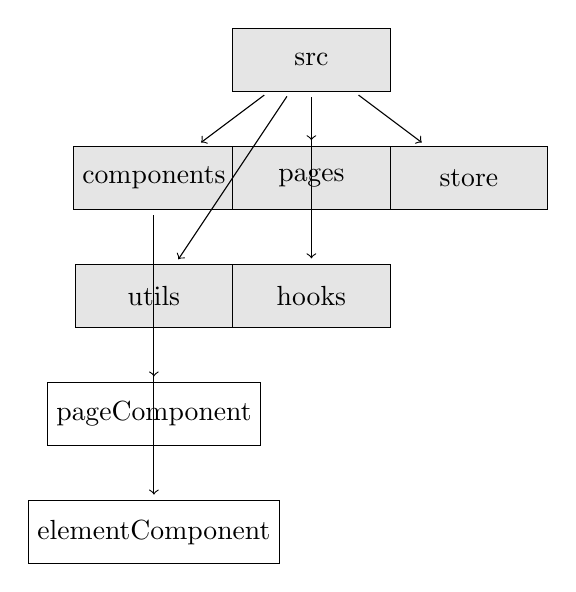
\begin{tikzpicture}[
    file/.style={draw, rectangle, minimum width=2cm, minimum height=0.8cm},
    folder/.style={draw, rectangle, minimum width=2cm, minimum height=0.8cm, fill=gray!20},
    arrow/.style={->, shorten >=2pt, shorten <=2pt}
]

% Folders
\node[folder] (src) at (0,0) {src};
\node[folder] (components) at (-2,-1.5) {components};
\node[folder] (pages) at (0,-1.5) {pages};
\node[folder] (store) at (2,-1.5) {store};
\node[folder] (utils) at (-2,-3) {utils};
\node[folder] (hooks) at (0,-3) {hooks};

% Files
\node[file] (pageComponent) at (-2,-4.5) {pageComponent};
\node[file] (elementComponent) at (-2,-6) {elementComponent};
% ... add more files

% Connections
\draw[arrow] (src) -- (components);
\draw[arrow] (src) -- (pages);
\draw[arrow] (src) -- (store);
\draw[arrow] (src) -- (utils);
\draw[arrow] (src) -- (hooks);
\draw[arrow] (components) -- (pageComponent);
\draw[arrow] (components) -- (elementComponent);
% ... add more connections

\end{tikzpicture}



\pagebreak
\subsubsection{Back-end}
The backend uses the dotNet framework. The development language using the C\# language.

In this project, the backend uses the Onion Architecture.
The Onion Architecture is a typically layered architecture, 
where each layer depends on the inner layer and provides interfaces to the outer layer.
The outer layer provides services to the outermost layer 
and other modules in the same layer based on the interfaces of the inner layer.

From inner to outer, the layers are: Domain, Application, Infrastructure, Presentation.
The Domain layer is the core layer and the innermost layer, used to define domain models, 
which are the business models.
It includes domain models and domain service interfaces.
Domain models are used to define the business models, 
which are the entities in the entity-relationship model and their attributes.
Domain service interfaces are used to define the business services, 
which are the relationships between entities in the entity-relationship model.

The Application layer is the application layer, 
used to define application services, which are the business logic.
It includes domain service implementations and application service interfaces.
Domain service implementations implement the methods of the inner layer's domain service 
interfaces and implement the business logic of the domain models.
Application service interfaces are used to define application services, 
which are the business logic.
It includes but is not limited to database interfaces, testing interfaces, 
HTTP API interfaces, MQTT interfaces, etc.

The Infrastructure layer is the infrastructure layer, used to define infrastructure.
It includes database implementations, testing implementations, 
HTTP API implementations, MQTT implementations, etc.
Database implementations implement the database interfaces 
and provide CRUD services for the database.
Testing implementations implement the testing interfaces 
and provide services for unit testing and integration testing.
HTTP API implementations implement the HTTP API interfaces 
and provide CRUD operations for HTTP APIs.
MQTT implementations implement the MQTT interfaces 
and provide CRUD operations for MQTT.

The Presentation layer is the presentation layer, used to define presentation logic, 
such as interfaces and pages. Since this is a backend project,
data presentation and control are handled by the frontend, 
so this layer is not needed.



\pagebreak
\subsubsection{Data communication and storage}
% 关于本项目的数据通信与数据存储的设计, 包括数据通信的协议, 数据存储的设计等
% 关于数据通信的设计:
% 1. 通信协议的选择
% 自前端向后端发送的数据, 有三种传输的数据类型, 
% 一种是普通的增删改查的请求, 对数据传输的时效性要求不高, 但是对数据的准确性, 完整性, 有序性, 安全性有一定的要求,
% 这种数据的传输, 采用 HTTP 协议, 以及 RESTful API 的设计. 可以有效的保证对数据传输的以上要求.
% 一种是对数据通道的创建和流媒体数据的传输, 对数据传输的时效性, 安全性要求较高, 这种数据的传输, 采用 WebRTC 协议, 以及 MQTT 协议.
% 配合可以快速解码的 flatbuffers 协议, 可以有效的保证对数据传输的以上要求.
% 最后一种是对设备的状态信息和操作信息的传输, 对完整性, 有序性, 安全性都有较高的要求, 这种数据的传输, 采用 MQTT 协议
% 同时也使用了 flatbuffers 协议.
% 
% 2. 数据通信的通信架构和通信流程
% 本项目的数据通信的通信架构, 是基于前后端分离的架构, 前端使用 React 框架, 后端使用 dotnet 框架.
% 当前端需要向后端发送数据的时候, 前端会向后端发送 HTTP 请求, 后端接收到 HTTP 请求之后, 会根据请求的数据类型,
% 选择不同的数据处理方式, 对于普通的增删改查的请求, 后端会根据 RESTful API 的设计, 对数据进行增删改查的操作,
% 对于对数据通道的创建和流媒体数据的传输, 后端会根据 WebRTC 协议, 对数据通道进行创建, 并且帮助前端和设备建立数据通道,
% 当数据通道建立后, 前端和设备之间则使用 flatbuffer 的数据格式对流媒体数据进行传输,
% 对于设备的状态信息和操作信息的传输, 前端会直接向 MQTT broker 发送 MQTT 请求, 
% 设备会在其自身的固件中监听相关的 MQTT 请求, 并且返回相关的数据.
% 
% 3. 数据通信的格式
% 本项目的数据通信的格式, 有三种, 
% 一种是 HTTP 协议, 
% 使用 json 格式对数据进行传输,
% 一种是 WebRTC 协议, 
% 使用 flatbuffers 格式对数据进行传输,
% 一种是 MQTT 协议.
% 使用 flatbuffers 格式对数据进行传输,
% 
% 关于数据存储的设计:
% 1. 数据存储的数据库的选择
% 本项目的数据存储的数据库的选择, 使用了轻量级的数据库 SQLite,
% SQLite 是一个进程内的库, 实现了自给自足的, 无服务器的, 零配置的, 事务性的 SQL 数据库引擎.
% 这是因为整个项目的目的是为了实现前端与设备之间的数据通信, 对于数据库数据的增删改查操作的要求不高,
% 数据量较小, 且对于数据库的数据的事务性要求不高, 所以选择了 SQLite 数据库.
% 2. 项目前后端的数据结构的设计
% 在本项目中, 前端由于使用了 React 框架, 所以前端的数据结构的设计, 使用了基于状态的数据结构的设计,
% 每个组件或者数据集都包含一个状态对象, 这个状态对象的属性就是组件的各个状态. 
% 使用状态对象的原因是, 可以方便的对状态进行管理, 采用对象-属性的形式, 可以方便的针对不同组件的同类状态进行区分,
% 由于跨组件的状态是由 redux 进行管理的, 这种状态对象的设计, 可以更搞笑的对状态进行更新和传递.
% 后端由于使用了 dotnet 框架, 所以后端的数据结构的设计, 使用了基于类的数据结构的设计,
% 采用了面向对象的编程思想, 对数据进行了封装, 使得数据的传输更加的安全, 有序, 完整.


\pagebreak

% \subsection{Domain model}
% \documentclass[]{article}
\usepackage{graphicx}
\usepackage{amsmath}
\usepackage{tikz}

% libaries
\usetikzlibrary{shapes,arrows}

%Define the listing package
\usepackage{listings} %code highlighter
\usepackage{color} %use color
\definecolor{mygreen}{rgb}{0,0.6,0}
\definecolor{mygray}{rgb}{0.5,0.5,0.5}
\definecolor{mymauve}{rgb}{0.58,0,0.82}

%Customize a bit the look
\lstset{ %
backgroundcolor=\color{white}, % choose the background color; you must add \usepackage{color} or \usepackage{xcolor}
basicstyle=\footnotesize, % the size of the fonts that are used for the code
breakatwhitespace=false, % sets if automatic breaks should only happen at whitespace
breaklines=true, % sets automatic line breaking
captionpos=b, % sets the caption-position to bottom
commentstyle=\color{mygreen}, % comment style
deletekeywords={...}, % if you want to delete keywords from the given language
escapeinside={\%*}{*)}, % if you want to add LaTeX within your code
extendedchars=true, % lets you use non-ASCII characters; for 8-bits encodings only, does not work with UTF-8
frame=single, % adds a frame around the code
keepspaces=true, % keeps spaces in text, useful for keeping indentation of code (possibly needs columns=flexible)
keywordstyle=\color{blue}, % keyword style
% language=Octave, % the language of the code
morekeywords={*,...}, % if you want to add more keywords to the set
numbers=left, % where to put the line-numbers; possible values are (none, left, right)
numbersep=5pt, % how far the line-numbers are from the code
numberstyle=\tiny\color{mygray}, % the style that is used for the line-numbers
rulecolor=\color{black}, % if not set, the frame-color may be changed on line-breaks within not-black text (e.g. comments (green here))
showspaces=false, % show spaces everywhere adding particular underscores; it overrides 'showstringspaces'
showstringspaces=false, % underline spaces within strings only
showtabs=false, % show tabs within strings adding particular underscores
stepnumber=1, % the step between two line-numbers. If it's 1, each line will be numbered
stringstyle=\color{mymauve}, % string literal style
tabsize=2, % sets default tabsize to 2 spaces
title=\lstname % show the filename of files included with \lstinputlisting; also try caption instead of title
}

\definecolor{darkgray}{rgb}{.4,.4,.4}
\definecolor{purple}{rgb}{0.65, 0.12, 0.82}

\lstdefinelanguage{React}{
keywords={const, typeof, new, true, false, catch, function, return, null, catch, switch, var, if, in, while, do, else, case, break},
keywordstyle=\color{blue}\bfseries,
ndkeywords={class, export, boolean, throw, implements, import, this},
ndkeywordstyle=\color{darkgray}\bfseries,
identifierstyle=\color{mygreen},
sensitive=false,
comment=[l]{//},
morecomment=[s]{/*}{*/},
commentstyle=\color{purple}\ttfamily,
string=[b]{"}{'}{`},
stringstyle=\color{red}\ttfamily,
morestring=[b]',
morestring=[b]",
morestring=[b]`',
}

\lstdefinelanguage{CSharp}{
keywords={const, typeof, new, true, false, catch, function, return, null, catch, switch, var, if, in, while, do, else, case, break},
keywordstyle=\color{blue}\bfseries,
ndkeywords={class, export, boolean, throw, implements, import, this},
ndkeywordstyle=\color{darkgray}\bfseries,
identifierstyle=\color{mygreen},
sensitive=false,
comment=[l]{//},
morecomment=[s]{/*}{*/},
commentstyle=\color{purple}\ttfamily,
string=[b]{"}{'}{`},
stringstyle=\color{red}\ttfamily,
morestring=[b]',
morestring=[b]",
morestring=[b]`',
}

\lstset{
language=React,
extendedchars=true,
basicstyle=\footnotesize\ttfamily,
showstringspaces=false,
showspaces=false,
numbers=left,
numberstyle=\footnotesize,
numbersep=9pt,
tabsize=2,
breaklines=true,
showtabs=false,
captionpos=b
}

\lstset{
language=CSharp,
extendedchars=true,
basicstyle=\footnotesize\ttfamily,
showstringspaces=false,
showspaces=false,
numbers=left,
numberstyle=\footnotesize,
numbersep=9pt,
tabsize=2,
breaklines=true,
showtabs=false,
captionpos=b
}

% \usepackage{cite} % Add this line for citation

% \bibliographystyle{plain}

\title{
The implementation of BifrostConnect Front-end scope, 
re-design and development with the relevant back-end support develop.
}
\author{
    Fei Gu \\
    Erhvervs Akademi Sydvest \\
    Computer Science 21\\
    }
\date{\today}

\begin{document}

% Front page
\maketitle
\begin{center}
    Supervisor: Henrik Boulund Meng Hansen \\
    Company: BifrostConnect \\
    Engineering Director: Jasper Wass \\
\end{center}
\tableofcontents
\pagebreak


% The introduction
\section{Introduction}
\subsection{Background}\input{sections/introduction/background.tex}
\subsection{The company}\input{sections/introduction/aboutCompany}
\subsection{The project}\input{sections/introduction/aboutProject}
\pagebreak

% The problem statement
\section{Problem Statement}
\subsection{Statement}
\input{sections/problemStatement/statement}
\subsection{Situation}
\input{sections/problemStatement/situation}
\subsection{Potential Solution}
\input{sections/problemStatement/potentialSolution}
\pagebreak

% Requirement analysis
\section{Requirement Analysis}
\input{sections/requirementAnalysis/index}

\subsection{Stakeholders}
\input{sections/requirementAnalysis/stakeholders/index}

\subsection{Business Domain}
\input{sections/requirementAnalysis/bussinesDomain/index}

\subsection{Scope}
\input{sections/requirementAnalysis/scope}

\subsection{Goals}
\input{sections/requirementAnalysis/goals}
\pagebreak

% Software Design
\section{Software Design}
% developement methods
\subsection{Software Development Methods}
\input{sections/softwareDevelopmentMethods/index}
\subsubsection{Agile Software Development}
\input{sections/softwareDevelopmentMethods/agileSoftwareDevelopment/index}
\subsubsection{Feature Driven Development}
\input{sections/softwareDevelopmentMethods/featureDrivenDevelopment/index}

\pagebreak

% Technology seslection
\subsection{Technology selection}
\input{sections/softwareDesign/technologySelection/index}
\subsubsection{Front-end}
\input{sections/softwareDesign/technologySelection/frontEnd}            
\subsubsection{Back-end}
\input{sections/softwareDesign/technologySelection/backEnd}            
\subsubsection{Database}
\input{sections/softwareDesign/technologySelection/database}
\subsubsection{Data communication}
\input{sections/softwareDesign/technologySelection/dataCommunication}            
\subsubsection{DevOps}
\input{sections/softwareDesign/technologySelection/devOps}
\pagebreak

% Architecture design
\subsection{Architecture design}
\input{sections/softwareDesign/architectureDesign/index}
\pagebreak
\subsubsection{Front-end}
\input{sections/softwareDesign/architectureDesign/frontEndArchitecture}
\pagebreak
\subsubsection{Back-end}
\input{sections/softwareDesign/architectureDesign/backEndArchitecture}
\pagebreak
\subsubsection{Data communication and storage}
\input{sections/softwareDesign/architectureDesign/dataCommunicationArchitecture}
\pagebreak

% \subsection{Domain model}
% \input{sections/softwareDesign/domainModel/index}
% \subsection{Database design}
% % 数据库领域模型 ER 图
% % 包括表和字段的设置.
% % 对于私有键和外键的设置.

% \subsection{Back-end design}
% % 后端对象模型
% % 以及对于对象模型的增删改查
% % 以及相关的其他服务的设计`'

% \subsection{Front-end design}
% % 对于前端的页面结构的设计 
% % 页面的状态的设计, 交互设计

% \subsection{FlatBuffers design}
% % schema 的设计

\subsection{DevOps CI/CD process design}
\input{sections/softwareDesign/devOpsDesign/index}
\subsubsection{Continuous Integration}
\input{sections/softwareDesign/devOpsDesign/continuousIntegration/index}
\subsubsection{Continuous Delivery}
\input{sections/softwareDesign/devOpsDesign/continuousDelivery/index}
\subsubsection{Continuous Deployment}
\input{sections/softwareDesign/devOpsDesign/continuousDeployment/index}
\pagebreak

\section{Software Development} 
\input{sections/softwareDevelopment/index}
\subsection{Overall development}
\input{sections/softwareDevelopment/overallDevelopement/index}
\subsubsection{Front-end}
\input{sections/softwareDevelopment/overallDevelopement/frontEnd/index}
\subsubsection{Back-end}
\input{sections/softwareDevelopment/overallDevelopement/backEnd/index}
\subsubsection{DevOps}
\input{sections/softwareDevelopment/overallDevelopement/devOps/index}
\subsection{Feature development} 
\input{sections/softwareDevelopment/featureDevelopment/index}
\subsubsection{Use Case 1}
\input{sections/softwareDevelopment/featureDevelopment/useCase1/index}
\subsubsection{Feature 1}
\input{sections/softwareDevelopment/featureDevelopment/feature/feature1.tex}
\pagebreak
\section{Conclusion} 
\subsection{Result}
Since the project is still in progress, the result is not available yet.
So far, basic structure of this project has been built. But the most features 
are not implemented yet. 
\subsection{Discussion}
As a single developer for this project, I am confident what I have done so far.
And I can say I understand the most of the knowledge I have used in this project, 
which also means I can explain all the part of the project. 
But this project also relevant some of the complex knowledge which I have to continue 
to study and practice.
\subsection{Future Work}
The future work is to implement the rest of the features. 
Including the most important part which is the 'create session' feature.
\pagebreak
% \bibliography{bibliography}
\pagebreak
% \begin{appendices}
%     \section{Appendix}
% \end{appendices} 
\end{document}
% \subsection{Database design}
% % 数据库领域模型 ER 图
% % 包括表和字段的设置.
% % 对于私有键和外键的设置.

% \subsection{Back-end design}
% % 后端对象模型
% % 以及对于对象模型的增删改查
% % 以及相关的其他服务的设计`'

% \subsection{Front-end design}
% % 对于前端的页面结构的设计 
% % 页面的状态的设计, 交互设计

% \subsection{FlatBuffers design}
% % schema 的设计

\subsection{DevOps CI/CD process design}
\documentclass[]{article}
\usepackage{graphicx}
\usepackage{amsmath}
\usepackage{tikz}

% libaries
\usetikzlibrary{shapes,arrows}

%Define the listing package
\usepackage{listings} %code highlighter
\usepackage{color} %use color
\definecolor{mygreen}{rgb}{0,0.6,0}
\definecolor{mygray}{rgb}{0.5,0.5,0.5}
\definecolor{mymauve}{rgb}{0.58,0,0.82}

%Customize a bit the look
\lstset{ %
backgroundcolor=\color{white}, % choose the background color; you must add \usepackage{color} or \usepackage{xcolor}
basicstyle=\footnotesize, % the size of the fonts that are used for the code
breakatwhitespace=false, % sets if automatic breaks should only happen at whitespace
breaklines=true, % sets automatic line breaking
captionpos=b, % sets the caption-position to bottom
commentstyle=\color{mygreen}, % comment style
deletekeywords={...}, % if you want to delete keywords from the given language
escapeinside={\%*}{*)}, % if you want to add LaTeX within your code
extendedchars=true, % lets you use non-ASCII characters; for 8-bits encodings only, does not work with UTF-8
frame=single, % adds a frame around the code
keepspaces=true, % keeps spaces in text, useful for keeping indentation of code (possibly needs columns=flexible)
keywordstyle=\color{blue}, % keyword style
% language=Octave, % the language of the code
morekeywords={*,...}, % if you want to add more keywords to the set
numbers=left, % where to put the line-numbers; possible values are (none, left, right)
numbersep=5pt, % how far the line-numbers are from the code
numberstyle=\tiny\color{mygray}, % the style that is used for the line-numbers
rulecolor=\color{black}, % if not set, the frame-color may be changed on line-breaks within not-black text (e.g. comments (green here))
showspaces=false, % show spaces everywhere adding particular underscores; it overrides 'showstringspaces'
showstringspaces=false, % underline spaces within strings only
showtabs=false, % show tabs within strings adding particular underscores
stepnumber=1, % the step between two line-numbers. If it's 1, each line will be numbered
stringstyle=\color{mymauve}, % string literal style
tabsize=2, % sets default tabsize to 2 spaces
title=\lstname % show the filename of files included with \lstinputlisting; also try caption instead of title
}

\definecolor{darkgray}{rgb}{.4,.4,.4}
\definecolor{purple}{rgb}{0.65, 0.12, 0.82}

\lstdefinelanguage{React}{
keywords={const, typeof, new, true, false, catch, function, return, null, catch, switch, var, if, in, while, do, else, case, break},
keywordstyle=\color{blue}\bfseries,
ndkeywords={class, export, boolean, throw, implements, import, this},
ndkeywordstyle=\color{darkgray}\bfseries,
identifierstyle=\color{mygreen},
sensitive=false,
comment=[l]{//},
morecomment=[s]{/*}{*/},
commentstyle=\color{purple}\ttfamily,
string=[b]{"}{'}{`},
stringstyle=\color{red}\ttfamily,
morestring=[b]',
morestring=[b]",
morestring=[b]`',
}

\lstdefinelanguage{CSharp}{
keywords={const, typeof, new, true, false, catch, function, return, null, catch, switch, var, if, in, while, do, else, case, break},
keywordstyle=\color{blue}\bfseries,
ndkeywords={class, export, boolean, throw, implements, import, this},
ndkeywordstyle=\color{darkgray}\bfseries,
identifierstyle=\color{mygreen},
sensitive=false,
comment=[l]{//},
morecomment=[s]{/*}{*/},
commentstyle=\color{purple}\ttfamily,
string=[b]{"}{'}{`},
stringstyle=\color{red}\ttfamily,
morestring=[b]',
morestring=[b]",
morestring=[b]`',
}

\lstset{
language=React,
extendedchars=true,
basicstyle=\footnotesize\ttfamily,
showstringspaces=false,
showspaces=false,
numbers=left,
numberstyle=\footnotesize,
numbersep=9pt,
tabsize=2,
breaklines=true,
showtabs=false,
captionpos=b
}

\lstset{
language=CSharp,
extendedchars=true,
basicstyle=\footnotesize\ttfamily,
showstringspaces=false,
showspaces=false,
numbers=left,
numberstyle=\footnotesize,
numbersep=9pt,
tabsize=2,
breaklines=true,
showtabs=false,
captionpos=b
}

% \usepackage{cite} % Add this line for citation

% \bibliographystyle{plain}

\title{
The implementation of BifrostConnect Front-end scope, 
re-design and development with the relevant back-end support develop.
}
\author{
    Fei Gu \\
    Erhvervs Akademi Sydvest \\
    Computer Science 21\\
    }
\date{\today}

\begin{document}

% Front page
\maketitle
\begin{center}
    Supervisor: Henrik Boulund Meng Hansen \\
    Company: BifrostConnect \\
    Engineering Director: Jasper Wass \\
\end{center}
\tableofcontents
\pagebreak


% The introduction
\section{Introduction}
\subsection{Background}\input{sections/introduction/background.tex}
\subsection{The company}\input{sections/introduction/aboutCompany}
\subsection{The project}\input{sections/introduction/aboutProject}
\pagebreak

% The problem statement
\section{Problem Statement}
\subsection{Statement}
\input{sections/problemStatement/statement}
\subsection{Situation}
\input{sections/problemStatement/situation}
\subsection{Potential Solution}
\input{sections/problemStatement/potentialSolution}
\pagebreak

% Requirement analysis
\section{Requirement Analysis}
\input{sections/requirementAnalysis/index}

\subsection{Stakeholders}
\input{sections/requirementAnalysis/stakeholders/index}

\subsection{Business Domain}
\input{sections/requirementAnalysis/bussinesDomain/index}

\subsection{Scope}
\input{sections/requirementAnalysis/scope}

\subsection{Goals}
\input{sections/requirementAnalysis/goals}
\pagebreak

% Software Design
\section{Software Design}
% developement methods
\subsection{Software Development Methods}
\input{sections/softwareDevelopmentMethods/index}
\subsubsection{Agile Software Development}
\input{sections/softwareDevelopmentMethods/agileSoftwareDevelopment/index}
\subsubsection{Feature Driven Development}
\input{sections/softwareDevelopmentMethods/featureDrivenDevelopment/index}

\pagebreak

% Technology seslection
\subsection{Technology selection}
\input{sections/softwareDesign/technologySelection/index}
\subsubsection{Front-end}
\input{sections/softwareDesign/technologySelection/frontEnd}            
\subsubsection{Back-end}
\input{sections/softwareDesign/technologySelection/backEnd}            
\subsubsection{Database}
\input{sections/softwareDesign/technologySelection/database}
\subsubsection{Data communication}
\input{sections/softwareDesign/technologySelection/dataCommunication}            
\subsubsection{DevOps}
\input{sections/softwareDesign/technologySelection/devOps}
\pagebreak

% Architecture design
\subsection{Architecture design}
\input{sections/softwareDesign/architectureDesign/index}
\pagebreak
\subsubsection{Front-end}
\input{sections/softwareDesign/architectureDesign/frontEndArchitecture}
\pagebreak
\subsubsection{Back-end}
\input{sections/softwareDesign/architectureDesign/backEndArchitecture}
\pagebreak
\subsubsection{Data communication and storage}
\input{sections/softwareDesign/architectureDesign/dataCommunicationArchitecture}
\pagebreak

% \subsection{Domain model}
% \input{sections/softwareDesign/domainModel/index}
% \subsection{Database design}
% % 数据库领域模型 ER 图
% % 包括表和字段的设置.
% % 对于私有键和外键的设置.

% \subsection{Back-end design}
% % 后端对象模型
% % 以及对于对象模型的增删改查
% % 以及相关的其他服务的设计`'

% \subsection{Front-end design}
% % 对于前端的页面结构的设计 
% % 页面的状态的设计, 交互设计

% \subsection{FlatBuffers design}
% % schema 的设计

\subsection{DevOps CI/CD process design}
\input{sections/softwareDesign/devOpsDesign/index}
\subsubsection{Continuous Integration}
\input{sections/softwareDesign/devOpsDesign/continuousIntegration/index}
\subsubsection{Continuous Delivery}
\input{sections/softwareDesign/devOpsDesign/continuousDelivery/index}
\subsubsection{Continuous Deployment}
\input{sections/softwareDesign/devOpsDesign/continuousDeployment/index}
\pagebreak

\section{Software Development} 
\input{sections/softwareDevelopment/index}
\subsection{Overall development}
\input{sections/softwareDevelopment/overallDevelopement/index}
\subsubsection{Front-end}
\input{sections/softwareDevelopment/overallDevelopement/frontEnd/index}
\subsubsection{Back-end}
\input{sections/softwareDevelopment/overallDevelopement/backEnd/index}
\subsubsection{DevOps}
\input{sections/softwareDevelopment/overallDevelopement/devOps/index}
\subsection{Feature development} 
\input{sections/softwareDevelopment/featureDevelopment/index}
\subsubsection{Use Case 1}
\input{sections/softwareDevelopment/featureDevelopment/useCase1/index}
\subsubsection{Feature 1}
\input{sections/softwareDevelopment/featureDevelopment/feature/feature1.tex}
\pagebreak
\section{Conclusion} 
\subsection{Result}
Since the project is still in progress, the result is not available yet.
So far, basic structure of this project has been built. But the most features 
are not implemented yet. 
\subsection{Discussion}
As a single developer for this project, I am confident what I have done so far.
And I can say I understand the most of the knowledge I have used in this project, 
which also means I can explain all the part of the project. 
But this project also relevant some of the complex knowledge which I have to continue 
to study and practice.
\subsection{Future Work}
The future work is to implement the rest of the features. 
Including the most important part which is the 'create session' feature.
\pagebreak
% \bibliography{bibliography}
\pagebreak
% \begin{appendices}
%     \section{Appendix}
% \end{appendices} 
\end{document}
\subsubsection{Continuous Integration}
\documentclass[]{article}
\usepackage{graphicx}
\usepackage{amsmath}
\usepackage{tikz}

% libaries
\usetikzlibrary{shapes,arrows}

%Define the listing package
\usepackage{listings} %code highlighter
\usepackage{color} %use color
\definecolor{mygreen}{rgb}{0,0.6,0}
\definecolor{mygray}{rgb}{0.5,0.5,0.5}
\definecolor{mymauve}{rgb}{0.58,0,0.82}

%Customize a bit the look
\lstset{ %
backgroundcolor=\color{white}, % choose the background color; you must add \usepackage{color} or \usepackage{xcolor}
basicstyle=\footnotesize, % the size of the fonts that are used for the code
breakatwhitespace=false, % sets if automatic breaks should only happen at whitespace
breaklines=true, % sets automatic line breaking
captionpos=b, % sets the caption-position to bottom
commentstyle=\color{mygreen}, % comment style
deletekeywords={...}, % if you want to delete keywords from the given language
escapeinside={\%*}{*)}, % if you want to add LaTeX within your code
extendedchars=true, % lets you use non-ASCII characters; for 8-bits encodings only, does not work with UTF-8
frame=single, % adds a frame around the code
keepspaces=true, % keeps spaces in text, useful for keeping indentation of code (possibly needs columns=flexible)
keywordstyle=\color{blue}, % keyword style
% language=Octave, % the language of the code
morekeywords={*,...}, % if you want to add more keywords to the set
numbers=left, % where to put the line-numbers; possible values are (none, left, right)
numbersep=5pt, % how far the line-numbers are from the code
numberstyle=\tiny\color{mygray}, % the style that is used for the line-numbers
rulecolor=\color{black}, % if not set, the frame-color may be changed on line-breaks within not-black text (e.g. comments (green here))
showspaces=false, % show spaces everywhere adding particular underscores; it overrides 'showstringspaces'
showstringspaces=false, % underline spaces within strings only
showtabs=false, % show tabs within strings adding particular underscores
stepnumber=1, % the step between two line-numbers. If it's 1, each line will be numbered
stringstyle=\color{mymauve}, % string literal style
tabsize=2, % sets default tabsize to 2 spaces
title=\lstname % show the filename of files included with \lstinputlisting; also try caption instead of title
}

\definecolor{darkgray}{rgb}{.4,.4,.4}
\definecolor{purple}{rgb}{0.65, 0.12, 0.82}

\lstdefinelanguage{React}{
keywords={const, typeof, new, true, false, catch, function, return, null, catch, switch, var, if, in, while, do, else, case, break},
keywordstyle=\color{blue}\bfseries,
ndkeywords={class, export, boolean, throw, implements, import, this},
ndkeywordstyle=\color{darkgray}\bfseries,
identifierstyle=\color{mygreen},
sensitive=false,
comment=[l]{//},
morecomment=[s]{/*}{*/},
commentstyle=\color{purple}\ttfamily,
string=[b]{"}{'}{`},
stringstyle=\color{red}\ttfamily,
morestring=[b]',
morestring=[b]",
morestring=[b]`',
}

\lstdefinelanguage{CSharp}{
keywords={const, typeof, new, true, false, catch, function, return, null, catch, switch, var, if, in, while, do, else, case, break},
keywordstyle=\color{blue}\bfseries,
ndkeywords={class, export, boolean, throw, implements, import, this},
ndkeywordstyle=\color{darkgray}\bfseries,
identifierstyle=\color{mygreen},
sensitive=false,
comment=[l]{//},
morecomment=[s]{/*}{*/},
commentstyle=\color{purple}\ttfamily,
string=[b]{"}{'}{`},
stringstyle=\color{red}\ttfamily,
morestring=[b]',
morestring=[b]",
morestring=[b]`',
}

\lstset{
language=React,
extendedchars=true,
basicstyle=\footnotesize\ttfamily,
showstringspaces=false,
showspaces=false,
numbers=left,
numberstyle=\footnotesize,
numbersep=9pt,
tabsize=2,
breaklines=true,
showtabs=false,
captionpos=b
}

\lstset{
language=CSharp,
extendedchars=true,
basicstyle=\footnotesize\ttfamily,
showstringspaces=false,
showspaces=false,
numbers=left,
numberstyle=\footnotesize,
numbersep=9pt,
tabsize=2,
breaklines=true,
showtabs=false,
captionpos=b
}

% \usepackage{cite} % Add this line for citation

% \bibliographystyle{plain}

\title{
The implementation of BifrostConnect Front-end scope, 
re-design and development with the relevant back-end support develop.
}
\author{
    Fei Gu \\
    Erhvervs Akademi Sydvest \\
    Computer Science 21\\
    }
\date{\today}

\begin{document}

% Front page
\maketitle
\begin{center}
    Supervisor: Henrik Boulund Meng Hansen \\
    Company: BifrostConnect \\
    Engineering Director: Jasper Wass \\
\end{center}
\tableofcontents
\pagebreak


% The introduction
\section{Introduction}
\subsection{Background}\input{sections/introduction/background.tex}
\subsection{The company}\input{sections/introduction/aboutCompany}
\subsection{The project}\input{sections/introduction/aboutProject}
\pagebreak

% The problem statement
\section{Problem Statement}
\subsection{Statement}
\input{sections/problemStatement/statement}
\subsection{Situation}
\input{sections/problemStatement/situation}
\subsection{Potential Solution}
\input{sections/problemStatement/potentialSolution}
\pagebreak

% Requirement analysis
\section{Requirement Analysis}
\input{sections/requirementAnalysis/index}

\subsection{Stakeholders}
\input{sections/requirementAnalysis/stakeholders/index}

\subsection{Business Domain}
\input{sections/requirementAnalysis/bussinesDomain/index}

\subsection{Scope}
\input{sections/requirementAnalysis/scope}

\subsection{Goals}
\input{sections/requirementAnalysis/goals}
\pagebreak

% Software Design
\section{Software Design}
% developement methods
\subsection{Software Development Methods}
\input{sections/softwareDevelopmentMethods/index}
\subsubsection{Agile Software Development}
\input{sections/softwareDevelopmentMethods/agileSoftwareDevelopment/index}
\subsubsection{Feature Driven Development}
\input{sections/softwareDevelopmentMethods/featureDrivenDevelopment/index}

\pagebreak

% Technology seslection
\subsection{Technology selection}
\input{sections/softwareDesign/technologySelection/index}
\subsubsection{Front-end}
\input{sections/softwareDesign/technologySelection/frontEnd}            
\subsubsection{Back-end}
\input{sections/softwareDesign/technologySelection/backEnd}            
\subsubsection{Database}
\input{sections/softwareDesign/technologySelection/database}
\subsubsection{Data communication}
\input{sections/softwareDesign/technologySelection/dataCommunication}            
\subsubsection{DevOps}
\input{sections/softwareDesign/technologySelection/devOps}
\pagebreak

% Architecture design
\subsection{Architecture design}
\input{sections/softwareDesign/architectureDesign/index}
\pagebreak
\subsubsection{Front-end}
\input{sections/softwareDesign/architectureDesign/frontEndArchitecture}
\pagebreak
\subsubsection{Back-end}
\input{sections/softwareDesign/architectureDesign/backEndArchitecture}
\pagebreak
\subsubsection{Data communication and storage}
\input{sections/softwareDesign/architectureDesign/dataCommunicationArchitecture}
\pagebreak

% \subsection{Domain model}
% \input{sections/softwareDesign/domainModel/index}
% \subsection{Database design}
% % 数据库领域模型 ER 图
% % 包括表和字段的设置.
% % 对于私有键和外键的设置.

% \subsection{Back-end design}
% % 后端对象模型
% % 以及对于对象模型的增删改查
% % 以及相关的其他服务的设计`'

% \subsection{Front-end design}
% % 对于前端的页面结构的设计 
% % 页面的状态的设计, 交互设计

% \subsection{FlatBuffers design}
% % schema 的设计

\subsection{DevOps CI/CD process design}
\input{sections/softwareDesign/devOpsDesign/index}
\subsubsection{Continuous Integration}
\input{sections/softwareDesign/devOpsDesign/continuousIntegration/index}
\subsubsection{Continuous Delivery}
\input{sections/softwareDesign/devOpsDesign/continuousDelivery/index}
\subsubsection{Continuous Deployment}
\input{sections/softwareDesign/devOpsDesign/continuousDeployment/index}
\pagebreak

\section{Software Development} 
\input{sections/softwareDevelopment/index}
\subsection{Overall development}
\input{sections/softwareDevelopment/overallDevelopement/index}
\subsubsection{Front-end}
\input{sections/softwareDevelopment/overallDevelopement/frontEnd/index}
\subsubsection{Back-end}
\input{sections/softwareDevelopment/overallDevelopement/backEnd/index}
\subsubsection{DevOps}
\input{sections/softwareDevelopment/overallDevelopement/devOps/index}
\subsection{Feature development} 
\input{sections/softwareDevelopment/featureDevelopment/index}
\subsubsection{Use Case 1}
\input{sections/softwareDevelopment/featureDevelopment/useCase1/index}
\subsubsection{Feature 1}
\input{sections/softwareDevelopment/featureDevelopment/feature/feature1.tex}
\pagebreak
\section{Conclusion} 
\subsection{Result}
Since the project is still in progress, the result is not available yet.
So far, basic structure of this project has been built. But the most features 
are not implemented yet. 
\subsection{Discussion}
As a single developer for this project, I am confident what I have done so far.
And I can say I understand the most of the knowledge I have used in this project, 
which also means I can explain all the part of the project. 
But this project also relevant some of the complex knowledge which I have to continue 
to study and practice.
\subsection{Future Work}
The future work is to implement the rest of the features. 
Including the most important part which is the 'create session' feature.
\pagebreak
% \bibliography{bibliography}
\pagebreak
% \begin{appendices}
%     \section{Appendix}
% \end{appendices} 
\end{document}
\subsubsection{Continuous Delivery}
\documentclass[]{article}
\usepackage{graphicx}
\usepackage{amsmath}
\usepackage{tikz}

% libaries
\usetikzlibrary{shapes,arrows}

%Define the listing package
\usepackage{listings} %code highlighter
\usepackage{color} %use color
\definecolor{mygreen}{rgb}{0,0.6,0}
\definecolor{mygray}{rgb}{0.5,0.5,0.5}
\definecolor{mymauve}{rgb}{0.58,0,0.82}

%Customize a bit the look
\lstset{ %
backgroundcolor=\color{white}, % choose the background color; you must add \usepackage{color} or \usepackage{xcolor}
basicstyle=\footnotesize, % the size of the fonts that are used for the code
breakatwhitespace=false, % sets if automatic breaks should only happen at whitespace
breaklines=true, % sets automatic line breaking
captionpos=b, % sets the caption-position to bottom
commentstyle=\color{mygreen}, % comment style
deletekeywords={...}, % if you want to delete keywords from the given language
escapeinside={\%*}{*)}, % if you want to add LaTeX within your code
extendedchars=true, % lets you use non-ASCII characters; for 8-bits encodings only, does not work with UTF-8
frame=single, % adds a frame around the code
keepspaces=true, % keeps spaces in text, useful for keeping indentation of code (possibly needs columns=flexible)
keywordstyle=\color{blue}, % keyword style
% language=Octave, % the language of the code
morekeywords={*,...}, % if you want to add more keywords to the set
numbers=left, % where to put the line-numbers; possible values are (none, left, right)
numbersep=5pt, % how far the line-numbers are from the code
numberstyle=\tiny\color{mygray}, % the style that is used for the line-numbers
rulecolor=\color{black}, % if not set, the frame-color may be changed on line-breaks within not-black text (e.g. comments (green here))
showspaces=false, % show spaces everywhere adding particular underscores; it overrides 'showstringspaces'
showstringspaces=false, % underline spaces within strings only
showtabs=false, % show tabs within strings adding particular underscores
stepnumber=1, % the step between two line-numbers. If it's 1, each line will be numbered
stringstyle=\color{mymauve}, % string literal style
tabsize=2, % sets default tabsize to 2 spaces
title=\lstname % show the filename of files included with \lstinputlisting; also try caption instead of title
}

\definecolor{darkgray}{rgb}{.4,.4,.4}
\definecolor{purple}{rgb}{0.65, 0.12, 0.82}

\lstdefinelanguage{React}{
keywords={const, typeof, new, true, false, catch, function, return, null, catch, switch, var, if, in, while, do, else, case, break},
keywordstyle=\color{blue}\bfseries,
ndkeywords={class, export, boolean, throw, implements, import, this},
ndkeywordstyle=\color{darkgray}\bfseries,
identifierstyle=\color{mygreen},
sensitive=false,
comment=[l]{//},
morecomment=[s]{/*}{*/},
commentstyle=\color{purple}\ttfamily,
string=[b]{"}{'}{`},
stringstyle=\color{red}\ttfamily,
morestring=[b]',
morestring=[b]",
morestring=[b]`',
}

\lstdefinelanguage{CSharp}{
keywords={const, typeof, new, true, false, catch, function, return, null, catch, switch, var, if, in, while, do, else, case, break},
keywordstyle=\color{blue}\bfseries,
ndkeywords={class, export, boolean, throw, implements, import, this},
ndkeywordstyle=\color{darkgray}\bfseries,
identifierstyle=\color{mygreen},
sensitive=false,
comment=[l]{//},
morecomment=[s]{/*}{*/},
commentstyle=\color{purple}\ttfamily,
string=[b]{"}{'}{`},
stringstyle=\color{red}\ttfamily,
morestring=[b]',
morestring=[b]",
morestring=[b]`',
}

\lstset{
language=React,
extendedchars=true,
basicstyle=\footnotesize\ttfamily,
showstringspaces=false,
showspaces=false,
numbers=left,
numberstyle=\footnotesize,
numbersep=9pt,
tabsize=2,
breaklines=true,
showtabs=false,
captionpos=b
}

\lstset{
language=CSharp,
extendedchars=true,
basicstyle=\footnotesize\ttfamily,
showstringspaces=false,
showspaces=false,
numbers=left,
numberstyle=\footnotesize,
numbersep=9pt,
tabsize=2,
breaklines=true,
showtabs=false,
captionpos=b
}

% \usepackage{cite} % Add this line for citation

% \bibliographystyle{plain}

\title{
The implementation of BifrostConnect Front-end scope, 
re-design and development with the relevant back-end support develop.
}
\author{
    Fei Gu \\
    Erhvervs Akademi Sydvest \\
    Computer Science 21\\
    }
\date{\today}

\begin{document}

% Front page
\maketitle
\begin{center}
    Supervisor: Henrik Boulund Meng Hansen \\
    Company: BifrostConnect \\
    Engineering Director: Jasper Wass \\
\end{center}
\tableofcontents
\pagebreak


% The introduction
\section{Introduction}
\subsection{Background}\input{sections/introduction/background.tex}
\subsection{The company}\input{sections/introduction/aboutCompany}
\subsection{The project}\input{sections/introduction/aboutProject}
\pagebreak

% The problem statement
\section{Problem Statement}
\subsection{Statement}
\input{sections/problemStatement/statement}
\subsection{Situation}
\input{sections/problemStatement/situation}
\subsection{Potential Solution}
\input{sections/problemStatement/potentialSolution}
\pagebreak

% Requirement analysis
\section{Requirement Analysis}
\input{sections/requirementAnalysis/index}

\subsection{Stakeholders}
\input{sections/requirementAnalysis/stakeholders/index}

\subsection{Business Domain}
\input{sections/requirementAnalysis/bussinesDomain/index}

\subsection{Scope}
\input{sections/requirementAnalysis/scope}

\subsection{Goals}
\input{sections/requirementAnalysis/goals}
\pagebreak

% Software Design
\section{Software Design}
% developement methods
\subsection{Software Development Methods}
\input{sections/softwareDevelopmentMethods/index}
\subsubsection{Agile Software Development}
\input{sections/softwareDevelopmentMethods/agileSoftwareDevelopment/index}
\subsubsection{Feature Driven Development}
\input{sections/softwareDevelopmentMethods/featureDrivenDevelopment/index}

\pagebreak

% Technology seslection
\subsection{Technology selection}
\input{sections/softwareDesign/technologySelection/index}
\subsubsection{Front-end}
\input{sections/softwareDesign/technologySelection/frontEnd}            
\subsubsection{Back-end}
\input{sections/softwareDesign/technologySelection/backEnd}            
\subsubsection{Database}
\input{sections/softwareDesign/technologySelection/database}
\subsubsection{Data communication}
\input{sections/softwareDesign/technologySelection/dataCommunication}            
\subsubsection{DevOps}
\input{sections/softwareDesign/technologySelection/devOps}
\pagebreak

% Architecture design
\subsection{Architecture design}
\input{sections/softwareDesign/architectureDesign/index}
\pagebreak
\subsubsection{Front-end}
\input{sections/softwareDesign/architectureDesign/frontEndArchitecture}
\pagebreak
\subsubsection{Back-end}
\input{sections/softwareDesign/architectureDesign/backEndArchitecture}
\pagebreak
\subsubsection{Data communication and storage}
\input{sections/softwareDesign/architectureDesign/dataCommunicationArchitecture}
\pagebreak

% \subsection{Domain model}
% \input{sections/softwareDesign/domainModel/index}
% \subsection{Database design}
% % 数据库领域模型 ER 图
% % 包括表和字段的设置.
% % 对于私有键和外键的设置.

% \subsection{Back-end design}
% % 后端对象模型
% % 以及对于对象模型的增删改查
% % 以及相关的其他服务的设计`'

% \subsection{Front-end design}
% % 对于前端的页面结构的设计 
% % 页面的状态的设计, 交互设计

% \subsection{FlatBuffers design}
% % schema 的设计

\subsection{DevOps CI/CD process design}
\input{sections/softwareDesign/devOpsDesign/index}
\subsubsection{Continuous Integration}
\input{sections/softwareDesign/devOpsDesign/continuousIntegration/index}
\subsubsection{Continuous Delivery}
\input{sections/softwareDesign/devOpsDesign/continuousDelivery/index}
\subsubsection{Continuous Deployment}
\input{sections/softwareDesign/devOpsDesign/continuousDeployment/index}
\pagebreak

\section{Software Development} 
\input{sections/softwareDevelopment/index}
\subsection{Overall development}
\input{sections/softwareDevelopment/overallDevelopement/index}
\subsubsection{Front-end}
\input{sections/softwareDevelopment/overallDevelopement/frontEnd/index}
\subsubsection{Back-end}
\input{sections/softwareDevelopment/overallDevelopement/backEnd/index}
\subsubsection{DevOps}
\input{sections/softwareDevelopment/overallDevelopement/devOps/index}
\subsection{Feature development} 
\input{sections/softwareDevelopment/featureDevelopment/index}
\subsubsection{Use Case 1}
\input{sections/softwareDevelopment/featureDevelopment/useCase1/index}
\subsubsection{Feature 1}
\input{sections/softwareDevelopment/featureDevelopment/feature/feature1.tex}
\pagebreak
\section{Conclusion} 
\subsection{Result}
Since the project is still in progress, the result is not available yet.
So far, basic structure of this project has been built. But the most features 
are not implemented yet. 
\subsection{Discussion}
As a single developer for this project, I am confident what I have done so far.
And I can say I understand the most of the knowledge I have used in this project, 
which also means I can explain all the part of the project. 
But this project also relevant some of the complex knowledge which I have to continue 
to study and practice.
\subsection{Future Work}
The future work is to implement the rest of the features. 
Including the most important part which is the 'create session' feature.
\pagebreak
% \bibliography{bibliography}
\pagebreak
% \begin{appendices}
%     \section{Appendix}
% \end{appendices} 
\end{document}
\subsubsection{Continuous Deployment}
\documentclass[]{article}
\usepackage{graphicx}
\usepackage{amsmath}
\usepackage{tikz}

% libaries
\usetikzlibrary{shapes,arrows}

%Define the listing package
\usepackage{listings} %code highlighter
\usepackage{color} %use color
\definecolor{mygreen}{rgb}{0,0.6,0}
\definecolor{mygray}{rgb}{0.5,0.5,0.5}
\definecolor{mymauve}{rgb}{0.58,0,0.82}

%Customize a bit the look
\lstset{ %
backgroundcolor=\color{white}, % choose the background color; you must add \usepackage{color} or \usepackage{xcolor}
basicstyle=\footnotesize, % the size of the fonts that are used for the code
breakatwhitespace=false, % sets if automatic breaks should only happen at whitespace
breaklines=true, % sets automatic line breaking
captionpos=b, % sets the caption-position to bottom
commentstyle=\color{mygreen}, % comment style
deletekeywords={...}, % if you want to delete keywords from the given language
escapeinside={\%*}{*)}, % if you want to add LaTeX within your code
extendedchars=true, % lets you use non-ASCII characters; for 8-bits encodings only, does not work with UTF-8
frame=single, % adds a frame around the code
keepspaces=true, % keeps spaces in text, useful for keeping indentation of code (possibly needs columns=flexible)
keywordstyle=\color{blue}, % keyword style
% language=Octave, % the language of the code
morekeywords={*,...}, % if you want to add more keywords to the set
numbers=left, % where to put the line-numbers; possible values are (none, left, right)
numbersep=5pt, % how far the line-numbers are from the code
numberstyle=\tiny\color{mygray}, % the style that is used for the line-numbers
rulecolor=\color{black}, % if not set, the frame-color may be changed on line-breaks within not-black text (e.g. comments (green here))
showspaces=false, % show spaces everywhere adding particular underscores; it overrides 'showstringspaces'
showstringspaces=false, % underline spaces within strings only
showtabs=false, % show tabs within strings adding particular underscores
stepnumber=1, % the step between two line-numbers. If it's 1, each line will be numbered
stringstyle=\color{mymauve}, % string literal style
tabsize=2, % sets default tabsize to 2 spaces
title=\lstname % show the filename of files included with \lstinputlisting; also try caption instead of title
}

\definecolor{darkgray}{rgb}{.4,.4,.4}
\definecolor{purple}{rgb}{0.65, 0.12, 0.82}

\lstdefinelanguage{React}{
keywords={const, typeof, new, true, false, catch, function, return, null, catch, switch, var, if, in, while, do, else, case, break},
keywordstyle=\color{blue}\bfseries,
ndkeywords={class, export, boolean, throw, implements, import, this},
ndkeywordstyle=\color{darkgray}\bfseries,
identifierstyle=\color{mygreen},
sensitive=false,
comment=[l]{//},
morecomment=[s]{/*}{*/},
commentstyle=\color{purple}\ttfamily,
string=[b]{"}{'}{`},
stringstyle=\color{red}\ttfamily,
morestring=[b]',
morestring=[b]",
morestring=[b]`',
}

\lstdefinelanguage{CSharp}{
keywords={const, typeof, new, true, false, catch, function, return, null, catch, switch, var, if, in, while, do, else, case, break},
keywordstyle=\color{blue}\bfseries,
ndkeywords={class, export, boolean, throw, implements, import, this},
ndkeywordstyle=\color{darkgray}\bfseries,
identifierstyle=\color{mygreen},
sensitive=false,
comment=[l]{//},
morecomment=[s]{/*}{*/},
commentstyle=\color{purple}\ttfamily,
string=[b]{"}{'}{`},
stringstyle=\color{red}\ttfamily,
morestring=[b]',
morestring=[b]",
morestring=[b]`',
}

\lstset{
language=React,
extendedchars=true,
basicstyle=\footnotesize\ttfamily,
showstringspaces=false,
showspaces=false,
numbers=left,
numberstyle=\footnotesize,
numbersep=9pt,
tabsize=2,
breaklines=true,
showtabs=false,
captionpos=b
}

\lstset{
language=CSharp,
extendedchars=true,
basicstyle=\footnotesize\ttfamily,
showstringspaces=false,
showspaces=false,
numbers=left,
numberstyle=\footnotesize,
numbersep=9pt,
tabsize=2,
breaklines=true,
showtabs=false,
captionpos=b
}

% \usepackage{cite} % Add this line for citation

% \bibliographystyle{plain}

\title{
The implementation of BifrostConnect Front-end scope, 
re-design and development with the relevant back-end support develop.
}
\author{
    Fei Gu \\
    Erhvervs Akademi Sydvest \\
    Computer Science 21\\
    }
\date{\today}

\begin{document}

% Front page
\maketitle
\begin{center}
    Supervisor: Henrik Boulund Meng Hansen \\
    Company: BifrostConnect \\
    Engineering Director: Jasper Wass \\
\end{center}
\tableofcontents
\pagebreak


% The introduction
\section{Introduction}
\subsection{Background}\input{sections/introduction/background.tex}
\subsection{The company}\input{sections/introduction/aboutCompany}
\subsection{The project}\input{sections/introduction/aboutProject}
\pagebreak

% The problem statement
\section{Problem Statement}
\subsection{Statement}
\input{sections/problemStatement/statement}
\subsection{Situation}
\input{sections/problemStatement/situation}
\subsection{Potential Solution}
\input{sections/problemStatement/potentialSolution}
\pagebreak

% Requirement analysis
\section{Requirement Analysis}
\input{sections/requirementAnalysis/index}

\subsection{Stakeholders}
\input{sections/requirementAnalysis/stakeholders/index}

\subsection{Business Domain}
\input{sections/requirementAnalysis/bussinesDomain/index}

\subsection{Scope}
\input{sections/requirementAnalysis/scope}

\subsection{Goals}
\input{sections/requirementAnalysis/goals}
\pagebreak

% Software Design
\section{Software Design}
% developement methods
\subsection{Software Development Methods}
\input{sections/softwareDevelopmentMethods/index}
\subsubsection{Agile Software Development}
\input{sections/softwareDevelopmentMethods/agileSoftwareDevelopment/index}
\subsubsection{Feature Driven Development}
\input{sections/softwareDevelopmentMethods/featureDrivenDevelopment/index}

\pagebreak

% Technology seslection
\subsection{Technology selection}
\input{sections/softwareDesign/technologySelection/index}
\subsubsection{Front-end}
\input{sections/softwareDesign/technologySelection/frontEnd}            
\subsubsection{Back-end}
\input{sections/softwareDesign/technologySelection/backEnd}            
\subsubsection{Database}
\input{sections/softwareDesign/technologySelection/database}
\subsubsection{Data communication}
\input{sections/softwareDesign/technologySelection/dataCommunication}            
\subsubsection{DevOps}
\input{sections/softwareDesign/technologySelection/devOps}
\pagebreak

% Architecture design
\subsection{Architecture design}
\input{sections/softwareDesign/architectureDesign/index}
\pagebreak
\subsubsection{Front-end}
\input{sections/softwareDesign/architectureDesign/frontEndArchitecture}
\pagebreak
\subsubsection{Back-end}
\input{sections/softwareDesign/architectureDesign/backEndArchitecture}
\pagebreak
\subsubsection{Data communication and storage}
\input{sections/softwareDesign/architectureDesign/dataCommunicationArchitecture}
\pagebreak

% \subsection{Domain model}
% \input{sections/softwareDesign/domainModel/index}
% \subsection{Database design}
% % 数据库领域模型 ER 图
% % 包括表和字段的设置.
% % 对于私有键和外键的设置.

% \subsection{Back-end design}
% % 后端对象模型
% % 以及对于对象模型的增删改查
% % 以及相关的其他服务的设计`'

% \subsection{Front-end design}
% % 对于前端的页面结构的设计 
% % 页面的状态的设计, 交互设计

% \subsection{FlatBuffers design}
% % schema 的设计

\subsection{DevOps CI/CD process design}
\input{sections/softwareDesign/devOpsDesign/index}
\subsubsection{Continuous Integration}
\input{sections/softwareDesign/devOpsDesign/continuousIntegration/index}
\subsubsection{Continuous Delivery}
\input{sections/softwareDesign/devOpsDesign/continuousDelivery/index}
\subsubsection{Continuous Deployment}
\input{sections/softwareDesign/devOpsDesign/continuousDeployment/index}
\pagebreak

\section{Software Development} 
\input{sections/softwareDevelopment/index}
\subsection{Overall development}
\input{sections/softwareDevelopment/overallDevelopement/index}
\subsubsection{Front-end}
\input{sections/softwareDevelopment/overallDevelopement/frontEnd/index}
\subsubsection{Back-end}
\input{sections/softwareDevelopment/overallDevelopement/backEnd/index}
\subsubsection{DevOps}
\input{sections/softwareDevelopment/overallDevelopement/devOps/index}
\subsection{Feature development} 
\input{sections/softwareDevelopment/featureDevelopment/index}
\subsubsection{Use Case 1}
\input{sections/softwareDevelopment/featureDevelopment/useCase1/index}
\subsubsection{Feature 1}
\input{sections/softwareDevelopment/featureDevelopment/feature/feature1.tex}
\pagebreak
\section{Conclusion} 
\subsection{Result}
Since the project is still in progress, the result is not available yet.
So far, basic structure of this project has been built. But the most features 
are not implemented yet. 
\subsection{Discussion}
As a single developer for this project, I am confident what I have done so far.
And I can say I understand the most of the knowledge I have used in this project, 
which also means I can explain all the part of the project. 
But this project also relevant some of the complex knowledge which I have to continue 
to study and practice.
\subsection{Future Work}
The future work is to implement the rest of the features. 
Including the most important part which is the 'create session' feature.
\pagebreak
% \bibliography{bibliography}
\pagebreak
% \begin{appendices}
%     \section{Appendix}
% \end{appendices} 
\end{document}
\pagebreak

\section{Software Development} 
\documentclass[]{article}
\usepackage{graphicx}
\usepackage{amsmath}
\usepackage{tikz}

% libaries
\usetikzlibrary{shapes,arrows}

%Define the listing package
\usepackage{listings} %code highlighter
\usepackage{color} %use color
\definecolor{mygreen}{rgb}{0,0.6,0}
\definecolor{mygray}{rgb}{0.5,0.5,0.5}
\definecolor{mymauve}{rgb}{0.58,0,0.82}

%Customize a bit the look
\lstset{ %
backgroundcolor=\color{white}, % choose the background color; you must add \usepackage{color} or \usepackage{xcolor}
basicstyle=\footnotesize, % the size of the fonts that are used for the code
breakatwhitespace=false, % sets if automatic breaks should only happen at whitespace
breaklines=true, % sets automatic line breaking
captionpos=b, % sets the caption-position to bottom
commentstyle=\color{mygreen}, % comment style
deletekeywords={...}, % if you want to delete keywords from the given language
escapeinside={\%*}{*)}, % if you want to add LaTeX within your code
extendedchars=true, % lets you use non-ASCII characters; for 8-bits encodings only, does not work with UTF-8
frame=single, % adds a frame around the code
keepspaces=true, % keeps spaces in text, useful for keeping indentation of code (possibly needs columns=flexible)
keywordstyle=\color{blue}, % keyword style
% language=Octave, % the language of the code
morekeywords={*,...}, % if you want to add more keywords to the set
numbers=left, % where to put the line-numbers; possible values are (none, left, right)
numbersep=5pt, % how far the line-numbers are from the code
numberstyle=\tiny\color{mygray}, % the style that is used for the line-numbers
rulecolor=\color{black}, % if not set, the frame-color may be changed on line-breaks within not-black text (e.g. comments (green here))
showspaces=false, % show spaces everywhere adding particular underscores; it overrides 'showstringspaces'
showstringspaces=false, % underline spaces within strings only
showtabs=false, % show tabs within strings adding particular underscores
stepnumber=1, % the step between two line-numbers. If it's 1, each line will be numbered
stringstyle=\color{mymauve}, % string literal style
tabsize=2, % sets default tabsize to 2 spaces
title=\lstname % show the filename of files included with \lstinputlisting; also try caption instead of title
}

\definecolor{darkgray}{rgb}{.4,.4,.4}
\definecolor{purple}{rgb}{0.65, 0.12, 0.82}

\lstdefinelanguage{React}{
keywords={const, typeof, new, true, false, catch, function, return, null, catch, switch, var, if, in, while, do, else, case, break},
keywordstyle=\color{blue}\bfseries,
ndkeywords={class, export, boolean, throw, implements, import, this},
ndkeywordstyle=\color{darkgray}\bfseries,
identifierstyle=\color{mygreen},
sensitive=false,
comment=[l]{//},
morecomment=[s]{/*}{*/},
commentstyle=\color{purple}\ttfamily,
string=[b]{"}{'}{`},
stringstyle=\color{red}\ttfamily,
morestring=[b]',
morestring=[b]",
morestring=[b]`',
}

\lstdefinelanguage{CSharp}{
keywords={const, typeof, new, true, false, catch, function, return, null, catch, switch, var, if, in, while, do, else, case, break},
keywordstyle=\color{blue}\bfseries,
ndkeywords={class, export, boolean, throw, implements, import, this},
ndkeywordstyle=\color{darkgray}\bfseries,
identifierstyle=\color{mygreen},
sensitive=false,
comment=[l]{//},
morecomment=[s]{/*}{*/},
commentstyle=\color{purple}\ttfamily,
string=[b]{"}{'}{`},
stringstyle=\color{red}\ttfamily,
morestring=[b]',
morestring=[b]",
morestring=[b]`',
}

\lstset{
language=React,
extendedchars=true,
basicstyle=\footnotesize\ttfamily,
showstringspaces=false,
showspaces=false,
numbers=left,
numberstyle=\footnotesize,
numbersep=9pt,
tabsize=2,
breaklines=true,
showtabs=false,
captionpos=b
}

\lstset{
language=CSharp,
extendedchars=true,
basicstyle=\footnotesize\ttfamily,
showstringspaces=false,
showspaces=false,
numbers=left,
numberstyle=\footnotesize,
numbersep=9pt,
tabsize=2,
breaklines=true,
showtabs=false,
captionpos=b
}

% \usepackage{cite} % Add this line for citation

% \bibliographystyle{plain}

\title{
The implementation of BifrostConnect Front-end scope, 
re-design and development with the relevant back-end support develop.
}
\author{
    Fei Gu \\
    Erhvervs Akademi Sydvest \\
    Computer Science 21\\
    }
\date{\today}

\begin{document}

% Front page
\maketitle
\begin{center}
    Supervisor: Henrik Boulund Meng Hansen \\
    Company: BifrostConnect \\
    Engineering Director: Jasper Wass \\
\end{center}
\tableofcontents
\pagebreak


% The introduction
\section{Introduction}
\subsection{Background}\input{sections/introduction/background.tex}
\subsection{The company}\input{sections/introduction/aboutCompany}
\subsection{The project}\input{sections/introduction/aboutProject}
\pagebreak

% The problem statement
\section{Problem Statement}
\subsection{Statement}
\input{sections/problemStatement/statement}
\subsection{Situation}
\input{sections/problemStatement/situation}
\subsection{Potential Solution}
\input{sections/problemStatement/potentialSolution}
\pagebreak

% Requirement analysis
\section{Requirement Analysis}
\input{sections/requirementAnalysis/index}

\subsection{Stakeholders}
\input{sections/requirementAnalysis/stakeholders/index}

\subsection{Business Domain}
\input{sections/requirementAnalysis/bussinesDomain/index}

\subsection{Scope}
\input{sections/requirementAnalysis/scope}

\subsection{Goals}
\input{sections/requirementAnalysis/goals}
\pagebreak

% Software Design
\section{Software Design}
% developement methods
\subsection{Software Development Methods}
\input{sections/softwareDevelopmentMethods/index}
\subsubsection{Agile Software Development}
\input{sections/softwareDevelopmentMethods/agileSoftwareDevelopment/index}
\subsubsection{Feature Driven Development}
\input{sections/softwareDevelopmentMethods/featureDrivenDevelopment/index}

\pagebreak

% Technology seslection
\subsection{Technology selection}
\input{sections/softwareDesign/technologySelection/index}
\subsubsection{Front-end}
\input{sections/softwareDesign/technologySelection/frontEnd}            
\subsubsection{Back-end}
\input{sections/softwareDesign/technologySelection/backEnd}            
\subsubsection{Database}
\input{sections/softwareDesign/technologySelection/database}
\subsubsection{Data communication}
\input{sections/softwareDesign/technologySelection/dataCommunication}            
\subsubsection{DevOps}
\input{sections/softwareDesign/technologySelection/devOps}
\pagebreak

% Architecture design
\subsection{Architecture design}
\input{sections/softwareDesign/architectureDesign/index}
\pagebreak
\subsubsection{Front-end}
\input{sections/softwareDesign/architectureDesign/frontEndArchitecture}
\pagebreak
\subsubsection{Back-end}
\input{sections/softwareDesign/architectureDesign/backEndArchitecture}
\pagebreak
\subsubsection{Data communication and storage}
\input{sections/softwareDesign/architectureDesign/dataCommunicationArchitecture}
\pagebreak

% \subsection{Domain model}
% \input{sections/softwareDesign/domainModel/index}
% \subsection{Database design}
% % 数据库领域模型 ER 图
% % 包括表和字段的设置.
% % 对于私有键和外键的设置.

% \subsection{Back-end design}
% % 后端对象模型
% % 以及对于对象模型的增删改查
% % 以及相关的其他服务的设计`'

% \subsection{Front-end design}
% % 对于前端的页面结构的设计 
% % 页面的状态的设计, 交互设计

% \subsection{FlatBuffers design}
% % schema 的设计

\subsection{DevOps CI/CD process design}
\input{sections/softwareDesign/devOpsDesign/index}
\subsubsection{Continuous Integration}
\input{sections/softwareDesign/devOpsDesign/continuousIntegration/index}
\subsubsection{Continuous Delivery}
\input{sections/softwareDesign/devOpsDesign/continuousDelivery/index}
\subsubsection{Continuous Deployment}
\input{sections/softwareDesign/devOpsDesign/continuousDeployment/index}
\pagebreak

\section{Software Development} 
\input{sections/softwareDevelopment/index}
\subsection{Overall development}
\input{sections/softwareDevelopment/overallDevelopement/index}
\subsubsection{Front-end}
\input{sections/softwareDevelopment/overallDevelopement/frontEnd/index}
\subsubsection{Back-end}
\input{sections/softwareDevelopment/overallDevelopement/backEnd/index}
\subsubsection{DevOps}
\input{sections/softwareDevelopment/overallDevelopement/devOps/index}
\subsection{Feature development} 
\input{sections/softwareDevelopment/featureDevelopment/index}
\subsubsection{Use Case 1}
\input{sections/softwareDevelopment/featureDevelopment/useCase1/index}
\subsubsection{Feature 1}
\input{sections/softwareDevelopment/featureDevelopment/feature/feature1.tex}
\pagebreak
\section{Conclusion} 
\subsection{Result}
Since the project is still in progress, the result is not available yet.
So far, basic structure of this project has been built. But the most features 
are not implemented yet. 
\subsection{Discussion}
As a single developer for this project, I am confident what I have done so far.
And I can say I understand the most of the knowledge I have used in this project, 
which also means I can explain all the part of the project. 
But this project also relevant some of the complex knowledge which I have to continue 
to study and practice.
\subsection{Future Work}
The future work is to implement the rest of the features. 
Including the most important part which is the 'create session' feature.
\pagebreak
% \bibliography{bibliography}
\pagebreak
% \begin{appendices}
%     \section{Appendix}
% \end{appendices} 
\end{document}
\subsection{Overall development}
\documentclass[]{article}
\usepackage{graphicx}
\usepackage{amsmath}
\usepackage{tikz}

% libaries
\usetikzlibrary{shapes,arrows}

%Define the listing package
\usepackage{listings} %code highlighter
\usepackage{color} %use color
\definecolor{mygreen}{rgb}{0,0.6,0}
\definecolor{mygray}{rgb}{0.5,0.5,0.5}
\definecolor{mymauve}{rgb}{0.58,0,0.82}

%Customize a bit the look
\lstset{ %
backgroundcolor=\color{white}, % choose the background color; you must add \usepackage{color} or \usepackage{xcolor}
basicstyle=\footnotesize, % the size of the fonts that are used for the code
breakatwhitespace=false, % sets if automatic breaks should only happen at whitespace
breaklines=true, % sets automatic line breaking
captionpos=b, % sets the caption-position to bottom
commentstyle=\color{mygreen}, % comment style
deletekeywords={...}, % if you want to delete keywords from the given language
escapeinside={\%*}{*)}, % if you want to add LaTeX within your code
extendedchars=true, % lets you use non-ASCII characters; for 8-bits encodings only, does not work with UTF-8
frame=single, % adds a frame around the code
keepspaces=true, % keeps spaces in text, useful for keeping indentation of code (possibly needs columns=flexible)
keywordstyle=\color{blue}, % keyword style
% language=Octave, % the language of the code
morekeywords={*,...}, % if you want to add more keywords to the set
numbers=left, % where to put the line-numbers; possible values are (none, left, right)
numbersep=5pt, % how far the line-numbers are from the code
numberstyle=\tiny\color{mygray}, % the style that is used for the line-numbers
rulecolor=\color{black}, % if not set, the frame-color may be changed on line-breaks within not-black text (e.g. comments (green here))
showspaces=false, % show spaces everywhere adding particular underscores; it overrides 'showstringspaces'
showstringspaces=false, % underline spaces within strings only
showtabs=false, % show tabs within strings adding particular underscores
stepnumber=1, % the step between two line-numbers. If it's 1, each line will be numbered
stringstyle=\color{mymauve}, % string literal style
tabsize=2, % sets default tabsize to 2 spaces
title=\lstname % show the filename of files included with \lstinputlisting; also try caption instead of title
}

\definecolor{darkgray}{rgb}{.4,.4,.4}
\definecolor{purple}{rgb}{0.65, 0.12, 0.82}

\lstdefinelanguage{React}{
keywords={const, typeof, new, true, false, catch, function, return, null, catch, switch, var, if, in, while, do, else, case, break},
keywordstyle=\color{blue}\bfseries,
ndkeywords={class, export, boolean, throw, implements, import, this},
ndkeywordstyle=\color{darkgray}\bfseries,
identifierstyle=\color{mygreen},
sensitive=false,
comment=[l]{//},
morecomment=[s]{/*}{*/},
commentstyle=\color{purple}\ttfamily,
string=[b]{"}{'}{`},
stringstyle=\color{red}\ttfamily,
morestring=[b]',
morestring=[b]",
morestring=[b]`',
}

\lstdefinelanguage{CSharp}{
keywords={const, typeof, new, true, false, catch, function, return, null, catch, switch, var, if, in, while, do, else, case, break},
keywordstyle=\color{blue}\bfseries,
ndkeywords={class, export, boolean, throw, implements, import, this},
ndkeywordstyle=\color{darkgray}\bfseries,
identifierstyle=\color{mygreen},
sensitive=false,
comment=[l]{//},
morecomment=[s]{/*}{*/},
commentstyle=\color{purple}\ttfamily,
string=[b]{"}{'}{`},
stringstyle=\color{red}\ttfamily,
morestring=[b]',
morestring=[b]",
morestring=[b]`',
}

\lstset{
language=React,
extendedchars=true,
basicstyle=\footnotesize\ttfamily,
showstringspaces=false,
showspaces=false,
numbers=left,
numberstyle=\footnotesize,
numbersep=9pt,
tabsize=2,
breaklines=true,
showtabs=false,
captionpos=b
}

\lstset{
language=CSharp,
extendedchars=true,
basicstyle=\footnotesize\ttfamily,
showstringspaces=false,
showspaces=false,
numbers=left,
numberstyle=\footnotesize,
numbersep=9pt,
tabsize=2,
breaklines=true,
showtabs=false,
captionpos=b
}

% \usepackage{cite} % Add this line for citation

% \bibliographystyle{plain}

\title{
The implementation of BifrostConnect Front-end scope, 
re-design and development with the relevant back-end support develop.
}
\author{
    Fei Gu \\
    Erhvervs Akademi Sydvest \\
    Computer Science 21\\
    }
\date{\today}

\begin{document}

% Front page
\maketitle
\begin{center}
    Supervisor: Henrik Boulund Meng Hansen \\
    Company: BifrostConnect \\
    Engineering Director: Jasper Wass \\
\end{center}
\tableofcontents
\pagebreak


% The introduction
\section{Introduction}
\subsection{Background}\input{sections/introduction/background.tex}
\subsection{The company}\input{sections/introduction/aboutCompany}
\subsection{The project}\input{sections/introduction/aboutProject}
\pagebreak

% The problem statement
\section{Problem Statement}
\subsection{Statement}
\input{sections/problemStatement/statement}
\subsection{Situation}
\input{sections/problemStatement/situation}
\subsection{Potential Solution}
\input{sections/problemStatement/potentialSolution}
\pagebreak

% Requirement analysis
\section{Requirement Analysis}
\input{sections/requirementAnalysis/index}

\subsection{Stakeholders}
\input{sections/requirementAnalysis/stakeholders/index}

\subsection{Business Domain}
\input{sections/requirementAnalysis/bussinesDomain/index}

\subsection{Scope}
\input{sections/requirementAnalysis/scope}

\subsection{Goals}
\input{sections/requirementAnalysis/goals}
\pagebreak

% Software Design
\section{Software Design}
% developement methods
\subsection{Software Development Methods}
\input{sections/softwareDevelopmentMethods/index}
\subsubsection{Agile Software Development}
\input{sections/softwareDevelopmentMethods/agileSoftwareDevelopment/index}
\subsubsection{Feature Driven Development}
\input{sections/softwareDevelopmentMethods/featureDrivenDevelopment/index}

\pagebreak

% Technology seslection
\subsection{Technology selection}
\input{sections/softwareDesign/technologySelection/index}
\subsubsection{Front-end}
\input{sections/softwareDesign/technologySelection/frontEnd}            
\subsubsection{Back-end}
\input{sections/softwareDesign/technologySelection/backEnd}            
\subsubsection{Database}
\input{sections/softwareDesign/technologySelection/database}
\subsubsection{Data communication}
\input{sections/softwareDesign/technologySelection/dataCommunication}            
\subsubsection{DevOps}
\input{sections/softwareDesign/technologySelection/devOps}
\pagebreak

% Architecture design
\subsection{Architecture design}
\input{sections/softwareDesign/architectureDesign/index}
\pagebreak
\subsubsection{Front-end}
\input{sections/softwareDesign/architectureDesign/frontEndArchitecture}
\pagebreak
\subsubsection{Back-end}
\input{sections/softwareDesign/architectureDesign/backEndArchitecture}
\pagebreak
\subsubsection{Data communication and storage}
\input{sections/softwareDesign/architectureDesign/dataCommunicationArchitecture}
\pagebreak

% \subsection{Domain model}
% \input{sections/softwareDesign/domainModel/index}
% \subsection{Database design}
% % 数据库领域模型 ER 图
% % 包括表和字段的设置.
% % 对于私有键和外键的设置.

% \subsection{Back-end design}
% % 后端对象模型
% % 以及对于对象模型的增删改查
% % 以及相关的其他服务的设计`'

% \subsection{Front-end design}
% % 对于前端的页面结构的设计 
% % 页面的状态的设计, 交互设计

% \subsection{FlatBuffers design}
% % schema 的设计

\subsection{DevOps CI/CD process design}
\input{sections/softwareDesign/devOpsDesign/index}
\subsubsection{Continuous Integration}
\input{sections/softwareDesign/devOpsDesign/continuousIntegration/index}
\subsubsection{Continuous Delivery}
\input{sections/softwareDesign/devOpsDesign/continuousDelivery/index}
\subsubsection{Continuous Deployment}
\input{sections/softwareDesign/devOpsDesign/continuousDeployment/index}
\pagebreak

\section{Software Development} 
\input{sections/softwareDevelopment/index}
\subsection{Overall development}
\input{sections/softwareDevelopment/overallDevelopement/index}
\subsubsection{Front-end}
\input{sections/softwareDevelopment/overallDevelopement/frontEnd/index}
\subsubsection{Back-end}
\input{sections/softwareDevelopment/overallDevelopement/backEnd/index}
\subsubsection{DevOps}
\input{sections/softwareDevelopment/overallDevelopement/devOps/index}
\subsection{Feature development} 
\input{sections/softwareDevelopment/featureDevelopment/index}
\subsubsection{Use Case 1}
\input{sections/softwareDevelopment/featureDevelopment/useCase1/index}
\subsubsection{Feature 1}
\input{sections/softwareDevelopment/featureDevelopment/feature/feature1.tex}
\pagebreak
\section{Conclusion} 
\subsection{Result}
Since the project is still in progress, the result is not available yet.
So far, basic structure of this project has been built. But the most features 
are not implemented yet. 
\subsection{Discussion}
As a single developer for this project, I am confident what I have done so far.
And I can say I understand the most of the knowledge I have used in this project, 
which also means I can explain all the part of the project. 
But this project also relevant some of the complex knowledge which I have to continue 
to study and practice.
\subsection{Future Work}
The future work is to implement the rest of the features. 
Including the most important part which is the 'create session' feature.
\pagebreak
% \bibliography{bibliography}
\pagebreak
% \begin{appendices}
%     \section{Appendix}
% \end{appendices} 
\end{document}
\subsubsection{Front-end}
\documentclass[]{article}
\usepackage{graphicx}
\usepackage{amsmath}
\usepackage{tikz}

% libaries
\usetikzlibrary{shapes,arrows}

%Define the listing package
\usepackage{listings} %code highlighter
\usepackage{color} %use color
\definecolor{mygreen}{rgb}{0,0.6,0}
\definecolor{mygray}{rgb}{0.5,0.5,0.5}
\definecolor{mymauve}{rgb}{0.58,0,0.82}

%Customize a bit the look
\lstset{ %
backgroundcolor=\color{white}, % choose the background color; you must add \usepackage{color} or \usepackage{xcolor}
basicstyle=\footnotesize, % the size of the fonts that are used for the code
breakatwhitespace=false, % sets if automatic breaks should only happen at whitespace
breaklines=true, % sets automatic line breaking
captionpos=b, % sets the caption-position to bottom
commentstyle=\color{mygreen}, % comment style
deletekeywords={...}, % if you want to delete keywords from the given language
escapeinside={\%*}{*)}, % if you want to add LaTeX within your code
extendedchars=true, % lets you use non-ASCII characters; for 8-bits encodings only, does not work with UTF-8
frame=single, % adds a frame around the code
keepspaces=true, % keeps spaces in text, useful for keeping indentation of code (possibly needs columns=flexible)
keywordstyle=\color{blue}, % keyword style
% language=Octave, % the language of the code
morekeywords={*,...}, % if you want to add more keywords to the set
numbers=left, % where to put the line-numbers; possible values are (none, left, right)
numbersep=5pt, % how far the line-numbers are from the code
numberstyle=\tiny\color{mygray}, % the style that is used for the line-numbers
rulecolor=\color{black}, % if not set, the frame-color may be changed on line-breaks within not-black text (e.g. comments (green here))
showspaces=false, % show spaces everywhere adding particular underscores; it overrides 'showstringspaces'
showstringspaces=false, % underline spaces within strings only
showtabs=false, % show tabs within strings adding particular underscores
stepnumber=1, % the step between two line-numbers. If it's 1, each line will be numbered
stringstyle=\color{mymauve}, % string literal style
tabsize=2, % sets default tabsize to 2 spaces
title=\lstname % show the filename of files included with \lstinputlisting; also try caption instead of title
}

\definecolor{darkgray}{rgb}{.4,.4,.4}
\definecolor{purple}{rgb}{0.65, 0.12, 0.82}

\lstdefinelanguage{React}{
keywords={const, typeof, new, true, false, catch, function, return, null, catch, switch, var, if, in, while, do, else, case, break},
keywordstyle=\color{blue}\bfseries,
ndkeywords={class, export, boolean, throw, implements, import, this},
ndkeywordstyle=\color{darkgray}\bfseries,
identifierstyle=\color{mygreen},
sensitive=false,
comment=[l]{//},
morecomment=[s]{/*}{*/},
commentstyle=\color{purple}\ttfamily,
string=[b]{"}{'}{`},
stringstyle=\color{red}\ttfamily,
morestring=[b]',
morestring=[b]",
morestring=[b]`',
}

\lstdefinelanguage{CSharp}{
keywords={const, typeof, new, true, false, catch, function, return, null, catch, switch, var, if, in, while, do, else, case, break},
keywordstyle=\color{blue}\bfseries,
ndkeywords={class, export, boolean, throw, implements, import, this},
ndkeywordstyle=\color{darkgray}\bfseries,
identifierstyle=\color{mygreen},
sensitive=false,
comment=[l]{//},
morecomment=[s]{/*}{*/},
commentstyle=\color{purple}\ttfamily,
string=[b]{"}{'}{`},
stringstyle=\color{red}\ttfamily,
morestring=[b]',
morestring=[b]",
morestring=[b]`',
}

\lstset{
language=React,
extendedchars=true,
basicstyle=\footnotesize\ttfamily,
showstringspaces=false,
showspaces=false,
numbers=left,
numberstyle=\footnotesize,
numbersep=9pt,
tabsize=2,
breaklines=true,
showtabs=false,
captionpos=b
}

\lstset{
language=CSharp,
extendedchars=true,
basicstyle=\footnotesize\ttfamily,
showstringspaces=false,
showspaces=false,
numbers=left,
numberstyle=\footnotesize,
numbersep=9pt,
tabsize=2,
breaklines=true,
showtabs=false,
captionpos=b
}

% \usepackage{cite} % Add this line for citation

% \bibliographystyle{plain}

\title{
The implementation of BifrostConnect Front-end scope, 
re-design and development with the relevant back-end support develop.
}
\author{
    Fei Gu \\
    Erhvervs Akademi Sydvest \\
    Computer Science 21\\
    }
\date{\today}

\begin{document}

% Front page
\maketitle
\begin{center}
    Supervisor: Henrik Boulund Meng Hansen \\
    Company: BifrostConnect \\
    Engineering Director: Jasper Wass \\
\end{center}
\tableofcontents
\pagebreak


% The introduction
\section{Introduction}
\subsection{Background}\input{sections/introduction/background.tex}
\subsection{The company}\input{sections/introduction/aboutCompany}
\subsection{The project}\input{sections/introduction/aboutProject}
\pagebreak

% The problem statement
\section{Problem Statement}
\subsection{Statement}
\input{sections/problemStatement/statement}
\subsection{Situation}
\input{sections/problemStatement/situation}
\subsection{Potential Solution}
\input{sections/problemStatement/potentialSolution}
\pagebreak

% Requirement analysis
\section{Requirement Analysis}
\input{sections/requirementAnalysis/index}

\subsection{Stakeholders}
\input{sections/requirementAnalysis/stakeholders/index}

\subsection{Business Domain}
\input{sections/requirementAnalysis/bussinesDomain/index}

\subsection{Scope}
\input{sections/requirementAnalysis/scope}

\subsection{Goals}
\input{sections/requirementAnalysis/goals}
\pagebreak

% Software Design
\section{Software Design}
% developement methods
\subsection{Software Development Methods}
\input{sections/softwareDevelopmentMethods/index}
\subsubsection{Agile Software Development}
\input{sections/softwareDevelopmentMethods/agileSoftwareDevelopment/index}
\subsubsection{Feature Driven Development}
\input{sections/softwareDevelopmentMethods/featureDrivenDevelopment/index}

\pagebreak

% Technology seslection
\subsection{Technology selection}
\input{sections/softwareDesign/technologySelection/index}
\subsubsection{Front-end}
\input{sections/softwareDesign/technologySelection/frontEnd}            
\subsubsection{Back-end}
\input{sections/softwareDesign/technologySelection/backEnd}            
\subsubsection{Database}
\input{sections/softwareDesign/technologySelection/database}
\subsubsection{Data communication}
\input{sections/softwareDesign/technologySelection/dataCommunication}            
\subsubsection{DevOps}
\input{sections/softwareDesign/technologySelection/devOps}
\pagebreak

% Architecture design
\subsection{Architecture design}
\input{sections/softwareDesign/architectureDesign/index}
\pagebreak
\subsubsection{Front-end}
\input{sections/softwareDesign/architectureDesign/frontEndArchitecture}
\pagebreak
\subsubsection{Back-end}
\input{sections/softwareDesign/architectureDesign/backEndArchitecture}
\pagebreak
\subsubsection{Data communication and storage}
\input{sections/softwareDesign/architectureDesign/dataCommunicationArchitecture}
\pagebreak

% \subsection{Domain model}
% \input{sections/softwareDesign/domainModel/index}
% \subsection{Database design}
% % 数据库领域模型 ER 图
% % 包括表和字段的设置.
% % 对于私有键和外键的设置.

% \subsection{Back-end design}
% % 后端对象模型
% % 以及对于对象模型的增删改查
% % 以及相关的其他服务的设计`'

% \subsection{Front-end design}
% % 对于前端的页面结构的设计 
% % 页面的状态的设计, 交互设计

% \subsection{FlatBuffers design}
% % schema 的设计

\subsection{DevOps CI/CD process design}
\input{sections/softwareDesign/devOpsDesign/index}
\subsubsection{Continuous Integration}
\input{sections/softwareDesign/devOpsDesign/continuousIntegration/index}
\subsubsection{Continuous Delivery}
\input{sections/softwareDesign/devOpsDesign/continuousDelivery/index}
\subsubsection{Continuous Deployment}
\input{sections/softwareDesign/devOpsDesign/continuousDeployment/index}
\pagebreak

\section{Software Development} 
\input{sections/softwareDevelopment/index}
\subsection{Overall development}
\input{sections/softwareDevelopment/overallDevelopement/index}
\subsubsection{Front-end}
\input{sections/softwareDevelopment/overallDevelopement/frontEnd/index}
\subsubsection{Back-end}
\input{sections/softwareDevelopment/overallDevelopement/backEnd/index}
\subsubsection{DevOps}
\input{sections/softwareDevelopment/overallDevelopement/devOps/index}
\subsection{Feature development} 
\input{sections/softwareDevelopment/featureDevelopment/index}
\subsubsection{Use Case 1}
\input{sections/softwareDevelopment/featureDevelopment/useCase1/index}
\subsubsection{Feature 1}
\input{sections/softwareDevelopment/featureDevelopment/feature/feature1.tex}
\pagebreak
\section{Conclusion} 
\subsection{Result}
Since the project is still in progress, the result is not available yet.
So far, basic structure of this project has been built. But the most features 
are not implemented yet. 
\subsection{Discussion}
As a single developer for this project, I am confident what I have done so far.
And I can say I understand the most of the knowledge I have used in this project, 
which also means I can explain all the part of the project. 
But this project also relevant some of the complex knowledge which I have to continue 
to study and practice.
\subsection{Future Work}
The future work is to implement the rest of the features. 
Including the most important part which is the 'create session' feature.
\pagebreak
% \bibliography{bibliography}
\pagebreak
% \begin{appendices}
%     \section{Appendix}
% \end{appendices} 
\end{document}
\subsubsection{Back-end}
\documentclass[]{article}
\usepackage{graphicx}
\usepackage{amsmath}
\usepackage{tikz}

% libaries
\usetikzlibrary{shapes,arrows}

%Define the listing package
\usepackage{listings} %code highlighter
\usepackage{color} %use color
\definecolor{mygreen}{rgb}{0,0.6,0}
\definecolor{mygray}{rgb}{0.5,0.5,0.5}
\definecolor{mymauve}{rgb}{0.58,0,0.82}

%Customize a bit the look
\lstset{ %
backgroundcolor=\color{white}, % choose the background color; you must add \usepackage{color} or \usepackage{xcolor}
basicstyle=\footnotesize, % the size of the fonts that are used for the code
breakatwhitespace=false, % sets if automatic breaks should only happen at whitespace
breaklines=true, % sets automatic line breaking
captionpos=b, % sets the caption-position to bottom
commentstyle=\color{mygreen}, % comment style
deletekeywords={...}, % if you want to delete keywords from the given language
escapeinside={\%*}{*)}, % if you want to add LaTeX within your code
extendedchars=true, % lets you use non-ASCII characters; for 8-bits encodings only, does not work with UTF-8
frame=single, % adds a frame around the code
keepspaces=true, % keeps spaces in text, useful for keeping indentation of code (possibly needs columns=flexible)
keywordstyle=\color{blue}, % keyword style
% language=Octave, % the language of the code
morekeywords={*,...}, % if you want to add more keywords to the set
numbers=left, % where to put the line-numbers; possible values are (none, left, right)
numbersep=5pt, % how far the line-numbers are from the code
numberstyle=\tiny\color{mygray}, % the style that is used for the line-numbers
rulecolor=\color{black}, % if not set, the frame-color may be changed on line-breaks within not-black text (e.g. comments (green here))
showspaces=false, % show spaces everywhere adding particular underscores; it overrides 'showstringspaces'
showstringspaces=false, % underline spaces within strings only
showtabs=false, % show tabs within strings adding particular underscores
stepnumber=1, % the step between two line-numbers. If it's 1, each line will be numbered
stringstyle=\color{mymauve}, % string literal style
tabsize=2, % sets default tabsize to 2 spaces
title=\lstname % show the filename of files included with \lstinputlisting; also try caption instead of title
}

\definecolor{darkgray}{rgb}{.4,.4,.4}
\definecolor{purple}{rgb}{0.65, 0.12, 0.82}

\lstdefinelanguage{React}{
keywords={const, typeof, new, true, false, catch, function, return, null, catch, switch, var, if, in, while, do, else, case, break},
keywordstyle=\color{blue}\bfseries,
ndkeywords={class, export, boolean, throw, implements, import, this},
ndkeywordstyle=\color{darkgray}\bfseries,
identifierstyle=\color{mygreen},
sensitive=false,
comment=[l]{//},
morecomment=[s]{/*}{*/},
commentstyle=\color{purple}\ttfamily,
string=[b]{"}{'}{`},
stringstyle=\color{red}\ttfamily,
morestring=[b]',
morestring=[b]",
morestring=[b]`',
}

\lstdefinelanguage{CSharp}{
keywords={const, typeof, new, true, false, catch, function, return, null, catch, switch, var, if, in, while, do, else, case, break},
keywordstyle=\color{blue}\bfseries,
ndkeywords={class, export, boolean, throw, implements, import, this},
ndkeywordstyle=\color{darkgray}\bfseries,
identifierstyle=\color{mygreen},
sensitive=false,
comment=[l]{//},
morecomment=[s]{/*}{*/},
commentstyle=\color{purple}\ttfamily,
string=[b]{"}{'}{`},
stringstyle=\color{red}\ttfamily,
morestring=[b]',
morestring=[b]",
morestring=[b]`',
}

\lstset{
language=React,
extendedchars=true,
basicstyle=\footnotesize\ttfamily,
showstringspaces=false,
showspaces=false,
numbers=left,
numberstyle=\footnotesize,
numbersep=9pt,
tabsize=2,
breaklines=true,
showtabs=false,
captionpos=b
}

\lstset{
language=CSharp,
extendedchars=true,
basicstyle=\footnotesize\ttfamily,
showstringspaces=false,
showspaces=false,
numbers=left,
numberstyle=\footnotesize,
numbersep=9pt,
tabsize=2,
breaklines=true,
showtabs=false,
captionpos=b
}

% \usepackage{cite} % Add this line for citation

% \bibliographystyle{plain}

\title{
The implementation of BifrostConnect Front-end scope, 
re-design and development with the relevant back-end support develop.
}
\author{
    Fei Gu \\
    Erhvervs Akademi Sydvest \\
    Computer Science 21\\
    }
\date{\today}

\begin{document}

% Front page
\maketitle
\begin{center}
    Supervisor: Henrik Boulund Meng Hansen \\
    Company: BifrostConnect \\
    Engineering Director: Jasper Wass \\
\end{center}
\tableofcontents
\pagebreak


% The introduction
\section{Introduction}
\subsection{Background}\input{sections/introduction/background.tex}
\subsection{The company}\input{sections/introduction/aboutCompany}
\subsection{The project}\input{sections/introduction/aboutProject}
\pagebreak

% The problem statement
\section{Problem Statement}
\subsection{Statement}
\input{sections/problemStatement/statement}
\subsection{Situation}
\input{sections/problemStatement/situation}
\subsection{Potential Solution}
\input{sections/problemStatement/potentialSolution}
\pagebreak

% Requirement analysis
\section{Requirement Analysis}
\input{sections/requirementAnalysis/index}

\subsection{Stakeholders}
\input{sections/requirementAnalysis/stakeholders/index}

\subsection{Business Domain}
\input{sections/requirementAnalysis/bussinesDomain/index}

\subsection{Scope}
\input{sections/requirementAnalysis/scope}

\subsection{Goals}
\input{sections/requirementAnalysis/goals}
\pagebreak

% Software Design
\section{Software Design}
% developement methods
\subsection{Software Development Methods}
\input{sections/softwareDevelopmentMethods/index}
\subsubsection{Agile Software Development}
\input{sections/softwareDevelopmentMethods/agileSoftwareDevelopment/index}
\subsubsection{Feature Driven Development}
\input{sections/softwareDevelopmentMethods/featureDrivenDevelopment/index}

\pagebreak

% Technology seslection
\subsection{Technology selection}
\input{sections/softwareDesign/technologySelection/index}
\subsubsection{Front-end}
\input{sections/softwareDesign/technologySelection/frontEnd}            
\subsubsection{Back-end}
\input{sections/softwareDesign/technologySelection/backEnd}            
\subsubsection{Database}
\input{sections/softwareDesign/technologySelection/database}
\subsubsection{Data communication}
\input{sections/softwareDesign/technologySelection/dataCommunication}            
\subsubsection{DevOps}
\input{sections/softwareDesign/technologySelection/devOps}
\pagebreak

% Architecture design
\subsection{Architecture design}
\input{sections/softwareDesign/architectureDesign/index}
\pagebreak
\subsubsection{Front-end}
\input{sections/softwareDesign/architectureDesign/frontEndArchitecture}
\pagebreak
\subsubsection{Back-end}
\input{sections/softwareDesign/architectureDesign/backEndArchitecture}
\pagebreak
\subsubsection{Data communication and storage}
\input{sections/softwareDesign/architectureDesign/dataCommunicationArchitecture}
\pagebreak

% \subsection{Domain model}
% \input{sections/softwareDesign/domainModel/index}
% \subsection{Database design}
% % 数据库领域模型 ER 图
% % 包括表和字段的设置.
% % 对于私有键和外键的设置.

% \subsection{Back-end design}
% % 后端对象模型
% % 以及对于对象模型的增删改查
% % 以及相关的其他服务的设计`'

% \subsection{Front-end design}
% % 对于前端的页面结构的设计 
% % 页面的状态的设计, 交互设计

% \subsection{FlatBuffers design}
% % schema 的设计

\subsection{DevOps CI/CD process design}
\input{sections/softwareDesign/devOpsDesign/index}
\subsubsection{Continuous Integration}
\input{sections/softwareDesign/devOpsDesign/continuousIntegration/index}
\subsubsection{Continuous Delivery}
\input{sections/softwareDesign/devOpsDesign/continuousDelivery/index}
\subsubsection{Continuous Deployment}
\input{sections/softwareDesign/devOpsDesign/continuousDeployment/index}
\pagebreak

\section{Software Development} 
\input{sections/softwareDevelopment/index}
\subsection{Overall development}
\input{sections/softwareDevelopment/overallDevelopement/index}
\subsubsection{Front-end}
\input{sections/softwareDevelopment/overallDevelopement/frontEnd/index}
\subsubsection{Back-end}
\input{sections/softwareDevelopment/overallDevelopement/backEnd/index}
\subsubsection{DevOps}
\input{sections/softwareDevelopment/overallDevelopement/devOps/index}
\subsection{Feature development} 
\input{sections/softwareDevelopment/featureDevelopment/index}
\subsubsection{Use Case 1}
\input{sections/softwareDevelopment/featureDevelopment/useCase1/index}
\subsubsection{Feature 1}
\input{sections/softwareDevelopment/featureDevelopment/feature/feature1.tex}
\pagebreak
\section{Conclusion} 
\subsection{Result}
Since the project is still in progress, the result is not available yet.
So far, basic structure of this project has been built. But the most features 
are not implemented yet. 
\subsection{Discussion}
As a single developer for this project, I am confident what I have done so far.
And I can say I understand the most of the knowledge I have used in this project, 
which also means I can explain all the part of the project. 
But this project also relevant some of the complex knowledge which I have to continue 
to study and practice.
\subsection{Future Work}
The future work is to implement the rest of the features. 
Including the most important part which is the 'create session' feature.
\pagebreak
% \bibliography{bibliography}
\pagebreak
% \begin{appendices}
%     \section{Appendix}
% \end{appendices} 
\end{document}
\subsubsection{DevOps}
\documentclass[]{article}
\usepackage{graphicx}
\usepackage{amsmath}
\usepackage{tikz}

% libaries
\usetikzlibrary{shapes,arrows}

%Define the listing package
\usepackage{listings} %code highlighter
\usepackage{color} %use color
\definecolor{mygreen}{rgb}{0,0.6,0}
\definecolor{mygray}{rgb}{0.5,0.5,0.5}
\definecolor{mymauve}{rgb}{0.58,0,0.82}

%Customize a bit the look
\lstset{ %
backgroundcolor=\color{white}, % choose the background color; you must add \usepackage{color} or \usepackage{xcolor}
basicstyle=\footnotesize, % the size of the fonts that are used for the code
breakatwhitespace=false, % sets if automatic breaks should only happen at whitespace
breaklines=true, % sets automatic line breaking
captionpos=b, % sets the caption-position to bottom
commentstyle=\color{mygreen}, % comment style
deletekeywords={...}, % if you want to delete keywords from the given language
escapeinside={\%*}{*)}, % if you want to add LaTeX within your code
extendedchars=true, % lets you use non-ASCII characters; for 8-bits encodings only, does not work with UTF-8
frame=single, % adds a frame around the code
keepspaces=true, % keeps spaces in text, useful for keeping indentation of code (possibly needs columns=flexible)
keywordstyle=\color{blue}, % keyword style
% language=Octave, % the language of the code
morekeywords={*,...}, % if you want to add more keywords to the set
numbers=left, % where to put the line-numbers; possible values are (none, left, right)
numbersep=5pt, % how far the line-numbers are from the code
numberstyle=\tiny\color{mygray}, % the style that is used for the line-numbers
rulecolor=\color{black}, % if not set, the frame-color may be changed on line-breaks within not-black text (e.g. comments (green here))
showspaces=false, % show spaces everywhere adding particular underscores; it overrides 'showstringspaces'
showstringspaces=false, % underline spaces within strings only
showtabs=false, % show tabs within strings adding particular underscores
stepnumber=1, % the step between two line-numbers. If it's 1, each line will be numbered
stringstyle=\color{mymauve}, % string literal style
tabsize=2, % sets default tabsize to 2 spaces
title=\lstname % show the filename of files included with \lstinputlisting; also try caption instead of title
}

\definecolor{darkgray}{rgb}{.4,.4,.4}
\definecolor{purple}{rgb}{0.65, 0.12, 0.82}

\lstdefinelanguage{React}{
keywords={const, typeof, new, true, false, catch, function, return, null, catch, switch, var, if, in, while, do, else, case, break},
keywordstyle=\color{blue}\bfseries,
ndkeywords={class, export, boolean, throw, implements, import, this},
ndkeywordstyle=\color{darkgray}\bfseries,
identifierstyle=\color{mygreen},
sensitive=false,
comment=[l]{//},
morecomment=[s]{/*}{*/},
commentstyle=\color{purple}\ttfamily,
string=[b]{"}{'}{`},
stringstyle=\color{red}\ttfamily,
morestring=[b]',
morestring=[b]",
morestring=[b]`',
}

\lstdefinelanguage{CSharp}{
keywords={const, typeof, new, true, false, catch, function, return, null, catch, switch, var, if, in, while, do, else, case, break},
keywordstyle=\color{blue}\bfseries,
ndkeywords={class, export, boolean, throw, implements, import, this},
ndkeywordstyle=\color{darkgray}\bfseries,
identifierstyle=\color{mygreen},
sensitive=false,
comment=[l]{//},
morecomment=[s]{/*}{*/},
commentstyle=\color{purple}\ttfamily,
string=[b]{"}{'}{`},
stringstyle=\color{red}\ttfamily,
morestring=[b]',
morestring=[b]",
morestring=[b]`',
}

\lstset{
language=React,
extendedchars=true,
basicstyle=\footnotesize\ttfamily,
showstringspaces=false,
showspaces=false,
numbers=left,
numberstyle=\footnotesize,
numbersep=9pt,
tabsize=2,
breaklines=true,
showtabs=false,
captionpos=b
}

\lstset{
language=CSharp,
extendedchars=true,
basicstyle=\footnotesize\ttfamily,
showstringspaces=false,
showspaces=false,
numbers=left,
numberstyle=\footnotesize,
numbersep=9pt,
tabsize=2,
breaklines=true,
showtabs=false,
captionpos=b
}

% \usepackage{cite} % Add this line for citation

% \bibliographystyle{plain}

\title{
The implementation of BifrostConnect Front-end scope, 
re-design and development with the relevant back-end support develop.
}
\author{
    Fei Gu \\
    Erhvervs Akademi Sydvest \\
    Computer Science 21\\
    }
\date{\today}

\begin{document}

% Front page
\maketitle
\begin{center}
    Supervisor: Henrik Boulund Meng Hansen \\
    Company: BifrostConnect \\
    Engineering Director: Jasper Wass \\
\end{center}
\tableofcontents
\pagebreak


% The introduction
\section{Introduction}
\subsection{Background}\input{sections/introduction/background.tex}
\subsection{The company}\input{sections/introduction/aboutCompany}
\subsection{The project}\input{sections/introduction/aboutProject}
\pagebreak

% The problem statement
\section{Problem Statement}
\subsection{Statement}
\input{sections/problemStatement/statement}
\subsection{Situation}
\input{sections/problemStatement/situation}
\subsection{Potential Solution}
\input{sections/problemStatement/potentialSolution}
\pagebreak

% Requirement analysis
\section{Requirement Analysis}
\input{sections/requirementAnalysis/index}

\subsection{Stakeholders}
\input{sections/requirementAnalysis/stakeholders/index}

\subsection{Business Domain}
\input{sections/requirementAnalysis/bussinesDomain/index}

\subsection{Scope}
\input{sections/requirementAnalysis/scope}

\subsection{Goals}
\input{sections/requirementAnalysis/goals}
\pagebreak

% Software Design
\section{Software Design}
% developement methods
\subsection{Software Development Methods}
\input{sections/softwareDevelopmentMethods/index}
\subsubsection{Agile Software Development}
\input{sections/softwareDevelopmentMethods/agileSoftwareDevelopment/index}
\subsubsection{Feature Driven Development}
\input{sections/softwareDevelopmentMethods/featureDrivenDevelopment/index}

\pagebreak

% Technology seslection
\subsection{Technology selection}
\input{sections/softwareDesign/technologySelection/index}
\subsubsection{Front-end}
\input{sections/softwareDesign/technologySelection/frontEnd}            
\subsubsection{Back-end}
\input{sections/softwareDesign/technologySelection/backEnd}            
\subsubsection{Database}
\input{sections/softwareDesign/technologySelection/database}
\subsubsection{Data communication}
\input{sections/softwareDesign/technologySelection/dataCommunication}            
\subsubsection{DevOps}
\input{sections/softwareDesign/technologySelection/devOps}
\pagebreak

% Architecture design
\subsection{Architecture design}
\input{sections/softwareDesign/architectureDesign/index}
\pagebreak
\subsubsection{Front-end}
\input{sections/softwareDesign/architectureDesign/frontEndArchitecture}
\pagebreak
\subsubsection{Back-end}
\input{sections/softwareDesign/architectureDesign/backEndArchitecture}
\pagebreak
\subsubsection{Data communication and storage}
\input{sections/softwareDesign/architectureDesign/dataCommunicationArchitecture}
\pagebreak

% \subsection{Domain model}
% \input{sections/softwareDesign/domainModel/index}
% \subsection{Database design}
% % 数据库领域模型 ER 图
% % 包括表和字段的设置.
% % 对于私有键和外键的设置.

% \subsection{Back-end design}
% % 后端对象模型
% % 以及对于对象模型的增删改查
% % 以及相关的其他服务的设计`'

% \subsection{Front-end design}
% % 对于前端的页面结构的设计 
% % 页面的状态的设计, 交互设计

% \subsection{FlatBuffers design}
% % schema 的设计

\subsection{DevOps CI/CD process design}
\input{sections/softwareDesign/devOpsDesign/index}
\subsubsection{Continuous Integration}
\input{sections/softwareDesign/devOpsDesign/continuousIntegration/index}
\subsubsection{Continuous Delivery}
\input{sections/softwareDesign/devOpsDesign/continuousDelivery/index}
\subsubsection{Continuous Deployment}
\input{sections/softwareDesign/devOpsDesign/continuousDeployment/index}
\pagebreak

\section{Software Development} 
\input{sections/softwareDevelopment/index}
\subsection{Overall development}
\input{sections/softwareDevelopment/overallDevelopement/index}
\subsubsection{Front-end}
\input{sections/softwareDevelopment/overallDevelopement/frontEnd/index}
\subsubsection{Back-end}
\input{sections/softwareDevelopment/overallDevelopement/backEnd/index}
\subsubsection{DevOps}
\input{sections/softwareDevelopment/overallDevelopement/devOps/index}
\subsection{Feature development} 
\input{sections/softwareDevelopment/featureDevelopment/index}
\subsubsection{Use Case 1}
\input{sections/softwareDevelopment/featureDevelopment/useCase1/index}
\subsubsection{Feature 1}
\input{sections/softwareDevelopment/featureDevelopment/feature/feature1.tex}
\pagebreak
\section{Conclusion} 
\subsection{Result}
Since the project is still in progress, the result is not available yet.
So far, basic structure of this project has been built. But the most features 
are not implemented yet. 
\subsection{Discussion}
As a single developer for this project, I am confident what I have done so far.
And I can say I understand the most of the knowledge I have used in this project, 
which also means I can explain all the part of the project. 
But this project also relevant some of the complex knowledge which I have to continue 
to study and practice.
\subsection{Future Work}
The future work is to implement the rest of the features. 
Including the most important part which is the 'create session' feature.
\pagebreak
% \bibliography{bibliography}
\pagebreak
% \begin{appendices}
%     \section{Appendix}
% \end{appendices} 
\end{document}
\subsection{Feature development} 
\documentclass[]{article}
\usepackage{graphicx}
\usepackage{amsmath}
\usepackage{tikz}

% libaries
\usetikzlibrary{shapes,arrows}

%Define the listing package
\usepackage{listings} %code highlighter
\usepackage{color} %use color
\definecolor{mygreen}{rgb}{0,0.6,0}
\definecolor{mygray}{rgb}{0.5,0.5,0.5}
\definecolor{mymauve}{rgb}{0.58,0,0.82}

%Customize a bit the look
\lstset{ %
backgroundcolor=\color{white}, % choose the background color; you must add \usepackage{color} or \usepackage{xcolor}
basicstyle=\footnotesize, % the size of the fonts that are used for the code
breakatwhitespace=false, % sets if automatic breaks should only happen at whitespace
breaklines=true, % sets automatic line breaking
captionpos=b, % sets the caption-position to bottom
commentstyle=\color{mygreen}, % comment style
deletekeywords={...}, % if you want to delete keywords from the given language
escapeinside={\%*}{*)}, % if you want to add LaTeX within your code
extendedchars=true, % lets you use non-ASCII characters; for 8-bits encodings only, does not work with UTF-8
frame=single, % adds a frame around the code
keepspaces=true, % keeps spaces in text, useful for keeping indentation of code (possibly needs columns=flexible)
keywordstyle=\color{blue}, % keyword style
% language=Octave, % the language of the code
morekeywords={*,...}, % if you want to add more keywords to the set
numbers=left, % where to put the line-numbers; possible values are (none, left, right)
numbersep=5pt, % how far the line-numbers are from the code
numberstyle=\tiny\color{mygray}, % the style that is used for the line-numbers
rulecolor=\color{black}, % if not set, the frame-color may be changed on line-breaks within not-black text (e.g. comments (green here))
showspaces=false, % show spaces everywhere adding particular underscores; it overrides 'showstringspaces'
showstringspaces=false, % underline spaces within strings only
showtabs=false, % show tabs within strings adding particular underscores
stepnumber=1, % the step between two line-numbers. If it's 1, each line will be numbered
stringstyle=\color{mymauve}, % string literal style
tabsize=2, % sets default tabsize to 2 spaces
title=\lstname % show the filename of files included with \lstinputlisting; also try caption instead of title
}

\definecolor{darkgray}{rgb}{.4,.4,.4}
\definecolor{purple}{rgb}{0.65, 0.12, 0.82}

\lstdefinelanguage{React}{
keywords={const, typeof, new, true, false, catch, function, return, null, catch, switch, var, if, in, while, do, else, case, break},
keywordstyle=\color{blue}\bfseries,
ndkeywords={class, export, boolean, throw, implements, import, this},
ndkeywordstyle=\color{darkgray}\bfseries,
identifierstyle=\color{mygreen},
sensitive=false,
comment=[l]{//},
morecomment=[s]{/*}{*/},
commentstyle=\color{purple}\ttfamily,
string=[b]{"}{'}{`},
stringstyle=\color{red}\ttfamily,
morestring=[b]',
morestring=[b]",
morestring=[b]`',
}

\lstdefinelanguage{CSharp}{
keywords={const, typeof, new, true, false, catch, function, return, null, catch, switch, var, if, in, while, do, else, case, break},
keywordstyle=\color{blue}\bfseries,
ndkeywords={class, export, boolean, throw, implements, import, this},
ndkeywordstyle=\color{darkgray}\bfseries,
identifierstyle=\color{mygreen},
sensitive=false,
comment=[l]{//},
morecomment=[s]{/*}{*/},
commentstyle=\color{purple}\ttfamily,
string=[b]{"}{'}{`},
stringstyle=\color{red}\ttfamily,
morestring=[b]',
morestring=[b]",
morestring=[b]`',
}

\lstset{
language=React,
extendedchars=true,
basicstyle=\footnotesize\ttfamily,
showstringspaces=false,
showspaces=false,
numbers=left,
numberstyle=\footnotesize,
numbersep=9pt,
tabsize=2,
breaklines=true,
showtabs=false,
captionpos=b
}

\lstset{
language=CSharp,
extendedchars=true,
basicstyle=\footnotesize\ttfamily,
showstringspaces=false,
showspaces=false,
numbers=left,
numberstyle=\footnotesize,
numbersep=9pt,
tabsize=2,
breaklines=true,
showtabs=false,
captionpos=b
}

% \usepackage{cite} % Add this line for citation

% \bibliographystyle{plain}

\title{
The implementation of BifrostConnect Front-end scope, 
re-design and development with the relevant back-end support develop.
}
\author{
    Fei Gu \\
    Erhvervs Akademi Sydvest \\
    Computer Science 21\\
    }
\date{\today}

\begin{document}

% Front page
\maketitle
\begin{center}
    Supervisor: Henrik Boulund Meng Hansen \\
    Company: BifrostConnect \\
    Engineering Director: Jasper Wass \\
\end{center}
\tableofcontents
\pagebreak


% The introduction
\section{Introduction}
\subsection{Background}\input{sections/introduction/background.tex}
\subsection{The company}\input{sections/introduction/aboutCompany}
\subsection{The project}\input{sections/introduction/aboutProject}
\pagebreak

% The problem statement
\section{Problem Statement}
\subsection{Statement}
\input{sections/problemStatement/statement}
\subsection{Situation}
\input{sections/problemStatement/situation}
\subsection{Potential Solution}
\input{sections/problemStatement/potentialSolution}
\pagebreak

% Requirement analysis
\section{Requirement Analysis}
\input{sections/requirementAnalysis/index}

\subsection{Stakeholders}
\input{sections/requirementAnalysis/stakeholders/index}

\subsection{Business Domain}
\input{sections/requirementAnalysis/bussinesDomain/index}

\subsection{Scope}
\input{sections/requirementAnalysis/scope}

\subsection{Goals}
\input{sections/requirementAnalysis/goals}
\pagebreak

% Software Design
\section{Software Design}
% developement methods
\subsection{Software Development Methods}
\input{sections/softwareDevelopmentMethods/index}
\subsubsection{Agile Software Development}
\input{sections/softwareDevelopmentMethods/agileSoftwareDevelopment/index}
\subsubsection{Feature Driven Development}
\input{sections/softwareDevelopmentMethods/featureDrivenDevelopment/index}

\pagebreak

% Technology seslection
\subsection{Technology selection}
\input{sections/softwareDesign/technologySelection/index}
\subsubsection{Front-end}
\input{sections/softwareDesign/technologySelection/frontEnd}            
\subsubsection{Back-end}
\input{sections/softwareDesign/technologySelection/backEnd}            
\subsubsection{Database}
\input{sections/softwareDesign/technologySelection/database}
\subsubsection{Data communication}
\input{sections/softwareDesign/technologySelection/dataCommunication}            
\subsubsection{DevOps}
\input{sections/softwareDesign/technologySelection/devOps}
\pagebreak

% Architecture design
\subsection{Architecture design}
\input{sections/softwareDesign/architectureDesign/index}
\pagebreak
\subsubsection{Front-end}
\input{sections/softwareDesign/architectureDesign/frontEndArchitecture}
\pagebreak
\subsubsection{Back-end}
\input{sections/softwareDesign/architectureDesign/backEndArchitecture}
\pagebreak
\subsubsection{Data communication and storage}
\input{sections/softwareDesign/architectureDesign/dataCommunicationArchitecture}
\pagebreak

% \subsection{Domain model}
% \input{sections/softwareDesign/domainModel/index}
% \subsection{Database design}
% % 数据库领域模型 ER 图
% % 包括表和字段的设置.
% % 对于私有键和外键的设置.

% \subsection{Back-end design}
% % 后端对象模型
% % 以及对于对象模型的增删改查
% % 以及相关的其他服务的设计`'

% \subsection{Front-end design}
% % 对于前端的页面结构的设计 
% % 页面的状态的设计, 交互设计

% \subsection{FlatBuffers design}
% % schema 的设计

\subsection{DevOps CI/CD process design}
\input{sections/softwareDesign/devOpsDesign/index}
\subsubsection{Continuous Integration}
\input{sections/softwareDesign/devOpsDesign/continuousIntegration/index}
\subsubsection{Continuous Delivery}
\input{sections/softwareDesign/devOpsDesign/continuousDelivery/index}
\subsubsection{Continuous Deployment}
\input{sections/softwareDesign/devOpsDesign/continuousDeployment/index}
\pagebreak

\section{Software Development} 
\input{sections/softwareDevelopment/index}
\subsection{Overall development}
\input{sections/softwareDevelopment/overallDevelopement/index}
\subsubsection{Front-end}
\input{sections/softwareDevelopment/overallDevelopement/frontEnd/index}
\subsubsection{Back-end}
\input{sections/softwareDevelopment/overallDevelopement/backEnd/index}
\subsubsection{DevOps}
\input{sections/softwareDevelopment/overallDevelopement/devOps/index}
\subsection{Feature development} 
\input{sections/softwareDevelopment/featureDevelopment/index}
\subsubsection{Use Case 1}
\input{sections/softwareDevelopment/featureDevelopment/useCase1/index}
\subsubsection{Feature 1}
\input{sections/softwareDevelopment/featureDevelopment/feature/feature1.tex}
\pagebreak
\section{Conclusion} 
\subsection{Result}
Since the project is still in progress, the result is not available yet.
So far, basic structure of this project has been built. But the most features 
are not implemented yet. 
\subsection{Discussion}
As a single developer for this project, I am confident what I have done so far.
And I can say I understand the most of the knowledge I have used in this project, 
which also means I can explain all the part of the project. 
But this project also relevant some of the complex knowledge which I have to continue 
to study and practice.
\subsection{Future Work}
The future work is to implement the rest of the features. 
Including the most important part which is the 'create session' feature.
\pagebreak
% \bibliography{bibliography}
\pagebreak
% \begin{appendices}
%     \section{Appendix}
% \end{appendices} 
\end{document}
\subsubsection{Use Case 1}
\documentclass[]{article}
\usepackage{graphicx}
\usepackage{amsmath}
\usepackage{tikz}

% libaries
\usetikzlibrary{shapes,arrows}

%Define the listing package
\usepackage{listings} %code highlighter
\usepackage{color} %use color
\definecolor{mygreen}{rgb}{0,0.6,0}
\definecolor{mygray}{rgb}{0.5,0.5,0.5}
\definecolor{mymauve}{rgb}{0.58,0,0.82}

%Customize a bit the look
\lstset{ %
backgroundcolor=\color{white}, % choose the background color; you must add \usepackage{color} or \usepackage{xcolor}
basicstyle=\footnotesize, % the size of the fonts that are used for the code
breakatwhitespace=false, % sets if automatic breaks should only happen at whitespace
breaklines=true, % sets automatic line breaking
captionpos=b, % sets the caption-position to bottom
commentstyle=\color{mygreen}, % comment style
deletekeywords={...}, % if you want to delete keywords from the given language
escapeinside={\%*}{*)}, % if you want to add LaTeX within your code
extendedchars=true, % lets you use non-ASCII characters; for 8-bits encodings only, does not work with UTF-8
frame=single, % adds a frame around the code
keepspaces=true, % keeps spaces in text, useful for keeping indentation of code (possibly needs columns=flexible)
keywordstyle=\color{blue}, % keyword style
% language=Octave, % the language of the code
morekeywords={*,...}, % if you want to add more keywords to the set
numbers=left, % where to put the line-numbers; possible values are (none, left, right)
numbersep=5pt, % how far the line-numbers are from the code
numberstyle=\tiny\color{mygray}, % the style that is used for the line-numbers
rulecolor=\color{black}, % if not set, the frame-color may be changed on line-breaks within not-black text (e.g. comments (green here))
showspaces=false, % show spaces everywhere adding particular underscores; it overrides 'showstringspaces'
showstringspaces=false, % underline spaces within strings only
showtabs=false, % show tabs within strings adding particular underscores
stepnumber=1, % the step between two line-numbers. If it's 1, each line will be numbered
stringstyle=\color{mymauve}, % string literal style
tabsize=2, % sets default tabsize to 2 spaces
title=\lstname % show the filename of files included with \lstinputlisting; also try caption instead of title
}

\definecolor{darkgray}{rgb}{.4,.4,.4}
\definecolor{purple}{rgb}{0.65, 0.12, 0.82}

\lstdefinelanguage{React}{
keywords={const, typeof, new, true, false, catch, function, return, null, catch, switch, var, if, in, while, do, else, case, break},
keywordstyle=\color{blue}\bfseries,
ndkeywords={class, export, boolean, throw, implements, import, this},
ndkeywordstyle=\color{darkgray}\bfseries,
identifierstyle=\color{mygreen},
sensitive=false,
comment=[l]{//},
morecomment=[s]{/*}{*/},
commentstyle=\color{purple}\ttfamily,
string=[b]{"}{'}{`},
stringstyle=\color{red}\ttfamily,
morestring=[b]',
morestring=[b]",
morestring=[b]`',
}

\lstdefinelanguage{CSharp}{
keywords={const, typeof, new, true, false, catch, function, return, null, catch, switch, var, if, in, while, do, else, case, break},
keywordstyle=\color{blue}\bfseries,
ndkeywords={class, export, boolean, throw, implements, import, this},
ndkeywordstyle=\color{darkgray}\bfseries,
identifierstyle=\color{mygreen},
sensitive=false,
comment=[l]{//},
morecomment=[s]{/*}{*/},
commentstyle=\color{purple}\ttfamily,
string=[b]{"}{'}{`},
stringstyle=\color{red}\ttfamily,
morestring=[b]',
morestring=[b]",
morestring=[b]`',
}

\lstset{
language=React,
extendedchars=true,
basicstyle=\footnotesize\ttfamily,
showstringspaces=false,
showspaces=false,
numbers=left,
numberstyle=\footnotesize,
numbersep=9pt,
tabsize=2,
breaklines=true,
showtabs=false,
captionpos=b
}

\lstset{
language=CSharp,
extendedchars=true,
basicstyle=\footnotesize\ttfamily,
showstringspaces=false,
showspaces=false,
numbers=left,
numberstyle=\footnotesize,
numbersep=9pt,
tabsize=2,
breaklines=true,
showtabs=false,
captionpos=b
}

% \usepackage{cite} % Add this line for citation

% \bibliographystyle{plain}

\title{
The implementation of BifrostConnect Front-end scope, 
re-design and development with the relevant back-end support develop.
}
\author{
    Fei Gu \\
    Erhvervs Akademi Sydvest \\
    Computer Science 21\\
    }
\date{\today}

\begin{document}

% Front page
\maketitle
\begin{center}
    Supervisor: Henrik Boulund Meng Hansen \\
    Company: BifrostConnect \\
    Engineering Director: Jasper Wass \\
\end{center}
\tableofcontents
\pagebreak


% The introduction
\section{Introduction}
\subsection{Background}\input{sections/introduction/background.tex}
\subsection{The company}\input{sections/introduction/aboutCompany}
\subsection{The project}\input{sections/introduction/aboutProject}
\pagebreak

% The problem statement
\section{Problem Statement}
\subsection{Statement}
\input{sections/problemStatement/statement}
\subsection{Situation}
\input{sections/problemStatement/situation}
\subsection{Potential Solution}
\input{sections/problemStatement/potentialSolution}
\pagebreak

% Requirement analysis
\section{Requirement Analysis}
\input{sections/requirementAnalysis/index}

\subsection{Stakeholders}
\input{sections/requirementAnalysis/stakeholders/index}

\subsection{Business Domain}
\input{sections/requirementAnalysis/bussinesDomain/index}

\subsection{Scope}
\input{sections/requirementAnalysis/scope}

\subsection{Goals}
\input{sections/requirementAnalysis/goals}
\pagebreak

% Software Design
\section{Software Design}
% developement methods
\subsection{Software Development Methods}
\input{sections/softwareDevelopmentMethods/index}
\subsubsection{Agile Software Development}
\input{sections/softwareDevelopmentMethods/agileSoftwareDevelopment/index}
\subsubsection{Feature Driven Development}
\input{sections/softwareDevelopmentMethods/featureDrivenDevelopment/index}

\pagebreak

% Technology seslection
\subsection{Technology selection}
\input{sections/softwareDesign/technologySelection/index}
\subsubsection{Front-end}
\input{sections/softwareDesign/technologySelection/frontEnd}            
\subsubsection{Back-end}
\input{sections/softwareDesign/technologySelection/backEnd}            
\subsubsection{Database}
\input{sections/softwareDesign/technologySelection/database}
\subsubsection{Data communication}
\input{sections/softwareDesign/technologySelection/dataCommunication}            
\subsubsection{DevOps}
\input{sections/softwareDesign/technologySelection/devOps}
\pagebreak

% Architecture design
\subsection{Architecture design}
\input{sections/softwareDesign/architectureDesign/index}
\pagebreak
\subsubsection{Front-end}
\input{sections/softwareDesign/architectureDesign/frontEndArchitecture}
\pagebreak
\subsubsection{Back-end}
\input{sections/softwareDesign/architectureDesign/backEndArchitecture}
\pagebreak
\subsubsection{Data communication and storage}
\input{sections/softwareDesign/architectureDesign/dataCommunicationArchitecture}
\pagebreak

% \subsection{Domain model}
% \input{sections/softwareDesign/domainModel/index}
% \subsection{Database design}
% % 数据库领域模型 ER 图
% % 包括表和字段的设置.
% % 对于私有键和外键的设置.

% \subsection{Back-end design}
% % 后端对象模型
% % 以及对于对象模型的增删改查
% % 以及相关的其他服务的设计`'

% \subsection{Front-end design}
% % 对于前端的页面结构的设计 
% % 页面的状态的设计, 交互设计

% \subsection{FlatBuffers design}
% % schema 的设计

\subsection{DevOps CI/CD process design}
\input{sections/softwareDesign/devOpsDesign/index}
\subsubsection{Continuous Integration}
\input{sections/softwareDesign/devOpsDesign/continuousIntegration/index}
\subsubsection{Continuous Delivery}
\input{sections/softwareDesign/devOpsDesign/continuousDelivery/index}
\subsubsection{Continuous Deployment}
\input{sections/softwareDesign/devOpsDesign/continuousDeployment/index}
\pagebreak

\section{Software Development} 
\input{sections/softwareDevelopment/index}
\subsection{Overall development}
\input{sections/softwareDevelopment/overallDevelopement/index}
\subsubsection{Front-end}
\input{sections/softwareDevelopment/overallDevelopement/frontEnd/index}
\subsubsection{Back-end}
\input{sections/softwareDevelopment/overallDevelopement/backEnd/index}
\subsubsection{DevOps}
\input{sections/softwareDevelopment/overallDevelopement/devOps/index}
\subsection{Feature development} 
\input{sections/softwareDevelopment/featureDevelopment/index}
\subsubsection{Use Case 1}
\input{sections/softwareDevelopment/featureDevelopment/useCase1/index}
\subsubsection{Feature 1}
\input{sections/softwareDevelopment/featureDevelopment/feature/feature1.tex}
\pagebreak
\section{Conclusion} 
\subsection{Result}
Since the project is still in progress, the result is not available yet.
So far, basic structure of this project has been built. But the most features 
are not implemented yet. 
\subsection{Discussion}
As a single developer for this project, I am confident what I have done so far.
And I can say I understand the most of the knowledge I have used in this project, 
which also means I can explain all the part of the project. 
But this project also relevant some of the complex knowledge which I have to continue 
to study and practice.
\subsection{Future Work}
The future work is to implement the rest of the features. 
Including the most important part which is the 'create session' feature.
\pagebreak
% \bibliography{bibliography}
\pagebreak
% \begin{appendices}
%     \section{Appendix}
% \end{appendices} 
\end{document}
\subsubsection{Feature 1}
\paragraph{Front-end}
To be able to display the data from the back-end, we need to make a request to
the back-end. The request is made by using the \texttt{fetch} API. 

In the \texttt{deviceComponet} we need use the customer hook \texttt{useGetAllDevices}
to get the device list from the back-end. 

After the request is made, we need to handle the response from the back-end.
The response is a JSON object, we need to parse the JSON object to the DOM object.

And then, we need to display the device list on the device page.

\paragraph{Back-end}

To be able to response the request from the front-end, we need to implement the webAPI controller
to handle the request.

And then, the webAPI controller will call the service to get the device list from the domain service.

The domain service will invoke the repository to get the device list from the database.

After the device list is got from the database, the domain service will return the device list to the webAPI controller.

The webAPI controller will return the device list to the front-end.

\pagebreak
\section{Conclusion} 
\subsection{Result}
Since the project is still in progress, the result is not available yet.
So far, basic structure of this project has been built. But the most features 
are not implemented yet. 
\subsection{Discussion}
As a single developer for this project, I am confident what I have done so far.
And I can say I understand the most of the knowledge I have used in this project, 
which also means I can explain all the part of the project. 
But this project also relevant some of the complex knowledge which I have to continue 
to study and practice.
\subsection{Future Work}
The future work is to implement the rest of the features. 
Including the most important part which is the 'create session' feature.
\pagebreak
% \bibliography{bibliography}
\pagebreak
% \begin{appendices}
%     \section{Appendix}
% \end{appendices} 
\end{document}

\subsection{Stakeholders}
\documentclass[]{article}
\usepackage{graphicx}
\usepackage{amsmath}
\usepackage{tikz}

% libaries
\usetikzlibrary{shapes,arrows}

%Define the listing package
\usepackage{listings} %code highlighter
\usepackage{color} %use color
\definecolor{mygreen}{rgb}{0,0.6,0}
\definecolor{mygray}{rgb}{0.5,0.5,0.5}
\definecolor{mymauve}{rgb}{0.58,0,0.82}

%Customize a bit the look
\lstset{ %
backgroundcolor=\color{white}, % choose the background color; you must add \usepackage{color} or \usepackage{xcolor}
basicstyle=\footnotesize, % the size of the fonts that are used for the code
breakatwhitespace=false, % sets if automatic breaks should only happen at whitespace
breaklines=true, % sets automatic line breaking
captionpos=b, % sets the caption-position to bottom
commentstyle=\color{mygreen}, % comment style
deletekeywords={...}, % if you want to delete keywords from the given language
escapeinside={\%*}{*)}, % if you want to add LaTeX within your code
extendedchars=true, % lets you use non-ASCII characters; for 8-bits encodings only, does not work with UTF-8
frame=single, % adds a frame around the code
keepspaces=true, % keeps spaces in text, useful for keeping indentation of code (possibly needs columns=flexible)
keywordstyle=\color{blue}, % keyword style
% language=Octave, % the language of the code
morekeywords={*,...}, % if you want to add more keywords to the set
numbers=left, % where to put the line-numbers; possible values are (none, left, right)
numbersep=5pt, % how far the line-numbers are from the code
numberstyle=\tiny\color{mygray}, % the style that is used for the line-numbers
rulecolor=\color{black}, % if not set, the frame-color may be changed on line-breaks within not-black text (e.g. comments (green here))
showspaces=false, % show spaces everywhere adding particular underscores; it overrides 'showstringspaces'
showstringspaces=false, % underline spaces within strings only
showtabs=false, % show tabs within strings adding particular underscores
stepnumber=1, % the step between two line-numbers. If it's 1, each line will be numbered
stringstyle=\color{mymauve}, % string literal style
tabsize=2, % sets default tabsize to 2 spaces
title=\lstname % show the filename of files included with \lstinputlisting; also try caption instead of title
}

\definecolor{darkgray}{rgb}{.4,.4,.4}
\definecolor{purple}{rgb}{0.65, 0.12, 0.82}

\lstdefinelanguage{React}{
keywords={const, typeof, new, true, false, catch, function, return, null, catch, switch, var, if, in, while, do, else, case, break},
keywordstyle=\color{blue}\bfseries,
ndkeywords={class, export, boolean, throw, implements, import, this},
ndkeywordstyle=\color{darkgray}\bfseries,
identifierstyle=\color{mygreen},
sensitive=false,
comment=[l]{//},
morecomment=[s]{/*}{*/},
commentstyle=\color{purple}\ttfamily,
string=[b]{"}{'}{`},
stringstyle=\color{red}\ttfamily,
morestring=[b]',
morestring=[b]",
morestring=[b]`',
}

\lstdefinelanguage{CSharp}{
keywords={const, typeof, new, true, false, catch, function, return, null, catch, switch, var, if, in, while, do, else, case, break},
keywordstyle=\color{blue}\bfseries,
ndkeywords={class, export, boolean, throw, implements, import, this},
ndkeywordstyle=\color{darkgray}\bfseries,
identifierstyle=\color{mygreen},
sensitive=false,
comment=[l]{//},
morecomment=[s]{/*}{*/},
commentstyle=\color{purple}\ttfamily,
string=[b]{"}{'}{`},
stringstyle=\color{red}\ttfamily,
morestring=[b]',
morestring=[b]",
morestring=[b]`',
}

\lstset{
language=React,
extendedchars=true,
basicstyle=\footnotesize\ttfamily,
showstringspaces=false,
showspaces=false,
numbers=left,
numberstyle=\footnotesize,
numbersep=9pt,
tabsize=2,
breaklines=true,
showtabs=false,
captionpos=b
}

\lstset{
language=CSharp,
extendedchars=true,
basicstyle=\footnotesize\ttfamily,
showstringspaces=false,
showspaces=false,
numbers=left,
numberstyle=\footnotesize,
numbersep=9pt,
tabsize=2,
breaklines=true,
showtabs=false,
captionpos=b
}

% \usepackage{cite} % Add this line for citation

% \bibliographystyle{plain}

\title{
The implementation of BifrostConnect Front-end scope, 
re-design and development with the relevant back-end support develop.
}
\author{
    Fei Gu \\
    Erhvervs Akademi Sydvest \\
    Computer Science 21\\
    }
\date{\today}

\begin{document}

% Front page
\maketitle
\begin{center}
    Supervisor: Henrik Boulund Meng Hansen \\
    Company: BifrostConnect \\
    Engineering Director: Jasper Wass \\
\end{center}
\tableofcontents
\pagebreak


% The introduction
\section{Introduction}
\subsection{Background}% 关于项目的类型和背景的介绍
% 项目是 EASV computer science 专业的毕业设计, 毕业设计的要求是充分的展现学生在两年半的学习中
% 能够获得的知识和技能, 并且能够在一个项目中充分的展现出来. 项目的类型是一个软件开发项目,
% 项目的背景是一个公司的项目, 项目的目的是为了解决公司的一个问题.

This project is the final project of the EASV computer science program. 
The purpose of the final project is to demonstrate the knowledge 
and skills by the student during the two and a half years of study,
and be able to fully demonstrate them in a project.

In this project, the student will work with a company 
to solve a problem of the company.
The student will use the knowledge and skills learned from the education
to solve the problem.

Which means this project will relavent to the company's business domain,
and using the software engineering methods and software development methods
to reconize the problem, analyze the problem, and solve the problem.


\subsection{The company}% 关于公司的介绍
% 公司的名字是 BifrostConnect, 是一个创业公司, 公司的主要业务是为了解决在严格的系统安全条件下, 
% 当客户的系统没有也不允许有互联网的情况下, 通过一个中继设备而不是第三方服务的条件下, 能够远程的
% 访问客户的系统. 公司的产品是一个硬件设备以及配套的网络应用. 以及相关的服务和一站式解决方案.

BifrostConnect is a startup company which established in 2018 
that has 10 to 12 employees and located in Copenhagen, Denmark.

During the five years of operation, the company has developed
a remote access solution for access the users remote system.
The solution  


The company's main business is to solve the problem of remote access 
to the customer's system when the customer's system does not have 
and is not allowed to have the Internet under strict system security conditions.

The company's product is a hardware device and a network application.
And related services and one-stop solutions.
\subsection{The project}% 关于项目的介绍
% 这个项目是在公司原有软件基础上, 对现有的前端软件进行重构和重新设计, 并且在后端提供相应的支持.

% This project is to re-design and re-develop the front-end software based on the company's original software,
% and provide corresponding support on the back-end.% Introduction to the project


% This project involves a comprehensive overhaul of the existing front-end software, building upon the company's original software. It also includes providing corresponding back-end support.

This project entails a thorough redesign and redevelopment of the existing front-end software, 
leveraging the foundation provided by the company's original software. 
Additionally, it involves enhancing the back-end to provide the necessary support 
for the new front-end.
\pagebreak

% The problem statement
\section{Problem Statement}
\subsection{Statement}
During this project the Remote Access Interface and Tunnel Interface should be integrated into the Device Mananger Application.
To achieve the one single page application with full functionality of the Remote Access and Tunnel Connection capabilities.

\subsection{Situation}
% 项目的背景
% 这一部分要详细的介绍关于项目的原始背景, 因为在之后要根据这些背景写明项目的意义和解决方案.
% 所以项目的现状, 项目的历史问题, 现有项目难以开发和维护的原因, 

% The current BifrostConnect front-end application consist of the Device Manager (DM) 
% and Remote Access Interface (RAI) two different user interface.
% Which means the user need to manage their devices and users in the one application, 
% and oprate their devices to use the bifrost product in other web application as well. 
% However, the RAI consists of two different user interfaces referred to as the Classic RAI and Tunnel RAI. 
% Those two user interfaces will leading the user to different web application 
% when user wish to create a different type of access solution.

% The reason for this situation occurred is because the bifrost product is developed focus on the device 
% and the application part was not considered as important as the device part. 
% Therefore, the application part was developed by different developers with different design logic.
% And the application functionality was not been properly through out the development process. 
% Which cause the design logic of this product is not scalable, leading to decreasing user experience, 
% and exponential growth of code complexity which makes it increasingly challenging to maintain and improve. 
% Also the product design style lacks scalability due to lack of modularity and code consistency, 
% and the operation logic is not clear.

The existing BifrostConnect front-end application is divided into two distinct user interfaces:
the Device Manager (DM) and the Remote Access Interface (RAI). 
This division requires users to manage their devices and users in one application, 
while operating their devices to use the Bifrost product in another web application. 
Moreover, the RAI is further split into two different user interfaces, 
known as the Classic RAI and Tunnel RAI. 
These interfaces direct users to different web applications 
depending on the type of access solution they wish to create.

This situation arose because the development of the Bifrost product was primarily focused 
on the device, with the application part not receiving as much attention. 
As a result, the application part was developed by different developers, 
each with their own design logic. 
This led to a lack of thorough planning for the application functionality 
during the development process. Consequently, 
the design logic of the product is not scalable, 
which has resulted in a diminished user experience 
and an exponential increase in code complexity, 
making it increasingly difficult to maintain and improve. 
Furthermore, the product design style lacks scalability due to a lack of modularity 
and code consistency, and the operation logic is unclear.
\subsection{Potential Solution}
% 项目的解决方案
% 根据之前的项目背景描述, 提出项目的解决方案, 也就是问题陈述的解决方案的详细说明. 
% 包括潜在的解决方案, 这个解决方案的优势和劣势.

To address those issue, there is a need to redesign and remake the front-end with
a focus on implementing a modular unified front-end management system that
encompasses all the necessary functionality. 

The goal is to provide users with seamless control, monitoring, and access to their devices from anywhere, 
enhancing their overall user experience and productivity while keeping code complexity as low as possible.

For the implementation to be successful, we also need to have a back-end
service, including an API and Database. The back-end server will contain the
necessary service for the front-end to reach the purpose. Such as the RESTful
API service, authentication service, MQTT service, Tunnel service and Database.

This project will follow the software design process. Therefore, it will also include
the Software Development method and DevOps on all process as well. 

This project is covered by NDA due to security and confidentiality reasons. Thus, the
project will initially not be publicly deployed, however, I will described the
deployment in my report as well.

%%%%%%%%%%%%%%%%%%%%%%%%%%%%%%%%%%%%%%%%%%%%%%%%%%%%%%%%%%%%%%%%%%%%%%%%%

% Project Solution
% Based on the previously described project background, this section presents a detailed explanation of the proposed solution to the problem statement. This includes potential solutions, as well as the advantages and disadvantages of the proposed solution.

% To address the issues identified, 
% a comprehensive redesign and redevelopment of the front-end is necessary. 
% The focus will be on creating a modular, 
% unified front-end management system that encompasses all required functionalities.

% The objective is to provide users with seamless control, 
% monitoring, and access to their devices from any location. 
% This will enhance their overall user experience 
% and productivity while keeping code complexity to a minimum.

% For successful implementation, a back-end service, 
% including an API and Database, is also required. 
% The back-end server will provide the necessary services for the front-end 
% to achieve its purpose. 
% These services include the RESTful API service, 
% authentication service, 
% MQTT service, 
% Tunnel service, 
% and Database.

% This project will adhere to the software design process, 
% incorporating Software Development methods 
% and DevOps throughout all stages.

% Due to security and confidentiality reasons, 
% this project is covered by a Non-Disclosure Agreement (NDA). 
% Therefore, the project will not initially be publicly deployed. 
% However, the deployment process will be described in detail in the final report.

%%%%%%%%%%%%%%%%%%%%%%%%%%%%%%%%%%%%%%%%%%%%%%%%%%%%%%%%%%%%%%%%%%%%%%%%%

In order to address the issues identified, 
a comprehensive overhaul of the front-end is necessary. 
This involves a complete redesign and redevelopment of the existing system, 
with a particular emphasis on creating a modular, 
unified front-end management system. 
This new system will incorporate all the necessary functionalities, 
thereby eliminating the need for multiple interfaces and improving the overall user experience.

The primary goal of this redesign is to provide users with seamless control, 
monitoring, and access to their devices, 
regardless of their location. 
By streamlining the user interface and integrating all necessary functionalities into a single, 
unified system, we aim to enhance the overall user experience and increase productivity. 
Furthermore, by focusing on modularity in the design, 
we aim to keep code complexity as low as possible, 
thereby improving maintainability and scalability of the system.

Successful implementation of this redesign requires a robust back-end service, which includes an API and a Database. The back-end server will house the necessary services for the front-end to fulfill its purpose. These services include the RESTful API service, which will handle requests and responses between the front-end and the server; an authentication service, which will ensure secure access to the system; an MQTT service, which will handle messaging between devices; a Tunnel service, which will manage the creation and maintenance of secure tunnels for remote access; and a Database, which will store and manage all necessary data.

This project will adhere to the software design process, incorporating best practices from Software Development methodologies and DevOps principles throughout all stages. This includes requirements gathering, system design, implementation, testing, deployment, and maintenance. By following this process, we aim to ensure the delivery of a high-quality, reliable, and scalable system.

Due to security and confidentiality reasons, this project is covered by a Non-Disclosure Agreement (NDA). As such, the project will not initially be publicly deployed. However, the deployment process, including the strategies used for continuous integration and continuous deployment, as well as the measures taken to ensure security and reliability, will be described in detail in the final report.
\pagebreak

% Requirement analysis
\section{Requirement Analysis}
\documentclass[]{article}
\usepackage{graphicx}
\usepackage{amsmath}
\usepackage{tikz}

% libaries
\usetikzlibrary{shapes,arrows}

%Define the listing package
\usepackage{listings} %code highlighter
\usepackage{color} %use color
\definecolor{mygreen}{rgb}{0,0.6,0}
\definecolor{mygray}{rgb}{0.5,0.5,0.5}
\definecolor{mymauve}{rgb}{0.58,0,0.82}

%Customize a bit the look
\lstset{ %
backgroundcolor=\color{white}, % choose the background color; you must add \usepackage{color} or \usepackage{xcolor}
basicstyle=\footnotesize, % the size of the fonts that are used for the code
breakatwhitespace=false, % sets if automatic breaks should only happen at whitespace
breaklines=true, % sets automatic line breaking
captionpos=b, % sets the caption-position to bottom
commentstyle=\color{mygreen}, % comment style
deletekeywords={...}, % if you want to delete keywords from the given language
escapeinside={\%*}{*)}, % if you want to add LaTeX within your code
extendedchars=true, % lets you use non-ASCII characters; for 8-bits encodings only, does not work with UTF-8
frame=single, % adds a frame around the code
keepspaces=true, % keeps spaces in text, useful for keeping indentation of code (possibly needs columns=flexible)
keywordstyle=\color{blue}, % keyword style
% language=Octave, % the language of the code
morekeywords={*,...}, % if you want to add more keywords to the set
numbers=left, % where to put the line-numbers; possible values are (none, left, right)
numbersep=5pt, % how far the line-numbers are from the code
numberstyle=\tiny\color{mygray}, % the style that is used for the line-numbers
rulecolor=\color{black}, % if not set, the frame-color may be changed on line-breaks within not-black text (e.g. comments (green here))
showspaces=false, % show spaces everywhere adding particular underscores; it overrides 'showstringspaces'
showstringspaces=false, % underline spaces within strings only
showtabs=false, % show tabs within strings adding particular underscores
stepnumber=1, % the step between two line-numbers. If it's 1, each line will be numbered
stringstyle=\color{mymauve}, % string literal style
tabsize=2, % sets default tabsize to 2 spaces
title=\lstname % show the filename of files included with \lstinputlisting; also try caption instead of title
}

\definecolor{darkgray}{rgb}{.4,.4,.4}
\definecolor{purple}{rgb}{0.65, 0.12, 0.82}

\lstdefinelanguage{React}{
keywords={const, typeof, new, true, false, catch, function, return, null, catch, switch, var, if, in, while, do, else, case, break},
keywordstyle=\color{blue}\bfseries,
ndkeywords={class, export, boolean, throw, implements, import, this},
ndkeywordstyle=\color{darkgray}\bfseries,
identifierstyle=\color{mygreen},
sensitive=false,
comment=[l]{//},
morecomment=[s]{/*}{*/},
commentstyle=\color{purple}\ttfamily,
string=[b]{"}{'}{`},
stringstyle=\color{red}\ttfamily,
morestring=[b]',
morestring=[b]",
morestring=[b]`',
}

\lstdefinelanguage{CSharp}{
keywords={const, typeof, new, true, false, catch, function, return, null, catch, switch, var, if, in, while, do, else, case, break},
keywordstyle=\color{blue}\bfseries,
ndkeywords={class, export, boolean, throw, implements, import, this},
ndkeywordstyle=\color{darkgray}\bfseries,
identifierstyle=\color{mygreen},
sensitive=false,
comment=[l]{//},
morecomment=[s]{/*}{*/},
commentstyle=\color{purple}\ttfamily,
string=[b]{"}{'}{`},
stringstyle=\color{red}\ttfamily,
morestring=[b]',
morestring=[b]",
morestring=[b]`',
}

\lstset{
language=React,
extendedchars=true,
basicstyle=\footnotesize\ttfamily,
showstringspaces=false,
showspaces=false,
numbers=left,
numberstyle=\footnotesize,
numbersep=9pt,
tabsize=2,
breaklines=true,
showtabs=false,
captionpos=b
}

\lstset{
language=CSharp,
extendedchars=true,
basicstyle=\footnotesize\ttfamily,
showstringspaces=false,
showspaces=false,
numbers=left,
numberstyle=\footnotesize,
numbersep=9pt,
tabsize=2,
breaklines=true,
showtabs=false,
captionpos=b
}

% \usepackage{cite} % Add this line for citation

% \bibliographystyle{plain}

\title{
The implementation of BifrostConnect Front-end scope, 
re-design and development with the relevant back-end support develop.
}
\author{
    Fei Gu \\
    Erhvervs Akademi Sydvest \\
    Computer Science 21\\
    }
\date{\today}

\begin{document}

% Front page
\maketitle
\begin{center}
    Supervisor: Henrik Boulund Meng Hansen \\
    Company: BifrostConnect \\
    Engineering Director: Jasper Wass \\
\end{center}
\tableofcontents
\pagebreak


% The introduction
\section{Introduction}
\subsection{Background}\input{sections/introduction/background.tex}
\subsection{The company}\input{sections/introduction/aboutCompany}
\subsection{The project}\input{sections/introduction/aboutProject}
\pagebreak

% The problem statement
\section{Problem Statement}
\subsection{Statement}
\input{sections/problemStatement/statement}
\subsection{Situation}
\input{sections/problemStatement/situation}
\subsection{Potential Solution}
\input{sections/problemStatement/potentialSolution}
\pagebreak

% Requirement analysis
\section{Requirement Analysis}
\input{sections/requirementAnalysis/index}

\subsection{Stakeholders}
\input{sections/requirementAnalysis/stakeholders/index}

\subsection{Business Domain}
\input{sections/requirementAnalysis/bussinesDomain/index}

\subsection{Scope}
\input{sections/requirementAnalysis/scope}

\subsection{Goals}
\input{sections/requirementAnalysis/goals}
\pagebreak

% Software Design
\section{Software Design}
% developement methods
\subsection{Software Development Methods}
\input{sections/softwareDevelopmentMethods/index}
\subsubsection{Agile Software Development}
\input{sections/softwareDevelopmentMethods/agileSoftwareDevelopment/index}
\subsubsection{Feature Driven Development}
\input{sections/softwareDevelopmentMethods/featureDrivenDevelopment/index}

\pagebreak

% Technology seslection
\subsection{Technology selection}
\input{sections/softwareDesign/technologySelection/index}
\subsubsection{Front-end}
\input{sections/softwareDesign/technologySelection/frontEnd}            
\subsubsection{Back-end}
\input{sections/softwareDesign/technologySelection/backEnd}            
\subsubsection{Database}
\input{sections/softwareDesign/technologySelection/database}
\subsubsection{Data communication}
\input{sections/softwareDesign/technologySelection/dataCommunication}            
\subsubsection{DevOps}
\input{sections/softwareDesign/technologySelection/devOps}
\pagebreak

% Architecture design
\subsection{Architecture design}
\input{sections/softwareDesign/architectureDesign/index}
\pagebreak
\subsubsection{Front-end}
\input{sections/softwareDesign/architectureDesign/frontEndArchitecture}
\pagebreak
\subsubsection{Back-end}
\input{sections/softwareDesign/architectureDesign/backEndArchitecture}
\pagebreak
\subsubsection{Data communication and storage}
\input{sections/softwareDesign/architectureDesign/dataCommunicationArchitecture}
\pagebreak

% \subsection{Domain model}
% \input{sections/softwareDesign/domainModel/index}
% \subsection{Database design}
% % 数据库领域模型 ER 图
% % 包括表和字段的设置.
% % 对于私有键和外键的设置.

% \subsection{Back-end design}
% % 后端对象模型
% % 以及对于对象模型的增删改查
% % 以及相关的其他服务的设计`'

% \subsection{Front-end design}
% % 对于前端的页面结构的设计 
% % 页面的状态的设计, 交互设计

% \subsection{FlatBuffers design}
% % schema 的设计

\subsection{DevOps CI/CD process design}
\input{sections/softwareDesign/devOpsDesign/index}
\subsubsection{Continuous Integration}
\input{sections/softwareDesign/devOpsDesign/continuousIntegration/index}
\subsubsection{Continuous Delivery}
\input{sections/softwareDesign/devOpsDesign/continuousDelivery/index}
\subsubsection{Continuous Deployment}
\input{sections/softwareDesign/devOpsDesign/continuousDeployment/index}
\pagebreak

\section{Software Development} 
\input{sections/softwareDevelopment/index}
\subsection{Overall development}
\input{sections/softwareDevelopment/overallDevelopement/index}
\subsubsection{Front-end}
\input{sections/softwareDevelopment/overallDevelopement/frontEnd/index}
\subsubsection{Back-end}
\input{sections/softwareDevelopment/overallDevelopement/backEnd/index}
\subsubsection{DevOps}
\input{sections/softwareDevelopment/overallDevelopement/devOps/index}
\subsection{Feature development} 
\input{sections/softwareDevelopment/featureDevelopment/index}
\subsubsection{Use Case 1}
\input{sections/softwareDevelopment/featureDevelopment/useCase1/index}
\subsubsection{Feature 1}
\input{sections/softwareDevelopment/featureDevelopment/feature/feature1.tex}
\pagebreak
\section{Conclusion} 
\subsection{Result}
Since the project is still in progress, the result is not available yet.
So far, basic structure of this project has been built. But the most features 
are not implemented yet. 
\subsection{Discussion}
As a single developer for this project, I am confident what I have done so far.
And I can say I understand the most of the knowledge I have used in this project, 
which also means I can explain all the part of the project. 
But this project also relevant some of the complex knowledge which I have to continue 
to study and practice.
\subsection{Future Work}
The future work is to implement the rest of the features. 
Including the most important part which is the 'create session' feature.
\pagebreak
% \bibliography{bibliography}
\pagebreak
% \begin{appendices}
%     \section{Appendix}
% \end{appendices} 
\end{document}

\subsection{Stakeholders}
\documentclass[]{article}
\usepackage{graphicx}
\usepackage{amsmath}
\usepackage{tikz}

% libaries
\usetikzlibrary{shapes,arrows}

%Define the listing package
\usepackage{listings} %code highlighter
\usepackage{color} %use color
\definecolor{mygreen}{rgb}{0,0.6,0}
\definecolor{mygray}{rgb}{0.5,0.5,0.5}
\definecolor{mymauve}{rgb}{0.58,0,0.82}

%Customize a bit the look
\lstset{ %
backgroundcolor=\color{white}, % choose the background color; you must add \usepackage{color} or \usepackage{xcolor}
basicstyle=\footnotesize, % the size of the fonts that are used for the code
breakatwhitespace=false, % sets if automatic breaks should only happen at whitespace
breaklines=true, % sets automatic line breaking
captionpos=b, % sets the caption-position to bottom
commentstyle=\color{mygreen}, % comment style
deletekeywords={...}, % if you want to delete keywords from the given language
escapeinside={\%*}{*)}, % if you want to add LaTeX within your code
extendedchars=true, % lets you use non-ASCII characters; for 8-bits encodings only, does not work with UTF-8
frame=single, % adds a frame around the code
keepspaces=true, % keeps spaces in text, useful for keeping indentation of code (possibly needs columns=flexible)
keywordstyle=\color{blue}, % keyword style
% language=Octave, % the language of the code
morekeywords={*,...}, % if you want to add more keywords to the set
numbers=left, % where to put the line-numbers; possible values are (none, left, right)
numbersep=5pt, % how far the line-numbers are from the code
numberstyle=\tiny\color{mygray}, % the style that is used for the line-numbers
rulecolor=\color{black}, % if not set, the frame-color may be changed on line-breaks within not-black text (e.g. comments (green here))
showspaces=false, % show spaces everywhere adding particular underscores; it overrides 'showstringspaces'
showstringspaces=false, % underline spaces within strings only
showtabs=false, % show tabs within strings adding particular underscores
stepnumber=1, % the step between two line-numbers. If it's 1, each line will be numbered
stringstyle=\color{mymauve}, % string literal style
tabsize=2, % sets default tabsize to 2 spaces
title=\lstname % show the filename of files included with \lstinputlisting; also try caption instead of title
}

\definecolor{darkgray}{rgb}{.4,.4,.4}
\definecolor{purple}{rgb}{0.65, 0.12, 0.82}

\lstdefinelanguage{React}{
keywords={const, typeof, new, true, false, catch, function, return, null, catch, switch, var, if, in, while, do, else, case, break},
keywordstyle=\color{blue}\bfseries,
ndkeywords={class, export, boolean, throw, implements, import, this},
ndkeywordstyle=\color{darkgray}\bfseries,
identifierstyle=\color{mygreen},
sensitive=false,
comment=[l]{//},
morecomment=[s]{/*}{*/},
commentstyle=\color{purple}\ttfamily,
string=[b]{"}{'}{`},
stringstyle=\color{red}\ttfamily,
morestring=[b]',
morestring=[b]",
morestring=[b]`',
}

\lstdefinelanguage{CSharp}{
keywords={const, typeof, new, true, false, catch, function, return, null, catch, switch, var, if, in, while, do, else, case, break},
keywordstyle=\color{blue}\bfseries,
ndkeywords={class, export, boolean, throw, implements, import, this},
ndkeywordstyle=\color{darkgray}\bfseries,
identifierstyle=\color{mygreen},
sensitive=false,
comment=[l]{//},
morecomment=[s]{/*}{*/},
commentstyle=\color{purple}\ttfamily,
string=[b]{"}{'}{`},
stringstyle=\color{red}\ttfamily,
morestring=[b]',
morestring=[b]",
morestring=[b]`',
}

\lstset{
language=React,
extendedchars=true,
basicstyle=\footnotesize\ttfamily,
showstringspaces=false,
showspaces=false,
numbers=left,
numberstyle=\footnotesize,
numbersep=9pt,
tabsize=2,
breaklines=true,
showtabs=false,
captionpos=b
}

\lstset{
language=CSharp,
extendedchars=true,
basicstyle=\footnotesize\ttfamily,
showstringspaces=false,
showspaces=false,
numbers=left,
numberstyle=\footnotesize,
numbersep=9pt,
tabsize=2,
breaklines=true,
showtabs=false,
captionpos=b
}

% \usepackage{cite} % Add this line for citation

% \bibliographystyle{plain}

\title{
The implementation of BifrostConnect Front-end scope, 
re-design and development with the relevant back-end support develop.
}
\author{
    Fei Gu \\
    Erhvervs Akademi Sydvest \\
    Computer Science 21\\
    }
\date{\today}

\begin{document}

% Front page
\maketitle
\begin{center}
    Supervisor: Henrik Boulund Meng Hansen \\
    Company: BifrostConnect \\
    Engineering Director: Jasper Wass \\
\end{center}
\tableofcontents
\pagebreak


% The introduction
\section{Introduction}
\subsection{Background}\input{sections/introduction/background.tex}
\subsection{The company}\input{sections/introduction/aboutCompany}
\subsection{The project}\input{sections/introduction/aboutProject}
\pagebreak

% The problem statement
\section{Problem Statement}
\subsection{Statement}
\input{sections/problemStatement/statement}
\subsection{Situation}
\input{sections/problemStatement/situation}
\subsection{Potential Solution}
\input{sections/problemStatement/potentialSolution}
\pagebreak

% Requirement analysis
\section{Requirement Analysis}
\input{sections/requirementAnalysis/index}

\subsection{Stakeholders}
\input{sections/requirementAnalysis/stakeholders/index}

\subsection{Business Domain}
\input{sections/requirementAnalysis/bussinesDomain/index}

\subsection{Scope}
\input{sections/requirementAnalysis/scope}

\subsection{Goals}
\input{sections/requirementAnalysis/goals}
\pagebreak

% Software Design
\section{Software Design}
% developement methods
\subsection{Software Development Methods}
\input{sections/softwareDevelopmentMethods/index}
\subsubsection{Agile Software Development}
\input{sections/softwareDevelopmentMethods/agileSoftwareDevelopment/index}
\subsubsection{Feature Driven Development}
\input{sections/softwareDevelopmentMethods/featureDrivenDevelopment/index}

\pagebreak

% Technology seslection
\subsection{Technology selection}
\input{sections/softwareDesign/technologySelection/index}
\subsubsection{Front-end}
\input{sections/softwareDesign/technologySelection/frontEnd}            
\subsubsection{Back-end}
\input{sections/softwareDesign/technologySelection/backEnd}            
\subsubsection{Database}
\input{sections/softwareDesign/technologySelection/database}
\subsubsection{Data communication}
\input{sections/softwareDesign/technologySelection/dataCommunication}            
\subsubsection{DevOps}
\input{sections/softwareDesign/technologySelection/devOps}
\pagebreak

% Architecture design
\subsection{Architecture design}
\input{sections/softwareDesign/architectureDesign/index}
\pagebreak
\subsubsection{Front-end}
\input{sections/softwareDesign/architectureDesign/frontEndArchitecture}
\pagebreak
\subsubsection{Back-end}
\input{sections/softwareDesign/architectureDesign/backEndArchitecture}
\pagebreak
\subsubsection{Data communication and storage}
\input{sections/softwareDesign/architectureDesign/dataCommunicationArchitecture}
\pagebreak

% \subsection{Domain model}
% \input{sections/softwareDesign/domainModel/index}
% \subsection{Database design}
% % 数据库领域模型 ER 图
% % 包括表和字段的设置.
% % 对于私有键和外键的设置.

% \subsection{Back-end design}
% % 后端对象模型
% % 以及对于对象模型的增删改查
% % 以及相关的其他服务的设计`'

% \subsection{Front-end design}
% % 对于前端的页面结构的设计 
% % 页面的状态的设计, 交互设计

% \subsection{FlatBuffers design}
% % schema 的设计

\subsection{DevOps CI/CD process design}
\input{sections/softwareDesign/devOpsDesign/index}
\subsubsection{Continuous Integration}
\input{sections/softwareDesign/devOpsDesign/continuousIntegration/index}
\subsubsection{Continuous Delivery}
\input{sections/softwareDesign/devOpsDesign/continuousDelivery/index}
\subsubsection{Continuous Deployment}
\input{sections/softwareDesign/devOpsDesign/continuousDeployment/index}
\pagebreak

\section{Software Development} 
\input{sections/softwareDevelopment/index}
\subsection{Overall development}
\input{sections/softwareDevelopment/overallDevelopement/index}
\subsubsection{Front-end}
\input{sections/softwareDevelopment/overallDevelopement/frontEnd/index}
\subsubsection{Back-end}
\input{sections/softwareDevelopment/overallDevelopement/backEnd/index}
\subsubsection{DevOps}
\input{sections/softwareDevelopment/overallDevelopement/devOps/index}
\subsection{Feature development} 
\input{sections/softwareDevelopment/featureDevelopment/index}
\subsubsection{Use Case 1}
\input{sections/softwareDevelopment/featureDevelopment/useCase1/index}
\subsubsection{Feature 1}
\input{sections/softwareDevelopment/featureDevelopment/feature/feature1.tex}
\pagebreak
\section{Conclusion} 
\subsection{Result}
Since the project is still in progress, the result is not available yet.
So far, basic structure of this project has been built. But the most features 
are not implemented yet. 
\subsection{Discussion}
As a single developer for this project, I am confident what I have done so far.
And I can say I understand the most of the knowledge I have used in this project, 
which also means I can explain all the part of the project. 
But this project also relevant some of the complex knowledge which I have to continue 
to study and practice.
\subsection{Future Work}
The future work is to implement the rest of the features. 
Including the most important part which is the 'create session' feature.
\pagebreak
% \bibliography{bibliography}
\pagebreak
% \begin{appendices}
%     \section{Appendix}
% \end{appendices} 
\end{document}

\subsection{Business Domain}
\documentclass[]{article}
\usepackage{graphicx}
\usepackage{amsmath}
\usepackage{tikz}

% libaries
\usetikzlibrary{shapes,arrows}

%Define the listing package
\usepackage{listings} %code highlighter
\usepackage{color} %use color
\definecolor{mygreen}{rgb}{0,0.6,0}
\definecolor{mygray}{rgb}{0.5,0.5,0.5}
\definecolor{mymauve}{rgb}{0.58,0,0.82}

%Customize a bit the look
\lstset{ %
backgroundcolor=\color{white}, % choose the background color; you must add \usepackage{color} or \usepackage{xcolor}
basicstyle=\footnotesize, % the size of the fonts that are used for the code
breakatwhitespace=false, % sets if automatic breaks should only happen at whitespace
breaklines=true, % sets automatic line breaking
captionpos=b, % sets the caption-position to bottom
commentstyle=\color{mygreen}, % comment style
deletekeywords={...}, % if you want to delete keywords from the given language
escapeinside={\%*}{*)}, % if you want to add LaTeX within your code
extendedchars=true, % lets you use non-ASCII characters; for 8-bits encodings only, does not work with UTF-8
frame=single, % adds a frame around the code
keepspaces=true, % keeps spaces in text, useful for keeping indentation of code (possibly needs columns=flexible)
keywordstyle=\color{blue}, % keyword style
% language=Octave, % the language of the code
morekeywords={*,...}, % if you want to add more keywords to the set
numbers=left, % where to put the line-numbers; possible values are (none, left, right)
numbersep=5pt, % how far the line-numbers are from the code
numberstyle=\tiny\color{mygray}, % the style that is used for the line-numbers
rulecolor=\color{black}, % if not set, the frame-color may be changed on line-breaks within not-black text (e.g. comments (green here))
showspaces=false, % show spaces everywhere adding particular underscores; it overrides 'showstringspaces'
showstringspaces=false, % underline spaces within strings only
showtabs=false, % show tabs within strings adding particular underscores
stepnumber=1, % the step between two line-numbers. If it's 1, each line will be numbered
stringstyle=\color{mymauve}, % string literal style
tabsize=2, % sets default tabsize to 2 spaces
title=\lstname % show the filename of files included with \lstinputlisting; also try caption instead of title
}

\definecolor{darkgray}{rgb}{.4,.4,.4}
\definecolor{purple}{rgb}{0.65, 0.12, 0.82}

\lstdefinelanguage{React}{
keywords={const, typeof, new, true, false, catch, function, return, null, catch, switch, var, if, in, while, do, else, case, break},
keywordstyle=\color{blue}\bfseries,
ndkeywords={class, export, boolean, throw, implements, import, this},
ndkeywordstyle=\color{darkgray}\bfseries,
identifierstyle=\color{mygreen},
sensitive=false,
comment=[l]{//},
morecomment=[s]{/*}{*/},
commentstyle=\color{purple}\ttfamily,
string=[b]{"}{'}{`},
stringstyle=\color{red}\ttfamily,
morestring=[b]',
morestring=[b]",
morestring=[b]`',
}

\lstdefinelanguage{CSharp}{
keywords={const, typeof, new, true, false, catch, function, return, null, catch, switch, var, if, in, while, do, else, case, break},
keywordstyle=\color{blue}\bfseries,
ndkeywords={class, export, boolean, throw, implements, import, this},
ndkeywordstyle=\color{darkgray}\bfseries,
identifierstyle=\color{mygreen},
sensitive=false,
comment=[l]{//},
morecomment=[s]{/*}{*/},
commentstyle=\color{purple}\ttfamily,
string=[b]{"}{'}{`},
stringstyle=\color{red}\ttfamily,
morestring=[b]',
morestring=[b]",
morestring=[b]`',
}

\lstset{
language=React,
extendedchars=true,
basicstyle=\footnotesize\ttfamily,
showstringspaces=false,
showspaces=false,
numbers=left,
numberstyle=\footnotesize,
numbersep=9pt,
tabsize=2,
breaklines=true,
showtabs=false,
captionpos=b
}

\lstset{
language=CSharp,
extendedchars=true,
basicstyle=\footnotesize\ttfamily,
showstringspaces=false,
showspaces=false,
numbers=left,
numberstyle=\footnotesize,
numbersep=9pt,
tabsize=2,
breaklines=true,
showtabs=false,
captionpos=b
}

% \usepackage{cite} % Add this line for citation

% \bibliographystyle{plain}

\title{
The implementation of BifrostConnect Front-end scope, 
re-design and development with the relevant back-end support develop.
}
\author{
    Fei Gu \\
    Erhvervs Akademi Sydvest \\
    Computer Science 21\\
    }
\date{\today}

\begin{document}

% Front page
\maketitle
\begin{center}
    Supervisor: Henrik Boulund Meng Hansen \\
    Company: BifrostConnect \\
    Engineering Director: Jasper Wass \\
\end{center}
\tableofcontents
\pagebreak


% The introduction
\section{Introduction}
\subsection{Background}\input{sections/introduction/background.tex}
\subsection{The company}\input{sections/introduction/aboutCompany}
\subsection{The project}\input{sections/introduction/aboutProject}
\pagebreak

% The problem statement
\section{Problem Statement}
\subsection{Statement}
\input{sections/problemStatement/statement}
\subsection{Situation}
\input{sections/problemStatement/situation}
\subsection{Potential Solution}
\input{sections/problemStatement/potentialSolution}
\pagebreak

% Requirement analysis
\section{Requirement Analysis}
\input{sections/requirementAnalysis/index}

\subsection{Stakeholders}
\input{sections/requirementAnalysis/stakeholders/index}

\subsection{Business Domain}
\input{sections/requirementAnalysis/bussinesDomain/index}

\subsection{Scope}
\input{sections/requirementAnalysis/scope}

\subsection{Goals}
\input{sections/requirementAnalysis/goals}
\pagebreak

% Software Design
\section{Software Design}
% developement methods
\subsection{Software Development Methods}
\input{sections/softwareDevelopmentMethods/index}
\subsubsection{Agile Software Development}
\input{sections/softwareDevelopmentMethods/agileSoftwareDevelopment/index}
\subsubsection{Feature Driven Development}
\input{sections/softwareDevelopmentMethods/featureDrivenDevelopment/index}

\pagebreak

% Technology seslection
\subsection{Technology selection}
\input{sections/softwareDesign/technologySelection/index}
\subsubsection{Front-end}
\input{sections/softwareDesign/technologySelection/frontEnd}            
\subsubsection{Back-end}
\input{sections/softwareDesign/technologySelection/backEnd}            
\subsubsection{Database}
\input{sections/softwareDesign/technologySelection/database}
\subsubsection{Data communication}
\input{sections/softwareDesign/technologySelection/dataCommunication}            
\subsubsection{DevOps}
\input{sections/softwareDesign/technologySelection/devOps}
\pagebreak

% Architecture design
\subsection{Architecture design}
\input{sections/softwareDesign/architectureDesign/index}
\pagebreak
\subsubsection{Front-end}
\input{sections/softwareDesign/architectureDesign/frontEndArchitecture}
\pagebreak
\subsubsection{Back-end}
\input{sections/softwareDesign/architectureDesign/backEndArchitecture}
\pagebreak
\subsubsection{Data communication and storage}
\input{sections/softwareDesign/architectureDesign/dataCommunicationArchitecture}
\pagebreak

% \subsection{Domain model}
% \input{sections/softwareDesign/domainModel/index}
% \subsection{Database design}
% % 数据库领域模型 ER 图
% % 包括表和字段的设置.
% % 对于私有键和外键的设置.

% \subsection{Back-end design}
% % 后端对象模型
% % 以及对于对象模型的增删改查
% % 以及相关的其他服务的设计`'

% \subsection{Front-end design}
% % 对于前端的页面结构的设计 
% % 页面的状态的设计, 交互设计

% \subsection{FlatBuffers design}
% % schema 的设计

\subsection{DevOps CI/CD process design}
\input{sections/softwareDesign/devOpsDesign/index}
\subsubsection{Continuous Integration}
\input{sections/softwareDesign/devOpsDesign/continuousIntegration/index}
\subsubsection{Continuous Delivery}
\input{sections/softwareDesign/devOpsDesign/continuousDelivery/index}
\subsubsection{Continuous Deployment}
\input{sections/softwareDesign/devOpsDesign/continuousDeployment/index}
\pagebreak

\section{Software Development} 
\input{sections/softwareDevelopment/index}
\subsection{Overall development}
\input{sections/softwareDevelopment/overallDevelopement/index}
\subsubsection{Front-end}
\input{sections/softwareDevelopment/overallDevelopement/frontEnd/index}
\subsubsection{Back-end}
\input{sections/softwareDevelopment/overallDevelopement/backEnd/index}
\subsubsection{DevOps}
\input{sections/softwareDevelopment/overallDevelopement/devOps/index}
\subsection{Feature development} 
\input{sections/softwareDevelopment/featureDevelopment/index}
\subsubsection{Use Case 1}
\input{sections/softwareDevelopment/featureDevelopment/useCase1/index}
\subsubsection{Feature 1}
\input{sections/softwareDevelopment/featureDevelopment/feature/feature1.tex}
\pagebreak
\section{Conclusion} 
\subsection{Result}
Since the project is still in progress, the result is not available yet.
So far, basic structure of this project has been built. But the most features 
are not implemented yet. 
\subsection{Discussion}
As a single developer for this project, I am confident what I have done so far.
And I can say I understand the most of the knowledge I have used in this project, 
which also means I can explain all the part of the project. 
But this project also relevant some of the complex knowledge which I have to continue 
to study and practice.
\subsection{Future Work}
The future work is to implement the rest of the features. 
Including the most important part which is the 'create session' feature.
\pagebreak
% \bibliography{bibliography}
\pagebreak
% \begin{appendices}
%     \section{Appendix}
% \end{appendices} 
\end{document}

\subsection{Scope}
% The scope of this project is to develop a web application 
% which can be used to manage the device and users, 
% and create the RAI and Tunnel.

% Because the device manager already exist, 
% the mean focus will be on the implementation of the RAI and Tunnel into the device manager.
% Which means we don't need to develop the device manager, 
% also there are no necceary to develop the new features for the RAI and Tunnel interface.

% Because the situation of the entire system was redudent and coupling, 
% we have to re-design the system components and identify the relationship between them.
% The re-design of the system will be the main focus of this project.

% Since the Device Manager is written in React framework, 
% we have to use the same framework to develop the RAI and Tunnel interface.

The scope of this project is to develop a web application 
that manages devices and users, and creates the RAI and Tunnel.

Since the device manager already exists, 
the main focus will be on implementing the RAI and Tunnel 
into the device manager.

Therefore, there is no need to develop the device manager 
or add new features to the RAI and Tunnel interface.

Due to the redundant and coupled nature of the entire system, 
we need to redesign the system components 
and establish their relationships.

As the Device Manager is built using the React framework, 
we will also use the same framework to develop the RAI and Tunnel interface.

The main focus of this project is to migramt the RAI and Tunnel interface, 
and re-design the UI, components, and the relavent methodologies.


\subsection{Goals}
The goal of this project is to develop a RAI and Tunnel interface in the Device Manager.
The RAI and Tunnel interface should be able to create, modify, delete and view the access connection.
Also can remote control the device and target equipment.
\pagebreak

% Software Design
\section{Software Design}
% developement methods
\subsection{Software Development Methods}
\documentclass[]{article}
\usepackage{graphicx}
\usepackage{amsmath}
\usepackage{tikz}

% libaries
\usetikzlibrary{shapes,arrows}

%Define the listing package
\usepackage{listings} %code highlighter
\usepackage{color} %use color
\definecolor{mygreen}{rgb}{0,0.6,0}
\definecolor{mygray}{rgb}{0.5,0.5,0.5}
\definecolor{mymauve}{rgb}{0.58,0,0.82}

%Customize a bit the look
\lstset{ %
backgroundcolor=\color{white}, % choose the background color; you must add \usepackage{color} or \usepackage{xcolor}
basicstyle=\footnotesize, % the size of the fonts that are used for the code
breakatwhitespace=false, % sets if automatic breaks should only happen at whitespace
breaklines=true, % sets automatic line breaking
captionpos=b, % sets the caption-position to bottom
commentstyle=\color{mygreen}, % comment style
deletekeywords={...}, % if you want to delete keywords from the given language
escapeinside={\%*}{*)}, % if you want to add LaTeX within your code
extendedchars=true, % lets you use non-ASCII characters; for 8-bits encodings only, does not work with UTF-8
frame=single, % adds a frame around the code
keepspaces=true, % keeps spaces in text, useful for keeping indentation of code (possibly needs columns=flexible)
keywordstyle=\color{blue}, % keyword style
% language=Octave, % the language of the code
morekeywords={*,...}, % if you want to add more keywords to the set
numbers=left, % where to put the line-numbers; possible values are (none, left, right)
numbersep=5pt, % how far the line-numbers are from the code
numberstyle=\tiny\color{mygray}, % the style that is used for the line-numbers
rulecolor=\color{black}, % if not set, the frame-color may be changed on line-breaks within not-black text (e.g. comments (green here))
showspaces=false, % show spaces everywhere adding particular underscores; it overrides 'showstringspaces'
showstringspaces=false, % underline spaces within strings only
showtabs=false, % show tabs within strings adding particular underscores
stepnumber=1, % the step between two line-numbers. If it's 1, each line will be numbered
stringstyle=\color{mymauve}, % string literal style
tabsize=2, % sets default tabsize to 2 spaces
title=\lstname % show the filename of files included with \lstinputlisting; also try caption instead of title
}

\definecolor{darkgray}{rgb}{.4,.4,.4}
\definecolor{purple}{rgb}{0.65, 0.12, 0.82}

\lstdefinelanguage{React}{
keywords={const, typeof, new, true, false, catch, function, return, null, catch, switch, var, if, in, while, do, else, case, break},
keywordstyle=\color{blue}\bfseries,
ndkeywords={class, export, boolean, throw, implements, import, this},
ndkeywordstyle=\color{darkgray}\bfseries,
identifierstyle=\color{mygreen},
sensitive=false,
comment=[l]{//},
morecomment=[s]{/*}{*/},
commentstyle=\color{purple}\ttfamily,
string=[b]{"}{'}{`},
stringstyle=\color{red}\ttfamily,
morestring=[b]',
morestring=[b]",
morestring=[b]`',
}

\lstdefinelanguage{CSharp}{
keywords={const, typeof, new, true, false, catch, function, return, null, catch, switch, var, if, in, while, do, else, case, break},
keywordstyle=\color{blue}\bfseries,
ndkeywords={class, export, boolean, throw, implements, import, this},
ndkeywordstyle=\color{darkgray}\bfseries,
identifierstyle=\color{mygreen},
sensitive=false,
comment=[l]{//},
morecomment=[s]{/*}{*/},
commentstyle=\color{purple}\ttfamily,
string=[b]{"}{'}{`},
stringstyle=\color{red}\ttfamily,
morestring=[b]',
morestring=[b]",
morestring=[b]`',
}

\lstset{
language=React,
extendedchars=true,
basicstyle=\footnotesize\ttfamily,
showstringspaces=false,
showspaces=false,
numbers=left,
numberstyle=\footnotesize,
numbersep=9pt,
tabsize=2,
breaklines=true,
showtabs=false,
captionpos=b
}

\lstset{
language=CSharp,
extendedchars=true,
basicstyle=\footnotesize\ttfamily,
showstringspaces=false,
showspaces=false,
numbers=left,
numberstyle=\footnotesize,
numbersep=9pt,
tabsize=2,
breaklines=true,
showtabs=false,
captionpos=b
}

% \usepackage{cite} % Add this line for citation

% \bibliographystyle{plain}

\title{
The implementation of BifrostConnect Front-end scope, 
re-design and development with the relevant back-end support develop.
}
\author{
    Fei Gu \\
    Erhvervs Akademi Sydvest \\
    Computer Science 21\\
    }
\date{\today}

\begin{document}

% Front page
\maketitle
\begin{center}
    Supervisor: Henrik Boulund Meng Hansen \\
    Company: BifrostConnect \\
    Engineering Director: Jasper Wass \\
\end{center}
\tableofcontents
\pagebreak


% The introduction
\section{Introduction}
\subsection{Background}\input{sections/introduction/background.tex}
\subsection{The company}\input{sections/introduction/aboutCompany}
\subsection{The project}\input{sections/introduction/aboutProject}
\pagebreak

% The problem statement
\section{Problem Statement}
\subsection{Statement}
\input{sections/problemStatement/statement}
\subsection{Situation}
\input{sections/problemStatement/situation}
\subsection{Potential Solution}
\input{sections/problemStatement/potentialSolution}
\pagebreak

% Requirement analysis
\section{Requirement Analysis}
\input{sections/requirementAnalysis/index}

\subsection{Stakeholders}
\input{sections/requirementAnalysis/stakeholders/index}

\subsection{Business Domain}
\input{sections/requirementAnalysis/bussinesDomain/index}

\subsection{Scope}
\input{sections/requirementAnalysis/scope}

\subsection{Goals}
\input{sections/requirementAnalysis/goals}
\pagebreak

% Software Design
\section{Software Design}
% developement methods
\subsection{Software Development Methods}
\input{sections/softwareDevelopmentMethods/index}
\subsubsection{Agile Software Development}
\input{sections/softwareDevelopmentMethods/agileSoftwareDevelopment/index}
\subsubsection{Feature Driven Development}
\input{sections/softwareDevelopmentMethods/featureDrivenDevelopment/index}

\pagebreak

% Technology seslection
\subsection{Technology selection}
\input{sections/softwareDesign/technologySelection/index}
\subsubsection{Front-end}
\input{sections/softwareDesign/technologySelection/frontEnd}            
\subsubsection{Back-end}
\input{sections/softwareDesign/technologySelection/backEnd}            
\subsubsection{Database}
\input{sections/softwareDesign/technologySelection/database}
\subsubsection{Data communication}
\input{sections/softwareDesign/technologySelection/dataCommunication}            
\subsubsection{DevOps}
\input{sections/softwareDesign/technologySelection/devOps}
\pagebreak

% Architecture design
\subsection{Architecture design}
\input{sections/softwareDesign/architectureDesign/index}
\pagebreak
\subsubsection{Front-end}
\input{sections/softwareDesign/architectureDesign/frontEndArchitecture}
\pagebreak
\subsubsection{Back-end}
\input{sections/softwareDesign/architectureDesign/backEndArchitecture}
\pagebreak
\subsubsection{Data communication and storage}
\input{sections/softwareDesign/architectureDesign/dataCommunicationArchitecture}
\pagebreak

% \subsection{Domain model}
% \input{sections/softwareDesign/domainModel/index}
% \subsection{Database design}
% % 数据库领域模型 ER 图
% % 包括表和字段的设置.
% % 对于私有键和外键的设置.

% \subsection{Back-end design}
% % 后端对象模型
% % 以及对于对象模型的增删改查
% % 以及相关的其他服务的设计`'

% \subsection{Front-end design}
% % 对于前端的页面结构的设计 
% % 页面的状态的设计, 交互设计

% \subsection{FlatBuffers design}
% % schema 的设计

\subsection{DevOps CI/CD process design}
\input{sections/softwareDesign/devOpsDesign/index}
\subsubsection{Continuous Integration}
\input{sections/softwareDesign/devOpsDesign/continuousIntegration/index}
\subsubsection{Continuous Delivery}
\input{sections/softwareDesign/devOpsDesign/continuousDelivery/index}
\subsubsection{Continuous Deployment}
\input{sections/softwareDesign/devOpsDesign/continuousDeployment/index}
\pagebreak

\section{Software Development} 
\input{sections/softwareDevelopment/index}
\subsection{Overall development}
\input{sections/softwareDevelopment/overallDevelopement/index}
\subsubsection{Front-end}
\input{sections/softwareDevelopment/overallDevelopement/frontEnd/index}
\subsubsection{Back-end}
\input{sections/softwareDevelopment/overallDevelopement/backEnd/index}
\subsubsection{DevOps}
\input{sections/softwareDevelopment/overallDevelopement/devOps/index}
\subsection{Feature development} 
\input{sections/softwareDevelopment/featureDevelopment/index}
\subsubsection{Use Case 1}
\input{sections/softwareDevelopment/featureDevelopment/useCase1/index}
\subsubsection{Feature 1}
\input{sections/softwareDevelopment/featureDevelopment/feature/feature1.tex}
\pagebreak
\section{Conclusion} 
\subsection{Result}
Since the project is still in progress, the result is not available yet.
So far, basic structure of this project has been built. But the most features 
are not implemented yet. 
\subsection{Discussion}
As a single developer for this project, I am confident what I have done so far.
And I can say I understand the most of the knowledge I have used in this project, 
which also means I can explain all the part of the project. 
But this project also relevant some of the complex knowledge which I have to continue 
to study and practice.
\subsection{Future Work}
The future work is to implement the rest of the features. 
Including the most important part which is the 'create session' feature.
\pagebreak
% \bibliography{bibliography}
\pagebreak
% \begin{appendices}
%     \section{Appendix}
% \end{appendices} 
\end{document}
\subsubsection{Agile Software Development}
\documentclass[]{article}
\usepackage{graphicx}
\usepackage{amsmath}
\usepackage{tikz}

% libaries
\usetikzlibrary{shapes,arrows}

%Define the listing package
\usepackage{listings} %code highlighter
\usepackage{color} %use color
\definecolor{mygreen}{rgb}{0,0.6,0}
\definecolor{mygray}{rgb}{0.5,0.5,0.5}
\definecolor{mymauve}{rgb}{0.58,0,0.82}

%Customize a bit the look
\lstset{ %
backgroundcolor=\color{white}, % choose the background color; you must add \usepackage{color} or \usepackage{xcolor}
basicstyle=\footnotesize, % the size of the fonts that are used for the code
breakatwhitespace=false, % sets if automatic breaks should only happen at whitespace
breaklines=true, % sets automatic line breaking
captionpos=b, % sets the caption-position to bottom
commentstyle=\color{mygreen}, % comment style
deletekeywords={...}, % if you want to delete keywords from the given language
escapeinside={\%*}{*)}, % if you want to add LaTeX within your code
extendedchars=true, % lets you use non-ASCII characters; for 8-bits encodings only, does not work with UTF-8
frame=single, % adds a frame around the code
keepspaces=true, % keeps spaces in text, useful for keeping indentation of code (possibly needs columns=flexible)
keywordstyle=\color{blue}, % keyword style
% language=Octave, % the language of the code
morekeywords={*,...}, % if you want to add more keywords to the set
numbers=left, % where to put the line-numbers; possible values are (none, left, right)
numbersep=5pt, % how far the line-numbers are from the code
numberstyle=\tiny\color{mygray}, % the style that is used for the line-numbers
rulecolor=\color{black}, % if not set, the frame-color may be changed on line-breaks within not-black text (e.g. comments (green here))
showspaces=false, % show spaces everywhere adding particular underscores; it overrides 'showstringspaces'
showstringspaces=false, % underline spaces within strings only
showtabs=false, % show tabs within strings adding particular underscores
stepnumber=1, % the step between two line-numbers. If it's 1, each line will be numbered
stringstyle=\color{mymauve}, % string literal style
tabsize=2, % sets default tabsize to 2 spaces
title=\lstname % show the filename of files included with \lstinputlisting; also try caption instead of title
}

\definecolor{darkgray}{rgb}{.4,.4,.4}
\definecolor{purple}{rgb}{0.65, 0.12, 0.82}

\lstdefinelanguage{React}{
keywords={const, typeof, new, true, false, catch, function, return, null, catch, switch, var, if, in, while, do, else, case, break},
keywordstyle=\color{blue}\bfseries,
ndkeywords={class, export, boolean, throw, implements, import, this},
ndkeywordstyle=\color{darkgray}\bfseries,
identifierstyle=\color{mygreen},
sensitive=false,
comment=[l]{//},
morecomment=[s]{/*}{*/},
commentstyle=\color{purple}\ttfamily,
string=[b]{"}{'}{`},
stringstyle=\color{red}\ttfamily,
morestring=[b]',
morestring=[b]",
morestring=[b]`',
}

\lstdefinelanguage{CSharp}{
keywords={const, typeof, new, true, false, catch, function, return, null, catch, switch, var, if, in, while, do, else, case, break},
keywordstyle=\color{blue}\bfseries,
ndkeywords={class, export, boolean, throw, implements, import, this},
ndkeywordstyle=\color{darkgray}\bfseries,
identifierstyle=\color{mygreen},
sensitive=false,
comment=[l]{//},
morecomment=[s]{/*}{*/},
commentstyle=\color{purple}\ttfamily,
string=[b]{"}{'}{`},
stringstyle=\color{red}\ttfamily,
morestring=[b]',
morestring=[b]",
morestring=[b]`',
}

\lstset{
language=React,
extendedchars=true,
basicstyle=\footnotesize\ttfamily,
showstringspaces=false,
showspaces=false,
numbers=left,
numberstyle=\footnotesize,
numbersep=9pt,
tabsize=2,
breaklines=true,
showtabs=false,
captionpos=b
}

\lstset{
language=CSharp,
extendedchars=true,
basicstyle=\footnotesize\ttfamily,
showstringspaces=false,
showspaces=false,
numbers=left,
numberstyle=\footnotesize,
numbersep=9pt,
tabsize=2,
breaklines=true,
showtabs=false,
captionpos=b
}

% \usepackage{cite} % Add this line for citation

% \bibliographystyle{plain}

\title{
The implementation of BifrostConnect Front-end scope, 
re-design and development with the relevant back-end support develop.
}
\author{
    Fei Gu \\
    Erhvervs Akademi Sydvest \\
    Computer Science 21\\
    }
\date{\today}

\begin{document}

% Front page
\maketitle
\begin{center}
    Supervisor: Henrik Boulund Meng Hansen \\
    Company: BifrostConnect \\
    Engineering Director: Jasper Wass \\
\end{center}
\tableofcontents
\pagebreak


% The introduction
\section{Introduction}
\subsection{Background}\input{sections/introduction/background.tex}
\subsection{The company}\input{sections/introduction/aboutCompany}
\subsection{The project}\input{sections/introduction/aboutProject}
\pagebreak

% The problem statement
\section{Problem Statement}
\subsection{Statement}
\input{sections/problemStatement/statement}
\subsection{Situation}
\input{sections/problemStatement/situation}
\subsection{Potential Solution}
\input{sections/problemStatement/potentialSolution}
\pagebreak

% Requirement analysis
\section{Requirement Analysis}
\input{sections/requirementAnalysis/index}

\subsection{Stakeholders}
\input{sections/requirementAnalysis/stakeholders/index}

\subsection{Business Domain}
\input{sections/requirementAnalysis/bussinesDomain/index}

\subsection{Scope}
\input{sections/requirementAnalysis/scope}

\subsection{Goals}
\input{sections/requirementAnalysis/goals}
\pagebreak

% Software Design
\section{Software Design}
% developement methods
\subsection{Software Development Methods}
\input{sections/softwareDevelopmentMethods/index}
\subsubsection{Agile Software Development}
\input{sections/softwareDevelopmentMethods/agileSoftwareDevelopment/index}
\subsubsection{Feature Driven Development}
\input{sections/softwareDevelopmentMethods/featureDrivenDevelopment/index}

\pagebreak

% Technology seslection
\subsection{Technology selection}
\input{sections/softwareDesign/technologySelection/index}
\subsubsection{Front-end}
\input{sections/softwareDesign/technologySelection/frontEnd}            
\subsubsection{Back-end}
\input{sections/softwareDesign/technologySelection/backEnd}            
\subsubsection{Database}
\input{sections/softwareDesign/technologySelection/database}
\subsubsection{Data communication}
\input{sections/softwareDesign/technologySelection/dataCommunication}            
\subsubsection{DevOps}
\input{sections/softwareDesign/technologySelection/devOps}
\pagebreak

% Architecture design
\subsection{Architecture design}
\input{sections/softwareDesign/architectureDesign/index}
\pagebreak
\subsubsection{Front-end}
\input{sections/softwareDesign/architectureDesign/frontEndArchitecture}
\pagebreak
\subsubsection{Back-end}
\input{sections/softwareDesign/architectureDesign/backEndArchitecture}
\pagebreak
\subsubsection{Data communication and storage}
\input{sections/softwareDesign/architectureDesign/dataCommunicationArchitecture}
\pagebreak

% \subsection{Domain model}
% \input{sections/softwareDesign/domainModel/index}
% \subsection{Database design}
% % 数据库领域模型 ER 图
% % 包括表和字段的设置.
% % 对于私有键和外键的设置.

% \subsection{Back-end design}
% % 后端对象模型
% % 以及对于对象模型的增删改查
% % 以及相关的其他服务的设计`'

% \subsection{Front-end design}
% % 对于前端的页面结构的设计 
% % 页面的状态的设计, 交互设计

% \subsection{FlatBuffers design}
% % schema 的设计

\subsection{DevOps CI/CD process design}
\input{sections/softwareDesign/devOpsDesign/index}
\subsubsection{Continuous Integration}
\input{sections/softwareDesign/devOpsDesign/continuousIntegration/index}
\subsubsection{Continuous Delivery}
\input{sections/softwareDesign/devOpsDesign/continuousDelivery/index}
\subsubsection{Continuous Deployment}
\input{sections/softwareDesign/devOpsDesign/continuousDeployment/index}
\pagebreak

\section{Software Development} 
\input{sections/softwareDevelopment/index}
\subsection{Overall development}
\input{sections/softwareDevelopment/overallDevelopement/index}
\subsubsection{Front-end}
\input{sections/softwareDevelopment/overallDevelopement/frontEnd/index}
\subsubsection{Back-end}
\input{sections/softwareDevelopment/overallDevelopement/backEnd/index}
\subsubsection{DevOps}
\input{sections/softwareDevelopment/overallDevelopement/devOps/index}
\subsection{Feature development} 
\input{sections/softwareDevelopment/featureDevelopment/index}
\subsubsection{Use Case 1}
\input{sections/softwareDevelopment/featureDevelopment/useCase1/index}
\subsubsection{Feature 1}
\input{sections/softwareDevelopment/featureDevelopment/feature/feature1.tex}
\pagebreak
\section{Conclusion} 
\subsection{Result}
Since the project is still in progress, the result is not available yet.
So far, basic structure of this project has been built. But the most features 
are not implemented yet. 
\subsection{Discussion}
As a single developer for this project, I am confident what I have done so far.
And I can say I understand the most of the knowledge I have used in this project, 
which also means I can explain all the part of the project. 
But this project also relevant some of the complex knowledge which I have to continue 
to study and practice.
\subsection{Future Work}
The future work is to implement the rest of the features. 
Including the most important part which is the 'create session' feature.
\pagebreak
% \bibliography{bibliography}
\pagebreak
% \begin{appendices}
%     \section{Appendix}
% \end{appendices} 
\end{document}
\subsubsection{Feature Driven Development}
\documentclass[]{article}
\usepackage{graphicx}
\usepackage{amsmath}
\usepackage{tikz}

% libaries
\usetikzlibrary{shapes,arrows}

%Define the listing package
\usepackage{listings} %code highlighter
\usepackage{color} %use color
\definecolor{mygreen}{rgb}{0,0.6,0}
\definecolor{mygray}{rgb}{0.5,0.5,0.5}
\definecolor{mymauve}{rgb}{0.58,0,0.82}

%Customize a bit the look
\lstset{ %
backgroundcolor=\color{white}, % choose the background color; you must add \usepackage{color} or \usepackage{xcolor}
basicstyle=\footnotesize, % the size of the fonts that are used for the code
breakatwhitespace=false, % sets if automatic breaks should only happen at whitespace
breaklines=true, % sets automatic line breaking
captionpos=b, % sets the caption-position to bottom
commentstyle=\color{mygreen}, % comment style
deletekeywords={...}, % if you want to delete keywords from the given language
escapeinside={\%*}{*)}, % if you want to add LaTeX within your code
extendedchars=true, % lets you use non-ASCII characters; for 8-bits encodings only, does not work with UTF-8
frame=single, % adds a frame around the code
keepspaces=true, % keeps spaces in text, useful for keeping indentation of code (possibly needs columns=flexible)
keywordstyle=\color{blue}, % keyword style
% language=Octave, % the language of the code
morekeywords={*,...}, % if you want to add more keywords to the set
numbers=left, % where to put the line-numbers; possible values are (none, left, right)
numbersep=5pt, % how far the line-numbers are from the code
numberstyle=\tiny\color{mygray}, % the style that is used for the line-numbers
rulecolor=\color{black}, % if not set, the frame-color may be changed on line-breaks within not-black text (e.g. comments (green here))
showspaces=false, % show spaces everywhere adding particular underscores; it overrides 'showstringspaces'
showstringspaces=false, % underline spaces within strings only
showtabs=false, % show tabs within strings adding particular underscores
stepnumber=1, % the step between two line-numbers. If it's 1, each line will be numbered
stringstyle=\color{mymauve}, % string literal style
tabsize=2, % sets default tabsize to 2 spaces
title=\lstname % show the filename of files included with \lstinputlisting; also try caption instead of title
}

\definecolor{darkgray}{rgb}{.4,.4,.4}
\definecolor{purple}{rgb}{0.65, 0.12, 0.82}

\lstdefinelanguage{React}{
keywords={const, typeof, new, true, false, catch, function, return, null, catch, switch, var, if, in, while, do, else, case, break},
keywordstyle=\color{blue}\bfseries,
ndkeywords={class, export, boolean, throw, implements, import, this},
ndkeywordstyle=\color{darkgray}\bfseries,
identifierstyle=\color{mygreen},
sensitive=false,
comment=[l]{//},
morecomment=[s]{/*}{*/},
commentstyle=\color{purple}\ttfamily,
string=[b]{"}{'}{`},
stringstyle=\color{red}\ttfamily,
morestring=[b]',
morestring=[b]",
morestring=[b]`',
}

\lstdefinelanguage{CSharp}{
keywords={const, typeof, new, true, false, catch, function, return, null, catch, switch, var, if, in, while, do, else, case, break},
keywordstyle=\color{blue}\bfseries,
ndkeywords={class, export, boolean, throw, implements, import, this},
ndkeywordstyle=\color{darkgray}\bfseries,
identifierstyle=\color{mygreen},
sensitive=false,
comment=[l]{//},
morecomment=[s]{/*}{*/},
commentstyle=\color{purple}\ttfamily,
string=[b]{"}{'}{`},
stringstyle=\color{red}\ttfamily,
morestring=[b]',
morestring=[b]",
morestring=[b]`',
}

\lstset{
language=React,
extendedchars=true,
basicstyle=\footnotesize\ttfamily,
showstringspaces=false,
showspaces=false,
numbers=left,
numberstyle=\footnotesize,
numbersep=9pt,
tabsize=2,
breaklines=true,
showtabs=false,
captionpos=b
}

\lstset{
language=CSharp,
extendedchars=true,
basicstyle=\footnotesize\ttfamily,
showstringspaces=false,
showspaces=false,
numbers=left,
numberstyle=\footnotesize,
numbersep=9pt,
tabsize=2,
breaklines=true,
showtabs=false,
captionpos=b
}

% \usepackage{cite} % Add this line for citation

% \bibliographystyle{plain}

\title{
The implementation of BifrostConnect Front-end scope, 
re-design and development with the relevant back-end support develop.
}
\author{
    Fei Gu \\
    Erhvervs Akademi Sydvest \\
    Computer Science 21\\
    }
\date{\today}

\begin{document}

% Front page
\maketitle
\begin{center}
    Supervisor: Henrik Boulund Meng Hansen \\
    Company: BifrostConnect \\
    Engineering Director: Jasper Wass \\
\end{center}
\tableofcontents
\pagebreak


% The introduction
\section{Introduction}
\subsection{Background}\input{sections/introduction/background.tex}
\subsection{The company}\input{sections/introduction/aboutCompany}
\subsection{The project}\input{sections/introduction/aboutProject}
\pagebreak

% The problem statement
\section{Problem Statement}
\subsection{Statement}
\input{sections/problemStatement/statement}
\subsection{Situation}
\input{sections/problemStatement/situation}
\subsection{Potential Solution}
\input{sections/problemStatement/potentialSolution}
\pagebreak

% Requirement analysis
\section{Requirement Analysis}
\input{sections/requirementAnalysis/index}

\subsection{Stakeholders}
\input{sections/requirementAnalysis/stakeholders/index}

\subsection{Business Domain}
\input{sections/requirementAnalysis/bussinesDomain/index}

\subsection{Scope}
\input{sections/requirementAnalysis/scope}

\subsection{Goals}
\input{sections/requirementAnalysis/goals}
\pagebreak

% Software Design
\section{Software Design}
% developement methods
\subsection{Software Development Methods}
\input{sections/softwareDevelopmentMethods/index}
\subsubsection{Agile Software Development}
\input{sections/softwareDevelopmentMethods/agileSoftwareDevelopment/index}
\subsubsection{Feature Driven Development}
\input{sections/softwareDevelopmentMethods/featureDrivenDevelopment/index}

\pagebreak

% Technology seslection
\subsection{Technology selection}
\input{sections/softwareDesign/technologySelection/index}
\subsubsection{Front-end}
\input{sections/softwareDesign/technologySelection/frontEnd}            
\subsubsection{Back-end}
\input{sections/softwareDesign/technologySelection/backEnd}            
\subsubsection{Database}
\input{sections/softwareDesign/technologySelection/database}
\subsubsection{Data communication}
\input{sections/softwareDesign/technologySelection/dataCommunication}            
\subsubsection{DevOps}
\input{sections/softwareDesign/technologySelection/devOps}
\pagebreak

% Architecture design
\subsection{Architecture design}
\input{sections/softwareDesign/architectureDesign/index}
\pagebreak
\subsubsection{Front-end}
\input{sections/softwareDesign/architectureDesign/frontEndArchitecture}
\pagebreak
\subsubsection{Back-end}
\input{sections/softwareDesign/architectureDesign/backEndArchitecture}
\pagebreak
\subsubsection{Data communication and storage}
\input{sections/softwareDesign/architectureDesign/dataCommunicationArchitecture}
\pagebreak

% \subsection{Domain model}
% \input{sections/softwareDesign/domainModel/index}
% \subsection{Database design}
% % 数据库领域模型 ER 图
% % 包括表和字段的设置.
% % 对于私有键和外键的设置.

% \subsection{Back-end design}
% % 后端对象模型
% % 以及对于对象模型的增删改查
% % 以及相关的其他服务的设计`'

% \subsection{Front-end design}
% % 对于前端的页面结构的设计 
% % 页面的状态的设计, 交互设计

% \subsection{FlatBuffers design}
% % schema 的设计

\subsection{DevOps CI/CD process design}
\input{sections/softwareDesign/devOpsDesign/index}
\subsubsection{Continuous Integration}
\input{sections/softwareDesign/devOpsDesign/continuousIntegration/index}
\subsubsection{Continuous Delivery}
\input{sections/softwareDesign/devOpsDesign/continuousDelivery/index}
\subsubsection{Continuous Deployment}
\input{sections/softwareDesign/devOpsDesign/continuousDeployment/index}
\pagebreak

\section{Software Development} 
\input{sections/softwareDevelopment/index}
\subsection{Overall development}
\input{sections/softwareDevelopment/overallDevelopement/index}
\subsubsection{Front-end}
\input{sections/softwareDevelopment/overallDevelopement/frontEnd/index}
\subsubsection{Back-end}
\input{sections/softwareDevelopment/overallDevelopement/backEnd/index}
\subsubsection{DevOps}
\input{sections/softwareDevelopment/overallDevelopement/devOps/index}
\subsection{Feature development} 
\input{sections/softwareDevelopment/featureDevelopment/index}
\subsubsection{Use Case 1}
\input{sections/softwareDevelopment/featureDevelopment/useCase1/index}
\subsubsection{Feature 1}
\input{sections/softwareDevelopment/featureDevelopment/feature/feature1.tex}
\pagebreak
\section{Conclusion} 
\subsection{Result}
Since the project is still in progress, the result is not available yet.
So far, basic structure of this project has been built. But the most features 
are not implemented yet. 
\subsection{Discussion}
As a single developer for this project, I am confident what I have done so far.
And I can say I understand the most of the knowledge I have used in this project, 
which also means I can explain all the part of the project. 
But this project also relevant some of the complex knowledge which I have to continue 
to study and practice.
\subsection{Future Work}
The future work is to implement the rest of the features. 
Including the most important part which is the 'create session' feature.
\pagebreak
% \bibliography{bibliography}
\pagebreak
% \begin{appendices}
%     \section{Appendix}
% \end{appendices} 
\end{document}

\pagebreak

% Technology seslection
\subsection{Technology selection}
\documentclass[]{article}
\usepackage{graphicx}
\usepackage{amsmath}
\usepackage{tikz}

% libaries
\usetikzlibrary{shapes,arrows}

%Define the listing package
\usepackage{listings} %code highlighter
\usepackage{color} %use color
\definecolor{mygreen}{rgb}{0,0.6,0}
\definecolor{mygray}{rgb}{0.5,0.5,0.5}
\definecolor{mymauve}{rgb}{0.58,0,0.82}

%Customize a bit the look
\lstset{ %
backgroundcolor=\color{white}, % choose the background color; you must add \usepackage{color} or \usepackage{xcolor}
basicstyle=\footnotesize, % the size of the fonts that are used for the code
breakatwhitespace=false, % sets if automatic breaks should only happen at whitespace
breaklines=true, % sets automatic line breaking
captionpos=b, % sets the caption-position to bottom
commentstyle=\color{mygreen}, % comment style
deletekeywords={...}, % if you want to delete keywords from the given language
escapeinside={\%*}{*)}, % if you want to add LaTeX within your code
extendedchars=true, % lets you use non-ASCII characters; for 8-bits encodings only, does not work with UTF-8
frame=single, % adds a frame around the code
keepspaces=true, % keeps spaces in text, useful for keeping indentation of code (possibly needs columns=flexible)
keywordstyle=\color{blue}, % keyword style
% language=Octave, % the language of the code
morekeywords={*,...}, % if you want to add more keywords to the set
numbers=left, % where to put the line-numbers; possible values are (none, left, right)
numbersep=5pt, % how far the line-numbers are from the code
numberstyle=\tiny\color{mygray}, % the style that is used for the line-numbers
rulecolor=\color{black}, % if not set, the frame-color may be changed on line-breaks within not-black text (e.g. comments (green here))
showspaces=false, % show spaces everywhere adding particular underscores; it overrides 'showstringspaces'
showstringspaces=false, % underline spaces within strings only
showtabs=false, % show tabs within strings adding particular underscores
stepnumber=1, % the step between two line-numbers. If it's 1, each line will be numbered
stringstyle=\color{mymauve}, % string literal style
tabsize=2, % sets default tabsize to 2 spaces
title=\lstname % show the filename of files included with \lstinputlisting; also try caption instead of title
}

\definecolor{darkgray}{rgb}{.4,.4,.4}
\definecolor{purple}{rgb}{0.65, 0.12, 0.82}

\lstdefinelanguage{React}{
keywords={const, typeof, new, true, false, catch, function, return, null, catch, switch, var, if, in, while, do, else, case, break},
keywordstyle=\color{blue}\bfseries,
ndkeywords={class, export, boolean, throw, implements, import, this},
ndkeywordstyle=\color{darkgray}\bfseries,
identifierstyle=\color{mygreen},
sensitive=false,
comment=[l]{//},
morecomment=[s]{/*}{*/},
commentstyle=\color{purple}\ttfamily,
string=[b]{"}{'}{`},
stringstyle=\color{red}\ttfamily,
morestring=[b]',
morestring=[b]",
morestring=[b]`',
}

\lstdefinelanguage{CSharp}{
keywords={const, typeof, new, true, false, catch, function, return, null, catch, switch, var, if, in, while, do, else, case, break},
keywordstyle=\color{blue}\bfseries,
ndkeywords={class, export, boolean, throw, implements, import, this},
ndkeywordstyle=\color{darkgray}\bfseries,
identifierstyle=\color{mygreen},
sensitive=false,
comment=[l]{//},
morecomment=[s]{/*}{*/},
commentstyle=\color{purple}\ttfamily,
string=[b]{"}{'}{`},
stringstyle=\color{red}\ttfamily,
morestring=[b]',
morestring=[b]",
morestring=[b]`',
}

\lstset{
language=React,
extendedchars=true,
basicstyle=\footnotesize\ttfamily,
showstringspaces=false,
showspaces=false,
numbers=left,
numberstyle=\footnotesize,
numbersep=9pt,
tabsize=2,
breaklines=true,
showtabs=false,
captionpos=b
}

\lstset{
language=CSharp,
extendedchars=true,
basicstyle=\footnotesize\ttfamily,
showstringspaces=false,
showspaces=false,
numbers=left,
numberstyle=\footnotesize,
numbersep=9pt,
tabsize=2,
breaklines=true,
showtabs=false,
captionpos=b
}

% \usepackage{cite} % Add this line for citation

% \bibliographystyle{plain}

\title{
The implementation of BifrostConnect Front-end scope, 
re-design and development with the relevant back-end support develop.
}
\author{
    Fei Gu \\
    Erhvervs Akademi Sydvest \\
    Computer Science 21\\
    }
\date{\today}

\begin{document}

% Front page
\maketitle
\begin{center}
    Supervisor: Henrik Boulund Meng Hansen \\
    Company: BifrostConnect \\
    Engineering Director: Jasper Wass \\
\end{center}
\tableofcontents
\pagebreak


% The introduction
\section{Introduction}
\subsection{Background}\input{sections/introduction/background.tex}
\subsection{The company}\input{sections/introduction/aboutCompany}
\subsection{The project}\input{sections/introduction/aboutProject}
\pagebreak

% The problem statement
\section{Problem Statement}
\subsection{Statement}
\input{sections/problemStatement/statement}
\subsection{Situation}
\input{sections/problemStatement/situation}
\subsection{Potential Solution}
\input{sections/problemStatement/potentialSolution}
\pagebreak

% Requirement analysis
\section{Requirement Analysis}
\input{sections/requirementAnalysis/index}

\subsection{Stakeholders}
\input{sections/requirementAnalysis/stakeholders/index}

\subsection{Business Domain}
\input{sections/requirementAnalysis/bussinesDomain/index}

\subsection{Scope}
\input{sections/requirementAnalysis/scope}

\subsection{Goals}
\input{sections/requirementAnalysis/goals}
\pagebreak

% Software Design
\section{Software Design}
% developement methods
\subsection{Software Development Methods}
\input{sections/softwareDevelopmentMethods/index}
\subsubsection{Agile Software Development}
\input{sections/softwareDevelopmentMethods/agileSoftwareDevelopment/index}
\subsubsection{Feature Driven Development}
\input{sections/softwareDevelopmentMethods/featureDrivenDevelopment/index}

\pagebreak

% Technology seslection
\subsection{Technology selection}
\input{sections/softwareDesign/technologySelection/index}
\subsubsection{Front-end}
\input{sections/softwareDesign/technologySelection/frontEnd}            
\subsubsection{Back-end}
\input{sections/softwareDesign/technologySelection/backEnd}            
\subsubsection{Database}
\input{sections/softwareDesign/technologySelection/database}
\subsubsection{Data communication}
\input{sections/softwareDesign/technologySelection/dataCommunication}            
\subsubsection{DevOps}
\input{sections/softwareDesign/technologySelection/devOps}
\pagebreak

% Architecture design
\subsection{Architecture design}
\input{sections/softwareDesign/architectureDesign/index}
\pagebreak
\subsubsection{Front-end}
\input{sections/softwareDesign/architectureDesign/frontEndArchitecture}
\pagebreak
\subsubsection{Back-end}
\input{sections/softwareDesign/architectureDesign/backEndArchitecture}
\pagebreak
\subsubsection{Data communication and storage}
\input{sections/softwareDesign/architectureDesign/dataCommunicationArchitecture}
\pagebreak

% \subsection{Domain model}
% \input{sections/softwareDesign/domainModel/index}
% \subsection{Database design}
% % 数据库领域模型 ER 图
% % 包括表和字段的设置.
% % 对于私有键和外键的设置.

% \subsection{Back-end design}
% % 后端对象模型
% % 以及对于对象模型的增删改查
% % 以及相关的其他服务的设计`'

% \subsection{Front-end design}
% % 对于前端的页面结构的设计 
% % 页面的状态的设计, 交互设计

% \subsection{FlatBuffers design}
% % schema 的设计

\subsection{DevOps CI/CD process design}
\input{sections/softwareDesign/devOpsDesign/index}
\subsubsection{Continuous Integration}
\input{sections/softwareDesign/devOpsDesign/continuousIntegration/index}
\subsubsection{Continuous Delivery}
\input{sections/softwareDesign/devOpsDesign/continuousDelivery/index}
\subsubsection{Continuous Deployment}
\input{sections/softwareDesign/devOpsDesign/continuousDeployment/index}
\pagebreak

\section{Software Development} 
\input{sections/softwareDevelopment/index}
\subsection{Overall development}
\input{sections/softwareDevelopment/overallDevelopement/index}
\subsubsection{Front-end}
\input{sections/softwareDevelopment/overallDevelopement/frontEnd/index}
\subsubsection{Back-end}
\input{sections/softwareDevelopment/overallDevelopement/backEnd/index}
\subsubsection{DevOps}
\input{sections/softwareDevelopment/overallDevelopement/devOps/index}
\subsection{Feature development} 
\input{sections/softwareDevelopment/featureDevelopment/index}
\subsubsection{Use Case 1}
\input{sections/softwareDevelopment/featureDevelopment/useCase1/index}
\subsubsection{Feature 1}
\input{sections/softwareDevelopment/featureDevelopment/feature/feature1.tex}
\pagebreak
\section{Conclusion} 
\subsection{Result}
Since the project is still in progress, the result is not available yet.
So far, basic structure of this project has been built. But the most features 
are not implemented yet. 
\subsection{Discussion}
As a single developer for this project, I am confident what I have done so far.
And I can say I understand the most of the knowledge I have used in this project, 
which also means I can explain all the part of the project. 
But this project also relevant some of the complex knowledge which I have to continue 
to study and practice.
\subsection{Future Work}
The future work is to implement the rest of the features. 
Including the most important part which is the 'create session' feature.
\pagebreak
% \bibliography{bibliography}
\pagebreak
% \begin{appendices}
%     \section{Appendix}
% \end{appendices} 
\end{document}
\subsubsection{Front-end}
\paragraph{JAVASCRIPTl}
JavaScript is the most popular language for the front-end development. 


\paragraph{React} 
is a JavaScript library for building user interfaces. 
It is maintained by Facebook and a community of individual developers and companies.
React can be used as a base in the development of single-page or mobile applications.
However, React is only concerned with state management and rendering that state to the DOM,
so creating React applications usually requires the use of additional libraries for routing,
as well as certain client-side functionality.
React Router is an example of such a library.


\paragraph{React-Router} is a routing library for React.
It abstracts away the details of server and client and allows developers to focus on building apps.
It offers a simple, declarative API to let you build URL (Uniform Resource Locator) routing with ease.
It supports server-side rendering and comes with routers for browsers and Node.js.


\paragraph{Redux} is a predictable state container for JavaScript apps.
It helps you write applications that behave consistently, run in different environments (client, server, and native),
and are easy to test.
On top of that, it provides a great developer experience, such as live code editing combined with a time traveling debugger.


\paragraph{RTK} is a powerful, opinionated Redux toolset for writing better reducers,
organizing and accessing state in components, and managing side effects.
It was originally created to help address three common concerns about Redux:


\paragraph{RTKQ} is a powerful data fetching and caching tool.
It is designed to simplify common cases for loading data in a web application, 
eliminating the need to hand-write data fetching \& caching logic yourself.


\paragraph{TailwindCSS} is a utility-first CSS framework for rapidly building custom user interfaces.
It is a highly customizable, low-level CSS framework that gives you all of the building blocks you need to build bespoke designs without any annoying opinionated styles you have to fight to override.


\paragraph{Semantic UI} is a development framework that helps create beautiful, responsive layouts using human-friendly HTML.
Semantic UI treats words and classes as exchangeable concepts.
Classes use syntax from natural languages like noun/modifier relationships, word order, and plurality to link concepts intuitively.


\paragraph{Jest} is a JavaScript testing framework maintained by Facebook, Inc.
designed and built by Christoph Nakazawa with a focus on simplicity and support for large web applications.
It works with projects using Babel, TypeScript, Node.js, React, Angular, Vue.js and Svelte.
Jest does not require a browser to run tests, and it runs tests in parallel - this makes Jest fast.
Jest is well-documented, requires little configuration and can be extended to match your requirements.
            
\subsubsection{Back-end}
\paragraph{C\#}
is a general-purpose, multi-paradigm programming language.
\paragraph{ASP.NET Core}
is a cross-platform, high-performance, open-source framework for building modern, cloud-based, Internet-connected applications.
\paragraph{Entity Framework Core}
is a modern object-database mapper for .NET.
It supports LINQ queries, change tracking, updates, and schema migrations.
EF Core works with SQL Server, Azure SQL Database, SQLite, Azure Cosmos DB, MySQL, PostgreSQL, and other databases through a provider plugin API.
            
\subsubsection{Database}
\paragraph{SQLite}
is a C-language library that implements a small, fast, self-contained, high-reliability, full-featured, SQL database engine.

\subsubsection{Data communication}
\paragraph{HTTP}
is an application-layer protocol for transmitting hypermedia documents, such as HTML.
It was designed for communication between web browsers and web servers, but it can also be used for other purposes.
HTTP follows a classical client-server model, with a client opening a connection to make a request,
then waiting until it receives a response.
HTTP is a stateless protocol, meaning that the server does not keep any data (state) between two requests.
Though often based on a TCP/IP layer, it can be used on any reliable transport layer;
that is, a protocol that doesn't lose messages silently, such as UDP.

\paragraph{Flatbuffers}
is an efficient cross platform serialization library for C++, C\#, C, Go, Java, JavaScript, Lobster, Lua, TypeScript, PHP, Python, and Rust.
It was originally created at Google for game development and other performance-critical applications.

\paragraph{MQTT}
is a machine-to-machine (M2M)/"Internet of Things" connectivity protocol.
It was designed as an extremely lightweight publish/subscribe messaging transport.
It is useful for connections with remote locations where a small code footprint is required and/or network bandwidth is at a premium.

\paragraph{webrtc}
is a free, open-source project that provides web browsers and mobile applications with real-time communication (RTC) via simple application programming interfaces (APIs).
It allows audio and video communication to work inside web pages by allowing direct peer-to-peer communication,
eliminating the need to install plugins or download native apps.

            
\subsubsection{DevOps}
\paragraph{Git}
Git is a distributed version-control system for tracking changes in source code during software development.
It is designed for coordinating work among programmers, but it can be used to track changes in any set of files.
Its goals include speed, data integrity, and support for distributed, non-linear workflows.

\paragraph{GitHub}
GitHub is a provider of Internet hosting for software development and version control using Git.
It offers the distributed version control and source code management (SCM) functionality of Git,
plus its own features.
It provides access control and several collaboration features such as bug tracking, feature requests, task management, and wikis for every project.

\paragraph{GitHub Actions}
GitHub Actions is an API for cause and effect on GitHub: orchestrate any workflow, based on any event, 
while GitHub manages the execution, provides rich feedback, and secures every step along the way.
With GitHub Actions, workflows and steps are just code in a repository, so you can create, share, reuse, and fork your software development practices.

\paragraph{Docker}
Docker is a set of platform as a service (PaaS) products that use OS-level virtualization to deliver software in packages called containers.
Containers are isolated from one another and bundle their own software, libraries and configuration files;
they can communicate with each other through well-defined channels.
All containers are run by a single operating system kernel and are thus more lightweight than virtual machines.
Containers are created from images that specify their precise contents.
Images are often created by combining and modifying standard images downloaded from public repositories.

\pagebreak

% Architecture design
\subsection{Architecture design}
\documentclass[]{article}
\usepackage{graphicx}
\usepackage{amsmath}
\usepackage{tikz}

% libaries
\usetikzlibrary{shapes,arrows}

%Define the listing package
\usepackage{listings} %code highlighter
\usepackage{color} %use color
\definecolor{mygreen}{rgb}{0,0.6,0}
\definecolor{mygray}{rgb}{0.5,0.5,0.5}
\definecolor{mymauve}{rgb}{0.58,0,0.82}

%Customize a bit the look
\lstset{ %
backgroundcolor=\color{white}, % choose the background color; you must add \usepackage{color} or \usepackage{xcolor}
basicstyle=\footnotesize, % the size of the fonts that are used for the code
breakatwhitespace=false, % sets if automatic breaks should only happen at whitespace
breaklines=true, % sets automatic line breaking
captionpos=b, % sets the caption-position to bottom
commentstyle=\color{mygreen}, % comment style
deletekeywords={...}, % if you want to delete keywords from the given language
escapeinside={\%*}{*)}, % if you want to add LaTeX within your code
extendedchars=true, % lets you use non-ASCII characters; for 8-bits encodings only, does not work with UTF-8
frame=single, % adds a frame around the code
keepspaces=true, % keeps spaces in text, useful for keeping indentation of code (possibly needs columns=flexible)
keywordstyle=\color{blue}, % keyword style
% language=Octave, % the language of the code
morekeywords={*,...}, % if you want to add more keywords to the set
numbers=left, % where to put the line-numbers; possible values are (none, left, right)
numbersep=5pt, % how far the line-numbers are from the code
numberstyle=\tiny\color{mygray}, % the style that is used for the line-numbers
rulecolor=\color{black}, % if not set, the frame-color may be changed on line-breaks within not-black text (e.g. comments (green here))
showspaces=false, % show spaces everywhere adding particular underscores; it overrides 'showstringspaces'
showstringspaces=false, % underline spaces within strings only
showtabs=false, % show tabs within strings adding particular underscores
stepnumber=1, % the step between two line-numbers. If it's 1, each line will be numbered
stringstyle=\color{mymauve}, % string literal style
tabsize=2, % sets default tabsize to 2 spaces
title=\lstname % show the filename of files included with \lstinputlisting; also try caption instead of title
}

\definecolor{darkgray}{rgb}{.4,.4,.4}
\definecolor{purple}{rgb}{0.65, 0.12, 0.82}

\lstdefinelanguage{React}{
keywords={const, typeof, new, true, false, catch, function, return, null, catch, switch, var, if, in, while, do, else, case, break},
keywordstyle=\color{blue}\bfseries,
ndkeywords={class, export, boolean, throw, implements, import, this},
ndkeywordstyle=\color{darkgray}\bfseries,
identifierstyle=\color{mygreen},
sensitive=false,
comment=[l]{//},
morecomment=[s]{/*}{*/},
commentstyle=\color{purple}\ttfamily,
string=[b]{"}{'}{`},
stringstyle=\color{red}\ttfamily,
morestring=[b]',
morestring=[b]",
morestring=[b]`',
}

\lstdefinelanguage{CSharp}{
keywords={const, typeof, new, true, false, catch, function, return, null, catch, switch, var, if, in, while, do, else, case, break},
keywordstyle=\color{blue}\bfseries,
ndkeywords={class, export, boolean, throw, implements, import, this},
ndkeywordstyle=\color{darkgray}\bfseries,
identifierstyle=\color{mygreen},
sensitive=false,
comment=[l]{//},
morecomment=[s]{/*}{*/},
commentstyle=\color{purple}\ttfamily,
string=[b]{"}{'}{`},
stringstyle=\color{red}\ttfamily,
morestring=[b]',
morestring=[b]",
morestring=[b]`',
}

\lstset{
language=React,
extendedchars=true,
basicstyle=\footnotesize\ttfamily,
showstringspaces=false,
showspaces=false,
numbers=left,
numberstyle=\footnotesize,
numbersep=9pt,
tabsize=2,
breaklines=true,
showtabs=false,
captionpos=b
}

\lstset{
language=CSharp,
extendedchars=true,
basicstyle=\footnotesize\ttfamily,
showstringspaces=false,
showspaces=false,
numbers=left,
numberstyle=\footnotesize,
numbersep=9pt,
tabsize=2,
breaklines=true,
showtabs=false,
captionpos=b
}

% \usepackage{cite} % Add this line for citation

% \bibliographystyle{plain}

\title{
The implementation of BifrostConnect Front-end scope, 
re-design and development with the relevant back-end support develop.
}
\author{
    Fei Gu \\
    Erhvervs Akademi Sydvest \\
    Computer Science 21\\
    }
\date{\today}

\begin{document}

% Front page
\maketitle
\begin{center}
    Supervisor: Henrik Boulund Meng Hansen \\
    Company: BifrostConnect \\
    Engineering Director: Jasper Wass \\
\end{center}
\tableofcontents
\pagebreak


% The introduction
\section{Introduction}
\subsection{Background}\input{sections/introduction/background.tex}
\subsection{The company}\input{sections/introduction/aboutCompany}
\subsection{The project}\input{sections/introduction/aboutProject}
\pagebreak

% The problem statement
\section{Problem Statement}
\subsection{Statement}
\input{sections/problemStatement/statement}
\subsection{Situation}
\input{sections/problemStatement/situation}
\subsection{Potential Solution}
\input{sections/problemStatement/potentialSolution}
\pagebreak

% Requirement analysis
\section{Requirement Analysis}
\input{sections/requirementAnalysis/index}

\subsection{Stakeholders}
\input{sections/requirementAnalysis/stakeholders/index}

\subsection{Business Domain}
\input{sections/requirementAnalysis/bussinesDomain/index}

\subsection{Scope}
\input{sections/requirementAnalysis/scope}

\subsection{Goals}
\input{sections/requirementAnalysis/goals}
\pagebreak

% Software Design
\section{Software Design}
% developement methods
\subsection{Software Development Methods}
\input{sections/softwareDevelopmentMethods/index}
\subsubsection{Agile Software Development}
\input{sections/softwareDevelopmentMethods/agileSoftwareDevelopment/index}
\subsubsection{Feature Driven Development}
\input{sections/softwareDevelopmentMethods/featureDrivenDevelopment/index}

\pagebreak

% Technology seslection
\subsection{Technology selection}
\input{sections/softwareDesign/technologySelection/index}
\subsubsection{Front-end}
\input{sections/softwareDesign/technologySelection/frontEnd}            
\subsubsection{Back-end}
\input{sections/softwareDesign/technologySelection/backEnd}            
\subsubsection{Database}
\input{sections/softwareDesign/technologySelection/database}
\subsubsection{Data communication}
\input{sections/softwareDesign/technologySelection/dataCommunication}            
\subsubsection{DevOps}
\input{sections/softwareDesign/technologySelection/devOps}
\pagebreak

% Architecture design
\subsection{Architecture design}
\input{sections/softwareDesign/architectureDesign/index}
\pagebreak
\subsubsection{Front-end}
\input{sections/softwareDesign/architectureDesign/frontEndArchitecture}
\pagebreak
\subsubsection{Back-end}
\input{sections/softwareDesign/architectureDesign/backEndArchitecture}
\pagebreak
\subsubsection{Data communication and storage}
\input{sections/softwareDesign/architectureDesign/dataCommunicationArchitecture}
\pagebreak

% \subsection{Domain model}
% \input{sections/softwareDesign/domainModel/index}
% \subsection{Database design}
% % 数据库领域模型 ER 图
% % 包括表和字段的设置.
% % 对于私有键和外键的设置.

% \subsection{Back-end design}
% % 后端对象模型
% % 以及对于对象模型的增删改查
% % 以及相关的其他服务的设计`'

% \subsection{Front-end design}
% % 对于前端的页面结构的设计 
% % 页面的状态的设计, 交互设计

% \subsection{FlatBuffers design}
% % schema 的设计

\subsection{DevOps CI/CD process design}
\input{sections/softwareDesign/devOpsDesign/index}
\subsubsection{Continuous Integration}
\input{sections/softwareDesign/devOpsDesign/continuousIntegration/index}
\subsubsection{Continuous Delivery}
\input{sections/softwareDesign/devOpsDesign/continuousDelivery/index}
\subsubsection{Continuous Deployment}
\input{sections/softwareDesign/devOpsDesign/continuousDeployment/index}
\pagebreak

\section{Software Development} 
\input{sections/softwareDevelopment/index}
\subsection{Overall development}
\input{sections/softwareDevelopment/overallDevelopement/index}
\subsubsection{Front-end}
\input{sections/softwareDevelopment/overallDevelopement/frontEnd/index}
\subsubsection{Back-end}
\input{sections/softwareDevelopment/overallDevelopement/backEnd/index}
\subsubsection{DevOps}
\input{sections/softwareDevelopment/overallDevelopement/devOps/index}
\subsection{Feature development} 
\input{sections/softwareDevelopment/featureDevelopment/index}
\subsubsection{Use Case 1}
\input{sections/softwareDevelopment/featureDevelopment/useCase1/index}
\subsubsection{Feature 1}
\input{sections/softwareDevelopment/featureDevelopment/feature/feature1.tex}
\pagebreak
\section{Conclusion} 
\subsection{Result}
Since the project is still in progress, the result is not available yet.
So far, basic structure of this project has been built. But the most features 
are not implemented yet. 
\subsection{Discussion}
As a single developer for this project, I am confident what I have done so far.
And I can say I understand the most of the knowledge I have used in this project, 
which also means I can explain all the part of the project. 
But this project also relevant some of the complex knowledge which I have to continue 
to study and practice.
\subsection{Future Work}
The future work is to implement the rest of the features. 
Including the most important part which is the 'create session' feature.
\pagebreak
% \bibliography{bibliography}
\pagebreak
% \begin{appendices}
%     \section{Appendix}
% \end{appendices} 
\end{document}
\pagebreak
\subsubsection{Front-end}

In the architecture design of the front-end,  
the goal is to meet the user's usage requirements, 
which includes intuitive operations for data manipulation (create, read, update, delete) 
and simple creation of data channels,as well as managing and visualizing data channels.

Therefore, the front-end utilizes the React framework based on view design 
and the Redux framework based on state and data flow.

The structure of the React framework divides the web page into multiple components 
based on modularity. Each component has its own state and properties.
Components are categorized into container components, presentational components, 
and functional components. 

Container components manage data and state, presentational components display data 
and state, and functional components implement specific functionalities.

In this project, following the structure of the React framework and adopting a component-based approach,
the entire project is divided into the following components:

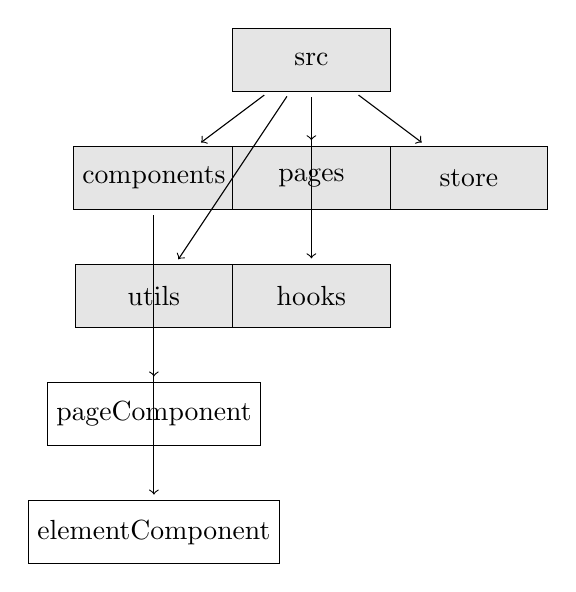
\begin{tikzpicture}[
    file/.style={draw, rectangle, minimum width=2cm, minimum height=0.8cm},
    folder/.style={draw, rectangle, minimum width=2cm, minimum height=0.8cm, fill=gray!20},
    arrow/.style={->, shorten >=2pt, shorten <=2pt}
]

% Folders
\node[folder] (src) at (0,0) {src};
\node[folder] (components) at (-2,-1.5) {components};
\node[folder] (pages) at (0,-1.5) {pages};
\node[folder] (store) at (2,-1.5) {store};
\node[folder] (utils) at (-2,-3) {utils};
\node[folder] (hooks) at (0,-3) {hooks};

% Files
\node[file] (pageComponent) at (-2,-4.5) {pageComponent};
\node[file] (elementComponent) at (-2,-6) {elementComponent};
% ... add more files

% Connections
\draw[arrow] (src) -- (components);
\draw[arrow] (src) -- (pages);
\draw[arrow] (src) -- (store);
\draw[arrow] (src) -- (utils);
\draw[arrow] (src) -- (hooks);
\draw[arrow] (components) -- (pageComponent);
\draw[arrow] (components) -- (elementComponent);
% ... add more connections

\end{tikzpicture}



\pagebreak
\subsubsection{Back-end}
The backend uses the dotNet framework. The development language using the C\# language.

In this project, the backend uses the Onion Architecture.
The Onion Architecture is a typically layered architecture, 
where each layer depends on the inner layer and provides interfaces to the outer layer.
The outer layer provides services to the outermost layer 
and other modules in the same layer based on the interfaces of the inner layer.

From inner to outer, the layers are: Domain, Application, Infrastructure, Presentation.
The Domain layer is the core layer and the innermost layer, used to define domain models, 
which are the business models.
It includes domain models and domain service interfaces.
Domain models are used to define the business models, 
which are the entities in the entity-relationship model and their attributes.
Domain service interfaces are used to define the business services, 
which are the relationships between entities in the entity-relationship model.

The Application layer is the application layer, 
used to define application services, which are the business logic.
It includes domain service implementations and application service interfaces.
Domain service implementations implement the methods of the inner layer's domain service 
interfaces and implement the business logic of the domain models.
Application service interfaces are used to define application services, 
which are the business logic.
It includes but is not limited to database interfaces, testing interfaces, 
HTTP API interfaces, MQTT interfaces, etc.

The Infrastructure layer is the infrastructure layer, used to define infrastructure.
It includes database implementations, testing implementations, 
HTTP API implementations, MQTT implementations, etc.
Database implementations implement the database interfaces 
and provide CRUD services for the database.
Testing implementations implement the testing interfaces 
and provide services for unit testing and integration testing.
HTTP API implementations implement the HTTP API interfaces 
and provide CRUD operations for HTTP APIs.
MQTT implementations implement the MQTT interfaces 
and provide CRUD operations for MQTT.

The Presentation layer is the presentation layer, used to define presentation logic, 
such as interfaces and pages. Since this is a backend project,
data presentation and control are handled by the frontend, 
so this layer is not needed.



\pagebreak
\subsubsection{Data communication and storage}
% 关于本项目的数据通信与数据存储的设计, 包括数据通信的协议, 数据存储的设计等
% 关于数据通信的设计:
% 1. 通信协议的选择
% 自前端向后端发送的数据, 有三种传输的数据类型, 
% 一种是普通的增删改查的请求, 对数据传输的时效性要求不高, 但是对数据的准确性, 完整性, 有序性, 安全性有一定的要求,
% 这种数据的传输, 采用 HTTP 协议, 以及 RESTful API 的设计. 可以有效的保证对数据传输的以上要求.
% 一种是对数据通道的创建和流媒体数据的传输, 对数据传输的时效性, 安全性要求较高, 这种数据的传输, 采用 WebRTC 协议, 以及 MQTT 协议.
% 配合可以快速解码的 flatbuffers 协议, 可以有效的保证对数据传输的以上要求.
% 最后一种是对设备的状态信息和操作信息的传输, 对完整性, 有序性, 安全性都有较高的要求, 这种数据的传输, 采用 MQTT 协议
% 同时也使用了 flatbuffers 协议.
% 
% 2. 数据通信的通信架构和通信流程
% 本项目的数据通信的通信架构, 是基于前后端分离的架构, 前端使用 React 框架, 后端使用 dotnet 框架.
% 当前端需要向后端发送数据的时候, 前端会向后端发送 HTTP 请求, 后端接收到 HTTP 请求之后, 会根据请求的数据类型,
% 选择不同的数据处理方式, 对于普通的增删改查的请求, 后端会根据 RESTful API 的设计, 对数据进行增删改查的操作,
% 对于对数据通道的创建和流媒体数据的传输, 后端会根据 WebRTC 协议, 对数据通道进行创建, 并且帮助前端和设备建立数据通道,
% 当数据通道建立后, 前端和设备之间则使用 flatbuffer 的数据格式对流媒体数据进行传输,
% 对于设备的状态信息和操作信息的传输, 前端会直接向 MQTT broker 发送 MQTT 请求, 
% 设备会在其自身的固件中监听相关的 MQTT 请求, 并且返回相关的数据.
% 
% 3. 数据通信的格式
% 本项目的数据通信的格式, 有三种, 
% 一种是 HTTP 协议, 
% 使用 json 格式对数据进行传输,
% 一种是 WebRTC 协议, 
% 使用 flatbuffers 格式对数据进行传输,
% 一种是 MQTT 协议.
% 使用 flatbuffers 格式对数据进行传输,
% 
% 关于数据存储的设计:
% 1. 数据存储的数据库的选择
% 本项目的数据存储的数据库的选择, 使用了轻量级的数据库 SQLite,
% SQLite 是一个进程内的库, 实现了自给自足的, 无服务器的, 零配置的, 事务性的 SQL 数据库引擎.
% 这是因为整个项目的目的是为了实现前端与设备之间的数据通信, 对于数据库数据的增删改查操作的要求不高,
% 数据量较小, 且对于数据库的数据的事务性要求不高, 所以选择了 SQLite 数据库.
% 2. 项目前后端的数据结构的设计
% 在本项目中, 前端由于使用了 React 框架, 所以前端的数据结构的设计, 使用了基于状态的数据结构的设计,
% 每个组件或者数据集都包含一个状态对象, 这个状态对象的属性就是组件的各个状态. 
% 使用状态对象的原因是, 可以方便的对状态进行管理, 采用对象-属性的形式, 可以方便的针对不同组件的同类状态进行区分,
% 由于跨组件的状态是由 redux 进行管理的, 这种状态对象的设计, 可以更搞笑的对状态进行更新和传递.
% 后端由于使用了 dotnet 框架, 所以后端的数据结构的设计, 使用了基于类的数据结构的设计,
% 采用了面向对象的编程思想, 对数据进行了封装, 使得数据的传输更加的安全, 有序, 完整.


\pagebreak

% \subsection{Domain model}
% \documentclass[]{article}
\usepackage{graphicx}
\usepackage{amsmath}
\usepackage{tikz}

% libaries
\usetikzlibrary{shapes,arrows}

%Define the listing package
\usepackage{listings} %code highlighter
\usepackage{color} %use color
\definecolor{mygreen}{rgb}{0,0.6,0}
\definecolor{mygray}{rgb}{0.5,0.5,0.5}
\definecolor{mymauve}{rgb}{0.58,0,0.82}

%Customize a bit the look
\lstset{ %
backgroundcolor=\color{white}, % choose the background color; you must add \usepackage{color} or \usepackage{xcolor}
basicstyle=\footnotesize, % the size of the fonts that are used for the code
breakatwhitespace=false, % sets if automatic breaks should only happen at whitespace
breaklines=true, % sets automatic line breaking
captionpos=b, % sets the caption-position to bottom
commentstyle=\color{mygreen}, % comment style
deletekeywords={...}, % if you want to delete keywords from the given language
escapeinside={\%*}{*)}, % if you want to add LaTeX within your code
extendedchars=true, % lets you use non-ASCII characters; for 8-bits encodings only, does not work with UTF-8
frame=single, % adds a frame around the code
keepspaces=true, % keeps spaces in text, useful for keeping indentation of code (possibly needs columns=flexible)
keywordstyle=\color{blue}, % keyword style
% language=Octave, % the language of the code
morekeywords={*,...}, % if you want to add more keywords to the set
numbers=left, % where to put the line-numbers; possible values are (none, left, right)
numbersep=5pt, % how far the line-numbers are from the code
numberstyle=\tiny\color{mygray}, % the style that is used for the line-numbers
rulecolor=\color{black}, % if not set, the frame-color may be changed on line-breaks within not-black text (e.g. comments (green here))
showspaces=false, % show spaces everywhere adding particular underscores; it overrides 'showstringspaces'
showstringspaces=false, % underline spaces within strings only
showtabs=false, % show tabs within strings adding particular underscores
stepnumber=1, % the step between two line-numbers. If it's 1, each line will be numbered
stringstyle=\color{mymauve}, % string literal style
tabsize=2, % sets default tabsize to 2 spaces
title=\lstname % show the filename of files included with \lstinputlisting; also try caption instead of title
}

\definecolor{darkgray}{rgb}{.4,.4,.4}
\definecolor{purple}{rgb}{0.65, 0.12, 0.82}

\lstdefinelanguage{React}{
keywords={const, typeof, new, true, false, catch, function, return, null, catch, switch, var, if, in, while, do, else, case, break},
keywordstyle=\color{blue}\bfseries,
ndkeywords={class, export, boolean, throw, implements, import, this},
ndkeywordstyle=\color{darkgray}\bfseries,
identifierstyle=\color{mygreen},
sensitive=false,
comment=[l]{//},
morecomment=[s]{/*}{*/},
commentstyle=\color{purple}\ttfamily,
string=[b]{"}{'}{`},
stringstyle=\color{red}\ttfamily,
morestring=[b]',
morestring=[b]",
morestring=[b]`',
}

\lstdefinelanguage{CSharp}{
keywords={const, typeof, new, true, false, catch, function, return, null, catch, switch, var, if, in, while, do, else, case, break},
keywordstyle=\color{blue}\bfseries,
ndkeywords={class, export, boolean, throw, implements, import, this},
ndkeywordstyle=\color{darkgray}\bfseries,
identifierstyle=\color{mygreen},
sensitive=false,
comment=[l]{//},
morecomment=[s]{/*}{*/},
commentstyle=\color{purple}\ttfamily,
string=[b]{"}{'}{`},
stringstyle=\color{red}\ttfamily,
morestring=[b]',
morestring=[b]",
morestring=[b]`',
}

\lstset{
language=React,
extendedchars=true,
basicstyle=\footnotesize\ttfamily,
showstringspaces=false,
showspaces=false,
numbers=left,
numberstyle=\footnotesize,
numbersep=9pt,
tabsize=2,
breaklines=true,
showtabs=false,
captionpos=b
}

\lstset{
language=CSharp,
extendedchars=true,
basicstyle=\footnotesize\ttfamily,
showstringspaces=false,
showspaces=false,
numbers=left,
numberstyle=\footnotesize,
numbersep=9pt,
tabsize=2,
breaklines=true,
showtabs=false,
captionpos=b
}

% \usepackage{cite} % Add this line for citation

% \bibliographystyle{plain}

\title{
The implementation of BifrostConnect Front-end scope, 
re-design and development with the relevant back-end support develop.
}
\author{
    Fei Gu \\
    Erhvervs Akademi Sydvest \\
    Computer Science 21\\
    }
\date{\today}

\begin{document}

% Front page
\maketitle
\begin{center}
    Supervisor: Henrik Boulund Meng Hansen \\
    Company: BifrostConnect \\
    Engineering Director: Jasper Wass \\
\end{center}
\tableofcontents
\pagebreak


% The introduction
\section{Introduction}
\subsection{Background}\input{sections/introduction/background.tex}
\subsection{The company}\input{sections/introduction/aboutCompany}
\subsection{The project}\input{sections/introduction/aboutProject}
\pagebreak

% The problem statement
\section{Problem Statement}
\subsection{Statement}
\input{sections/problemStatement/statement}
\subsection{Situation}
\input{sections/problemStatement/situation}
\subsection{Potential Solution}
\input{sections/problemStatement/potentialSolution}
\pagebreak

% Requirement analysis
\section{Requirement Analysis}
\input{sections/requirementAnalysis/index}

\subsection{Stakeholders}
\input{sections/requirementAnalysis/stakeholders/index}

\subsection{Business Domain}
\input{sections/requirementAnalysis/bussinesDomain/index}

\subsection{Scope}
\input{sections/requirementAnalysis/scope}

\subsection{Goals}
\input{sections/requirementAnalysis/goals}
\pagebreak

% Software Design
\section{Software Design}
% developement methods
\subsection{Software Development Methods}
\input{sections/softwareDevelopmentMethods/index}
\subsubsection{Agile Software Development}
\input{sections/softwareDevelopmentMethods/agileSoftwareDevelopment/index}
\subsubsection{Feature Driven Development}
\input{sections/softwareDevelopmentMethods/featureDrivenDevelopment/index}

\pagebreak

% Technology seslection
\subsection{Technology selection}
\input{sections/softwareDesign/technologySelection/index}
\subsubsection{Front-end}
\input{sections/softwareDesign/technologySelection/frontEnd}            
\subsubsection{Back-end}
\input{sections/softwareDesign/technologySelection/backEnd}            
\subsubsection{Database}
\input{sections/softwareDesign/technologySelection/database}
\subsubsection{Data communication}
\input{sections/softwareDesign/technologySelection/dataCommunication}            
\subsubsection{DevOps}
\input{sections/softwareDesign/technologySelection/devOps}
\pagebreak

% Architecture design
\subsection{Architecture design}
\input{sections/softwareDesign/architectureDesign/index}
\pagebreak
\subsubsection{Front-end}
\input{sections/softwareDesign/architectureDesign/frontEndArchitecture}
\pagebreak
\subsubsection{Back-end}
\input{sections/softwareDesign/architectureDesign/backEndArchitecture}
\pagebreak
\subsubsection{Data communication and storage}
\input{sections/softwareDesign/architectureDesign/dataCommunicationArchitecture}
\pagebreak

% \subsection{Domain model}
% \input{sections/softwareDesign/domainModel/index}
% \subsection{Database design}
% % 数据库领域模型 ER 图
% % 包括表和字段的设置.
% % 对于私有键和外键的设置.

% \subsection{Back-end design}
% % 后端对象模型
% % 以及对于对象模型的增删改查
% % 以及相关的其他服务的设计`'

% \subsection{Front-end design}
% % 对于前端的页面结构的设计 
% % 页面的状态的设计, 交互设计

% \subsection{FlatBuffers design}
% % schema 的设计

\subsection{DevOps CI/CD process design}
\input{sections/softwareDesign/devOpsDesign/index}
\subsubsection{Continuous Integration}
\input{sections/softwareDesign/devOpsDesign/continuousIntegration/index}
\subsubsection{Continuous Delivery}
\input{sections/softwareDesign/devOpsDesign/continuousDelivery/index}
\subsubsection{Continuous Deployment}
\input{sections/softwareDesign/devOpsDesign/continuousDeployment/index}
\pagebreak

\section{Software Development} 
\input{sections/softwareDevelopment/index}
\subsection{Overall development}
\input{sections/softwareDevelopment/overallDevelopement/index}
\subsubsection{Front-end}
\input{sections/softwareDevelopment/overallDevelopement/frontEnd/index}
\subsubsection{Back-end}
\input{sections/softwareDevelopment/overallDevelopement/backEnd/index}
\subsubsection{DevOps}
\input{sections/softwareDevelopment/overallDevelopement/devOps/index}
\subsection{Feature development} 
\input{sections/softwareDevelopment/featureDevelopment/index}
\subsubsection{Use Case 1}
\input{sections/softwareDevelopment/featureDevelopment/useCase1/index}
\subsubsection{Feature 1}
\input{sections/softwareDevelopment/featureDevelopment/feature/feature1.tex}
\pagebreak
\section{Conclusion} 
\subsection{Result}
Since the project is still in progress, the result is not available yet.
So far, basic structure of this project has been built. But the most features 
are not implemented yet. 
\subsection{Discussion}
As a single developer for this project, I am confident what I have done so far.
And I can say I understand the most of the knowledge I have used in this project, 
which also means I can explain all the part of the project. 
But this project also relevant some of the complex knowledge which I have to continue 
to study and practice.
\subsection{Future Work}
The future work is to implement the rest of the features. 
Including the most important part which is the 'create session' feature.
\pagebreak
% \bibliography{bibliography}
\pagebreak
% \begin{appendices}
%     \section{Appendix}
% \end{appendices} 
\end{document}
% \subsection{Database design}
% % 数据库领域模型 ER 图
% % 包括表和字段的设置.
% % 对于私有键和外键的设置.

% \subsection{Back-end design}
% % 后端对象模型
% % 以及对于对象模型的增删改查
% % 以及相关的其他服务的设计`'

% \subsection{Front-end design}
% % 对于前端的页面结构的设计 
% % 页面的状态的设计, 交互设计

% \subsection{FlatBuffers design}
% % schema 的设计

\subsection{DevOps CI/CD process design}
\documentclass[]{article}
\usepackage{graphicx}
\usepackage{amsmath}
\usepackage{tikz}

% libaries
\usetikzlibrary{shapes,arrows}

%Define the listing package
\usepackage{listings} %code highlighter
\usepackage{color} %use color
\definecolor{mygreen}{rgb}{0,0.6,0}
\definecolor{mygray}{rgb}{0.5,0.5,0.5}
\definecolor{mymauve}{rgb}{0.58,0,0.82}

%Customize a bit the look
\lstset{ %
backgroundcolor=\color{white}, % choose the background color; you must add \usepackage{color} or \usepackage{xcolor}
basicstyle=\footnotesize, % the size of the fonts that are used for the code
breakatwhitespace=false, % sets if automatic breaks should only happen at whitespace
breaklines=true, % sets automatic line breaking
captionpos=b, % sets the caption-position to bottom
commentstyle=\color{mygreen}, % comment style
deletekeywords={...}, % if you want to delete keywords from the given language
escapeinside={\%*}{*)}, % if you want to add LaTeX within your code
extendedchars=true, % lets you use non-ASCII characters; for 8-bits encodings only, does not work with UTF-8
frame=single, % adds a frame around the code
keepspaces=true, % keeps spaces in text, useful for keeping indentation of code (possibly needs columns=flexible)
keywordstyle=\color{blue}, % keyword style
% language=Octave, % the language of the code
morekeywords={*,...}, % if you want to add more keywords to the set
numbers=left, % where to put the line-numbers; possible values are (none, left, right)
numbersep=5pt, % how far the line-numbers are from the code
numberstyle=\tiny\color{mygray}, % the style that is used for the line-numbers
rulecolor=\color{black}, % if not set, the frame-color may be changed on line-breaks within not-black text (e.g. comments (green here))
showspaces=false, % show spaces everywhere adding particular underscores; it overrides 'showstringspaces'
showstringspaces=false, % underline spaces within strings only
showtabs=false, % show tabs within strings adding particular underscores
stepnumber=1, % the step between two line-numbers. If it's 1, each line will be numbered
stringstyle=\color{mymauve}, % string literal style
tabsize=2, % sets default tabsize to 2 spaces
title=\lstname % show the filename of files included with \lstinputlisting; also try caption instead of title
}

\definecolor{darkgray}{rgb}{.4,.4,.4}
\definecolor{purple}{rgb}{0.65, 0.12, 0.82}

\lstdefinelanguage{React}{
keywords={const, typeof, new, true, false, catch, function, return, null, catch, switch, var, if, in, while, do, else, case, break},
keywordstyle=\color{blue}\bfseries,
ndkeywords={class, export, boolean, throw, implements, import, this},
ndkeywordstyle=\color{darkgray}\bfseries,
identifierstyle=\color{mygreen},
sensitive=false,
comment=[l]{//},
morecomment=[s]{/*}{*/},
commentstyle=\color{purple}\ttfamily,
string=[b]{"}{'}{`},
stringstyle=\color{red}\ttfamily,
morestring=[b]',
morestring=[b]",
morestring=[b]`',
}

\lstdefinelanguage{CSharp}{
keywords={const, typeof, new, true, false, catch, function, return, null, catch, switch, var, if, in, while, do, else, case, break},
keywordstyle=\color{blue}\bfseries,
ndkeywords={class, export, boolean, throw, implements, import, this},
ndkeywordstyle=\color{darkgray}\bfseries,
identifierstyle=\color{mygreen},
sensitive=false,
comment=[l]{//},
morecomment=[s]{/*}{*/},
commentstyle=\color{purple}\ttfamily,
string=[b]{"}{'}{`},
stringstyle=\color{red}\ttfamily,
morestring=[b]',
morestring=[b]",
morestring=[b]`',
}

\lstset{
language=React,
extendedchars=true,
basicstyle=\footnotesize\ttfamily,
showstringspaces=false,
showspaces=false,
numbers=left,
numberstyle=\footnotesize,
numbersep=9pt,
tabsize=2,
breaklines=true,
showtabs=false,
captionpos=b
}

\lstset{
language=CSharp,
extendedchars=true,
basicstyle=\footnotesize\ttfamily,
showstringspaces=false,
showspaces=false,
numbers=left,
numberstyle=\footnotesize,
numbersep=9pt,
tabsize=2,
breaklines=true,
showtabs=false,
captionpos=b
}

% \usepackage{cite} % Add this line for citation

% \bibliographystyle{plain}

\title{
The implementation of BifrostConnect Front-end scope, 
re-design and development with the relevant back-end support develop.
}
\author{
    Fei Gu \\
    Erhvervs Akademi Sydvest \\
    Computer Science 21\\
    }
\date{\today}

\begin{document}

% Front page
\maketitle
\begin{center}
    Supervisor: Henrik Boulund Meng Hansen \\
    Company: BifrostConnect \\
    Engineering Director: Jasper Wass \\
\end{center}
\tableofcontents
\pagebreak


% The introduction
\section{Introduction}
\subsection{Background}\input{sections/introduction/background.tex}
\subsection{The company}\input{sections/introduction/aboutCompany}
\subsection{The project}\input{sections/introduction/aboutProject}
\pagebreak

% The problem statement
\section{Problem Statement}
\subsection{Statement}
\input{sections/problemStatement/statement}
\subsection{Situation}
\input{sections/problemStatement/situation}
\subsection{Potential Solution}
\input{sections/problemStatement/potentialSolution}
\pagebreak

% Requirement analysis
\section{Requirement Analysis}
\input{sections/requirementAnalysis/index}

\subsection{Stakeholders}
\input{sections/requirementAnalysis/stakeholders/index}

\subsection{Business Domain}
\input{sections/requirementAnalysis/bussinesDomain/index}

\subsection{Scope}
\input{sections/requirementAnalysis/scope}

\subsection{Goals}
\input{sections/requirementAnalysis/goals}
\pagebreak

% Software Design
\section{Software Design}
% developement methods
\subsection{Software Development Methods}
\input{sections/softwareDevelopmentMethods/index}
\subsubsection{Agile Software Development}
\input{sections/softwareDevelopmentMethods/agileSoftwareDevelopment/index}
\subsubsection{Feature Driven Development}
\input{sections/softwareDevelopmentMethods/featureDrivenDevelopment/index}

\pagebreak

% Technology seslection
\subsection{Technology selection}
\input{sections/softwareDesign/technologySelection/index}
\subsubsection{Front-end}
\input{sections/softwareDesign/technologySelection/frontEnd}            
\subsubsection{Back-end}
\input{sections/softwareDesign/technologySelection/backEnd}            
\subsubsection{Database}
\input{sections/softwareDesign/technologySelection/database}
\subsubsection{Data communication}
\input{sections/softwareDesign/technologySelection/dataCommunication}            
\subsubsection{DevOps}
\input{sections/softwareDesign/technologySelection/devOps}
\pagebreak

% Architecture design
\subsection{Architecture design}
\input{sections/softwareDesign/architectureDesign/index}
\pagebreak
\subsubsection{Front-end}
\input{sections/softwareDesign/architectureDesign/frontEndArchitecture}
\pagebreak
\subsubsection{Back-end}
\input{sections/softwareDesign/architectureDesign/backEndArchitecture}
\pagebreak
\subsubsection{Data communication and storage}
\input{sections/softwareDesign/architectureDesign/dataCommunicationArchitecture}
\pagebreak

% \subsection{Domain model}
% \input{sections/softwareDesign/domainModel/index}
% \subsection{Database design}
% % 数据库领域模型 ER 图
% % 包括表和字段的设置.
% % 对于私有键和外键的设置.

% \subsection{Back-end design}
% % 后端对象模型
% % 以及对于对象模型的增删改查
% % 以及相关的其他服务的设计`'

% \subsection{Front-end design}
% % 对于前端的页面结构的设计 
% % 页面的状态的设计, 交互设计

% \subsection{FlatBuffers design}
% % schema 的设计

\subsection{DevOps CI/CD process design}
\input{sections/softwareDesign/devOpsDesign/index}
\subsubsection{Continuous Integration}
\input{sections/softwareDesign/devOpsDesign/continuousIntegration/index}
\subsubsection{Continuous Delivery}
\input{sections/softwareDesign/devOpsDesign/continuousDelivery/index}
\subsubsection{Continuous Deployment}
\input{sections/softwareDesign/devOpsDesign/continuousDeployment/index}
\pagebreak

\section{Software Development} 
\input{sections/softwareDevelopment/index}
\subsection{Overall development}
\input{sections/softwareDevelopment/overallDevelopement/index}
\subsubsection{Front-end}
\input{sections/softwareDevelopment/overallDevelopement/frontEnd/index}
\subsubsection{Back-end}
\input{sections/softwareDevelopment/overallDevelopement/backEnd/index}
\subsubsection{DevOps}
\input{sections/softwareDevelopment/overallDevelopement/devOps/index}
\subsection{Feature development} 
\input{sections/softwareDevelopment/featureDevelopment/index}
\subsubsection{Use Case 1}
\input{sections/softwareDevelopment/featureDevelopment/useCase1/index}
\subsubsection{Feature 1}
\input{sections/softwareDevelopment/featureDevelopment/feature/feature1.tex}
\pagebreak
\section{Conclusion} 
\subsection{Result}
Since the project is still in progress, the result is not available yet.
So far, basic structure of this project has been built. But the most features 
are not implemented yet. 
\subsection{Discussion}
As a single developer for this project, I am confident what I have done so far.
And I can say I understand the most of the knowledge I have used in this project, 
which also means I can explain all the part of the project. 
But this project also relevant some of the complex knowledge which I have to continue 
to study and practice.
\subsection{Future Work}
The future work is to implement the rest of the features. 
Including the most important part which is the 'create session' feature.
\pagebreak
% \bibliography{bibliography}
\pagebreak
% \begin{appendices}
%     \section{Appendix}
% \end{appendices} 
\end{document}
\subsubsection{Continuous Integration}
\documentclass[]{article}
\usepackage{graphicx}
\usepackage{amsmath}
\usepackage{tikz}

% libaries
\usetikzlibrary{shapes,arrows}

%Define the listing package
\usepackage{listings} %code highlighter
\usepackage{color} %use color
\definecolor{mygreen}{rgb}{0,0.6,0}
\definecolor{mygray}{rgb}{0.5,0.5,0.5}
\definecolor{mymauve}{rgb}{0.58,0,0.82}

%Customize a bit the look
\lstset{ %
backgroundcolor=\color{white}, % choose the background color; you must add \usepackage{color} or \usepackage{xcolor}
basicstyle=\footnotesize, % the size of the fonts that are used for the code
breakatwhitespace=false, % sets if automatic breaks should only happen at whitespace
breaklines=true, % sets automatic line breaking
captionpos=b, % sets the caption-position to bottom
commentstyle=\color{mygreen}, % comment style
deletekeywords={...}, % if you want to delete keywords from the given language
escapeinside={\%*}{*)}, % if you want to add LaTeX within your code
extendedchars=true, % lets you use non-ASCII characters; for 8-bits encodings only, does not work with UTF-8
frame=single, % adds a frame around the code
keepspaces=true, % keeps spaces in text, useful for keeping indentation of code (possibly needs columns=flexible)
keywordstyle=\color{blue}, % keyword style
% language=Octave, % the language of the code
morekeywords={*,...}, % if you want to add more keywords to the set
numbers=left, % where to put the line-numbers; possible values are (none, left, right)
numbersep=5pt, % how far the line-numbers are from the code
numberstyle=\tiny\color{mygray}, % the style that is used for the line-numbers
rulecolor=\color{black}, % if not set, the frame-color may be changed on line-breaks within not-black text (e.g. comments (green here))
showspaces=false, % show spaces everywhere adding particular underscores; it overrides 'showstringspaces'
showstringspaces=false, % underline spaces within strings only
showtabs=false, % show tabs within strings adding particular underscores
stepnumber=1, % the step between two line-numbers. If it's 1, each line will be numbered
stringstyle=\color{mymauve}, % string literal style
tabsize=2, % sets default tabsize to 2 spaces
title=\lstname % show the filename of files included with \lstinputlisting; also try caption instead of title
}

\definecolor{darkgray}{rgb}{.4,.4,.4}
\definecolor{purple}{rgb}{0.65, 0.12, 0.82}

\lstdefinelanguage{React}{
keywords={const, typeof, new, true, false, catch, function, return, null, catch, switch, var, if, in, while, do, else, case, break},
keywordstyle=\color{blue}\bfseries,
ndkeywords={class, export, boolean, throw, implements, import, this},
ndkeywordstyle=\color{darkgray}\bfseries,
identifierstyle=\color{mygreen},
sensitive=false,
comment=[l]{//},
morecomment=[s]{/*}{*/},
commentstyle=\color{purple}\ttfamily,
string=[b]{"}{'}{`},
stringstyle=\color{red}\ttfamily,
morestring=[b]',
morestring=[b]",
morestring=[b]`',
}

\lstdefinelanguage{CSharp}{
keywords={const, typeof, new, true, false, catch, function, return, null, catch, switch, var, if, in, while, do, else, case, break},
keywordstyle=\color{blue}\bfseries,
ndkeywords={class, export, boolean, throw, implements, import, this},
ndkeywordstyle=\color{darkgray}\bfseries,
identifierstyle=\color{mygreen},
sensitive=false,
comment=[l]{//},
morecomment=[s]{/*}{*/},
commentstyle=\color{purple}\ttfamily,
string=[b]{"}{'}{`},
stringstyle=\color{red}\ttfamily,
morestring=[b]',
morestring=[b]",
morestring=[b]`',
}

\lstset{
language=React,
extendedchars=true,
basicstyle=\footnotesize\ttfamily,
showstringspaces=false,
showspaces=false,
numbers=left,
numberstyle=\footnotesize,
numbersep=9pt,
tabsize=2,
breaklines=true,
showtabs=false,
captionpos=b
}

\lstset{
language=CSharp,
extendedchars=true,
basicstyle=\footnotesize\ttfamily,
showstringspaces=false,
showspaces=false,
numbers=left,
numberstyle=\footnotesize,
numbersep=9pt,
tabsize=2,
breaklines=true,
showtabs=false,
captionpos=b
}

% \usepackage{cite} % Add this line for citation

% \bibliographystyle{plain}

\title{
The implementation of BifrostConnect Front-end scope, 
re-design and development with the relevant back-end support develop.
}
\author{
    Fei Gu \\
    Erhvervs Akademi Sydvest \\
    Computer Science 21\\
    }
\date{\today}

\begin{document}

% Front page
\maketitle
\begin{center}
    Supervisor: Henrik Boulund Meng Hansen \\
    Company: BifrostConnect \\
    Engineering Director: Jasper Wass \\
\end{center}
\tableofcontents
\pagebreak


% The introduction
\section{Introduction}
\subsection{Background}\input{sections/introduction/background.tex}
\subsection{The company}\input{sections/introduction/aboutCompany}
\subsection{The project}\input{sections/introduction/aboutProject}
\pagebreak

% The problem statement
\section{Problem Statement}
\subsection{Statement}
\input{sections/problemStatement/statement}
\subsection{Situation}
\input{sections/problemStatement/situation}
\subsection{Potential Solution}
\input{sections/problemStatement/potentialSolution}
\pagebreak

% Requirement analysis
\section{Requirement Analysis}
\input{sections/requirementAnalysis/index}

\subsection{Stakeholders}
\input{sections/requirementAnalysis/stakeholders/index}

\subsection{Business Domain}
\input{sections/requirementAnalysis/bussinesDomain/index}

\subsection{Scope}
\input{sections/requirementAnalysis/scope}

\subsection{Goals}
\input{sections/requirementAnalysis/goals}
\pagebreak

% Software Design
\section{Software Design}
% developement methods
\subsection{Software Development Methods}
\input{sections/softwareDevelopmentMethods/index}
\subsubsection{Agile Software Development}
\input{sections/softwareDevelopmentMethods/agileSoftwareDevelopment/index}
\subsubsection{Feature Driven Development}
\input{sections/softwareDevelopmentMethods/featureDrivenDevelopment/index}

\pagebreak

% Technology seslection
\subsection{Technology selection}
\input{sections/softwareDesign/technologySelection/index}
\subsubsection{Front-end}
\input{sections/softwareDesign/technologySelection/frontEnd}            
\subsubsection{Back-end}
\input{sections/softwareDesign/technologySelection/backEnd}            
\subsubsection{Database}
\input{sections/softwareDesign/technologySelection/database}
\subsubsection{Data communication}
\input{sections/softwareDesign/technologySelection/dataCommunication}            
\subsubsection{DevOps}
\input{sections/softwareDesign/technologySelection/devOps}
\pagebreak

% Architecture design
\subsection{Architecture design}
\input{sections/softwareDesign/architectureDesign/index}
\pagebreak
\subsubsection{Front-end}
\input{sections/softwareDesign/architectureDesign/frontEndArchitecture}
\pagebreak
\subsubsection{Back-end}
\input{sections/softwareDesign/architectureDesign/backEndArchitecture}
\pagebreak
\subsubsection{Data communication and storage}
\input{sections/softwareDesign/architectureDesign/dataCommunicationArchitecture}
\pagebreak

% \subsection{Domain model}
% \input{sections/softwareDesign/domainModel/index}
% \subsection{Database design}
% % 数据库领域模型 ER 图
% % 包括表和字段的设置.
% % 对于私有键和外键的设置.

% \subsection{Back-end design}
% % 后端对象模型
% % 以及对于对象模型的增删改查
% % 以及相关的其他服务的设计`'

% \subsection{Front-end design}
% % 对于前端的页面结构的设计 
% % 页面的状态的设计, 交互设计

% \subsection{FlatBuffers design}
% % schema 的设计

\subsection{DevOps CI/CD process design}
\input{sections/softwareDesign/devOpsDesign/index}
\subsubsection{Continuous Integration}
\input{sections/softwareDesign/devOpsDesign/continuousIntegration/index}
\subsubsection{Continuous Delivery}
\input{sections/softwareDesign/devOpsDesign/continuousDelivery/index}
\subsubsection{Continuous Deployment}
\input{sections/softwareDesign/devOpsDesign/continuousDeployment/index}
\pagebreak

\section{Software Development} 
\input{sections/softwareDevelopment/index}
\subsection{Overall development}
\input{sections/softwareDevelopment/overallDevelopement/index}
\subsubsection{Front-end}
\input{sections/softwareDevelopment/overallDevelopement/frontEnd/index}
\subsubsection{Back-end}
\input{sections/softwareDevelopment/overallDevelopement/backEnd/index}
\subsubsection{DevOps}
\input{sections/softwareDevelopment/overallDevelopement/devOps/index}
\subsection{Feature development} 
\input{sections/softwareDevelopment/featureDevelopment/index}
\subsubsection{Use Case 1}
\input{sections/softwareDevelopment/featureDevelopment/useCase1/index}
\subsubsection{Feature 1}
\input{sections/softwareDevelopment/featureDevelopment/feature/feature1.tex}
\pagebreak
\section{Conclusion} 
\subsection{Result}
Since the project is still in progress, the result is not available yet.
So far, basic structure of this project has been built. But the most features 
are not implemented yet. 
\subsection{Discussion}
As a single developer for this project, I am confident what I have done so far.
And I can say I understand the most of the knowledge I have used in this project, 
which also means I can explain all the part of the project. 
But this project also relevant some of the complex knowledge which I have to continue 
to study and practice.
\subsection{Future Work}
The future work is to implement the rest of the features. 
Including the most important part which is the 'create session' feature.
\pagebreak
% \bibliography{bibliography}
\pagebreak
% \begin{appendices}
%     \section{Appendix}
% \end{appendices} 
\end{document}
\subsubsection{Continuous Delivery}
\documentclass[]{article}
\usepackage{graphicx}
\usepackage{amsmath}
\usepackage{tikz}

% libaries
\usetikzlibrary{shapes,arrows}

%Define the listing package
\usepackage{listings} %code highlighter
\usepackage{color} %use color
\definecolor{mygreen}{rgb}{0,0.6,0}
\definecolor{mygray}{rgb}{0.5,0.5,0.5}
\definecolor{mymauve}{rgb}{0.58,0,0.82}

%Customize a bit the look
\lstset{ %
backgroundcolor=\color{white}, % choose the background color; you must add \usepackage{color} or \usepackage{xcolor}
basicstyle=\footnotesize, % the size of the fonts that are used for the code
breakatwhitespace=false, % sets if automatic breaks should only happen at whitespace
breaklines=true, % sets automatic line breaking
captionpos=b, % sets the caption-position to bottom
commentstyle=\color{mygreen}, % comment style
deletekeywords={...}, % if you want to delete keywords from the given language
escapeinside={\%*}{*)}, % if you want to add LaTeX within your code
extendedchars=true, % lets you use non-ASCII characters; for 8-bits encodings only, does not work with UTF-8
frame=single, % adds a frame around the code
keepspaces=true, % keeps spaces in text, useful for keeping indentation of code (possibly needs columns=flexible)
keywordstyle=\color{blue}, % keyword style
% language=Octave, % the language of the code
morekeywords={*,...}, % if you want to add more keywords to the set
numbers=left, % where to put the line-numbers; possible values are (none, left, right)
numbersep=5pt, % how far the line-numbers are from the code
numberstyle=\tiny\color{mygray}, % the style that is used for the line-numbers
rulecolor=\color{black}, % if not set, the frame-color may be changed on line-breaks within not-black text (e.g. comments (green here))
showspaces=false, % show spaces everywhere adding particular underscores; it overrides 'showstringspaces'
showstringspaces=false, % underline spaces within strings only
showtabs=false, % show tabs within strings adding particular underscores
stepnumber=1, % the step between two line-numbers. If it's 1, each line will be numbered
stringstyle=\color{mymauve}, % string literal style
tabsize=2, % sets default tabsize to 2 spaces
title=\lstname % show the filename of files included with \lstinputlisting; also try caption instead of title
}

\definecolor{darkgray}{rgb}{.4,.4,.4}
\definecolor{purple}{rgb}{0.65, 0.12, 0.82}

\lstdefinelanguage{React}{
keywords={const, typeof, new, true, false, catch, function, return, null, catch, switch, var, if, in, while, do, else, case, break},
keywordstyle=\color{blue}\bfseries,
ndkeywords={class, export, boolean, throw, implements, import, this},
ndkeywordstyle=\color{darkgray}\bfseries,
identifierstyle=\color{mygreen},
sensitive=false,
comment=[l]{//},
morecomment=[s]{/*}{*/},
commentstyle=\color{purple}\ttfamily,
string=[b]{"}{'}{`},
stringstyle=\color{red}\ttfamily,
morestring=[b]',
morestring=[b]",
morestring=[b]`',
}

\lstdefinelanguage{CSharp}{
keywords={const, typeof, new, true, false, catch, function, return, null, catch, switch, var, if, in, while, do, else, case, break},
keywordstyle=\color{blue}\bfseries,
ndkeywords={class, export, boolean, throw, implements, import, this},
ndkeywordstyle=\color{darkgray}\bfseries,
identifierstyle=\color{mygreen},
sensitive=false,
comment=[l]{//},
morecomment=[s]{/*}{*/},
commentstyle=\color{purple}\ttfamily,
string=[b]{"}{'}{`},
stringstyle=\color{red}\ttfamily,
morestring=[b]',
morestring=[b]",
morestring=[b]`',
}

\lstset{
language=React,
extendedchars=true,
basicstyle=\footnotesize\ttfamily,
showstringspaces=false,
showspaces=false,
numbers=left,
numberstyle=\footnotesize,
numbersep=9pt,
tabsize=2,
breaklines=true,
showtabs=false,
captionpos=b
}

\lstset{
language=CSharp,
extendedchars=true,
basicstyle=\footnotesize\ttfamily,
showstringspaces=false,
showspaces=false,
numbers=left,
numberstyle=\footnotesize,
numbersep=9pt,
tabsize=2,
breaklines=true,
showtabs=false,
captionpos=b
}

% \usepackage{cite} % Add this line for citation

% \bibliographystyle{plain}

\title{
The implementation of BifrostConnect Front-end scope, 
re-design and development with the relevant back-end support develop.
}
\author{
    Fei Gu \\
    Erhvervs Akademi Sydvest \\
    Computer Science 21\\
    }
\date{\today}

\begin{document}

% Front page
\maketitle
\begin{center}
    Supervisor: Henrik Boulund Meng Hansen \\
    Company: BifrostConnect \\
    Engineering Director: Jasper Wass \\
\end{center}
\tableofcontents
\pagebreak


% The introduction
\section{Introduction}
\subsection{Background}\input{sections/introduction/background.tex}
\subsection{The company}\input{sections/introduction/aboutCompany}
\subsection{The project}\input{sections/introduction/aboutProject}
\pagebreak

% The problem statement
\section{Problem Statement}
\subsection{Statement}
\input{sections/problemStatement/statement}
\subsection{Situation}
\input{sections/problemStatement/situation}
\subsection{Potential Solution}
\input{sections/problemStatement/potentialSolution}
\pagebreak

% Requirement analysis
\section{Requirement Analysis}
\input{sections/requirementAnalysis/index}

\subsection{Stakeholders}
\input{sections/requirementAnalysis/stakeholders/index}

\subsection{Business Domain}
\input{sections/requirementAnalysis/bussinesDomain/index}

\subsection{Scope}
\input{sections/requirementAnalysis/scope}

\subsection{Goals}
\input{sections/requirementAnalysis/goals}
\pagebreak

% Software Design
\section{Software Design}
% developement methods
\subsection{Software Development Methods}
\input{sections/softwareDevelopmentMethods/index}
\subsubsection{Agile Software Development}
\input{sections/softwareDevelopmentMethods/agileSoftwareDevelopment/index}
\subsubsection{Feature Driven Development}
\input{sections/softwareDevelopmentMethods/featureDrivenDevelopment/index}

\pagebreak

% Technology seslection
\subsection{Technology selection}
\input{sections/softwareDesign/technologySelection/index}
\subsubsection{Front-end}
\input{sections/softwareDesign/technologySelection/frontEnd}            
\subsubsection{Back-end}
\input{sections/softwareDesign/technologySelection/backEnd}            
\subsubsection{Database}
\input{sections/softwareDesign/technologySelection/database}
\subsubsection{Data communication}
\input{sections/softwareDesign/technologySelection/dataCommunication}            
\subsubsection{DevOps}
\input{sections/softwareDesign/technologySelection/devOps}
\pagebreak

% Architecture design
\subsection{Architecture design}
\input{sections/softwareDesign/architectureDesign/index}
\pagebreak
\subsubsection{Front-end}
\input{sections/softwareDesign/architectureDesign/frontEndArchitecture}
\pagebreak
\subsubsection{Back-end}
\input{sections/softwareDesign/architectureDesign/backEndArchitecture}
\pagebreak
\subsubsection{Data communication and storage}
\input{sections/softwareDesign/architectureDesign/dataCommunicationArchitecture}
\pagebreak

% \subsection{Domain model}
% \input{sections/softwareDesign/domainModel/index}
% \subsection{Database design}
% % 数据库领域模型 ER 图
% % 包括表和字段的设置.
% % 对于私有键和外键的设置.

% \subsection{Back-end design}
% % 后端对象模型
% % 以及对于对象模型的增删改查
% % 以及相关的其他服务的设计`'

% \subsection{Front-end design}
% % 对于前端的页面结构的设计 
% % 页面的状态的设计, 交互设计

% \subsection{FlatBuffers design}
% % schema 的设计

\subsection{DevOps CI/CD process design}
\input{sections/softwareDesign/devOpsDesign/index}
\subsubsection{Continuous Integration}
\input{sections/softwareDesign/devOpsDesign/continuousIntegration/index}
\subsubsection{Continuous Delivery}
\input{sections/softwareDesign/devOpsDesign/continuousDelivery/index}
\subsubsection{Continuous Deployment}
\input{sections/softwareDesign/devOpsDesign/continuousDeployment/index}
\pagebreak

\section{Software Development} 
\input{sections/softwareDevelopment/index}
\subsection{Overall development}
\input{sections/softwareDevelopment/overallDevelopement/index}
\subsubsection{Front-end}
\input{sections/softwareDevelopment/overallDevelopement/frontEnd/index}
\subsubsection{Back-end}
\input{sections/softwareDevelopment/overallDevelopement/backEnd/index}
\subsubsection{DevOps}
\input{sections/softwareDevelopment/overallDevelopement/devOps/index}
\subsection{Feature development} 
\input{sections/softwareDevelopment/featureDevelopment/index}
\subsubsection{Use Case 1}
\input{sections/softwareDevelopment/featureDevelopment/useCase1/index}
\subsubsection{Feature 1}
\input{sections/softwareDevelopment/featureDevelopment/feature/feature1.tex}
\pagebreak
\section{Conclusion} 
\subsection{Result}
Since the project is still in progress, the result is not available yet.
So far, basic structure of this project has been built. But the most features 
are not implemented yet. 
\subsection{Discussion}
As a single developer for this project, I am confident what I have done so far.
And I can say I understand the most of the knowledge I have used in this project, 
which also means I can explain all the part of the project. 
But this project also relevant some of the complex knowledge which I have to continue 
to study and practice.
\subsection{Future Work}
The future work is to implement the rest of the features. 
Including the most important part which is the 'create session' feature.
\pagebreak
% \bibliography{bibliography}
\pagebreak
% \begin{appendices}
%     \section{Appendix}
% \end{appendices} 
\end{document}
\subsubsection{Continuous Deployment}
\documentclass[]{article}
\usepackage{graphicx}
\usepackage{amsmath}
\usepackage{tikz}

% libaries
\usetikzlibrary{shapes,arrows}

%Define the listing package
\usepackage{listings} %code highlighter
\usepackage{color} %use color
\definecolor{mygreen}{rgb}{0,0.6,0}
\definecolor{mygray}{rgb}{0.5,0.5,0.5}
\definecolor{mymauve}{rgb}{0.58,0,0.82}

%Customize a bit the look
\lstset{ %
backgroundcolor=\color{white}, % choose the background color; you must add \usepackage{color} or \usepackage{xcolor}
basicstyle=\footnotesize, % the size of the fonts that are used for the code
breakatwhitespace=false, % sets if automatic breaks should only happen at whitespace
breaklines=true, % sets automatic line breaking
captionpos=b, % sets the caption-position to bottom
commentstyle=\color{mygreen}, % comment style
deletekeywords={...}, % if you want to delete keywords from the given language
escapeinside={\%*}{*)}, % if you want to add LaTeX within your code
extendedchars=true, % lets you use non-ASCII characters; for 8-bits encodings only, does not work with UTF-8
frame=single, % adds a frame around the code
keepspaces=true, % keeps spaces in text, useful for keeping indentation of code (possibly needs columns=flexible)
keywordstyle=\color{blue}, % keyword style
% language=Octave, % the language of the code
morekeywords={*,...}, % if you want to add more keywords to the set
numbers=left, % where to put the line-numbers; possible values are (none, left, right)
numbersep=5pt, % how far the line-numbers are from the code
numberstyle=\tiny\color{mygray}, % the style that is used for the line-numbers
rulecolor=\color{black}, % if not set, the frame-color may be changed on line-breaks within not-black text (e.g. comments (green here))
showspaces=false, % show spaces everywhere adding particular underscores; it overrides 'showstringspaces'
showstringspaces=false, % underline spaces within strings only
showtabs=false, % show tabs within strings adding particular underscores
stepnumber=1, % the step between two line-numbers. If it's 1, each line will be numbered
stringstyle=\color{mymauve}, % string literal style
tabsize=2, % sets default tabsize to 2 spaces
title=\lstname % show the filename of files included with \lstinputlisting; also try caption instead of title
}

\definecolor{darkgray}{rgb}{.4,.4,.4}
\definecolor{purple}{rgb}{0.65, 0.12, 0.82}

\lstdefinelanguage{React}{
keywords={const, typeof, new, true, false, catch, function, return, null, catch, switch, var, if, in, while, do, else, case, break},
keywordstyle=\color{blue}\bfseries,
ndkeywords={class, export, boolean, throw, implements, import, this},
ndkeywordstyle=\color{darkgray}\bfseries,
identifierstyle=\color{mygreen},
sensitive=false,
comment=[l]{//},
morecomment=[s]{/*}{*/},
commentstyle=\color{purple}\ttfamily,
string=[b]{"}{'}{`},
stringstyle=\color{red}\ttfamily,
morestring=[b]',
morestring=[b]",
morestring=[b]`',
}

\lstdefinelanguage{CSharp}{
keywords={const, typeof, new, true, false, catch, function, return, null, catch, switch, var, if, in, while, do, else, case, break},
keywordstyle=\color{blue}\bfseries,
ndkeywords={class, export, boolean, throw, implements, import, this},
ndkeywordstyle=\color{darkgray}\bfseries,
identifierstyle=\color{mygreen},
sensitive=false,
comment=[l]{//},
morecomment=[s]{/*}{*/},
commentstyle=\color{purple}\ttfamily,
string=[b]{"}{'}{`},
stringstyle=\color{red}\ttfamily,
morestring=[b]',
morestring=[b]",
morestring=[b]`',
}

\lstset{
language=React,
extendedchars=true,
basicstyle=\footnotesize\ttfamily,
showstringspaces=false,
showspaces=false,
numbers=left,
numberstyle=\footnotesize,
numbersep=9pt,
tabsize=2,
breaklines=true,
showtabs=false,
captionpos=b
}

\lstset{
language=CSharp,
extendedchars=true,
basicstyle=\footnotesize\ttfamily,
showstringspaces=false,
showspaces=false,
numbers=left,
numberstyle=\footnotesize,
numbersep=9pt,
tabsize=2,
breaklines=true,
showtabs=false,
captionpos=b
}

% \usepackage{cite} % Add this line for citation

% \bibliographystyle{plain}

\title{
The implementation of BifrostConnect Front-end scope, 
re-design and development with the relevant back-end support develop.
}
\author{
    Fei Gu \\
    Erhvervs Akademi Sydvest \\
    Computer Science 21\\
    }
\date{\today}

\begin{document}

% Front page
\maketitle
\begin{center}
    Supervisor: Henrik Boulund Meng Hansen \\
    Company: BifrostConnect \\
    Engineering Director: Jasper Wass \\
\end{center}
\tableofcontents
\pagebreak


% The introduction
\section{Introduction}
\subsection{Background}\input{sections/introduction/background.tex}
\subsection{The company}\input{sections/introduction/aboutCompany}
\subsection{The project}\input{sections/introduction/aboutProject}
\pagebreak

% The problem statement
\section{Problem Statement}
\subsection{Statement}
\input{sections/problemStatement/statement}
\subsection{Situation}
\input{sections/problemStatement/situation}
\subsection{Potential Solution}
\input{sections/problemStatement/potentialSolution}
\pagebreak

% Requirement analysis
\section{Requirement Analysis}
\input{sections/requirementAnalysis/index}

\subsection{Stakeholders}
\input{sections/requirementAnalysis/stakeholders/index}

\subsection{Business Domain}
\input{sections/requirementAnalysis/bussinesDomain/index}

\subsection{Scope}
\input{sections/requirementAnalysis/scope}

\subsection{Goals}
\input{sections/requirementAnalysis/goals}
\pagebreak

% Software Design
\section{Software Design}
% developement methods
\subsection{Software Development Methods}
\input{sections/softwareDevelopmentMethods/index}
\subsubsection{Agile Software Development}
\input{sections/softwareDevelopmentMethods/agileSoftwareDevelopment/index}
\subsubsection{Feature Driven Development}
\input{sections/softwareDevelopmentMethods/featureDrivenDevelopment/index}

\pagebreak

% Technology seslection
\subsection{Technology selection}
\input{sections/softwareDesign/technologySelection/index}
\subsubsection{Front-end}
\input{sections/softwareDesign/technologySelection/frontEnd}            
\subsubsection{Back-end}
\input{sections/softwareDesign/technologySelection/backEnd}            
\subsubsection{Database}
\input{sections/softwareDesign/technologySelection/database}
\subsubsection{Data communication}
\input{sections/softwareDesign/technologySelection/dataCommunication}            
\subsubsection{DevOps}
\input{sections/softwareDesign/technologySelection/devOps}
\pagebreak

% Architecture design
\subsection{Architecture design}
\input{sections/softwareDesign/architectureDesign/index}
\pagebreak
\subsubsection{Front-end}
\input{sections/softwareDesign/architectureDesign/frontEndArchitecture}
\pagebreak
\subsubsection{Back-end}
\input{sections/softwareDesign/architectureDesign/backEndArchitecture}
\pagebreak
\subsubsection{Data communication and storage}
\input{sections/softwareDesign/architectureDesign/dataCommunicationArchitecture}
\pagebreak

% \subsection{Domain model}
% \input{sections/softwareDesign/domainModel/index}
% \subsection{Database design}
% % 数据库领域模型 ER 图
% % 包括表和字段的设置.
% % 对于私有键和外键的设置.

% \subsection{Back-end design}
% % 后端对象模型
% % 以及对于对象模型的增删改查
% % 以及相关的其他服务的设计`'

% \subsection{Front-end design}
% % 对于前端的页面结构的设计 
% % 页面的状态的设计, 交互设计

% \subsection{FlatBuffers design}
% % schema 的设计

\subsection{DevOps CI/CD process design}
\input{sections/softwareDesign/devOpsDesign/index}
\subsubsection{Continuous Integration}
\input{sections/softwareDesign/devOpsDesign/continuousIntegration/index}
\subsubsection{Continuous Delivery}
\input{sections/softwareDesign/devOpsDesign/continuousDelivery/index}
\subsubsection{Continuous Deployment}
\input{sections/softwareDesign/devOpsDesign/continuousDeployment/index}
\pagebreak

\section{Software Development} 
\input{sections/softwareDevelopment/index}
\subsection{Overall development}
\input{sections/softwareDevelopment/overallDevelopement/index}
\subsubsection{Front-end}
\input{sections/softwareDevelopment/overallDevelopement/frontEnd/index}
\subsubsection{Back-end}
\input{sections/softwareDevelopment/overallDevelopement/backEnd/index}
\subsubsection{DevOps}
\input{sections/softwareDevelopment/overallDevelopement/devOps/index}
\subsection{Feature development} 
\input{sections/softwareDevelopment/featureDevelopment/index}
\subsubsection{Use Case 1}
\input{sections/softwareDevelopment/featureDevelopment/useCase1/index}
\subsubsection{Feature 1}
\input{sections/softwareDevelopment/featureDevelopment/feature/feature1.tex}
\pagebreak
\section{Conclusion} 
\subsection{Result}
Since the project is still in progress, the result is not available yet.
So far, basic structure of this project has been built. But the most features 
are not implemented yet. 
\subsection{Discussion}
As a single developer for this project, I am confident what I have done so far.
And I can say I understand the most of the knowledge I have used in this project, 
which also means I can explain all the part of the project. 
But this project also relevant some of the complex knowledge which I have to continue 
to study and practice.
\subsection{Future Work}
The future work is to implement the rest of the features. 
Including the most important part which is the 'create session' feature.
\pagebreak
% \bibliography{bibliography}
\pagebreak
% \begin{appendices}
%     \section{Appendix}
% \end{appendices} 
\end{document}
\pagebreak

\section{Software Development} 
\documentclass[]{article}
\usepackage{graphicx}
\usepackage{amsmath}
\usepackage{tikz}

% libaries
\usetikzlibrary{shapes,arrows}

%Define the listing package
\usepackage{listings} %code highlighter
\usepackage{color} %use color
\definecolor{mygreen}{rgb}{0,0.6,0}
\definecolor{mygray}{rgb}{0.5,0.5,0.5}
\definecolor{mymauve}{rgb}{0.58,0,0.82}

%Customize a bit the look
\lstset{ %
backgroundcolor=\color{white}, % choose the background color; you must add \usepackage{color} or \usepackage{xcolor}
basicstyle=\footnotesize, % the size of the fonts that are used for the code
breakatwhitespace=false, % sets if automatic breaks should only happen at whitespace
breaklines=true, % sets automatic line breaking
captionpos=b, % sets the caption-position to bottom
commentstyle=\color{mygreen}, % comment style
deletekeywords={...}, % if you want to delete keywords from the given language
escapeinside={\%*}{*)}, % if you want to add LaTeX within your code
extendedchars=true, % lets you use non-ASCII characters; for 8-bits encodings only, does not work with UTF-8
frame=single, % adds a frame around the code
keepspaces=true, % keeps spaces in text, useful for keeping indentation of code (possibly needs columns=flexible)
keywordstyle=\color{blue}, % keyword style
% language=Octave, % the language of the code
morekeywords={*,...}, % if you want to add more keywords to the set
numbers=left, % where to put the line-numbers; possible values are (none, left, right)
numbersep=5pt, % how far the line-numbers are from the code
numberstyle=\tiny\color{mygray}, % the style that is used for the line-numbers
rulecolor=\color{black}, % if not set, the frame-color may be changed on line-breaks within not-black text (e.g. comments (green here))
showspaces=false, % show spaces everywhere adding particular underscores; it overrides 'showstringspaces'
showstringspaces=false, % underline spaces within strings only
showtabs=false, % show tabs within strings adding particular underscores
stepnumber=1, % the step between two line-numbers. If it's 1, each line will be numbered
stringstyle=\color{mymauve}, % string literal style
tabsize=2, % sets default tabsize to 2 spaces
title=\lstname % show the filename of files included with \lstinputlisting; also try caption instead of title
}

\definecolor{darkgray}{rgb}{.4,.4,.4}
\definecolor{purple}{rgb}{0.65, 0.12, 0.82}

\lstdefinelanguage{React}{
keywords={const, typeof, new, true, false, catch, function, return, null, catch, switch, var, if, in, while, do, else, case, break},
keywordstyle=\color{blue}\bfseries,
ndkeywords={class, export, boolean, throw, implements, import, this},
ndkeywordstyle=\color{darkgray}\bfseries,
identifierstyle=\color{mygreen},
sensitive=false,
comment=[l]{//},
morecomment=[s]{/*}{*/},
commentstyle=\color{purple}\ttfamily,
string=[b]{"}{'}{`},
stringstyle=\color{red}\ttfamily,
morestring=[b]',
morestring=[b]",
morestring=[b]`',
}

\lstdefinelanguage{CSharp}{
keywords={const, typeof, new, true, false, catch, function, return, null, catch, switch, var, if, in, while, do, else, case, break},
keywordstyle=\color{blue}\bfseries,
ndkeywords={class, export, boolean, throw, implements, import, this},
ndkeywordstyle=\color{darkgray}\bfseries,
identifierstyle=\color{mygreen},
sensitive=false,
comment=[l]{//},
morecomment=[s]{/*}{*/},
commentstyle=\color{purple}\ttfamily,
string=[b]{"}{'}{`},
stringstyle=\color{red}\ttfamily,
morestring=[b]',
morestring=[b]",
morestring=[b]`',
}

\lstset{
language=React,
extendedchars=true,
basicstyle=\footnotesize\ttfamily,
showstringspaces=false,
showspaces=false,
numbers=left,
numberstyle=\footnotesize,
numbersep=9pt,
tabsize=2,
breaklines=true,
showtabs=false,
captionpos=b
}

\lstset{
language=CSharp,
extendedchars=true,
basicstyle=\footnotesize\ttfamily,
showstringspaces=false,
showspaces=false,
numbers=left,
numberstyle=\footnotesize,
numbersep=9pt,
tabsize=2,
breaklines=true,
showtabs=false,
captionpos=b
}

% \usepackage{cite} % Add this line for citation

% \bibliographystyle{plain}

\title{
The implementation of BifrostConnect Front-end scope, 
re-design and development with the relevant back-end support develop.
}
\author{
    Fei Gu \\
    Erhvervs Akademi Sydvest \\
    Computer Science 21\\
    }
\date{\today}

\begin{document}

% Front page
\maketitle
\begin{center}
    Supervisor: Henrik Boulund Meng Hansen \\
    Company: BifrostConnect \\
    Engineering Director: Jasper Wass \\
\end{center}
\tableofcontents
\pagebreak


% The introduction
\section{Introduction}
\subsection{Background}\input{sections/introduction/background.tex}
\subsection{The company}\input{sections/introduction/aboutCompany}
\subsection{The project}\input{sections/introduction/aboutProject}
\pagebreak

% The problem statement
\section{Problem Statement}
\subsection{Statement}
\input{sections/problemStatement/statement}
\subsection{Situation}
\input{sections/problemStatement/situation}
\subsection{Potential Solution}
\input{sections/problemStatement/potentialSolution}
\pagebreak

% Requirement analysis
\section{Requirement Analysis}
\input{sections/requirementAnalysis/index}

\subsection{Stakeholders}
\input{sections/requirementAnalysis/stakeholders/index}

\subsection{Business Domain}
\input{sections/requirementAnalysis/bussinesDomain/index}

\subsection{Scope}
\input{sections/requirementAnalysis/scope}

\subsection{Goals}
\input{sections/requirementAnalysis/goals}
\pagebreak

% Software Design
\section{Software Design}
% developement methods
\subsection{Software Development Methods}
\input{sections/softwareDevelopmentMethods/index}
\subsubsection{Agile Software Development}
\input{sections/softwareDevelopmentMethods/agileSoftwareDevelopment/index}
\subsubsection{Feature Driven Development}
\input{sections/softwareDevelopmentMethods/featureDrivenDevelopment/index}

\pagebreak

% Technology seslection
\subsection{Technology selection}
\input{sections/softwareDesign/technologySelection/index}
\subsubsection{Front-end}
\input{sections/softwareDesign/technologySelection/frontEnd}            
\subsubsection{Back-end}
\input{sections/softwareDesign/technologySelection/backEnd}            
\subsubsection{Database}
\input{sections/softwareDesign/technologySelection/database}
\subsubsection{Data communication}
\input{sections/softwareDesign/technologySelection/dataCommunication}            
\subsubsection{DevOps}
\input{sections/softwareDesign/technologySelection/devOps}
\pagebreak

% Architecture design
\subsection{Architecture design}
\input{sections/softwareDesign/architectureDesign/index}
\pagebreak
\subsubsection{Front-end}
\input{sections/softwareDesign/architectureDesign/frontEndArchitecture}
\pagebreak
\subsubsection{Back-end}
\input{sections/softwareDesign/architectureDesign/backEndArchitecture}
\pagebreak
\subsubsection{Data communication and storage}
\input{sections/softwareDesign/architectureDesign/dataCommunicationArchitecture}
\pagebreak

% \subsection{Domain model}
% \input{sections/softwareDesign/domainModel/index}
% \subsection{Database design}
% % 数据库领域模型 ER 图
% % 包括表和字段的设置.
% % 对于私有键和外键的设置.

% \subsection{Back-end design}
% % 后端对象模型
% % 以及对于对象模型的增删改查
% % 以及相关的其他服务的设计`'

% \subsection{Front-end design}
% % 对于前端的页面结构的设计 
% % 页面的状态的设计, 交互设计

% \subsection{FlatBuffers design}
% % schema 的设计

\subsection{DevOps CI/CD process design}
\input{sections/softwareDesign/devOpsDesign/index}
\subsubsection{Continuous Integration}
\input{sections/softwareDesign/devOpsDesign/continuousIntegration/index}
\subsubsection{Continuous Delivery}
\input{sections/softwareDesign/devOpsDesign/continuousDelivery/index}
\subsubsection{Continuous Deployment}
\input{sections/softwareDesign/devOpsDesign/continuousDeployment/index}
\pagebreak

\section{Software Development} 
\input{sections/softwareDevelopment/index}
\subsection{Overall development}
\input{sections/softwareDevelopment/overallDevelopement/index}
\subsubsection{Front-end}
\input{sections/softwareDevelopment/overallDevelopement/frontEnd/index}
\subsubsection{Back-end}
\input{sections/softwareDevelopment/overallDevelopement/backEnd/index}
\subsubsection{DevOps}
\input{sections/softwareDevelopment/overallDevelopement/devOps/index}
\subsection{Feature development} 
\input{sections/softwareDevelopment/featureDevelopment/index}
\subsubsection{Use Case 1}
\input{sections/softwareDevelopment/featureDevelopment/useCase1/index}
\subsubsection{Feature 1}
\input{sections/softwareDevelopment/featureDevelopment/feature/feature1.tex}
\pagebreak
\section{Conclusion} 
\subsection{Result}
Since the project is still in progress, the result is not available yet.
So far, basic structure of this project has been built. But the most features 
are not implemented yet. 
\subsection{Discussion}
As a single developer for this project, I am confident what I have done so far.
And I can say I understand the most of the knowledge I have used in this project, 
which also means I can explain all the part of the project. 
But this project also relevant some of the complex knowledge which I have to continue 
to study and practice.
\subsection{Future Work}
The future work is to implement the rest of the features. 
Including the most important part which is the 'create session' feature.
\pagebreak
% \bibliography{bibliography}
\pagebreak
% \begin{appendices}
%     \section{Appendix}
% \end{appendices} 
\end{document}
\subsection{Overall development}
\documentclass[]{article}
\usepackage{graphicx}
\usepackage{amsmath}
\usepackage{tikz}

% libaries
\usetikzlibrary{shapes,arrows}

%Define the listing package
\usepackage{listings} %code highlighter
\usepackage{color} %use color
\definecolor{mygreen}{rgb}{0,0.6,0}
\definecolor{mygray}{rgb}{0.5,0.5,0.5}
\definecolor{mymauve}{rgb}{0.58,0,0.82}

%Customize a bit the look
\lstset{ %
backgroundcolor=\color{white}, % choose the background color; you must add \usepackage{color} or \usepackage{xcolor}
basicstyle=\footnotesize, % the size of the fonts that are used for the code
breakatwhitespace=false, % sets if automatic breaks should only happen at whitespace
breaklines=true, % sets automatic line breaking
captionpos=b, % sets the caption-position to bottom
commentstyle=\color{mygreen}, % comment style
deletekeywords={...}, % if you want to delete keywords from the given language
escapeinside={\%*}{*)}, % if you want to add LaTeX within your code
extendedchars=true, % lets you use non-ASCII characters; for 8-bits encodings only, does not work with UTF-8
frame=single, % adds a frame around the code
keepspaces=true, % keeps spaces in text, useful for keeping indentation of code (possibly needs columns=flexible)
keywordstyle=\color{blue}, % keyword style
% language=Octave, % the language of the code
morekeywords={*,...}, % if you want to add more keywords to the set
numbers=left, % where to put the line-numbers; possible values are (none, left, right)
numbersep=5pt, % how far the line-numbers are from the code
numberstyle=\tiny\color{mygray}, % the style that is used for the line-numbers
rulecolor=\color{black}, % if not set, the frame-color may be changed on line-breaks within not-black text (e.g. comments (green here))
showspaces=false, % show spaces everywhere adding particular underscores; it overrides 'showstringspaces'
showstringspaces=false, % underline spaces within strings only
showtabs=false, % show tabs within strings adding particular underscores
stepnumber=1, % the step between two line-numbers. If it's 1, each line will be numbered
stringstyle=\color{mymauve}, % string literal style
tabsize=2, % sets default tabsize to 2 spaces
title=\lstname % show the filename of files included with \lstinputlisting; also try caption instead of title
}

\definecolor{darkgray}{rgb}{.4,.4,.4}
\definecolor{purple}{rgb}{0.65, 0.12, 0.82}

\lstdefinelanguage{React}{
keywords={const, typeof, new, true, false, catch, function, return, null, catch, switch, var, if, in, while, do, else, case, break},
keywordstyle=\color{blue}\bfseries,
ndkeywords={class, export, boolean, throw, implements, import, this},
ndkeywordstyle=\color{darkgray}\bfseries,
identifierstyle=\color{mygreen},
sensitive=false,
comment=[l]{//},
morecomment=[s]{/*}{*/},
commentstyle=\color{purple}\ttfamily,
string=[b]{"}{'}{`},
stringstyle=\color{red}\ttfamily,
morestring=[b]',
morestring=[b]",
morestring=[b]`',
}

\lstdefinelanguage{CSharp}{
keywords={const, typeof, new, true, false, catch, function, return, null, catch, switch, var, if, in, while, do, else, case, break},
keywordstyle=\color{blue}\bfseries,
ndkeywords={class, export, boolean, throw, implements, import, this},
ndkeywordstyle=\color{darkgray}\bfseries,
identifierstyle=\color{mygreen},
sensitive=false,
comment=[l]{//},
morecomment=[s]{/*}{*/},
commentstyle=\color{purple}\ttfamily,
string=[b]{"}{'}{`},
stringstyle=\color{red}\ttfamily,
morestring=[b]',
morestring=[b]",
morestring=[b]`',
}

\lstset{
language=React,
extendedchars=true,
basicstyle=\footnotesize\ttfamily,
showstringspaces=false,
showspaces=false,
numbers=left,
numberstyle=\footnotesize,
numbersep=9pt,
tabsize=2,
breaklines=true,
showtabs=false,
captionpos=b
}

\lstset{
language=CSharp,
extendedchars=true,
basicstyle=\footnotesize\ttfamily,
showstringspaces=false,
showspaces=false,
numbers=left,
numberstyle=\footnotesize,
numbersep=9pt,
tabsize=2,
breaklines=true,
showtabs=false,
captionpos=b
}

% \usepackage{cite} % Add this line for citation

% \bibliographystyle{plain}

\title{
The implementation of BifrostConnect Front-end scope, 
re-design and development with the relevant back-end support develop.
}
\author{
    Fei Gu \\
    Erhvervs Akademi Sydvest \\
    Computer Science 21\\
    }
\date{\today}

\begin{document}

% Front page
\maketitle
\begin{center}
    Supervisor: Henrik Boulund Meng Hansen \\
    Company: BifrostConnect \\
    Engineering Director: Jasper Wass \\
\end{center}
\tableofcontents
\pagebreak


% The introduction
\section{Introduction}
\subsection{Background}\input{sections/introduction/background.tex}
\subsection{The company}\input{sections/introduction/aboutCompany}
\subsection{The project}\input{sections/introduction/aboutProject}
\pagebreak

% The problem statement
\section{Problem Statement}
\subsection{Statement}
\input{sections/problemStatement/statement}
\subsection{Situation}
\input{sections/problemStatement/situation}
\subsection{Potential Solution}
\input{sections/problemStatement/potentialSolution}
\pagebreak

% Requirement analysis
\section{Requirement Analysis}
\input{sections/requirementAnalysis/index}

\subsection{Stakeholders}
\input{sections/requirementAnalysis/stakeholders/index}

\subsection{Business Domain}
\input{sections/requirementAnalysis/bussinesDomain/index}

\subsection{Scope}
\input{sections/requirementAnalysis/scope}

\subsection{Goals}
\input{sections/requirementAnalysis/goals}
\pagebreak

% Software Design
\section{Software Design}
% developement methods
\subsection{Software Development Methods}
\input{sections/softwareDevelopmentMethods/index}
\subsubsection{Agile Software Development}
\input{sections/softwareDevelopmentMethods/agileSoftwareDevelopment/index}
\subsubsection{Feature Driven Development}
\input{sections/softwareDevelopmentMethods/featureDrivenDevelopment/index}

\pagebreak

% Technology seslection
\subsection{Technology selection}
\input{sections/softwareDesign/technologySelection/index}
\subsubsection{Front-end}
\input{sections/softwareDesign/technologySelection/frontEnd}            
\subsubsection{Back-end}
\input{sections/softwareDesign/technologySelection/backEnd}            
\subsubsection{Database}
\input{sections/softwareDesign/technologySelection/database}
\subsubsection{Data communication}
\input{sections/softwareDesign/technologySelection/dataCommunication}            
\subsubsection{DevOps}
\input{sections/softwareDesign/technologySelection/devOps}
\pagebreak

% Architecture design
\subsection{Architecture design}
\input{sections/softwareDesign/architectureDesign/index}
\pagebreak
\subsubsection{Front-end}
\input{sections/softwareDesign/architectureDesign/frontEndArchitecture}
\pagebreak
\subsubsection{Back-end}
\input{sections/softwareDesign/architectureDesign/backEndArchitecture}
\pagebreak
\subsubsection{Data communication and storage}
\input{sections/softwareDesign/architectureDesign/dataCommunicationArchitecture}
\pagebreak

% \subsection{Domain model}
% \input{sections/softwareDesign/domainModel/index}
% \subsection{Database design}
% % 数据库领域模型 ER 图
% % 包括表和字段的设置.
% % 对于私有键和外键的设置.

% \subsection{Back-end design}
% % 后端对象模型
% % 以及对于对象模型的增删改查
% % 以及相关的其他服务的设计`'

% \subsection{Front-end design}
% % 对于前端的页面结构的设计 
% % 页面的状态的设计, 交互设计

% \subsection{FlatBuffers design}
% % schema 的设计

\subsection{DevOps CI/CD process design}
\input{sections/softwareDesign/devOpsDesign/index}
\subsubsection{Continuous Integration}
\input{sections/softwareDesign/devOpsDesign/continuousIntegration/index}
\subsubsection{Continuous Delivery}
\input{sections/softwareDesign/devOpsDesign/continuousDelivery/index}
\subsubsection{Continuous Deployment}
\input{sections/softwareDesign/devOpsDesign/continuousDeployment/index}
\pagebreak

\section{Software Development} 
\input{sections/softwareDevelopment/index}
\subsection{Overall development}
\input{sections/softwareDevelopment/overallDevelopement/index}
\subsubsection{Front-end}
\input{sections/softwareDevelopment/overallDevelopement/frontEnd/index}
\subsubsection{Back-end}
\input{sections/softwareDevelopment/overallDevelopement/backEnd/index}
\subsubsection{DevOps}
\input{sections/softwareDevelopment/overallDevelopement/devOps/index}
\subsection{Feature development} 
\input{sections/softwareDevelopment/featureDevelopment/index}
\subsubsection{Use Case 1}
\input{sections/softwareDevelopment/featureDevelopment/useCase1/index}
\subsubsection{Feature 1}
\input{sections/softwareDevelopment/featureDevelopment/feature/feature1.tex}
\pagebreak
\section{Conclusion} 
\subsection{Result}
Since the project is still in progress, the result is not available yet.
So far, basic structure of this project has been built. But the most features 
are not implemented yet. 
\subsection{Discussion}
As a single developer for this project, I am confident what I have done so far.
And I can say I understand the most of the knowledge I have used in this project, 
which also means I can explain all the part of the project. 
But this project also relevant some of the complex knowledge which I have to continue 
to study and practice.
\subsection{Future Work}
The future work is to implement the rest of the features. 
Including the most important part which is the 'create session' feature.
\pagebreak
% \bibliography{bibliography}
\pagebreak
% \begin{appendices}
%     \section{Appendix}
% \end{appendices} 
\end{document}
\subsubsection{Front-end}
\documentclass[]{article}
\usepackage{graphicx}
\usepackage{amsmath}
\usepackage{tikz}

% libaries
\usetikzlibrary{shapes,arrows}

%Define the listing package
\usepackage{listings} %code highlighter
\usepackage{color} %use color
\definecolor{mygreen}{rgb}{0,0.6,0}
\definecolor{mygray}{rgb}{0.5,0.5,0.5}
\definecolor{mymauve}{rgb}{0.58,0,0.82}

%Customize a bit the look
\lstset{ %
backgroundcolor=\color{white}, % choose the background color; you must add \usepackage{color} or \usepackage{xcolor}
basicstyle=\footnotesize, % the size of the fonts that are used for the code
breakatwhitespace=false, % sets if automatic breaks should only happen at whitespace
breaklines=true, % sets automatic line breaking
captionpos=b, % sets the caption-position to bottom
commentstyle=\color{mygreen}, % comment style
deletekeywords={...}, % if you want to delete keywords from the given language
escapeinside={\%*}{*)}, % if you want to add LaTeX within your code
extendedchars=true, % lets you use non-ASCII characters; for 8-bits encodings only, does not work with UTF-8
frame=single, % adds a frame around the code
keepspaces=true, % keeps spaces in text, useful for keeping indentation of code (possibly needs columns=flexible)
keywordstyle=\color{blue}, % keyword style
% language=Octave, % the language of the code
morekeywords={*,...}, % if you want to add more keywords to the set
numbers=left, % where to put the line-numbers; possible values are (none, left, right)
numbersep=5pt, % how far the line-numbers are from the code
numberstyle=\tiny\color{mygray}, % the style that is used for the line-numbers
rulecolor=\color{black}, % if not set, the frame-color may be changed on line-breaks within not-black text (e.g. comments (green here))
showspaces=false, % show spaces everywhere adding particular underscores; it overrides 'showstringspaces'
showstringspaces=false, % underline spaces within strings only
showtabs=false, % show tabs within strings adding particular underscores
stepnumber=1, % the step between two line-numbers. If it's 1, each line will be numbered
stringstyle=\color{mymauve}, % string literal style
tabsize=2, % sets default tabsize to 2 spaces
title=\lstname % show the filename of files included with \lstinputlisting; also try caption instead of title
}

\definecolor{darkgray}{rgb}{.4,.4,.4}
\definecolor{purple}{rgb}{0.65, 0.12, 0.82}

\lstdefinelanguage{React}{
keywords={const, typeof, new, true, false, catch, function, return, null, catch, switch, var, if, in, while, do, else, case, break},
keywordstyle=\color{blue}\bfseries,
ndkeywords={class, export, boolean, throw, implements, import, this},
ndkeywordstyle=\color{darkgray}\bfseries,
identifierstyle=\color{mygreen},
sensitive=false,
comment=[l]{//},
morecomment=[s]{/*}{*/},
commentstyle=\color{purple}\ttfamily,
string=[b]{"}{'}{`},
stringstyle=\color{red}\ttfamily,
morestring=[b]',
morestring=[b]",
morestring=[b]`',
}

\lstdefinelanguage{CSharp}{
keywords={const, typeof, new, true, false, catch, function, return, null, catch, switch, var, if, in, while, do, else, case, break},
keywordstyle=\color{blue}\bfseries,
ndkeywords={class, export, boolean, throw, implements, import, this},
ndkeywordstyle=\color{darkgray}\bfseries,
identifierstyle=\color{mygreen},
sensitive=false,
comment=[l]{//},
morecomment=[s]{/*}{*/},
commentstyle=\color{purple}\ttfamily,
string=[b]{"}{'}{`},
stringstyle=\color{red}\ttfamily,
morestring=[b]',
morestring=[b]",
morestring=[b]`',
}

\lstset{
language=React,
extendedchars=true,
basicstyle=\footnotesize\ttfamily,
showstringspaces=false,
showspaces=false,
numbers=left,
numberstyle=\footnotesize,
numbersep=9pt,
tabsize=2,
breaklines=true,
showtabs=false,
captionpos=b
}

\lstset{
language=CSharp,
extendedchars=true,
basicstyle=\footnotesize\ttfamily,
showstringspaces=false,
showspaces=false,
numbers=left,
numberstyle=\footnotesize,
numbersep=9pt,
tabsize=2,
breaklines=true,
showtabs=false,
captionpos=b
}

% \usepackage{cite} % Add this line for citation

% \bibliographystyle{plain}

\title{
The implementation of BifrostConnect Front-end scope, 
re-design and development with the relevant back-end support develop.
}
\author{
    Fei Gu \\
    Erhvervs Akademi Sydvest \\
    Computer Science 21\\
    }
\date{\today}

\begin{document}

% Front page
\maketitle
\begin{center}
    Supervisor: Henrik Boulund Meng Hansen \\
    Company: BifrostConnect \\
    Engineering Director: Jasper Wass \\
\end{center}
\tableofcontents
\pagebreak


% The introduction
\section{Introduction}
\subsection{Background}\input{sections/introduction/background.tex}
\subsection{The company}\input{sections/introduction/aboutCompany}
\subsection{The project}\input{sections/introduction/aboutProject}
\pagebreak

% The problem statement
\section{Problem Statement}
\subsection{Statement}
\input{sections/problemStatement/statement}
\subsection{Situation}
\input{sections/problemStatement/situation}
\subsection{Potential Solution}
\input{sections/problemStatement/potentialSolution}
\pagebreak

% Requirement analysis
\section{Requirement Analysis}
\input{sections/requirementAnalysis/index}

\subsection{Stakeholders}
\input{sections/requirementAnalysis/stakeholders/index}

\subsection{Business Domain}
\input{sections/requirementAnalysis/bussinesDomain/index}

\subsection{Scope}
\input{sections/requirementAnalysis/scope}

\subsection{Goals}
\input{sections/requirementAnalysis/goals}
\pagebreak

% Software Design
\section{Software Design}
% developement methods
\subsection{Software Development Methods}
\input{sections/softwareDevelopmentMethods/index}
\subsubsection{Agile Software Development}
\input{sections/softwareDevelopmentMethods/agileSoftwareDevelopment/index}
\subsubsection{Feature Driven Development}
\input{sections/softwareDevelopmentMethods/featureDrivenDevelopment/index}

\pagebreak

% Technology seslection
\subsection{Technology selection}
\input{sections/softwareDesign/technologySelection/index}
\subsubsection{Front-end}
\input{sections/softwareDesign/technologySelection/frontEnd}            
\subsubsection{Back-end}
\input{sections/softwareDesign/technologySelection/backEnd}            
\subsubsection{Database}
\input{sections/softwareDesign/technologySelection/database}
\subsubsection{Data communication}
\input{sections/softwareDesign/technologySelection/dataCommunication}            
\subsubsection{DevOps}
\input{sections/softwareDesign/technologySelection/devOps}
\pagebreak

% Architecture design
\subsection{Architecture design}
\input{sections/softwareDesign/architectureDesign/index}
\pagebreak
\subsubsection{Front-end}
\input{sections/softwareDesign/architectureDesign/frontEndArchitecture}
\pagebreak
\subsubsection{Back-end}
\input{sections/softwareDesign/architectureDesign/backEndArchitecture}
\pagebreak
\subsubsection{Data communication and storage}
\input{sections/softwareDesign/architectureDesign/dataCommunicationArchitecture}
\pagebreak

% \subsection{Domain model}
% \input{sections/softwareDesign/domainModel/index}
% \subsection{Database design}
% % 数据库领域模型 ER 图
% % 包括表和字段的设置.
% % 对于私有键和外键的设置.

% \subsection{Back-end design}
% % 后端对象模型
% % 以及对于对象模型的增删改查
% % 以及相关的其他服务的设计`'

% \subsection{Front-end design}
% % 对于前端的页面结构的设计 
% % 页面的状态的设计, 交互设计

% \subsection{FlatBuffers design}
% % schema 的设计

\subsection{DevOps CI/CD process design}
\input{sections/softwareDesign/devOpsDesign/index}
\subsubsection{Continuous Integration}
\input{sections/softwareDesign/devOpsDesign/continuousIntegration/index}
\subsubsection{Continuous Delivery}
\input{sections/softwareDesign/devOpsDesign/continuousDelivery/index}
\subsubsection{Continuous Deployment}
\input{sections/softwareDesign/devOpsDesign/continuousDeployment/index}
\pagebreak

\section{Software Development} 
\input{sections/softwareDevelopment/index}
\subsection{Overall development}
\input{sections/softwareDevelopment/overallDevelopement/index}
\subsubsection{Front-end}
\input{sections/softwareDevelopment/overallDevelopement/frontEnd/index}
\subsubsection{Back-end}
\input{sections/softwareDevelopment/overallDevelopement/backEnd/index}
\subsubsection{DevOps}
\input{sections/softwareDevelopment/overallDevelopement/devOps/index}
\subsection{Feature development} 
\input{sections/softwareDevelopment/featureDevelopment/index}
\subsubsection{Use Case 1}
\input{sections/softwareDevelopment/featureDevelopment/useCase1/index}
\subsubsection{Feature 1}
\input{sections/softwareDevelopment/featureDevelopment/feature/feature1.tex}
\pagebreak
\section{Conclusion} 
\subsection{Result}
Since the project is still in progress, the result is not available yet.
So far, basic structure of this project has been built. But the most features 
are not implemented yet. 
\subsection{Discussion}
As a single developer for this project, I am confident what I have done so far.
And I can say I understand the most of the knowledge I have used in this project, 
which also means I can explain all the part of the project. 
But this project also relevant some of the complex knowledge which I have to continue 
to study and practice.
\subsection{Future Work}
The future work is to implement the rest of the features. 
Including the most important part which is the 'create session' feature.
\pagebreak
% \bibliography{bibliography}
\pagebreak
% \begin{appendices}
%     \section{Appendix}
% \end{appendices} 
\end{document}
\subsubsection{Back-end}
\documentclass[]{article}
\usepackage{graphicx}
\usepackage{amsmath}
\usepackage{tikz}

% libaries
\usetikzlibrary{shapes,arrows}

%Define the listing package
\usepackage{listings} %code highlighter
\usepackage{color} %use color
\definecolor{mygreen}{rgb}{0,0.6,0}
\definecolor{mygray}{rgb}{0.5,0.5,0.5}
\definecolor{mymauve}{rgb}{0.58,0,0.82}

%Customize a bit the look
\lstset{ %
backgroundcolor=\color{white}, % choose the background color; you must add \usepackage{color} or \usepackage{xcolor}
basicstyle=\footnotesize, % the size of the fonts that are used for the code
breakatwhitespace=false, % sets if automatic breaks should only happen at whitespace
breaklines=true, % sets automatic line breaking
captionpos=b, % sets the caption-position to bottom
commentstyle=\color{mygreen}, % comment style
deletekeywords={...}, % if you want to delete keywords from the given language
escapeinside={\%*}{*)}, % if you want to add LaTeX within your code
extendedchars=true, % lets you use non-ASCII characters; for 8-bits encodings only, does not work with UTF-8
frame=single, % adds a frame around the code
keepspaces=true, % keeps spaces in text, useful for keeping indentation of code (possibly needs columns=flexible)
keywordstyle=\color{blue}, % keyword style
% language=Octave, % the language of the code
morekeywords={*,...}, % if you want to add more keywords to the set
numbers=left, % where to put the line-numbers; possible values are (none, left, right)
numbersep=5pt, % how far the line-numbers are from the code
numberstyle=\tiny\color{mygray}, % the style that is used for the line-numbers
rulecolor=\color{black}, % if not set, the frame-color may be changed on line-breaks within not-black text (e.g. comments (green here))
showspaces=false, % show spaces everywhere adding particular underscores; it overrides 'showstringspaces'
showstringspaces=false, % underline spaces within strings only
showtabs=false, % show tabs within strings adding particular underscores
stepnumber=1, % the step between two line-numbers. If it's 1, each line will be numbered
stringstyle=\color{mymauve}, % string literal style
tabsize=2, % sets default tabsize to 2 spaces
title=\lstname % show the filename of files included with \lstinputlisting; also try caption instead of title
}

\definecolor{darkgray}{rgb}{.4,.4,.4}
\definecolor{purple}{rgb}{0.65, 0.12, 0.82}

\lstdefinelanguage{React}{
keywords={const, typeof, new, true, false, catch, function, return, null, catch, switch, var, if, in, while, do, else, case, break},
keywordstyle=\color{blue}\bfseries,
ndkeywords={class, export, boolean, throw, implements, import, this},
ndkeywordstyle=\color{darkgray}\bfseries,
identifierstyle=\color{mygreen},
sensitive=false,
comment=[l]{//},
morecomment=[s]{/*}{*/},
commentstyle=\color{purple}\ttfamily,
string=[b]{"}{'}{`},
stringstyle=\color{red}\ttfamily,
morestring=[b]',
morestring=[b]",
morestring=[b]`',
}

\lstdefinelanguage{CSharp}{
keywords={const, typeof, new, true, false, catch, function, return, null, catch, switch, var, if, in, while, do, else, case, break},
keywordstyle=\color{blue}\bfseries,
ndkeywords={class, export, boolean, throw, implements, import, this},
ndkeywordstyle=\color{darkgray}\bfseries,
identifierstyle=\color{mygreen},
sensitive=false,
comment=[l]{//},
morecomment=[s]{/*}{*/},
commentstyle=\color{purple}\ttfamily,
string=[b]{"}{'}{`},
stringstyle=\color{red}\ttfamily,
morestring=[b]',
morestring=[b]",
morestring=[b]`',
}

\lstset{
language=React,
extendedchars=true,
basicstyle=\footnotesize\ttfamily,
showstringspaces=false,
showspaces=false,
numbers=left,
numberstyle=\footnotesize,
numbersep=9pt,
tabsize=2,
breaklines=true,
showtabs=false,
captionpos=b
}

\lstset{
language=CSharp,
extendedchars=true,
basicstyle=\footnotesize\ttfamily,
showstringspaces=false,
showspaces=false,
numbers=left,
numberstyle=\footnotesize,
numbersep=9pt,
tabsize=2,
breaklines=true,
showtabs=false,
captionpos=b
}

% \usepackage{cite} % Add this line for citation

% \bibliographystyle{plain}

\title{
The implementation of BifrostConnect Front-end scope, 
re-design and development with the relevant back-end support develop.
}
\author{
    Fei Gu \\
    Erhvervs Akademi Sydvest \\
    Computer Science 21\\
    }
\date{\today}

\begin{document}

% Front page
\maketitle
\begin{center}
    Supervisor: Henrik Boulund Meng Hansen \\
    Company: BifrostConnect \\
    Engineering Director: Jasper Wass \\
\end{center}
\tableofcontents
\pagebreak


% The introduction
\section{Introduction}
\subsection{Background}\input{sections/introduction/background.tex}
\subsection{The company}\input{sections/introduction/aboutCompany}
\subsection{The project}\input{sections/introduction/aboutProject}
\pagebreak

% The problem statement
\section{Problem Statement}
\subsection{Statement}
\input{sections/problemStatement/statement}
\subsection{Situation}
\input{sections/problemStatement/situation}
\subsection{Potential Solution}
\input{sections/problemStatement/potentialSolution}
\pagebreak

% Requirement analysis
\section{Requirement Analysis}
\input{sections/requirementAnalysis/index}

\subsection{Stakeholders}
\input{sections/requirementAnalysis/stakeholders/index}

\subsection{Business Domain}
\input{sections/requirementAnalysis/bussinesDomain/index}

\subsection{Scope}
\input{sections/requirementAnalysis/scope}

\subsection{Goals}
\input{sections/requirementAnalysis/goals}
\pagebreak

% Software Design
\section{Software Design}
% developement methods
\subsection{Software Development Methods}
\input{sections/softwareDevelopmentMethods/index}
\subsubsection{Agile Software Development}
\input{sections/softwareDevelopmentMethods/agileSoftwareDevelopment/index}
\subsubsection{Feature Driven Development}
\input{sections/softwareDevelopmentMethods/featureDrivenDevelopment/index}

\pagebreak

% Technology seslection
\subsection{Technology selection}
\input{sections/softwareDesign/technologySelection/index}
\subsubsection{Front-end}
\input{sections/softwareDesign/technologySelection/frontEnd}            
\subsubsection{Back-end}
\input{sections/softwareDesign/technologySelection/backEnd}            
\subsubsection{Database}
\input{sections/softwareDesign/technologySelection/database}
\subsubsection{Data communication}
\input{sections/softwareDesign/technologySelection/dataCommunication}            
\subsubsection{DevOps}
\input{sections/softwareDesign/technologySelection/devOps}
\pagebreak

% Architecture design
\subsection{Architecture design}
\input{sections/softwareDesign/architectureDesign/index}
\pagebreak
\subsubsection{Front-end}
\input{sections/softwareDesign/architectureDesign/frontEndArchitecture}
\pagebreak
\subsubsection{Back-end}
\input{sections/softwareDesign/architectureDesign/backEndArchitecture}
\pagebreak
\subsubsection{Data communication and storage}
\input{sections/softwareDesign/architectureDesign/dataCommunicationArchitecture}
\pagebreak

% \subsection{Domain model}
% \input{sections/softwareDesign/domainModel/index}
% \subsection{Database design}
% % 数据库领域模型 ER 图
% % 包括表和字段的设置.
% % 对于私有键和外键的设置.

% \subsection{Back-end design}
% % 后端对象模型
% % 以及对于对象模型的增删改查
% % 以及相关的其他服务的设计`'

% \subsection{Front-end design}
% % 对于前端的页面结构的设计 
% % 页面的状态的设计, 交互设计

% \subsection{FlatBuffers design}
% % schema 的设计

\subsection{DevOps CI/CD process design}
\input{sections/softwareDesign/devOpsDesign/index}
\subsubsection{Continuous Integration}
\input{sections/softwareDesign/devOpsDesign/continuousIntegration/index}
\subsubsection{Continuous Delivery}
\input{sections/softwareDesign/devOpsDesign/continuousDelivery/index}
\subsubsection{Continuous Deployment}
\input{sections/softwareDesign/devOpsDesign/continuousDeployment/index}
\pagebreak

\section{Software Development} 
\input{sections/softwareDevelopment/index}
\subsection{Overall development}
\input{sections/softwareDevelopment/overallDevelopement/index}
\subsubsection{Front-end}
\input{sections/softwareDevelopment/overallDevelopement/frontEnd/index}
\subsubsection{Back-end}
\input{sections/softwareDevelopment/overallDevelopement/backEnd/index}
\subsubsection{DevOps}
\input{sections/softwareDevelopment/overallDevelopement/devOps/index}
\subsection{Feature development} 
\input{sections/softwareDevelopment/featureDevelopment/index}
\subsubsection{Use Case 1}
\input{sections/softwareDevelopment/featureDevelopment/useCase1/index}
\subsubsection{Feature 1}
\input{sections/softwareDevelopment/featureDevelopment/feature/feature1.tex}
\pagebreak
\section{Conclusion} 
\subsection{Result}
Since the project is still in progress, the result is not available yet.
So far, basic structure of this project has been built. But the most features 
are not implemented yet. 
\subsection{Discussion}
As a single developer for this project, I am confident what I have done so far.
And I can say I understand the most of the knowledge I have used in this project, 
which also means I can explain all the part of the project. 
But this project also relevant some of the complex knowledge which I have to continue 
to study and practice.
\subsection{Future Work}
The future work is to implement the rest of the features. 
Including the most important part which is the 'create session' feature.
\pagebreak
% \bibliography{bibliography}
\pagebreak
% \begin{appendices}
%     \section{Appendix}
% \end{appendices} 
\end{document}
\subsubsection{DevOps}
\documentclass[]{article}
\usepackage{graphicx}
\usepackage{amsmath}
\usepackage{tikz}

% libaries
\usetikzlibrary{shapes,arrows}

%Define the listing package
\usepackage{listings} %code highlighter
\usepackage{color} %use color
\definecolor{mygreen}{rgb}{0,0.6,0}
\definecolor{mygray}{rgb}{0.5,0.5,0.5}
\definecolor{mymauve}{rgb}{0.58,0,0.82}

%Customize a bit the look
\lstset{ %
backgroundcolor=\color{white}, % choose the background color; you must add \usepackage{color} or \usepackage{xcolor}
basicstyle=\footnotesize, % the size of the fonts that are used for the code
breakatwhitespace=false, % sets if automatic breaks should only happen at whitespace
breaklines=true, % sets automatic line breaking
captionpos=b, % sets the caption-position to bottom
commentstyle=\color{mygreen}, % comment style
deletekeywords={...}, % if you want to delete keywords from the given language
escapeinside={\%*}{*)}, % if you want to add LaTeX within your code
extendedchars=true, % lets you use non-ASCII characters; for 8-bits encodings only, does not work with UTF-8
frame=single, % adds a frame around the code
keepspaces=true, % keeps spaces in text, useful for keeping indentation of code (possibly needs columns=flexible)
keywordstyle=\color{blue}, % keyword style
% language=Octave, % the language of the code
morekeywords={*,...}, % if you want to add more keywords to the set
numbers=left, % where to put the line-numbers; possible values are (none, left, right)
numbersep=5pt, % how far the line-numbers are from the code
numberstyle=\tiny\color{mygray}, % the style that is used for the line-numbers
rulecolor=\color{black}, % if not set, the frame-color may be changed on line-breaks within not-black text (e.g. comments (green here))
showspaces=false, % show spaces everywhere adding particular underscores; it overrides 'showstringspaces'
showstringspaces=false, % underline spaces within strings only
showtabs=false, % show tabs within strings adding particular underscores
stepnumber=1, % the step between two line-numbers. If it's 1, each line will be numbered
stringstyle=\color{mymauve}, % string literal style
tabsize=2, % sets default tabsize to 2 spaces
title=\lstname % show the filename of files included with \lstinputlisting; also try caption instead of title
}

\definecolor{darkgray}{rgb}{.4,.4,.4}
\definecolor{purple}{rgb}{0.65, 0.12, 0.82}

\lstdefinelanguage{React}{
keywords={const, typeof, new, true, false, catch, function, return, null, catch, switch, var, if, in, while, do, else, case, break},
keywordstyle=\color{blue}\bfseries,
ndkeywords={class, export, boolean, throw, implements, import, this},
ndkeywordstyle=\color{darkgray}\bfseries,
identifierstyle=\color{mygreen},
sensitive=false,
comment=[l]{//},
morecomment=[s]{/*}{*/},
commentstyle=\color{purple}\ttfamily,
string=[b]{"}{'}{`},
stringstyle=\color{red}\ttfamily,
morestring=[b]',
morestring=[b]",
morestring=[b]`',
}

\lstdefinelanguage{CSharp}{
keywords={const, typeof, new, true, false, catch, function, return, null, catch, switch, var, if, in, while, do, else, case, break},
keywordstyle=\color{blue}\bfseries,
ndkeywords={class, export, boolean, throw, implements, import, this},
ndkeywordstyle=\color{darkgray}\bfseries,
identifierstyle=\color{mygreen},
sensitive=false,
comment=[l]{//},
morecomment=[s]{/*}{*/},
commentstyle=\color{purple}\ttfamily,
string=[b]{"}{'}{`},
stringstyle=\color{red}\ttfamily,
morestring=[b]',
morestring=[b]",
morestring=[b]`',
}

\lstset{
language=React,
extendedchars=true,
basicstyle=\footnotesize\ttfamily,
showstringspaces=false,
showspaces=false,
numbers=left,
numberstyle=\footnotesize,
numbersep=9pt,
tabsize=2,
breaklines=true,
showtabs=false,
captionpos=b
}

\lstset{
language=CSharp,
extendedchars=true,
basicstyle=\footnotesize\ttfamily,
showstringspaces=false,
showspaces=false,
numbers=left,
numberstyle=\footnotesize,
numbersep=9pt,
tabsize=2,
breaklines=true,
showtabs=false,
captionpos=b
}

% \usepackage{cite} % Add this line for citation

% \bibliographystyle{plain}

\title{
The implementation of BifrostConnect Front-end scope, 
re-design and development with the relevant back-end support develop.
}
\author{
    Fei Gu \\
    Erhvervs Akademi Sydvest \\
    Computer Science 21\\
    }
\date{\today}

\begin{document}

% Front page
\maketitle
\begin{center}
    Supervisor: Henrik Boulund Meng Hansen \\
    Company: BifrostConnect \\
    Engineering Director: Jasper Wass \\
\end{center}
\tableofcontents
\pagebreak


% The introduction
\section{Introduction}
\subsection{Background}\input{sections/introduction/background.tex}
\subsection{The company}\input{sections/introduction/aboutCompany}
\subsection{The project}\input{sections/introduction/aboutProject}
\pagebreak

% The problem statement
\section{Problem Statement}
\subsection{Statement}
\input{sections/problemStatement/statement}
\subsection{Situation}
\input{sections/problemStatement/situation}
\subsection{Potential Solution}
\input{sections/problemStatement/potentialSolution}
\pagebreak

% Requirement analysis
\section{Requirement Analysis}
\input{sections/requirementAnalysis/index}

\subsection{Stakeholders}
\input{sections/requirementAnalysis/stakeholders/index}

\subsection{Business Domain}
\input{sections/requirementAnalysis/bussinesDomain/index}

\subsection{Scope}
\input{sections/requirementAnalysis/scope}

\subsection{Goals}
\input{sections/requirementAnalysis/goals}
\pagebreak

% Software Design
\section{Software Design}
% developement methods
\subsection{Software Development Methods}
\input{sections/softwareDevelopmentMethods/index}
\subsubsection{Agile Software Development}
\input{sections/softwareDevelopmentMethods/agileSoftwareDevelopment/index}
\subsubsection{Feature Driven Development}
\input{sections/softwareDevelopmentMethods/featureDrivenDevelopment/index}

\pagebreak

% Technology seslection
\subsection{Technology selection}
\input{sections/softwareDesign/technologySelection/index}
\subsubsection{Front-end}
\input{sections/softwareDesign/technologySelection/frontEnd}            
\subsubsection{Back-end}
\input{sections/softwareDesign/technologySelection/backEnd}            
\subsubsection{Database}
\input{sections/softwareDesign/technologySelection/database}
\subsubsection{Data communication}
\input{sections/softwareDesign/technologySelection/dataCommunication}            
\subsubsection{DevOps}
\input{sections/softwareDesign/technologySelection/devOps}
\pagebreak

% Architecture design
\subsection{Architecture design}
\input{sections/softwareDesign/architectureDesign/index}
\pagebreak
\subsubsection{Front-end}
\input{sections/softwareDesign/architectureDesign/frontEndArchitecture}
\pagebreak
\subsubsection{Back-end}
\input{sections/softwareDesign/architectureDesign/backEndArchitecture}
\pagebreak
\subsubsection{Data communication and storage}
\input{sections/softwareDesign/architectureDesign/dataCommunicationArchitecture}
\pagebreak

% \subsection{Domain model}
% \input{sections/softwareDesign/domainModel/index}
% \subsection{Database design}
% % 数据库领域模型 ER 图
% % 包括表和字段的设置.
% % 对于私有键和外键的设置.

% \subsection{Back-end design}
% % 后端对象模型
% % 以及对于对象模型的增删改查
% % 以及相关的其他服务的设计`'

% \subsection{Front-end design}
% % 对于前端的页面结构的设计 
% % 页面的状态的设计, 交互设计

% \subsection{FlatBuffers design}
% % schema 的设计

\subsection{DevOps CI/CD process design}
\input{sections/softwareDesign/devOpsDesign/index}
\subsubsection{Continuous Integration}
\input{sections/softwareDesign/devOpsDesign/continuousIntegration/index}
\subsubsection{Continuous Delivery}
\input{sections/softwareDesign/devOpsDesign/continuousDelivery/index}
\subsubsection{Continuous Deployment}
\input{sections/softwareDesign/devOpsDesign/continuousDeployment/index}
\pagebreak

\section{Software Development} 
\input{sections/softwareDevelopment/index}
\subsection{Overall development}
\input{sections/softwareDevelopment/overallDevelopement/index}
\subsubsection{Front-end}
\input{sections/softwareDevelopment/overallDevelopement/frontEnd/index}
\subsubsection{Back-end}
\input{sections/softwareDevelopment/overallDevelopement/backEnd/index}
\subsubsection{DevOps}
\input{sections/softwareDevelopment/overallDevelopement/devOps/index}
\subsection{Feature development} 
\input{sections/softwareDevelopment/featureDevelopment/index}
\subsubsection{Use Case 1}
\input{sections/softwareDevelopment/featureDevelopment/useCase1/index}
\subsubsection{Feature 1}
\input{sections/softwareDevelopment/featureDevelopment/feature/feature1.tex}
\pagebreak
\section{Conclusion} 
\subsection{Result}
Since the project is still in progress, the result is not available yet.
So far, basic structure of this project has been built. But the most features 
are not implemented yet. 
\subsection{Discussion}
As a single developer for this project, I am confident what I have done so far.
And I can say I understand the most of the knowledge I have used in this project, 
which also means I can explain all the part of the project. 
But this project also relevant some of the complex knowledge which I have to continue 
to study and practice.
\subsection{Future Work}
The future work is to implement the rest of the features. 
Including the most important part which is the 'create session' feature.
\pagebreak
% \bibliography{bibliography}
\pagebreak
% \begin{appendices}
%     \section{Appendix}
% \end{appendices} 
\end{document}
\subsection{Feature development} 
\documentclass[]{article}
\usepackage{graphicx}
\usepackage{amsmath}
\usepackage{tikz}

% libaries
\usetikzlibrary{shapes,arrows}

%Define the listing package
\usepackage{listings} %code highlighter
\usepackage{color} %use color
\definecolor{mygreen}{rgb}{0,0.6,0}
\definecolor{mygray}{rgb}{0.5,0.5,0.5}
\definecolor{mymauve}{rgb}{0.58,0,0.82}

%Customize a bit the look
\lstset{ %
backgroundcolor=\color{white}, % choose the background color; you must add \usepackage{color} or \usepackage{xcolor}
basicstyle=\footnotesize, % the size of the fonts that are used for the code
breakatwhitespace=false, % sets if automatic breaks should only happen at whitespace
breaklines=true, % sets automatic line breaking
captionpos=b, % sets the caption-position to bottom
commentstyle=\color{mygreen}, % comment style
deletekeywords={...}, % if you want to delete keywords from the given language
escapeinside={\%*}{*)}, % if you want to add LaTeX within your code
extendedchars=true, % lets you use non-ASCII characters; for 8-bits encodings only, does not work with UTF-8
frame=single, % adds a frame around the code
keepspaces=true, % keeps spaces in text, useful for keeping indentation of code (possibly needs columns=flexible)
keywordstyle=\color{blue}, % keyword style
% language=Octave, % the language of the code
morekeywords={*,...}, % if you want to add more keywords to the set
numbers=left, % where to put the line-numbers; possible values are (none, left, right)
numbersep=5pt, % how far the line-numbers are from the code
numberstyle=\tiny\color{mygray}, % the style that is used for the line-numbers
rulecolor=\color{black}, % if not set, the frame-color may be changed on line-breaks within not-black text (e.g. comments (green here))
showspaces=false, % show spaces everywhere adding particular underscores; it overrides 'showstringspaces'
showstringspaces=false, % underline spaces within strings only
showtabs=false, % show tabs within strings adding particular underscores
stepnumber=1, % the step between two line-numbers. If it's 1, each line will be numbered
stringstyle=\color{mymauve}, % string literal style
tabsize=2, % sets default tabsize to 2 spaces
title=\lstname % show the filename of files included with \lstinputlisting; also try caption instead of title
}

\definecolor{darkgray}{rgb}{.4,.4,.4}
\definecolor{purple}{rgb}{0.65, 0.12, 0.82}

\lstdefinelanguage{React}{
keywords={const, typeof, new, true, false, catch, function, return, null, catch, switch, var, if, in, while, do, else, case, break},
keywordstyle=\color{blue}\bfseries,
ndkeywords={class, export, boolean, throw, implements, import, this},
ndkeywordstyle=\color{darkgray}\bfseries,
identifierstyle=\color{mygreen},
sensitive=false,
comment=[l]{//},
morecomment=[s]{/*}{*/},
commentstyle=\color{purple}\ttfamily,
string=[b]{"}{'}{`},
stringstyle=\color{red}\ttfamily,
morestring=[b]',
morestring=[b]",
morestring=[b]`',
}

\lstdefinelanguage{CSharp}{
keywords={const, typeof, new, true, false, catch, function, return, null, catch, switch, var, if, in, while, do, else, case, break},
keywordstyle=\color{blue}\bfseries,
ndkeywords={class, export, boolean, throw, implements, import, this},
ndkeywordstyle=\color{darkgray}\bfseries,
identifierstyle=\color{mygreen},
sensitive=false,
comment=[l]{//},
morecomment=[s]{/*}{*/},
commentstyle=\color{purple}\ttfamily,
string=[b]{"}{'}{`},
stringstyle=\color{red}\ttfamily,
morestring=[b]',
morestring=[b]",
morestring=[b]`',
}

\lstset{
language=React,
extendedchars=true,
basicstyle=\footnotesize\ttfamily,
showstringspaces=false,
showspaces=false,
numbers=left,
numberstyle=\footnotesize,
numbersep=9pt,
tabsize=2,
breaklines=true,
showtabs=false,
captionpos=b
}

\lstset{
language=CSharp,
extendedchars=true,
basicstyle=\footnotesize\ttfamily,
showstringspaces=false,
showspaces=false,
numbers=left,
numberstyle=\footnotesize,
numbersep=9pt,
tabsize=2,
breaklines=true,
showtabs=false,
captionpos=b
}

% \usepackage{cite} % Add this line for citation

% \bibliographystyle{plain}

\title{
The implementation of BifrostConnect Front-end scope, 
re-design and development with the relevant back-end support develop.
}
\author{
    Fei Gu \\
    Erhvervs Akademi Sydvest \\
    Computer Science 21\\
    }
\date{\today}

\begin{document}

% Front page
\maketitle
\begin{center}
    Supervisor: Henrik Boulund Meng Hansen \\
    Company: BifrostConnect \\
    Engineering Director: Jasper Wass \\
\end{center}
\tableofcontents
\pagebreak


% The introduction
\section{Introduction}
\subsection{Background}\input{sections/introduction/background.tex}
\subsection{The company}\input{sections/introduction/aboutCompany}
\subsection{The project}\input{sections/introduction/aboutProject}
\pagebreak

% The problem statement
\section{Problem Statement}
\subsection{Statement}
\input{sections/problemStatement/statement}
\subsection{Situation}
\input{sections/problemStatement/situation}
\subsection{Potential Solution}
\input{sections/problemStatement/potentialSolution}
\pagebreak

% Requirement analysis
\section{Requirement Analysis}
\input{sections/requirementAnalysis/index}

\subsection{Stakeholders}
\input{sections/requirementAnalysis/stakeholders/index}

\subsection{Business Domain}
\input{sections/requirementAnalysis/bussinesDomain/index}

\subsection{Scope}
\input{sections/requirementAnalysis/scope}

\subsection{Goals}
\input{sections/requirementAnalysis/goals}
\pagebreak

% Software Design
\section{Software Design}
% developement methods
\subsection{Software Development Methods}
\input{sections/softwareDevelopmentMethods/index}
\subsubsection{Agile Software Development}
\input{sections/softwareDevelopmentMethods/agileSoftwareDevelopment/index}
\subsubsection{Feature Driven Development}
\input{sections/softwareDevelopmentMethods/featureDrivenDevelopment/index}

\pagebreak

% Technology seslection
\subsection{Technology selection}
\input{sections/softwareDesign/technologySelection/index}
\subsubsection{Front-end}
\input{sections/softwareDesign/technologySelection/frontEnd}            
\subsubsection{Back-end}
\input{sections/softwareDesign/technologySelection/backEnd}            
\subsubsection{Database}
\input{sections/softwareDesign/technologySelection/database}
\subsubsection{Data communication}
\input{sections/softwareDesign/technologySelection/dataCommunication}            
\subsubsection{DevOps}
\input{sections/softwareDesign/technologySelection/devOps}
\pagebreak

% Architecture design
\subsection{Architecture design}
\input{sections/softwareDesign/architectureDesign/index}
\pagebreak
\subsubsection{Front-end}
\input{sections/softwareDesign/architectureDesign/frontEndArchitecture}
\pagebreak
\subsubsection{Back-end}
\input{sections/softwareDesign/architectureDesign/backEndArchitecture}
\pagebreak
\subsubsection{Data communication and storage}
\input{sections/softwareDesign/architectureDesign/dataCommunicationArchitecture}
\pagebreak

% \subsection{Domain model}
% \input{sections/softwareDesign/domainModel/index}
% \subsection{Database design}
% % 数据库领域模型 ER 图
% % 包括表和字段的设置.
% % 对于私有键和外键的设置.

% \subsection{Back-end design}
% % 后端对象模型
% % 以及对于对象模型的增删改查
% % 以及相关的其他服务的设计`'

% \subsection{Front-end design}
% % 对于前端的页面结构的设计 
% % 页面的状态的设计, 交互设计

% \subsection{FlatBuffers design}
% % schema 的设计

\subsection{DevOps CI/CD process design}
\input{sections/softwareDesign/devOpsDesign/index}
\subsubsection{Continuous Integration}
\input{sections/softwareDesign/devOpsDesign/continuousIntegration/index}
\subsubsection{Continuous Delivery}
\input{sections/softwareDesign/devOpsDesign/continuousDelivery/index}
\subsubsection{Continuous Deployment}
\input{sections/softwareDesign/devOpsDesign/continuousDeployment/index}
\pagebreak

\section{Software Development} 
\input{sections/softwareDevelopment/index}
\subsection{Overall development}
\input{sections/softwareDevelopment/overallDevelopement/index}
\subsubsection{Front-end}
\input{sections/softwareDevelopment/overallDevelopement/frontEnd/index}
\subsubsection{Back-end}
\input{sections/softwareDevelopment/overallDevelopement/backEnd/index}
\subsubsection{DevOps}
\input{sections/softwareDevelopment/overallDevelopement/devOps/index}
\subsection{Feature development} 
\input{sections/softwareDevelopment/featureDevelopment/index}
\subsubsection{Use Case 1}
\input{sections/softwareDevelopment/featureDevelopment/useCase1/index}
\subsubsection{Feature 1}
\input{sections/softwareDevelopment/featureDevelopment/feature/feature1.tex}
\pagebreak
\section{Conclusion} 
\subsection{Result}
Since the project is still in progress, the result is not available yet.
So far, basic structure of this project has been built. But the most features 
are not implemented yet. 
\subsection{Discussion}
As a single developer for this project, I am confident what I have done so far.
And I can say I understand the most of the knowledge I have used in this project, 
which also means I can explain all the part of the project. 
But this project also relevant some of the complex knowledge which I have to continue 
to study and practice.
\subsection{Future Work}
The future work is to implement the rest of the features. 
Including the most important part which is the 'create session' feature.
\pagebreak
% \bibliography{bibliography}
\pagebreak
% \begin{appendices}
%     \section{Appendix}
% \end{appendices} 
\end{document}
\subsubsection{Use Case 1}
\documentclass[]{article}
\usepackage{graphicx}
\usepackage{amsmath}
\usepackage{tikz}

% libaries
\usetikzlibrary{shapes,arrows}

%Define the listing package
\usepackage{listings} %code highlighter
\usepackage{color} %use color
\definecolor{mygreen}{rgb}{0,0.6,0}
\definecolor{mygray}{rgb}{0.5,0.5,0.5}
\definecolor{mymauve}{rgb}{0.58,0,0.82}

%Customize a bit the look
\lstset{ %
backgroundcolor=\color{white}, % choose the background color; you must add \usepackage{color} or \usepackage{xcolor}
basicstyle=\footnotesize, % the size of the fonts that are used for the code
breakatwhitespace=false, % sets if automatic breaks should only happen at whitespace
breaklines=true, % sets automatic line breaking
captionpos=b, % sets the caption-position to bottom
commentstyle=\color{mygreen}, % comment style
deletekeywords={...}, % if you want to delete keywords from the given language
escapeinside={\%*}{*)}, % if you want to add LaTeX within your code
extendedchars=true, % lets you use non-ASCII characters; for 8-bits encodings only, does not work with UTF-8
frame=single, % adds a frame around the code
keepspaces=true, % keeps spaces in text, useful for keeping indentation of code (possibly needs columns=flexible)
keywordstyle=\color{blue}, % keyword style
% language=Octave, % the language of the code
morekeywords={*,...}, % if you want to add more keywords to the set
numbers=left, % where to put the line-numbers; possible values are (none, left, right)
numbersep=5pt, % how far the line-numbers are from the code
numberstyle=\tiny\color{mygray}, % the style that is used for the line-numbers
rulecolor=\color{black}, % if not set, the frame-color may be changed on line-breaks within not-black text (e.g. comments (green here))
showspaces=false, % show spaces everywhere adding particular underscores; it overrides 'showstringspaces'
showstringspaces=false, % underline spaces within strings only
showtabs=false, % show tabs within strings adding particular underscores
stepnumber=1, % the step between two line-numbers. If it's 1, each line will be numbered
stringstyle=\color{mymauve}, % string literal style
tabsize=2, % sets default tabsize to 2 spaces
title=\lstname % show the filename of files included with \lstinputlisting; also try caption instead of title
}

\definecolor{darkgray}{rgb}{.4,.4,.4}
\definecolor{purple}{rgb}{0.65, 0.12, 0.82}

\lstdefinelanguage{React}{
keywords={const, typeof, new, true, false, catch, function, return, null, catch, switch, var, if, in, while, do, else, case, break},
keywordstyle=\color{blue}\bfseries,
ndkeywords={class, export, boolean, throw, implements, import, this},
ndkeywordstyle=\color{darkgray}\bfseries,
identifierstyle=\color{mygreen},
sensitive=false,
comment=[l]{//},
morecomment=[s]{/*}{*/},
commentstyle=\color{purple}\ttfamily,
string=[b]{"}{'}{`},
stringstyle=\color{red}\ttfamily,
morestring=[b]',
morestring=[b]",
morestring=[b]`',
}

\lstdefinelanguage{CSharp}{
keywords={const, typeof, new, true, false, catch, function, return, null, catch, switch, var, if, in, while, do, else, case, break},
keywordstyle=\color{blue}\bfseries,
ndkeywords={class, export, boolean, throw, implements, import, this},
ndkeywordstyle=\color{darkgray}\bfseries,
identifierstyle=\color{mygreen},
sensitive=false,
comment=[l]{//},
morecomment=[s]{/*}{*/},
commentstyle=\color{purple}\ttfamily,
string=[b]{"}{'}{`},
stringstyle=\color{red}\ttfamily,
morestring=[b]',
morestring=[b]",
morestring=[b]`',
}

\lstset{
language=React,
extendedchars=true,
basicstyle=\footnotesize\ttfamily,
showstringspaces=false,
showspaces=false,
numbers=left,
numberstyle=\footnotesize,
numbersep=9pt,
tabsize=2,
breaklines=true,
showtabs=false,
captionpos=b
}

\lstset{
language=CSharp,
extendedchars=true,
basicstyle=\footnotesize\ttfamily,
showstringspaces=false,
showspaces=false,
numbers=left,
numberstyle=\footnotesize,
numbersep=9pt,
tabsize=2,
breaklines=true,
showtabs=false,
captionpos=b
}

% \usepackage{cite} % Add this line for citation

% \bibliographystyle{plain}

\title{
The implementation of BifrostConnect Front-end scope, 
re-design and development with the relevant back-end support develop.
}
\author{
    Fei Gu \\
    Erhvervs Akademi Sydvest \\
    Computer Science 21\\
    }
\date{\today}

\begin{document}

% Front page
\maketitle
\begin{center}
    Supervisor: Henrik Boulund Meng Hansen \\
    Company: BifrostConnect \\
    Engineering Director: Jasper Wass \\
\end{center}
\tableofcontents
\pagebreak


% The introduction
\section{Introduction}
\subsection{Background}\input{sections/introduction/background.tex}
\subsection{The company}\input{sections/introduction/aboutCompany}
\subsection{The project}\input{sections/introduction/aboutProject}
\pagebreak

% The problem statement
\section{Problem Statement}
\subsection{Statement}
\input{sections/problemStatement/statement}
\subsection{Situation}
\input{sections/problemStatement/situation}
\subsection{Potential Solution}
\input{sections/problemStatement/potentialSolution}
\pagebreak

% Requirement analysis
\section{Requirement Analysis}
\input{sections/requirementAnalysis/index}

\subsection{Stakeholders}
\input{sections/requirementAnalysis/stakeholders/index}

\subsection{Business Domain}
\input{sections/requirementAnalysis/bussinesDomain/index}

\subsection{Scope}
\input{sections/requirementAnalysis/scope}

\subsection{Goals}
\input{sections/requirementAnalysis/goals}
\pagebreak

% Software Design
\section{Software Design}
% developement methods
\subsection{Software Development Methods}
\input{sections/softwareDevelopmentMethods/index}
\subsubsection{Agile Software Development}
\input{sections/softwareDevelopmentMethods/agileSoftwareDevelopment/index}
\subsubsection{Feature Driven Development}
\input{sections/softwareDevelopmentMethods/featureDrivenDevelopment/index}

\pagebreak

% Technology seslection
\subsection{Technology selection}
\input{sections/softwareDesign/technologySelection/index}
\subsubsection{Front-end}
\input{sections/softwareDesign/technologySelection/frontEnd}            
\subsubsection{Back-end}
\input{sections/softwareDesign/technologySelection/backEnd}            
\subsubsection{Database}
\input{sections/softwareDesign/technologySelection/database}
\subsubsection{Data communication}
\input{sections/softwareDesign/technologySelection/dataCommunication}            
\subsubsection{DevOps}
\input{sections/softwareDesign/technologySelection/devOps}
\pagebreak

% Architecture design
\subsection{Architecture design}
\input{sections/softwareDesign/architectureDesign/index}
\pagebreak
\subsubsection{Front-end}
\input{sections/softwareDesign/architectureDesign/frontEndArchitecture}
\pagebreak
\subsubsection{Back-end}
\input{sections/softwareDesign/architectureDesign/backEndArchitecture}
\pagebreak
\subsubsection{Data communication and storage}
\input{sections/softwareDesign/architectureDesign/dataCommunicationArchitecture}
\pagebreak

% \subsection{Domain model}
% \input{sections/softwareDesign/domainModel/index}
% \subsection{Database design}
% % 数据库领域模型 ER 图
% % 包括表和字段的设置.
% % 对于私有键和外键的设置.

% \subsection{Back-end design}
% % 后端对象模型
% % 以及对于对象模型的增删改查
% % 以及相关的其他服务的设计`'

% \subsection{Front-end design}
% % 对于前端的页面结构的设计 
% % 页面的状态的设计, 交互设计

% \subsection{FlatBuffers design}
% % schema 的设计

\subsection{DevOps CI/CD process design}
\input{sections/softwareDesign/devOpsDesign/index}
\subsubsection{Continuous Integration}
\input{sections/softwareDesign/devOpsDesign/continuousIntegration/index}
\subsubsection{Continuous Delivery}
\input{sections/softwareDesign/devOpsDesign/continuousDelivery/index}
\subsubsection{Continuous Deployment}
\input{sections/softwareDesign/devOpsDesign/continuousDeployment/index}
\pagebreak

\section{Software Development} 
\input{sections/softwareDevelopment/index}
\subsection{Overall development}
\input{sections/softwareDevelopment/overallDevelopement/index}
\subsubsection{Front-end}
\input{sections/softwareDevelopment/overallDevelopement/frontEnd/index}
\subsubsection{Back-end}
\input{sections/softwareDevelopment/overallDevelopement/backEnd/index}
\subsubsection{DevOps}
\input{sections/softwareDevelopment/overallDevelopement/devOps/index}
\subsection{Feature development} 
\input{sections/softwareDevelopment/featureDevelopment/index}
\subsubsection{Use Case 1}
\input{sections/softwareDevelopment/featureDevelopment/useCase1/index}
\subsubsection{Feature 1}
\input{sections/softwareDevelopment/featureDevelopment/feature/feature1.tex}
\pagebreak
\section{Conclusion} 
\subsection{Result}
Since the project is still in progress, the result is not available yet.
So far, basic structure of this project has been built. But the most features 
are not implemented yet. 
\subsection{Discussion}
As a single developer for this project, I am confident what I have done so far.
And I can say I understand the most of the knowledge I have used in this project, 
which also means I can explain all the part of the project. 
But this project also relevant some of the complex knowledge which I have to continue 
to study and practice.
\subsection{Future Work}
The future work is to implement the rest of the features. 
Including the most important part which is the 'create session' feature.
\pagebreak
% \bibliography{bibliography}
\pagebreak
% \begin{appendices}
%     \section{Appendix}
% \end{appendices} 
\end{document}
\subsubsection{Feature 1}
\paragraph{Front-end}
To be able to display the data from the back-end, we need to make a request to
the back-end. The request is made by using the \texttt{fetch} API. 

In the \texttt{deviceComponet} we need use the customer hook \texttt{useGetAllDevices}
to get the device list from the back-end. 

After the request is made, we need to handle the response from the back-end.
The response is a JSON object, we need to parse the JSON object to the DOM object.

And then, we need to display the device list on the device page.

\paragraph{Back-end}

To be able to response the request from the front-end, we need to implement the webAPI controller
to handle the request.

And then, the webAPI controller will call the service to get the device list from the domain service.

The domain service will invoke the repository to get the device list from the database.

After the device list is got from the database, the domain service will return the device list to the webAPI controller.

The webAPI controller will return the device list to the front-end.

\pagebreak
\section{Conclusion} 
\subsection{Result}
Since the project is still in progress, the result is not available yet.
So far, basic structure of this project has been built. But the most features 
are not implemented yet. 
\subsection{Discussion}
As a single developer for this project, I am confident what I have done so far.
And I can say I understand the most of the knowledge I have used in this project, 
which also means I can explain all the part of the project. 
But this project also relevant some of the complex knowledge which I have to continue 
to study and practice.
\subsection{Future Work}
The future work is to implement the rest of the features. 
Including the most important part which is the 'create session' feature.
\pagebreak
% \bibliography{bibliography}
\pagebreak
% \begin{appendices}
%     \section{Appendix}
% \end{appendices} 
\end{document}

\subsection{Business Domain}
\documentclass[]{article}
\usepackage{graphicx}
\usepackage{amsmath}
\usepackage{tikz}

% libaries
\usetikzlibrary{shapes,arrows}

%Define the listing package
\usepackage{listings} %code highlighter
\usepackage{color} %use color
\definecolor{mygreen}{rgb}{0,0.6,0}
\definecolor{mygray}{rgb}{0.5,0.5,0.5}
\definecolor{mymauve}{rgb}{0.58,0,0.82}

%Customize a bit the look
\lstset{ %
backgroundcolor=\color{white}, % choose the background color; you must add \usepackage{color} or \usepackage{xcolor}
basicstyle=\footnotesize, % the size of the fonts that are used for the code
breakatwhitespace=false, % sets if automatic breaks should only happen at whitespace
breaklines=true, % sets automatic line breaking
captionpos=b, % sets the caption-position to bottom
commentstyle=\color{mygreen}, % comment style
deletekeywords={...}, % if you want to delete keywords from the given language
escapeinside={\%*}{*)}, % if you want to add LaTeX within your code
extendedchars=true, % lets you use non-ASCII characters; for 8-bits encodings only, does not work with UTF-8
frame=single, % adds a frame around the code
keepspaces=true, % keeps spaces in text, useful for keeping indentation of code (possibly needs columns=flexible)
keywordstyle=\color{blue}, % keyword style
% language=Octave, % the language of the code
morekeywords={*,...}, % if you want to add more keywords to the set
numbers=left, % where to put the line-numbers; possible values are (none, left, right)
numbersep=5pt, % how far the line-numbers are from the code
numberstyle=\tiny\color{mygray}, % the style that is used for the line-numbers
rulecolor=\color{black}, % if not set, the frame-color may be changed on line-breaks within not-black text (e.g. comments (green here))
showspaces=false, % show spaces everywhere adding particular underscores; it overrides 'showstringspaces'
showstringspaces=false, % underline spaces within strings only
showtabs=false, % show tabs within strings adding particular underscores
stepnumber=1, % the step between two line-numbers. If it's 1, each line will be numbered
stringstyle=\color{mymauve}, % string literal style
tabsize=2, % sets default tabsize to 2 spaces
title=\lstname % show the filename of files included with \lstinputlisting; also try caption instead of title
}

\definecolor{darkgray}{rgb}{.4,.4,.4}
\definecolor{purple}{rgb}{0.65, 0.12, 0.82}

\lstdefinelanguage{React}{
keywords={const, typeof, new, true, false, catch, function, return, null, catch, switch, var, if, in, while, do, else, case, break},
keywordstyle=\color{blue}\bfseries,
ndkeywords={class, export, boolean, throw, implements, import, this},
ndkeywordstyle=\color{darkgray}\bfseries,
identifierstyle=\color{mygreen},
sensitive=false,
comment=[l]{//},
morecomment=[s]{/*}{*/},
commentstyle=\color{purple}\ttfamily,
string=[b]{"}{'}{`},
stringstyle=\color{red}\ttfamily,
morestring=[b]',
morestring=[b]",
morestring=[b]`',
}

\lstdefinelanguage{CSharp}{
keywords={const, typeof, new, true, false, catch, function, return, null, catch, switch, var, if, in, while, do, else, case, break},
keywordstyle=\color{blue}\bfseries,
ndkeywords={class, export, boolean, throw, implements, import, this},
ndkeywordstyle=\color{darkgray}\bfseries,
identifierstyle=\color{mygreen},
sensitive=false,
comment=[l]{//},
morecomment=[s]{/*}{*/},
commentstyle=\color{purple}\ttfamily,
string=[b]{"}{'}{`},
stringstyle=\color{red}\ttfamily,
morestring=[b]',
morestring=[b]",
morestring=[b]`',
}

\lstset{
language=React,
extendedchars=true,
basicstyle=\footnotesize\ttfamily,
showstringspaces=false,
showspaces=false,
numbers=left,
numberstyle=\footnotesize,
numbersep=9pt,
tabsize=2,
breaklines=true,
showtabs=false,
captionpos=b
}

\lstset{
language=CSharp,
extendedchars=true,
basicstyle=\footnotesize\ttfamily,
showstringspaces=false,
showspaces=false,
numbers=left,
numberstyle=\footnotesize,
numbersep=9pt,
tabsize=2,
breaklines=true,
showtabs=false,
captionpos=b
}

% \usepackage{cite} % Add this line for citation

% \bibliographystyle{plain}

\title{
The implementation of BifrostConnect Front-end scope, 
re-design and development with the relevant back-end support develop.
}
\author{
    Fei Gu \\
    Erhvervs Akademi Sydvest \\
    Computer Science 21\\
    }
\date{\today}

\begin{document}

% Front page
\maketitle
\begin{center}
    Supervisor: Henrik Boulund Meng Hansen \\
    Company: BifrostConnect \\
    Engineering Director: Jasper Wass \\
\end{center}
\tableofcontents
\pagebreak


% The introduction
\section{Introduction}
\subsection{Background}% 关于项目的类型和背景的介绍
% 项目是 EASV computer science 专业的毕业设计, 毕业设计的要求是充分的展现学生在两年半的学习中
% 能够获得的知识和技能, 并且能够在一个项目中充分的展现出来. 项目的类型是一个软件开发项目,
% 项目的背景是一个公司的项目, 项目的目的是为了解决公司的一个问题.

This project is the final project of the EASV computer science program. 
The purpose of the final project is to demonstrate the knowledge 
and skills by the student during the two and a half years of study,
and be able to fully demonstrate them in a project.

In this project, the student will work with a company 
to solve a problem of the company.
The student will use the knowledge and skills learned from the education
to solve the problem.

Which means this project will relavent to the company's business domain,
and using the software engineering methods and software development methods
to reconize the problem, analyze the problem, and solve the problem.


\subsection{The company}% 关于公司的介绍
% 公司的名字是 BifrostConnect, 是一个创业公司, 公司的主要业务是为了解决在严格的系统安全条件下, 
% 当客户的系统没有也不允许有互联网的情况下, 通过一个中继设备而不是第三方服务的条件下, 能够远程的
% 访问客户的系统. 公司的产品是一个硬件设备以及配套的网络应用. 以及相关的服务和一站式解决方案.

BifrostConnect is a startup company which established in 2018 
that has 10 to 12 employees and located in Copenhagen, Denmark.

During the five years of operation, the company has developed
a remote access solution for access the users remote system.
The solution  


The company's main business is to solve the problem of remote access 
to the customer's system when the customer's system does not have 
and is not allowed to have the Internet under strict system security conditions.

The company's product is a hardware device and a network application.
And related services and one-stop solutions.
\subsection{The project}% 关于项目的介绍
% 这个项目是在公司原有软件基础上, 对现有的前端软件进行重构和重新设计, 并且在后端提供相应的支持.

% This project is to re-design and re-develop the front-end software based on the company's original software,
% and provide corresponding support on the back-end.% Introduction to the project


% This project involves a comprehensive overhaul of the existing front-end software, building upon the company's original software. It also includes providing corresponding back-end support.

This project entails a thorough redesign and redevelopment of the existing front-end software, 
leveraging the foundation provided by the company's original software. 
Additionally, it involves enhancing the back-end to provide the necessary support 
for the new front-end.
\pagebreak

% The problem statement
\section{Problem Statement}
\subsection{Statement}
During this project the Remote Access Interface and Tunnel Interface should be integrated into the Device Mananger Application.
To achieve the one single page application with full functionality of the Remote Access and Tunnel Connection capabilities.

\subsection{Situation}
% 项目的背景
% 这一部分要详细的介绍关于项目的原始背景, 因为在之后要根据这些背景写明项目的意义和解决方案.
% 所以项目的现状, 项目的历史问题, 现有项目难以开发和维护的原因, 

% The current BifrostConnect front-end application consist of the Device Manager (DM) 
% and Remote Access Interface (RAI) two different user interface.
% Which means the user need to manage their devices and users in the one application, 
% and oprate their devices to use the bifrost product in other web application as well. 
% However, the RAI consists of two different user interfaces referred to as the Classic RAI and Tunnel RAI. 
% Those two user interfaces will leading the user to different web application 
% when user wish to create a different type of access solution.

% The reason for this situation occurred is because the bifrost product is developed focus on the device 
% and the application part was not considered as important as the device part. 
% Therefore, the application part was developed by different developers with different design logic.
% And the application functionality was not been properly through out the development process. 
% Which cause the design logic of this product is not scalable, leading to decreasing user experience, 
% and exponential growth of code complexity which makes it increasingly challenging to maintain and improve. 
% Also the product design style lacks scalability due to lack of modularity and code consistency, 
% and the operation logic is not clear.

The existing BifrostConnect front-end application is divided into two distinct user interfaces:
the Device Manager (DM) and the Remote Access Interface (RAI). 
This division requires users to manage their devices and users in one application, 
while operating their devices to use the Bifrost product in another web application. 
Moreover, the RAI is further split into two different user interfaces, 
known as the Classic RAI and Tunnel RAI. 
These interfaces direct users to different web applications 
depending on the type of access solution they wish to create.

This situation arose because the development of the Bifrost product was primarily focused 
on the device, with the application part not receiving as much attention. 
As a result, the application part was developed by different developers, 
each with their own design logic. 
This led to a lack of thorough planning for the application functionality 
during the development process. Consequently, 
the design logic of the product is not scalable, 
which has resulted in a diminished user experience 
and an exponential increase in code complexity, 
making it increasingly difficult to maintain and improve. 
Furthermore, the product design style lacks scalability due to a lack of modularity 
and code consistency, and the operation logic is unclear.
\subsection{Potential Solution}
% 项目的解决方案
% 根据之前的项目背景描述, 提出项目的解决方案, 也就是问题陈述的解决方案的详细说明. 
% 包括潜在的解决方案, 这个解决方案的优势和劣势.

To address those issue, there is a need to redesign and remake the front-end with
a focus on implementing a modular unified front-end management system that
encompasses all the necessary functionality. 

The goal is to provide users with seamless control, monitoring, and access to their devices from anywhere, 
enhancing their overall user experience and productivity while keeping code complexity as low as possible.

For the implementation to be successful, we also need to have a back-end
service, including an API and Database. The back-end server will contain the
necessary service for the front-end to reach the purpose. Such as the RESTful
API service, authentication service, MQTT service, Tunnel service and Database.

This project will follow the software design process. Therefore, it will also include
the Software Development method and DevOps on all process as well. 

This project is covered by NDA due to security and confidentiality reasons. Thus, the
project will initially not be publicly deployed, however, I will described the
deployment in my report as well.

%%%%%%%%%%%%%%%%%%%%%%%%%%%%%%%%%%%%%%%%%%%%%%%%%%%%%%%%%%%%%%%%%%%%%%%%%

% Project Solution
% Based on the previously described project background, this section presents a detailed explanation of the proposed solution to the problem statement. This includes potential solutions, as well as the advantages and disadvantages of the proposed solution.

% To address the issues identified, 
% a comprehensive redesign and redevelopment of the front-end is necessary. 
% The focus will be on creating a modular, 
% unified front-end management system that encompasses all required functionalities.

% The objective is to provide users with seamless control, 
% monitoring, and access to their devices from any location. 
% This will enhance their overall user experience 
% and productivity while keeping code complexity to a minimum.

% For successful implementation, a back-end service, 
% including an API and Database, is also required. 
% The back-end server will provide the necessary services for the front-end 
% to achieve its purpose. 
% These services include the RESTful API service, 
% authentication service, 
% MQTT service, 
% Tunnel service, 
% and Database.

% This project will adhere to the software design process, 
% incorporating Software Development methods 
% and DevOps throughout all stages.

% Due to security and confidentiality reasons, 
% this project is covered by a Non-Disclosure Agreement (NDA). 
% Therefore, the project will not initially be publicly deployed. 
% However, the deployment process will be described in detail in the final report.

%%%%%%%%%%%%%%%%%%%%%%%%%%%%%%%%%%%%%%%%%%%%%%%%%%%%%%%%%%%%%%%%%%%%%%%%%

In order to address the issues identified, 
a comprehensive overhaul of the front-end is necessary. 
This involves a complete redesign and redevelopment of the existing system, 
with a particular emphasis on creating a modular, 
unified front-end management system. 
This new system will incorporate all the necessary functionalities, 
thereby eliminating the need for multiple interfaces and improving the overall user experience.

The primary goal of this redesign is to provide users with seamless control, 
monitoring, and access to their devices, 
regardless of their location. 
By streamlining the user interface and integrating all necessary functionalities into a single, 
unified system, we aim to enhance the overall user experience and increase productivity. 
Furthermore, by focusing on modularity in the design, 
we aim to keep code complexity as low as possible, 
thereby improving maintainability and scalability of the system.

Successful implementation of this redesign requires a robust back-end service, which includes an API and a Database. The back-end server will house the necessary services for the front-end to fulfill its purpose. These services include the RESTful API service, which will handle requests and responses between the front-end and the server; an authentication service, which will ensure secure access to the system; an MQTT service, which will handle messaging between devices; a Tunnel service, which will manage the creation and maintenance of secure tunnels for remote access; and a Database, which will store and manage all necessary data.

This project will adhere to the software design process, incorporating best practices from Software Development methodologies and DevOps principles throughout all stages. This includes requirements gathering, system design, implementation, testing, deployment, and maintenance. By following this process, we aim to ensure the delivery of a high-quality, reliable, and scalable system.

Due to security and confidentiality reasons, this project is covered by a Non-Disclosure Agreement (NDA). As such, the project will not initially be publicly deployed. However, the deployment process, including the strategies used for continuous integration and continuous deployment, as well as the measures taken to ensure security and reliability, will be described in detail in the final report.
\pagebreak

% Requirement analysis
\section{Requirement Analysis}
\documentclass[]{article}
\usepackage{graphicx}
\usepackage{amsmath}
\usepackage{tikz}

% libaries
\usetikzlibrary{shapes,arrows}

%Define the listing package
\usepackage{listings} %code highlighter
\usepackage{color} %use color
\definecolor{mygreen}{rgb}{0,0.6,0}
\definecolor{mygray}{rgb}{0.5,0.5,0.5}
\definecolor{mymauve}{rgb}{0.58,0,0.82}

%Customize a bit the look
\lstset{ %
backgroundcolor=\color{white}, % choose the background color; you must add \usepackage{color} or \usepackage{xcolor}
basicstyle=\footnotesize, % the size of the fonts that are used for the code
breakatwhitespace=false, % sets if automatic breaks should only happen at whitespace
breaklines=true, % sets automatic line breaking
captionpos=b, % sets the caption-position to bottom
commentstyle=\color{mygreen}, % comment style
deletekeywords={...}, % if you want to delete keywords from the given language
escapeinside={\%*}{*)}, % if you want to add LaTeX within your code
extendedchars=true, % lets you use non-ASCII characters; for 8-bits encodings only, does not work with UTF-8
frame=single, % adds a frame around the code
keepspaces=true, % keeps spaces in text, useful for keeping indentation of code (possibly needs columns=flexible)
keywordstyle=\color{blue}, % keyword style
% language=Octave, % the language of the code
morekeywords={*,...}, % if you want to add more keywords to the set
numbers=left, % where to put the line-numbers; possible values are (none, left, right)
numbersep=5pt, % how far the line-numbers are from the code
numberstyle=\tiny\color{mygray}, % the style that is used for the line-numbers
rulecolor=\color{black}, % if not set, the frame-color may be changed on line-breaks within not-black text (e.g. comments (green here))
showspaces=false, % show spaces everywhere adding particular underscores; it overrides 'showstringspaces'
showstringspaces=false, % underline spaces within strings only
showtabs=false, % show tabs within strings adding particular underscores
stepnumber=1, % the step between two line-numbers. If it's 1, each line will be numbered
stringstyle=\color{mymauve}, % string literal style
tabsize=2, % sets default tabsize to 2 spaces
title=\lstname % show the filename of files included with \lstinputlisting; also try caption instead of title
}

\definecolor{darkgray}{rgb}{.4,.4,.4}
\definecolor{purple}{rgb}{0.65, 0.12, 0.82}

\lstdefinelanguage{React}{
keywords={const, typeof, new, true, false, catch, function, return, null, catch, switch, var, if, in, while, do, else, case, break},
keywordstyle=\color{blue}\bfseries,
ndkeywords={class, export, boolean, throw, implements, import, this},
ndkeywordstyle=\color{darkgray}\bfseries,
identifierstyle=\color{mygreen},
sensitive=false,
comment=[l]{//},
morecomment=[s]{/*}{*/},
commentstyle=\color{purple}\ttfamily,
string=[b]{"}{'}{`},
stringstyle=\color{red}\ttfamily,
morestring=[b]',
morestring=[b]",
morestring=[b]`',
}

\lstdefinelanguage{CSharp}{
keywords={const, typeof, new, true, false, catch, function, return, null, catch, switch, var, if, in, while, do, else, case, break},
keywordstyle=\color{blue}\bfseries,
ndkeywords={class, export, boolean, throw, implements, import, this},
ndkeywordstyle=\color{darkgray}\bfseries,
identifierstyle=\color{mygreen},
sensitive=false,
comment=[l]{//},
morecomment=[s]{/*}{*/},
commentstyle=\color{purple}\ttfamily,
string=[b]{"}{'}{`},
stringstyle=\color{red}\ttfamily,
morestring=[b]',
morestring=[b]",
morestring=[b]`',
}

\lstset{
language=React,
extendedchars=true,
basicstyle=\footnotesize\ttfamily,
showstringspaces=false,
showspaces=false,
numbers=left,
numberstyle=\footnotesize,
numbersep=9pt,
tabsize=2,
breaklines=true,
showtabs=false,
captionpos=b
}

\lstset{
language=CSharp,
extendedchars=true,
basicstyle=\footnotesize\ttfamily,
showstringspaces=false,
showspaces=false,
numbers=left,
numberstyle=\footnotesize,
numbersep=9pt,
tabsize=2,
breaklines=true,
showtabs=false,
captionpos=b
}

% \usepackage{cite} % Add this line for citation

% \bibliographystyle{plain}

\title{
The implementation of BifrostConnect Front-end scope, 
re-design and development with the relevant back-end support develop.
}
\author{
    Fei Gu \\
    Erhvervs Akademi Sydvest \\
    Computer Science 21\\
    }
\date{\today}

\begin{document}

% Front page
\maketitle
\begin{center}
    Supervisor: Henrik Boulund Meng Hansen \\
    Company: BifrostConnect \\
    Engineering Director: Jasper Wass \\
\end{center}
\tableofcontents
\pagebreak


% The introduction
\section{Introduction}
\subsection{Background}\input{sections/introduction/background.tex}
\subsection{The company}\input{sections/introduction/aboutCompany}
\subsection{The project}\input{sections/introduction/aboutProject}
\pagebreak

% The problem statement
\section{Problem Statement}
\subsection{Statement}
\input{sections/problemStatement/statement}
\subsection{Situation}
\input{sections/problemStatement/situation}
\subsection{Potential Solution}
\input{sections/problemStatement/potentialSolution}
\pagebreak

% Requirement analysis
\section{Requirement Analysis}
\input{sections/requirementAnalysis/index}

\subsection{Stakeholders}
\input{sections/requirementAnalysis/stakeholders/index}

\subsection{Business Domain}
\input{sections/requirementAnalysis/bussinesDomain/index}

\subsection{Scope}
\input{sections/requirementAnalysis/scope}

\subsection{Goals}
\input{sections/requirementAnalysis/goals}
\pagebreak

% Software Design
\section{Software Design}
% developement methods
\subsection{Software Development Methods}
\input{sections/softwareDevelopmentMethods/index}
\subsubsection{Agile Software Development}
\input{sections/softwareDevelopmentMethods/agileSoftwareDevelopment/index}
\subsubsection{Feature Driven Development}
\input{sections/softwareDevelopmentMethods/featureDrivenDevelopment/index}

\pagebreak

% Technology seslection
\subsection{Technology selection}
\input{sections/softwareDesign/technologySelection/index}
\subsubsection{Front-end}
\input{sections/softwareDesign/technologySelection/frontEnd}            
\subsubsection{Back-end}
\input{sections/softwareDesign/technologySelection/backEnd}            
\subsubsection{Database}
\input{sections/softwareDesign/technologySelection/database}
\subsubsection{Data communication}
\input{sections/softwareDesign/technologySelection/dataCommunication}            
\subsubsection{DevOps}
\input{sections/softwareDesign/technologySelection/devOps}
\pagebreak

% Architecture design
\subsection{Architecture design}
\input{sections/softwareDesign/architectureDesign/index}
\pagebreak
\subsubsection{Front-end}
\input{sections/softwareDesign/architectureDesign/frontEndArchitecture}
\pagebreak
\subsubsection{Back-end}
\input{sections/softwareDesign/architectureDesign/backEndArchitecture}
\pagebreak
\subsubsection{Data communication and storage}
\input{sections/softwareDesign/architectureDesign/dataCommunicationArchitecture}
\pagebreak

% \subsection{Domain model}
% \input{sections/softwareDesign/domainModel/index}
% \subsection{Database design}
% % 数据库领域模型 ER 图
% % 包括表和字段的设置.
% % 对于私有键和外键的设置.

% \subsection{Back-end design}
% % 后端对象模型
% % 以及对于对象模型的增删改查
% % 以及相关的其他服务的设计`'

% \subsection{Front-end design}
% % 对于前端的页面结构的设计 
% % 页面的状态的设计, 交互设计

% \subsection{FlatBuffers design}
% % schema 的设计

\subsection{DevOps CI/CD process design}
\input{sections/softwareDesign/devOpsDesign/index}
\subsubsection{Continuous Integration}
\input{sections/softwareDesign/devOpsDesign/continuousIntegration/index}
\subsubsection{Continuous Delivery}
\input{sections/softwareDesign/devOpsDesign/continuousDelivery/index}
\subsubsection{Continuous Deployment}
\input{sections/softwareDesign/devOpsDesign/continuousDeployment/index}
\pagebreak

\section{Software Development} 
\input{sections/softwareDevelopment/index}
\subsection{Overall development}
\input{sections/softwareDevelopment/overallDevelopement/index}
\subsubsection{Front-end}
\input{sections/softwareDevelopment/overallDevelopement/frontEnd/index}
\subsubsection{Back-end}
\input{sections/softwareDevelopment/overallDevelopement/backEnd/index}
\subsubsection{DevOps}
\input{sections/softwareDevelopment/overallDevelopement/devOps/index}
\subsection{Feature development} 
\input{sections/softwareDevelopment/featureDevelopment/index}
\subsubsection{Use Case 1}
\input{sections/softwareDevelopment/featureDevelopment/useCase1/index}
\subsubsection{Feature 1}
\input{sections/softwareDevelopment/featureDevelopment/feature/feature1.tex}
\pagebreak
\section{Conclusion} 
\subsection{Result}
Since the project is still in progress, the result is not available yet.
So far, basic structure of this project has been built. But the most features 
are not implemented yet. 
\subsection{Discussion}
As a single developer for this project, I am confident what I have done so far.
And I can say I understand the most of the knowledge I have used in this project, 
which also means I can explain all the part of the project. 
But this project also relevant some of the complex knowledge which I have to continue 
to study and practice.
\subsection{Future Work}
The future work is to implement the rest of the features. 
Including the most important part which is the 'create session' feature.
\pagebreak
% \bibliography{bibliography}
\pagebreak
% \begin{appendices}
%     \section{Appendix}
% \end{appendices} 
\end{document}

\subsection{Stakeholders}
\documentclass[]{article}
\usepackage{graphicx}
\usepackage{amsmath}
\usepackage{tikz}

% libaries
\usetikzlibrary{shapes,arrows}

%Define the listing package
\usepackage{listings} %code highlighter
\usepackage{color} %use color
\definecolor{mygreen}{rgb}{0,0.6,0}
\definecolor{mygray}{rgb}{0.5,0.5,0.5}
\definecolor{mymauve}{rgb}{0.58,0,0.82}

%Customize a bit the look
\lstset{ %
backgroundcolor=\color{white}, % choose the background color; you must add \usepackage{color} or \usepackage{xcolor}
basicstyle=\footnotesize, % the size of the fonts that are used for the code
breakatwhitespace=false, % sets if automatic breaks should only happen at whitespace
breaklines=true, % sets automatic line breaking
captionpos=b, % sets the caption-position to bottom
commentstyle=\color{mygreen}, % comment style
deletekeywords={...}, % if you want to delete keywords from the given language
escapeinside={\%*}{*)}, % if you want to add LaTeX within your code
extendedchars=true, % lets you use non-ASCII characters; for 8-bits encodings only, does not work with UTF-8
frame=single, % adds a frame around the code
keepspaces=true, % keeps spaces in text, useful for keeping indentation of code (possibly needs columns=flexible)
keywordstyle=\color{blue}, % keyword style
% language=Octave, % the language of the code
morekeywords={*,...}, % if you want to add more keywords to the set
numbers=left, % where to put the line-numbers; possible values are (none, left, right)
numbersep=5pt, % how far the line-numbers are from the code
numberstyle=\tiny\color{mygray}, % the style that is used for the line-numbers
rulecolor=\color{black}, % if not set, the frame-color may be changed on line-breaks within not-black text (e.g. comments (green here))
showspaces=false, % show spaces everywhere adding particular underscores; it overrides 'showstringspaces'
showstringspaces=false, % underline spaces within strings only
showtabs=false, % show tabs within strings adding particular underscores
stepnumber=1, % the step between two line-numbers. If it's 1, each line will be numbered
stringstyle=\color{mymauve}, % string literal style
tabsize=2, % sets default tabsize to 2 spaces
title=\lstname % show the filename of files included with \lstinputlisting; also try caption instead of title
}

\definecolor{darkgray}{rgb}{.4,.4,.4}
\definecolor{purple}{rgb}{0.65, 0.12, 0.82}

\lstdefinelanguage{React}{
keywords={const, typeof, new, true, false, catch, function, return, null, catch, switch, var, if, in, while, do, else, case, break},
keywordstyle=\color{blue}\bfseries,
ndkeywords={class, export, boolean, throw, implements, import, this},
ndkeywordstyle=\color{darkgray}\bfseries,
identifierstyle=\color{mygreen},
sensitive=false,
comment=[l]{//},
morecomment=[s]{/*}{*/},
commentstyle=\color{purple}\ttfamily,
string=[b]{"}{'}{`},
stringstyle=\color{red}\ttfamily,
morestring=[b]',
morestring=[b]",
morestring=[b]`',
}

\lstdefinelanguage{CSharp}{
keywords={const, typeof, new, true, false, catch, function, return, null, catch, switch, var, if, in, while, do, else, case, break},
keywordstyle=\color{blue}\bfseries,
ndkeywords={class, export, boolean, throw, implements, import, this},
ndkeywordstyle=\color{darkgray}\bfseries,
identifierstyle=\color{mygreen},
sensitive=false,
comment=[l]{//},
morecomment=[s]{/*}{*/},
commentstyle=\color{purple}\ttfamily,
string=[b]{"}{'}{`},
stringstyle=\color{red}\ttfamily,
morestring=[b]',
morestring=[b]",
morestring=[b]`',
}

\lstset{
language=React,
extendedchars=true,
basicstyle=\footnotesize\ttfamily,
showstringspaces=false,
showspaces=false,
numbers=left,
numberstyle=\footnotesize,
numbersep=9pt,
tabsize=2,
breaklines=true,
showtabs=false,
captionpos=b
}

\lstset{
language=CSharp,
extendedchars=true,
basicstyle=\footnotesize\ttfamily,
showstringspaces=false,
showspaces=false,
numbers=left,
numberstyle=\footnotesize,
numbersep=9pt,
tabsize=2,
breaklines=true,
showtabs=false,
captionpos=b
}

% \usepackage{cite} % Add this line for citation

% \bibliographystyle{plain}

\title{
The implementation of BifrostConnect Front-end scope, 
re-design and development with the relevant back-end support develop.
}
\author{
    Fei Gu \\
    Erhvervs Akademi Sydvest \\
    Computer Science 21\\
    }
\date{\today}

\begin{document}

% Front page
\maketitle
\begin{center}
    Supervisor: Henrik Boulund Meng Hansen \\
    Company: BifrostConnect \\
    Engineering Director: Jasper Wass \\
\end{center}
\tableofcontents
\pagebreak


% The introduction
\section{Introduction}
\subsection{Background}\input{sections/introduction/background.tex}
\subsection{The company}\input{sections/introduction/aboutCompany}
\subsection{The project}\input{sections/introduction/aboutProject}
\pagebreak

% The problem statement
\section{Problem Statement}
\subsection{Statement}
\input{sections/problemStatement/statement}
\subsection{Situation}
\input{sections/problemStatement/situation}
\subsection{Potential Solution}
\input{sections/problemStatement/potentialSolution}
\pagebreak

% Requirement analysis
\section{Requirement Analysis}
\input{sections/requirementAnalysis/index}

\subsection{Stakeholders}
\input{sections/requirementAnalysis/stakeholders/index}

\subsection{Business Domain}
\input{sections/requirementAnalysis/bussinesDomain/index}

\subsection{Scope}
\input{sections/requirementAnalysis/scope}

\subsection{Goals}
\input{sections/requirementAnalysis/goals}
\pagebreak

% Software Design
\section{Software Design}
% developement methods
\subsection{Software Development Methods}
\input{sections/softwareDevelopmentMethods/index}
\subsubsection{Agile Software Development}
\input{sections/softwareDevelopmentMethods/agileSoftwareDevelopment/index}
\subsubsection{Feature Driven Development}
\input{sections/softwareDevelopmentMethods/featureDrivenDevelopment/index}

\pagebreak

% Technology seslection
\subsection{Technology selection}
\input{sections/softwareDesign/technologySelection/index}
\subsubsection{Front-end}
\input{sections/softwareDesign/technologySelection/frontEnd}            
\subsubsection{Back-end}
\input{sections/softwareDesign/technologySelection/backEnd}            
\subsubsection{Database}
\input{sections/softwareDesign/technologySelection/database}
\subsubsection{Data communication}
\input{sections/softwareDesign/technologySelection/dataCommunication}            
\subsubsection{DevOps}
\input{sections/softwareDesign/technologySelection/devOps}
\pagebreak

% Architecture design
\subsection{Architecture design}
\input{sections/softwareDesign/architectureDesign/index}
\pagebreak
\subsubsection{Front-end}
\input{sections/softwareDesign/architectureDesign/frontEndArchitecture}
\pagebreak
\subsubsection{Back-end}
\input{sections/softwareDesign/architectureDesign/backEndArchitecture}
\pagebreak
\subsubsection{Data communication and storage}
\input{sections/softwareDesign/architectureDesign/dataCommunicationArchitecture}
\pagebreak

% \subsection{Domain model}
% \input{sections/softwareDesign/domainModel/index}
% \subsection{Database design}
% % 数据库领域模型 ER 图
% % 包括表和字段的设置.
% % 对于私有键和外键的设置.

% \subsection{Back-end design}
% % 后端对象模型
% % 以及对于对象模型的增删改查
% % 以及相关的其他服务的设计`'

% \subsection{Front-end design}
% % 对于前端的页面结构的设计 
% % 页面的状态的设计, 交互设计

% \subsection{FlatBuffers design}
% % schema 的设计

\subsection{DevOps CI/CD process design}
\input{sections/softwareDesign/devOpsDesign/index}
\subsubsection{Continuous Integration}
\input{sections/softwareDesign/devOpsDesign/continuousIntegration/index}
\subsubsection{Continuous Delivery}
\input{sections/softwareDesign/devOpsDesign/continuousDelivery/index}
\subsubsection{Continuous Deployment}
\input{sections/softwareDesign/devOpsDesign/continuousDeployment/index}
\pagebreak

\section{Software Development} 
\input{sections/softwareDevelopment/index}
\subsection{Overall development}
\input{sections/softwareDevelopment/overallDevelopement/index}
\subsubsection{Front-end}
\input{sections/softwareDevelopment/overallDevelopement/frontEnd/index}
\subsubsection{Back-end}
\input{sections/softwareDevelopment/overallDevelopement/backEnd/index}
\subsubsection{DevOps}
\input{sections/softwareDevelopment/overallDevelopement/devOps/index}
\subsection{Feature development} 
\input{sections/softwareDevelopment/featureDevelopment/index}
\subsubsection{Use Case 1}
\input{sections/softwareDevelopment/featureDevelopment/useCase1/index}
\subsubsection{Feature 1}
\input{sections/softwareDevelopment/featureDevelopment/feature/feature1.tex}
\pagebreak
\section{Conclusion} 
\subsection{Result}
Since the project is still in progress, the result is not available yet.
So far, basic structure of this project has been built. But the most features 
are not implemented yet. 
\subsection{Discussion}
As a single developer for this project, I am confident what I have done so far.
And I can say I understand the most of the knowledge I have used in this project, 
which also means I can explain all the part of the project. 
But this project also relevant some of the complex knowledge which I have to continue 
to study and practice.
\subsection{Future Work}
The future work is to implement the rest of the features. 
Including the most important part which is the 'create session' feature.
\pagebreak
% \bibliography{bibliography}
\pagebreak
% \begin{appendices}
%     \section{Appendix}
% \end{appendices} 
\end{document}

\subsection{Business Domain}
\documentclass[]{article}
\usepackage{graphicx}
\usepackage{amsmath}
\usepackage{tikz}

% libaries
\usetikzlibrary{shapes,arrows}

%Define the listing package
\usepackage{listings} %code highlighter
\usepackage{color} %use color
\definecolor{mygreen}{rgb}{0,0.6,0}
\definecolor{mygray}{rgb}{0.5,0.5,0.5}
\definecolor{mymauve}{rgb}{0.58,0,0.82}

%Customize a bit the look
\lstset{ %
backgroundcolor=\color{white}, % choose the background color; you must add \usepackage{color} or \usepackage{xcolor}
basicstyle=\footnotesize, % the size of the fonts that are used for the code
breakatwhitespace=false, % sets if automatic breaks should only happen at whitespace
breaklines=true, % sets automatic line breaking
captionpos=b, % sets the caption-position to bottom
commentstyle=\color{mygreen}, % comment style
deletekeywords={...}, % if you want to delete keywords from the given language
escapeinside={\%*}{*)}, % if you want to add LaTeX within your code
extendedchars=true, % lets you use non-ASCII characters; for 8-bits encodings only, does not work with UTF-8
frame=single, % adds a frame around the code
keepspaces=true, % keeps spaces in text, useful for keeping indentation of code (possibly needs columns=flexible)
keywordstyle=\color{blue}, % keyword style
% language=Octave, % the language of the code
morekeywords={*,...}, % if you want to add more keywords to the set
numbers=left, % where to put the line-numbers; possible values are (none, left, right)
numbersep=5pt, % how far the line-numbers are from the code
numberstyle=\tiny\color{mygray}, % the style that is used for the line-numbers
rulecolor=\color{black}, % if not set, the frame-color may be changed on line-breaks within not-black text (e.g. comments (green here))
showspaces=false, % show spaces everywhere adding particular underscores; it overrides 'showstringspaces'
showstringspaces=false, % underline spaces within strings only
showtabs=false, % show tabs within strings adding particular underscores
stepnumber=1, % the step between two line-numbers. If it's 1, each line will be numbered
stringstyle=\color{mymauve}, % string literal style
tabsize=2, % sets default tabsize to 2 spaces
title=\lstname % show the filename of files included with \lstinputlisting; also try caption instead of title
}

\definecolor{darkgray}{rgb}{.4,.4,.4}
\definecolor{purple}{rgb}{0.65, 0.12, 0.82}

\lstdefinelanguage{React}{
keywords={const, typeof, new, true, false, catch, function, return, null, catch, switch, var, if, in, while, do, else, case, break},
keywordstyle=\color{blue}\bfseries,
ndkeywords={class, export, boolean, throw, implements, import, this},
ndkeywordstyle=\color{darkgray}\bfseries,
identifierstyle=\color{mygreen},
sensitive=false,
comment=[l]{//},
morecomment=[s]{/*}{*/},
commentstyle=\color{purple}\ttfamily,
string=[b]{"}{'}{`},
stringstyle=\color{red}\ttfamily,
morestring=[b]',
morestring=[b]",
morestring=[b]`',
}

\lstdefinelanguage{CSharp}{
keywords={const, typeof, new, true, false, catch, function, return, null, catch, switch, var, if, in, while, do, else, case, break},
keywordstyle=\color{blue}\bfseries,
ndkeywords={class, export, boolean, throw, implements, import, this},
ndkeywordstyle=\color{darkgray}\bfseries,
identifierstyle=\color{mygreen},
sensitive=false,
comment=[l]{//},
morecomment=[s]{/*}{*/},
commentstyle=\color{purple}\ttfamily,
string=[b]{"}{'}{`},
stringstyle=\color{red}\ttfamily,
morestring=[b]',
morestring=[b]",
morestring=[b]`',
}

\lstset{
language=React,
extendedchars=true,
basicstyle=\footnotesize\ttfamily,
showstringspaces=false,
showspaces=false,
numbers=left,
numberstyle=\footnotesize,
numbersep=9pt,
tabsize=2,
breaklines=true,
showtabs=false,
captionpos=b
}

\lstset{
language=CSharp,
extendedchars=true,
basicstyle=\footnotesize\ttfamily,
showstringspaces=false,
showspaces=false,
numbers=left,
numberstyle=\footnotesize,
numbersep=9pt,
tabsize=2,
breaklines=true,
showtabs=false,
captionpos=b
}

% \usepackage{cite} % Add this line for citation

% \bibliographystyle{plain}

\title{
The implementation of BifrostConnect Front-end scope, 
re-design and development with the relevant back-end support develop.
}
\author{
    Fei Gu \\
    Erhvervs Akademi Sydvest \\
    Computer Science 21\\
    }
\date{\today}

\begin{document}

% Front page
\maketitle
\begin{center}
    Supervisor: Henrik Boulund Meng Hansen \\
    Company: BifrostConnect \\
    Engineering Director: Jasper Wass \\
\end{center}
\tableofcontents
\pagebreak


% The introduction
\section{Introduction}
\subsection{Background}\input{sections/introduction/background.tex}
\subsection{The company}\input{sections/introduction/aboutCompany}
\subsection{The project}\input{sections/introduction/aboutProject}
\pagebreak

% The problem statement
\section{Problem Statement}
\subsection{Statement}
\input{sections/problemStatement/statement}
\subsection{Situation}
\input{sections/problemStatement/situation}
\subsection{Potential Solution}
\input{sections/problemStatement/potentialSolution}
\pagebreak

% Requirement analysis
\section{Requirement Analysis}
\input{sections/requirementAnalysis/index}

\subsection{Stakeholders}
\input{sections/requirementAnalysis/stakeholders/index}

\subsection{Business Domain}
\input{sections/requirementAnalysis/bussinesDomain/index}

\subsection{Scope}
\input{sections/requirementAnalysis/scope}

\subsection{Goals}
\input{sections/requirementAnalysis/goals}
\pagebreak

% Software Design
\section{Software Design}
% developement methods
\subsection{Software Development Methods}
\input{sections/softwareDevelopmentMethods/index}
\subsubsection{Agile Software Development}
\input{sections/softwareDevelopmentMethods/agileSoftwareDevelopment/index}
\subsubsection{Feature Driven Development}
\input{sections/softwareDevelopmentMethods/featureDrivenDevelopment/index}

\pagebreak

% Technology seslection
\subsection{Technology selection}
\input{sections/softwareDesign/technologySelection/index}
\subsubsection{Front-end}
\input{sections/softwareDesign/technologySelection/frontEnd}            
\subsubsection{Back-end}
\input{sections/softwareDesign/technologySelection/backEnd}            
\subsubsection{Database}
\input{sections/softwareDesign/technologySelection/database}
\subsubsection{Data communication}
\input{sections/softwareDesign/technologySelection/dataCommunication}            
\subsubsection{DevOps}
\input{sections/softwareDesign/technologySelection/devOps}
\pagebreak

% Architecture design
\subsection{Architecture design}
\input{sections/softwareDesign/architectureDesign/index}
\pagebreak
\subsubsection{Front-end}
\input{sections/softwareDesign/architectureDesign/frontEndArchitecture}
\pagebreak
\subsubsection{Back-end}
\input{sections/softwareDesign/architectureDesign/backEndArchitecture}
\pagebreak
\subsubsection{Data communication and storage}
\input{sections/softwareDesign/architectureDesign/dataCommunicationArchitecture}
\pagebreak

% \subsection{Domain model}
% \input{sections/softwareDesign/domainModel/index}
% \subsection{Database design}
% % 数据库领域模型 ER 图
% % 包括表和字段的设置.
% % 对于私有键和外键的设置.

% \subsection{Back-end design}
% % 后端对象模型
% % 以及对于对象模型的增删改查
% % 以及相关的其他服务的设计`'

% \subsection{Front-end design}
% % 对于前端的页面结构的设计 
% % 页面的状态的设计, 交互设计

% \subsection{FlatBuffers design}
% % schema 的设计

\subsection{DevOps CI/CD process design}
\input{sections/softwareDesign/devOpsDesign/index}
\subsubsection{Continuous Integration}
\input{sections/softwareDesign/devOpsDesign/continuousIntegration/index}
\subsubsection{Continuous Delivery}
\input{sections/softwareDesign/devOpsDesign/continuousDelivery/index}
\subsubsection{Continuous Deployment}
\input{sections/softwareDesign/devOpsDesign/continuousDeployment/index}
\pagebreak

\section{Software Development} 
\input{sections/softwareDevelopment/index}
\subsection{Overall development}
\input{sections/softwareDevelopment/overallDevelopement/index}
\subsubsection{Front-end}
\input{sections/softwareDevelopment/overallDevelopement/frontEnd/index}
\subsubsection{Back-end}
\input{sections/softwareDevelopment/overallDevelopement/backEnd/index}
\subsubsection{DevOps}
\input{sections/softwareDevelopment/overallDevelopement/devOps/index}
\subsection{Feature development} 
\input{sections/softwareDevelopment/featureDevelopment/index}
\subsubsection{Use Case 1}
\input{sections/softwareDevelopment/featureDevelopment/useCase1/index}
\subsubsection{Feature 1}
\input{sections/softwareDevelopment/featureDevelopment/feature/feature1.tex}
\pagebreak
\section{Conclusion} 
\subsection{Result}
Since the project is still in progress, the result is not available yet.
So far, basic structure of this project has been built. But the most features 
are not implemented yet. 
\subsection{Discussion}
As a single developer for this project, I am confident what I have done so far.
And I can say I understand the most of the knowledge I have used in this project, 
which also means I can explain all the part of the project. 
But this project also relevant some of the complex knowledge which I have to continue 
to study and practice.
\subsection{Future Work}
The future work is to implement the rest of the features. 
Including the most important part which is the 'create session' feature.
\pagebreak
% \bibliography{bibliography}
\pagebreak
% \begin{appendices}
%     \section{Appendix}
% \end{appendices} 
\end{document}

\subsection{Scope}
% The scope of this project is to develop a web application 
% which can be used to manage the device and users, 
% and create the RAI and Tunnel.

% Because the device manager already exist, 
% the mean focus will be on the implementation of the RAI and Tunnel into the device manager.
% Which means we don't need to develop the device manager, 
% also there are no necceary to develop the new features for the RAI and Tunnel interface.

% Because the situation of the entire system was redudent and coupling, 
% we have to re-design the system components and identify the relationship between them.
% The re-design of the system will be the main focus of this project.

% Since the Device Manager is written in React framework, 
% we have to use the same framework to develop the RAI and Tunnel interface.

The scope of this project is to develop a web application 
that manages devices and users, and creates the RAI and Tunnel.

Since the device manager already exists, 
the main focus will be on implementing the RAI and Tunnel 
into the device manager.

Therefore, there is no need to develop the device manager 
or add new features to the RAI and Tunnel interface.

Due to the redundant and coupled nature of the entire system, 
we need to redesign the system components 
and establish their relationships.

As the Device Manager is built using the React framework, 
we will also use the same framework to develop the RAI and Tunnel interface.

The main focus of this project is to migramt the RAI and Tunnel interface, 
and re-design the UI, components, and the relavent methodologies.


\subsection{Goals}
The goal of this project is to develop a RAI and Tunnel interface in the Device Manager.
The RAI and Tunnel interface should be able to create, modify, delete and view the access connection.
Also can remote control the device and target equipment.
\pagebreak

% Software Design
\section{Software Design}
% developement methods
\subsection{Software Development Methods}
\documentclass[]{article}
\usepackage{graphicx}
\usepackage{amsmath}
\usepackage{tikz}

% libaries
\usetikzlibrary{shapes,arrows}

%Define the listing package
\usepackage{listings} %code highlighter
\usepackage{color} %use color
\definecolor{mygreen}{rgb}{0,0.6,0}
\definecolor{mygray}{rgb}{0.5,0.5,0.5}
\definecolor{mymauve}{rgb}{0.58,0,0.82}

%Customize a bit the look
\lstset{ %
backgroundcolor=\color{white}, % choose the background color; you must add \usepackage{color} or \usepackage{xcolor}
basicstyle=\footnotesize, % the size of the fonts that are used for the code
breakatwhitespace=false, % sets if automatic breaks should only happen at whitespace
breaklines=true, % sets automatic line breaking
captionpos=b, % sets the caption-position to bottom
commentstyle=\color{mygreen}, % comment style
deletekeywords={...}, % if you want to delete keywords from the given language
escapeinside={\%*}{*)}, % if you want to add LaTeX within your code
extendedchars=true, % lets you use non-ASCII characters; for 8-bits encodings only, does not work with UTF-8
frame=single, % adds a frame around the code
keepspaces=true, % keeps spaces in text, useful for keeping indentation of code (possibly needs columns=flexible)
keywordstyle=\color{blue}, % keyword style
% language=Octave, % the language of the code
morekeywords={*,...}, % if you want to add more keywords to the set
numbers=left, % where to put the line-numbers; possible values are (none, left, right)
numbersep=5pt, % how far the line-numbers are from the code
numberstyle=\tiny\color{mygray}, % the style that is used for the line-numbers
rulecolor=\color{black}, % if not set, the frame-color may be changed on line-breaks within not-black text (e.g. comments (green here))
showspaces=false, % show spaces everywhere adding particular underscores; it overrides 'showstringspaces'
showstringspaces=false, % underline spaces within strings only
showtabs=false, % show tabs within strings adding particular underscores
stepnumber=1, % the step between two line-numbers. If it's 1, each line will be numbered
stringstyle=\color{mymauve}, % string literal style
tabsize=2, % sets default tabsize to 2 spaces
title=\lstname % show the filename of files included with \lstinputlisting; also try caption instead of title
}

\definecolor{darkgray}{rgb}{.4,.4,.4}
\definecolor{purple}{rgb}{0.65, 0.12, 0.82}

\lstdefinelanguage{React}{
keywords={const, typeof, new, true, false, catch, function, return, null, catch, switch, var, if, in, while, do, else, case, break},
keywordstyle=\color{blue}\bfseries,
ndkeywords={class, export, boolean, throw, implements, import, this},
ndkeywordstyle=\color{darkgray}\bfseries,
identifierstyle=\color{mygreen},
sensitive=false,
comment=[l]{//},
morecomment=[s]{/*}{*/},
commentstyle=\color{purple}\ttfamily,
string=[b]{"}{'}{`},
stringstyle=\color{red}\ttfamily,
morestring=[b]',
morestring=[b]",
morestring=[b]`',
}

\lstdefinelanguage{CSharp}{
keywords={const, typeof, new, true, false, catch, function, return, null, catch, switch, var, if, in, while, do, else, case, break},
keywordstyle=\color{blue}\bfseries,
ndkeywords={class, export, boolean, throw, implements, import, this},
ndkeywordstyle=\color{darkgray}\bfseries,
identifierstyle=\color{mygreen},
sensitive=false,
comment=[l]{//},
morecomment=[s]{/*}{*/},
commentstyle=\color{purple}\ttfamily,
string=[b]{"}{'}{`},
stringstyle=\color{red}\ttfamily,
morestring=[b]',
morestring=[b]",
morestring=[b]`',
}

\lstset{
language=React,
extendedchars=true,
basicstyle=\footnotesize\ttfamily,
showstringspaces=false,
showspaces=false,
numbers=left,
numberstyle=\footnotesize,
numbersep=9pt,
tabsize=2,
breaklines=true,
showtabs=false,
captionpos=b
}

\lstset{
language=CSharp,
extendedchars=true,
basicstyle=\footnotesize\ttfamily,
showstringspaces=false,
showspaces=false,
numbers=left,
numberstyle=\footnotesize,
numbersep=9pt,
tabsize=2,
breaklines=true,
showtabs=false,
captionpos=b
}

% \usepackage{cite} % Add this line for citation

% \bibliographystyle{plain}

\title{
The implementation of BifrostConnect Front-end scope, 
re-design and development with the relevant back-end support develop.
}
\author{
    Fei Gu \\
    Erhvervs Akademi Sydvest \\
    Computer Science 21\\
    }
\date{\today}

\begin{document}

% Front page
\maketitle
\begin{center}
    Supervisor: Henrik Boulund Meng Hansen \\
    Company: BifrostConnect \\
    Engineering Director: Jasper Wass \\
\end{center}
\tableofcontents
\pagebreak


% The introduction
\section{Introduction}
\subsection{Background}\input{sections/introduction/background.tex}
\subsection{The company}\input{sections/introduction/aboutCompany}
\subsection{The project}\input{sections/introduction/aboutProject}
\pagebreak

% The problem statement
\section{Problem Statement}
\subsection{Statement}
\input{sections/problemStatement/statement}
\subsection{Situation}
\input{sections/problemStatement/situation}
\subsection{Potential Solution}
\input{sections/problemStatement/potentialSolution}
\pagebreak

% Requirement analysis
\section{Requirement Analysis}
\input{sections/requirementAnalysis/index}

\subsection{Stakeholders}
\input{sections/requirementAnalysis/stakeholders/index}

\subsection{Business Domain}
\input{sections/requirementAnalysis/bussinesDomain/index}

\subsection{Scope}
\input{sections/requirementAnalysis/scope}

\subsection{Goals}
\input{sections/requirementAnalysis/goals}
\pagebreak

% Software Design
\section{Software Design}
% developement methods
\subsection{Software Development Methods}
\input{sections/softwareDevelopmentMethods/index}
\subsubsection{Agile Software Development}
\input{sections/softwareDevelopmentMethods/agileSoftwareDevelopment/index}
\subsubsection{Feature Driven Development}
\input{sections/softwareDevelopmentMethods/featureDrivenDevelopment/index}

\pagebreak

% Technology seslection
\subsection{Technology selection}
\input{sections/softwareDesign/technologySelection/index}
\subsubsection{Front-end}
\input{sections/softwareDesign/technologySelection/frontEnd}            
\subsubsection{Back-end}
\input{sections/softwareDesign/technologySelection/backEnd}            
\subsubsection{Database}
\input{sections/softwareDesign/technologySelection/database}
\subsubsection{Data communication}
\input{sections/softwareDesign/technologySelection/dataCommunication}            
\subsubsection{DevOps}
\input{sections/softwareDesign/technologySelection/devOps}
\pagebreak

% Architecture design
\subsection{Architecture design}
\input{sections/softwareDesign/architectureDesign/index}
\pagebreak
\subsubsection{Front-end}
\input{sections/softwareDesign/architectureDesign/frontEndArchitecture}
\pagebreak
\subsubsection{Back-end}
\input{sections/softwareDesign/architectureDesign/backEndArchitecture}
\pagebreak
\subsubsection{Data communication and storage}
\input{sections/softwareDesign/architectureDesign/dataCommunicationArchitecture}
\pagebreak

% \subsection{Domain model}
% \input{sections/softwareDesign/domainModel/index}
% \subsection{Database design}
% % 数据库领域模型 ER 图
% % 包括表和字段的设置.
% % 对于私有键和外键的设置.

% \subsection{Back-end design}
% % 后端对象模型
% % 以及对于对象模型的增删改查
% % 以及相关的其他服务的设计`'

% \subsection{Front-end design}
% % 对于前端的页面结构的设计 
% % 页面的状态的设计, 交互设计

% \subsection{FlatBuffers design}
% % schema 的设计

\subsection{DevOps CI/CD process design}
\input{sections/softwareDesign/devOpsDesign/index}
\subsubsection{Continuous Integration}
\input{sections/softwareDesign/devOpsDesign/continuousIntegration/index}
\subsubsection{Continuous Delivery}
\input{sections/softwareDesign/devOpsDesign/continuousDelivery/index}
\subsubsection{Continuous Deployment}
\input{sections/softwareDesign/devOpsDesign/continuousDeployment/index}
\pagebreak

\section{Software Development} 
\input{sections/softwareDevelopment/index}
\subsection{Overall development}
\input{sections/softwareDevelopment/overallDevelopement/index}
\subsubsection{Front-end}
\input{sections/softwareDevelopment/overallDevelopement/frontEnd/index}
\subsubsection{Back-end}
\input{sections/softwareDevelopment/overallDevelopement/backEnd/index}
\subsubsection{DevOps}
\input{sections/softwareDevelopment/overallDevelopement/devOps/index}
\subsection{Feature development} 
\input{sections/softwareDevelopment/featureDevelopment/index}
\subsubsection{Use Case 1}
\input{sections/softwareDevelopment/featureDevelopment/useCase1/index}
\subsubsection{Feature 1}
\input{sections/softwareDevelopment/featureDevelopment/feature/feature1.tex}
\pagebreak
\section{Conclusion} 
\subsection{Result}
Since the project is still in progress, the result is not available yet.
So far, basic structure of this project has been built. But the most features 
are not implemented yet. 
\subsection{Discussion}
As a single developer for this project, I am confident what I have done so far.
And I can say I understand the most of the knowledge I have used in this project, 
which also means I can explain all the part of the project. 
But this project also relevant some of the complex knowledge which I have to continue 
to study and practice.
\subsection{Future Work}
The future work is to implement the rest of the features. 
Including the most important part which is the 'create session' feature.
\pagebreak
% \bibliography{bibliography}
\pagebreak
% \begin{appendices}
%     \section{Appendix}
% \end{appendices} 
\end{document}
\subsubsection{Agile Software Development}
\documentclass[]{article}
\usepackage{graphicx}
\usepackage{amsmath}
\usepackage{tikz}

% libaries
\usetikzlibrary{shapes,arrows}

%Define the listing package
\usepackage{listings} %code highlighter
\usepackage{color} %use color
\definecolor{mygreen}{rgb}{0,0.6,0}
\definecolor{mygray}{rgb}{0.5,0.5,0.5}
\definecolor{mymauve}{rgb}{0.58,0,0.82}

%Customize a bit the look
\lstset{ %
backgroundcolor=\color{white}, % choose the background color; you must add \usepackage{color} or \usepackage{xcolor}
basicstyle=\footnotesize, % the size of the fonts that are used for the code
breakatwhitespace=false, % sets if automatic breaks should only happen at whitespace
breaklines=true, % sets automatic line breaking
captionpos=b, % sets the caption-position to bottom
commentstyle=\color{mygreen}, % comment style
deletekeywords={...}, % if you want to delete keywords from the given language
escapeinside={\%*}{*)}, % if you want to add LaTeX within your code
extendedchars=true, % lets you use non-ASCII characters; for 8-bits encodings only, does not work with UTF-8
frame=single, % adds a frame around the code
keepspaces=true, % keeps spaces in text, useful for keeping indentation of code (possibly needs columns=flexible)
keywordstyle=\color{blue}, % keyword style
% language=Octave, % the language of the code
morekeywords={*,...}, % if you want to add more keywords to the set
numbers=left, % where to put the line-numbers; possible values are (none, left, right)
numbersep=5pt, % how far the line-numbers are from the code
numberstyle=\tiny\color{mygray}, % the style that is used for the line-numbers
rulecolor=\color{black}, % if not set, the frame-color may be changed on line-breaks within not-black text (e.g. comments (green here))
showspaces=false, % show spaces everywhere adding particular underscores; it overrides 'showstringspaces'
showstringspaces=false, % underline spaces within strings only
showtabs=false, % show tabs within strings adding particular underscores
stepnumber=1, % the step between two line-numbers. If it's 1, each line will be numbered
stringstyle=\color{mymauve}, % string literal style
tabsize=2, % sets default tabsize to 2 spaces
title=\lstname % show the filename of files included with \lstinputlisting; also try caption instead of title
}

\definecolor{darkgray}{rgb}{.4,.4,.4}
\definecolor{purple}{rgb}{0.65, 0.12, 0.82}

\lstdefinelanguage{React}{
keywords={const, typeof, new, true, false, catch, function, return, null, catch, switch, var, if, in, while, do, else, case, break},
keywordstyle=\color{blue}\bfseries,
ndkeywords={class, export, boolean, throw, implements, import, this},
ndkeywordstyle=\color{darkgray}\bfseries,
identifierstyle=\color{mygreen},
sensitive=false,
comment=[l]{//},
morecomment=[s]{/*}{*/},
commentstyle=\color{purple}\ttfamily,
string=[b]{"}{'}{`},
stringstyle=\color{red}\ttfamily,
morestring=[b]',
morestring=[b]",
morestring=[b]`',
}

\lstdefinelanguage{CSharp}{
keywords={const, typeof, new, true, false, catch, function, return, null, catch, switch, var, if, in, while, do, else, case, break},
keywordstyle=\color{blue}\bfseries,
ndkeywords={class, export, boolean, throw, implements, import, this},
ndkeywordstyle=\color{darkgray}\bfseries,
identifierstyle=\color{mygreen},
sensitive=false,
comment=[l]{//},
morecomment=[s]{/*}{*/},
commentstyle=\color{purple}\ttfamily,
string=[b]{"}{'}{`},
stringstyle=\color{red}\ttfamily,
morestring=[b]',
morestring=[b]",
morestring=[b]`',
}

\lstset{
language=React,
extendedchars=true,
basicstyle=\footnotesize\ttfamily,
showstringspaces=false,
showspaces=false,
numbers=left,
numberstyle=\footnotesize,
numbersep=9pt,
tabsize=2,
breaklines=true,
showtabs=false,
captionpos=b
}

\lstset{
language=CSharp,
extendedchars=true,
basicstyle=\footnotesize\ttfamily,
showstringspaces=false,
showspaces=false,
numbers=left,
numberstyle=\footnotesize,
numbersep=9pt,
tabsize=2,
breaklines=true,
showtabs=false,
captionpos=b
}

% \usepackage{cite} % Add this line for citation

% \bibliographystyle{plain}

\title{
The implementation of BifrostConnect Front-end scope, 
re-design and development with the relevant back-end support develop.
}
\author{
    Fei Gu \\
    Erhvervs Akademi Sydvest \\
    Computer Science 21\\
    }
\date{\today}

\begin{document}

% Front page
\maketitle
\begin{center}
    Supervisor: Henrik Boulund Meng Hansen \\
    Company: BifrostConnect \\
    Engineering Director: Jasper Wass \\
\end{center}
\tableofcontents
\pagebreak


% The introduction
\section{Introduction}
\subsection{Background}\input{sections/introduction/background.tex}
\subsection{The company}\input{sections/introduction/aboutCompany}
\subsection{The project}\input{sections/introduction/aboutProject}
\pagebreak

% The problem statement
\section{Problem Statement}
\subsection{Statement}
\input{sections/problemStatement/statement}
\subsection{Situation}
\input{sections/problemStatement/situation}
\subsection{Potential Solution}
\input{sections/problemStatement/potentialSolution}
\pagebreak

% Requirement analysis
\section{Requirement Analysis}
\input{sections/requirementAnalysis/index}

\subsection{Stakeholders}
\input{sections/requirementAnalysis/stakeholders/index}

\subsection{Business Domain}
\input{sections/requirementAnalysis/bussinesDomain/index}

\subsection{Scope}
\input{sections/requirementAnalysis/scope}

\subsection{Goals}
\input{sections/requirementAnalysis/goals}
\pagebreak

% Software Design
\section{Software Design}
% developement methods
\subsection{Software Development Methods}
\input{sections/softwareDevelopmentMethods/index}
\subsubsection{Agile Software Development}
\input{sections/softwareDevelopmentMethods/agileSoftwareDevelopment/index}
\subsubsection{Feature Driven Development}
\input{sections/softwareDevelopmentMethods/featureDrivenDevelopment/index}

\pagebreak

% Technology seslection
\subsection{Technology selection}
\input{sections/softwareDesign/technologySelection/index}
\subsubsection{Front-end}
\input{sections/softwareDesign/technologySelection/frontEnd}            
\subsubsection{Back-end}
\input{sections/softwareDesign/technologySelection/backEnd}            
\subsubsection{Database}
\input{sections/softwareDesign/technologySelection/database}
\subsubsection{Data communication}
\input{sections/softwareDesign/technologySelection/dataCommunication}            
\subsubsection{DevOps}
\input{sections/softwareDesign/technologySelection/devOps}
\pagebreak

% Architecture design
\subsection{Architecture design}
\input{sections/softwareDesign/architectureDesign/index}
\pagebreak
\subsubsection{Front-end}
\input{sections/softwareDesign/architectureDesign/frontEndArchitecture}
\pagebreak
\subsubsection{Back-end}
\input{sections/softwareDesign/architectureDesign/backEndArchitecture}
\pagebreak
\subsubsection{Data communication and storage}
\input{sections/softwareDesign/architectureDesign/dataCommunicationArchitecture}
\pagebreak

% \subsection{Domain model}
% \input{sections/softwareDesign/domainModel/index}
% \subsection{Database design}
% % 数据库领域模型 ER 图
% % 包括表和字段的设置.
% % 对于私有键和外键的设置.

% \subsection{Back-end design}
% % 后端对象模型
% % 以及对于对象模型的增删改查
% % 以及相关的其他服务的设计`'

% \subsection{Front-end design}
% % 对于前端的页面结构的设计 
% % 页面的状态的设计, 交互设计

% \subsection{FlatBuffers design}
% % schema 的设计

\subsection{DevOps CI/CD process design}
\input{sections/softwareDesign/devOpsDesign/index}
\subsubsection{Continuous Integration}
\input{sections/softwareDesign/devOpsDesign/continuousIntegration/index}
\subsubsection{Continuous Delivery}
\input{sections/softwareDesign/devOpsDesign/continuousDelivery/index}
\subsubsection{Continuous Deployment}
\input{sections/softwareDesign/devOpsDesign/continuousDeployment/index}
\pagebreak

\section{Software Development} 
\input{sections/softwareDevelopment/index}
\subsection{Overall development}
\input{sections/softwareDevelopment/overallDevelopement/index}
\subsubsection{Front-end}
\input{sections/softwareDevelopment/overallDevelopement/frontEnd/index}
\subsubsection{Back-end}
\input{sections/softwareDevelopment/overallDevelopement/backEnd/index}
\subsubsection{DevOps}
\input{sections/softwareDevelopment/overallDevelopement/devOps/index}
\subsection{Feature development} 
\input{sections/softwareDevelopment/featureDevelopment/index}
\subsubsection{Use Case 1}
\input{sections/softwareDevelopment/featureDevelopment/useCase1/index}
\subsubsection{Feature 1}
\input{sections/softwareDevelopment/featureDevelopment/feature/feature1.tex}
\pagebreak
\section{Conclusion} 
\subsection{Result}
Since the project is still in progress, the result is not available yet.
So far, basic structure of this project has been built. But the most features 
are not implemented yet. 
\subsection{Discussion}
As a single developer for this project, I am confident what I have done so far.
And I can say I understand the most of the knowledge I have used in this project, 
which also means I can explain all the part of the project. 
But this project also relevant some of the complex knowledge which I have to continue 
to study and practice.
\subsection{Future Work}
The future work is to implement the rest of the features. 
Including the most important part which is the 'create session' feature.
\pagebreak
% \bibliography{bibliography}
\pagebreak
% \begin{appendices}
%     \section{Appendix}
% \end{appendices} 
\end{document}
\subsubsection{Feature Driven Development}
\documentclass[]{article}
\usepackage{graphicx}
\usepackage{amsmath}
\usepackage{tikz}

% libaries
\usetikzlibrary{shapes,arrows}

%Define the listing package
\usepackage{listings} %code highlighter
\usepackage{color} %use color
\definecolor{mygreen}{rgb}{0,0.6,0}
\definecolor{mygray}{rgb}{0.5,0.5,0.5}
\definecolor{mymauve}{rgb}{0.58,0,0.82}

%Customize a bit the look
\lstset{ %
backgroundcolor=\color{white}, % choose the background color; you must add \usepackage{color} or \usepackage{xcolor}
basicstyle=\footnotesize, % the size of the fonts that are used for the code
breakatwhitespace=false, % sets if automatic breaks should only happen at whitespace
breaklines=true, % sets automatic line breaking
captionpos=b, % sets the caption-position to bottom
commentstyle=\color{mygreen}, % comment style
deletekeywords={...}, % if you want to delete keywords from the given language
escapeinside={\%*}{*)}, % if you want to add LaTeX within your code
extendedchars=true, % lets you use non-ASCII characters; for 8-bits encodings only, does not work with UTF-8
frame=single, % adds a frame around the code
keepspaces=true, % keeps spaces in text, useful for keeping indentation of code (possibly needs columns=flexible)
keywordstyle=\color{blue}, % keyword style
% language=Octave, % the language of the code
morekeywords={*,...}, % if you want to add more keywords to the set
numbers=left, % where to put the line-numbers; possible values are (none, left, right)
numbersep=5pt, % how far the line-numbers are from the code
numberstyle=\tiny\color{mygray}, % the style that is used for the line-numbers
rulecolor=\color{black}, % if not set, the frame-color may be changed on line-breaks within not-black text (e.g. comments (green here))
showspaces=false, % show spaces everywhere adding particular underscores; it overrides 'showstringspaces'
showstringspaces=false, % underline spaces within strings only
showtabs=false, % show tabs within strings adding particular underscores
stepnumber=1, % the step between two line-numbers. If it's 1, each line will be numbered
stringstyle=\color{mymauve}, % string literal style
tabsize=2, % sets default tabsize to 2 spaces
title=\lstname % show the filename of files included with \lstinputlisting; also try caption instead of title
}

\definecolor{darkgray}{rgb}{.4,.4,.4}
\definecolor{purple}{rgb}{0.65, 0.12, 0.82}

\lstdefinelanguage{React}{
keywords={const, typeof, new, true, false, catch, function, return, null, catch, switch, var, if, in, while, do, else, case, break},
keywordstyle=\color{blue}\bfseries,
ndkeywords={class, export, boolean, throw, implements, import, this},
ndkeywordstyle=\color{darkgray}\bfseries,
identifierstyle=\color{mygreen},
sensitive=false,
comment=[l]{//},
morecomment=[s]{/*}{*/},
commentstyle=\color{purple}\ttfamily,
string=[b]{"}{'}{`},
stringstyle=\color{red}\ttfamily,
morestring=[b]',
morestring=[b]",
morestring=[b]`',
}

\lstdefinelanguage{CSharp}{
keywords={const, typeof, new, true, false, catch, function, return, null, catch, switch, var, if, in, while, do, else, case, break},
keywordstyle=\color{blue}\bfseries,
ndkeywords={class, export, boolean, throw, implements, import, this},
ndkeywordstyle=\color{darkgray}\bfseries,
identifierstyle=\color{mygreen},
sensitive=false,
comment=[l]{//},
morecomment=[s]{/*}{*/},
commentstyle=\color{purple}\ttfamily,
string=[b]{"}{'}{`},
stringstyle=\color{red}\ttfamily,
morestring=[b]',
morestring=[b]",
morestring=[b]`',
}

\lstset{
language=React,
extendedchars=true,
basicstyle=\footnotesize\ttfamily,
showstringspaces=false,
showspaces=false,
numbers=left,
numberstyle=\footnotesize,
numbersep=9pt,
tabsize=2,
breaklines=true,
showtabs=false,
captionpos=b
}

\lstset{
language=CSharp,
extendedchars=true,
basicstyle=\footnotesize\ttfamily,
showstringspaces=false,
showspaces=false,
numbers=left,
numberstyle=\footnotesize,
numbersep=9pt,
tabsize=2,
breaklines=true,
showtabs=false,
captionpos=b
}

% \usepackage{cite} % Add this line for citation

% \bibliographystyle{plain}

\title{
The implementation of BifrostConnect Front-end scope, 
re-design and development with the relevant back-end support develop.
}
\author{
    Fei Gu \\
    Erhvervs Akademi Sydvest \\
    Computer Science 21\\
    }
\date{\today}

\begin{document}

% Front page
\maketitle
\begin{center}
    Supervisor: Henrik Boulund Meng Hansen \\
    Company: BifrostConnect \\
    Engineering Director: Jasper Wass \\
\end{center}
\tableofcontents
\pagebreak


% The introduction
\section{Introduction}
\subsection{Background}\input{sections/introduction/background.tex}
\subsection{The company}\input{sections/introduction/aboutCompany}
\subsection{The project}\input{sections/introduction/aboutProject}
\pagebreak

% The problem statement
\section{Problem Statement}
\subsection{Statement}
\input{sections/problemStatement/statement}
\subsection{Situation}
\input{sections/problemStatement/situation}
\subsection{Potential Solution}
\input{sections/problemStatement/potentialSolution}
\pagebreak

% Requirement analysis
\section{Requirement Analysis}
\input{sections/requirementAnalysis/index}

\subsection{Stakeholders}
\input{sections/requirementAnalysis/stakeholders/index}

\subsection{Business Domain}
\input{sections/requirementAnalysis/bussinesDomain/index}

\subsection{Scope}
\input{sections/requirementAnalysis/scope}

\subsection{Goals}
\input{sections/requirementAnalysis/goals}
\pagebreak

% Software Design
\section{Software Design}
% developement methods
\subsection{Software Development Methods}
\input{sections/softwareDevelopmentMethods/index}
\subsubsection{Agile Software Development}
\input{sections/softwareDevelopmentMethods/agileSoftwareDevelopment/index}
\subsubsection{Feature Driven Development}
\input{sections/softwareDevelopmentMethods/featureDrivenDevelopment/index}

\pagebreak

% Technology seslection
\subsection{Technology selection}
\input{sections/softwareDesign/technologySelection/index}
\subsubsection{Front-end}
\input{sections/softwareDesign/technologySelection/frontEnd}            
\subsubsection{Back-end}
\input{sections/softwareDesign/technologySelection/backEnd}            
\subsubsection{Database}
\input{sections/softwareDesign/technologySelection/database}
\subsubsection{Data communication}
\input{sections/softwareDesign/technologySelection/dataCommunication}            
\subsubsection{DevOps}
\input{sections/softwareDesign/technologySelection/devOps}
\pagebreak

% Architecture design
\subsection{Architecture design}
\input{sections/softwareDesign/architectureDesign/index}
\pagebreak
\subsubsection{Front-end}
\input{sections/softwareDesign/architectureDesign/frontEndArchitecture}
\pagebreak
\subsubsection{Back-end}
\input{sections/softwareDesign/architectureDesign/backEndArchitecture}
\pagebreak
\subsubsection{Data communication and storage}
\input{sections/softwareDesign/architectureDesign/dataCommunicationArchitecture}
\pagebreak

% \subsection{Domain model}
% \input{sections/softwareDesign/domainModel/index}
% \subsection{Database design}
% % 数据库领域模型 ER 图
% % 包括表和字段的设置.
% % 对于私有键和外键的设置.

% \subsection{Back-end design}
% % 后端对象模型
% % 以及对于对象模型的增删改查
% % 以及相关的其他服务的设计`'

% \subsection{Front-end design}
% % 对于前端的页面结构的设计 
% % 页面的状态的设计, 交互设计

% \subsection{FlatBuffers design}
% % schema 的设计

\subsection{DevOps CI/CD process design}
\input{sections/softwareDesign/devOpsDesign/index}
\subsubsection{Continuous Integration}
\input{sections/softwareDesign/devOpsDesign/continuousIntegration/index}
\subsubsection{Continuous Delivery}
\input{sections/softwareDesign/devOpsDesign/continuousDelivery/index}
\subsubsection{Continuous Deployment}
\input{sections/softwareDesign/devOpsDesign/continuousDeployment/index}
\pagebreak

\section{Software Development} 
\input{sections/softwareDevelopment/index}
\subsection{Overall development}
\input{sections/softwareDevelopment/overallDevelopement/index}
\subsubsection{Front-end}
\input{sections/softwareDevelopment/overallDevelopement/frontEnd/index}
\subsubsection{Back-end}
\input{sections/softwareDevelopment/overallDevelopement/backEnd/index}
\subsubsection{DevOps}
\input{sections/softwareDevelopment/overallDevelopement/devOps/index}
\subsection{Feature development} 
\input{sections/softwareDevelopment/featureDevelopment/index}
\subsubsection{Use Case 1}
\input{sections/softwareDevelopment/featureDevelopment/useCase1/index}
\subsubsection{Feature 1}
\input{sections/softwareDevelopment/featureDevelopment/feature/feature1.tex}
\pagebreak
\section{Conclusion} 
\subsection{Result}
Since the project is still in progress, the result is not available yet.
So far, basic structure of this project has been built. But the most features 
are not implemented yet. 
\subsection{Discussion}
As a single developer for this project, I am confident what I have done so far.
And I can say I understand the most of the knowledge I have used in this project, 
which also means I can explain all the part of the project. 
But this project also relevant some of the complex knowledge which I have to continue 
to study and practice.
\subsection{Future Work}
The future work is to implement the rest of the features. 
Including the most important part which is the 'create session' feature.
\pagebreak
% \bibliography{bibliography}
\pagebreak
% \begin{appendices}
%     \section{Appendix}
% \end{appendices} 
\end{document}

\pagebreak

% Technology seslection
\subsection{Technology selection}
\documentclass[]{article}
\usepackage{graphicx}
\usepackage{amsmath}
\usepackage{tikz}

% libaries
\usetikzlibrary{shapes,arrows}

%Define the listing package
\usepackage{listings} %code highlighter
\usepackage{color} %use color
\definecolor{mygreen}{rgb}{0,0.6,0}
\definecolor{mygray}{rgb}{0.5,0.5,0.5}
\definecolor{mymauve}{rgb}{0.58,0,0.82}

%Customize a bit the look
\lstset{ %
backgroundcolor=\color{white}, % choose the background color; you must add \usepackage{color} or \usepackage{xcolor}
basicstyle=\footnotesize, % the size of the fonts that are used for the code
breakatwhitespace=false, % sets if automatic breaks should only happen at whitespace
breaklines=true, % sets automatic line breaking
captionpos=b, % sets the caption-position to bottom
commentstyle=\color{mygreen}, % comment style
deletekeywords={...}, % if you want to delete keywords from the given language
escapeinside={\%*}{*)}, % if you want to add LaTeX within your code
extendedchars=true, % lets you use non-ASCII characters; for 8-bits encodings only, does not work with UTF-8
frame=single, % adds a frame around the code
keepspaces=true, % keeps spaces in text, useful for keeping indentation of code (possibly needs columns=flexible)
keywordstyle=\color{blue}, % keyword style
% language=Octave, % the language of the code
morekeywords={*,...}, % if you want to add more keywords to the set
numbers=left, % where to put the line-numbers; possible values are (none, left, right)
numbersep=5pt, % how far the line-numbers are from the code
numberstyle=\tiny\color{mygray}, % the style that is used for the line-numbers
rulecolor=\color{black}, % if not set, the frame-color may be changed on line-breaks within not-black text (e.g. comments (green here))
showspaces=false, % show spaces everywhere adding particular underscores; it overrides 'showstringspaces'
showstringspaces=false, % underline spaces within strings only
showtabs=false, % show tabs within strings adding particular underscores
stepnumber=1, % the step between two line-numbers. If it's 1, each line will be numbered
stringstyle=\color{mymauve}, % string literal style
tabsize=2, % sets default tabsize to 2 spaces
title=\lstname % show the filename of files included with \lstinputlisting; also try caption instead of title
}

\definecolor{darkgray}{rgb}{.4,.4,.4}
\definecolor{purple}{rgb}{0.65, 0.12, 0.82}

\lstdefinelanguage{React}{
keywords={const, typeof, new, true, false, catch, function, return, null, catch, switch, var, if, in, while, do, else, case, break},
keywordstyle=\color{blue}\bfseries,
ndkeywords={class, export, boolean, throw, implements, import, this},
ndkeywordstyle=\color{darkgray}\bfseries,
identifierstyle=\color{mygreen},
sensitive=false,
comment=[l]{//},
morecomment=[s]{/*}{*/},
commentstyle=\color{purple}\ttfamily,
string=[b]{"}{'}{`},
stringstyle=\color{red}\ttfamily,
morestring=[b]',
morestring=[b]",
morestring=[b]`',
}

\lstdefinelanguage{CSharp}{
keywords={const, typeof, new, true, false, catch, function, return, null, catch, switch, var, if, in, while, do, else, case, break},
keywordstyle=\color{blue}\bfseries,
ndkeywords={class, export, boolean, throw, implements, import, this},
ndkeywordstyle=\color{darkgray}\bfseries,
identifierstyle=\color{mygreen},
sensitive=false,
comment=[l]{//},
morecomment=[s]{/*}{*/},
commentstyle=\color{purple}\ttfamily,
string=[b]{"}{'}{`},
stringstyle=\color{red}\ttfamily,
morestring=[b]',
morestring=[b]",
morestring=[b]`',
}

\lstset{
language=React,
extendedchars=true,
basicstyle=\footnotesize\ttfamily,
showstringspaces=false,
showspaces=false,
numbers=left,
numberstyle=\footnotesize,
numbersep=9pt,
tabsize=2,
breaklines=true,
showtabs=false,
captionpos=b
}

\lstset{
language=CSharp,
extendedchars=true,
basicstyle=\footnotesize\ttfamily,
showstringspaces=false,
showspaces=false,
numbers=left,
numberstyle=\footnotesize,
numbersep=9pt,
tabsize=2,
breaklines=true,
showtabs=false,
captionpos=b
}

% \usepackage{cite} % Add this line for citation

% \bibliographystyle{plain}

\title{
The implementation of BifrostConnect Front-end scope, 
re-design and development with the relevant back-end support develop.
}
\author{
    Fei Gu \\
    Erhvervs Akademi Sydvest \\
    Computer Science 21\\
    }
\date{\today}

\begin{document}

% Front page
\maketitle
\begin{center}
    Supervisor: Henrik Boulund Meng Hansen \\
    Company: BifrostConnect \\
    Engineering Director: Jasper Wass \\
\end{center}
\tableofcontents
\pagebreak


% The introduction
\section{Introduction}
\subsection{Background}\input{sections/introduction/background.tex}
\subsection{The company}\input{sections/introduction/aboutCompany}
\subsection{The project}\input{sections/introduction/aboutProject}
\pagebreak

% The problem statement
\section{Problem Statement}
\subsection{Statement}
\input{sections/problemStatement/statement}
\subsection{Situation}
\input{sections/problemStatement/situation}
\subsection{Potential Solution}
\input{sections/problemStatement/potentialSolution}
\pagebreak

% Requirement analysis
\section{Requirement Analysis}
\input{sections/requirementAnalysis/index}

\subsection{Stakeholders}
\input{sections/requirementAnalysis/stakeholders/index}

\subsection{Business Domain}
\input{sections/requirementAnalysis/bussinesDomain/index}

\subsection{Scope}
\input{sections/requirementAnalysis/scope}

\subsection{Goals}
\input{sections/requirementAnalysis/goals}
\pagebreak

% Software Design
\section{Software Design}
% developement methods
\subsection{Software Development Methods}
\input{sections/softwareDevelopmentMethods/index}
\subsubsection{Agile Software Development}
\input{sections/softwareDevelopmentMethods/agileSoftwareDevelopment/index}
\subsubsection{Feature Driven Development}
\input{sections/softwareDevelopmentMethods/featureDrivenDevelopment/index}

\pagebreak

% Technology seslection
\subsection{Technology selection}
\input{sections/softwareDesign/technologySelection/index}
\subsubsection{Front-end}
\input{sections/softwareDesign/technologySelection/frontEnd}            
\subsubsection{Back-end}
\input{sections/softwareDesign/technologySelection/backEnd}            
\subsubsection{Database}
\input{sections/softwareDesign/technologySelection/database}
\subsubsection{Data communication}
\input{sections/softwareDesign/technologySelection/dataCommunication}            
\subsubsection{DevOps}
\input{sections/softwareDesign/technologySelection/devOps}
\pagebreak

% Architecture design
\subsection{Architecture design}
\input{sections/softwareDesign/architectureDesign/index}
\pagebreak
\subsubsection{Front-end}
\input{sections/softwareDesign/architectureDesign/frontEndArchitecture}
\pagebreak
\subsubsection{Back-end}
\input{sections/softwareDesign/architectureDesign/backEndArchitecture}
\pagebreak
\subsubsection{Data communication and storage}
\input{sections/softwareDesign/architectureDesign/dataCommunicationArchitecture}
\pagebreak

% \subsection{Domain model}
% \input{sections/softwareDesign/domainModel/index}
% \subsection{Database design}
% % 数据库领域模型 ER 图
% % 包括表和字段的设置.
% % 对于私有键和外键的设置.

% \subsection{Back-end design}
% % 后端对象模型
% % 以及对于对象模型的增删改查
% % 以及相关的其他服务的设计`'

% \subsection{Front-end design}
% % 对于前端的页面结构的设计 
% % 页面的状态的设计, 交互设计

% \subsection{FlatBuffers design}
% % schema 的设计

\subsection{DevOps CI/CD process design}
\input{sections/softwareDesign/devOpsDesign/index}
\subsubsection{Continuous Integration}
\input{sections/softwareDesign/devOpsDesign/continuousIntegration/index}
\subsubsection{Continuous Delivery}
\input{sections/softwareDesign/devOpsDesign/continuousDelivery/index}
\subsubsection{Continuous Deployment}
\input{sections/softwareDesign/devOpsDesign/continuousDeployment/index}
\pagebreak

\section{Software Development} 
\input{sections/softwareDevelopment/index}
\subsection{Overall development}
\input{sections/softwareDevelopment/overallDevelopement/index}
\subsubsection{Front-end}
\input{sections/softwareDevelopment/overallDevelopement/frontEnd/index}
\subsubsection{Back-end}
\input{sections/softwareDevelopment/overallDevelopement/backEnd/index}
\subsubsection{DevOps}
\input{sections/softwareDevelopment/overallDevelopement/devOps/index}
\subsection{Feature development} 
\input{sections/softwareDevelopment/featureDevelopment/index}
\subsubsection{Use Case 1}
\input{sections/softwareDevelopment/featureDevelopment/useCase1/index}
\subsubsection{Feature 1}
\input{sections/softwareDevelopment/featureDevelopment/feature/feature1.tex}
\pagebreak
\section{Conclusion} 
\subsection{Result}
Since the project is still in progress, the result is not available yet.
So far, basic structure of this project has been built. But the most features 
are not implemented yet. 
\subsection{Discussion}
As a single developer for this project, I am confident what I have done so far.
And I can say I understand the most of the knowledge I have used in this project, 
which also means I can explain all the part of the project. 
But this project also relevant some of the complex knowledge which I have to continue 
to study and practice.
\subsection{Future Work}
The future work is to implement the rest of the features. 
Including the most important part which is the 'create session' feature.
\pagebreak
% \bibliography{bibliography}
\pagebreak
% \begin{appendices}
%     \section{Appendix}
% \end{appendices} 
\end{document}
\subsubsection{Front-end}
\paragraph{JAVASCRIPTl}
JavaScript is the most popular language for the front-end development. 


\paragraph{React} 
is a JavaScript library for building user interfaces. 
It is maintained by Facebook and a community of individual developers and companies.
React can be used as a base in the development of single-page or mobile applications.
However, React is only concerned with state management and rendering that state to the DOM,
so creating React applications usually requires the use of additional libraries for routing,
as well as certain client-side functionality.
React Router is an example of such a library.


\paragraph{React-Router} is a routing library for React.
It abstracts away the details of server and client and allows developers to focus on building apps.
It offers a simple, declarative API to let you build URL (Uniform Resource Locator) routing with ease.
It supports server-side rendering and comes with routers for browsers and Node.js.


\paragraph{Redux} is a predictable state container for JavaScript apps.
It helps you write applications that behave consistently, run in different environments (client, server, and native),
and are easy to test.
On top of that, it provides a great developer experience, such as live code editing combined with a time traveling debugger.


\paragraph{RTK} is a powerful, opinionated Redux toolset for writing better reducers,
organizing and accessing state in components, and managing side effects.
It was originally created to help address three common concerns about Redux:


\paragraph{RTKQ} is a powerful data fetching and caching tool.
It is designed to simplify common cases for loading data in a web application, 
eliminating the need to hand-write data fetching \& caching logic yourself.


\paragraph{TailwindCSS} is a utility-first CSS framework for rapidly building custom user interfaces.
It is a highly customizable, low-level CSS framework that gives you all of the building blocks you need to build bespoke designs without any annoying opinionated styles you have to fight to override.


\paragraph{Semantic UI} is a development framework that helps create beautiful, responsive layouts using human-friendly HTML.
Semantic UI treats words and classes as exchangeable concepts.
Classes use syntax from natural languages like noun/modifier relationships, word order, and plurality to link concepts intuitively.


\paragraph{Jest} is a JavaScript testing framework maintained by Facebook, Inc.
designed and built by Christoph Nakazawa with a focus on simplicity and support for large web applications.
It works with projects using Babel, TypeScript, Node.js, React, Angular, Vue.js and Svelte.
Jest does not require a browser to run tests, and it runs tests in parallel - this makes Jest fast.
Jest is well-documented, requires little configuration and can be extended to match your requirements.
            
\subsubsection{Back-end}
\paragraph{C\#}
is a general-purpose, multi-paradigm programming language.
\paragraph{ASP.NET Core}
is a cross-platform, high-performance, open-source framework for building modern, cloud-based, Internet-connected applications.
\paragraph{Entity Framework Core}
is a modern object-database mapper for .NET.
It supports LINQ queries, change tracking, updates, and schema migrations.
EF Core works with SQL Server, Azure SQL Database, SQLite, Azure Cosmos DB, MySQL, PostgreSQL, and other databases through a provider plugin API.
            
\subsubsection{Database}
\paragraph{SQLite}
is a C-language library that implements a small, fast, self-contained, high-reliability, full-featured, SQL database engine.

\subsubsection{Data communication}
\paragraph{HTTP}
is an application-layer protocol for transmitting hypermedia documents, such as HTML.
It was designed for communication between web browsers and web servers, but it can also be used for other purposes.
HTTP follows a classical client-server model, with a client opening a connection to make a request,
then waiting until it receives a response.
HTTP is a stateless protocol, meaning that the server does not keep any data (state) between two requests.
Though often based on a TCP/IP layer, it can be used on any reliable transport layer;
that is, a protocol that doesn't lose messages silently, such as UDP.

\paragraph{Flatbuffers}
is an efficient cross platform serialization library for C++, C\#, C, Go, Java, JavaScript, Lobster, Lua, TypeScript, PHP, Python, and Rust.
It was originally created at Google for game development and other performance-critical applications.

\paragraph{MQTT}
is a machine-to-machine (M2M)/"Internet of Things" connectivity protocol.
It was designed as an extremely lightweight publish/subscribe messaging transport.
It is useful for connections with remote locations where a small code footprint is required and/or network bandwidth is at a premium.

\paragraph{webrtc}
is a free, open-source project that provides web browsers and mobile applications with real-time communication (RTC) via simple application programming interfaces (APIs).
It allows audio and video communication to work inside web pages by allowing direct peer-to-peer communication,
eliminating the need to install plugins or download native apps.

            
\subsubsection{DevOps}
\paragraph{Git}
Git is a distributed version-control system for tracking changes in source code during software development.
It is designed for coordinating work among programmers, but it can be used to track changes in any set of files.
Its goals include speed, data integrity, and support for distributed, non-linear workflows.

\paragraph{GitHub}
GitHub is a provider of Internet hosting for software development and version control using Git.
It offers the distributed version control and source code management (SCM) functionality of Git,
plus its own features.
It provides access control and several collaboration features such as bug tracking, feature requests, task management, and wikis for every project.

\paragraph{GitHub Actions}
GitHub Actions is an API for cause and effect on GitHub: orchestrate any workflow, based on any event, 
while GitHub manages the execution, provides rich feedback, and secures every step along the way.
With GitHub Actions, workflows and steps are just code in a repository, so you can create, share, reuse, and fork your software development practices.

\paragraph{Docker}
Docker is a set of platform as a service (PaaS) products that use OS-level virtualization to deliver software in packages called containers.
Containers are isolated from one another and bundle their own software, libraries and configuration files;
they can communicate with each other through well-defined channels.
All containers are run by a single operating system kernel and are thus more lightweight than virtual machines.
Containers are created from images that specify their precise contents.
Images are often created by combining and modifying standard images downloaded from public repositories.

\pagebreak

% Architecture design
\subsection{Architecture design}
\documentclass[]{article}
\usepackage{graphicx}
\usepackage{amsmath}
\usepackage{tikz}

% libaries
\usetikzlibrary{shapes,arrows}

%Define the listing package
\usepackage{listings} %code highlighter
\usepackage{color} %use color
\definecolor{mygreen}{rgb}{0,0.6,0}
\definecolor{mygray}{rgb}{0.5,0.5,0.5}
\definecolor{mymauve}{rgb}{0.58,0,0.82}

%Customize a bit the look
\lstset{ %
backgroundcolor=\color{white}, % choose the background color; you must add \usepackage{color} or \usepackage{xcolor}
basicstyle=\footnotesize, % the size of the fonts that are used for the code
breakatwhitespace=false, % sets if automatic breaks should only happen at whitespace
breaklines=true, % sets automatic line breaking
captionpos=b, % sets the caption-position to bottom
commentstyle=\color{mygreen}, % comment style
deletekeywords={...}, % if you want to delete keywords from the given language
escapeinside={\%*}{*)}, % if you want to add LaTeX within your code
extendedchars=true, % lets you use non-ASCII characters; for 8-bits encodings only, does not work with UTF-8
frame=single, % adds a frame around the code
keepspaces=true, % keeps spaces in text, useful for keeping indentation of code (possibly needs columns=flexible)
keywordstyle=\color{blue}, % keyword style
% language=Octave, % the language of the code
morekeywords={*,...}, % if you want to add more keywords to the set
numbers=left, % where to put the line-numbers; possible values are (none, left, right)
numbersep=5pt, % how far the line-numbers are from the code
numberstyle=\tiny\color{mygray}, % the style that is used for the line-numbers
rulecolor=\color{black}, % if not set, the frame-color may be changed on line-breaks within not-black text (e.g. comments (green here))
showspaces=false, % show spaces everywhere adding particular underscores; it overrides 'showstringspaces'
showstringspaces=false, % underline spaces within strings only
showtabs=false, % show tabs within strings adding particular underscores
stepnumber=1, % the step between two line-numbers. If it's 1, each line will be numbered
stringstyle=\color{mymauve}, % string literal style
tabsize=2, % sets default tabsize to 2 spaces
title=\lstname % show the filename of files included with \lstinputlisting; also try caption instead of title
}

\definecolor{darkgray}{rgb}{.4,.4,.4}
\definecolor{purple}{rgb}{0.65, 0.12, 0.82}

\lstdefinelanguage{React}{
keywords={const, typeof, new, true, false, catch, function, return, null, catch, switch, var, if, in, while, do, else, case, break},
keywordstyle=\color{blue}\bfseries,
ndkeywords={class, export, boolean, throw, implements, import, this},
ndkeywordstyle=\color{darkgray}\bfseries,
identifierstyle=\color{mygreen},
sensitive=false,
comment=[l]{//},
morecomment=[s]{/*}{*/},
commentstyle=\color{purple}\ttfamily,
string=[b]{"}{'}{`},
stringstyle=\color{red}\ttfamily,
morestring=[b]',
morestring=[b]",
morestring=[b]`',
}

\lstdefinelanguage{CSharp}{
keywords={const, typeof, new, true, false, catch, function, return, null, catch, switch, var, if, in, while, do, else, case, break},
keywordstyle=\color{blue}\bfseries,
ndkeywords={class, export, boolean, throw, implements, import, this},
ndkeywordstyle=\color{darkgray}\bfseries,
identifierstyle=\color{mygreen},
sensitive=false,
comment=[l]{//},
morecomment=[s]{/*}{*/},
commentstyle=\color{purple}\ttfamily,
string=[b]{"}{'}{`},
stringstyle=\color{red}\ttfamily,
morestring=[b]',
morestring=[b]",
morestring=[b]`',
}

\lstset{
language=React,
extendedchars=true,
basicstyle=\footnotesize\ttfamily,
showstringspaces=false,
showspaces=false,
numbers=left,
numberstyle=\footnotesize,
numbersep=9pt,
tabsize=2,
breaklines=true,
showtabs=false,
captionpos=b
}

\lstset{
language=CSharp,
extendedchars=true,
basicstyle=\footnotesize\ttfamily,
showstringspaces=false,
showspaces=false,
numbers=left,
numberstyle=\footnotesize,
numbersep=9pt,
tabsize=2,
breaklines=true,
showtabs=false,
captionpos=b
}

% \usepackage{cite} % Add this line for citation

% \bibliographystyle{plain}

\title{
The implementation of BifrostConnect Front-end scope, 
re-design and development with the relevant back-end support develop.
}
\author{
    Fei Gu \\
    Erhvervs Akademi Sydvest \\
    Computer Science 21\\
    }
\date{\today}

\begin{document}

% Front page
\maketitle
\begin{center}
    Supervisor: Henrik Boulund Meng Hansen \\
    Company: BifrostConnect \\
    Engineering Director: Jasper Wass \\
\end{center}
\tableofcontents
\pagebreak


% The introduction
\section{Introduction}
\subsection{Background}\input{sections/introduction/background.tex}
\subsection{The company}\input{sections/introduction/aboutCompany}
\subsection{The project}\input{sections/introduction/aboutProject}
\pagebreak

% The problem statement
\section{Problem Statement}
\subsection{Statement}
\input{sections/problemStatement/statement}
\subsection{Situation}
\input{sections/problemStatement/situation}
\subsection{Potential Solution}
\input{sections/problemStatement/potentialSolution}
\pagebreak

% Requirement analysis
\section{Requirement Analysis}
\input{sections/requirementAnalysis/index}

\subsection{Stakeholders}
\input{sections/requirementAnalysis/stakeholders/index}

\subsection{Business Domain}
\input{sections/requirementAnalysis/bussinesDomain/index}

\subsection{Scope}
\input{sections/requirementAnalysis/scope}

\subsection{Goals}
\input{sections/requirementAnalysis/goals}
\pagebreak

% Software Design
\section{Software Design}
% developement methods
\subsection{Software Development Methods}
\input{sections/softwareDevelopmentMethods/index}
\subsubsection{Agile Software Development}
\input{sections/softwareDevelopmentMethods/agileSoftwareDevelopment/index}
\subsubsection{Feature Driven Development}
\input{sections/softwareDevelopmentMethods/featureDrivenDevelopment/index}

\pagebreak

% Technology seslection
\subsection{Technology selection}
\input{sections/softwareDesign/technologySelection/index}
\subsubsection{Front-end}
\input{sections/softwareDesign/technologySelection/frontEnd}            
\subsubsection{Back-end}
\input{sections/softwareDesign/technologySelection/backEnd}            
\subsubsection{Database}
\input{sections/softwareDesign/technologySelection/database}
\subsubsection{Data communication}
\input{sections/softwareDesign/technologySelection/dataCommunication}            
\subsubsection{DevOps}
\input{sections/softwareDesign/technologySelection/devOps}
\pagebreak

% Architecture design
\subsection{Architecture design}
\input{sections/softwareDesign/architectureDesign/index}
\pagebreak
\subsubsection{Front-end}
\input{sections/softwareDesign/architectureDesign/frontEndArchitecture}
\pagebreak
\subsubsection{Back-end}
\input{sections/softwareDesign/architectureDesign/backEndArchitecture}
\pagebreak
\subsubsection{Data communication and storage}
\input{sections/softwareDesign/architectureDesign/dataCommunicationArchitecture}
\pagebreak

% \subsection{Domain model}
% \input{sections/softwareDesign/domainModel/index}
% \subsection{Database design}
% % 数据库领域模型 ER 图
% % 包括表和字段的设置.
% % 对于私有键和外键的设置.

% \subsection{Back-end design}
% % 后端对象模型
% % 以及对于对象模型的增删改查
% % 以及相关的其他服务的设计`'

% \subsection{Front-end design}
% % 对于前端的页面结构的设计 
% % 页面的状态的设计, 交互设计

% \subsection{FlatBuffers design}
% % schema 的设计

\subsection{DevOps CI/CD process design}
\input{sections/softwareDesign/devOpsDesign/index}
\subsubsection{Continuous Integration}
\input{sections/softwareDesign/devOpsDesign/continuousIntegration/index}
\subsubsection{Continuous Delivery}
\input{sections/softwareDesign/devOpsDesign/continuousDelivery/index}
\subsubsection{Continuous Deployment}
\input{sections/softwareDesign/devOpsDesign/continuousDeployment/index}
\pagebreak

\section{Software Development} 
\input{sections/softwareDevelopment/index}
\subsection{Overall development}
\input{sections/softwareDevelopment/overallDevelopement/index}
\subsubsection{Front-end}
\input{sections/softwareDevelopment/overallDevelopement/frontEnd/index}
\subsubsection{Back-end}
\input{sections/softwareDevelopment/overallDevelopement/backEnd/index}
\subsubsection{DevOps}
\input{sections/softwareDevelopment/overallDevelopement/devOps/index}
\subsection{Feature development} 
\input{sections/softwareDevelopment/featureDevelopment/index}
\subsubsection{Use Case 1}
\input{sections/softwareDevelopment/featureDevelopment/useCase1/index}
\subsubsection{Feature 1}
\input{sections/softwareDevelopment/featureDevelopment/feature/feature1.tex}
\pagebreak
\section{Conclusion} 
\subsection{Result}
Since the project is still in progress, the result is not available yet.
So far, basic structure of this project has been built. But the most features 
are not implemented yet. 
\subsection{Discussion}
As a single developer for this project, I am confident what I have done so far.
And I can say I understand the most of the knowledge I have used in this project, 
which also means I can explain all the part of the project. 
But this project also relevant some of the complex knowledge which I have to continue 
to study and practice.
\subsection{Future Work}
The future work is to implement the rest of the features. 
Including the most important part which is the 'create session' feature.
\pagebreak
% \bibliography{bibliography}
\pagebreak
% \begin{appendices}
%     \section{Appendix}
% \end{appendices} 
\end{document}
\pagebreak
\subsubsection{Front-end}

In the architecture design of the front-end,  
the goal is to meet the user's usage requirements, 
which includes intuitive operations for data manipulation (create, read, update, delete) 
and simple creation of data channels,as well as managing and visualizing data channels.

Therefore, the front-end utilizes the React framework based on view design 
and the Redux framework based on state and data flow.

The structure of the React framework divides the web page into multiple components 
based on modularity. Each component has its own state and properties.
Components are categorized into container components, presentational components, 
and functional components. 

Container components manage data and state, presentational components display data 
and state, and functional components implement specific functionalities.

In this project, following the structure of the React framework and adopting a component-based approach,
the entire project is divided into the following components:

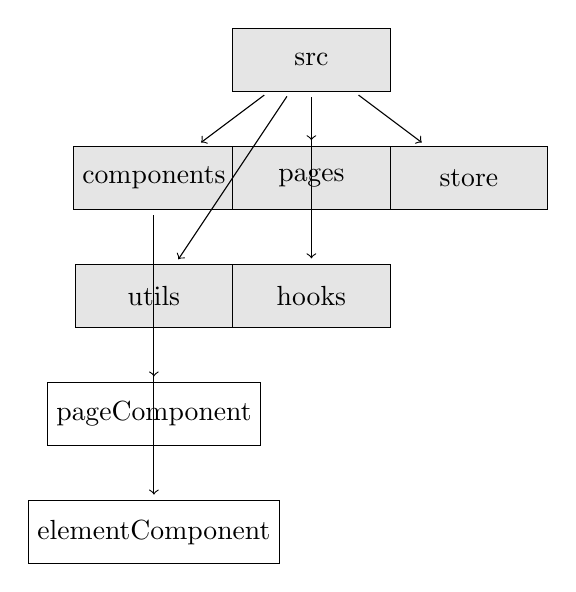
\begin{tikzpicture}[
    file/.style={draw, rectangle, minimum width=2cm, minimum height=0.8cm},
    folder/.style={draw, rectangle, minimum width=2cm, minimum height=0.8cm, fill=gray!20},
    arrow/.style={->, shorten >=2pt, shorten <=2pt}
]

% Folders
\node[folder] (src) at (0,0) {src};
\node[folder] (components) at (-2,-1.5) {components};
\node[folder] (pages) at (0,-1.5) {pages};
\node[folder] (store) at (2,-1.5) {store};
\node[folder] (utils) at (-2,-3) {utils};
\node[folder] (hooks) at (0,-3) {hooks};

% Files
\node[file] (pageComponent) at (-2,-4.5) {pageComponent};
\node[file] (elementComponent) at (-2,-6) {elementComponent};
% ... add more files

% Connections
\draw[arrow] (src) -- (components);
\draw[arrow] (src) -- (pages);
\draw[arrow] (src) -- (store);
\draw[arrow] (src) -- (utils);
\draw[arrow] (src) -- (hooks);
\draw[arrow] (components) -- (pageComponent);
\draw[arrow] (components) -- (elementComponent);
% ... add more connections

\end{tikzpicture}



\pagebreak
\subsubsection{Back-end}
The backend uses the dotNet framework. The development language using the C\# language.

In this project, the backend uses the Onion Architecture.
The Onion Architecture is a typically layered architecture, 
where each layer depends on the inner layer and provides interfaces to the outer layer.
The outer layer provides services to the outermost layer 
and other modules in the same layer based on the interfaces of the inner layer.

From inner to outer, the layers are: Domain, Application, Infrastructure, Presentation.
The Domain layer is the core layer and the innermost layer, used to define domain models, 
which are the business models.
It includes domain models and domain service interfaces.
Domain models are used to define the business models, 
which are the entities in the entity-relationship model and their attributes.
Domain service interfaces are used to define the business services, 
which are the relationships between entities in the entity-relationship model.

The Application layer is the application layer, 
used to define application services, which are the business logic.
It includes domain service implementations and application service interfaces.
Domain service implementations implement the methods of the inner layer's domain service 
interfaces and implement the business logic of the domain models.
Application service interfaces are used to define application services, 
which are the business logic.
It includes but is not limited to database interfaces, testing interfaces, 
HTTP API interfaces, MQTT interfaces, etc.

The Infrastructure layer is the infrastructure layer, used to define infrastructure.
It includes database implementations, testing implementations, 
HTTP API implementations, MQTT implementations, etc.
Database implementations implement the database interfaces 
and provide CRUD services for the database.
Testing implementations implement the testing interfaces 
and provide services for unit testing and integration testing.
HTTP API implementations implement the HTTP API interfaces 
and provide CRUD operations for HTTP APIs.
MQTT implementations implement the MQTT interfaces 
and provide CRUD operations for MQTT.

The Presentation layer is the presentation layer, used to define presentation logic, 
such as interfaces and pages. Since this is a backend project,
data presentation and control are handled by the frontend, 
so this layer is not needed.



\pagebreak
\subsubsection{Data communication and storage}
% 关于本项目的数据通信与数据存储的设计, 包括数据通信的协议, 数据存储的设计等
% 关于数据通信的设计:
% 1. 通信协议的选择
% 自前端向后端发送的数据, 有三种传输的数据类型, 
% 一种是普通的增删改查的请求, 对数据传输的时效性要求不高, 但是对数据的准确性, 完整性, 有序性, 安全性有一定的要求,
% 这种数据的传输, 采用 HTTP 协议, 以及 RESTful API 的设计. 可以有效的保证对数据传输的以上要求.
% 一种是对数据通道的创建和流媒体数据的传输, 对数据传输的时效性, 安全性要求较高, 这种数据的传输, 采用 WebRTC 协议, 以及 MQTT 协议.
% 配合可以快速解码的 flatbuffers 协议, 可以有效的保证对数据传输的以上要求.
% 最后一种是对设备的状态信息和操作信息的传输, 对完整性, 有序性, 安全性都有较高的要求, 这种数据的传输, 采用 MQTT 协议
% 同时也使用了 flatbuffers 协议.
% 
% 2. 数据通信的通信架构和通信流程
% 本项目的数据通信的通信架构, 是基于前后端分离的架构, 前端使用 React 框架, 后端使用 dotnet 框架.
% 当前端需要向后端发送数据的时候, 前端会向后端发送 HTTP 请求, 后端接收到 HTTP 请求之后, 会根据请求的数据类型,
% 选择不同的数据处理方式, 对于普通的增删改查的请求, 后端会根据 RESTful API 的设计, 对数据进行增删改查的操作,
% 对于对数据通道的创建和流媒体数据的传输, 后端会根据 WebRTC 协议, 对数据通道进行创建, 并且帮助前端和设备建立数据通道,
% 当数据通道建立后, 前端和设备之间则使用 flatbuffer 的数据格式对流媒体数据进行传输,
% 对于设备的状态信息和操作信息的传输, 前端会直接向 MQTT broker 发送 MQTT 请求, 
% 设备会在其自身的固件中监听相关的 MQTT 请求, 并且返回相关的数据.
% 
% 3. 数据通信的格式
% 本项目的数据通信的格式, 有三种, 
% 一种是 HTTP 协议, 
% 使用 json 格式对数据进行传输,
% 一种是 WebRTC 协议, 
% 使用 flatbuffers 格式对数据进行传输,
% 一种是 MQTT 协议.
% 使用 flatbuffers 格式对数据进行传输,
% 
% 关于数据存储的设计:
% 1. 数据存储的数据库的选择
% 本项目的数据存储的数据库的选择, 使用了轻量级的数据库 SQLite,
% SQLite 是一个进程内的库, 实现了自给自足的, 无服务器的, 零配置的, 事务性的 SQL 数据库引擎.
% 这是因为整个项目的目的是为了实现前端与设备之间的数据通信, 对于数据库数据的增删改查操作的要求不高,
% 数据量较小, 且对于数据库的数据的事务性要求不高, 所以选择了 SQLite 数据库.
% 2. 项目前后端的数据结构的设计
% 在本项目中, 前端由于使用了 React 框架, 所以前端的数据结构的设计, 使用了基于状态的数据结构的设计,
% 每个组件或者数据集都包含一个状态对象, 这个状态对象的属性就是组件的各个状态. 
% 使用状态对象的原因是, 可以方便的对状态进行管理, 采用对象-属性的形式, 可以方便的针对不同组件的同类状态进行区分,
% 由于跨组件的状态是由 redux 进行管理的, 这种状态对象的设计, 可以更搞笑的对状态进行更新和传递.
% 后端由于使用了 dotnet 框架, 所以后端的数据结构的设计, 使用了基于类的数据结构的设计,
% 采用了面向对象的编程思想, 对数据进行了封装, 使得数据的传输更加的安全, 有序, 完整.


\pagebreak

% \subsection{Domain model}
% \documentclass[]{article}
\usepackage{graphicx}
\usepackage{amsmath}
\usepackage{tikz}

% libaries
\usetikzlibrary{shapes,arrows}

%Define the listing package
\usepackage{listings} %code highlighter
\usepackage{color} %use color
\definecolor{mygreen}{rgb}{0,0.6,0}
\definecolor{mygray}{rgb}{0.5,0.5,0.5}
\definecolor{mymauve}{rgb}{0.58,0,0.82}

%Customize a bit the look
\lstset{ %
backgroundcolor=\color{white}, % choose the background color; you must add \usepackage{color} or \usepackage{xcolor}
basicstyle=\footnotesize, % the size of the fonts that are used for the code
breakatwhitespace=false, % sets if automatic breaks should only happen at whitespace
breaklines=true, % sets automatic line breaking
captionpos=b, % sets the caption-position to bottom
commentstyle=\color{mygreen}, % comment style
deletekeywords={...}, % if you want to delete keywords from the given language
escapeinside={\%*}{*)}, % if you want to add LaTeX within your code
extendedchars=true, % lets you use non-ASCII characters; for 8-bits encodings only, does not work with UTF-8
frame=single, % adds a frame around the code
keepspaces=true, % keeps spaces in text, useful for keeping indentation of code (possibly needs columns=flexible)
keywordstyle=\color{blue}, % keyword style
% language=Octave, % the language of the code
morekeywords={*,...}, % if you want to add more keywords to the set
numbers=left, % where to put the line-numbers; possible values are (none, left, right)
numbersep=5pt, % how far the line-numbers are from the code
numberstyle=\tiny\color{mygray}, % the style that is used for the line-numbers
rulecolor=\color{black}, % if not set, the frame-color may be changed on line-breaks within not-black text (e.g. comments (green here))
showspaces=false, % show spaces everywhere adding particular underscores; it overrides 'showstringspaces'
showstringspaces=false, % underline spaces within strings only
showtabs=false, % show tabs within strings adding particular underscores
stepnumber=1, % the step between two line-numbers. If it's 1, each line will be numbered
stringstyle=\color{mymauve}, % string literal style
tabsize=2, % sets default tabsize to 2 spaces
title=\lstname % show the filename of files included with \lstinputlisting; also try caption instead of title
}

\definecolor{darkgray}{rgb}{.4,.4,.4}
\definecolor{purple}{rgb}{0.65, 0.12, 0.82}

\lstdefinelanguage{React}{
keywords={const, typeof, new, true, false, catch, function, return, null, catch, switch, var, if, in, while, do, else, case, break},
keywordstyle=\color{blue}\bfseries,
ndkeywords={class, export, boolean, throw, implements, import, this},
ndkeywordstyle=\color{darkgray}\bfseries,
identifierstyle=\color{mygreen},
sensitive=false,
comment=[l]{//},
morecomment=[s]{/*}{*/},
commentstyle=\color{purple}\ttfamily,
string=[b]{"}{'}{`},
stringstyle=\color{red}\ttfamily,
morestring=[b]',
morestring=[b]",
morestring=[b]`',
}

\lstdefinelanguage{CSharp}{
keywords={const, typeof, new, true, false, catch, function, return, null, catch, switch, var, if, in, while, do, else, case, break},
keywordstyle=\color{blue}\bfseries,
ndkeywords={class, export, boolean, throw, implements, import, this},
ndkeywordstyle=\color{darkgray}\bfseries,
identifierstyle=\color{mygreen},
sensitive=false,
comment=[l]{//},
morecomment=[s]{/*}{*/},
commentstyle=\color{purple}\ttfamily,
string=[b]{"}{'}{`},
stringstyle=\color{red}\ttfamily,
morestring=[b]',
morestring=[b]",
morestring=[b]`',
}

\lstset{
language=React,
extendedchars=true,
basicstyle=\footnotesize\ttfamily,
showstringspaces=false,
showspaces=false,
numbers=left,
numberstyle=\footnotesize,
numbersep=9pt,
tabsize=2,
breaklines=true,
showtabs=false,
captionpos=b
}

\lstset{
language=CSharp,
extendedchars=true,
basicstyle=\footnotesize\ttfamily,
showstringspaces=false,
showspaces=false,
numbers=left,
numberstyle=\footnotesize,
numbersep=9pt,
tabsize=2,
breaklines=true,
showtabs=false,
captionpos=b
}

% \usepackage{cite} % Add this line for citation

% \bibliographystyle{plain}

\title{
The implementation of BifrostConnect Front-end scope, 
re-design and development with the relevant back-end support develop.
}
\author{
    Fei Gu \\
    Erhvervs Akademi Sydvest \\
    Computer Science 21\\
    }
\date{\today}

\begin{document}

% Front page
\maketitle
\begin{center}
    Supervisor: Henrik Boulund Meng Hansen \\
    Company: BifrostConnect \\
    Engineering Director: Jasper Wass \\
\end{center}
\tableofcontents
\pagebreak


% The introduction
\section{Introduction}
\subsection{Background}\input{sections/introduction/background.tex}
\subsection{The company}\input{sections/introduction/aboutCompany}
\subsection{The project}\input{sections/introduction/aboutProject}
\pagebreak

% The problem statement
\section{Problem Statement}
\subsection{Statement}
\input{sections/problemStatement/statement}
\subsection{Situation}
\input{sections/problemStatement/situation}
\subsection{Potential Solution}
\input{sections/problemStatement/potentialSolution}
\pagebreak

% Requirement analysis
\section{Requirement Analysis}
\input{sections/requirementAnalysis/index}

\subsection{Stakeholders}
\input{sections/requirementAnalysis/stakeholders/index}

\subsection{Business Domain}
\input{sections/requirementAnalysis/bussinesDomain/index}

\subsection{Scope}
\input{sections/requirementAnalysis/scope}

\subsection{Goals}
\input{sections/requirementAnalysis/goals}
\pagebreak

% Software Design
\section{Software Design}
% developement methods
\subsection{Software Development Methods}
\input{sections/softwareDevelopmentMethods/index}
\subsubsection{Agile Software Development}
\input{sections/softwareDevelopmentMethods/agileSoftwareDevelopment/index}
\subsubsection{Feature Driven Development}
\input{sections/softwareDevelopmentMethods/featureDrivenDevelopment/index}

\pagebreak

% Technology seslection
\subsection{Technology selection}
\input{sections/softwareDesign/technologySelection/index}
\subsubsection{Front-end}
\input{sections/softwareDesign/technologySelection/frontEnd}            
\subsubsection{Back-end}
\input{sections/softwareDesign/technologySelection/backEnd}            
\subsubsection{Database}
\input{sections/softwareDesign/technologySelection/database}
\subsubsection{Data communication}
\input{sections/softwareDesign/technologySelection/dataCommunication}            
\subsubsection{DevOps}
\input{sections/softwareDesign/technologySelection/devOps}
\pagebreak

% Architecture design
\subsection{Architecture design}
\input{sections/softwareDesign/architectureDesign/index}
\pagebreak
\subsubsection{Front-end}
\input{sections/softwareDesign/architectureDesign/frontEndArchitecture}
\pagebreak
\subsubsection{Back-end}
\input{sections/softwareDesign/architectureDesign/backEndArchitecture}
\pagebreak
\subsubsection{Data communication and storage}
\input{sections/softwareDesign/architectureDesign/dataCommunicationArchitecture}
\pagebreak

% \subsection{Domain model}
% \input{sections/softwareDesign/domainModel/index}
% \subsection{Database design}
% % 数据库领域模型 ER 图
% % 包括表和字段的设置.
% % 对于私有键和外键的设置.

% \subsection{Back-end design}
% % 后端对象模型
% % 以及对于对象模型的增删改查
% % 以及相关的其他服务的设计`'

% \subsection{Front-end design}
% % 对于前端的页面结构的设计 
% % 页面的状态的设计, 交互设计

% \subsection{FlatBuffers design}
% % schema 的设计

\subsection{DevOps CI/CD process design}
\input{sections/softwareDesign/devOpsDesign/index}
\subsubsection{Continuous Integration}
\input{sections/softwareDesign/devOpsDesign/continuousIntegration/index}
\subsubsection{Continuous Delivery}
\input{sections/softwareDesign/devOpsDesign/continuousDelivery/index}
\subsubsection{Continuous Deployment}
\input{sections/softwareDesign/devOpsDesign/continuousDeployment/index}
\pagebreak

\section{Software Development} 
\input{sections/softwareDevelopment/index}
\subsection{Overall development}
\input{sections/softwareDevelopment/overallDevelopement/index}
\subsubsection{Front-end}
\input{sections/softwareDevelopment/overallDevelopement/frontEnd/index}
\subsubsection{Back-end}
\input{sections/softwareDevelopment/overallDevelopement/backEnd/index}
\subsubsection{DevOps}
\input{sections/softwareDevelopment/overallDevelopement/devOps/index}
\subsection{Feature development} 
\input{sections/softwareDevelopment/featureDevelopment/index}
\subsubsection{Use Case 1}
\input{sections/softwareDevelopment/featureDevelopment/useCase1/index}
\subsubsection{Feature 1}
\input{sections/softwareDevelopment/featureDevelopment/feature/feature1.tex}
\pagebreak
\section{Conclusion} 
\subsection{Result}
Since the project is still in progress, the result is not available yet.
So far, basic structure of this project has been built. But the most features 
are not implemented yet. 
\subsection{Discussion}
As a single developer for this project, I am confident what I have done so far.
And I can say I understand the most of the knowledge I have used in this project, 
which also means I can explain all the part of the project. 
But this project also relevant some of the complex knowledge which I have to continue 
to study and practice.
\subsection{Future Work}
The future work is to implement the rest of the features. 
Including the most important part which is the 'create session' feature.
\pagebreak
% \bibliography{bibliography}
\pagebreak
% \begin{appendices}
%     \section{Appendix}
% \end{appendices} 
\end{document}
% \subsection{Database design}
% % 数据库领域模型 ER 图
% % 包括表和字段的设置.
% % 对于私有键和外键的设置.

% \subsection{Back-end design}
% % 后端对象模型
% % 以及对于对象模型的增删改查
% % 以及相关的其他服务的设计`'

% \subsection{Front-end design}
% % 对于前端的页面结构的设计 
% % 页面的状态的设计, 交互设计

% \subsection{FlatBuffers design}
% % schema 的设计

\subsection{DevOps CI/CD process design}
\documentclass[]{article}
\usepackage{graphicx}
\usepackage{amsmath}
\usepackage{tikz}

% libaries
\usetikzlibrary{shapes,arrows}

%Define the listing package
\usepackage{listings} %code highlighter
\usepackage{color} %use color
\definecolor{mygreen}{rgb}{0,0.6,0}
\definecolor{mygray}{rgb}{0.5,0.5,0.5}
\definecolor{mymauve}{rgb}{0.58,0,0.82}

%Customize a bit the look
\lstset{ %
backgroundcolor=\color{white}, % choose the background color; you must add \usepackage{color} or \usepackage{xcolor}
basicstyle=\footnotesize, % the size of the fonts that are used for the code
breakatwhitespace=false, % sets if automatic breaks should only happen at whitespace
breaklines=true, % sets automatic line breaking
captionpos=b, % sets the caption-position to bottom
commentstyle=\color{mygreen}, % comment style
deletekeywords={...}, % if you want to delete keywords from the given language
escapeinside={\%*}{*)}, % if you want to add LaTeX within your code
extendedchars=true, % lets you use non-ASCII characters; for 8-bits encodings only, does not work with UTF-8
frame=single, % adds a frame around the code
keepspaces=true, % keeps spaces in text, useful for keeping indentation of code (possibly needs columns=flexible)
keywordstyle=\color{blue}, % keyword style
% language=Octave, % the language of the code
morekeywords={*,...}, % if you want to add more keywords to the set
numbers=left, % where to put the line-numbers; possible values are (none, left, right)
numbersep=5pt, % how far the line-numbers are from the code
numberstyle=\tiny\color{mygray}, % the style that is used for the line-numbers
rulecolor=\color{black}, % if not set, the frame-color may be changed on line-breaks within not-black text (e.g. comments (green here))
showspaces=false, % show spaces everywhere adding particular underscores; it overrides 'showstringspaces'
showstringspaces=false, % underline spaces within strings only
showtabs=false, % show tabs within strings adding particular underscores
stepnumber=1, % the step between two line-numbers. If it's 1, each line will be numbered
stringstyle=\color{mymauve}, % string literal style
tabsize=2, % sets default tabsize to 2 spaces
title=\lstname % show the filename of files included with \lstinputlisting; also try caption instead of title
}

\definecolor{darkgray}{rgb}{.4,.4,.4}
\definecolor{purple}{rgb}{0.65, 0.12, 0.82}

\lstdefinelanguage{React}{
keywords={const, typeof, new, true, false, catch, function, return, null, catch, switch, var, if, in, while, do, else, case, break},
keywordstyle=\color{blue}\bfseries,
ndkeywords={class, export, boolean, throw, implements, import, this},
ndkeywordstyle=\color{darkgray}\bfseries,
identifierstyle=\color{mygreen},
sensitive=false,
comment=[l]{//},
morecomment=[s]{/*}{*/},
commentstyle=\color{purple}\ttfamily,
string=[b]{"}{'}{`},
stringstyle=\color{red}\ttfamily,
morestring=[b]',
morestring=[b]",
morestring=[b]`',
}

\lstdefinelanguage{CSharp}{
keywords={const, typeof, new, true, false, catch, function, return, null, catch, switch, var, if, in, while, do, else, case, break},
keywordstyle=\color{blue}\bfseries,
ndkeywords={class, export, boolean, throw, implements, import, this},
ndkeywordstyle=\color{darkgray}\bfseries,
identifierstyle=\color{mygreen},
sensitive=false,
comment=[l]{//},
morecomment=[s]{/*}{*/},
commentstyle=\color{purple}\ttfamily,
string=[b]{"}{'}{`},
stringstyle=\color{red}\ttfamily,
morestring=[b]',
morestring=[b]",
morestring=[b]`',
}

\lstset{
language=React,
extendedchars=true,
basicstyle=\footnotesize\ttfamily,
showstringspaces=false,
showspaces=false,
numbers=left,
numberstyle=\footnotesize,
numbersep=9pt,
tabsize=2,
breaklines=true,
showtabs=false,
captionpos=b
}

\lstset{
language=CSharp,
extendedchars=true,
basicstyle=\footnotesize\ttfamily,
showstringspaces=false,
showspaces=false,
numbers=left,
numberstyle=\footnotesize,
numbersep=9pt,
tabsize=2,
breaklines=true,
showtabs=false,
captionpos=b
}

% \usepackage{cite} % Add this line for citation

% \bibliographystyle{plain}

\title{
The implementation of BifrostConnect Front-end scope, 
re-design and development with the relevant back-end support develop.
}
\author{
    Fei Gu \\
    Erhvervs Akademi Sydvest \\
    Computer Science 21\\
    }
\date{\today}

\begin{document}

% Front page
\maketitle
\begin{center}
    Supervisor: Henrik Boulund Meng Hansen \\
    Company: BifrostConnect \\
    Engineering Director: Jasper Wass \\
\end{center}
\tableofcontents
\pagebreak


% The introduction
\section{Introduction}
\subsection{Background}\input{sections/introduction/background.tex}
\subsection{The company}\input{sections/introduction/aboutCompany}
\subsection{The project}\input{sections/introduction/aboutProject}
\pagebreak

% The problem statement
\section{Problem Statement}
\subsection{Statement}
\input{sections/problemStatement/statement}
\subsection{Situation}
\input{sections/problemStatement/situation}
\subsection{Potential Solution}
\input{sections/problemStatement/potentialSolution}
\pagebreak

% Requirement analysis
\section{Requirement Analysis}
\input{sections/requirementAnalysis/index}

\subsection{Stakeholders}
\input{sections/requirementAnalysis/stakeholders/index}

\subsection{Business Domain}
\input{sections/requirementAnalysis/bussinesDomain/index}

\subsection{Scope}
\input{sections/requirementAnalysis/scope}

\subsection{Goals}
\input{sections/requirementAnalysis/goals}
\pagebreak

% Software Design
\section{Software Design}
% developement methods
\subsection{Software Development Methods}
\input{sections/softwareDevelopmentMethods/index}
\subsubsection{Agile Software Development}
\input{sections/softwareDevelopmentMethods/agileSoftwareDevelopment/index}
\subsubsection{Feature Driven Development}
\input{sections/softwareDevelopmentMethods/featureDrivenDevelopment/index}

\pagebreak

% Technology seslection
\subsection{Technology selection}
\input{sections/softwareDesign/technologySelection/index}
\subsubsection{Front-end}
\input{sections/softwareDesign/technologySelection/frontEnd}            
\subsubsection{Back-end}
\input{sections/softwareDesign/technologySelection/backEnd}            
\subsubsection{Database}
\input{sections/softwareDesign/technologySelection/database}
\subsubsection{Data communication}
\input{sections/softwareDesign/technologySelection/dataCommunication}            
\subsubsection{DevOps}
\input{sections/softwareDesign/technologySelection/devOps}
\pagebreak

% Architecture design
\subsection{Architecture design}
\input{sections/softwareDesign/architectureDesign/index}
\pagebreak
\subsubsection{Front-end}
\input{sections/softwareDesign/architectureDesign/frontEndArchitecture}
\pagebreak
\subsubsection{Back-end}
\input{sections/softwareDesign/architectureDesign/backEndArchitecture}
\pagebreak
\subsubsection{Data communication and storage}
\input{sections/softwareDesign/architectureDesign/dataCommunicationArchitecture}
\pagebreak

% \subsection{Domain model}
% \input{sections/softwareDesign/domainModel/index}
% \subsection{Database design}
% % 数据库领域模型 ER 图
% % 包括表和字段的设置.
% % 对于私有键和外键的设置.

% \subsection{Back-end design}
% % 后端对象模型
% % 以及对于对象模型的增删改查
% % 以及相关的其他服务的设计`'

% \subsection{Front-end design}
% % 对于前端的页面结构的设计 
% % 页面的状态的设计, 交互设计

% \subsection{FlatBuffers design}
% % schema 的设计

\subsection{DevOps CI/CD process design}
\input{sections/softwareDesign/devOpsDesign/index}
\subsubsection{Continuous Integration}
\input{sections/softwareDesign/devOpsDesign/continuousIntegration/index}
\subsubsection{Continuous Delivery}
\input{sections/softwareDesign/devOpsDesign/continuousDelivery/index}
\subsubsection{Continuous Deployment}
\input{sections/softwareDesign/devOpsDesign/continuousDeployment/index}
\pagebreak

\section{Software Development} 
\input{sections/softwareDevelopment/index}
\subsection{Overall development}
\input{sections/softwareDevelopment/overallDevelopement/index}
\subsubsection{Front-end}
\input{sections/softwareDevelopment/overallDevelopement/frontEnd/index}
\subsubsection{Back-end}
\input{sections/softwareDevelopment/overallDevelopement/backEnd/index}
\subsubsection{DevOps}
\input{sections/softwareDevelopment/overallDevelopement/devOps/index}
\subsection{Feature development} 
\input{sections/softwareDevelopment/featureDevelopment/index}
\subsubsection{Use Case 1}
\input{sections/softwareDevelopment/featureDevelopment/useCase1/index}
\subsubsection{Feature 1}
\input{sections/softwareDevelopment/featureDevelopment/feature/feature1.tex}
\pagebreak
\section{Conclusion} 
\subsection{Result}
Since the project is still in progress, the result is not available yet.
So far, basic structure of this project has been built. But the most features 
are not implemented yet. 
\subsection{Discussion}
As a single developer for this project, I am confident what I have done so far.
And I can say I understand the most of the knowledge I have used in this project, 
which also means I can explain all the part of the project. 
But this project also relevant some of the complex knowledge which I have to continue 
to study and practice.
\subsection{Future Work}
The future work is to implement the rest of the features. 
Including the most important part which is the 'create session' feature.
\pagebreak
% \bibliography{bibliography}
\pagebreak
% \begin{appendices}
%     \section{Appendix}
% \end{appendices} 
\end{document}
\subsubsection{Continuous Integration}
\documentclass[]{article}
\usepackage{graphicx}
\usepackage{amsmath}
\usepackage{tikz}

% libaries
\usetikzlibrary{shapes,arrows}

%Define the listing package
\usepackage{listings} %code highlighter
\usepackage{color} %use color
\definecolor{mygreen}{rgb}{0,0.6,0}
\definecolor{mygray}{rgb}{0.5,0.5,0.5}
\definecolor{mymauve}{rgb}{0.58,0,0.82}

%Customize a bit the look
\lstset{ %
backgroundcolor=\color{white}, % choose the background color; you must add \usepackage{color} or \usepackage{xcolor}
basicstyle=\footnotesize, % the size of the fonts that are used for the code
breakatwhitespace=false, % sets if automatic breaks should only happen at whitespace
breaklines=true, % sets automatic line breaking
captionpos=b, % sets the caption-position to bottom
commentstyle=\color{mygreen}, % comment style
deletekeywords={...}, % if you want to delete keywords from the given language
escapeinside={\%*}{*)}, % if you want to add LaTeX within your code
extendedchars=true, % lets you use non-ASCII characters; for 8-bits encodings only, does not work with UTF-8
frame=single, % adds a frame around the code
keepspaces=true, % keeps spaces in text, useful for keeping indentation of code (possibly needs columns=flexible)
keywordstyle=\color{blue}, % keyword style
% language=Octave, % the language of the code
morekeywords={*,...}, % if you want to add more keywords to the set
numbers=left, % where to put the line-numbers; possible values are (none, left, right)
numbersep=5pt, % how far the line-numbers are from the code
numberstyle=\tiny\color{mygray}, % the style that is used for the line-numbers
rulecolor=\color{black}, % if not set, the frame-color may be changed on line-breaks within not-black text (e.g. comments (green here))
showspaces=false, % show spaces everywhere adding particular underscores; it overrides 'showstringspaces'
showstringspaces=false, % underline spaces within strings only
showtabs=false, % show tabs within strings adding particular underscores
stepnumber=1, % the step between two line-numbers. If it's 1, each line will be numbered
stringstyle=\color{mymauve}, % string literal style
tabsize=2, % sets default tabsize to 2 spaces
title=\lstname % show the filename of files included with \lstinputlisting; also try caption instead of title
}

\definecolor{darkgray}{rgb}{.4,.4,.4}
\definecolor{purple}{rgb}{0.65, 0.12, 0.82}

\lstdefinelanguage{React}{
keywords={const, typeof, new, true, false, catch, function, return, null, catch, switch, var, if, in, while, do, else, case, break},
keywordstyle=\color{blue}\bfseries,
ndkeywords={class, export, boolean, throw, implements, import, this},
ndkeywordstyle=\color{darkgray}\bfseries,
identifierstyle=\color{mygreen},
sensitive=false,
comment=[l]{//},
morecomment=[s]{/*}{*/},
commentstyle=\color{purple}\ttfamily,
string=[b]{"}{'}{`},
stringstyle=\color{red}\ttfamily,
morestring=[b]',
morestring=[b]",
morestring=[b]`',
}

\lstdefinelanguage{CSharp}{
keywords={const, typeof, new, true, false, catch, function, return, null, catch, switch, var, if, in, while, do, else, case, break},
keywordstyle=\color{blue}\bfseries,
ndkeywords={class, export, boolean, throw, implements, import, this},
ndkeywordstyle=\color{darkgray}\bfseries,
identifierstyle=\color{mygreen},
sensitive=false,
comment=[l]{//},
morecomment=[s]{/*}{*/},
commentstyle=\color{purple}\ttfamily,
string=[b]{"}{'}{`},
stringstyle=\color{red}\ttfamily,
morestring=[b]',
morestring=[b]",
morestring=[b]`',
}

\lstset{
language=React,
extendedchars=true,
basicstyle=\footnotesize\ttfamily,
showstringspaces=false,
showspaces=false,
numbers=left,
numberstyle=\footnotesize,
numbersep=9pt,
tabsize=2,
breaklines=true,
showtabs=false,
captionpos=b
}

\lstset{
language=CSharp,
extendedchars=true,
basicstyle=\footnotesize\ttfamily,
showstringspaces=false,
showspaces=false,
numbers=left,
numberstyle=\footnotesize,
numbersep=9pt,
tabsize=2,
breaklines=true,
showtabs=false,
captionpos=b
}

% \usepackage{cite} % Add this line for citation

% \bibliographystyle{plain}

\title{
The implementation of BifrostConnect Front-end scope, 
re-design and development with the relevant back-end support develop.
}
\author{
    Fei Gu \\
    Erhvervs Akademi Sydvest \\
    Computer Science 21\\
    }
\date{\today}

\begin{document}

% Front page
\maketitle
\begin{center}
    Supervisor: Henrik Boulund Meng Hansen \\
    Company: BifrostConnect \\
    Engineering Director: Jasper Wass \\
\end{center}
\tableofcontents
\pagebreak


% The introduction
\section{Introduction}
\subsection{Background}\input{sections/introduction/background.tex}
\subsection{The company}\input{sections/introduction/aboutCompany}
\subsection{The project}\input{sections/introduction/aboutProject}
\pagebreak

% The problem statement
\section{Problem Statement}
\subsection{Statement}
\input{sections/problemStatement/statement}
\subsection{Situation}
\input{sections/problemStatement/situation}
\subsection{Potential Solution}
\input{sections/problemStatement/potentialSolution}
\pagebreak

% Requirement analysis
\section{Requirement Analysis}
\input{sections/requirementAnalysis/index}

\subsection{Stakeholders}
\input{sections/requirementAnalysis/stakeholders/index}

\subsection{Business Domain}
\input{sections/requirementAnalysis/bussinesDomain/index}

\subsection{Scope}
\input{sections/requirementAnalysis/scope}

\subsection{Goals}
\input{sections/requirementAnalysis/goals}
\pagebreak

% Software Design
\section{Software Design}
% developement methods
\subsection{Software Development Methods}
\input{sections/softwareDevelopmentMethods/index}
\subsubsection{Agile Software Development}
\input{sections/softwareDevelopmentMethods/agileSoftwareDevelopment/index}
\subsubsection{Feature Driven Development}
\input{sections/softwareDevelopmentMethods/featureDrivenDevelopment/index}

\pagebreak

% Technology seslection
\subsection{Technology selection}
\input{sections/softwareDesign/technologySelection/index}
\subsubsection{Front-end}
\input{sections/softwareDesign/technologySelection/frontEnd}            
\subsubsection{Back-end}
\input{sections/softwareDesign/technologySelection/backEnd}            
\subsubsection{Database}
\input{sections/softwareDesign/technologySelection/database}
\subsubsection{Data communication}
\input{sections/softwareDesign/technologySelection/dataCommunication}            
\subsubsection{DevOps}
\input{sections/softwareDesign/technologySelection/devOps}
\pagebreak

% Architecture design
\subsection{Architecture design}
\input{sections/softwareDesign/architectureDesign/index}
\pagebreak
\subsubsection{Front-end}
\input{sections/softwareDesign/architectureDesign/frontEndArchitecture}
\pagebreak
\subsubsection{Back-end}
\input{sections/softwareDesign/architectureDesign/backEndArchitecture}
\pagebreak
\subsubsection{Data communication and storage}
\input{sections/softwareDesign/architectureDesign/dataCommunicationArchitecture}
\pagebreak

% \subsection{Domain model}
% \input{sections/softwareDesign/domainModel/index}
% \subsection{Database design}
% % 数据库领域模型 ER 图
% % 包括表和字段的设置.
% % 对于私有键和外键的设置.

% \subsection{Back-end design}
% % 后端对象模型
% % 以及对于对象模型的增删改查
% % 以及相关的其他服务的设计`'

% \subsection{Front-end design}
% % 对于前端的页面结构的设计 
% % 页面的状态的设计, 交互设计

% \subsection{FlatBuffers design}
% % schema 的设计

\subsection{DevOps CI/CD process design}
\input{sections/softwareDesign/devOpsDesign/index}
\subsubsection{Continuous Integration}
\input{sections/softwareDesign/devOpsDesign/continuousIntegration/index}
\subsubsection{Continuous Delivery}
\input{sections/softwareDesign/devOpsDesign/continuousDelivery/index}
\subsubsection{Continuous Deployment}
\input{sections/softwareDesign/devOpsDesign/continuousDeployment/index}
\pagebreak

\section{Software Development} 
\input{sections/softwareDevelopment/index}
\subsection{Overall development}
\input{sections/softwareDevelopment/overallDevelopement/index}
\subsubsection{Front-end}
\input{sections/softwareDevelopment/overallDevelopement/frontEnd/index}
\subsubsection{Back-end}
\input{sections/softwareDevelopment/overallDevelopement/backEnd/index}
\subsubsection{DevOps}
\input{sections/softwareDevelopment/overallDevelopement/devOps/index}
\subsection{Feature development} 
\input{sections/softwareDevelopment/featureDevelopment/index}
\subsubsection{Use Case 1}
\input{sections/softwareDevelopment/featureDevelopment/useCase1/index}
\subsubsection{Feature 1}
\input{sections/softwareDevelopment/featureDevelopment/feature/feature1.tex}
\pagebreak
\section{Conclusion} 
\subsection{Result}
Since the project is still in progress, the result is not available yet.
So far, basic structure of this project has been built. But the most features 
are not implemented yet. 
\subsection{Discussion}
As a single developer for this project, I am confident what I have done so far.
And I can say I understand the most of the knowledge I have used in this project, 
which also means I can explain all the part of the project. 
But this project also relevant some of the complex knowledge which I have to continue 
to study and practice.
\subsection{Future Work}
The future work is to implement the rest of the features. 
Including the most important part which is the 'create session' feature.
\pagebreak
% \bibliography{bibliography}
\pagebreak
% \begin{appendices}
%     \section{Appendix}
% \end{appendices} 
\end{document}
\subsubsection{Continuous Delivery}
\documentclass[]{article}
\usepackage{graphicx}
\usepackage{amsmath}
\usepackage{tikz}

% libaries
\usetikzlibrary{shapes,arrows}

%Define the listing package
\usepackage{listings} %code highlighter
\usepackage{color} %use color
\definecolor{mygreen}{rgb}{0,0.6,0}
\definecolor{mygray}{rgb}{0.5,0.5,0.5}
\definecolor{mymauve}{rgb}{0.58,0,0.82}

%Customize a bit the look
\lstset{ %
backgroundcolor=\color{white}, % choose the background color; you must add \usepackage{color} or \usepackage{xcolor}
basicstyle=\footnotesize, % the size of the fonts that are used for the code
breakatwhitespace=false, % sets if automatic breaks should only happen at whitespace
breaklines=true, % sets automatic line breaking
captionpos=b, % sets the caption-position to bottom
commentstyle=\color{mygreen}, % comment style
deletekeywords={...}, % if you want to delete keywords from the given language
escapeinside={\%*}{*)}, % if you want to add LaTeX within your code
extendedchars=true, % lets you use non-ASCII characters; for 8-bits encodings only, does not work with UTF-8
frame=single, % adds a frame around the code
keepspaces=true, % keeps spaces in text, useful for keeping indentation of code (possibly needs columns=flexible)
keywordstyle=\color{blue}, % keyword style
% language=Octave, % the language of the code
morekeywords={*,...}, % if you want to add more keywords to the set
numbers=left, % where to put the line-numbers; possible values are (none, left, right)
numbersep=5pt, % how far the line-numbers are from the code
numberstyle=\tiny\color{mygray}, % the style that is used for the line-numbers
rulecolor=\color{black}, % if not set, the frame-color may be changed on line-breaks within not-black text (e.g. comments (green here))
showspaces=false, % show spaces everywhere adding particular underscores; it overrides 'showstringspaces'
showstringspaces=false, % underline spaces within strings only
showtabs=false, % show tabs within strings adding particular underscores
stepnumber=1, % the step between two line-numbers. If it's 1, each line will be numbered
stringstyle=\color{mymauve}, % string literal style
tabsize=2, % sets default tabsize to 2 spaces
title=\lstname % show the filename of files included with \lstinputlisting; also try caption instead of title
}

\definecolor{darkgray}{rgb}{.4,.4,.4}
\definecolor{purple}{rgb}{0.65, 0.12, 0.82}

\lstdefinelanguage{React}{
keywords={const, typeof, new, true, false, catch, function, return, null, catch, switch, var, if, in, while, do, else, case, break},
keywordstyle=\color{blue}\bfseries,
ndkeywords={class, export, boolean, throw, implements, import, this},
ndkeywordstyle=\color{darkgray}\bfseries,
identifierstyle=\color{mygreen},
sensitive=false,
comment=[l]{//},
morecomment=[s]{/*}{*/},
commentstyle=\color{purple}\ttfamily,
string=[b]{"}{'}{`},
stringstyle=\color{red}\ttfamily,
morestring=[b]',
morestring=[b]",
morestring=[b]`',
}

\lstdefinelanguage{CSharp}{
keywords={const, typeof, new, true, false, catch, function, return, null, catch, switch, var, if, in, while, do, else, case, break},
keywordstyle=\color{blue}\bfseries,
ndkeywords={class, export, boolean, throw, implements, import, this},
ndkeywordstyle=\color{darkgray}\bfseries,
identifierstyle=\color{mygreen},
sensitive=false,
comment=[l]{//},
morecomment=[s]{/*}{*/},
commentstyle=\color{purple}\ttfamily,
string=[b]{"}{'}{`},
stringstyle=\color{red}\ttfamily,
morestring=[b]',
morestring=[b]",
morestring=[b]`',
}

\lstset{
language=React,
extendedchars=true,
basicstyle=\footnotesize\ttfamily,
showstringspaces=false,
showspaces=false,
numbers=left,
numberstyle=\footnotesize,
numbersep=9pt,
tabsize=2,
breaklines=true,
showtabs=false,
captionpos=b
}

\lstset{
language=CSharp,
extendedchars=true,
basicstyle=\footnotesize\ttfamily,
showstringspaces=false,
showspaces=false,
numbers=left,
numberstyle=\footnotesize,
numbersep=9pt,
tabsize=2,
breaklines=true,
showtabs=false,
captionpos=b
}

% \usepackage{cite} % Add this line for citation

% \bibliographystyle{plain}

\title{
The implementation of BifrostConnect Front-end scope, 
re-design and development with the relevant back-end support develop.
}
\author{
    Fei Gu \\
    Erhvervs Akademi Sydvest \\
    Computer Science 21\\
    }
\date{\today}

\begin{document}

% Front page
\maketitle
\begin{center}
    Supervisor: Henrik Boulund Meng Hansen \\
    Company: BifrostConnect \\
    Engineering Director: Jasper Wass \\
\end{center}
\tableofcontents
\pagebreak


% The introduction
\section{Introduction}
\subsection{Background}\input{sections/introduction/background.tex}
\subsection{The company}\input{sections/introduction/aboutCompany}
\subsection{The project}\input{sections/introduction/aboutProject}
\pagebreak

% The problem statement
\section{Problem Statement}
\subsection{Statement}
\input{sections/problemStatement/statement}
\subsection{Situation}
\input{sections/problemStatement/situation}
\subsection{Potential Solution}
\input{sections/problemStatement/potentialSolution}
\pagebreak

% Requirement analysis
\section{Requirement Analysis}
\input{sections/requirementAnalysis/index}

\subsection{Stakeholders}
\input{sections/requirementAnalysis/stakeholders/index}

\subsection{Business Domain}
\input{sections/requirementAnalysis/bussinesDomain/index}

\subsection{Scope}
\input{sections/requirementAnalysis/scope}

\subsection{Goals}
\input{sections/requirementAnalysis/goals}
\pagebreak

% Software Design
\section{Software Design}
% developement methods
\subsection{Software Development Methods}
\input{sections/softwareDevelopmentMethods/index}
\subsubsection{Agile Software Development}
\input{sections/softwareDevelopmentMethods/agileSoftwareDevelopment/index}
\subsubsection{Feature Driven Development}
\input{sections/softwareDevelopmentMethods/featureDrivenDevelopment/index}

\pagebreak

% Technology seslection
\subsection{Technology selection}
\input{sections/softwareDesign/technologySelection/index}
\subsubsection{Front-end}
\input{sections/softwareDesign/technologySelection/frontEnd}            
\subsubsection{Back-end}
\input{sections/softwareDesign/technologySelection/backEnd}            
\subsubsection{Database}
\input{sections/softwareDesign/technologySelection/database}
\subsubsection{Data communication}
\input{sections/softwareDesign/technologySelection/dataCommunication}            
\subsubsection{DevOps}
\input{sections/softwareDesign/technologySelection/devOps}
\pagebreak

% Architecture design
\subsection{Architecture design}
\input{sections/softwareDesign/architectureDesign/index}
\pagebreak
\subsubsection{Front-end}
\input{sections/softwareDesign/architectureDesign/frontEndArchitecture}
\pagebreak
\subsubsection{Back-end}
\input{sections/softwareDesign/architectureDesign/backEndArchitecture}
\pagebreak
\subsubsection{Data communication and storage}
\input{sections/softwareDesign/architectureDesign/dataCommunicationArchitecture}
\pagebreak

% \subsection{Domain model}
% \input{sections/softwareDesign/domainModel/index}
% \subsection{Database design}
% % 数据库领域模型 ER 图
% % 包括表和字段的设置.
% % 对于私有键和外键的设置.

% \subsection{Back-end design}
% % 后端对象模型
% % 以及对于对象模型的增删改查
% % 以及相关的其他服务的设计`'

% \subsection{Front-end design}
% % 对于前端的页面结构的设计 
% % 页面的状态的设计, 交互设计

% \subsection{FlatBuffers design}
% % schema 的设计

\subsection{DevOps CI/CD process design}
\input{sections/softwareDesign/devOpsDesign/index}
\subsubsection{Continuous Integration}
\input{sections/softwareDesign/devOpsDesign/continuousIntegration/index}
\subsubsection{Continuous Delivery}
\input{sections/softwareDesign/devOpsDesign/continuousDelivery/index}
\subsubsection{Continuous Deployment}
\input{sections/softwareDesign/devOpsDesign/continuousDeployment/index}
\pagebreak

\section{Software Development} 
\input{sections/softwareDevelopment/index}
\subsection{Overall development}
\input{sections/softwareDevelopment/overallDevelopement/index}
\subsubsection{Front-end}
\input{sections/softwareDevelopment/overallDevelopement/frontEnd/index}
\subsubsection{Back-end}
\input{sections/softwareDevelopment/overallDevelopement/backEnd/index}
\subsubsection{DevOps}
\input{sections/softwareDevelopment/overallDevelopement/devOps/index}
\subsection{Feature development} 
\input{sections/softwareDevelopment/featureDevelopment/index}
\subsubsection{Use Case 1}
\input{sections/softwareDevelopment/featureDevelopment/useCase1/index}
\subsubsection{Feature 1}
\input{sections/softwareDevelopment/featureDevelopment/feature/feature1.tex}
\pagebreak
\section{Conclusion} 
\subsection{Result}
Since the project is still in progress, the result is not available yet.
So far, basic structure of this project has been built. But the most features 
are not implemented yet. 
\subsection{Discussion}
As a single developer for this project, I am confident what I have done so far.
And I can say I understand the most of the knowledge I have used in this project, 
which also means I can explain all the part of the project. 
But this project also relevant some of the complex knowledge which I have to continue 
to study and practice.
\subsection{Future Work}
The future work is to implement the rest of the features. 
Including the most important part which is the 'create session' feature.
\pagebreak
% \bibliography{bibliography}
\pagebreak
% \begin{appendices}
%     \section{Appendix}
% \end{appendices} 
\end{document}
\subsubsection{Continuous Deployment}
\documentclass[]{article}
\usepackage{graphicx}
\usepackage{amsmath}
\usepackage{tikz}

% libaries
\usetikzlibrary{shapes,arrows}

%Define the listing package
\usepackage{listings} %code highlighter
\usepackage{color} %use color
\definecolor{mygreen}{rgb}{0,0.6,0}
\definecolor{mygray}{rgb}{0.5,0.5,0.5}
\definecolor{mymauve}{rgb}{0.58,0,0.82}

%Customize a bit the look
\lstset{ %
backgroundcolor=\color{white}, % choose the background color; you must add \usepackage{color} or \usepackage{xcolor}
basicstyle=\footnotesize, % the size of the fonts that are used for the code
breakatwhitespace=false, % sets if automatic breaks should only happen at whitespace
breaklines=true, % sets automatic line breaking
captionpos=b, % sets the caption-position to bottom
commentstyle=\color{mygreen}, % comment style
deletekeywords={...}, % if you want to delete keywords from the given language
escapeinside={\%*}{*)}, % if you want to add LaTeX within your code
extendedchars=true, % lets you use non-ASCII characters; for 8-bits encodings only, does not work with UTF-8
frame=single, % adds a frame around the code
keepspaces=true, % keeps spaces in text, useful for keeping indentation of code (possibly needs columns=flexible)
keywordstyle=\color{blue}, % keyword style
% language=Octave, % the language of the code
morekeywords={*,...}, % if you want to add more keywords to the set
numbers=left, % where to put the line-numbers; possible values are (none, left, right)
numbersep=5pt, % how far the line-numbers are from the code
numberstyle=\tiny\color{mygray}, % the style that is used for the line-numbers
rulecolor=\color{black}, % if not set, the frame-color may be changed on line-breaks within not-black text (e.g. comments (green here))
showspaces=false, % show spaces everywhere adding particular underscores; it overrides 'showstringspaces'
showstringspaces=false, % underline spaces within strings only
showtabs=false, % show tabs within strings adding particular underscores
stepnumber=1, % the step between two line-numbers. If it's 1, each line will be numbered
stringstyle=\color{mymauve}, % string literal style
tabsize=2, % sets default tabsize to 2 spaces
title=\lstname % show the filename of files included with \lstinputlisting; also try caption instead of title
}

\definecolor{darkgray}{rgb}{.4,.4,.4}
\definecolor{purple}{rgb}{0.65, 0.12, 0.82}

\lstdefinelanguage{React}{
keywords={const, typeof, new, true, false, catch, function, return, null, catch, switch, var, if, in, while, do, else, case, break},
keywordstyle=\color{blue}\bfseries,
ndkeywords={class, export, boolean, throw, implements, import, this},
ndkeywordstyle=\color{darkgray}\bfseries,
identifierstyle=\color{mygreen},
sensitive=false,
comment=[l]{//},
morecomment=[s]{/*}{*/},
commentstyle=\color{purple}\ttfamily,
string=[b]{"}{'}{`},
stringstyle=\color{red}\ttfamily,
morestring=[b]',
morestring=[b]",
morestring=[b]`',
}

\lstdefinelanguage{CSharp}{
keywords={const, typeof, new, true, false, catch, function, return, null, catch, switch, var, if, in, while, do, else, case, break},
keywordstyle=\color{blue}\bfseries,
ndkeywords={class, export, boolean, throw, implements, import, this},
ndkeywordstyle=\color{darkgray}\bfseries,
identifierstyle=\color{mygreen},
sensitive=false,
comment=[l]{//},
morecomment=[s]{/*}{*/},
commentstyle=\color{purple}\ttfamily,
string=[b]{"}{'}{`},
stringstyle=\color{red}\ttfamily,
morestring=[b]',
morestring=[b]",
morestring=[b]`',
}

\lstset{
language=React,
extendedchars=true,
basicstyle=\footnotesize\ttfamily,
showstringspaces=false,
showspaces=false,
numbers=left,
numberstyle=\footnotesize,
numbersep=9pt,
tabsize=2,
breaklines=true,
showtabs=false,
captionpos=b
}

\lstset{
language=CSharp,
extendedchars=true,
basicstyle=\footnotesize\ttfamily,
showstringspaces=false,
showspaces=false,
numbers=left,
numberstyle=\footnotesize,
numbersep=9pt,
tabsize=2,
breaklines=true,
showtabs=false,
captionpos=b
}

% \usepackage{cite} % Add this line for citation

% \bibliographystyle{plain}

\title{
The implementation of BifrostConnect Front-end scope, 
re-design and development with the relevant back-end support develop.
}
\author{
    Fei Gu \\
    Erhvervs Akademi Sydvest \\
    Computer Science 21\\
    }
\date{\today}

\begin{document}

% Front page
\maketitle
\begin{center}
    Supervisor: Henrik Boulund Meng Hansen \\
    Company: BifrostConnect \\
    Engineering Director: Jasper Wass \\
\end{center}
\tableofcontents
\pagebreak


% The introduction
\section{Introduction}
\subsection{Background}\input{sections/introduction/background.tex}
\subsection{The company}\input{sections/introduction/aboutCompany}
\subsection{The project}\input{sections/introduction/aboutProject}
\pagebreak

% The problem statement
\section{Problem Statement}
\subsection{Statement}
\input{sections/problemStatement/statement}
\subsection{Situation}
\input{sections/problemStatement/situation}
\subsection{Potential Solution}
\input{sections/problemStatement/potentialSolution}
\pagebreak

% Requirement analysis
\section{Requirement Analysis}
\input{sections/requirementAnalysis/index}

\subsection{Stakeholders}
\input{sections/requirementAnalysis/stakeholders/index}

\subsection{Business Domain}
\input{sections/requirementAnalysis/bussinesDomain/index}

\subsection{Scope}
\input{sections/requirementAnalysis/scope}

\subsection{Goals}
\input{sections/requirementAnalysis/goals}
\pagebreak

% Software Design
\section{Software Design}
% developement methods
\subsection{Software Development Methods}
\input{sections/softwareDevelopmentMethods/index}
\subsubsection{Agile Software Development}
\input{sections/softwareDevelopmentMethods/agileSoftwareDevelopment/index}
\subsubsection{Feature Driven Development}
\input{sections/softwareDevelopmentMethods/featureDrivenDevelopment/index}

\pagebreak

% Technology seslection
\subsection{Technology selection}
\input{sections/softwareDesign/technologySelection/index}
\subsubsection{Front-end}
\input{sections/softwareDesign/technologySelection/frontEnd}            
\subsubsection{Back-end}
\input{sections/softwareDesign/technologySelection/backEnd}            
\subsubsection{Database}
\input{sections/softwareDesign/technologySelection/database}
\subsubsection{Data communication}
\input{sections/softwareDesign/technologySelection/dataCommunication}            
\subsubsection{DevOps}
\input{sections/softwareDesign/technologySelection/devOps}
\pagebreak

% Architecture design
\subsection{Architecture design}
\input{sections/softwareDesign/architectureDesign/index}
\pagebreak
\subsubsection{Front-end}
\input{sections/softwareDesign/architectureDesign/frontEndArchitecture}
\pagebreak
\subsubsection{Back-end}
\input{sections/softwareDesign/architectureDesign/backEndArchitecture}
\pagebreak
\subsubsection{Data communication and storage}
\input{sections/softwareDesign/architectureDesign/dataCommunicationArchitecture}
\pagebreak

% \subsection{Domain model}
% \input{sections/softwareDesign/domainModel/index}
% \subsection{Database design}
% % 数据库领域模型 ER 图
% % 包括表和字段的设置.
% % 对于私有键和外键的设置.

% \subsection{Back-end design}
% % 后端对象模型
% % 以及对于对象模型的增删改查
% % 以及相关的其他服务的设计`'

% \subsection{Front-end design}
% % 对于前端的页面结构的设计 
% % 页面的状态的设计, 交互设计

% \subsection{FlatBuffers design}
% % schema 的设计

\subsection{DevOps CI/CD process design}
\input{sections/softwareDesign/devOpsDesign/index}
\subsubsection{Continuous Integration}
\input{sections/softwareDesign/devOpsDesign/continuousIntegration/index}
\subsubsection{Continuous Delivery}
\input{sections/softwareDesign/devOpsDesign/continuousDelivery/index}
\subsubsection{Continuous Deployment}
\input{sections/softwareDesign/devOpsDesign/continuousDeployment/index}
\pagebreak

\section{Software Development} 
\input{sections/softwareDevelopment/index}
\subsection{Overall development}
\input{sections/softwareDevelopment/overallDevelopement/index}
\subsubsection{Front-end}
\input{sections/softwareDevelopment/overallDevelopement/frontEnd/index}
\subsubsection{Back-end}
\input{sections/softwareDevelopment/overallDevelopement/backEnd/index}
\subsubsection{DevOps}
\input{sections/softwareDevelopment/overallDevelopement/devOps/index}
\subsection{Feature development} 
\input{sections/softwareDevelopment/featureDevelopment/index}
\subsubsection{Use Case 1}
\input{sections/softwareDevelopment/featureDevelopment/useCase1/index}
\subsubsection{Feature 1}
\input{sections/softwareDevelopment/featureDevelopment/feature/feature1.tex}
\pagebreak
\section{Conclusion} 
\subsection{Result}
Since the project is still in progress, the result is not available yet.
So far, basic structure of this project has been built. But the most features 
are not implemented yet. 
\subsection{Discussion}
As a single developer for this project, I am confident what I have done so far.
And I can say I understand the most of the knowledge I have used in this project, 
which also means I can explain all the part of the project. 
But this project also relevant some of the complex knowledge which I have to continue 
to study and practice.
\subsection{Future Work}
The future work is to implement the rest of the features. 
Including the most important part which is the 'create session' feature.
\pagebreak
% \bibliography{bibliography}
\pagebreak
% \begin{appendices}
%     \section{Appendix}
% \end{appendices} 
\end{document}
\pagebreak

\section{Software Development} 
\documentclass[]{article}
\usepackage{graphicx}
\usepackage{amsmath}
\usepackage{tikz}

% libaries
\usetikzlibrary{shapes,arrows}

%Define the listing package
\usepackage{listings} %code highlighter
\usepackage{color} %use color
\definecolor{mygreen}{rgb}{0,0.6,0}
\definecolor{mygray}{rgb}{0.5,0.5,0.5}
\definecolor{mymauve}{rgb}{0.58,0,0.82}

%Customize a bit the look
\lstset{ %
backgroundcolor=\color{white}, % choose the background color; you must add \usepackage{color} or \usepackage{xcolor}
basicstyle=\footnotesize, % the size of the fonts that are used for the code
breakatwhitespace=false, % sets if automatic breaks should only happen at whitespace
breaklines=true, % sets automatic line breaking
captionpos=b, % sets the caption-position to bottom
commentstyle=\color{mygreen}, % comment style
deletekeywords={...}, % if you want to delete keywords from the given language
escapeinside={\%*}{*)}, % if you want to add LaTeX within your code
extendedchars=true, % lets you use non-ASCII characters; for 8-bits encodings only, does not work with UTF-8
frame=single, % adds a frame around the code
keepspaces=true, % keeps spaces in text, useful for keeping indentation of code (possibly needs columns=flexible)
keywordstyle=\color{blue}, % keyword style
% language=Octave, % the language of the code
morekeywords={*,...}, % if you want to add more keywords to the set
numbers=left, % where to put the line-numbers; possible values are (none, left, right)
numbersep=5pt, % how far the line-numbers are from the code
numberstyle=\tiny\color{mygray}, % the style that is used for the line-numbers
rulecolor=\color{black}, % if not set, the frame-color may be changed on line-breaks within not-black text (e.g. comments (green here))
showspaces=false, % show spaces everywhere adding particular underscores; it overrides 'showstringspaces'
showstringspaces=false, % underline spaces within strings only
showtabs=false, % show tabs within strings adding particular underscores
stepnumber=1, % the step between two line-numbers. If it's 1, each line will be numbered
stringstyle=\color{mymauve}, % string literal style
tabsize=2, % sets default tabsize to 2 spaces
title=\lstname % show the filename of files included with \lstinputlisting; also try caption instead of title
}

\definecolor{darkgray}{rgb}{.4,.4,.4}
\definecolor{purple}{rgb}{0.65, 0.12, 0.82}

\lstdefinelanguage{React}{
keywords={const, typeof, new, true, false, catch, function, return, null, catch, switch, var, if, in, while, do, else, case, break},
keywordstyle=\color{blue}\bfseries,
ndkeywords={class, export, boolean, throw, implements, import, this},
ndkeywordstyle=\color{darkgray}\bfseries,
identifierstyle=\color{mygreen},
sensitive=false,
comment=[l]{//},
morecomment=[s]{/*}{*/},
commentstyle=\color{purple}\ttfamily,
string=[b]{"}{'}{`},
stringstyle=\color{red}\ttfamily,
morestring=[b]',
morestring=[b]",
morestring=[b]`',
}

\lstdefinelanguage{CSharp}{
keywords={const, typeof, new, true, false, catch, function, return, null, catch, switch, var, if, in, while, do, else, case, break},
keywordstyle=\color{blue}\bfseries,
ndkeywords={class, export, boolean, throw, implements, import, this},
ndkeywordstyle=\color{darkgray}\bfseries,
identifierstyle=\color{mygreen},
sensitive=false,
comment=[l]{//},
morecomment=[s]{/*}{*/},
commentstyle=\color{purple}\ttfamily,
string=[b]{"}{'}{`},
stringstyle=\color{red}\ttfamily,
morestring=[b]',
morestring=[b]",
morestring=[b]`',
}

\lstset{
language=React,
extendedchars=true,
basicstyle=\footnotesize\ttfamily,
showstringspaces=false,
showspaces=false,
numbers=left,
numberstyle=\footnotesize,
numbersep=9pt,
tabsize=2,
breaklines=true,
showtabs=false,
captionpos=b
}

\lstset{
language=CSharp,
extendedchars=true,
basicstyle=\footnotesize\ttfamily,
showstringspaces=false,
showspaces=false,
numbers=left,
numberstyle=\footnotesize,
numbersep=9pt,
tabsize=2,
breaklines=true,
showtabs=false,
captionpos=b
}

% \usepackage{cite} % Add this line for citation

% \bibliographystyle{plain}

\title{
The implementation of BifrostConnect Front-end scope, 
re-design and development with the relevant back-end support develop.
}
\author{
    Fei Gu \\
    Erhvervs Akademi Sydvest \\
    Computer Science 21\\
    }
\date{\today}

\begin{document}

% Front page
\maketitle
\begin{center}
    Supervisor: Henrik Boulund Meng Hansen \\
    Company: BifrostConnect \\
    Engineering Director: Jasper Wass \\
\end{center}
\tableofcontents
\pagebreak


% The introduction
\section{Introduction}
\subsection{Background}\input{sections/introduction/background.tex}
\subsection{The company}\input{sections/introduction/aboutCompany}
\subsection{The project}\input{sections/introduction/aboutProject}
\pagebreak

% The problem statement
\section{Problem Statement}
\subsection{Statement}
\input{sections/problemStatement/statement}
\subsection{Situation}
\input{sections/problemStatement/situation}
\subsection{Potential Solution}
\input{sections/problemStatement/potentialSolution}
\pagebreak

% Requirement analysis
\section{Requirement Analysis}
\input{sections/requirementAnalysis/index}

\subsection{Stakeholders}
\input{sections/requirementAnalysis/stakeholders/index}

\subsection{Business Domain}
\input{sections/requirementAnalysis/bussinesDomain/index}

\subsection{Scope}
\input{sections/requirementAnalysis/scope}

\subsection{Goals}
\input{sections/requirementAnalysis/goals}
\pagebreak

% Software Design
\section{Software Design}
% developement methods
\subsection{Software Development Methods}
\input{sections/softwareDevelopmentMethods/index}
\subsubsection{Agile Software Development}
\input{sections/softwareDevelopmentMethods/agileSoftwareDevelopment/index}
\subsubsection{Feature Driven Development}
\input{sections/softwareDevelopmentMethods/featureDrivenDevelopment/index}

\pagebreak

% Technology seslection
\subsection{Technology selection}
\input{sections/softwareDesign/technologySelection/index}
\subsubsection{Front-end}
\input{sections/softwareDesign/technologySelection/frontEnd}            
\subsubsection{Back-end}
\input{sections/softwareDesign/technologySelection/backEnd}            
\subsubsection{Database}
\input{sections/softwareDesign/technologySelection/database}
\subsubsection{Data communication}
\input{sections/softwareDesign/technologySelection/dataCommunication}            
\subsubsection{DevOps}
\input{sections/softwareDesign/technologySelection/devOps}
\pagebreak

% Architecture design
\subsection{Architecture design}
\input{sections/softwareDesign/architectureDesign/index}
\pagebreak
\subsubsection{Front-end}
\input{sections/softwareDesign/architectureDesign/frontEndArchitecture}
\pagebreak
\subsubsection{Back-end}
\input{sections/softwareDesign/architectureDesign/backEndArchitecture}
\pagebreak
\subsubsection{Data communication and storage}
\input{sections/softwareDesign/architectureDesign/dataCommunicationArchitecture}
\pagebreak

% \subsection{Domain model}
% \input{sections/softwareDesign/domainModel/index}
% \subsection{Database design}
% % 数据库领域模型 ER 图
% % 包括表和字段的设置.
% % 对于私有键和外键的设置.

% \subsection{Back-end design}
% % 后端对象模型
% % 以及对于对象模型的增删改查
% % 以及相关的其他服务的设计`'

% \subsection{Front-end design}
% % 对于前端的页面结构的设计 
% % 页面的状态的设计, 交互设计

% \subsection{FlatBuffers design}
% % schema 的设计

\subsection{DevOps CI/CD process design}
\input{sections/softwareDesign/devOpsDesign/index}
\subsubsection{Continuous Integration}
\input{sections/softwareDesign/devOpsDesign/continuousIntegration/index}
\subsubsection{Continuous Delivery}
\input{sections/softwareDesign/devOpsDesign/continuousDelivery/index}
\subsubsection{Continuous Deployment}
\input{sections/softwareDesign/devOpsDesign/continuousDeployment/index}
\pagebreak

\section{Software Development} 
\input{sections/softwareDevelopment/index}
\subsection{Overall development}
\input{sections/softwareDevelopment/overallDevelopement/index}
\subsubsection{Front-end}
\input{sections/softwareDevelopment/overallDevelopement/frontEnd/index}
\subsubsection{Back-end}
\input{sections/softwareDevelopment/overallDevelopement/backEnd/index}
\subsubsection{DevOps}
\input{sections/softwareDevelopment/overallDevelopement/devOps/index}
\subsection{Feature development} 
\input{sections/softwareDevelopment/featureDevelopment/index}
\subsubsection{Use Case 1}
\input{sections/softwareDevelopment/featureDevelopment/useCase1/index}
\subsubsection{Feature 1}
\input{sections/softwareDevelopment/featureDevelopment/feature/feature1.tex}
\pagebreak
\section{Conclusion} 
\subsection{Result}
Since the project is still in progress, the result is not available yet.
So far, basic structure of this project has been built. But the most features 
are not implemented yet. 
\subsection{Discussion}
As a single developer for this project, I am confident what I have done so far.
And I can say I understand the most of the knowledge I have used in this project, 
which also means I can explain all the part of the project. 
But this project also relevant some of the complex knowledge which I have to continue 
to study and practice.
\subsection{Future Work}
The future work is to implement the rest of the features. 
Including the most important part which is the 'create session' feature.
\pagebreak
% \bibliography{bibliography}
\pagebreak
% \begin{appendices}
%     \section{Appendix}
% \end{appendices} 
\end{document}
\subsection{Overall development}
\documentclass[]{article}
\usepackage{graphicx}
\usepackage{amsmath}
\usepackage{tikz}

% libaries
\usetikzlibrary{shapes,arrows}

%Define the listing package
\usepackage{listings} %code highlighter
\usepackage{color} %use color
\definecolor{mygreen}{rgb}{0,0.6,0}
\definecolor{mygray}{rgb}{0.5,0.5,0.5}
\definecolor{mymauve}{rgb}{0.58,0,0.82}

%Customize a bit the look
\lstset{ %
backgroundcolor=\color{white}, % choose the background color; you must add \usepackage{color} or \usepackage{xcolor}
basicstyle=\footnotesize, % the size of the fonts that are used for the code
breakatwhitespace=false, % sets if automatic breaks should only happen at whitespace
breaklines=true, % sets automatic line breaking
captionpos=b, % sets the caption-position to bottom
commentstyle=\color{mygreen}, % comment style
deletekeywords={...}, % if you want to delete keywords from the given language
escapeinside={\%*}{*)}, % if you want to add LaTeX within your code
extendedchars=true, % lets you use non-ASCII characters; for 8-bits encodings only, does not work with UTF-8
frame=single, % adds a frame around the code
keepspaces=true, % keeps spaces in text, useful for keeping indentation of code (possibly needs columns=flexible)
keywordstyle=\color{blue}, % keyword style
% language=Octave, % the language of the code
morekeywords={*,...}, % if you want to add more keywords to the set
numbers=left, % where to put the line-numbers; possible values are (none, left, right)
numbersep=5pt, % how far the line-numbers are from the code
numberstyle=\tiny\color{mygray}, % the style that is used for the line-numbers
rulecolor=\color{black}, % if not set, the frame-color may be changed on line-breaks within not-black text (e.g. comments (green here))
showspaces=false, % show spaces everywhere adding particular underscores; it overrides 'showstringspaces'
showstringspaces=false, % underline spaces within strings only
showtabs=false, % show tabs within strings adding particular underscores
stepnumber=1, % the step between two line-numbers. If it's 1, each line will be numbered
stringstyle=\color{mymauve}, % string literal style
tabsize=2, % sets default tabsize to 2 spaces
title=\lstname % show the filename of files included with \lstinputlisting; also try caption instead of title
}

\definecolor{darkgray}{rgb}{.4,.4,.4}
\definecolor{purple}{rgb}{0.65, 0.12, 0.82}

\lstdefinelanguage{React}{
keywords={const, typeof, new, true, false, catch, function, return, null, catch, switch, var, if, in, while, do, else, case, break},
keywordstyle=\color{blue}\bfseries,
ndkeywords={class, export, boolean, throw, implements, import, this},
ndkeywordstyle=\color{darkgray}\bfseries,
identifierstyle=\color{mygreen},
sensitive=false,
comment=[l]{//},
morecomment=[s]{/*}{*/},
commentstyle=\color{purple}\ttfamily,
string=[b]{"}{'}{`},
stringstyle=\color{red}\ttfamily,
morestring=[b]',
morestring=[b]",
morestring=[b]`',
}

\lstdefinelanguage{CSharp}{
keywords={const, typeof, new, true, false, catch, function, return, null, catch, switch, var, if, in, while, do, else, case, break},
keywordstyle=\color{blue}\bfseries,
ndkeywords={class, export, boolean, throw, implements, import, this},
ndkeywordstyle=\color{darkgray}\bfseries,
identifierstyle=\color{mygreen},
sensitive=false,
comment=[l]{//},
morecomment=[s]{/*}{*/},
commentstyle=\color{purple}\ttfamily,
string=[b]{"}{'}{`},
stringstyle=\color{red}\ttfamily,
morestring=[b]',
morestring=[b]",
morestring=[b]`',
}

\lstset{
language=React,
extendedchars=true,
basicstyle=\footnotesize\ttfamily,
showstringspaces=false,
showspaces=false,
numbers=left,
numberstyle=\footnotesize,
numbersep=9pt,
tabsize=2,
breaklines=true,
showtabs=false,
captionpos=b
}

\lstset{
language=CSharp,
extendedchars=true,
basicstyle=\footnotesize\ttfamily,
showstringspaces=false,
showspaces=false,
numbers=left,
numberstyle=\footnotesize,
numbersep=9pt,
tabsize=2,
breaklines=true,
showtabs=false,
captionpos=b
}

% \usepackage{cite} % Add this line for citation

% \bibliographystyle{plain}

\title{
The implementation of BifrostConnect Front-end scope, 
re-design and development with the relevant back-end support develop.
}
\author{
    Fei Gu \\
    Erhvervs Akademi Sydvest \\
    Computer Science 21\\
    }
\date{\today}

\begin{document}

% Front page
\maketitle
\begin{center}
    Supervisor: Henrik Boulund Meng Hansen \\
    Company: BifrostConnect \\
    Engineering Director: Jasper Wass \\
\end{center}
\tableofcontents
\pagebreak


% The introduction
\section{Introduction}
\subsection{Background}\input{sections/introduction/background.tex}
\subsection{The company}\input{sections/introduction/aboutCompany}
\subsection{The project}\input{sections/introduction/aboutProject}
\pagebreak

% The problem statement
\section{Problem Statement}
\subsection{Statement}
\input{sections/problemStatement/statement}
\subsection{Situation}
\input{sections/problemStatement/situation}
\subsection{Potential Solution}
\input{sections/problemStatement/potentialSolution}
\pagebreak

% Requirement analysis
\section{Requirement Analysis}
\input{sections/requirementAnalysis/index}

\subsection{Stakeholders}
\input{sections/requirementAnalysis/stakeholders/index}

\subsection{Business Domain}
\input{sections/requirementAnalysis/bussinesDomain/index}

\subsection{Scope}
\input{sections/requirementAnalysis/scope}

\subsection{Goals}
\input{sections/requirementAnalysis/goals}
\pagebreak

% Software Design
\section{Software Design}
% developement methods
\subsection{Software Development Methods}
\input{sections/softwareDevelopmentMethods/index}
\subsubsection{Agile Software Development}
\input{sections/softwareDevelopmentMethods/agileSoftwareDevelopment/index}
\subsubsection{Feature Driven Development}
\input{sections/softwareDevelopmentMethods/featureDrivenDevelopment/index}

\pagebreak

% Technology seslection
\subsection{Technology selection}
\input{sections/softwareDesign/technologySelection/index}
\subsubsection{Front-end}
\input{sections/softwareDesign/technologySelection/frontEnd}            
\subsubsection{Back-end}
\input{sections/softwareDesign/technologySelection/backEnd}            
\subsubsection{Database}
\input{sections/softwareDesign/technologySelection/database}
\subsubsection{Data communication}
\input{sections/softwareDesign/technologySelection/dataCommunication}            
\subsubsection{DevOps}
\input{sections/softwareDesign/technologySelection/devOps}
\pagebreak

% Architecture design
\subsection{Architecture design}
\input{sections/softwareDesign/architectureDesign/index}
\pagebreak
\subsubsection{Front-end}
\input{sections/softwareDesign/architectureDesign/frontEndArchitecture}
\pagebreak
\subsubsection{Back-end}
\input{sections/softwareDesign/architectureDesign/backEndArchitecture}
\pagebreak
\subsubsection{Data communication and storage}
\input{sections/softwareDesign/architectureDesign/dataCommunicationArchitecture}
\pagebreak

% \subsection{Domain model}
% \input{sections/softwareDesign/domainModel/index}
% \subsection{Database design}
% % 数据库领域模型 ER 图
% % 包括表和字段的设置.
% % 对于私有键和外键的设置.

% \subsection{Back-end design}
% % 后端对象模型
% % 以及对于对象模型的增删改查
% % 以及相关的其他服务的设计`'

% \subsection{Front-end design}
% % 对于前端的页面结构的设计 
% % 页面的状态的设计, 交互设计

% \subsection{FlatBuffers design}
% % schema 的设计

\subsection{DevOps CI/CD process design}
\input{sections/softwareDesign/devOpsDesign/index}
\subsubsection{Continuous Integration}
\input{sections/softwareDesign/devOpsDesign/continuousIntegration/index}
\subsubsection{Continuous Delivery}
\input{sections/softwareDesign/devOpsDesign/continuousDelivery/index}
\subsubsection{Continuous Deployment}
\input{sections/softwareDesign/devOpsDesign/continuousDeployment/index}
\pagebreak

\section{Software Development} 
\input{sections/softwareDevelopment/index}
\subsection{Overall development}
\input{sections/softwareDevelopment/overallDevelopement/index}
\subsubsection{Front-end}
\input{sections/softwareDevelopment/overallDevelopement/frontEnd/index}
\subsubsection{Back-end}
\input{sections/softwareDevelopment/overallDevelopement/backEnd/index}
\subsubsection{DevOps}
\input{sections/softwareDevelopment/overallDevelopement/devOps/index}
\subsection{Feature development} 
\input{sections/softwareDevelopment/featureDevelopment/index}
\subsubsection{Use Case 1}
\input{sections/softwareDevelopment/featureDevelopment/useCase1/index}
\subsubsection{Feature 1}
\input{sections/softwareDevelopment/featureDevelopment/feature/feature1.tex}
\pagebreak
\section{Conclusion} 
\subsection{Result}
Since the project is still in progress, the result is not available yet.
So far, basic structure of this project has been built. But the most features 
are not implemented yet. 
\subsection{Discussion}
As a single developer for this project, I am confident what I have done so far.
And I can say I understand the most of the knowledge I have used in this project, 
which also means I can explain all the part of the project. 
But this project also relevant some of the complex knowledge which I have to continue 
to study and practice.
\subsection{Future Work}
The future work is to implement the rest of the features. 
Including the most important part which is the 'create session' feature.
\pagebreak
% \bibliography{bibliography}
\pagebreak
% \begin{appendices}
%     \section{Appendix}
% \end{appendices} 
\end{document}
\subsubsection{Front-end}
\documentclass[]{article}
\usepackage{graphicx}
\usepackage{amsmath}
\usepackage{tikz}

% libaries
\usetikzlibrary{shapes,arrows}

%Define the listing package
\usepackage{listings} %code highlighter
\usepackage{color} %use color
\definecolor{mygreen}{rgb}{0,0.6,0}
\definecolor{mygray}{rgb}{0.5,0.5,0.5}
\definecolor{mymauve}{rgb}{0.58,0,0.82}

%Customize a bit the look
\lstset{ %
backgroundcolor=\color{white}, % choose the background color; you must add \usepackage{color} or \usepackage{xcolor}
basicstyle=\footnotesize, % the size of the fonts that are used for the code
breakatwhitespace=false, % sets if automatic breaks should only happen at whitespace
breaklines=true, % sets automatic line breaking
captionpos=b, % sets the caption-position to bottom
commentstyle=\color{mygreen}, % comment style
deletekeywords={...}, % if you want to delete keywords from the given language
escapeinside={\%*}{*)}, % if you want to add LaTeX within your code
extendedchars=true, % lets you use non-ASCII characters; for 8-bits encodings only, does not work with UTF-8
frame=single, % adds a frame around the code
keepspaces=true, % keeps spaces in text, useful for keeping indentation of code (possibly needs columns=flexible)
keywordstyle=\color{blue}, % keyword style
% language=Octave, % the language of the code
morekeywords={*,...}, % if you want to add more keywords to the set
numbers=left, % where to put the line-numbers; possible values are (none, left, right)
numbersep=5pt, % how far the line-numbers are from the code
numberstyle=\tiny\color{mygray}, % the style that is used for the line-numbers
rulecolor=\color{black}, % if not set, the frame-color may be changed on line-breaks within not-black text (e.g. comments (green here))
showspaces=false, % show spaces everywhere adding particular underscores; it overrides 'showstringspaces'
showstringspaces=false, % underline spaces within strings only
showtabs=false, % show tabs within strings adding particular underscores
stepnumber=1, % the step between two line-numbers. If it's 1, each line will be numbered
stringstyle=\color{mymauve}, % string literal style
tabsize=2, % sets default tabsize to 2 spaces
title=\lstname % show the filename of files included with \lstinputlisting; also try caption instead of title
}

\definecolor{darkgray}{rgb}{.4,.4,.4}
\definecolor{purple}{rgb}{0.65, 0.12, 0.82}

\lstdefinelanguage{React}{
keywords={const, typeof, new, true, false, catch, function, return, null, catch, switch, var, if, in, while, do, else, case, break},
keywordstyle=\color{blue}\bfseries,
ndkeywords={class, export, boolean, throw, implements, import, this},
ndkeywordstyle=\color{darkgray}\bfseries,
identifierstyle=\color{mygreen},
sensitive=false,
comment=[l]{//},
morecomment=[s]{/*}{*/},
commentstyle=\color{purple}\ttfamily,
string=[b]{"}{'}{`},
stringstyle=\color{red}\ttfamily,
morestring=[b]',
morestring=[b]",
morestring=[b]`',
}

\lstdefinelanguage{CSharp}{
keywords={const, typeof, new, true, false, catch, function, return, null, catch, switch, var, if, in, while, do, else, case, break},
keywordstyle=\color{blue}\bfseries,
ndkeywords={class, export, boolean, throw, implements, import, this},
ndkeywordstyle=\color{darkgray}\bfseries,
identifierstyle=\color{mygreen},
sensitive=false,
comment=[l]{//},
morecomment=[s]{/*}{*/},
commentstyle=\color{purple}\ttfamily,
string=[b]{"}{'}{`},
stringstyle=\color{red}\ttfamily,
morestring=[b]',
morestring=[b]",
morestring=[b]`',
}

\lstset{
language=React,
extendedchars=true,
basicstyle=\footnotesize\ttfamily,
showstringspaces=false,
showspaces=false,
numbers=left,
numberstyle=\footnotesize,
numbersep=9pt,
tabsize=2,
breaklines=true,
showtabs=false,
captionpos=b
}

\lstset{
language=CSharp,
extendedchars=true,
basicstyle=\footnotesize\ttfamily,
showstringspaces=false,
showspaces=false,
numbers=left,
numberstyle=\footnotesize,
numbersep=9pt,
tabsize=2,
breaklines=true,
showtabs=false,
captionpos=b
}

% \usepackage{cite} % Add this line for citation

% \bibliographystyle{plain}

\title{
The implementation of BifrostConnect Front-end scope, 
re-design and development with the relevant back-end support develop.
}
\author{
    Fei Gu \\
    Erhvervs Akademi Sydvest \\
    Computer Science 21\\
    }
\date{\today}

\begin{document}

% Front page
\maketitle
\begin{center}
    Supervisor: Henrik Boulund Meng Hansen \\
    Company: BifrostConnect \\
    Engineering Director: Jasper Wass \\
\end{center}
\tableofcontents
\pagebreak


% The introduction
\section{Introduction}
\subsection{Background}\input{sections/introduction/background.tex}
\subsection{The company}\input{sections/introduction/aboutCompany}
\subsection{The project}\input{sections/introduction/aboutProject}
\pagebreak

% The problem statement
\section{Problem Statement}
\subsection{Statement}
\input{sections/problemStatement/statement}
\subsection{Situation}
\input{sections/problemStatement/situation}
\subsection{Potential Solution}
\input{sections/problemStatement/potentialSolution}
\pagebreak

% Requirement analysis
\section{Requirement Analysis}
\input{sections/requirementAnalysis/index}

\subsection{Stakeholders}
\input{sections/requirementAnalysis/stakeholders/index}

\subsection{Business Domain}
\input{sections/requirementAnalysis/bussinesDomain/index}

\subsection{Scope}
\input{sections/requirementAnalysis/scope}

\subsection{Goals}
\input{sections/requirementAnalysis/goals}
\pagebreak

% Software Design
\section{Software Design}
% developement methods
\subsection{Software Development Methods}
\input{sections/softwareDevelopmentMethods/index}
\subsubsection{Agile Software Development}
\input{sections/softwareDevelopmentMethods/agileSoftwareDevelopment/index}
\subsubsection{Feature Driven Development}
\input{sections/softwareDevelopmentMethods/featureDrivenDevelopment/index}

\pagebreak

% Technology seslection
\subsection{Technology selection}
\input{sections/softwareDesign/technologySelection/index}
\subsubsection{Front-end}
\input{sections/softwareDesign/technologySelection/frontEnd}            
\subsubsection{Back-end}
\input{sections/softwareDesign/technologySelection/backEnd}            
\subsubsection{Database}
\input{sections/softwareDesign/technologySelection/database}
\subsubsection{Data communication}
\input{sections/softwareDesign/technologySelection/dataCommunication}            
\subsubsection{DevOps}
\input{sections/softwareDesign/technologySelection/devOps}
\pagebreak

% Architecture design
\subsection{Architecture design}
\input{sections/softwareDesign/architectureDesign/index}
\pagebreak
\subsubsection{Front-end}
\input{sections/softwareDesign/architectureDesign/frontEndArchitecture}
\pagebreak
\subsubsection{Back-end}
\input{sections/softwareDesign/architectureDesign/backEndArchitecture}
\pagebreak
\subsubsection{Data communication and storage}
\input{sections/softwareDesign/architectureDesign/dataCommunicationArchitecture}
\pagebreak

% \subsection{Domain model}
% \input{sections/softwareDesign/domainModel/index}
% \subsection{Database design}
% % 数据库领域模型 ER 图
% % 包括表和字段的设置.
% % 对于私有键和外键的设置.

% \subsection{Back-end design}
% % 后端对象模型
% % 以及对于对象模型的增删改查
% % 以及相关的其他服务的设计`'

% \subsection{Front-end design}
% % 对于前端的页面结构的设计 
% % 页面的状态的设计, 交互设计

% \subsection{FlatBuffers design}
% % schema 的设计

\subsection{DevOps CI/CD process design}
\input{sections/softwareDesign/devOpsDesign/index}
\subsubsection{Continuous Integration}
\input{sections/softwareDesign/devOpsDesign/continuousIntegration/index}
\subsubsection{Continuous Delivery}
\input{sections/softwareDesign/devOpsDesign/continuousDelivery/index}
\subsubsection{Continuous Deployment}
\input{sections/softwareDesign/devOpsDesign/continuousDeployment/index}
\pagebreak

\section{Software Development} 
\input{sections/softwareDevelopment/index}
\subsection{Overall development}
\input{sections/softwareDevelopment/overallDevelopement/index}
\subsubsection{Front-end}
\input{sections/softwareDevelopment/overallDevelopement/frontEnd/index}
\subsubsection{Back-end}
\input{sections/softwareDevelopment/overallDevelopement/backEnd/index}
\subsubsection{DevOps}
\input{sections/softwareDevelopment/overallDevelopement/devOps/index}
\subsection{Feature development} 
\input{sections/softwareDevelopment/featureDevelopment/index}
\subsubsection{Use Case 1}
\input{sections/softwareDevelopment/featureDevelopment/useCase1/index}
\subsubsection{Feature 1}
\input{sections/softwareDevelopment/featureDevelopment/feature/feature1.tex}
\pagebreak
\section{Conclusion} 
\subsection{Result}
Since the project is still in progress, the result is not available yet.
So far, basic structure of this project has been built. But the most features 
are not implemented yet. 
\subsection{Discussion}
As a single developer for this project, I am confident what I have done so far.
And I can say I understand the most of the knowledge I have used in this project, 
which also means I can explain all the part of the project. 
But this project also relevant some of the complex knowledge which I have to continue 
to study and practice.
\subsection{Future Work}
The future work is to implement the rest of the features. 
Including the most important part which is the 'create session' feature.
\pagebreak
% \bibliography{bibliography}
\pagebreak
% \begin{appendices}
%     \section{Appendix}
% \end{appendices} 
\end{document}
\subsubsection{Back-end}
\documentclass[]{article}
\usepackage{graphicx}
\usepackage{amsmath}
\usepackage{tikz}

% libaries
\usetikzlibrary{shapes,arrows}

%Define the listing package
\usepackage{listings} %code highlighter
\usepackage{color} %use color
\definecolor{mygreen}{rgb}{0,0.6,0}
\definecolor{mygray}{rgb}{0.5,0.5,0.5}
\definecolor{mymauve}{rgb}{0.58,0,0.82}

%Customize a bit the look
\lstset{ %
backgroundcolor=\color{white}, % choose the background color; you must add \usepackage{color} or \usepackage{xcolor}
basicstyle=\footnotesize, % the size of the fonts that are used for the code
breakatwhitespace=false, % sets if automatic breaks should only happen at whitespace
breaklines=true, % sets automatic line breaking
captionpos=b, % sets the caption-position to bottom
commentstyle=\color{mygreen}, % comment style
deletekeywords={...}, % if you want to delete keywords from the given language
escapeinside={\%*}{*)}, % if you want to add LaTeX within your code
extendedchars=true, % lets you use non-ASCII characters; for 8-bits encodings only, does not work with UTF-8
frame=single, % adds a frame around the code
keepspaces=true, % keeps spaces in text, useful for keeping indentation of code (possibly needs columns=flexible)
keywordstyle=\color{blue}, % keyword style
% language=Octave, % the language of the code
morekeywords={*,...}, % if you want to add more keywords to the set
numbers=left, % where to put the line-numbers; possible values are (none, left, right)
numbersep=5pt, % how far the line-numbers are from the code
numberstyle=\tiny\color{mygray}, % the style that is used for the line-numbers
rulecolor=\color{black}, % if not set, the frame-color may be changed on line-breaks within not-black text (e.g. comments (green here))
showspaces=false, % show spaces everywhere adding particular underscores; it overrides 'showstringspaces'
showstringspaces=false, % underline spaces within strings only
showtabs=false, % show tabs within strings adding particular underscores
stepnumber=1, % the step between two line-numbers. If it's 1, each line will be numbered
stringstyle=\color{mymauve}, % string literal style
tabsize=2, % sets default tabsize to 2 spaces
title=\lstname % show the filename of files included with \lstinputlisting; also try caption instead of title
}

\definecolor{darkgray}{rgb}{.4,.4,.4}
\definecolor{purple}{rgb}{0.65, 0.12, 0.82}

\lstdefinelanguage{React}{
keywords={const, typeof, new, true, false, catch, function, return, null, catch, switch, var, if, in, while, do, else, case, break},
keywordstyle=\color{blue}\bfseries,
ndkeywords={class, export, boolean, throw, implements, import, this},
ndkeywordstyle=\color{darkgray}\bfseries,
identifierstyle=\color{mygreen},
sensitive=false,
comment=[l]{//},
morecomment=[s]{/*}{*/},
commentstyle=\color{purple}\ttfamily,
string=[b]{"}{'}{`},
stringstyle=\color{red}\ttfamily,
morestring=[b]',
morestring=[b]",
morestring=[b]`',
}

\lstdefinelanguage{CSharp}{
keywords={const, typeof, new, true, false, catch, function, return, null, catch, switch, var, if, in, while, do, else, case, break},
keywordstyle=\color{blue}\bfseries,
ndkeywords={class, export, boolean, throw, implements, import, this},
ndkeywordstyle=\color{darkgray}\bfseries,
identifierstyle=\color{mygreen},
sensitive=false,
comment=[l]{//},
morecomment=[s]{/*}{*/},
commentstyle=\color{purple}\ttfamily,
string=[b]{"}{'}{`},
stringstyle=\color{red}\ttfamily,
morestring=[b]',
morestring=[b]",
morestring=[b]`',
}

\lstset{
language=React,
extendedchars=true,
basicstyle=\footnotesize\ttfamily,
showstringspaces=false,
showspaces=false,
numbers=left,
numberstyle=\footnotesize,
numbersep=9pt,
tabsize=2,
breaklines=true,
showtabs=false,
captionpos=b
}

\lstset{
language=CSharp,
extendedchars=true,
basicstyle=\footnotesize\ttfamily,
showstringspaces=false,
showspaces=false,
numbers=left,
numberstyle=\footnotesize,
numbersep=9pt,
tabsize=2,
breaklines=true,
showtabs=false,
captionpos=b
}

% \usepackage{cite} % Add this line for citation

% \bibliographystyle{plain}

\title{
The implementation of BifrostConnect Front-end scope, 
re-design and development with the relevant back-end support develop.
}
\author{
    Fei Gu \\
    Erhvervs Akademi Sydvest \\
    Computer Science 21\\
    }
\date{\today}

\begin{document}

% Front page
\maketitle
\begin{center}
    Supervisor: Henrik Boulund Meng Hansen \\
    Company: BifrostConnect \\
    Engineering Director: Jasper Wass \\
\end{center}
\tableofcontents
\pagebreak


% The introduction
\section{Introduction}
\subsection{Background}\input{sections/introduction/background.tex}
\subsection{The company}\input{sections/introduction/aboutCompany}
\subsection{The project}\input{sections/introduction/aboutProject}
\pagebreak

% The problem statement
\section{Problem Statement}
\subsection{Statement}
\input{sections/problemStatement/statement}
\subsection{Situation}
\input{sections/problemStatement/situation}
\subsection{Potential Solution}
\input{sections/problemStatement/potentialSolution}
\pagebreak

% Requirement analysis
\section{Requirement Analysis}
\input{sections/requirementAnalysis/index}

\subsection{Stakeholders}
\input{sections/requirementAnalysis/stakeholders/index}

\subsection{Business Domain}
\input{sections/requirementAnalysis/bussinesDomain/index}

\subsection{Scope}
\input{sections/requirementAnalysis/scope}

\subsection{Goals}
\input{sections/requirementAnalysis/goals}
\pagebreak

% Software Design
\section{Software Design}
% developement methods
\subsection{Software Development Methods}
\input{sections/softwareDevelopmentMethods/index}
\subsubsection{Agile Software Development}
\input{sections/softwareDevelopmentMethods/agileSoftwareDevelopment/index}
\subsubsection{Feature Driven Development}
\input{sections/softwareDevelopmentMethods/featureDrivenDevelopment/index}

\pagebreak

% Technology seslection
\subsection{Technology selection}
\input{sections/softwareDesign/technologySelection/index}
\subsubsection{Front-end}
\input{sections/softwareDesign/technologySelection/frontEnd}            
\subsubsection{Back-end}
\input{sections/softwareDesign/technologySelection/backEnd}            
\subsubsection{Database}
\input{sections/softwareDesign/technologySelection/database}
\subsubsection{Data communication}
\input{sections/softwareDesign/technologySelection/dataCommunication}            
\subsubsection{DevOps}
\input{sections/softwareDesign/technologySelection/devOps}
\pagebreak

% Architecture design
\subsection{Architecture design}
\input{sections/softwareDesign/architectureDesign/index}
\pagebreak
\subsubsection{Front-end}
\input{sections/softwareDesign/architectureDesign/frontEndArchitecture}
\pagebreak
\subsubsection{Back-end}
\input{sections/softwareDesign/architectureDesign/backEndArchitecture}
\pagebreak
\subsubsection{Data communication and storage}
\input{sections/softwareDesign/architectureDesign/dataCommunicationArchitecture}
\pagebreak

% \subsection{Domain model}
% \input{sections/softwareDesign/domainModel/index}
% \subsection{Database design}
% % 数据库领域模型 ER 图
% % 包括表和字段的设置.
% % 对于私有键和外键的设置.

% \subsection{Back-end design}
% % 后端对象模型
% % 以及对于对象模型的增删改查
% % 以及相关的其他服务的设计`'

% \subsection{Front-end design}
% % 对于前端的页面结构的设计 
% % 页面的状态的设计, 交互设计

% \subsection{FlatBuffers design}
% % schema 的设计

\subsection{DevOps CI/CD process design}
\input{sections/softwareDesign/devOpsDesign/index}
\subsubsection{Continuous Integration}
\input{sections/softwareDesign/devOpsDesign/continuousIntegration/index}
\subsubsection{Continuous Delivery}
\input{sections/softwareDesign/devOpsDesign/continuousDelivery/index}
\subsubsection{Continuous Deployment}
\input{sections/softwareDesign/devOpsDesign/continuousDeployment/index}
\pagebreak

\section{Software Development} 
\input{sections/softwareDevelopment/index}
\subsection{Overall development}
\input{sections/softwareDevelopment/overallDevelopement/index}
\subsubsection{Front-end}
\input{sections/softwareDevelopment/overallDevelopement/frontEnd/index}
\subsubsection{Back-end}
\input{sections/softwareDevelopment/overallDevelopement/backEnd/index}
\subsubsection{DevOps}
\input{sections/softwareDevelopment/overallDevelopement/devOps/index}
\subsection{Feature development} 
\input{sections/softwareDevelopment/featureDevelopment/index}
\subsubsection{Use Case 1}
\input{sections/softwareDevelopment/featureDevelopment/useCase1/index}
\subsubsection{Feature 1}
\input{sections/softwareDevelopment/featureDevelopment/feature/feature1.tex}
\pagebreak
\section{Conclusion} 
\subsection{Result}
Since the project is still in progress, the result is not available yet.
So far, basic structure of this project has been built. But the most features 
are not implemented yet. 
\subsection{Discussion}
As a single developer for this project, I am confident what I have done so far.
And I can say I understand the most of the knowledge I have used in this project, 
which also means I can explain all the part of the project. 
But this project also relevant some of the complex knowledge which I have to continue 
to study and practice.
\subsection{Future Work}
The future work is to implement the rest of the features. 
Including the most important part which is the 'create session' feature.
\pagebreak
% \bibliography{bibliography}
\pagebreak
% \begin{appendices}
%     \section{Appendix}
% \end{appendices} 
\end{document}
\subsubsection{DevOps}
\documentclass[]{article}
\usepackage{graphicx}
\usepackage{amsmath}
\usepackage{tikz}

% libaries
\usetikzlibrary{shapes,arrows}

%Define the listing package
\usepackage{listings} %code highlighter
\usepackage{color} %use color
\definecolor{mygreen}{rgb}{0,0.6,0}
\definecolor{mygray}{rgb}{0.5,0.5,0.5}
\definecolor{mymauve}{rgb}{0.58,0,0.82}

%Customize a bit the look
\lstset{ %
backgroundcolor=\color{white}, % choose the background color; you must add \usepackage{color} or \usepackage{xcolor}
basicstyle=\footnotesize, % the size of the fonts that are used for the code
breakatwhitespace=false, % sets if automatic breaks should only happen at whitespace
breaklines=true, % sets automatic line breaking
captionpos=b, % sets the caption-position to bottom
commentstyle=\color{mygreen}, % comment style
deletekeywords={...}, % if you want to delete keywords from the given language
escapeinside={\%*}{*)}, % if you want to add LaTeX within your code
extendedchars=true, % lets you use non-ASCII characters; for 8-bits encodings only, does not work with UTF-8
frame=single, % adds a frame around the code
keepspaces=true, % keeps spaces in text, useful for keeping indentation of code (possibly needs columns=flexible)
keywordstyle=\color{blue}, % keyword style
% language=Octave, % the language of the code
morekeywords={*,...}, % if you want to add more keywords to the set
numbers=left, % where to put the line-numbers; possible values are (none, left, right)
numbersep=5pt, % how far the line-numbers are from the code
numberstyle=\tiny\color{mygray}, % the style that is used for the line-numbers
rulecolor=\color{black}, % if not set, the frame-color may be changed on line-breaks within not-black text (e.g. comments (green here))
showspaces=false, % show spaces everywhere adding particular underscores; it overrides 'showstringspaces'
showstringspaces=false, % underline spaces within strings only
showtabs=false, % show tabs within strings adding particular underscores
stepnumber=1, % the step between two line-numbers. If it's 1, each line will be numbered
stringstyle=\color{mymauve}, % string literal style
tabsize=2, % sets default tabsize to 2 spaces
title=\lstname % show the filename of files included with \lstinputlisting; also try caption instead of title
}

\definecolor{darkgray}{rgb}{.4,.4,.4}
\definecolor{purple}{rgb}{0.65, 0.12, 0.82}

\lstdefinelanguage{React}{
keywords={const, typeof, new, true, false, catch, function, return, null, catch, switch, var, if, in, while, do, else, case, break},
keywordstyle=\color{blue}\bfseries,
ndkeywords={class, export, boolean, throw, implements, import, this},
ndkeywordstyle=\color{darkgray}\bfseries,
identifierstyle=\color{mygreen},
sensitive=false,
comment=[l]{//},
morecomment=[s]{/*}{*/},
commentstyle=\color{purple}\ttfamily,
string=[b]{"}{'}{`},
stringstyle=\color{red}\ttfamily,
morestring=[b]',
morestring=[b]",
morestring=[b]`',
}

\lstdefinelanguage{CSharp}{
keywords={const, typeof, new, true, false, catch, function, return, null, catch, switch, var, if, in, while, do, else, case, break},
keywordstyle=\color{blue}\bfseries,
ndkeywords={class, export, boolean, throw, implements, import, this},
ndkeywordstyle=\color{darkgray}\bfseries,
identifierstyle=\color{mygreen},
sensitive=false,
comment=[l]{//},
morecomment=[s]{/*}{*/},
commentstyle=\color{purple}\ttfamily,
string=[b]{"}{'}{`},
stringstyle=\color{red}\ttfamily,
morestring=[b]',
morestring=[b]",
morestring=[b]`',
}

\lstset{
language=React,
extendedchars=true,
basicstyle=\footnotesize\ttfamily,
showstringspaces=false,
showspaces=false,
numbers=left,
numberstyle=\footnotesize,
numbersep=9pt,
tabsize=2,
breaklines=true,
showtabs=false,
captionpos=b
}

\lstset{
language=CSharp,
extendedchars=true,
basicstyle=\footnotesize\ttfamily,
showstringspaces=false,
showspaces=false,
numbers=left,
numberstyle=\footnotesize,
numbersep=9pt,
tabsize=2,
breaklines=true,
showtabs=false,
captionpos=b
}

% \usepackage{cite} % Add this line for citation

% \bibliographystyle{plain}

\title{
The implementation of BifrostConnect Front-end scope, 
re-design and development with the relevant back-end support develop.
}
\author{
    Fei Gu \\
    Erhvervs Akademi Sydvest \\
    Computer Science 21\\
    }
\date{\today}

\begin{document}

% Front page
\maketitle
\begin{center}
    Supervisor: Henrik Boulund Meng Hansen \\
    Company: BifrostConnect \\
    Engineering Director: Jasper Wass \\
\end{center}
\tableofcontents
\pagebreak


% The introduction
\section{Introduction}
\subsection{Background}\input{sections/introduction/background.tex}
\subsection{The company}\input{sections/introduction/aboutCompany}
\subsection{The project}\input{sections/introduction/aboutProject}
\pagebreak

% The problem statement
\section{Problem Statement}
\subsection{Statement}
\input{sections/problemStatement/statement}
\subsection{Situation}
\input{sections/problemStatement/situation}
\subsection{Potential Solution}
\input{sections/problemStatement/potentialSolution}
\pagebreak

% Requirement analysis
\section{Requirement Analysis}
\input{sections/requirementAnalysis/index}

\subsection{Stakeholders}
\input{sections/requirementAnalysis/stakeholders/index}

\subsection{Business Domain}
\input{sections/requirementAnalysis/bussinesDomain/index}

\subsection{Scope}
\input{sections/requirementAnalysis/scope}

\subsection{Goals}
\input{sections/requirementAnalysis/goals}
\pagebreak

% Software Design
\section{Software Design}
% developement methods
\subsection{Software Development Methods}
\input{sections/softwareDevelopmentMethods/index}
\subsubsection{Agile Software Development}
\input{sections/softwareDevelopmentMethods/agileSoftwareDevelopment/index}
\subsubsection{Feature Driven Development}
\input{sections/softwareDevelopmentMethods/featureDrivenDevelopment/index}

\pagebreak

% Technology seslection
\subsection{Technology selection}
\input{sections/softwareDesign/technologySelection/index}
\subsubsection{Front-end}
\input{sections/softwareDesign/technologySelection/frontEnd}            
\subsubsection{Back-end}
\input{sections/softwareDesign/technologySelection/backEnd}            
\subsubsection{Database}
\input{sections/softwareDesign/technologySelection/database}
\subsubsection{Data communication}
\input{sections/softwareDesign/technologySelection/dataCommunication}            
\subsubsection{DevOps}
\input{sections/softwareDesign/technologySelection/devOps}
\pagebreak

% Architecture design
\subsection{Architecture design}
\input{sections/softwareDesign/architectureDesign/index}
\pagebreak
\subsubsection{Front-end}
\input{sections/softwareDesign/architectureDesign/frontEndArchitecture}
\pagebreak
\subsubsection{Back-end}
\input{sections/softwareDesign/architectureDesign/backEndArchitecture}
\pagebreak
\subsubsection{Data communication and storage}
\input{sections/softwareDesign/architectureDesign/dataCommunicationArchitecture}
\pagebreak

% \subsection{Domain model}
% \input{sections/softwareDesign/domainModel/index}
% \subsection{Database design}
% % 数据库领域模型 ER 图
% % 包括表和字段的设置.
% % 对于私有键和外键的设置.

% \subsection{Back-end design}
% % 后端对象模型
% % 以及对于对象模型的增删改查
% % 以及相关的其他服务的设计`'

% \subsection{Front-end design}
% % 对于前端的页面结构的设计 
% % 页面的状态的设计, 交互设计

% \subsection{FlatBuffers design}
% % schema 的设计

\subsection{DevOps CI/CD process design}
\input{sections/softwareDesign/devOpsDesign/index}
\subsubsection{Continuous Integration}
\input{sections/softwareDesign/devOpsDesign/continuousIntegration/index}
\subsubsection{Continuous Delivery}
\input{sections/softwareDesign/devOpsDesign/continuousDelivery/index}
\subsubsection{Continuous Deployment}
\input{sections/softwareDesign/devOpsDesign/continuousDeployment/index}
\pagebreak

\section{Software Development} 
\input{sections/softwareDevelopment/index}
\subsection{Overall development}
\input{sections/softwareDevelopment/overallDevelopement/index}
\subsubsection{Front-end}
\input{sections/softwareDevelopment/overallDevelopement/frontEnd/index}
\subsubsection{Back-end}
\input{sections/softwareDevelopment/overallDevelopement/backEnd/index}
\subsubsection{DevOps}
\input{sections/softwareDevelopment/overallDevelopement/devOps/index}
\subsection{Feature development} 
\input{sections/softwareDevelopment/featureDevelopment/index}
\subsubsection{Use Case 1}
\input{sections/softwareDevelopment/featureDevelopment/useCase1/index}
\subsubsection{Feature 1}
\input{sections/softwareDevelopment/featureDevelopment/feature/feature1.tex}
\pagebreak
\section{Conclusion} 
\subsection{Result}
Since the project is still in progress, the result is not available yet.
So far, basic structure of this project has been built. But the most features 
are not implemented yet. 
\subsection{Discussion}
As a single developer for this project, I am confident what I have done so far.
And I can say I understand the most of the knowledge I have used in this project, 
which also means I can explain all the part of the project. 
But this project also relevant some of the complex knowledge which I have to continue 
to study and practice.
\subsection{Future Work}
The future work is to implement the rest of the features. 
Including the most important part which is the 'create session' feature.
\pagebreak
% \bibliography{bibliography}
\pagebreak
% \begin{appendices}
%     \section{Appendix}
% \end{appendices} 
\end{document}
\subsection{Feature development} 
\documentclass[]{article}
\usepackage{graphicx}
\usepackage{amsmath}
\usepackage{tikz}

% libaries
\usetikzlibrary{shapes,arrows}

%Define the listing package
\usepackage{listings} %code highlighter
\usepackage{color} %use color
\definecolor{mygreen}{rgb}{0,0.6,0}
\definecolor{mygray}{rgb}{0.5,0.5,0.5}
\definecolor{mymauve}{rgb}{0.58,0,0.82}

%Customize a bit the look
\lstset{ %
backgroundcolor=\color{white}, % choose the background color; you must add \usepackage{color} or \usepackage{xcolor}
basicstyle=\footnotesize, % the size of the fonts that are used for the code
breakatwhitespace=false, % sets if automatic breaks should only happen at whitespace
breaklines=true, % sets automatic line breaking
captionpos=b, % sets the caption-position to bottom
commentstyle=\color{mygreen}, % comment style
deletekeywords={...}, % if you want to delete keywords from the given language
escapeinside={\%*}{*)}, % if you want to add LaTeX within your code
extendedchars=true, % lets you use non-ASCII characters; for 8-bits encodings only, does not work with UTF-8
frame=single, % adds a frame around the code
keepspaces=true, % keeps spaces in text, useful for keeping indentation of code (possibly needs columns=flexible)
keywordstyle=\color{blue}, % keyword style
% language=Octave, % the language of the code
morekeywords={*,...}, % if you want to add more keywords to the set
numbers=left, % where to put the line-numbers; possible values are (none, left, right)
numbersep=5pt, % how far the line-numbers are from the code
numberstyle=\tiny\color{mygray}, % the style that is used for the line-numbers
rulecolor=\color{black}, % if not set, the frame-color may be changed on line-breaks within not-black text (e.g. comments (green here))
showspaces=false, % show spaces everywhere adding particular underscores; it overrides 'showstringspaces'
showstringspaces=false, % underline spaces within strings only
showtabs=false, % show tabs within strings adding particular underscores
stepnumber=1, % the step between two line-numbers. If it's 1, each line will be numbered
stringstyle=\color{mymauve}, % string literal style
tabsize=2, % sets default tabsize to 2 spaces
title=\lstname % show the filename of files included with \lstinputlisting; also try caption instead of title
}

\definecolor{darkgray}{rgb}{.4,.4,.4}
\definecolor{purple}{rgb}{0.65, 0.12, 0.82}

\lstdefinelanguage{React}{
keywords={const, typeof, new, true, false, catch, function, return, null, catch, switch, var, if, in, while, do, else, case, break},
keywordstyle=\color{blue}\bfseries,
ndkeywords={class, export, boolean, throw, implements, import, this},
ndkeywordstyle=\color{darkgray}\bfseries,
identifierstyle=\color{mygreen},
sensitive=false,
comment=[l]{//},
morecomment=[s]{/*}{*/},
commentstyle=\color{purple}\ttfamily,
string=[b]{"}{'}{`},
stringstyle=\color{red}\ttfamily,
morestring=[b]',
morestring=[b]",
morestring=[b]`',
}

\lstdefinelanguage{CSharp}{
keywords={const, typeof, new, true, false, catch, function, return, null, catch, switch, var, if, in, while, do, else, case, break},
keywordstyle=\color{blue}\bfseries,
ndkeywords={class, export, boolean, throw, implements, import, this},
ndkeywordstyle=\color{darkgray}\bfseries,
identifierstyle=\color{mygreen},
sensitive=false,
comment=[l]{//},
morecomment=[s]{/*}{*/},
commentstyle=\color{purple}\ttfamily,
string=[b]{"}{'}{`},
stringstyle=\color{red}\ttfamily,
morestring=[b]',
morestring=[b]",
morestring=[b]`',
}

\lstset{
language=React,
extendedchars=true,
basicstyle=\footnotesize\ttfamily,
showstringspaces=false,
showspaces=false,
numbers=left,
numberstyle=\footnotesize,
numbersep=9pt,
tabsize=2,
breaklines=true,
showtabs=false,
captionpos=b
}

\lstset{
language=CSharp,
extendedchars=true,
basicstyle=\footnotesize\ttfamily,
showstringspaces=false,
showspaces=false,
numbers=left,
numberstyle=\footnotesize,
numbersep=9pt,
tabsize=2,
breaklines=true,
showtabs=false,
captionpos=b
}

% \usepackage{cite} % Add this line for citation

% \bibliographystyle{plain}

\title{
The implementation of BifrostConnect Front-end scope, 
re-design and development with the relevant back-end support develop.
}
\author{
    Fei Gu \\
    Erhvervs Akademi Sydvest \\
    Computer Science 21\\
    }
\date{\today}

\begin{document}

% Front page
\maketitle
\begin{center}
    Supervisor: Henrik Boulund Meng Hansen \\
    Company: BifrostConnect \\
    Engineering Director: Jasper Wass \\
\end{center}
\tableofcontents
\pagebreak


% The introduction
\section{Introduction}
\subsection{Background}\input{sections/introduction/background.tex}
\subsection{The company}\input{sections/introduction/aboutCompany}
\subsection{The project}\input{sections/introduction/aboutProject}
\pagebreak

% The problem statement
\section{Problem Statement}
\subsection{Statement}
\input{sections/problemStatement/statement}
\subsection{Situation}
\input{sections/problemStatement/situation}
\subsection{Potential Solution}
\input{sections/problemStatement/potentialSolution}
\pagebreak

% Requirement analysis
\section{Requirement Analysis}
\input{sections/requirementAnalysis/index}

\subsection{Stakeholders}
\input{sections/requirementAnalysis/stakeholders/index}

\subsection{Business Domain}
\input{sections/requirementAnalysis/bussinesDomain/index}

\subsection{Scope}
\input{sections/requirementAnalysis/scope}

\subsection{Goals}
\input{sections/requirementAnalysis/goals}
\pagebreak

% Software Design
\section{Software Design}
% developement methods
\subsection{Software Development Methods}
\input{sections/softwareDevelopmentMethods/index}
\subsubsection{Agile Software Development}
\input{sections/softwareDevelopmentMethods/agileSoftwareDevelopment/index}
\subsubsection{Feature Driven Development}
\input{sections/softwareDevelopmentMethods/featureDrivenDevelopment/index}

\pagebreak

% Technology seslection
\subsection{Technology selection}
\input{sections/softwareDesign/technologySelection/index}
\subsubsection{Front-end}
\input{sections/softwareDesign/technologySelection/frontEnd}            
\subsubsection{Back-end}
\input{sections/softwareDesign/technologySelection/backEnd}            
\subsubsection{Database}
\input{sections/softwareDesign/technologySelection/database}
\subsubsection{Data communication}
\input{sections/softwareDesign/technologySelection/dataCommunication}            
\subsubsection{DevOps}
\input{sections/softwareDesign/technologySelection/devOps}
\pagebreak

% Architecture design
\subsection{Architecture design}
\input{sections/softwareDesign/architectureDesign/index}
\pagebreak
\subsubsection{Front-end}
\input{sections/softwareDesign/architectureDesign/frontEndArchitecture}
\pagebreak
\subsubsection{Back-end}
\input{sections/softwareDesign/architectureDesign/backEndArchitecture}
\pagebreak
\subsubsection{Data communication and storage}
\input{sections/softwareDesign/architectureDesign/dataCommunicationArchitecture}
\pagebreak

% \subsection{Domain model}
% \input{sections/softwareDesign/domainModel/index}
% \subsection{Database design}
% % 数据库领域模型 ER 图
% % 包括表和字段的设置.
% % 对于私有键和外键的设置.

% \subsection{Back-end design}
% % 后端对象模型
% % 以及对于对象模型的增删改查
% % 以及相关的其他服务的设计`'

% \subsection{Front-end design}
% % 对于前端的页面结构的设计 
% % 页面的状态的设计, 交互设计

% \subsection{FlatBuffers design}
% % schema 的设计

\subsection{DevOps CI/CD process design}
\input{sections/softwareDesign/devOpsDesign/index}
\subsubsection{Continuous Integration}
\input{sections/softwareDesign/devOpsDesign/continuousIntegration/index}
\subsubsection{Continuous Delivery}
\input{sections/softwareDesign/devOpsDesign/continuousDelivery/index}
\subsubsection{Continuous Deployment}
\input{sections/softwareDesign/devOpsDesign/continuousDeployment/index}
\pagebreak

\section{Software Development} 
\input{sections/softwareDevelopment/index}
\subsection{Overall development}
\input{sections/softwareDevelopment/overallDevelopement/index}
\subsubsection{Front-end}
\input{sections/softwareDevelopment/overallDevelopement/frontEnd/index}
\subsubsection{Back-end}
\input{sections/softwareDevelopment/overallDevelopement/backEnd/index}
\subsubsection{DevOps}
\input{sections/softwareDevelopment/overallDevelopement/devOps/index}
\subsection{Feature development} 
\input{sections/softwareDevelopment/featureDevelopment/index}
\subsubsection{Use Case 1}
\input{sections/softwareDevelopment/featureDevelopment/useCase1/index}
\subsubsection{Feature 1}
\input{sections/softwareDevelopment/featureDevelopment/feature/feature1.tex}
\pagebreak
\section{Conclusion} 
\subsection{Result}
Since the project is still in progress, the result is not available yet.
So far, basic structure of this project has been built. But the most features 
are not implemented yet. 
\subsection{Discussion}
As a single developer for this project, I am confident what I have done so far.
And I can say I understand the most of the knowledge I have used in this project, 
which also means I can explain all the part of the project. 
But this project also relevant some of the complex knowledge which I have to continue 
to study and practice.
\subsection{Future Work}
The future work is to implement the rest of the features. 
Including the most important part which is the 'create session' feature.
\pagebreak
% \bibliography{bibliography}
\pagebreak
% \begin{appendices}
%     \section{Appendix}
% \end{appendices} 
\end{document}
\subsubsection{Use Case 1}
\documentclass[]{article}
\usepackage{graphicx}
\usepackage{amsmath}
\usepackage{tikz}

% libaries
\usetikzlibrary{shapes,arrows}

%Define the listing package
\usepackage{listings} %code highlighter
\usepackage{color} %use color
\definecolor{mygreen}{rgb}{0,0.6,0}
\definecolor{mygray}{rgb}{0.5,0.5,0.5}
\definecolor{mymauve}{rgb}{0.58,0,0.82}

%Customize a bit the look
\lstset{ %
backgroundcolor=\color{white}, % choose the background color; you must add \usepackage{color} or \usepackage{xcolor}
basicstyle=\footnotesize, % the size of the fonts that are used for the code
breakatwhitespace=false, % sets if automatic breaks should only happen at whitespace
breaklines=true, % sets automatic line breaking
captionpos=b, % sets the caption-position to bottom
commentstyle=\color{mygreen}, % comment style
deletekeywords={...}, % if you want to delete keywords from the given language
escapeinside={\%*}{*)}, % if you want to add LaTeX within your code
extendedchars=true, % lets you use non-ASCII characters; for 8-bits encodings only, does not work with UTF-8
frame=single, % adds a frame around the code
keepspaces=true, % keeps spaces in text, useful for keeping indentation of code (possibly needs columns=flexible)
keywordstyle=\color{blue}, % keyword style
% language=Octave, % the language of the code
morekeywords={*,...}, % if you want to add more keywords to the set
numbers=left, % where to put the line-numbers; possible values are (none, left, right)
numbersep=5pt, % how far the line-numbers are from the code
numberstyle=\tiny\color{mygray}, % the style that is used for the line-numbers
rulecolor=\color{black}, % if not set, the frame-color may be changed on line-breaks within not-black text (e.g. comments (green here))
showspaces=false, % show spaces everywhere adding particular underscores; it overrides 'showstringspaces'
showstringspaces=false, % underline spaces within strings only
showtabs=false, % show tabs within strings adding particular underscores
stepnumber=1, % the step between two line-numbers. If it's 1, each line will be numbered
stringstyle=\color{mymauve}, % string literal style
tabsize=2, % sets default tabsize to 2 spaces
title=\lstname % show the filename of files included with \lstinputlisting; also try caption instead of title
}

\definecolor{darkgray}{rgb}{.4,.4,.4}
\definecolor{purple}{rgb}{0.65, 0.12, 0.82}

\lstdefinelanguage{React}{
keywords={const, typeof, new, true, false, catch, function, return, null, catch, switch, var, if, in, while, do, else, case, break},
keywordstyle=\color{blue}\bfseries,
ndkeywords={class, export, boolean, throw, implements, import, this},
ndkeywordstyle=\color{darkgray}\bfseries,
identifierstyle=\color{mygreen},
sensitive=false,
comment=[l]{//},
morecomment=[s]{/*}{*/},
commentstyle=\color{purple}\ttfamily,
string=[b]{"}{'}{`},
stringstyle=\color{red}\ttfamily,
morestring=[b]',
morestring=[b]",
morestring=[b]`',
}

\lstdefinelanguage{CSharp}{
keywords={const, typeof, new, true, false, catch, function, return, null, catch, switch, var, if, in, while, do, else, case, break},
keywordstyle=\color{blue}\bfseries,
ndkeywords={class, export, boolean, throw, implements, import, this},
ndkeywordstyle=\color{darkgray}\bfseries,
identifierstyle=\color{mygreen},
sensitive=false,
comment=[l]{//},
morecomment=[s]{/*}{*/},
commentstyle=\color{purple}\ttfamily,
string=[b]{"}{'}{`},
stringstyle=\color{red}\ttfamily,
morestring=[b]',
morestring=[b]",
morestring=[b]`',
}

\lstset{
language=React,
extendedchars=true,
basicstyle=\footnotesize\ttfamily,
showstringspaces=false,
showspaces=false,
numbers=left,
numberstyle=\footnotesize,
numbersep=9pt,
tabsize=2,
breaklines=true,
showtabs=false,
captionpos=b
}

\lstset{
language=CSharp,
extendedchars=true,
basicstyle=\footnotesize\ttfamily,
showstringspaces=false,
showspaces=false,
numbers=left,
numberstyle=\footnotesize,
numbersep=9pt,
tabsize=2,
breaklines=true,
showtabs=false,
captionpos=b
}

% \usepackage{cite} % Add this line for citation

% \bibliographystyle{plain}

\title{
The implementation of BifrostConnect Front-end scope, 
re-design and development with the relevant back-end support develop.
}
\author{
    Fei Gu \\
    Erhvervs Akademi Sydvest \\
    Computer Science 21\\
    }
\date{\today}

\begin{document}

% Front page
\maketitle
\begin{center}
    Supervisor: Henrik Boulund Meng Hansen \\
    Company: BifrostConnect \\
    Engineering Director: Jasper Wass \\
\end{center}
\tableofcontents
\pagebreak


% The introduction
\section{Introduction}
\subsection{Background}\input{sections/introduction/background.tex}
\subsection{The company}\input{sections/introduction/aboutCompany}
\subsection{The project}\input{sections/introduction/aboutProject}
\pagebreak

% The problem statement
\section{Problem Statement}
\subsection{Statement}
\input{sections/problemStatement/statement}
\subsection{Situation}
\input{sections/problemStatement/situation}
\subsection{Potential Solution}
\input{sections/problemStatement/potentialSolution}
\pagebreak

% Requirement analysis
\section{Requirement Analysis}
\input{sections/requirementAnalysis/index}

\subsection{Stakeholders}
\input{sections/requirementAnalysis/stakeholders/index}

\subsection{Business Domain}
\input{sections/requirementAnalysis/bussinesDomain/index}

\subsection{Scope}
\input{sections/requirementAnalysis/scope}

\subsection{Goals}
\input{sections/requirementAnalysis/goals}
\pagebreak

% Software Design
\section{Software Design}
% developement methods
\subsection{Software Development Methods}
\input{sections/softwareDevelopmentMethods/index}
\subsubsection{Agile Software Development}
\input{sections/softwareDevelopmentMethods/agileSoftwareDevelopment/index}
\subsubsection{Feature Driven Development}
\input{sections/softwareDevelopmentMethods/featureDrivenDevelopment/index}

\pagebreak

% Technology seslection
\subsection{Technology selection}
\input{sections/softwareDesign/technologySelection/index}
\subsubsection{Front-end}
\input{sections/softwareDesign/technologySelection/frontEnd}            
\subsubsection{Back-end}
\input{sections/softwareDesign/technologySelection/backEnd}            
\subsubsection{Database}
\input{sections/softwareDesign/technologySelection/database}
\subsubsection{Data communication}
\input{sections/softwareDesign/technologySelection/dataCommunication}            
\subsubsection{DevOps}
\input{sections/softwareDesign/technologySelection/devOps}
\pagebreak

% Architecture design
\subsection{Architecture design}
\input{sections/softwareDesign/architectureDesign/index}
\pagebreak
\subsubsection{Front-end}
\input{sections/softwareDesign/architectureDesign/frontEndArchitecture}
\pagebreak
\subsubsection{Back-end}
\input{sections/softwareDesign/architectureDesign/backEndArchitecture}
\pagebreak
\subsubsection{Data communication and storage}
\input{sections/softwareDesign/architectureDesign/dataCommunicationArchitecture}
\pagebreak

% \subsection{Domain model}
% \input{sections/softwareDesign/domainModel/index}
% \subsection{Database design}
% % 数据库领域模型 ER 图
% % 包括表和字段的设置.
% % 对于私有键和外键的设置.

% \subsection{Back-end design}
% % 后端对象模型
% % 以及对于对象模型的增删改查
% % 以及相关的其他服务的设计`'

% \subsection{Front-end design}
% % 对于前端的页面结构的设计 
% % 页面的状态的设计, 交互设计

% \subsection{FlatBuffers design}
% % schema 的设计

\subsection{DevOps CI/CD process design}
\input{sections/softwareDesign/devOpsDesign/index}
\subsubsection{Continuous Integration}
\input{sections/softwareDesign/devOpsDesign/continuousIntegration/index}
\subsubsection{Continuous Delivery}
\input{sections/softwareDesign/devOpsDesign/continuousDelivery/index}
\subsubsection{Continuous Deployment}
\input{sections/softwareDesign/devOpsDesign/continuousDeployment/index}
\pagebreak

\section{Software Development} 
\input{sections/softwareDevelopment/index}
\subsection{Overall development}
\input{sections/softwareDevelopment/overallDevelopement/index}
\subsubsection{Front-end}
\input{sections/softwareDevelopment/overallDevelopement/frontEnd/index}
\subsubsection{Back-end}
\input{sections/softwareDevelopment/overallDevelopement/backEnd/index}
\subsubsection{DevOps}
\input{sections/softwareDevelopment/overallDevelopement/devOps/index}
\subsection{Feature development} 
\input{sections/softwareDevelopment/featureDevelopment/index}
\subsubsection{Use Case 1}
\input{sections/softwareDevelopment/featureDevelopment/useCase1/index}
\subsubsection{Feature 1}
\input{sections/softwareDevelopment/featureDevelopment/feature/feature1.tex}
\pagebreak
\section{Conclusion} 
\subsection{Result}
Since the project is still in progress, the result is not available yet.
So far, basic structure of this project has been built. But the most features 
are not implemented yet. 
\subsection{Discussion}
As a single developer for this project, I am confident what I have done so far.
And I can say I understand the most of the knowledge I have used in this project, 
which also means I can explain all the part of the project. 
But this project also relevant some of the complex knowledge which I have to continue 
to study and practice.
\subsection{Future Work}
The future work is to implement the rest of the features. 
Including the most important part which is the 'create session' feature.
\pagebreak
% \bibliography{bibliography}
\pagebreak
% \begin{appendices}
%     \section{Appendix}
% \end{appendices} 
\end{document}
\subsubsection{Feature 1}
\paragraph{Front-end}
To be able to display the data from the back-end, we need to make a request to
the back-end. The request is made by using the \texttt{fetch} API. 

In the \texttt{deviceComponet} we need use the customer hook \texttt{useGetAllDevices}
to get the device list from the back-end. 

After the request is made, we need to handle the response from the back-end.
The response is a JSON object, we need to parse the JSON object to the DOM object.

And then, we need to display the device list on the device page.

\paragraph{Back-end}

To be able to response the request from the front-end, we need to implement the webAPI controller
to handle the request.

And then, the webAPI controller will call the service to get the device list from the domain service.

The domain service will invoke the repository to get the device list from the database.

After the device list is got from the database, the domain service will return the device list to the webAPI controller.

The webAPI controller will return the device list to the front-end.

\pagebreak
\section{Conclusion} 
\subsection{Result}
Since the project is still in progress, the result is not available yet.
So far, basic structure of this project has been built. But the most features 
are not implemented yet. 
\subsection{Discussion}
As a single developer for this project, I am confident what I have done so far.
And I can say I understand the most of the knowledge I have used in this project, 
which also means I can explain all the part of the project. 
But this project also relevant some of the complex knowledge which I have to continue 
to study and practice.
\subsection{Future Work}
The future work is to implement the rest of the features. 
Including the most important part which is the 'create session' feature.
\pagebreak
% \bibliography{bibliography}
\pagebreak
% \begin{appendices}
%     \section{Appendix}
% \end{appendices} 
\end{document}

\subsection{Scope}
% The scope of this project is to develop a web application 
% which can be used to manage the device and users, 
% and create the RAI and Tunnel.

% Because the device manager already exist, 
% the mean focus will be on the implementation of the RAI and Tunnel into the device manager.
% Which means we don't need to develop the device manager, 
% also there are no necceary to develop the new features for the RAI and Tunnel interface.

% Because the situation of the entire system was redudent and coupling, 
% we have to re-design the system components and identify the relationship between them.
% The re-design of the system will be the main focus of this project.

% Since the Device Manager is written in React framework, 
% we have to use the same framework to develop the RAI and Tunnel interface.

The scope of this project is to develop a web application 
that manages devices and users, and creates the RAI and Tunnel.

Since the device manager already exists, 
the main focus will be on implementing the RAI and Tunnel 
into the device manager.

Therefore, there is no need to develop the device manager 
or add new features to the RAI and Tunnel interface.

Due to the redundant and coupled nature of the entire system, 
we need to redesign the system components 
and establish their relationships.

As the Device Manager is built using the React framework, 
we will also use the same framework to develop the RAI and Tunnel interface.

The main focus of this project is to migramt the RAI and Tunnel interface, 
and re-design the UI, components, and the relavent methodologies.


\subsection{Goals}
The goal of this project is to develop a RAI and Tunnel interface in the Device Manager.
The RAI and Tunnel interface should be able to create, modify, delete and view the access connection.
Also can remote control the device and target equipment.
\pagebreak

% Software Design
\section{Software Design}
% developement methods
\subsection{Software Development Methods}
\documentclass[]{article}
\usepackage{graphicx}
\usepackage{amsmath}
\usepackage{tikz}

% libaries
\usetikzlibrary{shapes,arrows}

%Define the listing package
\usepackage{listings} %code highlighter
\usepackage{color} %use color
\definecolor{mygreen}{rgb}{0,0.6,0}
\definecolor{mygray}{rgb}{0.5,0.5,0.5}
\definecolor{mymauve}{rgb}{0.58,0,0.82}

%Customize a bit the look
\lstset{ %
backgroundcolor=\color{white}, % choose the background color; you must add \usepackage{color} or \usepackage{xcolor}
basicstyle=\footnotesize, % the size of the fonts that are used for the code
breakatwhitespace=false, % sets if automatic breaks should only happen at whitespace
breaklines=true, % sets automatic line breaking
captionpos=b, % sets the caption-position to bottom
commentstyle=\color{mygreen}, % comment style
deletekeywords={...}, % if you want to delete keywords from the given language
escapeinside={\%*}{*)}, % if you want to add LaTeX within your code
extendedchars=true, % lets you use non-ASCII characters; for 8-bits encodings only, does not work with UTF-8
frame=single, % adds a frame around the code
keepspaces=true, % keeps spaces in text, useful for keeping indentation of code (possibly needs columns=flexible)
keywordstyle=\color{blue}, % keyword style
% language=Octave, % the language of the code
morekeywords={*,...}, % if you want to add more keywords to the set
numbers=left, % where to put the line-numbers; possible values are (none, left, right)
numbersep=5pt, % how far the line-numbers are from the code
numberstyle=\tiny\color{mygray}, % the style that is used for the line-numbers
rulecolor=\color{black}, % if not set, the frame-color may be changed on line-breaks within not-black text (e.g. comments (green here))
showspaces=false, % show spaces everywhere adding particular underscores; it overrides 'showstringspaces'
showstringspaces=false, % underline spaces within strings only
showtabs=false, % show tabs within strings adding particular underscores
stepnumber=1, % the step between two line-numbers. If it's 1, each line will be numbered
stringstyle=\color{mymauve}, % string literal style
tabsize=2, % sets default tabsize to 2 spaces
title=\lstname % show the filename of files included with \lstinputlisting; also try caption instead of title
}

\definecolor{darkgray}{rgb}{.4,.4,.4}
\definecolor{purple}{rgb}{0.65, 0.12, 0.82}

\lstdefinelanguage{React}{
keywords={const, typeof, new, true, false, catch, function, return, null, catch, switch, var, if, in, while, do, else, case, break},
keywordstyle=\color{blue}\bfseries,
ndkeywords={class, export, boolean, throw, implements, import, this},
ndkeywordstyle=\color{darkgray}\bfseries,
identifierstyle=\color{mygreen},
sensitive=false,
comment=[l]{//},
morecomment=[s]{/*}{*/},
commentstyle=\color{purple}\ttfamily,
string=[b]{"}{'}{`},
stringstyle=\color{red}\ttfamily,
morestring=[b]',
morestring=[b]",
morestring=[b]`',
}

\lstdefinelanguage{CSharp}{
keywords={const, typeof, new, true, false, catch, function, return, null, catch, switch, var, if, in, while, do, else, case, break},
keywordstyle=\color{blue}\bfseries,
ndkeywords={class, export, boolean, throw, implements, import, this},
ndkeywordstyle=\color{darkgray}\bfseries,
identifierstyle=\color{mygreen},
sensitive=false,
comment=[l]{//},
morecomment=[s]{/*}{*/},
commentstyle=\color{purple}\ttfamily,
string=[b]{"}{'}{`},
stringstyle=\color{red}\ttfamily,
morestring=[b]',
morestring=[b]",
morestring=[b]`',
}

\lstset{
language=React,
extendedchars=true,
basicstyle=\footnotesize\ttfamily,
showstringspaces=false,
showspaces=false,
numbers=left,
numberstyle=\footnotesize,
numbersep=9pt,
tabsize=2,
breaklines=true,
showtabs=false,
captionpos=b
}

\lstset{
language=CSharp,
extendedchars=true,
basicstyle=\footnotesize\ttfamily,
showstringspaces=false,
showspaces=false,
numbers=left,
numberstyle=\footnotesize,
numbersep=9pt,
tabsize=2,
breaklines=true,
showtabs=false,
captionpos=b
}

% \usepackage{cite} % Add this line for citation

% \bibliographystyle{plain}

\title{
The implementation of BifrostConnect Front-end scope, 
re-design and development with the relevant back-end support develop.
}
\author{
    Fei Gu \\
    Erhvervs Akademi Sydvest \\
    Computer Science 21\\
    }
\date{\today}

\begin{document}

% Front page
\maketitle
\begin{center}
    Supervisor: Henrik Boulund Meng Hansen \\
    Company: BifrostConnect \\
    Engineering Director: Jasper Wass \\
\end{center}
\tableofcontents
\pagebreak


% The introduction
\section{Introduction}
\subsection{Background}% 关于项目的类型和背景的介绍
% 项目是 EASV computer science 专业的毕业设计, 毕业设计的要求是充分的展现学生在两年半的学习中
% 能够获得的知识和技能, 并且能够在一个项目中充分的展现出来. 项目的类型是一个软件开发项目,
% 项目的背景是一个公司的项目, 项目的目的是为了解决公司的一个问题.

This project is the final project of the EASV computer science program. 
The purpose of the final project is to demonstrate the knowledge 
and skills by the student during the two and a half years of study,
and be able to fully demonstrate them in a project.

In this project, the student will work with a company 
to solve a problem of the company.
The student will use the knowledge and skills learned from the education
to solve the problem.

Which means this project will relavent to the company's business domain,
and using the software engineering methods and software development methods
to reconize the problem, analyze the problem, and solve the problem.


\subsection{The company}% 关于公司的介绍
% 公司的名字是 BifrostConnect, 是一个创业公司, 公司的主要业务是为了解决在严格的系统安全条件下, 
% 当客户的系统没有也不允许有互联网的情况下, 通过一个中继设备而不是第三方服务的条件下, 能够远程的
% 访问客户的系统. 公司的产品是一个硬件设备以及配套的网络应用. 以及相关的服务和一站式解决方案.

BifrostConnect is a startup company which established in 2018 
that has 10 to 12 employees and located in Copenhagen, Denmark.

During the five years of operation, the company has developed
a remote access solution for access the users remote system.
The solution  


The company's main business is to solve the problem of remote access 
to the customer's system when the customer's system does not have 
and is not allowed to have the Internet under strict system security conditions.

The company's product is a hardware device and a network application.
And related services and one-stop solutions.
\subsection{The project}% 关于项目的介绍
% 这个项目是在公司原有软件基础上, 对现有的前端软件进行重构和重新设计, 并且在后端提供相应的支持.

% This project is to re-design and re-develop the front-end software based on the company's original software,
% and provide corresponding support on the back-end.% Introduction to the project


% This project involves a comprehensive overhaul of the existing front-end software, building upon the company's original software. It also includes providing corresponding back-end support.

This project entails a thorough redesign and redevelopment of the existing front-end software, 
leveraging the foundation provided by the company's original software. 
Additionally, it involves enhancing the back-end to provide the necessary support 
for the new front-end.
\pagebreak

% The problem statement
\section{Problem Statement}
\subsection{Statement}
During this project the Remote Access Interface and Tunnel Interface should be integrated into the Device Mananger Application.
To achieve the one single page application with full functionality of the Remote Access and Tunnel Connection capabilities.

\subsection{Situation}
% 项目的背景
% 这一部分要详细的介绍关于项目的原始背景, 因为在之后要根据这些背景写明项目的意义和解决方案.
% 所以项目的现状, 项目的历史问题, 现有项目难以开发和维护的原因, 

% The current BifrostConnect front-end application consist of the Device Manager (DM) 
% and Remote Access Interface (RAI) two different user interface.
% Which means the user need to manage their devices and users in the one application, 
% and oprate their devices to use the bifrost product in other web application as well. 
% However, the RAI consists of two different user interfaces referred to as the Classic RAI and Tunnel RAI. 
% Those two user interfaces will leading the user to different web application 
% when user wish to create a different type of access solution.

% The reason for this situation occurred is because the bifrost product is developed focus on the device 
% and the application part was not considered as important as the device part. 
% Therefore, the application part was developed by different developers with different design logic.
% And the application functionality was not been properly through out the development process. 
% Which cause the design logic of this product is not scalable, leading to decreasing user experience, 
% and exponential growth of code complexity which makes it increasingly challenging to maintain and improve. 
% Also the product design style lacks scalability due to lack of modularity and code consistency, 
% and the operation logic is not clear.

The existing BifrostConnect front-end application is divided into two distinct user interfaces:
the Device Manager (DM) and the Remote Access Interface (RAI). 
This division requires users to manage their devices and users in one application, 
while operating their devices to use the Bifrost product in another web application. 
Moreover, the RAI is further split into two different user interfaces, 
known as the Classic RAI and Tunnel RAI. 
These interfaces direct users to different web applications 
depending on the type of access solution they wish to create.

This situation arose because the development of the Bifrost product was primarily focused 
on the device, with the application part not receiving as much attention. 
As a result, the application part was developed by different developers, 
each with their own design logic. 
This led to a lack of thorough planning for the application functionality 
during the development process. Consequently, 
the design logic of the product is not scalable, 
which has resulted in a diminished user experience 
and an exponential increase in code complexity, 
making it increasingly difficult to maintain and improve. 
Furthermore, the product design style lacks scalability due to a lack of modularity 
and code consistency, and the operation logic is unclear.
\subsection{Potential Solution}
% 项目的解决方案
% 根据之前的项目背景描述, 提出项目的解决方案, 也就是问题陈述的解决方案的详细说明. 
% 包括潜在的解决方案, 这个解决方案的优势和劣势.

To address those issue, there is a need to redesign and remake the front-end with
a focus on implementing a modular unified front-end management system that
encompasses all the necessary functionality. 

The goal is to provide users with seamless control, monitoring, and access to their devices from anywhere, 
enhancing their overall user experience and productivity while keeping code complexity as low as possible.

For the implementation to be successful, we also need to have a back-end
service, including an API and Database. The back-end server will contain the
necessary service for the front-end to reach the purpose. Such as the RESTful
API service, authentication service, MQTT service, Tunnel service and Database.

This project will follow the software design process. Therefore, it will also include
the Software Development method and DevOps on all process as well. 

This project is covered by NDA due to security and confidentiality reasons. Thus, the
project will initially not be publicly deployed, however, I will described the
deployment in my report as well.

%%%%%%%%%%%%%%%%%%%%%%%%%%%%%%%%%%%%%%%%%%%%%%%%%%%%%%%%%%%%%%%%%%%%%%%%%

% Project Solution
% Based on the previously described project background, this section presents a detailed explanation of the proposed solution to the problem statement. This includes potential solutions, as well as the advantages and disadvantages of the proposed solution.

% To address the issues identified, 
% a comprehensive redesign and redevelopment of the front-end is necessary. 
% The focus will be on creating a modular, 
% unified front-end management system that encompasses all required functionalities.

% The objective is to provide users with seamless control, 
% monitoring, and access to their devices from any location. 
% This will enhance their overall user experience 
% and productivity while keeping code complexity to a minimum.

% For successful implementation, a back-end service, 
% including an API and Database, is also required. 
% The back-end server will provide the necessary services for the front-end 
% to achieve its purpose. 
% These services include the RESTful API service, 
% authentication service, 
% MQTT service, 
% Tunnel service, 
% and Database.

% This project will adhere to the software design process, 
% incorporating Software Development methods 
% and DevOps throughout all stages.

% Due to security and confidentiality reasons, 
% this project is covered by a Non-Disclosure Agreement (NDA). 
% Therefore, the project will not initially be publicly deployed. 
% However, the deployment process will be described in detail in the final report.

%%%%%%%%%%%%%%%%%%%%%%%%%%%%%%%%%%%%%%%%%%%%%%%%%%%%%%%%%%%%%%%%%%%%%%%%%

In order to address the issues identified, 
a comprehensive overhaul of the front-end is necessary. 
This involves a complete redesign and redevelopment of the existing system, 
with a particular emphasis on creating a modular, 
unified front-end management system. 
This new system will incorporate all the necessary functionalities, 
thereby eliminating the need for multiple interfaces and improving the overall user experience.

The primary goal of this redesign is to provide users with seamless control, 
monitoring, and access to their devices, 
regardless of their location. 
By streamlining the user interface and integrating all necessary functionalities into a single, 
unified system, we aim to enhance the overall user experience and increase productivity. 
Furthermore, by focusing on modularity in the design, 
we aim to keep code complexity as low as possible, 
thereby improving maintainability and scalability of the system.

Successful implementation of this redesign requires a robust back-end service, which includes an API and a Database. The back-end server will house the necessary services for the front-end to fulfill its purpose. These services include the RESTful API service, which will handle requests and responses between the front-end and the server; an authentication service, which will ensure secure access to the system; an MQTT service, which will handle messaging between devices; a Tunnel service, which will manage the creation and maintenance of secure tunnels for remote access; and a Database, which will store and manage all necessary data.

This project will adhere to the software design process, incorporating best practices from Software Development methodologies and DevOps principles throughout all stages. This includes requirements gathering, system design, implementation, testing, deployment, and maintenance. By following this process, we aim to ensure the delivery of a high-quality, reliable, and scalable system.

Due to security and confidentiality reasons, this project is covered by a Non-Disclosure Agreement (NDA). As such, the project will not initially be publicly deployed. However, the deployment process, including the strategies used for continuous integration and continuous deployment, as well as the measures taken to ensure security and reliability, will be described in detail in the final report.
\pagebreak

% Requirement analysis
\section{Requirement Analysis}
\documentclass[]{article}
\usepackage{graphicx}
\usepackage{amsmath}
\usepackage{tikz}

% libaries
\usetikzlibrary{shapes,arrows}

%Define the listing package
\usepackage{listings} %code highlighter
\usepackage{color} %use color
\definecolor{mygreen}{rgb}{0,0.6,0}
\definecolor{mygray}{rgb}{0.5,0.5,0.5}
\definecolor{mymauve}{rgb}{0.58,0,0.82}

%Customize a bit the look
\lstset{ %
backgroundcolor=\color{white}, % choose the background color; you must add \usepackage{color} or \usepackage{xcolor}
basicstyle=\footnotesize, % the size of the fonts that are used for the code
breakatwhitespace=false, % sets if automatic breaks should only happen at whitespace
breaklines=true, % sets automatic line breaking
captionpos=b, % sets the caption-position to bottom
commentstyle=\color{mygreen}, % comment style
deletekeywords={...}, % if you want to delete keywords from the given language
escapeinside={\%*}{*)}, % if you want to add LaTeX within your code
extendedchars=true, % lets you use non-ASCII characters; for 8-bits encodings only, does not work with UTF-8
frame=single, % adds a frame around the code
keepspaces=true, % keeps spaces in text, useful for keeping indentation of code (possibly needs columns=flexible)
keywordstyle=\color{blue}, % keyword style
% language=Octave, % the language of the code
morekeywords={*,...}, % if you want to add more keywords to the set
numbers=left, % where to put the line-numbers; possible values are (none, left, right)
numbersep=5pt, % how far the line-numbers are from the code
numberstyle=\tiny\color{mygray}, % the style that is used for the line-numbers
rulecolor=\color{black}, % if not set, the frame-color may be changed on line-breaks within not-black text (e.g. comments (green here))
showspaces=false, % show spaces everywhere adding particular underscores; it overrides 'showstringspaces'
showstringspaces=false, % underline spaces within strings only
showtabs=false, % show tabs within strings adding particular underscores
stepnumber=1, % the step between two line-numbers. If it's 1, each line will be numbered
stringstyle=\color{mymauve}, % string literal style
tabsize=2, % sets default tabsize to 2 spaces
title=\lstname % show the filename of files included with \lstinputlisting; also try caption instead of title
}

\definecolor{darkgray}{rgb}{.4,.4,.4}
\definecolor{purple}{rgb}{0.65, 0.12, 0.82}

\lstdefinelanguage{React}{
keywords={const, typeof, new, true, false, catch, function, return, null, catch, switch, var, if, in, while, do, else, case, break},
keywordstyle=\color{blue}\bfseries,
ndkeywords={class, export, boolean, throw, implements, import, this},
ndkeywordstyle=\color{darkgray}\bfseries,
identifierstyle=\color{mygreen},
sensitive=false,
comment=[l]{//},
morecomment=[s]{/*}{*/},
commentstyle=\color{purple}\ttfamily,
string=[b]{"}{'}{`},
stringstyle=\color{red}\ttfamily,
morestring=[b]',
morestring=[b]",
morestring=[b]`',
}

\lstdefinelanguage{CSharp}{
keywords={const, typeof, new, true, false, catch, function, return, null, catch, switch, var, if, in, while, do, else, case, break},
keywordstyle=\color{blue}\bfseries,
ndkeywords={class, export, boolean, throw, implements, import, this},
ndkeywordstyle=\color{darkgray}\bfseries,
identifierstyle=\color{mygreen},
sensitive=false,
comment=[l]{//},
morecomment=[s]{/*}{*/},
commentstyle=\color{purple}\ttfamily,
string=[b]{"}{'}{`},
stringstyle=\color{red}\ttfamily,
morestring=[b]',
morestring=[b]",
morestring=[b]`',
}

\lstset{
language=React,
extendedchars=true,
basicstyle=\footnotesize\ttfamily,
showstringspaces=false,
showspaces=false,
numbers=left,
numberstyle=\footnotesize,
numbersep=9pt,
tabsize=2,
breaklines=true,
showtabs=false,
captionpos=b
}

\lstset{
language=CSharp,
extendedchars=true,
basicstyle=\footnotesize\ttfamily,
showstringspaces=false,
showspaces=false,
numbers=left,
numberstyle=\footnotesize,
numbersep=9pt,
tabsize=2,
breaklines=true,
showtabs=false,
captionpos=b
}

% \usepackage{cite} % Add this line for citation

% \bibliographystyle{plain}

\title{
The implementation of BifrostConnect Front-end scope, 
re-design and development with the relevant back-end support develop.
}
\author{
    Fei Gu \\
    Erhvervs Akademi Sydvest \\
    Computer Science 21\\
    }
\date{\today}

\begin{document}

% Front page
\maketitle
\begin{center}
    Supervisor: Henrik Boulund Meng Hansen \\
    Company: BifrostConnect \\
    Engineering Director: Jasper Wass \\
\end{center}
\tableofcontents
\pagebreak


% The introduction
\section{Introduction}
\subsection{Background}\input{sections/introduction/background.tex}
\subsection{The company}\input{sections/introduction/aboutCompany}
\subsection{The project}\input{sections/introduction/aboutProject}
\pagebreak

% The problem statement
\section{Problem Statement}
\subsection{Statement}
\input{sections/problemStatement/statement}
\subsection{Situation}
\input{sections/problemStatement/situation}
\subsection{Potential Solution}
\input{sections/problemStatement/potentialSolution}
\pagebreak

% Requirement analysis
\section{Requirement Analysis}
\input{sections/requirementAnalysis/index}

\subsection{Stakeholders}
\input{sections/requirementAnalysis/stakeholders/index}

\subsection{Business Domain}
\input{sections/requirementAnalysis/bussinesDomain/index}

\subsection{Scope}
\input{sections/requirementAnalysis/scope}

\subsection{Goals}
\input{sections/requirementAnalysis/goals}
\pagebreak

% Software Design
\section{Software Design}
% developement methods
\subsection{Software Development Methods}
\input{sections/softwareDevelopmentMethods/index}
\subsubsection{Agile Software Development}
\input{sections/softwareDevelopmentMethods/agileSoftwareDevelopment/index}
\subsubsection{Feature Driven Development}
\input{sections/softwareDevelopmentMethods/featureDrivenDevelopment/index}

\pagebreak

% Technology seslection
\subsection{Technology selection}
\input{sections/softwareDesign/technologySelection/index}
\subsubsection{Front-end}
\input{sections/softwareDesign/technologySelection/frontEnd}            
\subsubsection{Back-end}
\input{sections/softwareDesign/technologySelection/backEnd}            
\subsubsection{Database}
\input{sections/softwareDesign/technologySelection/database}
\subsubsection{Data communication}
\input{sections/softwareDesign/technologySelection/dataCommunication}            
\subsubsection{DevOps}
\input{sections/softwareDesign/technologySelection/devOps}
\pagebreak

% Architecture design
\subsection{Architecture design}
\input{sections/softwareDesign/architectureDesign/index}
\pagebreak
\subsubsection{Front-end}
\input{sections/softwareDesign/architectureDesign/frontEndArchitecture}
\pagebreak
\subsubsection{Back-end}
\input{sections/softwareDesign/architectureDesign/backEndArchitecture}
\pagebreak
\subsubsection{Data communication and storage}
\input{sections/softwareDesign/architectureDesign/dataCommunicationArchitecture}
\pagebreak

% \subsection{Domain model}
% \input{sections/softwareDesign/domainModel/index}
% \subsection{Database design}
% % 数据库领域模型 ER 图
% % 包括表和字段的设置.
% % 对于私有键和外键的设置.

% \subsection{Back-end design}
% % 后端对象模型
% % 以及对于对象模型的增删改查
% % 以及相关的其他服务的设计`'

% \subsection{Front-end design}
% % 对于前端的页面结构的设计 
% % 页面的状态的设计, 交互设计

% \subsection{FlatBuffers design}
% % schema 的设计

\subsection{DevOps CI/CD process design}
\input{sections/softwareDesign/devOpsDesign/index}
\subsubsection{Continuous Integration}
\input{sections/softwareDesign/devOpsDesign/continuousIntegration/index}
\subsubsection{Continuous Delivery}
\input{sections/softwareDesign/devOpsDesign/continuousDelivery/index}
\subsubsection{Continuous Deployment}
\input{sections/softwareDesign/devOpsDesign/continuousDeployment/index}
\pagebreak

\section{Software Development} 
\input{sections/softwareDevelopment/index}
\subsection{Overall development}
\input{sections/softwareDevelopment/overallDevelopement/index}
\subsubsection{Front-end}
\input{sections/softwareDevelopment/overallDevelopement/frontEnd/index}
\subsubsection{Back-end}
\input{sections/softwareDevelopment/overallDevelopement/backEnd/index}
\subsubsection{DevOps}
\input{sections/softwareDevelopment/overallDevelopement/devOps/index}
\subsection{Feature development} 
\input{sections/softwareDevelopment/featureDevelopment/index}
\subsubsection{Use Case 1}
\input{sections/softwareDevelopment/featureDevelopment/useCase1/index}
\subsubsection{Feature 1}
\input{sections/softwareDevelopment/featureDevelopment/feature/feature1.tex}
\pagebreak
\section{Conclusion} 
\subsection{Result}
Since the project is still in progress, the result is not available yet.
So far, basic structure of this project has been built. But the most features 
are not implemented yet. 
\subsection{Discussion}
As a single developer for this project, I am confident what I have done so far.
And I can say I understand the most of the knowledge I have used in this project, 
which also means I can explain all the part of the project. 
But this project also relevant some of the complex knowledge which I have to continue 
to study and practice.
\subsection{Future Work}
The future work is to implement the rest of the features. 
Including the most important part which is the 'create session' feature.
\pagebreak
% \bibliography{bibliography}
\pagebreak
% \begin{appendices}
%     \section{Appendix}
% \end{appendices} 
\end{document}

\subsection{Stakeholders}
\documentclass[]{article}
\usepackage{graphicx}
\usepackage{amsmath}
\usepackage{tikz}

% libaries
\usetikzlibrary{shapes,arrows}

%Define the listing package
\usepackage{listings} %code highlighter
\usepackage{color} %use color
\definecolor{mygreen}{rgb}{0,0.6,0}
\definecolor{mygray}{rgb}{0.5,0.5,0.5}
\definecolor{mymauve}{rgb}{0.58,0,0.82}

%Customize a bit the look
\lstset{ %
backgroundcolor=\color{white}, % choose the background color; you must add \usepackage{color} or \usepackage{xcolor}
basicstyle=\footnotesize, % the size of the fonts that are used for the code
breakatwhitespace=false, % sets if automatic breaks should only happen at whitespace
breaklines=true, % sets automatic line breaking
captionpos=b, % sets the caption-position to bottom
commentstyle=\color{mygreen}, % comment style
deletekeywords={...}, % if you want to delete keywords from the given language
escapeinside={\%*}{*)}, % if you want to add LaTeX within your code
extendedchars=true, % lets you use non-ASCII characters; for 8-bits encodings only, does not work with UTF-8
frame=single, % adds a frame around the code
keepspaces=true, % keeps spaces in text, useful for keeping indentation of code (possibly needs columns=flexible)
keywordstyle=\color{blue}, % keyword style
% language=Octave, % the language of the code
morekeywords={*,...}, % if you want to add more keywords to the set
numbers=left, % where to put the line-numbers; possible values are (none, left, right)
numbersep=5pt, % how far the line-numbers are from the code
numberstyle=\tiny\color{mygray}, % the style that is used for the line-numbers
rulecolor=\color{black}, % if not set, the frame-color may be changed on line-breaks within not-black text (e.g. comments (green here))
showspaces=false, % show spaces everywhere adding particular underscores; it overrides 'showstringspaces'
showstringspaces=false, % underline spaces within strings only
showtabs=false, % show tabs within strings adding particular underscores
stepnumber=1, % the step between two line-numbers. If it's 1, each line will be numbered
stringstyle=\color{mymauve}, % string literal style
tabsize=2, % sets default tabsize to 2 spaces
title=\lstname % show the filename of files included with \lstinputlisting; also try caption instead of title
}

\definecolor{darkgray}{rgb}{.4,.4,.4}
\definecolor{purple}{rgb}{0.65, 0.12, 0.82}

\lstdefinelanguage{React}{
keywords={const, typeof, new, true, false, catch, function, return, null, catch, switch, var, if, in, while, do, else, case, break},
keywordstyle=\color{blue}\bfseries,
ndkeywords={class, export, boolean, throw, implements, import, this},
ndkeywordstyle=\color{darkgray}\bfseries,
identifierstyle=\color{mygreen},
sensitive=false,
comment=[l]{//},
morecomment=[s]{/*}{*/},
commentstyle=\color{purple}\ttfamily,
string=[b]{"}{'}{`},
stringstyle=\color{red}\ttfamily,
morestring=[b]',
morestring=[b]",
morestring=[b]`',
}

\lstdefinelanguage{CSharp}{
keywords={const, typeof, new, true, false, catch, function, return, null, catch, switch, var, if, in, while, do, else, case, break},
keywordstyle=\color{blue}\bfseries,
ndkeywords={class, export, boolean, throw, implements, import, this},
ndkeywordstyle=\color{darkgray}\bfseries,
identifierstyle=\color{mygreen},
sensitive=false,
comment=[l]{//},
morecomment=[s]{/*}{*/},
commentstyle=\color{purple}\ttfamily,
string=[b]{"}{'}{`},
stringstyle=\color{red}\ttfamily,
morestring=[b]',
morestring=[b]",
morestring=[b]`',
}

\lstset{
language=React,
extendedchars=true,
basicstyle=\footnotesize\ttfamily,
showstringspaces=false,
showspaces=false,
numbers=left,
numberstyle=\footnotesize,
numbersep=9pt,
tabsize=2,
breaklines=true,
showtabs=false,
captionpos=b
}

\lstset{
language=CSharp,
extendedchars=true,
basicstyle=\footnotesize\ttfamily,
showstringspaces=false,
showspaces=false,
numbers=left,
numberstyle=\footnotesize,
numbersep=9pt,
tabsize=2,
breaklines=true,
showtabs=false,
captionpos=b
}

% \usepackage{cite} % Add this line for citation

% \bibliographystyle{plain}

\title{
The implementation of BifrostConnect Front-end scope, 
re-design and development with the relevant back-end support develop.
}
\author{
    Fei Gu \\
    Erhvervs Akademi Sydvest \\
    Computer Science 21\\
    }
\date{\today}

\begin{document}

% Front page
\maketitle
\begin{center}
    Supervisor: Henrik Boulund Meng Hansen \\
    Company: BifrostConnect \\
    Engineering Director: Jasper Wass \\
\end{center}
\tableofcontents
\pagebreak


% The introduction
\section{Introduction}
\subsection{Background}\input{sections/introduction/background.tex}
\subsection{The company}\input{sections/introduction/aboutCompany}
\subsection{The project}\input{sections/introduction/aboutProject}
\pagebreak

% The problem statement
\section{Problem Statement}
\subsection{Statement}
\input{sections/problemStatement/statement}
\subsection{Situation}
\input{sections/problemStatement/situation}
\subsection{Potential Solution}
\input{sections/problemStatement/potentialSolution}
\pagebreak

% Requirement analysis
\section{Requirement Analysis}
\input{sections/requirementAnalysis/index}

\subsection{Stakeholders}
\input{sections/requirementAnalysis/stakeholders/index}

\subsection{Business Domain}
\input{sections/requirementAnalysis/bussinesDomain/index}

\subsection{Scope}
\input{sections/requirementAnalysis/scope}

\subsection{Goals}
\input{sections/requirementAnalysis/goals}
\pagebreak

% Software Design
\section{Software Design}
% developement methods
\subsection{Software Development Methods}
\input{sections/softwareDevelopmentMethods/index}
\subsubsection{Agile Software Development}
\input{sections/softwareDevelopmentMethods/agileSoftwareDevelopment/index}
\subsubsection{Feature Driven Development}
\input{sections/softwareDevelopmentMethods/featureDrivenDevelopment/index}

\pagebreak

% Technology seslection
\subsection{Technology selection}
\input{sections/softwareDesign/technologySelection/index}
\subsubsection{Front-end}
\input{sections/softwareDesign/technologySelection/frontEnd}            
\subsubsection{Back-end}
\input{sections/softwareDesign/technologySelection/backEnd}            
\subsubsection{Database}
\input{sections/softwareDesign/technologySelection/database}
\subsubsection{Data communication}
\input{sections/softwareDesign/technologySelection/dataCommunication}            
\subsubsection{DevOps}
\input{sections/softwareDesign/technologySelection/devOps}
\pagebreak

% Architecture design
\subsection{Architecture design}
\input{sections/softwareDesign/architectureDesign/index}
\pagebreak
\subsubsection{Front-end}
\input{sections/softwareDesign/architectureDesign/frontEndArchitecture}
\pagebreak
\subsubsection{Back-end}
\input{sections/softwareDesign/architectureDesign/backEndArchitecture}
\pagebreak
\subsubsection{Data communication and storage}
\input{sections/softwareDesign/architectureDesign/dataCommunicationArchitecture}
\pagebreak

% \subsection{Domain model}
% \input{sections/softwareDesign/domainModel/index}
% \subsection{Database design}
% % 数据库领域模型 ER 图
% % 包括表和字段的设置.
% % 对于私有键和外键的设置.

% \subsection{Back-end design}
% % 后端对象模型
% % 以及对于对象模型的增删改查
% % 以及相关的其他服务的设计`'

% \subsection{Front-end design}
% % 对于前端的页面结构的设计 
% % 页面的状态的设计, 交互设计

% \subsection{FlatBuffers design}
% % schema 的设计

\subsection{DevOps CI/CD process design}
\input{sections/softwareDesign/devOpsDesign/index}
\subsubsection{Continuous Integration}
\input{sections/softwareDesign/devOpsDesign/continuousIntegration/index}
\subsubsection{Continuous Delivery}
\input{sections/softwareDesign/devOpsDesign/continuousDelivery/index}
\subsubsection{Continuous Deployment}
\input{sections/softwareDesign/devOpsDesign/continuousDeployment/index}
\pagebreak

\section{Software Development} 
\input{sections/softwareDevelopment/index}
\subsection{Overall development}
\input{sections/softwareDevelopment/overallDevelopement/index}
\subsubsection{Front-end}
\input{sections/softwareDevelopment/overallDevelopement/frontEnd/index}
\subsubsection{Back-end}
\input{sections/softwareDevelopment/overallDevelopement/backEnd/index}
\subsubsection{DevOps}
\input{sections/softwareDevelopment/overallDevelopement/devOps/index}
\subsection{Feature development} 
\input{sections/softwareDevelopment/featureDevelopment/index}
\subsubsection{Use Case 1}
\input{sections/softwareDevelopment/featureDevelopment/useCase1/index}
\subsubsection{Feature 1}
\input{sections/softwareDevelopment/featureDevelopment/feature/feature1.tex}
\pagebreak
\section{Conclusion} 
\subsection{Result}
Since the project is still in progress, the result is not available yet.
So far, basic structure of this project has been built. But the most features 
are not implemented yet. 
\subsection{Discussion}
As a single developer for this project, I am confident what I have done so far.
And I can say I understand the most of the knowledge I have used in this project, 
which also means I can explain all the part of the project. 
But this project also relevant some of the complex knowledge which I have to continue 
to study and practice.
\subsection{Future Work}
The future work is to implement the rest of the features. 
Including the most important part which is the 'create session' feature.
\pagebreak
% \bibliography{bibliography}
\pagebreak
% \begin{appendices}
%     \section{Appendix}
% \end{appendices} 
\end{document}

\subsection{Business Domain}
\documentclass[]{article}
\usepackage{graphicx}
\usepackage{amsmath}
\usepackage{tikz}

% libaries
\usetikzlibrary{shapes,arrows}

%Define the listing package
\usepackage{listings} %code highlighter
\usepackage{color} %use color
\definecolor{mygreen}{rgb}{0,0.6,0}
\definecolor{mygray}{rgb}{0.5,0.5,0.5}
\definecolor{mymauve}{rgb}{0.58,0,0.82}

%Customize a bit the look
\lstset{ %
backgroundcolor=\color{white}, % choose the background color; you must add \usepackage{color} or \usepackage{xcolor}
basicstyle=\footnotesize, % the size of the fonts that are used for the code
breakatwhitespace=false, % sets if automatic breaks should only happen at whitespace
breaklines=true, % sets automatic line breaking
captionpos=b, % sets the caption-position to bottom
commentstyle=\color{mygreen}, % comment style
deletekeywords={...}, % if you want to delete keywords from the given language
escapeinside={\%*}{*)}, % if you want to add LaTeX within your code
extendedchars=true, % lets you use non-ASCII characters; for 8-bits encodings only, does not work with UTF-8
frame=single, % adds a frame around the code
keepspaces=true, % keeps spaces in text, useful for keeping indentation of code (possibly needs columns=flexible)
keywordstyle=\color{blue}, % keyword style
% language=Octave, % the language of the code
morekeywords={*,...}, % if you want to add more keywords to the set
numbers=left, % where to put the line-numbers; possible values are (none, left, right)
numbersep=5pt, % how far the line-numbers are from the code
numberstyle=\tiny\color{mygray}, % the style that is used for the line-numbers
rulecolor=\color{black}, % if not set, the frame-color may be changed on line-breaks within not-black text (e.g. comments (green here))
showspaces=false, % show spaces everywhere adding particular underscores; it overrides 'showstringspaces'
showstringspaces=false, % underline spaces within strings only
showtabs=false, % show tabs within strings adding particular underscores
stepnumber=1, % the step between two line-numbers. If it's 1, each line will be numbered
stringstyle=\color{mymauve}, % string literal style
tabsize=2, % sets default tabsize to 2 spaces
title=\lstname % show the filename of files included with \lstinputlisting; also try caption instead of title
}

\definecolor{darkgray}{rgb}{.4,.4,.4}
\definecolor{purple}{rgb}{0.65, 0.12, 0.82}

\lstdefinelanguage{React}{
keywords={const, typeof, new, true, false, catch, function, return, null, catch, switch, var, if, in, while, do, else, case, break},
keywordstyle=\color{blue}\bfseries,
ndkeywords={class, export, boolean, throw, implements, import, this},
ndkeywordstyle=\color{darkgray}\bfseries,
identifierstyle=\color{mygreen},
sensitive=false,
comment=[l]{//},
morecomment=[s]{/*}{*/},
commentstyle=\color{purple}\ttfamily,
string=[b]{"}{'}{`},
stringstyle=\color{red}\ttfamily,
morestring=[b]',
morestring=[b]",
morestring=[b]`',
}

\lstdefinelanguage{CSharp}{
keywords={const, typeof, new, true, false, catch, function, return, null, catch, switch, var, if, in, while, do, else, case, break},
keywordstyle=\color{blue}\bfseries,
ndkeywords={class, export, boolean, throw, implements, import, this},
ndkeywordstyle=\color{darkgray}\bfseries,
identifierstyle=\color{mygreen},
sensitive=false,
comment=[l]{//},
morecomment=[s]{/*}{*/},
commentstyle=\color{purple}\ttfamily,
string=[b]{"}{'}{`},
stringstyle=\color{red}\ttfamily,
morestring=[b]',
morestring=[b]",
morestring=[b]`',
}

\lstset{
language=React,
extendedchars=true,
basicstyle=\footnotesize\ttfamily,
showstringspaces=false,
showspaces=false,
numbers=left,
numberstyle=\footnotesize,
numbersep=9pt,
tabsize=2,
breaklines=true,
showtabs=false,
captionpos=b
}

\lstset{
language=CSharp,
extendedchars=true,
basicstyle=\footnotesize\ttfamily,
showstringspaces=false,
showspaces=false,
numbers=left,
numberstyle=\footnotesize,
numbersep=9pt,
tabsize=2,
breaklines=true,
showtabs=false,
captionpos=b
}

% \usepackage{cite} % Add this line for citation

% \bibliographystyle{plain}

\title{
The implementation of BifrostConnect Front-end scope, 
re-design and development with the relevant back-end support develop.
}
\author{
    Fei Gu \\
    Erhvervs Akademi Sydvest \\
    Computer Science 21\\
    }
\date{\today}

\begin{document}

% Front page
\maketitle
\begin{center}
    Supervisor: Henrik Boulund Meng Hansen \\
    Company: BifrostConnect \\
    Engineering Director: Jasper Wass \\
\end{center}
\tableofcontents
\pagebreak


% The introduction
\section{Introduction}
\subsection{Background}\input{sections/introduction/background.tex}
\subsection{The company}\input{sections/introduction/aboutCompany}
\subsection{The project}\input{sections/introduction/aboutProject}
\pagebreak

% The problem statement
\section{Problem Statement}
\subsection{Statement}
\input{sections/problemStatement/statement}
\subsection{Situation}
\input{sections/problemStatement/situation}
\subsection{Potential Solution}
\input{sections/problemStatement/potentialSolution}
\pagebreak

% Requirement analysis
\section{Requirement Analysis}
\input{sections/requirementAnalysis/index}

\subsection{Stakeholders}
\input{sections/requirementAnalysis/stakeholders/index}

\subsection{Business Domain}
\input{sections/requirementAnalysis/bussinesDomain/index}

\subsection{Scope}
\input{sections/requirementAnalysis/scope}

\subsection{Goals}
\input{sections/requirementAnalysis/goals}
\pagebreak

% Software Design
\section{Software Design}
% developement methods
\subsection{Software Development Methods}
\input{sections/softwareDevelopmentMethods/index}
\subsubsection{Agile Software Development}
\input{sections/softwareDevelopmentMethods/agileSoftwareDevelopment/index}
\subsubsection{Feature Driven Development}
\input{sections/softwareDevelopmentMethods/featureDrivenDevelopment/index}

\pagebreak

% Technology seslection
\subsection{Technology selection}
\input{sections/softwareDesign/technologySelection/index}
\subsubsection{Front-end}
\input{sections/softwareDesign/technologySelection/frontEnd}            
\subsubsection{Back-end}
\input{sections/softwareDesign/technologySelection/backEnd}            
\subsubsection{Database}
\input{sections/softwareDesign/technologySelection/database}
\subsubsection{Data communication}
\input{sections/softwareDesign/technologySelection/dataCommunication}            
\subsubsection{DevOps}
\input{sections/softwareDesign/technologySelection/devOps}
\pagebreak

% Architecture design
\subsection{Architecture design}
\input{sections/softwareDesign/architectureDesign/index}
\pagebreak
\subsubsection{Front-end}
\input{sections/softwareDesign/architectureDesign/frontEndArchitecture}
\pagebreak
\subsubsection{Back-end}
\input{sections/softwareDesign/architectureDesign/backEndArchitecture}
\pagebreak
\subsubsection{Data communication and storage}
\input{sections/softwareDesign/architectureDesign/dataCommunicationArchitecture}
\pagebreak

% \subsection{Domain model}
% \input{sections/softwareDesign/domainModel/index}
% \subsection{Database design}
% % 数据库领域模型 ER 图
% % 包括表和字段的设置.
% % 对于私有键和外键的设置.

% \subsection{Back-end design}
% % 后端对象模型
% % 以及对于对象模型的增删改查
% % 以及相关的其他服务的设计`'

% \subsection{Front-end design}
% % 对于前端的页面结构的设计 
% % 页面的状态的设计, 交互设计

% \subsection{FlatBuffers design}
% % schema 的设计

\subsection{DevOps CI/CD process design}
\input{sections/softwareDesign/devOpsDesign/index}
\subsubsection{Continuous Integration}
\input{sections/softwareDesign/devOpsDesign/continuousIntegration/index}
\subsubsection{Continuous Delivery}
\input{sections/softwareDesign/devOpsDesign/continuousDelivery/index}
\subsubsection{Continuous Deployment}
\input{sections/softwareDesign/devOpsDesign/continuousDeployment/index}
\pagebreak

\section{Software Development} 
\input{sections/softwareDevelopment/index}
\subsection{Overall development}
\input{sections/softwareDevelopment/overallDevelopement/index}
\subsubsection{Front-end}
\input{sections/softwareDevelopment/overallDevelopement/frontEnd/index}
\subsubsection{Back-end}
\input{sections/softwareDevelopment/overallDevelopement/backEnd/index}
\subsubsection{DevOps}
\input{sections/softwareDevelopment/overallDevelopement/devOps/index}
\subsection{Feature development} 
\input{sections/softwareDevelopment/featureDevelopment/index}
\subsubsection{Use Case 1}
\input{sections/softwareDevelopment/featureDevelopment/useCase1/index}
\subsubsection{Feature 1}
\input{sections/softwareDevelopment/featureDevelopment/feature/feature1.tex}
\pagebreak
\section{Conclusion} 
\subsection{Result}
Since the project is still in progress, the result is not available yet.
So far, basic structure of this project has been built. But the most features 
are not implemented yet. 
\subsection{Discussion}
As a single developer for this project, I am confident what I have done so far.
And I can say I understand the most of the knowledge I have used in this project, 
which also means I can explain all the part of the project. 
But this project also relevant some of the complex knowledge which I have to continue 
to study and practice.
\subsection{Future Work}
The future work is to implement the rest of the features. 
Including the most important part which is the 'create session' feature.
\pagebreak
% \bibliography{bibliography}
\pagebreak
% \begin{appendices}
%     \section{Appendix}
% \end{appendices} 
\end{document}

\subsection{Scope}
% The scope of this project is to develop a web application 
% which can be used to manage the device and users, 
% and create the RAI and Tunnel.

% Because the device manager already exist, 
% the mean focus will be on the implementation of the RAI and Tunnel into the device manager.
% Which means we don't need to develop the device manager, 
% also there are no necceary to develop the new features for the RAI and Tunnel interface.

% Because the situation of the entire system was redudent and coupling, 
% we have to re-design the system components and identify the relationship between them.
% The re-design of the system will be the main focus of this project.

% Since the Device Manager is written in React framework, 
% we have to use the same framework to develop the RAI and Tunnel interface.

The scope of this project is to develop a web application 
that manages devices and users, and creates the RAI and Tunnel.

Since the device manager already exists, 
the main focus will be on implementing the RAI and Tunnel 
into the device manager.

Therefore, there is no need to develop the device manager 
or add new features to the RAI and Tunnel interface.

Due to the redundant and coupled nature of the entire system, 
we need to redesign the system components 
and establish their relationships.

As the Device Manager is built using the React framework, 
we will also use the same framework to develop the RAI and Tunnel interface.

The main focus of this project is to migramt the RAI and Tunnel interface, 
and re-design the UI, components, and the relavent methodologies.


\subsection{Goals}
The goal of this project is to develop a RAI and Tunnel interface in the Device Manager.
The RAI and Tunnel interface should be able to create, modify, delete and view the access connection.
Also can remote control the device and target equipment.
\pagebreak

% Software Design
\section{Software Design}
% developement methods
\subsection{Software Development Methods}
\documentclass[]{article}
\usepackage{graphicx}
\usepackage{amsmath}
\usepackage{tikz}

% libaries
\usetikzlibrary{shapes,arrows}

%Define the listing package
\usepackage{listings} %code highlighter
\usepackage{color} %use color
\definecolor{mygreen}{rgb}{0,0.6,0}
\definecolor{mygray}{rgb}{0.5,0.5,0.5}
\definecolor{mymauve}{rgb}{0.58,0,0.82}

%Customize a bit the look
\lstset{ %
backgroundcolor=\color{white}, % choose the background color; you must add \usepackage{color} or \usepackage{xcolor}
basicstyle=\footnotesize, % the size of the fonts that are used for the code
breakatwhitespace=false, % sets if automatic breaks should only happen at whitespace
breaklines=true, % sets automatic line breaking
captionpos=b, % sets the caption-position to bottom
commentstyle=\color{mygreen}, % comment style
deletekeywords={...}, % if you want to delete keywords from the given language
escapeinside={\%*}{*)}, % if you want to add LaTeX within your code
extendedchars=true, % lets you use non-ASCII characters; for 8-bits encodings only, does not work with UTF-8
frame=single, % adds a frame around the code
keepspaces=true, % keeps spaces in text, useful for keeping indentation of code (possibly needs columns=flexible)
keywordstyle=\color{blue}, % keyword style
% language=Octave, % the language of the code
morekeywords={*,...}, % if you want to add more keywords to the set
numbers=left, % where to put the line-numbers; possible values are (none, left, right)
numbersep=5pt, % how far the line-numbers are from the code
numberstyle=\tiny\color{mygray}, % the style that is used for the line-numbers
rulecolor=\color{black}, % if not set, the frame-color may be changed on line-breaks within not-black text (e.g. comments (green here))
showspaces=false, % show spaces everywhere adding particular underscores; it overrides 'showstringspaces'
showstringspaces=false, % underline spaces within strings only
showtabs=false, % show tabs within strings adding particular underscores
stepnumber=1, % the step between two line-numbers. If it's 1, each line will be numbered
stringstyle=\color{mymauve}, % string literal style
tabsize=2, % sets default tabsize to 2 spaces
title=\lstname % show the filename of files included with \lstinputlisting; also try caption instead of title
}

\definecolor{darkgray}{rgb}{.4,.4,.4}
\definecolor{purple}{rgb}{0.65, 0.12, 0.82}

\lstdefinelanguage{React}{
keywords={const, typeof, new, true, false, catch, function, return, null, catch, switch, var, if, in, while, do, else, case, break},
keywordstyle=\color{blue}\bfseries,
ndkeywords={class, export, boolean, throw, implements, import, this},
ndkeywordstyle=\color{darkgray}\bfseries,
identifierstyle=\color{mygreen},
sensitive=false,
comment=[l]{//},
morecomment=[s]{/*}{*/},
commentstyle=\color{purple}\ttfamily,
string=[b]{"}{'}{`},
stringstyle=\color{red}\ttfamily,
morestring=[b]',
morestring=[b]",
morestring=[b]`',
}

\lstdefinelanguage{CSharp}{
keywords={const, typeof, new, true, false, catch, function, return, null, catch, switch, var, if, in, while, do, else, case, break},
keywordstyle=\color{blue}\bfseries,
ndkeywords={class, export, boolean, throw, implements, import, this},
ndkeywordstyle=\color{darkgray}\bfseries,
identifierstyle=\color{mygreen},
sensitive=false,
comment=[l]{//},
morecomment=[s]{/*}{*/},
commentstyle=\color{purple}\ttfamily,
string=[b]{"}{'}{`},
stringstyle=\color{red}\ttfamily,
morestring=[b]',
morestring=[b]",
morestring=[b]`',
}

\lstset{
language=React,
extendedchars=true,
basicstyle=\footnotesize\ttfamily,
showstringspaces=false,
showspaces=false,
numbers=left,
numberstyle=\footnotesize,
numbersep=9pt,
tabsize=2,
breaklines=true,
showtabs=false,
captionpos=b
}

\lstset{
language=CSharp,
extendedchars=true,
basicstyle=\footnotesize\ttfamily,
showstringspaces=false,
showspaces=false,
numbers=left,
numberstyle=\footnotesize,
numbersep=9pt,
tabsize=2,
breaklines=true,
showtabs=false,
captionpos=b
}

% \usepackage{cite} % Add this line for citation

% \bibliographystyle{plain}

\title{
The implementation of BifrostConnect Front-end scope, 
re-design and development with the relevant back-end support develop.
}
\author{
    Fei Gu \\
    Erhvervs Akademi Sydvest \\
    Computer Science 21\\
    }
\date{\today}

\begin{document}

% Front page
\maketitle
\begin{center}
    Supervisor: Henrik Boulund Meng Hansen \\
    Company: BifrostConnect \\
    Engineering Director: Jasper Wass \\
\end{center}
\tableofcontents
\pagebreak


% The introduction
\section{Introduction}
\subsection{Background}\input{sections/introduction/background.tex}
\subsection{The company}\input{sections/introduction/aboutCompany}
\subsection{The project}\input{sections/introduction/aboutProject}
\pagebreak

% The problem statement
\section{Problem Statement}
\subsection{Statement}
\input{sections/problemStatement/statement}
\subsection{Situation}
\input{sections/problemStatement/situation}
\subsection{Potential Solution}
\input{sections/problemStatement/potentialSolution}
\pagebreak

% Requirement analysis
\section{Requirement Analysis}
\input{sections/requirementAnalysis/index}

\subsection{Stakeholders}
\input{sections/requirementAnalysis/stakeholders/index}

\subsection{Business Domain}
\input{sections/requirementAnalysis/bussinesDomain/index}

\subsection{Scope}
\input{sections/requirementAnalysis/scope}

\subsection{Goals}
\input{sections/requirementAnalysis/goals}
\pagebreak

% Software Design
\section{Software Design}
% developement methods
\subsection{Software Development Methods}
\input{sections/softwareDevelopmentMethods/index}
\subsubsection{Agile Software Development}
\input{sections/softwareDevelopmentMethods/agileSoftwareDevelopment/index}
\subsubsection{Feature Driven Development}
\input{sections/softwareDevelopmentMethods/featureDrivenDevelopment/index}

\pagebreak

% Technology seslection
\subsection{Technology selection}
\input{sections/softwareDesign/technologySelection/index}
\subsubsection{Front-end}
\input{sections/softwareDesign/technologySelection/frontEnd}            
\subsubsection{Back-end}
\input{sections/softwareDesign/technologySelection/backEnd}            
\subsubsection{Database}
\input{sections/softwareDesign/technologySelection/database}
\subsubsection{Data communication}
\input{sections/softwareDesign/technologySelection/dataCommunication}            
\subsubsection{DevOps}
\input{sections/softwareDesign/technologySelection/devOps}
\pagebreak

% Architecture design
\subsection{Architecture design}
\input{sections/softwareDesign/architectureDesign/index}
\pagebreak
\subsubsection{Front-end}
\input{sections/softwareDesign/architectureDesign/frontEndArchitecture}
\pagebreak
\subsubsection{Back-end}
\input{sections/softwareDesign/architectureDesign/backEndArchitecture}
\pagebreak
\subsubsection{Data communication and storage}
\input{sections/softwareDesign/architectureDesign/dataCommunicationArchitecture}
\pagebreak

% \subsection{Domain model}
% \input{sections/softwareDesign/domainModel/index}
% \subsection{Database design}
% % 数据库领域模型 ER 图
% % 包括表和字段的设置.
% % 对于私有键和外键的设置.

% \subsection{Back-end design}
% % 后端对象模型
% % 以及对于对象模型的增删改查
% % 以及相关的其他服务的设计`'

% \subsection{Front-end design}
% % 对于前端的页面结构的设计 
% % 页面的状态的设计, 交互设计

% \subsection{FlatBuffers design}
% % schema 的设计

\subsection{DevOps CI/CD process design}
\input{sections/softwareDesign/devOpsDesign/index}
\subsubsection{Continuous Integration}
\input{sections/softwareDesign/devOpsDesign/continuousIntegration/index}
\subsubsection{Continuous Delivery}
\input{sections/softwareDesign/devOpsDesign/continuousDelivery/index}
\subsubsection{Continuous Deployment}
\input{sections/softwareDesign/devOpsDesign/continuousDeployment/index}
\pagebreak

\section{Software Development} 
\input{sections/softwareDevelopment/index}
\subsection{Overall development}
\input{sections/softwareDevelopment/overallDevelopement/index}
\subsubsection{Front-end}
\input{sections/softwareDevelopment/overallDevelopement/frontEnd/index}
\subsubsection{Back-end}
\input{sections/softwareDevelopment/overallDevelopement/backEnd/index}
\subsubsection{DevOps}
\input{sections/softwareDevelopment/overallDevelopement/devOps/index}
\subsection{Feature development} 
\input{sections/softwareDevelopment/featureDevelopment/index}
\subsubsection{Use Case 1}
\input{sections/softwareDevelopment/featureDevelopment/useCase1/index}
\subsubsection{Feature 1}
\input{sections/softwareDevelopment/featureDevelopment/feature/feature1.tex}
\pagebreak
\section{Conclusion} 
\subsection{Result}
Since the project is still in progress, the result is not available yet.
So far, basic structure of this project has been built. But the most features 
are not implemented yet. 
\subsection{Discussion}
As a single developer for this project, I am confident what I have done so far.
And I can say I understand the most of the knowledge I have used in this project, 
which also means I can explain all the part of the project. 
But this project also relevant some of the complex knowledge which I have to continue 
to study and practice.
\subsection{Future Work}
The future work is to implement the rest of the features. 
Including the most important part which is the 'create session' feature.
\pagebreak
% \bibliography{bibliography}
\pagebreak
% \begin{appendices}
%     \section{Appendix}
% \end{appendices} 
\end{document}
\subsubsection{Agile Software Development}
\documentclass[]{article}
\usepackage{graphicx}
\usepackage{amsmath}
\usepackage{tikz}

% libaries
\usetikzlibrary{shapes,arrows}

%Define the listing package
\usepackage{listings} %code highlighter
\usepackage{color} %use color
\definecolor{mygreen}{rgb}{0,0.6,0}
\definecolor{mygray}{rgb}{0.5,0.5,0.5}
\definecolor{mymauve}{rgb}{0.58,0,0.82}

%Customize a bit the look
\lstset{ %
backgroundcolor=\color{white}, % choose the background color; you must add \usepackage{color} or \usepackage{xcolor}
basicstyle=\footnotesize, % the size of the fonts that are used for the code
breakatwhitespace=false, % sets if automatic breaks should only happen at whitespace
breaklines=true, % sets automatic line breaking
captionpos=b, % sets the caption-position to bottom
commentstyle=\color{mygreen}, % comment style
deletekeywords={...}, % if you want to delete keywords from the given language
escapeinside={\%*}{*)}, % if you want to add LaTeX within your code
extendedchars=true, % lets you use non-ASCII characters; for 8-bits encodings only, does not work with UTF-8
frame=single, % adds a frame around the code
keepspaces=true, % keeps spaces in text, useful for keeping indentation of code (possibly needs columns=flexible)
keywordstyle=\color{blue}, % keyword style
% language=Octave, % the language of the code
morekeywords={*,...}, % if you want to add more keywords to the set
numbers=left, % where to put the line-numbers; possible values are (none, left, right)
numbersep=5pt, % how far the line-numbers are from the code
numberstyle=\tiny\color{mygray}, % the style that is used for the line-numbers
rulecolor=\color{black}, % if not set, the frame-color may be changed on line-breaks within not-black text (e.g. comments (green here))
showspaces=false, % show spaces everywhere adding particular underscores; it overrides 'showstringspaces'
showstringspaces=false, % underline spaces within strings only
showtabs=false, % show tabs within strings adding particular underscores
stepnumber=1, % the step between two line-numbers. If it's 1, each line will be numbered
stringstyle=\color{mymauve}, % string literal style
tabsize=2, % sets default tabsize to 2 spaces
title=\lstname % show the filename of files included with \lstinputlisting; also try caption instead of title
}

\definecolor{darkgray}{rgb}{.4,.4,.4}
\definecolor{purple}{rgb}{0.65, 0.12, 0.82}

\lstdefinelanguage{React}{
keywords={const, typeof, new, true, false, catch, function, return, null, catch, switch, var, if, in, while, do, else, case, break},
keywordstyle=\color{blue}\bfseries,
ndkeywords={class, export, boolean, throw, implements, import, this},
ndkeywordstyle=\color{darkgray}\bfseries,
identifierstyle=\color{mygreen},
sensitive=false,
comment=[l]{//},
morecomment=[s]{/*}{*/},
commentstyle=\color{purple}\ttfamily,
string=[b]{"}{'}{`},
stringstyle=\color{red}\ttfamily,
morestring=[b]',
morestring=[b]",
morestring=[b]`',
}

\lstdefinelanguage{CSharp}{
keywords={const, typeof, new, true, false, catch, function, return, null, catch, switch, var, if, in, while, do, else, case, break},
keywordstyle=\color{blue}\bfseries,
ndkeywords={class, export, boolean, throw, implements, import, this},
ndkeywordstyle=\color{darkgray}\bfseries,
identifierstyle=\color{mygreen},
sensitive=false,
comment=[l]{//},
morecomment=[s]{/*}{*/},
commentstyle=\color{purple}\ttfamily,
string=[b]{"}{'}{`},
stringstyle=\color{red}\ttfamily,
morestring=[b]',
morestring=[b]",
morestring=[b]`',
}

\lstset{
language=React,
extendedchars=true,
basicstyle=\footnotesize\ttfamily,
showstringspaces=false,
showspaces=false,
numbers=left,
numberstyle=\footnotesize,
numbersep=9pt,
tabsize=2,
breaklines=true,
showtabs=false,
captionpos=b
}

\lstset{
language=CSharp,
extendedchars=true,
basicstyle=\footnotesize\ttfamily,
showstringspaces=false,
showspaces=false,
numbers=left,
numberstyle=\footnotesize,
numbersep=9pt,
tabsize=2,
breaklines=true,
showtabs=false,
captionpos=b
}

% \usepackage{cite} % Add this line for citation

% \bibliographystyle{plain}

\title{
The implementation of BifrostConnect Front-end scope, 
re-design and development with the relevant back-end support develop.
}
\author{
    Fei Gu \\
    Erhvervs Akademi Sydvest \\
    Computer Science 21\\
    }
\date{\today}

\begin{document}

% Front page
\maketitle
\begin{center}
    Supervisor: Henrik Boulund Meng Hansen \\
    Company: BifrostConnect \\
    Engineering Director: Jasper Wass \\
\end{center}
\tableofcontents
\pagebreak


% The introduction
\section{Introduction}
\subsection{Background}\input{sections/introduction/background.tex}
\subsection{The company}\input{sections/introduction/aboutCompany}
\subsection{The project}\input{sections/introduction/aboutProject}
\pagebreak

% The problem statement
\section{Problem Statement}
\subsection{Statement}
\input{sections/problemStatement/statement}
\subsection{Situation}
\input{sections/problemStatement/situation}
\subsection{Potential Solution}
\input{sections/problemStatement/potentialSolution}
\pagebreak

% Requirement analysis
\section{Requirement Analysis}
\input{sections/requirementAnalysis/index}

\subsection{Stakeholders}
\input{sections/requirementAnalysis/stakeholders/index}

\subsection{Business Domain}
\input{sections/requirementAnalysis/bussinesDomain/index}

\subsection{Scope}
\input{sections/requirementAnalysis/scope}

\subsection{Goals}
\input{sections/requirementAnalysis/goals}
\pagebreak

% Software Design
\section{Software Design}
% developement methods
\subsection{Software Development Methods}
\input{sections/softwareDevelopmentMethods/index}
\subsubsection{Agile Software Development}
\input{sections/softwareDevelopmentMethods/agileSoftwareDevelopment/index}
\subsubsection{Feature Driven Development}
\input{sections/softwareDevelopmentMethods/featureDrivenDevelopment/index}

\pagebreak

% Technology seslection
\subsection{Technology selection}
\input{sections/softwareDesign/technologySelection/index}
\subsubsection{Front-end}
\input{sections/softwareDesign/technologySelection/frontEnd}            
\subsubsection{Back-end}
\input{sections/softwareDesign/technologySelection/backEnd}            
\subsubsection{Database}
\input{sections/softwareDesign/technologySelection/database}
\subsubsection{Data communication}
\input{sections/softwareDesign/technologySelection/dataCommunication}            
\subsubsection{DevOps}
\input{sections/softwareDesign/technologySelection/devOps}
\pagebreak

% Architecture design
\subsection{Architecture design}
\input{sections/softwareDesign/architectureDesign/index}
\pagebreak
\subsubsection{Front-end}
\input{sections/softwareDesign/architectureDesign/frontEndArchitecture}
\pagebreak
\subsubsection{Back-end}
\input{sections/softwareDesign/architectureDesign/backEndArchitecture}
\pagebreak
\subsubsection{Data communication and storage}
\input{sections/softwareDesign/architectureDesign/dataCommunicationArchitecture}
\pagebreak

% \subsection{Domain model}
% \input{sections/softwareDesign/domainModel/index}
% \subsection{Database design}
% % 数据库领域模型 ER 图
% % 包括表和字段的设置.
% % 对于私有键和外键的设置.

% \subsection{Back-end design}
% % 后端对象模型
% % 以及对于对象模型的增删改查
% % 以及相关的其他服务的设计`'

% \subsection{Front-end design}
% % 对于前端的页面结构的设计 
% % 页面的状态的设计, 交互设计

% \subsection{FlatBuffers design}
% % schema 的设计

\subsection{DevOps CI/CD process design}
\input{sections/softwareDesign/devOpsDesign/index}
\subsubsection{Continuous Integration}
\input{sections/softwareDesign/devOpsDesign/continuousIntegration/index}
\subsubsection{Continuous Delivery}
\input{sections/softwareDesign/devOpsDesign/continuousDelivery/index}
\subsubsection{Continuous Deployment}
\input{sections/softwareDesign/devOpsDesign/continuousDeployment/index}
\pagebreak

\section{Software Development} 
\input{sections/softwareDevelopment/index}
\subsection{Overall development}
\input{sections/softwareDevelopment/overallDevelopement/index}
\subsubsection{Front-end}
\input{sections/softwareDevelopment/overallDevelopement/frontEnd/index}
\subsubsection{Back-end}
\input{sections/softwareDevelopment/overallDevelopement/backEnd/index}
\subsubsection{DevOps}
\input{sections/softwareDevelopment/overallDevelopement/devOps/index}
\subsection{Feature development} 
\input{sections/softwareDevelopment/featureDevelopment/index}
\subsubsection{Use Case 1}
\input{sections/softwareDevelopment/featureDevelopment/useCase1/index}
\subsubsection{Feature 1}
\input{sections/softwareDevelopment/featureDevelopment/feature/feature1.tex}
\pagebreak
\section{Conclusion} 
\subsection{Result}
Since the project is still in progress, the result is not available yet.
So far, basic structure of this project has been built. But the most features 
are not implemented yet. 
\subsection{Discussion}
As a single developer for this project, I am confident what I have done so far.
And I can say I understand the most of the knowledge I have used in this project, 
which also means I can explain all the part of the project. 
But this project also relevant some of the complex knowledge which I have to continue 
to study and practice.
\subsection{Future Work}
The future work is to implement the rest of the features. 
Including the most important part which is the 'create session' feature.
\pagebreak
% \bibliography{bibliography}
\pagebreak
% \begin{appendices}
%     \section{Appendix}
% \end{appendices} 
\end{document}
\subsubsection{Feature Driven Development}
\documentclass[]{article}
\usepackage{graphicx}
\usepackage{amsmath}
\usepackage{tikz}

% libaries
\usetikzlibrary{shapes,arrows}

%Define the listing package
\usepackage{listings} %code highlighter
\usepackage{color} %use color
\definecolor{mygreen}{rgb}{0,0.6,0}
\definecolor{mygray}{rgb}{0.5,0.5,0.5}
\definecolor{mymauve}{rgb}{0.58,0,0.82}

%Customize a bit the look
\lstset{ %
backgroundcolor=\color{white}, % choose the background color; you must add \usepackage{color} or \usepackage{xcolor}
basicstyle=\footnotesize, % the size of the fonts that are used for the code
breakatwhitespace=false, % sets if automatic breaks should only happen at whitespace
breaklines=true, % sets automatic line breaking
captionpos=b, % sets the caption-position to bottom
commentstyle=\color{mygreen}, % comment style
deletekeywords={...}, % if you want to delete keywords from the given language
escapeinside={\%*}{*)}, % if you want to add LaTeX within your code
extendedchars=true, % lets you use non-ASCII characters; for 8-bits encodings only, does not work with UTF-8
frame=single, % adds a frame around the code
keepspaces=true, % keeps spaces in text, useful for keeping indentation of code (possibly needs columns=flexible)
keywordstyle=\color{blue}, % keyword style
% language=Octave, % the language of the code
morekeywords={*,...}, % if you want to add more keywords to the set
numbers=left, % where to put the line-numbers; possible values are (none, left, right)
numbersep=5pt, % how far the line-numbers are from the code
numberstyle=\tiny\color{mygray}, % the style that is used for the line-numbers
rulecolor=\color{black}, % if not set, the frame-color may be changed on line-breaks within not-black text (e.g. comments (green here))
showspaces=false, % show spaces everywhere adding particular underscores; it overrides 'showstringspaces'
showstringspaces=false, % underline spaces within strings only
showtabs=false, % show tabs within strings adding particular underscores
stepnumber=1, % the step between two line-numbers. If it's 1, each line will be numbered
stringstyle=\color{mymauve}, % string literal style
tabsize=2, % sets default tabsize to 2 spaces
title=\lstname % show the filename of files included with \lstinputlisting; also try caption instead of title
}

\definecolor{darkgray}{rgb}{.4,.4,.4}
\definecolor{purple}{rgb}{0.65, 0.12, 0.82}

\lstdefinelanguage{React}{
keywords={const, typeof, new, true, false, catch, function, return, null, catch, switch, var, if, in, while, do, else, case, break},
keywordstyle=\color{blue}\bfseries,
ndkeywords={class, export, boolean, throw, implements, import, this},
ndkeywordstyle=\color{darkgray}\bfseries,
identifierstyle=\color{mygreen},
sensitive=false,
comment=[l]{//},
morecomment=[s]{/*}{*/},
commentstyle=\color{purple}\ttfamily,
string=[b]{"}{'}{`},
stringstyle=\color{red}\ttfamily,
morestring=[b]',
morestring=[b]",
morestring=[b]`',
}

\lstdefinelanguage{CSharp}{
keywords={const, typeof, new, true, false, catch, function, return, null, catch, switch, var, if, in, while, do, else, case, break},
keywordstyle=\color{blue}\bfseries,
ndkeywords={class, export, boolean, throw, implements, import, this},
ndkeywordstyle=\color{darkgray}\bfseries,
identifierstyle=\color{mygreen},
sensitive=false,
comment=[l]{//},
morecomment=[s]{/*}{*/},
commentstyle=\color{purple}\ttfamily,
string=[b]{"}{'}{`},
stringstyle=\color{red}\ttfamily,
morestring=[b]',
morestring=[b]",
morestring=[b]`',
}

\lstset{
language=React,
extendedchars=true,
basicstyle=\footnotesize\ttfamily,
showstringspaces=false,
showspaces=false,
numbers=left,
numberstyle=\footnotesize,
numbersep=9pt,
tabsize=2,
breaklines=true,
showtabs=false,
captionpos=b
}

\lstset{
language=CSharp,
extendedchars=true,
basicstyle=\footnotesize\ttfamily,
showstringspaces=false,
showspaces=false,
numbers=left,
numberstyle=\footnotesize,
numbersep=9pt,
tabsize=2,
breaklines=true,
showtabs=false,
captionpos=b
}

% \usepackage{cite} % Add this line for citation

% \bibliographystyle{plain}

\title{
The implementation of BifrostConnect Front-end scope, 
re-design and development with the relevant back-end support develop.
}
\author{
    Fei Gu \\
    Erhvervs Akademi Sydvest \\
    Computer Science 21\\
    }
\date{\today}

\begin{document}

% Front page
\maketitle
\begin{center}
    Supervisor: Henrik Boulund Meng Hansen \\
    Company: BifrostConnect \\
    Engineering Director: Jasper Wass \\
\end{center}
\tableofcontents
\pagebreak


% The introduction
\section{Introduction}
\subsection{Background}\input{sections/introduction/background.tex}
\subsection{The company}\input{sections/introduction/aboutCompany}
\subsection{The project}\input{sections/introduction/aboutProject}
\pagebreak

% The problem statement
\section{Problem Statement}
\subsection{Statement}
\input{sections/problemStatement/statement}
\subsection{Situation}
\input{sections/problemStatement/situation}
\subsection{Potential Solution}
\input{sections/problemStatement/potentialSolution}
\pagebreak

% Requirement analysis
\section{Requirement Analysis}
\input{sections/requirementAnalysis/index}

\subsection{Stakeholders}
\input{sections/requirementAnalysis/stakeholders/index}

\subsection{Business Domain}
\input{sections/requirementAnalysis/bussinesDomain/index}

\subsection{Scope}
\input{sections/requirementAnalysis/scope}

\subsection{Goals}
\input{sections/requirementAnalysis/goals}
\pagebreak

% Software Design
\section{Software Design}
% developement methods
\subsection{Software Development Methods}
\input{sections/softwareDevelopmentMethods/index}
\subsubsection{Agile Software Development}
\input{sections/softwareDevelopmentMethods/agileSoftwareDevelopment/index}
\subsubsection{Feature Driven Development}
\input{sections/softwareDevelopmentMethods/featureDrivenDevelopment/index}

\pagebreak

% Technology seslection
\subsection{Technology selection}
\input{sections/softwareDesign/technologySelection/index}
\subsubsection{Front-end}
\input{sections/softwareDesign/technologySelection/frontEnd}            
\subsubsection{Back-end}
\input{sections/softwareDesign/technologySelection/backEnd}            
\subsubsection{Database}
\input{sections/softwareDesign/technologySelection/database}
\subsubsection{Data communication}
\input{sections/softwareDesign/technologySelection/dataCommunication}            
\subsubsection{DevOps}
\input{sections/softwareDesign/technologySelection/devOps}
\pagebreak

% Architecture design
\subsection{Architecture design}
\input{sections/softwareDesign/architectureDesign/index}
\pagebreak
\subsubsection{Front-end}
\input{sections/softwareDesign/architectureDesign/frontEndArchitecture}
\pagebreak
\subsubsection{Back-end}
\input{sections/softwareDesign/architectureDesign/backEndArchitecture}
\pagebreak
\subsubsection{Data communication and storage}
\input{sections/softwareDesign/architectureDesign/dataCommunicationArchitecture}
\pagebreak

% \subsection{Domain model}
% \input{sections/softwareDesign/domainModel/index}
% \subsection{Database design}
% % 数据库领域模型 ER 图
% % 包括表和字段的设置.
% % 对于私有键和外键的设置.

% \subsection{Back-end design}
% % 后端对象模型
% % 以及对于对象模型的增删改查
% % 以及相关的其他服务的设计`'

% \subsection{Front-end design}
% % 对于前端的页面结构的设计 
% % 页面的状态的设计, 交互设计

% \subsection{FlatBuffers design}
% % schema 的设计

\subsection{DevOps CI/CD process design}
\input{sections/softwareDesign/devOpsDesign/index}
\subsubsection{Continuous Integration}
\input{sections/softwareDesign/devOpsDesign/continuousIntegration/index}
\subsubsection{Continuous Delivery}
\input{sections/softwareDesign/devOpsDesign/continuousDelivery/index}
\subsubsection{Continuous Deployment}
\input{sections/softwareDesign/devOpsDesign/continuousDeployment/index}
\pagebreak

\section{Software Development} 
\input{sections/softwareDevelopment/index}
\subsection{Overall development}
\input{sections/softwareDevelopment/overallDevelopement/index}
\subsubsection{Front-end}
\input{sections/softwareDevelopment/overallDevelopement/frontEnd/index}
\subsubsection{Back-end}
\input{sections/softwareDevelopment/overallDevelopement/backEnd/index}
\subsubsection{DevOps}
\input{sections/softwareDevelopment/overallDevelopement/devOps/index}
\subsection{Feature development} 
\input{sections/softwareDevelopment/featureDevelopment/index}
\subsubsection{Use Case 1}
\input{sections/softwareDevelopment/featureDevelopment/useCase1/index}
\subsubsection{Feature 1}
\input{sections/softwareDevelopment/featureDevelopment/feature/feature1.tex}
\pagebreak
\section{Conclusion} 
\subsection{Result}
Since the project is still in progress, the result is not available yet.
So far, basic structure of this project has been built. But the most features 
are not implemented yet. 
\subsection{Discussion}
As a single developer for this project, I am confident what I have done so far.
And I can say I understand the most of the knowledge I have used in this project, 
which also means I can explain all the part of the project. 
But this project also relevant some of the complex knowledge which I have to continue 
to study and practice.
\subsection{Future Work}
The future work is to implement the rest of the features. 
Including the most important part which is the 'create session' feature.
\pagebreak
% \bibliography{bibliography}
\pagebreak
% \begin{appendices}
%     \section{Appendix}
% \end{appendices} 
\end{document}

\pagebreak

% Technology seslection
\subsection{Technology selection}
\documentclass[]{article}
\usepackage{graphicx}
\usepackage{amsmath}
\usepackage{tikz}

% libaries
\usetikzlibrary{shapes,arrows}

%Define the listing package
\usepackage{listings} %code highlighter
\usepackage{color} %use color
\definecolor{mygreen}{rgb}{0,0.6,0}
\definecolor{mygray}{rgb}{0.5,0.5,0.5}
\definecolor{mymauve}{rgb}{0.58,0,0.82}

%Customize a bit the look
\lstset{ %
backgroundcolor=\color{white}, % choose the background color; you must add \usepackage{color} or \usepackage{xcolor}
basicstyle=\footnotesize, % the size of the fonts that are used for the code
breakatwhitespace=false, % sets if automatic breaks should only happen at whitespace
breaklines=true, % sets automatic line breaking
captionpos=b, % sets the caption-position to bottom
commentstyle=\color{mygreen}, % comment style
deletekeywords={...}, % if you want to delete keywords from the given language
escapeinside={\%*}{*)}, % if you want to add LaTeX within your code
extendedchars=true, % lets you use non-ASCII characters; for 8-bits encodings only, does not work with UTF-8
frame=single, % adds a frame around the code
keepspaces=true, % keeps spaces in text, useful for keeping indentation of code (possibly needs columns=flexible)
keywordstyle=\color{blue}, % keyword style
% language=Octave, % the language of the code
morekeywords={*,...}, % if you want to add more keywords to the set
numbers=left, % where to put the line-numbers; possible values are (none, left, right)
numbersep=5pt, % how far the line-numbers are from the code
numberstyle=\tiny\color{mygray}, % the style that is used for the line-numbers
rulecolor=\color{black}, % if not set, the frame-color may be changed on line-breaks within not-black text (e.g. comments (green here))
showspaces=false, % show spaces everywhere adding particular underscores; it overrides 'showstringspaces'
showstringspaces=false, % underline spaces within strings only
showtabs=false, % show tabs within strings adding particular underscores
stepnumber=1, % the step between two line-numbers. If it's 1, each line will be numbered
stringstyle=\color{mymauve}, % string literal style
tabsize=2, % sets default tabsize to 2 spaces
title=\lstname % show the filename of files included with \lstinputlisting; also try caption instead of title
}

\definecolor{darkgray}{rgb}{.4,.4,.4}
\definecolor{purple}{rgb}{0.65, 0.12, 0.82}

\lstdefinelanguage{React}{
keywords={const, typeof, new, true, false, catch, function, return, null, catch, switch, var, if, in, while, do, else, case, break},
keywordstyle=\color{blue}\bfseries,
ndkeywords={class, export, boolean, throw, implements, import, this},
ndkeywordstyle=\color{darkgray}\bfseries,
identifierstyle=\color{mygreen},
sensitive=false,
comment=[l]{//},
morecomment=[s]{/*}{*/},
commentstyle=\color{purple}\ttfamily,
string=[b]{"}{'}{`},
stringstyle=\color{red}\ttfamily,
morestring=[b]',
morestring=[b]",
morestring=[b]`',
}

\lstdefinelanguage{CSharp}{
keywords={const, typeof, new, true, false, catch, function, return, null, catch, switch, var, if, in, while, do, else, case, break},
keywordstyle=\color{blue}\bfseries,
ndkeywords={class, export, boolean, throw, implements, import, this},
ndkeywordstyle=\color{darkgray}\bfseries,
identifierstyle=\color{mygreen},
sensitive=false,
comment=[l]{//},
morecomment=[s]{/*}{*/},
commentstyle=\color{purple}\ttfamily,
string=[b]{"}{'}{`},
stringstyle=\color{red}\ttfamily,
morestring=[b]',
morestring=[b]",
morestring=[b]`',
}

\lstset{
language=React,
extendedchars=true,
basicstyle=\footnotesize\ttfamily,
showstringspaces=false,
showspaces=false,
numbers=left,
numberstyle=\footnotesize,
numbersep=9pt,
tabsize=2,
breaklines=true,
showtabs=false,
captionpos=b
}

\lstset{
language=CSharp,
extendedchars=true,
basicstyle=\footnotesize\ttfamily,
showstringspaces=false,
showspaces=false,
numbers=left,
numberstyle=\footnotesize,
numbersep=9pt,
tabsize=2,
breaklines=true,
showtabs=false,
captionpos=b
}

% \usepackage{cite} % Add this line for citation

% \bibliographystyle{plain}

\title{
The implementation of BifrostConnect Front-end scope, 
re-design and development with the relevant back-end support develop.
}
\author{
    Fei Gu \\
    Erhvervs Akademi Sydvest \\
    Computer Science 21\\
    }
\date{\today}

\begin{document}

% Front page
\maketitle
\begin{center}
    Supervisor: Henrik Boulund Meng Hansen \\
    Company: BifrostConnect \\
    Engineering Director: Jasper Wass \\
\end{center}
\tableofcontents
\pagebreak


% The introduction
\section{Introduction}
\subsection{Background}\input{sections/introduction/background.tex}
\subsection{The company}\input{sections/introduction/aboutCompany}
\subsection{The project}\input{sections/introduction/aboutProject}
\pagebreak

% The problem statement
\section{Problem Statement}
\subsection{Statement}
\input{sections/problemStatement/statement}
\subsection{Situation}
\input{sections/problemStatement/situation}
\subsection{Potential Solution}
\input{sections/problemStatement/potentialSolution}
\pagebreak

% Requirement analysis
\section{Requirement Analysis}
\input{sections/requirementAnalysis/index}

\subsection{Stakeholders}
\input{sections/requirementAnalysis/stakeholders/index}

\subsection{Business Domain}
\input{sections/requirementAnalysis/bussinesDomain/index}

\subsection{Scope}
\input{sections/requirementAnalysis/scope}

\subsection{Goals}
\input{sections/requirementAnalysis/goals}
\pagebreak

% Software Design
\section{Software Design}
% developement methods
\subsection{Software Development Methods}
\input{sections/softwareDevelopmentMethods/index}
\subsubsection{Agile Software Development}
\input{sections/softwareDevelopmentMethods/agileSoftwareDevelopment/index}
\subsubsection{Feature Driven Development}
\input{sections/softwareDevelopmentMethods/featureDrivenDevelopment/index}

\pagebreak

% Technology seslection
\subsection{Technology selection}
\input{sections/softwareDesign/technologySelection/index}
\subsubsection{Front-end}
\input{sections/softwareDesign/technologySelection/frontEnd}            
\subsubsection{Back-end}
\input{sections/softwareDesign/technologySelection/backEnd}            
\subsubsection{Database}
\input{sections/softwareDesign/technologySelection/database}
\subsubsection{Data communication}
\input{sections/softwareDesign/technologySelection/dataCommunication}            
\subsubsection{DevOps}
\input{sections/softwareDesign/technologySelection/devOps}
\pagebreak

% Architecture design
\subsection{Architecture design}
\input{sections/softwareDesign/architectureDesign/index}
\pagebreak
\subsubsection{Front-end}
\input{sections/softwareDesign/architectureDesign/frontEndArchitecture}
\pagebreak
\subsubsection{Back-end}
\input{sections/softwareDesign/architectureDesign/backEndArchitecture}
\pagebreak
\subsubsection{Data communication and storage}
\input{sections/softwareDesign/architectureDesign/dataCommunicationArchitecture}
\pagebreak

% \subsection{Domain model}
% \input{sections/softwareDesign/domainModel/index}
% \subsection{Database design}
% % 数据库领域模型 ER 图
% % 包括表和字段的设置.
% % 对于私有键和外键的设置.

% \subsection{Back-end design}
% % 后端对象模型
% % 以及对于对象模型的增删改查
% % 以及相关的其他服务的设计`'

% \subsection{Front-end design}
% % 对于前端的页面结构的设计 
% % 页面的状态的设计, 交互设计

% \subsection{FlatBuffers design}
% % schema 的设计

\subsection{DevOps CI/CD process design}
\input{sections/softwareDesign/devOpsDesign/index}
\subsubsection{Continuous Integration}
\input{sections/softwareDesign/devOpsDesign/continuousIntegration/index}
\subsubsection{Continuous Delivery}
\input{sections/softwareDesign/devOpsDesign/continuousDelivery/index}
\subsubsection{Continuous Deployment}
\input{sections/softwareDesign/devOpsDesign/continuousDeployment/index}
\pagebreak

\section{Software Development} 
\input{sections/softwareDevelopment/index}
\subsection{Overall development}
\input{sections/softwareDevelopment/overallDevelopement/index}
\subsubsection{Front-end}
\input{sections/softwareDevelopment/overallDevelopement/frontEnd/index}
\subsubsection{Back-end}
\input{sections/softwareDevelopment/overallDevelopement/backEnd/index}
\subsubsection{DevOps}
\input{sections/softwareDevelopment/overallDevelopement/devOps/index}
\subsection{Feature development} 
\input{sections/softwareDevelopment/featureDevelopment/index}
\subsubsection{Use Case 1}
\input{sections/softwareDevelopment/featureDevelopment/useCase1/index}
\subsubsection{Feature 1}
\input{sections/softwareDevelopment/featureDevelopment/feature/feature1.tex}
\pagebreak
\section{Conclusion} 
\subsection{Result}
Since the project is still in progress, the result is not available yet.
So far, basic structure of this project has been built. But the most features 
are not implemented yet. 
\subsection{Discussion}
As a single developer for this project, I am confident what I have done so far.
And I can say I understand the most of the knowledge I have used in this project, 
which also means I can explain all the part of the project. 
But this project also relevant some of the complex knowledge which I have to continue 
to study and practice.
\subsection{Future Work}
The future work is to implement the rest of the features. 
Including the most important part which is the 'create session' feature.
\pagebreak
% \bibliography{bibliography}
\pagebreak
% \begin{appendices}
%     \section{Appendix}
% \end{appendices} 
\end{document}
\subsubsection{Front-end}
\paragraph{JAVASCRIPTl}
JavaScript is the most popular language for the front-end development. 


\paragraph{React} 
is a JavaScript library for building user interfaces. 
It is maintained by Facebook and a community of individual developers and companies.
React can be used as a base in the development of single-page or mobile applications.
However, React is only concerned with state management and rendering that state to the DOM,
so creating React applications usually requires the use of additional libraries for routing,
as well as certain client-side functionality.
React Router is an example of such a library.


\paragraph{React-Router} is a routing library for React.
It abstracts away the details of server and client and allows developers to focus on building apps.
It offers a simple, declarative API to let you build URL (Uniform Resource Locator) routing with ease.
It supports server-side rendering and comes with routers for browsers and Node.js.


\paragraph{Redux} is a predictable state container for JavaScript apps.
It helps you write applications that behave consistently, run in different environments (client, server, and native),
and are easy to test.
On top of that, it provides a great developer experience, such as live code editing combined with a time traveling debugger.


\paragraph{RTK} is a powerful, opinionated Redux toolset for writing better reducers,
organizing and accessing state in components, and managing side effects.
It was originally created to help address three common concerns about Redux:


\paragraph{RTKQ} is a powerful data fetching and caching tool.
It is designed to simplify common cases for loading data in a web application, 
eliminating the need to hand-write data fetching \& caching logic yourself.


\paragraph{TailwindCSS} is a utility-first CSS framework for rapidly building custom user interfaces.
It is a highly customizable, low-level CSS framework that gives you all of the building blocks you need to build bespoke designs without any annoying opinionated styles you have to fight to override.


\paragraph{Semantic UI} is a development framework that helps create beautiful, responsive layouts using human-friendly HTML.
Semantic UI treats words and classes as exchangeable concepts.
Classes use syntax from natural languages like noun/modifier relationships, word order, and plurality to link concepts intuitively.


\paragraph{Jest} is a JavaScript testing framework maintained by Facebook, Inc.
designed and built by Christoph Nakazawa with a focus on simplicity and support for large web applications.
It works with projects using Babel, TypeScript, Node.js, React, Angular, Vue.js and Svelte.
Jest does not require a browser to run tests, and it runs tests in parallel - this makes Jest fast.
Jest is well-documented, requires little configuration and can be extended to match your requirements.
            
\subsubsection{Back-end}
\paragraph{C\#}
is a general-purpose, multi-paradigm programming language.
\paragraph{ASP.NET Core}
is a cross-platform, high-performance, open-source framework for building modern, cloud-based, Internet-connected applications.
\paragraph{Entity Framework Core}
is a modern object-database mapper for .NET.
It supports LINQ queries, change tracking, updates, and schema migrations.
EF Core works with SQL Server, Azure SQL Database, SQLite, Azure Cosmos DB, MySQL, PostgreSQL, and other databases through a provider plugin API.
            
\subsubsection{Database}
\paragraph{SQLite}
is a C-language library that implements a small, fast, self-contained, high-reliability, full-featured, SQL database engine.

\subsubsection{Data communication}
\paragraph{HTTP}
is an application-layer protocol for transmitting hypermedia documents, such as HTML.
It was designed for communication between web browsers and web servers, but it can also be used for other purposes.
HTTP follows a classical client-server model, with a client opening a connection to make a request,
then waiting until it receives a response.
HTTP is a stateless protocol, meaning that the server does not keep any data (state) between two requests.
Though often based on a TCP/IP layer, it can be used on any reliable transport layer;
that is, a protocol that doesn't lose messages silently, such as UDP.

\paragraph{Flatbuffers}
is an efficient cross platform serialization library for C++, C\#, C, Go, Java, JavaScript, Lobster, Lua, TypeScript, PHP, Python, and Rust.
It was originally created at Google for game development and other performance-critical applications.

\paragraph{MQTT}
is a machine-to-machine (M2M)/"Internet of Things" connectivity protocol.
It was designed as an extremely lightweight publish/subscribe messaging transport.
It is useful for connections with remote locations where a small code footprint is required and/or network bandwidth is at a premium.

\paragraph{webrtc}
is a free, open-source project that provides web browsers and mobile applications with real-time communication (RTC) via simple application programming interfaces (APIs).
It allows audio and video communication to work inside web pages by allowing direct peer-to-peer communication,
eliminating the need to install plugins or download native apps.

            
\subsubsection{DevOps}
\paragraph{Git}
Git is a distributed version-control system for tracking changes in source code during software development.
It is designed for coordinating work among programmers, but it can be used to track changes in any set of files.
Its goals include speed, data integrity, and support for distributed, non-linear workflows.

\paragraph{GitHub}
GitHub is a provider of Internet hosting for software development and version control using Git.
It offers the distributed version control and source code management (SCM) functionality of Git,
plus its own features.
It provides access control and several collaboration features such as bug tracking, feature requests, task management, and wikis for every project.

\paragraph{GitHub Actions}
GitHub Actions is an API for cause and effect on GitHub: orchestrate any workflow, based on any event, 
while GitHub manages the execution, provides rich feedback, and secures every step along the way.
With GitHub Actions, workflows and steps are just code in a repository, so you can create, share, reuse, and fork your software development practices.

\paragraph{Docker}
Docker is a set of platform as a service (PaaS) products that use OS-level virtualization to deliver software in packages called containers.
Containers are isolated from one another and bundle their own software, libraries and configuration files;
they can communicate with each other through well-defined channels.
All containers are run by a single operating system kernel and are thus more lightweight than virtual machines.
Containers are created from images that specify their precise contents.
Images are often created by combining and modifying standard images downloaded from public repositories.

\pagebreak

% Architecture design
\subsection{Architecture design}
\documentclass[]{article}
\usepackage{graphicx}
\usepackage{amsmath}
\usepackage{tikz}

% libaries
\usetikzlibrary{shapes,arrows}

%Define the listing package
\usepackage{listings} %code highlighter
\usepackage{color} %use color
\definecolor{mygreen}{rgb}{0,0.6,0}
\definecolor{mygray}{rgb}{0.5,0.5,0.5}
\definecolor{mymauve}{rgb}{0.58,0,0.82}

%Customize a bit the look
\lstset{ %
backgroundcolor=\color{white}, % choose the background color; you must add \usepackage{color} or \usepackage{xcolor}
basicstyle=\footnotesize, % the size of the fonts that are used for the code
breakatwhitespace=false, % sets if automatic breaks should only happen at whitespace
breaklines=true, % sets automatic line breaking
captionpos=b, % sets the caption-position to bottom
commentstyle=\color{mygreen}, % comment style
deletekeywords={...}, % if you want to delete keywords from the given language
escapeinside={\%*}{*)}, % if you want to add LaTeX within your code
extendedchars=true, % lets you use non-ASCII characters; for 8-bits encodings only, does not work with UTF-8
frame=single, % adds a frame around the code
keepspaces=true, % keeps spaces in text, useful for keeping indentation of code (possibly needs columns=flexible)
keywordstyle=\color{blue}, % keyword style
% language=Octave, % the language of the code
morekeywords={*,...}, % if you want to add more keywords to the set
numbers=left, % where to put the line-numbers; possible values are (none, left, right)
numbersep=5pt, % how far the line-numbers are from the code
numberstyle=\tiny\color{mygray}, % the style that is used for the line-numbers
rulecolor=\color{black}, % if not set, the frame-color may be changed on line-breaks within not-black text (e.g. comments (green here))
showspaces=false, % show spaces everywhere adding particular underscores; it overrides 'showstringspaces'
showstringspaces=false, % underline spaces within strings only
showtabs=false, % show tabs within strings adding particular underscores
stepnumber=1, % the step between two line-numbers. If it's 1, each line will be numbered
stringstyle=\color{mymauve}, % string literal style
tabsize=2, % sets default tabsize to 2 spaces
title=\lstname % show the filename of files included with \lstinputlisting; also try caption instead of title
}

\definecolor{darkgray}{rgb}{.4,.4,.4}
\definecolor{purple}{rgb}{0.65, 0.12, 0.82}

\lstdefinelanguage{React}{
keywords={const, typeof, new, true, false, catch, function, return, null, catch, switch, var, if, in, while, do, else, case, break},
keywordstyle=\color{blue}\bfseries,
ndkeywords={class, export, boolean, throw, implements, import, this},
ndkeywordstyle=\color{darkgray}\bfseries,
identifierstyle=\color{mygreen},
sensitive=false,
comment=[l]{//},
morecomment=[s]{/*}{*/},
commentstyle=\color{purple}\ttfamily,
string=[b]{"}{'}{`},
stringstyle=\color{red}\ttfamily,
morestring=[b]',
morestring=[b]",
morestring=[b]`',
}

\lstdefinelanguage{CSharp}{
keywords={const, typeof, new, true, false, catch, function, return, null, catch, switch, var, if, in, while, do, else, case, break},
keywordstyle=\color{blue}\bfseries,
ndkeywords={class, export, boolean, throw, implements, import, this},
ndkeywordstyle=\color{darkgray}\bfseries,
identifierstyle=\color{mygreen},
sensitive=false,
comment=[l]{//},
morecomment=[s]{/*}{*/},
commentstyle=\color{purple}\ttfamily,
string=[b]{"}{'}{`},
stringstyle=\color{red}\ttfamily,
morestring=[b]',
morestring=[b]",
morestring=[b]`',
}

\lstset{
language=React,
extendedchars=true,
basicstyle=\footnotesize\ttfamily,
showstringspaces=false,
showspaces=false,
numbers=left,
numberstyle=\footnotesize,
numbersep=9pt,
tabsize=2,
breaklines=true,
showtabs=false,
captionpos=b
}

\lstset{
language=CSharp,
extendedchars=true,
basicstyle=\footnotesize\ttfamily,
showstringspaces=false,
showspaces=false,
numbers=left,
numberstyle=\footnotesize,
numbersep=9pt,
tabsize=2,
breaklines=true,
showtabs=false,
captionpos=b
}

% \usepackage{cite} % Add this line for citation

% \bibliographystyle{plain}

\title{
The implementation of BifrostConnect Front-end scope, 
re-design and development with the relevant back-end support develop.
}
\author{
    Fei Gu \\
    Erhvervs Akademi Sydvest \\
    Computer Science 21\\
    }
\date{\today}

\begin{document}

% Front page
\maketitle
\begin{center}
    Supervisor: Henrik Boulund Meng Hansen \\
    Company: BifrostConnect \\
    Engineering Director: Jasper Wass \\
\end{center}
\tableofcontents
\pagebreak


% The introduction
\section{Introduction}
\subsection{Background}\input{sections/introduction/background.tex}
\subsection{The company}\input{sections/introduction/aboutCompany}
\subsection{The project}\input{sections/introduction/aboutProject}
\pagebreak

% The problem statement
\section{Problem Statement}
\subsection{Statement}
\input{sections/problemStatement/statement}
\subsection{Situation}
\input{sections/problemStatement/situation}
\subsection{Potential Solution}
\input{sections/problemStatement/potentialSolution}
\pagebreak

% Requirement analysis
\section{Requirement Analysis}
\input{sections/requirementAnalysis/index}

\subsection{Stakeholders}
\input{sections/requirementAnalysis/stakeholders/index}

\subsection{Business Domain}
\input{sections/requirementAnalysis/bussinesDomain/index}

\subsection{Scope}
\input{sections/requirementAnalysis/scope}

\subsection{Goals}
\input{sections/requirementAnalysis/goals}
\pagebreak

% Software Design
\section{Software Design}
% developement methods
\subsection{Software Development Methods}
\input{sections/softwareDevelopmentMethods/index}
\subsubsection{Agile Software Development}
\input{sections/softwareDevelopmentMethods/agileSoftwareDevelopment/index}
\subsubsection{Feature Driven Development}
\input{sections/softwareDevelopmentMethods/featureDrivenDevelopment/index}

\pagebreak

% Technology seslection
\subsection{Technology selection}
\input{sections/softwareDesign/technologySelection/index}
\subsubsection{Front-end}
\input{sections/softwareDesign/technologySelection/frontEnd}            
\subsubsection{Back-end}
\input{sections/softwareDesign/technologySelection/backEnd}            
\subsubsection{Database}
\input{sections/softwareDesign/technologySelection/database}
\subsubsection{Data communication}
\input{sections/softwareDesign/technologySelection/dataCommunication}            
\subsubsection{DevOps}
\input{sections/softwareDesign/technologySelection/devOps}
\pagebreak

% Architecture design
\subsection{Architecture design}
\input{sections/softwareDesign/architectureDesign/index}
\pagebreak
\subsubsection{Front-end}
\input{sections/softwareDesign/architectureDesign/frontEndArchitecture}
\pagebreak
\subsubsection{Back-end}
\input{sections/softwareDesign/architectureDesign/backEndArchitecture}
\pagebreak
\subsubsection{Data communication and storage}
\input{sections/softwareDesign/architectureDesign/dataCommunicationArchitecture}
\pagebreak

% \subsection{Domain model}
% \input{sections/softwareDesign/domainModel/index}
% \subsection{Database design}
% % 数据库领域模型 ER 图
% % 包括表和字段的设置.
% % 对于私有键和外键的设置.

% \subsection{Back-end design}
% % 后端对象模型
% % 以及对于对象模型的增删改查
% % 以及相关的其他服务的设计`'

% \subsection{Front-end design}
% % 对于前端的页面结构的设计 
% % 页面的状态的设计, 交互设计

% \subsection{FlatBuffers design}
% % schema 的设计

\subsection{DevOps CI/CD process design}
\input{sections/softwareDesign/devOpsDesign/index}
\subsubsection{Continuous Integration}
\input{sections/softwareDesign/devOpsDesign/continuousIntegration/index}
\subsubsection{Continuous Delivery}
\input{sections/softwareDesign/devOpsDesign/continuousDelivery/index}
\subsubsection{Continuous Deployment}
\input{sections/softwareDesign/devOpsDesign/continuousDeployment/index}
\pagebreak

\section{Software Development} 
\input{sections/softwareDevelopment/index}
\subsection{Overall development}
\input{sections/softwareDevelopment/overallDevelopement/index}
\subsubsection{Front-end}
\input{sections/softwareDevelopment/overallDevelopement/frontEnd/index}
\subsubsection{Back-end}
\input{sections/softwareDevelopment/overallDevelopement/backEnd/index}
\subsubsection{DevOps}
\input{sections/softwareDevelopment/overallDevelopement/devOps/index}
\subsection{Feature development} 
\input{sections/softwareDevelopment/featureDevelopment/index}
\subsubsection{Use Case 1}
\input{sections/softwareDevelopment/featureDevelopment/useCase1/index}
\subsubsection{Feature 1}
\input{sections/softwareDevelopment/featureDevelopment/feature/feature1.tex}
\pagebreak
\section{Conclusion} 
\subsection{Result}
Since the project is still in progress, the result is not available yet.
So far, basic structure of this project has been built. But the most features 
are not implemented yet. 
\subsection{Discussion}
As a single developer for this project, I am confident what I have done so far.
And I can say I understand the most of the knowledge I have used in this project, 
which also means I can explain all the part of the project. 
But this project also relevant some of the complex knowledge which I have to continue 
to study and practice.
\subsection{Future Work}
The future work is to implement the rest of the features. 
Including the most important part which is the 'create session' feature.
\pagebreak
% \bibliography{bibliography}
\pagebreak
% \begin{appendices}
%     \section{Appendix}
% \end{appendices} 
\end{document}
\pagebreak
\subsubsection{Front-end}

In the architecture design of the front-end,  
the goal is to meet the user's usage requirements, 
which includes intuitive operations for data manipulation (create, read, update, delete) 
and simple creation of data channels,as well as managing and visualizing data channels.

Therefore, the front-end utilizes the React framework based on view design 
and the Redux framework based on state and data flow.

The structure of the React framework divides the web page into multiple components 
based on modularity. Each component has its own state and properties.
Components are categorized into container components, presentational components, 
and functional components. 

Container components manage data and state, presentational components display data 
and state, and functional components implement specific functionalities.

In this project, following the structure of the React framework and adopting a component-based approach,
the entire project is divided into the following components:

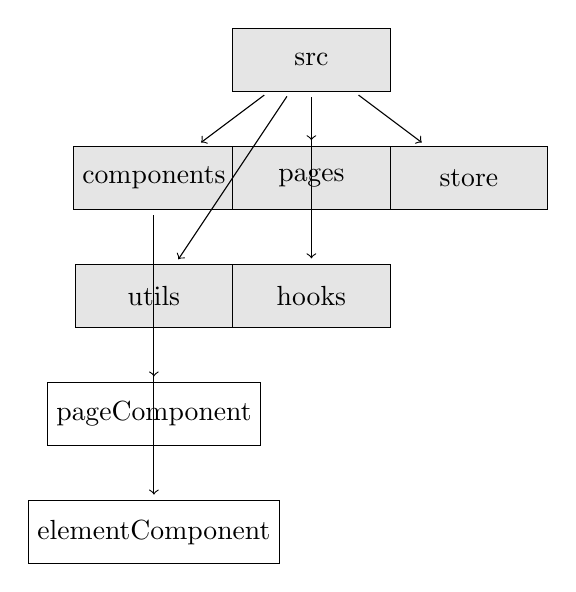
\begin{tikzpicture}[
    file/.style={draw, rectangle, minimum width=2cm, minimum height=0.8cm},
    folder/.style={draw, rectangle, minimum width=2cm, minimum height=0.8cm, fill=gray!20},
    arrow/.style={->, shorten >=2pt, shorten <=2pt}
]

% Folders
\node[folder] (src) at (0,0) {src};
\node[folder] (components) at (-2,-1.5) {components};
\node[folder] (pages) at (0,-1.5) {pages};
\node[folder] (store) at (2,-1.5) {store};
\node[folder] (utils) at (-2,-3) {utils};
\node[folder] (hooks) at (0,-3) {hooks};

% Files
\node[file] (pageComponent) at (-2,-4.5) {pageComponent};
\node[file] (elementComponent) at (-2,-6) {elementComponent};
% ... add more files

% Connections
\draw[arrow] (src) -- (components);
\draw[arrow] (src) -- (pages);
\draw[arrow] (src) -- (store);
\draw[arrow] (src) -- (utils);
\draw[arrow] (src) -- (hooks);
\draw[arrow] (components) -- (pageComponent);
\draw[arrow] (components) -- (elementComponent);
% ... add more connections

\end{tikzpicture}



\pagebreak
\subsubsection{Back-end}
The backend uses the dotNet framework. The development language using the C\# language.

In this project, the backend uses the Onion Architecture.
The Onion Architecture is a typically layered architecture, 
where each layer depends on the inner layer and provides interfaces to the outer layer.
The outer layer provides services to the outermost layer 
and other modules in the same layer based on the interfaces of the inner layer.

From inner to outer, the layers are: Domain, Application, Infrastructure, Presentation.
The Domain layer is the core layer and the innermost layer, used to define domain models, 
which are the business models.
It includes domain models and domain service interfaces.
Domain models are used to define the business models, 
which are the entities in the entity-relationship model and their attributes.
Domain service interfaces are used to define the business services, 
which are the relationships between entities in the entity-relationship model.

The Application layer is the application layer, 
used to define application services, which are the business logic.
It includes domain service implementations and application service interfaces.
Domain service implementations implement the methods of the inner layer's domain service 
interfaces and implement the business logic of the domain models.
Application service interfaces are used to define application services, 
which are the business logic.
It includes but is not limited to database interfaces, testing interfaces, 
HTTP API interfaces, MQTT interfaces, etc.

The Infrastructure layer is the infrastructure layer, used to define infrastructure.
It includes database implementations, testing implementations, 
HTTP API implementations, MQTT implementations, etc.
Database implementations implement the database interfaces 
and provide CRUD services for the database.
Testing implementations implement the testing interfaces 
and provide services for unit testing and integration testing.
HTTP API implementations implement the HTTP API interfaces 
and provide CRUD operations for HTTP APIs.
MQTT implementations implement the MQTT interfaces 
and provide CRUD operations for MQTT.

The Presentation layer is the presentation layer, used to define presentation logic, 
such as interfaces and pages. Since this is a backend project,
data presentation and control are handled by the frontend, 
so this layer is not needed.



\pagebreak
\subsubsection{Data communication and storage}
% 关于本项目的数据通信与数据存储的设计, 包括数据通信的协议, 数据存储的设计等
% 关于数据通信的设计:
% 1. 通信协议的选择
% 自前端向后端发送的数据, 有三种传输的数据类型, 
% 一种是普通的增删改查的请求, 对数据传输的时效性要求不高, 但是对数据的准确性, 完整性, 有序性, 安全性有一定的要求,
% 这种数据的传输, 采用 HTTP 协议, 以及 RESTful API 的设计. 可以有效的保证对数据传输的以上要求.
% 一种是对数据通道的创建和流媒体数据的传输, 对数据传输的时效性, 安全性要求较高, 这种数据的传输, 采用 WebRTC 协议, 以及 MQTT 协议.
% 配合可以快速解码的 flatbuffers 协议, 可以有效的保证对数据传输的以上要求.
% 最后一种是对设备的状态信息和操作信息的传输, 对完整性, 有序性, 安全性都有较高的要求, 这种数据的传输, 采用 MQTT 协议
% 同时也使用了 flatbuffers 协议.
% 
% 2. 数据通信的通信架构和通信流程
% 本项目的数据通信的通信架构, 是基于前后端分离的架构, 前端使用 React 框架, 后端使用 dotnet 框架.
% 当前端需要向后端发送数据的时候, 前端会向后端发送 HTTP 请求, 后端接收到 HTTP 请求之后, 会根据请求的数据类型,
% 选择不同的数据处理方式, 对于普通的增删改查的请求, 后端会根据 RESTful API 的设计, 对数据进行增删改查的操作,
% 对于对数据通道的创建和流媒体数据的传输, 后端会根据 WebRTC 协议, 对数据通道进行创建, 并且帮助前端和设备建立数据通道,
% 当数据通道建立后, 前端和设备之间则使用 flatbuffer 的数据格式对流媒体数据进行传输,
% 对于设备的状态信息和操作信息的传输, 前端会直接向 MQTT broker 发送 MQTT 请求, 
% 设备会在其自身的固件中监听相关的 MQTT 请求, 并且返回相关的数据.
% 
% 3. 数据通信的格式
% 本项目的数据通信的格式, 有三种, 
% 一种是 HTTP 协议, 
% 使用 json 格式对数据进行传输,
% 一种是 WebRTC 协议, 
% 使用 flatbuffers 格式对数据进行传输,
% 一种是 MQTT 协议.
% 使用 flatbuffers 格式对数据进行传输,
% 
% 关于数据存储的设计:
% 1. 数据存储的数据库的选择
% 本项目的数据存储的数据库的选择, 使用了轻量级的数据库 SQLite,
% SQLite 是一个进程内的库, 实现了自给自足的, 无服务器的, 零配置的, 事务性的 SQL 数据库引擎.
% 这是因为整个项目的目的是为了实现前端与设备之间的数据通信, 对于数据库数据的增删改查操作的要求不高,
% 数据量较小, 且对于数据库的数据的事务性要求不高, 所以选择了 SQLite 数据库.
% 2. 项目前后端的数据结构的设计
% 在本项目中, 前端由于使用了 React 框架, 所以前端的数据结构的设计, 使用了基于状态的数据结构的设计,
% 每个组件或者数据集都包含一个状态对象, 这个状态对象的属性就是组件的各个状态. 
% 使用状态对象的原因是, 可以方便的对状态进行管理, 采用对象-属性的形式, 可以方便的针对不同组件的同类状态进行区分,
% 由于跨组件的状态是由 redux 进行管理的, 这种状态对象的设计, 可以更搞笑的对状态进行更新和传递.
% 后端由于使用了 dotnet 框架, 所以后端的数据结构的设计, 使用了基于类的数据结构的设计,
% 采用了面向对象的编程思想, 对数据进行了封装, 使得数据的传输更加的安全, 有序, 完整.


\pagebreak

% \subsection{Domain model}
% \documentclass[]{article}
\usepackage{graphicx}
\usepackage{amsmath}
\usepackage{tikz}

% libaries
\usetikzlibrary{shapes,arrows}

%Define the listing package
\usepackage{listings} %code highlighter
\usepackage{color} %use color
\definecolor{mygreen}{rgb}{0,0.6,0}
\definecolor{mygray}{rgb}{0.5,0.5,0.5}
\definecolor{mymauve}{rgb}{0.58,0,0.82}

%Customize a bit the look
\lstset{ %
backgroundcolor=\color{white}, % choose the background color; you must add \usepackage{color} or \usepackage{xcolor}
basicstyle=\footnotesize, % the size of the fonts that are used for the code
breakatwhitespace=false, % sets if automatic breaks should only happen at whitespace
breaklines=true, % sets automatic line breaking
captionpos=b, % sets the caption-position to bottom
commentstyle=\color{mygreen}, % comment style
deletekeywords={...}, % if you want to delete keywords from the given language
escapeinside={\%*}{*)}, % if you want to add LaTeX within your code
extendedchars=true, % lets you use non-ASCII characters; for 8-bits encodings only, does not work with UTF-8
frame=single, % adds a frame around the code
keepspaces=true, % keeps spaces in text, useful for keeping indentation of code (possibly needs columns=flexible)
keywordstyle=\color{blue}, % keyword style
% language=Octave, % the language of the code
morekeywords={*,...}, % if you want to add more keywords to the set
numbers=left, % where to put the line-numbers; possible values are (none, left, right)
numbersep=5pt, % how far the line-numbers are from the code
numberstyle=\tiny\color{mygray}, % the style that is used for the line-numbers
rulecolor=\color{black}, % if not set, the frame-color may be changed on line-breaks within not-black text (e.g. comments (green here))
showspaces=false, % show spaces everywhere adding particular underscores; it overrides 'showstringspaces'
showstringspaces=false, % underline spaces within strings only
showtabs=false, % show tabs within strings adding particular underscores
stepnumber=1, % the step between two line-numbers. If it's 1, each line will be numbered
stringstyle=\color{mymauve}, % string literal style
tabsize=2, % sets default tabsize to 2 spaces
title=\lstname % show the filename of files included with \lstinputlisting; also try caption instead of title
}

\definecolor{darkgray}{rgb}{.4,.4,.4}
\definecolor{purple}{rgb}{0.65, 0.12, 0.82}

\lstdefinelanguage{React}{
keywords={const, typeof, new, true, false, catch, function, return, null, catch, switch, var, if, in, while, do, else, case, break},
keywordstyle=\color{blue}\bfseries,
ndkeywords={class, export, boolean, throw, implements, import, this},
ndkeywordstyle=\color{darkgray}\bfseries,
identifierstyle=\color{mygreen},
sensitive=false,
comment=[l]{//},
morecomment=[s]{/*}{*/},
commentstyle=\color{purple}\ttfamily,
string=[b]{"}{'}{`},
stringstyle=\color{red}\ttfamily,
morestring=[b]',
morestring=[b]",
morestring=[b]`',
}

\lstdefinelanguage{CSharp}{
keywords={const, typeof, new, true, false, catch, function, return, null, catch, switch, var, if, in, while, do, else, case, break},
keywordstyle=\color{blue}\bfseries,
ndkeywords={class, export, boolean, throw, implements, import, this},
ndkeywordstyle=\color{darkgray}\bfseries,
identifierstyle=\color{mygreen},
sensitive=false,
comment=[l]{//},
morecomment=[s]{/*}{*/},
commentstyle=\color{purple}\ttfamily,
string=[b]{"}{'}{`},
stringstyle=\color{red}\ttfamily,
morestring=[b]',
morestring=[b]",
morestring=[b]`',
}

\lstset{
language=React,
extendedchars=true,
basicstyle=\footnotesize\ttfamily,
showstringspaces=false,
showspaces=false,
numbers=left,
numberstyle=\footnotesize,
numbersep=9pt,
tabsize=2,
breaklines=true,
showtabs=false,
captionpos=b
}

\lstset{
language=CSharp,
extendedchars=true,
basicstyle=\footnotesize\ttfamily,
showstringspaces=false,
showspaces=false,
numbers=left,
numberstyle=\footnotesize,
numbersep=9pt,
tabsize=2,
breaklines=true,
showtabs=false,
captionpos=b
}

% \usepackage{cite} % Add this line for citation

% \bibliographystyle{plain}

\title{
The implementation of BifrostConnect Front-end scope, 
re-design and development with the relevant back-end support develop.
}
\author{
    Fei Gu \\
    Erhvervs Akademi Sydvest \\
    Computer Science 21\\
    }
\date{\today}

\begin{document}

% Front page
\maketitle
\begin{center}
    Supervisor: Henrik Boulund Meng Hansen \\
    Company: BifrostConnect \\
    Engineering Director: Jasper Wass \\
\end{center}
\tableofcontents
\pagebreak


% The introduction
\section{Introduction}
\subsection{Background}\input{sections/introduction/background.tex}
\subsection{The company}\input{sections/introduction/aboutCompany}
\subsection{The project}\input{sections/introduction/aboutProject}
\pagebreak

% The problem statement
\section{Problem Statement}
\subsection{Statement}
\input{sections/problemStatement/statement}
\subsection{Situation}
\input{sections/problemStatement/situation}
\subsection{Potential Solution}
\input{sections/problemStatement/potentialSolution}
\pagebreak

% Requirement analysis
\section{Requirement Analysis}
\input{sections/requirementAnalysis/index}

\subsection{Stakeholders}
\input{sections/requirementAnalysis/stakeholders/index}

\subsection{Business Domain}
\input{sections/requirementAnalysis/bussinesDomain/index}

\subsection{Scope}
\input{sections/requirementAnalysis/scope}

\subsection{Goals}
\input{sections/requirementAnalysis/goals}
\pagebreak

% Software Design
\section{Software Design}
% developement methods
\subsection{Software Development Methods}
\input{sections/softwareDevelopmentMethods/index}
\subsubsection{Agile Software Development}
\input{sections/softwareDevelopmentMethods/agileSoftwareDevelopment/index}
\subsubsection{Feature Driven Development}
\input{sections/softwareDevelopmentMethods/featureDrivenDevelopment/index}

\pagebreak

% Technology seslection
\subsection{Technology selection}
\input{sections/softwareDesign/technologySelection/index}
\subsubsection{Front-end}
\input{sections/softwareDesign/technologySelection/frontEnd}            
\subsubsection{Back-end}
\input{sections/softwareDesign/technologySelection/backEnd}            
\subsubsection{Database}
\input{sections/softwareDesign/technologySelection/database}
\subsubsection{Data communication}
\input{sections/softwareDesign/technologySelection/dataCommunication}            
\subsubsection{DevOps}
\input{sections/softwareDesign/technologySelection/devOps}
\pagebreak

% Architecture design
\subsection{Architecture design}
\input{sections/softwareDesign/architectureDesign/index}
\pagebreak
\subsubsection{Front-end}
\input{sections/softwareDesign/architectureDesign/frontEndArchitecture}
\pagebreak
\subsubsection{Back-end}
\input{sections/softwareDesign/architectureDesign/backEndArchitecture}
\pagebreak
\subsubsection{Data communication and storage}
\input{sections/softwareDesign/architectureDesign/dataCommunicationArchitecture}
\pagebreak

% \subsection{Domain model}
% \input{sections/softwareDesign/domainModel/index}
% \subsection{Database design}
% % 数据库领域模型 ER 图
% % 包括表和字段的设置.
% % 对于私有键和外键的设置.

% \subsection{Back-end design}
% % 后端对象模型
% % 以及对于对象模型的增删改查
% % 以及相关的其他服务的设计`'

% \subsection{Front-end design}
% % 对于前端的页面结构的设计 
% % 页面的状态的设计, 交互设计

% \subsection{FlatBuffers design}
% % schema 的设计

\subsection{DevOps CI/CD process design}
\input{sections/softwareDesign/devOpsDesign/index}
\subsubsection{Continuous Integration}
\input{sections/softwareDesign/devOpsDesign/continuousIntegration/index}
\subsubsection{Continuous Delivery}
\input{sections/softwareDesign/devOpsDesign/continuousDelivery/index}
\subsubsection{Continuous Deployment}
\input{sections/softwareDesign/devOpsDesign/continuousDeployment/index}
\pagebreak

\section{Software Development} 
\input{sections/softwareDevelopment/index}
\subsection{Overall development}
\input{sections/softwareDevelopment/overallDevelopement/index}
\subsubsection{Front-end}
\input{sections/softwareDevelopment/overallDevelopement/frontEnd/index}
\subsubsection{Back-end}
\input{sections/softwareDevelopment/overallDevelopement/backEnd/index}
\subsubsection{DevOps}
\input{sections/softwareDevelopment/overallDevelopement/devOps/index}
\subsection{Feature development} 
\input{sections/softwareDevelopment/featureDevelopment/index}
\subsubsection{Use Case 1}
\input{sections/softwareDevelopment/featureDevelopment/useCase1/index}
\subsubsection{Feature 1}
\input{sections/softwareDevelopment/featureDevelopment/feature/feature1.tex}
\pagebreak
\section{Conclusion} 
\subsection{Result}
Since the project is still in progress, the result is not available yet.
So far, basic structure of this project has been built. But the most features 
are not implemented yet. 
\subsection{Discussion}
As a single developer for this project, I am confident what I have done so far.
And I can say I understand the most of the knowledge I have used in this project, 
which also means I can explain all the part of the project. 
But this project also relevant some of the complex knowledge which I have to continue 
to study and practice.
\subsection{Future Work}
The future work is to implement the rest of the features. 
Including the most important part which is the 'create session' feature.
\pagebreak
% \bibliography{bibliography}
\pagebreak
% \begin{appendices}
%     \section{Appendix}
% \end{appendices} 
\end{document}
% \subsection{Database design}
% % 数据库领域模型 ER 图
% % 包括表和字段的设置.
% % 对于私有键和外键的设置.

% \subsection{Back-end design}
% % 后端对象模型
% % 以及对于对象模型的增删改查
% % 以及相关的其他服务的设计`'

% \subsection{Front-end design}
% % 对于前端的页面结构的设计 
% % 页面的状态的设计, 交互设计

% \subsection{FlatBuffers design}
% % schema 的设计

\subsection{DevOps CI/CD process design}
\documentclass[]{article}
\usepackage{graphicx}
\usepackage{amsmath}
\usepackage{tikz}

% libaries
\usetikzlibrary{shapes,arrows}

%Define the listing package
\usepackage{listings} %code highlighter
\usepackage{color} %use color
\definecolor{mygreen}{rgb}{0,0.6,0}
\definecolor{mygray}{rgb}{0.5,0.5,0.5}
\definecolor{mymauve}{rgb}{0.58,0,0.82}

%Customize a bit the look
\lstset{ %
backgroundcolor=\color{white}, % choose the background color; you must add \usepackage{color} or \usepackage{xcolor}
basicstyle=\footnotesize, % the size of the fonts that are used for the code
breakatwhitespace=false, % sets if automatic breaks should only happen at whitespace
breaklines=true, % sets automatic line breaking
captionpos=b, % sets the caption-position to bottom
commentstyle=\color{mygreen}, % comment style
deletekeywords={...}, % if you want to delete keywords from the given language
escapeinside={\%*}{*)}, % if you want to add LaTeX within your code
extendedchars=true, % lets you use non-ASCII characters; for 8-bits encodings only, does not work with UTF-8
frame=single, % adds a frame around the code
keepspaces=true, % keeps spaces in text, useful for keeping indentation of code (possibly needs columns=flexible)
keywordstyle=\color{blue}, % keyword style
% language=Octave, % the language of the code
morekeywords={*,...}, % if you want to add more keywords to the set
numbers=left, % where to put the line-numbers; possible values are (none, left, right)
numbersep=5pt, % how far the line-numbers are from the code
numberstyle=\tiny\color{mygray}, % the style that is used for the line-numbers
rulecolor=\color{black}, % if not set, the frame-color may be changed on line-breaks within not-black text (e.g. comments (green here))
showspaces=false, % show spaces everywhere adding particular underscores; it overrides 'showstringspaces'
showstringspaces=false, % underline spaces within strings only
showtabs=false, % show tabs within strings adding particular underscores
stepnumber=1, % the step between two line-numbers. If it's 1, each line will be numbered
stringstyle=\color{mymauve}, % string literal style
tabsize=2, % sets default tabsize to 2 spaces
title=\lstname % show the filename of files included with \lstinputlisting; also try caption instead of title
}

\definecolor{darkgray}{rgb}{.4,.4,.4}
\definecolor{purple}{rgb}{0.65, 0.12, 0.82}

\lstdefinelanguage{React}{
keywords={const, typeof, new, true, false, catch, function, return, null, catch, switch, var, if, in, while, do, else, case, break},
keywordstyle=\color{blue}\bfseries,
ndkeywords={class, export, boolean, throw, implements, import, this},
ndkeywordstyle=\color{darkgray}\bfseries,
identifierstyle=\color{mygreen},
sensitive=false,
comment=[l]{//},
morecomment=[s]{/*}{*/},
commentstyle=\color{purple}\ttfamily,
string=[b]{"}{'}{`},
stringstyle=\color{red}\ttfamily,
morestring=[b]',
morestring=[b]",
morestring=[b]`',
}

\lstdefinelanguage{CSharp}{
keywords={const, typeof, new, true, false, catch, function, return, null, catch, switch, var, if, in, while, do, else, case, break},
keywordstyle=\color{blue}\bfseries,
ndkeywords={class, export, boolean, throw, implements, import, this},
ndkeywordstyle=\color{darkgray}\bfseries,
identifierstyle=\color{mygreen},
sensitive=false,
comment=[l]{//},
morecomment=[s]{/*}{*/},
commentstyle=\color{purple}\ttfamily,
string=[b]{"}{'}{`},
stringstyle=\color{red}\ttfamily,
morestring=[b]',
morestring=[b]",
morestring=[b]`',
}

\lstset{
language=React,
extendedchars=true,
basicstyle=\footnotesize\ttfamily,
showstringspaces=false,
showspaces=false,
numbers=left,
numberstyle=\footnotesize,
numbersep=9pt,
tabsize=2,
breaklines=true,
showtabs=false,
captionpos=b
}

\lstset{
language=CSharp,
extendedchars=true,
basicstyle=\footnotesize\ttfamily,
showstringspaces=false,
showspaces=false,
numbers=left,
numberstyle=\footnotesize,
numbersep=9pt,
tabsize=2,
breaklines=true,
showtabs=false,
captionpos=b
}

% \usepackage{cite} % Add this line for citation

% \bibliographystyle{plain}

\title{
The implementation of BifrostConnect Front-end scope, 
re-design and development with the relevant back-end support develop.
}
\author{
    Fei Gu \\
    Erhvervs Akademi Sydvest \\
    Computer Science 21\\
    }
\date{\today}

\begin{document}

% Front page
\maketitle
\begin{center}
    Supervisor: Henrik Boulund Meng Hansen \\
    Company: BifrostConnect \\
    Engineering Director: Jasper Wass \\
\end{center}
\tableofcontents
\pagebreak


% The introduction
\section{Introduction}
\subsection{Background}\input{sections/introduction/background.tex}
\subsection{The company}\input{sections/introduction/aboutCompany}
\subsection{The project}\input{sections/introduction/aboutProject}
\pagebreak

% The problem statement
\section{Problem Statement}
\subsection{Statement}
\input{sections/problemStatement/statement}
\subsection{Situation}
\input{sections/problemStatement/situation}
\subsection{Potential Solution}
\input{sections/problemStatement/potentialSolution}
\pagebreak

% Requirement analysis
\section{Requirement Analysis}
\input{sections/requirementAnalysis/index}

\subsection{Stakeholders}
\input{sections/requirementAnalysis/stakeholders/index}

\subsection{Business Domain}
\input{sections/requirementAnalysis/bussinesDomain/index}

\subsection{Scope}
\input{sections/requirementAnalysis/scope}

\subsection{Goals}
\input{sections/requirementAnalysis/goals}
\pagebreak

% Software Design
\section{Software Design}
% developement methods
\subsection{Software Development Methods}
\input{sections/softwareDevelopmentMethods/index}
\subsubsection{Agile Software Development}
\input{sections/softwareDevelopmentMethods/agileSoftwareDevelopment/index}
\subsubsection{Feature Driven Development}
\input{sections/softwareDevelopmentMethods/featureDrivenDevelopment/index}

\pagebreak

% Technology seslection
\subsection{Technology selection}
\input{sections/softwareDesign/technologySelection/index}
\subsubsection{Front-end}
\input{sections/softwareDesign/technologySelection/frontEnd}            
\subsubsection{Back-end}
\input{sections/softwareDesign/technologySelection/backEnd}            
\subsubsection{Database}
\input{sections/softwareDesign/technologySelection/database}
\subsubsection{Data communication}
\input{sections/softwareDesign/technologySelection/dataCommunication}            
\subsubsection{DevOps}
\input{sections/softwareDesign/technologySelection/devOps}
\pagebreak

% Architecture design
\subsection{Architecture design}
\input{sections/softwareDesign/architectureDesign/index}
\pagebreak
\subsubsection{Front-end}
\input{sections/softwareDesign/architectureDesign/frontEndArchitecture}
\pagebreak
\subsubsection{Back-end}
\input{sections/softwareDesign/architectureDesign/backEndArchitecture}
\pagebreak
\subsubsection{Data communication and storage}
\input{sections/softwareDesign/architectureDesign/dataCommunicationArchitecture}
\pagebreak

% \subsection{Domain model}
% \input{sections/softwareDesign/domainModel/index}
% \subsection{Database design}
% % 数据库领域模型 ER 图
% % 包括表和字段的设置.
% % 对于私有键和外键的设置.

% \subsection{Back-end design}
% % 后端对象模型
% % 以及对于对象模型的增删改查
% % 以及相关的其他服务的设计`'

% \subsection{Front-end design}
% % 对于前端的页面结构的设计 
% % 页面的状态的设计, 交互设计

% \subsection{FlatBuffers design}
% % schema 的设计

\subsection{DevOps CI/CD process design}
\input{sections/softwareDesign/devOpsDesign/index}
\subsubsection{Continuous Integration}
\input{sections/softwareDesign/devOpsDesign/continuousIntegration/index}
\subsubsection{Continuous Delivery}
\input{sections/softwareDesign/devOpsDesign/continuousDelivery/index}
\subsubsection{Continuous Deployment}
\input{sections/softwareDesign/devOpsDesign/continuousDeployment/index}
\pagebreak

\section{Software Development} 
\input{sections/softwareDevelopment/index}
\subsection{Overall development}
\input{sections/softwareDevelopment/overallDevelopement/index}
\subsubsection{Front-end}
\input{sections/softwareDevelopment/overallDevelopement/frontEnd/index}
\subsubsection{Back-end}
\input{sections/softwareDevelopment/overallDevelopement/backEnd/index}
\subsubsection{DevOps}
\input{sections/softwareDevelopment/overallDevelopement/devOps/index}
\subsection{Feature development} 
\input{sections/softwareDevelopment/featureDevelopment/index}
\subsubsection{Use Case 1}
\input{sections/softwareDevelopment/featureDevelopment/useCase1/index}
\subsubsection{Feature 1}
\input{sections/softwareDevelopment/featureDevelopment/feature/feature1.tex}
\pagebreak
\section{Conclusion} 
\subsection{Result}
Since the project is still in progress, the result is not available yet.
So far, basic structure of this project has been built. But the most features 
are not implemented yet. 
\subsection{Discussion}
As a single developer for this project, I am confident what I have done so far.
And I can say I understand the most of the knowledge I have used in this project, 
which also means I can explain all the part of the project. 
But this project also relevant some of the complex knowledge which I have to continue 
to study and practice.
\subsection{Future Work}
The future work is to implement the rest of the features. 
Including the most important part which is the 'create session' feature.
\pagebreak
% \bibliography{bibliography}
\pagebreak
% \begin{appendices}
%     \section{Appendix}
% \end{appendices} 
\end{document}
\subsubsection{Continuous Integration}
\documentclass[]{article}
\usepackage{graphicx}
\usepackage{amsmath}
\usepackage{tikz}

% libaries
\usetikzlibrary{shapes,arrows}

%Define the listing package
\usepackage{listings} %code highlighter
\usepackage{color} %use color
\definecolor{mygreen}{rgb}{0,0.6,0}
\definecolor{mygray}{rgb}{0.5,0.5,0.5}
\definecolor{mymauve}{rgb}{0.58,0,0.82}

%Customize a bit the look
\lstset{ %
backgroundcolor=\color{white}, % choose the background color; you must add \usepackage{color} or \usepackage{xcolor}
basicstyle=\footnotesize, % the size of the fonts that are used for the code
breakatwhitespace=false, % sets if automatic breaks should only happen at whitespace
breaklines=true, % sets automatic line breaking
captionpos=b, % sets the caption-position to bottom
commentstyle=\color{mygreen}, % comment style
deletekeywords={...}, % if you want to delete keywords from the given language
escapeinside={\%*}{*)}, % if you want to add LaTeX within your code
extendedchars=true, % lets you use non-ASCII characters; for 8-bits encodings only, does not work with UTF-8
frame=single, % adds a frame around the code
keepspaces=true, % keeps spaces in text, useful for keeping indentation of code (possibly needs columns=flexible)
keywordstyle=\color{blue}, % keyword style
% language=Octave, % the language of the code
morekeywords={*,...}, % if you want to add more keywords to the set
numbers=left, % where to put the line-numbers; possible values are (none, left, right)
numbersep=5pt, % how far the line-numbers are from the code
numberstyle=\tiny\color{mygray}, % the style that is used for the line-numbers
rulecolor=\color{black}, % if not set, the frame-color may be changed on line-breaks within not-black text (e.g. comments (green here))
showspaces=false, % show spaces everywhere adding particular underscores; it overrides 'showstringspaces'
showstringspaces=false, % underline spaces within strings only
showtabs=false, % show tabs within strings adding particular underscores
stepnumber=1, % the step between two line-numbers. If it's 1, each line will be numbered
stringstyle=\color{mymauve}, % string literal style
tabsize=2, % sets default tabsize to 2 spaces
title=\lstname % show the filename of files included with \lstinputlisting; also try caption instead of title
}

\definecolor{darkgray}{rgb}{.4,.4,.4}
\definecolor{purple}{rgb}{0.65, 0.12, 0.82}

\lstdefinelanguage{React}{
keywords={const, typeof, new, true, false, catch, function, return, null, catch, switch, var, if, in, while, do, else, case, break},
keywordstyle=\color{blue}\bfseries,
ndkeywords={class, export, boolean, throw, implements, import, this},
ndkeywordstyle=\color{darkgray}\bfseries,
identifierstyle=\color{mygreen},
sensitive=false,
comment=[l]{//},
morecomment=[s]{/*}{*/},
commentstyle=\color{purple}\ttfamily,
string=[b]{"}{'}{`},
stringstyle=\color{red}\ttfamily,
morestring=[b]',
morestring=[b]",
morestring=[b]`',
}

\lstdefinelanguage{CSharp}{
keywords={const, typeof, new, true, false, catch, function, return, null, catch, switch, var, if, in, while, do, else, case, break},
keywordstyle=\color{blue}\bfseries,
ndkeywords={class, export, boolean, throw, implements, import, this},
ndkeywordstyle=\color{darkgray}\bfseries,
identifierstyle=\color{mygreen},
sensitive=false,
comment=[l]{//},
morecomment=[s]{/*}{*/},
commentstyle=\color{purple}\ttfamily,
string=[b]{"}{'}{`},
stringstyle=\color{red}\ttfamily,
morestring=[b]',
morestring=[b]",
morestring=[b]`',
}

\lstset{
language=React,
extendedchars=true,
basicstyle=\footnotesize\ttfamily,
showstringspaces=false,
showspaces=false,
numbers=left,
numberstyle=\footnotesize,
numbersep=9pt,
tabsize=2,
breaklines=true,
showtabs=false,
captionpos=b
}

\lstset{
language=CSharp,
extendedchars=true,
basicstyle=\footnotesize\ttfamily,
showstringspaces=false,
showspaces=false,
numbers=left,
numberstyle=\footnotesize,
numbersep=9pt,
tabsize=2,
breaklines=true,
showtabs=false,
captionpos=b
}

% \usepackage{cite} % Add this line for citation

% \bibliographystyle{plain}

\title{
The implementation of BifrostConnect Front-end scope, 
re-design and development with the relevant back-end support develop.
}
\author{
    Fei Gu \\
    Erhvervs Akademi Sydvest \\
    Computer Science 21\\
    }
\date{\today}

\begin{document}

% Front page
\maketitle
\begin{center}
    Supervisor: Henrik Boulund Meng Hansen \\
    Company: BifrostConnect \\
    Engineering Director: Jasper Wass \\
\end{center}
\tableofcontents
\pagebreak


% The introduction
\section{Introduction}
\subsection{Background}\input{sections/introduction/background.tex}
\subsection{The company}\input{sections/introduction/aboutCompany}
\subsection{The project}\input{sections/introduction/aboutProject}
\pagebreak

% The problem statement
\section{Problem Statement}
\subsection{Statement}
\input{sections/problemStatement/statement}
\subsection{Situation}
\input{sections/problemStatement/situation}
\subsection{Potential Solution}
\input{sections/problemStatement/potentialSolution}
\pagebreak

% Requirement analysis
\section{Requirement Analysis}
\input{sections/requirementAnalysis/index}

\subsection{Stakeholders}
\input{sections/requirementAnalysis/stakeholders/index}

\subsection{Business Domain}
\input{sections/requirementAnalysis/bussinesDomain/index}

\subsection{Scope}
\input{sections/requirementAnalysis/scope}

\subsection{Goals}
\input{sections/requirementAnalysis/goals}
\pagebreak

% Software Design
\section{Software Design}
% developement methods
\subsection{Software Development Methods}
\input{sections/softwareDevelopmentMethods/index}
\subsubsection{Agile Software Development}
\input{sections/softwareDevelopmentMethods/agileSoftwareDevelopment/index}
\subsubsection{Feature Driven Development}
\input{sections/softwareDevelopmentMethods/featureDrivenDevelopment/index}

\pagebreak

% Technology seslection
\subsection{Technology selection}
\input{sections/softwareDesign/technologySelection/index}
\subsubsection{Front-end}
\input{sections/softwareDesign/technologySelection/frontEnd}            
\subsubsection{Back-end}
\input{sections/softwareDesign/technologySelection/backEnd}            
\subsubsection{Database}
\input{sections/softwareDesign/technologySelection/database}
\subsubsection{Data communication}
\input{sections/softwareDesign/technologySelection/dataCommunication}            
\subsubsection{DevOps}
\input{sections/softwareDesign/technologySelection/devOps}
\pagebreak

% Architecture design
\subsection{Architecture design}
\input{sections/softwareDesign/architectureDesign/index}
\pagebreak
\subsubsection{Front-end}
\input{sections/softwareDesign/architectureDesign/frontEndArchitecture}
\pagebreak
\subsubsection{Back-end}
\input{sections/softwareDesign/architectureDesign/backEndArchitecture}
\pagebreak
\subsubsection{Data communication and storage}
\input{sections/softwareDesign/architectureDesign/dataCommunicationArchitecture}
\pagebreak

% \subsection{Domain model}
% \input{sections/softwareDesign/domainModel/index}
% \subsection{Database design}
% % 数据库领域模型 ER 图
% % 包括表和字段的设置.
% % 对于私有键和外键的设置.

% \subsection{Back-end design}
% % 后端对象模型
% % 以及对于对象模型的增删改查
% % 以及相关的其他服务的设计`'

% \subsection{Front-end design}
% % 对于前端的页面结构的设计 
% % 页面的状态的设计, 交互设计

% \subsection{FlatBuffers design}
% % schema 的设计

\subsection{DevOps CI/CD process design}
\input{sections/softwareDesign/devOpsDesign/index}
\subsubsection{Continuous Integration}
\input{sections/softwareDesign/devOpsDesign/continuousIntegration/index}
\subsubsection{Continuous Delivery}
\input{sections/softwareDesign/devOpsDesign/continuousDelivery/index}
\subsubsection{Continuous Deployment}
\input{sections/softwareDesign/devOpsDesign/continuousDeployment/index}
\pagebreak

\section{Software Development} 
\input{sections/softwareDevelopment/index}
\subsection{Overall development}
\input{sections/softwareDevelopment/overallDevelopement/index}
\subsubsection{Front-end}
\input{sections/softwareDevelopment/overallDevelopement/frontEnd/index}
\subsubsection{Back-end}
\input{sections/softwareDevelopment/overallDevelopement/backEnd/index}
\subsubsection{DevOps}
\input{sections/softwareDevelopment/overallDevelopement/devOps/index}
\subsection{Feature development} 
\input{sections/softwareDevelopment/featureDevelopment/index}
\subsubsection{Use Case 1}
\input{sections/softwareDevelopment/featureDevelopment/useCase1/index}
\subsubsection{Feature 1}
\input{sections/softwareDevelopment/featureDevelopment/feature/feature1.tex}
\pagebreak
\section{Conclusion} 
\subsection{Result}
Since the project is still in progress, the result is not available yet.
So far, basic structure of this project has been built. But the most features 
are not implemented yet. 
\subsection{Discussion}
As a single developer for this project, I am confident what I have done so far.
And I can say I understand the most of the knowledge I have used in this project, 
which also means I can explain all the part of the project. 
But this project also relevant some of the complex knowledge which I have to continue 
to study and practice.
\subsection{Future Work}
The future work is to implement the rest of the features. 
Including the most important part which is the 'create session' feature.
\pagebreak
% \bibliography{bibliography}
\pagebreak
% \begin{appendices}
%     \section{Appendix}
% \end{appendices} 
\end{document}
\subsubsection{Continuous Delivery}
\documentclass[]{article}
\usepackage{graphicx}
\usepackage{amsmath}
\usepackage{tikz}

% libaries
\usetikzlibrary{shapes,arrows}

%Define the listing package
\usepackage{listings} %code highlighter
\usepackage{color} %use color
\definecolor{mygreen}{rgb}{0,0.6,0}
\definecolor{mygray}{rgb}{0.5,0.5,0.5}
\definecolor{mymauve}{rgb}{0.58,0,0.82}

%Customize a bit the look
\lstset{ %
backgroundcolor=\color{white}, % choose the background color; you must add \usepackage{color} or \usepackage{xcolor}
basicstyle=\footnotesize, % the size of the fonts that are used for the code
breakatwhitespace=false, % sets if automatic breaks should only happen at whitespace
breaklines=true, % sets automatic line breaking
captionpos=b, % sets the caption-position to bottom
commentstyle=\color{mygreen}, % comment style
deletekeywords={...}, % if you want to delete keywords from the given language
escapeinside={\%*}{*)}, % if you want to add LaTeX within your code
extendedchars=true, % lets you use non-ASCII characters; for 8-bits encodings only, does not work with UTF-8
frame=single, % adds a frame around the code
keepspaces=true, % keeps spaces in text, useful for keeping indentation of code (possibly needs columns=flexible)
keywordstyle=\color{blue}, % keyword style
% language=Octave, % the language of the code
morekeywords={*,...}, % if you want to add more keywords to the set
numbers=left, % where to put the line-numbers; possible values are (none, left, right)
numbersep=5pt, % how far the line-numbers are from the code
numberstyle=\tiny\color{mygray}, % the style that is used for the line-numbers
rulecolor=\color{black}, % if not set, the frame-color may be changed on line-breaks within not-black text (e.g. comments (green here))
showspaces=false, % show spaces everywhere adding particular underscores; it overrides 'showstringspaces'
showstringspaces=false, % underline spaces within strings only
showtabs=false, % show tabs within strings adding particular underscores
stepnumber=1, % the step between two line-numbers. If it's 1, each line will be numbered
stringstyle=\color{mymauve}, % string literal style
tabsize=2, % sets default tabsize to 2 spaces
title=\lstname % show the filename of files included with \lstinputlisting; also try caption instead of title
}

\definecolor{darkgray}{rgb}{.4,.4,.4}
\definecolor{purple}{rgb}{0.65, 0.12, 0.82}

\lstdefinelanguage{React}{
keywords={const, typeof, new, true, false, catch, function, return, null, catch, switch, var, if, in, while, do, else, case, break},
keywordstyle=\color{blue}\bfseries,
ndkeywords={class, export, boolean, throw, implements, import, this},
ndkeywordstyle=\color{darkgray}\bfseries,
identifierstyle=\color{mygreen},
sensitive=false,
comment=[l]{//},
morecomment=[s]{/*}{*/},
commentstyle=\color{purple}\ttfamily,
string=[b]{"}{'}{`},
stringstyle=\color{red}\ttfamily,
morestring=[b]',
morestring=[b]",
morestring=[b]`',
}

\lstdefinelanguage{CSharp}{
keywords={const, typeof, new, true, false, catch, function, return, null, catch, switch, var, if, in, while, do, else, case, break},
keywordstyle=\color{blue}\bfseries,
ndkeywords={class, export, boolean, throw, implements, import, this},
ndkeywordstyle=\color{darkgray}\bfseries,
identifierstyle=\color{mygreen},
sensitive=false,
comment=[l]{//},
morecomment=[s]{/*}{*/},
commentstyle=\color{purple}\ttfamily,
string=[b]{"}{'}{`},
stringstyle=\color{red}\ttfamily,
morestring=[b]',
morestring=[b]",
morestring=[b]`',
}

\lstset{
language=React,
extendedchars=true,
basicstyle=\footnotesize\ttfamily,
showstringspaces=false,
showspaces=false,
numbers=left,
numberstyle=\footnotesize,
numbersep=9pt,
tabsize=2,
breaklines=true,
showtabs=false,
captionpos=b
}

\lstset{
language=CSharp,
extendedchars=true,
basicstyle=\footnotesize\ttfamily,
showstringspaces=false,
showspaces=false,
numbers=left,
numberstyle=\footnotesize,
numbersep=9pt,
tabsize=2,
breaklines=true,
showtabs=false,
captionpos=b
}

% \usepackage{cite} % Add this line for citation

% \bibliographystyle{plain}

\title{
The implementation of BifrostConnect Front-end scope, 
re-design and development with the relevant back-end support develop.
}
\author{
    Fei Gu \\
    Erhvervs Akademi Sydvest \\
    Computer Science 21\\
    }
\date{\today}

\begin{document}

% Front page
\maketitle
\begin{center}
    Supervisor: Henrik Boulund Meng Hansen \\
    Company: BifrostConnect \\
    Engineering Director: Jasper Wass \\
\end{center}
\tableofcontents
\pagebreak


% The introduction
\section{Introduction}
\subsection{Background}\input{sections/introduction/background.tex}
\subsection{The company}\input{sections/introduction/aboutCompany}
\subsection{The project}\input{sections/introduction/aboutProject}
\pagebreak

% The problem statement
\section{Problem Statement}
\subsection{Statement}
\input{sections/problemStatement/statement}
\subsection{Situation}
\input{sections/problemStatement/situation}
\subsection{Potential Solution}
\input{sections/problemStatement/potentialSolution}
\pagebreak

% Requirement analysis
\section{Requirement Analysis}
\input{sections/requirementAnalysis/index}

\subsection{Stakeholders}
\input{sections/requirementAnalysis/stakeholders/index}

\subsection{Business Domain}
\input{sections/requirementAnalysis/bussinesDomain/index}

\subsection{Scope}
\input{sections/requirementAnalysis/scope}

\subsection{Goals}
\input{sections/requirementAnalysis/goals}
\pagebreak

% Software Design
\section{Software Design}
% developement methods
\subsection{Software Development Methods}
\input{sections/softwareDevelopmentMethods/index}
\subsubsection{Agile Software Development}
\input{sections/softwareDevelopmentMethods/agileSoftwareDevelopment/index}
\subsubsection{Feature Driven Development}
\input{sections/softwareDevelopmentMethods/featureDrivenDevelopment/index}

\pagebreak

% Technology seslection
\subsection{Technology selection}
\input{sections/softwareDesign/technologySelection/index}
\subsubsection{Front-end}
\input{sections/softwareDesign/technologySelection/frontEnd}            
\subsubsection{Back-end}
\input{sections/softwareDesign/technologySelection/backEnd}            
\subsubsection{Database}
\input{sections/softwareDesign/technologySelection/database}
\subsubsection{Data communication}
\input{sections/softwareDesign/technologySelection/dataCommunication}            
\subsubsection{DevOps}
\input{sections/softwareDesign/technologySelection/devOps}
\pagebreak

% Architecture design
\subsection{Architecture design}
\input{sections/softwareDesign/architectureDesign/index}
\pagebreak
\subsubsection{Front-end}
\input{sections/softwareDesign/architectureDesign/frontEndArchitecture}
\pagebreak
\subsubsection{Back-end}
\input{sections/softwareDesign/architectureDesign/backEndArchitecture}
\pagebreak
\subsubsection{Data communication and storage}
\input{sections/softwareDesign/architectureDesign/dataCommunicationArchitecture}
\pagebreak

% \subsection{Domain model}
% \input{sections/softwareDesign/domainModel/index}
% \subsection{Database design}
% % 数据库领域模型 ER 图
% % 包括表和字段的设置.
% % 对于私有键和外键的设置.

% \subsection{Back-end design}
% % 后端对象模型
% % 以及对于对象模型的增删改查
% % 以及相关的其他服务的设计`'

% \subsection{Front-end design}
% % 对于前端的页面结构的设计 
% % 页面的状态的设计, 交互设计

% \subsection{FlatBuffers design}
% % schema 的设计

\subsection{DevOps CI/CD process design}
\input{sections/softwareDesign/devOpsDesign/index}
\subsubsection{Continuous Integration}
\input{sections/softwareDesign/devOpsDesign/continuousIntegration/index}
\subsubsection{Continuous Delivery}
\input{sections/softwareDesign/devOpsDesign/continuousDelivery/index}
\subsubsection{Continuous Deployment}
\input{sections/softwareDesign/devOpsDesign/continuousDeployment/index}
\pagebreak

\section{Software Development} 
\input{sections/softwareDevelopment/index}
\subsection{Overall development}
\input{sections/softwareDevelopment/overallDevelopement/index}
\subsubsection{Front-end}
\input{sections/softwareDevelopment/overallDevelopement/frontEnd/index}
\subsubsection{Back-end}
\input{sections/softwareDevelopment/overallDevelopement/backEnd/index}
\subsubsection{DevOps}
\input{sections/softwareDevelopment/overallDevelopement/devOps/index}
\subsection{Feature development} 
\input{sections/softwareDevelopment/featureDevelopment/index}
\subsubsection{Use Case 1}
\input{sections/softwareDevelopment/featureDevelopment/useCase1/index}
\subsubsection{Feature 1}
\input{sections/softwareDevelopment/featureDevelopment/feature/feature1.tex}
\pagebreak
\section{Conclusion} 
\subsection{Result}
Since the project is still in progress, the result is not available yet.
So far, basic structure of this project has been built. But the most features 
are not implemented yet. 
\subsection{Discussion}
As a single developer for this project, I am confident what I have done so far.
And I can say I understand the most of the knowledge I have used in this project, 
which also means I can explain all the part of the project. 
But this project also relevant some of the complex knowledge which I have to continue 
to study and practice.
\subsection{Future Work}
The future work is to implement the rest of the features. 
Including the most important part which is the 'create session' feature.
\pagebreak
% \bibliography{bibliography}
\pagebreak
% \begin{appendices}
%     \section{Appendix}
% \end{appendices} 
\end{document}
\subsubsection{Continuous Deployment}
\documentclass[]{article}
\usepackage{graphicx}
\usepackage{amsmath}
\usepackage{tikz}

% libaries
\usetikzlibrary{shapes,arrows}

%Define the listing package
\usepackage{listings} %code highlighter
\usepackage{color} %use color
\definecolor{mygreen}{rgb}{0,0.6,0}
\definecolor{mygray}{rgb}{0.5,0.5,0.5}
\definecolor{mymauve}{rgb}{0.58,0,0.82}

%Customize a bit the look
\lstset{ %
backgroundcolor=\color{white}, % choose the background color; you must add \usepackage{color} or \usepackage{xcolor}
basicstyle=\footnotesize, % the size of the fonts that are used for the code
breakatwhitespace=false, % sets if automatic breaks should only happen at whitespace
breaklines=true, % sets automatic line breaking
captionpos=b, % sets the caption-position to bottom
commentstyle=\color{mygreen}, % comment style
deletekeywords={...}, % if you want to delete keywords from the given language
escapeinside={\%*}{*)}, % if you want to add LaTeX within your code
extendedchars=true, % lets you use non-ASCII characters; for 8-bits encodings only, does not work with UTF-8
frame=single, % adds a frame around the code
keepspaces=true, % keeps spaces in text, useful for keeping indentation of code (possibly needs columns=flexible)
keywordstyle=\color{blue}, % keyword style
% language=Octave, % the language of the code
morekeywords={*,...}, % if you want to add more keywords to the set
numbers=left, % where to put the line-numbers; possible values are (none, left, right)
numbersep=5pt, % how far the line-numbers are from the code
numberstyle=\tiny\color{mygray}, % the style that is used for the line-numbers
rulecolor=\color{black}, % if not set, the frame-color may be changed on line-breaks within not-black text (e.g. comments (green here))
showspaces=false, % show spaces everywhere adding particular underscores; it overrides 'showstringspaces'
showstringspaces=false, % underline spaces within strings only
showtabs=false, % show tabs within strings adding particular underscores
stepnumber=1, % the step between two line-numbers. If it's 1, each line will be numbered
stringstyle=\color{mymauve}, % string literal style
tabsize=2, % sets default tabsize to 2 spaces
title=\lstname % show the filename of files included with \lstinputlisting; also try caption instead of title
}

\definecolor{darkgray}{rgb}{.4,.4,.4}
\definecolor{purple}{rgb}{0.65, 0.12, 0.82}

\lstdefinelanguage{React}{
keywords={const, typeof, new, true, false, catch, function, return, null, catch, switch, var, if, in, while, do, else, case, break},
keywordstyle=\color{blue}\bfseries,
ndkeywords={class, export, boolean, throw, implements, import, this},
ndkeywordstyle=\color{darkgray}\bfseries,
identifierstyle=\color{mygreen},
sensitive=false,
comment=[l]{//},
morecomment=[s]{/*}{*/},
commentstyle=\color{purple}\ttfamily,
string=[b]{"}{'}{`},
stringstyle=\color{red}\ttfamily,
morestring=[b]',
morestring=[b]",
morestring=[b]`',
}

\lstdefinelanguage{CSharp}{
keywords={const, typeof, new, true, false, catch, function, return, null, catch, switch, var, if, in, while, do, else, case, break},
keywordstyle=\color{blue}\bfseries,
ndkeywords={class, export, boolean, throw, implements, import, this},
ndkeywordstyle=\color{darkgray}\bfseries,
identifierstyle=\color{mygreen},
sensitive=false,
comment=[l]{//},
morecomment=[s]{/*}{*/},
commentstyle=\color{purple}\ttfamily,
string=[b]{"}{'}{`},
stringstyle=\color{red}\ttfamily,
morestring=[b]',
morestring=[b]",
morestring=[b]`',
}

\lstset{
language=React,
extendedchars=true,
basicstyle=\footnotesize\ttfamily,
showstringspaces=false,
showspaces=false,
numbers=left,
numberstyle=\footnotesize,
numbersep=9pt,
tabsize=2,
breaklines=true,
showtabs=false,
captionpos=b
}

\lstset{
language=CSharp,
extendedchars=true,
basicstyle=\footnotesize\ttfamily,
showstringspaces=false,
showspaces=false,
numbers=left,
numberstyle=\footnotesize,
numbersep=9pt,
tabsize=2,
breaklines=true,
showtabs=false,
captionpos=b
}

% \usepackage{cite} % Add this line for citation

% \bibliographystyle{plain}

\title{
The implementation of BifrostConnect Front-end scope, 
re-design and development with the relevant back-end support develop.
}
\author{
    Fei Gu \\
    Erhvervs Akademi Sydvest \\
    Computer Science 21\\
    }
\date{\today}

\begin{document}

% Front page
\maketitle
\begin{center}
    Supervisor: Henrik Boulund Meng Hansen \\
    Company: BifrostConnect \\
    Engineering Director: Jasper Wass \\
\end{center}
\tableofcontents
\pagebreak


% The introduction
\section{Introduction}
\subsection{Background}\input{sections/introduction/background.tex}
\subsection{The company}\input{sections/introduction/aboutCompany}
\subsection{The project}\input{sections/introduction/aboutProject}
\pagebreak

% The problem statement
\section{Problem Statement}
\subsection{Statement}
\input{sections/problemStatement/statement}
\subsection{Situation}
\input{sections/problemStatement/situation}
\subsection{Potential Solution}
\input{sections/problemStatement/potentialSolution}
\pagebreak

% Requirement analysis
\section{Requirement Analysis}
\input{sections/requirementAnalysis/index}

\subsection{Stakeholders}
\input{sections/requirementAnalysis/stakeholders/index}

\subsection{Business Domain}
\input{sections/requirementAnalysis/bussinesDomain/index}

\subsection{Scope}
\input{sections/requirementAnalysis/scope}

\subsection{Goals}
\input{sections/requirementAnalysis/goals}
\pagebreak

% Software Design
\section{Software Design}
% developement methods
\subsection{Software Development Methods}
\input{sections/softwareDevelopmentMethods/index}
\subsubsection{Agile Software Development}
\input{sections/softwareDevelopmentMethods/agileSoftwareDevelopment/index}
\subsubsection{Feature Driven Development}
\input{sections/softwareDevelopmentMethods/featureDrivenDevelopment/index}

\pagebreak

% Technology seslection
\subsection{Technology selection}
\input{sections/softwareDesign/technologySelection/index}
\subsubsection{Front-end}
\input{sections/softwareDesign/technologySelection/frontEnd}            
\subsubsection{Back-end}
\input{sections/softwareDesign/technologySelection/backEnd}            
\subsubsection{Database}
\input{sections/softwareDesign/technologySelection/database}
\subsubsection{Data communication}
\input{sections/softwareDesign/technologySelection/dataCommunication}            
\subsubsection{DevOps}
\input{sections/softwareDesign/technologySelection/devOps}
\pagebreak

% Architecture design
\subsection{Architecture design}
\input{sections/softwareDesign/architectureDesign/index}
\pagebreak
\subsubsection{Front-end}
\input{sections/softwareDesign/architectureDesign/frontEndArchitecture}
\pagebreak
\subsubsection{Back-end}
\input{sections/softwareDesign/architectureDesign/backEndArchitecture}
\pagebreak
\subsubsection{Data communication and storage}
\input{sections/softwareDesign/architectureDesign/dataCommunicationArchitecture}
\pagebreak

% \subsection{Domain model}
% \input{sections/softwareDesign/domainModel/index}
% \subsection{Database design}
% % 数据库领域模型 ER 图
% % 包括表和字段的设置.
% % 对于私有键和外键的设置.

% \subsection{Back-end design}
% % 后端对象模型
% % 以及对于对象模型的增删改查
% % 以及相关的其他服务的设计`'

% \subsection{Front-end design}
% % 对于前端的页面结构的设计 
% % 页面的状态的设计, 交互设计

% \subsection{FlatBuffers design}
% % schema 的设计

\subsection{DevOps CI/CD process design}
\input{sections/softwareDesign/devOpsDesign/index}
\subsubsection{Continuous Integration}
\input{sections/softwareDesign/devOpsDesign/continuousIntegration/index}
\subsubsection{Continuous Delivery}
\input{sections/softwareDesign/devOpsDesign/continuousDelivery/index}
\subsubsection{Continuous Deployment}
\input{sections/softwareDesign/devOpsDesign/continuousDeployment/index}
\pagebreak

\section{Software Development} 
\input{sections/softwareDevelopment/index}
\subsection{Overall development}
\input{sections/softwareDevelopment/overallDevelopement/index}
\subsubsection{Front-end}
\input{sections/softwareDevelopment/overallDevelopement/frontEnd/index}
\subsubsection{Back-end}
\input{sections/softwareDevelopment/overallDevelopement/backEnd/index}
\subsubsection{DevOps}
\input{sections/softwareDevelopment/overallDevelopement/devOps/index}
\subsection{Feature development} 
\input{sections/softwareDevelopment/featureDevelopment/index}
\subsubsection{Use Case 1}
\input{sections/softwareDevelopment/featureDevelopment/useCase1/index}
\subsubsection{Feature 1}
\input{sections/softwareDevelopment/featureDevelopment/feature/feature1.tex}
\pagebreak
\section{Conclusion} 
\subsection{Result}
Since the project is still in progress, the result is not available yet.
So far, basic structure of this project has been built. But the most features 
are not implemented yet. 
\subsection{Discussion}
As a single developer for this project, I am confident what I have done so far.
And I can say I understand the most of the knowledge I have used in this project, 
which also means I can explain all the part of the project. 
But this project also relevant some of the complex knowledge which I have to continue 
to study and practice.
\subsection{Future Work}
The future work is to implement the rest of the features. 
Including the most important part which is the 'create session' feature.
\pagebreak
% \bibliography{bibliography}
\pagebreak
% \begin{appendices}
%     \section{Appendix}
% \end{appendices} 
\end{document}
\pagebreak

\section{Software Development} 
\documentclass[]{article}
\usepackage{graphicx}
\usepackage{amsmath}
\usepackage{tikz}

% libaries
\usetikzlibrary{shapes,arrows}

%Define the listing package
\usepackage{listings} %code highlighter
\usepackage{color} %use color
\definecolor{mygreen}{rgb}{0,0.6,0}
\definecolor{mygray}{rgb}{0.5,0.5,0.5}
\definecolor{mymauve}{rgb}{0.58,0,0.82}

%Customize a bit the look
\lstset{ %
backgroundcolor=\color{white}, % choose the background color; you must add \usepackage{color} or \usepackage{xcolor}
basicstyle=\footnotesize, % the size of the fonts that are used for the code
breakatwhitespace=false, % sets if automatic breaks should only happen at whitespace
breaklines=true, % sets automatic line breaking
captionpos=b, % sets the caption-position to bottom
commentstyle=\color{mygreen}, % comment style
deletekeywords={...}, % if you want to delete keywords from the given language
escapeinside={\%*}{*)}, % if you want to add LaTeX within your code
extendedchars=true, % lets you use non-ASCII characters; for 8-bits encodings only, does not work with UTF-8
frame=single, % adds a frame around the code
keepspaces=true, % keeps spaces in text, useful for keeping indentation of code (possibly needs columns=flexible)
keywordstyle=\color{blue}, % keyword style
% language=Octave, % the language of the code
morekeywords={*,...}, % if you want to add more keywords to the set
numbers=left, % where to put the line-numbers; possible values are (none, left, right)
numbersep=5pt, % how far the line-numbers are from the code
numberstyle=\tiny\color{mygray}, % the style that is used for the line-numbers
rulecolor=\color{black}, % if not set, the frame-color may be changed on line-breaks within not-black text (e.g. comments (green here))
showspaces=false, % show spaces everywhere adding particular underscores; it overrides 'showstringspaces'
showstringspaces=false, % underline spaces within strings only
showtabs=false, % show tabs within strings adding particular underscores
stepnumber=1, % the step between two line-numbers. If it's 1, each line will be numbered
stringstyle=\color{mymauve}, % string literal style
tabsize=2, % sets default tabsize to 2 spaces
title=\lstname % show the filename of files included with \lstinputlisting; also try caption instead of title
}

\definecolor{darkgray}{rgb}{.4,.4,.4}
\definecolor{purple}{rgb}{0.65, 0.12, 0.82}

\lstdefinelanguage{React}{
keywords={const, typeof, new, true, false, catch, function, return, null, catch, switch, var, if, in, while, do, else, case, break},
keywordstyle=\color{blue}\bfseries,
ndkeywords={class, export, boolean, throw, implements, import, this},
ndkeywordstyle=\color{darkgray}\bfseries,
identifierstyle=\color{mygreen},
sensitive=false,
comment=[l]{//},
morecomment=[s]{/*}{*/},
commentstyle=\color{purple}\ttfamily,
string=[b]{"}{'}{`},
stringstyle=\color{red}\ttfamily,
morestring=[b]',
morestring=[b]",
morestring=[b]`',
}

\lstdefinelanguage{CSharp}{
keywords={const, typeof, new, true, false, catch, function, return, null, catch, switch, var, if, in, while, do, else, case, break},
keywordstyle=\color{blue}\bfseries,
ndkeywords={class, export, boolean, throw, implements, import, this},
ndkeywordstyle=\color{darkgray}\bfseries,
identifierstyle=\color{mygreen},
sensitive=false,
comment=[l]{//},
morecomment=[s]{/*}{*/},
commentstyle=\color{purple}\ttfamily,
string=[b]{"}{'}{`},
stringstyle=\color{red}\ttfamily,
morestring=[b]',
morestring=[b]",
morestring=[b]`',
}

\lstset{
language=React,
extendedchars=true,
basicstyle=\footnotesize\ttfamily,
showstringspaces=false,
showspaces=false,
numbers=left,
numberstyle=\footnotesize,
numbersep=9pt,
tabsize=2,
breaklines=true,
showtabs=false,
captionpos=b
}

\lstset{
language=CSharp,
extendedchars=true,
basicstyle=\footnotesize\ttfamily,
showstringspaces=false,
showspaces=false,
numbers=left,
numberstyle=\footnotesize,
numbersep=9pt,
tabsize=2,
breaklines=true,
showtabs=false,
captionpos=b
}

% \usepackage{cite} % Add this line for citation

% \bibliographystyle{plain}

\title{
The implementation of BifrostConnect Front-end scope, 
re-design and development with the relevant back-end support develop.
}
\author{
    Fei Gu \\
    Erhvervs Akademi Sydvest \\
    Computer Science 21\\
    }
\date{\today}

\begin{document}

% Front page
\maketitle
\begin{center}
    Supervisor: Henrik Boulund Meng Hansen \\
    Company: BifrostConnect \\
    Engineering Director: Jasper Wass \\
\end{center}
\tableofcontents
\pagebreak


% The introduction
\section{Introduction}
\subsection{Background}\input{sections/introduction/background.tex}
\subsection{The company}\input{sections/introduction/aboutCompany}
\subsection{The project}\input{sections/introduction/aboutProject}
\pagebreak

% The problem statement
\section{Problem Statement}
\subsection{Statement}
\input{sections/problemStatement/statement}
\subsection{Situation}
\input{sections/problemStatement/situation}
\subsection{Potential Solution}
\input{sections/problemStatement/potentialSolution}
\pagebreak

% Requirement analysis
\section{Requirement Analysis}
\input{sections/requirementAnalysis/index}

\subsection{Stakeholders}
\input{sections/requirementAnalysis/stakeholders/index}

\subsection{Business Domain}
\input{sections/requirementAnalysis/bussinesDomain/index}

\subsection{Scope}
\input{sections/requirementAnalysis/scope}

\subsection{Goals}
\input{sections/requirementAnalysis/goals}
\pagebreak

% Software Design
\section{Software Design}
% developement methods
\subsection{Software Development Methods}
\input{sections/softwareDevelopmentMethods/index}
\subsubsection{Agile Software Development}
\input{sections/softwareDevelopmentMethods/agileSoftwareDevelopment/index}
\subsubsection{Feature Driven Development}
\input{sections/softwareDevelopmentMethods/featureDrivenDevelopment/index}

\pagebreak

% Technology seslection
\subsection{Technology selection}
\input{sections/softwareDesign/technologySelection/index}
\subsubsection{Front-end}
\input{sections/softwareDesign/technologySelection/frontEnd}            
\subsubsection{Back-end}
\input{sections/softwareDesign/technologySelection/backEnd}            
\subsubsection{Database}
\input{sections/softwareDesign/technologySelection/database}
\subsubsection{Data communication}
\input{sections/softwareDesign/technologySelection/dataCommunication}            
\subsubsection{DevOps}
\input{sections/softwareDesign/technologySelection/devOps}
\pagebreak

% Architecture design
\subsection{Architecture design}
\input{sections/softwareDesign/architectureDesign/index}
\pagebreak
\subsubsection{Front-end}
\input{sections/softwareDesign/architectureDesign/frontEndArchitecture}
\pagebreak
\subsubsection{Back-end}
\input{sections/softwareDesign/architectureDesign/backEndArchitecture}
\pagebreak
\subsubsection{Data communication and storage}
\input{sections/softwareDesign/architectureDesign/dataCommunicationArchitecture}
\pagebreak

% \subsection{Domain model}
% \input{sections/softwareDesign/domainModel/index}
% \subsection{Database design}
% % 数据库领域模型 ER 图
% % 包括表和字段的设置.
% % 对于私有键和外键的设置.

% \subsection{Back-end design}
% % 后端对象模型
% % 以及对于对象模型的增删改查
% % 以及相关的其他服务的设计`'

% \subsection{Front-end design}
% % 对于前端的页面结构的设计 
% % 页面的状态的设计, 交互设计

% \subsection{FlatBuffers design}
% % schema 的设计

\subsection{DevOps CI/CD process design}
\input{sections/softwareDesign/devOpsDesign/index}
\subsubsection{Continuous Integration}
\input{sections/softwareDesign/devOpsDesign/continuousIntegration/index}
\subsubsection{Continuous Delivery}
\input{sections/softwareDesign/devOpsDesign/continuousDelivery/index}
\subsubsection{Continuous Deployment}
\input{sections/softwareDesign/devOpsDesign/continuousDeployment/index}
\pagebreak

\section{Software Development} 
\input{sections/softwareDevelopment/index}
\subsection{Overall development}
\input{sections/softwareDevelopment/overallDevelopement/index}
\subsubsection{Front-end}
\input{sections/softwareDevelopment/overallDevelopement/frontEnd/index}
\subsubsection{Back-end}
\input{sections/softwareDevelopment/overallDevelopement/backEnd/index}
\subsubsection{DevOps}
\input{sections/softwareDevelopment/overallDevelopement/devOps/index}
\subsection{Feature development} 
\input{sections/softwareDevelopment/featureDevelopment/index}
\subsubsection{Use Case 1}
\input{sections/softwareDevelopment/featureDevelopment/useCase1/index}
\subsubsection{Feature 1}
\input{sections/softwareDevelopment/featureDevelopment/feature/feature1.tex}
\pagebreak
\section{Conclusion} 
\subsection{Result}
Since the project is still in progress, the result is not available yet.
So far, basic structure of this project has been built. But the most features 
are not implemented yet. 
\subsection{Discussion}
As a single developer for this project, I am confident what I have done so far.
And I can say I understand the most of the knowledge I have used in this project, 
which also means I can explain all the part of the project. 
But this project also relevant some of the complex knowledge which I have to continue 
to study and practice.
\subsection{Future Work}
The future work is to implement the rest of the features. 
Including the most important part which is the 'create session' feature.
\pagebreak
% \bibliography{bibliography}
\pagebreak
% \begin{appendices}
%     \section{Appendix}
% \end{appendices} 
\end{document}
\subsection{Overall development}
\documentclass[]{article}
\usepackage{graphicx}
\usepackage{amsmath}
\usepackage{tikz}

% libaries
\usetikzlibrary{shapes,arrows}

%Define the listing package
\usepackage{listings} %code highlighter
\usepackage{color} %use color
\definecolor{mygreen}{rgb}{0,0.6,0}
\definecolor{mygray}{rgb}{0.5,0.5,0.5}
\definecolor{mymauve}{rgb}{0.58,0,0.82}

%Customize a bit the look
\lstset{ %
backgroundcolor=\color{white}, % choose the background color; you must add \usepackage{color} or \usepackage{xcolor}
basicstyle=\footnotesize, % the size of the fonts that are used for the code
breakatwhitespace=false, % sets if automatic breaks should only happen at whitespace
breaklines=true, % sets automatic line breaking
captionpos=b, % sets the caption-position to bottom
commentstyle=\color{mygreen}, % comment style
deletekeywords={...}, % if you want to delete keywords from the given language
escapeinside={\%*}{*)}, % if you want to add LaTeX within your code
extendedchars=true, % lets you use non-ASCII characters; for 8-bits encodings only, does not work with UTF-8
frame=single, % adds a frame around the code
keepspaces=true, % keeps spaces in text, useful for keeping indentation of code (possibly needs columns=flexible)
keywordstyle=\color{blue}, % keyword style
% language=Octave, % the language of the code
morekeywords={*,...}, % if you want to add more keywords to the set
numbers=left, % where to put the line-numbers; possible values are (none, left, right)
numbersep=5pt, % how far the line-numbers are from the code
numberstyle=\tiny\color{mygray}, % the style that is used for the line-numbers
rulecolor=\color{black}, % if not set, the frame-color may be changed on line-breaks within not-black text (e.g. comments (green here))
showspaces=false, % show spaces everywhere adding particular underscores; it overrides 'showstringspaces'
showstringspaces=false, % underline spaces within strings only
showtabs=false, % show tabs within strings adding particular underscores
stepnumber=1, % the step between two line-numbers. If it's 1, each line will be numbered
stringstyle=\color{mymauve}, % string literal style
tabsize=2, % sets default tabsize to 2 spaces
title=\lstname % show the filename of files included with \lstinputlisting; also try caption instead of title
}

\definecolor{darkgray}{rgb}{.4,.4,.4}
\definecolor{purple}{rgb}{0.65, 0.12, 0.82}

\lstdefinelanguage{React}{
keywords={const, typeof, new, true, false, catch, function, return, null, catch, switch, var, if, in, while, do, else, case, break},
keywordstyle=\color{blue}\bfseries,
ndkeywords={class, export, boolean, throw, implements, import, this},
ndkeywordstyle=\color{darkgray}\bfseries,
identifierstyle=\color{mygreen},
sensitive=false,
comment=[l]{//},
morecomment=[s]{/*}{*/},
commentstyle=\color{purple}\ttfamily,
string=[b]{"}{'}{`},
stringstyle=\color{red}\ttfamily,
morestring=[b]',
morestring=[b]",
morestring=[b]`',
}

\lstdefinelanguage{CSharp}{
keywords={const, typeof, new, true, false, catch, function, return, null, catch, switch, var, if, in, while, do, else, case, break},
keywordstyle=\color{blue}\bfseries,
ndkeywords={class, export, boolean, throw, implements, import, this},
ndkeywordstyle=\color{darkgray}\bfseries,
identifierstyle=\color{mygreen},
sensitive=false,
comment=[l]{//},
morecomment=[s]{/*}{*/},
commentstyle=\color{purple}\ttfamily,
string=[b]{"}{'}{`},
stringstyle=\color{red}\ttfamily,
morestring=[b]',
morestring=[b]",
morestring=[b]`',
}

\lstset{
language=React,
extendedchars=true,
basicstyle=\footnotesize\ttfamily,
showstringspaces=false,
showspaces=false,
numbers=left,
numberstyle=\footnotesize,
numbersep=9pt,
tabsize=2,
breaklines=true,
showtabs=false,
captionpos=b
}

\lstset{
language=CSharp,
extendedchars=true,
basicstyle=\footnotesize\ttfamily,
showstringspaces=false,
showspaces=false,
numbers=left,
numberstyle=\footnotesize,
numbersep=9pt,
tabsize=2,
breaklines=true,
showtabs=false,
captionpos=b
}

% \usepackage{cite} % Add this line for citation

% \bibliographystyle{plain}

\title{
The implementation of BifrostConnect Front-end scope, 
re-design and development with the relevant back-end support develop.
}
\author{
    Fei Gu \\
    Erhvervs Akademi Sydvest \\
    Computer Science 21\\
    }
\date{\today}

\begin{document}

% Front page
\maketitle
\begin{center}
    Supervisor: Henrik Boulund Meng Hansen \\
    Company: BifrostConnect \\
    Engineering Director: Jasper Wass \\
\end{center}
\tableofcontents
\pagebreak


% The introduction
\section{Introduction}
\subsection{Background}\input{sections/introduction/background.tex}
\subsection{The company}\input{sections/introduction/aboutCompany}
\subsection{The project}\input{sections/introduction/aboutProject}
\pagebreak

% The problem statement
\section{Problem Statement}
\subsection{Statement}
\input{sections/problemStatement/statement}
\subsection{Situation}
\input{sections/problemStatement/situation}
\subsection{Potential Solution}
\input{sections/problemStatement/potentialSolution}
\pagebreak

% Requirement analysis
\section{Requirement Analysis}
\input{sections/requirementAnalysis/index}

\subsection{Stakeholders}
\input{sections/requirementAnalysis/stakeholders/index}

\subsection{Business Domain}
\input{sections/requirementAnalysis/bussinesDomain/index}

\subsection{Scope}
\input{sections/requirementAnalysis/scope}

\subsection{Goals}
\input{sections/requirementAnalysis/goals}
\pagebreak

% Software Design
\section{Software Design}
% developement methods
\subsection{Software Development Methods}
\input{sections/softwareDevelopmentMethods/index}
\subsubsection{Agile Software Development}
\input{sections/softwareDevelopmentMethods/agileSoftwareDevelopment/index}
\subsubsection{Feature Driven Development}
\input{sections/softwareDevelopmentMethods/featureDrivenDevelopment/index}

\pagebreak

% Technology seslection
\subsection{Technology selection}
\input{sections/softwareDesign/technologySelection/index}
\subsubsection{Front-end}
\input{sections/softwareDesign/technologySelection/frontEnd}            
\subsubsection{Back-end}
\input{sections/softwareDesign/technologySelection/backEnd}            
\subsubsection{Database}
\input{sections/softwareDesign/technologySelection/database}
\subsubsection{Data communication}
\input{sections/softwareDesign/technologySelection/dataCommunication}            
\subsubsection{DevOps}
\input{sections/softwareDesign/technologySelection/devOps}
\pagebreak

% Architecture design
\subsection{Architecture design}
\input{sections/softwareDesign/architectureDesign/index}
\pagebreak
\subsubsection{Front-end}
\input{sections/softwareDesign/architectureDesign/frontEndArchitecture}
\pagebreak
\subsubsection{Back-end}
\input{sections/softwareDesign/architectureDesign/backEndArchitecture}
\pagebreak
\subsubsection{Data communication and storage}
\input{sections/softwareDesign/architectureDesign/dataCommunicationArchitecture}
\pagebreak

% \subsection{Domain model}
% \input{sections/softwareDesign/domainModel/index}
% \subsection{Database design}
% % 数据库领域模型 ER 图
% % 包括表和字段的设置.
% % 对于私有键和外键的设置.

% \subsection{Back-end design}
% % 后端对象模型
% % 以及对于对象模型的增删改查
% % 以及相关的其他服务的设计`'

% \subsection{Front-end design}
% % 对于前端的页面结构的设计 
% % 页面的状态的设计, 交互设计

% \subsection{FlatBuffers design}
% % schema 的设计

\subsection{DevOps CI/CD process design}
\input{sections/softwareDesign/devOpsDesign/index}
\subsubsection{Continuous Integration}
\input{sections/softwareDesign/devOpsDesign/continuousIntegration/index}
\subsubsection{Continuous Delivery}
\input{sections/softwareDesign/devOpsDesign/continuousDelivery/index}
\subsubsection{Continuous Deployment}
\input{sections/softwareDesign/devOpsDesign/continuousDeployment/index}
\pagebreak

\section{Software Development} 
\input{sections/softwareDevelopment/index}
\subsection{Overall development}
\input{sections/softwareDevelopment/overallDevelopement/index}
\subsubsection{Front-end}
\input{sections/softwareDevelopment/overallDevelopement/frontEnd/index}
\subsubsection{Back-end}
\input{sections/softwareDevelopment/overallDevelopement/backEnd/index}
\subsubsection{DevOps}
\input{sections/softwareDevelopment/overallDevelopement/devOps/index}
\subsection{Feature development} 
\input{sections/softwareDevelopment/featureDevelopment/index}
\subsubsection{Use Case 1}
\input{sections/softwareDevelopment/featureDevelopment/useCase1/index}
\subsubsection{Feature 1}
\input{sections/softwareDevelopment/featureDevelopment/feature/feature1.tex}
\pagebreak
\section{Conclusion} 
\subsection{Result}
Since the project is still in progress, the result is not available yet.
So far, basic structure of this project has been built. But the most features 
are not implemented yet. 
\subsection{Discussion}
As a single developer for this project, I am confident what I have done so far.
And I can say I understand the most of the knowledge I have used in this project, 
which also means I can explain all the part of the project. 
But this project also relevant some of the complex knowledge which I have to continue 
to study and practice.
\subsection{Future Work}
The future work is to implement the rest of the features. 
Including the most important part which is the 'create session' feature.
\pagebreak
% \bibliography{bibliography}
\pagebreak
% \begin{appendices}
%     \section{Appendix}
% \end{appendices} 
\end{document}
\subsubsection{Front-end}
\documentclass[]{article}
\usepackage{graphicx}
\usepackage{amsmath}
\usepackage{tikz}

% libaries
\usetikzlibrary{shapes,arrows}

%Define the listing package
\usepackage{listings} %code highlighter
\usepackage{color} %use color
\definecolor{mygreen}{rgb}{0,0.6,0}
\definecolor{mygray}{rgb}{0.5,0.5,0.5}
\definecolor{mymauve}{rgb}{0.58,0,0.82}

%Customize a bit the look
\lstset{ %
backgroundcolor=\color{white}, % choose the background color; you must add \usepackage{color} or \usepackage{xcolor}
basicstyle=\footnotesize, % the size of the fonts that are used for the code
breakatwhitespace=false, % sets if automatic breaks should only happen at whitespace
breaklines=true, % sets automatic line breaking
captionpos=b, % sets the caption-position to bottom
commentstyle=\color{mygreen}, % comment style
deletekeywords={...}, % if you want to delete keywords from the given language
escapeinside={\%*}{*)}, % if you want to add LaTeX within your code
extendedchars=true, % lets you use non-ASCII characters; for 8-bits encodings only, does not work with UTF-8
frame=single, % adds a frame around the code
keepspaces=true, % keeps spaces in text, useful for keeping indentation of code (possibly needs columns=flexible)
keywordstyle=\color{blue}, % keyword style
% language=Octave, % the language of the code
morekeywords={*,...}, % if you want to add more keywords to the set
numbers=left, % where to put the line-numbers; possible values are (none, left, right)
numbersep=5pt, % how far the line-numbers are from the code
numberstyle=\tiny\color{mygray}, % the style that is used for the line-numbers
rulecolor=\color{black}, % if not set, the frame-color may be changed on line-breaks within not-black text (e.g. comments (green here))
showspaces=false, % show spaces everywhere adding particular underscores; it overrides 'showstringspaces'
showstringspaces=false, % underline spaces within strings only
showtabs=false, % show tabs within strings adding particular underscores
stepnumber=1, % the step between two line-numbers. If it's 1, each line will be numbered
stringstyle=\color{mymauve}, % string literal style
tabsize=2, % sets default tabsize to 2 spaces
title=\lstname % show the filename of files included with \lstinputlisting; also try caption instead of title
}

\definecolor{darkgray}{rgb}{.4,.4,.4}
\definecolor{purple}{rgb}{0.65, 0.12, 0.82}

\lstdefinelanguage{React}{
keywords={const, typeof, new, true, false, catch, function, return, null, catch, switch, var, if, in, while, do, else, case, break},
keywordstyle=\color{blue}\bfseries,
ndkeywords={class, export, boolean, throw, implements, import, this},
ndkeywordstyle=\color{darkgray}\bfseries,
identifierstyle=\color{mygreen},
sensitive=false,
comment=[l]{//},
morecomment=[s]{/*}{*/},
commentstyle=\color{purple}\ttfamily,
string=[b]{"}{'}{`},
stringstyle=\color{red}\ttfamily,
morestring=[b]',
morestring=[b]",
morestring=[b]`',
}

\lstdefinelanguage{CSharp}{
keywords={const, typeof, new, true, false, catch, function, return, null, catch, switch, var, if, in, while, do, else, case, break},
keywordstyle=\color{blue}\bfseries,
ndkeywords={class, export, boolean, throw, implements, import, this},
ndkeywordstyle=\color{darkgray}\bfseries,
identifierstyle=\color{mygreen},
sensitive=false,
comment=[l]{//},
morecomment=[s]{/*}{*/},
commentstyle=\color{purple}\ttfamily,
string=[b]{"}{'}{`},
stringstyle=\color{red}\ttfamily,
morestring=[b]',
morestring=[b]",
morestring=[b]`',
}

\lstset{
language=React,
extendedchars=true,
basicstyle=\footnotesize\ttfamily,
showstringspaces=false,
showspaces=false,
numbers=left,
numberstyle=\footnotesize,
numbersep=9pt,
tabsize=2,
breaklines=true,
showtabs=false,
captionpos=b
}

\lstset{
language=CSharp,
extendedchars=true,
basicstyle=\footnotesize\ttfamily,
showstringspaces=false,
showspaces=false,
numbers=left,
numberstyle=\footnotesize,
numbersep=9pt,
tabsize=2,
breaklines=true,
showtabs=false,
captionpos=b
}

% \usepackage{cite} % Add this line for citation

% \bibliographystyle{plain}

\title{
The implementation of BifrostConnect Front-end scope, 
re-design and development with the relevant back-end support develop.
}
\author{
    Fei Gu \\
    Erhvervs Akademi Sydvest \\
    Computer Science 21\\
    }
\date{\today}

\begin{document}

% Front page
\maketitle
\begin{center}
    Supervisor: Henrik Boulund Meng Hansen \\
    Company: BifrostConnect \\
    Engineering Director: Jasper Wass \\
\end{center}
\tableofcontents
\pagebreak


% The introduction
\section{Introduction}
\subsection{Background}\input{sections/introduction/background.tex}
\subsection{The company}\input{sections/introduction/aboutCompany}
\subsection{The project}\input{sections/introduction/aboutProject}
\pagebreak

% The problem statement
\section{Problem Statement}
\subsection{Statement}
\input{sections/problemStatement/statement}
\subsection{Situation}
\input{sections/problemStatement/situation}
\subsection{Potential Solution}
\input{sections/problemStatement/potentialSolution}
\pagebreak

% Requirement analysis
\section{Requirement Analysis}
\input{sections/requirementAnalysis/index}

\subsection{Stakeholders}
\input{sections/requirementAnalysis/stakeholders/index}

\subsection{Business Domain}
\input{sections/requirementAnalysis/bussinesDomain/index}

\subsection{Scope}
\input{sections/requirementAnalysis/scope}

\subsection{Goals}
\input{sections/requirementAnalysis/goals}
\pagebreak

% Software Design
\section{Software Design}
% developement methods
\subsection{Software Development Methods}
\input{sections/softwareDevelopmentMethods/index}
\subsubsection{Agile Software Development}
\input{sections/softwareDevelopmentMethods/agileSoftwareDevelopment/index}
\subsubsection{Feature Driven Development}
\input{sections/softwareDevelopmentMethods/featureDrivenDevelopment/index}

\pagebreak

% Technology seslection
\subsection{Technology selection}
\input{sections/softwareDesign/technologySelection/index}
\subsubsection{Front-end}
\input{sections/softwareDesign/technologySelection/frontEnd}            
\subsubsection{Back-end}
\input{sections/softwareDesign/technologySelection/backEnd}            
\subsubsection{Database}
\input{sections/softwareDesign/technologySelection/database}
\subsubsection{Data communication}
\input{sections/softwareDesign/technologySelection/dataCommunication}            
\subsubsection{DevOps}
\input{sections/softwareDesign/technologySelection/devOps}
\pagebreak

% Architecture design
\subsection{Architecture design}
\input{sections/softwareDesign/architectureDesign/index}
\pagebreak
\subsubsection{Front-end}
\input{sections/softwareDesign/architectureDesign/frontEndArchitecture}
\pagebreak
\subsubsection{Back-end}
\input{sections/softwareDesign/architectureDesign/backEndArchitecture}
\pagebreak
\subsubsection{Data communication and storage}
\input{sections/softwareDesign/architectureDesign/dataCommunicationArchitecture}
\pagebreak

% \subsection{Domain model}
% \input{sections/softwareDesign/domainModel/index}
% \subsection{Database design}
% % 数据库领域模型 ER 图
% % 包括表和字段的设置.
% % 对于私有键和外键的设置.

% \subsection{Back-end design}
% % 后端对象模型
% % 以及对于对象模型的增删改查
% % 以及相关的其他服务的设计`'

% \subsection{Front-end design}
% % 对于前端的页面结构的设计 
% % 页面的状态的设计, 交互设计

% \subsection{FlatBuffers design}
% % schema 的设计

\subsection{DevOps CI/CD process design}
\input{sections/softwareDesign/devOpsDesign/index}
\subsubsection{Continuous Integration}
\input{sections/softwareDesign/devOpsDesign/continuousIntegration/index}
\subsubsection{Continuous Delivery}
\input{sections/softwareDesign/devOpsDesign/continuousDelivery/index}
\subsubsection{Continuous Deployment}
\input{sections/softwareDesign/devOpsDesign/continuousDeployment/index}
\pagebreak

\section{Software Development} 
\input{sections/softwareDevelopment/index}
\subsection{Overall development}
\input{sections/softwareDevelopment/overallDevelopement/index}
\subsubsection{Front-end}
\input{sections/softwareDevelopment/overallDevelopement/frontEnd/index}
\subsubsection{Back-end}
\input{sections/softwareDevelopment/overallDevelopement/backEnd/index}
\subsubsection{DevOps}
\input{sections/softwareDevelopment/overallDevelopement/devOps/index}
\subsection{Feature development} 
\input{sections/softwareDevelopment/featureDevelopment/index}
\subsubsection{Use Case 1}
\input{sections/softwareDevelopment/featureDevelopment/useCase1/index}
\subsubsection{Feature 1}
\input{sections/softwareDevelopment/featureDevelopment/feature/feature1.tex}
\pagebreak
\section{Conclusion} 
\subsection{Result}
Since the project is still in progress, the result is not available yet.
So far, basic structure of this project has been built. But the most features 
are not implemented yet. 
\subsection{Discussion}
As a single developer for this project, I am confident what I have done so far.
And I can say I understand the most of the knowledge I have used in this project, 
which also means I can explain all the part of the project. 
But this project also relevant some of the complex knowledge which I have to continue 
to study and practice.
\subsection{Future Work}
The future work is to implement the rest of the features. 
Including the most important part which is the 'create session' feature.
\pagebreak
% \bibliography{bibliography}
\pagebreak
% \begin{appendices}
%     \section{Appendix}
% \end{appendices} 
\end{document}
\subsubsection{Back-end}
\documentclass[]{article}
\usepackage{graphicx}
\usepackage{amsmath}
\usepackage{tikz}

% libaries
\usetikzlibrary{shapes,arrows}

%Define the listing package
\usepackage{listings} %code highlighter
\usepackage{color} %use color
\definecolor{mygreen}{rgb}{0,0.6,0}
\definecolor{mygray}{rgb}{0.5,0.5,0.5}
\definecolor{mymauve}{rgb}{0.58,0,0.82}

%Customize a bit the look
\lstset{ %
backgroundcolor=\color{white}, % choose the background color; you must add \usepackage{color} or \usepackage{xcolor}
basicstyle=\footnotesize, % the size of the fonts that are used for the code
breakatwhitespace=false, % sets if automatic breaks should only happen at whitespace
breaklines=true, % sets automatic line breaking
captionpos=b, % sets the caption-position to bottom
commentstyle=\color{mygreen}, % comment style
deletekeywords={...}, % if you want to delete keywords from the given language
escapeinside={\%*}{*)}, % if you want to add LaTeX within your code
extendedchars=true, % lets you use non-ASCII characters; for 8-bits encodings only, does not work with UTF-8
frame=single, % adds a frame around the code
keepspaces=true, % keeps spaces in text, useful for keeping indentation of code (possibly needs columns=flexible)
keywordstyle=\color{blue}, % keyword style
% language=Octave, % the language of the code
morekeywords={*,...}, % if you want to add more keywords to the set
numbers=left, % where to put the line-numbers; possible values are (none, left, right)
numbersep=5pt, % how far the line-numbers are from the code
numberstyle=\tiny\color{mygray}, % the style that is used for the line-numbers
rulecolor=\color{black}, % if not set, the frame-color may be changed on line-breaks within not-black text (e.g. comments (green here))
showspaces=false, % show spaces everywhere adding particular underscores; it overrides 'showstringspaces'
showstringspaces=false, % underline spaces within strings only
showtabs=false, % show tabs within strings adding particular underscores
stepnumber=1, % the step between two line-numbers. If it's 1, each line will be numbered
stringstyle=\color{mymauve}, % string literal style
tabsize=2, % sets default tabsize to 2 spaces
title=\lstname % show the filename of files included with \lstinputlisting; also try caption instead of title
}

\definecolor{darkgray}{rgb}{.4,.4,.4}
\definecolor{purple}{rgb}{0.65, 0.12, 0.82}

\lstdefinelanguage{React}{
keywords={const, typeof, new, true, false, catch, function, return, null, catch, switch, var, if, in, while, do, else, case, break},
keywordstyle=\color{blue}\bfseries,
ndkeywords={class, export, boolean, throw, implements, import, this},
ndkeywordstyle=\color{darkgray}\bfseries,
identifierstyle=\color{mygreen},
sensitive=false,
comment=[l]{//},
morecomment=[s]{/*}{*/},
commentstyle=\color{purple}\ttfamily,
string=[b]{"}{'}{`},
stringstyle=\color{red}\ttfamily,
morestring=[b]',
morestring=[b]",
morestring=[b]`',
}

\lstdefinelanguage{CSharp}{
keywords={const, typeof, new, true, false, catch, function, return, null, catch, switch, var, if, in, while, do, else, case, break},
keywordstyle=\color{blue}\bfseries,
ndkeywords={class, export, boolean, throw, implements, import, this},
ndkeywordstyle=\color{darkgray}\bfseries,
identifierstyle=\color{mygreen},
sensitive=false,
comment=[l]{//},
morecomment=[s]{/*}{*/},
commentstyle=\color{purple}\ttfamily,
string=[b]{"}{'}{`},
stringstyle=\color{red}\ttfamily,
morestring=[b]',
morestring=[b]",
morestring=[b]`',
}

\lstset{
language=React,
extendedchars=true,
basicstyle=\footnotesize\ttfamily,
showstringspaces=false,
showspaces=false,
numbers=left,
numberstyle=\footnotesize,
numbersep=9pt,
tabsize=2,
breaklines=true,
showtabs=false,
captionpos=b
}

\lstset{
language=CSharp,
extendedchars=true,
basicstyle=\footnotesize\ttfamily,
showstringspaces=false,
showspaces=false,
numbers=left,
numberstyle=\footnotesize,
numbersep=9pt,
tabsize=2,
breaklines=true,
showtabs=false,
captionpos=b
}

% \usepackage{cite} % Add this line for citation

% \bibliographystyle{plain}

\title{
The implementation of BifrostConnect Front-end scope, 
re-design and development with the relevant back-end support develop.
}
\author{
    Fei Gu \\
    Erhvervs Akademi Sydvest \\
    Computer Science 21\\
    }
\date{\today}

\begin{document}

% Front page
\maketitle
\begin{center}
    Supervisor: Henrik Boulund Meng Hansen \\
    Company: BifrostConnect \\
    Engineering Director: Jasper Wass \\
\end{center}
\tableofcontents
\pagebreak


% The introduction
\section{Introduction}
\subsection{Background}\input{sections/introduction/background.tex}
\subsection{The company}\input{sections/introduction/aboutCompany}
\subsection{The project}\input{sections/introduction/aboutProject}
\pagebreak

% The problem statement
\section{Problem Statement}
\subsection{Statement}
\input{sections/problemStatement/statement}
\subsection{Situation}
\input{sections/problemStatement/situation}
\subsection{Potential Solution}
\input{sections/problemStatement/potentialSolution}
\pagebreak

% Requirement analysis
\section{Requirement Analysis}
\input{sections/requirementAnalysis/index}

\subsection{Stakeholders}
\input{sections/requirementAnalysis/stakeholders/index}

\subsection{Business Domain}
\input{sections/requirementAnalysis/bussinesDomain/index}

\subsection{Scope}
\input{sections/requirementAnalysis/scope}

\subsection{Goals}
\input{sections/requirementAnalysis/goals}
\pagebreak

% Software Design
\section{Software Design}
% developement methods
\subsection{Software Development Methods}
\input{sections/softwareDevelopmentMethods/index}
\subsubsection{Agile Software Development}
\input{sections/softwareDevelopmentMethods/agileSoftwareDevelopment/index}
\subsubsection{Feature Driven Development}
\input{sections/softwareDevelopmentMethods/featureDrivenDevelopment/index}

\pagebreak

% Technology seslection
\subsection{Technology selection}
\input{sections/softwareDesign/technologySelection/index}
\subsubsection{Front-end}
\input{sections/softwareDesign/technologySelection/frontEnd}            
\subsubsection{Back-end}
\input{sections/softwareDesign/technologySelection/backEnd}            
\subsubsection{Database}
\input{sections/softwareDesign/technologySelection/database}
\subsubsection{Data communication}
\input{sections/softwareDesign/technologySelection/dataCommunication}            
\subsubsection{DevOps}
\input{sections/softwareDesign/technologySelection/devOps}
\pagebreak

% Architecture design
\subsection{Architecture design}
\input{sections/softwareDesign/architectureDesign/index}
\pagebreak
\subsubsection{Front-end}
\input{sections/softwareDesign/architectureDesign/frontEndArchitecture}
\pagebreak
\subsubsection{Back-end}
\input{sections/softwareDesign/architectureDesign/backEndArchitecture}
\pagebreak
\subsubsection{Data communication and storage}
\input{sections/softwareDesign/architectureDesign/dataCommunicationArchitecture}
\pagebreak

% \subsection{Domain model}
% \input{sections/softwareDesign/domainModel/index}
% \subsection{Database design}
% % 数据库领域模型 ER 图
% % 包括表和字段的设置.
% % 对于私有键和外键的设置.

% \subsection{Back-end design}
% % 后端对象模型
% % 以及对于对象模型的增删改查
% % 以及相关的其他服务的设计`'

% \subsection{Front-end design}
% % 对于前端的页面结构的设计 
% % 页面的状态的设计, 交互设计

% \subsection{FlatBuffers design}
% % schema 的设计

\subsection{DevOps CI/CD process design}
\input{sections/softwareDesign/devOpsDesign/index}
\subsubsection{Continuous Integration}
\input{sections/softwareDesign/devOpsDesign/continuousIntegration/index}
\subsubsection{Continuous Delivery}
\input{sections/softwareDesign/devOpsDesign/continuousDelivery/index}
\subsubsection{Continuous Deployment}
\input{sections/softwareDesign/devOpsDesign/continuousDeployment/index}
\pagebreak

\section{Software Development} 
\input{sections/softwareDevelopment/index}
\subsection{Overall development}
\input{sections/softwareDevelopment/overallDevelopement/index}
\subsubsection{Front-end}
\input{sections/softwareDevelopment/overallDevelopement/frontEnd/index}
\subsubsection{Back-end}
\input{sections/softwareDevelopment/overallDevelopement/backEnd/index}
\subsubsection{DevOps}
\input{sections/softwareDevelopment/overallDevelopement/devOps/index}
\subsection{Feature development} 
\input{sections/softwareDevelopment/featureDevelopment/index}
\subsubsection{Use Case 1}
\input{sections/softwareDevelopment/featureDevelopment/useCase1/index}
\subsubsection{Feature 1}
\input{sections/softwareDevelopment/featureDevelopment/feature/feature1.tex}
\pagebreak
\section{Conclusion} 
\subsection{Result}
Since the project is still in progress, the result is not available yet.
So far, basic structure of this project has been built. But the most features 
are not implemented yet. 
\subsection{Discussion}
As a single developer for this project, I am confident what I have done so far.
And I can say I understand the most of the knowledge I have used in this project, 
which also means I can explain all the part of the project. 
But this project also relevant some of the complex knowledge which I have to continue 
to study and practice.
\subsection{Future Work}
The future work is to implement the rest of the features. 
Including the most important part which is the 'create session' feature.
\pagebreak
% \bibliography{bibliography}
\pagebreak
% \begin{appendices}
%     \section{Appendix}
% \end{appendices} 
\end{document}
\subsubsection{DevOps}
\documentclass[]{article}
\usepackage{graphicx}
\usepackage{amsmath}
\usepackage{tikz}

% libaries
\usetikzlibrary{shapes,arrows}

%Define the listing package
\usepackage{listings} %code highlighter
\usepackage{color} %use color
\definecolor{mygreen}{rgb}{0,0.6,0}
\definecolor{mygray}{rgb}{0.5,0.5,0.5}
\definecolor{mymauve}{rgb}{0.58,0,0.82}

%Customize a bit the look
\lstset{ %
backgroundcolor=\color{white}, % choose the background color; you must add \usepackage{color} or \usepackage{xcolor}
basicstyle=\footnotesize, % the size of the fonts that are used for the code
breakatwhitespace=false, % sets if automatic breaks should only happen at whitespace
breaklines=true, % sets automatic line breaking
captionpos=b, % sets the caption-position to bottom
commentstyle=\color{mygreen}, % comment style
deletekeywords={...}, % if you want to delete keywords from the given language
escapeinside={\%*}{*)}, % if you want to add LaTeX within your code
extendedchars=true, % lets you use non-ASCII characters; for 8-bits encodings only, does not work with UTF-8
frame=single, % adds a frame around the code
keepspaces=true, % keeps spaces in text, useful for keeping indentation of code (possibly needs columns=flexible)
keywordstyle=\color{blue}, % keyword style
% language=Octave, % the language of the code
morekeywords={*,...}, % if you want to add more keywords to the set
numbers=left, % where to put the line-numbers; possible values are (none, left, right)
numbersep=5pt, % how far the line-numbers are from the code
numberstyle=\tiny\color{mygray}, % the style that is used for the line-numbers
rulecolor=\color{black}, % if not set, the frame-color may be changed on line-breaks within not-black text (e.g. comments (green here))
showspaces=false, % show spaces everywhere adding particular underscores; it overrides 'showstringspaces'
showstringspaces=false, % underline spaces within strings only
showtabs=false, % show tabs within strings adding particular underscores
stepnumber=1, % the step between two line-numbers. If it's 1, each line will be numbered
stringstyle=\color{mymauve}, % string literal style
tabsize=2, % sets default tabsize to 2 spaces
title=\lstname % show the filename of files included with \lstinputlisting; also try caption instead of title
}

\definecolor{darkgray}{rgb}{.4,.4,.4}
\definecolor{purple}{rgb}{0.65, 0.12, 0.82}

\lstdefinelanguage{React}{
keywords={const, typeof, new, true, false, catch, function, return, null, catch, switch, var, if, in, while, do, else, case, break},
keywordstyle=\color{blue}\bfseries,
ndkeywords={class, export, boolean, throw, implements, import, this},
ndkeywordstyle=\color{darkgray}\bfseries,
identifierstyle=\color{mygreen},
sensitive=false,
comment=[l]{//},
morecomment=[s]{/*}{*/},
commentstyle=\color{purple}\ttfamily,
string=[b]{"}{'}{`},
stringstyle=\color{red}\ttfamily,
morestring=[b]',
morestring=[b]",
morestring=[b]`',
}

\lstdefinelanguage{CSharp}{
keywords={const, typeof, new, true, false, catch, function, return, null, catch, switch, var, if, in, while, do, else, case, break},
keywordstyle=\color{blue}\bfseries,
ndkeywords={class, export, boolean, throw, implements, import, this},
ndkeywordstyle=\color{darkgray}\bfseries,
identifierstyle=\color{mygreen},
sensitive=false,
comment=[l]{//},
morecomment=[s]{/*}{*/},
commentstyle=\color{purple}\ttfamily,
string=[b]{"}{'}{`},
stringstyle=\color{red}\ttfamily,
morestring=[b]',
morestring=[b]",
morestring=[b]`',
}

\lstset{
language=React,
extendedchars=true,
basicstyle=\footnotesize\ttfamily,
showstringspaces=false,
showspaces=false,
numbers=left,
numberstyle=\footnotesize,
numbersep=9pt,
tabsize=2,
breaklines=true,
showtabs=false,
captionpos=b
}

\lstset{
language=CSharp,
extendedchars=true,
basicstyle=\footnotesize\ttfamily,
showstringspaces=false,
showspaces=false,
numbers=left,
numberstyle=\footnotesize,
numbersep=9pt,
tabsize=2,
breaklines=true,
showtabs=false,
captionpos=b
}

% \usepackage{cite} % Add this line for citation

% \bibliographystyle{plain}

\title{
The implementation of BifrostConnect Front-end scope, 
re-design and development with the relevant back-end support develop.
}
\author{
    Fei Gu \\
    Erhvervs Akademi Sydvest \\
    Computer Science 21\\
    }
\date{\today}

\begin{document}

% Front page
\maketitle
\begin{center}
    Supervisor: Henrik Boulund Meng Hansen \\
    Company: BifrostConnect \\
    Engineering Director: Jasper Wass \\
\end{center}
\tableofcontents
\pagebreak


% The introduction
\section{Introduction}
\subsection{Background}\input{sections/introduction/background.tex}
\subsection{The company}\input{sections/introduction/aboutCompany}
\subsection{The project}\input{sections/introduction/aboutProject}
\pagebreak

% The problem statement
\section{Problem Statement}
\subsection{Statement}
\input{sections/problemStatement/statement}
\subsection{Situation}
\input{sections/problemStatement/situation}
\subsection{Potential Solution}
\input{sections/problemStatement/potentialSolution}
\pagebreak

% Requirement analysis
\section{Requirement Analysis}
\input{sections/requirementAnalysis/index}

\subsection{Stakeholders}
\input{sections/requirementAnalysis/stakeholders/index}

\subsection{Business Domain}
\input{sections/requirementAnalysis/bussinesDomain/index}

\subsection{Scope}
\input{sections/requirementAnalysis/scope}

\subsection{Goals}
\input{sections/requirementAnalysis/goals}
\pagebreak

% Software Design
\section{Software Design}
% developement methods
\subsection{Software Development Methods}
\input{sections/softwareDevelopmentMethods/index}
\subsubsection{Agile Software Development}
\input{sections/softwareDevelopmentMethods/agileSoftwareDevelopment/index}
\subsubsection{Feature Driven Development}
\input{sections/softwareDevelopmentMethods/featureDrivenDevelopment/index}

\pagebreak

% Technology seslection
\subsection{Technology selection}
\input{sections/softwareDesign/technologySelection/index}
\subsubsection{Front-end}
\input{sections/softwareDesign/technologySelection/frontEnd}            
\subsubsection{Back-end}
\input{sections/softwareDesign/technologySelection/backEnd}            
\subsubsection{Database}
\input{sections/softwareDesign/technologySelection/database}
\subsubsection{Data communication}
\input{sections/softwareDesign/technologySelection/dataCommunication}            
\subsubsection{DevOps}
\input{sections/softwareDesign/technologySelection/devOps}
\pagebreak

% Architecture design
\subsection{Architecture design}
\input{sections/softwareDesign/architectureDesign/index}
\pagebreak
\subsubsection{Front-end}
\input{sections/softwareDesign/architectureDesign/frontEndArchitecture}
\pagebreak
\subsubsection{Back-end}
\input{sections/softwareDesign/architectureDesign/backEndArchitecture}
\pagebreak
\subsubsection{Data communication and storage}
\input{sections/softwareDesign/architectureDesign/dataCommunicationArchitecture}
\pagebreak

% \subsection{Domain model}
% \input{sections/softwareDesign/domainModel/index}
% \subsection{Database design}
% % 数据库领域模型 ER 图
% % 包括表和字段的设置.
% % 对于私有键和外键的设置.

% \subsection{Back-end design}
% % 后端对象模型
% % 以及对于对象模型的增删改查
% % 以及相关的其他服务的设计`'

% \subsection{Front-end design}
% % 对于前端的页面结构的设计 
% % 页面的状态的设计, 交互设计

% \subsection{FlatBuffers design}
% % schema 的设计

\subsection{DevOps CI/CD process design}
\input{sections/softwareDesign/devOpsDesign/index}
\subsubsection{Continuous Integration}
\input{sections/softwareDesign/devOpsDesign/continuousIntegration/index}
\subsubsection{Continuous Delivery}
\input{sections/softwareDesign/devOpsDesign/continuousDelivery/index}
\subsubsection{Continuous Deployment}
\input{sections/softwareDesign/devOpsDesign/continuousDeployment/index}
\pagebreak

\section{Software Development} 
\input{sections/softwareDevelopment/index}
\subsection{Overall development}
\input{sections/softwareDevelopment/overallDevelopement/index}
\subsubsection{Front-end}
\input{sections/softwareDevelopment/overallDevelopement/frontEnd/index}
\subsubsection{Back-end}
\input{sections/softwareDevelopment/overallDevelopement/backEnd/index}
\subsubsection{DevOps}
\input{sections/softwareDevelopment/overallDevelopement/devOps/index}
\subsection{Feature development} 
\input{sections/softwareDevelopment/featureDevelopment/index}
\subsubsection{Use Case 1}
\input{sections/softwareDevelopment/featureDevelopment/useCase1/index}
\subsubsection{Feature 1}
\input{sections/softwareDevelopment/featureDevelopment/feature/feature1.tex}
\pagebreak
\section{Conclusion} 
\subsection{Result}
Since the project is still in progress, the result is not available yet.
So far, basic structure of this project has been built. But the most features 
are not implemented yet. 
\subsection{Discussion}
As a single developer for this project, I am confident what I have done so far.
And I can say I understand the most of the knowledge I have used in this project, 
which also means I can explain all the part of the project. 
But this project also relevant some of the complex knowledge which I have to continue 
to study and practice.
\subsection{Future Work}
The future work is to implement the rest of the features. 
Including the most important part which is the 'create session' feature.
\pagebreak
% \bibliography{bibliography}
\pagebreak
% \begin{appendices}
%     \section{Appendix}
% \end{appendices} 
\end{document}
\subsection{Feature development} 
\documentclass[]{article}
\usepackage{graphicx}
\usepackage{amsmath}
\usepackage{tikz}

% libaries
\usetikzlibrary{shapes,arrows}

%Define the listing package
\usepackage{listings} %code highlighter
\usepackage{color} %use color
\definecolor{mygreen}{rgb}{0,0.6,0}
\definecolor{mygray}{rgb}{0.5,0.5,0.5}
\definecolor{mymauve}{rgb}{0.58,0,0.82}

%Customize a bit the look
\lstset{ %
backgroundcolor=\color{white}, % choose the background color; you must add \usepackage{color} or \usepackage{xcolor}
basicstyle=\footnotesize, % the size of the fonts that are used for the code
breakatwhitespace=false, % sets if automatic breaks should only happen at whitespace
breaklines=true, % sets automatic line breaking
captionpos=b, % sets the caption-position to bottom
commentstyle=\color{mygreen}, % comment style
deletekeywords={...}, % if you want to delete keywords from the given language
escapeinside={\%*}{*)}, % if you want to add LaTeX within your code
extendedchars=true, % lets you use non-ASCII characters; for 8-bits encodings only, does not work with UTF-8
frame=single, % adds a frame around the code
keepspaces=true, % keeps spaces in text, useful for keeping indentation of code (possibly needs columns=flexible)
keywordstyle=\color{blue}, % keyword style
% language=Octave, % the language of the code
morekeywords={*,...}, % if you want to add more keywords to the set
numbers=left, % where to put the line-numbers; possible values are (none, left, right)
numbersep=5pt, % how far the line-numbers are from the code
numberstyle=\tiny\color{mygray}, % the style that is used for the line-numbers
rulecolor=\color{black}, % if not set, the frame-color may be changed on line-breaks within not-black text (e.g. comments (green here))
showspaces=false, % show spaces everywhere adding particular underscores; it overrides 'showstringspaces'
showstringspaces=false, % underline spaces within strings only
showtabs=false, % show tabs within strings adding particular underscores
stepnumber=1, % the step between two line-numbers. If it's 1, each line will be numbered
stringstyle=\color{mymauve}, % string literal style
tabsize=2, % sets default tabsize to 2 spaces
title=\lstname % show the filename of files included with \lstinputlisting; also try caption instead of title
}

\definecolor{darkgray}{rgb}{.4,.4,.4}
\definecolor{purple}{rgb}{0.65, 0.12, 0.82}

\lstdefinelanguage{React}{
keywords={const, typeof, new, true, false, catch, function, return, null, catch, switch, var, if, in, while, do, else, case, break},
keywordstyle=\color{blue}\bfseries,
ndkeywords={class, export, boolean, throw, implements, import, this},
ndkeywordstyle=\color{darkgray}\bfseries,
identifierstyle=\color{mygreen},
sensitive=false,
comment=[l]{//},
morecomment=[s]{/*}{*/},
commentstyle=\color{purple}\ttfamily,
string=[b]{"}{'}{`},
stringstyle=\color{red}\ttfamily,
morestring=[b]',
morestring=[b]",
morestring=[b]`',
}

\lstdefinelanguage{CSharp}{
keywords={const, typeof, new, true, false, catch, function, return, null, catch, switch, var, if, in, while, do, else, case, break},
keywordstyle=\color{blue}\bfseries,
ndkeywords={class, export, boolean, throw, implements, import, this},
ndkeywordstyle=\color{darkgray}\bfseries,
identifierstyle=\color{mygreen},
sensitive=false,
comment=[l]{//},
morecomment=[s]{/*}{*/},
commentstyle=\color{purple}\ttfamily,
string=[b]{"}{'}{`},
stringstyle=\color{red}\ttfamily,
morestring=[b]',
morestring=[b]",
morestring=[b]`',
}

\lstset{
language=React,
extendedchars=true,
basicstyle=\footnotesize\ttfamily,
showstringspaces=false,
showspaces=false,
numbers=left,
numberstyle=\footnotesize,
numbersep=9pt,
tabsize=2,
breaklines=true,
showtabs=false,
captionpos=b
}

\lstset{
language=CSharp,
extendedchars=true,
basicstyle=\footnotesize\ttfamily,
showstringspaces=false,
showspaces=false,
numbers=left,
numberstyle=\footnotesize,
numbersep=9pt,
tabsize=2,
breaklines=true,
showtabs=false,
captionpos=b
}

% \usepackage{cite} % Add this line for citation

% \bibliographystyle{plain}

\title{
The implementation of BifrostConnect Front-end scope, 
re-design and development with the relevant back-end support develop.
}
\author{
    Fei Gu \\
    Erhvervs Akademi Sydvest \\
    Computer Science 21\\
    }
\date{\today}

\begin{document}

% Front page
\maketitle
\begin{center}
    Supervisor: Henrik Boulund Meng Hansen \\
    Company: BifrostConnect \\
    Engineering Director: Jasper Wass \\
\end{center}
\tableofcontents
\pagebreak


% The introduction
\section{Introduction}
\subsection{Background}\input{sections/introduction/background.tex}
\subsection{The company}\input{sections/introduction/aboutCompany}
\subsection{The project}\input{sections/introduction/aboutProject}
\pagebreak

% The problem statement
\section{Problem Statement}
\subsection{Statement}
\input{sections/problemStatement/statement}
\subsection{Situation}
\input{sections/problemStatement/situation}
\subsection{Potential Solution}
\input{sections/problemStatement/potentialSolution}
\pagebreak

% Requirement analysis
\section{Requirement Analysis}
\input{sections/requirementAnalysis/index}

\subsection{Stakeholders}
\input{sections/requirementAnalysis/stakeholders/index}

\subsection{Business Domain}
\input{sections/requirementAnalysis/bussinesDomain/index}

\subsection{Scope}
\input{sections/requirementAnalysis/scope}

\subsection{Goals}
\input{sections/requirementAnalysis/goals}
\pagebreak

% Software Design
\section{Software Design}
% developement methods
\subsection{Software Development Methods}
\input{sections/softwareDevelopmentMethods/index}
\subsubsection{Agile Software Development}
\input{sections/softwareDevelopmentMethods/agileSoftwareDevelopment/index}
\subsubsection{Feature Driven Development}
\input{sections/softwareDevelopmentMethods/featureDrivenDevelopment/index}

\pagebreak

% Technology seslection
\subsection{Technology selection}
\input{sections/softwareDesign/technologySelection/index}
\subsubsection{Front-end}
\input{sections/softwareDesign/technologySelection/frontEnd}            
\subsubsection{Back-end}
\input{sections/softwareDesign/technologySelection/backEnd}            
\subsubsection{Database}
\input{sections/softwareDesign/technologySelection/database}
\subsubsection{Data communication}
\input{sections/softwareDesign/technologySelection/dataCommunication}            
\subsubsection{DevOps}
\input{sections/softwareDesign/technologySelection/devOps}
\pagebreak

% Architecture design
\subsection{Architecture design}
\input{sections/softwareDesign/architectureDesign/index}
\pagebreak
\subsubsection{Front-end}
\input{sections/softwareDesign/architectureDesign/frontEndArchitecture}
\pagebreak
\subsubsection{Back-end}
\input{sections/softwareDesign/architectureDesign/backEndArchitecture}
\pagebreak
\subsubsection{Data communication and storage}
\input{sections/softwareDesign/architectureDesign/dataCommunicationArchitecture}
\pagebreak

% \subsection{Domain model}
% \input{sections/softwareDesign/domainModel/index}
% \subsection{Database design}
% % 数据库领域模型 ER 图
% % 包括表和字段的设置.
% % 对于私有键和外键的设置.

% \subsection{Back-end design}
% % 后端对象模型
% % 以及对于对象模型的增删改查
% % 以及相关的其他服务的设计`'

% \subsection{Front-end design}
% % 对于前端的页面结构的设计 
% % 页面的状态的设计, 交互设计

% \subsection{FlatBuffers design}
% % schema 的设计

\subsection{DevOps CI/CD process design}
\input{sections/softwareDesign/devOpsDesign/index}
\subsubsection{Continuous Integration}
\input{sections/softwareDesign/devOpsDesign/continuousIntegration/index}
\subsubsection{Continuous Delivery}
\input{sections/softwareDesign/devOpsDesign/continuousDelivery/index}
\subsubsection{Continuous Deployment}
\input{sections/softwareDesign/devOpsDesign/continuousDeployment/index}
\pagebreak

\section{Software Development} 
\input{sections/softwareDevelopment/index}
\subsection{Overall development}
\input{sections/softwareDevelopment/overallDevelopement/index}
\subsubsection{Front-end}
\input{sections/softwareDevelopment/overallDevelopement/frontEnd/index}
\subsubsection{Back-end}
\input{sections/softwareDevelopment/overallDevelopement/backEnd/index}
\subsubsection{DevOps}
\input{sections/softwareDevelopment/overallDevelopement/devOps/index}
\subsection{Feature development} 
\input{sections/softwareDevelopment/featureDevelopment/index}
\subsubsection{Use Case 1}
\input{sections/softwareDevelopment/featureDevelopment/useCase1/index}
\subsubsection{Feature 1}
\input{sections/softwareDevelopment/featureDevelopment/feature/feature1.tex}
\pagebreak
\section{Conclusion} 
\subsection{Result}
Since the project is still in progress, the result is not available yet.
So far, basic structure of this project has been built. But the most features 
are not implemented yet. 
\subsection{Discussion}
As a single developer for this project, I am confident what I have done so far.
And I can say I understand the most of the knowledge I have used in this project, 
which also means I can explain all the part of the project. 
But this project also relevant some of the complex knowledge which I have to continue 
to study and practice.
\subsection{Future Work}
The future work is to implement the rest of the features. 
Including the most important part which is the 'create session' feature.
\pagebreak
% \bibliography{bibliography}
\pagebreak
% \begin{appendices}
%     \section{Appendix}
% \end{appendices} 
\end{document}
\subsubsection{Use Case 1}
\documentclass[]{article}
\usepackage{graphicx}
\usepackage{amsmath}
\usepackage{tikz}

% libaries
\usetikzlibrary{shapes,arrows}

%Define the listing package
\usepackage{listings} %code highlighter
\usepackage{color} %use color
\definecolor{mygreen}{rgb}{0,0.6,0}
\definecolor{mygray}{rgb}{0.5,0.5,0.5}
\definecolor{mymauve}{rgb}{0.58,0,0.82}

%Customize a bit the look
\lstset{ %
backgroundcolor=\color{white}, % choose the background color; you must add \usepackage{color} or \usepackage{xcolor}
basicstyle=\footnotesize, % the size of the fonts that are used for the code
breakatwhitespace=false, % sets if automatic breaks should only happen at whitespace
breaklines=true, % sets automatic line breaking
captionpos=b, % sets the caption-position to bottom
commentstyle=\color{mygreen}, % comment style
deletekeywords={...}, % if you want to delete keywords from the given language
escapeinside={\%*}{*)}, % if you want to add LaTeX within your code
extendedchars=true, % lets you use non-ASCII characters; for 8-bits encodings only, does not work with UTF-8
frame=single, % adds a frame around the code
keepspaces=true, % keeps spaces in text, useful for keeping indentation of code (possibly needs columns=flexible)
keywordstyle=\color{blue}, % keyword style
% language=Octave, % the language of the code
morekeywords={*,...}, % if you want to add more keywords to the set
numbers=left, % where to put the line-numbers; possible values are (none, left, right)
numbersep=5pt, % how far the line-numbers are from the code
numberstyle=\tiny\color{mygray}, % the style that is used for the line-numbers
rulecolor=\color{black}, % if not set, the frame-color may be changed on line-breaks within not-black text (e.g. comments (green here))
showspaces=false, % show spaces everywhere adding particular underscores; it overrides 'showstringspaces'
showstringspaces=false, % underline spaces within strings only
showtabs=false, % show tabs within strings adding particular underscores
stepnumber=1, % the step between two line-numbers. If it's 1, each line will be numbered
stringstyle=\color{mymauve}, % string literal style
tabsize=2, % sets default tabsize to 2 spaces
title=\lstname % show the filename of files included with \lstinputlisting; also try caption instead of title
}

\definecolor{darkgray}{rgb}{.4,.4,.4}
\definecolor{purple}{rgb}{0.65, 0.12, 0.82}

\lstdefinelanguage{React}{
keywords={const, typeof, new, true, false, catch, function, return, null, catch, switch, var, if, in, while, do, else, case, break},
keywordstyle=\color{blue}\bfseries,
ndkeywords={class, export, boolean, throw, implements, import, this},
ndkeywordstyle=\color{darkgray}\bfseries,
identifierstyle=\color{mygreen},
sensitive=false,
comment=[l]{//},
morecomment=[s]{/*}{*/},
commentstyle=\color{purple}\ttfamily,
string=[b]{"}{'}{`},
stringstyle=\color{red}\ttfamily,
morestring=[b]',
morestring=[b]",
morestring=[b]`',
}

\lstdefinelanguage{CSharp}{
keywords={const, typeof, new, true, false, catch, function, return, null, catch, switch, var, if, in, while, do, else, case, break},
keywordstyle=\color{blue}\bfseries,
ndkeywords={class, export, boolean, throw, implements, import, this},
ndkeywordstyle=\color{darkgray}\bfseries,
identifierstyle=\color{mygreen},
sensitive=false,
comment=[l]{//},
morecomment=[s]{/*}{*/},
commentstyle=\color{purple}\ttfamily,
string=[b]{"}{'}{`},
stringstyle=\color{red}\ttfamily,
morestring=[b]',
morestring=[b]",
morestring=[b]`',
}

\lstset{
language=React,
extendedchars=true,
basicstyle=\footnotesize\ttfamily,
showstringspaces=false,
showspaces=false,
numbers=left,
numberstyle=\footnotesize,
numbersep=9pt,
tabsize=2,
breaklines=true,
showtabs=false,
captionpos=b
}

\lstset{
language=CSharp,
extendedchars=true,
basicstyle=\footnotesize\ttfamily,
showstringspaces=false,
showspaces=false,
numbers=left,
numberstyle=\footnotesize,
numbersep=9pt,
tabsize=2,
breaklines=true,
showtabs=false,
captionpos=b
}

% \usepackage{cite} % Add this line for citation

% \bibliographystyle{plain}

\title{
The implementation of BifrostConnect Front-end scope, 
re-design and development with the relevant back-end support develop.
}
\author{
    Fei Gu \\
    Erhvervs Akademi Sydvest \\
    Computer Science 21\\
    }
\date{\today}

\begin{document}

% Front page
\maketitle
\begin{center}
    Supervisor: Henrik Boulund Meng Hansen \\
    Company: BifrostConnect \\
    Engineering Director: Jasper Wass \\
\end{center}
\tableofcontents
\pagebreak


% The introduction
\section{Introduction}
\subsection{Background}\input{sections/introduction/background.tex}
\subsection{The company}\input{sections/introduction/aboutCompany}
\subsection{The project}\input{sections/introduction/aboutProject}
\pagebreak

% The problem statement
\section{Problem Statement}
\subsection{Statement}
\input{sections/problemStatement/statement}
\subsection{Situation}
\input{sections/problemStatement/situation}
\subsection{Potential Solution}
\input{sections/problemStatement/potentialSolution}
\pagebreak

% Requirement analysis
\section{Requirement Analysis}
\input{sections/requirementAnalysis/index}

\subsection{Stakeholders}
\input{sections/requirementAnalysis/stakeholders/index}

\subsection{Business Domain}
\input{sections/requirementAnalysis/bussinesDomain/index}

\subsection{Scope}
\input{sections/requirementAnalysis/scope}

\subsection{Goals}
\input{sections/requirementAnalysis/goals}
\pagebreak

% Software Design
\section{Software Design}
% developement methods
\subsection{Software Development Methods}
\input{sections/softwareDevelopmentMethods/index}
\subsubsection{Agile Software Development}
\input{sections/softwareDevelopmentMethods/agileSoftwareDevelopment/index}
\subsubsection{Feature Driven Development}
\input{sections/softwareDevelopmentMethods/featureDrivenDevelopment/index}

\pagebreak

% Technology seslection
\subsection{Technology selection}
\input{sections/softwareDesign/technologySelection/index}
\subsubsection{Front-end}
\input{sections/softwareDesign/technologySelection/frontEnd}            
\subsubsection{Back-end}
\input{sections/softwareDesign/technologySelection/backEnd}            
\subsubsection{Database}
\input{sections/softwareDesign/technologySelection/database}
\subsubsection{Data communication}
\input{sections/softwareDesign/technologySelection/dataCommunication}            
\subsubsection{DevOps}
\input{sections/softwareDesign/technologySelection/devOps}
\pagebreak

% Architecture design
\subsection{Architecture design}
\input{sections/softwareDesign/architectureDesign/index}
\pagebreak
\subsubsection{Front-end}
\input{sections/softwareDesign/architectureDesign/frontEndArchitecture}
\pagebreak
\subsubsection{Back-end}
\input{sections/softwareDesign/architectureDesign/backEndArchitecture}
\pagebreak
\subsubsection{Data communication and storage}
\input{sections/softwareDesign/architectureDesign/dataCommunicationArchitecture}
\pagebreak

% \subsection{Domain model}
% \input{sections/softwareDesign/domainModel/index}
% \subsection{Database design}
% % 数据库领域模型 ER 图
% % 包括表和字段的设置.
% % 对于私有键和外键的设置.

% \subsection{Back-end design}
% % 后端对象模型
% % 以及对于对象模型的增删改查
% % 以及相关的其他服务的设计`'

% \subsection{Front-end design}
% % 对于前端的页面结构的设计 
% % 页面的状态的设计, 交互设计

% \subsection{FlatBuffers design}
% % schema 的设计

\subsection{DevOps CI/CD process design}
\input{sections/softwareDesign/devOpsDesign/index}
\subsubsection{Continuous Integration}
\input{sections/softwareDesign/devOpsDesign/continuousIntegration/index}
\subsubsection{Continuous Delivery}
\input{sections/softwareDesign/devOpsDesign/continuousDelivery/index}
\subsubsection{Continuous Deployment}
\input{sections/softwareDesign/devOpsDesign/continuousDeployment/index}
\pagebreak

\section{Software Development} 
\input{sections/softwareDevelopment/index}
\subsection{Overall development}
\input{sections/softwareDevelopment/overallDevelopement/index}
\subsubsection{Front-end}
\input{sections/softwareDevelopment/overallDevelopement/frontEnd/index}
\subsubsection{Back-end}
\input{sections/softwareDevelopment/overallDevelopement/backEnd/index}
\subsubsection{DevOps}
\input{sections/softwareDevelopment/overallDevelopement/devOps/index}
\subsection{Feature development} 
\input{sections/softwareDevelopment/featureDevelopment/index}
\subsubsection{Use Case 1}
\input{sections/softwareDevelopment/featureDevelopment/useCase1/index}
\subsubsection{Feature 1}
\input{sections/softwareDevelopment/featureDevelopment/feature/feature1.tex}
\pagebreak
\section{Conclusion} 
\subsection{Result}
Since the project is still in progress, the result is not available yet.
So far, basic structure of this project has been built. But the most features 
are not implemented yet. 
\subsection{Discussion}
As a single developer for this project, I am confident what I have done so far.
And I can say I understand the most of the knowledge I have used in this project, 
which also means I can explain all the part of the project. 
But this project also relevant some of the complex knowledge which I have to continue 
to study and practice.
\subsection{Future Work}
The future work is to implement the rest of the features. 
Including the most important part which is the 'create session' feature.
\pagebreak
% \bibliography{bibliography}
\pagebreak
% \begin{appendices}
%     \section{Appendix}
% \end{appendices} 
\end{document}
\subsubsection{Feature 1}
\paragraph{Front-end}
To be able to display the data from the back-end, we need to make a request to
the back-end. The request is made by using the \texttt{fetch} API. 

In the \texttt{deviceComponet} we need use the customer hook \texttt{useGetAllDevices}
to get the device list from the back-end. 

After the request is made, we need to handle the response from the back-end.
The response is a JSON object, we need to parse the JSON object to the DOM object.

And then, we need to display the device list on the device page.

\paragraph{Back-end}

To be able to response the request from the front-end, we need to implement the webAPI controller
to handle the request.

And then, the webAPI controller will call the service to get the device list from the domain service.

The domain service will invoke the repository to get the device list from the database.

After the device list is got from the database, the domain service will return the device list to the webAPI controller.

The webAPI controller will return the device list to the front-end.

\pagebreak
\section{Conclusion} 
\subsection{Result}
Since the project is still in progress, the result is not available yet.
So far, basic structure of this project has been built. But the most features 
are not implemented yet. 
\subsection{Discussion}
As a single developer for this project, I am confident what I have done so far.
And I can say I understand the most of the knowledge I have used in this project, 
which also means I can explain all the part of the project. 
But this project also relevant some of the complex knowledge which I have to continue 
to study and practice.
\subsection{Future Work}
The future work is to implement the rest of the features. 
Including the most important part which is the 'create session' feature.
\pagebreak
% \bibliography{bibliography}
\pagebreak
% \begin{appendices}
%     \section{Appendix}
% \end{appendices} 
\end{document}
\subsubsection{Agile Software Development}
\documentclass[]{article}
\usepackage{graphicx}
\usepackage{amsmath}
\usepackage{tikz}

% libaries
\usetikzlibrary{shapes,arrows}

%Define the listing package
\usepackage{listings} %code highlighter
\usepackage{color} %use color
\definecolor{mygreen}{rgb}{0,0.6,0}
\definecolor{mygray}{rgb}{0.5,0.5,0.5}
\definecolor{mymauve}{rgb}{0.58,0,0.82}

%Customize a bit the look
\lstset{ %
backgroundcolor=\color{white}, % choose the background color; you must add \usepackage{color} or \usepackage{xcolor}
basicstyle=\footnotesize, % the size of the fonts that are used for the code
breakatwhitespace=false, % sets if automatic breaks should only happen at whitespace
breaklines=true, % sets automatic line breaking
captionpos=b, % sets the caption-position to bottom
commentstyle=\color{mygreen}, % comment style
deletekeywords={...}, % if you want to delete keywords from the given language
escapeinside={\%*}{*)}, % if you want to add LaTeX within your code
extendedchars=true, % lets you use non-ASCII characters; for 8-bits encodings only, does not work with UTF-8
frame=single, % adds a frame around the code
keepspaces=true, % keeps spaces in text, useful for keeping indentation of code (possibly needs columns=flexible)
keywordstyle=\color{blue}, % keyword style
% language=Octave, % the language of the code
morekeywords={*,...}, % if you want to add more keywords to the set
numbers=left, % where to put the line-numbers; possible values are (none, left, right)
numbersep=5pt, % how far the line-numbers are from the code
numberstyle=\tiny\color{mygray}, % the style that is used for the line-numbers
rulecolor=\color{black}, % if not set, the frame-color may be changed on line-breaks within not-black text (e.g. comments (green here))
showspaces=false, % show spaces everywhere adding particular underscores; it overrides 'showstringspaces'
showstringspaces=false, % underline spaces within strings only
showtabs=false, % show tabs within strings adding particular underscores
stepnumber=1, % the step between two line-numbers. If it's 1, each line will be numbered
stringstyle=\color{mymauve}, % string literal style
tabsize=2, % sets default tabsize to 2 spaces
title=\lstname % show the filename of files included with \lstinputlisting; also try caption instead of title
}

\definecolor{darkgray}{rgb}{.4,.4,.4}
\definecolor{purple}{rgb}{0.65, 0.12, 0.82}

\lstdefinelanguage{React}{
keywords={const, typeof, new, true, false, catch, function, return, null, catch, switch, var, if, in, while, do, else, case, break},
keywordstyle=\color{blue}\bfseries,
ndkeywords={class, export, boolean, throw, implements, import, this},
ndkeywordstyle=\color{darkgray}\bfseries,
identifierstyle=\color{mygreen},
sensitive=false,
comment=[l]{//},
morecomment=[s]{/*}{*/},
commentstyle=\color{purple}\ttfamily,
string=[b]{"}{'}{`},
stringstyle=\color{red}\ttfamily,
morestring=[b]',
morestring=[b]",
morestring=[b]`',
}

\lstdefinelanguage{CSharp}{
keywords={const, typeof, new, true, false, catch, function, return, null, catch, switch, var, if, in, while, do, else, case, break},
keywordstyle=\color{blue}\bfseries,
ndkeywords={class, export, boolean, throw, implements, import, this},
ndkeywordstyle=\color{darkgray}\bfseries,
identifierstyle=\color{mygreen},
sensitive=false,
comment=[l]{//},
morecomment=[s]{/*}{*/},
commentstyle=\color{purple}\ttfamily,
string=[b]{"}{'}{`},
stringstyle=\color{red}\ttfamily,
morestring=[b]',
morestring=[b]",
morestring=[b]`',
}

\lstset{
language=React,
extendedchars=true,
basicstyle=\footnotesize\ttfamily,
showstringspaces=false,
showspaces=false,
numbers=left,
numberstyle=\footnotesize,
numbersep=9pt,
tabsize=2,
breaklines=true,
showtabs=false,
captionpos=b
}

\lstset{
language=CSharp,
extendedchars=true,
basicstyle=\footnotesize\ttfamily,
showstringspaces=false,
showspaces=false,
numbers=left,
numberstyle=\footnotesize,
numbersep=9pt,
tabsize=2,
breaklines=true,
showtabs=false,
captionpos=b
}

% \usepackage{cite} % Add this line for citation

% \bibliographystyle{plain}

\title{
The implementation of BifrostConnect Front-end scope, 
re-design and development with the relevant back-end support develop.
}
\author{
    Fei Gu \\
    Erhvervs Akademi Sydvest \\
    Computer Science 21\\
    }
\date{\today}

\begin{document}

% Front page
\maketitle
\begin{center}
    Supervisor: Henrik Boulund Meng Hansen \\
    Company: BifrostConnect \\
    Engineering Director: Jasper Wass \\
\end{center}
\tableofcontents
\pagebreak


% The introduction
\section{Introduction}
\subsection{Background}% 关于项目的类型和背景的介绍
% 项目是 EASV computer science 专业的毕业设计, 毕业设计的要求是充分的展现学生在两年半的学习中
% 能够获得的知识和技能, 并且能够在一个项目中充分的展现出来. 项目的类型是一个软件开发项目,
% 项目的背景是一个公司的项目, 项目的目的是为了解决公司的一个问题.

This project is the final project of the EASV computer science program. 
The purpose of the final project is to demonstrate the knowledge 
and skills by the student during the two and a half years of study,
and be able to fully demonstrate them in a project.

In this project, the student will work with a company 
to solve a problem of the company.
The student will use the knowledge and skills learned from the education
to solve the problem.

Which means this project will relavent to the company's business domain,
and using the software engineering methods and software development methods
to reconize the problem, analyze the problem, and solve the problem.


\subsection{The company}% 关于公司的介绍
% 公司的名字是 BifrostConnect, 是一个创业公司, 公司的主要业务是为了解决在严格的系统安全条件下, 
% 当客户的系统没有也不允许有互联网的情况下, 通过一个中继设备而不是第三方服务的条件下, 能够远程的
% 访问客户的系统. 公司的产品是一个硬件设备以及配套的网络应用. 以及相关的服务和一站式解决方案.

BifrostConnect is a startup company which established in 2018 
that has 10 to 12 employees and located in Copenhagen, Denmark.

During the five years of operation, the company has developed
a remote access solution for access the users remote system.
The solution  


The company's main business is to solve the problem of remote access 
to the customer's system when the customer's system does not have 
and is not allowed to have the Internet under strict system security conditions.

The company's product is a hardware device and a network application.
And related services and one-stop solutions.
\subsection{The project}% 关于项目的介绍
% 这个项目是在公司原有软件基础上, 对现有的前端软件进行重构和重新设计, 并且在后端提供相应的支持.

% This project is to re-design and re-develop the front-end software based on the company's original software,
% and provide corresponding support on the back-end.% Introduction to the project


% This project involves a comprehensive overhaul of the existing front-end software, building upon the company's original software. It also includes providing corresponding back-end support.

This project entails a thorough redesign and redevelopment of the existing front-end software, 
leveraging the foundation provided by the company's original software. 
Additionally, it involves enhancing the back-end to provide the necessary support 
for the new front-end.
\pagebreak

% The problem statement
\section{Problem Statement}
\subsection{Statement}
During this project the Remote Access Interface and Tunnel Interface should be integrated into the Device Mananger Application.
To achieve the one single page application with full functionality of the Remote Access and Tunnel Connection capabilities.

\subsection{Situation}
% 项目的背景
% 这一部分要详细的介绍关于项目的原始背景, 因为在之后要根据这些背景写明项目的意义和解决方案.
% 所以项目的现状, 项目的历史问题, 现有项目难以开发和维护的原因, 

% The current BifrostConnect front-end application consist of the Device Manager (DM) 
% and Remote Access Interface (RAI) two different user interface.
% Which means the user need to manage their devices and users in the one application, 
% and oprate their devices to use the bifrost product in other web application as well. 
% However, the RAI consists of two different user interfaces referred to as the Classic RAI and Tunnel RAI. 
% Those two user interfaces will leading the user to different web application 
% when user wish to create a different type of access solution.

% The reason for this situation occurred is because the bifrost product is developed focus on the device 
% and the application part was not considered as important as the device part. 
% Therefore, the application part was developed by different developers with different design logic.
% And the application functionality was not been properly through out the development process. 
% Which cause the design logic of this product is not scalable, leading to decreasing user experience, 
% and exponential growth of code complexity which makes it increasingly challenging to maintain and improve. 
% Also the product design style lacks scalability due to lack of modularity and code consistency, 
% and the operation logic is not clear.

The existing BifrostConnect front-end application is divided into two distinct user interfaces:
the Device Manager (DM) and the Remote Access Interface (RAI). 
This division requires users to manage their devices and users in one application, 
while operating their devices to use the Bifrost product in another web application. 
Moreover, the RAI is further split into two different user interfaces, 
known as the Classic RAI and Tunnel RAI. 
These interfaces direct users to different web applications 
depending on the type of access solution they wish to create.

This situation arose because the development of the Bifrost product was primarily focused 
on the device, with the application part not receiving as much attention. 
As a result, the application part was developed by different developers, 
each with their own design logic. 
This led to a lack of thorough planning for the application functionality 
during the development process. Consequently, 
the design logic of the product is not scalable, 
which has resulted in a diminished user experience 
and an exponential increase in code complexity, 
making it increasingly difficult to maintain and improve. 
Furthermore, the product design style lacks scalability due to a lack of modularity 
and code consistency, and the operation logic is unclear.
\subsection{Potential Solution}
% 项目的解决方案
% 根据之前的项目背景描述, 提出项目的解决方案, 也就是问题陈述的解决方案的详细说明. 
% 包括潜在的解决方案, 这个解决方案的优势和劣势.

To address those issue, there is a need to redesign and remake the front-end with
a focus on implementing a modular unified front-end management system that
encompasses all the necessary functionality. 

The goal is to provide users with seamless control, monitoring, and access to their devices from anywhere, 
enhancing their overall user experience and productivity while keeping code complexity as low as possible.

For the implementation to be successful, we also need to have a back-end
service, including an API and Database. The back-end server will contain the
necessary service for the front-end to reach the purpose. Such as the RESTful
API service, authentication service, MQTT service, Tunnel service and Database.

This project will follow the software design process. Therefore, it will also include
the Software Development method and DevOps on all process as well. 

This project is covered by NDA due to security and confidentiality reasons. Thus, the
project will initially not be publicly deployed, however, I will described the
deployment in my report as well.

%%%%%%%%%%%%%%%%%%%%%%%%%%%%%%%%%%%%%%%%%%%%%%%%%%%%%%%%%%%%%%%%%%%%%%%%%

% Project Solution
% Based on the previously described project background, this section presents a detailed explanation of the proposed solution to the problem statement. This includes potential solutions, as well as the advantages and disadvantages of the proposed solution.

% To address the issues identified, 
% a comprehensive redesign and redevelopment of the front-end is necessary. 
% The focus will be on creating a modular, 
% unified front-end management system that encompasses all required functionalities.

% The objective is to provide users with seamless control, 
% monitoring, and access to their devices from any location. 
% This will enhance their overall user experience 
% and productivity while keeping code complexity to a minimum.

% For successful implementation, a back-end service, 
% including an API and Database, is also required. 
% The back-end server will provide the necessary services for the front-end 
% to achieve its purpose. 
% These services include the RESTful API service, 
% authentication service, 
% MQTT service, 
% Tunnel service, 
% and Database.

% This project will adhere to the software design process, 
% incorporating Software Development methods 
% and DevOps throughout all stages.

% Due to security and confidentiality reasons, 
% this project is covered by a Non-Disclosure Agreement (NDA). 
% Therefore, the project will not initially be publicly deployed. 
% However, the deployment process will be described in detail in the final report.

%%%%%%%%%%%%%%%%%%%%%%%%%%%%%%%%%%%%%%%%%%%%%%%%%%%%%%%%%%%%%%%%%%%%%%%%%

In order to address the issues identified, 
a comprehensive overhaul of the front-end is necessary. 
This involves a complete redesign and redevelopment of the existing system, 
with a particular emphasis on creating a modular, 
unified front-end management system. 
This new system will incorporate all the necessary functionalities, 
thereby eliminating the need for multiple interfaces and improving the overall user experience.

The primary goal of this redesign is to provide users with seamless control, 
monitoring, and access to their devices, 
regardless of their location. 
By streamlining the user interface and integrating all necessary functionalities into a single, 
unified system, we aim to enhance the overall user experience and increase productivity. 
Furthermore, by focusing on modularity in the design, 
we aim to keep code complexity as low as possible, 
thereby improving maintainability and scalability of the system.

Successful implementation of this redesign requires a robust back-end service, which includes an API and a Database. The back-end server will house the necessary services for the front-end to fulfill its purpose. These services include the RESTful API service, which will handle requests and responses between the front-end and the server; an authentication service, which will ensure secure access to the system; an MQTT service, which will handle messaging between devices; a Tunnel service, which will manage the creation and maintenance of secure tunnels for remote access; and a Database, which will store and manage all necessary data.

This project will adhere to the software design process, incorporating best practices from Software Development methodologies and DevOps principles throughout all stages. This includes requirements gathering, system design, implementation, testing, deployment, and maintenance. By following this process, we aim to ensure the delivery of a high-quality, reliable, and scalable system.

Due to security and confidentiality reasons, this project is covered by a Non-Disclosure Agreement (NDA). As such, the project will not initially be publicly deployed. However, the deployment process, including the strategies used for continuous integration and continuous deployment, as well as the measures taken to ensure security and reliability, will be described in detail in the final report.
\pagebreak

% Requirement analysis
\section{Requirement Analysis}
\documentclass[]{article}
\usepackage{graphicx}
\usepackage{amsmath}
\usepackage{tikz}

% libaries
\usetikzlibrary{shapes,arrows}

%Define the listing package
\usepackage{listings} %code highlighter
\usepackage{color} %use color
\definecolor{mygreen}{rgb}{0,0.6,0}
\definecolor{mygray}{rgb}{0.5,0.5,0.5}
\definecolor{mymauve}{rgb}{0.58,0,0.82}

%Customize a bit the look
\lstset{ %
backgroundcolor=\color{white}, % choose the background color; you must add \usepackage{color} or \usepackage{xcolor}
basicstyle=\footnotesize, % the size of the fonts that are used for the code
breakatwhitespace=false, % sets if automatic breaks should only happen at whitespace
breaklines=true, % sets automatic line breaking
captionpos=b, % sets the caption-position to bottom
commentstyle=\color{mygreen}, % comment style
deletekeywords={...}, % if you want to delete keywords from the given language
escapeinside={\%*}{*)}, % if you want to add LaTeX within your code
extendedchars=true, % lets you use non-ASCII characters; for 8-bits encodings only, does not work with UTF-8
frame=single, % adds a frame around the code
keepspaces=true, % keeps spaces in text, useful for keeping indentation of code (possibly needs columns=flexible)
keywordstyle=\color{blue}, % keyword style
% language=Octave, % the language of the code
morekeywords={*,...}, % if you want to add more keywords to the set
numbers=left, % where to put the line-numbers; possible values are (none, left, right)
numbersep=5pt, % how far the line-numbers are from the code
numberstyle=\tiny\color{mygray}, % the style that is used for the line-numbers
rulecolor=\color{black}, % if not set, the frame-color may be changed on line-breaks within not-black text (e.g. comments (green here))
showspaces=false, % show spaces everywhere adding particular underscores; it overrides 'showstringspaces'
showstringspaces=false, % underline spaces within strings only
showtabs=false, % show tabs within strings adding particular underscores
stepnumber=1, % the step between two line-numbers. If it's 1, each line will be numbered
stringstyle=\color{mymauve}, % string literal style
tabsize=2, % sets default tabsize to 2 spaces
title=\lstname % show the filename of files included with \lstinputlisting; also try caption instead of title
}

\definecolor{darkgray}{rgb}{.4,.4,.4}
\definecolor{purple}{rgb}{0.65, 0.12, 0.82}

\lstdefinelanguage{React}{
keywords={const, typeof, new, true, false, catch, function, return, null, catch, switch, var, if, in, while, do, else, case, break},
keywordstyle=\color{blue}\bfseries,
ndkeywords={class, export, boolean, throw, implements, import, this},
ndkeywordstyle=\color{darkgray}\bfseries,
identifierstyle=\color{mygreen},
sensitive=false,
comment=[l]{//},
morecomment=[s]{/*}{*/},
commentstyle=\color{purple}\ttfamily,
string=[b]{"}{'}{`},
stringstyle=\color{red}\ttfamily,
morestring=[b]',
morestring=[b]",
morestring=[b]`',
}

\lstdefinelanguage{CSharp}{
keywords={const, typeof, new, true, false, catch, function, return, null, catch, switch, var, if, in, while, do, else, case, break},
keywordstyle=\color{blue}\bfseries,
ndkeywords={class, export, boolean, throw, implements, import, this},
ndkeywordstyle=\color{darkgray}\bfseries,
identifierstyle=\color{mygreen},
sensitive=false,
comment=[l]{//},
morecomment=[s]{/*}{*/},
commentstyle=\color{purple}\ttfamily,
string=[b]{"}{'}{`},
stringstyle=\color{red}\ttfamily,
morestring=[b]',
morestring=[b]",
morestring=[b]`',
}

\lstset{
language=React,
extendedchars=true,
basicstyle=\footnotesize\ttfamily,
showstringspaces=false,
showspaces=false,
numbers=left,
numberstyle=\footnotesize,
numbersep=9pt,
tabsize=2,
breaklines=true,
showtabs=false,
captionpos=b
}

\lstset{
language=CSharp,
extendedchars=true,
basicstyle=\footnotesize\ttfamily,
showstringspaces=false,
showspaces=false,
numbers=left,
numberstyle=\footnotesize,
numbersep=9pt,
tabsize=2,
breaklines=true,
showtabs=false,
captionpos=b
}

% \usepackage{cite} % Add this line for citation

% \bibliographystyle{plain}

\title{
The implementation of BifrostConnect Front-end scope, 
re-design and development with the relevant back-end support develop.
}
\author{
    Fei Gu \\
    Erhvervs Akademi Sydvest \\
    Computer Science 21\\
    }
\date{\today}

\begin{document}

% Front page
\maketitle
\begin{center}
    Supervisor: Henrik Boulund Meng Hansen \\
    Company: BifrostConnect \\
    Engineering Director: Jasper Wass \\
\end{center}
\tableofcontents
\pagebreak


% The introduction
\section{Introduction}
\subsection{Background}\input{sections/introduction/background.tex}
\subsection{The company}\input{sections/introduction/aboutCompany}
\subsection{The project}\input{sections/introduction/aboutProject}
\pagebreak

% The problem statement
\section{Problem Statement}
\subsection{Statement}
\input{sections/problemStatement/statement}
\subsection{Situation}
\input{sections/problemStatement/situation}
\subsection{Potential Solution}
\input{sections/problemStatement/potentialSolution}
\pagebreak

% Requirement analysis
\section{Requirement Analysis}
\input{sections/requirementAnalysis/index}

\subsection{Stakeholders}
\input{sections/requirementAnalysis/stakeholders/index}

\subsection{Business Domain}
\input{sections/requirementAnalysis/bussinesDomain/index}

\subsection{Scope}
\input{sections/requirementAnalysis/scope}

\subsection{Goals}
\input{sections/requirementAnalysis/goals}
\pagebreak

% Software Design
\section{Software Design}
% developement methods
\subsection{Software Development Methods}
\input{sections/softwareDevelopmentMethods/index}
\subsubsection{Agile Software Development}
\input{sections/softwareDevelopmentMethods/agileSoftwareDevelopment/index}
\subsubsection{Feature Driven Development}
\input{sections/softwareDevelopmentMethods/featureDrivenDevelopment/index}

\pagebreak

% Technology seslection
\subsection{Technology selection}
\input{sections/softwareDesign/technologySelection/index}
\subsubsection{Front-end}
\input{sections/softwareDesign/technologySelection/frontEnd}            
\subsubsection{Back-end}
\input{sections/softwareDesign/technologySelection/backEnd}            
\subsubsection{Database}
\input{sections/softwareDesign/technologySelection/database}
\subsubsection{Data communication}
\input{sections/softwareDesign/technologySelection/dataCommunication}            
\subsubsection{DevOps}
\input{sections/softwareDesign/technologySelection/devOps}
\pagebreak

% Architecture design
\subsection{Architecture design}
\input{sections/softwareDesign/architectureDesign/index}
\pagebreak
\subsubsection{Front-end}
\input{sections/softwareDesign/architectureDesign/frontEndArchitecture}
\pagebreak
\subsubsection{Back-end}
\input{sections/softwareDesign/architectureDesign/backEndArchitecture}
\pagebreak
\subsubsection{Data communication and storage}
\input{sections/softwareDesign/architectureDesign/dataCommunicationArchitecture}
\pagebreak

% \subsection{Domain model}
% \input{sections/softwareDesign/domainModel/index}
% \subsection{Database design}
% % 数据库领域模型 ER 图
% % 包括表和字段的设置.
% % 对于私有键和外键的设置.

% \subsection{Back-end design}
% % 后端对象模型
% % 以及对于对象模型的增删改查
% % 以及相关的其他服务的设计`'

% \subsection{Front-end design}
% % 对于前端的页面结构的设计 
% % 页面的状态的设计, 交互设计

% \subsection{FlatBuffers design}
% % schema 的设计

\subsection{DevOps CI/CD process design}
\input{sections/softwareDesign/devOpsDesign/index}
\subsubsection{Continuous Integration}
\input{sections/softwareDesign/devOpsDesign/continuousIntegration/index}
\subsubsection{Continuous Delivery}
\input{sections/softwareDesign/devOpsDesign/continuousDelivery/index}
\subsubsection{Continuous Deployment}
\input{sections/softwareDesign/devOpsDesign/continuousDeployment/index}
\pagebreak

\section{Software Development} 
\input{sections/softwareDevelopment/index}
\subsection{Overall development}
\input{sections/softwareDevelopment/overallDevelopement/index}
\subsubsection{Front-end}
\input{sections/softwareDevelopment/overallDevelopement/frontEnd/index}
\subsubsection{Back-end}
\input{sections/softwareDevelopment/overallDevelopement/backEnd/index}
\subsubsection{DevOps}
\input{sections/softwareDevelopment/overallDevelopement/devOps/index}
\subsection{Feature development} 
\input{sections/softwareDevelopment/featureDevelopment/index}
\subsubsection{Use Case 1}
\input{sections/softwareDevelopment/featureDevelopment/useCase1/index}
\subsubsection{Feature 1}
\input{sections/softwareDevelopment/featureDevelopment/feature/feature1.tex}
\pagebreak
\section{Conclusion} 
\subsection{Result}
Since the project is still in progress, the result is not available yet.
So far, basic structure of this project has been built. But the most features 
are not implemented yet. 
\subsection{Discussion}
As a single developer for this project, I am confident what I have done so far.
And I can say I understand the most of the knowledge I have used in this project, 
which also means I can explain all the part of the project. 
But this project also relevant some of the complex knowledge which I have to continue 
to study and practice.
\subsection{Future Work}
The future work is to implement the rest of the features. 
Including the most important part which is the 'create session' feature.
\pagebreak
% \bibliography{bibliography}
\pagebreak
% \begin{appendices}
%     \section{Appendix}
% \end{appendices} 
\end{document}

\subsection{Stakeholders}
\documentclass[]{article}
\usepackage{graphicx}
\usepackage{amsmath}
\usepackage{tikz}

% libaries
\usetikzlibrary{shapes,arrows}

%Define the listing package
\usepackage{listings} %code highlighter
\usepackage{color} %use color
\definecolor{mygreen}{rgb}{0,0.6,0}
\definecolor{mygray}{rgb}{0.5,0.5,0.5}
\definecolor{mymauve}{rgb}{0.58,0,0.82}

%Customize a bit the look
\lstset{ %
backgroundcolor=\color{white}, % choose the background color; you must add \usepackage{color} or \usepackage{xcolor}
basicstyle=\footnotesize, % the size of the fonts that are used for the code
breakatwhitespace=false, % sets if automatic breaks should only happen at whitespace
breaklines=true, % sets automatic line breaking
captionpos=b, % sets the caption-position to bottom
commentstyle=\color{mygreen}, % comment style
deletekeywords={...}, % if you want to delete keywords from the given language
escapeinside={\%*}{*)}, % if you want to add LaTeX within your code
extendedchars=true, % lets you use non-ASCII characters; for 8-bits encodings only, does not work with UTF-8
frame=single, % adds a frame around the code
keepspaces=true, % keeps spaces in text, useful for keeping indentation of code (possibly needs columns=flexible)
keywordstyle=\color{blue}, % keyword style
% language=Octave, % the language of the code
morekeywords={*,...}, % if you want to add more keywords to the set
numbers=left, % where to put the line-numbers; possible values are (none, left, right)
numbersep=5pt, % how far the line-numbers are from the code
numberstyle=\tiny\color{mygray}, % the style that is used for the line-numbers
rulecolor=\color{black}, % if not set, the frame-color may be changed on line-breaks within not-black text (e.g. comments (green here))
showspaces=false, % show spaces everywhere adding particular underscores; it overrides 'showstringspaces'
showstringspaces=false, % underline spaces within strings only
showtabs=false, % show tabs within strings adding particular underscores
stepnumber=1, % the step between two line-numbers. If it's 1, each line will be numbered
stringstyle=\color{mymauve}, % string literal style
tabsize=2, % sets default tabsize to 2 spaces
title=\lstname % show the filename of files included with \lstinputlisting; also try caption instead of title
}

\definecolor{darkgray}{rgb}{.4,.4,.4}
\definecolor{purple}{rgb}{0.65, 0.12, 0.82}

\lstdefinelanguage{React}{
keywords={const, typeof, new, true, false, catch, function, return, null, catch, switch, var, if, in, while, do, else, case, break},
keywordstyle=\color{blue}\bfseries,
ndkeywords={class, export, boolean, throw, implements, import, this},
ndkeywordstyle=\color{darkgray}\bfseries,
identifierstyle=\color{mygreen},
sensitive=false,
comment=[l]{//},
morecomment=[s]{/*}{*/},
commentstyle=\color{purple}\ttfamily,
string=[b]{"}{'}{`},
stringstyle=\color{red}\ttfamily,
morestring=[b]',
morestring=[b]",
morestring=[b]`',
}

\lstdefinelanguage{CSharp}{
keywords={const, typeof, new, true, false, catch, function, return, null, catch, switch, var, if, in, while, do, else, case, break},
keywordstyle=\color{blue}\bfseries,
ndkeywords={class, export, boolean, throw, implements, import, this},
ndkeywordstyle=\color{darkgray}\bfseries,
identifierstyle=\color{mygreen},
sensitive=false,
comment=[l]{//},
morecomment=[s]{/*}{*/},
commentstyle=\color{purple}\ttfamily,
string=[b]{"}{'}{`},
stringstyle=\color{red}\ttfamily,
morestring=[b]',
morestring=[b]",
morestring=[b]`',
}

\lstset{
language=React,
extendedchars=true,
basicstyle=\footnotesize\ttfamily,
showstringspaces=false,
showspaces=false,
numbers=left,
numberstyle=\footnotesize,
numbersep=9pt,
tabsize=2,
breaklines=true,
showtabs=false,
captionpos=b
}

\lstset{
language=CSharp,
extendedchars=true,
basicstyle=\footnotesize\ttfamily,
showstringspaces=false,
showspaces=false,
numbers=left,
numberstyle=\footnotesize,
numbersep=9pt,
tabsize=2,
breaklines=true,
showtabs=false,
captionpos=b
}

% \usepackage{cite} % Add this line for citation

% \bibliographystyle{plain}

\title{
The implementation of BifrostConnect Front-end scope, 
re-design and development with the relevant back-end support develop.
}
\author{
    Fei Gu \\
    Erhvervs Akademi Sydvest \\
    Computer Science 21\\
    }
\date{\today}

\begin{document}

% Front page
\maketitle
\begin{center}
    Supervisor: Henrik Boulund Meng Hansen \\
    Company: BifrostConnect \\
    Engineering Director: Jasper Wass \\
\end{center}
\tableofcontents
\pagebreak


% The introduction
\section{Introduction}
\subsection{Background}\input{sections/introduction/background.tex}
\subsection{The company}\input{sections/introduction/aboutCompany}
\subsection{The project}\input{sections/introduction/aboutProject}
\pagebreak

% The problem statement
\section{Problem Statement}
\subsection{Statement}
\input{sections/problemStatement/statement}
\subsection{Situation}
\input{sections/problemStatement/situation}
\subsection{Potential Solution}
\input{sections/problemStatement/potentialSolution}
\pagebreak

% Requirement analysis
\section{Requirement Analysis}
\input{sections/requirementAnalysis/index}

\subsection{Stakeholders}
\input{sections/requirementAnalysis/stakeholders/index}

\subsection{Business Domain}
\input{sections/requirementAnalysis/bussinesDomain/index}

\subsection{Scope}
\input{sections/requirementAnalysis/scope}

\subsection{Goals}
\input{sections/requirementAnalysis/goals}
\pagebreak

% Software Design
\section{Software Design}
% developement methods
\subsection{Software Development Methods}
\input{sections/softwareDevelopmentMethods/index}
\subsubsection{Agile Software Development}
\input{sections/softwareDevelopmentMethods/agileSoftwareDevelopment/index}
\subsubsection{Feature Driven Development}
\input{sections/softwareDevelopmentMethods/featureDrivenDevelopment/index}

\pagebreak

% Technology seslection
\subsection{Technology selection}
\input{sections/softwareDesign/technologySelection/index}
\subsubsection{Front-end}
\input{sections/softwareDesign/technologySelection/frontEnd}            
\subsubsection{Back-end}
\input{sections/softwareDesign/technologySelection/backEnd}            
\subsubsection{Database}
\input{sections/softwareDesign/technologySelection/database}
\subsubsection{Data communication}
\input{sections/softwareDesign/technologySelection/dataCommunication}            
\subsubsection{DevOps}
\input{sections/softwareDesign/technologySelection/devOps}
\pagebreak

% Architecture design
\subsection{Architecture design}
\input{sections/softwareDesign/architectureDesign/index}
\pagebreak
\subsubsection{Front-end}
\input{sections/softwareDesign/architectureDesign/frontEndArchitecture}
\pagebreak
\subsubsection{Back-end}
\input{sections/softwareDesign/architectureDesign/backEndArchitecture}
\pagebreak
\subsubsection{Data communication and storage}
\input{sections/softwareDesign/architectureDesign/dataCommunicationArchitecture}
\pagebreak

% \subsection{Domain model}
% \input{sections/softwareDesign/domainModel/index}
% \subsection{Database design}
% % 数据库领域模型 ER 图
% % 包括表和字段的设置.
% % 对于私有键和外键的设置.

% \subsection{Back-end design}
% % 后端对象模型
% % 以及对于对象模型的增删改查
% % 以及相关的其他服务的设计`'

% \subsection{Front-end design}
% % 对于前端的页面结构的设计 
% % 页面的状态的设计, 交互设计

% \subsection{FlatBuffers design}
% % schema 的设计

\subsection{DevOps CI/CD process design}
\input{sections/softwareDesign/devOpsDesign/index}
\subsubsection{Continuous Integration}
\input{sections/softwareDesign/devOpsDesign/continuousIntegration/index}
\subsubsection{Continuous Delivery}
\input{sections/softwareDesign/devOpsDesign/continuousDelivery/index}
\subsubsection{Continuous Deployment}
\input{sections/softwareDesign/devOpsDesign/continuousDeployment/index}
\pagebreak

\section{Software Development} 
\input{sections/softwareDevelopment/index}
\subsection{Overall development}
\input{sections/softwareDevelopment/overallDevelopement/index}
\subsubsection{Front-end}
\input{sections/softwareDevelopment/overallDevelopement/frontEnd/index}
\subsubsection{Back-end}
\input{sections/softwareDevelopment/overallDevelopement/backEnd/index}
\subsubsection{DevOps}
\input{sections/softwareDevelopment/overallDevelopement/devOps/index}
\subsection{Feature development} 
\input{sections/softwareDevelopment/featureDevelopment/index}
\subsubsection{Use Case 1}
\input{sections/softwareDevelopment/featureDevelopment/useCase1/index}
\subsubsection{Feature 1}
\input{sections/softwareDevelopment/featureDevelopment/feature/feature1.tex}
\pagebreak
\section{Conclusion} 
\subsection{Result}
Since the project is still in progress, the result is not available yet.
So far, basic structure of this project has been built. But the most features 
are not implemented yet. 
\subsection{Discussion}
As a single developer for this project, I am confident what I have done so far.
And I can say I understand the most of the knowledge I have used in this project, 
which also means I can explain all the part of the project. 
But this project also relevant some of the complex knowledge which I have to continue 
to study and practice.
\subsection{Future Work}
The future work is to implement the rest of the features. 
Including the most important part which is the 'create session' feature.
\pagebreak
% \bibliography{bibliography}
\pagebreak
% \begin{appendices}
%     \section{Appendix}
% \end{appendices} 
\end{document}

\subsection{Business Domain}
\documentclass[]{article}
\usepackage{graphicx}
\usepackage{amsmath}
\usepackage{tikz}

% libaries
\usetikzlibrary{shapes,arrows}

%Define the listing package
\usepackage{listings} %code highlighter
\usepackage{color} %use color
\definecolor{mygreen}{rgb}{0,0.6,0}
\definecolor{mygray}{rgb}{0.5,0.5,0.5}
\definecolor{mymauve}{rgb}{0.58,0,0.82}

%Customize a bit the look
\lstset{ %
backgroundcolor=\color{white}, % choose the background color; you must add \usepackage{color} or \usepackage{xcolor}
basicstyle=\footnotesize, % the size of the fonts that are used for the code
breakatwhitespace=false, % sets if automatic breaks should only happen at whitespace
breaklines=true, % sets automatic line breaking
captionpos=b, % sets the caption-position to bottom
commentstyle=\color{mygreen}, % comment style
deletekeywords={...}, % if you want to delete keywords from the given language
escapeinside={\%*}{*)}, % if you want to add LaTeX within your code
extendedchars=true, % lets you use non-ASCII characters; for 8-bits encodings only, does not work with UTF-8
frame=single, % adds a frame around the code
keepspaces=true, % keeps spaces in text, useful for keeping indentation of code (possibly needs columns=flexible)
keywordstyle=\color{blue}, % keyword style
% language=Octave, % the language of the code
morekeywords={*,...}, % if you want to add more keywords to the set
numbers=left, % where to put the line-numbers; possible values are (none, left, right)
numbersep=5pt, % how far the line-numbers are from the code
numberstyle=\tiny\color{mygray}, % the style that is used for the line-numbers
rulecolor=\color{black}, % if not set, the frame-color may be changed on line-breaks within not-black text (e.g. comments (green here))
showspaces=false, % show spaces everywhere adding particular underscores; it overrides 'showstringspaces'
showstringspaces=false, % underline spaces within strings only
showtabs=false, % show tabs within strings adding particular underscores
stepnumber=1, % the step between two line-numbers. If it's 1, each line will be numbered
stringstyle=\color{mymauve}, % string literal style
tabsize=2, % sets default tabsize to 2 spaces
title=\lstname % show the filename of files included with \lstinputlisting; also try caption instead of title
}

\definecolor{darkgray}{rgb}{.4,.4,.4}
\definecolor{purple}{rgb}{0.65, 0.12, 0.82}

\lstdefinelanguage{React}{
keywords={const, typeof, new, true, false, catch, function, return, null, catch, switch, var, if, in, while, do, else, case, break},
keywordstyle=\color{blue}\bfseries,
ndkeywords={class, export, boolean, throw, implements, import, this},
ndkeywordstyle=\color{darkgray}\bfseries,
identifierstyle=\color{mygreen},
sensitive=false,
comment=[l]{//},
morecomment=[s]{/*}{*/},
commentstyle=\color{purple}\ttfamily,
string=[b]{"}{'}{`},
stringstyle=\color{red}\ttfamily,
morestring=[b]',
morestring=[b]",
morestring=[b]`',
}

\lstdefinelanguage{CSharp}{
keywords={const, typeof, new, true, false, catch, function, return, null, catch, switch, var, if, in, while, do, else, case, break},
keywordstyle=\color{blue}\bfseries,
ndkeywords={class, export, boolean, throw, implements, import, this},
ndkeywordstyle=\color{darkgray}\bfseries,
identifierstyle=\color{mygreen},
sensitive=false,
comment=[l]{//},
morecomment=[s]{/*}{*/},
commentstyle=\color{purple}\ttfamily,
string=[b]{"}{'}{`},
stringstyle=\color{red}\ttfamily,
morestring=[b]',
morestring=[b]",
morestring=[b]`',
}

\lstset{
language=React,
extendedchars=true,
basicstyle=\footnotesize\ttfamily,
showstringspaces=false,
showspaces=false,
numbers=left,
numberstyle=\footnotesize,
numbersep=9pt,
tabsize=2,
breaklines=true,
showtabs=false,
captionpos=b
}

\lstset{
language=CSharp,
extendedchars=true,
basicstyle=\footnotesize\ttfamily,
showstringspaces=false,
showspaces=false,
numbers=left,
numberstyle=\footnotesize,
numbersep=9pt,
tabsize=2,
breaklines=true,
showtabs=false,
captionpos=b
}

% \usepackage{cite} % Add this line for citation

% \bibliographystyle{plain}

\title{
The implementation of BifrostConnect Front-end scope, 
re-design and development with the relevant back-end support develop.
}
\author{
    Fei Gu \\
    Erhvervs Akademi Sydvest \\
    Computer Science 21\\
    }
\date{\today}

\begin{document}

% Front page
\maketitle
\begin{center}
    Supervisor: Henrik Boulund Meng Hansen \\
    Company: BifrostConnect \\
    Engineering Director: Jasper Wass \\
\end{center}
\tableofcontents
\pagebreak


% The introduction
\section{Introduction}
\subsection{Background}\input{sections/introduction/background.tex}
\subsection{The company}\input{sections/introduction/aboutCompany}
\subsection{The project}\input{sections/introduction/aboutProject}
\pagebreak

% The problem statement
\section{Problem Statement}
\subsection{Statement}
\input{sections/problemStatement/statement}
\subsection{Situation}
\input{sections/problemStatement/situation}
\subsection{Potential Solution}
\input{sections/problemStatement/potentialSolution}
\pagebreak

% Requirement analysis
\section{Requirement Analysis}
\input{sections/requirementAnalysis/index}

\subsection{Stakeholders}
\input{sections/requirementAnalysis/stakeholders/index}

\subsection{Business Domain}
\input{sections/requirementAnalysis/bussinesDomain/index}

\subsection{Scope}
\input{sections/requirementAnalysis/scope}

\subsection{Goals}
\input{sections/requirementAnalysis/goals}
\pagebreak

% Software Design
\section{Software Design}
% developement methods
\subsection{Software Development Methods}
\input{sections/softwareDevelopmentMethods/index}
\subsubsection{Agile Software Development}
\input{sections/softwareDevelopmentMethods/agileSoftwareDevelopment/index}
\subsubsection{Feature Driven Development}
\input{sections/softwareDevelopmentMethods/featureDrivenDevelopment/index}

\pagebreak

% Technology seslection
\subsection{Technology selection}
\input{sections/softwareDesign/technologySelection/index}
\subsubsection{Front-end}
\input{sections/softwareDesign/technologySelection/frontEnd}            
\subsubsection{Back-end}
\input{sections/softwareDesign/technologySelection/backEnd}            
\subsubsection{Database}
\input{sections/softwareDesign/technologySelection/database}
\subsubsection{Data communication}
\input{sections/softwareDesign/technologySelection/dataCommunication}            
\subsubsection{DevOps}
\input{sections/softwareDesign/technologySelection/devOps}
\pagebreak

% Architecture design
\subsection{Architecture design}
\input{sections/softwareDesign/architectureDesign/index}
\pagebreak
\subsubsection{Front-end}
\input{sections/softwareDesign/architectureDesign/frontEndArchitecture}
\pagebreak
\subsubsection{Back-end}
\input{sections/softwareDesign/architectureDesign/backEndArchitecture}
\pagebreak
\subsubsection{Data communication and storage}
\input{sections/softwareDesign/architectureDesign/dataCommunicationArchitecture}
\pagebreak

% \subsection{Domain model}
% \input{sections/softwareDesign/domainModel/index}
% \subsection{Database design}
% % 数据库领域模型 ER 图
% % 包括表和字段的设置.
% % 对于私有键和外键的设置.

% \subsection{Back-end design}
% % 后端对象模型
% % 以及对于对象模型的增删改查
% % 以及相关的其他服务的设计`'

% \subsection{Front-end design}
% % 对于前端的页面结构的设计 
% % 页面的状态的设计, 交互设计

% \subsection{FlatBuffers design}
% % schema 的设计

\subsection{DevOps CI/CD process design}
\input{sections/softwareDesign/devOpsDesign/index}
\subsubsection{Continuous Integration}
\input{sections/softwareDesign/devOpsDesign/continuousIntegration/index}
\subsubsection{Continuous Delivery}
\input{sections/softwareDesign/devOpsDesign/continuousDelivery/index}
\subsubsection{Continuous Deployment}
\input{sections/softwareDesign/devOpsDesign/continuousDeployment/index}
\pagebreak

\section{Software Development} 
\input{sections/softwareDevelopment/index}
\subsection{Overall development}
\input{sections/softwareDevelopment/overallDevelopement/index}
\subsubsection{Front-end}
\input{sections/softwareDevelopment/overallDevelopement/frontEnd/index}
\subsubsection{Back-end}
\input{sections/softwareDevelopment/overallDevelopement/backEnd/index}
\subsubsection{DevOps}
\input{sections/softwareDevelopment/overallDevelopement/devOps/index}
\subsection{Feature development} 
\input{sections/softwareDevelopment/featureDevelopment/index}
\subsubsection{Use Case 1}
\input{sections/softwareDevelopment/featureDevelopment/useCase1/index}
\subsubsection{Feature 1}
\input{sections/softwareDevelopment/featureDevelopment/feature/feature1.tex}
\pagebreak
\section{Conclusion} 
\subsection{Result}
Since the project is still in progress, the result is not available yet.
So far, basic structure of this project has been built. But the most features 
are not implemented yet. 
\subsection{Discussion}
As a single developer for this project, I am confident what I have done so far.
And I can say I understand the most of the knowledge I have used in this project, 
which also means I can explain all the part of the project. 
But this project also relevant some of the complex knowledge which I have to continue 
to study and practice.
\subsection{Future Work}
The future work is to implement the rest of the features. 
Including the most important part which is the 'create session' feature.
\pagebreak
% \bibliography{bibliography}
\pagebreak
% \begin{appendices}
%     \section{Appendix}
% \end{appendices} 
\end{document}

\subsection{Scope}
% The scope of this project is to develop a web application 
% which can be used to manage the device and users, 
% and create the RAI and Tunnel.

% Because the device manager already exist, 
% the mean focus will be on the implementation of the RAI and Tunnel into the device manager.
% Which means we don't need to develop the device manager, 
% also there are no necceary to develop the new features for the RAI and Tunnel interface.

% Because the situation of the entire system was redudent and coupling, 
% we have to re-design the system components and identify the relationship between them.
% The re-design of the system will be the main focus of this project.

% Since the Device Manager is written in React framework, 
% we have to use the same framework to develop the RAI and Tunnel interface.

The scope of this project is to develop a web application 
that manages devices and users, and creates the RAI and Tunnel.

Since the device manager already exists, 
the main focus will be on implementing the RAI and Tunnel 
into the device manager.

Therefore, there is no need to develop the device manager 
or add new features to the RAI and Tunnel interface.

Due to the redundant and coupled nature of the entire system, 
we need to redesign the system components 
and establish their relationships.

As the Device Manager is built using the React framework, 
we will also use the same framework to develop the RAI and Tunnel interface.

The main focus of this project is to migramt the RAI and Tunnel interface, 
and re-design the UI, components, and the relavent methodologies.


\subsection{Goals}
The goal of this project is to develop a RAI and Tunnel interface in the Device Manager.
The RAI and Tunnel interface should be able to create, modify, delete and view the access connection.
Also can remote control the device and target equipment.
\pagebreak

% Software Design
\section{Software Design}
% developement methods
\subsection{Software Development Methods}
\documentclass[]{article}
\usepackage{graphicx}
\usepackage{amsmath}
\usepackage{tikz}

% libaries
\usetikzlibrary{shapes,arrows}

%Define the listing package
\usepackage{listings} %code highlighter
\usepackage{color} %use color
\definecolor{mygreen}{rgb}{0,0.6,0}
\definecolor{mygray}{rgb}{0.5,0.5,0.5}
\definecolor{mymauve}{rgb}{0.58,0,0.82}

%Customize a bit the look
\lstset{ %
backgroundcolor=\color{white}, % choose the background color; you must add \usepackage{color} or \usepackage{xcolor}
basicstyle=\footnotesize, % the size of the fonts that are used for the code
breakatwhitespace=false, % sets if automatic breaks should only happen at whitespace
breaklines=true, % sets automatic line breaking
captionpos=b, % sets the caption-position to bottom
commentstyle=\color{mygreen}, % comment style
deletekeywords={...}, % if you want to delete keywords from the given language
escapeinside={\%*}{*)}, % if you want to add LaTeX within your code
extendedchars=true, % lets you use non-ASCII characters; for 8-bits encodings only, does not work with UTF-8
frame=single, % adds a frame around the code
keepspaces=true, % keeps spaces in text, useful for keeping indentation of code (possibly needs columns=flexible)
keywordstyle=\color{blue}, % keyword style
% language=Octave, % the language of the code
morekeywords={*,...}, % if you want to add more keywords to the set
numbers=left, % where to put the line-numbers; possible values are (none, left, right)
numbersep=5pt, % how far the line-numbers are from the code
numberstyle=\tiny\color{mygray}, % the style that is used for the line-numbers
rulecolor=\color{black}, % if not set, the frame-color may be changed on line-breaks within not-black text (e.g. comments (green here))
showspaces=false, % show spaces everywhere adding particular underscores; it overrides 'showstringspaces'
showstringspaces=false, % underline spaces within strings only
showtabs=false, % show tabs within strings adding particular underscores
stepnumber=1, % the step between two line-numbers. If it's 1, each line will be numbered
stringstyle=\color{mymauve}, % string literal style
tabsize=2, % sets default tabsize to 2 spaces
title=\lstname % show the filename of files included with \lstinputlisting; also try caption instead of title
}

\definecolor{darkgray}{rgb}{.4,.4,.4}
\definecolor{purple}{rgb}{0.65, 0.12, 0.82}

\lstdefinelanguage{React}{
keywords={const, typeof, new, true, false, catch, function, return, null, catch, switch, var, if, in, while, do, else, case, break},
keywordstyle=\color{blue}\bfseries,
ndkeywords={class, export, boolean, throw, implements, import, this},
ndkeywordstyle=\color{darkgray}\bfseries,
identifierstyle=\color{mygreen},
sensitive=false,
comment=[l]{//},
morecomment=[s]{/*}{*/},
commentstyle=\color{purple}\ttfamily,
string=[b]{"}{'}{`},
stringstyle=\color{red}\ttfamily,
morestring=[b]',
morestring=[b]",
morestring=[b]`',
}

\lstdefinelanguage{CSharp}{
keywords={const, typeof, new, true, false, catch, function, return, null, catch, switch, var, if, in, while, do, else, case, break},
keywordstyle=\color{blue}\bfseries,
ndkeywords={class, export, boolean, throw, implements, import, this},
ndkeywordstyle=\color{darkgray}\bfseries,
identifierstyle=\color{mygreen},
sensitive=false,
comment=[l]{//},
morecomment=[s]{/*}{*/},
commentstyle=\color{purple}\ttfamily,
string=[b]{"}{'}{`},
stringstyle=\color{red}\ttfamily,
morestring=[b]',
morestring=[b]",
morestring=[b]`',
}

\lstset{
language=React,
extendedchars=true,
basicstyle=\footnotesize\ttfamily,
showstringspaces=false,
showspaces=false,
numbers=left,
numberstyle=\footnotesize,
numbersep=9pt,
tabsize=2,
breaklines=true,
showtabs=false,
captionpos=b
}

\lstset{
language=CSharp,
extendedchars=true,
basicstyle=\footnotesize\ttfamily,
showstringspaces=false,
showspaces=false,
numbers=left,
numberstyle=\footnotesize,
numbersep=9pt,
tabsize=2,
breaklines=true,
showtabs=false,
captionpos=b
}

% \usepackage{cite} % Add this line for citation

% \bibliographystyle{plain}

\title{
The implementation of BifrostConnect Front-end scope, 
re-design and development with the relevant back-end support develop.
}
\author{
    Fei Gu \\
    Erhvervs Akademi Sydvest \\
    Computer Science 21\\
    }
\date{\today}

\begin{document}

% Front page
\maketitle
\begin{center}
    Supervisor: Henrik Boulund Meng Hansen \\
    Company: BifrostConnect \\
    Engineering Director: Jasper Wass \\
\end{center}
\tableofcontents
\pagebreak


% The introduction
\section{Introduction}
\subsection{Background}\input{sections/introduction/background.tex}
\subsection{The company}\input{sections/introduction/aboutCompany}
\subsection{The project}\input{sections/introduction/aboutProject}
\pagebreak

% The problem statement
\section{Problem Statement}
\subsection{Statement}
\input{sections/problemStatement/statement}
\subsection{Situation}
\input{sections/problemStatement/situation}
\subsection{Potential Solution}
\input{sections/problemStatement/potentialSolution}
\pagebreak

% Requirement analysis
\section{Requirement Analysis}
\input{sections/requirementAnalysis/index}

\subsection{Stakeholders}
\input{sections/requirementAnalysis/stakeholders/index}

\subsection{Business Domain}
\input{sections/requirementAnalysis/bussinesDomain/index}

\subsection{Scope}
\input{sections/requirementAnalysis/scope}

\subsection{Goals}
\input{sections/requirementAnalysis/goals}
\pagebreak

% Software Design
\section{Software Design}
% developement methods
\subsection{Software Development Methods}
\input{sections/softwareDevelopmentMethods/index}
\subsubsection{Agile Software Development}
\input{sections/softwareDevelopmentMethods/agileSoftwareDevelopment/index}
\subsubsection{Feature Driven Development}
\input{sections/softwareDevelopmentMethods/featureDrivenDevelopment/index}

\pagebreak

% Technology seslection
\subsection{Technology selection}
\input{sections/softwareDesign/technologySelection/index}
\subsubsection{Front-end}
\input{sections/softwareDesign/technologySelection/frontEnd}            
\subsubsection{Back-end}
\input{sections/softwareDesign/technologySelection/backEnd}            
\subsubsection{Database}
\input{sections/softwareDesign/technologySelection/database}
\subsubsection{Data communication}
\input{sections/softwareDesign/technologySelection/dataCommunication}            
\subsubsection{DevOps}
\input{sections/softwareDesign/technologySelection/devOps}
\pagebreak

% Architecture design
\subsection{Architecture design}
\input{sections/softwareDesign/architectureDesign/index}
\pagebreak
\subsubsection{Front-end}
\input{sections/softwareDesign/architectureDesign/frontEndArchitecture}
\pagebreak
\subsubsection{Back-end}
\input{sections/softwareDesign/architectureDesign/backEndArchitecture}
\pagebreak
\subsubsection{Data communication and storage}
\input{sections/softwareDesign/architectureDesign/dataCommunicationArchitecture}
\pagebreak

% \subsection{Domain model}
% \input{sections/softwareDesign/domainModel/index}
% \subsection{Database design}
% % 数据库领域模型 ER 图
% % 包括表和字段的设置.
% % 对于私有键和外键的设置.

% \subsection{Back-end design}
% % 后端对象模型
% % 以及对于对象模型的增删改查
% % 以及相关的其他服务的设计`'

% \subsection{Front-end design}
% % 对于前端的页面结构的设计 
% % 页面的状态的设计, 交互设计

% \subsection{FlatBuffers design}
% % schema 的设计

\subsection{DevOps CI/CD process design}
\input{sections/softwareDesign/devOpsDesign/index}
\subsubsection{Continuous Integration}
\input{sections/softwareDesign/devOpsDesign/continuousIntegration/index}
\subsubsection{Continuous Delivery}
\input{sections/softwareDesign/devOpsDesign/continuousDelivery/index}
\subsubsection{Continuous Deployment}
\input{sections/softwareDesign/devOpsDesign/continuousDeployment/index}
\pagebreak

\section{Software Development} 
\input{sections/softwareDevelopment/index}
\subsection{Overall development}
\input{sections/softwareDevelopment/overallDevelopement/index}
\subsubsection{Front-end}
\input{sections/softwareDevelopment/overallDevelopement/frontEnd/index}
\subsubsection{Back-end}
\input{sections/softwareDevelopment/overallDevelopement/backEnd/index}
\subsubsection{DevOps}
\input{sections/softwareDevelopment/overallDevelopement/devOps/index}
\subsection{Feature development} 
\input{sections/softwareDevelopment/featureDevelopment/index}
\subsubsection{Use Case 1}
\input{sections/softwareDevelopment/featureDevelopment/useCase1/index}
\subsubsection{Feature 1}
\input{sections/softwareDevelopment/featureDevelopment/feature/feature1.tex}
\pagebreak
\section{Conclusion} 
\subsection{Result}
Since the project is still in progress, the result is not available yet.
So far, basic structure of this project has been built. But the most features 
are not implemented yet. 
\subsection{Discussion}
As a single developer for this project, I am confident what I have done so far.
And I can say I understand the most of the knowledge I have used in this project, 
which also means I can explain all the part of the project. 
But this project also relevant some of the complex knowledge which I have to continue 
to study and practice.
\subsection{Future Work}
The future work is to implement the rest of the features. 
Including the most important part which is the 'create session' feature.
\pagebreak
% \bibliography{bibliography}
\pagebreak
% \begin{appendices}
%     \section{Appendix}
% \end{appendices} 
\end{document}
\subsubsection{Agile Software Development}
\documentclass[]{article}
\usepackage{graphicx}
\usepackage{amsmath}
\usepackage{tikz}

% libaries
\usetikzlibrary{shapes,arrows}

%Define the listing package
\usepackage{listings} %code highlighter
\usepackage{color} %use color
\definecolor{mygreen}{rgb}{0,0.6,0}
\definecolor{mygray}{rgb}{0.5,0.5,0.5}
\definecolor{mymauve}{rgb}{0.58,0,0.82}

%Customize a bit the look
\lstset{ %
backgroundcolor=\color{white}, % choose the background color; you must add \usepackage{color} or \usepackage{xcolor}
basicstyle=\footnotesize, % the size of the fonts that are used for the code
breakatwhitespace=false, % sets if automatic breaks should only happen at whitespace
breaklines=true, % sets automatic line breaking
captionpos=b, % sets the caption-position to bottom
commentstyle=\color{mygreen}, % comment style
deletekeywords={...}, % if you want to delete keywords from the given language
escapeinside={\%*}{*)}, % if you want to add LaTeX within your code
extendedchars=true, % lets you use non-ASCII characters; for 8-bits encodings only, does not work with UTF-8
frame=single, % adds a frame around the code
keepspaces=true, % keeps spaces in text, useful for keeping indentation of code (possibly needs columns=flexible)
keywordstyle=\color{blue}, % keyword style
% language=Octave, % the language of the code
morekeywords={*,...}, % if you want to add more keywords to the set
numbers=left, % where to put the line-numbers; possible values are (none, left, right)
numbersep=5pt, % how far the line-numbers are from the code
numberstyle=\tiny\color{mygray}, % the style that is used for the line-numbers
rulecolor=\color{black}, % if not set, the frame-color may be changed on line-breaks within not-black text (e.g. comments (green here))
showspaces=false, % show spaces everywhere adding particular underscores; it overrides 'showstringspaces'
showstringspaces=false, % underline spaces within strings only
showtabs=false, % show tabs within strings adding particular underscores
stepnumber=1, % the step between two line-numbers. If it's 1, each line will be numbered
stringstyle=\color{mymauve}, % string literal style
tabsize=2, % sets default tabsize to 2 spaces
title=\lstname % show the filename of files included with \lstinputlisting; also try caption instead of title
}

\definecolor{darkgray}{rgb}{.4,.4,.4}
\definecolor{purple}{rgb}{0.65, 0.12, 0.82}

\lstdefinelanguage{React}{
keywords={const, typeof, new, true, false, catch, function, return, null, catch, switch, var, if, in, while, do, else, case, break},
keywordstyle=\color{blue}\bfseries,
ndkeywords={class, export, boolean, throw, implements, import, this},
ndkeywordstyle=\color{darkgray}\bfseries,
identifierstyle=\color{mygreen},
sensitive=false,
comment=[l]{//},
morecomment=[s]{/*}{*/},
commentstyle=\color{purple}\ttfamily,
string=[b]{"}{'}{`},
stringstyle=\color{red}\ttfamily,
morestring=[b]',
morestring=[b]",
morestring=[b]`',
}

\lstdefinelanguage{CSharp}{
keywords={const, typeof, new, true, false, catch, function, return, null, catch, switch, var, if, in, while, do, else, case, break},
keywordstyle=\color{blue}\bfseries,
ndkeywords={class, export, boolean, throw, implements, import, this},
ndkeywordstyle=\color{darkgray}\bfseries,
identifierstyle=\color{mygreen},
sensitive=false,
comment=[l]{//},
morecomment=[s]{/*}{*/},
commentstyle=\color{purple}\ttfamily,
string=[b]{"}{'}{`},
stringstyle=\color{red}\ttfamily,
morestring=[b]',
morestring=[b]",
morestring=[b]`',
}

\lstset{
language=React,
extendedchars=true,
basicstyle=\footnotesize\ttfamily,
showstringspaces=false,
showspaces=false,
numbers=left,
numberstyle=\footnotesize,
numbersep=9pt,
tabsize=2,
breaklines=true,
showtabs=false,
captionpos=b
}

\lstset{
language=CSharp,
extendedchars=true,
basicstyle=\footnotesize\ttfamily,
showstringspaces=false,
showspaces=false,
numbers=left,
numberstyle=\footnotesize,
numbersep=9pt,
tabsize=2,
breaklines=true,
showtabs=false,
captionpos=b
}

% \usepackage{cite} % Add this line for citation

% \bibliographystyle{plain}

\title{
The implementation of BifrostConnect Front-end scope, 
re-design and development with the relevant back-end support develop.
}
\author{
    Fei Gu \\
    Erhvervs Akademi Sydvest \\
    Computer Science 21\\
    }
\date{\today}

\begin{document}

% Front page
\maketitle
\begin{center}
    Supervisor: Henrik Boulund Meng Hansen \\
    Company: BifrostConnect \\
    Engineering Director: Jasper Wass \\
\end{center}
\tableofcontents
\pagebreak


% The introduction
\section{Introduction}
\subsection{Background}\input{sections/introduction/background.tex}
\subsection{The company}\input{sections/introduction/aboutCompany}
\subsection{The project}\input{sections/introduction/aboutProject}
\pagebreak

% The problem statement
\section{Problem Statement}
\subsection{Statement}
\input{sections/problemStatement/statement}
\subsection{Situation}
\input{sections/problemStatement/situation}
\subsection{Potential Solution}
\input{sections/problemStatement/potentialSolution}
\pagebreak

% Requirement analysis
\section{Requirement Analysis}
\input{sections/requirementAnalysis/index}

\subsection{Stakeholders}
\input{sections/requirementAnalysis/stakeholders/index}

\subsection{Business Domain}
\input{sections/requirementAnalysis/bussinesDomain/index}

\subsection{Scope}
\input{sections/requirementAnalysis/scope}

\subsection{Goals}
\input{sections/requirementAnalysis/goals}
\pagebreak

% Software Design
\section{Software Design}
% developement methods
\subsection{Software Development Methods}
\input{sections/softwareDevelopmentMethods/index}
\subsubsection{Agile Software Development}
\input{sections/softwareDevelopmentMethods/agileSoftwareDevelopment/index}
\subsubsection{Feature Driven Development}
\input{sections/softwareDevelopmentMethods/featureDrivenDevelopment/index}

\pagebreak

% Technology seslection
\subsection{Technology selection}
\input{sections/softwareDesign/technologySelection/index}
\subsubsection{Front-end}
\input{sections/softwareDesign/technologySelection/frontEnd}            
\subsubsection{Back-end}
\input{sections/softwareDesign/technologySelection/backEnd}            
\subsubsection{Database}
\input{sections/softwareDesign/technologySelection/database}
\subsubsection{Data communication}
\input{sections/softwareDesign/technologySelection/dataCommunication}            
\subsubsection{DevOps}
\input{sections/softwareDesign/technologySelection/devOps}
\pagebreak

% Architecture design
\subsection{Architecture design}
\input{sections/softwareDesign/architectureDesign/index}
\pagebreak
\subsubsection{Front-end}
\input{sections/softwareDesign/architectureDesign/frontEndArchitecture}
\pagebreak
\subsubsection{Back-end}
\input{sections/softwareDesign/architectureDesign/backEndArchitecture}
\pagebreak
\subsubsection{Data communication and storage}
\input{sections/softwareDesign/architectureDesign/dataCommunicationArchitecture}
\pagebreak

% \subsection{Domain model}
% \input{sections/softwareDesign/domainModel/index}
% \subsection{Database design}
% % 数据库领域模型 ER 图
% % 包括表和字段的设置.
% % 对于私有键和外键的设置.

% \subsection{Back-end design}
% % 后端对象模型
% % 以及对于对象模型的增删改查
% % 以及相关的其他服务的设计`'

% \subsection{Front-end design}
% % 对于前端的页面结构的设计 
% % 页面的状态的设计, 交互设计

% \subsection{FlatBuffers design}
% % schema 的设计

\subsection{DevOps CI/CD process design}
\input{sections/softwareDesign/devOpsDesign/index}
\subsubsection{Continuous Integration}
\input{sections/softwareDesign/devOpsDesign/continuousIntegration/index}
\subsubsection{Continuous Delivery}
\input{sections/softwareDesign/devOpsDesign/continuousDelivery/index}
\subsubsection{Continuous Deployment}
\input{sections/softwareDesign/devOpsDesign/continuousDeployment/index}
\pagebreak

\section{Software Development} 
\input{sections/softwareDevelopment/index}
\subsection{Overall development}
\input{sections/softwareDevelopment/overallDevelopement/index}
\subsubsection{Front-end}
\input{sections/softwareDevelopment/overallDevelopement/frontEnd/index}
\subsubsection{Back-end}
\input{sections/softwareDevelopment/overallDevelopement/backEnd/index}
\subsubsection{DevOps}
\input{sections/softwareDevelopment/overallDevelopement/devOps/index}
\subsection{Feature development} 
\input{sections/softwareDevelopment/featureDevelopment/index}
\subsubsection{Use Case 1}
\input{sections/softwareDevelopment/featureDevelopment/useCase1/index}
\subsubsection{Feature 1}
\input{sections/softwareDevelopment/featureDevelopment/feature/feature1.tex}
\pagebreak
\section{Conclusion} 
\subsection{Result}
Since the project is still in progress, the result is not available yet.
So far, basic structure of this project has been built. But the most features 
are not implemented yet. 
\subsection{Discussion}
As a single developer for this project, I am confident what I have done so far.
And I can say I understand the most of the knowledge I have used in this project, 
which also means I can explain all the part of the project. 
But this project also relevant some of the complex knowledge which I have to continue 
to study and practice.
\subsection{Future Work}
The future work is to implement the rest of the features. 
Including the most important part which is the 'create session' feature.
\pagebreak
% \bibliography{bibliography}
\pagebreak
% \begin{appendices}
%     \section{Appendix}
% \end{appendices} 
\end{document}
\subsubsection{Feature Driven Development}
\documentclass[]{article}
\usepackage{graphicx}
\usepackage{amsmath}
\usepackage{tikz}

% libaries
\usetikzlibrary{shapes,arrows}

%Define the listing package
\usepackage{listings} %code highlighter
\usepackage{color} %use color
\definecolor{mygreen}{rgb}{0,0.6,0}
\definecolor{mygray}{rgb}{0.5,0.5,0.5}
\definecolor{mymauve}{rgb}{0.58,0,0.82}

%Customize a bit the look
\lstset{ %
backgroundcolor=\color{white}, % choose the background color; you must add \usepackage{color} or \usepackage{xcolor}
basicstyle=\footnotesize, % the size of the fonts that are used for the code
breakatwhitespace=false, % sets if automatic breaks should only happen at whitespace
breaklines=true, % sets automatic line breaking
captionpos=b, % sets the caption-position to bottom
commentstyle=\color{mygreen}, % comment style
deletekeywords={...}, % if you want to delete keywords from the given language
escapeinside={\%*}{*)}, % if you want to add LaTeX within your code
extendedchars=true, % lets you use non-ASCII characters; for 8-bits encodings only, does not work with UTF-8
frame=single, % adds a frame around the code
keepspaces=true, % keeps spaces in text, useful for keeping indentation of code (possibly needs columns=flexible)
keywordstyle=\color{blue}, % keyword style
% language=Octave, % the language of the code
morekeywords={*,...}, % if you want to add more keywords to the set
numbers=left, % where to put the line-numbers; possible values are (none, left, right)
numbersep=5pt, % how far the line-numbers are from the code
numberstyle=\tiny\color{mygray}, % the style that is used for the line-numbers
rulecolor=\color{black}, % if not set, the frame-color may be changed on line-breaks within not-black text (e.g. comments (green here))
showspaces=false, % show spaces everywhere adding particular underscores; it overrides 'showstringspaces'
showstringspaces=false, % underline spaces within strings only
showtabs=false, % show tabs within strings adding particular underscores
stepnumber=1, % the step between two line-numbers. If it's 1, each line will be numbered
stringstyle=\color{mymauve}, % string literal style
tabsize=2, % sets default tabsize to 2 spaces
title=\lstname % show the filename of files included with \lstinputlisting; also try caption instead of title
}

\definecolor{darkgray}{rgb}{.4,.4,.4}
\definecolor{purple}{rgb}{0.65, 0.12, 0.82}

\lstdefinelanguage{React}{
keywords={const, typeof, new, true, false, catch, function, return, null, catch, switch, var, if, in, while, do, else, case, break},
keywordstyle=\color{blue}\bfseries,
ndkeywords={class, export, boolean, throw, implements, import, this},
ndkeywordstyle=\color{darkgray}\bfseries,
identifierstyle=\color{mygreen},
sensitive=false,
comment=[l]{//},
morecomment=[s]{/*}{*/},
commentstyle=\color{purple}\ttfamily,
string=[b]{"}{'}{`},
stringstyle=\color{red}\ttfamily,
morestring=[b]',
morestring=[b]",
morestring=[b]`',
}

\lstdefinelanguage{CSharp}{
keywords={const, typeof, new, true, false, catch, function, return, null, catch, switch, var, if, in, while, do, else, case, break},
keywordstyle=\color{blue}\bfseries,
ndkeywords={class, export, boolean, throw, implements, import, this},
ndkeywordstyle=\color{darkgray}\bfseries,
identifierstyle=\color{mygreen},
sensitive=false,
comment=[l]{//},
morecomment=[s]{/*}{*/},
commentstyle=\color{purple}\ttfamily,
string=[b]{"}{'}{`},
stringstyle=\color{red}\ttfamily,
morestring=[b]',
morestring=[b]",
morestring=[b]`',
}

\lstset{
language=React,
extendedchars=true,
basicstyle=\footnotesize\ttfamily,
showstringspaces=false,
showspaces=false,
numbers=left,
numberstyle=\footnotesize,
numbersep=9pt,
tabsize=2,
breaklines=true,
showtabs=false,
captionpos=b
}

\lstset{
language=CSharp,
extendedchars=true,
basicstyle=\footnotesize\ttfamily,
showstringspaces=false,
showspaces=false,
numbers=left,
numberstyle=\footnotesize,
numbersep=9pt,
tabsize=2,
breaklines=true,
showtabs=false,
captionpos=b
}

% \usepackage{cite} % Add this line for citation

% \bibliographystyle{plain}

\title{
The implementation of BifrostConnect Front-end scope, 
re-design and development with the relevant back-end support develop.
}
\author{
    Fei Gu \\
    Erhvervs Akademi Sydvest \\
    Computer Science 21\\
    }
\date{\today}

\begin{document}

% Front page
\maketitle
\begin{center}
    Supervisor: Henrik Boulund Meng Hansen \\
    Company: BifrostConnect \\
    Engineering Director: Jasper Wass \\
\end{center}
\tableofcontents
\pagebreak


% The introduction
\section{Introduction}
\subsection{Background}\input{sections/introduction/background.tex}
\subsection{The company}\input{sections/introduction/aboutCompany}
\subsection{The project}\input{sections/introduction/aboutProject}
\pagebreak

% The problem statement
\section{Problem Statement}
\subsection{Statement}
\input{sections/problemStatement/statement}
\subsection{Situation}
\input{sections/problemStatement/situation}
\subsection{Potential Solution}
\input{sections/problemStatement/potentialSolution}
\pagebreak

% Requirement analysis
\section{Requirement Analysis}
\input{sections/requirementAnalysis/index}

\subsection{Stakeholders}
\input{sections/requirementAnalysis/stakeholders/index}

\subsection{Business Domain}
\input{sections/requirementAnalysis/bussinesDomain/index}

\subsection{Scope}
\input{sections/requirementAnalysis/scope}

\subsection{Goals}
\input{sections/requirementAnalysis/goals}
\pagebreak

% Software Design
\section{Software Design}
% developement methods
\subsection{Software Development Methods}
\input{sections/softwareDevelopmentMethods/index}
\subsubsection{Agile Software Development}
\input{sections/softwareDevelopmentMethods/agileSoftwareDevelopment/index}
\subsubsection{Feature Driven Development}
\input{sections/softwareDevelopmentMethods/featureDrivenDevelopment/index}

\pagebreak

% Technology seslection
\subsection{Technology selection}
\input{sections/softwareDesign/technologySelection/index}
\subsubsection{Front-end}
\input{sections/softwareDesign/technologySelection/frontEnd}            
\subsubsection{Back-end}
\input{sections/softwareDesign/technologySelection/backEnd}            
\subsubsection{Database}
\input{sections/softwareDesign/technologySelection/database}
\subsubsection{Data communication}
\input{sections/softwareDesign/technologySelection/dataCommunication}            
\subsubsection{DevOps}
\input{sections/softwareDesign/technologySelection/devOps}
\pagebreak

% Architecture design
\subsection{Architecture design}
\input{sections/softwareDesign/architectureDesign/index}
\pagebreak
\subsubsection{Front-end}
\input{sections/softwareDesign/architectureDesign/frontEndArchitecture}
\pagebreak
\subsubsection{Back-end}
\input{sections/softwareDesign/architectureDesign/backEndArchitecture}
\pagebreak
\subsubsection{Data communication and storage}
\input{sections/softwareDesign/architectureDesign/dataCommunicationArchitecture}
\pagebreak

% \subsection{Domain model}
% \input{sections/softwareDesign/domainModel/index}
% \subsection{Database design}
% % 数据库领域模型 ER 图
% % 包括表和字段的设置.
% % 对于私有键和外键的设置.

% \subsection{Back-end design}
% % 后端对象模型
% % 以及对于对象模型的增删改查
% % 以及相关的其他服务的设计`'

% \subsection{Front-end design}
% % 对于前端的页面结构的设计 
% % 页面的状态的设计, 交互设计

% \subsection{FlatBuffers design}
% % schema 的设计

\subsection{DevOps CI/CD process design}
\input{sections/softwareDesign/devOpsDesign/index}
\subsubsection{Continuous Integration}
\input{sections/softwareDesign/devOpsDesign/continuousIntegration/index}
\subsubsection{Continuous Delivery}
\input{sections/softwareDesign/devOpsDesign/continuousDelivery/index}
\subsubsection{Continuous Deployment}
\input{sections/softwareDesign/devOpsDesign/continuousDeployment/index}
\pagebreak

\section{Software Development} 
\input{sections/softwareDevelopment/index}
\subsection{Overall development}
\input{sections/softwareDevelopment/overallDevelopement/index}
\subsubsection{Front-end}
\input{sections/softwareDevelopment/overallDevelopement/frontEnd/index}
\subsubsection{Back-end}
\input{sections/softwareDevelopment/overallDevelopement/backEnd/index}
\subsubsection{DevOps}
\input{sections/softwareDevelopment/overallDevelopement/devOps/index}
\subsection{Feature development} 
\input{sections/softwareDevelopment/featureDevelopment/index}
\subsubsection{Use Case 1}
\input{sections/softwareDevelopment/featureDevelopment/useCase1/index}
\subsubsection{Feature 1}
\input{sections/softwareDevelopment/featureDevelopment/feature/feature1.tex}
\pagebreak
\section{Conclusion} 
\subsection{Result}
Since the project is still in progress, the result is not available yet.
So far, basic structure of this project has been built. But the most features 
are not implemented yet. 
\subsection{Discussion}
As a single developer for this project, I am confident what I have done so far.
And I can say I understand the most of the knowledge I have used in this project, 
which also means I can explain all the part of the project. 
But this project also relevant some of the complex knowledge which I have to continue 
to study and practice.
\subsection{Future Work}
The future work is to implement the rest of the features. 
Including the most important part which is the 'create session' feature.
\pagebreak
% \bibliography{bibliography}
\pagebreak
% \begin{appendices}
%     \section{Appendix}
% \end{appendices} 
\end{document}

\pagebreak

% Technology seslection
\subsection{Technology selection}
\documentclass[]{article}
\usepackage{graphicx}
\usepackage{amsmath}
\usepackage{tikz}

% libaries
\usetikzlibrary{shapes,arrows}

%Define the listing package
\usepackage{listings} %code highlighter
\usepackage{color} %use color
\definecolor{mygreen}{rgb}{0,0.6,0}
\definecolor{mygray}{rgb}{0.5,0.5,0.5}
\definecolor{mymauve}{rgb}{0.58,0,0.82}

%Customize a bit the look
\lstset{ %
backgroundcolor=\color{white}, % choose the background color; you must add \usepackage{color} or \usepackage{xcolor}
basicstyle=\footnotesize, % the size of the fonts that are used for the code
breakatwhitespace=false, % sets if automatic breaks should only happen at whitespace
breaklines=true, % sets automatic line breaking
captionpos=b, % sets the caption-position to bottom
commentstyle=\color{mygreen}, % comment style
deletekeywords={...}, % if you want to delete keywords from the given language
escapeinside={\%*}{*)}, % if you want to add LaTeX within your code
extendedchars=true, % lets you use non-ASCII characters; for 8-bits encodings only, does not work with UTF-8
frame=single, % adds a frame around the code
keepspaces=true, % keeps spaces in text, useful for keeping indentation of code (possibly needs columns=flexible)
keywordstyle=\color{blue}, % keyword style
% language=Octave, % the language of the code
morekeywords={*,...}, % if you want to add more keywords to the set
numbers=left, % where to put the line-numbers; possible values are (none, left, right)
numbersep=5pt, % how far the line-numbers are from the code
numberstyle=\tiny\color{mygray}, % the style that is used for the line-numbers
rulecolor=\color{black}, % if not set, the frame-color may be changed on line-breaks within not-black text (e.g. comments (green here))
showspaces=false, % show spaces everywhere adding particular underscores; it overrides 'showstringspaces'
showstringspaces=false, % underline spaces within strings only
showtabs=false, % show tabs within strings adding particular underscores
stepnumber=1, % the step between two line-numbers. If it's 1, each line will be numbered
stringstyle=\color{mymauve}, % string literal style
tabsize=2, % sets default tabsize to 2 spaces
title=\lstname % show the filename of files included with \lstinputlisting; also try caption instead of title
}

\definecolor{darkgray}{rgb}{.4,.4,.4}
\definecolor{purple}{rgb}{0.65, 0.12, 0.82}

\lstdefinelanguage{React}{
keywords={const, typeof, new, true, false, catch, function, return, null, catch, switch, var, if, in, while, do, else, case, break},
keywordstyle=\color{blue}\bfseries,
ndkeywords={class, export, boolean, throw, implements, import, this},
ndkeywordstyle=\color{darkgray}\bfseries,
identifierstyle=\color{mygreen},
sensitive=false,
comment=[l]{//},
morecomment=[s]{/*}{*/},
commentstyle=\color{purple}\ttfamily,
string=[b]{"}{'}{`},
stringstyle=\color{red}\ttfamily,
morestring=[b]',
morestring=[b]",
morestring=[b]`',
}

\lstdefinelanguage{CSharp}{
keywords={const, typeof, new, true, false, catch, function, return, null, catch, switch, var, if, in, while, do, else, case, break},
keywordstyle=\color{blue}\bfseries,
ndkeywords={class, export, boolean, throw, implements, import, this},
ndkeywordstyle=\color{darkgray}\bfseries,
identifierstyle=\color{mygreen},
sensitive=false,
comment=[l]{//},
morecomment=[s]{/*}{*/},
commentstyle=\color{purple}\ttfamily,
string=[b]{"}{'}{`},
stringstyle=\color{red}\ttfamily,
morestring=[b]',
morestring=[b]",
morestring=[b]`',
}

\lstset{
language=React,
extendedchars=true,
basicstyle=\footnotesize\ttfamily,
showstringspaces=false,
showspaces=false,
numbers=left,
numberstyle=\footnotesize,
numbersep=9pt,
tabsize=2,
breaklines=true,
showtabs=false,
captionpos=b
}

\lstset{
language=CSharp,
extendedchars=true,
basicstyle=\footnotesize\ttfamily,
showstringspaces=false,
showspaces=false,
numbers=left,
numberstyle=\footnotesize,
numbersep=9pt,
tabsize=2,
breaklines=true,
showtabs=false,
captionpos=b
}

% \usepackage{cite} % Add this line for citation

% \bibliographystyle{plain}

\title{
The implementation of BifrostConnect Front-end scope, 
re-design and development with the relevant back-end support develop.
}
\author{
    Fei Gu \\
    Erhvervs Akademi Sydvest \\
    Computer Science 21\\
    }
\date{\today}

\begin{document}

% Front page
\maketitle
\begin{center}
    Supervisor: Henrik Boulund Meng Hansen \\
    Company: BifrostConnect \\
    Engineering Director: Jasper Wass \\
\end{center}
\tableofcontents
\pagebreak


% The introduction
\section{Introduction}
\subsection{Background}\input{sections/introduction/background.tex}
\subsection{The company}\input{sections/introduction/aboutCompany}
\subsection{The project}\input{sections/introduction/aboutProject}
\pagebreak

% The problem statement
\section{Problem Statement}
\subsection{Statement}
\input{sections/problemStatement/statement}
\subsection{Situation}
\input{sections/problemStatement/situation}
\subsection{Potential Solution}
\input{sections/problemStatement/potentialSolution}
\pagebreak

% Requirement analysis
\section{Requirement Analysis}
\input{sections/requirementAnalysis/index}

\subsection{Stakeholders}
\input{sections/requirementAnalysis/stakeholders/index}

\subsection{Business Domain}
\input{sections/requirementAnalysis/bussinesDomain/index}

\subsection{Scope}
\input{sections/requirementAnalysis/scope}

\subsection{Goals}
\input{sections/requirementAnalysis/goals}
\pagebreak

% Software Design
\section{Software Design}
% developement methods
\subsection{Software Development Methods}
\input{sections/softwareDevelopmentMethods/index}
\subsubsection{Agile Software Development}
\input{sections/softwareDevelopmentMethods/agileSoftwareDevelopment/index}
\subsubsection{Feature Driven Development}
\input{sections/softwareDevelopmentMethods/featureDrivenDevelopment/index}

\pagebreak

% Technology seslection
\subsection{Technology selection}
\input{sections/softwareDesign/technologySelection/index}
\subsubsection{Front-end}
\input{sections/softwareDesign/technologySelection/frontEnd}            
\subsubsection{Back-end}
\input{sections/softwareDesign/technologySelection/backEnd}            
\subsubsection{Database}
\input{sections/softwareDesign/technologySelection/database}
\subsubsection{Data communication}
\input{sections/softwareDesign/technologySelection/dataCommunication}            
\subsubsection{DevOps}
\input{sections/softwareDesign/technologySelection/devOps}
\pagebreak

% Architecture design
\subsection{Architecture design}
\input{sections/softwareDesign/architectureDesign/index}
\pagebreak
\subsubsection{Front-end}
\input{sections/softwareDesign/architectureDesign/frontEndArchitecture}
\pagebreak
\subsubsection{Back-end}
\input{sections/softwareDesign/architectureDesign/backEndArchitecture}
\pagebreak
\subsubsection{Data communication and storage}
\input{sections/softwareDesign/architectureDesign/dataCommunicationArchitecture}
\pagebreak

% \subsection{Domain model}
% \input{sections/softwareDesign/domainModel/index}
% \subsection{Database design}
% % 数据库领域模型 ER 图
% % 包括表和字段的设置.
% % 对于私有键和外键的设置.

% \subsection{Back-end design}
% % 后端对象模型
% % 以及对于对象模型的增删改查
% % 以及相关的其他服务的设计`'

% \subsection{Front-end design}
% % 对于前端的页面结构的设计 
% % 页面的状态的设计, 交互设计

% \subsection{FlatBuffers design}
% % schema 的设计

\subsection{DevOps CI/CD process design}
\input{sections/softwareDesign/devOpsDesign/index}
\subsubsection{Continuous Integration}
\input{sections/softwareDesign/devOpsDesign/continuousIntegration/index}
\subsubsection{Continuous Delivery}
\input{sections/softwareDesign/devOpsDesign/continuousDelivery/index}
\subsubsection{Continuous Deployment}
\input{sections/softwareDesign/devOpsDesign/continuousDeployment/index}
\pagebreak

\section{Software Development} 
\input{sections/softwareDevelopment/index}
\subsection{Overall development}
\input{sections/softwareDevelopment/overallDevelopement/index}
\subsubsection{Front-end}
\input{sections/softwareDevelopment/overallDevelopement/frontEnd/index}
\subsubsection{Back-end}
\input{sections/softwareDevelopment/overallDevelopement/backEnd/index}
\subsubsection{DevOps}
\input{sections/softwareDevelopment/overallDevelopement/devOps/index}
\subsection{Feature development} 
\input{sections/softwareDevelopment/featureDevelopment/index}
\subsubsection{Use Case 1}
\input{sections/softwareDevelopment/featureDevelopment/useCase1/index}
\subsubsection{Feature 1}
\input{sections/softwareDevelopment/featureDevelopment/feature/feature1.tex}
\pagebreak
\section{Conclusion} 
\subsection{Result}
Since the project is still in progress, the result is not available yet.
So far, basic structure of this project has been built. But the most features 
are not implemented yet. 
\subsection{Discussion}
As a single developer for this project, I am confident what I have done so far.
And I can say I understand the most of the knowledge I have used in this project, 
which also means I can explain all the part of the project. 
But this project also relevant some of the complex knowledge which I have to continue 
to study and practice.
\subsection{Future Work}
The future work is to implement the rest of the features. 
Including the most important part which is the 'create session' feature.
\pagebreak
% \bibliography{bibliography}
\pagebreak
% \begin{appendices}
%     \section{Appendix}
% \end{appendices} 
\end{document}
\subsubsection{Front-end}
\paragraph{JAVASCRIPTl}
JavaScript is the most popular language for the front-end development. 


\paragraph{React} 
is a JavaScript library for building user interfaces. 
It is maintained by Facebook and a community of individual developers and companies.
React can be used as a base in the development of single-page or mobile applications.
However, React is only concerned with state management and rendering that state to the DOM,
so creating React applications usually requires the use of additional libraries for routing,
as well as certain client-side functionality.
React Router is an example of such a library.


\paragraph{React-Router} is a routing library for React.
It abstracts away the details of server and client and allows developers to focus on building apps.
It offers a simple, declarative API to let you build URL (Uniform Resource Locator) routing with ease.
It supports server-side rendering and comes with routers for browsers and Node.js.


\paragraph{Redux} is a predictable state container for JavaScript apps.
It helps you write applications that behave consistently, run in different environments (client, server, and native),
and are easy to test.
On top of that, it provides a great developer experience, such as live code editing combined with a time traveling debugger.


\paragraph{RTK} is a powerful, opinionated Redux toolset for writing better reducers,
organizing and accessing state in components, and managing side effects.
It was originally created to help address three common concerns about Redux:


\paragraph{RTKQ} is a powerful data fetching and caching tool.
It is designed to simplify common cases for loading data in a web application, 
eliminating the need to hand-write data fetching \& caching logic yourself.


\paragraph{TailwindCSS} is a utility-first CSS framework for rapidly building custom user interfaces.
It is a highly customizable, low-level CSS framework that gives you all of the building blocks you need to build bespoke designs without any annoying opinionated styles you have to fight to override.


\paragraph{Semantic UI} is a development framework that helps create beautiful, responsive layouts using human-friendly HTML.
Semantic UI treats words and classes as exchangeable concepts.
Classes use syntax from natural languages like noun/modifier relationships, word order, and plurality to link concepts intuitively.


\paragraph{Jest} is a JavaScript testing framework maintained by Facebook, Inc.
designed and built by Christoph Nakazawa with a focus on simplicity and support for large web applications.
It works with projects using Babel, TypeScript, Node.js, React, Angular, Vue.js and Svelte.
Jest does not require a browser to run tests, and it runs tests in parallel - this makes Jest fast.
Jest is well-documented, requires little configuration and can be extended to match your requirements.
            
\subsubsection{Back-end}
\paragraph{C\#}
is a general-purpose, multi-paradigm programming language.
\paragraph{ASP.NET Core}
is a cross-platform, high-performance, open-source framework for building modern, cloud-based, Internet-connected applications.
\paragraph{Entity Framework Core}
is a modern object-database mapper for .NET.
It supports LINQ queries, change tracking, updates, and schema migrations.
EF Core works with SQL Server, Azure SQL Database, SQLite, Azure Cosmos DB, MySQL, PostgreSQL, and other databases through a provider plugin API.
            
\subsubsection{Database}
\paragraph{SQLite}
is a C-language library that implements a small, fast, self-contained, high-reliability, full-featured, SQL database engine.

\subsubsection{Data communication}
\paragraph{HTTP}
is an application-layer protocol for transmitting hypermedia documents, such as HTML.
It was designed for communication between web browsers and web servers, but it can also be used for other purposes.
HTTP follows a classical client-server model, with a client opening a connection to make a request,
then waiting until it receives a response.
HTTP is a stateless protocol, meaning that the server does not keep any data (state) between two requests.
Though often based on a TCP/IP layer, it can be used on any reliable transport layer;
that is, a protocol that doesn't lose messages silently, such as UDP.

\paragraph{Flatbuffers}
is an efficient cross platform serialization library for C++, C\#, C, Go, Java, JavaScript, Lobster, Lua, TypeScript, PHP, Python, and Rust.
It was originally created at Google for game development and other performance-critical applications.

\paragraph{MQTT}
is a machine-to-machine (M2M)/"Internet of Things" connectivity protocol.
It was designed as an extremely lightweight publish/subscribe messaging transport.
It is useful for connections with remote locations where a small code footprint is required and/or network bandwidth is at a premium.

\paragraph{webrtc}
is a free, open-source project that provides web browsers and mobile applications with real-time communication (RTC) via simple application programming interfaces (APIs).
It allows audio and video communication to work inside web pages by allowing direct peer-to-peer communication,
eliminating the need to install plugins or download native apps.

            
\subsubsection{DevOps}
\paragraph{Git}
Git is a distributed version-control system for tracking changes in source code during software development.
It is designed for coordinating work among programmers, but it can be used to track changes in any set of files.
Its goals include speed, data integrity, and support for distributed, non-linear workflows.

\paragraph{GitHub}
GitHub is a provider of Internet hosting for software development and version control using Git.
It offers the distributed version control and source code management (SCM) functionality of Git,
plus its own features.
It provides access control and several collaboration features such as bug tracking, feature requests, task management, and wikis for every project.

\paragraph{GitHub Actions}
GitHub Actions is an API for cause and effect on GitHub: orchestrate any workflow, based on any event, 
while GitHub manages the execution, provides rich feedback, and secures every step along the way.
With GitHub Actions, workflows and steps are just code in a repository, so you can create, share, reuse, and fork your software development practices.

\paragraph{Docker}
Docker is a set of platform as a service (PaaS) products that use OS-level virtualization to deliver software in packages called containers.
Containers are isolated from one another and bundle their own software, libraries and configuration files;
they can communicate with each other through well-defined channels.
All containers are run by a single operating system kernel and are thus more lightweight than virtual machines.
Containers are created from images that specify their precise contents.
Images are often created by combining and modifying standard images downloaded from public repositories.

\pagebreak

% Architecture design
\subsection{Architecture design}
\documentclass[]{article}
\usepackage{graphicx}
\usepackage{amsmath}
\usepackage{tikz}

% libaries
\usetikzlibrary{shapes,arrows}

%Define the listing package
\usepackage{listings} %code highlighter
\usepackage{color} %use color
\definecolor{mygreen}{rgb}{0,0.6,0}
\definecolor{mygray}{rgb}{0.5,0.5,0.5}
\definecolor{mymauve}{rgb}{0.58,0,0.82}

%Customize a bit the look
\lstset{ %
backgroundcolor=\color{white}, % choose the background color; you must add \usepackage{color} or \usepackage{xcolor}
basicstyle=\footnotesize, % the size of the fonts that are used for the code
breakatwhitespace=false, % sets if automatic breaks should only happen at whitespace
breaklines=true, % sets automatic line breaking
captionpos=b, % sets the caption-position to bottom
commentstyle=\color{mygreen}, % comment style
deletekeywords={...}, % if you want to delete keywords from the given language
escapeinside={\%*}{*)}, % if you want to add LaTeX within your code
extendedchars=true, % lets you use non-ASCII characters; for 8-bits encodings only, does not work with UTF-8
frame=single, % adds a frame around the code
keepspaces=true, % keeps spaces in text, useful for keeping indentation of code (possibly needs columns=flexible)
keywordstyle=\color{blue}, % keyword style
% language=Octave, % the language of the code
morekeywords={*,...}, % if you want to add more keywords to the set
numbers=left, % where to put the line-numbers; possible values are (none, left, right)
numbersep=5pt, % how far the line-numbers are from the code
numberstyle=\tiny\color{mygray}, % the style that is used for the line-numbers
rulecolor=\color{black}, % if not set, the frame-color may be changed on line-breaks within not-black text (e.g. comments (green here))
showspaces=false, % show spaces everywhere adding particular underscores; it overrides 'showstringspaces'
showstringspaces=false, % underline spaces within strings only
showtabs=false, % show tabs within strings adding particular underscores
stepnumber=1, % the step between two line-numbers. If it's 1, each line will be numbered
stringstyle=\color{mymauve}, % string literal style
tabsize=2, % sets default tabsize to 2 spaces
title=\lstname % show the filename of files included with \lstinputlisting; also try caption instead of title
}

\definecolor{darkgray}{rgb}{.4,.4,.4}
\definecolor{purple}{rgb}{0.65, 0.12, 0.82}

\lstdefinelanguage{React}{
keywords={const, typeof, new, true, false, catch, function, return, null, catch, switch, var, if, in, while, do, else, case, break},
keywordstyle=\color{blue}\bfseries,
ndkeywords={class, export, boolean, throw, implements, import, this},
ndkeywordstyle=\color{darkgray}\bfseries,
identifierstyle=\color{mygreen},
sensitive=false,
comment=[l]{//},
morecomment=[s]{/*}{*/},
commentstyle=\color{purple}\ttfamily,
string=[b]{"}{'}{`},
stringstyle=\color{red}\ttfamily,
morestring=[b]',
morestring=[b]",
morestring=[b]`',
}

\lstdefinelanguage{CSharp}{
keywords={const, typeof, new, true, false, catch, function, return, null, catch, switch, var, if, in, while, do, else, case, break},
keywordstyle=\color{blue}\bfseries,
ndkeywords={class, export, boolean, throw, implements, import, this},
ndkeywordstyle=\color{darkgray}\bfseries,
identifierstyle=\color{mygreen},
sensitive=false,
comment=[l]{//},
morecomment=[s]{/*}{*/},
commentstyle=\color{purple}\ttfamily,
string=[b]{"}{'}{`},
stringstyle=\color{red}\ttfamily,
morestring=[b]',
morestring=[b]",
morestring=[b]`',
}

\lstset{
language=React,
extendedchars=true,
basicstyle=\footnotesize\ttfamily,
showstringspaces=false,
showspaces=false,
numbers=left,
numberstyle=\footnotesize,
numbersep=9pt,
tabsize=2,
breaklines=true,
showtabs=false,
captionpos=b
}

\lstset{
language=CSharp,
extendedchars=true,
basicstyle=\footnotesize\ttfamily,
showstringspaces=false,
showspaces=false,
numbers=left,
numberstyle=\footnotesize,
numbersep=9pt,
tabsize=2,
breaklines=true,
showtabs=false,
captionpos=b
}

% \usepackage{cite} % Add this line for citation

% \bibliographystyle{plain}

\title{
The implementation of BifrostConnect Front-end scope, 
re-design and development with the relevant back-end support develop.
}
\author{
    Fei Gu \\
    Erhvervs Akademi Sydvest \\
    Computer Science 21\\
    }
\date{\today}

\begin{document}

% Front page
\maketitle
\begin{center}
    Supervisor: Henrik Boulund Meng Hansen \\
    Company: BifrostConnect \\
    Engineering Director: Jasper Wass \\
\end{center}
\tableofcontents
\pagebreak


% The introduction
\section{Introduction}
\subsection{Background}\input{sections/introduction/background.tex}
\subsection{The company}\input{sections/introduction/aboutCompany}
\subsection{The project}\input{sections/introduction/aboutProject}
\pagebreak

% The problem statement
\section{Problem Statement}
\subsection{Statement}
\input{sections/problemStatement/statement}
\subsection{Situation}
\input{sections/problemStatement/situation}
\subsection{Potential Solution}
\input{sections/problemStatement/potentialSolution}
\pagebreak

% Requirement analysis
\section{Requirement Analysis}
\input{sections/requirementAnalysis/index}

\subsection{Stakeholders}
\input{sections/requirementAnalysis/stakeholders/index}

\subsection{Business Domain}
\input{sections/requirementAnalysis/bussinesDomain/index}

\subsection{Scope}
\input{sections/requirementAnalysis/scope}

\subsection{Goals}
\input{sections/requirementAnalysis/goals}
\pagebreak

% Software Design
\section{Software Design}
% developement methods
\subsection{Software Development Methods}
\input{sections/softwareDevelopmentMethods/index}
\subsubsection{Agile Software Development}
\input{sections/softwareDevelopmentMethods/agileSoftwareDevelopment/index}
\subsubsection{Feature Driven Development}
\input{sections/softwareDevelopmentMethods/featureDrivenDevelopment/index}

\pagebreak

% Technology seslection
\subsection{Technology selection}
\input{sections/softwareDesign/technologySelection/index}
\subsubsection{Front-end}
\input{sections/softwareDesign/technologySelection/frontEnd}            
\subsubsection{Back-end}
\input{sections/softwareDesign/technologySelection/backEnd}            
\subsubsection{Database}
\input{sections/softwareDesign/technologySelection/database}
\subsubsection{Data communication}
\input{sections/softwareDesign/technologySelection/dataCommunication}            
\subsubsection{DevOps}
\input{sections/softwareDesign/technologySelection/devOps}
\pagebreak

% Architecture design
\subsection{Architecture design}
\input{sections/softwareDesign/architectureDesign/index}
\pagebreak
\subsubsection{Front-end}
\input{sections/softwareDesign/architectureDesign/frontEndArchitecture}
\pagebreak
\subsubsection{Back-end}
\input{sections/softwareDesign/architectureDesign/backEndArchitecture}
\pagebreak
\subsubsection{Data communication and storage}
\input{sections/softwareDesign/architectureDesign/dataCommunicationArchitecture}
\pagebreak

% \subsection{Domain model}
% \input{sections/softwareDesign/domainModel/index}
% \subsection{Database design}
% % 数据库领域模型 ER 图
% % 包括表和字段的设置.
% % 对于私有键和外键的设置.

% \subsection{Back-end design}
% % 后端对象模型
% % 以及对于对象模型的增删改查
% % 以及相关的其他服务的设计`'

% \subsection{Front-end design}
% % 对于前端的页面结构的设计 
% % 页面的状态的设计, 交互设计

% \subsection{FlatBuffers design}
% % schema 的设计

\subsection{DevOps CI/CD process design}
\input{sections/softwareDesign/devOpsDesign/index}
\subsubsection{Continuous Integration}
\input{sections/softwareDesign/devOpsDesign/continuousIntegration/index}
\subsubsection{Continuous Delivery}
\input{sections/softwareDesign/devOpsDesign/continuousDelivery/index}
\subsubsection{Continuous Deployment}
\input{sections/softwareDesign/devOpsDesign/continuousDeployment/index}
\pagebreak

\section{Software Development} 
\input{sections/softwareDevelopment/index}
\subsection{Overall development}
\input{sections/softwareDevelopment/overallDevelopement/index}
\subsubsection{Front-end}
\input{sections/softwareDevelopment/overallDevelopement/frontEnd/index}
\subsubsection{Back-end}
\input{sections/softwareDevelopment/overallDevelopement/backEnd/index}
\subsubsection{DevOps}
\input{sections/softwareDevelopment/overallDevelopement/devOps/index}
\subsection{Feature development} 
\input{sections/softwareDevelopment/featureDevelopment/index}
\subsubsection{Use Case 1}
\input{sections/softwareDevelopment/featureDevelopment/useCase1/index}
\subsubsection{Feature 1}
\input{sections/softwareDevelopment/featureDevelopment/feature/feature1.tex}
\pagebreak
\section{Conclusion} 
\subsection{Result}
Since the project is still in progress, the result is not available yet.
So far, basic structure of this project has been built. But the most features 
are not implemented yet. 
\subsection{Discussion}
As a single developer for this project, I am confident what I have done so far.
And I can say I understand the most of the knowledge I have used in this project, 
which also means I can explain all the part of the project. 
But this project also relevant some of the complex knowledge which I have to continue 
to study and practice.
\subsection{Future Work}
The future work is to implement the rest of the features. 
Including the most important part which is the 'create session' feature.
\pagebreak
% \bibliography{bibliography}
\pagebreak
% \begin{appendices}
%     \section{Appendix}
% \end{appendices} 
\end{document}
\pagebreak
\subsubsection{Front-end}

In the architecture design of the front-end,  
the goal is to meet the user's usage requirements, 
which includes intuitive operations for data manipulation (create, read, update, delete) 
and simple creation of data channels,as well as managing and visualizing data channels.

Therefore, the front-end utilizes the React framework based on view design 
and the Redux framework based on state and data flow.

The structure of the React framework divides the web page into multiple components 
based on modularity. Each component has its own state and properties.
Components are categorized into container components, presentational components, 
and functional components. 

Container components manage data and state, presentational components display data 
and state, and functional components implement specific functionalities.

In this project, following the structure of the React framework and adopting a component-based approach,
the entire project is divided into the following components:

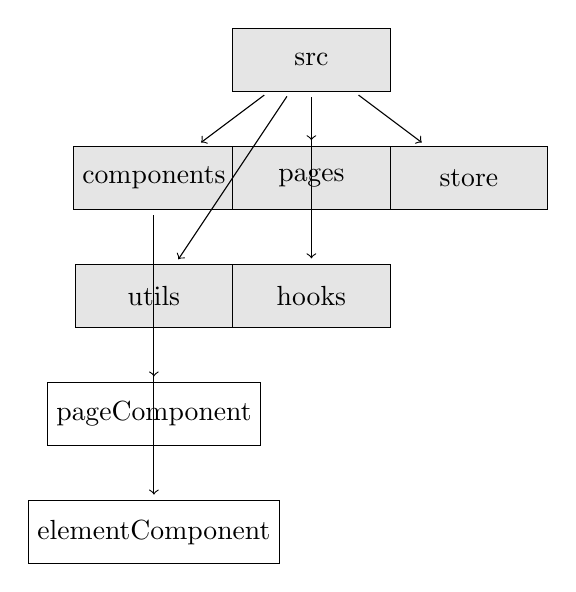
\begin{tikzpicture}[
    file/.style={draw, rectangle, minimum width=2cm, minimum height=0.8cm},
    folder/.style={draw, rectangle, minimum width=2cm, minimum height=0.8cm, fill=gray!20},
    arrow/.style={->, shorten >=2pt, shorten <=2pt}
]

% Folders
\node[folder] (src) at (0,0) {src};
\node[folder] (components) at (-2,-1.5) {components};
\node[folder] (pages) at (0,-1.5) {pages};
\node[folder] (store) at (2,-1.5) {store};
\node[folder] (utils) at (-2,-3) {utils};
\node[folder] (hooks) at (0,-3) {hooks};

% Files
\node[file] (pageComponent) at (-2,-4.5) {pageComponent};
\node[file] (elementComponent) at (-2,-6) {elementComponent};
% ... add more files

% Connections
\draw[arrow] (src) -- (components);
\draw[arrow] (src) -- (pages);
\draw[arrow] (src) -- (store);
\draw[arrow] (src) -- (utils);
\draw[arrow] (src) -- (hooks);
\draw[arrow] (components) -- (pageComponent);
\draw[arrow] (components) -- (elementComponent);
% ... add more connections

\end{tikzpicture}



\pagebreak
\subsubsection{Back-end}
The backend uses the dotNet framework. The development language using the C\# language.

In this project, the backend uses the Onion Architecture.
The Onion Architecture is a typically layered architecture, 
where each layer depends on the inner layer and provides interfaces to the outer layer.
The outer layer provides services to the outermost layer 
and other modules in the same layer based on the interfaces of the inner layer.

From inner to outer, the layers are: Domain, Application, Infrastructure, Presentation.
The Domain layer is the core layer and the innermost layer, used to define domain models, 
which are the business models.
It includes domain models and domain service interfaces.
Domain models are used to define the business models, 
which are the entities in the entity-relationship model and their attributes.
Domain service interfaces are used to define the business services, 
which are the relationships between entities in the entity-relationship model.

The Application layer is the application layer, 
used to define application services, which are the business logic.
It includes domain service implementations and application service interfaces.
Domain service implementations implement the methods of the inner layer's domain service 
interfaces and implement the business logic of the domain models.
Application service interfaces are used to define application services, 
which are the business logic.
It includes but is not limited to database interfaces, testing interfaces, 
HTTP API interfaces, MQTT interfaces, etc.

The Infrastructure layer is the infrastructure layer, used to define infrastructure.
It includes database implementations, testing implementations, 
HTTP API implementations, MQTT implementations, etc.
Database implementations implement the database interfaces 
and provide CRUD services for the database.
Testing implementations implement the testing interfaces 
and provide services for unit testing and integration testing.
HTTP API implementations implement the HTTP API interfaces 
and provide CRUD operations for HTTP APIs.
MQTT implementations implement the MQTT interfaces 
and provide CRUD operations for MQTT.

The Presentation layer is the presentation layer, used to define presentation logic, 
such as interfaces and pages. Since this is a backend project,
data presentation and control are handled by the frontend, 
so this layer is not needed.



\pagebreak
\subsubsection{Data communication and storage}
% 关于本项目的数据通信与数据存储的设计, 包括数据通信的协议, 数据存储的设计等
% 关于数据通信的设计:
% 1. 通信协议的选择
% 自前端向后端发送的数据, 有三种传输的数据类型, 
% 一种是普通的增删改查的请求, 对数据传输的时效性要求不高, 但是对数据的准确性, 完整性, 有序性, 安全性有一定的要求,
% 这种数据的传输, 采用 HTTP 协议, 以及 RESTful API 的设计. 可以有效的保证对数据传输的以上要求.
% 一种是对数据通道的创建和流媒体数据的传输, 对数据传输的时效性, 安全性要求较高, 这种数据的传输, 采用 WebRTC 协议, 以及 MQTT 协议.
% 配合可以快速解码的 flatbuffers 协议, 可以有效的保证对数据传输的以上要求.
% 最后一种是对设备的状态信息和操作信息的传输, 对完整性, 有序性, 安全性都有较高的要求, 这种数据的传输, 采用 MQTT 协议
% 同时也使用了 flatbuffers 协议.
% 
% 2. 数据通信的通信架构和通信流程
% 本项目的数据通信的通信架构, 是基于前后端分离的架构, 前端使用 React 框架, 后端使用 dotnet 框架.
% 当前端需要向后端发送数据的时候, 前端会向后端发送 HTTP 请求, 后端接收到 HTTP 请求之后, 会根据请求的数据类型,
% 选择不同的数据处理方式, 对于普通的增删改查的请求, 后端会根据 RESTful API 的设计, 对数据进行增删改查的操作,
% 对于对数据通道的创建和流媒体数据的传输, 后端会根据 WebRTC 协议, 对数据通道进行创建, 并且帮助前端和设备建立数据通道,
% 当数据通道建立后, 前端和设备之间则使用 flatbuffer 的数据格式对流媒体数据进行传输,
% 对于设备的状态信息和操作信息的传输, 前端会直接向 MQTT broker 发送 MQTT 请求, 
% 设备会在其自身的固件中监听相关的 MQTT 请求, 并且返回相关的数据.
% 
% 3. 数据通信的格式
% 本项目的数据通信的格式, 有三种, 
% 一种是 HTTP 协议, 
% 使用 json 格式对数据进行传输,
% 一种是 WebRTC 协议, 
% 使用 flatbuffers 格式对数据进行传输,
% 一种是 MQTT 协议.
% 使用 flatbuffers 格式对数据进行传输,
% 
% 关于数据存储的设计:
% 1. 数据存储的数据库的选择
% 本项目的数据存储的数据库的选择, 使用了轻量级的数据库 SQLite,
% SQLite 是一个进程内的库, 实现了自给自足的, 无服务器的, 零配置的, 事务性的 SQL 数据库引擎.
% 这是因为整个项目的目的是为了实现前端与设备之间的数据通信, 对于数据库数据的增删改查操作的要求不高,
% 数据量较小, 且对于数据库的数据的事务性要求不高, 所以选择了 SQLite 数据库.
% 2. 项目前后端的数据结构的设计
% 在本项目中, 前端由于使用了 React 框架, 所以前端的数据结构的设计, 使用了基于状态的数据结构的设计,
% 每个组件或者数据集都包含一个状态对象, 这个状态对象的属性就是组件的各个状态. 
% 使用状态对象的原因是, 可以方便的对状态进行管理, 采用对象-属性的形式, 可以方便的针对不同组件的同类状态进行区分,
% 由于跨组件的状态是由 redux 进行管理的, 这种状态对象的设计, 可以更搞笑的对状态进行更新和传递.
% 后端由于使用了 dotnet 框架, 所以后端的数据结构的设计, 使用了基于类的数据结构的设计,
% 采用了面向对象的编程思想, 对数据进行了封装, 使得数据的传输更加的安全, 有序, 完整.


\pagebreak

% \subsection{Domain model}
% \documentclass[]{article}
\usepackage{graphicx}
\usepackage{amsmath}
\usepackage{tikz}

% libaries
\usetikzlibrary{shapes,arrows}

%Define the listing package
\usepackage{listings} %code highlighter
\usepackage{color} %use color
\definecolor{mygreen}{rgb}{0,0.6,0}
\definecolor{mygray}{rgb}{0.5,0.5,0.5}
\definecolor{mymauve}{rgb}{0.58,0,0.82}

%Customize a bit the look
\lstset{ %
backgroundcolor=\color{white}, % choose the background color; you must add \usepackage{color} or \usepackage{xcolor}
basicstyle=\footnotesize, % the size of the fonts that are used for the code
breakatwhitespace=false, % sets if automatic breaks should only happen at whitespace
breaklines=true, % sets automatic line breaking
captionpos=b, % sets the caption-position to bottom
commentstyle=\color{mygreen}, % comment style
deletekeywords={...}, % if you want to delete keywords from the given language
escapeinside={\%*}{*)}, % if you want to add LaTeX within your code
extendedchars=true, % lets you use non-ASCII characters; for 8-bits encodings only, does not work with UTF-8
frame=single, % adds a frame around the code
keepspaces=true, % keeps spaces in text, useful for keeping indentation of code (possibly needs columns=flexible)
keywordstyle=\color{blue}, % keyword style
% language=Octave, % the language of the code
morekeywords={*,...}, % if you want to add more keywords to the set
numbers=left, % where to put the line-numbers; possible values are (none, left, right)
numbersep=5pt, % how far the line-numbers are from the code
numberstyle=\tiny\color{mygray}, % the style that is used for the line-numbers
rulecolor=\color{black}, % if not set, the frame-color may be changed on line-breaks within not-black text (e.g. comments (green here))
showspaces=false, % show spaces everywhere adding particular underscores; it overrides 'showstringspaces'
showstringspaces=false, % underline spaces within strings only
showtabs=false, % show tabs within strings adding particular underscores
stepnumber=1, % the step between two line-numbers. If it's 1, each line will be numbered
stringstyle=\color{mymauve}, % string literal style
tabsize=2, % sets default tabsize to 2 spaces
title=\lstname % show the filename of files included with \lstinputlisting; also try caption instead of title
}

\definecolor{darkgray}{rgb}{.4,.4,.4}
\definecolor{purple}{rgb}{0.65, 0.12, 0.82}

\lstdefinelanguage{React}{
keywords={const, typeof, new, true, false, catch, function, return, null, catch, switch, var, if, in, while, do, else, case, break},
keywordstyle=\color{blue}\bfseries,
ndkeywords={class, export, boolean, throw, implements, import, this},
ndkeywordstyle=\color{darkgray}\bfseries,
identifierstyle=\color{mygreen},
sensitive=false,
comment=[l]{//},
morecomment=[s]{/*}{*/},
commentstyle=\color{purple}\ttfamily,
string=[b]{"}{'}{`},
stringstyle=\color{red}\ttfamily,
morestring=[b]',
morestring=[b]",
morestring=[b]`',
}

\lstdefinelanguage{CSharp}{
keywords={const, typeof, new, true, false, catch, function, return, null, catch, switch, var, if, in, while, do, else, case, break},
keywordstyle=\color{blue}\bfseries,
ndkeywords={class, export, boolean, throw, implements, import, this},
ndkeywordstyle=\color{darkgray}\bfseries,
identifierstyle=\color{mygreen},
sensitive=false,
comment=[l]{//},
morecomment=[s]{/*}{*/},
commentstyle=\color{purple}\ttfamily,
string=[b]{"}{'}{`},
stringstyle=\color{red}\ttfamily,
morestring=[b]',
morestring=[b]",
morestring=[b]`',
}

\lstset{
language=React,
extendedchars=true,
basicstyle=\footnotesize\ttfamily,
showstringspaces=false,
showspaces=false,
numbers=left,
numberstyle=\footnotesize,
numbersep=9pt,
tabsize=2,
breaklines=true,
showtabs=false,
captionpos=b
}

\lstset{
language=CSharp,
extendedchars=true,
basicstyle=\footnotesize\ttfamily,
showstringspaces=false,
showspaces=false,
numbers=left,
numberstyle=\footnotesize,
numbersep=9pt,
tabsize=2,
breaklines=true,
showtabs=false,
captionpos=b
}

% \usepackage{cite} % Add this line for citation

% \bibliographystyle{plain}

\title{
The implementation of BifrostConnect Front-end scope, 
re-design and development with the relevant back-end support develop.
}
\author{
    Fei Gu \\
    Erhvervs Akademi Sydvest \\
    Computer Science 21\\
    }
\date{\today}

\begin{document}

% Front page
\maketitle
\begin{center}
    Supervisor: Henrik Boulund Meng Hansen \\
    Company: BifrostConnect \\
    Engineering Director: Jasper Wass \\
\end{center}
\tableofcontents
\pagebreak


% The introduction
\section{Introduction}
\subsection{Background}\input{sections/introduction/background.tex}
\subsection{The company}\input{sections/introduction/aboutCompany}
\subsection{The project}\input{sections/introduction/aboutProject}
\pagebreak

% The problem statement
\section{Problem Statement}
\subsection{Statement}
\input{sections/problemStatement/statement}
\subsection{Situation}
\input{sections/problemStatement/situation}
\subsection{Potential Solution}
\input{sections/problemStatement/potentialSolution}
\pagebreak

% Requirement analysis
\section{Requirement Analysis}
\input{sections/requirementAnalysis/index}

\subsection{Stakeholders}
\input{sections/requirementAnalysis/stakeholders/index}

\subsection{Business Domain}
\input{sections/requirementAnalysis/bussinesDomain/index}

\subsection{Scope}
\input{sections/requirementAnalysis/scope}

\subsection{Goals}
\input{sections/requirementAnalysis/goals}
\pagebreak

% Software Design
\section{Software Design}
% developement methods
\subsection{Software Development Methods}
\input{sections/softwareDevelopmentMethods/index}
\subsubsection{Agile Software Development}
\input{sections/softwareDevelopmentMethods/agileSoftwareDevelopment/index}
\subsubsection{Feature Driven Development}
\input{sections/softwareDevelopmentMethods/featureDrivenDevelopment/index}

\pagebreak

% Technology seslection
\subsection{Technology selection}
\input{sections/softwareDesign/technologySelection/index}
\subsubsection{Front-end}
\input{sections/softwareDesign/technologySelection/frontEnd}            
\subsubsection{Back-end}
\input{sections/softwareDesign/technologySelection/backEnd}            
\subsubsection{Database}
\input{sections/softwareDesign/technologySelection/database}
\subsubsection{Data communication}
\input{sections/softwareDesign/technologySelection/dataCommunication}            
\subsubsection{DevOps}
\input{sections/softwareDesign/technologySelection/devOps}
\pagebreak

% Architecture design
\subsection{Architecture design}
\input{sections/softwareDesign/architectureDesign/index}
\pagebreak
\subsubsection{Front-end}
\input{sections/softwareDesign/architectureDesign/frontEndArchitecture}
\pagebreak
\subsubsection{Back-end}
\input{sections/softwareDesign/architectureDesign/backEndArchitecture}
\pagebreak
\subsubsection{Data communication and storage}
\input{sections/softwareDesign/architectureDesign/dataCommunicationArchitecture}
\pagebreak

% \subsection{Domain model}
% \input{sections/softwareDesign/domainModel/index}
% \subsection{Database design}
% % 数据库领域模型 ER 图
% % 包括表和字段的设置.
% % 对于私有键和外键的设置.

% \subsection{Back-end design}
% % 后端对象模型
% % 以及对于对象模型的增删改查
% % 以及相关的其他服务的设计`'

% \subsection{Front-end design}
% % 对于前端的页面结构的设计 
% % 页面的状态的设计, 交互设计

% \subsection{FlatBuffers design}
% % schema 的设计

\subsection{DevOps CI/CD process design}
\input{sections/softwareDesign/devOpsDesign/index}
\subsubsection{Continuous Integration}
\input{sections/softwareDesign/devOpsDesign/continuousIntegration/index}
\subsubsection{Continuous Delivery}
\input{sections/softwareDesign/devOpsDesign/continuousDelivery/index}
\subsubsection{Continuous Deployment}
\input{sections/softwareDesign/devOpsDesign/continuousDeployment/index}
\pagebreak

\section{Software Development} 
\input{sections/softwareDevelopment/index}
\subsection{Overall development}
\input{sections/softwareDevelopment/overallDevelopement/index}
\subsubsection{Front-end}
\input{sections/softwareDevelopment/overallDevelopement/frontEnd/index}
\subsubsection{Back-end}
\input{sections/softwareDevelopment/overallDevelopement/backEnd/index}
\subsubsection{DevOps}
\input{sections/softwareDevelopment/overallDevelopement/devOps/index}
\subsection{Feature development} 
\input{sections/softwareDevelopment/featureDevelopment/index}
\subsubsection{Use Case 1}
\input{sections/softwareDevelopment/featureDevelopment/useCase1/index}
\subsubsection{Feature 1}
\input{sections/softwareDevelopment/featureDevelopment/feature/feature1.tex}
\pagebreak
\section{Conclusion} 
\subsection{Result}
Since the project is still in progress, the result is not available yet.
So far, basic structure of this project has been built. But the most features 
are not implemented yet. 
\subsection{Discussion}
As a single developer for this project, I am confident what I have done so far.
And I can say I understand the most of the knowledge I have used in this project, 
which also means I can explain all the part of the project. 
But this project also relevant some of the complex knowledge which I have to continue 
to study and practice.
\subsection{Future Work}
The future work is to implement the rest of the features. 
Including the most important part which is the 'create session' feature.
\pagebreak
% \bibliography{bibliography}
\pagebreak
% \begin{appendices}
%     \section{Appendix}
% \end{appendices} 
\end{document}
% \subsection{Database design}
% % 数据库领域模型 ER 图
% % 包括表和字段的设置.
% % 对于私有键和外键的设置.

% \subsection{Back-end design}
% % 后端对象模型
% % 以及对于对象模型的增删改查
% % 以及相关的其他服务的设计`'

% \subsection{Front-end design}
% % 对于前端的页面结构的设计 
% % 页面的状态的设计, 交互设计

% \subsection{FlatBuffers design}
% % schema 的设计

\subsection{DevOps CI/CD process design}
\documentclass[]{article}
\usepackage{graphicx}
\usepackage{amsmath}
\usepackage{tikz}

% libaries
\usetikzlibrary{shapes,arrows}

%Define the listing package
\usepackage{listings} %code highlighter
\usepackage{color} %use color
\definecolor{mygreen}{rgb}{0,0.6,0}
\definecolor{mygray}{rgb}{0.5,0.5,0.5}
\definecolor{mymauve}{rgb}{0.58,0,0.82}

%Customize a bit the look
\lstset{ %
backgroundcolor=\color{white}, % choose the background color; you must add \usepackage{color} or \usepackage{xcolor}
basicstyle=\footnotesize, % the size of the fonts that are used for the code
breakatwhitespace=false, % sets if automatic breaks should only happen at whitespace
breaklines=true, % sets automatic line breaking
captionpos=b, % sets the caption-position to bottom
commentstyle=\color{mygreen}, % comment style
deletekeywords={...}, % if you want to delete keywords from the given language
escapeinside={\%*}{*)}, % if you want to add LaTeX within your code
extendedchars=true, % lets you use non-ASCII characters; for 8-bits encodings only, does not work with UTF-8
frame=single, % adds a frame around the code
keepspaces=true, % keeps spaces in text, useful for keeping indentation of code (possibly needs columns=flexible)
keywordstyle=\color{blue}, % keyword style
% language=Octave, % the language of the code
morekeywords={*,...}, % if you want to add more keywords to the set
numbers=left, % where to put the line-numbers; possible values are (none, left, right)
numbersep=5pt, % how far the line-numbers are from the code
numberstyle=\tiny\color{mygray}, % the style that is used for the line-numbers
rulecolor=\color{black}, % if not set, the frame-color may be changed on line-breaks within not-black text (e.g. comments (green here))
showspaces=false, % show spaces everywhere adding particular underscores; it overrides 'showstringspaces'
showstringspaces=false, % underline spaces within strings only
showtabs=false, % show tabs within strings adding particular underscores
stepnumber=1, % the step between two line-numbers. If it's 1, each line will be numbered
stringstyle=\color{mymauve}, % string literal style
tabsize=2, % sets default tabsize to 2 spaces
title=\lstname % show the filename of files included with \lstinputlisting; also try caption instead of title
}

\definecolor{darkgray}{rgb}{.4,.4,.4}
\definecolor{purple}{rgb}{0.65, 0.12, 0.82}

\lstdefinelanguage{React}{
keywords={const, typeof, new, true, false, catch, function, return, null, catch, switch, var, if, in, while, do, else, case, break},
keywordstyle=\color{blue}\bfseries,
ndkeywords={class, export, boolean, throw, implements, import, this},
ndkeywordstyle=\color{darkgray}\bfseries,
identifierstyle=\color{mygreen},
sensitive=false,
comment=[l]{//},
morecomment=[s]{/*}{*/},
commentstyle=\color{purple}\ttfamily,
string=[b]{"}{'}{`},
stringstyle=\color{red}\ttfamily,
morestring=[b]',
morestring=[b]",
morestring=[b]`',
}

\lstdefinelanguage{CSharp}{
keywords={const, typeof, new, true, false, catch, function, return, null, catch, switch, var, if, in, while, do, else, case, break},
keywordstyle=\color{blue}\bfseries,
ndkeywords={class, export, boolean, throw, implements, import, this},
ndkeywordstyle=\color{darkgray}\bfseries,
identifierstyle=\color{mygreen},
sensitive=false,
comment=[l]{//},
morecomment=[s]{/*}{*/},
commentstyle=\color{purple}\ttfamily,
string=[b]{"}{'}{`},
stringstyle=\color{red}\ttfamily,
morestring=[b]',
morestring=[b]",
morestring=[b]`',
}

\lstset{
language=React,
extendedchars=true,
basicstyle=\footnotesize\ttfamily,
showstringspaces=false,
showspaces=false,
numbers=left,
numberstyle=\footnotesize,
numbersep=9pt,
tabsize=2,
breaklines=true,
showtabs=false,
captionpos=b
}

\lstset{
language=CSharp,
extendedchars=true,
basicstyle=\footnotesize\ttfamily,
showstringspaces=false,
showspaces=false,
numbers=left,
numberstyle=\footnotesize,
numbersep=9pt,
tabsize=2,
breaklines=true,
showtabs=false,
captionpos=b
}

% \usepackage{cite} % Add this line for citation

% \bibliographystyle{plain}

\title{
The implementation of BifrostConnect Front-end scope, 
re-design and development with the relevant back-end support develop.
}
\author{
    Fei Gu \\
    Erhvervs Akademi Sydvest \\
    Computer Science 21\\
    }
\date{\today}

\begin{document}

% Front page
\maketitle
\begin{center}
    Supervisor: Henrik Boulund Meng Hansen \\
    Company: BifrostConnect \\
    Engineering Director: Jasper Wass \\
\end{center}
\tableofcontents
\pagebreak


% The introduction
\section{Introduction}
\subsection{Background}\input{sections/introduction/background.tex}
\subsection{The company}\input{sections/introduction/aboutCompany}
\subsection{The project}\input{sections/introduction/aboutProject}
\pagebreak

% The problem statement
\section{Problem Statement}
\subsection{Statement}
\input{sections/problemStatement/statement}
\subsection{Situation}
\input{sections/problemStatement/situation}
\subsection{Potential Solution}
\input{sections/problemStatement/potentialSolution}
\pagebreak

% Requirement analysis
\section{Requirement Analysis}
\input{sections/requirementAnalysis/index}

\subsection{Stakeholders}
\input{sections/requirementAnalysis/stakeholders/index}

\subsection{Business Domain}
\input{sections/requirementAnalysis/bussinesDomain/index}

\subsection{Scope}
\input{sections/requirementAnalysis/scope}

\subsection{Goals}
\input{sections/requirementAnalysis/goals}
\pagebreak

% Software Design
\section{Software Design}
% developement methods
\subsection{Software Development Methods}
\input{sections/softwareDevelopmentMethods/index}
\subsubsection{Agile Software Development}
\input{sections/softwareDevelopmentMethods/agileSoftwareDevelopment/index}
\subsubsection{Feature Driven Development}
\input{sections/softwareDevelopmentMethods/featureDrivenDevelopment/index}

\pagebreak

% Technology seslection
\subsection{Technology selection}
\input{sections/softwareDesign/technologySelection/index}
\subsubsection{Front-end}
\input{sections/softwareDesign/technologySelection/frontEnd}            
\subsubsection{Back-end}
\input{sections/softwareDesign/technologySelection/backEnd}            
\subsubsection{Database}
\input{sections/softwareDesign/technologySelection/database}
\subsubsection{Data communication}
\input{sections/softwareDesign/technologySelection/dataCommunication}            
\subsubsection{DevOps}
\input{sections/softwareDesign/technologySelection/devOps}
\pagebreak

% Architecture design
\subsection{Architecture design}
\input{sections/softwareDesign/architectureDesign/index}
\pagebreak
\subsubsection{Front-end}
\input{sections/softwareDesign/architectureDesign/frontEndArchitecture}
\pagebreak
\subsubsection{Back-end}
\input{sections/softwareDesign/architectureDesign/backEndArchitecture}
\pagebreak
\subsubsection{Data communication and storage}
\input{sections/softwareDesign/architectureDesign/dataCommunicationArchitecture}
\pagebreak

% \subsection{Domain model}
% \input{sections/softwareDesign/domainModel/index}
% \subsection{Database design}
% % 数据库领域模型 ER 图
% % 包括表和字段的设置.
% % 对于私有键和外键的设置.

% \subsection{Back-end design}
% % 后端对象模型
% % 以及对于对象模型的增删改查
% % 以及相关的其他服务的设计`'

% \subsection{Front-end design}
% % 对于前端的页面结构的设计 
% % 页面的状态的设计, 交互设计

% \subsection{FlatBuffers design}
% % schema 的设计

\subsection{DevOps CI/CD process design}
\input{sections/softwareDesign/devOpsDesign/index}
\subsubsection{Continuous Integration}
\input{sections/softwareDesign/devOpsDesign/continuousIntegration/index}
\subsubsection{Continuous Delivery}
\input{sections/softwareDesign/devOpsDesign/continuousDelivery/index}
\subsubsection{Continuous Deployment}
\input{sections/softwareDesign/devOpsDesign/continuousDeployment/index}
\pagebreak

\section{Software Development} 
\input{sections/softwareDevelopment/index}
\subsection{Overall development}
\input{sections/softwareDevelopment/overallDevelopement/index}
\subsubsection{Front-end}
\input{sections/softwareDevelopment/overallDevelopement/frontEnd/index}
\subsubsection{Back-end}
\input{sections/softwareDevelopment/overallDevelopement/backEnd/index}
\subsubsection{DevOps}
\input{sections/softwareDevelopment/overallDevelopement/devOps/index}
\subsection{Feature development} 
\input{sections/softwareDevelopment/featureDevelopment/index}
\subsubsection{Use Case 1}
\input{sections/softwareDevelopment/featureDevelopment/useCase1/index}
\subsubsection{Feature 1}
\input{sections/softwareDevelopment/featureDevelopment/feature/feature1.tex}
\pagebreak
\section{Conclusion} 
\subsection{Result}
Since the project is still in progress, the result is not available yet.
So far, basic structure of this project has been built. But the most features 
are not implemented yet. 
\subsection{Discussion}
As a single developer for this project, I am confident what I have done so far.
And I can say I understand the most of the knowledge I have used in this project, 
which also means I can explain all the part of the project. 
But this project also relevant some of the complex knowledge which I have to continue 
to study and practice.
\subsection{Future Work}
The future work is to implement the rest of the features. 
Including the most important part which is the 'create session' feature.
\pagebreak
% \bibliography{bibliography}
\pagebreak
% \begin{appendices}
%     \section{Appendix}
% \end{appendices} 
\end{document}
\subsubsection{Continuous Integration}
\documentclass[]{article}
\usepackage{graphicx}
\usepackage{amsmath}
\usepackage{tikz}

% libaries
\usetikzlibrary{shapes,arrows}

%Define the listing package
\usepackage{listings} %code highlighter
\usepackage{color} %use color
\definecolor{mygreen}{rgb}{0,0.6,0}
\definecolor{mygray}{rgb}{0.5,0.5,0.5}
\definecolor{mymauve}{rgb}{0.58,0,0.82}

%Customize a bit the look
\lstset{ %
backgroundcolor=\color{white}, % choose the background color; you must add \usepackage{color} or \usepackage{xcolor}
basicstyle=\footnotesize, % the size of the fonts that are used for the code
breakatwhitespace=false, % sets if automatic breaks should only happen at whitespace
breaklines=true, % sets automatic line breaking
captionpos=b, % sets the caption-position to bottom
commentstyle=\color{mygreen}, % comment style
deletekeywords={...}, % if you want to delete keywords from the given language
escapeinside={\%*}{*)}, % if you want to add LaTeX within your code
extendedchars=true, % lets you use non-ASCII characters; for 8-bits encodings only, does not work with UTF-8
frame=single, % adds a frame around the code
keepspaces=true, % keeps spaces in text, useful for keeping indentation of code (possibly needs columns=flexible)
keywordstyle=\color{blue}, % keyword style
% language=Octave, % the language of the code
morekeywords={*,...}, % if you want to add more keywords to the set
numbers=left, % where to put the line-numbers; possible values are (none, left, right)
numbersep=5pt, % how far the line-numbers are from the code
numberstyle=\tiny\color{mygray}, % the style that is used for the line-numbers
rulecolor=\color{black}, % if not set, the frame-color may be changed on line-breaks within not-black text (e.g. comments (green here))
showspaces=false, % show spaces everywhere adding particular underscores; it overrides 'showstringspaces'
showstringspaces=false, % underline spaces within strings only
showtabs=false, % show tabs within strings adding particular underscores
stepnumber=1, % the step between two line-numbers. If it's 1, each line will be numbered
stringstyle=\color{mymauve}, % string literal style
tabsize=2, % sets default tabsize to 2 spaces
title=\lstname % show the filename of files included with \lstinputlisting; also try caption instead of title
}

\definecolor{darkgray}{rgb}{.4,.4,.4}
\definecolor{purple}{rgb}{0.65, 0.12, 0.82}

\lstdefinelanguage{React}{
keywords={const, typeof, new, true, false, catch, function, return, null, catch, switch, var, if, in, while, do, else, case, break},
keywordstyle=\color{blue}\bfseries,
ndkeywords={class, export, boolean, throw, implements, import, this},
ndkeywordstyle=\color{darkgray}\bfseries,
identifierstyle=\color{mygreen},
sensitive=false,
comment=[l]{//},
morecomment=[s]{/*}{*/},
commentstyle=\color{purple}\ttfamily,
string=[b]{"}{'}{`},
stringstyle=\color{red}\ttfamily,
morestring=[b]',
morestring=[b]",
morestring=[b]`',
}

\lstdefinelanguage{CSharp}{
keywords={const, typeof, new, true, false, catch, function, return, null, catch, switch, var, if, in, while, do, else, case, break},
keywordstyle=\color{blue}\bfseries,
ndkeywords={class, export, boolean, throw, implements, import, this},
ndkeywordstyle=\color{darkgray}\bfseries,
identifierstyle=\color{mygreen},
sensitive=false,
comment=[l]{//},
morecomment=[s]{/*}{*/},
commentstyle=\color{purple}\ttfamily,
string=[b]{"}{'}{`},
stringstyle=\color{red}\ttfamily,
morestring=[b]',
morestring=[b]",
morestring=[b]`',
}

\lstset{
language=React,
extendedchars=true,
basicstyle=\footnotesize\ttfamily,
showstringspaces=false,
showspaces=false,
numbers=left,
numberstyle=\footnotesize,
numbersep=9pt,
tabsize=2,
breaklines=true,
showtabs=false,
captionpos=b
}

\lstset{
language=CSharp,
extendedchars=true,
basicstyle=\footnotesize\ttfamily,
showstringspaces=false,
showspaces=false,
numbers=left,
numberstyle=\footnotesize,
numbersep=9pt,
tabsize=2,
breaklines=true,
showtabs=false,
captionpos=b
}

% \usepackage{cite} % Add this line for citation

% \bibliographystyle{plain}

\title{
The implementation of BifrostConnect Front-end scope, 
re-design and development with the relevant back-end support develop.
}
\author{
    Fei Gu \\
    Erhvervs Akademi Sydvest \\
    Computer Science 21\\
    }
\date{\today}

\begin{document}

% Front page
\maketitle
\begin{center}
    Supervisor: Henrik Boulund Meng Hansen \\
    Company: BifrostConnect \\
    Engineering Director: Jasper Wass \\
\end{center}
\tableofcontents
\pagebreak


% The introduction
\section{Introduction}
\subsection{Background}\input{sections/introduction/background.tex}
\subsection{The company}\input{sections/introduction/aboutCompany}
\subsection{The project}\input{sections/introduction/aboutProject}
\pagebreak

% The problem statement
\section{Problem Statement}
\subsection{Statement}
\input{sections/problemStatement/statement}
\subsection{Situation}
\input{sections/problemStatement/situation}
\subsection{Potential Solution}
\input{sections/problemStatement/potentialSolution}
\pagebreak

% Requirement analysis
\section{Requirement Analysis}
\input{sections/requirementAnalysis/index}

\subsection{Stakeholders}
\input{sections/requirementAnalysis/stakeholders/index}

\subsection{Business Domain}
\input{sections/requirementAnalysis/bussinesDomain/index}

\subsection{Scope}
\input{sections/requirementAnalysis/scope}

\subsection{Goals}
\input{sections/requirementAnalysis/goals}
\pagebreak

% Software Design
\section{Software Design}
% developement methods
\subsection{Software Development Methods}
\input{sections/softwareDevelopmentMethods/index}
\subsubsection{Agile Software Development}
\input{sections/softwareDevelopmentMethods/agileSoftwareDevelopment/index}
\subsubsection{Feature Driven Development}
\input{sections/softwareDevelopmentMethods/featureDrivenDevelopment/index}

\pagebreak

% Technology seslection
\subsection{Technology selection}
\input{sections/softwareDesign/technologySelection/index}
\subsubsection{Front-end}
\input{sections/softwareDesign/technologySelection/frontEnd}            
\subsubsection{Back-end}
\input{sections/softwareDesign/technologySelection/backEnd}            
\subsubsection{Database}
\input{sections/softwareDesign/technologySelection/database}
\subsubsection{Data communication}
\input{sections/softwareDesign/technologySelection/dataCommunication}            
\subsubsection{DevOps}
\input{sections/softwareDesign/technologySelection/devOps}
\pagebreak

% Architecture design
\subsection{Architecture design}
\input{sections/softwareDesign/architectureDesign/index}
\pagebreak
\subsubsection{Front-end}
\input{sections/softwareDesign/architectureDesign/frontEndArchitecture}
\pagebreak
\subsubsection{Back-end}
\input{sections/softwareDesign/architectureDesign/backEndArchitecture}
\pagebreak
\subsubsection{Data communication and storage}
\input{sections/softwareDesign/architectureDesign/dataCommunicationArchitecture}
\pagebreak

% \subsection{Domain model}
% \input{sections/softwareDesign/domainModel/index}
% \subsection{Database design}
% % 数据库领域模型 ER 图
% % 包括表和字段的设置.
% % 对于私有键和外键的设置.

% \subsection{Back-end design}
% % 后端对象模型
% % 以及对于对象模型的增删改查
% % 以及相关的其他服务的设计`'

% \subsection{Front-end design}
% % 对于前端的页面结构的设计 
% % 页面的状态的设计, 交互设计

% \subsection{FlatBuffers design}
% % schema 的设计

\subsection{DevOps CI/CD process design}
\input{sections/softwareDesign/devOpsDesign/index}
\subsubsection{Continuous Integration}
\input{sections/softwareDesign/devOpsDesign/continuousIntegration/index}
\subsubsection{Continuous Delivery}
\input{sections/softwareDesign/devOpsDesign/continuousDelivery/index}
\subsubsection{Continuous Deployment}
\input{sections/softwareDesign/devOpsDesign/continuousDeployment/index}
\pagebreak

\section{Software Development} 
\input{sections/softwareDevelopment/index}
\subsection{Overall development}
\input{sections/softwareDevelopment/overallDevelopement/index}
\subsubsection{Front-end}
\input{sections/softwareDevelopment/overallDevelopement/frontEnd/index}
\subsubsection{Back-end}
\input{sections/softwareDevelopment/overallDevelopement/backEnd/index}
\subsubsection{DevOps}
\input{sections/softwareDevelopment/overallDevelopement/devOps/index}
\subsection{Feature development} 
\input{sections/softwareDevelopment/featureDevelopment/index}
\subsubsection{Use Case 1}
\input{sections/softwareDevelopment/featureDevelopment/useCase1/index}
\subsubsection{Feature 1}
\input{sections/softwareDevelopment/featureDevelopment/feature/feature1.tex}
\pagebreak
\section{Conclusion} 
\subsection{Result}
Since the project is still in progress, the result is not available yet.
So far, basic structure of this project has been built. But the most features 
are not implemented yet. 
\subsection{Discussion}
As a single developer for this project, I am confident what I have done so far.
And I can say I understand the most of the knowledge I have used in this project, 
which also means I can explain all the part of the project. 
But this project also relevant some of the complex knowledge which I have to continue 
to study and practice.
\subsection{Future Work}
The future work is to implement the rest of the features. 
Including the most important part which is the 'create session' feature.
\pagebreak
% \bibliography{bibliography}
\pagebreak
% \begin{appendices}
%     \section{Appendix}
% \end{appendices} 
\end{document}
\subsubsection{Continuous Delivery}
\documentclass[]{article}
\usepackage{graphicx}
\usepackage{amsmath}
\usepackage{tikz}

% libaries
\usetikzlibrary{shapes,arrows}

%Define the listing package
\usepackage{listings} %code highlighter
\usepackage{color} %use color
\definecolor{mygreen}{rgb}{0,0.6,0}
\definecolor{mygray}{rgb}{0.5,0.5,0.5}
\definecolor{mymauve}{rgb}{0.58,0,0.82}

%Customize a bit the look
\lstset{ %
backgroundcolor=\color{white}, % choose the background color; you must add \usepackage{color} or \usepackage{xcolor}
basicstyle=\footnotesize, % the size of the fonts that are used for the code
breakatwhitespace=false, % sets if automatic breaks should only happen at whitespace
breaklines=true, % sets automatic line breaking
captionpos=b, % sets the caption-position to bottom
commentstyle=\color{mygreen}, % comment style
deletekeywords={...}, % if you want to delete keywords from the given language
escapeinside={\%*}{*)}, % if you want to add LaTeX within your code
extendedchars=true, % lets you use non-ASCII characters; for 8-bits encodings only, does not work with UTF-8
frame=single, % adds a frame around the code
keepspaces=true, % keeps spaces in text, useful for keeping indentation of code (possibly needs columns=flexible)
keywordstyle=\color{blue}, % keyword style
% language=Octave, % the language of the code
morekeywords={*,...}, % if you want to add more keywords to the set
numbers=left, % where to put the line-numbers; possible values are (none, left, right)
numbersep=5pt, % how far the line-numbers are from the code
numberstyle=\tiny\color{mygray}, % the style that is used for the line-numbers
rulecolor=\color{black}, % if not set, the frame-color may be changed on line-breaks within not-black text (e.g. comments (green here))
showspaces=false, % show spaces everywhere adding particular underscores; it overrides 'showstringspaces'
showstringspaces=false, % underline spaces within strings only
showtabs=false, % show tabs within strings adding particular underscores
stepnumber=1, % the step between two line-numbers. If it's 1, each line will be numbered
stringstyle=\color{mymauve}, % string literal style
tabsize=2, % sets default tabsize to 2 spaces
title=\lstname % show the filename of files included with \lstinputlisting; also try caption instead of title
}

\definecolor{darkgray}{rgb}{.4,.4,.4}
\definecolor{purple}{rgb}{0.65, 0.12, 0.82}

\lstdefinelanguage{React}{
keywords={const, typeof, new, true, false, catch, function, return, null, catch, switch, var, if, in, while, do, else, case, break},
keywordstyle=\color{blue}\bfseries,
ndkeywords={class, export, boolean, throw, implements, import, this},
ndkeywordstyle=\color{darkgray}\bfseries,
identifierstyle=\color{mygreen},
sensitive=false,
comment=[l]{//},
morecomment=[s]{/*}{*/},
commentstyle=\color{purple}\ttfamily,
string=[b]{"}{'}{`},
stringstyle=\color{red}\ttfamily,
morestring=[b]',
morestring=[b]",
morestring=[b]`',
}

\lstdefinelanguage{CSharp}{
keywords={const, typeof, new, true, false, catch, function, return, null, catch, switch, var, if, in, while, do, else, case, break},
keywordstyle=\color{blue}\bfseries,
ndkeywords={class, export, boolean, throw, implements, import, this},
ndkeywordstyle=\color{darkgray}\bfseries,
identifierstyle=\color{mygreen},
sensitive=false,
comment=[l]{//},
morecomment=[s]{/*}{*/},
commentstyle=\color{purple}\ttfamily,
string=[b]{"}{'}{`},
stringstyle=\color{red}\ttfamily,
morestring=[b]',
morestring=[b]",
morestring=[b]`',
}

\lstset{
language=React,
extendedchars=true,
basicstyle=\footnotesize\ttfamily,
showstringspaces=false,
showspaces=false,
numbers=left,
numberstyle=\footnotesize,
numbersep=9pt,
tabsize=2,
breaklines=true,
showtabs=false,
captionpos=b
}

\lstset{
language=CSharp,
extendedchars=true,
basicstyle=\footnotesize\ttfamily,
showstringspaces=false,
showspaces=false,
numbers=left,
numberstyle=\footnotesize,
numbersep=9pt,
tabsize=2,
breaklines=true,
showtabs=false,
captionpos=b
}

% \usepackage{cite} % Add this line for citation

% \bibliographystyle{plain}

\title{
The implementation of BifrostConnect Front-end scope, 
re-design and development with the relevant back-end support develop.
}
\author{
    Fei Gu \\
    Erhvervs Akademi Sydvest \\
    Computer Science 21\\
    }
\date{\today}

\begin{document}

% Front page
\maketitle
\begin{center}
    Supervisor: Henrik Boulund Meng Hansen \\
    Company: BifrostConnect \\
    Engineering Director: Jasper Wass \\
\end{center}
\tableofcontents
\pagebreak


% The introduction
\section{Introduction}
\subsection{Background}\input{sections/introduction/background.tex}
\subsection{The company}\input{sections/introduction/aboutCompany}
\subsection{The project}\input{sections/introduction/aboutProject}
\pagebreak

% The problem statement
\section{Problem Statement}
\subsection{Statement}
\input{sections/problemStatement/statement}
\subsection{Situation}
\input{sections/problemStatement/situation}
\subsection{Potential Solution}
\input{sections/problemStatement/potentialSolution}
\pagebreak

% Requirement analysis
\section{Requirement Analysis}
\input{sections/requirementAnalysis/index}

\subsection{Stakeholders}
\input{sections/requirementAnalysis/stakeholders/index}

\subsection{Business Domain}
\input{sections/requirementAnalysis/bussinesDomain/index}

\subsection{Scope}
\input{sections/requirementAnalysis/scope}

\subsection{Goals}
\input{sections/requirementAnalysis/goals}
\pagebreak

% Software Design
\section{Software Design}
% developement methods
\subsection{Software Development Methods}
\input{sections/softwareDevelopmentMethods/index}
\subsubsection{Agile Software Development}
\input{sections/softwareDevelopmentMethods/agileSoftwareDevelopment/index}
\subsubsection{Feature Driven Development}
\input{sections/softwareDevelopmentMethods/featureDrivenDevelopment/index}

\pagebreak

% Technology seslection
\subsection{Technology selection}
\input{sections/softwareDesign/technologySelection/index}
\subsubsection{Front-end}
\input{sections/softwareDesign/technologySelection/frontEnd}            
\subsubsection{Back-end}
\input{sections/softwareDesign/technologySelection/backEnd}            
\subsubsection{Database}
\input{sections/softwareDesign/technologySelection/database}
\subsubsection{Data communication}
\input{sections/softwareDesign/technologySelection/dataCommunication}            
\subsubsection{DevOps}
\input{sections/softwareDesign/technologySelection/devOps}
\pagebreak

% Architecture design
\subsection{Architecture design}
\input{sections/softwareDesign/architectureDesign/index}
\pagebreak
\subsubsection{Front-end}
\input{sections/softwareDesign/architectureDesign/frontEndArchitecture}
\pagebreak
\subsubsection{Back-end}
\input{sections/softwareDesign/architectureDesign/backEndArchitecture}
\pagebreak
\subsubsection{Data communication and storage}
\input{sections/softwareDesign/architectureDesign/dataCommunicationArchitecture}
\pagebreak

% \subsection{Domain model}
% \input{sections/softwareDesign/domainModel/index}
% \subsection{Database design}
% % 数据库领域模型 ER 图
% % 包括表和字段的设置.
% % 对于私有键和外键的设置.

% \subsection{Back-end design}
% % 后端对象模型
% % 以及对于对象模型的增删改查
% % 以及相关的其他服务的设计`'

% \subsection{Front-end design}
% % 对于前端的页面结构的设计 
% % 页面的状态的设计, 交互设计

% \subsection{FlatBuffers design}
% % schema 的设计

\subsection{DevOps CI/CD process design}
\input{sections/softwareDesign/devOpsDesign/index}
\subsubsection{Continuous Integration}
\input{sections/softwareDesign/devOpsDesign/continuousIntegration/index}
\subsubsection{Continuous Delivery}
\input{sections/softwareDesign/devOpsDesign/continuousDelivery/index}
\subsubsection{Continuous Deployment}
\input{sections/softwareDesign/devOpsDesign/continuousDeployment/index}
\pagebreak

\section{Software Development} 
\input{sections/softwareDevelopment/index}
\subsection{Overall development}
\input{sections/softwareDevelopment/overallDevelopement/index}
\subsubsection{Front-end}
\input{sections/softwareDevelopment/overallDevelopement/frontEnd/index}
\subsubsection{Back-end}
\input{sections/softwareDevelopment/overallDevelopement/backEnd/index}
\subsubsection{DevOps}
\input{sections/softwareDevelopment/overallDevelopement/devOps/index}
\subsection{Feature development} 
\input{sections/softwareDevelopment/featureDevelopment/index}
\subsubsection{Use Case 1}
\input{sections/softwareDevelopment/featureDevelopment/useCase1/index}
\subsubsection{Feature 1}
\input{sections/softwareDevelopment/featureDevelopment/feature/feature1.tex}
\pagebreak
\section{Conclusion} 
\subsection{Result}
Since the project is still in progress, the result is not available yet.
So far, basic structure of this project has been built. But the most features 
are not implemented yet. 
\subsection{Discussion}
As a single developer for this project, I am confident what I have done so far.
And I can say I understand the most of the knowledge I have used in this project, 
which also means I can explain all the part of the project. 
But this project also relevant some of the complex knowledge which I have to continue 
to study and practice.
\subsection{Future Work}
The future work is to implement the rest of the features. 
Including the most important part which is the 'create session' feature.
\pagebreak
% \bibliography{bibliography}
\pagebreak
% \begin{appendices}
%     \section{Appendix}
% \end{appendices} 
\end{document}
\subsubsection{Continuous Deployment}
\documentclass[]{article}
\usepackage{graphicx}
\usepackage{amsmath}
\usepackage{tikz}

% libaries
\usetikzlibrary{shapes,arrows}

%Define the listing package
\usepackage{listings} %code highlighter
\usepackage{color} %use color
\definecolor{mygreen}{rgb}{0,0.6,0}
\definecolor{mygray}{rgb}{0.5,0.5,0.5}
\definecolor{mymauve}{rgb}{0.58,0,0.82}

%Customize a bit the look
\lstset{ %
backgroundcolor=\color{white}, % choose the background color; you must add \usepackage{color} or \usepackage{xcolor}
basicstyle=\footnotesize, % the size of the fonts that are used for the code
breakatwhitespace=false, % sets if automatic breaks should only happen at whitespace
breaklines=true, % sets automatic line breaking
captionpos=b, % sets the caption-position to bottom
commentstyle=\color{mygreen}, % comment style
deletekeywords={...}, % if you want to delete keywords from the given language
escapeinside={\%*}{*)}, % if you want to add LaTeX within your code
extendedchars=true, % lets you use non-ASCII characters; for 8-bits encodings only, does not work with UTF-8
frame=single, % adds a frame around the code
keepspaces=true, % keeps spaces in text, useful for keeping indentation of code (possibly needs columns=flexible)
keywordstyle=\color{blue}, % keyword style
% language=Octave, % the language of the code
morekeywords={*,...}, % if you want to add more keywords to the set
numbers=left, % where to put the line-numbers; possible values are (none, left, right)
numbersep=5pt, % how far the line-numbers are from the code
numberstyle=\tiny\color{mygray}, % the style that is used for the line-numbers
rulecolor=\color{black}, % if not set, the frame-color may be changed on line-breaks within not-black text (e.g. comments (green here))
showspaces=false, % show spaces everywhere adding particular underscores; it overrides 'showstringspaces'
showstringspaces=false, % underline spaces within strings only
showtabs=false, % show tabs within strings adding particular underscores
stepnumber=1, % the step between two line-numbers. If it's 1, each line will be numbered
stringstyle=\color{mymauve}, % string literal style
tabsize=2, % sets default tabsize to 2 spaces
title=\lstname % show the filename of files included with \lstinputlisting; also try caption instead of title
}

\definecolor{darkgray}{rgb}{.4,.4,.4}
\definecolor{purple}{rgb}{0.65, 0.12, 0.82}

\lstdefinelanguage{React}{
keywords={const, typeof, new, true, false, catch, function, return, null, catch, switch, var, if, in, while, do, else, case, break},
keywordstyle=\color{blue}\bfseries,
ndkeywords={class, export, boolean, throw, implements, import, this},
ndkeywordstyle=\color{darkgray}\bfseries,
identifierstyle=\color{mygreen},
sensitive=false,
comment=[l]{//},
morecomment=[s]{/*}{*/},
commentstyle=\color{purple}\ttfamily,
string=[b]{"}{'}{`},
stringstyle=\color{red}\ttfamily,
morestring=[b]',
morestring=[b]",
morestring=[b]`',
}

\lstdefinelanguage{CSharp}{
keywords={const, typeof, new, true, false, catch, function, return, null, catch, switch, var, if, in, while, do, else, case, break},
keywordstyle=\color{blue}\bfseries,
ndkeywords={class, export, boolean, throw, implements, import, this},
ndkeywordstyle=\color{darkgray}\bfseries,
identifierstyle=\color{mygreen},
sensitive=false,
comment=[l]{//},
morecomment=[s]{/*}{*/},
commentstyle=\color{purple}\ttfamily,
string=[b]{"}{'}{`},
stringstyle=\color{red}\ttfamily,
morestring=[b]',
morestring=[b]",
morestring=[b]`',
}

\lstset{
language=React,
extendedchars=true,
basicstyle=\footnotesize\ttfamily,
showstringspaces=false,
showspaces=false,
numbers=left,
numberstyle=\footnotesize,
numbersep=9pt,
tabsize=2,
breaklines=true,
showtabs=false,
captionpos=b
}

\lstset{
language=CSharp,
extendedchars=true,
basicstyle=\footnotesize\ttfamily,
showstringspaces=false,
showspaces=false,
numbers=left,
numberstyle=\footnotesize,
numbersep=9pt,
tabsize=2,
breaklines=true,
showtabs=false,
captionpos=b
}

% \usepackage{cite} % Add this line for citation

% \bibliographystyle{plain}

\title{
The implementation of BifrostConnect Front-end scope, 
re-design and development with the relevant back-end support develop.
}
\author{
    Fei Gu \\
    Erhvervs Akademi Sydvest \\
    Computer Science 21\\
    }
\date{\today}

\begin{document}

% Front page
\maketitle
\begin{center}
    Supervisor: Henrik Boulund Meng Hansen \\
    Company: BifrostConnect \\
    Engineering Director: Jasper Wass \\
\end{center}
\tableofcontents
\pagebreak


% The introduction
\section{Introduction}
\subsection{Background}\input{sections/introduction/background.tex}
\subsection{The company}\input{sections/introduction/aboutCompany}
\subsection{The project}\input{sections/introduction/aboutProject}
\pagebreak

% The problem statement
\section{Problem Statement}
\subsection{Statement}
\input{sections/problemStatement/statement}
\subsection{Situation}
\input{sections/problemStatement/situation}
\subsection{Potential Solution}
\input{sections/problemStatement/potentialSolution}
\pagebreak

% Requirement analysis
\section{Requirement Analysis}
\input{sections/requirementAnalysis/index}

\subsection{Stakeholders}
\input{sections/requirementAnalysis/stakeholders/index}

\subsection{Business Domain}
\input{sections/requirementAnalysis/bussinesDomain/index}

\subsection{Scope}
\input{sections/requirementAnalysis/scope}

\subsection{Goals}
\input{sections/requirementAnalysis/goals}
\pagebreak

% Software Design
\section{Software Design}
% developement methods
\subsection{Software Development Methods}
\input{sections/softwareDevelopmentMethods/index}
\subsubsection{Agile Software Development}
\input{sections/softwareDevelopmentMethods/agileSoftwareDevelopment/index}
\subsubsection{Feature Driven Development}
\input{sections/softwareDevelopmentMethods/featureDrivenDevelopment/index}

\pagebreak

% Technology seslection
\subsection{Technology selection}
\input{sections/softwareDesign/technologySelection/index}
\subsubsection{Front-end}
\input{sections/softwareDesign/technologySelection/frontEnd}            
\subsubsection{Back-end}
\input{sections/softwareDesign/technologySelection/backEnd}            
\subsubsection{Database}
\input{sections/softwareDesign/technologySelection/database}
\subsubsection{Data communication}
\input{sections/softwareDesign/technologySelection/dataCommunication}            
\subsubsection{DevOps}
\input{sections/softwareDesign/technologySelection/devOps}
\pagebreak

% Architecture design
\subsection{Architecture design}
\input{sections/softwareDesign/architectureDesign/index}
\pagebreak
\subsubsection{Front-end}
\input{sections/softwareDesign/architectureDesign/frontEndArchitecture}
\pagebreak
\subsubsection{Back-end}
\input{sections/softwareDesign/architectureDesign/backEndArchitecture}
\pagebreak
\subsubsection{Data communication and storage}
\input{sections/softwareDesign/architectureDesign/dataCommunicationArchitecture}
\pagebreak

% \subsection{Domain model}
% \input{sections/softwareDesign/domainModel/index}
% \subsection{Database design}
% % 数据库领域模型 ER 图
% % 包括表和字段的设置.
% % 对于私有键和外键的设置.

% \subsection{Back-end design}
% % 后端对象模型
% % 以及对于对象模型的增删改查
% % 以及相关的其他服务的设计`'

% \subsection{Front-end design}
% % 对于前端的页面结构的设计 
% % 页面的状态的设计, 交互设计

% \subsection{FlatBuffers design}
% % schema 的设计

\subsection{DevOps CI/CD process design}
\input{sections/softwareDesign/devOpsDesign/index}
\subsubsection{Continuous Integration}
\input{sections/softwareDesign/devOpsDesign/continuousIntegration/index}
\subsubsection{Continuous Delivery}
\input{sections/softwareDesign/devOpsDesign/continuousDelivery/index}
\subsubsection{Continuous Deployment}
\input{sections/softwareDesign/devOpsDesign/continuousDeployment/index}
\pagebreak

\section{Software Development} 
\input{sections/softwareDevelopment/index}
\subsection{Overall development}
\input{sections/softwareDevelopment/overallDevelopement/index}
\subsubsection{Front-end}
\input{sections/softwareDevelopment/overallDevelopement/frontEnd/index}
\subsubsection{Back-end}
\input{sections/softwareDevelopment/overallDevelopement/backEnd/index}
\subsubsection{DevOps}
\input{sections/softwareDevelopment/overallDevelopement/devOps/index}
\subsection{Feature development} 
\input{sections/softwareDevelopment/featureDevelopment/index}
\subsubsection{Use Case 1}
\input{sections/softwareDevelopment/featureDevelopment/useCase1/index}
\subsubsection{Feature 1}
\input{sections/softwareDevelopment/featureDevelopment/feature/feature1.tex}
\pagebreak
\section{Conclusion} 
\subsection{Result}
Since the project is still in progress, the result is not available yet.
So far, basic structure of this project has been built. But the most features 
are not implemented yet. 
\subsection{Discussion}
As a single developer for this project, I am confident what I have done so far.
And I can say I understand the most of the knowledge I have used in this project, 
which also means I can explain all the part of the project. 
But this project also relevant some of the complex knowledge which I have to continue 
to study and practice.
\subsection{Future Work}
The future work is to implement the rest of the features. 
Including the most important part which is the 'create session' feature.
\pagebreak
% \bibliography{bibliography}
\pagebreak
% \begin{appendices}
%     \section{Appendix}
% \end{appendices} 
\end{document}
\pagebreak

\section{Software Development} 
\documentclass[]{article}
\usepackage{graphicx}
\usepackage{amsmath}
\usepackage{tikz}

% libaries
\usetikzlibrary{shapes,arrows}

%Define the listing package
\usepackage{listings} %code highlighter
\usepackage{color} %use color
\definecolor{mygreen}{rgb}{0,0.6,0}
\definecolor{mygray}{rgb}{0.5,0.5,0.5}
\definecolor{mymauve}{rgb}{0.58,0,0.82}

%Customize a bit the look
\lstset{ %
backgroundcolor=\color{white}, % choose the background color; you must add \usepackage{color} or \usepackage{xcolor}
basicstyle=\footnotesize, % the size of the fonts that are used for the code
breakatwhitespace=false, % sets if automatic breaks should only happen at whitespace
breaklines=true, % sets automatic line breaking
captionpos=b, % sets the caption-position to bottom
commentstyle=\color{mygreen}, % comment style
deletekeywords={...}, % if you want to delete keywords from the given language
escapeinside={\%*}{*)}, % if you want to add LaTeX within your code
extendedchars=true, % lets you use non-ASCII characters; for 8-bits encodings only, does not work with UTF-8
frame=single, % adds a frame around the code
keepspaces=true, % keeps spaces in text, useful for keeping indentation of code (possibly needs columns=flexible)
keywordstyle=\color{blue}, % keyword style
% language=Octave, % the language of the code
morekeywords={*,...}, % if you want to add more keywords to the set
numbers=left, % where to put the line-numbers; possible values are (none, left, right)
numbersep=5pt, % how far the line-numbers are from the code
numberstyle=\tiny\color{mygray}, % the style that is used for the line-numbers
rulecolor=\color{black}, % if not set, the frame-color may be changed on line-breaks within not-black text (e.g. comments (green here))
showspaces=false, % show spaces everywhere adding particular underscores; it overrides 'showstringspaces'
showstringspaces=false, % underline spaces within strings only
showtabs=false, % show tabs within strings adding particular underscores
stepnumber=1, % the step between two line-numbers. If it's 1, each line will be numbered
stringstyle=\color{mymauve}, % string literal style
tabsize=2, % sets default tabsize to 2 spaces
title=\lstname % show the filename of files included with \lstinputlisting; also try caption instead of title
}

\definecolor{darkgray}{rgb}{.4,.4,.4}
\definecolor{purple}{rgb}{0.65, 0.12, 0.82}

\lstdefinelanguage{React}{
keywords={const, typeof, new, true, false, catch, function, return, null, catch, switch, var, if, in, while, do, else, case, break},
keywordstyle=\color{blue}\bfseries,
ndkeywords={class, export, boolean, throw, implements, import, this},
ndkeywordstyle=\color{darkgray}\bfseries,
identifierstyle=\color{mygreen},
sensitive=false,
comment=[l]{//},
morecomment=[s]{/*}{*/},
commentstyle=\color{purple}\ttfamily,
string=[b]{"}{'}{`},
stringstyle=\color{red}\ttfamily,
morestring=[b]',
morestring=[b]",
morestring=[b]`',
}

\lstdefinelanguage{CSharp}{
keywords={const, typeof, new, true, false, catch, function, return, null, catch, switch, var, if, in, while, do, else, case, break},
keywordstyle=\color{blue}\bfseries,
ndkeywords={class, export, boolean, throw, implements, import, this},
ndkeywordstyle=\color{darkgray}\bfseries,
identifierstyle=\color{mygreen},
sensitive=false,
comment=[l]{//},
morecomment=[s]{/*}{*/},
commentstyle=\color{purple}\ttfamily,
string=[b]{"}{'}{`},
stringstyle=\color{red}\ttfamily,
morestring=[b]',
morestring=[b]",
morestring=[b]`',
}

\lstset{
language=React,
extendedchars=true,
basicstyle=\footnotesize\ttfamily,
showstringspaces=false,
showspaces=false,
numbers=left,
numberstyle=\footnotesize,
numbersep=9pt,
tabsize=2,
breaklines=true,
showtabs=false,
captionpos=b
}

\lstset{
language=CSharp,
extendedchars=true,
basicstyle=\footnotesize\ttfamily,
showstringspaces=false,
showspaces=false,
numbers=left,
numberstyle=\footnotesize,
numbersep=9pt,
tabsize=2,
breaklines=true,
showtabs=false,
captionpos=b
}

% \usepackage{cite} % Add this line for citation

% \bibliographystyle{plain}

\title{
The implementation of BifrostConnect Front-end scope, 
re-design and development with the relevant back-end support develop.
}
\author{
    Fei Gu \\
    Erhvervs Akademi Sydvest \\
    Computer Science 21\\
    }
\date{\today}

\begin{document}

% Front page
\maketitle
\begin{center}
    Supervisor: Henrik Boulund Meng Hansen \\
    Company: BifrostConnect \\
    Engineering Director: Jasper Wass \\
\end{center}
\tableofcontents
\pagebreak


% The introduction
\section{Introduction}
\subsection{Background}\input{sections/introduction/background.tex}
\subsection{The company}\input{sections/introduction/aboutCompany}
\subsection{The project}\input{sections/introduction/aboutProject}
\pagebreak

% The problem statement
\section{Problem Statement}
\subsection{Statement}
\input{sections/problemStatement/statement}
\subsection{Situation}
\input{sections/problemStatement/situation}
\subsection{Potential Solution}
\input{sections/problemStatement/potentialSolution}
\pagebreak

% Requirement analysis
\section{Requirement Analysis}
\input{sections/requirementAnalysis/index}

\subsection{Stakeholders}
\input{sections/requirementAnalysis/stakeholders/index}

\subsection{Business Domain}
\input{sections/requirementAnalysis/bussinesDomain/index}

\subsection{Scope}
\input{sections/requirementAnalysis/scope}

\subsection{Goals}
\input{sections/requirementAnalysis/goals}
\pagebreak

% Software Design
\section{Software Design}
% developement methods
\subsection{Software Development Methods}
\input{sections/softwareDevelopmentMethods/index}
\subsubsection{Agile Software Development}
\input{sections/softwareDevelopmentMethods/agileSoftwareDevelopment/index}
\subsubsection{Feature Driven Development}
\input{sections/softwareDevelopmentMethods/featureDrivenDevelopment/index}

\pagebreak

% Technology seslection
\subsection{Technology selection}
\input{sections/softwareDesign/technologySelection/index}
\subsubsection{Front-end}
\input{sections/softwareDesign/technologySelection/frontEnd}            
\subsubsection{Back-end}
\input{sections/softwareDesign/technologySelection/backEnd}            
\subsubsection{Database}
\input{sections/softwareDesign/technologySelection/database}
\subsubsection{Data communication}
\input{sections/softwareDesign/technologySelection/dataCommunication}            
\subsubsection{DevOps}
\input{sections/softwareDesign/technologySelection/devOps}
\pagebreak

% Architecture design
\subsection{Architecture design}
\input{sections/softwareDesign/architectureDesign/index}
\pagebreak
\subsubsection{Front-end}
\input{sections/softwareDesign/architectureDesign/frontEndArchitecture}
\pagebreak
\subsubsection{Back-end}
\input{sections/softwareDesign/architectureDesign/backEndArchitecture}
\pagebreak
\subsubsection{Data communication and storage}
\input{sections/softwareDesign/architectureDesign/dataCommunicationArchitecture}
\pagebreak

% \subsection{Domain model}
% \input{sections/softwareDesign/domainModel/index}
% \subsection{Database design}
% % 数据库领域模型 ER 图
% % 包括表和字段的设置.
% % 对于私有键和外键的设置.

% \subsection{Back-end design}
% % 后端对象模型
% % 以及对于对象模型的增删改查
% % 以及相关的其他服务的设计`'

% \subsection{Front-end design}
% % 对于前端的页面结构的设计 
% % 页面的状态的设计, 交互设计

% \subsection{FlatBuffers design}
% % schema 的设计

\subsection{DevOps CI/CD process design}
\input{sections/softwareDesign/devOpsDesign/index}
\subsubsection{Continuous Integration}
\input{sections/softwareDesign/devOpsDesign/continuousIntegration/index}
\subsubsection{Continuous Delivery}
\input{sections/softwareDesign/devOpsDesign/continuousDelivery/index}
\subsubsection{Continuous Deployment}
\input{sections/softwareDesign/devOpsDesign/continuousDeployment/index}
\pagebreak

\section{Software Development} 
\input{sections/softwareDevelopment/index}
\subsection{Overall development}
\input{sections/softwareDevelopment/overallDevelopement/index}
\subsubsection{Front-end}
\input{sections/softwareDevelopment/overallDevelopement/frontEnd/index}
\subsubsection{Back-end}
\input{sections/softwareDevelopment/overallDevelopement/backEnd/index}
\subsubsection{DevOps}
\input{sections/softwareDevelopment/overallDevelopement/devOps/index}
\subsection{Feature development} 
\input{sections/softwareDevelopment/featureDevelopment/index}
\subsubsection{Use Case 1}
\input{sections/softwareDevelopment/featureDevelopment/useCase1/index}
\subsubsection{Feature 1}
\input{sections/softwareDevelopment/featureDevelopment/feature/feature1.tex}
\pagebreak
\section{Conclusion} 
\subsection{Result}
Since the project is still in progress, the result is not available yet.
So far, basic structure of this project has been built. But the most features 
are not implemented yet. 
\subsection{Discussion}
As a single developer for this project, I am confident what I have done so far.
And I can say I understand the most of the knowledge I have used in this project, 
which also means I can explain all the part of the project. 
But this project also relevant some of the complex knowledge which I have to continue 
to study and practice.
\subsection{Future Work}
The future work is to implement the rest of the features. 
Including the most important part which is the 'create session' feature.
\pagebreak
% \bibliography{bibliography}
\pagebreak
% \begin{appendices}
%     \section{Appendix}
% \end{appendices} 
\end{document}
\subsection{Overall development}
\documentclass[]{article}
\usepackage{graphicx}
\usepackage{amsmath}
\usepackage{tikz}

% libaries
\usetikzlibrary{shapes,arrows}

%Define the listing package
\usepackage{listings} %code highlighter
\usepackage{color} %use color
\definecolor{mygreen}{rgb}{0,0.6,0}
\definecolor{mygray}{rgb}{0.5,0.5,0.5}
\definecolor{mymauve}{rgb}{0.58,0,0.82}

%Customize a bit the look
\lstset{ %
backgroundcolor=\color{white}, % choose the background color; you must add \usepackage{color} or \usepackage{xcolor}
basicstyle=\footnotesize, % the size of the fonts that are used for the code
breakatwhitespace=false, % sets if automatic breaks should only happen at whitespace
breaklines=true, % sets automatic line breaking
captionpos=b, % sets the caption-position to bottom
commentstyle=\color{mygreen}, % comment style
deletekeywords={...}, % if you want to delete keywords from the given language
escapeinside={\%*}{*)}, % if you want to add LaTeX within your code
extendedchars=true, % lets you use non-ASCII characters; for 8-bits encodings only, does not work with UTF-8
frame=single, % adds a frame around the code
keepspaces=true, % keeps spaces in text, useful for keeping indentation of code (possibly needs columns=flexible)
keywordstyle=\color{blue}, % keyword style
% language=Octave, % the language of the code
morekeywords={*,...}, % if you want to add more keywords to the set
numbers=left, % where to put the line-numbers; possible values are (none, left, right)
numbersep=5pt, % how far the line-numbers are from the code
numberstyle=\tiny\color{mygray}, % the style that is used for the line-numbers
rulecolor=\color{black}, % if not set, the frame-color may be changed on line-breaks within not-black text (e.g. comments (green here))
showspaces=false, % show spaces everywhere adding particular underscores; it overrides 'showstringspaces'
showstringspaces=false, % underline spaces within strings only
showtabs=false, % show tabs within strings adding particular underscores
stepnumber=1, % the step between two line-numbers. If it's 1, each line will be numbered
stringstyle=\color{mymauve}, % string literal style
tabsize=2, % sets default tabsize to 2 spaces
title=\lstname % show the filename of files included with \lstinputlisting; also try caption instead of title
}

\definecolor{darkgray}{rgb}{.4,.4,.4}
\definecolor{purple}{rgb}{0.65, 0.12, 0.82}

\lstdefinelanguage{React}{
keywords={const, typeof, new, true, false, catch, function, return, null, catch, switch, var, if, in, while, do, else, case, break},
keywordstyle=\color{blue}\bfseries,
ndkeywords={class, export, boolean, throw, implements, import, this},
ndkeywordstyle=\color{darkgray}\bfseries,
identifierstyle=\color{mygreen},
sensitive=false,
comment=[l]{//},
morecomment=[s]{/*}{*/},
commentstyle=\color{purple}\ttfamily,
string=[b]{"}{'}{`},
stringstyle=\color{red}\ttfamily,
morestring=[b]',
morestring=[b]",
morestring=[b]`',
}

\lstdefinelanguage{CSharp}{
keywords={const, typeof, new, true, false, catch, function, return, null, catch, switch, var, if, in, while, do, else, case, break},
keywordstyle=\color{blue}\bfseries,
ndkeywords={class, export, boolean, throw, implements, import, this},
ndkeywordstyle=\color{darkgray}\bfseries,
identifierstyle=\color{mygreen},
sensitive=false,
comment=[l]{//},
morecomment=[s]{/*}{*/},
commentstyle=\color{purple}\ttfamily,
string=[b]{"}{'}{`},
stringstyle=\color{red}\ttfamily,
morestring=[b]',
morestring=[b]",
morestring=[b]`',
}

\lstset{
language=React,
extendedchars=true,
basicstyle=\footnotesize\ttfamily,
showstringspaces=false,
showspaces=false,
numbers=left,
numberstyle=\footnotesize,
numbersep=9pt,
tabsize=2,
breaklines=true,
showtabs=false,
captionpos=b
}

\lstset{
language=CSharp,
extendedchars=true,
basicstyle=\footnotesize\ttfamily,
showstringspaces=false,
showspaces=false,
numbers=left,
numberstyle=\footnotesize,
numbersep=9pt,
tabsize=2,
breaklines=true,
showtabs=false,
captionpos=b
}

% \usepackage{cite} % Add this line for citation

% \bibliographystyle{plain}

\title{
The implementation of BifrostConnect Front-end scope, 
re-design and development with the relevant back-end support develop.
}
\author{
    Fei Gu \\
    Erhvervs Akademi Sydvest \\
    Computer Science 21\\
    }
\date{\today}

\begin{document}

% Front page
\maketitle
\begin{center}
    Supervisor: Henrik Boulund Meng Hansen \\
    Company: BifrostConnect \\
    Engineering Director: Jasper Wass \\
\end{center}
\tableofcontents
\pagebreak


% The introduction
\section{Introduction}
\subsection{Background}\input{sections/introduction/background.tex}
\subsection{The company}\input{sections/introduction/aboutCompany}
\subsection{The project}\input{sections/introduction/aboutProject}
\pagebreak

% The problem statement
\section{Problem Statement}
\subsection{Statement}
\input{sections/problemStatement/statement}
\subsection{Situation}
\input{sections/problemStatement/situation}
\subsection{Potential Solution}
\input{sections/problemStatement/potentialSolution}
\pagebreak

% Requirement analysis
\section{Requirement Analysis}
\input{sections/requirementAnalysis/index}

\subsection{Stakeholders}
\input{sections/requirementAnalysis/stakeholders/index}

\subsection{Business Domain}
\input{sections/requirementAnalysis/bussinesDomain/index}

\subsection{Scope}
\input{sections/requirementAnalysis/scope}

\subsection{Goals}
\input{sections/requirementAnalysis/goals}
\pagebreak

% Software Design
\section{Software Design}
% developement methods
\subsection{Software Development Methods}
\input{sections/softwareDevelopmentMethods/index}
\subsubsection{Agile Software Development}
\input{sections/softwareDevelopmentMethods/agileSoftwareDevelopment/index}
\subsubsection{Feature Driven Development}
\input{sections/softwareDevelopmentMethods/featureDrivenDevelopment/index}

\pagebreak

% Technology seslection
\subsection{Technology selection}
\input{sections/softwareDesign/technologySelection/index}
\subsubsection{Front-end}
\input{sections/softwareDesign/technologySelection/frontEnd}            
\subsubsection{Back-end}
\input{sections/softwareDesign/technologySelection/backEnd}            
\subsubsection{Database}
\input{sections/softwareDesign/technologySelection/database}
\subsubsection{Data communication}
\input{sections/softwareDesign/technologySelection/dataCommunication}            
\subsubsection{DevOps}
\input{sections/softwareDesign/technologySelection/devOps}
\pagebreak

% Architecture design
\subsection{Architecture design}
\input{sections/softwareDesign/architectureDesign/index}
\pagebreak
\subsubsection{Front-end}
\input{sections/softwareDesign/architectureDesign/frontEndArchitecture}
\pagebreak
\subsubsection{Back-end}
\input{sections/softwareDesign/architectureDesign/backEndArchitecture}
\pagebreak
\subsubsection{Data communication and storage}
\input{sections/softwareDesign/architectureDesign/dataCommunicationArchitecture}
\pagebreak

% \subsection{Domain model}
% \input{sections/softwareDesign/domainModel/index}
% \subsection{Database design}
% % 数据库领域模型 ER 图
% % 包括表和字段的设置.
% % 对于私有键和外键的设置.

% \subsection{Back-end design}
% % 后端对象模型
% % 以及对于对象模型的增删改查
% % 以及相关的其他服务的设计`'

% \subsection{Front-end design}
% % 对于前端的页面结构的设计 
% % 页面的状态的设计, 交互设计

% \subsection{FlatBuffers design}
% % schema 的设计

\subsection{DevOps CI/CD process design}
\input{sections/softwareDesign/devOpsDesign/index}
\subsubsection{Continuous Integration}
\input{sections/softwareDesign/devOpsDesign/continuousIntegration/index}
\subsubsection{Continuous Delivery}
\input{sections/softwareDesign/devOpsDesign/continuousDelivery/index}
\subsubsection{Continuous Deployment}
\input{sections/softwareDesign/devOpsDesign/continuousDeployment/index}
\pagebreak

\section{Software Development} 
\input{sections/softwareDevelopment/index}
\subsection{Overall development}
\input{sections/softwareDevelopment/overallDevelopement/index}
\subsubsection{Front-end}
\input{sections/softwareDevelopment/overallDevelopement/frontEnd/index}
\subsubsection{Back-end}
\input{sections/softwareDevelopment/overallDevelopement/backEnd/index}
\subsubsection{DevOps}
\input{sections/softwareDevelopment/overallDevelopement/devOps/index}
\subsection{Feature development} 
\input{sections/softwareDevelopment/featureDevelopment/index}
\subsubsection{Use Case 1}
\input{sections/softwareDevelopment/featureDevelopment/useCase1/index}
\subsubsection{Feature 1}
\input{sections/softwareDevelopment/featureDevelopment/feature/feature1.tex}
\pagebreak
\section{Conclusion} 
\subsection{Result}
Since the project is still in progress, the result is not available yet.
So far, basic structure of this project has been built. But the most features 
are not implemented yet. 
\subsection{Discussion}
As a single developer for this project, I am confident what I have done so far.
And I can say I understand the most of the knowledge I have used in this project, 
which also means I can explain all the part of the project. 
But this project also relevant some of the complex knowledge which I have to continue 
to study and practice.
\subsection{Future Work}
The future work is to implement the rest of the features. 
Including the most important part which is the 'create session' feature.
\pagebreak
% \bibliography{bibliography}
\pagebreak
% \begin{appendices}
%     \section{Appendix}
% \end{appendices} 
\end{document}
\subsubsection{Front-end}
\documentclass[]{article}
\usepackage{graphicx}
\usepackage{amsmath}
\usepackage{tikz}

% libaries
\usetikzlibrary{shapes,arrows}

%Define the listing package
\usepackage{listings} %code highlighter
\usepackage{color} %use color
\definecolor{mygreen}{rgb}{0,0.6,0}
\definecolor{mygray}{rgb}{0.5,0.5,0.5}
\definecolor{mymauve}{rgb}{0.58,0,0.82}

%Customize a bit the look
\lstset{ %
backgroundcolor=\color{white}, % choose the background color; you must add \usepackage{color} or \usepackage{xcolor}
basicstyle=\footnotesize, % the size of the fonts that are used for the code
breakatwhitespace=false, % sets if automatic breaks should only happen at whitespace
breaklines=true, % sets automatic line breaking
captionpos=b, % sets the caption-position to bottom
commentstyle=\color{mygreen}, % comment style
deletekeywords={...}, % if you want to delete keywords from the given language
escapeinside={\%*}{*)}, % if you want to add LaTeX within your code
extendedchars=true, % lets you use non-ASCII characters; for 8-bits encodings only, does not work with UTF-8
frame=single, % adds a frame around the code
keepspaces=true, % keeps spaces in text, useful for keeping indentation of code (possibly needs columns=flexible)
keywordstyle=\color{blue}, % keyword style
% language=Octave, % the language of the code
morekeywords={*,...}, % if you want to add more keywords to the set
numbers=left, % where to put the line-numbers; possible values are (none, left, right)
numbersep=5pt, % how far the line-numbers are from the code
numberstyle=\tiny\color{mygray}, % the style that is used for the line-numbers
rulecolor=\color{black}, % if not set, the frame-color may be changed on line-breaks within not-black text (e.g. comments (green here))
showspaces=false, % show spaces everywhere adding particular underscores; it overrides 'showstringspaces'
showstringspaces=false, % underline spaces within strings only
showtabs=false, % show tabs within strings adding particular underscores
stepnumber=1, % the step between two line-numbers. If it's 1, each line will be numbered
stringstyle=\color{mymauve}, % string literal style
tabsize=2, % sets default tabsize to 2 spaces
title=\lstname % show the filename of files included with \lstinputlisting; also try caption instead of title
}

\definecolor{darkgray}{rgb}{.4,.4,.4}
\definecolor{purple}{rgb}{0.65, 0.12, 0.82}

\lstdefinelanguage{React}{
keywords={const, typeof, new, true, false, catch, function, return, null, catch, switch, var, if, in, while, do, else, case, break},
keywordstyle=\color{blue}\bfseries,
ndkeywords={class, export, boolean, throw, implements, import, this},
ndkeywordstyle=\color{darkgray}\bfseries,
identifierstyle=\color{mygreen},
sensitive=false,
comment=[l]{//},
morecomment=[s]{/*}{*/},
commentstyle=\color{purple}\ttfamily,
string=[b]{"}{'}{`},
stringstyle=\color{red}\ttfamily,
morestring=[b]',
morestring=[b]",
morestring=[b]`',
}

\lstdefinelanguage{CSharp}{
keywords={const, typeof, new, true, false, catch, function, return, null, catch, switch, var, if, in, while, do, else, case, break},
keywordstyle=\color{blue}\bfseries,
ndkeywords={class, export, boolean, throw, implements, import, this},
ndkeywordstyle=\color{darkgray}\bfseries,
identifierstyle=\color{mygreen},
sensitive=false,
comment=[l]{//},
morecomment=[s]{/*}{*/},
commentstyle=\color{purple}\ttfamily,
string=[b]{"}{'}{`},
stringstyle=\color{red}\ttfamily,
morestring=[b]',
morestring=[b]",
morestring=[b]`',
}

\lstset{
language=React,
extendedchars=true,
basicstyle=\footnotesize\ttfamily,
showstringspaces=false,
showspaces=false,
numbers=left,
numberstyle=\footnotesize,
numbersep=9pt,
tabsize=2,
breaklines=true,
showtabs=false,
captionpos=b
}

\lstset{
language=CSharp,
extendedchars=true,
basicstyle=\footnotesize\ttfamily,
showstringspaces=false,
showspaces=false,
numbers=left,
numberstyle=\footnotesize,
numbersep=9pt,
tabsize=2,
breaklines=true,
showtabs=false,
captionpos=b
}

% \usepackage{cite} % Add this line for citation

% \bibliographystyle{plain}

\title{
The implementation of BifrostConnect Front-end scope, 
re-design and development with the relevant back-end support develop.
}
\author{
    Fei Gu \\
    Erhvervs Akademi Sydvest \\
    Computer Science 21\\
    }
\date{\today}

\begin{document}

% Front page
\maketitle
\begin{center}
    Supervisor: Henrik Boulund Meng Hansen \\
    Company: BifrostConnect \\
    Engineering Director: Jasper Wass \\
\end{center}
\tableofcontents
\pagebreak


% The introduction
\section{Introduction}
\subsection{Background}\input{sections/introduction/background.tex}
\subsection{The company}\input{sections/introduction/aboutCompany}
\subsection{The project}\input{sections/introduction/aboutProject}
\pagebreak

% The problem statement
\section{Problem Statement}
\subsection{Statement}
\input{sections/problemStatement/statement}
\subsection{Situation}
\input{sections/problemStatement/situation}
\subsection{Potential Solution}
\input{sections/problemStatement/potentialSolution}
\pagebreak

% Requirement analysis
\section{Requirement Analysis}
\input{sections/requirementAnalysis/index}

\subsection{Stakeholders}
\input{sections/requirementAnalysis/stakeholders/index}

\subsection{Business Domain}
\input{sections/requirementAnalysis/bussinesDomain/index}

\subsection{Scope}
\input{sections/requirementAnalysis/scope}

\subsection{Goals}
\input{sections/requirementAnalysis/goals}
\pagebreak

% Software Design
\section{Software Design}
% developement methods
\subsection{Software Development Methods}
\input{sections/softwareDevelopmentMethods/index}
\subsubsection{Agile Software Development}
\input{sections/softwareDevelopmentMethods/agileSoftwareDevelopment/index}
\subsubsection{Feature Driven Development}
\input{sections/softwareDevelopmentMethods/featureDrivenDevelopment/index}

\pagebreak

% Technology seslection
\subsection{Technology selection}
\input{sections/softwareDesign/technologySelection/index}
\subsubsection{Front-end}
\input{sections/softwareDesign/technologySelection/frontEnd}            
\subsubsection{Back-end}
\input{sections/softwareDesign/technologySelection/backEnd}            
\subsubsection{Database}
\input{sections/softwareDesign/technologySelection/database}
\subsubsection{Data communication}
\input{sections/softwareDesign/technologySelection/dataCommunication}            
\subsubsection{DevOps}
\input{sections/softwareDesign/technologySelection/devOps}
\pagebreak

% Architecture design
\subsection{Architecture design}
\input{sections/softwareDesign/architectureDesign/index}
\pagebreak
\subsubsection{Front-end}
\input{sections/softwareDesign/architectureDesign/frontEndArchitecture}
\pagebreak
\subsubsection{Back-end}
\input{sections/softwareDesign/architectureDesign/backEndArchitecture}
\pagebreak
\subsubsection{Data communication and storage}
\input{sections/softwareDesign/architectureDesign/dataCommunicationArchitecture}
\pagebreak

% \subsection{Domain model}
% \input{sections/softwareDesign/domainModel/index}
% \subsection{Database design}
% % 数据库领域模型 ER 图
% % 包括表和字段的设置.
% % 对于私有键和外键的设置.

% \subsection{Back-end design}
% % 后端对象模型
% % 以及对于对象模型的增删改查
% % 以及相关的其他服务的设计`'

% \subsection{Front-end design}
% % 对于前端的页面结构的设计 
% % 页面的状态的设计, 交互设计

% \subsection{FlatBuffers design}
% % schema 的设计

\subsection{DevOps CI/CD process design}
\input{sections/softwareDesign/devOpsDesign/index}
\subsubsection{Continuous Integration}
\input{sections/softwareDesign/devOpsDesign/continuousIntegration/index}
\subsubsection{Continuous Delivery}
\input{sections/softwareDesign/devOpsDesign/continuousDelivery/index}
\subsubsection{Continuous Deployment}
\input{sections/softwareDesign/devOpsDesign/continuousDeployment/index}
\pagebreak

\section{Software Development} 
\input{sections/softwareDevelopment/index}
\subsection{Overall development}
\input{sections/softwareDevelopment/overallDevelopement/index}
\subsubsection{Front-end}
\input{sections/softwareDevelopment/overallDevelopement/frontEnd/index}
\subsubsection{Back-end}
\input{sections/softwareDevelopment/overallDevelopement/backEnd/index}
\subsubsection{DevOps}
\input{sections/softwareDevelopment/overallDevelopement/devOps/index}
\subsection{Feature development} 
\input{sections/softwareDevelopment/featureDevelopment/index}
\subsubsection{Use Case 1}
\input{sections/softwareDevelopment/featureDevelopment/useCase1/index}
\subsubsection{Feature 1}
\input{sections/softwareDevelopment/featureDevelopment/feature/feature1.tex}
\pagebreak
\section{Conclusion} 
\subsection{Result}
Since the project is still in progress, the result is not available yet.
So far, basic structure of this project has been built. But the most features 
are not implemented yet. 
\subsection{Discussion}
As a single developer for this project, I am confident what I have done so far.
And I can say I understand the most of the knowledge I have used in this project, 
which also means I can explain all the part of the project. 
But this project also relevant some of the complex knowledge which I have to continue 
to study and practice.
\subsection{Future Work}
The future work is to implement the rest of the features. 
Including the most important part which is the 'create session' feature.
\pagebreak
% \bibliography{bibliography}
\pagebreak
% \begin{appendices}
%     \section{Appendix}
% \end{appendices} 
\end{document}
\subsubsection{Back-end}
\documentclass[]{article}
\usepackage{graphicx}
\usepackage{amsmath}
\usepackage{tikz}

% libaries
\usetikzlibrary{shapes,arrows}

%Define the listing package
\usepackage{listings} %code highlighter
\usepackage{color} %use color
\definecolor{mygreen}{rgb}{0,0.6,0}
\definecolor{mygray}{rgb}{0.5,0.5,0.5}
\definecolor{mymauve}{rgb}{0.58,0,0.82}

%Customize a bit the look
\lstset{ %
backgroundcolor=\color{white}, % choose the background color; you must add \usepackage{color} or \usepackage{xcolor}
basicstyle=\footnotesize, % the size of the fonts that are used for the code
breakatwhitespace=false, % sets if automatic breaks should only happen at whitespace
breaklines=true, % sets automatic line breaking
captionpos=b, % sets the caption-position to bottom
commentstyle=\color{mygreen}, % comment style
deletekeywords={...}, % if you want to delete keywords from the given language
escapeinside={\%*}{*)}, % if you want to add LaTeX within your code
extendedchars=true, % lets you use non-ASCII characters; for 8-bits encodings only, does not work with UTF-8
frame=single, % adds a frame around the code
keepspaces=true, % keeps spaces in text, useful for keeping indentation of code (possibly needs columns=flexible)
keywordstyle=\color{blue}, % keyword style
% language=Octave, % the language of the code
morekeywords={*,...}, % if you want to add more keywords to the set
numbers=left, % where to put the line-numbers; possible values are (none, left, right)
numbersep=5pt, % how far the line-numbers are from the code
numberstyle=\tiny\color{mygray}, % the style that is used for the line-numbers
rulecolor=\color{black}, % if not set, the frame-color may be changed on line-breaks within not-black text (e.g. comments (green here))
showspaces=false, % show spaces everywhere adding particular underscores; it overrides 'showstringspaces'
showstringspaces=false, % underline spaces within strings only
showtabs=false, % show tabs within strings adding particular underscores
stepnumber=1, % the step between two line-numbers. If it's 1, each line will be numbered
stringstyle=\color{mymauve}, % string literal style
tabsize=2, % sets default tabsize to 2 spaces
title=\lstname % show the filename of files included with \lstinputlisting; also try caption instead of title
}

\definecolor{darkgray}{rgb}{.4,.4,.4}
\definecolor{purple}{rgb}{0.65, 0.12, 0.82}

\lstdefinelanguage{React}{
keywords={const, typeof, new, true, false, catch, function, return, null, catch, switch, var, if, in, while, do, else, case, break},
keywordstyle=\color{blue}\bfseries,
ndkeywords={class, export, boolean, throw, implements, import, this},
ndkeywordstyle=\color{darkgray}\bfseries,
identifierstyle=\color{mygreen},
sensitive=false,
comment=[l]{//},
morecomment=[s]{/*}{*/},
commentstyle=\color{purple}\ttfamily,
string=[b]{"}{'}{`},
stringstyle=\color{red}\ttfamily,
morestring=[b]',
morestring=[b]",
morestring=[b]`',
}

\lstdefinelanguage{CSharp}{
keywords={const, typeof, new, true, false, catch, function, return, null, catch, switch, var, if, in, while, do, else, case, break},
keywordstyle=\color{blue}\bfseries,
ndkeywords={class, export, boolean, throw, implements, import, this},
ndkeywordstyle=\color{darkgray}\bfseries,
identifierstyle=\color{mygreen},
sensitive=false,
comment=[l]{//},
morecomment=[s]{/*}{*/},
commentstyle=\color{purple}\ttfamily,
string=[b]{"}{'}{`},
stringstyle=\color{red}\ttfamily,
morestring=[b]',
morestring=[b]",
morestring=[b]`',
}

\lstset{
language=React,
extendedchars=true,
basicstyle=\footnotesize\ttfamily,
showstringspaces=false,
showspaces=false,
numbers=left,
numberstyle=\footnotesize,
numbersep=9pt,
tabsize=2,
breaklines=true,
showtabs=false,
captionpos=b
}

\lstset{
language=CSharp,
extendedchars=true,
basicstyle=\footnotesize\ttfamily,
showstringspaces=false,
showspaces=false,
numbers=left,
numberstyle=\footnotesize,
numbersep=9pt,
tabsize=2,
breaklines=true,
showtabs=false,
captionpos=b
}

% \usepackage{cite} % Add this line for citation

% \bibliographystyle{plain}

\title{
The implementation of BifrostConnect Front-end scope, 
re-design and development with the relevant back-end support develop.
}
\author{
    Fei Gu \\
    Erhvervs Akademi Sydvest \\
    Computer Science 21\\
    }
\date{\today}

\begin{document}

% Front page
\maketitle
\begin{center}
    Supervisor: Henrik Boulund Meng Hansen \\
    Company: BifrostConnect \\
    Engineering Director: Jasper Wass \\
\end{center}
\tableofcontents
\pagebreak


% The introduction
\section{Introduction}
\subsection{Background}\input{sections/introduction/background.tex}
\subsection{The company}\input{sections/introduction/aboutCompany}
\subsection{The project}\input{sections/introduction/aboutProject}
\pagebreak

% The problem statement
\section{Problem Statement}
\subsection{Statement}
\input{sections/problemStatement/statement}
\subsection{Situation}
\input{sections/problemStatement/situation}
\subsection{Potential Solution}
\input{sections/problemStatement/potentialSolution}
\pagebreak

% Requirement analysis
\section{Requirement Analysis}
\input{sections/requirementAnalysis/index}

\subsection{Stakeholders}
\input{sections/requirementAnalysis/stakeholders/index}

\subsection{Business Domain}
\input{sections/requirementAnalysis/bussinesDomain/index}

\subsection{Scope}
\input{sections/requirementAnalysis/scope}

\subsection{Goals}
\input{sections/requirementAnalysis/goals}
\pagebreak

% Software Design
\section{Software Design}
% developement methods
\subsection{Software Development Methods}
\input{sections/softwareDevelopmentMethods/index}
\subsubsection{Agile Software Development}
\input{sections/softwareDevelopmentMethods/agileSoftwareDevelopment/index}
\subsubsection{Feature Driven Development}
\input{sections/softwareDevelopmentMethods/featureDrivenDevelopment/index}

\pagebreak

% Technology seslection
\subsection{Technology selection}
\input{sections/softwareDesign/technologySelection/index}
\subsubsection{Front-end}
\input{sections/softwareDesign/technologySelection/frontEnd}            
\subsubsection{Back-end}
\input{sections/softwareDesign/technologySelection/backEnd}            
\subsubsection{Database}
\input{sections/softwareDesign/technologySelection/database}
\subsubsection{Data communication}
\input{sections/softwareDesign/technologySelection/dataCommunication}            
\subsubsection{DevOps}
\input{sections/softwareDesign/technologySelection/devOps}
\pagebreak

% Architecture design
\subsection{Architecture design}
\input{sections/softwareDesign/architectureDesign/index}
\pagebreak
\subsubsection{Front-end}
\input{sections/softwareDesign/architectureDesign/frontEndArchitecture}
\pagebreak
\subsubsection{Back-end}
\input{sections/softwareDesign/architectureDesign/backEndArchitecture}
\pagebreak
\subsubsection{Data communication and storage}
\input{sections/softwareDesign/architectureDesign/dataCommunicationArchitecture}
\pagebreak

% \subsection{Domain model}
% \input{sections/softwareDesign/domainModel/index}
% \subsection{Database design}
% % 数据库领域模型 ER 图
% % 包括表和字段的设置.
% % 对于私有键和外键的设置.

% \subsection{Back-end design}
% % 后端对象模型
% % 以及对于对象模型的增删改查
% % 以及相关的其他服务的设计`'

% \subsection{Front-end design}
% % 对于前端的页面结构的设计 
% % 页面的状态的设计, 交互设计

% \subsection{FlatBuffers design}
% % schema 的设计

\subsection{DevOps CI/CD process design}
\input{sections/softwareDesign/devOpsDesign/index}
\subsubsection{Continuous Integration}
\input{sections/softwareDesign/devOpsDesign/continuousIntegration/index}
\subsubsection{Continuous Delivery}
\input{sections/softwareDesign/devOpsDesign/continuousDelivery/index}
\subsubsection{Continuous Deployment}
\input{sections/softwareDesign/devOpsDesign/continuousDeployment/index}
\pagebreak

\section{Software Development} 
\input{sections/softwareDevelopment/index}
\subsection{Overall development}
\input{sections/softwareDevelopment/overallDevelopement/index}
\subsubsection{Front-end}
\input{sections/softwareDevelopment/overallDevelopement/frontEnd/index}
\subsubsection{Back-end}
\input{sections/softwareDevelopment/overallDevelopement/backEnd/index}
\subsubsection{DevOps}
\input{sections/softwareDevelopment/overallDevelopement/devOps/index}
\subsection{Feature development} 
\input{sections/softwareDevelopment/featureDevelopment/index}
\subsubsection{Use Case 1}
\input{sections/softwareDevelopment/featureDevelopment/useCase1/index}
\subsubsection{Feature 1}
\input{sections/softwareDevelopment/featureDevelopment/feature/feature1.tex}
\pagebreak
\section{Conclusion} 
\subsection{Result}
Since the project is still in progress, the result is not available yet.
So far, basic structure of this project has been built. But the most features 
are not implemented yet. 
\subsection{Discussion}
As a single developer for this project, I am confident what I have done so far.
And I can say I understand the most of the knowledge I have used in this project, 
which also means I can explain all the part of the project. 
But this project also relevant some of the complex knowledge which I have to continue 
to study and practice.
\subsection{Future Work}
The future work is to implement the rest of the features. 
Including the most important part which is the 'create session' feature.
\pagebreak
% \bibliography{bibliography}
\pagebreak
% \begin{appendices}
%     \section{Appendix}
% \end{appendices} 
\end{document}
\subsubsection{DevOps}
\documentclass[]{article}
\usepackage{graphicx}
\usepackage{amsmath}
\usepackage{tikz}

% libaries
\usetikzlibrary{shapes,arrows}

%Define the listing package
\usepackage{listings} %code highlighter
\usepackage{color} %use color
\definecolor{mygreen}{rgb}{0,0.6,0}
\definecolor{mygray}{rgb}{0.5,0.5,0.5}
\definecolor{mymauve}{rgb}{0.58,0,0.82}

%Customize a bit the look
\lstset{ %
backgroundcolor=\color{white}, % choose the background color; you must add \usepackage{color} or \usepackage{xcolor}
basicstyle=\footnotesize, % the size of the fonts that are used for the code
breakatwhitespace=false, % sets if automatic breaks should only happen at whitespace
breaklines=true, % sets automatic line breaking
captionpos=b, % sets the caption-position to bottom
commentstyle=\color{mygreen}, % comment style
deletekeywords={...}, % if you want to delete keywords from the given language
escapeinside={\%*}{*)}, % if you want to add LaTeX within your code
extendedchars=true, % lets you use non-ASCII characters; for 8-bits encodings only, does not work with UTF-8
frame=single, % adds a frame around the code
keepspaces=true, % keeps spaces in text, useful for keeping indentation of code (possibly needs columns=flexible)
keywordstyle=\color{blue}, % keyword style
% language=Octave, % the language of the code
morekeywords={*,...}, % if you want to add more keywords to the set
numbers=left, % where to put the line-numbers; possible values are (none, left, right)
numbersep=5pt, % how far the line-numbers are from the code
numberstyle=\tiny\color{mygray}, % the style that is used for the line-numbers
rulecolor=\color{black}, % if not set, the frame-color may be changed on line-breaks within not-black text (e.g. comments (green here))
showspaces=false, % show spaces everywhere adding particular underscores; it overrides 'showstringspaces'
showstringspaces=false, % underline spaces within strings only
showtabs=false, % show tabs within strings adding particular underscores
stepnumber=1, % the step between two line-numbers. If it's 1, each line will be numbered
stringstyle=\color{mymauve}, % string literal style
tabsize=2, % sets default tabsize to 2 spaces
title=\lstname % show the filename of files included with \lstinputlisting; also try caption instead of title
}

\definecolor{darkgray}{rgb}{.4,.4,.4}
\definecolor{purple}{rgb}{0.65, 0.12, 0.82}

\lstdefinelanguage{React}{
keywords={const, typeof, new, true, false, catch, function, return, null, catch, switch, var, if, in, while, do, else, case, break},
keywordstyle=\color{blue}\bfseries,
ndkeywords={class, export, boolean, throw, implements, import, this},
ndkeywordstyle=\color{darkgray}\bfseries,
identifierstyle=\color{mygreen},
sensitive=false,
comment=[l]{//},
morecomment=[s]{/*}{*/},
commentstyle=\color{purple}\ttfamily,
string=[b]{"}{'}{`},
stringstyle=\color{red}\ttfamily,
morestring=[b]',
morestring=[b]",
morestring=[b]`',
}

\lstdefinelanguage{CSharp}{
keywords={const, typeof, new, true, false, catch, function, return, null, catch, switch, var, if, in, while, do, else, case, break},
keywordstyle=\color{blue}\bfseries,
ndkeywords={class, export, boolean, throw, implements, import, this},
ndkeywordstyle=\color{darkgray}\bfseries,
identifierstyle=\color{mygreen},
sensitive=false,
comment=[l]{//},
morecomment=[s]{/*}{*/},
commentstyle=\color{purple}\ttfamily,
string=[b]{"}{'}{`},
stringstyle=\color{red}\ttfamily,
morestring=[b]',
morestring=[b]",
morestring=[b]`',
}

\lstset{
language=React,
extendedchars=true,
basicstyle=\footnotesize\ttfamily,
showstringspaces=false,
showspaces=false,
numbers=left,
numberstyle=\footnotesize,
numbersep=9pt,
tabsize=2,
breaklines=true,
showtabs=false,
captionpos=b
}

\lstset{
language=CSharp,
extendedchars=true,
basicstyle=\footnotesize\ttfamily,
showstringspaces=false,
showspaces=false,
numbers=left,
numberstyle=\footnotesize,
numbersep=9pt,
tabsize=2,
breaklines=true,
showtabs=false,
captionpos=b
}

% \usepackage{cite} % Add this line for citation

% \bibliographystyle{plain}

\title{
The implementation of BifrostConnect Front-end scope, 
re-design and development with the relevant back-end support develop.
}
\author{
    Fei Gu \\
    Erhvervs Akademi Sydvest \\
    Computer Science 21\\
    }
\date{\today}

\begin{document}

% Front page
\maketitle
\begin{center}
    Supervisor: Henrik Boulund Meng Hansen \\
    Company: BifrostConnect \\
    Engineering Director: Jasper Wass \\
\end{center}
\tableofcontents
\pagebreak


% The introduction
\section{Introduction}
\subsection{Background}\input{sections/introduction/background.tex}
\subsection{The company}\input{sections/introduction/aboutCompany}
\subsection{The project}\input{sections/introduction/aboutProject}
\pagebreak

% The problem statement
\section{Problem Statement}
\subsection{Statement}
\input{sections/problemStatement/statement}
\subsection{Situation}
\input{sections/problemStatement/situation}
\subsection{Potential Solution}
\input{sections/problemStatement/potentialSolution}
\pagebreak

% Requirement analysis
\section{Requirement Analysis}
\input{sections/requirementAnalysis/index}

\subsection{Stakeholders}
\input{sections/requirementAnalysis/stakeholders/index}

\subsection{Business Domain}
\input{sections/requirementAnalysis/bussinesDomain/index}

\subsection{Scope}
\input{sections/requirementAnalysis/scope}

\subsection{Goals}
\input{sections/requirementAnalysis/goals}
\pagebreak

% Software Design
\section{Software Design}
% developement methods
\subsection{Software Development Methods}
\input{sections/softwareDevelopmentMethods/index}
\subsubsection{Agile Software Development}
\input{sections/softwareDevelopmentMethods/agileSoftwareDevelopment/index}
\subsubsection{Feature Driven Development}
\input{sections/softwareDevelopmentMethods/featureDrivenDevelopment/index}

\pagebreak

% Technology seslection
\subsection{Technology selection}
\input{sections/softwareDesign/technologySelection/index}
\subsubsection{Front-end}
\input{sections/softwareDesign/technologySelection/frontEnd}            
\subsubsection{Back-end}
\input{sections/softwareDesign/technologySelection/backEnd}            
\subsubsection{Database}
\input{sections/softwareDesign/technologySelection/database}
\subsubsection{Data communication}
\input{sections/softwareDesign/technologySelection/dataCommunication}            
\subsubsection{DevOps}
\input{sections/softwareDesign/technologySelection/devOps}
\pagebreak

% Architecture design
\subsection{Architecture design}
\input{sections/softwareDesign/architectureDesign/index}
\pagebreak
\subsubsection{Front-end}
\input{sections/softwareDesign/architectureDesign/frontEndArchitecture}
\pagebreak
\subsubsection{Back-end}
\input{sections/softwareDesign/architectureDesign/backEndArchitecture}
\pagebreak
\subsubsection{Data communication and storage}
\input{sections/softwareDesign/architectureDesign/dataCommunicationArchitecture}
\pagebreak

% \subsection{Domain model}
% \input{sections/softwareDesign/domainModel/index}
% \subsection{Database design}
% % 数据库领域模型 ER 图
% % 包括表和字段的设置.
% % 对于私有键和外键的设置.

% \subsection{Back-end design}
% % 后端对象模型
% % 以及对于对象模型的增删改查
% % 以及相关的其他服务的设计`'

% \subsection{Front-end design}
% % 对于前端的页面结构的设计 
% % 页面的状态的设计, 交互设计

% \subsection{FlatBuffers design}
% % schema 的设计

\subsection{DevOps CI/CD process design}
\input{sections/softwareDesign/devOpsDesign/index}
\subsubsection{Continuous Integration}
\input{sections/softwareDesign/devOpsDesign/continuousIntegration/index}
\subsubsection{Continuous Delivery}
\input{sections/softwareDesign/devOpsDesign/continuousDelivery/index}
\subsubsection{Continuous Deployment}
\input{sections/softwareDesign/devOpsDesign/continuousDeployment/index}
\pagebreak

\section{Software Development} 
\input{sections/softwareDevelopment/index}
\subsection{Overall development}
\input{sections/softwareDevelopment/overallDevelopement/index}
\subsubsection{Front-end}
\input{sections/softwareDevelopment/overallDevelopement/frontEnd/index}
\subsubsection{Back-end}
\input{sections/softwareDevelopment/overallDevelopement/backEnd/index}
\subsubsection{DevOps}
\input{sections/softwareDevelopment/overallDevelopement/devOps/index}
\subsection{Feature development} 
\input{sections/softwareDevelopment/featureDevelopment/index}
\subsubsection{Use Case 1}
\input{sections/softwareDevelopment/featureDevelopment/useCase1/index}
\subsubsection{Feature 1}
\input{sections/softwareDevelopment/featureDevelopment/feature/feature1.tex}
\pagebreak
\section{Conclusion} 
\subsection{Result}
Since the project is still in progress, the result is not available yet.
So far, basic structure of this project has been built. But the most features 
are not implemented yet. 
\subsection{Discussion}
As a single developer for this project, I am confident what I have done so far.
And I can say I understand the most of the knowledge I have used in this project, 
which also means I can explain all the part of the project. 
But this project also relevant some of the complex knowledge which I have to continue 
to study and practice.
\subsection{Future Work}
The future work is to implement the rest of the features. 
Including the most important part which is the 'create session' feature.
\pagebreak
% \bibliography{bibliography}
\pagebreak
% \begin{appendices}
%     \section{Appendix}
% \end{appendices} 
\end{document}
\subsection{Feature development} 
\documentclass[]{article}
\usepackage{graphicx}
\usepackage{amsmath}
\usepackage{tikz}

% libaries
\usetikzlibrary{shapes,arrows}

%Define the listing package
\usepackage{listings} %code highlighter
\usepackage{color} %use color
\definecolor{mygreen}{rgb}{0,0.6,0}
\definecolor{mygray}{rgb}{0.5,0.5,0.5}
\definecolor{mymauve}{rgb}{0.58,0,0.82}

%Customize a bit the look
\lstset{ %
backgroundcolor=\color{white}, % choose the background color; you must add \usepackage{color} or \usepackage{xcolor}
basicstyle=\footnotesize, % the size of the fonts that are used for the code
breakatwhitespace=false, % sets if automatic breaks should only happen at whitespace
breaklines=true, % sets automatic line breaking
captionpos=b, % sets the caption-position to bottom
commentstyle=\color{mygreen}, % comment style
deletekeywords={...}, % if you want to delete keywords from the given language
escapeinside={\%*}{*)}, % if you want to add LaTeX within your code
extendedchars=true, % lets you use non-ASCII characters; for 8-bits encodings only, does not work with UTF-8
frame=single, % adds a frame around the code
keepspaces=true, % keeps spaces in text, useful for keeping indentation of code (possibly needs columns=flexible)
keywordstyle=\color{blue}, % keyword style
% language=Octave, % the language of the code
morekeywords={*,...}, % if you want to add more keywords to the set
numbers=left, % where to put the line-numbers; possible values are (none, left, right)
numbersep=5pt, % how far the line-numbers are from the code
numberstyle=\tiny\color{mygray}, % the style that is used for the line-numbers
rulecolor=\color{black}, % if not set, the frame-color may be changed on line-breaks within not-black text (e.g. comments (green here))
showspaces=false, % show spaces everywhere adding particular underscores; it overrides 'showstringspaces'
showstringspaces=false, % underline spaces within strings only
showtabs=false, % show tabs within strings adding particular underscores
stepnumber=1, % the step between two line-numbers. If it's 1, each line will be numbered
stringstyle=\color{mymauve}, % string literal style
tabsize=2, % sets default tabsize to 2 spaces
title=\lstname % show the filename of files included with \lstinputlisting; also try caption instead of title
}

\definecolor{darkgray}{rgb}{.4,.4,.4}
\definecolor{purple}{rgb}{0.65, 0.12, 0.82}

\lstdefinelanguage{React}{
keywords={const, typeof, new, true, false, catch, function, return, null, catch, switch, var, if, in, while, do, else, case, break},
keywordstyle=\color{blue}\bfseries,
ndkeywords={class, export, boolean, throw, implements, import, this},
ndkeywordstyle=\color{darkgray}\bfseries,
identifierstyle=\color{mygreen},
sensitive=false,
comment=[l]{//},
morecomment=[s]{/*}{*/},
commentstyle=\color{purple}\ttfamily,
string=[b]{"}{'}{`},
stringstyle=\color{red}\ttfamily,
morestring=[b]',
morestring=[b]",
morestring=[b]`',
}

\lstdefinelanguage{CSharp}{
keywords={const, typeof, new, true, false, catch, function, return, null, catch, switch, var, if, in, while, do, else, case, break},
keywordstyle=\color{blue}\bfseries,
ndkeywords={class, export, boolean, throw, implements, import, this},
ndkeywordstyle=\color{darkgray}\bfseries,
identifierstyle=\color{mygreen},
sensitive=false,
comment=[l]{//},
morecomment=[s]{/*}{*/},
commentstyle=\color{purple}\ttfamily,
string=[b]{"}{'}{`},
stringstyle=\color{red}\ttfamily,
morestring=[b]',
morestring=[b]",
morestring=[b]`',
}

\lstset{
language=React,
extendedchars=true,
basicstyle=\footnotesize\ttfamily,
showstringspaces=false,
showspaces=false,
numbers=left,
numberstyle=\footnotesize,
numbersep=9pt,
tabsize=2,
breaklines=true,
showtabs=false,
captionpos=b
}

\lstset{
language=CSharp,
extendedchars=true,
basicstyle=\footnotesize\ttfamily,
showstringspaces=false,
showspaces=false,
numbers=left,
numberstyle=\footnotesize,
numbersep=9pt,
tabsize=2,
breaklines=true,
showtabs=false,
captionpos=b
}

% \usepackage{cite} % Add this line for citation

% \bibliographystyle{plain}

\title{
The implementation of BifrostConnect Front-end scope, 
re-design and development with the relevant back-end support develop.
}
\author{
    Fei Gu \\
    Erhvervs Akademi Sydvest \\
    Computer Science 21\\
    }
\date{\today}

\begin{document}

% Front page
\maketitle
\begin{center}
    Supervisor: Henrik Boulund Meng Hansen \\
    Company: BifrostConnect \\
    Engineering Director: Jasper Wass \\
\end{center}
\tableofcontents
\pagebreak


% The introduction
\section{Introduction}
\subsection{Background}\input{sections/introduction/background.tex}
\subsection{The company}\input{sections/introduction/aboutCompany}
\subsection{The project}\input{sections/introduction/aboutProject}
\pagebreak

% The problem statement
\section{Problem Statement}
\subsection{Statement}
\input{sections/problemStatement/statement}
\subsection{Situation}
\input{sections/problemStatement/situation}
\subsection{Potential Solution}
\input{sections/problemStatement/potentialSolution}
\pagebreak

% Requirement analysis
\section{Requirement Analysis}
\input{sections/requirementAnalysis/index}

\subsection{Stakeholders}
\input{sections/requirementAnalysis/stakeholders/index}

\subsection{Business Domain}
\input{sections/requirementAnalysis/bussinesDomain/index}

\subsection{Scope}
\input{sections/requirementAnalysis/scope}

\subsection{Goals}
\input{sections/requirementAnalysis/goals}
\pagebreak

% Software Design
\section{Software Design}
% developement methods
\subsection{Software Development Methods}
\input{sections/softwareDevelopmentMethods/index}
\subsubsection{Agile Software Development}
\input{sections/softwareDevelopmentMethods/agileSoftwareDevelopment/index}
\subsubsection{Feature Driven Development}
\input{sections/softwareDevelopmentMethods/featureDrivenDevelopment/index}

\pagebreak

% Technology seslection
\subsection{Technology selection}
\input{sections/softwareDesign/technologySelection/index}
\subsubsection{Front-end}
\input{sections/softwareDesign/technologySelection/frontEnd}            
\subsubsection{Back-end}
\input{sections/softwareDesign/technologySelection/backEnd}            
\subsubsection{Database}
\input{sections/softwareDesign/technologySelection/database}
\subsubsection{Data communication}
\input{sections/softwareDesign/technologySelection/dataCommunication}            
\subsubsection{DevOps}
\input{sections/softwareDesign/technologySelection/devOps}
\pagebreak

% Architecture design
\subsection{Architecture design}
\input{sections/softwareDesign/architectureDesign/index}
\pagebreak
\subsubsection{Front-end}
\input{sections/softwareDesign/architectureDesign/frontEndArchitecture}
\pagebreak
\subsubsection{Back-end}
\input{sections/softwareDesign/architectureDesign/backEndArchitecture}
\pagebreak
\subsubsection{Data communication and storage}
\input{sections/softwareDesign/architectureDesign/dataCommunicationArchitecture}
\pagebreak

% \subsection{Domain model}
% \input{sections/softwareDesign/domainModel/index}
% \subsection{Database design}
% % 数据库领域模型 ER 图
% % 包括表和字段的设置.
% % 对于私有键和外键的设置.

% \subsection{Back-end design}
% % 后端对象模型
% % 以及对于对象模型的增删改查
% % 以及相关的其他服务的设计`'

% \subsection{Front-end design}
% % 对于前端的页面结构的设计 
% % 页面的状态的设计, 交互设计

% \subsection{FlatBuffers design}
% % schema 的设计

\subsection{DevOps CI/CD process design}
\input{sections/softwareDesign/devOpsDesign/index}
\subsubsection{Continuous Integration}
\input{sections/softwareDesign/devOpsDesign/continuousIntegration/index}
\subsubsection{Continuous Delivery}
\input{sections/softwareDesign/devOpsDesign/continuousDelivery/index}
\subsubsection{Continuous Deployment}
\input{sections/softwareDesign/devOpsDesign/continuousDeployment/index}
\pagebreak

\section{Software Development} 
\input{sections/softwareDevelopment/index}
\subsection{Overall development}
\input{sections/softwareDevelopment/overallDevelopement/index}
\subsubsection{Front-end}
\input{sections/softwareDevelopment/overallDevelopement/frontEnd/index}
\subsubsection{Back-end}
\input{sections/softwareDevelopment/overallDevelopement/backEnd/index}
\subsubsection{DevOps}
\input{sections/softwareDevelopment/overallDevelopement/devOps/index}
\subsection{Feature development} 
\input{sections/softwareDevelopment/featureDevelopment/index}
\subsubsection{Use Case 1}
\input{sections/softwareDevelopment/featureDevelopment/useCase1/index}
\subsubsection{Feature 1}
\input{sections/softwareDevelopment/featureDevelopment/feature/feature1.tex}
\pagebreak
\section{Conclusion} 
\subsection{Result}
Since the project is still in progress, the result is not available yet.
So far, basic structure of this project has been built. But the most features 
are not implemented yet. 
\subsection{Discussion}
As a single developer for this project, I am confident what I have done so far.
And I can say I understand the most of the knowledge I have used in this project, 
which also means I can explain all the part of the project. 
But this project also relevant some of the complex knowledge which I have to continue 
to study and practice.
\subsection{Future Work}
The future work is to implement the rest of the features. 
Including the most important part which is the 'create session' feature.
\pagebreak
% \bibliography{bibliography}
\pagebreak
% \begin{appendices}
%     \section{Appendix}
% \end{appendices} 
\end{document}
\subsubsection{Use Case 1}
\documentclass[]{article}
\usepackage{graphicx}
\usepackage{amsmath}
\usepackage{tikz}

% libaries
\usetikzlibrary{shapes,arrows}

%Define the listing package
\usepackage{listings} %code highlighter
\usepackage{color} %use color
\definecolor{mygreen}{rgb}{0,0.6,0}
\definecolor{mygray}{rgb}{0.5,0.5,0.5}
\definecolor{mymauve}{rgb}{0.58,0,0.82}

%Customize a bit the look
\lstset{ %
backgroundcolor=\color{white}, % choose the background color; you must add \usepackage{color} or \usepackage{xcolor}
basicstyle=\footnotesize, % the size of the fonts that are used for the code
breakatwhitespace=false, % sets if automatic breaks should only happen at whitespace
breaklines=true, % sets automatic line breaking
captionpos=b, % sets the caption-position to bottom
commentstyle=\color{mygreen}, % comment style
deletekeywords={...}, % if you want to delete keywords from the given language
escapeinside={\%*}{*)}, % if you want to add LaTeX within your code
extendedchars=true, % lets you use non-ASCII characters; for 8-bits encodings only, does not work with UTF-8
frame=single, % adds a frame around the code
keepspaces=true, % keeps spaces in text, useful for keeping indentation of code (possibly needs columns=flexible)
keywordstyle=\color{blue}, % keyword style
% language=Octave, % the language of the code
morekeywords={*,...}, % if you want to add more keywords to the set
numbers=left, % where to put the line-numbers; possible values are (none, left, right)
numbersep=5pt, % how far the line-numbers are from the code
numberstyle=\tiny\color{mygray}, % the style that is used for the line-numbers
rulecolor=\color{black}, % if not set, the frame-color may be changed on line-breaks within not-black text (e.g. comments (green here))
showspaces=false, % show spaces everywhere adding particular underscores; it overrides 'showstringspaces'
showstringspaces=false, % underline spaces within strings only
showtabs=false, % show tabs within strings adding particular underscores
stepnumber=1, % the step between two line-numbers. If it's 1, each line will be numbered
stringstyle=\color{mymauve}, % string literal style
tabsize=2, % sets default tabsize to 2 spaces
title=\lstname % show the filename of files included with \lstinputlisting; also try caption instead of title
}

\definecolor{darkgray}{rgb}{.4,.4,.4}
\definecolor{purple}{rgb}{0.65, 0.12, 0.82}

\lstdefinelanguage{React}{
keywords={const, typeof, new, true, false, catch, function, return, null, catch, switch, var, if, in, while, do, else, case, break},
keywordstyle=\color{blue}\bfseries,
ndkeywords={class, export, boolean, throw, implements, import, this},
ndkeywordstyle=\color{darkgray}\bfseries,
identifierstyle=\color{mygreen},
sensitive=false,
comment=[l]{//},
morecomment=[s]{/*}{*/},
commentstyle=\color{purple}\ttfamily,
string=[b]{"}{'}{`},
stringstyle=\color{red}\ttfamily,
morestring=[b]',
morestring=[b]",
morestring=[b]`',
}

\lstdefinelanguage{CSharp}{
keywords={const, typeof, new, true, false, catch, function, return, null, catch, switch, var, if, in, while, do, else, case, break},
keywordstyle=\color{blue}\bfseries,
ndkeywords={class, export, boolean, throw, implements, import, this},
ndkeywordstyle=\color{darkgray}\bfseries,
identifierstyle=\color{mygreen},
sensitive=false,
comment=[l]{//},
morecomment=[s]{/*}{*/},
commentstyle=\color{purple}\ttfamily,
string=[b]{"}{'}{`},
stringstyle=\color{red}\ttfamily,
morestring=[b]',
morestring=[b]",
morestring=[b]`',
}

\lstset{
language=React,
extendedchars=true,
basicstyle=\footnotesize\ttfamily,
showstringspaces=false,
showspaces=false,
numbers=left,
numberstyle=\footnotesize,
numbersep=9pt,
tabsize=2,
breaklines=true,
showtabs=false,
captionpos=b
}

\lstset{
language=CSharp,
extendedchars=true,
basicstyle=\footnotesize\ttfamily,
showstringspaces=false,
showspaces=false,
numbers=left,
numberstyle=\footnotesize,
numbersep=9pt,
tabsize=2,
breaklines=true,
showtabs=false,
captionpos=b
}

% \usepackage{cite} % Add this line for citation

% \bibliographystyle{plain}

\title{
The implementation of BifrostConnect Front-end scope, 
re-design and development with the relevant back-end support develop.
}
\author{
    Fei Gu \\
    Erhvervs Akademi Sydvest \\
    Computer Science 21\\
    }
\date{\today}

\begin{document}

% Front page
\maketitle
\begin{center}
    Supervisor: Henrik Boulund Meng Hansen \\
    Company: BifrostConnect \\
    Engineering Director: Jasper Wass \\
\end{center}
\tableofcontents
\pagebreak


% The introduction
\section{Introduction}
\subsection{Background}\input{sections/introduction/background.tex}
\subsection{The company}\input{sections/introduction/aboutCompany}
\subsection{The project}\input{sections/introduction/aboutProject}
\pagebreak

% The problem statement
\section{Problem Statement}
\subsection{Statement}
\input{sections/problemStatement/statement}
\subsection{Situation}
\input{sections/problemStatement/situation}
\subsection{Potential Solution}
\input{sections/problemStatement/potentialSolution}
\pagebreak

% Requirement analysis
\section{Requirement Analysis}
\input{sections/requirementAnalysis/index}

\subsection{Stakeholders}
\input{sections/requirementAnalysis/stakeholders/index}

\subsection{Business Domain}
\input{sections/requirementAnalysis/bussinesDomain/index}

\subsection{Scope}
\input{sections/requirementAnalysis/scope}

\subsection{Goals}
\input{sections/requirementAnalysis/goals}
\pagebreak

% Software Design
\section{Software Design}
% developement methods
\subsection{Software Development Methods}
\input{sections/softwareDevelopmentMethods/index}
\subsubsection{Agile Software Development}
\input{sections/softwareDevelopmentMethods/agileSoftwareDevelopment/index}
\subsubsection{Feature Driven Development}
\input{sections/softwareDevelopmentMethods/featureDrivenDevelopment/index}

\pagebreak

% Technology seslection
\subsection{Technology selection}
\input{sections/softwareDesign/technologySelection/index}
\subsubsection{Front-end}
\input{sections/softwareDesign/technologySelection/frontEnd}            
\subsubsection{Back-end}
\input{sections/softwareDesign/technologySelection/backEnd}            
\subsubsection{Database}
\input{sections/softwareDesign/technologySelection/database}
\subsubsection{Data communication}
\input{sections/softwareDesign/technologySelection/dataCommunication}            
\subsubsection{DevOps}
\input{sections/softwareDesign/technologySelection/devOps}
\pagebreak

% Architecture design
\subsection{Architecture design}
\input{sections/softwareDesign/architectureDesign/index}
\pagebreak
\subsubsection{Front-end}
\input{sections/softwareDesign/architectureDesign/frontEndArchitecture}
\pagebreak
\subsubsection{Back-end}
\input{sections/softwareDesign/architectureDesign/backEndArchitecture}
\pagebreak
\subsubsection{Data communication and storage}
\input{sections/softwareDesign/architectureDesign/dataCommunicationArchitecture}
\pagebreak

% \subsection{Domain model}
% \input{sections/softwareDesign/domainModel/index}
% \subsection{Database design}
% % 数据库领域模型 ER 图
% % 包括表和字段的设置.
% % 对于私有键和外键的设置.

% \subsection{Back-end design}
% % 后端对象模型
% % 以及对于对象模型的增删改查
% % 以及相关的其他服务的设计`'

% \subsection{Front-end design}
% % 对于前端的页面结构的设计 
% % 页面的状态的设计, 交互设计

% \subsection{FlatBuffers design}
% % schema 的设计

\subsection{DevOps CI/CD process design}
\input{sections/softwareDesign/devOpsDesign/index}
\subsubsection{Continuous Integration}
\input{sections/softwareDesign/devOpsDesign/continuousIntegration/index}
\subsubsection{Continuous Delivery}
\input{sections/softwareDesign/devOpsDesign/continuousDelivery/index}
\subsubsection{Continuous Deployment}
\input{sections/softwareDesign/devOpsDesign/continuousDeployment/index}
\pagebreak

\section{Software Development} 
\input{sections/softwareDevelopment/index}
\subsection{Overall development}
\input{sections/softwareDevelopment/overallDevelopement/index}
\subsubsection{Front-end}
\input{sections/softwareDevelopment/overallDevelopement/frontEnd/index}
\subsubsection{Back-end}
\input{sections/softwareDevelopment/overallDevelopement/backEnd/index}
\subsubsection{DevOps}
\input{sections/softwareDevelopment/overallDevelopement/devOps/index}
\subsection{Feature development} 
\input{sections/softwareDevelopment/featureDevelopment/index}
\subsubsection{Use Case 1}
\input{sections/softwareDevelopment/featureDevelopment/useCase1/index}
\subsubsection{Feature 1}
\input{sections/softwareDevelopment/featureDevelopment/feature/feature1.tex}
\pagebreak
\section{Conclusion} 
\subsection{Result}
Since the project is still in progress, the result is not available yet.
So far, basic structure of this project has been built. But the most features 
are not implemented yet. 
\subsection{Discussion}
As a single developer for this project, I am confident what I have done so far.
And I can say I understand the most of the knowledge I have used in this project, 
which also means I can explain all the part of the project. 
But this project also relevant some of the complex knowledge which I have to continue 
to study and practice.
\subsection{Future Work}
The future work is to implement the rest of the features. 
Including the most important part which is the 'create session' feature.
\pagebreak
% \bibliography{bibliography}
\pagebreak
% \begin{appendices}
%     \section{Appendix}
% \end{appendices} 
\end{document}
\subsubsection{Feature 1}
\paragraph{Front-end}
To be able to display the data from the back-end, we need to make a request to
the back-end. The request is made by using the \texttt{fetch} API. 

In the \texttt{deviceComponet} we need use the customer hook \texttt{useGetAllDevices}
to get the device list from the back-end. 

After the request is made, we need to handle the response from the back-end.
The response is a JSON object, we need to parse the JSON object to the DOM object.

And then, we need to display the device list on the device page.

\paragraph{Back-end}

To be able to response the request from the front-end, we need to implement the webAPI controller
to handle the request.

And then, the webAPI controller will call the service to get the device list from the domain service.

The domain service will invoke the repository to get the device list from the database.

After the device list is got from the database, the domain service will return the device list to the webAPI controller.

The webAPI controller will return the device list to the front-end.

\pagebreak
\section{Conclusion} 
\subsection{Result}
Since the project is still in progress, the result is not available yet.
So far, basic structure of this project has been built. But the most features 
are not implemented yet. 
\subsection{Discussion}
As a single developer for this project, I am confident what I have done so far.
And I can say I understand the most of the knowledge I have used in this project, 
which also means I can explain all the part of the project. 
But this project also relevant some of the complex knowledge which I have to continue 
to study and practice.
\subsection{Future Work}
The future work is to implement the rest of the features. 
Including the most important part which is the 'create session' feature.
\pagebreak
% \bibliography{bibliography}
\pagebreak
% \begin{appendices}
%     \section{Appendix}
% \end{appendices} 
\end{document}
\subsubsection{Feature Driven Development}
\documentclass[]{article}
\usepackage{graphicx}
\usepackage{amsmath}
\usepackage{tikz}

% libaries
\usetikzlibrary{shapes,arrows}

%Define the listing package
\usepackage{listings} %code highlighter
\usepackage{color} %use color
\definecolor{mygreen}{rgb}{0,0.6,0}
\definecolor{mygray}{rgb}{0.5,0.5,0.5}
\definecolor{mymauve}{rgb}{0.58,0,0.82}

%Customize a bit the look
\lstset{ %
backgroundcolor=\color{white}, % choose the background color; you must add \usepackage{color} or \usepackage{xcolor}
basicstyle=\footnotesize, % the size of the fonts that are used for the code
breakatwhitespace=false, % sets if automatic breaks should only happen at whitespace
breaklines=true, % sets automatic line breaking
captionpos=b, % sets the caption-position to bottom
commentstyle=\color{mygreen}, % comment style
deletekeywords={...}, % if you want to delete keywords from the given language
escapeinside={\%*}{*)}, % if you want to add LaTeX within your code
extendedchars=true, % lets you use non-ASCII characters; for 8-bits encodings only, does not work with UTF-8
frame=single, % adds a frame around the code
keepspaces=true, % keeps spaces in text, useful for keeping indentation of code (possibly needs columns=flexible)
keywordstyle=\color{blue}, % keyword style
% language=Octave, % the language of the code
morekeywords={*,...}, % if you want to add more keywords to the set
numbers=left, % where to put the line-numbers; possible values are (none, left, right)
numbersep=5pt, % how far the line-numbers are from the code
numberstyle=\tiny\color{mygray}, % the style that is used for the line-numbers
rulecolor=\color{black}, % if not set, the frame-color may be changed on line-breaks within not-black text (e.g. comments (green here))
showspaces=false, % show spaces everywhere adding particular underscores; it overrides 'showstringspaces'
showstringspaces=false, % underline spaces within strings only
showtabs=false, % show tabs within strings adding particular underscores
stepnumber=1, % the step between two line-numbers. If it's 1, each line will be numbered
stringstyle=\color{mymauve}, % string literal style
tabsize=2, % sets default tabsize to 2 spaces
title=\lstname % show the filename of files included with \lstinputlisting; also try caption instead of title
}

\definecolor{darkgray}{rgb}{.4,.4,.4}
\definecolor{purple}{rgb}{0.65, 0.12, 0.82}

\lstdefinelanguage{React}{
keywords={const, typeof, new, true, false, catch, function, return, null, catch, switch, var, if, in, while, do, else, case, break},
keywordstyle=\color{blue}\bfseries,
ndkeywords={class, export, boolean, throw, implements, import, this},
ndkeywordstyle=\color{darkgray}\bfseries,
identifierstyle=\color{mygreen},
sensitive=false,
comment=[l]{//},
morecomment=[s]{/*}{*/},
commentstyle=\color{purple}\ttfamily,
string=[b]{"}{'}{`},
stringstyle=\color{red}\ttfamily,
morestring=[b]',
morestring=[b]",
morestring=[b]`',
}

\lstdefinelanguage{CSharp}{
keywords={const, typeof, new, true, false, catch, function, return, null, catch, switch, var, if, in, while, do, else, case, break},
keywordstyle=\color{blue}\bfseries,
ndkeywords={class, export, boolean, throw, implements, import, this},
ndkeywordstyle=\color{darkgray}\bfseries,
identifierstyle=\color{mygreen},
sensitive=false,
comment=[l]{//},
morecomment=[s]{/*}{*/},
commentstyle=\color{purple}\ttfamily,
string=[b]{"}{'}{`},
stringstyle=\color{red}\ttfamily,
morestring=[b]',
morestring=[b]",
morestring=[b]`',
}

\lstset{
language=React,
extendedchars=true,
basicstyle=\footnotesize\ttfamily,
showstringspaces=false,
showspaces=false,
numbers=left,
numberstyle=\footnotesize,
numbersep=9pt,
tabsize=2,
breaklines=true,
showtabs=false,
captionpos=b
}

\lstset{
language=CSharp,
extendedchars=true,
basicstyle=\footnotesize\ttfamily,
showstringspaces=false,
showspaces=false,
numbers=left,
numberstyle=\footnotesize,
numbersep=9pt,
tabsize=2,
breaklines=true,
showtabs=false,
captionpos=b
}

% \usepackage{cite} % Add this line for citation

% \bibliographystyle{plain}

\title{
The implementation of BifrostConnect Front-end scope, 
re-design and development with the relevant back-end support develop.
}
\author{
    Fei Gu \\
    Erhvervs Akademi Sydvest \\
    Computer Science 21\\
    }
\date{\today}

\begin{document}

% Front page
\maketitle
\begin{center}
    Supervisor: Henrik Boulund Meng Hansen \\
    Company: BifrostConnect \\
    Engineering Director: Jasper Wass \\
\end{center}
\tableofcontents
\pagebreak


% The introduction
\section{Introduction}
\subsection{Background}% 关于项目的类型和背景的介绍
% 项目是 EASV computer science 专业的毕业设计, 毕业设计的要求是充分的展现学生在两年半的学习中
% 能够获得的知识和技能, 并且能够在一个项目中充分的展现出来. 项目的类型是一个软件开发项目,
% 项目的背景是一个公司的项目, 项目的目的是为了解决公司的一个问题.

This project is the final project of the EASV computer science program. 
The purpose of the final project is to demonstrate the knowledge 
and skills by the student during the two and a half years of study,
and be able to fully demonstrate them in a project.

In this project, the student will work with a company 
to solve a problem of the company.
The student will use the knowledge and skills learned from the education
to solve the problem.

Which means this project will relavent to the company's business domain,
and using the software engineering methods and software development methods
to reconize the problem, analyze the problem, and solve the problem.


\subsection{The company}% 关于公司的介绍
% 公司的名字是 BifrostConnect, 是一个创业公司, 公司的主要业务是为了解决在严格的系统安全条件下, 
% 当客户的系统没有也不允许有互联网的情况下, 通过一个中继设备而不是第三方服务的条件下, 能够远程的
% 访问客户的系统. 公司的产品是一个硬件设备以及配套的网络应用. 以及相关的服务和一站式解决方案.

BifrostConnect is a startup company which established in 2018 
that has 10 to 12 employees and located in Copenhagen, Denmark.

During the five years of operation, the company has developed
a remote access solution for access the users remote system.
The solution  


The company's main business is to solve the problem of remote access 
to the customer's system when the customer's system does not have 
and is not allowed to have the Internet under strict system security conditions.

The company's product is a hardware device and a network application.
And related services and one-stop solutions.
\subsection{The project}% 关于项目的介绍
% 这个项目是在公司原有软件基础上, 对现有的前端软件进行重构和重新设计, 并且在后端提供相应的支持.

% This project is to re-design and re-develop the front-end software based on the company's original software,
% and provide corresponding support on the back-end.% Introduction to the project


% This project involves a comprehensive overhaul of the existing front-end software, building upon the company's original software. It also includes providing corresponding back-end support.

This project entails a thorough redesign and redevelopment of the existing front-end software, 
leveraging the foundation provided by the company's original software. 
Additionally, it involves enhancing the back-end to provide the necessary support 
for the new front-end.
\pagebreak

% The problem statement
\section{Problem Statement}
\subsection{Statement}
During this project the Remote Access Interface and Tunnel Interface should be integrated into the Device Mananger Application.
To achieve the one single page application with full functionality of the Remote Access and Tunnel Connection capabilities.

\subsection{Situation}
% 项目的背景
% 这一部分要详细的介绍关于项目的原始背景, 因为在之后要根据这些背景写明项目的意义和解决方案.
% 所以项目的现状, 项目的历史问题, 现有项目难以开发和维护的原因, 

% The current BifrostConnect front-end application consist of the Device Manager (DM) 
% and Remote Access Interface (RAI) two different user interface.
% Which means the user need to manage their devices and users in the one application, 
% and oprate their devices to use the bifrost product in other web application as well. 
% However, the RAI consists of two different user interfaces referred to as the Classic RAI and Tunnel RAI. 
% Those two user interfaces will leading the user to different web application 
% when user wish to create a different type of access solution.

% The reason for this situation occurred is because the bifrost product is developed focus on the device 
% and the application part was not considered as important as the device part. 
% Therefore, the application part was developed by different developers with different design logic.
% And the application functionality was not been properly through out the development process. 
% Which cause the design logic of this product is not scalable, leading to decreasing user experience, 
% and exponential growth of code complexity which makes it increasingly challenging to maintain and improve. 
% Also the product design style lacks scalability due to lack of modularity and code consistency, 
% and the operation logic is not clear.

The existing BifrostConnect front-end application is divided into two distinct user interfaces:
the Device Manager (DM) and the Remote Access Interface (RAI). 
This division requires users to manage their devices and users in one application, 
while operating their devices to use the Bifrost product in another web application. 
Moreover, the RAI is further split into two different user interfaces, 
known as the Classic RAI and Tunnel RAI. 
These interfaces direct users to different web applications 
depending on the type of access solution they wish to create.

This situation arose because the development of the Bifrost product was primarily focused 
on the device, with the application part not receiving as much attention. 
As a result, the application part was developed by different developers, 
each with their own design logic. 
This led to a lack of thorough planning for the application functionality 
during the development process. Consequently, 
the design logic of the product is not scalable, 
which has resulted in a diminished user experience 
and an exponential increase in code complexity, 
making it increasingly difficult to maintain and improve. 
Furthermore, the product design style lacks scalability due to a lack of modularity 
and code consistency, and the operation logic is unclear.
\subsection{Potential Solution}
% 项目的解决方案
% 根据之前的项目背景描述, 提出项目的解决方案, 也就是问题陈述的解决方案的详细说明. 
% 包括潜在的解决方案, 这个解决方案的优势和劣势.

To address those issue, there is a need to redesign and remake the front-end with
a focus on implementing a modular unified front-end management system that
encompasses all the necessary functionality. 

The goal is to provide users with seamless control, monitoring, and access to their devices from anywhere, 
enhancing their overall user experience and productivity while keeping code complexity as low as possible.

For the implementation to be successful, we also need to have a back-end
service, including an API and Database. The back-end server will contain the
necessary service for the front-end to reach the purpose. Such as the RESTful
API service, authentication service, MQTT service, Tunnel service and Database.

This project will follow the software design process. Therefore, it will also include
the Software Development method and DevOps on all process as well. 

This project is covered by NDA due to security and confidentiality reasons. Thus, the
project will initially not be publicly deployed, however, I will described the
deployment in my report as well.

%%%%%%%%%%%%%%%%%%%%%%%%%%%%%%%%%%%%%%%%%%%%%%%%%%%%%%%%%%%%%%%%%%%%%%%%%

% Project Solution
% Based on the previously described project background, this section presents a detailed explanation of the proposed solution to the problem statement. This includes potential solutions, as well as the advantages and disadvantages of the proposed solution.

% To address the issues identified, 
% a comprehensive redesign and redevelopment of the front-end is necessary. 
% The focus will be on creating a modular, 
% unified front-end management system that encompasses all required functionalities.

% The objective is to provide users with seamless control, 
% monitoring, and access to their devices from any location. 
% This will enhance their overall user experience 
% and productivity while keeping code complexity to a minimum.

% For successful implementation, a back-end service, 
% including an API and Database, is also required. 
% The back-end server will provide the necessary services for the front-end 
% to achieve its purpose. 
% These services include the RESTful API service, 
% authentication service, 
% MQTT service, 
% Tunnel service, 
% and Database.

% This project will adhere to the software design process, 
% incorporating Software Development methods 
% and DevOps throughout all stages.

% Due to security and confidentiality reasons, 
% this project is covered by a Non-Disclosure Agreement (NDA). 
% Therefore, the project will not initially be publicly deployed. 
% However, the deployment process will be described in detail in the final report.

%%%%%%%%%%%%%%%%%%%%%%%%%%%%%%%%%%%%%%%%%%%%%%%%%%%%%%%%%%%%%%%%%%%%%%%%%

In order to address the issues identified, 
a comprehensive overhaul of the front-end is necessary. 
This involves a complete redesign and redevelopment of the existing system, 
with a particular emphasis on creating a modular, 
unified front-end management system. 
This new system will incorporate all the necessary functionalities, 
thereby eliminating the need for multiple interfaces and improving the overall user experience.

The primary goal of this redesign is to provide users with seamless control, 
monitoring, and access to their devices, 
regardless of their location. 
By streamlining the user interface and integrating all necessary functionalities into a single, 
unified system, we aim to enhance the overall user experience and increase productivity. 
Furthermore, by focusing on modularity in the design, 
we aim to keep code complexity as low as possible, 
thereby improving maintainability and scalability of the system.

Successful implementation of this redesign requires a robust back-end service, which includes an API and a Database. The back-end server will house the necessary services for the front-end to fulfill its purpose. These services include the RESTful API service, which will handle requests and responses between the front-end and the server; an authentication service, which will ensure secure access to the system; an MQTT service, which will handle messaging between devices; a Tunnel service, which will manage the creation and maintenance of secure tunnels for remote access; and a Database, which will store and manage all necessary data.

This project will adhere to the software design process, incorporating best practices from Software Development methodologies and DevOps principles throughout all stages. This includes requirements gathering, system design, implementation, testing, deployment, and maintenance. By following this process, we aim to ensure the delivery of a high-quality, reliable, and scalable system.

Due to security and confidentiality reasons, this project is covered by a Non-Disclosure Agreement (NDA). As such, the project will not initially be publicly deployed. However, the deployment process, including the strategies used for continuous integration and continuous deployment, as well as the measures taken to ensure security and reliability, will be described in detail in the final report.
\pagebreak

% Requirement analysis
\section{Requirement Analysis}
\documentclass[]{article}
\usepackage{graphicx}
\usepackage{amsmath}
\usepackage{tikz}

% libaries
\usetikzlibrary{shapes,arrows}

%Define the listing package
\usepackage{listings} %code highlighter
\usepackage{color} %use color
\definecolor{mygreen}{rgb}{0,0.6,0}
\definecolor{mygray}{rgb}{0.5,0.5,0.5}
\definecolor{mymauve}{rgb}{0.58,0,0.82}

%Customize a bit the look
\lstset{ %
backgroundcolor=\color{white}, % choose the background color; you must add \usepackage{color} or \usepackage{xcolor}
basicstyle=\footnotesize, % the size of the fonts that are used for the code
breakatwhitespace=false, % sets if automatic breaks should only happen at whitespace
breaklines=true, % sets automatic line breaking
captionpos=b, % sets the caption-position to bottom
commentstyle=\color{mygreen}, % comment style
deletekeywords={...}, % if you want to delete keywords from the given language
escapeinside={\%*}{*)}, % if you want to add LaTeX within your code
extendedchars=true, % lets you use non-ASCII characters; for 8-bits encodings only, does not work with UTF-8
frame=single, % adds a frame around the code
keepspaces=true, % keeps spaces in text, useful for keeping indentation of code (possibly needs columns=flexible)
keywordstyle=\color{blue}, % keyword style
% language=Octave, % the language of the code
morekeywords={*,...}, % if you want to add more keywords to the set
numbers=left, % where to put the line-numbers; possible values are (none, left, right)
numbersep=5pt, % how far the line-numbers are from the code
numberstyle=\tiny\color{mygray}, % the style that is used for the line-numbers
rulecolor=\color{black}, % if not set, the frame-color may be changed on line-breaks within not-black text (e.g. comments (green here))
showspaces=false, % show spaces everywhere adding particular underscores; it overrides 'showstringspaces'
showstringspaces=false, % underline spaces within strings only
showtabs=false, % show tabs within strings adding particular underscores
stepnumber=1, % the step between two line-numbers. If it's 1, each line will be numbered
stringstyle=\color{mymauve}, % string literal style
tabsize=2, % sets default tabsize to 2 spaces
title=\lstname % show the filename of files included with \lstinputlisting; also try caption instead of title
}

\definecolor{darkgray}{rgb}{.4,.4,.4}
\definecolor{purple}{rgb}{0.65, 0.12, 0.82}

\lstdefinelanguage{React}{
keywords={const, typeof, new, true, false, catch, function, return, null, catch, switch, var, if, in, while, do, else, case, break},
keywordstyle=\color{blue}\bfseries,
ndkeywords={class, export, boolean, throw, implements, import, this},
ndkeywordstyle=\color{darkgray}\bfseries,
identifierstyle=\color{mygreen},
sensitive=false,
comment=[l]{//},
morecomment=[s]{/*}{*/},
commentstyle=\color{purple}\ttfamily,
string=[b]{"}{'}{`},
stringstyle=\color{red}\ttfamily,
morestring=[b]',
morestring=[b]",
morestring=[b]`',
}

\lstdefinelanguage{CSharp}{
keywords={const, typeof, new, true, false, catch, function, return, null, catch, switch, var, if, in, while, do, else, case, break},
keywordstyle=\color{blue}\bfseries,
ndkeywords={class, export, boolean, throw, implements, import, this},
ndkeywordstyle=\color{darkgray}\bfseries,
identifierstyle=\color{mygreen},
sensitive=false,
comment=[l]{//},
morecomment=[s]{/*}{*/},
commentstyle=\color{purple}\ttfamily,
string=[b]{"}{'}{`},
stringstyle=\color{red}\ttfamily,
morestring=[b]',
morestring=[b]",
morestring=[b]`',
}

\lstset{
language=React,
extendedchars=true,
basicstyle=\footnotesize\ttfamily,
showstringspaces=false,
showspaces=false,
numbers=left,
numberstyle=\footnotesize,
numbersep=9pt,
tabsize=2,
breaklines=true,
showtabs=false,
captionpos=b
}

\lstset{
language=CSharp,
extendedchars=true,
basicstyle=\footnotesize\ttfamily,
showstringspaces=false,
showspaces=false,
numbers=left,
numberstyle=\footnotesize,
numbersep=9pt,
tabsize=2,
breaklines=true,
showtabs=false,
captionpos=b
}

% \usepackage{cite} % Add this line for citation

% \bibliographystyle{plain}

\title{
The implementation of BifrostConnect Front-end scope, 
re-design and development with the relevant back-end support develop.
}
\author{
    Fei Gu \\
    Erhvervs Akademi Sydvest \\
    Computer Science 21\\
    }
\date{\today}

\begin{document}

% Front page
\maketitle
\begin{center}
    Supervisor: Henrik Boulund Meng Hansen \\
    Company: BifrostConnect \\
    Engineering Director: Jasper Wass \\
\end{center}
\tableofcontents
\pagebreak


% The introduction
\section{Introduction}
\subsection{Background}\input{sections/introduction/background.tex}
\subsection{The company}\input{sections/introduction/aboutCompany}
\subsection{The project}\input{sections/introduction/aboutProject}
\pagebreak

% The problem statement
\section{Problem Statement}
\subsection{Statement}
\input{sections/problemStatement/statement}
\subsection{Situation}
\input{sections/problemStatement/situation}
\subsection{Potential Solution}
\input{sections/problemStatement/potentialSolution}
\pagebreak

% Requirement analysis
\section{Requirement Analysis}
\input{sections/requirementAnalysis/index}

\subsection{Stakeholders}
\input{sections/requirementAnalysis/stakeholders/index}

\subsection{Business Domain}
\input{sections/requirementAnalysis/bussinesDomain/index}

\subsection{Scope}
\input{sections/requirementAnalysis/scope}

\subsection{Goals}
\input{sections/requirementAnalysis/goals}
\pagebreak

% Software Design
\section{Software Design}
% developement methods
\subsection{Software Development Methods}
\input{sections/softwareDevelopmentMethods/index}
\subsubsection{Agile Software Development}
\input{sections/softwareDevelopmentMethods/agileSoftwareDevelopment/index}
\subsubsection{Feature Driven Development}
\input{sections/softwareDevelopmentMethods/featureDrivenDevelopment/index}

\pagebreak

% Technology seslection
\subsection{Technology selection}
\input{sections/softwareDesign/technologySelection/index}
\subsubsection{Front-end}
\input{sections/softwareDesign/technologySelection/frontEnd}            
\subsubsection{Back-end}
\input{sections/softwareDesign/technologySelection/backEnd}            
\subsubsection{Database}
\input{sections/softwareDesign/technologySelection/database}
\subsubsection{Data communication}
\input{sections/softwareDesign/technologySelection/dataCommunication}            
\subsubsection{DevOps}
\input{sections/softwareDesign/technologySelection/devOps}
\pagebreak

% Architecture design
\subsection{Architecture design}
\input{sections/softwareDesign/architectureDesign/index}
\pagebreak
\subsubsection{Front-end}
\input{sections/softwareDesign/architectureDesign/frontEndArchitecture}
\pagebreak
\subsubsection{Back-end}
\input{sections/softwareDesign/architectureDesign/backEndArchitecture}
\pagebreak
\subsubsection{Data communication and storage}
\input{sections/softwareDesign/architectureDesign/dataCommunicationArchitecture}
\pagebreak

% \subsection{Domain model}
% \input{sections/softwareDesign/domainModel/index}
% \subsection{Database design}
% % 数据库领域模型 ER 图
% % 包括表和字段的设置.
% % 对于私有键和外键的设置.

% \subsection{Back-end design}
% % 后端对象模型
% % 以及对于对象模型的增删改查
% % 以及相关的其他服务的设计`'

% \subsection{Front-end design}
% % 对于前端的页面结构的设计 
% % 页面的状态的设计, 交互设计

% \subsection{FlatBuffers design}
% % schema 的设计

\subsection{DevOps CI/CD process design}
\input{sections/softwareDesign/devOpsDesign/index}
\subsubsection{Continuous Integration}
\input{sections/softwareDesign/devOpsDesign/continuousIntegration/index}
\subsubsection{Continuous Delivery}
\input{sections/softwareDesign/devOpsDesign/continuousDelivery/index}
\subsubsection{Continuous Deployment}
\input{sections/softwareDesign/devOpsDesign/continuousDeployment/index}
\pagebreak

\section{Software Development} 
\input{sections/softwareDevelopment/index}
\subsection{Overall development}
\input{sections/softwareDevelopment/overallDevelopement/index}
\subsubsection{Front-end}
\input{sections/softwareDevelopment/overallDevelopement/frontEnd/index}
\subsubsection{Back-end}
\input{sections/softwareDevelopment/overallDevelopement/backEnd/index}
\subsubsection{DevOps}
\input{sections/softwareDevelopment/overallDevelopement/devOps/index}
\subsection{Feature development} 
\input{sections/softwareDevelopment/featureDevelopment/index}
\subsubsection{Use Case 1}
\input{sections/softwareDevelopment/featureDevelopment/useCase1/index}
\subsubsection{Feature 1}
\input{sections/softwareDevelopment/featureDevelopment/feature/feature1.tex}
\pagebreak
\section{Conclusion} 
\subsection{Result}
Since the project is still in progress, the result is not available yet.
So far, basic structure of this project has been built. But the most features 
are not implemented yet. 
\subsection{Discussion}
As a single developer for this project, I am confident what I have done so far.
And I can say I understand the most of the knowledge I have used in this project, 
which also means I can explain all the part of the project. 
But this project also relevant some of the complex knowledge which I have to continue 
to study and practice.
\subsection{Future Work}
The future work is to implement the rest of the features. 
Including the most important part which is the 'create session' feature.
\pagebreak
% \bibliography{bibliography}
\pagebreak
% \begin{appendices}
%     \section{Appendix}
% \end{appendices} 
\end{document}

\subsection{Stakeholders}
\documentclass[]{article}
\usepackage{graphicx}
\usepackage{amsmath}
\usepackage{tikz}

% libaries
\usetikzlibrary{shapes,arrows}

%Define the listing package
\usepackage{listings} %code highlighter
\usepackage{color} %use color
\definecolor{mygreen}{rgb}{0,0.6,0}
\definecolor{mygray}{rgb}{0.5,0.5,0.5}
\definecolor{mymauve}{rgb}{0.58,0,0.82}

%Customize a bit the look
\lstset{ %
backgroundcolor=\color{white}, % choose the background color; you must add \usepackage{color} or \usepackage{xcolor}
basicstyle=\footnotesize, % the size of the fonts that are used for the code
breakatwhitespace=false, % sets if automatic breaks should only happen at whitespace
breaklines=true, % sets automatic line breaking
captionpos=b, % sets the caption-position to bottom
commentstyle=\color{mygreen}, % comment style
deletekeywords={...}, % if you want to delete keywords from the given language
escapeinside={\%*}{*)}, % if you want to add LaTeX within your code
extendedchars=true, % lets you use non-ASCII characters; for 8-bits encodings only, does not work with UTF-8
frame=single, % adds a frame around the code
keepspaces=true, % keeps spaces in text, useful for keeping indentation of code (possibly needs columns=flexible)
keywordstyle=\color{blue}, % keyword style
% language=Octave, % the language of the code
morekeywords={*,...}, % if you want to add more keywords to the set
numbers=left, % where to put the line-numbers; possible values are (none, left, right)
numbersep=5pt, % how far the line-numbers are from the code
numberstyle=\tiny\color{mygray}, % the style that is used for the line-numbers
rulecolor=\color{black}, % if not set, the frame-color may be changed on line-breaks within not-black text (e.g. comments (green here))
showspaces=false, % show spaces everywhere adding particular underscores; it overrides 'showstringspaces'
showstringspaces=false, % underline spaces within strings only
showtabs=false, % show tabs within strings adding particular underscores
stepnumber=1, % the step between two line-numbers. If it's 1, each line will be numbered
stringstyle=\color{mymauve}, % string literal style
tabsize=2, % sets default tabsize to 2 spaces
title=\lstname % show the filename of files included with \lstinputlisting; also try caption instead of title
}

\definecolor{darkgray}{rgb}{.4,.4,.4}
\definecolor{purple}{rgb}{0.65, 0.12, 0.82}

\lstdefinelanguage{React}{
keywords={const, typeof, new, true, false, catch, function, return, null, catch, switch, var, if, in, while, do, else, case, break},
keywordstyle=\color{blue}\bfseries,
ndkeywords={class, export, boolean, throw, implements, import, this},
ndkeywordstyle=\color{darkgray}\bfseries,
identifierstyle=\color{mygreen},
sensitive=false,
comment=[l]{//},
morecomment=[s]{/*}{*/},
commentstyle=\color{purple}\ttfamily,
string=[b]{"}{'}{`},
stringstyle=\color{red}\ttfamily,
morestring=[b]',
morestring=[b]",
morestring=[b]`',
}

\lstdefinelanguage{CSharp}{
keywords={const, typeof, new, true, false, catch, function, return, null, catch, switch, var, if, in, while, do, else, case, break},
keywordstyle=\color{blue}\bfseries,
ndkeywords={class, export, boolean, throw, implements, import, this},
ndkeywordstyle=\color{darkgray}\bfseries,
identifierstyle=\color{mygreen},
sensitive=false,
comment=[l]{//},
morecomment=[s]{/*}{*/},
commentstyle=\color{purple}\ttfamily,
string=[b]{"}{'}{`},
stringstyle=\color{red}\ttfamily,
morestring=[b]',
morestring=[b]",
morestring=[b]`',
}

\lstset{
language=React,
extendedchars=true,
basicstyle=\footnotesize\ttfamily,
showstringspaces=false,
showspaces=false,
numbers=left,
numberstyle=\footnotesize,
numbersep=9pt,
tabsize=2,
breaklines=true,
showtabs=false,
captionpos=b
}

\lstset{
language=CSharp,
extendedchars=true,
basicstyle=\footnotesize\ttfamily,
showstringspaces=false,
showspaces=false,
numbers=left,
numberstyle=\footnotesize,
numbersep=9pt,
tabsize=2,
breaklines=true,
showtabs=false,
captionpos=b
}

% \usepackage{cite} % Add this line for citation

% \bibliographystyle{plain}

\title{
The implementation of BifrostConnect Front-end scope, 
re-design and development with the relevant back-end support develop.
}
\author{
    Fei Gu \\
    Erhvervs Akademi Sydvest \\
    Computer Science 21\\
    }
\date{\today}

\begin{document}

% Front page
\maketitle
\begin{center}
    Supervisor: Henrik Boulund Meng Hansen \\
    Company: BifrostConnect \\
    Engineering Director: Jasper Wass \\
\end{center}
\tableofcontents
\pagebreak


% The introduction
\section{Introduction}
\subsection{Background}\input{sections/introduction/background.tex}
\subsection{The company}\input{sections/introduction/aboutCompany}
\subsection{The project}\input{sections/introduction/aboutProject}
\pagebreak

% The problem statement
\section{Problem Statement}
\subsection{Statement}
\input{sections/problemStatement/statement}
\subsection{Situation}
\input{sections/problemStatement/situation}
\subsection{Potential Solution}
\input{sections/problemStatement/potentialSolution}
\pagebreak

% Requirement analysis
\section{Requirement Analysis}
\input{sections/requirementAnalysis/index}

\subsection{Stakeholders}
\input{sections/requirementAnalysis/stakeholders/index}

\subsection{Business Domain}
\input{sections/requirementAnalysis/bussinesDomain/index}

\subsection{Scope}
\input{sections/requirementAnalysis/scope}

\subsection{Goals}
\input{sections/requirementAnalysis/goals}
\pagebreak

% Software Design
\section{Software Design}
% developement methods
\subsection{Software Development Methods}
\input{sections/softwareDevelopmentMethods/index}
\subsubsection{Agile Software Development}
\input{sections/softwareDevelopmentMethods/agileSoftwareDevelopment/index}
\subsubsection{Feature Driven Development}
\input{sections/softwareDevelopmentMethods/featureDrivenDevelopment/index}

\pagebreak

% Technology seslection
\subsection{Technology selection}
\input{sections/softwareDesign/technologySelection/index}
\subsubsection{Front-end}
\input{sections/softwareDesign/technologySelection/frontEnd}            
\subsubsection{Back-end}
\input{sections/softwareDesign/technologySelection/backEnd}            
\subsubsection{Database}
\input{sections/softwareDesign/technologySelection/database}
\subsubsection{Data communication}
\input{sections/softwareDesign/technologySelection/dataCommunication}            
\subsubsection{DevOps}
\input{sections/softwareDesign/technologySelection/devOps}
\pagebreak

% Architecture design
\subsection{Architecture design}
\input{sections/softwareDesign/architectureDesign/index}
\pagebreak
\subsubsection{Front-end}
\input{sections/softwareDesign/architectureDesign/frontEndArchitecture}
\pagebreak
\subsubsection{Back-end}
\input{sections/softwareDesign/architectureDesign/backEndArchitecture}
\pagebreak
\subsubsection{Data communication and storage}
\input{sections/softwareDesign/architectureDesign/dataCommunicationArchitecture}
\pagebreak

% \subsection{Domain model}
% \input{sections/softwareDesign/domainModel/index}
% \subsection{Database design}
% % 数据库领域模型 ER 图
% % 包括表和字段的设置.
% % 对于私有键和外键的设置.

% \subsection{Back-end design}
% % 后端对象模型
% % 以及对于对象模型的增删改查
% % 以及相关的其他服务的设计`'

% \subsection{Front-end design}
% % 对于前端的页面结构的设计 
% % 页面的状态的设计, 交互设计

% \subsection{FlatBuffers design}
% % schema 的设计

\subsection{DevOps CI/CD process design}
\input{sections/softwareDesign/devOpsDesign/index}
\subsubsection{Continuous Integration}
\input{sections/softwareDesign/devOpsDesign/continuousIntegration/index}
\subsubsection{Continuous Delivery}
\input{sections/softwareDesign/devOpsDesign/continuousDelivery/index}
\subsubsection{Continuous Deployment}
\input{sections/softwareDesign/devOpsDesign/continuousDeployment/index}
\pagebreak

\section{Software Development} 
\input{sections/softwareDevelopment/index}
\subsection{Overall development}
\input{sections/softwareDevelopment/overallDevelopement/index}
\subsubsection{Front-end}
\input{sections/softwareDevelopment/overallDevelopement/frontEnd/index}
\subsubsection{Back-end}
\input{sections/softwareDevelopment/overallDevelopement/backEnd/index}
\subsubsection{DevOps}
\input{sections/softwareDevelopment/overallDevelopement/devOps/index}
\subsection{Feature development} 
\input{sections/softwareDevelopment/featureDevelopment/index}
\subsubsection{Use Case 1}
\input{sections/softwareDevelopment/featureDevelopment/useCase1/index}
\subsubsection{Feature 1}
\input{sections/softwareDevelopment/featureDevelopment/feature/feature1.tex}
\pagebreak
\section{Conclusion} 
\subsection{Result}
Since the project is still in progress, the result is not available yet.
So far, basic structure of this project has been built. But the most features 
are not implemented yet. 
\subsection{Discussion}
As a single developer for this project, I am confident what I have done so far.
And I can say I understand the most of the knowledge I have used in this project, 
which also means I can explain all the part of the project. 
But this project also relevant some of the complex knowledge which I have to continue 
to study and practice.
\subsection{Future Work}
The future work is to implement the rest of the features. 
Including the most important part which is the 'create session' feature.
\pagebreak
% \bibliography{bibliography}
\pagebreak
% \begin{appendices}
%     \section{Appendix}
% \end{appendices} 
\end{document}

\subsection{Business Domain}
\documentclass[]{article}
\usepackage{graphicx}
\usepackage{amsmath}
\usepackage{tikz}

% libaries
\usetikzlibrary{shapes,arrows}

%Define the listing package
\usepackage{listings} %code highlighter
\usepackage{color} %use color
\definecolor{mygreen}{rgb}{0,0.6,0}
\definecolor{mygray}{rgb}{0.5,0.5,0.5}
\definecolor{mymauve}{rgb}{0.58,0,0.82}

%Customize a bit the look
\lstset{ %
backgroundcolor=\color{white}, % choose the background color; you must add \usepackage{color} or \usepackage{xcolor}
basicstyle=\footnotesize, % the size of the fonts that are used for the code
breakatwhitespace=false, % sets if automatic breaks should only happen at whitespace
breaklines=true, % sets automatic line breaking
captionpos=b, % sets the caption-position to bottom
commentstyle=\color{mygreen}, % comment style
deletekeywords={...}, % if you want to delete keywords from the given language
escapeinside={\%*}{*)}, % if you want to add LaTeX within your code
extendedchars=true, % lets you use non-ASCII characters; for 8-bits encodings only, does not work with UTF-8
frame=single, % adds a frame around the code
keepspaces=true, % keeps spaces in text, useful for keeping indentation of code (possibly needs columns=flexible)
keywordstyle=\color{blue}, % keyword style
% language=Octave, % the language of the code
morekeywords={*,...}, % if you want to add more keywords to the set
numbers=left, % where to put the line-numbers; possible values are (none, left, right)
numbersep=5pt, % how far the line-numbers are from the code
numberstyle=\tiny\color{mygray}, % the style that is used for the line-numbers
rulecolor=\color{black}, % if not set, the frame-color may be changed on line-breaks within not-black text (e.g. comments (green here))
showspaces=false, % show spaces everywhere adding particular underscores; it overrides 'showstringspaces'
showstringspaces=false, % underline spaces within strings only
showtabs=false, % show tabs within strings adding particular underscores
stepnumber=1, % the step between two line-numbers. If it's 1, each line will be numbered
stringstyle=\color{mymauve}, % string literal style
tabsize=2, % sets default tabsize to 2 spaces
title=\lstname % show the filename of files included with \lstinputlisting; also try caption instead of title
}

\definecolor{darkgray}{rgb}{.4,.4,.4}
\definecolor{purple}{rgb}{0.65, 0.12, 0.82}

\lstdefinelanguage{React}{
keywords={const, typeof, new, true, false, catch, function, return, null, catch, switch, var, if, in, while, do, else, case, break},
keywordstyle=\color{blue}\bfseries,
ndkeywords={class, export, boolean, throw, implements, import, this},
ndkeywordstyle=\color{darkgray}\bfseries,
identifierstyle=\color{mygreen},
sensitive=false,
comment=[l]{//},
morecomment=[s]{/*}{*/},
commentstyle=\color{purple}\ttfamily,
string=[b]{"}{'}{`},
stringstyle=\color{red}\ttfamily,
morestring=[b]',
morestring=[b]",
morestring=[b]`',
}

\lstdefinelanguage{CSharp}{
keywords={const, typeof, new, true, false, catch, function, return, null, catch, switch, var, if, in, while, do, else, case, break},
keywordstyle=\color{blue}\bfseries,
ndkeywords={class, export, boolean, throw, implements, import, this},
ndkeywordstyle=\color{darkgray}\bfseries,
identifierstyle=\color{mygreen},
sensitive=false,
comment=[l]{//},
morecomment=[s]{/*}{*/},
commentstyle=\color{purple}\ttfamily,
string=[b]{"}{'}{`},
stringstyle=\color{red}\ttfamily,
morestring=[b]',
morestring=[b]",
morestring=[b]`',
}

\lstset{
language=React,
extendedchars=true,
basicstyle=\footnotesize\ttfamily,
showstringspaces=false,
showspaces=false,
numbers=left,
numberstyle=\footnotesize,
numbersep=9pt,
tabsize=2,
breaklines=true,
showtabs=false,
captionpos=b
}

\lstset{
language=CSharp,
extendedchars=true,
basicstyle=\footnotesize\ttfamily,
showstringspaces=false,
showspaces=false,
numbers=left,
numberstyle=\footnotesize,
numbersep=9pt,
tabsize=2,
breaklines=true,
showtabs=false,
captionpos=b
}

% \usepackage{cite} % Add this line for citation

% \bibliographystyle{plain}

\title{
The implementation of BifrostConnect Front-end scope, 
re-design and development with the relevant back-end support develop.
}
\author{
    Fei Gu \\
    Erhvervs Akademi Sydvest \\
    Computer Science 21\\
    }
\date{\today}

\begin{document}

% Front page
\maketitle
\begin{center}
    Supervisor: Henrik Boulund Meng Hansen \\
    Company: BifrostConnect \\
    Engineering Director: Jasper Wass \\
\end{center}
\tableofcontents
\pagebreak


% The introduction
\section{Introduction}
\subsection{Background}\input{sections/introduction/background.tex}
\subsection{The company}\input{sections/introduction/aboutCompany}
\subsection{The project}\input{sections/introduction/aboutProject}
\pagebreak

% The problem statement
\section{Problem Statement}
\subsection{Statement}
\input{sections/problemStatement/statement}
\subsection{Situation}
\input{sections/problemStatement/situation}
\subsection{Potential Solution}
\input{sections/problemStatement/potentialSolution}
\pagebreak

% Requirement analysis
\section{Requirement Analysis}
\input{sections/requirementAnalysis/index}

\subsection{Stakeholders}
\input{sections/requirementAnalysis/stakeholders/index}

\subsection{Business Domain}
\input{sections/requirementAnalysis/bussinesDomain/index}

\subsection{Scope}
\input{sections/requirementAnalysis/scope}

\subsection{Goals}
\input{sections/requirementAnalysis/goals}
\pagebreak

% Software Design
\section{Software Design}
% developement methods
\subsection{Software Development Methods}
\input{sections/softwareDevelopmentMethods/index}
\subsubsection{Agile Software Development}
\input{sections/softwareDevelopmentMethods/agileSoftwareDevelopment/index}
\subsubsection{Feature Driven Development}
\input{sections/softwareDevelopmentMethods/featureDrivenDevelopment/index}

\pagebreak

% Technology seslection
\subsection{Technology selection}
\input{sections/softwareDesign/technologySelection/index}
\subsubsection{Front-end}
\input{sections/softwareDesign/technologySelection/frontEnd}            
\subsubsection{Back-end}
\input{sections/softwareDesign/technologySelection/backEnd}            
\subsubsection{Database}
\input{sections/softwareDesign/technologySelection/database}
\subsubsection{Data communication}
\input{sections/softwareDesign/technologySelection/dataCommunication}            
\subsubsection{DevOps}
\input{sections/softwareDesign/technologySelection/devOps}
\pagebreak

% Architecture design
\subsection{Architecture design}
\input{sections/softwareDesign/architectureDesign/index}
\pagebreak
\subsubsection{Front-end}
\input{sections/softwareDesign/architectureDesign/frontEndArchitecture}
\pagebreak
\subsubsection{Back-end}
\input{sections/softwareDesign/architectureDesign/backEndArchitecture}
\pagebreak
\subsubsection{Data communication and storage}
\input{sections/softwareDesign/architectureDesign/dataCommunicationArchitecture}
\pagebreak

% \subsection{Domain model}
% \input{sections/softwareDesign/domainModel/index}
% \subsection{Database design}
% % 数据库领域模型 ER 图
% % 包括表和字段的设置.
% % 对于私有键和外键的设置.

% \subsection{Back-end design}
% % 后端对象模型
% % 以及对于对象模型的增删改查
% % 以及相关的其他服务的设计`'

% \subsection{Front-end design}
% % 对于前端的页面结构的设计 
% % 页面的状态的设计, 交互设计

% \subsection{FlatBuffers design}
% % schema 的设计

\subsection{DevOps CI/CD process design}
\input{sections/softwareDesign/devOpsDesign/index}
\subsubsection{Continuous Integration}
\input{sections/softwareDesign/devOpsDesign/continuousIntegration/index}
\subsubsection{Continuous Delivery}
\input{sections/softwareDesign/devOpsDesign/continuousDelivery/index}
\subsubsection{Continuous Deployment}
\input{sections/softwareDesign/devOpsDesign/continuousDeployment/index}
\pagebreak

\section{Software Development} 
\input{sections/softwareDevelopment/index}
\subsection{Overall development}
\input{sections/softwareDevelopment/overallDevelopement/index}
\subsubsection{Front-end}
\input{sections/softwareDevelopment/overallDevelopement/frontEnd/index}
\subsubsection{Back-end}
\input{sections/softwareDevelopment/overallDevelopement/backEnd/index}
\subsubsection{DevOps}
\input{sections/softwareDevelopment/overallDevelopement/devOps/index}
\subsection{Feature development} 
\input{sections/softwareDevelopment/featureDevelopment/index}
\subsubsection{Use Case 1}
\input{sections/softwareDevelopment/featureDevelopment/useCase1/index}
\subsubsection{Feature 1}
\input{sections/softwareDevelopment/featureDevelopment/feature/feature1.tex}
\pagebreak
\section{Conclusion} 
\subsection{Result}
Since the project is still in progress, the result is not available yet.
So far, basic structure of this project has been built. But the most features 
are not implemented yet. 
\subsection{Discussion}
As a single developer for this project, I am confident what I have done so far.
And I can say I understand the most of the knowledge I have used in this project, 
which also means I can explain all the part of the project. 
But this project also relevant some of the complex knowledge which I have to continue 
to study and practice.
\subsection{Future Work}
The future work is to implement the rest of the features. 
Including the most important part which is the 'create session' feature.
\pagebreak
% \bibliography{bibliography}
\pagebreak
% \begin{appendices}
%     \section{Appendix}
% \end{appendices} 
\end{document}

\subsection{Scope}
% The scope of this project is to develop a web application 
% which can be used to manage the device and users, 
% and create the RAI and Tunnel.

% Because the device manager already exist, 
% the mean focus will be on the implementation of the RAI and Tunnel into the device manager.
% Which means we don't need to develop the device manager, 
% also there are no necceary to develop the new features for the RAI and Tunnel interface.

% Because the situation of the entire system was redudent and coupling, 
% we have to re-design the system components and identify the relationship between them.
% The re-design of the system will be the main focus of this project.

% Since the Device Manager is written in React framework, 
% we have to use the same framework to develop the RAI and Tunnel interface.

The scope of this project is to develop a web application 
that manages devices and users, and creates the RAI and Tunnel.

Since the device manager already exists, 
the main focus will be on implementing the RAI and Tunnel 
into the device manager.

Therefore, there is no need to develop the device manager 
or add new features to the RAI and Tunnel interface.

Due to the redundant and coupled nature of the entire system, 
we need to redesign the system components 
and establish their relationships.

As the Device Manager is built using the React framework, 
we will also use the same framework to develop the RAI and Tunnel interface.

The main focus of this project is to migramt the RAI and Tunnel interface, 
and re-design the UI, components, and the relavent methodologies.


\subsection{Goals}
The goal of this project is to develop a RAI and Tunnel interface in the Device Manager.
The RAI and Tunnel interface should be able to create, modify, delete and view the access connection.
Also can remote control the device and target equipment.
\pagebreak

% Software Design
\section{Software Design}
% developement methods
\subsection{Software Development Methods}
\documentclass[]{article}
\usepackage{graphicx}
\usepackage{amsmath}
\usepackage{tikz}

% libaries
\usetikzlibrary{shapes,arrows}

%Define the listing package
\usepackage{listings} %code highlighter
\usepackage{color} %use color
\definecolor{mygreen}{rgb}{0,0.6,0}
\definecolor{mygray}{rgb}{0.5,0.5,0.5}
\definecolor{mymauve}{rgb}{0.58,0,0.82}

%Customize a bit the look
\lstset{ %
backgroundcolor=\color{white}, % choose the background color; you must add \usepackage{color} or \usepackage{xcolor}
basicstyle=\footnotesize, % the size of the fonts that are used for the code
breakatwhitespace=false, % sets if automatic breaks should only happen at whitespace
breaklines=true, % sets automatic line breaking
captionpos=b, % sets the caption-position to bottom
commentstyle=\color{mygreen}, % comment style
deletekeywords={...}, % if you want to delete keywords from the given language
escapeinside={\%*}{*)}, % if you want to add LaTeX within your code
extendedchars=true, % lets you use non-ASCII characters; for 8-bits encodings only, does not work with UTF-8
frame=single, % adds a frame around the code
keepspaces=true, % keeps spaces in text, useful for keeping indentation of code (possibly needs columns=flexible)
keywordstyle=\color{blue}, % keyword style
% language=Octave, % the language of the code
morekeywords={*,...}, % if you want to add more keywords to the set
numbers=left, % where to put the line-numbers; possible values are (none, left, right)
numbersep=5pt, % how far the line-numbers are from the code
numberstyle=\tiny\color{mygray}, % the style that is used for the line-numbers
rulecolor=\color{black}, % if not set, the frame-color may be changed on line-breaks within not-black text (e.g. comments (green here))
showspaces=false, % show spaces everywhere adding particular underscores; it overrides 'showstringspaces'
showstringspaces=false, % underline spaces within strings only
showtabs=false, % show tabs within strings adding particular underscores
stepnumber=1, % the step between two line-numbers. If it's 1, each line will be numbered
stringstyle=\color{mymauve}, % string literal style
tabsize=2, % sets default tabsize to 2 spaces
title=\lstname % show the filename of files included with \lstinputlisting; also try caption instead of title
}

\definecolor{darkgray}{rgb}{.4,.4,.4}
\definecolor{purple}{rgb}{0.65, 0.12, 0.82}

\lstdefinelanguage{React}{
keywords={const, typeof, new, true, false, catch, function, return, null, catch, switch, var, if, in, while, do, else, case, break},
keywordstyle=\color{blue}\bfseries,
ndkeywords={class, export, boolean, throw, implements, import, this},
ndkeywordstyle=\color{darkgray}\bfseries,
identifierstyle=\color{mygreen},
sensitive=false,
comment=[l]{//},
morecomment=[s]{/*}{*/},
commentstyle=\color{purple}\ttfamily,
string=[b]{"}{'}{`},
stringstyle=\color{red}\ttfamily,
morestring=[b]',
morestring=[b]",
morestring=[b]`',
}

\lstdefinelanguage{CSharp}{
keywords={const, typeof, new, true, false, catch, function, return, null, catch, switch, var, if, in, while, do, else, case, break},
keywordstyle=\color{blue}\bfseries,
ndkeywords={class, export, boolean, throw, implements, import, this},
ndkeywordstyle=\color{darkgray}\bfseries,
identifierstyle=\color{mygreen},
sensitive=false,
comment=[l]{//},
morecomment=[s]{/*}{*/},
commentstyle=\color{purple}\ttfamily,
string=[b]{"}{'}{`},
stringstyle=\color{red}\ttfamily,
morestring=[b]',
morestring=[b]",
morestring=[b]`',
}

\lstset{
language=React,
extendedchars=true,
basicstyle=\footnotesize\ttfamily,
showstringspaces=false,
showspaces=false,
numbers=left,
numberstyle=\footnotesize,
numbersep=9pt,
tabsize=2,
breaklines=true,
showtabs=false,
captionpos=b
}

\lstset{
language=CSharp,
extendedchars=true,
basicstyle=\footnotesize\ttfamily,
showstringspaces=false,
showspaces=false,
numbers=left,
numberstyle=\footnotesize,
numbersep=9pt,
tabsize=2,
breaklines=true,
showtabs=false,
captionpos=b
}

% \usepackage{cite} % Add this line for citation

% \bibliographystyle{plain}

\title{
The implementation of BifrostConnect Front-end scope, 
re-design and development with the relevant back-end support develop.
}
\author{
    Fei Gu \\
    Erhvervs Akademi Sydvest \\
    Computer Science 21\\
    }
\date{\today}

\begin{document}

% Front page
\maketitle
\begin{center}
    Supervisor: Henrik Boulund Meng Hansen \\
    Company: BifrostConnect \\
    Engineering Director: Jasper Wass \\
\end{center}
\tableofcontents
\pagebreak


% The introduction
\section{Introduction}
\subsection{Background}\input{sections/introduction/background.tex}
\subsection{The company}\input{sections/introduction/aboutCompany}
\subsection{The project}\input{sections/introduction/aboutProject}
\pagebreak

% The problem statement
\section{Problem Statement}
\subsection{Statement}
\input{sections/problemStatement/statement}
\subsection{Situation}
\input{sections/problemStatement/situation}
\subsection{Potential Solution}
\input{sections/problemStatement/potentialSolution}
\pagebreak

% Requirement analysis
\section{Requirement Analysis}
\input{sections/requirementAnalysis/index}

\subsection{Stakeholders}
\input{sections/requirementAnalysis/stakeholders/index}

\subsection{Business Domain}
\input{sections/requirementAnalysis/bussinesDomain/index}

\subsection{Scope}
\input{sections/requirementAnalysis/scope}

\subsection{Goals}
\input{sections/requirementAnalysis/goals}
\pagebreak

% Software Design
\section{Software Design}
% developement methods
\subsection{Software Development Methods}
\input{sections/softwareDevelopmentMethods/index}
\subsubsection{Agile Software Development}
\input{sections/softwareDevelopmentMethods/agileSoftwareDevelopment/index}
\subsubsection{Feature Driven Development}
\input{sections/softwareDevelopmentMethods/featureDrivenDevelopment/index}

\pagebreak

% Technology seslection
\subsection{Technology selection}
\input{sections/softwareDesign/technologySelection/index}
\subsubsection{Front-end}
\input{sections/softwareDesign/technologySelection/frontEnd}            
\subsubsection{Back-end}
\input{sections/softwareDesign/technologySelection/backEnd}            
\subsubsection{Database}
\input{sections/softwareDesign/technologySelection/database}
\subsubsection{Data communication}
\input{sections/softwareDesign/technologySelection/dataCommunication}            
\subsubsection{DevOps}
\input{sections/softwareDesign/technologySelection/devOps}
\pagebreak

% Architecture design
\subsection{Architecture design}
\input{sections/softwareDesign/architectureDesign/index}
\pagebreak
\subsubsection{Front-end}
\input{sections/softwareDesign/architectureDesign/frontEndArchitecture}
\pagebreak
\subsubsection{Back-end}
\input{sections/softwareDesign/architectureDesign/backEndArchitecture}
\pagebreak
\subsubsection{Data communication and storage}
\input{sections/softwareDesign/architectureDesign/dataCommunicationArchitecture}
\pagebreak

% \subsection{Domain model}
% \input{sections/softwareDesign/domainModel/index}
% \subsection{Database design}
% % 数据库领域模型 ER 图
% % 包括表和字段的设置.
% % 对于私有键和外键的设置.

% \subsection{Back-end design}
% % 后端对象模型
% % 以及对于对象模型的增删改查
% % 以及相关的其他服务的设计`'

% \subsection{Front-end design}
% % 对于前端的页面结构的设计 
% % 页面的状态的设计, 交互设计

% \subsection{FlatBuffers design}
% % schema 的设计

\subsection{DevOps CI/CD process design}
\input{sections/softwareDesign/devOpsDesign/index}
\subsubsection{Continuous Integration}
\input{sections/softwareDesign/devOpsDesign/continuousIntegration/index}
\subsubsection{Continuous Delivery}
\input{sections/softwareDesign/devOpsDesign/continuousDelivery/index}
\subsubsection{Continuous Deployment}
\input{sections/softwareDesign/devOpsDesign/continuousDeployment/index}
\pagebreak

\section{Software Development} 
\input{sections/softwareDevelopment/index}
\subsection{Overall development}
\input{sections/softwareDevelopment/overallDevelopement/index}
\subsubsection{Front-end}
\input{sections/softwareDevelopment/overallDevelopement/frontEnd/index}
\subsubsection{Back-end}
\input{sections/softwareDevelopment/overallDevelopement/backEnd/index}
\subsubsection{DevOps}
\input{sections/softwareDevelopment/overallDevelopement/devOps/index}
\subsection{Feature development} 
\input{sections/softwareDevelopment/featureDevelopment/index}
\subsubsection{Use Case 1}
\input{sections/softwareDevelopment/featureDevelopment/useCase1/index}
\subsubsection{Feature 1}
\input{sections/softwareDevelopment/featureDevelopment/feature/feature1.tex}
\pagebreak
\section{Conclusion} 
\subsection{Result}
Since the project is still in progress, the result is not available yet.
So far, basic structure of this project has been built. But the most features 
are not implemented yet. 
\subsection{Discussion}
As a single developer for this project, I am confident what I have done so far.
And I can say I understand the most of the knowledge I have used in this project, 
which also means I can explain all the part of the project. 
But this project also relevant some of the complex knowledge which I have to continue 
to study and practice.
\subsection{Future Work}
The future work is to implement the rest of the features. 
Including the most important part which is the 'create session' feature.
\pagebreak
% \bibliography{bibliography}
\pagebreak
% \begin{appendices}
%     \section{Appendix}
% \end{appendices} 
\end{document}
\subsubsection{Agile Software Development}
\documentclass[]{article}
\usepackage{graphicx}
\usepackage{amsmath}
\usepackage{tikz}

% libaries
\usetikzlibrary{shapes,arrows}

%Define the listing package
\usepackage{listings} %code highlighter
\usepackage{color} %use color
\definecolor{mygreen}{rgb}{0,0.6,0}
\definecolor{mygray}{rgb}{0.5,0.5,0.5}
\definecolor{mymauve}{rgb}{0.58,0,0.82}

%Customize a bit the look
\lstset{ %
backgroundcolor=\color{white}, % choose the background color; you must add \usepackage{color} or \usepackage{xcolor}
basicstyle=\footnotesize, % the size of the fonts that are used for the code
breakatwhitespace=false, % sets if automatic breaks should only happen at whitespace
breaklines=true, % sets automatic line breaking
captionpos=b, % sets the caption-position to bottom
commentstyle=\color{mygreen}, % comment style
deletekeywords={...}, % if you want to delete keywords from the given language
escapeinside={\%*}{*)}, % if you want to add LaTeX within your code
extendedchars=true, % lets you use non-ASCII characters; for 8-bits encodings only, does not work with UTF-8
frame=single, % adds a frame around the code
keepspaces=true, % keeps spaces in text, useful for keeping indentation of code (possibly needs columns=flexible)
keywordstyle=\color{blue}, % keyword style
% language=Octave, % the language of the code
morekeywords={*,...}, % if you want to add more keywords to the set
numbers=left, % where to put the line-numbers; possible values are (none, left, right)
numbersep=5pt, % how far the line-numbers are from the code
numberstyle=\tiny\color{mygray}, % the style that is used for the line-numbers
rulecolor=\color{black}, % if not set, the frame-color may be changed on line-breaks within not-black text (e.g. comments (green here))
showspaces=false, % show spaces everywhere adding particular underscores; it overrides 'showstringspaces'
showstringspaces=false, % underline spaces within strings only
showtabs=false, % show tabs within strings adding particular underscores
stepnumber=1, % the step between two line-numbers. If it's 1, each line will be numbered
stringstyle=\color{mymauve}, % string literal style
tabsize=2, % sets default tabsize to 2 spaces
title=\lstname % show the filename of files included with \lstinputlisting; also try caption instead of title
}

\definecolor{darkgray}{rgb}{.4,.4,.4}
\definecolor{purple}{rgb}{0.65, 0.12, 0.82}

\lstdefinelanguage{React}{
keywords={const, typeof, new, true, false, catch, function, return, null, catch, switch, var, if, in, while, do, else, case, break},
keywordstyle=\color{blue}\bfseries,
ndkeywords={class, export, boolean, throw, implements, import, this},
ndkeywordstyle=\color{darkgray}\bfseries,
identifierstyle=\color{mygreen},
sensitive=false,
comment=[l]{//},
morecomment=[s]{/*}{*/},
commentstyle=\color{purple}\ttfamily,
string=[b]{"}{'}{`},
stringstyle=\color{red}\ttfamily,
morestring=[b]',
morestring=[b]",
morestring=[b]`',
}

\lstdefinelanguage{CSharp}{
keywords={const, typeof, new, true, false, catch, function, return, null, catch, switch, var, if, in, while, do, else, case, break},
keywordstyle=\color{blue}\bfseries,
ndkeywords={class, export, boolean, throw, implements, import, this},
ndkeywordstyle=\color{darkgray}\bfseries,
identifierstyle=\color{mygreen},
sensitive=false,
comment=[l]{//},
morecomment=[s]{/*}{*/},
commentstyle=\color{purple}\ttfamily,
string=[b]{"}{'}{`},
stringstyle=\color{red}\ttfamily,
morestring=[b]',
morestring=[b]",
morestring=[b]`',
}

\lstset{
language=React,
extendedchars=true,
basicstyle=\footnotesize\ttfamily,
showstringspaces=false,
showspaces=false,
numbers=left,
numberstyle=\footnotesize,
numbersep=9pt,
tabsize=2,
breaklines=true,
showtabs=false,
captionpos=b
}

\lstset{
language=CSharp,
extendedchars=true,
basicstyle=\footnotesize\ttfamily,
showstringspaces=false,
showspaces=false,
numbers=left,
numberstyle=\footnotesize,
numbersep=9pt,
tabsize=2,
breaklines=true,
showtabs=false,
captionpos=b
}

% \usepackage{cite} % Add this line for citation

% \bibliographystyle{plain}

\title{
The implementation of BifrostConnect Front-end scope, 
re-design and development with the relevant back-end support develop.
}
\author{
    Fei Gu \\
    Erhvervs Akademi Sydvest \\
    Computer Science 21\\
    }
\date{\today}

\begin{document}

% Front page
\maketitle
\begin{center}
    Supervisor: Henrik Boulund Meng Hansen \\
    Company: BifrostConnect \\
    Engineering Director: Jasper Wass \\
\end{center}
\tableofcontents
\pagebreak


% The introduction
\section{Introduction}
\subsection{Background}\input{sections/introduction/background.tex}
\subsection{The company}\input{sections/introduction/aboutCompany}
\subsection{The project}\input{sections/introduction/aboutProject}
\pagebreak

% The problem statement
\section{Problem Statement}
\subsection{Statement}
\input{sections/problemStatement/statement}
\subsection{Situation}
\input{sections/problemStatement/situation}
\subsection{Potential Solution}
\input{sections/problemStatement/potentialSolution}
\pagebreak

% Requirement analysis
\section{Requirement Analysis}
\input{sections/requirementAnalysis/index}

\subsection{Stakeholders}
\input{sections/requirementAnalysis/stakeholders/index}

\subsection{Business Domain}
\input{sections/requirementAnalysis/bussinesDomain/index}

\subsection{Scope}
\input{sections/requirementAnalysis/scope}

\subsection{Goals}
\input{sections/requirementAnalysis/goals}
\pagebreak

% Software Design
\section{Software Design}
% developement methods
\subsection{Software Development Methods}
\input{sections/softwareDevelopmentMethods/index}
\subsubsection{Agile Software Development}
\input{sections/softwareDevelopmentMethods/agileSoftwareDevelopment/index}
\subsubsection{Feature Driven Development}
\input{sections/softwareDevelopmentMethods/featureDrivenDevelopment/index}

\pagebreak

% Technology seslection
\subsection{Technology selection}
\input{sections/softwareDesign/technologySelection/index}
\subsubsection{Front-end}
\input{sections/softwareDesign/technologySelection/frontEnd}            
\subsubsection{Back-end}
\input{sections/softwareDesign/technologySelection/backEnd}            
\subsubsection{Database}
\input{sections/softwareDesign/technologySelection/database}
\subsubsection{Data communication}
\input{sections/softwareDesign/technologySelection/dataCommunication}            
\subsubsection{DevOps}
\input{sections/softwareDesign/technologySelection/devOps}
\pagebreak

% Architecture design
\subsection{Architecture design}
\input{sections/softwareDesign/architectureDesign/index}
\pagebreak
\subsubsection{Front-end}
\input{sections/softwareDesign/architectureDesign/frontEndArchitecture}
\pagebreak
\subsubsection{Back-end}
\input{sections/softwareDesign/architectureDesign/backEndArchitecture}
\pagebreak
\subsubsection{Data communication and storage}
\input{sections/softwareDesign/architectureDesign/dataCommunicationArchitecture}
\pagebreak

% \subsection{Domain model}
% \input{sections/softwareDesign/domainModel/index}
% \subsection{Database design}
% % 数据库领域模型 ER 图
% % 包括表和字段的设置.
% % 对于私有键和外键的设置.

% \subsection{Back-end design}
% % 后端对象模型
% % 以及对于对象模型的增删改查
% % 以及相关的其他服务的设计`'

% \subsection{Front-end design}
% % 对于前端的页面结构的设计 
% % 页面的状态的设计, 交互设计

% \subsection{FlatBuffers design}
% % schema 的设计

\subsection{DevOps CI/CD process design}
\input{sections/softwareDesign/devOpsDesign/index}
\subsubsection{Continuous Integration}
\input{sections/softwareDesign/devOpsDesign/continuousIntegration/index}
\subsubsection{Continuous Delivery}
\input{sections/softwareDesign/devOpsDesign/continuousDelivery/index}
\subsubsection{Continuous Deployment}
\input{sections/softwareDesign/devOpsDesign/continuousDeployment/index}
\pagebreak

\section{Software Development} 
\input{sections/softwareDevelopment/index}
\subsection{Overall development}
\input{sections/softwareDevelopment/overallDevelopement/index}
\subsubsection{Front-end}
\input{sections/softwareDevelopment/overallDevelopement/frontEnd/index}
\subsubsection{Back-end}
\input{sections/softwareDevelopment/overallDevelopement/backEnd/index}
\subsubsection{DevOps}
\input{sections/softwareDevelopment/overallDevelopement/devOps/index}
\subsection{Feature development} 
\input{sections/softwareDevelopment/featureDevelopment/index}
\subsubsection{Use Case 1}
\input{sections/softwareDevelopment/featureDevelopment/useCase1/index}
\subsubsection{Feature 1}
\input{sections/softwareDevelopment/featureDevelopment/feature/feature1.tex}
\pagebreak
\section{Conclusion} 
\subsection{Result}
Since the project is still in progress, the result is not available yet.
So far, basic structure of this project has been built. But the most features 
are not implemented yet. 
\subsection{Discussion}
As a single developer for this project, I am confident what I have done so far.
And I can say I understand the most of the knowledge I have used in this project, 
which also means I can explain all the part of the project. 
But this project also relevant some of the complex knowledge which I have to continue 
to study and practice.
\subsection{Future Work}
The future work is to implement the rest of the features. 
Including the most important part which is the 'create session' feature.
\pagebreak
% \bibliography{bibliography}
\pagebreak
% \begin{appendices}
%     \section{Appendix}
% \end{appendices} 
\end{document}
\subsubsection{Feature Driven Development}
\documentclass[]{article}
\usepackage{graphicx}
\usepackage{amsmath}
\usepackage{tikz}

% libaries
\usetikzlibrary{shapes,arrows}

%Define the listing package
\usepackage{listings} %code highlighter
\usepackage{color} %use color
\definecolor{mygreen}{rgb}{0,0.6,0}
\definecolor{mygray}{rgb}{0.5,0.5,0.5}
\definecolor{mymauve}{rgb}{0.58,0,0.82}

%Customize a bit the look
\lstset{ %
backgroundcolor=\color{white}, % choose the background color; you must add \usepackage{color} or \usepackage{xcolor}
basicstyle=\footnotesize, % the size of the fonts that are used for the code
breakatwhitespace=false, % sets if automatic breaks should only happen at whitespace
breaklines=true, % sets automatic line breaking
captionpos=b, % sets the caption-position to bottom
commentstyle=\color{mygreen}, % comment style
deletekeywords={...}, % if you want to delete keywords from the given language
escapeinside={\%*}{*)}, % if you want to add LaTeX within your code
extendedchars=true, % lets you use non-ASCII characters; for 8-bits encodings only, does not work with UTF-8
frame=single, % adds a frame around the code
keepspaces=true, % keeps spaces in text, useful for keeping indentation of code (possibly needs columns=flexible)
keywordstyle=\color{blue}, % keyword style
% language=Octave, % the language of the code
morekeywords={*,...}, % if you want to add more keywords to the set
numbers=left, % where to put the line-numbers; possible values are (none, left, right)
numbersep=5pt, % how far the line-numbers are from the code
numberstyle=\tiny\color{mygray}, % the style that is used for the line-numbers
rulecolor=\color{black}, % if not set, the frame-color may be changed on line-breaks within not-black text (e.g. comments (green here))
showspaces=false, % show spaces everywhere adding particular underscores; it overrides 'showstringspaces'
showstringspaces=false, % underline spaces within strings only
showtabs=false, % show tabs within strings adding particular underscores
stepnumber=1, % the step between two line-numbers. If it's 1, each line will be numbered
stringstyle=\color{mymauve}, % string literal style
tabsize=2, % sets default tabsize to 2 spaces
title=\lstname % show the filename of files included with \lstinputlisting; also try caption instead of title
}

\definecolor{darkgray}{rgb}{.4,.4,.4}
\definecolor{purple}{rgb}{0.65, 0.12, 0.82}

\lstdefinelanguage{React}{
keywords={const, typeof, new, true, false, catch, function, return, null, catch, switch, var, if, in, while, do, else, case, break},
keywordstyle=\color{blue}\bfseries,
ndkeywords={class, export, boolean, throw, implements, import, this},
ndkeywordstyle=\color{darkgray}\bfseries,
identifierstyle=\color{mygreen},
sensitive=false,
comment=[l]{//},
morecomment=[s]{/*}{*/},
commentstyle=\color{purple}\ttfamily,
string=[b]{"}{'}{`},
stringstyle=\color{red}\ttfamily,
morestring=[b]',
morestring=[b]",
morestring=[b]`',
}

\lstdefinelanguage{CSharp}{
keywords={const, typeof, new, true, false, catch, function, return, null, catch, switch, var, if, in, while, do, else, case, break},
keywordstyle=\color{blue}\bfseries,
ndkeywords={class, export, boolean, throw, implements, import, this},
ndkeywordstyle=\color{darkgray}\bfseries,
identifierstyle=\color{mygreen},
sensitive=false,
comment=[l]{//},
morecomment=[s]{/*}{*/},
commentstyle=\color{purple}\ttfamily,
string=[b]{"}{'}{`},
stringstyle=\color{red}\ttfamily,
morestring=[b]',
morestring=[b]",
morestring=[b]`',
}

\lstset{
language=React,
extendedchars=true,
basicstyle=\footnotesize\ttfamily,
showstringspaces=false,
showspaces=false,
numbers=left,
numberstyle=\footnotesize,
numbersep=9pt,
tabsize=2,
breaklines=true,
showtabs=false,
captionpos=b
}

\lstset{
language=CSharp,
extendedchars=true,
basicstyle=\footnotesize\ttfamily,
showstringspaces=false,
showspaces=false,
numbers=left,
numberstyle=\footnotesize,
numbersep=9pt,
tabsize=2,
breaklines=true,
showtabs=false,
captionpos=b
}

% \usepackage{cite} % Add this line for citation

% \bibliographystyle{plain}

\title{
The implementation of BifrostConnect Front-end scope, 
re-design and development with the relevant back-end support develop.
}
\author{
    Fei Gu \\
    Erhvervs Akademi Sydvest \\
    Computer Science 21\\
    }
\date{\today}

\begin{document}

% Front page
\maketitle
\begin{center}
    Supervisor: Henrik Boulund Meng Hansen \\
    Company: BifrostConnect \\
    Engineering Director: Jasper Wass \\
\end{center}
\tableofcontents
\pagebreak


% The introduction
\section{Introduction}
\subsection{Background}\input{sections/introduction/background.tex}
\subsection{The company}\input{sections/introduction/aboutCompany}
\subsection{The project}\input{sections/introduction/aboutProject}
\pagebreak

% The problem statement
\section{Problem Statement}
\subsection{Statement}
\input{sections/problemStatement/statement}
\subsection{Situation}
\input{sections/problemStatement/situation}
\subsection{Potential Solution}
\input{sections/problemStatement/potentialSolution}
\pagebreak

% Requirement analysis
\section{Requirement Analysis}
\input{sections/requirementAnalysis/index}

\subsection{Stakeholders}
\input{sections/requirementAnalysis/stakeholders/index}

\subsection{Business Domain}
\input{sections/requirementAnalysis/bussinesDomain/index}

\subsection{Scope}
\input{sections/requirementAnalysis/scope}

\subsection{Goals}
\input{sections/requirementAnalysis/goals}
\pagebreak

% Software Design
\section{Software Design}
% developement methods
\subsection{Software Development Methods}
\input{sections/softwareDevelopmentMethods/index}
\subsubsection{Agile Software Development}
\input{sections/softwareDevelopmentMethods/agileSoftwareDevelopment/index}
\subsubsection{Feature Driven Development}
\input{sections/softwareDevelopmentMethods/featureDrivenDevelopment/index}

\pagebreak

% Technology seslection
\subsection{Technology selection}
\input{sections/softwareDesign/technologySelection/index}
\subsubsection{Front-end}
\input{sections/softwareDesign/technologySelection/frontEnd}            
\subsubsection{Back-end}
\input{sections/softwareDesign/technologySelection/backEnd}            
\subsubsection{Database}
\input{sections/softwareDesign/technologySelection/database}
\subsubsection{Data communication}
\input{sections/softwareDesign/technologySelection/dataCommunication}            
\subsubsection{DevOps}
\input{sections/softwareDesign/technologySelection/devOps}
\pagebreak

% Architecture design
\subsection{Architecture design}
\input{sections/softwareDesign/architectureDesign/index}
\pagebreak
\subsubsection{Front-end}
\input{sections/softwareDesign/architectureDesign/frontEndArchitecture}
\pagebreak
\subsubsection{Back-end}
\input{sections/softwareDesign/architectureDesign/backEndArchitecture}
\pagebreak
\subsubsection{Data communication and storage}
\input{sections/softwareDesign/architectureDesign/dataCommunicationArchitecture}
\pagebreak

% \subsection{Domain model}
% \input{sections/softwareDesign/domainModel/index}
% \subsection{Database design}
% % 数据库领域模型 ER 图
% % 包括表和字段的设置.
% % 对于私有键和外键的设置.

% \subsection{Back-end design}
% % 后端对象模型
% % 以及对于对象模型的增删改查
% % 以及相关的其他服务的设计`'

% \subsection{Front-end design}
% % 对于前端的页面结构的设计 
% % 页面的状态的设计, 交互设计

% \subsection{FlatBuffers design}
% % schema 的设计

\subsection{DevOps CI/CD process design}
\input{sections/softwareDesign/devOpsDesign/index}
\subsubsection{Continuous Integration}
\input{sections/softwareDesign/devOpsDesign/continuousIntegration/index}
\subsubsection{Continuous Delivery}
\input{sections/softwareDesign/devOpsDesign/continuousDelivery/index}
\subsubsection{Continuous Deployment}
\input{sections/softwareDesign/devOpsDesign/continuousDeployment/index}
\pagebreak

\section{Software Development} 
\input{sections/softwareDevelopment/index}
\subsection{Overall development}
\input{sections/softwareDevelopment/overallDevelopement/index}
\subsubsection{Front-end}
\input{sections/softwareDevelopment/overallDevelopement/frontEnd/index}
\subsubsection{Back-end}
\input{sections/softwareDevelopment/overallDevelopement/backEnd/index}
\subsubsection{DevOps}
\input{sections/softwareDevelopment/overallDevelopement/devOps/index}
\subsection{Feature development} 
\input{sections/softwareDevelopment/featureDevelopment/index}
\subsubsection{Use Case 1}
\input{sections/softwareDevelopment/featureDevelopment/useCase1/index}
\subsubsection{Feature 1}
\input{sections/softwareDevelopment/featureDevelopment/feature/feature1.tex}
\pagebreak
\section{Conclusion} 
\subsection{Result}
Since the project is still in progress, the result is not available yet.
So far, basic structure of this project has been built. But the most features 
are not implemented yet. 
\subsection{Discussion}
As a single developer for this project, I am confident what I have done so far.
And I can say I understand the most of the knowledge I have used in this project, 
which also means I can explain all the part of the project. 
But this project also relevant some of the complex knowledge which I have to continue 
to study and practice.
\subsection{Future Work}
The future work is to implement the rest of the features. 
Including the most important part which is the 'create session' feature.
\pagebreak
% \bibliography{bibliography}
\pagebreak
% \begin{appendices}
%     \section{Appendix}
% \end{appendices} 
\end{document}

\pagebreak

% Technology seslection
\subsection{Technology selection}
\documentclass[]{article}
\usepackage{graphicx}
\usepackage{amsmath}
\usepackage{tikz}

% libaries
\usetikzlibrary{shapes,arrows}

%Define the listing package
\usepackage{listings} %code highlighter
\usepackage{color} %use color
\definecolor{mygreen}{rgb}{0,0.6,0}
\definecolor{mygray}{rgb}{0.5,0.5,0.5}
\definecolor{mymauve}{rgb}{0.58,0,0.82}

%Customize a bit the look
\lstset{ %
backgroundcolor=\color{white}, % choose the background color; you must add \usepackage{color} or \usepackage{xcolor}
basicstyle=\footnotesize, % the size of the fonts that are used for the code
breakatwhitespace=false, % sets if automatic breaks should only happen at whitespace
breaklines=true, % sets automatic line breaking
captionpos=b, % sets the caption-position to bottom
commentstyle=\color{mygreen}, % comment style
deletekeywords={...}, % if you want to delete keywords from the given language
escapeinside={\%*}{*)}, % if you want to add LaTeX within your code
extendedchars=true, % lets you use non-ASCII characters; for 8-bits encodings only, does not work with UTF-8
frame=single, % adds a frame around the code
keepspaces=true, % keeps spaces in text, useful for keeping indentation of code (possibly needs columns=flexible)
keywordstyle=\color{blue}, % keyword style
% language=Octave, % the language of the code
morekeywords={*,...}, % if you want to add more keywords to the set
numbers=left, % where to put the line-numbers; possible values are (none, left, right)
numbersep=5pt, % how far the line-numbers are from the code
numberstyle=\tiny\color{mygray}, % the style that is used for the line-numbers
rulecolor=\color{black}, % if not set, the frame-color may be changed on line-breaks within not-black text (e.g. comments (green here))
showspaces=false, % show spaces everywhere adding particular underscores; it overrides 'showstringspaces'
showstringspaces=false, % underline spaces within strings only
showtabs=false, % show tabs within strings adding particular underscores
stepnumber=1, % the step between two line-numbers. If it's 1, each line will be numbered
stringstyle=\color{mymauve}, % string literal style
tabsize=2, % sets default tabsize to 2 spaces
title=\lstname % show the filename of files included with \lstinputlisting; also try caption instead of title
}

\definecolor{darkgray}{rgb}{.4,.4,.4}
\definecolor{purple}{rgb}{0.65, 0.12, 0.82}

\lstdefinelanguage{React}{
keywords={const, typeof, new, true, false, catch, function, return, null, catch, switch, var, if, in, while, do, else, case, break},
keywordstyle=\color{blue}\bfseries,
ndkeywords={class, export, boolean, throw, implements, import, this},
ndkeywordstyle=\color{darkgray}\bfseries,
identifierstyle=\color{mygreen},
sensitive=false,
comment=[l]{//},
morecomment=[s]{/*}{*/},
commentstyle=\color{purple}\ttfamily,
string=[b]{"}{'}{`},
stringstyle=\color{red}\ttfamily,
morestring=[b]',
morestring=[b]",
morestring=[b]`',
}

\lstdefinelanguage{CSharp}{
keywords={const, typeof, new, true, false, catch, function, return, null, catch, switch, var, if, in, while, do, else, case, break},
keywordstyle=\color{blue}\bfseries,
ndkeywords={class, export, boolean, throw, implements, import, this},
ndkeywordstyle=\color{darkgray}\bfseries,
identifierstyle=\color{mygreen},
sensitive=false,
comment=[l]{//},
morecomment=[s]{/*}{*/},
commentstyle=\color{purple}\ttfamily,
string=[b]{"}{'}{`},
stringstyle=\color{red}\ttfamily,
morestring=[b]',
morestring=[b]",
morestring=[b]`',
}

\lstset{
language=React,
extendedchars=true,
basicstyle=\footnotesize\ttfamily,
showstringspaces=false,
showspaces=false,
numbers=left,
numberstyle=\footnotesize,
numbersep=9pt,
tabsize=2,
breaklines=true,
showtabs=false,
captionpos=b
}

\lstset{
language=CSharp,
extendedchars=true,
basicstyle=\footnotesize\ttfamily,
showstringspaces=false,
showspaces=false,
numbers=left,
numberstyle=\footnotesize,
numbersep=9pt,
tabsize=2,
breaklines=true,
showtabs=false,
captionpos=b
}

% \usepackage{cite} % Add this line for citation

% \bibliographystyle{plain}

\title{
The implementation of BifrostConnect Front-end scope, 
re-design and development with the relevant back-end support develop.
}
\author{
    Fei Gu \\
    Erhvervs Akademi Sydvest \\
    Computer Science 21\\
    }
\date{\today}

\begin{document}

% Front page
\maketitle
\begin{center}
    Supervisor: Henrik Boulund Meng Hansen \\
    Company: BifrostConnect \\
    Engineering Director: Jasper Wass \\
\end{center}
\tableofcontents
\pagebreak


% The introduction
\section{Introduction}
\subsection{Background}\input{sections/introduction/background.tex}
\subsection{The company}\input{sections/introduction/aboutCompany}
\subsection{The project}\input{sections/introduction/aboutProject}
\pagebreak

% The problem statement
\section{Problem Statement}
\subsection{Statement}
\input{sections/problemStatement/statement}
\subsection{Situation}
\input{sections/problemStatement/situation}
\subsection{Potential Solution}
\input{sections/problemStatement/potentialSolution}
\pagebreak

% Requirement analysis
\section{Requirement Analysis}
\input{sections/requirementAnalysis/index}

\subsection{Stakeholders}
\input{sections/requirementAnalysis/stakeholders/index}

\subsection{Business Domain}
\input{sections/requirementAnalysis/bussinesDomain/index}

\subsection{Scope}
\input{sections/requirementAnalysis/scope}

\subsection{Goals}
\input{sections/requirementAnalysis/goals}
\pagebreak

% Software Design
\section{Software Design}
% developement methods
\subsection{Software Development Methods}
\input{sections/softwareDevelopmentMethods/index}
\subsubsection{Agile Software Development}
\input{sections/softwareDevelopmentMethods/agileSoftwareDevelopment/index}
\subsubsection{Feature Driven Development}
\input{sections/softwareDevelopmentMethods/featureDrivenDevelopment/index}

\pagebreak

% Technology seslection
\subsection{Technology selection}
\input{sections/softwareDesign/technologySelection/index}
\subsubsection{Front-end}
\input{sections/softwareDesign/technologySelection/frontEnd}            
\subsubsection{Back-end}
\input{sections/softwareDesign/technologySelection/backEnd}            
\subsubsection{Database}
\input{sections/softwareDesign/technologySelection/database}
\subsubsection{Data communication}
\input{sections/softwareDesign/technologySelection/dataCommunication}            
\subsubsection{DevOps}
\input{sections/softwareDesign/technologySelection/devOps}
\pagebreak

% Architecture design
\subsection{Architecture design}
\input{sections/softwareDesign/architectureDesign/index}
\pagebreak
\subsubsection{Front-end}
\input{sections/softwareDesign/architectureDesign/frontEndArchitecture}
\pagebreak
\subsubsection{Back-end}
\input{sections/softwareDesign/architectureDesign/backEndArchitecture}
\pagebreak
\subsubsection{Data communication and storage}
\input{sections/softwareDesign/architectureDesign/dataCommunicationArchitecture}
\pagebreak

% \subsection{Domain model}
% \input{sections/softwareDesign/domainModel/index}
% \subsection{Database design}
% % 数据库领域模型 ER 图
% % 包括表和字段的设置.
% % 对于私有键和外键的设置.

% \subsection{Back-end design}
% % 后端对象模型
% % 以及对于对象模型的增删改查
% % 以及相关的其他服务的设计`'

% \subsection{Front-end design}
% % 对于前端的页面结构的设计 
% % 页面的状态的设计, 交互设计

% \subsection{FlatBuffers design}
% % schema 的设计

\subsection{DevOps CI/CD process design}
\input{sections/softwareDesign/devOpsDesign/index}
\subsubsection{Continuous Integration}
\input{sections/softwareDesign/devOpsDesign/continuousIntegration/index}
\subsubsection{Continuous Delivery}
\input{sections/softwareDesign/devOpsDesign/continuousDelivery/index}
\subsubsection{Continuous Deployment}
\input{sections/softwareDesign/devOpsDesign/continuousDeployment/index}
\pagebreak

\section{Software Development} 
\input{sections/softwareDevelopment/index}
\subsection{Overall development}
\input{sections/softwareDevelopment/overallDevelopement/index}
\subsubsection{Front-end}
\input{sections/softwareDevelopment/overallDevelopement/frontEnd/index}
\subsubsection{Back-end}
\input{sections/softwareDevelopment/overallDevelopement/backEnd/index}
\subsubsection{DevOps}
\input{sections/softwareDevelopment/overallDevelopement/devOps/index}
\subsection{Feature development} 
\input{sections/softwareDevelopment/featureDevelopment/index}
\subsubsection{Use Case 1}
\input{sections/softwareDevelopment/featureDevelopment/useCase1/index}
\subsubsection{Feature 1}
\input{sections/softwareDevelopment/featureDevelopment/feature/feature1.tex}
\pagebreak
\section{Conclusion} 
\subsection{Result}
Since the project is still in progress, the result is not available yet.
So far, basic structure of this project has been built. But the most features 
are not implemented yet. 
\subsection{Discussion}
As a single developer for this project, I am confident what I have done so far.
And I can say I understand the most of the knowledge I have used in this project, 
which also means I can explain all the part of the project. 
But this project also relevant some of the complex knowledge which I have to continue 
to study and practice.
\subsection{Future Work}
The future work is to implement the rest of the features. 
Including the most important part which is the 'create session' feature.
\pagebreak
% \bibliography{bibliography}
\pagebreak
% \begin{appendices}
%     \section{Appendix}
% \end{appendices} 
\end{document}
\subsubsection{Front-end}
\paragraph{JAVASCRIPTl}
JavaScript is the most popular language for the front-end development. 


\paragraph{React} 
is a JavaScript library for building user interfaces. 
It is maintained by Facebook and a community of individual developers and companies.
React can be used as a base in the development of single-page or mobile applications.
However, React is only concerned with state management and rendering that state to the DOM,
so creating React applications usually requires the use of additional libraries for routing,
as well as certain client-side functionality.
React Router is an example of such a library.


\paragraph{React-Router} is a routing library for React.
It abstracts away the details of server and client and allows developers to focus on building apps.
It offers a simple, declarative API to let you build URL (Uniform Resource Locator) routing with ease.
It supports server-side rendering and comes with routers for browsers and Node.js.


\paragraph{Redux} is a predictable state container for JavaScript apps.
It helps you write applications that behave consistently, run in different environments (client, server, and native),
and are easy to test.
On top of that, it provides a great developer experience, such as live code editing combined with a time traveling debugger.


\paragraph{RTK} is a powerful, opinionated Redux toolset for writing better reducers,
organizing and accessing state in components, and managing side effects.
It was originally created to help address three common concerns about Redux:


\paragraph{RTKQ} is a powerful data fetching and caching tool.
It is designed to simplify common cases for loading data in a web application, 
eliminating the need to hand-write data fetching \& caching logic yourself.


\paragraph{TailwindCSS} is a utility-first CSS framework for rapidly building custom user interfaces.
It is a highly customizable, low-level CSS framework that gives you all of the building blocks you need to build bespoke designs without any annoying opinionated styles you have to fight to override.


\paragraph{Semantic UI} is a development framework that helps create beautiful, responsive layouts using human-friendly HTML.
Semantic UI treats words and classes as exchangeable concepts.
Classes use syntax from natural languages like noun/modifier relationships, word order, and plurality to link concepts intuitively.


\paragraph{Jest} is a JavaScript testing framework maintained by Facebook, Inc.
designed and built by Christoph Nakazawa with a focus on simplicity and support for large web applications.
It works with projects using Babel, TypeScript, Node.js, React, Angular, Vue.js and Svelte.
Jest does not require a browser to run tests, and it runs tests in parallel - this makes Jest fast.
Jest is well-documented, requires little configuration and can be extended to match your requirements.
            
\subsubsection{Back-end}
\paragraph{C\#}
is a general-purpose, multi-paradigm programming language.
\paragraph{ASP.NET Core}
is a cross-platform, high-performance, open-source framework for building modern, cloud-based, Internet-connected applications.
\paragraph{Entity Framework Core}
is a modern object-database mapper for .NET.
It supports LINQ queries, change tracking, updates, and schema migrations.
EF Core works with SQL Server, Azure SQL Database, SQLite, Azure Cosmos DB, MySQL, PostgreSQL, and other databases through a provider plugin API.
            
\subsubsection{Database}
\paragraph{SQLite}
is a C-language library that implements a small, fast, self-contained, high-reliability, full-featured, SQL database engine.

\subsubsection{Data communication}
\paragraph{HTTP}
is an application-layer protocol for transmitting hypermedia documents, such as HTML.
It was designed for communication between web browsers and web servers, but it can also be used for other purposes.
HTTP follows a classical client-server model, with a client opening a connection to make a request,
then waiting until it receives a response.
HTTP is a stateless protocol, meaning that the server does not keep any data (state) between two requests.
Though often based on a TCP/IP layer, it can be used on any reliable transport layer;
that is, a protocol that doesn't lose messages silently, such as UDP.

\paragraph{Flatbuffers}
is an efficient cross platform serialization library for C++, C\#, C, Go, Java, JavaScript, Lobster, Lua, TypeScript, PHP, Python, and Rust.
It was originally created at Google for game development and other performance-critical applications.

\paragraph{MQTT}
is a machine-to-machine (M2M)/"Internet of Things" connectivity protocol.
It was designed as an extremely lightweight publish/subscribe messaging transport.
It is useful for connections with remote locations where a small code footprint is required and/or network bandwidth is at a premium.

\paragraph{webrtc}
is a free, open-source project that provides web browsers and mobile applications with real-time communication (RTC) via simple application programming interfaces (APIs).
It allows audio and video communication to work inside web pages by allowing direct peer-to-peer communication,
eliminating the need to install plugins or download native apps.

            
\subsubsection{DevOps}
\paragraph{Git}
Git is a distributed version-control system for tracking changes in source code during software development.
It is designed for coordinating work among programmers, but it can be used to track changes in any set of files.
Its goals include speed, data integrity, and support for distributed, non-linear workflows.

\paragraph{GitHub}
GitHub is a provider of Internet hosting for software development and version control using Git.
It offers the distributed version control and source code management (SCM) functionality of Git,
plus its own features.
It provides access control and several collaboration features such as bug tracking, feature requests, task management, and wikis for every project.

\paragraph{GitHub Actions}
GitHub Actions is an API for cause and effect on GitHub: orchestrate any workflow, based on any event, 
while GitHub manages the execution, provides rich feedback, and secures every step along the way.
With GitHub Actions, workflows and steps are just code in a repository, so you can create, share, reuse, and fork your software development practices.

\paragraph{Docker}
Docker is a set of platform as a service (PaaS) products that use OS-level virtualization to deliver software in packages called containers.
Containers are isolated from one another and bundle their own software, libraries and configuration files;
they can communicate with each other through well-defined channels.
All containers are run by a single operating system kernel and are thus more lightweight than virtual machines.
Containers are created from images that specify their precise contents.
Images are often created by combining and modifying standard images downloaded from public repositories.

\pagebreak

% Architecture design
\subsection{Architecture design}
\documentclass[]{article}
\usepackage{graphicx}
\usepackage{amsmath}
\usepackage{tikz}

% libaries
\usetikzlibrary{shapes,arrows}

%Define the listing package
\usepackage{listings} %code highlighter
\usepackage{color} %use color
\definecolor{mygreen}{rgb}{0,0.6,0}
\definecolor{mygray}{rgb}{0.5,0.5,0.5}
\definecolor{mymauve}{rgb}{0.58,0,0.82}

%Customize a bit the look
\lstset{ %
backgroundcolor=\color{white}, % choose the background color; you must add \usepackage{color} or \usepackage{xcolor}
basicstyle=\footnotesize, % the size of the fonts that are used for the code
breakatwhitespace=false, % sets if automatic breaks should only happen at whitespace
breaklines=true, % sets automatic line breaking
captionpos=b, % sets the caption-position to bottom
commentstyle=\color{mygreen}, % comment style
deletekeywords={...}, % if you want to delete keywords from the given language
escapeinside={\%*}{*)}, % if you want to add LaTeX within your code
extendedchars=true, % lets you use non-ASCII characters; for 8-bits encodings only, does not work with UTF-8
frame=single, % adds a frame around the code
keepspaces=true, % keeps spaces in text, useful for keeping indentation of code (possibly needs columns=flexible)
keywordstyle=\color{blue}, % keyword style
% language=Octave, % the language of the code
morekeywords={*,...}, % if you want to add more keywords to the set
numbers=left, % where to put the line-numbers; possible values are (none, left, right)
numbersep=5pt, % how far the line-numbers are from the code
numberstyle=\tiny\color{mygray}, % the style that is used for the line-numbers
rulecolor=\color{black}, % if not set, the frame-color may be changed on line-breaks within not-black text (e.g. comments (green here))
showspaces=false, % show spaces everywhere adding particular underscores; it overrides 'showstringspaces'
showstringspaces=false, % underline spaces within strings only
showtabs=false, % show tabs within strings adding particular underscores
stepnumber=1, % the step between two line-numbers. If it's 1, each line will be numbered
stringstyle=\color{mymauve}, % string literal style
tabsize=2, % sets default tabsize to 2 spaces
title=\lstname % show the filename of files included with \lstinputlisting; also try caption instead of title
}

\definecolor{darkgray}{rgb}{.4,.4,.4}
\definecolor{purple}{rgb}{0.65, 0.12, 0.82}

\lstdefinelanguage{React}{
keywords={const, typeof, new, true, false, catch, function, return, null, catch, switch, var, if, in, while, do, else, case, break},
keywordstyle=\color{blue}\bfseries,
ndkeywords={class, export, boolean, throw, implements, import, this},
ndkeywordstyle=\color{darkgray}\bfseries,
identifierstyle=\color{mygreen},
sensitive=false,
comment=[l]{//},
morecomment=[s]{/*}{*/},
commentstyle=\color{purple}\ttfamily,
string=[b]{"}{'}{`},
stringstyle=\color{red}\ttfamily,
morestring=[b]',
morestring=[b]",
morestring=[b]`',
}

\lstdefinelanguage{CSharp}{
keywords={const, typeof, new, true, false, catch, function, return, null, catch, switch, var, if, in, while, do, else, case, break},
keywordstyle=\color{blue}\bfseries,
ndkeywords={class, export, boolean, throw, implements, import, this},
ndkeywordstyle=\color{darkgray}\bfseries,
identifierstyle=\color{mygreen},
sensitive=false,
comment=[l]{//},
morecomment=[s]{/*}{*/},
commentstyle=\color{purple}\ttfamily,
string=[b]{"}{'}{`},
stringstyle=\color{red}\ttfamily,
morestring=[b]',
morestring=[b]",
morestring=[b]`',
}

\lstset{
language=React,
extendedchars=true,
basicstyle=\footnotesize\ttfamily,
showstringspaces=false,
showspaces=false,
numbers=left,
numberstyle=\footnotesize,
numbersep=9pt,
tabsize=2,
breaklines=true,
showtabs=false,
captionpos=b
}

\lstset{
language=CSharp,
extendedchars=true,
basicstyle=\footnotesize\ttfamily,
showstringspaces=false,
showspaces=false,
numbers=left,
numberstyle=\footnotesize,
numbersep=9pt,
tabsize=2,
breaklines=true,
showtabs=false,
captionpos=b
}

% \usepackage{cite} % Add this line for citation

% \bibliographystyle{plain}

\title{
The implementation of BifrostConnect Front-end scope, 
re-design and development with the relevant back-end support develop.
}
\author{
    Fei Gu \\
    Erhvervs Akademi Sydvest \\
    Computer Science 21\\
    }
\date{\today}

\begin{document}

% Front page
\maketitle
\begin{center}
    Supervisor: Henrik Boulund Meng Hansen \\
    Company: BifrostConnect \\
    Engineering Director: Jasper Wass \\
\end{center}
\tableofcontents
\pagebreak


% The introduction
\section{Introduction}
\subsection{Background}\input{sections/introduction/background.tex}
\subsection{The company}\input{sections/introduction/aboutCompany}
\subsection{The project}\input{sections/introduction/aboutProject}
\pagebreak

% The problem statement
\section{Problem Statement}
\subsection{Statement}
\input{sections/problemStatement/statement}
\subsection{Situation}
\input{sections/problemStatement/situation}
\subsection{Potential Solution}
\input{sections/problemStatement/potentialSolution}
\pagebreak

% Requirement analysis
\section{Requirement Analysis}
\input{sections/requirementAnalysis/index}

\subsection{Stakeholders}
\input{sections/requirementAnalysis/stakeholders/index}

\subsection{Business Domain}
\input{sections/requirementAnalysis/bussinesDomain/index}

\subsection{Scope}
\input{sections/requirementAnalysis/scope}

\subsection{Goals}
\input{sections/requirementAnalysis/goals}
\pagebreak

% Software Design
\section{Software Design}
% developement methods
\subsection{Software Development Methods}
\input{sections/softwareDevelopmentMethods/index}
\subsubsection{Agile Software Development}
\input{sections/softwareDevelopmentMethods/agileSoftwareDevelopment/index}
\subsubsection{Feature Driven Development}
\input{sections/softwareDevelopmentMethods/featureDrivenDevelopment/index}

\pagebreak

% Technology seslection
\subsection{Technology selection}
\input{sections/softwareDesign/technologySelection/index}
\subsubsection{Front-end}
\input{sections/softwareDesign/technologySelection/frontEnd}            
\subsubsection{Back-end}
\input{sections/softwareDesign/technologySelection/backEnd}            
\subsubsection{Database}
\input{sections/softwareDesign/technologySelection/database}
\subsubsection{Data communication}
\input{sections/softwareDesign/technologySelection/dataCommunication}            
\subsubsection{DevOps}
\input{sections/softwareDesign/technologySelection/devOps}
\pagebreak

% Architecture design
\subsection{Architecture design}
\input{sections/softwareDesign/architectureDesign/index}
\pagebreak
\subsubsection{Front-end}
\input{sections/softwareDesign/architectureDesign/frontEndArchitecture}
\pagebreak
\subsubsection{Back-end}
\input{sections/softwareDesign/architectureDesign/backEndArchitecture}
\pagebreak
\subsubsection{Data communication and storage}
\input{sections/softwareDesign/architectureDesign/dataCommunicationArchitecture}
\pagebreak

% \subsection{Domain model}
% \input{sections/softwareDesign/domainModel/index}
% \subsection{Database design}
% % 数据库领域模型 ER 图
% % 包括表和字段的设置.
% % 对于私有键和外键的设置.

% \subsection{Back-end design}
% % 后端对象模型
% % 以及对于对象模型的增删改查
% % 以及相关的其他服务的设计`'

% \subsection{Front-end design}
% % 对于前端的页面结构的设计 
% % 页面的状态的设计, 交互设计

% \subsection{FlatBuffers design}
% % schema 的设计

\subsection{DevOps CI/CD process design}
\input{sections/softwareDesign/devOpsDesign/index}
\subsubsection{Continuous Integration}
\input{sections/softwareDesign/devOpsDesign/continuousIntegration/index}
\subsubsection{Continuous Delivery}
\input{sections/softwareDesign/devOpsDesign/continuousDelivery/index}
\subsubsection{Continuous Deployment}
\input{sections/softwareDesign/devOpsDesign/continuousDeployment/index}
\pagebreak

\section{Software Development} 
\input{sections/softwareDevelopment/index}
\subsection{Overall development}
\input{sections/softwareDevelopment/overallDevelopement/index}
\subsubsection{Front-end}
\input{sections/softwareDevelopment/overallDevelopement/frontEnd/index}
\subsubsection{Back-end}
\input{sections/softwareDevelopment/overallDevelopement/backEnd/index}
\subsubsection{DevOps}
\input{sections/softwareDevelopment/overallDevelopement/devOps/index}
\subsection{Feature development} 
\input{sections/softwareDevelopment/featureDevelopment/index}
\subsubsection{Use Case 1}
\input{sections/softwareDevelopment/featureDevelopment/useCase1/index}
\subsubsection{Feature 1}
\input{sections/softwareDevelopment/featureDevelopment/feature/feature1.tex}
\pagebreak
\section{Conclusion} 
\subsection{Result}
Since the project is still in progress, the result is not available yet.
So far, basic structure of this project has been built. But the most features 
are not implemented yet. 
\subsection{Discussion}
As a single developer for this project, I am confident what I have done so far.
And I can say I understand the most of the knowledge I have used in this project, 
which also means I can explain all the part of the project. 
But this project also relevant some of the complex knowledge which I have to continue 
to study and practice.
\subsection{Future Work}
The future work is to implement the rest of the features. 
Including the most important part which is the 'create session' feature.
\pagebreak
% \bibliography{bibliography}
\pagebreak
% \begin{appendices}
%     \section{Appendix}
% \end{appendices} 
\end{document}
\pagebreak
\subsubsection{Front-end}

In the architecture design of the front-end,  
the goal is to meet the user's usage requirements, 
which includes intuitive operations for data manipulation (create, read, update, delete) 
and simple creation of data channels,as well as managing and visualizing data channels.

Therefore, the front-end utilizes the React framework based on view design 
and the Redux framework based on state and data flow.

The structure of the React framework divides the web page into multiple components 
based on modularity. Each component has its own state and properties.
Components are categorized into container components, presentational components, 
and functional components. 

Container components manage data and state, presentational components display data 
and state, and functional components implement specific functionalities.

In this project, following the structure of the React framework and adopting a component-based approach,
the entire project is divided into the following components:

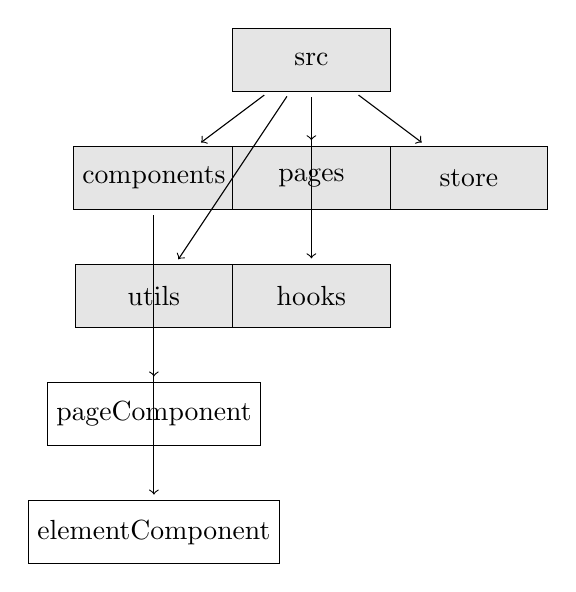
\begin{tikzpicture}[
    file/.style={draw, rectangle, minimum width=2cm, minimum height=0.8cm},
    folder/.style={draw, rectangle, minimum width=2cm, minimum height=0.8cm, fill=gray!20},
    arrow/.style={->, shorten >=2pt, shorten <=2pt}
]

% Folders
\node[folder] (src) at (0,0) {src};
\node[folder] (components) at (-2,-1.5) {components};
\node[folder] (pages) at (0,-1.5) {pages};
\node[folder] (store) at (2,-1.5) {store};
\node[folder] (utils) at (-2,-3) {utils};
\node[folder] (hooks) at (0,-3) {hooks};

% Files
\node[file] (pageComponent) at (-2,-4.5) {pageComponent};
\node[file] (elementComponent) at (-2,-6) {elementComponent};
% ... add more files

% Connections
\draw[arrow] (src) -- (components);
\draw[arrow] (src) -- (pages);
\draw[arrow] (src) -- (store);
\draw[arrow] (src) -- (utils);
\draw[arrow] (src) -- (hooks);
\draw[arrow] (components) -- (pageComponent);
\draw[arrow] (components) -- (elementComponent);
% ... add more connections

\end{tikzpicture}



\pagebreak
\subsubsection{Back-end}
The backend uses the dotNet framework. The development language using the C\# language.

In this project, the backend uses the Onion Architecture.
The Onion Architecture is a typically layered architecture, 
where each layer depends on the inner layer and provides interfaces to the outer layer.
The outer layer provides services to the outermost layer 
and other modules in the same layer based on the interfaces of the inner layer.

From inner to outer, the layers are: Domain, Application, Infrastructure, Presentation.
The Domain layer is the core layer and the innermost layer, used to define domain models, 
which are the business models.
It includes domain models and domain service interfaces.
Domain models are used to define the business models, 
which are the entities in the entity-relationship model and their attributes.
Domain service interfaces are used to define the business services, 
which are the relationships between entities in the entity-relationship model.

The Application layer is the application layer, 
used to define application services, which are the business logic.
It includes domain service implementations and application service interfaces.
Domain service implementations implement the methods of the inner layer's domain service 
interfaces and implement the business logic of the domain models.
Application service interfaces are used to define application services, 
which are the business logic.
It includes but is not limited to database interfaces, testing interfaces, 
HTTP API interfaces, MQTT interfaces, etc.

The Infrastructure layer is the infrastructure layer, used to define infrastructure.
It includes database implementations, testing implementations, 
HTTP API implementations, MQTT implementations, etc.
Database implementations implement the database interfaces 
and provide CRUD services for the database.
Testing implementations implement the testing interfaces 
and provide services for unit testing and integration testing.
HTTP API implementations implement the HTTP API interfaces 
and provide CRUD operations for HTTP APIs.
MQTT implementations implement the MQTT interfaces 
and provide CRUD operations for MQTT.

The Presentation layer is the presentation layer, used to define presentation logic, 
such as interfaces and pages. Since this is a backend project,
data presentation and control are handled by the frontend, 
so this layer is not needed.



\pagebreak
\subsubsection{Data communication and storage}
% 关于本项目的数据通信与数据存储的设计, 包括数据通信的协议, 数据存储的设计等
% 关于数据通信的设计:
% 1. 通信协议的选择
% 自前端向后端发送的数据, 有三种传输的数据类型, 
% 一种是普通的增删改查的请求, 对数据传输的时效性要求不高, 但是对数据的准确性, 完整性, 有序性, 安全性有一定的要求,
% 这种数据的传输, 采用 HTTP 协议, 以及 RESTful API 的设计. 可以有效的保证对数据传输的以上要求.
% 一种是对数据通道的创建和流媒体数据的传输, 对数据传输的时效性, 安全性要求较高, 这种数据的传输, 采用 WebRTC 协议, 以及 MQTT 协议.
% 配合可以快速解码的 flatbuffers 协议, 可以有效的保证对数据传输的以上要求.
% 最后一种是对设备的状态信息和操作信息的传输, 对完整性, 有序性, 安全性都有较高的要求, 这种数据的传输, 采用 MQTT 协议
% 同时也使用了 flatbuffers 协议.
% 
% 2. 数据通信的通信架构和通信流程
% 本项目的数据通信的通信架构, 是基于前后端分离的架构, 前端使用 React 框架, 后端使用 dotnet 框架.
% 当前端需要向后端发送数据的时候, 前端会向后端发送 HTTP 请求, 后端接收到 HTTP 请求之后, 会根据请求的数据类型,
% 选择不同的数据处理方式, 对于普通的增删改查的请求, 后端会根据 RESTful API 的设计, 对数据进行增删改查的操作,
% 对于对数据通道的创建和流媒体数据的传输, 后端会根据 WebRTC 协议, 对数据通道进行创建, 并且帮助前端和设备建立数据通道,
% 当数据通道建立后, 前端和设备之间则使用 flatbuffer 的数据格式对流媒体数据进行传输,
% 对于设备的状态信息和操作信息的传输, 前端会直接向 MQTT broker 发送 MQTT 请求, 
% 设备会在其自身的固件中监听相关的 MQTT 请求, 并且返回相关的数据.
% 
% 3. 数据通信的格式
% 本项目的数据通信的格式, 有三种, 
% 一种是 HTTP 协议, 
% 使用 json 格式对数据进行传输,
% 一种是 WebRTC 协议, 
% 使用 flatbuffers 格式对数据进行传输,
% 一种是 MQTT 协议.
% 使用 flatbuffers 格式对数据进行传输,
% 
% 关于数据存储的设计:
% 1. 数据存储的数据库的选择
% 本项目的数据存储的数据库的选择, 使用了轻量级的数据库 SQLite,
% SQLite 是一个进程内的库, 实现了自给自足的, 无服务器的, 零配置的, 事务性的 SQL 数据库引擎.
% 这是因为整个项目的目的是为了实现前端与设备之间的数据通信, 对于数据库数据的增删改查操作的要求不高,
% 数据量较小, 且对于数据库的数据的事务性要求不高, 所以选择了 SQLite 数据库.
% 2. 项目前后端的数据结构的设计
% 在本项目中, 前端由于使用了 React 框架, 所以前端的数据结构的设计, 使用了基于状态的数据结构的设计,
% 每个组件或者数据集都包含一个状态对象, 这个状态对象的属性就是组件的各个状态. 
% 使用状态对象的原因是, 可以方便的对状态进行管理, 采用对象-属性的形式, 可以方便的针对不同组件的同类状态进行区分,
% 由于跨组件的状态是由 redux 进行管理的, 这种状态对象的设计, 可以更搞笑的对状态进行更新和传递.
% 后端由于使用了 dotnet 框架, 所以后端的数据结构的设计, 使用了基于类的数据结构的设计,
% 采用了面向对象的编程思想, 对数据进行了封装, 使得数据的传输更加的安全, 有序, 完整.


\pagebreak

% \subsection{Domain model}
% \documentclass[]{article}
\usepackage{graphicx}
\usepackage{amsmath}
\usepackage{tikz}

% libaries
\usetikzlibrary{shapes,arrows}

%Define the listing package
\usepackage{listings} %code highlighter
\usepackage{color} %use color
\definecolor{mygreen}{rgb}{0,0.6,0}
\definecolor{mygray}{rgb}{0.5,0.5,0.5}
\definecolor{mymauve}{rgb}{0.58,0,0.82}

%Customize a bit the look
\lstset{ %
backgroundcolor=\color{white}, % choose the background color; you must add \usepackage{color} or \usepackage{xcolor}
basicstyle=\footnotesize, % the size of the fonts that are used for the code
breakatwhitespace=false, % sets if automatic breaks should only happen at whitespace
breaklines=true, % sets automatic line breaking
captionpos=b, % sets the caption-position to bottom
commentstyle=\color{mygreen}, % comment style
deletekeywords={...}, % if you want to delete keywords from the given language
escapeinside={\%*}{*)}, % if you want to add LaTeX within your code
extendedchars=true, % lets you use non-ASCII characters; for 8-bits encodings only, does not work with UTF-8
frame=single, % adds a frame around the code
keepspaces=true, % keeps spaces in text, useful for keeping indentation of code (possibly needs columns=flexible)
keywordstyle=\color{blue}, % keyword style
% language=Octave, % the language of the code
morekeywords={*,...}, % if you want to add more keywords to the set
numbers=left, % where to put the line-numbers; possible values are (none, left, right)
numbersep=5pt, % how far the line-numbers are from the code
numberstyle=\tiny\color{mygray}, % the style that is used for the line-numbers
rulecolor=\color{black}, % if not set, the frame-color may be changed on line-breaks within not-black text (e.g. comments (green here))
showspaces=false, % show spaces everywhere adding particular underscores; it overrides 'showstringspaces'
showstringspaces=false, % underline spaces within strings only
showtabs=false, % show tabs within strings adding particular underscores
stepnumber=1, % the step between two line-numbers. If it's 1, each line will be numbered
stringstyle=\color{mymauve}, % string literal style
tabsize=2, % sets default tabsize to 2 spaces
title=\lstname % show the filename of files included with \lstinputlisting; also try caption instead of title
}

\definecolor{darkgray}{rgb}{.4,.4,.4}
\definecolor{purple}{rgb}{0.65, 0.12, 0.82}

\lstdefinelanguage{React}{
keywords={const, typeof, new, true, false, catch, function, return, null, catch, switch, var, if, in, while, do, else, case, break},
keywordstyle=\color{blue}\bfseries,
ndkeywords={class, export, boolean, throw, implements, import, this},
ndkeywordstyle=\color{darkgray}\bfseries,
identifierstyle=\color{mygreen},
sensitive=false,
comment=[l]{//},
morecomment=[s]{/*}{*/},
commentstyle=\color{purple}\ttfamily,
string=[b]{"}{'}{`},
stringstyle=\color{red}\ttfamily,
morestring=[b]',
morestring=[b]",
morestring=[b]`',
}

\lstdefinelanguage{CSharp}{
keywords={const, typeof, new, true, false, catch, function, return, null, catch, switch, var, if, in, while, do, else, case, break},
keywordstyle=\color{blue}\bfseries,
ndkeywords={class, export, boolean, throw, implements, import, this},
ndkeywordstyle=\color{darkgray}\bfseries,
identifierstyle=\color{mygreen},
sensitive=false,
comment=[l]{//},
morecomment=[s]{/*}{*/},
commentstyle=\color{purple}\ttfamily,
string=[b]{"}{'}{`},
stringstyle=\color{red}\ttfamily,
morestring=[b]',
morestring=[b]",
morestring=[b]`',
}

\lstset{
language=React,
extendedchars=true,
basicstyle=\footnotesize\ttfamily,
showstringspaces=false,
showspaces=false,
numbers=left,
numberstyle=\footnotesize,
numbersep=9pt,
tabsize=2,
breaklines=true,
showtabs=false,
captionpos=b
}

\lstset{
language=CSharp,
extendedchars=true,
basicstyle=\footnotesize\ttfamily,
showstringspaces=false,
showspaces=false,
numbers=left,
numberstyle=\footnotesize,
numbersep=9pt,
tabsize=2,
breaklines=true,
showtabs=false,
captionpos=b
}

% \usepackage{cite} % Add this line for citation

% \bibliographystyle{plain}

\title{
The implementation of BifrostConnect Front-end scope, 
re-design and development with the relevant back-end support develop.
}
\author{
    Fei Gu \\
    Erhvervs Akademi Sydvest \\
    Computer Science 21\\
    }
\date{\today}

\begin{document}

% Front page
\maketitle
\begin{center}
    Supervisor: Henrik Boulund Meng Hansen \\
    Company: BifrostConnect \\
    Engineering Director: Jasper Wass \\
\end{center}
\tableofcontents
\pagebreak


% The introduction
\section{Introduction}
\subsection{Background}\input{sections/introduction/background.tex}
\subsection{The company}\input{sections/introduction/aboutCompany}
\subsection{The project}\input{sections/introduction/aboutProject}
\pagebreak

% The problem statement
\section{Problem Statement}
\subsection{Statement}
\input{sections/problemStatement/statement}
\subsection{Situation}
\input{sections/problemStatement/situation}
\subsection{Potential Solution}
\input{sections/problemStatement/potentialSolution}
\pagebreak

% Requirement analysis
\section{Requirement Analysis}
\input{sections/requirementAnalysis/index}

\subsection{Stakeholders}
\input{sections/requirementAnalysis/stakeholders/index}

\subsection{Business Domain}
\input{sections/requirementAnalysis/bussinesDomain/index}

\subsection{Scope}
\input{sections/requirementAnalysis/scope}

\subsection{Goals}
\input{sections/requirementAnalysis/goals}
\pagebreak

% Software Design
\section{Software Design}
% developement methods
\subsection{Software Development Methods}
\input{sections/softwareDevelopmentMethods/index}
\subsubsection{Agile Software Development}
\input{sections/softwareDevelopmentMethods/agileSoftwareDevelopment/index}
\subsubsection{Feature Driven Development}
\input{sections/softwareDevelopmentMethods/featureDrivenDevelopment/index}

\pagebreak

% Technology seslection
\subsection{Technology selection}
\input{sections/softwareDesign/technologySelection/index}
\subsubsection{Front-end}
\input{sections/softwareDesign/technologySelection/frontEnd}            
\subsubsection{Back-end}
\input{sections/softwareDesign/technologySelection/backEnd}            
\subsubsection{Database}
\input{sections/softwareDesign/technologySelection/database}
\subsubsection{Data communication}
\input{sections/softwareDesign/technologySelection/dataCommunication}            
\subsubsection{DevOps}
\input{sections/softwareDesign/technologySelection/devOps}
\pagebreak

% Architecture design
\subsection{Architecture design}
\input{sections/softwareDesign/architectureDesign/index}
\pagebreak
\subsubsection{Front-end}
\input{sections/softwareDesign/architectureDesign/frontEndArchitecture}
\pagebreak
\subsubsection{Back-end}
\input{sections/softwareDesign/architectureDesign/backEndArchitecture}
\pagebreak
\subsubsection{Data communication and storage}
\input{sections/softwareDesign/architectureDesign/dataCommunicationArchitecture}
\pagebreak

% \subsection{Domain model}
% \input{sections/softwareDesign/domainModel/index}
% \subsection{Database design}
% % 数据库领域模型 ER 图
% % 包括表和字段的设置.
% % 对于私有键和外键的设置.

% \subsection{Back-end design}
% % 后端对象模型
% % 以及对于对象模型的增删改查
% % 以及相关的其他服务的设计`'

% \subsection{Front-end design}
% % 对于前端的页面结构的设计 
% % 页面的状态的设计, 交互设计

% \subsection{FlatBuffers design}
% % schema 的设计

\subsection{DevOps CI/CD process design}
\input{sections/softwareDesign/devOpsDesign/index}
\subsubsection{Continuous Integration}
\input{sections/softwareDesign/devOpsDesign/continuousIntegration/index}
\subsubsection{Continuous Delivery}
\input{sections/softwareDesign/devOpsDesign/continuousDelivery/index}
\subsubsection{Continuous Deployment}
\input{sections/softwareDesign/devOpsDesign/continuousDeployment/index}
\pagebreak

\section{Software Development} 
\input{sections/softwareDevelopment/index}
\subsection{Overall development}
\input{sections/softwareDevelopment/overallDevelopement/index}
\subsubsection{Front-end}
\input{sections/softwareDevelopment/overallDevelopement/frontEnd/index}
\subsubsection{Back-end}
\input{sections/softwareDevelopment/overallDevelopement/backEnd/index}
\subsubsection{DevOps}
\input{sections/softwareDevelopment/overallDevelopement/devOps/index}
\subsection{Feature development} 
\input{sections/softwareDevelopment/featureDevelopment/index}
\subsubsection{Use Case 1}
\input{sections/softwareDevelopment/featureDevelopment/useCase1/index}
\subsubsection{Feature 1}
\input{sections/softwareDevelopment/featureDevelopment/feature/feature1.tex}
\pagebreak
\section{Conclusion} 
\subsection{Result}
Since the project is still in progress, the result is not available yet.
So far, basic structure of this project has been built. But the most features 
are not implemented yet. 
\subsection{Discussion}
As a single developer for this project, I am confident what I have done so far.
And I can say I understand the most of the knowledge I have used in this project, 
which also means I can explain all the part of the project. 
But this project also relevant some of the complex knowledge which I have to continue 
to study and practice.
\subsection{Future Work}
The future work is to implement the rest of the features. 
Including the most important part which is the 'create session' feature.
\pagebreak
% \bibliography{bibliography}
\pagebreak
% \begin{appendices}
%     \section{Appendix}
% \end{appendices} 
\end{document}
% \subsection{Database design}
% % 数据库领域模型 ER 图
% % 包括表和字段的设置.
% % 对于私有键和外键的设置.

% \subsection{Back-end design}
% % 后端对象模型
% % 以及对于对象模型的增删改查
% % 以及相关的其他服务的设计`'

% \subsection{Front-end design}
% % 对于前端的页面结构的设计 
% % 页面的状态的设计, 交互设计

% \subsection{FlatBuffers design}
% % schema 的设计

\subsection{DevOps CI/CD process design}
\documentclass[]{article}
\usepackage{graphicx}
\usepackage{amsmath}
\usepackage{tikz}

% libaries
\usetikzlibrary{shapes,arrows}

%Define the listing package
\usepackage{listings} %code highlighter
\usepackage{color} %use color
\definecolor{mygreen}{rgb}{0,0.6,0}
\definecolor{mygray}{rgb}{0.5,0.5,0.5}
\definecolor{mymauve}{rgb}{0.58,0,0.82}

%Customize a bit the look
\lstset{ %
backgroundcolor=\color{white}, % choose the background color; you must add \usepackage{color} or \usepackage{xcolor}
basicstyle=\footnotesize, % the size of the fonts that are used for the code
breakatwhitespace=false, % sets if automatic breaks should only happen at whitespace
breaklines=true, % sets automatic line breaking
captionpos=b, % sets the caption-position to bottom
commentstyle=\color{mygreen}, % comment style
deletekeywords={...}, % if you want to delete keywords from the given language
escapeinside={\%*}{*)}, % if you want to add LaTeX within your code
extendedchars=true, % lets you use non-ASCII characters; for 8-bits encodings only, does not work with UTF-8
frame=single, % adds a frame around the code
keepspaces=true, % keeps spaces in text, useful for keeping indentation of code (possibly needs columns=flexible)
keywordstyle=\color{blue}, % keyword style
% language=Octave, % the language of the code
morekeywords={*,...}, % if you want to add more keywords to the set
numbers=left, % where to put the line-numbers; possible values are (none, left, right)
numbersep=5pt, % how far the line-numbers are from the code
numberstyle=\tiny\color{mygray}, % the style that is used for the line-numbers
rulecolor=\color{black}, % if not set, the frame-color may be changed on line-breaks within not-black text (e.g. comments (green here))
showspaces=false, % show spaces everywhere adding particular underscores; it overrides 'showstringspaces'
showstringspaces=false, % underline spaces within strings only
showtabs=false, % show tabs within strings adding particular underscores
stepnumber=1, % the step between two line-numbers. If it's 1, each line will be numbered
stringstyle=\color{mymauve}, % string literal style
tabsize=2, % sets default tabsize to 2 spaces
title=\lstname % show the filename of files included with \lstinputlisting; also try caption instead of title
}

\definecolor{darkgray}{rgb}{.4,.4,.4}
\definecolor{purple}{rgb}{0.65, 0.12, 0.82}

\lstdefinelanguage{React}{
keywords={const, typeof, new, true, false, catch, function, return, null, catch, switch, var, if, in, while, do, else, case, break},
keywordstyle=\color{blue}\bfseries,
ndkeywords={class, export, boolean, throw, implements, import, this},
ndkeywordstyle=\color{darkgray}\bfseries,
identifierstyle=\color{mygreen},
sensitive=false,
comment=[l]{//},
morecomment=[s]{/*}{*/},
commentstyle=\color{purple}\ttfamily,
string=[b]{"}{'}{`},
stringstyle=\color{red}\ttfamily,
morestring=[b]',
morestring=[b]",
morestring=[b]`',
}

\lstdefinelanguage{CSharp}{
keywords={const, typeof, new, true, false, catch, function, return, null, catch, switch, var, if, in, while, do, else, case, break},
keywordstyle=\color{blue}\bfseries,
ndkeywords={class, export, boolean, throw, implements, import, this},
ndkeywordstyle=\color{darkgray}\bfseries,
identifierstyle=\color{mygreen},
sensitive=false,
comment=[l]{//},
morecomment=[s]{/*}{*/},
commentstyle=\color{purple}\ttfamily,
string=[b]{"}{'}{`},
stringstyle=\color{red}\ttfamily,
morestring=[b]',
morestring=[b]",
morestring=[b]`',
}

\lstset{
language=React,
extendedchars=true,
basicstyle=\footnotesize\ttfamily,
showstringspaces=false,
showspaces=false,
numbers=left,
numberstyle=\footnotesize,
numbersep=9pt,
tabsize=2,
breaklines=true,
showtabs=false,
captionpos=b
}

\lstset{
language=CSharp,
extendedchars=true,
basicstyle=\footnotesize\ttfamily,
showstringspaces=false,
showspaces=false,
numbers=left,
numberstyle=\footnotesize,
numbersep=9pt,
tabsize=2,
breaklines=true,
showtabs=false,
captionpos=b
}

% \usepackage{cite} % Add this line for citation

% \bibliographystyle{plain}

\title{
The implementation of BifrostConnect Front-end scope, 
re-design and development with the relevant back-end support develop.
}
\author{
    Fei Gu \\
    Erhvervs Akademi Sydvest \\
    Computer Science 21\\
    }
\date{\today}

\begin{document}

% Front page
\maketitle
\begin{center}
    Supervisor: Henrik Boulund Meng Hansen \\
    Company: BifrostConnect \\
    Engineering Director: Jasper Wass \\
\end{center}
\tableofcontents
\pagebreak


% The introduction
\section{Introduction}
\subsection{Background}\input{sections/introduction/background.tex}
\subsection{The company}\input{sections/introduction/aboutCompany}
\subsection{The project}\input{sections/introduction/aboutProject}
\pagebreak

% The problem statement
\section{Problem Statement}
\subsection{Statement}
\input{sections/problemStatement/statement}
\subsection{Situation}
\input{sections/problemStatement/situation}
\subsection{Potential Solution}
\input{sections/problemStatement/potentialSolution}
\pagebreak

% Requirement analysis
\section{Requirement Analysis}
\input{sections/requirementAnalysis/index}

\subsection{Stakeholders}
\input{sections/requirementAnalysis/stakeholders/index}

\subsection{Business Domain}
\input{sections/requirementAnalysis/bussinesDomain/index}

\subsection{Scope}
\input{sections/requirementAnalysis/scope}

\subsection{Goals}
\input{sections/requirementAnalysis/goals}
\pagebreak

% Software Design
\section{Software Design}
% developement methods
\subsection{Software Development Methods}
\input{sections/softwareDevelopmentMethods/index}
\subsubsection{Agile Software Development}
\input{sections/softwareDevelopmentMethods/agileSoftwareDevelopment/index}
\subsubsection{Feature Driven Development}
\input{sections/softwareDevelopmentMethods/featureDrivenDevelopment/index}

\pagebreak

% Technology seslection
\subsection{Technology selection}
\input{sections/softwareDesign/technologySelection/index}
\subsubsection{Front-end}
\input{sections/softwareDesign/technologySelection/frontEnd}            
\subsubsection{Back-end}
\input{sections/softwareDesign/technologySelection/backEnd}            
\subsubsection{Database}
\input{sections/softwareDesign/technologySelection/database}
\subsubsection{Data communication}
\input{sections/softwareDesign/technologySelection/dataCommunication}            
\subsubsection{DevOps}
\input{sections/softwareDesign/technologySelection/devOps}
\pagebreak

% Architecture design
\subsection{Architecture design}
\input{sections/softwareDesign/architectureDesign/index}
\pagebreak
\subsubsection{Front-end}
\input{sections/softwareDesign/architectureDesign/frontEndArchitecture}
\pagebreak
\subsubsection{Back-end}
\input{sections/softwareDesign/architectureDesign/backEndArchitecture}
\pagebreak
\subsubsection{Data communication and storage}
\input{sections/softwareDesign/architectureDesign/dataCommunicationArchitecture}
\pagebreak

% \subsection{Domain model}
% \input{sections/softwareDesign/domainModel/index}
% \subsection{Database design}
% % 数据库领域模型 ER 图
% % 包括表和字段的设置.
% % 对于私有键和外键的设置.

% \subsection{Back-end design}
% % 后端对象模型
% % 以及对于对象模型的增删改查
% % 以及相关的其他服务的设计`'

% \subsection{Front-end design}
% % 对于前端的页面结构的设计 
% % 页面的状态的设计, 交互设计

% \subsection{FlatBuffers design}
% % schema 的设计

\subsection{DevOps CI/CD process design}
\input{sections/softwareDesign/devOpsDesign/index}
\subsubsection{Continuous Integration}
\input{sections/softwareDesign/devOpsDesign/continuousIntegration/index}
\subsubsection{Continuous Delivery}
\input{sections/softwareDesign/devOpsDesign/continuousDelivery/index}
\subsubsection{Continuous Deployment}
\input{sections/softwareDesign/devOpsDesign/continuousDeployment/index}
\pagebreak

\section{Software Development} 
\input{sections/softwareDevelopment/index}
\subsection{Overall development}
\input{sections/softwareDevelopment/overallDevelopement/index}
\subsubsection{Front-end}
\input{sections/softwareDevelopment/overallDevelopement/frontEnd/index}
\subsubsection{Back-end}
\input{sections/softwareDevelopment/overallDevelopement/backEnd/index}
\subsubsection{DevOps}
\input{sections/softwareDevelopment/overallDevelopement/devOps/index}
\subsection{Feature development} 
\input{sections/softwareDevelopment/featureDevelopment/index}
\subsubsection{Use Case 1}
\input{sections/softwareDevelopment/featureDevelopment/useCase1/index}
\subsubsection{Feature 1}
\input{sections/softwareDevelopment/featureDevelopment/feature/feature1.tex}
\pagebreak
\section{Conclusion} 
\subsection{Result}
Since the project is still in progress, the result is not available yet.
So far, basic structure of this project has been built. But the most features 
are not implemented yet. 
\subsection{Discussion}
As a single developer for this project, I am confident what I have done so far.
And I can say I understand the most of the knowledge I have used in this project, 
which also means I can explain all the part of the project. 
But this project also relevant some of the complex knowledge which I have to continue 
to study and practice.
\subsection{Future Work}
The future work is to implement the rest of the features. 
Including the most important part which is the 'create session' feature.
\pagebreak
% \bibliography{bibliography}
\pagebreak
% \begin{appendices}
%     \section{Appendix}
% \end{appendices} 
\end{document}
\subsubsection{Continuous Integration}
\documentclass[]{article}
\usepackage{graphicx}
\usepackage{amsmath}
\usepackage{tikz}

% libaries
\usetikzlibrary{shapes,arrows}

%Define the listing package
\usepackage{listings} %code highlighter
\usepackage{color} %use color
\definecolor{mygreen}{rgb}{0,0.6,0}
\definecolor{mygray}{rgb}{0.5,0.5,0.5}
\definecolor{mymauve}{rgb}{0.58,0,0.82}

%Customize a bit the look
\lstset{ %
backgroundcolor=\color{white}, % choose the background color; you must add \usepackage{color} or \usepackage{xcolor}
basicstyle=\footnotesize, % the size of the fonts that are used for the code
breakatwhitespace=false, % sets if automatic breaks should only happen at whitespace
breaklines=true, % sets automatic line breaking
captionpos=b, % sets the caption-position to bottom
commentstyle=\color{mygreen}, % comment style
deletekeywords={...}, % if you want to delete keywords from the given language
escapeinside={\%*}{*)}, % if you want to add LaTeX within your code
extendedchars=true, % lets you use non-ASCII characters; for 8-bits encodings only, does not work with UTF-8
frame=single, % adds a frame around the code
keepspaces=true, % keeps spaces in text, useful for keeping indentation of code (possibly needs columns=flexible)
keywordstyle=\color{blue}, % keyword style
% language=Octave, % the language of the code
morekeywords={*,...}, % if you want to add more keywords to the set
numbers=left, % where to put the line-numbers; possible values are (none, left, right)
numbersep=5pt, % how far the line-numbers are from the code
numberstyle=\tiny\color{mygray}, % the style that is used for the line-numbers
rulecolor=\color{black}, % if not set, the frame-color may be changed on line-breaks within not-black text (e.g. comments (green here))
showspaces=false, % show spaces everywhere adding particular underscores; it overrides 'showstringspaces'
showstringspaces=false, % underline spaces within strings only
showtabs=false, % show tabs within strings adding particular underscores
stepnumber=1, % the step between two line-numbers. If it's 1, each line will be numbered
stringstyle=\color{mymauve}, % string literal style
tabsize=2, % sets default tabsize to 2 spaces
title=\lstname % show the filename of files included with \lstinputlisting; also try caption instead of title
}

\definecolor{darkgray}{rgb}{.4,.4,.4}
\definecolor{purple}{rgb}{0.65, 0.12, 0.82}

\lstdefinelanguage{React}{
keywords={const, typeof, new, true, false, catch, function, return, null, catch, switch, var, if, in, while, do, else, case, break},
keywordstyle=\color{blue}\bfseries,
ndkeywords={class, export, boolean, throw, implements, import, this},
ndkeywordstyle=\color{darkgray}\bfseries,
identifierstyle=\color{mygreen},
sensitive=false,
comment=[l]{//},
morecomment=[s]{/*}{*/},
commentstyle=\color{purple}\ttfamily,
string=[b]{"}{'}{`},
stringstyle=\color{red}\ttfamily,
morestring=[b]',
morestring=[b]",
morestring=[b]`',
}

\lstdefinelanguage{CSharp}{
keywords={const, typeof, new, true, false, catch, function, return, null, catch, switch, var, if, in, while, do, else, case, break},
keywordstyle=\color{blue}\bfseries,
ndkeywords={class, export, boolean, throw, implements, import, this},
ndkeywordstyle=\color{darkgray}\bfseries,
identifierstyle=\color{mygreen},
sensitive=false,
comment=[l]{//},
morecomment=[s]{/*}{*/},
commentstyle=\color{purple}\ttfamily,
string=[b]{"}{'}{`},
stringstyle=\color{red}\ttfamily,
morestring=[b]',
morestring=[b]",
morestring=[b]`',
}

\lstset{
language=React,
extendedchars=true,
basicstyle=\footnotesize\ttfamily,
showstringspaces=false,
showspaces=false,
numbers=left,
numberstyle=\footnotesize,
numbersep=9pt,
tabsize=2,
breaklines=true,
showtabs=false,
captionpos=b
}

\lstset{
language=CSharp,
extendedchars=true,
basicstyle=\footnotesize\ttfamily,
showstringspaces=false,
showspaces=false,
numbers=left,
numberstyle=\footnotesize,
numbersep=9pt,
tabsize=2,
breaklines=true,
showtabs=false,
captionpos=b
}

% \usepackage{cite} % Add this line for citation

% \bibliographystyle{plain}

\title{
The implementation of BifrostConnect Front-end scope, 
re-design and development with the relevant back-end support develop.
}
\author{
    Fei Gu \\
    Erhvervs Akademi Sydvest \\
    Computer Science 21\\
    }
\date{\today}

\begin{document}

% Front page
\maketitle
\begin{center}
    Supervisor: Henrik Boulund Meng Hansen \\
    Company: BifrostConnect \\
    Engineering Director: Jasper Wass \\
\end{center}
\tableofcontents
\pagebreak


% The introduction
\section{Introduction}
\subsection{Background}\input{sections/introduction/background.tex}
\subsection{The company}\input{sections/introduction/aboutCompany}
\subsection{The project}\input{sections/introduction/aboutProject}
\pagebreak

% The problem statement
\section{Problem Statement}
\subsection{Statement}
\input{sections/problemStatement/statement}
\subsection{Situation}
\input{sections/problemStatement/situation}
\subsection{Potential Solution}
\input{sections/problemStatement/potentialSolution}
\pagebreak

% Requirement analysis
\section{Requirement Analysis}
\input{sections/requirementAnalysis/index}

\subsection{Stakeholders}
\input{sections/requirementAnalysis/stakeholders/index}

\subsection{Business Domain}
\input{sections/requirementAnalysis/bussinesDomain/index}

\subsection{Scope}
\input{sections/requirementAnalysis/scope}

\subsection{Goals}
\input{sections/requirementAnalysis/goals}
\pagebreak

% Software Design
\section{Software Design}
% developement methods
\subsection{Software Development Methods}
\input{sections/softwareDevelopmentMethods/index}
\subsubsection{Agile Software Development}
\input{sections/softwareDevelopmentMethods/agileSoftwareDevelopment/index}
\subsubsection{Feature Driven Development}
\input{sections/softwareDevelopmentMethods/featureDrivenDevelopment/index}

\pagebreak

% Technology seslection
\subsection{Technology selection}
\input{sections/softwareDesign/technologySelection/index}
\subsubsection{Front-end}
\input{sections/softwareDesign/technologySelection/frontEnd}            
\subsubsection{Back-end}
\input{sections/softwareDesign/technologySelection/backEnd}            
\subsubsection{Database}
\input{sections/softwareDesign/technologySelection/database}
\subsubsection{Data communication}
\input{sections/softwareDesign/technologySelection/dataCommunication}            
\subsubsection{DevOps}
\input{sections/softwareDesign/technologySelection/devOps}
\pagebreak

% Architecture design
\subsection{Architecture design}
\input{sections/softwareDesign/architectureDesign/index}
\pagebreak
\subsubsection{Front-end}
\input{sections/softwareDesign/architectureDesign/frontEndArchitecture}
\pagebreak
\subsubsection{Back-end}
\input{sections/softwareDesign/architectureDesign/backEndArchitecture}
\pagebreak
\subsubsection{Data communication and storage}
\input{sections/softwareDesign/architectureDesign/dataCommunicationArchitecture}
\pagebreak

% \subsection{Domain model}
% \input{sections/softwareDesign/domainModel/index}
% \subsection{Database design}
% % 数据库领域模型 ER 图
% % 包括表和字段的设置.
% % 对于私有键和外键的设置.

% \subsection{Back-end design}
% % 后端对象模型
% % 以及对于对象模型的增删改查
% % 以及相关的其他服务的设计`'

% \subsection{Front-end design}
% % 对于前端的页面结构的设计 
% % 页面的状态的设计, 交互设计

% \subsection{FlatBuffers design}
% % schema 的设计

\subsection{DevOps CI/CD process design}
\input{sections/softwareDesign/devOpsDesign/index}
\subsubsection{Continuous Integration}
\input{sections/softwareDesign/devOpsDesign/continuousIntegration/index}
\subsubsection{Continuous Delivery}
\input{sections/softwareDesign/devOpsDesign/continuousDelivery/index}
\subsubsection{Continuous Deployment}
\input{sections/softwareDesign/devOpsDesign/continuousDeployment/index}
\pagebreak

\section{Software Development} 
\input{sections/softwareDevelopment/index}
\subsection{Overall development}
\input{sections/softwareDevelopment/overallDevelopement/index}
\subsubsection{Front-end}
\input{sections/softwareDevelopment/overallDevelopement/frontEnd/index}
\subsubsection{Back-end}
\input{sections/softwareDevelopment/overallDevelopement/backEnd/index}
\subsubsection{DevOps}
\input{sections/softwareDevelopment/overallDevelopement/devOps/index}
\subsection{Feature development} 
\input{sections/softwareDevelopment/featureDevelopment/index}
\subsubsection{Use Case 1}
\input{sections/softwareDevelopment/featureDevelopment/useCase1/index}
\subsubsection{Feature 1}
\input{sections/softwareDevelopment/featureDevelopment/feature/feature1.tex}
\pagebreak
\section{Conclusion} 
\subsection{Result}
Since the project is still in progress, the result is not available yet.
So far, basic structure of this project has been built. But the most features 
are not implemented yet. 
\subsection{Discussion}
As a single developer for this project, I am confident what I have done so far.
And I can say I understand the most of the knowledge I have used in this project, 
which also means I can explain all the part of the project. 
But this project also relevant some of the complex knowledge which I have to continue 
to study and practice.
\subsection{Future Work}
The future work is to implement the rest of the features. 
Including the most important part which is the 'create session' feature.
\pagebreak
% \bibliography{bibliography}
\pagebreak
% \begin{appendices}
%     \section{Appendix}
% \end{appendices} 
\end{document}
\subsubsection{Continuous Delivery}
\documentclass[]{article}
\usepackage{graphicx}
\usepackage{amsmath}
\usepackage{tikz}

% libaries
\usetikzlibrary{shapes,arrows}

%Define the listing package
\usepackage{listings} %code highlighter
\usepackage{color} %use color
\definecolor{mygreen}{rgb}{0,0.6,0}
\definecolor{mygray}{rgb}{0.5,0.5,0.5}
\definecolor{mymauve}{rgb}{0.58,0,0.82}

%Customize a bit the look
\lstset{ %
backgroundcolor=\color{white}, % choose the background color; you must add \usepackage{color} or \usepackage{xcolor}
basicstyle=\footnotesize, % the size of the fonts that are used for the code
breakatwhitespace=false, % sets if automatic breaks should only happen at whitespace
breaklines=true, % sets automatic line breaking
captionpos=b, % sets the caption-position to bottom
commentstyle=\color{mygreen}, % comment style
deletekeywords={...}, % if you want to delete keywords from the given language
escapeinside={\%*}{*)}, % if you want to add LaTeX within your code
extendedchars=true, % lets you use non-ASCII characters; for 8-bits encodings only, does not work with UTF-8
frame=single, % adds a frame around the code
keepspaces=true, % keeps spaces in text, useful for keeping indentation of code (possibly needs columns=flexible)
keywordstyle=\color{blue}, % keyword style
% language=Octave, % the language of the code
morekeywords={*,...}, % if you want to add more keywords to the set
numbers=left, % where to put the line-numbers; possible values are (none, left, right)
numbersep=5pt, % how far the line-numbers are from the code
numberstyle=\tiny\color{mygray}, % the style that is used for the line-numbers
rulecolor=\color{black}, % if not set, the frame-color may be changed on line-breaks within not-black text (e.g. comments (green here))
showspaces=false, % show spaces everywhere adding particular underscores; it overrides 'showstringspaces'
showstringspaces=false, % underline spaces within strings only
showtabs=false, % show tabs within strings adding particular underscores
stepnumber=1, % the step between two line-numbers. If it's 1, each line will be numbered
stringstyle=\color{mymauve}, % string literal style
tabsize=2, % sets default tabsize to 2 spaces
title=\lstname % show the filename of files included with \lstinputlisting; also try caption instead of title
}

\definecolor{darkgray}{rgb}{.4,.4,.4}
\definecolor{purple}{rgb}{0.65, 0.12, 0.82}

\lstdefinelanguage{React}{
keywords={const, typeof, new, true, false, catch, function, return, null, catch, switch, var, if, in, while, do, else, case, break},
keywordstyle=\color{blue}\bfseries,
ndkeywords={class, export, boolean, throw, implements, import, this},
ndkeywordstyle=\color{darkgray}\bfseries,
identifierstyle=\color{mygreen},
sensitive=false,
comment=[l]{//},
morecomment=[s]{/*}{*/},
commentstyle=\color{purple}\ttfamily,
string=[b]{"}{'}{`},
stringstyle=\color{red}\ttfamily,
morestring=[b]',
morestring=[b]",
morestring=[b]`',
}

\lstdefinelanguage{CSharp}{
keywords={const, typeof, new, true, false, catch, function, return, null, catch, switch, var, if, in, while, do, else, case, break},
keywordstyle=\color{blue}\bfseries,
ndkeywords={class, export, boolean, throw, implements, import, this},
ndkeywordstyle=\color{darkgray}\bfseries,
identifierstyle=\color{mygreen},
sensitive=false,
comment=[l]{//},
morecomment=[s]{/*}{*/},
commentstyle=\color{purple}\ttfamily,
string=[b]{"}{'}{`},
stringstyle=\color{red}\ttfamily,
morestring=[b]',
morestring=[b]",
morestring=[b]`',
}

\lstset{
language=React,
extendedchars=true,
basicstyle=\footnotesize\ttfamily,
showstringspaces=false,
showspaces=false,
numbers=left,
numberstyle=\footnotesize,
numbersep=9pt,
tabsize=2,
breaklines=true,
showtabs=false,
captionpos=b
}

\lstset{
language=CSharp,
extendedchars=true,
basicstyle=\footnotesize\ttfamily,
showstringspaces=false,
showspaces=false,
numbers=left,
numberstyle=\footnotesize,
numbersep=9pt,
tabsize=2,
breaklines=true,
showtabs=false,
captionpos=b
}

% \usepackage{cite} % Add this line for citation

% \bibliographystyle{plain}

\title{
The implementation of BifrostConnect Front-end scope, 
re-design and development with the relevant back-end support develop.
}
\author{
    Fei Gu \\
    Erhvervs Akademi Sydvest \\
    Computer Science 21\\
    }
\date{\today}

\begin{document}

% Front page
\maketitle
\begin{center}
    Supervisor: Henrik Boulund Meng Hansen \\
    Company: BifrostConnect \\
    Engineering Director: Jasper Wass \\
\end{center}
\tableofcontents
\pagebreak


% The introduction
\section{Introduction}
\subsection{Background}\input{sections/introduction/background.tex}
\subsection{The company}\input{sections/introduction/aboutCompany}
\subsection{The project}\input{sections/introduction/aboutProject}
\pagebreak

% The problem statement
\section{Problem Statement}
\subsection{Statement}
\input{sections/problemStatement/statement}
\subsection{Situation}
\input{sections/problemStatement/situation}
\subsection{Potential Solution}
\input{sections/problemStatement/potentialSolution}
\pagebreak

% Requirement analysis
\section{Requirement Analysis}
\input{sections/requirementAnalysis/index}

\subsection{Stakeholders}
\input{sections/requirementAnalysis/stakeholders/index}

\subsection{Business Domain}
\input{sections/requirementAnalysis/bussinesDomain/index}

\subsection{Scope}
\input{sections/requirementAnalysis/scope}

\subsection{Goals}
\input{sections/requirementAnalysis/goals}
\pagebreak

% Software Design
\section{Software Design}
% developement methods
\subsection{Software Development Methods}
\input{sections/softwareDevelopmentMethods/index}
\subsubsection{Agile Software Development}
\input{sections/softwareDevelopmentMethods/agileSoftwareDevelopment/index}
\subsubsection{Feature Driven Development}
\input{sections/softwareDevelopmentMethods/featureDrivenDevelopment/index}

\pagebreak

% Technology seslection
\subsection{Technology selection}
\input{sections/softwareDesign/technologySelection/index}
\subsubsection{Front-end}
\input{sections/softwareDesign/technologySelection/frontEnd}            
\subsubsection{Back-end}
\input{sections/softwareDesign/technologySelection/backEnd}            
\subsubsection{Database}
\input{sections/softwareDesign/technologySelection/database}
\subsubsection{Data communication}
\input{sections/softwareDesign/technologySelection/dataCommunication}            
\subsubsection{DevOps}
\input{sections/softwareDesign/technologySelection/devOps}
\pagebreak

% Architecture design
\subsection{Architecture design}
\input{sections/softwareDesign/architectureDesign/index}
\pagebreak
\subsubsection{Front-end}
\input{sections/softwareDesign/architectureDesign/frontEndArchitecture}
\pagebreak
\subsubsection{Back-end}
\input{sections/softwareDesign/architectureDesign/backEndArchitecture}
\pagebreak
\subsubsection{Data communication and storage}
\input{sections/softwareDesign/architectureDesign/dataCommunicationArchitecture}
\pagebreak

% \subsection{Domain model}
% \input{sections/softwareDesign/domainModel/index}
% \subsection{Database design}
% % 数据库领域模型 ER 图
% % 包括表和字段的设置.
% % 对于私有键和外键的设置.

% \subsection{Back-end design}
% % 后端对象模型
% % 以及对于对象模型的增删改查
% % 以及相关的其他服务的设计`'

% \subsection{Front-end design}
% % 对于前端的页面结构的设计 
% % 页面的状态的设计, 交互设计

% \subsection{FlatBuffers design}
% % schema 的设计

\subsection{DevOps CI/CD process design}
\input{sections/softwareDesign/devOpsDesign/index}
\subsubsection{Continuous Integration}
\input{sections/softwareDesign/devOpsDesign/continuousIntegration/index}
\subsubsection{Continuous Delivery}
\input{sections/softwareDesign/devOpsDesign/continuousDelivery/index}
\subsubsection{Continuous Deployment}
\input{sections/softwareDesign/devOpsDesign/continuousDeployment/index}
\pagebreak

\section{Software Development} 
\input{sections/softwareDevelopment/index}
\subsection{Overall development}
\input{sections/softwareDevelopment/overallDevelopement/index}
\subsubsection{Front-end}
\input{sections/softwareDevelopment/overallDevelopement/frontEnd/index}
\subsubsection{Back-end}
\input{sections/softwareDevelopment/overallDevelopement/backEnd/index}
\subsubsection{DevOps}
\input{sections/softwareDevelopment/overallDevelopement/devOps/index}
\subsection{Feature development} 
\input{sections/softwareDevelopment/featureDevelopment/index}
\subsubsection{Use Case 1}
\input{sections/softwareDevelopment/featureDevelopment/useCase1/index}
\subsubsection{Feature 1}
\input{sections/softwareDevelopment/featureDevelopment/feature/feature1.tex}
\pagebreak
\section{Conclusion} 
\subsection{Result}
Since the project is still in progress, the result is not available yet.
So far, basic structure of this project has been built. But the most features 
are not implemented yet. 
\subsection{Discussion}
As a single developer for this project, I am confident what I have done so far.
And I can say I understand the most of the knowledge I have used in this project, 
which also means I can explain all the part of the project. 
But this project also relevant some of the complex knowledge which I have to continue 
to study and practice.
\subsection{Future Work}
The future work is to implement the rest of the features. 
Including the most important part which is the 'create session' feature.
\pagebreak
% \bibliography{bibliography}
\pagebreak
% \begin{appendices}
%     \section{Appendix}
% \end{appendices} 
\end{document}
\subsubsection{Continuous Deployment}
\documentclass[]{article}
\usepackage{graphicx}
\usepackage{amsmath}
\usepackage{tikz}

% libaries
\usetikzlibrary{shapes,arrows}

%Define the listing package
\usepackage{listings} %code highlighter
\usepackage{color} %use color
\definecolor{mygreen}{rgb}{0,0.6,0}
\definecolor{mygray}{rgb}{0.5,0.5,0.5}
\definecolor{mymauve}{rgb}{0.58,0,0.82}

%Customize a bit the look
\lstset{ %
backgroundcolor=\color{white}, % choose the background color; you must add \usepackage{color} or \usepackage{xcolor}
basicstyle=\footnotesize, % the size of the fonts that are used for the code
breakatwhitespace=false, % sets if automatic breaks should only happen at whitespace
breaklines=true, % sets automatic line breaking
captionpos=b, % sets the caption-position to bottom
commentstyle=\color{mygreen}, % comment style
deletekeywords={...}, % if you want to delete keywords from the given language
escapeinside={\%*}{*)}, % if you want to add LaTeX within your code
extendedchars=true, % lets you use non-ASCII characters; for 8-bits encodings only, does not work with UTF-8
frame=single, % adds a frame around the code
keepspaces=true, % keeps spaces in text, useful for keeping indentation of code (possibly needs columns=flexible)
keywordstyle=\color{blue}, % keyword style
% language=Octave, % the language of the code
morekeywords={*,...}, % if you want to add more keywords to the set
numbers=left, % where to put the line-numbers; possible values are (none, left, right)
numbersep=5pt, % how far the line-numbers are from the code
numberstyle=\tiny\color{mygray}, % the style that is used for the line-numbers
rulecolor=\color{black}, % if not set, the frame-color may be changed on line-breaks within not-black text (e.g. comments (green here))
showspaces=false, % show spaces everywhere adding particular underscores; it overrides 'showstringspaces'
showstringspaces=false, % underline spaces within strings only
showtabs=false, % show tabs within strings adding particular underscores
stepnumber=1, % the step between two line-numbers. If it's 1, each line will be numbered
stringstyle=\color{mymauve}, % string literal style
tabsize=2, % sets default tabsize to 2 spaces
title=\lstname % show the filename of files included with \lstinputlisting; also try caption instead of title
}

\definecolor{darkgray}{rgb}{.4,.4,.4}
\definecolor{purple}{rgb}{0.65, 0.12, 0.82}

\lstdefinelanguage{React}{
keywords={const, typeof, new, true, false, catch, function, return, null, catch, switch, var, if, in, while, do, else, case, break},
keywordstyle=\color{blue}\bfseries,
ndkeywords={class, export, boolean, throw, implements, import, this},
ndkeywordstyle=\color{darkgray}\bfseries,
identifierstyle=\color{mygreen},
sensitive=false,
comment=[l]{//},
morecomment=[s]{/*}{*/},
commentstyle=\color{purple}\ttfamily,
string=[b]{"}{'}{`},
stringstyle=\color{red}\ttfamily,
morestring=[b]',
morestring=[b]",
morestring=[b]`',
}

\lstdefinelanguage{CSharp}{
keywords={const, typeof, new, true, false, catch, function, return, null, catch, switch, var, if, in, while, do, else, case, break},
keywordstyle=\color{blue}\bfseries,
ndkeywords={class, export, boolean, throw, implements, import, this},
ndkeywordstyle=\color{darkgray}\bfseries,
identifierstyle=\color{mygreen},
sensitive=false,
comment=[l]{//},
morecomment=[s]{/*}{*/},
commentstyle=\color{purple}\ttfamily,
string=[b]{"}{'}{`},
stringstyle=\color{red}\ttfamily,
morestring=[b]',
morestring=[b]",
morestring=[b]`',
}

\lstset{
language=React,
extendedchars=true,
basicstyle=\footnotesize\ttfamily,
showstringspaces=false,
showspaces=false,
numbers=left,
numberstyle=\footnotesize,
numbersep=9pt,
tabsize=2,
breaklines=true,
showtabs=false,
captionpos=b
}

\lstset{
language=CSharp,
extendedchars=true,
basicstyle=\footnotesize\ttfamily,
showstringspaces=false,
showspaces=false,
numbers=left,
numberstyle=\footnotesize,
numbersep=9pt,
tabsize=2,
breaklines=true,
showtabs=false,
captionpos=b
}

% \usepackage{cite} % Add this line for citation

% \bibliographystyle{plain}

\title{
The implementation of BifrostConnect Front-end scope, 
re-design and development with the relevant back-end support develop.
}
\author{
    Fei Gu \\
    Erhvervs Akademi Sydvest \\
    Computer Science 21\\
    }
\date{\today}

\begin{document}

% Front page
\maketitle
\begin{center}
    Supervisor: Henrik Boulund Meng Hansen \\
    Company: BifrostConnect \\
    Engineering Director: Jasper Wass \\
\end{center}
\tableofcontents
\pagebreak


% The introduction
\section{Introduction}
\subsection{Background}\input{sections/introduction/background.tex}
\subsection{The company}\input{sections/introduction/aboutCompany}
\subsection{The project}\input{sections/introduction/aboutProject}
\pagebreak

% The problem statement
\section{Problem Statement}
\subsection{Statement}
\input{sections/problemStatement/statement}
\subsection{Situation}
\input{sections/problemStatement/situation}
\subsection{Potential Solution}
\input{sections/problemStatement/potentialSolution}
\pagebreak

% Requirement analysis
\section{Requirement Analysis}
\input{sections/requirementAnalysis/index}

\subsection{Stakeholders}
\input{sections/requirementAnalysis/stakeholders/index}

\subsection{Business Domain}
\input{sections/requirementAnalysis/bussinesDomain/index}

\subsection{Scope}
\input{sections/requirementAnalysis/scope}

\subsection{Goals}
\input{sections/requirementAnalysis/goals}
\pagebreak

% Software Design
\section{Software Design}
% developement methods
\subsection{Software Development Methods}
\input{sections/softwareDevelopmentMethods/index}
\subsubsection{Agile Software Development}
\input{sections/softwareDevelopmentMethods/agileSoftwareDevelopment/index}
\subsubsection{Feature Driven Development}
\input{sections/softwareDevelopmentMethods/featureDrivenDevelopment/index}

\pagebreak

% Technology seslection
\subsection{Technology selection}
\input{sections/softwareDesign/technologySelection/index}
\subsubsection{Front-end}
\input{sections/softwareDesign/technologySelection/frontEnd}            
\subsubsection{Back-end}
\input{sections/softwareDesign/technologySelection/backEnd}            
\subsubsection{Database}
\input{sections/softwareDesign/technologySelection/database}
\subsubsection{Data communication}
\input{sections/softwareDesign/technologySelection/dataCommunication}            
\subsubsection{DevOps}
\input{sections/softwareDesign/technologySelection/devOps}
\pagebreak

% Architecture design
\subsection{Architecture design}
\input{sections/softwareDesign/architectureDesign/index}
\pagebreak
\subsubsection{Front-end}
\input{sections/softwareDesign/architectureDesign/frontEndArchitecture}
\pagebreak
\subsubsection{Back-end}
\input{sections/softwareDesign/architectureDesign/backEndArchitecture}
\pagebreak
\subsubsection{Data communication and storage}
\input{sections/softwareDesign/architectureDesign/dataCommunicationArchitecture}
\pagebreak

% \subsection{Domain model}
% \input{sections/softwareDesign/domainModel/index}
% \subsection{Database design}
% % 数据库领域模型 ER 图
% % 包括表和字段的设置.
% % 对于私有键和外键的设置.

% \subsection{Back-end design}
% % 后端对象模型
% % 以及对于对象模型的增删改查
% % 以及相关的其他服务的设计`'

% \subsection{Front-end design}
% % 对于前端的页面结构的设计 
% % 页面的状态的设计, 交互设计

% \subsection{FlatBuffers design}
% % schema 的设计

\subsection{DevOps CI/CD process design}
\input{sections/softwareDesign/devOpsDesign/index}
\subsubsection{Continuous Integration}
\input{sections/softwareDesign/devOpsDesign/continuousIntegration/index}
\subsubsection{Continuous Delivery}
\input{sections/softwareDesign/devOpsDesign/continuousDelivery/index}
\subsubsection{Continuous Deployment}
\input{sections/softwareDesign/devOpsDesign/continuousDeployment/index}
\pagebreak

\section{Software Development} 
\input{sections/softwareDevelopment/index}
\subsection{Overall development}
\input{sections/softwareDevelopment/overallDevelopement/index}
\subsubsection{Front-end}
\input{sections/softwareDevelopment/overallDevelopement/frontEnd/index}
\subsubsection{Back-end}
\input{sections/softwareDevelopment/overallDevelopement/backEnd/index}
\subsubsection{DevOps}
\input{sections/softwareDevelopment/overallDevelopement/devOps/index}
\subsection{Feature development} 
\input{sections/softwareDevelopment/featureDevelopment/index}
\subsubsection{Use Case 1}
\input{sections/softwareDevelopment/featureDevelopment/useCase1/index}
\subsubsection{Feature 1}
\input{sections/softwareDevelopment/featureDevelopment/feature/feature1.tex}
\pagebreak
\section{Conclusion} 
\subsection{Result}
Since the project is still in progress, the result is not available yet.
So far, basic structure of this project has been built. But the most features 
are not implemented yet. 
\subsection{Discussion}
As a single developer for this project, I am confident what I have done so far.
And I can say I understand the most of the knowledge I have used in this project, 
which also means I can explain all the part of the project. 
But this project also relevant some of the complex knowledge which I have to continue 
to study and practice.
\subsection{Future Work}
The future work is to implement the rest of the features. 
Including the most important part which is the 'create session' feature.
\pagebreak
% \bibliography{bibliography}
\pagebreak
% \begin{appendices}
%     \section{Appendix}
% \end{appendices} 
\end{document}
\pagebreak

\section{Software Development} 
\documentclass[]{article}
\usepackage{graphicx}
\usepackage{amsmath}
\usepackage{tikz}

% libaries
\usetikzlibrary{shapes,arrows}

%Define the listing package
\usepackage{listings} %code highlighter
\usepackage{color} %use color
\definecolor{mygreen}{rgb}{0,0.6,0}
\definecolor{mygray}{rgb}{0.5,0.5,0.5}
\definecolor{mymauve}{rgb}{0.58,0,0.82}

%Customize a bit the look
\lstset{ %
backgroundcolor=\color{white}, % choose the background color; you must add \usepackage{color} or \usepackage{xcolor}
basicstyle=\footnotesize, % the size of the fonts that are used for the code
breakatwhitespace=false, % sets if automatic breaks should only happen at whitespace
breaklines=true, % sets automatic line breaking
captionpos=b, % sets the caption-position to bottom
commentstyle=\color{mygreen}, % comment style
deletekeywords={...}, % if you want to delete keywords from the given language
escapeinside={\%*}{*)}, % if you want to add LaTeX within your code
extendedchars=true, % lets you use non-ASCII characters; for 8-bits encodings only, does not work with UTF-8
frame=single, % adds a frame around the code
keepspaces=true, % keeps spaces in text, useful for keeping indentation of code (possibly needs columns=flexible)
keywordstyle=\color{blue}, % keyword style
% language=Octave, % the language of the code
morekeywords={*,...}, % if you want to add more keywords to the set
numbers=left, % where to put the line-numbers; possible values are (none, left, right)
numbersep=5pt, % how far the line-numbers are from the code
numberstyle=\tiny\color{mygray}, % the style that is used for the line-numbers
rulecolor=\color{black}, % if not set, the frame-color may be changed on line-breaks within not-black text (e.g. comments (green here))
showspaces=false, % show spaces everywhere adding particular underscores; it overrides 'showstringspaces'
showstringspaces=false, % underline spaces within strings only
showtabs=false, % show tabs within strings adding particular underscores
stepnumber=1, % the step between two line-numbers. If it's 1, each line will be numbered
stringstyle=\color{mymauve}, % string literal style
tabsize=2, % sets default tabsize to 2 spaces
title=\lstname % show the filename of files included with \lstinputlisting; also try caption instead of title
}

\definecolor{darkgray}{rgb}{.4,.4,.4}
\definecolor{purple}{rgb}{0.65, 0.12, 0.82}

\lstdefinelanguage{React}{
keywords={const, typeof, new, true, false, catch, function, return, null, catch, switch, var, if, in, while, do, else, case, break},
keywordstyle=\color{blue}\bfseries,
ndkeywords={class, export, boolean, throw, implements, import, this},
ndkeywordstyle=\color{darkgray}\bfseries,
identifierstyle=\color{mygreen},
sensitive=false,
comment=[l]{//},
morecomment=[s]{/*}{*/},
commentstyle=\color{purple}\ttfamily,
string=[b]{"}{'}{`},
stringstyle=\color{red}\ttfamily,
morestring=[b]',
morestring=[b]",
morestring=[b]`',
}

\lstdefinelanguage{CSharp}{
keywords={const, typeof, new, true, false, catch, function, return, null, catch, switch, var, if, in, while, do, else, case, break},
keywordstyle=\color{blue}\bfseries,
ndkeywords={class, export, boolean, throw, implements, import, this},
ndkeywordstyle=\color{darkgray}\bfseries,
identifierstyle=\color{mygreen},
sensitive=false,
comment=[l]{//},
morecomment=[s]{/*}{*/},
commentstyle=\color{purple}\ttfamily,
string=[b]{"}{'}{`},
stringstyle=\color{red}\ttfamily,
morestring=[b]',
morestring=[b]",
morestring=[b]`',
}

\lstset{
language=React,
extendedchars=true,
basicstyle=\footnotesize\ttfamily,
showstringspaces=false,
showspaces=false,
numbers=left,
numberstyle=\footnotesize,
numbersep=9pt,
tabsize=2,
breaklines=true,
showtabs=false,
captionpos=b
}

\lstset{
language=CSharp,
extendedchars=true,
basicstyle=\footnotesize\ttfamily,
showstringspaces=false,
showspaces=false,
numbers=left,
numberstyle=\footnotesize,
numbersep=9pt,
tabsize=2,
breaklines=true,
showtabs=false,
captionpos=b
}

% \usepackage{cite} % Add this line for citation

% \bibliographystyle{plain}

\title{
The implementation of BifrostConnect Front-end scope, 
re-design and development with the relevant back-end support develop.
}
\author{
    Fei Gu \\
    Erhvervs Akademi Sydvest \\
    Computer Science 21\\
    }
\date{\today}

\begin{document}

% Front page
\maketitle
\begin{center}
    Supervisor: Henrik Boulund Meng Hansen \\
    Company: BifrostConnect \\
    Engineering Director: Jasper Wass \\
\end{center}
\tableofcontents
\pagebreak


% The introduction
\section{Introduction}
\subsection{Background}\input{sections/introduction/background.tex}
\subsection{The company}\input{sections/introduction/aboutCompany}
\subsection{The project}\input{sections/introduction/aboutProject}
\pagebreak

% The problem statement
\section{Problem Statement}
\subsection{Statement}
\input{sections/problemStatement/statement}
\subsection{Situation}
\input{sections/problemStatement/situation}
\subsection{Potential Solution}
\input{sections/problemStatement/potentialSolution}
\pagebreak

% Requirement analysis
\section{Requirement Analysis}
\input{sections/requirementAnalysis/index}

\subsection{Stakeholders}
\input{sections/requirementAnalysis/stakeholders/index}

\subsection{Business Domain}
\input{sections/requirementAnalysis/bussinesDomain/index}

\subsection{Scope}
\input{sections/requirementAnalysis/scope}

\subsection{Goals}
\input{sections/requirementAnalysis/goals}
\pagebreak

% Software Design
\section{Software Design}
% developement methods
\subsection{Software Development Methods}
\input{sections/softwareDevelopmentMethods/index}
\subsubsection{Agile Software Development}
\input{sections/softwareDevelopmentMethods/agileSoftwareDevelopment/index}
\subsubsection{Feature Driven Development}
\input{sections/softwareDevelopmentMethods/featureDrivenDevelopment/index}

\pagebreak

% Technology seslection
\subsection{Technology selection}
\input{sections/softwareDesign/technologySelection/index}
\subsubsection{Front-end}
\input{sections/softwareDesign/technologySelection/frontEnd}            
\subsubsection{Back-end}
\input{sections/softwareDesign/technologySelection/backEnd}            
\subsubsection{Database}
\input{sections/softwareDesign/technologySelection/database}
\subsubsection{Data communication}
\input{sections/softwareDesign/technologySelection/dataCommunication}            
\subsubsection{DevOps}
\input{sections/softwareDesign/technologySelection/devOps}
\pagebreak

% Architecture design
\subsection{Architecture design}
\input{sections/softwareDesign/architectureDesign/index}
\pagebreak
\subsubsection{Front-end}
\input{sections/softwareDesign/architectureDesign/frontEndArchitecture}
\pagebreak
\subsubsection{Back-end}
\input{sections/softwareDesign/architectureDesign/backEndArchitecture}
\pagebreak
\subsubsection{Data communication and storage}
\input{sections/softwareDesign/architectureDesign/dataCommunicationArchitecture}
\pagebreak

% \subsection{Domain model}
% \input{sections/softwareDesign/domainModel/index}
% \subsection{Database design}
% % 数据库领域模型 ER 图
% % 包括表和字段的设置.
% % 对于私有键和外键的设置.

% \subsection{Back-end design}
% % 后端对象模型
% % 以及对于对象模型的增删改查
% % 以及相关的其他服务的设计`'

% \subsection{Front-end design}
% % 对于前端的页面结构的设计 
% % 页面的状态的设计, 交互设计

% \subsection{FlatBuffers design}
% % schema 的设计

\subsection{DevOps CI/CD process design}
\input{sections/softwareDesign/devOpsDesign/index}
\subsubsection{Continuous Integration}
\input{sections/softwareDesign/devOpsDesign/continuousIntegration/index}
\subsubsection{Continuous Delivery}
\input{sections/softwareDesign/devOpsDesign/continuousDelivery/index}
\subsubsection{Continuous Deployment}
\input{sections/softwareDesign/devOpsDesign/continuousDeployment/index}
\pagebreak

\section{Software Development} 
\input{sections/softwareDevelopment/index}
\subsection{Overall development}
\input{sections/softwareDevelopment/overallDevelopement/index}
\subsubsection{Front-end}
\input{sections/softwareDevelopment/overallDevelopement/frontEnd/index}
\subsubsection{Back-end}
\input{sections/softwareDevelopment/overallDevelopement/backEnd/index}
\subsubsection{DevOps}
\input{sections/softwareDevelopment/overallDevelopement/devOps/index}
\subsection{Feature development} 
\input{sections/softwareDevelopment/featureDevelopment/index}
\subsubsection{Use Case 1}
\input{sections/softwareDevelopment/featureDevelopment/useCase1/index}
\subsubsection{Feature 1}
\input{sections/softwareDevelopment/featureDevelopment/feature/feature1.tex}
\pagebreak
\section{Conclusion} 
\subsection{Result}
Since the project is still in progress, the result is not available yet.
So far, basic structure of this project has been built. But the most features 
are not implemented yet. 
\subsection{Discussion}
As a single developer for this project, I am confident what I have done so far.
And I can say I understand the most of the knowledge I have used in this project, 
which also means I can explain all the part of the project. 
But this project also relevant some of the complex knowledge which I have to continue 
to study and practice.
\subsection{Future Work}
The future work is to implement the rest of the features. 
Including the most important part which is the 'create session' feature.
\pagebreak
% \bibliography{bibliography}
\pagebreak
% \begin{appendices}
%     \section{Appendix}
% \end{appendices} 
\end{document}
\subsection{Overall development}
\documentclass[]{article}
\usepackage{graphicx}
\usepackage{amsmath}
\usepackage{tikz}

% libaries
\usetikzlibrary{shapes,arrows}

%Define the listing package
\usepackage{listings} %code highlighter
\usepackage{color} %use color
\definecolor{mygreen}{rgb}{0,0.6,0}
\definecolor{mygray}{rgb}{0.5,0.5,0.5}
\definecolor{mymauve}{rgb}{0.58,0,0.82}

%Customize a bit the look
\lstset{ %
backgroundcolor=\color{white}, % choose the background color; you must add \usepackage{color} or \usepackage{xcolor}
basicstyle=\footnotesize, % the size of the fonts that are used for the code
breakatwhitespace=false, % sets if automatic breaks should only happen at whitespace
breaklines=true, % sets automatic line breaking
captionpos=b, % sets the caption-position to bottom
commentstyle=\color{mygreen}, % comment style
deletekeywords={...}, % if you want to delete keywords from the given language
escapeinside={\%*}{*)}, % if you want to add LaTeX within your code
extendedchars=true, % lets you use non-ASCII characters; for 8-bits encodings only, does not work with UTF-8
frame=single, % adds a frame around the code
keepspaces=true, % keeps spaces in text, useful for keeping indentation of code (possibly needs columns=flexible)
keywordstyle=\color{blue}, % keyword style
% language=Octave, % the language of the code
morekeywords={*,...}, % if you want to add more keywords to the set
numbers=left, % where to put the line-numbers; possible values are (none, left, right)
numbersep=5pt, % how far the line-numbers are from the code
numberstyle=\tiny\color{mygray}, % the style that is used for the line-numbers
rulecolor=\color{black}, % if not set, the frame-color may be changed on line-breaks within not-black text (e.g. comments (green here))
showspaces=false, % show spaces everywhere adding particular underscores; it overrides 'showstringspaces'
showstringspaces=false, % underline spaces within strings only
showtabs=false, % show tabs within strings adding particular underscores
stepnumber=1, % the step between two line-numbers. If it's 1, each line will be numbered
stringstyle=\color{mymauve}, % string literal style
tabsize=2, % sets default tabsize to 2 spaces
title=\lstname % show the filename of files included with \lstinputlisting; also try caption instead of title
}

\definecolor{darkgray}{rgb}{.4,.4,.4}
\definecolor{purple}{rgb}{0.65, 0.12, 0.82}

\lstdefinelanguage{React}{
keywords={const, typeof, new, true, false, catch, function, return, null, catch, switch, var, if, in, while, do, else, case, break},
keywordstyle=\color{blue}\bfseries,
ndkeywords={class, export, boolean, throw, implements, import, this},
ndkeywordstyle=\color{darkgray}\bfseries,
identifierstyle=\color{mygreen},
sensitive=false,
comment=[l]{//},
morecomment=[s]{/*}{*/},
commentstyle=\color{purple}\ttfamily,
string=[b]{"}{'}{`},
stringstyle=\color{red}\ttfamily,
morestring=[b]',
morestring=[b]",
morestring=[b]`',
}

\lstdefinelanguage{CSharp}{
keywords={const, typeof, new, true, false, catch, function, return, null, catch, switch, var, if, in, while, do, else, case, break},
keywordstyle=\color{blue}\bfseries,
ndkeywords={class, export, boolean, throw, implements, import, this},
ndkeywordstyle=\color{darkgray}\bfseries,
identifierstyle=\color{mygreen},
sensitive=false,
comment=[l]{//},
morecomment=[s]{/*}{*/},
commentstyle=\color{purple}\ttfamily,
string=[b]{"}{'}{`},
stringstyle=\color{red}\ttfamily,
morestring=[b]',
morestring=[b]",
morestring=[b]`',
}

\lstset{
language=React,
extendedchars=true,
basicstyle=\footnotesize\ttfamily,
showstringspaces=false,
showspaces=false,
numbers=left,
numberstyle=\footnotesize,
numbersep=9pt,
tabsize=2,
breaklines=true,
showtabs=false,
captionpos=b
}

\lstset{
language=CSharp,
extendedchars=true,
basicstyle=\footnotesize\ttfamily,
showstringspaces=false,
showspaces=false,
numbers=left,
numberstyle=\footnotesize,
numbersep=9pt,
tabsize=2,
breaklines=true,
showtabs=false,
captionpos=b
}

% \usepackage{cite} % Add this line for citation

% \bibliographystyle{plain}

\title{
The implementation of BifrostConnect Front-end scope, 
re-design and development with the relevant back-end support develop.
}
\author{
    Fei Gu \\
    Erhvervs Akademi Sydvest \\
    Computer Science 21\\
    }
\date{\today}

\begin{document}

% Front page
\maketitle
\begin{center}
    Supervisor: Henrik Boulund Meng Hansen \\
    Company: BifrostConnect \\
    Engineering Director: Jasper Wass \\
\end{center}
\tableofcontents
\pagebreak


% The introduction
\section{Introduction}
\subsection{Background}\input{sections/introduction/background.tex}
\subsection{The company}\input{sections/introduction/aboutCompany}
\subsection{The project}\input{sections/introduction/aboutProject}
\pagebreak

% The problem statement
\section{Problem Statement}
\subsection{Statement}
\input{sections/problemStatement/statement}
\subsection{Situation}
\input{sections/problemStatement/situation}
\subsection{Potential Solution}
\input{sections/problemStatement/potentialSolution}
\pagebreak

% Requirement analysis
\section{Requirement Analysis}
\input{sections/requirementAnalysis/index}

\subsection{Stakeholders}
\input{sections/requirementAnalysis/stakeholders/index}

\subsection{Business Domain}
\input{sections/requirementAnalysis/bussinesDomain/index}

\subsection{Scope}
\input{sections/requirementAnalysis/scope}

\subsection{Goals}
\input{sections/requirementAnalysis/goals}
\pagebreak

% Software Design
\section{Software Design}
% developement methods
\subsection{Software Development Methods}
\input{sections/softwareDevelopmentMethods/index}
\subsubsection{Agile Software Development}
\input{sections/softwareDevelopmentMethods/agileSoftwareDevelopment/index}
\subsubsection{Feature Driven Development}
\input{sections/softwareDevelopmentMethods/featureDrivenDevelopment/index}

\pagebreak

% Technology seslection
\subsection{Technology selection}
\input{sections/softwareDesign/technologySelection/index}
\subsubsection{Front-end}
\input{sections/softwareDesign/technologySelection/frontEnd}            
\subsubsection{Back-end}
\input{sections/softwareDesign/technologySelection/backEnd}            
\subsubsection{Database}
\input{sections/softwareDesign/technologySelection/database}
\subsubsection{Data communication}
\input{sections/softwareDesign/technologySelection/dataCommunication}            
\subsubsection{DevOps}
\input{sections/softwareDesign/technologySelection/devOps}
\pagebreak

% Architecture design
\subsection{Architecture design}
\input{sections/softwareDesign/architectureDesign/index}
\pagebreak
\subsubsection{Front-end}
\input{sections/softwareDesign/architectureDesign/frontEndArchitecture}
\pagebreak
\subsubsection{Back-end}
\input{sections/softwareDesign/architectureDesign/backEndArchitecture}
\pagebreak
\subsubsection{Data communication and storage}
\input{sections/softwareDesign/architectureDesign/dataCommunicationArchitecture}
\pagebreak

% \subsection{Domain model}
% \input{sections/softwareDesign/domainModel/index}
% \subsection{Database design}
% % 数据库领域模型 ER 图
% % 包括表和字段的设置.
% % 对于私有键和外键的设置.

% \subsection{Back-end design}
% % 后端对象模型
% % 以及对于对象模型的增删改查
% % 以及相关的其他服务的设计`'

% \subsection{Front-end design}
% % 对于前端的页面结构的设计 
% % 页面的状态的设计, 交互设计

% \subsection{FlatBuffers design}
% % schema 的设计

\subsection{DevOps CI/CD process design}
\input{sections/softwareDesign/devOpsDesign/index}
\subsubsection{Continuous Integration}
\input{sections/softwareDesign/devOpsDesign/continuousIntegration/index}
\subsubsection{Continuous Delivery}
\input{sections/softwareDesign/devOpsDesign/continuousDelivery/index}
\subsubsection{Continuous Deployment}
\input{sections/softwareDesign/devOpsDesign/continuousDeployment/index}
\pagebreak

\section{Software Development} 
\input{sections/softwareDevelopment/index}
\subsection{Overall development}
\input{sections/softwareDevelopment/overallDevelopement/index}
\subsubsection{Front-end}
\input{sections/softwareDevelopment/overallDevelopement/frontEnd/index}
\subsubsection{Back-end}
\input{sections/softwareDevelopment/overallDevelopement/backEnd/index}
\subsubsection{DevOps}
\input{sections/softwareDevelopment/overallDevelopement/devOps/index}
\subsection{Feature development} 
\input{sections/softwareDevelopment/featureDevelopment/index}
\subsubsection{Use Case 1}
\input{sections/softwareDevelopment/featureDevelopment/useCase1/index}
\subsubsection{Feature 1}
\input{sections/softwareDevelopment/featureDevelopment/feature/feature1.tex}
\pagebreak
\section{Conclusion} 
\subsection{Result}
Since the project is still in progress, the result is not available yet.
So far, basic structure of this project has been built. But the most features 
are not implemented yet. 
\subsection{Discussion}
As a single developer for this project, I am confident what I have done so far.
And I can say I understand the most of the knowledge I have used in this project, 
which also means I can explain all the part of the project. 
But this project also relevant some of the complex knowledge which I have to continue 
to study and practice.
\subsection{Future Work}
The future work is to implement the rest of the features. 
Including the most important part which is the 'create session' feature.
\pagebreak
% \bibliography{bibliography}
\pagebreak
% \begin{appendices}
%     \section{Appendix}
% \end{appendices} 
\end{document}
\subsubsection{Front-end}
\documentclass[]{article}
\usepackage{graphicx}
\usepackage{amsmath}
\usepackage{tikz}

% libaries
\usetikzlibrary{shapes,arrows}

%Define the listing package
\usepackage{listings} %code highlighter
\usepackage{color} %use color
\definecolor{mygreen}{rgb}{0,0.6,0}
\definecolor{mygray}{rgb}{0.5,0.5,0.5}
\definecolor{mymauve}{rgb}{0.58,0,0.82}

%Customize a bit the look
\lstset{ %
backgroundcolor=\color{white}, % choose the background color; you must add \usepackage{color} or \usepackage{xcolor}
basicstyle=\footnotesize, % the size of the fonts that are used for the code
breakatwhitespace=false, % sets if automatic breaks should only happen at whitespace
breaklines=true, % sets automatic line breaking
captionpos=b, % sets the caption-position to bottom
commentstyle=\color{mygreen}, % comment style
deletekeywords={...}, % if you want to delete keywords from the given language
escapeinside={\%*}{*)}, % if you want to add LaTeX within your code
extendedchars=true, % lets you use non-ASCII characters; for 8-bits encodings only, does not work with UTF-8
frame=single, % adds a frame around the code
keepspaces=true, % keeps spaces in text, useful for keeping indentation of code (possibly needs columns=flexible)
keywordstyle=\color{blue}, % keyword style
% language=Octave, % the language of the code
morekeywords={*,...}, % if you want to add more keywords to the set
numbers=left, % where to put the line-numbers; possible values are (none, left, right)
numbersep=5pt, % how far the line-numbers are from the code
numberstyle=\tiny\color{mygray}, % the style that is used for the line-numbers
rulecolor=\color{black}, % if not set, the frame-color may be changed on line-breaks within not-black text (e.g. comments (green here))
showspaces=false, % show spaces everywhere adding particular underscores; it overrides 'showstringspaces'
showstringspaces=false, % underline spaces within strings only
showtabs=false, % show tabs within strings adding particular underscores
stepnumber=1, % the step between two line-numbers. If it's 1, each line will be numbered
stringstyle=\color{mymauve}, % string literal style
tabsize=2, % sets default tabsize to 2 spaces
title=\lstname % show the filename of files included with \lstinputlisting; also try caption instead of title
}

\definecolor{darkgray}{rgb}{.4,.4,.4}
\definecolor{purple}{rgb}{0.65, 0.12, 0.82}

\lstdefinelanguage{React}{
keywords={const, typeof, new, true, false, catch, function, return, null, catch, switch, var, if, in, while, do, else, case, break},
keywordstyle=\color{blue}\bfseries,
ndkeywords={class, export, boolean, throw, implements, import, this},
ndkeywordstyle=\color{darkgray}\bfseries,
identifierstyle=\color{mygreen},
sensitive=false,
comment=[l]{//},
morecomment=[s]{/*}{*/},
commentstyle=\color{purple}\ttfamily,
string=[b]{"}{'}{`},
stringstyle=\color{red}\ttfamily,
morestring=[b]',
morestring=[b]",
morestring=[b]`',
}

\lstdefinelanguage{CSharp}{
keywords={const, typeof, new, true, false, catch, function, return, null, catch, switch, var, if, in, while, do, else, case, break},
keywordstyle=\color{blue}\bfseries,
ndkeywords={class, export, boolean, throw, implements, import, this},
ndkeywordstyle=\color{darkgray}\bfseries,
identifierstyle=\color{mygreen},
sensitive=false,
comment=[l]{//},
morecomment=[s]{/*}{*/},
commentstyle=\color{purple}\ttfamily,
string=[b]{"}{'}{`},
stringstyle=\color{red}\ttfamily,
morestring=[b]',
morestring=[b]",
morestring=[b]`',
}

\lstset{
language=React,
extendedchars=true,
basicstyle=\footnotesize\ttfamily,
showstringspaces=false,
showspaces=false,
numbers=left,
numberstyle=\footnotesize,
numbersep=9pt,
tabsize=2,
breaklines=true,
showtabs=false,
captionpos=b
}

\lstset{
language=CSharp,
extendedchars=true,
basicstyle=\footnotesize\ttfamily,
showstringspaces=false,
showspaces=false,
numbers=left,
numberstyle=\footnotesize,
numbersep=9pt,
tabsize=2,
breaklines=true,
showtabs=false,
captionpos=b
}

% \usepackage{cite} % Add this line for citation

% \bibliographystyle{plain}

\title{
The implementation of BifrostConnect Front-end scope, 
re-design and development with the relevant back-end support develop.
}
\author{
    Fei Gu \\
    Erhvervs Akademi Sydvest \\
    Computer Science 21\\
    }
\date{\today}

\begin{document}

% Front page
\maketitle
\begin{center}
    Supervisor: Henrik Boulund Meng Hansen \\
    Company: BifrostConnect \\
    Engineering Director: Jasper Wass \\
\end{center}
\tableofcontents
\pagebreak


% The introduction
\section{Introduction}
\subsection{Background}\input{sections/introduction/background.tex}
\subsection{The company}\input{sections/introduction/aboutCompany}
\subsection{The project}\input{sections/introduction/aboutProject}
\pagebreak

% The problem statement
\section{Problem Statement}
\subsection{Statement}
\input{sections/problemStatement/statement}
\subsection{Situation}
\input{sections/problemStatement/situation}
\subsection{Potential Solution}
\input{sections/problemStatement/potentialSolution}
\pagebreak

% Requirement analysis
\section{Requirement Analysis}
\input{sections/requirementAnalysis/index}

\subsection{Stakeholders}
\input{sections/requirementAnalysis/stakeholders/index}

\subsection{Business Domain}
\input{sections/requirementAnalysis/bussinesDomain/index}

\subsection{Scope}
\input{sections/requirementAnalysis/scope}

\subsection{Goals}
\input{sections/requirementAnalysis/goals}
\pagebreak

% Software Design
\section{Software Design}
% developement methods
\subsection{Software Development Methods}
\input{sections/softwareDevelopmentMethods/index}
\subsubsection{Agile Software Development}
\input{sections/softwareDevelopmentMethods/agileSoftwareDevelopment/index}
\subsubsection{Feature Driven Development}
\input{sections/softwareDevelopmentMethods/featureDrivenDevelopment/index}

\pagebreak

% Technology seslection
\subsection{Technology selection}
\input{sections/softwareDesign/technologySelection/index}
\subsubsection{Front-end}
\input{sections/softwareDesign/technologySelection/frontEnd}            
\subsubsection{Back-end}
\input{sections/softwareDesign/technologySelection/backEnd}            
\subsubsection{Database}
\input{sections/softwareDesign/technologySelection/database}
\subsubsection{Data communication}
\input{sections/softwareDesign/technologySelection/dataCommunication}            
\subsubsection{DevOps}
\input{sections/softwareDesign/technologySelection/devOps}
\pagebreak

% Architecture design
\subsection{Architecture design}
\input{sections/softwareDesign/architectureDesign/index}
\pagebreak
\subsubsection{Front-end}
\input{sections/softwareDesign/architectureDesign/frontEndArchitecture}
\pagebreak
\subsubsection{Back-end}
\input{sections/softwareDesign/architectureDesign/backEndArchitecture}
\pagebreak
\subsubsection{Data communication and storage}
\input{sections/softwareDesign/architectureDesign/dataCommunicationArchitecture}
\pagebreak

% \subsection{Domain model}
% \input{sections/softwareDesign/domainModel/index}
% \subsection{Database design}
% % 数据库领域模型 ER 图
% % 包括表和字段的设置.
% % 对于私有键和外键的设置.

% \subsection{Back-end design}
% % 后端对象模型
% % 以及对于对象模型的增删改查
% % 以及相关的其他服务的设计`'

% \subsection{Front-end design}
% % 对于前端的页面结构的设计 
% % 页面的状态的设计, 交互设计

% \subsection{FlatBuffers design}
% % schema 的设计

\subsection{DevOps CI/CD process design}
\input{sections/softwareDesign/devOpsDesign/index}
\subsubsection{Continuous Integration}
\input{sections/softwareDesign/devOpsDesign/continuousIntegration/index}
\subsubsection{Continuous Delivery}
\input{sections/softwareDesign/devOpsDesign/continuousDelivery/index}
\subsubsection{Continuous Deployment}
\input{sections/softwareDesign/devOpsDesign/continuousDeployment/index}
\pagebreak

\section{Software Development} 
\input{sections/softwareDevelopment/index}
\subsection{Overall development}
\input{sections/softwareDevelopment/overallDevelopement/index}
\subsubsection{Front-end}
\input{sections/softwareDevelopment/overallDevelopement/frontEnd/index}
\subsubsection{Back-end}
\input{sections/softwareDevelopment/overallDevelopement/backEnd/index}
\subsubsection{DevOps}
\input{sections/softwareDevelopment/overallDevelopement/devOps/index}
\subsection{Feature development} 
\input{sections/softwareDevelopment/featureDevelopment/index}
\subsubsection{Use Case 1}
\input{sections/softwareDevelopment/featureDevelopment/useCase1/index}
\subsubsection{Feature 1}
\input{sections/softwareDevelopment/featureDevelopment/feature/feature1.tex}
\pagebreak
\section{Conclusion} 
\subsection{Result}
Since the project is still in progress, the result is not available yet.
So far, basic structure of this project has been built. But the most features 
are not implemented yet. 
\subsection{Discussion}
As a single developer for this project, I am confident what I have done so far.
And I can say I understand the most of the knowledge I have used in this project, 
which also means I can explain all the part of the project. 
But this project also relevant some of the complex knowledge which I have to continue 
to study and practice.
\subsection{Future Work}
The future work is to implement the rest of the features. 
Including the most important part which is the 'create session' feature.
\pagebreak
% \bibliography{bibliography}
\pagebreak
% \begin{appendices}
%     \section{Appendix}
% \end{appendices} 
\end{document}
\subsubsection{Back-end}
\documentclass[]{article}
\usepackage{graphicx}
\usepackage{amsmath}
\usepackage{tikz}

% libaries
\usetikzlibrary{shapes,arrows}

%Define the listing package
\usepackage{listings} %code highlighter
\usepackage{color} %use color
\definecolor{mygreen}{rgb}{0,0.6,0}
\definecolor{mygray}{rgb}{0.5,0.5,0.5}
\definecolor{mymauve}{rgb}{0.58,0,0.82}

%Customize a bit the look
\lstset{ %
backgroundcolor=\color{white}, % choose the background color; you must add \usepackage{color} or \usepackage{xcolor}
basicstyle=\footnotesize, % the size of the fonts that are used for the code
breakatwhitespace=false, % sets if automatic breaks should only happen at whitespace
breaklines=true, % sets automatic line breaking
captionpos=b, % sets the caption-position to bottom
commentstyle=\color{mygreen}, % comment style
deletekeywords={...}, % if you want to delete keywords from the given language
escapeinside={\%*}{*)}, % if you want to add LaTeX within your code
extendedchars=true, % lets you use non-ASCII characters; for 8-bits encodings only, does not work with UTF-8
frame=single, % adds a frame around the code
keepspaces=true, % keeps spaces in text, useful for keeping indentation of code (possibly needs columns=flexible)
keywordstyle=\color{blue}, % keyword style
% language=Octave, % the language of the code
morekeywords={*,...}, % if you want to add more keywords to the set
numbers=left, % where to put the line-numbers; possible values are (none, left, right)
numbersep=5pt, % how far the line-numbers are from the code
numberstyle=\tiny\color{mygray}, % the style that is used for the line-numbers
rulecolor=\color{black}, % if not set, the frame-color may be changed on line-breaks within not-black text (e.g. comments (green here))
showspaces=false, % show spaces everywhere adding particular underscores; it overrides 'showstringspaces'
showstringspaces=false, % underline spaces within strings only
showtabs=false, % show tabs within strings adding particular underscores
stepnumber=1, % the step between two line-numbers. If it's 1, each line will be numbered
stringstyle=\color{mymauve}, % string literal style
tabsize=2, % sets default tabsize to 2 spaces
title=\lstname % show the filename of files included with \lstinputlisting; also try caption instead of title
}

\definecolor{darkgray}{rgb}{.4,.4,.4}
\definecolor{purple}{rgb}{0.65, 0.12, 0.82}

\lstdefinelanguage{React}{
keywords={const, typeof, new, true, false, catch, function, return, null, catch, switch, var, if, in, while, do, else, case, break},
keywordstyle=\color{blue}\bfseries,
ndkeywords={class, export, boolean, throw, implements, import, this},
ndkeywordstyle=\color{darkgray}\bfseries,
identifierstyle=\color{mygreen},
sensitive=false,
comment=[l]{//},
morecomment=[s]{/*}{*/},
commentstyle=\color{purple}\ttfamily,
string=[b]{"}{'}{`},
stringstyle=\color{red}\ttfamily,
morestring=[b]',
morestring=[b]",
morestring=[b]`',
}

\lstdefinelanguage{CSharp}{
keywords={const, typeof, new, true, false, catch, function, return, null, catch, switch, var, if, in, while, do, else, case, break},
keywordstyle=\color{blue}\bfseries,
ndkeywords={class, export, boolean, throw, implements, import, this},
ndkeywordstyle=\color{darkgray}\bfseries,
identifierstyle=\color{mygreen},
sensitive=false,
comment=[l]{//},
morecomment=[s]{/*}{*/},
commentstyle=\color{purple}\ttfamily,
string=[b]{"}{'}{`},
stringstyle=\color{red}\ttfamily,
morestring=[b]',
morestring=[b]",
morestring=[b]`',
}

\lstset{
language=React,
extendedchars=true,
basicstyle=\footnotesize\ttfamily,
showstringspaces=false,
showspaces=false,
numbers=left,
numberstyle=\footnotesize,
numbersep=9pt,
tabsize=2,
breaklines=true,
showtabs=false,
captionpos=b
}

\lstset{
language=CSharp,
extendedchars=true,
basicstyle=\footnotesize\ttfamily,
showstringspaces=false,
showspaces=false,
numbers=left,
numberstyle=\footnotesize,
numbersep=9pt,
tabsize=2,
breaklines=true,
showtabs=false,
captionpos=b
}

% \usepackage{cite} % Add this line for citation

% \bibliographystyle{plain}

\title{
The implementation of BifrostConnect Front-end scope, 
re-design and development with the relevant back-end support develop.
}
\author{
    Fei Gu \\
    Erhvervs Akademi Sydvest \\
    Computer Science 21\\
    }
\date{\today}

\begin{document}

% Front page
\maketitle
\begin{center}
    Supervisor: Henrik Boulund Meng Hansen \\
    Company: BifrostConnect \\
    Engineering Director: Jasper Wass \\
\end{center}
\tableofcontents
\pagebreak


% The introduction
\section{Introduction}
\subsection{Background}\input{sections/introduction/background.tex}
\subsection{The company}\input{sections/introduction/aboutCompany}
\subsection{The project}\input{sections/introduction/aboutProject}
\pagebreak

% The problem statement
\section{Problem Statement}
\subsection{Statement}
\input{sections/problemStatement/statement}
\subsection{Situation}
\input{sections/problemStatement/situation}
\subsection{Potential Solution}
\input{sections/problemStatement/potentialSolution}
\pagebreak

% Requirement analysis
\section{Requirement Analysis}
\input{sections/requirementAnalysis/index}

\subsection{Stakeholders}
\input{sections/requirementAnalysis/stakeholders/index}

\subsection{Business Domain}
\input{sections/requirementAnalysis/bussinesDomain/index}

\subsection{Scope}
\input{sections/requirementAnalysis/scope}

\subsection{Goals}
\input{sections/requirementAnalysis/goals}
\pagebreak

% Software Design
\section{Software Design}
% developement methods
\subsection{Software Development Methods}
\input{sections/softwareDevelopmentMethods/index}
\subsubsection{Agile Software Development}
\input{sections/softwareDevelopmentMethods/agileSoftwareDevelopment/index}
\subsubsection{Feature Driven Development}
\input{sections/softwareDevelopmentMethods/featureDrivenDevelopment/index}

\pagebreak

% Technology seslection
\subsection{Technology selection}
\input{sections/softwareDesign/technologySelection/index}
\subsubsection{Front-end}
\input{sections/softwareDesign/technologySelection/frontEnd}            
\subsubsection{Back-end}
\input{sections/softwareDesign/technologySelection/backEnd}            
\subsubsection{Database}
\input{sections/softwareDesign/technologySelection/database}
\subsubsection{Data communication}
\input{sections/softwareDesign/technologySelection/dataCommunication}            
\subsubsection{DevOps}
\input{sections/softwareDesign/technologySelection/devOps}
\pagebreak

% Architecture design
\subsection{Architecture design}
\input{sections/softwareDesign/architectureDesign/index}
\pagebreak
\subsubsection{Front-end}
\input{sections/softwareDesign/architectureDesign/frontEndArchitecture}
\pagebreak
\subsubsection{Back-end}
\input{sections/softwareDesign/architectureDesign/backEndArchitecture}
\pagebreak
\subsubsection{Data communication and storage}
\input{sections/softwareDesign/architectureDesign/dataCommunicationArchitecture}
\pagebreak

% \subsection{Domain model}
% \input{sections/softwareDesign/domainModel/index}
% \subsection{Database design}
% % 数据库领域模型 ER 图
% % 包括表和字段的设置.
% % 对于私有键和外键的设置.

% \subsection{Back-end design}
% % 后端对象模型
% % 以及对于对象模型的增删改查
% % 以及相关的其他服务的设计`'

% \subsection{Front-end design}
% % 对于前端的页面结构的设计 
% % 页面的状态的设计, 交互设计

% \subsection{FlatBuffers design}
% % schema 的设计

\subsection{DevOps CI/CD process design}
\input{sections/softwareDesign/devOpsDesign/index}
\subsubsection{Continuous Integration}
\input{sections/softwareDesign/devOpsDesign/continuousIntegration/index}
\subsubsection{Continuous Delivery}
\input{sections/softwareDesign/devOpsDesign/continuousDelivery/index}
\subsubsection{Continuous Deployment}
\input{sections/softwareDesign/devOpsDesign/continuousDeployment/index}
\pagebreak

\section{Software Development} 
\input{sections/softwareDevelopment/index}
\subsection{Overall development}
\input{sections/softwareDevelopment/overallDevelopement/index}
\subsubsection{Front-end}
\input{sections/softwareDevelopment/overallDevelopement/frontEnd/index}
\subsubsection{Back-end}
\input{sections/softwareDevelopment/overallDevelopement/backEnd/index}
\subsubsection{DevOps}
\input{sections/softwareDevelopment/overallDevelopement/devOps/index}
\subsection{Feature development} 
\input{sections/softwareDevelopment/featureDevelopment/index}
\subsubsection{Use Case 1}
\input{sections/softwareDevelopment/featureDevelopment/useCase1/index}
\subsubsection{Feature 1}
\input{sections/softwareDevelopment/featureDevelopment/feature/feature1.tex}
\pagebreak
\section{Conclusion} 
\subsection{Result}
Since the project is still in progress, the result is not available yet.
So far, basic structure of this project has been built. But the most features 
are not implemented yet. 
\subsection{Discussion}
As a single developer for this project, I am confident what I have done so far.
And I can say I understand the most of the knowledge I have used in this project, 
which also means I can explain all the part of the project. 
But this project also relevant some of the complex knowledge which I have to continue 
to study and practice.
\subsection{Future Work}
The future work is to implement the rest of the features. 
Including the most important part which is the 'create session' feature.
\pagebreak
% \bibliography{bibliography}
\pagebreak
% \begin{appendices}
%     \section{Appendix}
% \end{appendices} 
\end{document}
\subsubsection{DevOps}
\documentclass[]{article}
\usepackage{graphicx}
\usepackage{amsmath}
\usepackage{tikz}

% libaries
\usetikzlibrary{shapes,arrows}

%Define the listing package
\usepackage{listings} %code highlighter
\usepackage{color} %use color
\definecolor{mygreen}{rgb}{0,0.6,0}
\definecolor{mygray}{rgb}{0.5,0.5,0.5}
\definecolor{mymauve}{rgb}{0.58,0,0.82}

%Customize a bit the look
\lstset{ %
backgroundcolor=\color{white}, % choose the background color; you must add \usepackage{color} or \usepackage{xcolor}
basicstyle=\footnotesize, % the size of the fonts that are used for the code
breakatwhitespace=false, % sets if automatic breaks should only happen at whitespace
breaklines=true, % sets automatic line breaking
captionpos=b, % sets the caption-position to bottom
commentstyle=\color{mygreen}, % comment style
deletekeywords={...}, % if you want to delete keywords from the given language
escapeinside={\%*}{*)}, % if you want to add LaTeX within your code
extendedchars=true, % lets you use non-ASCII characters; for 8-bits encodings only, does not work with UTF-8
frame=single, % adds a frame around the code
keepspaces=true, % keeps spaces in text, useful for keeping indentation of code (possibly needs columns=flexible)
keywordstyle=\color{blue}, % keyword style
% language=Octave, % the language of the code
morekeywords={*,...}, % if you want to add more keywords to the set
numbers=left, % where to put the line-numbers; possible values are (none, left, right)
numbersep=5pt, % how far the line-numbers are from the code
numberstyle=\tiny\color{mygray}, % the style that is used for the line-numbers
rulecolor=\color{black}, % if not set, the frame-color may be changed on line-breaks within not-black text (e.g. comments (green here))
showspaces=false, % show spaces everywhere adding particular underscores; it overrides 'showstringspaces'
showstringspaces=false, % underline spaces within strings only
showtabs=false, % show tabs within strings adding particular underscores
stepnumber=1, % the step between two line-numbers. If it's 1, each line will be numbered
stringstyle=\color{mymauve}, % string literal style
tabsize=2, % sets default tabsize to 2 spaces
title=\lstname % show the filename of files included with \lstinputlisting; also try caption instead of title
}

\definecolor{darkgray}{rgb}{.4,.4,.4}
\definecolor{purple}{rgb}{0.65, 0.12, 0.82}

\lstdefinelanguage{React}{
keywords={const, typeof, new, true, false, catch, function, return, null, catch, switch, var, if, in, while, do, else, case, break},
keywordstyle=\color{blue}\bfseries,
ndkeywords={class, export, boolean, throw, implements, import, this},
ndkeywordstyle=\color{darkgray}\bfseries,
identifierstyle=\color{mygreen},
sensitive=false,
comment=[l]{//},
morecomment=[s]{/*}{*/},
commentstyle=\color{purple}\ttfamily,
string=[b]{"}{'}{`},
stringstyle=\color{red}\ttfamily,
morestring=[b]',
morestring=[b]",
morestring=[b]`',
}

\lstdefinelanguage{CSharp}{
keywords={const, typeof, new, true, false, catch, function, return, null, catch, switch, var, if, in, while, do, else, case, break},
keywordstyle=\color{blue}\bfseries,
ndkeywords={class, export, boolean, throw, implements, import, this},
ndkeywordstyle=\color{darkgray}\bfseries,
identifierstyle=\color{mygreen},
sensitive=false,
comment=[l]{//},
morecomment=[s]{/*}{*/},
commentstyle=\color{purple}\ttfamily,
string=[b]{"}{'}{`},
stringstyle=\color{red}\ttfamily,
morestring=[b]',
morestring=[b]",
morestring=[b]`',
}

\lstset{
language=React,
extendedchars=true,
basicstyle=\footnotesize\ttfamily,
showstringspaces=false,
showspaces=false,
numbers=left,
numberstyle=\footnotesize,
numbersep=9pt,
tabsize=2,
breaklines=true,
showtabs=false,
captionpos=b
}

\lstset{
language=CSharp,
extendedchars=true,
basicstyle=\footnotesize\ttfamily,
showstringspaces=false,
showspaces=false,
numbers=left,
numberstyle=\footnotesize,
numbersep=9pt,
tabsize=2,
breaklines=true,
showtabs=false,
captionpos=b
}

% \usepackage{cite} % Add this line for citation

% \bibliographystyle{plain}

\title{
The implementation of BifrostConnect Front-end scope, 
re-design and development with the relevant back-end support develop.
}
\author{
    Fei Gu \\
    Erhvervs Akademi Sydvest \\
    Computer Science 21\\
    }
\date{\today}

\begin{document}

% Front page
\maketitle
\begin{center}
    Supervisor: Henrik Boulund Meng Hansen \\
    Company: BifrostConnect \\
    Engineering Director: Jasper Wass \\
\end{center}
\tableofcontents
\pagebreak


% The introduction
\section{Introduction}
\subsection{Background}\input{sections/introduction/background.tex}
\subsection{The company}\input{sections/introduction/aboutCompany}
\subsection{The project}\input{sections/introduction/aboutProject}
\pagebreak

% The problem statement
\section{Problem Statement}
\subsection{Statement}
\input{sections/problemStatement/statement}
\subsection{Situation}
\input{sections/problemStatement/situation}
\subsection{Potential Solution}
\input{sections/problemStatement/potentialSolution}
\pagebreak

% Requirement analysis
\section{Requirement Analysis}
\input{sections/requirementAnalysis/index}

\subsection{Stakeholders}
\input{sections/requirementAnalysis/stakeholders/index}

\subsection{Business Domain}
\input{sections/requirementAnalysis/bussinesDomain/index}

\subsection{Scope}
\input{sections/requirementAnalysis/scope}

\subsection{Goals}
\input{sections/requirementAnalysis/goals}
\pagebreak

% Software Design
\section{Software Design}
% developement methods
\subsection{Software Development Methods}
\input{sections/softwareDevelopmentMethods/index}
\subsubsection{Agile Software Development}
\input{sections/softwareDevelopmentMethods/agileSoftwareDevelopment/index}
\subsubsection{Feature Driven Development}
\input{sections/softwareDevelopmentMethods/featureDrivenDevelopment/index}

\pagebreak

% Technology seslection
\subsection{Technology selection}
\input{sections/softwareDesign/technologySelection/index}
\subsubsection{Front-end}
\input{sections/softwareDesign/technologySelection/frontEnd}            
\subsubsection{Back-end}
\input{sections/softwareDesign/technologySelection/backEnd}            
\subsubsection{Database}
\input{sections/softwareDesign/technologySelection/database}
\subsubsection{Data communication}
\input{sections/softwareDesign/technologySelection/dataCommunication}            
\subsubsection{DevOps}
\input{sections/softwareDesign/technologySelection/devOps}
\pagebreak

% Architecture design
\subsection{Architecture design}
\input{sections/softwareDesign/architectureDesign/index}
\pagebreak
\subsubsection{Front-end}
\input{sections/softwareDesign/architectureDesign/frontEndArchitecture}
\pagebreak
\subsubsection{Back-end}
\input{sections/softwareDesign/architectureDesign/backEndArchitecture}
\pagebreak
\subsubsection{Data communication and storage}
\input{sections/softwareDesign/architectureDesign/dataCommunicationArchitecture}
\pagebreak

% \subsection{Domain model}
% \input{sections/softwareDesign/domainModel/index}
% \subsection{Database design}
% % 数据库领域模型 ER 图
% % 包括表和字段的设置.
% % 对于私有键和外键的设置.

% \subsection{Back-end design}
% % 后端对象模型
% % 以及对于对象模型的增删改查
% % 以及相关的其他服务的设计`'

% \subsection{Front-end design}
% % 对于前端的页面结构的设计 
% % 页面的状态的设计, 交互设计

% \subsection{FlatBuffers design}
% % schema 的设计

\subsection{DevOps CI/CD process design}
\input{sections/softwareDesign/devOpsDesign/index}
\subsubsection{Continuous Integration}
\input{sections/softwareDesign/devOpsDesign/continuousIntegration/index}
\subsubsection{Continuous Delivery}
\input{sections/softwareDesign/devOpsDesign/continuousDelivery/index}
\subsubsection{Continuous Deployment}
\input{sections/softwareDesign/devOpsDesign/continuousDeployment/index}
\pagebreak

\section{Software Development} 
\input{sections/softwareDevelopment/index}
\subsection{Overall development}
\input{sections/softwareDevelopment/overallDevelopement/index}
\subsubsection{Front-end}
\input{sections/softwareDevelopment/overallDevelopement/frontEnd/index}
\subsubsection{Back-end}
\input{sections/softwareDevelopment/overallDevelopement/backEnd/index}
\subsubsection{DevOps}
\input{sections/softwareDevelopment/overallDevelopement/devOps/index}
\subsection{Feature development} 
\input{sections/softwareDevelopment/featureDevelopment/index}
\subsubsection{Use Case 1}
\input{sections/softwareDevelopment/featureDevelopment/useCase1/index}
\subsubsection{Feature 1}
\input{sections/softwareDevelopment/featureDevelopment/feature/feature1.tex}
\pagebreak
\section{Conclusion} 
\subsection{Result}
Since the project is still in progress, the result is not available yet.
So far, basic structure of this project has been built. But the most features 
are not implemented yet. 
\subsection{Discussion}
As a single developer for this project, I am confident what I have done so far.
And I can say I understand the most of the knowledge I have used in this project, 
which also means I can explain all the part of the project. 
But this project also relevant some of the complex knowledge which I have to continue 
to study and practice.
\subsection{Future Work}
The future work is to implement the rest of the features. 
Including the most important part which is the 'create session' feature.
\pagebreak
% \bibliography{bibliography}
\pagebreak
% \begin{appendices}
%     \section{Appendix}
% \end{appendices} 
\end{document}
\subsection{Feature development} 
\documentclass[]{article}
\usepackage{graphicx}
\usepackage{amsmath}
\usepackage{tikz}

% libaries
\usetikzlibrary{shapes,arrows}

%Define the listing package
\usepackage{listings} %code highlighter
\usepackage{color} %use color
\definecolor{mygreen}{rgb}{0,0.6,0}
\definecolor{mygray}{rgb}{0.5,0.5,0.5}
\definecolor{mymauve}{rgb}{0.58,0,0.82}

%Customize a bit the look
\lstset{ %
backgroundcolor=\color{white}, % choose the background color; you must add \usepackage{color} or \usepackage{xcolor}
basicstyle=\footnotesize, % the size of the fonts that are used for the code
breakatwhitespace=false, % sets if automatic breaks should only happen at whitespace
breaklines=true, % sets automatic line breaking
captionpos=b, % sets the caption-position to bottom
commentstyle=\color{mygreen}, % comment style
deletekeywords={...}, % if you want to delete keywords from the given language
escapeinside={\%*}{*)}, % if you want to add LaTeX within your code
extendedchars=true, % lets you use non-ASCII characters; for 8-bits encodings only, does not work with UTF-8
frame=single, % adds a frame around the code
keepspaces=true, % keeps spaces in text, useful for keeping indentation of code (possibly needs columns=flexible)
keywordstyle=\color{blue}, % keyword style
% language=Octave, % the language of the code
morekeywords={*,...}, % if you want to add more keywords to the set
numbers=left, % where to put the line-numbers; possible values are (none, left, right)
numbersep=5pt, % how far the line-numbers are from the code
numberstyle=\tiny\color{mygray}, % the style that is used for the line-numbers
rulecolor=\color{black}, % if not set, the frame-color may be changed on line-breaks within not-black text (e.g. comments (green here))
showspaces=false, % show spaces everywhere adding particular underscores; it overrides 'showstringspaces'
showstringspaces=false, % underline spaces within strings only
showtabs=false, % show tabs within strings adding particular underscores
stepnumber=1, % the step between two line-numbers. If it's 1, each line will be numbered
stringstyle=\color{mymauve}, % string literal style
tabsize=2, % sets default tabsize to 2 spaces
title=\lstname % show the filename of files included with \lstinputlisting; also try caption instead of title
}

\definecolor{darkgray}{rgb}{.4,.4,.4}
\definecolor{purple}{rgb}{0.65, 0.12, 0.82}

\lstdefinelanguage{React}{
keywords={const, typeof, new, true, false, catch, function, return, null, catch, switch, var, if, in, while, do, else, case, break},
keywordstyle=\color{blue}\bfseries,
ndkeywords={class, export, boolean, throw, implements, import, this},
ndkeywordstyle=\color{darkgray}\bfseries,
identifierstyle=\color{mygreen},
sensitive=false,
comment=[l]{//},
morecomment=[s]{/*}{*/},
commentstyle=\color{purple}\ttfamily,
string=[b]{"}{'}{`},
stringstyle=\color{red}\ttfamily,
morestring=[b]',
morestring=[b]",
morestring=[b]`',
}

\lstdefinelanguage{CSharp}{
keywords={const, typeof, new, true, false, catch, function, return, null, catch, switch, var, if, in, while, do, else, case, break},
keywordstyle=\color{blue}\bfseries,
ndkeywords={class, export, boolean, throw, implements, import, this},
ndkeywordstyle=\color{darkgray}\bfseries,
identifierstyle=\color{mygreen},
sensitive=false,
comment=[l]{//},
morecomment=[s]{/*}{*/},
commentstyle=\color{purple}\ttfamily,
string=[b]{"}{'}{`},
stringstyle=\color{red}\ttfamily,
morestring=[b]',
morestring=[b]",
morestring=[b]`',
}

\lstset{
language=React,
extendedchars=true,
basicstyle=\footnotesize\ttfamily,
showstringspaces=false,
showspaces=false,
numbers=left,
numberstyle=\footnotesize,
numbersep=9pt,
tabsize=2,
breaklines=true,
showtabs=false,
captionpos=b
}

\lstset{
language=CSharp,
extendedchars=true,
basicstyle=\footnotesize\ttfamily,
showstringspaces=false,
showspaces=false,
numbers=left,
numberstyle=\footnotesize,
numbersep=9pt,
tabsize=2,
breaklines=true,
showtabs=false,
captionpos=b
}

% \usepackage{cite} % Add this line for citation

% \bibliographystyle{plain}

\title{
The implementation of BifrostConnect Front-end scope, 
re-design and development with the relevant back-end support develop.
}
\author{
    Fei Gu \\
    Erhvervs Akademi Sydvest \\
    Computer Science 21\\
    }
\date{\today}

\begin{document}

% Front page
\maketitle
\begin{center}
    Supervisor: Henrik Boulund Meng Hansen \\
    Company: BifrostConnect \\
    Engineering Director: Jasper Wass \\
\end{center}
\tableofcontents
\pagebreak


% The introduction
\section{Introduction}
\subsection{Background}\input{sections/introduction/background.tex}
\subsection{The company}\input{sections/introduction/aboutCompany}
\subsection{The project}\input{sections/introduction/aboutProject}
\pagebreak

% The problem statement
\section{Problem Statement}
\subsection{Statement}
\input{sections/problemStatement/statement}
\subsection{Situation}
\input{sections/problemStatement/situation}
\subsection{Potential Solution}
\input{sections/problemStatement/potentialSolution}
\pagebreak

% Requirement analysis
\section{Requirement Analysis}
\input{sections/requirementAnalysis/index}

\subsection{Stakeholders}
\input{sections/requirementAnalysis/stakeholders/index}

\subsection{Business Domain}
\input{sections/requirementAnalysis/bussinesDomain/index}

\subsection{Scope}
\input{sections/requirementAnalysis/scope}

\subsection{Goals}
\input{sections/requirementAnalysis/goals}
\pagebreak

% Software Design
\section{Software Design}
% developement methods
\subsection{Software Development Methods}
\input{sections/softwareDevelopmentMethods/index}
\subsubsection{Agile Software Development}
\input{sections/softwareDevelopmentMethods/agileSoftwareDevelopment/index}
\subsubsection{Feature Driven Development}
\input{sections/softwareDevelopmentMethods/featureDrivenDevelopment/index}

\pagebreak

% Technology seslection
\subsection{Technology selection}
\input{sections/softwareDesign/technologySelection/index}
\subsubsection{Front-end}
\input{sections/softwareDesign/technologySelection/frontEnd}            
\subsubsection{Back-end}
\input{sections/softwareDesign/technologySelection/backEnd}            
\subsubsection{Database}
\input{sections/softwareDesign/technologySelection/database}
\subsubsection{Data communication}
\input{sections/softwareDesign/technologySelection/dataCommunication}            
\subsubsection{DevOps}
\input{sections/softwareDesign/technologySelection/devOps}
\pagebreak

% Architecture design
\subsection{Architecture design}
\input{sections/softwareDesign/architectureDesign/index}
\pagebreak
\subsubsection{Front-end}
\input{sections/softwareDesign/architectureDesign/frontEndArchitecture}
\pagebreak
\subsubsection{Back-end}
\input{sections/softwareDesign/architectureDesign/backEndArchitecture}
\pagebreak
\subsubsection{Data communication and storage}
\input{sections/softwareDesign/architectureDesign/dataCommunicationArchitecture}
\pagebreak

% \subsection{Domain model}
% \input{sections/softwareDesign/domainModel/index}
% \subsection{Database design}
% % 数据库领域模型 ER 图
% % 包括表和字段的设置.
% % 对于私有键和外键的设置.

% \subsection{Back-end design}
% % 后端对象模型
% % 以及对于对象模型的增删改查
% % 以及相关的其他服务的设计`'

% \subsection{Front-end design}
% % 对于前端的页面结构的设计 
% % 页面的状态的设计, 交互设计

% \subsection{FlatBuffers design}
% % schema 的设计

\subsection{DevOps CI/CD process design}
\input{sections/softwareDesign/devOpsDesign/index}
\subsubsection{Continuous Integration}
\input{sections/softwareDesign/devOpsDesign/continuousIntegration/index}
\subsubsection{Continuous Delivery}
\input{sections/softwareDesign/devOpsDesign/continuousDelivery/index}
\subsubsection{Continuous Deployment}
\input{sections/softwareDesign/devOpsDesign/continuousDeployment/index}
\pagebreak

\section{Software Development} 
\input{sections/softwareDevelopment/index}
\subsection{Overall development}
\input{sections/softwareDevelopment/overallDevelopement/index}
\subsubsection{Front-end}
\input{sections/softwareDevelopment/overallDevelopement/frontEnd/index}
\subsubsection{Back-end}
\input{sections/softwareDevelopment/overallDevelopement/backEnd/index}
\subsubsection{DevOps}
\input{sections/softwareDevelopment/overallDevelopement/devOps/index}
\subsection{Feature development} 
\input{sections/softwareDevelopment/featureDevelopment/index}
\subsubsection{Use Case 1}
\input{sections/softwareDevelopment/featureDevelopment/useCase1/index}
\subsubsection{Feature 1}
\input{sections/softwareDevelopment/featureDevelopment/feature/feature1.tex}
\pagebreak
\section{Conclusion} 
\subsection{Result}
Since the project is still in progress, the result is not available yet.
So far, basic structure of this project has been built. But the most features 
are not implemented yet. 
\subsection{Discussion}
As a single developer for this project, I am confident what I have done so far.
And I can say I understand the most of the knowledge I have used in this project, 
which also means I can explain all the part of the project. 
But this project also relevant some of the complex knowledge which I have to continue 
to study and practice.
\subsection{Future Work}
The future work is to implement the rest of the features. 
Including the most important part which is the 'create session' feature.
\pagebreak
% \bibliography{bibliography}
\pagebreak
% \begin{appendices}
%     \section{Appendix}
% \end{appendices} 
\end{document}
\subsubsection{Use Case 1}
\documentclass[]{article}
\usepackage{graphicx}
\usepackage{amsmath}
\usepackage{tikz}

% libaries
\usetikzlibrary{shapes,arrows}

%Define the listing package
\usepackage{listings} %code highlighter
\usepackage{color} %use color
\definecolor{mygreen}{rgb}{0,0.6,0}
\definecolor{mygray}{rgb}{0.5,0.5,0.5}
\definecolor{mymauve}{rgb}{0.58,0,0.82}

%Customize a bit the look
\lstset{ %
backgroundcolor=\color{white}, % choose the background color; you must add \usepackage{color} or \usepackage{xcolor}
basicstyle=\footnotesize, % the size of the fonts that are used for the code
breakatwhitespace=false, % sets if automatic breaks should only happen at whitespace
breaklines=true, % sets automatic line breaking
captionpos=b, % sets the caption-position to bottom
commentstyle=\color{mygreen}, % comment style
deletekeywords={...}, % if you want to delete keywords from the given language
escapeinside={\%*}{*)}, % if you want to add LaTeX within your code
extendedchars=true, % lets you use non-ASCII characters; for 8-bits encodings only, does not work with UTF-8
frame=single, % adds a frame around the code
keepspaces=true, % keeps spaces in text, useful for keeping indentation of code (possibly needs columns=flexible)
keywordstyle=\color{blue}, % keyword style
% language=Octave, % the language of the code
morekeywords={*,...}, % if you want to add more keywords to the set
numbers=left, % where to put the line-numbers; possible values are (none, left, right)
numbersep=5pt, % how far the line-numbers are from the code
numberstyle=\tiny\color{mygray}, % the style that is used for the line-numbers
rulecolor=\color{black}, % if not set, the frame-color may be changed on line-breaks within not-black text (e.g. comments (green here))
showspaces=false, % show spaces everywhere adding particular underscores; it overrides 'showstringspaces'
showstringspaces=false, % underline spaces within strings only
showtabs=false, % show tabs within strings adding particular underscores
stepnumber=1, % the step between two line-numbers. If it's 1, each line will be numbered
stringstyle=\color{mymauve}, % string literal style
tabsize=2, % sets default tabsize to 2 spaces
title=\lstname % show the filename of files included with \lstinputlisting; also try caption instead of title
}

\definecolor{darkgray}{rgb}{.4,.4,.4}
\definecolor{purple}{rgb}{0.65, 0.12, 0.82}

\lstdefinelanguage{React}{
keywords={const, typeof, new, true, false, catch, function, return, null, catch, switch, var, if, in, while, do, else, case, break},
keywordstyle=\color{blue}\bfseries,
ndkeywords={class, export, boolean, throw, implements, import, this},
ndkeywordstyle=\color{darkgray}\bfseries,
identifierstyle=\color{mygreen},
sensitive=false,
comment=[l]{//},
morecomment=[s]{/*}{*/},
commentstyle=\color{purple}\ttfamily,
string=[b]{"}{'}{`},
stringstyle=\color{red}\ttfamily,
morestring=[b]',
morestring=[b]",
morestring=[b]`',
}

\lstdefinelanguage{CSharp}{
keywords={const, typeof, new, true, false, catch, function, return, null, catch, switch, var, if, in, while, do, else, case, break},
keywordstyle=\color{blue}\bfseries,
ndkeywords={class, export, boolean, throw, implements, import, this},
ndkeywordstyle=\color{darkgray}\bfseries,
identifierstyle=\color{mygreen},
sensitive=false,
comment=[l]{//},
morecomment=[s]{/*}{*/},
commentstyle=\color{purple}\ttfamily,
string=[b]{"}{'}{`},
stringstyle=\color{red}\ttfamily,
morestring=[b]',
morestring=[b]",
morestring=[b]`',
}

\lstset{
language=React,
extendedchars=true,
basicstyle=\footnotesize\ttfamily,
showstringspaces=false,
showspaces=false,
numbers=left,
numberstyle=\footnotesize,
numbersep=9pt,
tabsize=2,
breaklines=true,
showtabs=false,
captionpos=b
}

\lstset{
language=CSharp,
extendedchars=true,
basicstyle=\footnotesize\ttfamily,
showstringspaces=false,
showspaces=false,
numbers=left,
numberstyle=\footnotesize,
numbersep=9pt,
tabsize=2,
breaklines=true,
showtabs=false,
captionpos=b
}

% \usepackage{cite} % Add this line for citation

% \bibliographystyle{plain}

\title{
The implementation of BifrostConnect Front-end scope, 
re-design and development with the relevant back-end support develop.
}
\author{
    Fei Gu \\
    Erhvervs Akademi Sydvest \\
    Computer Science 21\\
    }
\date{\today}

\begin{document}

% Front page
\maketitle
\begin{center}
    Supervisor: Henrik Boulund Meng Hansen \\
    Company: BifrostConnect \\
    Engineering Director: Jasper Wass \\
\end{center}
\tableofcontents
\pagebreak


% The introduction
\section{Introduction}
\subsection{Background}\input{sections/introduction/background.tex}
\subsection{The company}\input{sections/introduction/aboutCompany}
\subsection{The project}\input{sections/introduction/aboutProject}
\pagebreak

% The problem statement
\section{Problem Statement}
\subsection{Statement}
\input{sections/problemStatement/statement}
\subsection{Situation}
\input{sections/problemStatement/situation}
\subsection{Potential Solution}
\input{sections/problemStatement/potentialSolution}
\pagebreak

% Requirement analysis
\section{Requirement Analysis}
\input{sections/requirementAnalysis/index}

\subsection{Stakeholders}
\input{sections/requirementAnalysis/stakeholders/index}

\subsection{Business Domain}
\input{sections/requirementAnalysis/bussinesDomain/index}

\subsection{Scope}
\input{sections/requirementAnalysis/scope}

\subsection{Goals}
\input{sections/requirementAnalysis/goals}
\pagebreak

% Software Design
\section{Software Design}
% developement methods
\subsection{Software Development Methods}
\input{sections/softwareDevelopmentMethods/index}
\subsubsection{Agile Software Development}
\input{sections/softwareDevelopmentMethods/agileSoftwareDevelopment/index}
\subsubsection{Feature Driven Development}
\input{sections/softwareDevelopmentMethods/featureDrivenDevelopment/index}

\pagebreak

% Technology seslection
\subsection{Technology selection}
\input{sections/softwareDesign/technologySelection/index}
\subsubsection{Front-end}
\input{sections/softwareDesign/technologySelection/frontEnd}            
\subsubsection{Back-end}
\input{sections/softwareDesign/technologySelection/backEnd}            
\subsubsection{Database}
\input{sections/softwareDesign/technologySelection/database}
\subsubsection{Data communication}
\input{sections/softwareDesign/technologySelection/dataCommunication}            
\subsubsection{DevOps}
\input{sections/softwareDesign/technologySelection/devOps}
\pagebreak

% Architecture design
\subsection{Architecture design}
\input{sections/softwareDesign/architectureDesign/index}
\pagebreak
\subsubsection{Front-end}
\input{sections/softwareDesign/architectureDesign/frontEndArchitecture}
\pagebreak
\subsubsection{Back-end}
\input{sections/softwareDesign/architectureDesign/backEndArchitecture}
\pagebreak
\subsubsection{Data communication and storage}
\input{sections/softwareDesign/architectureDesign/dataCommunicationArchitecture}
\pagebreak

% \subsection{Domain model}
% \input{sections/softwareDesign/domainModel/index}
% \subsection{Database design}
% % 数据库领域模型 ER 图
% % 包括表和字段的设置.
% % 对于私有键和外键的设置.

% \subsection{Back-end design}
% % 后端对象模型
% % 以及对于对象模型的增删改查
% % 以及相关的其他服务的设计`'

% \subsection{Front-end design}
% % 对于前端的页面结构的设计 
% % 页面的状态的设计, 交互设计

% \subsection{FlatBuffers design}
% % schema 的设计

\subsection{DevOps CI/CD process design}
\input{sections/softwareDesign/devOpsDesign/index}
\subsubsection{Continuous Integration}
\input{sections/softwareDesign/devOpsDesign/continuousIntegration/index}
\subsubsection{Continuous Delivery}
\input{sections/softwareDesign/devOpsDesign/continuousDelivery/index}
\subsubsection{Continuous Deployment}
\input{sections/softwareDesign/devOpsDesign/continuousDeployment/index}
\pagebreak

\section{Software Development} 
\input{sections/softwareDevelopment/index}
\subsection{Overall development}
\input{sections/softwareDevelopment/overallDevelopement/index}
\subsubsection{Front-end}
\input{sections/softwareDevelopment/overallDevelopement/frontEnd/index}
\subsubsection{Back-end}
\input{sections/softwareDevelopment/overallDevelopement/backEnd/index}
\subsubsection{DevOps}
\input{sections/softwareDevelopment/overallDevelopement/devOps/index}
\subsection{Feature development} 
\input{sections/softwareDevelopment/featureDevelopment/index}
\subsubsection{Use Case 1}
\input{sections/softwareDevelopment/featureDevelopment/useCase1/index}
\subsubsection{Feature 1}
\input{sections/softwareDevelopment/featureDevelopment/feature/feature1.tex}
\pagebreak
\section{Conclusion} 
\subsection{Result}
Since the project is still in progress, the result is not available yet.
So far, basic structure of this project has been built. But the most features 
are not implemented yet. 
\subsection{Discussion}
As a single developer for this project, I am confident what I have done so far.
And I can say I understand the most of the knowledge I have used in this project, 
which also means I can explain all the part of the project. 
But this project also relevant some of the complex knowledge which I have to continue 
to study and practice.
\subsection{Future Work}
The future work is to implement the rest of the features. 
Including the most important part which is the 'create session' feature.
\pagebreak
% \bibliography{bibliography}
\pagebreak
% \begin{appendices}
%     \section{Appendix}
% \end{appendices} 
\end{document}
\subsubsection{Feature 1}
\paragraph{Front-end}
To be able to display the data from the back-end, we need to make a request to
the back-end. The request is made by using the \texttt{fetch} API. 

In the \texttt{deviceComponet} we need use the customer hook \texttt{useGetAllDevices}
to get the device list from the back-end. 

After the request is made, we need to handle the response from the back-end.
The response is a JSON object, we need to parse the JSON object to the DOM object.

And then, we need to display the device list on the device page.

\paragraph{Back-end}

To be able to response the request from the front-end, we need to implement the webAPI controller
to handle the request.

And then, the webAPI controller will call the service to get the device list from the domain service.

The domain service will invoke the repository to get the device list from the database.

After the device list is got from the database, the domain service will return the device list to the webAPI controller.

The webAPI controller will return the device list to the front-end.

\pagebreak
\section{Conclusion} 
\subsection{Result}
Since the project is still in progress, the result is not available yet.
So far, basic structure of this project has been built. But the most features 
are not implemented yet. 
\subsection{Discussion}
As a single developer for this project, I am confident what I have done so far.
And I can say I understand the most of the knowledge I have used in this project, 
which also means I can explain all the part of the project. 
But this project also relevant some of the complex knowledge which I have to continue 
to study and practice.
\subsection{Future Work}
The future work is to implement the rest of the features. 
Including the most important part which is the 'create session' feature.
\pagebreak
% \bibliography{bibliography}
\pagebreak
% \begin{appendices}
%     \section{Appendix}
% \end{appendices} 
\end{document}

\pagebreak

% Technology seslection
\subsection{Technology selection}
\documentclass[]{article}
\usepackage{graphicx}
\usepackage{amsmath}
\usepackage{tikz}

% libaries
\usetikzlibrary{shapes,arrows}

%Define the listing package
\usepackage{listings} %code highlighter
\usepackage{color} %use color
\definecolor{mygreen}{rgb}{0,0.6,0}
\definecolor{mygray}{rgb}{0.5,0.5,0.5}
\definecolor{mymauve}{rgb}{0.58,0,0.82}

%Customize a bit the look
\lstset{ %
backgroundcolor=\color{white}, % choose the background color; you must add \usepackage{color} or \usepackage{xcolor}
basicstyle=\footnotesize, % the size of the fonts that are used for the code
breakatwhitespace=false, % sets if automatic breaks should only happen at whitespace
breaklines=true, % sets automatic line breaking
captionpos=b, % sets the caption-position to bottom
commentstyle=\color{mygreen}, % comment style
deletekeywords={...}, % if you want to delete keywords from the given language
escapeinside={\%*}{*)}, % if you want to add LaTeX within your code
extendedchars=true, % lets you use non-ASCII characters; for 8-bits encodings only, does not work with UTF-8
frame=single, % adds a frame around the code
keepspaces=true, % keeps spaces in text, useful for keeping indentation of code (possibly needs columns=flexible)
keywordstyle=\color{blue}, % keyword style
% language=Octave, % the language of the code
morekeywords={*,...}, % if you want to add more keywords to the set
numbers=left, % where to put the line-numbers; possible values are (none, left, right)
numbersep=5pt, % how far the line-numbers are from the code
numberstyle=\tiny\color{mygray}, % the style that is used for the line-numbers
rulecolor=\color{black}, % if not set, the frame-color may be changed on line-breaks within not-black text (e.g. comments (green here))
showspaces=false, % show spaces everywhere adding particular underscores; it overrides 'showstringspaces'
showstringspaces=false, % underline spaces within strings only
showtabs=false, % show tabs within strings adding particular underscores
stepnumber=1, % the step between two line-numbers. If it's 1, each line will be numbered
stringstyle=\color{mymauve}, % string literal style
tabsize=2, % sets default tabsize to 2 spaces
title=\lstname % show the filename of files included with \lstinputlisting; also try caption instead of title
}

\definecolor{darkgray}{rgb}{.4,.4,.4}
\definecolor{purple}{rgb}{0.65, 0.12, 0.82}

\lstdefinelanguage{React}{
keywords={const, typeof, new, true, false, catch, function, return, null, catch, switch, var, if, in, while, do, else, case, break},
keywordstyle=\color{blue}\bfseries,
ndkeywords={class, export, boolean, throw, implements, import, this},
ndkeywordstyle=\color{darkgray}\bfseries,
identifierstyle=\color{mygreen},
sensitive=false,
comment=[l]{//},
morecomment=[s]{/*}{*/},
commentstyle=\color{purple}\ttfamily,
string=[b]{"}{'}{`},
stringstyle=\color{red}\ttfamily,
morestring=[b]',
morestring=[b]",
morestring=[b]`',
}

\lstdefinelanguage{CSharp}{
keywords={const, typeof, new, true, false, catch, function, return, null, catch, switch, var, if, in, while, do, else, case, break},
keywordstyle=\color{blue}\bfseries,
ndkeywords={class, export, boolean, throw, implements, import, this},
ndkeywordstyle=\color{darkgray}\bfseries,
identifierstyle=\color{mygreen},
sensitive=false,
comment=[l]{//},
morecomment=[s]{/*}{*/},
commentstyle=\color{purple}\ttfamily,
string=[b]{"}{'}{`},
stringstyle=\color{red}\ttfamily,
morestring=[b]',
morestring=[b]",
morestring=[b]`',
}

\lstset{
language=React,
extendedchars=true,
basicstyle=\footnotesize\ttfamily,
showstringspaces=false,
showspaces=false,
numbers=left,
numberstyle=\footnotesize,
numbersep=9pt,
tabsize=2,
breaklines=true,
showtabs=false,
captionpos=b
}

\lstset{
language=CSharp,
extendedchars=true,
basicstyle=\footnotesize\ttfamily,
showstringspaces=false,
showspaces=false,
numbers=left,
numberstyle=\footnotesize,
numbersep=9pt,
tabsize=2,
breaklines=true,
showtabs=false,
captionpos=b
}

% \usepackage{cite} % Add this line for citation

% \bibliographystyle{plain}

\title{
The implementation of BifrostConnect Front-end scope, 
re-design and development with the relevant back-end support develop.
}
\author{
    Fei Gu \\
    Erhvervs Akademi Sydvest \\
    Computer Science 21\\
    }
\date{\today}

\begin{document}

% Front page
\maketitle
\begin{center}
    Supervisor: Henrik Boulund Meng Hansen \\
    Company: BifrostConnect \\
    Engineering Director: Jasper Wass \\
\end{center}
\tableofcontents
\pagebreak


% The introduction
\section{Introduction}
\subsection{Background}% 关于项目的类型和背景的介绍
% 项目是 EASV computer science 专业的毕业设计, 毕业设计的要求是充分的展现学生在两年半的学习中
% 能够获得的知识和技能, 并且能够在一个项目中充分的展现出来. 项目的类型是一个软件开发项目,
% 项目的背景是一个公司的项目, 项目的目的是为了解决公司的一个问题.

This project is the final project of the EASV computer science program. 
The purpose of the final project is to demonstrate the knowledge 
and skills by the student during the two and a half years of study,
and be able to fully demonstrate them in a project.

In this project, the student will work with a company 
to solve a problem of the company.
The student will use the knowledge and skills learned from the education
to solve the problem.

Which means this project will relavent to the company's business domain,
and using the software engineering methods and software development methods
to reconize the problem, analyze the problem, and solve the problem.


\subsection{The company}% 关于公司的介绍
% 公司的名字是 BifrostConnect, 是一个创业公司, 公司的主要业务是为了解决在严格的系统安全条件下, 
% 当客户的系统没有也不允许有互联网的情况下, 通过一个中继设备而不是第三方服务的条件下, 能够远程的
% 访问客户的系统. 公司的产品是一个硬件设备以及配套的网络应用. 以及相关的服务和一站式解决方案.

BifrostConnect is a startup company which established in 2018 
that has 10 to 12 employees and located in Copenhagen, Denmark.

During the five years of operation, the company has developed
a remote access solution for access the users remote system.
The solution  


The company's main business is to solve the problem of remote access 
to the customer's system when the customer's system does not have 
and is not allowed to have the Internet under strict system security conditions.

The company's product is a hardware device and a network application.
And related services and one-stop solutions.
\subsection{The project}% 关于项目的介绍
% 这个项目是在公司原有软件基础上, 对现有的前端软件进行重构和重新设计, 并且在后端提供相应的支持.

% This project is to re-design and re-develop the front-end software based on the company's original software,
% and provide corresponding support on the back-end.% Introduction to the project


% This project involves a comprehensive overhaul of the existing front-end software, building upon the company's original software. It also includes providing corresponding back-end support.

This project entails a thorough redesign and redevelopment of the existing front-end software, 
leveraging the foundation provided by the company's original software. 
Additionally, it involves enhancing the back-end to provide the necessary support 
for the new front-end.
\pagebreak

% The problem statement
\section{Problem Statement}
\subsection{Statement}
During this project the Remote Access Interface and Tunnel Interface should be integrated into the Device Mananger Application.
To achieve the one single page application with full functionality of the Remote Access and Tunnel Connection capabilities.

\subsection{Situation}
% 项目的背景
% 这一部分要详细的介绍关于项目的原始背景, 因为在之后要根据这些背景写明项目的意义和解决方案.
% 所以项目的现状, 项目的历史问题, 现有项目难以开发和维护的原因, 

% The current BifrostConnect front-end application consist of the Device Manager (DM) 
% and Remote Access Interface (RAI) two different user interface.
% Which means the user need to manage their devices and users in the one application, 
% and oprate their devices to use the bifrost product in other web application as well. 
% However, the RAI consists of two different user interfaces referred to as the Classic RAI and Tunnel RAI. 
% Those two user interfaces will leading the user to different web application 
% when user wish to create a different type of access solution.

% The reason for this situation occurred is because the bifrost product is developed focus on the device 
% and the application part was not considered as important as the device part. 
% Therefore, the application part was developed by different developers with different design logic.
% And the application functionality was not been properly through out the development process. 
% Which cause the design logic of this product is not scalable, leading to decreasing user experience, 
% and exponential growth of code complexity which makes it increasingly challenging to maintain and improve. 
% Also the product design style lacks scalability due to lack of modularity and code consistency, 
% and the operation logic is not clear.

The existing BifrostConnect front-end application is divided into two distinct user interfaces:
the Device Manager (DM) and the Remote Access Interface (RAI). 
This division requires users to manage their devices and users in one application, 
while operating their devices to use the Bifrost product in another web application. 
Moreover, the RAI is further split into two different user interfaces, 
known as the Classic RAI and Tunnel RAI. 
These interfaces direct users to different web applications 
depending on the type of access solution they wish to create.

This situation arose because the development of the Bifrost product was primarily focused 
on the device, with the application part not receiving as much attention. 
As a result, the application part was developed by different developers, 
each with their own design logic. 
This led to a lack of thorough planning for the application functionality 
during the development process. Consequently, 
the design logic of the product is not scalable, 
which has resulted in a diminished user experience 
and an exponential increase in code complexity, 
making it increasingly difficult to maintain and improve. 
Furthermore, the product design style lacks scalability due to a lack of modularity 
and code consistency, and the operation logic is unclear.
\subsection{Potential Solution}
% 项目的解决方案
% 根据之前的项目背景描述, 提出项目的解决方案, 也就是问题陈述的解决方案的详细说明. 
% 包括潜在的解决方案, 这个解决方案的优势和劣势.

To address those issue, there is a need to redesign and remake the front-end with
a focus on implementing a modular unified front-end management system that
encompasses all the necessary functionality. 

The goal is to provide users with seamless control, monitoring, and access to their devices from anywhere, 
enhancing their overall user experience and productivity while keeping code complexity as low as possible.

For the implementation to be successful, we also need to have a back-end
service, including an API and Database. The back-end server will contain the
necessary service for the front-end to reach the purpose. Such as the RESTful
API service, authentication service, MQTT service, Tunnel service and Database.

This project will follow the software design process. Therefore, it will also include
the Software Development method and DevOps on all process as well. 

This project is covered by NDA due to security and confidentiality reasons. Thus, the
project will initially not be publicly deployed, however, I will described the
deployment in my report as well.

%%%%%%%%%%%%%%%%%%%%%%%%%%%%%%%%%%%%%%%%%%%%%%%%%%%%%%%%%%%%%%%%%%%%%%%%%

% Project Solution
% Based on the previously described project background, this section presents a detailed explanation of the proposed solution to the problem statement. This includes potential solutions, as well as the advantages and disadvantages of the proposed solution.

% To address the issues identified, 
% a comprehensive redesign and redevelopment of the front-end is necessary. 
% The focus will be on creating a modular, 
% unified front-end management system that encompasses all required functionalities.

% The objective is to provide users with seamless control, 
% monitoring, and access to their devices from any location. 
% This will enhance their overall user experience 
% and productivity while keeping code complexity to a minimum.

% For successful implementation, a back-end service, 
% including an API and Database, is also required. 
% The back-end server will provide the necessary services for the front-end 
% to achieve its purpose. 
% These services include the RESTful API service, 
% authentication service, 
% MQTT service, 
% Tunnel service, 
% and Database.

% This project will adhere to the software design process, 
% incorporating Software Development methods 
% and DevOps throughout all stages.

% Due to security and confidentiality reasons, 
% this project is covered by a Non-Disclosure Agreement (NDA). 
% Therefore, the project will not initially be publicly deployed. 
% However, the deployment process will be described in detail in the final report.

%%%%%%%%%%%%%%%%%%%%%%%%%%%%%%%%%%%%%%%%%%%%%%%%%%%%%%%%%%%%%%%%%%%%%%%%%

In order to address the issues identified, 
a comprehensive overhaul of the front-end is necessary. 
This involves a complete redesign and redevelopment of the existing system, 
with a particular emphasis on creating a modular, 
unified front-end management system. 
This new system will incorporate all the necessary functionalities, 
thereby eliminating the need for multiple interfaces and improving the overall user experience.

The primary goal of this redesign is to provide users with seamless control, 
monitoring, and access to their devices, 
regardless of their location. 
By streamlining the user interface and integrating all necessary functionalities into a single, 
unified system, we aim to enhance the overall user experience and increase productivity. 
Furthermore, by focusing on modularity in the design, 
we aim to keep code complexity as low as possible, 
thereby improving maintainability and scalability of the system.

Successful implementation of this redesign requires a robust back-end service, which includes an API and a Database. The back-end server will house the necessary services for the front-end to fulfill its purpose. These services include the RESTful API service, which will handle requests and responses between the front-end and the server; an authentication service, which will ensure secure access to the system; an MQTT service, which will handle messaging between devices; a Tunnel service, which will manage the creation and maintenance of secure tunnels for remote access; and a Database, which will store and manage all necessary data.

This project will adhere to the software design process, incorporating best practices from Software Development methodologies and DevOps principles throughout all stages. This includes requirements gathering, system design, implementation, testing, deployment, and maintenance. By following this process, we aim to ensure the delivery of a high-quality, reliable, and scalable system.

Due to security and confidentiality reasons, this project is covered by a Non-Disclosure Agreement (NDA). As such, the project will not initially be publicly deployed. However, the deployment process, including the strategies used for continuous integration and continuous deployment, as well as the measures taken to ensure security and reliability, will be described in detail in the final report.
\pagebreak

% Requirement analysis
\section{Requirement Analysis}
\documentclass[]{article}
\usepackage{graphicx}
\usepackage{amsmath}
\usepackage{tikz}

% libaries
\usetikzlibrary{shapes,arrows}

%Define the listing package
\usepackage{listings} %code highlighter
\usepackage{color} %use color
\definecolor{mygreen}{rgb}{0,0.6,0}
\definecolor{mygray}{rgb}{0.5,0.5,0.5}
\definecolor{mymauve}{rgb}{0.58,0,0.82}

%Customize a bit the look
\lstset{ %
backgroundcolor=\color{white}, % choose the background color; you must add \usepackage{color} or \usepackage{xcolor}
basicstyle=\footnotesize, % the size of the fonts that are used for the code
breakatwhitespace=false, % sets if automatic breaks should only happen at whitespace
breaklines=true, % sets automatic line breaking
captionpos=b, % sets the caption-position to bottom
commentstyle=\color{mygreen}, % comment style
deletekeywords={...}, % if you want to delete keywords from the given language
escapeinside={\%*}{*)}, % if you want to add LaTeX within your code
extendedchars=true, % lets you use non-ASCII characters; for 8-bits encodings only, does not work with UTF-8
frame=single, % adds a frame around the code
keepspaces=true, % keeps spaces in text, useful for keeping indentation of code (possibly needs columns=flexible)
keywordstyle=\color{blue}, % keyword style
% language=Octave, % the language of the code
morekeywords={*,...}, % if you want to add more keywords to the set
numbers=left, % where to put the line-numbers; possible values are (none, left, right)
numbersep=5pt, % how far the line-numbers are from the code
numberstyle=\tiny\color{mygray}, % the style that is used for the line-numbers
rulecolor=\color{black}, % if not set, the frame-color may be changed on line-breaks within not-black text (e.g. comments (green here))
showspaces=false, % show spaces everywhere adding particular underscores; it overrides 'showstringspaces'
showstringspaces=false, % underline spaces within strings only
showtabs=false, % show tabs within strings adding particular underscores
stepnumber=1, % the step between two line-numbers. If it's 1, each line will be numbered
stringstyle=\color{mymauve}, % string literal style
tabsize=2, % sets default tabsize to 2 spaces
title=\lstname % show the filename of files included with \lstinputlisting; also try caption instead of title
}

\definecolor{darkgray}{rgb}{.4,.4,.4}
\definecolor{purple}{rgb}{0.65, 0.12, 0.82}

\lstdefinelanguage{React}{
keywords={const, typeof, new, true, false, catch, function, return, null, catch, switch, var, if, in, while, do, else, case, break},
keywordstyle=\color{blue}\bfseries,
ndkeywords={class, export, boolean, throw, implements, import, this},
ndkeywordstyle=\color{darkgray}\bfseries,
identifierstyle=\color{mygreen},
sensitive=false,
comment=[l]{//},
morecomment=[s]{/*}{*/},
commentstyle=\color{purple}\ttfamily,
string=[b]{"}{'}{`},
stringstyle=\color{red}\ttfamily,
morestring=[b]',
morestring=[b]",
morestring=[b]`',
}

\lstdefinelanguage{CSharp}{
keywords={const, typeof, new, true, false, catch, function, return, null, catch, switch, var, if, in, while, do, else, case, break},
keywordstyle=\color{blue}\bfseries,
ndkeywords={class, export, boolean, throw, implements, import, this},
ndkeywordstyle=\color{darkgray}\bfseries,
identifierstyle=\color{mygreen},
sensitive=false,
comment=[l]{//},
morecomment=[s]{/*}{*/},
commentstyle=\color{purple}\ttfamily,
string=[b]{"}{'}{`},
stringstyle=\color{red}\ttfamily,
morestring=[b]',
morestring=[b]",
morestring=[b]`',
}

\lstset{
language=React,
extendedchars=true,
basicstyle=\footnotesize\ttfamily,
showstringspaces=false,
showspaces=false,
numbers=left,
numberstyle=\footnotesize,
numbersep=9pt,
tabsize=2,
breaklines=true,
showtabs=false,
captionpos=b
}

\lstset{
language=CSharp,
extendedchars=true,
basicstyle=\footnotesize\ttfamily,
showstringspaces=false,
showspaces=false,
numbers=left,
numberstyle=\footnotesize,
numbersep=9pt,
tabsize=2,
breaklines=true,
showtabs=false,
captionpos=b
}

% \usepackage{cite} % Add this line for citation

% \bibliographystyle{plain}

\title{
The implementation of BifrostConnect Front-end scope, 
re-design and development with the relevant back-end support develop.
}
\author{
    Fei Gu \\
    Erhvervs Akademi Sydvest \\
    Computer Science 21\\
    }
\date{\today}

\begin{document}

% Front page
\maketitle
\begin{center}
    Supervisor: Henrik Boulund Meng Hansen \\
    Company: BifrostConnect \\
    Engineering Director: Jasper Wass \\
\end{center}
\tableofcontents
\pagebreak


% The introduction
\section{Introduction}
\subsection{Background}\input{sections/introduction/background.tex}
\subsection{The company}\input{sections/introduction/aboutCompany}
\subsection{The project}\input{sections/introduction/aboutProject}
\pagebreak

% The problem statement
\section{Problem Statement}
\subsection{Statement}
\input{sections/problemStatement/statement}
\subsection{Situation}
\input{sections/problemStatement/situation}
\subsection{Potential Solution}
\input{sections/problemStatement/potentialSolution}
\pagebreak

% Requirement analysis
\section{Requirement Analysis}
\input{sections/requirementAnalysis/index}

\subsection{Stakeholders}
\input{sections/requirementAnalysis/stakeholders/index}

\subsection{Business Domain}
\input{sections/requirementAnalysis/bussinesDomain/index}

\subsection{Scope}
\input{sections/requirementAnalysis/scope}

\subsection{Goals}
\input{sections/requirementAnalysis/goals}
\pagebreak

% Software Design
\section{Software Design}
% developement methods
\subsection{Software Development Methods}
\input{sections/softwareDevelopmentMethods/index}
\subsubsection{Agile Software Development}
\input{sections/softwareDevelopmentMethods/agileSoftwareDevelopment/index}
\subsubsection{Feature Driven Development}
\input{sections/softwareDevelopmentMethods/featureDrivenDevelopment/index}

\pagebreak

% Technology seslection
\subsection{Technology selection}
\input{sections/softwareDesign/technologySelection/index}
\subsubsection{Front-end}
\input{sections/softwareDesign/technologySelection/frontEnd}            
\subsubsection{Back-end}
\input{sections/softwareDesign/technologySelection/backEnd}            
\subsubsection{Database}
\input{sections/softwareDesign/technologySelection/database}
\subsubsection{Data communication}
\input{sections/softwareDesign/technologySelection/dataCommunication}            
\subsubsection{DevOps}
\input{sections/softwareDesign/technologySelection/devOps}
\pagebreak

% Architecture design
\subsection{Architecture design}
\input{sections/softwareDesign/architectureDesign/index}
\pagebreak
\subsubsection{Front-end}
\input{sections/softwareDesign/architectureDesign/frontEndArchitecture}
\pagebreak
\subsubsection{Back-end}
\input{sections/softwareDesign/architectureDesign/backEndArchitecture}
\pagebreak
\subsubsection{Data communication and storage}
\input{sections/softwareDesign/architectureDesign/dataCommunicationArchitecture}
\pagebreak

% \subsection{Domain model}
% \input{sections/softwareDesign/domainModel/index}
% \subsection{Database design}
% % 数据库领域模型 ER 图
% % 包括表和字段的设置.
% % 对于私有键和外键的设置.

% \subsection{Back-end design}
% % 后端对象模型
% % 以及对于对象模型的增删改查
% % 以及相关的其他服务的设计`'

% \subsection{Front-end design}
% % 对于前端的页面结构的设计 
% % 页面的状态的设计, 交互设计

% \subsection{FlatBuffers design}
% % schema 的设计

\subsection{DevOps CI/CD process design}
\input{sections/softwareDesign/devOpsDesign/index}
\subsubsection{Continuous Integration}
\input{sections/softwareDesign/devOpsDesign/continuousIntegration/index}
\subsubsection{Continuous Delivery}
\input{sections/softwareDesign/devOpsDesign/continuousDelivery/index}
\subsubsection{Continuous Deployment}
\input{sections/softwareDesign/devOpsDesign/continuousDeployment/index}
\pagebreak

\section{Software Development} 
\input{sections/softwareDevelopment/index}
\subsection{Overall development}
\input{sections/softwareDevelopment/overallDevelopement/index}
\subsubsection{Front-end}
\input{sections/softwareDevelopment/overallDevelopement/frontEnd/index}
\subsubsection{Back-end}
\input{sections/softwareDevelopment/overallDevelopement/backEnd/index}
\subsubsection{DevOps}
\input{sections/softwareDevelopment/overallDevelopement/devOps/index}
\subsection{Feature development} 
\input{sections/softwareDevelopment/featureDevelopment/index}
\subsubsection{Use Case 1}
\input{sections/softwareDevelopment/featureDevelopment/useCase1/index}
\subsubsection{Feature 1}
\input{sections/softwareDevelopment/featureDevelopment/feature/feature1.tex}
\pagebreak
\section{Conclusion} 
\subsection{Result}
Since the project is still in progress, the result is not available yet.
So far, basic structure of this project has been built. But the most features 
are not implemented yet. 
\subsection{Discussion}
As a single developer for this project, I am confident what I have done so far.
And I can say I understand the most of the knowledge I have used in this project, 
which also means I can explain all the part of the project. 
But this project also relevant some of the complex knowledge which I have to continue 
to study and practice.
\subsection{Future Work}
The future work is to implement the rest of the features. 
Including the most important part which is the 'create session' feature.
\pagebreak
% \bibliography{bibliography}
\pagebreak
% \begin{appendices}
%     \section{Appendix}
% \end{appendices} 
\end{document}

\subsection{Stakeholders}
\documentclass[]{article}
\usepackage{graphicx}
\usepackage{amsmath}
\usepackage{tikz}

% libaries
\usetikzlibrary{shapes,arrows}

%Define the listing package
\usepackage{listings} %code highlighter
\usepackage{color} %use color
\definecolor{mygreen}{rgb}{0,0.6,0}
\definecolor{mygray}{rgb}{0.5,0.5,0.5}
\definecolor{mymauve}{rgb}{0.58,0,0.82}

%Customize a bit the look
\lstset{ %
backgroundcolor=\color{white}, % choose the background color; you must add \usepackage{color} or \usepackage{xcolor}
basicstyle=\footnotesize, % the size of the fonts that are used for the code
breakatwhitespace=false, % sets if automatic breaks should only happen at whitespace
breaklines=true, % sets automatic line breaking
captionpos=b, % sets the caption-position to bottom
commentstyle=\color{mygreen}, % comment style
deletekeywords={...}, % if you want to delete keywords from the given language
escapeinside={\%*}{*)}, % if you want to add LaTeX within your code
extendedchars=true, % lets you use non-ASCII characters; for 8-bits encodings only, does not work with UTF-8
frame=single, % adds a frame around the code
keepspaces=true, % keeps spaces in text, useful for keeping indentation of code (possibly needs columns=flexible)
keywordstyle=\color{blue}, % keyword style
% language=Octave, % the language of the code
morekeywords={*,...}, % if you want to add more keywords to the set
numbers=left, % where to put the line-numbers; possible values are (none, left, right)
numbersep=5pt, % how far the line-numbers are from the code
numberstyle=\tiny\color{mygray}, % the style that is used for the line-numbers
rulecolor=\color{black}, % if not set, the frame-color may be changed on line-breaks within not-black text (e.g. comments (green here))
showspaces=false, % show spaces everywhere adding particular underscores; it overrides 'showstringspaces'
showstringspaces=false, % underline spaces within strings only
showtabs=false, % show tabs within strings adding particular underscores
stepnumber=1, % the step between two line-numbers. If it's 1, each line will be numbered
stringstyle=\color{mymauve}, % string literal style
tabsize=2, % sets default tabsize to 2 spaces
title=\lstname % show the filename of files included with \lstinputlisting; also try caption instead of title
}

\definecolor{darkgray}{rgb}{.4,.4,.4}
\definecolor{purple}{rgb}{0.65, 0.12, 0.82}

\lstdefinelanguage{React}{
keywords={const, typeof, new, true, false, catch, function, return, null, catch, switch, var, if, in, while, do, else, case, break},
keywordstyle=\color{blue}\bfseries,
ndkeywords={class, export, boolean, throw, implements, import, this},
ndkeywordstyle=\color{darkgray}\bfseries,
identifierstyle=\color{mygreen},
sensitive=false,
comment=[l]{//},
morecomment=[s]{/*}{*/},
commentstyle=\color{purple}\ttfamily,
string=[b]{"}{'}{`},
stringstyle=\color{red}\ttfamily,
morestring=[b]',
morestring=[b]",
morestring=[b]`',
}

\lstdefinelanguage{CSharp}{
keywords={const, typeof, new, true, false, catch, function, return, null, catch, switch, var, if, in, while, do, else, case, break},
keywordstyle=\color{blue}\bfseries,
ndkeywords={class, export, boolean, throw, implements, import, this},
ndkeywordstyle=\color{darkgray}\bfseries,
identifierstyle=\color{mygreen},
sensitive=false,
comment=[l]{//},
morecomment=[s]{/*}{*/},
commentstyle=\color{purple}\ttfamily,
string=[b]{"}{'}{`},
stringstyle=\color{red}\ttfamily,
morestring=[b]',
morestring=[b]",
morestring=[b]`',
}

\lstset{
language=React,
extendedchars=true,
basicstyle=\footnotesize\ttfamily,
showstringspaces=false,
showspaces=false,
numbers=left,
numberstyle=\footnotesize,
numbersep=9pt,
tabsize=2,
breaklines=true,
showtabs=false,
captionpos=b
}

\lstset{
language=CSharp,
extendedchars=true,
basicstyle=\footnotesize\ttfamily,
showstringspaces=false,
showspaces=false,
numbers=left,
numberstyle=\footnotesize,
numbersep=9pt,
tabsize=2,
breaklines=true,
showtabs=false,
captionpos=b
}

% \usepackage{cite} % Add this line for citation

% \bibliographystyle{plain}

\title{
The implementation of BifrostConnect Front-end scope, 
re-design and development with the relevant back-end support develop.
}
\author{
    Fei Gu \\
    Erhvervs Akademi Sydvest \\
    Computer Science 21\\
    }
\date{\today}

\begin{document}

% Front page
\maketitle
\begin{center}
    Supervisor: Henrik Boulund Meng Hansen \\
    Company: BifrostConnect \\
    Engineering Director: Jasper Wass \\
\end{center}
\tableofcontents
\pagebreak


% The introduction
\section{Introduction}
\subsection{Background}\input{sections/introduction/background.tex}
\subsection{The company}\input{sections/introduction/aboutCompany}
\subsection{The project}\input{sections/introduction/aboutProject}
\pagebreak

% The problem statement
\section{Problem Statement}
\subsection{Statement}
\input{sections/problemStatement/statement}
\subsection{Situation}
\input{sections/problemStatement/situation}
\subsection{Potential Solution}
\input{sections/problemStatement/potentialSolution}
\pagebreak

% Requirement analysis
\section{Requirement Analysis}
\input{sections/requirementAnalysis/index}

\subsection{Stakeholders}
\input{sections/requirementAnalysis/stakeholders/index}

\subsection{Business Domain}
\input{sections/requirementAnalysis/bussinesDomain/index}

\subsection{Scope}
\input{sections/requirementAnalysis/scope}

\subsection{Goals}
\input{sections/requirementAnalysis/goals}
\pagebreak

% Software Design
\section{Software Design}
% developement methods
\subsection{Software Development Methods}
\input{sections/softwareDevelopmentMethods/index}
\subsubsection{Agile Software Development}
\input{sections/softwareDevelopmentMethods/agileSoftwareDevelopment/index}
\subsubsection{Feature Driven Development}
\input{sections/softwareDevelopmentMethods/featureDrivenDevelopment/index}

\pagebreak

% Technology seslection
\subsection{Technology selection}
\input{sections/softwareDesign/technologySelection/index}
\subsubsection{Front-end}
\input{sections/softwareDesign/technologySelection/frontEnd}            
\subsubsection{Back-end}
\input{sections/softwareDesign/technologySelection/backEnd}            
\subsubsection{Database}
\input{sections/softwareDesign/technologySelection/database}
\subsubsection{Data communication}
\input{sections/softwareDesign/technologySelection/dataCommunication}            
\subsubsection{DevOps}
\input{sections/softwareDesign/technologySelection/devOps}
\pagebreak

% Architecture design
\subsection{Architecture design}
\input{sections/softwareDesign/architectureDesign/index}
\pagebreak
\subsubsection{Front-end}
\input{sections/softwareDesign/architectureDesign/frontEndArchitecture}
\pagebreak
\subsubsection{Back-end}
\input{sections/softwareDesign/architectureDesign/backEndArchitecture}
\pagebreak
\subsubsection{Data communication and storage}
\input{sections/softwareDesign/architectureDesign/dataCommunicationArchitecture}
\pagebreak

% \subsection{Domain model}
% \input{sections/softwareDesign/domainModel/index}
% \subsection{Database design}
% % 数据库领域模型 ER 图
% % 包括表和字段的设置.
% % 对于私有键和外键的设置.

% \subsection{Back-end design}
% % 后端对象模型
% % 以及对于对象模型的增删改查
% % 以及相关的其他服务的设计`'

% \subsection{Front-end design}
% % 对于前端的页面结构的设计 
% % 页面的状态的设计, 交互设计

% \subsection{FlatBuffers design}
% % schema 的设计

\subsection{DevOps CI/CD process design}
\input{sections/softwareDesign/devOpsDesign/index}
\subsubsection{Continuous Integration}
\input{sections/softwareDesign/devOpsDesign/continuousIntegration/index}
\subsubsection{Continuous Delivery}
\input{sections/softwareDesign/devOpsDesign/continuousDelivery/index}
\subsubsection{Continuous Deployment}
\input{sections/softwareDesign/devOpsDesign/continuousDeployment/index}
\pagebreak

\section{Software Development} 
\input{sections/softwareDevelopment/index}
\subsection{Overall development}
\input{sections/softwareDevelopment/overallDevelopement/index}
\subsubsection{Front-end}
\input{sections/softwareDevelopment/overallDevelopement/frontEnd/index}
\subsubsection{Back-end}
\input{sections/softwareDevelopment/overallDevelopement/backEnd/index}
\subsubsection{DevOps}
\input{sections/softwareDevelopment/overallDevelopement/devOps/index}
\subsection{Feature development} 
\input{sections/softwareDevelopment/featureDevelopment/index}
\subsubsection{Use Case 1}
\input{sections/softwareDevelopment/featureDevelopment/useCase1/index}
\subsubsection{Feature 1}
\input{sections/softwareDevelopment/featureDevelopment/feature/feature1.tex}
\pagebreak
\section{Conclusion} 
\subsection{Result}
Since the project is still in progress, the result is not available yet.
So far, basic structure of this project has been built. But the most features 
are not implemented yet. 
\subsection{Discussion}
As a single developer for this project, I am confident what I have done so far.
And I can say I understand the most of the knowledge I have used in this project, 
which also means I can explain all the part of the project. 
But this project also relevant some of the complex knowledge which I have to continue 
to study and practice.
\subsection{Future Work}
The future work is to implement the rest of the features. 
Including the most important part which is the 'create session' feature.
\pagebreak
% \bibliography{bibliography}
\pagebreak
% \begin{appendices}
%     \section{Appendix}
% \end{appendices} 
\end{document}

\subsection{Business Domain}
\documentclass[]{article}
\usepackage{graphicx}
\usepackage{amsmath}
\usepackage{tikz}

% libaries
\usetikzlibrary{shapes,arrows}

%Define the listing package
\usepackage{listings} %code highlighter
\usepackage{color} %use color
\definecolor{mygreen}{rgb}{0,0.6,0}
\definecolor{mygray}{rgb}{0.5,0.5,0.5}
\definecolor{mymauve}{rgb}{0.58,0,0.82}

%Customize a bit the look
\lstset{ %
backgroundcolor=\color{white}, % choose the background color; you must add \usepackage{color} or \usepackage{xcolor}
basicstyle=\footnotesize, % the size of the fonts that are used for the code
breakatwhitespace=false, % sets if automatic breaks should only happen at whitespace
breaklines=true, % sets automatic line breaking
captionpos=b, % sets the caption-position to bottom
commentstyle=\color{mygreen}, % comment style
deletekeywords={...}, % if you want to delete keywords from the given language
escapeinside={\%*}{*)}, % if you want to add LaTeX within your code
extendedchars=true, % lets you use non-ASCII characters; for 8-bits encodings only, does not work with UTF-8
frame=single, % adds a frame around the code
keepspaces=true, % keeps spaces in text, useful for keeping indentation of code (possibly needs columns=flexible)
keywordstyle=\color{blue}, % keyword style
% language=Octave, % the language of the code
morekeywords={*,...}, % if you want to add more keywords to the set
numbers=left, % where to put the line-numbers; possible values are (none, left, right)
numbersep=5pt, % how far the line-numbers are from the code
numberstyle=\tiny\color{mygray}, % the style that is used for the line-numbers
rulecolor=\color{black}, % if not set, the frame-color may be changed on line-breaks within not-black text (e.g. comments (green here))
showspaces=false, % show spaces everywhere adding particular underscores; it overrides 'showstringspaces'
showstringspaces=false, % underline spaces within strings only
showtabs=false, % show tabs within strings adding particular underscores
stepnumber=1, % the step between two line-numbers. If it's 1, each line will be numbered
stringstyle=\color{mymauve}, % string literal style
tabsize=2, % sets default tabsize to 2 spaces
title=\lstname % show the filename of files included with \lstinputlisting; also try caption instead of title
}

\definecolor{darkgray}{rgb}{.4,.4,.4}
\definecolor{purple}{rgb}{0.65, 0.12, 0.82}

\lstdefinelanguage{React}{
keywords={const, typeof, new, true, false, catch, function, return, null, catch, switch, var, if, in, while, do, else, case, break},
keywordstyle=\color{blue}\bfseries,
ndkeywords={class, export, boolean, throw, implements, import, this},
ndkeywordstyle=\color{darkgray}\bfseries,
identifierstyle=\color{mygreen},
sensitive=false,
comment=[l]{//},
morecomment=[s]{/*}{*/},
commentstyle=\color{purple}\ttfamily,
string=[b]{"}{'}{`},
stringstyle=\color{red}\ttfamily,
morestring=[b]',
morestring=[b]",
morestring=[b]`',
}

\lstdefinelanguage{CSharp}{
keywords={const, typeof, new, true, false, catch, function, return, null, catch, switch, var, if, in, while, do, else, case, break},
keywordstyle=\color{blue}\bfseries,
ndkeywords={class, export, boolean, throw, implements, import, this},
ndkeywordstyle=\color{darkgray}\bfseries,
identifierstyle=\color{mygreen},
sensitive=false,
comment=[l]{//},
morecomment=[s]{/*}{*/},
commentstyle=\color{purple}\ttfamily,
string=[b]{"}{'}{`},
stringstyle=\color{red}\ttfamily,
morestring=[b]',
morestring=[b]",
morestring=[b]`',
}

\lstset{
language=React,
extendedchars=true,
basicstyle=\footnotesize\ttfamily,
showstringspaces=false,
showspaces=false,
numbers=left,
numberstyle=\footnotesize,
numbersep=9pt,
tabsize=2,
breaklines=true,
showtabs=false,
captionpos=b
}

\lstset{
language=CSharp,
extendedchars=true,
basicstyle=\footnotesize\ttfamily,
showstringspaces=false,
showspaces=false,
numbers=left,
numberstyle=\footnotesize,
numbersep=9pt,
tabsize=2,
breaklines=true,
showtabs=false,
captionpos=b
}

% \usepackage{cite} % Add this line for citation

% \bibliographystyle{plain}

\title{
The implementation of BifrostConnect Front-end scope, 
re-design and development with the relevant back-end support develop.
}
\author{
    Fei Gu \\
    Erhvervs Akademi Sydvest \\
    Computer Science 21\\
    }
\date{\today}

\begin{document}

% Front page
\maketitle
\begin{center}
    Supervisor: Henrik Boulund Meng Hansen \\
    Company: BifrostConnect \\
    Engineering Director: Jasper Wass \\
\end{center}
\tableofcontents
\pagebreak


% The introduction
\section{Introduction}
\subsection{Background}\input{sections/introduction/background.tex}
\subsection{The company}\input{sections/introduction/aboutCompany}
\subsection{The project}\input{sections/introduction/aboutProject}
\pagebreak

% The problem statement
\section{Problem Statement}
\subsection{Statement}
\input{sections/problemStatement/statement}
\subsection{Situation}
\input{sections/problemStatement/situation}
\subsection{Potential Solution}
\input{sections/problemStatement/potentialSolution}
\pagebreak

% Requirement analysis
\section{Requirement Analysis}
\input{sections/requirementAnalysis/index}

\subsection{Stakeholders}
\input{sections/requirementAnalysis/stakeholders/index}

\subsection{Business Domain}
\input{sections/requirementAnalysis/bussinesDomain/index}

\subsection{Scope}
\input{sections/requirementAnalysis/scope}

\subsection{Goals}
\input{sections/requirementAnalysis/goals}
\pagebreak

% Software Design
\section{Software Design}
% developement methods
\subsection{Software Development Methods}
\input{sections/softwareDevelopmentMethods/index}
\subsubsection{Agile Software Development}
\input{sections/softwareDevelopmentMethods/agileSoftwareDevelopment/index}
\subsubsection{Feature Driven Development}
\input{sections/softwareDevelopmentMethods/featureDrivenDevelopment/index}

\pagebreak

% Technology seslection
\subsection{Technology selection}
\input{sections/softwareDesign/technologySelection/index}
\subsubsection{Front-end}
\input{sections/softwareDesign/technologySelection/frontEnd}            
\subsubsection{Back-end}
\input{sections/softwareDesign/technologySelection/backEnd}            
\subsubsection{Database}
\input{sections/softwareDesign/technologySelection/database}
\subsubsection{Data communication}
\input{sections/softwareDesign/technologySelection/dataCommunication}            
\subsubsection{DevOps}
\input{sections/softwareDesign/technologySelection/devOps}
\pagebreak

% Architecture design
\subsection{Architecture design}
\input{sections/softwareDesign/architectureDesign/index}
\pagebreak
\subsubsection{Front-end}
\input{sections/softwareDesign/architectureDesign/frontEndArchitecture}
\pagebreak
\subsubsection{Back-end}
\input{sections/softwareDesign/architectureDesign/backEndArchitecture}
\pagebreak
\subsubsection{Data communication and storage}
\input{sections/softwareDesign/architectureDesign/dataCommunicationArchitecture}
\pagebreak

% \subsection{Domain model}
% \input{sections/softwareDesign/domainModel/index}
% \subsection{Database design}
% % 数据库领域模型 ER 图
% % 包括表和字段的设置.
% % 对于私有键和外键的设置.

% \subsection{Back-end design}
% % 后端对象模型
% % 以及对于对象模型的增删改查
% % 以及相关的其他服务的设计`'

% \subsection{Front-end design}
% % 对于前端的页面结构的设计 
% % 页面的状态的设计, 交互设计

% \subsection{FlatBuffers design}
% % schema 的设计

\subsection{DevOps CI/CD process design}
\input{sections/softwareDesign/devOpsDesign/index}
\subsubsection{Continuous Integration}
\input{sections/softwareDesign/devOpsDesign/continuousIntegration/index}
\subsubsection{Continuous Delivery}
\input{sections/softwareDesign/devOpsDesign/continuousDelivery/index}
\subsubsection{Continuous Deployment}
\input{sections/softwareDesign/devOpsDesign/continuousDeployment/index}
\pagebreak

\section{Software Development} 
\input{sections/softwareDevelopment/index}
\subsection{Overall development}
\input{sections/softwareDevelopment/overallDevelopement/index}
\subsubsection{Front-end}
\input{sections/softwareDevelopment/overallDevelopement/frontEnd/index}
\subsubsection{Back-end}
\input{sections/softwareDevelopment/overallDevelopement/backEnd/index}
\subsubsection{DevOps}
\input{sections/softwareDevelopment/overallDevelopement/devOps/index}
\subsection{Feature development} 
\input{sections/softwareDevelopment/featureDevelopment/index}
\subsubsection{Use Case 1}
\input{sections/softwareDevelopment/featureDevelopment/useCase1/index}
\subsubsection{Feature 1}
\input{sections/softwareDevelopment/featureDevelopment/feature/feature1.tex}
\pagebreak
\section{Conclusion} 
\subsection{Result}
Since the project is still in progress, the result is not available yet.
So far, basic structure of this project has been built. But the most features 
are not implemented yet. 
\subsection{Discussion}
As a single developer for this project, I am confident what I have done so far.
And I can say I understand the most of the knowledge I have used in this project, 
which also means I can explain all the part of the project. 
But this project also relevant some of the complex knowledge which I have to continue 
to study and practice.
\subsection{Future Work}
The future work is to implement the rest of the features. 
Including the most important part which is the 'create session' feature.
\pagebreak
% \bibliography{bibliography}
\pagebreak
% \begin{appendices}
%     \section{Appendix}
% \end{appendices} 
\end{document}

\subsection{Scope}
% The scope of this project is to develop a web application 
% which can be used to manage the device and users, 
% and create the RAI and Tunnel.

% Because the device manager already exist, 
% the mean focus will be on the implementation of the RAI and Tunnel into the device manager.
% Which means we don't need to develop the device manager, 
% also there are no necceary to develop the new features for the RAI and Tunnel interface.

% Because the situation of the entire system was redudent and coupling, 
% we have to re-design the system components and identify the relationship between them.
% The re-design of the system will be the main focus of this project.

% Since the Device Manager is written in React framework, 
% we have to use the same framework to develop the RAI and Tunnel interface.

The scope of this project is to develop a web application 
that manages devices and users, and creates the RAI and Tunnel.

Since the device manager already exists, 
the main focus will be on implementing the RAI and Tunnel 
into the device manager.

Therefore, there is no need to develop the device manager 
or add new features to the RAI and Tunnel interface.

Due to the redundant and coupled nature of the entire system, 
we need to redesign the system components 
and establish their relationships.

As the Device Manager is built using the React framework, 
we will also use the same framework to develop the RAI and Tunnel interface.

The main focus of this project is to migramt the RAI and Tunnel interface, 
and re-design the UI, components, and the relavent methodologies.


\subsection{Goals}
The goal of this project is to develop a RAI and Tunnel interface in the Device Manager.
The RAI and Tunnel interface should be able to create, modify, delete and view the access connection.
Also can remote control the device and target equipment.
\pagebreak

% Software Design
\section{Software Design}
% developement methods
\subsection{Software Development Methods}
\documentclass[]{article}
\usepackage{graphicx}
\usepackage{amsmath}
\usepackage{tikz}

% libaries
\usetikzlibrary{shapes,arrows}

%Define the listing package
\usepackage{listings} %code highlighter
\usepackage{color} %use color
\definecolor{mygreen}{rgb}{0,0.6,0}
\definecolor{mygray}{rgb}{0.5,0.5,0.5}
\definecolor{mymauve}{rgb}{0.58,0,0.82}

%Customize a bit the look
\lstset{ %
backgroundcolor=\color{white}, % choose the background color; you must add \usepackage{color} or \usepackage{xcolor}
basicstyle=\footnotesize, % the size of the fonts that are used for the code
breakatwhitespace=false, % sets if automatic breaks should only happen at whitespace
breaklines=true, % sets automatic line breaking
captionpos=b, % sets the caption-position to bottom
commentstyle=\color{mygreen}, % comment style
deletekeywords={...}, % if you want to delete keywords from the given language
escapeinside={\%*}{*)}, % if you want to add LaTeX within your code
extendedchars=true, % lets you use non-ASCII characters; for 8-bits encodings only, does not work with UTF-8
frame=single, % adds a frame around the code
keepspaces=true, % keeps spaces in text, useful for keeping indentation of code (possibly needs columns=flexible)
keywordstyle=\color{blue}, % keyword style
% language=Octave, % the language of the code
morekeywords={*,...}, % if you want to add more keywords to the set
numbers=left, % where to put the line-numbers; possible values are (none, left, right)
numbersep=5pt, % how far the line-numbers are from the code
numberstyle=\tiny\color{mygray}, % the style that is used for the line-numbers
rulecolor=\color{black}, % if not set, the frame-color may be changed on line-breaks within not-black text (e.g. comments (green here))
showspaces=false, % show spaces everywhere adding particular underscores; it overrides 'showstringspaces'
showstringspaces=false, % underline spaces within strings only
showtabs=false, % show tabs within strings adding particular underscores
stepnumber=1, % the step between two line-numbers. If it's 1, each line will be numbered
stringstyle=\color{mymauve}, % string literal style
tabsize=2, % sets default tabsize to 2 spaces
title=\lstname % show the filename of files included with \lstinputlisting; also try caption instead of title
}

\definecolor{darkgray}{rgb}{.4,.4,.4}
\definecolor{purple}{rgb}{0.65, 0.12, 0.82}

\lstdefinelanguage{React}{
keywords={const, typeof, new, true, false, catch, function, return, null, catch, switch, var, if, in, while, do, else, case, break},
keywordstyle=\color{blue}\bfseries,
ndkeywords={class, export, boolean, throw, implements, import, this},
ndkeywordstyle=\color{darkgray}\bfseries,
identifierstyle=\color{mygreen},
sensitive=false,
comment=[l]{//},
morecomment=[s]{/*}{*/},
commentstyle=\color{purple}\ttfamily,
string=[b]{"}{'}{`},
stringstyle=\color{red}\ttfamily,
morestring=[b]',
morestring=[b]",
morestring=[b]`',
}

\lstdefinelanguage{CSharp}{
keywords={const, typeof, new, true, false, catch, function, return, null, catch, switch, var, if, in, while, do, else, case, break},
keywordstyle=\color{blue}\bfseries,
ndkeywords={class, export, boolean, throw, implements, import, this},
ndkeywordstyle=\color{darkgray}\bfseries,
identifierstyle=\color{mygreen},
sensitive=false,
comment=[l]{//},
morecomment=[s]{/*}{*/},
commentstyle=\color{purple}\ttfamily,
string=[b]{"}{'}{`},
stringstyle=\color{red}\ttfamily,
morestring=[b]',
morestring=[b]",
morestring=[b]`',
}

\lstset{
language=React,
extendedchars=true,
basicstyle=\footnotesize\ttfamily,
showstringspaces=false,
showspaces=false,
numbers=left,
numberstyle=\footnotesize,
numbersep=9pt,
tabsize=2,
breaklines=true,
showtabs=false,
captionpos=b
}

\lstset{
language=CSharp,
extendedchars=true,
basicstyle=\footnotesize\ttfamily,
showstringspaces=false,
showspaces=false,
numbers=left,
numberstyle=\footnotesize,
numbersep=9pt,
tabsize=2,
breaklines=true,
showtabs=false,
captionpos=b
}

% \usepackage{cite} % Add this line for citation

% \bibliographystyle{plain}

\title{
The implementation of BifrostConnect Front-end scope, 
re-design and development with the relevant back-end support develop.
}
\author{
    Fei Gu \\
    Erhvervs Akademi Sydvest \\
    Computer Science 21\\
    }
\date{\today}

\begin{document}

% Front page
\maketitle
\begin{center}
    Supervisor: Henrik Boulund Meng Hansen \\
    Company: BifrostConnect \\
    Engineering Director: Jasper Wass \\
\end{center}
\tableofcontents
\pagebreak


% The introduction
\section{Introduction}
\subsection{Background}\input{sections/introduction/background.tex}
\subsection{The company}\input{sections/introduction/aboutCompany}
\subsection{The project}\input{sections/introduction/aboutProject}
\pagebreak

% The problem statement
\section{Problem Statement}
\subsection{Statement}
\input{sections/problemStatement/statement}
\subsection{Situation}
\input{sections/problemStatement/situation}
\subsection{Potential Solution}
\input{sections/problemStatement/potentialSolution}
\pagebreak

% Requirement analysis
\section{Requirement Analysis}
\input{sections/requirementAnalysis/index}

\subsection{Stakeholders}
\input{sections/requirementAnalysis/stakeholders/index}

\subsection{Business Domain}
\input{sections/requirementAnalysis/bussinesDomain/index}

\subsection{Scope}
\input{sections/requirementAnalysis/scope}

\subsection{Goals}
\input{sections/requirementAnalysis/goals}
\pagebreak

% Software Design
\section{Software Design}
% developement methods
\subsection{Software Development Methods}
\input{sections/softwareDevelopmentMethods/index}
\subsubsection{Agile Software Development}
\input{sections/softwareDevelopmentMethods/agileSoftwareDevelopment/index}
\subsubsection{Feature Driven Development}
\input{sections/softwareDevelopmentMethods/featureDrivenDevelopment/index}

\pagebreak

% Technology seslection
\subsection{Technology selection}
\input{sections/softwareDesign/technologySelection/index}
\subsubsection{Front-end}
\input{sections/softwareDesign/technologySelection/frontEnd}            
\subsubsection{Back-end}
\input{sections/softwareDesign/technologySelection/backEnd}            
\subsubsection{Database}
\input{sections/softwareDesign/technologySelection/database}
\subsubsection{Data communication}
\input{sections/softwareDesign/technologySelection/dataCommunication}            
\subsubsection{DevOps}
\input{sections/softwareDesign/technologySelection/devOps}
\pagebreak

% Architecture design
\subsection{Architecture design}
\input{sections/softwareDesign/architectureDesign/index}
\pagebreak
\subsubsection{Front-end}
\input{sections/softwareDesign/architectureDesign/frontEndArchitecture}
\pagebreak
\subsubsection{Back-end}
\input{sections/softwareDesign/architectureDesign/backEndArchitecture}
\pagebreak
\subsubsection{Data communication and storage}
\input{sections/softwareDesign/architectureDesign/dataCommunicationArchitecture}
\pagebreak

% \subsection{Domain model}
% \input{sections/softwareDesign/domainModel/index}
% \subsection{Database design}
% % 数据库领域模型 ER 图
% % 包括表和字段的设置.
% % 对于私有键和外键的设置.

% \subsection{Back-end design}
% % 后端对象模型
% % 以及对于对象模型的增删改查
% % 以及相关的其他服务的设计`'

% \subsection{Front-end design}
% % 对于前端的页面结构的设计 
% % 页面的状态的设计, 交互设计

% \subsection{FlatBuffers design}
% % schema 的设计

\subsection{DevOps CI/CD process design}
\input{sections/softwareDesign/devOpsDesign/index}
\subsubsection{Continuous Integration}
\input{sections/softwareDesign/devOpsDesign/continuousIntegration/index}
\subsubsection{Continuous Delivery}
\input{sections/softwareDesign/devOpsDesign/continuousDelivery/index}
\subsubsection{Continuous Deployment}
\input{sections/softwareDesign/devOpsDesign/continuousDeployment/index}
\pagebreak

\section{Software Development} 
\input{sections/softwareDevelopment/index}
\subsection{Overall development}
\input{sections/softwareDevelopment/overallDevelopement/index}
\subsubsection{Front-end}
\input{sections/softwareDevelopment/overallDevelopement/frontEnd/index}
\subsubsection{Back-end}
\input{sections/softwareDevelopment/overallDevelopement/backEnd/index}
\subsubsection{DevOps}
\input{sections/softwareDevelopment/overallDevelopement/devOps/index}
\subsection{Feature development} 
\input{sections/softwareDevelopment/featureDevelopment/index}
\subsubsection{Use Case 1}
\input{sections/softwareDevelopment/featureDevelopment/useCase1/index}
\subsubsection{Feature 1}
\input{sections/softwareDevelopment/featureDevelopment/feature/feature1.tex}
\pagebreak
\section{Conclusion} 
\subsection{Result}
Since the project is still in progress, the result is not available yet.
So far, basic structure of this project has been built. But the most features 
are not implemented yet. 
\subsection{Discussion}
As a single developer for this project, I am confident what I have done so far.
And I can say I understand the most of the knowledge I have used in this project, 
which also means I can explain all the part of the project. 
But this project also relevant some of the complex knowledge which I have to continue 
to study and practice.
\subsection{Future Work}
The future work is to implement the rest of the features. 
Including the most important part which is the 'create session' feature.
\pagebreak
% \bibliography{bibliography}
\pagebreak
% \begin{appendices}
%     \section{Appendix}
% \end{appendices} 
\end{document}
\subsubsection{Agile Software Development}
\documentclass[]{article}
\usepackage{graphicx}
\usepackage{amsmath}
\usepackage{tikz}

% libaries
\usetikzlibrary{shapes,arrows}

%Define the listing package
\usepackage{listings} %code highlighter
\usepackage{color} %use color
\definecolor{mygreen}{rgb}{0,0.6,0}
\definecolor{mygray}{rgb}{0.5,0.5,0.5}
\definecolor{mymauve}{rgb}{0.58,0,0.82}

%Customize a bit the look
\lstset{ %
backgroundcolor=\color{white}, % choose the background color; you must add \usepackage{color} or \usepackage{xcolor}
basicstyle=\footnotesize, % the size of the fonts that are used for the code
breakatwhitespace=false, % sets if automatic breaks should only happen at whitespace
breaklines=true, % sets automatic line breaking
captionpos=b, % sets the caption-position to bottom
commentstyle=\color{mygreen}, % comment style
deletekeywords={...}, % if you want to delete keywords from the given language
escapeinside={\%*}{*)}, % if you want to add LaTeX within your code
extendedchars=true, % lets you use non-ASCII characters; for 8-bits encodings only, does not work with UTF-8
frame=single, % adds a frame around the code
keepspaces=true, % keeps spaces in text, useful for keeping indentation of code (possibly needs columns=flexible)
keywordstyle=\color{blue}, % keyword style
% language=Octave, % the language of the code
morekeywords={*,...}, % if you want to add more keywords to the set
numbers=left, % where to put the line-numbers; possible values are (none, left, right)
numbersep=5pt, % how far the line-numbers are from the code
numberstyle=\tiny\color{mygray}, % the style that is used for the line-numbers
rulecolor=\color{black}, % if not set, the frame-color may be changed on line-breaks within not-black text (e.g. comments (green here))
showspaces=false, % show spaces everywhere adding particular underscores; it overrides 'showstringspaces'
showstringspaces=false, % underline spaces within strings only
showtabs=false, % show tabs within strings adding particular underscores
stepnumber=1, % the step between two line-numbers. If it's 1, each line will be numbered
stringstyle=\color{mymauve}, % string literal style
tabsize=2, % sets default tabsize to 2 spaces
title=\lstname % show the filename of files included with \lstinputlisting; also try caption instead of title
}

\definecolor{darkgray}{rgb}{.4,.4,.4}
\definecolor{purple}{rgb}{0.65, 0.12, 0.82}

\lstdefinelanguage{React}{
keywords={const, typeof, new, true, false, catch, function, return, null, catch, switch, var, if, in, while, do, else, case, break},
keywordstyle=\color{blue}\bfseries,
ndkeywords={class, export, boolean, throw, implements, import, this},
ndkeywordstyle=\color{darkgray}\bfseries,
identifierstyle=\color{mygreen},
sensitive=false,
comment=[l]{//},
morecomment=[s]{/*}{*/},
commentstyle=\color{purple}\ttfamily,
string=[b]{"}{'}{`},
stringstyle=\color{red}\ttfamily,
morestring=[b]',
morestring=[b]",
morestring=[b]`',
}

\lstdefinelanguage{CSharp}{
keywords={const, typeof, new, true, false, catch, function, return, null, catch, switch, var, if, in, while, do, else, case, break},
keywordstyle=\color{blue}\bfseries,
ndkeywords={class, export, boolean, throw, implements, import, this},
ndkeywordstyle=\color{darkgray}\bfseries,
identifierstyle=\color{mygreen},
sensitive=false,
comment=[l]{//},
morecomment=[s]{/*}{*/},
commentstyle=\color{purple}\ttfamily,
string=[b]{"}{'}{`},
stringstyle=\color{red}\ttfamily,
morestring=[b]',
morestring=[b]",
morestring=[b]`',
}

\lstset{
language=React,
extendedchars=true,
basicstyle=\footnotesize\ttfamily,
showstringspaces=false,
showspaces=false,
numbers=left,
numberstyle=\footnotesize,
numbersep=9pt,
tabsize=2,
breaklines=true,
showtabs=false,
captionpos=b
}

\lstset{
language=CSharp,
extendedchars=true,
basicstyle=\footnotesize\ttfamily,
showstringspaces=false,
showspaces=false,
numbers=left,
numberstyle=\footnotesize,
numbersep=9pt,
tabsize=2,
breaklines=true,
showtabs=false,
captionpos=b
}

% \usepackage{cite} % Add this line for citation

% \bibliographystyle{plain}

\title{
The implementation of BifrostConnect Front-end scope, 
re-design and development with the relevant back-end support develop.
}
\author{
    Fei Gu \\
    Erhvervs Akademi Sydvest \\
    Computer Science 21\\
    }
\date{\today}

\begin{document}

% Front page
\maketitle
\begin{center}
    Supervisor: Henrik Boulund Meng Hansen \\
    Company: BifrostConnect \\
    Engineering Director: Jasper Wass \\
\end{center}
\tableofcontents
\pagebreak


% The introduction
\section{Introduction}
\subsection{Background}\input{sections/introduction/background.tex}
\subsection{The company}\input{sections/introduction/aboutCompany}
\subsection{The project}\input{sections/introduction/aboutProject}
\pagebreak

% The problem statement
\section{Problem Statement}
\subsection{Statement}
\input{sections/problemStatement/statement}
\subsection{Situation}
\input{sections/problemStatement/situation}
\subsection{Potential Solution}
\input{sections/problemStatement/potentialSolution}
\pagebreak

% Requirement analysis
\section{Requirement Analysis}
\input{sections/requirementAnalysis/index}

\subsection{Stakeholders}
\input{sections/requirementAnalysis/stakeholders/index}

\subsection{Business Domain}
\input{sections/requirementAnalysis/bussinesDomain/index}

\subsection{Scope}
\input{sections/requirementAnalysis/scope}

\subsection{Goals}
\input{sections/requirementAnalysis/goals}
\pagebreak

% Software Design
\section{Software Design}
% developement methods
\subsection{Software Development Methods}
\input{sections/softwareDevelopmentMethods/index}
\subsubsection{Agile Software Development}
\input{sections/softwareDevelopmentMethods/agileSoftwareDevelopment/index}
\subsubsection{Feature Driven Development}
\input{sections/softwareDevelopmentMethods/featureDrivenDevelopment/index}

\pagebreak

% Technology seslection
\subsection{Technology selection}
\input{sections/softwareDesign/technologySelection/index}
\subsubsection{Front-end}
\input{sections/softwareDesign/technologySelection/frontEnd}            
\subsubsection{Back-end}
\input{sections/softwareDesign/technologySelection/backEnd}            
\subsubsection{Database}
\input{sections/softwareDesign/technologySelection/database}
\subsubsection{Data communication}
\input{sections/softwareDesign/technologySelection/dataCommunication}            
\subsubsection{DevOps}
\input{sections/softwareDesign/technologySelection/devOps}
\pagebreak

% Architecture design
\subsection{Architecture design}
\input{sections/softwareDesign/architectureDesign/index}
\pagebreak
\subsubsection{Front-end}
\input{sections/softwareDesign/architectureDesign/frontEndArchitecture}
\pagebreak
\subsubsection{Back-end}
\input{sections/softwareDesign/architectureDesign/backEndArchitecture}
\pagebreak
\subsubsection{Data communication and storage}
\input{sections/softwareDesign/architectureDesign/dataCommunicationArchitecture}
\pagebreak

% \subsection{Domain model}
% \input{sections/softwareDesign/domainModel/index}
% \subsection{Database design}
% % 数据库领域模型 ER 图
% % 包括表和字段的设置.
% % 对于私有键和外键的设置.

% \subsection{Back-end design}
% % 后端对象模型
% % 以及对于对象模型的增删改查
% % 以及相关的其他服务的设计`'

% \subsection{Front-end design}
% % 对于前端的页面结构的设计 
% % 页面的状态的设计, 交互设计

% \subsection{FlatBuffers design}
% % schema 的设计

\subsection{DevOps CI/CD process design}
\input{sections/softwareDesign/devOpsDesign/index}
\subsubsection{Continuous Integration}
\input{sections/softwareDesign/devOpsDesign/continuousIntegration/index}
\subsubsection{Continuous Delivery}
\input{sections/softwareDesign/devOpsDesign/continuousDelivery/index}
\subsubsection{Continuous Deployment}
\input{sections/softwareDesign/devOpsDesign/continuousDeployment/index}
\pagebreak

\section{Software Development} 
\input{sections/softwareDevelopment/index}
\subsection{Overall development}
\input{sections/softwareDevelopment/overallDevelopement/index}
\subsubsection{Front-end}
\input{sections/softwareDevelopment/overallDevelopement/frontEnd/index}
\subsubsection{Back-end}
\input{sections/softwareDevelopment/overallDevelopement/backEnd/index}
\subsubsection{DevOps}
\input{sections/softwareDevelopment/overallDevelopement/devOps/index}
\subsection{Feature development} 
\input{sections/softwareDevelopment/featureDevelopment/index}
\subsubsection{Use Case 1}
\input{sections/softwareDevelopment/featureDevelopment/useCase1/index}
\subsubsection{Feature 1}
\input{sections/softwareDevelopment/featureDevelopment/feature/feature1.tex}
\pagebreak
\section{Conclusion} 
\subsection{Result}
Since the project is still in progress, the result is not available yet.
So far, basic structure of this project has been built. But the most features 
are not implemented yet. 
\subsection{Discussion}
As a single developer for this project, I am confident what I have done so far.
And I can say I understand the most of the knowledge I have used in this project, 
which also means I can explain all the part of the project. 
But this project also relevant some of the complex knowledge which I have to continue 
to study and practice.
\subsection{Future Work}
The future work is to implement the rest of the features. 
Including the most important part which is the 'create session' feature.
\pagebreak
% \bibliography{bibliography}
\pagebreak
% \begin{appendices}
%     \section{Appendix}
% \end{appendices} 
\end{document}
\subsubsection{Feature Driven Development}
\documentclass[]{article}
\usepackage{graphicx}
\usepackage{amsmath}
\usepackage{tikz}

% libaries
\usetikzlibrary{shapes,arrows}

%Define the listing package
\usepackage{listings} %code highlighter
\usepackage{color} %use color
\definecolor{mygreen}{rgb}{0,0.6,0}
\definecolor{mygray}{rgb}{0.5,0.5,0.5}
\definecolor{mymauve}{rgb}{0.58,0,0.82}

%Customize a bit the look
\lstset{ %
backgroundcolor=\color{white}, % choose the background color; you must add \usepackage{color} or \usepackage{xcolor}
basicstyle=\footnotesize, % the size of the fonts that are used for the code
breakatwhitespace=false, % sets if automatic breaks should only happen at whitespace
breaklines=true, % sets automatic line breaking
captionpos=b, % sets the caption-position to bottom
commentstyle=\color{mygreen}, % comment style
deletekeywords={...}, % if you want to delete keywords from the given language
escapeinside={\%*}{*)}, % if you want to add LaTeX within your code
extendedchars=true, % lets you use non-ASCII characters; for 8-bits encodings only, does not work with UTF-8
frame=single, % adds a frame around the code
keepspaces=true, % keeps spaces in text, useful for keeping indentation of code (possibly needs columns=flexible)
keywordstyle=\color{blue}, % keyword style
% language=Octave, % the language of the code
morekeywords={*,...}, % if you want to add more keywords to the set
numbers=left, % where to put the line-numbers; possible values are (none, left, right)
numbersep=5pt, % how far the line-numbers are from the code
numberstyle=\tiny\color{mygray}, % the style that is used for the line-numbers
rulecolor=\color{black}, % if not set, the frame-color may be changed on line-breaks within not-black text (e.g. comments (green here))
showspaces=false, % show spaces everywhere adding particular underscores; it overrides 'showstringspaces'
showstringspaces=false, % underline spaces within strings only
showtabs=false, % show tabs within strings adding particular underscores
stepnumber=1, % the step between two line-numbers. If it's 1, each line will be numbered
stringstyle=\color{mymauve}, % string literal style
tabsize=2, % sets default tabsize to 2 spaces
title=\lstname % show the filename of files included with \lstinputlisting; also try caption instead of title
}

\definecolor{darkgray}{rgb}{.4,.4,.4}
\definecolor{purple}{rgb}{0.65, 0.12, 0.82}

\lstdefinelanguage{React}{
keywords={const, typeof, new, true, false, catch, function, return, null, catch, switch, var, if, in, while, do, else, case, break},
keywordstyle=\color{blue}\bfseries,
ndkeywords={class, export, boolean, throw, implements, import, this},
ndkeywordstyle=\color{darkgray}\bfseries,
identifierstyle=\color{mygreen},
sensitive=false,
comment=[l]{//},
morecomment=[s]{/*}{*/},
commentstyle=\color{purple}\ttfamily,
string=[b]{"}{'}{`},
stringstyle=\color{red}\ttfamily,
morestring=[b]',
morestring=[b]",
morestring=[b]`',
}

\lstdefinelanguage{CSharp}{
keywords={const, typeof, new, true, false, catch, function, return, null, catch, switch, var, if, in, while, do, else, case, break},
keywordstyle=\color{blue}\bfseries,
ndkeywords={class, export, boolean, throw, implements, import, this},
ndkeywordstyle=\color{darkgray}\bfseries,
identifierstyle=\color{mygreen},
sensitive=false,
comment=[l]{//},
morecomment=[s]{/*}{*/},
commentstyle=\color{purple}\ttfamily,
string=[b]{"}{'}{`},
stringstyle=\color{red}\ttfamily,
morestring=[b]',
morestring=[b]",
morestring=[b]`',
}

\lstset{
language=React,
extendedchars=true,
basicstyle=\footnotesize\ttfamily,
showstringspaces=false,
showspaces=false,
numbers=left,
numberstyle=\footnotesize,
numbersep=9pt,
tabsize=2,
breaklines=true,
showtabs=false,
captionpos=b
}

\lstset{
language=CSharp,
extendedchars=true,
basicstyle=\footnotesize\ttfamily,
showstringspaces=false,
showspaces=false,
numbers=left,
numberstyle=\footnotesize,
numbersep=9pt,
tabsize=2,
breaklines=true,
showtabs=false,
captionpos=b
}

% \usepackage{cite} % Add this line for citation

% \bibliographystyle{plain}

\title{
The implementation of BifrostConnect Front-end scope, 
re-design and development with the relevant back-end support develop.
}
\author{
    Fei Gu \\
    Erhvervs Akademi Sydvest \\
    Computer Science 21\\
    }
\date{\today}

\begin{document}

% Front page
\maketitle
\begin{center}
    Supervisor: Henrik Boulund Meng Hansen \\
    Company: BifrostConnect \\
    Engineering Director: Jasper Wass \\
\end{center}
\tableofcontents
\pagebreak


% The introduction
\section{Introduction}
\subsection{Background}\input{sections/introduction/background.tex}
\subsection{The company}\input{sections/introduction/aboutCompany}
\subsection{The project}\input{sections/introduction/aboutProject}
\pagebreak

% The problem statement
\section{Problem Statement}
\subsection{Statement}
\input{sections/problemStatement/statement}
\subsection{Situation}
\input{sections/problemStatement/situation}
\subsection{Potential Solution}
\input{sections/problemStatement/potentialSolution}
\pagebreak

% Requirement analysis
\section{Requirement Analysis}
\input{sections/requirementAnalysis/index}

\subsection{Stakeholders}
\input{sections/requirementAnalysis/stakeholders/index}

\subsection{Business Domain}
\input{sections/requirementAnalysis/bussinesDomain/index}

\subsection{Scope}
\input{sections/requirementAnalysis/scope}

\subsection{Goals}
\input{sections/requirementAnalysis/goals}
\pagebreak

% Software Design
\section{Software Design}
% developement methods
\subsection{Software Development Methods}
\input{sections/softwareDevelopmentMethods/index}
\subsubsection{Agile Software Development}
\input{sections/softwareDevelopmentMethods/agileSoftwareDevelopment/index}
\subsubsection{Feature Driven Development}
\input{sections/softwareDevelopmentMethods/featureDrivenDevelopment/index}

\pagebreak

% Technology seslection
\subsection{Technology selection}
\input{sections/softwareDesign/technologySelection/index}
\subsubsection{Front-end}
\input{sections/softwareDesign/technologySelection/frontEnd}            
\subsubsection{Back-end}
\input{sections/softwareDesign/technologySelection/backEnd}            
\subsubsection{Database}
\input{sections/softwareDesign/technologySelection/database}
\subsubsection{Data communication}
\input{sections/softwareDesign/technologySelection/dataCommunication}            
\subsubsection{DevOps}
\input{sections/softwareDesign/technologySelection/devOps}
\pagebreak

% Architecture design
\subsection{Architecture design}
\input{sections/softwareDesign/architectureDesign/index}
\pagebreak
\subsubsection{Front-end}
\input{sections/softwareDesign/architectureDesign/frontEndArchitecture}
\pagebreak
\subsubsection{Back-end}
\input{sections/softwareDesign/architectureDesign/backEndArchitecture}
\pagebreak
\subsubsection{Data communication and storage}
\input{sections/softwareDesign/architectureDesign/dataCommunicationArchitecture}
\pagebreak

% \subsection{Domain model}
% \input{sections/softwareDesign/domainModel/index}
% \subsection{Database design}
% % 数据库领域模型 ER 图
% % 包括表和字段的设置.
% % 对于私有键和外键的设置.

% \subsection{Back-end design}
% % 后端对象模型
% % 以及对于对象模型的增删改查
% % 以及相关的其他服务的设计`'

% \subsection{Front-end design}
% % 对于前端的页面结构的设计 
% % 页面的状态的设计, 交互设计

% \subsection{FlatBuffers design}
% % schema 的设计

\subsection{DevOps CI/CD process design}
\input{sections/softwareDesign/devOpsDesign/index}
\subsubsection{Continuous Integration}
\input{sections/softwareDesign/devOpsDesign/continuousIntegration/index}
\subsubsection{Continuous Delivery}
\input{sections/softwareDesign/devOpsDesign/continuousDelivery/index}
\subsubsection{Continuous Deployment}
\input{sections/softwareDesign/devOpsDesign/continuousDeployment/index}
\pagebreak

\section{Software Development} 
\input{sections/softwareDevelopment/index}
\subsection{Overall development}
\input{sections/softwareDevelopment/overallDevelopement/index}
\subsubsection{Front-end}
\input{sections/softwareDevelopment/overallDevelopement/frontEnd/index}
\subsubsection{Back-end}
\input{sections/softwareDevelopment/overallDevelopement/backEnd/index}
\subsubsection{DevOps}
\input{sections/softwareDevelopment/overallDevelopement/devOps/index}
\subsection{Feature development} 
\input{sections/softwareDevelopment/featureDevelopment/index}
\subsubsection{Use Case 1}
\input{sections/softwareDevelopment/featureDevelopment/useCase1/index}
\subsubsection{Feature 1}
\input{sections/softwareDevelopment/featureDevelopment/feature/feature1.tex}
\pagebreak
\section{Conclusion} 
\subsection{Result}
Since the project is still in progress, the result is not available yet.
So far, basic structure of this project has been built. But the most features 
are not implemented yet. 
\subsection{Discussion}
As a single developer for this project, I am confident what I have done so far.
And I can say I understand the most of the knowledge I have used in this project, 
which also means I can explain all the part of the project. 
But this project also relevant some of the complex knowledge which I have to continue 
to study and practice.
\subsection{Future Work}
The future work is to implement the rest of the features. 
Including the most important part which is the 'create session' feature.
\pagebreak
% \bibliography{bibliography}
\pagebreak
% \begin{appendices}
%     \section{Appendix}
% \end{appendices} 
\end{document}

\pagebreak

% Technology seslection
\subsection{Technology selection}
\documentclass[]{article}
\usepackage{graphicx}
\usepackage{amsmath}
\usepackage{tikz}

% libaries
\usetikzlibrary{shapes,arrows}

%Define the listing package
\usepackage{listings} %code highlighter
\usepackage{color} %use color
\definecolor{mygreen}{rgb}{0,0.6,0}
\definecolor{mygray}{rgb}{0.5,0.5,0.5}
\definecolor{mymauve}{rgb}{0.58,0,0.82}

%Customize a bit the look
\lstset{ %
backgroundcolor=\color{white}, % choose the background color; you must add \usepackage{color} or \usepackage{xcolor}
basicstyle=\footnotesize, % the size of the fonts that are used for the code
breakatwhitespace=false, % sets if automatic breaks should only happen at whitespace
breaklines=true, % sets automatic line breaking
captionpos=b, % sets the caption-position to bottom
commentstyle=\color{mygreen}, % comment style
deletekeywords={...}, % if you want to delete keywords from the given language
escapeinside={\%*}{*)}, % if you want to add LaTeX within your code
extendedchars=true, % lets you use non-ASCII characters; for 8-bits encodings only, does not work with UTF-8
frame=single, % adds a frame around the code
keepspaces=true, % keeps spaces in text, useful for keeping indentation of code (possibly needs columns=flexible)
keywordstyle=\color{blue}, % keyword style
% language=Octave, % the language of the code
morekeywords={*,...}, % if you want to add more keywords to the set
numbers=left, % where to put the line-numbers; possible values are (none, left, right)
numbersep=5pt, % how far the line-numbers are from the code
numberstyle=\tiny\color{mygray}, % the style that is used for the line-numbers
rulecolor=\color{black}, % if not set, the frame-color may be changed on line-breaks within not-black text (e.g. comments (green here))
showspaces=false, % show spaces everywhere adding particular underscores; it overrides 'showstringspaces'
showstringspaces=false, % underline spaces within strings only
showtabs=false, % show tabs within strings adding particular underscores
stepnumber=1, % the step between two line-numbers. If it's 1, each line will be numbered
stringstyle=\color{mymauve}, % string literal style
tabsize=2, % sets default tabsize to 2 spaces
title=\lstname % show the filename of files included with \lstinputlisting; also try caption instead of title
}

\definecolor{darkgray}{rgb}{.4,.4,.4}
\definecolor{purple}{rgb}{0.65, 0.12, 0.82}

\lstdefinelanguage{React}{
keywords={const, typeof, new, true, false, catch, function, return, null, catch, switch, var, if, in, while, do, else, case, break},
keywordstyle=\color{blue}\bfseries,
ndkeywords={class, export, boolean, throw, implements, import, this},
ndkeywordstyle=\color{darkgray}\bfseries,
identifierstyle=\color{mygreen},
sensitive=false,
comment=[l]{//},
morecomment=[s]{/*}{*/},
commentstyle=\color{purple}\ttfamily,
string=[b]{"}{'}{`},
stringstyle=\color{red}\ttfamily,
morestring=[b]',
morestring=[b]",
morestring=[b]`',
}

\lstdefinelanguage{CSharp}{
keywords={const, typeof, new, true, false, catch, function, return, null, catch, switch, var, if, in, while, do, else, case, break},
keywordstyle=\color{blue}\bfseries,
ndkeywords={class, export, boolean, throw, implements, import, this},
ndkeywordstyle=\color{darkgray}\bfseries,
identifierstyle=\color{mygreen},
sensitive=false,
comment=[l]{//},
morecomment=[s]{/*}{*/},
commentstyle=\color{purple}\ttfamily,
string=[b]{"}{'}{`},
stringstyle=\color{red}\ttfamily,
morestring=[b]',
morestring=[b]",
morestring=[b]`',
}

\lstset{
language=React,
extendedchars=true,
basicstyle=\footnotesize\ttfamily,
showstringspaces=false,
showspaces=false,
numbers=left,
numberstyle=\footnotesize,
numbersep=9pt,
tabsize=2,
breaklines=true,
showtabs=false,
captionpos=b
}

\lstset{
language=CSharp,
extendedchars=true,
basicstyle=\footnotesize\ttfamily,
showstringspaces=false,
showspaces=false,
numbers=left,
numberstyle=\footnotesize,
numbersep=9pt,
tabsize=2,
breaklines=true,
showtabs=false,
captionpos=b
}

% \usepackage{cite} % Add this line for citation

% \bibliographystyle{plain}

\title{
The implementation of BifrostConnect Front-end scope, 
re-design and development with the relevant back-end support develop.
}
\author{
    Fei Gu \\
    Erhvervs Akademi Sydvest \\
    Computer Science 21\\
    }
\date{\today}

\begin{document}

% Front page
\maketitle
\begin{center}
    Supervisor: Henrik Boulund Meng Hansen \\
    Company: BifrostConnect \\
    Engineering Director: Jasper Wass \\
\end{center}
\tableofcontents
\pagebreak


% The introduction
\section{Introduction}
\subsection{Background}\input{sections/introduction/background.tex}
\subsection{The company}\input{sections/introduction/aboutCompany}
\subsection{The project}\input{sections/introduction/aboutProject}
\pagebreak

% The problem statement
\section{Problem Statement}
\subsection{Statement}
\input{sections/problemStatement/statement}
\subsection{Situation}
\input{sections/problemStatement/situation}
\subsection{Potential Solution}
\input{sections/problemStatement/potentialSolution}
\pagebreak

% Requirement analysis
\section{Requirement Analysis}
\input{sections/requirementAnalysis/index}

\subsection{Stakeholders}
\input{sections/requirementAnalysis/stakeholders/index}

\subsection{Business Domain}
\input{sections/requirementAnalysis/bussinesDomain/index}

\subsection{Scope}
\input{sections/requirementAnalysis/scope}

\subsection{Goals}
\input{sections/requirementAnalysis/goals}
\pagebreak

% Software Design
\section{Software Design}
% developement methods
\subsection{Software Development Methods}
\input{sections/softwareDevelopmentMethods/index}
\subsubsection{Agile Software Development}
\input{sections/softwareDevelopmentMethods/agileSoftwareDevelopment/index}
\subsubsection{Feature Driven Development}
\input{sections/softwareDevelopmentMethods/featureDrivenDevelopment/index}

\pagebreak

% Technology seslection
\subsection{Technology selection}
\input{sections/softwareDesign/technologySelection/index}
\subsubsection{Front-end}
\input{sections/softwareDesign/technologySelection/frontEnd}            
\subsubsection{Back-end}
\input{sections/softwareDesign/technologySelection/backEnd}            
\subsubsection{Database}
\input{sections/softwareDesign/technologySelection/database}
\subsubsection{Data communication}
\input{sections/softwareDesign/technologySelection/dataCommunication}            
\subsubsection{DevOps}
\input{sections/softwareDesign/technologySelection/devOps}
\pagebreak

% Architecture design
\subsection{Architecture design}
\input{sections/softwareDesign/architectureDesign/index}
\pagebreak
\subsubsection{Front-end}
\input{sections/softwareDesign/architectureDesign/frontEndArchitecture}
\pagebreak
\subsubsection{Back-end}
\input{sections/softwareDesign/architectureDesign/backEndArchitecture}
\pagebreak
\subsubsection{Data communication and storage}
\input{sections/softwareDesign/architectureDesign/dataCommunicationArchitecture}
\pagebreak

% \subsection{Domain model}
% \input{sections/softwareDesign/domainModel/index}
% \subsection{Database design}
% % 数据库领域模型 ER 图
% % 包括表和字段的设置.
% % 对于私有键和外键的设置.

% \subsection{Back-end design}
% % 后端对象模型
% % 以及对于对象模型的增删改查
% % 以及相关的其他服务的设计`'

% \subsection{Front-end design}
% % 对于前端的页面结构的设计 
% % 页面的状态的设计, 交互设计

% \subsection{FlatBuffers design}
% % schema 的设计

\subsection{DevOps CI/CD process design}
\input{sections/softwareDesign/devOpsDesign/index}
\subsubsection{Continuous Integration}
\input{sections/softwareDesign/devOpsDesign/continuousIntegration/index}
\subsubsection{Continuous Delivery}
\input{sections/softwareDesign/devOpsDesign/continuousDelivery/index}
\subsubsection{Continuous Deployment}
\input{sections/softwareDesign/devOpsDesign/continuousDeployment/index}
\pagebreak

\section{Software Development} 
\input{sections/softwareDevelopment/index}
\subsection{Overall development}
\input{sections/softwareDevelopment/overallDevelopement/index}
\subsubsection{Front-end}
\input{sections/softwareDevelopment/overallDevelopement/frontEnd/index}
\subsubsection{Back-end}
\input{sections/softwareDevelopment/overallDevelopement/backEnd/index}
\subsubsection{DevOps}
\input{sections/softwareDevelopment/overallDevelopement/devOps/index}
\subsection{Feature development} 
\input{sections/softwareDevelopment/featureDevelopment/index}
\subsubsection{Use Case 1}
\input{sections/softwareDevelopment/featureDevelopment/useCase1/index}
\subsubsection{Feature 1}
\input{sections/softwareDevelopment/featureDevelopment/feature/feature1.tex}
\pagebreak
\section{Conclusion} 
\subsection{Result}
Since the project is still in progress, the result is not available yet.
So far, basic structure of this project has been built. But the most features 
are not implemented yet. 
\subsection{Discussion}
As a single developer for this project, I am confident what I have done so far.
And I can say I understand the most of the knowledge I have used in this project, 
which also means I can explain all the part of the project. 
But this project also relevant some of the complex knowledge which I have to continue 
to study and practice.
\subsection{Future Work}
The future work is to implement the rest of the features. 
Including the most important part which is the 'create session' feature.
\pagebreak
% \bibliography{bibliography}
\pagebreak
% \begin{appendices}
%     \section{Appendix}
% \end{appendices} 
\end{document}
\subsubsection{Front-end}
\paragraph{JAVASCRIPTl}
JavaScript is the most popular language for the front-end development. 


\paragraph{React} 
is a JavaScript library for building user interfaces. 
It is maintained by Facebook and a community of individual developers and companies.
React can be used as a base in the development of single-page or mobile applications.
However, React is only concerned with state management and rendering that state to the DOM,
so creating React applications usually requires the use of additional libraries for routing,
as well as certain client-side functionality.
React Router is an example of such a library.


\paragraph{React-Router} is a routing library for React.
It abstracts away the details of server and client and allows developers to focus on building apps.
It offers a simple, declarative API to let you build URL (Uniform Resource Locator) routing with ease.
It supports server-side rendering and comes with routers for browsers and Node.js.


\paragraph{Redux} is a predictable state container for JavaScript apps.
It helps you write applications that behave consistently, run in different environments (client, server, and native),
and are easy to test.
On top of that, it provides a great developer experience, such as live code editing combined with a time traveling debugger.


\paragraph{RTK} is a powerful, opinionated Redux toolset for writing better reducers,
organizing and accessing state in components, and managing side effects.
It was originally created to help address three common concerns about Redux:


\paragraph{RTKQ} is a powerful data fetching and caching tool.
It is designed to simplify common cases for loading data in a web application, 
eliminating the need to hand-write data fetching \& caching logic yourself.


\paragraph{TailwindCSS} is a utility-first CSS framework for rapidly building custom user interfaces.
It is a highly customizable, low-level CSS framework that gives you all of the building blocks you need to build bespoke designs without any annoying opinionated styles you have to fight to override.


\paragraph{Semantic UI} is a development framework that helps create beautiful, responsive layouts using human-friendly HTML.
Semantic UI treats words and classes as exchangeable concepts.
Classes use syntax from natural languages like noun/modifier relationships, word order, and plurality to link concepts intuitively.


\paragraph{Jest} is a JavaScript testing framework maintained by Facebook, Inc.
designed and built by Christoph Nakazawa with a focus on simplicity and support for large web applications.
It works with projects using Babel, TypeScript, Node.js, React, Angular, Vue.js and Svelte.
Jest does not require a browser to run tests, and it runs tests in parallel - this makes Jest fast.
Jest is well-documented, requires little configuration and can be extended to match your requirements.
            
\subsubsection{Back-end}
\paragraph{C\#}
is a general-purpose, multi-paradigm programming language.
\paragraph{ASP.NET Core}
is a cross-platform, high-performance, open-source framework for building modern, cloud-based, Internet-connected applications.
\paragraph{Entity Framework Core}
is a modern object-database mapper for .NET.
It supports LINQ queries, change tracking, updates, and schema migrations.
EF Core works with SQL Server, Azure SQL Database, SQLite, Azure Cosmos DB, MySQL, PostgreSQL, and other databases through a provider plugin API.
            
\subsubsection{Database}
\paragraph{SQLite}
is a C-language library that implements a small, fast, self-contained, high-reliability, full-featured, SQL database engine.

\subsubsection{Data communication}
\paragraph{HTTP}
is an application-layer protocol for transmitting hypermedia documents, such as HTML.
It was designed for communication between web browsers and web servers, but it can also be used for other purposes.
HTTP follows a classical client-server model, with a client opening a connection to make a request,
then waiting until it receives a response.
HTTP is a stateless protocol, meaning that the server does not keep any data (state) between two requests.
Though often based on a TCP/IP layer, it can be used on any reliable transport layer;
that is, a protocol that doesn't lose messages silently, such as UDP.

\paragraph{Flatbuffers}
is an efficient cross platform serialization library for C++, C\#, C, Go, Java, JavaScript, Lobster, Lua, TypeScript, PHP, Python, and Rust.
It was originally created at Google for game development and other performance-critical applications.

\paragraph{MQTT}
is a machine-to-machine (M2M)/"Internet of Things" connectivity protocol.
It was designed as an extremely lightweight publish/subscribe messaging transport.
It is useful for connections with remote locations where a small code footprint is required and/or network bandwidth is at a premium.

\paragraph{webrtc}
is a free, open-source project that provides web browsers and mobile applications with real-time communication (RTC) via simple application programming interfaces (APIs).
It allows audio and video communication to work inside web pages by allowing direct peer-to-peer communication,
eliminating the need to install plugins or download native apps.

            
\subsubsection{DevOps}
\paragraph{Git}
Git is a distributed version-control system for tracking changes in source code during software development.
It is designed for coordinating work among programmers, but it can be used to track changes in any set of files.
Its goals include speed, data integrity, and support for distributed, non-linear workflows.

\paragraph{GitHub}
GitHub is a provider of Internet hosting for software development and version control using Git.
It offers the distributed version control and source code management (SCM) functionality of Git,
plus its own features.
It provides access control and several collaboration features such as bug tracking, feature requests, task management, and wikis for every project.

\paragraph{GitHub Actions}
GitHub Actions is an API for cause and effect on GitHub: orchestrate any workflow, based on any event, 
while GitHub manages the execution, provides rich feedback, and secures every step along the way.
With GitHub Actions, workflows and steps are just code in a repository, so you can create, share, reuse, and fork your software development practices.

\paragraph{Docker}
Docker is a set of platform as a service (PaaS) products that use OS-level virtualization to deliver software in packages called containers.
Containers are isolated from one another and bundle their own software, libraries and configuration files;
they can communicate with each other through well-defined channels.
All containers are run by a single operating system kernel and are thus more lightweight than virtual machines.
Containers are created from images that specify their precise contents.
Images are often created by combining and modifying standard images downloaded from public repositories.

\pagebreak

% Architecture design
\subsection{Architecture design}
\documentclass[]{article}
\usepackage{graphicx}
\usepackage{amsmath}
\usepackage{tikz}

% libaries
\usetikzlibrary{shapes,arrows}

%Define the listing package
\usepackage{listings} %code highlighter
\usepackage{color} %use color
\definecolor{mygreen}{rgb}{0,0.6,0}
\definecolor{mygray}{rgb}{0.5,0.5,0.5}
\definecolor{mymauve}{rgb}{0.58,0,0.82}

%Customize a bit the look
\lstset{ %
backgroundcolor=\color{white}, % choose the background color; you must add \usepackage{color} or \usepackage{xcolor}
basicstyle=\footnotesize, % the size of the fonts that are used for the code
breakatwhitespace=false, % sets if automatic breaks should only happen at whitespace
breaklines=true, % sets automatic line breaking
captionpos=b, % sets the caption-position to bottom
commentstyle=\color{mygreen}, % comment style
deletekeywords={...}, % if you want to delete keywords from the given language
escapeinside={\%*}{*)}, % if you want to add LaTeX within your code
extendedchars=true, % lets you use non-ASCII characters; for 8-bits encodings only, does not work with UTF-8
frame=single, % adds a frame around the code
keepspaces=true, % keeps spaces in text, useful for keeping indentation of code (possibly needs columns=flexible)
keywordstyle=\color{blue}, % keyword style
% language=Octave, % the language of the code
morekeywords={*,...}, % if you want to add more keywords to the set
numbers=left, % where to put the line-numbers; possible values are (none, left, right)
numbersep=5pt, % how far the line-numbers are from the code
numberstyle=\tiny\color{mygray}, % the style that is used for the line-numbers
rulecolor=\color{black}, % if not set, the frame-color may be changed on line-breaks within not-black text (e.g. comments (green here))
showspaces=false, % show spaces everywhere adding particular underscores; it overrides 'showstringspaces'
showstringspaces=false, % underline spaces within strings only
showtabs=false, % show tabs within strings adding particular underscores
stepnumber=1, % the step between two line-numbers. If it's 1, each line will be numbered
stringstyle=\color{mymauve}, % string literal style
tabsize=2, % sets default tabsize to 2 spaces
title=\lstname % show the filename of files included with \lstinputlisting; also try caption instead of title
}

\definecolor{darkgray}{rgb}{.4,.4,.4}
\definecolor{purple}{rgb}{0.65, 0.12, 0.82}

\lstdefinelanguage{React}{
keywords={const, typeof, new, true, false, catch, function, return, null, catch, switch, var, if, in, while, do, else, case, break},
keywordstyle=\color{blue}\bfseries,
ndkeywords={class, export, boolean, throw, implements, import, this},
ndkeywordstyle=\color{darkgray}\bfseries,
identifierstyle=\color{mygreen},
sensitive=false,
comment=[l]{//},
morecomment=[s]{/*}{*/},
commentstyle=\color{purple}\ttfamily,
string=[b]{"}{'}{`},
stringstyle=\color{red}\ttfamily,
morestring=[b]',
morestring=[b]",
morestring=[b]`',
}

\lstdefinelanguage{CSharp}{
keywords={const, typeof, new, true, false, catch, function, return, null, catch, switch, var, if, in, while, do, else, case, break},
keywordstyle=\color{blue}\bfseries,
ndkeywords={class, export, boolean, throw, implements, import, this},
ndkeywordstyle=\color{darkgray}\bfseries,
identifierstyle=\color{mygreen},
sensitive=false,
comment=[l]{//},
morecomment=[s]{/*}{*/},
commentstyle=\color{purple}\ttfamily,
string=[b]{"}{'}{`},
stringstyle=\color{red}\ttfamily,
morestring=[b]',
morestring=[b]",
morestring=[b]`',
}

\lstset{
language=React,
extendedchars=true,
basicstyle=\footnotesize\ttfamily,
showstringspaces=false,
showspaces=false,
numbers=left,
numberstyle=\footnotesize,
numbersep=9pt,
tabsize=2,
breaklines=true,
showtabs=false,
captionpos=b
}

\lstset{
language=CSharp,
extendedchars=true,
basicstyle=\footnotesize\ttfamily,
showstringspaces=false,
showspaces=false,
numbers=left,
numberstyle=\footnotesize,
numbersep=9pt,
tabsize=2,
breaklines=true,
showtabs=false,
captionpos=b
}

% \usepackage{cite} % Add this line for citation

% \bibliographystyle{plain}

\title{
The implementation of BifrostConnect Front-end scope, 
re-design and development with the relevant back-end support develop.
}
\author{
    Fei Gu \\
    Erhvervs Akademi Sydvest \\
    Computer Science 21\\
    }
\date{\today}

\begin{document}

% Front page
\maketitle
\begin{center}
    Supervisor: Henrik Boulund Meng Hansen \\
    Company: BifrostConnect \\
    Engineering Director: Jasper Wass \\
\end{center}
\tableofcontents
\pagebreak


% The introduction
\section{Introduction}
\subsection{Background}\input{sections/introduction/background.tex}
\subsection{The company}\input{sections/introduction/aboutCompany}
\subsection{The project}\input{sections/introduction/aboutProject}
\pagebreak

% The problem statement
\section{Problem Statement}
\subsection{Statement}
\input{sections/problemStatement/statement}
\subsection{Situation}
\input{sections/problemStatement/situation}
\subsection{Potential Solution}
\input{sections/problemStatement/potentialSolution}
\pagebreak

% Requirement analysis
\section{Requirement Analysis}
\input{sections/requirementAnalysis/index}

\subsection{Stakeholders}
\input{sections/requirementAnalysis/stakeholders/index}

\subsection{Business Domain}
\input{sections/requirementAnalysis/bussinesDomain/index}

\subsection{Scope}
\input{sections/requirementAnalysis/scope}

\subsection{Goals}
\input{sections/requirementAnalysis/goals}
\pagebreak

% Software Design
\section{Software Design}
% developement methods
\subsection{Software Development Methods}
\input{sections/softwareDevelopmentMethods/index}
\subsubsection{Agile Software Development}
\input{sections/softwareDevelopmentMethods/agileSoftwareDevelopment/index}
\subsubsection{Feature Driven Development}
\input{sections/softwareDevelopmentMethods/featureDrivenDevelopment/index}

\pagebreak

% Technology seslection
\subsection{Technology selection}
\input{sections/softwareDesign/technologySelection/index}
\subsubsection{Front-end}
\input{sections/softwareDesign/technologySelection/frontEnd}            
\subsubsection{Back-end}
\input{sections/softwareDesign/technologySelection/backEnd}            
\subsubsection{Database}
\input{sections/softwareDesign/technologySelection/database}
\subsubsection{Data communication}
\input{sections/softwareDesign/technologySelection/dataCommunication}            
\subsubsection{DevOps}
\input{sections/softwareDesign/technologySelection/devOps}
\pagebreak

% Architecture design
\subsection{Architecture design}
\input{sections/softwareDesign/architectureDesign/index}
\pagebreak
\subsubsection{Front-end}
\input{sections/softwareDesign/architectureDesign/frontEndArchitecture}
\pagebreak
\subsubsection{Back-end}
\input{sections/softwareDesign/architectureDesign/backEndArchitecture}
\pagebreak
\subsubsection{Data communication and storage}
\input{sections/softwareDesign/architectureDesign/dataCommunicationArchitecture}
\pagebreak

% \subsection{Domain model}
% \input{sections/softwareDesign/domainModel/index}
% \subsection{Database design}
% % 数据库领域模型 ER 图
% % 包括表和字段的设置.
% % 对于私有键和外键的设置.

% \subsection{Back-end design}
% % 后端对象模型
% % 以及对于对象模型的增删改查
% % 以及相关的其他服务的设计`'

% \subsection{Front-end design}
% % 对于前端的页面结构的设计 
% % 页面的状态的设计, 交互设计

% \subsection{FlatBuffers design}
% % schema 的设计

\subsection{DevOps CI/CD process design}
\input{sections/softwareDesign/devOpsDesign/index}
\subsubsection{Continuous Integration}
\input{sections/softwareDesign/devOpsDesign/continuousIntegration/index}
\subsubsection{Continuous Delivery}
\input{sections/softwareDesign/devOpsDesign/continuousDelivery/index}
\subsubsection{Continuous Deployment}
\input{sections/softwareDesign/devOpsDesign/continuousDeployment/index}
\pagebreak

\section{Software Development} 
\input{sections/softwareDevelopment/index}
\subsection{Overall development}
\input{sections/softwareDevelopment/overallDevelopement/index}
\subsubsection{Front-end}
\input{sections/softwareDevelopment/overallDevelopement/frontEnd/index}
\subsubsection{Back-end}
\input{sections/softwareDevelopment/overallDevelopement/backEnd/index}
\subsubsection{DevOps}
\input{sections/softwareDevelopment/overallDevelopement/devOps/index}
\subsection{Feature development} 
\input{sections/softwareDevelopment/featureDevelopment/index}
\subsubsection{Use Case 1}
\input{sections/softwareDevelopment/featureDevelopment/useCase1/index}
\subsubsection{Feature 1}
\input{sections/softwareDevelopment/featureDevelopment/feature/feature1.tex}
\pagebreak
\section{Conclusion} 
\subsection{Result}
Since the project is still in progress, the result is not available yet.
So far, basic structure of this project has been built. But the most features 
are not implemented yet. 
\subsection{Discussion}
As a single developer for this project, I am confident what I have done so far.
And I can say I understand the most of the knowledge I have used in this project, 
which also means I can explain all the part of the project. 
But this project also relevant some of the complex knowledge which I have to continue 
to study and practice.
\subsection{Future Work}
The future work is to implement the rest of the features. 
Including the most important part which is the 'create session' feature.
\pagebreak
% \bibliography{bibliography}
\pagebreak
% \begin{appendices}
%     \section{Appendix}
% \end{appendices} 
\end{document}
\pagebreak
\subsubsection{Front-end}

In the architecture design of the front-end,  
the goal is to meet the user's usage requirements, 
which includes intuitive operations for data manipulation (create, read, update, delete) 
and simple creation of data channels,as well as managing and visualizing data channels.

Therefore, the front-end utilizes the React framework based on view design 
and the Redux framework based on state and data flow.

The structure of the React framework divides the web page into multiple components 
based on modularity. Each component has its own state and properties.
Components are categorized into container components, presentational components, 
and functional components. 

Container components manage data and state, presentational components display data 
and state, and functional components implement specific functionalities.

In this project, following the structure of the React framework and adopting a component-based approach,
the entire project is divided into the following components:

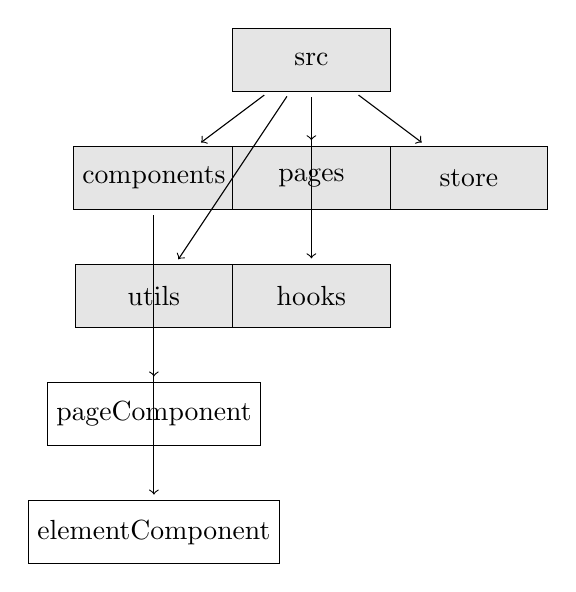
\begin{tikzpicture}[
    file/.style={draw, rectangle, minimum width=2cm, minimum height=0.8cm},
    folder/.style={draw, rectangle, minimum width=2cm, minimum height=0.8cm, fill=gray!20},
    arrow/.style={->, shorten >=2pt, shorten <=2pt}
]

% Folders
\node[folder] (src) at (0,0) {src};
\node[folder] (components) at (-2,-1.5) {components};
\node[folder] (pages) at (0,-1.5) {pages};
\node[folder] (store) at (2,-1.5) {store};
\node[folder] (utils) at (-2,-3) {utils};
\node[folder] (hooks) at (0,-3) {hooks};

% Files
\node[file] (pageComponent) at (-2,-4.5) {pageComponent};
\node[file] (elementComponent) at (-2,-6) {elementComponent};
% ... add more files

% Connections
\draw[arrow] (src) -- (components);
\draw[arrow] (src) -- (pages);
\draw[arrow] (src) -- (store);
\draw[arrow] (src) -- (utils);
\draw[arrow] (src) -- (hooks);
\draw[arrow] (components) -- (pageComponent);
\draw[arrow] (components) -- (elementComponent);
% ... add more connections

\end{tikzpicture}



\pagebreak
\subsubsection{Back-end}
The backend uses the dotNet framework. The development language using the C\# language.

In this project, the backend uses the Onion Architecture.
The Onion Architecture is a typically layered architecture, 
where each layer depends on the inner layer and provides interfaces to the outer layer.
The outer layer provides services to the outermost layer 
and other modules in the same layer based on the interfaces of the inner layer.

From inner to outer, the layers are: Domain, Application, Infrastructure, Presentation.
The Domain layer is the core layer and the innermost layer, used to define domain models, 
which are the business models.
It includes domain models and domain service interfaces.
Domain models are used to define the business models, 
which are the entities in the entity-relationship model and their attributes.
Domain service interfaces are used to define the business services, 
which are the relationships between entities in the entity-relationship model.

The Application layer is the application layer, 
used to define application services, which are the business logic.
It includes domain service implementations and application service interfaces.
Domain service implementations implement the methods of the inner layer's domain service 
interfaces and implement the business logic of the domain models.
Application service interfaces are used to define application services, 
which are the business logic.
It includes but is not limited to database interfaces, testing interfaces, 
HTTP API interfaces, MQTT interfaces, etc.

The Infrastructure layer is the infrastructure layer, used to define infrastructure.
It includes database implementations, testing implementations, 
HTTP API implementations, MQTT implementations, etc.
Database implementations implement the database interfaces 
and provide CRUD services for the database.
Testing implementations implement the testing interfaces 
and provide services for unit testing and integration testing.
HTTP API implementations implement the HTTP API interfaces 
and provide CRUD operations for HTTP APIs.
MQTT implementations implement the MQTT interfaces 
and provide CRUD operations for MQTT.

The Presentation layer is the presentation layer, used to define presentation logic, 
such as interfaces and pages. Since this is a backend project,
data presentation and control are handled by the frontend, 
so this layer is not needed.



\pagebreak
\subsubsection{Data communication and storage}
% 关于本项目的数据通信与数据存储的设计, 包括数据通信的协议, 数据存储的设计等
% 关于数据通信的设计:
% 1. 通信协议的选择
% 自前端向后端发送的数据, 有三种传输的数据类型, 
% 一种是普通的增删改查的请求, 对数据传输的时效性要求不高, 但是对数据的准确性, 完整性, 有序性, 安全性有一定的要求,
% 这种数据的传输, 采用 HTTP 协议, 以及 RESTful API 的设计. 可以有效的保证对数据传输的以上要求.
% 一种是对数据通道的创建和流媒体数据的传输, 对数据传输的时效性, 安全性要求较高, 这种数据的传输, 采用 WebRTC 协议, 以及 MQTT 协议.
% 配合可以快速解码的 flatbuffers 协议, 可以有效的保证对数据传输的以上要求.
% 最后一种是对设备的状态信息和操作信息的传输, 对完整性, 有序性, 安全性都有较高的要求, 这种数据的传输, 采用 MQTT 协议
% 同时也使用了 flatbuffers 协议.
% 
% 2. 数据通信的通信架构和通信流程
% 本项目的数据通信的通信架构, 是基于前后端分离的架构, 前端使用 React 框架, 后端使用 dotnet 框架.
% 当前端需要向后端发送数据的时候, 前端会向后端发送 HTTP 请求, 后端接收到 HTTP 请求之后, 会根据请求的数据类型,
% 选择不同的数据处理方式, 对于普通的增删改查的请求, 后端会根据 RESTful API 的设计, 对数据进行增删改查的操作,
% 对于对数据通道的创建和流媒体数据的传输, 后端会根据 WebRTC 协议, 对数据通道进行创建, 并且帮助前端和设备建立数据通道,
% 当数据通道建立后, 前端和设备之间则使用 flatbuffer 的数据格式对流媒体数据进行传输,
% 对于设备的状态信息和操作信息的传输, 前端会直接向 MQTT broker 发送 MQTT 请求, 
% 设备会在其自身的固件中监听相关的 MQTT 请求, 并且返回相关的数据.
% 
% 3. 数据通信的格式
% 本项目的数据通信的格式, 有三种, 
% 一种是 HTTP 协议, 
% 使用 json 格式对数据进行传输,
% 一种是 WebRTC 协议, 
% 使用 flatbuffers 格式对数据进行传输,
% 一种是 MQTT 协议.
% 使用 flatbuffers 格式对数据进行传输,
% 
% 关于数据存储的设计:
% 1. 数据存储的数据库的选择
% 本项目的数据存储的数据库的选择, 使用了轻量级的数据库 SQLite,
% SQLite 是一个进程内的库, 实现了自给自足的, 无服务器的, 零配置的, 事务性的 SQL 数据库引擎.
% 这是因为整个项目的目的是为了实现前端与设备之间的数据通信, 对于数据库数据的增删改查操作的要求不高,
% 数据量较小, 且对于数据库的数据的事务性要求不高, 所以选择了 SQLite 数据库.
% 2. 项目前后端的数据结构的设计
% 在本项目中, 前端由于使用了 React 框架, 所以前端的数据结构的设计, 使用了基于状态的数据结构的设计,
% 每个组件或者数据集都包含一个状态对象, 这个状态对象的属性就是组件的各个状态. 
% 使用状态对象的原因是, 可以方便的对状态进行管理, 采用对象-属性的形式, 可以方便的针对不同组件的同类状态进行区分,
% 由于跨组件的状态是由 redux 进行管理的, 这种状态对象的设计, 可以更搞笑的对状态进行更新和传递.
% 后端由于使用了 dotnet 框架, 所以后端的数据结构的设计, 使用了基于类的数据结构的设计,
% 采用了面向对象的编程思想, 对数据进行了封装, 使得数据的传输更加的安全, 有序, 完整.


\pagebreak

% \subsection{Domain model}
% \documentclass[]{article}
\usepackage{graphicx}
\usepackage{amsmath}
\usepackage{tikz}

% libaries
\usetikzlibrary{shapes,arrows}

%Define the listing package
\usepackage{listings} %code highlighter
\usepackage{color} %use color
\definecolor{mygreen}{rgb}{0,0.6,0}
\definecolor{mygray}{rgb}{0.5,0.5,0.5}
\definecolor{mymauve}{rgb}{0.58,0,0.82}

%Customize a bit the look
\lstset{ %
backgroundcolor=\color{white}, % choose the background color; you must add \usepackage{color} or \usepackage{xcolor}
basicstyle=\footnotesize, % the size of the fonts that are used for the code
breakatwhitespace=false, % sets if automatic breaks should only happen at whitespace
breaklines=true, % sets automatic line breaking
captionpos=b, % sets the caption-position to bottom
commentstyle=\color{mygreen}, % comment style
deletekeywords={...}, % if you want to delete keywords from the given language
escapeinside={\%*}{*)}, % if you want to add LaTeX within your code
extendedchars=true, % lets you use non-ASCII characters; for 8-bits encodings only, does not work with UTF-8
frame=single, % adds a frame around the code
keepspaces=true, % keeps spaces in text, useful for keeping indentation of code (possibly needs columns=flexible)
keywordstyle=\color{blue}, % keyword style
% language=Octave, % the language of the code
morekeywords={*,...}, % if you want to add more keywords to the set
numbers=left, % where to put the line-numbers; possible values are (none, left, right)
numbersep=5pt, % how far the line-numbers are from the code
numberstyle=\tiny\color{mygray}, % the style that is used for the line-numbers
rulecolor=\color{black}, % if not set, the frame-color may be changed on line-breaks within not-black text (e.g. comments (green here))
showspaces=false, % show spaces everywhere adding particular underscores; it overrides 'showstringspaces'
showstringspaces=false, % underline spaces within strings only
showtabs=false, % show tabs within strings adding particular underscores
stepnumber=1, % the step between two line-numbers. If it's 1, each line will be numbered
stringstyle=\color{mymauve}, % string literal style
tabsize=2, % sets default tabsize to 2 spaces
title=\lstname % show the filename of files included with \lstinputlisting; also try caption instead of title
}

\definecolor{darkgray}{rgb}{.4,.4,.4}
\definecolor{purple}{rgb}{0.65, 0.12, 0.82}

\lstdefinelanguage{React}{
keywords={const, typeof, new, true, false, catch, function, return, null, catch, switch, var, if, in, while, do, else, case, break},
keywordstyle=\color{blue}\bfseries,
ndkeywords={class, export, boolean, throw, implements, import, this},
ndkeywordstyle=\color{darkgray}\bfseries,
identifierstyle=\color{mygreen},
sensitive=false,
comment=[l]{//},
morecomment=[s]{/*}{*/},
commentstyle=\color{purple}\ttfamily,
string=[b]{"}{'}{`},
stringstyle=\color{red}\ttfamily,
morestring=[b]',
morestring=[b]",
morestring=[b]`',
}

\lstdefinelanguage{CSharp}{
keywords={const, typeof, new, true, false, catch, function, return, null, catch, switch, var, if, in, while, do, else, case, break},
keywordstyle=\color{blue}\bfseries,
ndkeywords={class, export, boolean, throw, implements, import, this},
ndkeywordstyle=\color{darkgray}\bfseries,
identifierstyle=\color{mygreen},
sensitive=false,
comment=[l]{//},
morecomment=[s]{/*}{*/},
commentstyle=\color{purple}\ttfamily,
string=[b]{"}{'}{`},
stringstyle=\color{red}\ttfamily,
morestring=[b]',
morestring=[b]",
morestring=[b]`',
}

\lstset{
language=React,
extendedchars=true,
basicstyle=\footnotesize\ttfamily,
showstringspaces=false,
showspaces=false,
numbers=left,
numberstyle=\footnotesize,
numbersep=9pt,
tabsize=2,
breaklines=true,
showtabs=false,
captionpos=b
}

\lstset{
language=CSharp,
extendedchars=true,
basicstyle=\footnotesize\ttfamily,
showstringspaces=false,
showspaces=false,
numbers=left,
numberstyle=\footnotesize,
numbersep=9pt,
tabsize=2,
breaklines=true,
showtabs=false,
captionpos=b
}

% \usepackage{cite} % Add this line for citation

% \bibliographystyle{plain}

\title{
The implementation of BifrostConnect Front-end scope, 
re-design and development with the relevant back-end support develop.
}
\author{
    Fei Gu \\
    Erhvervs Akademi Sydvest \\
    Computer Science 21\\
    }
\date{\today}

\begin{document}

% Front page
\maketitle
\begin{center}
    Supervisor: Henrik Boulund Meng Hansen \\
    Company: BifrostConnect \\
    Engineering Director: Jasper Wass \\
\end{center}
\tableofcontents
\pagebreak


% The introduction
\section{Introduction}
\subsection{Background}\input{sections/introduction/background.tex}
\subsection{The company}\input{sections/introduction/aboutCompany}
\subsection{The project}\input{sections/introduction/aboutProject}
\pagebreak

% The problem statement
\section{Problem Statement}
\subsection{Statement}
\input{sections/problemStatement/statement}
\subsection{Situation}
\input{sections/problemStatement/situation}
\subsection{Potential Solution}
\input{sections/problemStatement/potentialSolution}
\pagebreak

% Requirement analysis
\section{Requirement Analysis}
\input{sections/requirementAnalysis/index}

\subsection{Stakeholders}
\input{sections/requirementAnalysis/stakeholders/index}

\subsection{Business Domain}
\input{sections/requirementAnalysis/bussinesDomain/index}

\subsection{Scope}
\input{sections/requirementAnalysis/scope}

\subsection{Goals}
\input{sections/requirementAnalysis/goals}
\pagebreak

% Software Design
\section{Software Design}
% developement methods
\subsection{Software Development Methods}
\input{sections/softwareDevelopmentMethods/index}
\subsubsection{Agile Software Development}
\input{sections/softwareDevelopmentMethods/agileSoftwareDevelopment/index}
\subsubsection{Feature Driven Development}
\input{sections/softwareDevelopmentMethods/featureDrivenDevelopment/index}

\pagebreak

% Technology seslection
\subsection{Technology selection}
\input{sections/softwareDesign/technologySelection/index}
\subsubsection{Front-end}
\input{sections/softwareDesign/technologySelection/frontEnd}            
\subsubsection{Back-end}
\input{sections/softwareDesign/technologySelection/backEnd}            
\subsubsection{Database}
\input{sections/softwareDesign/technologySelection/database}
\subsubsection{Data communication}
\input{sections/softwareDesign/technologySelection/dataCommunication}            
\subsubsection{DevOps}
\input{sections/softwareDesign/technologySelection/devOps}
\pagebreak

% Architecture design
\subsection{Architecture design}
\input{sections/softwareDesign/architectureDesign/index}
\pagebreak
\subsubsection{Front-end}
\input{sections/softwareDesign/architectureDesign/frontEndArchitecture}
\pagebreak
\subsubsection{Back-end}
\input{sections/softwareDesign/architectureDesign/backEndArchitecture}
\pagebreak
\subsubsection{Data communication and storage}
\input{sections/softwareDesign/architectureDesign/dataCommunicationArchitecture}
\pagebreak

% \subsection{Domain model}
% \input{sections/softwareDesign/domainModel/index}
% \subsection{Database design}
% % 数据库领域模型 ER 图
% % 包括表和字段的设置.
% % 对于私有键和外键的设置.

% \subsection{Back-end design}
% % 后端对象模型
% % 以及对于对象模型的增删改查
% % 以及相关的其他服务的设计`'

% \subsection{Front-end design}
% % 对于前端的页面结构的设计 
% % 页面的状态的设计, 交互设计

% \subsection{FlatBuffers design}
% % schema 的设计

\subsection{DevOps CI/CD process design}
\input{sections/softwareDesign/devOpsDesign/index}
\subsubsection{Continuous Integration}
\input{sections/softwareDesign/devOpsDesign/continuousIntegration/index}
\subsubsection{Continuous Delivery}
\input{sections/softwareDesign/devOpsDesign/continuousDelivery/index}
\subsubsection{Continuous Deployment}
\input{sections/softwareDesign/devOpsDesign/continuousDeployment/index}
\pagebreak

\section{Software Development} 
\input{sections/softwareDevelopment/index}
\subsection{Overall development}
\input{sections/softwareDevelopment/overallDevelopement/index}
\subsubsection{Front-end}
\input{sections/softwareDevelopment/overallDevelopement/frontEnd/index}
\subsubsection{Back-end}
\input{sections/softwareDevelopment/overallDevelopement/backEnd/index}
\subsubsection{DevOps}
\input{sections/softwareDevelopment/overallDevelopement/devOps/index}
\subsection{Feature development} 
\input{sections/softwareDevelopment/featureDevelopment/index}
\subsubsection{Use Case 1}
\input{sections/softwareDevelopment/featureDevelopment/useCase1/index}
\subsubsection{Feature 1}
\input{sections/softwareDevelopment/featureDevelopment/feature/feature1.tex}
\pagebreak
\section{Conclusion} 
\subsection{Result}
Since the project is still in progress, the result is not available yet.
So far, basic structure of this project has been built. But the most features 
are not implemented yet. 
\subsection{Discussion}
As a single developer for this project, I am confident what I have done so far.
And I can say I understand the most of the knowledge I have used in this project, 
which also means I can explain all the part of the project. 
But this project also relevant some of the complex knowledge which I have to continue 
to study and practice.
\subsection{Future Work}
The future work is to implement the rest of the features. 
Including the most important part which is the 'create session' feature.
\pagebreak
% \bibliography{bibliography}
\pagebreak
% \begin{appendices}
%     \section{Appendix}
% \end{appendices} 
\end{document}
% \subsection{Database design}
% % 数据库领域模型 ER 图
% % 包括表和字段的设置.
% % 对于私有键和外键的设置.

% \subsection{Back-end design}
% % 后端对象模型
% % 以及对于对象模型的增删改查
% % 以及相关的其他服务的设计`'

% \subsection{Front-end design}
% % 对于前端的页面结构的设计 
% % 页面的状态的设计, 交互设计

% \subsection{FlatBuffers design}
% % schema 的设计

\subsection{DevOps CI/CD process design}
\documentclass[]{article}
\usepackage{graphicx}
\usepackage{amsmath}
\usepackage{tikz}

% libaries
\usetikzlibrary{shapes,arrows}

%Define the listing package
\usepackage{listings} %code highlighter
\usepackage{color} %use color
\definecolor{mygreen}{rgb}{0,0.6,0}
\definecolor{mygray}{rgb}{0.5,0.5,0.5}
\definecolor{mymauve}{rgb}{0.58,0,0.82}

%Customize a bit the look
\lstset{ %
backgroundcolor=\color{white}, % choose the background color; you must add \usepackage{color} or \usepackage{xcolor}
basicstyle=\footnotesize, % the size of the fonts that are used for the code
breakatwhitespace=false, % sets if automatic breaks should only happen at whitespace
breaklines=true, % sets automatic line breaking
captionpos=b, % sets the caption-position to bottom
commentstyle=\color{mygreen}, % comment style
deletekeywords={...}, % if you want to delete keywords from the given language
escapeinside={\%*}{*)}, % if you want to add LaTeX within your code
extendedchars=true, % lets you use non-ASCII characters; for 8-bits encodings only, does not work with UTF-8
frame=single, % adds a frame around the code
keepspaces=true, % keeps spaces in text, useful for keeping indentation of code (possibly needs columns=flexible)
keywordstyle=\color{blue}, % keyword style
% language=Octave, % the language of the code
morekeywords={*,...}, % if you want to add more keywords to the set
numbers=left, % where to put the line-numbers; possible values are (none, left, right)
numbersep=5pt, % how far the line-numbers are from the code
numberstyle=\tiny\color{mygray}, % the style that is used for the line-numbers
rulecolor=\color{black}, % if not set, the frame-color may be changed on line-breaks within not-black text (e.g. comments (green here))
showspaces=false, % show spaces everywhere adding particular underscores; it overrides 'showstringspaces'
showstringspaces=false, % underline spaces within strings only
showtabs=false, % show tabs within strings adding particular underscores
stepnumber=1, % the step between two line-numbers. If it's 1, each line will be numbered
stringstyle=\color{mymauve}, % string literal style
tabsize=2, % sets default tabsize to 2 spaces
title=\lstname % show the filename of files included with \lstinputlisting; also try caption instead of title
}

\definecolor{darkgray}{rgb}{.4,.4,.4}
\definecolor{purple}{rgb}{0.65, 0.12, 0.82}

\lstdefinelanguage{React}{
keywords={const, typeof, new, true, false, catch, function, return, null, catch, switch, var, if, in, while, do, else, case, break},
keywordstyle=\color{blue}\bfseries,
ndkeywords={class, export, boolean, throw, implements, import, this},
ndkeywordstyle=\color{darkgray}\bfseries,
identifierstyle=\color{mygreen},
sensitive=false,
comment=[l]{//},
morecomment=[s]{/*}{*/},
commentstyle=\color{purple}\ttfamily,
string=[b]{"}{'}{`},
stringstyle=\color{red}\ttfamily,
morestring=[b]',
morestring=[b]",
morestring=[b]`',
}

\lstdefinelanguage{CSharp}{
keywords={const, typeof, new, true, false, catch, function, return, null, catch, switch, var, if, in, while, do, else, case, break},
keywordstyle=\color{blue}\bfseries,
ndkeywords={class, export, boolean, throw, implements, import, this},
ndkeywordstyle=\color{darkgray}\bfseries,
identifierstyle=\color{mygreen},
sensitive=false,
comment=[l]{//},
morecomment=[s]{/*}{*/},
commentstyle=\color{purple}\ttfamily,
string=[b]{"}{'}{`},
stringstyle=\color{red}\ttfamily,
morestring=[b]',
morestring=[b]",
morestring=[b]`',
}

\lstset{
language=React,
extendedchars=true,
basicstyle=\footnotesize\ttfamily,
showstringspaces=false,
showspaces=false,
numbers=left,
numberstyle=\footnotesize,
numbersep=9pt,
tabsize=2,
breaklines=true,
showtabs=false,
captionpos=b
}

\lstset{
language=CSharp,
extendedchars=true,
basicstyle=\footnotesize\ttfamily,
showstringspaces=false,
showspaces=false,
numbers=left,
numberstyle=\footnotesize,
numbersep=9pt,
tabsize=2,
breaklines=true,
showtabs=false,
captionpos=b
}

% \usepackage{cite} % Add this line for citation

% \bibliographystyle{plain}

\title{
The implementation of BifrostConnect Front-end scope, 
re-design and development with the relevant back-end support develop.
}
\author{
    Fei Gu \\
    Erhvervs Akademi Sydvest \\
    Computer Science 21\\
    }
\date{\today}

\begin{document}

% Front page
\maketitle
\begin{center}
    Supervisor: Henrik Boulund Meng Hansen \\
    Company: BifrostConnect \\
    Engineering Director: Jasper Wass \\
\end{center}
\tableofcontents
\pagebreak


% The introduction
\section{Introduction}
\subsection{Background}\input{sections/introduction/background.tex}
\subsection{The company}\input{sections/introduction/aboutCompany}
\subsection{The project}\input{sections/introduction/aboutProject}
\pagebreak

% The problem statement
\section{Problem Statement}
\subsection{Statement}
\input{sections/problemStatement/statement}
\subsection{Situation}
\input{sections/problemStatement/situation}
\subsection{Potential Solution}
\input{sections/problemStatement/potentialSolution}
\pagebreak

% Requirement analysis
\section{Requirement Analysis}
\input{sections/requirementAnalysis/index}

\subsection{Stakeholders}
\input{sections/requirementAnalysis/stakeholders/index}

\subsection{Business Domain}
\input{sections/requirementAnalysis/bussinesDomain/index}

\subsection{Scope}
\input{sections/requirementAnalysis/scope}

\subsection{Goals}
\input{sections/requirementAnalysis/goals}
\pagebreak

% Software Design
\section{Software Design}
% developement methods
\subsection{Software Development Methods}
\input{sections/softwareDevelopmentMethods/index}
\subsubsection{Agile Software Development}
\input{sections/softwareDevelopmentMethods/agileSoftwareDevelopment/index}
\subsubsection{Feature Driven Development}
\input{sections/softwareDevelopmentMethods/featureDrivenDevelopment/index}

\pagebreak

% Technology seslection
\subsection{Technology selection}
\input{sections/softwareDesign/technologySelection/index}
\subsubsection{Front-end}
\input{sections/softwareDesign/technologySelection/frontEnd}            
\subsubsection{Back-end}
\input{sections/softwareDesign/technologySelection/backEnd}            
\subsubsection{Database}
\input{sections/softwareDesign/technologySelection/database}
\subsubsection{Data communication}
\input{sections/softwareDesign/technologySelection/dataCommunication}            
\subsubsection{DevOps}
\input{sections/softwareDesign/technologySelection/devOps}
\pagebreak

% Architecture design
\subsection{Architecture design}
\input{sections/softwareDesign/architectureDesign/index}
\pagebreak
\subsubsection{Front-end}
\input{sections/softwareDesign/architectureDesign/frontEndArchitecture}
\pagebreak
\subsubsection{Back-end}
\input{sections/softwareDesign/architectureDesign/backEndArchitecture}
\pagebreak
\subsubsection{Data communication and storage}
\input{sections/softwareDesign/architectureDesign/dataCommunicationArchitecture}
\pagebreak

% \subsection{Domain model}
% \input{sections/softwareDesign/domainModel/index}
% \subsection{Database design}
% % 数据库领域模型 ER 图
% % 包括表和字段的设置.
% % 对于私有键和外键的设置.

% \subsection{Back-end design}
% % 后端对象模型
% % 以及对于对象模型的增删改查
% % 以及相关的其他服务的设计`'

% \subsection{Front-end design}
% % 对于前端的页面结构的设计 
% % 页面的状态的设计, 交互设计

% \subsection{FlatBuffers design}
% % schema 的设计

\subsection{DevOps CI/CD process design}
\input{sections/softwareDesign/devOpsDesign/index}
\subsubsection{Continuous Integration}
\input{sections/softwareDesign/devOpsDesign/continuousIntegration/index}
\subsubsection{Continuous Delivery}
\input{sections/softwareDesign/devOpsDesign/continuousDelivery/index}
\subsubsection{Continuous Deployment}
\input{sections/softwareDesign/devOpsDesign/continuousDeployment/index}
\pagebreak

\section{Software Development} 
\input{sections/softwareDevelopment/index}
\subsection{Overall development}
\input{sections/softwareDevelopment/overallDevelopement/index}
\subsubsection{Front-end}
\input{sections/softwareDevelopment/overallDevelopement/frontEnd/index}
\subsubsection{Back-end}
\input{sections/softwareDevelopment/overallDevelopement/backEnd/index}
\subsubsection{DevOps}
\input{sections/softwareDevelopment/overallDevelopement/devOps/index}
\subsection{Feature development} 
\input{sections/softwareDevelopment/featureDevelopment/index}
\subsubsection{Use Case 1}
\input{sections/softwareDevelopment/featureDevelopment/useCase1/index}
\subsubsection{Feature 1}
\input{sections/softwareDevelopment/featureDevelopment/feature/feature1.tex}
\pagebreak
\section{Conclusion} 
\subsection{Result}
Since the project is still in progress, the result is not available yet.
So far, basic structure of this project has been built. But the most features 
are not implemented yet. 
\subsection{Discussion}
As a single developer for this project, I am confident what I have done so far.
And I can say I understand the most of the knowledge I have used in this project, 
which also means I can explain all the part of the project. 
But this project also relevant some of the complex knowledge which I have to continue 
to study and practice.
\subsection{Future Work}
The future work is to implement the rest of the features. 
Including the most important part which is the 'create session' feature.
\pagebreak
% \bibliography{bibliography}
\pagebreak
% \begin{appendices}
%     \section{Appendix}
% \end{appendices} 
\end{document}
\subsubsection{Continuous Integration}
\documentclass[]{article}
\usepackage{graphicx}
\usepackage{amsmath}
\usepackage{tikz}

% libaries
\usetikzlibrary{shapes,arrows}

%Define the listing package
\usepackage{listings} %code highlighter
\usepackage{color} %use color
\definecolor{mygreen}{rgb}{0,0.6,0}
\definecolor{mygray}{rgb}{0.5,0.5,0.5}
\definecolor{mymauve}{rgb}{0.58,0,0.82}

%Customize a bit the look
\lstset{ %
backgroundcolor=\color{white}, % choose the background color; you must add \usepackage{color} or \usepackage{xcolor}
basicstyle=\footnotesize, % the size of the fonts that are used for the code
breakatwhitespace=false, % sets if automatic breaks should only happen at whitespace
breaklines=true, % sets automatic line breaking
captionpos=b, % sets the caption-position to bottom
commentstyle=\color{mygreen}, % comment style
deletekeywords={...}, % if you want to delete keywords from the given language
escapeinside={\%*}{*)}, % if you want to add LaTeX within your code
extendedchars=true, % lets you use non-ASCII characters; for 8-bits encodings only, does not work with UTF-8
frame=single, % adds a frame around the code
keepspaces=true, % keeps spaces in text, useful for keeping indentation of code (possibly needs columns=flexible)
keywordstyle=\color{blue}, % keyword style
% language=Octave, % the language of the code
morekeywords={*,...}, % if you want to add more keywords to the set
numbers=left, % where to put the line-numbers; possible values are (none, left, right)
numbersep=5pt, % how far the line-numbers are from the code
numberstyle=\tiny\color{mygray}, % the style that is used for the line-numbers
rulecolor=\color{black}, % if not set, the frame-color may be changed on line-breaks within not-black text (e.g. comments (green here))
showspaces=false, % show spaces everywhere adding particular underscores; it overrides 'showstringspaces'
showstringspaces=false, % underline spaces within strings only
showtabs=false, % show tabs within strings adding particular underscores
stepnumber=1, % the step between two line-numbers. If it's 1, each line will be numbered
stringstyle=\color{mymauve}, % string literal style
tabsize=2, % sets default tabsize to 2 spaces
title=\lstname % show the filename of files included with \lstinputlisting; also try caption instead of title
}

\definecolor{darkgray}{rgb}{.4,.4,.4}
\definecolor{purple}{rgb}{0.65, 0.12, 0.82}

\lstdefinelanguage{React}{
keywords={const, typeof, new, true, false, catch, function, return, null, catch, switch, var, if, in, while, do, else, case, break},
keywordstyle=\color{blue}\bfseries,
ndkeywords={class, export, boolean, throw, implements, import, this},
ndkeywordstyle=\color{darkgray}\bfseries,
identifierstyle=\color{mygreen},
sensitive=false,
comment=[l]{//},
morecomment=[s]{/*}{*/},
commentstyle=\color{purple}\ttfamily,
string=[b]{"}{'}{`},
stringstyle=\color{red}\ttfamily,
morestring=[b]',
morestring=[b]",
morestring=[b]`',
}

\lstdefinelanguage{CSharp}{
keywords={const, typeof, new, true, false, catch, function, return, null, catch, switch, var, if, in, while, do, else, case, break},
keywordstyle=\color{blue}\bfseries,
ndkeywords={class, export, boolean, throw, implements, import, this},
ndkeywordstyle=\color{darkgray}\bfseries,
identifierstyle=\color{mygreen},
sensitive=false,
comment=[l]{//},
morecomment=[s]{/*}{*/},
commentstyle=\color{purple}\ttfamily,
string=[b]{"}{'}{`},
stringstyle=\color{red}\ttfamily,
morestring=[b]',
morestring=[b]",
morestring=[b]`',
}

\lstset{
language=React,
extendedchars=true,
basicstyle=\footnotesize\ttfamily,
showstringspaces=false,
showspaces=false,
numbers=left,
numberstyle=\footnotesize,
numbersep=9pt,
tabsize=2,
breaklines=true,
showtabs=false,
captionpos=b
}

\lstset{
language=CSharp,
extendedchars=true,
basicstyle=\footnotesize\ttfamily,
showstringspaces=false,
showspaces=false,
numbers=left,
numberstyle=\footnotesize,
numbersep=9pt,
tabsize=2,
breaklines=true,
showtabs=false,
captionpos=b
}

% \usepackage{cite} % Add this line for citation

% \bibliographystyle{plain}

\title{
The implementation of BifrostConnect Front-end scope, 
re-design and development with the relevant back-end support develop.
}
\author{
    Fei Gu \\
    Erhvervs Akademi Sydvest \\
    Computer Science 21\\
    }
\date{\today}

\begin{document}

% Front page
\maketitle
\begin{center}
    Supervisor: Henrik Boulund Meng Hansen \\
    Company: BifrostConnect \\
    Engineering Director: Jasper Wass \\
\end{center}
\tableofcontents
\pagebreak


% The introduction
\section{Introduction}
\subsection{Background}\input{sections/introduction/background.tex}
\subsection{The company}\input{sections/introduction/aboutCompany}
\subsection{The project}\input{sections/introduction/aboutProject}
\pagebreak

% The problem statement
\section{Problem Statement}
\subsection{Statement}
\input{sections/problemStatement/statement}
\subsection{Situation}
\input{sections/problemStatement/situation}
\subsection{Potential Solution}
\input{sections/problemStatement/potentialSolution}
\pagebreak

% Requirement analysis
\section{Requirement Analysis}
\input{sections/requirementAnalysis/index}

\subsection{Stakeholders}
\input{sections/requirementAnalysis/stakeholders/index}

\subsection{Business Domain}
\input{sections/requirementAnalysis/bussinesDomain/index}

\subsection{Scope}
\input{sections/requirementAnalysis/scope}

\subsection{Goals}
\input{sections/requirementAnalysis/goals}
\pagebreak

% Software Design
\section{Software Design}
% developement methods
\subsection{Software Development Methods}
\input{sections/softwareDevelopmentMethods/index}
\subsubsection{Agile Software Development}
\input{sections/softwareDevelopmentMethods/agileSoftwareDevelopment/index}
\subsubsection{Feature Driven Development}
\input{sections/softwareDevelopmentMethods/featureDrivenDevelopment/index}

\pagebreak

% Technology seslection
\subsection{Technology selection}
\input{sections/softwareDesign/technologySelection/index}
\subsubsection{Front-end}
\input{sections/softwareDesign/technologySelection/frontEnd}            
\subsubsection{Back-end}
\input{sections/softwareDesign/technologySelection/backEnd}            
\subsubsection{Database}
\input{sections/softwareDesign/technologySelection/database}
\subsubsection{Data communication}
\input{sections/softwareDesign/technologySelection/dataCommunication}            
\subsubsection{DevOps}
\input{sections/softwareDesign/technologySelection/devOps}
\pagebreak

% Architecture design
\subsection{Architecture design}
\input{sections/softwareDesign/architectureDesign/index}
\pagebreak
\subsubsection{Front-end}
\input{sections/softwareDesign/architectureDesign/frontEndArchitecture}
\pagebreak
\subsubsection{Back-end}
\input{sections/softwareDesign/architectureDesign/backEndArchitecture}
\pagebreak
\subsubsection{Data communication and storage}
\input{sections/softwareDesign/architectureDesign/dataCommunicationArchitecture}
\pagebreak

% \subsection{Domain model}
% \input{sections/softwareDesign/domainModel/index}
% \subsection{Database design}
% % 数据库领域模型 ER 图
% % 包括表和字段的设置.
% % 对于私有键和外键的设置.

% \subsection{Back-end design}
% % 后端对象模型
% % 以及对于对象模型的增删改查
% % 以及相关的其他服务的设计`'

% \subsection{Front-end design}
% % 对于前端的页面结构的设计 
% % 页面的状态的设计, 交互设计

% \subsection{FlatBuffers design}
% % schema 的设计

\subsection{DevOps CI/CD process design}
\input{sections/softwareDesign/devOpsDesign/index}
\subsubsection{Continuous Integration}
\input{sections/softwareDesign/devOpsDesign/continuousIntegration/index}
\subsubsection{Continuous Delivery}
\input{sections/softwareDesign/devOpsDesign/continuousDelivery/index}
\subsubsection{Continuous Deployment}
\input{sections/softwareDesign/devOpsDesign/continuousDeployment/index}
\pagebreak

\section{Software Development} 
\input{sections/softwareDevelopment/index}
\subsection{Overall development}
\input{sections/softwareDevelopment/overallDevelopement/index}
\subsubsection{Front-end}
\input{sections/softwareDevelopment/overallDevelopement/frontEnd/index}
\subsubsection{Back-end}
\input{sections/softwareDevelopment/overallDevelopement/backEnd/index}
\subsubsection{DevOps}
\input{sections/softwareDevelopment/overallDevelopement/devOps/index}
\subsection{Feature development} 
\input{sections/softwareDevelopment/featureDevelopment/index}
\subsubsection{Use Case 1}
\input{sections/softwareDevelopment/featureDevelopment/useCase1/index}
\subsubsection{Feature 1}
\input{sections/softwareDevelopment/featureDevelopment/feature/feature1.tex}
\pagebreak
\section{Conclusion} 
\subsection{Result}
Since the project is still in progress, the result is not available yet.
So far, basic structure of this project has been built. But the most features 
are not implemented yet. 
\subsection{Discussion}
As a single developer for this project, I am confident what I have done so far.
And I can say I understand the most of the knowledge I have used in this project, 
which also means I can explain all the part of the project. 
But this project also relevant some of the complex knowledge which I have to continue 
to study and practice.
\subsection{Future Work}
The future work is to implement the rest of the features. 
Including the most important part which is the 'create session' feature.
\pagebreak
% \bibliography{bibliography}
\pagebreak
% \begin{appendices}
%     \section{Appendix}
% \end{appendices} 
\end{document}
\subsubsection{Continuous Delivery}
\documentclass[]{article}
\usepackage{graphicx}
\usepackage{amsmath}
\usepackage{tikz}

% libaries
\usetikzlibrary{shapes,arrows}

%Define the listing package
\usepackage{listings} %code highlighter
\usepackage{color} %use color
\definecolor{mygreen}{rgb}{0,0.6,0}
\definecolor{mygray}{rgb}{0.5,0.5,0.5}
\definecolor{mymauve}{rgb}{0.58,0,0.82}

%Customize a bit the look
\lstset{ %
backgroundcolor=\color{white}, % choose the background color; you must add \usepackage{color} or \usepackage{xcolor}
basicstyle=\footnotesize, % the size of the fonts that are used for the code
breakatwhitespace=false, % sets if automatic breaks should only happen at whitespace
breaklines=true, % sets automatic line breaking
captionpos=b, % sets the caption-position to bottom
commentstyle=\color{mygreen}, % comment style
deletekeywords={...}, % if you want to delete keywords from the given language
escapeinside={\%*}{*)}, % if you want to add LaTeX within your code
extendedchars=true, % lets you use non-ASCII characters; for 8-bits encodings only, does not work with UTF-8
frame=single, % adds a frame around the code
keepspaces=true, % keeps spaces in text, useful for keeping indentation of code (possibly needs columns=flexible)
keywordstyle=\color{blue}, % keyword style
% language=Octave, % the language of the code
morekeywords={*,...}, % if you want to add more keywords to the set
numbers=left, % where to put the line-numbers; possible values are (none, left, right)
numbersep=5pt, % how far the line-numbers are from the code
numberstyle=\tiny\color{mygray}, % the style that is used for the line-numbers
rulecolor=\color{black}, % if not set, the frame-color may be changed on line-breaks within not-black text (e.g. comments (green here))
showspaces=false, % show spaces everywhere adding particular underscores; it overrides 'showstringspaces'
showstringspaces=false, % underline spaces within strings only
showtabs=false, % show tabs within strings adding particular underscores
stepnumber=1, % the step between two line-numbers. If it's 1, each line will be numbered
stringstyle=\color{mymauve}, % string literal style
tabsize=2, % sets default tabsize to 2 spaces
title=\lstname % show the filename of files included with \lstinputlisting; also try caption instead of title
}

\definecolor{darkgray}{rgb}{.4,.4,.4}
\definecolor{purple}{rgb}{0.65, 0.12, 0.82}

\lstdefinelanguage{React}{
keywords={const, typeof, new, true, false, catch, function, return, null, catch, switch, var, if, in, while, do, else, case, break},
keywordstyle=\color{blue}\bfseries,
ndkeywords={class, export, boolean, throw, implements, import, this},
ndkeywordstyle=\color{darkgray}\bfseries,
identifierstyle=\color{mygreen},
sensitive=false,
comment=[l]{//},
morecomment=[s]{/*}{*/},
commentstyle=\color{purple}\ttfamily,
string=[b]{"}{'}{`},
stringstyle=\color{red}\ttfamily,
morestring=[b]',
morestring=[b]",
morestring=[b]`',
}

\lstdefinelanguage{CSharp}{
keywords={const, typeof, new, true, false, catch, function, return, null, catch, switch, var, if, in, while, do, else, case, break},
keywordstyle=\color{blue}\bfseries,
ndkeywords={class, export, boolean, throw, implements, import, this},
ndkeywordstyle=\color{darkgray}\bfseries,
identifierstyle=\color{mygreen},
sensitive=false,
comment=[l]{//},
morecomment=[s]{/*}{*/},
commentstyle=\color{purple}\ttfamily,
string=[b]{"}{'}{`},
stringstyle=\color{red}\ttfamily,
morestring=[b]',
morestring=[b]",
morestring=[b]`',
}

\lstset{
language=React,
extendedchars=true,
basicstyle=\footnotesize\ttfamily,
showstringspaces=false,
showspaces=false,
numbers=left,
numberstyle=\footnotesize,
numbersep=9pt,
tabsize=2,
breaklines=true,
showtabs=false,
captionpos=b
}

\lstset{
language=CSharp,
extendedchars=true,
basicstyle=\footnotesize\ttfamily,
showstringspaces=false,
showspaces=false,
numbers=left,
numberstyle=\footnotesize,
numbersep=9pt,
tabsize=2,
breaklines=true,
showtabs=false,
captionpos=b
}

% \usepackage{cite} % Add this line for citation

% \bibliographystyle{plain}

\title{
The implementation of BifrostConnect Front-end scope, 
re-design and development with the relevant back-end support develop.
}
\author{
    Fei Gu \\
    Erhvervs Akademi Sydvest \\
    Computer Science 21\\
    }
\date{\today}

\begin{document}

% Front page
\maketitle
\begin{center}
    Supervisor: Henrik Boulund Meng Hansen \\
    Company: BifrostConnect \\
    Engineering Director: Jasper Wass \\
\end{center}
\tableofcontents
\pagebreak


% The introduction
\section{Introduction}
\subsection{Background}\input{sections/introduction/background.tex}
\subsection{The company}\input{sections/introduction/aboutCompany}
\subsection{The project}\input{sections/introduction/aboutProject}
\pagebreak

% The problem statement
\section{Problem Statement}
\subsection{Statement}
\input{sections/problemStatement/statement}
\subsection{Situation}
\input{sections/problemStatement/situation}
\subsection{Potential Solution}
\input{sections/problemStatement/potentialSolution}
\pagebreak

% Requirement analysis
\section{Requirement Analysis}
\input{sections/requirementAnalysis/index}

\subsection{Stakeholders}
\input{sections/requirementAnalysis/stakeholders/index}

\subsection{Business Domain}
\input{sections/requirementAnalysis/bussinesDomain/index}

\subsection{Scope}
\input{sections/requirementAnalysis/scope}

\subsection{Goals}
\input{sections/requirementAnalysis/goals}
\pagebreak

% Software Design
\section{Software Design}
% developement methods
\subsection{Software Development Methods}
\input{sections/softwareDevelopmentMethods/index}
\subsubsection{Agile Software Development}
\input{sections/softwareDevelopmentMethods/agileSoftwareDevelopment/index}
\subsubsection{Feature Driven Development}
\input{sections/softwareDevelopmentMethods/featureDrivenDevelopment/index}

\pagebreak

% Technology seslection
\subsection{Technology selection}
\input{sections/softwareDesign/technologySelection/index}
\subsubsection{Front-end}
\input{sections/softwareDesign/technologySelection/frontEnd}            
\subsubsection{Back-end}
\input{sections/softwareDesign/technologySelection/backEnd}            
\subsubsection{Database}
\input{sections/softwareDesign/technologySelection/database}
\subsubsection{Data communication}
\input{sections/softwareDesign/technologySelection/dataCommunication}            
\subsubsection{DevOps}
\input{sections/softwareDesign/technologySelection/devOps}
\pagebreak

% Architecture design
\subsection{Architecture design}
\input{sections/softwareDesign/architectureDesign/index}
\pagebreak
\subsubsection{Front-end}
\input{sections/softwareDesign/architectureDesign/frontEndArchitecture}
\pagebreak
\subsubsection{Back-end}
\input{sections/softwareDesign/architectureDesign/backEndArchitecture}
\pagebreak
\subsubsection{Data communication and storage}
\input{sections/softwareDesign/architectureDesign/dataCommunicationArchitecture}
\pagebreak

% \subsection{Domain model}
% \input{sections/softwareDesign/domainModel/index}
% \subsection{Database design}
% % 数据库领域模型 ER 图
% % 包括表和字段的设置.
% % 对于私有键和外键的设置.

% \subsection{Back-end design}
% % 后端对象模型
% % 以及对于对象模型的增删改查
% % 以及相关的其他服务的设计`'

% \subsection{Front-end design}
% % 对于前端的页面结构的设计 
% % 页面的状态的设计, 交互设计

% \subsection{FlatBuffers design}
% % schema 的设计

\subsection{DevOps CI/CD process design}
\input{sections/softwareDesign/devOpsDesign/index}
\subsubsection{Continuous Integration}
\input{sections/softwareDesign/devOpsDesign/continuousIntegration/index}
\subsubsection{Continuous Delivery}
\input{sections/softwareDesign/devOpsDesign/continuousDelivery/index}
\subsubsection{Continuous Deployment}
\input{sections/softwareDesign/devOpsDesign/continuousDeployment/index}
\pagebreak

\section{Software Development} 
\input{sections/softwareDevelopment/index}
\subsection{Overall development}
\input{sections/softwareDevelopment/overallDevelopement/index}
\subsubsection{Front-end}
\input{sections/softwareDevelopment/overallDevelopement/frontEnd/index}
\subsubsection{Back-end}
\input{sections/softwareDevelopment/overallDevelopement/backEnd/index}
\subsubsection{DevOps}
\input{sections/softwareDevelopment/overallDevelopement/devOps/index}
\subsection{Feature development} 
\input{sections/softwareDevelopment/featureDevelopment/index}
\subsubsection{Use Case 1}
\input{sections/softwareDevelopment/featureDevelopment/useCase1/index}
\subsubsection{Feature 1}
\input{sections/softwareDevelopment/featureDevelopment/feature/feature1.tex}
\pagebreak
\section{Conclusion} 
\subsection{Result}
Since the project is still in progress, the result is not available yet.
So far, basic structure of this project has been built. But the most features 
are not implemented yet. 
\subsection{Discussion}
As a single developer for this project, I am confident what I have done so far.
And I can say I understand the most of the knowledge I have used in this project, 
which also means I can explain all the part of the project. 
But this project also relevant some of the complex knowledge which I have to continue 
to study and practice.
\subsection{Future Work}
The future work is to implement the rest of the features. 
Including the most important part which is the 'create session' feature.
\pagebreak
% \bibliography{bibliography}
\pagebreak
% \begin{appendices}
%     \section{Appendix}
% \end{appendices} 
\end{document}
\subsubsection{Continuous Deployment}
\documentclass[]{article}
\usepackage{graphicx}
\usepackage{amsmath}
\usepackage{tikz}

% libaries
\usetikzlibrary{shapes,arrows}

%Define the listing package
\usepackage{listings} %code highlighter
\usepackage{color} %use color
\definecolor{mygreen}{rgb}{0,0.6,0}
\definecolor{mygray}{rgb}{0.5,0.5,0.5}
\definecolor{mymauve}{rgb}{0.58,0,0.82}

%Customize a bit the look
\lstset{ %
backgroundcolor=\color{white}, % choose the background color; you must add \usepackage{color} or \usepackage{xcolor}
basicstyle=\footnotesize, % the size of the fonts that are used for the code
breakatwhitespace=false, % sets if automatic breaks should only happen at whitespace
breaklines=true, % sets automatic line breaking
captionpos=b, % sets the caption-position to bottom
commentstyle=\color{mygreen}, % comment style
deletekeywords={...}, % if you want to delete keywords from the given language
escapeinside={\%*}{*)}, % if you want to add LaTeX within your code
extendedchars=true, % lets you use non-ASCII characters; for 8-bits encodings only, does not work with UTF-8
frame=single, % adds a frame around the code
keepspaces=true, % keeps spaces in text, useful for keeping indentation of code (possibly needs columns=flexible)
keywordstyle=\color{blue}, % keyword style
% language=Octave, % the language of the code
morekeywords={*,...}, % if you want to add more keywords to the set
numbers=left, % where to put the line-numbers; possible values are (none, left, right)
numbersep=5pt, % how far the line-numbers are from the code
numberstyle=\tiny\color{mygray}, % the style that is used for the line-numbers
rulecolor=\color{black}, % if not set, the frame-color may be changed on line-breaks within not-black text (e.g. comments (green here))
showspaces=false, % show spaces everywhere adding particular underscores; it overrides 'showstringspaces'
showstringspaces=false, % underline spaces within strings only
showtabs=false, % show tabs within strings adding particular underscores
stepnumber=1, % the step between two line-numbers. If it's 1, each line will be numbered
stringstyle=\color{mymauve}, % string literal style
tabsize=2, % sets default tabsize to 2 spaces
title=\lstname % show the filename of files included with \lstinputlisting; also try caption instead of title
}

\definecolor{darkgray}{rgb}{.4,.4,.4}
\definecolor{purple}{rgb}{0.65, 0.12, 0.82}

\lstdefinelanguage{React}{
keywords={const, typeof, new, true, false, catch, function, return, null, catch, switch, var, if, in, while, do, else, case, break},
keywordstyle=\color{blue}\bfseries,
ndkeywords={class, export, boolean, throw, implements, import, this},
ndkeywordstyle=\color{darkgray}\bfseries,
identifierstyle=\color{mygreen},
sensitive=false,
comment=[l]{//},
morecomment=[s]{/*}{*/},
commentstyle=\color{purple}\ttfamily,
string=[b]{"}{'}{`},
stringstyle=\color{red}\ttfamily,
morestring=[b]',
morestring=[b]",
morestring=[b]`',
}

\lstdefinelanguage{CSharp}{
keywords={const, typeof, new, true, false, catch, function, return, null, catch, switch, var, if, in, while, do, else, case, break},
keywordstyle=\color{blue}\bfseries,
ndkeywords={class, export, boolean, throw, implements, import, this},
ndkeywordstyle=\color{darkgray}\bfseries,
identifierstyle=\color{mygreen},
sensitive=false,
comment=[l]{//},
morecomment=[s]{/*}{*/},
commentstyle=\color{purple}\ttfamily,
string=[b]{"}{'}{`},
stringstyle=\color{red}\ttfamily,
morestring=[b]',
morestring=[b]",
morestring=[b]`',
}

\lstset{
language=React,
extendedchars=true,
basicstyle=\footnotesize\ttfamily,
showstringspaces=false,
showspaces=false,
numbers=left,
numberstyle=\footnotesize,
numbersep=9pt,
tabsize=2,
breaklines=true,
showtabs=false,
captionpos=b
}

\lstset{
language=CSharp,
extendedchars=true,
basicstyle=\footnotesize\ttfamily,
showstringspaces=false,
showspaces=false,
numbers=left,
numberstyle=\footnotesize,
numbersep=9pt,
tabsize=2,
breaklines=true,
showtabs=false,
captionpos=b
}

% \usepackage{cite} % Add this line for citation

% \bibliographystyle{plain}

\title{
The implementation of BifrostConnect Front-end scope, 
re-design and development with the relevant back-end support develop.
}
\author{
    Fei Gu \\
    Erhvervs Akademi Sydvest \\
    Computer Science 21\\
    }
\date{\today}

\begin{document}

% Front page
\maketitle
\begin{center}
    Supervisor: Henrik Boulund Meng Hansen \\
    Company: BifrostConnect \\
    Engineering Director: Jasper Wass \\
\end{center}
\tableofcontents
\pagebreak


% The introduction
\section{Introduction}
\subsection{Background}\input{sections/introduction/background.tex}
\subsection{The company}\input{sections/introduction/aboutCompany}
\subsection{The project}\input{sections/introduction/aboutProject}
\pagebreak

% The problem statement
\section{Problem Statement}
\subsection{Statement}
\input{sections/problemStatement/statement}
\subsection{Situation}
\input{sections/problemStatement/situation}
\subsection{Potential Solution}
\input{sections/problemStatement/potentialSolution}
\pagebreak

% Requirement analysis
\section{Requirement Analysis}
\input{sections/requirementAnalysis/index}

\subsection{Stakeholders}
\input{sections/requirementAnalysis/stakeholders/index}

\subsection{Business Domain}
\input{sections/requirementAnalysis/bussinesDomain/index}

\subsection{Scope}
\input{sections/requirementAnalysis/scope}

\subsection{Goals}
\input{sections/requirementAnalysis/goals}
\pagebreak

% Software Design
\section{Software Design}
% developement methods
\subsection{Software Development Methods}
\input{sections/softwareDevelopmentMethods/index}
\subsubsection{Agile Software Development}
\input{sections/softwareDevelopmentMethods/agileSoftwareDevelopment/index}
\subsubsection{Feature Driven Development}
\input{sections/softwareDevelopmentMethods/featureDrivenDevelopment/index}

\pagebreak

% Technology seslection
\subsection{Technology selection}
\input{sections/softwareDesign/technologySelection/index}
\subsubsection{Front-end}
\input{sections/softwareDesign/technologySelection/frontEnd}            
\subsubsection{Back-end}
\input{sections/softwareDesign/technologySelection/backEnd}            
\subsubsection{Database}
\input{sections/softwareDesign/technologySelection/database}
\subsubsection{Data communication}
\input{sections/softwareDesign/technologySelection/dataCommunication}            
\subsubsection{DevOps}
\input{sections/softwareDesign/technologySelection/devOps}
\pagebreak

% Architecture design
\subsection{Architecture design}
\input{sections/softwareDesign/architectureDesign/index}
\pagebreak
\subsubsection{Front-end}
\input{sections/softwareDesign/architectureDesign/frontEndArchitecture}
\pagebreak
\subsubsection{Back-end}
\input{sections/softwareDesign/architectureDesign/backEndArchitecture}
\pagebreak
\subsubsection{Data communication and storage}
\input{sections/softwareDesign/architectureDesign/dataCommunicationArchitecture}
\pagebreak

% \subsection{Domain model}
% \input{sections/softwareDesign/domainModel/index}
% \subsection{Database design}
% % 数据库领域模型 ER 图
% % 包括表和字段的设置.
% % 对于私有键和外键的设置.

% \subsection{Back-end design}
% % 后端对象模型
% % 以及对于对象模型的增删改查
% % 以及相关的其他服务的设计`'

% \subsection{Front-end design}
% % 对于前端的页面结构的设计 
% % 页面的状态的设计, 交互设计

% \subsection{FlatBuffers design}
% % schema 的设计

\subsection{DevOps CI/CD process design}
\input{sections/softwareDesign/devOpsDesign/index}
\subsubsection{Continuous Integration}
\input{sections/softwareDesign/devOpsDesign/continuousIntegration/index}
\subsubsection{Continuous Delivery}
\input{sections/softwareDesign/devOpsDesign/continuousDelivery/index}
\subsubsection{Continuous Deployment}
\input{sections/softwareDesign/devOpsDesign/continuousDeployment/index}
\pagebreak

\section{Software Development} 
\input{sections/softwareDevelopment/index}
\subsection{Overall development}
\input{sections/softwareDevelopment/overallDevelopement/index}
\subsubsection{Front-end}
\input{sections/softwareDevelopment/overallDevelopement/frontEnd/index}
\subsubsection{Back-end}
\input{sections/softwareDevelopment/overallDevelopement/backEnd/index}
\subsubsection{DevOps}
\input{sections/softwareDevelopment/overallDevelopement/devOps/index}
\subsection{Feature development} 
\input{sections/softwareDevelopment/featureDevelopment/index}
\subsubsection{Use Case 1}
\input{sections/softwareDevelopment/featureDevelopment/useCase1/index}
\subsubsection{Feature 1}
\input{sections/softwareDevelopment/featureDevelopment/feature/feature1.tex}
\pagebreak
\section{Conclusion} 
\subsection{Result}
Since the project is still in progress, the result is not available yet.
So far, basic structure of this project has been built. But the most features 
are not implemented yet. 
\subsection{Discussion}
As a single developer for this project, I am confident what I have done so far.
And I can say I understand the most of the knowledge I have used in this project, 
which also means I can explain all the part of the project. 
But this project also relevant some of the complex knowledge which I have to continue 
to study and practice.
\subsection{Future Work}
The future work is to implement the rest of the features. 
Including the most important part which is the 'create session' feature.
\pagebreak
% \bibliography{bibliography}
\pagebreak
% \begin{appendices}
%     \section{Appendix}
% \end{appendices} 
\end{document}
\pagebreak

\section{Software Development} 
\documentclass[]{article}
\usepackage{graphicx}
\usepackage{amsmath}
\usepackage{tikz}

% libaries
\usetikzlibrary{shapes,arrows}

%Define the listing package
\usepackage{listings} %code highlighter
\usepackage{color} %use color
\definecolor{mygreen}{rgb}{0,0.6,0}
\definecolor{mygray}{rgb}{0.5,0.5,0.5}
\definecolor{mymauve}{rgb}{0.58,0,0.82}

%Customize a bit the look
\lstset{ %
backgroundcolor=\color{white}, % choose the background color; you must add \usepackage{color} or \usepackage{xcolor}
basicstyle=\footnotesize, % the size of the fonts that are used for the code
breakatwhitespace=false, % sets if automatic breaks should only happen at whitespace
breaklines=true, % sets automatic line breaking
captionpos=b, % sets the caption-position to bottom
commentstyle=\color{mygreen}, % comment style
deletekeywords={...}, % if you want to delete keywords from the given language
escapeinside={\%*}{*)}, % if you want to add LaTeX within your code
extendedchars=true, % lets you use non-ASCII characters; for 8-bits encodings only, does not work with UTF-8
frame=single, % adds a frame around the code
keepspaces=true, % keeps spaces in text, useful for keeping indentation of code (possibly needs columns=flexible)
keywordstyle=\color{blue}, % keyword style
% language=Octave, % the language of the code
morekeywords={*,...}, % if you want to add more keywords to the set
numbers=left, % where to put the line-numbers; possible values are (none, left, right)
numbersep=5pt, % how far the line-numbers are from the code
numberstyle=\tiny\color{mygray}, % the style that is used for the line-numbers
rulecolor=\color{black}, % if not set, the frame-color may be changed on line-breaks within not-black text (e.g. comments (green here))
showspaces=false, % show spaces everywhere adding particular underscores; it overrides 'showstringspaces'
showstringspaces=false, % underline spaces within strings only
showtabs=false, % show tabs within strings adding particular underscores
stepnumber=1, % the step between two line-numbers. If it's 1, each line will be numbered
stringstyle=\color{mymauve}, % string literal style
tabsize=2, % sets default tabsize to 2 spaces
title=\lstname % show the filename of files included with \lstinputlisting; also try caption instead of title
}

\definecolor{darkgray}{rgb}{.4,.4,.4}
\definecolor{purple}{rgb}{0.65, 0.12, 0.82}

\lstdefinelanguage{React}{
keywords={const, typeof, new, true, false, catch, function, return, null, catch, switch, var, if, in, while, do, else, case, break},
keywordstyle=\color{blue}\bfseries,
ndkeywords={class, export, boolean, throw, implements, import, this},
ndkeywordstyle=\color{darkgray}\bfseries,
identifierstyle=\color{mygreen},
sensitive=false,
comment=[l]{//},
morecomment=[s]{/*}{*/},
commentstyle=\color{purple}\ttfamily,
string=[b]{"}{'}{`},
stringstyle=\color{red}\ttfamily,
morestring=[b]',
morestring=[b]",
morestring=[b]`',
}

\lstdefinelanguage{CSharp}{
keywords={const, typeof, new, true, false, catch, function, return, null, catch, switch, var, if, in, while, do, else, case, break},
keywordstyle=\color{blue}\bfseries,
ndkeywords={class, export, boolean, throw, implements, import, this},
ndkeywordstyle=\color{darkgray}\bfseries,
identifierstyle=\color{mygreen},
sensitive=false,
comment=[l]{//},
morecomment=[s]{/*}{*/},
commentstyle=\color{purple}\ttfamily,
string=[b]{"}{'}{`},
stringstyle=\color{red}\ttfamily,
morestring=[b]',
morestring=[b]",
morestring=[b]`',
}

\lstset{
language=React,
extendedchars=true,
basicstyle=\footnotesize\ttfamily,
showstringspaces=false,
showspaces=false,
numbers=left,
numberstyle=\footnotesize,
numbersep=9pt,
tabsize=2,
breaklines=true,
showtabs=false,
captionpos=b
}

\lstset{
language=CSharp,
extendedchars=true,
basicstyle=\footnotesize\ttfamily,
showstringspaces=false,
showspaces=false,
numbers=left,
numberstyle=\footnotesize,
numbersep=9pt,
tabsize=2,
breaklines=true,
showtabs=false,
captionpos=b
}

% \usepackage{cite} % Add this line for citation

% \bibliographystyle{plain}

\title{
The implementation of BifrostConnect Front-end scope, 
re-design and development with the relevant back-end support develop.
}
\author{
    Fei Gu \\
    Erhvervs Akademi Sydvest \\
    Computer Science 21\\
    }
\date{\today}

\begin{document}

% Front page
\maketitle
\begin{center}
    Supervisor: Henrik Boulund Meng Hansen \\
    Company: BifrostConnect \\
    Engineering Director: Jasper Wass \\
\end{center}
\tableofcontents
\pagebreak


% The introduction
\section{Introduction}
\subsection{Background}\input{sections/introduction/background.tex}
\subsection{The company}\input{sections/introduction/aboutCompany}
\subsection{The project}\input{sections/introduction/aboutProject}
\pagebreak

% The problem statement
\section{Problem Statement}
\subsection{Statement}
\input{sections/problemStatement/statement}
\subsection{Situation}
\input{sections/problemStatement/situation}
\subsection{Potential Solution}
\input{sections/problemStatement/potentialSolution}
\pagebreak

% Requirement analysis
\section{Requirement Analysis}
\input{sections/requirementAnalysis/index}

\subsection{Stakeholders}
\input{sections/requirementAnalysis/stakeholders/index}

\subsection{Business Domain}
\input{sections/requirementAnalysis/bussinesDomain/index}

\subsection{Scope}
\input{sections/requirementAnalysis/scope}

\subsection{Goals}
\input{sections/requirementAnalysis/goals}
\pagebreak

% Software Design
\section{Software Design}
% developement methods
\subsection{Software Development Methods}
\input{sections/softwareDevelopmentMethods/index}
\subsubsection{Agile Software Development}
\input{sections/softwareDevelopmentMethods/agileSoftwareDevelopment/index}
\subsubsection{Feature Driven Development}
\input{sections/softwareDevelopmentMethods/featureDrivenDevelopment/index}

\pagebreak

% Technology seslection
\subsection{Technology selection}
\input{sections/softwareDesign/technologySelection/index}
\subsubsection{Front-end}
\input{sections/softwareDesign/technologySelection/frontEnd}            
\subsubsection{Back-end}
\input{sections/softwareDesign/technologySelection/backEnd}            
\subsubsection{Database}
\input{sections/softwareDesign/technologySelection/database}
\subsubsection{Data communication}
\input{sections/softwareDesign/technologySelection/dataCommunication}            
\subsubsection{DevOps}
\input{sections/softwareDesign/technologySelection/devOps}
\pagebreak

% Architecture design
\subsection{Architecture design}
\input{sections/softwareDesign/architectureDesign/index}
\pagebreak
\subsubsection{Front-end}
\input{sections/softwareDesign/architectureDesign/frontEndArchitecture}
\pagebreak
\subsubsection{Back-end}
\input{sections/softwareDesign/architectureDesign/backEndArchitecture}
\pagebreak
\subsubsection{Data communication and storage}
\input{sections/softwareDesign/architectureDesign/dataCommunicationArchitecture}
\pagebreak

% \subsection{Domain model}
% \input{sections/softwareDesign/domainModel/index}
% \subsection{Database design}
% % 数据库领域模型 ER 图
% % 包括表和字段的设置.
% % 对于私有键和外键的设置.

% \subsection{Back-end design}
% % 后端对象模型
% % 以及对于对象模型的增删改查
% % 以及相关的其他服务的设计`'

% \subsection{Front-end design}
% % 对于前端的页面结构的设计 
% % 页面的状态的设计, 交互设计

% \subsection{FlatBuffers design}
% % schema 的设计

\subsection{DevOps CI/CD process design}
\input{sections/softwareDesign/devOpsDesign/index}
\subsubsection{Continuous Integration}
\input{sections/softwareDesign/devOpsDesign/continuousIntegration/index}
\subsubsection{Continuous Delivery}
\input{sections/softwareDesign/devOpsDesign/continuousDelivery/index}
\subsubsection{Continuous Deployment}
\input{sections/softwareDesign/devOpsDesign/continuousDeployment/index}
\pagebreak

\section{Software Development} 
\input{sections/softwareDevelopment/index}
\subsection{Overall development}
\input{sections/softwareDevelopment/overallDevelopement/index}
\subsubsection{Front-end}
\input{sections/softwareDevelopment/overallDevelopement/frontEnd/index}
\subsubsection{Back-end}
\input{sections/softwareDevelopment/overallDevelopement/backEnd/index}
\subsubsection{DevOps}
\input{sections/softwareDevelopment/overallDevelopement/devOps/index}
\subsection{Feature development} 
\input{sections/softwareDevelopment/featureDevelopment/index}
\subsubsection{Use Case 1}
\input{sections/softwareDevelopment/featureDevelopment/useCase1/index}
\subsubsection{Feature 1}
\input{sections/softwareDevelopment/featureDevelopment/feature/feature1.tex}
\pagebreak
\section{Conclusion} 
\subsection{Result}
Since the project is still in progress, the result is not available yet.
So far, basic structure of this project has been built. But the most features 
are not implemented yet. 
\subsection{Discussion}
As a single developer for this project, I am confident what I have done so far.
And I can say I understand the most of the knowledge I have used in this project, 
which also means I can explain all the part of the project. 
But this project also relevant some of the complex knowledge which I have to continue 
to study and practice.
\subsection{Future Work}
The future work is to implement the rest of the features. 
Including the most important part which is the 'create session' feature.
\pagebreak
% \bibliography{bibliography}
\pagebreak
% \begin{appendices}
%     \section{Appendix}
% \end{appendices} 
\end{document}
\subsection{Overall development}
\documentclass[]{article}
\usepackage{graphicx}
\usepackage{amsmath}
\usepackage{tikz}

% libaries
\usetikzlibrary{shapes,arrows}

%Define the listing package
\usepackage{listings} %code highlighter
\usepackage{color} %use color
\definecolor{mygreen}{rgb}{0,0.6,0}
\definecolor{mygray}{rgb}{0.5,0.5,0.5}
\definecolor{mymauve}{rgb}{0.58,0,0.82}

%Customize a bit the look
\lstset{ %
backgroundcolor=\color{white}, % choose the background color; you must add \usepackage{color} or \usepackage{xcolor}
basicstyle=\footnotesize, % the size of the fonts that are used for the code
breakatwhitespace=false, % sets if automatic breaks should only happen at whitespace
breaklines=true, % sets automatic line breaking
captionpos=b, % sets the caption-position to bottom
commentstyle=\color{mygreen}, % comment style
deletekeywords={...}, % if you want to delete keywords from the given language
escapeinside={\%*}{*)}, % if you want to add LaTeX within your code
extendedchars=true, % lets you use non-ASCII characters; for 8-bits encodings only, does not work with UTF-8
frame=single, % adds a frame around the code
keepspaces=true, % keeps spaces in text, useful for keeping indentation of code (possibly needs columns=flexible)
keywordstyle=\color{blue}, % keyword style
% language=Octave, % the language of the code
morekeywords={*,...}, % if you want to add more keywords to the set
numbers=left, % where to put the line-numbers; possible values are (none, left, right)
numbersep=5pt, % how far the line-numbers are from the code
numberstyle=\tiny\color{mygray}, % the style that is used for the line-numbers
rulecolor=\color{black}, % if not set, the frame-color may be changed on line-breaks within not-black text (e.g. comments (green here))
showspaces=false, % show spaces everywhere adding particular underscores; it overrides 'showstringspaces'
showstringspaces=false, % underline spaces within strings only
showtabs=false, % show tabs within strings adding particular underscores
stepnumber=1, % the step between two line-numbers. If it's 1, each line will be numbered
stringstyle=\color{mymauve}, % string literal style
tabsize=2, % sets default tabsize to 2 spaces
title=\lstname % show the filename of files included with \lstinputlisting; also try caption instead of title
}

\definecolor{darkgray}{rgb}{.4,.4,.4}
\definecolor{purple}{rgb}{0.65, 0.12, 0.82}

\lstdefinelanguage{React}{
keywords={const, typeof, new, true, false, catch, function, return, null, catch, switch, var, if, in, while, do, else, case, break},
keywordstyle=\color{blue}\bfseries,
ndkeywords={class, export, boolean, throw, implements, import, this},
ndkeywordstyle=\color{darkgray}\bfseries,
identifierstyle=\color{mygreen},
sensitive=false,
comment=[l]{//},
morecomment=[s]{/*}{*/},
commentstyle=\color{purple}\ttfamily,
string=[b]{"}{'}{`},
stringstyle=\color{red}\ttfamily,
morestring=[b]',
morestring=[b]",
morestring=[b]`',
}

\lstdefinelanguage{CSharp}{
keywords={const, typeof, new, true, false, catch, function, return, null, catch, switch, var, if, in, while, do, else, case, break},
keywordstyle=\color{blue}\bfseries,
ndkeywords={class, export, boolean, throw, implements, import, this},
ndkeywordstyle=\color{darkgray}\bfseries,
identifierstyle=\color{mygreen},
sensitive=false,
comment=[l]{//},
morecomment=[s]{/*}{*/},
commentstyle=\color{purple}\ttfamily,
string=[b]{"}{'}{`},
stringstyle=\color{red}\ttfamily,
morestring=[b]',
morestring=[b]",
morestring=[b]`',
}

\lstset{
language=React,
extendedchars=true,
basicstyle=\footnotesize\ttfamily,
showstringspaces=false,
showspaces=false,
numbers=left,
numberstyle=\footnotesize,
numbersep=9pt,
tabsize=2,
breaklines=true,
showtabs=false,
captionpos=b
}

\lstset{
language=CSharp,
extendedchars=true,
basicstyle=\footnotesize\ttfamily,
showstringspaces=false,
showspaces=false,
numbers=left,
numberstyle=\footnotesize,
numbersep=9pt,
tabsize=2,
breaklines=true,
showtabs=false,
captionpos=b
}

% \usepackage{cite} % Add this line for citation

% \bibliographystyle{plain}

\title{
The implementation of BifrostConnect Front-end scope, 
re-design and development with the relevant back-end support develop.
}
\author{
    Fei Gu \\
    Erhvervs Akademi Sydvest \\
    Computer Science 21\\
    }
\date{\today}

\begin{document}

% Front page
\maketitle
\begin{center}
    Supervisor: Henrik Boulund Meng Hansen \\
    Company: BifrostConnect \\
    Engineering Director: Jasper Wass \\
\end{center}
\tableofcontents
\pagebreak


% The introduction
\section{Introduction}
\subsection{Background}\input{sections/introduction/background.tex}
\subsection{The company}\input{sections/introduction/aboutCompany}
\subsection{The project}\input{sections/introduction/aboutProject}
\pagebreak

% The problem statement
\section{Problem Statement}
\subsection{Statement}
\input{sections/problemStatement/statement}
\subsection{Situation}
\input{sections/problemStatement/situation}
\subsection{Potential Solution}
\input{sections/problemStatement/potentialSolution}
\pagebreak

% Requirement analysis
\section{Requirement Analysis}
\input{sections/requirementAnalysis/index}

\subsection{Stakeholders}
\input{sections/requirementAnalysis/stakeholders/index}

\subsection{Business Domain}
\input{sections/requirementAnalysis/bussinesDomain/index}

\subsection{Scope}
\input{sections/requirementAnalysis/scope}

\subsection{Goals}
\input{sections/requirementAnalysis/goals}
\pagebreak

% Software Design
\section{Software Design}
% developement methods
\subsection{Software Development Methods}
\input{sections/softwareDevelopmentMethods/index}
\subsubsection{Agile Software Development}
\input{sections/softwareDevelopmentMethods/agileSoftwareDevelopment/index}
\subsubsection{Feature Driven Development}
\input{sections/softwareDevelopmentMethods/featureDrivenDevelopment/index}

\pagebreak

% Technology seslection
\subsection{Technology selection}
\input{sections/softwareDesign/technologySelection/index}
\subsubsection{Front-end}
\input{sections/softwareDesign/technologySelection/frontEnd}            
\subsubsection{Back-end}
\input{sections/softwareDesign/technologySelection/backEnd}            
\subsubsection{Database}
\input{sections/softwareDesign/technologySelection/database}
\subsubsection{Data communication}
\input{sections/softwareDesign/technologySelection/dataCommunication}            
\subsubsection{DevOps}
\input{sections/softwareDesign/technologySelection/devOps}
\pagebreak

% Architecture design
\subsection{Architecture design}
\input{sections/softwareDesign/architectureDesign/index}
\pagebreak
\subsubsection{Front-end}
\input{sections/softwareDesign/architectureDesign/frontEndArchitecture}
\pagebreak
\subsubsection{Back-end}
\input{sections/softwareDesign/architectureDesign/backEndArchitecture}
\pagebreak
\subsubsection{Data communication and storage}
\input{sections/softwareDesign/architectureDesign/dataCommunicationArchitecture}
\pagebreak

% \subsection{Domain model}
% \input{sections/softwareDesign/domainModel/index}
% \subsection{Database design}
% % 数据库领域模型 ER 图
% % 包括表和字段的设置.
% % 对于私有键和外键的设置.

% \subsection{Back-end design}
% % 后端对象模型
% % 以及对于对象模型的增删改查
% % 以及相关的其他服务的设计`'

% \subsection{Front-end design}
% % 对于前端的页面结构的设计 
% % 页面的状态的设计, 交互设计

% \subsection{FlatBuffers design}
% % schema 的设计

\subsection{DevOps CI/CD process design}
\input{sections/softwareDesign/devOpsDesign/index}
\subsubsection{Continuous Integration}
\input{sections/softwareDesign/devOpsDesign/continuousIntegration/index}
\subsubsection{Continuous Delivery}
\input{sections/softwareDesign/devOpsDesign/continuousDelivery/index}
\subsubsection{Continuous Deployment}
\input{sections/softwareDesign/devOpsDesign/continuousDeployment/index}
\pagebreak

\section{Software Development} 
\input{sections/softwareDevelopment/index}
\subsection{Overall development}
\input{sections/softwareDevelopment/overallDevelopement/index}
\subsubsection{Front-end}
\input{sections/softwareDevelopment/overallDevelopement/frontEnd/index}
\subsubsection{Back-end}
\input{sections/softwareDevelopment/overallDevelopement/backEnd/index}
\subsubsection{DevOps}
\input{sections/softwareDevelopment/overallDevelopement/devOps/index}
\subsection{Feature development} 
\input{sections/softwareDevelopment/featureDevelopment/index}
\subsubsection{Use Case 1}
\input{sections/softwareDevelopment/featureDevelopment/useCase1/index}
\subsubsection{Feature 1}
\input{sections/softwareDevelopment/featureDevelopment/feature/feature1.tex}
\pagebreak
\section{Conclusion} 
\subsection{Result}
Since the project is still in progress, the result is not available yet.
So far, basic structure of this project has been built. But the most features 
are not implemented yet. 
\subsection{Discussion}
As a single developer for this project, I am confident what I have done so far.
And I can say I understand the most of the knowledge I have used in this project, 
which also means I can explain all the part of the project. 
But this project also relevant some of the complex knowledge which I have to continue 
to study and practice.
\subsection{Future Work}
The future work is to implement the rest of the features. 
Including the most important part which is the 'create session' feature.
\pagebreak
% \bibliography{bibliography}
\pagebreak
% \begin{appendices}
%     \section{Appendix}
% \end{appendices} 
\end{document}
\subsubsection{Front-end}
\documentclass[]{article}
\usepackage{graphicx}
\usepackage{amsmath}
\usepackage{tikz}

% libaries
\usetikzlibrary{shapes,arrows}

%Define the listing package
\usepackage{listings} %code highlighter
\usepackage{color} %use color
\definecolor{mygreen}{rgb}{0,0.6,0}
\definecolor{mygray}{rgb}{0.5,0.5,0.5}
\definecolor{mymauve}{rgb}{0.58,0,0.82}

%Customize a bit the look
\lstset{ %
backgroundcolor=\color{white}, % choose the background color; you must add \usepackage{color} or \usepackage{xcolor}
basicstyle=\footnotesize, % the size of the fonts that are used for the code
breakatwhitespace=false, % sets if automatic breaks should only happen at whitespace
breaklines=true, % sets automatic line breaking
captionpos=b, % sets the caption-position to bottom
commentstyle=\color{mygreen}, % comment style
deletekeywords={...}, % if you want to delete keywords from the given language
escapeinside={\%*}{*)}, % if you want to add LaTeX within your code
extendedchars=true, % lets you use non-ASCII characters; for 8-bits encodings only, does not work with UTF-8
frame=single, % adds a frame around the code
keepspaces=true, % keeps spaces in text, useful for keeping indentation of code (possibly needs columns=flexible)
keywordstyle=\color{blue}, % keyword style
% language=Octave, % the language of the code
morekeywords={*,...}, % if you want to add more keywords to the set
numbers=left, % where to put the line-numbers; possible values are (none, left, right)
numbersep=5pt, % how far the line-numbers are from the code
numberstyle=\tiny\color{mygray}, % the style that is used for the line-numbers
rulecolor=\color{black}, % if not set, the frame-color may be changed on line-breaks within not-black text (e.g. comments (green here))
showspaces=false, % show spaces everywhere adding particular underscores; it overrides 'showstringspaces'
showstringspaces=false, % underline spaces within strings only
showtabs=false, % show tabs within strings adding particular underscores
stepnumber=1, % the step between two line-numbers. If it's 1, each line will be numbered
stringstyle=\color{mymauve}, % string literal style
tabsize=2, % sets default tabsize to 2 spaces
title=\lstname % show the filename of files included with \lstinputlisting; also try caption instead of title
}

\definecolor{darkgray}{rgb}{.4,.4,.4}
\definecolor{purple}{rgb}{0.65, 0.12, 0.82}

\lstdefinelanguage{React}{
keywords={const, typeof, new, true, false, catch, function, return, null, catch, switch, var, if, in, while, do, else, case, break},
keywordstyle=\color{blue}\bfseries,
ndkeywords={class, export, boolean, throw, implements, import, this},
ndkeywordstyle=\color{darkgray}\bfseries,
identifierstyle=\color{mygreen},
sensitive=false,
comment=[l]{//},
morecomment=[s]{/*}{*/},
commentstyle=\color{purple}\ttfamily,
string=[b]{"}{'}{`},
stringstyle=\color{red}\ttfamily,
morestring=[b]',
morestring=[b]",
morestring=[b]`',
}

\lstdefinelanguage{CSharp}{
keywords={const, typeof, new, true, false, catch, function, return, null, catch, switch, var, if, in, while, do, else, case, break},
keywordstyle=\color{blue}\bfseries,
ndkeywords={class, export, boolean, throw, implements, import, this},
ndkeywordstyle=\color{darkgray}\bfseries,
identifierstyle=\color{mygreen},
sensitive=false,
comment=[l]{//},
morecomment=[s]{/*}{*/},
commentstyle=\color{purple}\ttfamily,
string=[b]{"}{'}{`},
stringstyle=\color{red}\ttfamily,
morestring=[b]',
morestring=[b]",
morestring=[b]`',
}

\lstset{
language=React,
extendedchars=true,
basicstyle=\footnotesize\ttfamily,
showstringspaces=false,
showspaces=false,
numbers=left,
numberstyle=\footnotesize,
numbersep=9pt,
tabsize=2,
breaklines=true,
showtabs=false,
captionpos=b
}

\lstset{
language=CSharp,
extendedchars=true,
basicstyle=\footnotesize\ttfamily,
showstringspaces=false,
showspaces=false,
numbers=left,
numberstyle=\footnotesize,
numbersep=9pt,
tabsize=2,
breaklines=true,
showtabs=false,
captionpos=b
}

% \usepackage{cite} % Add this line for citation

% \bibliographystyle{plain}

\title{
The implementation of BifrostConnect Front-end scope, 
re-design and development with the relevant back-end support develop.
}
\author{
    Fei Gu \\
    Erhvervs Akademi Sydvest \\
    Computer Science 21\\
    }
\date{\today}

\begin{document}

% Front page
\maketitle
\begin{center}
    Supervisor: Henrik Boulund Meng Hansen \\
    Company: BifrostConnect \\
    Engineering Director: Jasper Wass \\
\end{center}
\tableofcontents
\pagebreak


% The introduction
\section{Introduction}
\subsection{Background}\input{sections/introduction/background.tex}
\subsection{The company}\input{sections/introduction/aboutCompany}
\subsection{The project}\input{sections/introduction/aboutProject}
\pagebreak

% The problem statement
\section{Problem Statement}
\subsection{Statement}
\input{sections/problemStatement/statement}
\subsection{Situation}
\input{sections/problemStatement/situation}
\subsection{Potential Solution}
\input{sections/problemStatement/potentialSolution}
\pagebreak

% Requirement analysis
\section{Requirement Analysis}
\input{sections/requirementAnalysis/index}

\subsection{Stakeholders}
\input{sections/requirementAnalysis/stakeholders/index}

\subsection{Business Domain}
\input{sections/requirementAnalysis/bussinesDomain/index}

\subsection{Scope}
\input{sections/requirementAnalysis/scope}

\subsection{Goals}
\input{sections/requirementAnalysis/goals}
\pagebreak

% Software Design
\section{Software Design}
% developement methods
\subsection{Software Development Methods}
\input{sections/softwareDevelopmentMethods/index}
\subsubsection{Agile Software Development}
\input{sections/softwareDevelopmentMethods/agileSoftwareDevelopment/index}
\subsubsection{Feature Driven Development}
\input{sections/softwareDevelopmentMethods/featureDrivenDevelopment/index}

\pagebreak

% Technology seslection
\subsection{Technology selection}
\input{sections/softwareDesign/technologySelection/index}
\subsubsection{Front-end}
\input{sections/softwareDesign/technologySelection/frontEnd}            
\subsubsection{Back-end}
\input{sections/softwareDesign/technologySelection/backEnd}            
\subsubsection{Database}
\input{sections/softwareDesign/technologySelection/database}
\subsubsection{Data communication}
\input{sections/softwareDesign/technologySelection/dataCommunication}            
\subsubsection{DevOps}
\input{sections/softwareDesign/technologySelection/devOps}
\pagebreak

% Architecture design
\subsection{Architecture design}
\input{sections/softwareDesign/architectureDesign/index}
\pagebreak
\subsubsection{Front-end}
\input{sections/softwareDesign/architectureDesign/frontEndArchitecture}
\pagebreak
\subsubsection{Back-end}
\input{sections/softwareDesign/architectureDesign/backEndArchitecture}
\pagebreak
\subsubsection{Data communication and storage}
\input{sections/softwareDesign/architectureDesign/dataCommunicationArchitecture}
\pagebreak

% \subsection{Domain model}
% \input{sections/softwareDesign/domainModel/index}
% \subsection{Database design}
% % 数据库领域模型 ER 图
% % 包括表和字段的设置.
% % 对于私有键和外键的设置.

% \subsection{Back-end design}
% % 后端对象模型
% % 以及对于对象模型的增删改查
% % 以及相关的其他服务的设计`'

% \subsection{Front-end design}
% % 对于前端的页面结构的设计 
% % 页面的状态的设计, 交互设计

% \subsection{FlatBuffers design}
% % schema 的设计

\subsection{DevOps CI/CD process design}
\input{sections/softwareDesign/devOpsDesign/index}
\subsubsection{Continuous Integration}
\input{sections/softwareDesign/devOpsDesign/continuousIntegration/index}
\subsubsection{Continuous Delivery}
\input{sections/softwareDesign/devOpsDesign/continuousDelivery/index}
\subsubsection{Continuous Deployment}
\input{sections/softwareDesign/devOpsDesign/continuousDeployment/index}
\pagebreak

\section{Software Development} 
\input{sections/softwareDevelopment/index}
\subsection{Overall development}
\input{sections/softwareDevelopment/overallDevelopement/index}
\subsubsection{Front-end}
\input{sections/softwareDevelopment/overallDevelopement/frontEnd/index}
\subsubsection{Back-end}
\input{sections/softwareDevelopment/overallDevelopement/backEnd/index}
\subsubsection{DevOps}
\input{sections/softwareDevelopment/overallDevelopement/devOps/index}
\subsection{Feature development} 
\input{sections/softwareDevelopment/featureDevelopment/index}
\subsubsection{Use Case 1}
\input{sections/softwareDevelopment/featureDevelopment/useCase1/index}
\subsubsection{Feature 1}
\input{sections/softwareDevelopment/featureDevelopment/feature/feature1.tex}
\pagebreak
\section{Conclusion} 
\subsection{Result}
Since the project is still in progress, the result is not available yet.
So far, basic structure of this project has been built. But the most features 
are not implemented yet. 
\subsection{Discussion}
As a single developer for this project, I am confident what I have done so far.
And I can say I understand the most of the knowledge I have used in this project, 
which also means I can explain all the part of the project. 
But this project also relevant some of the complex knowledge which I have to continue 
to study and practice.
\subsection{Future Work}
The future work is to implement the rest of the features. 
Including the most important part which is the 'create session' feature.
\pagebreak
% \bibliography{bibliography}
\pagebreak
% \begin{appendices}
%     \section{Appendix}
% \end{appendices} 
\end{document}
\subsubsection{Back-end}
\documentclass[]{article}
\usepackage{graphicx}
\usepackage{amsmath}
\usepackage{tikz}

% libaries
\usetikzlibrary{shapes,arrows}

%Define the listing package
\usepackage{listings} %code highlighter
\usepackage{color} %use color
\definecolor{mygreen}{rgb}{0,0.6,0}
\definecolor{mygray}{rgb}{0.5,0.5,0.5}
\definecolor{mymauve}{rgb}{0.58,0,0.82}

%Customize a bit the look
\lstset{ %
backgroundcolor=\color{white}, % choose the background color; you must add \usepackage{color} or \usepackage{xcolor}
basicstyle=\footnotesize, % the size of the fonts that are used for the code
breakatwhitespace=false, % sets if automatic breaks should only happen at whitespace
breaklines=true, % sets automatic line breaking
captionpos=b, % sets the caption-position to bottom
commentstyle=\color{mygreen}, % comment style
deletekeywords={...}, % if you want to delete keywords from the given language
escapeinside={\%*}{*)}, % if you want to add LaTeX within your code
extendedchars=true, % lets you use non-ASCII characters; for 8-bits encodings only, does not work with UTF-8
frame=single, % adds a frame around the code
keepspaces=true, % keeps spaces in text, useful for keeping indentation of code (possibly needs columns=flexible)
keywordstyle=\color{blue}, % keyword style
% language=Octave, % the language of the code
morekeywords={*,...}, % if you want to add more keywords to the set
numbers=left, % where to put the line-numbers; possible values are (none, left, right)
numbersep=5pt, % how far the line-numbers are from the code
numberstyle=\tiny\color{mygray}, % the style that is used for the line-numbers
rulecolor=\color{black}, % if not set, the frame-color may be changed on line-breaks within not-black text (e.g. comments (green here))
showspaces=false, % show spaces everywhere adding particular underscores; it overrides 'showstringspaces'
showstringspaces=false, % underline spaces within strings only
showtabs=false, % show tabs within strings adding particular underscores
stepnumber=1, % the step between two line-numbers. If it's 1, each line will be numbered
stringstyle=\color{mymauve}, % string literal style
tabsize=2, % sets default tabsize to 2 spaces
title=\lstname % show the filename of files included with \lstinputlisting; also try caption instead of title
}

\definecolor{darkgray}{rgb}{.4,.4,.4}
\definecolor{purple}{rgb}{0.65, 0.12, 0.82}

\lstdefinelanguage{React}{
keywords={const, typeof, new, true, false, catch, function, return, null, catch, switch, var, if, in, while, do, else, case, break},
keywordstyle=\color{blue}\bfseries,
ndkeywords={class, export, boolean, throw, implements, import, this},
ndkeywordstyle=\color{darkgray}\bfseries,
identifierstyle=\color{mygreen},
sensitive=false,
comment=[l]{//},
morecomment=[s]{/*}{*/},
commentstyle=\color{purple}\ttfamily,
string=[b]{"}{'}{`},
stringstyle=\color{red}\ttfamily,
morestring=[b]',
morestring=[b]",
morestring=[b]`',
}

\lstdefinelanguage{CSharp}{
keywords={const, typeof, new, true, false, catch, function, return, null, catch, switch, var, if, in, while, do, else, case, break},
keywordstyle=\color{blue}\bfseries,
ndkeywords={class, export, boolean, throw, implements, import, this},
ndkeywordstyle=\color{darkgray}\bfseries,
identifierstyle=\color{mygreen},
sensitive=false,
comment=[l]{//},
morecomment=[s]{/*}{*/},
commentstyle=\color{purple}\ttfamily,
string=[b]{"}{'}{`},
stringstyle=\color{red}\ttfamily,
morestring=[b]',
morestring=[b]",
morestring=[b]`',
}

\lstset{
language=React,
extendedchars=true,
basicstyle=\footnotesize\ttfamily,
showstringspaces=false,
showspaces=false,
numbers=left,
numberstyle=\footnotesize,
numbersep=9pt,
tabsize=2,
breaklines=true,
showtabs=false,
captionpos=b
}

\lstset{
language=CSharp,
extendedchars=true,
basicstyle=\footnotesize\ttfamily,
showstringspaces=false,
showspaces=false,
numbers=left,
numberstyle=\footnotesize,
numbersep=9pt,
tabsize=2,
breaklines=true,
showtabs=false,
captionpos=b
}

% \usepackage{cite} % Add this line for citation

% \bibliographystyle{plain}

\title{
The implementation of BifrostConnect Front-end scope, 
re-design and development with the relevant back-end support develop.
}
\author{
    Fei Gu \\
    Erhvervs Akademi Sydvest \\
    Computer Science 21\\
    }
\date{\today}

\begin{document}

% Front page
\maketitle
\begin{center}
    Supervisor: Henrik Boulund Meng Hansen \\
    Company: BifrostConnect \\
    Engineering Director: Jasper Wass \\
\end{center}
\tableofcontents
\pagebreak


% The introduction
\section{Introduction}
\subsection{Background}\input{sections/introduction/background.tex}
\subsection{The company}\input{sections/introduction/aboutCompany}
\subsection{The project}\input{sections/introduction/aboutProject}
\pagebreak

% The problem statement
\section{Problem Statement}
\subsection{Statement}
\input{sections/problemStatement/statement}
\subsection{Situation}
\input{sections/problemStatement/situation}
\subsection{Potential Solution}
\input{sections/problemStatement/potentialSolution}
\pagebreak

% Requirement analysis
\section{Requirement Analysis}
\input{sections/requirementAnalysis/index}

\subsection{Stakeholders}
\input{sections/requirementAnalysis/stakeholders/index}

\subsection{Business Domain}
\input{sections/requirementAnalysis/bussinesDomain/index}

\subsection{Scope}
\input{sections/requirementAnalysis/scope}

\subsection{Goals}
\input{sections/requirementAnalysis/goals}
\pagebreak

% Software Design
\section{Software Design}
% developement methods
\subsection{Software Development Methods}
\input{sections/softwareDevelopmentMethods/index}
\subsubsection{Agile Software Development}
\input{sections/softwareDevelopmentMethods/agileSoftwareDevelopment/index}
\subsubsection{Feature Driven Development}
\input{sections/softwareDevelopmentMethods/featureDrivenDevelopment/index}

\pagebreak

% Technology seslection
\subsection{Technology selection}
\input{sections/softwareDesign/technologySelection/index}
\subsubsection{Front-end}
\input{sections/softwareDesign/technologySelection/frontEnd}            
\subsubsection{Back-end}
\input{sections/softwareDesign/technologySelection/backEnd}            
\subsubsection{Database}
\input{sections/softwareDesign/technologySelection/database}
\subsubsection{Data communication}
\input{sections/softwareDesign/technologySelection/dataCommunication}            
\subsubsection{DevOps}
\input{sections/softwareDesign/technologySelection/devOps}
\pagebreak

% Architecture design
\subsection{Architecture design}
\input{sections/softwareDesign/architectureDesign/index}
\pagebreak
\subsubsection{Front-end}
\input{sections/softwareDesign/architectureDesign/frontEndArchitecture}
\pagebreak
\subsubsection{Back-end}
\input{sections/softwareDesign/architectureDesign/backEndArchitecture}
\pagebreak
\subsubsection{Data communication and storage}
\input{sections/softwareDesign/architectureDesign/dataCommunicationArchitecture}
\pagebreak

% \subsection{Domain model}
% \input{sections/softwareDesign/domainModel/index}
% \subsection{Database design}
% % 数据库领域模型 ER 图
% % 包括表和字段的设置.
% % 对于私有键和外键的设置.

% \subsection{Back-end design}
% % 后端对象模型
% % 以及对于对象模型的增删改查
% % 以及相关的其他服务的设计`'

% \subsection{Front-end design}
% % 对于前端的页面结构的设计 
% % 页面的状态的设计, 交互设计

% \subsection{FlatBuffers design}
% % schema 的设计

\subsection{DevOps CI/CD process design}
\input{sections/softwareDesign/devOpsDesign/index}
\subsubsection{Continuous Integration}
\input{sections/softwareDesign/devOpsDesign/continuousIntegration/index}
\subsubsection{Continuous Delivery}
\input{sections/softwareDesign/devOpsDesign/continuousDelivery/index}
\subsubsection{Continuous Deployment}
\input{sections/softwareDesign/devOpsDesign/continuousDeployment/index}
\pagebreak

\section{Software Development} 
\input{sections/softwareDevelopment/index}
\subsection{Overall development}
\input{sections/softwareDevelopment/overallDevelopement/index}
\subsubsection{Front-end}
\input{sections/softwareDevelopment/overallDevelopement/frontEnd/index}
\subsubsection{Back-end}
\input{sections/softwareDevelopment/overallDevelopement/backEnd/index}
\subsubsection{DevOps}
\input{sections/softwareDevelopment/overallDevelopement/devOps/index}
\subsection{Feature development} 
\input{sections/softwareDevelopment/featureDevelopment/index}
\subsubsection{Use Case 1}
\input{sections/softwareDevelopment/featureDevelopment/useCase1/index}
\subsubsection{Feature 1}
\input{sections/softwareDevelopment/featureDevelopment/feature/feature1.tex}
\pagebreak
\section{Conclusion} 
\subsection{Result}
Since the project is still in progress, the result is not available yet.
So far, basic structure of this project has been built. But the most features 
are not implemented yet. 
\subsection{Discussion}
As a single developer for this project, I am confident what I have done so far.
And I can say I understand the most of the knowledge I have used in this project, 
which also means I can explain all the part of the project. 
But this project also relevant some of the complex knowledge which I have to continue 
to study and practice.
\subsection{Future Work}
The future work is to implement the rest of the features. 
Including the most important part which is the 'create session' feature.
\pagebreak
% \bibliography{bibliography}
\pagebreak
% \begin{appendices}
%     \section{Appendix}
% \end{appendices} 
\end{document}
\subsubsection{DevOps}
\documentclass[]{article}
\usepackage{graphicx}
\usepackage{amsmath}
\usepackage{tikz}

% libaries
\usetikzlibrary{shapes,arrows}

%Define the listing package
\usepackage{listings} %code highlighter
\usepackage{color} %use color
\definecolor{mygreen}{rgb}{0,0.6,0}
\definecolor{mygray}{rgb}{0.5,0.5,0.5}
\definecolor{mymauve}{rgb}{0.58,0,0.82}

%Customize a bit the look
\lstset{ %
backgroundcolor=\color{white}, % choose the background color; you must add \usepackage{color} or \usepackage{xcolor}
basicstyle=\footnotesize, % the size of the fonts that are used for the code
breakatwhitespace=false, % sets if automatic breaks should only happen at whitespace
breaklines=true, % sets automatic line breaking
captionpos=b, % sets the caption-position to bottom
commentstyle=\color{mygreen}, % comment style
deletekeywords={...}, % if you want to delete keywords from the given language
escapeinside={\%*}{*)}, % if you want to add LaTeX within your code
extendedchars=true, % lets you use non-ASCII characters; for 8-bits encodings only, does not work with UTF-8
frame=single, % adds a frame around the code
keepspaces=true, % keeps spaces in text, useful for keeping indentation of code (possibly needs columns=flexible)
keywordstyle=\color{blue}, % keyword style
% language=Octave, % the language of the code
morekeywords={*,...}, % if you want to add more keywords to the set
numbers=left, % where to put the line-numbers; possible values are (none, left, right)
numbersep=5pt, % how far the line-numbers are from the code
numberstyle=\tiny\color{mygray}, % the style that is used for the line-numbers
rulecolor=\color{black}, % if not set, the frame-color may be changed on line-breaks within not-black text (e.g. comments (green here))
showspaces=false, % show spaces everywhere adding particular underscores; it overrides 'showstringspaces'
showstringspaces=false, % underline spaces within strings only
showtabs=false, % show tabs within strings adding particular underscores
stepnumber=1, % the step between two line-numbers. If it's 1, each line will be numbered
stringstyle=\color{mymauve}, % string literal style
tabsize=2, % sets default tabsize to 2 spaces
title=\lstname % show the filename of files included with \lstinputlisting; also try caption instead of title
}

\definecolor{darkgray}{rgb}{.4,.4,.4}
\definecolor{purple}{rgb}{0.65, 0.12, 0.82}

\lstdefinelanguage{React}{
keywords={const, typeof, new, true, false, catch, function, return, null, catch, switch, var, if, in, while, do, else, case, break},
keywordstyle=\color{blue}\bfseries,
ndkeywords={class, export, boolean, throw, implements, import, this},
ndkeywordstyle=\color{darkgray}\bfseries,
identifierstyle=\color{mygreen},
sensitive=false,
comment=[l]{//},
morecomment=[s]{/*}{*/},
commentstyle=\color{purple}\ttfamily,
string=[b]{"}{'}{`},
stringstyle=\color{red}\ttfamily,
morestring=[b]',
morestring=[b]",
morestring=[b]`',
}

\lstdefinelanguage{CSharp}{
keywords={const, typeof, new, true, false, catch, function, return, null, catch, switch, var, if, in, while, do, else, case, break},
keywordstyle=\color{blue}\bfseries,
ndkeywords={class, export, boolean, throw, implements, import, this},
ndkeywordstyle=\color{darkgray}\bfseries,
identifierstyle=\color{mygreen},
sensitive=false,
comment=[l]{//},
morecomment=[s]{/*}{*/},
commentstyle=\color{purple}\ttfamily,
string=[b]{"}{'}{`},
stringstyle=\color{red}\ttfamily,
morestring=[b]',
morestring=[b]",
morestring=[b]`',
}

\lstset{
language=React,
extendedchars=true,
basicstyle=\footnotesize\ttfamily,
showstringspaces=false,
showspaces=false,
numbers=left,
numberstyle=\footnotesize,
numbersep=9pt,
tabsize=2,
breaklines=true,
showtabs=false,
captionpos=b
}

\lstset{
language=CSharp,
extendedchars=true,
basicstyle=\footnotesize\ttfamily,
showstringspaces=false,
showspaces=false,
numbers=left,
numberstyle=\footnotesize,
numbersep=9pt,
tabsize=2,
breaklines=true,
showtabs=false,
captionpos=b
}

% \usepackage{cite} % Add this line for citation

% \bibliographystyle{plain}

\title{
The implementation of BifrostConnect Front-end scope, 
re-design and development with the relevant back-end support develop.
}
\author{
    Fei Gu \\
    Erhvervs Akademi Sydvest \\
    Computer Science 21\\
    }
\date{\today}

\begin{document}

% Front page
\maketitle
\begin{center}
    Supervisor: Henrik Boulund Meng Hansen \\
    Company: BifrostConnect \\
    Engineering Director: Jasper Wass \\
\end{center}
\tableofcontents
\pagebreak


% The introduction
\section{Introduction}
\subsection{Background}\input{sections/introduction/background.tex}
\subsection{The company}\input{sections/introduction/aboutCompany}
\subsection{The project}\input{sections/introduction/aboutProject}
\pagebreak

% The problem statement
\section{Problem Statement}
\subsection{Statement}
\input{sections/problemStatement/statement}
\subsection{Situation}
\input{sections/problemStatement/situation}
\subsection{Potential Solution}
\input{sections/problemStatement/potentialSolution}
\pagebreak

% Requirement analysis
\section{Requirement Analysis}
\input{sections/requirementAnalysis/index}

\subsection{Stakeholders}
\input{sections/requirementAnalysis/stakeholders/index}

\subsection{Business Domain}
\input{sections/requirementAnalysis/bussinesDomain/index}

\subsection{Scope}
\input{sections/requirementAnalysis/scope}

\subsection{Goals}
\input{sections/requirementAnalysis/goals}
\pagebreak

% Software Design
\section{Software Design}
% developement methods
\subsection{Software Development Methods}
\input{sections/softwareDevelopmentMethods/index}
\subsubsection{Agile Software Development}
\input{sections/softwareDevelopmentMethods/agileSoftwareDevelopment/index}
\subsubsection{Feature Driven Development}
\input{sections/softwareDevelopmentMethods/featureDrivenDevelopment/index}

\pagebreak

% Technology seslection
\subsection{Technology selection}
\input{sections/softwareDesign/technologySelection/index}
\subsubsection{Front-end}
\input{sections/softwareDesign/technologySelection/frontEnd}            
\subsubsection{Back-end}
\input{sections/softwareDesign/technologySelection/backEnd}            
\subsubsection{Database}
\input{sections/softwareDesign/technologySelection/database}
\subsubsection{Data communication}
\input{sections/softwareDesign/technologySelection/dataCommunication}            
\subsubsection{DevOps}
\input{sections/softwareDesign/technologySelection/devOps}
\pagebreak

% Architecture design
\subsection{Architecture design}
\input{sections/softwareDesign/architectureDesign/index}
\pagebreak
\subsubsection{Front-end}
\input{sections/softwareDesign/architectureDesign/frontEndArchitecture}
\pagebreak
\subsubsection{Back-end}
\input{sections/softwareDesign/architectureDesign/backEndArchitecture}
\pagebreak
\subsubsection{Data communication and storage}
\input{sections/softwareDesign/architectureDesign/dataCommunicationArchitecture}
\pagebreak

% \subsection{Domain model}
% \input{sections/softwareDesign/domainModel/index}
% \subsection{Database design}
% % 数据库领域模型 ER 图
% % 包括表和字段的设置.
% % 对于私有键和外键的设置.

% \subsection{Back-end design}
% % 后端对象模型
% % 以及对于对象模型的增删改查
% % 以及相关的其他服务的设计`'

% \subsection{Front-end design}
% % 对于前端的页面结构的设计 
% % 页面的状态的设计, 交互设计

% \subsection{FlatBuffers design}
% % schema 的设计

\subsection{DevOps CI/CD process design}
\input{sections/softwareDesign/devOpsDesign/index}
\subsubsection{Continuous Integration}
\input{sections/softwareDesign/devOpsDesign/continuousIntegration/index}
\subsubsection{Continuous Delivery}
\input{sections/softwareDesign/devOpsDesign/continuousDelivery/index}
\subsubsection{Continuous Deployment}
\input{sections/softwareDesign/devOpsDesign/continuousDeployment/index}
\pagebreak

\section{Software Development} 
\input{sections/softwareDevelopment/index}
\subsection{Overall development}
\input{sections/softwareDevelopment/overallDevelopement/index}
\subsubsection{Front-end}
\input{sections/softwareDevelopment/overallDevelopement/frontEnd/index}
\subsubsection{Back-end}
\input{sections/softwareDevelopment/overallDevelopement/backEnd/index}
\subsubsection{DevOps}
\input{sections/softwareDevelopment/overallDevelopement/devOps/index}
\subsection{Feature development} 
\input{sections/softwareDevelopment/featureDevelopment/index}
\subsubsection{Use Case 1}
\input{sections/softwareDevelopment/featureDevelopment/useCase1/index}
\subsubsection{Feature 1}
\input{sections/softwareDevelopment/featureDevelopment/feature/feature1.tex}
\pagebreak
\section{Conclusion} 
\subsection{Result}
Since the project is still in progress, the result is not available yet.
So far, basic structure of this project has been built. But the most features 
are not implemented yet. 
\subsection{Discussion}
As a single developer for this project, I am confident what I have done so far.
And I can say I understand the most of the knowledge I have used in this project, 
which also means I can explain all the part of the project. 
But this project also relevant some of the complex knowledge which I have to continue 
to study and practice.
\subsection{Future Work}
The future work is to implement the rest of the features. 
Including the most important part which is the 'create session' feature.
\pagebreak
% \bibliography{bibliography}
\pagebreak
% \begin{appendices}
%     \section{Appendix}
% \end{appendices} 
\end{document}
\subsection{Feature development} 
\documentclass[]{article}
\usepackage{graphicx}
\usepackage{amsmath}
\usepackage{tikz}

% libaries
\usetikzlibrary{shapes,arrows}

%Define the listing package
\usepackage{listings} %code highlighter
\usepackage{color} %use color
\definecolor{mygreen}{rgb}{0,0.6,0}
\definecolor{mygray}{rgb}{0.5,0.5,0.5}
\definecolor{mymauve}{rgb}{0.58,0,0.82}

%Customize a bit the look
\lstset{ %
backgroundcolor=\color{white}, % choose the background color; you must add \usepackage{color} or \usepackage{xcolor}
basicstyle=\footnotesize, % the size of the fonts that are used for the code
breakatwhitespace=false, % sets if automatic breaks should only happen at whitespace
breaklines=true, % sets automatic line breaking
captionpos=b, % sets the caption-position to bottom
commentstyle=\color{mygreen}, % comment style
deletekeywords={...}, % if you want to delete keywords from the given language
escapeinside={\%*}{*)}, % if you want to add LaTeX within your code
extendedchars=true, % lets you use non-ASCII characters; for 8-bits encodings only, does not work with UTF-8
frame=single, % adds a frame around the code
keepspaces=true, % keeps spaces in text, useful for keeping indentation of code (possibly needs columns=flexible)
keywordstyle=\color{blue}, % keyword style
% language=Octave, % the language of the code
morekeywords={*,...}, % if you want to add more keywords to the set
numbers=left, % where to put the line-numbers; possible values are (none, left, right)
numbersep=5pt, % how far the line-numbers are from the code
numberstyle=\tiny\color{mygray}, % the style that is used for the line-numbers
rulecolor=\color{black}, % if not set, the frame-color may be changed on line-breaks within not-black text (e.g. comments (green here))
showspaces=false, % show spaces everywhere adding particular underscores; it overrides 'showstringspaces'
showstringspaces=false, % underline spaces within strings only
showtabs=false, % show tabs within strings adding particular underscores
stepnumber=1, % the step between two line-numbers. If it's 1, each line will be numbered
stringstyle=\color{mymauve}, % string literal style
tabsize=2, % sets default tabsize to 2 spaces
title=\lstname % show the filename of files included with \lstinputlisting; also try caption instead of title
}

\definecolor{darkgray}{rgb}{.4,.4,.4}
\definecolor{purple}{rgb}{0.65, 0.12, 0.82}

\lstdefinelanguage{React}{
keywords={const, typeof, new, true, false, catch, function, return, null, catch, switch, var, if, in, while, do, else, case, break},
keywordstyle=\color{blue}\bfseries,
ndkeywords={class, export, boolean, throw, implements, import, this},
ndkeywordstyle=\color{darkgray}\bfseries,
identifierstyle=\color{mygreen},
sensitive=false,
comment=[l]{//},
morecomment=[s]{/*}{*/},
commentstyle=\color{purple}\ttfamily,
string=[b]{"}{'}{`},
stringstyle=\color{red}\ttfamily,
morestring=[b]',
morestring=[b]",
morestring=[b]`',
}

\lstdefinelanguage{CSharp}{
keywords={const, typeof, new, true, false, catch, function, return, null, catch, switch, var, if, in, while, do, else, case, break},
keywordstyle=\color{blue}\bfseries,
ndkeywords={class, export, boolean, throw, implements, import, this},
ndkeywordstyle=\color{darkgray}\bfseries,
identifierstyle=\color{mygreen},
sensitive=false,
comment=[l]{//},
morecomment=[s]{/*}{*/},
commentstyle=\color{purple}\ttfamily,
string=[b]{"}{'}{`},
stringstyle=\color{red}\ttfamily,
morestring=[b]',
morestring=[b]",
morestring=[b]`',
}

\lstset{
language=React,
extendedchars=true,
basicstyle=\footnotesize\ttfamily,
showstringspaces=false,
showspaces=false,
numbers=left,
numberstyle=\footnotesize,
numbersep=9pt,
tabsize=2,
breaklines=true,
showtabs=false,
captionpos=b
}

\lstset{
language=CSharp,
extendedchars=true,
basicstyle=\footnotesize\ttfamily,
showstringspaces=false,
showspaces=false,
numbers=left,
numberstyle=\footnotesize,
numbersep=9pt,
tabsize=2,
breaklines=true,
showtabs=false,
captionpos=b
}

% \usepackage{cite} % Add this line for citation

% \bibliographystyle{plain}

\title{
The implementation of BifrostConnect Front-end scope, 
re-design and development with the relevant back-end support develop.
}
\author{
    Fei Gu \\
    Erhvervs Akademi Sydvest \\
    Computer Science 21\\
    }
\date{\today}

\begin{document}

% Front page
\maketitle
\begin{center}
    Supervisor: Henrik Boulund Meng Hansen \\
    Company: BifrostConnect \\
    Engineering Director: Jasper Wass \\
\end{center}
\tableofcontents
\pagebreak


% The introduction
\section{Introduction}
\subsection{Background}\input{sections/introduction/background.tex}
\subsection{The company}\input{sections/introduction/aboutCompany}
\subsection{The project}\input{sections/introduction/aboutProject}
\pagebreak

% The problem statement
\section{Problem Statement}
\subsection{Statement}
\input{sections/problemStatement/statement}
\subsection{Situation}
\input{sections/problemStatement/situation}
\subsection{Potential Solution}
\input{sections/problemStatement/potentialSolution}
\pagebreak

% Requirement analysis
\section{Requirement Analysis}
\input{sections/requirementAnalysis/index}

\subsection{Stakeholders}
\input{sections/requirementAnalysis/stakeholders/index}

\subsection{Business Domain}
\input{sections/requirementAnalysis/bussinesDomain/index}

\subsection{Scope}
\input{sections/requirementAnalysis/scope}

\subsection{Goals}
\input{sections/requirementAnalysis/goals}
\pagebreak

% Software Design
\section{Software Design}
% developement methods
\subsection{Software Development Methods}
\input{sections/softwareDevelopmentMethods/index}
\subsubsection{Agile Software Development}
\input{sections/softwareDevelopmentMethods/agileSoftwareDevelopment/index}
\subsubsection{Feature Driven Development}
\input{sections/softwareDevelopmentMethods/featureDrivenDevelopment/index}

\pagebreak

% Technology seslection
\subsection{Technology selection}
\input{sections/softwareDesign/technologySelection/index}
\subsubsection{Front-end}
\input{sections/softwareDesign/technologySelection/frontEnd}            
\subsubsection{Back-end}
\input{sections/softwareDesign/technologySelection/backEnd}            
\subsubsection{Database}
\input{sections/softwareDesign/technologySelection/database}
\subsubsection{Data communication}
\input{sections/softwareDesign/technologySelection/dataCommunication}            
\subsubsection{DevOps}
\input{sections/softwareDesign/technologySelection/devOps}
\pagebreak

% Architecture design
\subsection{Architecture design}
\input{sections/softwareDesign/architectureDesign/index}
\pagebreak
\subsubsection{Front-end}
\input{sections/softwareDesign/architectureDesign/frontEndArchitecture}
\pagebreak
\subsubsection{Back-end}
\input{sections/softwareDesign/architectureDesign/backEndArchitecture}
\pagebreak
\subsubsection{Data communication and storage}
\input{sections/softwareDesign/architectureDesign/dataCommunicationArchitecture}
\pagebreak

% \subsection{Domain model}
% \input{sections/softwareDesign/domainModel/index}
% \subsection{Database design}
% % 数据库领域模型 ER 图
% % 包括表和字段的设置.
% % 对于私有键和外键的设置.

% \subsection{Back-end design}
% % 后端对象模型
% % 以及对于对象模型的增删改查
% % 以及相关的其他服务的设计`'

% \subsection{Front-end design}
% % 对于前端的页面结构的设计 
% % 页面的状态的设计, 交互设计

% \subsection{FlatBuffers design}
% % schema 的设计

\subsection{DevOps CI/CD process design}
\input{sections/softwareDesign/devOpsDesign/index}
\subsubsection{Continuous Integration}
\input{sections/softwareDesign/devOpsDesign/continuousIntegration/index}
\subsubsection{Continuous Delivery}
\input{sections/softwareDesign/devOpsDesign/continuousDelivery/index}
\subsubsection{Continuous Deployment}
\input{sections/softwareDesign/devOpsDesign/continuousDeployment/index}
\pagebreak

\section{Software Development} 
\input{sections/softwareDevelopment/index}
\subsection{Overall development}
\input{sections/softwareDevelopment/overallDevelopement/index}
\subsubsection{Front-end}
\input{sections/softwareDevelopment/overallDevelopement/frontEnd/index}
\subsubsection{Back-end}
\input{sections/softwareDevelopment/overallDevelopement/backEnd/index}
\subsubsection{DevOps}
\input{sections/softwareDevelopment/overallDevelopement/devOps/index}
\subsection{Feature development} 
\input{sections/softwareDevelopment/featureDevelopment/index}
\subsubsection{Use Case 1}
\input{sections/softwareDevelopment/featureDevelopment/useCase1/index}
\subsubsection{Feature 1}
\input{sections/softwareDevelopment/featureDevelopment/feature/feature1.tex}
\pagebreak
\section{Conclusion} 
\subsection{Result}
Since the project is still in progress, the result is not available yet.
So far, basic structure of this project has been built. But the most features 
are not implemented yet. 
\subsection{Discussion}
As a single developer for this project, I am confident what I have done so far.
And I can say I understand the most of the knowledge I have used in this project, 
which also means I can explain all the part of the project. 
But this project also relevant some of the complex knowledge which I have to continue 
to study and practice.
\subsection{Future Work}
The future work is to implement the rest of the features. 
Including the most important part which is the 'create session' feature.
\pagebreak
% \bibliography{bibliography}
\pagebreak
% \begin{appendices}
%     \section{Appendix}
% \end{appendices} 
\end{document}
\subsubsection{Use Case 1}
\documentclass[]{article}
\usepackage{graphicx}
\usepackage{amsmath}
\usepackage{tikz}

% libaries
\usetikzlibrary{shapes,arrows}

%Define the listing package
\usepackage{listings} %code highlighter
\usepackage{color} %use color
\definecolor{mygreen}{rgb}{0,0.6,0}
\definecolor{mygray}{rgb}{0.5,0.5,0.5}
\definecolor{mymauve}{rgb}{0.58,0,0.82}

%Customize a bit the look
\lstset{ %
backgroundcolor=\color{white}, % choose the background color; you must add \usepackage{color} or \usepackage{xcolor}
basicstyle=\footnotesize, % the size of the fonts that are used for the code
breakatwhitespace=false, % sets if automatic breaks should only happen at whitespace
breaklines=true, % sets automatic line breaking
captionpos=b, % sets the caption-position to bottom
commentstyle=\color{mygreen}, % comment style
deletekeywords={...}, % if you want to delete keywords from the given language
escapeinside={\%*}{*)}, % if you want to add LaTeX within your code
extendedchars=true, % lets you use non-ASCII characters; for 8-bits encodings only, does not work with UTF-8
frame=single, % adds a frame around the code
keepspaces=true, % keeps spaces in text, useful for keeping indentation of code (possibly needs columns=flexible)
keywordstyle=\color{blue}, % keyword style
% language=Octave, % the language of the code
morekeywords={*,...}, % if you want to add more keywords to the set
numbers=left, % where to put the line-numbers; possible values are (none, left, right)
numbersep=5pt, % how far the line-numbers are from the code
numberstyle=\tiny\color{mygray}, % the style that is used for the line-numbers
rulecolor=\color{black}, % if not set, the frame-color may be changed on line-breaks within not-black text (e.g. comments (green here))
showspaces=false, % show spaces everywhere adding particular underscores; it overrides 'showstringspaces'
showstringspaces=false, % underline spaces within strings only
showtabs=false, % show tabs within strings adding particular underscores
stepnumber=1, % the step between two line-numbers. If it's 1, each line will be numbered
stringstyle=\color{mymauve}, % string literal style
tabsize=2, % sets default tabsize to 2 spaces
title=\lstname % show the filename of files included with \lstinputlisting; also try caption instead of title
}

\definecolor{darkgray}{rgb}{.4,.4,.4}
\definecolor{purple}{rgb}{0.65, 0.12, 0.82}

\lstdefinelanguage{React}{
keywords={const, typeof, new, true, false, catch, function, return, null, catch, switch, var, if, in, while, do, else, case, break},
keywordstyle=\color{blue}\bfseries,
ndkeywords={class, export, boolean, throw, implements, import, this},
ndkeywordstyle=\color{darkgray}\bfseries,
identifierstyle=\color{mygreen},
sensitive=false,
comment=[l]{//},
morecomment=[s]{/*}{*/},
commentstyle=\color{purple}\ttfamily,
string=[b]{"}{'}{`},
stringstyle=\color{red}\ttfamily,
morestring=[b]',
morestring=[b]",
morestring=[b]`',
}

\lstdefinelanguage{CSharp}{
keywords={const, typeof, new, true, false, catch, function, return, null, catch, switch, var, if, in, while, do, else, case, break},
keywordstyle=\color{blue}\bfseries,
ndkeywords={class, export, boolean, throw, implements, import, this},
ndkeywordstyle=\color{darkgray}\bfseries,
identifierstyle=\color{mygreen},
sensitive=false,
comment=[l]{//},
morecomment=[s]{/*}{*/},
commentstyle=\color{purple}\ttfamily,
string=[b]{"}{'}{`},
stringstyle=\color{red}\ttfamily,
morestring=[b]',
morestring=[b]",
morestring=[b]`',
}

\lstset{
language=React,
extendedchars=true,
basicstyle=\footnotesize\ttfamily,
showstringspaces=false,
showspaces=false,
numbers=left,
numberstyle=\footnotesize,
numbersep=9pt,
tabsize=2,
breaklines=true,
showtabs=false,
captionpos=b
}

\lstset{
language=CSharp,
extendedchars=true,
basicstyle=\footnotesize\ttfamily,
showstringspaces=false,
showspaces=false,
numbers=left,
numberstyle=\footnotesize,
numbersep=9pt,
tabsize=2,
breaklines=true,
showtabs=false,
captionpos=b
}

% \usepackage{cite} % Add this line for citation

% \bibliographystyle{plain}

\title{
The implementation of BifrostConnect Front-end scope, 
re-design and development with the relevant back-end support develop.
}
\author{
    Fei Gu \\
    Erhvervs Akademi Sydvest \\
    Computer Science 21\\
    }
\date{\today}

\begin{document}

% Front page
\maketitle
\begin{center}
    Supervisor: Henrik Boulund Meng Hansen \\
    Company: BifrostConnect \\
    Engineering Director: Jasper Wass \\
\end{center}
\tableofcontents
\pagebreak


% The introduction
\section{Introduction}
\subsection{Background}\input{sections/introduction/background.tex}
\subsection{The company}\input{sections/introduction/aboutCompany}
\subsection{The project}\input{sections/introduction/aboutProject}
\pagebreak

% The problem statement
\section{Problem Statement}
\subsection{Statement}
\input{sections/problemStatement/statement}
\subsection{Situation}
\input{sections/problemStatement/situation}
\subsection{Potential Solution}
\input{sections/problemStatement/potentialSolution}
\pagebreak

% Requirement analysis
\section{Requirement Analysis}
\input{sections/requirementAnalysis/index}

\subsection{Stakeholders}
\input{sections/requirementAnalysis/stakeholders/index}

\subsection{Business Domain}
\input{sections/requirementAnalysis/bussinesDomain/index}

\subsection{Scope}
\input{sections/requirementAnalysis/scope}

\subsection{Goals}
\input{sections/requirementAnalysis/goals}
\pagebreak

% Software Design
\section{Software Design}
% developement methods
\subsection{Software Development Methods}
\input{sections/softwareDevelopmentMethods/index}
\subsubsection{Agile Software Development}
\input{sections/softwareDevelopmentMethods/agileSoftwareDevelopment/index}
\subsubsection{Feature Driven Development}
\input{sections/softwareDevelopmentMethods/featureDrivenDevelopment/index}

\pagebreak

% Technology seslection
\subsection{Technology selection}
\input{sections/softwareDesign/technologySelection/index}
\subsubsection{Front-end}
\input{sections/softwareDesign/technologySelection/frontEnd}            
\subsubsection{Back-end}
\input{sections/softwareDesign/technologySelection/backEnd}            
\subsubsection{Database}
\input{sections/softwareDesign/technologySelection/database}
\subsubsection{Data communication}
\input{sections/softwareDesign/technologySelection/dataCommunication}            
\subsubsection{DevOps}
\input{sections/softwareDesign/technologySelection/devOps}
\pagebreak

% Architecture design
\subsection{Architecture design}
\input{sections/softwareDesign/architectureDesign/index}
\pagebreak
\subsubsection{Front-end}
\input{sections/softwareDesign/architectureDesign/frontEndArchitecture}
\pagebreak
\subsubsection{Back-end}
\input{sections/softwareDesign/architectureDesign/backEndArchitecture}
\pagebreak
\subsubsection{Data communication and storage}
\input{sections/softwareDesign/architectureDesign/dataCommunicationArchitecture}
\pagebreak

% \subsection{Domain model}
% \input{sections/softwareDesign/domainModel/index}
% \subsection{Database design}
% % 数据库领域模型 ER 图
% % 包括表和字段的设置.
% % 对于私有键和外键的设置.

% \subsection{Back-end design}
% % 后端对象模型
% % 以及对于对象模型的增删改查
% % 以及相关的其他服务的设计`'

% \subsection{Front-end design}
% % 对于前端的页面结构的设计 
% % 页面的状态的设计, 交互设计

% \subsection{FlatBuffers design}
% % schema 的设计

\subsection{DevOps CI/CD process design}
\input{sections/softwareDesign/devOpsDesign/index}
\subsubsection{Continuous Integration}
\input{sections/softwareDesign/devOpsDesign/continuousIntegration/index}
\subsubsection{Continuous Delivery}
\input{sections/softwareDesign/devOpsDesign/continuousDelivery/index}
\subsubsection{Continuous Deployment}
\input{sections/softwareDesign/devOpsDesign/continuousDeployment/index}
\pagebreak

\section{Software Development} 
\input{sections/softwareDevelopment/index}
\subsection{Overall development}
\input{sections/softwareDevelopment/overallDevelopement/index}
\subsubsection{Front-end}
\input{sections/softwareDevelopment/overallDevelopement/frontEnd/index}
\subsubsection{Back-end}
\input{sections/softwareDevelopment/overallDevelopement/backEnd/index}
\subsubsection{DevOps}
\input{sections/softwareDevelopment/overallDevelopement/devOps/index}
\subsection{Feature development} 
\input{sections/softwareDevelopment/featureDevelopment/index}
\subsubsection{Use Case 1}
\input{sections/softwareDevelopment/featureDevelopment/useCase1/index}
\subsubsection{Feature 1}
\input{sections/softwareDevelopment/featureDevelopment/feature/feature1.tex}
\pagebreak
\section{Conclusion} 
\subsection{Result}
Since the project is still in progress, the result is not available yet.
So far, basic structure of this project has been built. But the most features 
are not implemented yet. 
\subsection{Discussion}
As a single developer for this project, I am confident what I have done so far.
And I can say I understand the most of the knowledge I have used in this project, 
which also means I can explain all the part of the project. 
But this project also relevant some of the complex knowledge which I have to continue 
to study and practice.
\subsection{Future Work}
The future work is to implement the rest of the features. 
Including the most important part which is the 'create session' feature.
\pagebreak
% \bibliography{bibliography}
\pagebreak
% \begin{appendices}
%     \section{Appendix}
% \end{appendices} 
\end{document}
\subsubsection{Feature 1}
\paragraph{Front-end}
To be able to display the data from the back-end, we need to make a request to
the back-end. The request is made by using the \texttt{fetch} API. 

In the \texttt{deviceComponet} we need use the customer hook \texttt{useGetAllDevices}
to get the device list from the back-end. 

After the request is made, we need to handle the response from the back-end.
The response is a JSON object, we need to parse the JSON object to the DOM object.

And then, we need to display the device list on the device page.

\paragraph{Back-end}

To be able to response the request from the front-end, we need to implement the webAPI controller
to handle the request.

And then, the webAPI controller will call the service to get the device list from the domain service.

The domain service will invoke the repository to get the device list from the database.

After the device list is got from the database, the domain service will return the device list to the webAPI controller.

The webAPI controller will return the device list to the front-end.

\pagebreak
\section{Conclusion} 
\subsection{Result}
Since the project is still in progress, the result is not available yet.
So far, basic structure of this project has been built. But the most features 
are not implemented yet. 
\subsection{Discussion}
As a single developer for this project, I am confident what I have done so far.
And I can say I understand the most of the knowledge I have used in this project, 
which also means I can explain all the part of the project. 
But this project also relevant some of the complex knowledge which I have to continue 
to study and practice.
\subsection{Future Work}
The future work is to implement the rest of the features. 
Including the most important part which is the 'create session' feature.
\pagebreak
% \bibliography{bibliography}
\pagebreak
% \begin{appendices}
%     \section{Appendix}
% \end{appendices} 
\end{document}
\subsubsection{Front-end}
\paragraph{JAVASCRIPTl}
JavaScript is the most popular language for the front-end development. 


\paragraph{React} 
is a JavaScript library for building user interfaces. 
It is maintained by Facebook and a community of individual developers and companies.
React can be used as a base in the development of single-page or mobile applications.
However, React is only concerned with state management and rendering that state to the DOM,
so creating React applications usually requires the use of additional libraries for routing,
as well as certain client-side functionality.
React Router is an example of such a library.


\paragraph{React-Router} is a routing library for React.
It abstracts away the details of server and client and allows developers to focus on building apps.
It offers a simple, declarative API to let you build URL (Uniform Resource Locator) routing with ease.
It supports server-side rendering and comes with routers for browsers and Node.js.


\paragraph{Redux} is a predictable state container for JavaScript apps.
It helps you write applications that behave consistently, run in different environments (client, server, and native),
and are easy to test.
On top of that, it provides a great developer experience, such as live code editing combined with a time traveling debugger.


\paragraph{RTK} is a powerful, opinionated Redux toolset for writing better reducers,
organizing and accessing state in components, and managing side effects.
It was originally created to help address three common concerns about Redux:


\paragraph{RTKQ} is a powerful data fetching and caching tool.
It is designed to simplify common cases for loading data in a web application, 
eliminating the need to hand-write data fetching \& caching logic yourself.


\paragraph{TailwindCSS} is a utility-first CSS framework for rapidly building custom user interfaces.
It is a highly customizable, low-level CSS framework that gives you all of the building blocks you need to build bespoke designs without any annoying opinionated styles you have to fight to override.


\paragraph{Semantic UI} is a development framework that helps create beautiful, responsive layouts using human-friendly HTML.
Semantic UI treats words and classes as exchangeable concepts.
Classes use syntax from natural languages like noun/modifier relationships, word order, and plurality to link concepts intuitively.


\paragraph{Jest} is a JavaScript testing framework maintained by Facebook, Inc.
designed and built by Christoph Nakazawa with a focus on simplicity and support for large web applications.
It works with projects using Babel, TypeScript, Node.js, React, Angular, Vue.js and Svelte.
Jest does not require a browser to run tests, and it runs tests in parallel - this makes Jest fast.
Jest is well-documented, requires little configuration and can be extended to match your requirements.
            
\subsubsection{Back-end}
\paragraph{C\#}
is a general-purpose, multi-paradigm programming language.
\paragraph{ASP.NET Core}
is a cross-platform, high-performance, open-source framework for building modern, cloud-based, Internet-connected applications.
\paragraph{Entity Framework Core}
is a modern object-database mapper for .NET.
It supports LINQ queries, change tracking, updates, and schema migrations.
EF Core works with SQL Server, Azure SQL Database, SQLite, Azure Cosmos DB, MySQL, PostgreSQL, and other databases through a provider plugin API.
            
\subsubsection{Database}
\paragraph{SQLite}
is a C-language library that implements a small, fast, self-contained, high-reliability, full-featured, SQL database engine.

\subsubsection{Data communication}
\paragraph{HTTP}
is an application-layer protocol for transmitting hypermedia documents, such as HTML.
It was designed for communication between web browsers and web servers, but it can also be used for other purposes.
HTTP follows a classical client-server model, with a client opening a connection to make a request,
then waiting until it receives a response.
HTTP is a stateless protocol, meaning that the server does not keep any data (state) between two requests.
Though often based on a TCP/IP layer, it can be used on any reliable transport layer;
that is, a protocol that doesn't lose messages silently, such as UDP.

\paragraph{Flatbuffers}
is an efficient cross platform serialization library for C++, C\#, C, Go, Java, JavaScript, Lobster, Lua, TypeScript, PHP, Python, and Rust.
It was originally created at Google for game development and other performance-critical applications.

\paragraph{MQTT}
is a machine-to-machine (M2M)/"Internet of Things" connectivity protocol.
It was designed as an extremely lightweight publish/subscribe messaging transport.
It is useful for connections with remote locations where a small code footprint is required and/or network bandwidth is at a premium.

\paragraph{webrtc}
is a free, open-source project that provides web browsers and mobile applications with real-time communication (RTC) via simple application programming interfaces (APIs).
It allows audio and video communication to work inside web pages by allowing direct peer-to-peer communication,
eliminating the need to install plugins or download native apps.

            
\subsubsection{DevOps}
\paragraph{Git}
Git is a distributed version-control system for tracking changes in source code during software development.
It is designed for coordinating work among programmers, but it can be used to track changes in any set of files.
Its goals include speed, data integrity, and support for distributed, non-linear workflows.

\paragraph{GitHub}
GitHub is a provider of Internet hosting for software development and version control using Git.
It offers the distributed version control and source code management (SCM) functionality of Git,
plus its own features.
It provides access control and several collaboration features such as bug tracking, feature requests, task management, and wikis for every project.

\paragraph{GitHub Actions}
GitHub Actions is an API for cause and effect on GitHub: orchestrate any workflow, based on any event, 
while GitHub manages the execution, provides rich feedback, and secures every step along the way.
With GitHub Actions, workflows and steps are just code in a repository, so you can create, share, reuse, and fork your software development practices.

\paragraph{Docker}
Docker is a set of platform as a service (PaaS) products that use OS-level virtualization to deliver software in packages called containers.
Containers are isolated from one another and bundle their own software, libraries and configuration files;
they can communicate with each other through well-defined channels.
All containers are run by a single operating system kernel and are thus more lightweight than virtual machines.
Containers are created from images that specify their precise contents.
Images are often created by combining and modifying standard images downloaded from public repositories.

\pagebreak

% Architecture design
\subsection{Architecture design}
\documentclass[]{article}
\usepackage{graphicx}
\usepackage{amsmath}
\usepackage{tikz}

% libaries
\usetikzlibrary{shapes,arrows}

%Define the listing package
\usepackage{listings} %code highlighter
\usepackage{color} %use color
\definecolor{mygreen}{rgb}{0,0.6,0}
\definecolor{mygray}{rgb}{0.5,0.5,0.5}
\definecolor{mymauve}{rgb}{0.58,0,0.82}

%Customize a bit the look
\lstset{ %
backgroundcolor=\color{white}, % choose the background color; you must add \usepackage{color} or \usepackage{xcolor}
basicstyle=\footnotesize, % the size of the fonts that are used for the code
breakatwhitespace=false, % sets if automatic breaks should only happen at whitespace
breaklines=true, % sets automatic line breaking
captionpos=b, % sets the caption-position to bottom
commentstyle=\color{mygreen}, % comment style
deletekeywords={...}, % if you want to delete keywords from the given language
escapeinside={\%*}{*)}, % if you want to add LaTeX within your code
extendedchars=true, % lets you use non-ASCII characters; for 8-bits encodings only, does not work with UTF-8
frame=single, % adds a frame around the code
keepspaces=true, % keeps spaces in text, useful for keeping indentation of code (possibly needs columns=flexible)
keywordstyle=\color{blue}, % keyword style
% language=Octave, % the language of the code
morekeywords={*,...}, % if you want to add more keywords to the set
numbers=left, % where to put the line-numbers; possible values are (none, left, right)
numbersep=5pt, % how far the line-numbers are from the code
numberstyle=\tiny\color{mygray}, % the style that is used for the line-numbers
rulecolor=\color{black}, % if not set, the frame-color may be changed on line-breaks within not-black text (e.g. comments (green here))
showspaces=false, % show spaces everywhere adding particular underscores; it overrides 'showstringspaces'
showstringspaces=false, % underline spaces within strings only
showtabs=false, % show tabs within strings adding particular underscores
stepnumber=1, % the step between two line-numbers. If it's 1, each line will be numbered
stringstyle=\color{mymauve}, % string literal style
tabsize=2, % sets default tabsize to 2 spaces
title=\lstname % show the filename of files included with \lstinputlisting; also try caption instead of title
}

\definecolor{darkgray}{rgb}{.4,.4,.4}
\definecolor{purple}{rgb}{0.65, 0.12, 0.82}

\lstdefinelanguage{React}{
keywords={const, typeof, new, true, false, catch, function, return, null, catch, switch, var, if, in, while, do, else, case, break},
keywordstyle=\color{blue}\bfseries,
ndkeywords={class, export, boolean, throw, implements, import, this},
ndkeywordstyle=\color{darkgray}\bfseries,
identifierstyle=\color{mygreen},
sensitive=false,
comment=[l]{//},
morecomment=[s]{/*}{*/},
commentstyle=\color{purple}\ttfamily,
string=[b]{"}{'}{`},
stringstyle=\color{red}\ttfamily,
morestring=[b]',
morestring=[b]",
morestring=[b]`',
}

\lstdefinelanguage{CSharp}{
keywords={const, typeof, new, true, false, catch, function, return, null, catch, switch, var, if, in, while, do, else, case, break},
keywordstyle=\color{blue}\bfseries,
ndkeywords={class, export, boolean, throw, implements, import, this},
ndkeywordstyle=\color{darkgray}\bfseries,
identifierstyle=\color{mygreen},
sensitive=false,
comment=[l]{//},
morecomment=[s]{/*}{*/},
commentstyle=\color{purple}\ttfamily,
string=[b]{"}{'}{`},
stringstyle=\color{red}\ttfamily,
morestring=[b]',
morestring=[b]",
morestring=[b]`',
}

\lstset{
language=React,
extendedchars=true,
basicstyle=\footnotesize\ttfamily,
showstringspaces=false,
showspaces=false,
numbers=left,
numberstyle=\footnotesize,
numbersep=9pt,
tabsize=2,
breaklines=true,
showtabs=false,
captionpos=b
}

\lstset{
language=CSharp,
extendedchars=true,
basicstyle=\footnotesize\ttfamily,
showstringspaces=false,
showspaces=false,
numbers=left,
numberstyle=\footnotesize,
numbersep=9pt,
tabsize=2,
breaklines=true,
showtabs=false,
captionpos=b
}

% \usepackage{cite} % Add this line for citation

% \bibliographystyle{plain}

\title{
The implementation of BifrostConnect Front-end scope, 
re-design and development with the relevant back-end support develop.
}
\author{
    Fei Gu \\
    Erhvervs Akademi Sydvest \\
    Computer Science 21\\
    }
\date{\today}

\begin{document}

% Front page
\maketitle
\begin{center}
    Supervisor: Henrik Boulund Meng Hansen \\
    Company: BifrostConnect \\
    Engineering Director: Jasper Wass \\
\end{center}
\tableofcontents
\pagebreak


% The introduction
\section{Introduction}
\subsection{Background}% 关于项目的类型和背景的介绍
% 项目是 EASV computer science 专业的毕业设计, 毕业设计的要求是充分的展现学生在两年半的学习中
% 能够获得的知识和技能, 并且能够在一个项目中充分的展现出来. 项目的类型是一个软件开发项目,
% 项目的背景是一个公司的项目, 项目的目的是为了解决公司的一个问题.

This project is the final project of the EASV computer science program. 
The purpose of the final project is to demonstrate the knowledge 
and skills by the student during the two and a half years of study,
and be able to fully demonstrate them in a project.

In this project, the student will work with a company 
to solve a problem of the company.
The student will use the knowledge and skills learned from the education
to solve the problem.

Which means this project will relavent to the company's business domain,
and using the software engineering methods and software development methods
to reconize the problem, analyze the problem, and solve the problem.


\subsection{The company}% 关于公司的介绍
% 公司的名字是 BifrostConnect, 是一个创业公司, 公司的主要业务是为了解决在严格的系统安全条件下, 
% 当客户的系统没有也不允许有互联网的情况下, 通过一个中继设备而不是第三方服务的条件下, 能够远程的
% 访问客户的系统. 公司的产品是一个硬件设备以及配套的网络应用. 以及相关的服务和一站式解决方案.

BifrostConnect is a startup company which established in 2018 
that has 10 to 12 employees and located in Copenhagen, Denmark.

During the five years of operation, the company has developed
a remote access solution for access the users remote system.
The solution  


The company's main business is to solve the problem of remote access 
to the customer's system when the customer's system does not have 
and is not allowed to have the Internet under strict system security conditions.

The company's product is a hardware device and a network application.
And related services and one-stop solutions.
\subsection{The project}% 关于项目的介绍
% 这个项目是在公司原有软件基础上, 对现有的前端软件进行重构和重新设计, 并且在后端提供相应的支持.

% This project is to re-design and re-develop the front-end software based on the company's original software,
% and provide corresponding support on the back-end.% Introduction to the project


% This project involves a comprehensive overhaul of the existing front-end software, building upon the company's original software. It also includes providing corresponding back-end support.

This project entails a thorough redesign and redevelopment of the existing front-end software, 
leveraging the foundation provided by the company's original software. 
Additionally, it involves enhancing the back-end to provide the necessary support 
for the new front-end.
\pagebreak

% The problem statement
\section{Problem Statement}
\subsection{Statement}
During this project the Remote Access Interface and Tunnel Interface should be integrated into the Device Mananger Application.
To achieve the one single page application with full functionality of the Remote Access and Tunnel Connection capabilities.

\subsection{Situation}
% 项目的背景
% 这一部分要详细的介绍关于项目的原始背景, 因为在之后要根据这些背景写明项目的意义和解决方案.
% 所以项目的现状, 项目的历史问题, 现有项目难以开发和维护的原因, 

% The current BifrostConnect front-end application consist of the Device Manager (DM) 
% and Remote Access Interface (RAI) two different user interface.
% Which means the user need to manage their devices and users in the one application, 
% and oprate their devices to use the bifrost product in other web application as well. 
% However, the RAI consists of two different user interfaces referred to as the Classic RAI and Tunnel RAI. 
% Those two user interfaces will leading the user to different web application 
% when user wish to create a different type of access solution.

% The reason for this situation occurred is because the bifrost product is developed focus on the device 
% and the application part was not considered as important as the device part. 
% Therefore, the application part was developed by different developers with different design logic.
% And the application functionality was not been properly through out the development process. 
% Which cause the design logic of this product is not scalable, leading to decreasing user experience, 
% and exponential growth of code complexity which makes it increasingly challenging to maintain and improve. 
% Also the product design style lacks scalability due to lack of modularity and code consistency, 
% and the operation logic is not clear.

The existing BifrostConnect front-end application is divided into two distinct user interfaces:
the Device Manager (DM) and the Remote Access Interface (RAI). 
This division requires users to manage their devices and users in one application, 
while operating their devices to use the Bifrost product in another web application. 
Moreover, the RAI is further split into two different user interfaces, 
known as the Classic RAI and Tunnel RAI. 
These interfaces direct users to different web applications 
depending on the type of access solution they wish to create.

This situation arose because the development of the Bifrost product was primarily focused 
on the device, with the application part not receiving as much attention. 
As a result, the application part was developed by different developers, 
each with their own design logic. 
This led to a lack of thorough planning for the application functionality 
during the development process. Consequently, 
the design logic of the product is not scalable, 
which has resulted in a diminished user experience 
and an exponential increase in code complexity, 
making it increasingly difficult to maintain and improve. 
Furthermore, the product design style lacks scalability due to a lack of modularity 
and code consistency, and the operation logic is unclear.
\subsection{Potential Solution}
% 项目的解决方案
% 根据之前的项目背景描述, 提出项目的解决方案, 也就是问题陈述的解决方案的详细说明. 
% 包括潜在的解决方案, 这个解决方案的优势和劣势.

To address those issue, there is a need to redesign and remake the front-end with
a focus on implementing a modular unified front-end management system that
encompasses all the necessary functionality. 

The goal is to provide users with seamless control, monitoring, and access to their devices from anywhere, 
enhancing their overall user experience and productivity while keeping code complexity as low as possible.

For the implementation to be successful, we also need to have a back-end
service, including an API and Database. The back-end server will contain the
necessary service for the front-end to reach the purpose. Such as the RESTful
API service, authentication service, MQTT service, Tunnel service and Database.

This project will follow the software design process. Therefore, it will also include
the Software Development method and DevOps on all process as well. 

This project is covered by NDA due to security and confidentiality reasons. Thus, the
project will initially not be publicly deployed, however, I will described the
deployment in my report as well.

%%%%%%%%%%%%%%%%%%%%%%%%%%%%%%%%%%%%%%%%%%%%%%%%%%%%%%%%%%%%%%%%%%%%%%%%%

% Project Solution
% Based on the previously described project background, this section presents a detailed explanation of the proposed solution to the problem statement. This includes potential solutions, as well as the advantages and disadvantages of the proposed solution.

% To address the issues identified, 
% a comprehensive redesign and redevelopment of the front-end is necessary. 
% The focus will be on creating a modular, 
% unified front-end management system that encompasses all required functionalities.

% The objective is to provide users with seamless control, 
% monitoring, and access to their devices from any location. 
% This will enhance their overall user experience 
% and productivity while keeping code complexity to a minimum.

% For successful implementation, a back-end service, 
% including an API and Database, is also required. 
% The back-end server will provide the necessary services for the front-end 
% to achieve its purpose. 
% These services include the RESTful API service, 
% authentication service, 
% MQTT service, 
% Tunnel service, 
% and Database.

% This project will adhere to the software design process, 
% incorporating Software Development methods 
% and DevOps throughout all stages.

% Due to security and confidentiality reasons, 
% this project is covered by a Non-Disclosure Agreement (NDA). 
% Therefore, the project will not initially be publicly deployed. 
% However, the deployment process will be described in detail in the final report.

%%%%%%%%%%%%%%%%%%%%%%%%%%%%%%%%%%%%%%%%%%%%%%%%%%%%%%%%%%%%%%%%%%%%%%%%%

In order to address the issues identified, 
a comprehensive overhaul of the front-end is necessary. 
This involves a complete redesign and redevelopment of the existing system, 
with a particular emphasis on creating a modular, 
unified front-end management system. 
This new system will incorporate all the necessary functionalities, 
thereby eliminating the need for multiple interfaces and improving the overall user experience.

The primary goal of this redesign is to provide users with seamless control, 
monitoring, and access to their devices, 
regardless of their location. 
By streamlining the user interface and integrating all necessary functionalities into a single, 
unified system, we aim to enhance the overall user experience and increase productivity. 
Furthermore, by focusing on modularity in the design, 
we aim to keep code complexity as low as possible, 
thereby improving maintainability and scalability of the system.

Successful implementation of this redesign requires a robust back-end service, which includes an API and a Database. The back-end server will house the necessary services for the front-end to fulfill its purpose. These services include the RESTful API service, which will handle requests and responses between the front-end and the server; an authentication service, which will ensure secure access to the system; an MQTT service, which will handle messaging between devices; a Tunnel service, which will manage the creation and maintenance of secure tunnels for remote access; and a Database, which will store and manage all necessary data.

This project will adhere to the software design process, incorporating best practices from Software Development methodologies and DevOps principles throughout all stages. This includes requirements gathering, system design, implementation, testing, deployment, and maintenance. By following this process, we aim to ensure the delivery of a high-quality, reliable, and scalable system.

Due to security and confidentiality reasons, this project is covered by a Non-Disclosure Agreement (NDA). As such, the project will not initially be publicly deployed. However, the deployment process, including the strategies used for continuous integration and continuous deployment, as well as the measures taken to ensure security and reliability, will be described in detail in the final report.
\pagebreak

% Requirement analysis
\section{Requirement Analysis}
\documentclass[]{article}
\usepackage{graphicx}
\usepackage{amsmath}
\usepackage{tikz}

% libaries
\usetikzlibrary{shapes,arrows}

%Define the listing package
\usepackage{listings} %code highlighter
\usepackage{color} %use color
\definecolor{mygreen}{rgb}{0,0.6,0}
\definecolor{mygray}{rgb}{0.5,0.5,0.5}
\definecolor{mymauve}{rgb}{0.58,0,0.82}

%Customize a bit the look
\lstset{ %
backgroundcolor=\color{white}, % choose the background color; you must add \usepackage{color} or \usepackage{xcolor}
basicstyle=\footnotesize, % the size of the fonts that are used for the code
breakatwhitespace=false, % sets if automatic breaks should only happen at whitespace
breaklines=true, % sets automatic line breaking
captionpos=b, % sets the caption-position to bottom
commentstyle=\color{mygreen}, % comment style
deletekeywords={...}, % if you want to delete keywords from the given language
escapeinside={\%*}{*)}, % if you want to add LaTeX within your code
extendedchars=true, % lets you use non-ASCII characters; for 8-bits encodings only, does not work with UTF-8
frame=single, % adds a frame around the code
keepspaces=true, % keeps spaces in text, useful for keeping indentation of code (possibly needs columns=flexible)
keywordstyle=\color{blue}, % keyword style
% language=Octave, % the language of the code
morekeywords={*,...}, % if you want to add more keywords to the set
numbers=left, % where to put the line-numbers; possible values are (none, left, right)
numbersep=5pt, % how far the line-numbers are from the code
numberstyle=\tiny\color{mygray}, % the style that is used for the line-numbers
rulecolor=\color{black}, % if not set, the frame-color may be changed on line-breaks within not-black text (e.g. comments (green here))
showspaces=false, % show spaces everywhere adding particular underscores; it overrides 'showstringspaces'
showstringspaces=false, % underline spaces within strings only
showtabs=false, % show tabs within strings adding particular underscores
stepnumber=1, % the step between two line-numbers. If it's 1, each line will be numbered
stringstyle=\color{mymauve}, % string literal style
tabsize=2, % sets default tabsize to 2 spaces
title=\lstname % show the filename of files included with \lstinputlisting; also try caption instead of title
}

\definecolor{darkgray}{rgb}{.4,.4,.4}
\definecolor{purple}{rgb}{0.65, 0.12, 0.82}

\lstdefinelanguage{React}{
keywords={const, typeof, new, true, false, catch, function, return, null, catch, switch, var, if, in, while, do, else, case, break},
keywordstyle=\color{blue}\bfseries,
ndkeywords={class, export, boolean, throw, implements, import, this},
ndkeywordstyle=\color{darkgray}\bfseries,
identifierstyle=\color{mygreen},
sensitive=false,
comment=[l]{//},
morecomment=[s]{/*}{*/},
commentstyle=\color{purple}\ttfamily,
string=[b]{"}{'}{`},
stringstyle=\color{red}\ttfamily,
morestring=[b]',
morestring=[b]",
morestring=[b]`',
}

\lstdefinelanguage{CSharp}{
keywords={const, typeof, new, true, false, catch, function, return, null, catch, switch, var, if, in, while, do, else, case, break},
keywordstyle=\color{blue}\bfseries,
ndkeywords={class, export, boolean, throw, implements, import, this},
ndkeywordstyle=\color{darkgray}\bfseries,
identifierstyle=\color{mygreen},
sensitive=false,
comment=[l]{//},
morecomment=[s]{/*}{*/},
commentstyle=\color{purple}\ttfamily,
string=[b]{"}{'}{`},
stringstyle=\color{red}\ttfamily,
morestring=[b]',
morestring=[b]",
morestring=[b]`',
}

\lstset{
language=React,
extendedchars=true,
basicstyle=\footnotesize\ttfamily,
showstringspaces=false,
showspaces=false,
numbers=left,
numberstyle=\footnotesize,
numbersep=9pt,
tabsize=2,
breaklines=true,
showtabs=false,
captionpos=b
}

\lstset{
language=CSharp,
extendedchars=true,
basicstyle=\footnotesize\ttfamily,
showstringspaces=false,
showspaces=false,
numbers=left,
numberstyle=\footnotesize,
numbersep=9pt,
tabsize=2,
breaklines=true,
showtabs=false,
captionpos=b
}

% \usepackage{cite} % Add this line for citation

% \bibliographystyle{plain}

\title{
The implementation of BifrostConnect Front-end scope, 
re-design and development with the relevant back-end support develop.
}
\author{
    Fei Gu \\
    Erhvervs Akademi Sydvest \\
    Computer Science 21\\
    }
\date{\today}

\begin{document}

% Front page
\maketitle
\begin{center}
    Supervisor: Henrik Boulund Meng Hansen \\
    Company: BifrostConnect \\
    Engineering Director: Jasper Wass \\
\end{center}
\tableofcontents
\pagebreak


% The introduction
\section{Introduction}
\subsection{Background}\input{sections/introduction/background.tex}
\subsection{The company}\input{sections/introduction/aboutCompany}
\subsection{The project}\input{sections/introduction/aboutProject}
\pagebreak

% The problem statement
\section{Problem Statement}
\subsection{Statement}
\input{sections/problemStatement/statement}
\subsection{Situation}
\input{sections/problemStatement/situation}
\subsection{Potential Solution}
\input{sections/problemStatement/potentialSolution}
\pagebreak

% Requirement analysis
\section{Requirement Analysis}
\input{sections/requirementAnalysis/index}

\subsection{Stakeholders}
\input{sections/requirementAnalysis/stakeholders/index}

\subsection{Business Domain}
\input{sections/requirementAnalysis/bussinesDomain/index}

\subsection{Scope}
\input{sections/requirementAnalysis/scope}

\subsection{Goals}
\input{sections/requirementAnalysis/goals}
\pagebreak

% Software Design
\section{Software Design}
% developement methods
\subsection{Software Development Methods}
\input{sections/softwareDevelopmentMethods/index}
\subsubsection{Agile Software Development}
\input{sections/softwareDevelopmentMethods/agileSoftwareDevelopment/index}
\subsubsection{Feature Driven Development}
\input{sections/softwareDevelopmentMethods/featureDrivenDevelopment/index}

\pagebreak

% Technology seslection
\subsection{Technology selection}
\input{sections/softwareDesign/technologySelection/index}
\subsubsection{Front-end}
\input{sections/softwareDesign/technologySelection/frontEnd}            
\subsubsection{Back-end}
\input{sections/softwareDesign/technologySelection/backEnd}            
\subsubsection{Database}
\input{sections/softwareDesign/technologySelection/database}
\subsubsection{Data communication}
\input{sections/softwareDesign/technologySelection/dataCommunication}            
\subsubsection{DevOps}
\input{sections/softwareDesign/technologySelection/devOps}
\pagebreak

% Architecture design
\subsection{Architecture design}
\input{sections/softwareDesign/architectureDesign/index}
\pagebreak
\subsubsection{Front-end}
\input{sections/softwareDesign/architectureDesign/frontEndArchitecture}
\pagebreak
\subsubsection{Back-end}
\input{sections/softwareDesign/architectureDesign/backEndArchitecture}
\pagebreak
\subsubsection{Data communication and storage}
\input{sections/softwareDesign/architectureDesign/dataCommunicationArchitecture}
\pagebreak

% \subsection{Domain model}
% \input{sections/softwareDesign/domainModel/index}
% \subsection{Database design}
% % 数据库领域模型 ER 图
% % 包括表和字段的设置.
% % 对于私有键和外键的设置.

% \subsection{Back-end design}
% % 后端对象模型
% % 以及对于对象模型的增删改查
% % 以及相关的其他服务的设计`'

% \subsection{Front-end design}
% % 对于前端的页面结构的设计 
% % 页面的状态的设计, 交互设计

% \subsection{FlatBuffers design}
% % schema 的设计

\subsection{DevOps CI/CD process design}
\input{sections/softwareDesign/devOpsDesign/index}
\subsubsection{Continuous Integration}
\input{sections/softwareDesign/devOpsDesign/continuousIntegration/index}
\subsubsection{Continuous Delivery}
\input{sections/softwareDesign/devOpsDesign/continuousDelivery/index}
\subsubsection{Continuous Deployment}
\input{sections/softwareDesign/devOpsDesign/continuousDeployment/index}
\pagebreak

\section{Software Development} 
\input{sections/softwareDevelopment/index}
\subsection{Overall development}
\input{sections/softwareDevelopment/overallDevelopement/index}
\subsubsection{Front-end}
\input{sections/softwareDevelopment/overallDevelopement/frontEnd/index}
\subsubsection{Back-end}
\input{sections/softwareDevelopment/overallDevelopement/backEnd/index}
\subsubsection{DevOps}
\input{sections/softwareDevelopment/overallDevelopement/devOps/index}
\subsection{Feature development} 
\input{sections/softwareDevelopment/featureDevelopment/index}
\subsubsection{Use Case 1}
\input{sections/softwareDevelopment/featureDevelopment/useCase1/index}
\subsubsection{Feature 1}
\input{sections/softwareDevelopment/featureDevelopment/feature/feature1.tex}
\pagebreak
\section{Conclusion} 
\subsection{Result}
Since the project is still in progress, the result is not available yet.
So far, basic structure of this project has been built. But the most features 
are not implemented yet. 
\subsection{Discussion}
As a single developer for this project, I am confident what I have done so far.
And I can say I understand the most of the knowledge I have used in this project, 
which also means I can explain all the part of the project. 
But this project also relevant some of the complex knowledge which I have to continue 
to study and practice.
\subsection{Future Work}
The future work is to implement the rest of the features. 
Including the most important part which is the 'create session' feature.
\pagebreak
% \bibliography{bibliography}
\pagebreak
% \begin{appendices}
%     \section{Appendix}
% \end{appendices} 
\end{document}

\subsection{Stakeholders}
\documentclass[]{article}
\usepackage{graphicx}
\usepackage{amsmath}
\usepackage{tikz}

% libaries
\usetikzlibrary{shapes,arrows}

%Define the listing package
\usepackage{listings} %code highlighter
\usepackage{color} %use color
\definecolor{mygreen}{rgb}{0,0.6,0}
\definecolor{mygray}{rgb}{0.5,0.5,0.5}
\definecolor{mymauve}{rgb}{0.58,0,0.82}

%Customize a bit the look
\lstset{ %
backgroundcolor=\color{white}, % choose the background color; you must add \usepackage{color} or \usepackage{xcolor}
basicstyle=\footnotesize, % the size of the fonts that are used for the code
breakatwhitespace=false, % sets if automatic breaks should only happen at whitespace
breaklines=true, % sets automatic line breaking
captionpos=b, % sets the caption-position to bottom
commentstyle=\color{mygreen}, % comment style
deletekeywords={...}, % if you want to delete keywords from the given language
escapeinside={\%*}{*)}, % if you want to add LaTeX within your code
extendedchars=true, % lets you use non-ASCII characters; for 8-bits encodings only, does not work with UTF-8
frame=single, % adds a frame around the code
keepspaces=true, % keeps spaces in text, useful for keeping indentation of code (possibly needs columns=flexible)
keywordstyle=\color{blue}, % keyword style
% language=Octave, % the language of the code
morekeywords={*,...}, % if you want to add more keywords to the set
numbers=left, % where to put the line-numbers; possible values are (none, left, right)
numbersep=5pt, % how far the line-numbers are from the code
numberstyle=\tiny\color{mygray}, % the style that is used for the line-numbers
rulecolor=\color{black}, % if not set, the frame-color may be changed on line-breaks within not-black text (e.g. comments (green here))
showspaces=false, % show spaces everywhere adding particular underscores; it overrides 'showstringspaces'
showstringspaces=false, % underline spaces within strings only
showtabs=false, % show tabs within strings adding particular underscores
stepnumber=1, % the step between two line-numbers. If it's 1, each line will be numbered
stringstyle=\color{mymauve}, % string literal style
tabsize=2, % sets default tabsize to 2 spaces
title=\lstname % show the filename of files included with \lstinputlisting; also try caption instead of title
}

\definecolor{darkgray}{rgb}{.4,.4,.4}
\definecolor{purple}{rgb}{0.65, 0.12, 0.82}

\lstdefinelanguage{React}{
keywords={const, typeof, new, true, false, catch, function, return, null, catch, switch, var, if, in, while, do, else, case, break},
keywordstyle=\color{blue}\bfseries,
ndkeywords={class, export, boolean, throw, implements, import, this},
ndkeywordstyle=\color{darkgray}\bfseries,
identifierstyle=\color{mygreen},
sensitive=false,
comment=[l]{//},
morecomment=[s]{/*}{*/},
commentstyle=\color{purple}\ttfamily,
string=[b]{"}{'}{`},
stringstyle=\color{red}\ttfamily,
morestring=[b]',
morestring=[b]",
morestring=[b]`',
}

\lstdefinelanguage{CSharp}{
keywords={const, typeof, new, true, false, catch, function, return, null, catch, switch, var, if, in, while, do, else, case, break},
keywordstyle=\color{blue}\bfseries,
ndkeywords={class, export, boolean, throw, implements, import, this},
ndkeywordstyle=\color{darkgray}\bfseries,
identifierstyle=\color{mygreen},
sensitive=false,
comment=[l]{//},
morecomment=[s]{/*}{*/},
commentstyle=\color{purple}\ttfamily,
string=[b]{"}{'}{`},
stringstyle=\color{red}\ttfamily,
morestring=[b]',
morestring=[b]",
morestring=[b]`',
}

\lstset{
language=React,
extendedchars=true,
basicstyle=\footnotesize\ttfamily,
showstringspaces=false,
showspaces=false,
numbers=left,
numberstyle=\footnotesize,
numbersep=9pt,
tabsize=2,
breaklines=true,
showtabs=false,
captionpos=b
}

\lstset{
language=CSharp,
extendedchars=true,
basicstyle=\footnotesize\ttfamily,
showstringspaces=false,
showspaces=false,
numbers=left,
numberstyle=\footnotesize,
numbersep=9pt,
tabsize=2,
breaklines=true,
showtabs=false,
captionpos=b
}

% \usepackage{cite} % Add this line for citation

% \bibliographystyle{plain}

\title{
The implementation of BifrostConnect Front-end scope, 
re-design and development with the relevant back-end support develop.
}
\author{
    Fei Gu \\
    Erhvervs Akademi Sydvest \\
    Computer Science 21\\
    }
\date{\today}

\begin{document}

% Front page
\maketitle
\begin{center}
    Supervisor: Henrik Boulund Meng Hansen \\
    Company: BifrostConnect \\
    Engineering Director: Jasper Wass \\
\end{center}
\tableofcontents
\pagebreak


% The introduction
\section{Introduction}
\subsection{Background}\input{sections/introduction/background.tex}
\subsection{The company}\input{sections/introduction/aboutCompany}
\subsection{The project}\input{sections/introduction/aboutProject}
\pagebreak

% The problem statement
\section{Problem Statement}
\subsection{Statement}
\input{sections/problemStatement/statement}
\subsection{Situation}
\input{sections/problemStatement/situation}
\subsection{Potential Solution}
\input{sections/problemStatement/potentialSolution}
\pagebreak

% Requirement analysis
\section{Requirement Analysis}
\input{sections/requirementAnalysis/index}

\subsection{Stakeholders}
\input{sections/requirementAnalysis/stakeholders/index}

\subsection{Business Domain}
\input{sections/requirementAnalysis/bussinesDomain/index}

\subsection{Scope}
\input{sections/requirementAnalysis/scope}

\subsection{Goals}
\input{sections/requirementAnalysis/goals}
\pagebreak

% Software Design
\section{Software Design}
% developement methods
\subsection{Software Development Methods}
\input{sections/softwareDevelopmentMethods/index}
\subsubsection{Agile Software Development}
\input{sections/softwareDevelopmentMethods/agileSoftwareDevelopment/index}
\subsubsection{Feature Driven Development}
\input{sections/softwareDevelopmentMethods/featureDrivenDevelopment/index}

\pagebreak

% Technology seslection
\subsection{Technology selection}
\input{sections/softwareDesign/technologySelection/index}
\subsubsection{Front-end}
\input{sections/softwareDesign/technologySelection/frontEnd}            
\subsubsection{Back-end}
\input{sections/softwareDesign/technologySelection/backEnd}            
\subsubsection{Database}
\input{sections/softwareDesign/technologySelection/database}
\subsubsection{Data communication}
\input{sections/softwareDesign/technologySelection/dataCommunication}            
\subsubsection{DevOps}
\input{sections/softwareDesign/technologySelection/devOps}
\pagebreak

% Architecture design
\subsection{Architecture design}
\input{sections/softwareDesign/architectureDesign/index}
\pagebreak
\subsubsection{Front-end}
\input{sections/softwareDesign/architectureDesign/frontEndArchitecture}
\pagebreak
\subsubsection{Back-end}
\input{sections/softwareDesign/architectureDesign/backEndArchitecture}
\pagebreak
\subsubsection{Data communication and storage}
\input{sections/softwareDesign/architectureDesign/dataCommunicationArchitecture}
\pagebreak

% \subsection{Domain model}
% \input{sections/softwareDesign/domainModel/index}
% \subsection{Database design}
% % 数据库领域模型 ER 图
% % 包括表和字段的设置.
% % 对于私有键和外键的设置.

% \subsection{Back-end design}
% % 后端对象模型
% % 以及对于对象模型的增删改查
% % 以及相关的其他服务的设计`'

% \subsection{Front-end design}
% % 对于前端的页面结构的设计 
% % 页面的状态的设计, 交互设计

% \subsection{FlatBuffers design}
% % schema 的设计

\subsection{DevOps CI/CD process design}
\input{sections/softwareDesign/devOpsDesign/index}
\subsubsection{Continuous Integration}
\input{sections/softwareDesign/devOpsDesign/continuousIntegration/index}
\subsubsection{Continuous Delivery}
\input{sections/softwareDesign/devOpsDesign/continuousDelivery/index}
\subsubsection{Continuous Deployment}
\input{sections/softwareDesign/devOpsDesign/continuousDeployment/index}
\pagebreak

\section{Software Development} 
\input{sections/softwareDevelopment/index}
\subsection{Overall development}
\input{sections/softwareDevelopment/overallDevelopement/index}
\subsubsection{Front-end}
\input{sections/softwareDevelopment/overallDevelopement/frontEnd/index}
\subsubsection{Back-end}
\input{sections/softwareDevelopment/overallDevelopement/backEnd/index}
\subsubsection{DevOps}
\input{sections/softwareDevelopment/overallDevelopement/devOps/index}
\subsection{Feature development} 
\input{sections/softwareDevelopment/featureDevelopment/index}
\subsubsection{Use Case 1}
\input{sections/softwareDevelopment/featureDevelopment/useCase1/index}
\subsubsection{Feature 1}
\input{sections/softwareDevelopment/featureDevelopment/feature/feature1.tex}
\pagebreak
\section{Conclusion} 
\subsection{Result}
Since the project is still in progress, the result is not available yet.
So far, basic structure of this project has been built. But the most features 
are not implemented yet. 
\subsection{Discussion}
As a single developer for this project, I am confident what I have done so far.
And I can say I understand the most of the knowledge I have used in this project, 
which also means I can explain all the part of the project. 
But this project also relevant some of the complex knowledge which I have to continue 
to study and practice.
\subsection{Future Work}
The future work is to implement the rest of the features. 
Including the most important part which is the 'create session' feature.
\pagebreak
% \bibliography{bibliography}
\pagebreak
% \begin{appendices}
%     \section{Appendix}
% \end{appendices} 
\end{document}

\subsection{Business Domain}
\documentclass[]{article}
\usepackage{graphicx}
\usepackage{amsmath}
\usepackage{tikz}

% libaries
\usetikzlibrary{shapes,arrows}

%Define the listing package
\usepackage{listings} %code highlighter
\usepackage{color} %use color
\definecolor{mygreen}{rgb}{0,0.6,0}
\definecolor{mygray}{rgb}{0.5,0.5,0.5}
\definecolor{mymauve}{rgb}{0.58,0,0.82}

%Customize a bit the look
\lstset{ %
backgroundcolor=\color{white}, % choose the background color; you must add \usepackage{color} or \usepackage{xcolor}
basicstyle=\footnotesize, % the size of the fonts that are used for the code
breakatwhitespace=false, % sets if automatic breaks should only happen at whitespace
breaklines=true, % sets automatic line breaking
captionpos=b, % sets the caption-position to bottom
commentstyle=\color{mygreen}, % comment style
deletekeywords={...}, % if you want to delete keywords from the given language
escapeinside={\%*}{*)}, % if you want to add LaTeX within your code
extendedchars=true, % lets you use non-ASCII characters; for 8-bits encodings only, does not work with UTF-8
frame=single, % adds a frame around the code
keepspaces=true, % keeps spaces in text, useful for keeping indentation of code (possibly needs columns=flexible)
keywordstyle=\color{blue}, % keyword style
% language=Octave, % the language of the code
morekeywords={*,...}, % if you want to add more keywords to the set
numbers=left, % where to put the line-numbers; possible values are (none, left, right)
numbersep=5pt, % how far the line-numbers are from the code
numberstyle=\tiny\color{mygray}, % the style that is used for the line-numbers
rulecolor=\color{black}, % if not set, the frame-color may be changed on line-breaks within not-black text (e.g. comments (green here))
showspaces=false, % show spaces everywhere adding particular underscores; it overrides 'showstringspaces'
showstringspaces=false, % underline spaces within strings only
showtabs=false, % show tabs within strings adding particular underscores
stepnumber=1, % the step between two line-numbers. If it's 1, each line will be numbered
stringstyle=\color{mymauve}, % string literal style
tabsize=2, % sets default tabsize to 2 spaces
title=\lstname % show the filename of files included with \lstinputlisting; also try caption instead of title
}

\definecolor{darkgray}{rgb}{.4,.4,.4}
\definecolor{purple}{rgb}{0.65, 0.12, 0.82}

\lstdefinelanguage{React}{
keywords={const, typeof, new, true, false, catch, function, return, null, catch, switch, var, if, in, while, do, else, case, break},
keywordstyle=\color{blue}\bfseries,
ndkeywords={class, export, boolean, throw, implements, import, this},
ndkeywordstyle=\color{darkgray}\bfseries,
identifierstyle=\color{mygreen},
sensitive=false,
comment=[l]{//},
morecomment=[s]{/*}{*/},
commentstyle=\color{purple}\ttfamily,
string=[b]{"}{'}{`},
stringstyle=\color{red}\ttfamily,
morestring=[b]',
morestring=[b]",
morestring=[b]`',
}

\lstdefinelanguage{CSharp}{
keywords={const, typeof, new, true, false, catch, function, return, null, catch, switch, var, if, in, while, do, else, case, break},
keywordstyle=\color{blue}\bfseries,
ndkeywords={class, export, boolean, throw, implements, import, this},
ndkeywordstyle=\color{darkgray}\bfseries,
identifierstyle=\color{mygreen},
sensitive=false,
comment=[l]{//},
morecomment=[s]{/*}{*/},
commentstyle=\color{purple}\ttfamily,
string=[b]{"}{'}{`},
stringstyle=\color{red}\ttfamily,
morestring=[b]',
morestring=[b]",
morestring=[b]`',
}

\lstset{
language=React,
extendedchars=true,
basicstyle=\footnotesize\ttfamily,
showstringspaces=false,
showspaces=false,
numbers=left,
numberstyle=\footnotesize,
numbersep=9pt,
tabsize=2,
breaklines=true,
showtabs=false,
captionpos=b
}

\lstset{
language=CSharp,
extendedchars=true,
basicstyle=\footnotesize\ttfamily,
showstringspaces=false,
showspaces=false,
numbers=left,
numberstyle=\footnotesize,
numbersep=9pt,
tabsize=2,
breaklines=true,
showtabs=false,
captionpos=b
}

% \usepackage{cite} % Add this line for citation

% \bibliographystyle{plain}

\title{
The implementation of BifrostConnect Front-end scope, 
re-design and development with the relevant back-end support develop.
}
\author{
    Fei Gu \\
    Erhvervs Akademi Sydvest \\
    Computer Science 21\\
    }
\date{\today}

\begin{document}

% Front page
\maketitle
\begin{center}
    Supervisor: Henrik Boulund Meng Hansen \\
    Company: BifrostConnect \\
    Engineering Director: Jasper Wass \\
\end{center}
\tableofcontents
\pagebreak


% The introduction
\section{Introduction}
\subsection{Background}\input{sections/introduction/background.tex}
\subsection{The company}\input{sections/introduction/aboutCompany}
\subsection{The project}\input{sections/introduction/aboutProject}
\pagebreak

% The problem statement
\section{Problem Statement}
\subsection{Statement}
\input{sections/problemStatement/statement}
\subsection{Situation}
\input{sections/problemStatement/situation}
\subsection{Potential Solution}
\input{sections/problemStatement/potentialSolution}
\pagebreak

% Requirement analysis
\section{Requirement Analysis}
\input{sections/requirementAnalysis/index}

\subsection{Stakeholders}
\input{sections/requirementAnalysis/stakeholders/index}

\subsection{Business Domain}
\input{sections/requirementAnalysis/bussinesDomain/index}

\subsection{Scope}
\input{sections/requirementAnalysis/scope}

\subsection{Goals}
\input{sections/requirementAnalysis/goals}
\pagebreak

% Software Design
\section{Software Design}
% developement methods
\subsection{Software Development Methods}
\input{sections/softwareDevelopmentMethods/index}
\subsubsection{Agile Software Development}
\input{sections/softwareDevelopmentMethods/agileSoftwareDevelopment/index}
\subsubsection{Feature Driven Development}
\input{sections/softwareDevelopmentMethods/featureDrivenDevelopment/index}

\pagebreak

% Technology seslection
\subsection{Technology selection}
\input{sections/softwareDesign/technologySelection/index}
\subsubsection{Front-end}
\input{sections/softwareDesign/technologySelection/frontEnd}            
\subsubsection{Back-end}
\input{sections/softwareDesign/technologySelection/backEnd}            
\subsubsection{Database}
\input{sections/softwareDesign/technologySelection/database}
\subsubsection{Data communication}
\input{sections/softwareDesign/technologySelection/dataCommunication}            
\subsubsection{DevOps}
\input{sections/softwareDesign/technologySelection/devOps}
\pagebreak

% Architecture design
\subsection{Architecture design}
\input{sections/softwareDesign/architectureDesign/index}
\pagebreak
\subsubsection{Front-end}
\input{sections/softwareDesign/architectureDesign/frontEndArchitecture}
\pagebreak
\subsubsection{Back-end}
\input{sections/softwareDesign/architectureDesign/backEndArchitecture}
\pagebreak
\subsubsection{Data communication and storage}
\input{sections/softwareDesign/architectureDesign/dataCommunicationArchitecture}
\pagebreak

% \subsection{Domain model}
% \input{sections/softwareDesign/domainModel/index}
% \subsection{Database design}
% % 数据库领域模型 ER 图
% % 包括表和字段的设置.
% % 对于私有键和外键的设置.

% \subsection{Back-end design}
% % 后端对象模型
% % 以及对于对象模型的增删改查
% % 以及相关的其他服务的设计`'

% \subsection{Front-end design}
% % 对于前端的页面结构的设计 
% % 页面的状态的设计, 交互设计

% \subsection{FlatBuffers design}
% % schema 的设计

\subsection{DevOps CI/CD process design}
\input{sections/softwareDesign/devOpsDesign/index}
\subsubsection{Continuous Integration}
\input{sections/softwareDesign/devOpsDesign/continuousIntegration/index}
\subsubsection{Continuous Delivery}
\input{sections/softwareDesign/devOpsDesign/continuousDelivery/index}
\subsubsection{Continuous Deployment}
\input{sections/softwareDesign/devOpsDesign/continuousDeployment/index}
\pagebreak

\section{Software Development} 
\input{sections/softwareDevelopment/index}
\subsection{Overall development}
\input{sections/softwareDevelopment/overallDevelopement/index}
\subsubsection{Front-end}
\input{sections/softwareDevelopment/overallDevelopement/frontEnd/index}
\subsubsection{Back-end}
\input{sections/softwareDevelopment/overallDevelopement/backEnd/index}
\subsubsection{DevOps}
\input{sections/softwareDevelopment/overallDevelopement/devOps/index}
\subsection{Feature development} 
\input{sections/softwareDevelopment/featureDevelopment/index}
\subsubsection{Use Case 1}
\input{sections/softwareDevelopment/featureDevelopment/useCase1/index}
\subsubsection{Feature 1}
\input{sections/softwareDevelopment/featureDevelopment/feature/feature1.tex}
\pagebreak
\section{Conclusion} 
\subsection{Result}
Since the project is still in progress, the result is not available yet.
So far, basic structure of this project has been built. But the most features 
are not implemented yet. 
\subsection{Discussion}
As a single developer for this project, I am confident what I have done so far.
And I can say I understand the most of the knowledge I have used in this project, 
which also means I can explain all the part of the project. 
But this project also relevant some of the complex knowledge which I have to continue 
to study and practice.
\subsection{Future Work}
The future work is to implement the rest of the features. 
Including the most important part which is the 'create session' feature.
\pagebreak
% \bibliography{bibliography}
\pagebreak
% \begin{appendices}
%     \section{Appendix}
% \end{appendices} 
\end{document}

\subsection{Scope}
% The scope of this project is to develop a web application 
% which can be used to manage the device and users, 
% and create the RAI and Tunnel.

% Because the device manager already exist, 
% the mean focus will be on the implementation of the RAI and Tunnel into the device manager.
% Which means we don't need to develop the device manager, 
% also there are no necceary to develop the new features for the RAI and Tunnel interface.

% Because the situation of the entire system was redudent and coupling, 
% we have to re-design the system components and identify the relationship between them.
% The re-design of the system will be the main focus of this project.

% Since the Device Manager is written in React framework, 
% we have to use the same framework to develop the RAI and Tunnel interface.

The scope of this project is to develop a web application 
that manages devices and users, and creates the RAI and Tunnel.

Since the device manager already exists, 
the main focus will be on implementing the RAI and Tunnel 
into the device manager.

Therefore, there is no need to develop the device manager 
or add new features to the RAI and Tunnel interface.

Due to the redundant and coupled nature of the entire system, 
we need to redesign the system components 
and establish their relationships.

As the Device Manager is built using the React framework, 
we will also use the same framework to develop the RAI and Tunnel interface.

The main focus of this project is to migramt the RAI and Tunnel interface, 
and re-design the UI, components, and the relavent methodologies.


\subsection{Goals}
The goal of this project is to develop a RAI and Tunnel interface in the Device Manager.
The RAI and Tunnel interface should be able to create, modify, delete and view the access connection.
Also can remote control the device and target equipment.
\pagebreak

% Software Design
\section{Software Design}
% developement methods
\subsection{Software Development Methods}
\documentclass[]{article}
\usepackage{graphicx}
\usepackage{amsmath}
\usepackage{tikz}

% libaries
\usetikzlibrary{shapes,arrows}

%Define the listing package
\usepackage{listings} %code highlighter
\usepackage{color} %use color
\definecolor{mygreen}{rgb}{0,0.6,0}
\definecolor{mygray}{rgb}{0.5,0.5,0.5}
\definecolor{mymauve}{rgb}{0.58,0,0.82}

%Customize a bit the look
\lstset{ %
backgroundcolor=\color{white}, % choose the background color; you must add \usepackage{color} or \usepackage{xcolor}
basicstyle=\footnotesize, % the size of the fonts that are used for the code
breakatwhitespace=false, % sets if automatic breaks should only happen at whitespace
breaklines=true, % sets automatic line breaking
captionpos=b, % sets the caption-position to bottom
commentstyle=\color{mygreen}, % comment style
deletekeywords={...}, % if you want to delete keywords from the given language
escapeinside={\%*}{*)}, % if you want to add LaTeX within your code
extendedchars=true, % lets you use non-ASCII characters; for 8-bits encodings only, does not work with UTF-8
frame=single, % adds a frame around the code
keepspaces=true, % keeps spaces in text, useful for keeping indentation of code (possibly needs columns=flexible)
keywordstyle=\color{blue}, % keyword style
% language=Octave, % the language of the code
morekeywords={*,...}, % if you want to add more keywords to the set
numbers=left, % where to put the line-numbers; possible values are (none, left, right)
numbersep=5pt, % how far the line-numbers are from the code
numberstyle=\tiny\color{mygray}, % the style that is used for the line-numbers
rulecolor=\color{black}, % if not set, the frame-color may be changed on line-breaks within not-black text (e.g. comments (green here))
showspaces=false, % show spaces everywhere adding particular underscores; it overrides 'showstringspaces'
showstringspaces=false, % underline spaces within strings only
showtabs=false, % show tabs within strings adding particular underscores
stepnumber=1, % the step between two line-numbers. If it's 1, each line will be numbered
stringstyle=\color{mymauve}, % string literal style
tabsize=2, % sets default tabsize to 2 spaces
title=\lstname % show the filename of files included with \lstinputlisting; also try caption instead of title
}

\definecolor{darkgray}{rgb}{.4,.4,.4}
\definecolor{purple}{rgb}{0.65, 0.12, 0.82}

\lstdefinelanguage{React}{
keywords={const, typeof, new, true, false, catch, function, return, null, catch, switch, var, if, in, while, do, else, case, break},
keywordstyle=\color{blue}\bfseries,
ndkeywords={class, export, boolean, throw, implements, import, this},
ndkeywordstyle=\color{darkgray}\bfseries,
identifierstyle=\color{mygreen},
sensitive=false,
comment=[l]{//},
morecomment=[s]{/*}{*/},
commentstyle=\color{purple}\ttfamily,
string=[b]{"}{'}{`},
stringstyle=\color{red}\ttfamily,
morestring=[b]',
morestring=[b]",
morestring=[b]`',
}

\lstdefinelanguage{CSharp}{
keywords={const, typeof, new, true, false, catch, function, return, null, catch, switch, var, if, in, while, do, else, case, break},
keywordstyle=\color{blue}\bfseries,
ndkeywords={class, export, boolean, throw, implements, import, this},
ndkeywordstyle=\color{darkgray}\bfseries,
identifierstyle=\color{mygreen},
sensitive=false,
comment=[l]{//},
morecomment=[s]{/*}{*/},
commentstyle=\color{purple}\ttfamily,
string=[b]{"}{'}{`},
stringstyle=\color{red}\ttfamily,
morestring=[b]',
morestring=[b]",
morestring=[b]`',
}

\lstset{
language=React,
extendedchars=true,
basicstyle=\footnotesize\ttfamily,
showstringspaces=false,
showspaces=false,
numbers=left,
numberstyle=\footnotesize,
numbersep=9pt,
tabsize=2,
breaklines=true,
showtabs=false,
captionpos=b
}

\lstset{
language=CSharp,
extendedchars=true,
basicstyle=\footnotesize\ttfamily,
showstringspaces=false,
showspaces=false,
numbers=left,
numberstyle=\footnotesize,
numbersep=9pt,
tabsize=2,
breaklines=true,
showtabs=false,
captionpos=b
}

% \usepackage{cite} % Add this line for citation

% \bibliographystyle{plain}

\title{
The implementation of BifrostConnect Front-end scope, 
re-design and development with the relevant back-end support develop.
}
\author{
    Fei Gu \\
    Erhvervs Akademi Sydvest \\
    Computer Science 21\\
    }
\date{\today}

\begin{document}

% Front page
\maketitle
\begin{center}
    Supervisor: Henrik Boulund Meng Hansen \\
    Company: BifrostConnect \\
    Engineering Director: Jasper Wass \\
\end{center}
\tableofcontents
\pagebreak


% The introduction
\section{Introduction}
\subsection{Background}\input{sections/introduction/background.tex}
\subsection{The company}\input{sections/introduction/aboutCompany}
\subsection{The project}\input{sections/introduction/aboutProject}
\pagebreak

% The problem statement
\section{Problem Statement}
\subsection{Statement}
\input{sections/problemStatement/statement}
\subsection{Situation}
\input{sections/problemStatement/situation}
\subsection{Potential Solution}
\input{sections/problemStatement/potentialSolution}
\pagebreak

% Requirement analysis
\section{Requirement Analysis}
\input{sections/requirementAnalysis/index}

\subsection{Stakeholders}
\input{sections/requirementAnalysis/stakeholders/index}

\subsection{Business Domain}
\input{sections/requirementAnalysis/bussinesDomain/index}

\subsection{Scope}
\input{sections/requirementAnalysis/scope}

\subsection{Goals}
\input{sections/requirementAnalysis/goals}
\pagebreak

% Software Design
\section{Software Design}
% developement methods
\subsection{Software Development Methods}
\input{sections/softwareDevelopmentMethods/index}
\subsubsection{Agile Software Development}
\input{sections/softwareDevelopmentMethods/agileSoftwareDevelopment/index}
\subsubsection{Feature Driven Development}
\input{sections/softwareDevelopmentMethods/featureDrivenDevelopment/index}

\pagebreak

% Technology seslection
\subsection{Technology selection}
\input{sections/softwareDesign/technologySelection/index}
\subsubsection{Front-end}
\input{sections/softwareDesign/technologySelection/frontEnd}            
\subsubsection{Back-end}
\input{sections/softwareDesign/technologySelection/backEnd}            
\subsubsection{Database}
\input{sections/softwareDesign/technologySelection/database}
\subsubsection{Data communication}
\input{sections/softwareDesign/technologySelection/dataCommunication}            
\subsubsection{DevOps}
\input{sections/softwareDesign/technologySelection/devOps}
\pagebreak

% Architecture design
\subsection{Architecture design}
\input{sections/softwareDesign/architectureDesign/index}
\pagebreak
\subsubsection{Front-end}
\input{sections/softwareDesign/architectureDesign/frontEndArchitecture}
\pagebreak
\subsubsection{Back-end}
\input{sections/softwareDesign/architectureDesign/backEndArchitecture}
\pagebreak
\subsubsection{Data communication and storage}
\input{sections/softwareDesign/architectureDesign/dataCommunicationArchitecture}
\pagebreak

% \subsection{Domain model}
% \input{sections/softwareDesign/domainModel/index}
% \subsection{Database design}
% % 数据库领域模型 ER 图
% % 包括表和字段的设置.
% % 对于私有键和外键的设置.

% \subsection{Back-end design}
% % 后端对象模型
% % 以及对于对象模型的增删改查
% % 以及相关的其他服务的设计`'

% \subsection{Front-end design}
% % 对于前端的页面结构的设计 
% % 页面的状态的设计, 交互设计

% \subsection{FlatBuffers design}
% % schema 的设计

\subsection{DevOps CI/CD process design}
\input{sections/softwareDesign/devOpsDesign/index}
\subsubsection{Continuous Integration}
\input{sections/softwareDesign/devOpsDesign/continuousIntegration/index}
\subsubsection{Continuous Delivery}
\input{sections/softwareDesign/devOpsDesign/continuousDelivery/index}
\subsubsection{Continuous Deployment}
\input{sections/softwareDesign/devOpsDesign/continuousDeployment/index}
\pagebreak

\section{Software Development} 
\input{sections/softwareDevelopment/index}
\subsection{Overall development}
\input{sections/softwareDevelopment/overallDevelopement/index}
\subsubsection{Front-end}
\input{sections/softwareDevelopment/overallDevelopement/frontEnd/index}
\subsubsection{Back-end}
\input{sections/softwareDevelopment/overallDevelopement/backEnd/index}
\subsubsection{DevOps}
\input{sections/softwareDevelopment/overallDevelopement/devOps/index}
\subsection{Feature development} 
\input{sections/softwareDevelopment/featureDevelopment/index}
\subsubsection{Use Case 1}
\input{sections/softwareDevelopment/featureDevelopment/useCase1/index}
\subsubsection{Feature 1}
\input{sections/softwareDevelopment/featureDevelopment/feature/feature1.tex}
\pagebreak
\section{Conclusion} 
\subsection{Result}
Since the project is still in progress, the result is not available yet.
So far, basic structure of this project has been built. But the most features 
are not implemented yet. 
\subsection{Discussion}
As a single developer for this project, I am confident what I have done so far.
And I can say I understand the most of the knowledge I have used in this project, 
which also means I can explain all the part of the project. 
But this project also relevant some of the complex knowledge which I have to continue 
to study and practice.
\subsection{Future Work}
The future work is to implement the rest of the features. 
Including the most important part which is the 'create session' feature.
\pagebreak
% \bibliography{bibliography}
\pagebreak
% \begin{appendices}
%     \section{Appendix}
% \end{appendices} 
\end{document}
\subsubsection{Agile Software Development}
\documentclass[]{article}
\usepackage{graphicx}
\usepackage{amsmath}
\usepackage{tikz}

% libaries
\usetikzlibrary{shapes,arrows}

%Define the listing package
\usepackage{listings} %code highlighter
\usepackage{color} %use color
\definecolor{mygreen}{rgb}{0,0.6,0}
\definecolor{mygray}{rgb}{0.5,0.5,0.5}
\definecolor{mymauve}{rgb}{0.58,0,0.82}

%Customize a bit the look
\lstset{ %
backgroundcolor=\color{white}, % choose the background color; you must add \usepackage{color} or \usepackage{xcolor}
basicstyle=\footnotesize, % the size of the fonts that are used for the code
breakatwhitespace=false, % sets if automatic breaks should only happen at whitespace
breaklines=true, % sets automatic line breaking
captionpos=b, % sets the caption-position to bottom
commentstyle=\color{mygreen}, % comment style
deletekeywords={...}, % if you want to delete keywords from the given language
escapeinside={\%*}{*)}, % if you want to add LaTeX within your code
extendedchars=true, % lets you use non-ASCII characters; for 8-bits encodings only, does not work with UTF-8
frame=single, % adds a frame around the code
keepspaces=true, % keeps spaces in text, useful for keeping indentation of code (possibly needs columns=flexible)
keywordstyle=\color{blue}, % keyword style
% language=Octave, % the language of the code
morekeywords={*,...}, % if you want to add more keywords to the set
numbers=left, % where to put the line-numbers; possible values are (none, left, right)
numbersep=5pt, % how far the line-numbers are from the code
numberstyle=\tiny\color{mygray}, % the style that is used for the line-numbers
rulecolor=\color{black}, % if not set, the frame-color may be changed on line-breaks within not-black text (e.g. comments (green here))
showspaces=false, % show spaces everywhere adding particular underscores; it overrides 'showstringspaces'
showstringspaces=false, % underline spaces within strings only
showtabs=false, % show tabs within strings adding particular underscores
stepnumber=1, % the step between two line-numbers. If it's 1, each line will be numbered
stringstyle=\color{mymauve}, % string literal style
tabsize=2, % sets default tabsize to 2 spaces
title=\lstname % show the filename of files included with \lstinputlisting; also try caption instead of title
}

\definecolor{darkgray}{rgb}{.4,.4,.4}
\definecolor{purple}{rgb}{0.65, 0.12, 0.82}

\lstdefinelanguage{React}{
keywords={const, typeof, new, true, false, catch, function, return, null, catch, switch, var, if, in, while, do, else, case, break},
keywordstyle=\color{blue}\bfseries,
ndkeywords={class, export, boolean, throw, implements, import, this},
ndkeywordstyle=\color{darkgray}\bfseries,
identifierstyle=\color{mygreen},
sensitive=false,
comment=[l]{//},
morecomment=[s]{/*}{*/},
commentstyle=\color{purple}\ttfamily,
string=[b]{"}{'}{`},
stringstyle=\color{red}\ttfamily,
morestring=[b]',
morestring=[b]",
morestring=[b]`',
}

\lstdefinelanguage{CSharp}{
keywords={const, typeof, new, true, false, catch, function, return, null, catch, switch, var, if, in, while, do, else, case, break},
keywordstyle=\color{blue}\bfseries,
ndkeywords={class, export, boolean, throw, implements, import, this},
ndkeywordstyle=\color{darkgray}\bfseries,
identifierstyle=\color{mygreen},
sensitive=false,
comment=[l]{//},
morecomment=[s]{/*}{*/},
commentstyle=\color{purple}\ttfamily,
string=[b]{"}{'}{`},
stringstyle=\color{red}\ttfamily,
morestring=[b]',
morestring=[b]",
morestring=[b]`',
}

\lstset{
language=React,
extendedchars=true,
basicstyle=\footnotesize\ttfamily,
showstringspaces=false,
showspaces=false,
numbers=left,
numberstyle=\footnotesize,
numbersep=9pt,
tabsize=2,
breaklines=true,
showtabs=false,
captionpos=b
}

\lstset{
language=CSharp,
extendedchars=true,
basicstyle=\footnotesize\ttfamily,
showstringspaces=false,
showspaces=false,
numbers=left,
numberstyle=\footnotesize,
numbersep=9pt,
tabsize=2,
breaklines=true,
showtabs=false,
captionpos=b
}

% \usepackage{cite} % Add this line for citation

% \bibliographystyle{plain}

\title{
The implementation of BifrostConnect Front-end scope, 
re-design and development with the relevant back-end support develop.
}
\author{
    Fei Gu \\
    Erhvervs Akademi Sydvest \\
    Computer Science 21\\
    }
\date{\today}

\begin{document}

% Front page
\maketitle
\begin{center}
    Supervisor: Henrik Boulund Meng Hansen \\
    Company: BifrostConnect \\
    Engineering Director: Jasper Wass \\
\end{center}
\tableofcontents
\pagebreak


% The introduction
\section{Introduction}
\subsection{Background}\input{sections/introduction/background.tex}
\subsection{The company}\input{sections/introduction/aboutCompany}
\subsection{The project}\input{sections/introduction/aboutProject}
\pagebreak

% The problem statement
\section{Problem Statement}
\subsection{Statement}
\input{sections/problemStatement/statement}
\subsection{Situation}
\input{sections/problemStatement/situation}
\subsection{Potential Solution}
\input{sections/problemStatement/potentialSolution}
\pagebreak

% Requirement analysis
\section{Requirement Analysis}
\input{sections/requirementAnalysis/index}

\subsection{Stakeholders}
\input{sections/requirementAnalysis/stakeholders/index}

\subsection{Business Domain}
\input{sections/requirementAnalysis/bussinesDomain/index}

\subsection{Scope}
\input{sections/requirementAnalysis/scope}

\subsection{Goals}
\input{sections/requirementAnalysis/goals}
\pagebreak

% Software Design
\section{Software Design}
% developement methods
\subsection{Software Development Methods}
\input{sections/softwareDevelopmentMethods/index}
\subsubsection{Agile Software Development}
\input{sections/softwareDevelopmentMethods/agileSoftwareDevelopment/index}
\subsubsection{Feature Driven Development}
\input{sections/softwareDevelopmentMethods/featureDrivenDevelopment/index}

\pagebreak

% Technology seslection
\subsection{Technology selection}
\input{sections/softwareDesign/technologySelection/index}
\subsubsection{Front-end}
\input{sections/softwareDesign/technologySelection/frontEnd}            
\subsubsection{Back-end}
\input{sections/softwareDesign/technologySelection/backEnd}            
\subsubsection{Database}
\input{sections/softwareDesign/technologySelection/database}
\subsubsection{Data communication}
\input{sections/softwareDesign/technologySelection/dataCommunication}            
\subsubsection{DevOps}
\input{sections/softwareDesign/technologySelection/devOps}
\pagebreak

% Architecture design
\subsection{Architecture design}
\input{sections/softwareDesign/architectureDesign/index}
\pagebreak
\subsubsection{Front-end}
\input{sections/softwareDesign/architectureDesign/frontEndArchitecture}
\pagebreak
\subsubsection{Back-end}
\input{sections/softwareDesign/architectureDesign/backEndArchitecture}
\pagebreak
\subsubsection{Data communication and storage}
\input{sections/softwareDesign/architectureDesign/dataCommunicationArchitecture}
\pagebreak

% \subsection{Domain model}
% \input{sections/softwareDesign/domainModel/index}
% \subsection{Database design}
% % 数据库领域模型 ER 图
% % 包括表和字段的设置.
% % 对于私有键和外键的设置.

% \subsection{Back-end design}
% % 后端对象模型
% % 以及对于对象模型的增删改查
% % 以及相关的其他服务的设计`'

% \subsection{Front-end design}
% % 对于前端的页面结构的设计 
% % 页面的状态的设计, 交互设计

% \subsection{FlatBuffers design}
% % schema 的设计

\subsection{DevOps CI/CD process design}
\input{sections/softwareDesign/devOpsDesign/index}
\subsubsection{Continuous Integration}
\input{sections/softwareDesign/devOpsDesign/continuousIntegration/index}
\subsubsection{Continuous Delivery}
\input{sections/softwareDesign/devOpsDesign/continuousDelivery/index}
\subsubsection{Continuous Deployment}
\input{sections/softwareDesign/devOpsDesign/continuousDeployment/index}
\pagebreak

\section{Software Development} 
\input{sections/softwareDevelopment/index}
\subsection{Overall development}
\input{sections/softwareDevelopment/overallDevelopement/index}
\subsubsection{Front-end}
\input{sections/softwareDevelopment/overallDevelopement/frontEnd/index}
\subsubsection{Back-end}
\input{sections/softwareDevelopment/overallDevelopement/backEnd/index}
\subsubsection{DevOps}
\input{sections/softwareDevelopment/overallDevelopement/devOps/index}
\subsection{Feature development} 
\input{sections/softwareDevelopment/featureDevelopment/index}
\subsubsection{Use Case 1}
\input{sections/softwareDevelopment/featureDevelopment/useCase1/index}
\subsubsection{Feature 1}
\input{sections/softwareDevelopment/featureDevelopment/feature/feature1.tex}
\pagebreak
\section{Conclusion} 
\subsection{Result}
Since the project is still in progress, the result is not available yet.
So far, basic structure of this project has been built. But the most features 
are not implemented yet. 
\subsection{Discussion}
As a single developer for this project, I am confident what I have done so far.
And I can say I understand the most of the knowledge I have used in this project, 
which also means I can explain all the part of the project. 
But this project also relevant some of the complex knowledge which I have to continue 
to study and practice.
\subsection{Future Work}
The future work is to implement the rest of the features. 
Including the most important part which is the 'create session' feature.
\pagebreak
% \bibliography{bibliography}
\pagebreak
% \begin{appendices}
%     \section{Appendix}
% \end{appendices} 
\end{document}
\subsubsection{Feature Driven Development}
\documentclass[]{article}
\usepackage{graphicx}
\usepackage{amsmath}
\usepackage{tikz}

% libaries
\usetikzlibrary{shapes,arrows}

%Define the listing package
\usepackage{listings} %code highlighter
\usepackage{color} %use color
\definecolor{mygreen}{rgb}{0,0.6,0}
\definecolor{mygray}{rgb}{0.5,0.5,0.5}
\definecolor{mymauve}{rgb}{0.58,0,0.82}

%Customize a bit the look
\lstset{ %
backgroundcolor=\color{white}, % choose the background color; you must add \usepackage{color} or \usepackage{xcolor}
basicstyle=\footnotesize, % the size of the fonts that are used for the code
breakatwhitespace=false, % sets if automatic breaks should only happen at whitespace
breaklines=true, % sets automatic line breaking
captionpos=b, % sets the caption-position to bottom
commentstyle=\color{mygreen}, % comment style
deletekeywords={...}, % if you want to delete keywords from the given language
escapeinside={\%*}{*)}, % if you want to add LaTeX within your code
extendedchars=true, % lets you use non-ASCII characters; for 8-bits encodings only, does not work with UTF-8
frame=single, % adds a frame around the code
keepspaces=true, % keeps spaces in text, useful for keeping indentation of code (possibly needs columns=flexible)
keywordstyle=\color{blue}, % keyword style
% language=Octave, % the language of the code
morekeywords={*,...}, % if you want to add more keywords to the set
numbers=left, % where to put the line-numbers; possible values are (none, left, right)
numbersep=5pt, % how far the line-numbers are from the code
numberstyle=\tiny\color{mygray}, % the style that is used for the line-numbers
rulecolor=\color{black}, % if not set, the frame-color may be changed on line-breaks within not-black text (e.g. comments (green here))
showspaces=false, % show spaces everywhere adding particular underscores; it overrides 'showstringspaces'
showstringspaces=false, % underline spaces within strings only
showtabs=false, % show tabs within strings adding particular underscores
stepnumber=1, % the step between two line-numbers. If it's 1, each line will be numbered
stringstyle=\color{mymauve}, % string literal style
tabsize=2, % sets default tabsize to 2 spaces
title=\lstname % show the filename of files included with \lstinputlisting; also try caption instead of title
}

\definecolor{darkgray}{rgb}{.4,.4,.4}
\definecolor{purple}{rgb}{0.65, 0.12, 0.82}

\lstdefinelanguage{React}{
keywords={const, typeof, new, true, false, catch, function, return, null, catch, switch, var, if, in, while, do, else, case, break},
keywordstyle=\color{blue}\bfseries,
ndkeywords={class, export, boolean, throw, implements, import, this},
ndkeywordstyle=\color{darkgray}\bfseries,
identifierstyle=\color{mygreen},
sensitive=false,
comment=[l]{//},
morecomment=[s]{/*}{*/},
commentstyle=\color{purple}\ttfamily,
string=[b]{"}{'}{`},
stringstyle=\color{red}\ttfamily,
morestring=[b]',
morestring=[b]",
morestring=[b]`',
}

\lstdefinelanguage{CSharp}{
keywords={const, typeof, new, true, false, catch, function, return, null, catch, switch, var, if, in, while, do, else, case, break},
keywordstyle=\color{blue}\bfseries,
ndkeywords={class, export, boolean, throw, implements, import, this},
ndkeywordstyle=\color{darkgray}\bfseries,
identifierstyle=\color{mygreen},
sensitive=false,
comment=[l]{//},
morecomment=[s]{/*}{*/},
commentstyle=\color{purple}\ttfamily,
string=[b]{"}{'}{`},
stringstyle=\color{red}\ttfamily,
morestring=[b]',
morestring=[b]",
morestring=[b]`',
}

\lstset{
language=React,
extendedchars=true,
basicstyle=\footnotesize\ttfamily,
showstringspaces=false,
showspaces=false,
numbers=left,
numberstyle=\footnotesize,
numbersep=9pt,
tabsize=2,
breaklines=true,
showtabs=false,
captionpos=b
}

\lstset{
language=CSharp,
extendedchars=true,
basicstyle=\footnotesize\ttfamily,
showstringspaces=false,
showspaces=false,
numbers=left,
numberstyle=\footnotesize,
numbersep=9pt,
tabsize=2,
breaklines=true,
showtabs=false,
captionpos=b
}

% \usepackage{cite} % Add this line for citation

% \bibliographystyle{plain}

\title{
The implementation of BifrostConnect Front-end scope, 
re-design and development with the relevant back-end support develop.
}
\author{
    Fei Gu \\
    Erhvervs Akademi Sydvest \\
    Computer Science 21\\
    }
\date{\today}

\begin{document}

% Front page
\maketitle
\begin{center}
    Supervisor: Henrik Boulund Meng Hansen \\
    Company: BifrostConnect \\
    Engineering Director: Jasper Wass \\
\end{center}
\tableofcontents
\pagebreak


% The introduction
\section{Introduction}
\subsection{Background}\input{sections/introduction/background.tex}
\subsection{The company}\input{sections/introduction/aboutCompany}
\subsection{The project}\input{sections/introduction/aboutProject}
\pagebreak

% The problem statement
\section{Problem Statement}
\subsection{Statement}
\input{sections/problemStatement/statement}
\subsection{Situation}
\input{sections/problemStatement/situation}
\subsection{Potential Solution}
\input{sections/problemStatement/potentialSolution}
\pagebreak

% Requirement analysis
\section{Requirement Analysis}
\input{sections/requirementAnalysis/index}

\subsection{Stakeholders}
\input{sections/requirementAnalysis/stakeholders/index}

\subsection{Business Domain}
\input{sections/requirementAnalysis/bussinesDomain/index}

\subsection{Scope}
\input{sections/requirementAnalysis/scope}

\subsection{Goals}
\input{sections/requirementAnalysis/goals}
\pagebreak

% Software Design
\section{Software Design}
% developement methods
\subsection{Software Development Methods}
\input{sections/softwareDevelopmentMethods/index}
\subsubsection{Agile Software Development}
\input{sections/softwareDevelopmentMethods/agileSoftwareDevelopment/index}
\subsubsection{Feature Driven Development}
\input{sections/softwareDevelopmentMethods/featureDrivenDevelopment/index}

\pagebreak

% Technology seslection
\subsection{Technology selection}
\input{sections/softwareDesign/technologySelection/index}
\subsubsection{Front-end}
\input{sections/softwareDesign/technologySelection/frontEnd}            
\subsubsection{Back-end}
\input{sections/softwareDesign/technologySelection/backEnd}            
\subsubsection{Database}
\input{sections/softwareDesign/technologySelection/database}
\subsubsection{Data communication}
\input{sections/softwareDesign/technologySelection/dataCommunication}            
\subsubsection{DevOps}
\input{sections/softwareDesign/technologySelection/devOps}
\pagebreak

% Architecture design
\subsection{Architecture design}
\input{sections/softwareDesign/architectureDesign/index}
\pagebreak
\subsubsection{Front-end}
\input{sections/softwareDesign/architectureDesign/frontEndArchitecture}
\pagebreak
\subsubsection{Back-end}
\input{sections/softwareDesign/architectureDesign/backEndArchitecture}
\pagebreak
\subsubsection{Data communication and storage}
\input{sections/softwareDesign/architectureDesign/dataCommunicationArchitecture}
\pagebreak

% \subsection{Domain model}
% \input{sections/softwareDesign/domainModel/index}
% \subsection{Database design}
% % 数据库领域模型 ER 图
% % 包括表和字段的设置.
% % 对于私有键和外键的设置.

% \subsection{Back-end design}
% % 后端对象模型
% % 以及对于对象模型的增删改查
% % 以及相关的其他服务的设计`'

% \subsection{Front-end design}
% % 对于前端的页面结构的设计 
% % 页面的状态的设计, 交互设计

% \subsection{FlatBuffers design}
% % schema 的设计

\subsection{DevOps CI/CD process design}
\input{sections/softwareDesign/devOpsDesign/index}
\subsubsection{Continuous Integration}
\input{sections/softwareDesign/devOpsDesign/continuousIntegration/index}
\subsubsection{Continuous Delivery}
\input{sections/softwareDesign/devOpsDesign/continuousDelivery/index}
\subsubsection{Continuous Deployment}
\input{sections/softwareDesign/devOpsDesign/continuousDeployment/index}
\pagebreak

\section{Software Development} 
\input{sections/softwareDevelopment/index}
\subsection{Overall development}
\input{sections/softwareDevelopment/overallDevelopement/index}
\subsubsection{Front-end}
\input{sections/softwareDevelopment/overallDevelopement/frontEnd/index}
\subsubsection{Back-end}
\input{sections/softwareDevelopment/overallDevelopement/backEnd/index}
\subsubsection{DevOps}
\input{sections/softwareDevelopment/overallDevelopement/devOps/index}
\subsection{Feature development} 
\input{sections/softwareDevelopment/featureDevelopment/index}
\subsubsection{Use Case 1}
\input{sections/softwareDevelopment/featureDevelopment/useCase1/index}
\subsubsection{Feature 1}
\input{sections/softwareDevelopment/featureDevelopment/feature/feature1.tex}
\pagebreak
\section{Conclusion} 
\subsection{Result}
Since the project is still in progress, the result is not available yet.
So far, basic structure of this project has been built. But the most features 
are not implemented yet. 
\subsection{Discussion}
As a single developer for this project, I am confident what I have done so far.
And I can say I understand the most of the knowledge I have used in this project, 
which also means I can explain all the part of the project. 
But this project also relevant some of the complex knowledge which I have to continue 
to study and practice.
\subsection{Future Work}
The future work is to implement the rest of the features. 
Including the most important part which is the 'create session' feature.
\pagebreak
% \bibliography{bibliography}
\pagebreak
% \begin{appendices}
%     \section{Appendix}
% \end{appendices} 
\end{document}

\pagebreak

% Technology seslection
\subsection{Technology selection}
\documentclass[]{article}
\usepackage{graphicx}
\usepackage{amsmath}
\usepackage{tikz}

% libaries
\usetikzlibrary{shapes,arrows}

%Define the listing package
\usepackage{listings} %code highlighter
\usepackage{color} %use color
\definecolor{mygreen}{rgb}{0,0.6,0}
\definecolor{mygray}{rgb}{0.5,0.5,0.5}
\definecolor{mymauve}{rgb}{0.58,0,0.82}

%Customize a bit the look
\lstset{ %
backgroundcolor=\color{white}, % choose the background color; you must add \usepackage{color} or \usepackage{xcolor}
basicstyle=\footnotesize, % the size of the fonts that are used for the code
breakatwhitespace=false, % sets if automatic breaks should only happen at whitespace
breaklines=true, % sets automatic line breaking
captionpos=b, % sets the caption-position to bottom
commentstyle=\color{mygreen}, % comment style
deletekeywords={...}, % if you want to delete keywords from the given language
escapeinside={\%*}{*)}, % if you want to add LaTeX within your code
extendedchars=true, % lets you use non-ASCII characters; for 8-bits encodings only, does not work with UTF-8
frame=single, % adds a frame around the code
keepspaces=true, % keeps spaces in text, useful for keeping indentation of code (possibly needs columns=flexible)
keywordstyle=\color{blue}, % keyword style
% language=Octave, % the language of the code
morekeywords={*,...}, % if you want to add more keywords to the set
numbers=left, % where to put the line-numbers; possible values are (none, left, right)
numbersep=5pt, % how far the line-numbers are from the code
numberstyle=\tiny\color{mygray}, % the style that is used for the line-numbers
rulecolor=\color{black}, % if not set, the frame-color may be changed on line-breaks within not-black text (e.g. comments (green here))
showspaces=false, % show spaces everywhere adding particular underscores; it overrides 'showstringspaces'
showstringspaces=false, % underline spaces within strings only
showtabs=false, % show tabs within strings adding particular underscores
stepnumber=1, % the step between two line-numbers. If it's 1, each line will be numbered
stringstyle=\color{mymauve}, % string literal style
tabsize=2, % sets default tabsize to 2 spaces
title=\lstname % show the filename of files included with \lstinputlisting; also try caption instead of title
}

\definecolor{darkgray}{rgb}{.4,.4,.4}
\definecolor{purple}{rgb}{0.65, 0.12, 0.82}

\lstdefinelanguage{React}{
keywords={const, typeof, new, true, false, catch, function, return, null, catch, switch, var, if, in, while, do, else, case, break},
keywordstyle=\color{blue}\bfseries,
ndkeywords={class, export, boolean, throw, implements, import, this},
ndkeywordstyle=\color{darkgray}\bfseries,
identifierstyle=\color{mygreen},
sensitive=false,
comment=[l]{//},
morecomment=[s]{/*}{*/},
commentstyle=\color{purple}\ttfamily,
string=[b]{"}{'}{`},
stringstyle=\color{red}\ttfamily,
morestring=[b]',
morestring=[b]",
morestring=[b]`',
}

\lstdefinelanguage{CSharp}{
keywords={const, typeof, new, true, false, catch, function, return, null, catch, switch, var, if, in, while, do, else, case, break},
keywordstyle=\color{blue}\bfseries,
ndkeywords={class, export, boolean, throw, implements, import, this},
ndkeywordstyle=\color{darkgray}\bfseries,
identifierstyle=\color{mygreen},
sensitive=false,
comment=[l]{//},
morecomment=[s]{/*}{*/},
commentstyle=\color{purple}\ttfamily,
string=[b]{"}{'}{`},
stringstyle=\color{red}\ttfamily,
morestring=[b]',
morestring=[b]",
morestring=[b]`',
}

\lstset{
language=React,
extendedchars=true,
basicstyle=\footnotesize\ttfamily,
showstringspaces=false,
showspaces=false,
numbers=left,
numberstyle=\footnotesize,
numbersep=9pt,
tabsize=2,
breaklines=true,
showtabs=false,
captionpos=b
}

\lstset{
language=CSharp,
extendedchars=true,
basicstyle=\footnotesize\ttfamily,
showstringspaces=false,
showspaces=false,
numbers=left,
numberstyle=\footnotesize,
numbersep=9pt,
tabsize=2,
breaklines=true,
showtabs=false,
captionpos=b
}

% \usepackage{cite} % Add this line for citation

% \bibliographystyle{plain}

\title{
The implementation of BifrostConnect Front-end scope, 
re-design and development with the relevant back-end support develop.
}
\author{
    Fei Gu \\
    Erhvervs Akademi Sydvest \\
    Computer Science 21\\
    }
\date{\today}

\begin{document}

% Front page
\maketitle
\begin{center}
    Supervisor: Henrik Boulund Meng Hansen \\
    Company: BifrostConnect \\
    Engineering Director: Jasper Wass \\
\end{center}
\tableofcontents
\pagebreak


% The introduction
\section{Introduction}
\subsection{Background}\input{sections/introduction/background.tex}
\subsection{The company}\input{sections/introduction/aboutCompany}
\subsection{The project}\input{sections/introduction/aboutProject}
\pagebreak

% The problem statement
\section{Problem Statement}
\subsection{Statement}
\input{sections/problemStatement/statement}
\subsection{Situation}
\input{sections/problemStatement/situation}
\subsection{Potential Solution}
\input{sections/problemStatement/potentialSolution}
\pagebreak

% Requirement analysis
\section{Requirement Analysis}
\input{sections/requirementAnalysis/index}

\subsection{Stakeholders}
\input{sections/requirementAnalysis/stakeholders/index}

\subsection{Business Domain}
\input{sections/requirementAnalysis/bussinesDomain/index}

\subsection{Scope}
\input{sections/requirementAnalysis/scope}

\subsection{Goals}
\input{sections/requirementAnalysis/goals}
\pagebreak

% Software Design
\section{Software Design}
% developement methods
\subsection{Software Development Methods}
\input{sections/softwareDevelopmentMethods/index}
\subsubsection{Agile Software Development}
\input{sections/softwareDevelopmentMethods/agileSoftwareDevelopment/index}
\subsubsection{Feature Driven Development}
\input{sections/softwareDevelopmentMethods/featureDrivenDevelopment/index}

\pagebreak

% Technology seslection
\subsection{Technology selection}
\input{sections/softwareDesign/technologySelection/index}
\subsubsection{Front-end}
\input{sections/softwareDesign/technologySelection/frontEnd}            
\subsubsection{Back-end}
\input{sections/softwareDesign/technologySelection/backEnd}            
\subsubsection{Database}
\input{sections/softwareDesign/technologySelection/database}
\subsubsection{Data communication}
\input{sections/softwareDesign/technologySelection/dataCommunication}            
\subsubsection{DevOps}
\input{sections/softwareDesign/technologySelection/devOps}
\pagebreak

% Architecture design
\subsection{Architecture design}
\input{sections/softwareDesign/architectureDesign/index}
\pagebreak
\subsubsection{Front-end}
\input{sections/softwareDesign/architectureDesign/frontEndArchitecture}
\pagebreak
\subsubsection{Back-end}
\input{sections/softwareDesign/architectureDesign/backEndArchitecture}
\pagebreak
\subsubsection{Data communication and storage}
\input{sections/softwareDesign/architectureDesign/dataCommunicationArchitecture}
\pagebreak

% \subsection{Domain model}
% \input{sections/softwareDesign/domainModel/index}
% \subsection{Database design}
% % 数据库领域模型 ER 图
% % 包括表和字段的设置.
% % 对于私有键和外键的设置.

% \subsection{Back-end design}
% % 后端对象模型
% % 以及对于对象模型的增删改查
% % 以及相关的其他服务的设计`'

% \subsection{Front-end design}
% % 对于前端的页面结构的设计 
% % 页面的状态的设计, 交互设计

% \subsection{FlatBuffers design}
% % schema 的设计

\subsection{DevOps CI/CD process design}
\input{sections/softwareDesign/devOpsDesign/index}
\subsubsection{Continuous Integration}
\input{sections/softwareDesign/devOpsDesign/continuousIntegration/index}
\subsubsection{Continuous Delivery}
\input{sections/softwareDesign/devOpsDesign/continuousDelivery/index}
\subsubsection{Continuous Deployment}
\input{sections/softwareDesign/devOpsDesign/continuousDeployment/index}
\pagebreak

\section{Software Development} 
\input{sections/softwareDevelopment/index}
\subsection{Overall development}
\input{sections/softwareDevelopment/overallDevelopement/index}
\subsubsection{Front-end}
\input{sections/softwareDevelopment/overallDevelopement/frontEnd/index}
\subsubsection{Back-end}
\input{sections/softwareDevelopment/overallDevelopement/backEnd/index}
\subsubsection{DevOps}
\input{sections/softwareDevelopment/overallDevelopement/devOps/index}
\subsection{Feature development} 
\input{sections/softwareDevelopment/featureDevelopment/index}
\subsubsection{Use Case 1}
\input{sections/softwareDevelopment/featureDevelopment/useCase1/index}
\subsubsection{Feature 1}
\input{sections/softwareDevelopment/featureDevelopment/feature/feature1.tex}
\pagebreak
\section{Conclusion} 
\subsection{Result}
Since the project is still in progress, the result is not available yet.
So far, basic structure of this project has been built. But the most features 
are not implemented yet. 
\subsection{Discussion}
As a single developer for this project, I am confident what I have done so far.
And I can say I understand the most of the knowledge I have used in this project, 
which also means I can explain all the part of the project. 
But this project also relevant some of the complex knowledge which I have to continue 
to study and practice.
\subsection{Future Work}
The future work is to implement the rest of the features. 
Including the most important part which is the 'create session' feature.
\pagebreak
% \bibliography{bibliography}
\pagebreak
% \begin{appendices}
%     \section{Appendix}
% \end{appendices} 
\end{document}
\subsubsection{Front-end}
\paragraph{JAVASCRIPTl}
JavaScript is the most popular language for the front-end development. 


\paragraph{React} 
is a JavaScript library for building user interfaces. 
It is maintained by Facebook and a community of individual developers and companies.
React can be used as a base in the development of single-page or mobile applications.
However, React is only concerned with state management and rendering that state to the DOM,
so creating React applications usually requires the use of additional libraries for routing,
as well as certain client-side functionality.
React Router is an example of such a library.


\paragraph{React-Router} is a routing library for React.
It abstracts away the details of server and client and allows developers to focus on building apps.
It offers a simple, declarative API to let you build URL (Uniform Resource Locator) routing with ease.
It supports server-side rendering and comes with routers for browsers and Node.js.


\paragraph{Redux} is a predictable state container for JavaScript apps.
It helps you write applications that behave consistently, run in different environments (client, server, and native),
and are easy to test.
On top of that, it provides a great developer experience, such as live code editing combined with a time traveling debugger.


\paragraph{RTK} is a powerful, opinionated Redux toolset for writing better reducers,
organizing and accessing state in components, and managing side effects.
It was originally created to help address three common concerns about Redux:


\paragraph{RTKQ} is a powerful data fetching and caching tool.
It is designed to simplify common cases for loading data in a web application, 
eliminating the need to hand-write data fetching \& caching logic yourself.


\paragraph{TailwindCSS} is a utility-first CSS framework for rapidly building custom user interfaces.
It is a highly customizable, low-level CSS framework that gives you all of the building blocks you need to build bespoke designs without any annoying opinionated styles you have to fight to override.


\paragraph{Semantic UI} is a development framework that helps create beautiful, responsive layouts using human-friendly HTML.
Semantic UI treats words and classes as exchangeable concepts.
Classes use syntax from natural languages like noun/modifier relationships, word order, and plurality to link concepts intuitively.


\paragraph{Jest} is a JavaScript testing framework maintained by Facebook, Inc.
designed and built by Christoph Nakazawa with a focus on simplicity and support for large web applications.
It works with projects using Babel, TypeScript, Node.js, React, Angular, Vue.js and Svelte.
Jest does not require a browser to run tests, and it runs tests in parallel - this makes Jest fast.
Jest is well-documented, requires little configuration and can be extended to match your requirements.
            
\subsubsection{Back-end}
\paragraph{C\#}
is a general-purpose, multi-paradigm programming language.
\paragraph{ASP.NET Core}
is a cross-platform, high-performance, open-source framework for building modern, cloud-based, Internet-connected applications.
\paragraph{Entity Framework Core}
is a modern object-database mapper for .NET.
It supports LINQ queries, change tracking, updates, and schema migrations.
EF Core works with SQL Server, Azure SQL Database, SQLite, Azure Cosmos DB, MySQL, PostgreSQL, and other databases through a provider plugin API.
            
\subsubsection{Database}
\paragraph{SQLite}
is a C-language library that implements a small, fast, self-contained, high-reliability, full-featured, SQL database engine.

\subsubsection{Data communication}
\paragraph{HTTP}
is an application-layer protocol for transmitting hypermedia documents, such as HTML.
It was designed for communication between web browsers and web servers, but it can also be used for other purposes.
HTTP follows a classical client-server model, with a client opening a connection to make a request,
then waiting until it receives a response.
HTTP is a stateless protocol, meaning that the server does not keep any data (state) between two requests.
Though often based on a TCP/IP layer, it can be used on any reliable transport layer;
that is, a protocol that doesn't lose messages silently, such as UDP.

\paragraph{Flatbuffers}
is an efficient cross platform serialization library for C++, C\#, C, Go, Java, JavaScript, Lobster, Lua, TypeScript, PHP, Python, and Rust.
It was originally created at Google for game development and other performance-critical applications.

\paragraph{MQTT}
is a machine-to-machine (M2M)/"Internet of Things" connectivity protocol.
It was designed as an extremely lightweight publish/subscribe messaging transport.
It is useful for connections with remote locations where a small code footprint is required and/or network bandwidth is at a premium.

\paragraph{webrtc}
is a free, open-source project that provides web browsers and mobile applications with real-time communication (RTC) via simple application programming interfaces (APIs).
It allows audio and video communication to work inside web pages by allowing direct peer-to-peer communication,
eliminating the need to install plugins or download native apps.

            
\subsubsection{DevOps}
\paragraph{Git}
Git is a distributed version-control system for tracking changes in source code during software development.
It is designed for coordinating work among programmers, but it can be used to track changes in any set of files.
Its goals include speed, data integrity, and support for distributed, non-linear workflows.

\paragraph{GitHub}
GitHub is a provider of Internet hosting for software development and version control using Git.
It offers the distributed version control and source code management (SCM) functionality of Git,
plus its own features.
It provides access control and several collaboration features such as bug tracking, feature requests, task management, and wikis for every project.

\paragraph{GitHub Actions}
GitHub Actions is an API for cause and effect on GitHub: orchestrate any workflow, based on any event, 
while GitHub manages the execution, provides rich feedback, and secures every step along the way.
With GitHub Actions, workflows and steps are just code in a repository, so you can create, share, reuse, and fork your software development practices.

\paragraph{Docker}
Docker is a set of platform as a service (PaaS) products that use OS-level virtualization to deliver software in packages called containers.
Containers are isolated from one another and bundle their own software, libraries and configuration files;
they can communicate with each other through well-defined channels.
All containers are run by a single operating system kernel and are thus more lightweight than virtual machines.
Containers are created from images that specify their precise contents.
Images are often created by combining and modifying standard images downloaded from public repositories.

\pagebreak

% Architecture design
\subsection{Architecture design}
\documentclass[]{article}
\usepackage{graphicx}
\usepackage{amsmath}
\usepackage{tikz}

% libaries
\usetikzlibrary{shapes,arrows}

%Define the listing package
\usepackage{listings} %code highlighter
\usepackage{color} %use color
\definecolor{mygreen}{rgb}{0,0.6,0}
\definecolor{mygray}{rgb}{0.5,0.5,0.5}
\definecolor{mymauve}{rgb}{0.58,0,0.82}

%Customize a bit the look
\lstset{ %
backgroundcolor=\color{white}, % choose the background color; you must add \usepackage{color} or \usepackage{xcolor}
basicstyle=\footnotesize, % the size of the fonts that are used for the code
breakatwhitespace=false, % sets if automatic breaks should only happen at whitespace
breaklines=true, % sets automatic line breaking
captionpos=b, % sets the caption-position to bottom
commentstyle=\color{mygreen}, % comment style
deletekeywords={...}, % if you want to delete keywords from the given language
escapeinside={\%*}{*)}, % if you want to add LaTeX within your code
extendedchars=true, % lets you use non-ASCII characters; for 8-bits encodings only, does not work with UTF-8
frame=single, % adds a frame around the code
keepspaces=true, % keeps spaces in text, useful for keeping indentation of code (possibly needs columns=flexible)
keywordstyle=\color{blue}, % keyword style
% language=Octave, % the language of the code
morekeywords={*,...}, % if you want to add more keywords to the set
numbers=left, % where to put the line-numbers; possible values are (none, left, right)
numbersep=5pt, % how far the line-numbers are from the code
numberstyle=\tiny\color{mygray}, % the style that is used for the line-numbers
rulecolor=\color{black}, % if not set, the frame-color may be changed on line-breaks within not-black text (e.g. comments (green here))
showspaces=false, % show spaces everywhere adding particular underscores; it overrides 'showstringspaces'
showstringspaces=false, % underline spaces within strings only
showtabs=false, % show tabs within strings adding particular underscores
stepnumber=1, % the step between two line-numbers. If it's 1, each line will be numbered
stringstyle=\color{mymauve}, % string literal style
tabsize=2, % sets default tabsize to 2 spaces
title=\lstname % show the filename of files included with \lstinputlisting; also try caption instead of title
}

\definecolor{darkgray}{rgb}{.4,.4,.4}
\definecolor{purple}{rgb}{0.65, 0.12, 0.82}

\lstdefinelanguage{React}{
keywords={const, typeof, new, true, false, catch, function, return, null, catch, switch, var, if, in, while, do, else, case, break},
keywordstyle=\color{blue}\bfseries,
ndkeywords={class, export, boolean, throw, implements, import, this},
ndkeywordstyle=\color{darkgray}\bfseries,
identifierstyle=\color{mygreen},
sensitive=false,
comment=[l]{//},
morecomment=[s]{/*}{*/},
commentstyle=\color{purple}\ttfamily,
string=[b]{"}{'}{`},
stringstyle=\color{red}\ttfamily,
morestring=[b]',
morestring=[b]",
morestring=[b]`',
}

\lstdefinelanguage{CSharp}{
keywords={const, typeof, new, true, false, catch, function, return, null, catch, switch, var, if, in, while, do, else, case, break},
keywordstyle=\color{blue}\bfseries,
ndkeywords={class, export, boolean, throw, implements, import, this},
ndkeywordstyle=\color{darkgray}\bfseries,
identifierstyle=\color{mygreen},
sensitive=false,
comment=[l]{//},
morecomment=[s]{/*}{*/},
commentstyle=\color{purple}\ttfamily,
string=[b]{"}{'}{`},
stringstyle=\color{red}\ttfamily,
morestring=[b]',
morestring=[b]",
morestring=[b]`',
}

\lstset{
language=React,
extendedchars=true,
basicstyle=\footnotesize\ttfamily,
showstringspaces=false,
showspaces=false,
numbers=left,
numberstyle=\footnotesize,
numbersep=9pt,
tabsize=2,
breaklines=true,
showtabs=false,
captionpos=b
}

\lstset{
language=CSharp,
extendedchars=true,
basicstyle=\footnotesize\ttfamily,
showstringspaces=false,
showspaces=false,
numbers=left,
numberstyle=\footnotesize,
numbersep=9pt,
tabsize=2,
breaklines=true,
showtabs=false,
captionpos=b
}

% \usepackage{cite} % Add this line for citation

% \bibliographystyle{plain}

\title{
The implementation of BifrostConnect Front-end scope, 
re-design and development with the relevant back-end support develop.
}
\author{
    Fei Gu \\
    Erhvervs Akademi Sydvest \\
    Computer Science 21\\
    }
\date{\today}

\begin{document}

% Front page
\maketitle
\begin{center}
    Supervisor: Henrik Boulund Meng Hansen \\
    Company: BifrostConnect \\
    Engineering Director: Jasper Wass \\
\end{center}
\tableofcontents
\pagebreak


% The introduction
\section{Introduction}
\subsection{Background}\input{sections/introduction/background.tex}
\subsection{The company}\input{sections/introduction/aboutCompany}
\subsection{The project}\input{sections/introduction/aboutProject}
\pagebreak

% The problem statement
\section{Problem Statement}
\subsection{Statement}
\input{sections/problemStatement/statement}
\subsection{Situation}
\input{sections/problemStatement/situation}
\subsection{Potential Solution}
\input{sections/problemStatement/potentialSolution}
\pagebreak

% Requirement analysis
\section{Requirement Analysis}
\input{sections/requirementAnalysis/index}

\subsection{Stakeholders}
\input{sections/requirementAnalysis/stakeholders/index}

\subsection{Business Domain}
\input{sections/requirementAnalysis/bussinesDomain/index}

\subsection{Scope}
\input{sections/requirementAnalysis/scope}

\subsection{Goals}
\input{sections/requirementAnalysis/goals}
\pagebreak

% Software Design
\section{Software Design}
% developement methods
\subsection{Software Development Methods}
\input{sections/softwareDevelopmentMethods/index}
\subsubsection{Agile Software Development}
\input{sections/softwareDevelopmentMethods/agileSoftwareDevelopment/index}
\subsubsection{Feature Driven Development}
\input{sections/softwareDevelopmentMethods/featureDrivenDevelopment/index}

\pagebreak

% Technology seslection
\subsection{Technology selection}
\input{sections/softwareDesign/technologySelection/index}
\subsubsection{Front-end}
\input{sections/softwareDesign/technologySelection/frontEnd}            
\subsubsection{Back-end}
\input{sections/softwareDesign/technologySelection/backEnd}            
\subsubsection{Database}
\input{sections/softwareDesign/technologySelection/database}
\subsubsection{Data communication}
\input{sections/softwareDesign/technologySelection/dataCommunication}            
\subsubsection{DevOps}
\input{sections/softwareDesign/technologySelection/devOps}
\pagebreak

% Architecture design
\subsection{Architecture design}
\input{sections/softwareDesign/architectureDesign/index}
\pagebreak
\subsubsection{Front-end}
\input{sections/softwareDesign/architectureDesign/frontEndArchitecture}
\pagebreak
\subsubsection{Back-end}
\input{sections/softwareDesign/architectureDesign/backEndArchitecture}
\pagebreak
\subsubsection{Data communication and storage}
\input{sections/softwareDesign/architectureDesign/dataCommunicationArchitecture}
\pagebreak

% \subsection{Domain model}
% \input{sections/softwareDesign/domainModel/index}
% \subsection{Database design}
% % 数据库领域模型 ER 图
% % 包括表和字段的设置.
% % 对于私有键和外键的设置.

% \subsection{Back-end design}
% % 后端对象模型
% % 以及对于对象模型的增删改查
% % 以及相关的其他服务的设计`'

% \subsection{Front-end design}
% % 对于前端的页面结构的设计 
% % 页面的状态的设计, 交互设计

% \subsection{FlatBuffers design}
% % schema 的设计

\subsection{DevOps CI/CD process design}
\input{sections/softwareDesign/devOpsDesign/index}
\subsubsection{Continuous Integration}
\input{sections/softwareDesign/devOpsDesign/continuousIntegration/index}
\subsubsection{Continuous Delivery}
\input{sections/softwareDesign/devOpsDesign/continuousDelivery/index}
\subsubsection{Continuous Deployment}
\input{sections/softwareDesign/devOpsDesign/continuousDeployment/index}
\pagebreak

\section{Software Development} 
\input{sections/softwareDevelopment/index}
\subsection{Overall development}
\input{sections/softwareDevelopment/overallDevelopement/index}
\subsubsection{Front-end}
\input{sections/softwareDevelopment/overallDevelopement/frontEnd/index}
\subsubsection{Back-end}
\input{sections/softwareDevelopment/overallDevelopement/backEnd/index}
\subsubsection{DevOps}
\input{sections/softwareDevelopment/overallDevelopement/devOps/index}
\subsection{Feature development} 
\input{sections/softwareDevelopment/featureDevelopment/index}
\subsubsection{Use Case 1}
\input{sections/softwareDevelopment/featureDevelopment/useCase1/index}
\subsubsection{Feature 1}
\input{sections/softwareDevelopment/featureDevelopment/feature/feature1.tex}
\pagebreak
\section{Conclusion} 
\subsection{Result}
Since the project is still in progress, the result is not available yet.
So far, basic structure of this project has been built. But the most features 
are not implemented yet. 
\subsection{Discussion}
As a single developer for this project, I am confident what I have done so far.
And I can say I understand the most of the knowledge I have used in this project, 
which also means I can explain all the part of the project. 
But this project also relevant some of the complex knowledge which I have to continue 
to study and practice.
\subsection{Future Work}
The future work is to implement the rest of the features. 
Including the most important part which is the 'create session' feature.
\pagebreak
% \bibliography{bibliography}
\pagebreak
% \begin{appendices}
%     \section{Appendix}
% \end{appendices} 
\end{document}
\pagebreak
\subsubsection{Front-end}

In the architecture design of the front-end,  
the goal is to meet the user's usage requirements, 
which includes intuitive operations for data manipulation (create, read, update, delete) 
and simple creation of data channels,as well as managing and visualizing data channels.

Therefore, the front-end utilizes the React framework based on view design 
and the Redux framework based on state and data flow.

The structure of the React framework divides the web page into multiple components 
based on modularity. Each component has its own state and properties.
Components are categorized into container components, presentational components, 
and functional components. 

Container components manage data and state, presentational components display data 
and state, and functional components implement specific functionalities.

In this project, following the structure of the React framework and adopting a component-based approach,
the entire project is divided into the following components:

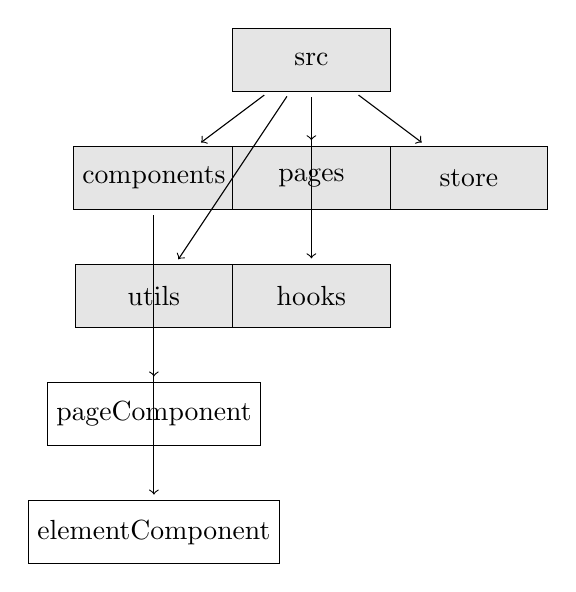
\begin{tikzpicture}[
    file/.style={draw, rectangle, minimum width=2cm, minimum height=0.8cm},
    folder/.style={draw, rectangle, minimum width=2cm, minimum height=0.8cm, fill=gray!20},
    arrow/.style={->, shorten >=2pt, shorten <=2pt}
]

% Folders
\node[folder] (src) at (0,0) {src};
\node[folder] (components) at (-2,-1.5) {components};
\node[folder] (pages) at (0,-1.5) {pages};
\node[folder] (store) at (2,-1.5) {store};
\node[folder] (utils) at (-2,-3) {utils};
\node[folder] (hooks) at (0,-3) {hooks};

% Files
\node[file] (pageComponent) at (-2,-4.5) {pageComponent};
\node[file] (elementComponent) at (-2,-6) {elementComponent};
% ... add more files

% Connections
\draw[arrow] (src) -- (components);
\draw[arrow] (src) -- (pages);
\draw[arrow] (src) -- (store);
\draw[arrow] (src) -- (utils);
\draw[arrow] (src) -- (hooks);
\draw[arrow] (components) -- (pageComponent);
\draw[arrow] (components) -- (elementComponent);
% ... add more connections

\end{tikzpicture}



\pagebreak
\subsubsection{Back-end}
The backend uses the dotNet framework. The development language using the C\# language.

In this project, the backend uses the Onion Architecture.
The Onion Architecture is a typically layered architecture, 
where each layer depends on the inner layer and provides interfaces to the outer layer.
The outer layer provides services to the outermost layer 
and other modules in the same layer based on the interfaces of the inner layer.

From inner to outer, the layers are: Domain, Application, Infrastructure, Presentation.
The Domain layer is the core layer and the innermost layer, used to define domain models, 
which are the business models.
It includes domain models and domain service interfaces.
Domain models are used to define the business models, 
which are the entities in the entity-relationship model and their attributes.
Domain service interfaces are used to define the business services, 
which are the relationships between entities in the entity-relationship model.

The Application layer is the application layer, 
used to define application services, which are the business logic.
It includes domain service implementations and application service interfaces.
Domain service implementations implement the methods of the inner layer's domain service 
interfaces and implement the business logic of the domain models.
Application service interfaces are used to define application services, 
which are the business logic.
It includes but is not limited to database interfaces, testing interfaces, 
HTTP API interfaces, MQTT interfaces, etc.

The Infrastructure layer is the infrastructure layer, used to define infrastructure.
It includes database implementations, testing implementations, 
HTTP API implementations, MQTT implementations, etc.
Database implementations implement the database interfaces 
and provide CRUD services for the database.
Testing implementations implement the testing interfaces 
and provide services for unit testing and integration testing.
HTTP API implementations implement the HTTP API interfaces 
and provide CRUD operations for HTTP APIs.
MQTT implementations implement the MQTT interfaces 
and provide CRUD operations for MQTT.

The Presentation layer is the presentation layer, used to define presentation logic, 
such as interfaces and pages. Since this is a backend project,
data presentation and control are handled by the frontend, 
so this layer is not needed.



\pagebreak
\subsubsection{Data communication and storage}
% 关于本项目的数据通信与数据存储的设计, 包括数据通信的协议, 数据存储的设计等
% 关于数据通信的设计:
% 1. 通信协议的选择
% 自前端向后端发送的数据, 有三种传输的数据类型, 
% 一种是普通的增删改查的请求, 对数据传输的时效性要求不高, 但是对数据的准确性, 完整性, 有序性, 安全性有一定的要求,
% 这种数据的传输, 采用 HTTP 协议, 以及 RESTful API 的设计. 可以有效的保证对数据传输的以上要求.
% 一种是对数据通道的创建和流媒体数据的传输, 对数据传输的时效性, 安全性要求较高, 这种数据的传输, 采用 WebRTC 协议, 以及 MQTT 协议.
% 配合可以快速解码的 flatbuffers 协议, 可以有效的保证对数据传输的以上要求.
% 最后一种是对设备的状态信息和操作信息的传输, 对完整性, 有序性, 安全性都有较高的要求, 这种数据的传输, 采用 MQTT 协议
% 同时也使用了 flatbuffers 协议.
% 
% 2. 数据通信的通信架构和通信流程
% 本项目的数据通信的通信架构, 是基于前后端分离的架构, 前端使用 React 框架, 后端使用 dotnet 框架.
% 当前端需要向后端发送数据的时候, 前端会向后端发送 HTTP 请求, 后端接收到 HTTP 请求之后, 会根据请求的数据类型,
% 选择不同的数据处理方式, 对于普通的增删改查的请求, 后端会根据 RESTful API 的设计, 对数据进行增删改查的操作,
% 对于对数据通道的创建和流媒体数据的传输, 后端会根据 WebRTC 协议, 对数据通道进行创建, 并且帮助前端和设备建立数据通道,
% 当数据通道建立后, 前端和设备之间则使用 flatbuffer 的数据格式对流媒体数据进行传输,
% 对于设备的状态信息和操作信息的传输, 前端会直接向 MQTT broker 发送 MQTT 请求, 
% 设备会在其自身的固件中监听相关的 MQTT 请求, 并且返回相关的数据.
% 
% 3. 数据通信的格式
% 本项目的数据通信的格式, 有三种, 
% 一种是 HTTP 协议, 
% 使用 json 格式对数据进行传输,
% 一种是 WebRTC 协议, 
% 使用 flatbuffers 格式对数据进行传输,
% 一种是 MQTT 协议.
% 使用 flatbuffers 格式对数据进行传输,
% 
% 关于数据存储的设计:
% 1. 数据存储的数据库的选择
% 本项目的数据存储的数据库的选择, 使用了轻量级的数据库 SQLite,
% SQLite 是一个进程内的库, 实现了自给自足的, 无服务器的, 零配置的, 事务性的 SQL 数据库引擎.
% 这是因为整个项目的目的是为了实现前端与设备之间的数据通信, 对于数据库数据的增删改查操作的要求不高,
% 数据量较小, 且对于数据库的数据的事务性要求不高, 所以选择了 SQLite 数据库.
% 2. 项目前后端的数据结构的设计
% 在本项目中, 前端由于使用了 React 框架, 所以前端的数据结构的设计, 使用了基于状态的数据结构的设计,
% 每个组件或者数据集都包含一个状态对象, 这个状态对象的属性就是组件的各个状态. 
% 使用状态对象的原因是, 可以方便的对状态进行管理, 采用对象-属性的形式, 可以方便的针对不同组件的同类状态进行区分,
% 由于跨组件的状态是由 redux 进行管理的, 这种状态对象的设计, 可以更搞笑的对状态进行更新和传递.
% 后端由于使用了 dotnet 框架, 所以后端的数据结构的设计, 使用了基于类的数据结构的设计,
% 采用了面向对象的编程思想, 对数据进行了封装, 使得数据的传输更加的安全, 有序, 完整.


\pagebreak

% \subsection{Domain model}
% \documentclass[]{article}
\usepackage{graphicx}
\usepackage{amsmath}
\usepackage{tikz}

% libaries
\usetikzlibrary{shapes,arrows}

%Define the listing package
\usepackage{listings} %code highlighter
\usepackage{color} %use color
\definecolor{mygreen}{rgb}{0,0.6,0}
\definecolor{mygray}{rgb}{0.5,0.5,0.5}
\definecolor{mymauve}{rgb}{0.58,0,0.82}

%Customize a bit the look
\lstset{ %
backgroundcolor=\color{white}, % choose the background color; you must add \usepackage{color} or \usepackage{xcolor}
basicstyle=\footnotesize, % the size of the fonts that are used for the code
breakatwhitespace=false, % sets if automatic breaks should only happen at whitespace
breaklines=true, % sets automatic line breaking
captionpos=b, % sets the caption-position to bottom
commentstyle=\color{mygreen}, % comment style
deletekeywords={...}, % if you want to delete keywords from the given language
escapeinside={\%*}{*)}, % if you want to add LaTeX within your code
extendedchars=true, % lets you use non-ASCII characters; for 8-bits encodings only, does not work with UTF-8
frame=single, % adds a frame around the code
keepspaces=true, % keeps spaces in text, useful for keeping indentation of code (possibly needs columns=flexible)
keywordstyle=\color{blue}, % keyword style
% language=Octave, % the language of the code
morekeywords={*,...}, % if you want to add more keywords to the set
numbers=left, % where to put the line-numbers; possible values are (none, left, right)
numbersep=5pt, % how far the line-numbers are from the code
numberstyle=\tiny\color{mygray}, % the style that is used for the line-numbers
rulecolor=\color{black}, % if not set, the frame-color may be changed on line-breaks within not-black text (e.g. comments (green here))
showspaces=false, % show spaces everywhere adding particular underscores; it overrides 'showstringspaces'
showstringspaces=false, % underline spaces within strings only
showtabs=false, % show tabs within strings adding particular underscores
stepnumber=1, % the step between two line-numbers. If it's 1, each line will be numbered
stringstyle=\color{mymauve}, % string literal style
tabsize=2, % sets default tabsize to 2 spaces
title=\lstname % show the filename of files included with \lstinputlisting; also try caption instead of title
}

\definecolor{darkgray}{rgb}{.4,.4,.4}
\definecolor{purple}{rgb}{0.65, 0.12, 0.82}

\lstdefinelanguage{React}{
keywords={const, typeof, new, true, false, catch, function, return, null, catch, switch, var, if, in, while, do, else, case, break},
keywordstyle=\color{blue}\bfseries,
ndkeywords={class, export, boolean, throw, implements, import, this},
ndkeywordstyle=\color{darkgray}\bfseries,
identifierstyle=\color{mygreen},
sensitive=false,
comment=[l]{//},
morecomment=[s]{/*}{*/},
commentstyle=\color{purple}\ttfamily,
string=[b]{"}{'}{`},
stringstyle=\color{red}\ttfamily,
morestring=[b]',
morestring=[b]",
morestring=[b]`',
}

\lstdefinelanguage{CSharp}{
keywords={const, typeof, new, true, false, catch, function, return, null, catch, switch, var, if, in, while, do, else, case, break},
keywordstyle=\color{blue}\bfseries,
ndkeywords={class, export, boolean, throw, implements, import, this},
ndkeywordstyle=\color{darkgray}\bfseries,
identifierstyle=\color{mygreen},
sensitive=false,
comment=[l]{//},
morecomment=[s]{/*}{*/},
commentstyle=\color{purple}\ttfamily,
string=[b]{"}{'}{`},
stringstyle=\color{red}\ttfamily,
morestring=[b]',
morestring=[b]",
morestring=[b]`',
}

\lstset{
language=React,
extendedchars=true,
basicstyle=\footnotesize\ttfamily,
showstringspaces=false,
showspaces=false,
numbers=left,
numberstyle=\footnotesize,
numbersep=9pt,
tabsize=2,
breaklines=true,
showtabs=false,
captionpos=b
}

\lstset{
language=CSharp,
extendedchars=true,
basicstyle=\footnotesize\ttfamily,
showstringspaces=false,
showspaces=false,
numbers=left,
numberstyle=\footnotesize,
numbersep=9pt,
tabsize=2,
breaklines=true,
showtabs=false,
captionpos=b
}

% \usepackage{cite} % Add this line for citation

% \bibliographystyle{plain}

\title{
The implementation of BifrostConnect Front-end scope, 
re-design and development with the relevant back-end support develop.
}
\author{
    Fei Gu \\
    Erhvervs Akademi Sydvest \\
    Computer Science 21\\
    }
\date{\today}

\begin{document}

% Front page
\maketitle
\begin{center}
    Supervisor: Henrik Boulund Meng Hansen \\
    Company: BifrostConnect \\
    Engineering Director: Jasper Wass \\
\end{center}
\tableofcontents
\pagebreak


% The introduction
\section{Introduction}
\subsection{Background}\input{sections/introduction/background.tex}
\subsection{The company}\input{sections/introduction/aboutCompany}
\subsection{The project}\input{sections/introduction/aboutProject}
\pagebreak

% The problem statement
\section{Problem Statement}
\subsection{Statement}
\input{sections/problemStatement/statement}
\subsection{Situation}
\input{sections/problemStatement/situation}
\subsection{Potential Solution}
\input{sections/problemStatement/potentialSolution}
\pagebreak

% Requirement analysis
\section{Requirement Analysis}
\input{sections/requirementAnalysis/index}

\subsection{Stakeholders}
\input{sections/requirementAnalysis/stakeholders/index}

\subsection{Business Domain}
\input{sections/requirementAnalysis/bussinesDomain/index}

\subsection{Scope}
\input{sections/requirementAnalysis/scope}

\subsection{Goals}
\input{sections/requirementAnalysis/goals}
\pagebreak

% Software Design
\section{Software Design}
% developement methods
\subsection{Software Development Methods}
\input{sections/softwareDevelopmentMethods/index}
\subsubsection{Agile Software Development}
\input{sections/softwareDevelopmentMethods/agileSoftwareDevelopment/index}
\subsubsection{Feature Driven Development}
\input{sections/softwareDevelopmentMethods/featureDrivenDevelopment/index}

\pagebreak

% Technology seslection
\subsection{Technology selection}
\input{sections/softwareDesign/technologySelection/index}
\subsubsection{Front-end}
\input{sections/softwareDesign/technologySelection/frontEnd}            
\subsubsection{Back-end}
\input{sections/softwareDesign/technologySelection/backEnd}            
\subsubsection{Database}
\input{sections/softwareDesign/technologySelection/database}
\subsubsection{Data communication}
\input{sections/softwareDesign/technologySelection/dataCommunication}            
\subsubsection{DevOps}
\input{sections/softwareDesign/technologySelection/devOps}
\pagebreak

% Architecture design
\subsection{Architecture design}
\input{sections/softwareDesign/architectureDesign/index}
\pagebreak
\subsubsection{Front-end}
\input{sections/softwareDesign/architectureDesign/frontEndArchitecture}
\pagebreak
\subsubsection{Back-end}
\input{sections/softwareDesign/architectureDesign/backEndArchitecture}
\pagebreak
\subsubsection{Data communication and storage}
\input{sections/softwareDesign/architectureDesign/dataCommunicationArchitecture}
\pagebreak

% \subsection{Domain model}
% \input{sections/softwareDesign/domainModel/index}
% \subsection{Database design}
% % 数据库领域模型 ER 图
% % 包括表和字段的设置.
% % 对于私有键和外键的设置.

% \subsection{Back-end design}
% % 后端对象模型
% % 以及对于对象模型的增删改查
% % 以及相关的其他服务的设计`'

% \subsection{Front-end design}
% % 对于前端的页面结构的设计 
% % 页面的状态的设计, 交互设计

% \subsection{FlatBuffers design}
% % schema 的设计

\subsection{DevOps CI/CD process design}
\input{sections/softwareDesign/devOpsDesign/index}
\subsubsection{Continuous Integration}
\input{sections/softwareDesign/devOpsDesign/continuousIntegration/index}
\subsubsection{Continuous Delivery}
\input{sections/softwareDesign/devOpsDesign/continuousDelivery/index}
\subsubsection{Continuous Deployment}
\input{sections/softwareDesign/devOpsDesign/continuousDeployment/index}
\pagebreak

\section{Software Development} 
\input{sections/softwareDevelopment/index}
\subsection{Overall development}
\input{sections/softwareDevelopment/overallDevelopement/index}
\subsubsection{Front-end}
\input{sections/softwareDevelopment/overallDevelopement/frontEnd/index}
\subsubsection{Back-end}
\input{sections/softwareDevelopment/overallDevelopement/backEnd/index}
\subsubsection{DevOps}
\input{sections/softwareDevelopment/overallDevelopement/devOps/index}
\subsection{Feature development} 
\input{sections/softwareDevelopment/featureDevelopment/index}
\subsubsection{Use Case 1}
\input{sections/softwareDevelopment/featureDevelopment/useCase1/index}
\subsubsection{Feature 1}
\input{sections/softwareDevelopment/featureDevelopment/feature/feature1.tex}
\pagebreak
\section{Conclusion} 
\subsection{Result}
Since the project is still in progress, the result is not available yet.
So far, basic structure of this project has been built. But the most features 
are not implemented yet. 
\subsection{Discussion}
As a single developer for this project, I am confident what I have done so far.
And I can say I understand the most of the knowledge I have used in this project, 
which also means I can explain all the part of the project. 
But this project also relevant some of the complex knowledge which I have to continue 
to study and practice.
\subsection{Future Work}
The future work is to implement the rest of the features. 
Including the most important part which is the 'create session' feature.
\pagebreak
% \bibliography{bibliography}
\pagebreak
% \begin{appendices}
%     \section{Appendix}
% \end{appendices} 
\end{document}
% \subsection{Database design}
% % 数据库领域模型 ER 图
% % 包括表和字段的设置.
% % 对于私有键和外键的设置.

% \subsection{Back-end design}
% % 后端对象模型
% % 以及对于对象模型的增删改查
% % 以及相关的其他服务的设计`'

% \subsection{Front-end design}
% % 对于前端的页面结构的设计 
% % 页面的状态的设计, 交互设计

% \subsection{FlatBuffers design}
% % schema 的设计

\subsection{DevOps CI/CD process design}
\documentclass[]{article}
\usepackage{graphicx}
\usepackage{amsmath}
\usepackage{tikz}

% libaries
\usetikzlibrary{shapes,arrows}

%Define the listing package
\usepackage{listings} %code highlighter
\usepackage{color} %use color
\definecolor{mygreen}{rgb}{0,0.6,0}
\definecolor{mygray}{rgb}{0.5,0.5,0.5}
\definecolor{mymauve}{rgb}{0.58,0,0.82}

%Customize a bit the look
\lstset{ %
backgroundcolor=\color{white}, % choose the background color; you must add \usepackage{color} or \usepackage{xcolor}
basicstyle=\footnotesize, % the size of the fonts that are used for the code
breakatwhitespace=false, % sets if automatic breaks should only happen at whitespace
breaklines=true, % sets automatic line breaking
captionpos=b, % sets the caption-position to bottom
commentstyle=\color{mygreen}, % comment style
deletekeywords={...}, % if you want to delete keywords from the given language
escapeinside={\%*}{*)}, % if you want to add LaTeX within your code
extendedchars=true, % lets you use non-ASCII characters; for 8-bits encodings only, does not work with UTF-8
frame=single, % adds a frame around the code
keepspaces=true, % keeps spaces in text, useful for keeping indentation of code (possibly needs columns=flexible)
keywordstyle=\color{blue}, % keyword style
% language=Octave, % the language of the code
morekeywords={*,...}, % if you want to add more keywords to the set
numbers=left, % where to put the line-numbers; possible values are (none, left, right)
numbersep=5pt, % how far the line-numbers are from the code
numberstyle=\tiny\color{mygray}, % the style that is used for the line-numbers
rulecolor=\color{black}, % if not set, the frame-color may be changed on line-breaks within not-black text (e.g. comments (green here))
showspaces=false, % show spaces everywhere adding particular underscores; it overrides 'showstringspaces'
showstringspaces=false, % underline spaces within strings only
showtabs=false, % show tabs within strings adding particular underscores
stepnumber=1, % the step between two line-numbers. If it's 1, each line will be numbered
stringstyle=\color{mymauve}, % string literal style
tabsize=2, % sets default tabsize to 2 spaces
title=\lstname % show the filename of files included with \lstinputlisting; also try caption instead of title
}

\definecolor{darkgray}{rgb}{.4,.4,.4}
\definecolor{purple}{rgb}{0.65, 0.12, 0.82}

\lstdefinelanguage{React}{
keywords={const, typeof, new, true, false, catch, function, return, null, catch, switch, var, if, in, while, do, else, case, break},
keywordstyle=\color{blue}\bfseries,
ndkeywords={class, export, boolean, throw, implements, import, this},
ndkeywordstyle=\color{darkgray}\bfseries,
identifierstyle=\color{mygreen},
sensitive=false,
comment=[l]{//},
morecomment=[s]{/*}{*/},
commentstyle=\color{purple}\ttfamily,
string=[b]{"}{'}{`},
stringstyle=\color{red}\ttfamily,
morestring=[b]',
morestring=[b]",
morestring=[b]`',
}

\lstdefinelanguage{CSharp}{
keywords={const, typeof, new, true, false, catch, function, return, null, catch, switch, var, if, in, while, do, else, case, break},
keywordstyle=\color{blue}\bfseries,
ndkeywords={class, export, boolean, throw, implements, import, this},
ndkeywordstyle=\color{darkgray}\bfseries,
identifierstyle=\color{mygreen},
sensitive=false,
comment=[l]{//},
morecomment=[s]{/*}{*/},
commentstyle=\color{purple}\ttfamily,
string=[b]{"}{'}{`},
stringstyle=\color{red}\ttfamily,
morestring=[b]',
morestring=[b]",
morestring=[b]`',
}

\lstset{
language=React,
extendedchars=true,
basicstyle=\footnotesize\ttfamily,
showstringspaces=false,
showspaces=false,
numbers=left,
numberstyle=\footnotesize,
numbersep=9pt,
tabsize=2,
breaklines=true,
showtabs=false,
captionpos=b
}

\lstset{
language=CSharp,
extendedchars=true,
basicstyle=\footnotesize\ttfamily,
showstringspaces=false,
showspaces=false,
numbers=left,
numberstyle=\footnotesize,
numbersep=9pt,
tabsize=2,
breaklines=true,
showtabs=false,
captionpos=b
}

% \usepackage{cite} % Add this line for citation

% \bibliographystyle{plain}

\title{
The implementation of BifrostConnect Front-end scope, 
re-design and development with the relevant back-end support develop.
}
\author{
    Fei Gu \\
    Erhvervs Akademi Sydvest \\
    Computer Science 21\\
    }
\date{\today}

\begin{document}

% Front page
\maketitle
\begin{center}
    Supervisor: Henrik Boulund Meng Hansen \\
    Company: BifrostConnect \\
    Engineering Director: Jasper Wass \\
\end{center}
\tableofcontents
\pagebreak


% The introduction
\section{Introduction}
\subsection{Background}\input{sections/introduction/background.tex}
\subsection{The company}\input{sections/introduction/aboutCompany}
\subsection{The project}\input{sections/introduction/aboutProject}
\pagebreak

% The problem statement
\section{Problem Statement}
\subsection{Statement}
\input{sections/problemStatement/statement}
\subsection{Situation}
\input{sections/problemStatement/situation}
\subsection{Potential Solution}
\input{sections/problemStatement/potentialSolution}
\pagebreak

% Requirement analysis
\section{Requirement Analysis}
\input{sections/requirementAnalysis/index}

\subsection{Stakeholders}
\input{sections/requirementAnalysis/stakeholders/index}

\subsection{Business Domain}
\input{sections/requirementAnalysis/bussinesDomain/index}

\subsection{Scope}
\input{sections/requirementAnalysis/scope}

\subsection{Goals}
\input{sections/requirementAnalysis/goals}
\pagebreak

% Software Design
\section{Software Design}
% developement methods
\subsection{Software Development Methods}
\input{sections/softwareDevelopmentMethods/index}
\subsubsection{Agile Software Development}
\input{sections/softwareDevelopmentMethods/agileSoftwareDevelopment/index}
\subsubsection{Feature Driven Development}
\input{sections/softwareDevelopmentMethods/featureDrivenDevelopment/index}

\pagebreak

% Technology seslection
\subsection{Technology selection}
\input{sections/softwareDesign/technologySelection/index}
\subsubsection{Front-end}
\input{sections/softwareDesign/technologySelection/frontEnd}            
\subsubsection{Back-end}
\input{sections/softwareDesign/technologySelection/backEnd}            
\subsubsection{Database}
\input{sections/softwareDesign/technologySelection/database}
\subsubsection{Data communication}
\input{sections/softwareDesign/technologySelection/dataCommunication}            
\subsubsection{DevOps}
\input{sections/softwareDesign/technologySelection/devOps}
\pagebreak

% Architecture design
\subsection{Architecture design}
\input{sections/softwareDesign/architectureDesign/index}
\pagebreak
\subsubsection{Front-end}
\input{sections/softwareDesign/architectureDesign/frontEndArchitecture}
\pagebreak
\subsubsection{Back-end}
\input{sections/softwareDesign/architectureDesign/backEndArchitecture}
\pagebreak
\subsubsection{Data communication and storage}
\input{sections/softwareDesign/architectureDesign/dataCommunicationArchitecture}
\pagebreak

% \subsection{Domain model}
% \input{sections/softwareDesign/domainModel/index}
% \subsection{Database design}
% % 数据库领域模型 ER 图
% % 包括表和字段的设置.
% % 对于私有键和外键的设置.

% \subsection{Back-end design}
% % 后端对象模型
% % 以及对于对象模型的增删改查
% % 以及相关的其他服务的设计`'

% \subsection{Front-end design}
% % 对于前端的页面结构的设计 
% % 页面的状态的设计, 交互设计

% \subsection{FlatBuffers design}
% % schema 的设计

\subsection{DevOps CI/CD process design}
\input{sections/softwareDesign/devOpsDesign/index}
\subsubsection{Continuous Integration}
\input{sections/softwareDesign/devOpsDesign/continuousIntegration/index}
\subsubsection{Continuous Delivery}
\input{sections/softwareDesign/devOpsDesign/continuousDelivery/index}
\subsubsection{Continuous Deployment}
\input{sections/softwareDesign/devOpsDesign/continuousDeployment/index}
\pagebreak

\section{Software Development} 
\input{sections/softwareDevelopment/index}
\subsection{Overall development}
\input{sections/softwareDevelopment/overallDevelopement/index}
\subsubsection{Front-end}
\input{sections/softwareDevelopment/overallDevelopement/frontEnd/index}
\subsubsection{Back-end}
\input{sections/softwareDevelopment/overallDevelopement/backEnd/index}
\subsubsection{DevOps}
\input{sections/softwareDevelopment/overallDevelopement/devOps/index}
\subsection{Feature development} 
\input{sections/softwareDevelopment/featureDevelopment/index}
\subsubsection{Use Case 1}
\input{sections/softwareDevelopment/featureDevelopment/useCase1/index}
\subsubsection{Feature 1}
\input{sections/softwareDevelopment/featureDevelopment/feature/feature1.tex}
\pagebreak
\section{Conclusion} 
\subsection{Result}
Since the project is still in progress, the result is not available yet.
So far, basic structure of this project has been built. But the most features 
are not implemented yet. 
\subsection{Discussion}
As a single developer for this project, I am confident what I have done so far.
And I can say I understand the most of the knowledge I have used in this project, 
which also means I can explain all the part of the project. 
But this project also relevant some of the complex knowledge which I have to continue 
to study and practice.
\subsection{Future Work}
The future work is to implement the rest of the features. 
Including the most important part which is the 'create session' feature.
\pagebreak
% \bibliography{bibliography}
\pagebreak
% \begin{appendices}
%     \section{Appendix}
% \end{appendices} 
\end{document}
\subsubsection{Continuous Integration}
\documentclass[]{article}
\usepackage{graphicx}
\usepackage{amsmath}
\usepackage{tikz}

% libaries
\usetikzlibrary{shapes,arrows}

%Define the listing package
\usepackage{listings} %code highlighter
\usepackage{color} %use color
\definecolor{mygreen}{rgb}{0,0.6,0}
\definecolor{mygray}{rgb}{0.5,0.5,0.5}
\definecolor{mymauve}{rgb}{0.58,0,0.82}

%Customize a bit the look
\lstset{ %
backgroundcolor=\color{white}, % choose the background color; you must add \usepackage{color} or \usepackage{xcolor}
basicstyle=\footnotesize, % the size of the fonts that are used for the code
breakatwhitespace=false, % sets if automatic breaks should only happen at whitespace
breaklines=true, % sets automatic line breaking
captionpos=b, % sets the caption-position to bottom
commentstyle=\color{mygreen}, % comment style
deletekeywords={...}, % if you want to delete keywords from the given language
escapeinside={\%*}{*)}, % if you want to add LaTeX within your code
extendedchars=true, % lets you use non-ASCII characters; for 8-bits encodings only, does not work with UTF-8
frame=single, % adds a frame around the code
keepspaces=true, % keeps spaces in text, useful for keeping indentation of code (possibly needs columns=flexible)
keywordstyle=\color{blue}, % keyword style
% language=Octave, % the language of the code
morekeywords={*,...}, % if you want to add more keywords to the set
numbers=left, % where to put the line-numbers; possible values are (none, left, right)
numbersep=5pt, % how far the line-numbers are from the code
numberstyle=\tiny\color{mygray}, % the style that is used for the line-numbers
rulecolor=\color{black}, % if not set, the frame-color may be changed on line-breaks within not-black text (e.g. comments (green here))
showspaces=false, % show spaces everywhere adding particular underscores; it overrides 'showstringspaces'
showstringspaces=false, % underline spaces within strings only
showtabs=false, % show tabs within strings adding particular underscores
stepnumber=1, % the step between two line-numbers. If it's 1, each line will be numbered
stringstyle=\color{mymauve}, % string literal style
tabsize=2, % sets default tabsize to 2 spaces
title=\lstname % show the filename of files included with \lstinputlisting; also try caption instead of title
}

\definecolor{darkgray}{rgb}{.4,.4,.4}
\definecolor{purple}{rgb}{0.65, 0.12, 0.82}

\lstdefinelanguage{React}{
keywords={const, typeof, new, true, false, catch, function, return, null, catch, switch, var, if, in, while, do, else, case, break},
keywordstyle=\color{blue}\bfseries,
ndkeywords={class, export, boolean, throw, implements, import, this},
ndkeywordstyle=\color{darkgray}\bfseries,
identifierstyle=\color{mygreen},
sensitive=false,
comment=[l]{//},
morecomment=[s]{/*}{*/},
commentstyle=\color{purple}\ttfamily,
string=[b]{"}{'}{`},
stringstyle=\color{red}\ttfamily,
morestring=[b]',
morestring=[b]",
morestring=[b]`',
}

\lstdefinelanguage{CSharp}{
keywords={const, typeof, new, true, false, catch, function, return, null, catch, switch, var, if, in, while, do, else, case, break},
keywordstyle=\color{blue}\bfseries,
ndkeywords={class, export, boolean, throw, implements, import, this},
ndkeywordstyle=\color{darkgray}\bfseries,
identifierstyle=\color{mygreen},
sensitive=false,
comment=[l]{//},
morecomment=[s]{/*}{*/},
commentstyle=\color{purple}\ttfamily,
string=[b]{"}{'}{`},
stringstyle=\color{red}\ttfamily,
morestring=[b]',
morestring=[b]",
morestring=[b]`',
}

\lstset{
language=React,
extendedchars=true,
basicstyle=\footnotesize\ttfamily,
showstringspaces=false,
showspaces=false,
numbers=left,
numberstyle=\footnotesize,
numbersep=9pt,
tabsize=2,
breaklines=true,
showtabs=false,
captionpos=b
}

\lstset{
language=CSharp,
extendedchars=true,
basicstyle=\footnotesize\ttfamily,
showstringspaces=false,
showspaces=false,
numbers=left,
numberstyle=\footnotesize,
numbersep=9pt,
tabsize=2,
breaklines=true,
showtabs=false,
captionpos=b
}

% \usepackage{cite} % Add this line for citation

% \bibliographystyle{plain}

\title{
The implementation of BifrostConnect Front-end scope, 
re-design and development with the relevant back-end support develop.
}
\author{
    Fei Gu \\
    Erhvervs Akademi Sydvest \\
    Computer Science 21\\
    }
\date{\today}

\begin{document}

% Front page
\maketitle
\begin{center}
    Supervisor: Henrik Boulund Meng Hansen \\
    Company: BifrostConnect \\
    Engineering Director: Jasper Wass \\
\end{center}
\tableofcontents
\pagebreak


% The introduction
\section{Introduction}
\subsection{Background}\input{sections/introduction/background.tex}
\subsection{The company}\input{sections/introduction/aboutCompany}
\subsection{The project}\input{sections/introduction/aboutProject}
\pagebreak

% The problem statement
\section{Problem Statement}
\subsection{Statement}
\input{sections/problemStatement/statement}
\subsection{Situation}
\input{sections/problemStatement/situation}
\subsection{Potential Solution}
\input{sections/problemStatement/potentialSolution}
\pagebreak

% Requirement analysis
\section{Requirement Analysis}
\input{sections/requirementAnalysis/index}

\subsection{Stakeholders}
\input{sections/requirementAnalysis/stakeholders/index}

\subsection{Business Domain}
\input{sections/requirementAnalysis/bussinesDomain/index}

\subsection{Scope}
\input{sections/requirementAnalysis/scope}

\subsection{Goals}
\input{sections/requirementAnalysis/goals}
\pagebreak

% Software Design
\section{Software Design}
% developement methods
\subsection{Software Development Methods}
\input{sections/softwareDevelopmentMethods/index}
\subsubsection{Agile Software Development}
\input{sections/softwareDevelopmentMethods/agileSoftwareDevelopment/index}
\subsubsection{Feature Driven Development}
\input{sections/softwareDevelopmentMethods/featureDrivenDevelopment/index}

\pagebreak

% Technology seslection
\subsection{Technology selection}
\input{sections/softwareDesign/technologySelection/index}
\subsubsection{Front-end}
\input{sections/softwareDesign/technologySelection/frontEnd}            
\subsubsection{Back-end}
\input{sections/softwareDesign/technologySelection/backEnd}            
\subsubsection{Database}
\input{sections/softwareDesign/technologySelection/database}
\subsubsection{Data communication}
\input{sections/softwareDesign/technologySelection/dataCommunication}            
\subsubsection{DevOps}
\input{sections/softwareDesign/technologySelection/devOps}
\pagebreak

% Architecture design
\subsection{Architecture design}
\input{sections/softwareDesign/architectureDesign/index}
\pagebreak
\subsubsection{Front-end}
\input{sections/softwareDesign/architectureDesign/frontEndArchitecture}
\pagebreak
\subsubsection{Back-end}
\input{sections/softwareDesign/architectureDesign/backEndArchitecture}
\pagebreak
\subsubsection{Data communication and storage}
\input{sections/softwareDesign/architectureDesign/dataCommunicationArchitecture}
\pagebreak

% \subsection{Domain model}
% \input{sections/softwareDesign/domainModel/index}
% \subsection{Database design}
% % 数据库领域模型 ER 图
% % 包括表和字段的设置.
% % 对于私有键和外键的设置.

% \subsection{Back-end design}
% % 后端对象模型
% % 以及对于对象模型的增删改查
% % 以及相关的其他服务的设计`'

% \subsection{Front-end design}
% % 对于前端的页面结构的设计 
% % 页面的状态的设计, 交互设计

% \subsection{FlatBuffers design}
% % schema 的设计

\subsection{DevOps CI/CD process design}
\input{sections/softwareDesign/devOpsDesign/index}
\subsubsection{Continuous Integration}
\input{sections/softwareDesign/devOpsDesign/continuousIntegration/index}
\subsubsection{Continuous Delivery}
\input{sections/softwareDesign/devOpsDesign/continuousDelivery/index}
\subsubsection{Continuous Deployment}
\input{sections/softwareDesign/devOpsDesign/continuousDeployment/index}
\pagebreak

\section{Software Development} 
\input{sections/softwareDevelopment/index}
\subsection{Overall development}
\input{sections/softwareDevelopment/overallDevelopement/index}
\subsubsection{Front-end}
\input{sections/softwareDevelopment/overallDevelopement/frontEnd/index}
\subsubsection{Back-end}
\input{sections/softwareDevelopment/overallDevelopement/backEnd/index}
\subsubsection{DevOps}
\input{sections/softwareDevelopment/overallDevelopement/devOps/index}
\subsection{Feature development} 
\input{sections/softwareDevelopment/featureDevelopment/index}
\subsubsection{Use Case 1}
\input{sections/softwareDevelopment/featureDevelopment/useCase1/index}
\subsubsection{Feature 1}
\input{sections/softwareDevelopment/featureDevelopment/feature/feature1.tex}
\pagebreak
\section{Conclusion} 
\subsection{Result}
Since the project is still in progress, the result is not available yet.
So far, basic structure of this project has been built. But the most features 
are not implemented yet. 
\subsection{Discussion}
As a single developer for this project, I am confident what I have done so far.
And I can say I understand the most of the knowledge I have used in this project, 
which also means I can explain all the part of the project. 
But this project also relevant some of the complex knowledge which I have to continue 
to study and practice.
\subsection{Future Work}
The future work is to implement the rest of the features. 
Including the most important part which is the 'create session' feature.
\pagebreak
% \bibliography{bibliography}
\pagebreak
% \begin{appendices}
%     \section{Appendix}
% \end{appendices} 
\end{document}
\subsubsection{Continuous Delivery}
\documentclass[]{article}
\usepackage{graphicx}
\usepackage{amsmath}
\usepackage{tikz}

% libaries
\usetikzlibrary{shapes,arrows}

%Define the listing package
\usepackage{listings} %code highlighter
\usepackage{color} %use color
\definecolor{mygreen}{rgb}{0,0.6,0}
\definecolor{mygray}{rgb}{0.5,0.5,0.5}
\definecolor{mymauve}{rgb}{0.58,0,0.82}

%Customize a bit the look
\lstset{ %
backgroundcolor=\color{white}, % choose the background color; you must add \usepackage{color} or \usepackage{xcolor}
basicstyle=\footnotesize, % the size of the fonts that are used for the code
breakatwhitespace=false, % sets if automatic breaks should only happen at whitespace
breaklines=true, % sets automatic line breaking
captionpos=b, % sets the caption-position to bottom
commentstyle=\color{mygreen}, % comment style
deletekeywords={...}, % if you want to delete keywords from the given language
escapeinside={\%*}{*)}, % if you want to add LaTeX within your code
extendedchars=true, % lets you use non-ASCII characters; for 8-bits encodings only, does not work with UTF-8
frame=single, % adds a frame around the code
keepspaces=true, % keeps spaces in text, useful for keeping indentation of code (possibly needs columns=flexible)
keywordstyle=\color{blue}, % keyword style
% language=Octave, % the language of the code
morekeywords={*,...}, % if you want to add more keywords to the set
numbers=left, % where to put the line-numbers; possible values are (none, left, right)
numbersep=5pt, % how far the line-numbers are from the code
numberstyle=\tiny\color{mygray}, % the style that is used for the line-numbers
rulecolor=\color{black}, % if not set, the frame-color may be changed on line-breaks within not-black text (e.g. comments (green here))
showspaces=false, % show spaces everywhere adding particular underscores; it overrides 'showstringspaces'
showstringspaces=false, % underline spaces within strings only
showtabs=false, % show tabs within strings adding particular underscores
stepnumber=1, % the step between two line-numbers. If it's 1, each line will be numbered
stringstyle=\color{mymauve}, % string literal style
tabsize=2, % sets default tabsize to 2 spaces
title=\lstname % show the filename of files included with \lstinputlisting; also try caption instead of title
}

\definecolor{darkgray}{rgb}{.4,.4,.4}
\definecolor{purple}{rgb}{0.65, 0.12, 0.82}

\lstdefinelanguage{React}{
keywords={const, typeof, new, true, false, catch, function, return, null, catch, switch, var, if, in, while, do, else, case, break},
keywordstyle=\color{blue}\bfseries,
ndkeywords={class, export, boolean, throw, implements, import, this},
ndkeywordstyle=\color{darkgray}\bfseries,
identifierstyle=\color{mygreen},
sensitive=false,
comment=[l]{//},
morecomment=[s]{/*}{*/},
commentstyle=\color{purple}\ttfamily,
string=[b]{"}{'}{`},
stringstyle=\color{red}\ttfamily,
morestring=[b]',
morestring=[b]",
morestring=[b]`',
}

\lstdefinelanguage{CSharp}{
keywords={const, typeof, new, true, false, catch, function, return, null, catch, switch, var, if, in, while, do, else, case, break},
keywordstyle=\color{blue}\bfseries,
ndkeywords={class, export, boolean, throw, implements, import, this},
ndkeywordstyle=\color{darkgray}\bfseries,
identifierstyle=\color{mygreen},
sensitive=false,
comment=[l]{//},
morecomment=[s]{/*}{*/},
commentstyle=\color{purple}\ttfamily,
string=[b]{"}{'}{`},
stringstyle=\color{red}\ttfamily,
morestring=[b]',
morestring=[b]",
morestring=[b]`',
}

\lstset{
language=React,
extendedchars=true,
basicstyle=\footnotesize\ttfamily,
showstringspaces=false,
showspaces=false,
numbers=left,
numberstyle=\footnotesize,
numbersep=9pt,
tabsize=2,
breaklines=true,
showtabs=false,
captionpos=b
}

\lstset{
language=CSharp,
extendedchars=true,
basicstyle=\footnotesize\ttfamily,
showstringspaces=false,
showspaces=false,
numbers=left,
numberstyle=\footnotesize,
numbersep=9pt,
tabsize=2,
breaklines=true,
showtabs=false,
captionpos=b
}

% \usepackage{cite} % Add this line for citation

% \bibliographystyle{plain}

\title{
The implementation of BifrostConnect Front-end scope, 
re-design and development with the relevant back-end support develop.
}
\author{
    Fei Gu \\
    Erhvervs Akademi Sydvest \\
    Computer Science 21\\
    }
\date{\today}

\begin{document}

% Front page
\maketitle
\begin{center}
    Supervisor: Henrik Boulund Meng Hansen \\
    Company: BifrostConnect \\
    Engineering Director: Jasper Wass \\
\end{center}
\tableofcontents
\pagebreak


% The introduction
\section{Introduction}
\subsection{Background}\input{sections/introduction/background.tex}
\subsection{The company}\input{sections/introduction/aboutCompany}
\subsection{The project}\input{sections/introduction/aboutProject}
\pagebreak

% The problem statement
\section{Problem Statement}
\subsection{Statement}
\input{sections/problemStatement/statement}
\subsection{Situation}
\input{sections/problemStatement/situation}
\subsection{Potential Solution}
\input{sections/problemStatement/potentialSolution}
\pagebreak

% Requirement analysis
\section{Requirement Analysis}
\input{sections/requirementAnalysis/index}

\subsection{Stakeholders}
\input{sections/requirementAnalysis/stakeholders/index}

\subsection{Business Domain}
\input{sections/requirementAnalysis/bussinesDomain/index}

\subsection{Scope}
\input{sections/requirementAnalysis/scope}

\subsection{Goals}
\input{sections/requirementAnalysis/goals}
\pagebreak

% Software Design
\section{Software Design}
% developement methods
\subsection{Software Development Methods}
\input{sections/softwareDevelopmentMethods/index}
\subsubsection{Agile Software Development}
\input{sections/softwareDevelopmentMethods/agileSoftwareDevelopment/index}
\subsubsection{Feature Driven Development}
\input{sections/softwareDevelopmentMethods/featureDrivenDevelopment/index}

\pagebreak

% Technology seslection
\subsection{Technology selection}
\input{sections/softwareDesign/technologySelection/index}
\subsubsection{Front-end}
\input{sections/softwareDesign/technologySelection/frontEnd}            
\subsubsection{Back-end}
\input{sections/softwareDesign/technologySelection/backEnd}            
\subsubsection{Database}
\input{sections/softwareDesign/technologySelection/database}
\subsubsection{Data communication}
\input{sections/softwareDesign/technologySelection/dataCommunication}            
\subsubsection{DevOps}
\input{sections/softwareDesign/technologySelection/devOps}
\pagebreak

% Architecture design
\subsection{Architecture design}
\input{sections/softwareDesign/architectureDesign/index}
\pagebreak
\subsubsection{Front-end}
\input{sections/softwareDesign/architectureDesign/frontEndArchitecture}
\pagebreak
\subsubsection{Back-end}
\input{sections/softwareDesign/architectureDesign/backEndArchitecture}
\pagebreak
\subsubsection{Data communication and storage}
\input{sections/softwareDesign/architectureDesign/dataCommunicationArchitecture}
\pagebreak

% \subsection{Domain model}
% \input{sections/softwareDesign/domainModel/index}
% \subsection{Database design}
% % 数据库领域模型 ER 图
% % 包括表和字段的设置.
% % 对于私有键和外键的设置.

% \subsection{Back-end design}
% % 后端对象模型
% % 以及对于对象模型的增删改查
% % 以及相关的其他服务的设计`'

% \subsection{Front-end design}
% % 对于前端的页面结构的设计 
% % 页面的状态的设计, 交互设计

% \subsection{FlatBuffers design}
% % schema 的设计

\subsection{DevOps CI/CD process design}
\input{sections/softwareDesign/devOpsDesign/index}
\subsubsection{Continuous Integration}
\input{sections/softwareDesign/devOpsDesign/continuousIntegration/index}
\subsubsection{Continuous Delivery}
\input{sections/softwareDesign/devOpsDesign/continuousDelivery/index}
\subsubsection{Continuous Deployment}
\input{sections/softwareDesign/devOpsDesign/continuousDeployment/index}
\pagebreak

\section{Software Development} 
\input{sections/softwareDevelopment/index}
\subsection{Overall development}
\input{sections/softwareDevelopment/overallDevelopement/index}
\subsubsection{Front-end}
\input{sections/softwareDevelopment/overallDevelopement/frontEnd/index}
\subsubsection{Back-end}
\input{sections/softwareDevelopment/overallDevelopement/backEnd/index}
\subsubsection{DevOps}
\input{sections/softwareDevelopment/overallDevelopement/devOps/index}
\subsection{Feature development} 
\input{sections/softwareDevelopment/featureDevelopment/index}
\subsubsection{Use Case 1}
\input{sections/softwareDevelopment/featureDevelopment/useCase1/index}
\subsubsection{Feature 1}
\input{sections/softwareDevelopment/featureDevelopment/feature/feature1.tex}
\pagebreak
\section{Conclusion} 
\subsection{Result}
Since the project is still in progress, the result is not available yet.
So far, basic structure of this project has been built. But the most features 
are not implemented yet. 
\subsection{Discussion}
As a single developer for this project, I am confident what I have done so far.
And I can say I understand the most of the knowledge I have used in this project, 
which also means I can explain all the part of the project. 
But this project also relevant some of the complex knowledge which I have to continue 
to study and practice.
\subsection{Future Work}
The future work is to implement the rest of the features. 
Including the most important part which is the 'create session' feature.
\pagebreak
% \bibliography{bibliography}
\pagebreak
% \begin{appendices}
%     \section{Appendix}
% \end{appendices} 
\end{document}
\subsubsection{Continuous Deployment}
\documentclass[]{article}
\usepackage{graphicx}
\usepackage{amsmath}
\usepackage{tikz}

% libaries
\usetikzlibrary{shapes,arrows}

%Define the listing package
\usepackage{listings} %code highlighter
\usepackage{color} %use color
\definecolor{mygreen}{rgb}{0,0.6,0}
\definecolor{mygray}{rgb}{0.5,0.5,0.5}
\definecolor{mymauve}{rgb}{0.58,0,0.82}

%Customize a bit the look
\lstset{ %
backgroundcolor=\color{white}, % choose the background color; you must add \usepackage{color} or \usepackage{xcolor}
basicstyle=\footnotesize, % the size of the fonts that are used for the code
breakatwhitespace=false, % sets if automatic breaks should only happen at whitespace
breaklines=true, % sets automatic line breaking
captionpos=b, % sets the caption-position to bottom
commentstyle=\color{mygreen}, % comment style
deletekeywords={...}, % if you want to delete keywords from the given language
escapeinside={\%*}{*)}, % if you want to add LaTeX within your code
extendedchars=true, % lets you use non-ASCII characters; for 8-bits encodings only, does not work with UTF-8
frame=single, % adds a frame around the code
keepspaces=true, % keeps spaces in text, useful for keeping indentation of code (possibly needs columns=flexible)
keywordstyle=\color{blue}, % keyword style
% language=Octave, % the language of the code
morekeywords={*,...}, % if you want to add more keywords to the set
numbers=left, % where to put the line-numbers; possible values are (none, left, right)
numbersep=5pt, % how far the line-numbers are from the code
numberstyle=\tiny\color{mygray}, % the style that is used for the line-numbers
rulecolor=\color{black}, % if not set, the frame-color may be changed on line-breaks within not-black text (e.g. comments (green here))
showspaces=false, % show spaces everywhere adding particular underscores; it overrides 'showstringspaces'
showstringspaces=false, % underline spaces within strings only
showtabs=false, % show tabs within strings adding particular underscores
stepnumber=1, % the step between two line-numbers. If it's 1, each line will be numbered
stringstyle=\color{mymauve}, % string literal style
tabsize=2, % sets default tabsize to 2 spaces
title=\lstname % show the filename of files included with \lstinputlisting; also try caption instead of title
}

\definecolor{darkgray}{rgb}{.4,.4,.4}
\definecolor{purple}{rgb}{0.65, 0.12, 0.82}

\lstdefinelanguage{React}{
keywords={const, typeof, new, true, false, catch, function, return, null, catch, switch, var, if, in, while, do, else, case, break},
keywordstyle=\color{blue}\bfseries,
ndkeywords={class, export, boolean, throw, implements, import, this},
ndkeywordstyle=\color{darkgray}\bfseries,
identifierstyle=\color{mygreen},
sensitive=false,
comment=[l]{//},
morecomment=[s]{/*}{*/},
commentstyle=\color{purple}\ttfamily,
string=[b]{"}{'}{`},
stringstyle=\color{red}\ttfamily,
morestring=[b]',
morestring=[b]",
morestring=[b]`',
}

\lstdefinelanguage{CSharp}{
keywords={const, typeof, new, true, false, catch, function, return, null, catch, switch, var, if, in, while, do, else, case, break},
keywordstyle=\color{blue}\bfseries,
ndkeywords={class, export, boolean, throw, implements, import, this},
ndkeywordstyle=\color{darkgray}\bfseries,
identifierstyle=\color{mygreen},
sensitive=false,
comment=[l]{//},
morecomment=[s]{/*}{*/},
commentstyle=\color{purple}\ttfamily,
string=[b]{"}{'}{`},
stringstyle=\color{red}\ttfamily,
morestring=[b]',
morestring=[b]",
morestring=[b]`',
}

\lstset{
language=React,
extendedchars=true,
basicstyle=\footnotesize\ttfamily,
showstringspaces=false,
showspaces=false,
numbers=left,
numberstyle=\footnotesize,
numbersep=9pt,
tabsize=2,
breaklines=true,
showtabs=false,
captionpos=b
}

\lstset{
language=CSharp,
extendedchars=true,
basicstyle=\footnotesize\ttfamily,
showstringspaces=false,
showspaces=false,
numbers=left,
numberstyle=\footnotesize,
numbersep=9pt,
tabsize=2,
breaklines=true,
showtabs=false,
captionpos=b
}

% \usepackage{cite} % Add this line for citation

% \bibliographystyle{plain}

\title{
The implementation of BifrostConnect Front-end scope, 
re-design and development with the relevant back-end support develop.
}
\author{
    Fei Gu \\
    Erhvervs Akademi Sydvest \\
    Computer Science 21\\
    }
\date{\today}

\begin{document}

% Front page
\maketitle
\begin{center}
    Supervisor: Henrik Boulund Meng Hansen \\
    Company: BifrostConnect \\
    Engineering Director: Jasper Wass \\
\end{center}
\tableofcontents
\pagebreak


% The introduction
\section{Introduction}
\subsection{Background}\input{sections/introduction/background.tex}
\subsection{The company}\input{sections/introduction/aboutCompany}
\subsection{The project}\input{sections/introduction/aboutProject}
\pagebreak

% The problem statement
\section{Problem Statement}
\subsection{Statement}
\input{sections/problemStatement/statement}
\subsection{Situation}
\input{sections/problemStatement/situation}
\subsection{Potential Solution}
\input{sections/problemStatement/potentialSolution}
\pagebreak

% Requirement analysis
\section{Requirement Analysis}
\input{sections/requirementAnalysis/index}

\subsection{Stakeholders}
\input{sections/requirementAnalysis/stakeholders/index}

\subsection{Business Domain}
\input{sections/requirementAnalysis/bussinesDomain/index}

\subsection{Scope}
\input{sections/requirementAnalysis/scope}

\subsection{Goals}
\input{sections/requirementAnalysis/goals}
\pagebreak

% Software Design
\section{Software Design}
% developement methods
\subsection{Software Development Methods}
\input{sections/softwareDevelopmentMethods/index}
\subsubsection{Agile Software Development}
\input{sections/softwareDevelopmentMethods/agileSoftwareDevelopment/index}
\subsubsection{Feature Driven Development}
\input{sections/softwareDevelopmentMethods/featureDrivenDevelopment/index}

\pagebreak

% Technology seslection
\subsection{Technology selection}
\input{sections/softwareDesign/technologySelection/index}
\subsubsection{Front-end}
\input{sections/softwareDesign/technologySelection/frontEnd}            
\subsubsection{Back-end}
\input{sections/softwareDesign/technologySelection/backEnd}            
\subsubsection{Database}
\input{sections/softwareDesign/technologySelection/database}
\subsubsection{Data communication}
\input{sections/softwareDesign/technologySelection/dataCommunication}            
\subsubsection{DevOps}
\input{sections/softwareDesign/technologySelection/devOps}
\pagebreak

% Architecture design
\subsection{Architecture design}
\input{sections/softwareDesign/architectureDesign/index}
\pagebreak
\subsubsection{Front-end}
\input{sections/softwareDesign/architectureDesign/frontEndArchitecture}
\pagebreak
\subsubsection{Back-end}
\input{sections/softwareDesign/architectureDesign/backEndArchitecture}
\pagebreak
\subsubsection{Data communication and storage}
\input{sections/softwareDesign/architectureDesign/dataCommunicationArchitecture}
\pagebreak

% \subsection{Domain model}
% \input{sections/softwareDesign/domainModel/index}
% \subsection{Database design}
% % 数据库领域模型 ER 图
% % 包括表和字段的设置.
% % 对于私有键和外键的设置.

% \subsection{Back-end design}
% % 后端对象模型
% % 以及对于对象模型的增删改查
% % 以及相关的其他服务的设计`'

% \subsection{Front-end design}
% % 对于前端的页面结构的设计 
% % 页面的状态的设计, 交互设计

% \subsection{FlatBuffers design}
% % schema 的设计

\subsection{DevOps CI/CD process design}
\input{sections/softwareDesign/devOpsDesign/index}
\subsubsection{Continuous Integration}
\input{sections/softwareDesign/devOpsDesign/continuousIntegration/index}
\subsubsection{Continuous Delivery}
\input{sections/softwareDesign/devOpsDesign/continuousDelivery/index}
\subsubsection{Continuous Deployment}
\input{sections/softwareDesign/devOpsDesign/continuousDeployment/index}
\pagebreak

\section{Software Development} 
\input{sections/softwareDevelopment/index}
\subsection{Overall development}
\input{sections/softwareDevelopment/overallDevelopement/index}
\subsubsection{Front-end}
\input{sections/softwareDevelopment/overallDevelopement/frontEnd/index}
\subsubsection{Back-end}
\input{sections/softwareDevelopment/overallDevelopement/backEnd/index}
\subsubsection{DevOps}
\input{sections/softwareDevelopment/overallDevelopement/devOps/index}
\subsection{Feature development} 
\input{sections/softwareDevelopment/featureDevelopment/index}
\subsubsection{Use Case 1}
\input{sections/softwareDevelopment/featureDevelopment/useCase1/index}
\subsubsection{Feature 1}
\input{sections/softwareDevelopment/featureDevelopment/feature/feature1.tex}
\pagebreak
\section{Conclusion} 
\subsection{Result}
Since the project is still in progress, the result is not available yet.
So far, basic structure of this project has been built. But the most features 
are not implemented yet. 
\subsection{Discussion}
As a single developer for this project, I am confident what I have done so far.
And I can say I understand the most of the knowledge I have used in this project, 
which also means I can explain all the part of the project. 
But this project also relevant some of the complex knowledge which I have to continue 
to study and practice.
\subsection{Future Work}
The future work is to implement the rest of the features. 
Including the most important part which is the 'create session' feature.
\pagebreak
% \bibliography{bibliography}
\pagebreak
% \begin{appendices}
%     \section{Appendix}
% \end{appendices} 
\end{document}
\pagebreak

\section{Software Development} 
\documentclass[]{article}
\usepackage{graphicx}
\usepackage{amsmath}
\usepackage{tikz}

% libaries
\usetikzlibrary{shapes,arrows}

%Define the listing package
\usepackage{listings} %code highlighter
\usepackage{color} %use color
\definecolor{mygreen}{rgb}{0,0.6,0}
\definecolor{mygray}{rgb}{0.5,0.5,0.5}
\definecolor{mymauve}{rgb}{0.58,0,0.82}

%Customize a bit the look
\lstset{ %
backgroundcolor=\color{white}, % choose the background color; you must add \usepackage{color} or \usepackage{xcolor}
basicstyle=\footnotesize, % the size of the fonts that are used for the code
breakatwhitespace=false, % sets if automatic breaks should only happen at whitespace
breaklines=true, % sets automatic line breaking
captionpos=b, % sets the caption-position to bottom
commentstyle=\color{mygreen}, % comment style
deletekeywords={...}, % if you want to delete keywords from the given language
escapeinside={\%*}{*)}, % if you want to add LaTeX within your code
extendedchars=true, % lets you use non-ASCII characters; for 8-bits encodings only, does not work with UTF-8
frame=single, % adds a frame around the code
keepspaces=true, % keeps spaces in text, useful for keeping indentation of code (possibly needs columns=flexible)
keywordstyle=\color{blue}, % keyword style
% language=Octave, % the language of the code
morekeywords={*,...}, % if you want to add more keywords to the set
numbers=left, % where to put the line-numbers; possible values are (none, left, right)
numbersep=5pt, % how far the line-numbers are from the code
numberstyle=\tiny\color{mygray}, % the style that is used for the line-numbers
rulecolor=\color{black}, % if not set, the frame-color may be changed on line-breaks within not-black text (e.g. comments (green here))
showspaces=false, % show spaces everywhere adding particular underscores; it overrides 'showstringspaces'
showstringspaces=false, % underline spaces within strings only
showtabs=false, % show tabs within strings adding particular underscores
stepnumber=1, % the step between two line-numbers. If it's 1, each line will be numbered
stringstyle=\color{mymauve}, % string literal style
tabsize=2, % sets default tabsize to 2 spaces
title=\lstname % show the filename of files included with \lstinputlisting; also try caption instead of title
}

\definecolor{darkgray}{rgb}{.4,.4,.4}
\definecolor{purple}{rgb}{0.65, 0.12, 0.82}

\lstdefinelanguage{React}{
keywords={const, typeof, new, true, false, catch, function, return, null, catch, switch, var, if, in, while, do, else, case, break},
keywordstyle=\color{blue}\bfseries,
ndkeywords={class, export, boolean, throw, implements, import, this},
ndkeywordstyle=\color{darkgray}\bfseries,
identifierstyle=\color{mygreen},
sensitive=false,
comment=[l]{//},
morecomment=[s]{/*}{*/},
commentstyle=\color{purple}\ttfamily,
string=[b]{"}{'}{`},
stringstyle=\color{red}\ttfamily,
morestring=[b]',
morestring=[b]",
morestring=[b]`',
}

\lstdefinelanguage{CSharp}{
keywords={const, typeof, new, true, false, catch, function, return, null, catch, switch, var, if, in, while, do, else, case, break},
keywordstyle=\color{blue}\bfseries,
ndkeywords={class, export, boolean, throw, implements, import, this},
ndkeywordstyle=\color{darkgray}\bfseries,
identifierstyle=\color{mygreen},
sensitive=false,
comment=[l]{//},
morecomment=[s]{/*}{*/},
commentstyle=\color{purple}\ttfamily,
string=[b]{"}{'}{`},
stringstyle=\color{red}\ttfamily,
morestring=[b]',
morestring=[b]",
morestring=[b]`',
}

\lstset{
language=React,
extendedchars=true,
basicstyle=\footnotesize\ttfamily,
showstringspaces=false,
showspaces=false,
numbers=left,
numberstyle=\footnotesize,
numbersep=9pt,
tabsize=2,
breaklines=true,
showtabs=false,
captionpos=b
}

\lstset{
language=CSharp,
extendedchars=true,
basicstyle=\footnotesize\ttfamily,
showstringspaces=false,
showspaces=false,
numbers=left,
numberstyle=\footnotesize,
numbersep=9pt,
tabsize=2,
breaklines=true,
showtabs=false,
captionpos=b
}

% \usepackage{cite} % Add this line for citation

% \bibliographystyle{plain}

\title{
The implementation of BifrostConnect Front-end scope, 
re-design and development with the relevant back-end support develop.
}
\author{
    Fei Gu \\
    Erhvervs Akademi Sydvest \\
    Computer Science 21\\
    }
\date{\today}

\begin{document}

% Front page
\maketitle
\begin{center}
    Supervisor: Henrik Boulund Meng Hansen \\
    Company: BifrostConnect \\
    Engineering Director: Jasper Wass \\
\end{center}
\tableofcontents
\pagebreak


% The introduction
\section{Introduction}
\subsection{Background}\input{sections/introduction/background.tex}
\subsection{The company}\input{sections/introduction/aboutCompany}
\subsection{The project}\input{sections/introduction/aboutProject}
\pagebreak

% The problem statement
\section{Problem Statement}
\subsection{Statement}
\input{sections/problemStatement/statement}
\subsection{Situation}
\input{sections/problemStatement/situation}
\subsection{Potential Solution}
\input{sections/problemStatement/potentialSolution}
\pagebreak

% Requirement analysis
\section{Requirement Analysis}
\input{sections/requirementAnalysis/index}

\subsection{Stakeholders}
\input{sections/requirementAnalysis/stakeholders/index}

\subsection{Business Domain}
\input{sections/requirementAnalysis/bussinesDomain/index}

\subsection{Scope}
\input{sections/requirementAnalysis/scope}

\subsection{Goals}
\input{sections/requirementAnalysis/goals}
\pagebreak

% Software Design
\section{Software Design}
% developement methods
\subsection{Software Development Methods}
\input{sections/softwareDevelopmentMethods/index}
\subsubsection{Agile Software Development}
\input{sections/softwareDevelopmentMethods/agileSoftwareDevelopment/index}
\subsubsection{Feature Driven Development}
\input{sections/softwareDevelopmentMethods/featureDrivenDevelopment/index}

\pagebreak

% Technology seslection
\subsection{Technology selection}
\input{sections/softwareDesign/technologySelection/index}
\subsubsection{Front-end}
\input{sections/softwareDesign/technologySelection/frontEnd}            
\subsubsection{Back-end}
\input{sections/softwareDesign/technologySelection/backEnd}            
\subsubsection{Database}
\input{sections/softwareDesign/technologySelection/database}
\subsubsection{Data communication}
\input{sections/softwareDesign/technologySelection/dataCommunication}            
\subsubsection{DevOps}
\input{sections/softwareDesign/technologySelection/devOps}
\pagebreak

% Architecture design
\subsection{Architecture design}
\input{sections/softwareDesign/architectureDesign/index}
\pagebreak
\subsubsection{Front-end}
\input{sections/softwareDesign/architectureDesign/frontEndArchitecture}
\pagebreak
\subsubsection{Back-end}
\input{sections/softwareDesign/architectureDesign/backEndArchitecture}
\pagebreak
\subsubsection{Data communication and storage}
\input{sections/softwareDesign/architectureDesign/dataCommunicationArchitecture}
\pagebreak

% \subsection{Domain model}
% \input{sections/softwareDesign/domainModel/index}
% \subsection{Database design}
% % 数据库领域模型 ER 图
% % 包括表和字段的设置.
% % 对于私有键和外键的设置.

% \subsection{Back-end design}
% % 后端对象模型
% % 以及对于对象模型的增删改查
% % 以及相关的其他服务的设计`'

% \subsection{Front-end design}
% % 对于前端的页面结构的设计 
% % 页面的状态的设计, 交互设计

% \subsection{FlatBuffers design}
% % schema 的设计

\subsection{DevOps CI/CD process design}
\input{sections/softwareDesign/devOpsDesign/index}
\subsubsection{Continuous Integration}
\input{sections/softwareDesign/devOpsDesign/continuousIntegration/index}
\subsubsection{Continuous Delivery}
\input{sections/softwareDesign/devOpsDesign/continuousDelivery/index}
\subsubsection{Continuous Deployment}
\input{sections/softwareDesign/devOpsDesign/continuousDeployment/index}
\pagebreak

\section{Software Development} 
\input{sections/softwareDevelopment/index}
\subsection{Overall development}
\input{sections/softwareDevelopment/overallDevelopement/index}
\subsubsection{Front-end}
\input{sections/softwareDevelopment/overallDevelopement/frontEnd/index}
\subsubsection{Back-end}
\input{sections/softwareDevelopment/overallDevelopement/backEnd/index}
\subsubsection{DevOps}
\input{sections/softwareDevelopment/overallDevelopement/devOps/index}
\subsection{Feature development} 
\input{sections/softwareDevelopment/featureDevelopment/index}
\subsubsection{Use Case 1}
\input{sections/softwareDevelopment/featureDevelopment/useCase1/index}
\subsubsection{Feature 1}
\input{sections/softwareDevelopment/featureDevelopment/feature/feature1.tex}
\pagebreak
\section{Conclusion} 
\subsection{Result}
Since the project is still in progress, the result is not available yet.
So far, basic structure of this project has been built. But the most features 
are not implemented yet. 
\subsection{Discussion}
As a single developer for this project, I am confident what I have done so far.
And I can say I understand the most of the knowledge I have used in this project, 
which also means I can explain all the part of the project. 
But this project also relevant some of the complex knowledge which I have to continue 
to study and practice.
\subsection{Future Work}
The future work is to implement the rest of the features. 
Including the most important part which is the 'create session' feature.
\pagebreak
% \bibliography{bibliography}
\pagebreak
% \begin{appendices}
%     \section{Appendix}
% \end{appendices} 
\end{document}
\subsection{Overall development}
\documentclass[]{article}
\usepackage{graphicx}
\usepackage{amsmath}
\usepackage{tikz}

% libaries
\usetikzlibrary{shapes,arrows}

%Define the listing package
\usepackage{listings} %code highlighter
\usepackage{color} %use color
\definecolor{mygreen}{rgb}{0,0.6,0}
\definecolor{mygray}{rgb}{0.5,0.5,0.5}
\definecolor{mymauve}{rgb}{0.58,0,0.82}

%Customize a bit the look
\lstset{ %
backgroundcolor=\color{white}, % choose the background color; you must add \usepackage{color} or \usepackage{xcolor}
basicstyle=\footnotesize, % the size of the fonts that are used for the code
breakatwhitespace=false, % sets if automatic breaks should only happen at whitespace
breaklines=true, % sets automatic line breaking
captionpos=b, % sets the caption-position to bottom
commentstyle=\color{mygreen}, % comment style
deletekeywords={...}, % if you want to delete keywords from the given language
escapeinside={\%*}{*)}, % if you want to add LaTeX within your code
extendedchars=true, % lets you use non-ASCII characters; for 8-bits encodings only, does not work with UTF-8
frame=single, % adds a frame around the code
keepspaces=true, % keeps spaces in text, useful for keeping indentation of code (possibly needs columns=flexible)
keywordstyle=\color{blue}, % keyword style
% language=Octave, % the language of the code
morekeywords={*,...}, % if you want to add more keywords to the set
numbers=left, % where to put the line-numbers; possible values are (none, left, right)
numbersep=5pt, % how far the line-numbers are from the code
numberstyle=\tiny\color{mygray}, % the style that is used for the line-numbers
rulecolor=\color{black}, % if not set, the frame-color may be changed on line-breaks within not-black text (e.g. comments (green here))
showspaces=false, % show spaces everywhere adding particular underscores; it overrides 'showstringspaces'
showstringspaces=false, % underline spaces within strings only
showtabs=false, % show tabs within strings adding particular underscores
stepnumber=1, % the step between two line-numbers. If it's 1, each line will be numbered
stringstyle=\color{mymauve}, % string literal style
tabsize=2, % sets default tabsize to 2 spaces
title=\lstname % show the filename of files included with \lstinputlisting; also try caption instead of title
}

\definecolor{darkgray}{rgb}{.4,.4,.4}
\definecolor{purple}{rgb}{0.65, 0.12, 0.82}

\lstdefinelanguage{React}{
keywords={const, typeof, new, true, false, catch, function, return, null, catch, switch, var, if, in, while, do, else, case, break},
keywordstyle=\color{blue}\bfseries,
ndkeywords={class, export, boolean, throw, implements, import, this},
ndkeywordstyle=\color{darkgray}\bfseries,
identifierstyle=\color{mygreen},
sensitive=false,
comment=[l]{//},
morecomment=[s]{/*}{*/},
commentstyle=\color{purple}\ttfamily,
string=[b]{"}{'}{`},
stringstyle=\color{red}\ttfamily,
morestring=[b]',
morestring=[b]",
morestring=[b]`',
}

\lstdefinelanguage{CSharp}{
keywords={const, typeof, new, true, false, catch, function, return, null, catch, switch, var, if, in, while, do, else, case, break},
keywordstyle=\color{blue}\bfseries,
ndkeywords={class, export, boolean, throw, implements, import, this},
ndkeywordstyle=\color{darkgray}\bfseries,
identifierstyle=\color{mygreen},
sensitive=false,
comment=[l]{//},
morecomment=[s]{/*}{*/},
commentstyle=\color{purple}\ttfamily,
string=[b]{"}{'}{`},
stringstyle=\color{red}\ttfamily,
morestring=[b]',
morestring=[b]",
morestring=[b]`',
}

\lstset{
language=React,
extendedchars=true,
basicstyle=\footnotesize\ttfamily,
showstringspaces=false,
showspaces=false,
numbers=left,
numberstyle=\footnotesize,
numbersep=9pt,
tabsize=2,
breaklines=true,
showtabs=false,
captionpos=b
}

\lstset{
language=CSharp,
extendedchars=true,
basicstyle=\footnotesize\ttfamily,
showstringspaces=false,
showspaces=false,
numbers=left,
numberstyle=\footnotesize,
numbersep=9pt,
tabsize=2,
breaklines=true,
showtabs=false,
captionpos=b
}

% \usepackage{cite} % Add this line for citation

% \bibliographystyle{plain}

\title{
The implementation of BifrostConnect Front-end scope, 
re-design and development with the relevant back-end support develop.
}
\author{
    Fei Gu \\
    Erhvervs Akademi Sydvest \\
    Computer Science 21\\
    }
\date{\today}

\begin{document}

% Front page
\maketitle
\begin{center}
    Supervisor: Henrik Boulund Meng Hansen \\
    Company: BifrostConnect \\
    Engineering Director: Jasper Wass \\
\end{center}
\tableofcontents
\pagebreak


% The introduction
\section{Introduction}
\subsection{Background}\input{sections/introduction/background.tex}
\subsection{The company}\input{sections/introduction/aboutCompany}
\subsection{The project}\input{sections/introduction/aboutProject}
\pagebreak

% The problem statement
\section{Problem Statement}
\subsection{Statement}
\input{sections/problemStatement/statement}
\subsection{Situation}
\input{sections/problemStatement/situation}
\subsection{Potential Solution}
\input{sections/problemStatement/potentialSolution}
\pagebreak

% Requirement analysis
\section{Requirement Analysis}
\input{sections/requirementAnalysis/index}

\subsection{Stakeholders}
\input{sections/requirementAnalysis/stakeholders/index}

\subsection{Business Domain}
\input{sections/requirementAnalysis/bussinesDomain/index}

\subsection{Scope}
\input{sections/requirementAnalysis/scope}

\subsection{Goals}
\input{sections/requirementAnalysis/goals}
\pagebreak

% Software Design
\section{Software Design}
% developement methods
\subsection{Software Development Methods}
\input{sections/softwareDevelopmentMethods/index}
\subsubsection{Agile Software Development}
\input{sections/softwareDevelopmentMethods/agileSoftwareDevelopment/index}
\subsubsection{Feature Driven Development}
\input{sections/softwareDevelopmentMethods/featureDrivenDevelopment/index}

\pagebreak

% Technology seslection
\subsection{Technology selection}
\input{sections/softwareDesign/technologySelection/index}
\subsubsection{Front-end}
\input{sections/softwareDesign/technologySelection/frontEnd}            
\subsubsection{Back-end}
\input{sections/softwareDesign/technologySelection/backEnd}            
\subsubsection{Database}
\input{sections/softwareDesign/technologySelection/database}
\subsubsection{Data communication}
\input{sections/softwareDesign/technologySelection/dataCommunication}            
\subsubsection{DevOps}
\input{sections/softwareDesign/technologySelection/devOps}
\pagebreak

% Architecture design
\subsection{Architecture design}
\input{sections/softwareDesign/architectureDesign/index}
\pagebreak
\subsubsection{Front-end}
\input{sections/softwareDesign/architectureDesign/frontEndArchitecture}
\pagebreak
\subsubsection{Back-end}
\input{sections/softwareDesign/architectureDesign/backEndArchitecture}
\pagebreak
\subsubsection{Data communication and storage}
\input{sections/softwareDesign/architectureDesign/dataCommunicationArchitecture}
\pagebreak

% \subsection{Domain model}
% \input{sections/softwareDesign/domainModel/index}
% \subsection{Database design}
% % 数据库领域模型 ER 图
% % 包括表和字段的设置.
% % 对于私有键和外键的设置.

% \subsection{Back-end design}
% % 后端对象模型
% % 以及对于对象模型的增删改查
% % 以及相关的其他服务的设计`'

% \subsection{Front-end design}
% % 对于前端的页面结构的设计 
% % 页面的状态的设计, 交互设计

% \subsection{FlatBuffers design}
% % schema 的设计

\subsection{DevOps CI/CD process design}
\input{sections/softwareDesign/devOpsDesign/index}
\subsubsection{Continuous Integration}
\input{sections/softwareDesign/devOpsDesign/continuousIntegration/index}
\subsubsection{Continuous Delivery}
\input{sections/softwareDesign/devOpsDesign/continuousDelivery/index}
\subsubsection{Continuous Deployment}
\input{sections/softwareDesign/devOpsDesign/continuousDeployment/index}
\pagebreak

\section{Software Development} 
\input{sections/softwareDevelopment/index}
\subsection{Overall development}
\input{sections/softwareDevelopment/overallDevelopement/index}
\subsubsection{Front-end}
\input{sections/softwareDevelopment/overallDevelopement/frontEnd/index}
\subsubsection{Back-end}
\input{sections/softwareDevelopment/overallDevelopement/backEnd/index}
\subsubsection{DevOps}
\input{sections/softwareDevelopment/overallDevelopement/devOps/index}
\subsection{Feature development} 
\input{sections/softwareDevelopment/featureDevelopment/index}
\subsubsection{Use Case 1}
\input{sections/softwareDevelopment/featureDevelopment/useCase1/index}
\subsubsection{Feature 1}
\input{sections/softwareDevelopment/featureDevelopment/feature/feature1.tex}
\pagebreak
\section{Conclusion} 
\subsection{Result}
Since the project is still in progress, the result is not available yet.
So far, basic structure of this project has been built. But the most features 
are not implemented yet. 
\subsection{Discussion}
As a single developer for this project, I am confident what I have done so far.
And I can say I understand the most of the knowledge I have used in this project, 
which also means I can explain all the part of the project. 
But this project also relevant some of the complex knowledge which I have to continue 
to study and practice.
\subsection{Future Work}
The future work is to implement the rest of the features. 
Including the most important part which is the 'create session' feature.
\pagebreak
% \bibliography{bibliography}
\pagebreak
% \begin{appendices}
%     \section{Appendix}
% \end{appendices} 
\end{document}
\subsubsection{Front-end}
\documentclass[]{article}
\usepackage{graphicx}
\usepackage{amsmath}
\usepackage{tikz}

% libaries
\usetikzlibrary{shapes,arrows}

%Define the listing package
\usepackage{listings} %code highlighter
\usepackage{color} %use color
\definecolor{mygreen}{rgb}{0,0.6,0}
\definecolor{mygray}{rgb}{0.5,0.5,0.5}
\definecolor{mymauve}{rgb}{0.58,0,0.82}

%Customize a bit the look
\lstset{ %
backgroundcolor=\color{white}, % choose the background color; you must add \usepackage{color} or \usepackage{xcolor}
basicstyle=\footnotesize, % the size of the fonts that are used for the code
breakatwhitespace=false, % sets if automatic breaks should only happen at whitespace
breaklines=true, % sets automatic line breaking
captionpos=b, % sets the caption-position to bottom
commentstyle=\color{mygreen}, % comment style
deletekeywords={...}, % if you want to delete keywords from the given language
escapeinside={\%*}{*)}, % if you want to add LaTeX within your code
extendedchars=true, % lets you use non-ASCII characters; for 8-bits encodings only, does not work with UTF-8
frame=single, % adds a frame around the code
keepspaces=true, % keeps spaces in text, useful for keeping indentation of code (possibly needs columns=flexible)
keywordstyle=\color{blue}, % keyword style
% language=Octave, % the language of the code
morekeywords={*,...}, % if you want to add more keywords to the set
numbers=left, % where to put the line-numbers; possible values are (none, left, right)
numbersep=5pt, % how far the line-numbers are from the code
numberstyle=\tiny\color{mygray}, % the style that is used for the line-numbers
rulecolor=\color{black}, % if not set, the frame-color may be changed on line-breaks within not-black text (e.g. comments (green here))
showspaces=false, % show spaces everywhere adding particular underscores; it overrides 'showstringspaces'
showstringspaces=false, % underline spaces within strings only
showtabs=false, % show tabs within strings adding particular underscores
stepnumber=1, % the step between two line-numbers. If it's 1, each line will be numbered
stringstyle=\color{mymauve}, % string literal style
tabsize=2, % sets default tabsize to 2 spaces
title=\lstname % show the filename of files included with \lstinputlisting; also try caption instead of title
}

\definecolor{darkgray}{rgb}{.4,.4,.4}
\definecolor{purple}{rgb}{0.65, 0.12, 0.82}

\lstdefinelanguage{React}{
keywords={const, typeof, new, true, false, catch, function, return, null, catch, switch, var, if, in, while, do, else, case, break},
keywordstyle=\color{blue}\bfseries,
ndkeywords={class, export, boolean, throw, implements, import, this},
ndkeywordstyle=\color{darkgray}\bfseries,
identifierstyle=\color{mygreen},
sensitive=false,
comment=[l]{//},
morecomment=[s]{/*}{*/},
commentstyle=\color{purple}\ttfamily,
string=[b]{"}{'}{`},
stringstyle=\color{red}\ttfamily,
morestring=[b]',
morestring=[b]",
morestring=[b]`',
}

\lstdefinelanguage{CSharp}{
keywords={const, typeof, new, true, false, catch, function, return, null, catch, switch, var, if, in, while, do, else, case, break},
keywordstyle=\color{blue}\bfseries,
ndkeywords={class, export, boolean, throw, implements, import, this},
ndkeywordstyle=\color{darkgray}\bfseries,
identifierstyle=\color{mygreen},
sensitive=false,
comment=[l]{//},
morecomment=[s]{/*}{*/},
commentstyle=\color{purple}\ttfamily,
string=[b]{"}{'}{`},
stringstyle=\color{red}\ttfamily,
morestring=[b]',
morestring=[b]",
morestring=[b]`',
}

\lstset{
language=React,
extendedchars=true,
basicstyle=\footnotesize\ttfamily,
showstringspaces=false,
showspaces=false,
numbers=left,
numberstyle=\footnotesize,
numbersep=9pt,
tabsize=2,
breaklines=true,
showtabs=false,
captionpos=b
}

\lstset{
language=CSharp,
extendedchars=true,
basicstyle=\footnotesize\ttfamily,
showstringspaces=false,
showspaces=false,
numbers=left,
numberstyle=\footnotesize,
numbersep=9pt,
tabsize=2,
breaklines=true,
showtabs=false,
captionpos=b
}

% \usepackage{cite} % Add this line for citation

% \bibliographystyle{plain}

\title{
The implementation of BifrostConnect Front-end scope, 
re-design and development with the relevant back-end support develop.
}
\author{
    Fei Gu \\
    Erhvervs Akademi Sydvest \\
    Computer Science 21\\
    }
\date{\today}

\begin{document}

% Front page
\maketitle
\begin{center}
    Supervisor: Henrik Boulund Meng Hansen \\
    Company: BifrostConnect \\
    Engineering Director: Jasper Wass \\
\end{center}
\tableofcontents
\pagebreak


% The introduction
\section{Introduction}
\subsection{Background}\input{sections/introduction/background.tex}
\subsection{The company}\input{sections/introduction/aboutCompany}
\subsection{The project}\input{sections/introduction/aboutProject}
\pagebreak

% The problem statement
\section{Problem Statement}
\subsection{Statement}
\input{sections/problemStatement/statement}
\subsection{Situation}
\input{sections/problemStatement/situation}
\subsection{Potential Solution}
\input{sections/problemStatement/potentialSolution}
\pagebreak

% Requirement analysis
\section{Requirement Analysis}
\input{sections/requirementAnalysis/index}

\subsection{Stakeholders}
\input{sections/requirementAnalysis/stakeholders/index}

\subsection{Business Domain}
\input{sections/requirementAnalysis/bussinesDomain/index}

\subsection{Scope}
\input{sections/requirementAnalysis/scope}

\subsection{Goals}
\input{sections/requirementAnalysis/goals}
\pagebreak

% Software Design
\section{Software Design}
% developement methods
\subsection{Software Development Methods}
\input{sections/softwareDevelopmentMethods/index}
\subsubsection{Agile Software Development}
\input{sections/softwareDevelopmentMethods/agileSoftwareDevelopment/index}
\subsubsection{Feature Driven Development}
\input{sections/softwareDevelopmentMethods/featureDrivenDevelopment/index}

\pagebreak

% Technology seslection
\subsection{Technology selection}
\input{sections/softwareDesign/technologySelection/index}
\subsubsection{Front-end}
\input{sections/softwareDesign/technologySelection/frontEnd}            
\subsubsection{Back-end}
\input{sections/softwareDesign/technologySelection/backEnd}            
\subsubsection{Database}
\input{sections/softwareDesign/technologySelection/database}
\subsubsection{Data communication}
\input{sections/softwareDesign/technologySelection/dataCommunication}            
\subsubsection{DevOps}
\input{sections/softwareDesign/technologySelection/devOps}
\pagebreak

% Architecture design
\subsection{Architecture design}
\input{sections/softwareDesign/architectureDesign/index}
\pagebreak
\subsubsection{Front-end}
\input{sections/softwareDesign/architectureDesign/frontEndArchitecture}
\pagebreak
\subsubsection{Back-end}
\input{sections/softwareDesign/architectureDesign/backEndArchitecture}
\pagebreak
\subsubsection{Data communication and storage}
\input{sections/softwareDesign/architectureDesign/dataCommunicationArchitecture}
\pagebreak

% \subsection{Domain model}
% \input{sections/softwareDesign/domainModel/index}
% \subsection{Database design}
% % 数据库领域模型 ER 图
% % 包括表和字段的设置.
% % 对于私有键和外键的设置.

% \subsection{Back-end design}
% % 后端对象模型
% % 以及对于对象模型的增删改查
% % 以及相关的其他服务的设计`'

% \subsection{Front-end design}
% % 对于前端的页面结构的设计 
% % 页面的状态的设计, 交互设计

% \subsection{FlatBuffers design}
% % schema 的设计

\subsection{DevOps CI/CD process design}
\input{sections/softwareDesign/devOpsDesign/index}
\subsubsection{Continuous Integration}
\input{sections/softwareDesign/devOpsDesign/continuousIntegration/index}
\subsubsection{Continuous Delivery}
\input{sections/softwareDesign/devOpsDesign/continuousDelivery/index}
\subsubsection{Continuous Deployment}
\input{sections/softwareDesign/devOpsDesign/continuousDeployment/index}
\pagebreak

\section{Software Development} 
\input{sections/softwareDevelopment/index}
\subsection{Overall development}
\input{sections/softwareDevelopment/overallDevelopement/index}
\subsubsection{Front-end}
\input{sections/softwareDevelopment/overallDevelopement/frontEnd/index}
\subsubsection{Back-end}
\input{sections/softwareDevelopment/overallDevelopement/backEnd/index}
\subsubsection{DevOps}
\input{sections/softwareDevelopment/overallDevelopement/devOps/index}
\subsection{Feature development} 
\input{sections/softwareDevelopment/featureDevelopment/index}
\subsubsection{Use Case 1}
\input{sections/softwareDevelopment/featureDevelopment/useCase1/index}
\subsubsection{Feature 1}
\input{sections/softwareDevelopment/featureDevelopment/feature/feature1.tex}
\pagebreak
\section{Conclusion} 
\subsection{Result}
Since the project is still in progress, the result is not available yet.
So far, basic structure of this project has been built. But the most features 
are not implemented yet. 
\subsection{Discussion}
As a single developer for this project, I am confident what I have done so far.
And I can say I understand the most of the knowledge I have used in this project, 
which also means I can explain all the part of the project. 
But this project also relevant some of the complex knowledge which I have to continue 
to study and practice.
\subsection{Future Work}
The future work is to implement the rest of the features. 
Including the most important part which is the 'create session' feature.
\pagebreak
% \bibliography{bibliography}
\pagebreak
% \begin{appendices}
%     \section{Appendix}
% \end{appendices} 
\end{document}
\subsubsection{Back-end}
\documentclass[]{article}
\usepackage{graphicx}
\usepackage{amsmath}
\usepackage{tikz}

% libaries
\usetikzlibrary{shapes,arrows}

%Define the listing package
\usepackage{listings} %code highlighter
\usepackage{color} %use color
\definecolor{mygreen}{rgb}{0,0.6,0}
\definecolor{mygray}{rgb}{0.5,0.5,0.5}
\definecolor{mymauve}{rgb}{0.58,0,0.82}

%Customize a bit the look
\lstset{ %
backgroundcolor=\color{white}, % choose the background color; you must add \usepackage{color} or \usepackage{xcolor}
basicstyle=\footnotesize, % the size of the fonts that are used for the code
breakatwhitespace=false, % sets if automatic breaks should only happen at whitespace
breaklines=true, % sets automatic line breaking
captionpos=b, % sets the caption-position to bottom
commentstyle=\color{mygreen}, % comment style
deletekeywords={...}, % if you want to delete keywords from the given language
escapeinside={\%*}{*)}, % if you want to add LaTeX within your code
extendedchars=true, % lets you use non-ASCII characters; for 8-bits encodings only, does not work with UTF-8
frame=single, % adds a frame around the code
keepspaces=true, % keeps spaces in text, useful for keeping indentation of code (possibly needs columns=flexible)
keywordstyle=\color{blue}, % keyword style
% language=Octave, % the language of the code
morekeywords={*,...}, % if you want to add more keywords to the set
numbers=left, % where to put the line-numbers; possible values are (none, left, right)
numbersep=5pt, % how far the line-numbers are from the code
numberstyle=\tiny\color{mygray}, % the style that is used for the line-numbers
rulecolor=\color{black}, % if not set, the frame-color may be changed on line-breaks within not-black text (e.g. comments (green here))
showspaces=false, % show spaces everywhere adding particular underscores; it overrides 'showstringspaces'
showstringspaces=false, % underline spaces within strings only
showtabs=false, % show tabs within strings adding particular underscores
stepnumber=1, % the step between two line-numbers. If it's 1, each line will be numbered
stringstyle=\color{mymauve}, % string literal style
tabsize=2, % sets default tabsize to 2 spaces
title=\lstname % show the filename of files included with \lstinputlisting; also try caption instead of title
}

\definecolor{darkgray}{rgb}{.4,.4,.4}
\definecolor{purple}{rgb}{0.65, 0.12, 0.82}

\lstdefinelanguage{React}{
keywords={const, typeof, new, true, false, catch, function, return, null, catch, switch, var, if, in, while, do, else, case, break},
keywordstyle=\color{blue}\bfseries,
ndkeywords={class, export, boolean, throw, implements, import, this},
ndkeywordstyle=\color{darkgray}\bfseries,
identifierstyle=\color{mygreen},
sensitive=false,
comment=[l]{//},
morecomment=[s]{/*}{*/},
commentstyle=\color{purple}\ttfamily,
string=[b]{"}{'}{`},
stringstyle=\color{red}\ttfamily,
morestring=[b]',
morestring=[b]",
morestring=[b]`',
}

\lstdefinelanguage{CSharp}{
keywords={const, typeof, new, true, false, catch, function, return, null, catch, switch, var, if, in, while, do, else, case, break},
keywordstyle=\color{blue}\bfseries,
ndkeywords={class, export, boolean, throw, implements, import, this},
ndkeywordstyle=\color{darkgray}\bfseries,
identifierstyle=\color{mygreen},
sensitive=false,
comment=[l]{//},
morecomment=[s]{/*}{*/},
commentstyle=\color{purple}\ttfamily,
string=[b]{"}{'}{`},
stringstyle=\color{red}\ttfamily,
morestring=[b]',
morestring=[b]",
morestring=[b]`',
}

\lstset{
language=React,
extendedchars=true,
basicstyle=\footnotesize\ttfamily,
showstringspaces=false,
showspaces=false,
numbers=left,
numberstyle=\footnotesize,
numbersep=9pt,
tabsize=2,
breaklines=true,
showtabs=false,
captionpos=b
}

\lstset{
language=CSharp,
extendedchars=true,
basicstyle=\footnotesize\ttfamily,
showstringspaces=false,
showspaces=false,
numbers=left,
numberstyle=\footnotesize,
numbersep=9pt,
tabsize=2,
breaklines=true,
showtabs=false,
captionpos=b
}

% \usepackage{cite} % Add this line for citation

% \bibliographystyle{plain}

\title{
The implementation of BifrostConnect Front-end scope, 
re-design and development with the relevant back-end support develop.
}
\author{
    Fei Gu \\
    Erhvervs Akademi Sydvest \\
    Computer Science 21\\
    }
\date{\today}

\begin{document}

% Front page
\maketitle
\begin{center}
    Supervisor: Henrik Boulund Meng Hansen \\
    Company: BifrostConnect \\
    Engineering Director: Jasper Wass \\
\end{center}
\tableofcontents
\pagebreak


% The introduction
\section{Introduction}
\subsection{Background}\input{sections/introduction/background.tex}
\subsection{The company}\input{sections/introduction/aboutCompany}
\subsection{The project}\input{sections/introduction/aboutProject}
\pagebreak

% The problem statement
\section{Problem Statement}
\subsection{Statement}
\input{sections/problemStatement/statement}
\subsection{Situation}
\input{sections/problemStatement/situation}
\subsection{Potential Solution}
\input{sections/problemStatement/potentialSolution}
\pagebreak

% Requirement analysis
\section{Requirement Analysis}
\input{sections/requirementAnalysis/index}

\subsection{Stakeholders}
\input{sections/requirementAnalysis/stakeholders/index}

\subsection{Business Domain}
\input{sections/requirementAnalysis/bussinesDomain/index}

\subsection{Scope}
\input{sections/requirementAnalysis/scope}

\subsection{Goals}
\input{sections/requirementAnalysis/goals}
\pagebreak

% Software Design
\section{Software Design}
% developement methods
\subsection{Software Development Methods}
\input{sections/softwareDevelopmentMethods/index}
\subsubsection{Agile Software Development}
\input{sections/softwareDevelopmentMethods/agileSoftwareDevelopment/index}
\subsubsection{Feature Driven Development}
\input{sections/softwareDevelopmentMethods/featureDrivenDevelopment/index}

\pagebreak

% Technology seslection
\subsection{Technology selection}
\input{sections/softwareDesign/technologySelection/index}
\subsubsection{Front-end}
\input{sections/softwareDesign/technologySelection/frontEnd}            
\subsubsection{Back-end}
\input{sections/softwareDesign/technologySelection/backEnd}            
\subsubsection{Database}
\input{sections/softwareDesign/technologySelection/database}
\subsubsection{Data communication}
\input{sections/softwareDesign/technologySelection/dataCommunication}            
\subsubsection{DevOps}
\input{sections/softwareDesign/technologySelection/devOps}
\pagebreak

% Architecture design
\subsection{Architecture design}
\input{sections/softwareDesign/architectureDesign/index}
\pagebreak
\subsubsection{Front-end}
\input{sections/softwareDesign/architectureDesign/frontEndArchitecture}
\pagebreak
\subsubsection{Back-end}
\input{sections/softwareDesign/architectureDesign/backEndArchitecture}
\pagebreak
\subsubsection{Data communication and storage}
\input{sections/softwareDesign/architectureDesign/dataCommunicationArchitecture}
\pagebreak

% \subsection{Domain model}
% \input{sections/softwareDesign/domainModel/index}
% \subsection{Database design}
% % 数据库领域模型 ER 图
% % 包括表和字段的设置.
% % 对于私有键和外键的设置.

% \subsection{Back-end design}
% % 后端对象模型
% % 以及对于对象模型的增删改查
% % 以及相关的其他服务的设计`'

% \subsection{Front-end design}
% % 对于前端的页面结构的设计 
% % 页面的状态的设计, 交互设计

% \subsection{FlatBuffers design}
% % schema 的设计

\subsection{DevOps CI/CD process design}
\input{sections/softwareDesign/devOpsDesign/index}
\subsubsection{Continuous Integration}
\input{sections/softwareDesign/devOpsDesign/continuousIntegration/index}
\subsubsection{Continuous Delivery}
\input{sections/softwareDesign/devOpsDesign/continuousDelivery/index}
\subsubsection{Continuous Deployment}
\input{sections/softwareDesign/devOpsDesign/continuousDeployment/index}
\pagebreak

\section{Software Development} 
\input{sections/softwareDevelopment/index}
\subsection{Overall development}
\input{sections/softwareDevelopment/overallDevelopement/index}
\subsubsection{Front-end}
\input{sections/softwareDevelopment/overallDevelopement/frontEnd/index}
\subsubsection{Back-end}
\input{sections/softwareDevelopment/overallDevelopement/backEnd/index}
\subsubsection{DevOps}
\input{sections/softwareDevelopment/overallDevelopement/devOps/index}
\subsection{Feature development} 
\input{sections/softwareDevelopment/featureDevelopment/index}
\subsubsection{Use Case 1}
\input{sections/softwareDevelopment/featureDevelopment/useCase1/index}
\subsubsection{Feature 1}
\input{sections/softwareDevelopment/featureDevelopment/feature/feature1.tex}
\pagebreak
\section{Conclusion} 
\subsection{Result}
Since the project is still in progress, the result is not available yet.
So far, basic structure of this project has been built. But the most features 
are not implemented yet. 
\subsection{Discussion}
As a single developer for this project, I am confident what I have done so far.
And I can say I understand the most of the knowledge I have used in this project, 
which also means I can explain all the part of the project. 
But this project also relevant some of the complex knowledge which I have to continue 
to study and practice.
\subsection{Future Work}
The future work is to implement the rest of the features. 
Including the most important part which is the 'create session' feature.
\pagebreak
% \bibliography{bibliography}
\pagebreak
% \begin{appendices}
%     \section{Appendix}
% \end{appendices} 
\end{document}
\subsubsection{DevOps}
\documentclass[]{article}
\usepackage{graphicx}
\usepackage{amsmath}
\usepackage{tikz}

% libaries
\usetikzlibrary{shapes,arrows}

%Define the listing package
\usepackage{listings} %code highlighter
\usepackage{color} %use color
\definecolor{mygreen}{rgb}{0,0.6,0}
\definecolor{mygray}{rgb}{0.5,0.5,0.5}
\definecolor{mymauve}{rgb}{0.58,0,0.82}

%Customize a bit the look
\lstset{ %
backgroundcolor=\color{white}, % choose the background color; you must add \usepackage{color} or \usepackage{xcolor}
basicstyle=\footnotesize, % the size of the fonts that are used for the code
breakatwhitespace=false, % sets if automatic breaks should only happen at whitespace
breaklines=true, % sets automatic line breaking
captionpos=b, % sets the caption-position to bottom
commentstyle=\color{mygreen}, % comment style
deletekeywords={...}, % if you want to delete keywords from the given language
escapeinside={\%*}{*)}, % if you want to add LaTeX within your code
extendedchars=true, % lets you use non-ASCII characters; for 8-bits encodings only, does not work with UTF-8
frame=single, % adds a frame around the code
keepspaces=true, % keeps spaces in text, useful for keeping indentation of code (possibly needs columns=flexible)
keywordstyle=\color{blue}, % keyword style
% language=Octave, % the language of the code
morekeywords={*,...}, % if you want to add more keywords to the set
numbers=left, % where to put the line-numbers; possible values are (none, left, right)
numbersep=5pt, % how far the line-numbers are from the code
numberstyle=\tiny\color{mygray}, % the style that is used for the line-numbers
rulecolor=\color{black}, % if not set, the frame-color may be changed on line-breaks within not-black text (e.g. comments (green here))
showspaces=false, % show spaces everywhere adding particular underscores; it overrides 'showstringspaces'
showstringspaces=false, % underline spaces within strings only
showtabs=false, % show tabs within strings adding particular underscores
stepnumber=1, % the step between two line-numbers. If it's 1, each line will be numbered
stringstyle=\color{mymauve}, % string literal style
tabsize=2, % sets default tabsize to 2 spaces
title=\lstname % show the filename of files included with \lstinputlisting; also try caption instead of title
}

\definecolor{darkgray}{rgb}{.4,.4,.4}
\definecolor{purple}{rgb}{0.65, 0.12, 0.82}

\lstdefinelanguage{React}{
keywords={const, typeof, new, true, false, catch, function, return, null, catch, switch, var, if, in, while, do, else, case, break},
keywordstyle=\color{blue}\bfseries,
ndkeywords={class, export, boolean, throw, implements, import, this},
ndkeywordstyle=\color{darkgray}\bfseries,
identifierstyle=\color{mygreen},
sensitive=false,
comment=[l]{//},
morecomment=[s]{/*}{*/},
commentstyle=\color{purple}\ttfamily,
string=[b]{"}{'}{`},
stringstyle=\color{red}\ttfamily,
morestring=[b]',
morestring=[b]",
morestring=[b]`',
}

\lstdefinelanguage{CSharp}{
keywords={const, typeof, new, true, false, catch, function, return, null, catch, switch, var, if, in, while, do, else, case, break},
keywordstyle=\color{blue}\bfseries,
ndkeywords={class, export, boolean, throw, implements, import, this},
ndkeywordstyle=\color{darkgray}\bfseries,
identifierstyle=\color{mygreen},
sensitive=false,
comment=[l]{//},
morecomment=[s]{/*}{*/},
commentstyle=\color{purple}\ttfamily,
string=[b]{"}{'}{`},
stringstyle=\color{red}\ttfamily,
morestring=[b]',
morestring=[b]",
morestring=[b]`',
}

\lstset{
language=React,
extendedchars=true,
basicstyle=\footnotesize\ttfamily,
showstringspaces=false,
showspaces=false,
numbers=left,
numberstyle=\footnotesize,
numbersep=9pt,
tabsize=2,
breaklines=true,
showtabs=false,
captionpos=b
}

\lstset{
language=CSharp,
extendedchars=true,
basicstyle=\footnotesize\ttfamily,
showstringspaces=false,
showspaces=false,
numbers=left,
numberstyle=\footnotesize,
numbersep=9pt,
tabsize=2,
breaklines=true,
showtabs=false,
captionpos=b
}

% \usepackage{cite} % Add this line for citation

% \bibliographystyle{plain}

\title{
The implementation of BifrostConnect Front-end scope, 
re-design and development with the relevant back-end support develop.
}
\author{
    Fei Gu \\
    Erhvervs Akademi Sydvest \\
    Computer Science 21\\
    }
\date{\today}

\begin{document}

% Front page
\maketitle
\begin{center}
    Supervisor: Henrik Boulund Meng Hansen \\
    Company: BifrostConnect \\
    Engineering Director: Jasper Wass \\
\end{center}
\tableofcontents
\pagebreak


% The introduction
\section{Introduction}
\subsection{Background}\input{sections/introduction/background.tex}
\subsection{The company}\input{sections/introduction/aboutCompany}
\subsection{The project}\input{sections/introduction/aboutProject}
\pagebreak

% The problem statement
\section{Problem Statement}
\subsection{Statement}
\input{sections/problemStatement/statement}
\subsection{Situation}
\input{sections/problemStatement/situation}
\subsection{Potential Solution}
\input{sections/problemStatement/potentialSolution}
\pagebreak

% Requirement analysis
\section{Requirement Analysis}
\input{sections/requirementAnalysis/index}

\subsection{Stakeholders}
\input{sections/requirementAnalysis/stakeholders/index}

\subsection{Business Domain}
\input{sections/requirementAnalysis/bussinesDomain/index}

\subsection{Scope}
\input{sections/requirementAnalysis/scope}

\subsection{Goals}
\input{sections/requirementAnalysis/goals}
\pagebreak

% Software Design
\section{Software Design}
% developement methods
\subsection{Software Development Methods}
\input{sections/softwareDevelopmentMethods/index}
\subsubsection{Agile Software Development}
\input{sections/softwareDevelopmentMethods/agileSoftwareDevelopment/index}
\subsubsection{Feature Driven Development}
\input{sections/softwareDevelopmentMethods/featureDrivenDevelopment/index}

\pagebreak

% Technology seslection
\subsection{Technology selection}
\input{sections/softwareDesign/technologySelection/index}
\subsubsection{Front-end}
\input{sections/softwareDesign/technologySelection/frontEnd}            
\subsubsection{Back-end}
\input{sections/softwareDesign/technologySelection/backEnd}            
\subsubsection{Database}
\input{sections/softwareDesign/technologySelection/database}
\subsubsection{Data communication}
\input{sections/softwareDesign/technologySelection/dataCommunication}            
\subsubsection{DevOps}
\input{sections/softwareDesign/technologySelection/devOps}
\pagebreak

% Architecture design
\subsection{Architecture design}
\input{sections/softwareDesign/architectureDesign/index}
\pagebreak
\subsubsection{Front-end}
\input{sections/softwareDesign/architectureDesign/frontEndArchitecture}
\pagebreak
\subsubsection{Back-end}
\input{sections/softwareDesign/architectureDesign/backEndArchitecture}
\pagebreak
\subsubsection{Data communication and storage}
\input{sections/softwareDesign/architectureDesign/dataCommunicationArchitecture}
\pagebreak

% \subsection{Domain model}
% \input{sections/softwareDesign/domainModel/index}
% \subsection{Database design}
% % 数据库领域模型 ER 图
% % 包括表和字段的设置.
% % 对于私有键和外键的设置.

% \subsection{Back-end design}
% % 后端对象模型
% % 以及对于对象模型的增删改查
% % 以及相关的其他服务的设计`'

% \subsection{Front-end design}
% % 对于前端的页面结构的设计 
% % 页面的状态的设计, 交互设计

% \subsection{FlatBuffers design}
% % schema 的设计

\subsection{DevOps CI/CD process design}
\input{sections/softwareDesign/devOpsDesign/index}
\subsubsection{Continuous Integration}
\input{sections/softwareDesign/devOpsDesign/continuousIntegration/index}
\subsubsection{Continuous Delivery}
\input{sections/softwareDesign/devOpsDesign/continuousDelivery/index}
\subsubsection{Continuous Deployment}
\input{sections/softwareDesign/devOpsDesign/continuousDeployment/index}
\pagebreak

\section{Software Development} 
\input{sections/softwareDevelopment/index}
\subsection{Overall development}
\input{sections/softwareDevelopment/overallDevelopement/index}
\subsubsection{Front-end}
\input{sections/softwareDevelopment/overallDevelopement/frontEnd/index}
\subsubsection{Back-end}
\input{sections/softwareDevelopment/overallDevelopement/backEnd/index}
\subsubsection{DevOps}
\input{sections/softwareDevelopment/overallDevelopement/devOps/index}
\subsection{Feature development} 
\input{sections/softwareDevelopment/featureDevelopment/index}
\subsubsection{Use Case 1}
\input{sections/softwareDevelopment/featureDevelopment/useCase1/index}
\subsubsection{Feature 1}
\input{sections/softwareDevelopment/featureDevelopment/feature/feature1.tex}
\pagebreak
\section{Conclusion} 
\subsection{Result}
Since the project is still in progress, the result is not available yet.
So far, basic structure of this project has been built. But the most features 
are not implemented yet. 
\subsection{Discussion}
As a single developer for this project, I am confident what I have done so far.
And I can say I understand the most of the knowledge I have used in this project, 
which also means I can explain all the part of the project. 
But this project also relevant some of the complex knowledge which I have to continue 
to study and practice.
\subsection{Future Work}
The future work is to implement the rest of the features. 
Including the most important part which is the 'create session' feature.
\pagebreak
% \bibliography{bibliography}
\pagebreak
% \begin{appendices}
%     \section{Appendix}
% \end{appendices} 
\end{document}
\subsection{Feature development} 
\documentclass[]{article}
\usepackage{graphicx}
\usepackage{amsmath}
\usepackage{tikz}

% libaries
\usetikzlibrary{shapes,arrows}

%Define the listing package
\usepackage{listings} %code highlighter
\usepackage{color} %use color
\definecolor{mygreen}{rgb}{0,0.6,0}
\definecolor{mygray}{rgb}{0.5,0.5,0.5}
\definecolor{mymauve}{rgb}{0.58,0,0.82}

%Customize a bit the look
\lstset{ %
backgroundcolor=\color{white}, % choose the background color; you must add \usepackage{color} or \usepackage{xcolor}
basicstyle=\footnotesize, % the size of the fonts that are used for the code
breakatwhitespace=false, % sets if automatic breaks should only happen at whitespace
breaklines=true, % sets automatic line breaking
captionpos=b, % sets the caption-position to bottom
commentstyle=\color{mygreen}, % comment style
deletekeywords={...}, % if you want to delete keywords from the given language
escapeinside={\%*}{*)}, % if you want to add LaTeX within your code
extendedchars=true, % lets you use non-ASCII characters; for 8-bits encodings only, does not work with UTF-8
frame=single, % adds a frame around the code
keepspaces=true, % keeps spaces in text, useful for keeping indentation of code (possibly needs columns=flexible)
keywordstyle=\color{blue}, % keyword style
% language=Octave, % the language of the code
morekeywords={*,...}, % if you want to add more keywords to the set
numbers=left, % where to put the line-numbers; possible values are (none, left, right)
numbersep=5pt, % how far the line-numbers are from the code
numberstyle=\tiny\color{mygray}, % the style that is used for the line-numbers
rulecolor=\color{black}, % if not set, the frame-color may be changed on line-breaks within not-black text (e.g. comments (green here))
showspaces=false, % show spaces everywhere adding particular underscores; it overrides 'showstringspaces'
showstringspaces=false, % underline spaces within strings only
showtabs=false, % show tabs within strings adding particular underscores
stepnumber=1, % the step between two line-numbers. If it's 1, each line will be numbered
stringstyle=\color{mymauve}, % string literal style
tabsize=2, % sets default tabsize to 2 spaces
title=\lstname % show the filename of files included with \lstinputlisting; also try caption instead of title
}

\definecolor{darkgray}{rgb}{.4,.4,.4}
\definecolor{purple}{rgb}{0.65, 0.12, 0.82}

\lstdefinelanguage{React}{
keywords={const, typeof, new, true, false, catch, function, return, null, catch, switch, var, if, in, while, do, else, case, break},
keywordstyle=\color{blue}\bfseries,
ndkeywords={class, export, boolean, throw, implements, import, this},
ndkeywordstyle=\color{darkgray}\bfseries,
identifierstyle=\color{mygreen},
sensitive=false,
comment=[l]{//},
morecomment=[s]{/*}{*/},
commentstyle=\color{purple}\ttfamily,
string=[b]{"}{'}{`},
stringstyle=\color{red}\ttfamily,
morestring=[b]',
morestring=[b]",
morestring=[b]`',
}

\lstdefinelanguage{CSharp}{
keywords={const, typeof, new, true, false, catch, function, return, null, catch, switch, var, if, in, while, do, else, case, break},
keywordstyle=\color{blue}\bfseries,
ndkeywords={class, export, boolean, throw, implements, import, this},
ndkeywordstyle=\color{darkgray}\bfseries,
identifierstyle=\color{mygreen},
sensitive=false,
comment=[l]{//},
morecomment=[s]{/*}{*/},
commentstyle=\color{purple}\ttfamily,
string=[b]{"}{'}{`},
stringstyle=\color{red}\ttfamily,
morestring=[b]',
morestring=[b]",
morestring=[b]`',
}

\lstset{
language=React,
extendedchars=true,
basicstyle=\footnotesize\ttfamily,
showstringspaces=false,
showspaces=false,
numbers=left,
numberstyle=\footnotesize,
numbersep=9pt,
tabsize=2,
breaklines=true,
showtabs=false,
captionpos=b
}

\lstset{
language=CSharp,
extendedchars=true,
basicstyle=\footnotesize\ttfamily,
showstringspaces=false,
showspaces=false,
numbers=left,
numberstyle=\footnotesize,
numbersep=9pt,
tabsize=2,
breaklines=true,
showtabs=false,
captionpos=b
}

% \usepackage{cite} % Add this line for citation

% \bibliographystyle{plain}

\title{
The implementation of BifrostConnect Front-end scope, 
re-design and development with the relevant back-end support develop.
}
\author{
    Fei Gu \\
    Erhvervs Akademi Sydvest \\
    Computer Science 21\\
    }
\date{\today}

\begin{document}

% Front page
\maketitle
\begin{center}
    Supervisor: Henrik Boulund Meng Hansen \\
    Company: BifrostConnect \\
    Engineering Director: Jasper Wass \\
\end{center}
\tableofcontents
\pagebreak


% The introduction
\section{Introduction}
\subsection{Background}\input{sections/introduction/background.tex}
\subsection{The company}\input{sections/introduction/aboutCompany}
\subsection{The project}\input{sections/introduction/aboutProject}
\pagebreak

% The problem statement
\section{Problem Statement}
\subsection{Statement}
\input{sections/problemStatement/statement}
\subsection{Situation}
\input{sections/problemStatement/situation}
\subsection{Potential Solution}
\input{sections/problemStatement/potentialSolution}
\pagebreak

% Requirement analysis
\section{Requirement Analysis}
\input{sections/requirementAnalysis/index}

\subsection{Stakeholders}
\input{sections/requirementAnalysis/stakeholders/index}

\subsection{Business Domain}
\input{sections/requirementAnalysis/bussinesDomain/index}

\subsection{Scope}
\input{sections/requirementAnalysis/scope}

\subsection{Goals}
\input{sections/requirementAnalysis/goals}
\pagebreak

% Software Design
\section{Software Design}
% developement methods
\subsection{Software Development Methods}
\input{sections/softwareDevelopmentMethods/index}
\subsubsection{Agile Software Development}
\input{sections/softwareDevelopmentMethods/agileSoftwareDevelopment/index}
\subsubsection{Feature Driven Development}
\input{sections/softwareDevelopmentMethods/featureDrivenDevelopment/index}

\pagebreak

% Technology seslection
\subsection{Technology selection}
\input{sections/softwareDesign/technologySelection/index}
\subsubsection{Front-end}
\input{sections/softwareDesign/technologySelection/frontEnd}            
\subsubsection{Back-end}
\input{sections/softwareDesign/technologySelection/backEnd}            
\subsubsection{Database}
\input{sections/softwareDesign/technologySelection/database}
\subsubsection{Data communication}
\input{sections/softwareDesign/technologySelection/dataCommunication}            
\subsubsection{DevOps}
\input{sections/softwareDesign/technologySelection/devOps}
\pagebreak

% Architecture design
\subsection{Architecture design}
\input{sections/softwareDesign/architectureDesign/index}
\pagebreak
\subsubsection{Front-end}
\input{sections/softwareDesign/architectureDesign/frontEndArchitecture}
\pagebreak
\subsubsection{Back-end}
\input{sections/softwareDesign/architectureDesign/backEndArchitecture}
\pagebreak
\subsubsection{Data communication and storage}
\input{sections/softwareDesign/architectureDesign/dataCommunicationArchitecture}
\pagebreak

% \subsection{Domain model}
% \input{sections/softwareDesign/domainModel/index}
% \subsection{Database design}
% % 数据库领域模型 ER 图
% % 包括表和字段的设置.
% % 对于私有键和外键的设置.

% \subsection{Back-end design}
% % 后端对象模型
% % 以及对于对象模型的增删改查
% % 以及相关的其他服务的设计`'

% \subsection{Front-end design}
% % 对于前端的页面结构的设计 
% % 页面的状态的设计, 交互设计

% \subsection{FlatBuffers design}
% % schema 的设计

\subsection{DevOps CI/CD process design}
\input{sections/softwareDesign/devOpsDesign/index}
\subsubsection{Continuous Integration}
\input{sections/softwareDesign/devOpsDesign/continuousIntegration/index}
\subsubsection{Continuous Delivery}
\input{sections/softwareDesign/devOpsDesign/continuousDelivery/index}
\subsubsection{Continuous Deployment}
\input{sections/softwareDesign/devOpsDesign/continuousDeployment/index}
\pagebreak

\section{Software Development} 
\input{sections/softwareDevelopment/index}
\subsection{Overall development}
\input{sections/softwareDevelopment/overallDevelopement/index}
\subsubsection{Front-end}
\input{sections/softwareDevelopment/overallDevelopement/frontEnd/index}
\subsubsection{Back-end}
\input{sections/softwareDevelopment/overallDevelopement/backEnd/index}
\subsubsection{DevOps}
\input{sections/softwareDevelopment/overallDevelopement/devOps/index}
\subsection{Feature development} 
\input{sections/softwareDevelopment/featureDevelopment/index}
\subsubsection{Use Case 1}
\input{sections/softwareDevelopment/featureDevelopment/useCase1/index}
\subsubsection{Feature 1}
\input{sections/softwareDevelopment/featureDevelopment/feature/feature1.tex}
\pagebreak
\section{Conclusion} 
\subsection{Result}
Since the project is still in progress, the result is not available yet.
So far, basic structure of this project has been built. But the most features 
are not implemented yet. 
\subsection{Discussion}
As a single developer for this project, I am confident what I have done so far.
And I can say I understand the most of the knowledge I have used in this project, 
which also means I can explain all the part of the project. 
But this project also relevant some of the complex knowledge which I have to continue 
to study and practice.
\subsection{Future Work}
The future work is to implement the rest of the features. 
Including the most important part which is the 'create session' feature.
\pagebreak
% \bibliography{bibliography}
\pagebreak
% \begin{appendices}
%     \section{Appendix}
% \end{appendices} 
\end{document}
\subsubsection{Use Case 1}
\documentclass[]{article}
\usepackage{graphicx}
\usepackage{amsmath}
\usepackage{tikz}

% libaries
\usetikzlibrary{shapes,arrows}

%Define the listing package
\usepackage{listings} %code highlighter
\usepackage{color} %use color
\definecolor{mygreen}{rgb}{0,0.6,0}
\definecolor{mygray}{rgb}{0.5,0.5,0.5}
\definecolor{mymauve}{rgb}{0.58,0,0.82}

%Customize a bit the look
\lstset{ %
backgroundcolor=\color{white}, % choose the background color; you must add \usepackage{color} or \usepackage{xcolor}
basicstyle=\footnotesize, % the size of the fonts that are used for the code
breakatwhitespace=false, % sets if automatic breaks should only happen at whitespace
breaklines=true, % sets automatic line breaking
captionpos=b, % sets the caption-position to bottom
commentstyle=\color{mygreen}, % comment style
deletekeywords={...}, % if you want to delete keywords from the given language
escapeinside={\%*}{*)}, % if you want to add LaTeX within your code
extendedchars=true, % lets you use non-ASCII characters; for 8-bits encodings only, does not work with UTF-8
frame=single, % adds a frame around the code
keepspaces=true, % keeps spaces in text, useful for keeping indentation of code (possibly needs columns=flexible)
keywordstyle=\color{blue}, % keyword style
% language=Octave, % the language of the code
morekeywords={*,...}, % if you want to add more keywords to the set
numbers=left, % where to put the line-numbers; possible values are (none, left, right)
numbersep=5pt, % how far the line-numbers are from the code
numberstyle=\tiny\color{mygray}, % the style that is used for the line-numbers
rulecolor=\color{black}, % if not set, the frame-color may be changed on line-breaks within not-black text (e.g. comments (green here))
showspaces=false, % show spaces everywhere adding particular underscores; it overrides 'showstringspaces'
showstringspaces=false, % underline spaces within strings only
showtabs=false, % show tabs within strings adding particular underscores
stepnumber=1, % the step between two line-numbers. If it's 1, each line will be numbered
stringstyle=\color{mymauve}, % string literal style
tabsize=2, % sets default tabsize to 2 spaces
title=\lstname % show the filename of files included with \lstinputlisting; also try caption instead of title
}

\definecolor{darkgray}{rgb}{.4,.4,.4}
\definecolor{purple}{rgb}{0.65, 0.12, 0.82}

\lstdefinelanguage{React}{
keywords={const, typeof, new, true, false, catch, function, return, null, catch, switch, var, if, in, while, do, else, case, break},
keywordstyle=\color{blue}\bfseries,
ndkeywords={class, export, boolean, throw, implements, import, this},
ndkeywordstyle=\color{darkgray}\bfseries,
identifierstyle=\color{mygreen},
sensitive=false,
comment=[l]{//},
morecomment=[s]{/*}{*/},
commentstyle=\color{purple}\ttfamily,
string=[b]{"}{'}{`},
stringstyle=\color{red}\ttfamily,
morestring=[b]',
morestring=[b]",
morestring=[b]`',
}

\lstdefinelanguage{CSharp}{
keywords={const, typeof, new, true, false, catch, function, return, null, catch, switch, var, if, in, while, do, else, case, break},
keywordstyle=\color{blue}\bfseries,
ndkeywords={class, export, boolean, throw, implements, import, this},
ndkeywordstyle=\color{darkgray}\bfseries,
identifierstyle=\color{mygreen},
sensitive=false,
comment=[l]{//},
morecomment=[s]{/*}{*/},
commentstyle=\color{purple}\ttfamily,
string=[b]{"}{'}{`},
stringstyle=\color{red}\ttfamily,
morestring=[b]',
morestring=[b]",
morestring=[b]`',
}

\lstset{
language=React,
extendedchars=true,
basicstyle=\footnotesize\ttfamily,
showstringspaces=false,
showspaces=false,
numbers=left,
numberstyle=\footnotesize,
numbersep=9pt,
tabsize=2,
breaklines=true,
showtabs=false,
captionpos=b
}

\lstset{
language=CSharp,
extendedchars=true,
basicstyle=\footnotesize\ttfamily,
showstringspaces=false,
showspaces=false,
numbers=left,
numberstyle=\footnotesize,
numbersep=9pt,
tabsize=2,
breaklines=true,
showtabs=false,
captionpos=b
}

% \usepackage{cite} % Add this line for citation

% \bibliographystyle{plain}

\title{
The implementation of BifrostConnect Front-end scope, 
re-design and development with the relevant back-end support develop.
}
\author{
    Fei Gu \\
    Erhvervs Akademi Sydvest \\
    Computer Science 21\\
    }
\date{\today}

\begin{document}

% Front page
\maketitle
\begin{center}
    Supervisor: Henrik Boulund Meng Hansen \\
    Company: BifrostConnect \\
    Engineering Director: Jasper Wass \\
\end{center}
\tableofcontents
\pagebreak


% The introduction
\section{Introduction}
\subsection{Background}\input{sections/introduction/background.tex}
\subsection{The company}\input{sections/introduction/aboutCompany}
\subsection{The project}\input{sections/introduction/aboutProject}
\pagebreak

% The problem statement
\section{Problem Statement}
\subsection{Statement}
\input{sections/problemStatement/statement}
\subsection{Situation}
\input{sections/problemStatement/situation}
\subsection{Potential Solution}
\input{sections/problemStatement/potentialSolution}
\pagebreak

% Requirement analysis
\section{Requirement Analysis}
\input{sections/requirementAnalysis/index}

\subsection{Stakeholders}
\input{sections/requirementAnalysis/stakeholders/index}

\subsection{Business Domain}
\input{sections/requirementAnalysis/bussinesDomain/index}

\subsection{Scope}
\input{sections/requirementAnalysis/scope}

\subsection{Goals}
\input{sections/requirementAnalysis/goals}
\pagebreak

% Software Design
\section{Software Design}
% developement methods
\subsection{Software Development Methods}
\input{sections/softwareDevelopmentMethods/index}
\subsubsection{Agile Software Development}
\input{sections/softwareDevelopmentMethods/agileSoftwareDevelopment/index}
\subsubsection{Feature Driven Development}
\input{sections/softwareDevelopmentMethods/featureDrivenDevelopment/index}

\pagebreak

% Technology seslection
\subsection{Technology selection}
\input{sections/softwareDesign/technologySelection/index}
\subsubsection{Front-end}
\input{sections/softwareDesign/technologySelection/frontEnd}            
\subsubsection{Back-end}
\input{sections/softwareDesign/technologySelection/backEnd}            
\subsubsection{Database}
\input{sections/softwareDesign/technologySelection/database}
\subsubsection{Data communication}
\input{sections/softwareDesign/technologySelection/dataCommunication}            
\subsubsection{DevOps}
\input{sections/softwareDesign/technologySelection/devOps}
\pagebreak

% Architecture design
\subsection{Architecture design}
\input{sections/softwareDesign/architectureDesign/index}
\pagebreak
\subsubsection{Front-end}
\input{sections/softwareDesign/architectureDesign/frontEndArchitecture}
\pagebreak
\subsubsection{Back-end}
\input{sections/softwareDesign/architectureDesign/backEndArchitecture}
\pagebreak
\subsubsection{Data communication and storage}
\input{sections/softwareDesign/architectureDesign/dataCommunicationArchitecture}
\pagebreak

% \subsection{Domain model}
% \input{sections/softwareDesign/domainModel/index}
% \subsection{Database design}
% % 数据库领域模型 ER 图
% % 包括表和字段的设置.
% % 对于私有键和外键的设置.

% \subsection{Back-end design}
% % 后端对象模型
% % 以及对于对象模型的增删改查
% % 以及相关的其他服务的设计`'

% \subsection{Front-end design}
% % 对于前端的页面结构的设计 
% % 页面的状态的设计, 交互设计

% \subsection{FlatBuffers design}
% % schema 的设计

\subsection{DevOps CI/CD process design}
\input{sections/softwareDesign/devOpsDesign/index}
\subsubsection{Continuous Integration}
\input{sections/softwareDesign/devOpsDesign/continuousIntegration/index}
\subsubsection{Continuous Delivery}
\input{sections/softwareDesign/devOpsDesign/continuousDelivery/index}
\subsubsection{Continuous Deployment}
\input{sections/softwareDesign/devOpsDesign/continuousDeployment/index}
\pagebreak

\section{Software Development} 
\input{sections/softwareDevelopment/index}
\subsection{Overall development}
\input{sections/softwareDevelopment/overallDevelopement/index}
\subsubsection{Front-end}
\input{sections/softwareDevelopment/overallDevelopement/frontEnd/index}
\subsubsection{Back-end}
\input{sections/softwareDevelopment/overallDevelopement/backEnd/index}
\subsubsection{DevOps}
\input{sections/softwareDevelopment/overallDevelopement/devOps/index}
\subsection{Feature development} 
\input{sections/softwareDevelopment/featureDevelopment/index}
\subsubsection{Use Case 1}
\input{sections/softwareDevelopment/featureDevelopment/useCase1/index}
\subsubsection{Feature 1}
\input{sections/softwareDevelopment/featureDevelopment/feature/feature1.tex}
\pagebreak
\section{Conclusion} 
\subsection{Result}
Since the project is still in progress, the result is not available yet.
So far, basic structure of this project has been built. But the most features 
are not implemented yet. 
\subsection{Discussion}
As a single developer for this project, I am confident what I have done so far.
And I can say I understand the most of the knowledge I have used in this project, 
which also means I can explain all the part of the project. 
But this project also relevant some of the complex knowledge which I have to continue 
to study and practice.
\subsection{Future Work}
The future work is to implement the rest of the features. 
Including the most important part which is the 'create session' feature.
\pagebreak
% \bibliography{bibliography}
\pagebreak
% \begin{appendices}
%     \section{Appendix}
% \end{appendices} 
\end{document}
\subsubsection{Feature 1}
\paragraph{Front-end}
To be able to display the data from the back-end, we need to make a request to
the back-end. The request is made by using the \texttt{fetch} API. 

In the \texttt{deviceComponet} we need use the customer hook \texttt{useGetAllDevices}
to get the device list from the back-end. 

After the request is made, we need to handle the response from the back-end.
The response is a JSON object, we need to parse the JSON object to the DOM object.

And then, we need to display the device list on the device page.

\paragraph{Back-end}

To be able to response the request from the front-end, we need to implement the webAPI controller
to handle the request.

And then, the webAPI controller will call the service to get the device list from the domain service.

The domain service will invoke the repository to get the device list from the database.

After the device list is got from the database, the domain service will return the device list to the webAPI controller.

The webAPI controller will return the device list to the front-end.

\pagebreak
\section{Conclusion} 
\subsection{Result}
Since the project is still in progress, the result is not available yet.
So far, basic structure of this project has been built. But the most features 
are not implemented yet. 
\subsection{Discussion}
As a single developer for this project, I am confident what I have done so far.
And I can say I understand the most of the knowledge I have used in this project, 
which also means I can explain all the part of the project. 
But this project also relevant some of the complex knowledge which I have to continue 
to study and practice.
\subsection{Future Work}
The future work is to implement the rest of the features. 
Including the most important part which is the 'create session' feature.
\pagebreak
% \bibliography{bibliography}
\pagebreak
% \begin{appendices}
%     \section{Appendix}
% \end{appendices} 
\end{document}
\pagebreak
\subsubsection{Front-end}

In the architecture design of the front-end,  
the goal is to meet the user's usage requirements, 
which includes intuitive operations for data manipulation (create, read, update, delete) 
and simple creation of data channels,as well as managing and visualizing data channels.

Therefore, the front-end utilizes the React framework based on view design 
and the Redux framework based on state and data flow.

The structure of the React framework divides the web page into multiple components 
based on modularity. Each component has its own state and properties.
Components are categorized into container components, presentational components, 
and functional components. 

Container components manage data and state, presentational components display data 
and state, and functional components implement specific functionalities.

In this project, following the structure of the React framework and adopting a component-based approach,
the entire project is divided into the following components:

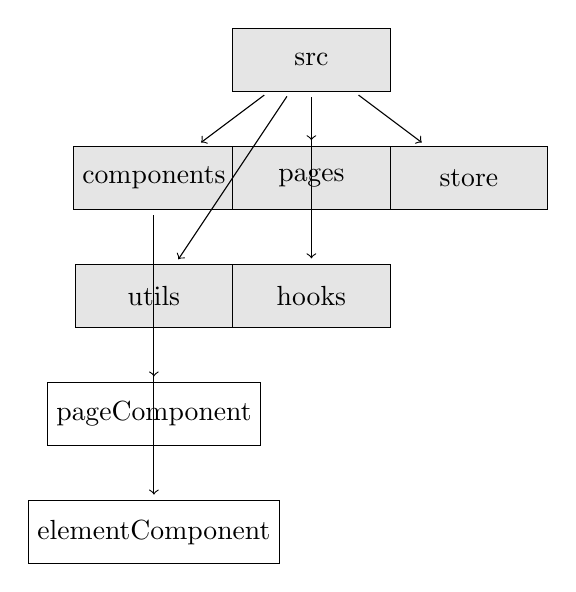
\begin{tikzpicture}[
    file/.style={draw, rectangle, minimum width=2cm, minimum height=0.8cm},
    folder/.style={draw, rectangle, minimum width=2cm, minimum height=0.8cm, fill=gray!20},
    arrow/.style={->, shorten >=2pt, shorten <=2pt}
]

% Folders
\node[folder] (src) at (0,0) {src};
\node[folder] (components) at (-2,-1.5) {components};
\node[folder] (pages) at (0,-1.5) {pages};
\node[folder] (store) at (2,-1.5) {store};
\node[folder] (utils) at (-2,-3) {utils};
\node[folder] (hooks) at (0,-3) {hooks};

% Files
\node[file] (pageComponent) at (-2,-4.5) {pageComponent};
\node[file] (elementComponent) at (-2,-6) {elementComponent};
% ... add more files

% Connections
\draw[arrow] (src) -- (components);
\draw[arrow] (src) -- (pages);
\draw[arrow] (src) -- (store);
\draw[arrow] (src) -- (utils);
\draw[arrow] (src) -- (hooks);
\draw[arrow] (components) -- (pageComponent);
\draw[arrow] (components) -- (elementComponent);
% ... add more connections

\end{tikzpicture}



\pagebreak
\subsubsection{Back-end}
The backend uses the dotNet framework. The development language using the C\# language.

In this project, the backend uses the Onion Architecture.
The Onion Architecture is a typically layered architecture, 
where each layer depends on the inner layer and provides interfaces to the outer layer.
The outer layer provides services to the outermost layer 
and other modules in the same layer based on the interfaces of the inner layer.

From inner to outer, the layers are: Domain, Application, Infrastructure, Presentation.
The Domain layer is the core layer and the innermost layer, used to define domain models, 
which are the business models.
It includes domain models and domain service interfaces.
Domain models are used to define the business models, 
which are the entities in the entity-relationship model and their attributes.
Domain service interfaces are used to define the business services, 
which are the relationships between entities in the entity-relationship model.

The Application layer is the application layer, 
used to define application services, which are the business logic.
It includes domain service implementations and application service interfaces.
Domain service implementations implement the methods of the inner layer's domain service 
interfaces and implement the business logic of the domain models.
Application service interfaces are used to define application services, 
which are the business logic.
It includes but is not limited to database interfaces, testing interfaces, 
HTTP API interfaces, MQTT interfaces, etc.

The Infrastructure layer is the infrastructure layer, used to define infrastructure.
It includes database implementations, testing implementations, 
HTTP API implementations, MQTT implementations, etc.
Database implementations implement the database interfaces 
and provide CRUD services for the database.
Testing implementations implement the testing interfaces 
and provide services for unit testing and integration testing.
HTTP API implementations implement the HTTP API interfaces 
and provide CRUD operations for HTTP APIs.
MQTT implementations implement the MQTT interfaces 
and provide CRUD operations for MQTT.

The Presentation layer is the presentation layer, used to define presentation logic, 
such as interfaces and pages. Since this is a backend project,
data presentation and control are handled by the frontend, 
so this layer is not needed.



\pagebreak
\subsubsection{Data communication and storage}
% 关于本项目的数据通信与数据存储的设计, 包括数据通信的协议, 数据存储的设计等
% 关于数据通信的设计:
% 1. 通信协议的选择
% 自前端向后端发送的数据, 有三种传输的数据类型, 
% 一种是普通的增删改查的请求, 对数据传输的时效性要求不高, 但是对数据的准确性, 完整性, 有序性, 安全性有一定的要求,
% 这种数据的传输, 采用 HTTP 协议, 以及 RESTful API 的设计. 可以有效的保证对数据传输的以上要求.
% 一种是对数据通道的创建和流媒体数据的传输, 对数据传输的时效性, 安全性要求较高, 这种数据的传输, 采用 WebRTC 协议, 以及 MQTT 协议.
% 配合可以快速解码的 flatbuffers 协议, 可以有效的保证对数据传输的以上要求.
% 最后一种是对设备的状态信息和操作信息的传输, 对完整性, 有序性, 安全性都有较高的要求, 这种数据的传输, 采用 MQTT 协议
% 同时也使用了 flatbuffers 协议.
% 
% 2. 数据通信的通信架构和通信流程
% 本项目的数据通信的通信架构, 是基于前后端分离的架构, 前端使用 React 框架, 后端使用 dotnet 框架.
% 当前端需要向后端发送数据的时候, 前端会向后端发送 HTTP 请求, 后端接收到 HTTP 请求之后, 会根据请求的数据类型,
% 选择不同的数据处理方式, 对于普通的增删改查的请求, 后端会根据 RESTful API 的设计, 对数据进行增删改查的操作,
% 对于对数据通道的创建和流媒体数据的传输, 后端会根据 WebRTC 协议, 对数据通道进行创建, 并且帮助前端和设备建立数据通道,
% 当数据通道建立后, 前端和设备之间则使用 flatbuffer 的数据格式对流媒体数据进行传输,
% 对于设备的状态信息和操作信息的传输, 前端会直接向 MQTT broker 发送 MQTT 请求, 
% 设备会在其自身的固件中监听相关的 MQTT 请求, 并且返回相关的数据.
% 
% 3. 数据通信的格式
% 本项目的数据通信的格式, 有三种, 
% 一种是 HTTP 协议, 
% 使用 json 格式对数据进行传输,
% 一种是 WebRTC 协议, 
% 使用 flatbuffers 格式对数据进行传输,
% 一种是 MQTT 协议.
% 使用 flatbuffers 格式对数据进行传输,
% 
% 关于数据存储的设计:
% 1. 数据存储的数据库的选择
% 本项目的数据存储的数据库的选择, 使用了轻量级的数据库 SQLite,
% SQLite 是一个进程内的库, 实现了自给自足的, 无服务器的, 零配置的, 事务性的 SQL 数据库引擎.
% 这是因为整个项目的目的是为了实现前端与设备之间的数据通信, 对于数据库数据的增删改查操作的要求不高,
% 数据量较小, 且对于数据库的数据的事务性要求不高, 所以选择了 SQLite 数据库.
% 2. 项目前后端的数据结构的设计
% 在本项目中, 前端由于使用了 React 框架, 所以前端的数据结构的设计, 使用了基于状态的数据结构的设计,
% 每个组件或者数据集都包含一个状态对象, 这个状态对象的属性就是组件的各个状态. 
% 使用状态对象的原因是, 可以方便的对状态进行管理, 采用对象-属性的形式, 可以方便的针对不同组件的同类状态进行区分,
% 由于跨组件的状态是由 redux 进行管理的, 这种状态对象的设计, 可以更搞笑的对状态进行更新和传递.
% 后端由于使用了 dotnet 框架, 所以后端的数据结构的设计, 使用了基于类的数据结构的设计,
% 采用了面向对象的编程思想, 对数据进行了封装, 使得数据的传输更加的安全, 有序, 完整.


\pagebreak

% \subsection{Domain model}
% \documentclass[]{article}
\usepackage{graphicx}
\usepackage{amsmath}
\usepackage{tikz}

% libaries
\usetikzlibrary{shapes,arrows}

%Define the listing package
\usepackage{listings} %code highlighter
\usepackage{color} %use color
\definecolor{mygreen}{rgb}{0,0.6,0}
\definecolor{mygray}{rgb}{0.5,0.5,0.5}
\definecolor{mymauve}{rgb}{0.58,0,0.82}

%Customize a bit the look
\lstset{ %
backgroundcolor=\color{white}, % choose the background color; you must add \usepackage{color} or \usepackage{xcolor}
basicstyle=\footnotesize, % the size of the fonts that are used for the code
breakatwhitespace=false, % sets if automatic breaks should only happen at whitespace
breaklines=true, % sets automatic line breaking
captionpos=b, % sets the caption-position to bottom
commentstyle=\color{mygreen}, % comment style
deletekeywords={...}, % if you want to delete keywords from the given language
escapeinside={\%*}{*)}, % if you want to add LaTeX within your code
extendedchars=true, % lets you use non-ASCII characters; for 8-bits encodings only, does not work with UTF-8
frame=single, % adds a frame around the code
keepspaces=true, % keeps spaces in text, useful for keeping indentation of code (possibly needs columns=flexible)
keywordstyle=\color{blue}, % keyword style
% language=Octave, % the language of the code
morekeywords={*,...}, % if you want to add more keywords to the set
numbers=left, % where to put the line-numbers; possible values are (none, left, right)
numbersep=5pt, % how far the line-numbers are from the code
numberstyle=\tiny\color{mygray}, % the style that is used for the line-numbers
rulecolor=\color{black}, % if not set, the frame-color may be changed on line-breaks within not-black text (e.g. comments (green here))
showspaces=false, % show spaces everywhere adding particular underscores; it overrides 'showstringspaces'
showstringspaces=false, % underline spaces within strings only
showtabs=false, % show tabs within strings adding particular underscores
stepnumber=1, % the step between two line-numbers. If it's 1, each line will be numbered
stringstyle=\color{mymauve}, % string literal style
tabsize=2, % sets default tabsize to 2 spaces
title=\lstname % show the filename of files included with \lstinputlisting; also try caption instead of title
}

\definecolor{darkgray}{rgb}{.4,.4,.4}
\definecolor{purple}{rgb}{0.65, 0.12, 0.82}

\lstdefinelanguage{React}{
keywords={const, typeof, new, true, false, catch, function, return, null, catch, switch, var, if, in, while, do, else, case, break},
keywordstyle=\color{blue}\bfseries,
ndkeywords={class, export, boolean, throw, implements, import, this},
ndkeywordstyle=\color{darkgray}\bfseries,
identifierstyle=\color{mygreen},
sensitive=false,
comment=[l]{//},
morecomment=[s]{/*}{*/},
commentstyle=\color{purple}\ttfamily,
string=[b]{"}{'}{`},
stringstyle=\color{red}\ttfamily,
morestring=[b]',
morestring=[b]",
morestring=[b]`',
}

\lstdefinelanguage{CSharp}{
keywords={const, typeof, new, true, false, catch, function, return, null, catch, switch, var, if, in, while, do, else, case, break},
keywordstyle=\color{blue}\bfseries,
ndkeywords={class, export, boolean, throw, implements, import, this},
ndkeywordstyle=\color{darkgray}\bfseries,
identifierstyle=\color{mygreen},
sensitive=false,
comment=[l]{//},
morecomment=[s]{/*}{*/},
commentstyle=\color{purple}\ttfamily,
string=[b]{"}{'}{`},
stringstyle=\color{red}\ttfamily,
morestring=[b]',
morestring=[b]",
morestring=[b]`',
}

\lstset{
language=React,
extendedchars=true,
basicstyle=\footnotesize\ttfamily,
showstringspaces=false,
showspaces=false,
numbers=left,
numberstyle=\footnotesize,
numbersep=9pt,
tabsize=2,
breaklines=true,
showtabs=false,
captionpos=b
}

\lstset{
language=CSharp,
extendedchars=true,
basicstyle=\footnotesize\ttfamily,
showstringspaces=false,
showspaces=false,
numbers=left,
numberstyle=\footnotesize,
numbersep=9pt,
tabsize=2,
breaklines=true,
showtabs=false,
captionpos=b
}

% \usepackage{cite} % Add this line for citation

% \bibliographystyle{plain}

\title{
The implementation of BifrostConnect Front-end scope, 
re-design and development with the relevant back-end support develop.
}
\author{
    Fei Gu \\
    Erhvervs Akademi Sydvest \\
    Computer Science 21\\
    }
\date{\today}

\begin{document}

% Front page
\maketitle
\begin{center}
    Supervisor: Henrik Boulund Meng Hansen \\
    Company: BifrostConnect \\
    Engineering Director: Jasper Wass \\
\end{center}
\tableofcontents
\pagebreak


% The introduction
\section{Introduction}
\subsection{Background}% 关于项目的类型和背景的介绍
% 项目是 EASV computer science 专业的毕业设计, 毕业设计的要求是充分的展现学生在两年半的学习中
% 能够获得的知识和技能, 并且能够在一个项目中充分的展现出来. 项目的类型是一个软件开发项目,
% 项目的背景是一个公司的项目, 项目的目的是为了解决公司的一个问题.

This project is the final project of the EASV computer science program. 
The purpose of the final project is to demonstrate the knowledge 
and skills by the student during the two and a half years of study,
and be able to fully demonstrate them in a project.

In this project, the student will work with a company 
to solve a problem of the company.
The student will use the knowledge and skills learned from the education
to solve the problem.

Which means this project will relavent to the company's business domain,
and using the software engineering methods and software development methods
to reconize the problem, analyze the problem, and solve the problem.


\subsection{The company}% 关于公司的介绍
% 公司的名字是 BifrostConnect, 是一个创业公司, 公司的主要业务是为了解决在严格的系统安全条件下, 
% 当客户的系统没有也不允许有互联网的情况下, 通过一个中继设备而不是第三方服务的条件下, 能够远程的
% 访问客户的系统. 公司的产品是一个硬件设备以及配套的网络应用. 以及相关的服务和一站式解决方案.

BifrostConnect is a startup company which established in 2018 
that has 10 to 12 employees and located in Copenhagen, Denmark.

During the five years of operation, the company has developed
a remote access solution for access the users remote system.
The solution  


The company's main business is to solve the problem of remote access 
to the customer's system when the customer's system does not have 
and is not allowed to have the Internet under strict system security conditions.

The company's product is a hardware device and a network application.
And related services and one-stop solutions.
\subsection{The project}% 关于项目的介绍
% 这个项目是在公司原有软件基础上, 对现有的前端软件进行重构和重新设计, 并且在后端提供相应的支持.

% This project is to re-design and re-develop the front-end software based on the company's original software,
% and provide corresponding support on the back-end.% Introduction to the project


% This project involves a comprehensive overhaul of the existing front-end software, building upon the company's original software. It also includes providing corresponding back-end support.

This project entails a thorough redesign and redevelopment of the existing front-end software, 
leveraging the foundation provided by the company's original software. 
Additionally, it involves enhancing the back-end to provide the necessary support 
for the new front-end.
\pagebreak

% The problem statement
\section{Problem Statement}
\subsection{Statement}
During this project the Remote Access Interface and Tunnel Interface should be integrated into the Device Mananger Application.
To achieve the one single page application with full functionality of the Remote Access and Tunnel Connection capabilities.

\subsection{Situation}
% 项目的背景
% 这一部分要详细的介绍关于项目的原始背景, 因为在之后要根据这些背景写明项目的意义和解决方案.
% 所以项目的现状, 项目的历史问题, 现有项目难以开发和维护的原因, 

% The current BifrostConnect front-end application consist of the Device Manager (DM) 
% and Remote Access Interface (RAI) two different user interface.
% Which means the user need to manage their devices and users in the one application, 
% and oprate their devices to use the bifrost product in other web application as well. 
% However, the RAI consists of two different user interfaces referred to as the Classic RAI and Tunnel RAI. 
% Those two user interfaces will leading the user to different web application 
% when user wish to create a different type of access solution.

% The reason for this situation occurred is because the bifrost product is developed focus on the device 
% and the application part was not considered as important as the device part. 
% Therefore, the application part was developed by different developers with different design logic.
% And the application functionality was not been properly through out the development process. 
% Which cause the design logic of this product is not scalable, leading to decreasing user experience, 
% and exponential growth of code complexity which makes it increasingly challenging to maintain and improve. 
% Also the product design style lacks scalability due to lack of modularity and code consistency, 
% and the operation logic is not clear.

The existing BifrostConnect front-end application is divided into two distinct user interfaces:
the Device Manager (DM) and the Remote Access Interface (RAI). 
This division requires users to manage their devices and users in one application, 
while operating their devices to use the Bifrost product in another web application. 
Moreover, the RAI is further split into two different user interfaces, 
known as the Classic RAI and Tunnel RAI. 
These interfaces direct users to different web applications 
depending on the type of access solution they wish to create.

This situation arose because the development of the Bifrost product was primarily focused 
on the device, with the application part not receiving as much attention. 
As a result, the application part was developed by different developers, 
each with their own design logic. 
This led to a lack of thorough planning for the application functionality 
during the development process. Consequently, 
the design logic of the product is not scalable, 
which has resulted in a diminished user experience 
and an exponential increase in code complexity, 
making it increasingly difficult to maintain and improve. 
Furthermore, the product design style lacks scalability due to a lack of modularity 
and code consistency, and the operation logic is unclear.
\subsection{Potential Solution}
% 项目的解决方案
% 根据之前的项目背景描述, 提出项目的解决方案, 也就是问题陈述的解决方案的详细说明. 
% 包括潜在的解决方案, 这个解决方案的优势和劣势.

To address those issue, there is a need to redesign and remake the front-end with
a focus on implementing a modular unified front-end management system that
encompasses all the necessary functionality. 

The goal is to provide users with seamless control, monitoring, and access to their devices from anywhere, 
enhancing their overall user experience and productivity while keeping code complexity as low as possible.

For the implementation to be successful, we also need to have a back-end
service, including an API and Database. The back-end server will contain the
necessary service for the front-end to reach the purpose. Such as the RESTful
API service, authentication service, MQTT service, Tunnel service and Database.

This project will follow the software design process. Therefore, it will also include
the Software Development method and DevOps on all process as well. 

This project is covered by NDA due to security and confidentiality reasons. Thus, the
project will initially not be publicly deployed, however, I will described the
deployment in my report as well.

%%%%%%%%%%%%%%%%%%%%%%%%%%%%%%%%%%%%%%%%%%%%%%%%%%%%%%%%%%%%%%%%%%%%%%%%%

% Project Solution
% Based on the previously described project background, this section presents a detailed explanation of the proposed solution to the problem statement. This includes potential solutions, as well as the advantages and disadvantages of the proposed solution.

% To address the issues identified, 
% a comprehensive redesign and redevelopment of the front-end is necessary. 
% The focus will be on creating a modular, 
% unified front-end management system that encompasses all required functionalities.

% The objective is to provide users with seamless control, 
% monitoring, and access to their devices from any location. 
% This will enhance their overall user experience 
% and productivity while keeping code complexity to a minimum.

% For successful implementation, a back-end service, 
% including an API and Database, is also required. 
% The back-end server will provide the necessary services for the front-end 
% to achieve its purpose. 
% These services include the RESTful API service, 
% authentication service, 
% MQTT service, 
% Tunnel service, 
% and Database.

% This project will adhere to the software design process, 
% incorporating Software Development methods 
% and DevOps throughout all stages.

% Due to security and confidentiality reasons, 
% this project is covered by a Non-Disclosure Agreement (NDA). 
% Therefore, the project will not initially be publicly deployed. 
% However, the deployment process will be described in detail in the final report.

%%%%%%%%%%%%%%%%%%%%%%%%%%%%%%%%%%%%%%%%%%%%%%%%%%%%%%%%%%%%%%%%%%%%%%%%%

In order to address the issues identified, 
a comprehensive overhaul of the front-end is necessary. 
This involves a complete redesign and redevelopment of the existing system, 
with a particular emphasis on creating a modular, 
unified front-end management system. 
This new system will incorporate all the necessary functionalities, 
thereby eliminating the need for multiple interfaces and improving the overall user experience.

The primary goal of this redesign is to provide users with seamless control, 
monitoring, and access to their devices, 
regardless of their location. 
By streamlining the user interface and integrating all necessary functionalities into a single, 
unified system, we aim to enhance the overall user experience and increase productivity. 
Furthermore, by focusing on modularity in the design, 
we aim to keep code complexity as low as possible, 
thereby improving maintainability and scalability of the system.

Successful implementation of this redesign requires a robust back-end service, which includes an API and a Database. The back-end server will house the necessary services for the front-end to fulfill its purpose. These services include the RESTful API service, which will handle requests and responses between the front-end and the server; an authentication service, which will ensure secure access to the system; an MQTT service, which will handle messaging between devices; a Tunnel service, which will manage the creation and maintenance of secure tunnels for remote access; and a Database, which will store and manage all necessary data.

This project will adhere to the software design process, incorporating best practices from Software Development methodologies and DevOps principles throughout all stages. This includes requirements gathering, system design, implementation, testing, deployment, and maintenance. By following this process, we aim to ensure the delivery of a high-quality, reliable, and scalable system.

Due to security and confidentiality reasons, this project is covered by a Non-Disclosure Agreement (NDA). As such, the project will not initially be publicly deployed. However, the deployment process, including the strategies used for continuous integration and continuous deployment, as well as the measures taken to ensure security and reliability, will be described in detail in the final report.
\pagebreak

% Requirement analysis
\section{Requirement Analysis}
\documentclass[]{article}
\usepackage{graphicx}
\usepackage{amsmath}
\usepackage{tikz}

% libaries
\usetikzlibrary{shapes,arrows}

%Define the listing package
\usepackage{listings} %code highlighter
\usepackage{color} %use color
\definecolor{mygreen}{rgb}{0,0.6,0}
\definecolor{mygray}{rgb}{0.5,0.5,0.5}
\definecolor{mymauve}{rgb}{0.58,0,0.82}

%Customize a bit the look
\lstset{ %
backgroundcolor=\color{white}, % choose the background color; you must add \usepackage{color} or \usepackage{xcolor}
basicstyle=\footnotesize, % the size of the fonts that are used for the code
breakatwhitespace=false, % sets if automatic breaks should only happen at whitespace
breaklines=true, % sets automatic line breaking
captionpos=b, % sets the caption-position to bottom
commentstyle=\color{mygreen}, % comment style
deletekeywords={...}, % if you want to delete keywords from the given language
escapeinside={\%*}{*)}, % if you want to add LaTeX within your code
extendedchars=true, % lets you use non-ASCII characters; for 8-bits encodings only, does not work with UTF-8
frame=single, % adds a frame around the code
keepspaces=true, % keeps spaces in text, useful for keeping indentation of code (possibly needs columns=flexible)
keywordstyle=\color{blue}, % keyword style
% language=Octave, % the language of the code
morekeywords={*,...}, % if you want to add more keywords to the set
numbers=left, % where to put the line-numbers; possible values are (none, left, right)
numbersep=5pt, % how far the line-numbers are from the code
numberstyle=\tiny\color{mygray}, % the style that is used for the line-numbers
rulecolor=\color{black}, % if not set, the frame-color may be changed on line-breaks within not-black text (e.g. comments (green here))
showspaces=false, % show spaces everywhere adding particular underscores; it overrides 'showstringspaces'
showstringspaces=false, % underline spaces within strings only
showtabs=false, % show tabs within strings adding particular underscores
stepnumber=1, % the step between two line-numbers. If it's 1, each line will be numbered
stringstyle=\color{mymauve}, % string literal style
tabsize=2, % sets default tabsize to 2 spaces
title=\lstname % show the filename of files included with \lstinputlisting; also try caption instead of title
}

\definecolor{darkgray}{rgb}{.4,.4,.4}
\definecolor{purple}{rgb}{0.65, 0.12, 0.82}

\lstdefinelanguage{React}{
keywords={const, typeof, new, true, false, catch, function, return, null, catch, switch, var, if, in, while, do, else, case, break},
keywordstyle=\color{blue}\bfseries,
ndkeywords={class, export, boolean, throw, implements, import, this},
ndkeywordstyle=\color{darkgray}\bfseries,
identifierstyle=\color{mygreen},
sensitive=false,
comment=[l]{//},
morecomment=[s]{/*}{*/},
commentstyle=\color{purple}\ttfamily,
string=[b]{"}{'}{`},
stringstyle=\color{red}\ttfamily,
morestring=[b]',
morestring=[b]",
morestring=[b]`',
}

\lstdefinelanguage{CSharp}{
keywords={const, typeof, new, true, false, catch, function, return, null, catch, switch, var, if, in, while, do, else, case, break},
keywordstyle=\color{blue}\bfseries,
ndkeywords={class, export, boolean, throw, implements, import, this},
ndkeywordstyle=\color{darkgray}\bfseries,
identifierstyle=\color{mygreen},
sensitive=false,
comment=[l]{//},
morecomment=[s]{/*}{*/},
commentstyle=\color{purple}\ttfamily,
string=[b]{"}{'}{`},
stringstyle=\color{red}\ttfamily,
morestring=[b]',
morestring=[b]",
morestring=[b]`',
}

\lstset{
language=React,
extendedchars=true,
basicstyle=\footnotesize\ttfamily,
showstringspaces=false,
showspaces=false,
numbers=left,
numberstyle=\footnotesize,
numbersep=9pt,
tabsize=2,
breaklines=true,
showtabs=false,
captionpos=b
}

\lstset{
language=CSharp,
extendedchars=true,
basicstyle=\footnotesize\ttfamily,
showstringspaces=false,
showspaces=false,
numbers=left,
numberstyle=\footnotesize,
numbersep=9pt,
tabsize=2,
breaklines=true,
showtabs=false,
captionpos=b
}

% \usepackage{cite} % Add this line for citation

% \bibliographystyle{plain}

\title{
The implementation of BifrostConnect Front-end scope, 
re-design and development with the relevant back-end support develop.
}
\author{
    Fei Gu \\
    Erhvervs Akademi Sydvest \\
    Computer Science 21\\
    }
\date{\today}

\begin{document}

% Front page
\maketitle
\begin{center}
    Supervisor: Henrik Boulund Meng Hansen \\
    Company: BifrostConnect \\
    Engineering Director: Jasper Wass \\
\end{center}
\tableofcontents
\pagebreak


% The introduction
\section{Introduction}
\subsection{Background}\input{sections/introduction/background.tex}
\subsection{The company}\input{sections/introduction/aboutCompany}
\subsection{The project}\input{sections/introduction/aboutProject}
\pagebreak

% The problem statement
\section{Problem Statement}
\subsection{Statement}
\input{sections/problemStatement/statement}
\subsection{Situation}
\input{sections/problemStatement/situation}
\subsection{Potential Solution}
\input{sections/problemStatement/potentialSolution}
\pagebreak

% Requirement analysis
\section{Requirement Analysis}
\input{sections/requirementAnalysis/index}

\subsection{Stakeholders}
\input{sections/requirementAnalysis/stakeholders/index}

\subsection{Business Domain}
\input{sections/requirementAnalysis/bussinesDomain/index}

\subsection{Scope}
\input{sections/requirementAnalysis/scope}

\subsection{Goals}
\input{sections/requirementAnalysis/goals}
\pagebreak

% Software Design
\section{Software Design}
% developement methods
\subsection{Software Development Methods}
\input{sections/softwareDevelopmentMethods/index}
\subsubsection{Agile Software Development}
\input{sections/softwareDevelopmentMethods/agileSoftwareDevelopment/index}
\subsubsection{Feature Driven Development}
\input{sections/softwareDevelopmentMethods/featureDrivenDevelopment/index}

\pagebreak

% Technology seslection
\subsection{Technology selection}
\input{sections/softwareDesign/technologySelection/index}
\subsubsection{Front-end}
\input{sections/softwareDesign/technologySelection/frontEnd}            
\subsubsection{Back-end}
\input{sections/softwareDesign/technologySelection/backEnd}            
\subsubsection{Database}
\input{sections/softwareDesign/technologySelection/database}
\subsubsection{Data communication}
\input{sections/softwareDesign/technologySelection/dataCommunication}            
\subsubsection{DevOps}
\input{sections/softwareDesign/technologySelection/devOps}
\pagebreak

% Architecture design
\subsection{Architecture design}
\input{sections/softwareDesign/architectureDesign/index}
\pagebreak
\subsubsection{Front-end}
\input{sections/softwareDesign/architectureDesign/frontEndArchitecture}
\pagebreak
\subsubsection{Back-end}
\input{sections/softwareDesign/architectureDesign/backEndArchitecture}
\pagebreak
\subsubsection{Data communication and storage}
\input{sections/softwareDesign/architectureDesign/dataCommunicationArchitecture}
\pagebreak

% \subsection{Domain model}
% \input{sections/softwareDesign/domainModel/index}
% \subsection{Database design}
% % 数据库领域模型 ER 图
% % 包括表和字段的设置.
% % 对于私有键和外键的设置.

% \subsection{Back-end design}
% % 后端对象模型
% % 以及对于对象模型的增删改查
% % 以及相关的其他服务的设计`'

% \subsection{Front-end design}
% % 对于前端的页面结构的设计 
% % 页面的状态的设计, 交互设计

% \subsection{FlatBuffers design}
% % schema 的设计

\subsection{DevOps CI/CD process design}
\input{sections/softwareDesign/devOpsDesign/index}
\subsubsection{Continuous Integration}
\input{sections/softwareDesign/devOpsDesign/continuousIntegration/index}
\subsubsection{Continuous Delivery}
\input{sections/softwareDesign/devOpsDesign/continuousDelivery/index}
\subsubsection{Continuous Deployment}
\input{sections/softwareDesign/devOpsDesign/continuousDeployment/index}
\pagebreak

\section{Software Development} 
\input{sections/softwareDevelopment/index}
\subsection{Overall development}
\input{sections/softwareDevelopment/overallDevelopement/index}
\subsubsection{Front-end}
\input{sections/softwareDevelopment/overallDevelopement/frontEnd/index}
\subsubsection{Back-end}
\input{sections/softwareDevelopment/overallDevelopement/backEnd/index}
\subsubsection{DevOps}
\input{sections/softwareDevelopment/overallDevelopement/devOps/index}
\subsection{Feature development} 
\input{sections/softwareDevelopment/featureDevelopment/index}
\subsubsection{Use Case 1}
\input{sections/softwareDevelopment/featureDevelopment/useCase1/index}
\subsubsection{Feature 1}
\input{sections/softwareDevelopment/featureDevelopment/feature/feature1.tex}
\pagebreak
\section{Conclusion} 
\subsection{Result}
Since the project is still in progress, the result is not available yet.
So far, basic structure of this project has been built. But the most features 
are not implemented yet. 
\subsection{Discussion}
As a single developer for this project, I am confident what I have done so far.
And I can say I understand the most of the knowledge I have used in this project, 
which also means I can explain all the part of the project. 
But this project also relevant some of the complex knowledge which I have to continue 
to study and practice.
\subsection{Future Work}
The future work is to implement the rest of the features. 
Including the most important part which is the 'create session' feature.
\pagebreak
% \bibliography{bibliography}
\pagebreak
% \begin{appendices}
%     \section{Appendix}
% \end{appendices} 
\end{document}

\subsection{Stakeholders}
\documentclass[]{article}
\usepackage{graphicx}
\usepackage{amsmath}
\usepackage{tikz}

% libaries
\usetikzlibrary{shapes,arrows}

%Define the listing package
\usepackage{listings} %code highlighter
\usepackage{color} %use color
\definecolor{mygreen}{rgb}{0,0.6,0}
\definecolor{mygray}{rgb}{0.5,0.5,0.5}
\definecolor{mymauve}{rgb}{0.58,0,0.82}

%Customize a bit the look
\lstset{ %
backgroundcolor=\color{white}, % choose the background color; you must add \usepackage{color} or \usepackage{xcolor}
basicstyle=\footnotesize, % the size of the fonts that are used for the code
breakatwhitespace=false, % sets if automatic breaks should only happen at whitespace
breaklines=true, % sets automatic line breaking
captionpos=b, % sets the caption-position to bottom
commentstyle=\color{mygreen}, % comment style
deletekeywords={...}, % if you want to delete keywords from the given language
escapeinside={\%*}{*)}, % if you want to add LaTeX within your code
extendedchars=true, % lets you use non-ASCII characters; for 8-bits encodings only, does not work with UTF-8
frame=single, % adds a frame around the code
keepspaces=true, % keeps spaces in text, useful for keeping indentation of code (possibly needs columns=flexible)
keywordstyle=\color{blue}, % keyword style
% language=Octave, % the language of the code
morekeywords={*,...}, % if you want to add more keywords to the set
numbers=left, % where to put the line-numbers; possible values are (none, left, right)
numbersep=5pt, % how far the line-numbers are from the code
numberstyle=\tiny\color{mygray}, % the style that is used for the line-numbers
rulecolor=\color{black}, % if not set, the frame-color may be changed on line-breaks within not-black text (e.g. comments (green here))
showspaces=false, % show spaces everywhere adding particular underscores; it overrides 'showstringspaces'
showstringspaces=false, % underline spaces within strings only
showtabs=false, % show tabs within strings adding particular underscores
stepnumber=1, % the step between two line-numbers. If it's 1, each line will be numbered
stringstyle=\color{mymauve}, % string literal style
tabsize=2, % sets default tabsize to 2 spaces
title=\lstname % show the filename of files included with \lstinputlisting; also try caption instead of title
}

\definecolor{darkgray}{rgb}{.4,.4,.4}
\definecolor{purple}{rgb}{0.65, 0.12, 0.82}

\lstdefinelanguage{React}{
keywords={const, typeof, new, true, false, catch, function, return, null, catch, switch, var, if, in, while, do, else, case, break},
keywordstyle=\color{blue}\bfseries,
ndkeywords={class, export, boolean, throw, implements, import, this},
ndkeywordstyle=\color{darkgray}\bfseries,
identifierstyle=\color{mygreen},
sensitive=false,
comment=[l]{//},
morecomment=[s]{/*}{*/},
commentstyle=\color{purple}\ttfamily,
string=[b]{"}{'}{`},
stringstyle=\color{red}\ttfamily,
morestring=[b]',
morestring=[b]",
morestring=[b]`',
}

\lstdefinelanguage{CSharp}{
keywords={const, typeof, new, true, false, catch, function, return, null, catch, switch, var, if, in, while, do, else, case, break},
keywordstyle=\color{blue}\bfseries,
ndkeywords={class, export, boolean, throw, implements, import, this},
ndkeywordstyle=\color{darkgray}\bfseries,
identifierstyle=\color{mygreen},
sensitive=false,
comment=[l]{//},
morecomment=[s]{/*}{*/},
commentstyle=\color{purple}\ttfamily,
string=[b]{"}{'}{`},
stringstyle=\color{red}\ttfamily,
morestring=[b]',
morestring=[b]",
morestring=[b]`',
}

\lstset{
language=React,
extendedchars=true,
basicstyle=\footnotesize\ttfamily,
showstringspaces=false,
showspaces=false,
numbers=left,
numberstyle=\footnotesize,
numbersep=9pt,
tabsize=2,
breaklines=true,
showtabs=false,
captionpos=b
}

\lstset{
language=CSharp,
extendedchars=true,
basicstyle=\footnotesize\ttfamily,
showstringspaces=false,
showspaces=false,
numbers=left,
numberstyle=\footnotesize,
numbersep=9pt,
tabsize=2,
breaklines=true,
showtabs=false,
captionpos=b
}

% \usepackage{cite} % Add this line for citation

% \bibliographystyle{plain}

\title{
The implementation of BifrostConnect Front-end scope, 
re-design and development with the relevant back-end support develop.
}
\author{
    Fei Gu \\
    Erhvervs Akademi Sydvest \\
    Computer Science 21\\
    }
\date{\today}

\begin{document}

% Front page
\maketitle
\begin{center}
    Supervisor: Henrik Boulund Meng Hansen \\
    Company: BifrostConnect \\
    Engineering Director: Jasper Wass \\
\end{center}
\tableofcontents
\pagebreak


% The introduction
\section{Introduction}
\subsection{Background}\input{sections/introduction/background.tex}
\subsection{The company}\input{sections/introduction/aboutCompany}
\subsection{The project}\input{sections/introduction/aboutProject}
\pagebreak

% The problem statement
\section{Problem Statement}
\subsection{Statement}
\input{sections/problemStatement/statement}
\subsection{Situation}
\input{sections/problemStatement/situation}
\subsection{Potential Solution}
\input{sections/problemStatement/potentialSolution}
\pagebreak

% Requirement analysis
\section{Requirement Analysis}
\input{sections/requirementAnalysis/index}

\subsection{Stakeholders}
\input{sections/requirementAnalysis/stakeholders/index}

\subsection{Business Domain}
\input{sections/requirementAnalysis/bussinesDomain/index}

\subsection{Scope}
\input{sections/requirementAnalysis/scope}

\subsection{Goals}
\input{sections/requirementAnalysis/goals}
\pagebreak

% Software Design
\section{Software Design}
% developement methods
\subsection{Software Development Methods}
\input{sections/softwareDevelopmentMethods/index}
\subsubsection{Agile Software Development}
\input{sections/softwareDevelopmentMethods/agileSoftwareDevelopment/index}
\subsubsection{Feature Driven Development}
\input{sections/softwareDevelopmentMethods/featureDrivenDevelopment/index}

\pagebreak

% Technology seslection
\subsection{Technology selection}
\input{sections/softwareDesign/technologySelection/index}
\subsubsection{Front-end}
\input{sections/softwareDesign/technologySelection/frontEnd}            
\subsubsection{Back-end}
\input{sections/softwareDesign/technologySelection/backEnd}            
\subsubsection{Database}
\input{sections/softwareDesign/technologySelection/database}
\subsubsection{Data communication}
\input{sections/softwareDesign/technologySelection/dataCommunication}            
\subsubsection{DevOps}
\input{sections/softwareDesign/technologySelection/devOps}
\pagebreak

% Architecture design
\subsection{Architecture design}
\input{sections/softwareDesign/architectureDesign/index}
\pagebreak
\subsubsection{Front-end}
\input{sections/softwareDesign/architectureDesign/frontEndArchitecture}
\pagebreak
\subsubsection{Back-end}
\input{sections/softwareDesign/architectureDesign/backEndArchitecture}
\pagebreak
\subsubsection{Data communication and storage}
\input{sections/softwareDesign/architectureDesign/dataCommunicationArchitecture}
\pagebreak

% \subsection{Domain model}
% \input{sections/softwareDesign/domainModel/index}
% \subsection{Database design}
% % 数据库领域模型 ER 图
% % 包括表和字段的设置.
% % 对于私有键和外键的设置.

% \subsection{Back-end design}
% % 后端对象模型
% % 以及对于对象模型的增删改查
% % 以及相关的其他服务的设计`'

% \subsection{Front-end design}
% % 对于前端的页面结构的设计 
% % 页面的状态的设计, 交互设计

% \subsection{FlatBuffers design}
% % schema 的设计

\subsection{DevOps CI/CD process design}
\input{sections/softwareDesign/devOpsDesign/index}
\subsubsection{Continuous Integration}
\input{sections/softwareDesign/devOpsDesign/continuousIntegration/index}
\subsubsection{Continuous Delivery}
\input{sections/softwareDesign/devOpsDesign/continuousDelivery/index}
\subsubsection{Continuous Deployment}
\input{sections/softwareDesign/devOpsDesign/continuousDeployment/index}
\pagebreak

\section{Software Development} 
\input{sections/softwareDevelopment/index}
\subsection{Overall development}
\input{sections/softwareDevelopment/overallDevelopement/index}
\subsubsection{Front-end}
\input{sections/softwareDevelopment/overallDevelopement/frontEnd/index}
\subsubsection{Back-end}
\input{sections/softwareDevelopment/overallDevelopement/backEnd/index}
\subsubsection{DevOps}
\input{sections/softwareDevelopment/overallDevelopement/devOps/index}
\subsection{Feature development} 
\input{sections/softwareDevelopment/featureDevelopment/index}
\subsubsection{Use Case 1}
\input{sections/softwareDevelopment/featureDevelopment/useCase1/index}
\subsubsection{Feature 1}
\input{sections/softwareDevelopment/featureDevelopment/feature/feature1.tex}
\pagebreak
\section{Conclusion} 
\subsection{Result}
Since the project is still in progress, the result is not available yet.
So far, basic structure of this project has been built. But the most features 
are not implemented yet. 
\subsection{Discussion}
As a single developer for this project, I am confident what I have done so far.
And I can say I understand the most of the knowledge I have used in this project, 
which also means I can explain all the part of the project. 
But this project also relevant some of the complex knowledge which I have to continue 
to study and practice.
\subsection{Future Work}
The future work is to implement the rest of the features. 
Including the most important part which is the 'create session' feature.
\pagebreak
% \bibliography{bibliography}
\pagebreak
% \begin{appendices}
%     \section{Appendix}
% \end{appendices} 
\end{document}

\subsection{Business Domain}
\documentclass[]{article}
\usepackage{graphicx}
\usepackage{amsmath}
\usepackage{tikz}

% libaries
\usetikzlibrary{shapes,arrows}

%Define the listing package
\usepackage{listings} %code highlighter
\usepackage{color} %use color
\definecolor{mygreen}{rgb}{0,0.6,0}
\definecolor{mygray}{rgb}{0.5,0.5,0.5}
\definecolor{mymauve}{rgb}{0.58,0,0.82}

%Customize a bit the look
\lstset{ %
backgroundcolor=\color{white}, % choose the background color; you must add \usepackage{color} or \usepackage{xcolor}
basicstyle=\footnotesize, % the size of the fonts that are used for the code
breakatwhitespace=false, % sets if automatic breaks should only happen at whitespace
breaklines=true, % sets automatic line breaking
captionpos=b, % sets the caption-position to bottom
commentstyle=\color{mygreen}, % comment style
deletekeywords={...}, % if you want to delete keywords from the given language
escapeinside={\%*}{*)}, % if you want to add LaTeX within your code
extendedchars=true, % lets you use non-ASCII characters; for 8-bits encodings only, does not work with UTF-8
frame=single, % adds a frame around the code
keepspaces=true, % keeps spaces in text, useful for keeping indentation of code (possibly needs columns=flexible)
keywordstyle=\color{blue}, % keyword style
% language=Octave, % the language of the code
morekeywords={*,...}, % if you want to add more keywords to the set
numbers=left, % where to put the line-numbers; possible values are (none, left, right)
numbersep=5pt, % how far the line-numbers are from the code
numberstyle=\tiny\color{mygray}, % the style that is used for the line-numbers
rulecolor=\color{black}, % if not set, the frame-color may be changed on line-breaks within not-black text (e.g. comments (green here))
showspaces=false, % show spaces everywhere adding particular underscores; it overrides 'showstringspaces'
showstringspaces=false, % underline spaces within strings only
showtabs=false, % show tabs within strings adding particular underscores
stepnumber=1, % the step between two line-numbers. If it's 1, each line will be numbered
stringstyle=\color{mymauve}, % string literal style
tabsize=2, % sets default tabsize to 2 spaces
title=\lstname % show the filename of files included with \lstinputlisting; also try caption instead of title
}

\definecolor{darkgray}{rgb}{.4,.4,.4}
\definecolor{purple}{rgb}{0.65, 0.12, 0.82}

\lstdefinelanguage{React}{
keywords={const, typeof, new, true, false, catch, function, return, null, catch, switch, var, if, in, while, do, else, case, break},
keywordstyle=\color{blue}\bfseries,
ndkeywords={class, export, boolean, throw, implements, import, this},
ndkeywordstyle=\color{darkgray}\bfseries,
identifierstyle=\color{mygreen},
sensitive=false,
comment=[l]{//},
morecomment=[s]{/*}{*/},
commentstyle=\color{purple}\ttfamily,
string=[b]{"}{'}{`},
stringstyle=\color{red}\ttfamily,
morestring=[b]',
morestring=[b]",
morestring=[b]`',
}

\lstdefinelanguage{CSharp}{
keywords={const, typeof, new, true, false, catch, function, return, null, catch, switch, var, if, in, while, do, else, case, break},
keywordstyle=\color{blue}\bfseries,
ndkeywords={class, export, boolean, throw, implements, import, this},
ndkeywordstyle=\color{darkgray}\bfseries,
identifierstyle=\color{mygreen},
sensitive=false,
comment=[l]{//},
morecomment=[s]{/*}{*/},
commentstyle=\color{purple}\ttfamily,
string=[b]{"}{'}{`},
stringstyle=\color{red}\ttfamily,
morestring=[b]',
morestring=[b]",
morestring=[b]`',
}

\lstset{
language=React,
extendedchars=true,
basicstyle=\footnotesize\ttfamily,
showstringspaces=false,
showspaces=false,
numbers=left,
numberstyle=\footnotesize,
numbersep=9pt,
tabsize=2,
breaklines=true,
showtabs=false,
captionpos=b
}

\lstset{
language=CSharp,
extendedchars=true,
basicstyle=\footnotesize\ttfamily,
showstringspaces=false,
showspaces=false,
numbers=left,
numberstyle=\footnotesize,
numbersep=9pt,
tabsize=2,
breaklines=true,
showtabs=false,
captionpos=b
}

% \usepackage{cite} % Add this line for citation

% \bibliographystyle{plain}

\title{
The implementation of BifrostConnect Front-end scope, 
re-design and development with the relevant back-end support develop.
}
\author{
    Fei Gu \\
    Erhvervs Akademi Sydvest \\
    Computer Science 21\\
    }
\date{\today}

\begin{document}

% Front page
\maketitle
\begin{center}
    Supervisor: Henrik Boulund Meng Hansen \\
    Company: BifrostConnect \\
    Engineering Director: Jasper Wass \\
\end{center}
\tableofcontents
\pagebreak


% The introduction
\section{Introduction}
\subsection{Background}\input{sections/introduction/background.tex}
\subsection{The company}\input{sections/introduction/aboutCompany}
\subsection{The project}\input{sections/introduction/aboutProject}
\pagebreak

% The problem statement
\section{Problem Statement}
\subsection{Statement}
\input{sections/problemStatement/statement}
\subsection{Situation}
\input{sections/problemStatement/situation}
\subsection{Potential Solution}
\input{sections/problemStatement/potentialSolution}
\pagebreak

% Requirement analysis
\section{Requirement Analysis}
\input{sections/requirementAnalysis/index}

\subsection{Stakeholders}
\input{sections/requirementAnalysis/stakeholders/index}

\subsection{Business Domain}
\input{sections/requirementAnalysis/bussinesDomain/index}

\subsection{Scope}
\input{sections/requirementAnalysis/scope}

\subsection{Goals}
\input{sections/requirementAnalysis/goals}
\pagebreak

% Software Design
\section{Software Design}
% developement methods
\subsection{Software Development Methods}
\input{sections/softwareDevelopmentMethods/index}
\subsubsection{Agile Software Development}
\input{sections/softwareDevelopmentMethods/agileSoftwareDevelopment/index}
\subsubsection{Feature Driven Development}
\input{sections/softwareDevelopmentMethods/featureDrivenDevelopment/index}

\pagebreak

% Technology seslection
\subsection{Technology selection}
\input{sections/softwareDesign/technologySelection/index}
\subsubsection{Front-end}
\input{sections/softwareDesign/technologySelection/frontEnd}            
\subsubsection{Back-end}
\input{sections/softwareDesign/technologySelection/backEnd}            
\subsubsection{Database}
\input{sections/softwareDesign/technologySelection/database}
\subsubsection{Data communication}
\input{sections/softwareDesign/technologySelection/dataCommunication}            
\subsubsection{DevOps}
\input{sections/softwareDesign/technologySelection/devOps}
\pagebreak

% Architecture design
\subsection{Architecture design}
\input{sections/softwareDesign/architectureDesign/index}
\pagebreak
\subsubsection{Front-end}
\input{sections/softwareDesign/architectureDesign/frontEndArchitecture}
\pagebreak
\subsubsection{Back-end}
\input{sections/softwareDesign/architectureDesign/backEndArchitecture}
\pagebreak
\subsubsection{Data communication and storage}
\input{sections/softwareDesign/architectureDesign/dataCommunicationArchitecture}
\pagebreak

% \subsection{Domain model}
% \input{sections/softwareDesign/domainModel/index}
% \subsection{Database design}
% % 数据库领域模型 ER 图
% % 包括表和字段的设置.
% % 对于私有键和外键的设置.

% \subsection{Back-end design}
% % 后端对象模型
% % 以及对于对象模型的增删改查
% % 以及相关的其他服务的设计`'

% \subsection{Front-end design}
% % 对于前端的页面结构的设计 
% % 页面的状态的设计, 交互设计

% \subsection{FlatBuffers design}
% % schema 的设计

\subsection{DevOps CI/CD process design}
\input{sections/softwareDesign/devOpsDesign/index}
\subsubsection{Continuous Integration}
\input{sections/softwareDesign/devOpsDesign/continuousIntegration/index}
\subsubsection{Continuous Delivery}
\input{sections/softwareDesign/devOpsDesign/continuousDelivery/index}
\subsubsection{Continuous Deployment}
\input{sections/softwareDesign/devOpsDesign/continuousDeployment/index}
\pagebreak

\section{Software Development} 
\input{sections/softwareDevelopment/index}
\subsection{Overall development}
\input{sections/softwareDevelopment/overallDevelopement/index}
\subsubsection{Front-end}
\input{sections/softwareDevelopment/overallDevelopement/frontEnd/index}
\subsubsection{Back-end}
\input{sections/softwareDevelopment/overallDevelopement/backEnd/index}
\subsubsection{DevOps}
\input{sections/softwareDevelopment/overallDevelopement/devOps/index}
\subsection{Feature development} 
\input{sections/softwareDevelopment/featureDevelopment/index}
\subsubsection{Use Case 1}
\input{sections/softwareDevelopment/featureDevelopment/useCase1/index}
\subsubsection{Feature 1}
\input{sections/softwareDevelopment/featureDevelopment/feature/feature1.tex}
\pagebreak
\section{Conclusion} 
\subsection{Result}
Since the project is still in progress, the result is not available yet.
So far, basic structure of this project has been built. But the most features 
are not implemented yet. 
\subsection{Discussion}
As a single developer for this project, I am confident what I have done so far.
And I can say I understand the most of the knowledge I have used in this project, 
which also means I can explain all the part of the project. 
But this project also relevant some of the complex knowledge which I have to continue 
to study and practice.
\subsection{Future Work}
The future work is to implement the rest of the features. 
Including the most important part which is the 'create session' feature.
\pagebreak
% \bibliography{bibliography}
\pagebreak
% \begin{appendices}
%     \section{Appendix}
% \end{appendices} 
\end{document}

\subsection{Scope}
% The scope of this project is to develop a web application 
% which can be used to manage the device and users, 
% and create the RAI and Tunnel.

% Because the device manager already exist, 
% the mean focus will be on the implementation of the RAI and Tunnel into the device manager.
% Which means we don't need to develop the device manager, 
% also there are no necceary to develop the new features for the RAI and Tunnel interface.

% Because the situation of the entire system was redudent and coupling, 
% we have to re-design the system components and identify the relationship between them.
% The re-design of the system will be the main focus of this project.

% Since the Device Manager is written in React framework, 
% we have to use the same framework to develop the RAI and Tunnel interface.

The scope of this project is to develop a web application 
that manages devices and users, and creates the RAI and Tunnel.

Since the device manager already exists, 
the main focus will be on implementing the RAI and Tunnel 
into the device manager.

Therefore, there is no need to develop the device manager 
or add new features to the RAI and Tunnel interface.

Due to the redundant and coupled nature of the entire system, 
we need to redesign the system components 
and establish their relationships.

As the Device Manager is built using the React framework, 
we will also use the same framework to develop the RAI and Tunnel interface.

The main focus of this project is to migramt the RAI and Tunnel interface, 
and re-design the UI, components, and the relavent methodologies.


\subsection{Goals}
The goal of this project is to develop a RAI and Tunnel interface in the Device Manager.
The RAI and Tunnel interface should be able to create, modify, delete and view the access connection.
Also can remote control the device and target equipment.
\pagebreak

% Software Design
\section{Software Design}
% developement methods
\subsection{Software Development Methods}
\documentclass[]{article}
\usepackage{graphicx}
\usepackage{amsmath}
\usepackage{tikz}

% libaries
\usetikzlibrary{shapes,arrows}

%Define the listing package
\usepackage{listings} %code highlighter
\usepackage{color} %use color
\definecolor{mygreen}{rgb}{0,0.6,0}
\definecolor{mygray}{rgb}{0.5,0.5,0.5}
\definecolor{mymauve}{rgb}{0.58,0,0.82}

%Customize a bit the look
\lstset{ %
backgroundcolor=\color{white}, % choose the background color; you must add \usepackage{color} or \usepackage{xcolor}
basicstyle=\footnotesize, % the size of the fonts that are used for the code
breakatwhitespace=false, % sets if automatic breaks should only happen at whitespace
breaklines=true, % sets automatic line breaking
captionpos=b, % sets the caption-position to bottom
commentstyle=\color{mygreen}, % comment style
deletekeywords={...}, % if you want to delete keywords from the given language
escapeinside={\%*}{*)}, % if you want to add LaTeX within your code
extendedchars=true, % lets you use non-ASCII characters; for 8-bits encodings only, does not work with UTF-8
frame=single, % adds a frame around the code
keepspaces=true, % keeps spaces in text, useful for keeping indentation of code (possibly needs columns=flexible)
keywordstyle=\color{blue}, % keyword style
% language=Octave, % the language of the code
morekeywords={*,...}, % if you want to add more keywords to the set
numbers=left, % where to put the line-numbers; possible values are (none, left, right)
numbersep=5pt, % how far the line-numbers are from the code
numberstyle=\tiny\color{mygray}, % the style that is used for the line-numbers
rulecolor=\color{black}, % if not set, the frame-color may be changed on line-breaks within not-black text (e.g. comments (green here))
showspaces=false, % show spaces everywhere adding particular underscores; it overrides 'showstringspaces'
showstringspaces=false, % underline spaces within strings only
showtabs=false, % show tabs within strings adding particular underscores
stepnumber=1, % the step between two line-numbers. If it's 1, each line will be numbered
stringstyle=\color{mymauve}, % string literal style
tabsize=2, % sets default tabsize to 2 spaces
title=\lstname % show the filename of files included with \lstinputlisting; also try caption instead of title
}

\definecolor{darkgray}{rgb}{.4,.4,.4}
\definecolor{purple}{rgb}{0.65, 0.12, 0.82}

\lstdefinelanguage{React}{
keywords={const, typeof, new, true, false, catch, function, return, null, catch, switch, var, if, in, while, do, else, case, break},
keywordstyle=\color{blue}\bfseries,
ndkeywords={class, export, boolean, throw, implements, import, this},
ndkeywordstyle=\color{darkgray}\bfseries,
identifierstyle=\color{mygreen},
sensitive=false,
comment=[l]{//},
morecomment=[s]{/*}{*/},
commentstyle=\color{purple}\ttfamily,
string=[b]{"}{'}{`},
stringstyle=\color{red}\ttfamily,
morestring=[b]',
morestring=[b]",
morestring=[b]`',
}

\lstdefinelanguage{CSharp}{
keywords={const, typeof, new, true, false, catch, function, return, null, catch, switch, var, if, in, while, do, else, case, break},
keywordstyle=\color{blue}\bfseries,
ndkeywords={class, export, boolean, throw, implements, import, this},
ndkeywordstyle=\color{darkgray}\bfseries,
identifierstyle=\color{mygreen},
sensitive=false,
comment=[l]{//},
morecomment=[s]{/*}{*/},
commentstyle=\color{purple}\ttfamily,
string=[b]{"}{'}{`},
stringstyle=\color{red}\ttfamily,
morestring=[b]',
morestring=[b]",
morestring=[b]`',
}

\lstset{
language=React,
extendedchars=true,
basicstyle=\footnotesize\ttfamily,
showstringspaces=false,
showspaces=false,
numbers=left,
numberstyle=\footnotesize,
numbersep=9pt,
tabsize=2,
breaklines=true,
showtabs=false,
captionpos=b
}

\lstset{
language=CSharp,
extendedchars=true,
basicstyle=\footnotesize\ttfamily,
showstringspaces=false,
showspaces=false,
numbers=left,
numberstyle=\footnotesize,
numbersep=9pt,
tabsize=2,
breaklines=true,
showtabs=false,
captionpos=b
}

% \usepackage{cite} % Add this line for citation

% \bibliographystyle{plain}

\title{
The implementation of BifrostConnect Front-end scope, 
re-design and development with the relevant back-end support develop.
}
\author{
    Fei Gu \\
    Erhvervs Akademi Sydvest \\
    Computer Science 21\\
    }
\date{\today}

\begin{document}

% Front page
\maketitle
\begin{center}
    Supervisor: Henrik Boulund Meng Hansen \\
    Company: BifrostConnect \\
    Engineering Director: Jasper Wass \\
\end{center}
\tableofcontents
\pagebreak


% The introduction
\section{Introduction}
\subsection{Background}\input{sections/introduction/background.tex}
\subsection{The company}\input{sections/introduction/aboutCompany}
\subsection{The project}\input{sections/introduction/aboutProject}
\pagebreak

% The problem statement
\section{Problem Statement}
\subsection{Statement}
\input{sections/problemStatement/statement}
\subsection{Situation}
\input{sections/problemStatement/situation}
\subsection{Potential Solution}
\input{sections/problemStatement/potentialSolution}
\pagebreak

% Requirement analysis
\section{Requirement Analysis}
\input{sections/requirementAnalysis/index}

\subsection{Stakeholders}
\input{sections/requirementAnalysis/stakeholders/index}

\subsection{Business Domain}
\input{sections/requirementAnalysis/bussinesDomain/index}

\subsection{Scope}
\input{sections/requirementAnalysis/scope}

\subsection{Goals}
\input{sections/requirementAnalysis/goals}
\pagebreak

% Software Design
\section{Software Design}
% developement methods
\subsection{Software Development Methods}
\input{sections/softwareDevelopmentMethods/index}
\subsubsection{Agile Software Development}
\input{sections/softwareDevelopmentMethods/agileSoftwareDevelopment/index}
\subsubsection{Feature Driven Development}
\input{sections/softwareDevelopmentMethods/featureDrivenDevelopment/index}

\pagebreak

% Technology seslection
\subsection{Technology selection}
\input{sections/softwareDesign/technologySelection/index}
\subsubsection{Front-end}
\input{sections/softwareDesign/technologySelection/frontEnd}            
\subsubsection{Back-end}
\input{sections/softwareDesign/technologySelection/backEnd}            
\subsubsection{Database}
\input{sections/softwareDesign/technologySelection/database}
\subsubsection{Data communication}
\input{sections/softwareDesign/technologySelection/dataCommunication}            
\subsubsection{DevOps}
\input{sections/softwareDesign/technologySelection/devOps}
\pagebreak

% Architecture design
\subsection{Architecture design}
\input{sections/softwareDesign/architectureDesign/index}
\pagebreak
\subsubsection{Front-end}
\input{sections/softwareDesign/architectureDesign/frontEndArchitecture}
\pagebreak
\subsubsection{Back-end}
\input{sections/softwareDesign/architectureDesign/backEndArchitecture}
\pagebreak
\subsubsection{Data communication and storage}
\input{sections/softwareDesign/architectureDesign/dataCommunicationArchitecture}
\pagebreak

% \subsection{Domain model}
% \input{sections/softwareDesign/domainModel/index}
% \subsection{Database design}
% % 数据库领域模型 ER 图
% % 包括表和字段的设置.
% % 对于私有键和外键的设置.

% \subsection{Back-end design}
% % 后端对象模型
% % 以及对于对象模型的增删改查
% % 以及相关的其他服务的设计`'

% \subsection{Front-end design}
% % 对于前端的页面结构的设计 
% % 页面的状态的设计, 交互设计

% \subsection{FlatBuffers design}
% % schema 的设计

\subsection{DevOps CI/CD process design}
\input{sections/softwareDesign/devOpsDesign/index}
\subsubsection{Continuous Integration}
\input{sections/softwareDesign/devOpsDesign/continuousIntegration/index}
\subsubsection{Continuous Delivery}
\input{sections/softwareDesign/devOpsDesign/continuousDelivery/index}
\subsubsection{Continuous Deployment}
\input{sections/softwareDesign/devOpsDesign/continuousDeployment/index}
\pagebreak

\section{Software Development} 
\input{sections/softwareDevelopment/index}
\subsection{Overall development}
\input{sections/softwareDevelopment/overallDevelopement/index}
\subsubsection{Front-end}
\input{sections/softwareDevelopment/overallDevelopement/frontEnd/index}
\subsubsection{Back-end}
\input{sections/softwareDevelopment/overallDevelopement/backEnd/index}
\subsubsection{DevOps}
\input{sections/softwareDevelopment/overallDevelopement/devOps/index}
\subsection{Feature development} 
\input{sections/softwareDevelopment/featureDevelopment/index}
\subsubsection{Use Case 1}
\input{sections/softwareDevelopment/featureDevelopment/useCase1/index}
\subsubsection{Feature 1}
\input{sections/softwareDevelopment/featureDevelopment/feature/feature1.tex}
\pagebreak
\section{Conclusion} 
\subsection{Result}
Since the project is still in progress, the result is not available yet.
So far, basic structure of this project has been built. But the most features 
are not implemented yet. 
\subsection{Discussion}
As a single developer for this project, I am confident what I have done so far.
And I can say I understand the most of the knowledge I have used in this project, 
which also means I can explain all the part of the project. 
But this project also relevant some of the complex knowledge which I have to continue 
to study and practice.
\subsection{Future Work}
The future work is to implement the rest of the features. 
Including the most important part which is the 'create session' feature.
\pagebreak
% \bibliography{bibliography}
\pagebreak
% \begin{appendices}
%     \section{Appendix}
% \end{appendices} 
\end{document}
\subsubsection{Agile Software Development}
\documentclass[]{article}
\usepackage{graphicx}
\usepackage{amsmath}
\usepackage{tikz}

% libaries
\usetikzlibrary{shapes,arrows}

%Define the listing package
\usepackage{listings} %code highlighter
\usepackage{color} %use color
\definecolor{mygreen}{rgb}{0,0.6,0}
\definecolor{mygray}{rgb}{0.5,0.5,0.5}
\definecolor{mymauve}{rgb}{0.58,0,0.82}

%Customize a bit the look
\lstset{ %
backgroundcolor=\color{white}, % choose the background color; you must add \usepackage{color} or \usepackage{xcolor}
basicstyle=\footnotesize, % the size of the fonts that are used for the code
breakatwhitespace=false, % sets if automatic breaks should only happen at whitespace
breaklines=true, % sets automatic line breaking
captionpos=b, % sets the caption-position to bottom
commentstyle=\color{mygreen}, % comment style
deletekeywords={...}, % if you want to delete keywords from the given language
escapeinside={\%*}{*)}, % if you want to add LaTeX within your code
extendedchars=true, % lets you use non-ASCII characters; for 8-bits encodings only, does not work with UTF-8
frame=single, % adds a frame around the code
keepspaces=true, % keeps spaces in text, useful for keeping indentation of code (possibly needs columns=flexible)
keywordstyle=\color{blue}, % keyword style
% language=Octave, % the language of the code
morekeywords={*,...}, % if you want to add more keywords to the set
numbers=left, % where to put the line-numbers; possible values are (none, left, right)
numbersep=5pt, % how far the line-numbers are from the code
numberstyle=\tiny\color{mygray}, % the style that is used for the line-numbers
rulecolor=\color{black}, % if not set, the frame-color may be changed on line-breaks within not-black text (e.g. comments (green here))
showspaces=false, % show spaces everywhere adding particular underscores; it overrides 'showstringspaces'
showstringspaces=false, % underline spaces within strings only
showtabs=false, % show tabs within strings adding particular underscores
stepnumber=1, % the step between two line-numbers. If it's 1, each line will be numbered
stringstyle=\color{mymauve}, % string literal style
tabsize=2, % sets default tabsize to 2 spaces
title=\lstname % show the filename of files included with \lstinputlisting; also try caption instead of title
}

\definecolor{darkgray}{rgb}{.4,.4,.4}
\definecolor{purple}{rgb}{0.65, 0.12, 0.82}

\lstdefinelanguage{React}{
keywords={const, typeof, new, true, false, catch, function, return, null, catch, switch, var, if, in, while, do, else, case, break},
keywordstyle=\color{blue}\bfseries,
ndkeywords={class, export, boolean, throw, implements, import, this},
ndkeywordstyle=\color{darkgray}\bfseries,
identifierstyle=\color{mygreen},
sensitive=false,
comment=[l]{//},
morecomment=[s]{/*}{*/},
commentstyle=\color{purple}\ttfamily,
string=[b]{"}{'}{`},
stringstyle=\color{red}\ttfamily,
morestring=[b]',
morestring=[b]",
morestring=[b]`',
}

\lstdefinelanguage{CSharp}{
keywords={const, typeof, new, true, false, catch, function, return, null, catch, switch, var, if, in, while, do, else, case, break},
keywordstyle=\color{blue}\bfseries,
ndkeywords={class, export, boolean, throw, implements, import, this},
ndkeywordstyle=\color{darkgray}\bfseries,
identifierstyle=\color{mygreen},
sensitive=false,
comment=[l]{//},
morecomment=[s]{/*}{*/},
commentstyle=\color{purple}\ttfamily,
string=[b]{"}{'}{`},
stringstyle=\color{red}\ttfamily,
morestring=[b]',
morestring=[b]",
morestring=[b]`',
}

\lstset{
language=React,
extendedchars=true,
basicstyle=\footnotesize\ttfamily,
showstringspaces=false,
showspaces=false,
numbers=left,
numberstyle=\footnotesize,
numbersep=9pt,
tabsize=2,
breaklines=true,
showtabs=false,
captionpos=b
}

\lstset{
language=CSharp,
extendedchars=true,
basicstyle=\footnotesize\ttfamily,
showstringspaces=false,
showspaces=false,
numbers=left,
numberstyle=\footnotesize,
numbersep=9pt,
tabsize=2,
breaklines=true,
showtabs=false,
captionpos=b
}

% \usepackage{cite} % Add this line for citation

% \bibliographystyle{plain}

\title{
The implementation of BifrostConnect Front-end scope, 
re-design and development with the relevant back-end support develop.
}
\author{
    Fei Gu \\
    Erhvervs Akademi Sydvest \\
    Computer Science 21\\
    }
\date{\today}

\begin{document}

% Front page
\maketitle
\begin{center}
    Supervisor: Henrik Boulund Meng Hansen \\
    Company: BifrostConnect \\
    Engineering Director: Jasper Wass \\
\end{center}
\tableofcontents
\pagebreak


% The introduction
\section{Introduction}
\subsection{Background}\input{sections/introduction/background.tex}
\subsection{The company}\input{sections/introduction/aboutCompany}
\subsection{The project}\input{sections/introduction/aboutProject}
\pagebreak

% The problem statement
\section{Problem Statement}
\subsection{Statement}
\input{sections/problemStatement/statement}
\subsection{Situation}
\input{sections/problemStatement/situation}
\subsection{Potential Solution}
\input{sections/problemStatement/potentialSolution}
\pagebreak

% Requirement analysis
\section{Requirement Analysis}
\input{sections/requirementAnalysis/index}

\subsection{Stakeholders}
\input{sections/requirementAnalysis/stakeholders/index}

\subsection{Business Domain}
\input{sections/requirementAnalysis/bussinesDomain/index}

\subsection{Scope}
\input{sections/requirementAnalysis/scope}

\subsection{Goals}
\input{sections/requirementAnalysis/goals}
\pagebreak

% Software Design
\section{Software Design}
% developement methods
\subsection{Software Development Methods}
\input{sections/softwareDevelopmentMethods/index}
\subsubsection{Agile Software Development}
\input{sections/softwareDevelopmentMethods/agileSoftwareDevelopment/index}
\subsubsection{Feature Driven Development}
\input{sections/softwareDevelopmentMethods/featureDrivenDevelopment/index}

\pagebreak

% Technology seslection
\subsection{Technology selection}
\input{sections/softwareDesign/technologySelection/index}
\subsubsection{Front-end}
\input{sections/softwareDesign/technologySelection/frontEnd}            
\subsubsection{Back-end}
\input{sections/softwareDesign/technologySelection/backEnd}            
\subsubsection{Database}
\input{sections/softwareDesign/technologySelection/database}
\subsubsection{Data communication}
\input{sections/softwareDesign/technologySelection/dataCommunication}            
\subsubsection{DevOps}
\input{sections/softwareDesign/technologySelection/devOps}
\pagebreak

% Architecture design
\subsection{Architecture design}
\input{sections/softwareDesign/architectureDesign/index}
\pagebreak
\subsubsection{Front-end}
\input{sections/softwareDesign/architectureDesign/frontEndArchitecture}
\pagebreak
\subsubsection{Back-end}
\input{sections/softwareDesign/architectureDesign/backEndArchitecture}
\pagebreak
\subsubsection{Data communication and storage}
\input{sections/softwareDesign/architectureDesign/dataCommunicationArchitecture}
\pagebreak

% \subsection{Domain model}
% \input{sections/softwareDesign/domainModel/index}
% \subsection{Database design}
% % 数据库领域模型 ER 图
% % 包括表和字段的设置.
% % 对于私有键和外键的设置.

% \subsection{Back-end design}
% % 后端对象模型
% % 以及对于对象模型的增删改查
% % 以及相关的其他服务的设计`'

% \subsection{Front-end design}
% % 对于前端的页面结构的设计 
% % 页面的状态的设计, 交互设计

% \subsection{FlatBuffers design}
% % schema 的设计

\subsection{DevOps CI/CD process design}
\input{sections/softwareDesign/devOpsDesign/index}
\subsubsection{Continuous Integration}
\input{sections/softwareDesign/devOpsDesign/continuousIntegration/index}
\subsubsection{Continuous Delivery}
\input{sections/softwareDesign/devOpsDesign/continuousDelivery/index}
\subsubsection{Continuous Deployment}
\input{sections/softwareDesign/devOpsDesign/continuousDeployment/index}
\pagebreak

\section{Software Development} 
\input{sections/softwareDevelopment/index}
\subsection{Overall development}
\input{sections/softwareDevelopment/overallDevelopement/index}
\subsubsection{Front-end}
\input{sections/softwareDevelopment/overallDevelopement/frontEnd/index}
\subsubsection{Back-end}
\input{sections/softwareDevelopment/overallDevelopement/backEnd/index}
\subsubsection{DevOps}
\input{sections/softwareDevelopment/overallDevelopement/devOps/index}
\subsection{Feature development} 
\input{sections/softwareDevelopment/featureDevelopment/index}
\subsubsection{Use Case 1}
\input{sections/softwareDevelopment/featureDevelopment/useCase1/index}
\subsubsection{Feature 1}
\input{sections/softwareDevelopment/featureDevelopment/feature/feature1.tex}
\pagebreak
\section{Conclusion} 
\subsection{Result}
Since the project is still in progress, the result is not available yet.
So far, basic structure of this project has been built. But the most features 
are not implemented yet. 
\subsection{Discussion}
As a single developer for this project, I am confident what I have done so far.
And I can say I understand the most of the knowledge I have used in this project, 
which also means I can explain all the part of the project. 
But this project also relevant some of the complex knowledge which I have to continue 
to study and practice.
\subsection{Future Work}
The future work is to implement the rest of the features. 
Including the most important part which is the 'create session' feature.
\pagebreak
% \bibliography{bibliography}
\pagebreak
% \begin{appendices}
%     \section{Appendix}
% \end{appendices} 
\end{document}
\subsubsection{Feature Driven Development}
\documentclass[]{article}
\usepackage{graphicx}
\usepackage{amsmath}
\usepackage{tikz}

% libaries
\usetikzlibrary{shapes,arrows}

%Define the listing package
\usepackage{listings} %code highlighter
\usepackage{color} %use color
\definecolor{mygreen}{rgb}{0,0.6,0}
\definecolor{mygray}{rgb}{0.5,0.5,0.5}
\definecolor{mymauve}{rgb}{0.58,0,0.82}

%Customize a bit the look
\lstset{ %
backgroundcolor=\color{white}, % choose the background color; you must add \usepackage{color} or \usepackage{xcolor}
basicstyle=\footnotesize, % the size of the fonts that are used for the code
breakatwhitespace=false, % sets if automatic breaks should only happen at whitespace
breaklines=true, % sets automatic line breaking
captionpos=b, % sets the caption-position to bottom
commentstyle=\color{mygreen}, % comment style
deletekeywords={...}, % if you want to delete keywords from the given language
escapeinside={\%*}{*)}, % if you want to add LaTeX within your code
extendedchars=true, % lets you use non-ASCII characters; for 8-bits encodings only, does not work with UTF-8
frame=single, % adds a frame around the code
keepspaces=true, % keeps spaces in text, useful for keeping indentation of code (possibly needs columns=flexible)
keywordstyle=\color{blue}, % keyword style
% language=Octave, % the language of the code
morekeywords={*,...}, % if you want to add more keywords to the set
numbers=left, % where to put the line-numbers; possible values are (none, left, right)
numbersep=5pt, % how far the line-numbers are from the code
numberstyle=\tiny\color{mygray}, % the style that is used for the line-numbers
rulecolor=\color{black}, % if not set, the frame-color may be changed on line-breaks within not-black text (e.g. comments (green here))
showspaces=false, % show spaces everywhere adding particular underscores; it overrides 'showstringspaces'
showstringspaces=false, % underline spaces within strings only
showtabs=false, % show tabs within strings adding particular underscores
stepnumber=1, % the step between two line-numbers. If it's 1, each line will be numbered
stringstyle=\color{mymauve}, % string literal style
tabsize=2, % sets default tabsize to 2 spaces
title=\lstname % show the filename of files included with \lstinputlisting; also try caption instead of title
}

\definecolor{darkgray}{rgb}{.4,.4,.4}
\definecolor{purple}{rgb}{0.65, 0.12, 0.82}

\lstdefinelanguage{React}{
keywords={const, typeof, new, true, false, catch, function, return, null, catch, switch, var, if, in, while, do, else, case, break},
keywordstyle=\color{blue}\bfseries,
ndkeywords={class, export, boolean, throw, implements, import, this},
ndkeywordstyle=\color{darkgray}\bfseries,
identifierstyle=\color{mygreen},
sensitive=false,
comment=[l]{//},
morecomment=[s]{/*}{*/},
commentstyle=\color{purple}\ttfamily,
string=[b]{"}{'}{`},
stringstyle=\color{red}\ttfamily,
morestring=[b]',
morestring=[b]",
morestring=[b]`',
}

\lstdefinelanguage{CSharp}{
keywords={const, typeof, new, true, false, catch, function, return, null, catch, switch, var, if, in, while, do, else, case, break},
keywordstyle=\color{blue}\bfseries,
ndkeywords={class, export, boolean, throw, implements, import, this},
ndkeywordstyle=\color{darkgray}\bfseries,
identifierstyle=\color{mygreen},
sensitive=false,
comment=[l]{//},
morecomment=[s]{/*}{*/},
commentstyle=\color{purple}\ttfamily,
string=[b]{"}{'}{`},
stringstyle=\color{red}\ttfamily,
morestring=[b]',
morestring=[b]",
morestring=[b]`',
}

\lstset{
language=React,
extendedchars=true,
basicstyle=\footnotesize\ttfamily,
showstringspaces=false,
showspaces=false,
numbers=left,
numberstyle=\footnotesize,
numbersep=9pt,
tabsize=2,
breaklines=true,
showtabs=false,
captionpos=b
}

\lstset{
language=CSharp,
extendedchars=true,
basicstyle=\footnotesize\ttfamily,
showstringspaces=false,
showspaces=false,
numbers=left,
numberstyle=\footnotesize,
numbersep=9pt,
tabsize=2,
breaklines=true,
showtabs=false,
captionpos=b
}

% \usepackage{cite} % Add this line for citation

% \bibliographystyle{plain}

\title{
The implementation of BifrostConnect Front-end scope, 
re-design and development with the relevant back-end support develop.
}
\author{
    Fei Gu \\
    Erhvervs Akademi Sydvest \\
    Computer Science 21\\
    }
\date{\today}

\begin{document}

% Front page
\maketitle
\begin{center}
    Supervisor: Henrik Boulund Meng Hansen \\
    Company: BifrostConnect \\
    Engineering Director: Jasper Wass \\
\end{center}
\tableofcontents
\pagebreak


% The introduction
\section{Introduction}
\subsection{Background}\input{sections/introduction/background.tex}
\subsection{The company}\input{sections/introduction/aboutCompany}
\subsection{The project}\input{sections/introduction/aboutProject}
\pagebreak

% The problem statement
\section{Problem Statement}
\subsection{Statement}
\input{sections/problemStatement/statement}
\subsection{Situation}
\input{sections/problemStatement/situation}
\subsection{Potential Solution}
\input{sections/problemStatement/potentialSolution}
\pagebreak

% Requirement analysis
\section{Requirement Analysis}
\input{sections/requirementAnalysis/index}

\subsection{Stakeholders}
\input{sections/requirementAnalysis/stakeholders/index}

\subsection{Business Domain}
\input{sections/requirementAnalysis/bussinesDomain/index}

\subsection{Scope}
\input{sections/requirementAnalysis/scope}

\subsection{Goals}
\input{sections/requirementAnalysis/goals}
\pagebreak

% Software Design
\section{Software Design}
% developement methods
\subsection{Software Development Methods}
\input{sections/softwareDevelopmentMethods/index}
\subsubsection{Agile Software Development}
\input{sections/softwareDevelopmentMethods/agileSoftwareDevelopment/index}
\subsubsection{Feature Driven Development}
\input{sections/softwareDevelopmentMethods/featureDrivenDevelopment/index}

\pagebreak

% Technology seslection
\subsection{Technology selection}
\input{sections/softwareDesign/technologySelection/index}
\subsubsection{Front-end}
\input{sections/softwareDesign/technologySelection/frontEnd}            
\subsubsection{Back-end}
\input{sections/softwareDesign/technologySelection/backEnd}            
\subsubsection{Database}
\input{sections/softwareDesign/technologySelection/database}
\subsubsection{Data communication}
\input{sections/softwareDesign/technologySelection/dataCommunication}            
\subsubsection{DevOps}
\input{sections/softwareDesign/technologySelection/devOps}
\pagebreak

% Architecture design
\subsection{Architecture design}
\input{sections/softwareDesign/architectureDesign/index}
\pagebreak
\subsubsection{Front-end}
\input{sections/softwareDesign/architectureDesign/frontEndArchitecture}
\pagebreak
\subsubsection{Back-end}
\input{sections/softwareDesign/architectureDesign/backEndArchitecture}
\pagebreak
\subsubsection{Data communication and storage}
\input{sections/softwareDesign/architectureDesign/dataCommunicationArchitecture}
\pagebreak

% \subsection{Domain model}
% \input{sections/softwareDesign/domainModel/index}
% \subsection{Database design}
% % 数据库领域模型 ER 图
% % 包括表和字段的设置.
% % 对于私有键和外键的设置.

% \subsection{Back-end design}
% % 后端对象模型
% % 以及对于对象模型的增删改查
% % 以及相关的其他服务的设计`'

% \subsection{Front-end design}
% % 对于前端的页面结构的设计 
% % 页面的状态的设计, 交互设计

% \subsection{FlatBuffers design}
% % schema 的设计

\subsection{DevOps CI/CD process design}
\input{sections/softwareDesign/devOpsDesign/index}
\subsubsection{Continuous Integration}
\input{sections/softwareDesign/devOpsDesign/continuousIntegration/index}
\subsubsection{Continuous Delivery}
\input{sections/softwareDesign/devOpsDesign/continuousDelivery/index}
\subsubsection{Continuous Deployment}
\input{sections/softwareDesign/devOpsDesign/continuousDeployment/index}
\pagebreak

\section{Software Development} 
\input{sections/softwareDevelopment/index}
\subsection{Overall development}
\input{sections/softwareDevelopment/overallDevelopement/index}
\subsubsection{Front-end}
\input{sections/softwareDevelopment/overallDevelopement/frontEnd/index}
\subsubsection{Back-end}
\input{sections/softwareDevelopment/overallDevelopement/backEnd/index}
\subsubsection{DevOps}
\input{sections/softwareDevelopment/overallDevelopement/devOps/index}
\subsection{Feature development} 
\input{sections/softwareDevelopment/featureDevelopment/index}
\subsubsection{Use Case 1}
\input{sections/softwareDevelopment/featureDevelopment/useCase1/index}
\subsubsection{Feature 1}
\input{sections/softwareDevelopment/featureDevelopment/feature/feature1.tex}
\pagebreak
\section{Conclusion} 
\subsection{Result}
Since the project is still in progress, the result is not available yet.
So far, basic structure of this project has been built. But the most features 
are not implemented yet. 
\subsection{Discussion}
As a single developer for this project, I am confident what I have done so far.
And I can say I understand the most of the knowledge I have used in this project, 
which also means I can explain all the part of the project. 
But this project also relevant some of the complex knowledge which I have to continue 
to study and practice.
\subsection{Future Work}
The future work is to implement the rest of the features. 
Including the most important part which is the 'create session' feature.
\pagebreak
% \bibliography{bibliography}
\pagebreak
% \begin{appendices}
%     \section{Appendix}
% \end{appendices} 
\end{document}

\pagebreak

% Technology seslection
\subsection{Technology selection}
\documentclass[]{article}
\usepackage{graphicx}
\usepackage{amsmath}
\usepackage{tikz}

% libaries
\usetikzlibrary{shapes,arrows}

%Define the listing package
\usepackage{listings} %code highlighter
\usepackage{color} %use color
\definecolor{mygreen}{rgb}{0,0.6,0}
\definecolor{mygray}{rgb}{0.5,0.5,0.5}
\definecolor{mymauve}{rgb}{0.58,0,0.82}

%Customize a bit the look
\lstset{ %
backgroundcolor=\color{white}, % choose the background color; you must add \usepackage{color} or \usepackage{xcolor}
basicstyle=\footnotesize, % the size of the fonts that are used for the code
breakatwhitespace=false, % sets if automatic breaks should only happen at whitespace
breaklines=true, % sets automatic line breaking
captionpos=b, % sets the caption-position to bottom
commentstyle=\color{mygreen}, % comment style
deletekeywords={...}, % if you want to delete keywords from the given language
escapeinside={\%*}{*)}, % if you want to add LaTeX within your code
extendedchars=true, % lets you use non-ASCII characters; for 8-bits encodings only, does not work with UTF-8
frame=single, % adds a frame around the code
keepspaces=true, % keeps spaces in text, useful for keeping indentation of code (possibly needs columns=flexible)
keywordstyle=\color{blue}, % keyword style
% language=Octave, % the language of the code
morekeywords={*,...}, % if you want to add more keywords to the set
numbers=left, % where to put the line-numbers; possible values are (none, left, right)
numbersep=5pt, % how far the line-numbers are from the code
numberstyle=\tiny\color{mygray}, % the style that is used for the line-numbers
rulecolor=\color{black}, % if not set, the frame-color may be changed on line-breaks within not-black text (e.g. comments (green here))
showspaces=false, % show spaces everywhere adding particular underscores; it overrides 'showstringspaces'
showstringspaces=false, % underline spaces within strings only
showtabs=false, % show tabs within strings adding particular underscores
stepnumber=1, % the step between two line-numbers. If it's 1, each line will be numbered
stringstyle=\color{mymauve}, % string literal style
tabsize=2, % sets default tabsize to 2 spaces
title=\lstname % show the filename of files included with \lstinputlisting; also try caption instead of title
}

\definecolor{darkgray}{rgb}{.4,.4,.4}
\definecolor{purple}{rgb}{0.65, 0.12, 0.82}

\lstdefinelanguage{React}{
keywords={const, typeof, new, true, false, catch, function, return, null, catch, switch, var, if, in, while, do, else, case, break},
keywordstyle=\color{blue}\bfseries,
ndkeywords={class, export, boolean, throw, implements, import, this},
ndkeywordstyle=\color{darkgray}\bfseries,
identifierstyle=\color{mygreen},
sensitive=false,
comment=[l]{//},
morecomment=[s]{/*}{*/},
commentstyle=\color{purple}\ttfamily,
string=[b]{"}{'}{`},
stringstyle=\color{red}\ttfamily,
morestring=[b]',
morestring=[b]",
morestring=[b]`',
}

\lstdefinelanguage{CSharp}{
keywords={const, typeof, new, true, false, catch, function, return, null, catch, switch, var, if, in, while, do, else, case, break},
keywordstyle=\color{blue}\bfseries,
ndkeywords={class, export, boolean, throw, implements, import, this},
ndkeywordstyle=\color{darkgray}\bfseries,
identifierstyle=\color{mygreen},
sensitive=false,
comment=[l]{//},
morecomment=[s]{/*}{*/},
commentstyle=\color{purple}\ttfamily,
string=[b]{"}{'}{`},
stringstyle=\color{red}\ttfamily,
morestring=[b]',
morestring=[b]",
morestring=[b]`',
}

\lstset{
language=React,
extendedchars=true,
basicstyle=\footnotesize\ttfamily,
showstringspaces=false,
showspaces=false,
numbers=left,
numberstyle=\footnotesize,
numbersep=9pt,
tabsize=2,
breaklines=true,
showtabs=false,
captionpos=b
}

\lstset{
language=CSharp,
extendedchars=true,
basicstyle=\footnotesize\ttfamily,
showstringspaces=false,
showspaces=false,
numbers=left,
numberstyle=\footnotesize,
numbersep=9pt,
tabsize=2,
breaklines=true,
showtabs=false,
captionpos=b
}

% \usepackage{cite} % Add this line for citation

% \bibliographystyle{plain}

\title{
The implementation of BifrostConnect Front-end scope, 
re-design and development with the relevant back-end support develop.
}
\author{
    Fei Gu \\
    Erhvervs Akademi Sydvest \\
    Computer Science 21\\
    }
\date{\today}

\begin{document}

% Front page
\maketitle
\begin{center}
    Supervisor: Henrik Boulund Meng Hansen \\
    Company: BifrostConnect \\
    Engineering Director: Jasper Wass \\
\end{center}
\tableofcontents
\pagebreak


% The introduction
\section{Introduction}
\subsection{Background}\input{sections/introduction/background.tex}
\subsection{The company}\input{sections/introduction/aboutCompany}
\subsection{The project}\input{sections/introduction/aboutProject}
\pagebreak

% The problem statement
\section{Problem Statement}
\subsection{Statement}
\input{sections/problemStatement/statement}
\subsection{Situation}
\input{sections/problemStatement/situation}
\subsection{Potential Solution}
\input{sections/problemStatement/potentialSolution}
\pagebreak

% Requirement analysis
\section{Requirement Analysis}
\input{sections/requirementAnalysis/index}

\subsection{Stakeholders}
\input{sections/requirementAnalysis/stakeholders/index}

\subsection{Business Domain}
\input{sections/requirementAnalysis/bussinesDomain/index}

\subsection{Scope}
\input{sections/requirementAnalysis/scope}

\subsection{Goals}
\input{sections/requirementAnalysis/goals}
\pagebreak

% Software Design
\section{Software Design}
% developement methods
\subsection{Software Development Methods}
\input{sections/softwareDevelopmentMethods/index}
\subsubsection{Agile Software Development}
\input{sections/softwareDevelopmentMethods/agileSoftwareDevelopment/index}
\subsubsection{Feature Driven Development}
\input{sections/softwareDevelopmentMethods/featureDrivenDevelopment/index}

\pagebreak

% Technology seslection
\subsection{Technology selection}
\input{sections/softwareDesign/technologySelection/index}
\subsubsection{Front-end}
\input{sections/softwareDesign/technologySelection/frontEnd}            
\subsubsection{Back-end}
\input{sections/softwareDesign/technologySelection/backEnd}            
\subsubsection{Database}
\input{sections/softwareDesign/technologySelection/database}
\subsubsection{Data communication}
\input{sections/softwareDesign/technologySelection/dataCommunication}            
\subsubsection{DevOps}
\input{sections/softwareDesign/technologySelection/devOps}
\pagebreak

% Architecture design
\subsection{Architecture design}
\input{sections/softwareDesign/architectureDesign/index}
\pagebreak
\subsubsection{Front-end}
\input{sections/softwareDesign/architectureDesign/frontEndArchitecture}
\pagebreak
\subsubsection{Back-end}
\input{sections/softwareDesign/architectureDesign/backEndArchitecture}
\pagebreak
\subsubsection{Data communication and storage}
\input{sections/softwareDesign/architectureDesign/dataCommunicationArchitecture}
\pagebreak

% \subsection{Domain model}
% \input{sections/softwareDesign/domainModel/index}
% \subsection{Database design}
% % 数据库领域模型 ER 图
% % 包括表和字段的设置.
% % 对于私有键和外键的设置.

% \subsection{Back-end design}
% % 后端对象模型
% % 以及对于对象模型的增删改查
% % 以及相关的其他服务的设计`'

% \subsection{Front-end design}
% % 对于前端的页面结构的设计 
% % 页面的状态的设计, 交互设计

% \subsection{FlatBuffers design}
% % schema 的设计

\subsection{DevOps CI/CD process design}
\input{sections/softwareDesign/devOpsDesign/index}
\subsubsection{Continuous Integration}
\input{sections/softwareDesign/devOpsDesign/continuousIntegration/index}
\subsubsection{Continuous Delivery}
\input{sections/softwareDesign/devOpsDesign/continuousDelivery/index}
\subsubsection{Continuous Deployment}
\input{sections/softwareDesign/devOpsDesign/continuousDeployment/index}
\pagebreak

\section{Software Development} 
\input{sections/softwareDevelopment/index}
\subsection{Overall development}
\input{sections/softwareDevelopment/overallDevelopement/index}
\subsubsection{Front-end}
\input{sections/softwareDevelopment/overallDevelopement/frontEnd/index}
\subsubsection{Back-end}
\input{sections/softwareDevelopment/overallDevelopement/backEnd/index}
\subsubsection{DevOps}
\input{sections/softwareDevelopment/overallDevelopement/devOps/index}
\subsection{Feature development} 
\input{sections/softwareDevelopment/featureDevelopment/index}
\subsubsection{Use Case 1}
\input{sections/softwareDevelopment/featureDevelopment/useCase1/index}
\subsubsection{Feature 1}
\input{sections/softwareDevelopment/featureDevelopment/feature/feature1.tex}
\pagebreak
\section{Conclusion} 
\subsection{Result}
Since the project is still in progress, the result is not available yet.
So far, basic structure of this project has been built. But the most features 
are not implemented yet. 
\subsection{Discussion}
As a single developer for this project, I am confident what I have done so far.
And I can say I understand the most of the knowledge I have used in this project, 
which also means I can explain all the part of the project. 
But this project also relevant some of the complex knowledge which I have to continue 
to study and practice.
\subsection{Future Work}
The future work is to implement the rest of the features. 
Including the most important part which is the 'create session' feature.
\pagebreak
% \bibliography{bibliography}
\pagebreak
% \begin{appendices}
%     \section{Appendix}
% \end{appendices} 
\end{document}
\subsubsection{Front-end}
\paragraph{JAVASCRIPTl}
JavaScript is the most popular language for the front-end development. 


\paragraph{React} 
is a JavaScript library for building user interfaces. 
It is maintained by Facebook and a community of individual developers and companies.
React can be used as a base in the development of single-page or mobile applications.
However, React is only concerned with state management and rendering that state to the DOM,
so creating React applications usually requires the use of additional libraries for routing,
as well as certain client-side functionality.
React Router is an example of such a library.


\paragraph{React-Router} is a routing library for React.
It abstracts away the details of server and client and allows developers to focus on building apps.
It offers a simple, declarative API to let you build URL (Uniform Resource Locator) routing with ease.
It supports server-side rendering and comes with routers for browsers and Node.js.


\paragraph{Redux} is a predictable state container for JavaScript apps.
It helps you write applications that behave consistently, run in different environments (client, server, and native),
and are easy to test.
On top of that, it provides a great developer experience, such as live code editing combined with a time traveling debugger.


\paragraph{RTK} is a powerful, opinionated Redux toolset for writing better reducers,
organizing and accessing state in components, and managing side effects.
It was originally created to help address three common concerns about Redux:


\paragraph{RTKQ} is a powerful data fetching and caching tool.
It is designed to simplify common cases for loading data in a web application, 
eliminating the need to hand-write data fetching \& caching logic yourself.


\paragraph{TailwindCSS} is a utility-first CSS framework for rapidly building custom user interfaces.
It is a highly customizable, low-level CSS framework that gives you all of the building blocks you need to build bespoke designs without any annoying opinionated styles you have to fight to override.


\paragraph{Semantic UI} is a development framework that helps create beautiful, responsive layouts using human-friendly HTML.
Semantic UI treats words and classes as exchangeable concepts.
Classes use syntax from natural languages like noun/modifier relationships, word order, and plurality to link concepts intuitively.


\paragraph{Jest} is a JavaScript testing framework maintained by Facebook, Inc.
designed and built by Christoph Nakazawa with a focus on simplicity and support for large web applications.
It works with projects using Babel, TypeScript, Node.js, React, Angular, Vue.js and Svelte.
Jest does not require a browser to run tests, and it runs tests in parallel - this makes Jest fast.
Jest is well-documented, requires little configuration and can be extended to match your requirements.
            
\subsubsection{Back-end}
\paragraph{C\#}
is a general-purpose, multi-paradigm programming language.
\paragraph{ASP.NET Core}
is a cross-platform, high-performance, open-source framework for building modern, cloud-based, Internet-connected applications.
\paragraph{Entity Framework Core}
is a modern object-database mapper for .NET.
It supports LINQ queries, change tracking, updates, and schema migrations.
EF Core works with SQL Server, Azure SQL Database, SQLite, Azure Cosmos DB, MySQL, PostgreSQL, and other databases through a provider plugin API.
            
\subsubsection{Database}
\paragraph{SQLite}
is a C-language library that implements a small, fast, self-contained, high-reliability, full-featured, SQL database engine.

\subsubsection{Data communication}
\paragraph{HTTP}
is an application-layer protocol for transmitting hypermedia documents, such as HTML.
It was designed for communication between web browsers and web servers, but it can also be used for other purposes.
HTTP follows a classical client-server model, with a client opening a connection to make a request,
then waiting until it receives a response.
HTTP is a stateless protocol, meaning that the server does not keep any data (state) between two requests.
Though often based on a TCP/IP layer, it can be used on any reliable transport layer;
that is, a protocol that doesn't lose messages silently, such as UDP.

\paragraph{Flatbuffers}
is an efficient cross platform serialization library for C++, C\#, C, Go, Java, JavaScript, Lobster, Lua, TypeScript, PHP, Python, and Rust.
It was originally created at Google for game development and other performance-critical applications.

\paragraph{MQTT}
is a machine-to-machine (M2M)/"Internet of Things" connectivity protocol.
It was designed as an extremely lightweight publish/subscribe messaging transport.
It is useful for connections with remote locations where a small code footprint is required and/or network bandwidth is at a premium.

\paragraph{webrtc}
is a free, open-source project that provides web browsers and mobile applications with real-time communication (RTC) via simple application programming interfaces (APIs).
It allows audio and video communication to work inside web pages by allowing direct peer-to-peer communication,
eliminating the need to install plugins or download native apps.

            
\subsubsection{DevOps}
\paragraph{Git}
Git is a distributed version-control system for tracking changes in source code during software development.
It is designed for coordinating work among programmers, but it can be used to track changes in any set of files.
Its goals include speed, data integrity, and support for distributed, non-linear workflows.

\paragraph{GitHub}
GitHub is a provider of Internet hosting for software development and version control using Git.
It offers the distributed version control and source code management (SCM) functionality of Git,
plus its own features.
It provides access control and several collaboration features such as bug tracking, feature requests, task management, and wikis for every project.

\paragraph{GitHub Actions}
GitHub Actions is an API for cause and effect on GitHub: orchestrate any workflow, based on any event, 
while GitHub manages the execution, provides rich feedback, and secures every step along the way.
With GitHub Actions, workflows and steps are just code in a repository, so you can create, share, reuse, and fork your software development practices.

\paragraph{Docker}
Docker is a set of platform as a service (PaaS) products that use OS-level virtualization to deliver software in packages called containers.
Containers are isolated from one another and bundle their own software, libraries and configuration files;
they can communicate with each other through well-defined channels.
All containers are run by a single operating system kernel and are thus more lightweight than virtual machines.
Containers are created from images that specify their precise contents.
Images are often created by combining and modifying standard images downloaded from public repositories.

\pagebreak

% Architecture design
\subsection{Architecture design}
\documentclass[]{article}
\usepackage{graphicx}
\usepackage{amsmath}
\usepackage{tikz}

% libaries
\usetikzlibrary{shapes,arrows}

%Define the listing package
\usepackage{listings} %code highlighter
\usepackage{color} %use color
\definecolor{mygreen}{rgb}{0,0.6,0}
\definecolor{mygray}{rgb}{0.5,0.5,0.5}
\definecolor{mymauve}{rgb}{0.58,0,0.82}

%Customize a bit the look
\lstset{ %
backgroundcolor=\color{white}, % choose the background color; you must add \usepackage{color} or \usepackage{xcolor}
basicstyle=\footnotesize, % the size of the fonts that are used for the code
breakatwhitespace=false, % sets if automatic breaks should only happen at whitespace
breaklines=true, % sets automatic line breaking
captionpos=b, % sets the caption-position to bottom
commentstyle=\color{mygreen}, % comment style
deletekeywords={...}, % if you want to delete keywords from the given language
escapeinside={\%*}{*)}, % if you want to add LaTeX within your code
extendedchars=true, % lets you use non-ASCII characters; for 8-bits encodings only, does not work with UTF-8
frame=single, % adds a frame around the code
keepspaces=true, % keeps spaces in text, useful for keeping indentation of code (possibly needs columns=flexible)
keywordstyle=\color{blue}, % keyword style
% language=Octave, % the language of the code
morekeywords={*,...}, % if you want to add more keywords to the set
numbers=left, % where to put the line-numbers; possible values are (none, left, right)
numbersep=5pt, % how far the line-numbers are from the code
numberstyle=\tiny\color{mygray}, % the style that is used for the line-numbers
rulecolor=\color{black}, % if not set, the frame-color may be changed on line-breaks within not-black text (e.g. comments (green here))
showspaces=false, % show spaces everywhere adding particular underscores; it overrides 'showstringspaces'
showstringspaces=false, % underline spaces within strings only
showtabs=false, % show tabs within strings adding particular underscores
stepnumber=1, % the step between two line-numbers. If it's 1, each line will be numbered
stringstyle=\color{mymauve}, % string literal style
tabsize=2, % sets default tabsize to 2 spaces
title=\lstname % show the filename of files included with \lstinputlisting; also try caption instead of title
}

\definecolor{darkgray}{rgb}{.4,.4,.4}
\definecolor{purple}{rgb}{0.65, 0.12, 0.82}

\lstdefinelanguage{React}{
keywords={const, typeof, new, true, false, catch, function, return, null, catch, switch, var, if, in, while, do, else, case, break},
keywordstyle=\color{blue}\bfseries,
ndkeywords={class, export, boolean, throw, implements, import, this},
ndkeywordstyle=\color{darkgray}\bfseries,
identifierstyle=\color{mygreen},
sensitive=false,
comment=[l]{//},
morecomment=[s]{/*}{*/},
commentstyle=\color{purple}\ttfamily,
string=[b]{"}{'}{`},
stringstyle=\color{red}\ttfamily,
morestring=[b]',
morestring=[b]",
morestring=[b]`',
}

\lstdefinelanguage{CSharp}{
keywords={const, typeof, new, true, false, catch, function, return, null, catch, switch, var, if, in, while, do, else, case, break},
keywordstyle=\color{blue}\bfseries,
ndkeywords={class, export, boolean, throw, implements, import, this},
ndkeywordstyle=\color{darkgray}\bfseries,
identifierstyle=\color{mygreen},
sensitive=false,
comment=[l]{//},
morecomment=[s]{/*}{*/},
commentstyle=\color{purple}\ttfamily,
string=[b]{"}{'}{`},
stringstyle=\color{red}\ttfamily,
morestring=[b]',
morestring=[b]",
morestring=[b]`',
}

\lstset{
language=React,
extendedchars=true,
basicstyle=\footnotesize\ttfamily,
showstringspaces=false,
showspaces=false,
numbers=left,
numberstyle=\footnotesize,
numbersep=9pt,
tabsize=2,
breaklines=true,
showtabs=false,
captionpos=b
}

\lstset{
language=CSharp,
extendedchars=true,
basicstyle=\footnotesize\ttfamily,
showstringspaces=false,
showspaces=false,
numbers=left,
numberstyle=\footnotesize,
numbersep=9pt,
tabsize=2,
breaklines=true,
showtabs=false,
captionpos=b
}

% \usepackage{cite} % Add this line for citation

% \bibliographystyle{plain}

\title{
The implementation of BifrostConnect Front-end scope, 
re-design and development with the relevant back-end support develop.
}
\author{
    Fei Gu \\
    Erhvervs Akademi Sydvest \\
    Computer Science 21\\
    }
\date{\today}

\begin{document}

% Front page
\maketitle
\begin{center}
    Supervisor: Henrik Boulund Meng Hansen \\
    Company: BifrostConnect \\
    Engineering Director: Jasper Wass \\
\end{center}
\tableofcontents
\pagebreak


% The introduction
\section{Introduction}
\subsection{Background}\input{sections/introduction/background.tex}
\subsection{The company}\input{sections/introduction/aboutCompany}
\subsection{The project}\input{sections/introduction/aboutProject}
\pagebreak

% The problem statement
\section{Problem Statement}
\subsection{Statement}
\input{sections/problemStatement/statement}
\subsection{Situation}
\input{sections/problemStatement/situation}
\subsection{Potential Solution}
\input{sections/problemStatement/potentialSolution}
\pagebreak

% Requirement analysis
\section{Requirement Analysis}
\input{sections/requirementAnalysis/index}

\subsection{Stakeholders}
\input{sections/requirementAnalysis/stakeholders/index}

\subsection{Business Domain}
\input{sections/requirementAnalysis/bussinesDomain/index}

\subsection{Scope}
\input{sections/requirementAnalysis/scope}

\subsection{Goals}
\input{sections/requirementAnalysis/goals}
\pagebreak

% Software Design
\section{Software Design}
% developement methods
\subsection{Software Development Methods}
\input{sections/softwareDevelopmentMethods/index}
\subsubsection{Agile Software Development}
\input{sections/softwareDevelopmentMethods/agileSoftwareDevelopment/index}
\subsubsection{Feature Driven Development}
\input{sections/softwareDevelopmentMethods/featureDrivenDevelopment/index}

\pagebreak

% Technology seslection
\subsection{Technology selection}
\input{sections/softwareDesign/technologySelection/index}
\subsubsection{Front-end}
\input{sections/softwareDesign/technologySelection/frontEnd}            
\subsubsection{Back-end}
\input{sections/softwareDesign/technologySelection/backEnd}            
\subsubsection{Database}
\input{sections/softwareDesign/technologySelection/database}
\subsubsection{Data communication}
\input{sections/softwareDesign/technologySelection/dataCommunication}            
\subsubsection{DevOps}
\input{sections/softwareDesign/technologySelection/devOps}
\pagebreak

% Architecture design
\subsection{Architecture design}
\input{sections/softwareDesign/architectureDesign/index}
\pagebreak
\subsubsection{Front-end}
\input{sections/softwareDesign/architectureDesign/frontEndArchitecture}
\pagebreak
\subsubsection{Back-end}
\input{sections/softwareDesign/architectureDesign/backEndArchitecture}
\pagebreak
\subsubsection{Data communication and storage}
\input{sections/softwareDesign/architectureDesign/dataCommunicationArchitecture}
\pagebreak

% \subsection{Domain model}
% \input{sections/softwareDesign/domainModel/index}
% \subsection{Database design}
% % 数据库领域模型 ER 图
% % 包括表和字段的设置.
% % 对于私有键和外键的设置.

% \subsection{Back-end design}
% % 后端对象模型
% % 以及对于对象模型的增删改查
% % 以及相关的其他服务的设计`'

% \subsection{Front-end design}
% % 对于前端的页面结构的设计 
% % 页面的状态的设计, 交互设计

% \subsection{FlatBuffers design}
% % schema 的设计

\subsection{DevOps CI/CD process design}
\input{sections/softwareDesign/devOpsDesign/index}
\subsubsection{Continuous Integration}
\input{sections/softwareDesign/devOpsDesign/continuousIntegration/index}
\subsubsection{Continuous Delivery}
\input{sections/softwareDesign/devOpsDesign/continuousDelivery/index}
\subsubsection{Continuous Deployment}
\input{sections/softwareDesign/devOpsDesign/continuousDeployment/index}
\pagebreak

\section{Software Development} 
\input{sections/softwareDevelopment/index}
\subsection{Overall development}
\input{sections/softwareDevelopment/overallDevelopement/index}
\subsubsection{Front-end}
\input{sections/softwareDevelopment/overallDevelopement/frontEnd/index}
\subsubsection{Back-end}
\input{sections/softwareDevelopment/overallDevelopement/backEnd/index}
\subsubsection{DevOps}
\input{sections/softwareDevelopment/overallDevelopement/devOps/index}
\subsection{Feature development} 
\input{sections/softwareDevelopment/featureDevelopment/index}
\subsubsection{Use Case 1}
\input{sections/softwareDevelopment/featureDevelopment/useCase1/index}
\subsubsection{Feature 1}
\input{sections/softwareDevelopment/featureDevelopment/feature/feature1.tex}
\pagebreak
\section{Conclusion} 
\subsection{Result}
Since the project is still in progress, the result is not available yet.
So far, basic structure of this project has been built. But the most features 
are not implemented yet. 
\subsection{Discussion}
As a single developer for this project, I am confident what I have done so far.
And I can say I understand the most of the knowledge I have used in this project, 
which also means I can explain all the part of the project. 
But this project also relevant some of the complex knowledge which I have to continue 
to study and practice.
\subsection{Future Work}
The future work is to implement the rest of the features. 
Including the most important part which is the 'create session' feature.
\pagebreak
% \bibliography{bibliography}
\pagebreak
% \begin{appendices}
%     \section{Appendix}
% \end{appendices} 
\end{document}
\pagebreak
\subsubsection{Front-end}

In the architecture design of the front-end,  
the goal is to meet the user's usage requirements, 
which includes intuitive operations for data manipulation (create, read, update, delete) 
and simple creation of data channels,as well as managing and visualizing data channels.

Therefore, the front-end utilizes the React framework based on view design 
and the Redux framework based on state and data flow.

The structure of the React framework divides the web page into multiple components 
based on modularity. Each component has its own state and properties.
Components are categorized into container components, presentational components, 
and functional components. 

Container components manage data and state, presentational components display data 
and state, and functional components implement specific functionalities.

In this project, following the structure of the React framework and adopting a component-based approach,
the entire project is divided into the following components:

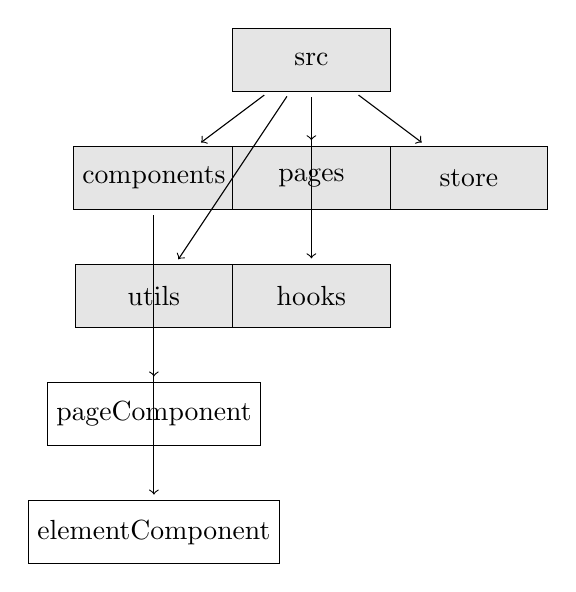
\begin{tikzpicture}[
    file/.style={draw, rectangle, minimum width=2cm, minimum height=0.8cm},
    folder/.style={draw, rectangle, minimum width=2cm, minimum height=0.8cm, fill=gray!20},
    arrow/.style={->, shorten >=2pt, shorten <=2pt}
]

% Folders
\node[folder] (src) at (0,0) {src};
\node[folder] (components) at (-2,-1.5) {components};
\node[folder] (pages) at (0,-1.5) {pages};
\node[folder] (store) at (2,-1.5) {store};
\node[folder] (utils) at (-2,-3) {utils};
\node[folder] (hooks) at (0,-3) {hooks};

% Files
\node[file] (pageComponent) at (-2,-4.5) {pageComponent};
\node[file] (elementComponent) at (-2,-6) {elementComponent};
% ... add more files

% Connections
\draw[arrow] (src) -- (components);
\draw[arrow] (src) -- (pages);
\draw[arrow] (src) -- (store);
\draw[arrow] (src) -- (utils);
\draw[arrow] (src) -- (hooks);
\draw[arrow] (components) -- (pageComponent);
\draw[arrow] (components) -- (elementComponent);
% ... add more connections

\end{tikzpicture}



\pagebreak
\subsubsection{Back-end}
The backend uses the dotNet framework. The development language using the C\# language.

In this project, the backend uses the Onion Architecture.
The Onion Architecture is a typically layered architecture, 
where each layer depends on the inner layer and provides interfaces to the outer layer.
The outer layer provides services to the outermost layer 
and other modules in the same layer based on the interfaces of the inner layer.

From inner to outer, the layers are: Domain, Application, Infrastructure, Presentation.
The Domain layer is the core layer and the innermost layer, used to define domain models, 
which are the business models.
It includes domain models and domain service interfaces.
Domain models are used to define the business models, 
which are the entities in the entity-relationship model and their attributes.
Domain service interfaces are used to define the business services, 
which are the relationships between entities in the entity-relationship model.

The Application layer is the application layer, 
used to define application services, which are the business logic.
It includes domain service implementations and application service interfaces.
Domain service implementations implement the methods of the inner layer's domain service 
interfaces and implement the business logic of the domain models.
Application service interfaces are used to define application services, 
which are the business logic.
It includes but is not limited to database interfaces, testing interfaces, 
HTTP API interfaces, MQTT interfaces, etc.

The Infrastructure layer is the infrastructure layer, used to define infrastructure.
It includes database implementations, testing implementations, 
HTTP API implementations, MQTT implementations, etc.
Database implementations implement the database interfaces 
and provide CRUD services for the database.
Testing implementations implement the testing interfaces 
and provide services for unit testing and integration testing.
HTTP API implementations implement the HTTP API interfaces 
and provide CRUD operations for HTTP APIs.
MQTT implementations implement the MQTT interfaces 
and provide CRUD operations for MQTT.

The Presentation layer is the presentation layer, used to define presentation logic, 
such as interfaces and pages. Since this is a backend project,
data presentation and control are handled by the frontend, 
so this layer is not needed.



\pagebreak
\subsubsection{Data communication and storage}
% 关于本项目的数据通信与数据存储的设计, 包括数据通信的协议, 数据存储的设计等
% 关于数据通信的设计:
% 1. 通信协议的选择
% 自前端向后端发送的数据, 有三种传输的数据类型, 
% 一种是普通的增删改查的请求, 对数据传输的时效性要求不高, 但是对数据的准确性, 完整性, 有序性, 安全性有一定的要求,
% 这种数据的传输, 采用 HTTP 协议, 以及 RESTful API 的设计. 可以有效的保证对数据传输的以上要求.
% 一种是对数据通道的创建和流媒体数据的传输, 对数据传输的时效性, 安全性要求较高, 这种数据的传输, 采用 WebRTC 协议, 以及 MQTT 协议.
% 配合可以快速解码的 flatbuffers 协议, 可以有效的保证对数据传输的以上要求.
% 最后一种是对设备的状态信息和操作信息的传输, 对完整性, 有序性, 安全性都有较高的要求, 这种数据的传输, 采用 MQTT 协议
% 同时也使用了 flatbuffers 协议.
% 
% 2. 数据通信的通信架构和通信流程
% 本项目的数据通信的通信架构, 是基于前后端分离的架构, 前端使用 React 框架, 后端使用 dotnet 框架.
% 当前端需要向后端发送数据的时候, 前端会向后端发送 HTTP 请求, 后端接收到 HTTP 请求之后, 会根据请求的数据类型,
% 选择不同的数据处理方式, 对于普通的增删改查的请求, 后端会根据 RESTful API 的设计, 对数据进行增删改查的操作,
% 对于对数据通道的创建和流媒体数据的传输, 后端会根据 WebRTC 协议, 对数据通道进行创建, 并且帮助前端和设备建立数据通道,
% 当数据通道建立后, 前端和设备之间则使用 flatbuffer 的数据格式对流媒体数据进行传输,
% 对于设备的状态信息和操作信息的传输, 前端会直接向 MQTT broker 发送 MQTT 请求, 
% 设备会在其自身的固件中监听相关的 MQTT 请求, 并且返回相关的数据.
% 
% 3. 数据通信的格式
% 本项目的数据通信的格式, 有三种, 
% 一种是 HTTP 协议, 
% 使用 json 格式对数据进行传输,
% 一种是 WebRTC 协议, 
% 使用 flatbuffers 格式对数据进行传输,
% 一种是 MQTT 协议.
% 使用 flatbuffers 格式对数据进行传输,
% 
% 关于数据存储的设计:
% 1. 数据存储的数据库的选择
% 本项目的数据存储的数据库的选择, 使用了轻量级的数据库 SQLite,
% SQLite 是一个进程内的库, 实现了自给自足的, 无服务器的, 零配置的, 事务性的 SQL 数据库引擎.
% 这是因为整个项目的目的是为了实现前端与设备之间的数据通信, 对于数据库数据的增删改查操作的要求不高,
% 数据量较小, 且对于数据库的数据的事务性要求不高, 所以选择了 SQLite 数据库.
% 2. 项目前后端的数据结构的设计
% 在本项目中, 前端由于使用了 React 框架, 所以前端的数据结构的设计, 使用了基于状态的数据结构的设计,
% 每个组件或者数据集都包含一个状态对象, 这个状态对象的属性就是组件的各个状态. 
% 使用状态对象的原因是, 可以方便的对状态进行管理, 采用对象-属性的形式, 可以方便的针对不同组件的同类状态进行区分,
% 由于跨组件的状态是由 redux 进行管理的, 这种状态对象的设计, 可以更搞笑的对状态进行更新和传递.
% 后端由于使用了 dotnet 框架, 所以后端的数据结构的设计, 使用了基于类的数据结构的设计,
% 采用了面向对象的编程思想, 对数据进行了封装, 使得数据的传输更加的安全, 有序, 完整.


\pagebreak

% \subsection{Domain model}
% \documentclass[]{article}
\usepackage{graphicx}
\usepackage{amsmath}
\usepackage{tikz}

% libaries
\usetikzlibrary{shapes,arrows}

%Define the listing package
\usepackage{listings} %code highlighter
\usepackage{color} %use color
\definecolor{mygreen}{rgb}{0,0.6,0}
\definecolor{mygray}{rgb}{0.5,0.5,0.5}
\definecolor{mymauve}{rgb}{0.58,0,0.82}

%Customize a bit the look
\lstset{ %
backgroundcolor=\color{white}, % choose the background color; you must add \usepackage{color} or \usepackage{xcolor}
basicstyle=\footnotesize, % the size of the fonts that are used for the code
breakatwhitespace=false, % sets if automatic breaks should only happen at whitespace
breaklines=true, % sets automatic line breaking
captionpos=b, % sets the caption-position to bottom
commentstyle=\color{mygreen}, % comment style
deletekeywords={...}, % if you want to delete keywords from the given language
escapeinside={\%*}{*)}, % if you want to add LaTeX within your code
extendedchars=true, % lets you use non-ASCII characters; for 8-bits encodings only, does not work with UTF-8
frame=single, % adds a frame around the code
keepspaces=true, % keeps spaces in text, useful for keeping indentation of code (possibly needs columns=flexible)
keywordstyle=\color{blue}, % keyword style
% language=Octave, % the language of the code
morekeywords={*,...}, % if you want to add more keywords to the set
numbers=left, % where to put the line-numbers; possible values are (none, left, right)
numbersep=5pt, % how far the line-numbers are from the code
numberstyle=\tiny\color{mygray}, % the style that is used for the line-numbers
rulecolor=\color{black}, % if not set, the frame-color may be changed on line-breaks within not-black text (e.g. comments (green here))
showspaces=false, % show spaces everywhere adding particular underscores; it overrides 'showstringspaces'
showstringspaces=false, % underline spaces within strings only
showtabs=false, % show tabs within strings adding particular underscores
stepnumber=1, % the step between two line-numbers. If it's 1, each line will be numbered
stringstyle=\color{mymauve}, % string literal style
tabsize=2, % sets default tabsize to 2 spaces
title=\lstname % show the filename of files included with \lstinputlisting; also try caption instead of title
}

\definecolor{darkgray}{rgb}{.4,.4,.4}
\definecolor{purple}{rgb}{0.65, 0.12, 0.82}

\lstdefinelanguage{React}{
keywords={const, typeof, new, true, false, catch, function, return, null, catch, switch, var, if, in, while, do, else, case, break},
keywordstyle=\color{blue}\bfseries,
ndkeywords={class, export, boolean, throw, implements, import, this},
ndkeywordstyle=\color{darkgray}\bfseries,
identifierstyle=\color{mygreen},
sensitive=false,
comment=[l]{//},
morecomment=[s]{/*}{*/},
commentstyle=\color{purple}\ttfamily,
string=[b]{"}{'}{`},
stringstyle=\color{red}\ttfamily,
morestring=[b]',
morestring=[b]",
morestring=[b]`',
}

\lstdefinelanguage{CSharp}{
keywords={const, typeof, new, true, false, catch, function, return, null, catch, switch, var, if, in, while, do, else, case, break},
keywordstyle=\color{blue}\bfseries,
ndkeywords={class, export, boolean, throw, implements, import, this},
ndkeywordstyle=\color{darkgray}\bfseries,
identifierstyle=\color{mygreen},
sensitive=false,
comment=[l]{//},
morecomment=[s]{/*}{*/},
commentstyle=\color{purple}\ttfamily,
string=[b]{"}{'}{`},
stringstyle=\color{red}\ttfamily,
morestring=[b]',
morestring=[b]",
morestring=[b]`',
}

\lstset{
language=React,
extendedchars=true,
basicstyle=\footnotesize\ttfamily,
showstringspaces=false,
showspaces=false,
numbers=left,
numberstyle=\footnotesize,
numbersep=9pt,
tabsize=2,
breaklines=true,
showtabs=false,
captionpos=b
}

\lstset{
language=CSharp,
extendedchars=true,
basicstyle=\footnotesize\ttfamily,
showstringspaces=false,
showspaces=false,
numbers=left,
numberstyle=\footnotesize,
numbersep=9pt,
tabsize=2,
breaklines=true,
showtabs=false,
captionpos=b
}

% \usepackage{cite} % Add this line for citation

% \bibliographystyle{plain}

\title{
The implementation of BifrostConnect Front-end scope, 
re-design and development with the relevant back-end support develop.
}
\author{
    Fei Gu \\
    Erhvervs Akademi Sydvest \\
    Computer Science 21\\
    }
\date{\today}

\begin{document}

% Front page
\maketitle
\begin{center}
    Supervisor: Henrik Boulund Meng Hansen \\
    Company: BifrostConnect \\
    Engineering Director: Jasper Wass \\
\end{center}
\tableofcontents
\pagebreak


% The introduction
\section{Introduction}
\subsection{Background}\input{sections/introduction/background.tex}
\subsection{The company}\input{sections/introduction/aboutCompany}
\subsection{The project}\input{sections/introduction/aboutProject}
\pagebreak

% The problem statement
\section{Problem Statement}
\subsection{Statement}
\input{sections/problemStatement/statement}
\subsection{Situation}
\input{sections/problemStatement/situation}
\subsection{Potential Solution}
\input{sections/problemStatement/potentialSolution}
\pagebreak

% Requirement analysis
\section{Requirement Analysis}
\input{sections/requirementAnalysis/index}

\subsection{Stakeholders}
\input{sections/requirementAnalysis/stakeholders/index}

\subsection{Business Domain}
\input{sections/requirementAnalysis/bussinesDomain/index}

\subsection{Scope}
\input{sections/requirementAnalysis/scope}

\subsection{Goals}
\input{sections/requirementAnalysis/goals}
\pagebreak

% Software Design
\section{Software Design}
% developement methods
\subsection{Software Development Methods}
\input{sections/softwareDevelopmentMethods/index}
\subsubsection{Agile Software Development}
\input{sections/softwareDevelopmentMethods/agileSoftwareDevelopment/index}
\subsubsection{Feature Driven Development}
\input{sections/softwareDevelopmentMethods/featureDrivenDevelopment/index}

\pagebreak

% Technology seslection
\subsection{Technology selection}
\input{sections/softwareDesign/technologySelection/index}
\subsubsection{Front-end}
\input{sections/softwareDesign/technologySelection/frontEnd}            
\subsubsection{Back-end}
\input{sections/softwareDesign/technologySelection/backEnd}            
\subsubsection{Database}
\input{sections/softwareDesign/technologySelection/database}
\subsubsection{Data communication}
\input{sections/softwareDesign/technologySelection/dataCommunication}            
\subsubsection{DevOps}
\input{sections/softwareDesign/technologySelection/devOps}
\pagebreak

% Architecture design
\subsection{Architecture design}
\input{sections/softwareDesign/architectureDesign/index}
\pagebreak
\subsubsection{Front-end}
\input{sections/softwareDesign/architectureDesign/frontEndArchitecture}
\pagebreak
\subsubsection{Back-end}
\input{sections/softwareDesign/architectureDesign/backEndArchitecture}
\pagebreak
\subsubsection{Data communication and storage}
\input{sections/softwareDesign/architectureDesign/dataCommunicationArchitecture}
\pagebreak

% \subsection{Domain model}
% \input{sections/softwareDesign/domainModel/index}
% \subsection{Database design}
% % 数据库领域模型 ER 图
% % 包括表和字段的设置.
% % 对于私有键和外键的设置.

% \subsection{Back-end design}
% % 后端对象模型
% % 以及对于对象模型的增删改查
% % 以及相关的其他服务的设计`'

% \subsection{Front-end design}
% % 对于前端的页面结构的设计 
% % 页面的状态的设计, 交互设计

% \subsection{FlatBuffers design}
% % schema 的设计

\subsection{DevOps CI/CD process design}
\input{sections/softwareDesign/devOpsDesign/index}
\subsubsection{Continuous Integration}
\input{sections/softwareDesign/devOpsDesign/continuousIntegration/index}
\subsubsection{Continuous Delivery}
\input{sections/softwareDesign/devOpsDesign/continuousDelivery/index}
\subsubsection{Continuous Deployment}
\input{sections/softwareDesign/devOpsDesign/continuousDeployment/index}
\pagebreak

\section{Software Development} 
\input{sections/softwareDevelopment/index}
\subsection{Overall development}
\input{sections/softwareDevelopment/overallDevelopement/index}
\subsubsection{Front-end}
\input{sections/softwareDevelopment/overallDevelopement/frontEnd/index}
\subsubsection{Back-end}
\input{sections/softwareDevelopment/overallDevelopement/backEnd/index}
\subsubsection{DevOps}
\input{sections/softwareDevelopment/overallDevelopement/devOps/index}
\subsection{Feature development} 
\input{sections/softwareDevelopment/featureDevelopment/index}
\subsubsection{Use Case 1}
\input{sections/softwareDevelopment/featureDevelopment/useCase1/index}
\subsubsection{Feature 1}
\input{sections/softwareDevelopment/featureDevelopment/feature/feature1.tex}
\pagebreak
\section{Conclusion} 
\subsection{Result}
Since the project is still in progress, the result is not available yet.
So far, basic structure of this project has been built. But the most features 
are not implemented yet. 
\subsection{Discussion}
As a single developer for this project, I am confident what I have done so far.
And I can say I understand the most of the knowledge I have used in this project, 
which also means I can explain all the part of the project. 
But this project also relevant some of the complex knowledge which I have to continue 
to study and practice.
\subsection{Future Work}
The future work is to implement the rest of the features. 
Including the most important part which is the 'create session' feature.
\pagebreak
% \bibliography{bibliography}
\pagebreak
% \begin{appendices}
%     \section{Appendix}
% \end{appendices} 
\end{document}
% \subsection{Database design}
% % 数据库领域模型 ER 图
% % 包括表和字段的设置.
% % 对于私有键和外键的设置.

% \subsection{Back-end design}
% % 后端对象模型
% % 以及对于对象模型的增删改查
% % 以及相关的其他服务的设计`'

% \subsection{Front-end design}
% % 对于前端的页面结构的设计 
% % 页面的状态的设计, 交互设计

% \subsection{FlatBuffers design}
% % schema 的设计

\subsection{DevOps CI/CD process design}
\documentclass[]{article}
\usepackage{graphicx}
\usepackage{amsmath}
\usepackage{tikz}

% libaries
\usetikzlibrary{shapes,arrows}

%Define the listing package
\usepackage{listings} %code highlighter
\usepackage{color} %use color
\definecolor{mygreen}{rgb}{0,0.6,0}
\definecolor{mygray}{rgb}{0.5,0.5,0.5}
\definecolor{mymauve}{rgb}{0.58,0,0.82}

%Customize a bit the look
\lstset{ %
backgroundcolor=\color{white}, % choose the background color; you must add \usepackage{color} or \usepackage{xcolor}
basicstyle=\footnotesize, % the size of the fonts that are used for the code
breakatwhitespace=false, % sets if automatic breaks should only happen at whitespace
breaklines=true, % sets automatic line breaking
captionpos=b, % sets the caption-position to bottom
commentstyle=\color{mygreen}, % comment style
deletekeywords={...}, % if you want to delete keywords from the given language
escapeinside={\%*}{*)}, % if you want to add LaTeX within your code
extendedchars=true, % lets you use non-ASCII characters; for 8-bits encodings only, does not work with UTF-8
frame=single, % adds a frame around the code
keepspaces=true, % keeps spaces in text, useful for keeping indentation of code (possibly needs columns=flexible)
keywordstyle=\color{blue}, % keyword style
% language=Octave, % the language of the code
morekeywords={*,...}, % if you want to add more keywords to the set
numbers=left, % where to put the line-numbers; possible values are (none, left, right)
numbersep=5pt, % how far the line-numbers are from the code
numberstyle=\tiny\color{mygray}, % the style that is used for the line-numbers
rulecolor=\color{black}, % if not set, the frame-color may be changed on line-breaks within not-black text (e.g. comments (green here))
showspaces=false, % show spaces everywhere adding particular underscores; it overrides 'showstringspaces'
showstringspaces=false, % underline spaces within strings only
showtabs=false, % show tabs within strings adding particular underscores
stepnumber=1, % the step between two line-numbers. If it's 1, each line will be numbered
stringstyle=\color{mymauve}, % string literal style
tabsize=2, % sets default tabsize to 2 spaces
title=\lstname % show the filename of files included with \lstinputlisting; also try caption instead of title
}

\definecolor{darkgray}{rgb}{.4,.4,.4}
\definecolor{purple}{rgb}{0.65, 0.12, 0.82}

\lstdefinelanguage{React}{
keywords={const, typeof, new, true, false, catch, function, return, null, catch, switch, var, if, in, while, do, else, case, break},
keywordstyle=\color{blue}\bfseries,
ndkeywords={class, export, boolean, throw, implements, import, this},
ndkeywordstyle=\color{darkgray}\bfseries,
identifierstyle=\color{mygreen},
sensitive=false,
comment=[l]{//},
morecomment=[s]{/*}{*/},
commentstyle=\color{purple}\ttfamily,
string=[b]{"}{'}{`},
stringstyle=\color{red}\ttfamily,
morestring=[b]',
morestring=[b]",
morestring=[b]`',
}

\lstdefinelanguage{CSharp}{
keywords={const, typeof, new, true, false, catch, function, return, null, catch, switch, var, if, in, while, do, else, case, break},
keywordstyle=\color{blue}\bfseries,
ndkeywords={class, export, boolean, throw, implements, import, this},
ndkeywordstyle=\color{darkgray}\bfseries,
identifierstyle=\color{mygreen},
sensitive=false,
comment=[l]{//},
morecomment=[s]{/*}{*/},
commentstyle=\color{purple}\ttfamily,
string=[b]{"}{'}{`},
stringstyle=\color{red}\ttfamily,
morestring=[b]',
morestring=[b]",
morestring=[b]`',
}

\lstset{
language=React,
extendedchars=true,
basicstyle=\footnotesize\ttfamily,
showstringspaces=false,
showspaces=false,
numbers=left,
numberstyle=\footnotesize,
numbersep=9pt,
tabsize=2,
breaklines=true,
showtabs=false,
captionpos=b
}

\lstset{
language=CSharp,
extendedchars=true,
basicstyle=\footnotesize\ttfamily,
showstringspaces=false,
showspaces=false,
numbers=left,
numberstyle=\footnotesize,
numbersep=9pt,
tabsize=2,
breaklines=true,
showtabs=false,
captionpos=b
}

% \usepackage{cite} % Add this line for citation

% \bibliographystyle{plain}

\title{
The implementation of BifrostConnect Front-end scope, 
re-design and development with the relevant back-end support develop.
}
\author{
    Fei Gu \\
    Erhvervs Akademi Sydvest \\
    Computer Science 21\\
    }
\date{\today}

\begin{document}

% Front page
\maketitle
\begin{center}
    Supervisor: Henrik Boulund Meng Hansen \\
    Company: BifrostConnect \\
    Engineering Director: Jasper Wass \\
\end{center}
\tableofcontents
\pagebreak


% The introduction
\section{Introduction}
\subsection{Background}\input{sections/introduction/background.tex}
\subsection{The company}\input{sections/introduction/aboutCompany}
\subsection{The project}\input{sections/introduction/aboutProject}
\pagebreak

% The problem statement
\section{Problem Statement}
\subsection{Statement}
\input{sections/problemStatement/statement}
\subsection{Situation}
\input{sections/problemStatement/situation}
\subsection{Potential Solution}
\input{sections/problemStatement/potentialSolution}
\pagebreak

% Requirement analysis
\section{Requirement Analysis}
\input{sections/requirementAnalysis/index}

\subsection{Stakeholders}
\input{sections/requirementAnalysis/stakeholders/index}

\subsection{Business Domain}
\input{sections/requirementAnalysis/bussinesDomain/index}

\subsection{Scope}
\input{sections/requirementAnalysis/scope}

\subsection{Goals}
\input{sections/requirementAnalysis/goals}
\pagebreak

% Software Design
\section{Software Design}
% developement methods
\subsection{Software Development Methods}
\input{sections/softwareDevelopmentMethods/index}
\subsubsection{Agile Software Development}
\input{sections/softwareDevelopmentMethods/agileSoftwareDevelopment/index}
\subsubsection{Feature Driven Development}
\input{sections/softwareDevelopmentMethods/featureDrivenDevelopment/index}

\pagebreak

% Technology seslection
\subsection{Technology selection}
\input{sections/softwareDesign/technologySelection/index}
\subsubsection{Front-end}
\input{sections/softwareDesign/technologySelection/frontEnd}            
\subsubsection{Back-end}
\input{sections/softwareDesign/technologySelection/backEnd}            
\subsubsection{Database}
\input{sections/softwareDesign/technologySelection/database}
\subsubsection{Data communication}
\input{sections/softwareDesign/technologySelection/dataCommunication}            
\subsubsection{DevOps}
\input{sections/softwareDesign/technologySelection/devOps}
\pagebreak

% Architecture design
\subsection{Architecture design}
\input{sections/softwareDesign/architectureDesign/index}
\pagebreak
\subsubsection{Front-end}
\input{sections/softwareDesign/architectureDesign/frontEndArchitecture}
\pagebreak
\subsubsection{Back-end}
\input{sections/softwareDesign/architectureDesign/backEndArchitecture}
\pagebreak
\subsubsection{Data communication and storage}
\input{sections/softwareDesign/architectureDesign/dataCommunicationArchitecture}
\pagebreak

% \subsection{Domain model}
% \input{sections/softwareDesign/domainModel/index}
% \subsection{Database design}
% % 数据库领域模型 ER 图
% % 包括表和字段的设置.
% % 对于私有键和外键的设置.

% \subsection{Back-end design}
% % 后端对象模型
% % 以及对于对象模型的增删改查
% % 以及相关的其他服务的设计`'

% \subsection{Front-end design}
% % 对于前端的页面结构的设计 
% % 页面的状态的设计, 交互设计

% \subsection{FlatBuffers design}
% % schema 的设计

\subsection{DevOps CI/CD process design}
\input{sections/softwareDesign/devOpsDesign/index}
\subsubsection{Continuous Integration}
\input{sections/softwareDesign/devOpsDesign/continuousIntegration/index}
\subsubsection{Continuous Delivery}
\input{sections/softwareDesign/devOpsDesign/continuousDelivery/index}
\subsubsection{Continuous Deployment}
\input{sections/softwareDesign/devOpsDesign/continuousDeployment/index}
\pagebreak

\section{Software Development} 
\input{sections/softwareDevelopment/index}
\subsection{Overall development}
\input{sections/softwareDevelopment/overallDevelopement/index}
\subsubsection{Front-end}
\input{sections/softwareDevelopment/overallDevelopement/frontEnd/index}
\subsubsection{Back-end}
\input{sections/softwareDevelopment/overallDevelopement/backEnd/index}
\subsubsection{DevOps}
\input{sections/softwareDevelopment/overallDevelopement/devOps/index}
\subsection{Feature development} 
\input{sections/softwareDevelopment/featureDevelopment/index}
\subsubsection{Use Case 1}
\input{sections/softwareDevelopment/featureDevelopment/useCase1/index}
\subsubsection{Feature 1}
\input{sections/softwareDevelopment/featureDevelopment/feature/feature1.tex}
\pagebreak
\section{Conclusion} 
\subsection{Result}
Since the project is still in progress, the result is not available yet.
So far, basic structure of this project has been built. But the most features 
are not implemented yet. 
\subsection{Discussion}
As a single developer for this project, I am confident what I have done so far.
And I can say I understand the most of the knowledge I have used in this project, 
which also means I can explain all the part of the project. 
But this project also relevant some of the complex knowledge which I have to continue 
to study and practice.
\subsection{Future Work}
The future work is to implement the rest of the features. 
Including the most important part which is the 'create session' feature.
\pagebreak
% \bibliography{bibliography}
\pagebreak
% \begin{appendices}
%     \section{Appendix}
% \end{appendices} 
\end{document}
\subsubsection{Continuous Integration}
\documentclass[]{article}
\usepackage{graphicx}
\usepackage{amsmath}
\usepackage{tikz}

% libaries
\usetikzlibrary{shapes,arrows}

%Define the listing package
\usepackage{listings} %code highlighter
\usepackage{color} %use color
\definecolor{mygreen}{rgb}{0,0.6,0}
\definecolor{mygray}{rgb}{0.5,0.5,0.5}
\definecolor{mymauve}{rgb}{0.58,0,0.82}

%Customize a bit the look
\lstset{ %
backgroundcolor=\color{white}, % choose the background color; you must add \usepackage{color} or \usepackage{xcolor}
basicstyle=\footnotesize, % the size of the fonts that are used for the code
breakatwhitespace=false, % sets if automatic breaks should only happen at whitespace
breaklines=true, % sets automatic line breaking
captionpos=b, % sets the caption-position to bottom
commentstyle=\color{mygreen}, % comment style
deletekeywords={...}, % if you want to delete keywords from the given language
escapeinside={\%*}{*)}, % if you want to add LaTeX within your code
extendedchars=true, % lets you use non-ASCII characters; for 8-bits encodings only, does not work with UTF-8
frame=single, % adds a frame around the code
keepspaces=true, % keeps spaces in text, useful for keeping indentation of code (possibly needs columns=flexible)
keywordstyle=\color{blue}, % keyword style
% language=Octave, % the language of the code
morekeywords={*,...}, % if you want to add more keywords to the set
numbers=left, % where to put the line-numbers; possible values are (none, left, right)
numbersep=5pt, % how far the line-numbers are from the code
numberstyle=\tiny\color{mygray}, % the style that is used for the line-numbers
rulecolor=\color{black}, % if not set, the frame-color may be changed on line-breaks within not-black text (e.g. comments (green here))
showspaces=false, % show spaces everywhere adding particular underscores; it overrides 'showstringspaces'
showstringspaces=false, % underline spaces within strings only
showtabs=false, % show tabs within strings adding particular underscores
stepnumber=1, % the step between two line-numbers. If it's 1, each line will be numbered
stringstyle=\color{mymauve}, % string literal style
tabsize=2, % sets default tabsize to 2 spaces
title=\lstname % show the filename of files included with \lstinputlisting; also try caption instead of title
}

\definecolor{darkgray}{rgb}{.4,.4,.4}
\definecolor{purple}{rgb}{0.65, 0.12, 0.82}

\lstdefinelanguage{React}{
keywords={const, typeof, new, true, false, catch, function, return, null, catch, switch, var, if, in, while, do, else, case, break},
keywordstyle=\color{blue}\bfseries,
ndkeywords={class, export, boolean, throw, implements, import, this},
ndkeywordstyle=\color{darkgray}\bfseries,
identifierstyle=\color{mygreen},
sensitive=false,
comment=[l]{//},
morecomment=[s]{/*}{*/},
commentstyle=\color{purple}\ttfamily,
string=[b]{"}{'}{`},
stringstyle=\color{red}\ttfamily,
morestring=[b]',
morestring=[b]",
morestring=[b]`',
}

\lstdefinelanguage{CSharp}{
keywords={const, typeof, new, true, false, catch, function, return, null, catch, switch, var, if, in, while, do, else, case, break},
keywordstyle=\color{blue}\bfseries,
ndkeywords={class, export, boolean, throw, implements, import, this},
ndkeywordstyle=\color{darkgray}\bfseries,
identifierstyle=\color{mygreen},
sensitive=false,
comment=[l]{//},
morecomment=[s]{/*}{*/},
commentstyle=\color{purple}\ttfamily,
string=[b]{"}{'}{`},
stringstyle=\color{red}\ttfamily,
morestring=[b]',
morestring=[b]",
morestring=[b]`',
}

\lstset{
language=React,
extendedchars=true,
basicstyle=\footnotesize\ttfamily,
showstringspaces=false,
showspaces=false,
numbers=left,
numberstyle=\footnotesize,
numbersep=9pt,
tabsize=2,
breaklines=true,
showtabs=false,
captionpos=b
}

\lstset{
language=CSharp,
extendedchars=true,
basicstyle=\footnotesize\ttfamily,
showstringspaces=false,
showspaces=false,
numbers=left,
numberstyle=\footnotesize,
numbersep=9pt,
tabsize=2,
breaklines=true,
showtabs=false,
captionpos=b
}

% \usepackage{cite} % Add this line for citation

% \bibliographystyle{plain}

\title{
The implementation of BifrostConnect Front-end scope, 
re-design and development with the relevant back-end support develop.
}
\author{
    Fei Gu \\
    Erhvervs Akademi Sydvest \\
    Computer Science 21\\
    }
\date{\today}

\begin{document}

% Front page
\maketitle
\begin{center}
    Supervisor: Henrik Boulund Meng Hansen \\
    Company: BifrostConnect \\
    Engineering Director: Jasper Wass \\
\end{center}
\tableofcontents
\pagebreak


% The introduction
\section{Introduction}
\subsection{Background}\input{sections/introduction/background.tex}
\subsection{The company}\input{sections/introduction/aboutCompany}
\subsection{The project}\input{sections/introduction/aboutProject}
\pagebreak

% The problem statement
\section{Problem Statement}
\subsection{Statement}
\input{sections/problemStatement/statement}
\subsection{Situation}
\input{sections/problemStatement/situation}
\subsection{Potential Solution}
\input{sections/problemStatement/potentialSolution}
\pagebreak

% Requirement analysis
\section{Requirement Analysis}
\input{sections/requirementAnalysis/index}

\subsection{Stakeholders}
\input{sections/requirementAnalysis/stakeholders/index}

\subsection{Business Domain}
\input{sections/requirementAnalysis/bussinesDomain/index}

\subsection{Scope}
\input{sections/requirementAnalysis/scope}

\subsection{Goals}
\input{sections/requirementAnalysis/goals}
\pagebreak

% Software Design
\section{Software Design}
% developement methods
\subsection{Software Development Methods}
\input{sections/softwareDevelopmentMethods/index}
\subsubsection{Agile Software Development}
\input{sections/softwareDevelopmentMethods/agileSoftwareDevelopment/index}
\subsubsection{Feature Driven Development}
\input{sections/softwareDevelopmentMethods/featureDrivenDevelopment/index}

\pagebreak

% Technology seslection
\subsection{Technology selection}
\input{sections/softwareDesign/technologySelection/index}
\subsubsection{Front-end}
\input{sections/softwareDesign/technologySelection/frontEnd}            
\subsubsection{Back-end}
\input{sections/softwareDesign/technologySelection/backEnd}            
\subsubsection{Database}
\input{sections/softwareDesign/technologySelection/database}
\subsubsection{Data communication}
\input{sections/softwareDesign/technologySelection/dataCommunication}            
\subsubsection{DevOps}
\input{sections/softwareDesign/technologySelection/devOps}
\pagebreak

% Architecture design
\subsection{Architecture design}
\input{sections/softwareDesign/architectureDesign/index}
\pagebreak
\subsubsection{Front-end}
\input{sections/softwareDesign/architectureDesign/frontEndArchitecture}
\pagebreak
\subsubsection{Back-end}
\input{sections/softwareDesign/architectureDesign/backEndArchitecture}
\pagebreak
\subsubsection{Data communication and storage}
\input{sections/softwareDesign/architectureDesign/dataCommunicationArchitecture}
\pagebreak

% \subsection{Domain model}
% \input{sections/softwareDesign/domainModel/index}
% \subsection{Database design}
% % 数据库领域模型 ER 图
% % 包括表和字段的设置.
% % 对于私有键和外键的设置.

% \subsection{Back-end design}
% % 后端对象模型
% % 以及对于对象模型的增删改查
% % 以及相关的其他服务的设计`'

% \subsection{Front-end design}
% % 对于前端的页面结构的设计 
% % 页面的状态的设计, 交互设计

% \subsection{FlatBuffers design}
% % schema 的设计

\subsection{DevOps CI/CD process design}
\input{sections/softwareDesign/devOpsDesign/index}
\subsubsection{Continuous Integration}
\input{sections/softwareDesign/devOpsDesign/continuousIntegration/index}
\subsubsection{Continuous Delivery}
\input{sections/softwareDesign/devOpsDesign/continuousDelivery/index}
\subsubsection{Continuous Deployment}
\input{sections/softwareDesign/devOpsDesign/continuousDeployment/index}
\pagebreak

\section{Software Development} 
\input{sections/softwareDevelopment/index}
\subsection{Overall development}
\input{sections/softwareDevelopment/overallDevelopement/index}
\subsubsection{Front-end}
\input{sections/softwareDevelopment/overallDevelopement/frontEnd/index}
\subsubsection{Back-end}
\input{sections/softwareDevelopment/overallDevelopement/backEnd/index}
\subsubsection{DevOps}
\input{sections/softwareDevelopment/overallDevelopement/devOps/index}
\subsection{Feature development} 
\input{sections/softwareDevelopment/featureDevelopment/index}
\subsubsection{Use Case 1}
\input{sections/softwareDevelopment/featureDevelopment/useCase1/index}
\subsubsection{Feature 1}
\input{sections/softwareDevelopment/featureDevelopment/feature/feature1.tex}
\pagebreak
\section{Conclusion} 
\subsection{Result}
Since the project is still in progress, the result is not available yet.
So far, basic structure of this project has been built. But the most features 
are not implemented yet. 
\subsection{Discussion}
As a single developer for this project, I am confident what I have done so far.
And I can say I understand the most of the knowledge I have used in this project, 
which also means I can explain all the part of the project. 
But this project also relevant some of the complex knowledge which I have to continue 
to study and practice.
\subsection{Future Work}
The future work is to implement the rest of the features. 
Including the most important part which is the 'create session' feature.
\pagebreak
% \bibliography{bibliography}
\pagebreak
% \begin{appendices}
%     \section{Appendix}
% \end{appendices} 
\end{document}
\subsubsection{Continuous Delivery}
\documentclass[]{article}
\usepackage{graphicx}
\usepackage{amsmath}
\usepackage{tikz}

% libaries
\usetikzlibrary{shapes,arrows}

%Define the listing package
\usepackage{listings} %code highlighter
\usepackage{color} %use color
\definecolor{mygreen}{rgb}{0,0.6,0}
\definecolor{mygray}{rgb}{0.5,0.5,0.5}
\definecolor{mymauve}{rgb}{0.58,0,0.82}

%Customize a bit the look
\lstset{ %
backgroundcolor=\color{white}, % choose the background color; you must add \usepackage{color} or \usepackage{xcolor}
basicstyle=\footnotesize, % the size of the fonts that are used for the code
breakatwhitespace=false, % sets if automatic breaks should only happen at whitespace
breaklines=true, % sets automatic line breaking
captionpos=b, % sets the caption-position to bottom
commentstyle=\color{mygreen}, % comment style
deletekeywords={...}, % if you want to delete keywords from the given language
escapeinside={\%*}{*)}, % if you want to add LaTeX within your code
extendedchars=true, % lets you use non-ASCII characters; for 8-bits encodings only, does not work with UTF-8
frame=single, % adds a frame around the code
keepspaces=true, % keeps spaces in text, useful for keeping indentation of code (possibly needs columns=flexible)
keywordstyle=\color{blue}, % keyword style
% language=Octave, % the language of the code
morekeywords={*,...}, % if you want to add more keywords to the set
numbers=left, % where to put the line-numbers; possible values are (none, left, right)
numbersep=5pt, % how far the line-numbers are from the code
numberstyle=\tiny\color{mygray}, % the style that is used for the line-numbers
rulecolor=\color{black}, % if not set, the frame-color may be changed on line-breaks within not-black text (e.g. comments (green here))
showspaces=false, % show spaces everywhere adding particular underscores; it overrides 'showstringspaces'
showstringspaces=false, % underline spaces within strings only
showtabs=false, % show tabs within strings adding particular underscores
stepnumber=1, % the step between two line-numbers. If it's 1, each line will be numbered
stringstyle=\color{mymauve}, % string literal style
tabsize=2, % sets default tabsize to 2 spaces
title=\lstname % show the filename of files included with \lstinputlisting; also try caption instead of title
}

\definecolor{darkgray}{rgb}{.4,.4,.4}
\definecolor{purple}{rgb}{0.65, 0.12, 0.82}

\lstdefinelanguage{React}{
keywords={const, typeof, new, true, false, catch, function, return, null, catch, switch, var, if, in, while, do, else, case, break},
keywordstyle=\color{blue}\bfseries,
ndkeywords={class, export, boolean, throw, implements, import, this},
ndkeywordstyle=\color{darkgray}\bfseries,
identifierstyle=\color{mygreen},
sensitive=false,
comment=[l]{//},
morecomment=[s]{/*}{*/},
commentstyle=\color{purple}\ttfamily,
string=[b]{"}{'}{`},
stringstyle=\color{red}\ttfamily,
morestring=[b]',
morestring=[b]",
morestring=[b]`',
}

\lstdefinelanguage{CSharp}{
keywords={const, typeof, new, true, false, catch, function, return, null, catch, switch, var, if, in, while, do, else, case, break},
keywordstyle=\color{blue}\bfseries,
ndkeywords={class, export, boolean, throw, implements, import, this},
ndkeywordstyle=\color{darkgray}\bfseries,
identifierstyle=\color{mygreen},
sensitive=false,
comment=[l]{//},
morecomment=[s]{/*}{*/},
commentstyle=\color{purple}\ttfamily,
string=[b]{"}{'}{`},
stringstyle=\color{red}\ttfamily,
morestring=[b]',
morestring=[b]",
morestring=[b]`',
}

\lstset{
language=React,
extendedchars=true,
basicstyle=\footnotesize\ttfamily,
showstringspaces=false,
showspaces=false,
numbers=left,
numberstyle=\footnotesize,
numbersep=9pt,
tabsize=2,
breaklines=true,
showtabs=false,
captionpos=b
}

\lstset{
language=CSharp,
extendedchars=true,
basicstyle=\footnotesize\ttfamily,
showstringspaces=false,
showspaces=false,
numbers=left,
numberstyle=\footnotesize,
numbersep=9pt,
tabsize=2,
breaklines=true,
showtabs=false,
captionpos=b
}

% \usepackage{cite} % Add this line for citation

% \bibliographystyle{plain}

\title{
The implementation of BifrostConnect Front-end scope, 
re-design and development with the relevant back-end support develop.
}
\author{
    Fei Gu \\
    Erhvervs Akademi Sydvest \\
    Computer Science 21\\
    }
\date{\today}

\begin{document}

% Front page
\maketitle
\begin{center}
    Supervisor: Henrik Boulund Meng Hansen \\
    Company: BifrostConnect \\
    Engineering Director: Jasper Wass \\
\end{center}
\tableofcontents
\pagebreak


% The introduction
\section{Introduction}
\subsection{Background}\input{sections/introduction/background.tex}
\subsection{The company}\input{sections/introduction/aboutCompany}
\subsection{The project}\input{sections/introduction/aboutProject}
\pagebreak

% The problem statement
\section{Problem Statement}
\subsection{Statement}
\input{sections/problemStatement/statement}
\subsection{Situation}
\input{sections/problemStatement/situation}
\subsection{Potential Solution}
\input{sections/problemStatement/potentialSolution}
\pagebreak

% Requirement analysis
\section{Requirement Analysis}
\input{sections/requirementAnalysis/index}

\subsection{Stakeholders}
\input{sections/requirementAnalysis/stakeholders/index}

\subsection{Business Domain}
\input{sections/requirementAnalysis/bussinesDomain/index}

\subsection{Scope}
\input{sections/requirementAnalysis/scope}

\subsection{Goals}
\input{sections/requirementAnalysis/goals}
\pagebreak

% Software Design
\section{Software Design}
% developement methods
\subsection{Software Development Methods}
\input{sections/softwareDevelopmentMethods/index}
\subsubsection{Agile Software Development}
\input{sections/softwareDevelopmentMethods/agileSoftwareDevelopment/index}
\subsubsection{Feature Driven Development}
\input{sections/softwareDevelopmentMethods/featureDrivenDevelopment/index}

\pagebreak

% Technology seslection
\subsection{Technology selection}
\input{sections/softwareDesign/technologySelection/index}
\subsubsection{Front-end}
\input{sections/softwareDesign/technologySelection/frontEnd}            
\subsubsection{Back-end}
\input{sections/softwareDesign/technologySelection/backEnd}            
\subsubsection{Database}
\input{sections/softwareDesign/technologySelection/database}
\subsubsection{Data communication}
\input{sections/softwareDesign/technologySelection/dataCommunication}            
\subsubsection{DevOps}
\input{sections/softwareDesign/technologySelection/devOps}
\pagebreak

% Architecture design
\subsection{Architecture design}
\input{sections/softwareDesign/architectureDesign/index}
\pagebreak
\subsubsection{Front-end}
\input{sections/softwareDesign/architectureDesign/frontEndArchitecture}
\pagebreak
\subsubsection{Back-end}
\input{sections/softwareDesign/architectureDesign/backEndArchitecture}
\pagebreak
\subsubsection{Data communication and storage}
\input{sections/softwareDesign/architectureDesign/dataCommunicationArchitecture}
\pagebreak

% \subsection{Domain model}
% \input{sections/softwareDesign/domainModel/index}
% \subsection{Database design}
% % 数据库领域模型 ER 图
% % 包括表和字段的设置.
% % 对于私有键和外键的设置.

% \subsection{Back-end design}
% % 后端对象模型
% % 以及对于对象模型的增删改查
% % 以及相关的其他服务的设计`'

% \subsection{Front-end design}
% % 对于前端的页面结构的设计 
% % 页面的状态的设计, 交互设计

% \subsection{FlatBuffers design}
% % schema 的设计

\subsection{DevOps CI/CD process design}
\input{sections/softwareDesign/devOpsDesign/index}
\subsubsection{Continuous Integration}
\input{sections/softwareDesign/devOpsDesign/continuousIntegration/index}
\subsubsection{Continuous Delivery}
\input{sections/softwareDesign/devOpsDesign/continuousDelivery/index}
\subsubsection{Continuous Deployment}
\input{sections/softwareDesign/devOpsDesign/continuousDeployment/index}
\pagebreak

\section{Software Development} 
\input{sections/softwareDevelopment/index}
\subsection{Overall development}
\input{sections/softwareDevelopment/overallDevelopement/index}
\subsubsection{Front-end}
\input{sections/softwareDevelopment/overallDevelopement/frontEnd/index}
\subsubsection{Back-end}
\input{sections/softwareDevelopment/overallDevelopement/backEnd/index}
\subsubsection{DevOps}
\input{sections/softwareDevelopment/overallDevelopement/devOps/index}
\subsection{Feature development} 
\input{sections/softwareDevelopment/featureDevelopment/index}
\subsubsection{Use Case 1}
\input{sections/softwareDevelopment/featureDevelopment/useCase1/index}
\subsubsection{Feature 1}
\input{sections/softwareDevelopment/featureDevelopment/feature/feature1.tex}
\pagebreak
\section{Conclusion} 
\subsection{Result}
Since the project is still in progress, the result is not available yet.
So far, basic structure of this project has been built. But the most features 
are not implemented yet. 
\subsection{Discussion}
As a single developer for this project, I am confident what I have done so far.
And I can say I understand the most of the knowledge I have used in this project, 
which also means I can explain all the part of the project. 
But this project also relevant some of the complex knowledge which I have to continue 
to study and practice.
\subsection{Future Work}
The future work is to implement the rest of the features. 
Including the most important part which is the 'create session' feature.
\pagebreak
% \bibliography{bibliography}
\pagebreak
% \begin{appendices}
%     \section{Appendix}
% \end{appendices} 
\end{document}
\subsubsection{Continuous Deployment}
\documentclass[]{article}
\usepackage{graphicx}
\usepackage{amsmath}
\usepackage{tikz}

% libaries
\usetikzlibrary{shapes,arrows}

%Define the listing package
\usepackage{listings} %code highlighter
\usepackage{color} %use color
\definecolor{mygreen}{rgb}{0,0.6,0}
\definecolor{mygray}{rgb}{0.5,0.5,0.5}
\definecolor{mymauve}{rgb}{0.58,0,0.82}

%Customize a bit the look
\lstset{ %
backgroundcolor=\color{white}, % choose the background color; you must add \usepackage{color} or \usepackage{xcolor}
basicstyle=\footnotesize, % the size of the fonts that are used for the code
breakatwhitespace=false, % sets if automatic breaks should only happen at whitespace
breaklines=true, % sets automatic line breaking
captionpos=b, % sets the caption-position to bottom
commentstyle=\color{mygreen}, % comment style
deletekeywords={...}, % if you want to delete keywords from the given language
escapeinside={\%*}{*)}, % if you want to add LaTeX within your code
extendedchars=true, % lets you use non-ASCII characters; for 8-bits encodings only, does not work with UTF-8
frame=single, % adds a frame around the code
keepspaces=true, % keeps spaces in text, useful for keeping indentation of code (possibly needs columns=flexible)
keywordstyle=\color{blue}, % keyword style
% language=Octave, % the language of the code
morekeywords={*,...}, % if you want to add more keywords to the set
numbers=left, % where to put the line-numbers; possible values are (none, left, right)
numbersep=5pt, % how far the line-numbers are from the code
numberstyle=\tiny\color{mygray}, % the style that is used for the line-numbers
rulecolor=\color{black}, % if not set, the frame-color may be changed on line-breaks within not-black text (e.g. comments (green here))
showspaces=false, % show spaces everywhere adding particular underscores; it overrides 'showstringspaces'
showstringspaces=false, % underline spaces within strings only
showtabs=false, % show tabs within strings adding particular underscores
stepnumber=1, % the step between two line-numbers. If it's 1, each line will be numbered
stringstyle=\color{mymauve}, % string literal style
tabsize=2, % sets default tabsize to 2 spaces
title=\lstname % show the filename of files included with \lstinputlisting; also try caption instead of title
}

\definecolor{darkgray}{rgb}{.4,.4,.4}
\definecolor{purple}{rgb}{0.65, 0.12, 0.82}

\lstdefinelanguage{React}{
keywords={const, typeof, new, true, false, catch, function, return, null, catch, switch, var, if, in, while, do, else, case, break},
keywordstyle=\color{blue}\bfseries,
ndkeywords={class, export, boolean, throw, implements, import, this},
ndkeywordstyle=\color{darkgray}\bfseries,
identifierstyle=\color{mygreen},
sensitive=false,
comment=[l]{//},
morecomment=[s]{/*}{*/},
commentstyle=\color{purple}\ttfamily,
string=[b]{"}{'}{`},
stringstyle=\color{red}\ttfamily,
morestring=[b]',
morestring=[b]",
morestring=[b]`',
}

\lstdefinelanguage{CSharp}{
keywords={const, typeof, new, true, false, catch, function, return, null, catch, switch, var, if, in, while, do, else, case, break},
keywordstyle=\color{blue}\bfseries,
ndkeywords={class, export, boolean, throw, implements, import, this},
ndkeywordstyle=\color{darkgray}\bfseries,
identifierstyle=\color{mygreen},
sensitive=false,
comment=[l]{//},
morecomment=[s]{/*}{*/},
commentstyle=\color{purple}\ttfamily,
string=[b]{"}{'}{`},
stringstyle=\color{red}\ttfamily,
morestring=[b]',
morestring=[b]",
morestring=[b]`',
}

\lstset{
language=React,
extendedchars=true,
basicstyle=\footnotesize\ttfamily,
showstringspaces=false,
showspaces=false,
numbers=left,
numberstyle=\footnotesize,
numbersep=9pt,
tabsize=2,
breaklines=true,
showtabs=false,
captionpos=b
}

\lstset{
language=CSharp,
extendedchars=true,
basicstyle=\footnotesize\ttfamily,
showstringspaces=false,
showspaces=false,
numbers=left,
numberstyle=\footnotesize,
numbersep=9pt,
tabsize=2,
breaklines=true,
showtabs=false,
captionpos=b
}

% \usepackage{cite} % Add this line for citation

% \bibliographystyle{plain}

\title{
The implementation of BifrostConnect Front-end scope, 
re-design and development with the relevant back-end support develop.
}
\author{
    Fei Gu \\
    Erhvervs Akademi Sydvest \\
    Computer Science 21\\
    }
\date{\today}

\begin{document}

% Front page
\maketitle
\begin{center}
    Supervisor: Henrik Boulund Meng Hansen \\
    Company: BifrostConnect \\
    Engineering Director: Jasper Wass \\
\end{center}
\tableofcontents
\pagebreak


% The introduction
\section{Introduction}
\subsection{Background}\input{sections/introduction/background.tex}
\subsection{The company}\input{sections/introduction/aboutCompany}
\subsection{The project}\input{sections/introduction/aboutProject}
\pagebreak

% The problem statement
\section{Problem Statement}
\subsection{Statement}
\input{sections/problemStatement/statement}
\subsection{Situation}
\input{sections/problemStatement/situation}
\subsection{Potential Solution}
\input{sections/problemStatement/potentialSolution}
\pagebreak

% Requirement analysis
\section{Requirement Analysis}
\input{sections/requirementAnalysis/index}

\subsection{Stakeholders}
\input{sections/requirementAnalysis/stakeholders/index}

\subsection{Business Domain}
\input{sections/requirementAnalysis/bussinesDomain/index}

\subsection{Scope}
\input{sections/requirementAnalysis/scope}

\subsection{Goals}
\input{sections/requirementAnalysis/goals}
\pagebreak

% Software Design
\section{Software Design}
% developement methods
\subsection{Software Development Methods}
\input{sections/softwareDevelopmentMethods/index}
\subsubsection{Agile Software Development}
\input{sections/softwareDevelopmentMethods/agileSoftwareDevelopment/index}
\subsubsection{Feature Driven Development}
\input{sections/softwareDevelopmentMethods/featureDrivenDevelopment/index}

\pagebreak

% Technology seslection
\subsection{Technology selection}
\input{sections/softwareDesign/technologySelection/index}
\subsubsection{Front-end}
\input{sections/softwareDesign/technologySelection/frontEnd}            
\subsubsection{Back-end}
\input{sections/softwareDesign/technologySelection/backEnd}            
\subsubsection{Database}
\input{sections/softwareDesign/technologySelection/database}
\subsubsection{Data communication}
\input{sections/softwareDesign/technologySelection/dataCommunication}            
\subsubsection{DevOps}
\input{sections/softwareDesign/technologySelection/devOps}
\pagebreak

% Architecture design
\subsection{Architecture design}
\input{sections/softwareDesign/architectureDesign/index}
\pagebreak
\subsubsection{Front-end}
\input{sections/softwareDesign/architectureDesign/frontEndArchitecture}
\pagebreak
\subsubsection{Back-end}
\input{sections/softwareDesign/architectureDesign/backEndArchitecture}
\pagebreak
\subsubsection{Data communication and storage}
\input{sections/softwareDesign/architectureDesign/dataCommunicationArchitecture}
\pagebreak

% \subsection{Domain model}
% \input{sections/softwareDesign/domainModel/index}
% \subsection{Database design}
% % 数据库领域模型 ER 图
% % 包括表和字段的设置.
% % 对于私有键和外键的设置.

% \subsection{Back-end design}
% % 后端对象模型
% % 以及对于对象模型的增删改查
% % 以及相关的其他服务的设计`'

% \subsection{Front-end design}
% % 对于前端的页面结构的设计 
% % 页面的状态的设计, 交互设计

% \subsection{FlatBuffers design}
% % schema 的设计

\subsection{DevOps CI/CD process design}
\input{sections/softwareDesign/devOpsDesign/index}
\subsubsection{Continuous Integration}
\input{sections/softwareDesign/devOpsDesign/continuousIntegration/index}
\subsubsection{Continuous Delivery}
\input{sections/softwareDesign/devOpsDesign/continuousDelivery/index}
\subsubsection{Continuous Deployment}
\input{sections/softwareDesign/devOpsDesign/continuousDeployment/index}
\pagebreak

\section{Software Development} 
\input{sections/softwareDevelopment/index}
\subsection{Overall development}
\input{sections/softwareDevelopment/overallDevelopement/index}
\subsubsection{Front-end}
\input{sections/softwareDevelopment/overallDevelopement/frontEnd/index}
\subsubsection{Back-end}
\input{sections/softwareDevelopment/overallDevelopement/backEnd/index}
\subsubsection{DevOps}
\input{sections/softwareDevelopment/overallDevelopement/devOps/index}
\subsection{Feature development} 
\input{sections/softwareDevelopment/featureDevelopment/index}
\subsubsection{Use Case 1}
\input{sections/softwareDevelopment/featureDevelopment/useCase1/index}
\subsubsection{Feature 1}
\input{sections/softwareDevelopment/featureDevelopment/feature/feature1.tex}
\pagebreak
\section{Conclusion} 
\subsection{Result}
Since the project is still in progress, the result is not available yet.
So far, basic structure of this project has been built. But the most features 
are not implemented yet. 
\subsection{Discussion}
As a single developer for this project, I am confident what I have done so far.
And I can say I understand the most of the knowledge I have used in this project, 
which also means I can explain all the part of the project. 
But this project also relevant some of the complex knowledge which I have to continue 
to study and practice.
\subsection{Future Work}
The future work is to implement the rest of the features. 
Including the most important part which is the 'create session' feature.
\pagebreak
% \bibliography{bibliography}
\pagebreak
% \begin{appendices}
%     \section{Appendix}
% \end{appendices} 
\end{document}
\pagebreak

\section{Software Development} 
\documentclass[]{article}
\usepackage{graphicx}
\usepackage{amsmath}
\usepackage{tikz}

% libaries
\usetikzlibrary{shapes,arrows}

%Define the listing package
\usepackage{listings} %code highlighter
\usepackage{color} %use color
\definecolor{mygreen}{rgb}{0,0.6,0}
\definecolor{mygray}{rgb}{0.5,0.5,0.5}
\definecolor{mymauve}{rgb}{0.58,0,0.82}

%Customize a bit the look
\lstset{ %
backgroundcolor=\color{white}, % choose the background color; you must add \usepackage{color} or \usepackage{xcolor}
basicstyle=\footnotesize, % the size of the fonts that are used for the code
breakatwhitespace=false, % sets if automatic breaks should only happen at whitespace
breaklines=true, % sets automatic line breaking
captionpos=b, % sets the caption-position to bottom
commentstyle=\color{mygreen}, % comment style
deletekeywords={...}, % if you want to delete keywords from the given language
escapeinside={\%*}{*)}, % if you want to add LaTeX within your code
extendedchars=true, % lets you use non-ASCII characters; for 8-bits encodings only, does not work with UTF-8
frame=single, % adds a frame around the code
keepspaces=true, % keeps spaces in text, useful for keeping indentation of code (possibly needs columns=flexible)
keywordstyle=\color{blue}, % keyword style
% language=Octave, % the language of the code
morekeywords={*,...}, % if you want to add more keywords to the set
numbers=left, % where to put the line-numbers; possible values are (none, left, right)
numbersep=5pt, % how far the line-numbers are from the code
numberstyle=\tiny\color{mygray}, % the style that is used for the line-numbers
rulecolor=\color{black}, % if not set, the frame-color may be changed on line-breaks within not-black text (e.g. comments (green here))
showspaces=false, % show spaces everywhere adding particular underscores; it overrides 'showstringspaces'
showstringspaces=false, % underline spaces within strings only
showtabs=false, % show tabs within strings adding particular underscores
stepnumber=1, % the step between two line-numbers. If it's 1, each line will be numbered
stringstyle=\color{mymauve}, % string literal style
tabsize=2, % sets default tabsize to 2 spaces
title=\lstname % show the filename of files included with \lstinputlisting; also try caption instead of title
}

\definecolor{darkgray}{rgb}{.4,.4,.4}
\definecolor{purple}{rgb}{0.65, 0.12, 0.82}

\lstdefinelanguage{React}{
keywords={const, typeof, new, true, false, catch, function, return, null, catch, switch, var, if, in, while, do, else, case, break},
keywordstyle=\color{blue}\bfseries,
ndkeywords={class, export, boolean, throw, implements, import, this},
ndkeywordstyle=\color{darkgray}\bfseries,
identifierstyle=\color{mygreen},
sensitive=false,
comment=[l]{//},
morecomment=[s]{/*}{*/},
commentstyle=\color{purple}\ttfamily,
string=[b]{"}{'}{`},
stringstyle=\color{red}\ttfamily,
morestring=[b]',
morestring=[b]",
morestring=[b]`',
}

\lstdefinelanguage{CSharp}{
keywords={const, typeof, new, true, false, catch, function, return, null, catch, switch, var, if, in, while, do, else, case, break},
keywordstyle=\color{blue}\bfseries,
ndkeywords={class, export, boolean, throw, implements, import, this},
ndkeywordstyle=\color{darkgray}\bfseries,
identifierstyle=\color{mygreen},
sensitive=false,
comment=[l]{//},
morecomment=[s]{/*}{*/},
commentstyle=\color{purple}\ttfamily,
string=[b]{"}{'}{`},
stringstyle=\color{red}\ttfamily,
morestring=[b]',
morestring=[b]",
morestring=[b]`',
}

\lstset{
language=React,
extendedchars=true,
basicstyle=\footnotesize\ttfamily,
showstringspaces=false,
showspaces=false,
numbers=left,
numberstyle=\footnotesize,
numbersep=9pt,
tabsize=2,
breaklines=true,
showtabs=false,
captionpos=b
}

\lstset{
language=CSharp,
extendedchars=true,
basicstyle=\footnotesize\ttfamily,
showstringspaces=false,
showspaces=false,
numbers=left,
numberstyle=\footnotesize,
numbersep=9pt,
tabsize=2,
breaklines=true,
showtabs=false,
captionpos=b
}

% \usepackage{cite} % Add this line for citation

% \bibliographystyle{plain}

\title{
The implementation of BifrostConnect Front-end scope, 
re-design and development with the relevant back-end support develop.
}
\author{
    Fei Gu \\
    Erhvervs Akademi Sydvest \\
    Computer Science 21\\
    }
\date{\today}

\begin{document}

% Front page
\maketitle
\begin{center}
    Supervisor: Henrik Boulund Meng Hansen \\
    Company: BifrostConnect \\
    Engineering Director: Jasper Wass \\
\end{center}
\tableofcontents
\pagebreak


% The introduction
\section{Introduction}
\subsection{Background}\input{sections/introduction/background.tex}
\subsection{The company}\input{sections/introduction/aboutCompany}
\subsection{The project}\input{sections/introduction/aboutProject}
\pagebreak

% The problem statement
\section{Problem Statement}
\subsection{Statement}
\input{sections/problemStatement/statement}
\subsection{Situation}
\input{sections/problemStatement/situation}
\subsection{Potential Solution}
\input{sections/problemStatement/potentialSolution}
\pagebreak

% Requirement analysis
\section{Requirement Analysis}
\input{sections/requirementAnalysis/index}

\subsection{Stakeholders}
\input{sections/requirementAnalysis/stakeholders/index}

\subsection{Business Domain}
\input{sections/requirementAnalysis/bussinesDomain/index}

\subsection{Scope}
\input{sections/requirementAnalysis/scope}

\subsection{Goals}
\input{sections/requirementAnalysis/goals}
\pagebreak

% Software Design
\section{Software Design}
% developement methods
\subsection{Software Development Methods}
\input{sections/softwareDevelopmentMethods/index}
\subsubsection{Agile Software Development}
\input{sections/softwareDevelopmentMethods/agileSoftwareDevelopment/index}
\subsubsection{Feature Driven Development}
\input{sections/softwareDevelopmentMethods/featureDrivenDevelopment/index}

\pagebreak

% Technology seslection
\subsection{Technology selection}
\input{sections/softwareDesign/technologySelection/index}
\subsubsection{Front-end}
\input{sections/softwareDesign/technologySelection/frontEnd}            
\subsubsection{Back-end}
\input{sections/softwareDesign/technologySelection/backEnd}            
\subsubsection{Database}
\input{sections/softwareDesign/technologySelection/database}
\subsubsection{Data communication}
\input{sections/softwareDesign/technologySelection/dataCommunication}            
\subsubsection{DevOps}
\input{sections/softwareDesign/technologySelection/devOps}
\pagebreak

% Architecture design
\subsection{Architecture design}
\input{sections/softwareDesign/architectureDesign/index}
\pagebreak
\subsubsection{Front-end}
\input{sections/softwareDesign/architectureDesign/frontEndArchitecture}
\pagebreak
\subsubsection{Back-end}
\input{sections/softwareDesign/architectureDesign/backEndArchitecture}
\pagebreak
\subsubsection{Data communication and storage}
\input{sections/softwareDesign/architectureDesign/dataCommunicationArchitecture}
\pagebreak

% \subsection{Domain model}
% \input{sections/softwareDesign/domainModel/index}
% \subsection{Database design}
% % 数据库领域模型 ER 图
% % 包括表和字段的设置.
% % 对于私有键和外键的设置.

% \subsection{Back-end design}
% % 后端对象模型
% % 以及对于对象模型的增删改查
% % 以及相关的其他服务的设计`'

% \subsection{Front-end design}
% % 对于前端的页面结构的设计 
% % 页面的状态的设计, 交互设计

% \subsection{FlatBuffers design}
% % schema 的设计

\subsection{DevOps CI/CD process design}
\input{sections/softwareDesign/devOpsDesign/index}
\subsubsection{Continuous Integration}
\input{sections/softwareDesign/devOpsDesign/continuousIntegration/index}
\subsubsection{Continuous Delivery}
\input{sections/softwareDesign/devOpsDesign/continuousDelivery/index}
\subsubsection{Continuous Deployment}
\input{sections/softwareDesign/devOpsDesign/continuousDeployment/index}
\pagebreak

\section{Software Development} 
\input{sections/softwareDevelopment/index}
\subsection{Overall development}
\input{sections/softwareDevelopment/overallDevelopement/index}
\subsubsection{Front-end}
\input{sections/softwareDevelopment/overallDevelopement/frontEnd/index}
\subsubsection{Back-end}
\input{sections/softwareDevelopment/overallDevelopement/backEnd/index}
\subsubsection{DevOps}
\input{sections/softwareDevelopment/overallDevelopement/devOps/index}
\subsection{Feature development} 
\input{sections/softwareDevelopment/featureDevelopment/index}
\subsubsection{Use Case 1}
\input{sections/softwareDevelopment/featureDevelopment/useCase1/index}
\subsubsection{Feature 1}
\input{sections/softwareDevelopment/featureDevelopment/feature/feature1.tex}
\pagebreak
\section{Conclusion} 
\subsection{Result}
Since the project is still in progress, the result is not available yet.
So far, basic structure of this project has been built. But the most features 
are not implemented yet. 
\subsection{Discussion}
As a single developer for this project, I am confident what I have done so far.
And I can say I understand the most of the knowledge I have used in this project, 
which also means I can explain all the part of the project. 
But this project also relevant some of the complex knowledge which I have to continue 
to study and practice.
\subsection{Future Work}
The future work is to implement the rest of the features. 
Including the most important part which is the 'create session' feature.
\pagebreak
% \bibliography{bibliography}
\pagebreak
% \begin{appendices}
%     \section{Appendix}
% \end{appendices} 
\end{document}
\subsection{Overall development}
\documentclass[]{article}
\usepackage{graphicx}
\usepackage{amsmath}
\usepackage{tikz}

% libaries
\usetikzlibrary{shapes,arrows}

%Define the listing package
\usepackage{listings} %code highlighter
\usepackage{color} %use color
\definecolor{mygreen}{rgb}{0,0.6,0}
\definecolor{mygray}{rgb}{0.5,0.5,0.5}
\definecolor{mymauve}{rgb}{0.58,0,0.82}

%Customize a bit the look
\lstset{ %
backgroundcolor=\color{white}, % choose the background color; you must add \usepackage{color} or \usepackage{xcolor}
basicstyle=\footnotesize, % the size of the fonts that are used for the code
breakatwhitespace=false, % sets if automatic breaks should only happen at whitespace
breaklines=true, % sets automatic line breaking
captionpos=b, % sets the caption-position to bottom
commentstyle=\color{mygreen}, % comment style
deletekeywords={...}, % if you want to delete keywords from the given language
escapeinside={\%*}{*)}, % if you want to add LaTeX within your code
extendedchars=true, % lets you use non-ASCII characters; for 8-bits encodings only, does not work with UTF-8
frame=single, % adds a frame around the code
keepspaces=true, % keeps spaces in text, useful for keeping indentation of code (possibly needs columns=flexible)
keywordstyle=\color{blue}, % keyword style
% language=Octave, % the language of the code
morekeywords={*,...}, % if you want to add more keywords to the set
numbers=left, % where to put the line-numbers; possible values are (none, left, right)
numbersep=5pt, % how far the line-numbers are from the code
numberstyle=\tiny\color{mygray}, % the style that is used for the line-numbers
rulecolor=\color{black}, % if not set, the frame-color may be changed on line-breaks within not-black text (e.g. comments (green here))
showspaces=false, % show spaces everywhere adding particular underscores; it overrides 'showstringspaces'
showstringspaces=false, % underline spaces within strings only
showtabs=false, % show tabs within strings adding particular underscores
stepnumber=1, % the step between two line-numbers. If it's 1, each line will be numbered
stringstyle=\color{mymauve}, % string literal style
tabsize=2, % sets default tabsize to 2 spaces
title=\lstname % show the filename of files included with \lstinputlisting; also try caption instead of title
}

\definecolor{darkgray}{rgb}{.4,.4,.4}
\definecolor{purple}{rgb}{0.65, 0.12, 0.82}

\lstdefinelanguage{React}{
keywords={const, typeof, new, true, false, catch, function, return, null, catch, switch, var, if, in, while, do, else, case, break},
keywordstyle=\color{blue}\bfseries,
ndkeywords={class, export, boolean, throw, implements, import, this},
ndkeywordstyle=\color{darkgray}\bfseries,
identifierstyle=\color{mygreen},
sensitive=false,
comment=[l]{//},
morecomment=[s]{/*}{*/},
commentstyle=\color{purple}\ttfamily,
string=[b]{"}{'}{`},
stringstyle=\color{red}\ttfamily,
morestring=[b]',
morestring=[b]",
morestring=[b]`',
}

\lstdefinelanguage{CSharp}{
keywords={const, typeof, new, true, false, catch, function, return, null, catch, switch, var, if, in, while, do, else, case, break},
keywordstyle=\color{blue}\bfseries,
ndkeywords={class, export, boolean, throw, implements, import, this},
ndkeywordstyle=\color{darkgray}\bfseries,
identifierstyle=\color{mygreen},
sensitive=false,
comment=[l]{//},
morecomment=[s]{/*}{*/},
commentstyle=\color{purple}\ttfamily,
string=[b]{"}{'}{`},
stringstyle=\color{red}\ttfamily,
morestring=[b]',
morestring=[b]",
morestring=[b]`',
}

\lstset{
language=React,
extendedchars=true,
basicstyle=\footnotesize\ttfamily,
showstringspaces=false,
showspaces=false,
numbers=left,
numberstyle=\footnotesize,
numbersep=9pt,
tabsize=2,
breaklines=true,
showtabs=false,
captionpos=b
}

\lstset{
language=CSharp,
extendedchars=true,
basicstyle=\footnotesize\ttfamily,
showstringspaces=false,
showspaces=false,
numbers=left,
numberstyle=\footnotesize,
numbersep=9pt,
tabsize=2,
breaklines=true,
showtabs=false,
captionpos=b
}

% \usepackage{cite} % Add this line for citation

% \bibliographystyle{plain}

\title{
The implementation of BifrostConnect Front-end scope, 
re-design and development with the relevant back-end support develop.
}
\author{
    Fei Gu \\
    Erhvervs Akademi Sydvest \\
    Computer Science 21\\
    }
\date{\today}

\begin{document}

% Front page
\maketitle
\begin{center}
    Supervisor: Henrik Boulund Meng Hansen \\
    Company: BifrostConnect \\
    Engineering Director: Jasper Wass \\
\end{center}
\tableofcontents
\pagebreak


% The introduction
\section{Introduction}
\subsection{Background}\input{sections/introduction/background.tex}
\subsection{The company}\input{sections/introduction/aboutCompany}
\subsection{The project}\input{sections/introduction/aboutProject}
\pagebreak

% The problem statement
\section{Problem Statement}
\subsection{Statement}
\input{sections/problemStatement/statement}
\subsection{Situation}
\input{sections/problemStatement/situation}
\subsection{Potential Solution}
\input{sections/problemStatement/potentialSolution}
\pagebreak

% Requirement analysis
\section{Requirement Analysis}
\input{sections/requirementAnalysis/index}

\subsection{Stakeholders}
\input{sections/requirementAnalysis/stakeholders/index}

\subsection{Business Domain}
\input{sections/requirementAnalysis/bussinesDomain/index}

\subsection{Scope}
\input{sections/requirementAnalysis/scope}

\subsection{Goals}
\input{sections/requirementAnalysis/goals}
\pagebreak

% Software Design
\section{Software Design}
% developement methods
\subsection{Software Development Methods}
\input{sections/softwareDevelopmentMethods/index}
\subsubsection{Agile Software Development}
\input{sections/softwareDevelopmentMethods/agileSoftwareDevelopment/index}
\subsubsection{Feature Driven Development}
\input{sections/softwareDevelopmentMethods/featureDrivenDevelopment/index}

\pagebreak

% Technology seslection
\subsection{Technology selection}
\input{sections/softwareDesign/technologySelection/index}
\subsubsection{Front-end}
\input{sections/softwareDesign/technologySelection/frontEnd}            
\subsubsection{Back-end}
\input{sections/softwareDesign/technologySelection/backEnd}            
\subsubsection{Database}
\input{sections/softwareDesign/technologySelection/database}
\subsubsection{Data communication}
\input{sections/softwareDesign/technologySelection/dataCommunication}            
\subsubsection{DevOps}
\input{sections/softwareDesign/technologySelection/devOps}
\pagebreak

% Architecture design
\subsection{Architecture design}
\input{sections/softwareDesign/architectureDesign/index}
\pagebreak
\subsubsection{Front-end}
\input{sections/softwareDesign/architectureDesign/frontEndArchitecture}
\pagebreak
\subsubsection{Back-end}
\input{sections/softwareDesign/architectureDesign/backEndArchitecture}
\pagebreak
\subsubsection{Data communication and storage}
\input{sections/softwareDesign/architectureDesign/dataCommunicationArchitecture}
\pagebreak

% \subsection{Domain model}
% \input{sections/softwareDesign/domainModel/index}
% \subsection{Database design}
% % 数据库领域模型 ER 图
% % 包括表和字段的设置.
% % 对于私有键和外键的设置.

% \subsection{Back-end design}
% % 后端对象模型
% % 以及对于对象模型的增删改查
% % 以及相关的其他服务的设计`'

% \subsection{Front-end design}
% % 对于前端的页面结构的设计 
% % 页面的状态的设计, 交互设计

% \subsection{FlatBuffers design}
% % schema 的设计

\subsection{DevOps CI/CD process design}
\input{sections/softwareDesign/devOpsDesign/index}
\subsubsection{Continuous Integration}
\input{sections/softwareDesign/devOpsDesign/continuousIntegration/index}
\subsubsection{Continuous Delivery}
\input{sections/softwareDesign/devOpsDesign/continuousDelivery/index}
\subsubsection{Continuous Deployment}
\input{sections/softwareDesign/devOpsDesign/continuousDeployment/index}
\pagebreak

\section{Software Development} 
\input{sections/softwareDevelopment/index}
\subsection{Overall development}
\input{sections/softwareDevelopment/overallDevelopement/index}
\subsubsection{Front-end}
\input{sections/softwareDevelopment/overallDevelopement/frontEnd/index}
\subsubsection{Back-end}
\input{sections/softwareDevelopment/overallDevelopement/backEnd/index}
\subsubsection{DevOps}
\input{sections/softwareDevelopment/overallDevelopement/devOps/index}
\subsection{Feature development} 
\input{sections/softwareDevelopment/featureDevelopment/index}
\subsubsection{Use Case 1}
\input{sections/softwareDevelopment/featureDevelopment/useCase1/index}
\subsubsection{Feature 1}
\input{sections/softwareDevelopment/featureDevelopment/feature/feature1.tex}
\pagebreak
\section{Conclusion} 
\subsection{Result}
Since the project is still in progress, the result is not available yet.
So far, basic structure of this project has been built. But the most features 
are not implemented yet. 
\subsection{Discussion}
As a single developer for this project, I am confident what I have done so far.
And I can say I understand the most of the knowledge I have used in this project, 
which also means I can explain all the part of the project. 
But this project also relevant some of the complex knowledge which I have to continue 
to study and practice.
\subsection{Future Work}
The future work is to implement the rest of the features. 
Including the most important part which is the 'create session' feature.
\pagebreak
% \bibliography{bibliography}
\pagebreak
% \begin{appendices}
%     \section{Appendix}
% \end{appendices} 
\end{document}
\subsubsection{Front-end}
\documentclass[]{article}
\usepackage{graphicx}
\usepackage{amsmath}
\usepackage{tikz}

% libaries
\usetikzlibrary{shapes,arrows}

%Define the listing package
\usepackage{listings} %code highlighter
\usepackage{color} %use color
\definecolor{mygreen}{rgb}{0,0.6,0}
\definecolor{mygray}{rgb}{0.5,0.5,0.5}
\definecolor{mymauve}{rgb}{0.58,0,0.82}

%Customize a bit the look
\lstset{ %
backgroundcolor=\color{white}, % choose the background color; you must add \usepackage{color} or \usepackage{xcolor}
basicstyle=\footnotesize, % the size of the fonts that are used for the code
breakatwhitespace=false, % sets if automatic breaks should only happen at whitespace
breaklines=true, % sets automatic line breaking
captionpos=b, % sets the caption-position to bottom
commentstyle=\color{mygreen}, % comment style
deletekeywords={...}, % if you want to delete keywords from the given language
escapeinside={\%*}{*)}, % if you want to add LaTeX within your code
extendedchars=true, % lets you use non-ASCII characters; for 8-bits encodings only, does not work with UTF-8
frame=single, % adds a frame around the code
keepspaces=true, % keeps spaces in text, useful for keeping indentation of code (possibly needs columns=flexible)
keywordstyle=\color{blue}, % keyword style
% language=Octave, % the language of the code
morekeywords={*,...}, % if you want to add more keywords to the set
numbers=left, % where to put the line-numbers; possible values are (none, left, right)
numbersep=5pt, % how far the line-numbers are from the code
numberstyle=\tiny\color{mygray}, % the style that is used for the line-numbers
rulecolor=\color{black}, % if not set, the frame-color may be changed on line-breaks within not-black text (e.g. comments (green here))
showspaces=false, % show spaces everywhere adding particular underscores; it overrides 'showstringspaces'
showstringspaces=false, % underline spaces within strings only
showtabs=false, % show tabs within strings adding particular underscores
stepnumber=1, % the step between two line-numbers. If it's 1, each line will be numbered
stringstyle=\color{mymauve}, % string literal style
tabsize=2, % sets default tabsize to 2 spaces
title=\lstname % show the filename of files included with \lstinputlisting; also try caption instead of title
}

\definecolor{darkgray}{rgb}{.4,.4,.4}
\definecolor{purple}{rgb}{0.65, 0.12, 0.82}

\lstdefinelanguage{React}{
keywords={const, typeof, new, true, false, catch, function, return, null, catch, switch, var, if, in, while, do, else, case, break},
keywordstyle=\color{blue}\bfseries,
ndkeywords={class, export, boolean, throw, implements, import, this},
ndkeywordstyle=\color{darkgray}\bfseries,
identifierstyle=\color{mygreen},
sensitive=false,
comment=[l]{//},
morecomment=[s]{/*}{*/},
commentstyle=\color{purple}\ttfamily,
string=[b]{"}{'}{`},
stringstyle=\color{red}\ttfamily,
morestring=[b]',
morestring=[b]",
morestring=[b]`',
}

\lstdefinelanguage{CSharp}{
keywords={const, typeof, new, true, false, catch, function, return, null, catch, switch, var, if, in, while, do, else, case, break},
keywordstyle=\color{blue}\bfseries,
ndkeywords={class, export, boolean, throw, implements, import, this},
ndkeywordstyle=\color{darkgray}\bfseries,
identifierstyle=\color{mygreen},
sensitive=false,
comment=[l]{//},
morecomment=[s]{/*}{*/},
commentstyle=\color{purple}\ttfamily,
string=[b]{"}{'}{`},
stringstyle=\color{red}\ttfamily,
morestring=[b]',
morestring=[b]",
morestring=[b]`',
}

\lstset{
language=React,
extendedchars=true,
basicstyle=\footnotesize\ttfamily,
showstringspaces=false,
showspaces=false,
numbers=left,
numberstyle=\footnotesize,
numbersep=9pt,
tabsize=2,
breaklines=true,
showtabs=false,
captionpos=b
}

\lstset{
language=CSharp,
extendedchars=true,
basicstyle=\footnotesize\ttfamily,
showstringspaces=false,
showspaces=false,
numbers=left,
numberstyle=\footnotesize,
numbersep=9pt,
tabsize=2,
breaklines=true,
showtabs=false,
captionpos=b
}

% \usepackage{cite} % Add this line for citation

% \bibliographystyle{plain}

\title{
The implementation of BifrostConnect Front-end scope, 
re-design and development with the relevant back-end support develop.
}
\author{
    Fei Gu \\
    Erhvervs Akademi Sydvest \\
    Computer Science 21\\
    }
\date{\today}

\begin{document}

% Front page
\maketitle
\begin{center}
    Supervisor: Henrik Boulund Meng Hansen \\
    Company: BifrostConnect \\
    Engineering Director: Jasper Wass \\
\end{center}
\tableofcontents
\pagebreak


% The introduction
\section{Introduction}
\subsection{Background}\input{sections/introduction/background.tex}
\subsection{The company}\input{sections/introduction/aboutCompany}
\subsection{The project}\input{sections/introduction/aboutProject}
\pagebreak

% The problem statement
\section{Problem Statement}
\subsection{Statement}
\input{sections/problemStatement/statement}
\subsection{Situation}
\input{sections/problemStatement/situation}
\subsection{Potential Solution}
\input{sections/problemStatement/potentialSolution}
\pagebreak

% Requirement analysis
\section{Requirement Analysis}
\input{sections/requirementAnalysis/index}

\subsection{Stakeholders}
\input{sections/requirementAnalysis/stakeholders/index}

\subsection{Business Domain}
\input{sections/requirementAnalysis/bussinesDomain/index}

\subsection{Scope}
\input{sections/requirementAnalysis/scope}

\subsection{Goals}
\input{sections/requirementAnalysis/goals}
\pagebreak

% Software Design
\section{Software Design}
% developement methods
\subsection{Software Development Methods}
\input{sections/softwareDevelopmentMethods/index}
\subsubsection{Agile Software Development}
\input{sections/softwareDevelopmentMethods/agileSoftwareDevelopment/index}
\subsubsection{Feature Driven Development}
\input{sections/softwareDevelopmentMethods/featureDrivenDevelopment/index}

\pagebreak

% Technology seslection
\subsection{Technology selection}
\input{sections/softwareDesign/technologySelection/index}
\subsubsection{Front-end}
\input{sections/softwareDesign/technologySelection/frontEnd}            
\subsubsection{Back-end}
\input{sections/softwareDesign/technologySelection/backEnd}            
\subsubsection{Database}
\input{sections/softwareDesign/technologySelection/database}
\subsubsection{Data communication}
\input{sections/softwareDesign/technologySelection/dataCommunication}            
\subsubsection{DevOps}
\input{sections/softwareDesign/technologySelection/devOps}
\pagebreak

% Architecture design
\subsection{Architecture design}
\input{sections/softwareDesign/architectureDesign/index}
\pagebreak
\subsubsection{Front-end}
\input{sections/softwareDesign/architectureDesign/frontEndArchitecture}
\pagebreak
\subsubsection{Back-end}
\input{sections/softwareDesign/architectureDesign/backEndArchitecture}
\pagebreak
\subsubsection{Data communication and storage}
\input{sections/softwareDesign/architectureDesign/dataCommunicationArchitecture}
\pagebreak

% \subsection{Domain model}
% \input{sections/softwareDesign/domainModel/index}
% \subsection{Database design}
% % 数据库领域模型 ER 图
% % 包括表和字段的设置.
% % 对于私有键和外键的设置.

% \subsection{Back-end design}
% % 后端对象模型
% % 以及对于对象模型的增删改查
% % 以及相关的其他服务的设计`'

% \subsection{Front-end design}
% % 对于前端的页面结构的设计 
% % 页面的状态的设计, 交互设计

% \subsection{FlatBuffers design}
% % schema 的设计

\subsection{DevOps CI/CD process design}
\input{sections/softwareDesign/devOpsDesign/index}
\subsubsection{Continuous Integration}
\input{sections/softwareDesign/devOpsDesign/continuousIntegration/index}
\subsubsection{Continuous Delivery}
\input{sections/softwareDesign/devOpsDesign/continuousDelivery/index}
\subsubsection{Continuous Deployment}
\input{sections/softwareDesign/devOpsDesign/continuousDeployment/index}
\pagebreak

\section{Software Development} 
\input{sections/softwareDevelopment/index}
\subsection{Overall development}
\input{sections/softwareDevelopment/overallDevelopement/index}
\subsubsection{Front-end}
\input{sections/softwareDevelopment/overallDevelopement/frontEnd/index}
\subsubsection{Back-end}
\input{sections/softwareDevelopment/overallDevelopement/backEnd/index}
\subsubsection{DevOps}
\input{sections/softwareDevelopment/overallDevelopement/devOps/index}
\subsection{Feature development} 
\input{sections/softwareDevelopment/featureDevelopment/index}
\subsubsection{Use Case 1}
\input{sections/softwareDevelopment/featureDevelopment/useCase1/index}
\subsubsection{Feature 1}
\input{sections/softwareDevelopment/featureDevelopment/feature/feature1.tex}
\pagebreak
\section{Conclusion} 
\subsection{Result}
Since the project is still in progress, the result is not available yet.
So far, basic structure of this project has been built. But the most features 
are not implemented yet. 
\subsection{Discussion}
As a single developer for this project, I am confident what I have done so far.
And I can say I understand the most of the knowledge I have used in this project, 
which also means I can explain all the part of the project. 
But this project also relevant some of the complex knowledge which I have to continue 
to study and practice.
\subsection{Future Work}
The future work is to implement the rest of the features. 
Including the most important part which is the 'create session' feature.
\pagebreak
% \bibliography{bibliography}
\pagebreak
% \begin{appendices}
%     \section{Appendix}
% \end{appendices} 
\end{document}
\subsubsection{Back-end}
\documentclass[]{article}
\usepackage{graphicx}
\usepackage{amsmath}
\usepackage{tikz}

% libaries
\usetikzlibrary{shapes,arrows}

%Define the listing package
\usepackage{listings} %code highlighter
\usepackage{color} %use color
\definecolor{mygreen}{rgb}{0,0.6,0}
\definecolor{mygray}{rgb}{0.5,0.5,0.5}
\definecolor{mymauve}{rgb}{0.58,0,0.82}

%Customize a bit the look
\lstset{ %
backgroundcolor=\color{white}, % choose the background color; you must add \usepackage{color} or \usepackage{xcolor}
basicstyle=\footnotesize, % the size of the fonts that are used for the code
breakatwhitespace=false, % sets if automatic breaks should only happen at whitespace
breaklines=true, % sets automatic line breaking
captionpos=b, % sets the caption-position to bottom
commentstyle=\color{mygreen}, % comment style
deletekeywords={...}, % if you want to delete keywords from the given language
escapeinside={\%*}{*)}, % if you want to add LaTeX within your code
extendedchars=true, % lets you use non-ASCII characters; for 8-bits encodings only, does not work with UTF-8
frame=single, % adds a frame around the code
keepspaces=true, % keeps spaces in text, useful for keeping indentation of code (possibly needs columns=flexible)
keywordstyle=\color{blue}, % keyword style
% language=Octave, % the language of the code
morekeywords={*,...}, % if you want to add more keywords to the set
numbers=left, % where to put the line-numbers; possible values are (none, left, right)
numbersep=5pt, % how far the line-numbers are from the code
numberstyle=\tiny\color{mygray}, % the style that is used for the line-numbers
rulecolor=\color{black}, % if not set, the frame-color may be changed on line-breaks within not-black text (e.g. comments (green here))
showspaces=false, % show spaces everywhere adding particular underscores; it overrides 'showstringspaces'
showstringspaces=false, % underline spaces within strings only
showtabs=false, % show tabs within strings adding particular underscores
stepnumber=1, % the step between two line-numbers. If it's 1, each line will be numbered
stringstyle=\color{mymauve}, % string literal style
tabsize=2, % sets default tabsize to 2 spaces
title=\lstname % show the filename of files included with \lstinputlisting; also try caption instead of title
}

\definecolor{darkgray}{rgb}{.4,.4,.4}
\definecolor{purple}{rgb}{0.65, 0.12, 0.82}

\lstdefinelanguage{React}{
keywords={const, typeof, new, true, false, catch, function, return, null, catch, switch, var, if, in, while, do, else, case, break},
keywordstyle=\color{blue}\bfseries,
ndkeywords={class, export, boolean, throw, implements, import, this},
ndkeywordstyle=\color{darkgray}\bfseries,
identifierstyle=\color{mygreen},
sensitive=false,
comment=[l]{//},
morecomment=[s]{/*}{*/},
commentstyle=\color{purple}\ttfamily,
string=[b]{"}{'}{`},
stringstyle=\color{red}\ttfamily,
morestring=[b]',
morestring=[b]",
morestring=[b]`',
}

\lstdefinelanguage{CSharp}{
keywords={const, typeof, new, true, false, catch, function, return, null, catch, switch, var, if, in, while, do, else, case, break},
keywordstyle=\color{blue}\bfseries,
ndkeywords={class, export, boolean, throw, implements, import, this},
ndkeywordstyle=\color{darkgray}\bfseries,
identifierstyle=\color{mygreen},
sensitive=false,
comment=[l]{//},
morecomment=[s]{/*}{*/},
commentstyle=\color{purple}\ttfamily,
string=[b]{"}{'}{`},
stringstyle=\color{red}\ttfamily,
morestring=[b]',
morestring=[b]",
morestring=[b]`',
}

\lstset{
language=React,
extendedchars=true,
basicstyle=\footnotesize\ttfamily,
showstringspaces=false,
showspaces=false,
numbers=left,
numberstyle=\footnotesize,
numbersep=9pt,
tabsize=2,
breaklines=true,
showtabs=false,
captionpos=b
}

\lstset{
language=CSharp,
extendedchars=true,
basicstyle=\footnotesize\ttfamily,
showstringspaces=false,
showspaces=false,
numbers=left,
numberstyle=\footnotesize,
numbersep=9pt,
tabsize=2,
breaklines=true,
showtabs=false,
captionpos=b
}

% \usepackage{cite} % Add this line for citation

% \bibliographystyle{plain}

\title{
The implementation of BifrostConnect Front-end scope, 
re-design and development with the relevant back-end support develop.
}
\author{
    Fei Gu \\
    Erhvervs Akademi Sydvest \\
    Computer Science 21\\
    }
\date{\today}

\begin{document}

% Front page
\maketitle
\begin{center}
    Supervisor: Henrik Boulund Meng Hansen \\
    Company: BifrostConnect \\
    Engineering Director: Jasper Wass \\
\end{center}
\tableofcontents
\pagebreak


% The introduction
\section{Introduction}
\subsection{Background}\input{sections/introduction/background.tex}
\subsection{The company}\input{sections/introduction/aboutCompany}
\subsection{The project}\input{sections/introduction/aboutProject}
\pagebreak

% The problem statement
\section{Problem Statement}
\subsection{Statement}
\input{sections/problemStatement/statement}
\subsection{Situation}
\input{sections/problemStatement/situation}
\subsection{Potential Solution}
\input{sections/problemStatement/potentialSolution}
\pagebreak

% Requirement analysis
\section{Requirement Analysis}
\input{sections/requirementAnalysis/index}

\subsection{Stakeholders}
\input{sections/requirementAnalysis/stakeholders/index}

\subsection{Business Domain}
\input{sections/requirementAnalysis/bussinesDomain/index}

\subsection{Scope}
\input{sections/requirementAnalysis/scope}

\subsection{Goals}
\input{sections/requirementAnalysis/goals}
\pagebreak

% Software Design
\section{Software Design}
% developement methods
\subsection{Software Development Methods}
\input{sections/softwareDevelopmentMethods/index}
\subsubsection{Agile Software Development}
\input{sections/softwareDevelopmentMethods/agileSoftwareDevelopment/index}
\subsubsection{Feature Driven Development}
\input{sections/softwareDevelopmentMethods/featureDrivenDevelopment/index}

\pagebreak

% Technology seslection
\subsection{Technology selection}
\input{sections/softwareDesign/technologySelection/index}
\subsubsection{Front-end}
\input{sections/softwareDesign/technologySelection/frontEnd}            
\subsubsection{Back-end}
\input{sections/softwareDesign/technologySelection/backEnd}            
\subsubsection{Database}
\input{sections/softwareDesign/technologySelection/database}
\subsubsection{Data communication}
\input{sections/softwareDesign/technologySelection/dataCommunication}            
\subsubsection{DevOps}
\input{sections/softwareDesign/technologySelection/devOps}
\pagebreak

% Architecture design
\subsection{Architecture design}
\input{sections/softwareDesign/architectureDesign/index}
\pagebreak
\subsubsection{Front-end}
\input{sections/softwareDesign/architectureDesign/frontEndArchitecture}
\pagebreak
\subsubsection{Back-end}
\input{sections/softwareDesign/architectureDesign/backEndArchitecture}
\pagebreak
\subsubsection{Data communication and storage}
\input{sections/softwareDesign/architectureDesign/dataCommunicationArchitecture}
\pagebreak

% \subsection{Domain model}
% \input{sections/softwareDesign/domainModel/index}
% \subsection{Database design}
% % 数据库领域模型 ER 图
% % 包括表和字段的设置.
% % 对于私有键和外键的设置.

% \subsection{Back-end design}
% % 后端对象模型
% % 以及对于对象模型的增删改查
% % 以及相关的其他服务的设计`'

% \subsection{Front-end design}
% % 对于前端的页面结构的设计 
% % 页面的状态的设计, 交互设计

% \subsection{FlatBuffers design}
% % schema 的设计

\subsection{DevOps CI/CD process design}
\input{sections/softwareDesign/devOpsDesign/index}
\subsubsection{Continuous Integration}
\input{sections/softwareDesign/devOpsDesign/continuousIntegration/index}
\subsubsection{Continuous Delivery}
\input{sections/softwareDesign/devOpsDesign/continuousDelivery/index}
\subsubsection{Continuous Deployment}
\input{sections/softwareDesign/devOpsDesign/continuousDeployment/index}
\pagebreak

\section{Software Development} 
\input{sections/softwareDevelopment/index}
\subsection{Overall development}
\input{sections/softwareDevelopment/overallDevelopement/index}
\subsubsection{Front-end}
\input{sections/softwareDevelopment/overallDevelopement/frontEnd/index}
\subsubsection{Back-end}
\input{sections/softwareDevelopment/overallDevelopement/backEnd/index}
\subsubsection{DevOps}
\input{sections/softwareDevelopment/overallDevelopement/devOps/index}
\subsection{Feature development} 
\input{sections/softwareDevelopment/featureDevelopment/index}
\subsubsection{Use Case 1}
\input{sections/softwareDevelopment/featureDevelopment/useCase1/index}
\subsubsection{Feature 1}
\input{sections/softwareDevelopment/featureDevelopment/feature/feature1.tex}
\pagebreak
\section{Conclusion} 
\subsection{Result}
Since the project is still in progress, the result is not available yet.
So far, basic structure of this project has been built. But the most features 
are not implemented yet. 
\subsection{Discussion}
As a single developer for this project, I am confident what I have done so far.
And I can say I understand the most of the knowledge I have used in this project, 
which also means I can explain all the part of the project. 
But this project also relevant some of the complex knowledge which I have to continue 
to study and practice.
\subsection{Future Work}
The future work is to implement the rest of the features. 
Including the most important part which is the 'create session' feature.
\pagebreak
% \bibliography{bibliography}
\pagebreak
% \begin{appendices}
%     \section{Appendix}
% \end{appendices} 
\end{document}
\subsubsection{DevOps}
\documentclass[]{article}
\usepackage{graphicx}
\usepackage{amsmath}
\usepackage{tikz}

% libaries
\usetikzlibrary{shapes,arrows}

%Define the listing package
\usepackage{listings} %code highlighter
\usepackage{color} %use color
\definecolor{mygreen}{rgb}{0,0.6,0}
\definecolor{mygray}{rgb}{0.5,0.5,0.5}
\definecolor{mymauve}{rgb}{0.58,0,0.82}

%Customize a bit the look
\lstset{ %
backgroundcolor=\color{white}, % choose the background color; you must add \usepackage{color} or \usepackage{xcolor}
basicstyle=\footnotesize, % the size of the fonts that are used for the code
breakatwhitespace=false, % sets if automatic breaks should only happen at whitespace
breaklines=true, % sets automatic line breaking
captionpos=b, % sets the caption-position to bottom
commentstyle=\color{mygreen}, % comment style
deletekeywords={...}, % if you want to delete keywords from the given language
escapeinside={\%*}{*)}, % if you want to add LaTeX within your code
extendedchars=true, % lets you use non-ASCII characters; for 8-bits encodings only, does not work with UTF-8
frame=single, % adds a frame around the code
keepspaces=true, % keeps spaces in text, useful for keeping indentation of code (possibly needs columns=flexible)
keywordstyle=\color{blue}, % keyword style
% language=Octave, % the language of the code
morekeywords={*,...}, % if you want to add more keywords to the set
numbers=left, % where to put the line-numbers; possible values are (none, left, right)
numbersep=5pt, % how far the line-numbers are from the code
numberstyle=\tiny\color{mygray}, % the style that is used for the line-numbers
rulecolor=\color{black}, % if not set, the frame-color may be changed on line-breaks within not-black text (e.g. comments (green here))
showspaces=false, % show spaces everywhere adding particular underscores; it overrides 'showstringspaces'
showstringspaces=false, % underline spaces within strings only
showtabs=false, % show tabs within strings adding particular underscores
stepnumber=1, % the step between two line-numbers. If it's 1, each line will be numbered
stringstyle=\color{mymauve}, % string literal style
tabsize=2, % sets default tabsize to 2 spaces
title=\lstname % show the filename of files included with \lstinputlisting; also try caption instead of title
}

\definecolor{darkgray}{rgb}{.4,.4,.4}
\definecolor{purple}{rgb}{0.65, 0.12, 0.82}

\lstdefinelanguage{React}{
keywords={const, typeof, new, true, false, catch, function, return, null, catch, switch, var, if, in, while, do, else, case, break},
keywordstyle=\color{blue}\bfseries,
ndkeywords={class, export, boolean, throw, implements, import, this},
ndkeywordstyle=\color{darkgray}\bfseries,
identifierstyle=\color{mygreen},
sensitive=false,
comment=[l]{//},
morecomment=[s]{/*}{*/},
commentstyle=\color{purple}\ttfamily,
string=[b]{"}{'}{`},
stringstyle=\color{red}\ttfamily,
morestring=[b]',
morestring=[b]",
morestring=[b]`',
}

\lstdefinelanguage{CSharp}{
keywords={const, typeof, new, true, false, catch, function, return, null, catch, switch, var, if, in, while, do, else, case, break},
keywordstyle=\color{blue}\bfseries,
ndkeywords={class, export, boolean, throw, implements, import, this},
ndkeywordstyle=\color{darkgray}\bfseries,
identifierstyle=\color{mygreen},
sensitive=false,
comment=[l]{//},
morecomment=[s]{/*}{*/},
commentstyle=\color{purple}\ttfamily,
string=[b]{"}{'}{`},
stringstyle=\color{red}\ttfamily,
morestring=[b]',
morestring=[b]",
morestring=[b]`',
}

\lstset{
language=React,
extendedchars=true,
basicstyle=\footnotesize\ttfamily,
showstringspaces=false,
showspaces=false,
numbers=left,
numberstyle=\footnotesize,
numbersep=9pt,
tabsize=2,
breaklines=true,
showtabs=false,
captionpos=b
}

\lstset{
language=CSharp,
extendedchars=true,
basicstyle=\footnotesize\ttfamily,
showstringspaces=false,
showspaces=false,
numbers=left,
numberstyle=\footnotesize,
numbersep=9pt,
tabsize=2,
breaklines=true,
showtabs=false,
captionpos=b
}

% \usepackage{cite} % Add this line for citation

% \bibliographystyle{plain}

\title{
The implementation of BifrostConnect Front-end scope, 
re-design and development with the relevant back-end support develop.
}
\author{
    Fei Gu \\
    Erhvervs Akademi Sydvest \\
    Computer Science 21\\
    }
\date{\today}

\begin{document}

% Front page
\maketitle
\begin{center}
    Supervisor: Henrik Boulund Meng Hansen \\
    Company: BifrostConnect \\
    Engineering Director: Jasper Wass \\
\end{center}
\tableofcontents
\pagebreak


% The introduction
\section{Introduction}
\subsection{Background}\input{sections/introduction/background.tex}
\subsection{The company}\input{sections/introduction/aboutCompany}
\subsection{The project}\input{sections/introduction/aboutProject}
\pagebreak

% The problem statement
\section{Problem Statement}
\subsection{Statement}
\input{sections/problemStatement/statement}
\subsection{Situation}
\input{sections/problemStatement/situation}
\subsection{Potential Solution}
\input{sections/problemStatement/potentialSolution}
\pagebreak

% Requirement analysis
\section{Requirement Analysis}
\input{sections/requirementAnalysis/index}

\subsection{Stakeholders}
\input{sections/requirementAnalysis/stakeholders/index}

\subsection{Business Domain}
\input{sections/requirementAnalysis/bussinesDomain/index}

\subsection{Scope}
\input{sections/requirementAnalysis/scope}

\subsection{Goals}
\input{sections/requirementAnalysis/goals}
\pagebreak

% Software Design
\section{Software Design}
% developement methods
\subsection{Software Development Methods}
\input{sections/softwareDevelopmentMethods/index}
\subsubsection{Agile Software Development}
\input{sections/softwareDevelopmentMethods/agileSoftwareDevelopment/index}
\subsubsection{Feature Driven Development}
\input{sections/softwareDevelopmentMethods/featureDrivenDevelopment/index}

\pagebreak

% Technology seslection
\subsection{Technology selection}
\input{sections/softwareDesign/technologySelection/index}
\subsubsection{Front-end}
\input{sections/softwareDesign/technologySelection/frontEnd}            
\subsubsection{Back-end}
\input{sections/softwareDesign/technologySelection/backEnd}            
\subsubsection{Database}
\input{sections/softwareDesign/technologySelection/database}
\subsubsection{Data communication}
\input{sections/softwareDesign/technologySelection/dataCommunication}            
\subsubsection{DevOps}
\input{sections/softwareDesign/technologySelection/devOps}
\pagebreak

% Architecture design
\subsection{Architecture design}
\input{sections/softwareDesign/architectureDesign/index}
\pagebreak
\subsubsection{Front-end}
\input{sections/softwareDesign/architectureDesign/frontEndArchitecture}
\pagebreak
\subsubsection{Back-end}
\input{sections/softwareDesign/architectureDesign/backEndArchitecture}
\pagebreak
\subsubsection{Data communication and storage}
\input{sections/softwareDesign/architectureDesign/dataCommunicationArchitecture}
\pagebreak

% \subsection{Domain model}
% \input{sections/softwareDesign/domainModel/index}
% \subsection{Database design}
% % 数据库领域模型 ER 图
% % 包括表和字段的设置.
% % 对于私有键和外键的设置.

% \subsection{Back-end design}
% % 后端对象模型
% % 以及对于对象模型的增删改查
% % 以及相关的其他服务的设计`'

% \subsection{Front-end design}
% % 对于前端的页面结构的设计 
% % 页面的状态的设计, 交互设计

% \subsection{FlatBuffers design}
% % schema 的设计

\subsection{DevOps CI/CD process design}
\input{sections/softwareDesign/devOpsDesign/index}
\subsubsection{Continuous Integration}
\input{sections/softwareDesign/devOpsDesign/continuousIntegration/index}
\subsubsection{Continuous Delivery}
\input{sections/softwareDesign/devOpsDesign/continuousDelivery/index}
\subsubsection{Continuous Deployment}
\input{sections/softwareDesign/devOpsDesign/continuousDeployment/index}
\pagebreak

\section{Software Development} 
\input{sections/softwareDevelopment/index}
\subsection{Overall development}
\input{sections/softwareDevelopment/overallDevelopement/index}
\subsubsection{Front-end}
\input{sections/softwareDevelopment/overallDevelopement/frontEnd/index}
\subsubsection{Back-end}
\input{sections/softwareDevelopment/overallDevelopement/backEnd/index}
\subsubsection{DevOps}
\input{sections/softwareDevelopment/overallDevelopement/devOps/index}
\subsection{Feature development} 
\input{sections/softwareDevelopment/featureDevelopment/index}
\subsubsection{Use Case 1}
\input{sections/softwareDevelopment/featureDevelopment/useCase1/index}
\subsubsection{Feature 1}
\input{sections/softwareDevelopment/featureDevelopment/feature/feature1.tex}
\pagebreak
\section{Conclusion} 
\subsection{Result}
Since the project is still in progress, the result is not available yet.
So far, basic structure of this project has been built. But the most features 
are not implemented yet. 
\subsection{Discussion}
As a single developer for this project, I am confident what I have done so far.
And I can say I understand the most of the knowledge I have used in this project, 
which also means I can explain all the part of the project. 
But this project also relevant some of the complex knowledge which I have to continue 
to study and practice.
\subsection{Future Work}
The future work is to implement the rest of the features. 
Including the most important part which is the 'create session' feature.
\pagebreak
% \bibliography{bibliography}
\pagebreak
% \begin{appendices}
%     \section{Appendix}
% \end{appendices} 
\end{document}
\subsection{Feature development} 
\documentclass[]{article}
\usepackage{graphicx}
\usepackage{amsmath}
\usepackage{tikz}

% libaries
\usetikzlibrary{shapes,arrows}

%Define the listing package
\usepackage{listings} %code highlighter
\usepackage{color} %use color
\definecolor{mygreen}{rgb}{0,0.6,0}
\definecolor{mygray}{rgb}{0.5,0.5,0.5}
\definecolor{mymauve}{rgb}{0.58,0,0.82}

%Customize a bit the look
\lstset{ %
backgroundcolor=\color{white}, % choose the background color; you must add \usepackage{color} or \usepackage{xcolor}
basicstyle=\footnotesize, % the size of the fonts that are used for the code
breakatwhitespace=false, % sets if automatic breaks should only happen at whitespace
breaklines=true, % sets automatic line breaking
captionpos=b, % sets the caption-position to bottom
commentstyle=\color{mygreen}, % comment style
deletekeywords={...}, % if you want to delete keywords from the given language
escapeinside={\%*}{*)}, % if you want to add LaTeX within your code
extendedchars=true, % lets you use non-ASCII characters; for 8-bits encodings only, does not work with UTF-8
frame=single, % adds a frame around the code
keepspaces=true, % keeps spaces in text, useful for keeping indentation of code (possibly needs columns=flexible)
keywordstyle=\color{blue}, % keyword style
% language=Octave, % the language of the code
morekeywords={*,...}, % if you want to add more keywords to the set
numbers=left, % where to put the line-numbers; possible values are (none, left, right)
numbersep=5pt, % how far the line-numbers are from the code
numberstyle=\tiny\color{mygray}, % the style that is used for the line-numbers
rulecolor=\color{black}, % if not set, the frame-color may be changed on line-breaks within not-black text (e.g. comments (green here))
showspaces=false, % show spaces everywhere adding particular underscores; it overrides 'showstringspaces'
showstringspaces=false, % underline spaces within strings only
showtabs=false, % show tabs within strings adding particular underscores
stepnumber=1, % the step between two line-numbers. If it's 1, each line will be numbered
stringstyle=\color{mymauve}, % string literal style
tabsize=2, % sets default tabsize to 2 spaces
title=\lstname % show the filename of files included with \lstinputlisting; also try caption instead of title
}

\definecolor{darkgray}{rgb}{.4,.4,.4}
\definecolor{purple}{rgb}{0.65, 0.12, 0.82}

\lstdefinelanguage{React}{
keywords={const, typeof, new, true, false, catch, function, return, null, catch, switch, var, if, in, while, do, else, case, break},
keywordstyle=\color{blue}\bfseries,
ndkeywords={class, export, boolean, throw, implements, import, this},
ndkeywordstyle=\color{darkgray}\bfseries,
identifierstyle=\color{mygreen},
sensitive=false,
comment=[l]{//},
morecomment=[s]{/*}{*/},
commentstyle=\color{purple}\ttfamily,
string=[b]{"}{'}{`},
stringstyle=\color{red}\ttfamily,
morestring=[b]',
morestring=[b]",
morestring=[b]`',
}

\lstdefinelanguage{CSharp}{
keywords={const, typeof, new, true, false, catch, function, return, null, catch, switch, var, if, in, while, do, else, case, break},
keywordstyle=\color{blue}\bfseries,
ndkeywords={class, export, boolean, throw, implements, import, this},
ndkeywordstyle=\color{darkgray}\bfseries,
identifierstyle=\color{mygreen},
sensitive=false,
comment=[l]{//},
morecomment=[s]{/*}{*/},
commentstyle=\color{purple}\ttfamily,
string=[b]{"}{'}{`},
stringstyle=\color{red}\ttfamily,
morestring=[b]',
morestring=[b]",
morestring=[b]`',
}

\lstset{
language=React,
extendedchars=true,
basicstyle=\footnotesize\ttfamily,
showstringspaces=false,
showspaces=false,
numbers=left,
numberstyle=\footnotesize,
numbersep=9pt,
tabsize=2,
breaklines=true,
showtabs=false,
captionpos=b
}

\lstset{
language=CSharp,
extendedchars=true,
basicstyle=\footnotesize\ttfamily,
showstringspaces=false,
showspaces=false,
numbers=left,
numberstyle=\footnotesize,
numbersep=9pt,
tabsize=2,
breaklines=true,
showtabs=false,
captionpos=b
}

% \usepackage{cite} % Add this line for citation

% \bibliographystyle{plain}

\title{
The implementation of BifrostConnect Front-end scope, 
re-design and development with the relevant back-end support develop.
}
\author{
    Fei Gu \\
    Erhvervs Akademi Sydvest \\
    Computer Science 21\\
    }
\date{\today}

\begin{document}

% Front page
\maketitle
\begin{center}
    Supervisor: Henrik Boulund Meng Hansen \\
    Company: BifrostConnect \\
    Engineering Director: Jasper Wass \\
\end{center}
\tableofcontents
\pagebreak


% The introduction
\section{Introduction}
\subsection{Background}\input{sections/introduction/background.tex}
\subsection{The company}\input{sections/introduction/aboutCompany}
\subsection{The project}\input{sections/introduction/aboutProject}
\pagebreak

% The problem statement
\section{Problem Statement}
\subsection{Statement}
\input{sections/problemStatement/statement}
\subsection{Situation}
\input{sections/problemStatement/situation}
\subsection{Potential Solution}
\input{sections/problemStatement/potentialSolution}
\pagebreak

% Requirement analysis
\section{Requirement Analysis}
\input{sections/requirementAnalysis/index}

\subsection{Stakeholders}
\input{sections/requirementAnalysis/stakeholders/index}

\subsection{Business Domain}
\input{sections/requirementAnalysis/bussinesDomain/index}

\subsection{Scope}
\input{sections/requirementAnalysis/scope}

\subsection{Goals}
\input{sections/requirementAnalysis/goals}
\pagebreak

% Software Design
\section{Software Design}
% developement methods
\subsection{Software Development Methods}
\input{sections/softwareDevelopmentMethods/index}
\subsubsection{Agile Software Development}
\input{sections/softwareDevelopmentMethods/agileSoftwareDevelopment/index}
\subsubsection{Feature Driven Development}
\input{sections/softwareDevelopmentMethods/featureDrivenDevelopment/index}

\pagebreak

% Technology seslection
\subsection{Technology selection}
\input{sections/softwareDesign/technologySelection/index}
\subsubsection{Front-end}
\input{sections/softwareDesign/technologySelection/frontEnd}            
\subsubsection{Back-end}
\input{sections/softwareDesign/technologySelection/backEnd}            
\subsubsection{Database}
\input{sections/softwareDesign/technologySelection/database}
\subsubsection{Data communication}
\input{sections/softwareDesign/technologySelection/dataCommunication}            
\subsubsection{DevOps}
\input{sections/softwareDesign/technologySelection/devOps}
\pagebreak

% Architecture design
\subsection{Architecture design}
\input{sections/softwareDesign/architectureDesign/index}
\pagebreak
\subsubsection{Front-end}
\input{sections/softwareDesign/architectureDesign/frontEndArchitecture}
\pagebreak
\subsubsection{Back-end}
\input{sections/softwareDesign/architectureDesign/backEndArchitecture}
\pagebreak
\subsubsection{Data communication and storage}
\input{sections/softwareDesign/architectureDesign/dataCommunicationArchitecture}
\pagebreak

% \subsection{Domain model}
% \input{sections/softwareDesign/domainModel/index}
% \subsection{Database design}
% % 数据库领域模型 ER 图
% % 包括表和字段的设置.
% % 对于私有键和外键的设置.

% \subsection{Back-end design}
% % 后端对象模型
% % 以及对于对象模型的增删改查
% % 以及相关的其他服务的设计`'

% \subsection{Front-end design}
% % 对于前端的页面结构的设计 
% % 页面的状态的设计, 交互设计

% \subsection{FlatBuffers design}
% % schema 的设计

\subsection{DevOps CI/CD process design}
\input{sections/softwareDesign/devOpsDesign/index}
\subsubsection{Continuous Integration}
\input{sections/softwareDesign/devOpsDesign/continuousIntegration/index}
\subsubsection{Continuous Delivery}
\input{sections/softwareDesign/devOpsDesign/continuousDelivery/index}
\subsubsection{Continuous Deployment}
\input{sections/softwareDesign/devOpsDesign/continuousDeployment/index}
\pagebreak

\section{Software Development} 
\input{sections/softwareDevelopment/index}
\subsection{Overall development}
\input{sections/softwareDevelopment/overallDevelopement/index}
\subsubsection{Front-end}
\input{sections/softwareDevelopment/overallDevelopement/frontEnd/index}
\subsubsection{Back-end}
\input{sections/softwareDevelopment/overallDevelopement/backEnd/index}
\subsubsection{DevOps}
\input{sections/softwareDevelopment/overallDevelopement/devOps/index}
\subsection{Feature development} 
\input{sections/softwareDevelopment/featureDevelopment/index}
\subsubsection{Use Case 1}
\input{sections/softwareDevelopment/featureDevelopment/useCase1/index}
\subsubsection{Feature 1}
\input{sections/softwareDevelopment/featureDevelopment/feature/feature1.tex}
\pagebreak
\section{Conclusion} 
\subsection{Result}
Since the project is still in progress, the result is not available yet.
So far, basic structure of this project has been built. But the most features 
are not implemented yet. 
\subsection{Discussion}
As a single developer for this project, I am confident what I have done so far.
And I can say I understand the most of the knowledge I have used in this project, 
which also means I can explain all the part of the project. 
But this project also relevant some of the complex knowledge which I have to continue 
to study and practice.
\subsection{Future Work}
The future work is to implement the rest of the features. 
Including the most important part which is the 'create session' feature.
\pagebreak
% \bibliography{bibliography}
\pagebreak
% \begin{appendices}
%     \section{Appendix}
% \end{appendices} 
\end{document}
\subsubsection{Use Case 1}
\documentclass[]{article}
\usepackage{graphicx}
\usepackage{amsmath}
\usepackage{tikz}

% libaries
\usetikzlibrary{shapes,arrows}

%Define the listing package
\usepackage{listings} %code highlighter
\usepackage{color} %use color
\definecolor{mygreen}{rgb}{0,0.6,0}
\definecolor{mygray}{rgb}{0.5,0.5,0.5}
\definecolor{mymauve}{rgb}{0.58,0,0.82}

%Customize a bit the look
\lstset{ %
backgroundcolor=\color{white}, % choose the background color; you must add \usepackage{color} or \usepackage{xcolor}
basicstyle=\footnotesize, % the size of the fonts that are used for the code
breakatwhitespace=false, % sets if automatic breaks should only happen at whitespace
breaklines=true, % sets automatic line breaking
captionpos=b, % sets the caption-position to bottom
commentstyle=\color{mygreen}, % comment style
deletekeywords={...}, % if you want to delete keywords from the given language
escapeinside={\%*}{*)}, % if you want to add LaTeX within your code
extendedchars=true, % lets you use non-ASCII characters; for 8-bits encodings only, does not work with UTF-8
frame=single, % adds a frame around the code
keepspaces=true, % keeps spaces in text, useful for keeping indentation of code (possibly needs columns=flexible)
keywordstyle=\color{blue}, % keyword style
% language=Octave, % the language of the code
morekeywords={*,...}, % if you want to add more keywords to the set
numbers=left, % where to put the line-numbers; possible values are (none, left, right)
numbersep=5pt, % how far the line-numbers are from the code
numberstyle=\tiny\color{mygray}, % the style that is used for the line-numbers
rulecolor=\color{black}, % if not set, the frame-color may be changed on line-breaks within not-black text (e.g. comments (green here))
showspaces=false, % show spaces everywhere adding particular underscores; it overrides 'showstringspaces'
showstringspaces=false, % underline spaces within strings only
showtabs=false, % show tabs within strings adding particular underscores
stepnumber=1, % the step between two line-numbers. If it's 1, each line will be numbered
stringstyle=\color{mymauve}, % string literal style
tabsize=2, % sets default tabsize to 2 spaces
title=\lstname % show the filename of files included with \lstinputlisting; also try caption instead of title
}

\definecolor{darkgray}{rgb}{.4,.4,.4}
\definecolor{purple}{rgb}{0.65, 0.12, 0.82}

\lstdefinelanguage{React}{
keywords={const, typeof, new, true, false, catch, function, return, null, catch, switch, var, if, in, while, do, else, case, break},
keywordstyle=\color{blue}\bfseries,
ndkeywords={class, export, boolean, throw, implements, import, this},
ndkeywordstyle=\color{darkgray}\bfseries,
identifierstyle=\color{mygreen},
sensitive=false,
comment=[l]{//},
morecomment=[s]{/*}{*/},
commentstyle=\color{purple}\ttfamily,
string=[b]{"}{'}{`},
stringstyle=\color{red}\ttfamily,
morestring=[b]',
morestring=[b]",
morestring=[b]`',
}

\lstdefinelanguage{CSharp}{
keywords={const, typeof, new, true, false, catch, function, return, null, catch, switch, var, if, in, while, do, else, case, break},
keywordstyle=\color{blue}\bfseries,
ndkeywords={class, export, boolean, throw, implements, import, this},
ndkeywordstyle=\color{darkgray}\bfseries,
identifierstyle=\color{mygreen},
sensitive=false,
comment=[l]{//},
morecomment=[s]{/*}{*/},
commentstyle=\color{purple}\ttfamily,
string=[b]{"}{'}{`},
stringstyle=\color{red}\ttfamily,
morestring=[b]',
morestring=[b]",
morestring=[b]`',
}

\lstset{
language=React,
extendedchars=true,
basicstyle=\footnotesize\ttfamily,
showstringspaces=false,
showspaces=false,
numbers=left,
numberstyle=\footnotesize,
numbersep=9pt,
tabsize=2,
breaklines=true,
showtabs=false,
captionpos=b
}

\lstset{
language=CSharp,
extendedchars=true,
basicstyle=\footnotesize\ttfamily,
showstringspaces=false,
showspaces=false,
numbers=left,
numberstyle=\footnotesize,
numbersep=9pt,
tabsize=2,
breaklines=true,
showtabs=false,
captionpos=b
}

% \usepackage{cite} % Add this line for citation

% \bibliographystyle{plain}

\title{
The implementation of BifrostConnect Front-end scope, 
re-design and development with the relevant back-end support develop.
}
\author{
    Fei Gu \\
    Erhvervs Akademi Sydvest \\
    Computer Science 21\\
    }
\date{\today}

\begin{document}

% Front page
\maketitle
\begin{center}
    Supervisor: Henrik Boulund Meng Hansen \\
    Company: BifrostConnect \\
    Engineering Director: Jasper Wass \\
\end{center}
\tableofcontents
\pagebreak


% The introduction
\section{Introduction}
\subsection{Background}\input{sections/introduction/background.tex}
\subsection{The company}\input{sections/introduction/aboutCompany}
\subsection{The project}\input{sections/introduction/aboutProject}
\pagebreak

% The problem statement
\section{Problem Statement}
\subsection{Statement}
\input{sections/problemStatement/statement}
\subsection{Situation}
\input{sections/problemStatement/situation}
\subsection{Potential Solution}
\input{sections/problemStatement/potentialSolution}
\pagebreak

% Requirement analysis
\section{Requirement Analysis}
\input{sections/requirementAnalysis/index}

\subsection{Stakeholders}
\input{sections/requirementAnalysis/stakeholders/index}

\subsection{Business Domain}
\input{sections/requirementAnalysis/bussinesDomain/index}

\subsection{Scope}
\input{sections/requirementAnalysis/scope}

\subsection{Goals}
\input{sections/requirementAnalysis/goals}
\pagebreak

% Software Design
\section{Software Design}
% developement methods
\subsection{Software Development Methods}
\input{sections/softwareDevelopmentMethods/index}
\subsubsection{Agile Software Development}
\input{sections/softwareDevelopmentMethods/agileSoftwareDevelopment/index}
\subsubsection{Feature Driven Development}
\input{sections/softwareDevelopmentMethods/featureDrivenDevelopment/index}

\pagebreak

% Technology seslection
\subsection{Technology selection}
\input{sections/softwareDesign/technologySelection/index}
\subsubsection{Front-end}
\input{sections/softwareDesign/technologySelection/frontEnd}            
\subsubsection{Back-end}
\input{sections/softwareDesign/technologySelection/backEnd}            
\subsubsection{Database}
\input{sections/softwareDesign/technologySelection/database}
\subsubsection{Data communication}
\input{sections/softwareDesign/technologySelection/dataCommunication}            
\subsubsection{DevOps}
\input{sections/softwareDesign/technologySelection/devOps}
\pagebreak

% Architecture design
\subsection{Architecture design}
\input{sections/softwareDesign/architectureDesign/index}
\pagebreak
\subsubsection{Front-end}
\input{sections/softwareDesign/architectureDesign/frontEndArchitecture}
\pagebreak
\subsubsection{Back-end}
\input{sections/softwareDesign/architectureDesign/backEndArchitecture}
\pagebreak
\subsubsection{Data communication and storage}
\input{sections/softwareDesign/architectureDesign/dataCommunicationArchitecture}
\pagebreak

% \subsection{Domain model}
% \input{sections/softwareDesign/domainModel/index}
% \subsection{Database design}
% % 数据库领域模型 ER 图
% % 包括表和字段的设置.
% % 对于私有键和外键的设置.

% \subsection{Back-end design}
% % 后端对象模型
% % 以及对于对象模型的增删改查
% % 以及相关的其他服务的设计`'

% \subsection{Front-end design}
% % 对于前端的页面结构的设计 
% % 页面的状态的设计, 交互设计

% \subsection{FlatBuffers design}
% % schema 的设计

\subsection{DevOps CI/CD process design}
\input{sections/softwareDesign/devOpsDesign/index}
\subsubsection{Continuous Integration}
\input{sections/softwareDesign/devOpsDesign/continuousIntegration/index}
\subsubsection{Continuous Delivery}
\input{sections/softwareDesign/devOpsDesign/continuousDelivery/index}
\subsubsection{Continuous Deployment}
\input{sections/softwareDesign/devOpsDesign/continuousDeployment/index}
\pagebreak

\section{Software Development} 
\input{sections/softwareDevelopment/index}
\subsection{Overall development}
\input{sections/softwareDevelopment/overallDevelopement/index}
\subsubsection{Front-end}
\input{sections/softwareDevelopment/overallDevelopement/frontEnd/index}
\subsubsection{Back-end}
\input{sections/softwareDevelopment/overallDevelopement/backEnd/index}
\subsubsection{DevOps}
\input{sections/softwareDevelopment/overallDevelopement/devOps/index}
\subsection{Feature development} 
\input{sections/softwareDevelopment/featureDevelopment/index}
\subsubsection{Use Case 1}
\input{sections/softwareDevelopment/featureDevelopment/useCase1/index}
\subsubsection{Feature 1}
\input{sections/softwareDevelopment/featureDevelopment/feature/feature1.tex}
\pagebreak
\section{Conclusion} 
\subsection{Result}
Since the project is still in progress, the result is not available yet.
So far, basic structure of this project has been built. But the most features 
are not implemented yet. 
\subsection{Discussion}
As a single developer for this project, I am confident what I have done so far.
And I can say I understand the most of the knowledge I have used in this project, 
which also means I can explain all the part of the project. 
But this project also relevant some of the complex knowledge which I have to continue 
to study and practice.
\subsection{Future Work}
The future work is to implement the rest of the features. 
Including the most important part which is the 'create session' feature.
\pagebreak
% \bibliography{bibliography}
\pagebreak
% \begin{appendices}
%     \section{Appendix}
% \end{appendices} 
\end{document}
\subsubsection{Feature 1}
\paragraph{Front-end}
To be able to display the data from the back-end, we need to make a request to
the back-end. The request is made by using the \texttt{fetch} API. 

In the \texttt{deviceComponet} we need use the customer hook \texttt{useGetAllDevices}
to get the device list from the back-end. 

After the request is made, we need to handle the response from the back-end.
The response is a JSON object, we need to parse the JSON object to the DOM object.

And then, we need to display the device list on the device page.

\paragraph{Back-end}

To be able to response the request from the front-end, we need to implement the webAPI controller
to handle the request.

And then, the webAPI controller will call the service to get the device list from the domain service.

The domain service will invoke the repository to get the device list from the database.

After the device list is got from the database, the domain service will return the device list to the webAPI controller.

The webAPI controller will return the device list to the front-end.

\pagebreak
\section{Conclusion} 
\subsection{Result}
Since the project is still in progress, the result is not available yet.
So far, basic structure of this project has been built. But the most features 
are not implemented yet. 
\subsection{Discussion}
As a single developer for this project, I am confident what I have done so far.
And I can say I understand the most of the knowledge I have used in this project, 
which also means I can explain all the part of the project. 
But this project also relevant some of the complex knowledge which I have to continue 
to study and practice.
\subsection{Future Work}
The future work is to implement the rest of the features. 
Including the most important part which is the 'create session' feature.
\pagebreak
% \bibliography{bibliography}
\pagebreak
% \begin{appendices}
%     \section{Appendix}
% \end{appendices} 
\end{document}
% \subsection{Database design}
% % 数据库领域模型 ER 图
% % 包括表和字段的设置.
% % 对于私有键和外键的设置.

% \subsection{Back-end design}
% % 后端对象模型
% % 以及对于对象模型的增删改查
% % 以及相关的其他服务的设计`'

% \subsection{Front-end design}
% % 对于前端的页面结构的设计 
% % 页面的状态的设计, 交互设计

% \subsection{FlatBuffers design}
% % schema 的设计

\subsection{DevOps CI/CD process design}
\documentclass[]{article}
\usepackage{graphicx}
\usepackage{amsmath}
\usepackage{tikz}

% libaries
\usetikzlibrary{shapes,arrows}

%Define the listing package
\usepackage{listings} %code highlighter
\usepackage{color} %use color
\definecolor{mygreen}{rgb}{0,0.6,0}
\definecolor{mygray}{rgb}{0.5,0.5,0.5}
\definecolor{mymauve}{rgb}{0.58,0,0.82}

%Customize a bit the look
\lstset{ %
backgroundcolor=\color{white}, % choose the background color; you must add \usepackage{color} or \usepackage{xcolor}
basicstyle=\footnotesize, % the size of the fonts that are used for the code
breakatwhitespace=false, % sets if automatic breaks should only happen at whitespace
breaklines=true, % sets automatic line breaking
captionpos=b, % sets the caption-position to bottom
commentstyle=\color{mygreen}, % comment style
deletekeywords={...}, % if you want to delete keywords from the given language
escapeinside={\%*}{*)}, % if you want to add LaTeX within your code
extendedchars=true, % lets you use non-ASCII characters; for 8-bits encodings only, does not work with UTF-8
frame=single, % adds a frame around the code
keepspaces=true, % keeps spaces in text, useful for keeping indentation of code (possibly needs columns=flexible)
keywordstyle=\color{blue}, % keyword style
% language=Octave, % the language of the code
morekeywords={*,...}, % if you want to add more keywords to the set
numbers=left, % where to put the line-numbers; possible values are (none, left, right)
numbersep=5pt, % how far the line-numbers are from the code
numberstyle=\tiny\color{mygray}, % the style that is used for the line-numbers
rulecolor=\color{black}, % if not set, the frame-color may be changed on line-breaks within not-black text (e.g. comments (green here))
showspaces=false, % show spaces everywhere adding particular underscores; it overrides 'showstringspaces'
showstringspaces=false, % underline spaces within strings only
showtabs=false, % show tabs within strings adding particular underscores
stepnumber=1, % the step between two line-numbers. If it's 1, each line will be numbered
stringstyle=\color{mymauve}, % string literal style
tabsize=2, % sets default tabsize to 2 spaces
title=\lstname % show the filename of files included with \lstinputlisting; also try caption instead of title
}

\definecolor{darkgray}{rgb}{.4,.4,.4}
\definecolor{purple}{rgb}{0.65, 0.12, 0.82}

\lstdefinelanguage{React}{
keywords={const, typeof, new, true, false, catch, function, return, null, catch, switch, var, if, in, while, do, else, case, break},
keywordstyle=\color{blue}\bfseries,
ndkeywords={class, export, boolean, throw, implements, import, this},
ndkeywordstyle=\color{darkgray}\bfseries,
identifierstyle=\color{mygreen},
sensitive=false,
comment=[l]{//},
morecomment=[s]{/*}{*/},
commentstyle=\color{purple}\ttfamily,
string=[b]{"}{'}{`},
stringstyle=\color{red}\ttfamily,
morestring=[b]',
morestring=[b]",
morestring=[b]`',
}

\lstdefinelanguage{CSharp}{
keywords={const, typeof, new, true, false, catch, function, return, null, catch, switch, var, if, in, while, do, else, case, break},
keywordstyle=\color{blue}\bfseries,
ndkeywords={class, export, boolean, throw, implements, import, this},
ndkeywordstyle=\color{darkgray}\bfseries,
identifierstyle=\color{mygreen},
sensitive=false,
comment=[l]{//},
morecomment=[s]{/*}{*/},
commentstyle=\color{purple}\ttfamily,
string=[b]{"}{'}{`},
stringstyle=\color{red}\ttfamily,
morestring=[b]',
morestring=[b]",
morestring=[b]`',
}

\lstset{
language=React,
extendedchars=true,
basicstyle=\footnotesize\ttfamily,
showstringspaces=false,
showspaces=false,
numbers=left,
numberstyle=\footnotesize,
numbersep=9pt,
tabsize=2,
breaklines=true,
showtabs=false,
captionpos=b
}

\lstset{
language=CSharp,
extendedchars=true,
basicstyle=\footnotesize\ttfamily,
showstringspaces=false,
showspaces=false,
numbers=left,
numberstyle=\footnotesize,
numbersep=9pt,
tabsize=2,
breaklines=true,
showtabs=false,
captionpos=b
}

% \usepackage{cite} % Add this line for citation

% \bibliographystyle{plain}

\title{
The implementation of BifrostConnect Front-end scope, 
re-design and development with the relevant back-end support develop.
}
\author{
    Fei Gu \\
    Erhvervs Akademi Sydvest \\
    Computer Science 21\\
    }
\date{\today}

\begin{document}

% Front page
\maketitle
\begin{center}
    Supervisor: Henrik Boulund Meng Hansen \\
    Company: BifrostConnect \\
    Engineering Director: Jasper Wass \\
\end{center}
\tableofcontents
\pagebreak


% The introduction
\section{Introduction}
\subsection{Background}% 关于项目的类型和背景的介绍
% 项目是 EASV computer science 专业的毕业设计, 毕业设计的要求是充分的展现学生在两年半的学习中
% 能够获得的知识和技能, 并且能够在一个项目中充分的展现出来. 项目的类型是一个软件开发项目,
% 项目的背景是一个公司的项目, 项目的目的是为了解决公司的一个问题.

This project is the final project of the EASV computer science program. 
The purpose of the final project is to demonstrate the knowledge 
and skills by the student during the two and a half years of study,
and be able to fully demonstrate them in a project.

In this project, the student will work with a company 
to solve a problem of the company.
The student will use the knowledge and skills learned from the education
to solve the problem.

Which means this project will relavent to the company's business domain,
and using the software engineering methods and software development methods
to reconize the problem, analyze the problem, and solve the problem.


\subsection{The company}% 关于公司的介绍
% 公司的名字是 BifrostConnect, 是一个创业公司, 公司的主要业务是为了解决在严格的系统安全条件下, 
% 当客户的系统没有也不允许有互联网的情况下, 通过一个中继设备而不是第三方服务的条件下, 能够远程的
% 访问客户的系统. 公司的产品是一个硬件设备以及配套的网络应用. 以及相关的服务和一站式解决方案.

BifrostConnect is a startup company which established in 2018 
that has 10 to 12 employees and located in Copenhagen, Denmark.

During the five years of operation, the company has developed
a remote access solution for access the users remote system.
The solution  


The company's main business is to solve the problem of remote access 
to the customer's system when the customer's system does not have 
and is not allowed to have the Internet under strict system security conditions.

The company's product is a hardware device and a network application.
And related services and one-stop solutions.
\subsection{The project}% 关于项目的介绍
% 这个项目是在公司原有软件基础上, 对现有的前端软件进行重构和重新设计, 并且在后端提供相应的支持.

% This project is to re-design and re-develop the front-end software based on the company's original software,
% and provide corresponding support on the back-end.% Introduction to the project


% This project involves a comprehensive overhaul of the existing front-end software, building upon the company's original software. It also includes providing corresponding back-end support.

This project entails a thorough redesign and redevelopment of the existing front-end software, 
leveraging the foundation provided by the company's original software. 
Additionally, it involves enhancing the back-end to provide the necessary support 
for the new front-end.
\pagebreak

% The problem statement
\section{Problem Statement}
\subsection{Statement}
During this project the Remote Access Interface and Tunnel Interface should be integrated into the Device Mananger Application.
To achieve the one single page application with full functionality of the Remote Access and Tunnel Connection capabilities.

\subsection{Situation}
% 项目的背景
% 这一部分要详细的介绍关于项目的原始背景, 因为在之后要根据这些背景写明项目的意义和解决方案.
% 所以项目的现状, 项目的历史问题, 现有项目难以开发和维护的原因, 

% The current BifrostConnect front-end application consist of the Device Manager (DM) 
% and Remote Access Interface (RAI) two different user interface.
% Which means the user need to manage their devices and users in the one application, 
% and oprate their devices to use the bifrost product in other web application as well. 
% However, the RAI consists of two different user interfaces referred to as the Classic RAI and Tunnel RAI. 
% Those two user interfaces will leading the user to different web application 
% when user wish to create a different type of access solution.

% The reason for this situation occurred is because the bifrost product is developed focus on the device 
% and the application part was not considered as important as the device part. 
% Therefore, the application part was developed by different developers with different design logic.
% And the application functionality was not been properly through out the development process. 
% Which cause the design logic of this product is not scalable, leading to decreasing user experience, 
% and exponential growth of code complexity which makes it increasingly challenging to maintain and improve. 
% Also the product design style lacks scalability due to lack of modularity and code consistency, 
% and the operation logic is not clear.

The existing BifrostConnect front-end application is divided into two distinct user interfaces:
the Device Manager (DM) and the Remote Access Interface (RAI). 
This division requires users to manage their devices and users in one application, 
while operating their devices to use the Bifrost product in another web application. 
Moreover, the RAI is further split into two different user interfaces, 
known as the Classic RAI and Tunnel RAI. 
These interfaces direct users to different web applications 
depending on the type of access solution they wish to create.

This situation arose because the development of the Bifrost product was primarily focused 
on the device, with the application part not receiving as much attention. 
As a result, the application part was developed by different developers, 
each with their own design logic. 
This led to a lack of thorough planning for the application functionality 
during the development process. Consequently, 
the design logic of the product is not scalable, 
which has resulted in a diminished user experience 
and an exponential increase in code complexity, 
making it increasingly difficult to maintain and improve. 
Furthermore, the product design style lacks scalability due to a lack of modularity 
and code consistency, and the operation logic is unclear.
\subsection{Potential Solution}
% 项目的解决方案
% 根据之前的项目背景描述, 提出项目的解决方案, 也就是问题陈述的解决方案的详细说明. 
% 包括潜在的解决方案, 这个解决方案的优势和劣势.

To address those issue, there is a need to redesign and remake the front-end with
a focus on implementing a modular unified front-end management system that
encompasses all the necessary functionality. 

The goal is to provide users with seamless control, monitoring, and access to their devices from anywhere, 
enhancing their overall user experience and productivity while keeping code complexity as low as possible.

For the implementation to be successful, we also need to have a back-end
service, including an API and Database. The back-end server will contain the
necessary service for the front-end to reach the purpose. Such as the RESTful
API service, authentication service, MQTT service, Tunnel service and Database.

This project will follow the software design process. Therefore, it will also include
the Software Development method and DevOps on all process as well. 

This project is covered by NDA due to security and confidentiality reasons. Thus, the
project will initially not be publicly deployed, however, I will described the
deployment in my report as well.

%%%%%%%%%%%%%%%%%%%%%%%%%%%%%%%%%%%%%%%%%%%%%%%%%%%%%%%%%%%%%%%%%%%%%%%%%

% Project Solution
% Based on the previously described project background, this section presents a detailed explanation of the proposed solution to the problem statement. This includes potential solutions, as well as the advantages and disadvantages of the proposed solution.

% To address the issues identified, 
% a comprehensive redesign and redevelopment of the front-end is necessary. 
% The focus will be on creating a modular, 
% unified front-end management system that encompasses all required functionalities.

% The objective is to provide users with seamless control, 
% monitoring, and access to their devices from any location. 
% This will enhance their overall user experience 
% and productivity while keeping code complexity to a minimum.

% For successful implementation, a back-end service, 
% including an API and Database, is also required. 
% The back-end server will provide the necessary services for the front-end 
% to achieve its purpose. 
% These services include the RESTful API service, 
% authentication service, 
% MQTT service, 
% Tunnel service, 
% and Database.

% This project will adhere to the software design process, 
% incorporating Software Development methods 
% and DevOps throughout all stages.

% Due to security and confidentiality reasons, 
% this project is covered by a Non-Disclosure Agreement (NDA). 
% Therefore, the project will not initially be publicly deployed. 
% However, the deployment process will be described in detail in the final report.

%%%%%%%%%%%%%%%%%%%%%%%%%%%%%%%%%%%%%%%%%%%%%%%%%%%%%%%%%%%%%%%%%%%%%%%%%

In order to address the issues identified, 
a comprehensive overhaul of the front-end is necessary. 
This involves a complete redesign and redevelopment of the existing system, 
with a particular emphasis on creating a modular, 
unified front-end management system. 
This new system will incorporate all the necessary functionalities, 
thereby eliminating the need for multiple interfaces and improving the overall user experience.

The primary goal of this redesign is to provide users with seamless control, 
monitoring, and access to their devices, 
regardless of their location. 
By streamlining the user interface and integrating all necessary functionalities into a single, 
unified system, we aim to enhance the overall user experience and increase productivity. 
Furthermore, by focusing on modularity in the design, 
we aim to keep code complexity as low as possible, 
thereby improving maintainability and scalability of the system.

Successful implementation of this redesign requires a robust back-end service, which includes an API and a Database. The back-end server will house the necessary services for the front-end to fulfill its purpose. These services include the RESTful API service, which will handle requests and responses between the front-end and the server; an authentication service, which will ensure secure access to the system; an MQTT service, which will handle messaging between devices; a Tunnel service, which will manage the creation and maintenance of secure tunnels for remote access; and a Database, which will store and manage all necessary data.

This project will adhere to the software design process, incorporating best practices from Software Development methodologies and DevOps principles throughout all stages. This includes requirements gathering, system design, implementation, testing, deployment, and maintenance. By following this process, we aim to ensure the delivery of a high-quality, reliable, and scalable system.

Due to security and confidentiality reasons, this project is covered by a Non-Disclosure Agreement (NDA). As such, the project will not initially be publicly deployed. However, the deployment process, including the strategies used for continuous integration and continuous deployment, as well as the measures taken to ensure security and reliability, will be described in detail in the final report.
\pagebreak

% Requirement analysis
\section{Requirement Analysis}
\documentclass[]{article}
\usepackage{graphicx}
\usepackage{amsmath}
\usepackage{tikz}

% libaries
\usetikzlibrary{shapes,arrows}

%Define the listing package
\usepackage{listings} %code highlighter
\usepackage{color} %use color
\definecolor{mygreen}{rgb}{0,0.6,0}
\definecolor{mygray}{rgb}{0.5,0.5,0.5}
\definecolor{mymauve}{rgb}{0.58,0,0.82}

%Customize a bit the look
\lstset{ %
backgroundcolor=\color{white}, % choose the background color; you must add \usepackage{color} or \usepackage{xcolor}
basicstyle=\footnotesize, % the size of the fonts that are used for the code
breakatwhitespace=false, % sets if automatic breaks should only happen at whitespace
breaklines=true, % sets automatic line breaking
captionpos=b, % sets the caption-position to bottom
commentstyle=\color{mygreen}, % comment style
deletekeywords={...}, % if you want to delete keywords from the given language
escapeinside={\%*}{*)}, % if you want to add LaTeX within your code
extendedchars=true, % lets you use non-ASCII characters; for 8-bits encodings only, does not work with UTF-8
frame=single, % adds a frame around the code
keepspaces=true, % keeps spaces in text, useful for keeping indentation of code (possibly needs columns=flexible)
keywordstyle=\color{blue}, % keyword style
% language=Octave, % the language of the code
morekeywords={*,...}, % if you want to add more keywords to the set
numbers=left, % where to put the line-numbers; possible values are (none, left, right)
numbersep=5pt, % how far the line-numbers are from the code
numberstyle=\tiny\color{mygray}, % the style that is used for the line-numbers
rulecolor=\color{black}, % if not set, the frame-color may be changed on line-breaks within not-black text (e.g. comments (green here))
showspaces=false, % show spaces everywhere adding particular underscores; it overrides 'showstringspaces'
showstringspaces=false, % underline spaces within strings only
showtabs=false, % show tabs within strings adding particular underscores
stepnumber=1, % the step between two line-numbers. If it's 1, each line will be numbered
stringstyle=\color{mymauve}, % string literal style
tabsize=2, % sets default tabsize to 2 spaces
title=\lstname % show the filename of files included with \lstinputlisting; also try caption instead of title
}

\definecolor{darkgray}{rgb}{.4,.4,.4}
\definecolor{purple}{rgb}{0.65, 0.12, 0.82}

\lstdefinelanguage{React}{
keywords={const, typeof, new, true, false, catch, function, return, null, catch, switch, var, if, in, while, do, else, case, break},
keywordstyle=\color{blue}\bfseries,
ndkeywords={class, export, boolean, throw, implements, import, this},
ndkeywordstyle=\color{darkgray}\bfseries,
identifierstyle=\color{mygreen},
sensitive=false,
comment=[l]{//},
morecomment=[s]{/*}{*/},
commentstyle=\color{purple}\ttfamily,
string=[b]{"}{'}{`},
stringstyle=\color{red}\ttfamily,
morestring=[b]',
morestring=[b]",
morestring=[b]`',
}

\lstdefinelanguage{CSharp}{
keywords={const, typeof, new, true, false, catch, function, return, null, catch, switch, var, if, in, while, do, else, case, break},
keywordstyle=\color{blue}\bfseries,
ndkeywords={class, export, boolean, throw, implements, import, this},
ndkeywordstyle=\color{darkgray}\bfseries,
identifierstyle=\color{mygreen},
sensitive=false,
comment=[l]{//},
morecomment=[s]{/*}{*/},
commentstyle=\color{purple}\ttfamily,
string=[b]{"}{'}{`},
stringstyle=\color{red}\ttfamily,
morestring=[b]',
morestring=[b]",
morestring=[b]`',
}

\lstset{
language=React,
extendedchars=true,
basicstyle=\footnotesize\ttfamily,
showstringspaces=false,
showspaces=false,
numbers=left,
numberstyle=\footnotesize,
numbersep=9pt,
tabsize=2,
breaklines=true,
showtabs=false,
captionpos=b
}

\lstset{
language=CSharp,
extendedchars=true,
basicstyle=\footnotesize\ttfamily,
showstringspaces=false,
showspaces=false,
numbers=left,
numberstyle=\footnotesize,
numbersep=9pt,
tabsize=2,
breaklines=true,
showtabs=false,
captionpos=b
}

% \usepackage{cite} % Add this line for citation

% \bibliographystyle{plain}

\title{
The implementation of BifrostConnect Front-end scope, 
re-design and development with the relevant back-end support develop.
}
\author{
    Fei Gu \\
    Erhvervs Akademi Sydvest \\
    Computer Science 21\\
    }
\date{\today}

\begin{document}

% Front page
\maketitle
\begin{center}
    Supervisor: Henrik Boulund Meng Hansen \\
    Company: BifrostConnect \\
    Engineering Director: Jasper Wass \\
\end{center}
\tableofcontents
\pagebreak


% The introduction
\section{Introduction}
\subsection{Background}\input{sections/introduction/background.tex}
\subsection{The company}\input{sections/introduction/aboutCompany}
\subsection{The project}\input{sections/introduction/aboutProject}
\pagebreak

% The problem statement
\section{Problem Statement}
\subsection{Statement}
\input{sections/problemStatement/statement}
\subsection{Situation}
\input{sections/problemStatement/situation}
\subsection{Potential Solution}
\input{sections/problemStatement/potentialSolution}
\pagebreak

% Requirement analysis
\section{Requirement Analysis}
\input{sections/requirementAnalysis/index}

\subsection{Stakeholders}
\input{sections/requirementAnalysis/stakeholders/index}

\subsection{Business Domain}
\input{sections/requirementAnalysis/bussinesDomain/index}

\subsection{Scope}
\input{sections/requirementAnalysis/scope}

\subsection{Goals}
\input{sections/requirementAnalysis/goals}
\pagebreak

% Software Design
\section{Software Design}
% developement methods
\subsection{Software Development Methods}
\input{sections/softwareDevelopmentMethods/index}
\subsubsection{Agile Software Development}
\input{sections/softwareDevelopmentMethods/agileSoftwareDevelopment/index}
\subsubsection{Feature Driven Development}
\input{sections/softwareDevelopmentMethods/featureDrivenDevelopment/index}

\pagebreak

% Technology seslection
\subsection{Technology selection}
\input{sections/softwareDesign/technologySelection/index}
\subsubsection{Front-end}
\input{sections/softwareDesign/technologySelection/frontEnd}            
\subsubsection{Back-end}
\input{sections/softwareDesign/technologySelection/backEnd}            
\subsubsection{Database}
\input{sections/softwareDesign/technologySelection/database}
\subsubsection{Data communication}
\input{sections/softwareDesign/technologySelection/dataCommunication}            
\subsubsection{DevOps}
\input{sections/softwareDesign/technologySelection/devOps}
\pagebreak

% Architecture design
\subsection{Architecture design}
\input{sections/softwareDesign/architectureDesign/index}
\pagebreak
\subsubsection{Front-end}
\input{sections/softwareDesign/architectureDesign/frontEndArchitecture}
\pagebreak
\subsubsection{Back-end}
\input{sections/softwareDesign/architectureDesign/backEndArchitecture}
\pagebreak
\subsubsection{Data communication and storage}
\input{sections/softwareDesign/architectureDesign/dataCommunicationArchitecture}
\pagebreak

% \subsection{Domain model}
% \input{sections/softwareDesign/domainModel/index}
% \subsection{Database design}
% % 数据库领域模型 ER 图
% % 包括表和字段的设置.
% % 对于私有键和外键的设置.

% \subsection{Back-end design}
% % 后端对象模型
% % 以及对于对象模型的增删改查
% % 以及相关的其他服务的设计`'

% \subsection{Front-end design}
% % 对于前端的页面结构的设计 
% % 页面的状态的设计, 交互设计

% \subsection{FlatBuffers design}
% % schema 的设计

\subsection{DevOps CI/CD process design}
\input{sections/softwareDesign/devOpsDesign/index}
\subsubsection{Continuous Integration}
\input{sections/softwareDesign/devOpsDesign/continuousIntegration/index}
\subsubsection{Continuous Delivery}
\input{sections/softwareDesign/devOpsDesign/continuousDelivery/index}
\subsubsection{Continuous Deployment}
\input{sections/softwareDesign/devOpsDesign/continuousDeployment/index}
\pagebreak

\section{Software Development} 
\input{sections/softwareDevelopment/index}
\subsection{Overall development}
\input{sections/softwareDevelopment/overallDevelopement/index}
\subsubsection{Front-end}
\input{sections/softwareDevelopment/overallDevelopement/frontEnd/index}
\subsubsection{Back-end}
\input{sections/softwareDevelopment/overallDevelopement/backEnd/index}
\subsubsection{DevOps}
\input{sections/softwareDevelopment/overallDevelopement/devOps/index}
\subsection{Feature development} 
\input{sections/softwareDevelopment/featureDevelopment/index}
\subsubsection{Use Case 1}
\input{sections/softwareDevelopment/featureDevelopment/useCase1/index}
\subsubsection{Feature 1}
\input{sections/softwareDevelopment/featureDevelopment/feature/feature1.tex}
\pagebreak
\section{Conclusion} 
\subsection{Result}
Since the project is still in progress, the result is not available yet.
So far, basic structure of this project has been built. But the most features 
are not implemented yet. 
\subsection{Discussion}
As a single developer for this project, I am confident what I have done so far.
And I can say I understand the most of the knowledge I have used in this project, 
which also means I can explain all the part of the project. 
But this project also relevant some of the complex knowledge which I have to continue 
to study and practice.
\subsection{Future Work}
The future work is to implement the rest of the features. 
Including the most important part which is the 'create session' feature.
\pagebreak
% \bibliography{bibliography}
\pagebreak
% \begin{appendices}
%     \section{Appendix}
% \end{appendices} 
\end{document}

\subsection{Stakeholders}
\documentclass[]{article}
\usepackage{graphicx}
\usepackage{amsmath}
\usepackage{tikz}

% libaries
\usetikzlibrary{shapes,arrows}

%Define the listing package
\usepackage{listings} %code highlighter
\usepackage{color} %use color
\definecolor{mygreen}{rgb}{0,0.6,0}
\definecolor{mygray}{rgb}{0.5,0.5,0.5}
\definecolor{mymauve}{rgb}{0.58,0,0.82}

%Customize a bit the look
\lstset{ %
backgroundcolor=\color{white}, % choose the background color; you must add \usepackage{color} or \usepackage{xcolor}
basicstyle=\footnotesize, % the size of the fonts that are used for the code
breakatwhitespace=false, % sets if automatic breaks should only happen at whitespace
breaklines=true, % sets automatic line breaking
captionpos=b, % sets the caption-position to bottom
commentstyle=\color{mygreen}, % comment style
deletekeywords={...}, % if you want to delete keywords from the given language
escapeinside={\%*}{*)}, % if you want to add LaTeX within your code
extendedchars=true, % lets you use non-ASCII characters; for 8-bits encodings only, does not work with UTF-8
frame=single, % adds a frame around the code
keepspaces=true, % keeps spaces in text, useful for keeping indentation of code (possibly needs columns=flexible)
keywordstyle=\color{blue}, % keyword style
% language=Octave, % the language of the code
morekeywords={*,...}, % if you want to add more keywords to the set
numbers=left, % where to put the line-numbers; possible values are (none, left, right)
numbersep=5pt, % how far the line-numbers are from the code
numberstyle=\tiny\color{mygray}, % the style that is used for the line-numbers
rulecolor=\color{black}, % if not set, the frame-color may be changed on line-breaks within not-black text (e.g. comments (green here))
showspaces=false, % show spaces everywhere adding particular underscores; it overrides 'showstringspaces'
showstringspaces=false, % underline spaces within strings only
showtabs=false, % show tabs within strings adding particular underscores
stepnumber=1, % the step between two line-numbers. If it's 1, each line will be numbered
stringstyle=\color{mymauve}, % string literal style
tabsize=2, % sets default tabsize to 2 spaces
title=\lstname % show the filename of files included with \lstinputlisting; also try caption instead of title
}

\definecolor{darkgray}{rgb}{.4,.4,.4}
\definecolor{purple}{rgb}{0.65, 0.12, 0.82}

\lstdefinelanguage{React}{
keywords={const, typeof, new, true, false, catch, function, return, null, catch, switch, var, if, in, while, do, else, case, break},
keywordstyle=\color{blue}\bfseries,
ndkeywords={class, export, boolean, throw, implements, import, this},
ndkeywordstyle=\color{darkgray}\bfseries,
identifierstyle=\color{mygreen},
sensitive=false,
comment=[l]{//},
morecomment=[s]{/*}{*/},
commentstyle=\color{purple}\ttfamily,
string=[b]{"}{'}{`},
stringstyle=\color{red}\ttfamily,
morestring=[b]',
morestring=[b]",
morestring=[b]`',
}

\lstdefinelanguage{CSharp}{
keywords={const, typeof, new, true, false, catch, function, return, null, catch, switch, var, if, in, while, do, else, case, break},
keywordstyle=\color{blue}\bfseries,
ndkeywords={class, export, boolean, throw, implements, import, this},
ndkeywordstyle=\color{darkgray}\bfseries,
identifierstyle=\color{mygreen},
sensitive=false,
comment=[l]{//},
morecomment=[s]{/*}{*/},
commentstyle=\color{purple}\ttfamily,
string=[b]{"}{'}{`},
stringstyle=\color{red}\ttfamily,
morestring=[b]',
morestring=[b]",
morestring=[b]`',
}

\lstset{
language=React,
extendedchars=true,
basicstyle=\footnotesize\ttfamily,
showstringspaces=false,
showspaces=false,
numbers=left,
numberstyle=\footnotesize,
numbersep=9pt,
tabsize=2,
breaklines=true,
showtabs=false,
captionpos=b
}

\lstset{
language=CSharp,
extendedchars=true,
basicstyle=\footnotesize\ttfamily,
showstringspaces=false,
showspaces=false,
numbers=left,
numberstyle=\footnotesize,
numbersep=9pt,
tabsize=2,
breaklines=true,
showtabs=false,
captionpos=b
}

% \usepackage{cite} % Add this line for citation

% \bibliographystyle{plain}

\title{
The implementation of BifrostConnect Front-end scope, 
re-design and development with the relevant back-end support develop.
}
\author{
    Fei Gu \\
    Erhvervs Akademi Sydvest \\
    Computer Science 21\\
    }
\date{\today}

\begin{document}

% Front page
\maketitle
\begin{center}
    Supervisor: Henrik Boulund Meng Hansen \\
    Company: BifrostConnect \\
    Engineering Director: Jasper Wass \\
\end{center}
\tableofcontents
\pagebreak


% The introduction
\section{Introduction}
\subsection{Background}\input{sections/introduction/background.tex}
\subsection{The company}\input{sections/introduction/aboutCompany}
\subsection{The project}\input{sections/introduction/aboutProject}
\pagebreak

% The problem statement
\section{Problem Statement}
\subsection{Statement}
\input{sections/problemStatement/statement}
\subsection{Situation}
\input{sections/problemStatement/situation}
\subsection{Potential Solution}
\input{sections/problemStatement/potentialSolution}
\pagebreak

% Requirement analysis
\section{Requirement Analysis}
\input{sections/requirementAnalysis/index}

\subsection{Stakeholders}
\input{sections/requirementAnalysis/stakeholders/index}

\subsection{Business Domain}
\input{sections/requirementAnalysis/bussinesDomain/index}

\subsection{Scope}
\input{sections/requirementAnalysis/scope}

\subsection{Goals}
\input{sections/requirementAnalysis/goals}
\pagebreak

% Software Design
\section{Software Design}
% developement methods
\subsection{Software Development Methods}
\input{sections/softwareDevelopmentMethods/index}
\subsubsection{Agile Software Development}
\input{sections/softwareDevelopmentMethods/agileSoftwareDevelopment/index}
\subsubsection{Feature Driven Development}
\input{sections/softwareDevelopmentMethods/featureDrivenDevelopment/index}

\pagebreak

% Technology seslection
\subsection{Technology selection}
\input{sections/softwareDesign/technologySelection/index}
\subsubsection{Front-end}
\input{sections/softwareDesign/technologySelection/frontEnd}            
\subsubsection{Back-end}
\input{sections/softwareDesign/technologySelection/backEnd}            
\subsubsection{Database}
\input{sections/softwareDesign/technologySelection/database}
\subsubsection{Data communication}
\input{sections/softwareDesign/technologySelection/dataCommunication}            
\subsubsection{DevOps}
\input{sections/softwareDesign/technologySelection/devOps}
\pagebreak

% Architecture design
\subsection{Architecture design}
\input{sections/softwareDesign/architectureDesign/index}
\pagebreak
\subsubsection{Front-end}
\input{sections/softwareDesign/architectureDesign/frontEndArchitecture}
\pagebreak
\subsubsection{Back-end}
\input{sections/softwareDesign/architectureDesign/backEndArchitecture}
\pagebreak
\subsubsection{Data communication and storage}
\input{sections/softwareDesign/architectureDesign/dataCommunicationArchitecture}
\pagebreak

% \subsection{Domain model}
% \input{sections/softwareDesign/domainModel/index}
% \subsection{Database design}
% % 数据库领域模型 ER 图
% % 包括表和字段的设置.
% % 对于私有键和外键的设置.

% \subsection{Back-end design}
% % 后端对象模型
% % 以及对于对象模型的增删改查
% % 以及相关的其他服务的设计`'

% \subsection{Front-end design}
% % 对于前端的页面结构的设计 
% % 页面的状态的设计, 交互设计

% \subsection{FlatBuffers design}
% % schema 的设计

\subsection{DevOps CI/CD process design}
\input{sections/softwareDesign/devOpsDesign/index}
\subsubsection{Continuous Integration}
\input{sections/softwareDesign/devOpsDesign/continuousIntegration/index}
\subsubsection{Continuous Delivery}
\input{sections/softwareDesign/devOpsDesign/continuousDelivery/index}
\subsubsection{Continuous Deployment}
\input{sections/softwareDesign/devOpsDesign/continuousDeployment/index}
\pagebreak

\section{Software Development} 
\input{sections/softwareDevelopment/index}
\subsection{Overall development}
\input{sections/softwareDevelopment/overallDevelopement/index}
\subsubsection{Front-end}
\input{sections/softwareDevelopment/overallDevelopement/frontEnd/index}
\subsubsection{Back-end}
\input{sections/softwareDevelopment/overallDevelopement/backEnd/index}
\subsubsection{DevOps}
\input{sections/softwareDevelopment/overallDevelopement/devOps/index}
\subsection{Feature development} 
\input{sections/softwareDevelopment/featureDevelopment/index}
\subsubsection{Use Case 1}
\input{sections/softwareDevelopment/featureDevelopment/useCase1/index}
\subsubsection{Feature 1}
\input{sections/softwareDevelopment/featureDevelopment/feature/feature1.tex}
\pagebreak
\section{Conclusion} 
\subsection{Result}
Since the project is still in progress, the result is not available yet.
So far, basic structure of this project has been built. But the most features 
are not implemented yet. 
\subsection{Discussion}
As a single developer for this project, I am confident what I have done so far.
And I can say I understand the most of the knowledge I have used in this project, 
which also means I can explain all the part of the project. 
But this project also relevant some of the complex knowledge which I have to continue 
to study and practice.
\subsection{Future Work}
The future work is to implement the rest of the features. 
Including the most important part which is the 'create session' feature.
\pagebreak
% \bibliography{bibliography}
\pagebreak
% \begin{appendices}
%     \section{Appendix}
% \end{appendices} 
\end{document}

\subsection{Business Domain}
\documentclass[]{article}
\usepackage{graphicx}
\usepackage{amsmath}
\usepackage{tikz}

% libaries
\usetikzlibrary{shapes,arrows}

%Define the listing package
\usepackage{listings} %code highlighter
\usepackage{color} %use color
\definecolor{mygreen}{rgb}{0,0.6,0}
\definecolor{mygray}{rgb}{0.5,0.5,0.5}
\definecolor{mymauve}{rgb}{0.58,0,0.82}

%Customize a bit the look
\lstset{ %
backgroundcolor=\color{white}, % choose the background color; you must add \usepackage{color} or \usepackage{xcolor}
basicstyle=\footnotesize, % the size of the fonts that are used for the code
breakatwhitespace=false, % sets if automatic breaks should only happen at whitespace
breaklines=true, % sets automatic line breaking
captionpos=b, % sets the caption-position to bottom
commentstyle=\color{mygreen}, % comment style
deletekeywords={...}, % if you want to delete keywords from the given language
escapeinside={\%*}{*)}, % if you want to add LaTeX within your code
extendedchars=true, % lets you use non-ASCII characters; for 8-bits encodings only, does not work with UTF-8
frame=single, % adds a frame around the code
keepspaces=true, % keeps spaces in text, useful for keeping indentation of code (possibly needs columns=flexible)
keywordstyle=\color{blue}, % keyword style
% language=Octave, % the language of the code
morekeywords={*,...}, % if you want to add more keywords to the set
numbers=left, % where to put the line-numbers; possible values are (none, left, right)
numbersep=5pt, % how far the line-numbers are from the code
numberstyle=\tiny\color{mygray}, % the style that is used for the line-numbers
rulecolor=\color{black}, % if not set, the frame-color may be changed on line-breaks within not-black text (e.g. comments (green here))
showspaces=false, % show spaces everywhere adding particular underscores; it overrides 'showstringspaces'
showstringspaces=false, % underline spaces within strings only
showtabs=false, % show tabs within strings adding particular underscores
stepnumber=1, % the step between two line-numbers. If it's 1, each line will be numbered
stringstyle=\color{mymauve}, % string literal style
tabsize=2, % sets default tabsize to 2 spaces
title=\lstname % show the filename of files included with \lstinputlisting; also try caption instead of title
}

\definecolor{darkgray}{rgb}{.4,.4,.4}
\definecolor{purple}{rgb}{0.65, 0.12, 0.82}

\lstdefinelanguage{React}{
keywords={const, typeof, new, true, false, catch, function, return, null, catch, switch, var, if, in, while, do, else, case, break},
keywordstyle=\color{blue}\bfseries,
ndkeywords={class, export, boolean, throw, implements, import, this},
ndkeywordstyle=\color{darkgray}\bfseries,
identifierstyle=\color{mygreen},
sensitive=false,
comment=[l]{//},
morecomment=[s]{/*}{*/},
commentstyle=\color{purple}\ttfamily,
string=[b]{"}{'}{`},
stringstyle=\color{red}\ttfamily,
morestring=[b]',
morestring=[b]",
morestring=[b]`',
}

\lstdefinelanguage{CSharp}{
keywords={const, typeof, new, true, false, catch, function, return, null, catch, switch, var, if, in, while, do, else, case, break},
keywordstyle=\color{blue}\bfseries,
ndkeywords={class, export, boolean, throw, implements, import, this},
ndkeywordstyle=\color{darkgray}\bfseries,
identifierstyle=\color{mygreen},
sensitive=false,
comment=[l]{//},
morecomment=[s]{/*}{*/},
commentstyle=\color{purple}\ttfamily,
string=[b]{"}{'}{`},
stringstyle=\color{red}\ttfamily,
morestring=[b]',
morestring=[b]",
morestring=[b]`',
}

\lstset{
language=React,
extendedchars=true,
basicstyle=\footnotesize\ttfamily,
showstringspaces=false,
showspaces=false,
numbers=left,
numberstyle=\footnotesize,
numbersep=9pt,
tabsize=2,
breaklines=true,
showtabs=false,
captionpos=b
}

\lstset{
language=CSharp,
extendedchars=true,
basicstyle=\footnotesize\ttfamily,
showstringspaces=false,
showspaces=false,
numbers=left,
numberstyle=\footnotesize,
numbersep=9pt,
tabsize=2,
breaklines=true,
showtabs=false,
captionpos=b
}

% \usepackage{cite} % Add this line for citation

% \bibliographystyle{plain}

\title{
The implementation of BifrostConnect Front-end scope, 
re-design and development with the relevant back-end support develop.
}
\author{
    Fei Gu \\
    Erhvervs Akademi Sydvest \\
    Computer Science 21\\
    }
\date{\today}

\begin{document}

% Front page
\maketitle
\begin{center}
    Supervisor: Henrik Boulund Meng Hansen \\
    Company: BifrostConnect \\
    Engineering Director: Jasper Wass \\
\end{center}
\tableofcontents
\pagebreak


% The introduction
\section{Introduction}
\subsection{Background}\input{sections/introduction/background.tex}
\subsection{The company}\input{sections/introduction/aboutCompany}
\subsection{The project}\input{sections/introduction/aboutProject}
\pagebreak

% The problem statement
\section{Problem Statement}
\subsection{Statement}
\input{sections/problemStatement/statement}
\subsection{Situation}
\input{sections/problemStatement/situation}
\subsection{Potential Solution}
\input{sections/problemStatement/potentialSolution}
\pagebreak

% Requirement analysis
\section{Requirement Analysis}
\input{sections/requirementAnalysis/index}

\subsection{Stakeholders}
\input{sections/requirementAnalysis/stakeholders/index}

\subsection{Business Domain}
\input{sections/requirementAnalysis/bussinesDomain/index}

\subsection{Scope}
\input{sections/requirementAnalysis/scope}

\subsection{Goals}
\input{sections/requirementAnalysis/goals}
\pagebreak

% Software Design
\section{Software Design}
% developement methods
\subsection{Software Development Methods}
\input{sections/softwareDevelopmentMethods/index}
\subsubsection{Agile Software Development}
\input{sections/softwareDevelopmentMethods/agileSoftwareDevelopment/index}
\subsubsection{Feature Driven Development}
\input{sections/softwareDevelopmentMethods/featureDrivenDevelopment/index}

\pagebreak

% Technology seslection
\subsection{Technology selection}
\input{sections/softwareDesign/technologySelection/index}
\subsubsection{Front-end}
\input{sections/softwareDesign/technologySelection/frontEnd}            
\subsubsection{Back-end}
\input{sections/softwareDesign/technologySelection/backEnd}            
\subsubsection{Database}
\input{sections/softwareDesign/technologySelection/database}
\subsubsection{Data communication}
\input{sections/softwareDesign/technologySelection/dataCommunication}            
\subsubsection{DevOps}
\input{sections/softwareDesign/technologySelection/devOps}
\pagebreak

% Architecture design
\subsection{Architecture design}
\input{sections/softwareDesign/architectureDesign/index}
\pagebreak
\subsubsection{Front-end}
\input{sections/softwareDesign/architectureDesign/frontEndArchitecture}
\pagebreak
\subsubsection{Back-end}
\input{sections/softwareDesign/architectureDesign/backEndArchitecture}
\pagebreak
\subsubsection{Data communication and storage}
\input{sections/softwareDesign/architectureDesign/dataCommunicationArchitecture}
\pagebreak

% \subsection{Domain model}
% \input{sections/softwareDesign/domainModel/index}
% \subsection{Database design}
% % 数据库领域模型 ER 图
% % 包括表和字段的设置.
% % 对于私有键和外键的设置.

% \subsection{Back-end design}
% % 后端对象模型
% % 以及对于对象模型的增删改查
% % 以及相关的其他服务的设计`'

% \subsection{Front-end design}
% % 对于前端的页面结构的设计 
% % 页面的状态的设计, 交互设计

% \subsection{FlatBuffers design}
% % schema 的设计

\subsection{DevOps CI/CD process design}
\input{sections/softwareDesign/devOpsDesign/index}
\subsubsection{Continuous Integration}
\input{sections/softwareDesign/devOpsDesign/continuousIntegration/index}
\subsubsection{Continuous Delivery}
\input{sections/softwareDesign/devOpsDesign/continuousDelivery/index}
\subsubsection{Continuous Deployment}
\input{sections/softwareDesign/devOpsDesign/continuousDeployment/index}
\pagebreak

\section{Software Development} 
\input{sections/softwareDevelopment/index}
\subsection{Overall development}
\input{sections/softwareDevelopment/overallDevelopement/index}
\subsubsection{Front-end}
\input{sections/softwareDevelopment/overallDevelopement/frontEnd/index}
\subsubsection{Back-end}
\input{sections/softwareDevelopment/overallDevelopement/backEnd/index}
\subsubsection{DevOps}
\input{sections/softwareDevelopment/overallDevelopement/devOps/index}
\subsection{Feature development} 
\input{sections/softwareDevelopment/featureDevelopment/index}
\subsubsection{Use Case 1}
\input{sections/softwareDevelopment/featureDevelopment/useCase1/index}
\subsubsection{Feature 1}
\input{sections/softwareDevelopment/featureDevelopment/feature/feature1.tex}
\pagebreak
\section{Conclusion} 
\subsection{Result}
Since the project is still in progress, the result is not available yet.
So far, basic structure of this project has been built. But the most features 
are not implemented yet. 
\subsection{Discussion}
As a single developer for this project, I am confident what I have done so far.
And I can say I understand the most of the knowledge I have used in this project, 
which also means I can explain all the part of the project. 
But this project also relevant some of the complex knowledge which I have to continue 
to study and practice.
\subsection{Future Work}
The future work is to implement the rest of the features. 
Including the most important part which is the 'create session' feature.
\pagebreak
% \bibliography{bibliography}
\pagebreak
% \begin{appendices}
%     \section{Appendix}
% \end{appendices} 
\end{document}

\subsection{Scope}
% The scope of this project is to develop a web application 
% which can be used to manage the device and users, 
% and create the RAI and Tunnel.

% Because the device manager already exist, 
% the mean focus will be on the implementation of the RAI and Tunnel into the device manager.
% Which means we don't need to develop the device manager, 
% also there are no necceary to develop the new features for the RAI and Tunnel interface.

% Because the situation of the entire system was redudent and coupling, 
% we have to re-design the system components and identify the relationship between them.
% The re-design of the system will be the main focus of this project.

% Since the Device Manager is written in React framework, 
% we have to use the same framework to develop the RAI and Tunnel interface.

The scope of this project is to develop a web application 
that manages devices and users, and creates the RAI and Tunnel.

Since the device manager already exists, 
the main focus will be on implementing the RAI and Tunnel 
into the device manager.

Therefore, there is no need to develop the device manager 
or add new features to the RAI and Tunnel interface.

Due to the redundant and coupled nature of the entire system, 
we need to redesign the system components 
and establish their relationships.

As the Device Manager is built using the React framework, 
we will also use the same framework to develop the RAI and Tunnel interface.

The main focus of this project is to migramt the RAI and Tunnel interface, 
and re-design the UI, components, and the relavent methodologies.


\subsection{Goals}
The goal of this project is to develop a RAI and Tunnel interface in the Device Manager.
The RAI and Tunnel interface should be able to create, modify, delete and view the access connection.
Also can remote control the device and target equipment.
\pagebreak

% Software Design
\section{Software Design}
% developement methods
\subsection{Software Development Methods}
\documentclass[]{article}
\usepackage{graphicx}
\usepackage{amsmath}
\usepackage{tikz}

% libaries
\usetikzlibrary{shapes,arrows}

%Define the listing package
\usepackage{listings} %code highlighter
\usepackage{color} %use color
\definecolor{mygreen}{rgb}{0,0.6,0}
\definecolor{mygray}{rgb}{0.5,0.5,0.5}
\definecolor{mymauve}{rgb}{0.58,0,0.82}

%Customize a bit the look
\lstset{ %
backgroundcolor=\color{white}, % choose the background color; you must add \usepackage{color} or \usepackage{xcolor}
basicstyle=\footnotesize, % the size of the fonts that are used for the code
breakatwhitespace=false, % sets if automatic breaks should only happen at whitespace
breaklines=true, % sets automatic line breaking
captionpos=b, % sets the caption-position to bottom
commentstyle=\color{mygreen}, % comment style
deletekeywords={...}, % if you want to delete keywords from the given language
escapeinside={\%*}{*)}, % if you want to add LaTeX within your code
extendedchars=true, % lets you use non-ASCII characters; for 8-bits encodings only, does not work with UTF-8
frame=single, % adds a frame around the code
keepspaces=true, % keeps spaces in text, useful for keeping indentation of code (possibly needs columns=flexible)
keywordstyle=\color{blue}, % keyword style
% language=Octave, % the language of the code
morekeywords={*,...}, % if you want to add more keywords to the set
numbers=left, % where to put the line-numbers; possible values are (none, left, right)
numbersep=5pt, % how far the line-numbers are from the code
numberstyle=\tiny\color{mygray}, % the style that is used for the line-numbers
rulecolor=\color{black}, % if not set, the frame-color may be changed on line-breaks within not-black text (e.g. comments (green here))
showspaces=false, % show spaces everywhere adding particular underscores; it overrides 'showstringspaces'
showstringspaces=false, % underline spaces within strings only
showtabs=false, % show tabs within strings adding particular underscores
stepnumber=1, % the step between two line-numbers. If it's 1, each line will be numbered
stringstyle=\color{mymauve}, % string literal style
tabsize=2, % sets default tabsize to 2 spaces
title=\lstname % show the filename of files included with \lstinputlisting; also try caption instead of title
}

\definecolor{darkgray}{rgb}{.4,.4,.4}
\definecolor{purple}{rgb}{0.65, 0.12, 0.82}

\lstdefinelanguage{React}{
keywords={const, typeof, new, true, false, catch, function, return, null, catch, switch, var, if, in, while, do, else, case, break},
keywordstyle=\color{blue}\bfseries,
ndkeywords={class, export, boolean, throw, implements, import, this},
ndkeywordstyle=\color{darkgray}\bfseries,
identifierstyle=\color{mygreen},
sensitive=false,
comment=[l]{//},
morecomment=[s]{/*}{*/},
commentstyle=\color{purple}\ttfamily,
string=[b]{"}{'}{`},
stringstyle=\color{red}\ttfamily,
morestring=[b]',
morestring=[b]",
morestring=[b]`',
}

\lstdefinelanguage{CSharp}{
keywords={const, typeof, new, true, false, catch, function, return, null, catch, switch, var, if, in, while, do, else, case, break},
keywordstyle=\color{blue}\bfseries,
ndkeywords={class, export, boolean, throw, implements, import, this},
ndkeywordstyle=\color{darkgray}\bfseries,
identifierstyle=\color{mygreen},
sensitive=false,
comment=[l]{//},
morecomment=[s]{/*}{*/},
commentstyle=\color{purple}\ttfamily,
string=[b]{"}{'}{`},
stringstyle=\color{red}\ttfamily,
morestring=[b]',
morestring=[b]",
morestring=[b]`',
}

\lstset{
language=React,
extendedchars=true,
basicstyle=\footnotesize\ttfamily,
showstringspaces=false,
showspaces=false,
numbers=left,
numberstyle=\footnotesize,
numbersep=9pt,
tabsize=2,
breaklines=true,
showtabs=false,
captionpos=b
}

\lstset{
language=CSharp,
extendedchars=true,
basicstyle=\footnotesize\ttfamily,
showstringspaces=false,
showspaces=false,
numbers=left,
numberstyle=\footnotesize,
numbersep=9pt,
tabsize=2,
breaklines=true,
showtabs=false,
captionpos=b
}

% \usepackage{cite} % Add this line for citation

% \bibliographystyle{plain}

\title{
The implementation of BifrostConnect Front-end scope, 
re-design and development with the relevant back-end support develop.
}
\author{
    Fei Gu \\
    Erhvervs Akademi Sydvest \\
    Computer Science 21\\
    }
\date{\today}

\begin{document}

% Front page
\maketitle
\begin{center}
    Supervisor: Henrik Boulund Meng Hansen \\
    Company: BifrostConnect \\
    Engineering Director: Jasper Wass \\
\end{center}
\tableofcontents
\pagebreak


% The introduction
\section{Introduction}
\subsection{Background}\input{sections/introduction/background.tex}
\subsection{The company}\input{sections/introduction/aboutCompany}
\subsection{The project}\input{sections/introduction/aboutProject}
\pagebreak

% The problem statement
\section{Problem Statement}
\subsection{Statement}
\input{sections/problemStatement/statement}
\subsection{Situation}
\input{sections/problemStatement/situation}
\subsection{Potential Solution}
\input{sections/problemStatement/potentialSolution}
\pagebreak

% Requirement analysis
\section{Requirement Analysis}
\input{sections/requirementAnalysis/index}

\subsection{Stakeholders}
\input{sections/requirementAnalysis/stakeholders/index}

\subsection{Business Domain}
\input{sections/requirementAnalysis/bussinesDomain/index}

\subsection{Scope}
\input{sections/requirementAnalysis/scope}

\subsection{Goals}
\input{sections/requirementAnalysis/goals}
\pagebreak

% Software Design
\section{Software Design}
% developement methods
\subsection{Software Development Methods}
\input{sections/softwareDevelopmentMethods/index}
\subsubsection{Agile Software Development}
\input{sections/softwareDevelopmentMethods/agileSoftwareDevelopment/index}
\subsubsection{Feature Driven Development}
\input{sections/softwareDevelopmentMethods/featureDrivenDevelopment/index}

\pagebreak

% Technology seslection
\subsection{Technology selection}
\input{sections/softwareDesign/technologySelection/index}
\subsubsection{Front-end}
\input{sections/softwareDesign/technologySelection/frontEnd}            
\subsubsection{Back-end}
\input{sections/softwareDesign/technologySelection/backEnd}            
\subsubsection{Database}
\input{sections/softwareDesign/technologySelection/database}
\subsubsection{Data communication}
\input{sections/softwareDesign/technologySelection/dataCommunication}            
\subsubsection{DevOps}
\input{sections/softwareDesign/technologySelection/devOps}
\pagebreak

% Architecture design
\subsection{Architecture design}
\input{sections/softwareDesign/architectureDesign/index}
\pagebreak
\subsubsection{Front-end}
\input{sections/softwareDesign/architectureDesign/frontEndArchitecture}
\pagebreak
\subsubsection{Back-end}
\input{sections/softwareDesign/architectureDesign/backEndArchitecture}
\pagebreak
\subsubsection{Data communication and storage}
\input{sections/softwareDesign/architectureDesign/dataCommunicationArchitecture}
\pagebreak

% \subsection{Domain model}
% \input{sections/softwareDesign/domainModel/index}
% \subsection{Database design}
% % 数据库领域模型 ER 图
% % 包括表和字段的设置.
% % 对于私有键和外键的设置.

% \subsection{Back-end design}
% % 后端对象模型
% % 以及对于对象模型的增删改查
% % 以及相关的其他服务的设计`'

% \subsection{Front-end design}
% % 对于前端的页面结构的设计 
% % 页面的状态的设计, 交互设计

% \subsection{FlatBuffers design}
% % schema 的设计

\subsection{DevOps CI/CD process design}
\input{sections/softwareDesign/devOpsDesign/index}
\subsubsection{Continuous Integration}
\input{sections/softwareDesign/devOpsDesign/continuousIntegration/index}
\subsubsection{Continuous Delivery}
\input{sections/softwareDesign/devOpsDesign/continuousDelivery/index}
\subsubsection{Continuous Deployment}
\input{sections/softwareDesign/devOpsDesign/continuousDeployment/index}
\pagebreak

\section{Software Development} 
\input{sections/softwareDevelopment/index}
\subsection{Overall development}
\input{sections/softwareDevelopment/overallDevelopement/index}
\subsubsection{Front-end}
\input{sections/softwareDevelopment/overallDevelopement/frontEnd/index}
\subsubsection{Back-end}
\input{sections/softwareDevelopment/overallDevelopement/backEnd/index}
\subsubsection{DevOps}
\input{sections/softwareDevelopment/overallDevelopement/devOps/index}
\subsection{Feature development} 
\input{sections/softwareDevelopment/featureDevelopment/index}
\subsubsection{Use Case 1}
\input{sections/softwareDevelopment/featureDevelopment/useCase1/index}
\subsubsection{Feature 1}
\input{sections/softwareDevelopment/featureDevelopment/feature/feature1.tex}
\pagebreak
\section{Conclusion} 
\subsection{Result}
Since the project is still in progress, the result is not available yet.
So far, basic structure of this project has been built. But the most features 
are not implemented yet. 
\subsection{Discussion}
As a single developer for this project, I am confident what I have done so far.
And I can say I understand the most of the knowledge I have used in this project, 
which also means I can explain all the part of the project. 
But this project also relevant some of the complex knowledge which I have to continue 
to study and practice.
\subsection{Future Work}
The future work is to implement the rest of the features. 
Including the most important part which is the 'create session' feature.
\pagebreak
% \bibliography{bibliography}
\pagebreak
% \begin{appendices}
%     \section{Appendix}
% \end{appendices} 
\end{document}
\subsubsection{Agile Software Development}
\documentclass[]{article}
\usepackage{graphicx}
\usepackage{amsmath}
\usepackage{tikz}

% libaries
\usetikzlibrary{shapes,arrows}

%Define the listing package
\usepackage{listings} %code highlighter
\usepackage{color} %use color
\definecolor{mygreen}{rgb}{0,0.6,0}
\definecolor{mygray}{rgb}{0.5,0.5,0.5}
\definecolor{mymauve}{rgb}{0.58,0,0.82}

%Customize a bit the look
\lstset{ %
backgroundcolor=\color{white}, % choose the background color; you must add \usepackage{color} or \usepackage{xcolor}
basicstyle=\footnotesize, % the size of the fonts that are used for the code
breakatwhitespace=false, % sets if automatic breaks should only happen at whitespace
breaklines=true, % sets automatic line breaking
captionpos=b, % sets the caption-position to bottom
commentstyle=\color{mygreen}, % comment style
deletekeywords={...}, % if you want to delete keywords from the given language
escapeinside={\%*}{*)}, % if you want to add LaTeX within your code
extendedchars=true, % lets you use non-ASCII characters; for 8-bits encodings only, does not work with UTF-8
frame=single, % adds a frame around the code
keepspaces=true, % keeps spaces in text, useful for keeping indentation of code (possibly needs columns=flexible)
keywordstyle=\color{blue}, % keyword style
% language=Octave, % the language of the code
morekeywords={*,...}, % if you want to add more keywords to the set
numbers=left, % where to put the line-numbers; possible values are (none, left, right)
numbersep=5pt, % how far the line-numbers are from the code
numberstyle=\tiny\color{mygray}, % the style that is used for the line-numbers
rulecolor=\color{black}, % if not set, the frame-color may be changed on line-breaks within not-black text (e.g. comments (green here))
showspaces=false, % show spaces everywhere adding particular underscores; it overrides 'showstringspaces'
showstringspaces=false, % underline spaces within strings only
showtabs=false, % show tabs within strings adding particular underscores
stepnumber=1, % the step between two line-numbers. If it's 1, each line will be numbered
stringstyle=\color{mymauve}, % string literal style
tabsize=2, % sets default tabsize to 2 spaces
title=\lstname % show the filename of files included with \lstinputlisting; also try caption instead of title
}

\definecolor{darkgray}{rgb}{.4,.4,.4}
\definecolor{purple}{rgb}{0.65, 0.12, 0.82}

\lstdefinelanguage{React}{
keywords={const, typeof, new, true, false, catch, function, return, null, catch, switch, var, if, in, while, do, else, case, break},
keywordstyle=\color{blue}\bfseries,
ndkeywords={class, export, boolean, throw, implements, import, this},
ndkeywordstyle=\color{darkgray}\bfseries,
identifierstyle=\color{mygreen},
sensitive=false,
comment=[l]{//},
morecomment=[s]{/*}{*/},
commentstyle=\color{purple}\ttfamily,
string=[b]{"}{'}{`},
stringstyle=\color{red}\ttfamily,
morestring=[b]',
morestring=[b]",
morestring=[b]`',
}

\lstdefinelanguage{CSharp}{
keywords={const, typeof, new, true, false, catch, function, return, null, catch, switch, var, if, in, while, do, else, case, break},
keywordstyle=\color{blue}\bfseries,
ndkeywords={class, export, boolean, throw, implements, import, this},
ndkeywordstyle=\color{darkgray}\bfseries,
identifierstyle=\color{mygreen},
sensitive=false,
comment=[l]{//},
morecomment=[s]{/*}{*/},
commentstyle=\color{purple}\ttfamily,
string=[b]{"}{'}{`},
stringstyle=\color{red}\ttfamily,
morestring=[b]',
morestring=[b]",
morestring=[b]`',
}

\lstset{
language=React,
extendedchars=true,
basicstyle=\footnotesize\ttfamily,
showstringspaces=false,
showspaces=false,
numbers=left,
numberstyle=\footnotesize,
numbersep=9pt,
tabsize=2,
breaklines=true,
showtabs=false,
captionpos=b
}

\lstset{
language=CSharp,
extendedchars=true,
basicstyle=\footnotesize\ttfamily,
showstringspaces=false,
showspaces=false,
numbers=left,
numberstyle=\footnotesize,
numbersep=9pt,
tabsize=2,
breaklines=true,
showtabs=false,
captionpos=b
}

% \usepackage{cite} % Add this line for citation

% \bibliographystyle{plain}

\title{
The implementation of BifrostConnect Front-end scope, 
re-design and development with the relevant back-end support develop.
}
\author{
    Fei Gu \\
    Erhvervs Akademi Sydvest \\
    Computer Science 21\\
    }
\date{\today}

\begin{document}

% Front page
\maketitle
\begin{center}
    Supervisor: Henrik Boulund Meng Hansen \\
    Company: BifrostConnect \\
    Engineering Director: Jasper Wass \\
\end{center}
\tableofcontents
\pagebreak


% The introduction
\section{Introduction}
\subsection{Background}\input{sections/introduction/background.tex}
\subsection{The company}\input{sections/introduction/aboutCompany}
\subsection{The project}\input{sections/introduction/aboutProject}
\pagebreak

% The problem statement
\section{Problem Statement}
\subsection{Statement}
\input{sections/problemStatement/statement}
\subsection{Situation}
\input{sections/problemStatement/situation}
\subsection{Potential Solution}
\input{sections/problemStatement/potentialSolution}
\pagebreak

% Requirement analysis
\section{Requirement Analysis}
\input{sections/requirementAnalysis/index}

\subsection{Stakeholders}
\input{sections/requirementAnalysis/stakeholders/index}

\subsection{Business Domain}
\input{sections/requirementAnalysis/bussinesDomain/index}

\subsection{Scope}
\input{sections/requirementAnalysis/scope}

\subsection{Goals}
\input{sections/requirementAnalysis/goals}
\pagebreak

% Software Design
\section{Software Design}
% developement methods
\subsection{Software Development Methods}
\input{sections/softwareDevelopmentMethods/index}
\subsubsection{Agile Software Development}
\input{sections/softwareDevelopmentMethods/agileSoftwareDevelopment/index}
\subsubsection{Feature Driven Development}
\input{sections/softwareDevelopmentMethods/featureDrivenDevelopment/index}

\pagebreak

% Technology seslection
\subsection{Technology selection}
\input{sections/softwareDesign/technologySelection/index}
\subsubsection{Front-end}
\input{sections/softwareDesign/technologySelection/frontEnd}            
\subsubsection{Back-end}
\input{sections/softwareDesign/technologySelection/backEnd}            
\subsubsection{Database}
\input{sections/softwareDesign/technologySelection/database}
\subsubsection{Data communication}
\input{sections/softwareDesign/technologySelection/dataCommunication}            
\subsubsection{DevOps}
\input{sections/softwareDesign/technologySelection/devOps}
\pagebreak

% Architecture design
\subsection{Architecture design}
\input{sections/softwareDesign/architectureDesign/index}
\pagebreak
\subsubsection{Front-end}
\input{sections/softwareDesign/architectureDesign/frontEndArchitecture}
\pagebreak
\subsubsection{Back-end}
\input{sections/softwareDesign/architectureDesign/backEndArchitecture}
\pagebreak
\subsubsection{Data communication and storage}
\input{sections/softwareDesign/architectureDesign/dataCommunicationArchitecture}
\pagebreak

% \subsection{Domain model}
% \input{sections/softwareDesign/domainModel/index}
% \subsection{Database design}
% % 数据库领域模型 ER 图
% % 包括表和字段的设置.
% % 对于私有键和外键的设置.

% \subsection{Back-end design}
% % 后端对象模型
% % 以及对于对象模型的增删改查
% % 以及相关的其他服务的设计`'

% \subsection{Front-end design}
% % 对于前端的页面结构的设计 
% % 页面的状态的设计, 交互设计

% \subsection{FlatBuffers design}
% % schema 的设计

\subsection{DevOps CI/CD process design}
\input{sections/softwareDesign/devOpsDesign/index}
\subsubsection{Continuous Integration}
\input{sections/softwareDesign/devOpsDesign/continuousIntegration/index}
\subsubsection{Continuous Delivery}
\input{sections/softwareDesign/devOpsDesign/continuousDelivery/index}
\subsubsection{Continuous Deployment}
\input{sections/softwareDesign/devOpsDesign/continuousDeployment/index}
\pagebreak

\section{Software Development} 
\input{sections/softwareDevelopment/index}
\subsection{Overall development}
\input{sections/softwareDevelopment/overallDevelopement/index}
\subsubsection{Front-end}
\input{sections/softwareDevelopment/overallDevelopement/frontEnd/index}
\subsubsection{Back-end}
\input{sections/softwareDevelopment/overallDevelopement/backEnd/index}
\subsubsection{DevOps}
\input{sections/softwareDevelopment/overallDevelopement/devOps/index}
\subsection{Feature development} 
\input{sections/softwareDevelopment/featureDevelopment/index}
\subsubsection{Use Case 1}
\input{sections/softwareDevelopment/featureDevelopment/useCase1/index}
\subsubsection{Feature 1}
\input{sections/softwareDevelopment/featureDevelopment/feature/feature1.tex}
\pagebreak
\section{Conclusion} 
\subsection{Result}
Since the project is still in progress, the result is not available yet.
So far, basic structure of this project has been built. But the most features 
are not implemented yet. 
\subsection{Discussion}
As a single developer for this project, I am confident what I have done so far.
And I can say I understand the most of the knowledge I have used in this project, 
which also means I can explain all the part of the project. 
But this project also relevant some of the complex knowledge which I have to continue 
to study and practice.
\subsection{Future Work}
The future work is to implement the rest of the features. 
Including the most important part which is the 'create session' feature.
\pagebreak
% \bibliography{bibliography}
\pagebreak
% \begin{appendices}
%     \section{Appendix}
% \end{appendices} 
\end{document}
\subsubsection{Feature Driven Development}
\documentclass[]{article}
\usepackage{graphicx}
\usepackage{amsmath}
\usepackage{tikz}

% libaries
\usetikzlibrary{shapes,arrows}

%Define the listing package
\usepackage{listings} %code highlighter
\usepackage{color} %use color
\definecolor{mygreen}{rgb}{0,0.6,0}
\definecolor{mygray}{rgb}{0.5,0.5,0.5}
\definecolor{mymauve}{rgb}{0.58,0,0.82}

%Customize a bit the look
\lstset{ %
backgroundcolor=\color{white}, % choose the background color; you must add \usepackage{color} or \usepackage{xcolor}
basicstyle=\footnotesize, % the size of the fonts that are used for the code
breakatwhitespace=false, % sets if automatic breaks should only happen at whitespace
breaklines=true, % sets automatic line breaking
captionpos=b, % sets the caption-position to bottom
commentstyle=\color{mygreen}, % comment style
deletekeywords={...}, % if you want to delete keywords from the given language
escapeinside={\%*}{*)}, % if you want to add LaTeX within your code
extendedchars=true, % lets you use non-ASCII characters; for 8-bits encodings only, does not work with UTF-8
frame=single, % adds a frame around the code
keepspaces=true, % keeps spaces in text, useful for keeping indentation of code (possibly needs columns=flexible)
keywordstyle=\color{blue}, % keyword style
% language=Octave, % the language of the code
morekeywords={*,...}, % if you want to add more keywords to the set
numbers=left, % where to put the line-numbers; possible values are (none, left, right)
numbersep=5pt, % how far the line-numbers are from the code
numberstyle=\tiny\color{mygray}, % the style that is used for the line-numbers
rulecolor=\color{black}, % if not set, the frame-color may be changed on line-breaks within not-black text (e.g. comments (green here))
showspaces=false, % show spaces everywhere adding particular underscores; it overrides 'showstringspaces'
showstringspaces=false, % underline spaces within strings only
showtabs=false, % show tabs within strings adding particular underscores
stepnumber=1, % the step between two line-numbers. If it's 1, each line will be numbered
stringstyle=\color{mymauve}, % string literal style
tabsize=2, % sets default tabsize to 2 spaces
title=\lstname % show the filename of files included with \lstinputlisting; also try caption instead of title
}

\definecolor{darkgray}{rgb}{.4,.4,.4}
\definecolor{purple}{rgb}{0.65, 0.12, 0.82}

\lstdefinelanguage{React}{
keywords={const, typeof, new, true, false, catch, function, return, null, catch, switch, var, if, in, while, do, else, case, break},
keywordstyle=\color{blue}\bfseries,
ndkeywords={class, export, boolean, throw, implements, import, this},
ndkeywordstyle=\color{darkgray}\bfseries,
identifierstyle=\color{mygreen},
sensitive=false,
comment=[l]{//},
morecomment=[s]{/*}{*/},
commentstyle=\color{purple}\ttfamily,
string=[b]{"}{'}{`},
stringstyle=\color{red}\ttfamily,
morestring=[b]',
morestring=[b]",
morestring=[b]`',
}

\lstdefinelanguage{CSharp}{
keywords={const, typeof, new, true, false, catch, function, return, null, catch, switch, var, if, in, while, do, else, case, break},
keywordstyle=\color{blue}\bfseries,
ndkeywords={class, export, boolean, throw, implements, import, this},
ndkeywordstyle=\color{darkgray}\bfseries,
identifierstyle=\color{mygreen},
sensitive=false,
comment=[l]{//},
morecomment=[s]{/*}{*/},
commentstyle=\color{purple}\ttfamily,
string=[b]{"}{'}{`},
stringstyle=\color{red}\ttfamily,
morestring=[b]',
morestring=[b]",
morestring=[b]`',
}

\lstset{
language=React,
extendedchars=true,
basicstyle=\footnotesize\ttfamily,
showstringspaces=false,
showspaces=false,
numbers=left,
numberstyle=\footnotesize,
numbersep=9pt,
tabsize=2,
breaklines=true,
showtabs=false,
captionpos=b
}

\lstset{
language=CSharp,
extendedchars=true,
basicstyle=\footnotesize\ttfamily,
showstringspaces=false,
showspaces=false,
numbers=left,
numberstyle=\footnotesize,
numbersep=9pt,
tabsize=2,
breaklines=true,
showtabs=false,
captionpos=b
}

% \usepackage{cite} % Add this line for citation

% \bibliographystyle{plain}

\title{
The implementation of BifrostConnect Front-end scope, 
re-design and development with the relevant back-end support develop.
}
\author{
    Fei Gu \\
    Erhvervs Akademi Sydvest \\
    Computer Science 21\\
    }
\date{\today}

\begin{document}

% Front page
\maketitle
\begin{center}
    Supervisor: Henrik Boulund Meng Hansen \\
    Company: BifrostConnect \\
    Engineering Director: Jasper Wass \\
\end{center}
\tableofcontents
\pagebreak


% The introduction
\section{Introduction}
\subsection{Background}\input{sections/introduction/background.tex}
\subsection{The company}\input{sections/introduction/aboutCompany}
\subsection{The project}\input{sections/introduction/aboutProject}
\pagebreak

% The problem statement
\section{Problem Statement}
\subsection{Statement}
\input{sections/problemStatement/statement}
\subsection{Situation}
\input{sections/problemStatement/situation}
\subsection{Potential Solution}
\input{sections/problemStatement/potentialSolution}
\pagebreak

% Requirement analysis
\section{Requirement Analysis}
\input{sections/requirementAnalysis/index}

\subsection{Stakeholders}
\input{sections/requirementAnalysis/stakeholders/index}

\subsection{Business Domain}
\input{sections/requirementAnalysis/bussinesDomain/index}

\subsection{Scope}
\input{sections/requirementAnalysis/scope}

\subsection{Goals}
\input{sections/requirementAnalysis/goals}
\pagebreak

% Software Design
\section{Software Design}
% developement methods
\subsection{Software Development Methods}
\input{sections/softwareDevelopmentMethods/index}
\subsubsection{Agile Software Development}
\input{sections/softwareDevelopmentMethods/agileSoftwareDevelopment/index}
\subsubsection{Feature Driven Development}
\input{sections/softwareDevelopmentMethods/featureDrivenDevelopment/index}

\pagebreak

% Technology seslection
\subsection{Technology selection}
\input{sections/softwareDesign/technologySelection/index}
\subsubsection{Front-end}
\input{sections/softwareDesign/technologySelection/frontEnd}            
\subsubsection{Back-end}
\input{sections/softwareDesign/technologySelection/backEnd}            
\subsubsection{Database}
\input{sections/softwareDesign/technologySelection/database}
\subsubsection{Data communication}
\input{sections/softwareDesign/technologySelection/dataCommunication}            
\subsubsection{DevOps}
\input{sections/softwareDesign/technologySelection/devOps}
\pagebreak

% Architecture design
\subsection{Architecture design}
\input{sections/softwareDesign/architectureDesign/index}
\pagebreak
\subsubsection{Front-end}
\input{sections/softwareDesign/architectureDesign/frontEndArchitecture}
\pagebreak
\subsubsection{Back-end}
\input{sections/softwareDesign/architectureDesign/backEndArchitecture}
\pagebreak
\subsubsection{Data communication and storage}
\input{sections/softwareDesign/architectureDesign/dataCommunicationArchitecture}
\pagebreak

% \subsection{Domain model}
% \input{sections/softwareDesign/domainModel/index}
% \subsection{Database design}
% % 数据库领域模型 ER 图
% % 包括表和字段的设置.
% % 对于私有键和外键的设置.

% \subsection{Back-end design}
% % 后端对象模型
% % 以及对于对象模型的增删改查
% % 以及相关的其他服务的设计`'

% \subsection{Front-end design}
% % 对于前端的页面结构的设计 
% % 页面的状态的设计, 交互设计

% \subsection{FlatBuffers design}
% % schema 的设计

\subsection{DevOps CI/CD process design}
\input{sections/softwareDesign/devOpsDesign/index}
\subsubsection{Continuous Integration}
\input{sections/softwareDesign/devOpsDesign/continuousIntegration/index}
\subsubsection{Continuous Delivery}
\input{sections/softwareDesign/devOpsDesign/continuousDelivery/index}
\subsubsection{Continuous Deployment}
\input{sections/softwareDesign/devOpsDesign/continuousDeployment/index}
\pagebreak

\section{Software Development} 
\input{sections/softwareDevelopment/index}
\subsection{Overall development}
\input{sections/softwareDevelopment/overallDevelopement/index}
\subsubsection{Front-end}
\input{sections/softwareDevelopment/overallDevelopement/frontEnd/index}
\subsubsection{Back-end}
\input{sections/softwareDevelopment/overallDevelopement/backEnd/index}
\subsubsection{DevOps}
\input{sections/softwareDevelopment/overallDevelopement/devOps/index}
\subsection{Feature development} 
\input{sections/softwareDevelopment/featureDevelopment/index}
\subsubsection{Use Case 1}
\input{sections/softwareDevelopment/featureDevelopment/useCase1/index}
\subsubsection{Feature 1}
\input{sections/softwareDevelopment/featureDevelopment/feature/feature1.tex}
\pagebreak
\section{Conclusion} 
\subsection{Result}
Since the project is still in progress, the result is not available yet.
So far, basic structure of this project has been built. But the most features 
are not implemented yet. 
\subsection{Discussion}
As a single developer for this project, I am confident what I have done so far.
And I can say I understand the most of the knowledge I have used in this project, 
which also means I can explain all the part of the project. 
But this project also relevant some of the complex knowledge which I have to continue 
to study and practice.
\subsection{Future Work}
The future work is to implement the rest of the features. 
Including the most important part which is the 'create session' feature.
\pagebreak
% \bibliography{bibliography}
\pagebreak
% \begin{appendices}
%     \section{Appendix}
% \end{appendices} 
\end{document}

\pagebreak

% Technology seslection
\subsection{Technology selection}
\documentclass[]{article}
\usepackage{graphicx}
\usepackage{amsmath}
\usepackage{tikz}

% libaries
\usetikzlibrary{shapes,arrows}

%Define the listing package
\usepackage{listings} %code highlighter
\usepackage{color} %use color
\definecolor{mygreen}{rgb}{0,0.6,0}
\definecolor{mygray}{rgb}{0.5,0.5,0.5}
\definecolor{mymauve}{rgb}{0.58,0,0.82}

%Customize a bit the look
\lstset{ %
backgroundcolor=\color{white}, % choose the background color; you must add \usepackage{color} or \usepackage{xcolor}
basicstyle=\footnotesize, % the size of the fonts that are used for the code
breakatwhitespace=false, % sets if automatic breaks should only happen at whitespace
breaklines=true, % sets automatic line breaking
captionpos=b, % sets the caption-position to bottom
commentstyle=\color{mygreen}, % comment style
deletekeywords={...}, % if you want to delete keywords from the given language
escapeinside={\%*}{*)}, % if you want to add LaTeX within your code
extendedchars=true, % lets you use non-ASCII characters; for 8-bits encodings only, does not work with UTF-8
frame=single, % adds a frame around the code
keepspaces=true, % keeps spaces in text, useful for keeping indentation of code (possibly needs columns=flexible)
keywordstyle=\color{blue}, % keyword style
% language=Octave, % the language of the code
morekeywords={*,...}, % if you want to add more keywords to the set
numbers=left, % where to put the line-numbers; possible values are (none, left, right)
numbersep=5pt, % how far the line-numbers are from the code
numberstyle=\tiny\color{mygray}, % the style that is used for the line-numbers
rulecolor=\color{black}, % if not set, the frame-color may be changed on line-breaks within not-black text (e.g. comments (green here))
showspaces=false, % show spaces everywhere adding particular underscores; it overrides 'showstringspaces'
showstringspaces=false, % underline spaces within strings only
showtabs=false, % show tabs within strings adding particular underscores
stepnumber=1, % the step between two line-numbers. If it's 1, each line will be numbered
stringstyle=\color{mymauve}, % string literal style
tabsize=2, % sets default tabsize to 2 spaces
title=\lstname % show the filename of files included with \lstinputlisting; also try caption instead of title
}

\definecolor{darkgray}{rgb}{.4,.4,.4}
\definecolor{purple}{rgb}{0.65, 0.12, 0.82}

\lstdefinelanguage{React}{
keywords={const, typeof, new, true, false, catch, function, return, null, catch, switch, var, if, in, while, do, else, case, break},
keywordstyle=\color{blue}\bfseries,
ndkeywords={class, export, boolean, throw, implements, import, this},
ndkeywordstyle=\color{darkgray}\bfseries,
identifierstyle=\color{mygreen},
sensitive=false,
comment=[l]{//},
morecomment=[s]{/*}{*/},
commentstyle=\color{purple}\ttfamily,
string=[b]{"}{'}{`},
stringstyle=\color{red}\ttfamily,
morestring=[b]',
morestring=[b]",
morestring=[b]`',
}

\lstdefinelanguage{CSharp}{
keywords={const, typeof, new, true, false, catch, function, return, null, catch, switch, var, if, in, while, do, else, case, break},
keywordstyle=\color{blue}\bfseries,
ndkeywords={class, export, boolean, throw, implements, import, this},
ndkeywordstyle=\color{darkgray}\bfseries,
identifierstyle=\color{mygreen},
sensitive=false,
comment=[l]{//},
morecomment=[s]{/*}{*/},
commentstyle=\color{purple}\ttfamily,
string=[b]{"}{'}{`},
stringstyle=\color{red}\ttfamily,
morestring=[b]',
morestring=[b]",
morestring=[b]`',
}

\lstset{
language=React,
extendedchars=true,
basicstyle=\footnotesize\ttfamily,
showstringspaces=false,
showspaces=false,
numbers=left,
numberstyle=\footnotesize,
numbersep=9pt,
tabsize=2,
breaklines=true,
showtabs=false,
captionpos=b
}

\lstset{
language=CSharp,
extendedchars=true,
basicstyle=\footnotesize\ttfamily,
showstringspaces=false,
showspaces=false,
numbers=left,
numberstyle=\footnotesize,
numbersep=9pt,
tabsize=2,
breaklines=true,
showtabs=false,
captionpos=b
}

% \usepackage{cite} % Add this line for citation

% \bibliographystyle{plain}

\title{
The implementation of BifrostConnect Front-end scope, 
re-design and development with the relevant back-end support develop.
}
\author{
    Fei Gu \\
    Erhvervs Akademi Sydvest \\
    Computer Science 21\\
    }
\date{\today}

\begin{document}

% Front page
\maketitle
\begin{center}
    Supervisor: Henrik Boulund Meng Hansen \\
    Company: BifrostConnect \\
    Engineering Director: Jasper Wass \\
\end{center}
\tableofcontents
\pagebreak


% The introduction
\section{Introduction}
\subsection{Background}\input{sections/introduction/background.tex}
\subsection{The company}\input{sections/introduction/aboutCompany}
\subsection{The project}\input{sections/introduction/aboutProject}
\pagebreak

% The problem statement
\section{Problem Statement}
\subsection{Statement}
\input{sections/problemStatement/statement}
\subsection{Situation}
\input{sections/problemStatement/situation}
\subsection{Potential Solution}
\input{sections/problemStatement/potentialSolution}
\pagebreak

% Requirement analysis
\section{Requirement Analysis}
\input{sections/requirementAnalysis/index}

\subsection{Stakeholders}
\input{sections/requirementAnalysis/stakeholders/index}

\subsection{Business Domain}
\input{sections/requirementAnalysis/bussinesDomain/index}

\subsection{Scope}
\input{sections/requirementAnalysis/scope}

\subsection{Goals}
\input{sections/requirementAnalysis/goals}
\pagebreak

% Software Design
\section{Software Design}
% developement methods
\subsection{Software Development Methods}
\input{sections/softwareDevelopmentMethods/index}
\subsubsection{Agile Software Development}
\input{sections/softwareDevelopmentMethods/agileSoftwareDevelopment/index}
\subsubsection{Feature Driven Development}
\input{sections/softwareDevelopmentMethods/featureDrivenDevelopment/index}

\pagebreak

% Technology seslection
\subsection{Technology selection}
\input{sections/softwareDesign/technologySelection/index}
\subsubsection{Front-end}
\input{sections/softwareDesign/technologySelection/frontEnd}            
\subsubsection{Back-end}
\input{sections/softwareDesign/technologySelection/backEnd}            
\subsubsection{Database}
\input{sections/softwareDesign/technologySelection/database}
\subsubsection{Data communication}
\input{sections/softwareDesign/technologySelection/dataCommunication}            
\subsubsection{DevOps}
\input{sections/softwareDesign/technologySelection/devOps}
\pagebreak

% Architecture design
\subsection{Architecture design}
\input{sections/softwareDesign/architectureDesign/index}
\pagebreak
\subsubsection{Front-end}
\input{sections/softwareDesign/architectureDesign/frontEndArchitecture}
\pagebreak
\subsubsection{Back-end}
\input{sections/softwareDesign/architectureDesign/backEndArchitecture}
\pagebreak
\subsubsection{Data communication and storage}
\input{sections/softwareDesign/architectureDesign/dataCommunicationArchitecture}
\pagebreak

% \subsection{Domain model}
% \input{sections/softwareDesign/domainModel/index}
% \subsection{Database design}
% % 数据库领域模型 ER 图
% % 包括表和字段的设置.
% % 对于私有键和外键的设置.

% \subsection{Back-end design}
% % 后端对象模型
% % 以及对于对象模型的增删改查
% % 以及相关的其他服务的设计`'

% \subsection{Front-end design}
% % 对于前端的页面结构的设计 
% % 页面的状态的设计, 交互设计

% \subsection{FlatBuffers design}
% % schema 的设计

\subsection{DevOps CI/CD process design}
\input{sections/softwareDesign/devOpsDesign/index}
\subsubsection{Continuous Integration}
\input{sections/softwareDesign/devOpsDesign/continuousIntegration/index}
\subsubsection{Continuous Delivery}
\input{sections/softwareDesign/devOpsDesign/continuousDelivery/index}
\subsubsection{Continuous Deployment}
\input{sections/softwareDesign/devOpsDesign/continuousDeployment/index}
\pagebreak

\section{Software Development} 
\input{sections/softwareDevelopment/index}
\subsection{Overall development}
\input{sections/softwareDevelopment/overallDevelopement/index}
\subsubsection{Front-end}
\input{sections/softwareDevelopment/overallDevelopement/frontEnd/index}
\subsubsection{Back-end}
\input{sections/softwareDevelopment/overallDevelopement/backEnd/index}
\subsubsection{DevOps}
\input{sections/softwareDevelopment/overallDevelopement/devOps/index}
\subsection{Feature development} 
\input{sections/softwareDevelopment/featureDevelopment/index}
\subsubsection{Use Case 1}
\input{sections/softwareDevelopment/featureDevelopment/useCase1/index}
\subsubsection{Feature 1}
\input{sections/softwareDevelopment/featureDevelopment/feature/feature1.tex}
\pagebreak
\section{Conclusion} 
\subsection{Result}
Since the project is still in progress, the result is not available yet.
So far, basic structure of this project has been built. But the most features 
are not implemented yet. 
\subsection{Discussion}
As a single developer for this project, I am confident what I have done so far.
And I can say I understand the most of the knowledge I have used in this project, 
which also means I can explain all the part of the project. 
But this project also relevant some of the complex knowledge which I have to continue 
to study and practice.
\subsection{Future Work}
The future work is to implement the rest of the features. 
Including the most important part which is the 'create session' feature.
\pagebreak
% \bibliography{bibliography}
\pagebreak
% \begin{appendices}
%     \section{Appendix}
% \end{appendices} 
\end{document}
\subsubsection{Front-end}
\paragraph{JAVASCRIPTl}
JavaScript is the most popular language for the front-end development. 


\paragraph{React} 
is a JavaScript library for building user interfaces. 
It is maintained by Facebook and a community of individual developers and companies.
React can be used as a base in the development of single-page or mobile applications.
However, React is only concerned with state management and rendering that state to the DOM,
so creating React applications usually requires the use of additional libraries for routing,
as well as certain client-side functionality.
React Router is an example of such a library.


\paragraph{React-Router} is a routing library for React.
It abstracts away the details of server and client and allows developers to focus on building apps.
It offers a simple, declarative API to let you build URL (Uniform Resource Locator) routing with ease.
It supports server-side rendering and comes with routers for browsers and Node.js.


\paragraph{Redux} is a predictable state container for JavaScript apps.
It helps you write applications that behave consistently, run in different environments (client, server, and native),
and are easy to test.
On top of that, it provides a great developer experience, such as live code editing combined with a time traveling debugger.


\paragraph{RTK} is a powerful, opinionated Redux toolset for writing better reducers,
organizing and accessing state in components, and managing side effects.
It was originally created to help address three common concerns about Redux:


\paragraph{RTKQ} is a powerful data fetching and caching tool.
It is designed to simplify common cases for loading data in a web application, 
eliminating the need to hand-write data fetching \& caching logic yourself.


\paragraph{TailwindCSS} is a utility-first CSS framework for rapidly building custom user interfaces.
It is a highly customizable, low-level CSS framework that gives you all of the building blocks you need to build bespoke designs without any annoying opinionated styles you have to fight to override.


\paragraph{Semantic UI} is a development framework that helps create beautiful, responsive layouts using human-friendly HTML.
Semantic UI treats words and classes as exchangeable concepts.
Classes use syntax from natural languages like noun/modifier relationships, word order, and plurality to link concepts intuitively.


\paragraph{Jest} is a JavaScript testing framework maintained by Facebook, Inc.
designed and built by Christoph Nakazawa with a focus on simplicity and support for large web applications.
It works with projects using Babel, TypeScript, Node.js, React, Angular, Vue.js and Svelte.
Jest does not require a browser to run tests, and it runs tests in parallel - this makes Jest fast.
Jest is well-documented, requires little configuration and can be extended to match your requirements.
            
\subsubsection{Back-end}
\paragraph{C\#}
is a general-purpose, multi-paradigm programming language.
\paragraph{ASP.NET Core}
is a cross-platform, high-performance, open-source framework for building modern, cloud-based, Internet-connected applications.
\paragraph{Entity Framework Core}
is a modern object-database mapper for .NET.
It supports LINQ queries, change tracking, updates, and schema migrations.
EF Core works with SQL Server, Azure SQL Database, SQLite, Azure Cosmos DB, MySQL, PostgreSQL, and other databases through a provider plugin API.
            
\subsubsection{Database}
\paragraph{SQLite}
is a C-language library that implements a small, fast, self-contained, high-reliability, full-featured, SQL database engine.

\subsubsection{Data communication}
\paragraph{HTTP}
is an application-layer protocol for transmitting hypermedia documents, such as HTML.
It was designed for communication between web browsers and web servers, but it can also be used for other purposes.
HTTP follows a classical client-server model, with a client opening a connection to make a request,
then waiting until it receives a response.
HTTP is a stateless protocol, meaning that the server does not keep any data (state) between two requests.
Though often based on a TCP/IP layer, it can be used on any reliable transport layer;
that is, a protocol that doesn't lose messages silently, such as UDP.

\paragraph{Flatbuffers}
is an efficient cross platform serialization library for C++, C\#, C, Go, Java, JavaScript, Lobster, Lua, TypeScript, PHP, Python, and Rust.
It was originally created at Google for game development and other performance-critical applications.

\paragraph{MQTT}
is a machine-to-machine (M2M)/"Internet of Things" connectivity protocol.
It was designed as an extremely lightweight publish/subscribe messaging transport.
It is useful for connections with remote locations where a small code footprint is required and/or network bandwidth is at a premium.

\paragraph{webrtc}
is a free, open-source project that provides web browsers and mobile applications with real-time communication (RTC) via simple application programming interfaces (APIs).
It allows audio and video communication to work inside web pages by allowing direct peer-to-peer communication,
eliminating the need to install plugins or download native apps.

            
\subsubsection{DevOps}
\paragraph{Git}
Git is a distributed version-control system for tracking changes in source code during software development.
It is designed for coordinating work among programmers, but it can be used to track changes in any set of files.
Its goals include speed, data integrity, and support for distributed, non-linear workflows.

\paragraph{GitHub}
GitHub is a provider of Internet hosting for software development and version control using Git.
It offers the distributed version control and source code management (SCM) functionality of Git,
plus its own features.
It provides access control and several collaboration features such as bug tracking, feature requests, task management, and wikis for every project.

\paragraph{GitHub Actions}
GitHub Actions is an API for cause and effect on GitHub: orchestrate any workflow, based on any event, 
while GitHub manages the execution, provides rich feedback, and secures every step along the way.
With GitHub Actions, workflows and steps are just code in a repository, so you can create, share, reuse, and fork your software development practices.

\paragraph{Docker}
Docker is a set of platform as a service (PaaS) products that use OS-level virtualization to deliver software in packages called containers.
Containers are isolated from one another and bundle their own software, libraries and configuration files;
they can communicate with each other through well-defined channels.
All containers are run by a single operating system kernel and are thus more lightweight than virtual machines.
Containers are created from images that specify their precise contents.
Images are often created by combining and modifying standard images downloaded from public repositories.

\pagebreak

% Architecture design
\subsection{Architecture design}
\documentclass[]{article}
\usepackage{graphicx}
\usepackage{amsmath}
\usepackage{tikz}

% libaries
\usetikzlibrary{shapes,arrows}

%Define the listing package
\usepackage{listings} %code highlighter
\usepackage{color} %use color
\definecolor{mygreen}{rgb}{0,0.6,0}
\definecolor{mygray}{rgb}{0.5,0.5,0.5}
\definecolor{mymauve}{rgb}{0.58,0,0.82}

%Customize a bit the look
\lstset{ %
backgroundcolor=\color{white}, % choose the background color; you must add \usepackage{color} or \usepackage{xcolor}
basicstyle=\footnotesize, % the size of the fonts that are used for the code
breakatwhitespace=false, % sets if automatic breaks should only happen at whitespace
breaklines=true, % sets automatic line breaking
captionpos=b, % sets the caption-position to bottom
commentstyle=\color{mygreen}, % comment style
deletekeywords={...}, % if you want to delete keywords from the given language
escapeinside={\%*}{*)}, % if you want to add LaTeX within your code
extendedchars=true, % lets you use non-ASCII characters; for 8-bits encodings only, does not work with UTF-8
frame=single, % adds a frame around the code
keepspaces=true, % keeps spaces in text, useful for keeping indentation of code (possibly needs columns=flexible)
keywordstyle=\color{blue}, % keyword style
% language=Octave, % the language of the code
morekeywords={*,...}, % if you want to add more keywords to the set
numbers=left, % where to put the line-numbers; possible values are (none, left, right)
numbersep=5pt, % how far the line-numbers are from the code
numberstyle=\tiny\color{mygray}, % the style that is used for the line-numbers
rulecolor=\color{black}, % if not set, the frame-color may be changed on line-breaks within not-black text (e.g. comments (green here))
showspaces=false, % show spaces everywhere adding particular underscores; it overrides 'showstringspaces'
showstringspaces=false, % underline spaces within strings only
showtabs=false, % show tabs within strings adding particular underscores
stepnumber=1, % the step between two line-numbers. If it's 1, each line will be numbered
stringstyle=\color{mymauve}, % string literal style
tabsize=2, % sets default tabsize to 2 spaces
title=\lstname % show the filename of files included with \lstinputlisting; also try caption instead of title
}

\definecolor{darkgray}{rgb}{.4,.4,.4}
\definecolor{purple}{rgb}{0.65, 0.12, 0.82}

\lstdefinelanguage{React}{
keywords={const, typeof, new, true, false, catch, function, return, null, catch, switch, var, if, in, while, do, else, case, break},
keywordstyle=\color{blue}\bfseries,
ndkeywords={class, export, boolean, throw, implements, import, this},
ndkeywordstyle=\color{darkgray}\bfseries,
identifierstyle=\color{mygreen},
sensitive=false,
comment=[l]{//},
morecomment=[s]{/*}{*/},
commentstyle=\color{purple}\ttfamily,
string=[b]{"}{'}{`},
stringstyle=\color{red}\ttfamily,
morestring=[b]',
morestring=[b]",
morestring=[b]`',
}

\lstdefinelanguage{CSharp}{
keywords={const, typeof, new, true, false, catch, function, return, null, catch, switch, var, if, in, while, do, else, case, break},
keywordstyle=\color{blue}\bfseries,
ndkeywords={class, export, boolean, throw, implements, import, this},
ndkeywordstyle=\color{darkgray}\bfseries,
identifierstyle=\color{mygreen},
sensitive=false,
comment=[l]{//},
morecomment=[s]{/*}{*/},
commentstyle=\color{purple}\ttfamily,
string=[b]{"}{'}{`},
stringstyle=\color{red}\ttfamily,
morestring=[b]',
morestring=[b]",
morestring=[b]`',
}

\lstset{
language=React,
extendedchars=true,
basicstyle=\footnotesize\ttfamily,
showstringspaces=false,
showspaces=false,
numbers=left,
numberstyle=\footnotesize,
numbersep=9pt,
tabsize=2,
breaklines=true,
showtabs=false,
captionpos=b
}

\lstset{
language=CSharp,
extendedchars=true,
basicstyle=\footnotesize\ttfamily,
showstringspaces=false,
showspaces=false,
numbers=left,
numberstyle=\footnotesize,
numbersep=9pt,
tabsize=2,
breaklines=true,
showtabs=false,
captionpos=b
}

% \usepackage{cite} % Add this line for citation

% \bibliographystyle{plain}

\title{
The implementation of BifrostConnect Front-end scope, 
re-design and development with the relevant back-end support develop.
}
\author{
    Fei Gu \\
    Erhvervs Akademi Sydvest \\
    Computer Science 21\\
    }
\date{\today}

\begin{document}

% Front page
\maketitle
\begin{center}
    Supervisor: Henrik Boulund Meng Hansen \\
    Company: BifrostConnect \\
    Engineering Director: Jasper Wass \\
\end{center}
\tableofcontents
\pagebreak


% The introduction
\section{Introduction}
\subsection{Background}\input{sections/introduction/background.tex}
\subsection{The company}\input{sections/introduction/aboutCompany}
\subsection{The project}\input{sections/introduction/aboutProject}
\pagebreak

% The problem statement
\section{Problem Statement}
\subsection{Statement}
\input{sections/problemStatement/statement}
\subsection{Situation}
\input{sections/problemStatement/situation}
\subsection{Potential Solution}
\input{sections/problemStatement/potentialSolution}
\pagebreak

% Requirement analysis
\section{Requirement Analysis}
\input{sections/requirementAnalysis/index}

\subsection{Stakeholders}
\input{sections/requirementAnalysis/stakeholders/index}

\subsection{Business Domain}
\input{sections/requirementAnalysis/bussinesDomain/index}

\subsection{Scope}
\input{sections/requirementAnalysis/scope}

\subsection{Goals}
\input{sections/requirementAnalysis/goals}
\pagebreak

% Software Design
\section{Software Design}
% developement methods
\subsection{Software Development Methods}
\input{sections/softwareDevelopmentMethods/index}
\subsubsection{Agile Software Development}
\input{sections/softwareDevelopmentMethods/agileSoftwareDevelopment/index}
\subsubsection{Feature Driven Development}
\input{sections/softwareDevelopmentMethods/featureDrivenDevelopment/index}

\pagebreak

% Technology seslection
\subsection{Technology selection}
\input{sections/softwareDesign/technologySelection/index}
\subsubsection{Front-end}
\input{sections/softwareDesign/technologySelection/frontEnd}            
\subsubsection{Back-end}
\input{sections/softwareDesign/technologySelection/backEnd}            
\subsubsection{Database}
\input{sections/softwareDesign/technologySelection/database}
\subsubsection{Data communication}
\input{sections/softwareDesign/technologySelection/dataCommunication}            
\subsubsection{DevOps}
\input{sections/softwareDesign/technologySelection/devOps}
\pagebreak

% Architecture design
\subsection{Architecture design}
\input{sections/softwareDesign/architectureDesign/index}
\pagebreak
\subsubsection{Front-end}
\input{sections/softwareDesign/architectureDesign/frontEndArchitecture}
\pagebreak
\subsubsection{Back-end}
\input{sections/softwareDesign/architectureDesign/backEndArchitecture}
\pagebreak
\subsubsection{Data communication and storage}
\input{sections/softwareDesign/architectureDesign/dataCommunicationArchitecture}
\pagebreak

% \subsection{Domain model}
% \input{sections/softwareDesign/domainModel/index}
% \subsection{Database design}
% % 数据库领域模型 ER 图
% % 包括表和字段的设置.
% % 对于私有键和外键的设置.

% \subsection{Back-end design}
% % 后端对象模型
% % 以及对于对象模型的增删改查
% % 以及相关的其他服务的设计`'

% \subsection{Front-end design}
% % 对于前端的页面结构的设计 
% % 页面的状态的设计, 交互设计

% \subsection{FlatBuffers design}
% % schema 的设计

\subsection{DevOps CI/CD process design}
\input{sections/softwareDesign/devOpsDesign/index}
\subsubsection{Continuous Integration}
\input{sections/softwareDesign/devOpsDesign/continuousIntegration/index}
\subsubsection{Continuous Delivery}
\input{sections/softwareDesign/devOpsDesign/continuousDelivery/index}
\subsubsection{Continuous Deployment}
\input{sections/softwareDesign/devOpsDesign/continuousDeployment/index}
\pagebreak

\section{Software Development} 
\input{sections/softwareDevelopment/index}
\subsection{Overall development}
\input{sections/softwareDevelopment/overallDevelopement/index}
\subsubsection{Front-end}
\input{sections/softwareDevelopment/overallDevelopement/frontEnd/index}
\subsubsection{Back-end}
\input{sections/softwareDevelopment/overallDevelopement/backEnd/index}
\subsubsection{DevOps}
\input{sections/softwareDevelopment/overallDevelopement/devOps/index}
\subsection{Feature development} 
\input{sections/softwareDevelopment/featureDevelopment/index}
\subsubsection{Use Case 1}
\input{sections/softwareDevelopment/featureDevelopment/useCase1/index}
\subsubsection{Feature 1}
\input{sections/softwareDevelopment/featureDevelopment/feature/feature1.tex}
\pagebreak
\section{Conclusion} 
\subsection{Result}
Since the project is still in progress, the result is not available yet.
So far, basic structure of this project has been built. But the most features 
are not implemented yet. 
\subsection{Discussion}
As a single developer for this project, I am confident what I have done so far.
And I can say I understand the most of the knowledge I have used in this project, 
which also means I can explain all the part of the project. 
But this project also relevant some of the complex knowledge which I have to continue 
to study and practice.
\subsection{Future Work}
The future work is to implement the rest of the features. 
Including the most important part which is the 'create session' feature.
\pagebreak
% \bibliography{bibliography}
\pagebreak
% \begin{appendices}
%     \section{Appendix}
% \end{appendices} 
\end{document}
\pagebreak
\subsubsection{Front-end}

In the architecture design of the front-end,  
the goal is to meet the user's usage requirements, 
which includes intuitive operations for data manipulation (create, read, update, delete) 
and simple creation of data channels,as well as managing and visualizing data channels.

Therefore, the front-end utilizes the React framework based on view design 
and the Redux framework based on state and data flow.

The structure of the React framework divides the web page into multiple components 
based on modularity. Each component has its own state and properties.
Components are categorized into container components, presentational components, 
and functional components. 

Container components manage data and state, presentational components display data 
and state, and functional components implement specific functionalities.

In this project, following the structure of the React framework and adopting a component-based approach,
the entire project is divided into the following components:

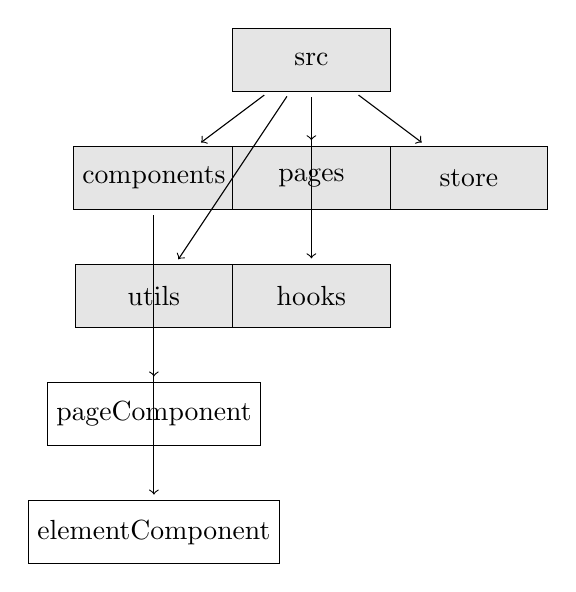
\begin{tikzpicture}[
    file/.style={draw, rectangle, minimum width=2cm, minimum height=0.8cm},
    folder/.style={draw, rectangle, minimum width=2cm, minimum height=0.8cm, fill=gray!20},
    arrow/.style={->, shorten >=2pt, shorten <=2pt}
]

% Folders
\node[folder] (src) at (0,0) {src};
\node[folder] (components) at (-2,-1.5) {components};
\node[folder] (pages) at (0,-1.5) {pages};
\node[folder] (store) at (2,-1.5) {store};
\node[folder] (utils) at (-2,-3) {utils};
\node[folder] (hooks) at (0,-3) {hooks};

% Files
\node[file] (pageComponent) at (-2,-4.5) {pageComponent};
\node[file] (elementComponent) at (-2,-6) {elementComponent};
% ... add more files

% Connections
\draw[arrow] (src) -- (components);
\draw[arrow] (src) -- (pages);
\draw[arrow] (src) -- (store);
\draw[arrow] (src) -- (utils);
\draw[arrow] (src) -- (hooks);
\draw[arrow] (components) -- (pageComponent);
\draw[arrow] (components) -- (elementComponent);
% ... add more connections

\end{tikzpicture}



\pagebreak
\subsubsection{Back-end}
The backend uses the dotNet framework. The development language using the C\# language.

In this project, the backend uses the Onion Architecture.
The Onion Architecture is a typically layered architecture, 
where each layer depends on the inner layer and provides interfaces to the outer layer.
The outer layer provides services to the outermost layer 
and other modules in the same layer based on the interfaces of the inner layer.

From inner to outer, the layers are: Domain, Application, Infrastructure, Presentation.
The Domain layer is the core layer and the innermost layer, used to define domain models, 
which are the business models.
It includes domain models and domain service interfaces.
Domain models are used to define the business models, 
which are the entities in the entity-relationship model and their attributes.
Domain service interfaces are used to define the business services, 
which are the relationships between entities in the entity-relationship model.

The Application layer is the application layer, 
used to define application services, which are the business logic.
It includes domain service implementations and application service interfaces.
Domain service implementations implement the methods of the inner layer's domain service 
interfaces and implement the business logic of the domain models.
Application service interfaces are used to define application services, 
which are the business logic.
It includes but is not limited to database interfaces, testing interfaces, 
HTTP API interfaces, MQTT interfaces, etc.

The Infrastructure layer is the infrastructure layer, used to define infrastructure.
It includes database implementations, testing implementations, 
HTTP API implementations, MQTT implementations, etc.
Database implementations implement the database interfaces 
and provide CRUD services for the database.
Testing implementations implement the testing interfaces 
and provide services for unit testing and integration testing.
HTTP API implementations implement the HTTP API interfaces 
and provide CRUD operations for HTTP APIs.
MQTT implementations implement the MQTT interfaces 
and provide CRUD operations for MQTT.

The Presentation layer is the presentation layer, used to define presentation logic, 
such as interfaces and pages. Since this is a backend project,
data presentation and control are handled by the frontend, 
so this layer is not needed.



\pagebreak
\subsubsection{Data communication and storage}
% 关于本项目的数据通信与数据存储的设计, 包括数据通信的协议, 数据存储的设计等
% 关于数据通信的设计:
% 1. 通信协议的选择
% 自前端向后端发送的数据, 有三种传输的数据类型, 
% 一种是普通的增删改查的请求, 对数据传输的时效性要求不高, 但是对数据的准确性, 完整性, 有序性, 安全性有一定的要求,
% 这种数据的传输, 采用 HTTP 协议, 以及 RESTful API 的设计. 可以有效的保证对数据传输的以上要求.
% 一种是对数据通道的创建和流媒体数据的传输, 对数据传输的时效性, 安全性要求较高, 这种数据的传输, 采用 WebRTC 协议, 以及 MQTT 协议.
% 配合可以快速解码的 flatbuffers 协议, 可以有效的保证对数据传输的以上要求.
% 最后一种是对设备的状态信息和操作信息的传输, 对完整性, 有序性, 安全性都有较高的要求, 这种数据的传输, 采用 MQTT 协议
% 同时也使用了 flatbuffers 协议.
% 
% 2. 数据通信的通信架构和通信流程
% 本项目的数据通信的通信架构, 是基于前后端分离的架构, 前端使用 React 框架, 后端使用 dotnet 框架.
% 当前端需要向后端发送数据的时候, 前端会向后端发送 HTTP 请求, 后端接收到 HTTP 请求之后, 会根据请求的数据类型,
% 选择不同的数据处理方式, 对于普通的增删改查的请求, 后端会根据 RESTful API 的设计, 对数据进行增删改查的操作,
% 对于对数据通道的创建和流媒体数据的传输, 后端会根据 WebRTC 协议, 对数据通道进行创建, 并且帮助前端和设备建立数据通道,
% 当数据通道建立后, 前端和设备之间则使用 flatbuffer 的数据格式对流媒体数据进行传输,
% 对于设备的状态信息和操作信息的传输, 前端会直接向 MQTT broker 发送 MQTT 请求, 
% 设备会在其自身的固件中监听相关的 MQTT 请求, 并且返回相关的数据.
% 
% 3. 数据通信的格式
% 本项目的数据通信的格式, 有三种, 
% 一种是 HTTP 协议, 
% 使用 json 格式对数据进行传输,
% 一种是 WebRTC 协议, 
% 使用 flatbuffers 格式对数据进行传输,
% 一种是 MQTT 协议.
% 使用 flatbuffers 格式对数据进行传输,
% 
% 关于数据存储的设计:
% 1. 数据存储的数据库的选择
% 本项目的数据存储的数据库的选择, 使用了轻量级的数据库 SQLite,
% SQLite 是一个进程内的库, 实现了自给自足的, 无服务器的, 零配置的, 事务性的 SQL 数据库引擎.
% 这是因为整个项目的目的是为了实现前端与设备之间的数据通信, 对于数据库数据的增删改查操作的要求不高,
% 数据量较小, 且对于数据库的数据的事务性要求不高, 所以选择了 SQLite 数据库.
% 2. 项目前后端的数据结构的设计
% 在本项目中, 前端由于使用了 React 框架, 所以前端的数据结构的设计, 使用了基于状态的数据结构的设计,
% 每个组件或者数据集都包含一个状态对象, 这个状态对象的属性就是组件的各个状态. 
% 使用状态对象的原因是, 可以方便的对状态进行管理, 采用对象-属性的形式, 可以方便的针对不同组件的同类状态进行区分,
% 由于跨组件的状态是由 redux 进行管理的, 这种状态对象的设计, 可以更搞笑的对状态进行更新和传递.
% 后端由于使用了 dotnet 框架, 所以后端的数据结构的设计, 使用了基于类的数据结构的设计,
% 采用了面向对象的编程思想, 对数据进行了封装, 使得数据的传输更加的安全, 有序, 完整.


\pagebreak

% \subsection{Domain model}
% \documentclass[]{article}
\usepackage{graphicx}
\usepackage{amsmath}
\usepackage{tikz}

% libaries
\usetikzlibrary{shapes,arrows}

%Define the listing package
\usepackage{listings} %code highlighter
\usepackage{color} %use color
\definecolor{mygreen}{rgb}{0,0.6,0}
\definecolor{mygray}{rgb}{0.5,0.5,0.5}
\definecolor{mymauve}{rgb}{0.58,0,0.82}

%Customize a bit the look
\lstset{ %
backgroundcolor=\color{white}, % choose the background color; you must add \usepackage{color} or \usepackage{xcolor}
basicstyle=\footnotesize, % the size of the fonts that are used for the code
breakatwhitespace=false, % sets if automatic breaks should only happen at whitespace
breaklines=true, % sets automatic line breaking
captionpos=b, % sets the caption-position to bottom
commentstyle=\color{mygreen}, % comment style
deletekeywords={...}, % if you want to delete keywords from the given language
escapeinside={\%*}{*)}, % if you want to add LaTeX within your code
extendedchars=true, % lets you use non-ASCII characters; for 8-bits encodings only, does not work with UTF-8
frame=single, % adds a frame around the code
keepspaces=true, % keeps spaces in text, useful for keeping indentation of code (possibly needs columns=flexible)
keywordstyle=\color{blue}, % keyword style
% language=Octave, % the language of the code
morekeywords={*,...}, % if you want to add more keywords to the set
numbers=left, % where to put the line-numbers; possible values are (none, left, right)
numbersep=5pt, % how far the line-numbers are from the code
numberstyle=\tiny\color{mygray}, % the style that is used for the line-numbers
rulecolor=\color{black}, % if not set, the frame-color may be changed on line-breaks within not-black text (e.g. comments (green here))
showspaces=false, % show spaces everywhere adding particular underscores; it overrides 'showstringspaces'
showstringspaces=false, % underline spaces within strings only
showtabs=false, % show tabs within strings adding particular underscores
stepnumber=1, % the step between two line-numbers. If it's 1, each line will be numbered
stringstyle=\color{mymauve}, % string literal style
tabsize=2, % sets default tabsize to 2 spaces
title=\lstname % show the filename of files included with \lstinputlisting; also try caption instead of title
}

\definecolor{darkgray}{rgb}{.4,.4,.4}
\definecolor{purple}{rgb}{0.65, 0.12, 0.82}

\lstdefinelanguage{React}{
keywords={const, typeof, new, true, false, catch, function, return, null, catch, switch, var, if, in, while, do, else, case, break},
keywordstyle=\color{blue}\bfseries,
ndkeywords={class, export, boolean, throw, implements, import, this},
ndkeywordstyle=\color{darkgray}\bfseries,
identifierstyle=\color{mygreen},
sensitive=false,
comment=[l]{//},
morecomment=[s]{/*}{*/},
commentstyle=\color{purple}\ttfamily,
string=[b]{"}{'}{`},
stringstyle=\color{red}\ttfamily,
morestring=[b]',
morestring=[b]",
morestring=[b]`',
}

\lstdefinelanguage{CSharp}{
keywords={const, typeof, new, true, false, catch, function, return, null, catch, switch, var, if, in, while, do, else, case, break},
keywordstyle=\color{blue}\bfseries,
ndkeywords={class, export, boolean, throw, implements, import, this},
ndkeywordstyle=\color{darkgray}\bfseries,
identifierstyle=\color{mygreen},
sensitive=false,
comment=[l]{//},
morecomment=[s]{/*}{*/},
commentstyle=\color{purple}\ttfamily,
string=[b]{"}{'}{`},
stringstyle=\color{red}\ttfamily,
morestring=[b]',
morestring=[b]",
morestring=[b]`',
}

\lstset{
language=React,
extendedchars=true,
basicstyle=\footnotesize\ttfamily,
showstringspaces=false,
showspaces=false,
numbers=left,
numberstyle=\footnotesize,
numbersep=9pt,
tabsize=2,
breaklines=true,
showtabs=false,
captionpos=b
}

\lstset{
language=CSharp,
extendedchars=true,
basicstyle=\footnotesize\ttfamily,
showstringspaces=false,
showspaces=false,
numbers=left,
numberstyle=\footnotesize,
numbersep=9pt,
tabsize=2,
breaklines=true,
showtabs=false,
captionpos=b
}

% \usepackage{cite} % Add this line for citation

% \bibliographystyle{plain}

\title{
The implementation of BifrostConnect Front-end scope, 
re-design and development with the relevant back-end support develop.
}
\author{
    Fei Gu \\
    Erhvervs Akademi Sydvest \\
    Computer Science 21\\
    }
\date{\today}

\begin{document}

% Front page
\maketitle
\begin{center}
    Supervisor: Henrik Boulund Meng Hansen \\
    Company: BifrostConnect \\
    Engineering Director: Jasper Wass \\
\end{center}
\tableofcontents
\pagebreak


% The introduction
\section{Introduction}
\subsection{Background}\input{sections/introduction/background.tex}
\subsection{The company}\input{sections/introduction/aboutCompany}
\subsection{The project}\input{sections/introduction/aboutProject}
\pagebreak

% The problem statement
\section{Problem Statement}
\subsection{Statement}
\input{sections/problemStatement/statement}
\subsection{Situation}
\input{sections/problemStatement/situation}
\subsection{Potential Solution}
\input{sections/problemStatement/potentialSolution}
\pagebreak

% Requirement analysis
\section{Requirement Analysis}
\input{sections/requirementAnalysis/index}

\subsection{Stakeholders}
\input{sections/requirementAnalysis/stakeholders/index}

\subsection{Business Domain}
\input{sections/requirementAnalysis/bussinesDomain/index}

\subsection{Scope}
\input{sections/requirementAnalysis/scope}

\subsection{Goals}
\input{sections/requirementAnalysis/goals}
\pagebreak

% Software Design
\section{Software Design}
% developement methods
\subsection{Software Development Methods}
\input{sections/softwareDevelopmentMethods/index}
\subsubsection{Agile Software Development}
\input{sections/softwareDevelopmentMethods/agileSoftwareDevelopment/index}
\subsubsection{Feature Driven Development}
\input{sections/softwareDevelopmentMethods/featureDrivenDevelopment/index}

\pagebreak

% Technology seslection
\subsection{Technology selection}
\input{sections/softwareDesign/technologySelection/index}
\subsubsection{Front-end}
\input{sections/softwareDesign/technologySelection/frontEnd}            
\subsubsection{Back-end}
\input{sections/softwareDesign/technologySelection/backEnd}            
\subsubsection{Database}
\input{sections/softwareDesign/technologySelection/database}
\subsubsection{Data communication}
\input{sections/softwareDesign/technologySelection/dataCommunication}            
\subsubsection{DevOps}
\input{sections/softwareDesign/technologySelection/devOps}
\pagebreak

% Architecture design
\subsection{Architecture design}
\input{sections/softwareDesign/architectureDesign/index}
\pagebreak
\subsubsection{Front-end}
\input{sections/softwareDesign/architectureDesign/frontEndArchitecture}
\pagebreak
\subsubsection{Back-end}
\input{sections/softwareDesign/architectureDesign/backEndArchitecture}
\pagebreak
\subsubsection{Data communication and storage}
\input{sections/softwareDesign/architectureDesign/dataCommunicationArchitecture}
\pagebreak

% \subsection{Domain model}
% \input{sections/softwareDesign/domainModel/index}
% \subsection{Database design}
% % 数据库领域模型 ER 图
% % 包括表和字段的设置.
% % 对于私有键和外键的设置.

% \subsection{Back-end design}
% % 后端对象模型
% % 以及对于对象模型的增删改查
% % 以及相关的其他服务的设计`'

% \subsection{Front-end design}
% % 对于前端的页面结构的设计 
% % 页面的状态的设计, 交互设计

% \subsection{FlatBuffers design}
% % schema 的设计

\subsection{DevOps CI/CD process design}
\input{sections/softwareDesign/devOpsDesign/index}
\subsubsection{Continuous Integration}
\input{sections/softwareDesign/devOpsDesign/continuousIntegration/index}
\subsubsection{Continuous Delivery}
\input{sections/softwareDesign/devOpsDesign/continuousDelivery/index}
\subsubsection{Continuous Deployment}
\input{sections/softwareDesign/devOpsDesign/continuousDeployment/index}
\pagebreak

\section{Software Development} 
\input{sections/softwareDevelopment/index}
\subsection{Overall development}
\input{sections/softwareDevelopment/overallDevelopement/index}
\subsubsection{Front-end}
\input{sections/softwareDevelopment/overallDevelopement/frontEnd/index}
\subsubsection{Back-end}
\input{sections/softwareDevelopment/overallDevelopement/backEnd/index}
\subsubsection{DevOps}
\input{sections/softwareDevelopment/overallDevelopement/devOps/index}
\subsection{Feature development} 
\input{sections/softwareDevelopment/featureDevelopment/index}
\subsubsection{Use Case 1}
\input{sections/softwareDevelopment/featureDevelopment/useCase1/index}
\subsubsection{Feature 1}
\input{sections/softwareDevelopment/featureDevelopment/feature/feature1.tex}
\pagebreak
\section{Conclusion} 
\subsection{Result}
Since the project is still in progress, the result is not available yet.
So far, basic structure of this project has been built. But the most features 
are not implemented yet. 
\subsection{Discussion}
As a single developer for this project, I am confident what I have done so far.
And I can say I understand the most of the knowledge I have used in this project, 
which also means I can explain all the part of the project. 
But this project also relevant some of the complex knowledge which I have to continue 
to study and practice.
\subsection{Future Work}
The future work is to implement the rest of the features. 
Including the most important part which is the 'create session' feature.
\pagebreak
% \bibliography{bibliography}
\pagebreak
% \begin{appendices}
%     \section{Appendix}
% \end{appendices} 
\end{document}
% \subsection{Database design}
% % 数据库领域模型 ER 图
% % 包括表和字段的设置.
% % 对于私有键和外键的设置.

% \subsection{Back-end design}
% % 后端对象模型
% % 以及对于对象模型的增删改查
% % 以及相关的其他服务的设计`'

% \subsection{Front-end design}
% % 对于前端的页面结构的设计 
% % 页面的状态的设计, 交互设计

% \subsection{FlatBuffers design}
% % schema 的设计

\subsection{DevOps CI/CD process design}
\documentclass[]{article}
\usepackage{graphicx}
\usepackage{amsmath}
\usepackage{tikz}

% libaries
\usetikzlibrary{shapes,arrows}

%Define the listing package
\usepackage{listings} %code highlighter
\usepackage{color} %use color
\definecolor{mygreen}{rgb}{0,0.6,0}
\definecolor{mygray}{rgb}{0.5,0.5,0.5}
\definecolor{mymauve}{rgb}{0.58,0,0.82}

%Customize a bit the look
\lstset{ %
backgroundcolor=\color{white}, % choose the background color; you must add \usepackage{color} or \usepackage{xcolor}
basicstyle=\footnotesize, % the size of the fonts that are used for the code
breakatwhitespace=false, % sets if automatic breaks should only happen at whitespace
breaklines=true, % sets automatic line breaking
captionpos=b, % sets the caption-position to bottom
commentstyle=\color{mygreen}, % comment style
deletekeywords={...}, % if you want to delete keywords from the given language
escapeinside={\%*}{*)}, % if you want to add LaTeX within your code
extendedchars=true, % lets you use non-ASCII characters; for 8-bits encodings only, does not work with UTF-8
frame=single, % adds a frame around the code
keepspaces=true, % keeps spaces in text, useful for keeping indentation of code (possibly needs columns=flexible)
keywordstyle=\color{blue}, % keyword style
% language=Octave, % the language of the code
morekeywords={*,...}, % if you want to add more keywords to the set
numbers=left, % where to put the line-numbers; possible values are (none, left, right)
numbersep=5pt, % how far the line-numbers are from the code
numberstyle=\tiny\color{mygray}, % the style that is used for the line-numbers
rulecolor=\color{black}, % if not set, the frame-color may be changed on line-breaks within not-black text (e.g. comments (green here))
showspaces=false, % show spaces everywhere adding particular underscores; it overrides 'showstringspaces'
showstringspaces=false, % underline spaces within strings only
showtabs=false, % show tabs within strings adding particular underscores
stepnumber=1, % the step between two line-numbers. If it's 1, each line will be numbered
stringstyle=\color{mymauve}, % string literal style
tabsize=2, % sets default tabsize to 2 spaces
title=\lstname % show the filename of files included with \lstinputlisting; also try caption instead of title
}

\definecolor{darkgray}{rgb}{.4,.4,.4}
\definecolor{purple}{rgb}{0.65, 0.12, 0.82}

\lstdefinelanguage{React}{
keywords={const, typeof, new, true, false, catch, function, return, null, catch, switch, var, if, in, while, do, else, case, break},
keywordstyle=\color{blue}\bfseries,
ndkeywords={class, export, boolean, throw, implements, import, this},
ndkeywordstyle=\color{darkgray}\bfseries,
identifierstyle=\color{mygreen},
sensitive=false,
comment=[l]{//},
morecomment=[s]{/*}{*/},
commentstyle=\color{purple}\ttfamily,
string=[b]{"}{'}{`},
stringstyle=\color{red}\ttfamily,
morestring=[b]',
morestring=[b]",
morestring=[b]`',
}

\lstdefinelanguage{CSharp}{
keywords={const, typeof, new, true, false, catch, function, return, null, catch, switch, var, if, in, while, do, else, case, break},
keywordstyle=\color{blue}\bfseries,
ndkeywords={class, export, boolean, throw, implements, import, this},
ndkeywordstyle=\color{darkgray}\bfseries,
identifierstyle=\color{mygreen},
sensitive=false,
comment=[l]{//},
morecomment=[s]{/*}{*/},
commentstyle=\color{purple}\ttfamily,
string=[b]{"}{'}{`},
stringstyle=\color{red}\ttfamily,
morestring=[b]',
morestring=[b]",
morestring=[b]`',
}

\lstset{
language=React,
extendedchars=true,
basicstyle=\footnotesize\ttfamily,
showstringspaces=false,
showspaces=false,
numbers=left,
numberstyle=\footnotesize,
numbersep=9pt,
tabsize=2,
breaklines=true,
showtabs=false,
captionpos=b
}

\lstset{
language=CSharp,
extendedchars=true,
basicstyle=\footnotesize\ttfamily,
showstringspaces=false,
showspaces=false,
numbers=left,
numberstyle=\footnotesize,
numbersep=9pt,
tabsize=2,
breaklines=true,
showtabs=false,
captionpos=b
}

% \usepackage{cite} % Add this line for citation

% \bibliographystyle{plain}

\title{
The implementation of BifrostConnect Front-end scope, 
re-design and development with the relevant back-end support develop.
}
\author{
    Fei Gu \\
    Erhvervs Akademi Sydvest \\
    Computer Science 21\\
    }
\date{\today}

\begin{document}

% Front page
\maketitle
\begin{center}
    Supervisor: Henrik Boulund Meng Hansen \\
    Company: BifrostConnect \\
    Engineering Director: Jasper Wass \\
\end{center}
\tableofcontents
\pagebreak


% The introduction
\section{Introduction}
\subsection{Background}\input{sections/introduction/background.tex}
\subsection{The company}\input{sections/introduction/aboutCompany}
\subsection{The project}\input{sections/introduction/aboutProject}
\pagebreak

% The problem statement
\section{Problem Statement}
\subsection{Statement}
\input{sections/problemStatement/statement}
\subsection{Situation}
\input{sections/problemStatement/situation}
\subsection{Potential Solution}
\input{sections/problemStatement/potentialSolution}
\pagebreak

% Requirement analysis
\section{Requirement Analysis}
\input{sections/requirementAnalysis/index}

\subsection{Stakeholders}
\input{sections/requirementAnalysis/stakeholders/index}

\subsection{Business Domain}
\input{sections/requirementAnalysis/bussinesDomain/index}

\subsection{Scope}
\input{sections/requirementAnalysis/scope}

\subsection{Goals}
\input{sections/requirementAnalysis/goals}
\pagebreak

% Software Design
\section{Software Design}
% developement methods
\subsection{Software Development Methods}
\input{sections/softwareDevelopmentMethods/index}
\subsubsection{Agile Software Development}
\input{sections/softwareDevelopmentMethods/agileSoftwareDevelopment/index}
\subsubsection{Feature Driven Development}
\input{sections/softwareDevelopmentMethods/featureDrivenDevelopment/index}

\pagebreak

% Technology seslection
\subsection{Technology selection}
\input{sections/softwareDesign/technologySelection/index}
\subsubsection{Front-end}
\input{sections/softwareDesign/technologySelection/frontEnd}            
\subsubsection{Back-end}
\input{sections/softwareDesign/technologySelection/backEnd}            
\subsubsection{Database}
\input{sections/softwareDesign/technologySelection/database}
\subsubsection{Data communication}
\input{sections/softwareDesign/technologySelection/dataCommunication}            
\subsubsection{DevOps}
\input{sections/softwareDesign/technologySelection/devOps}
\pagebreak

% Architecture design
\subsection{Architecture design}
\input{sections/softwareDesign/architectureDesign/index}
\pagebreak
\subsubsection{Front-end}
\input{sections/softwareDesign/architectureDesign/frontEndArchitecture}
\pagebreak
\subsubsection{Back-end}
\input{sections/softwareDesign/architectureDesign/backEndArchitecture}
\pagebreak
\subsubsection{Data communication and storage}
\input{sections/softwareDesign/architectureDesign/dataCommunicationArchitecture}
\pagebreak

% \subsection{Domain model}
% \input{sections/softwareDesign/domainModel/index}
% \subsection{Database design}
% % 数据库领域模型 ER 图
% % 包括表和字段的设置.
% % 对于私有键和外键的设置.

% \subsection{Back-end design}
% % 后端对象模型
% % 以及对于对象模型的增删改查
% % 以及相关的其他服务的设计`'

% \subsection{Front-end design}
% % 对于前端的页面结构的设计 
% % 页面的状态的设计, 交互设计

% \subsection{FlatBuffers design}
% % schema 的设计

\subsection{DevOps CI/CD process design}
\input{sections/softwareDesign/devOpsDesign/index}
\subsubsection{Continuous Integration}
\input{sections/softwareDesign/devOpsDesign/continuousIntegration/index}
\subsubsection{Continuous Delivery}
\input{sections/softwareDesign/devOpsDesign/continuousDelivery/index}
\subsubsection{Continuous Deployment}
\input{sections/softwareDesign/devOpsDesign/continuousDeployment/index}
\pagebreak

\section{Software Development} 
\input{sections/softwareDevelopment/index}
\subsection{Overall development}
\input{sections/softwareDevelopment/overallDevelopement/index}
\subsubsection{Front-end}
\input{sections/softwareDevelopment/overallDevelopement/frontEnd/index}
\subsubsection{Back-end}
\input{sections/softwareDevelopment/overallDevelopement/backEnd/index}
\subsubsection{DevOps}
\input{sections/softwareDevelopment/overallDevelopement/devOps/index}
\subsection{Feature development} 
\input{sections/softwareDevelopment/featureDevelopment/index}
\subsubsection{Use Case 1}
\input{sections/softwareDevelopment/featureDevelopment/useCase1/index}
\subsubsection{Feature 1}
\input{sections/softwareDevelopment/featureDevelopment/feature/feature1.tex}
\pagebreak
\section{Conclusion} 
\subsection{Result}
Since the project is still in progress, the result is not available yet.
So far, basic structure of this project has been built. But the most features 
are not implemented yet. 
\subsection{Discussion}
As a single developer for this project, I am confident what I have done so far.
And I can say I understand the most of the knowledge I have used in this project, 
which also means I can explain all the part of the project. 
But this project also relevant some of the complex knowledge which I have to continue 
to study and practice.
\subsection{Future Work}
The future work is to implement the rest of the features. 
Including the most important part which is the 'create session' feature.
\pagebreak
% \bibliography{bibliography}
\pagebreak
% \begin{appendices}
%     \section{Appendix}
% \end{appendices} 
\end{document}
\subsubsection{Continuous Integration}
\documentclass[]{article}
\usepackage{graphicx}
\usepackage{amsmath}
\usepackage{tikz}

% libaries
\usetikzlibrary{shapes,arrows}

%Define the listing package
\usepackage{listings} %code highlighter
\usepackage{color} %use color
\definecolor{mygreen}{rgb}{0,0.6,0}
\definecolor{mygray}{rgb}{0.5,0.5,0.5}
\definecolor{mymauve}{rgb}{0.58,0,0.82}

%Customize a bit the look
\lstset{ %
backgroundcolor=\color{white}, % choose the background color; you must add \usepackage{color} or \usepackage{xcolor}
basicstyle=\footnotesize, % the size of the fonts that are used for the code
breakatwhitespace=false, % sets if automatic breaks should only happen at whitespace
breaklines=true, % sets automatic line breaking
captionpos=b, % sets the caption-position to bottom
commentstyle=\color{mygreen}, % comment style
deletekeywords={...}, % if you want to delete keywords from the given language
escapeinside={\%*}{*)}, % if you want to add LaTeX within your code
extendedchars=true, % lets you use non-ASCII characters; for 8-bits encodings only, does not work with UTF-8
frame=single, % adds a frame around the code
keepspaces=true, % keeps spaces in text, useful for keeping indentation of code (possibly needs columns=flexible)
keywordstyle=\color{blue}, % keyword style
% language=Octave, % the language of the code
morekeywords={*,...}, % if you want to add more keywords to the set
numbers=left, % where to put the line-numbers; possible values are (none, left, right)
numbersep=5pt, % how far the line-numbers are from the code
numberstyle=\tiny\color{mygray}, % the style that is used for the line-numbers
rulecolor=\color{black}, % if not set, the frame-color may be changed on line-breaks within not-black text (e.g. comments (green here))
showspaces=false, % show spaces everywhere adding particular underscores; it overrides 'showstringspaces'
showstringspaces=false, % underline spaces within strings only
showtabs=false, % show tabs within strings adding particular underscores
stepnumber=1, % the step between two line-numbers. If it's 1, each line will be numbered
stringstyle=\color{mymauve}, % string literal style
tabsize=2, % sets default tabsize to 2 spaces
title=\lstname % show the filename of files included with \lstinputlisting; also try caption instead of title
}

\definecolor{darkgray}{rgb}{.4,.4,.4}
\definecolor{purple}{rgb}{0.65, 0.12, 0.82}

\lstdefinelanguage{React}{
keywords={const, typeof, new, true, false, catch, function, return, null, catch, switch, var, if, in, while, do, else, case, break},
keywordstyle=\color{blue}\bfseries,
ndkeywords={class, export, boolean, throw, implements, import, this},
ndkeywordstyle=\color{darkgray}\bfseries,
identifierstyle=\color{mygreen},
sensitive=false,
comment=[l]{//},
morecomment=[s]{/*}{*/},
commentstyle=\color{purple}\ttfamily,
string=[b]{"}{'}{`},
stringstyle=\color{red}\ttfamily,
morestring=[b]',
morestring=[b]",
morestring=[b]`',
}

\lstdefinelanguage{CSharp}{
keywords={const, typeof, new, true, false, catch, function, return, null, catch, switch, var, if, in, while, do, else, case, break},
keywordstyle=\color{blue}\bfseries,
ndkeywords={class, export, boolean, throw, implements, import, this},
ndkeywordstyle=\color{darkgray}\bfseries,
identifierstyle=\color{mygreen},
sensitive=false,
comment=[l]{//},
morecomment=[s]{/*}{*/},
commentstyle=\color{purple}\ttfamily,
string=[b]{"}{'}{`},
stringstyle=\color{red}\ttfamily,
morestring=[b]',
morestring=[b]",
morestring=[b]`',
}

\lstset{
language=React,
extendedchars=true,
basicstyle=\footnotesize\ttfamily,
showstringspaces=false,
showspaces=false,
numbers=left,
numberstyle=\footnotesize,
numbersep=9pt,
tabsize=2,
breaklines=true,
showtabs=false,
captionpos=b
}

\lstset{
language=CSharp,
extendedchars=true,
basicstyle=\footnotesize\ttfamily,
showstringspaces=false,
showspaces=false,
numbers=left,
numberstyle=\footnotesize,
numbersep=9pt,
tabsize=2,
breaklines=true,
showtabs=false,
captionpos=b
}

% \usepackage{cite} % Add this line for citation

% \bibliographystyle{plain}

\title{
The implementation of BifrostConnect Front-end scope, 
re-design and development with the relevant back-end support develop.
}
\author{
    Fei Gu \\
    Erhvervs Akademi Sydvest \\
    Computer Science 21\\
    }
\date{\today}

\begin{document}

% Front page
\maketitle
\begin{center}
    Supervisor: Henrik Boulund Meng Hansen \\
    Company: BifrostConnect \\
    Engineering Director: Jasper Wass \\
\end{center}
\tableofcontents
\pagebreak


% The introduction
\section{Introduction}
\subsection{Background}\input{sections/introduction/background.tex}
\subsection{The company}\input{sections/introduction/aboutCompany}
\subsection{The project}\input{sections/introduction/aboutProject}
\pagebreak

% The problem statement
\section{Problem Statement}
\subsection{Statement}
\input{sections/problemStatement/statement}
\subsection{Situation}
\input{sections/problemStatement/situation}
\subsection{Potential Solution}
\input{sections/problemStatement/potentialSolution}
\pagebreak

% Requirement analysis
\section{Requirement Analysis}
\input{sections/requirementAnalysis/index}

\subsection{Stakeholders}
\input{sections/requirementAnalysis/stakeholders/index}

\subsection{Business Domain}
\input{sections/requirementAnalysis/bussinesDomain/index}

\subsection{Scope}
\input{sections/requirementAnalysis/scope}

\subsection{Goals}
\input{sections/requirementAnalysis/goals}
\pagebreak

% Software Design
\section{Software Design}
% developement methods
\subsection{Software Development Methods}
\input{sections/softwareDevelopmentMethods/index}
\subsubsection{Agile Software Development}
\input{sections/softwareDevelopmentMethods/agileSoftwareDevelopment/index}
\subsubsection{Feature Driven Development}
\input{sections/softwareDevelopmentMethods/featureDrivenDevelopment/index}

\pagebreak

% Technology seslection
\subsection{Technology selection}
\input{sections/softwareDesign/technologySelection/index}
\subsubsection{Front-end}
\input{sections/softwareDesign/technologySelection/frontEnd}            
\subsubsection{Back-end}
\input{sections/softwareDesign/technologySelection/backEnd}            
\subsubsection{Database}
\input{sections/softwareDesign/technologySelection/database}
\subsubsection{Data communication}
\input{sections/softwareDesign/technologySelection/dataCommunication}            
\subsubsection{DevOps}
\input{sections/softwareDesign/technologySelection/devOps}
\pagebreak

% Architecture design
\subsection{Architecture design}
\input{sections/softwareDesign/architectureDesign/index}
\pagebreak
\subsubsection{Front-end}
\input{sections/softwareDesign/architectureDesign/frontEndArchitecture}
\pagebreak
\subsubsection{Back-end}
\input{sections/softwareDesign/architectureDesign/backEndArchitecture}
\pagebreak
\subsubsection{Data communication and storage}
\input{sections/softwareDesign/architectureDesign/dataCommunicationArchitecture}
\pagebreak

% \subsection{Domain model}
% \input{sections/softwareDesign/domainModel/index}
% \subsection{Database design}
% % 数据库领域模型 ER 图
% % 包括表和字段的设置.
% % 对于私有键和外键的设置.

% \subsection{Back-end design}
% % 后端对象模型
% % 以及对于对象模型的增删改查
% % 以及相关的其他服务的设计`'

% \subsection{Front-end design}
% % 对于前端的页面结构的设计 
% % 页面的状态的设计, 交互设计

% \subsection{FlatBuffers design}
% % schema 的设计

\subsection{DevOps CI/CD process design}
\input{sections/softwareDesign/devOpsDesign/index}
\subsubsection{Continuous Integration}
\input{sections/softwareDesign/devOpsDesign/continuousIntegration/index}
\subsubsection{Continuous Delivery}
\input{sections/softwareDesign/devOpsDesign/continuousDelivery/index}
\subsubsection{Continuous Deployment}
\input{sections/softwareDesign/devOpsDesign/continuousDeployment/index}
\pagebreak

\section{Software Development} 
\input{sections/softwareDevelopment/index}
\subsection{Overall development}
\input{sections/softwareDevelopment/overallDevelopement/index}
\subsubsection{Front-end}
\input{sections/softwareDevelopment/overallDevelopement/frontEnd/index}
\subsubsection{Back-end}
\input{sections/softwareDevelopment/overallDevelopement/backEnd/index}
\subsubsection{DevOps}
\input{sections/softwareDevelopment/overallDevelopement/devOps/index}
\subsection{Feature development} 
\input{sections/softwareDevelopment/featureDevelopment/index}
\subsubsection{Use Case 1}
\input{sections/softwareDevelopment/featureDevelopment/useCase1/index}
\subsubsection{Feature 1}
\input{sections/softwareDevelopment/featureDevelopment/feature/feature1.tex}
\pagebreak
\section{Conclusion} 
\subsection{Result}
Since the project is still in progress, the result is not available yet.
So far, basic structure of this project has been built. But the most features 
are not implemented yet. 
\subsection{Discussion}
As a single developer for this project, I am confident what I have done so far.
And I can say I understand the most of the knowledge I have used in this project, 
which also means I can explain all the part of the project. 
But this project also relevant some of the complex knowledge which I have to continue 
to study and practice.
\subsection{Future Work}
The future work is to implement the rest of the features. 
Including the most important part which is the 'create session' feature.
\pagebreak
% \bibliography{bibliography}
\pagebreak
% \begin{appendices}
%     \section{Appendix}
% \end{appendices} 
\end{document}
\subsubsection{Continuous Delivery}
\documentclass[]{article}
\usepackage{graphicx}
\usepackage{amsmath}
\usepackage{tikz}

% libaries
\usetikzlibrary{shapes,arrows}

%Define the listing package
\usepackage{listings} %code highlighter
\usepackage{color} %use color
\definecolor{mygreen}{rgb}{0,0.6,0}
\definecolor{mygray}{rgb}{0.5,0.5,0.5}
\definecolor{mymauve}{rgb}{0.58,0,0.82}

%Customize a bit the look
\lstset{ %
backgroundcolor=\color{white}, % choose the background color; you must add \usepackage{color} or \usepackage{xcolor}
basicstyle=\footnotesize, % the size of the fonts that are used for the code
breakatwhitespace=false, % sets if automatic breaks should only happen at whitespace
breaklines=true, % sets automatic line breaking
captionpos=b, % sets the caption-position to bottom
commentstyle=\color{mygreen}, % comment style
deletekeywords={...}, % if you want to delete keywords from the given language
escapeinside={\%*}{*)}, % if you want to add LaTeX within your code
extendedchars=true, % lets you use non-ASCII characters; for 8-bits encodings only, does not work with UTF-8
frame=single, % adds a frame around the code
keepspaces=true, % keeps spaces in text, useful for keeping indentation of code (possibly needs columns=flexible)
keywordstyle=\color{blue}, % keyword style
% language=Octave, % the language of the code
morekeywords={*,...}, % if you want to add more keywords to the set
numbers=left, % where to put the line-numbers; possible values are (none, left, right)
numbersep=5pt, % how far the line-numbers are from the code
numberstyle=\tiny\color{mygray}, % the style that is used for the line-numbers
rulecolor=\color{black}, % if not set, the frame-color may be changed on line-breaks within not-black text (e.g. comments (green here))
showspaces=false, % show spaces everywhere adding particular underscores; it overrides 'showstringspaces'
showstringspaces=false, % underline spaces within strings only
showtabs=false, % show tabs within strings adding particular underscores
stepnumber=1, % the step between two line-numbers. If it's 1, each line will be numbered
stringstyle=\color{mymauve}, % string literal style
tabsize=2, % sets default tabsize to 2 spaces
title=\lstname % show the filename of files included with \lstinputlisting; also try caption instead of title
}

\definecolor{darkgray}{rgb}{.4,.4,.4}
\definecolor{purple}{rgb}{0.65, 0.12, 0.82}

\lstdefinelanguage{React}{
keywords={const, typeof, new, true, false, catch, function, return, null, catch, switch, var, if, in, while, do, else, case, break},
keywordstyle=\color{blue}\bfseries,
ndkeywords={class, export, boolean, throw, implements, import, this},
ndkeywordstyle=\color{darkgray}\bfseries,
identifierstyle=\color{mygreen},
sensitive=false,
comment=[l]{//},
morecomment=[s]{/*}{*/},
commentstyle=\color{purple}\ttfamily,
string=[b]{"}{'}{`},
stringstyle=\color{red}\ttfamily,
morestring=[b]',
morestring=[b]",
morestring=[b]`',
}

\lstdefinelanguage{CSharp}{
keywords={const, typeof, new, true, false, catch, function, return, null, catch, switch, var, if, in, while, do, else, case, break},
keywordstyle=\color{blue}\bfseries,
ndkeywords={class, export, boolean, throw, implements, import, this},
ndkeywordstyle=\color{darkgray}\bfseries,
identifierstyle=\color{mygreen},
sensitive=false,
comment=[l]{//},
morecomment=[s]{/*}{*/},
commentstyle=\color{purple}\ttfamily,
string=[b]{"}{'}{`},
stringstyle=\color{red}\ttfamily,
morestring=[b]',
morestring=[b]",
morestring=[b]`',
}

\lstset{
language=React,
extendedchars=true,
basicstyle=\footnotesize\ttfamily,
showstringspaces=false,
showspaces=false,
numbers=left,
numberstyle=\footnotesize,
numbersep=9pt,
tabsize=2,
breaklines=true,
showtabs=false,
captionpos=b
}

\lstset{
language=CSharp,
extendedchars=true,
basicstyle=\footnotesize\ttfamily,
showstringspaces=false,
showspaces=false,
numbers=left,
numberstyle=\footnotesize,
numbersep=9pt,
tabsize=2,
breaklines=true,
showtabs=false,
captionpos=b
}

% \usepackage{cite} % Add this line for citation

% \bibliographystyle{plain}

\title{
The implementation of BifrostConnect Front-end scope, 
re-design and development with the relevant back-end support develop.
}
\author{
    Fei Gu \\
    Erhvervs Akademi Sydvest \\
    Computer Science 21\\
    }
\date{\today}

\begin{document}

% Front page
\maketitle
\begin{center}
    Supervisor: Henrik Boulund Meng Hansen \\
    Company: BifrostConnect \\
    Engineering Director: Jasper Wass \\
\end{center}
\tableofcontents
\pagebreak


% The introduction
\section{Introduction}
\subsection{Background}\input{sections/introduction/background.tex}
\subsection{The company}\input{sections/introduction/aboutCompany}
\subsection{The project}\input{sections/introduction/aboutProject}
\pagebreak

% The problem statement
\section{Problem Statement}
\subsection{Statement}
\input{sections/problemStatement/statement}
\subsection{Situation}
\input{sections/problemStatement/situation}
\subsection{Potential Solution}
\input{sections/problemStatement/potentialSolution}
\pagebreak

% Requirement analysis
\section{Requirement Analysis}
\input{sections/requirementAnalysis/index}

\subsection{Stakeholders}
\input{sections/requirementAnalysis/stakeholders/index}

\subsection{Business Domain}
\input{sections/requirementAnalysis/bussinesDomain/index}

\subsection{Scope}
\input{sections/requirementAnalysis/scope}

\subsection{Goals}
\input{sections/requirementAnalysis/goals}
\pagebreak

% Software Design
\section{Software Design}
% developement methods
\subsection{Software Development Methods}
\input{sections/softwareDevelopmentMethods/index}
\subsubsection{Agile Software Development}
\input{sections/softwareDevelopmentMethods/agileSoftwareDevelopment/index}
\subsubsection{Feature Driven Development}
\input{sections/softwareDevelopmentMethods/featureDrivenDevelopment/index}

\pagebreak

% Technology seslection
\subsection{Technology selection}
\input{sections/softwareDesign/technologySelection/index}
\subsubsection{Front-end}
\input{sections/softwareDesign/technologySelection/frontEnd}            
\subsubsection{Back-end}
\input{sections/softwareDesign/technologySelection/backEnd}            
\subsubsection{Database}
\input{sections/softwareDesign/technologySelection/database}
\subsubsection{Data communication}
\input{sections/softwareDesign/technologySelection/dataCommunication}            
\subsubsection{DevOps}
\input{sections/softwareDesign/technologySelection/devOps}
\pagebreak

% Architecture design
\subsection{Architecture design}
\input{sections/softwareDesign/architectureDesign/index}
\pagebreak
\subsubsection{Front-end}
\input{sections/softwareDesign/architectureDesign/frontEndArchitecture}
\pagebreak
\subsubsection{Back-end}
\input{sections/softwareDesign/architectureDesign/backEndArchitecture}
\pagebreak
\subsubsection{Data communication and storage}
\input{sections/softwareDesign/architectureDesign/dataCommunicationArchitecture}
\pagebreak

% \subsection{Domain model}
% \input{sections/softwareDesign/domainModel/index}
% \subsection{Database design}
% % 数据库领域模型 ER 图
% % 包括表和字段的设置.
% % 对于私有键和外键的设置.

% \subsection{Back-end design}
% % 后端对象模型
% % 以及对于对象模型的增删改查
% % 以及相关的其他服务的设计`'

% \subsection{Front-end design}
% % 对于前端的页面结构的设计 
% % 页面的状态的设计, 交互设计

% \subsection{FlatBuffers design}
% % schema 的设计

\subsection{DevOps CI/CD process design}
\input{sections/softwareDesign/devOpsDesign/index}
\subsubsection{Continuous Integration}
\input{sections/softwareDesign/devOpsDesign/continuousIntegration/index}
\subsubsection{Continuous Delivery}
\input{sections/softwareDesign/devOpsDesign/continuousDelivery/index}
\subsubsection{Continuous Deployment}
\input{sections/softwareDesign/devOpsDesign/continuousDeployment/index}
\pagebreak

\section{Software Development} 
\input{sections/softwareDevelopment/index}
\subsection{Overall development}
\input{sections/softwareDevelopment/overallDevelopement/index}
\subsubsection{Front-end}
\input{sections/softwareDevelopment/overallDevelopement/frontEnd/index}
\subsubsection{Back-end}
\input{sections/softwareDevelopment/overallDevelopement/backEnd/index}
\subsubsection{DevOps}
\input{sections/softwareDevelopment/overallDevelopement/devOps/index}
\subsection{Feature development} 
\input{sections/softwareDevelopment/featureDevelopment/index}
\subsubsection{Use Case 1}
\input{sections/softwareDevelopment/featureDevelopment/useCase1/index}
\subsubsection{Feature 1}
\input{sections/softwareDevelopment/featureDevelopment/feature/feature1.tex}
\pagebreak
\section{Conclusion} 
\subsection{Result}
Since the project is still in progress, the result is not available yet.
So far, basic structure of this project has been built. But the most features 
are not implemented yet. 
\subsection{Discussion}
As a single developer for this project, I am confident what I have done so far.
And I can say I understand the most of the knowledge I have used in this project, 
which also means I can explain all the part of the project. 
But this project also relevant some of the complex knowledge which I have to continue 
to study and practice.
\subsection{Future Work}
The future work is to implement the rest of the features. 
Including the most important part which is the 'create session' feature.
\pagebreak
% \bibliography{bibliography}
\pagebreak
% \begin{appendices}
%     \section{Appendix}
% \end{appendices} 
\end{document}
\subsubsection{Continuous Deployment}
\documentclass[]{article}
\usepackage{graphicx}
\usepackage{amsmath}
\usepackage{tikz}

% libaries
\usetikzlibrary{shapes,arrows}

%Define the listing package
\usepackage{listings} %code highlighter
\usepackage{color} %use color
\definecolor{mygreen}{rgb}{0,0.6,0}
\definecolor{mygray}{rgb}{0.5,0.5,0.5}
\definecolor{mymauve}{rgb}{0.58,0,0.82}

%Customize a bit the look
\lstset{ %
backgroundcolor=\color{white}, % choose the background color; you must add \usepackage{color} or \usepackage{xcolor}
basicstyle=\footnotesize, % the size of the fonts that are used for the code
breakatwhitespace=false, % sets if automatic breaks should only happen at whitespace
breaklines=true, % sets automatic line breaking
captionpos=b, % sets the caption-position to bottom
commentstyle=\color{mygreen}, % comment style
deletekeywords={...}, % if you want to delete keywords from the given language
escapeinside={\%*}{*)}, % if you want to add LaTeX within your code
extendedchars=true, % lets you use non-ASCII characters; for 8-bits encodings only, does not work with UTF-8
frame=single, % adds a frame around the code
keepspaces=true, % keeps spaces in text, useful for keeping indentation of code (possibly needs columns=flexible)
keywordstyle=\color{blue}, % keyword style
% language=Octave, % the language of the code
morekeywords={*,...}, % if you want to add more keywords to the set
numbers=left, % where to put the line-numbers; possible values are (none, left, right)
numbersep=5pt, % how far the line-numbers are from the code
numberstyle=\tiny\color{mygray}, % the style that is used for the line-numbers
rulecolor=\color{black}, % if not set, the frame-color may be changed on line-breaks within not-black text (e.g. comments (green here))
showspaces=false, % show spaces everywhere adding particular underscores; it overrides 'showstringspaces'
showstringspaces=false, % underline spaces within strings only
showtabs=false, % show tabs within strings adding particular underscores
stepnumber=1, % the step between two line-numbers. If it's 1, each line will be numbered
stringstyle=\color{mymauve}, % string literal style
tabsize=2, % sets default tabsize to 2 spaces
title=\lstname % show the filename of files included with \lstinputlisting; also try caption instead of title
}

\definecolor{darkgray}{rgb}{.4,.4,.4}
\definecolor{purple}{rgb}{0.65, 0.12, 0.82}

\lstdefinelanguage{React}{
keywords={const, typeof, new, true, false, catch, function, return, null, catch, switch, var, if, in, while, do, else, case, break},
keywordstyle=\color{blue}\bfseries,
ndkeywords={class, export, boolean, throw, implements, import, this},
ndkeywordstyle=\color{darkgray}\bfseries,
identifierstyle=\color{mygreen},
sensitive=false,
comment=[l]{//},
morecomment=[s]{/*}{*/},
commentstyle=\color{purple}\ttfamily,
string=[b]{"}{'}{`},
stringstyle=\color{red}\ttfamily,
morestring=[b]',
morestring=[b]",
morestring=[b]`',
}

\lstdefinelanguage{CSharp}{
keywords={const, typeof, new, true, false, catch, function, return, null, catch, switch, var, if, in, while, do, else, case, break},
keywordstyle=\color{blue}\bfseries,
ndkeywords={class, export, boolean, throw, implements, import, this},
ndkeywordstyle=\color{darkgray}\bfseries,
identifierstyle=\color{mygreen},
sensitive=false,
comment=[l]{//},
morecomment=[s]{/*}{*/},
commentstyle=\color{purple}\ttfamily,
string=[b]{"}{'}{`},
stringstyle=\color{red}\ttfamily,
morestring=[b]',
morestring=[b]",
morestring=[b]`',
}

\lstset{
language=React,
extendedchars=true,
basicstyle=\footnotesize\ttfamily,
showstringspaces=false,
showspaces=false,
numbers=left,
numberstyle=\footnotesize,
numbersep=9pt,
tabsize=2,
breaklines=true,
showtabs=false,
captionpos=b
}

\lstset{
language=CSharp,
extendedchars=true,
basicstyle=\footnotesize\ttfamily,
showstringspaces=false,
showspaces=false,
numbers=left,
numberstyle=\footnotesize,
numbersep=9pt,
tabsize=2,
breaklines=true,
showtabs=false,
captionpos=b
}

% \usepackage{cite} % Add this line for citation

% \bibliographystyle{plain}

\title{
The implementation of BifrostConnect Front-end scope, 
re-design and development with the relevant back-end support develop.
}
\author{
    Fei Gu \\
    Erhvervs Akademi Sydvest \\
    Computer Science 21\\
    }
\date{\today}

\begin{document}

% Front page
\maketitle
\begin{center}
    Supervisor: Henrik Boulund Meng Hansen \\
    Company: BifrostConnect \\
    Engineering Director: Jasper Wass \\
\end{center}
\tableofcontents
\pagebreak


% The introduction
\section{Introduction}
\subsection{Background}\input{sections/introduction/background.tex}
\subsection{The company}\input{sections/introduction/aboutCompany}
\subsection{The project}\input{sections/introduction/aboutProject}
\pagebreak

% The problem statement
\section{Problem Statement}
\subsection{Statement}
\input{sections/problemStatement/statement}
\subsection{Situation}
\input{sections/problemStatement/situation}
\subsection{Potential Solution}
\input{sections/problemStatement/potentialSolution}
\pagebreak

% Requirement analysis
\section{Requirement Analysis}
\input{sections/requirementAnalysis/index}

\subsection{Stakeholders}
\input{sections/requirementAnalysis/stakeholders/index}

\subsection{Business Domain}
\input{sections/requirementAnalysis/bussinesDomain/index}

\subsection{Scope}
\input{sections/requirementAnalysis/scope}

\subsection{Goals}
\input{sections/requirementAnalysis/goals}
\pagebreak

% Software Design
\section{Software Design}
% developement methods
\subsection{Software Development Methods}
\input{sections/softwareDevelopmentMethods/index}
\subsubsection{Agile Software Development}
\input{sections/softwareDevelopmentMethods/agileSoftwareDevelopment/index}
\subsubsection{Feature Driven Development}
\input{sections/softwareDevelopmentMethods/featureDrivenDevelopment/index}

\pagebreak

% Technology seslection
\subsection{Technology selection}
\input{sections/softwareDesign/technologySelection/index}
\subsubsection{Front-end}
\input{sections/softwareDesign/technologySelection/frontEnd}            
\subsubsection{Back-end}
\input{sections/softwareDesign/technologySelection/backEnd}            
\subsubsection{Database}
\input{sections/softwareDesign/technologySelection/database}
\subsubsection{Data communication}
\input{sections/softwareDesign/technologySelection/dataCommunication}            
\subsubsection{DevOps}
\input{sections/softwareDesign/technologySelection/devOps}
\pagebreak

% Architecture design
\subsection{Architecture design}
\input{sections/softwareDesign/architectureDesign/index}
\pagebreak
\subsubsection{Front-end}
\input{sections/softwareDesign/architectureDesign/frontEndArchitecture}
\pagebreak
\subsubsection{Back-end}
\input{sections/softwareDesign/architectureDesign/backEndArchitecture}
\pagebreak
\subsubsection{Data communication and storage}
\input{sections/softwareDesign/architectureDesign/dataCommunicationArchitecture}
\pagebreak

% \subsection{Domain model}
% \input{sections/softwareDesign/domainModel/index}
% \subsection{Database design}
% % 数据库领域模型 ER 图
% % 包括表和字段的设置.
% % 对于私有键和外键的设置.

% \subsection{Back-end design}
% % 后端对象模型
% % 以及对于对象模型的增删改查
% % 以及相关的其他服务的设计`'

% \subsection{Front-end design}
% % 对于前端的页面结构的设计 
% % 页面的状态的设计, 交互设计

% \subsection{FlatBuffers design}
% % schema 的设计

\subsection{DevOps CI/CD process design}
\input{sections/softwareDesign/devOpsDesign/index}
\subsubsection{Continuous Integration}
\input{sections/softwareDesign/devOpsDesign/continuousIntegration/index}
\subsubsection{Continuous Delivery}
\input{sections/softwareDesign/devOpsDesign/continuousDelivery/index}
\subsubsection{Continuous Deployment}
\input{sections/softwareDesign/devOpsDesign/continuousDeployment/index}
\pagebreak

\section{Software Development} 
\input{sections/softwareDevelopment/index}
\subsection{Overall development}
\input{sections/softwareDevelopment/overallDevelopement/index}
\subsubsection{Front-end}
\input{sections/softwareDevelopment/overallDevelopement/frontEnd/index}
\subsubsection{Back-end}
\input{sections/softwareDevelopment/overallDevelopement/backEnd/index}
\subsubsection{DevOps}
\input{sections/softwareDevelopment/overallDevelopement/devOps/index}
\subsection{Feature development} 
\input{sections/softwareDevelopment/featureDevelopment/index}
\subsubsection{Use Case 1}
\input{sections/softwareDevelopment/featureDevelopment/useCase1/index}
\subsubsection{Feature 1}
\input{sections/softwareDevelopment/featureDevelopment/feature/feature1.tex}
\pagebreak
\section{Conclusion} 
\subsection{Result}
Since the project is still in progress, the result is not available yet.
So far, basic structure of this project has been built. But the most features 
are not implemented yet. 
\subsection{Discussion}
As a single developer for this project, I am confident what I have done so far.
And I can say I understand the most of the knowledge I have used in this project, 
which also means I can explain all the part of the project. 
But this project also relevant some of the complex knowledge which I have to continue 
to study and practice.
\subsection{Future Work}
The future work is to implement the rest of the features. 
Including the most important part which is the 'create session' feature.
\pagebreak
% \bibliography{bibliography}
\pagebreak
% \begin{appendices}
%     \section{Appendix}
% \end{appendices} 
\end{document}
\pagebreak

\section{Software Development} 
\documentclass[]{article}
\usepackage{graphicx}
\usepackage{amsmath}
\usepackage{tikz}

% libaries
\usetikzlibrary{shapes,arrows}

%Define the listing package
\usepackage{listings} %code highlighter
\usepackage{color} %use color
\definecolor{mygreen}{rgb}{0,0.6,0}
\definecolor{mygray}{rgb}{0.5,0.5,0.5}
\definecolor{mymauve}{rgb}{0.58,0,0.82}

%Customize a bit the look
\lstset{ %
backgroundcolor=\color{white}, % choose the background color; you must add \usepackage{color} or \usepackage{xcolor}
basicstyle=\footnotesize, % the size of the fonts that are used for the code
breakatwhitespace=false, % sets if automatic breaks should only happen at whitespace
breaklines=true, % sets automatic line breaking
captionpos=b, % sets the caption-position to bottom
commentstyle=\color{mygreen}, % comment style
deletekeywords={...}, % if you want to delete keywords from the given language
escapeinside={\%*}{*)}, % if you want to add LaTeX within your code
extendedchars=true, % lets you use non-ASCII characters; for 8-bits encodings only, does not work with UTF-8
frame=single, % adds a frame around the code
keepspaces=true, % keeps spaces in text, useful for keeping indentation of code (possibly needs columns=flexible)
keywordstyle=\color{blue}, % keyword style
% language=Octave, % the language of the code
morekeywords={*,...}, % if you want to add more keywords to the set
numbers=left, % where to put the line-numbers; possible values are (none, left, right)
numbersep=5pt, % how far the line-numbers are from the code
numberstyle=\tiny\color{mygray}, % the style that is used for the line-numbers
rulecolor=\color{black}, % if not set, the frame-color may be changed on line-breaks within not-black text (e.g. comments (green here))
showspaces=false, % show spaces everywhere adding particular underscores; it overrides 'showstringspaces'
showstringspaces=false, % underline spaces within strings only
showtabs=false, % show tabs within strings adding particular underscores
stepnumber=1, % the step between two line-numbers. If it's 1, each line will be numbered
stringstyle=\color{mymauve}, % string literal style
tabsize=2, % sets default tabsize to 2 spaces
title=\lstname % show the filename of files included with \lstinputlisting; also try caption instead of title
}

\definecolor{darkgray}{rgb}{.4,.4,.4}
\definecolor{purple}{rgb}{0.65, 0.12, 0.82}

\lstdefinelanguage{React}{
keywords={const, typeof, new, true, false, catch, function, return, null, catch, switch, var, if, in, while, do, else, case, break},
keywordstyle=\color{blue}\bfseries,
ndkeywords={class, export, boolean, throw, implements, import, this},
ndkeywordstyle=\color{darkgray}\bfseries,
identifierstyle=\color{mygreen},
sensitive=false,
comment=[l]{//},
morecomment=[s]{/*}{*/},
commentstyle=\color{purple}\ttfamily,
string=[b]{"}{'}{`},
stringstyle=\color{red}\ttfamily,
morestring=[b]',
morestring=[b]",
morestring=[b]`',
}

\lstdefinelanguage{CSharp}{
keywords={const, typeof, new, true, false, catch, function, return, null, catch, switch, var, if, in, while, do, else, case, break},
keywordstyle=\color{blue}\bfseries,
ndkeywords={class, export, boolean, throw, implements, import, this},
ndkeywordstyle=\color{darkgray}\bfseries,
identifierstyle=\color{mygreen},
sensitive=false,
comment=[l]{//},
morecomment=[s]{/*}{*/},
commentstyle=\color{purple}\ttfamily,
string=[b]{"}{'}{`},
stringstyle=\color{red}\ttfamily,
morestring=[b]',
morestring=[b]",
morestring=[b]`',
}

\lstset{
language=React,
extendedchars=true,
basicstyle=\footnotesize\ttfamily,
showstringspaces=false,
showspaces=false,
numbers=left,
numberstyle=\footnotesize,
numbersep=9pt,
tabsize=2,
breaklines=true,
showtabs=false,
captionpos=b
}

\lstset{
language=CSharp,
extendedchars=true,
basicstyle=\footnotesize\ttfamily,
showstringspaces=false,
showspaces=false,
numbers=left,
numberstyle=\footnotesize,
numbersep=9pt,
tabsize=2,
breaklines=true,
showtabs=false,
captionpos=b
}

% \usepackage{cite} % Add this line for citation

% \bibliographystyle{plain}

\title{
The implementation of BifrostConnect Front-end scope, 
re-design and development with the relevant back-end support develop.
}
\author{
    Fei Gu \\
    Erhvervs Akademi Sydvest \\
    Computer Science 21\\
    }
\date{\today}

\begin{document}

% Front page
\maketitle
\begin{center}
    Supervisor: Henrik Boulund Meng Hansen \\
    Company: BifrostConnect \\
    Engineering Director: Jasper Wass \\
\end{center}
\tableofcontents
\pagebreak


% The introduction
\section{Introduction}
\subsection{Background}\input{sections/introduction/background.tex}
\subsection{The company}\input{sections/introduction/aboutCompany}
\subsection{The project}\input{sections/introduction/aboutProject}
\pagebreak

% The problem statement
\section{Problem Statement}
\subsection{Statement}
\input{sections/problemStatement/statement}
\subsection{Situation}
\input{sections/problemStatement/situation}
\subsection{Potential Solution}
\input{sections/problemStatement/potentialSolution}
\pagebreak

% Requirement analysis
\section{Requirement Analysis}
\input{sections/requirementAnalysis/index}

\subsection{Stakeholders}
\input{sections/requirementAnalysis/stakeholders/index}

\subsection{Business Domain}
\input{sections/requirementAnalysis/bussinesDomain/index}

\subsection{Scope}
\input{sections/requirementAnalysis/scope}

\subsection{Goals}
\input{sections/requirementAnalysis/goals}
\pagebreak

% Software Design
\section{Software Design}
% developement methods
\subsection{Software Development Methods}
\input{sections/softwareDevelopmentMethods/index}
\subsubsection{Agile Software Development}
\input{sections/softwareDevelopmentMethods/agileSoftwareDevelopment/index}
\subsubsection{Feature Driven Development}
\input{sections/softwareDevelopmentMethods/featureDrivenDevelopment/index}

\pagebreak

% Technology seslection
\subsection{Technology selection}
\input{sections/softwareDesign/technologySelection/index}
\subsubsection{Front-end}
\input{sections/softwareDesign/technologySelection/frontEnd}            
\subsubsection{Back-end}
\input{sections/softwareDesign/technologySelection/backEnd}            
\subsubsection{Database}
\input{sections/softwareDesign/technologySelection/database}
\subsubsection{Data communication}
\input{sections/softwareDesign/technologySelection/dataCommunication}            
\subsubsection{DevOps}
\input{sections/softwareDesign/technologySelection/devOps}
\pagebreak

% Architecture design
\subsection{Architecture design}
\input{sections/softwareDesign/architectureDesign/index}
\pagebreak
\subsubsection{Front-end}
\input{sections/softwareDesign/architectureDesign/frontEndArchitecture}
\pagebreak
\subsubsection{Back-end}
\input{sections/softwareDesign/architectureDesign/backEndArchitecture}
\pagebreak
\subsubsection{Data communication and storage}
\input{sections/softwareDesign/architectureDesign/dataCommunicationArchitecture}
\pagebreak

% \subsection{Domain model}
% \input{sections/softwareDesign/domainModel/index}
% \subsection{Database design}
% % 数据库领域模型 ER 图
% % 包括表和字段的设置.
% % 对于私有键和外键的设置.

% \subsection{Back-end design}
% % 后端对象模型
% % 以及对于对象模型的增删改查
% % 以及相关的其他服务的设计`'

% \subsection{Front-end design}
% % 对于前端的页面结构的设计 
% % 页面的状态的设计, 交互设计

% \subsection{FlatBuffers design}
% % schema 的设计

\subsection{DevOps CI/CD process design}
\input{sections/softwareDesign/devOpsDesign/index}
\subsubsection{Continuous Integration}
\input{sections/softwareDesign/devOpsDesign/continuousIntegration/index}
\subsubsection{Continuous Delivery}
\input{sections/softwareDesign/devOpsDesign/continuousDelivery/index}
\subsubsection{Continuous Deployment}
\input{sections/softwareDesign/devOpsDesign/continuousDeployment/index}
\pagebreak

\section{Software Development} 
\input{sections/softwareDevelopment/index}
\subsection{Overall development}
\input{sections/softwareDevelopment/overallDevelopement/index}
\subsubsection{Front-end}
\input{sections/softwareDevelopment/overallDevelopement/frontEnd/index}
\subsubsection{Back-end}
\input{sections/softwareDevelopment/overallDevelopement/backEnd/index}
\subsubsection{DevOps}
\input{sections/softwareDevelopment/overallDevelopement/devOps/index}
\subsection{Feature development} 
\input{sections/softwareDevelopment/featureDevelopment/index}
\subsubsection{Use Case 1}
\input{sections/softwareDevelopment/featureDevelopment/useCase1/index}
\subsubsection{Feature 1}
\input{sections/softwareDevelopment/featureDevelopment/feature/feature1.tex}
\pagebreak
\section{Conclusion} 
\subsection{Result}
Since the project is still in progress, the result is not available yet.
So far, basic structure of this project has been built. But the most features 
are not implemented yet. 
\subsection{Discussion}
As a single developer for this project, I am confident what I have done so far.
And I can say I understand the most of the knowledge I have used in this project, 
which also means I can explain all the part of the project. 
But this project also relevant some of the complex knowledge which I have to continue 
to study and practice.
\subsection{Future Work}
The future work is to implement the rest of the features. 
Including the most important part which is the 'create session' feature.
\pagebreak
% \bibliography{bibliography}
\pagebreak
% \begin{appendices}
%     \section{Appendix}
% \end{appendices} 
\end{document}
\subsection{Overall development}
\documentclass[]{article}
\usepackage{graphicx}
\usepackage{amsmath}
\usepackage{tikz}

% libaries
\usetikzlibrary{shapes,arrows}

%Define the listing package
\usepackage{listings} %code highlighter
\usepackage{color} %use color
\definecolor{mygreen}{rgb}{0,0.6,0}
\definecolor{mygray}{rgb}{0.5,0.5,0.5}
\definecolor{mymauve}{rgb}{0.58,0,0.82}

%Customize a bit the look
\lstset{ %
backgroundcolor=\color{white}, % choose the background color; you must add \usepackage{color} or \usepackage{xcolor}
basicstyle=\footnotesize, % the size of the fonts that are used for the code
breakatwhitespace=false, % sets if automatic breaks should only happen at whitespace
breaklines=true, % sets automatic line breaking
captionpos=b, % sets the caption-position to bottom
commentstyle=\color{mygreen}, % comment style
deletekeywords={...}, % if you want to delete keywords from the given language
escapeinside={\%*}{*)}, % if you want to add LaTeX within your code
extendedchars=true, % lets you use non-ASCII characters; for 8-bits encodings only, does not work with UTF-8
frame=single, % adds a frame around the code
keepspaces=true, % keeps spaces in text, useful for keeping indentation of code (possibly needs columns=flexible)
keywordstyle=\color{blue}, % keyword style
% language=Octave, % the language of the code
morekeywords={*,...}, % if you want to add more keywords to the set
numbers=left, % where to put the line-numbers; possible values are (none, left, right)
numbersep=5pt, % how far the line-numbers are from the code
numberstyle=\tiny\color{mygray}, % the style that is used for the line-numbers
rulecolor=\color{black}, % if not set, the frame-color may be changed on line-breaks within not-black text (e.g. comments (green here))
showspaces=false, % show spaces everywhere adding particular underscores; it overrides 'showstringspaces'
showstringspaces=false, % underline spaces within strings only
showtabs=false, % show tabs within strings adding particular underscores
stepnumber=1, % the step between two line-numbers. If it's 1, each line will be numbered
stringstyle=\color{mymauve}, % string literal style
tabsize=2, % sets default tabsize to 2 spaces
title=\lstname % show the filename of files included with \lstinputlisting; also try caption instead of title
}

\definecolor{darkgray}{rgb}{.4,.4,.4}
\definecolor{purple}{rgb}{0.65, 0.12, 0.82}

\lstdefinelanguage{React}{
keywords={const, typeof, new, true, false, catch, function, return, null, catch, switch, var, if, in, while, do, else, case, break},
keywordstyle=\color{blue}\bfseries,
ndkeywords={class, export, boolean, throw, implements, import, this},
ndkeywordstyle=\color{darkgray}\bfseries,
identifierstyle=\color{mygreen},
sensitive=false,
comment=[l]{//},
morecomment=[s]{/*}{*/},
commentstyle=\color{purple}\ttfamily,
string=[b]{"}{'}{`},
stringstyle=\color{red}\ttfamily,
morestring=[b]',
morestring=[b]",
morestring=[b]`',
}

\lstdefinelanguage{CSharp}{
keywords={const, typeof, new, true, false, catch, function, return, null, catch, switch, var, if, in, while, do, else, case, break},
keywordstyle=\color{blue}\bfseries,
ndkeywords={class, export, boolean, throw, implements, import, this},
ndkeywordstyle=\color{darkgray}\bfseries,
identifierstyle=\color{mygreen},
sensitive=false,
comment=[l]{//},
morecomment=[s]{/*}{*/},
commentstyle=\color{purple}\ttfamily,
string=[b]{"}{'}{`},
stringstyle=\color{red}\ttfamily,
morestring=[b]',
morestring=[b]",
morestring=[b]`',
}

\lstset{
language=React,
extendedchars=true,
basicstyle=\footnotesize\ttfamily,
showstringspaces=false,
showspaces=false,
numbers=left,
numberstyle=\footnotesize,
numbersep=9pt,
tabsize=2,
breaklines=true,
showtabs=false,
captionpos=b
}

\lstset{
language=CSharp,
extendedchars=true,
basicstyle=\footnotesize\ttfamily,
showstringspaces=false,
showspaces=false,
numbers=left,
numberstyle=\footnotesize,
numbersep=9pt,
tabsize=2,
breaklines=true,
showtabs=false,
captionpos=b
}

% \usepackage{cite} % Add this line for citation

% \bibliographystyle{plain}

\title{
The implementation of BifrostConnect Front-end scope, 
re-design and development with the relevant back-end support develop.
}
\author{
    Fei Gu \\
    Erhvervs Akademi Sydvest \\
    Computer Science 21\\
    }
\date{\today}

\begin{document}

% Front page
\maketitle
\begin{center}
    Supervisor: Henrik Boulund Meng Hansen \\
    Company: BifrostConnect \\
    Engineering Director: Jasper Wass \\
\end{center}
\tableofcontents
\pagebreak


% The introduction
\section{Introduction}
\subsection{Background}\input{sections/introduction/background.tex}
\subsection{The company}\input{sections/introduction/aboutCompany}
\subsection{The project}\input{sections/introduction/aboutProject}
\pagebreak

% The problem statement
\section{Problem Statement}
\subsection{Statement}
\input{sections/problemStatement/statement}
\subsection{Situation}
\input{sections/problemStatement/situation}
\subsection{Potential Solution}
\input{sections/problemStatement/potentialSolution}
\pagebreak

% Requirement analysis
\section{Requirement Analysis}
\input{sections/requirementAnalysis/index}

\subsection{Stakeholders}
\input{sections/requirementAnalysis/stakeholders/index}

\subsection{Business Domain}
\input{sections/requirementAnalysis/bussinesDomain/index}

\subsection{Scope}
\input{sections/requirementAnalysis/scope}

\subsection{Goals}
\input{sections/requirementAnalysis/goals}
\pagebreak

% Software Design
\section{Software Design}
% developement methods
\subsection{Software Development Methods}
\input{sections/softwareDevelopmentMethods/index}
\subsubsection{Agile Software Development}
\input{sections/softwareDevelopmentMethods/agileSoftwareDevelopment/index}
\subsubsection{Feature Driven Development}
\input{sections/softwareDevelopmentMethods/featureDrivenDevelopment/index}

\pagebreak

% Technology seslection
\subsection{Technology selection}
\input{sections/softwareDesign/technologySelection/index}
\subsubsection{Front-end}
\input{sections/softwareDesign/technologySelection/frontEnd}            
\subsubsection{Back-end}
\input{sections/softwareDesign/technologySelection/backEnd}            
\subsubsection{Database}
\input{sections/softwareDesign/technologySelection/database}
\subsubsection{Data communication}
\input{sections/softwareDesign/technologySelection/dataCommunication}            
\subsubsection{DevOps}
\input{sections/softwareDesign/technologySelection/devOps}
\pagebreak

% Architecture design
\subsection{Architecture design}
\input{sections/softwareDesign/architectureDesign/index}
\pagebreak
\subsubsection{Front-end}
\input{sections/softwareDesign/architectureDesign/frontEndArchitecture}
\pagebreak
\subsubsection{Back-end}
\input{sections/softwareDesign/architectureDesign/backEndArchitecture}
\pagebreak
\subsubsection{Data communication and storage}
\input{sections/softwareDesign/architectureDesign/dataCommunicationArchitecture}
\pagebreak

% \subsection{Domain model}
% \input{sections/softwareDesign/domainModel/index}
% \subsection{Database design}
% % 数据库领域模型 ER 图
% % 包括表和字段的设置.
% % 对于私有键和外键的设置.

% \subsection{Back-end design}
% % 后端对象模型
% % 以及对于对象模型的增删改查
% % 以及相关的其他服务的设计`'

% \subsection{Front-end design}
% % 对于前端的页面结构的设计 
% % 页面的状态的设计, 交互设计

% \subsection{FlatBuffers design}
% % schema 的设计

\subsection{DevOps CI/CD process design}
\input{sections/softwareDesign/devOpsDesign/index}
\subsubsection{Continuous Integration}
\input{sections/softwareDesign/devOpsDesign/continuousIntegration/index}
\subsubsection{Continuous Delivery}
\input{sections/softwareDesign/devOpsDesign/continuousDelivery/index}
\subsubsection{Continuous Deployment}
\input{sections/softwareDesign/devOpsDesign/continuousDeployment/index}
\pagebreak

\section{Software Development} 
\input{sections/softwareDevelopment/index}
\subsection{Overall development}
\input{sections/softwareDevelopment/overallDevelopement/index}
\subsubsection{Front-end}
\input{sections/softwareDevelopment/overallDevelopement/frontEnd/index}
\subsubsection{Back-end}
\input{sections/softwareDevelopment/overallDevelopement/backEnd/index}
\subsubsection{DevOps}
\input{sections/softwareDevelopment/overallDevelopement/devOps/index}
\subsection{Feature development} 
\input{sections/softwareDevelopment/featureDevelopment/index}
\subsubsection{Use Case 1}
\input{sections/softwareDevelopment/featureDevelopment/useCase1/index}
\subsubsection{Feature 1}
\input{sections/softwareDevelopment/featureDevelopment/feature/feature1.tex}
\pagebreak
\section{Conclusion} 
\subsection{Result}
Since the project is still in progress, the result is not available yet.
So far, basic structure of this project has been built. But the most features 
are not implemented yet. 
\subsection{Discussion}
As a single developer for this project, I am confident what I have done so far.
And I can say I understand the most of the knowledge I have used in this project, 
which also means I can explain all the part of the project. 
But this project also relevant some of the complex knowledge which I have to continue 
to study and practice.
\subsection{Future Work}
The future work is to implement the rest of the features. 
Including the most important part which is the 'create session' feature.
\pagebreak
% \bibliography{bibliography}
\pagebreak
% \begin{appendices}
%     \section{Appendix}
% \end{appendices} 
\end{document}
\subsubsection{Front-end}
\documentclass[]{article}
\usepackage{graphicx}
\usepackage{amsmath}
\usepackage{tikz}

% libaries
\usetikzlibrary{shapes,arrows}

%Define the listing package
\usepackage{listings} %code highlighter
\usepackage{color} %use color
\definecolor{mygreen}{rgb}{0,0.6,0}
\definecolor{mygray}{rgb}{0.5,0.5,0.5}
\definecolor{mymauve}{rgb}{0.58,0,0.82}

%Customize a bit the look
\lstset{ %
backgroundcolor=\color{white}, % choose the background color; you must add \usepackage{color} or \usepackage{xcolor}
basicstyle=\footnotesize, % the size of the fonts that are used for the code
breakatwhitespace=false, % sets if automatic breaks should only happen at whitespace
breaklines=true, % sets automatic line breaking
captionpos=b, % sets the caption-position to bottom
commentstyle=\color{mygreen}, % comment style
deletekeywords={...}, % if you want to delete keywords from the given language
escapeinside={\%*}{*)}, % if you want to add LaTeX within your code
extendedchars=true, % lets you use non-ASCII characters; for 8-bits encodings only, does not work with UTF-8
frame=single, % adds a frame around the code
keepspaces=true, % keeps spaces in text, useful for keeping indentation of code (possibly needs columns=flexible)
keywordstyle=\color{blue}, % keyword style
% language=Octave, % the language of the code
morekeywords={*,...}, % if you want to add more keywords to the set
numbers=left, % where to put the line-numbers; possible values are (none, left, right)
numbersep=5pt, % how far the line-numbers are from the code
numberstyle=\tiny\color{mygray}, % the style that is used for the line-numbers
rulecolor=\color{black}, % if not set, the frame-color may be changed on line-breaks within not-black text (e.g. comments (green here))
showspaces=false, % show spaces everywhere adding particular underscores; it overrides 'showstringspaces'
showstringspaces=false, % underline spaces within strings only
showtabs=false, % show tabs within strings adding particular underscores
stepnumber=1, % the step between two line-numbers. If it's 1, each line will be numbered
stringstyle=\color{mymauve}, % string literal style
tabsize=2, % sets default tabsize to 2 spaces
title=\lstname % show the filename of files included with \lstinputlisting; also try caption instead of title
}

\definecolor{darkgray}{rgb}{.4,.4,.4}
\definecolor{purple}{rgb}{0.65, 0.12, 0.82}

\lstdefinelanguage{React}{
keywords={const, typeof, new, true, false, catch, function, return, null, catch, switch, var, if, in, while, do, else, case, break},
keywordstyle=\color{blue}\bfseries,
ndkeywords={class, export, boolean, throw, implements, import, this},
ndkeywordstyle=\color{darkgray}\bfseries,
identifierstyle=\color{mygreen},
sensitive=false,
comment=[l]{//},
morecomment=[s]{/*}{*/},
commentstyle=\color{purple}\ttfamily,
string=[b]{"}{'}{`},
stringstyle=\color{red}\ttfamily,
morestring=[b]',
morestring=[b]",
morestring=[b]`',
}

\lstdefinelanguage{CSharp}{
keywords={const, typeof, new, true, false, catch, function, return, null, catch, switch, var, if, in, while, do, else, case, break},
keywordstyle=\color{blue}\bfseries,
ndkeywords={class, export, boolean, throw, implements, import, this},
ndkeywordstyle=\color{darkgray}\bfseries,
identifierstyle=\color{mygreen},
sensitive=false,
comment=[l]{//},
morecomment=[s]{/*}{*/},
commentstyle=\color{purple}\ttfamily,
string=[b]{"}{'}{`},
stringstyle=\color{red}\ttfamily,
morestring=[b]',
morestring=[b]",
morestring=[b]`',
}

\lstset{
language=React,
extendedchars=true,
basicstyle=\footnotesize\ttfamily,
showstringspaces=false,
showspaces=false,
numbers=left,
numberstyle=\footnotesize,
numbersep=9pt,
tabsize=2,
breaklines=true,
showtabs=false,
captionpos=b
}

\lstset{
language=CSharp,
extendedchars=true,
basicstyle=\footnotesize\ttfamily,
showstringspaces=false,
showspaces=false,
numbers=left,
numberstyle=\footnotesize,
numbersep=9pt,
tabsize=2,
breaklines=true,
showtabs=false,
captionpos=b
}

% \usepackage{cite} % Add this line for citation

% \bibliographystyle{plain}

\title{
The implementation of BifrostConnect Front-end scope, 
re-design and development with the relevant back-end support develop.
}
\author{
    Fei Gu \\
    Erhvervs Akademi Sydvest \\
    Computer Science 21\\
    }
\date{\today}

\begin{document}

% Front page
\maketitle
\begin{center}
    Supervisor: Henrik Boulund Meng Hansen \\
    Company: BifrostConnect \\
    Engineering Director: Jasper Wass \\
\end{center}
\tableofcontents
\pagebreak


% The introduction
\section{Introduction}
\subsection{Background}\input{sections/introduction/background.tex}
\subsection{The company}\input{sections/introduction/aboutCompany}
\subsection{The project}\input{sections/introduction/aboutProject}
\pagebreak

% The problem statement
\section{Problem Statement}
\subsection{Statement}
\input{sections/problemStatement/statement}
\subsection{Situation}
\input{sections/problemStatement/situation}
\subsection{Potential Solution}
\input{sections/problemStatement/potentialSolution}
\pagebreak

% Requirement analysis
\section{Requirement Analysis}
\input{sections/requirementAnalysis/index}

\subsection{Stakeholders}
\input{sections/requirementAnalysis/stakeholders/index}

\subsection{Business Domain}
\input{sections/requirementAnalysis/bussinesDomain/index}

\subsection{Scope}
\input{sections/requirementAnalysis/scope}

\subsection{Goals}
\input{sections/requirementAnalysis/goals}
\pagebreak

% Software Design
\section{Software Design}
% developement methods
\subsection{Software Development Methods}
\input{sections/softwareDevelopmentMethods/index}
\subsubsection{Agile Software Development}
\input{sections/softwareDevelopmentMethods/agileSoftwareDevelopment/index}
\subsubsection{Feature Driven Development}
\input{sections/softwareDevelopmentMethods/featureDrivenDevelopment/index}

\pagebreak

% Technology seslection
\subsection{Technology selection}
\input{sections/softwareDesign/technologySelection/index}
\subsubsection{Front-end}
\input{sections/softwareDesign/technologySelection/frontEnd}            
\subsubsection{Back-end}
\input{sections/softwareDesign/technologySelection/backEnd}            
\subsubsection{Database}
\input{sections/softwareDesign/technologySelection/database}
\subsubsection{Data communication}
\input{sections/softwareDesign/technologySelection/dataCommunication}            
\subsubsection{DevOps}
\input{sections/softwareDesign/technologySelection/devOps}
\pagebreak

% Architecture design
\subsection{Architecture design}
\input{sections/softwareDesign/architectureDesign/index}
\pagebreak
\subsubsection{Front-end}
\input{sections/softwareDesign/architectureDesign/frontEndArchitecture}
\pagebreak
\subsubsection{Back-end}
\input{sections/softwareDesign/architectureDesign/backEndArchitecture}
\pagebreak
\subsubsection{Data communication and storage}
\input{sections/softwareDesign/architectureDesign/dataCommunicationArchitecture}
\pagebreak

% \subsection{Domain model}
% \input{sections/softwareDesign/domainModel/index}
% \subsection{Database design}
% % 数据库领域模型 ER 图
% % 包括表和字段的设置.
% % 对于私有键和外键的设置.

% \subsection{Back-end design}
% % 后端对象模型
% % 以及对于对象模型的增删改查
% % 以及相关的其他服务的设计`'

% \subsection{Front-end design}
% % 对于前端的页面结构的设计 
% % 页面的状态的设计, 交互设计

% \subsection{FlatBuffers design}
% % schema 的设计

\subsection{DevOps CI/CD process design}
\input{sections/softwareDesign/devOpsDesign/index}
\subsubsection{Continuous Integration}
\input{sections/softwareDesign/devOpsDesign/continuousIntegration/index}
\subsubsection{Continuous Delivery}
\input{sections/softwareDesign/devOpsDesign/continuousDelivery/index}
\subsubsection{Continuous Deployment}
\input{sections/softwareDesign/devOpsDesign/continuousDeployment/index}
\pagebreak

\section{Software Development} 
\input{sections/softwareDevelopment/index}
\subsection{Overall development}
\input{sections/softwareDevelopment/overallDevelopement/index}
\subsubsection{Front-end}
\input{sections/softwareDevelopment/overallDevelopement/frontEnd/index}
\subsubsection{Back-end}
\input{sections/softwareDevelopment/overallDevelopement/backEnd/index}
\subsubsection{DevOps}
\input{sections/softwareDevelopment/overallDevelopement/devOps/index}
\subsection{Feature development} 
\input{sections/softwareDevelopment/featureDevelopment/index}
\subsubsection{Use Case 1}
\input{sections/softwareDevelopment/featureDevelopment/useCase1/index}
\subsubsection{Feature 1}
\input{sections/softwareDevelopment/featureDevelopment/feature/feature1.tex}
\pagebreak
\section{Conclusion} 
\subsection{Result}
Since the project is still in progress, the result is not available yet.
So far, basic structure of this project has been built. But the most features 
are not implemented yet. 
\subsection{Discussion}
As a single developer for this project, I am confident what I have done so far.
And I can say I understand the most of the knowledge I have used in this project, 
which also means I can explain all the part of the project. 
But this project also relevant some of the complex knowledge which I have to continue 
to study and practice.
\subsection{Future Work}
The future work is to implement the rest of the features. 
Including the most important part which is the 'create session' feature.
\pagebreak
% \bibliography{bibliography}
\pagebreak
% \begin{appendices}
%     \section{Appendix}
% \end{appendices} 
\end{document}
\subsubsection{Back-end}
\documentclass[]{article}
\usepackage{graphicx}
\usepackage{amsmath}
\usepackage{tikz}

% libaries
\usetikzlibrary{shapes,arrows}

%Define the listing package
\usepackage{listings} %code highlighter
\usepackage{color} %use color
\definecolor{mygreen}{rgb}{0,0.6,0}
\definecolor{mygray}{rgb}{0.5,0.5,0.5}
\definecolor{mymauve}{rgb}{0.58,0,0.82}

%Customize a bit the look
\lstset{ %
backgroundcolor=\color{white}, % choose the background color; you must add \usepackage{color} or \usepackage{xcolor}
basicstyle=\footnotesize, % the size of the fonts that are used for the code
breakatwhitespace=false, % sets if automatic breaks should only happen at whitespace
breaklines=true, % sets automatic line breaking
captionpos=b, % sets the caption-position to bottom
commentstyle=\color{mygreen}, % comment style
deletekeywords={...}, % if you want to delete keywords from the given language
escapeinside={\%*}{*)}, % if you want to add LaTeX within your code
extendedchars=true, % lets you use non-ASCII characters; for 8-bits encodings only, does not work with UTF-8
frame=single, % adds a frame around the code
keepspaces=true, % keeps spaces in text, useful for keeping indentation of code (possibly needs columns=flexible)
keywordstyle=\color{blue}, % keyword style
% language=Octave, % the language of the code
morekeywords={*,...}, % if you want to add more keywords to the set
numbers=left, % where to put the line-numbers; possible values are (none, left, right)
numbersep=5pt, % how far the line-numbers are from the code
numberstyle=\tiny\color{mygray}, % the style that is used for the line-numbers
rulecolor=\color{black}, % if not set, the frame-color may be changed on line-breaks within not-black text (e.g. comments (green here))
showspaces=false, % show spaces everywhere adding particular underscores; it overrides 'showstringspaces'
showstringspaces=false, % underline spaces within strings only
showtabs=false, % show tabs within strings adding particular underscores
stepnumber=1, % the step between two line-numbers. If it's 1, each line will be numbered
stringstyle=\color{mymauve}, % string literal style
tabsize=2, % sets default tabsize to 2 spaces
title=\lstname % show the filename of files included with \lstinputlisting; also try caption instead of title
}

\definecolor{darkgray}{rgb}{.4,.4,.4}
\definecolor{purple}{rgb}{0.65, 0.12, 0.82}

\lstdefinelanguage{React}{
keywords={const, typeof, new, true, false, catch, function, return, null, catch, switch, var, if, in, while, do, else, case, break},
keywordstyle=\color{blue}\bfseries,
ndkeywords={class, export, boolean, throw, implements, import, this},
ndkeywordstyle=\color{darkgray}\bfseries,
identifierstyle=\color{mygreen},
sensitive=false,
comment=[l]{//},
morecomment=[s]{/*}{*/},
commentstyle=\color{purple}\ttfamily,
string=[b]{"}{'}{`},
stringstyle=\color{red}\ttfamily,
morestring=[b]',
morestring=[b]",
morestring=[b]`',
}

\lstdefinelanguage{CSharp}{
keywords={const, typeof, new, true, false, catch, function, return, null, catch, switch, var, if, in, while, do, else, case, break},
keywordstyle=\color{blue}\bfseries,
ndkeywords={class, export, boolean, throw, implements, import, this},
ndkeywordstyle=\color{darkgray}\bfseries,
identifierstyle=\color{mygreen},
sensitive=false,
comment=[l]{//},
morecomment=[s]{/*}{*/},
commentstyle=\color{purple}\ttfamily,
string=[b]{"}{'}{`},
stringstyle=\color{red}\ttfamily,
morestring=[b]',
morestring=[b]",
morestring=[b]`',
}

\lstset{
language=React,
extendedchars=true,
basicstyle=\footnotesize\ttfamily,
showstringspaces=false,
showspaces=false,
numbers=left,
numberstyle=\footnotesize,
numbersep=9pt,
tabsize=2,
breaklines=true,
showtabs=false,
captionpos=b
}

\lstset{
language=CSharp,
extendedchars=true,
basicstyle=\footnotesize\ttfamily,
showstringspaces=false,
showspaces=false,
numbers=left,
numberstyle=\footnotesize,
numbersep=9pt,
tabsize=2,
breaklines=true,
showtabs=false,
captionpos=b
}

% \usepackage{cite} % Add this line for citation

% \bibliographystyle{plain}

\title{
The implementation of BifrostConnect Front-end scope, 
re-design and development with the relevant back-end support develop.
}
\author{
    Fei Gu \\
    Erhvervs Akademi Sydvest \\
    Computer Science 21\\
    }
\date{\today}

\begin{document}

% Front page
\maketitle
\begin{center}
    Supervisor: Henrik Boulund Meng Hansen \\
    Company: BifrostConnect \\
    Engineering Director: Jasper Wass \\
\end{center}
\tableofcontents
\pagebreak


% The introduction
\section{Introduction}
\subsection{Background}\input{sections/introduction/background.tex}
\subsection{The company}\input{sections/introduction/aboutCompany}
\subsection{The project}\input{sections/introduction/aboutProject}
\pagebreak

% The problem statement
\section{Problem Statement}
\subsection{Statement}
\input{sections/problemStatement/statement}
\subsection{Situation}
\input{sections/problemStatement/situation}
\subsection{Potential Solution}
\input{sections/problemStatement/potentialSolution}
\pagebreak

% Requirement analysis
\section{Requirement Analysis}
\input{sections/requirementAnalysis/index}

\subsection{Stakeholders}
\input{sections/requirementAnalysis/stakeholders/index}

\subsection{Business Domain}
\input{sections/requirementAnalysis/bussinesDomain/index}

\subsection{Scope}
\input{sections/requirementAnalysis/scope}

\subsection{Goals}
\input{sections/requirementAnalysis/goals}
\pagebreak

% Software Design
\section{Software Design}
% developement methods
\subsection{Software Development Methods}
\input{sections/softwareDevelopmentMethods/index}
\subsubsection{Agile Software Development}
\input{sections/softwareDevelopmentMethods/agileSoftwareDevelopment/index}
\subsubsection{Feature Driven Development}
\input{sections/softwareDevelopmentMethods/featureDrivenDevelopment/index}

\pagebreak

% Technology seslection
\subsection{Technology selection}
\input{sections/softwareDesign/technologySelection/index}
\subsubsection{Front-end}
\input{sections/softwareDesign/technologySelection/frontEnd}            
\subsubsection{Back-end}
\input{sections/softwareDesign/technologySelection/backEnd}            
\subsubsection{Database}
\input{sections/softwareDesign/technologySelection/database}
\subsubsection{Data communication}
\input{sections/softwareDesign/technologySelection/dataCommunication}            
\subsubsection{DevOps}
\input{sections/softwareDesign/technologySelection/devOps}
\pagebreak

% Architecture design
\subsection{Architecture design}
\input{sections/softwareDesign/architectureDesign/index}
\pagebreak
\subsubsection{Front-end}
\input{sections/softwareDesign/architectureDesign/frontEndArchitecture}
\pagebreak
\subsubsection{Back-end}
\input{sections/softwareDesign/architectureDesign/backEndArchitecture}
\pagebreak
\subsubsection{Data communication and storage}
\input{sections/softwareDesign/architectureDesign/dataCommunicationArchitecture}
\pagebreak

% \subsection{Domain model}
% \input{sections/softwareDesign/domainModel/index}
% \subsection{Database design}
% % 数据库领域模型 ER 图
% % 包括表和字段的设置.
% % 对于私有键和外键的设置.

% \subsection{Back-end design}
% % 后端对象模型
% % 以及对于对象模型的增删改查
% % 以及相关的其他服务的设计`'

% \subsection{Front-end design}
% % 对于前端的页面结构的设计 
% % 页面的状态的设计, 交互设计

% \subsection{FlatBuffers design}
% % schema 的设计

\subsection{DevOps CI/CD process design}
\input{sections/softwareDesign/devOpsDesign/index}
\subsubsection{Continuous Integration}
\input{sections/softwareDesign/devOpsDesign/continuousIntegration/index}
\subsubsection{Continuous Delivery}
\input{sections/softwareDesign/devOpsDesign/continuousDelivery/index}
\subsubsection{Continuous Deployment}
\input{sections/softwareDesign/devOpsDesign/continuousDeployment/index}
\pagebreak

\section{Software Development} 
\input{sections/softwareDevelopment/index}
\subsection{Overall development}
\input{sections/softwareDevelopment/overallDevelopement/index}
\subsubsection{Front-end}
\input{sections/softwareDevelopment/overallDevelopement/frontEnd/index}
\subsubsection{Back-end}
\input{sections/softwareDevelopment/overallDevelopement/backEnd/index}
\subsubsection{DevOps}
\input{sections/softwareDevelopment/overallDevelopement/devOps/index}
\subsection{Feature development} 
\input{sections/softwareDevelopment/featureDevelopment/index}
\subsubsection{Use Case 1}
\input{sections/softwareDevelopment/featureDevelopment/useCase1/index}
\subsubsection{Feature 1}
\input{sections/softwareDevelopment/featureDevelopment/feature/feature1.tex}
\pagebreak
\section{Conclusion} 
\subsection{Result}
Since the project is still in progress, the result is not available yet.
So far, basic structure of this project has been built. But the most features 
are not implemented yet. 
\subsection{Discussion}
As a single developer for this project, I am confident what I have done so far.
And I can say I understand the most of the knowledge I have used in this project, 
which also means I can explain all the part of the project. 
But this project also relevant some of the complex knowledge which I have to continue 
to study and practice.
\subsection{Future Work}
The future work is to implement the rest of the features. 
Including the most important part which is the 'create session' feature.
\pagebreak
% \bibliography{bibliography}
\pagebreak
% \begin{appendices}
%     \section{Appendix}
% \end{appendices} 
\end{document}
\subsubsection{DevOps}
\documentclass[]{article}
\usepackage{graphicx}
\usepackage{amsmath}
\usepackage{tikz}

% libaries
\usetikzlibrary{shapes,arrows}

%Define the listing package
\usepackage{listings} %code highlighter
\usepackage{color} %use color
\definecolor{mygreen}{rgb}{0,0.6,0}
\definecolor{mygray}{rgb}{0.5,0.5,0.5}
\definecolor{mymauve}{rgb}{0.58,0,0.82}

%Customize a bit the look
\lstset{ %
backgroundcolor=\color{white}, % choose the background color; you must add \usepackage{color} or \usepackage{xcolor}
basicstyle=\footnotesize, % the size of the fonts that are used for the code
breakatwhitespace=false, % sets if automatic breaks should only happen at whitespace
breaklines=true, % sets automatic line breaking
captionpos=b, % sets the caption-position to bottom
commentstyle=\color{mygreen}, % comment style
deletekeywords={...}, % if you want to delete keywords from the given language
escapeinside={\%*}{*)}, % if you want to add LaTeX within your code
extendedchars=true, % lets you use non-ASCII characters; for 8-bits encodings only, does not work with UTF-8
frame=single, % adds a frame around the code
keepspaces=true, % keeps spaces in text, useful for keeping indentation of code (possibly needs columns=flexible)
keywordstyle=\color{blue}, % keyword style
% language=Octave, % the language of the code
morekeywords={*,...}, % if you want to add more keywords to the set
numbers=left, % where to put the line-numbers; possible values are (none, left, right)
numbersep=5pt, % how far the line-numbers are from the code
numberstyle=\tiny\color{mygray}, % the style that is used for the line-numbers
rulecolor=\color{black}, % if not set, the frame-color may be changed on line-breaks within not-black text (e.g. comments (green here))
showspaces=false, % show spaces everywhere adding particular underscores; it overrides 'showstringspaces'
showstringspaces=false, % underline spaces within strings only
showtabs=false, % show tabs within strings adding particular underscores
stepnumber=1, % the step between two line-numbers. If it's 1, each line will be numbered
stringstyle=\color{mymauve}, % string literal style
tabsize=2, % sets default tabsize to 2 spaces
title=\lstname % show the filename of files included with \lstinputlisting; also try caption instead of title
}

\definecolor{darkgray}{rgb}{.4,.4,.4}
\definecolor{purple}{rgb}{0.65, 0.12, 0.82}

\lstdefinelanguage{React}{
keywords={const, typeof, new, true, false, catch, function, return, null, catch, switch, var, if, in, while, do, else, case, break},
keywordstyle=\color{blue}\bfseries,
ndkeywords={class, export, boolean, throw, implements, import, this},
ndkeywordstyle=\color{darkgray}\bfseries,
identifierstyle=\color{mygreen},
sensitive=false,
comment=[l]{//},
morecomment=[s]{/*}{*/},
commentstyle=\color{purple}\ttfamily,
string=[b]{"}{'}{`},
stringstyle=\color{red}\ttfamily,
morestring=[b]',
morestring=[b]",
morestring=[b]`',
}

\lstdefinelanguage{CSharp}{
keywords={const, typeof, new, true, false, catch, function, return, null, catch, switch, var, if, in, while, do, else, case, break},
keywordstyle=\color{blue}\bfseries,
ndkeywords={class, export, boolean, throw, implements, import, this},
ndkeywordstyle=\color{darkgray}\bfseries,
identifierstyle=\color{mygreen},
sensitive=false,
comment=[l]{//},
morecomment=[s]{/*}{*/},
commentstyle=\color{purple}\ttfamily,
string=[b]{"}{'}{`},
stringstyle=\color{red}\ttfamily,
morestring=[b]',
morestring=[b]",
morestring=[b]`',
}

\lstset{
language=React,
extendedchars=true,
basicstyle=\footnotesize\ttfamily,
showstringspaces=false,
showspaces=false,
numbers=left,
numberstyle=\footnotesize,
numbersep=9pt,
tabsize=2,
breaklines=true,
showtabs=false,
captionpos=b
}

\lstset{
language=CSharp,
extendedchars=true,
basicstyle=\footnotesize\ttfamily,
showstringspaces=false,
showspaces=false,
numbers=left,
numberstyle=\footnotesize,
numbersep=9pt,
tabsize=2,
breaklines=true,
showtabs=false,
captionpos=b
}

% \usepackage{cite} % Add this line for citation

% \bibliographystyle{plain}

\title{
The implementation of BifrostConnect Front-end scope, 
re-design and development with the relevant back-end support develop.
}
\author{
    Fei Gu \\
    Erhvervs Akademi Sydvest \\
    Computer Science 21\\
    }
\date{\today}

\begin{document}

% Front page
\maketitle
\begin{center}
    Supervisor: Henrik Boulund Meng Hansen \\
    Company: BifrostConnect \\
    Engineering Director: Jasper Wass \\
\end{center}
\tableofcontents
\pagebreak


% The introduction
\section{Introduction}
\subsection{Background}\input{sections/introduction/background.tex}
\subsection{The company}\input{sections/introduction/aboutCompany}
\subsection{The project}\input{sections/introduction/aboutProject}
\pagebreak

% The problem statement
\section{Problem Statement}
\subsection{Statement}
\input{sections/problemStatement/statement}
\subsection{Situation}
\input{sections/problemStatement/situation}
\subsection{Potential Solution}
\input{sections/problemStatement/potentialSolution}
\pagebreak

% Requirement analysis
\section{Requirement Analysis}
\input{sections/requirementAnalysis/index}

\subsection{Stakeholders}
\input{sections/requirementAnalysis/stakeholders/index}

\subsection{Business Domain}
\input{sections/requirementAnalysis/bussinesDomain/index}

\subsection{Scope}
\input{sections/requirementAnalysis/scope}

\subsection{Goals}
\input{sections/requirementAnalysis/goals}
\pagebreak

% Software Design
\section{Software Design}
% developement methods
\subsection{Software Development Methods}
\input{sections/softwareDevelopmentMethods/index}
\subsubsection{Agile Software Development}
\input{sections/softwareDevelopmentMethods/agileSoftwareDevelopment/index}
\subsubsection{Feature Driven Development}
\input{sections/softwareDevelopmentMethods/featureDrivenDevelopment/index}

\pagebreak

% Technology seslection
\subsection{Technology selection}
\input{sections/softwareDesign/technologySelection/index}
\subsubsection{Front-end}
\input{sections/softwareDesign/technologySelection/frontEnd}            
\subsubsection{Back-end}
\input{sections/softwareDesign/technologySelection/backEnd}            
\subsubsection{Database}
\input{sections/softwareDesign/technologySelection/database}
\subsubsection{Data communication}
\input{sections/softwareDesign/technologySelection/dataCommunication}            
\subsubsection{DevOps}
\input{sections/softwareDesign/technologySelection/devOps}
\pagebreak

% Architecture design
\subsection{Architecture design}
\input{sections/softwareDesign/architectureDesign/index}
\pagebreak
\subsubsection{Front-end}
\input{sections/softwareDesign/architectureDesign/frontEndArchitecture}
\pagebreak
\subsubsection{Back-end}
\input{sections/softwareDesign/architectureDesign/backEndArchitecture}
\pagebreak
\subsubsection{Data communication and storage}
\input{sections/softwareDesign/architectureDesign/dataCommunicationArchitecture}
\pagebreak

% \subsection{Domain model}
% \input{sections/softwareDesign/domainModel/index}
% \subsection{Database design}
% % 数据库领域模型 ER 图
% % 包括表和字段的设置.
% % 对于私有键和外键的设置.

% \subsection{Back-end design}
% % 后端对象模型
% % 以及对于对象模型的增删改查
% % 以及相关的其他服务的设计`'

% \subsection{Front-end design}
% % 对于前端的页面结构的设计 
% % 页面的状态的设计, 交互设计

% \subsection{FlatBuffers design}
% % schema 的设计

\subsection{DevOps CI/CD process design}
\input{sections/softwareDesign/devOpsDesign/index}
\subsubsection{Continuous Integration}
\input{sections/softwareDesign/devOpsDesign/continuousIntegration/index}
\subsubsection{Continuous Delivery}
\input{sections/softwareDesign/devOpsDesign/continuousDelivery/index}
\subsubsection{Continuous Deployment}
\input{sections/softwareDesign/devOpsDesign/continuousDeployment/index}
\pagebreak

\section{Software Development} 
\input{sections/softwareDevelopment/index}
\subsection{Overall development}
\input{sections/softwareDevelopment/overallDevelopement/index}
\subsubsection{Front-end}
\input{sections/softwareDevelopment/overallDevelopement/frontEnd/index}
\subsubsection{Back-end}
\input{sections/softwareDevelopment/overallDevelopement/backEnd/index}
\subsubsection{DevOps}
\input{sections/softwareDevelopment/overallDevelopement/devOps/index}
\subsection{Feature development} 
\input{sections/softwareDevelopment/featureDevelopment/index}
\subsubsection{Use Case 1}
\input{sections/softwareDevelopment/featureDevelopment/useCase1/index}
\subsubsection{Feature 1}
\input{sections/softwareDevelopment/featureDevelopment/feature/feature1.tex}
\pagebreak
\section{Conclusion} 
\subsection{Result}
Since the project is still in progress, the result is not available yet.
So far, basic structure of this project has been built. But the most features 
are not implemented yet. 
\subsection{Discussion}
As a single developer for this project, I am confident what I have done so far.
And I can say I understand the most of the knowledge I have used in this project, 
which also means I can explain all the part of the project. 
But this project also relevant some of the complex knowledge which I have to continue 
to study and practice.
\subsection{Future Work}
The future work is to implement the rest of the features. 
Including the most important part which is the 'create session' feature.
\pagebreak
% \bibliography{bibliography}
\pagebreak
% \begin{appendices}
%     \section{Appendix}
% \end{appendices} 
\end{document}
\subsection{Feature development} 
\documentclass[]{article}
\usepackage{graphicx}
\usepackage{amsmath}
\usepackage{tikz}

% libaries
\usetikzlibrary{shapes,arrows}

%Define the listing package
\usepackage{listings} %code highlighter
\usepackage{color} %use color
\definecolor{mygreen}{rgb}{0,0.6,0}
\definecolor{mygray}{rgb}{0.5,0.5,0.5}
\definecolor{mymauve}{rgb}{0.58,0,0.82}

%Customize a bit the look
\lstset{ %
backgroundcolor=\color{white}, % choose the background color; you must add \usepackage{color} or \usepackage{xcolor}
basicstyle=\footnotesize, % the size of the fonts that are used for the code
breakatwhitespace=false, % sets if automatic breaks should only happen at whitespace
breaklines=true, % sets automatic line breaking
captionpos=b, % sets the caption-position to bottom
commentstyle=\color{mygreen}, % comment style
deletekeywords={...}, % if you want to delete keywords from the given language
escapeinside={\%*}{*)}, % if you want to add LaTeX within your code
extendedchars=true, % lets you use non-ASCII characters; for 8-bits encodings only, does not work with UTF-8
frame=single, % adds a frame around the code
keepspaces=true, % keeps spaces in text, useful for keeping indentation of code (possibly needs columns=flexible)
keywordstyle=\color{blue}, % keyword style
% language=Octave, % the language of the code
morekeywords={*,...}, % if you want to add more keywords to the set
numbers=left, % where to put the line-numbers; possible values are (none, left, right)
numbersep=5pt, % how far the line-numbers are from the code
numberstyle=\tiny\color{mygray}, % the style that is used for the line-numbers
rulecolor=\color{black}, % if not set, the frame-color may be changed on line-breaks within not-black text (e.g. comments (green here))
showspaces=false, % show spaces everywhere adding particular underscores; it overrides 'showstringspaces'
showstringspaces=false, % underline spaces within strings only
showtabs=false, % show tabs within strings adding particular underscores
stepnumber=1, % the step between two line-numbers. If it's 1, each line will be numbered
stringstyle=\color{mymauve}, % string literal style
tabsize=2, % sets default tabsize to 2 spaces
title=\lstname % show the filename of files included with \lstinputlisting; also try caption instead of title
}

\definecolor{darkgray}{rgb}{.4,.4,.4}
\definecolor{purple}{rgb}{0.65, 0.12, 0.82}

\lstdefinelanguage{React}{
keywords={const, typeof, new, true, false, catch, function, return, null, catch, switch, var, if, in, while, do, else, case, break},
keywordstyle=\color{blue}\bfseries,
ndkeywords={class, export, boolean, throw, implements, import, this},
ndkeywordstyle=\color{darkgray}\bfseries,
identifierstyle=\color{mygreen},
sensitive=false,
comment=[l]{//},
morecomment=[s]{/*}{*/},
commentstyle=\color{purple}\ttfamily,
string=[b]{"}{'}{`},
stringstyle=\color{red}\ttfamily,
morestring=[b]',
morestring=[b]",
morestring=[b]`',
}

\lstdefinelanguage{CSharp}{
keywords={const, typeof, new, true, false, catch, function, return, null, catch, switch, var, if, in, while, do, else, case, break},
keywordstyle=\color{blue}\bfseries,
ndkeywords={class, export, boolean, throw, implements, import, this},
ndkeywordstyle=\color{darkgray}\bfseries,
identifierstyle=\color{mygreen},
sensitive=false,
comment=[l]{//},
morecomment=[s]{/*}{*/},
commentstyle=\color{purple}\ttfamily,
string=[b]{"}{'}{`},
stringstyle=\color{red}\ttfamily,
morestring=[b]',
morestring=[b]",
morestring=[b]`',
}

\lstset{
language=React,
extendedchars=true,
basicstyle=\footnotesize\ttfamily,
showstringspaces=false,
showspaces=false,
numbers=left,
numberstyle=\footnotesize,
numbersep=9pt,
tabsize=2,
breaklines=true,
showtabs=false,
captionpos=b
}

\lstset{
language=CSharp,
extendedchars=true,
basicstyle=\footnotesize\ttfamily,
showstringspaces=false,
showspaces=false,
numbers=left,
numberstyle=\footnotesize,
numbersep=9pt,
tabsize=2,
breaklines=true,
showtabs=false,
captionpos=b
}

% \usepackage{cite} % Add this line for citation

% \bibliographystyle{plain}

\title{
The implementation of BifrostConnect Front-end scope, 
re-design and development with the relevant back-end support develop.
}
\author{
    Fei Gu \\
    Erhvervs Akademi Sydvest \\
    Computer Science 21\\
    }
\date{\today}

\begin{document}

% Front page
\maketitle
\begin{center}
    Supervisor: Henrik Boulund Meng Hansen \\
    Company: BifrostConnect \\
    Engineering Director: Jasper Wass \\
\end{center}
\tableofcontents
\pagebreak


% The introduction
\section{Introduction}
\subsection{Background}\input{sections/introduction/background.tex}
\subsection{The company}\input{sections/introduction/aboutCompany}
\subsection{The project}\input{sections/introduction/aboutProject}
\pagebreak

% The problem statement
\section{Problem Statement}
\subsection{Statement}
\input{sections/problemStatement/statement}
\subsection{Situation}
\input{sections/problemStatement/situation}
\subsection{Potential Solution}
\input{sections/problemStatement/potentialSolution}
\pagebreak

% Requirement analysis
\section{Requirement Analysis}
\input{sections/requirementAnalysis/index}

\subsection{Stakeholders}
\input{sections/requirementAnalysis/stakeholders/index}

\subsection{Business Domain}
\input{sections/requirementAnalysis/bussinesDomain/index}

\subsection{Scope}
\input{sections/requirementAnalysis/scope}

\subsection{Goals}
\input{sections/requirementAnalysis/goals}
\pagebreak

% Software Design
\section{Software Design}
% developement methods
\subsection{Software Development Methods}
\input{sections/softwareDevelopmentMethods/index}
\subsubsection{Agile Software Development}
\input{sections/softwareDevelopmentMethods/agileSoftwareDevelopment/index}
\subsubsection{Feature Driven Development}
\input{sections/softwareDevelopmentMethods/featureDrivenDevelopment/index}

\pagebreak

% Technology seslection
\subsection{Technology selection}
\input{sections/softwareDesign/technologySelection/index}
\subsubsection{Front-end}
\input{sections/softwareDesign/technologySelection/frontEnd}            
\subsubsection{Back-end}
\input{sections/softwareDesign/technologySelection/backEnd}            
\subsubsection{Database}
\input{sections/softwareDesign/technologySelection/database}
\subsubsection{Data communication}
\input{sections/softwareDesign/technologySelection/dataCommunication}            
\subsubsection{DevOps}
\input{sections/softwareDesign/technologySelection/devOps}
\pagebreak

% Architecture design
\subsection{Architecture design}
\input{sections/softwareDesign/architectureDesign/index}
\pagebreak
\subsubsection{Front-end}
\input{sections/softwareDesign/architectureDesign/frontEndArchitecture}
\pagebreak
\subsubsection{Back-end}
\input{sections/softwareDesign/architectureDesign/backEndArchitecture}
\pagebreak
\subsubsection{Data communication and storage}
\input{sections/softwareDesign/architectureDesign/dataCommunicationArchitecture}
\pagebreak

% \subsection{Domain model}
% \input{sections/softwareDesign/domainModel/index}
% \subsection{Database design}
% % 数据库领域模型 ER 图
% % 包括表和字段的设置.
% % 对于私有键和外键的设置.

% \subsection{Back-end design}
% % 后端对象模型
% % 以及对于对象模型的增删改查
% % 以及相关的其他服务的设计`'

% \subsection{Front-end design}
% % 对于前端的页面结构的设计 
% % 页面的状态的设计, 交互设计

% \subsection{FlatBuffers design}
% % schema 的设计

\subsection{DevOps CI/CD process design}
\input{sections/softwareDesign/devOpsDesign/index}
\subsubsection{Continuous Integration}
\input{sections/softwareDesign/devOpsDesign/continuousIntegration/index}
\subsubsection{Continuous Delivery}
\input{sections/softwareDesign/devOpsDesign/continuousDelivery/index}
\subsubsection{Continuous Deployment}
\input{sections/softwareDesign/devOpsDesign/continuousDeployment/index}
\pagebreak

\section{Software Development} 
\input{sections/softwareDevelopment/index}
\subsection{Overall development}
\input{sections/softwareDevelopment/overallDevelopement/index}
\subsubsection{Front-end}
\input{sections/softwareDevelopment/overallDevelopement/frontEnd/index}
\subsubsection{Back-end}
\input{sections/softwareDevelopment/overallDevelopement/backEnd/index}
\subsubsection{DevOps}
\input{sections/softwareDevelopment/overallDevelopement/devOps/index}
\subsection{Feature development} 
\input{sections/softwareDevelopment/featureDevelopment/index}
\subsubsection{Use Case 1}
\input{sections/softwareDevelopment/featureDevelopment/useCase1/index}
\subsubsection{Feature 1}
\input{sections/softwareDevelopment/featureDevelopment/feature/feature1.tex}
\pagebreak
\section{Conclusion} 
\subsection{Result}
Since the project is still in progress, the result is not available yet.
So far, basic structure of this project has been built. But the most features 
are not implemented yet. 
\subsection{Discussion}
As a single developer for this project, I am confident what I have done so far.
And I can say I understand the most of the knowledge I have used in this project, 
which also means I can explain all the part of the project. 
But this project also relevant some of the complex knowledge which I have to continue 
to study and practice.
\subsection{Future Work}
The future work is to implement the rest of the features. 
Including the most important part which is the 'create session' feature.
\pagebreak
% \bibliography{bibliography}
\pagebreak
% \begin{appendices}
%     \section{Appendix}
% \end{appendices} 
\end{document}
\subsubsection{Use Case 1}
\documentclass[]{article}
\usepackage{graphicx}
\usepackage{amsmath}
\usepackage{tikz}

% libaries
\usetikzlibrary{shapes,arrows}

%Define the listing package
\usepackage{listings} %code highlighter
\usepackage{color} %use color
\definecolor{mygreen}{rgb}{0,0.6,0}
\definecolor{mygray}{rgb}{0.5,0.5,0.5}
\definecolor{mymauve}{rgb}{0.58,0,0.82}

%Customize a bit the look
\lstset{ %
backgroundcolor=\color{white}, % choose the background color; you must add \usepackage{color} or \usepackage{xcolor}
basicstyle=\footnotesize, % the size of the fonts that are used for the code
breakatwhitespace=false, % sets if automatic breaks should only happen at whitespace
breaklines=true, % sets automatic line breaking
captionpos=b, % sets the caption-position to bottom
commentstyle=\color{mygreen}, % comment style
deletekeywords={...}, % if you want to delete keywords from the given language
escapeinside={\%*}{*)}, % if you want to add LaTeX within your code
extendedchars=true, % lets you use non-ASCII characters; for 8-bits encodings only, does not work with UTF-8
frame=single, % adds a frame around the code
keepspaces=true, % keeps spaces in text, useful for keeping indentation of code (possibly needs columns=flexible)
keywordstyle=\color{blue}, % keyword style
% language=Octave, % the language of the code
morekeywords={*,...}, % if you want to add more keywords to the set
numbers=left, % where to put the line-numbers; possible values are (none, left, right)
numbersep=5pt, % how far the line-numbers are from the code
numberstyle=\tiny\color{mygray}, % the style that is used for the line-numbers
rulecolor=\color{black}, % if not set, the frame-color may be changed on line-breaks within not-black text (e.g. comments (green here))
showspaces=false, % show spaces everywhere adding particular underscores; it overrides 'showstringspaces'
showstringspaces=false, % underline spaces within strings only
showtabs=false, % show tabs within strings adding particular underscores
stepnumber=1, % the step between two line-numbers. If it's 1, each line will be numbered
stringstyle=\color{mymauve}, % string literal style
tabsize=2, % sets default tabsize to 2 spaces
title=\lstname % show the filename of files included with \lstinputlisting; also try caption instead of title
}

\definecolor{darkgray}{rgb}{.4,.4,.4}
\definecolor{purple}{rgb}{0.65, 0.12, 0.82}

\lstdefinelanguage{React}{
keywords={const, typeof, new, true, false, catch, function, return, null, catch, switch, var, if, in, while, do, else, case, break},
keywordstyle=\color{blue}\bfseries,
ndkeywords={class, export, boolean, throw, implements, import, this},
ndkeywordstyle=\color{darkgray}\bfseries,
identifierstyle=\color{mygreen},
sensitive=false,
comment=[l]{//},
morecomment=[s]{/*}{*/},
commentstyle=\color{purple}\ttfamily,
string=[b]{"}{'}{`},
stringstyle=\color{red}\ttfamily,
morestring=[b]',
morestring=[b]",
morestring=[b]`',
}

\lstdefinelanguage{CSharp}{
keywords={const, typeof, new, true, false, catch, function, return, null, catch, switch, var, if, in, while, do, else, case, break},
keywordstyle=\color{blue}\bfseries,
ndkeywords={class, export, boolean, throw, implements, import, this},
ndkeywordstyle=\color{darkgray}\bfseries,
identifierstyle=\color{mygreen},
sensitive=false,
comment=[l]{//},
morecomment=[s]{/*}{*/},
commentstyle=\color{purple}\ttfamily,
string=[b]{"}{'}{`},
stringstyle=\color{red}\ttfamily,
morestring=[b]',
morestring=[b]",
morestring=[b]`',
}

\lstset{
language=React,
extendedchars=true,
basicstyle=\footnotesize\ttfamily,
showstringspaces=false,
showspaces=false,
numbers=left,
numberstyle=\footnotesize,
numbersep=9pt,
tabsize=2,
breaklines=true,
showtabs=false,
captionpos=b
}

\lstset{
language=CSharp,
extendedchars=true,
basicstyle=\footnotesize\ttfamily,
showstringspaces=false,
showspaces=false,
numbers=left,
numberstyle=\footnotesize,
numbersep=9pt,
tabsize=2,
breaklines=true,
showtabs=false,
captionpos=b
}

% \usepackage{cite} % Add this line for citation

% \bibliographystyle{plain}

\title{
The implementation of BifrostConnect Front-end scope, 
re-design and development with the relevant back-end support develop.
}
\author{
    Fei Gu \\
    Erhvervs Akademi Sydvest \\
    Computer Science 21\\
    }
\date{\today}

\begin{document}

% Front page
\maketitle
\begin{center}
    Supervisor: Henrik Boulund Meng Hansen \\
    Company: BifrostConnect \\
    Engineering Director: Jasper Wass \\
\end{center}
\tableofcontents
\pagebreak


% The introduction
\section{Introduction}
\subsection{Background}\input{sections/introduction/background.tex}
\subsection{The company}\input{sections/introduction/aboutCompany}
\subsection{The project}\input{sections/introduction/aboutProject}
\pagebreak

% The problem statement
\section{Problem Statement}
\subsection{Statement}
\input{sections/problemStatement/statement}
\subsection{Situation}
\input{sections/problemStatement/situation}
\subsection{Potential Solution}
\input{sections/problemStatement/potentialSolution}
\pagebreak

% Requirement analysis
\section{Requirement Analysis}
\input{sections/requirementAnalysis/index}

\subsection{Stakeholders}
\input{sections/requirementAnalysis/stakeholders/index}

\subsection{Business Domain}
\input{sections/requirementAnalysis/bussinesDomain/index}

\subsection{Scope}
\input{sections/requirementAnalysis/scope}

\subsection{Goals}
\input{sections/requirementAnalysis/goals}
\pagebreak

% Software Design
\section{Software Design}
% developement methods
\subsection{Software Development Methods}
\input{sections/softwareDevelopmentMethods/index}
\subsubsection{Agile Software Development}
\input{sections/softwareDevelopmentMethods/agileSoftwareDevelopment/index}
\subsubsection{Feature Driven Development}
\input{sections/softwareDevelopmentMethods/featureDrivenDevelopment/index}

\pagebreak

% Technology seslection
\subsection{Technology selection}
\input{sections/softwareDesign/technologySelection/index}
\subsubsection{Front-end}
\input{sections/softwareDesign/technologySelection/frontEnd}            
\subsubsection{Back-end}
\input{sections/softwareDesign/technologySelection/backEnd}            
\subsubsection{Database}
\input{sections/softwareDesign/technologySelection/database}
\subsubsection{Data communication}
\input{sections/softwareDesign/technologySelection/dataCommunication}            
\subsubsection{DevOps}
\input{sections/softwareDesign/technologySelection/devOps}
\pagebreak

% Architecture design
\subsection{Architecture design}
\input{sections/softwareDesign/architectureDesign/index}
\pagebreak
\subsubsection{Front-end}
\input{sections/softwareDesign/architectureDesign/frontEndArchitecture}
\pagebreak
\subsubsection{Back-end}
\input{sections/softwareDesign/architectureDesign/backEndArchitecture}
\pagebreak
\subsubsection{Data communication and storage}
\input{sections/softwareDesign/architectureDesign/dataCommunicationArchitecture}
\pagebreak

% \subsection{Domain model}
% \input{sections/softwareDesign/domainModel/index}
% \subsection{Database design}
% % 数据库领域模型 ER 图
% % 包括表和字段的设置.
% % 对于私有键和外键的设置.

% \subsection{Back-end design}
% % 后端对象模型
% % 以及对于对象模型的增删改查
% % 以及相关的其他服务的设计`'

% \subsection{Front-end design}
% % 对于前端的页面结构的设计 
% % 页面的状态的设计, 交互设计

% \subsection{FlatBuffers design}
% % schema 的设计

\subsection{DevOps CI/CD process design}
\input{sections/softwareDesign/devOpsDesign/index}
\subsubsection{Continuous Integration}
\input{sections/softwareDesign/devOpsDesign/continuousIntegration/index}
\subsubsection{Continuous Delivery}
\input{sections/softwareDesign/devOpsDesign/continuousDelivery/index}
\subsubsection{Continuous Deployment}
\input{sections/softwareDesign/devOpsDesign/continuousDeployment/index}
\pagebreak

\section{Software Development} 
\input{sections/softwareDevelopment/index}
\subsection{Overall development}
\input{sections/softwareDevelopment/overallDevelopement/index}
\subsubsection{Front-end}
\input{sections/softwareDevelopment/overallDevelopement/frontEnd/index}
\subsubsection{Back-end}
\input{sections/softwareDevelopment/overallDevelopement/backEnd/index}
\subsubsection{DevOps}
\input{sections/softwareDevelopment/overallDevelopement/devOps/index}
\subsection{Feature development} 
\input{sections/softwareDevelopment/featureDevelopment/index}
\subsubsection{Use Case 1}
\input{sections/softwareDevelopment/featureDevelopment/useCase1/index}
\subsubsection{Feature 1}
\input{sections/softwareDevelopment/featureDevelopment/feature/feature1.tex}
\pagebreak
\section{Conclusion} 
\subsection{Result}
Since the project is still in progress, the result is not available yet.
So far, basic structure of this project has been built. But the most features 
are not implemented yet. 
\subsection{Discussion}
As a single developer for this project, I am confident what I have done so far.
And I can say I understand the most of the knowledge I have used in this project, 
which also means I can explain all the part of the project. 
But this project also relevant some of the complex knowledge which I have to continue 
to study and practice.
\subsection{Future Work}
The future work is to implement the rest of the features. 
Including the most important part which is the 'create session' feature.
\pagebreak
% \bibliography{bibliography}
\pagebreak
% \begin{appendices}
%     \section{Appendix}
% \end{appendices} 
\end{document}
\subsubsection{Feature 1}
\paragraph{Front-end}
To be able to display the data from the back-end, we need to make a request to
the back-end. The request is made by using the \texttt{fetch} API. 

In the \texttt{deviceComponet} we need use the customer hook \texttt{useGetAllDevices}
to get the device list from the back-end. 

After the request is made, we need to handle the response from the back-end.
The response is a JSON object, we need to parse the JSON object to the DOM object.

And then, we need to display the device list on the device page.

\paragraph{Back-end}

To be able to response the request from the front-end, we need to implement the webAPI controller
to handle the request.

And then, the webAPI controller will call the service to get the device list from the domain service.

The domain service will invoke the repository to get the device list from the database.

After the device list is got from the database, the domain service will return the device list to the webAPI controller.

The webAPI controller will return the device list to the front-end.

\pagebreak
\section{Conclusion} 
\subsection{Result}
Since the project is still in progress, the result is not available yet.
So far, basic structure of this project has been built. But the most features 
are not implemented yet. 
\subsection{Discussion}
As a single developer for this project, I am confident what I have done so far.
And I can say I understand the most of the knowledge I have used in this project, 
which also means I can explain all the part of the project. 
But this project also relevant some of the complex knowledge which I have to continue 
to study and practice.
\subsection{Future Work}
The future work is to implement the rest of the features. 
Including the most important part which is the 'create session' feature.
\pagebreak
% \bibliography{bibliography}
\pagebreak
% \begin{appendices}
%     \section{Appendix}
% \end{appendices} 
\end{document}
\subsubsection{Continuous Integration}
\documentclass[]{article}
\usepackage{graphicx}
\usepackage{amsmath}
\usepackage{tikz}

% libaries
\usetikzlibrary{shapes,arrows}

%Define the listing package
\usepackage{listings} %code highlighter
\usepackage{color} %use color
\definecolor{mygreen}{rgb}{0,0.6,0}
\definecolor{mygray}{rgb}{0.5,0.5,0.5}
\definecolor{mymauve}{rgb}{0.58,0,0.82}

%Customize a bit the look
\lstset{ %
backgroundcolor=\color{white}, % choose the background color; you must add \usepackage{color} or \usepackage{xcolor}
basicstyle=\footnotesize, % the size of the fonts that are used for the code
breakatwhitespace=false, % sets if automatic breaks should only happen at whitespace
breaklines=true, % sets automatic line breaking
captionpos=b, % sets the caption-position to bottom
commentstyle=\color{mygreen}, % comment style
deletekeywords={...}, % if you want to delete keywords from the given language
escapeinside={\%*}{*)}, % if you want to add LaTeX within your code
extendedchars=true, % lets you use non-ASCII characters; for 8-bits encodings only, does not work with UTF-8
frame=single, % adds a frame around the code
keepspaces=true, % keeps spaces in text, useful for keeping indentation of code (possibly needs columns=flexible)
keywordstyle=\color{blue}, % keyword style
% language=Octave, % the language of the code
morekeywords={*,...}, % if you want to add more keywords to the set
numbers=left, % where to put the line-numbers; possible values are (none, left, right)
numbersep=5pt, % how far the line-numbers are from the code
numberstyle=\tiny\color{mygray}, % the style that is used for the line-numbers
rulecolor=\color{black}, % if not set, the frame-color may be changed on line-breaks within not-black text (e.g. comments (green here))
showspaces=false, % show spaces everywhere adding particular underscores; it overrides 'showstringspaces'
showstringspaces=false, % underline spaces within strings only
showtabs=false, % show tabs within strings adding particular underscores
stepnumber=1, % the step between two line-numbers. If it's 1, each line will be numbered
stringstyle=\color{mymauve}, % string literal style
tabsize=2, % sets default tabsize to 2 spaces
title=\lstname % show the filename of files included with \lstinputlisting; also try caption instead of title
}

\definecolor{darkgray}{rgb}{.4,.4,.4}
\definecolor{purple}{rgb}{0.65, 0.12, 0.82}

\lstdefinelanguage{React}{
keywords={const, typeof, new, true, false, catch, function, return, null, catch, switch, var, if, in, while, do, else, case, break},
keywordstyle=\color{blue}\bfseries,
ndkeywords={class, export, boolean, throw, implements, import, this},
ndkeywordstyle=\color{darkgray}\bfseries,
identifierstyle=\color{mygreen},
sensitive=false,
comment=[l]{//},
morecomment=[s]{/*}{*/},
commentstyle=\color{purple}\ttfamily,
string=[b]{"}{'}{`},
stringstyle=\color{red}\ttfamily,
morestring=[b]',
morestring=[b]",
morestring=[b]`',
}

\lstdefinelanguage{CSharp}{
keywords={const, typeof, new, true, false, catch, function, return, null, catch, switch, var, if, in, while, do, else, case, break},
keywordstyle=\color{blue}\bfseries,
ndkeywords={class, export, boolean, throw, implements, import, this},
ndkeywordstyle=\color{darkgray}\bfseries,
identifierstyle=\color{mygreen},
sensitive=false,
comment=[l]{//},
morecomment=[s]{/*}{*/},
commentstyle=\color{purple}\ttfamily,
string=[b]{"}{'}{`},
stringstyle=\color{red}\ttfamily,
morestring=[b]',
morestring=[b]",
morestring=[b]`',
}

\lstset{
language=React,
extendedchars=true,
basicstyle=\footnotesize\ttfamily,
showstringspaces=false,
showspaces=false,
numbers=left,
numberstyle=\footnotesize,
numbersep=9pt,
tabsize=2,
breaklines=true,
showtabs=false,
captionpos=b
}

\lstset{
language=CSharp,
extendedchars=true,
basicstyle=\footnotesize\ttfamily,
showstringspaces=false,
showspaces=false,
numbers=left,
numberstyle=\footnotesize,
numbersep=9pt,
tabsize=2,
breaklines=true,
showtabs=false,
captionpos=b
}

% \usepackage{cite} % Add this line for citation

% \bibliographystyle{plain}

\title{
The implementation of BifrostConnect Front-end scope, 
re-design and development with the relevant back-end support develop.
}
\author{
    Fei Gu \\
    Erhvervs Akademi Sydvest \\
    Computer Science 21\\
    }
\date{\today}

\begin{document}

% Front page
\maketitle
\begin{center}
    Supervisor: Henrik Boulund Meng Hansen \\
    Company: BifrostConnect \\
    Engineering Director: Jasper Wass \\
\end{center}
\tableofcontents
\pagebreak


% The introduction
\section{Introduction}
\subsection{Background}% 关于项目的类型和背景的介绍
% 项目是 EASV computer science 专业的毕业设计, 毕业设计的要求是充分的展现学生在两年半的学习中
% 能够获得的知识和技能, 并且能够在一个项目中充分的展现出来. 项目的类型是一个软件开发项目,
% 项目的背景是一个公司的项目, 项目的目的是为了解决公司的一个问题.

This project is the final project of the EASV computer science program. 
The purpose of the final project is to demonstrate the knowledge 
and skills by the student during the two and a half years of study,
and be able to fully demonstrate them in a project.

In this project, the student will work with a company 
to solve a problem of the company.
The student will use the knowledge and skills learned from the education
to solve the problem.

Which means this project will relavent to the company's business domain,
and using the software engineering methods and software development methods
to reconize the problem, analyze the problem, and solve the problem.


\subsection{The company}% 关于公司的介绍
% 公司的名字是 BifrostConnect, 是一个创业公司, 公司的主要业务是为了解决在严格的系统安全条件下, 
% 当客户的系统没有也不允许有互联网的情况下, 通过一个中继设备而不是第三方服务的条件下, 能够远程的
% 访问客户的系统. 公司的产品是一个硬件设备以及配套的网络应用. 以及相关的服务和一站式解决方案.

BifrostConnect is a startup company which established in 2018 
that has 10 to 12 employees and located in Copenhagen, Denmark.

During the five years of operation, the company has developed
a remote access solution for access the users remote system.
The solution  


The company's main business is to solve the problem of remote access 
to the customer's system when the customer's system does not have 
and is not allowed to have the Internet under strict system security conditions.

The company's product is a hardware device and a network application.
And related services and one-stop solutions.
\subsection{The project}% 关于项目的介绍
% 这个项目是在公司原有软件基础上, 对现有的前端软件进行重构和重新设计, 并且在后端提供相应的支持.

% This project is to re-design and re-develop the front-end software based on the company's original software,
% and provide corresponding support on the back-end.% Introduction to the project


% This project involves a comprehensive overhaul of the existing front-end software, building upon the company's original software. It also includes providing corresponding back-end support.

This project entails a thorough redesign and redevelopment of the existing front-end software, 
leveraging the foundation provided by the company's original software. 
Additionally, it involves enhancing the back-end to provide the necessary support 
for the new front-end.
\pagebreak

% The problem statement
\section{Problem Statement}
\subsection{Statement}
During this project the Remote Access Interface and Tunnel Interface should be integrated into the Device Mananger Application.
To achieve the one single page application with full functionality of the Remote Access and Tunnel Connection capabilities.

\subsection{Situation}
% 项目的背景
% 这一部分要详细的介绍关于项目的原始背景, 因为在之后要根据这些背景写明项目的意义和解决方案.
% 所以项目的现状, 项目的历史问题, 现有项目难以开发和维护的原因, 

% The current BifrostConnect front-end application consist of the Device Manager (DM) 
% and Remote Access Interface (RAI) two different user interface.
% Which means the user need to manage their devices and users in the one application, 
% and oprate their devices to use the bifrost product in other web application as well. 
% However, the RAI consists of two different user interfaces referred to as the Classic RAI and Tunnel RAI. 
% Those two user interfaces will leading the user to different web application 
% when user wish to create a different type of access solution.

% The reason for this situation occurred is because the bifrost product is developed focus on the device 
% and the application part was not considered as important as the device part. 
% Therefore, the application part was developed by different developers with different design logic.
% And the application functionality was not been properly through out the development process. 
% Which cause the design logic of this product is not scalable, leading to decreasing user experience, 
% and exponential growth of code complexity which makes it increasingly challenging to maintain and improve. 
% Also the product design style lacks scalability due to lack of modularity and code consistency, 
% and the operation logic is not clear.

The existing BifrostConnect front-end application is divided into two distinct user interfaces:
the Device Manager (DM) and the Remote Access Interface (RAI). 
This division requires users to manage their devices and users in one application, 
while operating their devices to use the Bifrost product in another web application. 
Moreover, the RAI is further split into two different user interfaces, 
known as the Classic RAI and Tunnel RAI. 
These interfaces direct users to different web applications 
depending on the type of access solution they wish to create.

This situation arose because the development of the Bifrost product was primarily focused 
on the device, with the application part not receiving as much attention. 
As a result, the application part was developed by different developers, 
each with their own design logic. 
This led to a lack of thorough planning for the application functionality 
during the development process. Consequently, 
the design logic of the product is not scalable, 
which has resulted in a diminished user experience 
and an exponential increase in code complexity, 
making it increasingly difficult to maintain and improve. 
Furthermore, the product design style lacks scalability due to a lack of modularity 
and code consistency, and the operation logic is unclear.
\subsection{Potential Solution}
% 项目的解决方案
% 根据之前的项目背景描述, 提出项目的解决方案, 也就是问题陈述的解决方案的详细说明. 
% 包括潜在的解决方案, 这个解决方案的优势和劣势.

To address those issue, there is a need to redesign and remake the front-end with
a focus on implementing a modular unified front-end management system that
encompasses all the necessary functionality. 

The goal is to provide users with seamless control, monitoring, and access to their devices from anywhere, 
enhancing their overall user experience and productivity while keeping code complexity as low as possible.

For the implementation to be successful, we also need to have a back-end
service, including an API and Database. The back-end server will contain the
necessary service for the front-end to reach the purpose. Such as the RESTful
API service, authentication service, MQTT service, Tunnel service and Database.

This project will follow the software design process. Therefore, it will also include
the Software Development method and DevOps on all process as well. 

This project is covered by NDA due to security and confidentiality reasons. Thus, the
project will initially not be publicly deployed, however, I will described the
deployment in my report as well.

%%%%%%%%%%%%%%%%%%%%%%%%%%%%%%%%%%%%%%%%%%%%%%%%%%%%%%%%%%%%%%%%%%%%%%%%%

% Project Solution
% Based on the previously described project background, this section presents a detailed explanation of the proposed solution to the problem statement. This includes potential solutions, as well as the advantages and disadvantages of the proposed solution.

% To address the issues identified, 
% a comprehensive redesign and redevelopment of the front-end is necessary. 
% The focus will be on creating a modular, 
% unified front-end management system that encompasses all required functionalities.

% The objective is to provide users with seamless control, 
% monitoring, and access to their devices from any location. 
% This will enhance their overall user experience 
% and productivity while keeping code complexity to a minimum.

% For successful implementation, a back-end service, 
% including an API and Database, is also required. 
% The back-end server will provide the necessary services for the front-end 
% to achieve its purpose. 
% These services include the RESTful API service, 
% authentication service, 
% MQTT service, 
% Tunnel service, 
% and Database.

% This project will adhere to the software design process, 
% incorporating Software Development methods 
% and DevOps throughout all stages.

% Due to security and confidentiality reasons, 
% this project is covered by a Non-Disclosure Agreement (NDA). 
% Therefore, the project will not initially be publicly deployed. 
% However, the deployment process will be described in detail in the final report.

%%%%%%%%%%%%%%%%%%%%%%%%%%%%%%%%%%%%%%%%%%%%%%%%%%%%%%%%%%%%%%%%%%%%%%%%%

In order to address the issues identified, 
a comprehensive overhaul of the front-end is necessary. 
This involves a complete redesign and redevelopment of the existing system, 
with a particular emphasis on creating a modular, 
unified front-end management system. 
This new system will incorporate all the necessary functionalities, 
thereby eliminating the need for multiple interfaces and improving the overall user experience.

The primary goal of this redesign is to provide users with seamless control, 
monitoring, and access to their devices, 
regardless of their location. 
By streamlining the user interface and integrating all necessary functionalities into a single, 
unified system, we aim to enhance the overall user experience and increase productivity. 
Furthermore, by focusing on modularity in the design, 
we aim to keep code complexity as low as possible, 
thereby improving maintainability and scalability of the system.

Successful implementation of this redesign requires a robust back-end service, which includes an API and a Database. The back-end server will house the necessary services for the front-end to fulfill its purpose. These services include the RESTful API service, which will handle requests and responses between the front-end and the server; an authentication service, which will ensure secure access to the system; an MQTT service, which will handle messaging between devices; a Tunnel service, which will manage the creation and maintenance of secure tunnels for remote access; and a Database, which will store and manage all necessary data.

This project will adhere to the software design process, incorporating best practices from Software Development methodologies and DevOps principles throughout all stages. This includes requirements gathering, system design, implementation, testing, deployment, and maintenance. By following this process, we aim to ensure the delivery of a high-quality, reliable, and scalable system.

Due to security and confidentiality reasons, this project is covered by a Non-Disclosure Agreement (NDA). As such, the project will not initially be publicly deployed. However, the deployment process, including the strategies used for continuous integration and continuous deployment, as well as the measures taken to ensure security and reliability, will be described in detail in the final report.
\pagebreak

% Requirement analysis
\section{Requirement Analysis}
\documentclass[]{article}
\usepackage{graphicx}
\usepackage{amsmath}
\usepackage{tikz}

% libaries
\usetikzlibrary{shapes,arrows}

%Define the listing package
\usepackage{listings} %code highlighter
\usepackage{color} %use color
\definecolor{mygreen}{rgb}{0,0.6,0}
\definecolor{mygray}{rgb}{0.5,0.5,0.5}
\definecolor{mymauve}{rgb}{0.58,0,0.82}

%Customize a bit the look
\lstset{ %
backgroundcolor=\color{white}, % choose the background color; you must add \usepackage{color} or \usepackage{xcolor}
basicstyle=\footnotesize, % the size of the fonts that are used for the code
breakatwhitespace=false, % sets if automatic breaks should only happen at whitespace
breaklines=true, % sets automatic line breaking
captionpos=b, % sets the caption-position to bottom
commentstyle=\color{mygreen}, % comment style
deletekeywords={...}, % if you want to delete keywords from the given language
escapeinside={\%*}{*)}, % if you want to add LaTeX within your code
extendedchars=true, % lets you use non-ASCII characters; for 8-bits encodings only, does not work with UTF-8
frame=single, % adds a frame around the code
keepspaces=true, % keeps spaces in text, useful for keeping indentation of code (possibly needs columns=flexible)
keywordstyle=\color{blue}, % keyword style
% language=Octave, % the language of the code
morekeywords={*,...}, % if you want to add more keywords to the set
numbers=left, % where to put the line-numbers; possible values are (none, left, right)
numbersep=5pt, % how far the line-numbers are from the code
numberstyle=\tiny\color{mygray}, % the style that is used for the line-numbers
rulecolor=\color{black}, % if not set, the frame-color may be changed on line-breaks within not-black text (e.g. comments (green here))
showspaces=false, % show spaces everywhere adding particular underscores; it overrides 'showstringspaces'
showstringspaces=false, % underline spaces within strings only
showtabs=false, % show tabs within strings adding particular underscores
stepnumber=1, % the step between two line-numbers. If it's 1, each line will be numbered
stringstyle=\color{mymauve}, % string literal style
tabsize=2, % sets default tabsize to 2 spaces
title=\lstname % show the filename of files included with \lstinputlisting; also try caption instead of title
}

\definecolor{darkgray}{rgb}{.4,.4,.4}
\definecolor{purple}{rgb}{0.65, 0.12, 0.82}

\lstdefinelanguage{React}{
keywords={const, typeof, new, true, false, catch, function, return, null, catch, switch, var, if, in, while, do, else, case, break},
keywordstyle=\color{blue}\bfseries,
ndkeywords={class, export, boolean, throw, implements, import, this},
ndkeywordstyle=\color{darkgray}\bfseries,
identifierstyle=\color{mygreen},
sensitive=false,
comment=[l]{//},
morecomment=[s]{/*}{*/},
commentstyle=\color{purple}\ttfamily,
string=[b]{"}{'}{`},
stringstyle=\color{red}\ttfamily,
morestring=[b]',
morestring=[b]",
morestring=[b]`',
}

\lstdefinelanguage{CSharp}{
keywords={const, typeof, new, true, false, catch, function, return, null, catch, switch, var, if, in, while, do, else, case, break},
keywordstyle=\color{blue}\bfseries,
ndkeywords={class, export, boolean, throw, implements, import, this},
ndkeywordstyle=\color{darkgray}\bfseries,
identifierstyle=\color{mygreen},
sensitive=false,
comment=[l]{//},
morecomment=[s]{/*}{*/},
commentstyle=\color{purple}\ttfamily,
string=[b]{"}{'}{`},
stringstyle=\color{red}\ttfamily,
morestring=[b]',
morestring=[b]",
morestring=[b]`',
}

\lstset{
language=React,
extendedchars=true,
basicstyle=\footnotesize\ttfamily,
showstringspaces=false,
showspaces=false,
numbers=left,
numberstyle=\footnotesize,
numbersep=9pt,
tabsize=2,
breaklines=true,
showtabs=false,
captionpos=b
}

\lstset{
language=CSharp,
extendedchars=true,
basicstyle=\footnotesize\ttfamily,
showstringspaces=false,
showspaces=false,
numbers=left,
numberstyle=\footnotesize,
numbersep=9pt,
tabsize=2,
breaklines=true,
showtabs=false,
captionpos=b
}

% \usepackage{cite} % Add this line for citation

% \bibliographystyle{plain}

\title{
The implementation of BifrostConnect Front-end scope, 
re-design and development with the relevant back-end support develop.
}
\author{
    Fei Gu \\
    Erhvervs Akademi Sydvest \\
    Computer Science 21\\
    }
\date{\today}

\begin{document}

% Front page
\maketitle
\begin{center}
    Supervisor: Henrik Boulund Meng Hansen \\
    Company: BifrostConnect \\
    Engineering Director: Jasper Wass \\
\end{center}
\tableofcontents
\pagebreak


% The introduction
\section{Introduction}
\subsection{Background}\input{sections/introduction/background.tex}
\subsection{The company}\input{sections/introduction/aboutCompany}
\subsection{The project}\input{sections/introduction/aboutProject}
\pagebreak

% The problem statement
\section{Problem Statement}
\subsection{Statement}
\input{sections/problemStatement/statement}
\subsection{Situation}
\input{sections/problemStatement/situation}
\subsection{Potential Solution}
\input{sections/problemStatement/potentialSolution}
\pagebreak

% Requirement analysis
\section{Requirement Analysis}
\input{sections/requirementAnalysis/index}

\subsection{Stakeholders}
\input{sections/requirementAnalysis/stakeholders/index}

\subsection{Business Domain}
\input{sections/requirementAnalysis/bussinesDomain/index}

\subsection{Scope}
\input{sections/requirementAnalysis/scope}

\subsection{Goals}
\input{sections/requirementAnalysis/goals}
\pagebreak

% Software Design
\section{Software Design}
% developement methods
\subsection{Software Development Methods}
\input{sections/softwareDevelopmentMethods/index}
\subsubsection{Agile Software Development}
\input{sections/softwareDevelopmentMethods/agileSoftwareDevelopment/index}
\subsubsection{Feature Driven Development}
\input{sections/softwareDevelopmentMethods/featureDrivenDevelopment/index}

\pagebreak

% Technology seslection
\subsection{Technology selection}
\input{sections/softwareDesign/technologySelection/index}
\subsubsection{Front-end}
\input{sections/softwareDesign/technologySelection/frontEnd}            
\subsubsection{Back-end}
\input{sections/softwareDesign/technologySelection/backEnd}            
\subsubsection{Database}
\input{sections/softwareDesign/technologySelection/database}
\subsubsection{Data communication}
\input{sections/softwareDesign/technologySelection/dataCommunication}            
\subsubsection{DevOps}
\input{sections/softwareDesign/technologySelection/devOps}
\pagebreak

% Architecture design
\subsection{Architecture design}
\input{sections/softwareDesign/architectureDesign/index}
\pagebreak
\subsubsection{Front-end}
\input{sections/softwareDesign/architectureDesign/frontEndArchitecture}
\pagebreak
\subsubsection{Back-end}
\input{sections/softwareDesign/architectureDesign/backEndArchitecture}
\pagebreak
\subsubsection{Data communication and storage}
\input{sections/softwareDesign/architectureDesign/dataCommunicationArchitecture}
\pagebreak

% \subsection{Domain model}
% \input{sections/softwareDesign/domainModel/index}
% \subsection{Database design}
% % 数据库领域模型 ER 图
% % 包括表和字段的设置.
% % 对于私有键和外键的设置.

% \subsection{Back-end design}
% % 后端对象模型
% % 以及对于对象模型的增删改查
% % 以及相关的其他服务的设计`'

% \subsection{Front-end design}
% % 对于前端的页面结构的设计 
% % 页面的状态的设计, 交互设计

% \subsection{FlatBuffers design}
% % schema 的设计

\subsection{DevOps CI/CD process design}
\input{sections/softwareDesign/devOpsDesign/index}
\subsubsection{Continuous Integration}
\input{sections/softwareDesign/devOpsDesign/continuousIntegration/index}
\subsubsection{Continuous Delivery}
\input{sections/softwareDesign/devOpsDesign/continuousDelivery/index}
\subsubsection{Continuous Deployment}
\input{sections/softwareDesign/devOpsDesign/continuousDeployment/index}
\pagebreak

\section{Software Development} 
\input{sections/softwareDevelopment/index}
\subsection{Overall development}
\input{sections/softwareDevelopment/overallDevelopement/index}
\subsubsection{Front-end}
\input{sections/softwareDevelopment/overallDevelopement/frontEnd/index}
\subsubsection{Back-end}
\input{sections/softwareDevelopment/overallDevelopement/backEnd/index}
\subsubsection{DevOps}
\input{sections/softwareDevelopment/overallDevelopement/devOps/index}
\subsection{Feature development} 
\input{sections/softwareDevelopment/featureDevelopment/index}
\subsubsection{Use Case 1}
\input{sections/softwareDevelopment/featureDevelopment/useCase1/index}
\subsubsection{Feature 1}
\input{sections/softwareDevelopment/featureDevelopment/feature/feature1.tex}
\pagebreak
\section{Conclusion} 
\subsection{Result}
Since the project is still in progress, the result is not available yet.
So far, basic structure of this project has been built. But the most features 
are not implemented yet. 
\subsection{Discussion}
As a single developer for this project, I am confident what I have done so far.
And I can say I understand the most of the knowledge I have used in this project, 
which also means I can explain all the part of the project. 
But this project also relevant some of the complex knowledge which I have to continue 
to study and practice.
\subsection{Future Work}
The future work is to implement the rest of the features. 
Including the most important part which is the 'create session' feature.
\pagebreak
% \bibliography{bibliography}
\pagebreak
% \begin{appendices}
%     \section{Appendix}
% \end{appendices} 
\end{document}

\subsection{Stakeholders}
\documentclass[]{article}
\usepackage{graphicx}
\usepackage{amsmath}
\usepackage{tikz}

% libaries
\usetikzlibrary{shapes,arrows}

%Define the listing package
\usepackage{listings} %code highlighter
\usepackage{color} %use color
\definecolor{mygreen}{rgb}{0,0.6,0}
\definecolor{mygray}{rgb}{0.5,0.5,0.5}
\definecolor{mymauve}{rgb}{0.58,0,0.82}

%Customize a bit the look
\lstset{ %
backgroundcolor=\color{white}, % choose the background color; you must add \usepackage{color} or \usepackage{xcolor}
basicstyle=\footnotesize, % the size of the fonts that are used for the code
breakatwhitespace=false, % sets if automatic breaks should only happen at whitespace
breaklines=true, % sets automatic line breaking
captionpos=b, % sets the caption-position to bottom
commentstyle=\color{mygreen}, % comment style
deletekeywords={...}, % if you want to delete keywords from the given language
escapeinside={\%*}{*)}, % if you want to add LaTeX within your code
extendedchars=true, % lets you use non-ASCII characters; for 8-bits encodings only, does not work with UTF-8
frame=single, % adds a frame around the code
keepspaces=true, % keeps spaces in text, useful for keeping indentation of code (possibly needs columns=flexible)
keywordstyle=\color{blue}, % keyword style
% language=Octave, % the language of the code
morekeywords={*,...}, % if you want to add more keywords to the set
numbers=left, % where to put the line-numbers; possible values are (none, left, right)
numbersep=5pt, % how far the line-numbers are from the code
numberstyle=\tiny\color{mygray}, % the style that is used for the line-numbers
rulecolor=\color{black}, % if not set, the frame-color may be changed on line-breaks within not-black text (e.g. comments (green here))
showspaces=false, % show spaces everywhere adding particular underscores; it overrides 'showstringspaces'
showstringspaces=false, % underline spaces within strings only
showtabs=false, % show tabs within strings adding particular underscores
stepnumber=1, % the step between two line-numbers. If it's 1, each line will be numbered
stringstyle=\color{mymauve}, % string literal style
tabsize=2, % sets default tabsize to 2 spaces
title=\lstname % show the filename of files included with \lstinputlisting; also try caption instead of title
}

\definecolor{darkgray}{rgb}{.4,.4,.4}
\definecolor{purple}{rgb}{0.65, 0.12, 0.82}

\lstdefinelanguage{React}{
keywords={const, typeof, new, true, false, catch, function, return, null, catch, switch, var, if, in, while, do, else, case, break},
keywordstyle=\color{blue}\bfseries,
ndkeywords={class, export, boolean, throw, implements, import, this},
ndkeywordstyle=\color{darkgray}\bfseries,
identifierstyle=\color{mygreen},
sensitive=false,
comment=[l]{//},
morecomment=[s]{/*}{*/},
commentstyle=\color{purple}\ttfamily,
string=[b]{"}{'}{`},
stringstyle=\color{red}\ttfamily,
morestring=[b]',
morestring=[b]",
morestring=[b]`',
}

\lstdefinelanguage{CSharp}{
keywords={const, typeof, new, true, false, catch, function, return, null, catch, switch, var, if, in, while, do, else, case, break},
keywordstyle=\color{blue}\bfseries,
ndkeywords={class, export, boolean, throw, implements, import, this},
ndkeywordstyle=\color{darkgray}\bfseries,
identifierstyle=\color{mygreen},
sensitive=false,
comment=[l]{//},
morecomment=[s]{/*}{*/},
commentstyle=\color{purple}\ttfamily,
string=[b]{"}{'}{`},
stringstyle=\color{red}\ttfamily,
morestring=[b]',
morestring=[b]",
morestring=[b]`',
}

\lstset{
language=React,
extendedchars=true,
basicstyle=\footnotesize\ttfamily,
showstringspaces=false,
showspaces=false,
numbers=left,
numberstyle=\footnotesize,
numbersep=9pt,
tabsize=2,
breaklines=true,
showtabs=false,
captionpos=b
}

\lstset{
language=CSharp,
extendedchars=true,
basicstyle=\footnotesize\ttfamily,
showstringspaces=false,
showspaces=false,
numbers=left,
numberstyle=\footnotesize,
numbersep=9pt,
tabsize=2,
breaklines=true,
showtabs=false,
captionpos=b
}

% \usepackage{cite} % Add this line for citation

% \bibliographystyle{plain}

\title{
The implementation of BifrostConnect Front-end scope, 
re-design and development with the relevant back-end support develop.
}
\author{
    Fei Gu \\
    Erhvervs Akademi Sydvest \\
    Computer Science 21\\
    }
\date{\today}

\begin{document}

% Front page
\maketitle
\begin{center}
    Supervisor: Henrik Boulund Meng Hansen \\
    Company: BifrostConnect \\
    Engineering Director: Jasper Wass \\
\end{center}
\tableofcontents
\pagebreak


% The introduction
\section{Introduction}
\subsection{Background}\input{sections/introduction/background.tex}
\subsection{The company}\input{sections/introduction/aboutCompany}
\subsection{The project}\input{sections/introduction/aboutProject}
\pagebreak

% The problem statement
\section{Problem Statement}
\subsection{Statement}
\input{sections/problemStatement/statement}
\subsection{Situation}
\input{sections/problemStatement/situation}
\subsection{Potential Solution}
\input{sections/problemStatement/potentialSolution}
\pagebreak

% Requirement analysis
\section{Requirement Analysis}
\input{sections/requirementAnalysis/index}

\subsection{Stakeholders}
\input{sections/requirementAnalysis/stakeholders/index}

\subsection{Business Domain}
\input{sections/requirementAnalysis/bussinesDomain/index}

\subsection{Scope}
\input{sections/requirementAnalysis/scope}

\subsection{Goals}
\input{sections/requirementAnalysis/goals}
\pagebreak

% Software Design
\section{Software Design}
% developement methods
\subsection{Software Development Methods}
\input{sections/softwareDevelopmentMethods/index}
\subsubsection{Agile Software Development}
\input{sections/softwareDevelopmentMethods/agileSoftwareDevelopment/index}
\subsubsection{Feature Driven Development}
\input{sections/softwareDevelopmentMethods/featureDrivenDevelopment/index}

\pagebreak

% Technology seslection
\subsection{Technology selection}
\input{sections/softwareDesign/technologySelection/index}
\subsubsection{Front-end}
\input{sections/softwareDesign/technologySelection/frontEnd}            
\subsubsection{Back-end}
\input{sections/softwareDesign/technologySelection/backEnd}            
\subsubsection{Database}
\input{sections/softwareDesign/technologySelection/database}
\subsubsection{Data communication}
\input{sections/softwareDesign/technologySelection/dataCommunication}            
\subsubsection{DevOps}
\input{sections/softwareDesign/technologySelection/devOps}
\pagebreak

% Architecture design
\subsection{Architecture design}
\input{sections/softwareDesign/architectureDesign/index}
\pagebreak
\subsubsection{Front-end}
\input{sections/softwareDesign/architectureDesign/frontEndArchitecture}
\pagebreak
\subsubsection{Back-end}
\input{sections/softwareDesign/architectureDesign/backEndArchitecture}
\pagebreak
\subsubsection{Data communication and storage}
\input{sections/softwareDesign/architectureDesign/dataCommunicationArchitecture}
\pagebreak

% \subsection{Domain model}
% \input{sections/softwareDesign/domainModel/index}
% \subsection{Database design}
% % 数据库领域模型 ER 图
% % 包括表和字段的设置.
% % 对于私有键和外键的设置.

% \subsection{Back-end design}
% % 后端对象模型
% % 以及对于对象模型的增删改查
% % 以及相关的其他服务的设计`'

% \subsection{Front-end design}
% % 对于前端的页面结构的设计 
% % 页面的状态的设计, 交互设计

% \subsection{FlatBuffers design}
% % schema 的设计

\subsection{DevOps CI/CD process design}
\input{sections/softwareDesign/devOpsDesign/index}
\subsubsection{Continuous Integration}
\input{sections/softwareDesign/devOpsDesign/continuousIntegration/index}
\subsubsection{Continuous Delivery}
\input{sections/softwareDesign/devOpsDesign/continuousDelivery/index}
\subsubsection{Continuous Deployment}
\input{sections/softwareDesign/devOpsDesign/continuousDeployment/index}
\pagebreak

\section{Software Development} 
\input{sections/softwareDevelopment/index}
\subsection{Overall development}
\input{sections/softwareDevelopment/overallDevelopement/index}
\subsubsection{Front-end}
\input{sections/softwareDevelopment/overallDevelopement/frontEnd/index}
\subsubsection{Back-end}
\input{sections/softwareDevelopment/overallDevelopement/backEnd/index}
\subsubsection{DevOps}
\input{sections/softwareDevelopment/overallDevelopement/devOps/index}
\subsection{Feature development} 
\input{sections/softwareDevelopment/featureDevelopment/index}
\subsubsection{Use Case 1}
\input{sections/softwareDevelopment/featureDevelopment/useCase1/index}
\subsubsection{Feature 1}
\input{sections/softwareDevelopment/featureDevelopment/feature/feature1.tex}
\pagebreak
\section{Conclusion} 
\subsection{Result}
Since the project is still in progress, the result is not available yet.
So far, basic structure of this project has been built. But the most features 
are not implemented yet. 
\subsection{Discussion}
As a single developer for this project, I am confident what I have done so far.
And I can say I understand the most of the knowledge I have used in this project, 
which also means I can explain all the part of the project. 
But this project also relevant some of the complex knowledge which I have to continue 
to study and practice.
\subsection{Future Work}
The future work is to implement the rest of the features. 
Including the most important part which is the 'create session' feature.
\pagebreak
% \bibliography{bibliography}
\pagebreak
% \begin{appendices}
%     \section{Appendix}
% \end{appendices} 
\end{document}

\subsection{Business Domain}
\documentclass[]{article}
\usepackage{graphicx}
\usepackage{amsmath}
\usepackage{tikz}

% libaries
\usetikzlibrary{shapes,arrows}

%Define the listing package
\usepackage{listings} %code highlighter
\usepackage{color} %use color
\definecolor{mygreen}{rgb}{0,0.6,0}
\definecolor{mygray}{rgb}{0.5,0.5,0.5}
\definecolor{mymauve}{rgb}{0.58,0,0.82}

%Customize a bit the look
\lstset{ %
backgroundcolor=\color{white}, % choose the background color; you must add \usepackage{color} or \usepackage{xcolor}
basicstyle=\footnotesize, % the size of the fonts that are used for the code
breakatwhitespace=false, % sets if automatic breaks should only happen at whitespace
breaklines=true, % sets automatic line breaking
captionpos=b, % sets the caption-position to bottom
commentstyle=\color{mygreen}, % comment style
deletekeywords={...}, % if you want to delete keywords from the given language
escapeinside={\%*}{*)}, % if you want to add LaTeX within your code
extendedchars=true, % lets you use non-ASCII characters; for 8-bits encodings only, does not work with UTF-8
frame=single, % adds a frame around the code
keepspaces=true, % keeps spaces in text, useful for keeping indentation of code (possibly needs columns=flexible)
keywordstyle=\color{blue}, % keyword style
% language=Octave, % the language of the code
morekeywords={*,...}, % if you want to add more keywords to the set
numbers=left, % where to put the line-numbers; possible values are (none, left, right)
numbersep=5pt, % how far the line-numbers are from the code
numberstyle=\tiny\color{mygray}, % the style that is used for the line-numbers
rulecolor=\color{black}, % if not set, the frame-color may be changed on line-breaks within not-black text (e.g. comments (green here))
showspaces=false, % show spaces everywhere adding particular underscores; it overrides 'showstringspaces'
showstringspaces=false, % underline spaces within strings only
showtabs=false, % show tabs within strings adding particular underscores
stepnumber=1, % the step between two line-numbers. If it's 1, each line will be numbered
stringstyle=\color{mymauve}, % string literal style
tabsize=2, % sets default tabsize to 2 spaces
title=\lstname % show the filename of files included with \lstinputlisting; also try caption instead of title
}

\definecolor{darkgray}{rgb}{.4,.4,.4}
\definecolor{purple}{rgb}{0.65, 0.12, 0.82}

\lstdefinelanguage{React}{
keywords={const, typeof, new, true, false, catch, function, return, null, catch, switch, var, if, in, while, do, else, case, break},
keywordstyle=\color{blue}\bfseries,
ndkeywords={class, export, boolean, throw, implements, import, this},
ndkeywordstyle=\color{darkgray}\bfseries,
identifierstyle=\color{mygreen},
sensitive=false,
comment=[l]{//},
morecomment=[s]{/*}{*/},
commentstyle=\color{purple}\ttfamily,
string=[b]{"}{'}{`},
stringstyle=\color{red}\ttfamily,
morestring=[b]',
morestring=[b]",
morestring=[b]`',
}

\lstdefinelanguage{CSharp}{
keywords={const, typeof, new, true, false, catch, function, return, null, catch, switch, var, if, in, while, do, else, case, break},
keywordstyle=\color{blue}\bfseries,
ndkeywords={class, export, boolean, throw, implements, import, this},
ndkeywordstyle=\color{darkgray}\bfseries,
identifierstyle=\color{mygreen},
sensitive=false,
comment=[l]{//},
morecomment=[s]{/*}{*/},
commentstyle=\color{purple}\ttfamily,
string=[b]{"}{'}{`},
stringstyle=\color{red}\ttfamily,
morestring=[b]',
morestring=[b]",
morestring=[b]`',
}

\lstset{
language=React,
extendedchars=true,
basicstyle=\footnotesize\ttfamily,
showstringspaces=false,
showspaces=false,
numbers=left,
numberstyle=\footnotesize,
numbersep=9pt,
tabsize=2,
breaklines=true,
showtabs=false,
captionpos=b
}

\lstset{
language=CSharp,
extendedchars=true,
basicstyle=\footnotesize\ttfamily,
showstringspaces=false,
showspaces=false,
numbers=left,
numberstyle=\footnotesize,
numbersep=9pt,
tabsize=2,
breaklines=true,
showtabs=false,
captionpos=b
}

% \usepackage{cite} % Add this line for citation

% \bibliographystyle{plain}

\title{
The implementation of BifrostConnect Front-end scope, 
re-design and development with the relevant back-end support develop.
}
\author{
    Fei Gu \\
    Erhvervs Akademi Sydvest \\
    Computer Science 21\\
    }
\date{\today}

\begin{document}

% Front page
\maketitle
\begin{center}
    Supervisor: Henrik Boulund Meng Hansen \\
    Company: BifrostConnect \\
    Engineering Director: Jasper Wass \\
\end{center}
\tableofcontents
\pagebreak


% The introduction
\section{Introduction}
\subsection{Background}\input{sections/introduction/background.tex}
\subsection{The company}\input{sections/introduction/aboutCompany}
\subsection{The project}\input{sections/introduction/aboutProject}
\pagebreak

% The problem statement
\section{Problem Statement}
\subsection{Statement}
\input{sections/problemStatement/statement}
\subsection{Situation}
\input{sections/problemStatement/situation}
\subsection{Potential Solution}
\input{sections/problemStatement/potentialSolution}
\pagebreak

% Requirement analysis
\section{Requirement Analysis}
\input{sections/requirementAnalysis/index}

\subsection{Stakeholders}
\input{sections/requirementAnalysis/stakeholders/index}

\subsection{Business Domain}
\input{sections/requirementAnalysis/bussinesDomain/index}

\subsection{Scope}
\input{sections/requirementAnalysis/scope}

\subsection{Goals}
\input{sections/requirementAnalysis/goals}
\pagebreak

% Software Design
\section{Software Design}
% developement methods
\subsection{Software Development Methods}
\input{sections/softwareDevelopmentMethods/index}
\subsubsection{Agile Software Development}
\input{sections/softwareDevelopmentMethods/agileSoftwareDevelopment/index}
\subsubsection{Feature Driven Development}
\input{sections/softwareDevelopmentMethods/featureDrivenDevelopment/index}

\pagebreak

% Technology seslection
\subsection{Technology selection}
\input{sections/softwareDesign/technologySelection/index}
\subsubsection{Front-end}
\input{sections/softwareDesign/technologySelection/frontEnd}            
\subsubsection{Back-end}
\input{sections/softwareDesign/technologySelection/backEnd}            
\subsubsection{Database}
\input{sections/softwareDesign/technologySelection/database}
\subsubsection{Data communication}
\input{sections/softwareDesign/technologySelection/dataCommunication}            
\subsubsection{DevOps}
\input{sections/softwareDesign/technologySelection/devOps}
\pagebreak

% Architecture design
\subsection{Architecture design}
\input{sections/softwareDesign/architectureDesign/index}
\pagebreak
\subsubsection{Front-end}
\input{sections/softwareDesign/architectureDesign/frontEndArchitecture}
\pagebreak
\subsubsection{Back-end}
\input{sections/softwareDesign/architectureDesign/backEndArchitecture}
\pagebreak
\subsubsection{Data communication and storage}
\input{sections/softwareDesign/architectureDesign/dataCommunicationArchitecture}
\pagebreak

% \subsection{Domain model}
% \input{sections/softwareDesign/domainModel/index}
% \subsection{Database design}
% % 数据库领域模型 ER 图
% % 包括表和字段的设置.
% % 对于私有键和外键的设置.

% \subsection{Back-end design}
% % 后端对象模型
% % 以及对于对象模型的增删改查
% % 以及相关的其他服务的设计`'

% \subsection{Front-end design}
% % 对于前端的页面结构的设计 
% % 页面的状态的设计, 交互设计

% \subsection{FlatBuffers design}
% % schema 的设计

\subsection{DevOps CI/CD process design}
\input{sections/softwareDesign/devOpsDesign/index}
\subsubsection{Continuous Integration}
\input{sections/softwareDesign/devOpsDesign/continuousIntegration/index}
\subsubsection{Continuous Delivery}
\input{sections/softwareDesign/devOpsDesign/continuousDelivery/index}
\subsubsection{Continuous Deployment}
\input{sections/softwareDesign/devOpsDesign/continuousDeployment/index}
\pagebreak

\section{Software Development} 
\input{sections/softwareDevelopment/index}
\subsection{Overall development}
\input{sections/softwareDevelopment/overallDevelopement/index}
\subsubsection{Front-end}
\input{sections/softwareDevelopment/overallDevelopement/frontEnd/index}
\subsubsection{Back-end}
\input{sections/softwareDevelopment/overallDevelopement/backEnd/index}
\subsubsection{DevOps}
\input{sections/softwareDevelopment/overallDevelopement/devOps/index}
\subsection{Feature development} 
\input{sections/softwareDevelopment/featureDevelopment/index}
\subsubsection{Use Case 1}
\input{sections/softwareDevelopment/featureDevelopment/useCase1/index}
\subsubsection{Feature 1}
\input{sections/softwareDevelopment/featureDevelopment/feature/feature1.tex}
\pagebreak
\section{Conclusion} 
\subsection{Result}
Since the project is still in progress, the result is not available yet.
So far, basic structure of this project has been built. But the most features 
are not implemented yet. 
\subsection{Discussion}
As a single developer for this project, I am confident what I have done so far.
And I can say I understand the most of the knowledge I have used in this project, 
which also means I can explain all the part of the project. 
But this project also relevant some of the complex knowledge which I have to continue 
to study and practice.
\subsection{Future Work}
The future work is to implement the rest of the features. 
Including the most important part which is the 'create session' feature.
\pagebreak
% \bibliography{bibliography}
\pagebreak
% \begin{appendices}
%     \section{Appendix}
% \end{appendices} 
\end{document}

\subsection{Scope}
% The scope of this project is to develop a web application 
% which can be used to manage the device and users, 
% and create the RAI and Tunnel.

% Because the device manager already exist, 
% the mean focus will be on the implementation of the RAI and Tunnel into the device manager.
% Which means we don't need to develop the device manager, 
% also there are no necceary to develop the new features for the RAI and Tunnel interface.

% Because the situation of the entire system was redudent and coupling, 
% we have to re-design the system components and identify the relationship between them.
% The re-design of the system will be the main focus of this project.

% Since the Device Manager is written in React framework, 
% we have to use the same framework to develop the RAI and Tunnel interface.

The scope of this project is to develop a web application 
that manages devices and users, and creates the RAI and Tunnel.

Since the device manager already exists, 
the main focus will be on implementing the RAI and Tunnel 
into the device manager.

Therefore, there is no need to develop the device manager 
or add new features to the RAI and Tunnel interface.

Due to the redundant and coupled nature of the entire system, 
we need to redesign the system components 
and establish their relationships.

As the Device Manager is built using the React framework, 
we will also use the same framework to develop the RAI and Tunnel interface.

The main focus of this project is to migramt the RAI and Tunnel interface, 
and re-design the UI, components, and the relavent methodologies.


\subsection{Goals}
The goal of this project is to develop a RAI and Tunnel interface in the Device Manager.
The RAI and Tunnel interface should be able to create, modify, delete and view the access connection.
Also can remote control the device and target equipment.
\pagebreak

% Software Design
\section{Software Design}
% developement methods
\subsection{Software Development Methods}
\documentclass[]{article}
\usepackage{graphicx}
\usepackage{amsmath}
\usepackage{tikz}

% libaries
\usetikzlibrary{shapes,arrows}

%Define the listing package
\usepackage{listings} %code highlighter
\usepackage{color} %use color
\definecolor{mygreen}{rgb}{0,0.6,0}
\definecolor{mygray}{rgb}{0.5,0.5,0.5}
\definecolor{mymauve}{rgb}{0.58,0,0.82}

%Customize a bit the look
\lstset{ %
backgroundcolor=\color{white}, % choose the background color; you must add \usepackage{color} or \usepackage{xcolor}
basicstyle=\footnotesize, % the size of the fonts that are used for the code
breakatwhitespace=false, % sets if automatic breaks should only happen at whitespace
breaklines=true, % sets automatic line breaking
captionpos=b, % sets the caption-position to bottom
commentstyle=\color{mygreen}, % comment style
deletekeywords={...}, % if you want to delete keywords from the given language
escapeinside={\%*}{*)}, % if you want to add LaTeX within your code
extendedchars=true, % lets you use non-ASCII characters; for 8-bits encodings only, does not work with UTF-8
frame=single, % adds a frame around the code
keepspaces=true, % keeps spaces in text, useful for keeping indentation of code (possibly needs columns=flexible)
keywordstyle=\color{blue}, % keyword style
% language=Octave, % the language of the code
morekeywords={*,...}, % if you want to add more keywords to the set
numbers=left, % where to put the line-numbers; possible values are (none, left, right)
numbersep=5pt, % how far the line-numbers are from the code
numberstyle=\tiny\color{mygray}, % the style that is used for the line-numbers
rulecolor=\color{black}, % if not set, the frame-color may be changed on line-breaks within not-black text (e.g. comments (green here))
showspaces=false, % show spaces everywhere adding particular underscores; it overrides 'showstringspaces'
showstringspaces=false, % underline spaces within strings only
showtabs=false, % show tabs within strings adding particular underscores
stepnumber=1, % the step between two line-numbers. If it's 1, each line will be numbered
stringstyle=\color{mymauve}, % string literal style
tabsize=2, % sets default tabsize to 2 spaces
title=\lstname % show the filename of files included with \lstinputlisting; also try caption instead of title
}

\definecolor{darkgray}{rgb}{.4,.4,.4}
\definecolor{purple}{rgb}{0.65, 0.12, 0.82}

\lstdefinelanguage{React}{
keywords={const, typeof, new, true, false, catch, function, return, null, catch, switch, var, if, in, while, do, else, case, break},
keywordstyle=\color{blue}\bfseries,
ndkeywords={class, export, boolean, throw, implements, import, this},
ndkeywordstyle=\color{darkgray}\bfseries,
identifierstyle=\color{mygreen},
sensitive=false,
comment=[l]{//},
morecomment=[s]{/*}{*/},
commentstyle=\color{purple}\ttfamily,
string=[b]{"}{'}{`},
stringstyle=\color{red}\ttfamily,
morestring=[b]',
morestring=[b]",
morestring=[b]`',
}

\lstdefinelanguage{CSharp}{
keywords={const, typeof, new, true, false, catch, function, return, null, catch, switch, var, if, in, while, do, else, case, break},
keywordstyle=\color{blue}\bfseries,
ndkeywords={class, export, boolean, throw, implements, import, this},
ndkeywordstyle=\color{darkgray}\bfseries,
identifierstyle=\color{mygreen},
sensitive=false,
comment=[l]{//},
morecomment=[s]{/*}{*/},
commentstyle=\color{purple}\ttfamily,
string=[b]{"}{'}{`},
stringstyle=\color{red}\ttfamily,
morestring=[b]',
morestring=[b]",
morestring=[b]`',
}

\lstset{
language=React,
extendedchars=true,
basicstyle=\footnotesize\ttfamily,
showstringspaces=false,
showspaces=false,
numbers=left,
numberstyle=\footnotesize,
numbersep=9pt,
tabsize=2,
breaklines=true,
showtabs=false,
captionpos=b
}

\lstset{
language=CSharp,
extendedchars=true,
basicstyle=\footnotesize\ttfamily,
showstringspaces=false,
showspaces=false,
numbers=left,
numberstyle=\footnotesize,
numbersep=9pt,
tabsize=2,
breaklines=true,
showtabs=false,
captionpos=b
}

% \usepackage{cite} % Add this line for citation

% \bibliographystyle{plain}

\title{
The implementation of BifrostConnect Front-end scope, 
re-design and development with the relevant back-end support develop.
}
\author{
    Fei Gu \\
    Erhvervs Akademi Sydvest \\
    Computer Science 21\\
    }
\date{\today}

\begin{document}

% Front page
\maketitle
\begin{center}
    Supervisor: Henrik Boulund Meng Hansen \\
    Company: BifrostConnect \\
    Engineering Director: Jasper Wass \\
\end{center}
\tableofcontents
\pagebreak


% The introduction
\section{Introduction}
\subsection{Background}\input{sections/introduction/background.tex}
\subsection{The company}\input{sections/introduction/aboutCompany}
\subsection{The project}\input{sections/introduction/aboutProject}
\pagebreak

% The problem statement
\section{Problem Statement}
\subsection{Statement}
\input{sections/problemStatement/statement}
\subsection{Situation}
\input{sections/problemStatement/situation}
\subsection{Potential Solution}
\input{sections/problemStatement/potentialSolution}
\pagebreak

% Requirement analysis
\section{Requirement Analysis}
\input{sections/requirementAnalysis/index}

\subsection{Stakeholders}
\input{sections/requirementAnalysis/stakeholders/index}

\subsection{Business Domain}
\input{sections/requirementAnalysis/bussinesDomain/index}

\subsection{Scope}
\input{sections/requirementAnalysis/scope}

\subsection{Goals}
\input{sections/requirementAnalysis/goals}
\pagebreak

% Software Design
\section{Software Design}
% developement methods
\subsection{Software Development Methods}
\input{sections/softwareDevelopmentMethods/index}
\subsubsection{Agile Software Development}
\input{sections/softwareDevelopmentMethods/agileSoftwareDevelopment/index}
\subsubsection{Feature Driven Development}
\input{sections/softwareDevelopmentMethods/featureDrivenDevelopment/index}

\pagebreak

% Technology seslection
\subsection{Technology selection}
\input{sections/softwareDesign/technologySelection/index}
\subsubsection{Front-end}
\input{sections/softwareDesign/technologySelection/frontEnd}            
\subsubsection{Back-end}
\input{sections/softwareDesign/technologySelection/backEnd}            
\subsubsection{Database}
\input{sections/softwareDesign/technologySelection/database}
\subsubsection{Data communication}
\input{sections/softwareDesign/technologySelection/dataCommunication}            
\subsubsection{DevOps}
\input{sections/softwareDesign/technologySelection/devOps}
\pagebreak

% Architecture design
\subsection{Architecture design}
\input{sections/softwareDesign/architectureDesign/index}
\pagebreak
\subsubsection{Front-end}
\input{sections/softwareDesign/architectureDesign/frontEndArchitecture}
\pagebreak
\subsubsection{Back-end}
\input{sections/softwareDesign/architectureDesign/backEndArchitecture}
\pagebreak
\subsubsection{Data communication and storage}
\input{sections/softwareDesign/architectureDesign/dataCommunicationArchitecture}
\pagebreak

% \subsection{Domain model}
% \input{sections/softwareDesign/domainModel/index}
% \subsection{Database design}
% % 数据库领域模型 ER 图
% % 包括表和字段的设置.
% % 对于私有键和外键的设置.

% \subsection{Back-end design}
% % 后端对象模型
% % 以及对于对象模型的增删改查
% % 以及相关的其他服务的设计`'

% \subsection{Front-end design}
% % 对于前端的页面结构的设计 
% % 页面的状态的设计, 交互设计

% \subsection{FlatBuffers design}
% % schema 的设计

\subsection{DevOps CI/CD process design}
\input{sections/softwareDesign/devOpsDesign/index}
\subsubsection{Continuous Integration}
\input{sections/softwareDesign/devOpsDesign/continuousIntegration/index}
\subsubsection{Continuous Delivery}
\input{sections/softwareDesign/devOpsDesign/continuousDelivery/index}
\subsubsection{Continuous Deployment}
\input{sections/softwareDesign/devOpsDesign/continuousDeployment/index}
\pagebreak

\section{Software Development} 
\input{sections/softwareDevelopment/index}
\subsection{Overall development}
\input{sections/softwareDevelopment/overallDevelopement/index}
\subsubsection{Front-end}
\input{sections/softwareDevelopment/overallDevelopement/frontEnd/index}
\subsubsection{Back-end}
\input{sections/softwareDevelopment/overallDevelopement/backEnd/index}
\subsubsection{DevOps}
\input{sections/softwareDevelopment/overallDevelopement/devOps/index}
\subsection{Feature development} 
\input{sections/softwareDevelopment/featureDevelopment/index}
\subsubsection{Use Case 1}
\input{sections/softwareDevelopment/featureDevelopment/useCase1/index}
\subsubsection{Feature 1}
\input{sections/softwareDevelopment/featureDevelopment/feature/feature1.tex}
\pagebreak
\section{Conclusion} 
\subsection{Result}
Since the project is still in progress, the result is not available yet.
So far, basic structure of this project has been built. But the most features 
are not implemented yet. 
\subsection{Discussion}
As a single developer for this project, I am confident what I have done so far.
And I can say I understand the most of the knowledge I have used in this project, 
which also means I can explain all the part of the project. 
But this project also relevant some of the complex knowledge which I have to continue 
to study and practice.
\subsection{Future Work}
The future work is to implement the rest of the features. 
Including the most important part which is the 'create session' feature.
\pagebreak
% \bibliography{bibliography}
\pagebreak
% \begin{appendices}
%     \section{Appendix}
% \end{appendices} 
\end{document}
\subsubsection{Agile Software Development}
\documentclass[]{article}
\usepackage{graphicx}
\usepackage{amsmath}
\usepackage{tikz}

% libaries
\usetikzlibrary{shapes,arrows}

%Define the listing package
\usepackage{listings} %code highlighter
\usepackage{color} %use color
\definecolor{mygreen}{rgb}{0,0.6,0}
\definecolor{mygray}{rgb}{0.5,0.5,0.5}
\definecolor{mymauve}{rgb}{0.58,0,0.82}

%Customize a bit the look
\lstset{ %
backgroundcolor=\color{white}, % choose the background color; you must add \usepackage{color} or \usepackage{xcolor}
basicstyle=\footnotesize, % the size of the fonts that are used for the code
breakatwhitespace=false, % sets if automatic breaks should only happen at whitespace
breaklines=true, % sets automatic line breaking
captionpos=b, % sets the caption-position to bottom
commentstyle=\color{mygreen}, % comment style
deletekeywords={...}, % if you want to delete keywords from the given language
escapeinside={\%*}{*)}, % if you want to add LaTeX within your code
extendedchars=true, % lets you use non-ASCII characters; for 8-bits encodings only, does not work with UTF-8
frame=single, % adds a frame around the code
keepspaces=true, % keeps spaces in text, useful for keeping indentation of code (possibly needs columns=flexible)
keywordstyle=\color{blue}, % keyword style
% language=Octave, % the language of the code
morekeywords={*,...}, % if you want to add more keywords to the set
numbers=left, % where to put the line-numbers; possible values are (none, left, right)
numbersep=5pt, % how far the line-numbers are from the code
numberstyle=\tiny\color{mygray}, % the style that is used for the line-numbers
rulecolor=\color{black}, % if not set, the frame-color may be changed on line-breaks within not-black text (e.g. comments (green here))
showspaces=false, % show spaces everywhere adding particular underscores; it overrides 'showstringspaces'
showstringspaces=false, % underline spaces within strings only
showtabs=false, % show tabs within strings adding particular underscores
stepnumber=1, % the step between two line-numbers. If it's 1, each line will be numbered
stringstyle=\color{mymauve}, % string literal style
tabsize=2, % sets default tabsize to 2 spaces
title=\lstname % show the filename of files included with \lstinputlisting; also try caption instead of title
}

\definecolor{darkgray}{rgb}{.4,.4,.4}
\definecolor{purple}{rgb}{0.65, 0.12, 0.82}

\lstdefinelanguage{React}{
keywords={const, typeof, new, true, false, catch, function, return, null, catch, switch, var, if, in, while, do, else, case, break},
keywordstyle=\color{blue}\bfseries,
ndkeywords={class, export, boolean, throw, implements, import, this},
ndkeywordstyle=\color{darkgray}\bfseries,
identifierstyle=\color{mygreen},
sensitive=false,
comment=[l]{//},
morecomment=[s]{/*}{*/},
commentstyle=\color{purple}\ttfamily,
string=[b]{"}{'}{`},
stringstyle=\color{red}\ttfamily,
morestring=[b]',
morestring=[b]",
morestring=[b]`',
}

\lstdefinelanguage{CSharp}{
keywords={const, typeof, new, true, false, catch, function, return, null, catch, switch, var, if, in, while, do, else, case, break},
keywordstyle=\color{blue}\bfseries,
ndkeywords={class, export, boolean, throw, implements, import, this},
ndkeywordstyle=\color{darkgray}\bfseries,
identifierstyle=\color{mygreen},
sensitive=false,
comment=[l]{//},
morecomment=[s]{/*}{*/},
commentstyle=\color{purple}\ttfamily,
string=[b]{"}{'}{`},
stringstyle=\color{red}\ttfamily,
morestring=[b]',
morestring=[b]",
morestring=[b]`',
}

\lstset{
language=React,
extendedchars=true,
basicstyle=\footnotesize\ttfamily,
showstringspaces=false,
showspaces=false,
numbers=left,
numberstyle=\footnotesize,
numbersep=9pt,
tabsize=2,
breaklines=true,
showtabs=false,
captionpos=b
}

\lstset{
language=CSharp,
extendedchars=true,
basicstyle=\footnotesize\ttfamily,
showstringspaces=false,
showspaces=false,
numbers=left,
numberstyle=\footnotesize,
numbersep=9pt,
tabsize=2,
breaklines=true,
showtabs=false,
captionpos=b
}

% \usepackage{cite} % Add this line for citation

% \bibliographystyle{plain}

\title{
The implementation of BifrostConnect Front-end scope, 
re-design and development with the relevant back-end support develop.
}
\author{
    Fei Gu \\
    Erhvervs Akademi Sydvest \\
    Computer Science 21\\
    }
\date{\today}

\begin{document}

% Front page
\maketitle
\begin{center}
    Supervisor: Henrik Boulund Meng Hansen \\
    Company: BifrostConnect \\
    Engineering Director: Jasper Wass \\
\end{center}
\tableofcontents
\pagebreak


% The introduction
\section{Introduction}
\subsection{Background}\input{sections/introduction/background.tex}
\subsection{The company}\input{sections/introduction/aboutCompany}
\subsection{The project}\input{sections/introduction/aboutProject}
\pagebreak

% The problem statement
\section{Problem Statement}
\subsection{Statement}
\input{sections/problemStatement/statement}
\subsection{Situation}
\input{sections/problemStatement/situation}
\subsection{Potential Solution}
\input{sections/problemStatement/potentialSolution}
\pagebreak

% Requirement analysis
\section{Requirement Analysis}
\input{sections/requirementAnalysis/index}

\subsection{Stakeholders}
\input{sections/requirementAnalysis/stakeholders/index}

\subsection{Business Domain}
\input{sections/requirementAnalysis/bussinesDomain/index}

\subsection{Scope}
\input{sections/requirementAnalysis/scope}

\subsection{Goals}
\input{sections/requirementAnalysis/goals}
\pagebreak

% Software Design
\section{Software Design}
% developement methods
\subsection{Software Development Methods}
\input{sections/softwareDevelopmentMethods/index}
\subsubsection{Agile Software Development}
\input{sections/softwareDevelopmentMethods/agileSoftwareDevelopment/index}
\subsubsection{Feature Driven Development}
\input{sections/softwareDevelopmentMethods/featureDrivenDevelopment/index}

\pagebreak

% Technology seslection
\subsection{Technology selection}
\input{sections/softwareDesign/technologySelection/index}
\subsubsection{Front-end}
\input{sections/softwareDesign/technologySelection/frontEnd}            
\subsubsection{Back-end}
\input{sections/softwareDesign/technologySelection/backEnd}            
\subsubsection{Database}
\input{sections/softwareDesign/technologySelection/database}
\subsubsection{Data communication}
\input{sections/softwareDesign/technologySelection/dataCommunication}            
\subsubsection{DevOps}
\input{sections/softwareDesign/technologySelection/devOps}
\pagebreak

% Architecture design
\subsection{Architecture design}
\input{sections/softwareDesign/architectureDesign/index}
\pagebreak
\subsubsection{Front-end}
\input{sections/softwareDesign/architectureDesign/frontEndArchitecture}
\pagebreak
\subsubsection{Back-end}
\input{sections/softwareDesign/architectureDesign/backEndArchitecture}
\pagebreak
\subsubsection{Data communication and storage}
\input{sections/softwareDesign/architectureDesign/dataCommunicationArchitecture}
\pagebreak

% \subsection{Domain model}
% \input{sections/softwareDesign/domainModel/index}
% \subsection{Database design}
% % 数据库领域模型 ER 图
% % 包括表和字段的设置.
% % 对于私有键和外键的设置.

% \subsection{Back-end design}
% % 后端对象模型
% % 以及对于对象模型的增删改查
% % 以及相关的其他服务的设计`'

% \subsection{Front-end design}
% % 对于前端的页面结构的设计 
% % 页面的状态的设计, 交互设计

% \subsection{FlatBuffers design}
% % schema 的设计

\subsection{DevOps CI/CD process design}
\input{sections/softwareDesign/devOpsDesign/index}
\subsubsection{Continuous Integration}
\input{sections/softwareDesign/devOpsDesign/continuousIntegration/index}
\subsubsection{Continuous Delivery}
\input{sections/softwareDesign/devOpsDesign/continuousDelivery/index}
\subsubsection{Continuous Deployment}
\input{sections/softwareDesign/devOpsDesign/continuousDeployment/index}
\pagebreak

\section{Software Development} 
\input{sections/softwareDevelopment/index}
\subsection{Overall development}
\input{sections/softwareDevelopment/overallDevelopement/index}
\subsubsection{Front-end}
\input{sections/softwareDevelopment/overallDevelopement/frontEnd/index}
\subsubsection{Back-end}
\input{sections/softwareDevelopment/overallDevelopement/backEnd/index}
\subsubsection{DevOps}
\input{sections/softwareDevelopment/overallDevelopement/devOps/index}
\subsection{Feature development} 
\input{sections/softwareDevelopment/featureDevelopment/index}
\subsubsection{Use Case 1}
\input{sections/softwareDevelopment/featureDevelopment/useCase1/index}
\subsubsection{Feature 1}
\input{sections/softwareDevelopment/featureDevelopment/feature/feature1.tex}
\pagebreak
\section{Conclusion} 
\subsection{Result}
Since the project is still in progress, the result is not available yet.
So far, basic structure of this project has been built. But the most features 
are not implemented yet. 
\subsection{Discussion}
As a single developer for this project, I am confident what I have done so far.
And I can say I understand the most of the knowledge I have used in this project, 
which also means I can explain all the part of the project. 
But this project also relevant some of the complex knowledge which I have to continue 
to study and practice.
\subsection{Future Work}
The future work is to implement the rest of the features. 
Including the most important part which is the 'create session' feature.
\pagebreak
% \bibliography{bibliography}
\pagebreak
% \begin{appendices}
%     \section{Appendix}
% \end{appendices} 
\end{document}
\subsubsection{Feature Driven Development}
\documentclass[]{article}
\usepackage{graphicx}
\usepackage{amsmath}
\usepackage{tikz}

% libaries
\usetikzlibrary{shapes,arrows}

%Define the listing package
\usepackage{listings} %code highlighter
\usepackage{color} %use color
\definecolor{mygreen}{rgb}{0,0.6,0}
\definecolor{mygray}{rgb}{0.5,0.5,0.5}
\definecolor{mymauve}{rgb}{0.58,0,0.82}

%Customize a bit the look
\lstset{ %
backgroundcolor=\color{white}, % choose the background color; you must add \usepackage{color} or \usepackage{xcolor}
basicstyle=\footnotesize, % the size of the fonts that are used for the code
breakatwhitespace=false, % sets if automatic breaks should only happen at whitespace
breaklines=true, % sets automatic line breaking
captionpos=b, % sets the caption-position to bottom
commentstyle=\color{mygreen}, % comment style
deletekeywords={...}, % if you want to delete keywords from the given language
escapeinside={\%*}{*)}, % if you want to add LaTeX within your code
extendedchars=true, % lets you use non-ASCII characters; for 8-bits encodings only, does not work with UTF-8
frame=single, % adds a frame around the code
keepspaces=true, % keeps spaces in text, useful for keeping indentation of code (possibly needs columns=flexible)
keywordstyle=\color{blue}, % keyword style
% language=Octave, % the language of the code
morekeywords={*,...}, % if you want to add more keywords to the set
numbers=left, % where to put the line-numbers; possible values are (none, left, right)
numbersep=5pt, % how far the line-numbers are from the code
numberstyle=\tiny\color{mygray}, % the style that is used for the line-numbers
rulecolor=\color{black}, % if not set, the frame-color may be changed on line-breaks within not-black text (e.g. comments (green here))
showspaces=false, % show spaces everywhere adding particular underscores; it overrides 'showstringspaces'
showstringspaces=false, % underline spaces within strings only
showtabs=false, % show tabs within strings adding particular underscores
stepnumber=1, % the step between two line-numbers. If it's 1, each line will be numbered
stringstyle=\color{mymauve}, % string literal style
tabsize=2, % sets default tabsize to 2 spaces
title=\lstname % show the filename of files included with \lstinputlisting; also try caption instead of title
}

\definecolor{darkgray}{rgb}{.4,.4,.4}
\definecolor{purple}{rgb}{0.65, 0.12, 0.82}

\lstdefinelanguage{React}{
keywords={const, typeof, new, true, false, catch, function, return, null, catch, switch, var, if, in, while, do, else, case, break},
keywordstyle=\color{blue}\bfseries,
ndkeywords={class, export, boolean, throw, implements, import, this},
ndkeywordstyle=\color{darkgray}\bfseries,
identifierstyle=\color{mygreen},
sensitive=false,
comment=[l]{//},
morecomment=[s]{/*}{*/},
commentstyle=\color{purple}\ttfamily,
string=[b]{"}{'}{`},
stringstyle=\color{red}\ttfamily,
morestring=[b]',
morestring=[b]",
morestring=[b]`',
}

\lstdefinelanguage{CSharp}{
keywords={const, typeof, new, true, false, catch, function, return, null, catch, switch, var, if, in, while, do, else, case, break},
keywordstyle=\color{blue}\bfseries,
ndkeywords={class, export, boolean, throw, implements, import, this},
ndkeywordstyle=\color{darkgray}\bfseries,
identifierstyle=\color{mygreen},
sensitive=false,
comment=[l]{//},
morecomment=[s]{/*}{*/},
commentstyle=\color{purple}\ttfamily,
string=[b]{"}{'}{`},
stringstyle=\color{red}\ttfamily,
morestring=[b]',
morestring=[b]",
morestring=[b]`',
}

\lstset{
language=React,
extendedchars=true,
basicstyle=\footnotesize\ttfamily,
showstringspaces=false,
showspaces=false,
numbers=left,
numberstyle=\footnotesize,
numbersep=9pt,
tabsize=2,
breaklines=true,
showtabs=false,
captionpos=b
}

\lstset{
language=CSharp,
extendedchars=true,
basicstyle=\footnotesize\ttfamily,
showstringspaces=false,
showspaces=false,
numbers=left,
numberstyle=\footnotesize,
numbersep=9pt,
tabsize=2,
breaklines=true,
showtabs=false,
captionpos=b
}

% \usepackage{cite} % Add this line for citation

% \bibliographystyle{plain}

\title{
The implementation of BifrostConnect Front-end scope, 
re-design and development with the relevant back-end support develop.
}
\author{
    Fei Gu \\
    Erhvervs Akademi Sydvest \\
    Computer Science 21\\
    }
\date{\today}

\begin{document}

% Front page
\maketitle
\begin{center}
    Supervisor: Henrik Boulund Meng Hansen \\
    Company: BifrostConnect \\
    Engineering Director: Jasper Wass \\
\end{center}
\tableofcontents
\pagebreak


% The introduction
\section{Introduction}
\subsection{Background}\input{sections/introduction/background.tex}
\subsection{The company}\input{sections/introduction/aboutCompany}
\subsection{The project}\input{sections/introduction/aboutProject}
\pagebreak

% The problem statement
\section{Problem Statement}
\subsection{Statement}
\input{sections/problemStatement/statement}
\subsection{Situation}
\input{sections/problemStatement/situation}
\subsection{Potential Solution}
\input{sections/problemStatement/potentialSolution}
\pagebreak

% Requirement analysis
\section{Requirement Analysis}
\input{sections/requirementAnalysis/index}

\subsection{Stakeholders}
\input{sections/requirementAnalysis/stakeholders/index}

\subsection{Business Domain}
\input{sections/requirementAnalysis/bussinesDomain/index}

\subsection{Scope}
\input{sections/requirementAnalysis/scope}

\subsection{Goals}
\input{sections/requirementAnalysis/goals}
\pagebreak

% Software Design
\section{Software Design}
% developement methods
\subsection{Software Development Methods}
\input{sections/softwareDevelopmentMethods/index}
\subsubsection{Agile Software Development}
\input{sections/softwareDevelopmentMethods/agileSoftwareDevelopment/index}
\subsubsection{Feature Driven Development}
\input{sections/softwareDevelopmentMethods/featureDrivenDevelopment/index}

\pagebreak

% Technology seslection
\subsection{Technology selection}
\input{sections/softwareDesign/technologySelection/index}
\subsubsection{Front-end}
\input{sections/softwareDesign/technologySelection/frontEnd}            
\subsubsection{Back-end}
\input{sections/softwareDesign/technologySelection/backEnd}            
\subsubsection{Database}
\input{sections/softwareDesign/technologySelection/database}
\subsubsection{Data communication}
\input{sections/softwareDesign/technologySelection/dataCommunication}            
\subsubsection{DevOps}
\input{sections/softwareDesign/technologySelection/devOps}
\pagebreak

% Architecture design
\subsection{Architecture design}
\input{sections/softwareDesign/architectureDesign/index}
\pagebreak
\subsubsection{Front-end}
\input{sections/softwareDesign/architectureDesign/frontEndArchitecture}
\pagebreak
\subsubsection{Back-end}
\input{sections/softwareDesign/architectureDesign/backEndArchitecture}
\pagebreak
\subsubsection{Data communication and storage}
\input{sections/softwareDesign/architectureDesign/dataCommunicationArchitecture}
\pagebreak

% \subsection{Domain model}
% \input{sections/softwareDesign/domainModel/index}
% \subsection{Database design}
% % 数据库领域模型 ER 图
% % 包括表和字段的设置.
% % 对于私有键和外键的设置.

% \subsection{Back-end design}
% % 后端对象模型
% % 以及对于对象模型的增删改查
% % 以及相关的其他服务的设计`'

% \subsection{Front-end design}
% % 对于前端的页面结构的设计 
% % 页面的状态的设计, 交互设计

% \subsection{FlatBuffers design}
% % schema 的设计

\subsection{DevOps CI/CD process design}
\input{sections/softwareDesign/devOpsDesign/index}
\subsubsection{Continuous Integration}
\input{sections/softwareDesign/devOpsDesign/continuousIntegration/index}
\subsubsection{Continuous Delivery}
\input{sections/softwareDesign/devOpsDesign/continuousDelivery/index}
\subsubsection{Continuous Deployment}
\input{sections/softwareDesign/devOpsDesign/continuousDeployment/index}
\pagebreak

\section{Software Development} 
\input{sections/softwareDevelopment/index}
\subsection{Overall development}
\input{sections/softwareDevelopment/overallDevelopement/index}
\subsubsection{Front-end}
\input{sections/softwareDevelopment/overallDevelopement/frontEnd/index}
\subsubsection{Back-end}
\input{sections/softwareDevelopment/overallDevelopement/backEnd/index}
\subsubsection{DevOps}
\input{sections/softwareDevelopment/overallDevelopement/devOps/index}
\subsection{Feature development} 
\input{sections/softwareDevelopment/featureDevelopment/index}
\subsubsection{Use Case 1}
\input{sections/softwareDevelopment/featureDevelopment/useCase1/index}
\subsubsection{Feature 1}
\input{sections/softwareDevelopment/featureDevelopment/feature/feature1.tex}
\pagebreak
\section{Conclusion} 
\subsection{Result}
Since the project is still in progress, the result is not available yet.
So far, basic structure of this project has been built. But the most features 
are not implemented yet. 
\subsection{Discussion}
As a single developer for this project, I am confident what I have done so far.
And I can say I understand the most of the knowledge I have used in this project, 
which also means I can explain all the part of the project. 
But this project also relevant some of the complex knowledge which I have to continue 
to study and practice.
\subsection{Future Work}
The future work is to implement the rest of the features. 
Including the most important part which is the 'create session' feature.
\pagebreak
% \bibliography{bibliography}
\pagebreak
% \begin{appendices}
%     \section{Appendix}
% \end{appendices} 
\end{document}

\pagebreak

% Technology seslection
\subsection{Technology selection}
\documentclass[]{article}
\usepackage{graphicx}
\usepackage{amsmath}
\usepackage{tikz}

% libaries
\usetikzlibrary{shapes,arrows}

%Define the listing package
\usepackage{listings} %code highlighter
\usepackage{color} %use color
\definecolor{mygreen}{rgb}{0,0.6,0}
\definecolor{mygray}{rgb}{0.5,0.5,0.5}
\definecolor{mymauve}{rgb}{0.58,0,0.82}

%Customize a bit the look
\lstset{ %
backgroundcolor=\color{white}, % choose the background color; you must add \usepackage{color} or \usepackage{xcolor}
basicstyle=\footnotesize, % the size of the fonts that are used for the code
breakatwhitespace=false, % sets if automatic breaks should only happen at whitespace
breaklines=true, % sets automatic line breaking
captionpos=b, % sets the caption-position to bottom
commentstyle=\color{mygreen}, % comment style
deletekeywords={...}, % if you want to delete keywords from the given language
escapeinside={\%*}{*)}, % if you want to add LaTeX within your code
extendedchars=true, % lets you use non-ASCII characters; for 8-bits encodings only, does not work with UTF-8
frame=single, % adds a frame around the code
keepspaces=true, % keeps spaces in text, useful for keeping indentation of code (possibly needs columns=flexible)
keywordstyle=\color{blue}, % keyword style
% language=Octave, % the language of the code
morekeywords={*,...}, % if you want to add more keywords to the set
numbers=left, % where to put the line-numbers; possible values are (none, left, right)
numbersep=5pt, % how far the line-numbers are from the code
numberstyle=\tiny\color{mygray}, % the style that is used for the line-numbers
rulecolor=\color{black}, % if not set, the frame-color may be changed on line-breaks within not-black text (e.g. comments (green here))
showspaces=false, % show spaces everywhere adding particular underscores; it overrides 'showstringspaces'
showstringspaces=false, % underline spaces within strings only
showtabs=false, % show tabs within strings adding particular underscores
stepnumber=1, % the step between two line-numbers. If it's 1, each line will be numbered
stringstyle=\color{mymauve}, % string literal style
tabsize=2, % sets default tabsize to 2 spaces
title=\lstname % show the filename of files included with \lstinputlisting; also try caption instead of title
}

\definecolor{darkgray}{rgb}{.4,.4,.4}
\definecolor{purple}{rgb}{0.65, 0.12, 0.82}

\lstdefinelanguage{React}{
keywords={const, typeof, new, true, false, catch, function, return, null, catch, switch, var, if, in, while, do, else, case, break},
keywordstyle=\color{blue}\bfseries,
ndkeywords={class, export, boolean, throw, implements, import, this},
ndkeywordstyle=\color{darkgray}\bfseries,
identifierstyle=\color{mygreen},
sensitive=false,
comment=[l]{//},
morecomment=[s]{/*}{*/},
commentstyle=\color{purple}\ttfamily,
string=[b]{"}{'}{`},
stringstyle=\color{red}\ttfamily,
morestring=[b]',
morestring=[b]",
morestring=[b]`',
}

\lstdefinelanguage{CSharp}{
keywords={const, typeof, new, true, false, catch, function, return, null, catch, switch, var, if, in, while, do, else, case, break},
keywordstyle=\color{blue}\bfseries,
ndkeywords={class, export, boolean, throw, implements, import, this},
ndkeywordstyle=\color{darkgray}\bfseries,
identifierstyle=\color{mygreen},
sensitive=false,
comment=[l]{//},
morecomment=[s]{/*}{*/},
commentstyle=\color{purple}\ttfamily,
string=[b]{"}{'}{`},
stringstyle=\color{red}\ttfamily,
morestring=[b]',
morestring=[b]",
morestring=[b]`',
}

\lstset{
language=React,
extendedchars=true,
basicstyle=\footnotesize\ttfamily,
showstringspaces=false,
showspaces=false,
numbers=left,
numberstyle=\footnotesize,
numbersep=9pt,
tabsize=2,
breaklines=true,
showtabs=false,
captionpos=b
}

\lstset{
language=CSharp,
extendedchars=true,
basicstyle=\footnotesize\ttfamily,
showstringspaces=false,
showspaces=false,
numbers=left,
numberstyle=\footnotesize,
numbersep=9pt,
tabsize=2,
breaklines=true,
showtabs=false,
captionpos=b
}

% \usepackage{cite} % Add this line for citation

% \bibliographystyle{plain}

\title{
The implementation of BifrostConnect Front-end scope, 
re-design and development with the relevant back-end support develop.
}
\author{
    Fei Gu \\
    Erhvervs Akademi Sydvest \\
    Computer Science 21\\
    }
\date{\today}

\begin{document}

% Front page
\maketitle
\begin{center}
    Supervisor: Henrik Boulund Meng Hansen \\
    Company: BifrostConnect \\
    Engineering Director: Jasper Wass \\
\end{center}
\tableofcontents
\pagebreak


% The introduction
\section{Introduction}
\subsection{Background}\input{sections/introduction/background.tex}
\subsection{The company}\input{sections/introduction/aboutCompany}
\subsection{The project}\input{sections/introduction/aboutProject}
\pagebreak

% The problem statement
\section{Problem Statement}
\subsection{Statement}
\input{sections/problemStatement/statement}
\subsection{Situation}
\input{sections/problemStatement/situation}
\subsection{Potential Solution}
\input{sections/problemStatement/potentialSolution}
\pagebreak

% Requirement analysis
\section{Requirement Analysis}
\input{sections/requirementAnalysis/index}

\subsection{Stakeholders}
\input{sections/requirementAnalysis/stakeholders/index}

\subsection{Business Domain}
\input{sections/requirementAnalysis/bussinesDomain/index}

\subsection{Scope}
\input{sections/requirementAnalysis/scope}

\subsection{Goals}
\input{sections/requirementAnalysis/goals}
\pagebreak

% Software Design
\section{Software Design}
% developement methods
\subsection{Software Development Methods}
\input{sections/softwareDevelopmentMethods/index}
\subsubsection{Agile Software Development}
\input{sections/softwareDevelopmentMethods/agileSoftwareDevelopment/index}
\subsubsection{Feature Driven Development}
\input{sections/softwareDevelopmentMethods/featureDrivenDevelopment/index}

\pagebreak

% Technology seslection
\subsection{Technology selection}
\input{sections/softwareDesign/technologySelection/index}
\subsubsection{Front-end}
\input{sections/softwareDesign/technologySelection/frontEnd}            
\subsubsection{Back-end}
\input{sections/softwareDesign/technologySelection/backEnd}            
\subsubsection{Database}
\input{sections/softwareDesign/technologySelection/database}
\subsubsection{Data communication}
\input{sections/softwareDesign/technologySelection/dataCommunication}            
\subsubsection{DevOps}
\input{sections/softwareDesign/technologySelection/devOps}
\pagebreak

% Architecture design
\subsection{Architecture design}
\input{sections/softwareDesign/architectureDesign/index}
\pagebreak
\subsubsection{Front-end}
\input{sections/softwareDesign/architectureDesign/frontEndArchitecture}
\pagebreak
\subsubsection{Back-end}
\input{sections/softwareDesign/architectureDesign/backEndArchitecture}
\pagebreak
\subsubsection{Data communication and storage}
\input{sections/softwareDesign/architectureDesign/dataCommunicationArchitecture}
\pagebreak

% \subsection{Domain model}
% \input{sections/softwareDesign/domainModel/index}
% \subsection{Database design}
% % 数据库领域模型 ER 图
% % 包括表和字段的设置.
% % 对于私有键和外键的设置.

% \subsection{Back-end design}
% % 后端对象模型
% % 以及对于对象模型的增删改查
% % 以及相关的其他服务的设计`'

% \subsection{Front-end design}
% % 对于前端的页面结构的设计 
% % 页面的状态的设计, 交互设计

% \subsection{FlatBuffers design}
% % schema 的设计

\subsection{DevOps CI/CD process design}
\input{sections/softwareDesign/devOpsDesign/index}
\subsubsection{Continuous Integration}
\input{sections/softwareDesign/devOpsDesign/continuousIntegration/index}
\subsubsection{Continuous Delivery}
\input{sections/softwareDesign/devOpsDesign/continuousDelivery/index}
\subsubsection{Continuous Deployment}
\input{sections/softwareDesign/devOpsDesign/continuousDeployment/index}
\pagebreak

\section{Software Development} 
\input{sections/softwareDevelopment/index}
\subsection{Overall development}
\input{sections/softwareDevelopment/overallDevelopement/index}
\subsubsection{Front-end}
\input{sections/softwareDevelopment/overallDevelopement/frontEnd/index}
\subsubsection{Back-end}
\input{sections/softwareDevelopment/overallDevelopement/backEnd/index}
\subsubsection{DevOps}
\input{sections/softwareDevelopment/overallDevelopement/devOps/index}
\subsection{Feature development} 
\input{sections/softwareDevelopment/featureDevelopment/index}
\subsubsection{Use Case 1}
\input{sections/softwareDevelopment/featureDevelopment/useCase1/index}
\subsubsection{Feature 1}
\input{sections/softwareDevelopment/featureDevelopment/feature/feature1.tex}
\pagebreak
\section{Conclusion} 
\subsection{Result}
Since the project is still in progress, the result is not available yet.
So far, basic structure of this project has been built. But the most features 
are not implemented yet. 
\subsection{Discussion}
As a single developer for this project, I am confident what I have done so far.
And I can say I understand the most of the knowledge I have used in this project, 
which also means I can explain all the part of the project. 
But this project also relevant some of the complex knowledge which I have to continue 
to study and practice.
\subsection{Future Work}
The future work is to implement the rest of the features. 
Including the most important part which is the 'create session' feature.
\pagebreak
% \bibliography{bibliography}
\pagebreak
% \begin{appendices}
%     \section{Appendix}
% \end{appendices} 
\end{document}
\subsubsection{Front-end}
\paragraph{JAVASCRIPTl}
JavaScript is the most popular language for the front-end development. 


\paragraph{React} 
is a JavaScript library for building user interfaces. 
It is maintained by Facebook and a community of individual developers and companies.
React can be used as a base in the development of single-page or mobile applications.
However, React is only concerned with state management and rendering that state to the DOM,
so creating React applications usually requires the use of additional libraries for routing,
as well as certain client-side functionality.
React Router is an example of such a library.


\paragraph{React-Router} is a routing library for React.
It abstracts away the details of server and client and allows developers to focus on building apps.
It offers a simple, declarative API to let you build URL (Uniform Resource Locator) routing with ease.
It supports server-side rendering and comes with routers for browsers and Node.js.


\paragraph{Redux} is a predictable state container for JavaScript apps.
It helps you write applications that behave consistently, run in different environments (client, server, and native),
and are easy to test.
On top of that, it provides a great developer experience, such as live code editing combined with a time traveling debugger.


\paragraph{RTK} is a powerful, opinionated Redux toolset for writing better reducers,
organizing and accessing state in components, and managing side effects.
It was originally created to help address three common concerns about Redux:


\paragraph{RTKQ} is a powerful data fetching and caching tool.
It is designed to simplify common cases for loading data in a web application, 
eliminating the need to hand-write data fetching \& caching logic yourself.


\paragraph{TailwindCSS} is a utility-first CSS framework for rapidly building custom user interfaces.
It is a highly customizable, low-level CSS framework that gives you all of the building blocks you need to build bespoke designs without any annoying opinionated styles you have to fight to override.


\paragraph{Semantic UI} is a development framework that helps create beautiful, responsive layouts using human-friendly HTML.
Semantic UI treats words and classes as exchangeable concepts.
Classes use syntax from natural languages like noun/modifier relationships, word order, and plurality to link concepts intuitively.


\paragraph{Jest} is a JavaScript testing framework maintained by Facebook, Inc.
designed and built by Christoph Nakazawa with a focus on simplicity and support for large web applications.
It works with projects using Babel, TypeScript, Node.js, React, Angular, Vue.js and Svelte.
Jest does not require a browser to run tests, and it runs tests in parallel - this makes Jest fast.
Jest is well-documented, requires little configuration and can be extended to match your requirements.
            
\subsubsection{Back-end}
\paragraph{C\#}
is a general-purpose, multi-paradigm programming language.
\paragraph{ASP.NET Core}
is a cross-platform, high-performance, open-source framework for building modern, cloud-based, Internet-connected applications.
\paragraph{Entity Framework Core}
is a modern object-database mapper for .NET.
It supports LINQ queries, change tracking, updates, and schema migrations.
EF Core works with SQL Server, Azure SQL Database, SQLite, Azure Cosmos DB, MySQL, PostgreSQL, and other databases through a provider plugin API.
            
\subsubsection{Database}
\paragraph{SQLite}
is a C-language library that implements a small, fast, self-contained, high-reliability, full-featured, SQL database engine.

\subsubsection{Data communication}
\paragraph{HTTP}
is an application-layer protocol for transmitting hypermedia documents, such as HTML.
It was designed for communication between web browsers and web servers, but it can also be used for other purposes.
HTTP follows a classical client-server model, with a client opening a connection to make a request,
then waiting until it receives a response.
HTTP is a stateless protocol, meaning that the server does not keep any data (state) between two requests.
Though often based on a TCP/IP layer, it can be used on any reliable transport layer;
that is, a protocol that doesn't lose messages silently, such as UDP.

\paragraph{Flatbuffers}
is an efficient cross platform serialization library for C++, C\#, C, Go, Java, JavaScript, Lobster, Lua, TypeScript, PHP, Python, and Rust.
It was originally created at Google for game development and other performance-critical applications.

\paragraph{MQTT}
is a machine-to-machine (M2M)/"Internet of Things" connectivity protocol.
It was designed as an extremely lightweight publish/subscribe messaging transport.
It is useful for connections with remote locations where a small code footprint is required and/or network bandwidth is at a premium.

\paragraph{webrtc}
is a free, open-source project that provides web browsers and mobile applications with real-time communication (RTC) via simple application programming interfaces (APIs).
It allows audio and video communication to work inside web pages by allowing direct peer-to-peer communication,
eliminating the need to install plugins or download native apps.

            
\subsubsection{DevOps}
\paragraph{Git}
Git is a distributed version-control system for tracking changes in source code during software development.
It is designed for coordinating work among programmers, but it can be used to track changes in any set of files.
Its goals include speed, data integrity, and support for distributed, non-linear workflows.

\paragraph{GitHub}
GitHub is a provider of Internet hosting for software development and version control using Git.
It offers the distributed version control and source code management (SCM) functionality of Git,
plus its own features.
It provides access control and several collaboration features such as bug tracking, feature requests, task management, and wikis for every project.

\paragraph{GitHub Actions}
GitHub Actions is an API for cause and effect on GitHub: orchestrate any workflow, based on any event, 
while GitHub manages the execution, provides rich feedback, and secures every step along the way.
With GitHub Actions, workflows and steps are just code in a repository, so you can create, share, reuse, and fork your software development practices.

\paragraph{Docker}
Docker is a set of platform as a service (PaaS) products that use OS-level virtualization to deliver software in packages called containers.
Containers are isolated from one another and bundle their own software, libraries and configuration files;
they can communicate with each other through well-defined channels.
All containers are run by a single operating system kernel and are thus more lightweight than virtual machines.
Containers are created from images that specify their precise contents.
Images are often created by combining and modifying standard images downloaded from public repositories.

\pagebreak

% Architecture design
\subsection{Architecture design}
\documentclass[]{article}
\usepackage{graphicx}
\usepackage{amsmath}
\usepackage{tikz}

% libaries
\usetikzlibrary{shapes,arrows}

%Define the listing package
\usepackage{listings} %code highlighter
\usepackage{color} %use color
\definecolor{mygreen}{rgb}{0,0.6,0}
\definecolor{mygray}{rgb}{0.5,0.5,0.5}
\definecolor{mymauve}{rgb}{0.58,0,0.82}

%Customize a bit the look
\lstset{ %
backgroundcolor=\color{white}, % choose the background color; you must add \usepackage{color} or \usepackage{xcolor}
basicstyle=\footnotesize, % the size of the fonts that are used for the code
breakatwhitespace=false, % sets if automatic breaks should only happen at whitespace
breaklines=true, % sets automatic line breaking
captionpos=b, % sets the caption-position to bottom
commentstyle=\color{mygreen}, % comment style
deletekeywords={...}, % if you want to delete keywords from the given language
escapeinside={\%*}{*)}, % if you want to add LaTeX within your code
extendedchars=true, % lets you use non-ASCII characters; for 8-bits encodings only, does not work with UTF-8
frame=single, % adds a frame around the code
keepspaces=true, % keeps spaces in text, useful for keeping indentation of code (possibly needs columns=flexible)
keywordstyle=\color{blue}, % keyword style
% language=Octave, % the language of the code
morekeywords={*,...}, % if you want to add more keywords to the set
numbers=left, % where to put the line-numbers; possible values are (none, left, right)
numbersep=5pt, % how far the line-numbers are from the code
numberstyle=\tiny\color{mygray}, % the style that is used for the line-numbers
rulecolor=\color{black}, % if not set, the frame-color may be changed on line-breaks within not-black text (e.g. comments (green here))
showspaces=false, % show spaces everywhere adding particular underscores; it overrides 'showstringspaces'
showstringspaces=false, % underline spaces within strings only
showtabs=false, % show tabs within strings adding particular underscores
stepnumber=1, % the step between two line-numbers. If it's 1, each line will be numbered
stringstyle=\color{mymauve}, % string literal style
tabsize=2, % sets default tabsize to 2 spaces
title=\lstname % show the filename of files included with \lstinputlisting; also try caption instead of title
}

\definecolor{darkgray}{rgb}{.4,.4,.4}
\definecolor{purple}{rgb}{0.65, 0.12, 0.82}

\lstdefinelanguage{React}{
keywords={const, typeof, new, true, false, catch, function, return, null, catch, switch, var, if, in, while, do, else, case, break},
keywordstyle=\color{blue}\bfseries,
ndkeywords={class, export, boolean, throw, implements, import, this},
ndkeywordstyle=\color{darkgray}\bfseries,
identifierstyle=\color{mygreen},
sensitive=false,
comment=[l]{//},
morecomment=[s]{/*}{*/},
commentstyle=\color{purple}\ttfamily,
string=[b]{"}{'}{`},
stringstyle=\color{red}\ttfamily,
morestring=[b]',
morestring=[b]",
morestring=[b]`',
}

\lstdefinelanguage{CSharp}{
keywords={const, typeof, new, true, false, catch, function, return, null, catch, switch, var, if, in, while, do, else, case, break},
keywordstyle=\color{blue}\bfseries,
ndkeywords={class, export, boolean, throw, implements, import, this},
ndkeywordstyle=\color{darkgray}\bfseries,
identifierstyle=\color{mygreen},
sensitive=false,
comment=[l]{//},
morecomment=[s]{/*}{*/},
commentstyle=\color{purple}\ttfamily,
string=[b]{"}{'}{`},
stringstyle=\color{red}\ttfamily,
morestring=[b]',
morestring=[b]",
morestring=[b]`',
}

\lstset{
language=React,
extendedchars=true,
basicstyle=\footnotesize\ttfamily,
showstringspaces=false,
showspaces=false,
numbers=left,
numberstyle=\footnotesize,
numbersep=9pt,
tabsize=2,
breaklines=true,
showtabs=false,
captionpos=b
}

\lstset{
language=CSharp,
extendedchars=true,
basicstyle=\footnotesize\ttfamily,
showstringspaces=false,
showspaces=false,
numbers=left,
numberstyle=\footnotesize,
numbersep=9pt,
tabsize=2,
breaklines=true,
showtabs=false,
captionpos=b
}

% \usepackage{cite} % Add this line for citation

% \bibliographystyle{plain}

\title{
The implementation of BifrostConnect Front-end scope, 
re-design and development with the relevant back-end support develop.
}
\author{
    Fei Gu \\
    Erhvervs Akademi Sydvest \\
    Computer Science 21\\
    }
\date{\today}

\begin{document}

% Front page
\maketitle
\begin{center}
    Supervisor: Henrik Boulund Meng Hansen \\
    Company: BifrostConnect \\
    Engineering Director: Jasper Wass \\
\end{center}
\tableofcontents
\pagebreak


% The introduction
\section{Introduction}
\subsection{Background}\input{sections/introduction/background.tex}
\subsection{The company}\input{sections/introduction/aboutCompany}
\subsection{The project}\input{sections/introduction/aboutProject}
\pagebreak

% The problem statement
\section{Problem Statement}
\subsection{Statement}
\input{sections/problemStatement/statement}
\subsection{Situation}
\input{sections/problemStatement/situation}
\subsection{Potential Solution}
\input{sections/problemStatement/potentialSolution}
\pagebreak

% Requirement analysis
\section{Requirement Analysis}
\input{sections/requirementAnalysis/index}

\subsection{Stakeholders}
\input{sections/requirementAnalysis/stakeholders/index}

\subsection{Business Domain}
\input{sections/requirementAnalysis/bussinesDomain/index}

\subsection{Scope}
\input{sections/requirementAnalysis/scope}

\subsection{Goals}
\input{sections/requirementAnalysis/goals}
\pagebreak

% Software Design
\section{Software Design}
% developement methods
\subsection{Software Development Methods}
\input{sections/softwareDevelopmentMethods/index}
\subsubsection{Agile Software Development}
\input{sections/softwareDevelopmentMethods/agileSoftwareDevelopment/index}
\subsubsection{Feature Driven Development}
\input{sections/softwareDevelopmentMethods/featureDrivenDevelopment/index}

\pagebreak

% Technology seslection
\subsection{Technology selection}
\input{sections/softwareDesign/technologySelection/index}
\subsubsection{Front-end}
\input{sections/softwareDesign/technologySelection/frontEnd}            
\subsubsection{Back-end}
\input{sections/softwareDesign/technologySelection/backEnd}            
\subsubsection{Database}
\input{sections/softwareDesign/technologySelection/database}
\subsubsection{Data communication}
\input{sections/softwareDesign/technologySelection/dataCommunication}            
\subsubsection{DevOps}
\input{sections/softwareDesign/technologySelection/devOps}
\pagebreak

% Architecture design
\subsection{Architecture design}
\input{sections/softwareDesign/architectureDesign/index}
\pagebreak
\subsubsection{Front-end}
\input{sections/softwareDesign/architectureDesign/frontEndArchitecture}
\pagebreak
\subsubsection{Back-end}
\input{sections/softwareDesign/architectureDesign/backEndArchitecture}
\pagebreak
\subsubsection{Data communication and storage}
\input{sections/softwareDesign/architectureDesign/dataCommunicationArchitecture}
\pagebreak

% \subsection{Domain model}
% \input{sections/softwareDesign/domainModel/index}
% \subsection{Database design}
% % 数据库领域模型 ER 图
% % 包括表和字段的设置.
% % 对于私有键和外键的设置.

% \subsection{Back-end design}
% % 后端对象模型
% % 以及对于对象模型的增删改查
% % 以及相关的其他服务的设计`'

% \subsection{Front-end design}
% % 对于前端的页面结构的设计 
% % 页面的状态的设计, 交互设计

% \subsection{FlatBuffers design}
% % schema 的设计

\subsection{DevOps CI/CD process design}
\input{sections/softwareDesign/devOpsDesign/index}
\subsubsection{Continuous Integration}
\input{sections/softwareDesign/devOpsDesign/continuousIntegration/index}
\subsubsection{Continuous Delivery}
\input{sections/softwareDesign/devOpsDesign/continuousDelivery/index}
\subsubsection{Continuous Deployment}
\input{sections/softwareDesign/devOpsDesign/continuousDeployment/index}
\pagebreak

\section{Software Development} 
\input{sections/softwareDevelopment/index}
\subsection{Overall development}
\input{sections/softwareDevelopment/overallDevelopement/index}
\subsubsection{Front-end}
\input{sections/softwareDevelopment/overallDevelopement/frontEnd/index}
\subsubsection{Back-end}
\input{sections/softwareDevelopment/overallDevelopement/backEnd/index}
\subsubsection{DevOps}
\input{sections/softwareDevelopment/overallDevelopement/devOps/index}
\subsection{Feature development} 
\input{sections/softwareDevelopment/featureDevelopment/index}
\subsubsection{Use Case 1}
\input{sections/softwareDevelopment/featureDevelopment/useCase1/index}
\subsubsection{Feature 1}
\input{sections/softwareDevelopment/featureDevelopment/feature/feature1.tex}
\pagebreak
\section{Conclusion} 
\subsection{Result}
Since the project is still in progress, the result is not available yet.
So far, basic structure of this project has been built. But the most features 
are not implemented yet. 
\subsection{Discussion}
As a single developer for this project, I am confident what I have done so far.
And I can say I understand the most of the knowledge I have used in this project, 
which also means I can explain all the part of the project. 
But this project also relevant some of the complex knowledge which I have to continue 
to study and practice.
\subsection{Future Work}
The future work is to implement the rest of the features. 
Including the most important part which is the 'create session' feature.
\pagebreak
% \bibliography{bibliography}
\pagebreak
% \begin{appendices}
%     \section{Appendix}
% \end{appendices} 
\end{document}
\pagebreak
\subsubsection{Front-end}

In the architecture design of the front-end,  
the goal is to meet the user's usage requirements, 
which includes intuitive operations for data manipulation (create, read, update, delete) 
and simple creation of data channels,as well as managing and visualizing data channels.

Therefore, the front-end utilizes the React framework based on view design 
and the Redux framework based on state and data flow.

The structure of the React framework divides the web page into multiple components 
based on modularity. Each component has its own state and properties.
Components are categorized into container components, presentational components, 
and functional components. 

Container components manage data and state, presentational components display data 
and state, and functional components implement specific functionalities.

In this project, following the structure of the React framework and adopting a component-based approach,
the entire project is divided into the following components:

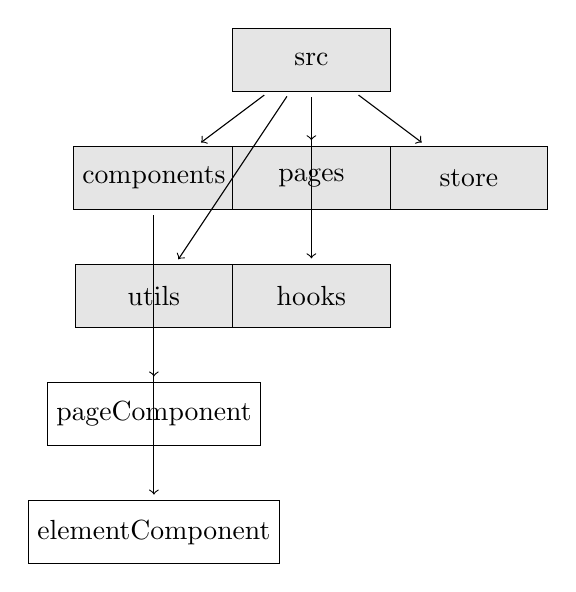
\begin{tikzpicture}[
    file/.style={draw, rectangle, minimum width=2cm, minimum height=0.8cm},
    folder/.style={draw, rectangle, minimum width=2cm, minimum height=0.8cm, fill=gray!20},
    arrow/.style={->, shorten >=2pt, shorten <=2pt}
]

% Folders
\node[folder] (src) at (0,0) {src};
\node[folder] (components) at (-2,-1.5) {components};
\node[folder] (pages) at (0,-1.5) {pages};
\node[folder] (store) at (2,-1.5) {store};
\node[folder] (utils) at (-2,-3) {utils};
\node[folder] (hooks) at (0,-3) {hooks};

% Files
\node[file] (pageComponent) at (-2,-4.5) {pageComponent};
\node[file] (elementComponent) at (-2,-6) {elementComponent};
% ... add more files

% Connections
\draw[arrow] (src) -- (components);
\draw[arrow] (src) -- (pages);
\draw[arrow] (src) -- (store);
\draw[arrow] (src) -- (utils);
\draw[arrow] (src) -- (hooks);
\draw[arrow] (components) -- (pageComponent);
\draw[arrow] (components) -- (elementComponent);
% ... add more connections

\end{tikzpicture}



\pagebreak
\subsubsection{Back-end}
The backend uses the dotNet framework. The development language using the C\# language.

In this project, the backend uses the Onion Architecture.
The Onion Architecture is a typically layered architecture, 
where each layer depends on the inner layer and provides interfaces to the outer layer.
The outer layer provides services to the outermost layer 
and other modules in the same layer based on the interfaces of the inner layer.

From inner to outer, the layers are: Domain, Application, Infrastructure, Presentation.
The Domain layer is the core layer and the innermost layer, used to define domain models, 
which are the business models.
It includes domain models and domain service interfaces.
Domain models are used to define the business models, 
which are the entities in the entity-relationship model and their attributes.
Domain service interfaces are used to define the business services, 
which are the relationships between entities in the entity-relationship model.

The Application layer is the application layer, 
used to define application services, which are the business logic.
It includes domain service implementations and application service interfaces.
Domain service implementations implement the methods of the inner layer's domain service 
interfaces and implement the business logic of the domain models.
Application service interfaces are used to define application services, 
which are the business logic.
It includes but is not limited to database interfaces, testing interfaces, 
HTTP API interfaces, MQTT interfaces, etc.

The Infrastructure layer is the infrastructure layer, used to define infrastructure.
It includes database implementations, testing implementations, 
HTTP API implementations, MQTT implementations, etc.
Database implementations implement the database interfaces 
and provide CRUD services for the database.
Testing implementations implement the testing interfaces 
and provide services for unit testing and integration testing.
HTTP API implementations implement the HTTP API interfaces 
and provide CRUD operations for HTTP APIs.
MQTT implementations implement the MQTT interfaces 
and provide CRUD operations for MQTT.

The Presentation layer is the presentation layer, used to define presentation logic, 
such as interfaces and pages. Since this is a backend project,
data presentation and control are handled by the frontend, 
so this layer is not needed.



\pagebreak
\subsubsection{Data communication and storage}
% 关于本项目的数据通信与数据存储的设计, 包括数据通信的协议, 数据存储的设计等
% 关于数据通信的设计:
% 1. 通信协议的选择
% 自前端向后端发送的数据, 有三种传输的数据类型, 
% 一种是普通的增删改查的请求, 对数据传输的时效性要求不高, 但是对数据的准确性, 完整性, 有序性, 安全性有一定的要求,
% 这种数据的传输, 采用 HTTP 协议, 以及 RESTful API 的设计. 可以有效的保证对数据传输的以上要求.
% 一种是对数据通道的创建和流媒体数据的传输, 对数据传输的时效性, 安全性要求较高, 这种数据的传输, 采用 WebRTC 协议, 以及 MQTT 协议.
% 配合可以快速解码的 flatbuffers 协议, 可以有效的保证对数据传输的以上要求.
% 最后一种是对设备的状态信息和操作信息的传输, 对完整性, 有序性, 安全性都有较高的要求, 这种数据的传输, 采用 MQTT 协议
% 同时也使用了 flatbuffers 协议.
% 
% 2. 数据通信的通信架构和通信流程
% 本项目的数据通信的通信架构, 是基于前后端分离的架构, 前端使用 React 框架, 后端使用 dotnet 框架.
% 当前端需要向后端发送数据的时候, 前端会向后端发送 HTTP 请求, 后端接收到 HTTP 请求之后, 会根据请求的数据类型,
% 选择不同的数据处理方式, 对于普通的增删改查的请求, 后端会根据 RESTful API 的设计, 对数据进行增删改查的操作,
% 对于对数据通道的创建和流媒体数据的传输, 后端会根据 WebRTC 协议, 对数据通道进行创建, 并且帮助前端和设备建立数据通道,
% 当数据通道建立后, 前端和设备之间则使用 flatbuffer 的数据格式对流媒体数据进行传输,
% 对于设备的状态信息和操作信息的传输, 前端会直接向 MQTT broker 发送 MQTT 请求, 
% 设备会在其自身的固件中监听相关的 MQTT 请求, 并且返回相关的数据.
% 
% 3. 数据通信的格式
% 本项目的数据通信的格式, 有三种, 
% 一种是 HTTP 协议, 
% 使用 json 格式对数据进行传输,
% 一种是 WebRTC 协议, 
% 使用 flatbuffers 格式对数据进行传输,
% 一种是 MQTT 协议.
% 使用 flatbuffers 格式对数据进行传输,
% 
% 关于数据存储的设计:
% 1. 数据存储的数据库的选择
% 本项目的数据存储的数据库的选择, 使用了轻量级的数据库 SQLite,
% SQLite 是一个进程内的库, 实现了自给自足的, 无服务器的, 零配置的, 事务性的 SQL 数据库引擎.
% 这是因为整个项目的目的是为了实现前端与设备之间的数据通信, 对于数据库数据的增删改查操作的要求不高,
% 数据量较小, 且对于数据库的数据的事务性要求不高, 所以选择了 SQLite 数据库.
% 2. 项目前后端的数据结构的设计
% 在本项目中, 前端由于使用了 React 框架, 所以前端的数据结构的设计, 使用了基于状态的数据结构的设计,
% 每个组件或者数据集都包含一个状态对象, 这个状态对象的属性就是组件的各个状态. 
% 使用状态对象的原因是, 可以方便的对状态进行管理, 采用对象-属性的形式, 可以方便的针对不同组件的同类状态进行区分,
% 由于跨组件的状态是由 redux 进行管理的, 这种状态对象的设计, 可以更搞笑的对状态进行更新和传递.
% 后端由于使用了 dotnet 框架, 所以后端的数据结构的设计, 使用了基于类的数据结构的设计,
% 采用了面向对象的编程思想, 对数据进行了封装, 使得数据的传输更加的安全, 有序, 完整.


\pagebreak

% \subsection{Domain model}
% \documentclass[]{article}
\usepackage{graphicx}
\usepackage{amsmath}
\usepackage{tikz}

% libaries
\usetikzlibrary{shapes,arrows}

%Define the listing package
\usepackage{listings} %code highlighter
\usepackage{color} %use color
\definecolor{mygreen}{rgb}{0,0.6,0}
\definecolor{mygray}{rgb}{0.5,0.5,0.5}
\definecolor{mymauve}{rgb}{0.58,0,0.82}

%Customize a bit the look
\lstset{ %
backgroundcolor=\color{white}, % choose the background color; you must add \usepackage{color} or \usepackage{xcolor}
basicstyle=\footnotesize, % the size of the fonts that are used for the code
breakatwhitespace=false, % sets if automatic breaks should only happen at whitespace
breaklines=true, % sets automatic line breaking
captionpos=b, % sets the caption-position to bottom
commentstyle=\color{mygreen}, % comment style
deletekeywords={...}, % if you want to delete keywords from the given language
escapeinside={\%*}{*)}, % if you want to add LaTeX within your code
extendedchars=true, % lets you use non-ASCII characters; for 8-bits encodings only, does not work with UTF-8
frame=single, % adds a frame around the code
keepspaces=true, % keeps spaces in text, useful for keeping indentation of code (possibly needs columns=flexible)
keywordstyle=\color{blue}, % keyword style
% language=Octave, % the language of the code
morekeywords={*,...}, % if you want to add more keywords to the set
numbers=left, % where to put the line-numbers; possible values are (none, left, right)
numbersep=5pt, % how far the line-numbers are from the code
numberstyle=\tiny\color{mygray}, % the style that is used for the line-numbers
rulecolor=\color{black}, % if not set, the frame-color may be changed on line-breaks within not-black text (e.g. comments (green here))
showspaces=false, % show spaces everywhere adding particular underscores; it overrides 'showstringspaces'
showstringspaces=false, % underline spaces within strings only
showtabs=false, % show tabs within strings adding particular underscores
stepnumber=1, % the step between two line-numbers. If it's 1, each line will be numbered
stringstyle=\color{mymauve}, % string literal style
tabsize=2, % sets default tabsize to 2 spaces
title=\lstname % show the filename of files included with \lstinputlisting; also try caption instead of title
}

\definecolor{darkgray}{rgb}{.4,.4,.4}
\definecolor{purple}{rgb}{0.65, 0.12, 0.82}

\lstdefinelanguage{React}{
keywords={const, typeof, new, true, false, catch, function, return, null, catch, switch, var, if, in, while, do, else, case, break},
keywordstyle=\color{blue}\bfseries,
ndkeywords={class, export, boolean, throw, implements, import, this},
ndkeywordstyle=\color{darkgray}\bfseries,
identifierstyle=\color{mygreen},
sensitive=false,
comment=[l]{//},
morecomment=[s]{/*}{*/},
commentstyle=\color{purple}\ttfamily,
string=[b]{"}{'}{`},
stringstyle=\color{red}\ttfamily,
morestring=[b]',
morestring=[b]",
morestring=[b]`',
}

\lstdefinelanguage{CSharp}{
keywords={const, typeof, new, true, false, catch, function, return, null, catch, switch, var, if, in, while, do, else, case, break},
keywordstyle=\color{blue}\bfseries,
ndkeywords={class, export, boolean, throw, implements, import, this},
ndkeywordstyle=\color{darkgray}\bfseries,
identifierstyle=\color{mygreen},
sensitive=false,
comment=[l]{//},
morecomment=[s]{/*}{*/},
commentstyle=\color{purple}\ttfamily,
string=[b]{"}{'}{`},
stringstyle=\color{red}\ttfamily,
morestring=[b]',
morestring=[b]",
morestring=[b]`',
}

\lstset{
language=React,
extendedchars=true,
basicstyle=\footnotesize\ttfamily,
showstringspaces=false,
showspaces=false,
numbers=left,
numberstyle=\footnotesize,
numbersep=9pt,
tabsize=2,
breaklines=true,
showtabs=false,
captionpos=b
}

\lstset{
language=CSharp,
extendedchars=true,
basicstyle=\footnotesize\ttfamily,
showstringspaces=false,
showspaces=false,
numbers=left,
numberstyle=\footnotesize,
numbersep=9pt,
tabsize=2,
breaklines=true,
showtabs=false,
captionpos=b
}

% \usepackage{cite} % Add this line for citation

% \bibliographystyle{plain}

\title{
The implementation of BifrostConnect Front-end scope, 
re-design and development with the relevant back-end support develop.
}
\author{
    Fei Gu \\
    Erhvervs Akademi Sydvest \\
    Computer Science 21\\
    }
\date{\today}

\begin{document}

% Front page
\maketitle
\begin{center}
    Supervisor: Henrik Boulund Meng Hansen \\
    Company: BifrostConnect \\
    Engineering Director: Jasper Wass \\
\end{center}
\tableofcontents
\pagebreak


% The introduction
\section{Introduction}
\subsection{Background}\input{sections/introduction/background.tex}
\subsection{The company}\input{sections/introduction/aboutCompany}
\subsection{The project}\input{sections/introduction/aboutProject}
\pagebreak

% The problem statement
\section{Problem Statement}
\subsection{Statement}
\input{sections/problemStatement/statement}
\subsection{Situation}
\input{sections/problemStatement/situation}
\subsection{Potential Solution}
\input{sections/problemStatement/potentialSolution}
\pagebreak

% Requirement analysis
\section{Requirement Analysis}
\input{sections/requirementAnalysis/index}

\subsection{Stakeholders}
\input{sections/requirementAnalysis/stakeholders/index}

\subsection{Business Domain}
\input{sections/requirementAnalysis/bussinesDomain/index}

\subsection{Scope}
\input{sections/requirementAnalysis/scope}

\subsection{Goals}
\input{sections/requirementAnalysis/goals}
\pagebreak

% Software Design
\section{Software Design}
% developement methods
\subsection{Software Development Methods}
\input{sections/softwareDevelopmentMethods/index}
\subsubsection{Agile Software Development}
\input{sections/softwareDevelopmentMethods/agileSoftwareDevelopment/index}
\subsubsection{Feature Driven Development}
\input{sections/softwareDevelopmentMethods/featureDrivenDevelopment/index}

\pagebreak

% Technology seslection
\subsection{Technology selection}
\input{sections/softwareDesign/technologySelection/index}
\subsubsection{Front-end}
\input{sections/softwareDesign/technologySelection/frontEnd}            
\subsubsection{Back-end}
\input{sections/softwareDesign/technologySelection/backEnd}            
\subsubsection{Database}
\input{sections/softwareDesign/technologySelection/database}
\subsubsection{Data communication}
\input{sections/softwareDesign/technologySelection/dataCommunication}            
\subsubsection{DevOps}
\input{sections/softwareDesign/technologySelection/devOps}
\pagebreak

% Architecture design
\subsection{Architecture design}
\input{sections/softwareDesign/architectureDesign/index}
\pagebreak
\subsubsection{Front-end}
\input{sections/softwareDesign/architectureDesign/frontEndArchitecture}
\pagebreak
\subsubsection{Back-end}
\input{sections/softwareDesign/architectureDesign/backEndArchitecture}
\pagebreak
\subsubsection{Data communication and storage}
\input{sections/softwareDesign/architectureDesign/dataCommunicationArchitecture}
\pagebreak

% \subsection{Domain model}
% \input{sections/softwareDesign/domainModel/index}
% \subsection{Database design}
% % 数据库领域模型 ER 图
% % 包括表和字段的设置.
% % 对于私有键和外键的设置.

% \subsection{Back-end design}
% % 后端对象模型
% % 以及对于对象模型的增删改查
% % 以及相关的其他服务的设计`'

% \subsection{Front-end design}
% % 对于前端的页面结构的设计 
% % 页面的状态的设计, 交互设计

% \subsection{FlatBuffers design}
% % schema 的设计

\subsection{DevOps CI/CD process design}
\input{sections/softwareDesign/devOpsDesign/index}
\subsubsection{Continuous Integration}
\input{sections/softwareDesign/devOpsDesign/continuousIntegration/index}
\subsubsection{Continuous Delivery}
\input{sections/softwareDesign/devOpsDesign/continuousDelivery/index}
\subsubsection{Continuous Deployment}
\input{sections/softwareDesign/devOpsDesign/continuousDeployment/index}
\pagebreak

\section{Software Development} 
\input{sections/softwareDevelopment/index}
\subsection{Overall development}
\input{sections/softwareDevelopment/overallDevelopement/index}
\subsubsection{Front-end}
\input{sections/softwareDevelopment/overallDevelopement/frontEnd/index}
\subsubsection{Back-end}
\input{sections/softwareDevelopment/overallDevelopement/backEnd/index}
\subsubsection{DevOps}
\input{sections/softwareDevelopment/overallDevelopement/devOps/index}
\subsection{Feature development} 
\input{sections/softwareDevelopment/featureDevelopment/index}
\subsubsection{Use Case 1}
\input{sections/softwareDevelopment/featureDevelopment/useCase1/index}
\subsubsection{Feature 1}
\input{sections/softwareDevelopment/featureDevelopment/feature/feature1.tex}
\pagebreak
\section{Conclusion} 
\subsection{Result}
Since the project is still in progress, the result is not available yet.
So far, basic structure of this project has been built. But the most features 
are not implemented yet. 
\subsection{Discussion}
As a single developer for this project, I am confident what I have done so far.
And I can say I understand the most of the knowledge I have used in this project, 
which also means I can explain all the part of the project. 
But this project also relevant some of the complex knowledge which I have to continue 
to study and practice.
\subsection{Future Work}
The future work is to implement the rest of the features. 
Including the most important part which is the 'create session' feature.
\pagebreak
% \bibliography{bibliography}
\pagebreak
% \begin{appendices}
%     \section{Appendix}
% \end{appendices} 
\end{document}
% \subsection{Database design}
% % 数据库领域模型 ER 图
% % 包括表和字段的设置.
% % 对于私有键和外键的设置.

% \subsection{Back-end design}
% % 后端对象模型
% % 以及对于对象模型的增删改查
% % 以及相关的其他服务的设计`'

% \subsection{Front-end design}
% % 对于前端的页面结构的设计 
% % 页面的状态的设计, 交互设计

% \subsection{FlatBuffers design}
% % schema 的设计

\subsection{DevOps CI/CD process design}
\documentclass[]{article}
\usepackage{graphicx}
\usepackage{amsmath}
\usepackage{tikz}

% libaries
\usetikzlibrary{shapes,arrows}

%Define the listing package
\usepackage{listings} %code highlighter
\usepackage{color} %use color
\definecolor{mygreen}{rgb}{0,0.6,0}
\definecolor{mygray}{rgb}{0.5,0.5,0.5}
\definecolor{mymauve}{rgb}{0.58,0,0.82}

%Customize a bit the look
\lstset{ %
backgroundcolor=\color{white}, % choose the background color; you must add \usepackage{color} or \usepackage{xcolor}
basicstyle=\footnotesize, % the size of the fonts that are used for the code
breakatwhitespace=false, % sets if automatic breaks should only happen at whitespace
breaklines=true, % sets automatic line breaking
captionpos=b, % sets the caption-position to bottom
commentstyle=\color{mygreen}, % comment style
deletekeywords={...}, % if you want to delete keywords from the given language
escapeinside={\%*}{*)}, % if you want to add LaTeX within your code
extendedchars=true, % lets you use non-ASCII characters; for 8-bits encodings only, does not work with UTF-8
frame=single, % adds a frame around the code
keepspaces=true, % keeps spaces in text, useful for keeping indentation of code (possibly needs columns=flexible)
keywordstyle=\color{blue}, % keyword style
% language=Octave, % the language of the code
morekeywords={*,...}, % if you want to add more keywords to the set
numbers=left, % where to put the line-numbers; possible values are (none, left, right)
numbersep=5pt, % how far the line-numbers are from the code
numberstyle=\tiny\color{mygray}, % the style that is used for the line-numbers
rulecolor=\color{black}, % if not set, the frame-color may be changed on line-breaks within not-black text (e.g. comments (green here))
showspaces=false, % show spaces everywhere adding particular underscores; it overrides 'showstringspaces'
showstringspaces=false, % underline spaces within strings only
showtabs=false, % show tabs within strings adding particular underscores
stepnumber=1, % the step between two line-numbers. If it's 1, each line will be numbered
stringstyle=\color{mymauve}, % string literal style
tabsize=2, % sets default tabsize to 2 spaces
title=\lstname % show the filename of files included with \lstinputlisting; also try caption instead of title
}

\definecolor{darkgray}{rgb}{.4,.4,.4}
\definecolor{purple}{rgb}{0.65, 0.12, 0.82}

\lstdefinelanguage{React}{
keywords={const, typeof, new, true, false, catch, function, return, null, catch, switch, var, if, in, while, do, else, case, break},
keywordstyle=\color{blue}\bfseries,
ndkeywords={class, export, boolean, throw, implements, import, this},
ndkeywordstyle=\color{darkgray}\bfseries,
identifierstyle=\color{mygreen},
sensitive=false,
comment=[l]{//},
morecomment=[s]{/*}{*/},
commentstyle=\color{purple}\ttfamily,
string=[b]{"}{'}{`},
stringstyle=\color{red}\ttfamily,
morestring=[b]',
morestring=[b]",
morestring=[b]`',
}

\lstdefinelanguage{CSharp}{
keywords={const, typeof, new, true, false, catch, function, return, null, catch, switch, var, if, in, while, do, else, case, break},
keywordstyle=\color{blue}\bfseries,
ndkeywords={class, export, boolean, throw, implements, import, this},
ndkeywordstyle=\color{darkgray}\bfseries,
identifierstyle=\color{mygreen},
sensitive=false,
comment=[l]{//},
morecomment=[s]{/*}{*/},
commentstyle=\color{purple}\ttfamily,
string=[b]{"}{'}{`},
stringstyle=\color{red}\ttfamily,
morestring=[b]',
morestring=[b]",
morestring=[b]`',
}

\lstset{
language=React,
extendedchars=true,
basicstyle=\footnotesize\ttfamily,
showstringspaces=false,
showspaces=false,
numbers=left,
numberstyle=\footnotesize,
numbersep=9pt,
tabsize=2,
breaklines=true,
showtabs=false,
captionpos=b
}

\lstset{
language=CSharp,
extendedchars=true,
basicstyle=\footnotesize\ttfamily,
showstringspaces=false,
showspaces=false,
numbers=left,
numberstyle=\footnotesize,
numbersep=9pt,
tabsize=2,
breaklines=true,
showtabs=false,
captionpos=b
}

% \usepackage{cite} % Add this line for citation

% \bibliographystyle{plain}

\title{
The implementation of BifrostConnect Front-end scope, 
re-design and development with the relevant back-end support develop.
}
\author{
    Fei Gu \\
    Erhvervs Akademi Sydvest \\
    Computer Science 21\\
    }
\date{\today}

\begin{document}

% Front page
\maketitle
\begin{center}
    Supervisor: Henrik Boulund Meng Hansen \\
    Company: BifrostConnect \\
    Engineering Director: Jasper Wass \\
\end{center}
\tableofcontents
\pagebreak


% The introduction
\section{Introduction}
\subsection{Background}\input{sections/introduction/background.tex}
\subsection{The company}\input{sections/introduction/aboutCompany}
\subsection{The project}\input{sections/introduction/aboutProject}
\pagebreak

% The problem statement
\section{Problem Statement}
\subsection{Statement}
\input{sections/problemStatement/statement}
\subsection{Situation}
\input{sections/problemStatement/situation}
\subsection{Potential Solution}
\input{sections/problemStatement/potentialSolution}
\pagebreak

% Requirement analysis
\section{Requirement Analysis}
\input{sections/requirementAnalysis/index}

\subsection{Stakeholders}
\input{sections/requirementAnalysis/stakeholders/index}

\subsection{Business Domain}
\input{sections/requirementAnalysis/bussinesDomain/index}

\subsection{Scope}
\input{sections/requirementAnalysis/scope}

\subsection{Goals}
\input{sections/requirementAnalysis/goals}
\pagebreak

% Software Design
\section{Software Design}
% developement methods
\subsection{Software Development Methods}
\input{sections/softwareDevelopmentMethods/index}
\subsubsection{Agile Software Development}
\input{sections/softwareDevelopmentMethods/agileSoftwareDevelopment/index}
\subsubsection{Feature Driven Development}
\input{sections/softwareDevelopmentMethods/featureDrivenDevelopment/index}

\pagebreak

% Technology seslection
\subsection{Technology selection}
\input{sections/softwareDesign/technologySelection/index}
\subsubsection{Front-end}
\input{sections/softwareDesign/technologySelection/frontEnd}            
\subsubsection{Back-end}
\input{sections/softwareDesign/technologySelection/backEnd}            
\subsubsection{Database}
\input{sections/softwareDesign/technologySelection/database}
\subsubsection{Data communication}
\input{sections/softwareDesign/technologySelection/dataCommunication}            
\subsubsection{DevOps}
\input{sections/softwareDesign/technologySelection/devOps}
\pagebreak

% Architecture design
\subsection{Architecture design}
\input{sections/softwareDesign/architectureDesign/index}
\pagebreak
\subsubsection{Front-end}
\input{sections/softwareDesign/architectureDesign/frontEndArchitecture}
\pagebreak
\subsubsection{Back-end}
\input{sections/softwareDesign/architectureDesign/backEndArchitecture}
\pagebreak
\subsubsection{Data communication and storage}
\input{sections/softwareDesign/architectureDesign/dataCommunicationArchitecture}
\pagebreak

% \subsection{Domain model}
% \input{sections/softwareDesign/domainModel/index}
% \subsection{Database design}
% % 数据库领域模型 ER 图
% % 包括表和字段的设置.
% % 对于私有键和外键的设置.

% \subsection{Back-end design}
% % 后端对象模型
% % 以及对于对象模型的增删改查
% % 以及相关的其他服务的设计`'

% \subsection{Front-end design}
% % 对于前端的页面结构的设计 
% % 页面的状态的设计, 交互设计

% \subsection{FlatBuffers design}
% % schema 的设计

\subsection{DevOps CI/CD process design}
\input{sections/softwareDesign/devOpsDesign/index}
\subsubsection{Continuous Integration}
\input{sections/softwareDesign/devOpsDesign/continuousIntegration/index}
\subsubsection{Continuous Delivery}
\input{sections/softwareDesign/devOpsDesign/continuousDelivery/index}
\subsubsection{Continuous Deployment}
\input{sections/softwareDesign/devOpsDesign/continuousDeployment/index}
\pagebreak

\section{Software Development} 
\input{sections/softwareDevelopment/index}
\subsection{Overall development}
\input{sections/softwareDevelopment/overallDevelopement/index}
\subsubsection{Front-end}
\input{sections/softwareDevelopment/overallDevelopement/frontEnd/index}
\subsubsection{Back-end}
\input{sections/softwareDevelopment/overallDevelopement/backEnd/index}
\subsubsection{DevOps}
\input{sections/softwareDevelopment/overallDevelopement/devOps/index}
\subsection{Feature development} 
\input{sections/softwareDevelopment/featureDevelopment/index}
\subsubsection{Use Case 1}
\input{sections/softwareDevelopment/featureDevelopment/useCase1/index}
\subsubsection{Feature 1}
\input{sections/softwareDevelopment/featureDevelopment/feature/feature1.tex}
\pagebreak
\section{Conclusion} 
\subsection{Result}
Since the project is still in progress, the result is not available yet.
So far, basic structure of this project has been built. But the most features 
are not implemented yet. 
\subsection{Discussion}
As a single developer for this project, I am confident what I have done so far.
And I can say I understand the most of the knowledge I have used in this project, 
which also means I can explain all the part of the project. 
But this project also relevant some of the complex knowledge which I have to continue 
to study and practice.
\subsection{Future Work}
The future work is to implement the rest of the features. 
Including the most important part which is the 'create session' feature.
\pagebreak
% \bibliography{bibliography}
\pagebreak
% \begin{appendices}
%     \section{Appendix}
% \end{appendices} 
\end{document}
\subsubsection{Continuous Integration}
\documentclass[]{article}
\usepackage{graphicx}
\usepackage{amsmath}
\usepackage{tikz}

% libaries
\usetikzlibrary{shapes,arrows}

%Define the listing package
\usepackage{listings} %code highlighter
\usepackage{color} %use color
\definecolor{mygreen}{rgb}{0,0.6,0}
\definecolor{mygray}{rgb}{0.5,0.5,0.5}
\definecolor{mymauve}{rgb}{0.58,0,0.82}

%Customize a bit the look
\lstset{ %
backgroundcolor=\color{white}, % choose the background color; you must add \usepackage{color} or \usepackage{xcolor}
basicstyle=\footnotesize, % the size of the fonts that are used for the code
breakatwhitespace=false, % sets if automatic breaks should only happen at whitespace
breaklines=true, % sets automatic line breaking
captionpos=b, % sets the caption-position to bottom
commentstyle=\color{mygreen}, % comment style
deletekeywords={...}, % if you want to delete keywords from the given language
escapeinside={\%*}{*)}, % if you want to add LaTeX within your code
extendedchars=true, % lets you use non-ASCII characters; for 8-bits encodings only, does not work with UTF-8
frame=single, % adds a frame around the code
keepspaces=true, % keeps spaces in text, useful for keeping indentation of code (possibly needs columns=flexible)
keywordstyle=\color{blue}, % keyword style
% language=Octave, % the language of the code
morekeywords={*,...}, % if you want to add more keywords to the set
numbers=left, % where to put the line-numbers; possible values are (none, left, right)
numbersep=5pt, % how far the line-numbers are from the code
numberstyle=\tiny\color{mygray}, % the style that is used for the line-numbers
rulecolor=\color{black}, % if not set, the frame-color may be changed on line-breaks within not-black text (e.g. comments (green here))
showspaces=false, % show spaces everywhere adding particular underscores; it overrides 'showstringspaces'
showstringspaces=false, % underline spaces within strings only
showtabs=false, % show tabs within strings adding particular underscores
stepnumber=1, % the step between two line-numbers. If it's 1, each line will be numbered
stringstyle=\color{mymauve}, % string literal style
tabsize=2, % sets default tabsize to 2 spaces
title=\lstname % show the filename of files included with \lstinputlisting; also try caption instead of title
}

\definecolor{darkgray}{rgb}{.4,.4,.4}
\definecolor{purple}{rgb}{0.65, 0.12, 0.82}

\lstdefinelanguage{React}{
keywords={const, typeof, new, true, false, catch, function, return, null, catch, switch, var, if, in, while, do, else, case, break},
keywordstyle=\color{blue}\bfseries,
ndkeywords={class, export, boolean, throw, implements, import, this},
ndkeywordstyle=\color{darkgray}\bfseries,
identifierstyle=\color{mygreen},
sensitive=false,
comment=[l]{//},
morecomment=[s]{/*}{*/},
commentstyle=\color{purple}\ttfamily,
string=[b]{"}{'}{`},
stringstyle=\color{red}\ttfamily,
morestring=[b]',
morestring=[b]",
morestring=[b]`',
}

\lstdefinelanguage{CSharp}{
keywords={const, typeof, new, true, false, catch, function, return, null, catch, switch, var, if, in, while, do, else, case, break},
keywordstyle=\color{blue}\bfseries,
ndkeywords={class, export, boolean, throw, implements, import, this},
ndkeywordstyle=\color{darkgray}\bfseries,
identifierstyle=\color{mygreen},
sensitive=false,
comment=[l]{//},
morecomment=[s]{/*}{*/},
commentstyle=\color{purple}\ttfamily,
string=[b]{"}{'}{`},
stringstyle=\color{red}\ttfamily,
morestring=[b]',
morestring=[b]",
morestring=[b]`',
}

\lstset{
language=React,
extendedchars=true,
basicstyle=\footnotesize\ttfamily,
showstringspaces=false,
showspaces=false,
numbers=left,
numberstyle=\footnotesize,
numbersep=9pt,
tabsize=2,
breaklines=true,
showtabs=false,
captionpos=b
}

\lstset{
language=CSharp,
extendedchars=true,
basicstyle=\footnotesize\ttfamily,
showstringspaces=false,
showspaces=false,
numbers=left,
numberstyle=\footnotesize,
numbersep=9pt,
tabsize=2,
breaklines=true,
showtabs=false,
captionpos=b
}

% \usepackage{cite} % Add this line for citation

% \bibliographystyle{plain}

\title{
The implementation of BifrostConnect Front-end scope, 
re-design and development with the relevant back-end support develop.
}
\author{
    Fei Gu \\
    Erhvervs Akademi Sydvest \\
    Computer Science 21\\
    }
\date{\today}

\begin{document}

% Front page
\maketitle
\begin{center}
    Supervisor: Henrik Boulund Meng Hansen \\
    Company: BifrostConnect \\
    Engineering Director: Jasper Wass \\
\end{center}
\tableofcontents
\pagebreak


% The introduction
\section{Introduction}
\subsection{Background}\input{sections/introduction/background.tex}
\subsection{The company}\input{sections/introduction/aboutCompany}
\subsection{The project}\input{sections/introduction/aboutProject}
\pagebreak

% The problem statement
\section{Problem Statement}
\subsection{Statement}
\input{sections/problemStatement/statement}
\subsection{Situation}
\input{sections/problemStatement/situation}
\subsection{Potential Solution}
\input{sections/problemStatement/potentialSolution}
\pagebreak

% Requirement analysis
\section{Requirement Analysis}
\input{sections/requirementAnalysis/index}

\subsection{Stakeholders}
\input{sections/requirementAnalysis/stakeholders/index}

\subsection{Business Domain}
\input{sections/requirementAnalysis/bussinesDomain/index}

\subsection{Scope}
\input{sections/requirementAnalysis/scope}

\subsection{Goals}
\input{sections/requirementAnalysis/goals}
\pagebreak

% Software Design
\section{Software Design}
% developement methods
\subsection{Software Development Methods}
\input{sections/softwareDevelopmentMethods/index}
\subsubsection{Agile Software Development}
\input{sections/softwareDevelopmentMethods/agileSoftwareDevelopment/index}
\subsubsection{Feature Driven Development}
\input{sections/softwareDevelopmentMethods/featureDrivenDevelopment/index}

\pagebreak

% Technology seslection
\subsection{Technology selection}
\input{sections/softwareDesign/technologySelection/index}
\subsubsection{Front-end}
\input{sections/softwareDesign/technologySelection/frontEnd}            
\subsubsection{Back-end}
\input{sections/softwareDesign/technologySelection/backEnd}            
\subsubsection{Database}
\input{sections/softwareDesign/technologySelection/database}
\subsubsection{Data communication}
\input{sections/softwareDesign/technologySelection/dataCommunication}            
\subsubsection{DevOps}
\input{sections/softwareDesign/technologySelection/devOps}
\pagebreak

% Architecture design
\subsection{Architecture design}
\input{sections/softwareDesign/architectureDesign/index}
\pagebreak
\subsubsection{Front-end}
\input{sections/softwareDesign/architectureDesign/frontEndArchitecture}
\pagebreak
\subsubsection{Back-end}
\input{sections/softwareDesign/architectureDesign/backEndArchitecture}
\pagebreak
\subsubsection{Data communication and storage}
\input{sections/softwareDesign/architectureDesign/dataCommunicationArchitecture}
\pagebreak

% \subsection{Domain model}
% \input{sections/softwareDesign/domainModel/index}
% \subsection{Database design}
% % 数据库领域模型 ER 图
% % 包括表和字段的设置.
% % 对于私有键和外键的设置.

% \subsection{Back-end design}
% % 后端对象模型
% % 以及对于对象模型的增删改查
% % 以及相关的其他服务的设计`'

% \subsection{Front-end design}
% % 对于前端的页面结构的设计 
% % 页面的状态的设计, 交互设计

% \subsection{FlatBuffers design}
% % schema 的设计

\subsection{DevOps CI/CD process design}
\input{sections/softwareDesign/devOpsDesign/index}
\subsubsection{Continuous Integration}
\input{sections/softwareDesign/devOpsDesign/continuousIntegration/index}
\subsubsection{Continuous Delivery}
\input{sections/softwareDesign/devOpsDesign/continuousDelivery/index}
\subsubsection{Continuous Deployment}
\input{sections/softwareDesign/devOpsDesign/continuousDeployment/index}
\pagebreak

\section{Software Development} 
\input{sections/softwareDevelopment/index}
\subsection{Overall development}
\input{sections/softwareDevelopment/overallDevelopement/index}
\subsubsection{Front-end}
\input{sections/softwareDevelopment/overallDevelopement/frontEnd/index}
\subsubsection{Back-end}
\input{sections/softwareDevelopment/overallDevelopement/backEnd/index}
\subsubsection{DevOps}
\input{sections/softwareDevelopment/overallDevelopement/devOps/index}
\subsection{Feature development} 
\input{sections/softwareDevelopment/featureDevelopment/index}
\subsubsection{Use Case 1}
\input{sections/softwareDevelopment/featureDevelopment/useCase1/index}
\subsubsection{Feature 1}
\input{sections/softwareDevelopment/featureDevelopment/feature/feature1.tex}
\pagebreak
\section{Conclusion} 
\subsection{Result}
Since the project is still in progress, the result is not available yet.
So far, basic structure of this project has been built. But the most features 
are not implemented yet. 
\subsection{Discussion}
As a single developer for this project, I am confident what I have done so far.
And I can say I understand the most of the knowledge I have used in this project, 
which also means I can explain all the part of the project. 
But this project also relevant some of the complex knowledge which I have to continue 
to study and practice.
\subsection{Future Work}
The future work is to implement the rest of the features. 
Including the most important part which is the 'create session' feature.
\pagebreak
% \bibliography{bibliography}
\pagebreak
% \begin{appendices}
%     \section{Appendix}
% \end{appendices} 
\end{document}
\subsubsection{Continuous Delivery}
\documentclass[]{article}
\usepackage{graphicx}
\usepackage{amsmath}
\usepackage{tikz}

% libaries
\usetikzlibrary{shapes,arrows}

%Define the listing package
\usepackage{listings} %code highlighter
\usepackage{color} %use color
\definecolor{mygreen}{rgb}{0,0.6,0}
\definecolor{mygray}{rgb}{0.5,0.5,0.5}
\definecolor{mymauve}{rgb}{0.58,0,0.82}

%Customize a bit the look
\lstset{ %
backgroundcolor=\color{white}, % choose the background color; you must add \usepackage{color} or \usepackage{xcolor}
basicstyle=\footnotesize, % the size of the fonts that are used for the code
breakatwhitespace=false, % sets if automatic breaks should only happen at whitespace
breaklines=true, % sets automatic line breaking
captionpos=b, % sets the caption-position to bottom
commentstyle=\color{mygreen}, % comment style
deletekeywords={...}, % if you want to delete keywords from the given language
escapeinside={\%*}{*)}, % if you want to add LaTeX within your code
extendedchars=true, % lets you use non-ASCII characters; for 8-bits encodings only, does not work with UTF-8
frame=single, % adds a frame around the code
keepspaces=true, % keeps spaces in text, useful for keeping indentation of code (possibly needs columns=flexible)
keywordstyle=\color{blue}, % keyword style
% language=Octave, % the language of the code
morekeywords={*,...}, % if you want to add more keywords to the set
numbers=left, % where to put the line-numbers; possible values are (none, left, right)
numbersep=5pt, % how far the line-numbers are from the code
numberstyle=\tiny\color{mygray}, % the style that is used for the line-numbers
rulecolor=\color{black}, % if not set, the frame-color may be changed on line-breaks within not-black text (e.g. comments (green here))
showspaces=false, % show spaces everywhere adding particular underscores; it overrides 'showstringspaces'
showstringspaces=false, % underline spaces within strings only
showtabs=false, % show tabs within strings adding particular underscores
stepnumber=1, % the step between two line-numbers. If it's 1, each line will be numbered
stringstyle=\color{mymauve}, % string literal style
tabsize=2, % sets default tabsize to 2 spaces
title=\lstname % show the filename of files included with \lstinputlisting; also try caption instead of title
}

\definecolor{darkgray}{rgb}{.4,.4,.4}
\definecolor{purple}{rgb}{0.65, 0.12, 0.82}

\lstdefinelanguage{React}{
keywords={const, typeof, new, true, false, catch, function, return, null, catch, switch, var, if, in, while, do, else, case, break},
keywordstyle=\color{blue}\bfseries,
ndkeywords={class, export, boolean, throw, implements, import, this},
ndkeywordstyle=\color{darkgray}\bfseries,
identifierstyle=\color{mygreen},
sensitive=false,
comment=[l]{//},
morecomment=[s]{/*}{*/},
commentstyle=\color{purple}\ttfamily,
string=[b]{"}{'}{`},
stringstyle=\color{red}\ttfamily,
morestring=[b]',
morestring=[b]",
morestring=[b]`',
}

\lstdefinelanguage{CSharp}{
keywords={const, typeof, new, true, false, catch, function, return, null, catch, switch, var, if, in, while, do, else, case, break},
keywordstyle=\color{blue}\bfseries,
ndkeywords={class, export, boolean, throw, implements, import, this},
ndkeywordstyle=\color{darkgray}\bfseries,
identifierstyle=\color{mygreen},
sensitive=false,
comment=[l]{//},
morecomment=[s]{/*}{*/},
commentstyle=\color{purple}\ttfamily,
string=[b]{"}{'}{`},
stringstyle=\color{red}\ttfamily,
morestring=[b]',
morestring=[b]",
morestring=[b]`',
}

\lstset{
language=React,
extendedchars=true,
basicstyle=\footnotesize\ttfamily,
showstringspaces=false,
showspaces=false,
numbers=left,
numberstyle=\footnotesize,
numbersep=9pt,
tabsize=2,
breaklines=true,
showtabs=false,
captionpos=b
}

\lstset{
language=CSharp,
extendedchars=true,
basicstyle=\footnotesize\ttfamily,
showstringspaces=false,
showspaces=false,
numbers=left,
numberstyle=\footnotesize,
numbersep=9pt,
tabsize=2,
breaklines=true,
showtabs=false,
captionpos=b
}

% \usepackage{cite} % Add this line for citation

% \bibliographystyle{plain}

\title{
The implementation of BifrostConnect Front-end scope, 
re-design and development with the relevant back-end support develop.
}
\author{
    Fei Gu \\
    Erhvervs Akademi Sydvest \\
    Computer Science 21\\
    }
\date{\today}

\begin{document}

% Front page
\maketitle
\begin{center}
    Supervisor: Henrik Boulund Meng Hansen \\
    Company: BifrostConnect \\
    Engineering Director: Jasper Wass \\
\end{center}
\tableofcontents
\pagebreak


% The introduction
\section{Introduction}
\subsection{Background}\input{sections/introduction/background.tex}
\subsection{The company}\input{sections/introduction/aboutCompany}
\subsection{The project}\input{sections/introduction/aboutProject}
\pagebreak

% The problem statement
\section{Problem Statement}
\subsection{Statement}
\input{sections/problemStatement/statement}
\subsection{Situation}
\input{sections/problemStatement/situation}
\subsection{Potential Solution}
\input{sections/problemStatement/potentialSolution}
\pagebreak

% Requirement analysis
\section{Requirement Analysis}
\input{sections/requirementAnalysis/index}

\subsection{Stakeholders}
\input{sections/requirementAnalysis/stakeholders/index}

\subsection{Business Domain}
\input{sections/requirementAnalysis/bussinesDomain/index}

\subsection{Scope}
\input{sections/requirementAnalysis/scope}

\subsection{Goals}
\input{sections/requirementAnalysis/goals}
\pagebreak

% Software Design
\section{Software Design}
% developement methods
\subsection{Software Development Methods}
\input{sections/softwareDevelopmentMethods/index}
\subsubsection{Agile Software Development}
\input{sections/softwareDevelopmentMethods/agileSoftwareDevelopment/index}
\subsubsection{Feature Driven Development}
\input{sections/softwareDevelopmentMethods/featureDrivenDevelopment/index}

\pagebreak

% Technology seslection
\subsection{Technology selection}
\input{sections/softwareDesign/technologySelection/index}
\subsubsection{Front-end}
\input{sections/softwareDesign/technologySelection/frontEnd}            
\subsubsection{Back-end}
\input{sections/softwareDesign/technologySelection/backEnd}            
\subsubsection{Database}
\input{sections/softwareDesign/technologySelection/database}
\subsubsection{Data communication}
\input{sections/softwareDesign/technologySelection/dataCommunication}            
\subsubsection{DevOps}
\input{sections/softwareDesign/technologySelection/devOps}
\pagebreak

% Architecture design
\subsection{Architecture design}
\input{sections/softwareDesign/architectureDesign/index}
\pagebreak
\subsubsection{Front-end}
\input{sections/softwareDesign/architectureDesign/frontEndArchitecture}
\pagebreak
\subsubsection{Back-end}
\input{sections/softwareDesign/architectureDesign/backEndArchitecture}
\pagebreak
\subsubsection{Data communication and storage}
\input{sections/softwareDesign/architectureDesign/dataCommunicationArchitecture}
\pagebreak

% \subsection{Domain model}
% \input{sections/softwareDesign/domainModel/index}
% \subsection{Database design}
% % 数据库领域模型 ER 图
% % 包括表和字段的设置.
% % 对于私有键和外键的设置.

% \subsection{Back-end design}
% % 后端对象模型
% % 以及对于对象模型的增删改查
% % 以及相关的其他服务的设计`'

% \subsection{Front-end design}
% % 对于前端的页面结构的设计 
% % 页面的状态的设计, 交互设计

% \subsection{FlatBuffers design}
% % schema 的设计

\subsection{DevOps CI/CD process design}
\input{sections/softwareDesign/devOpsDesign/index}
\subsubsection{Continuous Integration}
\input{sections/softwareDesign/devOpsDesign/continuousIntegration/index}
\subsubsection{Continuous Delivery}
\input{sections/softwareDesign/devOpsDesign/continuousDelivery/index}
\subsubsection{Continuous Deployment}
\input{sections/softwareDesign/devOpsDesign/continuousDeployment/index}
\pagebreak

\section{Software Development} 
\input{sections/softwareDevelopment/index}
\subsection{Overall development}
\input{sections/softwareDevelopment/overallDevelopement/index}
\subsubsection{Front-end}
\input{sections/softwareDevelopment/overallDevelopement/frontEnd/index}
\subsubsection{Back-end}
\input{sections/softwareDevelopment/overallDevelopement/backEnd/index}
\subsubsection{DevOps}
\input{sections/softwareDevelopment/overallDevelopement/devOps/index}
\subsection{Feature development} 
\input{sections/softwareDevelopment/featureDevelopment/index}
\subsubsection{Use Case 1}
\input{sections/softwareDevelopment/featureDevelopment/useCase1/index}
\subsubsection{Feature 1}
\input{sections/softwareDevelopment/featureDevelopment/feature/feature1.tex}
\pagebreak
\section{Conclusion} 
\subsection{Result}
Since the project is still in progress, the result is not available yet.
So far, basic structure of this project has been built. But the most features 
are not implemented yet. 
\subsection{Discussion}
As a single developer for this project, I am confident what I have done so far.
And I can say I understand the most of the knowledge I have used in this project, 
which also means I can explain all the part of the project. 
But this project also relevant some of the complex knowledge which I have to continue 
to study and practice.
\subsection{Future Work}
The future work is to implement the rest of the features. 
Including the most important part which is the 'create session' feature.
\pagebreak
% \bibliography{bibliography}
\pagebreak
% \begin{appendices}
%     \section{Appendix}
% \end{appendices} 
\end{document}
\subsubsection{Continuous Deployment}
\documentclass[]{article}
\usepackage{graphicx}
\usepackage{amsmath}
\usepackage{tikz}

% libaries
\usetikzlibrary{shapes,arrows}

%Define the listing package
\usepackage{listings} %code highlighter
\usepackage{color} %use color
\definecolor{mygreen}{rgb}{0,0.6,0}
\definecolor{mygray}{rgb}{0.5,0.5,0.5}
\definecolor{mymauve}{rgb}{0.58,0,0.82}

%Customize a bit the look
\lstset{ %
backgroundcolor=\color{white}, % choose the background color; you must add \usepackage{color} or \usepackage{xcolor}
basicstyle=\footnotesize, % the size of the fonts that are used for the code
breakatwhitespace=false, % sets if automatic breaks should only happen at whitespace
breaklines=true, % sets automatic line breaking
captionpos=b, % sets the caption-position to bottom
commentstyle=\color{mygreen}, % comment style
deletekeywords={...}, % if you want to delete keywords from the given language
escapeinside={\%*}{*)}, % if you want to add LaTeX within your code
extendedchars=true, % lets you use non-ASCII characters; for 8-bits encodings only, does not work with UTF-8
frame=single, % adds a frame around the code
keepspaces=true, % keeps spaces in text, useful for keeping indentation of code (possibly needs columns=flexible)
keywordstyle=\color{blue}, % keyword style
% language=Octave, % the language of the code
morekeywords={*,...}, % if you want to add more keywords to the set
numbers=left, % where to put the line-numbers; possible values are (none, left, right)
numbersep=5pt, % how far the line-numbers are from the code
numberstyle=\tiny\color{mygray}, % the style that is used for the line-numbers
rulecolor=\color{black}, % if not set, the frame-color may be changed on line-breaks within not-black text (e.g. comments (green here))
showspaces=false, % show spaces everywhere adding particular underscores; it overrides 'showstringspaces'
showstringspaces=false, % underline spaces within strings only
showtabs=false, % show tabs within strings adding particular underscores
stepnumber=1, % the step between two line-numbers. If it's 1, each line will be numbered
stringstyle=\color{mymauve}, % string literal style
tabsize=2, % sets default tabsize to 2 spaces
title=\lstname % show the filename of files included with \lstinputlisting; also try caption instead of title
}

\definecolor{darkgray}{rgb}{.4,.4,.4}
\definecolor{purple}{rgb}{0.65, 0.12, 0.82}

\lstdefinelanguage{React}{
keywords={const, typeof, new, true, false, catch, function, return, null, catch, switch, var, if, in, while, do, else, case, break},
keywordstyle=\color{blue}\bfseries,
ndkeywords={class, export, boolean, throw, implements, import, this},
ndkeywordstyle=\color{darkgray}\bfseries,
identifierstyle=\color{mygreen},
sensitive=false,
comment=[l]{//},
morecomment=[s]{/*}{*/},
commentstyle=\color{purple}\ttfamily,
string=[b]{"}{'}{`},
stringstyle=\color{red}\ttfamily,
morestring=[b]',
morestring=[b]",
morestring=[b]`',
}

\lstdefinelanguage{CSharp}{
keywords={const, typeof, new, true, false, catch, function, return, null, catch, switch, var, if, in, while, do, else, case, break},
keywordstyle=\color{blue}\bfseries,
ndkeywords={class, export, boolean, throw, implements, import, this},
ndkeywordstyle=\color{darkgray}\bfseries,
identifierstyle=\color{mygreen},
sensitive=false,
comment=[l]{//},
morecomment=[s]{/*}{*/},
commentstyle=\color{purple}\ttfamily,
string=[b]{"}{'}{`},
stringstyle=\color{red}\ttfamily,
morestring=[b]',
morestring=[b]",
morestring=[b]`',
}

\lstset{
language=React,
extendedchars=true,
basicstyle=\footnotesize\ttfamily,
showstringspaces=false,
showspaces=false,
numbers=left,
numberstyle=\footnotesize,
numbersep=9pt,
tabsize=2,
breaklines=true,
showtabs=false,
captionpos=b
}

\lstset{
language=CSharp,
extendedchars=true,
basicstyle=\footnotesize\ttfamily,
showstringspaces=false,
showspaces=false,
numbers=left,
numberstyle=\footnotesize,
numbersep=9pt,
tabsize=2,
breaklines=true,
showtabs=false,
captionpos=b
}

% \usepackage{cite} % Add this line for citation

% \bibliographystyle{plain}

\title{
The implementation of BifrostConnect Front-end scope, 
re-design and development with the relevant back-end support develop.
}
\author{
    Fei Gu \\
    Erhvervs Akademi Sydvest \\
    Computer Science 21\\
    }
\date{\today}

\begin{document}

% Front page
\maketitle
\begin{center}
    Supervisor: Henrik Boulund Meng Hansen \\
    Company: BifrostConnect \\
    Engineering Director: Jasper Wass \\
\end{center}
\tableofcontents
\pagebreak


% The introduction
\section{Introduction}
\subsection{Background}\input{sections/introduction/background.tex}
\subsection{The company}\input{sections/introduction/aboutCompany}
\subsection{The project}\input{sections/introduction/aboutProject}
\pagebreak

% The problem statement
\section{Problem Statement}
\subsection{Statement}
\input{sections/problemStatement/statement}
\subsection{Situation}
\input{sections/problemStatement/situation}
\subsection{Potential Solution}
\input{sections/problemStatement/potentialSolution}
\pagebreak

% Requirement analysis
\section{Requirement Analysis}
\input{sections/requirementAnalysis/index}

\subsection{Stakeholders}
\input{sections/requirementAnalysis/stakeholders/index}

\subsection{Business Domain}
\input{sections/requirementAnalysis/bussinesDomain/index}

\subsection{Scope}
\input{sections/requirementAnalysis/scope}

\subsection{Goals}
\input{sections/requirementAnalysis/goals}
\pagebreak

% Software Design
\section{Software Design}
% developement methods
\subsection{Software Development Methods}
\input{sections/softwareDevelopmentMethods/index}
\subsubsection{Agile Software Development}
\input{sections/softwareDevelopmentMethods/agileSoftwareDevelopment/index}
\subsubsection{Feature Driven Development}
\input{sections/softwareDevelopmentMethods/featureDrivenDevelopment/index}

\pagebreak

% Technology seslection
\subsection{Technology selection}
\input{sections/softwareDesign/technologySelection/index}
\subsubsection{Front-end}
\input{sections/softwareDesign/technologySelection/frontEnd}            
\subsubsection{Back-end}
\input{sections/softwareDesign/technologySelection/backEnd}            
\subsubsection{Database}
\input{sections/softwareDesign/technologySelection/database}
\subsubsection{Data communication}
\input{sections/softwareDesign/technologySelection/dataCommunication}            
\subsubsection{DevOps}
\input{sections/softwareDesign/technologySelection/devOps}
\pagebreak

% Architecture design
\subsection{Architecture design}
\input{sections/softwareDesign/architectureDesign/index}
\pagebreak
\subsubsection{Front-end}
\input{sections/softwareDesign/architectureDesign/frontEndArchitecture}
\pagebreak
\subsubsection{Back-end}
\input{sections/softwareDesign/architectureDesign/backEndArchitecture}
\pagebreak
\subsubsection{Data communication and storage}
\input{sections/softwareDesign/architectureDesign/dataCommunicationArchitecture}
\pagebreak

% \subsection{Domain model}
% \input{sections/softwareDesign/domainModel/index}
% \subsection{Database design}
% % 数据库领域模型 ER 图
% % 包括表和字段的设置.
% % 对于私有键和外键的设置.

% \subsection{Back-end design}
% % 后端对象模型
% % 以及对于对象模型的增删改查
% % 以及相关的其他服务的设计`'

% \subsection{Front-end design}
% % 对于前端的页面结构的设计 
% % 页面的状态的设计, 交互设计

% \subsection{FlatBuffers design}
% % schema 的设计

\subsection{DevOps CI/CD process design}
\input{sections/softwareDesign/devOpsDesign/index}
\subsubsection{Continuous Integration}
\input{sections/softwareDesign/devOpsDesign/continuousIntegration/index}
\subsubsection{Continuous Delivery}
\input{sections/softwareDesign/devOpsDesign/continuousDelivery/index}
\subsubsection{Continuous Deployment}
\input{sections/softwareDesign/devOpsDesign/continuousDeployment/index}
\pagebreak

\section{Software Development} 
\input{sections/softwareDevelopment/index}
\subsection{Overall development}
\input{sections/softwareDevelopment/overallDevelopement/index}
\subsubsection{Front-end}
\input{sections/softwareDevelopment/overallDevelopement/frontEnd/index}
\subsubsection{Back-end}
\input{sections/softwareDevelopment/overallDevelopement/backEnd/index}
\subsubsection{DevOps}
\input{sections/softwareDevelopment/overallDevelopement/devOps/index}
\subsection{Feature development} 
\input{sections/softwareDevelopment/featureDevelopment/index}
\subsubsection{Use Case 1}
\input{sections/softwareDevelopment/featureDevelopment/useCase1/index}
\subsubsection{Feature 1}
\input{sections/softwareDevelopment/featureDevelopment/feature/feature1.tex}
\pagebreak
\section{Conclusion} 
\subsection{Result}
Since the project is still in progress, the result is not available yet.
So far, basic structure of this project has been built. But the most features 
are not implemented yet. 
\subsection{Discussion}
As a single developer for this project, I am confident what I have done so far.
And I can say I understand the most of the knowledge I have used in this project, 
which also means I can explain all the part of the project. 
But this project also relevant some of the complex knowledge which I have to continue 
to study and practice.
\subsection{Future Work}
The future work is to implement the rest of the features. 
Including the most important part which is the 'create session' feature.
\pagebreak
% \bibliography{bibliography}
\pagebreak
% \begin{appendices}
%     \section{Appendix}
% \end{appendices} 
\end{document}
\pagebreak

\section{Software Development} 
\documentclass[]{article}
\usepackage{graphicx}
\usepackage{amsmath}
\usepackage{tikz}

% libaries
\usetikzlibrary{shapes,arrows}

%Define the listing package
\usepackage{listings} %code highlighter
\usepackage{color} %use color
\definecolor{mygreen}{rgb}{0,0.6,0}
\definecolor{mygray}{rgb}{0.5,0.5,0.5}
\definecolor{mymauve}{rgb}{0.58,0,0.82}

%Customize a bit the look
\lstset{ %
backgroundcolor=\color{white}, % choose the background color; you must add \usepackage{color} or \usepackage{xcolor}
basicstyle=\footnotesize, % the size of the fonts that are used for the code
breakatwhitespace=false, % sets if automatic breaks should only happen at whitespace
breaklines=true, % sets automatic line breaking
captionpos=b, % sets the caption-position to bottom
commentstyle=\color{mygreen}, % comment style
deletekeywords={...}, % if you want to delete keywords from the given language
escapeinside={\%*}{*)}, % if you want to add LaTeX within your code
extendedchars=true, % lets you use non-ASCII characters; for 8-bits encodings only, does not work with UTF-8
frame=single, % adds a frame around the code
keepspaces=true, % keeps spaces in text, useful for keeping indentation of code (possibly needs columns=flexible)
keywordstyle=\color{blue}, % keyword style
% language=Octave, % the language of the code
morekeywords={*,...}, % if you want to add more keywords to the set
numbers=left, % where to put the line-numbers; possible values are (none, left, right)
numbersep=5pt, % how far the line-numbers are from the code
numberstyle=\tiny\color{mygray}, % the style that is used for the line-numbers
rulecolor=\color{black}, % if not set, the frame-color may be changed on line-breaks within not-black text (e.g. comments (green here))
showspaces=false, % show spaces everywhere adding particular underscores; it overrides 'showstringspaces'
showstringspaces=false, % underline spaces within strings only
showtabs=false, % show tabs within strings adding particular underscores
stepnumber=1, % the step between two line-numbers. If it's 1, each line will be numbered
stringstyle=\color{mymauve}, % string literal style
tabsize=2, % sets default tabsize to 2 spaces
title=\lstname % show the filename of files included with \lstinputlisting; also try caption instead of title
}

\definecolor{darkgray}{rgb}{.4,.4,.4}
\definecolor{purple}{rgb}{0.65, 0.12, 0.82}

\lstdefinelanguage{React}{
keywords={const, typeof, new, true, false, catch, function, return, null, catch, switch, var, if, in, while, do, else, case, break},
keywordstyle=\color{blue}\bfseries,
ndkeywords={class, export, boolean, throw, implements, import, this},
ndkeywordstyle=\color{darkgray}\bfseries,
identifierstyle=\color{mygreen},
sensitive=false,
comment=[l]{//},
morecomment=[s]{/*}{*/},
commentstyle=\color{purple}\ttfamily,
string=[b]{"}{'}{`},
stringstyle=\color{red}\ttfamily,
morestring=[b]',
morestring=[b]",
morestring=[b]`',
}

\lstdefinelanguage{CSharp}{
keywords={const, typeof, new, true, false, catch, function, return, null, catch, switch, var, if, in, while, do, else, case, break},
keywordstyle=\color{blue}\bfseries,
ndkeywords={class, export, boolean, throw, implements, import, this},
ndkeywordstyle=\color{darkgray}\bfseries,
identifierstyle=\color{mygreen},
sensitive=false,
comment=[l]{//},
morecomment=[s]{/*}{*/},
commentstyle=\color{purple}\ttfamily,
string=[b]{"}{'}{`},
stringstyle=\color{red}\ttfamily,
morestring=[b]',
morestring=[b]",
morestring=[b]`',
}

\lstset{
language=React,
extendedchars=true,
basicstyle=\footnotesize\ttfamily,
showstringspaces=false,
showspaces=false,
numbers=left,
numberstyle=\footnotesize,
numbersep=9pt,
tabsize=2,
breaklines=true,
showtabs=false,
captionpos=b
}

\lstset{
language=CSharp,
extendedchars=true,
basicstyle=\footnotesize\ttfamily,
showstringspaces=false,
showspaces=false,
numbers=left,
numberstyle=\footnotesize,
numbersep=9pt,
tabsize=2,
breaklines=true,
showtabs=false,
captionpos=b
}

% \usepackage{cite} % Add this line for citation

% \bibliographystyle{plain}

\title{
The implementation of BifrostConnect Front-end scope, 
re-design and development with the relevant back-end support develop.
}
\author{
    Fei Gu \\
    Erhvervs Akademi Sydvest \\
    Computer Science 21\\
    }
\date{\today}

\begin{document}

% Front page
\maketitle
\begin{center}
    Supervisor: Henrik Boulund Meng Hansen \\
    Company: BifrostConnect \\
    Engineering Director: Jasper Wass \\
\end{center}
\tableofcontents
\pagebreak


% The introduction
\section{Introduction}
\subsection{Background}\input{sections/introduction/background.tex}
\subsection{The company}\input{sections/introduction/aboutCompany}
\subsection{The project}\input{sections/introduction/aboutProject}
\pagebreak

% The problem statement
\section{Problem Statement}
\subsection{Statement}
\input{sections/problemStatement/statement}
\subsection{Situation}
\input{sections/problemStatement/situation}
\subsection{Potential Solution}
\input{sections/problemStatement/potentialSolution}
\pagebreak

% Requirement analysis
\section{Requirement Analysis}
\input{sections/requirementAnalysis/index}

\subsection{Stakeholders}
\input{sections/requirementAnalysis/stakeholders/index}

\subsection{Business Domain}
\input{sections/requirementAnalysis/bussinesDomain/index}

\subsection{Scope}
\input{sections/requirementAnalysis/scope}

\subsection{Goals}
\input{sections/requirementAnalysis/goals}
\pagebreak

% Software Design
\section{Software Design}
% developement methods
\subsection{Software Development Methods}
\input{sections/softwareDevelopmentMethods/index}
\subsubsection{Agile Software Development}
\input{sections/softwareDevelopmentMethods/agileSoftwareDevelopment/index}
\subsubsection{Feature Driven Development}
\input{sections/softwareDevelopmentMethods/featureDrivenDevelopment/index}

\pagebreak

% Technology seslection
\subsection{Technology selection}
\input{sections/softwareDesign/technologySelection/index}
\subsubsection{Front-end}
\input{sections/softwareDesign/technologySelection/frontEnd}            
\subsubsection{Back-end}
\input{sections/softwareDesign/technologySelection/backEnd}            
\subsubsection{Database}
\input{sections/softwareDesign/technologySelection/database}
\subsubsection{Data communication}
\input{sections/softwareDesign/technologySelection/dataCommunication}            
\subsubsection{DevOps}
\input{sections/softwareDesign/technologySelection/devOps}
\pagebreak

% Architecture design
\subsection{Architecture design}
\input{sections/softwareDesign/architectureDesign/index}
\pagebreak
\subsubsection{Front-end}
\input{sections/softwareDesign/architectureDesign/frontEndArchitecture}
\pagebreak
\subsubsection{Back-end}
\input{sections/softwareDesign/architectureDesign/backEndArchitecture}
\pagebreak
\subsubsection{Data communication and storage}
\input{sections/softwareDesign/architectureDesign/dataCommunicationArchitecture}
\pagebreak

% \subsection{Domain model}
% \input{sections/softwareDesign/domainModel/index}
% \subsection{Database design}
% % 数据库领域模型 ER 图
% % 包括表和字段的设置.
% % 对于私有键和外键的设置.

% \subsection{Back-end design}
% % 后端对象模型
% % 以及对于对象模型的增删改查
% % 以及相关的其他服务的设计`'

% \subsection{Front-end design}
% % 对于前端的页面结构的设计 
% % 页面的状态的设计, 交互设计

% \subsection{FlatBuffers design}
% % schema 的设计

\subsection{DevOps CI/CD process design}
\input{sections/softwareDesign/devOpsDesign/index}
\subsubsection{Continuous Integration}
\input{sections/softwareDesign/devOpsDesign/continuousIntegration/index}
\subsubsection{Continuous Delivery}
\input{sections/softwareDesign/devOpsDesign/continuousDelivery/index}
\subsubsection{Continuous Deployment}
\input{sections/softwareDesign/devOpsDesign/continuousDeployment/index}
\pagebreak

\section{Software Development} 
\input{sections/softwareDevelopment/index}
\subsection{Overall development}
\input{sections/softwareDevelopment/overallDevelopement/index}
\subsubsection{Front-end}
\input{sections/softwareDevelopment/overallDevelopement/frontEnd/index}
\subsubsection{Back-end}
\input{sections/softwareDevelopment/overallDevelopement/backEnd/index}
\subsubsection{DevOps}
\input{sections/softwareDevelopment/overallDevelopement/devOps/index}
\subsection{Feature development} 
\input{sections/softwareDevelopment/featureDevelopment/index}
\subsubsection{Use Case 1}
\input{sections/softwareDevelopment/featureDevelopment/useCase1/index}
\subsubsection{Feature 1}
\input{sections/softwareDevelopment/featureDevelopment/feature/feature1.tex}
\pagebreak
\section{Conclusion} 
\subsection{Result}
Since the project is still in progress, the result is not available yet.
So far, basic structure of this project has been built. But the most features 
are not implemented yet. 
\subsection{Discussion}
As a single developer for this project, I am confident what I have done so far.
And I can say I understand the most of the knowledge I have used in this project, 
which also means I can explain all the part of the project. 
But this project also relevant some of the complex knowledge which I have to continue 
to study and practice.
\subsection{Future Work}
The future work is to implement the rest of the features. 
Including the most important part which is the 'create session' feature.
\pagebreak
% \bibliography{bibliography}
\pagebreak
% \begin{appendices}
%     \section{Appendix}
% \end{appendices} 
\end{document}
\subsection{Overall development}
\documentclass[]{article}
\usepackage{graphicx}
\usepackage{amsmath}
\usepackage{tikz}

% libaries
\usetikzlibrary{shapes,arrows}

%Define the listing package
\usepackage{listings} %code highlighter
\usepackage{color} %use color
\definecolor{mygreen}{rgb}{0,0.6,0}
\definecolor{mygray}{rgb}{0.5,0.5,0.5}
\definecolor{mymauve}{rgb}{0.58,0,0.82}

%Customize a bit the look
\lstset{ %
backgroundcolor=\color{white}, % choose the background color; you must add \usepackage{color} or \usepackage{xcolor}
basicstyle=\footnotesize, % the size of the fonts that are used for the code
breakatwhitespace=false, % sets if automatic breaks should only happen at whitespace
breaklines=true, % sets automatic line breaking
captionpos=b, % sets the caption-position to bottom
commentstyle=\color{mygreen}, % comment style
deletekeywords={...}, % if you want to delete keywords from the given language
escapeinside={\%*}{*)}, % if you want to add LaTeX within your code
extendedchars=true, % lets you use non-ASCII characters; for 8-bits encodings only, does not work with UTF-8
frame=single, % adds a frame around the code
keepspaces=true, % keeps spaces in text, useful for keeping indentation of code (possibly needs columns=flexible)
keywordstyle=\color{blue}, % keyword style
% language=Octave, % the language of the code
morekeywords={*,...}, % if you want to add more keywords to the set
numbers=left, % where to put the line-numbers; possible values are (none, left, right)
numbersep=5pt, % how far the line-numbers are from the code
numberstyle=\tiny\color{mygray}, % the style that is used for the line-numbers
rulecolor=\color{black}, % if not set, the frame-color may be changed on line-breaks within not-black text (e.g. comments (green here))
showspaces=false, % show spaces everywhere adding particular underscores; it overrides 'showstringspaces'
showstringspaces=false, % underline spaces within strings only
showtabs=false, % show tabs within strings adding particular underscores
stepnumber=1, % the step between two line-numbers. If it's 1, each line will be numbered
stringstyle=\color{mymauve}, % string literal style
tabsize=2, % sets default tabsize to 2 spaces
title=\lstname % show the filename of files included with \lstinputlisting; also try caption instead of title
}

\definecolor{darkgray}{rgb}{.4,.4,.4}
\definecolor{purple}{rgb}{0.65, 0.12, 0.82}

\lstdefinelanguage{React}{
keywords={const, typeof, new, true, false, catch, function, return, null, catch, switch, var, if, in, while, do, else, case, break},
keywordstyle=\color{blue}\bfseries,
ndkeywords={class, export, boolean, throw, implements, import, this},
ndkeywordstyle=\color{darkgray}\bfseries,
identifierstyle=\color{mygreen},
sensitive=false,
comment=[l]{//},
morecomment=[s]{/*}{*/},
commentstyle=\color{purple}\ttfamily,
string=[b]{"}{'}{`},
stringstyle=\color{red}\ttfamily,
morestring=[b]',
morestring=[b]",
morestring=[b]`',
}

\lstdefinelanguage{CSharp}{
keywords={const, typeof, new, true, false, catch, function, return, null, catch, switch, var, if, in, while, do, else, case, break},
keywordstyle=\color{blue}\bfseries,
ndkeywords={class, export, boolean, throw, implements, import, this},
ndkeywordstyle=\color{darkgray}\bfseries,
identifierstyle=\color{mygreen},
sensitive=false,
comment=[l]{//},
morecomment=[s]{/*}{*/},
commentstyle=\color{purple}\ttfamily,
string=[b]{"}{'}{`},
stringstyle=\color{red}\ttfamily,
morestring=[b]',
morestring=[b]",
morestring=[b]`',
}

\lstset{
language=React,
extendedchars=true,
basicstyle=\footnotesize\ttfamily,
showstringspaces=false,
showspaces=false,
numbers=left,
numberstyle=\footnotesize,
numbersep=9pt,
tabsize=2,
breaklines=true,
showtabs=false,
captionpos=b
}

\lstset{
language=CSharp,
extendedchars=true,
basicstyle=\footnotesize\ttfamily,
showstringspaces=false,
showspaces=false,
numbers=left,
numberstyle=\footnotesize,
numbersep=9pt,
tabsize=2,
breaklines=true,
showtabs=false,
captionpos=b
}

% \usepackage{cite} % Add this line for citation

% \bibliographystyle{plain}

\title{
The implementation of BifrostConnect Front-end scope, 
re-design and development with the relevant back-end support develop.
}
\author{
    Fei Gu \\
    Erhvervs Akademi Sydvest \\
    Computer Science 21\\
    }
\date{\today}

\begin{document}

% Front page
\maketitle
\begin{center}
    Supervisor: Henrik Boulund Meng Hansen \\
    Company: BifrostConnect \\
    Engineering Director: Jasper Wass \\
\end{center}
\tableofcontents
\pagebreak


% The introduction
\section{Introduction}
\subsection{Background}\input{sections/introduction/background.tex}
\subsection{The company}\input{sections/introduction/aboutCompany}
\subsection{The project}\input{sections/introduction/aboutProject}
\pagebreak

% The problem statement
\section{Problem Statement}
\subsection{Statement}
\input{sections/problemStatement/statement}
\subsection{Situation}
\input{sections/problemStatement/situation}
\subsection{Potential Solution}
\input{sections/problemStatement/potentialSolution}
\pagebreak

% Requirement analysis
\section{Requirement Analysis}
\input{sections/requirementAnalysis/index}

\subsection{Stakeholders}
\input{sections/requirementAnalysis/stakeholders/index}

\subsection{Business Domain}
\input{sections/requirementAnalysis/bussinesDomain/index}

\subsection{Scope}
\input{sections/requirementAnalysis/scope}

\subsection{Goals}
\input{sections/requirementAnalysis/goals}
\pagebreak

% Software Design
\section{Software Design}
% developement methods
\subsection{Software Development Methods}
\input{sections/softwareDevelopmentMethods/index}
\subsubsection{Agile Software Development}
\input{sections/softwareDevelopmentMethods/agileSoftwareDevelopment/index}
\subsubsection{Feature Driven Development}
\input{sections/softwareDevelopmentMethods/featureDrivenDevelopment/index}

\pagebreak

% Technology seslection
\subsection{Technology selection}
\input{sections/softwareDesign/technologySelection/index}
\subsubsection{Front-end}
\input{sections/softwareDesign/technologySelection/frontEnd}            
\subsubsection{Back-end}
\input{sections/softwareDesign/technologySelection/backEnd}            
\subsubsection{Database}
\input{sections/softwareDesign/technologySelection/database}
\subsubsection{Data communication}
\input{sections/softwareDesign/technologySelection/dataCommunication}            
\subsubsection{DevOps}
\input{sections/softwareDesign/technologySelection/devOps}
\pagebreak

% Architecture design
\subsection{Architecture design}
\input{sections/softwareDesign/architectureDesign/index}
\pagebreak
\subsubsection{Front-end}
\input{sections/softwareDesign/architectureDesign/frontEndArchitecture}
\pagebreak
\subsubsection{Back-end}
\input{sections/softwareDesign/architectureDesign/backEndArchitecture}
\pagebreak
\subsubsection{Data communication and storage}
\input{sections/softwareDesign/architectureDesign/dataCommunicationArchitecture}
\pagebreak

% \subsection{Domain model}
% \input{sections/softwareDesign/domainModel/index}
% \subsection{Database design}
% % 数据库领域模型 ER 图
% % 包括表和字段的设置.
% % 对于私有键和外键的设置.

% \subsection{Back-end design}
% % 后端对象模型
% % 以及对于对象模型的增删改查
% % 以及相关的其他服务的设计`'

% \subsection{Front-end design}
% % 对于前端的页面结构的设计 
% % 页面的状态的设计, 交互设计

% \subsection{FlatBuffers design}
% % schema 的设计

\subsection{DevOps CI/CD process design}
\input{sections/softwareDesign/devOpsDesign/index}
\subsubsection{Continuous Integration}
\input{sections/softwareDesign/devOpsDesign/continuousIntegration/index}
\subsubsection{Continuous Delivery}
\input{sections/softwareDesign/devOpsDesign/continuousDelivery/index}
\subsubsection{Continuous Deployment}
\input{sections/softwareDesign/devOpsDesign/continuousDeployment/index}
\pagebreak

\section{Software Development} 
\input{sections/softwareDevelopment/index}
\subsection{Overall development}
\input{sections/softwareDevelopment/overallDevelopement/index}
\subsubsection{Front-end}
\input{sections/softwareDevelopment/overallDevelopement/frontEnd/index}
\subsubsection{Back-end}
\input{sections/softwareDevelopment/overallDevelopement/backEnd/index}
\subsubsection{DevOps}
\input{sections/softwareDevelopment/overallDevelopement/devOps/index}
\subsection{Feature development} 
\input{sections/softwareDevelopment/featureDevelopment/index}
\subsubsection{Use Case 1}
\input{sections/softwareDevelopment/featureDevelopment/useCase1/index}
\subsubsection{Feature 1}
\input{sections/softwareDevelopment/featureDevelopment/feature/feature1.tex}
\pagebreak
\section{Conclusion} 
\subsection{Result}
Since the project is still in progress, the result is not available yet.
So far, basic structure of this project has been built. But the most features 
are not implemented yet. 
\subsection{Discussion}
As a single developer for this project, I am confident what I have done so far.
And I can say I understand the most of the knowledge I have used in this project, 
which also means I can explain all the part of the project. 
But this project also relevant some of the complex knowledge which I have to continue 
to study and practice.
\subsection{Future Work}
The future work is to implement the rest of the features. 
Including the most important part which is the 'create session' feature.
\pagebreak
% \bibliography{bibliography}
\pagebreak
% \begin{appendices}
%     \section{Appendix}
% \end{appendices} 
\end{document}
\subsubsection{Front-end}
\documentclass[]{article}
\usepackage{graphicx}
\usepackage{amsmath}
\usepackage{tikz}

% libaries
\usetikzlibrary{shapes,arrows}

%Define the listing package
\usepackage{listings} %code highlighter
\usepackage{color} %use color
\definecolor{mygreen}{rgb}{0,0.6,0}
\definecolor{mygray}{rgb}{0.5,0.5,0.5}
\definecolor{mymauve}{rgb}{0.58,0,0.82}

%Customize a bit the look
\lstset{ %
backgroundcolor=\color{white}, % choose the background color; you must add \usepackage{color} or \usepackage{xcolor}
basicstyle=\footnotesize, % the size of the fonts that are used for the code
breakatwhitespace=false, % sets if automatic breaks should only happen at whitespace
breaklines=true, % sets automatic line breaking
captionpos=b, % sets the caption-position to bottom
commentstyle=\color{mygreen}, % comment style
deletekeywords={...}, % if you want to delete keywords from the given language
escapeinside={\%*}{*)}, % if you want to add LaTeX within your code
extendedchars=true, % lets you use non-ASCII characters; for 8-bits encodings only, does not work with UTF-8
frame=single, % adds a frame around the code
keepspaces=true, % keeps spaces in text, useful for keeping indentation of code (possibly needs columns=flexible)
keywordstyle=\color{blue}, % keyword style
% language=Octave, % the language of the code
morekeywords={*,...}, % if you want to add more keywords to the set
numbers=left, % where to put the line-numbers; possible values are (none, left, right)
numbersep=5pt, % how far the line-numbers are from the code
numberstyle=\tiny\color{mygray}, % the style that is used for the line-numbers
rulecolor=\color{black}, % if not set, the frame-color may be changed on line-breaks within not-black text (e.g. comments (green here))
showspaces=false, % show spaces everywhere adding particular underscores; it overrides 'showstringspaces'
showstringspaces=false, % underline spaces within strings only
showtabs=false, % show tabs within strings adding particular underscores
stepnumber=1, % the step between two line-numbers. If it's 1, each line will be numbered
stringstyle=\color{mymauve}, % string literal style
tabsize=2, % sets default tabsize to 2 spaces
title=\lstname % show the filename of files included with \lstinputlisting; also try caption instead of title
}

\definecolor{darkgray}{rgb}{.4,.4,.4}
\definecolor{purple}{rgb}{0.65, 0.12, 0.82}

\lstdefinelanguage{React}{
keywords={const, typeof, new, true, false, catch, function, return, null, catch, switch, var, if, in, while, do, else, case, break},
keywordstyle=\color{blue}\bfseries,
ndkeywords={class, export, boolean, throw, implements, import, this},
ndkeywordstyle=\color{darkgray}\bfseries,
identifierstyle=\color{mygreen},
sensitive=false,
comment=[l]{//},
morecomment=[s]{/*}{*/},
commentstyle=\color{purple}\ttfamily,
string=[b]{"}{'}{`},
stringstyle=\color{red}\ttfamily,
morestring=[b]',
morestring=[b]",
morestring=[b]`',
}

\lstdefinelanguage{CSharp}{
keywords={const, typeof, new, true, false, catch, function, return, null, catch, switch, var, if, in, while, do, else, case, break},
keywordstyle=\color{blue}\bfseries,
ndkeywords={class, export, boolean, throw, implements, import, this},
ndkeywordstyle=\color{darkgray}\bfseries,
identifierstyle=\color{mygreen},
sensitive=false,
comment=[l]{//},
morecomment=[s]{/*}{*/},
commentstyle=\color{purple}\ttfamily,
string=[b]{"}{'}{`},
stringstyle=\color{red}\ttfamily,
morestring=[b]',
morestring=[b]",
morestring=[b]`',
}

\lstset{
language=React,
extendedchars=true,
basicstyle=\footnotesize\ttfamily,
showstringspaces=false,
showspaces=false,
numbers=left,
numberstyle=\footnotesize,
numbersep=9pt,
tabsize=2,
breaklines=true,
showtabs=false,
captionpos=b
}

\lstset{
language=CSharp,
extendedchars=true,
basicstyle=\footnotesize\ttfamily,
showstringspaces=false,
showspaces=false,
numbers=left,
numberstyle=\footnotesize,
numbersep=9pt,
tabsize=2,
breaklines=true,
showtabs=false,
captionpos=b
}

% \usepackage{cite} % Add this line for citation

% \bibliographystyle{plain}

\title{
The implementation of BifrostConnect Front-end scope, 
re-design and development with the relevant back-end support develop.
}
\author{
    Fei Gu \\
    Erhvervs Akademi Sydvest \\
    Computer Science 21\\
    }
\date{\today}

\begin{document}

% Front page
\maketitle
\begin{center}
    Supervisor: Henrik Boulund Meng Hansen \\
    Company: BifrostConnect \\
    Engineering Director: Jasper Wass \\
\end{center}
\tableofcontents
\pagebreak


% The introduction
\section{Introduction}
\subsection{Background}\input{sections/introduction/background.tex}
\subsection{The company}\input{sections/introduction/aboutCompany}
\subsection{The project}\input{sections/introduction/aboutProject}
\pagebreak

% The problem statement
\section{Problem Statement}
\subsection{Statement}
\input{sections/problemStatement/statement}
\subsection{Situation}
\input{sections/problemStatement/situation}
\subsection{Potential Solution}
\input{sections/problemStatement/potentialSolution}
\pagebreak

% Requirement analysis
\section{Requirement Analysis}
\input{sections/requirementAnalysis/index}

\subsection{Stakeholders}
\input{sections/requirementAnalysis/stakeholders/index}

\subsection{Business Domain}
\input{sections/requirementAnalysis/bussinesDomain/index}

\subsection{Scope}
\input{sections/requirementAnalysis/scope}

\subsection{Goals}
\input{sections/requirementAnalysis/goals}
\pagebreak

% Software Design
\section{Software Design}
% developement methods
\subsection{Software Development Methods}
\input{sections/softwareDevelopmentMethods/index}
\subsubsection{Agile Software Development}
\input{sections/softwareDevelopmentMethods/agileSoftwareDevelopment/index}
\subsubsection{Feature Driven Development}
\input{sections/softwareDevelopmentMethods/featureDrivenDevelopment/index}

\pagebreak

% Technology seslection
\subsection{Technology selection}
\input{sections/softwareDesign/technologySelection/index}
\subsubsection{Front-end}
\input{sections/softwareDesign/technologySelection/frontEnd}            
\subsubsection{Back-end}
\input{sections/softwareDesign/technologySelection/backEnd}            
\subsubsection{Database}
\input{sections/softwareDesign/technologySelection/database}
\subsubsection{Data communication}
\input{sections/softwareDesign/technologySelection/dataCommunication}            
\subsubsection{DevOps}
\input{sections/softwareDesign/technologySelection/devOps}
\pagebreak

% Architecture design
\subsection{Architecture design}
\input{sections/softwareDesign/architectureDesign/index}
\pagebreak
\subsubsection{Front-end}
\input{sections/softwareDesign/architectureDesign/frontEndArchitecture}
\pagebreak
\subsubsection{Back-end}
\input{sections/softwareDesign/architectureDesign/backEndArchitecture}
\pagebreak
\subsubsection{Data communication and storage}
\input{sections/softwareDesign/architectureDesign/dataCommunicationArchitecture}
\pagebreak

% \subsection{Domain model}
% \input{sections/softwareDesign/domainModel/index}
% \subsection{Database design}
% % 数据库领域模型 ER 图
% % 包括表和字段的设置.
% % 对于私有键和外键的设置.

% \subsection{Back-end design}
% % 后端对象模型
% % 以及对于对象模型的增删改查
% % 以及相关的其他服务的设计`'

% \subsection{Front-end design}
% % 对于前端的页面结构的设计 
% % 页面的状态的设计, 交互设计

% \subsection{FlatBuffers design}
% % schema 的设计

\subsection{DevOps CI/CD process design}
\input{sections/softwareDesign/devOpsDesign/index}
\subsubsection{Continuous Integration}
\input{sections/softwareDesign/devOpsDesign/continuousIntegration/index}
\subsubsection{Continuous Delivery}
\input{sections/softwareDesign/devOpsDesign/continuousDelivery/index}
\subsubsection{Continuous Deployment}
\input{sections/softwareDesign/devOpsDesign/continuousDeployment/index}
\pagebreak

\section{Software Development} 
\input{sections/softwareDevelopment/index}
\subsection{Overall development}
\input{sections/softwareDevelopment/overallDevelopement/index}
\subsubsection{Front-end}
\input{sections/softwareDevelopment/overallDevelopement/frontEnd/index}
\subsubsection{Back-end}
\input{sections/softwareDevelopment/overallDevelopement/backEnd/index}
\subsubsection{DevOps}
\input{sections/softwareDevelopment/overallDevelopement/devOps/index}
\subsection{Feature development} 
\input{sections/softwareDevelopment/featureDevelopment/index}
\subsubsection{Use Case 1}
\input{sections/softwareDevelopment/featureDevelopment/useCase1/index}
\subsubsection{Feature 1}
\input{sections/softwareDevelopment/featureDevelopment/feature/feature1.tex}
\pagebreak
\section{Conclusion} 
\subsection{Result}
Since the project is still in progress, the result is not available yet.
So far, basic structure of this project has been built. But the most features 
are not implemented yet. 
\subsection{Discussion}
As a single developer for this project, I am confident what I have done so far.
And I can say I understand the most of the knowledge I have used in this project, 
which also means I can explain all the part of the project. 
But this project also relevant some of the complex knowledge which I have to continue 
to study and practice.
\subsection{Future Work}
The future work is to implement the rest of the features. 
Including the most important part which is the 'create session' feature.
\pagebreak
% \bibliography{bibliography}
\pagebreak
% \begin{appendices}
%     \section{Appendix}
% \end{appendices} 
\end{document}
\subsubsection{Back-end}
\documentclass[]{article}
\usepackage{graphicx}
\usepackage{amsmath}
\usepackage{tikz}

% libaries
\usetikzlibrary{shapes,arrows}

%Define the listing package
\usepackage{listings} %code highlighter
\usepackage{color} %use color
\definecolor{mygreen}{rgb}{0,0.6,0}
\definecolor{mygray}{rgb}{0.5,0.5,0.5}
\definecolor{mymauve}{rgb}{0.58,0,0.82}

%Customize a bit the look
\lstset{ %
backgroundcolor=\color{white}, % choose the background color; you must add \usepackage{color} or \usepackage{xcolor}
basicstyle=\footnotesize, % the size of the fonts that are used for the code
breakatwhitespace=false, % sets if automatic breaks should only happen at whitespace
breaklines=true, % sets automatic line breaking
captionpos=b, % sets the caption-position to bottom
commentstyle=\color{mygreen}, % comment style
deletekeywords={...}, % if you want to delete keywords from the given language
escapeinside={\%*}{*)}, % if you want to add LaTeX within your code
extendedchars=true, % lets you use non-ASCII characters; for 8-bits encodings only, does not work with UTF-8
frame=single, % adds a frame around the code
keepspaces=true, % keeps spaces in text, useful for keeping indentation of code (possibly needs columns=flexible)
keywordstyle=\color{blue}, % keyword style
% language=Octave, % the language of the code
morekeywords={*,...}, % if you want to add more keywords to the set
numbers=left, % where to put the line-numbers; possible values are (none, left, right)
numbersep=5pt, % how far the line-numbers are from the code
numberstyle=\tiny\color{mygray}, % the style that is used for the line-numbers
rulecolor=\color{black}, % if not set, the frame-color may be changed on line-breaks within not-black text (e.g. comments (green here))
showspaces=false, % show spaces everywhere adding particular underscores; it overrides 'showstringspaces'
showstringspaces=false, % underline spaces within strings only
showtabs=false, % show tabs within strings adding particular underscores
stepnumber=1, % the step between two line-numbers. If it's 1, each line will be numbered
stringstyle=\color{mymauve}, % string literal style
tabsize=2, % sets default tabsize to 2 spaces
title=\lstname % show the filename of files included with \lstinputlisting; also try caption instead of title
}

\definecolor{darkgray}{rgb}{.4,.4,.4}
\definecolor{purple}{rgb}{0.65, 0.12, 0.82}

\lstdefinelanguage{React}{
keywords={const, typeof, new, true, false, catch, function, return, null, catch, switch, var, if, in, while, do, else, case, break},
keywordstyle=\color{blue}\bfseries,
ndkeywords={class, export, boolean, throw, implements, import, this},
ndkeywordstyle=\color{darkgray}\bfseries,
identifierstyle=\color{mygreen},
sensitive=false,
comment=[l]{//},
morecomment=[s]{/*}{*/},
commentstyle=\color{purple}\ttfamily,
string=[b]{"}{'}{`},
stringstyle=\color{red}\ttfamily,
morestring=[b]',
morestring=[b]",
morestring=[b]`',
}

\lstdefinelanguage{CSharp}{
keywords={const, typeof, new, true, false, catch, function, return, null, catch, switch, var, if, in, while, do, else, case, break},
keywordstyle=\color{blue}\bfseries,
ndkeywords={class, export, boolean, throw, implements, import, this},
ndkeywordstyle=\color{darkgray}\bfseries,
identifierstyle=\color{mygreen},
sensitive=false,
comment=[l]{//},
morecomment=[s]{/*}{*/},
commentstyle=\color{purple}\ttfamily,
string=[b]{"}{'}{`},
stringstyle=\color{red}\ttfamily,
morestring=[b]',
morestring=[b]",
morestring=[b]`',
}

\lstset{
language=React,
extendedchars=true,
basicstyle=\footnotesize\ttfamily,
showstringspaces=false,
showspaces=false,
numbers=left,
numberstyle=\footnotesize,
numbersep=9pt,
tabsize=2,
breaklines=true,
showtabs=false,
captionpos=b
}

\lstset{
language=CSharp,
extendedchars=true,
basicstyle=\footnotesize\ttfamily,
showstringspaces=false,
showspaces=false,
numbers=left,
numberstyle=\footnotesize,
numbersep=9pt,
tabsize=2,
breaklines=true,
showtabs=false,
captionpos=b
}

% \usepackage{cite} % Add this line for citation

% \bibliographystyle{plain}

\title{
The implementation of BifrostConnect Front-end scope, 
re-design and development with the relevant back-end support develop.
}
\author{
    Fei Gu \\
    Erhvervs Akademi Sydvest \\
    Computer Science 21\\
    }
\date{\today}

\begin{document}

% Front page
\maketitle
\begin{center}
    Supervisor: Henrik Boulund Meng Hansen \\
    Company: BifrostConnect \\
    Engineering Director: Jasper Wass \\
\end{center}
\tableofcontents
\pagebreak


% The introduction
\section{Introduction}
\subsection{Background}\input{sections/introduction/background.tex}
\subsection{The company}\input{sections/introduction/aboutCompany}
\subsection{The project}\input{sections/introduction/aboutProject}
\pagebreak

% The problem statement
\section{Problem Statement}
\subsection{Statement}
\input{sections/problemStatement/statement}
\subsection{Situation}
\input{sections/problemStatement/situation}
\subsection{Potential Solution}
\input{sections/problemStatement/potentialSolution}
\pagebreak

% Requirement analysis
\section{Requirement Analysis}
\input{sections/requirementAnalysis/index}

\subsection{Stakeholders}
\input{sections/requirementAnalysis/stakeholders/index}

\subsection{Business Domain}
\input{sections/requirementAnalysis/bussinesDomain/index}

\subsection{Scope}
\input{sections/requirementAnalysis/scope}

\subsection{Goals}
\input{sections/requirementAnalysis/goals}
\pagebreak

% Software Design
\section{Software Design}
% developement methods
\subsection{Software Development Methods}
\input{sections/softwareDevelopmentMethods/index}
\subsubsection{Agile Software Development}
\input{sections/softwareDevelopmentMethods/agileSoftwareDevelopment/index}
\subsubsection{Feature Driven Development}
\input{sections/softwareDevelopmentMethods/featureDrivenDevelopment/index}

\pagebreak

% Technology seslection
\subsection{Technology selection}
\input{sections/softwareDesign/technologySelection/index}
\subsubsection{Front-end}
\input{sections/softwareDesign/technologySelection/frontEnd}            
\subsubsection{Back-end}
\input{sections/softwareDesign/technologySelection/backEnd}            
\subsubsection{Database}
\input{sections/softwareDesign/technologySelection/database}
\subsubsection{Data communication}
\input{sections/softwareDesign/technologySelection/dataCommunication}            
\subsubsection{DevOps}
\input{sections/softwareDesign/technologySelection/devOps}
\pagebreak

% Architecture design
\subsection{Architecture design}
\input{sections/softwareDesign/architectureDesign/index}
\pagebreak
\subsubsection{Front-end}
\input{sections/softwareDesign/architectureDesign/frontEndArchitecture}
\pagebreak
\subsubsection{Back-end}
\input{sections/softwareDesign/architectureDesign/backEndArchitecture}
\pagebreak
\subsubsection{Data communication and storage}
\input{sections/softwareDesign/architectureDesign/dataCommunicationArchitecture}
\pagebreak

% \subsection{Domain model}
% \input{sections/softwareDesign/domainModel/index}
% \subsection{Database design}
% % 数据库领域模型 ER 图
% % 包括表和字段的设置.
% % 对于私有键和外键的设置.

% \subsection{Back-end design}
% % 后端对象模型
% % 以及对于对象模型的增删改查
% % 以及相关的其他服务的设计`'

% \subsection{Front-end design}
% % 对于前端的页面结构的设计 
% % 页面的状态的设计, 交互设计

% \subsection{FlatBuffers design}
% % schema 的设计

\subsection{DevOps CI/CD process design}
\input{sections/softwareDesign/devOpsDesign/index}
\subsubsection{Continuous Integration}
\input{sections/softwareDesign/devOpsDesign/continuousIntegration/index}
\subsubsection{Continuous Delivery}
\input{sections/softwareDesign/devOpsDesign/continuousDelivery/index}
\subsubsection{Continuous Deployment}
\input{sections/softwareDesign/devOpsDesign/continuousDeployment/index}
\pagebreak

\section{Software Development} 
\input{sections/softwareDevelopment/index}
\subsection{Overall development}
\input{sections/softwareDevelopment/overallDevelopement/index}
\subsubsection{Front-end}
\input{sections/softwareDevelopment/overallDevelopement/frontEnd/index}
\subsubsection{Back-end}
\input{sections/softwareDevelopment/overallDevelopement/backEnd/index}
\subsubsection{DevOps}
\input{sections/softwareDevelopment/overallDevelopement/devOps/index}
\subsection{Feature development} 
\input{sections/softwareDevelopment/featureDevelopment/index}
\subsubsection{Use Case 1}
\input{sections/softwareDevelopment/featureDevelopment/useCase1/index}
\subsubsection{Feature 1}
\input{sections/softwareDevelopment/featureDevelopment/feature/feature1.tex}
\pagebreak
\section{Conclusion} 
\subsection{Result}
Since the project is still in progress, the result is not available yet.
So far, basic structure of this project has been built. But the most features 
are not implemented yet. 
\subsection{Discussion}
As a single developer for this project, I am confident what I have done so far.
And I can say I understand the most of the knowledge I have used in this project, 
which also means I can explain all the part of the project. 
But this project also relevant some of the complex knowledge which I have to continue 
to study and practice.
\subsection{Future Work}
The future work is to implement the rest of the features. 
Including the most important part which is the 'create session' feature.
\pagebreak
% \bibliography{bibliography}
\pagebreak
% \begin{appendices}
%     \section{Appendix}
% \end{appendices} 
\end{document}
\subsubsection{DevOps}
\documentclass[]{article}
\usepackage{graphicx}
\usepackage{amsmath}
\usepackage{tikz}

% libaries
\usetikzlibrary{shapes,arrows}

%Define the listing package
\usepackage{listings} %code highlighter
\usepackage{color} %use color
\definecolor{mygreen}{rgb}{0,0.6,0}
\definecolor{mygray}{rgb}{0.5,0.5,0.5}
\definecolor{mymauve}{rgb}{0.58,0,0.82}

%Customize a bit the look
\lstset{ %
backgroundcolor=\color{white}, % choose the background color; you must add \usepackage{color} or \usepackage{xcolor}
basicstyle=\footnotesize, % the size of the fonts that are used for the code
breakatwhitespace=false, % sets if automatic breaks should only happen at whitespace
breaklines=true, % sets automatic line breaking
captionpos=b, % sets the caption-position to bottom
commentstyle=\color{mygreen}, % comment style
deletekeywords={...}, % if you want to delete keywords from the given language
escapeinside={\%*}{*)}, % if you want to add LaTeX within your code
extendedchars=true, % lets you use non-ASCII characters; for 8-bits encodings only, does not work with UTF-8
frame=single, % adds a frame around the code
keepspaces=true, % keeps spaces in text, useful for keeping indentation of code (possibly needs columns=flexible)
keywordstyle=\color{blue}, % keyword style
% language=Octave, % the language of the code
morekeywords={*,...}, % if you want to add more keywords to the set
numbers=left, % where to put the line-numbers; possible values are (none, left, right)
numbersep=5pt, % how far the line-numbers are from the code
numberstyle=\tiny\color{mygray}, % the style that is used for the line-numbers
rulecolor=\color{black}, % if not set, the frame-color may be changed on line-breaks within not-black text (e.g. comments (green here))
showspaces=false, % show spaces everywhere adding particular underscores; it overrides 'showstringspaces'
showstringspaces=false, % underline spaces within strings only
showtabs=false, % show tabs within strings adding particular underscores
stepnumber=1, % the step between two line-numbers. If it's 1, each line will be numbered
stringstyle=\color{mymauve}, % string literal style
tabsize=2, % sets default tabsize to 2 spaces
title=\lstname % show the filename of files included with \lstinputlisting; also try caption instead of title
}

\definecolor{darkgray}{rgb}{.4,.4,.4}
\definecolor{purple}{rgb}{0.65, 0.12, 0.82}

\lstdefinelanguage{React}{
keywords={const, typeof, new, true, false, catch, function, return, null, catch, switch, var, if, in, while, do, else, case, break},
keywordstyle=\color{blue}\bfseries,
ndkeywords={class, export, boolean, throw, implements, import, this},
ndkeywordstyle=\color{darkgray}\bfseries,
identifierstyle=\color{mygreen},
sensitive=false,
comment=[l]{//},
morecomment=[s]{/*}{*/},
commentstyle=\color{purple}\ttfamily,
string=[b]{"}{'}{`},
stringstyle=\color{red}\ttfamily,
morestring=[b]',
morestring=[b]",
morestring=[b]`',
}

\lstdefinelanguage{CSharp}{
keywords={const, typeof, new, true, false, catch, function, return, null, catch, switch, var, if, in, while, do, else, case, break},
keywordstyle=\color{blue}\bfseries,
ndkeywords={class, export, boolean, throw, implements, import, this},
ndkeywordstyle=\color{darkgray}\bfseries,
identifierstyle=\color{mygreen},
sensitive=false,
comment=[l]{//},
morecomment=[s]{/*}{*/},
commentstyle=\color{purple}\ttfamily,
string=[b]{"}{'}{`},
stringstyle=\color{red}\ttfamily,
morestring=[b]',
morestring=[b]",
morestring=[b]`',
}

\lstset{
language=React,
extendedchars=true,
basicstyle=\footnotesize\ttfamily,
showstringspaces=false,
showspaces=false,
numbers=left,
numberstyle=\footnotesize,
numbersep=9pt,
tabsize=2,
breaklines=true,
showtabs=false,
captionpos=b
}

\lstset{
language=CSharp,
extendedchars=true,
basicstyle=\footnotesize\ttfamily,
showstringspaces=false,
showspaces=false,
numbers=left,
numberstyle=\footnotesize,
numbersep=9pt,
tabsize=2,
breaklines=true,
showtabs=false,
captionpos=b
}

% \usepackage{cite} % Add this line for citation

% \bibliographystyle{plain}

\title{
The implementation of BifrostConnect Front-end scope, 
re-design and development with the relevant back-end support develop.
}
\author{
    Fei Gu \\
    Erhvervs Akademi Sydvest \\
    Computer Science 21\\
    }
\date{\today}

\begin{document}

% Front page
\maketitle
\begin{center}
    Supervisor: Henrik Boulund Meng Hansen \\
    Company: BifrostConnect \\
    Engineering Director: Jasper Wass \\
\end{center}
\tableofcontents
\pagebreak


% The introduction
\section{Introduction}
\subsection{Background}\input{sections/introduction/background.tex}
\subsection{The company}\input{sections/introduction/aboutCompany}
\subsection{The project}\input{sections/introduction/aboutProject}
\pagebreak

% The problem statement
\section{Problem Statement}
\subsection{Statement}
\input{sections/problemStatement/statement}
\subsection{Situation}
\input{sections/problemStatement/situation}
\subsection{Potential Solution}
\input{sections/problemStatement/potentialSolution}
\pagebreak

% Requirement analysis
\section{Requirement Analysis}
\input{sections/requirementAnalysis/index}

\subsection{Stakeholders}
\input{sections/requirementAnalysis/stakeholders/index}

\subsection{Business Domain}
\input{sections/requirementAnalysis/bussinesDomain/index}

\subsection{Scope}
\input{sections/requirementAnalysis/scope}

\subsection{Goals}
\input{sections/requirementAnalysis/goals}
\pagebreak

% Software Design
\section{Software Design}
% developement methods
\subsection{Software Development Methods}
\input{sections/softwareDevelopmentMethods/index}
\subsubsection{Agile Software Development}
\input{sections/softwareDevelopmentMethods/agileSoftwareDevelopment/index}
\subsubsection{Feature Driven Development}
\input{sections/softwareDevelopmentMethods/featureDrivenDevelopment/index}

\pagebreak

% Technology seslection
\subsection{Technology selection}
\input{sections/softwareDesign/technologySelection/index}
\subsubsection{Front-end}
\input{sections/softwareDesign/technologySelection/frontEnd}            
\subsubsection{Back-end}
\input{sections/softwareDesign/technologySelection/backEnd}            
\subsubsection{Database}
\input{sections/softwareDesign/technologySelection/database}
\subsubsection{Data communication}
\input{sections/softwareDesign/technologySelection/dataCommunication}            
\subsubsection{DevOps}
\input{sections/softwareDesign/technologySelection/devOps}
\pagebreak

% Architecture design
\subsection{Architecture design}
\input{sections/softwareDesign/architectureDesign/index}
\pagebreak
\subsubsection{Front-end}
\input{sections/softwareDesign/architectureDesign/frontEndArchitecture}
\pagebreak
\subsubsection{Back-end}
\input{sections/softwareDesign/architectureDesign/backEndArchitecture}
\pagebreak
\subsubsection{Data communication and storage}
\input{sections/softwareDesign/architectureDesign/dataCommunicationArchitecture}
\pagebreak

% \subsection{Domain model}
% \input{sections/softwareDesign/domainModel/index}
% \subsection{Database design}
% % 数据库领域模型 ER 图
% % 包括表和字段的设置.
% % 对于私有键和外键的设置.

% \subsection{Back-end design}
% % 后端对象模型
% % 以及对于对象模型的增删改查
% % 以及相关的其他服务的设计`'

% \subsection{Front-end design}
% % 对于前端的页面结构的设计 
% % 页面的状态的设计, 交互设计

% \subsection{FlatBuffers design}
% % schema 的设计

\subsection{DevOps CI/CD process design}
\input{sections/softwareDesign/devOpsDesign/index}
\subsubsection{Continuous Integration}
\input{sections/softwareDesign/devOpsDesign/continuousIntegration/index}
\subsubsection{Continuous Delivery}
\input{sections/softwareDesign/devOpsDesign/continuousDelivery/index}
\subsubsection{Continuous Deployment}
\input{sections/softwareDesign/devOpsDesign/continuousDeployment/index}
\pagebreak

\section{Software Development} 
\input{sections/softwareDevelopment/index}
\subsection{Overall development}
\input{sections/softwareDevelopment/overallDevelopement/index}
\subsubsection{Front-end}
\input{sections/softwareDevelopment/overallDevelopement/frontEnd/index}
\subsubsection{Back-end}
\input{sections/softwareDevelopment/overallDevelopement/backEnd/index}
\subsubsection{DevOps}
\input{sections/softwareDevelopment/overallDevelopement/devOps/index}
\subsection{Feature development} 
\input{sections/softwareDevelopment/featureDevelopment/index}
\subsubsection{Use Case 1}
\input{sections/softwareDevelopment/featureDevelopment/useCase1/index}
\subsubsection{Feature 1}
\input{sections/softwareDevelopment/featureDevelopment/feature/feature1.tex}
\pagebreak
\section{Conclusion} 
\subsection{Result}
Since the project is still in progress, the result is not available yet.
So far, basic structure of this project has been built. But the most features 
are not implemented yet. 
\subsection{Discussion}
As a single developer for this project, I am confident what I have done so far.
And I can say I understand the most of the knowledge I have used in this project, 
which also means I can explain all the part of the project. 
But this project also relevant some of the complex knowledge which I have to continue 
to study and practice.
\subsection{Future Work}
The future work is to implement the rest of the features. 
Including the most important part which is the 'create session' feature.
\pagebreak
% \bibliography{bibliography}
\pagebreak
% \begin{appendices}
%     \section{Appendix}
% \end{appendices} 
\end{document}
\subsection{Feature development} 
\documentclass[]{article}
\usepackage{graphicx}
\usepackage{amsmath}
\usepackage{tikz}

% libaries
\usetikzlibrary{shapes,arrows}

%Define the listing package
\usepackage{listings} %code highlighter
\usepackage{color} %use color
\definecolor{mygreen}{rgb}{0,0.6,0}
\definecolor{mygray}{rgb}{0.5,0.5,0.5}
\definecolor{mymauve}{rgb}{0.58,0,0.82}

%Customize a bit the look
\lstset{ %
backgroundcolor=\color{white}, % choose the background color; you must add \usepackage{color} or \usepackage{xcolor}
basicstyle=\footnotesize, % the size of the fonts that are used for the code
breakatwhitespace=false, % sets if automatic breaks should only happen at whitespace
breaklines=true, % sets automatic line breaking
captionpos=b, % sets the caption-position to bottom
commentstyle=\color{mygreen}, % comment style
deletekeywords={...}, % if you want to delete keywords from the given language
escapeinside={\%*}{*)}, % if you want to add LaTeX within your code
extendedchars=true, % lets you use non-ASCII characters; for 8-bits encodings only, does not work with UTF-8
frame=single, % adds a frame around the code
keepspaces=true, % keeps spaces in text, useful for keeping indentation of code (possibly needs columns=flexible)
keywordstyle=\color{blue}, % keyword style
% language=Octave, % the language of the code
morekeywords={*,...}, % if you want to add more keywords to the set
numbers=left, % where to put the line-numbers; possible values are (none, left, right)
numbersep=5pt, % how far the line-numbers are from the code
numberstyle=\tiny\color{mygray}, % the style that is used for the line-numbers
rulecolor=\color{black}, % if not set, the frame-color may be changed on line-breaks within not-black text (e.g. comments (green here))
showspaces=false, % show spaces everywhere adding particular underscores; it overrides 'showstringspaces'
showstringspaces=false, % underline spaces within strings only
showtabs=false, % show tabs within strings adding particular underscores
stepnumber=1, % the step between two line-numbers. If it's 1, each line will be numbered
stringstyle=\color{mymauve}, % string literal style
tabsize=2, % sets default tabsize to 2 spaces
title=\lstname % show the filename of files included with \lstinputlisting; also try caption instead of title
}

\definecolor{darkgray}{rgb}{.4,.4,.4}
\definecolor{purple}{rgb}{0.65, 0.12, 0.82}

\lstdefinelanguage{React}{
keywords={const, typeof, new, true, false, catch, function, return, null, catch, switch, var, if, in, while, do, else, case, break},
keywordstyle=\color{blue}\bfseries,
ndkeywords={class, export, boolean, throw, implements, import, this},
ndkeywordstyle=\color{darkgray}\bfseries,
identifierstyle=\color{mygreen},
sensitive=false,
comment=[l]{//},
morecomment=[s]{/*}{*/},
commentstyle=\color{purple}\ttfamily,
string=[b]{"}{'}{`},
stringstyle=\color{red}\ttfamily,
morestring=[b]',
morestring=[b]",
morestring=[b]`',
}

\lstdefinelanguage{CSharp}{
keywords={const, typeof, new, true, false, catch, function, return, null, catch, switch, var, if, in, while, do, else, case, break},
keywordstyle=\color{blue}\bfseries,
ndkeywords={class, export, boolean, throw, implements, import, this},
ndkeywordstyle=\color{darkgray}\bfseries,
identifierstyle=\color{mygreen},
sensitive=false,
comment=[l]{//},
morecomment=[s]{/*}{*/},
commentstyle=\color{purple}\ttfamily,
string=[b]{"}{'}{`},
stringstyle=\color{red}\ttfamily,
morestring=[b]',
morestring=[b]",
morestring=[b]`',
}

\lstset{
language=React,
extendedchars=true,
basicstyle=\footnotesize\ttfamily,
showstringspaces=false,
showspaces=false,
numbers=left,
numberstyle=\footnotesize,
numbersep=9pt,
tabsize=2,
breaklines=true,
showtabs=false,
captionpos=b
}

\lstset{
language=CSharp,
extendedchars=true,
basicstyle=\footnotesize\ttfamily,
showstringspaces=false,
showspaces=false,
numbers=left,
numberstyle=\footnotesize,
numbersep=9pt,
tabsize=2,
breaklines=true,
showtabs=false,
captionpos=b
}

% \usepackage{cite} % Add this line for citation

% \bibliographystyle{plain}

\title{
The implementation of BifrostConnect Front-end scope, 
re-design and development with the relevant back-end support develop.
}
\author{
    Fei Gu \\
    Erhvervs Akademi Sydvest \\
    Computer Science 21\\
    }
\date{\today}

\begin{document}

% Front page
\maketitle
\begin{center}
    Supervisor: Henrik Boulund Meng Hansen \\
    Company: BifrostConnect \\
    Engineering Director: Jasper Wass \\
\end{center}
\tableofcontents
\pagebreak


% The introduction
\section{Introduction}
\subsection{Background}\input{sections/introduction/background.tex}
\subsection{The company}\input{sections/introduction/aboutCompany}
\subsection{The project}\input{sections/introduction/aboutProject}
\pagebreak

% The problem statement
\section{Problem Statement}
\subsection{Statement}
\input{sections/problemStatement/statement}
\subsection{Situation}
\input{sections/problemStatement/situation}
\subsection{Potential Solution}
\input{sections/problemStatement/potentialSolution}
\pagebreak

% Requirement analysis
\section{Requirement Analysis}
\input{sections/requirementAnalysis/index}

\subsection{Stakeholders}
\input{sections/requirementAnalysis/stakeholders/index}

\subsection{Business Domain}
\input{sections/requirementAnalysis/bussinesDomain/index}

\subsection{Scope}
\input{sections/requirementAnalysis/scope}

\subsection{Goals}
\input{sections/requirementAnalysis/goals}
\pagebreak

% Software Design
\section{Software Design}
% developement methods
\subsection{Software Development Methods}
\input{sections/softwareDevelopmentMethods/index}
\subsubsection{Agile Software Development}
\input{sections/softwareDevelopmentMethods/agileSoftwareDevelopment/index}
\subsubsection{Feature Driven Development}
\input{sections/softwareDevelopmentMethods/featureDrivenDevelopment/index}

\pagebreak

% Technology seslection
\subsection{Technology selection}
\input{sections/softwareDesign/technologySelection/index}
\subsubsection{Front-end}
\input{sections/softwareDesign/technologySelection/frontEnd}            
\subsubsection{Back-end}
\input{sections/softwareDesign/technologySelection/backEnd}            
\subsubsection{Database}
\input{sections/softwareDesign/technologySelection/database}
\subsubsection{Data communication}
\input{sections/softwareDesign/technologySelection/dataCommunication}            
\subsubsection{DevOps}
\input{sections/softwareDesign/technologySelection/devOps}
\pagebreak

% Architecture design
\subsection{Architecture design}
\input{sections/softwareDesign/architectureDesign/index}
\pagebreak
\subsubsection{Front-end}
\input{sections/softwareDesign/architectureDesign/frontEndArchitecture}
\pagebreak
\subsubsection{Back-end}
\input{sections/softwareDesign/architectureDesign/backEndArchitecture}
\pagebreak
\subsubsection{Data communication and storage}
\input{sections/softwareDesign/architectureDesign/dataCommunicationArchitecture}
\pagebreak

% \subsection{Domain model}
% \input{sections/softwareDesign/domainModel/index}
% \subsection{Database design}
% % 数据库领域模型 ER 图
% % 包括表和字段的设置.
% % 对于私有键和外键的设置.

% \subsection{Back-end design}
% % 后端对象模型
% % 以及对于对象模型的增删改查
% % 以及相关的其他服务的设计`'

% \subsection{Front-end design}
% % 对于前端的页面结构的设计 
% % 页面的状态的设计, 交互设计

% \subsection{FlatBuffers design}
% % schema 的设计

\subsection{DevOps CI/CD process design}
\input{sections/softwareDesign/devOpsDesign/index}
\subsubsection{Continuous Integration}
\input{sections/softwareDesign/devOpsDesign/continuousIntegration/index}
\subsubsection{Continuous Delivery}
\input{sections/softwareDesign/devOpsDesign/continuousDelivery/index}
\subsubsection{Continuous Deployment}
\input{sections/softwareDesign/devOpsDesign/continuousDeployment/index}
\pagebreak

\section{Software Development} 
\input{sections/softwareDevelopment/index}
\subsection{Overall development}
\input{sections/softwareDevelopment/overallDevelopement/index}
\subsubsection{Front-end}
\input{sections/softwareDevelopment/overallDevelopement/frontEnd/index}
\subsubsection{Back-end}
\input{sections/softwareDevelopment/overallDevelopement/backEnd/index}
\subsubsection{DevOps}
\input{sections/softwareDevelopment/overallDevelopement/devOps/index}
\subsection{Feature development} 
\input{sections/softwareDevelopment/featureDevelopment/index}
\subsubsection{Use Case 1}
\input{sections/softwareDevelopment/featureDevelopment/useCase1/index}
\subsubsection{Feature 1}
\input{sections/softwareDevelopment/featureDevelopment/feature/feature1.tex}
\pagebreak
\section{Conclusion} 
\subsection{Result}
Since the project is still in progress, the result is not available yet.
So far, basic structure of this project has been built. But the most features 
are not implemented yet. 
\subsection{Discussion}
As a single developer for this project, I am confident what I have done so far.
And I can say I understand the most of the knowledge I have used in this project, 
which also means I can explain all the part of the project. 
But this project also relevant some of the complex knowledge which I have to continue 
to study and practice.
\subsection{Future Work}
The future work is to implement the rest of the features. 
Including the most important part which is the 'create session' feature.
\pagebreak
% \bibliography{bibliography}
\pagebreak
% \begin{appendices}
%     \section{Appendix}
% \end{appendices} 
\end{document}
\subsubsection{Use Case 1}
\documentclass[]{article}
\usepackage{graphicx}
\usepackage{amsmath}
\usepackage{tikz}

% libaries
\usetikzlibrary{shapes,arrows}

%Define the listing package
\usepackage{listings} %code highlighter
\usepackage{color} %use color
\definecolor{mygreen}{rgb}{0,0.6,0}
\definecolor{mygray}{rgb}{0.5,0.5,0.5}
\definecolor{mymauve}{rgb}{0.58,0,0.82}

%Customize a bit the look
\lstset{ %
backgroundcolor=\color{white}, % choose the background color; you must add \usepackage{color} or \usepackage{xcolor}
basicstyle=\footnotesize, % the size of the fonts that are used for the code
breakatwhitespace=false, % sets if automatic breaks should only happen at whitespace
breaklines=true, % sets automatic line breaking
captionpos=b, % sets the caption-position to bottom
commentstyle=\color{mygreen}, % comment style
deletekeywords={...}, % if you want to delete keywords from the given language
escapeinside={\%*}{*)}, % if you want to add LaTeX within your code
extendedchars=true, % lets you use non-ASCII characters; for 8-bits encodings only, does not work with UTF-8
frame=single, % adds a frame around the code
keepspaces=true, % keeps spaces in text, useful for keeping indentation of code (possibly needs columns=flexible)
keywordstyle=\color{blue}, % keyword style
% language=Octave, % the language of the code
morekeywords={*,...}, % if you want to add more keywords to the set
numbers=left, % where to put the line-numbers; possible values are (none, left, right)
numbersep=5pt, % how far the line-numbers are from the code
numberstyle=\tiny\color{mygray}, % the style that is used for the line-numbers
rulecolor=\color{black}, % if not set, the frame-color may be changed on line-breaks within not-black text (e.g. comments (green here))
showspaces=false, % show spaces everywhere adding particular underscores; it overrides 'showstringspaces'
showstringspaces=false, % underline spaces within strings only
showtabs=false, % show tabs within strings adding particular underscores
stepnumber=1, % the step between two line-numbers. If it's 1, each line will be numbered
stringstyle=\color{mymauve}, % string literal style
tabsize=2, % sets default tabsize to 2 spaces
title=\lstname % show the filename of files included with \lstinputlisting; also try caption instead of title
}

\definecolor{darkgray}{rgb}{.4,.4,.4}
\definecolor{purple}{rgb}{0.65, 0.12, 0.82}

\lstdefinelanguage{React}{
keywords={const, typeof, new, true, false, catch, function, return, null, catch, switch, var, if, in, while, do, else, case, break},
keywordstyle=\color{blue}\bfseries,
ndkeywords={class, export, boolean, throw, implements, import, this},
ndkeywordstyle=\color{darkgray}\bfseries,
identifierstyle=\color{mygreen},
sensitive=false,
comment=[l]{//},
morecomment=[s]{/*}{*/},
commentstyle=\color{purple}\ttfamily,
string=[b]{"}{'}{`},
stringstyle=\color{red}\ttfamily,
morestring=[b]',
morestring=[b]",
morestring=[b]`',
}

\lstdefinelanguage{CSharp}{
keywords={const, typeof, new, true, false, catch, function, return, null, catch, switch, var, if, in, while, do, else, case, break},
keywordstyle=\color{blue}\bfseries,
ndkeywords={class, export, boolean, throw, implements, import, this},
ndkeywordstyle=\color{darkgray}\bfseries,
identifierstyle=\color{mygreen},
sensitive=false,
comment=[l]{//},
morecomment=[s]{/*}{*/},
commentstyle=\color{purple}\ttfamily,
string=[b]{"}{'}{`},
stringstyle=\color{red}\ttfamily,
morestring=[b]',
morestring=[b]",
morestring=[b]`',
}

\lstset{
language=React,
extendedchars=true,
basicstyle=\footnotesize\ttfamily,
showstringspaces=false,
showspaces=false,
numbers=left,
numberstyle=\footnotesize,
numbersep=9pt,
tabsize=2,
breaklines=true,
showtabs=false,
captionpos=b
}

\lstset{
language=CSharp,
extendedchars=true,
basicstyle=\footnotesize\ttfamily,
showstringspaces=false,
showspaces=false,
numbers=left,
numberstyle=\footnotesize,
numbersep=9pt,
tabsize=2,
breaklines=true,
showtabs=false,
captionpos=b
}

% \usepackage{cite} % Add this line for citation

% \bibliographystyle{plain}

\title{
The implementation of BifrostConnect Front-end scope, 
re-design and development with the relevant back-end support develop.
}
\author{
    Fei Gu \\
    Erhvervs Akademi Sydvest \\
    Computer Science 21\\
    }
\date{\today}

\begin{document}

% Front page
\maketitle
\begin{center}
    Supervisor: Henrik Boulund Meng Hansen \\
    Company: BifrostConnect \\
    Engineering Director: Jasper Wass \\
\end{center}
\tableofcontents
\pagebreak


% The introduction
\section{Introduction}
\subsection{Background}\input{sections/introduction/background.tex}
\subsection{The company}\input{sections/introduction/aboutCompany}
\subsection{The project}\input{sections/introduction/aboutProject}
\pagebreak

% The problem statement
\section{Problem Statement}
\subsection{Statement}
\input{sections/problemStatement/statement}
\subsection{Situation}
\input{sections/problemStatement/situation}
\subsection{Potential Solution}
\input{sections/problemStatement/potentialSolution}
\pagebreak

% Requirement analysis
\section{Requirement Analysis}
\input{sections/requirementAnalysis/index}

\subsection{Stakeholders}
\input{sections/requirementAnalysis/stakeholders/index}

\subsection{Business Domain}
\input{sections/requirementAnalysis/bussinesDomain/index}

\subsection{Scope}
\input{sections/requirementAnalysis/scope}

\subsection{Goals}
\input{sections/requirementAnalysis/goals}
\pagebreak

% Software Design
\section{Software Design}
% developement methods
\subsection{Software Development Methods}
\input{sections/softwareDevelopmentMethods/index}
\subsubsection{Agile Software Development}
\input{sections/softwareDevelopmentMethods/agileSoftwareDevelopment/index}
\subsubsection{Feature Driven Development}
\input{sections/softwareDevelopmentMethods/featureDrivenDevelopment/index}

\pagebreak

% Technology seslection
\subsection{Technology selection}
\input{sections/softwareDesign/technologySelection/index}
\subsubsection{Front-end}
\input{sections/softwareDesign/technologySelection/frontEnd}            
\subsubsection{Back-end}
\input{sections/softwareDesign/technologySelection/backEnd}            
\subsubsection{Database}
\input{sections/softwareDesign/technologySelection/database}
\subsubsection{Data communication}
\input{sections/softwareDesign/technologySelection/dataCommunication}            
\subsubsection{DevOps}
\input{sections/softwareDesign/technologySelection/devOps}
\pagebreak

% Architecture design
\subsection{Architecture design}
\input{sections/softwareDesign/architectureDesign/index}
\pagebreak
\subsubsection{Front-end}
\input{sections/softwareDesign/architectureDesign/frontEndArchitecture}
\pagebreak
\subsubsection{Back-end}
\input{sections/softwareDesign/architectureDesign/backEndArchitecture}
\pagebreak
\subsubsection{Data communication and storage}
\input{sections/softwareDesign/architectureDesign/dataCommunicationArchitecture}
\pagebreak

% \subsection{Domain model}
% \input{sections/softwareDesign/domainModel/index}
% \subsection{Database design}
% % 数据库领域模型 ER 图
% % 包括表和字段的设置.
% % 对于私有键和外键的设置.

% \subsection{Back-end design}
% % 后端对象模型
% % 以及对于对象模型的增删改查
% % 以及相关的其他服务的设计`'

% \subsection{Front-end design}
% % 对于前端的页面结构的设计 
% % 页面的状态的设计, 交互设计

% \subsection{FlatBuffers design}
% % schema 的设计

\subsection{DevOps CI/CD process design}
\input{sections/softwareDesign/devOpsDesign/index}
\subsubsection{Continuous Integration}
\input{sections/softwareDesign/devOpsDesign/continuousIntegration/index}
\subsubsection{Continuous Delivery}
\input{sections/softwareDesign/devOpsDesign/continuousDelivery/index}
\subsubsection{Continuous Deployment}
\input{sections/softwareDesign/devOpsDesign/continuousDeployment/index}
\pagebreak

\section{Software Development} 
\input{sections/softwareDevelopment/index}
\subsection{Overall development}
\input{sections/softwareDevelopment/overallDevelopement/index}
\subsubsection{Front-end}
\input{sections/softwareDevelopment/overallDevelopement/frontEnd/index}
\subsubsection{Back-end}
\input{sections/softwareDevelopment/overallDevelopement/backEnd/index}
\subsubsection{DevOps}
\input{sections/softwareDevelopment/overallDevelopement/devOps/index}
\subsection{Feature development} 
\input{sections/softwareDevelopment/featureDevelopment/index}
\subsubsection{Use Case 1}
\input{sections/softwareDevelopment/featureDevelopment/useCase1/index}
\subsubsection{Feature 1}
\input{sections/softwareDevelopment/featureDevelopment/feature/feature1.tex}
\pagebreak
\section{Conclusion} 
\subsection{Result}
Since the project is still in progress, the result is not available yet.
So far, basic structure of this project has been built. But the most features 
are not implemented yet. 
\subsection{Discussion}
As a single developer for this project, I am confident what I have done so far.
And I can say I understand the most of the knowledge I have used in this project, 
which also means I can explain all the part of the project. 
But this project also relevant some of the complex knowledge which I have to continue 
to study and practice.
\subsection{Future Work}
The future work is to implement the rest of the features. 
Including the most important part which is the 'create session' feature.
\pagebreak
% \bibliography{bibliography}
\pagebreak
% \begin{appendices}
%     \section{Appendix}
% \end{appendices} 
\end{document}
\subsubsection{Feature 1}
\paragraph{Front-end}
To be able to display the data from the back-end, we need to make a request to
the back-end. The request is made by using the \texttt{fetch} API. 

In the \texttt{deviceComponet} we need use the customer hook \texttt{useGetAllDevices}
to get the device list from the back-end. 

After the request is made, we need to handle the response from the back-end.
The response is a JSON object, we need to parse the JSON object to the DOM object.

And then, we need to display the device list on the device page.

\paragraph{Back-end}

To be able to response the request from the front-end, we need to implement the webAPI controller
to handle the request.

And then, the webAPI controller will call the service to get the device list from the domain service.

The domain service will invoke the repository to get the device list from the database.

After the device list is got from the database, the domain service will return the device list to the webAPI controller.

The webAPI controller will return the device list to the front-end.

\pagebreak
\section{Conclusion} 
\subsection{Result}
Since the project is still in progress, the result is not available yet.
So far, basic structure of this project has been built. But the most features 
are not implemented yet. 
\subsection{Discussion}
As a single developer for this project, I am confident what I have done so far.
And I can say I understand the most of the knowledge I have used in this project, 
which also means I can explain all the part of the project. 
But this project also relevant some of the complex knowledge which I have to continue 
to study and practice.
\subsection{Future Work}
The future work is to implement the rest of the features. 
Including the most important part which is the 'create session' feature.
\pagebreak
% \bibliography{bibliography}
\pagebreak
% \begin{appendices}
%     \section{Appendix}
% \end{appendices} 
\end{document}
\subsubsection{Continuous Delivery}
\documentclass[]{article}
\usepackage{graphicx}
\usepackage{amsmath}
\usepackage{tikz}

% libaries
\usetikzlibrary{shapes,arrows}

%Define the listing package
\usepackage{listings} %code highlighter
\usepackage{color} %use color
\definecolor{mygreen}{rgb}{0,0.6,0}
\definecolor{mygray}{rgb}{0.5,0.5,0.5}
\definecolor{mymauve}{rgb}{0.58,0,0.82}

%Customize a bit the look
\lstset{ %
backgroundcolor=\color{white}, % choose the background color; you must add \usepackage{color} or \usepackage{xcolor}
basicstyle=\footnotesize, % the size of the fonts that are used for the code
breakatwhitespace=false, % sets if automatic breaks should only happen at whitespace
breaklines=true, % sets automatic line breaking
captionpos=b, % sets the caption-position to bottom
commentstyle=\color{mygreen}, % comment style
deletekeywords={...}, % if you want to delete keywords from the given language
escapeinside={\%*}{*)}, % if you want to add LaTeX within your code
extendedchars=true, % lets you use non-ASCII characters; for 8-bits encodings only, does not work with UTF-8
frame=single, % adds a frame around the code
keepspaces=true, % keeps spaces in text, useful for keeping indentation of code (possibly needs columns=flexible)
keywordstyle=\color{blue}, % keyword style
% language=Octave, % the language of the code
morekeywords={*,...}, % if you want to add more keywords to the set
numbers=left, % where to put the line-numbers; possible values are (none, left, right)
numbersep=5pt, % how far the line-numbers are from the code
numberstyle=\tiny\color{mygray}, % the style that is used for the line-numbers
rulecolor=\color{black}, % if not set, the frame-color may be changed on line-breaks within not-black text (e.g. comments (green here))
showspaces=false, % show spaces everywhere adding particular underscores; it overrides 'showstringspaces'
showstringspaces=false, % underline spaces within strings only
showtabs=false, % show tabs within strings adding particular underscores
stepnumber=1, % the step between two line-numbers. If it's 1, each line will be numbered
stringstyle=\color{mymauve}, % string literal style
tabsize=2, % sets default tabsize to 2 spaces
title=\lstname % show the filename of files included with \lstinputlisting; also try caption instead of title
}

\definecolor{darkgray}{rgb}{.4,.4,.4}
\definecolor{purple}{rgb}{0.65, 0.12, 0.82}

\lstdefinelanguage{React}{
keywords={const, typeof, new, true, false, catch, function, return, null, catch, switch, var, if, in, while, do, else, case, break},
keywordstyle=\color{blue}\bfseries,
ndkeywords={class, export, boolean, throw, implements, import, this},
ndkeywordstyle=\color{darkgray}\bfseries,
identifierstyle=\color{mygreen},
sensitive=false,
comment=[l]{//},
morecomment=[s]{/*}{*/},
commentstyle=\color{purple}\ttfamily,
string=[b]{"}{'}{`},
stringstyle=\color{red}\ttfamily,
morestring=[b]',
morestring=[b]",
morestring=[b]`',
}

\lstdefinelanguage{CSharp}{
keywords={const, typeof, new, true, false, catch, function, return, null, catch, switch, var, if, in, while, do, else, case, break},
keywordstyle=\color{blue}\bfseries,
ndkeywords={class, export, boolean, throw, implements, import, this},
ndkeywordstyle=\color{darkgray}\bfseries,
identifierstyle=\color{mygreen},
sensitive=false,
comment=[l]{//},
morecomment=[s]{/*}{*/},
commentstyle=\color{purple}\ttfamily,
string=[b]{"}{'}{`},
stringstyle=\color{red}\ttfamily,
morestring=[b]',
morestring=[b]",
morestring=[b]`',
}

\lstset{
language=React,
extendedchars=true,
basicstyle=\footnotesize\ttfamily,
showstringspaces=false,
showspaces=false,
numbers=left,
numberstyle=\footnotesize,
numbersep=9pt,
tabsize=2,
breaklines=true,
showtabs=false,
captionpos=b
}

\lstset{
language=CSharp,
extendedchars=true,
basicstyle=\footnotesize\ttfamily,
showstringspaces=false,
showspaces=false,
numbers=left,
numberstyle=\footnotesize,
numbersep=9pt,
tabsize=2,
breaklines=true,
showtabs=false,
captionpos=b
}

% \usepackage{cite} % Add this line for citation

% \bibliographystyle{plain}

\title{
The implementation of BifrostConnect Front-end scope, 
re-design and development with the relevant back-end support develop.
}
\author{
    Fei Gu \\
    Erhvervs Akademi Sydvest \\
    Computer Science 21\\
    }
\date{\today}

\begin{document}

% Front page
\maketitle
\begin{center}
    Supervisor: Henrik Boulund Meng Hansen \\
    Company: BifrostConnect \\
    Engineering Director: Jasper Wass \\
\end{center}
\tableofcontents
\pagebreak


% The introduction
\section{Introduction}
\subsection{Background}% 关于项目的类型和背景的介绍
% 项目是 EASV computer science 专业的毕业设计, 毕业设计的要求是充分的展现学生在两年半的学习中
% 能够获得的知识和技能, 并且能够在一个项目中充分的展现出来. 项目的类型是一个软件开发项目,
% 项目的背景是一个公司的项目, 项目的目的是为了解决公司的一个问题.

This project is the final project of the EASV computer science program. 
The purpose of the final project is to demonstrate the knowledge 
and skills by the student during the two and a half years of study,
and be able to fully demonstrate them in a project.

In this project, the student will work with a company 
to solve a problem of the company.
The student will use the knowledge and skills learned from the education
to solve the problem.

Which means this project will relavent to the company's business domain,
and using the software engineering methods and software development methods
to reconize the problem, analyze the problem, and solve the problem.


\subsection{The company}% 关于公司的介绍
% 公司的名字是 BifrostConnect, 是一个创业公司, 公司的主要业务是为了解决在严格的系统安全条件下, 
% 当客户的系统没有也不允许有互联网的情况下, 通过一个中继设备而不是第三方服务的条件下, 能够远程的
% 访问客户的系统. 公司的产品是一个硬件设备以及配套的网络应用. 以及相关的服务和一站式解决方案.

BifrostConnect is a startup company which established in 2018 
that has 10 to 12 employees and located in Copenhagen, Denmark.

During the five years of operation, the company has developed
a remote access solution for access the users remote system.
The solution  


The company's main business is to solve the problem of remote access 
to the customer's system when the customer's system does not have 
and is not allowed to have the Internet under strict system security conditions.

The company's product is a hardware device and a network application.
And related services and one-stop solutions.
\subsection{The project}% 关于项目的介绍
% 这个项目是在公司原有软件基础上, 对现有的前端软件进行重构和重新设计, 并且在后端提供相应的支持.

% This project is to re-design and re-develop the front-end software based on the company's original software,
% and provide corresponding support on the back-end.% Introduction to the project


% This project involves a comprehensive overhaul of the existing front-end software, building upon the company's original software. It also includes providing corresponding back-end support.

This project entails a thorough redesign and redevelopment of the existing front-end software, 
leveraging the foundation provided by the company's original software. 
Additionally, it involves enhancing the back-end to provide the necessary support 
for the new front-end.
\pagebreak

% The problem statement
\section{Problem Statement}
\subsection{Statement}
During this project the Remote Access Interface and Tunnel Interface should be integrated into the Device Mananger Application.
To achieve the one single page application with full functionality of the Remote Access and Tunnel Connection capabilities.

\subsection{Situation}
% 项目的背景
% 这一部分要详细的介绍关于项目的原始背景, 因为在之后要根据这些背景写明项目的意义和解决方案.
% 所以项目的现状, 项目的历史问题, 现有项目难以开发和维护的原因, 

% The current BifrostConnect front-end application consist of the Device Manager (DM) 
% and Remote Access Interface (RAI) two different user interface.
% Which means the user need to manage their devices and users in the one application, 
% and oprate their devices to use the bifrost product in other web application as well. 
% However, the RAI consists of two different user interfaces referred to as the Classic RAI and Tunnel RAI. 
% Those two user interfaces will leading the user to different web application 
% when user wish to create a different type of access solution.

% The reason for this situation occurred is because the bifrost product is developed focus on the device 
% and the application part was not considered as important as the device part. 
% Therefore, the application part was developed by different developers with different design logic.
% And the application functionality was not been properly through out the development process. 
% Which cause the design logic of this product is not scalable, leading to decreasing user experience, 
% and exponential growth of code complexity which makes it increasingly challenging to maintain and improve. 
% Also the product design style lacks scalability due to lack of modularity and code consistency, 
% and the operation logic is not clear.

The existing BifrostConnect front-end application is divided into two distinct user interfaces:
the Device Manager (DM) and the Remote Access Interface (RAI). 
This division requires users to manage their devices and users in one application, 
while operating their devices to use the Bifrost product in another web application. 
Moreover, the RAI is further split into two different user interfaces, 
known as the Classic RAI and Tunnel RAI. 
These interfaces direct users to different web applications 
depending on the type of access solution they wish to create.

This situation arose because the development of the Bifrost product was primarily focused 
on the device, with the application part not receiving as much attention. 
As a result, the application part was developed by different developers, 
each with their own design logic. 
This led to a lack of thorough planning for the application functionality 
during the development process. Consequently, 
the design logic of the product is not scalable, 
which has resulted in a diminished user experience 
and an exponential increase in code complexity, 
making it increasingly difficult to maintain and improve. 
Furthermore, the product design style lacks scalability due to a lack of modularity 
and code consistency, and the operation logic is unclear.
\subsection{Potential Solution}
% 项目的解决方案
% 根据之前的项目背景描述, 提出项目的解决方案, 也就是问题陈述的解决方案的详细说明. 
% 包括潜在的解决方案, 这个解决方案的优势和劣势.

To address those issue, there is a need to redesign and remake the front-end with
a focus on implementing a modular unified front-end management system that
encompasses all the necessary functionality. 

The goal is to provide users with seamless control, monitoring, and access to their devices from anywhere, 
enhancing their overall user experience and productivity while keeping code complexity as low as possible.

For the implementation to be successful, we also need to have a back-end
service, including an API and Database. The back-end server will contain the
necessary service for the front-end to reach the purpose. Such as the RESTful
API service, authentication service, MQTT service, Tunnel service and Database.

This project will follow the software design process. Therefore, it will also include
the Software Development method and DevOps on all process as well. 

This project is covered by NDA due to security and confidentiality reasons. Thus, the
project will initially not be publicly deployed, however, I will described the
deployment in my report as well.

%%%%%%%%%%%%%%%%%%%%%%%%%%%%%%%%%%%%%%%%%%%%%%%%%%%%%%%%%%%%%%%%%%%%%%%%%

% Project Solution
% Based on the previously described project background, this section presents a detailed explanation of the proposed solution to the problem statement. This includes potential solutions, as well as the advantages and disadvantages of the proposed solution.

% To address the issues identified, 
% a comprehensive redesign and redevelopment of the front-end is necessary. 
% The focus will be on creating a modular, 
% unified front-end management system that encompasses all required functionalities.

% The objective is to provide users with seamless control, 
% monitoring, and access to their devices from any location. 
% This will enhance their overall user experience 
% and productivity while keeping code complexity to a minimum.

% For successful implementation, a back-end service, 
% including an API and Database, is also required. 
% The back-end server will provide the necessary services for the front-end 
% to achieve its purpose. 
% These services include the RESTful API service, 
% authentication service, 
% MQTT service, 
% Tunnel service, 
% and Database.

% This project will adhere to the software design process, 
% incorporating Software Development methods 
% and DevOps throughout all stages.

% Due to security and confidentiality reasons, 
% this project is covered by a Non-Disclosure Agreement (NDA). 
% Therefore, the project will not initially be publicly deployed. 
% However, the deployment process will be described in detail in the final report.

%%%%%%%%%%%%%%%%%%%%%%%%%%%%%%%%%%%%%%%%%%%%%%%%%%%%%%%%%%%%%%%%%%%%%%%%%

In order to address the issues identified, 
a comprehensive overhaul of the front-end is necessary. 
This involves a complete redesign and redevelopment of the existing system, 
with a particular emphasis on creating a modular, 
unified front-end management system. 
This new system will incorporate all the necessary functionalities, 
thereby eliminating the need for multiple interfaces and improving the overall user experience.

The primary goal of this redesign is to provide users with seamless control, 
monitoring, and access to their devices, 
regardless of their location. 
By streamlining the user interface and integrating all necessary functionalities into a single, 
unified system, we aim to enhance the overall user experience and increase productivity. 
Furthermore, by focusing on modularity in the design, 
we aim to keep code complexity as low as possible, 
thereby improving maintainability and scalability of the system.

Successful implementation of this redesign requires a robust back-end service, which includes an API and a Database. The back-end server will house the necessary services for the front-end to fulfill its purpose. These services include the RESTful API service, which will handle requests and responses between the front-end and the server; an authentication service, which will ensure secure access to the system; an MQTT service, which will handle messaging between devices; a Tunnel service, which will manage the creation and maintenance of secure tunnels for remote access; and a Database, which will store and manage all necessary data.

This project will adhere to the software design process, incorporating best practices from Software Development methodologies and DevOps principles throughout all stages. This includes requirements gathering, system design, implementation, testing, deployment, and maintenance. By following this process, we aim to ensure the delivery of a high-quality, reliable, and scalable system.

Due to security and confidentiality reasons, this project is covered by a Non-Disclosure Agreement (NDA). As such, the project will not initially be publicly deployed. However, the deployment process, including the strategies used for continuous integration and continuous deployment, as well as the measures taken to ensure security and reliability, will be described in detail in the final report.
\pagebreak

% Requirement analysis
\section{Requirement Analysis}
\documentclass[]{article}
\usepackage{graphicx}
\usepackage{amsmath}
\usepackage{tikz}

% libaries
\usetikzlibrary{shapes,arrows}

%Define the listing package
\usepackage{listings} %code highlighter
\usepackage{color} %use color
\definecolor{mygreen}{rgb}{0,0.6,0}
\definecolor{mygray}{rgb}{0.5,0.5,0.5}
\definecolor{mymauve}{rgb}{0.58,0,0.82}

%Customize a bit the look
\lstset{ %
backgroundcolor=\color{white}, % choose the background color; you must add \usepackage{color} or \usepackage{xcolor}
basicstyle=\footnotesize, % the size of the fonts that are used for the code
breakatwhitespace=false, % sets if automatic breaks should only happen at whitespace
breaklines=true, % sets automatic line breaking
captionpos=b, % sets the caption-position to bottom
commentstyle=\color{mygreen}, % comment style
deletekeywords={...}, % if you want to delete keywords from the given language
escapeinside={\%*}{*)}, % if you want to add LaTeX within your code
extendedchars=true, % lets you use non-ASCII characters; for 8-bits encodings only, does not work with UTF-8
frame=single, % adds a frame around the code
keepspaces=true, % keeps spaces in text, useful for keeping indentation of code (possibly needs columns=flexible)
keywordstyle=\color{blue}, % keyword style
% language=Octave, % the language of the code
morekeywords={*,...}, % if you want to add more keywords to the set
numbers=left, % where to put the line-numbers; possible values are (none, left, right)
numbersep=5pt, % how far the line-numbers are from the code
numberstyle=\tiny\color{mygray}, % the style that is used for the line-numbers
rulecolor=\color{black}, % if not set, the frame-color may be changed on line-breaks within not-black text (e.g. comments (green here))
showspaces=false, % show spaces everywhere adding particular underscores; it overrides 'showstringspaces'
showstringspaces=false, % underline spaces within strings only
showtabs=false, % show tabs within strings adding particular underscores
stepnumber=1, % the step between two line-numbers. If it's 1, each line will be numbered
stringstyle=\color{mymauve}, % string literal style
tabsize=2, % sets default tabsize to 2 spaces
title=\lstname % show the filename of files included with \lstinputlisting; also try caption instead of title
}

\definecolor{darkgray}{rgb}{.4,.4,.4}
\definecolor{purple}{rgb}{0.65, 0.12, 0.82}

\lstdefinelanguage{React}{
keywords={const, typeof, new, true, false, catch, function, return, null, catch, switch, var, if, in, while, do, else, case, break},
keywordstyle=\color{blue}\bfseries,
ndkeywords={class, export, boolean, throw, implements, import, this},
ndkeywordstyle=\color{darkgray}\bfseries,
identifierstyle=\color{mygreen},
sensitive=false,
comment=[l]{//},
morecomment=[s]{/*}{*/},
commentstyle=\color{purple}\ttfamily,
string=[b]{"}{'}{`},
stringstyle=\color{red}\ttfamily,
morestring=[b]',
morestring=[b]",
morestring=[b]`',
}

\lstdefinelanguage{CSharp}{
keywords={const, typeof, new, true, false, catch, function, return, null, catch, switch, var, if, in, while, do, else, case, break},
keywordstyle=\color{blue}\bfseries,
ndkeywords={class, export, boolean, throw, implements, import, this},
ndkeywordstyle=\color{darkgray}\bfseries,
identifierstyle=\color{mygreen},
sensitive=false,
comment=[l]{//},
morecomment=[s]{/*}{*/},
commentstyle=\color{purple}\ttfamily,
string=[b]{"}{'}{`},
stringstyle=\color{red}\ttfamily,
morestring=[b]',
morestring=[b]",
morestring=[b]`',
}

\lstset{
language=React,
extendedchars=true,
basicstyle=\footnotesize\ttfamily,
showstringspaces=false,
showspaces=false,
numbers=left,
numberstyle=\footnotesize,
numbersep=9pt,
tabsize=2,
breaklines=true,
showtabs=false,
captionpos=b
}

\lstset{
language=CSharp,
extendedchars=true,
basicstyle=\footnotesize\ttfamily,
showstringspaces=false,
showspaces=false,
numbers=left,
numberstyle=\footnotesize,
numbersep=9pt,
tabsize=2,
breaklines=true,
showtabs=false,
captionpos=b
}

% \usepackage{cite} % Add this line for citation

% \bibliographystyle{plain}

\title{
The implementation of BifrostConnect Front-end scope, 
re-design and development with the relevant back-end support develop.
}
\author{
    Fei Gu \\
    Erhvervs Akademi Sydvest \\
    Computer Science 21\\
    }
\date{\today}

\begin{document}

% Front page
\maketitle
\begin{center}
    Supervisor: Henrik Boulund Meng Hansen \\
    Company: BifrostConnect \\
    Engineering Director: Jasper Wass \\
\end{center}
\tableofcontents
\pagebreak


% The introduction
\section{Introduction}
\subsection{Background}\input{sections/introduction/background.tex}
\subsection{The company}\input{sections/introduction/aboutCompany}
\subsection{The project}\input{sections/introduction/aboutProject}
\pagebreak

% The problem statement
\section{Problem Statement}
\subsection{Statement}
\input{sections/problemStatement/statement}
\subsection{Situation}
\input{sections/problemStatement/situation}
\subsection{Potential Solution}
\input{sections/problemStatement/potentialSolution}
\pagebreak

% Requirement analysis
\section{Requirement Analysis}
\input{sections/requirementAnalysis/index}

\subsection{Stakeholders}
\input{sections/requirementAnalysis/stakeholders/index}

\subsection{Business Domain}
\input{sections/requirementAnalysis/bussinesDomain/index}

\subsection{Scope}
\input{sections/requirementAnalysis/scope}

\subsection{Goals}
\input{sections/requirementAnalysis/goals}
\pagebreak

% Software Design
\section{Software Design}
% developement methods
\subsection{Software Development Methods}
\input{sections/softwareDevelopmentMethods/index}
\subsubsection{Agile Software Development}
\input{sections/softwareDevelopmentMethods/agileSoftwareDevelopment/index}
\subsubsection{Feature Driven Development}
\input{sections/softwareDevelopmentMethods/featureDrivenDevelopment/index}

\pagebreak

% Technology seslection
\subsection{Technology selection}
\input{sections/softwareDesign/technologySelection/index}
\subsubsection{Front-end}
\input{sections/softwareDesign/technologySelection/frontEnd}            
\subsubsection{Back-end}
\input{sections/softwareDesign/technologySelection/backEnd}            
\subsubsection{Database}
\input{sections/softwareDesign/technologySelection/database}
\subsubsection{Data communication}
\input{sections/softwareDesign/technologySelection/dataCommunication}            
\subsubsection{DevOps}
\input{sections/softwareDesign/technologySelection/devOps}
\pagebreak

% Architecture design
\subsection{Architecture design}
\input{sections/softwareDesign/architectureDesign/index}
\pagebreak
\subsubsection{Front-end}
\input{sections/softwareDesign/architectureDesign/frontEndArchitecture}
\pagebreak
\subsubsection{Back-end}
\input{sections/softwareDesign/architectureDesign/backEndArchitecture}
\pagebreak
\subsubsection{Data communication and storage}
\input{sections/softwareDesign/architectureDesign/dataCommunicationArchitecture}
\pagebreak

% \subsection{Domain model}
% \input{sections/softwareDesign/domainModel/index}
% \subsection{Database design}
% % 数据库领域模型 ER 图
% % 包括表和字段的设置.
% % 对于私有键和外键的设置.

% \subsection{Back-end design}
% % 后端对象模型
% % 以及对于对象模型的增删改查
% % 以及相关的其他服务的设计`'

% \subsection{Front-end design}
% % 对于前端的页面结构的设计 
% % 页面的状态的设计, 交互设计

% \subsection{FlatBuffers design}
% % schema 的设计

\subsection{DevOps CI/CD process design}
\input{sections/softwareDesign/devOpsDesign/index}
\subsubsection{Continuous Integration}
\input{sections/softwareDesign/devOpsDesign/continuousIntegration/index}
\subsubsection{Continuous Delivery}
\input{sections/softwareDesign/devOpsDesign/continuousDelivery/index}
\subsubsection{Continuous Deployment}
\input{sections/softwareDesign/devOpsDesign/continuousDeployment/index}
\pagebreak

\section{Software Development} 
\input{sections/softwareDevelopment/index}
\subsection{Overall development}
\input{sections/softwareDevelopment/overallDevelopement/index}
\subsubsection{Front-end}
\input{sections/softwareDevelopment/overallDevelopement/frontEnd/index}
\subsubsection{Back-end}
\input{sections/softwareDevelopment/overallDevelopement/backEnd/index}
\subsubsection{DevOps}
\input{sections/softwareDevelopment/overallDevelopement/devOps/index}
\subsection{Feature development} 
\input{sections/softwareDevelopment/featureDevelopment/index}
\subsubsection{Use Case 1}
\input{sections/softwareDevelopment/featureDevelopment/useCase1/index}
\subsubsection{Feature 1}
\input{sections/softwareDevelopment/featureDevelopment/feature/feature1.tex}
\pagebreak
\section{Conclusion} 
\subsection{Result}
Since the project is still in progress, the result is not available yet.
So far, basic structure of this project has been built. But the most features 
are not implemented yet. 
\subsection{Discussion}
As a single developer for this project, I am confident what I have done so far.
And I can say I understand the most of the knowledge I have used in this project, 
which also means I can explain all the part of the project. 
But this project also relevant some of the complex knowledge which I have to continue 
to study and practice.
\subsection{Future Work}
The future work is to implement the rest of the features. 
Including the most important part which is the 'create session' feature.
\pagebreak
% \bibliography{bibliography}
\pagebreak
% \begin{appendices}
%     \section{Appendix}
% \end{appendices} 
\end{document}

\subsection{Stakeholders}
\documentclass[]{article}
\usepackage{graphicx}
\usepackage{amsmath}
\usepackage{tikz}

% libaries
\usetikzlibrary{shapes,arrows}

%Define the listing package
\usepackage{listings} %code highlighter
\usepackage{color} %use color
\definecolor{mygreen}{rgb}{0,0.6,0}
\definecolor{mygray}{rgb}{0.5,0.5,0.5}
\definecolor{mymauve}{rgb}{0.58,0,0.82}

%Customize a bit the look
\lstset{ %
backgroundcolor=\color{white}, % choose the background color; you must add \usepackage{color} or \usepackage{xcolor}
basicstyle=\footnotesize, % the size of the fonts that are used for the code
breakatwhitespace=false, % sets if automatic breaks should only happen at whitespace
breaklines=true, % sets automatic line breaking
captionpos=b, % sets the caption-position to bottom
commentstyle=\color{mygreen}, % comment style
deletekeywords={...}, % if you want to delete keywords from the given language
escapeinside={\%*}{*)}, % if you want to add LaTeX within your code
extendedchars=true, % lets you use non-ASCII characters; for 8-bits encodings only, does not work with UTF-8
frame=single, % adds a frame around the code
keepspaces=true, % keeps spaces in text, useful for keeping indentation of code (possibly needs columns=flexible)
keywordstyle=\color{blue}, % keyword style
% language=Octave, % the language of the code
morekeywords={*,...}, % if you want to add more keywords to the set
numbers=left, % where to put the line-numbers; possible values are (none, left, right)
numbersep=5pt, % how far the line-numbers are from the code
numberstyle=\tiny\color{mygray}, % the style that is used for the line-numbers
rulecolor=\color{black}, % if not set, the frame-color may be changed on line-breaks within not-black text (e.g. comments (green here))
showspaces=false, % show spaces everywhere adding particular underscores; it overrides 'showstringspaces'
showstringspaces=false, % underline spaces within strings only
showtabs=false, % show tabs within strings adding particular underscores
stepnumber=1, % the step between two line-numbers. If it's 1, each line will be numbered
stringstyle=\color{mymauve}, % string literal style
tabsize=2, % sets default tabsize to 2 spaces
title=\lstname % show the filename of files included with \lstinputlisting; also try caption instead of title
}

\definecolor{darkgray}{rgb}{.4,.4,.4}
\definecolor{purple}{rgb}{0.65, 0.12, 0.82}

\lstdefinelanguage{React}{
keywords={const, typeof, new, true, false, catch, function, return, null, catch, switch, var, if, in, while, do, else, case, break},
keywordstyle=\color{blue}\bfseries,
ndkeywords={class, export, boolean, throw, implements, import, this},
ndkeywordstyle=\color{darkgray}\bfseries,
identifierstyle=\color{mygreen},
sensitive=false,
comment=[l]{//},
morecomment=[s]{/*}{*/},
commentstyle=\color{purple}\ttfamily,
string=[b]{"}{'}{`},
stringstyle=\color{red}\ttfamily,
morestring=[b]',
morestring=[b]",
morestring=[b]`',
}

\lstdefinelanguage{CSharp}{
keywords={const, typeof, new, true, false, catch, function, return, null, catch, switch, var, if, in, while, do, else, case, break},
keywordstyle=\color{blue}\bfseries,
ndkeywords={class, export, boolean, throw, implements, import, this},
ndkeywordstyle=\color{darkgray}\bfseries,
identifierstyle=\color{mygreen},
sensitive=false,
comment=[l]{//},
morecomment=[s]{/*}{*/},
commentstyle=\color{purple}\ttfamily,
string=[b]{"}{'}{`},
stringstyle=\color{red}\ttfamily,
morestring=[b]',
morestring=[b]",
morestring=[b]`',
}

\lstset{
language=React,
extendedchars=true,
basicstyle=\footnotesize\ttfamily,
showstringspaces=false,
showspaces=false,
numbers=left,
numberstyle=\footnotesize,
numbersep=9pt,
tabsize=2,
breaklines=true,
showtabs=false,
captionpos=b
}

\lstset{
language=CSharp,
extendedchars=true,
basicstyle=\footnotesize\ttfamily,
showstringspaces=false,
showspaces=false,
numbers=left,
numberstyle=\footnotesize,
numbersep=9pt,
tabsize=2,
breaklines=true,
showtabs=false,
captionpos=b
}

% \usepackage{cite} % Add this line for citation

% \bibliographystyle{plain}

\title{
The implementation of BifrostConnect Front-end scope, 
re-design and development with the relevant back-end support develop.
}
\author{
    Fei Gu \\
    Erhvervs Akademi Sydvest \\
    Computer Science 21\\
    }
\date{\today}

\begin{document}

% Front page
\maketitle
\begin{center}
    Supervisor: Henrik Boulund Meng Hansen \\
    Company: BifrostConnect \\
    Engineering Director: Jasper Wass \\
\end{center}
\tableofcontents
\pagebreak


% The introduction
\section{Introduction}
\subsection{Background}\input{sections/introduction/background.tex}
\subsection{The company}\input{sections/introduction/aboutCompany}
\subsection{The project}\input{sections/introduction/aboutProject}
\pagebreak

% The problem statement
\section{Problem Statement}
\subsection{Statement}
\input{sections/problemStatement/statement}
\subsection{Situation}
\input{sections/problemStatement/situation}
\subsection{Potential Solution}
\input{sections/problemStatement/potentialSolution}
\pagebreak

% Requirement analysis
\section{Requirement Analysis}
\input{sections/requirementAnalysis/index}

\subsection{Stakeholders}
\input{sections/requirementAnalysis/stakeholders/index}

\subsection{Business Domain}
\input{sections/requirementAnalysis/bussinesDomain/index}

\subsection{Scope}
\input{sections/requirementAnalysis/scope}

\subsection{Goals}
\input{sections/requirementAnalysis/goals}
\pagebreak

% Software Design
\section{Software Design}
% developement methods
\subsection{Software Development Methods}
\input{sections/softwareDevelopmentMethods/index}
\subsubsection{Agile Software Development}
\input{sections/softwareDevelopmentMethods/agileSoftwareDevelopment/index}
\subsubsection{Feature Driven Development}
\input{sections/softwareDevelopmentMethods/featureDrivenDevelopment/index}

\pagebreak

% Technology seslection
\subsection{Technology selection}
\input{sections/softwareDesign/technologySelection/index}
\subsubsection{Front-end}
\input{sections/softwareDesign/technologySelection/frontEnd}            
\subsubsection{Back-end}
\input{sections/softwareDesign/technologySelection/backEnd}            
\subsubsection{Database}
\input{sections/softwareDesign/technologySelection/database}
\subsubsection{Data communication}
\input{sections/softwareDesign/technologySelection/dataCommunication}            
\subsubsection{DevOps}
\input{sections/softwareDesign/technologySelection/devOps}
\pagebreak

% Architecture design
\subsection{Architecture design}
\input{sections/softwareDesign/architectureDesign/index}
\pagebreak
\subsubsection{Front-end}
\input{sections/softwareDesign/architectureDesign/frontEndArchitecture}
\pagebreak
\subsubsection{Back-end}
\input{sections/softwareDesign/architectureDesign/backEndArchitecture}
\pagebreak
\subsubsection{Data communication and storage}
\input{sections/softwareDesign/architectureDesign/dataCommunicationArchitecture}
\pagebreak

% \subsection{Domain model}
% \input{sections/softwareDesign/domainModel/index}
% \subsection{Database design}
% % 数据库领域模型 ER 图
% % 包括表和字段的设置.
% % 对于私有键和外键的设置.

% \subsection{Back-end design}
% % 后端对象模型
% % 以及对于对象模型的增删改查
% % 以及相关的其他服务的设计`'

% \subsection{Front-end design}
% % 对于前端的页面结构的设计 
% % 页面的状态的设计, 交互设计

% \subsection{FlatBuffers design}
% % schema 的设计

\subsection{DevOps CI/CD process design}
\input{sections/softwareDesign/devOpsDesign/index}
\subsubsection{Continuous Integration}
\input{sections/softwareDesign/devOpsDesign/continuousIntegration/index}
\subsubsection{Continuous Delivery}
\input{sections/softwareDesign/devOpsDesign/continuousDelivery/index}
\subsubsection{Continuous Deployment}
\input{sections/softwareDesign/devOpsDesign/continuousDeployment/index}
\pagebreak

\section{Software Development} 
\input{sections/softwareDevelopment/index}
\subsection{Overall development}
\input{sections/softwareDevelopment/overallDevelopement/index}
\subsubsection{Front-end}
\input{sections/softwareDevelopment/overallDevelopement/frontEnd/index}
\subsubsection{Back-end}
\input{sections/softwareDevelopment/overallDevelopement/backEnd/index}
\subsubsection{DevOps}
\input{sections/softwareDevelopment/overallDevelopement/devOps/index}
\subsection{Feature development} 
\input{sections/softwareDevelopment/featureDevelopment/index}
\subsubsection{Use Case 1}
\input{sections/softwareDevelopment/featureDevelopment/useCase1/index}
\subsubsection{Feature 1}
\input{sections/softwareDevelopment/featureDevelopment/feature/feature1.tex}
\pagebreak
\section{Conclusion} 
\subsection{Result}
Since the project is still in progress, the result is not available yet.
So far, basic structure of this project has been built. But the most features 
are not implemented yet. 
\subsection{Discussion}
As a single developer for this project, I am confident what I have done so far.
And I can say I understand the most of the knowledge I have used in this project, 
which also means I can explain all the part of the project. 
But this project also relevant some of the complex knowledge which I have to continue 
to study and practice.
\subsection{Future Work}
The future work is to implement the rest of the features. 
Including the most important part which is the 'create session' feature.
\pagebreak
% \bibliography{bibliography}
\pagebreak
% \begin{appendices}
%     \section{Appendix}
% \end{appendices} 
\end{document}

\subsection{Business Domain}
\documentclass[]{article}
\usepackage{graphicx}
\usepackage{amsmath}
\usepackage{tikz}

% libaries
\usetikzlibrary{shapes,arrows}

%Define the listing package
\usepackage{listings} %code highlighter
\usepackage{color} %use color
\definecolor{mygreen}{rgb}{0,0.6,0}
\definecolor{mygray}{rgb}{0.5,0.5,0.5}
\definecolor{mymauve}{rgb}{0.58,0,0.82}

%Customize a bit the look
\lstset{ %
backgroundcolor=\color{white}, % choose the background color; you must add \usepackage{color} or \usepackage{xcolor}
basicstyle=\footnotesize, % the size of the fonts that are used for the code
breakatwhitespace=false, % sets if automatic breaks should only happen at whitespace
breaklines=true, % sets automatic line breaking
captionpos=b, % sets the caption-position to bottom
commentstyle=\color{mygreen}, % comment style
deletekeywords={...}, % if you want to delete keywords from the given language
escapeinside={\%*}{*)}, % if you want to add LaTeX within your code
extendedchars=true, % lets you use non-ASCII characters; for 8-bits encodings only, does not work with UTF-8
frame=single, % adds a frame around the code
keepspaces=true, % keeps spaces in text, useful for keeping indentation of code (possibly needs columns=flexible)
keywordstyle=\color{blue}, % keyword style
% language=Octave, % the language of the code
morekeywords={*,...}, % if you want to add more keywords to the set
numbers=left, % where to put the line-numbers; possible values are (none, left, right)
numbersep=5pt, % how far the line-numbers are from the code
numberstyle=\tiny\color{mygray}, % the style that is used for the line-numbers
rulecolor=\color{black}, % if not set, the frame-color may be changed on line-breaks within not-black text (e.g. comments (green here))
showspaces=false, % show spaces everywhere adding particular underscores; it overrides 'showstringspaces'
showstringspaces=false, % underline spaces within strings only
showtabs=false, % show tabs within strings adding particular underscores
stepnumber=1, % the step between two line-numbers. If it's 1, each line will be numbered
stringstyle=\color{mymauve}, % string literal style
tabsize=2, % sets default tabsize to 2 spaces
title=\lstname % show the filename of files included with \lstinputlisting; also try caption instead of title
}

\definecolor{darkgray}{rgb}{.4,.4,.4}
\definecolor{purple}{rgb}{0.65, 0.12, 0.82}

\lstdefinelanguage{React}{
keywords={const, typeof, new, true, false, catch, function, return, null, catch, switch, var, if, in, while, do, else, case, break},
keywordstyle=\color{blue}\bfseries,
ndkeywords={class, export, boolean, throw, implements, import, this},
ndkeywordstyle=\color{darkgray}\bfseries,
identifierstyle=\color{mygreen},
sensitive=false,
comment=[l]{//},
morecomment=[s]{/*}{*/},
commentstyle=\color{purple}\ttfamily,
string=[b]{"}{'}{`},
stringstyle=\color{red}\ttfamily,
morestring=[b]',
morestring=[b]",
morestring=[b]`',
}

\lstdefinelanguage{CSharp}{
keywords={const, typeof, new, true, false, catch, function, return, null, catch, switch, var, if, in, while, do, else, case, break},
keywordstyle=\color{blue}\bfseries,
ndkeywords={class, export, boolean, throw, implements, import, this},
ndkeywordstyle=\color{darkgray}\bfseries,
identifierstyle=\color{mygreen},
sensitive=false,
comment=[l]{//},
morecomment=[s]{/*}{*/},
commentstyle=\color{purple}\ttfamily,
string=[b]{"}{'}{`},
stringstyle=\color{red}\ttfamily,
morestring=[b]',
morestring=[b]",
morestring=[b]`',
}

\lstset{
language=React,
extendedchars=true,
basicstyle=\footnotesize\ttfamily,
showstringspaces=false,
showspaces=false,
numbers=left,
numberstyle=\footnotesize,
numbersep=9pt,
tabsize=2,
breaklines=true,
showtabs=false,
captionpos=b
}

\lstset{
language=CSharp,
extendedchars=true,
basicstyle=\footnotesize\ttfamily,
showstringspaces=false,
showspaces=false,
numbers=left,
numberstyle=\footnotesize,
numbersep=9pt,
tabsize=2,
breaklines=true,
showtabs=false,
captionpos=b
}

% \usepackage{cite} % Add this line for citation

% \bibliographystyle{plain}

\title{
The implementation of BifrostConnect Front-end scope, 
re-design and development with the relevant back-end support develop.
}
\author{
    Fei Gu \\
    Erhvervs Akademi Sydvest \\
    Computer Science 21\\
    }
\date{\today}

\begin{document}

% Front page
\maketitle
\begin{center}
    Supervisor: Henrik Boulund Meng Hansen \\
    Company: BifrostConnect \\
    Engineering Director: Jasper Wass \\
\end{center}
\tableofcontents
\pagebreak


% The introduction
\section{Introduction}
\subsection{Background}\input{sections/introduction/background.tex}
\subsection{The company}\input{sections/introduction/aboutCompany}
\subsection{The project}\input{sections/introduction/aboutProject}
\pagebreak

% The problem statement
\section{Problem Statement}
\subsection{Statement}
\input{sections/problemStatement/statement}
\subsection{Situation}
\input{sections/problemStatement/situation}
\subsection{Potential Solution}
\input{sections/problemStatement/potentialSolution}
\pagebreak

% Requirement analysis
\section{Requirement Analysis}
\input{sections/requirementAnalysis/index}

\subsection{Stakeholders}
\input{sections/requirementAnalysis/stakeholders/index}

\subsection{Business Domain}
\input{sections/requirementAnalysis/bussinesDomain/index}

\subsection{Scope}
\input{sections/requirementAnalysis/scope}

\subsection{Goals}
\input{sections/requirementAnalysis/goals}
\pagebreak

% Software Design
\section{Software Design}
% developement methods
\subsection{Software Development Methods}
\input{sections/softwareDevelopmentMethods/index}
\subsubsection{Agile Software Development}
\input{sections/softwareDevelopmentMethods/agileSoftwareDevelopment/index}
\subsubsection{Feature Driven Development}
\input{sections/softwareDevelopmentMethods/featureDrivenDevelopment/index}

\pagebreak

% Technology seslection
\subsection{Technology selection}
\input{sections/softwareDesign/technologySelection/index}
\subsubsection{Front-end}
\input{sections/softwareDesign/technologySelection/frontEnd}            
\subsubsection{Back-end}
\input{sections/softwareDesign/technologySelection/backEnd}            
\subsubsection{Database}
\input{sections/softwareDesign/technologySelection/database}
\subsubsection{Data communication}
\input{sections/softwareDesign/technologySelection/dataCommunication}            
\subsubsection{DevOps}
\input{sections/softwareDesign/technologySelection/devOps}
\pagebreak

% Architecture design
\subsection{Architecture design}
\input{sections/softwareDesign/architectureDesign/index}
\pagebreak
\subsubsection{Front-end}
\input{sections/softwareDesign/architectureDesign/frontEndArchitecture}
\pagebreak
\subsubsection{Back-end}
\input{sections/softwareDesign/architectureDesign/backEndArchitecture}
\pagebreak
\subsubsection{Data communication and storage}
\input{sections/softwareDesign/architectureDesign/dataCommunicationArchitecture}
\pagebreak

% \subsection{Domain model}
% \input{sections/softwareDesign/domainModel/index}
% \subsection{Database design}
% % 数据库领域模型 ER 图
% % 包括表和字段的设置.
% % 对于私有键和外键的设置.

% \subsection{Back-end design}
% % 后端对象模型
% % 以及对于对象模型的增删改查
% % 以及相关的其他服务的设计`'

% \subsection{Front-end design}
% % 对于前端的页面结构的设计 
% % 页面的状态的设计, 交互设计

% \subsection{FlatBuffers design}
% % schema 的设计

\subsection{DevOps CI/CD process design}
\input{sections/softwareDesign/devOpsDesign/index}
\subsubsection{Continuous Integration}
\input{sections/softwareDesign/devOpsDesign/continuousIntegration/index}
\subsubsection{Continuous Delivery}
\input{sections/softwareDesign/devOpsDesign/continuousDelivery/index}
\subsubsection{Continuous Deployment}
\input{sections/softwareDesign/devOpsDesign/continuousDeployment/index}
\pagebreak

\section{Software Development} 
\input{sections/softwareDevelopment/index}
\subsection{Overall development}
\input{sections/softwareDevelopment/overallDevelopement/index}
\subsubsection{Front-end}
\input{sections/softwareDevelopment/overallDevelopement/frontEnd/index}
\subsubsection{Back-end}
\input{sections/softwareDevelopment/overallDevelopement/backEnd/index}
\subsubsection{DevOps}
\input{sections/softwareDevelopment/overallDevelopement/devOps/index}
\subsection{Feature development} 
\input{sections/softwareDevelopment/featureDevelopment/index}
\subsubsection{Use Case 1}
\input{sections/softwareDevelopment/featureDevelopment/useCase1/index}
\subsubsection{Feature 1}
\input{sections/softwareDevelopment/featureDevelopment/feature/feature1.tex}
\pagebreak
\section{Conclusion} 
\subsection{Result}
Since the project is still in progress, the result is not available yet.
So far, basic structure of this project has been built. But the most features 
are not implemented yet. 
\subsection{Discussion}
As a single developer for this project, I am confident what I have done so far.
And I can say I understand the most of the knowledge I have used in this project, 
which also means I can explain all the part of the project. 
But this project also relevant some of the complex knowledge which I have to continue 
to study and practice.
\subsection{Future Work}
The future work is to implement the rest of the features. 
Including the most important part which is the 'create session' feature.
\pagebreak
% \bibliography{bibliography}
\pagebreak
% \begin{appendices}
%     \section{Appendix}
% \end{appendices} 
\end{document}

\subsection{Scope}
% The scope of this project is to develop a web application 
% which can be used to manage the device and users, 
% and create the RAI and Tunnel.

% Because the device manager already exist, 
% the mean focus will be on the implementation of the RAI and Tunnel into the device manager.
% Which means we don't need to develop the device manager, 
% also there are no necceary to develop the new features for the RAI and Tunnel interface.

% Because the situation of the entire system was redudent and coupling, 
% we have to re-design the system components and identify the relationship between them.
% The re-design of the system will be the main focus of this project.

% Since the Device Manager is written in React framework, 
% we have to use the same framework to develop the RAI and Tunnel interface.

The scope of this project is to develop a web application 
that manages devices and users, and creates the RAI and Tunnel.

Since the device manager already exists, 
the main focus will be on implementing the RAI and Tunnel 
into the device manager.

Therefore, there is no need to develop the device manager 
or add new features to the RAI and Tunnel interface.

Due to the redundant and coupled nature of the entire system, 
we need to redesign the system components 
and establish their relationships.

As the Device Manager is built using the React framework, 
we will also use the same framework to develop the RAI and Tunnel interface.

The main focus of this project is to migramt the RAI and Tunnel interface, 
and re-design the UI, components, and the relavent methodologies.


\subsection{Goals}
The goal of this project is to develop a RAI and Tunnel interface in the Device Manager.
The RAI and Tunnel interface should be able to create, modify, delete and view the access connection.
Also can remote control the device and target equipment.
\pagebreak

% Software Design
\section{Software Design}
% developement methods
\subsection{Software Development Methods}
\documentclass[]{article}
\usepackage{graphicx}
\usepackage{amsmath}
\usepackage{tikz}

% libaries
\usetikzlibrary{shapes,arrows}

%Define the listing package
\usepackage{listings} %code highlighter
\usepackage{color} %use color
\definecolor{mygreen}{rgb}{0,0.6,0}
\definecolor{mygray}{rgb}{0.5,0.5,0.5}
\definecolor{mymauve}{rgb}{0.58,0,0.82}

%Customize a bit the look
\lstset{ %
backgroundcolor=\color{white}, % choose the background color; you must add \usepackage{color} or \usepackage{xcolor}
basicstyle=\footnotesize, % the size of the fonts that are used for the code
breakatwhitespace=false, % sets if automatic breaks should only happen at whitespace
breaklines=true, % sets automatic line breaking
captionpos=b, % sets the caption-position to bottom
commentstyle=\color{mygreen}, % comment style
deletekeywords={...}, % if you want to delete keywords from the given language
escapeinside={\%*}{*)}, % if you want to add LaTeX within your code
extendedchars=true, % lets you use non-ASCII characters; for 8-bits encodings only, does not work with UTF-8
frame=single, % adds a frame around the code
keepspaces=true, % keeps spaces in text, useful for keeping indentation of code (possibly needs columns=flexible)
keywordstyle=\color{blue}, % keyword style
% language=Octave, % the language of the code
morekeywords={*,...}, % if you want to add more keywords to the set
numbers=left, % where to put the line-numbers; possible values are (none, left, right)
numbersep=5pt, % how far the line-numbers are from the code
numberstyle=\tiny\color{mygray}, % the style that is used for the line-numbers
rulecolor=\color{black}, % if not set, the frame-color may be changed on line-breaks within not-black text (e.g. comments (green here))
showspaces=false, % show spaces everywhere adding particular underscores; it overrides 'showstringspaces'
showstringspaces=false, % underline spaces within strings only
showtabs=false, % show tabs within strings adding particular underscores
stepnumber=1, % the step between two line-numbers. If it's 1, each line will be numbered
stringstyle=\color{mymauve}, % string literal style
tabsize=2, % sets default tabsize to 2 spaces
title=\lstname % show the filename of files included with \lstinputlisting; also try caption instead of title
}

\definecolor{darkgray}{rgb}{.4,.4,.4}
\definecolor{purple}{rgb}{0.65, 0.12, 0.82}

\lstdefinelanguage{React}{
keywords={const, typeof, new, true, false, catch, function, return, null, catch, switch, var, if, in, while, do, else, case, break},
keywordstyle=\color{blue}\bfseries,
ndkeywords={class, export, boolean, throw, implements, import, this},
ndkeywordstyle=\color{darkgray}\bfseries,
identifierstyle=\color{mygreen},
sensitive=false,
comment=[l]{//},
morecomment=[s]{/*}{*/},
commentstyle=\color{purple}\ttfamily,
string=[b]{"}{'}{`},
stringstyle=\color{red}\ttfamily,
morestring=[b]',
morestring=[b]",
morestring=[b]`',
}

\lstdefinelanguage{CSharp}{
keywords={const, typeof, new, true, false, catch, function, return, null, catch, switch, var, if, in, while, do, else, case, break},
keywordstyle=\color{blue}\bfseries,
ndkeywords={class, export, boolean, throw, implements, import, this},
ndkeywordstyle=\color{darkgray}\bfseries,
identifierstyle=\color{mygreen},
sensitive=false,
comment=[l]{//},
morecomment=[s]{/*}{*/},
commentstyle=\color{purple}\ttfamily,
string=[b]{"}{'}{`},
stringstyle=\color{red}\ttfamily,
morestring=[b]',
morestring=[b]",
morestring=[b]`',
}

\lstset{
language=React,
extendedchars=true,
basicstyle=\footnotesize\ttfamily,
showstringspaces=false,
showspaces=false,
numbers=left,
numberstyle=\footnotesize,
numbersep=9pt,
tabsize=2,
breaklines=true,
showtabs=false,
captionpos=b
}

\lstset{
language=CSharp,
extendedchars=true,
basicstyle=\footnotesize\ttfamily,
showstringspaces=false,
showspaces=false,
numbers=left,
numberstyle=\footnotesize,
numbersep=9pt,
tabsize=2,
breaklines=true,
showtabs=false,
captionpos=b
}

% \usepackage{cite} % Add this line for citation

% \bibliographystyle{plain}

\title{
The implementation of BifrostConnect Front-end scope, 
re-design and development with the relevant back-end support develop.
}
\author{
    Fei Gu \\
    Erhvervs Akademi Sydvest \\
    Computer Science 21\\
    }
\date{\today}

\begin{document}

% Front page
\maketitle
\begin{center}
    Supervisor: Henrik Boulund Meng Hansen \\
    Company: BifrostConnect \\
    Engineering Director: Jasper Wass \\
\end{center}
\tableofcontents
\pagebreak


% The introduction
\section{Introduction}
\subsection{Background}\input{sections/introduction/background.tex}
\subsection{The company}\input{sections/introduction/aboutCompany}
\subsection{The project}\input{sections/introduction/aboutProject}
\pagebreak

% The problem statement
\section{Problem Statement}
\subsection{Statement}
\input{sections/problemStatement/statement}
\subsection{Situation}
\input{sections/problemStatement/situation}
\subsection{Potential Solution}
\input{sections/problemStatement/potentialSolution}
\pagebreak

% Requirement analysis
\section{Requirement Analysis}
\input{sections/requirementAnalysis/index}

\subsection{Stakeholders}
\input{sections/requirementAnalysis/stakeholders/index}

\subsection{Business Domain}
\input{sections/requirementAnalysis/bussinesDomain/index}

\subsection{Scope}
\input{sections/requirementAnalysis/scope}

\subsection{Goals}
\input{sections/requirementAnalysis/goals}
\pagebreak

% Software Design
\section{Software Design}
% developement methods
\subsection{Software Development Methods}
\input{sections/softwareDevelopmentMethods/index}
\subsubsection{Agile Software Development}
\input{sections/softwareDevelopmentMethods/agileSoftwareDevelopment/index}
\subsubsection{Feature Driven Development}
\input{sections/softwareDevelopmentMethods/featureDrivenDevelopment/index}

\pagebreak

% Technology seslection
\subsection{Technology selection}
\input{sections/softwareDesign/technologySelection/index}
\subsubsection{Front-end}
\input{sections/softwareDesign/technologySelection/frontEnd}            
\subsubsection{Back-end}
\input{sections/softwareDesign/technologySelection/backEnd}            
\subsubsection{Database}
\input{sections/softwareDesign/technologySelection/database}
\subsubsection{Data communication}
\input{sections/softwareDesign/technologySelection/dataCommunication}            
\subsubsection{DevOps}
\input{sections/softwareDesign/technologySelection/devOps}
\pagebreak

% Architecture design
\subsection{Architecture design}
\input{sections/softwareDesign/architectureDesign/index}
\pagebreak
\subsubsection{Front-end}
\input{sections/softwareDesign/architectureDesign/frontEndArchitecture}
\pagebreak
\subsubsection{Back-end}
\input{sections/softwareDesign/architectureDesign/backEndArchitecture}
\pagebreak
\subsubsection{Data communication and storage}
\input{sections/softwareDesign/architectureDesign/dataCommunicationArchitecture}
\pagebreak

% \subsection{Domain model}
% \input{sections/softwareDesign/domainModel/index}
% \subsection{Database design}
% % 数据库领域模型 ER 图
% % 包括表和字段的设置.
% % 对于私有键和外键的设置.

% \subsection{Back-end design}
% % 后端对象模型
% % 以及对于对象模型的增删改查
% % 以及相关的其他服务的设计`'

% \subsection{Front-end design}
% % 对于前端的页面结构的设计 
% % 页面的状态的设计, 交互设计

% \subsection{FlatBuffers design}
% % schema 的设计

\subsection{DevOps CI/CD process design}
\input{sections/softwareDesign/devOpsDesign/index}
\subsubsection{Continuous Integration}
\input{sections/softwareDesign/devOpsDesign/continuousIntegration/index}
\subsubsection{Continuous Delivery}
\input{sections/softwareDesign/devOpsDesign/continuousDelivery/index}
\subsubsection{Continuous Deployment}
\input{sections/softwareDesign/devOpsDesign/continuousDeployment/index}
\pagebreak

\section{Software Development} 
\input{sections/softwareDevelopment/index}
\subsection{Overall development}
\input{sections/softwareDevelopment/overallDevelopement/index}
\subsubsection{Front-end}
\input{sections/softwareDevelopment/overallDevelopement/frontEnd/index}
\subsubsection{Back-end}
\input{sections/softwareDevelopment/overallDevelopement/backEnd/index}
\subsubsection{DevOps}
\input{sections/softwareDevelopment/overallDevelopement/devOps/index}
\subsection{Feature development} 
\input{sections/softwareDevelopment/featureDevelopment/index}
\subsubsection{Use Case 1}
\input{sections/softwareDevelopment/featureDevelopment/useCase1/index}
\subsubsection{Feature 1}
\input{sections/softwareDevelopment/featureDevelopment/feature/feature1.tex}
\pagebreak
\section{Conclusion} 
\subsection{Result}
Since the project is still in progress, the result is not available yet.
So far, basic structure of this project has been built. But the most features 
are not implemented yet. 
\subsection{Discussion}
As a single developer for this project, I am confident what I have done so far.
And I can say I understand the most of the knowledge I have used in this project, 
which also means I can explain all the part of the project. 
But this project also relevant some of the complex knowledge which I have to continue 
to study and practice.
\subsection{Future Work}
The future work is to implement the rest of the features. 
Including the most important part which is the 'create session' feature.
\pagebreak
% \bibliography{bibliography}
\pagebreak
% \begin{appendices}
%     \section{Appendix}
% \end{appendices} 
\end{document}
\subsubsection{Agile Software Development}
\documentclass[]{article}
\usepackage{graphicx}
\usepackage{amsmath}
\usepackage{tikz}

% libaries
\usetikzlibrary{shapes,arrows}

%Define the listing package
\usepackage{listings} %code highlighter
\usepackage{color} %use color
\definecolor{mygreen}{rgb}{0,0.6,0}
\definecolor{mygray}{rgb}{0.5,0.5,0.5}
\definecolor{mymauve}{rgb}{0.58,0,0.82}

%Customize a bit the look
\lstset{ %
backgroundcolor=\color{white}, % choose the background color; you must add \usepackage{color} or \usepackage{xcolor}
basicstyle=\footnotesize, % the size of the fonts that are used for the code
breakatwhitespace=false, % sets if automatic breaks should only happen at whitespace
breaklines=true, % sets automatic line breaking
captionpos=b, % sets the caption-position to bottom
commentstyle=\color{mygreen}, % comment style
deletekeywords={...}, % if you want to delete keywords from the given language
escapeinside={\%*}{*)}, % if you want to add LaTeX within your code
extendedchars=true, % lets you use non-ASCII characters; for 8-bits encodings only, does not work with UTF-8
frame=single, % adds a frame around the code
keepspaces=true, % keeps spaces in text, useful for keeping indentation of code (possibly needs columns=flexible)
keywordstyle=\color{blue}, % keyword style
% language=Octave, % the language of the code
morekeywords={*,...}, % if you want to add more keywords to the set
numbers=left, % where to put the line-numbers; possible values are (none, left, right)
numbersep=5pt, % how far the line-numbers are from the code
numberstyle=\tiny\color{mygray}, % the style that is used for the line-numbers
rulecolor=\color{black}, % if not set, the frame-color may be changed on line-breaks within not-black text (e.g. comments (green here))
showspaces=false, % show spaces everywhere adding particular underscores; it overrides 'showstringspaces'
showstringspaces=false, % underline spaces within strings only
showtabs=false, % show tabs within strings adding particular underscores
stepnumber=1, % the step between two line-numbers. If it's 1, each line will be numbered
stringstyle=\color{mymauve}, % string literal style
tabsize=2, % sets default tabsize to 2 spaces
title=\lstname % show the filename of files included with \lstinputlisting; also try caption instead of title
}

\definecolor{darkgray}{rgb}{.4,.4,.4}
\definecolor{purple}{rgb}{0.65, 0.12, 0.82}

\lstdefinelanguage{React}{
keywords={const, typeof, new, true, false, catch, function, return, null, catch, switch, var, if, in, while, do, else, case, break},
keywordstyle=\color{blue}\bfseries,
ndkeywords={class, export, boolean, throw, implements, import, this},
ndkeywordstyle=\color{darkgray}\bfseries,
identifierstyle=\color{mygreen},
sensitive=false,
comment=[l]{//},
morecomment=[s]{/*}{*/},
commentstyle=\color{purple}\ttfamily,
string=[b]{"}{'}{`},
stringstyle=\color{red}\ttfamily,
morestring=[b]',
morestring=[b]",
morestring=[b]`',
}

\lstdefinelanguage{CSharp}{
keywords={const, typeof, new, true, false, catch, function, return, null, catch, switch, var, if, in, while, do, else, case, break},
keywordstyle=\color{blue}\bfseries,
ndkeywords={class, export, boolean, throw, implements, import, this},
ndkeywordstyle=\color{darkgray}\bfseries,
identifierstyle=\color{mygreen},
sensitive=false,
comment=[l]{//},
morecomment=[s]{/*}{*/},
commentstyle=\color{purple}\ttfamily,
string=[b]{"}{'}{`},
stringstyle=\color{red}\ttfamily,
morestring=[b]',
morestring=[b]",
morestring=[b]`',
}

\lstset{
language=React,
extendedchars=true,
basicstyle=\footnotesize\ttfamily,
showstringspaces=false,
showspaces=false,
numbers=left,
numberstyle=\footnotesize,
numbersep=9pt,
tabsize=2,
breaklines=true,
showtabs=false,
captionpos=b
}

\lstset{
language=CSharp,
extendedchars=true,
basicstyle=\footnotesize\ttfamily,
showstringspaces=false,
showspaces=false,
numbers=left,
numberstyle=\footnotesize,
numbersep=9pt,
tabsize=2,
breaklines=true,
showtabs=false,
captionpos=b
}

% \usepackage{cite} % Add this line for citation

% \bibliographystyle{plain}

\title{
The implementation of BifrostConnect Front-end scope, 
re-design and development with the relevant back-end support develop.
}
\author{
    Fei Gu \\
    Erhvervs Akademi Sydvest \\
    Computer Science 21\\
    }
\date{\today}

\begin{document}

% Front page
\maketitle
\begin{center}
    Supervisor: Henrik Boulund Meng Hansen \\
    Company: BifrostConnect \\
    Engineering Director: Jasper Wass \\
\end{center}
\tableofcontents
\pagebreak


% The introduction
\section{Introduction}
\subsection{Background}\input{sections/introduction/background.tex}
\subsection{The company}\input{sections/introduction/aboutCompany}
\subsection{The project}\input{sections/introduction/aboutProject}
\pagebreak

% The problem statement
\section{Problem Statement}
\subsection{Statement}
\input{sections/problemStatement/statement}
\subsection{Situation}
\input{sections/problemStatement/situation}
\subsection{Potential Solution}
\input{sections/problemStatement/potentialSolution}
\pagebreak

% Requirement analysis
\section{Requirement Analysis}
\input{sections/requirementAnalysis/index}

\subsection{Stakeholders}
\input{sections/requirementAnalysis/stakeholders/index}

\subsection{Business Domain}
\input{sections/requirementAnalysis/bussinesDomain/index}

\subsection{Scope}
\input{sections/requirementAnalysis/scope}

\subsection{Goals}
\input{sections/requirementAnalysis/goals}
\pagebreak

% Software Design
\section{Software Design}
% developement methods
\subsection{Software Development Methods}
\input{sections/softwareDevelopmentMethods/index}
\subsubsection{Agile Software Development}
\input{sections/softwareDevelopmentMethods/agileSoftwareDevelopment/index}
\subsubsection{Feature Driven Development}
\input{sections/softwareDevelopmentMethods/featureDrivenDevelopment/index}

\pagebreak

% Technology seslection
\subsection{Technology selection}
\input{sections/softwareDesign/technologySelection/index}
\subsubsection{Front-end}
\input{sections/softwareDesign/technologySelection/frontEnd}            
\subsubsection{Back-end}
\input{sections/softwareDesign/technologySelection/backEnd}            
\subsubsection{Database}
\input{sections/softwareDesign/technologySelection/database}
\subsubsection{Data communication}
\input{sections/softwareDesign/technologySelection/dataCommunication}            
\subsubsection{DevOps}
\input{sections/softwareDesign/technologySelection/devOps}
\pagebreak

% Architecture design
\subsection{Architecture design}
\input{sections/softwareDesign/architectureDesign/index}
\pagebreak
\subsubsection{Front-end}
\input{sections/softwareDesign/architectureDesign/frontEndArchitecture}
\pagebreak
\subsubsection{Back-end}
\input{sections/softwareDesign/architectureDesign/backEndArchitecture}
\pagebreak
\subsubsection{Data communication and storage}
\input{sections/softwareDesign/architectureDesign/dataCommunicationArchitecture}
\pagebreak

% \subsection{Domain model}
% \input{sections/softwareDesign/domainModel/index}
% \subsection{Database design}
% % 数据库领域模型 ER 图
% % 包括表和字段的设置.
% % 对于私有键和外键的设置.

% \subsection{Back-end design}
% % 后端对象模型
% % 以及对于对象模型的增删改查
% % 以及相关的其他服务的设计`'

% \subsection{Front-end design}
% % 对于前端的页面结构的设计 
% % 页面的状态的设计, 交互设计

% \subsection{FlatBuffers design}
% % schema 的设计

\subsection{DevOps CI/CD process design}
\input{sections/softwareDesign/devOpsDesign/index}
\subsubsection{Continuous Integration}
\input{sections/softwareDesign/devOpsDesign/continuousIntegration/index}
\subsubsection{Continuous Delivery}
\input{sections/softwareDesign/devOpsDesign/continuousDelivery/index}
\subsubsection{Continuous Deployment}
\input{sections/softwareDesign/devOpsDesign/continuousDeployment/index}
\pagebreak

\section{Software Development} 
\input{sections/softwareDevelopment/index}
\subsection{Overall development}
\input{sections/softwareDevelopment/overallDevelopement/index}
\subsubsection{Front-end}
\input{sections/softwareDevelopment/overallDevelopement/frontEnd/index}
\subsubsection{Back-end}
\input{sections/softwareDevelopment/overallDevelopement/backEnd/index}
\subsubsection{DevOps}
\input{sections/softwareDevelopment/overallDevelopement/devOps/index}
\subsection{Feature development} 
\input{sections/softwareDevelopment/featureDevelopment/index}
\subsubsection{Use Case 1}
\input{sections/softwareDevelopment/featureDevelopment/useCase1/index}
\subsubsection{Feature 1}
\input{sections/softwareDevelopment/featureDevelopment/feature/feature1.tex}
\pagebreak
\section{Conclusion} 
\subsection{Result}
Since the project is still in progress, the result is not available yet.
So far, basic structure of this project has been built. But the most features 
are not implemented yet. 
\subsection{Discussion}
As a single developer for this project, I am confident what I have done so far.
And I can say I understand the most of the knowledge I have used in this project, 
which also means I can explain all the part of the project. 
But this project also relevant some of the complex knowledge which I have to continue 
to study and practice.
\subsection{Future Work}
The future work is to implement the rest of the features. 
Including the most important part which is the 'create session' feature.
\pagebreak
% \bibliography{bibliography}
\pagebreak
% \begin{appendices}
%     \section{Appendix}
% \end{appendices} 
\end{document}
\subsubsection{Feature Driven Development}
\documentclass[]{article}
\usepackage{graphicx}
\usepackage{amsmath}
\usepackage{tikz}

% libaries
\usetikzlibrary{shapes,arrows}

%Define the listing package
\usepackage{listings} %code highlighter
\usepackage{color} %use color
\definecolor{mygreen}{rgb}{0,0.6,0}
\definecolor{mygray}{rgb}{0.5,0.5,0.5}
\definecolor{mymauve}{rgb}{0.58,0,0.82}

%Customize a bit the look
\lstset{ %
backgroundcolor=\color{white}, % choose the background color; you must add \usepackage{color} or \usepackage{xcolor}
basicstyle=\footnotesize, % the size of the fonts that are used for the code
breakatwhitespace=false, % sets if automatic breaks should only happen at whitespace
breaklines=true, % sets automatic line breaking
captionpos=b, % sets the caption-position to bottom
commentstyle=\color{mygreen}, % comment style
deletekeywords={...}, % if you want to delete keywords from the given language
escapeinside={\%*}{*)}, % if you want to add LaTeX within your code
extendedchars=true, % lets you use non-ASCII characters; for 8-bits encodings only, does not work with UTF-8
frame=single, % adds a frame around the code
keepspaces=true, % keeps spaces in text, useful for keeping indentation of code (possibly needs columns=flexible)
keywordstyle=\color{blue}, % keyword style
% language=Octave, % the language of the code
morekeywords={*,...}, % if you want to add more keywords to the set
numbers=left, % where to put the line-numbers; possible values are (none, left, right)
numbersep=5pt, % how far the line-numbers are from the code
numberstyle=\tiny\color{mygray}, % the style that is used for the line-numbers
rulecolor=\color{black}, % if not set, the frame-color may be changed on line-breaks within not-black text (e.g. comments (green here))
showspaces=false, % show spaces everywhere adding particular underscores; it overrides 'showstringspaces'
showstringspaces=false, % underline spaces within strings only
showtabs=false, % show tabs within strings adding particular underscores
stepnumber=1, % the step between two line-numbers. If it's 1, each line will be numbered
stringstyle=\color{mymauve}, % string literal style
tabsize=2, % sets default tabsize to 2 spaces
title=\lstname % show the filename of files included with \lstinputlisting; also try caption instead of title
}

\definecolor{darkgray}{rgb}{.4,.4,.4}
\definecolor{purple}{rgb}{0.65, 0.12, 0.82}

\lstdefinelanguage{React}{
keywords={const, typeof, new, true, false, catch, function, return, null, catch, switch, var, if, in, while, do, else, case, break},
keywordstyle=\color{blue}\bfseries,
ndkeywords={class, export, boolean, throw, implements, import, this},
ndkeywordstyle=\color{darkgray}\bfseries,
identifierstyle=\color{mygreen},
sensitive=false,
comment=[l]{//},
morecomment=[s]{/*}{*/},
commentstyle=\color{purple}\ttfamily,
string=[b]{"}{'}{`},
stringstyle=\color{red}\ttfamily,
morestring=[b]',
morestring=[b]",
morestring=[b]`',
}

\lstdefinelanguage{CSharp}{
keywords={const, typeof, new, true, false, catch, function, return, null, catch, switch, var, if, in, while, do, else, case, break},
keywordstyle=\color{blue}\bfseries,
ndkeywords={class, export, boolean, throw, implements, import, this},
ndkeywordstyle=\color{darkgray}\bfseries,
identifierstyle=\color{mygreen},
sensitive=false,
comment=[l]{//},
morecomment=[s]{/*}{*/},
commentstyle=\color{purple}\ttfamily,
string=[b]{"}{'}{`},
stringstyle=\color{red}\ttfamily,
morestring=[b]',
morestring=[b]",
morestring=[b]`',
}

\lstset{
language=React,
extendedchars=true,
basicstyle=\footnotesize\ttfamily,
showstringspaces=false,
showspaces=false,
numbers=left,
numberstyle=\footnotesize,
numbersep=9pt,
tabsize=2,
breaklines=true,
showtabs=false,
captionpos=b
}

\lstset{
language=CSharp,
extendedchars=true,
basicstyle=\footnotesize\ttfamily,
showstringspaces=false,
showspaces=false,
numbers=left,
numberstyle=\footnotesize,
numbersep=9pt,
tabsize=2,
breaklines=true,
showtabs=false,
captionpos=b
}

% \usepackage{cite} % Add this line for citation

% \bibliographystyle{plain}

\title{
The implementation of BifrostConnect Front-end scope, 
re-design and development with the relevant back-end support develop.
}
\author{
    Fei Gu \\
    Erhvervs Akademi Sydvest \\
    Computer Science 21\\
    }
\date{\today}

\begin{document}

% Front page
\maketitle
\begin{center}
    Supervisor: Henrik Boulund Meng Hansen \\
    Company: BifrostConnect \\
    Engineering Director: Jasper Wass \\
\end{center}
\tableofcontents
\pagebreak


% The introduction
\section{Introduction}
\subsection{Background}\input{sections/introduction/background.tex}
\subsection{The company}\input{sections/introduction/aboutCompany}
\subsection{The project}\input{sections/introduction/aboutProject}
\pagebreak

% The problem statement
\section{Problem Statement}
\subsection{Statement}
\input{sections/problemStatement/statement}
\subsection{Situation}
\input{sections/problemStatement/situation}
\subsection{Potential Solution}
\input{sections/problemStatement/potentialSolution}
\pagebreak

% Requirement analysis
\section{Requirement Analysis}
\input{sections/requirementAnalysis/index}

\subsection{Stakeholders}
\input{sections/requirementAnalysis/stakeholders/index}

\subsection{Business Domain}
\input{sections/requirementAnalysis/bussinesDomain/index}

\subsection{Scope}
\input{sections/requirementAnalysis/scope}

\subsection{Goals}
\input{sections/requirementAnalysis/goals}
\pagebreak

% Software Design
\section{Software Design}
% developement methods
\subsection{Software Development Methods}
\input{sections/softwareDevelopmentMethods/index}
\subsubsection{Agile Software Development}
\input{sections/softwareDevelopmentMethods/agileSoftwareDevelopment/index}
\subsubsection{Feature Driven Development}
\input{sections/softwareDevelopmentMethods/featureDrivenDevelopment/index}

\pagebreak

% Technology seslection
\subsection{Technology selection}
\input{sections/softwareDesign/technologySelection/index}
\subsubsection{Front-end}
\input{sections/softwareDesign/technologySelection/frontEnd}            
\subsubsection{Back-end}
\input{sections/softwareDesign/technologySelection/backEnd}            
\subsubsection{Database}
\input{sections/softwareDesign/technologySelection/database}
\subsubsection{Data communication}
\input{sections/softwareDesign/technologySelection/dataCommunication}            
\subsubsection{DevOps}
\input{sections/softwareDesign/technologySelection/devOps}
\pagebreak

% Architecture design
\subsection{Architecture design}
\input{sections/softwareDesign/architectureDesign/index}
\pagebreak
\subsubsection{Front-end}
\input{sections/softwareDesign/architectureDesign/frontEndArchitecture}
\pagebreak
\subsubsection{Back-end}
\input{sections/softwareDesign/architectureDesign/backEndArchitecture}
\pagebreak
\subsubsection{Data communication and storage}
\input{sections/softwareDesign/architectureDesign/dataCommunicationArchitecture}
\pagebreak

% \subsection{Domain model}
% \input{sections/softwareDesign/domainModel/index}
% \subsection{Database design}
% % 数据库领域模型 ER 图
% % 包括表和字段的设置.
% % 对于私有键和外键的设置.

% \subsection{Back-end design}
% % 后端对象模型
% % 以及对于对象模型的增删改查
% % 以及相关的其他服务的设计`'

% \subsection{Front-end design}
% % 对于前端的页面结构的设计 
% % 页面的状态的设计, 交互设计

% \subsection{FlatBuffers design}
% % schema 的设计

\subsection{DevOps CI/CD process design}
\input{sections/softwareDesign/devOpsDesign/index}
\subsubsection{Continuous Integration}
\input{sections/softwareDesign/devOpsDesign/continuousIntegration/index}
\subsubsection{Continuous Delivery}
\input{sections/softwareDesign/devOpsDesign/continuousDelivery/index}
\subsubsection{Continuous Deployment}
\input{sections/softwareDesign/devOpsDesign/continuousDeployment/index}
\pagebreak

\section{Software Development} 
\input{sections/softwareDevelopment/index}
\subsection{Overall development}
\input{sections/softwareDevelopment/overallDevelopement/index}
\subsubsection{Front-end}
\input{sections/softwareDevelopment/overallDevelopement/frontEnd/index}
\subsubsection{Back-end}
\input{sections/softwareDevelopment/overallDevelopement/backEnd/index}
\subsubsection{DevOps}
\input{sections/softwareDevelopment/overallDevelopement/devOps/index}
\subsection{Feature development} 
\input{sections/softwareDevelopment/featureDevelopment/index}
\subsubsection{Use Case 1}
\input{sections/softwareDevelopment/featureDevelopment/useCase1/index}
\subsubsection{Feature 1}
\input{sections/softwareDevelopment/featureDevelopment/feature/feature1.tex}
\pagebreak
\section{Conclusion} 
\subsection{Result}
Since the project is still in progress, the result is not available yet.
So far, basic structure of this project has been built. But the most features 
are not implemented yet. 
\subsection{Discussion}
As a single developer for this project, I am confident what I have done so far.
And I can say I understand the most of the knowledge I have used in this project, 
which also means I can explain all the part of the project. 
But this project also relevant some of the complex knowledge which I have to continue 
to study and practice.
\subsection{Future Work}
The future work is to implement the rest of the features. 
Including the most important part which is the 'create session' feature.
\pagebreak
% \bibliography{bibliography}
\pagebreak
% \begin{appendices}
%     \section{Appendix}
% \end{appendices} 
\end{document}

\pagebreak

% Technology seslection
\subsection{Technology selection}
\documentclass[]{article}
\usepackage{graphicx}
\usepackage{amsmath}
\usepackage{tikz}

% libaries
\usetikzlibrary{shapes,arrows}

%Define the listing package
\usepackage{listings} %code highlighter
\usepackage{color} %use color
\definecolor{mygreen}{rgb}{0,0.6,0}
\definecolor{mygray}{rgb}{0.5,0.5,0.5}
\definecolor{mymauve}{rgb}{0.58,0,0.82}

%Customize a bit the look
\lstset{ %
backgroundcolor=\color{white}, % choose the background color; you must add \usepackage{color} or \usepackage{xcolor}
basicstyle=\footnotesize, % the size of the fonts that are used for the code
breakatwhitespace=false, % sets if automatic breaks should only happen at whitespace
breaklines=true, % sets automatic line breaking
captionpos=b, % sets the caption-position to bottom
commentstyle=\color{mygreen}, % comment style
deletekeywords={...}, % if you want to delete keywords from the given language
escapeinside={\%*}{*)}, % if you want to add LaTeX within your code
extendedchars=true, % lets you use non-ASCII characters; for 8-bits encodings only, does not work with UTF-8
frame=single, % adds a frame around the code
keepspaces=true, % keeps spaces in text, useful for keeping indentation of code (possibly needs columns=flexible)
keywordstyle=\color{blue}, % keyword style
% language=Octave, % the language of the code
morekeywords={*,...}, % if you want to add more keywords to the set
numbers=left, % where to put the line-numbers; possible values are (none, left, right)
numbersep=5pt, % how far the line-numbers are from the code
numberstyle=\tiny\color{mygray}, % the style that is used for the line-numbers
rulecolor=\color{black}, % if not set, the frame-color may be changed on line-breaks within not-black text (e.g. comments (green here))
showspaces=false, % show spaces everywhere adding particular underscores; it overrides 'showstringspaces'
showstringspaces=false, % underline spaces within strings only
showtabs=false, % show tabs within strings adding particular underscores
stepnumber=1, % the step between two line-numbers. If it's 1, each line will be numbered
stringstyle=\color{mymauve}, % string literal style
tabsize=2, % sets default tabsize to 2 spaces
title=\lstname % show the filename of files included with \lstinputlisting; also try caption instead of title
}

\definecolor{darkgray}{rgb}{.4,.4,.4}
\definecolor{purple}{rgb}{0.65, 0.12, 0.82}

\lstdefinelanguage{React}{
keywords={const, typeof, new, true, false, catch, function, return, null, catch, switch, var, if, in, while, do, else, case, break},
keywordstyle=\color{blue}\bfseries,
ndkeywords={class, export, boolean, throw, implements, import, this},
ndkeywordstyle=\color{darkgray}\bfseries,
identifierstyle=\color{mygreen},
sensitive=false,
comment=[l]{//},
morecomment=[s]{/*}{*/},
commentstyle=\color{purple}\ttfamily,
string=[b]{"}{'}{`},
stringstyle=\color{red}\ttfamily,
morestring=[b]',
morestring=[b]",
morestring=[b]`',
}

\lstdefinelanguage{CSharp}{
keywords={const, typeof, new, true, false, catch, function, return, null, catch, switch, var, if, in, while, do, else, case, break},
keywordstyle=\color{blue}\bfseries,
ndkeywords={class, export, boolean, throw, implements, import, this},
ndkeywordstyle=\color{darkgray}\bfseries,
identifierstyle=\color{mygreen},
sensitive=false,
comment=[l]{//},
morecomment=[s]{/*}{*/},
commentstyle=\color{purple}\ttfamily,
string=[b]{"}{'}{`},
stringstyle=\color{red}\ttfamily,
morestring=[b]',
morestring=[b]",
morestring=[b]`',
}

\lstset{
language=React,
extendedchars=true,
basicstyle=\footnotesize\ttfamily,
showstringspaces=false,
showspaces=false,
numbers=left,
numberstyle=\footnotesize,
numbersep=9pt,
tabsize=2,
breaklines=true,
showtabs=false,
captionpos=b
}

\lstset{
language=CSharp,
extendedchars=true,
basicstyle=\footnotesize\ttfamily,
showstringspaces=false,
showspaces=false,
numbers=left,
numberstyle=\footnotesize,
numbersep=9pt,
tabsize=2,
breaklines=true,
showtabs=false,
captionpos=b
}

% \usepackage{cite} % Add this line for citation

% \bibliographystyle{plain}

\title{
The implementation of BifrostConnect Front-end scope, 
re-design and development with the relevant back-end support develop.
}
\author{
    Fei Gu \\
    Erhvervs Akademi Sydvest \\
    Computer Science 21\\
    }
\date{\today}

\begin{document}

% Front page
\maketitle
\begin{center}
    Supervisor: Henrik Boulund Meng Hansen \\
    Company: BifrostConnect \\
    Engineering Director: Jasper Wass \\
\end{center}
\tableofcontents
\pagebreak


% The introduction
\section{Introduction}
\subsection{Background}\input{sections/introduction/background.tex}
\subsection{The company}\input{sections/introduction/aboutCompany}
\subsection{The project}\input{sections/introduction/aboutProject}
\pagebreak

% The problem statement
\section{Problem Statement}
\subsection{Statement}
\input{sections/problemStatement/statement}
\subsection{Situation}
\input{sections/problemStatement/situation}
\subsection{Potential Solution}
\input{sections/problemStatement/potentialSolution}
\pagebreak

% Requirement analysis
\section{Requirement Analysis}
\input{sections/requirementAnalysis/index}

\subsection{Stakeholders}
\input{sections/requirementAnalysis/stakeholders/index}

\subsection{Business Domain}
\input{sections/requirementAnalysis/bussinesDomain/index}

\subsection{Scope}
\input{sections/requirementAnalysis/scope}

\subsection{Goals}
\input{sections/requirementAnalysis/goals}
\pagebreak

% Software Design
\section{Software Design}
% developement methods
\subsection{Software Development Methods}
\input{sections/softwareDevelopmentMethods/index}
\subsubsection{Agile Software Development}
\input{sections/softwareDevelopmentMethods/agileSoftwareDevelopment/index}
\subsubsection{Feature Driven Development}
\input{sections/softwareDevelopmentMethods/featureDrivenDevelopment/index}

\pagebreak

% Technology seslection
\subsection{Technology selection}
\input{sections/softwareDesign/technologySelection/index}
\subsubsection{Front-end}
\input{sections/softwareDesign/technologySelection/frontEnd}            
\subsubsection{Back-end}
\input{sections/softwareDesign/technologySelection/backEnd}            
\subsubsection{Database}
\input{sections/softwareDesign/technologySelection/database}
\subsubsection{Data communication}
\input{sections/softwareDesign/technologySelection/dataCommunication}            
\subsubsection{DevOps}
\input{sections/softwareDesign/technologySelection/devOps}
\pagebreak

% Architecture design
\subsection{Architecture design}
\input{sections/softwareDesign/architectureDesign/index}
\pagebreak
\subsubsection{Front-end}
\input{sections/softwareDesign/architectureDesign/frontEndArchitecture}
\pagebreak
\subsubsection{Back-end}
\input{sections/softwareDesign/architectureDesign/backEndArchitecture}
\pagebreak
\subsubsection{Data communication and storage}
\input{sections/softwareDesign/architectureDesign/dataCommunicationArchitecture}
\pagebreak

% \subsection{Domain model}
% \input{sections/softwareDesign/domainModel/index}
% \subsection{Database design}
% % 数据库领域模型 ER 图
% % 包括表和字段的设置.
% % 对于私有键和外键的设置.

% \subsection{Back-end design}
% % 后端对象模型
% % 以及对于对象模型的增删改查
% % 以及相关的其他服务的设计`'

% \subsection{Front-end design}
% % 对于前端的页面结构的设计 
% % 页面的状态的设计, 交互设计

% \subsection{FlatBuffers design}
% % schema 的设计

\subsection{DevOps CI/CD process design}
\input{sections/softwareDesign/devOpsDesign/index}
\subsubsection{Continuous Integration}
\input{sections/softwareDesign/devOpsDesign/continuousIntegration/index}
\subsubsection{Continuous Delivery}
\input{sections/softwareDesign/devOpsDesign/continuousDelivery/index}
\subsubsection{Continuous Deployment}
\input{sections/softwareDesign/devOpsDesign/continuousDeployment/index}
\pagebreak

\section{Software Development} 
\input{sections/softwareDevelopment/index}
\subsection{Overall development}
\input{sections/softwareDevelopment/overallDevelopement/index}
\subsubsection{Front-end}
\input{sections/softwareDevelopment/overallDevelopement/frontEnd/index}
\subsubsection{Back-end}
\input{sections/softwareDevelopment/overallDevelopement/backEnd/index}
\subsubsection{DevOps}
\input{sections/softwareDevelopment/overallDevelopement/devOps/index}
\subsection{Feature development} 
\input{sections/softwareDevelopment/featureDevelopment/index}
\subsubsection{Use Case 1}
\input{sections/softwareDevelopment/featureDevelopment/useCase1/index}
\subsubsection{Feature 1}
\input{sections/softwareDevelopment/featureDevelopment/feature/feature1.tex}
\pagebreak
\section{Conclusion} 
\subsection{Result}
Since the project is still in progress, the result is not available yet.
So far, basic structure of this project has been built. But the most features 
are not implemented yet. 
\subsection{Discussion}
As a single developer for this project, I am confident what I have done so far.
And I can say I understand the most of the knowledge I have used in this project, 
which also means I can explain all the part of the project. 
But this project also relevant some of the complex knowledge which I have to continue 
to study and practice.
\subsection{Future Work}
The future work is to implement the rest of the features. 
Including the most important part which is the 'create session' feature.
\pagebreak
% \bibliography{bibliography}
\pagebreak
% \begin{appendices}
%     \section{Appendix}
% \end{appendices} 
\end{document}
\subsubsection{Front-end}
\paragraph{JAVASCRIPTl}
JavaScript is the most popular language for the front-end development. 


\paragraph{React} 
is a JavaScript library for building user interfaces. 
It is maintained by Facebook and a community of individual developers and companies.
React can be used as a base in the development of single-page or mobile applications.
However, React is only concerned with state management and rendering that state to the DOM,
so creating React applications usually requires the use of additional libraries for routing,
as well as certain client-side functionality.
React Router is an example of such a library.


\paragraph{React-Router} is a routing library for React.
It abstracts away the details of server and client and allows developers to focus on building apps.
It offers a simple, declarative API to let you build URL (Uniform Resource Locator) routing with ease.
It supports server-side rendering and comes with routers for browsers and Node.js.


\paragraph{Redux} is a predictable state container for JavaScript apps.
It helps you write applications that behave consistently, run in different environments (client, server, and native),
and are easy to test.
On top of that, it provides a great developer experience, such as live code editing combined with a time traveling debugger.


\paragraph{RTK} is a powerful, opinionated Redux toolset for writing better reducers,
organizing and accessing state in components, and managing side effects.
It was originally created to help address three common concerns about Redux:


\paragraph{RTKQ} is a powerful data fetching and caching tool.
It is designed to simplify common cases for loading data in a web application, 
eliminating the need to hand-write data fetching \& caching logic yourself.


\paragraph{TailwindCSS} is a utility-first CSS framework for rapidly building custom user interfaces.
It is a highly customizable, low-level CSS framework that gives you all of the building blocks you need to build bespoke designs without any annoying opinionated styles you have to fight to override.


\paragraph{Semantic UI} is a development framework that helps create beautiful, responsive layouts using human-friendly HTML.
Semantic UI treats words and classes as exchangeable concepts.
Classes use syntax from natural languages like noun/modifier relationships, word order, and plurality to link concepts intuitively.


\paragraph{Jest} is a JavaScript testing framework maintained by Facebook, Inc.
designed and built by Christoph Nakazawa with a focus on simplicity and support for large web applications.
It works with projects using Babel, TypeScript, Node.js, React, Angular, Vue.js and Svelte.
Jest does not require a browser to run tests, and it runs tests in parallel - this makes Jest fast.
Jest is well-documented, requires little configuration and can be extended to match your requirements.
            
\subsubsection{Back-end}
\paragraph{C\#}
is a general-purpose, multi-paradigm programming language.
\paragraph{ASP.NET Core}
is a cross-platform, high-performance, open-source framework for building modern, cloud-based, Internet-connected applications.
\paragraph{Entity Framework Core}
is a modern object-database mapper for .NET.
It supports LINQ queries, change tracking, updates, and schema migrations.
EF Core works with SQL Server, Azure SQL Database, SQLite, Azure Cosmos DB, MySQL, PostgreSQL, and other databases through a provider plugin API.
            
\subsubsection{Database}
\paragraph{SQLite}
is a C-language library that implements a small, fast, self-contained, high-reliability, full-featured, SQL database engine.

\subsubsection{Data communication}
\paragraph{HTTP}
is an application-layer protocol for transmitting hypermedia documents, such as HTML.
It was designed for communication between web browsers and web servers, but it can also be used for other purposes.
HTTP follows a classical client-server model, with a client opening a connection to make a request,
then waiting until it receives a response.
HTTP is a stateless protocol, meaning that the server does not keep any data (state) between two requests.
Though often based on a TCP/IP layer, it can be used on any reliable transport layer;
that is, a protocol that doesn't lose messages silently, such as UDP.

\paragraph{Flatbuffers}
is an efficient cross platform serialization library for C++, C\#, C, Go, Java, JavaScript, Lobster, Lua, TypeScript, PHP, Python, and Rust.
It was originally created at Google for game development and other performance-critical applications.

\paragraph{MQTT}
is a machine-to-machine (M2M)/"Internet of Things" connectivity protocol.
It was designed as an extremely lightweight publish/subscribe messaging transport.
It is useful for connections with remote locations where a small code footprint is required and/or network bandwidth is at a premium.

\paragraph{webrtc}
is a free, open-source project that provides web browsers and mobile applications with real-time communication (RTC) via simple application programming interfaces (APIs).
It allows audio and video communication to work inside web pages by allowing direct peer-to-peer communication,
eliminating the need to install plugins or download native apps.

            
\subsubsection{DevOps}
\paragraph{Git}
Git is a distributed version-control system for tracking changes in source code during software development.
It is designed for coordinating work among programmers, but it can be used to track changes in any set of files.
Its goals include speed, data integrity, and support for distributed, non-linear workflows.

\paragraph{GitHub}
GitHub is a provider of Internet hosting for software development and version control using Git.
It offers the distributed version control and source code management (SCM) functionality of Git,
plus its own features.
It provides access control and several collaboration features such as bug tracking, feature requests, task management, and wikis for every project.

\paragraph{GitHub Actions}
GitHub Actions is an API for cause and effect on GitHub: orchestrate any workflow, based on any event, 
while GitHub manages the execution, provides rich feedback, and secures every step along the way.
With GitHub Actions, workflows and steps are just code in a repository, so you can create, share, reuse, and fork your software development practices.

\paragraph{Docker}
Docker is a set of platform as a service (PaaS) products that use OS-level virtualization to deliver software in packages called containers.
Containers are isolated from one another and bundle their own software, libraries and configuration files;
they can communicate with each other through well-defined channels.
All containers are run by a single operating system kernel and are thus more lightweight than virtual machines.
Containers are created from images that specify their precise contents.
Images are often created by combining and modifying standard images downloaded from public repositories.

\pagebreak

% Architecture design
\subsection{Architecture design}
\documentclass[]{article}
\usepackage{graphicx}
\usepackage{amsmath}
\usepackage{tikz}

% libaries
\usetikzlibrary{shapes,arrows}

%Define the listing package
\usepackage{listings} %code highlighter
\usepackage{color} %use color
\definecolor{mygreen}{rgb}{0,0.6,0}
\definecolor{mygray}{rgb}{0.5,0.5,0.5}
\definecolor{mymauve}{rgb}{0.58,0,0.82}

%Customize a bit the look
\lstset{ %
backgroundcolor=\color{white}, % choose the background color; you must add \usepackage{color} or \usepackage{xcolor}
basicstyle=\footnotesize, % the size of the fonts that are used for the code
breakatwhitespace=false, % sets if automatic breaks should only happen at whitespace
breaklines=true, % sets automatic line breaking
captionpos=b, % sets the caption-position to bottom
commentstyle=\color{mygreen}, % comment style
deletekeywords={...}, % if you want to delete keywords from the given language
escapeinside={\%*}{*)}, % if you want to add LaTeX within your code
extendedchars=true, % lets you use non-ASCII characters; for 8-bits encodings only, does not work with UTF-8
frame=single, % adds a frame around the code
keepspaces=true, % keeps spaces in text, useful for keeping indentation of code (possibly needs columns=flexible)
keywordstyle=\color{blue}, % keyword style
% language=Octave, % the language of the code
morekeywords={*,...}, % if you want to add more keywords to the set
numbers=left, % where to put the line-numbers; possible values are (none, left, right)
numbersep=5pt, % how far the line-numbers are from the code
numberstyle=\tiny\color{mygray}, % the style that is used for the line-numbers
rulecolor=\color{black}, % if not set, the frame-color may be changed on line-breaks within not-black text (e.g. comments (green here))
showspaces=false, % show spaces everywhere adding particular underscores; it overrides 'showstringspaces'
showstringspaces=false, % underline spaces within strings only
showtabs=false, % show tabs within strings adding particular underscores
stepnumber=1, % the step between two line-numbers. If it's 1, each line will be numbered
stringstyle=\color{mymauve}, % string literal style
tabsize=2, % sets default tabsize to 2 spaces
title=\lstname % show the filename of files included with \lstinputlisting; also try caption instead of title
}

\definecolor{darkgray}{rgb}{.4,.4,.4}
\definecolor{purple}{rgb}{0.65, 0.12, 0.82}

\lstdefinelanguage{React}{
keywords={const, typeof, new, true, false, catch, function, return, null, catch, switch, var, if, in, while, do, else, case, break},
keywordstyle=\color{blue}\bfseries,
ndkeywords={class, export, boolean, throw, implements, import, this},
ndkeywordstyle=\color{darkgray}\bfseries,
identifierstyle=\color{mygreen},
sensitive=false,
comment=[l]{//},
morecomment=[s]{/*}{*/},
commentstyle=\color{purple}\ttfamily,
string=[b]{"}{'}{`},
stringstyle=\color{red}\ttfamily,
morestring=[b]',
morestring=[b]",
morestring=[b]`',
}

\lstdefinelanguage{CSharp}{
keywords={const, typeof, new, true, false, catch, function, return, null, catch, switch, var, if, in, while, do, else, case, break},
keywordstyle=\color{blue}\bfseries,
ndkeywords={class, export, boolean, throw, implements, import, this},
ndkeywordstyle=\color{darkgray}\bfseries,
identifierstyle=\color{mygreen},
sensitive=false,
comment=[l]{//},
morecomment=[s]{/*}{*/},
commentstyle=\color{purple}\ttfamily,
string=[b]{"}{'}{`},
stringstyle=\color{red}\ttfamily,
morestring=[b]',
morestring=[b]",
morestring=[b]`',
}

\lstset{
language=React,
extendedchars=true,
basicstyle=\footnotesize\ttfamily,
showstringspaces=false,
showspaces=false,
numbers=left,
numberstyle=\footnotesize,
numbersep=9pt,
tabsize=2,
breaklines=true,
showtabs=false,
captionpos=b
}

\lstset{
language=CSharp,
extendedchars=true,
basicstyle=\footnotesize\ttfamily,
showstringspaces=false,
showspaces=false,
numbers=left,
numberstyle=\footnotesize,
numbersep=9pt,
tabsize=2,
breaklines=true,
showtabs=false,
captionpos=b
}

% \usepackage{cite} % Add this line for citation

% \bibliographystyle{plain}

\title{
The implementation of BifrostConnect Front-end scope, 
re-design and development with the relevant back-end support develop.
}
\author{
    Fei Gu \\
    Erhvervs Akademi Sydvest \\
    Computer Science 21\\
    }
\date{\today}

\begin{document}

% Front page
\maketitle
\begin{center}
    Supervisor: Henrik Boulund Meng Hansen \\
    Company: BifrostConnect \\
    Engineering Director: Jasper Wass \\
\end{center}
\tableofcontents
\pagebreak


% The introduction
\section{Introduction}
\subsection{Background}\input{sections/introduction/background.tex}
\subsection{The company}\input{sections/introduction/aboutCompany}
\subsection{The project}\input{sections/introduction/aboutProject}
\pagebreak

% The problem statement
\section{Problem Statement}
\subsection{Statement}
\input{sections/problemStatement/statement}
\subsection{Situation}
\input{sections/problemStatement/situation}
\subsection{Potential Solution}
\input{sections/problemStatement/potentialSolution}
\pagebreak

% Requirement analysis
\section{Requirement Analysis}
\input{sections/requirementAnalysis/index}

\subsection{Stakeholders}
\input{sections/requirementAnalysis/stakeholders/index}

\subsection{Business Domain}
\input{sections/requirementAnalysis/bussinesDomain/index}

\subsection{Scope}
\input{sections/requirementAnalysis/scope}

\subsection{Goals}
\input{sections/requirementAnalysis/goals}
\pagebreak

% Software Design
\section{Software Design}
% developement methods
\subsection{Software Development Methods}
\input{sections/softwareDevelopmentMethods/index}
\subsubsection{Agile Software Development}
\input{sections/softwareDevelopmentMethods/agileSoftwareDevelopment/index}
\subsubsection{Feature Driven Development}
\input{sections/softwareDevelopmentMethods/featureDrivenDevelopment/index}

\pagebreak

% Technology seslection
\subsection{Technology selection}
\input{sections/softwareDesign/technologySelection/index}
\subsubsection{Front-end}
\input{sections/softwareDesign/technologySelection/frontEnd}            
\subsubsection{Back-end}
\input{sections/softwareDesign/technologySelection/backEnd}            
\subsubsection{Database}
\input{sections/softwareDesign/technologySelection/database}
\subsubsection{Data communication}
\input{sections/softwareDesign/technologySelection/dataCommunication}            
\subsubsection{DevOps}
\input{sections/softwareDesign/technologySelection/devOps}
\pagebreak

% Architecture design
\subsection{Architecture design}
\input{sections/softwareDesign/architectureDesign/index}
\pagebreak
\subsubsection{Front-end}
\input{sections/softwareDesign/architectureDesign/frontEndArchitecture}
\pagebreak
\subsubsection{Back-end}
\input{sections/softwareDesign/architectureDesign/backEndArchitecture}
\pagebreak
\subsubsection{Data communication and storage}
\input{sections/softwareDesign/architectureDesign/dataCommunicationArchitecture}
\pagebreak

% \subsection{Domain model}
% \input{sections/softwareDesign/domainModel/index}
% \subsection{Database design}
% % 数据库领域模型 ER 图
% % 包括表和字段的设置.
% % 对于私有键和外键的设置.

% \subsection{Back-end design}
% % 后端对象模型
% % 以及对于对象模型的增删改查
% % 以及相关的其他服务的设计`'

% \subsection{Front-end design}
% % 对于前端的页面结构的设计 
% % 页面的状态的设计, 交互设计

% \subsection{FlatBuffers design}
% % schema 的设计

\subsection{DevOps CI/CD process design}
\input{sections/softwareDesign/devOpsDesign/index}
\subsubsection{Continuous Integration}
\input{sections/softwareDesign/devOpsDesign/continuousIntegration/index}
\subsubsection{Continuous Delivery}
\input{sections/softwareDesign/devOpsDesign/continuousDelivery/index}
\subsubsection{Continuous Deployment}
\input{sections/softwareDesign/devOpsDesign/continuousDeployment/index}
\pagebreak

\section{Software Development} 
\input{sections/softwareDevelopment/index}
\subsection{Overall development}
\input{sections/softwareDevelopment/overallDevelopement/index}
\subsubsection{Front-end}
\input{sections/softwareDevelopment/overallDevelopement/frontEnd/index}
\subsubsection{Back-end}
\input{sections/softwareDevelopment/overallDevelopement/backEnd/index}
\subsubsection{DevOps}
\input{sections/softwareDevelopment/overallDevelopement/devOps/index}
\subsection{Feature development} 
\input{sections/softwareDevelopment/featureDevelopment/index}
\subsubsection{Use Case 1}
\input{sections/softwareDevelopment/featureDevelopment/useCase1/index}
\subsubsection{Feature 1}
\input{sections/softwareDevelopment/featureDevelopment/feature/feature1.tex}
\pagebreak
\section{Conclusion} 
\subsection{Result}
Since the project is still in progress, the result is not available yet.
So far, basic structure of this project has been built. But the most features 
are not implemented yet. 
\subsection{Discussion}
As a single developer for this project, I am confident what I have done so far.
And I can say I understand the most of the knowledge I have used in this project, 
which also means I can explain all the part of the project. 
But this project also relevant some of the complex knowledge which I have to continue 
to study and practice.
\subsection{Future Work}
The future work is to implement the rest of the features. 
Including the most important part which is the 'create session' feature.
\pagebreak
% \bibliography{bibliography}
\pagebreak
% \begin{appendices}
%     \section{Appendix}
% \end{appendices} 
\end{document}
\pagebreak
\subsubsection{Front-end}

In the architecture design of the front-end,  
the goal is to meet the user's usage requirements, 
which includes intuitive operations for data manipulation (create, read, update, delete) 
and simple creation of data channels,as well as managing and visualizing data channels.

Therefore, the front-end utilizes the React framework based on view design 
and the Redux framework based on state and data flow.

The structure of the React framework divides the web page into multiple components 
based on modularity. Each component has its own state and properties.
Components are categorized into container components, presentational components, 
and functional components. 

Container components manage data and state, presentational components display data 
and state, and functional components implement specific functionalities.

In this project, following the structure of the React framework and adopting a component-based approach,
the entire project is divided into the following components:

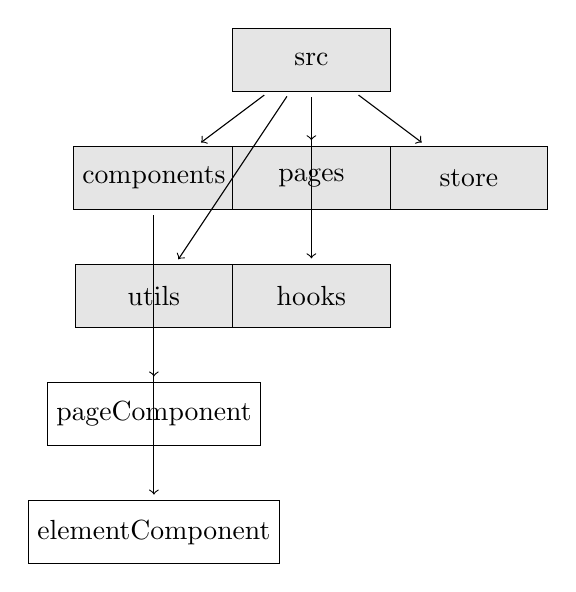
\begin{tikzpicture}[
    file/.style={draw, rectangle, minimum width=2cm, minimum height=0.8cm},
    folder/.style={draw, rectangle, minimum width=2cm, minimum height=0.8cm, fill=gray!20},
    arrow/.style={->, shorten >=2pt, shorten <=2pt}
]

% Folders
\node[folder] (src) at (0,0) {src};
\node[folder] (components) at (-2,-1.5) {components};
\node[folder] (pages) at (0,-1.5) {pages};
\node[folder] (store) at (2,-1.5) {store};
\node[folder] (utils) at (-2,-3) {utils};
\node[folder] (hooks) at (0,-3) {hooks};

% Files
\node[file] (pageComponent) at (-2,-4.5) {pageComponent};
\node[file] (elementComponent) at (-2,-6) {elementComponent};
% ... add more files

% Connections
\draw[arrow] (src) -- (components);
\draw[arrow] (src) -- (pages);
\draw[arrow] (src) -- (store);
\draw[arrow] (src) -- (utils);
\draw[arrow] (src) -- (hooks);
\draw[arrow] (components) -- (pageComponent);
\draw[arrow] (components) -- (elementComponent);
% ... add more connections

\end{tikzpicture}



\pagebreak
\subsubsection{Back-end}
The backend uses the dotNet framework. The development language using the C\# language.

In this project, the backend uses the Onion Architecture.
The Onion Architecture is a typically layered architecture, 
where each layer depends on the inner layer and provides interfaces to the outer layer.
The outer layer provides services to the outermost layer 
and other modules in the same layer based on the interfaces of the inner layer.

From inner to outer, the layers are: Domain, Application, Infrastructure, Presentation.
The Domain layer is the core layer and the innermost layer, used to define domain models, 
which are the business models.
It includes domain models and domain service interfaces.
Domain models are used to define the business models, 
which are the entities in the entity-relationship model and their attributes.
Domain service interfaces are used to define the business services, 
which are the relationships between entities in the entity-relationship model.

The Application layer is the application layer, 
used to define application services, which are the business logic.
It includes domain service implementations and application service interfaces.
Domain service implementations implement the methods of the inner layer's domain service 
interfaces and implement the business logic of the domain models.
Application service interfaces are used to define application services, 
which are the business logic.
It includes but is not limited to database interfaces, testing interfaces, 
HTTP API interfaces, MQTT interfaces, etc.

The Infrastructure layer is the infrastructure layer, used to define infrastructure.
It includes database implementations, testing implementations, 
HTTP API implementations, MQTT implementations, etc.
Database implementations implement the database interfaces 
and provide CRUD services for the database.
Testing implementations implement the testing interfaces 
and provide services for unit testing and integration testing.
HTTP API implementations implement the HTTP API interfaces 
and provide CRUD operations for HTTP APIs.
MQTT implementations implement the MQTT interfaces 
and provide CRUD operations for MQTT.

The Presentation layer is the presentation layer, used to define presentation logic, 
such as interfaces and pages. Since this is a backend project,
data presentation and control are handled by the frontend, 
so this layer is not needed.



\pagebreak
\subsubsection{Data communication and storage}
% 关于本项目的数据通信与数据存储的设计, 包括数据通信的协议, 数据存储的设计等
% 关于数据通信的设计:
% 1. 通信协议的选择
% 自前端向后端发送的数据, 有三种传输的数据类型, 
% 一种是普通的增删改查的请求, 对数据传输的时效性要求不高, 但是对数据的准确性, 完整性, 有序性, 安全性有一定的要求,
% 这种数据的传输, 采用 HTTP 协议, 以及 RESTful API 的设计. 可以有效的保证对数据传输的以上要求.
% 一种是对数据通道的创建和流媒体数据的传输, 对数据传输的时效性, 安全性要求较高, 这种数据的传输, 采用 WebRTC 协议, 以及 MQTT 协议.
% 配合可以快速解码的 flatbuffers 协议, 可以有效的保证对数据传输的以上要求.
% 最后一种是对设备的状态信息和操作信息的传输, 对完整性, 有序性, 安全性都有较高的要求, 这种数据的传输, 采用 MQTT 协议
% 同时也使用了 flatbuffers 协议.
% 
% 2. 数据通信的通信架构和通信流程
% 本项目的数据通信的通信架构, 是基于前后端分离的架构, 前端使用 React 框架, 后端使用 dotnet 框架.
% 当前端需要向后端发送数据的时候, 前端会向后端发送 HTTP 请求, 后端接收到 HTTP 请求之后, 会根据请求的数据类型,
% 选择不同的数据处理方式, 对于普通的增删改查的请求, 后端会根据 RESTful API 的设计, 对数据进行增删改查的操作,
% 对于对数据通道的创建和流媒体数据的传输, 后端会根据 WebRTC 协议, 对数据通道进行创建, 并且帮助前端和设备建立数据通道,
% 当数据通道建立后, 前端和设备之间则使用 flatbuffer 的数据格式对流媒体数据进行传输,
% 对于设备的状态信息和操作信息的传输, 前端会直接向 MQTT broker 发送 MQTT 请求, 
% 设备会在其自身的固件中监听相关的 MQTT 请求, 并且返回相关的数据.
% 
% 3. 数据通信的格式
% 本项目的数据通信的格式, 有三种, 
% 一种是 HTTP 协议, 
% 使用 json 格式对数据进行传输,
% 一种是 WebRTC 协议, 
% 使用 flatbuffers 格式对数据进行传输,
% 一种是 MQTT 协议.
% 使用 flatbuffers 格式对数据进行传输,
% 
% 关于数据存储的设计:
% 1. 数据存储的数据库的选择
% 本项目的数据存储的数据库的选择, 使用了轻量级的数据库 SQLite,
% SQLite 是一个进程内的库, 实现了自给自足的, 无服务器的, 零配置的, 事务性的 SQL 数据库引擎.
% 这是因为整个项目的目的是为了实现前端与设备之间的数据通信, 对于数据库数据的增删改查操作的要求不高,
% 数据量较小, 且对于数据库的数据的事务性要求不高, 所以选择了 SQLite 数据库.
% 2. 项目前后端的数据结构的设计
% 在本项目中, 前端由于使用了 React 框架, 所以前端的数据结构的设计, 使用了基于状态的数据结构的设计,
% 每个组件或者数据集都包含一个状态对象, 这个状态对象的属性就是组件的各个状态. 
% 使用状态对象的原因是, 可以方便的对状态进行管理, 采用对象-属性的形式, 可以方便的针对不同组件的同类状态进行区分,
% 由于跨组件的状态是由 redux 进行管理的, 这种状态对象的设计, 可以更搞笑的对状态进行更新和传递.
% 后端由于使用了 dotnet 框架, 所以后端的数据结构的设计, 使用了基于类的数据结构的设计,
% 采用了面向对象的编程思想, 对数据进行了封装, 使得数据的传输更加的安全, 有序, 完整.


\pagebreak

% \subsection{Domain model}
% \documentclass[]{article}
\usepackage{graphicx}
\usepackage{amsmath}
\usepackage{tikz}

% libaries
\usetikzlibrary{shapes,arrows}

%Define the listing package
\usepackage{listings} %code highlighter
\usepackage{color} %use color
\definecolor{mygreen}{rgb}{0,0.6,0}
\definecolor{mygray}{rgb}{0.5,0.5,0.5}
\definecolor{mymauve}{rgb}{0.58,0,0.82}

%Customize a bit the look
\lstset{ %
backgroundcolor=\color{white}, % choose the background color; you must add \usepackage{color} or \usepackage{xcolor}
basicstyle=\footnotesize, % the size of the fonts that are used for the code
breakatwhitespace=false, % sets if automatic breaks should only happen at whitespace
breaklines=true, % sets automatic line breaking
captionpos=b, % sets the caption-position to bottom
commentstyle=\color{mygreen}, % comment style
deletekeywords={...}, % if you want to delete keywords from the given language
escapeinside={\%*}{*)}, % if you want to add LaTeX within your code
extendedchars=true, % lets you use non-ASCII characters; for 8-bits encodings only, does not work with UTF-8
frame=single, % adds a frame around the code
keepspaces=true, % keeps spaces in text, useful for keeping indentation of code (possibly needs columns=flexible)
keywordstyle=\color{blue}, % keyword style
% language=Octave, % the language of the code
morekeywords={*,...}, % if you want to add more keywords to the set
numbers=left, % where to put the line-numbers; possible values are (none, left, right)
numbersep=5pt, % how far the line-numbers are from the code
numberstyle=\tiny\color{mygray}, % the style that is used for the line-numbers
rulecolor=\color{black}, % if not set, the frame-color may be changed on line-breaks within not-black text (e.g. comments (green here))
showspaces=false, % show spaces everywhere adding particular underscores; it overrides 'showstringspaces'
showstringspaces=false, % underline spaces within strings only
showtabs=false, % show tabs within strings adding particular underscores
stepnumber=1, % the step between two line-numbers. If it's 1, each line will be numbered
stringstyle=\color{mymauve}, % string literal style
tabsize=2, % sets default tabsize to 2 spaces
title=\lstname % show the filename of files included with \lstinputlisting; also try caption instead of title
}

\definecolor{darkgray}{rgb}{.4,.4,.4}
\definecolor{purple}{rgb}{0.65, 0.12, 0.82}

\lstdefinelanguage{React}{
keywords={const, typeof, new, true, false, catch, function, return, null, catch, switch, var, if, in, while, do, else, case, break},
keywordstyle=\color{blue}\bfseries,
ndkeywords={class, export, boolean, throw, implements, import, this},
ndkeywordstyle=\color{darkgray}\bfseries,
identifierstyle=\color{mygreen},
sensitive=false,
comment=[l]{//},
morecomment=[s]{/*}{*/},
commentstyle=\color{purple}\ttfamily,
string=[b]{"}{'}{`},
stringstyle=\color{red}\ttfamily,
morestring=[b]',
morestring=[b]",
morestring=[b]`',
}

\lstdefinelanguage{CSharp}{
keywords={const, typeof, new, true, false, catch, function, return, null, catch, switch, var, if, in, while, do, else, case, break},
keywordstyle=\color{blue}\bfseries,
ndkeywords={class, export, boolean, throw, implements, import, this},
ndkeywordstyle=\color{darkgray}\bfseries,
identifierstyle=\color{mygreen},
sensitive=false,
comment=[l]{//},
morecomment=[s]{/*}{*/},
commentstyle=\color{purple}\ttfamily,
string=[b]{"}{'}{`},
stringstyle=\color{red}\ttfamily,
morestring=[b]',
morestring=[b]",
morestring=[b]`',
}

\lstset{
language=React,
extendedchars=true,
basicstyle=\footnotesize\ttfamily,
showstringspaces=false,
showspaces=false,
numbers=left,
numberstyle=\footnotesize,
numbersep=9pt,
tabsize=2,
breaklines=true,
showtabs=false,
captionpos=b
}

\lstset{
language=CSharp,
extendedchars=true,
basicstyle=\footnotesize\ttfamily,
showstringspaces=false,
showspaces=false,
numbers=left,
numberstyle=\footnotesize,
numbersep=9pt,
tabsize=2,
breaklines=true,
showtabs=false,
captionpos=b
}

% \usepackage{cite} % Add this line for citation

% \bibliographystyle{plain}

\title{
The implementation of BifrostConnect Front-end scope, 
re-design and development with the relevant back-end support develop.
}
\author{
    Fei Gu \\
    Erhvervs Akademi Sydvest \\
    Computer Science 21\\
    }
\date{\today}

\begin{document}

% Front page
\maketitle
\begin{center}
    Supervisor: Henrik Boulund Meng Hansen \\
    Company: BifrostConnect \\
    Engineering Director: Jasper Wass \\
\end{center}
\tableofcontents
\pagebreak


% The introduction
\section{Introduction}
\subsection{Background}\input{sections/introduction/background.tex}
\subsection{The company}\input{sections/introduction/aboutCompany}
\subsection{The project}\input{sections/introduction/aboutProject}
\pagebreak

% The problem statement
\section{Problem Statement}
\subsection{Statement}
\input{sections/problemStatement/statement}
\subsection{Situation}
\input{sections/problemStatement/situation}
\subsection{Potential Solution}
\input{sections/problemStatement/potentialSolution}
\pagebreak

% Requirement analysis
\section{Requirement Analysis}
\input{sections/requirementAnalysis/index}

\subsection{Stakeholders}
\input{sections/requirementAnalysis/stakeholders/index}

\subsection{Business Domain}
\input{sections/requirementAnalysis/bussinesDomain/index}

\subsection{Scope}
\input{sections/requirementAnalysis/scope}

\subsection{Goals}
\input{sections/requirementAnalysis/goals}
\pagebreak

% Software Design
\section{Software Design}
% developement methods
\subsection{Software Development Methods}
\input{sections/softwareDevelopmentMethods/index}
\subsubsection{Agile Software Development}
\input{sections/softwareDevelopmentMethods/agileSoftwareDevelopment/index}
\subsubsection{Feature Driven Development}
\input{sections/softwareDevelopmentMethods/featureDrivenDevelopment/index}

\pagebreak

% Technology seslection
\subsection{Technology selection}
\input{sections/softwareDesign/technologySelection/index}
\subsubsection{Front-end}
\input{sections/softwareDesign/technologySelection/frontEnd}            
\subsubsection{Back-end}
\input{sections/softwareDesign/technologySelection/backEnd}            
\subsubsection{Database}
\input{sections/softwareDesign/technologySelection/database}
\subsubsection{Data communication}
\input{sections/softwareDesign/technologySelection/dataCommunication}            
\subsubsection{DevOps}
\input{sections/softwareDesign/technologySelection/devOps}
\pagebreak

% Architecture design
\subsection{Architecture design}
\input{sections/softwareDesign/architectureDesign/index}
\pagebreak
\subsubsection{Front-end}
\input{sections/softwareDesign/architectureDesign/frontEndArchitecture}
\pagebreak
\subsubsection{Back-end}
\input{sections/softwareDesign/architectureDesign/backEndArchitecture}
\pagebreak
\subsubsection{Data communication and storage}
\input{sections/softwareDesign/architectureDesign/dataCommunicationArchitecture}
\pagebreak

% \subsection{Domain model}
% \input{sections/softwareDesign/domainModel/index}
% \subsection{Database design}
% % 数据库领域模型 ER 图
% % 包括表和字段的设置.
% % 对于私有键和外键的设置.

% \subsection{Back-end design}
% % 后端对象模型
% % 以及对于对象模型的增删改查
% % 以及相关的其他服务的设计`'

% \subsection{Front-end design}
% % 对于前端的页面结构的设计 
% % 页面的状态的设计, 交互设计

% \subsection{FlatBuffers design}
% % schema 的设计

\subsection{DevOps CI/CD process design}
\input{sections/softwareDesign/devOpsDesign/index}
\subsubsection{Continuous Integration}
\input{sections/softwareDesign/devOpsDesign/continuousIntegration/index}
\subsubsection{Continuous Delivery}
\input{sections/softwareDesign/devOpsDesign/continuousDelivery/index}
\subsubsection{Continuous Deployment}
\input{sections/softwareDesign/devOpsDesign/continuousDeployment/index}
\pagebreak

\section{Software Development} 
\input{sections/softwareDevelopment/index}
\subsection{Overall development}
\input{sections/softwareDevelopment/overallDevelopement/index}
\subsubsection{Front-end}
\input{sections/softwareDevelopment/overallDevelopement/frontEnd/index}
\subsubsection{Back-end}
\input{sections/softwareDevelopment/overallDevelopement/backEnd/index}
\subsubsection{DevOps}
\input{sections/softwareDevelopment/overallDevelopement/devOps/index}
\subsection{Feature development} 
\input{sections/softwareDevelopment/featureDevelopment/index}
\subsubsection{Use Case 1}
\input{sections/softwareDevelopment/featureDevelopment/useCase1/index}
\subsubsection{Feature 1}
\input{sections/softwareDevelopment/featureDevelopment/feature/feature1.tex}
\pagebreak
\section{Conclusion} 
\subsection{Result}
Since the project is still in progress, the result is not available yet.
So far, basic structure of this project has been built. But the most features 
are not implemented yet. 
\subsection{Discussion}
As a single developer for this project, I am confident what I have done so far.
And I can say I understand the most of the knowledge I have used in this project, 
which also means I can explain all the part of the project. 
But this project also relevant some of the complex knowledge which I have to continue 
to study and practice.
\subsection{Future Work}
The future work is to implement the rest of the features. 
Including the most important part which is the 'create session' feature.
\pagebreak
% \bibliography{bibliography}
\pagebreak
% \begin{appendices}
%     \section{Appendix}
% \end{appendices} 
\end{document}
% \subsection{Database design}
% % 数据库领域模型 ER 图
% % 包括表和字段的设置.
% % 对于私有键和外键的设置.

% \subsection{Back-end design}
% % 后端对象模型
% % 以及对于对象模型的增删改查
% % 以及相关的其他服务的设计`'

% \subsection{Front-end design}
% % 对于前端的页面结构的设计 
% % 页面的状态的设计, 交互设计

% \subsection{FlatBuffers design}
% % schema 的设计

\subsection{DevOps CI/CD process design}
\documentclass[]{article}
\usepackage{graphicx}
\usepackage{amsmath}
\usepackage{tikz}

% libaries
\usetikzlibrary{shapes,arrows}

%Define the listing package
\usepackage{listings} %code highlighter
\usepackage{color} %use color
\definecolor{mygreen}{rgb}{0,0.6,0}
\definecolor{mygray}{rgb}{0.5,0.5,0.5}
\definecolor{mymauve}{rgb}{0.58,0,0.82}

%Customize a bit the look
\lstset{ %
backgroundcolor=\color{white}, % choose the background color; you must add \usepackage{color} or \usepackage{xcolor}
basicstyle=\footnotesize, % the size of the fonts that are used for the code
breakatwhitespace=false, % sets if automatic breaks should only happen at whitespace
breaklines=true, % sets automatic line breaking
captionpos=b, % sets the caption-position to bottom
commentstyle=\color{mygreen}, % comment style
deletekeywords={...}, % if you want to delete keywords from the given language
escapeinside={\%*}{*)}, % if you want to add LaTeX within your code
extendedchars=true, % lets you use non-ASCII characters; for 8-bits encodings only, does not work with UTF-8
frame=single, % adds a frame around the code
keepspaces=true, % keeps spaces in text, useful for keeping indentation of code (possibly needs columns=flexible)
keywordstyle=\color{blue}, % keyword style
% language=Octave, % the language of the code
morekeywords={*,...}, % if you want to add more keywords to the set
numbers=left, % where to put the line-numbers; possible values are (none, left, right)
numbersep=5pt, % how far the line-numbers are from the code
numberstyle=\tiny\color{mygray}, % the style that is used for the line-numbers
rulecolor=\color{black}, % if not set, the frame-color may be changed on line-breaks within not-black text (e.g. comments (green here))
showspaces=false, % show spaces everywhere adding particular underscores; it overrides 'showstringspaces'
showstringspaces=false, % underline spaces within strings only
showtabs=false, % show tabs within strings adding particular underscores
stepnumber=1, % the step between two line-numbers. If it's 1, each line will be numbered
stringstyle=\color{mymauve}, % string literal style
tabsize=2, % sets default tabsize to 2 spaces
title=\lstname % show the filename of files included with \lstinputlisting; also try caption instead of title
}

\definecolor{darkgray}{rgb}{.4,.4,.4}
\definecolor{purple}{rgb}{0.65, 0.12, 0.82}

\lstdefinelanguage{React}{
keywords={const, typeof, new, true, false, catch, function, return, null, catch, switch, var, if, in, while, do, else, case, break},
keywordstyle=\color{blue}\bfseries,
ndkeywords={class, export, boolean, throw, implements, import, this},
ndkeywordstyle=\color{darkgray}\bfseries,
identifierstyle=\color{mygreen},
sensitive=false,
comment=[l]{//},
morecomment=[s]{/*}{*/},
commentstyle=\color{purple}\ttfamily,
string=[b]{"}{'}{`},
stringstyle=\color{red}\ttfamily,
morestring=[b]',
morestring=[b]",
morestring=[b]`',
}

\lstdefinelanguage{CSharp}{
keywords={const, typeof, new, true, false, catch, function, return, null, catch, switch, var, if, in, while, do, else, case, break},
keywordstyle=\color{blue}\bfseries,
ndkeywords={class, export, boolean, throw, implements, import, this},
ndkeywordstyle=\color{darkgray}\bfseries,
identifierstyle=\color{mygreen},
sensitive=false,
comment=[l]{//},
morecomment=[s]{/*}{*/},
commentstyle=\color{purple}\ttfamily,
string=[b]{"}{'}{`},
stringstyle=\color{red}\ttfamily,
morestring=[b]',
morestring=[b]",
morestring=[b]`',
}

\lstset{
language=React,
extendedchars=true,
basicstyle=\footnotesize\ttfamily,
showstringspaces=false,
showspaces=false,
numbers=left,
numberstyle=\footnotesize,
numbersep=9pt,
tabsize=2,
breaklines=true,
showtabs=false,
captionpos=b
}

\lstset{
language=CSharp,
extendedchars=true,
basicstyle=\footnotesize\ttfamily,
showstringspaces=false,
showspaces=false,
numbers=left,
numberstyle=\footnotesize,
numbersep=9pt,
tabsize=2,
breaklines=true,
showtabs=false,
captionpos=b
}

% \usepackage{cite} % Add this line for citation

% \bibliographystyle{plain}

\title{
The implementation of BifrostConnect Front-end scope, 
re-design and development with the relevant back-end support develop.
}
\author{
    Fei Gu \\
    Erhvervs Akademi Sydvest \\
    Computer Science 21\\
    }
\date{\today}

\begin{document}

% Front page
\maketitle
\begin{center}
    Supervisor: Henrik Boulund Meng Hansen \\
    Company: BifrostConnect \\
    Engineering Director: Jasper Wass \\
\end{center}
\tableofcontents
\pagebreak


% The introduction
\section{Introduction}
\subsection{Background}\input{sections/introduction/background.tex}
\subsection{The company}\input{sections/introduction/aboutCompany}
\subsection{The project}\input{sections/introduction/aboutProject}
\pagebreak

% The problem statement
\section{Problem Statement}
\subsection{Statement}
\input{sections/problemStatement/statement}
\subsection{Situation}
\input{sections/problemStatement/situation}
\subsection{Potential Solution}
\input{sections/problemStatement/potentialSolution}
\pagebreak

% Requirement analysis
\section{Requirement Analysis}
\input{sections/requirementAnalysis/index}

\subsection{Stakeholders}
\input{sections/requirementAnalysis/stakeholders/index}

\subsection{Business Domain}
\input{sections/requirementAnalysis/bussinesDomain/index}

\subsection{Scope}
\input{sections/requirementAnalysis/scope}

\subsection{Goals}
\input{sections/requirementAnalysis/goals}
\pagebreak

% Software Design
\section{Software Design}
% developement methods
\subsection{Software Development Methods}
\input{sections/softwareDevelopmentMethods/index}
\subsubsection{Agile Software Development}
\input{sections/softwareDevelopmentMethods/agileSoftwareDevelopment/index}
\subsubsection{Feature Driven Development}
\input{sections/softwareDevelopmentMethods/featureDrivenDevelopment/index}

\pagebreak

% Technology seslection
\subsection{Technology selection}
\input{sections/softwareDesign/technologySelection/index}
\subsubsection{Front-end}
\input{sections/softwareDesign/technologySelection/frontEnd}            
\subsubsection{Back-end}
\input{sections/softwareDesign/technologySelection/backEnd}            
\subsubsection{Database}
\input{sections/softwareDesign/technologySelection/database}
\subsubsection{Data communication}
\input{sections/softwareDesign/technologySelection/dataCommunication}            
\subsubsection{DevOps}
\input{sections/softwareDesign/technologySelection/devOps}
\pagebreak

% Architecture design
\subsection{Architecture design}
\input{sections/softwareDesign/architectureDesign/index}
\pagebreak
\subsubsection{Front-end}
\input{sections/softwareDesign/architectureDesign/frontEndArchitecture}
\pagebreak
\subsubsection{Back-end}
\input{sections/softwareDesign/architectureDesign/backEndArchitecture}
\pagebreak
\subsubsection{Data communication and storage}
\input{sections/softwareDesign/architectureDesign/dataCommunicationArchitecture}
\pagebreak

% \subsection{Domain model}
% \input{sections/softwareDesign/domainModel/index}
% \subsection{Database design}
% % 数据库领域模型 ER 图
% % 包括表和字段的设置.
% % 对于私有键和外键的设置.

% \subsection{Back-end design}
% % 后端对象模型
% % 以及对于对象模型的增删改查
% % 以及相关的其他服务的设计`'

% \subsection{Front-end design}
% % 对于前端的页面结构的设计 
% % 页面的状态的设计, 交互设计

% \subsection{FlatBuffers design}
% % schema 的设计

\subsection{DevOps CI/CD process design}
\input{sections/softwareDesign/devOpsDesign/index}
\subsubsection{Continuous Integration}
\input{sections/softwareDesign/devOpsDesign/continuousIntegration/index}
\subsubsection{Continuous Delivery}
\input{sections/softwareDesign/devOpsDesign/continuousDelivery/index}
\subsubsection{Continuous Deployment}
\input{sections/softwareDesign/devOpsDesign/continuousDeployment/index}
\pagebreak

\section{Software Development} 
\input{sections/softwareDevelopment/index}
\subsection{Overall development}
\input{sections/softwareDevelopment/overallDevelopement/index}
\subsubsection{Front-end}
\input{sections/softwareDevelopment/overallDevelopement/frontEnd/index}
\subsubsection{Back-end}
\input{sections/softwareDevelopment/overallDevelopement/backEnd/index}
\subsubsection{DevOps}
\input{sections/softwareDevelopment/overallDevelopement/devOps/index}
\subsection{Feature development} 
\input{sections/softwareDevelopment/featureDevelopment/index}
\subsubsection{Use Case 1}
\input{sections/softwareDevelopment/featureDevelopment/useCase1/index}
\subsubsection{Feature 1}
\input{sections/softwareDevelopment/featureDevelopment/feature/feature1.tex}
\pagebreak
\section{Conclusion} 
\subsection{Result}
Since the project is still in progress, the result is not available yet.
So far, basic structure of this project has been built. But the most features 
are not implemented yet. 
\subsection{Discussion}
As a single developer for this project, I am confident what I have done so far.
And I can say I understand the most of the knowledge I have used in this project, 
which also means I can explain all the part of the project. 
But this project also relevant some of the complex knowledge which I have to continue 
to study and practice.
\subsection{Future Work}
The future work is to implement the rest of the features. 
Including the most important part which is the 'create session' feature.
\pagebreak
% \bibliography{bibliography}
\pagebreak
% \begin{appendices}
%     \section{Appendix}
% \end{appendices} 
\end{document}
\subsubsection{Continuous Integration}
\documentclass[]{article}
\usepackage{graphicx}
\usepackage{amsmath}
\usepackage{tikz}

% libaries
\usetikzlibrary{shapes,arrows}

%Define the listing package
\usepackage{listings} %code highlighter
\usepackage{color} %use color
\definecolor{mygreen}{rgb}{0,0.6,0}
\definecolor{mygray}{rgb}{0.5,0.5,0.5}
\definecolor{mymauve}{rgb}{0.58,0,0.82}

%Customize a bit the look
\lstset{ %
backgroundcolor=\color{white}, % choose the background color; you must add \usepackage{color} or \usepackage{xcolor}
basicstyle=\footnotesize, % the size of the fonts that are used for the code
breakatwhitespace=false, % sets if automatic breaks should only happen at whitespace
breaklines=true, % sets automatic line breaking
captionpos=b, % sets the caption-position to bottom
commentstyle=\color{mygreen}, % comment style
deletekeywords={...}, % if you want to delete keywords from the given language
escapeinside={\%*}{*)}, % if you want to add LaTeX within your code
extendedchars=true, % lets you use non-ASCII characters; for 8-bits encodings only, does not work with UTF-8
frame=single, % adds a frame around the code
keepspaces=true, % keeps spaces in text, useful for keeping indentation of code (possibly needs columns=flexible)
keywordstyle=\color{blue}, % keyword style
% language=Octave, % the language of the code
morekeywords={*,...}, % if you want to add more keywords to the set
numbers=left, % where to put the line-numbers; possible values are (none, left, right)
numbersep=5pt, % how far the line-numbers are from the code
numberstyle=\tiny\color{mygray}, % the style that is used for the line-numbers
rulecolor=\color{black}, % if not set, the frame-color may be changed on line-breaks within not-black text (e.g. comments (green here))
showspaces=false, % show spaces everywhere adding particular underscores; it overrides 'showstringspaces'
showstringspaces=false, % underline spaces within strings only
showtabs=false, % show tabs within strings adding particular underscores
stepnumber=1, % the step between two line-numbers. If it's 1, each line will be numbered
stringstyle=\color{mymauve}, % string literal style
tabsize=2, % sets default tabsize to 2 spaces
title=\lstname % show the filename of files included with \lstinputlisting; also try caption instead of title
}

\definecolor{darkgray}{rgb}{.4,.4,.4}
\definecolor{purple}{rgb}{0.65, 0.12, 0.82}

\lstdefinelanguage{React}{
keywords={const, typeof, new, true, false, catch, function, return, null, catch, switch, var, if, in, while, do, else, case, break},
keywordstyle=\color{blue}\bfseries,
ndkeywords={class, export, boolean, throw, implements, import, this},
ndkeywordstyle=\color{darkgray}\bfseries,
identifierstyle=\color{mygreen},
sensitive=false,
comment=[l]{//},
morecomment=[s]{/*}{*/},
commentstyle=\color{purple}\ttfamily,
string=[b]{"}{'}{`},
stringstyle=\color{red}\ttfamily,
morestring=[b]',
morestring=[b]",
morestring=[b]`',
}

\lstdefinelanguage{CSharp}{
keywords={const, typeof, new, true, false, catch, function, return, null, catch, switch, var, if, in, while, do, else, case, break},
keywordstyle=\color{blue}\bfseries,
ndkeywords={class, export, boolean, throw, implements, import, this},
ndkeywordstyle=\color{darkgray}\bfseries,
identifierstyle=\color{mygreen},
sensitive=false,
comment=[l]{//},
morecomment=[s]{/*}{*/},
commentstyle=\color{purple}\ttfamily,
string=[b]{"}{'}{`},
stringstyle=\color{red}\ttfamily,
morestring=[b]',
morestring=[b]",
morestring=[b]`',
}

\lstset{
language=React,
extendedchars=true,
basicstyle=\footnotesize\ttfamily,
showstringspaces=false,
showspaces=false,
numbers=left,
numberstyle=\footnotesize,
numbersep=9pt,
tabsize=2,
breaklines=true,
showtabs=false,
captionpos=b
}

\lstset{
language=CSharp,
extendedchars=true,
basicstyle=\footnotesize\ttfamily,
showstringspaces=false,
showspaces=false,
numbers=left,
numberstyle=\footnotesize,
numbersep=9pt,
tabsize=2,
breaklines=true,
showtabs=false,
captionpos=b
}

% \usepackage{cite} % Add this line for citation

% \bibliographystyle{plain}

\title{
The implementation of BifrostConnect Front-end scope, 
re-design and development with the relevant back-end support develop.
}
\author{
    Fei Gu \\
    Erhvervs Akademi Sydvest \\
    Computer Science 21\\
    }
\date{\today}

\begin{document}

% Front page
\maketitle
\begin{center}
    Supervisor: Henrik Boulund Meng Hansen \\
    Company: BifrostConnect \\
    Engineering Director: Jasper Wass \\
\end{center}
\tableofcontents
\pagebreak


% The introduction
\section{Introduction}
\subsection{Background}\input{sections/introduction/background.tex}
\subsection{The company}\input{sections/introduction/aboutCompany}
\subsection{The project}\input{sections/introduction/aboutProject}
\pagebreak

% The problem statement
\section{Problem Statement}
\subsection{Statement}
\input{sections/problemStatement/statement}
\subsection{Situation}
\input{sections/problemStatement/situation}
\subsection{Potential Solution}
\input{sections/problemStatement/potentialSolution}
\pagebreak

% Requirement analysis
\section{Requirement Analysis}
\input{sections/requirementAnalysis/index}

\subsection{Stakeholders}
\input{sections/requirementAnalysis/stakeholders/index}

\subsection{Business Domain}
\input{sections/requirementAnalysis/bussinesDomain/index}

\subsection{Scope}
\input{sections/requirementAnalysis/scope}

\subsection{Goals}
\input{sections/requirementAnalysis/goals}
\pagebreak

% Software Design
\section{Software Design}
% developement methods
\subsection{Software Development Methods}
\input{sections/softwareDevelopmentMethods/index}
\subsubsection{Agile Software Development}
\input{sections/softwareDevelopmentMethods/agileSoftwareDevelopment/index}
\subsubsection{Feature Driven Development}
\input{sections/softwareDevelopmentMethods/featureDrivenDevelopment/index}

\pagebreak

% Technology seslection
\subsection{Technology selection}
\input{sections/softwareDesign/technologySelection/index}
\subsubsection{Front-end}
\input{sections/softwareDesign/technologySelection/frontEnd}            
\subsubsection{Back-end}
\input{sections/softwareDesign/technologySelection/backEnd}            
\subsubsection{Database}
\input{sections/softwareDesign/technologySelection/database}
\subsubsection{Data communication}
\input{sections/softwareDesign/technologySelection/dataCommunication}            
\subsubsection{DevOps}
\input{sections/softwareDesign/technologySelection/devOps}
\pagebreak

% Architecture design
\subsection{Architecture design}
\input{sections/softwareDesign/architectureDesign/index}
\pagebreak
\subsubsection{Front-end}
\input{sections/softwareDesign/architectureDesign/frontEndArchitecture}
\pagebreak
\subsubsection{Back-end}
\input{sections/softwareDesign/architectureDesign/backEndArchitecture}
\pagebreak
\subsubsection{Data communication and storage}
\input{sections/softwareDesign/architectureDesign/dataCommunicationArchitecture}
\pagebreak

% \subsection{Domain model}
% \input{sections/softwareDesign/domainModel/index}
% \subsection{Database design}
% % 数据库领域模型 ER 图
% % 包括表和字段的设置.
% % 对于私有键和外键的设置.

% \subsection{Back-end design}
% % 后端对象模型
% % 以及对于对象模型的增删改查
% % 以及相关的其他服务的设计`'

% \subsection{Front-end design}
% % 对于前端的页面结构的设计 
% % 页面的状态的设计, 交互设计

% \subsection{FlatBuffers design}
% % schema 的设计

\subsection{DevOps CI/CD process design}
\input{sections/softwareDesign/devOpsDesign/index}
\subsubsection{Continuous Integration}
\input{sections/softwareDesign/devOpsDesign/continuousIntegration/index}
\subsubsection{Continuous Delivery}
\input{sections/softwareDesign/devOpsDesign/continuousDelivery/index}
\subsubsection{Continuous Deployment}
\input{sections/softwareDesign/devOpsDesign/continuousDeployment/index}
\pagebreak

\section{Software Development} 
\input{sections/softwareDevelopment/index}
\subsection{Overall development}
\input{sections/softwareDevelopment/overallDevelopement/index}
\subsubsection{Front-end}
\input{sections/softwareDevelopment/overallDevelopement/frontEnd/index}
\subsubsection{Back-end}
\input{sections/softwareDevelopment/overallDevelopement/backEnd/index}
\subsubsection{DevOps}
\input{sections/softwareDevelopment/overallDevelopement/devOps/index}
\subsection{Feature development} 
\input{sections/softwareDevelopment/featureDevelopment/index}
\subsubsection{Use Case 1}
\input{sections/softwareDevelopment/featureDevelopment/useCase1/index}
\subsubsection{Feature 1}
\input{sections/softwareDevelopment/featureDevelopment/feature/feature1.tex}
\pagebreak
\section{Conclusion} 
\subsection{Result}
Since the project is still in progress, the result is not available yet.
So far, basic structure of this project has been built. But the most features 
are not implemented yet. 
\subsection{Discussion}
As a single developer for this project, I am confident what I have done so far.
And I can say I understand the most of the knowledge I have used in this project, 
which also means I can explain all the part of the project. 
But this project also relevant some of the complex knowledge which I have to continue 
to study and practice.
\subsection{Future Work}
The future work is to implement the rest of the features. 
Including the most important part which is the 'create session' feature.
\pagebreak
% \bibliography{bibliography}
\pagebreak
% \begin{appendices}
%     \section{Appendix}
% \end{appendices} 
\end{document}
\subsubsection{Continuous Delivery}
\documentclass[]{article}
\usepackage{graphicx}
\usepackage{amsmath}
\usepackage{tikz}

% libaries
\usetikzlibrary{shapes,arrows}

%Define the listing package
\usepackage{listings} %code highlighter
\usepackage{color} %use color
\definecolor{mygreen}{rgb}{0,0.6,0}
\definecolor{mygray}{rgb}{0.5,0.5,0.5}
\definecolor{mymauve}{rgb}{0.58,0,0.82}

%Customize a bit the look
\lstset{ %
backgroundcolor=\color{white}, % choose the background color; you must add \usepackage{color} or \usepackage{xcolor}
basicstyle=\footnotesize, % the size of the fonts that are used for the code
breakatwhitespace=false, % sets if automatic breaks should only happen at whitespace
breaklines=true, % sets automatic line breaking
captionpos=b, % sets the caption-position to bottom
commentstyle=\color{mygreen}, % comment style
deletekeywords={...}, % if you want to delete keywords from the given language
escapeinside={\%*}{*)}, % if you want to add LaTeX within your code
extendedchars=true, % lets you use non-ASCII characters; for 8-bits encodings only, does not work with UTF-8
frame=single, % adds a frame around the code
keepspaces=true, % keeps spaces in text, useful for keeping indentation of code (possibly needs columns=flexible)
keywordstyle=\color{blue}, % keyword style
% language=Octave, % the language of the code
morekeywords={*,...}, % if you want to add more keywords to the set
numbers=left, % where to put the line-numbers; possible values are (none, left, right)
numbersep=5pt, % how far the line-numbers are from the code
numberstyle=\tiny\color{mygray}, % the style that is used for the line-numbers
rulecolor=\color{black}, % if not set, the frame-color may be changed on line-breaks within not-black text (e.g. comments (green here))
showspaces=false, % show spaces everywhere adding particular underscores; it overrides 'showstringspaces'
showstringspaces=false, % underline spaces within strings only
showtabs=false, % show tabs within strings adding particular underscores
stepnumber=1, % the step between two line-numbers. If it's 1, each line will be numbered
stringstyle=\color{mymauve}, % string literal style
tabsize=2, % sets default tabsize to 2 spaces
title=\lstname % show the filename of files included with \lstinputlisting; also try caption instead of title
}

\definecolor{darkgray}{rgb}{.4,.4,.4}
\definecolor{purple}{rgb}{0.65, 0.12, 0.82}

\lstdefinelanguage{React}{
keywords={const, typeof, new, true, false, catch, function, return, null, catch, switch, var, if, in, while, do, else, case, break},
keywordstyle=\color{blue}\bfseries,
ndkeywords={class, export, boolean, throw, implements, import, this},
ndkeywordstyle=\color{darkgray}\bfseries,
identifierstyle=\color{mygreen},
sensitive=false,
comment=[l]{//},
morecomment=[s]{/*}{*/},
commentstyle=\color{purple}\ttfamily,
string=[b]{"}{'}{`},
stringstyle=\color{red}\ttfamily,
morestring=[b]',
morestring=[b]",
morestring=[b]`',
}

\lstdefinelanguage{CSharp}{
keywords={const, typeof, new, true, false, catch, function, return, null, catch, switch, var, if, in, while, do, else, case, break},
keywordstyle=\color{blue}\bfseries,
ndkeywords={class, export, boolean, throw, implements, import, this},
ndkeywordstyle=\color{darkgray}\bfseries,
identifierstyle=\color{mygreen},
sensitive=false,
comment=[l]{//},
morecomment=[s]{/*}{*/},
commentstyle=\color{purple}\ttfamily,
string=[b]{"}{'}{`},
stringstyle=\color{red}\ttfamily,
morestring=[b]',
morestring=[b]",
morestring=[b]`',
}

\lstset{
language=React,
extendedchars=true,
basicstyle=\footnotesize\ttfamily,
showstringspaces=false,
showspaces=false,
numbers=left,
numberstyle=\footnotesize,
numbersep=9pt,
tabsize=2,
breaklines=true,
showtabs=false,
captionpos=b
}

\lstset{
language=CSharp,
extendedchars=true,
basicstyle=\footnotesize\ttfamily,
showstringspaces=false,
showspaces=false,
numbers=left,
numberstyle=\footnotesize,
numbersep=9pt,
tabsize=2,
breaklines=true,
showtabs=false,
captionpos=b
}

% \usepackage{cite} % Add this line for citation

% \bibliographystyle{plain}

\title{
The implementation of BifrostConnect Front-end scope, 
re-design and development with the relevant back-end support develop.
}
\author{
    Fei Gu \\
    Erhvervs Akademi Sydvest \\
    Computer Science 21\\
    }
\date{\today}

\begin{document}

% Front page
\maketitle
\begin{center}
    Supervisor: Henrik Boulund Meng Hansen \\
    Company: BifrostConnect \\
    Engineering Director: Jasper Wass \\
\end{center}
\tableofcontents
\pagebreak


% The introduction
\section{Introduction}
\subsection{Background}\input{sections/introduction/background.tex}
\subsection{The company}\input{sections/introduction/aboutCompany}
\subsection{The project}\input{sections/introduction/aboutProject}
\pagebreak

% The problem statement
\section{Problem Statement}
\subsection{Statement}
\input{sections/problemStatement/statement}
\subsection{Situation}
\input{sections/problemStatement/situation}
\subsection{Potential Solution}
\input{sections/problemStatement/potentialSolution}
\pagebreak

% Requirement analysis
\section{Requirement Analysis}
\input{sections/requirementAnalysis/index}

\subsection{Stakeholders}
\input{sections/requirementAnalysis/stakeholders/index}

\subsection{Business Domain}
\input{sections/requirementAnalysis/bussinesDomain/index}

\subsection{Scope}
\input{sections/requirementAnalysis/scope}

\subsection{Goals}
\input{sections/requirementAnalysis/goals}
\pagebreak

% Software Design
\section{Software Design}
% developement methods
\subsection{Software Development Methods}
\input{sections/softwareDevelopmentMethods/index}
\subsubsection{Agile Software Development}
\input{sections/softwareDevelopmentMethods/agileSoftwareDevelopment/index}
\subsubsection{Feature Driven Development}
\input{sections/softwareDevelopmentMethods/featureDrivenDevelopment/index}

\pagebreak

% Technology seslection
\subsection{Technology selection}
\input{sections/softwareDesign/technologySelection/index}
\subsubsection{Front-end}
\input{sections/softwareDesign/technologySelection/frontEnd}            
\subsubsection{Back-end}
\input{sections/softwareDesign/technologySelection/backEnd}            
\subsubsection{Database}
\input{sections/softwareDesign/technologySelection/database}
\subsubsection{Data communication}
\input{sections/softwareDesign/technologySelection/dataCommunication}            
\subsubsection{DevOps}
\input{sections/softwareDesign/technologySelection/devOps}
\pagebreak

% Architecture design
\subsection{Architecture design}
\input{sections/softwareDesign/architectureDesign/index}
\pagebreak
\subsubsection{Front-end}
\input{sections/softwareDesign/architectureDesign/frontEndArchitecture}
\pagebreak
\subsubsection{Back-end}
\input{sections/softwareDesign/architectureDesign/backEndArchitecture}
\pagebreak
\subsubsection{Data communication and storage}
\input{sections/softwareDesign/architectureDesign/dataCommunicationArchitecture}
\pagebreak

% \subsection{Domain model}
% \input{sections/softwareDesign/domainModel/index}
% \subsection{Database design}
% % 数据库领域模型 ER 图
% % 包括表和字段的设置.
% % 对于私有键和外键的设置.

% \subsection{Back-end design}
% % 后端对象模型
% % 以及对于对象模型的增删改查
% % 以及相关的其他服务的设计`'

% \subsection{Front-end design}
% % 对于前端的页面结构的设计 
% % 页面的状态的设计, 交互设计

% \subsection{FlatBuffers design}
% % schema 的设计

\subsection{DevOps CI/CD process design}
\input{sections/softwareDesign/devOpsDesign/index}
\subsubsection{Continuous Integration}
\input{sections/softwareDesign/devOpsDesign/continuousIntegration/index}
\subsubsection{Continuous Delivery}
\input{sections/softwareDesign/devOpsDesign/continuousDelivery/index}
\subsubsection{Continuous Deployment}
\input{sections/softwareDesign/devOpsDesign/continuousDeployment/index}
\pagebreak

\section{Software Development} 
\input{sections/softwareDevelopment/index}
\subsection{Overall development}
\input{sections/softwareDevelopment/overallDevelopement/index}
\subsubsection{Front-end}
\input{sections/softwareDevelopment/overallDevelopement/frontEnd/index}
\subsubsection{Back-end}
\input{sections/softwareDevelopment/overallDevelopement/backEnd/index}
\subsubsection{DevOps}
\input{sections/softwareDevelopment/overallDevelopement/devOps/index}
\subsection{Feature development} 
\input{sections/softwareDevelopment/featureDevelopment/index}
\subsubsection{Use Case 1}
\input{sections/softwareDevelopment/featureDevelopment/useCase1/index}
\subsubsection{Feature 1}
\input{sections/softwareDevelopment/featureDevelopment/feature/feature1.tex}
\pagebreak
\section{Conclusion} 
\subsection{Result}
Since the project is still in progress, the result is not available yet.
So far, basic structure of this project has been built. But the most features 
are not implemented yet. 
\subsection{Discussion}
As a single developer for this project, I am confident what I have done so far.
And I can say I understand the most of the knowledge I have used in this project, 
which also means I can explain all the part of the project. 
But this project also relevant some of the complex knowledge which I have to continue 
to study and practice.
\subsection{Future Work}
The future work is to implement the rest of the features. 
Including the most important part which is the 'create session' feature.
\pagebreak
% \bibliography{bibliography}
\pagebreak
% \begin{appendices}
%     \section{Appendix}
% \end{appendices} 
\end{document}
\subsubsection{Continuous Deployment}
\documentclass[]{article}
\usepackage{graphicx}
\usepackage{amsmath}
\usepackage{tikz}

% libaries
\usetikzlibrary{shapes,arrows}

%Define the listing package
\usepackage{listings} %code highlighter
\usepackage{color} %use color
\definecolor{mygreen}{rgb}{0,0.6,0}
\definecolor{mygray}{rgb}{0.5,0.5,0.5}
\definecolor{mymauve}{rgb}{0.58,0,0.82}

%Customize a bit the look
\lstset{ %
backgroundcolor=\color{white}, % choose the background color; you must add \usepackage{color} or \usepackage{xcolor}
basicstyle=\footnotesize, % the size of the fonts that are used for the code
breakatwhitespace=false, % sets if automatic breaks should only happen at whitespace
breaklines=true, % sets automatic line breaking
captionpos=b, % sets the caption-position to bottom
commentstyle=\color{mygreen}, % comment style
deletekeywords={...}, % if you want to delete keywords from the given language
escapeinside={\%*}{*)}, % if you want to add LaTeX within your code
extendedchars=true, % lets you use non-ASCII characters; for 8-bits encodings only, does not work with UTF-8
frame=single, % adds a frame around the code
keepspaces=true, % keeps spaces in text, useful for keeping indentation of code (possibly needs columns=flexible)
keywordstyle=\color{blue}, % keyword style
% language=Octave, % the language of the code
morekeywords={*,...}, % if you want to add more keywords to the set
numbers=left, % where to put the line-numbers; possible values are (none, left, right)
numbersep=5pt, % how far the line-numbers are from the code
numberstyle=\tiny\color{mygray}, % the style that is used for the line-numbers
rulecolor=\color{black}, % if not set, the frame-color may be changed on line-breaks within not-black text (e.g. comments (green here))
showspaces=false, % show spaces everywhere adding particular underscores; it overrides 'showstringspaces'
showstringspaces=false, % underline spaces within strings only
showtabs=false, % show tabs within strings adding particular underscores
stepnumber=1, % the step between two line-numbers. If it's 1, each line will be numbered
stringstyle=\color{mymauve}, % string literal style
tabsize=2, % sets default tabsize to 2 spaces
title=\lstname % show the filename of files included with \lstinputlisting; also try caption instead of title
}

\definecolor{darkgray}{rgb}{.4,.4,.4}
\definecolor{purple}{rgb}{0.65, 0.12, 0.82}

\lstdefinelanguage{React}{
keywords={const, typeof, new, true, false, catch, function, return, null, catch, switch, var, if, in, while, do, else, case, break},
keywordstyle=\color{blue}\bfseries,
ndkeywords={class, export, boolean, throw, implements, import, this},
ndkeywordstyle=\color{darkgray}\bfseries,
identifierstyle=\color{mygreen},
sensitive=false,
comment=[l]{//},
morecomment=[s]{/*}{*/},
commentstyle=\color{purple}\ttfamily,
string=[b]{"}{'}{`},
stringstyle=\color{red}\ttfamily,
morestring=[b]',
morestring=[b]",
morestring=[b]`',
}

\lstdefinelanguage{CSharp}{
keywords={const, typeof, new, true, false, catch, function, return, null, catch, switch, var, if, in, while, do, else, case, break},
keywordstyle=\color{blue}\bfseries,
ndkeywords={class, export, boolean, throw, implements, import, this},
ndkeywordstyle=\color{darkgray}\bfseries,
identifierstyle=\color{mygreen},
sensitive=false,
comment=[l]{//},
morecomment=[s]{/*}{*/},
commentstyle=\color{purple}\ttfamily,
string=[b]{"}{'}{`},
stringstyle=\color{red}\ttfamily,
morestring=[b]',
morestring=[b]",
morestring=[b]`',
}

\lstset{
language=React,
extendedchars=true,
basicstyle=\footnotesize\ttfamily,
showstringspaces=false,
showspaces=false,
numbers=left,
numberstyle=\footnotesize,
numbersep=9pt,
tabsize=2,
breaklines=true,
showtabs=false,
captionpos=b
}

\lstset{
language=CSharp,
extendedchars=true,
basicstyle=\footnotesize\ttfamily,
showstringspaces=false,
showspaces=false,
numbers=left,
numberstyle=\footnotesize,
numbersep=9pt,
tabsize=2,
breaklines=true,
showtabs=false,
captionpos=b
}

% \usepackage{cite} % Add this line for citation

% \bibliographystyle{plain}

\title{
The implementation of BifrostConnect Front-end scope, 
re-design and development with the relevant back-end support develop.
}
\author{
    Fei Gu \\
    Erhvervs Akademi Sydvest \\
    Computer Science 21\\
    }
\date{\today}

\begin{document}

% Front page
\maketitle
\begin{center}
    Supervisor: Henrik Boulund Meng Hansen \\
    Company: BifrostConnect \\
    Engineering Director: Jasper Wass \\
\end{center}
\tableofcontents
\pagebreak


% The introduction
\section{Introduction}
\subsection{Background}\input{sections/introduction/background.tex}
\subsection{The company}\input{sections/introduction/aboutCompany}
\subsection{The project}\input{sections/introduction/aboutProject}
\pagebreak

% The problem statement
\section{Problem Statement}
\subsection{Statement}
\input{sections/problemStatement/statement}
\subsection{Situation}
\input{sections/problemStatement/situation}
\subsection{Potential Solution}
\input{sections/problemStatement/potentialSolution}
\pagebreak

% Requirement analysis
\section{Requirement Analysis}
\input{sections/requirementAnalysis/index}

\subsection{Stakeholders}
\input{sections/requirementAnalysis/stakeholders/index}

\subsection{Business Domain}
\input{sections/requirementAnalysis/bussinesDomain/index}

\subsection{Scope}
\input{sections/requirementAnalysis/scope}

\subsection{Goals}
\input{sections/requirementAnalysis/goals}
\pagebreak

% Software Design
\section{Software Design}
% developement methods
\subsection{Software Development Methods}
\input{sections/softwareDevelopmentMethods/index}
\subsubsection{Agile Software Development}
\input{sections/softwareDevelopmentMethods/agileSoftwareDevelopment/index}
\subsubsection{Feature Driven Development}
\input{sections/softwareDevelopmentMethods/featureDrivenDevelopment/index}

\pagebreak

% Technology seslection
\subsection{Technology selection}
\input{sections/softwareDesign/technologySelection/index}
\subsubsection{Front-end}
\input{sections/softwareDesign/technologySelection/frontEnd}            
\subsubsection{Back-end}
\input{sections/softwareDesign/technologySelection/backEnd}            
\subsubsection{Database}
\input{sections/softwareDesign/technologySelection/database}
\subsubsection{Data communication}
\input{sections/softwareDesign/technologySelection/dataCommunication}            
\subsubsection{DevOps}
\input{sections/softwareDesign/technologySelection/devOps}
\pagebreak

% Architecture design
\subsection{Architecture design}
\input{sections/softwareDesign/architectureDesign/index}
\pagebreak
\subsubsection{Front-end}
\input{sections/softwareDesign/architectureDesign/frontEndArchitecture}
\pagebreak
\subsubsection{Back-end}
\input{sections/softwareDesign/architectureDesign/backEndArchitecture}
\pagebreak
\subsubsection{Data communication and storage}
\input{sections/softwareDesign/architectureDesign/dataCommunicationArchitecture}
\pagebreak

% \subsection{Domain model}
% \input{sections/softwareDesign/domainModel/index}
% \subsection{Database design}
% % 数据库领域模型 ER 图
% % 包括表和字段的设置.
% % 对于私有键和外键的设置.

% \subsection{Back-end design}
% % 后端对象模型
% % 以及对于对象模型的增删改查
% % 以及相关的其他服务的设计`'

% \subsection{Front-end design}
% % 对于前端的页面结构的设计 
% % 页面的状态的设计, 交互设计

% \subsection{FlatBuffers design}
% % schema 的设计

\subsection{DevOps CI/CD process design}
\input{sections/softwareDesign/devOpsDesign/index}
\subsubsection{Continuous Integration}
\input{sections/softwareDesign/devOpsDesign/continuousIntegration/index}
\subsubsection{Continuous Delivery}
\input{sections/softwareDesign/devOpsDesign/continuousDelivery/index}
\subsubsection{Continuous Deployment}
\input{sections/softwareDesign/devOpsDesign/continuousDeployment/index}
\pagebreak

\section{Software Development} 
\input{sections/softwareDevelopment/index}
\subsection{Overall development}
\input{sections/softwareDevelopment/overallDevelopement/index}
\subsubsection{Front-end}
\input{sections/softwareDevelopment/overallDevelopement/frontEnd/index}
\subsubsection{Back-end}
\input{sections/softwareDevelopment/overallDevelopement/backEnd/index}
\subsubsection{DevOps}
\input{sections/softwareDevelopment/overallDevelopement/devOps/index}
\subsection{Feature development} 
\input{sections/softwareDevelopment/featureDevelopment/index}
\subsubsection{Use Case 1}
\input{sections/softwareDevelopment/featureDevelopment/useCase1/index}
\subsubsection{Feature 1}
\input{sections/softwareDevelopment/featureDevelopment/feature/feature1.tex}
\pagebreak
\section{Conclusion} 
\subsection{Result}
Since the project is still in progress, the result is not available yet.
So far, basic structure of this project has been built. But the most features 
are not implemented yet. 
\subsection{Discussion}
As a single developer for this project, I am confident what I have done so far.
And I can say I understand the most of the knowledge I have used in this project, 
which also means I can explain all the part of the project. 
But this project also relevant some of the complex knowledge which I have to continue 
to study and practice.
\subsection{Future Work}
The future work is to implement the rest of the features. 
Including the most important part which is the 'create session' feature.
\pagebreak
% \bibliography{bibliography}
\pagebreak
% \begin{appendices}
%     \section{Appendix}
% \end{appendices} 
\end{document}
\pagebreak

\section{Software Development} 
\documentclass[]{article}
\usepackage{graphicx}
\usepackage{amsmath}
\usepackage{tikz}

% libaries
\usetikzlibrary{shapes,arrows}

%Define the listing package
\usepackage{listings} %code highlighter
\usepackage{color} %use color
\definecolor{mygreen}{rgb}{0,0.6,0}
\definecolor{mygray}{rgb}{0.5,0.5,0.5}
\definecolor{mymauve}{rgb}{0.58,0,0.82}

%Customize a bit the look
\lstset{ %
backgroundcolor=\color{white}, % choose the background color; you must add \usepackage{color} or \usepackage{xcolor}
basicstyle=\footnotesize, % the size of the fonts that are used for the code
breakatwhitespace=false, % sets if automatic breaks should only happen at whitespace
breaklines=true, % sets automatic line breaking
captionpos=b, % sets the caption-position to bottom
commentstyle=\color{mygreen}, % comment style
deletekeywords={...}, % if you want to delete keywords from the given language
escapeinside={\%*}{*)}, % if you want to add LaTeX within your code
extendedchars=true, % lets you use non-ASCII characters; for 8-bits encodings only, does not work with UTF-8
frame=single, % adds a frame around the code
keepspaces=true, % keeps spaces in text, useful for keeping indentation of code (possibly needs columns=flexible)
keywordstyle=\color{blue}, % keyword style
% language=Octave, % the language of the code
morekeywords={*,...}, % if you want to add more keywords to the set
numbers=left, % where to put the line-numbers; possible values are (none, left, right)
numbersep=5pt, % how far the line-numbers are from the code
numberstyle=\tiny\color{mygray}, % the style that is used for the line-numbers
rulecolor=\color{black}, % if not set, the frame-color may be changed on line-breaks within not-black text (e.g. comments (green here))
showspaces=false, % show spaces everywhere adding particular underscores; it overrides 'showstringspaces'
showstringspaces=false, % underline spaces within strings only
showtabs=false, % show tabs within strings adding particular underscores
stepnumber=1, % the step between two line-numbers. If it's 1, each line will be numbered
stringstyle=\color{mymauve}, % string literal style
tabsize=2, % sets default tabsize to 2 spaces
title=\lstname % show the filename of files included with \lstinputlisting; also try caption instead of title
}

\definecolor{darkgray}{rgb}{.4,.4,.4}
\definecolor{purple}{rgb}{0.65, 0.12, 0.82}

\lstdefinelanguage{React}{
keywords={const, typeof, new, true, false, catch, function, return, null, catch, switch, var, if, in, while, do, else, case, break},
keywordstyle=\color{blue}\bfseries,
ndkeywords={class, export, boolean, throw, implements, import, this},
ndkeywordstyle=\color{darkgray}\bfseries,
identifierstyle=\color{mygreen},
sensitive=false,
comment=[l]{//},
morecomment=[s]{/*}{*/},
commentstyle=\color{purple}\ttfamily,
string=[b]{"}{'}{`},
stringstyle=\color{red}\ttfamily,
morestring=[b]',
morestring=[b]",
morestring=[b]`',
}

\lstdefinelanguage{CSharp}{
keywords={const, typeof, new, true, false, catch, function, return, null, catch, switch, var, if, in, while, do, else, case, break},
keywordstyle=\color{blue}\bfseries,
ndkeywords={class, export, boolean, throw, implements, import, this},
ndkeywordstyle=\color{darkgray}\bfseries,
identifierstyle=\color{mygreen},
sensitive=false,
comment=[l]{//},
morecomment=[s]{/*}{*/},
commentstyle=\color{purple}\ttfamily,
string=[b]{"}{'}{`},
stringstyle=\color{red}\ttfamily,
morestring=[b]',
morestring=[b]",
morestring=[b]`',
}

\lstset{
language=React,
extendedchars=true,
basicstyle=\footnotesize\ttfamily,
showstringspaces=false,
showspaces=false,
numbers=left,
numberstyle=\footnotesize,
numbersep=9pt,
tabsize=2,
breaklines=true,
showtabs=false,
captionpos=b
}

\lstset{
language=CSharp,
extendedchars=true,
basicstyle=\footnotesize\ttfamily,
showstringspaces=false,
showspaces=false,
numbers=left,
numberstyle=\footnotesize,
numbersep=9pt,
tabsize=2,
breaklines=true,
showtabs=false,
captionpos=b
}

% \usepackage{cite} % Add this line for citation

% \bibliographystyle{plain}

\title{
The implementation of BifrostConnect Front-end scope, 
re-design and development with the relevant back-end support develop.
}
\author{
    Fei Gu \\
    Erhvervs Akademi Sydvest \\
    Computer Science 21\\
    }
\date{\today}

\begin{document}

% Front page
\maketitle
\begin{center}
    Supervisor: Henrik Boulund Meng Hansen \\
    Company: BifrostConnect \\
    Engineering Director: Jasper Wass \\
\end{center}
\tableofcontents
\pagebreak


% The introduction
\section{Introduction}
\subsection{Background}\input{sections/introduction/background.tex}
\subsection{The company}\input{sections/introduction/aboutCompany}
\subsection{The project}\input{sections/introduction/aboutProject}
\pagebreak

% The problem statement
\section{Problem Statement}
\subsection{Statement}
\input{sections/problemStatement/statement}
\subsection{Situation}
\input{sections/problemStatement/situation}
\subsection{Potential Solution}
\input{sections/problemStatement/potentialSolution}
\pagebreak

% Requirement analysis
\section{Requirement Analysis}
\input{sections/requirementAnalysis/index}

\subsection{Stakeholders}
\input{sections/requirementAnalysis/stakeholders/index}

\subsection{Business Domain}
\input{sections/requirementAnalysis/bussinesDomain/index}

\subsection{Scope}
\input{sections/requirementAnalysis/scope}

\subsection{Goals}
\input{sections/requirementAnalysis/goals}
\pagebreak

% Software Design
\section{Software Design}
% developement methods
\subsection{Software Development Methods}
\input{sections/softwareDevelopmentMethods/index}
\subsubsection{Agile Software Development}
\input{sections/softwareDevelopmentMethods/agileSoftwareDevelopment/index}
\subsubsection{Feature Driven Development}
\input{sections/softwareDevelopmentMethods/featureDrivenDevelopment/index}

\pagebreak

% Technology seslection
\subsection{Technology selection}
\input{sections/softwareDesign/technologySelection/index}
\subsubsection{Front-end}
\input{sections/softwareDesign/technologySelection/frontEnd}            
\subsubsection{Back-end}
\input{sections/softwareDesign/technologySelection/backEnd}            
\subsubsection{Database}
\input{sections/softwareDesign/technologySelection/database}
\subsubsection{Data communication}
\input{sections/softwareDesign/technologySelection/dataCommunication}            
\subsubsection{DevOps}
\input{sections/softwareDesign/technologySelection/devOps}
\pagebreak

% Architecture design
\subsection{Architecture design}
\input{sections/softwareDesign/architectureDesign/index}
\pagebreak
\subsubsection{Front-end}
\input{sections/softwareDesign/architectureDesign/frontEndArchitecture}
\pagebreak
\subsubsection{Back-end}
\input{sections/softwareDesign/architectureDesign/backEndArchitecture}
\pagebreak
\subsubsection{Data communication and storage}
\input{sections/softwareDesign/architectureDesign/dataCommunicationArchitecture}
\pagebreak

% \subsection{Domain model}
% \input{sections/softwareDesign/domainModel/index}
% \subsection{Database design}
% % 数据库领域模型 ER 图
% % 包括表和字段的设置.
% % 对于私有键和外键的设置.

% \subsection{Back-end design}
% % 后端对象模型
% % 以及对于对象模型的增删改查
% % 以及相关的其他服务的设计`'

% \subsection{Front-end design}
% % 对于前端的页面结构的设计 
% % 页面的状态的设计, 交互设计

% \subsection{FlatBuffers design}
% % schema 的设计

\subsection{DevOps CI/CD process design}
\input{sections/softwareDesign/devOpsDesign/index}
\subsubsection{Continuous Integration}
\input{sections/softwareDesign/devOpsDesign/continuousIntegration/index}
\subsubsection{Continuous Delivery}
\input{sections/softwareDesign/devOpsDesign/continuousDelivery/index}
\subsubsection{Continuous Deployment}
\input{sections/softwareDesign/devOpsDesign/continuousDeployment/index}
\pagebreak

\section{Software Development} 
\input{sections/softwareDevelopment/index}
\subsection{Overall development}
\input{sections/softwareDevelopment/overallDevelopement/index}
\subsubsection{Front-end}
\input{sections/softwareDevelopment/overallDevelopement/frontEnd/index}
\subsubsection{Back-end}
\input{sections/softwareDevelopment/overallDevelopement/backEnd/index}
\subsubsection{DevOps}
\input{sections/softwareDevelopment/overallDevelopement/devOps/index}
\subsection{Feature development} 
\input{sections/softwareDevelopment/featureDevelopment/index}
\subsubsection{Use Case 1}
\input{sections/softwareDevelopment/featureDevelopment/useCase1/index}
\subsubsection{Feature 1}
\input{sections/softwareDevelopment/featureDevelopment/feature/feature1.tex}
\pagebreak
\section{Conclusion} 
\subsection{Result}
Since the project is still in progress, the result is not available yet.
So far, basic structure of this project has been built. But the most features 
are not implemented yet. 
\subsection{Discussion}
As a single developer for this project, I am confident what I have done so far.
And I can say I understand the most of the knowledge I have used in this project, 
which also means I can explain all the part of the project. 
But this project also relevant some of the complex knowledge which I have to continue 
to study and practice.
\subsection{Future Work}
The future work is to implement the rest of the features. 
Including the most important part which is the 'create session' feature.
\pagebreak
% \bibliography{bibliography}
\pagebreak
% \begin{appendices}
%     \section{Appendix}
% \end{appendices} 
\end{document}
\subsection{Overall development}
\documentclass[]{article}
\usepackage{graphicx}
\usepackage{amsmath}
\usepackage{tikz}

% libaries
\usetikzlibrary{shapes,arrows}

%Define the listing package
\usepackage{listings} %code highlighter
\usepackage{color} %use color
\definecolor{mygreen}{rgb}{0,0.6,0}
\definecolor{mygray}{rgb}{0.5,0.5,0.5}
\definecolor{mymauve}{rgb}{0.58,0,0.82}

%Customize a bit the look
\lstset{ %
backgroundcolor=\color{white}, % choose the background color; you must add \usepackage{color} or \usepackage{xcolor}
basicstyle=\footnotesize, % the size of the fonts that are used for the code
breakatwhitespace=false, % sets if automatic breaks should only happen at whitespace
breaklines=true, % sets automatic line breaking
captionpos=b, % sets the caption-position to bottom
commentstyle=\color{mygreen}, % comment style
deletekeywords={...}, % if you want to delete keywords from the given language
escapeinside={\%*}{*)}, % if you want to add LaTeX within your code
extendedchars=true, % lets you use non-ASCII characters; for 8-bits encodings only, does not work with UTF-8
frame=single, % adds a frame around the code
keepspaces=true, % keeps spaces in text, useful for keeping indentation of code (possibly needs columns=flexible)
keywordstyle=\color{blue}, % keyword style
% language=Octave, % the language of the code
morekeywords={*,...}, % if you want to add more keywords to the set
numbers=left, % where to put the line-numbers; possible values are (none, left, right)
numbersep=5pt, % how far the line-numbers are from the code
numberstyle=\tiny\color{mygray}, % the style that is used for the line-numbers
rulecolor=\color{black}, % if not set, the frame-color may be changed on line-breaks within not-black text (e.g. comments (green here))
showspaces=false, % show spaces everywhere adding particular underscores; it overrides 'showstringspaces'
showstringspaces=false, % underline spaces within strings only
showtabs=false, % show tabs within strings adding particular underscores
stepnumber=1, % the step between two line-numbers. If it's 1, each line will be numbered
stringstyle=\color{mymauve}, % string literal style
tabsize=2, % sets default tabsize to 2 spaces
title=\lstname % show the filename of files included with \lstinputlisting; also try caption instead of title
}

\definecolor{darkgray}{rgb}{.4,.4,.4}
\definecolor{purple}{rgb}{0.65, 0.12, 0.82}

\lstdefinelanguage{React}{
keywords={const, typeof, new, true, false, catch, function, return, null, catch, switch, var, if, in, while, do, else, case, break},
keywordstyle=\color{blue}\bfseries,
ndkeywords={class, export, boolean, throw, implements, import, this},
ndkeywordstyle=\color{darkgray}\bfseries,
identifierstyle=\color{mygreen},
sensitive=false,
comment=[l]{//},
morecomment=[s]{/*}{*/},
commentstyle=\color{purple}\ttfamily,
string=[b]{"}{'}{`},
stringstyle=\color{red}\ttfamily,
morestring=[b]',
morestring=[b]",
morestring=[b]`',
}

\lstdefinelanguage{CSharp}{
keywords={const, typeof, new, true, false, catch, function, return, null, catch, switch, var, if, in, while, do, else, case, break},
keywordstyle=\color{blue}\bfseries,
ndkeywords={class, export, boolean, throw, implements, import, this},
ndkeywordstyle=\color{darkgray}\bfseries,
identifierstyle=\color{mygreen},
sensitive=false,
comment=[l]{//},
morecomment=[s]{/*}{*/},
commentstyle=\color{purple}\ttfamily,
string=[b]{"}{'}{`},
stringstyle=\color{red}\ttfamily,
morestring=[b]',
morestring=[b]",
morestring=[b]`',
}

\lstset{
language=React,
extendedchars=true,
basicstyle=\footnotesize\ttfamily,
showstringspaces=false,
showspaces=false,
numbers=left,
numberstyle=\footnotesize,
numbersep=9pt,
tabsize=2,
breaklines=true,
showtabs=false,
captionpos=b
}

\lstset{
language=CSharp,
extendedchars=true,
basicstyle=\footnotesize\ttfamily,
showstringspaces=false,
showspaces=false,
numbers=left,
numberstyle=\footnotesize,
numbersep=9pt,
tabsize=2,
breaklines=true,
showtabs=false,
captionpos=b
}

% \usepackage{cite} % Add this line for citation

% \bibliographystyle{plain}

\title{
The implementation of BifrostConnect Front-end scope, 
re-design and development with the relevant back-end support develop.
}
\author{
    Fei Gu \\
    Erhvervs Akademi Sydvest \\
    Computer Science 21\\
    }
\date{\today}

\begin{document}

% Front page
\maketitle
\begin{center}
    Supervisor: Henrik Boulund Meng Hansen \\
    Company: BifrostConnect \\
    Engineering Director: Jasper Wass \\
\end{center}
\tableofcontents
\pagebreak


% The introduction
\section{Introduction}
\subsection{Background}\input{sections/introduction/background.tex}
\subsection{The company}\input{sections/introduction/aboutCompany}
\subsection{The project}\input{sections/introduction/aboutProject}
\pagebreak

% The problem statement
\section{Problem Statement}
\subsection{Statement}
\input{sections/problemStatement/statement}
\subsection{Situation}
\input{sections/problemStatement/situation}
\subsection{Potential Solution}
\input{sections/problemStatement/potentialSolution}
\pagebreak

% Requirement analysis
\section{Requirement Analysis}
\input{sections/requirementAnalysis/index}

\subsection{Stakeholders}
\input{sections/requirementAnalysis/stakeholders/index}

\subsection{Business Domain}
\input{sections/requirementAnalysis/bussinesDomain/index}

\subsection{Scope}
\input{sections/requirementAnalysis/scope}

\subsection{Goals}
\input{sections/requirementAnalysis/goals}
\pagebreak

% Software Design
\section{Software Design}
% developement methods
\subsection{Software Development Methods}
\input{sections/softwareDevelopmentMethods/index}
\subsubsection{Agile Software Development}
\input{sections/softwareDevelopmentMethods/agileSoftwareDevelopment/index}
\subsubsection{Feature Driven Development}
\input{sections/softwareDevelopmentMethods/featureDrivenDevelopment/index}

\pagebreak

% Technology seslection
\subsection{Technology selection}
\input{sections/softwareDesign/technologySelection/index}
\subsubsection{Front-end}
\input{sections/softwareDesign/technologySelection/frontEnd}            
\subsubsection{Back-end}
\input{sections/softwareDesign/technologySelection/backEnd}            
\subsubsection{Database}
\input{sections/softwareDesign/technologySelection/database}
\subsubsection{Data communication}
\input{sections/softwareDesign/technologySelection/dataCommunication}            
\subsubsection{DevOps}
\input{sections/softwareDesign/technologySelection/devOps}
\pagebreak

% Architecture design
\subsection{Architecture design}
\input{sections/softwareDesign/architectureDesign/index}
\pagebreak
\subsubsection{Front-end}
\input{sections/softwareDesign/architectureDesign/frontEndArchitecture}
\pagebreak
\subsubsection{Back-end}
\input{sections/softwareDesign/architectureDesign/backEndArchitecture}
\pagebreak
\subsubsection{Data communication and storage}
\input{sections/softwareDesign/architectureDesign/dataCommunicationArchitecture}
\pagebreak

% \subsection{Domain model}
% \input{sections/softwareDesign/domainModel/index}
% \subsection{Database design}
% % 数据库领域模型 ER 图
% % 包括表和字段的设置.
% % 对于私有键和外键的设置.

% \subsection{Back-end design}
% % 后端对象模型
% % 以及对于对象模型的增删改查
% % 以及相关的其他服务的设计`'

% \subsection{Front-end design}
% % 对于前端的页面结构的设计 
% % 页面的状态的设计, 交互设计

% \subsection{FlatBuffers design}
% % schema 的设计

\subsection{DevOps CI/CD process design}
\input{sections/softwareDesign/devOpsDesign/index}
\subsubsection{Continuous Integration}
\input{sections/softwareDesign/devOpsDesign/continuousIntegration/index}
\subsubsection{Continuous Delivery}
\input{sections/softwareDesign/devOpsDesign/continuousDelivery/index}
\subsubsection{Continuous Deployment}
\input{sections/softwareDesign/devOpsDesign/continuousDeployment/index}
\pagebreak

\section{Software Development} 
\input{sections/softwareDevelopment/index}
\subsection{Overall development}
\input{sections/softwareDevelopment/overallDevelopement/index}
\subsubsection{Front-end}
\input{sections/softwareDevelopment/overallDevelopement/frontEnd/index}
\subsubsection{Back-end}
\input{sections/softwareDevelopment/overallDevelopement/backEnd/index}
\subsubsection{DevOps}
\input{sections/softwareDevelopment/overallDevelopement/devOps/index}
\subsection{Feature development} 
\input{sections/softwareDevelopment/featureDevelopment/index}
\subsubsection{Use Case 1}
\input{sections/softwareDevelopment/featureDevelopment/useCase1/index}
\subsubsection{Feature 1}
\input{sections/softwareDevelopment/featureDevelopment/feature/feature1.tex}
\pagebreak
\section{Conclusion} 
\subsection{Result}
Since the project is still in progress, the result is not available yet.
So far, basic structure of this project has been built. But the most features 
are not implemented yet. 
\subsection{Discussion}
As a single developer for this project, I am confident what I have done so far.
And I can say I understand the most of the knowledge I have used in this project, 
which also means I can explain all the part of the project. 
But this project also relevant some of the complex knowledge which I have to continue 
to study and practice.
\subsection{Future Work}
The future work is to implement the rest of the features. 
Including the most important part which is the 'create session' feature.
\pagebreak
% \bibliography{bibliography}
\pagebreak
% \begin{appendices}
%     \section{Appendix}
% \end{appendices} 
\end{document}
\subsubsection{Front-end}
\documentclass[]{article}
\usepackage{graphicx}
\usepackage{amsmath}
\usepackage{tikz}

% libaries
\usetikzlibrary{shapes,arrows}

%Define the listing package
\usepackage{listings} %code highlighter
\usepackage{color} %use color
\definecolor{mygreen}{rgb}{0,0.6,0}
\definecolor{mygray}{rgb}{0.5,0.5,0.5}
\definecolor{mymauve}{rgb}{0.58,0,0.82}

%Customize a bit the look
\lstset{ %
backgroundcolor=\color{white}, % choose the background color; you must add \usepackage{color} or \usepackage{xcolor}
basicstyle=\footnotesize, % the size of the fonts that are used for the code
breakatwhitespace=false, % sets if automatic breaks should only happen at whitespace
breaklines=true, % sets automatic line breaking
captionpos=b, % sets the caption-position to bottom
commentstyle=\color{mygreen}, % comment style
deletekeywords={...}, % if you want to delete keywords from the given language
escapeinside={\%*}{*)}, % if you want to add LaTeX within your code
extendedchars=true, % lets you use non-ASCII characters; for 8-bits encodings only, does not work with UTF-8
frame=single, % adds a frame around the code
keepspaces=true, % keeps spaces in text, useful for keeping indentation of code (possibly needs columns=flexible)
keywordstyle=\color{blue}, % keyword style
% language=Octave, % the language of the code
morekeywords={*,...}, % if you want to add more keywords to the set
numbers=left, % where to put the line-numbers; possible values are (none, left, right)
numbersep=5pt, % how far the line-numbers are from the code
numberstyle=\tiny\color{mygray}, % the style that is used for the line-numbers
rulecolor=\color{black}, % if not set, the frame-color may be changed on line-breaks within not-black text (e.g. comments (green here))
showspaces=false, % show spaces everywhere adding particular underscores; it overrides 'showstringspaces'
showstringspaces=false, % underline spaces within strings only
showtabs=false, % show tabs within strings adding particular underscores
stepnumber=1, % the step between two line-numbers. If it's 1, each line will be numbered
stringstyle=\color{mymauve}, % string literal style
tabsize=2, % sets default tabsize to 2 spaces
title=\lstname % show the filename of files included with \lstinputlisting; also try caption instead of title
}

\definecolor{darkgray}{rgb}{.4,.4,.4}
\definecolor{purple}{rgb}{0.65, 0.12, 0.82}

\lstdefinelanguage{React}{
keywords={const, typeof, new, true, false, catch, function, return, null, catch, switch, var, if, in, while, do, else, case, break},
keywordstyle=\color{blue}\bfseries,
ndkeywords={class, export, boolean, throw, implements, import, this},
ndkeywordstyle=\color{darkgray}\bfseries,
identifierstyle=\color{mygreen},
sensitive=false,
comment=[l]{//},
morecomment=[s]{/*}{*/},
commentstyle=\color{purple}\ttfamily,
string=[b]{"}{'}{`},
stringstyle=\color{red}\ttfamily,
morestring=[b]',
morestring=[b]",
morestring=[b]`',
}

\lstdefinelanguage{CSharp}{
keywords={const, typeof, new, true, false, catch, function, return, null, catch, switch, var, if, in, while, do, else, case, break},
keywordstyle=\color{blue}\bfseries,
ndkeywords={class, export, boolean, throw, implements, import, this},
ndkeywordstyle=\color{darkgray}\bfseries,
identifierstyle=\color{mygreen},
sensitive=false,
comment=[l]{//},
morecomment=[s]{/*}{*/},
commentstyle=\color{purple}\ttfamily,
string=[b]{"}{'}{`},
stringstyle=\color{red}\ttfamily,
morestring=[b]',
morestring=[b]",
morestring=[b]`',
}

\lstset{
language=React,
extendedchars=true,
basicstyle=\footnotesize\ttfamily,
showstringspaces=false,
showspaces=false,
numbers=left,
numberstyle=\footnotesize,
numbersep=9pt,
tabsize=2,
breaklines=true,
showtabs=false,
captionpos=b
}

\lstset{
language=CSharp,
extendedchars=true,
basicstyle=\footnotesize\ttfamily,
showstringspaces=false,
showspaces=false,
numbers=left,
numberstyle=\footnotesize,
numbersep=9pt,
tabsize=2,
breaklines=true,
showtabs=false,
captionpos=b
}

% \usepackage{cite} % Add this line for citation

% \bibliographystyle{plain}

\title{
The implementation of BifrostConnect Front-end scope, 
re-design and development with the relevant back-end support develop.
}
\author{
    Fei Gu \\
    Erhvervs Akademi Sydvest \\
    Computer Science 21\\
    }
\date{\today}

\begin{document}

% Front page
\maketitle
\begin{center}
    Supervisor: Henrik Boulund Meng Hansen \\
    Company: BifrostConnect \\
    Engineering Director: Jasper Wass \\
\end{center}
\tableofcontents
\pagebreak


% The introduction
\section{Introduction}
\subsection{Background}\input{sections/introduction/background.tex}
\subsection{The company}\input{sections/introduction/aboutCompany}
\subsection{The project}\input{sections/introduction/aboutProject}
\pagebreak

% The problem statement
\section{Problem Statement}
\subsection{Statement}
\input{sections/problemStatement/statement}
\subsection{Situation}
\input{sections/problemStatement/situation}
\subsection{Potential Solution}
\input{sections/problemStatement/potentialSolution}
\pagebreak

% Requirement analysis
\section{Requirement Analysis}
\input{sections/requirementAnalysis/index}

\subsection{Stakeholders}
\input{sections/requirementAnalysis/stakeholders/index}

\subsection{Business Domain}
\input{sections/requirementAnalysis/bussinesDomain/index}

\subsection{Scope}
\input{sections/requirementAnalysis/scope}

\subsection{Goals}
\input{sections/requirementAnalysis/goals}
\pagebreak

% Software Design
\section{Software Design}
% developement methods
\subsection{Software Development Methods}
\input{sections/softwareDevelopmentMethods/index}
\subsubsection{Agile Software Development}
\input{sections/softwareDevelopmentMethods/agileSoftwareDevelopment/index}
\subsubsection{Feature Driven Development}
\input{sections/softwareDevelopmentMethods/featureDrivenDevelopment/index}

\pagebreak

% Technology seslection
\subsection{Technology selection}
\input{sections/softwareDesign/technologySelection/index}
\subsubsection{Front-end}
\input{sections/softwareDesign/technologySelection/frontEnd}            
\subsubsection{Back-end}
\input{sections/softwareDesign/technologySelection/backEnd}            
\subsubsection{Database}
\input{sections/softwareDesign/technologySelection/database}
\subsubsection{Data communication}
\input{sections/softwareDesign/technologySelection/dataCommunication}            
\subsubsection{DevOps}
\input{sections/softwareDesign/technologySelection/devOps}
\pagebreak

% Architecture design
\subsection{Architecture design}
\input{sections/softwareDesign/architectureDesign/index}
\pagebreak
\subsubsection{Front-end}
\input{sections/softwareDesign/architectureDesign/frontEndArchitecture}
\pagebreak
\subsubsection{Back-end}
\input{sections/softwareDesign/architectureDesign/backEndArchitecture}
\pagebreak
\subsubsection{Data communication and storage}
\input{sections/softwareDesign/architectureDesign/dataCommunicationArchitecture}
\pagebreak

% \subsection{Domain model}
% \input{sections/softwareDesign/domainModel/index}
% \subsection{Database design}
% % 数据库领域模型 ER 图
% % 包括表和字段的设置.
% % 对于私有键和外键的设置.

% \subsection{Back-end design}
% % 后端对象模型
% % 以及对于对象模型的增删改查
% % 以及相关的其他服务的设计`'

% \subsection{Front-end design}
% % 对于前端的页面结构的设计 
% % 页面的状态的设计, 交互设计

% \subsection{FlatBuffers design}
% % schema 的设计

\subsection{DevOps CI/CD process design}
\input{sections/softwareDesign/devOpsDesign/index}
\subsubsection{Continuous Integration}
\input{sections/softwareDesign/devOpsDesign/continuousIntegration/index}
\subsubsection{Continuous Delivery}
\input{sections/softwareDesign/devOpsDesign/continuousDelivery/index}
\subsubsection{Continuous Deployment}
\input{sections/softwareDesign/devOpsDesign/continuousDeployment/index}
\pagebreak

\section{Software Development} 
\input{sections/softwareDevelopment/index}
\subsection{Overall development}
\input{sections/softwareDevelopment/overallDevelopement/index}
\subsubsection{Front-end}
\input{sections/softwareDevelopment/overallDevelopement/frontEnd/index}
\subsubsection{Back-end}
\input{sections/softwareDevelopment/overallDevelopement/backEnd/index}
\subsubsection{DevOps}
\input{sections/softwareDevelopment/overallDevelopement/devOps/index}
\subsection{Feature development} 
\input{sections/softwareDevelopment/featureDevelopment/index}
\subsubsection{Use Case 1}
\input{sections/softwareDevelopment/featureDevelopment/useCase1/index}
\subsubsection{Feature 1}
\input{sections/softwareDevelopment/featureDevelopment/feature/feature1.tex}
\pagebreak
\section{Conclusion} 
\subsection{Result}
Since the project is still in progress, the result is not available yet.
So far, basic structure of this project has been built. But the most features 
are not implemented yet. 
\subsection{Discussion}
As a single developer for this project, I am confident what I have done so far.
And I can say I understand the most of the knowledge I have used in this project, 
which also means I can explain all the part of the project. 
But this project also relevant some of the complex knowledge which I have to continue 
to study and practice.
\subsection{Future Work}
The future work is to implement the rest of the features. 
Including the most important part which is the 'create session' feature.
\pagebreak
% \bibliography{bibliography}
\pagebreak
% \begin{appendices}
%     \section{Appendix}
% \end{appendices} 
\end{document}
\subsubsection{Back-end}
\documentclass[]{article}
\usepackage{graphicx}
\usepackage{amsmath}
\usepackage{tikz}

% libaries
\usetikzlibrary{shapes,arrows}

%Define the listing package
\usepackage{listings} %code highlighter
\usepackage{color} %use color
\definecolor{mygreen}{rgb}{0,0.6,0}
\definecolor{mygray}{rgb}{0.5,0.5,0.5}
\definecolor{mymauve}{rgb}{0.58,0,0.82}

%Customize a bit the look
\lstset{ %
backgroundcolor=\color{white}, % choose the background color; you must add \usepackage{color} or \usepackage{xcolor}
basicstyle=\footnotesize, % the size of the fonts that are used for the code
breakatwhitespace=false, % sets if automatic breaks should only happen at whitespace
breaklines=true, % sets automatic line breaking
captionpos=b, % sets the caption-position to bottom
commentstyle=\color{mygreen}, % comment style
deletekeywords={...}, % if you want to delete keywords from the given language
escapeinside={\%*}{*)}, % if you want to add LaTeX within your code
extendedchars=true, % lets you use non-ASCII characters; for 8-bits encodings only, does not work with UTF-8
frame=single, % adds a frame around the code
keepspaces=true, % keeps spaces in text, useful for keeping indentation of code (possibly needs columns=flexible)
keywordstyle=\color{blue}, % keyword style
% language=Octave, % the language of the code
morekeywords={*,...}, % if you want to add more keywords to the set
numbers=left, % where to put the line-numbers; possible values are (none, left, right)
numbersep=5pt, % how far the line-numbers are from the code
numberstyle=\tiny\color{mygray}, % the style that is used for the line-numbers
rulecolor=\color{black}, % if not set, the frame-color may be changed on line-breaks within not-black text (e.g. comments (green here))
showspaces=false, % show spaces everywhere adding particular underscores; it overrides 'showstringspaces'
showstringspaces=false, % underline spaces within strings only
showtabs=false, % show tabs within strings adding particular underscores
stepnumber=1, % the step between two line-numbers. If it's 1, each line will be numbered
stringstyle=\color{mymauve}, % string literal style
tabsize=2, % sets default tabsize to 2 spaces
title=\lstname % show the filename of files included with \lstinputlisting; also try caption instead of title
}

\definecolor{darkgray}{rgb}{.4,.4,.4}
\definecolor{purple}{rgb}{0.65, 0.12, 0.82}

\lstdefinelanguage{React}{
keywords={const, typeof, new, true, false, catch, function, return, null, catch, switch, var, if, in, while, do, else, case, break},
keywordstyle=\color{blue}\bfseries,
ndkeywords={class, export, boolean, throw, implements, import, this},
ndkeywordstyle=\color{darkgray}\bfseries,
identifierstyle=\color{mygreen},
sensitive=false,
comment=[l]{//},
morecomment=[s]{/*}{*/},
commentstyle=\color{purple}\ttfamily,
string=[b]{"}{'}{`},
stringstyle=\color{red}\ttfamily,
morestring=[b]',
morestring=[b]",
morestring=[b]`',
}

\lstdefinelanguage{CSharp}{
keywords={const, typeof, new, true, false, catch, function, return, null, catch, switch, var, if, in, while, do, else, case, break},
keywordstyle=\color{blue}\bfseries,
ndkeywords={class, export, boolean, throw, implements, import, this},
ndkeywordstyle=\color{darkgray}\bfseries,
identifierstyle=\color{mygreen},
sensitive=false,
comment=[l]{//},
morecomment=[s]{/*}{*/},
commentstyle=\color{purple}\ttfamily,
string=[b]{"}{'}{`},
stringstyle=\color{red}\ttfamily,
morestring=[b]',
morestring=[b]",
morestring=[b]`',
}

\lstset{
language=React,
extendedchars=true,
basicstyle=\footnotesize\ttfamily,
showstringspaces=false,
showspaces=false,
numbers=left,
numberstyle=\footnotesize,
numbersep=9pt,
tabsize=2,
breaklines=true,
showtabs=false,
captionpos=b
}

\lstset{
language=CSharp,
extendedchars=true,
basicstyle=\footnotesize\ttfamily,
showstringspaces=false,
showspaces=false,
numbers=left,
numberstyle=\footnotesize,
numbersep=9pt,
tabsize=2,
breaklines=true,
showtabs=false,
captionpos=b
}

% \usepackage{cite} % Add this line for citation

% \bibliographystyle{plain}

\title{
The implementation of BifrostConnect Front-end scope, 
re-design and development with the relevant back-end support develop.
}
\author{
    Fei Gu \\
    Erhvervs Akademi Sydvest \\
    Computer Science 21\\
    }
\date{\today}

\begin{document}

% Front page
\maketitle
\begin{center}
    Supervisor: Henrik Boulund Meng Hansen \\
    Company: BifrostConnect \\
    Engineering Director: Jasper Wass \\
\end{center}
\tableofcontents
\pagebreak


% The introduction
\section{Introduction}
\subsection{Background}\input{sections/introduction/background.tex}
\subsection{The company}\input{sections/introduction/aboutCompany}
\subsection{The project}\input{sections/introduction/aboutProject}
\pagebreak

% The problem statement
\section{Problem Statement}
\subsection{Statement}
\input{sections/problemStatement/statement}
\subsection{Situation}
\input{sections/problemStatement/situation}
\subsection{Potential Solution}
\input{sections/problemStatement/potentialSolution}
\pagebreak

% Requirement analysis
\section{Requirement Analysis}
\input{sections/requirementAnalysis/index}

\subsection{Stakeholders}
\input{sections/requirementAnalysis/stakeholders/index}

\subsection{Business Domain}
\input{sections/requirementAnalysis/bussinesDomain/index}

\subsection{Scope}
\input{sections/requirementAnalysis/scope}

\subsection{Goals}
\input{sections/requirementAnalysis/goals}
\pagebreak

% Software Design
\section{Software Design}
% developement methods
\subsection{Software Development Methods}
\input{sections/softwareDevelopmentMethods/index}
\subsubsection{Agile Software Development}
\input{sections/softwareDevelopmentMethods/agileSoftwareDevelopment/index}
\subsubsection{Feature Driven Development}
\input{sections/softwareDevelopmentMethods/featureDrivenDevelopment/index}

\pagebreak

% Technology seslection
\subsection{Technology selection}
\input{sections/softwareDesign/technologySelection/index}
\subsubsection{Front-end}
\input{sections/softwareDesign/technologySelection/frontEnd}            
\subsubsection{Back-end}
\input{sections/softwareDesign/technologySelection/backEnd}            
\subsubsection{Database}
\input{sections/softwareDesign/technologySelection/database}
\subsubsection{Data communication}
\input{sections/softwareDesign/technologySelection/dataCommunication}            
\subsubsection{DevOps}
\input{sections/softwareDesign/technologySelection/devOps}
\pagebreak

% Architecture design
\subsection{Architecture design}
\input{sections/softwareDesign/architectureDesign/index}
\pagebreak
\subsubsection{Front-end}
\input{sections/softwareDesign/architectureDesign/frontEndArchitecture}
\pagebreak
\subsubsection{Back-end}
\input{sections/softwareDesign/architectureDesign/backEndArchitecture}
\pagebreak
\subsubsection{Data communication and storage}
\input{sections/softwareDesign/architectureDesign/dataCommunicationArchitecture}
\pagebreak

% \subsection{Domain model}
% \input{sections/softwareDesign/domainModel/index}
% \subsection{Database design}
% % 数据库领域模型 ER 图
% % 包括表和字段的设置.
% % 对于私有键和外键的设置.

% \subsection{Back-end design}
% % 后端对象模型
% % 以及对于对象模型的增删改查
% % 以及相关的其他服务的设计`'

% \subsection{Front-end design}
% % 对于前端的页面结构的设计 
% % 页面的状态的设计, 交互设计

% \subsection{FlatBuffers design}
% % schema 的设计

\subsection{DevOps CI/CD process design}
\input{sections/softwareDesign/devOpsDesign/index}
\subsubsection{Continuous Integration}
\input{sections/softwareDesign/devOpsDesign/continuousIntegration/index}
\subsubsection{Continuous Delivery}
\input{sections/softwareDesign/devOpsDesign/continuousDelivery/index}
\subsubsection{Continuous Deployment}
\input{sections/softwareDesign/devOpsDesign/continuousDeployment/index}
\pagebreak

\section{Software Development} 
\input{sections/softwareDevelopment/index}
\subsection{Overall development}
\input{sections/softwareDevelopment/overallDevelopement/index}
\subsubsection{Front-end}
\input{sections/softwareDevelopment/overallDevelopement/frontEnd/index}
\subsubsection{Back-end}
\input{sections/softwareDevelopment/overallDevelopement/backEnd/index}
\subsubsection{DevOps}
\input{sections/softwareDevelopment/overallDevelopement/devOps/index}
\subsection{Feature development} 
\input{sections/softwareDevelopment/featureDevelopment/index}
\subsubsection{Use Case 1}
\input{sections/softwareDevelopment/featureDevelopment/useCase1/index}
\subsubsection{Feature 1}
\input{sections/softwareDevelopment/featureDevelopment/feature/feature1.tex}
\pagebreak
\section{Conclusion} 
\subsection{Result}
Since the project is still in progress, the result is not available yet.
So far, basic structure of this project has been built. But the most features 
are not implemented yet. 
\subsection{Discussion}
As a single developer for this project, I am confident what I have done so far.
And I can say I understand the most of the knowledge I have used in this project, 
which also means I can explain all the part of the project. 
But this project also relevant some of the complex knowledge which I have to continue 
to study and practice.
\subsection{Future Work}
The future work is to implement the rest of the features. 
Including the most important part which is the 'create session' feature.
\pagebreak
% \bibliography{bibliography}
\pagebreak
% \begin{appendices}
%     \section{Appendix}
% \end{appendices} 
\end{document}
\subsubsection{DevOps}
\documentclass[]{article}
\usepackage{graphicx}
\usepackage{amsmath}
\usepackage{tikz}

% libaries
\usetikzlibrary{shapes,arrows}

%Define the listing package
\usepackage{listings} %code highlighter
\usepackage{color} %use color
\definecolor{mygreen}{rgb}{0,0.6,0}
\definecolor{mygray}{rgb}{0.5,0.5,0.5}
\definecolor{mymauve}{rgb}{0.58,0,0.82}

%Customize a bit the look
\lstset{ %
backgroundcolor=\color{white}, % choose the background color; you must add \usepackage{color} or \usepackage{xcolor}
basicstyle=\footnotesize, % the size of the fonts that are used for the code
breakatwhitespace=false, % sets if automatic breaks should only happen at whitespace
breaklines=true, % sets automatic line breaking
captionpos=b, % sets the caption-position to bottom
commentstyle=\color{mygreen}, % comment style
deletekeywords={...}, % if you want to delete keywords from the given language
escapeinside={\%*}{*)}, % if you want to add LaTeX within your code
extendedchars=true, % lets you use non-ASCII characters; for 8-bits encodings only, does not work with UTF-8
frame=single, % adds a frame around the code
keepspaces=true, % keeps spaces in text, useful for keeping indentation of code (possibly needs columns=flexible)
keywordstyle=\color{blue}, % keyword style
% language=Octave, % the language of the code
morekeywords={*,...}, % if you want to add more keywords to the set
numbers=left, % where to put the line-numbers; possible values are (none, left, right)
numbersep=5pt, % how far the line-numbers are from the code
numberstyle=\tiny\color{mygray}, % the style that is used for the line-numbers
rulecolor=\color{black}, % if not set, the frame-color may be changed on line-breaks within not-black text (e.g. comments (green here))
showspaces=false, % show spaces everywhere adding particular underscores; it overrides 'showstringspaces'
showstringspaces=false, % underline spaces within strings only
showtabs=false, % show tabs within strings adding particular underscores
stepnumber=1, % the step between two line-numbers. If it's 1, each line will be numbered
stringstyle=\color{mymauve}, % string literal style
tabsize=2, % sets default tabsize to 2 spaces
title=\lstname % show the filename of files included with \lstinputlisting; also try caption instead of title
}

\definecolor{darkgray}{rgb}{.4,.4,.4}
\definecolor{purple}{rgb}{0.65, 0.12, 0.82}

\lstdefinelanguage{React}{
keywords={const, typeof, new, true, false, catch, function, return, null, catch, switch, var, if, in, while, do, else, case, break},
keywordstyle=\color{blue}\bfseries,
ndkeywords={class, export, boolean, throw, implements, import, this},
ndkeywordstyle=\color{darkgray}\bfseries,
identifierstyle=\color{mygreen},
sensitive=false,
comment=[l]{//},
morecomment=[s]{/*}{*/},
commentstyle=\color{purple}\ttfamily,
string=[b]{"}{'}{`},
stringstyle=\color{red}\ttfamily,
morestring=[b]',
morestring=[b]",
morestring=[b]`',
}

\lstdefinelanguage{CSharp}{
keywords={const, typeof, new, true, false, catch, function, return, null, catch, switch, var, if, in, while, do, else, case, break},
keywordstyle=\color{blue}\bfseries,
ndkeywords={class, export, boolean, throw, implements, import, this},
ndkeywordstyle=\color{darkgray}\bfseries,
identifierstyle=\color{mygreen},
sensitive=false,
comment=[l]{//},
morecomment=[s]{/*}{*/},
commentstyle=\color{purple}\ttfamily,
string=[b]{"}{'}{`},
stringstyle=\color{red}\ttfamily,
morestring=[b]',
morestring=[b]",
morestring=[b]`',
}

\lstset{
language=React,
extendedchars=true,
basicstyle=\footnotesize\ttfamily,
showstringspaces=false,
showspaces=false,
numbers=left,
numberstyle=\footnotesize,
numbersep=9pt,
tabsize=2,
breaklines=true,
showtabs=false,
captionpos=b
}

\lstset{
language=CSharp,
extendedchars=true,
basicstyle=\footnotesize\ttfamily,
showstringspaces=false,
showspaces=false,
numbers=left,
numberstyle=\footnotesize,
numbersep=9pt,
tabsize=2,
breaklines=true,
showtabs=false,
captionpos=b
}

% \usepackage{cite} % Add this line for citation

% \bibliographystyle{plain}

\title{
The implementation of BifrostConnect Front-end scope, 
re-design and development with the relevant back-end support develop.
}
\author{
    Fei Gu \\
    Erhvervs Akademi Sydvest \\
    Computer Science 21\\
    }
\date{\today}

\begin{document}

% Front page
\maketitle
\begin{center}
    Supervisor: Henrik Boulund Meng Hansen \\
    Company: BifrostConnect \\
    Engineering Director: Jasper Wass \\
\end{center}
\tableofcontents
\pagebreak


% The introduction
\section{Introduction}
\subsection{Background}\input{sections/introduction/background.tex}
\subsection{The company}\input{sections/introduction/aboutCompany}
\subsection{The project}\input{sections/introduction/aboutProject}
\pagebreak

% The problem statement
\section{Problem Statement}
\subsection{Statement}
\input{sections/problemStatement/statement}
\subsection{Situation}
\input{sections/problemStatement/situation}
\subsection{Potential Solution}
\input{sections/problemStatement/potentialSolution}
\pagebreak

% Requirement analysis
\section{Requirement Analysis}
\input{sections/requirementAnalysis/index}

\subsection{Stakeholders}
\input{sections/requirementAnalysis/stakeholders/index}

\subsection{Business Domain}
\input{sections/requirementAnalysis/bussinesDomain/index}

\subsection{Scope}
\input{sections/requirementAnalysis/scope}

\subsection{Goals}
\input{sections/requirementAnalysis/goals}
\pagebreak

% Software Design
\section{Software Design}
% developement methods
\subsection{Software Development Methods}
\input{sections/softwareDevelopmentMethods/index}
\subsubsection{Agile Software Development}
\input{sections/softwareDevelopmentMethods/agileSoftwareDevelopment/index}
\subsubsection{Feature Driven Development}
\input{sections/softwareDevelopmentMethods/featureDrivenDevelopment/index}

\pagebreak

% Technology seslection
\subsection{Technology selection}
\input{sections/softwareDesign/technologySelection/index}
\subsubsection{Front-end}
\input{sections/softwareDesign/technologySelection/frontEnd}            
\subsubsection{Back-end}
\input{sections/softwareDesign/technologySelection/backEnd}            
\subsubsection{Database}
\input{sections/softwareDesign/technologySelection/database}
\subsubsection{Data communication}
\input{sections/softwareDesign/technologySelection/dataCommunication}            
\subsubsection{DevOps}
\input{sections/softwareDesign/technologySelection/devOps}
\pagebreak

% Architecture design
\subsection{Architecture design}
\input{sections/softwareDesign/architectureDesign/index}
\pagebreak
\subsubsection{Front-end}
\input{sections/softwareDesign/architectureDesign/frontEndArchitecture}
\pagebreak
\subsubsection{Back-end}
\input{sections/softwareDesign/architectureDesign/backEndArchitecture}
\pagebreak
\subsubsection{Data communication and storage}
\input{sections/softwareDesign/architectureDesign/dataCommunicationArchitecture}
\pagebreak

% \subsection{Domain model}
% \input{sections/softwareDesign/domainModel/index}
% \subsection{Database design}
% % 数据库领域模型 ER 图
% % 包括表和字段的设置.
% % 对于私有键和外键的设置.

% \subsection{Back-end design}
% % 后端对象模型
% % 以及对于对象模型的增删改查
% % 以及相关的其他服务的设计`'

% \subsection{Front-end design}
% % 对于前端的页面结构的设计 
% % 页面的状态的设计, 交互设计

% \subsection{FlatBuffers design}
% % schema 的设计

\subsection{DevOps CI/CD process design}
\input{sections/softwareDesign/devOpsDesign/index}
\subsubsection{Continuous Integration}
\input{sections/softwareDesign/devOpsDesign/continuousIntegration/index}
\subsubsection{Continuous Delivery}
\input{sections/softwareDesign/devOpsDesign/continuousDelivery/index}
\subsubsection{Continuous Deployment}
\input{sections/softwareDesign/devOpsDesign/continuousDeployment/index}
\pagebreak

\section{Software Development} 
\input{sections/softwareDevelopment/index}
\subsection{Overall development}
\input{sections/softwareDevelopment/overallDevelopement/index}
\subsubsection{Front-end}
\input{sections/softwareDevelopment/overallDevelopement/frontEnd/index}
\subsubsection{Back-end}
\input{sections/softwareDevelopment/overallDevelopement/backEnd/index}
\subsubsection{DevOps}
\input{sections/softwareDevelopment/overallDevelopement/devOps/index}
\subsection{Feature development} 
\input{sections/softwareDevelopment/featureDevelopment/index}
\subsubsection{Use Case 1}
\input{sections/softwareDevelopment/featureDevelopment/useCase1/index}
\subsubsection{Feature 1}
\input{sections/softwareDevelopment/featureDevelopment/feature/feature1.tex}
\pagebreak
\section{Conclusion} 
\subsection{Result}
Since the project is still in progress, the result is not available yet.
So far, basic structure of this project has been built. But the most features 
are not implemented yet. 
\subsection{Discussion}
As a single developer for this project, I am confident what I have done so far.
And I can say I understand the most of the knowledge I have used in this project, 
which also means I can explain all the part of the project. 
But this project also relevant some of the complex knowledge which I have to continue 
to study and practice.
\subsection{Future Work}
The future work is to implement the rest of the features. 
Including the most important part which is the 'create session' feature.
\pagebreak
% \bibliography{bibliography}
\pagebreak
% \begin{appendices}
%     \section{Appendix}
% \end{appendices} 
\end{document}
\subsection{Feature development} 
\documentclass[]{article}
\usepackage{graphicx}
\usepackage{amsmath}
\usepackage{tikz}

% libaries
\usetikzlibrary{shapes,arrows}

%Define the listing package
\usepackage{listings} %code highlighter
\usepackage{color} %use color
\definecolor{mygreen}{rgb}{0,0.6,0}
\definecolor{mygray}{rgb}{0.5,0.5,0.5}
\definecolor{mymauve}{rgb}{0.58,0,0.82}

%Customize a bit the look
\lstset{ %
backgroundcolor=\color{white}, % choose the background color; you must add \usepackage{color} or \usepackage{xcolor}
basicstyle=\footnotesize, % the size of the fonts that are used for the code
breakatwhitespace=false, % sets if automatic breaks should only happen at whitespace
breaklines=true, % sets automatic line breaking
captionpos=b, % sets the caption-position to bottom
commentstyle=\color{mygreen}, % comment style
deletekeywords={...}, % if you want to delete keywords from the given language
escapeinside={\%*}{*)}, % if you want to add LaTeX within your code
extendedchars=true, % lets you use non-ASCII characters; for 8-bits encodings only, does not work with UTF-8
frame=single, % adds a frame around the code
keepspaces=true, % keeps spaces in text, useful for keeping indentation of code (possibly needs columns=flexible)
keywordstyle=\color{blue}, % keyword style
% language=Octave, % the language of the code
morekeywords={*,...}, % if you want to add more keywords to the set
numbers=left, % where to put the line-numbers; possible values are (none, left, right)
numbersep=5pt, % how far the line-numbers are from the code
numberstyle=\tiny\color{mygray}, % the style that is used for the line-numbers
rulecolor=\color{black}, % if not set, the frame-color may be changed on line-breaks within not-black text (e.g. comments (green here))
showspaces=false, % show spaces everywhere adding particular underscores; it overrides 'showstringspaces'
showstringspaces=false, % underline spaces within strings only
showtabs=false, % show tabs within strings adding particular underscores
stepnumber=1, % the step between two line-numbers. If it's 1, each line will be numbered
stringstyle=\color{mymauve}, % string literal style
tabsize=2, % sets default tabsize to 2 spaces
title=\lstname % show the filename of files included with \lstinputlisting; also try caption instead of title
}

\definecolor{darkgray}{rgb}{.4,.4,.4}
\definecolor{purple}{rgb}{0.65, 0.12, 0.82}

\lstdefinelanguage{React}{
keywords={const, typeof, new, true, false, catch, function, return, null, catch, switch, var, if, in, while, do, else, case, break},
keywordstyle=\color{blue}\bfseries,
ndkeywords={class, export, boolean, throw, implements, import, this},
ndkeywordstyle=\color{darkgray}\bfseries,
identifierstyle=\color{mygreen},
sensitive=false,
comment=[l]{//},
morecomment=[s]{/*}{*/},
commentstyle=\color{purple}\ttfamily,
string=[b]{"}{'}{`},
stringstyle=\color{red}\ttfamily,
morestring=[b]',
morestring=[b]",
morestring=[b]`',
}

\lstdefinelanguage{CSharp}{
keywords={const, typeof, new, true, false, catch, function, return, null, catch, switch, var, if, in, while, do, else, case, break},
keywordstyle=\color{blue}\bfseries,
ndkeywords={class, export, boolean, throw, implements, import, this},
ndkeywordstyle=\color{darkgray}\bfseries,
identifierstyle=\color{mygreen},
sensitive=false,
comment=[l]{//},
morecomment=[s]{/*}{*/},
commentstyle=\color{purple}\ttfamily,
string=[b]{"}{'}{`},
stringstyle=\color{red}\ttfamily,
morestring=[b]',
morestring=[b]",
morestring=[b]`',
}

\lstset{
language=React,
extendedchars=true,
basicstyle=\footnotesize\ttfamily,
showstringspaces=false,
showspaces=false,
numbers=left,
numberstyle=\footnotesize,
numbersep=9pt,
tabsize=2,
breaklines=true,
showtabs=false,
captionpos=b
}

\lstset{
language=CSharp,
extendedchars=true,
basicstyle=\footnotesize\ttfamily,
showstringspaces=false,
showspaces=false,
numbers=left,
numberstyle=\footnotesize,
numbersep=9pt,
tabsize=2,
breaklines=true,
showtabs=false,
captionpos=b
}

% \usepackage{cite} % Add this line for citation

% \bibliographystyle{plain}

\title{
The implementation of BifrostConnect Front-end scope, 
re-design and development with the relevant back-end support develop.
}
\author{
    Fei Gu \\
    Erhvervs Akademi Sydvest \\
    Computer Science 21\\
    }
\date{\today}

\begin{document}

% Front page
\maketitle
\begin{center}
    Supervisor: Henrik Boulund Meng Hansen \\
    Company: BifrostConnect \\
    Engineering Director: Jasper Wass \\
\end{center}
\tableofcontents
\pagebreak


% The introduction
\section{Introduction}
\subsection{Background}\input{sections/introduction/background.tex}
\subsection{The company}\input{sections/introduction/aboutCompany}
\subsection{The project}\input{sections/introduction/aboutProject}
\pagebreak

% The problem statement
\section{Problem Statement}
\subsection{Statement}
\input{sections/problemStatement/statement}
\subsection{Situation}
\input{sections/problemStatement/situation}
\subsection{Potential Solution}
\input{sections/problemStatement/potentialSolution}
\pagebreak

% Requirement analysis
\section{Requirement Analysis}
\input{sections/requirementAnalysis/index}

\subsection{Stakeholders}
\input{sections/requirementAnalysis/stakeholders/index}

\subsection{Business Domain}
\input{sections/requirementAnalysis/bussinesDomain/index}

\subsection{Scope}
\input{sections/requirementAnalysis/scope}

\subsection{Goals}
\input{sections/requirementAnalysis/goals}
\pagebreak

% Software Design
\section{Software Design}
% developement methods
\subsection{Software Development Methods}
\input{sections/softwareDevelopmentMethods/index}
\subsubsection{Agile Software Development}
\input{sections/softwareDevelopmentMethods/agileSoftwareDevelopment/index}
\subsubsection{Feature Driven Development}
\input{sections/softwareDevelopmentMethods/featureDrivenDevelopment/index}

\pagebreak

% Technology seslection
\subsection{Technology selection}
\input{sections/softwareDesign/technologySelection/index}
\subsubsection{Front-end}
\input{sections/softwareDesign/technologySelection/frontEnd}            
\subsubsection{Back-end}
\input{sections/softwareDesign/technologySelection/backEnd}            
\subsubsection{Database}
\input{sections/softwareDesign/technologySelection/database}
\subsubsection{Data communication}
\input{sections/softwareDesign/technologySelection/dataCommunication}            
\subsubsection{DevOps}
\input{sections/softwareDesign/technologySelection/devOps}
\pagebreak

% Architecture design
\subsection{Architecture design}
\input{sections/softwareDesign/architectureDesign/index}
\pagebreak
\subsubsection{Front-end}
\input{sections/softwareDesign/architectureDesign/frontEndArchitecture}
\pagebreak
\subsubsection{Back-end}
\input{sections/softwareDesign/architectureDesign/backEndArchitecture}
\pagebreak
\subsubsection{Data communication and storage}
\input{sections/softwareDesign/architectureDesign/dataCommunicationArchitecture}
\pagebreak

% \subsection{Domain model}
% \input{sections/softwareDesign/domainModel/index}
% \subsection{Database design}
% % 数据库领域模型 ER 图
% % 包括表和字段的设置.
% % 对于私有键和外键的设置.

% \subsection{Back-end design}
% % 后端对象模型
% % 以及对于对象模型的增删改查
% % 以及相关的其他服务的设计`'

% \subsection{Front-end design}
% % 对于前端的页面结构的设计 
% % 页面的状态的设计, 交互设计

% \subsection{FlatBuffers design}
% % schema 的设计

\subsection{DevOps CI/CD process design}
\input{sections/softwareDesign/devOpsDesign/index}
\subsubsection{Continuous Integration}
\input{sections/softwareDesign/devOpsDesign/continuousIntegration/index}
\subsubsection{Continuous Delivery}
\input{sections/softwareDesign/devOpsDesign/continuousDelivery/index}
\subsubsection{Continuous Deployment}
\input{sections/softwareDesign/devOpsDesign/continuousDeployment/index}
\pagebreak

\section{Software Development} 
\input{sections/softwareDevelopment/index}
\subsection{Overall development}
\input{sections/softwareDevelopment/overallDevelopement/index}
\subsubsection{Front-end}
\input{sections/softwareDevelopment/overallDevelopement/frontEnd/index}
\subsubsection{Back-end}
\input{sections/softwareDevelopment/overallDevelopement/backEnd/index}
\subsubsection{DevOps}
\input{sections/softwareDevelopment/overallDevelopement/devOps/index}
\subsection{Feature development} 
\input{sections/softwareDevelopment/featureDevelopment/index}
\subsubsection{Use Case 1}
\input{sections/softwareDevelopment/featureDevelopment/useCase1/index}
\subsubsection{Feature 1}
\input{sections/softwareDevelopment/featureDevelopment/feature/feature1.tex}
\pagebreak
\section{Conclusion} 
\subsection{Result}
Since the project is still in progress, the result is not available yet.
So far, basic structure of this project has been built. But the most features 
are not implemented yet. 
\subsection{Discussion}
As a single developer for this project, I am confident what I have done so far.
And I can say I understand the most of the knowledge I have used in this project, 
which also means I can explain all the part of the project. 
But this project also relevant some of the complex knowledge which I have to continue 
to study and practice.
\subsection{Future Work}
The future work is to implement the rest of the features. 
Including the most important part which is the 'create session' feature.
\pagebreak
% \bibliography{bibliography}
\pagebreak
% \begin{appendices}
%     \section{Appendix}
% \end{appendices} 
\end{document}
\subsubsection{Use Case 1}
\documentclass[]{article}
\usepackage{graphicx}
\usepackage{amsmath}
\usepackage{tikz}

% libaries
\usetikzlibrary{shapes,arrows}

%Define the listing package
\usepackage{listings} %code highlighter
\usepackage{color} %use color
\definecolor{mygreen}{rgb}{0,0.6,0}
\definecolor{mygray}{rgb}{0.5,0.5,0.5}
\definecolor{mymauve}{rgb}{0.58,0,0.82}

%Customize a bit the look
\lstset{ %
backgroundcolor=\color{white}, % choose the background color; you must add \usepackage{color} or \usepackage{xcolor}
basicstyle=\footnotesize, % the size of the fonts that are used for the code
breakatwhitespace=false, % sets if automatic breaks should only happen at whitespace
breaklines=true, % sets automatic line breaking
captionpos=b, % sets the caption-position to bottom
commentstyle=\color{mygreen}, % comment style
deletekeywords={...}, % if you want to delete keywords from the given language
escapeinside={\%*}{*)}, % if you want to add LaTeX within your code
extendedchars=true, % lets you use non-ASCII characters; for 8-bits encodings only, does not work with UTF-8
frame=single, % adds a frame around the code
keepspaces=true, % keeps spaces in text, useful for keeping indentation of code (possibly needs columns=flexible)
keywordstyle=\color{blue}, % keyword style
% language=Octave, % the language of the code
morekeywords={*,...}, % if you want to add more keywords to the set
numbers=left, % where to put the line-numbers; possible values are (none, left, right)
numbersep=5pt, % how far the line-numbers are from the code
numberstyle=\tiny\color{mygray}, % the style that is used for the line-numbers
rulecolor=\color{black}, % if not set, the frame-color may be changed on line-breaks within not-black text (e.g. comments (green here))
showspaces=false, % show spaces everywhere adding particular underscores; it overrides 'showstringspaces'
showstringspaces=false, % underline spaces within strings only
showtabs=false, % show tabs within strings adding particular underscores
stepnumber=1, % the step between two line-numbers. If it's 1, each line will be numbered
stringstyle=\color{mymauve}, % string literal style
tabsize=2, % sets default tabsize to 2 spaces
title=\lstname % show the filename of files included with \lstinputlisting; also try caption instead of title
}

\definecolor{darkgray}{rgb}{.4,.4,.4}
\definecolor{purple}{rgb}{0.65, 0.12, 0.82}

\lstdefinelanguage{React}{
keywords={const, typeof, new, true, false, catch, function, return, null, catch, switch, var, if, in, while, do, else, case, break},
keywordstyle=\color{blue}\bfseries,
ndkeywords={class, export, boolean, throw, implements, import, this},
ndkeywordstyle=\color{darkgray}\bfseries,
identifierstyle=\color{mygreen},
sensitive=false,
comment=[l]{//},
morecomment=[s]{/*}{*/},
commentstyle=\color{purple}\ttfamily,
string=[b]{"}{'}{`},
stringstyle=\color{red}\ttfamily,
morestring=[b]',
morestring=[b]",
morestring=[b]`',
}

\lstdefinelanguage{CSharp}{
keywords={const, typeof, new, true, false, catch, function, return, null, catch, switch, var, if, in, while, do, else, case, break},
keywordstyle=\color{blue}\bfseries,
ndkeywords={class, export, boolean, throw, implements, import, this},
ndkeywordstyle=\color{darkgray}\bfseries,
identifierstyle=\color{mygreen},
sensitive=false,
comment=[l]{//},
morecomment=[s]{/*}{*/},
commentstyle=\color{purple}\ttfamily,
string=[b]{"}{'}{`},
stringstyle=\color{red}\ttfamily,
morestring=[b]',
morestring=[b]",
morestring=[b]`',
}

\lstset{
language=React,
extendedchars=true,
basicstyle=\footnotesize\ttfamily,
showstringspaces=false,
showspaces=false,
numbers=left,
numberstyle=\footnotesize,
numbersep=9pt,
tabsize=2,
breaklines=true,
showtabs=false,
captionpos=b
}

\lstset{
language=CSharp,
extendedchars=true,
basicstyle=\footnotesize\ttfamily,
showstringspaces=false,
showspaces=false,
numbers=left,
numberstyle=\footnotesize,
numbersep=9pt,
tabsize=2,
breaklines=true,
showtabs=false,
captionpos=b
}

% \usepackage{cite} % Add this line for citation

% \bibliographystyle{plain}

\title{
The implementation of BifrostConnect Front-end scope, 
re-design and development with the relevant back-end support develop.
}
\author{
    Fei Gu \\
    Erhvervs Akademi Sydvest \\
    Computer Science 21\\
    }
\date{\today}

\begin{document}

% Front page
\maketitle
\begin{center}
    Supervisor: Henrik Boulund Meng Hansen \\
    Company: BifrostConnect \\
    Engineering Director: Jasper Wass \\
\end{center}
\tableofcontents
\pagebreak


% The introduction
\section{Introduction}
\subsection{Background}\input{sections/introduction/background.tex}
\subsection{The company}\input{sections/introduction/aboutCompany}
\subsection{The project}\input{sections/introduction/aboutProject}
\pagebreak

% The problem statement
\section{Problem Statement}
\subsection{Statement}
\input{sections/problemStatement/statement}
\subsection{Situation}
\input{sections/problemStatement/situation}
\subsection{Potential Solution}
\input{sections/problemStatement/potentialSolution}
\pagebreak

% Requirement analysis
\section{Requirement Analysis}
\input{sections/requirementAnalysis/index}

\subsection{Stakeholders}
\input{sections/requirementAnalysis/stakeholders/index}

\subsection{Business Domain}
\input{sections/requirementAnalysis/bussinesDomain/index}

\subsection{Scope}
\input{sections/requirementAnalysis/scope}

\subsection{Goals}
\input{sections/requirementAnalysis/goals}
\pagebreak

% Software Design
\section{Software Design}
% developement methods
\subsection{Software Development Methods}
\input{sections/softwareDevelopmentMethods/index}
\subsubsection{Agile Software Development}
\input{sections/softwareDevelopmentMethods/agileSoftwareDevelopment/index}
\subsubsection{Feature Driven Development}
\input{sections/softwareDevelopmentMethods/featureDrivenDevelopment/index}

\pagebreak

% Technology seslection
\subsection{Technology selection}
\input{sections/softwareDesign/technologySelection/index}
\subsubsection{Front-end}
\input{sections/softwareDesign/technologySelection/frontEnd}            
\subsubsection{Back-end}
\input{sections/softwareDesign/technologySelection/backEnd}            
\subsubsection{Database}
\input{sections/softwareDesign/technologySelection/database}
\subsubsection{Data communication}
\input{sections/softwareDesign/technologySelection/dataCommunication}            
\subsubsection{DevOps}
\input{sections/softwareDesign/technologySelection/devOps}
\pagebreak

% Architecture design
\subsection{Architecture design}
\input{sections/softwareDesign/architectureDesign/index}
\pagebreak
\subsubsection{Front-end}
\input{sections/softwareDesign/architectureDesign/frontEndArchitecture}
\pagebreak
\subsubsection{Back-end}
\input{sections/softwareDesign/architectureDesign/backEndArchitecture}
\pagebreak
\subsubsection{Data communication and storage}
\input{sections/softwareDesign/architectureDesign/dataCommunicationArchitecture}
\pagebreak

% \subsection{Domain model}
% \input{sections/softwareDesign/domainModel/index}
% \subsection{Database design}
% % 数据库领域模型 ER 图
% % 包括表和字段的设置.
% % 对于私有键和外键的设置.

% \subsection{Back-end design}
% % 后端对象模型
% % 以及对于对象模型的增删改查
% % 以及相关的其他服务的设计`'

% \subsection{Front-end design}
% % 对于前端的页面结构的设计 
% % 页面的状态的设计, 交互设计

% \subsection{FlatBuffers design}
% % schema 的设计

\subsection{DevOps CI/CD process design}
\input{sections/softwareDesign/devOpsDesign/index}
\subsubsection{Continuous Integration}
\input{sections/softwareDesign/devOpsDesign/continuousIntegration/index}
\subsubsection{Continuous Delivery}
\input{sections/softwareDesign/devOpsDesign/continuousDelivery/index}
\subsubsection{Continuous Deployment}
\input{sections/softwareDesign/devOpsDesign/continuousDeployment/index}
\pagebreak

\section{Software Development} 
\input{sections/softwareDevelopment/index}
\subsection{Overall development}
\input{sections/softwareDevelopment/overallDevelopement/index}
\subsubsection{Front-end}
\input{sections/softwareDevelopment/overallDevelopement/frontEnd/index}
\subsubsection{Back-end}
\input{sections/softwareDevelopment/overallDevelopement/backEnd/index}
\subsubsection{DevOps}
\input{sections/softwareDevelopment/overallDevelopement/devOps/index}
\subsection{Feature development} 
\input{sections/softwareDevelopment/featureDevelopment/index}
\subsubsection{Use Case 1}
\input{sections/softwareDevelopment/featureDevelopment/useCase1/index}
\subsubsection{Feature 1}
\input{sections/softwareDevelopment/featureDevelopment/feature/feature1.tex}
\pagebreak
\section{Conclusion} 
\subsection{Result}
Since the project is still in progress, the result is not available yet.
So far, basic structure of this project has been built. But the most features 
are not implemented yet. 
\subsection{Discussion}
As a single developer for this project, I am confident what I have done so far.
And I can say I understand the most of the knowledge I have used in this project, 
which also means I can explain all the part of the project. 
But this project also relevant some of the complex knowledge which I have to continue 
to study and practice.
\subsection{Future Work}
The future work is to implement the rest of the features. 
Including the most important part which is the 'create session' feature.
\pagebreak
% \bibliography{bibliography}
\pagebreak
% \begin{appendices}
%     \section{Appendix}
% \end{appendices} 
\end{document}
\subsubsection{Feature 1}
\paragraph{Front-end}
To be able to display the data from the back-end, we need to make a request to
the back-end. The request is made by using the \texttt{fetch} API. 

In the \texttt{deviceComponet} we need use the customer hook \texttt{useGetAllDevices}
to get the device list from the back-end. 

After the request is made, we need to handle the response from the back-end.
The response is a JSON object, we need to parse the JSON object to the DOM object.

And then, we need to display the device list on the device page.

\paragraph{Back-end}

To be able to response the request from the front-end, we need to implement the webAPI controller
to handle the request.

And then, the webAPI controller will call the service to get the device list from the domain service.

The domain service will invoke the repository to get the device list from the database.

After the device list is got from the database, the domain service will return the device list to the webAPI controller.

The webAPI controller will return the device list to the front-end.

\pagebreak
\section{Conclusion} 
\subsection{Result}
Since the project is still in progress, the result is not available yet.
So far, basic structure of this project has been built. But the most features 
are not implemented yet. 
\subsection{Discussion}
As a single developer for this project, I am confident what I have done so far.
And I can say I understand the most of the knowledge I have used in this project, 
which also means I can explain all the part of the project. 
But this project also relevant some of the complex knowledge which I have to continue 
to study and practice.
\subsection{Future Work}
The future work is to implement the rest of the features. 
Including the most important part which is the 'create session' feature.
\pagebreak
% \bibliography{bibliography}
\pagebreak
% \begin{appendices}
%     \section{Appendix}
% \end{appendices} 
\end{document}
\subsubsection{Continuous Deployment}
\documentclass[]{article}
\usepackage{graphicx}
\usepackage{amsmath}
\usepackage{tikz}

% libaries
\usetikzlibrary{shapes,arrows}

%Define the listing package
\usepackage{listings} %code highlighter
\usepackage{color} %use color
\definecolor{mygreen}{rgb}{0,0.6,0}
\definecolor{mygray}{rgb}{0.5,0.5,0.5}
\definecolor{mymauve}{rgb}{0.58,0,0.82}

%Customize a bit the look
\lstset{ %
backgroundcolor=\color{white}, % choose the background color; you must add \usepackage{color} or \usepackage{xcolor}
basicstyle=\footnotesize, % the size of the fonts that are used for the code
breakatwhitespace=false, % sets if automatic breaks should only happen at whitespace
breaklines=true, % sets automatic line breaking
captionpos=b, % sets the caption-position to bottom
commentstyle=\color{mygreen}, % comment style
deletekeywords={...}, % if you want to delete keywords from the given language
escapeinside={\%*}{*)}, % if you want to add LaTeX within your code
extendedchars=true, % lets you use non-ASCII characters; for 8-bits encodings only, does not work with UTF-8
frame=single, % adds a frame around the code
keepspaces=true, % keeps spaces in text, useful for keeping indentation of code (possibly needs columns=flexible)
keywordstyle=\color{blue}, % keyword style
% language=Octave, % the language of the code
morekeywords={*,...}, % if you want to add more keywords to the set
numbers=left, % where to put the line-numbers; possible values are (none, left, right)
numbersep=5pt, % how far the line-numbers are from the code
numberstyle=\tiny\color{mygray}, % the style that is used for the line-numbers
rulecolor=\color{black}, % if not set, the frame-color may be changed on line-breaks within not-black text (e.g. comments (green here))
showspaces=false, % show spaces everywhere adding particular underscores; it overrides 'showstringspaces'
showstringspaces=false, % underline spaces within strings only
showtabs=false, % show tabs within strings adding particular underscores
stepnumber=1, % the step between two line-numbers. If it's 1, each line will be numbered
stringstyle=\color{mymauve}, % string literal style
tabsize=2, % sets default tabsize to 2 spaces
title=\lstname % show the filename of files included with \lstinputlisting; also try caption instead of title
}

\definecolor{darkgray}{rgb}{.4,.4,.4}
\definecolor{purple}{rgb}{0.65, 0.12, 0.82}

\lstdefinelanguage{React}{
keywords={const, typeof, new, true, false, catch, function, return, null, catch, switch, var, if, in, while, do, else, case, break},
keywordstyle=\color{blue}\bfseries,
ndkeywords={class, export, boolean, throw, implements, import, this},
ndkeywordstyle=\color{darkgray}\bfseries,
identifierstyle=\color{mygreen},
sensitive=false,
comment=[l]{//},
morecomment=[s]{/*}{*/},
commentstyle=\color{purple}\ttfamily,
string=[b]{"}{'}{`},
stringstyle=\color{red}\ttfamily,
morestring=[b]',
morestring=[b]",
morestring=[b]`',
}

\lstdefinelanguage{CSharp}{
keywords={const, typeof, new, true, false, catch, function, return, null, catch, switch, var, if, in, while, do, else, case, break},
keywordstyle=\color{blue}\bfseries,
ndkeywords={class, export, boolean, throw, implements, import, this},
ndkeywordstyle=\color{darkgray}\bfseries,
identifierstyle=\color{mygreen},
sensitive=false,
comment=[l]{//},
morecomment=[s]{/*}{*/},
commentstyle=\color{purple}\ttfamily,
string=[b]{"}{'}{`},
stringstyle=\color{red}\ttfamily,
morestring=[b]',
morestring=[b]",
morestring=[b]`',
}

\lstset{
language=React,
extendedchars=true,
basicstyle=\footnotesize\ttfamily,
showstringspaces=false,
showspaces=false,
numbers=left,
numberstyle=\footnotesize,
numbersep=9pt,
tabsize=2,
breaklines=true,
showtabs=false,
captionpos=b
}

\lstset{
language=CSharp,
extendedchars=true,
basicstyle=\footnotesize\ttfamily,
showstringspaces=false,
showspaces=false,
numbers=left,
numberstyle=\footnotesize,
numbersep=9pt,
tabsize=2,
breaklines=true,
showtabs=false,
captionpos=b
}

% \usepackage{cite} % Add this line for citation

% \bibliographystyle{plain}

\title{
The implementation of BifrostConnect Front-end scope, 
re-design and development with the relevant back-end support develop.
}
\author{
    Fei Gu \\
    Erhvervs Akademi Sydvest \\
    Computer Science 21\\
    }
\date{\today}

\begin{document}

% Front page
\maketitle
\begin{center}
    Supervisor: Henrik Boulund Meng Hansen \\
    Company: BifrostConnect \\
    Engineering Director: Jasper Wass \\
\end{center}
\tableofcontents
\pagebreak


% The introduction
\section{Introduction}
\subsection{Background}% 关于项目的类型和背景的介绍
% 项目是 EASV computer science 专业的毕业设计, 毕业设计的要求是充分的展现学生在两年半的学习中
% 能够获得的知识和技能, 并且能够在一个项目中充分的展现出来. 项目的类型是一个软件开发项目,
% 项目的背景是一个公司的项目, 项目的目的是为了解决公司的一个问题.

This project is the final project of the EASV computer science program. 
The purpose of the final project is to demonstrate the knowledge 
and skills by the student during the two and a half years of study,
and be able to fully demonstrate them in a project.

In this project, the student will work with a company 
to solve a problem of the company.
The student will use the knowledge and skills learned from the education
to solve the problem.

Which means this project will relavent to the company's business domain,
and using the software engineering methods and software development methods
to reconize the problem, analyze the problem, and solve the problem.


\subsection{The company}% 关于公司的介绍
% 公司的名字是 BifrostConnect, 是一个创业公司, 公司的主要业务是为了解决在严格的系统安全条件下, 
% 当客户的系统没有也不允许有互联网的情况下, 通过一个中继设备而不是第三方服务的条件下, 能够远程的
% 访问客户的系统. 公司的产品是一个硬件设备以及配套的网络应用. 以及相关的服务和一站式解决方案.

BifrostConnect is a startup company which established in 2018 
that has 10 to 12 employees and located in Copenhagen, Denmark.

During the five years of operation, the company has developed
a remote access solution for access the users remote system.
The solution  


The company's main business is to solve the problem of remote access 
to the customer's system when the customer's system does not have 
and is not allowed to have the Internet under strict system security conditions.

The company's product is a hardware device and a network application.
And related services and one-stop solutions.
\subsection{The project}% 关于项目的介绍
% 这个项目是在公司原有软件基础上, 对现有的前端软件进行重构和重新设计, 并且在后端提供相应的支持.

% This project is to re-design and re-develop the front-end software based on the company's original software,
% and provide corresponding support on the back-end.% Introduction to the project


% This project involves a comprehensive overhaul of the existing front-end software, building upon the company's original software. It also includes providing corresponding back-end support.

This project entails a thorough redesign and redevelopment of the existing front-end software, 
leveraging the foundation provided by the company's original software. 
Additionally, it involves enhancing the back-end to provide the necessary support 
for the new front-end.
\pagebreak

% The problem statement
\section{Problem Statement}
\subsection{Statement}
During this project the Remote Access Interface and Tunnel Interface should be integrated into the Device Mananger Application.
To achieve the one single page application with full functionality of the Remote Access and Tunnel Connection capabilities.

\subsection{Situation}
% 项目的背景
% 这一部分要详细的介绍关于项目的原始背景, 因为在之后要根据这些背景写明项目的意义和解决方案.
% 所以项目的现状, 项目的历史问题, 现有项目难以开发和维护的原因, 

% The current BifrostConnect front-end application consist of the Device Manager (DM) 
% and Remote Access Interface (RAI) two different user interface.
% Which means the user need to manage their devices and users in the one application, 
% and oprate their devices to use the bifrost product in other web application as well. 
% However, the RAI consists of two different user interfaces referred to as the Classic RAI and Tunnel RAI. 
% Those two user interfaces will leading the user to different web application 
% when user wish to create a different type of access solution.

% The reason for this situation occurred is because the bifrost product is developed focus on the device 
% and the application part was not considered as important as the device part. 
% Therefore, the application part was developed by different developers with different design logic.
% And the application functionality was not been properly through out the development process. 
% Which cause the design logic of this product is not scalable, leading to decreasing user experience, 
% and exponential growth of code complexity which makes it increasingly challenging to maintain and improve. 
% Also the product design style lacks scalability due to lack of modularity and code consistency, 
% and the operation logic is not clear.

The existing BifrostConnect front-end application is divided into two distinct user interfaces:
the Device Manager (DM) and the Remote Access Interface (RAI). 
This division requires users to manage their devices and users in one application, 
while operating their devices to use the Bifrost product in another web application. 
Moreover, the RAI is further split into two different user interfaces, 
known as the Classic RAI and Tunnel RAI. 
These interfaces direct users to different web applications 
depending on the type of access solution they wish to create.

This situation arose because the development of the Bifrost product was primarily focused 
on the device, with the application part not receiving as much attention. 
As a result, the application part was developed by different developers, 
each with their own design logic. 
This led to a lack of thorough planning for the application functionality 
during the development process. Consequently, 
the design logic of the product is not scalable, 
which has resulted in a diminished user experience 
and an exponential increase in code complexity, 
making it increasingly difficult to maintain and improve. 
Furthermore, the product design style lacks scalability due to a lack of modularity 
and code consistency, and the operation logic is unclear.
\subsection{Potential Solution}
% 项目的解决方案
% 根据之前的项目背景描述, 提出项目的解决方案, 也就是问题陈述的解决方案的详细说明. 
% 包括潜在的解决方案, 这个解决方案的优势和劣势.

To address those issue, there is a need to redesign and remake the front-end with
a focus on implementing a modular unified front-end management system that
encompasses all the necessary functionality. 

The goal is to provide users with seamless control, monitoring, and access to their devices from anywhere, 
enhancing their overall user experience and productivity while keeping code complexity as low as possible.

For the implementation to be successful, we also need to have a back-end
service, including an API and Database. The back-end server will contain the
necessary service for the front-end to reach the purpose. Such as the RESTful
API service, authentication service, MQTT service, Tunnel service and Database.

This project will follow the software design process. Therefore, it will also include
the Software Development method and DevOps on all process as well. 

This project is covered by NDA due to security and confidentiality reasons. Thus, the
project will initially not be publicly deployed, however, I will described the
deployment in my report as well.

%%%%%%%%%%%%%%%%%%%%%%%%%%%%%%%%%%%%%%%%%%%%%%%%%%%%%%%%%%%%%%%%%%%%%%%%%

% Project Solution
% Based on the previously described project background, this section presents a detailed explanation of the proposed solution to the problem statement. This includes potential solutions, as well as the advantages and disadvantages of the proposed solution.

% To address the issues identified, 
% a comprehensive redesign and redevelopment of the front-end is necessary. 
% The focus will be on creating a modular, 
% unified front-end management system that encompasses all required functionalities.

% The objective is to provide users with seamless control, 
% monitoring, and access to their devices from any location. 
% This will enhance their overall user experience 
% and productivity while keeping code complexity to a minimum.

% For successful implementation, a back-end service, 
% including an API and Database, is also required. 
% The back-end server will provide the necessary services for the front-end 
% to achieve its purpose. 
% These services include the RESTful API service, 
% authentication service, 
% MQTT service, 
% Tunnel service, 
% and Database.

% This project will adhere to the software design process, 
% incorporating Software Development methods 
% and DevOps throughout all stages.

% Due to security and confidentiality reasons, 
% this project is covered by a Non-Disclosure Agreement (NDA). 
% Therefore, the project will not initially be publicly deployed. 
% However, the deployment process will be described in detail in the final report.

%%%%%%%%%%%%%%%%%%%%%%%%%%%%%%%%%%%%%%%%%%%%%%%%%%%%%%%%%%%%%%%%%%%%%%%%%

In order to address the issues identified, 
a comprehensive overhaul of the front-end is necessary. 
This involves a complete redesign and redevelopment of the existing system, 
with a particular emphasis on creating a modular, 
unified front-end management system. 
This new system will incorporate all the necessary functionalities, 
thereby eliminating the need for multiple interfaces and improving the overall user experience.

The primary goal of this redesign is to provide users with seamless control, 
monitoring, and access to their devices, 
regardless of their location. 
By streamlining the user interface and integrating all necessary functionalities into a single, 
unified system, we aim to enhance the overall user experience and increase productivity. 
Furthermore, by focusing on modularity in the design, 
we aim to keep code complexity as low as possible, 
thereby improving maintainability and scalability of the system.

Successful implementation of this redesign requires a robust back-end service, which includes an API and a Database. The back-end server will house the necessary services for the front-end to fulfill its purpose. These services include the RESTful API service, which will handle requests and responses between the front-end and the server; an authentication service, which will ensure secure access to the system; an MQTT service, which will handle messaging between devices; a Tunnel service, which will manage the creation and maintenance of secure tunnels for remote access; and a Database, which will store and manage all necessary data.

This project will adhere to the software design process, incorporating best practices from Software Development methodologies and DevOps principles throughout all stages. This includes requirements gathering, system design, implementation, testing, deployment, and maintenance. By following this process, we aim to ensure the delivery of a high-quality, reliable, and scalable system.

Due to security and confidentiality reasons, this project is covered by a Non-Disclosure Agreement (NDA). As such, the project will not initially be publicly deployed. However, the deployment process, including the strategies used for continuous integration and continuous deployment, as well as the measures taken to ensure security and reliability, will be described in detail in the final report.
\pagebreak

% Requirement analysis
\section{Requirement Analysis}
\documentclass[]{article}
\usepackage{graphicx}
\usepackage{amsmath}
\usepackage{tikz}

% libaries
\usetikzlibrary{shapes,arrows}

%Define the listing package
\usepackage{listings} %code highlighter
\usepackage{color} %use color
\definecolor{mygreen}{rgb}{0,0.6,0}
\definecolor{mygray}{rgb}{0.5,0.5,0.5}
\definecolor{mymauve}{rgb}{0.58,0,0.82}

%Customize a bit the look
\lstset{ %
backgroundcolor=\color{white}, % choose the background color; you must add \usepackage{color} or \usepackage{xcolor}
basicstyle=\footnotesize, % the size of the fonts that are used for the code
breakatwhitespace=false, % sets if automatic breaks should only happen at whitespace
breaklines=true, % sets automatic line breaking
captionpos=b, % sets the caption-position to bottom
commentstyle=\color{mygreen}, % comment style
deletekeywords={...}, % if you want to delete keywords from the given language
escapeinside={\%*}{*)}, % if you want to add LaTeX within your code
extendedchars=true, % lets you use non-ASCII characters; for 8-bits encodings only, does not work with UTF-8
frame=single, % adds a frame around the code
keepspaces=true, % keeps spaces in text, useful for keeping indentation of code (possibly needs columns=flexible)
keywordstyle=\color{blue}, % keyword style
% language=Octave, % the language of the code
morekeywords={*,...}, % if you want to add more keywords to the set
numbers=left, % where to put the line-numbers; possible values are (none, left, right)
numbersep=5pt, % how far the line-numbers are from the code
numberstyle=\tiny\color{mygray}, % the style that is used for the line-numbers
rulecolor=\color{black}, % if not set, the frame-color may be changed on line-breaks within not-black text (e.g. comments (green here))
showspaces=false, % show spaces everywhere adding particular underscores; it overrides 'showstringspaces'
showstringspaces=false, % underline spaces within strings only
showtabs=false, % show tabs within strings adding particular underscores
stepnumber=1, % the step between two line-numbers. If it's 1, each line will be numbered
stringstyle=\color{mymauve}, % string literal style
tabsize=2, % sets default tabsize to 2 spaces
title=\lstname % show the filename of files included with \lstinputlisting; also try caption instead of title
}

\definecolor{darkgray}{rgb}{.4,.4,.4}
\definecolor{purple}{rgb}{0.65, 0.12, 0.82}

\lstdefinelanguage{React}{
keywords={const, typeof, new, true, false, catch, function, return, null, catch, switch, var, if, in, while, do, else, case, break},
keywordstyle=\color{blue}\bfseries,
ndkeywords={class, export, boolean, throw, implements, import, this},
ndkeywordstyle=\color{darkgray}\bfseries,
identifierstyle=\color{mygreen},
sensitive=false,
comment=[l]{//},
morecomment=[s]{/*}{*/},
commentstyle=\color{purple}\ttfamily,
string=[b]{"}{'}{`},
stringstyle=\color{red}\ttfamily,
morestring=[b]',
morestring=[b]",
morestring=[b]`',
}

\lstdefinelanguage{CSharp}{
keywords={const, typeof, new, true, false, catch, function, return, null, catch, switch, var, if, in, while, do, else, case, break},
keywordstyle=\color{blue}\bfseries,
ndkeywords={class, export, boolean, throw, implements, import, this},
ndkeywordstyle=\color{darkgray}\bfseries,
identifierstyle=\color{mygreen},
sensitive=false,
comment=[l]{//},
morecomment=[s]{/*}{*/},
commentstyle=\color{purple}\ttfamily,
string=[b]{"}{'}{`},
stringstyle=\color{red}\ttfamily,
morestring=[b]',
morestring=[b]",
morestring=[b]`',
}

\lstset{
language=React,
extendedchars=true,
basicstyle=\footnotesize\ttfamily,
showstringspaces=false,
showspaces=false,
numbers=left,
numberstyle=\footnotesize,
numbersep=9pt,
tabsize=2,
breaklines=true,
showtabs=false,
captionpos=b
}

\lstset{
language=CSharp,
extendedchars=true,
basicstyle=\footnotesize\ttfamily,
showstringspaces=false,
showspaces=false,
numbers=left,
numberstyle=\footnotesize,
numbersep=9pt,
tabsize=2,
breaklines=true,
showtabs=false,
captionpos=b
}

% \usepackage{cite} % Add this line for citation

% \bibliographystyle{plain}

\title{
The implementation of BifrostConnect Front-end scope, 
re-design and development with the relevant back-end support develop.
}
\author{
    Fei Gu \\
    Erhvervs Akademi Sydvest \\
    Computer Science 21\\
    }
\date{\today}

\begin{document}

% Front page
\maketitle
\begin{center}
    Supervisor: Henrik Boulund Meng Hansen \\
    Company: BifrostConnect \\
    Engineering Director: Jasper Wass \\
\end{center}
\tableofcontents
\pagebreak


% The introduction
\section{Introduction}
\subsection{Background}\input{sections/introduction/background.tex}
\subsection{The company}\input{sections/introduction/aboutCompany}
\subsection{The project}\input{sections/introduction/aboutProject}
\pagebreak

% The problem statement
\section{Problem Statement}
\subsection{Statement}
\input{sections/problemStatement/statement}
\subsection{Situation}
\input{sections/problemStatement/situation}
\subsection{Potential Solution}
\input{sections/problemStatement/potentialSolution}
\pagebreak

% Requirement analysis
\section{Requirement Analysis}
\input{sections/requirementAnalysis/index}

\subsection{Stakeholders}
\input{sections/requirementAnalysis/stakeholders/index}

\subsection{Business Domain}
\input{sections/requirementAnalysis/bussinesDomain/index}

\subsection{Scope}
\input{sections/requirementAnalysis/scope}

\subsection{Goals}
\input{sections/requirementAnalysis/goals}
\pagebreak

% Software Design
\section{Software Design}
% developement methods
\subsection{Software Development Methods}
\input{sections/softwareDevelopmentMethods/index}
\subsubsection{Agile Software Development}
\input{sections/softwareDevelopmentMethods/agileSoftwareDevelopment/index}
\subsubsection{Feature Driven Development}
\input{sections/softwareDevelopmentMethods/featureDrivenDevelopment/index}

\pagebreak

% Technology seslection
\subsection{Technology selection}
\input{sections/softwareDesign/technologySelection/index}
\subsubsection{Front-end}
\input{sections/softwareDesign/technologySelection/frontEnd}            
\subsubsection{Back-end}
\input{sections/softwareDesign/technologySelection/backEnd}            
\subsubsection{Database}
\input{sections/softwareDesign/technologySelection/database}
\subsubsection{Data communication}
\input{sections/softwareDesign/technologySelection/dataCommunication}            
\subsubsection{DevOps}
\input{sections/softwareDesign/technologySelection/devOps}
\pagebreak

% Architecture design
\subsection{Architecture design}
\input{sections/softwareDesign/architectureDesign/index}
\pagebreak
\subsubsection{Front-end}
\input{sections/softwareDesign/architectureDesign/frontEndArchitecture}
\pagebreak
\subsubsection{Back-end}
\input{sections/softwareDesign/architectureDesign/backEndArchitecture}
\pagebreak
\subsubsection{Data communication and storage}
\input{sections/softwareDesign/architectureDesign/dataCommunicationArchitecture}
\pagebreak

% \subsection{Domain model}
% \input{sections/softwareDesign/domainModel/index}
% \subsection{Database design}
% % 数据库领域模型 ER 图
% % 包括表和字段的设置.
% % 对于私有键和外键的设置.

% \subsection{Back-end design}
% % 后端对象模型
% % 以及对于对象模型的增删改查
% % 以及相关的其他服务的设计`'

% \subsection{Front-end design}
% % 对于前端的页面结构的设计 
% % 页面的状态的设计, 交互设计

% \subsection{FlatBuffers design}
% % schema 的设计

\subsection{DevOps CI/CD process design}
\input{sections/softwareDesign/devOpsDesign/index}
\subsubsection{Continuous Integration}
\input{sections/softwareDesign/devOpsDesign/continuousIntegration/index}
\subsubsection{Continuous Delivery}
\input{sections/softwareDesign/devOpsDesign/continuousDelivery/index}
\subsubsection{Continuous Deployment}
\input{sections/softwareDesign/devOpsDesign/continuousDeployment/index}
\pagebreak

\section{Software Development} 
\input{sections/softwareDevelopment/index}
\subsection{Overall development}
\input{sections/softwareDevelopment/overallDevelopement/index}
\subsubsection{Front-end}
\input{sections/softwareDevelopment/overallDevelopement/frontEnd/index}
\subsubsection{Back-end}
\input{sections/softwareDevelopment/overallDevelopement/backEnd/index}
\subsubsection{DevOps}
\input{sections/softwareDevelopment/overallDevelopement/devOps/index}
\subsection{Feature development} 
\input{sections/softwareDevelopment/featureDevelopment/index}
\subsubsection{Use Case 1}
\input{sections/softwareDevelopment/featureDevelopment/useCase1/index}
\subsubsection{Feature 1}
\input{sections/softwareDevelopment/featureDevelopment/feature/feature1.tex}
\pagebreak
\section{Conclusion} 
\subsection{Result}
Since the project is still in progress, the result is not available yet.
So far, basic structure of this project has been built. But the most features 
are not implemented yet. 
\subsection{Discussion}
As a single developer for this project, I am confident what I have done so far.
And I can say I understand the most of the knowledge I have used in this project, 
which also means I can explain all the part of the project. 
But this project also relevant some of the complex knowledge which I have to continue 
to study and practice.
\subsection{Future Work}
The future work is to implement the rest of the features. 
Including the most important part which is the 'create session' feature.
\pagebreak
% \bibliography{bibliography}
\pagebreak
% \begin{appendices}
%     \section{Appendix}
% \end{appendices} 
\end{document}

\subsection{Stakeholders}
\documentclass[]{article}
\usepackage{graphicx}
\usepackage{amsmath}
\usepackage{tikz}

% libaries
\usetikzlibrary{shapes,arrows}

%Define the listing package
\usepackage{listings} %code highlighter
\usepackage{color} %use color
\definecolor{mygreen}{rgb}{0,0.6,0}
\definecolor{mygray}{rgb}{0.5,0.5,0.5}
\definecolor{mymauve}{rgb}{0.58,0,0.82}

%Customize a bit the look
\lstset{ %
backgroundcolor=\color{white}, % choose the background color; you must add \usepackage{color} or \usepackage{xcolor}
basicstyle=\footnotesize, % the size of the fonts that are used for the code
breakatwhitespace=false, % sets if automatic breaks should only happen at whitespace
breaklines=true, % sets automatic line breaking
captionpos=b, % sets the caption-position to bottom
commentstyle=\color{mygreen}, % comment style
deletekeywords={...}, % if you want to delete keywords from the given language
escapeinside={\%*}{*)}, % if you want to add LaTeX within your code
extendedchars=true, % lets you use non-ASCII characters; for 8-bits encodings only, does not work with UTF-8
frame=single, % adds a frame around the code
keepspaces=true, % keeps spaces in text, useful for keeping indentation of code (possibly needs columns=flexible)
keywordstyle=\color{blue}, % keyword style
% language=Octave, % the language of the code
morekeywords={*,...}, % if you want to add more keywords to the set
numbers=left, % where to put the line-numbers; possible values are (none, left, right)
numbersep=5pt, % how far the line-numbers are from the code
numberstyle=\tiny\color{mygray}, % the style that is used for the line-numbers
rulecolor=\color{black}, % if not set, the frame-color may be changed on line-breaks within not-black text (e.g. comments (green here))
showspaces=false, % show spaces everywhere adding particular underscores; it overrides 'showstringspaces'
showstringspaces=false, % underline spaces within strings only
showtabs=false, % show tabs within strings adding particular underscores
stepnumber=1, % the step between two line-numbers. If it's 1, each line will be numbered
stringstyle=\color{mymauve}, % string literal style
tabsize=2, % sets default tabsize to 2 spaces
title=\lstname % show the filename of files included with \lstinputlisting; also try caption instead of title
}

\definecolor{darkgray}{rgb}{.4,.4,.4}
\definecolor{purple}{rgb}{0.65, 0.12, 0.82}

\lstdefinelanguage{React}{
keywords={const, typeof, new, true, false, catch, function, return, null, catch, switch, var, if, in, while, do, else, case, break},
keywordstyle=\color{blue}\bfseries,
ndkeywords={class, export, boolean, throw, implements, import, this},
ndkeywordstyle=\color{darkgray}\bfseries,
identifierstyle=\color{mygreen},
sensitive=false,
comment=[l]{//},
morecomment=[s]{/*}{*/},
commentstyle=\color{purple}\ttfamily,
string=[b]{"}{'}{`},
stringstyle=\color{red}\ttfamily,
morestring=[b]',
morestring=[b]",
morestring=[b]`',
}

\lstdefinelanguage{CSharp}{
keywords={const, typeof, new, true, false, catch, function, return, null, catch, switch, var, if, in, while, do, else, case, break},
keywordstyle=\color{blue}\bfseries,
ndkeywords={class, export, boolean, throw, implements, import, this},
ndkeywordstyle=\color{darkgray}\bfseries,
identifierstyle=\color{mygreen},
sensitive=false,
comment=[l]{//},
morecomment=[s]{/*}{*/},
commentstyle=\color{purple}\ttfamily,
string=[b]{"}{'}{`},
stringstyle=\color{red}\ttfamily,
morestring=[b]',
morestring=[b]",
morestring=[b]`',
}

\lstset{
language=React,
extendedchars=true,
basicstyle=\footnotesize\ttfamily,
showstringspaces=false,
showspaces=false,
numbers=left,
numberstyle=\footnotesize,
numbersep=9pt,
tabsize=2,
breaklines=true,
showtabs=false,
captionpos=b
}

\lstset{
language=CSharp,
extendedchars=true,
basicstyle=\footnotesize\ttfamily,
showstringspaces=false,
showspaces=false,
numbers=left,
numberstyle=\footnotesize,
numbersep=9pt,
tabsize=2,
breaklines=true,
showtabs=false,
captionpos=b
}

% \usepackage{cite} % Add this line for citation

% \bibliographystyle{plain}

\title{
The implementation of BifrostConnect Front-end scope, 
re-design and development with the relevant back-end support develop.
}
\author{
    Fei Gu \\
    Erhvervs Akademi Sydvest \\
    Computer Science 21\\
    }
\date{\today}

\begin{document}

% Front page
\maketitle
\begin{center}
    Supervisor: Henrik Boulund Meng Hansen \\
    Company: BifrostConnect \\
    Engineering Director: Jasper Wass \\
\end{center}
\tableofcontents
\pagebreak


% The introduction
\section{Introduction}
\subsection{Background}\input{sections/introduction/background.tex}
\subsection{The company}\input{sections/introduction/aboutCompany}
\subsection{The project}\input{sections/introduction/aboutProject}
\pagebreak

% The problem statement
\section{Problem Statement}
\subsection{Statement}
\input{sections/problemStatement/statement}
\subsection{Situation}
\input{sections/problemStatement/situation}
\subsection{Potential Solution}
\input{sections/problemStatement/potentialSolution}
\pagebreak

% Requirement analysis
\section{Requirement Analysis}
\input{sections/requirementAnalysis/index}

\subsection{Stakeholders}
\input{sections/requirementAnalysis/stakeholders/index}

\subsection{Business Domain}
\input{sections/requirementAnalysis/bussinesDomain/index}

\subsection{Scope}
\input{sections/requirementAnalysis/scope}

\subsection{Goals}
\input{sections/requirementAnalysis/goals}
\pagebreak

% Software Design
\section{Software Design}
% developement methods
\subsection{Software Development Methods}
\input{sections/softwareDevelopmentMethods/index}
\subsubsection{Agile Software Development}
\input{sections/softwareDevelopmentMethods/agileSoftwareDevelopment/index}
\subsubsection{Feature Driven Development}
\input{sections/softwareDevelopmentMethods/featureDrivenDevelopment/index}

\pagebreak

% Technology seslection
\subsection{Technology selection}
\input{sections/softwareDesign/technologySelection/index}
\subsubsection{Front-end}
\input{sections/softwareDesign/technologySelection/frontEnd}            
\subsubsection{Back-end}
\input{sections/softwareDesign/technologySelection/backEnd}            
\subsubsection{Database}
\input{sections/softwareDesign/technologySelection/database}
\subsubsection{Data communication}
\input{sections/softwareDesign/technologySelection/dataCommunication}            
\subsubsection{DevOps}
\input{sections/softwareDesign/technologySelection/devOps}
\pagebreak

% Architecture design
\subsection{Architecture design}
\input{sections/softwareDesign/architectureDesign/index}
\pagebreak
\subsubsection{Front-end}
\input{sections/softwareDesign/architectureDesign/frontEndArchitecture}
\pagebreak
\subsubsection{Back-end}
\input{sections/softwareDesign/architectureDesign/backEndArchitecture}
\pagebreak
\subsubsection{Data communication and storage}
\input{sections/softwareDesign/architectureDesign/dataCommunicationArchitecture}
\pagebreak

% \subsection{Domain model}
% \input{sections/softwareDesign/domainModel/index}
% \subsection{Database design}
% % 数据库领域模型 ER 图
% % 包括表和字段的设置.
% % 对于私有键和外键的设置.

% \subsection{Back-end design}
% % 后端对象模型
% % 以及对于对象模型的增删改查
% % 以及相关的其他服务的设计`'

% \subsection{Front-end design}
% % 对于前端的页面结构的设计 
% % 页面的状态的设计, 交互设计

% \subsection{FlatBuffers design}
% % schema 的设计

\subsection{DevOps CI/CD process design}
\input{sections/softwareDesign/devOpsDesign/index}
\subsubsection{Continuous Integration}
\input{sections/softwareDesign/devOpsDesign/continuousIntegration/index}
\subsubsection{Continuous Delivery}
\input{sections/softwareDesign/devOpsDesign/continuousDelivery/index}
\subsubsection{Continuous Deployment}
\input{sections/softwareDesign/devOpsDesign/continuousDeployment/index}
\pagebreak

\section{Software Development} 
\input{sections/softwareDevelopment/index}
\subsection{Overall development}
\input{sections/softwareDevelopment/overallDevelopement/index}
\subsubsection{Front-end}
\input{sections/softwareDevelopment/overallDevelopement/frontEnd/index}
\subsubsection{Back-end}
\input{sections/softwareDevelopment/overallDevelopement/backEnd/index}
\subsubsection{DevOps}
\input{sections/softwareDevelopment/overallDevelopement/devOps/index}
\subsection{Feature development} 
\input{sections/softwareDevelopment/featureDevelopment/index}
\subsubsection{Use Case 1}
\input{sections/softwareDevelopment/featureDevelopment/useCase1/index}
\subsubsection{Feature 1}
\input{sections/softwareDevelopment/featureDevelopment/feature/feature1.tex}
\pagebreak
\section{Conclusion} 
\subsection{Result}
Since the project is still in progress, the result is not available yet.
So far, basic structure of this project has been built. But the most features 
are not implemented yet. 
\subsection{Discussion}
As a single developer for this project, I am confident what I have done so far.
And I can say I understand the most of the knowledge I have used in this project, 
which also means I can explain all the part of the project. 
But this project also relevant some of the complex knowledge which I have to continue 
to study and practice.
\subsection{Future Work}
The future work is to implement the rest of the features. 
Including the most important part which is the 'create session' feature.
\pagebreak
% \bibliography{bibliography}
\pagebreak
% \begin{appendices}
%     \section{Appendix}
% \end{appendices} 
\end{document}

\subsection{Business Domain}
\documentclass[]{article}
\usepackage{graphicx}
\usepackage{amsmath}
\usepackage{tikz}

% libaries
\usetikzlibrary{shapes,arrows}

%Define the listing package
\usepackage{listings} %code highlighter
\usepackage{color} %use color
\definecolor{mygreen}{rgb}{0,0.6,0}
\definecolor{mygray}{rgb}{0.5,0.5,0.5}
\definecolor{mymauve}{rgb}{0.58,0,0.82}

%Customize a bit the look
\lstset{ %
backgroundcolor=\color{white}, % choose the background color; you must add \usepackage{color} or \usepackage{xcolor}
basicstyle=\footnotesize, % the size of the fonts that are used for the code
breakatwhitespace=false, % sets if automatic breaks should only happen at whitespace
breaklines=true, % sets automatic line breaking
captionpos=b, % sets the caption-position to bottom
commentstyle=\color{mygreen}, % comment style
deletekeywords={...}, % if you want to delete keywords from the given language
escapeinside={\%*}{*)}, % if you want to add LaTeX within your code
extendedchars=true, % lets you use non-ASCII characters; for 8-bits encodings only, does not work with UTF-8
frame=single, % adds a frame around the code
keepspaces=true, % keeps spaces in text, useful for keeping indentation of code (possibly needs columns=flexible)
keywordstyle=\color{blue}, % keyword style
% language=Octave, % the language of the code
morekeywords={*,...}, % if you want to add more keywords to the set
numbers=left, % where to put the line-numbers; possible values are (none, left, right)
numbersep=5pt, % how far the line-numbers are from the code
numberstyle=\tiny\color{mygray}, % the style that is used for the line-numbers
rulecolor=\color{black}, % if not set, the frame-color may be changed on line-breaks within not-black text (e.g. comments (green here))
showspaces=false, % show spaces everywhere adding particular underscores; it overrides 'showstringspaces'
showstringspaces=false, % underline spaces within strings only
showtabs=false, % show tabs within strings adding particular underscores
stepnumber=1, % the step between two line-numbers. If it's 1, each line will be numbered
stringstyle=\color{mymauve}, % string literal style
tabsize=2, % sets default tabsize to 2 spaces
title=\lstname % show the filename of files included with \lstinputlisting; also try caption instead of title
}

\definecolor{darkgray}{rgb}{.4,.4,.4}
\definecolor{purple}{rgb}{0.65, 0.12, 0.82}

\lstdefinelanguage{React}{
keywords={const, typeof, new, true, false, catch, function, return, null, catch, switch, var, if, in, while, do, else, case, break},
keywordstyle=\color{blue}\bfseries,
ndkeywords={class, export, boolean, throw, implements, import, this},
ndkeywordstyle=\color{darkgray}\bfseries,
identifierstyle=\color{mygreen},
sensitive=false,
comment=[l]{//},
morecomment=[s]{/*}{*/},
commentstyle=\color{purple}\ttfamily,
string=[b]{"}{'}{`},
stringstyle=\color{red}\ttfamily,
morestring=[b]',
morestring=[b]",
morestring=[b]`',
}

\lstdefinelanguage{CSharp}{
keywords={const, typeof, new, true, false, catch, function, return, null, catch, switch, var, if, in, while, do, else, case, break},
keywordstyle=\color{blue}\bfseries,
ndkeywords={class, export, boolean, throw, implements, import, this},
ndkeywordstyle=\color{darkgray}\bfseries,
identifierstyle=\color{mygreen},
sensitive=false,
comment=[l]{//},
morecomment=[s]{/*}{*/},
commentstyle=\color{purple}\ttfamily,
string=[b]{"}{'}{`},
stringstyle=\color{red}\ttfamily,
morestring=[b]',
morestring=[b]",
morestring=[b]`',
}

\lstset{
language=React,
extendedchars=true,
basicstyle=\footnotesize\ttfamily,
showstringspaces=false,
showspaces=false,
numbers=left,
numberstyle=\footnotesize,
numbersep=9pt,
tabsize=2,
breaklines=true,
showtabs=false,
captionpos=b
}

\lstset{
language=CSharp,
extendedchars=true,
basicstyle=\footnotesize\ttfamily,
showstringspaces=false,
showspaces=false,
numbers=left,
numberstyle=\footnotesize,
numbersep=9pt,
tabsize=2,
breaklines=true,
showtabs=false,
captionpos=b
}

% \usepackage{cite} % Add this line for citation

% \bibliographystyle{plain}

\title{
The implementation of BifrostConnect Front-end scope, 
re-design and development with the relevant back-end support develop.
}
\author{
    Fei Gu \\
    Erhvervs Akademi Sydvest \\
    Computer Science 21\\
    }
\date{\today}

\begin{document}

% Front page
\maketitle
\begin{center}
    Supervisor: Henrik Boulund Meng Hansen \\
    Company: BifrostConnect \\
    Engineering Director: Jasper Wass \\
\end{center}
\tableofcontents
\pagebreak


% The introduction
\section{Introduction}
\subsection{Background}\input{sections/introduction/background.tex}
\subsection{The company}\input{sections/introduction/aboutCompany}
\subsection{The project}\input{sections/introduction/aboutProject}
\pagebreak

% The problem statement
\section{Problem Statement}
\subsection{Statement}
\input{sections/problemStatement/statement}
\subsection{Situation}
\input{sections/problemStatement/situation}
\subsection{Potential Solution}
\input{sections/problemStatement/potentialSolution}
\pagebreak

% Requirement analysis
\section{Requirement Analysis}
\input{sections/requirementAnalysis/index}

\subsection{Stakeholders}
\input{sections/requirementAnalysis/stakeholders/index}

\subsection{Business Domain}
\input{sections/requirementAnalysis/bussinesDomain/index}

\subsection{Scope}
\input{sections/requirementAnalysis/scope}

\subsection{Goals}
\input{sections/requirementAnalysis/goals}
\pagebreak

% Software Design
\section{Software Design}
% developement methods
\subsection{Software Development Methods}
\input{sections/softwareDevelopmentMethods/index}
\subsubsection{Agile Software Development}
\input{sections/softwareDevelopmentMethods/agileSoftwareDevelopment/index}
\subsubsection{Feature Driven Development}
\input{sections/softwareDevelopmentMethods/featureDrivenDevelopment/index}

\pagebreak

% Technology seslection
\subsection{Technology selection}
\input{sections/softwareDesign/technologySelection/index}
\subsubsection{Front-end}
\input{sections/softwareDesign/technologySelection/frontEnd}            
\subsubsection{Back-end}
\input{sections/softwareDesign/technologySelection/backEnd}            
\subsubsection{Database}
\input{sections/softwareDesign/technologySelection/database}
\subsubsection{Data communication}
\input{sections/softwareDesign/technologySelection/dataCommunication}            
\subsubsection{DevOps}
\input{sections/softwareDesign/technologySelection/devOps}
\pagebreak

% Architecture design
\subsection{Architecture design}
\input{sections/softwareDesign/architectureDesign/index}
\pagebreak
\subsubsection{Front-end}
\input{sections/softwareDesign/architectureDesign/frontEndArchitecture}
\pagebreak
\subsubsection{Back-end}
\input{sections/softwareDesign/architectureDesign/backEndArchitecture}
\pagebreak
\subsubsection{Data communication and storage}
\input{sections/softwareDesign/architectureDesign/dataCommunicationArchitecture}
\pagebreak

% \subsection{Domain model}
% \input{sections/softwareDesign/domainModel/index}
% \subsection{Database design}
% % 数据库领域模型 ER 图
% % 包括表和字段的设置.
% % 对于私有键和外键的设置.

% \subsection{Back-end design}
% % 后端对象模型
% % 以及对于对象模型的增删改查
% % 以及相关的其他服务的设计`'

% \subsection{Front-end design}
% % 对于前端的页面结构的设计 
% % 页面的状态的设计, 交互设计

% \subsection{FlatBuffers design}
% % schema 的设计

\subsection{DevOps CI/CD process design}
\input{sections/softwareDesign/devOpsDesign/index}
\subsubsection{Continuous Integration}
\input{sections/softwareDesign/devOpsDesign/continuousIntegration/index}
\subsubsection{Continuous Delivery}
\input{sections/softwareDesign/devOpsDesign/continuousDelivery/index}
\subsubsection{Continuous Deployment}
\input{sections/softwareDesign/devOpsDesign/continuousDeployment/index}
\pagebreak

\section{Software Development} 
\input{sections/softwareDevelopment/index}
\subsection{Overall development}
\input{sections/softwareDevelopment/overallDevelopement/index}
\subsubsection{Front-end}
\input{sections/softwareDevelopment/overallDevelopement/frontEnd/index}
\subsubsection{Back-end}
\input{sections/softwareDevelopment/overallDevelopement/backEnd/index}
\subsubsection{DevOps}
\input{sections/softwareDevelopment/overallDevelopement/devOps/index}
\subsection{Feature development} 
\input{sections/softwareDevelopment/featureDevelopment/index}
\subsubsection{Use Case 1}
\input{sections/softwareDevelopment/featureDevelopment/useCase1/index}
\subsubsection{Feature 1}
\input{sections/softwareDevelopment/featureDevelopment/feature/feature1.tex}
\pagebreak
\section{Conclusion} 
\subsection{Result}
Since the project is still in progress, the result is not available yet.
So far, basic structure of this project has been built. But the most features 
are not implemented yet. 
\subsection{Discussion}
As a single developer for this project, I am confident what I have done so far.
And I can say I understand the most of the knowledge I have used in this project, 
which also means I can explain all the part of the project. 
But this project also relevant some of the complex knowledge which I have to continue 
to study and practice.
\subsection{Future Work}
The future work is to implement the rest of the features. 
Including the most important part which is the 'create session' feature.
\pagebreak
% \bibliography{bibliography}
\pagebreak
% \begin{appendices}
%     \section{Appendix}
% \end{appendices} 
\end{document}

\subsection{Scope}
% The scope of this project is to develop a web application 
% which can be used to manage the device and users, 
% and create the RAI and Tunnel.

% Because the device manager already exist, 
% the mean focus will be on the implementation of the RAI and Tunnel into the device manager.
% Which means we don't need to develop the device manager, 
% also there are no necceary to develop the new features for the RAI and Tunnel interface.

% Because the situation of the entire system was redudent and coupling, 
% we have to re-design the system components and identify the relationship between them.
% The re-design of the system will be the main focus of this project.

% Since the Device Manager is written in React framework, 
% we have to use the same framework to develop the RAI and Tunnel interface.

The scope of this project is to develop a web application 
that manages devices and users, and creates the RAI and Tunnel.

Since the device manager already exists, 
the main focus will be on implementing the RAI and Tunnel 
into the device manager.

Therefore, there is no need to develop the device manager 
or add new features to the RAI and Tunnel interface.

Due to the redundant and coupled nature of the entire system, 
we need to redesign the system components 
and establish their relationships.

As the Device Manager is built using the React framework, 
we will also use the same framework to develop the RAI and Tunnel interface.

The main focus of this project is to migramt the RAI and Tunnel interface, 
and re-design the UI, components, and the relavent methodologies.


\subsection{Goals}
The goal of this project is to develop a RAI and Tunnel interface in the Device Manager.
The RAI and Tunnel interface should be able to create, modify, delete and view the access connection.
Also can remote control the device and target equipment.
\pagebreak

% Software Design
\section{Software Design}
% developement methods
\subsection{Software Development Methods}
\documentclass[]{article}
\usepackage{graphicx}
\usepackage{amsmath}
\usepackage{tikz}

% libaries
\usetikzlibrary{shapes,arrows}

%Define the listing package
\usepackage{listings} %code highlighter
\usepackage{color} %use color
\definecolor{mygreen}{rgb}{0,0.6,0}
\definecolor{mygray}{rgb}{0.5,0.5,0.5}
\definecolor{mymauve}{rgb}{0.58,0,0.82}

%Customize a bit the look
\lstset{ %
backgroundcolor=\color{white}, % choose the background color; you must add \usepackage{color} or \usepackage{xcolor}
basicstyle=\footnotesize, % the size of the fonts that are used for the code
breakatwhitespace=false, % sets if automatic breaks should only happen at whitespace
breaklines=true, % sets automatic line breaking
captionpos=b, % sets the caption-position to bottom
commentstyle=\color{mygreen}, % comment style
deletekeywords={...}, % if you want to delete keywords from the given language
escapeinside={\%*}{*)}, % if you want to add LaTeX within your code
extendedchars=true, % lets you use non-ASCII characters; for 8-bits encodings only, does not work with UTF-8
frame=single, % adds a frame around the code
keepspaces=true, % keeps spaces in text, useful for keeping indentation of code (possibly needs columns=flexible)
keywordstyle=\color{blue}, % keyword style
% language=Octave, % the language of the code
morekeywords={*,...}, % if you want to add more keywords to the set
numbers=left, % where to put the line-numbers; possible values are (none, left, right)
numbersep=5pt, % how far the line-numbers are from the code
numberstyle=\tiny\color{mygray}, % the style that is used for the line-numbers
rulecolor=\color{black}, % if not set, the frame-color may be changed on line-breaks within not-black text (e.g. comments (green here))
showspaces=false, % show spaces everywhere adding particular underscores; it overrides 'showstringspaces'
showstringspaces=false, % underline spaces within strings only
showtabs=false, % show tabs within strings adding particular underscores
stepnumber=1, % the step between two line-numbers. If it's 1, each line will be numbered
stringstyle=\color{mymauve}, % string literal style
tabsize=2, % sets default tabsize to 2 spaces
title=\lstname % show the filename of files included with \lstinputlisting; also try caption instead of title
}

\definecolor{darkgray}{rgb}{.4,.4,.4}
\definecolor{purple}{rgb}{0.65, 0.12, 0.82}

\lstdefinelanguage{React}{
keywords={const, typeof, new, true, false, catch, function, return, null, catch, switch, var, if, in, while, do, else, case, break},
keywordstyle=\color{blue}\bfseries,
ndkeywords={class, export, boolean, throw, implements, import, this},
ndkeywordstyle=\color{darkgray}\bfseries,
identifierstyle=\color{mygreen},
sensitive=false,
comment=[l]{//},
morecomment=[s]{/*}{*/},
commentstyle=\color{purple}\ttfamily,
string=[b]{"}{'}{`},
stringstyle=\color{red}\ttfamily,
morestring=[b]',
morestring=[b]",
morestring=[b]`',
}

\lstdefinelanguage{CSharp}{
keywords={const, typeof, new, true, false, catch, function, return, null, catch, switch, var, if, in, while, do, else, case, break},
keywordstyle=\color{blue}\bfseries,
ndkeywords={class, export, boolean, throw, implements, import, this},
ndkeywordstyle=\color{darkgray}\bfseries,
identifierstyle=\color{mygreen},
sensitive=false,
comment=[l]{//},
morecomment=[s]{/*}{*/},
commentstyle=\color{purple}\ttfamily,
string=[b]{"}{'}{`},
stringstyle=\color{red}\ttfamily,
morestring=[b]',
morestring=[b]",
morestring=[b]`',
}

\lstset{
language=React,
extendedchars=true,
basicstyle=\footnotesize\ttfamily,
showstringspaces=false,
showspaces=false,
numbers=left,
numberstyle=\footnotesize,
numbersep=9pt,
tabsize=2,
breaklines=true,
showtabs=false,
captionpos=b
}

\lstset{
language=CSharp,
extendedchars=true,
basicstyle=\footnotesize\ttfamily,
showstringspaces=false,
showspaces=false,
numbers=left,
numberstyle=\footnotesize,
numbersep=9pt,
tabsize=2,
breaklines=true,
showtabs=false,
captionpos=b
}

% \usepackage{cite} % Add this line for citation

% \bibliographystyle{plain}

\title{
The implementation of BifrostConnect Front-end scope, 
re-design and development with the relevant back-end support develop.
}
\author{
    Fei Gu \\
    Erhvervs Akademi Sydvest \\
    Computer Science 21\\
    }
\date{\today}

\begin{document}

% Front page
\maketitle
\begin{center}
    Supervisor: Henrik Boulund Meng Hansen \\
    Company: BifrostConnect \\
    Engineering Director: Jasper Wass \\
\end{center}
\tableofcontents
\pagebreak


% The introduction
\section{Introduction}
\subsection{Background}\input{sections/introduction/background.tex}
\subsection{The company}\input{sections/introduction/aboutCompany}
\subsection{The project}\input{sections/introduction/aboutProject}
\pagebreak

% The problem statement
\section{Problem Statement}
\subsection{Statement}
\input{sections/problemStatement/statement}
\subsection{Situation}
\input{sections/problemStatement/situation}
\subsection{Potential Solution}
\input{sections/problemStatement/potentialSolution}
\pagebreak

% Requirement analysis
\section{Requirement Analysis}
\input{sections/requirementAnalysis/index}

\subsection{Stakeholders}
\input{sections/requirementAnalysis/stakeholders/index}

\subsection{Business Domain}
\input{sections/requirementAnalysis/bussinesDomain/index}

\subsection{Scope}
\input{sections/requirementAnalysis/scope}

\subsection{Goals}
\input{sections/requirementAnalysis/goals}
\pagebreak

% Software Design
\section{Software Design}
% developement methods
\subsection{Software Development Methods}
\input{sections/softwareDevelopmentMethods/index}
\subsubsection{Agile Software Development}
\input{sections/softwareDevelopmentMethods/agileSoftwareDevelopment/index}
\subsubsection{Feature Driven Development}
\input{sections/softwareDevelopmentMethods/featureDrivenDevelopment/index}

\pagebreak

% Technology seslection
\subsection{Technology selection}
\input{sections/softwareDesign/technologySelection/index}
\subsubsection{Front-end}
\input{sections/softwareDesign/technologySelection/frontEnd}            
\subsubsection{Back-end}
\input{sections/softwareDesign/technologySelection/backEnd}            
\subsubsection{Database}
\input{sections/softwareDesign/technologySelection/database}
\subsubsection{Data communication}
\input{sections/softwareDesign/technologySelection/dataCommunication}            
\subsubsection{DevOps}
\input{sections/softwareDesign/technologySelection/devOps}
\pagebreak

% Architecture design
\subsection{Architecture design}
\input{sections/softwareDesign/architectureDesign/index}
\pagebreak
\subsubsection{Front-end}
\input{sections/softwareDesign/architectureDesign/frontEndArchitecture}
\pagebreak
\subsubsection{Back-end}
\input{sections/softwareDesign/architectureDesign/backEndArchitecture}
\pagebreak
\subsubsection{Data communication and storage}
\input{sections/softwareDesign/architectureDesign/dataCommunicationArchitecture}
\pagebreak

% \subsection{Domain model}
% \input{sections/softwareDesign/domainModel/index}
% \subsection{Database design}
% % 数据库领域模型 ER 图
% % 包括表和字段的设置.
% % 对于私有键和外键的设置.

% \subsection{Back-end design}
% % 后端对象模型
% % 以及对于对象模型的增删改查
% % 以及相关的其他服务的设计`'

% \subsection{Front-end design}
% % 对于前端的页面结构的设计 
% % 页面的状态的设计, 交互设计

% \subsection{FlatBuffers design}
% % schema 的设计

\subsection{DevOps CI/CD process design}
\input{sections/softwareDesign/devOpsDesign/index}
\subsubsection{Continuous Integration}
\input{sections/softwareDesign/devOpsDesign/continuousIntegration/index}
\subsubsection{Continuous Delivery}
\input{sections/softwareDesign/devOpsDesign/continuousDelivery/index}
\subsubsection{Continuous Deployment}
\input{sections/softwareDesign/devOpsDesign/continuousDeployment/index}
\pagebreak

\section{Software Development} 
\input{sections/softwareDevelopment/index}
\subsection{Overall development}
\input{sections/softwareDevelopment/overallDevelopement/index}
\subsubsection{Front-end}
\input{sections/softwareDevelopment/overallDevelopement/frontEnd/index}
\subsubsection{Back-end}
\input{sections/softwareDevelopment/overallDevelopement/backEnd/index}
\subsubsection{DevOps}
\input{sections/softwareDevelopment/overallDevelopement/devOps/index}
\subsection{Feature development} 
\input{sections/softwareDevelopment/featureDevelopment/index}
\subsubsection{Use Case 1}
\input{sections/softwareDevelopment/featureDevelopment/useCase1/index}
\subsubsection{Feature 1}
\input{sections/softwareDevelopment/featureDevelopment/feature/feature1.tex}
\pagebreak
\section{Conclusion} 
\subsection{Result}
Since the project is still in progress, the result is not available yet.
So far, basic structure of this project has been built. But the most features 
are not implemented yet. 
\subsection{Discussion}
As a single developer for this project, I am confident what I have done so far.
And I can say I understand the most of the knowledge I have used in this project, 
which also means I can explain all the part of the project. 
But this project also relevant some of the complex knowledge which I have to continue 
to study and practice.
\subsection{Future Work}
The future work is to implement the rest of the features. 
Including the most important part which is the 'create session' feature.
\pagebreak
% \bibliography{bibliography}
\pagebreak
% \begin{appendices}
%     \section{Appendix}
% \end{appendices} 
\end{document}
\subsubsection{Agile Software Development}
\documentclass[]{article}
\usepackage{graphicx}
\usepackage{amsmath}
\usepackage{tikz}

% libaries
\usetikzlibrary{shapes,arrows}

%Define the listing package
\usepackage{listings} %code highlighter
\usepackage{color} %use color
\definecolor{mygreen}{rgb}{0,0.6,0}
\definecolor{mygray}{rgb}{0.5,0.5,0.5}
\definecolor{mymauve}{rgb}{0.58,0,0.82}

%Customize a bit the look
\lstset{ %
backgroundcolor=\color{white}, % choose the background color; you must add \usepackage{color} or \usepackage{xcolor}
basicstyle=\footnotesize, % the size of the fonts that are used for the code
breakatwhitespace=false, % sets if automatic breaks should only happen at whitespace
breaklines=true, % sets automatic line breaking
captionpos=b, % sets the caption-position to bottom
commentstyle=\color{mygreen}, % comment style
deletekeywords={...}, % if you want to delete keywords from the given language
escapeinside={\%*}{*)}, % if you want to add LaTeX within your code
extendedchars=true, % lets you use non-ASCII characters; for 8-bits encodings only, does not work with UTF-8
frame=single, % adds a frame around the code
keepspaces=true, % keeps spaces in text, useful for keeping indentation of code (possibly needs columns=flexible)
keywordstyle=\color{blue}, % keyword style
% language=Octave, % the language of the code
morekeywords={*,...}, % if you want to add more keywords to the set
numbers=left, % where to put the line-numbers; possible values are (none, left, right)
numbersep=5pt, % how far the line-numbers are from the code
numberstyle=\tiny\color{mygray}, % the style that is used for the line-numbers
rulecolor=\color{black}, % if not set, the frame-color may be changed on line-breaks within not-black text (e.g. comments (green here))
showspaces=false, % show spaces everywhere adding particular underscores; it overrides 'showstringspaces'
showstringspaces=false, % underline spaces within strings only
showtabs=false, % show tabs within strings adding particular underscores
stepnumber=1, % the step between two line-numbers. If it's 1, each line will be numbered
stringstyle=\color{mymauve}, % string literal style
tabsize=2, % sets default tabsize to 2 spaces
title=\lstname % show the filename of files included with \lstinputlisting; also try caption instead of title
}

\definecolor{darkgray}{rgb}{.4,.4,.4}
\definecolor{purple}{rgb}{0.65, 0.12, 0.82}

\lstdefinelanguage{React}{
keywords={const, typeof, new, true, false, catch, function, return, null, catch, switch, var, if, in, while, do, else, case, break},
keywordstyle=\color{blue}\bfseries,
ndkeywords={class, export, boolean, throw, implements, import, this},
ndkeywordstyle=\color{darkgray}\bfseries,
identifierstyle=\color{mygreen},
sensitive=false,
comment=[l]{//},
morecomment=[s]{/*}{*/},
commentstyle=\color{purple}\ttfamily,
string=[b]{"}{'}{`},
stringstyle=\color{red}\ttfamily,
morestring=[b]',
morestring=[b]",
morestring=[b]`',
}

\lstdefinelanguage{CSharp}{
keywords={const, typeof, new, true, false, catch, function, return, null, catch, switch, var, if, in, while, do, else, case, break},
keywordstyle=\color{blue}\bfseries,
ndkeywords={class, export, boolean, throw, implements, import, this},
ndkeywordstyle=\color{darkgray}\bfseries,
identifierstyle=\color{mygreen},
sensitive=false,
comment=[l]{//},
morecomment=[s]{/*}{*/},
commentstyle=\color{purple}\ttfamily,
string=[b]{"}{'}{`},
stringstyle=\color{red}\ttfamily,
morestring=[b]',
morestring=[b]",
morestring=[b]`',
}

\lstset{
language=React,
extendedchars=true,
basicstyle=\footnotesize\ttfamily,
showstringspaces=false,
showspaces=false,
numbers=left,
numberstyle=\footnotesize,
numbersep=9pt,
tabsize=2,
breaklines=true,
showtabs=false,
captionpos=b
}

\lstset{
language=CSharp,
extendedchars=true,
basicstyle=\footnotesize\ttfamily,
showstringspaces=false,
showspaces=false,
numbers=left,
numberstyle=\footnotesize,
numbersep=9pt,
tabsize=2,
breaklines=true,
showtabs=false,
captionpos=b
}

% \usepackage{cite} % Add this line for citation

% \bibliographystyle{plain}

\title{
The implementation of BifrostConnect Front-end scope, 
re-design and development with the relevant back-end support develop.
}
\author{
    Fei Gu \\
    Erhvervs Akademi Sydvest \\
    Computer Science 21\\
    }
\date{\today}

\begin{document}

% Front page
\maketitle
\begin{center}
    Supervisor: Henrik Boulund Meng Hansen \\
    Company: BifrostConnect \\
    Engineering Director: Jasper Wass \\
\end{center}
\tableofcontents
\pagebreak


% The introduction
\section{Introduction}
\subsection{Background}\input{sections/introduction/background.tex}
\subsection{The company}\input{sections/introduction/aboutCompany}
\subsection{The project}\input{sections/introduction/aboutProject}
\pagebreak

% The problem statement
\section{Problem Statement}
\subsection{Statement}
\input{sections/problemStatement/statement}
\subsection{Situation}
\input{sections/problemStatement/situation}
\subsection{Potential Solution}
\input{sections/problemStatement/potentialSolution}
\pagebreak

% Requirement analysis
\section{Requirement Analysis}
\input{sections/requirementAnalysis/index}

\subsection{Stakeholders}
\input{sections/requirementAnalysis/stakeholders/index}

\subsection{Business Domain}
\input{sections/requirementAnalysis/bussinesDomain/index}

\subsection{Scope}
\input{sections/requirementAnalysis/scope}

\subsection{Goals}
\input{sections/requirementAnalysis/goals}
\pagebreak

% Software Design
\section{Software Design}
% developement methods
\subsection{Software Development Methods}
\input{sections/softwareDevelopmentMethods/index}
\subsubsection{Agile Software Development}
\input{sections/softwareDevelopmentMethods/agileSoftwareDevelopment/index}
\subsubsection{Feature Driven Development}
\input{sections/softwareDevelopmentMethods/featureDrivenDevelopment/index}

\pagebreak

% Technology seslection
\subsection{Technology selection}
\input{sections/softwareDesign/technologySelection/index}
\subsubsection{Front-end}
\input{sections/softwareDesign/technologySelection/frontEnd}            
\subsubsection{Back-end}
\input{sections/softwareDesign/technologySelection/backEnd}            
\subsubsection{Database}
\input{sections/softwareDesign/technologySelection/database}
\subsubsection{Data communication}
\input{sections/softwareDesign/technologySelection/dataCommunication}            
\subsubsection{DevOps}
\input{sections/softwareDesign/technologySelection/devOps}
\pagebreak

% Architecture design
\subsection{Architecture design}
\input{sections/softwareDesign/architectureDesign/index}
\pagebreak
\subsubsection{Front-end}
\input{sections/softwareDesign/architectureDesign/frontEndArchitecture}
\pagebreak
\subsubsection{Back-end}
\input{sections/softwareDesign/architectureDesign/backEndArchitecture}
\pagebreak
\subsubsection{Data communication and storage}
\input{sections/softwareDesign/architectureDesign/dataCommunicationArchitecture}
\pagebreak

% \subsection{Domain model}
% \input{sections/softwareDesign/domainModel/index}
% \subsection{Database design}
% % 数据库领域模型 ER 图
% % 包括表和字段的设置.
% % 对于私有键和外键的设置.

% \subsection{Back-end design}
% % 后端对象模型
% % 以及对于对象模型的增删改查
% % 以及相关的其他服务的设计`'

% \subsection{Front-end design}
% % 对于前端的页面结构的设计 
% % 页面的状态的设计, 交互设计

% \subsection{FlatBuffers design}
% % schema 的设计

\subsection{DevOps CI/CD process design}
\input{sections/softwareDesign/devOpsDesign/index}
\subsubsection{Continuous Integration}
\input{sections/softwareDesign/devOpsDesign/continuousIntegration/index}
\subsubsection{Continuous Delivery}
\input{sections/softwareDesign/devOpsDesign/continuousDelivery/index}
\subsubsection{Continuous Deployment}
\input{sections/softwareDesign/devOpsDesign/continuousDeployment/index}
\pagebreak

\section{Software Development} 
\input{sections/softwareDevelopment/index}
\subsection{Overall development}
\input{sections/softwareDevelopment/overallDevelopement/index}
\subsubsection{Front-end}
\input{sections/softwareDevelopment/overallDevelopement/frontEnd/index}
\subsubsection{Back-end}
\input{sections/softwareDevelopment/overallDevelopement/backEnd/index}
\subsubsection{DevOps}
\input{sections/softwareDevelopment/overallDevelopement/devOps/index}
\subsection{Feature development} 
\input{sections/softwareDevelopment/featureDevelopment/index}
\subsubsection{Use Case 1}
\input{sections/softwareDevelopment/featureDevelopment/useCase1/index}
\subsubsection{Feature 1}
\input{sections/softwareDevelopment/featureDevelopment/feature/feature1.tex}
\pagebreak
\section{Conclusion} 
\subsection{Result}
Since the project is still in progress, the result is not available yet.
So far, basic structure of this project has been built. But the most features 
are not implemented yet. 
\subsection{Discussion}
As a single developer for this project, I am confident what I have done so far.
And I can say I understand the most of the knowledge I have used in this project, 
which also means I can explain all the part of the project. 
But this project also relevant some of the complex knowledge which I have to continue 
to study and practice.
\subsection{Future Work}
The future work is to implement the rest of the features. 
Including the most important part which is the 'create session' feature.
\pagebreak
% \bibliography{bibliography}
\pagebreak
% \begin{appendices}
%     \section{Appendix}
% \end{appendices} 
\end{document}
\subsubsection{Feature Driven Development}
\documentclass[]{article}
\usepackage{graphicx}
\usepackage{amsmath}
\usepackage{tikz}

% libaries
\usetikzlibrary{shapes,arrows}

%Define the listing package
\usepackage{listings} %code highlighter
\usepackage{color} %use color
\definecolor{mygreen}{rgb}{0,0.6,0}
\definecolor{mygray}{rgb}{0.5,0.5,0.5}
\definecolor{mymauve}{rgb}{0.58,0,0.82}

%Customize a bit the look
\lstset{ %
backgroundcolor=\color{white}, % choose the background color; you must add \usepackage{color} or \usepackage{xcolor}
basicstyle=\footnotesize, % the size of the fonts that are used for the code
breakatwhitespace=false, % sets if automatic breaks should only happen at whitespace
breaklines=true, % sets automatic line breaking
captionpos=b, % sets the caption-position to bottom
commentstyle=\color{mygreen}, % comment style
deletekeywords={...}, % if you want to delete keywords from the given language
escapeinside={\%*}{*)}, % if you want to add LaTeX within your code
extendedchars=true, % lets you use non-ASCII characters; for 8-bits encodings only, does not work with UTF-8
frame=single, % adds a frame around the code
keepspaces=true, % keeps spaces in text, useful for keeping indentation of code (possibly needs columns=flexible)
keywordstyle=\color{blue}, % keyword style
% language=Octave, % the language of the code
morekeywords={*,...}, % if you want to add more keywords to the set
numbers=left, % where to put the line-numbers; possible values are (none, left, right)
numbersep=5pt, % how far the line-numbers are from the code
numberstyle=\tiny\color{mygray}, % the style that is used for the line-numbers
rulecolor=\color{black}, % if not set, the frame-color may be changed on line-breaks within not-black text (e.g. comments (green here))
showspaces=false, % show spaces everywhere adding particular underscores; it overrides 'showstringspaces'
showstringspaces=false, % underline spaces within strings only
showtabs=false, % show tabs within strings adding particular underscores
stepnumber=1, % the step between two line-numbers. If it's 1, each line will be numbered
stringstyle=\color{mymauve}, % string literal style
tabsize=2, % sets default tabsize to 2 spaces
title=\lstname % show the filename of files included with \lstinputlisting; also try caption instead of title
}

\definecolor{darkgray}{rgb}{.4,.4,.4}
\definecolor{purple}{rgb}{0.65, 0.12, 0.82}

\lstdefinelanguage{React}{
keywords={const, typeof, new, true, false, catch, function, return, null, catch, switch, var, if, in, while, do, else, case, break},
keywordstyle=\color{blue}\bfseries,
ndkeywords={class, export, boolean, throw, implements, import, this},
ndkeywordstyle=\color{darkgray}\bfseries,
identifierstyle=\color{mygreen},
sensitive=false,
comment=[l]{//},
morecomment=[s]{/*}{*/},
commentstyle=\color{purple}\ttfamily,
string=[b]{"}{'}{`},
stringstyle=\color{red}\ttfamily,
morestring=[b]',
morestring=[b]",
morestring=[b]`',
}

\lstdefinelanguage{CSharp}{
keywords={const, typeof, new, true, false, catch, function, return, null, catch, switch, var, if, in, while, do, else, case, break},
keywordstyle=\color{blue}\bfseries,
ndkeywords={class, export, boolean, throw, implements, import, this},
ndkeywordstyle=\color{darkgray}\bfseries,
identifierstyle=\color{mygreen},
sensitive=false,
comment=[l]{//},
morecomment=[s]{/*}{*/},
commentstyle=\color{purple}\ttfamily,
string=[b]{"}{'}{`},
stringstyle=\color{red}\ttfamily,
morestring=[b]',
morestring=[b]",
morestring=[b]`',
}

\lstset{
language=React,
extendedchars=true,
basicstyle=\footnotesize\ttfamily,
showstringspaces=false,
showspaces=false,
numbers=left,
numberstyle=\footnotesize,
numbersep=9pt,
tabsize=2,
breaklines=true,
showtabs=false,
captionpos=b
}

\lstset{
language=CSharp,
extendedchars=true,
basicstyle=\footnotesize\ttfamily,
showstringspaces=false,
showspaces=false,
numbers=left,
numberstyle=\footnotesize,
numbersep=9pt,
tabsize=2,
breaklines=true,
showtabs=false,
captionpos=b
}

% \usepackage{cite} % Add this line for citation

% \bibliographystyle{plain}

\title{
The implementation of BifrostConnect Front-end scope, 
re-design and development with the relevant back-end support develop.
}
\author{
    Fei Gu \\
    Erhvervs Akademi Sydvest \\
    Computer Science 21\\
    }
\date{\today}

\begin{document}

% Front page
\maketitle
\begin{center}
    Supervisor: Henrik Boulund Meng Hansen \\
    Company: BifrostConnect \\
    Engineering Director: Jasper Wass \\
\end{center}
\tableofcontents
\pagebreak


% The introduction
\section{Introduction}
\subsection{Background}\input{sections/introduction/background.tex}
\subsection{The company}\input{sections/introduction/aboutCompany}
\subsection{The project}\input{sections/introduction/aboutProject}
\pagebreak

% The problem statement
\section{Problem Statement}
\subsection{Statement}
\input{sections/problemStatement/statement}
\subsection{Situation}
\input{sections/problemStatement/situation}
\subsection{Potential Solution}
\input{sections/problemStatement/potentialSolution}
\pagebreak

% Requirement analysis
\section{Requirement Analysis}
\input{sections/requirementAnalysis/index}

\subsection{Stakeholders}
\input{sections/requirementAnalysis/stakeholders/index}

\subsection{Business Domain}
\input{sections/requirementAnalysis/bussinesDomain/index}

\subsection{Scope}
\input{sections/requirementAnalysis/scope}

\subsection{Goals}
\input{sections/requirementAnalysis/goals}
\pagebreak

% Software Design
\section{Software Design}
% developement methods
\subsection{Software Development Methods}
\input{sections/softwareDevelopmentMethods/index}
\subsubsection{Agile Software Development}
\input{sections/softwareDevelopmentMethods/agileSoftwareDevelopment/index}
\subsubsection{Feature Driven Development}
\input{sections/softwareDevelopmentMethods/featureDrivenDevelopment/index}

\pagebreak

% Technology seslection
\subsection{Technology selection}
\input{sections/softwareDesign/technologySelection/index}
\subsubsection{Front-end}
\input{sections/softwareDesign/technologySelection/frontEnd}            
\subsubsection{Back-end}
\input{sections/softwareDesign/technologySelection/backEnd}            
\subsubsection{Database}
\input{sections/softwareDesign/technologySelection/database}
\subsubsection{Data communication}
\input{sections/softwareDesign/technologySelection/dataCommunication}            
\subsubsection{DevOps}
\input{sections/softwareDesign/technologySelection/devOps}
\pagebreak

% Architecture design
\subsection{Architecture design}
\input{sections/softwareDesign/architectureDesign/index}
\pagebreak
\subsubsection{Front-end}
\input{sections/softwareDesign/architectureDesign/frontEndArchitecture}
\pagebreak
\subsubsection{Back-end}
\input{sections/softwareDesign/architectureDesign/backEndArchitecture}
\pagebreak
\subsubsection{Data communication and storage}
\input{sections/softwareDesign/architectureDesign/dataCommunicationArchitecture}
\pagebreak

% \subsection{Domain model}
% \input{sections/softwareDesign/domainModel/index}
% \subsection{Database design}
% % 数据库领域模型 ER 图
% % 包括表和字段的设置.
% % 对于私有键和外键的设置.

% \subsection{Back-end design}
% % 后端对象模型
% % 以及对于对象模型的增删改查
% % 以及相关的其他服务的设计`'

% \subsection{Front-end design}
% % 对于前端的页面结构的设计 
% % 页面的状态的设计, 交互设计

% \subsection{FlatBuffers design}
% % schema 的设计

\subsection{DevOps CI/CD process design}
\input{sections/softwareDesign/devOpsDesign/index}
\subsubsection{Continuous Integration}
\input{sections/softwareDesign/devOpsDesign/continuousIntegration/index}
\subsubsection{Continuous Delivery}
\input{sections/softwareDesign/devOpsDesign/continuousDelivery/index}
\subsubsection{Continuous Deployment}
\input{sections/softwareDesign/devOpsDesign/continuousDeployment/index}
\pagebreak

\section{Software Development} 
\input{sections/softwareDevelopment/index}
\subsection{Overall development}
\input{sections/softwareDevelopment/overallDevelopement/index}
\subsubsection{Front-end}
\input{sections/softwareDevelopment/overallDevelopement/frontEnd/index}
\subsubsection{Back-end}
\input{sections/softwareDevelopment/overallDevelopement/backEnd/index}
\subsubsection{DevOps}
\input{sections/softwareDevelopment/overallDevelopement/devOps/index}
\subsection{Feature development} 
\input{sections/softwareDevelopment/featureDevelopment/index}
\subsubsection{Use Case 1}
\input{sections/softwareDevelopment/featureDevelopment/useCase1/index}
\subsubsection{Feature 1}
\input{sections/softwareDevelopment/featureDevelopment/feature/feature1.tex}
\pagebreak
\section{Conclusion} 
\subsection{Result}
Since the project is still in progress, the result is not available yet.
So far, basic structure of this project has been built. But the most features 
are not implemented yet. 
\subsection{Discussion}
As a single developer for this project, I am confident what I have done so far.
And I can say I understand the most of the knowledge I have used in this project, 
which also means I can explain all the part of the project. 
But this project also relevant some of the complex knowledge which I have to continue 
to study and practice.
\subsection{Future Work}
The future work is to implement the rest of the features. 
Including the most important part which is the 'create session' feature.
\pagebreak
% \bibliography{bibliography}
\pagebreak
% \begin{appendices}
%     \section{Appendix}
% \end{appendices} 
\end{document}

\pagebreak

% Technology seslection
\subsection{Technology selection}
\documentclass[]{article}
\usepackage{graphicx}
\usepackage{amsmath}
\usepackage{tikz}

% libaries
\usetikzlibrary{shapes,arrows}

%Define the listing package
\usepackage{listings} %code highlighter
\usepackage{color} %use color
\definecolor{mygreen}{rgb}{0,0.6,0}
\definecolor{mygray}{rgb}{0.5,0.5,0.5}
\definecolor{mymauve}{rgb}{0.58,0,0.82}

%Customize a bit the look
\lstset{ %
backgroundcolor=\color{white}, % choose the background color; you must add \usepackage{color} or \usepackage{xcolor}
basicstyle=\footnotesize, % the size of the fonts that are used for the code
breakatwhitespace=false, % sets if automatic breaks should only happen at whitespace
breaklines=true, % sets automatic line breaking
captionpos=b, % sets the caption-position to bottom
commentstyle=\color{mygreen}, % comment style
deletekeywords={...}, % if you want to delete keywords from the given language
escapeinside={\%*}{*)}, % if you want to add LaTeX within your code
extendedchars=true, % lets you use non-ASCII characters; for 8-bits encodings only, does not work with UTF-8
frame=single, % adds a frame around the code
keepspaces=true, % keeps spaces in text, useful for keeping indentation of code (possibly needs columns=flexible)
keywordstyle=\color{blue}, % keyword style
% language=Octave, % the language of the code
morekeywords={*,...}, % if you want to add more keywords to the set
numbers=left, % where to put the line-numbers; possible values are (none, left, right)
numbersep=5pt, % how far the line-numbers are from the code
numberstyle=\tiny\color{mygray}, % the style that is used for the line-numbers
rulecolor=\color{black}, % if not set, the frame-color may be changed on line-breaks within not-black text (e.g. comments (green here))
showspaces=false, % show spaces everywhere adding particular underscores; it overrides 'showstringspaces'
showstringspaces=false, % underline spaces within strings only
showtabs=false, % show tabs within strings adding particular underscores
stepnumber=1, % the step between two line-numbers. If it's 1, each line will be numbered
stringstyle=\color{mymauve}, % string literal style
tabsize=2, % sets default tabsize to 2 spaces
title=\lstname % show the filename of files included with \lstinputlisting; also try caption instead of title
}

\definecolor{darkgray}{rgb}{.4,.4,.4}
\definecolor{purple}{rgb}{0.65, 0.12, 0.82}

\lstdefinelanguage{React}{
keywords={const, typeof, new, true, false, catch, function, return, null, catch, switch, var, if, in, while, do, else, case, break},
keywordstyle=\color{blue}\bfseries,
ndkeywords={class, export, boolean, throw, implements, import, this},
ndkeywordstyle=\color{darkgray}\bfseries,
identifierstyle=\color{mygreen},
sensitive=false,
comment=[l]{//},
morecomment=[s]{/*}{*/},
commentstyle=\color{purple}\ttfamily,
string=[b]{"}{'}{`},
stringstyle=\color{red}\ttfamily,
morestring=[b]',
morestring=[b]",
morestring=[b]`',
}

\lstdefinelanguage{CSharp}{
keywords={const, typeof, new, true, false, catch, function, return, null, catch, switch, var, if, in, while, do, else, case, break},
keywordstyle=\color{blue}\bfseries,
ndkeywords={class, export, boolean, throw, implements, import, this},
ndkeywordstyle=\color{darkgray}\bfseries,
identifierstyle=\color{mygreen},
sensitive=false,
comment=[l]{//},
morecomment=[s]{/*}{*/},
commentstyle=\color{purple}\ttfamily,
string=[b]{"}{'}{`},
stringstyle=\color{red}\ttfamily,
morestring=[b]',
morestring=[b]",
morestring=[b]`',
}

\lstset{
language=React,
extendedchars=true,
basicstyle=\footnotesize\ttfamily,
showstringspaces=false,
showspaces=false,
numbers=left,
numberstyle=\footnotesize,
numbersep=9pt,
tabsize=2,
breaklines=true,
showtabs=false,
captionpos=b
}

\lstset{
language=CSharp,
extendedchars=true,
basicstyle=\footnotesize\ttfamily,
showstringspaces=false,
showspaces=false,
numbers=left,
numberstyle=\footnotesize,
numbersep=9pt,
tabsize=2,
breaklines=true,
showtabs=false,
captionpos=b
}

% \usepackage{cite} % Add this line for citation

% \bibliographystyle{plain}

\title{
The implementation of BifrostConnect Front-end scope, 
re-design and development with the relevant back-end support develop.
}
\author{
    Fei Gu \\
    Erhvervs Akademi Sydvest \\
    Computer Science 21\\
    }
\date{\today}

\begin{document}

% Front page
\maketitle
\begin{center}
    Supervisor: Henrik Boulund Meng Hansen \\
    Company: BifrostConnect \\
    Engineering Director: Jasper Wass \\
\end{center}
\tableofcontents
\pagebreak


% The introduction
\section{Introduction}
\subsection{Background}\input{sections/introduction/background.tex}
\subsection{The company}\input{sections/introduction/aboutCompany}
\subsection{The project}\input{sections/introduction/aboutProject}
\pagebreak

% The problem statement
\section{Problem Statement}
\subsection{Statement}
\input{sections/problemStatement/statement}
\subsection{Situation}
\input{sections/problemStatement/situation}
\subsection{Potential Solution}
\input{sections/problemStatement/potentialSolution}
\pagebreak

% Requirement analysis
\section{Requirement Analysis}
\input{sections/requirementAnalysis/index}

\subsection{Stakeholders}
\input{sections/requirementAnalysis/stakeholders/index}

\subsection{Business Domain}
\input{sections/requirementAnalysis/bussinesDomain/index}

\subsection{Scope}
\input{sections/requirementAnalysis/scope}

\subsection{Goals}
\input{sections/requirementAnalysis/goals}
\pagebreak

% Software Design
\section{Software Design}
% developement methods
\subsection{Software Development Methods}
\input{sections/softwareDevelopmentMethods/index}
\subsubsection{Agile Software Development}
\input{sections/softwareDevelopmentMethods/agileSoftwareDevelopment/index}
\subsubsection{Feature Driven Development}
\input{sections/softwareDevelopmentMethods/featureDrivenDevelopment/index}

\pagebreak

% Technology seslection
\subsection{Technology selection}
\input{sections/softwareDesign/technologySelection/index}
\subsubsection{Front-end}
\input{sections/softwareDesign/technologySelection/frontEnd}            
\subsubsection{Back-end}
\input{sections/softwareDesign/technologySelection/backEnd}            
\subsubsection{Database}
\input{sections/softwareDesign/technologySelection/database}
\subsubsection{Data communication}
\input{sections/softwareDesign/technologySelection/dataCommunication}            
\subsubsection{DevOps}
\input{sections/softwareDesign/technologySelection/devOps}
\pagebreak

% Architecture design
\subsection{Architecture design}
\input{sections/softwareDesign/architectureDesign/index}
\pagebreak
\subsubsection{Front-end}
\input{sections/softwareDesign/architectureDesign/frontEndArchitecture}
\pagebreak
\subsubsection{Back-end}
\input{sections/softwareDesign/architectureDesign/backEndArchitecture}
\pagebreak
\subsubsection{Data communication and storage}
\input{sections/softwareDesign/architectureDesign/dataCommunicationArchitecture}
\pagebreak

% \subsection{Domain model}
% \input{sections/softwareDesign/domainModel/index}
% \subsection{Database design}
% % 数据库领域模型 ER 图
% % 包括表和字段的设置.
% % 对于私有键和外键的设置.

% \subsection{Back-end design}
% % 后端对象模型
% % 以及对于对象模型的增删改查
% % 以及相关的其他服务的设计`'

% \subsection{Front-end design}
% % 对于前端的页面结构的设计 
% % 页面的状态的设计, 交互设计

% \subsection{FlatBuffers design}
% % schema 的设计

\subsection{DevOps CI/CD process design}
\input{sections/softwareDesign/devOpsDesign/index}
\subsubsection{Continuous Integration}
\input{sections/softwareDesign/devOpsDesign/continuousIntegration/index}
\subsubsection{Continuous Delivery}
\input{sections/softwareDesign/devOpsDesign/continuousDelivery/index}
\subsubsection{Continuous Deployment}
\input{sections/softwareDesign/devOpsDesign/continuousDeployment/index}
\pagebreak

\section{Software Development} 
\input{sections/softwareDevelopment/index}
\subsection{Overall development}
\input{sections/softwareDevelopment/overallDevelopement/index}
\subsubsection{Front-end}
\input{sections/softwareDevelopment/overallDevelopement/frontEnd/index}
\subsubsection{Back-end}
\input{sections/softwareDevelopment/overallDevelopement/backEnd/index}
\subsubsection{DevOps}
\input{sections/softwareDevelopment/overallDevelopement/devOps/index}
\subsection{Feature development} 
\input{sections/softwareDevelopment/featureDevelopment/index}
\subsubsection{Use Case 1}
\input{sections/softwareDevelopment/featureDevelopment/useCase1/index}
\subsubsection{Feature 1}
\input{sections/softwareDevelopment/featureDevelopment/feature/feature1.tex}
\pagebreak
\section{Conclusion} 
\subsection{Result}
Since the project is still in progress, the result is not available yet.
So far, basic structure of this project has been built. But the most features 
are not implemented yet. 
\subsection{Discussion}
As a single developer for this project, I am confident what I have done so far.
And I can say I understand the most of the knowledge I have used in this project, 
which also means I can explain all the part of the project. 
But this project also relevant some of the complex knowledge which I have to continue 
to study and practice.
\subsection{Future Work}
The future work is to implement the rest of the features. 
Including the most important part which is the 'create session' feature.
\pagebreak
% \bibliography{bibliography}
\pagebreak
% \begin{appendices}
%     \section{Appendix}
% \end{appendices} 
\end{document}
\subsubsection{Front-end}
\paragraph{JAVASCRIPTl}
JavaScript is the most popular language for the front-end development. 


\paragraph{React} 
is a JavaScript library for building user interfaces. 
It is maintained by Facebook and a community of individual developers and companies.
React can be used as a base in the development of single-page or mobile applications.
However, React is only concerned with state management and rendering that state to the DOM,
so creating React applications usually requires the use of additional libraries for routing,
as well as certain client-side functionality.
React Router is an example of such a library.


\paragraph{React-Router} is a routing library for React.
It abstracts away the details of server and client and allows developers to focus on building apps.
It offers a simple, declarative API to let you build URL (Uniform Resource Locator) routing with ease.
It supports server-side rendering and comes with routers for browsers and Node.js.


\paragraph{Redux} is a predictable state container for JavaScript apps.
It helps you write applications that behave consistently, run in different environments (client, server, and native),
and are easy to test.
On top of that, it provides a great developer experience, such as live code editing combined with a time traveling debugger.


\paragraph{RTK} is a powerful, opinionated Redux toolset for writing better reducers,
organizing and accessing state in components, and managing side effects.
It was originally created to help address three common concerns about Redux:


\paragraph{RTKQ} is a powerful data fetching and caching tool.
It is designed to simplify common cases for loading data in a web application, 
eliminating the need to hand-write data fetching \& caching logic yourself.


\paragraph{TailwindCSS} is a utility-first CSS framework for rapidly building custom user interfaces.
It is a highly customizable, low-level CSS framework that gives you all of the building blocks you need to build bespoke designs without any annoying opinionated styles you have to fight to override.


\paragraph{Semantic UI} is a development framework that helps create beautiful, responsive layouts using human-friendly HTML.
Semantic UI treats words and classes as exchangeable concepts.
Classes use syntax from natural languages like noun/modifier relationships, word order, and plurality to link concepts intuitively.


\paragraph{Jest} is a JavaScript testing framework maintained by Facebook, Inc.
designed and built by Christoph Nakazawa with a focus on simplicity and support for large web applications.
It works with projects using Babel, TypeScript, Node.js, React, Angular, Vue.js and Svelte.
Jest does not require a browser to run tests, and it runs tests in parallel - this makes Jest fast.
Jest is well-documented, requires little configuration and can be extended to match your requirements.
            
\subsubsection{Back-end}
\paragraph{C\#}
is a general-purpose, multi-paradigm programming language.
\paragraph{ASP.NET Core}
is a cross-platform, high-performance, open-source framework for building modern, cloud-based, Internet-connected applications.
\paragraph{Entity Framework Core}
is a modern object-database mapper for .NET.
It supports LINQ queries, change tracking, updates, and schema migrations.
EF Core works with SQL Server, Azure SQL Database, SQLite, Azure Cosmos DB, MySQL, PostgreSQL, and other databases through a provider plugin API.
            
\subsubsection{Database}
\paragraph{SQLite}
is a C-language library that implements a small, fast, self-contained, high-reliability, full-featured, SQL database engine.

\subsubsection{Data communication}
\paragraph{HTTP}
is an application-layer protocol for transmitting hypermedia documents, such as HTML.
It was designed for communication between web browsers and web servers, but it can also be used for other purposes.
HTTP follows a classical client-server model, with a client opening a connection to make a request,
then waiting until it receives a response.
HTTP is a stateless protocol, meaning that the server does not keep any data (state) between two requests.
Though often based on a TCP/IP layer, it can be used on any reliable transport layer;
that is, a protocol that doesn't lose messages silently, such as UDP.

\paragraph{Flatbuffers}
is an efficient cross platform serialization library for C++, C\#, C, Go, Java, JavaScript, Lobster, Lua, TypeScript, PHP, Python, and Rust.
It was originally created at Google for game development and other performance-critical applications.

\paragraph{MQTT}
is a machine-to-machine (M2M)/"Internet of Things" connectivity protocol.
It was designed as an extremely lightweight publish/subscribe messaging transport.
It is useful for connections with remote locations where a small code footprint is required and/or network bandwidth is at a premium.

\paragraph{webrtc}
is a free, open-source project that provides web browsers and mobile applications with real-time communication (RTC) via simple application programming interfaces (APIs).
It allows audio and video communication to work inside web pages by allowing direct peer-to-peer communication,
eliminating the need to install plugins or download native apps.

            
\subsubsection{DevOps}
\paragraph{Git}
Git is a distributed version-control system for tracking changes in source code during software development.
It is designed for coordinating work among programmers, but it can be used to track changes in any set of files.
Its goals include speed, data integrity, and support for distributed, non-linear workflows.

\paragraph{GitHub}
GitHub is a provider of Internet hosting for software development and version control using Git.
It offers the distributed version control and source code management (SCM) functionality of Git,
plus its own features.
It provides access control and several collaboration features such as bug tracking, feature requests, task management, and wikis for every project.

\paragraph{GitHub Actions}
GitHub Actions is an API for cause and effect on GitHub: orchestrate any workflow, based on any event, 
while GitHub manages the execution, provides rich feedback, and secures every step along the way.
With GitHub Actions, workflows and steps are just code in a repository, so you can create, share, reuse, and fork your software development practices.

\paragraph{Docker}
Docker is a set of platform as a service (PaaS) products that use OS-level virtualization to deliver software in packages called containers.
Containers are isolated from one another and bundle their own software, libraries and configuration files;
they can communicate with each other through well-defined channels.
All containers are run by a single operating system kernel and are thus more lightweight than virtual machines.
Containers are created from images that specify their precise contents.
Images are often created by combining and modifying standard images downloaded from public repositories.

\pagebreak

% Architecture design
\subsection{Architecture design}
\documentclass[]{article}
\usepackage{graphicx}
\usepackage{amsmath}
\usepackage{tikz}

% libaries
\usetikzlibrary{shapes,arrows}

%Define the listing package
\usepackage{listings} %code highlighter
\usepackage{color} %use color
\definecolor{mygreen}{rgb}{0,0.6,0}
\definecolor{mygray}{rgb}{0.5,0.5,0.5}
\definecolor{mymauve}{rgb}{0.58,0,0.82}

%Customize a bit the look
\lstset{ %
backgroundcolor=\color{white}, % choose the background color; you must add \usepackage{color} or \usepackage{xcolor}
basicstyle=\footnotesize, % the size of the fonts that are used for the code
breakatwhitespace=false, % sets if automatic breaks should only happen at whitespace
breaklines=true, % sets automatic line breaking
captionpos=b, % sets the caption-position to bottom
commentstyle=\color{mygreen}, % comment style
deletekeywords={...}, % if you want to delete keywords from the given language
escapeinside={\%*}{*)}, % if you want to add LaTeX within your code
extendedchars=true, % lets you use non-ASCII characters; for 8-bits encodings only, does not work with UTF-8
frame=single, % adds a frame around the code
keepspaces=true, % keeps spaces in text, useful for keeping indentation of code (possibly needs columns=flexible)
keywordstyle=\color{blue}, % keyword style
% language=Octave, % the language of the code
morekeywords={*,...}, % if you want to add more keywords to the set
numbers=left, % where to put the line-numbers; possible values are (none, left, right)
numbersep=5pt, % how far the line-numbers are from the code
numberstyle=\tiny\color{mygray}, % the style that is used for the line-numbers
rulecolor=\color{black}, % if not set, the frame-color may be changed on line-breaks within not-black text (e.g. comments (green here))
showspaces=false, % show spaces everywhere adding particular underscores; it overrides 'showstringspaces'
showstringspaces=false, % underline spaces within strings only
showtabs=false, % show tabs within strings adding particular underscores
stepnumber=1, % the step between two line-numbers. If it's 1, each line will be numbered
stringstyle=\color{mymauve}, % string literal style
tabsize=2, % sets default tabsize to 2 spaces
title=\lstname % show the filename of files included with \lstinputlisting; also try caption instead of title
}

\definecolor{darkgray}{rgb}{.4,.4,.4}
\definecolor{purple}{rgb}{0.65, 0.12, 0.82}

\lstdefinelanguage{React}{
keywords={const, typeof, new, true, false, catch, function, return, null, catch, switch, var, if, in, while, do, else, case, break},
keywordstyle=\color{blue}\bfseries,
ndkeywords={class, export, boolean, throw, implements, import, this},
ndkeywordstyle=\color{darkgray}\bfseries,
identifierstyle=\color{mygreen},
sensitive=false,
comment=[l]{//},
morecomment=[s]{/*}{*/},
commentstyle=\color{purple}\ttfamily,
string=[b]{"}{'}{`},
stringstyle=\color{red}\ttfamily,
morestring=[b]',
morestring=[b]",
morestring=[b]`',
}

\lstdefinelanguage{CSharp}{
keywords={const, typeof, new, true, false, catch, function, return, null, catch, switch, var, if, in, while, do, else, case, break},
keywordstyle=\color{blue}\bfseries,
ndkeywords={class, export, boolean, throw, implements, import, this},
ndkeywordstyle=\color{darkgray}\bfseries,
identifierstyle=\color{mygreen},
sensitive=false,
comment=[l]{//},
morecomment=[s]{/*}{*/},
commentstyle=\color{purple}\ttfamily,
string=[b]{"}{'}{`},
stringstyle=\color{red}\ttfamily,
morestring=[b]',
morestring=[b]",
morestring=[b]`',
}

\lstset{
language=React,
extendedchars=true,
basicstyle=\footnotesize\ttfamily,
showstringspaces=false,
showspaces=false,
numbers=left,
numberstyle=\footnotesize,
numbersep=9pt,
tabsize=2,
breaklines=true,
showtabs=false,
captionpos=b
}

\lstset{
language=CSharp,
extendedchars=true,
basicstyle=\footnotesize\ttfamily,
showstringspaces=false,
showspaces=false,
numbers=left,
numberstyle=\footnotesize,
numbersep=9pt,
tabsize=2,
breaklines=true,
showtabs=false,
captionpos=b
}

% \usepackage{cite} % Add this line for citation

% \bibliographystyle{plain}

\title{
The implementation of BifrostConnect Front-end scope, 
re-design and development with the relevant back-end support develop.
}
\author{
    Fei Gu \\
    Erhvervs Akademi Sydvest \\
    Computer Science 21\\
    }
\date{\today}

\begin{document}

% Front page
\maketitle
\begin{center}
    Supervisor: Henrik Boulund Meng Hansen \\
    Company: BifrostConnect \\
    Engineering Director: Jasper Wass \\
\end{center}
\tableofcontents
\pagebreak


% The introduction
\section{Introduction}
\subsection{Background}\input{sections/introduction/background.tex}
\subsection{The company}\input{sections/introduction/aboutCompany}
\subsection{The project}\input{sections/introduction/aboutProject}
\pagebreak

% The problem statement
\section{Problem Statement}
\subsection{Statement}
\input{sections/problemStatement/statement}
\subsection{Situation}
\input{sections/problemStatement/situation}
\subsection{Potential Solution}
\input{sections/problemStatement/potentialSolution}
\pagebreak

% Requirement analysis
\section{Requirement Analysis}
\input{sections/requirementAnalysis/index}

\subsection{Stakeholders}
\input{sections/requirementAnalysis/stakeholders/index}

\subsection{Business Domain}
\input{sections/requirementAnalysis/bussinesDomain/index}

\subsection{Scope}
\input{sections/requirementAnalysis/scope}

\subsection{Goals}
\input{sections/requirementAnalysis/goals}
\pagebreak

% Software Design
\section{Software Design}
% developement methods
\subsection{Software Development Methods}
\input{sections/softwareDevelopmentMethods/index}
\subsubsection{Agile Software Development}
\input{sections/softwareDevelopmentMethods/agileSoftwareDevelopment/index}
\subsubsection{Feature Driven Development}
\input{sections/softwareDevelopmentMethods/featureDrivenDevelopment/index}

\pagebreak

% Technology seslection
\subsection{Technology selection}
\input{sections/softwareDesign/technologySelection/index}
\subsubsection{Front-end}
\input{sections/softwareDesign/technologySelection/frontEnd}            
\subsubsection{Back-end}
\input{sections/softwareDesign/technologySelection/backEnd}            
\subsubsection{Database}
\input{sections/softwareDesign/technologySelection/database}
\subsubsection{Data communication}
\input{sections/softwareDesign/technologySelection/dataCommunication}            
\subsubsection{DevOps}
\input{sections/softwareDesign/technologySelection/devOps}
\pagebreak

% Architecture design
\subsection{Architecture design}
\input{sections/softwareDesign/architectureDesign/index}
\pagebreak
\subsubsection{Front-end}
\input{sections/softwareDesign/architectureDesign/frontEndArchitecture}
\pagebreak
\subsubsection{Back-end}
\input{sections/softwareDesign/architectureDesign/backEndArchitecture}
\pagebreak
\subsubsection{Data communication and storage}
\input{sections/softwareDesign/architectureDesign/dataCommunicationArchitecture}
\pagebreak

% \subsection{Domain model}
% \input{sections/softwareDesign/domainModel/index}
% \subsection{Database design}
% % 数据库领域模型 ER 图
% % 包括表和字段的设置.
% % 对于私有键和外键的设置.

% \subsection{Back-end design}
% % 后端对象模型
% % 以及对于对象模型的增删改查
% % 以及相关的其他服务的设计`'

% \subsection{Front-end design}
% % 对于前端的页面结构的设计 
% % 页面的状态的设计, 交互设计

% \subsection{FlatBuffers design}
% % schema 的设计

\subsection{DevOps CI/CD process design}
\input{sections/softwareDesign/devOpsDesign/index}
\subsubsection{Continuous Integration}
\input{sections/softwareDesign/devOpsDesign/continuousIntegration/index}
\subsubsection{Continuous Delivery}
\input{sections/softwareDesign/devOpsDesign/continuousDelivery/index}
\subsubsection{Continuous Deployment}
\input{sections/softwareDesign/devOpsDesign/continuousDeployment/index}
\pagebreak

\section{Software Development} 
\input{sections/softwareDevelopment/index}
\subsection{Overall development}
\input{sections/softwareDevelopment/overallDevelopement/index}
\subsubsection{Front-end}
\input{sections/softwareDevelopment/overallDevelopement/frontEnd/index}
\subsubsection{Back-end}
\input{sections/softwareDevelopment/overallDevelopement/backEnd/index}
\subsubsection{DevOps}
\input{sections/softwareDevelopment/overallDevelopement/devOps/index}
\subsection{Feature development} 
\input{sections/softwareDevelopment/featureDevelopment/index}
\subsubsection{Use Case 1}
\input{sections/softwareDevelopment/featureDevelopment/useCase1/index}
\subsubsection{Feature 1}
\input{sections/softwareDevelopment/featureDevelopment/feature/feature1.tex}
\pagebreak
\section{Conclusion} 
\subsection{Result}
Since the project is still in progress, the result is not available yet.
So far, basic structure of this project has been built. But the most features 
are not implemented yet. 
\subsection{Discussion}
As a single developer for this project, I am confident what I have done so far.
And I can say I understand the most of the knowledge I have used in this project, 
which also means I can explain all the part of the project. 
But this project also relevant some of the complex knowledge which I have to continue 
to study and practice.
\subsection{Future Work}
The future work is to implement the rest of the features. 
Including the most important part which is the 'create session' feature.
\pagebreak
% \bibliography{bibliography}
\pagebreak
% \begin{appendices}
%     \section{Appendix}
% \end{appendices} 
\end{document}
\pagebreak
\subsubsection{Front-end}

In the architecture design of the front-end,  
the goal is to meet the user's usage requirements, 
which includes intuitive operations for data manipulation (create, read, update, delete) 
and simple creation of data channels,as well as managing and visualizing data channels.

Therefore, the front-end utilizes the React framework based on view design 
and the Redux framework based on state and data flow.

The structure of the React framework divides the web page into multiple components 
based on modularity. Each component has its own state and properties.
Components are categorized into container components, presentational components, 
and functional components. 

Container components manage data and state, presentational components display data 
and state, and functional components implement specific functionalities.

In this project, following the structure of the React framework and adopting a component-based approach,
the entire project is divided into the following components:

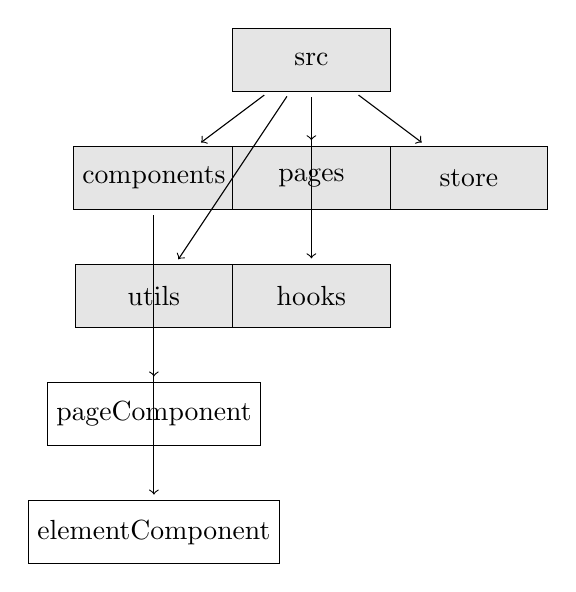
\begin{tikzpicture}[
    file/.style={draw, rectangle, minimum width=2cm, minimum height=0.8cm},
    folder/.style={draw, rectangle, minimum width=2cm, minimum height=0.8cm, fill=gray!20},
    arrow/.style={->, shorten >=2pt, shorten <=2pt}
]

% Folders
\node[folder] (src) at (0,0) {src};
\node[folder] (components) at (-2,-1.5) {components};
\node[folder] (pages) at (0,-1.5) {pages};
\node[folder] (store) at (2,-1.5) {store};
\node[folder] (utils) at (-2,-3) {utils};
\node[folder] (hooks) at (0,-3) {hooks};

% Files
\node[file] (pageComponent) at (-2,-4.5) {pageComponent};
\node[file] (elementComponent) at (-2,-6) {elementComponent};
% ... add more files

% Connections
\draw[arrow] (src) -- (components);
\draw[arrow] (src) -- (pages);
\draw[arrow] (src) -- (store);
\draw[arrow] (src) -- (utils);
\draw[arrow] (src) -- (hooks);
\draw[arrow] (components) -- (pageComponent);
\draw[arrow] (components) -- (elementComponent);
% ... add more connections

\end{tikzpicture}



\pagebreak
\subsubsection{Back-end}
The backend uses the dotNet framework. The development language using the C\# language.

In this project, the backend uses the Onion Architecture.
The Onion Architecture is a typically layered architecture, 
where each layer depends on the inner layer and provides interfaces to the outer layer.
The outer layer provides services to the outermost layer 
and other modules in the same layer based on the interfaces of the inner layer.

From inner to outer, the layers are: Domain, Application, Infrastructure, Presentation.
The Domain layer is the core layer and the innermost layer, used to define domain models, 
which are the business models.
It includes domain models and domain service interfaces.
Domain models are used to define the business models, 
which are the entities in the entity-relationship model and their attributes.
Domain service interfaces are used to define the business services, 
which are the relationships between entities in the entity-relationship model.

The Application layer is the application layer, 
used to define application services, which are the business logic.
It includes domain service implementations and application service interfaces.
Domain service implementations implement the methods of the inner layer's domain service 
interfaces and implement the business logic of the domain models.
Application service interfaces are used to define application services, 
which are the business logic.
It includes but is not limited to database interfaces, testing interfaces, 
HTTP API interfaces, MQTT interfaces, etc.

The Infrastructure layer is the infrastructure layer, used to define infrastructure.
It includes database implementations, testing implementations, 
HTTP API implementations, MQTT implementations, etc.
Database implementations implement the database interfaces 
and provide CRUD services for the database.
Testing implementations implement the testing interfaces 
and provide services for unit testing and integration testing.
HTTP API implementations implement the HTTP API interfaces 
and provide CRUD operations for HTTP APIs.
MQTT implementations implement the MQTT interfaces 
and provide CRUD operations for MQTT.

The Presentation layer is the presentation layer, used to define presentation logic, 
such as interfaces and pages. Since this is a backend project,
data presentation and control are handled by the frontend, 
so this layer is not needed.



\pagebreak
\subsubsection{Data communication and storage}
% 关于本项目的数据通信与数据存储的设计, 包括数据通信的协议, 数据存储的设计等
% 关于数据通信的设计:
% 1. 通信协议的选择
% 自前端向后端发送的数据, 有三种传输的数据类型, 
% 一种是普通的增删改查的请求, 对数据传输的时效性要求不高, 但是对数据的准确性, 完整性, 有序性, 安全性有一定的要求,
% 这种数据的传输, 采用 HTTP 协议, 以及 RESTful API 的设计. 可以有效的保证对数据传输的以上要求.
% 一种是对数据通道的创建和流媒体数据的传输, 对数据传输的时效性, 安全性要求较高, 这种数据的传输, 采用 WebRTC 协议, 以及 MQTT 协议.
% 配合可以快速解码的 flatbuffers 协议, 可以有效的保证对数据传输的以上要求.
% 最后一种是对设备的状态信息和操作信息的传输, 对完整性, 有序性, 安全性都有较高的要求, 这种数据的传输, 采用 MQTT 协议
% 同时也使用了 flatbuffers 协议.
% 
% 2. 数据通信的通信架构和通信流程
% 本项目的数据通信的通信架构, 是基于前后端分离的架构, 前端使用 React 框架, 后端使用 dotnet 框架.
% 当前端需要向后端发送数据的时候, 前端会向后端发送 HTTP 请求, 后端接收到 HTTP 请求之后, 会根据请求的数据类型,
% 选择不同的数据处理方式, 对于普通的增删改查的请求, 后端会根据 RESTful API 的设计, 对数据进行增删改查的操作,
% 对于对数据通道的创建和流媒体数据的传输, 后端会根据 WebRTC 协议, 对数据通道进行创建, 并且帮助前端和设备建立数据通道,
% 当数据通道建立后, 前端和设备之间则使用 flatbuffer 的数据格式对流媒体数据进行传输,
% 对于设备的状态信息和操作信息的传输, 前端会直接向 MQTT broker 发送 MQTT 请求, 
% 设备会在其自身的固件中监听相关的 MQTT 请求, 并且返回相关的数据.
% 
% 3. 数据通信的格式
% 本项目的数据通信的格式, 有三种, 
% 一种是 HTTP 协议, 
% 使用 json 格式对数据进行传输,
% 一种是 WebRTC 协议, 
% 使用 flatbuffers 格式对数据进行传输,
% 一种是 MQTT 协议.
% 使用 flatbuffers 格式对数据进行传输,
% 
% 关于数据存储的设计:
% 1. 数据存储的数据库的选择
% 本项目的数据存储的数据库的选择, 使用了轻量级的数据库 SQLite,
% SQLite 是一个进程内的库, 实现了自给自足的, 无服务器的, 零配置的, 事务性的 SQL 数据库引擎.
% 这是因为整个项目的目的是为了实现前端与设备之间的数据通信, 对于数据库数据的增删改查操作的要求不高,
% 数据量较小, 且对于数据库的数据的事务性要求不高, 所以选择了 SQLite 数据库.
% 2. 项目前后端的数据结构的设计
% 在本项目中, 前端由于使用了 React 框架, 所以前端的数据结构的设计, 使用了基于状态的数据结构的设计,
% 每个组件或者数据集都包含一个状态对象, 这个状态对象的属性就是组件的各个状态. 
% 使用状态对象的原因是, 可以方便的对状态进行管理, 采用对象-属性的形式, 可以方便的针对不同组件的同类状态进行区分,
% 由于跨组件的状态是由 redux 进行管理的, 这种状态对象的设计, 可以更搞笑的对状态进行更新和传递.
% 后端由于使用了 dotnet 框架, 所以后端的数据结构的设计, 使用了基于类的数据结构的设计,
% 采用了面向对象的编程思想, 对数据进行了封装, 使得数据的传输更加的安全, 有序, 完整.


\pagebreak

% \subsection{Domain model}
% \documentclass[]{article}
\usepackage{graphicx}
\usepackage{amsmath}
\usepackage{tikz}

% libaries
\usetikzlibrary{shapes,arrows}

%Define the listing package
\usepackage{listings} %code highlighter
\usepackage{color} %use color
\definecolor{mygreen}{rgb}{0,0.6,0}
\definecolor{mygray}{rgb}{0.5,0.5,0.5}
\definecolor{mymauve}{rgb}{0.58,0,0.82}

%Customize a bit the look
\lstset{ %
backgroundcolor=\color{white}, % choose the background color; you must add \usepackage{color} or \usepackage{xcolor}
basicstyle=\footnotesize, % the size of the fonts that are used for the code
breakatwhitespace=false, % sets if automatic breaks should only happen at whitespace
breaklines=true, % sets automatic line breaking
captionpos=b, % sets the caption-position to bottom
commentstyle=\color{mygreen}, % comment style
deletekeywords={...}, % if you want to delete keywords from the given language
escapeinside={\%*}{*)}, % if you want to add LaTeX within your code
extendedchars=true, % lets you use non-ASCII characters; for 8-bits encodings only, does not work with UTF-8
frame=single, % adds a frame around the code
keepspaces=true, % keeps spaces in text, useful for keeping indentation of code (possibly needs columns=flexible)
keywordstyle=\color{blue}, % keyword style
% language=Octave, % the language of the code
morekeywords={*,...}, % if you want to add more keywords to the set
numbers=left, % where to put the line-numbers; possible values are (none, left, right)
numbersep=5pt, % how far the line-numbers are from the code
numberstyle=\tiny\color{mygray}, % the style that is used for the line-numbers
rulecolor=\color{black}, % if not set, the frame-color may be changed on line-breaks within not-black text (e.g. comments (green here))
showspaces=false, % show spaces everywhere adding particular underscores; it overrides 'showstringspaces'
showstringspaces=false, % underline spaces within strings only
showtabs=false, % show tabs within strings adding particular underscores
stepnumber=1, % the step between two line-numbers. If it's 1, each line will be numbered
stringstyle=\color{mymauve}, % string literal style
tabsize=2, % sets default tabsize to 2 spaces
title=\lstname % show the filename of files included with \lstinputlisting; also try caption instead of title
}

\definecolor{darkgray}{rgb}{.4,.4,.4}
\definecolor{purple}{rgb}{0.65, 0.12, 0.82}

\lstdefinelanguage{React}{
keywords={const, typeof, new, true, false, catch, function, return, null, catch, switch, var, if, in, while, do, else, case, break},
keywordstyle=\color{blue}\bfseries,
ndkeywords={class, export, boolean, throw, implements, import, this},
ndkeywordstyle=\color{darkgray}\bfseries,
identifierstyle=\color{mygreen},
sensitive=false,
comment=[l]{//},
morecomment=[s]{/*}{*/},
commentstyle=\color{purple}\ttfamily,
string=[b]{"}{'}{`},
stringstyle=\color{red}\ttfamily,
morestring=[b]',
morestring=[b]",
morestring=[b]`',
}

\lstdefinelanguage{CSharp}{
keywords={const, typeof, new, true, false, catch, function, return, null, catch, switch, var, if, in, while, do, else, case, break},
keywordstyle=\color{blue}\bfseries,
ndkeywords={class, export, boolean, throw, implements, import, this},
ndkeywordstyle=\color{darkgray}\bfseries,
identifierstyle=\color{mygreen},
sensitive=false,
comment=[l]{//},
morecomment=[s]{/*}{*/},
commentstyle=\color{purple}\ttfamily,
string=[b]{"}{'}{`},
stringstyle=\color{red}\ttfamily,
morestring=[b]',
morestring=[b]",
morestring=[b]`',
}

\lstset{
language=React,
extendedchars=true,
basicstyle=\footnotesize\ttfamily,
showstringspaces=false,
showspaces=false,
numbers=left,
numberstyle=\footnotesize,
numbersep=9pt,
tabsize=2,
breaklines=true,
showtabs=false,
captionpos=b
}

\lstset{
language=CSharp,
extendedchars=true,
basicstyle=\footnotesize\ttfamily,
showstringspaces=false,
showspaces=false,
numbers=left,
numberstyle=\footnotesize,
numbersep=9pt,
tabsize=2,
breaklines=true,
showtabs=false,
captionpos=b
}

% \usepackage{cite} % Add this line for citation

% \bibliographystyle{plain}

\title{
The implementation of BifrostConnect Front-end scope, 
re-design and development with the relevant back-end support develop.
}
\author{
    Fei Gu \\
    Erhvervs Akademi Sydvest \\
    Computer Science 21\\
    }
\date{\today}

\begin{document}

% Front page
\maketitle
\begin{center}
    Supervisor: Henrik Boulund Meng Hansen \\
    Company: BifrostConnect \\
    Engineering Director: Jasper Wass \\
\end{center}
\tableofcontents
\pagebreak


% The introduction
\section{Introduction}
\subsection{Background}\input{sections/introduction/background.tex}
\subsection{The company}\input{sections/introduction/aboutCompany}
\subsection{The project}\input{sections/introduction/aboutProject}
\pagebreak

% The problem statement
\section{Problem Statement}
\subsection{Statement}
\input{sections/problemStatement/statement}
\subsection{Situation}
\input{sections/problemStatement/situation}
\subsection{Potential Solution}
\input{sections/problemStatement/potentialSolution}
\pagebreak

% Requirement analysis
\section{Requirement Analysis}
\input{sections/requirementAnalysis/index}

\subsection{Stakeholders}
\input{sections/requirementAnalysis/stakeholders/index}

\subsection{Business Domain}
\input{sections/requirementAnalysis/bussinesDomain/index}

\subsection{Scope}
\input{sections/requirementAnalysis/scope}

\subsection{Goals}
\input{sections/requirementAnalysis/goals}
\pagebreak

% Software Design
\section{Software Design}
% developement methods
\subsection{Software Development Methods}
\input{sections/softwareDevelopmentMethods/index}
\subsubsection{Agile Software Development}
\input{sections/softwareDevelopmentMethods/agileSoftwareDevelopment/index}
\subsubsection{Feature Driven Development}
\input{sections/softwareDevelopmentMethods/featureDrivenDevelopment/index}

\pagebreak

% Technology seslection
\subsection{Technology selection}
\input{sections/softwareDesign/technologySelection/index}
\subsubsection{Front-end}
\input{sections/softwareDesign/technologySelection/frontEnd}            
\subsubsection{Back-end}
\input{sections/softwareDesign/technologySelection/backEnd}            
\subsubsection{Database}
\input{sections/softwareDesign/technologySelection/database}
\subsubsection{Data communication}
\input{sections/softwareDesign/technologySelection/dataCommunication}            
\subsubsection{DevOps}
\input{sections/softwareDesign/technologySelection/devOps}
\pagebreak

% Architecture design
\subsection{Architecture design}
\input{sections/softwareDesign/architectureDesign/index}
\pagebreak
\subsubsection{Front-end}
\input{sections/softwareDesign/architectureDesign/frontEndArchitecture}
\pagebreak
\subsubsection{Back-end}
\input{sections/softwareDesign/architectureDesign/backEndArchitecture}
\pagebreak
\subsubsection{Data communication and storage}
\input{sections/softwareDesign/architectureDesign/dataCommunicationArchitecture}
\pagebreak

% \subsection{Domain model}
% \input{sections/softwareDesign/domainModel/index}
% \subsection{Database design}
% % 数据库领域模型 ER 图
% % 包括表和字段的设置.
% % 对于私有键和外键的设置.

% \subsection{Back-end design}
% % 后端对象模型
% % 以及对于对象模型的增删改查
% % 以及相关的其他服务的设计`'

% \subsection{Front-end design}
% % 对于前端的页面结构的设计 
% % 页面的状态的设计, 交互设计

% \subsection{FlatBuffers design}
% % schema 的设计

\subsection{DevOps CI/CD process design}
\input{sections/softwareDesign/devOpsDesign/index}
\subsubsection{Continuous Integration}
\input{sections/softwareDesign/devOpsDesign/continuousIntegration/index}
\subsubsection{Continuous Delivery}
\input{sections/softwareDesign/devOpsDesign/continuousDelivery/index}
\subsubsection{Continuous Deployment}
\input{sections/softwareDesign/devOpsDesign/continuousDeployment/index}
\pagebreak

\section{Software Development} 
\input{sections/softwareDevelopment/index}
\subsection{Overall development}
\input{sections/softwareDevelopment/overallDevelopement/index}
\subsubsection{Front-end}
\input{sections/softwareDevelopment/overallDevelopement/frontEnd/index}
\subsubsection{Back-end}
\input{sections/softwareDevelopment/overallDevelopement/backEnd/index}
\subsubsection{DevOps}
\input{sections/softwareDevelopment/overallDevelopement/devOps/index}
\subsection{Feature development} 
\input{sections/softwareDevelopment/featureDevelopment/index}
\subsubsection{Use Case 1}
\input{sections/softwareDevelopment/featureDevelopment/useCase1/index}
\subsubsection{Feature 1}
\input{sections/softwareDevelopment/featureDevelopment/feature/feature1.tex}
\pagebreak
\section{Conclusion} 
\subsection{Result}
Since the project is still in progress, the result is not available yet.
So far, basic structure of this project has been built. But the most features 
are not implemented yet. 
\subsection{Discussion}
As a single developer for this project, I am confident what I have done so far.
And I can say I understand the most of the knowledge I have used in this project, 
which also means I can explain all the part of the project. 
But this project also relevant some of the complex knowledge which I have to continue 
to study and practice.
\subsection{Future Work}
The future work is to implement the rest of the features. 
Including the most important part which is the 'create session' feature.
\pagebreak
% \bibliography{bibliography}
\pagebreak
% \begin{appendices}
%     \section{Appendix}
% \end{appendices} 
\end{document}
% \subsection{Database design}
% % 数据库领域模型 ER 图
% % 包括表和字段的设置.
% % 对于私有键和外键的设置.

% \subsection{Back-end design}
% % 后端对象模型
% % 以及对于对象模型的增删改查
% % 以及相关的其他服务的设计`'

% \subsection{Front-end design}
% % 对于前端的页面结构的设计 
% % 页面的状态的设计, 交互设计

% \subsection{FlatBuffers design}
% % schema 的设计

\subsection{DevOps CI/CD process design}
\documentclass[]{article}
\usepackage{graphicx}
\usepackage{amsmath}
\usepackage{tikz}

% libaries
\usetikzlibrary{shapes,arrows}

%Define the listing package
\usepackage{listings} %code highlighter
\usepackage{color} %use color
\definecolor{mygreen}{rgb}{0,0.6,0}
\definecolor{mygray}{rgb}{0.5,0.5,0.5}
\definecolor{mymauve}{rgb}{0.58,0,0.82}

%Customize a bit the look
\lstset{ %
backgroundcolor=\color{white}, % choose the background color; you must add \usepackage{color} or \usepackage{xcolor}
basicstyle=\footnotesize, % the size of the fonts that are used for the code
breakatwhitespace=false, % sets if automatic breaks should only happen at whitespace
breaklines=true, % sets automatic line breaking
captionpos=b, % sets the caption-position to bottom
commentstyle=\color{mygreen}, % comment style
deletekeywords={...}, % if you want to delete keywords from the given language
escapeinside={\%*}{*)}, % if you want to add LaTeX within your code
extendedchars=true, % lets you use non-ASCII characters; for 8-bits encodings only, does not work with UTF-8
frame=single, % adds a frame around the code
keepspaces=true, % keeps spaces in text, useful for keeping indentation of code (possibly needs columns=flexible)
keywordstyle=\color{blue}, % keyword style
% language=Octave, % the language of the code
morekeywords={*,...}, % if you want to add more keywords to the set
numbers=left, % where to put the line-numbers; possible values are (none, left, right)
numbersep=5pt, % how far the line-numbers are from the code
numberstyle=\tiny\color{mygray}, % the style that is used for the line-numbers
rulecolor=\color{black}, % if not set, the frame-color may be changed on line-breaks within not-black text (e.g. comments (green here))
showspaces=false, % show spaces everywhere adding particular underscores; it overrides 'showstringspaces'
showstringspaces=false, % underline spaces within strings only
showtabs=false, % show tabs within strings adding particular underscores
stepnumber=1, % the step between two line-numbers. If it's 1, each line will be numbered
stringstyle=\color{mymauve}, % string literal style
tabsize=2, % sets default tabsize to 2 spaces
title=\lstname % show the filename of files included with \lstinputlisting; also try caption instead of title
}

\definecolor{darkgray}{rgb}{.4,.4,.4}
\definecolor{purple}{rgb}{0.65, 0.12, 0.82}

\lstdefinelanguage{React}{
keywords={const, typeof, new, true, false, catch, function, return, null, catch, switch, var, if, in, while, do, else, case, break},
keywordstyle=\color{blue}\bfseries,
ndkeywords={class, export, boolean, throw, implements, import, this},
ndkeywordstyle=\color{darkgray}\bfseries,
identifierstyle=\color{mygreen},
sensitive=false,
comment=[l]{//},
morecomment=[s]{/*}{*/},
commentstyle=\color{purple}\ttfamily,
string=[b]{"}{'}{`},
stringstyle=\color{red}\ttfamily,
morestring=[b]',
morestring=[b]",
morestring=[b]`',
}

\lstdefinelanguage{CSharp}{
keywords={const, typeof, new, true, false, catch, function, return, null, catch, switch, var, if, in, while, do, else, case, break},
keywordstyle=\color{blue}\bfseries,
ndkeywords={class, export, boolean, throw, implements, import, this},
ndkeywordstyle=\color{darkgray}\bfseries,
identifierstyle=\color{mygreen},
sensitive=false,
comment=[l]{//},
morecomment=[s]{/*}{*/},
commentstyle=\color{purple}\ttfamily,
string=[b]{"}{'}{`},
stringstyle=\color{red}\ttfamily,
morestring=[b]',
morestring=[b]",
morestring=[b]`',
}

\lstset{
language=React,
extendedchars=true,
basicstyle=\footnotesize\ttfamily,
showstringspaces=false,
showspaces=false,
numbers=left,
numberstyle=\footnotesize,
numbersep=9pt,
tabsize=2,
breaklines=true,
showtabs=false,
captionpos=b
}

\lstset{
language=CSharp,
extendedchars=true,
basicstyle=\footnotesize\ttfamily,
showstringspaces=false,
showspaces=false,
numbers=left,
numberstyle=\footnotesize,
numbersep=9pt,
tabsize=2,
breaklines=true,
showtabs=false,
captionpos=b
}

% \usepackage{cite} % Add this line for citation

% \bibliographystyle{plain}

\title{
The implementation of BifrostConnect Front-end scope, 
re-design and development with the relevant back-end support develop.
}
\author{
    Fei Gu \\
    Erhvervs Akademi Sydvest \\
    Computer Science 21\\
    }
\date{\today}

\begin{document}

% Front page
\maketitle
\begin{center}
    Supervisor: Henrik Boulund Meng Hansen \\
    Company: BifrostConnect \\
    Engineering Director: Jasper Wass \\
\end{center}
\tableofcontents
\pagebreak


% The introduction
\section{Introduction}
\subsection{Background}\input{sections/introduction/background.tex}
\subsection{The company}\input{sections/introduction/aboutCompany}
\subsection{The project}\input{sections/introduction/aboutProject}
\pagebreak

% The problem statement
\section{Problem Statement}
\subsection{Statement}
\input{sections/problemStatement/statement}
\subsection{Situation}
\input{sections/problemStatement/situation}
\subsection{Potential Solution}
\input{sections/problemStatement/potentialSolution}
\pagebreak

% Requirement analysis
\section{Requirement Analysis}
\input{sections/requirementAnalysis/index}

\subsection{Stakeholders}
\input{sections/requirementAnalysis/stakeholders/index}

\subsection{Business Domain}
\input{sections/requirementAnalysis/bussinesDomain/index}

\subsection{Scope}
\input{sections/requirementAnalysis/scope}

\subsection{Goals}
\input{sections/requirementAnalysis/goals}
\pagebreak

% Software Design
\section{Software Design}
% developement methods
\subsection{Software Development Methods}
\input{sections/softwareDevelopmentMethods/index}
\subsubsection{Agile Software Development}
\input{sections/softwareDevelopmentMethods/agileSoftwareDevelopment/index}
\subsubsection{Feature Driven Development}
\input{sections/softwareDevelopmentMethods/featureDrivenDevelopment/index}

\pagebreak

% Technology seslection
\subsection{Technology selection}
\input{sections/softwareDesign/technologySelection/index}
\subsubsection{Front-end}
\input{sections/softwareDesign/technologySelection/frontEnd}            
\subsubsection{Back-end}
\input{sections/softwareDesign/technologySelection/backEnd}            
\subsubsection{Database}
\input{sections/softwareDesign/technologySelection/database}
\subsubsection{Data communication}
\input{sections/softwareDesign/technologySelection/dataCommunication}            
\subsubsection{DevOps}
\input{sections/softwareDesign/technologySelection/devOps}
\pagebreak

% Architecture design
\subsection{Architecture design}
\input{sections/softwareDesign/architectureDesign/index}
\pagebreak
\subsubsection{Front-end}
\input{sections/softwareDesign/architectureDesign/frontEndArchitecture}
\pagebreak
\subsubsection{Back-end}
\input{sections/softwareDesign/architectureDesign/backEndArchitecture}
\pagebreak
\subsubsection{Data communication and storage}
\input{sections/softwareDesign/architectureDesign/dataCommunicationArchitecture}
\pagebreak

% \subsection{Domain model}
% \input{sections/softwareDesign/domainModel/index}
% \subsection{Database design}
% % 数据库领域模型 ER 图
% % 包括表和字段的设置.
% % 对于私有键和外键的设置.

% \subsection{Back-end design}
% % 后端对象模型
% % 以及对于对象模型的增删改查
% % 以及相关的其他服务的设计`'

% \subsection{Front-end design}
% % 对于前端的页面结构的设计 
% % 页面的状态的设计, 交互设计

% \subsection{FlatBuffers design}
% % schema 的设计

\subsection{DevOps CI/CD process design}
\input{sections/softwareDesign/devOpsDesign/index}
\subsubsection{Continuous Integration}
\input{sections/softwareDesign/devOpsDesign/continuousIntegration/index}
\subsubsection{Continuous Delivery}
\input{sections/softwareDesign/devOpsDesign/continuousDelivery/index}
\subsubsection{Continuous Deployment}
\input{sections/softwareDesign/devOpsDesign/continuousDeployment/index}
\pagebreak

\section{Software Development} 
\input{sections/softwareDevelopment/index}
\subsection{Overall development}
\input{sections/softwareDevelopment/overallDevelopement/index}
\subsubsection{Front-end}
\input{sections/softwareDevelopment/overallDevelopement/frontEnd/index}
\subsubsection{Back-end}
\input{sections/softwareDevelopment/overallDevelopement/backEnd/index}
\subsubsection{DevOps}
\input{sections/softwareDevelopment/overallDevelopement/devOps/index}
\subsection{Feature development} 
\input{sections/softwareDevelopment/featureDevelopment/index}
\subsubsection{Use Case 1}
\input{sections/softwareDevelopment/featureDevelopment/useCase1/index}
\subsubsection{Feature 1}
\input{sections/softwareDevelopment/featureDevelopment/feature/feature1.tex}
\pagebreak
\section{Conclusion} 
\subsection{Result}
Since the project is still in progress, the result is not available yet.
So far, basic structure of this project has been built. But the most features 
are not implemented yet. 
\subsection{Discussion}
As a single developer for this project, I am confident what I have done so far.
And I can say I understand the most of the knowledge I have used in this project, 
which also means I can explain all the part of the project. 
But this project also relevant some of the complex knowledge which I have to continue 
to study and practice.
\subsection{Future Work}
The future work is to implement the rest of the features. 
Including the most important part which is the 'create session' feature.
\pagebreak
% \bibliography{bibliography}
\pagebreak
% \begin{appendices}
%     \section{Appendix}
% \end{appendices} 
\end{document}
\subsubsection{Continuous Integration}
\documentclass[]{article}
\usepackage{graphicx}
\usepackage{amsmath}
\usepackage{tikz}

% libaries
\usetikzlibrary{shapes,arrows}

%Define the listing package
\usepackage{listings} %code highlighter
\usepackage{color} %use color
\definecolor{mygreen}{rgb}{0,0.6,0}
\definecolor{mygray}{rgb}{0.5,0.5,0.5}
\definecolor{mymauve}{rgb}{0.58,0,0.82}

%Customize a bit the look
\lstset{ %
backgroundcolor=\color{white}, % choose the background color; you must add \usepackage{color} or \usepackage{xcolor}
basicstyle=\footnotesize, % the size of the fonts that are used for the code
breakatwhitespace=false, % sets if automatic breaks should only happen at whitespace
breaklines=true, % sets automatic line breaking
captionpos=b, % sets the caption-position to bottom
commentstyle=\color{mygreen}, % comment style
deletekeywords={...}, % if you want to delete keywords from the given language
escapeinside={\%*}{*)}, % if you want to add LaTeX within your code
extendedchars=true, % lets you use non-ASCII characters; for 8-bits encodings only, does not work with UTF-8
frame=single, % adds a frame around the code
keepspaces=true, % keeps spaces in text, useful for keeping indentation of code (possibly needs columns=flexible)
keywordstyle=\color{blue}, % keyword style
% language=Octave, % the language of the code
morekeywords={*,...}, % if you want to add more keywords to the set
numbers=left, % where to put the line-numbers; possible values are (none, left, right)
numbersep=5pt, % how far the line-numbers are from the code
numberstyle=\tiny\color{mygray}, % the style that is used for the line-numbers
rulecolor=\color{black}, % if not set, the frame-color may be changed on line-breaks within not-black text (e.g. comments (green here))
showspaces=false, % show spaces everywhere adding particular underscores; it overrides 'showstringspaces'
showstringspaces=false, % underline spaces within strings only
showtabs=false, % show tabs within strings adding particular underscores
stepnumber=1, % the step between two line-numbers. If it's 1, each line will be numbered
stringstyle=\color{mymauve}, % string literal style
tabsize=2, % sets default tabsize to 2 spaces
title=\lstname % show the filename of files included with \lstinputlisting; also try caption instead of title
}

\definecolor{darkgray}{rgb}{.4,.4,.4}
\definecolor{purple}{rgb}{0.65, 0.12, 0.82}

\lstdefinelanguage{React}{
keywords={const, typeof, new, true, false, catch, function, return, null, catch, switch, var, if, in, while, do, else, case, break},
keywordstyle=\color{blue}\bfseries,
ndkeywords={class, export, boolean, throw, implements, import, this},
ndkeywordstyle=\color{darkgray}\bfseries,
identifierstyle=\color{mygreen},
sensitive=false,
comment=[l]{//},
morecomment=[s]{/*}{*/},
commentstyle=\color{purple}\ttfamily,
string=[b]{"}{'}{`},
stringstyle=\color{red}\ttfamily,
morestring=[b]',
morestring=[b]",
morestring=[b]`',
}

\lstdefinelanguage{CSharp}{
keywords={const, typeof, new, true, false, catch, function, return, null, catch, switch, var, if, in, while, do, else, case, break},
keywordstyle=\color{blue}\bfseries,
ndkeywords={class, export, boolean, throw, implements, import, this},
ndkeywordstyle=\color{darkgray}\bfseries,
identifierstyle=\color{mygreen},
sensitive=false,
comment=[l]{//},
morecomment=[s]{/*}{*/},
commentstyle=\color{purple}\ttfamily,
string=[b]{"}{'}{`},
stringstyle=\color{red}\ttfamily,
morestring=[b]',
morestring=[b]",
morestring=[b]`',
}

\lstset{
language=React,
extendedchars=true,
basicstyle=\footnotesize\ttfamily,
showstringspaces=false,
showspaces=false,
numbers=left,
numberstyle=\footnotesize,
numbersep=9pt,
tabsize=2,
breaklines=true,
showtabs=false,
captionpos=b
}

\lstset{
language=CSharp,
extendedchars=true,
basicstyle=\footnotesize\ttfamily,
showstringspaces=false,
showspaces=false,
numbers=left,
numberstyle=\footnotesize,
numbersep=9pt,
tabsize=2,
breaklines=true,
showtabs=false,
captionpos=b
}

% \usepackage{cite} % Add this line for citation

% \bibliographystyle{plain}

\title{
The implementation of BifrostConnect Front-end scope, 
re-design and development with the relevant back-end support develop.
}
\author{
    Fei Gu \\
    Erhvervs Akademi Sydvest \\
    Computer Science 21\\
    }
\date{\today}

\begin{document}

% Front page
\maketitle
\begin{center}
    Supervisor: Henrik Boulund Meng Hansen \\
    Company: BifrostConnect \\
    Engineering Director: Jasper Wass \\
\end{center}
\tableofcontents
\pagebreak


% The introduction
\section{Introduction}
\subsection{Background}\input{sections/introduction/background.tex}
\subsection{The company}\input{sections/introduction/aboutCompany}
\subsection{The project}\input{sections/introduction/aboutProject}
\pagebreak

% The problem statement
\section{Problem Statement}
\subsection{Statement}
\input{sections/problemStatement/statement}
\subsection{Situation}
\input{sections/problemStatement/situation}
\subsection{Potential Solution}
\input{sections/problemStatement/potentialSolution}
\pagebreak

% Requirement analysis
\section{Requirement Analysis}
\input{sections/requirementAnalysis/index}

\subsection{Stakeholders}
\input{sections/requirementAnalysis/stakeholders/index}

\subsection{Business Domain}
\input{sections/requirementAnalysis/bussinesDomain/index}

\subsection{Scope}
\input{sections/requirementAnalysis/scope}

\subsection{Goals}
\input{sections/requirementAnalysis/goals}
\pagebreak

% Software Design
\section{Software Design}
% developement methods
\subsection{Software Development Methods}
\input{sections/softwareDevelopmentMethods/index}
\subsubsection{Agile Software Development}
\input{sections/softwareDevelopmentMethods/agileSoftwareDevelopment/index}
\subsubsection{Feature Driven Development}
\input{sections/softwareDevelopmentMethods/featureDrivenDevelopment/index}

\pagebreak

% Technology seslection
\subsection{Technology selection}
\input{sections/softwareDesign/technologySelection/index}
\subsubsection{Front-end}
\input{sections/softwareDesign/technologySelection/frontEnd}            
\subsubsection{Back-end}
\input{sections/softwareDesign/technologySelection/backEnd}            
\subsubsection{Database}
\input{sections/softwareDesign/technologySelection/database}
\subsubsection{Data communication}
\input{sections/softwareDesign/technologySelection/dataCommunication}            
\subsubsection{DevOps}
\input{sections/softwareDesign/technologySelection/devOps}
\pagebreak

% Architecture design
\subsection{Architecture design}
\input{sections/softwareDesign/architectureDesign/index}
\pagebreak
\subsubsection{Front-end}
\input{sections/softwareDesign/architectureDesign/frontEndArchitecture}
\pagebreak
\subsubsection{Back-end}
\input{sections/softwareDesign/architectureDesign/backEndArchitecture}
\pagebreak
\subsubsection{Data communication and storage}
\input{sections/softwareDesign/architectureDesign/dataCommunicationArchitecture}
\pagebreak

% \subsection{Domain model}
% \input{sections/softwareDesign/domainModel/index}
% \subsection{Database design}
% % 数据库领域模型 ER 图
% % 包括表和字段的设置.
% % 对于私有键和外键的设置.

% \subsection{Back-end design}
% % 后端对象模型
% % 以及对于对象模型的增删改查
% % 以及相关的其他服务的设计`'

% \subsection{Front-end design}
% % 对于前端的页面结构的设计 
% % 页面的状态的设计, 交互设计

% \subsection{FlatBuffers design}
% % schema 的设计

\subsection{DevOps CI/CD process design}
\input{sections/softwareDesign/devOpsDesign/index}
\subsubsection{Continuous Integration}
\input{sections/softwareDesign/devOpsDesign/continuousIntegration/index}
\subsubsection{Continuous Delivery}
\input{sections/softwareDesign/devOpsDesign/continuousDelivery/index}
\subsubsection{Continuous Deployment}
\input{sections/softwareDesign/devOpsDesign/continuousDeployment/index}
\pagebreak

\section{Software Development} 
\input{sections/softwareDevelopment/index}
\subsection{Overall development}
\input{sections/softwareDevelopment/overallDevelopement/index}
\subsubsection{Front-end}
\input{sections/softwareDevelopment/overallDevelopement/frontEnd/index}
\subsubsection{Back-end}
\input{sections/softwareDevelopment/overallDevelopement/backEnd/index}
\subsubsection{DevOps}
\input{sections/softwareDevelopment/overallDevelopement/devOps/index}
\subsection{Feature development} 
\input{sections/softwareDevelopment/featureDevelopment/index}
\subsubsection{Use Case 1}
\input{sections/softwareDevelopment/featureDevelopment/useCase1/index}
\subsubsection{Feature 1}
\input{sections/softwareDevelopment/featureDevelopment/feature/feature1.tex}
\pagebreak
\section{Conclusion} 
\subsection{Result}
Since the project is still in progress, the result is not available yet.
So far, basic structure of this project has been built. But the most features 
are not implemented yet. 
\subsection{Discussion}
As a single developer for this project, I am confident what I have done so far.
And I can say I understand the most of the knowledge I have used in this project, 
which also means I can explain all the part of the project. 
But this project also relevant some of the complex knowledge which I have to continue 
to study and practice.
\subsection{Future Work}
The future work is to implement the rest of the features. 
Including the most important part which is the 'create session' feature.
\pagebreak
% \bibliography{bibliography}
\pagebreak
% \begin{appendices}
%     \section{Appendix}
% \end{appendices} 
\end{document}
\subsubsection{Continuous Delivery}
\documentclass[]{article}
\usepackage{graphicx}
\usepackage{amsmath}
\usepackage{tikz}

% libaries
\usetikzlibrary{shapes,arrows}

%Define the listing package
\usepackage{listings} %code highlighter
\usepackage{color} %use color
\definecolor{mygreen}{rgb}{0,0.6,0}
\definecolor{mygray}{rgb}{0.5,0.5,0.5}
\definecolor{mymauve}{rgb}{0.58,0,0.82}

%Customize a bit the look
\lstset{ %
backgroundcolor=\color{white}, % choose the background color; you must add \usepackage{color} or \usepackage{xcolor}
basicstyle=\footnotesize, % the size of the fonts that are used for the code
breakatwhitespace=false, % sets if automatic breaks should only happen at whitespace
breaklines=true, % sets automatic line breaking
captionpos=b, % sets the caption-position to bottom
commentstyle=\color{mygreen}, % comment style
deletekeywords={...}, % if you want to delete keywords from the given language
escapeinside={\%*}{*)}, % if you want to add LaTeX within your code
extendedchars=true, % lets you use non-ASCII characters; for 8-bits encodings only, does not work with UTF-8
frame=single, % adds a frame around the code
keepspaces=true, % keeps spaces in text, useful for keeping indentation of code (possibly needs columns=flexible)
keywordstyle=\color{blue}, % keyword style
% language=Octave, % the language of the code
morekeywords={*,...}, % if you want to add more keywords to the set
numbers=left, % where to put the line-numbers; possible values are (none, left, right)
numbersep=5pt, % how far the line-numbers are from the code
numberstyle=\tiny\color{mygray}, % the style that is used for the line-numbers
rulecolor=\color{black}, % if not set, the frame-color may be changed on line-breaks within not-black text (e.g. comments (green here))
showspaces=false, % show spaces everywhere adding particular underscores; it overrides 'showstringspaces'
showstringspaces=false, % underline spaces within strings only
showtabs=false, % show tabs within strings adding particular underscores
stepnumber=1, % the step between two line-numbers. If it's 1, each line will be numbered
stringstyle=\color{mymauve}, % string literal style
tabsize=2, % sets default tabsize to 2 spaces
title=\lstname % show the filename of files included with \lstinputlisting; also try caption instead of title
}

\definecolor{darkgray}{rgb}{.4,.4,.4}
\definecolor{purple}{rgb}{0.65, 0.12, 0.82}

\lstdefinelanguage{React}{
keywords={const, typeof, new, true, false, catch, function, return, null, catch, switch, var, if, in, while, do, else, case, break},
keywordstyle=\color{blue}\bfseries,
ndkeywords={class, export, boolean, throw, implements, import, this},
ndkeywordstyle=\color{darkgray}\bfseries,
identifierstyle=\color{mygreen},
sensitive=false,
comment=[l]{//},
morecomment=[s]{/*}{*/},
commentstyle=\color{purple}\ttfamily,
string=[b]{"}{'}{`},
stringstyle=\color{red}\ttfamily,
morestring=[b]',
morestring=[b]",
morestring=[b]`',
}

\lstdefinelanguage{CSharp}{
keywords={const, typeof, new, true, false, catch, function, return, null, catch, switch, var, if, in, while, do, else, case, break},
keywordstyle=\color{blue}\bfseries,
ndkeywords={class, export, boolean, throw, implements, import, this},
ndkeywordstyle=\color{darkgray}\bfseries,
identifierstyle=\color{mygreen},
sensitive=false,
comment=[l]{//},
morecomment=[s]{/*}{*/},
commentstyle=\color{purple}\ttfamily,
string=[b]{"}{'}{`},
stringstyle=\color{red}\ttfamily,
morestring=[b]',
morestring=[b]",
morestring=[b]`',
}

\lstset{
language=React,
extendedchars=true,
basicstyle=\footnotesize\ttfamily,
showstringspaces=false,
showspaces=false,
numbers=left,
numberstyle=\footnotesize,
numbersep=9pt,
tabsize=2,
breaklines=true,
showtabs=false,
captionpos=b
}

\lstset{
language=CSharp,
extendedchars=true,
basicstyle=\footnotesize\ttfamily,
showstringspaces=false,
showspaces=false,
numbers=left,
numberstyle=\footnotesize,
numbersep=9pt,
tabsize=2,
breaklines=true,
showtabs=false,
captionpos=b
}

% \usepackage{cite} % Add this line for citation

% \bibliographystyle{plain}

\title{
The implementation of BifrostConnect Front-end scope, 
re-design and development with the relevant back-end support develop.
}
\author{
    Fei Gu \\
    Erhvervs Akademi Sydvest \\
    Computer Science 21\\
    }
\date{\today}

\begin{document}

% Front page
\maketitle
\begin{center}
    Supervisor: Henrik Boulund Meng Hansen \\
    Company: BifrostConnect \\
    Engineering Director: Jasper Wass \\
\end{center}
\tableofcontents
\pagebreak


% The introduction
\section{Introduction}
\subsection{Background}\input{sections/introduction/background.tex}
\subsection{The company}\input{sections/introduction/aboutCompany}
\subsection{The project}\input{sections/introduction/aboutProject}
\pagebreak

% The problem statement
\section{Problem Statement}
\subsection{Statement}
\input{sections/problemStatement/statement}
\subsection{Situation}
\input{sections/problemStatement/situation}
\subsection{Potential Solution}
\input{sections/problemStatement/potentialSolution}
\pagebreak

% Requirement analysis
\section{Requirement Analysis}
\input{sections/requirementAnalysis/index}

\subsection{Stakeholders}
\input{sections/requirementAnalysis/stakeholders/index}

\subsection{Business Domain}
\input{sections/requirementAnalysis/bussinesDomain/index}

\subsection{Scope}
\input{sections/requirementAnalysis/scope}

\subsection{Goals}
\input{sections/requirementAnalysis/goals}
\pagebreak

% Software Design
\section{Software Design}
% developement methods
\subsection{Software Development Methods}
\input{sections/softwareDevelopmentMethods/index}
\subsubsection{Agile Software Development}
\input{sections/softwareDevelopmentMethods/agileSoftwareDevelopment/index}
\subsubsection{Feature Driven Development}
\input{sections/softwareDevelopmentMethods/featureDrivenDevelopment/index}

\pagebreak

% Technology seslection
\subsection{Technology selection}
\input{sections/softwareDesign/technologySelection/index}
\subsubsection{Front-end}
\input{sections/softwareDesign/technologySelection/frontEnd}            
\subsubsection{Back-end}
\input{sections/softwareDesign/technologySelection/backEnd}            
\subsubsection{Database}
\input{sections/softwareDesign/technologySelection/database}
\subsubsection{Data communication}
\input{sections/softwareDesign/technologySelection/dataCommunication}            
\subsubsection{DevOps}
\input{sections/softwareDesign/technologySelection/devOps}
\pagebreak

% Architecture design
\subsection{Architecture design}
\input{sections/softwareDesign/architectureDesign/index}
\pagebreak
\subsubsection{Front-end}
\input{sections/softwareDesign/architectureDesign/frontEndArchitecture}
\pagebreak
\subsubsection{Back-end}
\input{sections/softwareDesign/architectureDesign/backEndArchitecture}
\pagebreak
\subsubsection{Data communication and storage}
\input{sections/softwareDesign/architectureDesign/dataCommunicationArchitecture}
\pagebreak

% \subsection{Domain model}
% \input{sections/softwareDesign/domainModel/index}
% \subsection{Database design}
% % 数据库领域模型 ER 图
% % 包括表和字段的设置.
% % 对于私有键和外键的设置.

% \subsection{Back-end design}
% % 后端对象模型
% % 以及对于对象模型的增删改查
% % 以及相关的其他服务的设计`'

% \subsection{Front-end design}
% % 对于前端的页面结构的设计 
% % 页面的状态的设计, 交互设计

% \subsection{FlatBuffers design}
% % schema 的设计

\subsection{DevOps CI/CD process design}
\input{sections/softwareDesign/devOpsDesign/index}
\subsubsection{Continuous Integration}
\input{sections/softwareDesign/devOpsDesign/continuousIntegration/index}
\subsubsection{Continuous Delivery}
\input{sections/softwareDesign/devOpsDesign/continuousDelivery/index}
\subsubsection{Continuous Deployment}
\input{sections/softwareDesign/devOpsDesign/continuousDeployment/index}
\pagebreak

\section{Software Development} 
\input{sections/softwareDevelopment/index}
\subsection{Overall development}
\input{sections/softwareDevelopment/overallDevelopement/index}
\subsubsection{Front-end}
\input{sections/softwareDevelopment/overallDevelopement/frontEnd/index}
\subsubsection{Back-end}
\input{sections/softwareDevelopment/overallDevelopement/backEnd/index}
\subsubsection{DevOps}
\input{sections/softwareDevelopment/overallDevelopement/devOps/index}
\subsection{Feature development} 
\input{sections/softwareDevelopment/featureDevelopment/index}
\subsubsection{Use Case 1}
\input{sections/softwareDevelopment/featureDevelopment/useCase1/index}
\subsubsection{Feature 1}
\input{sections/softwareDevelopment/featureDevelopment/feature/feature1.tex}
\pagebreak
\section{Conclusion} 
\subsection{Result}
Since the project is still in progress, the result is not available yet.
So far, basic structure of this project has been built. But the most features 
are not implemented yet. 
\subsection{Discussion}
As a single developer for this project, I am confident what I have done so far.
And I can say I understand the most of the knowledge I have used in this project, 
which also means I can explain all the part of the project. 
But this project also relevant some of the complex knowledge which I have to continue 
to study and practice.
\subsection{Future Work}
The future work is to implement the rest of the features. 
Including the most important part which is the 'create session' feature.
\pagebreak
% \bibliography{bibliography}
\pagebreak
% \begin{appendices}
%     \section{Appendix}
% \end{appendices} 
\end{document}
\subsubsection{Continuous Deployment}
\documentclass[]{article}
\usepackage{graphicx}
\usepackage{amsmath}
\usepackage{tikz}

% libaries
\usetikzlibrary{shapes,arrows}

%Define the listing package
\usepackage{listings} %code highlighter
\usepackage{color} %use color
\definecolor{mygreen}{rgb}{0,0.6,0}
\definecolor{mygray}{rgb}{0.5,0.5,0.5}
\definecolor{mymauve}{rgb}{0.58,0,0.82}

%Customize a bit the look
\lstset{ %
backgroundcolor=\color{white}, % choose the background color; you must add \usepackage{color} or \usepackage{xcolor}
basicstyle=\footnotesize, % the size of the fonts that are used for the code
breakatwhitespace=false, % sets if automatic breaks should only happen at whitespace
breaklines=true, % sets automatic line breaking
captionpos=b, % sets the caption-position to bottom
commentstyle=\color{mygreen}, % comment style
deletekeywords={...}, % if you want to delete keywords from the given language
escapeinside={\%*}{*)}, % if you want to add LaTeX within your code
extendedchars=true, % lets you use non-ASCII characters; for 8-bits encodings only, does not work with UTF-8
frame=single, % adds a frame around the code
keepspaces=true, % keeps spaces in text, useful for keeping indentation of code (possibly needs columns=flexible)
keywordstyle=\color{blue}, % keyword style
% language=Octave, % the language of the code
morekeywords={*,...}, % if you want to add more keywords to the set
numbers=left, % where to put the line-numbers; possible values are (none, left, right)
numbersep=5pt, % how far the line-numbers are from the code
numberstyle=\tiny\color{mygray}, % the style that is used for the line-numbers
rulecolor=\color{black}, % if not set, the frame-color may be changed on line-breaks within not-black text (e.g. comments (green here))
showspaces=false, % show spaces everywhere adding particular underscores; it overrides 'showstringspaces'
showstringspaces=false, % underline spaces within strings only
showtabs=false, % show tabs within strings adding particular underscores
stepnumber=1, % the step between two line-numbers. If it's 1, each line will be numbered
stringstyle=\color{mymauve}, % string literal style
tabsize=2, % sets default tabsize to 2 spaces
title=\lstname % show the filename of files included with \lstinputlisting; also try caption instead of title
}

\definecolor{darkgray}{rgb}{.4,.4,.4}
\definecolor{purple}{rgb}{0.65, 0.12, 0.82}

\lstdefinelanguage{React}{
keywords={const, typeof, new, true, false, catch, function, return, null, catch, switch, var, if, in, while, do, else, case, break},
keywordstyle=\color{blue}\bfseries,
ndkeywords={class, export, boolean, throw, implements, import, this},
ndkeywordstyle=\color{darkgray}\bfseries,
identifierstyle=\color{mygreen},
sensitive=false,
comment=[l]{//},
morecomment=[s]{/*}{*/},
commentstyle=\color{purple}\ttfamily,
string=[b]{"}{'}{`},
stringstyle=\color{red}\ttfamily,
morestring=[b]',
morestring=[b]",
morestring=[b]`',
}

\lstdefinelanguage{CSharp}{
keywords={const, typeof, new, true, false, catch, function, return, null, catch, switch, var, if, in, while, do, else, case, break},
keywordstyle=\color{blue}\bfseries,
ndkeywords={class, export, boolean, throw, implements, import, this},
ndkeywordstyle=\color{darkgray}\bfseries,
identifierstyle=\color{mygreen},
sensitive=false,
comment=[l]{//},
morecomment=[s]{/*}{*/},
commentstyle=\color{purple}\ttfamily,
string=[b]{"}{'}{`},
stringstyle=\color{red}\ttfamily,
morestring=[b]',
morestring=[b]",
morestring=[b]`',
}

\lstset{
language=React,
extendedchars=true,
basicstyle=\footnotesize\ttfamily,
showstringspaces=false,
showspaces=false,
numbers=left,
numberstyle=\footnotesize,
numbersep=9pt,
tabsize=2,
breaklines=true,
showtabs=false,
captionpos=b
}

\lstset{
language=CSharp,
extendedchars=true,
basicstyle=\footnotesize\ttfamily,
showstringspaces=false,
showspaces=false,
numbers=left,
numberstyle=\footnotesize,
numbersep=9pt,
tabsize=2,
breaklines=true,
showtabs=false,
captionpos=b
}

% \usepackage{cite} % Add this line for citation

% \bibliographystyle{plain}

\title{
The implementation of BifrostConnect Front-end scope, 
re-design and development with the relevant back-end support develop.
}
\author{
    Fei Gu \\
    Erhvervs Akademi Sydvest \\
    Computer Science 21\\
    }
\date{\today}

\begin{document}

% Front page
\maketitle
\begin{center}
    Supervisor: Henrik Boulund Meng Hansen \\
    Company: BifrostConnect \\
    Engineering Director: Jasper Wass \\
\end{center}
\tableofcontents
\pagebreak


% The introduction
\section{Introduction}
\subsection{Background}\input{sections/introduction/background.tex}
\subsection{The company}\input{sections/introduction/aboutCompany}
\subsection{The project}\input{sections/introduction/aboutProject}
\pagebreak

% The problem statement
\section{Problem Statement}
\subsection{Statement}
\input{sections/problemStatement/statement}
\subsection{Situation}
\input{sections/problemStatement/situation}
\subsection{Potential Solution}
\input{sections/problemStatement/potentialSolution}
\pagebreak

% Requirement analysis
\section{Requirement Analysis}
\input{sections/requirementAnalysis/index}

\subsection{Stakeholders}
\input{sections/requirementAnalysis/stakeholders/index}

\subsection{Business Domain}
\input{sections/requirementAnalysis/bussinesDomain/index}

\subsection{Scope}
\input{sections/requirementAnalysis/scope}

\subsection{Goals}
\input{sections/requirementAnalysis/goals}
\pagebreak

% Software Design
\section{Software Design}
% developement methods
\subsection{Software Development Methods}
\input{sections/softwareDevelopmentMethods/index}
\subsubsection{Agile Software Development}
\input{sections/softwareDevelopmentMethods/agileSoftwareDevelopment/index}
\subsubsection{Feature Driven Development}
\input{sections/softwareDevelopmentMethods/featureDrivenDevelopment/index}

\pagebreak

% Technology seslection
\subsection{Technology selection}
\input{sections/softwareDesign/technologySelection/index}
\subsubsection{Front-end}
\input{sections/softwareDesign/technologySelection/frontEnd}            
\subsubsection{Back-end}
\input{sections/softwareDesign/technologySelection/backEnd}            
\subsubsection{Database}
\input{sections/softwareDesign/technologySelection/database}
\subsubsection{Data communication}
\input{sections/softwareDesign/technologySelection/dataCommunication}            
\subsubsection{DevOps}
\input{sections/softwareDesign/technologySelection/devOps}
\pagebreak

% Architecture design
\subsection{Architecture design}
\input{sections/softwareDesign/architectureDesign/index}
\pagebreak
\subsubsection{Front-end}
\input{sections/softwareDesign/architectureDesign/frontEndArchitecture}
\pagebreak
\subsubsection{Back-end}
\input{sections/softwareDesign/architectureDesign/backEndArchitecture}
\pagebreak
\subsubsection{Data communication and storage}
\input{sections/softwareDesign/architectureDesign/dataCommunicationArchitecture}
\pagebreak

% \subsection{Domain model}
% \input{sections/softwareDesign/domainModel/index}
% \subsection{Database design}
% % 数据库领域模型 ER 图
% % 包括表和字段的设置.
% % 对于私有键和外键的设置.

% \subsection{Back-end design}
% % 后端对象模型
% % 以及对于对象模型的增删改查
% % 以及相关的其他服务的设计`'

% \subsection{Front-end design}
% % 对于前端的页面结构的设计 
% % 页面的状态的设计, 交互设计

% \subsection{FlatBuffers design}
% % schema 的设计

\subsection{DevOps CI/CD process design}
\input{sections/softwareDesign/devOpsDesign/index}
\subsubsection{Continuous Integration}
\input{sections/softwareDesign/devOpsDesign/continuousIntegration/index}
\subsubsection{Continuous Delivery}
\input{sections/softwareDesign/devOpsDesign/continuousDelivery/index}
\subsubsection{Continuous Deployment}
\input{sections/softwareDesign/devOpsDesign/continuousDeployment/index}
\pagebreak

\section{Software Development} 
\input{sections/softwareDevelopment/index}
\subsection{Overall development}
\input{sections/softwareDevelopment/overallDevelopement/index}
\subsubsection{Front-end}
\input{sections/softwareDevelopment/overallDevelopement/frontEnd/index}
\subsubsection{Back-end}
\input{sections/softwareDevelopment/overallDevelopement/backEnd/index}
\subsubsection{DevOps}
\input{sections/softwareDevelopment/overallDevelopement/devOps/index}
\subsection{Feature development} 
\input{sections/softwareDevelopment/featureDevelopment/index}
\subsubsection{Use Case 1}
\input{sections/softwareDevelopment/featureDevelopment/useCase1/index}
\subsubsection{Feature 1}
\input{sections/softwareDevelopment/featureDevelopment/feature/feature1.tex}
\pagebreak
\section{Conclusion} 
\subsection{Result}
Since the project is still in progress, the result is not available yet.
So far, basic structure of this project has been built. But the most features 
are not implemented yet. 
\subsection{Discussion}
As a single developer for this project, I am confident what I have done so far.
And I can say I understand the most of the knowledge I have used in this project, 
which also means I can explain all the part of the project. 
But this project also relevant some of the complex knowledge which I have to continue 
to study and practice.
\subsection{Future Work}
The future work is to implement the rest of the features. 
Including the most important part which is the 'create session' feature.
\pagebreak
% \bibliography{bibliography}
\pagebreak
% \begin{appendices}
%     \section{Appendix}
% \end{appendices} 
\end{document}
\pagebreak

\section{Software Development} 
\documentclass[]{article}
\usepackage{graphicx}
\usepackage{amsmath}
\usepackage{tikz}

% libaries
\usetikzlibrary{shapes,arrows}

%Define the listing package
\usepackage{listings} %code highlighter
\usepackage{color} %use color
\definecolor{mygreen}{rgb}{0,0.6,0}
\definecolor{mygray}{rgb}{0.5,0.5,0.5}
\definecolor{mymauve}{rgb}{0.58,0,0.82}

%Customize a bit the look
\lstset{ %
backgroundcolor=\color{white}, % choose the background color; you must add \usepackage{color} or \usepackage{xcolor}
basicstyle=\footnotesize, % the size of the fonts that are used for the code
breakatwhitespace=false, % sets if automatic breaks should only happen at whitespace
breaklines=true, % sets automatic line breaking
captionpos=b, % sets the caption-position to bottom
commentstyle=\color{mygreen}, % comment style
deletekeywords={...}, % if you want to delete keywords from the given language
escapeinside={\%*}{*)}, % if you want to add LaTeX within your code
extendedchars=true, % lets you use non-ASCII characters; for 8-bits encodings only, does not work with UTF-8
frame=single, % adds a frame around the code
keepspaces=true, % keeps spaces in text, useful for keeping indentation of code (possibly needs columns=flexible)
keywordstyle=\color{blue}, % keyword style
% language=Octave, % the language of the code
morekeywords={*,...}, % if you want to add more keywords to the set
numbers=left, % where to put the line-numbers; possible values are (none, left, right)
numbersep=5pt, % how far the line-numbers are from the code
numberstyle=\tiny\color{mygray}, % the style that is used for the line-numbers
rulecolor=\color{black}, % if not set, the frame-color may be changed on line-breaks within not-black text (e.g. comments (green here))
showspaces=false, % show spaces everywhere adding particular underscores; it overrides 'showstringspaces'
showstringspaces=false, % underline spaces within strings only
showtabs=false, % show tabs within strings adding particular underscores
stepnumber=1, % the step between two line-numbers. If it's 1, each line will be numbered
stringstyle=\color{mymauve}, % string literal style
tabsize=2, % sets default tabsize to 2 spaces
title=\lstname % show the filename of files included with \lstinputlisting; also try caption instead of title
}

\definecolor{darkgray}{rgb}{.4,.4,.4}
\definecolor{purple}{rgb}{0.65, 0.12, 0.82}

\lstdefinelanguage{React}{
keywords={const, typeof, new, true, false, catch, function, return, null, catch, switch, var, if, in, while, do, else, case, break},
keywordstyle=\color{blue}\bfseries,
ndkeywords={class, export, boolean, throw, implements, import, this},
ndkeywordstyle=\color{darkgray}\bfseries,
identifierstyle=\color{mygreen},
sensitive=false,
comment=[l]{//},
morecomment=[s]{/*}{*/},
commentstyle=\color{purple}\ttfamily,
string=[b]{"}{'}{`},
stringstyle=\color{red}\ttfamily,
morestring=[b]',
morestring=[b]",
morestring=[b]`',
}

\lstdefinelanguage{CSharp}{
keywords={const, typeof, new, true, false, catch, function, return, null, catch, switch, var, if, in, while, do, else, case, break},
keywordstyle=\color{blue}\bfseries,
ndkeywords={class, export, boolean, throw, implements, import, this},
ndkeywordstyle=\color{darkgray}\bfseries,
identifierstyle=\color{mygreen},
sensitive=false,
comment=[l]{//},
morecomment=[s]{/*}{*/},
commentstyle=\color{purple}\ttfamily,
string=[b]{"}{'}{`},
stringstyle=\color{red}\ttfamily,
morestring=[b]',
morestring=[b]",
morestring=[b]`',
}

\lstset{
language=React,
extendedchars=true,
basicstyle=\footnotesize\ttfamily,
showstringspaces=false,
showspaces=false,
numbers=left,
numberstyle=\footnotesize,
numbersep=9pt,
tabsize=2,
breaklines=true,
showtabs=false,
captionpos=b
}

\lstset{
language=CSharp,
extendedchars=true,
basicstyle=\footnotesize\ttfamily,
showstringspaces=false,
showspaces=false,
numbers=left,
numberstyle=\footnotesize,
numbersep=9pt,
tabsize=2,
breaklines=true,
showtabs=false,
captionpos=b
}

% \usepackage{cite} % Add this line for citation

% \bibliographystyle{plain}

\title{
The implementation of BifrostConnect Front-end scope, 
re-design and development with the relevant back-end support develop.
}
\author{
    Fei Gu \\
    Erhvervs Akademi Sydvest \\
    Computer Science 21\\
    }
\date{\today}

\begin{document}

% Front page
\maketitle
\begin{center}
    Supervisor: Henrik Boulund Meng Hansen \\
    Company: BifrostConnect \\
    Engineering Director: Jasper Wass \\
\end{center}
\tableofcontents
\pagebreak


% The introduction
\section{Introduction}
\subsection{Background}\input{sections/introduction/background.tex}
\subsection{The company}\input{sections/introduction/aboutCompany}
\subsection{The project}\input{sections/introduction/aboutProject}
\pagebreak

% The problem statement
\section{Problem Statement}
\subsection{Statement}
\input{sections/problemStatement/statement}
\subsection{Situation}
\input{sections/problemStatement/situation}
\subsection{Potential Solution}
\input{sections/problemStatement/potentialSolution}
\pagebreak

% Requirement analysis
\section{Requirement Analysis}
\input{sections/requirementAnalysis/index}

\subsection{Stakeholders}
\input{sections/requirementAnalysis/stakeholders/index}

\subsection{Business Domain}
\input{sections/requirementAnalysis/bussinesDomain/index}

\subsection{Scope}
\input{sections/requirementAnalysis/scope}

\subsection{Goals}
\input{sections/requirementAnalysis/goals}
\pagebreak

% Software Design
\section{Software Design}
% developement methods
\subsection{Software Development Methods}
\input{sections/softwareDevelopmentMethods/index}
\subsubsection{Agile Software Development}
\input{sections/softwareDevelopmentMethods/agileSoftwareDevelopment/index}
\subsubsection{Feature Driven Development}
\input{sections/softwareDevelopmentMethods/featureDrivenDevelopment/index}

\pagebreak

% Technology seslection
\subsection{Technology selection}
\input{sections/softwareDesign/technologySelection/index}
\subsubsection{Front-end}
\input{sections/softwareDesign/technologySelection/frontEnd}            
\subsubsection{Back-end}
\input{sections/softwareDesign/technologySelection/backEnd}            
\subsubsection{Database}
\input{sections/softwareDesign/technologySelection/database}
\subsubsection{Data communication}
\input{sections/softwareDesign/technologySelection/dataCommunication}            
\subsubsection{DevOps}
\input{sections/softwareDesign/technologySelection/devOps}
\pagebreak

% Architecture design
\subsection{Architecture design}
\input{sections/softwareDesign/architectureDesign/index}
\pagebreak
\subsubsection{Front-end}
\input{sections/softwareDesign/architectureDesign/frontEndArchitecture}
\pagebreak
\subsubsection{Back-end}
\input{sections/softwareDesign/architectureDesign/backEndArchitecture}
\pagebreak
\subsubsection{Data communication and storage}
\input{sections/softwareDesign/architectureDesign/dataCommunicationArchitecture}
\pagebreak

% \subsection{Domain model}
% \input{sections/softwareDesign/domainModel/index}
% \subsection{Database design}
% % 数据库领域模型 ER 图
% % 包括表和字段的设置.
% % 对于私有键和外键的设置.

% \subsection{Back-end design}
% % 后端对象模型
% % 以及对于对象模型的增删改查
% % 以及相关的其他服务的设计`'

% \subsection{Front-end design}
% % 对于前端的页面结构的设计 
% % 页面的状态的设计, 交互设计

% \subsection{FlatBuffers design}
% % schema 的设计

\subsection{DevOps CI/CD process design}
\input{sections/softwareDesign/devOpsDesign/index}
\subsubsection{Continuous Integration}
\input{sections/softwareDesign/devOpsDesign/continuousIntegration/index}
\subsubsection{Continuous Delivery}
\input{sections/softwareDesign/devOpsDesign/continuousDelivery/index}
\subsubsection{Continuous Deployment}
\input{sections/softwareDesign/devOpsDesign/continuousDeployment/index}
\pagebreak

\section{Software Development} 
\input{sections/softwareDevelopment/index}
\subsection{Overall development}
\input{sections/softwareDevelopment/overallDevelopement/index}
\subsubsection{Front-end}
\input{sections/softwareDevelopment/overallDevelopement/frontEnd/index}
\subsubsection{Back-end}
\input{sections/softwareDevelopment/overallDevelopement/backEnd/index}
\subsubsection{DevOps}
\input{sections/softwareDevelopment/overallDevelopement/devOps/index}
\subsection{Feature development} 
\input{sections/softwareDevelopment/featureDevelopment/index}
\subsubsection{Use Case 1}
\input{sections/softwareDevelopment/featureDevelopment/useCase1/index}
\subsubsection{Feature 1}
\input{sections/softwareDevelopment/featureDevelopment/feature/feature1.tex}
\pagebreak
\section{Conclusion} 
\subsection{Result}
Since the project is still in progress, the result is not available yet.
So far, basic structure of this project has been built. But the most features 
are not implemented yet. 
\subsection{Discussion}
As a single developer for this project, I am confident what I have done so far.
And I can say I understand the most of the knowledge I have used in this project, 
which also means I can explain all the part of the project. 
But this project also relevant some of the complex knowledge which I have to continue 
to study and practice.
\subsection{Future Work}
The future work is to implement the rest of the features. 
Including the most important part which is the 'create session' feature.
\pagebreak
% \bibliography{bibliography}
\pagebreak
% \begin{appendices}
%     \section{Appendix}
% \end{appendices} 
\end{document}
\subsection{Overall development}
\documentclass[]{article}
\usepackage{graphicx}
\usepackage{amsmath}
\usepackage{tikz}

% libaries
\usetikzlibrary{shapes,arrows}

%Define the listing package
\usepackage{listings} %code highlighter
\usepackage{color} %use color
\definecolor{mygreen}{rgb}{0,0.6,0}
\definecolor{mygray}{rgb}{0.5,0.5,0.5}
\definecolor{mymauve}{rgb}{0.58,0,0.82}

%Customize a bit the look
\lstset{ %
backgroundcolor=\color{white}, % choose the background color; you must add \usepackage{color} or \usepackage{xcolor}
basicstyle=\footnotesize, % the size of the fonts that are used for the code
breakatwhitespace=false, % sets if automatic breaks should only happen at whitespace
breaklines=true, % sets automatic line breaking
captionpos=b, % sets the caption-position to bottom
commentstyle=\color{mygreen}, % comment style
deletekeywords={...}, % if you want to delete keywords from the given language
escapeinside={\%*}{*)}, % if you want to add LaTeX within your code
extendedchars=true, % lets you use non-ASCII characters; for 8-bits encodings only, does not work with UTF-8
frame=single, % adds a frame around the code
keepspaces=true, % keeps spaces in text, useful for keeping indentation of code (possibly needs columns=flexible)
keywordstyle=\color{blue}, % keyword style
% language=Octave, % the language of the code
morekeywords={*,...}, % if you want to add more keywords to the set
numbers=left, % where to put the line-numbers; possible values are (none, left, right)
numbersep=5pt, % how far the line-numbers are from the code
numberstyle=\tiny\color{mygray}, % the style that is used for the line-numbers
rulecolor=\color{black}, % if not set, the frame-color may be changed on line-breaks within not-black text (e.g. comments (green here))
showspaces=false, % show spaces everywhere adding particular underscores; it overrides 'showstringspaces'
showstringspaces=false, % underline spaces within strings only
showtabs=false, % show tabs within strings adding particular underscores
stepnumber=1, % the step between two line-numbers. If it's 1, each line will be numbered
stringstyle=\color{mymauve}, % string literal style
tabsize=2, % sets default tabsize to 2 spaces
title=\lstname % show the filename of files included with \lstinputlisting; also try caption instead of title
}

\definecolor{darkgray}{rgb}{.4,.4,.4}
\definecolor{purple}{rgb}{0.65, 0.12, 0.82}

\lstdefinelanguage{React}{
keywords={const, typeof, new, true, false, catch, function, return, null, catch, switch, var, if, in, while, do, else, case, break},
keywordstyle=\color{blue}\bfseries,
ndkeywords={class, export, boolean, throw, implements, import, this},
ndkeywordstyle=\color{darkgray}\bfseries,
identifierstyle=\color{mygreen},
sensitive=false,
comment=[l]{//},
morecomment=[s]{/*}{*/},
commentstyle=\color{purple}\ttfamily,
string=[b]{"}{'}{`},
stringstyle=\color{red}\ttfamily,
morestring=[b]',
morestring=[b]",
morestring=[b]`',
}

\lstdefinelanguage{CSharp}{
keywords={const, typeof, new, true, false, catch, function, return, null, catch, switch, var, if, in, while, do, else, case, break},
keywordstyle=\color{blue}\bfseries,
ndkeywords={class, export, boolean, throw, implements, import, this},
ndkeywordstyle=\color{darkgray}\bfseries,
identifierstyle=\color{mygreen},
sensitive=false,
comment=[l]{//},
morecomment=[s]{/*}{*/},
commentstyle=\color{purple}\ttfamily,
string=[b]{"}{'}{`},
stringstyle=\color{red}\ttfamily,
morestring=[b]',
morestring=[b]",
morestring=[b]`',
}

\lstset{
language=React,
extendedchars=true,
basicstyle=\footnotesize\ttfamily,
showstringspaces=false,
showspaces=false,
numbers=left,
numberstyle=\footnotesize,
numbersep=9pt,
tabsize=2,
breaklines=true,
showtabs=false,
captionpos=b
}

\lstset{
language=CSharp,
extendedchars=true,
basicstyle=\footnotesize\ttfamily,
showstringspaces=false,
showspaces=false,
numbers=left,
numberstyle=\footnotesize,
numbersep=9pt,
tabsize=2,
breaklines=true,
showtabs=false,
captionpos=b
}

% \usepackage{cite} % Add this line for citation

% \bibliographystyle{plain}

\title{
The implementation of BifrostConnect Front-end scope, 
re-design and development with the relevant back-end support develop.
}
\author{
    Fei Gu \\
    Erhvervs Akademi Sydvest \\
    Computer Science 21\\
    }
\date{\today}

\begin{document}

% Front page
\maketitle
\begin{center}
    Supervisor: Henrik Boulund Meng Hansen \\
    Company: BifrostConnect \\
    Engineering Director: Jasper Wass \\
\end{center}
\tableofcontents
\pagebreak


% The introduction
\section{Introduction}
\subsection{Background}\input{sections/introduction/background.tex}
\subsection{The company}\input{sections/introduction/aboutCompany}
\subsection{The project}\input{sections/introduction/aboutProject}
\pagebreak

% The problem statement
\section{Problem Statement}
\subsection{Statement}
\input{sections/problemStatement/statement}
\subsection{Situation}
\input{sections/problemStatement/situation}
\subsection{Potential Solution}
\input{sections/problemStatement/potentialSolution}
\pagebreak

% Requirement analysis
\section{Requirement Analysis}
\input{sections/requirementAnalysis/index}

\subsection{Stakeholders}
\input{sections/requirementAnalysis/stakeholders/index}

\subsection{Business Domain}
\input{sections/requirementAnalysis/bussinesDomain/index}

\subsection{Scope}
\input{sections/requirementAnalysis/scope}

\subsection{Goals}
\input{sections/requirementAnalysis/goals}
\pagebreak

% Software Design
\section{Software Design}
% developement methods
\subsection{Software Development Methods}
\input{sections/softwareDevelopmentMethods/index}
\subsubsection{Agile Software Development}
\input{sections/softwareDevelopmentMethods/agileSoftwareDevelopment/index}
\subsubsection{Feature Driven Development}
\input{sections/softwareDevelopmentMethods/featureDrivenDevelopment/index}

\pagebreak

% Technology seslection
\subsection{Technology selection}
\input{sections/softwareDesign/technologySelection/index}
\subsubsection{Front-end}
\input{sections/softwareDesign/technologySelection/frontEnd}            
\subsubsection{Back-end}
\input{sections/softwareDesign/technologySelection/backEnd}            
\subsubsection{Database}
\input{sections/softwareDesign/technologySelection/database}
\subsubsection{Data communication}
\input{sections/softwareDesign/technologySelection/dataCommunication}            
\subsubsection{DevOps}
\input{sections/softwareDesign/technologySelection/devOps}
\pagebreak

% Architecture design
\subsection{Architecture design}
\input{sections/softwareDesign/architectureDesign/index}
\pagebreak
\subsubsection{Front-end}
\input{sections/softwareDesign/architectureDesign/frontEndArchitecture}
\pagebreak
\subsubsection{Back-end}
\input{sections/softwareDesign/architectureDesign/backEndArchitecture}
\pagebreak
\subsubsection{Data communication and storage}
\input{sections/softwareDesign/architectureDesign/dataCommunicationArchitecture}
\pagebreak

% \subsection{Domain model}
% \input{sections/softwareDesign/domainModel/index}
% \subsection{Database design}
% % 数据库领域模型 ER 图
% % 包括表和字段的设置.
% % 对于私有键和外键的设置.

% \subsection{Back-end design}
% % 后端对象模型
% % 以及对于对象模型的增删改查
% % 以及相关的其他服务的设计`'

% \subsection{Front-end design}
% % 对于前端的页面结构的设计 
% % 页面的状态的设计, 交互设计

% \subsection{FlatBuffers design}
% % schema 的设计

\subsection{DevOps CI/CD process design}
\input{sections/softwareDesign/devOpsDesign/index}
\subsubsection{Continuous Integration}
\input{sections/softwareDesign/devOpsDesign/continuousIntegration/index}
\subsubsection{Continuous Delivery}
\input{sections/softwareDesign/devOpsDesign/continuousDelivery/index}
\subsubsection{Continuous Deployment}
\input{sections/softwareDesign/devOpsDesign/continuousDeployment/index}
\pagebreak

\section{Software Development} 
\input{sections/softwareDevelopment/index}
\subsection{Overall development}
\input{sections/softwareDevelopment/overallDevelopement/index}
\subsubsection{Front-end}
\input{sections/softwareDevelopment/overallDevelopement/frontEnd/index}
\subsubsection{Back-end}
\input{sections/softwareDevelopment/overallDevelopement/backEnd/index}
\subsubsection{DevOps}
\input{sections/softwareDevelopment/overallDevelopement/devOps/index}
\subsection{Feature development} 
\input{sections/softwareDevelopment/featureDevelopment/index}
\subsubsection{Use Case 1}
\input{sections/softwareDevelopment/featureDevelopment/useCase1/index}
\subsubsection{Feature 1}
\input{sections/softwareDevelopment/featureDevelopment/feature/feature1.tex}
\pagebreak
\section{Conclusion} 
\subsection{Result}
Since the project is still in progress, the result is not available yet.
So far, basic structure of this project has been built. But the most features 
are not implemented yet. 
\subsection{Discussion}
As a single developer for this project, I am confident what I have done so far.
And I can say I understand the most of the knowledge I have used in this project, 
which also means I can explain all the part of the project. 
But this project also relevant some of the complex knowledge which I have to continue 
to study and practice.
\subsection{Future Work}
The future work is to implement the rest of the features. 
Including the most important part which is the 'create session' feature.
\pagebreak
% \bibliography{bibliography}
\pagebreak
% \begin{appendices}
%     \section{Appendix}
% \end{appendices} 
\end{document}
\subsubsection{Front-end}
\documentclass[]{article}
\usepackage{graphicx}
\usepackage{amsmath}
\usepackage{tikz}

% libaries
\usetikzlibrary{shapes,arrows}

%Define the listing package
\usepackage{listings} %code highlighter
\usepackage{color} %use color
\definecolor{mygreen}{rgb}{0,0.6,0}
\definecolor{mygray}{rgb}{0.5,0.5,0.5}
\definecolor{mymauve}{rgb}{0.58,0,0.82}

%Customize a bit the look
\lstset{ %
backgroundcolor=\color{white}, % choose the background color; you must add \usepackage{color} or \usepackage{xcolor}
basicstyle=\footnotesize, % the size of the fonts that are used for the code
breakatwhitespace=false, % sets if automatic breaks should only happen at whitespace
breaklines=true, % sets automatic line breaking
captionpos=b, % sets the caption-position to bottom
commentstyle=\color{mygreen}, % comment style
deletekeywords={...}, % if you want to delete keywords from the given language
escapeinside={\%*}{*)}, % if you want to add LaTeX within your code
extendedchars=true, % lets you use non-ASCII characters; for 8-bits encodings only, does not work with UTF-8
frame=single, % adds a frame around the code
keepspaces=true, % keeps spaces in text, useful for keeping indentation of code (possibly needs columns=flexible)
keywordstyle=\color{blue}, % keyword style
% language=Octave, % the language of the code
morekeywords={*,...}, % if you want to add more keywords to the set
numbers=left, % where to put the line-numbers; possible values are (none, left, right)
numbersep=5pt, % how far the line-numbers are from the code
numberstyle=\tiny\color{mygray}, % the style that is used for the line-numbers
rulecolor=\color{black}, % if not set, the frame-color may be changed on line-breaks within not-black text (e.g. comments (green here))
showspaces=false, % show spaces everywhere adding particular underscores; it overrides 'showstringspaces'
showstringspaces=false, % underline spaces within strings only
showtabs=false, % show tabs within strings adding particular underscores
stepnumber=1, % the step between two line-numbers. If it's 1, each line will be numbered
stringstyle=\color{mymauve}, % string literal style
tabsize=2, % sets default tabsize to 2 spaces
title=\lstname % show the filename of files included with \lstinputlisting; also try caption instead of title
}

\definecolor{darkgray}{rgb}{.4,.4,.4}
\definecolor{purple}{rgb}{0.65, 0.12, 0.82}

\lstdefinelanguage{React}{
keywords={const, typeof, new, true, false, catch, function, return, null, catch, switch, var, if, in, while, do, else, case, break},
keywordstyle=\color{blue}\bfseries,
ndkeywords={class, export, boolean, throw, implements, import, this},
ndkeywordstyle=\color{darkgray}\bfseries,
identifierstyle=\color{mygreen},
sensitive=false,
comment=[l]{//},
morecomment=[s]{/*}{*/},
commentstyle=\color{purple}\ttfamily,
string=[b]{"}{'}{`},
stringstyle=\color{red}\ttfamily,
morestring=[b]',
morestring=[b]",
morestring=[b]`',
}

\lstdefinelanguage{CSharp}{
keywords={const, typeof, new, true, false, catch, function, return, null, catch, switch, var, if, in, while, do, else, case, break},
keywordstyle=\color{blue}\bfseries,
ndkeywords={class, export, boolean, throw, implements, import, this},
ndkeywordstyle=\color{darkgray}\bfseries,
identifierstyle=\color{mygreen},
sensitive=false,
comment=[l]{//},
morecomment=[s]{/*}{*/},
commentstyle=\color{purple}\ttfamily,
string=[b]{"}{'}{`},
stringstyle=\color{red}\ttfamily,
morestring=[b]',
morestring=[b]",
morestring=[b]`',
}

\lstset{
language=React,
extendedchars=true,
basicstyle=\footnotesize\ttfamily,
showstringspaces=false,
showspaces=false,
numbers=left,
numberstyle=\footnotesize,
numbersep=9pt,
tabsize=2,
breaklines=true,
showtabs=false,
captionpos=b
}

\lstset{
language=CSharp,
extendedchars=true,
basicstyle=\footnotesize\ttfamily,
showstringspaces=false,
showspaces=false,
numbers=left,
numberstyle=\footnotesize,
numbersep=9pt,
tabsize=2,
breaklines=true,
showtabs=false,
captionpos=b
}

% \usepackage{cite} % Add this line for citation

% \bibliographystyle{plain}

\title{
The implementation of BifrostConnect Front-end scope, 
re-design and development with the relevant back-end support develop.
}
\author{
    Fei Gu \\
    Erhvervs Akademi Sydvest \\
    Computer Science 21\\
    }
\date{\today}

\begin{document}

% Front page
\maketitle
\begin{center}
    Supervisor: Henrik Boulund Meng Hansen \\
    Company: BifrostConnect \\
    Engineering Director: Jasper Wass \\
\end{center}
\tableofcontents
\pagebreak


% The introduction
\section{Introduction}
\subsection{Background}\input{sections/introduction/background.tex}
\subsection{The company}\input{sections/introduction/aboutCompany}
\subsection{The project}\input{sections/introduction/aboutProject}
\pagebreak

% The problem statement
\section{Problem Statement}
\subsection{Statement}
\input{sections/problemStatement/statement}
\subsection{Situation}
\input{sections/problemStatement/situation}
\subsection{Potential Solution}
\input{sections/problemStatement/potentialSolution}
\pagebreak

% Requirement analysis
\section{Requirement Analysis}
\input{sections/requirementAnalysis/index}

\subsection{Stakeholders}
\input{sections/requirementAnalysis/stakeholders/index}

\subsection{Business Domain}
\input{sections/requirementAnalysis/bussinesDomain/index}

\subsection{Scope}
\input{sections/requirementAnalysis/scope}

\subsection{Goals}
\input{sections/requirementAnalysis/goals}
\pagebreak

% Software Design
\section{Software Design}
% developement methods
\subsection{Software Development Methods}
\input{sections/softwareDevelopmentMethods/index}
\subsubsection{Agile Software Development}
\input{sections/softwareDevelopmentMethods/agileSoftwareDevelopment/index}
\subsubsection{Feature Driven Development}
\input{sections/softwareDevelopmentMethods/featureDrivenDevelopment/index}

\pagebreak

% Technology seslection
\subsection{Technology selection}
\input{sections/softwareDesign/technologySelection/index}
\subsubsection{Front-end}
\input{sections/softwareDesign/technologySelection/frontEnd}            
\subsubsection{Back-end}
\input{sections/softwareDesign/technologySelection/backEnd}            
\subsubsection{Database}
\input{sections/softwareDesign/technologySelection/database}
\subsubsection{Data communication}
\input{sections/softwareDesign/technologySelection/dataCommunication}            
\subsubsection{DevOps}
\input{sections/softwareDesign/technologySelection/devOps}
\pagebreak

% Architecture design
\subsection{Architecture design}
\input{sections/softwareDesign/architectureDesign/index}
\pagebreak
\subsubsection{Front-end}
\input{sections/softwareDesign/architectureDesign/frontEndArchitecture}
\pagebreak
\subsubsection{Back-end}
\input{sections/softwareDesign/architectureDesign/backEndArchitecture}
\pagebreak
\subsubsection{Data communication and storage}
\input{sections/softwareDesign/architectureDesign/dataCommunicationArchitecture}
\pagebreak

% \subsection{Domain model}
% \input{sections/softwareDesign/domainModel/index}
% \subsection{Database design}
% % 数据库领域模型 ER 图
% % 包括表和字段的设置.
% % 对于私有键和外键的设置.

% \subsection{Back-end design}
% % 后端对象模型
% % 以及对于对象模型的增删改查
% % 以及相关的其他服务的设计`'

% \subsection{Front-end design}
% % 对于前端的页面结构的设计 
% % 页面的状态的设计, 交互设计

% \subsection{FlatBuffers design}
% % schema 的设计

\subsection{DevOps CI/CD process design}
\input{sections/softwareDesign/devOpsDesign/index}
\subsubsection{Continuous Integration}
\input{sections/softwareDesign/devOpsDesign/continuousIntegration/index}
\subsubsection{Continuous Delivery}
\input{sections/softwareDesign/devOpsDesign/continuousDelivery/index}
\subsubsection{Continuous Deployment}
\input{sections/softwareDesign/devOpsDesign/continuousDeployment/index}
\pagebreak

\section{Software Development} 
\input{sections/softwareDevelopment/index}
\subsection{Overall development}
\input{sections/softwareDevelopment/overallDevelopement/index}
\subsubsection{Front-end}
\input{sections/softwareDevelopment/overallDevelopement/frontEnd/index}
\subsubsection{Back-end}
\input{sections/softwareDevelopment/overallDevelopement/backEnd/index}
\subsubsection{DevOps}
\input{sections/softwareDevelopment/overallDevelopement/devOps/index}
\subsection{Feature development} 
\input{sections/softwareDevelopment/featureDevelopment/index}
\subsubsection{Use Case 1}
\input{sections/softwareDevelopment/featureDevelopment/useCase1/index}
\subsubsection{Feature 1}
\input{sections/softwareDevelopment/featureDevelopment/feature/feature1.tex}
\pagebreak
\section{Conclusion} 
\subsection{Result}
Since the project is still in progress, the result is not available yet.
So far, basic structure of this project has been built. But the most features 
are not implemented yet. 
\subsection{Discussion}
As a single developer for this project, I am confident what I have done so far.
And I can say I understand the most of the knowledge I have used in this project, 
which also means I can explain all the part of the project. 
But this project also relevant some of the complex knowledge which I have to continue 
to study and practice.
\subsection{Future Work}
The future work is to implement the rest of the features. 
Including the most important part which is the 'create session' feature.
\pagebreak
% \bibliography{bibliography}
\pagebreak
% \begin{appendices}
%     \section{Appendix}
% \end{appendices} 
\end{document}
\subsubsection{Back-end}
\documentclass[]{article}
\usepackage{graphicx}
\usepackage{amsmath}
\usepackage{tikz}

% libaries
\usetikzlibrary{shapes,arrows}

%Define the listing package
\usepackage{listings} %code highlighter
\usepackage{color} %use color
\definecolor{mygreen}{rgb}{0,0.6,0}
\definecolor{mygray}{rgb}{0.5,0.5,0.5}
\definecolor{mymauve}{rgb}{0.58,0,0.82}

%Customize a bit the look
\lstset{ %
backgroundcolor=\color{white}, % choose the background color; you must add \usepackage{color} or \usepackage{xcolor}
basicstyle=\footnotesize, % the size of the fonts that are used for the code
breakatwhitespace=false, % sets if automatic breaks should only happen at whitespace
breaklines=true, % sets automatic line breaking
captionpos=b, % sets the caption-position to bottom
commentstyle=\color{mygreen}, % comment style
deletekeywords={...}, % if you want to delete keywords from the given language
escapeinside={\%*}{*)}, % if you want to add LaTeX within your code
extendedchars=true, % lets you use non-ASCII characters; for 8-bits encodings only, does not work with UTF-8
frame=single, % adds a frame around the code
keepspaces=true, % keeps spaces in text, useful for keeping indentation of code (possibly needs columns=flexible)
keywordstyle=\color{blue}, % keyword style
% language=Octave, % the language of the code
morekeywords={*,...}, % if you want to add more keywords to the set
numbers=left, % where to put the line-numbers; possible values are (none, left, right)
numbersep=5pt, % how far the line-numbers are from the code
numberstyle=\tiny\color{mygray}, % the style that is used for the line-numbers
rulecolor=\color{black}, % if not set, the frame-color may be changed on line-breaks within not-black text (e.g. comments (green here))
showspaces=false, % show spaces everywhere adding particular underscores; it overrides 'showstringspaces'
showstringspaces=false, % underline spaces within strings only
showtabs=false, % show tabs within strings adding particular underscores
stepnumber=1, % the step between two line-numbers. If it's 1, each line will be numbered
stringstyle=\color{mymauve}, % string literal style
tabsize=2, % sets default tabsize to 2 spaces
title=\lstname % show the filename of files included with \lstinputlisting; also try caption instead of title
}

\definecolor{darkgray}{rgb}{.4,.4,.4}
\definecolor{purple}{rgb}{0.65, 0.12, 0.82}

\lstdefinelanguage{React}{
keywords={const, typeof, new, true, false, catch, function, return, null, catch, switch, var, if, in, while, do, else, case, break},
keywordstyle=\color{blue}\bfseries,
ndkeywords={class, export, boolean, throw, implements, import, this},
ndkeywordstyle=\color{darkgray}\bfseries,
identifierstyle=\color{mygreen},
sensitive=false,
comment=[l]{//},
morecomment=[s]{/*}{*/},
commentstyle=\color{purple}\ttfamily,
string=[b]{"}{'}{`},
stringstyle=\color{red}\ttfamily,
morestring=[b]',
morestring=[b]",
morestring=[b]`',
}

\lstdefinelanguage{CSharp}{
keywords={const, typeof, new, true, false, catch, function, return, null, catch, switch, var, if, in, while, do, else, case, break},
keywordstyle=\color{blue}\bfseries,
ndkeywords={class, export, boolean, throw, implements, import, this},
ndkeywordstyle=\color{darkgray}\bfseries,
identifierstyle=\color{mygreen},
sensitive=false,
comment=[l]{//},
morecomment=[s]{/*}{*/},
commentstyle=\color{purple}\ttfamily,
string=[b]{"}{'}{`},
stringstyle=\color{red}\ttfamily,
morestring=[b]',
morestring=[b]",
morestring=[b]`',
}

\lstset{
language=React,
extendedchars=true,
basicstyle=\footnotesize\ttfamily,
showstringspaces=false,
showspaces=false,
numbers=left,
numberstyle=\footnotesize,
numbersep=9pt,
tabsize=2,
breaklines=true,
showtabs=false,
captionpos=b
}

\lstset{
language=CSharp,
extendedchars=true,
basicstyle=\footnotesize\ttfamily,
showstringspaces=false,
showspaces=false,
numbers=left,
numberstyle=\footnotesize,
numbersep=9pt,
tabsize=2,
breaklines=true,
showtabs=false,
captionpos=b
}

% \usepackage{cite} % Add this line for citation

% \bibliographystyle{plain}

\title{
The implementation of BifrostConnect Front-end scope, 
re-design and development with the relevant back-end support develop.
}
\author{
    Fei Gu \\
    Erhvervs Akademi Sydvest \\
    Computer Science 21\\
    }
\date{\today}

\begin{document}

% Front page
\maketitle
\begin{center}
    Supervisor: Henrik Boulund Meng Hansen \\
    Company: BifrostConnect \\
    Engineering Director: Jasper Wass \\
\end{center}
\tableofcontents
\pagebreak


% The introduction
\section{Introduction}
\subsection{Background}\input{sections/introduction/background.tex}
\subsection{The company}\input{sections/introduction/aboutCompany}
\subsection{The project}\input{sections/introduction/aboutProject}
\pagebreak

% The problem statement
\section{Problem Statement}
\subsection{Statement}
\input{sections/problemStatement/statement}
\subsection{Situation}
\input{sections/problemStatement/situation}
\subsection{Potential Solution}
\input{sections/problemStatement/potentialSolution}
\pagebreak

% Requirement analysis
\section{Requirement Analysis}
\input{sections/requirementAnalysis/index}

\subsection{Stakeholders}
\input{sections/requirementAnalysis/stakeholders/index}

\subsection{Business Domain}
\input{sections/requirementAnalysis/bussinesDomain/index}

\subsection{Scope}
\input{sections/requirementAnalysis/scope}

\subsection{Goals}
\input{sections/requirementAnalysis/goals}
\pagebreak

% Software Design
\section{Software Design}
% developement methods
\subsection{Software Development Methods}
\input{sections/softwareDevelopmentMethods/index}
\subsubsection{Agile Software Development}
\input{sections/softwareDevelopmentMethods/agileSoftwareDevelopment/index}
\subsubsection{Feature Driven Development}
\input{sections/softwareDevelopmentMethods/featureDrivenDevelopment/index}

\pagebreak

% Technology seslection
\subsection{Technology selection}
\input{sections/softwareDesign/technologySelection/index}
\subsubsection{Front-end}
\input{sections/softwareDesign/technologySelection/frontEnd}            
\subsubsection{Back-end}
\input{sections/softwareDesign/technologySelection/backEnd}            
\subsubsection{Database}
\input{sections/softwareDesign/technologySelection/database}
\subsubsection{Data communication}
\input{sections/softwareDesign/technologySelection/dataCommunication}            
\subsubsection{DevOps}
\input{sections/softwareDesign/technologySelection/devOps}
\pagebreak

% Architecture design
\subsection{Architecture design}
\input{sections/softwareDesign/architectureDesign/index}
\pagebreak
\subsubsection{Front-end}
\input{sections/softwareDesign/architectureDesign/frontEndArchitecture}
\pagebreak
\subsubsection{Back-end}
\input{sections/softwareDesign/architectureDesign/backEndArchitecture}
\pagebreak
\subsubsection{Data communication and storage}
\input{sections/softwareDesign/architectureDesign/dataCommunicationArchitecture}
\pagebreak

% \subsection{Domain model}
% \input{sections/softwareDesign/domainModel/index}
% \subsection{Database design}
% % 数据库领域模型 ER 图
% % 包括表和字段的设置.
% % 对于私有键和外键的设置.

% \subsection{Back-end design}
% % 后端对象模型
% % 以及对于对象模型的增删改查
% % 以及相关的其他服务的设计`'

% \subsection{Front-end design}
% % 对于前端的页面结构的设计 
% % 页面的状态的设计, 交互设计

% \subsection{FlatBuffers design}
% % schema 的设计

\subsection{DevOps CI/CD process design}
\input{sections/softwareDesign/devOpsDesign/index}
\subsubsection{Continuous Integration}
\input{sections/softwareDesign/devOpsDesign/continuousIntegration/index}
\subsubsection{Continuous Delivery}
\input{sections/softwareDesign/devOpsDesign/continuousDelivery/index}
\subsubsection{Continuous Deployment}
\input{sections/softwareDesign/devOpsDesign/continuousDeployment/index}
\pagebreak

\section{Software Development} 
\input{sections/softwareDevelopment/index}
\subsection{Overall development}
\input{sections/softwareDevelopment/overallDevelopement/index}
\subsubsection{Front-end}
\input{sections/softwareDevelopment/overallDevelopement/frontEnd/index}
\subsubsection{Back-end}
\input{sections/softwareDevelopment/overallDevelopement/backEnd/index}
\subsubsection{DevOps}
\input{sections/softwareDevelopment/overallDevelopement/devOps/index}
\subsection{Feature development} 
\input{sections/softwareDevelopment/featureDevelopment/index}
\subsubsection{Use Case 1}
\input{sections/softwareDevelopment/featureDevelopment/useCase1/index}
\subsubsection{Feature 1}
\input{sections/softwareDevelopment/featureDevelopment/feature/feature1.tex}
\pagebreak
\section{Conclusion} 
\subsection{Result}
Since the project is still in progress, the result is not available yet.
So far, basic structure of this project has been built. But the most features 
are not implemented yet. 
\subsection{Discussion}
As a single developer for this project, I am confident what I have done so far.
And I can say I understand the most of the knowledge I have used in this project, 
which also means I can explain all the part of the project. 
But this project also relevant some of the complex knowledge which I have to continue 
to study and practice.
\subsection{Future Work}
The future work is to implement the rest of the features. 
Including the most important part which is the 'create session' feature.
\pagebreak
% \bibliography{bibliography}
\pagebreak
% \begin{appendices}
%     \section{Appendix}
% \end{appendices} 
\end{document}
\subsubsection{DevOps}
\documentclass[]{article}
\usepackage{graphicx}
\usepackage{amsmath}
\usepackage{tikz}

% libaries
\usetikzlibrary{shapes,arrows}

%Define the listing package
\usepackage{listings} %code highlighter
\usepackage{color} %use color
\definecolor{mygreen}{rgb}{0,0.6,0}
\definecolor{mygray}{rgb}{0.5,0.5,0.5}
\definecolor{mymauve}{rgb}{0.58,0,0.82}

%Customize a bit the look
\lstset{ %
backgroundcolor=\color{white}, % choose the background color; you must add \usepackage{color} or \usepackage{xcolor}
basicstyle=\footnotesize, % the size of the fonts that are used for the code
breakatwhitespace=false, % sets if automatic breaks should only happen at whitespace
breaklines=true, % sets automatic line breaking
captionpos=b, % sets the caption-position to bottom
commentstyle=\color{mygreen}, % comment style
deletekeywords={...}, % if you want to delete keywords from the given language
escapeinside={\%*}{*)}, % if you want to add LaTeX within your code
extendedchars=true, % lets you use non-ASCII characters; for 8-bits encodings only, does not work with UTF-8
frame=single, % adds a frame around the code
keepspaces=true, % keeps spaces in text, useful for keeping indentation of code (possibly needs columns=flexible)
keywordstyle=\color{blue}, % keyword style
% language=Octave, % the language of the code
morekeywords={*,...}, % if you want to add more keywords to the set
numbers=left, % where to put the line-numbers; possible values are (none, left, right)
numbersep=5pt, % how far the line-numbers are from the code
numberstyle=\tiny\color{mygray}, % the style that is used for the line-numbers
rulecolor=\color{black}, % if not set, the frame-color may be changed on line-breaks within not-black text (e.g. comments (green here))
showspaces=false, % show spaces everywhere adding particular underscores; it overrides 'showstringspaces'
showstringspaces=false, % underline spaces within strings only
showtabs=false, % show tabs within strings adding particular underscores
stepnumber=1, % the step between two line-numbers. If it's 1, each line will be numbered
stringstyle=\color{mymauve}, % string literal style
tabsize=2, % sets default tabsize to 2 spaces
title=\lstname % show the filename of files included with \lstinputlisting; also try caption instead of title
}

\definecolor{darkgray}{rgb}{.4,.4,.4}
\definecolor{purple}{rgb}{0.65, 0.12, 0.82}

\lstdefinelanguage{React}{
keywords={const, typeof, new, true, false, catch, function, return, null, catch, switch, var, if, in, while, do, else, case, break},
keywordstyle=\color{blue}\bfseries,
ndkeywords={class, export, boolean, throw, implements, import, this},
ndkeywordstyle=\color{darkgray}\bfseries,
identifierstyle=\color{mygreen},
sensitive=false,
comment=[l]{//},
morecomment=[s]{/*}{*/},
commentstyle=\color{purple}\ttfamily,
string=[b]{"}{'}{`},
stringstyle=\color{red}\ttfamily,
morestring=[b]',
morestring=[b]",
morestring=[b]`',
}

\lstdefinelanguage{CSharp}{
keywords={const, typeof, new, true, false, catch, function, return, null, catch, switch, var, if, in, while, do, else, case, break},
keywordstyle=\color{blue}\bfseries,
ndkeywords={class, export, boolean, throw, implements, import, this},
ndkeywordstyle=\color{darkgray}\bfseries,
identifierstyle=\color{mygreen},
sensitive=false,
comment=[l]{//},
morecomment=[s]{/*}{*/},
commentstyle=\color{purple}\ttfamily,
string=[b]{"}{'}{`},
stringstyle=\color{red}\ttfamily,
morestring=[b]',
morestring=[b]",
morestring=[b]`',
}

\lstset{
language=React,
extendedchars=true,
basicstyle=\footnotesize\ttfamily,
showstringspaces=false,
showspaces=false,
numbers=left,
numberstyle=\footnotesize,
numbersep=9pt,
tabsize=2,
breaklines=true,
showtabs=false,
captionpos=b
}

\lstset{
language=CSharp,
extendedchars=true,
basicstyle=\footnotesize\ttfamily,
showstringspaces=false,
showspaces=false,
numbers=left,
numberstyle=\footnotesize,
numbersep=9pt,
tabsize=2,
breaklines=true,
showtabs=false,
captionpos=b
}

% \usepackage{cite} % Add this line for citation

% \bibliographystyle{plain}

\title{
The implementation of BifrostConnect Front-end scope, 
re-design and development with the relevant back-end support develop.
}
\author{
    Fei Gu \\
    Erhvervs Akademi Sydvest \\
    Computer Science 21\\
    }
\date{\today}

\begin{document}

% Front page
\maketitle
\begin{center}
    Supervisor: Henrik Boulund Meng Hansen \\
    Company: BifrostConnect \\
    Engineering Director: Jasper Wass \\
\end{center}
\tableofcontents
\pagebreak


% The introduction
\section{Introduction}
\subsection{Background}\input{sections/introduction/background.tex}
\subsection{The company}\input{sections/introduction/aboutCompany}
\subsection{The project}\input{sections/introduction/aboutProject}
\pagebreak

% The problem statement
\section{Problem Statement}
\subsection{Statement}
\input{sections/problemStatement/statement}
\subsection{Situation}
\input{sections/problemStatement/situation}
\subsection{Potential Solution}
\input{sections/problemStatement/potentialSolution}
\pagebreak

% Requirement analysis
\section{Requirement Analysis}
\input{sections/requirementAnalysis/index}

\subsection{Stakeholders}
\input{sections/requirementAnalysis/stakeholders/index}

\subsection{Business Domain}
\input{sections/requirementAnalysis/bussinesDomain/index}

\subsection{Scope}
\input{sections/requirementAnalysis/scope}

\subsection{Goals}
\input{sections/requirementAnalysis/goals}
\pagebreak

% Software Design
\section{Software Design}
% developement methods
\subsection{Software Development Methods}
\input{sections/softwareDevelopmentMethods/index}
\subsubsection{Agile Software Development}
\input{sections/softwareDevelopmentMethods/agileSoftwareDevelopment/index}
\subsubsection{Feature Driven Development}
\input{sections/softwareDevelopmentMethods/featureDrivenDevelopment/index}

\pagebreak

% Technology seslection
\subsection{Technology selection}
\input{sections/softwareDesign/technologySelection/index}
\subsubsection{Front-end}
\input{sections/softwareDesign/technologySelection/frontEnd}            
\subsubsection{Back-end}
\input{sections/softwareDesign/technologySelection/backEnd}            
\subsubsection{Database}
\input{sections/softwareDesign/technologySelection/database}
\subsubsection{Data communication}
\input{sections/softwareDesign/technologySelection/dataCommunication}            
\subsubsection{DevOps}
\input{sections/softwareDesign/technologySelection/devOps}
\pagebreak

% Architecture design
\subsection{Architecture design}
\input{sections/softwareDesign/architectureDesign/index}
\pagebreak
\subsubsection{Front-end}
\input{sections/softwareDesign/architectureDesign/frontEndArchitecture}
\pagebreak
\subsubsection{Back-end}
\input{sections/softwareDesign/architectureDesign/backEndArchitecture}
\pagebreak
\subsubsection{Data communication and storage}
\input{sections/softwareDesign/architectureDesign/dataCommunicationArchitecture}
\pagebreak

% \subsection{Domain model}
% \input{sections/softwareDesign/domainModel/index}
% \subsection{Database design}
% % 数据库领域模型 ER 图
% % 包括表和字段的设置.
% % 对于私有键和外键的设置.

% \subsection{Back-end design}
% % 后端对象模型
% % 以及对于对象模型的增删改查
% % 以及相关的其他服务的设计`'

% \subsection{Front-end design}
% % 对于前端的页面结构的设计 
% % 页面的状态的设计, 交互设计

% \subsection{FlatBuffers design}
% % schema 的设计

\subsection{DevOps CI/CD process design}
\input{sections/softwareDesign/devOpsDesign/index}
\subsubsection{Continuous Integration}
\input{sections/softwareDesign/devOpsDesign/continuousIntegration/index}
\subsubsection{Continuous Delivery}
\input{sections/softwareDesign/devOpsDesign/continuousDelivery/index}
\subsubsection{Continuous Deployment}
\input{sections/softwareDesign/devOpsDesign/continuousDeployment/index}
\pagebreak

\section{Software Development} 
\input{sections/softwareDevelopment/index}
\subsection{Overall development}
\input{sections/softwareDevelopment/overallDevelopement/index}
\subsubsection{Front-end}
\input{sections/softwareDevelopment/overallDevelopement/frontEnd/index}
\subsubsection{Back-end}
\input{sections/softwareDevelopment/overallDevelopement/backEnd/index}
\subsubsection{DevOps}
\input{sections/softwareDevelopment/overallDevelopement/devOps/index}
\subsection{Feature development} 
\input{sections/softwareDevelopment/featureDevelopment/index}
\subsubsection{Use Case 1}
\input{sections/softwareDevelopment/featureDevelopment/useCase1/index}
\subsubsection{Feature 1}
\input{sections/softwareDevelopment/featureDevelopment/feature/feature1.tex}
\pagebreak
\section{Conclusion} 
\subsection{Result}
Since the project is still in progress, the result is not available yet.
So far, basic structure of this project has been built. But the most features 
are not implemented yet. 
\subsection{Discussion}
As a single developer for this project, I am confident what I have done so far.
And I can say I understand the most of the knowledge I have used in this project, 
which also means I can explain all the part of the project. 
But this project also relevant some of the complex knowledge which I have to continue 
to study and practice.
\subsection{Future Work}
The future work is to implement the rest of the features. 
Including the most important part which is the 'create session' feature.
\pagebreak
% \bibliography{bibliography}
\pagebreak
% \begin{appendices}
%     \section{Appendix}
% \end{appendices} 
\end{document}
\subsection{Feature development} 
\documentclass[]{article}
\usepackage{graphicx}
\usepackage{amsmath}
\usepackage{tikz}

% libaries
\usetikzlibrary{shapes,arrows}

%Define the listing package
\usepackage{listings} %code highlighter
\usepackage{color} %use color
\definecolor{mygreen}{rgb}{0,0.6,0}
\definecolor{mygray}{rgb}{0.5,0.5,0.5}
\definecolor{mymauve}{rgb}{0.58,0,0.82}

%Customize a bit the look
\lstset{ %
backgroundcolor=\color{white}, % choose the background color; you must add \usepackage{color} or \usepackage{xcolor}
basicstyle=\footnotesize, % the size of the fonts that are used for the code
breakatwhitespace=false, % sets if automatic breaks should only happen at whitespace
breaklines=true, % sets automatic line breaking
captionpos=b, % sets the caption-position to bottom
commentstyle=\color{mygreen}, % comment style
deletekeywords={...}, % if you want to delete keywords from the given language
escapeinside={\%*}{*)}, % if you want to add LaTeX within your code
extendedchars=true, % lets you use non-ASCII characters; for 8-bits encodings only, does not work with UTF-8
frame=single, % adds a frame around the code
keepspaces=true, % keeps spaces in text, useful for keeping indentation of code (possibly needs columns=flexible)
keywordstyle=\color{blue}, % keyword style
% language=Octave, % the language of the code
morekeywords={*,...}, % if you want to add more keywords to the set
numbers=left, % where to put the line-numbers; possible values are (none, left, right)
numbersep=5pt, % how far the line-numbers are from the code
numberstyle=\tiny\color{mygray}, % the style that is used for the line-numbers
rulecolor=\color{black}, % if not set, the frame-color may be changed on line-breaks within not-black text (e.g. comments (green here))
showspaces=false, % show spaces everywhere adding particular underscores; it overrides 'showstringspaces'
showstringspaces=false, % underline spaces within strings only
showtabs=false, % show tabs within strings adding particular underscores
stepnumber=1, % the step between two line-numbers. If it's 1, each line will be numbered
stringstyle=\color{mymauve}, % string literal style
tabsize=2, % sets default tabsize to 2 spaces
title=\lstname % show the filename of files included with \lstinputlisting; also try caption instead of title
}

\definecolor{darkgray}{rgb}{.4,.4,.4}
\definecolor{purple}{rgb}{0.65, 0.12, 0.82}

\lstdefinelanguage{React}{
keywords={const, typeof, new, true, false, catch, function, return, null, catch, switch, var, if, in, while, do, else, case, break},
keywordstyle=\color{blue}\bfseries,
ndkeywords={class, export, boolean, throw, implements, import, this},
ndkeywordstyle=\color{darkgray}\bfseries,
identifierstyle=\color{mygreen},
sensitive=false,
comment=[l]{//},
morecomment=[s]{/*}{*/},
commentstyle=\color{purple}\ttfamily,
string=[b]{"}{'}{`},
stringstyle=\color{red}\ttfamily,
morestring=[b]',
morestring=[b]",
morestring=[b]`',
}

\lstdefinelanguage{CSharp}{
keywords={const, typeof, new, true, false, catch, function, return, null, catch, switch, var, if, in, while, do, else, case, break},
keywordstyle=\color{blue}\bfseries,
ndkeywords={class, export, boolean, throw, implements, import, this},
ndkeywordstyle=\color{darkgray}\bfseries,
identifierstyle=\color{mygreen},
sensitive=false,
comment=[l]{//},
morecomment=[s]{/*}{*/},
commentstyle=\color{purple}\ttfamily,
string=[b]{"}{'}{`},
stringstyle=\color{red}\ttfamily,
morestring=[b]',
morestring=[b]",
morestring=[b]`',
}

\lstset{
language=React,
extendedchars=true,
basicstyle=\footnotesize\ttfamily,
showstringspaces=false,
showspaces=false,
numbers=left,
numberstyle=\footnotesize,
numbersep=9pt,
tabsize=2,
breaklines=true,
showtabs=false,
captionpos=b
}

\lstset{
language=CSharp,
extendedchars=true,
basicstyle=\footnotesize\ttfamily,
showstringspaces=false,
showspaces=false,
numbers=left,
numberstyle=\footnotesize,
numbersep=9pt,
tabsize=2,
breaklines=true,
showtabs=false,
captionpos=b
}

% \usepackage{cite} % Add this line for citation

% \bibliographystyle{plain}

\title{
The implementation of BifrostConnect Front-end scope, 
re-design and development with the relevant back-end support develop.
}
\author{
    Fei Gu \\
    Erhvervs Akademi Sydvest \\
    Computer Science 21\\
    }
\date{\today}

\begin{document}

% Front page
\maketitle
\begin{center}
    Supervisor: Henrik Boulund Meng Hansen \\
    Company: BifrostConnect \\
    Engineering Director: Jasper Wass \\
\end{center}
\tableofcontents
\pagebreak


% The introduction
\section{Introduction}
\subsection{Background}\input{sections/introduction/background.tex}
\subsection{The company}\input{sections/introduction/aboutCompany}
\subsection{The project}\input{sections/introduction/aboutProject}
\pagebreak

% The problem statement
\section{Problem Statement}
\subsection{Statement}
\input{sections/problemStatement/statement}
\subsection{Situation}
\input{sections/problemStatement/situation}
\subsection{Potential Solution}
\input{sections/problemStatement/potentialSolution}
\pagebreak

% Requirement analysis
\section{Requirement Analysis}
\input{sections/requirementAnalysis/index}

\subsection{Stakeholders}
\input{sections/requirementAnalysis/stakeholders/index}

\subsection{Business Domain}
\input{sections/requirementAnalysis/bussinesDomain/index}

\subsection{Scope}
\input{sections/requirementAnalysis/scope}

\subsection{Goals}
\input{sections/requirementAnalysis/goals}
\pagebreak

% Software Design
\section{Software Design}
% developement methods
\subsection{Software Development Methods}
\input{sections/softwareDevelopmentMethods/index}
\subsubsection{Agile Software Development}
\input{sections/softwareDevelopmentMethods/agileSoftwareDevelopment/index}
\subsubsection{Feature Driven Development}
\input{sections/softwareDevelopmentMethods/featureDrivenDevelopment/index}

\pagebreak

% Technology seslection
\subsection{Technology selection}
\input{sections/softwareDesign/technologySelection/index}
\subsubsection{Front-end}
\input{sections/softwareDesign/technologySelection/frontEnd}            
\subsubsection{Back-end}
\input{sections/softwareDesign/technologySelection/backEnd}            
\subsubsection{Database}
\input{sections/softwareDesign/technologySelection/database}
\subsubsection{Data communication}
\input{sections/softwareDesign/technologySelection/dataCommunication}            
\subsubsection{DevOps}
\input{sections/softwareDesign/technologySelection/devOps}
\pagebreak

% Architecture design
\subsection{Architecture design}
\input{sections/softwareDesign/architectureDesign/index}
\pagebreak
\subsubsection{Front-end}
\input{sections/softwareDesign/architectureDesign/frontEndArchitecture}
\pagebreak
\subsubsection{Back-end}
\input{sections/softwareDesign/architectureDesign/backEndArchitecture}
\pagebreak
\subsubsection{Data communication and storage}
\input{sections/softwareDesign/architectureDesign/dataCommunicationArchitecture}
\pagebreak

% \subsection{Domain model}
% \input{sections/softwareDesign/domainModel/index}
% \subsection{Database design}
% % 数据库领域模型 ER 图
% % 包括表和字段的设置.
% % 对于私有键和外键的设置.

% \subsection{Back-end design}
% % 后端对象模型
% % 以及对于对象模型的增删改查
% % 以及相关的其他服务的设计`'

% \subsection{Front-end design}
% % 对于前端的页面结构的设计 
% % 页面的状态的设计, 交互设计

% \subsection{FlatBuffers design}
% % schema 的设计

\subsection{DevOps CI/CD process design}
\input{sections/softwareDesign/devOpsDesign/index}
\subsubsection{Continuous Integration}
\input{sections/softwareDesign/devOpsDesign/continuousIntegration/index}
\subsubsection{Continuous Delivery}
\input{sections/softwareDesign/devOpsDesign/continuousDelivery/index}
\subsubsection{Continuous Deployment}
\input{sections/softwareDesign/devOpsDesign/continuousDeployment/index}
\pagebreak

\section{Software Development} 
\input{sections/softwareDevelopment/index}
\subsection{Overall development}
\input{sections/softwareDevelopment/overallDevelopement/index}
\subsubsection{Front-end}
\input{sections/softwareDevelopment/overallDevelopement/frontEnd/index}
\subsubsection{Back-end}
\input{sections/softwareDevelopment/overallDevelopement/backEnd/index}
\subsubsection{DevOps}
\input{sections/softwareDevelopment/overallDevelopement/devOps/index}
\subsection{Feature development} 
\input{sections/softwareDevelopment/featureDevelopment/index}
\subsubsection{Use Case 1}
\input{sections/softwareDevelopment/featureDevelopment/useCase1/index}
\subsubsection{Feature 1}
\input{sections/softwareDevelopment/featureDevelopment/feature/feature1.tex}
\pagebreak
\section{Conclusion} 
\subsection{Result}
Since the project is still in progress, the result is not available yet.
So far, basic structure of this project has been built. But the most features 
are not implemented yet. 
\subsection{Discussion}
As a single developer for this project, I am confident what I have done so far.
And I can say I understand the most of the knowledge I have used in this project, 
which also means I can explain all the part of the project. 
But this project also relevant some of the complex knowledge which I have to continue 
to study and practice.
\subsection{Future Work}
The future work is to implement the rest of the features. 
Including the most important part which is the 'create session' feature.
\pagebreak
% \bibliography{bibliography}
\pagebreak
% \begin{appendices}
%     \section{Appendix}
% \end{appendices} 
\end{document}
\subsubsection{Use Case 1}
\documentclass[]{article}
\usepackage{graphicx}
\usepackage{amsmath}
\usepackage{tikz}

% libaries
\usetikzlibrary{shapes,arrows}

%Define the listing package
\usepackage{listings} %code highlighter
\usepackage{color} %use color
\definecolor{mygreen}{rgb}{0,0.6,0}
\definecolor{mygray}{rgb}{0.5,0.5,0.5}
\definecolor{mymauve}{rgb}{0.58,0,0.82}

%Customize a bit the look
\lstset{ %
backgroundcolor=\color{white}, % choose the background color; you must add \usepackage{color} or \usepackage{xcolor}
basicstyle=\footnotesize, % the size of the fonts that are used for the code
breakatwhitespace=false, % sets if automatic breaks should only happen at whitespace
breaklines=true, % sets automatic line breaking
captionpos=b, % sets the caption-position to bottom
commentstyle=\color{mygreen}, % comment style
deletekeywords={...}, % if you want to delete keywords from the given language
escapeinside={\%*}{*)}, % if you want to add LaTeX within your code
extendedchars=true, % lets you use non-ASCII characters; for 8-bits encodings only, does not work with UTF-8
frame=single, % adds a frame around the code
keepspaces=true, % keeps spaces in text, useful for keeping indentation of code (possibly needs columns=flexible)
keywordstyle=\color{blue}, % keyword style
% language=Octave, % the language of the code
morekeywords={*,...}, % if you want to add more keywords to the set
numbers=left, % where to put the line-numbers; possible values are (none, left, right)
numbersep=5pt, % how far the line-numbers are from the code
numberstyle=\tiny\color{mygray}, % the style that is used for the line-numbers
rulecolor=\color{black}, % if not set, the frame-color may be changed on line-breaks within not-black text (e.g. comments (green here))
showspaces=false, % show spaces everywhere adding particular underscores; it overrides 'showstringspaces'
showstringspaces=false, % underline spaces within strings only
showtabs=false, % show tabs within strings adding particular underscores
stepnumber=1, % the step between two line-numbers. If it's 1, each line will be numbered
stringstyle=\color{mymauve}, % string literal style
tabsize=2, % sets default tabsize to 2 spaces
title=\lstname % show the filename of files included with \lstinputlisting; also try caption instead of title
}

\definecolor{darkgray}{rgb}{.4,.4,.4}
\definecolor{purple}{rgb}{0.65, 0.12, 0.82}

\lstdefinelanguage{React}{
keywords={const, typeof, new, true, false, catch, function, return, null, catch, switch, var, if, in, while, do, else, case, break},
keywordstyle=\color{blue}\bfseries,
ndkeywords={class, export, boolean, throw, implements, import, this},
ndkeywordstyle=\color{darkgray}\bfseries,
identifierstyle=\color{mygreen},
sensitive=false,
comment=[l]{//},
morecomment=[s]{/*}{*/},
commentstyle=\color{purple}\ttfamily,
string=[b]{"}{'}{`},
stringstyle=\color{red}\ttfamily,
morestring=[b]',
morestring=[b]",
morestring=[b]`',
}

\lstdefinelanguage{CSharp}{
keywords={const, typeof, new, true, false, catch, function, return, null, catch, switch, var, if, in, while, do, else, case, break},
keywordstyle=\color{blue}\bfseries,
ndkeywords={class, export, boolean, throw, implements, import, this},
ndkeywordstyle=\color{darkgray}\bfseries,
identifierstyle=\color{mygreen},
sensitive=false,
comment=[l]{//},
morecomment=[s]{/*}{*/},
commentstyle=\color{purple}\ttfamily,
string=[b]{"}{'}{`},
stringstyle=\color{red}\ttfamily,
morestring=[b]',
morestring=[b]",
morestring=[b]`',
}

\lstset{
language=React,
extendedchars=true,
basicstyle=\footnotesize\ttfamily,
showstringspaces=false,
showspaces=false,
numbers=left,
numberstyle=\footnotesize,
numbersep=9pt,
tabsize=2,
breaklines=true,
showtabs=false,
captionpos=b
}

\lstset{
language=CSharp,
extendedchars=true,
basicstyle=\footnotesize\ttfamily,
showstringspaces=false,
showspaces=false,
numbers=left,
numberstyle=\footnotesize,
numbersep=9pt,
tabsize=2,
breaklines=true,
showtabs=false,
captionpos=b
}

% \usepackage{cite} % Add this line for citation

% \bibliographystyle{plain}

\title{
The implementation of BifrostConnect Front-end scope, 
re-design and development with the relevant back-end support develop.
}
\author{
    Fei Gu \\
    Erhvervs Akademi Sydvest \\
    Computer Science 21\\
    }
\date{\today}

\begin{document}

% Front page
\maketitle
\begin{center}
    Supervisor: Henrik Boulund Meng Hansen \\
    Company: BifrostConnect \\
    Engineering Director: Jasper Wass \\
\end{center}
\tableofcontents
\pagebreak


% The introduction
\section{Introduction}
\subsection{Background}\input{sections/introduction/background.tex}
\subsection{The company}\input{sections/introduction/aboutCompany}
\subsection{The project}\input{sections/introduction/aboutProject}
\pagebreak

% The problem statement
\section{Problem Statement}
\subsection{Statement}
\input{sections/problemStatement/statement}
\subsection{Situation}
\input{sections/problemStatement/situation}
\subsection{Potential Solution}
\input{sections/problemStatement/potentialSolution}
\pagebreak

% Requirement analysis
\section{Requirement Analysis}
\input{sections/requirementAnalysis/index}

\subsection{Stakeholders}
\input{sections/requirementAnalysis/stakeholders/index}

\subsection{Business Domain}
\input{sections/requirementAnalysis/bussinesDomain/index}

\subsection{Scope}
\input{sections/requirementAnalysis/scope}

\subsection{Goals}
\input{sections/requirementAnalysis/goals}
\pagebreak

% Software Design
\section{Software Design}
% developement methods
\subsection{Software Development Methods}
\input{sections/softwareDevelopmentMethods/index}
\subsubsection{Agile Software Development}
\input{sections/softwareDevelopmentMethods/agileSoftwareDevelopment/index}
\subsubsection{Feature Driven Development}
\input{sections/softwareDevelopmentMethods/featureDrivenDevelopment/index}

\pagebreak

% Technology seslection
\subsection{Technology selection}
\input{sections/softwareDesign/technologySelection/index}
\subsubsection{Front-end}
\input{sections/softwareDesign/technologySelection/frontEnd}            
\subsubsection{Back-end}
\input{sections/softwareDesign/technologySelection/backEnd}            
\subsubsection{Database}
\input{sections/softwareDesign/technologySelection/database}
\subsubsection{Data communication}
\input{sections/softwareDesign/technologySelection/dataCommunication}            
\subsubsection{DevOps}
\input{sections/softwareDesign/technologySelection/devOps}
\pagebreak

% Architecture design
\subsection{Architecture design}
\input{sections/softwareDesign/architectureDesign/index}
\pagebreak
\subsubsection{Front-end}
\input{sections/softwareDesign/architectureDesign/frontEndArchitecture}
\pagebreak
\subsubsection{Back-end}
\input{sections/softwareDesign/architectureDesign/backEndArchitecture}
\pagebreak
\subsubsection{Data communication and storage}
\input{sections/softwareDesign/architectureDesign/dataCommunicationArchitecture}
\pagebreak

% \subsection{Domain model}
% \input{sections/softwareDesign/domainModel/index}
% \subsection{Database design}
% % 数据库领域模型 ER 图
% % 包括表和字段的设置.
% % 对于私有键和外键的设置.

% \subsection{Back-end design}
% % 后端对象模型
% % 以及对于对象模型的增删改查
% % 以及相关的其他服务的设计`'

% \subsection{Front-end design}
% % 对于前端的页面结构的设计 
% % 页面的状态的设计, 交互设计

% \subsection{FlatBuffers design}
% % schema 的设计

\subsection{DevOps CI/CD process design}
\input{sections/softwareDesign/devOpsDesign/index}
\subsubsection{Continuous Integration}
\input{sections/softwareDesign/devOpsDesign/continuousIntegration/index}
\subsubsection{Continuous Delivery}
\input{sections/softwareDesign/devOpsDesign/continuousDelivery/index}
\subsubsection{Continuous Deployment}
\input{sections/softwareDesign/devOpsDesign/continuousDeployment/index}
\pagebreak

\section{Software Development} 
\input{sections/softwareDevelopment/index}
\subsection{Overall development}
\input{sections/softwareDevelopment/overallDevelopement/index}
\subsubsection{Front-end}
\input{sections/softwareDevelopment/overallDevelopement/frontEnd/index}
\subsubsection{Back-end}
\input{sections/softwareDevelopment/overallDevelopement/backEnd/index}
\subsubsection{DevOps}
\input{sections/softwareDevelopment/overallDevelopement/devOps/index}
\subsection{Feature development} 
\input{sections/softwareDevelopment/featureDevelopment/index}
\subsubsection{Use Case 1}
\input{sections/softwareDevelopment/featureDevelopment/useCase1/index}
\subsubsection{Feature 1}
\input{sections/softwareDevelopment/featureDevelopment/feature/feature1.tex}
\pagebreak
\section{Conclusion} 
\subsection{Result}
Since the project is still in progress, the result is not available yet.
So far, basic structure of this project has been built. But the most features 
are not implemented yet. 
\subsection{Discussion}
As a single developer for this project, I am confident what I have done so far.
And I can say I understand the most of the knowledge I have used in this project, 
which also means I can explain all the part of the project. 
But this project also relevant some of the complex knowledge which I have to continue 
to study and practice.
\subsection{Future Work}
The future work is to implement the rest of the features. 
Including the most important part which is the 'create session' feature.
\pagebreak
% \bibliography{bibliography}
\pagebreak
% \begin{appendices}
%     \section{Appendix}
% \end{appendices} 
\end{document}
\subsubsection{Feature 1}
\paragraph{Front-end}
To be able to display the data from the back-end, we need to make a request to
the back-end. The request is made by using the \texttt{fetch} API. 

In the \texttt{deviceComponet} we need use the customer hook \texttt{useGetAllDevices}
to get the device list from the back-end. 

After the request is made, we need to handle the response from the back-end.
The response is a JSON object, we need to parse the JSON object to the DOM object.

And then, we need to display the device list on the device page.

\paragraph{Back-end}

To be able to response the request from the front-end, we need to implement the webAPI controller
to handle the request.

And then, the webAPI controller will call the service to get the device list from the domain service.

The domain service will invoke the repository to get the device list from the database.

After the device list is got from the database, the domain service will return the device list to the webAPI controller.

The webAPI controller will return the device list to the front-end.

\pagebreak
\section{Conclusion} 
\subsection{Result}
Since the project is still in progress, the result is not available yet.
So far, basic structure of this project has been built. But the most features 
are not implemented yet. 
\subsection{Discussion}
As a single developer for this project, I am confident what I have done so far.
And I can say I understand the most of the knowledge I have used in this project, 
which also means I can explain all the part of the project. 
But this project also relevant some of the complex knowledge which I have to continue 
to study and practice.
\subsection{Future Work}
The future work is to implement the rest of the features. 
Including the most important part which is the 'create session' feature.
\pagebreak
% \bibliography{bibliography}
\pagebreak
% \begin{appendices}
%     \section{Appendix}
% \end{appendices} 
\end{document}
\pagebreak

\section{Software Development} 
\documentclass[]{article}
\usepackage{graphicx}
\usepackage{amsmath}
\usepackage{tikz}

% libaries
\usetikzlibrary{shapes,arrows}

%Define the listing package
\usepackage{listings} %code highlighter
\usepackage{color} %use color
\definecolor{mygreen}{rgb}{0,0.6,0}
\definecolor{mygray}{rgb}{0.5,0.5,0.5}
\definecolor{mymauve}{rgb}{0.58,0,0.82}

%Customize a bit the look
\lstset{ %
backgroundcolor=\color{white}, % choose the background color; you must add \usepackage{color} or \usepackage{xcolor}
basicstyle=\footnotesize, % the size of the fonts that are used for the code
breakatwhitespace=false, % sets if automatic breaks should only happen at whitespace
breaklines=true, % sets automatic line breaking
captionpos=b, % sets the caption-position to bottom
commentstyle=\color{mygreen}, % comment style
deletekeywords={...}, % if you want to delete keywords from the given language
escapeinside={\%*}{*)}, % if you want to add LaTeX within your code
extendedchars=true, % lets you use non-ASCII characters; for 8-bits encodings only, does not work with UTF-8
frame=single, % adds a frame around the code
keepspaces=true, % keeps spaces in text, useful for keeping indentation of code (possibly needs columns=flexible)
keywordstyle=\color{blue}, % keyword style
% language=Octave, % the language of the code
morekeywords={*,...}, % if you want to add more keywords to the set
numbers=left, % where to put the line-numbers; possible values are (none, left, right)
numbersep=5pt, % how far the line-numbers are from the code
numberstyle=\tiny\color{mygray}, % the style that is used for the line-numbers
rulecolor=\color{black}, % if not set, the frame-color may be changed on line-breaks within not-black text (e.g. comments (green here))
showspaces=false, % show spaces everywhere adding particular underscores; it overrides 'showstringspaces'
showstringspaces=false, % underline spaces within strings only
showtabs=false, % show tabs within strings adding particular underscores
stepnumber=1, % the step between two line-numbers. If it's 1, each line will be numbered
stringstyle=\color{mymauve}, % string literal style
tabsize=2, % sets default tabsize to 2 spaces
title=\lstname % show the filename of files included with \lstinputlisting; also try caption instead of title
}

\definecolor{darkgray}{rgb}{.4,.4,.4}
\definecolor{purple}{rgb}{0.65, 0.12, 0.82}

\lstdefinelanguage{React}{
keywords={const, typeof, new, true, false, catch, function, return, null, catch, switch, var, if, in, while, do, else, case, break},
keywordstyle=\color{blue}\bfseries,
ndkeywords={class, export, boolean, throw, implements, import, this},
ndkeywordstyle=\color{darkgray}\bfseries,
identifierstyle=\color{mygreen},
sensitive=false,
comment=[l]{//},
morecomment=[s]{/*}{*/},
commentstyle=\color{purple}\ttfamily,
string=[b]{"}{'}{`},
stringstyle=\color{red}\ttfamily,
morestring=[b]',
morestring=[b]",
morestring=[b]`',
}

\lstdefinelanguage{CSharp}{
keywords={const, typeof, new, true, false, catch, function, return, null, catch, switch, var, if, in, while, do, else, case, break},
keywordstyle=\color{blue}\bfseries,
ndkeywords={class, export, boolean, throw, implements, import, this},
ndkeywordstyle=\color{darkgray}\bfseries,
identifierstyle=\color{mygreen},
sensitive=false,
comment=[l]{//},
morecomment=[s]{/*}{*/},
commentstyle=\color{purple}\ttfamily,
string=[b]{"}{'}{`},
stringstyle=\color{red}\ttfamily,
morestring=[b]',
morestring=[b]",
morestring=[b]`',
}

\lstset{
language=React,
extendedchars=true,
basicstyle=\footnotesize\ttfamily,
showstringspaces=false,
showspaces=false,
numbers=left,
numberstyle=\footnotesize,
numbersep=9pt,
tabsize=2,
breaklines=true,
showtabs=false,
captionpos=b
}

\lstset{
language=CSharp,
extendedchars=true,
basicstyle=\footnotesize\ttfamily,
showstringspaces=false,
showspaces=false,
numbers=left,
numberstyle=\footnotesize,
numbersep=9pt,
tabsize=2,
breaklines=true,
showtabs=false,
captionpos=b
}

% \usepackage{cite} % Add this line for citation

% \bibliographystyle{plain}

\title{
The implementation of BifrostConnect Front-end scope, 
re-design and development with the relevant back-end support develop.
}
\author{
    Fei Gu \\
    Erhvervs Akademi Sydvest \\
    Computer Science 21\\
    }
\date{\today}

\begin{document}

% Front page
\maketitle
\begin{center}
    Supervisor: Henrik Boulund Meng Hansen \\
    Company: BifrostConnect \\
    Engineering Director: Jasper Wass \\
\end{center}
\tableofcontents
\pagebreak


% The introduction
\section{Introduction}
\subsection{Background}% 关于项目的类型和背景的介绍
% 项目是 EASV computer science 专业的毕业设计, 毕业设计的要求是充分的展现学生在两年半的学习中
% 能够获得的知识和技能, 并且能够在一个项目中充分的展现出来. 项目的类型是一个软件开发项目,
% 项目的背景是一个公司的项目, 项目的目的是为了解决公司的一个问题.

This project is the final project of the EASV computer science program. 
The purpose of the final project is to demonstrate the knowledge 
and skills by the student during the two and a half years of study,
and be able to fully demonstrate them in a project.

In this project, the student will work with a company 
to solve a problem of the company.
The student will use the knowledge and skills learned from the education
to solve the problem.

Which means this project will relavent to the company's business domain,
and using the software engineering methods and software development methods
to reconize the problem, analyze the problem, and solve the problem.


\subsection{The company}% 关于公司的介绍
% 公司的名字是 BifrostConnect, 是一个创业公司, 公司的主要业务是为了解决在严格的系统安全条件下, 
% 当客户的系统没有也不允许有互联网的情况下, 通过一个中继设备而不是第三方服务的条件下, 能够远程的
% 访问客户的系统. 公司的产品是一个硬件设备以及配套的网络应用. 以及相关的服务和一站式解决方案.

BifrostConnect is a startup company which established in 2018 
that has 10 to 12 employees and located in Copenhagen, Denmark.

During the five years of operation, the company has developed
a remote access solution for access the users remote system.
The solution  


The company's main business is to solve the problem of remote access 
to the customer's system when the customer's system does not have 
and is not allowed to have the Internet under strict system security conditions.

The company's product is a hardware device and a network application.
And related services and one-stop solutions.
\subsection{The project}% 关于项目的介绍
% 这个项目是在公司原有软件基础上, 对现有的前端软件进行重构和重新设计, 并且在后端提供相应的支持.

% This project is to re-design and re-develop the front-end software based on the company's original software,
% and provide corresponding support on the back-end.% Introduction to the project


% This project involves a comprehensive overhaul of the existing front-end software, building upon the company's original software. It also includes providing corresponding back-end support.

This project entails a thorough redesign and redevelopment of the existing front-end software, 
leveraging the foundation provided by the company's original software. 
Additionally, it involves enhancing the back-end to provide the necessary support 
for the new front-end.
\pagebreak

% The problem statement
\section{Problem Statement}
\subsection{Statement}
During this project the Remote Access Interface and Tunnel Interface should be integrated into the Device Mananger Application.
To achieve the one single page application with full functionality of the Remote Access and Tunnel Connection capabilities.

\subsection{Situation}
% 项目的背景
% 这一部分要详细的介绍关于项目的原始背景, 因为在之后要根据这些背景写明项目的意义和解决方案.
% 所以项目的现状, 项目的历史问题, 现有项目难以开发和维护的原因, 

% The current BifrostConnect front-end application consist of the Device Manager (DM) 
% and Remote Access Interface (RAI) two different user interface.
% Which means the user need to manage their devices and users in the one application, 
% and oprate their devices to use the bifrost product in other web application as well. 
% However, the RAI consists of two different user interfaces referred to as the Classic RAI and Tunnel RAI. 
% Those two user interfaces will leading the user to different web application 
% when user wish to create a different type of access solution.

% The reason for this situation occurred is because the bifrost product is developed focus on the device 
% and the application part was not considered as important as the device part. 
% Therefore, the application part was developed by different developers with different design logic.
% And the application functionality was not been properly through out the development process. 
% Which cause the design logic of this product is not scalable, leading to decreasing user experience, 
% and exponential growth of code complexity which makes it increasingly challenging to maintain and improve. 
% Also the product design style lacks scalability due to lack of modularity and code consistency, 
% and the operation logic is not clear.

The existing BifrostConnect front-end application is divided into two distinct user interfaces:
the Device Manager (DM) and the Remote Access Interface (RAI). 
This division requires users to manage their devices and users in one application, 
while operating their devices to use the Bifrost product in another web application. 
Moreover, the RAI is further split into two different user interfaces, 
known as the Classic RAI and Tunnel RAI. 
These interfaces direct users to different web applications 
depending on the type of access solution they wish to create.

This situation arose because the development of the Bifrost product was primarily focused 
on the device, with the application part not receiving as much attention. 
As a result, the application part was developed by different developers, 
each with their own design logic. 
This led to a lack of thorough planning for the application functionality 
during the development process. Consequently, 
the design logic of the product is not scalable, 
which has resulted in a diminished user experience 
and an exponential increase in code complexity, 
making it increasingly difficult to maintain and improve. 
Furthermore, the product design style lacks scalability due to a lack of modularity 
and code consistency, and the operation logic is unclear.
\subsection{Potential Solution}
% 项目的解决方案
% 根据之前的项目背景描述, 提出项目的解决方案, 也就是问题陈述的解决方案的详细说明. 
% 包括潜在的解决方案, 这个解决方案的优势和劣势.

To address those issue, there is a need to redesign and remake the front-end with
a focus on implementing a modular unified front-end management system that
encompasses all the necessary functionality. 

The goal is to provide users with seamless control, monitoring, and access to their devices from anywhere, 
enhancing their overall user experience and productivity while keeping code complexity as low as possible.

For the implementation to be successful, we also need to have a back-end
service, including an API and Database. The back-end server will contain the
necessary service for the front-end to reach the purpose. Such as the RESTful
API service, authentication service, MQTT service, Tunnel service and Database.

This project will follow the software design process. Therefore, it will also include
the Software Development method and DevOps on all process as well. 

This project is covered by NDA due to security and confidentiality reasons. Thus, the
project will initially not be publicly deployed, however, I will described the
deployment in my report as well.

%%%%%%%%%%%%%%%%%%%%%%%%%%%%%%%%%%%%%%%%%%%%%%%%%%%%%%%%%%%%%%%%%%%%%%%%%

% Project Solution
% Based on the previously described project background, this section presents a detailed explanation of the proposed solution to the problem statement. This includes potential solutions, as well as the advantages and disadvantages of the proposed solution.

% To address the issues identified, 
% a comprehensive redesign and redevelopment of the front-end is necessary. 
% The focus will be on creating a modular, 
% unified front-end management system that encompasses all required functionalities.

% The objective is to provide users with seamless control, 
% monitoring, and access to their devices from any location. 
% This will enhance their overall user experience 
% and productivity while keeping code complexity to a minimum.

% For successful implementation, a back-end service, 
% including an API and Database, is also required. 
% The back-end server will provide the necessary services for the front-end 
% to achieve its purpose. 
% These services include the RESTful API service, 
% authentication service, 
% MQTT service, 
% Tunnel service, 
% and Database.

% This project will adhere to the software design process, 
% incorporating Software Development methods 
% and DevOps throughout all stages.

% Due to security and confidentiality reasons, 
% this project is covered by a Non-Disclosure Agreement (NDA). 
% Therefore, the project will not initially be publicly deployed. 
% However, the deployment process will be described in detail in the final report.

%%%%%%%%%%%%%%%%%%%%%%%%%%%%%%%%%%%%%%%%%%%%%%%%%%%%%%%%%%%%%%%%%%%%%%%%%

In order to address the issues identified, 
a comprehensive overhaul of the front-end is necessary. 
This involves a complete redesign and redevelopment of the existing system, 
with a particular emphasis on creating a modular, 
unified front-end management system. 
This new system will incorporate all the necessary functionalities, 
thereby eliminating the need for multiple interfaces and improving the overall user experience.

The primary goal of this redesign is to provide users with seamless control, 
monitoring, and access to their devices, 
regardless of their location. 
By streamlining the user interface and integrating all necessary functionalities into a single, 
unified system, we aim to enhance the overall user experience and increase productivity. 
Furthermore, by focusing on modularity in the design, 
we aim to keep code complexity as low as possible, 
thereby improving maintainability and scalability of the system.

Successful implementation of this redesign requires a robust back-end service, which includes an API and a Database. The back-end server will house the necessary services for the front-end to fulfill its purpose. These services include the RESTful API service, which will handle requests and responses between the front-end and the server; an authentication service, which will ensure secure access to the system; an MQTT service, which will handle messaging between devices; a Tunnel service, which will manage the creation and maintenance of secure tunnels for remote access; and a Database, which will store and manage all necessary data.

This project will adhere to the software design process, incorporating best practices from Software Development methodologies and DevOps principles throughout all stages. This includes requirements gathering, system design, implementation, testing, deployment, and maintenance. By following this process, we aim to ensure the delivery of a high-quality, reliable, and scalable system.

Due to security and confidentiality reasons, this project is covered by a Non-Disclosure Agreement (NDA). As such, the project will not initially be publicly deployed. However, the deployment process, including the strategies used for continuous integration and continuous deployment, as well as the measures taken to ensure security and reliability, will be described in detail in the final report.
\pagebreak

% Requirement analysis
\section{Requirement Analysis}
\documentclass[]{article}
\usepackage{graphicx}
\usepackage{amsmath}
\usepackage{tikz}

% libaries
\usetikzlibrary{shapes,arrows}

%Define the listing package
\usepackage{listings} %code highlighter
\usepackage{color} %use color
\definecolor{mygreen}{rgb}{0,0.6,0}
\definecolor{mygray}{rgb}{0.5,0.5,0.5}
\definecolor{mymauve}{rgb}{0.58,0,0.82}

%Customize a bit the look
\lstset{ %
backgroundcolor=\color{white}, % choose the background color; you must add \usepackage{color} or \usepackage{xcolor}
basicstyle=\footnotesize, % the size of the fonts that are used for the code
breakatwhitespace=false, % sets if automatic breaks should only happen at whitespace
breaklines=true, % sets automatic line breaking
captionpos=b, % sets the caption-position to bottom
commentstyle=\color{mygreen}, % comment style
deletekeywords={...}, % if you want to delete keywords from the given language
escapeinside={\%*}{*)}, % if you want to add LaTeX within your code
extendedchars=true, % lets you use non-ASCII characters; for 8-bits encodings only, does not work with UTF-8
frame=single, % adds a frame around the code
keepspaces=true, % keeps spaces in text, useful for keeping indentation of code (possibly needs columns=flexible)
keywordstyle=\color{blue}, % keyword style
% language=Octave, % the language of the code
morekeywords={*,...}, % if you want to add more keywords to the set
numbers=left, % where to put the line-numbers; possible values are (none, left, right)
numbersep=5pt, % how far the line-numbers are from the code
numberstyle=\tiny\color{mygray}, % the style that is used for the line-numbers
rulecolor=\color{black}, % if not set, the frame-color may be changed on line-breaks within not-black text (e.g. comments (green here))
showspaces=false, % show spaces everywhere adding particular underscores; it overrides 'showstringspaces'
showstringspaces=false, % underline spaces within strings only
showtabs=false, % show tabs within strings adding particular underscores
stepnumber=1, % the step between two line-numbers. If it's 1, each line will be numbered
stringstyle=\color{mymauve}, % string literal style
tabsize=2, % sets default tabsize to 2 spaces
title=\lstname % show the filename of files included with \lstinputlisting; also try caption instead of title
}

\definecolor{darkgray}{rgb}{.4,.4,.4}
\definecolor{purple}{rgb}{0.65, 0.12, 0.82}

\lstdefinelanguage{React}{
keywords={const, typeof, new, true, false, catch, function, return, null, catch, switch, var, if, in, while, do, else, case, break},
keywordstyle=\color{blue}\bfseries,
ndkeywords={class, export, boolean, throw, implements, import, this},
ndkeywordstyle=\color{darkgray}\bfseries,
identifierstyle=\color{mygreen},
sensitive=false,
comment=[l]{//},
morecomment=[s]{/*}{*/},
commentstyle=\color{purple}\ttfamily,
string=[b]{"}{'}{`},
stringstyle=\color{red}\ttfamily,
morestring=[b]',
morestring=[b]",
morestring=[b]`',
}

\lstdefinelanguage{CSharp}{
keywords={const, typeof, new, true, false, catch, function, return, null, catch, switch, var, if, in, while, do, else, case, break},
keywordstyle=\color{blue}\bfseries,
ndkeywords={class, export, boolean, throw, implements, import, this},
ndkeywordstyle=\color{darkgray}\bfseries,
identifierstyle=\color{mygreen},
sensitive=false,
comment=[l]{//},
morecomment=[s]{/*}{*/},
commentstyle=\color{purple}\ttfamily,
string=[b]{"}{'}{`},
stringstyle=\color{red}\ttfamily,
morestring=[b]',
morestring=[b]",
morestring=[b]`',
}

\lstset{
language=React,
extendedchars=true,
basicstyle=\footnotesize\ttfamily,
showstringspaces=false,
showspaces=false,
numbers=left,
numberstyle=\footnotesize,
numbersep=9pt,
tabsize=2,
breaklines=true,
showtabs=false,
captionpos=b
}

\lstset{
language=CSharp,
extendedchars=true,
basicstyle=\footnotesize\ttfamily,
showstringspaces=false,
showspaces=false,
numbers=left,
numberstyle=\footnotesize,
numbersep=9pt,
tabsize=2,
breaklines=true,
showtabs=false,
captionpos=b
}

% \usepackage{cite} % Add this line for citation

% \bibliographystyle{plain}

\title{
The implementation of BifrostConnect Front-end scope, 
re-design and development with the relevant back-end support develop.
}
\author{
    Fei Gu \\
    Erhvervs Akademi Sydvest \\
    Computer Science 21\\
    }
\date{\today}

\begin{document}

% Front page
\maketitle
\begin{center}
    Supervisor: Henrik Boulund Meng Hansen \\
    Company: BifrostConnect \\
    Engineering Director: Jasper Wass \\
\end{center}
\tableofcontents
\pagebreak


% The introduction
\section{Introduction}
\subsection{Background}\input{sections/introduction/background.tex}
\subsection{The company}\input{sections/introduction/aboutCompany}
\subsection{The project}\input{sections/introduction/aboutProject}
\pagebreak

% The problem statement
\section{Problem Statement}
\subsection{Statement}
\input{sections/problemStatement/statement}
\subsection{Situation}
\input{sections/problemStatement/situation}
\subsection{Potential Solution}
\input{sections/problemStatement/potentialSolution}
\pagebreak

% Requirement analysis
\section{Requirement Analysis}
\input{sections/requirementAnalysis/index}

\subsection{Stakeholders}
\input{sections/requirementAnalysis/stakeholders/index}

\subsection{Business Domain}
\input{sections/requirementAnalysis/bussinesDomain/index}

\subsection{Scope}
\input{sections/requirementAnalysis/scope}

\subsection{Goals}
\input{sections/requirementAnalysis/goals}
\pagebreak

% Software Design
\section{Software Design}
% developement methods
\subsection{Software Development Methods}
\input{sections/softwareDevelopmentMethods/index}
\subsubsection{Agile Software Development}
\input{sections/softwareDevelopmentMethods/agileSoftwareDevelopment/index}
\subsubsection{Feature Driven Development}
\input{sections/softwareDevelopmentMethods/featureDrivenDevelopment/index}

\pagebreak

% Technology seslection
\subsection{Technology selection}
\input{sections/softwareDesign/technologySelection/index}
\subsubsection{Front-end}
\input{sections/softwareDesign/technologySelection/frontEnd}            
\subsubsection{Back-end}
\input{sections/softwareDesign/technologySelection/backEnd}            
\subsubsection{Database}
\input{sections/softwareDesign/technologySelection/database}
\subsubsection{Data communication}
\input{sections/softwareDesign/technologySelection/dataCommunication}            
\subsubsection{DevOps}
\input{sections/softwareDesign/technologySelection/devOps}
\pagebreak

% Architecture design
\subsection{Architecture design}
\input{sections/softwareDesign/architectureDesign/index}
\pagebreak
\subsubsection{Front-end}
\input{sections/softwareDesign/architectureDesign/frontEndArchitecture}
\pagebreak
\subsubsection{Back-end}
\input{sections/softwareDesign/architectureDesign/backEndArchitecture}
\pagebreak
\subsubsection{Data communication and storage}
\input{sections/softwareDesign/architectureDesign/dataCommunicationArchitecture}
\pagebreak

% \subsection{Domain model}
% \input{sections/softwareDesign/domainModel/index}
% \subsection{Database design}
% % 数据库领域模型 ER 图
% % 包括表和字段的设置.
% % 对于私有键和外键的设置.

% \subsection{Back-end design}
% % 后端对象模型
% % 以及对于对象模型的增删改查
% % 以及相关的其他服务的设计`'

% \subsection{Front-end design}
% % 对于前端的页面结构的设计 
% % 页面的状态的设计, 交互设计

% \subsection{FlatBuffers design}
% % schema 的设计

\subsection{DevOps CI/CD process design}
\input{sections/softwareDesign/devOpsDesign/index}
\subsubsection{Continuous Integration}
\input{sections/softwareDesign/devOpsDesign/continuousIntegration/index}
\subsubsection{Continuous Delivery}
\input{sections/softwareDesign/devOpsDesign/continuousDelivery/index}
\subsubsection{Continuous Deployment}
\input{sections/softwareDesign/devOpsDesign/continuousDeployment/index}
\pagebreak

\section{Software Development} 
\input{sections/softwareDevelopment/index}
\subsection{Overall development}
\input{sections/softwareDevelopment/overallDevelopement/index}
\subsubsection{Front-end}
\input{sections/softwareDevelopment/overallDevelopement/frontEnd/index}
\subsubsection{Back-end}
\input{sections/softwareDevelopment/overallDevelopement/backEnd/index}
\subsubsection{DevOps}
\input{sections/softwareDevelopment/overallDevelopement/devOps/index}
\subsection{Feature development} 
\input{sections/softwareDevelopment/featureDevelopment/index}
\subsubsection{Use Case 1}
\input{sections/softwareDevelopment/featureDevelopment/useCase1/index}
\subsubsection{Feature 1}
\input{sections/softwareDevelopment/featureDevelopment/feature/feature1.tex}
\pagebreak
\section{Conclusion} 
\subsection{Result}
Since the project is still in progress, the result is not available yet.
So far, basic structure of this project has been built. But the most features 
are not implemented yet. 
\subsection{Discussion}
As a single developer for this project, I am confident what I have done so far.
And I can say I understand the most of the knowledge I have used in this project, 
which also means I can explain all the part of the project. 
But this project also relevant some of the complex knowledge which I have to continue 
to study and practice.
\subsection{Future Work}
The future work is to implement the rest of the features. 
Including the most important part which is the 'create session' feature.
\pagebreak
% \bibliography{bibliography}
\pagebreak
% \begin{appendices}
%     \section{Appendix}
% \end{appendices} 
\end{document}

\subsection{Stakeholders}
\documentclass[]{article}
\usepackage{graphicx}
\usepackage{amsmath}
\usepackage{tikz}

% libaries
\usetikzlibrary{shapes,arrows}

%Define the listing package
\usepackage{listings} %code highlighter
\usepackage{color} %use color
\definecolor{mygreen}{rgb}{0,0.6,0}
\definecolor{mygray}{rgb}{0.5,0.5,0.5}
\definecolor{mymauve}{rgb}{0.58,0,0.82}

%Customize a bit the look
\lstset{ %
backgroundcolor=\color{white}, % choose the background color; you must add \usepackage{color} or \usepackage{xcolor}
basicstyle=\footnotesize, % the size of the fonts that are used for the code
breakatwhitespace=false, % sets if automatic breaks should only happen at whitespace
breaklines=true, % sets automatic line breaking
captionpos=b, % sets the caption-position to bottom
commentstyle=\color{mygreen}, % comment style
deletekeywords={...}, % if you want to delete keywords from the given language
escapeinside={\%*}{*)}, % if you want to add LaTeX within your code
extendedchars=true, % lets you use non-ASCII characters; for 8-bits encodings only, does not work with UTF-8
frame=single, % adds a frame around the code
keepspaces=true, % keeps spaces in text, useful for keeping indentation of code (possibly needs columns=flexible)
keywordstyle=\color{blue}, % keyword style
% language=Octave, % the language of the code
morekeywords={*,...}, % if you want to add more keywords to the set
numbers=left, % where to put the line-numbers; possible values are (none, left, right)
numbersep=5pt, % how far the line-numbers are from the code
numberstyle=\tiny\color{mygray}, % the style that is used for the line-numbers
rulecolor=\color{black}, % if not set, the frame-color may be changed on line-breaks within not-black text (e.g. comments (green here))
showspaces=false, % show spaces everywhere adding particular underscores; it overrides 'showstringspaces'
showstringspaces=false, % underline spaces within strings only
showtabs=false, % show tabs within strings adding particular underscores
stepnumber=1, % the step between two line-numbers. If it's 1, each line will be numbered
stringstyle=\color{mymauve}, % string literal style
tabsize=2, % sets default tabsize to 2 spaces
title=\lstname % show the filename of files included with \lstinputlisting; also try caption instead of title
}

\definecolor{darkgray}{rgb}{.4,.4,.4}
\definecolor{purple}{rgb}{0.65, 0.12, 0.82}

\lstdefinelanguage{React}{
keywords={const, typeof, new, true, false, catch, function, return, null, catch, switch, var, if, in, while, do, else, case, break},
keywordstyle=\color{blue}\bfseries,
ndkeywords={class, export, boolean, throw, implements, import, this},
ndkeywordstyle=\color{darkgray}\bfseries,
identifierstyle=\color{mygreen},
sensitive=false,
comment=[l]{//},
morecomment=[s]{/*}{*/},
commentstyle=\color{purple}\ttfamily,
string=[b]{"}{'}{`},
stringstyle=\color{red}\ttfamily,
morestring=[b]',
morestring=[b]",
morestring=[b]`',
}

\lstdefinelanguage{CSharp}{
keywords={const, typeof, new, true, false, catch, function, return, null, catch, switch, var, if, in, while, do, else, case, break},
keywordstyle=\color{blue}\bfseries,
ndkeywords={class, export, boolean, throw, implements, import, this},
ndkeywordstyle=\color{darkgray}\bfseries,
identifierstyle=\color{mygreen},
sensitive=false,
comment=[l]{//},
morecomment=[s]{/*}{*/},
commentstyle=\color{purple}\ttfamily,
string=[b]{"}{'}{`},
stringstyle=\color{red}\ttfamily,
morestring=[b]',
morestring=[b]",
morestring=[b]`',
}

\lstset{
language=React,
extendedchars=true,
basicstyle=\footnotesize\ttfamily,
showstringspaces=false,
showspaces=false,
numbers=left,
numberstyle=\footnotesize,
numbersep=9pt,
tabsize=2,
breaklines=true,
showtabs=false,
captionpos=b
}

\lstset{
language=CSharp,
extendedchars=true,
basicstyle=\footnotesize\ttfamily,
showstringspaces=false,
showspaces=false,
numbers=left,
numberstyle=\footnotesize,
numbersep=9pt,
tabsize=2,
breaklines=true,
showtabs=false,
captionpos=b
}

% \usepackage{cite} % Add this line for citation

% \bibliographystyle{plain}

\title{
The implementation of BifrostConnect Front-end scope, 
re-design and development with the relevant back-end support develop.
}
\author{
    Fei Gu \\
    Erhvervs Akademi Sydvest \\
    Computer Science 21\\
    }
\date{\today}

\begin{document}

% Front page
\maketitle
\begin{center}
    Supervisor: Henrik Boulund Meng Hansen \\
    Company: BifrostConnect \\
    Engineering Director: Jasper Wass \\
\end{center}
\tableofcontents
\pagebreak


% The introduction
\section{Introduction}
\subsection{Background}\input{sections/introduction/background.tex}
\subsection{The company}\input{sections/introduction/aboutCompany}
\subsection{The project}\input{sections/introduction/aboutProject}
\pagebreak

% The problem statement
\section{Problem Statement}
\subsection{Statement}
\input{sections/problemStatement/statement}
\subsection{Situation}
\input{sections/problemStatement/situation}
\subsection{Potential Solution}
\input{sections/problemStatement/potentialSolution}
\pagebreak

% Requirement analysis
\section{Requirement Analysis}
\input{sections/requirementAnalysis/index}

\subsection{Stakeholders}
\input{sections/requirementAnalysis/stakeholders/index}

\subsection{Business Domain}
\input{sections/requirementAnalysis/bussinesDomain/index}

\subsection{Scope}
\input{sections/requirementAnalysis/scope}

\subsection{Goals}
\input{sections/requirementAnalysis/goals}
\pagebreak

% Software Design
\section{Software Design}
% developement methods
\subsection{Software Development Methods}
\input{sections/softwareDevelopmentMethods/index}
\subsubsection{Agile Software Development}
\input{sections/softwareDevelopmentMethods/agileSoftwareDevelopment/index}
\subsubsection{Feature Driven Development}
\input{sections/softwareDevelopmentMethods/featureDrivenDevelopment/index}

\pagebreak

% Technology seslection
\subsection{Technology selection}
\input{sections/softwareDesign/technologySelection/index}
\subsubsection{Front-end}
\input{sections/softwareDesign/technologySelection/frontEnd}            
\subsubsection{Back-end}
\input{sections/softwareDesign/technologySelection/backEnd}            
\subsubsection{Database}
\input{sections/softwareDesign/technologySelection/database}
\subsubsection{Data communication}
\input{sections/softwareDesign/technologySelection/dataCommunication}            
\subsubsection{DevOps}
\input{sections/softwareDesign/technologySelection/devOps}
\pagebreak

% Architecture design
\subsection{Architecture design}
\input{sections/softwareDesign/architectureDesign/index}
\pagebreak
\subsubsection{Front-end}
\input{sections/softwareDesign/architectureDesign/frontEndArchitecture}
\pagebreak
\subsubsection{Back-end}
\input{sections/softwareDesign/architectureDesign/backEndArchitecture}
\pagebreak
\subsubsection{Data communication and storage}
\input{sections/softwareDesign/architectureDesign/dataCommunicationArchitecture}
\pagebreak

% \subsection{Domain model}
% \input{sections/softwareDesign/domainModel/index}
% \subsection{Database design}
% % 数据库领域模型 ER 图
% % 包括表和字段的设置.
% % 对于私有键和外键的设置.

% \subsection{Back-end design}
% % 后端对象模型
% % 以及对于对象模型的增删改查
% % 以及相关的其他服务的设计`'

% \subsection{Front-end design}
% % 对于前端的页面结构的设计 
% % 页面的状态的设计, 交互设计

% \subsection{FlatBuffers design}
% % schema 的设计

\subsection{DevOps CI/CD process design}
\input{sections/softwareDesign/devOpsDesign/index}
\subsubsection{Continuous Integration}
\input{sections/softwareDesign/devOpsDesign/continuousIntegration/index}
\subsubsection{Continuous Delivery}
\input{sections/softwareDesign/devOpsDesign/continuousDelivery/index}
\subsubsection{Continuous Deployment}
\input{sections/softwareDesign/devOpsDesign/continuousDeployment/index}
\pagebreak

\section{Software Development} 
\input{sections/softwareDevelopment/index}
\subsection{Overall development}
\input{sections/softwareDevelopment/overallDevelopement/index}
\subsubsection{Front-end}
\input{sections/softwareDevelopment/overallDevelopement/frontEnd/index}
\subsubsection{Back-end}
\input{sections/softwareDevelopment/overallDevelopement/backEnd/index}
\subsubsection{DevOps}
\input{sections/softwareDevelopment/overallDevelopement/devOps/index}
\subsection{Feature development} 
\input{sections/softwareDevelopment/featureDevelopment/index}
\subsubsection{Use Case 1}
\input{sections/softwareDevelopment/featureDevelopment/useCase1/index}
\subsubsection{Feature 1}
\input{sections/softwareDevelopment/featureDevelopment/feature/feature1.tex}
\pagebreak
\section{Conclusion} 
\subsection{Result}
Since the project is still in progress, the result is not available yet.
So far, basic structure of this project has been built. But the most features 
are not implemented yet. 
\subsection{Discussion}
As a single developer for this project, I am confident what I have done so far.
And I can say I understand the most of the knowledge I have used in this project, 
which also means I can explain all the part of the project. 
But this project also relevant some of the complex knowledge which I have to continue 
to study and practice.
\subsection{Future Work}
The future work is to implement the rest of the features. 
Including the most important part which is the 'create session' feature.
\pagebreak
% \bibliography{bibliography}
\pagebreak
% \begin{appendices}
%     \section{Appendix}
% \end{appendices} 
\end{document}

\subsection{Business Domain}
\documentclass[]{article}
\usepackage{graphicx}
\usepackage{amsmath}
\usepackage{tikz}

% libaries
\usetikzlibrary{shapes,arrows}

%Define the listing package
\usepackage{listings} %code highlighter
\usepackage{color} %use color
\definecolor{mygreen}{rgb}{0,0.6,0}
\definecolor{mygray}{rgb}{0.5,0.5,0.5}
\definecolor{mymauve}{rgb}{0.58,0,0.82}

%Customize a bit the look
\lstset{ %
backgroundcolor=\color{white}, % choose the background color; you must add \usepackage{color} or \usepackage{xcolor}
basicstyle=\footnotesize, % the size of the fonts that are used for the code
breakatwhitespace=false, % sets if automatic breaks should only happen at whitespace
breaklines=true, % sets automatic line breaking
captionpos=b, % sets the caption-position to bottom
commentstyle=\color{mygreen}, % comment style
deletekeywords={...}, % if you want to delete keywords from the given language
escapeinside={\%*}{*)}, % if you want to add LaTeX within your code
extendedchars=true, % lets you use non-ASCII characters; for 8-bits encodings only, does not work with UTF-8
frame=single, % adds a frame around the code
keepspaces=true, % keeps spaces in text, useful for keeping indentation of code (possibly needs columns=flexible)
keywordstyle=\color{blue}, % keyword style
% language=Octave, % the language of the code
morekeywords={*,...}, % if you want to add more keywords to the set
numbers=left, % where to put the line-numbers; possible values are (none, left, right)
numbersep=5pt, % how far the line-numbers are from the code
numberstyle=\tiny\color{mygray}, % the style that is used for the line-numbers
rulecolor=\color{black}, % if not set, the frame-color may be changed on line-breaks within not-black text (e.g. comments (green here))
showspaces=false, % show spaces everywhere adding particular underscores; it overrides 'showstringspaces'
showstringspaces=false, % underline spaces within strings only
showtabs=false, % show tabs within strings adding particular underscores
stepnumber=1, % the step between two line-numbers. If it's 1, each line will be numbered
stringstyle=\color{mymauve}, % string literal style
tabsize=2, % sets default tabsize to 2 spaces
title=\lstname % show the filename of files included with \lstinputlisting; also try caption instead of title
}

\definecolor{darkgray}{rgb}{.4,.4,.4}
\definecolor{purple}{rgb}{0.65, 0.12, 0.82}

\lstdefinelanguage{React}{
keywords={const, typeof, new, true, false, catch, function, return, null, catch, switch, var, if, in, while, do, else, case, break},
keywordstyle=\color{blue}\bfseries,
ndkeywords={class, export, boolean, throw, implements, import, this},
ndkeywordstyle=\color{darkgray}\bfseries,
identifierstyle=\color{mygreen},
sensitive=false,
comment=[l]{//},
morecomment=[s]{/*}{*/},
commentstyle=\color{purple}\ttfamily,
string=[b]{"}{'}{`},
stringstyle=\color{red}\ttfamily,
morestring=[b]',
morestring=[b]",
morestring=[b]`',
}

\lstdefinelanguage{CSharp}{
keywords={const, typeof, new, true, false, catch, function, return, null, catch, switch, var, if, in, while, do, else, case, break},
keywordstyle=\color{blue}\bfseries,
ndkeywords={class, export, boolean, throw, implements, import, this},
ndkeywordstyle=\color{darkgray}\bfseries,
identifierstyle=\color{mygreen},
sensitive=false,
comment=[l]{//},
morecomment=[s]{/*}{*/},
commentstyle=\color{purple}\ttfamily,
string=[b]{"}{'}{`},
stringstyle=\color{red}\ttfamily,
morestring=[b]',
morestring=[b]",
morestring=[b]`',
}

\lstset{
language=React,
extendedchars=true,
basicstyle=\footnotesize\ttfamily,
showstringspaces=false,
showspaces=false,
numbers=left,
numberstyle=\footnotesize,
numbersep=9pt,
tabsize=2,
breaklines=true,
showtabs=false,
captionpos=b
}

\lstset{
language=CSharp,
extendedchars=true,
basicstyle=\footnotesize\ttfamily,
showstringspaces=false,
showspaces=false,
numbers=left,
numberstyle=\footnotesize,
numbersep=9pt,
tabsize=2,
breaklines=true,
showtabs=false,
captionpos=b
}

% \usepackage{cite} % Add this line for citation

% \bibliographystyle{plain}

\title{
The implementation of BifrostConnect Front-end scope, 
re-design and development with the relevant back-end support develop.
}
\author{
    Fei Gu \\
    Erhvervs Akademi Sydvest \\
    Computer Science 21\\
    }
\date{\today}

\begin{document}

% Front page
\maketitle
\begin{center}
    Supervisor: Henrik Boulund Meng Hansen \\
    Company: BifrostConnect \\
    Engineering Director: Jasper Wass \\
\end{center}
\tableofcontents
\pagebreak


% The introduction
\section{Introduction}
\subsection{Background}\input{sections/introduction/background.tex}
\subsection{The company}\input{sections/introduction/aboutCompany}
\subsection{The project}\input{sections/introduction/aboutProject}
\pagebreak

% The problem statement
\section{Problem Statement}
\subsection{Statement}
\input{sections/problemStatement/statement}
\subsection{Situation}
\input{sections/problemStatement/situation}
\subsection{Potential Solution}
\input{sections/problemStatement/potentialSolution}
\pagebreak

% Requirement analysis
\section{Requirement Analysis}
\input{sections/requirementAnalysis/index}

\subsection{Stakeholders}
\input{sections/requirementAnalysis/stakeholders/index}

\subsection{Business Domain}
\input{sections/requirementAnalysis/bussinesDomain/index}

\subsection{Scope}
\input{sections/requirementAnalysis/scope}

\subsection{Goals}
\input{sections/requirementAnalysis/goals}
\pagebreak

% Software Design
\section{Software Design}
% developement methods
\subsection{Software Development Methods}
\input{sections/softwareDevelopmentMethods/index}
\subsubsection{Agile Software Development}
\input{sections/softwareDevelopmentMethods/agileSoftwareDevelopment/index}
\subsubsection{Feature Driven Development}
\input{sections/softwareDevelopmentMethods/featureDrivenDevelopment/index}

\pagebreak

% Technology seslection
\subsection{Technology selection}
\input{sections/softwareDesign/technologySelection/index}
\subsubsection{Front-end}
\input{sections/softwareDesign/technologySelection/frontEnd}            
\subsubsection{Back-end}
\input{sections/softwareDesign/technologySelection/backEnd}            
\subsubsection{Database}
\input{sections/softwareDesign/technologySelection/database}
\subsubsection{Data communication}
\input{sections/softwareDesign/technologySelection/dataCommunication}            
\subsubsection{DevOps}
\input{sections/softwareDesign/technologySelection/devOps}
\pagebreak

% Architecture design
\subsection{Architecture design}
\input{sections/softwareDesign/architectureDesign/index}
\pagebreak
\subsubsection{Front-end}
\input{sections/softwareDesign/architectureDesign/frontEndArchitecture}
\pagebreak
\subsubsection{Back-end}
\input{sections/softwareDesign/architectureDesign/backEndArchitecture}
\pagebreak
\subsubsection{Data communication and storage}
\input{sections/softwareDesign/architectureDesign/dataCommunicationArchitecture}
\pagebreak

% \subsection{Domain model}
% \input{sections/softwareDesign/domainModel/index}
% \subsection{Database design}
% % 数据库领域模型 ER 图
% % 包括表和字段的设置.
% % 对于私有键和外键的设置.

% \subsection{Back-end design}
% % 后端对象模型
% % 以及对于对象模型的增删改查
% % 以及相关的其他服务的设计`'

% \subsection{Front-end design}
% % 对于前端的页面结构的设计 
% % 页面的状态的设计, 交互设计

% \subsection{FlatBuffers design}
% % schema 的设计

\subsection{DevOps CI/CD process design}
\input{sections/softwareDesign/devOpsDesign/index}
\subsubsection{Continuous Integration}
\input{sections/softwareDesign/devOpsDesign/continuousIntegration/index}
\subsubsection{Continuous Delivery}
\input{sections/softwareDesign/devOpsDesign/continuousDelivery/index}
\subsubsection{Continuous Deployment}
\input{sections/softwareDesign/devOpsDesign/continuousDeployment/index}
\pagebreak

\section{Software Development} 
\input{sections/softwareDevelopment/index}
\subsection{Overall development}
\input{sections/softwareDevelopment/overallDevelopement/index}
\subsubsection{Front-end}
\input{sections/softwareDevelopment/overallDevelopement/frontEnd/index}
\subsubsection{Back-end}
\input{sections/softwareDevelopment/overallDevelopement/backEnd/index}
\subsubsection{DevOps}
\input{sections/softwareDevelopment/overallDevelopement/devOps/index}
\subsection{Feature development} 
\input{sections/softwareDevelopment/featureDevelopment/index}
\subsubsection{Use Case 1}
\input{sections/softwareDevelopment/featureDevelopment/useCase1/index}
\subsubsection{Feature 1}
\input{sections/softwareDevelopment/featureDevelopment/feature/feature1.tex}
\pagebreak
\section{Conclusion} 
\subsection{Result}
Since the project is still in progress, the result is not available yet.
So far, basic structure of this project has been built. But the most features 
are not implemented yet. 
\subsection{Discussion}
As a single developer for this project, I am confident what I have done so far.
And I can say I understand the most of the knowledge I have used in this project, 
which also means I can explain all the part of the project. 
But this project also relevant some of the complex knowledge which I have to continue 
to study and practice.
\subsection{Future Work}
The future work is to implement the rest of the features. 
Including the most important part which is the 'create session' feature.
\pagebreak
% \bibliography{bibliography}
\pagebreak
% \begin{appendices}
%     \section{Appendix}
% \end{appendices} 
\end{document}

\subsection{Scope}
% The scope of this project is to develop a web application 
% which can be used to manage the device and users, 
% and create the RAI and Tunnel.

% Because the device manager already exist, 
% the mean focus will be on the implementation of the RAI and Tunnel into the device manager.
% Which means we don't need to develop the device manager, 
% also there are no necceary to develop the new features for the RAI and Tunnel interface.

% Because the situation of the entire system was redudent and coupling, 
% we have to re-design the system components and identify the relationship between them.
% The re-design of the system will be the main focus of this project.

% Since the Device Manager is written in React framework, 
% we have to use the same framework to develop the RAI and Tunnel interface.

The scope of this project is to develop a web application 
that manages devices and users, and creates the RAI and Tunnel.

Since the device manager already exists, 
the main focus will be on implementing the RAI and Tunnel 
into the device manager.

Therefore, there is no need to develop the device manager 
or add new features to the RAI and Tunnel interface.

Due to the redundant and coupled nature of the entire system, 
we need to redesign the system components 
and establish their relationships.

As the Device Manager is built using the React framework, 
we will also use the same framework to develop the RAI and Tunnel interface.

The main focus of this project is to migramt the RAI and Tunnel interface, 
and re-design the UI, components, and the relavent methodologies.


\subsection{Goals}
The goal of this project is to develop a RAI and Tunnel interface in the Device Manager.
The RAI and Tunnel interface should be able to create, modify, delete and view the access connection.
Also can remote control the device and target equipment.
\pagebreak

% Software Design
\section{Software Design}
% developement methods
\subsection{Software Development Methods}
\documentclass[]{article}
\usepackage{graphicx}
\usepackage{amsmath}
\usepackage{tikz}

% libaries
\usetikzlibrary{shapes,arrows}

%Define the listing package
\usepackage{listings} %code highlighter
\usepackage{color} %use color
\definecolor{mygreen}{rgb}{0,0.6,0}
\definecolor{mygray}{rgb}{0.5,0.5,0.5}
\definecolor{mymauve}{rgb}{0.58,0,0.82}

%Customize a bit the look
\lstset{ %
backgroundcolor=\color{white}, % choose the background color; you must add \usepackage{color} or \usepackage{xcolor}
basicstyle=\footnotesize, % the size of the fonts that are used for the code
breakatwhitespace=false, % sets if automatic breaks should only happen at whitespace
breaklines=true, % sets automatic line breaking
captionpos=b, % sets the caption-position to bottom
commentstyle=\color{mygreen}, % comment style
deletekeywords={...}, % if you want to delete keywords from the given language
escapeinside={\%*}{*)}, % if you want to add LaTeX within your code
extendedchars=true, % lets you use non-ASCII characters; for 8-bits encodings only, does not work with UTF-8
frame=single, % adds a frame around the code
keepspaces=true, % keeps spaces in text, useful for keeping indentation of code (possibly needs columns=flexible)
keywordstyle=\color{blue}, % keyword style
% language=Octave, % the language of the code
morekeywords={*,...}, % if you want to add more keywords to the set
numbers=left, % where to put the line-numbers; possible values are (none, left, right)
numbersep=5pt, % how far the line-numbers are from the code
numberstyle=\tiny\color{mygray}, % the style that is used for the line-numbers
rulecolor=\color{black}, % if not set, the frame-color may be changed on line-breaks within not-black text (e.g. comments (green here))
showspaces=false, % show spaces everywhere adding particular underscores; it overrides 'showstringspaces'
showstringspaces=false, % underline spaces within strings only
showtabs=false, % show tabs within strings adding particular underscores
stepnumber=1, % the step between two line-numbers. If it's 1, each line will be numbered
stringstyle=\color{mymauve}, % string literal style
tabsize=2, % sets default tabsize to 2 spaces
title=\lstname % show the filename of files included with \lstinputlisting; also try caption instead of title
}

\definecolor{darkgray}{rgb}{.4,.4,.4}
\definecolor{purple}{rgb}{0.65, 0.12, 0.82}

\lstdefinelanguage{React}{
keywords={const, typeof, new, true, false, catch, function, return, null, catch, switch, var, if, in, while, do, else, case, break},
keywordstyle=\color{blue}\bfseries,
ndkeywords={class, export, boolean, throw, implements, import, this},
ndkeywordstyle=\color{darkgray}\bfseries,
identifierstyle=\color{mygreen},
sensitive=false,
comment=[l]{//},
morecomment=[s]{/*}{*/},
commentstyle=\color{purple}\ttfamily,
string=[b]{"}{'}{`},
stringstyle=\color{red}\ttfamily,
morestring=[b]',
morestring=[b]",
morestring=[b]`',
}

\lstdefinelanguage{CSharp}{
keywords={const, typeof, new, true, false, catch, function, return, null, catch, switch, var, if, in, while, do, else, case, break},
keywordstyle=\color{blue}\bfseries,
ndkeywords={class, export, boolean, throw, implements, import, this},
ndkeywordstyle=\color{darkgray}\bfseries,
identifierstyle=\color{mygreen},
sensitive=false,
comment=[l]{//},
morecomment=[s]{/*}{*/},
commentstyle=\color{purple}\ttfamily,
string=[b]{"}{'}{`},
stringstyle=\color{red}\ttfamily,
morestring=[b]',
morestring=[b]",
morestring=[b]`',
}

\lstset{
language=React,
extendedchars=true,
basicstyle=\footnotesize\ttfamily,
showstringspaces=false,
showspaces=false,
numbers=left,
numberstyle=\footnotesize,
numbersep=9pt,
tabsize=2,
breaklines=true,
showtabs=false,
captionpos=b
}

\lstset{
language=CSharp,
extendedchars=true,
basicstyle=\footnotesize\ttfamily,
showstringspaces=false,
showspaces=false,
numbers=left,
numberstyle=\footnotesize,
numbersep=9pt,
tabsize=2,
breaklines=true,
showtabs=false,
captionpos=b
}

% \usepackage{cite} % Add this line for citation

% \bibliographystyle{plain}

\title{
The implementation of BifrostConnect Front-end scope, 
re-design and development with the relevant back-end support develop.
}
\author{
    Fei Gu \\
    Erhvervs Akademi Sydvest \\
    Computer Science 21\\
    }
\date{\today}

\begin{document}

% Front page
\maketitle
\begin{center}
    Supervisor: Henrik Boulund Meng Hansen \\
    Company: BifrostConnect \\
    Engineering Director: Jasper Wass \\
\end{center}
\tableofcontents
\pagebreak


% The introduction
\section{Introduction}
\subsection{Background}\input{sections/introduction/background.tex}
\subsection{The company}\input{sections/introduction/aboutCompany}
\subsection{The project}\input{sections/introduction/aboutProject}
\pagebreak

% The problem statement
\section{Problem Statement}
\subsection{Statement}
\input{sections/problemStatement/statement}
\subsection{Situation}
\input{sections/problemStatement/situation}
\subsection{Potential Solution}
\input{sections/problemStatement/potentialSolution}
\pagebreak

% Requirement analysis
\section{Requirement Analysis}
\input{sections/requirementAnalysis/index}

\subsection{Stakeholders}
\input{sections/requirementAnalysis/stakeholders/index}

\subsection{Business Domain}
\input{sections/requirementAnalysis/bussinesDomain/index}

\subsection{Scope}
\input{sections/requirementAnalysis/scope}

\subsection{Goals}
\input{sections/requirementAnalysis/goals}
\pagebreak

% Software Design
\section{Software Design}
% developement methods
\subsection{Software Development Methods}
\input{sections/softwareDevelopmentMethods/index}
\subsubsection{Agile Software Development}
\input{sections/softwareDevelopmentMethods/agileSoftwareDevelopment/index}
\subsubsection{Feature Driven Development}
\input{sections/softwareDevelopmentMethods/featureDrivenDevelopment/index}

\pagebreak

% Technology seslection
\subsection{Technology selection}
\input{sections/softwareDesign/technologySelection/index}
\subsubsection{Front-end}
\input{sections/softwareDesign/technologySelection/frontEnd}            
\subsubsection{Back-end}
\input{sections/softwareDesign/technologySelection/backEnd}            
\subsubsection{Database}
\input{sections/softwareDesign/technologySelection/database}
\subsubsection{Data communication}
\input{sections/softwareDesign/technologySelection/dataCommunication}            
\subsubsection{DevOps}
\input{sections/softwareDesign/technologySelection/devOps}
\pagebreak

% Architecture design
\subsection{Architecture design}
\input{sections/softwareDesign/architectureDesign/index}
\pagebreak
\subsubsection{Front-end}
\input{sections/softwareDesign/architectureDesign/frontEndArchitecture}
\pagebreak
\subsubsection{Back-end}
\input{sections/softwareDesign/architectureDesign/backEndArchitecture}
\pagebreak
\subsubsection{Data communication and storage}
\input{sections/softwareDesign/architectureDesign/dataCommunicationArchitecture}
\pagebreak

% \subsection{Domain model}
% \input{sections/softwareDesign/domainModel/index}
% \subsection{Database design}
% % 数据库领域模型 ER 图
% % 包括表和字段的设置.
% % 对于私有键和外键的设置.

% \subsection{Back-end design}
% % 后端对象模型
% % 以及对于对象模型的增删改查
% % 以及相关的其他服务的设计`'

% \subsection{Front-end design}
% % 对于前端的页面结构的设计 
% % 页面的状态的设计, 交互设计

% \subsection{FlatBuffers design}
% % schema 的设计

\subsection{DevOps CI/CD process design}
\input{sections/softwareDesign/devOpsDesign/index}
\subsubsection{Continuous Integration}
\input{sections/softwareDesign/devOpsDesign/continuousIntegration/index}
\subsubsection{Continuous Delivery}
\input{sections/softwareDesign/devOpsDesign/continuousDelivery/index}
\subsubsection{Continuous Deployment}
\input{sections/softwareDesign/devOpsDesign/continuousDeployment/index}
\pagebreak

\section{Software Development} 
\input{sections/softwareDevelopment/index}
\subsection{Overall development}
\input{sections/softwareDevelopment/overallDevelopement/index}
\subsubsection{Front-end}
\input{sections/softwareDevelopment/overallDevelopement/frontEnd/index}
\subsubsection{Back-end}
\input{sections/softwareDevelopment/overallDevelopement/backEnd/index}
\subsubsection{DevOps}
\input{sections/softwareDevelopment/overallDevelopement/devOps/index}
\subsection{Feature development} 
\input{sections/softwareDevelopment/featureDevelopment/index}
\subsubsection{Use Case 1}
\input{sections/softwareDevelopment/featureDevelopment/useCase1/index}
\subsubsection{Feature 1}
\input{sections/softwareDevelopment/featureDevelopment/feature/feature1.tex}
\pagebreak
\section{Conclusion} 
\subsection{Result}
Since the project is still in progress, the result is not available yet.
So far, basic structure of this project has been built. But the most features 
are not implemented yet. 
\subsection{Discussion}
As a single developer for this project, I am confident what I have done so far.
And I can say I understand the most of the knowledge I have used in this project, 
which also means I can explain all the part of the project. 
But this project also relevant some of the complex knowledge which I have to continue 
to study and practice.
\subsection{Future Work}
The future work is to implement the rest of the features. 
Including the most important part which is the 'create session' feature.
\pagebreak
% \bibliography{bibliography}
\pagebreak
% \begin{appendices}
%     \section{Appendix}
% \end{appendices} 
\end{document}
\subsubsection{Agile Software Development}
\documentclass[]{article}
\usepackage{graphicx}
\usepackage{amsmath}
\usepackage{tikz}

% libaries
\usetikzlibrary{shapes,arrows}

%Define the listing package
\usepackage{listings} %code highlighter
\usepackage{color} %use color
\definecolor{mygreen}{rgb}{0,0.6,0}
\definecolor{mygray}{rgb}{0.5,0.5,0.5}
\definecolor{mymauve}{rgb}{0.58,0,0.82}

%Customize a bit the look
\lstset{ %
backgroundcolor=\color{white}, % choose the background color; you must add \usepackage{color} or \usepackage{xcolor}
basicstyle=\footnotesize, % the size of the fonts that are used for the code
breakatwhitespace=false, % sets if automatic breaks should only happen at whitespace
breaklines=true, % sets automatic line breaking
captionpos=b, % sets the caption-position to bottom
commentstyle=\color{mygreen}, % comment style
deletekeywords={...}, % if you want to delete keywords from the given language
escapeinside={\%*}{*)}, % if you want to add LaTeX within your code
extendedchars=true, % lets you use non-ASCII characters; for 8-bits encodings only, does not work with UTF-8
frame=single, % adds a frame around the code
keepspaces=true, % keeps spaces in text, useful for keeping indentation of code (possibly needs columns=flexible)
keywordstyle=\color{blue}, % keyword style
% language=Octave, % the language of the code
morekeywords={*,...}, % if you want to add more keywords to the set
numbers=left, % where to put the line-numbers; possible values are (none, left, right)
numbersep=5pt, % how far the line-numbers are from the code
numberstyle=\tiny\color{mygray}, % the style that is used for the line-numbers
rulecolor=\color{black}, % if not set, the frame-color may be changed on line-breaks within not-black text (e.g. comments (green here))
showspaces=false, % show spaces everywhere adding particular underscores; it overrides 'showstringspaces'
showstringspaces=false, % underline spaces within strings only
showtabs=false, % show tabs within strings adding particular underscores
stepnumber=1, % the step between two line-numbers. If it's 1, each line will be numbered
stringstyle=\color{mymauve}, % string literal style
tabsize=2, % sets default tabsize to 2 spaces
title=\lstname % show the filename of files included with \lstinputlisting; also try caption instead of title
}

\definecolor{darkgray}{rgb}{.4,.4,.4}
\definecolor{purple}{rgb}{0.65, 0.12, 0.82}

\lstdefinelanguage{React}{
keywords={const, typeof, new, true, false, catch, function, return, null, catch, switch, var, if, in, while, do, else, case, break},
keywordstyle=\color{blue}\bfseries,
ndkeywords={class, export, boolean, throw, implements, import, this},
ndkeywordstyle=\color{darkgray}\bfseries,
identifierstyle=\color{mygreen},
sensitive=false,
comment=[l]{//},
morecomment=[s]{/*}{*/},
commentstyle=\color{purple}\ttfamily,
string=[b]{"}{'}{`},
stringstyle=\color{red}\ttfamily,
morestring=[b]',
morestring=[b]",
morestring=[b]`',
}

\lstdefinelanguage{CSharp}{
keywords={const, typeof, new, true, false, catch, function, return, null, catch, switch, var, if, in, while, do, else, case, break},
keywordstyle=\color{blue}\bfseries,
ndkeywords={class, export, boolean, throw, implements, import, this},
ndkeywordstyle=\color{darkgray}\bfseries,
identifierstyle=\color{mygreen},
sensitive=false,
comment=[l]{//},
morecomment=[s]{/*}{*/},
commentstyle=\color{purple}\ttfamily,
string=[b]{"}{'}{`},
stringstyle=\color{red}\ttfamily,
morestring=[b]',
morestring=[b]",
morestring=[b]`',
}

\lstset{
language=React,
extendedchars=true,
basicstyle=\footnotesize\ttfamily,
showstringspaces=false,
showspaces=false,
numbers=left,
numberstyle=\footnotesize,
numbersep=9pt,
tabsize=2,
breaklines=true,
showtabs=false,
captionpos=b
}

\lstset{
language=CSharp,
extendedchars=true,
basicstyle=\footnotesize\ttfamily,
showstringspaces=false,
showspaces=false,
numbers=left,
numberstyle=\footnotesize,
numbersep=9pt,
tabsize=2,
breaklines=true,
showtabs=false,
captionpos=b
}

% \usepackage{cite} % Add this line for citation

% \bibliographystyle{plain}

\title{
The implementation of BifrostConnect Front-end scope, 
re-design and development with the relevant back-end support develop.
}
\author{
    Fei Gu \\
    Erhvervs Akademi Sydvest \\
    Computer Science 21\\
    }
\date{\today}

\begin{document}

% Front page
\maketitle
\begin{center}
    Supervisor: Henrik Boulund Meng Hansen \\
    Company: BifrostConnect \\
    Engineering Director: Jasper Wass \\
\end{center}
\tableofcontents
\pagebreak


% The introduction
\section{Introduction}
\subsection{Background}\input{sections/introduction/background.tex}
\subsection{The company}\input{sections/introduction/aboutCompany}
\subsection{The project}\input{sections/introduction/aboutProject}
\pagebreak

% The problem statement
\section{Problem Statement}
\subsection{Statement}
\input{sections/problemStatement/statement}
\subsection{Situation}
\input{sections/problemStatement/situation}
\subsection{Potential Solution}
\input{sections/problemStatement/potentialSolution}
\pagebreak

% Requirement analysis
\section{Requirement Analysis}
\input{sections/requirementAnalysis/index}

\subsection{Stakeholders}
\input{sections/requirementAnalysis/stakeholders/index}

\subsection{Business Domain}
\input{sections/requirementAnalysis/bussinesDomain/index}

\subsection{Scope}
\input{sections/requirementAnalysis/scope}

\subsection{Goals}
\input{sections/requirementAnalysis/goals}
\pagebreak

% Software Design
\section{Software Design}
% developement methods
\subsection{Software Development Methods}
\input{sections/softwareDevelopmentMethods/index}
\subsubsection{Agile Software Development}
\input{sections/softwareDevelopmentMethods/agileSoftwareDevelopment/index}
\subsubsection{Feature Driven Development}
\input{sections/softwareDevelopmentMethods/featureDrivenDevelopment/index}

\pagebreak

% Technology seslection
\subsection{Technology selection}
\input{sections/softwareDesign/technologySelection/index}
\subsubsection{Front-end}
\input{sections/softwareDesign/technologySelection/frontEnd}            
\subsubsection{Back-end}
\input{sections/softwareDesign/technologySelection/backEnd}            
\subsubsection{Database}
\input{sections/softwareDesign/technologySelection/database}
\subsubsection{Data communication}
\input{sections/softwareDesign/technologySelection/dataCommunication}            
\subsubsection{DevOps}
\input{sections/softwareDesign/technologySelection/devOps}
\pagebreak

% Architecture design
\subsection{Architecture design}
\input{sections/softwareDesign/architectureDesign/index}
\pagebreak
\subsubsection{Front-end}
\input{sections/softwareDesign/architectureDesign/frontEndArchitecture}
\pagebreak
\subsubsection{Back-end}
\input{sections/softwareDesign/architectureDesign/backEndArchitecture}
\pagebreak
\subsubsection{Data communication and storage}
\input{sections/softwareDesign/architectureDesign/dataCommunicationArchitecture}
\pagebreak

% \subsection{Domain model}
% \input{sections/softwareDesign/domainModel/index}
% \subsection{Database design}
% % 数据库领域模型 ER 图
% % 包括表和字段的设置.
% % 对于私有键和外键的设置.

% \subsection{Back-end design}
% % 后端对象模型
% % 以及对于对象模型的增删改查
% % 以及相关的其他服务的设计`'

% \subsection{Front-end design}
% % 对于前端的页面结构的设计 
% % 页面的状态的设计, 交互设计

% \subsection{FlatBuffers design}
% % schema 的设计

\subsection{DevOps CI/CD process design}
\input{sections/softwareDesign/devOpsDesign/index}
\subsubsection{Continuous Integration}
\input{sections/softwareDesign/devOpsDesign/continuousIntegration/index}
\subsubsection{Continuous Delivery}
\input{sections/softwareDesign/devOpsDesign/continuousDelivery/index}
\subsubsection{Continuous Deployment}
\input{sections/softwareDesign/devOpsDesign/continuousDeployment/index}
\pagebreak

\section{Software Development} 
\input{sections/softwareDevelopment/index}
\subsection{Overall development}
\input{sections/softwareDevelopment/overallDevelopement/index}
\subsubsection{Front-end}
\input{sections/softwareDevelopment/overallDevelopement/frontEnd/index}
\subsubsection{Back-end}
\input{sections/softwareDevelopment/overallDevelopement/backEnd/index}
\subsubsection{DevOps}
\input{sections/softwareDevelopment/overallDevelopement/devOps/index}
\subsection{Feature development} 
\input{sections/softwareDevelopment/featureDevelopment/index}
\subsubsection{Use Case 1}
\input{sections/softwareDevelopment/featureDevelopment/useCase1/index}
\subsubsection{Feature 1}
\input{sections/softwareDevelopment/featureDevelopment/feature/feature1.tex}
\pagebreak
\section{Conclusion} 
\subsection{Result}
Since the project is still in progress, the result is not available yet.
So far, basic structure of this project has been built. But the most features 
are not implemented yet. 
\subsection{Discussion}
As a single developer for this project, I am confident what I have done so far.
And I can say I understand the most of the knowledge I have used in this project, 
which also means I can explain all the part of the project. 
But this project also relevant some of the complex knowledge which I have to continue 
to study and practice.
\subsection{Future Work}
The future work is to implement the rest of the features. 
Including the most important part which is the 'create session' feature.
\pagebreak
% \bibliography{bibliography}
\pagebreak
% \begin{appendices}
%     \section{Appendix}
% \end{appendices} 
\end{document}
\subsubsection{Feature Driven Development}
\documentclass[]{article}
\usepackage{graphicx}
\usepackage{amsmath}
\usepackage{tikz}

% libaries
\usetikzlibrary{shapes,arrows}

%Define the listing package
\usepackage{listings} %code highlighter
\usepackage{color} %use color
\definecolor{mygreen}{rgb}{0,0.6,0}
\definecolor{mygray}{rgb}{0.5,0.5,0.5}
\definecolor{mymauve}{rgb}{0.58,0,0.82}

%Customize a bit the look
\lstset{ %
backgroundcolor=\color{white}, % choose the background color; you must add \usepackage{color} or \usepackage{xcolor}
basicstyle=\footnotesize, % the size of the fonts that are used for the code
breakatwhitespace=false, % sets if automatic breaks should only happen at whitespace
breaklines=true, % sets automatic line breaking
captionpos=b, % sets the caption-position to bottom
commentstyle=\color{mygreen}, % comment style
deletekeywords={...}, % if you want to delete keywords from the given language
escapeinside={\%*}{*)}, % if you want to add LaTeX within your code
extendedchars=true, % lets you use non-ASCII characters; for 8-bits encodings only, does not work with UTF-8
frame=single, % adds a frame around the code
keepspaces=true, % keeps spaces in text, useful for keeping indentation of code (possibly needs columns=flexible)
keywordstyle=\color{blue}, % keyword style
% language=Octave, % the language of the code
morekeywords={*,...}, % if you want to add more keywords to the set
numbers=left, % where to put the line-numbers; possible values are (none, left, right)
numbersep=5pt, % how far the line-numbers are from the code
numberstyle=\tiny\color{mygray}, % the style that is used for the line-numbers
rulecolor=\color{black}, % if not set, the frame-color may be changed on line-breaks within not-black text (e.g. comments (green here))
showspaces=false, % show spaces everywhere adding particular underscores; it overrides 'showstringspaces'
showstringspaces=false, % underline spaces within strings only
showtabs=false, % show tabs within strings adding particular underscores
stepnumber=1, % the step between two line-numbers. If it's 1, each line will be numbered
stringstyle=\color{mymauve}, % string literal style
tabsize=2, % sets default tabsize to 2 spaces
title=\lstname % show the filename of files included with \lstinputlisting; also try caption instead of title
}

\definecolor{darkgray}{rgb}{.4,.4,.4}
\definecolor{purple}{rgb}{0.65, 0.12, 0.82}

\lstdefinelanguage{React}{
keywords={const, typeof, new, true, false, catch, function, return, null, catch, switch, var, if, in, while, do, else, case, break},
keywordstyle=\color{blue}\bfseries,
ndkeywords={class, export, boolean, throw, implements, import, this},
ndkeywordstyle=\color{darkgray}\bfseries,
identifierstyle=\color{mygreen},
sensitive=false,
comment=[l]{//},
morecomment=[s]{/*}{*/},
commentstyle=\color{purple}\ttfamily,
string=[b]{"}{'}{`},
stringstyle=\color{red}\ttfamily,
morestring=[b]',
morestring=[b]",
morestring=[b]`',
}

\lstdefinelanguage{CSharp}{
keywords={const, typeof, new, true, false, catch, function, return, null, catch, switch, var, if, in, while, do, else, case, break},
keywordstyle=\color{blue}\bfseries,
ndkeywords={class, export, boolean, throw, implements, import, this},
ndkeywordstyle=\color{darkgray}\bfseries,
identifierstyle=\color{mygreen},
sensitive=false,
comment=[l]{//},
morecomment=[s]{/*}{*/},
commentstyle=\color{purple}\ttfamily,
string=[b]{"}{'}{`},
stringstyle=\color{red}\ttfamily,
morestring=[b]',
morestring=[b]",
morestring=[b]`',
}

\lstset{
language=React,
extendedchars=true,
basicstyle=\footnotesize\ttfamily,
showstringspaces=false,
showspaces=false,
numbers=left,
numberstyle=\footnotesize,
numbersep=9pt,
tabsize=2,
breaklines=true,
showtabs=false,
captionpos=b
}

\lstset{
language=CSharp,
extendedchars=true,
basicstyle=\footnotesize\ttfamily,
showstringspaces=false,
showspaces=false,
numbers=left,
numberstyle=\footnotesize,
numbersep=9pt,
tabsize=2,
breaklines=true,
showtabs=false,
captionpos=b
}

% \usepackage{cite} % Add this line for citation

% \bibliographystyle{plain}

\title{
The implementation of BifrostConnect Front-end scope, 
re-design and development with the relevant back-end support develop.
}
\author{
    Fei Gu \\
    Erhvervs Akademi Sydvest \\
    Computer Science 21\\
    }
\date{\today}

\begin{document}

% Front page
\maketitle
\begin{center}
    Supervisor: Henrik Boulund Meng Hansen \\
    Company: BifrostConnect \\
    Engineering Director: Jasper Wass \\
\end{center}
\tableofcontents
\pagebreak


% The introduction
\section{Introduction}
\subsection{Background}\input{sections/introduction/background.tex}
\subsection{The company}\input{sections/introduction/aboutCompany}
\subsection{The project}\input{sections/introduction/aboutProject}
\pagebreak

% The problem statement
\section{Problem Statement}
\subsection{Statement}
\input{sections/problemStatement/statement}
\subsection{Situation}
\input{sections/problemStatement/situation}
\subsection{Potential Solution}
\input{sections/problemStatement/potentialSolution}
\pagebreak

% Requirement analysis
\section{Requirement Analysis}
\input{sections/requirementAnalysis/index}

\subsection{Stakeholders}
\input{sections/requirementAnalysis/stakeholders/index}

\subsection{Business Domain}
\input{sections/requirementAnalysis/bussinesDomain/index}

\subsection{Scope}
\input{sections/requirementAnalysis/scope}

\subsection{Goals}
\input{sections/requirementAnalysis/goals}
\pagebreak

% Software Design
\section{Software Design}
% developement methods
\subsection{Software Development Methods}
\input{sections/softwareDevelopmentMethods/index}
\subsubsection{Agile Software Development}
\input{sections/softwareDevelopmentMethods/agileSoftwareDevelopment/index}
\subsubsection{Feature Driven Development}
\input{sections/softwareDevelopmentMethods/featureDrivenDevelopment/index}

\pagebreak

% Technology seslection
\subsection{Technology selection}
\input{sections/softwareDesign/technologySelection/index}
\subsubsection{Front-end}
\input{sections/softwareDesign/technologySelection/frontEnd}            
\subsubsection{Back-end}
\input{sections/softwareDesign/technologySelection/backEnd}            
\subsubsection{Database}
\input{sections/softwareDesign/technologySelection/database}
\subsubsection{Data communication}
\input{sections/softwareDesign/technologySelection/dataCommunication}            
\subsubsection{DevOps}
\input{sections/softwareDesign/technologySelection/devOps}
\pagebreak

% Architecture design
\subsection{Architecture design}
\input{sections/softwareDesign/architectureDesign/index}
\pagebreak
\subsubsection{Front-end}
\input{sections/softwareDesign/architectureDesign/frontEndArchitecture}
\pagebreak
\subsubsection{Back-end}
\input{sections/softwareDesign/architectureDesign/backEndArchitecture}
\pagebreak
\subsubsection{Data communication and storage}
\input{sections/softwareDesign/architectureDesign/dataCommunicationArchitecture}
\pagebreak

% \subsection{Domain model}
% \input{sections/softwareDesign/domainModel/index}
% \subsection{Database design}
% % 数据库领域模型 ER 图
% % 包括表和字段的设置.
% % 对于私有键和外键的设置.

% \subsection{Back-end design}
% % 后端对象模型
% % 以及对于对象模型的增删改查
% % 以及相关的其他服务的设计`'

% \subsection{Front-end design}
% % 对于前端的页面结构的设计 
% % 页面的状态的设计, 交互设计

% \subsection{FlatBuffers design}
% % schema 的设计

\subsection{DevOps CI/CD process design}
\input{sections/softwareDesign/devOpsDesign/index}
\subsubsection{Continuous Integration}
\input{sections/softwareDesign/devOpsDesign/continuousIntegration/index}
\subsubsection{Continuous Delivery}
\input{sections/softwareDesign/devOpsDesign/continuousDelivery/index}
\subsubsection{Continuous Deployment}
\input{sections/softwareDesign/devOpsDesign/continuousDeployment/index}
\pagebreak

\section{Software Development} 
\input{sections/softwareDevelopment/index}
\subsection{Overall development}
\input{sections/softwareDevelopment/overallDevelopement/index}
\subsubsection{Front-end}
\input{sections/softwareDevelopment/overallDevelopement/frontEnd/index}
\subsubsection{Back-end}
\input{sections/softwareDevelopment/overallDevelopement/backEnd/index}
\subsubsection{DevOps}
\input{sections/softwareDevelopment/overallDevelopement/devOps/index}
\subsection{Feature development} 
\input{sections/softwareDevelopment/featureDevelopment/index}
\subsubsection{Use Case 1}
\input{sections/softwareDevelopment/featureDevelopment/useCase1/index}
\subsubsection{Feature 1}
\input{sections/softwareDevelopment/featureDevelopment/feature/feature1.tex}
\pagebreak
\section{Conclusion} 
\subsection{Result}
Since the project is still in progress, the result is not available yet.
So far, basic structure of this project has been built. But the most features 
are not implemented yet. 
\subsection{Discussion}
As a single developer for this project, I am confident what I have done so far.
And I can say I understand the most of the knowledge I have used in this project, 
which also means I can explain all the part of the project. 
But this project also relevant some of the complex knowledge which I have to continue 
to study and practice.
\subsection{Future Work}
The future work is to implement the rest of the features. 
Including the most important part which is the 'create session' feature.
\pagebreak
% \bibliography{bibliography}
\pagebreak
% \begin{appendices}
%     \section{Appendix}
% \end{appendices} 
\end{document}

\pagebreak

% Technology seslection
\subsection{Technology selection}
\documentclass[]{article}
\usepackage{graphicx}
\usepackage{amsmath}
\usepackage{tikz}

% libaries
\usetikzlibrary{shapes,arrows}

%Define the listing package
\usepackage{listings} %code highlighter
\usepackage{color} %use color
\definecolor{mygreen}{rgb}{0,0.6,0}
\definecolor{mygray}{rgb}{0.5,0.5,0.5}
\definecolor{mymauve}{rgb}{0.58,0,0.82}

%Customize a bit the look
\lstset{ %
backgroundcolor=\color{white}, % choose the background color; you must add \usepackage{color} or \usepackage{xcolor}
basicstyle=\footnotesize, % the size of the fonts that are used for the code
breakatwhitespace=false, % sets if automatic breaks should only happen at whitespace
breaklines=true, % sets automatic line breaking
captionpos=b, % sets the caption-position to bottom
commentstyle=\color{mygreen}, % comment style
deletekeywords={...}, % if you want to delete keywords from the given language
escapeinside={\%*}{*)}, % if you want to add LaTeX within your code
extendedchars=true, % lets you use non-ASCII characters; for 8-bits encodings only, does not work with UTF-8
frame=single, % adds a frame around the code
keepspaces=true, % keeps spaces in text, useful for keeping indentation of code (possibly needs columns=flexible)
keywordstyle=\color{blue}, % keyword style
% language=Octave, % the language of the code
morekeywords={*,...}, % if you want to add more keywords to the set
numbers=left, % where to put the line-numbers; possible values are (none, left, right)
numbersep=5pt, % how far the line-numbers are from the code
numberstyle=\tiny\color{mygray}, % the style that is used for the line-numbers
rulecolor=\color{black}, % if not set, the frame-color may be changed on line-breaks within not-black text (e.g. comments (green here))
showspaces=false, % show spaces everywhere adding particular underscores; it overrides 'showstringspaces'
showstringspaces=false, % underline spaces within strings only
showtabs=false, % show tabs within strings adding particular underscores
stepnumber=1, % the step between two line-numbers. If it's 1, each line will be numbered
stringstyle=\color{mymauve}, % string literal style
tabsize=2, % sets default tabsize to 2 spaces
title=\lstname % show the filename of files included with \lstinputlisting; also try caption instead of title
}

\definecolor{darkgray}{rgb}{.4,.4,.4}
\definecolor{purple}{rgb}{0.65, 0.12, 0.82}

\lstdefinelanguage{React}{
keywords={const, typeof, new, true, false, catch, function, return, null, catch, switch, var, if, in, while, do, else, case, break},
keywordstyle=\color{blue}\bfseries,
ndkeywords={class, export, boolean, throw, implements, import, this},
ndkeywordstyle=\color{darkgray}\bfseries,
identifierstyle=\color{mygreen},
sensitive=false,
comment=[l]{//},
morecomment=[s]{/*}{*/},
commentstyle=\color{purple}\ttfamily,
string=[b]{"}{'}{`},
stringstyle=\color{red}\ttfamily,
morestring=[b]',
morestring=[b]",
morestring=[b]`',
}

\lstdefinelanguage{CSharp}{
keywords={const, typeof, new, true, false, catch, function, return, null, catch, switch, var, if, in, while, do, else, case, break},
keywordstyle=\color{blue}\bfseries,
ndkeywords={class, export, boolean, throw, implements, import, this},
ndkeywordstyle=\color{darkgray}\bfseries,
identifierstyle=\color{mygreen},
sensitive=false,
comment=[l]{//},
morecomment=[s]{/*}{*/},
commentstyle=\color{purple}\ttfamily,
string=[b]{"}{'}{`},
stringstyle=\color{red}\ttfamily,
morestring=[b]',
morestring=[b]",
morestring=[b]`',
}

\lstset{
language=React,
extendedchars=true,
basicstyle=\footnotesize\ttfamily,
showstringspaces=false,
showspaces=false,
numbers=left,
numberstyle=\footnotesize,
numbersep=9pt,
tabsize=2,
breaklines=true,
showtabs=false,
captionpos=b
}

\lstset{
language=CSharp,
extendedchars=true,
basicstyle=\footnotesize\ttfamily,
showstringspaces=false,
showspaces=false,
numbers=left,
numberstyle=\footnotesize,
numbersep=9pt,
tabsize=2,
breaklines=true,
showtabs=false,
captionpos=b
}

% \usepackage{cite} % Add this line for citation

% \bibliographystyle{plain}

\title{
The implementation of BifrostConnect Front-end scope, 
re-design and development with the relevant back-end support develop.
}
\author{
    Fei Gu \\
    Erhvervs Akademi Sydvest \\
    Computer Science 21\\
    }
\date{\today}

\begin{document}

% Front page
\maketitle
\begin{center}
    Supervisor: Henrik Boulund Meng Hansen \\
    Company: BifrostConnect \\
    Engineering Director: Jasper Wass \\
\end{center}
\tableofcontents
\pagebreak


% The introduction
\section{Introduction}
\subsection{Background}\input{sections/introduction/background.tex}
\subsection{The company}\input{sections/introduction/aboutCompany}
\subsection{The project}\input{sections/introduction/aboutProject}
\pagebreak

% The problem statement
\section{Problem Statement}
\subsection{Statement}
\input{sections/problemStatement/statement}
\subsection{Situation}
\input{sections/problemStatement/situation}
\subsection{Potential Solution}
\input{sections/problemStatement/potentialSolution}
\pagebreak

% Requirement analysis
\section{Requirement Analysis}
\input{sections/requirementAnalysis/index}

\subsection{Stakeholders}
\input{sections/requirementAnalysis/stakeholders/index}

\subsection{Business Domain}
\input{sections/requirementAnalysis/bussinesDomain/index}

\subsection{Scope}
\input{sections/requirementAnalysis/scope}

\subsection{Goals}
\input{sections/requirementAnalysis/goals}
\pagebreak

% Software Design
\section{Software Design}
% developement methods
\subsection{Software Development Methods}
\input{sections/softwareDevelopmentMethods/index}
\subsubsection{Agile Software Development}
\input{sections/softwareDevelopmentMethods/agileSoftwareDevelopment/index}
\subsubsection{Feature Driven Development}
\input{sections/softwareDevelopmentMethods/featureDrivenDevelopment/index}

\pagebreak

% Technology seslection
\subsection{Technology selection}
\input{sections/softwareDesign/technologySelection/index}
\subsubsection{Front-end}
\input{sections/softwareDesign/technologySelection/frontEnd}            
\subsubsection{Back-end}
\input{sections/softwareDesign/technologySelection/backEnd}            
\subsubsection{Database}
\input{sections/softwareDesign/technologySelection/database}
\subsubsection{Data communication}
\input{sections/softwareDesign/technologySelection/dataCommunication}            
\subsubsection{DevOps}
\input{sections/softwareDesign/technologySelection/devOps}
\pagebreak

% Architecture design
\subsection{Architecture design}
\input{sections/softwareDesign/architectureDesign/index}
\pagebreak
\subsubsection{Front-end}
\input{sections/softwareDesign/architectureDesign/frontEndArchitecture}
\pagebreak
\subsubsection{Back-end}
\input{sections/softwareDesign/architectureDesign/backEndArchitecture}
\pagebreak
\subsubsection{Data communication and storage}
\input{sections/softwareDesign/architectureDesign/dataCommunicationArchitecture}
\pagebreak

% \subsection{Domain model}
% \input{sections/softwareDesign/domainModel/index}
% \subsection{Database design}
% % 数据库领域模型 ER 图
% % 包括表和字段的设置.
% % 对于私有键和外键的设置.

% \subsection{Back-end design}
% % 后端对象模型
% % 以及对于对象模型的增删改查
% % 以及相关的其他服务的设计`'

% \subsection{Front-end design}
% % 对于前端的页面结构的设计 
% % 页面的状态的设计, 交互设计

% \subsection{FlatBuffers design}
% % schema 的设计

\subsection{DevOps CI/CD process design}
\input{sections/softwareDesign/devOpsDesign/index}
\subsubsection{Continuous Integration}
\input{sections/softwareDesign/devOpsDesign/continuousIntegration/index}
\subsubsection{Continuous Delivery}
\input{sections/softwareDesign/devOpsDesign/continuousDelivery/index}
\subsubsection{Continuous Deployment}
\input{sections/softwareDesign/devOpsDesign/continuousDeployment/index}
\pagebreak

\section{Software Development} 
\input{sections/softwareDevelopment/index}
\subsection{Overall development}
\input{sections/softwareDevelopment/overallDevelopement/index}
\subsubsection{Front-end}
\input{sections/softwareDevelopment/overallDevelopement/frontEnd/index}
\subsubsection{Back-end}
\input{sections/softwareDevelopment/overallDevelopement/backEnd/index}
\subsubsection{DevOps}
\input{sections/softwareDevelopment/overallDevelopement/devOps/index}
\subsection{Feature development} 
\input{sections/softwareDevelopment/featureDevelopment/index}
\subsubsection{Use Case 1}
\input{sections/softwareDevelopment/featureDevelopment/useCase1/index}
\subsubsection{Feature 1}
\input{sections/softwareDevelopment/featureDevelopment/feature/feature1.tex}
\pagebreak
\section{Conclusion} 
\subsection{Result}
Since the project is still in progress, the result is not available yet.
So far, basic structure of this project has been built. But the most features 
are not implemented yet. 
\subsection{Discussion}
As a single developer for this project, I am confident what I have done so far.
And I can say I understand the most of the knowledge I have used in this project, 
which also means I can explain all the part of the project. 
But this project also relevant some of the complex knowledge which I have to continue 
to study and practice.
\subsection{Future Work}
The future work is to implement the rest of the features. 
Including the most important part which is the 'create session' feature.
\pagebreak
% \bibliography{bibliography}
\pagebreak
% \begin{appendices}
%     \section{Appendix}
% \end{appendices} 
\end{document}
\subsubsection{Front-end}
\paragraph{JAVASCRIPTl}
JavaScript is the most popular language for the front-end development. 


\paragraph{React} 
is a JavaScript library for building user interfaces. 
It is maintained by Facebook and a community of individual developers and companies.
React can be used as a base in the development of single-page or mobile applications.
However, React is only concerned with state management and rendering that state to the DOM,
so creating React applications usually requires the use of additional libraries for routing,
as well as certain client-side functionality.
React Router is an example of such a library.


\paragraph{React-Router} is a routing library for React.
It abstracts away the details of server and client and allows developers to focus on building apps.
It offers a simple, declarative API to let you build URL (Uniform Resource Locator) routing with ease.
It supports server-side rendering and comes with routers for browsers and Node.js.


\paragraph{Redux} is a predictable state container for JavaScript apps.
It helps you write applications that behave consistently, run in different environments (client, server, and native),
and are easy to test.
On top of that, it provides a great developer experience, such as live code editing combined with a time traveling debugger.


\paragraph{RTK} is a powerful, opinionated Redux toolset for writing better reducers,
organizing and accessing state in components, and managing side effects.
It was originally created to help address three common concerns about Redux:


\paragraph{RTKQ} is a powerful data fetching and caching tool.
It is designed to simplify common cases for loading data in a web application, 
eliminating the need to hand-write data fetching \& caching logic yourself.


\paragraph{TailwindCSS} is a utility-first CSS framework for rapidly building custom user interfaces.
It is a highly customizable, low-level CSS framework that gives you all of the building blocks you need to build bespoke designs without any annoying opinionated styles you have to fight to override.


\paragraph{Semantic UI} is a development framework that helps create beautiful, responsive layouts using human-friendly HTML.
Semantic UI treats words and classes as exchangeable concepts.
Classes use syntax from natural languages like noun/modifier relationships, word order, and plurality to link concepts intuitively.


\paragraph{Jest} is a JavaScript testing framework maintained by Facebook, Inc.
designed and built by Christoph Nakazawa with a focus on simplicity and support for large web applications.
It works with projects using Babel, TypeScript, Node.js, React, Angular, Vue.js and Svelte.
Jest does not require a browser to run tests, and it runs tests in parallel - this makes Jest fast.
Jest is well-documented, requires little configuration and can be extended to match your requirements.
            
\subsubsection{Back-end}
\paragraph{C\#}
is a general-purpose, multi-paradigm programming language.
\paragraph{ASP.NET Core}
is a cross-platform, high-performance, open-source framework for building modern, cloud-based, Internet-connected applications.
\paragraph{Entity Framework Core}
is a modern object-database mapper for .NET.
It supports LINQ queries, change tracking, updates, and schema migrations.
EF Core works with SQL Server, Azure SQL Database, SQLite, Azure Cosmos DB, MySQL, PostgreSQL, and other databases through a provider plugin API.
            
\subsubsection{Database}
\paragraph{SQLite}
is a C-language library that implements a small, fast, self-contained, high-reliability, full-featured, SQL database engine.

\subsubsection{Data communication}
\paragraph{HTTP}
is an application-layer protocol for transmitting hypermedia documents, such as HTML.
It was designed for communication between web browsers and web servers, but it can also be used for other purposes.
HTTP follows a classical client-server model, with a client opening a connection to make a request,
then waiting until it receives a response.
HTTP is a stateless protocol, meaning that the server does not keep any data (state) between two requests.
Though often based on a TCP/IP layer, it can be used on any reliable transport layer;
that is, a protocol that doesn't lose messages silently, such as UDP.

\paragraph{Flatbuffers}
is an efficient cross platform serialization library for C++, C\#, C, Go, Java, JavaScript, Lobster, Lua, TypeScript, PHP, Python, and Rust.
It was originally created at Google for game development and other performance-critical applications.

\paragraph{MQTT}
is a machine-to-machine (M2M)/"Internet of Things" connectivity protocol.
It was designed as an extremely lightweight publish/subscribe messaging transport.
It is useful for connections with remote locations where a small code footprint is required and/or network bandwidth is at a premium.

\paragraph{webrtc}
is a free, open-source project that provides web browsers and mobile applications with real-time communication (RTC) via simple application programming interfaces (APIs).
It allows audio and video communication to work inside web pages by allowing direct peer-to-peer communication,
eliminating the need to install plugins or download native apps.

            
\subsubsection{DevOps}
\paragraph{Git}
Git is a distributed version-control system for tracking changes in source code during software development.
It is designed for coordinating work among programmers, but it can be used to track changes in any set of files.
Its goals include speed, data integrity, and support for distributed, non-linear workflows.

\paragraph{GitHub}
GitHub is a provider of Internet hosting for software development and version control using Git.
It offers the distributed version control and source code management (SCM) functionality of Git,
plus its own features.
It provides access control and several collaboration features such as bug tracking, feature requests, task management, and wikis for every project.

\paragraph{GitHub Actions}
GitHub Actions is an API for cause and effect on GitHub: orchestrate any workflow, based on any event, 
while GitHub manages the execution, provides rich feedback, and secures every step along the way.
With GitHub Actions, workflows and steps are just code in a repository, so you can create, share, reuse, and fork your software development practices.

\paragraph{Docker}
Docker is a set of platform as a service (PaaS) products that use OS-level virtualization to deliver software in packages called containers.
Containers are isolated from one another and bundle their own software, libraries and configuration files;
they can communicate with each other through well-defined channels.
All containers are run by a single operating system kernel and are thus more lightweight than virtual machines.
Containers are created from images that specify their precise contents.
Images are often created by combining and modifying standard images downloaded from public repositories.

\pagebreak

% Architecture design
\subsection{Architecture design}
\documentclass[]{article}
\usepackage{graphicx}
\usepackage{amsmath}
\usepackage{tikz}

% libaries
\usetikzlibrary{shapes,arrows}

%Define the listing package
\usepackage{listings} %code highlighter
\usepackage{color} %use color
\definecolor{mygreen}{rgb}{0,0.6,0}
\definecolor{mygray}{rgb}{0.5,0.5,0.5}
\definecolor{mymauve}{rgb}{0.58,0,0.82}

%Customize a bit the look
\lstset{ %
backgroundcolor=\color{white}, % choose the background color; you must add \usepackage{color} or \usepackage{xcolor}
basicstyle=\footnotesize, % the size of the fonts that are used for the code
breakatwhitespace=false, % sets if automatic breaks should only happen at whitespace
breaklines=true, % sets automatic line breaking
captionpos=b, % sets the caption-position to bottom
commentstyle=\color{mygreen}, % comment style
deletekeywords={...}, % if you want to delete keywords from the given language
escapeinside={\%*}{*)}, % if you want to add LaTeX within your code
extendedchars=true, % lets you use non-ASCII characters; for 8-bits encodings only, does not work with UTF-8
frame=single, % adds a frame around the code
keepspaces=true, % keeps spaces in text, useful for keeping indentation of code (possibly needs columns=flexible)
keywordstyle=\color{blue}, % keyword style
% language=Octave, % the language of the code
morekeywords={*,...}, % if you want to add more keywords to the set
numbers=left, % where to put the line-numbers; possible values are (none, left, right)
numbersep=5pt, % how far the line-numbers are from the code
numberstyle=\tiny\color{mygray}, % the style that is used for the line-numbers
rulecolor=\color{black}, % if not set, the frame-color may be changed on line-breaks within not-black text (e.g. comments (green here))
showspaces=false, % show spaces everywhere adding particular underscores; it overrides 'showstringspaces'
showstringspaces=false, % underline spaces within strings only
showtabs=false, % show tabs within strings adding particular underscores
stepnumber=1, % the step between two line-numbers. If it's 1, each line will be numbered
stringstyle=\color{mymauve}, % string literal style
tabsize=2, % sets default tabsize to 2 spaces
title=\lstname % show the filename of files included with \lstinputlisting; also try caption instead of title
}

\definecolor{darkgray}{rgb}{.4,.4,.4}
\definecolor{purple}{rgb}{0.65, 0.12, 0.82}

\lstdefinelanguage{React}{
keywords={const, typeof, new, true, false, catch, function, return, null, catch, switch, var, if, in, while, do, else, case, break},
keywordstyle=\color{blue}\bfseries,
ndkeywords={class, export, boolean, throw, implements, import, this},
ndkeywordstyle=\color{darkgray}\bfseries,
identifierstyle=\color{mygreen},
sensitive=false,
comment=[l]{//},
morecomment=[s]{/*}{*/},
commentstyle=\color{purple}\ttfamily,
string=[b]{"}{'}{`},
stringstyle=\color{red}\ttfamily,
morestring=[b]',
morestring=[b]",
morestring=[b]`',
}

\lstdefinelanguage{CSharp}{
keywords={const, typeof, new, true, false, catch, function, return, null, catch, switch, var, if, in, while, do, else, case, break},
keywordstyle=\color{blue}\bfseries,
ndkeywords={class, export, boolean, throw, implements, import, this},
ndkeywordstyle=\color{darkgray}\bfseries,
identifierstyle=\color{mygreen},
sensitive=false,
comment=[l]{//},
morecomment=[s]{/*}{*/},
commentstyle=\color{purple}\ttfamily,
string=[b]{"}{'}{`},
stringstyle=\color{red}\ttfamily,
morestring=[b]',
morestring=[b]",
morestring=[b]`',
}

\lstset{
language=React,
extendedchars=true,
basicstyle=\footnotesize\ttfamily,
showstringspaces=false,
showspaces=false,
numbers=left,
numberstyle=\footnotesize,
numbersep=9pt,
tabsize=2,
breaklines=true,
showtabs=false,
captionpos=b
}

\lstset{
language=CSharp,
extendedchars=true,
basicstyle=\footnotesize\ttfamily,
showstringspaces=false,
showspaces=false,
numbers=left,
numberstyle=\footnotesize,
numbersep=9pt,
tabsize=2,
breaklines=true,
showtabs=false,
captionpos=b
}

% \usepackage{cite} % Add this line for citation

% \bibliographystyle{plain}

\title{
The implementation of BifrostConnect Front-end scope, 
re-design and development with the relevant back-end support develop.
}
\author{
    Fei Gu \\
    Erhvervs Akademi Sydvest \\
    Computer Science 21\\
    }
\date{\today}

\begin{document}

% Front page
\maketitle
\begin{center}
    Supervisor: Henrik Boulund Meng Hansen \\
    Company: BifrostConnect \\
    Engineering Director: Jasper Wass \\
\end{center}
\tableofcontents
\pagebreak


% The introduction
\section{Introduction}
\subsection{Background}\input{sections/introduction/background.tex}
\subsection{The company}\input{sections/introduction/aboutCompany}
\subsection{The project}\input{sections/introduction/aboutProject}
\pagebreak

% The problem statement
\section{Problem Statement}
\subsection{Statement}
\input{sections/problemStatement/statement}
\subsection{Situation}
\input{sections/problemStatement/situation}
\subsection{Potential Solution}
\input{sections/problemStatement/potentialSolution}
\pagebreak

% Requirement analysis
\section{Requirement Analysis}
\input{sections/requirementAnalysis/index}

\subsection{Stakeholders}
\input{sections/requirementAnalysis/stakeholders/index}

\subsection{Business Domain}
\input{sections/requirementAnalysis/bussinesDomain/index}

\subsection{Scope}
\input{sections/requirementAnalysis/scope}

\subsection{Goals}
\input{sections/requirementAnalysis/goals}
\pagebreak

% Software Design
\section{Software Design}
% developement methods
\subsection{Software Development Methods}
\input{sections/softwareDevelopmentMethods/index}
\subsubsection{Agile Software Development}
\input{sections/softwareDevelopmentMethods/agileSoftwareDevelopment/index}
\subsubsection{Feature Driven Development}
\input{sections/softwareDevelopmentMethods/featureDrivenDevelopment/index}

\pagebreak

% Technology seslection
\subsection{Technology selection}
\input{sections/softwareDesign/technologySelection/index}
\subsubsection{Front-end}
\input{sections/softwareDesign/technologySelection/frontEnd}            
\subsubsection{Back-end}
\input{sections/softwareDesign/technologySelection/backEnd}            
\subsubsection{Database}
\input{sections/softwareDesign/technologySelection/database}
\subsubsection{Data communication}
\input{sections/softwareDesign/technologySelection/dataCommunication}            
\subsubsection{DevOps}
\input{sections/softwareDesign/technologySelection/devOps}
\pagebreak

% Architecture design
\subsection{Architecture design}
\input{sections/softwareDesign/architectureDesign/index}
\pagebreak
\subsubsection{Front-end}
\input{sections/softwareDesign/architectureDesign/frontEndArchitecture}
\pagebreak
\subsubsection{Back-end}
\input{sections/softwareDesign/architectureDesign/backEndArchitecture}
\pagebreak
\subsubsection{Data communication and storage}
\input{sections/softwareDesign/architectureDesign/dataCommunicationArchitecture}
\pagebreak

% \subsection{Domain model}
% \input{sections/softwareDesign/domainModel/index}
% \subsection{Database design}
% % 数据库领域模型 ER 图
% % 包括表和字段的设置.
% % 对于私有键和外键的设置.

% \subsection{Back-end design}
% % 后端对象模型
% % 以及对于对象模型的增删改查
% % 以及相关的其他服务的设计`'

% \subsection{Front-end design}
% % 对于前端的页面结构的设计 
% % 页面的状态的设计, 交互设计

% \subsection{FlatBuffers design}
% % schema 的设计

\subsection{DevOps CI/CD process design}
\input{sections/softwareDesign/devOpsDesign/index}
\subsubsection{Continuous Integration}
\input{sections/softwareDesign/devOpsDesign/continuousIntegration/index}
\subsubsection{Continuous Delivery}
\input{sections/softwareDesign/devOpsDesign/continuousDelivery/index}
\subsubsection{Continuous Deployment}
\input{sections/softwareDesign/devOpsDesign/continuousDeployment/index}
\pagebreak

\section{Software Development} 
\input{sections/softwareDevelopment/index}
\subsection{Overall development}
\input{sections/softwareDevelopment/overallDevelopement/index}
\subsubsection{Front-end}
\input{sections/softwareDevelopment/overallDevelopement/frontEnd/index}
\subsubsection{Back-end}
\input{sections/softwareDevelopment/overallDevelopement/backEnd/index}
\subsubsection{DevOps}
\input{sections/softwareDevelopment/overallDevelopement/devOps/index}
\subsection{Feature development} 
\input{sections/softwareDevelopment/featureDevelopment/index}
\subsubsection{Use Case 1}
\input{sections/softwareDevelopment/featureDevelopment/useCase1/index}
\subsubsection{Feature 1}
\input{sections/softwareDevelopment/featureDevelopment/feature/feature1.tex}
\pagebreak
\section{Conclusion} 
\subsection{Result}
Since the project is still in progress, the result is not available yet.
So far, basic structure of this project has been built. But the most features 
are not implemented yet. 
\subsection{Discussion}
As a single developer for this project, I am confident what I have done so far.
And I can say I understand the most of the knowledge I have used in this project, 
which also means I can explain all the part of the project. 
But this project also relevant some of the complex knowledge which I have to continue 
to study and practice.
\subsection{Future Work}
The future work is to implement the rest of the features. 
Including the most important part which is the 'create session' feature.
\pagebreak
% \bibliography{bibliography}
\pagebreak
% \begin{appendices}
%     \section{Appendix}
% \end{appendices} 
\end{document}
\pagebreak
\subsubsection{Front-end}

In the architecture design of the front-end,  
the goal is to meet the user's usage requirements, 
which includes intuitive operations for data manipulation (create, read, update, delete) 
and simple creation of data channels,as well as managing and visualizing data channels.

Therefore, the front-end utilizes the React framework based on view design 
and the Redux framework based on state and data flow.

The structure of the React framework divides the web page into multiple components 
based on modularity. Each component has its own state and properties.
Components are categorized into container components, presentational components, 
and functional components. 

Container components manage data and state, presentational components display data 
and state, and functional components implement specific functionalities.

In this project, following the structure of the React framework and adopting a component-based approach,
the entire project is divided into the following components:

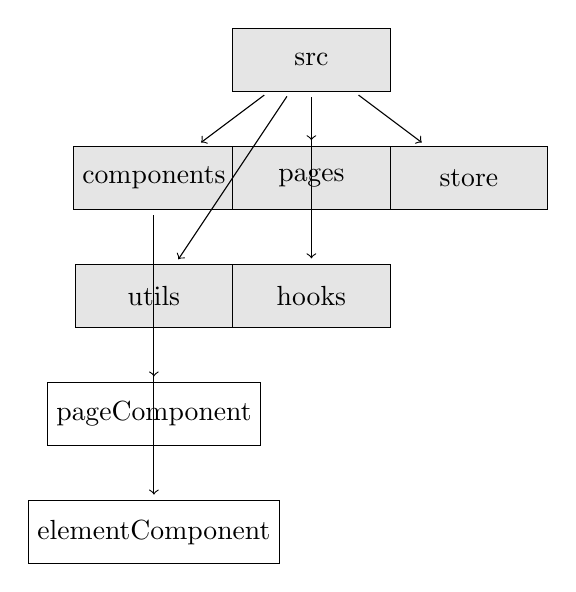
\begin{tikzpicture}[
    file/.style={draw, rectangle, minimum width=2cm, minimum height=0.8cm},
    folder/.style={draw, rectangle, minimum width=2cm, minimum height=0.8cm, fill=gray!20},
    arrow/.style={->, shorten >=2pt, shorten <=2pt}
]

% Folders
\node[folder] (src) at (0,0) {src};
\node[folder] (components) at (-2,-1.5) {components};
\node[folder] (pages) at (0,-1.5) {pages};
\node[folder] (store) at (2,-1.5) {store};
\node[folder] (utils) at (-2,-3) {utils};
\node[folder] (hooks) at (0,-3) {hooks};

% Files
\node[file] (pageComponent) at (-2,-4.5) {pageComponent};
\node[file] (elementComponent) at (-2,-6) {elementComponent};
% ... add more files

% Connections
\draw[arrow] (src) -- (components);
\draw[arrow] (src) -- (pages);
\draw[arrow] (src) -- (store);
\draw[arrow] (src) -- (utils);
\draw[arrow] (src) -- (hooks);
\draw[arrow] (components) -- (pageComponent);
\draw[arrow] (components) -- (elementComponent);
% ... add more connections

\end{tikzpicture}



\pagebreak
\subsubsection{Back-end}
The backend uses the dotNet framework. The development language using the C\# language.

In this project, the backend uses the Onion Architecture.
The Onion Architecture is a typically layered architecture, 
where each layer depends on the inner layer and provides interfaces to the outer layer.
The outer layer provides services to the outermost layer 
and other modules in the same layer based on the interfaces of the inner layer.

From inner to outer, the layers are: Domain, Application, Infrastructure, Presentation.
The Domain layer is the core layer and the innermost layer, used to define domain models, 
which are the business models.
It includes domain models and domain service interfaces.
Domain models are used to define the business models, 
which are the entities in the entity-relationship model and their attributes.
Domain service interfaces are used to define the business services, 
which are the relationships between entities in the entity-relationship model.

The Application layer is the application layer, 
used to define application services, which are the business logic.
It includes domain service implementations and application service interfaces.
Domain service implementations implement the methods of the inner layer's domain service 
interfaces and implement the business logic of the domain models.
Application service interfaces are used to define application services, 
which are the business logic.
It includes but is not limited to database interfaces, testing interfaces, 
HTTP API interfaces, MQTT interfaces, etc.

The Infrastructure layer is the infrastructure layer, used to define infrastructure.
It includes database implementations, testing implementations, 
HTTP API implementations, MQTT implementations, etc.
Database implementations implement the database interfaces 
and provide CRUD services for the database.
Testing implementations implement the testing interfaces 
and provide services for unit testing and integration testing.
HTTP API implementations implement the HTTP API interfaces 
and provide CRUD operations for HTTP APIs.
MQTT implementations implement the MQTT interfaces 
and provide CRUD operations for MQTT.

The Presentation layer is the presentation layer, used to define presentation logic, 
such as interfaces and pages. Since this is a backend project,
data presentation and control are handled by the frontend, 
so this layer is not needed.



\pagebreak
\subsubsection{Data communication and storage}
% 关于本项目的数据通信与数据存储的设计, 包括数据通信的协议, 数据存储的设计等
% 关于数据通信的设计:
% 1. 通信协议的选择
% 自前端向后端发送的数据, 有三种传输的数据类型, 
% 一种是普通的增删改查的请求, 对数据传输的时效性要求不高, 但是对数据的准确性, 完整性, 有序性, 安全性有一定的要求,
% 这种数据的传输, 采用 HTTP 协议, 以及 RESTful API 的设计. 可以有效的保证对数据传输的以上要求.
% 一种是对数据通道的创建和流媒体数据的传输, 对数据传输的时效性, 安全性要求较高, 这种数据的传输, 采用 WebRTC 协议, 以及 MQTT 协议.
% 配合可以快速解码的 flatbuffers 协议, 可以有效的保证对数据传输的以上要求.
% 最后一种是对设备的状态信息和操作信息的传输, 对完整性, 有序性, 安全性都有较高的要求, 这种数据的传输, 采用 MQTT 协议
% 同时也使用了 flatbuffers 协议.
% 
% 2. 数据通信的通信架构和通信流程
% 本项目的数据通信的通信架构, 是基于前后端分离的架构, 前端使用 React 框架, 后端使用 dotnet 框架.
% 当前端需要向后端发送数据的时候, 前端会向后端发送 HTTP 请求, 后端接收到 HTTP 请求之后, 会根据请求的数据类型,
% 选择不同的数据处理方式, 对于普通的增删改查的请求, 后端会根据 RESTful API 的设计, 对数据进行增删改查的操作,
% 对于对数据通道的创建和流媒体数据的传输, 后端会根据 WebRTC 协议, 对数据通道进行创建, 并且帮助前端和设备建立数据通道,
% 当数据通道建立后, 前端和设备之间则使用 flatbuffer 的数据格式对流媒体数据进行传输,
% 对于设备的状态信息和操作信息的传输, 前端会直接向 MQTT broker 发送 MQTT 请求, 
% 设备会在其自身的固件中监听相关的 MQTT 请求, 并且返回相关的数据.
% 
% 3. 数据通信的格式
% 本项目的数据通信的格式, 有三种, 
% 一种是 HTTP 协议, 
% 使用 json 格式对数据进行传输,
% 一种是 WebRTC 协议, 
% 使用 flatbuffers 格式对数据进行传输,
% 一种是 MQTT 协议.
% 使用 flatbuffers 格式对数据进行传输,
% 
% 关于数据存储的设计:
% 1. 数据存储的数据库的选择
% 本项目的数据存储的数据库的选择, 使用了轻量级的数据库 SQLite,
% SQLite 是一个进程内的库, 实现了自给自足的, 无服务器的, 零配置的, 事务性的 SQL 数据库引擎.
% 这是因为整个项目的目的是为了实现前端与设备之间的数据通信, 对于数据库数据的增删改查操作的要求不高,
% 数据量较小, 且对于数据库的数据的事务性要求不高, 所以选择了 SQLite 数据库.
% 2. 项目前后端的数据结构的设计
% 在本项目中, 前端由于使用了 React 框架, 所以前端的数据结构的设计, 使用了基于状态的数据结构的设计,
% 每个组件或者数据集都包含一个状态对象, 这个状态对象的属性就是组件的各个状态. 
% 使用状态对象的原因是, 可以方便的对状态进行管理, 采用对象-属性的形式, 可以方便的针对不同组件的同类状态进行区分,
% 由于跨组件的状态是由 redux 进行管理的, 这种状态对象的设计, 可以更搞笑的对状态进行更新和传递.
% 后端由于使用了 dotnet 框架, 所以后端的数据结构的设计, 使用了基于类的数据结构的设计,
% 采用了面向对象的编程思想, 对数据进行了封装, 使得数据的传输更加的安全, 有序, 完整.


\pagebreak

% \subsection{Domain model}
% \documentclass[]{article}
\usepackage{graphicx}
\usepackage{amsmath}
\usepackage{tikz}

% libaries
\usetikzlibrary{shapes,arrows}

%Define the listing package
\usepackage{listings} %code highlighter
\usepackage{color} %use color
\definecolor{mygreen}{rgb}{0,0.6,0}
\definecolor{mygray}{rgb}{0.5,0.5,0.5}
\definecolor{mymauve}{rgb}{0.58,0,0.82}

%Customize a bit the look
\lstset{ %
backgroundcolor=\color{white}, % choose the background color; you must add \usepackage{color} or \usepackage{xcolor}
basicstyle=\footnotesize, % the size of the fonts that are used for the code
breakatwhitespace=false, % sets if automatic breaks should only happen at whitespace
breaklines=true, % sets automatic line breaking
captionpos=b, % sets the caption-position to bottom
commentstyle=\color{mygreen}, % comment style
deletekeywords={...}, % if you want to delete keywords from the given language
escapeinside={\%*}{*)}, % if you want to add LaTeX within your code
extendedchars=true, % lets you use non-ASCII characters; for 8-bits encodings only, does not work with UTF-8
frame=single, % adds a frame around the code
keepspaces=true, % keeps spaces in text, useful for keeping indentation of code (possibly needs columns=flexible)
keywordstyle=\color{blue}, % keyword style
% language=Octave, % the language of the code
morekeywords={*,...}, % if you want to add more keywords to the set
numbers=left, % where to put the line-numbers; possible values are (none, left, right)
numbersep=5pt, % how far the line-numbers are from the code
numberstyle=\tiny\color{mygray}, % the style that is used for the line-numbers
rulecolor=\color{black}, % if not set, the frame-color may be changed on line-breaks within not-black text (e.g. comments (green here))
showspaces=false, % show spaces everywhere adding particular underscores; it overrides 'showstringspaces'
showstringspaces=false, % underline spaces within strings only
showtabs=false, % show tabs within strings adding particular underscores
stepnumber=1, % the step between two line-numbers. If it's 1, each line will be numbered
stringstyle=\color{mymauve}, % string literal style
tabsize=2, % sets default tabsize to 2 spaces
title=\lstname % show the filename of files included with \lstinputlisting; also try caption instead of title
}

\definecolor{darkgray}{rgb}{.4,.4,.4}
\definecolor{purple}{rgb}{0.65, 0.12, 0.82}

\lstdefinelanguage{React}{
keywords={const, typeof, new, true, false, catch, function, return, null, catch, switch, var, if, in, while, do, else, case, break},
keywordstyle=\color{blue}\bfseries,
ndkeywords={class, export, boolean, throw, implements, import, this},
ndkeywordstyle=\color{darkgray}\bfseries,
identifierstyle=\color{mygreen},
sensitive=false,
comment=[l]{//},
morecomment=[s]{/*}{*/},
commentstyle=\color{purple}\ttfamily,
string=[b]{"}{'}{`},
stringstyle=\color{red}\ttfamily,
morestring=[b]',
morestring=[b]",
morestring=[b]`',
}

\lstdefinelanguage{CSharp}{
keywords={const, typeof, new, true, false, catch, function, return, null, catch, switch, var, if, in, while, do, else, case, break},
keywordstyle=\color{blue}\bfseries,
ndkeywords={class, export, boolean, throw, implements, import, this},
ndkeywordstyle=\color{darkgray}\bfseries,
identifierstyle=\color{mygreen},
sensitive=false,
comment=[l]{//},
morecomment=[s]{/*}{*/},
commentstyle=\color{purple}\ttfamily,
string=[b]{"}{'}{`},
stringstyle=\color{red}\ttfamily,
morestring=[b]',
morestring=[b]",
morestring=[b]`',
}

\lstset{
language=React,
extendedchars=true,
basicstyle=\footnotesize\ttfamily,
showstringspaces=false,
showspaces=false,
numbers=left,
numberstyle=\footnotesize,
numbersep=9pt,
tabsize=2,
breaklines=true,
showtabs=false,
captionpos=b
}

\lstset{
language=CSharp,
extendedchars=true,
basicstyle=\footnotesize\ttfamily,
showstringspaces=false,
showspaces=false,
numbers=left,
numberstyle=\footnotesize,
numbersep=9pt,
tabsize=2,
breaklines=true,
showtabs=false,
captionpos=b
}

% \usepackage{cite} % Add this line for citation

% \bibliographystyle{plain}

\title{
The implementation of BifrostConnect Front-end scope, 
re-design and development with the relevant back-end support develop.
}
\author{
    Fei Gu \\
    Erhvervs Akademi Sydvest \\
    Computer Science 21\\
    }
\date{\today}

\begin{document}

% Front page
\maketitle
\begin{center}
    Supervisor: Henrik Boulund Meng Hansen \\
    Company: BifrostConnect \\
    Engineering Director: Jasper Wass \\
\end{center}
\tableofcontents
\pagebreak


% The introduction
\section{Introduction}
\subsection{Background}\input{sections/introduction/background.tex}
\subsection{The company}\input{sections/introduction/aboutCompany}
\subsection{The project}\input{sections/introduction/aboutProject}
\pagebreak

% The problem statement
\section{Problem Statement}
\subsection{Statement}
\input{sections/problemStatement/statement}
\subsection{Situation}
\input{sections/problemStatement/situation}
\subsection{Potential Solution}
\input{sections/problemStatement/potentialSolution}
\pagebreak

% Requirement analysis
\section{Requirement Analysis}
\input{sections/requirementAnalysis/index}

\subsection{Stakeholders}
\input{sections/requirementAnalysis/stakeholders/index}

\subsection{Business Domain}
\input{sections/requirementAnalysis/bussinesDomain/index}

\subsection{Scope}
\input{sections/requirementAnalysis/scope}

\subsection{Goals}
\input{sections/requirementAnalysis/goals}
\pagebreak

% Software Design
\section{Software Design}
% developement methods
\subsection{Software Development Methods}
\input{sections/softwareDevelopmentMethods/index}
\subsubsection{Agile Software Development}
\input{sections/softwareDevelopmentMethods/agileSoftwareDevelopment/index}
\subsubsection{Feature Driven Development}
\input{sections/softwareDevelopmentMethods/featureDrivenDevelopment/index}

\pagebreak

% Technology seslection
\subsection{Technology selection}
\input{sections/softwareDesign/technologySelection/index}
\subsubsection{Front-end}
\input{sections/softwareDesign/technologySelection/frontEnd}            
\subsubsection{Back-end}
\input{sections/softwareDesign/technologySelection/backEnd}            
\subsubsection{Database}
\input{sections/softwareDesign/technologySelection/database}
\subsubsection{Data communication}
\input{sections/softwareDesign/technologySelection/dataCommunication}            
\subsubsection{DevOps}
\input{sections/softwareDesign/technologySelection/devOps}
\pagebreak

% Architecture design
\subsection{Architecture design}
\input{sections/softwareDesign/architectureDesign/index}
\pagebreak
\subsubsection{Front-end}
\input{sections/softwareDesign/architectureDesign/frontEndArchitecture}
\pagebreak
\subsubsection{Back-end}
\input{sections/softwareDesign/architectureDesign/backEndArchitecture}
\pagebreak
\subsubsection{Data communication and storage}
\input{sections/softwareDesign/architectureDesign/dataCommunicationArchitecture}
\pagebreak

% \subsection{Domain model}
% \input{sections/softwareDesign/domainModel/index}
% \subsection{Database design}
% % 数据库领域模型 ER 图
% % 包括表和字段的设置.
% % 对于私有键和外键的设置.

% \subsection{Back-end design}
% % 后端对象模型
% % 以及对于对象模型的增删改查
% % 以及相关的其他服务的设计`'

% \subsection{Front-end design}
% % 对于前端的页面结构的设计 
% % 页面的状态的设计, 交互设计

% \subsection{FlatBuffers design}
% % schema 的设计

\subsection{DevOps CI/CD process design}
\input{sections/softwareDesign/devOpsDesign/index}
\subsubsection{Continuous Integration}
\input{sections/softwareDesign/devOpsDesign/continuousIntegration/index}
\subsubsection{Continuous Delivery}
\input{sections/softwareDesign/devOpsDesign/continuousDelivery/index}
\subsubsection{Continuous Deployment}
\input{sections/softwareDesign/devOpsDesign/continuousDeployment/index}
\pagebreak

\section{Software Development} 
\input{sections/softwareDevelopment/index}
\subsection{Overall development}
\input{sections/softwareDevelopment/overallDevelopement/index}
\subsubsection{Front-end}
\input{sections/softwareDevelopment/overallDevelopement/frontEnd/index}
\subsubsection{Back-end}
\input{sections/softwareDevelopment/overallDevelopement/backEnd/index}
\subsubsection{DevOps}
\input{sections/softwareDevelopment/overallDevelopement/devOps/index}
\subsection{Feature development} 
\input{sections/softwareDevelopment/featureDevelopment/index}
\subsubsection{Use Case 1}
\input{sections/softwareDevelopment/featureDevelopment/useCase1/index}
\subsubsection{Feature 1}
\input{sections/softwareDevelopment/featureDevelopment/feature/feature1.tex}
\pagebreak
\section{Conclusion} 
\subsection{Result}
Since the project is still in progress, the result is not available yet.
So far, basic structure of this project has been built. But the most features 
are not implemented yet. 
\subsection{Discussion}
As a single developer for this project, I am confident what I have done so far.
And I can say I understand the most of the knowledge I have used in this project, 
which also means I can explain all the part of the project. 
But this project also relevant some of the complex knowledge which I have to continue 
to study and practice.
\subsection{Future Work}
The future work is to implement the rest of the features. 
Including the most important part which is the 'create session' feature.
\pagebreak
% \bibliography{bibliography}
\pagebreak
% \begin{appendices}
%     \section{Appendix}
% \end{appendices} 
\end{document}
% \subsection{Database design}
% % 数据库领域模型 ER 图
% % 包括表和字段的设置.
% % 对于私有键和外键的设置.

% \subsection{Back-end design}
% % 后端对象模型
% % 以及对于对象模型的增删改查
% % 以及相关的其他服务的设计`'

% \subsection{Front-end design}
% % 对于前端的页面结构的设计 
% % 页面的状态的设计, 交互设计

% \subsection{FlatBuffers design}
% % schema 的设计

\subsection{DevOps CI/CD process design}
\documentclass[]{article}
\usepackage{graphicx}
\usepackage{amsmath}
\usepackage{tikz}

% libaries
\usetikzlibrary{shapes,arrows}

%Define the listing package
\usepackage{listings} %code highlighter
\usepackage{color} %use color
\definecolor{mygreen}{rgb}{0,0.6,0}
\definecolor{mygray}{rgb}{0.5,0.5,0.5}
\definecolor{mymauve}{rgb}{0.58,0,0.82}

%Customize a bit the look
\lstset{ %
backgroundcolor=\color{white}, % choose the background color; you must add \usepackage{color} or \usepackage{xcolor}
basicstyle=\footnotesize, % the size of the fonts that are used for the code
breakatwhitespace=false, % sets if automatic breaks should only happen at whitespace
breaklines=true, % sets automatic line breaking
captionpos=b, % sets the caption-position to bottom
commentstyle=\color{mygreen}, % comment style
deletekeywords={...}, % if you want to delete keywords from the given language
escapeinside={\%*}{*)}, % if you want to add LaTeX within your code
extendedchars=true, % lets you use non-ASCII characters; for 8-bits encodings only, does not work with UTF-8
frame=single, % adds a frame around the code
keepspaces=true, % keeps spaces in text, useful for keeping indentation of code (possibly needs columns=flexible)
keywordstyle=\color{blue}, % keyword style
% language=Octave, % the language of the code
morekeywords={*,...}, % if you want to add more keywords to the set
numbers=left, % where to put the line-numbers; possible values are (none, left, right)
numbersep=5pt, % how far the line-numbers are from the code
numberstyle=\tiny\color{mygray}, % the style that is used for the line-numbers
rulecolor=\color{black}, % if not set, the frame-color may be changed on line-breaks within not-black text (e.g. comments (green here))
showspaces=false, % show spaces everywhere adding particular underscores; it overrides 'showstringspaces'
showstringspaces=false, % underline spaces within strings only
showtabs=false, % show tabs within strings adding particular underscores
stepnumber=1, % the step between two line-numbers. If it's 1, each line will be numbered
stringstyle=\color{mymauve}, % string literal style
tabsize=2, % sets default tabsize to 2 spaces
title=\lstname % show the filename of files included with \lstinputlisting; also try caption instead of title
}

\definecolor{darkgray}{rgb}{.4,.4,.4}
\definecolor{purple}{rgb}{0.65, 0.12, 0.82}

\lstdefinelanguage{React}{
keywords={const, typeof, new, true, false, catch, function, return, null, catch, switch, var, if, in, while, do, else, case, break},
keywordstyle=\color{blue}\bfseries,
ndkeywords={class, export, boolean, throw, implements, import, this},
ndkeywordstyle=\color{darkgray}\bfseries,
identifierstyle=\color{mygreen},
sensitive=false,
comment=[l]{//},
morecomment=[s]{/*}{*/},
commentstyle=\color{purple}\ttfamily,
string=[b]{"}{'}{`},
stringstyle=\color{red}\ttfamily,
morestring=[b]',
morestring=[b]",
morestring=[b]`',
}

\lstdefinelanguage{CSharp}{
keywords={const, typeof, new, true, false, catch, function, return, null, catch, switch, var, if, in, while, do, else, case, break},
keywordstyle=\color{blue}\bfseries,
ndkeywords={class, export, boolean, throw, implements, import, this},
ndkeywordstyle=\color{darkgray}\bfseries,
identifierstyle=\color{mygreen},
sensitive=false,
comment=[l]{//},
morecomment=[s]{/*}{*/},
commentstyle=\color{purple}\ttfamily,
string=[b]{"}{'}{`},
stringstyle=\color{red}\ttfamily,
morestring=[b]',
morestring=[b]",
morestring=[b]`',
}

\lstset{
language=React,
extendedchars=true,
basicstyle=\footnotesize\ttfamily,
showstringspaces=false,
showspaces=false,
numbers=left,
numberstyle=\footnotesize,
numbersep=9pt,
tabsize=2,
breaklines=true,
showtabs=false,
captionpos=b
}

\lstset{
language=CSharp,
extendedchars=true,
basicstyle=\footnotesize\ttfamily,
showstringspaces=false,
showspaces=false,
numbers=left,
numberstyle=\footnotesize,
numbersep=9pt,
tabsize=2,
breaklines=true,
showtabs=false,
captionpos=b
}

% \usepackage{cite} % Add this line for citation

% \bibliographystyle{plain}

\title{
The implementation of BifrostConnect Front-end scope, 
re-design and development with the relevant back-end support develop.
}
\author{
    Fei Gu \\
    Erhvervs Akademi Sydvest \\
    Computer Science 21\\
    }
\date{\today}

\begin{document}

% Front page
\maketitle
\begin{center}
    Supervisor: Henrik Boulund Meng Hansen \\
    Company: BifrostConnect \\
    Engineering Director: Jasper Wass \\
\end{center}
\tableofcontents
\pagebreak


% The introduction
\section{Introduction}
\subsection{Background}\input{sections/introduction/background.tex}
\subsection{The company}\input{sections/introduction/aboutCompany}
\subsection{The project}\input{sections/introduction/aboutProject}
\pagebreak

% The problem statement
\section{Problem Statement}
\subsection{Statement}
\input{sections/problemStatement/statement}
\subsection{Situation}
\input{sections/problemStatement/situation}
\subsection{Potential Solution}
\input{sections/problemStatement/potentialSolution}
\pagebreak

% Requirement analysis
\section{Requirement Analysis}
\input{sections/requirementAnalysis/index}

\subsection{Stakeholders}
\input{sections/requirementAnalysis/stakeholders/index}

\subsection{Business Domain}
\input{sections/requirementAnalysis/bussinesDomain/index}

\subsection{Scope}
\input{sections/requirementAnalysis/scope}

\subsection{Goals}
\input{sections/requirementAnalysis/goals}
\pagebreak

% Software Design
\section{Software Design}
% developement methods
\subsection{Software Development Methods}
\input{sections/softwareDevelopmentMethods/index}
\subsubsection{Agile Software Development}
\input{sections/softwareDevelopmentMethods/agileSoftwareDevelopment/index}
\subsubsection{Feature Driven Development}
\input{sections/softwareDevelopmentMethods/featureDrivenDevelopment/index}

\pagebreak

% Technology seslection
\subsection{Technology selection}
\input{sections/softwareDesign/technologySelection/index}
\subsubsection{Front-end}
\input{sections/softwareDesign/technologySelection/frontEnd}            
\subsubsection{Back-end}
\input{sections/softwareDesign/technologySelection/backEnd}            
\subsubsection{Database}
\input{sections/softwareDesign/technologySelection/database}
\subsubsection{Data communication}
\input{sections/softwareDesign/technologySelection/dataCommunication}            
\subsubsection{DevOps}
\input{sections/softwareDesign/technologySelection/devOps}
\pagebreak

% Architecture design
\subsection{Architecture design}
\input{sections/softwareDesign/architectureDesign/index}
\pagebreak
\subsubsection{Front-end}
\input{sections/softwareDesign/architectureDesign/frontEndArchitecture}
\pagebreak
\subsubsection{Back-end}
\input{sections/softwareDesign/architectureDesign/backEndArchitecture}
\pagebreak
\subsubsection{Data communication and storage}
\input{sections/softwareDesign/architectureDesign/dataCommunicationArchitecture}
\pagebreak

% \subsection{Domain model}
% \input{sections/softwareDesign/domainModel/index}
% \subsection{Database design}
% % 数据库领域模型 ER 图
% % 包括表和字段的设置.
% % 对于私有键和外键的设置.

% \subsection{Back-end design}
% % 后端对象模型
% % 以及对于对象模型的增删改查
% % 以及相关的其他服务的设计`'

% \subsection{Front-end design}
% % 对于前端的页面结构的设计 
% % 页面的状态的设计, 交互设计

% \subsection{FlatBuffers design}
% % schema 的设计

\subsection{DevOps CI/CD process design}
\input{sections/softwareDesign/devOpsDesign/index}
\subsubsection{Continuous Integration}
\input{sections/softwareDesign/devOpsDesign/continuousIntegration/index}
\subsubsection{Continuous Delivery}
\input{sections/softwareDesign/devOpsDesign/continuousDelivery/index}
\subsubsection{Continuous Deployment}
\input{sections/softwareDesign/devOpsDesign/continuousDeployment/index}
\pagebreak

\section{Software Development} 
\input{sections/softwareDevelopment/index}
\subsection{Overall development}
\input{sections/softwareDevelopment/overallDevelopement/index}
\subsubsection{Front-end}
\input{sections/softwareDevelopment/overallDevelopement/frontEnd/index}
\subsubsection{Back-end}
\input{sections/softwareDevelopment/overallDevelopement/backEnd/index}
\subsubsection{DevOps}
\input{sections/softwareDevelopment/overallDevelopement/devOps/index}
\subsection{Feature development} 
\input{sections/softwareDevelopment/featureDevelopment/index}
\subsubsection{Use Case 1}
\input{sections/softwareDevelopment/featureDevelopment/useCase1/index}
\subsubsection{Feature 1}
\input{sections/softwareDevelopment/featureDevelopment/feature/feature1.tex}
\pagebreak
\section{Conclusion} 
\subsection{Result}
Since the project is still in progress, the result is not available yet.
So far, basic structure of this project has been built. But the most features 
are not implemented yet. 
\subsection{Discussion}
As a single developer for this project, I am confident what I have done so far.
And I can say I understand the most of the knowledge I have used in this project, 
which also means I can explain all the part of the project. 
But this project also relevant some of the complex knowledge which I have to continue 
to study and practice.
\subsection{Future Work}
The future work is to implement the rest of the features. 
Including the most important part which is the 'create session' feature.
\pagebreak
% \bibliography{bibliography}
\pagebreak
% \begin{appendices}
%     \section{Appendix}
% \end{appendices} 
\end{document}
\subsubsection{Continuous Integration}
\documentclass[]{article}
\usepackage{graphicx}
\usepackage{amsmath}
\usepackage{tikz}

% libaries
\usetikzlibrary{shapes,arrows}

%Define the listing package
\usepackage{listings} %code highlighter
\usepackage{color} %use color
\definecolor{mygreen}{rgb}{0,0.6,0}
\definecolor{mygray}{rgb}{0.5,0.5,0.5}
\definecolor{mymauve}{rgb}{0.58,0,0.82}

%Customize a bit the look
\lstset{ %
backgroundcolor=\color{white}, % choose the background color; you must add \usepackage{color} or \usepackage{xcolor}
basicstyle=\footnotesize, % the size of the fonts that are used for the code
breakatwhitespace=false, % sets if automatic breaks should only happen at whitespace
breaklines=true, % sets automatic line breaking
captionpos=b, % sets the caption-position to bottom
commentstyle=\color{mygreen}, % comment style
deletekeywords={...}, % if you want to delete keywords from the given language
escapeinside={\%*}{*)}, % if you want to add LaTeX within your code
extendedchars=true, % lets you use non-ASCII characters; for 8-bits encodings only, does not work with UTF-8
frame=single, % adds a frame around the code
keepspaces=true, % keeps spaces in text, useful for keeping indentation of code (possibly needs columns=flexible)
keywordstyle=\color{blue}, % keyword style
% language=Octave, % the language of the code
morekeywords={*,...}, % if you want to add more keywords to the set
numbers=left, % where to put the line-numbers; possible values are (none, left, right)
numbersep=5pt, % how far the line-numbers are from the code
numberstyle=\tiny\color{mygray}, % the style that is used for the line-numbers
rulecolor=\color{black}, % if not set, the frame-color may be changed on line-breaks within not-black text (e.g. comments (green here))
showspaces=false, % show spaces everywhere adding particular underscores; it overrides 'showstringspaces'
showstringspaces=false, % underline spaces within strings only
showtabs=false, % show tabs within strings adding particular underscores
stepnumber=1, % the step between two line-numbers. If it's 1, each line will be numbered
stringstyle=\color{mymauve}, % string literal style
tabsize=2, % sets default tabsize to 2 spaces
title=\lstname % show the filename of files included with \lstinputlisting; also try caption instead of title
}

\definecolor{darkgray}{rgb}{.4,.4,.4}
\definecolor{purple}{rgb}{0.65, 0.12, 0.82}

\lstdefinelanguage{React}{
keywords={const, typeof, new, true, false, catch, function, return, null, catch, switch, var, if, in, while, do, else, case, break},
keywordstyle=\color{blue}\bfseries,
ndkeywords={class, export, boolean, throw, implements, import, this},
ndkeywordstyle=\color{darkgray}\bfseries,
identifierstyle=\color{mygreen},
sensitive=false,
comment=[l]{//},
morecomment=[s]{/*}{*/},
commentstyle=\color{purple}\ttfamily,
string=[b]{"}{'}{`},
stringstyle=\color{red}\ttfamily,
morestring=[b]',
morestring=[b]",
morestring=[b]`',
}

\lstdefinelanguage{CSharp}{
keywords={const, typeof, new, true, false, catch, function, return, null, catch, switch, var, if, in, while, do, else, case, break},
keywordstyle=\color{blue}\bfseries,
ndkeywords={class, export, boolean, throw, implements, import, this},
ndkeywordstyle=\color{darkgray}\bfseries,
identifierstyle=\color{mygreen},
sensitive=false,
comment=[l]{//},
morecomment=[s]{/*}{*/},
commentstyle=\color{purple}\ttfamily,
string=[b]{"}{'}{`},
stringstyle=\color{red}\ttfamily,
morestring=[b]',
morestring=[b]",
morestring=[b]`',
}

\lstset{
language=React,
extendedchars=true,
basicstyle=\footnotesize\ttfamily,
showstringspaces=false,
showspaces=false,
numbers=left,
numberstyle=\footnotesize,
numbersep=9pt,
tabsize=2,
breaklines=true,
showtabs=false,
captionpos=b
}

\lstset{
language=CSharp,
extendedchars=true,
basicstyle=\footnotesize\ttfamily,
showstringspaces=false,
showspaces=false,
numbers=left,
numberstyle=\footnotesize,
numbersep=9pt,
tabsize=2,
breaklines=true,
showtabs=false,
captionpos=b
}

% \usepackage{cite} % Add this line for citation

% \bibliographystyle{plain}

\title{
The implementation of BifrostConnect Front-end scope, 
re-design and development with the relevant back-end support develop.
}
\author{
    Fei Gu \\
    Erhvervs Akademi Sydvest \\
    Computer Science 21\\
    }
\date{\today}

\begin{document}

% Front page
\maketitle
\begin{center}
    Supervisor: Henrik Boulund Meng Hansen \\
    Company: BifrostConnect \\
    Engineering Director: Jasper Wass \\
\end{center}
\tableofcontents
\pagebreak


% The introduction
\section{Introduction}
\subsection{Background}\input{sections/introduction/background.tex}
\subsection{The company}\input{sections/introduction/aboutCompany}
\subsection{The project}\input{sections/introduction/aboutProject}
\pagebreak

% The problem statement
\section{Problem Statement}
\subsection{Statement}
\input{sections/problemStatement/statement}
\subsection{Situation}
\input{sections/problemStatement/situation}
\subsection{Potential Solution}
\input{sections/problemStatement/potentialSolution}
\pagebreak

% Requirement analysis
\section{Requirement Analysis}
\input{sections/requirementAnalysis/index}

\subsection{Stakeholders}
\input{sections/requirementAnalysis/stakeholders/index}

\subsection{Business Domain}
\input{sections/requirementAnalysis/bussinesDomain/index}

\subsection{Scope}
\input{sections/requirementAnalysis/scope}

\subsection{Goals}
\input{sections/requirementAnalysis/goals}
\pagebreak

% Software Design
\section{Software Design}
% developement methods
\subsection{Software Development Methods}
\input{sections/softwareDevelopmentMethods/index}
\subsubsection{Agile Software Development}
\input{sections/softwareDevelopmentMethods/agileSoftwareDevelopment/index}
\subsubsection{Feature Driven Development}
\input{sections/softwareDevelopmentMethods/featureDrivenDevelopment/index}

\pagebreak

% Technology seslection
\subsection{Technology selection}
\input{sections/softwareDesign/technologySelection/index}
\subsubsection{Front-end}
\input{sections/softwareDesign/technologySelection/frontEnd}            
\subsubsection{Back-end}
\input{sections/softwareDesign/technologySelection/backEnd}            
\subsubsection{Database}
\input{sections/softwareDesign/technologySelection/database}
\subsubsection{Data communication}
\input{sections/softwareDesign/technologySelection/dataCommunication}            
\subsubsection{DevOps}
\input{sections/softwareDesign/technologySelection/devOps}
\pagebreak

% Architecture design
\subsection{Architecture design}
\input{sections/softwareDesign/architectureDesign/index}
\pagebreak
\subsubsection{Front-end}
\input{sections/softwareDesign/architectureDesign/frontEndArchitecture}
\pagebreak
\subsubsection{Back-end}
\input{sections/softwareDesign/architectureDesign/backEndArchitecture}
\pagebreak
\subsubsection{Data communication and storage}
\input{sections/softwareDesign/architectureDesign/dataCommunicationArchitecture}
\pagebreak

% \subsection{Domain model}
% \input{sections/softwareDesign/domainModel/index}
% \subsection{Database design}
% % 数据库领域模型 ER 图
% % 包括表和字段的设置.
% % 对于私有键和外键的设置.

% \subsection{Back-end design}
% % 后端对象模型
% % 以及对于对象模型的增删改查
% % 以及相关的其他服务的设计`'

% \subsection{Front-end design}
% % 对于前端的页面结构的设计 
% % 页面的状态的设计, 交互设计

% \subsection{FlatBuffers design}
% % schema 的设计

\subsection{DevOps CI/CD process design}
\input{sections/softwareDesign/devOpsDesign/index}
\subsubsection{Continuous Integration}
\input{sections/softwareDesign/devOpsDesign/continuousIntegration/index}
\subsubsection{Continuous Delivery}
\input{sections/softwareDesign/devOpsDesign/continuousDelivery/index}
\subsubsection{Continuous Deployment}
\input{sections/softwareDesign/devOpsDesign/continuousDeployment/index}
\pagebreak

\section{Software Development} 
\input{sections/softwareDevelopment/index}
\subsection{Overall development}
\input{sections/softwareDevelopment/overallDevelopement/index}
\subsubsection{Front-end}
\input{sections/softwareDevelopment/overallDevelopement/frontEnd/index}
\subsubsection{Back-end}
\input{sections/softwareDevelopment/overallDevelopement/backEnd/index}
\subsubsection{DevOps}
\input{sections/softwareDevelopment/overallDevelopement/devOps/index}
\subsection{Feature development} 
\input{sections/softwareDevelopment/featureDevelopment/index}
\subsubsection{Use Case 1}
\input{sections/softwareDevelopment/featureDevelopment/useCase1/index}
\subsubsection{Feature 1}
\input{sections/softwareDevelopment/featureDevelopment/feature/feature1.tex}
\pagebreak
\section{Conclusion} 
\subsection{Result}
Since the project is still in progress, the result is not available yet.
So far, basic structure of this project has been built. But the most features 
are not implemented yet. 
\subsection{Discussion}
As a single developer for this project, I am confident what I have done so far.
And I can say I understand the most of the knowledge I have used in this project, 
which also means I can explain all the part of the project. 
But this project also relevant some of the complex knowledge which I have to continue 
to study and practice.
\subsection{Future Work}
The future work is to implement the rest of the features. 
Including the most important part which is the 'create session' feature.
\pagebreak
% \bibliography{bibliography}
\pagebreak
% \begin{appendices}
%     \section{Appendix}
% \end{appendices} 
\end{document}
\subsubsection{Continuous Delivery}
\documentclass[]{article}
\usepackage{graphicx}
\usepackage{amsmath}
\usepackage{tikz}

% libaries
\usetikzlibrary{shapes,arrows}

%Define the listing package
\usepackage{listings} %code highlighter
\usepackage{color} %use color
\definecolor{mygreen}{rgb}{0,0.6,0}
\definecolor{mygray}{rgb}{0.5,0.5,0.5}
\definecolor{mymauve}{rgb}{0.58,0,0.82}

%Customize a bit the look
\lstset{ %
backgroundcolor=\color{white}, % choose the background color; you must add \usepackage{color} or \usepackage{xcolor}
basicstyle=\footnotesize, % the size of the fonts that are used for the code
breakatwhitespace=false, % sets if automatic breaks should only happen at whitespace
breaklines=true, % sets automatic line breaking
captionpos=b, % sets the caption-position to bottom
commentstyle=\color{mygreen}, % comment style
deletekeywords={...}, % if you want to delete keywords from the given language
escapeinside={\%*}{*)}, % if you want to add LaTeX within your code
extendedchars=true, % lets you use non-ASCII characters; for 8-bits encodings only, does not work with UTF-8
frame=single, % adds a frame around the code
keepspaces=true, % keeps spaces in text, useful for keeping indentation of code (possibly needs columns=flexible)
keywordstyle=\color{blue}, % keyword style
% language=Octave, % the language of the code
morekeywords={*,...}, % if you want to add more keywords to the set
numbers=left, % where to put the line-numbers; possible values are (none, left, right)
numbersep=5pt, % how far the line-numbers are from the code
numberstyle=\tiny\color{mygray}, % the style that is used for the line-numbers
rulecolor=\color{black}, % if not set, the frame-color may be changed on line-breaks within not-black text (e.g. comments (green here))
showspaces=false, % show spaces everywhere adding particular underscores; it overrides 'showstringspaces'
showstringspaces=false, % underline spaces within strings only
showtabs=false, % show tabs within strings adding particular underscores
stepnumber=1, % the step between two line-numbers. If it's 1, each line will be numbered
stringstyle=\color{mymauve}, % string literal style
tabsize=2, % sets default tabsize to 2 spaces
title=\lstname % show the filename of files included with \lstinputlisting; also try caption instead of title
}

\definecolor{darkgray}{rgb}{.4,.4,.4}
\definecolor{purple}{rgb}{0.65, 0.12, 0.82}

\lstdefinelanguage{React}{
keywords={const, typeof, new, true, false, catch, function, return, null, catch, switch, var, if, in, while, do, else, case, break},
keywordstyle=\color{blue}\bfseries,
ndkeywords={class, export, boolean, throw, implements, import, this},
ndkeywordstyle=\color{darkgray}\bfseries,
identifierstyle=\color{mygreen},
sensitive=false,
comment=[l]{//},
morecomment=[s]{/*}{*/},
commentstyle=\color{purple}\ttfamily,
string=[b]{"}{'}{`},
stringstyle=\color{red}\ttfamily,
morestring=[b]',
morestring=[b]",
morestring=[b]`',
}

\lstdefinelanguage{CSharp}{
keywords={const, typeof, new, true, false, catch, function, return, null, catch, switch, var, if, in, while, do, else, case, break},
keywordstyle=\color{blue}\bfseries,
ndkeywords={class, export, boolean, throw, implements, import, this},
ndkeywordstyle=\color{darkgray}\bfseries,
identifierstyle=\color{mygreen},
sensitive=false,
comment=[l]{//},
morecomment=[s]{/*}{*/},
commentstyle=\color{purple}\ttfamily,
string=[b]{"}{'}{`},
stringstyle=\color{red}\ttfamily,
morestring=[b]',
morestring=[b]",
morestring=[b]`',
}

\lstset{
language=React,
extendedchars=true,
basicstyle=\footnotesize\ttfamily,
showstringspaces=false,
showspaces=false,
numbers=left,
numberstyle=\footnotesize,
numbersep=9pt,
tabsize=2,
breaklines=true,
showtabs=false,
captionpos=b
}

\lstset{
language=CSharp,
extendedchars=true,
basicstyle=\footnotesize\ttfamily,
showstringspaces=false,
showspaces=false,
numbers=left,
numberstyle=\footnotesize,
numbersep=9pt,
tabsize=2,
breaklines=true,
showtabs=false,
captionpos=b
}

% \usepackage{cite} % Add this line for citation

% \bibliographystyle{plain}

\title{
The implementation of BifrostConnect Front-end scope, 
re-design and development with the relevant back-end support develop.
}
\author{
    Fei Gu \\
    Erhvervs Akademi Sydvest \\
    Computer Science 21\\
    }
\date{\today}

\begin{document}

% Front page
\maketitle
\begin{center}
    Supervisor: Henrik Boulund Meng Hansen \\
    Company: BifrostConnect \\
    Engineering Director: Jasper Wass \\
\end{center}
\tableofcontents
\pagebreak


% The introduction
\section{Introduction}
\subsection{Background}\input{sections/introduction/background.tex}
\subsection{The company}\input{sections/introduction/aboutCompany}
\subsection{The project}\input{sections/introduction/aboutProject}
\pagebreak

% The problem statement
\section{Problem Statement}
\subsection{Statement}
\input{sections/problemStatement/statement}
\subsection{Situation}
\input{sections/problemStatement/situation}
\subsection{Potential Solution}
\input{sections/problemStatement/potentialSolution}
\pagebreak

% Requirement analysis
\section{Requirement Analysis}
\input{sections/requirementAnalysis/index}

\subsection{Stakeholders}
\input{sections/requirementAnalysis/stakeholders/index}

\subsection{Business Domain}
\input{sections/requirementAnalysis/bussinesDomain/index}

\subsection{Scope}
\input{sections/requirementAnalysis/scope}

\subsection{Goals}
\input{sections/requirementAnalysis/goals}
\pagebreak

% Software Design
\section{Software Design}
% developement methods
\subsection{Software Development Methods}
\input{sections/softwareDevelopmentMethods/index}
\subsubsection{Agile Software Development}
\input{sections/softwareDevelopmentMethods/agileSoftwareDevelopment/index}
\subsubsection{Feature Driven Development}
\input{sections/softwareDevelopmentMethods/featureDrivenDevelopment/index}

\pagebreak

% Technology seslection
\subsection{Technology selection}
\input{sections/softwareDesign/technologySelection/index}
\subsubsection{Front-end}
\input{sections/softwareDesign/technologySelection/frontEnd}            
\subsubsection{Back-end}
\input{sections/softwareDesign/technologySelection/backEnd}            
\subsubsection{Database}
\input{sections/softwareDesign/technologySelection/database}
\subsubsection{Data communication}
\input{sections/softwareDesign/technologySelection/dataCommunication}            
\subsubsection{DevOps}
\input{sections/softwareDesign/technologySelection/devOps}
\pagebreak

% Architecture design
\subsection{Architecture design}
\input{sections/softwareDesign/architectureDesign/index}
\pagebreak
\subsubsection{Front-end}
\input{sections/softwareDesign/architectureDesign/frontEndArchitecture}
\pagebreak
\subsubsection{Back-end}
\input{sections/softwareDesign/architectureDesign/backEndArchitecture}
\pagebreak
\subsubsection{Data communication and storage}
\input{sections/softwareDesign/architectureDesign/dataCommunicationArchitecture}
\pagebreak

% \subsection{Domain model}
% \input{sections/softwareDesign/domainModel/index}
% \subsection{Database design}
% % 数据库领域模型 ER 图
% % 包括表和字段的设置.
% % 对于私有键和外键的设置.

% \subsection{Back-end design}
% % 后端对象模型
% % 以及对于对象模型的增删改查
% % 以及相关的其他服务的设计`'

% \subsection{Front-end design}
% % 对于前端的页面结构的设计 
% % 页面的状态的设计, 交互设计

% \subsection{FlatBuffers design}
% % schema 的设计

\subsection{DevOps CI/CD process design}
\input{sections/softwareDesign/devOpsDesign/index}
\subsubsection{Continuous Integration}
\input{sections/softwareDesign/devOpsDesign/continuousIntegration/index}
\subsubsection{Continuous Delivery}
\input{sections/softwareDesign/devOpsDesign/continuousDelivery/index}
\subsubsection{Continuous Deployment}
\input{sections/softwareDesign/devOpsDesign/continuousDeployment/index}
\pagebreak

\section{Software Development} 
\input{sections/softwareDevelopment/index}
\subsection{Overall development}
\input{sections/softwareDevelopment/overallDevelopement/index}
\subsubsection{Front-end}
\input{sections/softwareDevelopment/overallDevelopement/frontEnd/index}
\subsubsection{Back-end}
\input{sections/softwareDevelopment/overallDevelopement/backEnd/index}
\subsubsection{DevOps}
\input{sections/softwareDevelopment/overallDevelopement/devOps/index}
\subsection{Feature development} 
\input{sections/softwareDevelopment/featureDevelopment/index}
\subsubsection{Use Case 1}
\input{sections/softwareDevelopment/featureDevelopment/useCase1/index}
\subsubsection{Feature 1}
\input{sections/softwareDevelopment/featureDevelopment/feature/feature1.tex}
\pagebreak
\section{Conclusion} 
\subsection{Result}
Since the project is still in progress, the result is not available yet.
So far, basic structure of this project has been built. But the most features 
are not implemented yet. 
\subsection{Discussion}
As a single developer for this project, I am confident what I have done so far.
And I can say I understand the most of the knowledge I have used in this project, 
which also means I can explain all the part of the project. 
But this project also relevant some of the complex knowledge which I have to continue 
to study and practice.
\subsection{Future Work}
The future work is to implement the rest of the features. 
Including the most important part which is the 'create session' feature.
\pagebreak
% \bibliography{bibliography}
\pagebreak
% \begin{appendices}
%     \section{Appendix}
% \end{appendices} 
\end{document}
\subsubsection{Continuous Deployment}
\documentclass[]{article}
\usepackage{graphicx}
\usepackage{amsmath}
\usepackage{tikz}

% libaries
\usetikzlibrary{shapes,arrows}

%Define the listing package
\usepackage{listings} %code highlighter
\usepackage{color} %use color
\definecolor{mygreen}{rgb}{0,0.6,0}
\definecolor{mygray}{rgb}{0.5,0.5,0.5}
\definecolor{mymauve}{rgb}{0.58,0,0.82}

%Customize a bit the look
\lstset{ %
backgroundcolor=\color{white}, % choose the background color; you must add \usepackage{color} or \usepackage{xcolor}
basicstyle=\footnotesize, % the size of the fonts that are used for the code
breakatwhitespace=false, % sets if automatic breaks should only happen at whitespace
breaklines=true, % sets automatic line breaking
captionpos=b, % sets the caption-position to bottom
commentstyle=\color{mygreen}, % comment style
deletekeywords={...}, % if you want to delete keywords from the given language
escapeinside={\%*}{*)}, % if you want to add LaTeX within your code
extendedchars=true, % lets you use non-ASCII characters; for 8-bits encodings only, does not work with UTF-8
frame=single, % adds a frame around the code
keepspaces=true, % keeps spaces in text, useful for keeping indentation of code (possibly needs columns=flexible)
keywordstyle=\color{blue}, % keyword style
% language=Octave, % the language of the code
morekeywords={*,...}, % if you want to add more keywords to the set
numbers=left, % where to put the line-numbers; possible values are (none, left, right)
numbersep=5pt, % how far the line-numbers are from the code
numberstyle=\tiny\color{mygray}, % the style that is used for the line-numbers
rulecolor=\color{black}, % if not set, the frame-color may be changed on line-breaks within not-black text (e.g. comments (green here))
showspaces=false, % show spaces everywhere adding particular underscores; it overrides 'showstringspaces'
showstringspaces=false, % underline spaces within strings only
showtabs=false, % show tabs within strings adding particular underscores
stepnumber=1, % the step between two line-numbers. If it's 1, each line will be numbered
stringstyle=\color{mymauve}, % string literal style
tabsize=2, % sets default tabsize to 2 spaces
title=\lstname % show the filename of files included with \lstinputlisting; also try caption instead of title
}

\definecolor{darkgray}{rgb}{.4,.4,.4}
\definecolor{purple}{rgb}{0.65, 0.12, 0.82}

\lstdefinelanguage{React}{
keywords={const, typeof, new, true, false, catch, function, return, null, catch, switch, var, if, in, while, do, else, case, break},
keywordstyle=\color{blue}\bfseries,
ndkeywords={class, export, boolean, throw, implements, import, this},
ndkeywordstyle=\color{darkgray}\bfseries,
identifierstyle=\color{mygreen},
sensitive=false,
comment=[l]{//},
morecomment=[s]{/*}{*/},
commentstyle=\color{purple}\ttfamily,
string=[b]{"}{'}{`},
stringstyle=\color{red}\ttfamily,
morestring=[b]',
morestring=[b]",
morestring=[b]`',
}

\lstdefinelanguage{CSharp}{
keywords={const, typeof, new, true, false, catch, function, return, null, catch, switch, var, if, in, while, do, else, case, break},
keywordstyle=\color{blue}\bfseries,
ndkeywords={class, export, boolean, throw, implements, import, this},
ndkeywordstyle=\color{darkgray}\bfseries,
identifierstyle=\color{mygreen},
sensitive=false,
comment=[l]{//},
morecomment=[s]{/*}{*/},
commentstyle=\color{purple}\ttfamily,
string=[b]{"}{'}{`},
stringstyle=\color{red}\ttfamily,
morestring=[b]',
morestring=[b]",
morestring=[b]`',
}

\lstset{
language=React,
extendedchars=true,
basicstyle=\footnotesize\ttfamily,
showstringspaces=false,
showspaces=false,
numbers=left,
numberstyle=\footnotesize,
numbersep=9pt,
tabsize=2,
breaklines=true,
showtabs=false,
captionpos=b
}

\lstset{
language=CSharp,
extendedchars=true,
basicstyle=\footnotesize\ttfamily,
showstringspaces=false,
showspaces=false,
numbers=left,
numberstyle=\footnotesize,
numbersep=9pt,
tabsize=2,
breaklines=true,
showtabs=false,
captionpos=b
}

% \usepackage{cite} % Add this line for citation

% \bibliographystyle{plain}

\title{
The implementation of BifrostConnect Front-end scope, 
re-design and development with the relevant back-end support develop.
}
\author{
    Fei Gu \\
    Erhvervs Akademi Sydvest \\
    Computer Science 21\\
    }
\date{\today}

\begin{document}

% Front page
\maketitle
\begin{center}
    Supervisor: Henrik Boulund Meng Hansen \\
    Company: BifrostConnect \\
    Engineering Director: Jasper Wass \\
\end{center}
\tableofcontents
\pagebreak


% The introduction
\section{Introduction}
\subsection{Background}\input{sections/introduction/background.tex}
\subsection{The company}\input{sections/introduction/aboutCompany}
\subsection{The project}\input{sections/introduction/aboutProject}
\pagebreak

% The problem statement
\section{Problem Statement}
\subsection{Statement}
\input{sections/problemStatement/statement}
\subsection{Situation}
\input{sections/problemStatement/situation}
\subsection{Potential Solution}
\input{sections/problemStatement/potentialSolution}
\pagebreak

% Requirement analysis
\section{Requirement Analysis}
\input{sections/requirementAnalysis/index}

\subsection{Stakeholders}
\input{sections/requirementAnalysis/stakeholders/index}

\subsection{Business Domain}
\input{sections/requirementAnalysis/bussinesDomain/index}

\subsection{Scope}
\input{sections/requirementAnalysis/scope}

\subsection{Goals}
\input{sections/requirementAnalysis/goals}
\pagebreak

% Software Design
\section{Software Design}
% developement methods
\subsection{Software Development Methods}
\input{sections/softwareDevelopmentMethods/index}
\subsubsection{Agile Software Development}
\input{sections/softwareDevelopmentMethods/agileSoftwareDevelopment/index}
\subsubsection{Feature Driven Development}
\input{sections/softwareDevelopmentMethods/featureDrivenDevelopment/index}

\pagebreak

% Technology seslection
\subsection{Technology selection}
\input{sections/softwareDesign/technologySelection/index}
\subsubsection{Front-end}
\input{sections/softwareDesign/technologySelection/frontEnd}            
\subsubsection{Back-end}
\input{sections/softwareDesign/technologySelection/backEnd}            
\subsubsection{Database}
\input{sections/softwareDesign/technologySelection/database}
\subsubsection{Data communication}
\input{sections/softwareDesign/technologySelection/dataCommunication}            
\subsubsection{DevOps}
\input{sections/softwareDesign/technologySelection/devOps}
\pagebreak

% Architecture design
\subsection{Architecture design}
\input{sections/softwareDesign/architectureDesign/index}
\pagebreak
\subsubsection{Front-end}
\input{sections/softwareDesign/architectureDesign/frontEndArchitecture}
\pagebreak
\subsubsection{Back-end}
\input{sections/softwareDesign/architectureDesign/backEndArchitecture}
\pagebreak
\subsubsection{Data communication and storage}
\input{sections/softwareDesign/architectureDesign/dataCommunicationArchitecture}
\pagebreak

% \subsection{Domain model}
% \input{sections/softwareDesign/domainModel/index}
% \subsection{Database design}
% % 数据库领域模型 ER 图
% % 包括表和字段的设置.
% % 对于私有键和外键的设置.

% \subsection{Back-end design}
% % 后端对象模型
% % 以及对于对象模型的增删改查
% % 以及相关的其他服务的设计`'

% \subsection{Front-end design}
% % 对于前端的页面结构的设计 
% % 页面的状态的设计, 交互设计

% \subsection{FlatBuffers design}
% % schema 的设计

\subsection{DevOps CI/CD process design}
\input{sections/softwareDesign/devOpsDesign/index}
\subsubsection{Continuous Integration}
\input{sections/softwareDesign/devOpsDesign/continuousIntegration/index}
\subsubsection{Continuous Delivery}
\input{sections/softwareDesign/devOpsDesign/continuousDelivery/index}
\subsubsection{Continuous Deployment}
\input{sections/softwareDesign/devOpsDesign/continuousDeployment/index}
\pagebreak

\section{Software Development} 
\input{sections/softwareDevelopment/index}
\subsection{Overall development}
\input{sections/softwareDevelopment/overallDevelopement/index}
\subsubsection{Front-end}
\input{sections/softwareDevelopment/overallDevelopement/frontEnd/index}
\subsubsection{Back-end}
\input{sections/softwareDevelopment/overallDevelopement/backEnd/index}
\subsubsection{DevOps}
\input{sections/softwareDevelopment/overallDevelopement/devOps/index}
\subsection{Feature development} 
\input{sections/softwareDevelopment/featureDevelopment/index}
\subsubsection{Use Case 1}
\input{sections/softwareDevelopment/featureDevelopment/useCase1/index}
\subsubsection{Feature 1}
\input{sections/softwareDevelopment/featureDevelopment/feature/feature1.tex}
\pagebreak
\section{Conclusion} 
\subsection{Result}
Since the project is still in progress, the result is not available yet.
So far, basic structure of this project has been built. But the most features 
are not implemented yet. 
\subsection{Discussion}
As a single developer for this project, I am confident what I have done so far.
And I can say I understand the most of the knowledge I have used in this project, 
which also means I can explain all the part of the project. 
But this project also relevant some of the complex knowledge which I have to continue 
to study and practice.
\subsection{Future Work}
The future work is to implement the rest of the features. 
Including the most important part which is the 'create session' feature.
\pagebreak
% \bibliography{bibliography}
\pagebreak
% \begin{appendices}
%     \section{Appendix}
% \end{appendices} 
\end{document}
\pagebreak

\section{Software Development} 
\documentclass[]{article}
\usepackage{graphicx}
\usepackage{amsmath}
\usepackage{tikz}

% libaries
\usetikzlibrary{shapes,arrows}

%Define the listing package
\usepackage{listings} %code highlighter
\usepackage{color} %use color
\definecolor{mygreen}{rgb}{0,0.6,0}
\definecolor{mygray}{rgb}{0.5,0.5,0.5}
\definecolor{mymauve}{rgb}{0.58,0,0.82}

%Customize a bit the look
\lstset{ %
backgroundcolor=\color{white}, % choose the background color; you must add \usepackage{color} or \usepackage{xcolor}
basicstyle=\footnotesize, % the size of the fonts that are used for the code
breakatwhitespace=false, % sets if automatic breaks should only happen at whitespace
breaklines=true, % sets automatic line breaking
captionpos=b, % sets the caption-position to bottom
commentstyle=\color{mygreen}, % comment style
deletekeywords={...}, % if you want to delete keywords from the given language
escapeinside={\%*}{*)}, % if you want to add LaTeX within your code
extendedchars=true, % lets you use non-ASCII characters; for 8-bits encodings only, does not work with UTF-8
frame=single, % adds a frame around the code
keepspaces=true, % keeps spaces in text, useful for keeping indentation of code (possibly needs columns=flexible)
keywordstyle=\color{blue}, % keyword style
% language=Octave, % the language of the code
morekeywords={*,...}, % if you want to add more keywords to the set
numbers=left, % where to put the line-numbers; possible values are (none, left, right)
numbersep=5pt, % how far the line-numbers are from the code
numberstyle=\tiny\color{mygray}, % the style that is used for the line-numbers
rulecolor=\color{black}, % if not set, the frame-color may be changed on line-breaks within not-black text (e.g. comments (green here))
showspaces=false, % show spaces everywhere adding particular underscores; it overrides 'showstringspaces'
showstringspaces=false, % underline spaces within strings only
showtabs=false, % show tabs within strings adding particular underscores
stepnumber=1, % the step between two line-numbers. If it's 1, each line will be numbered
stringstyle=\color{mymauve}, % string literal style
tabsize=2, % sets default tabsize to 2 spaces
title=\lstname % show the filename of files included with \lstinputlisting; also try caption instead of title
}

\definecolor{darkgray}{rgb}{.4,.4,.4}
\definecolor{purple}{rgb}{0.65, 0.12, 0.82}

\lstdefinelanguage{React}{
keywords={const, typeof, new, true, false, catch, function, return, null, catch, switch, var, if, in, while, do, else, case, break},
keywordstyle=\color{blue}\bfseries,
ndkeywords={class, export, boolean, throw, implements, import, this},
ndkeywordstyle=\color{darkgray}\bfseries,
identifierstyle=\color{mygreen},
sensitive=false,
comment=[l]{//},
morecomment=[s]{/*}{*/},
commentstyle=\color{purple}\ttfamily,
string=[b]{"}{'}{`},
stringstyle=\color{red}\ttfamily,
morestring=[b]',
morestring=[b]",
morestring=[b]`',
}

\lstdefinelanguage{CSharp}{
keywords={const, typeof, new, true, false, catch, function, return, null, catch, switch, var, if, in, while, do, else, case, break},
keywordstyle=\color{blue}\bfseries,
ndkeywords={class, export, boolean, throw, implements, import, this},
ndkeywordstyle=\color{darkgray}\bfseries,
identifierstyle=\color{mygreen},
sensitive=false,
comment=[l]{//},
morecomment=[s]{/*}{*/},
commentstyle=\color{purple}\ttfamily,
string=[b]{"}{'}{`},
stringstyle=\color{red}\ttfamily,
morestring=[b]',
morestring=[b]",
morestring=[b]`',
}

\lstset{
language=React,
extendedchars=true,
basicstyle=\footnotesize\ttfamily,
showstringspaces=false,
showspaces=false,
numbers=left,
numberstyle=\footnotesize,
numbersep=9pt,
tabsize=2,
breaklines=true,
showtabs=false,
captionpos=b
}

\lstset{
language=CSharp,
extendedchars=true,
basicstyle=\footnotesize\ttfamily,
showstringspaces=false,
showspaces=false,
numbers=left,
numberstyle=\footnotesize,
numbersep=9pt,
tabsize=2,
breaklines=true,
showtabs=false,
captionpos=b
}

% \usepackage{cite} % Add this line for citation

% \bibliographystyle{plain}

\title{
The implementation of BifrostConnect Front-end scope, 
re-design and development with the relevant back-end support develop.
}
\author{
    Fei Gu \\
    Erhvervs Akademi Sydvest \\
    Computer Science 21\\
    }
\date{\today}

\begin{document}

% Front page
\maketitle
\begin{center}
    Supervisor: Henrik Boulund Meng Hansen \\
    Company: BifrostConnect \\
    Engineering Director: Jasper Wass \\
\end{center}
\tableofcontents
\pagebreak


% The introduction
\section{Introduction}
\subsection{Background}\input{sections/introduction/background.tex}
\subsection{The company}\input{sections/introduction/aboutCompany}
\subsection{The project}\input{sections/introduction/aboutProject}
\pagebreak

% The problem statement
\section{Problem Statement}
\subsection{Statement}
\input{sections/problemStatement/statement}
\subsection{Situation}
\input{sections/problemStatement/situation}
\subsection{Potential Solution}
\input{sections/problemStatement/potentialSolution}
\pagebreak

% Requirement analysis
\section{Requirement Analysis}
\input{sections/requirementAnalysis/index}

\subsection{Stakeholders}
\input{sections/requirementAnalysis/stakeholders/index}

\subsection{Business Domain}
\input{sections/requirementAnalysis/bussinesDomain/index}

\subsection{Scope}
\input{sections/requirementAnalysis/scope}

\subsection{Goals}
\input{sections/requirementAnalysis/goals}
\pagebreak

% Software Design
\section{Software Design}
% developement methods
\subsection{Software Development Methods}
\input{sections/softwareDevelopmentMethods/index}
\subsubsection{Agile Software Development}
\input{sections/softwareDevelopmentMethods/agileSoftwareDevelopment/index}
\subsubsection{Feature Driven Development}
\input{sections/softwareDevelopmentMethods/featureDrivenDevelopment/index}

\pagebreak

% Technology seslection
\subsection{Technology selection}
\input{sections/softwareDesign/technologySelection/index}
\subsubsection{Front-end}
\input{sections/softwareDesign/technologySelection/frontEnd}            
\subsubsection{Back-end}
\input{sections/softwareDesign/technologySelection/backEnd}            
\subsubsection{Database}
\input{sections/softwareDesign/technologySelection/database}
\subsubsection{Data communication}
\input{sections/softwareDesign/technologySelection/dataCommunication}            
\subsubsection{DevOps}
\input{sections/softwareDesign/technologySelection/devOps}
\pagebreak

% Architecture design
\subsection{Architecture design}
\input{sections/softwareDesign/architectureDesign/index}
\pagebreak
\subsubsection{Front-end}
\input{sections/softwareDesign/architectureDesign/frontEndArchitecture}
\pagebreak
\subsubsection{Back-end}
\input{sections/softwareDesign/architectureDesign/backEndArchitecture}
\pagebreak
\subsubsection{Data communication and storage}
\input{sections/softwareDesign/architectureDesign/dataCommunicationArchitecture}
\pagebreak

% \subsection{Domain model}
% \input{sections/softwareDesign/domainModel/index}
% \subsection{Database design}
% % 数据库领域模型 ER 图
% % 包括表和字段的设置.
% % 对于私有键和外键的设置.

% \subsection{Back-end design}
% % 后端对象模型
% % 以及对于对象模型的增删改查
% % 以及相关的其他服务的设计`'

% \subsection{Front-end design}
% % 对于前端的页面结构的设计 
% % 页面的状态的设计, 交互设计

% \subsection{FlatBuffers design}
% % schema 的设计

\subsection{DevOps CI/CD process design}
\input{sections/softwareDesign/devOpsDesign/index}
\subsubsection{Continuous Integration}
\input{sections/softwareDesign/devOpsDesign/continuousIntegration/index}
\subsubsection{Continuous Delivery}
\input{sections/softwareDesign/devOpsDesign/continuousDelivery/index}
\subsubsection{Continuous Deployment}
\input{sections/softwareDesign/devOpsDesign/continuousDeployment/index}
\pagebreak

\section{Software Development} 
\input{sections/softwareDevelopment/index}
\subsection{Overall development}
\input{sections/softwareDevelopment/overallDevelopement/index}
\subsubsection{Front-end}
\input{sections/softwareDevelopment/overallDevelopement/frontEnd/index}
\subsubsection{Back-end}
\input{sections/softwareDevelopment/overallDevelopement/backEnd/index}
\subsubsection{DevOps}
\input{sections/softwareDevelopment/overallDevelopement/devOps/index}
\subsection{Feature development} 
\input{sections/softwareDevelopment/featureDevelopment/index}
\subsubsection{Use Case 1}
\input{sections/softwareDevelopment/featureDevelopment/useCase1/index}
\subsubsection{Feature 1}
\input{sections/softwareDevelopment/featureDevelopment/feature/feature1.tex}
\pagebreak
\section{Conclusion} 
\subsection{Result}
Since the project is still in progress, the result is not available yet.
So far, basic structure of this project has been built. But the most features 
are not implemented yet. 
\subsection{Discussion}
As a single developer for this project, I am confident what I have done so far.
And I can say I understand the most of the knowledge I have used in this project, 
which also means I can explain all the part of the project. 
But this project also relevant some of the complex knowledge which I have to continue 
to study and practice.
\subsection{Future Work}
The future work is to implement the rest of the features. 
Including the most important part which is the 'create session' feature.
\pagebreak
% \bibliography{bibliography}
\pagebreak
% \begin{appendices}
%     \section{Appendix}
% \end{appendices} 
\end{document}
\subsection{Overall development}
\documentclass[]{article}
\usepackage{graphicx}
\usepackage{amsmath}
\usepackage{tikz}

% libaries
\usetikzlibrary{shapes,arrows}

%Define the listing package
\usepackage{listings} %code highlighter
\usepackage{color} %use color
\definecolor{mygreen}{rgb}{0,0.6,0}
\definecolor{mygray}{rgb}{0.5,0.5,0.5}
\definecolor{mymauve}{rgb}{0.58,0,0.82}

%Customize a bit the look
\lstset{ %
backgroundcolor=\color{white}, % choose the background color; you must add \usepackage{color} or \usepackage{xcolor}
basicstyle=\footnotesize, % the size of the fonts that are used for the code
breakatwhitespace=false, % sets if automatic breaks should only happen at whitespace
breaklines=true, % sets automatic line breaking
captionpos=b, % sets the caption-position to bottom
commentstyle=\color{mygreen}, % comment style
deletekeywords={...}, % if you want to delete keywords from the given language
escapeinside={\%*}{*)}, % if you want to add LaTeX within your code
extendedchars=true, % lets you use non-ASCII characters; for 8-bits encodings only, does not work with UTF-8
frame=single, % adds a frame around the code
keepspaces=true, % keeps spaces in text, useful for keeping indentation of code (possibly needs columns=flexible)
keywordstyle=\color{blue}, % keyword style
% language=Octave, % the language of the code
morekeywords={*,...}, % if you want to add more keywords to the set
numbers=left, % where to put the line-numbers; possible values are (none, left, right)
numbersep=5pt, % how far the line-numbers are from the code
numberstyle=\tiny\color{mygray}, % the style that is used for the line-numbers
rulecolor=\color{black}, % if not set, the frame-color may be changed on line-breaks within not-black text (e.g. comments (green here))
showspaces=false, % show spaces everywhere adding particular underscores; it overrides 'showstringspaces'
showstringspaces=false, % underline spaces within strings only
showtabs=false, % show tabs within strings adding particular underscores
stepnumber=1, % the step between two line-numbers. If it's 1, each line will be numbered
stringstyle=\color{mymauve}, % string literal style
tabsize=2, % sets default tabsize to 2 spaces
title=\lstname % show the filename of files included with \lstinputlisting; also try caption instead of title
}

\definecolor{darkgray}{rgb}{.4,.4,.4}
\definecolor{purple}{rgb}{0.65, 0.12, 0.82}

\lstdefinelanguage{React}{
keywords={const, typeof, new, true, false, catch, function, return, null, catch, switch, var, if, in, while, do, else, case, break},
keywordstyle=\color{blue}\bfseries,
ndkeywords={class, export, boolean, throw, implements, import, this},
ndkeywordstyle=\color{darkgray}\bfseries,
identifierstyle=\color{mygreen},
sensitive=false,
comment=[l]{//},
morecomment=[s]{/*}{*/},
commentstyle=\color{purple}\ttfamily,
string=[b]{"}{'}{`},
stringstyle=\color{red}\ttfamily,
morestring=[b]',
morestring=[b]",
morestring=[b]`',
}

\lstdefinelanguage{CSharp}{
keywords={const, typeof, new, true, false, catch, function, return, null, catch, switch, var, if, in, while, do, else, case, break},
keywordstyle=\color{blue}\bfseries,
ndkeywords={class, export, boolean, throw, implements, import, this},
ndkeywordstyle=\color{darkgray}\bfseries,
identifierstyle=\color{mygreen},
sensitive=false,
comment=[l]{//},
morecomment=[s]{/*}{*/},
commentstyle=\color{purple}\ttfamily,
string=[b]{"}{'}{`},
stringstyle=\color{red}\ttfamily,
morestring=[b]',
morestring=[b]",
morestring=[b]`',
}

\lstset{
language=React,
extendedchars=true,
basicstyle=\footnotesize\ttfamily,
showstringspaces=false,
showspaces=false,
numbers=left,
numberstyle=\footnotesize,
numbersep=9pt,
tabsize=2,
breaklines=true,
showtabs=false,
captionpos=b
}

\lstset{
language=CSharp,
extendedchars=true,
basicstyle=\footnotesize\ttfamily,
showstringspaces=false,
showspaces=false,
numbers=left,
numberstyle=\footnotesize,
numbersep=9pt,
tabsize=2,
breaklines=true,
showtabs=false,
captionpos=b
}

% \usepackage{cite} % Add this line for citation

% \bibliographystyle{plain}

\title{
The implementation of BifrostConnect Front-end scope, 
re-design and development with the relevant back-end support develop.
}
\author{
    Fei Gu \\
    Erhvervs Akademi Sydvest \\
    Computer Science 21\\
    }
\date{\today}

\begin{document}

% Front page
\maketitle
\begin{center}
    Supervisor: Henrik Boulund Meng Hansen \\
    Company: BifrostConnect \\
    Engineering Director: Jasper Wass \\
\end{center}
\tableofcontents
\pagebreak


% The introduction
\section{Introduction}
\subsection{Background}\input{sections/introduction/background.tex}
\subsection{The company}\input{sections/introduction/aboutCompany}
\subsection{The project}\input{sections/introduction/aboutProject}
\pagebreak

% The problem statement
\section{Problem Statement}
\subsection{Statement}
\input{sections/problemStatement/statement}
\subsection{Situation}
\input{sections/problemStatement/situation}
\subsection{Potential Solution}
\input{sections/problemStatement/potentialSolution}
\pagebreak

% Requirement analysis
\section{Requirement Analysis}
\input{sections/requirementAnalysis/index}

\subsection{Stakeholders}
\input{sections/requirementAnalysis/stakeholders/index}

\subsection{Business Domain}
\input{sections/requirementAnalysis/bussinesDomain/index}

\subsection{Scope}
\input{sections/requirementAnalysis/scope}

\subsection{Goals}
\input{sections/requirementAnalysis/goals}
\pagebreak

% Software Design
\section{Software Design}
% developement methods
\subsection{Software Development Methods}
\input{sections/softwareDevelopmentMethods/index}
\subsubsection{Agile Software Development}
\input{sections/softwareDevelopmentMethods/agileSoftwareDevelopment/index}
\subsubsection{Feature Driven Development}
\input{sections/softwareDevelopmentMethods/featureDrivenDevelopment/index}

\pagebreak

% Technology seslection
\subsection{Technology selection}
\input{sections/softwareDesign/technologySelection/index}
\subsubsection{Front-end}
\input{sections/softwareDesign/technologySelection/frontEnd}            
\subsubsection{Back-end}
\input{sections/softwareDesign/technologySelection/backEnd}            
\subsubsection{Database}
\input{sections/softwareDesign/technologySelection/database}
\subsubsection{Data communication}
\input{sections/softwareDesign/technologySelection/dataCommunication}            
\subsubsection{DevOps}
\input{sections/softwareDesign/technologySelection/devOps}
\pagebreak

% Architecture design
\subsection{Architecture design}
\input{sections/softwareDesign/architectureDesign/index}
\pagebreak
\subsubsection{Front-end}
\input{sections/softwareDesign/architectureDesign/frontEndArchitecture}
\pagebreak
\subsubsection{Back-end}
\input{sections/softwareDesign/architectureDesign/backEndArchitecture}
\pagebreak
\subsubsection{Data communication and storage}
\input{sections/softwareDesign/architectureDesign/dataCommunicationArchitecture}
\pagebreak

% \subsection{Domain model}
% \input{sections/softwareDesign/domainModel/index}
% \subsection{Database design}
% % 数据库领域模型 ER 图
% % 包括表和字段的设置.
% % 对于私有键和外键的设置.

% \subsection{Back-end design}
% % 后端对象模型
% % 以及对于对象模型的增删改查
% % 以及相关的其他服务的设计`'

% \subsection{Front-end design}
% % 对于前端的页面结构的设计 
% % 页面的状态的设计, 交互设计

% \subsection{FlatBuffers design}
% % schema 的设计

\subsection{DevOps CI/CD process design}
\input{sections/softwareDesign/devOpsDesign/index}
\subsubsection{Continuous Integration}
\input{sections/softwareDesign/devOpsDesign/continuousIntegration/index}
\subsubsection{Continuous Delivery}
\input{sections/softwareDesign/devOpsDesign/continuousDelivery/index}
\subsubsection{Continuous Deployment}
\input{sections/softwareDesign/devOpsDesign/continuousDeployment/index}
\pagebreak

\section{Software Development} 
\input{sections/softwareDevelopment/index}
\subsection{Overall development}
\input{sections/softwareDevelopment/overallDevelopement/index}
\subsubsection{Front-end}
\input{sections/softwareDevelopment/overallDevelopement/frontEnd/index}
\subsubsection{Back-end}
\input{sections/softwareDevelopment/overallDevelopement/backEnd/index}
\subsubsection{DevOps}
\input{sections/softwareDevelopment/overallDevelopement/devOps/index}
\subsection{Feature development} 
\input{sections/softwareDevelopment/featureDevelopment/index}
\subsubsection{Use Case 1}
\input{sections/softwareDevelopment/featureDevelopment/useCase1/index}
\subsubsection{Feature 1}
\input{sections/softwareDevelopment/featureDevelopment/feature/feature1.tex}
\pagebreak
\section{Conclusion} 
\subsection{Result}
Since the project is still in progress, the result is not available yet.
So far, basic structure of this project has been built. But the most features 
are not implemented yet. 
\subsection{Discussion}
As a single developer for this project, I am confident what I have done so far.
And I can say I understand the most of the knowledge I have used in this project, 
which also means I can explain all the part of the project. 
But this project also relevant some of the complex knowledge which I have to continue 
to study and practice.
\subsection{Future Work}
The future work is to implement the rest of the features. 
Including the most important part which is the 'create session' feature.
\pagebreak
% \bibliography{bibliography}
\pagebreak
% \begin{appendices}
%     \section{Appendix}
% \end{appendices} 
\end{document}
\subsubsection{Front-end}
\documentclass[]{article}
\usepackage{graphicx}
\usepackage{amsmath}
\usepackage{tikz}

% libaries
\usetikzlibrary{shapes,arrows}

%Define the listing package
\usepackage{listings} %code highlighter
\usepackage{color} %use color
\definecolor{mygreen}{rgb}{0,0.6,0}
\definecolor{mygray}{rgb}{0.5,0.5,0.5}
\definecolor{mymauve}{rgb}{0.58,0,0.82}

%Customize a bit the look
\lstset{ %
backgroundcolor=\color{white}, % choose the background color; you must add \usepackage{color} or \usepackage{xcolor}
basicstyle=\footnotesize, % the size of the fonts that are used for the code
breakatwhitespace=false, % sets if automatic breaks should only happen at whitespace
breaklines=true, % sets automatic line breaking
captionpos=b, % sets the caption-position to bottom
commentstyle=\color{mygreen}, % comment style
deletekeywords={...}, % if you want to delete keywords from the given language
escapeinside={\%*}{*)}, % if you want to add LaTeX within your code
extendedchars=true, % lets you use non-ASCII characters; for 8-bits encodings only, does not work with UTF-8
frame=single, % adds a frame around the code
keepspaces=true, % keeps spaces in text, useful for keeping indentation of code (possibly needs columns=flexible)
keywordstyle=\color{blue}, % keyword style
% language=Octave, % the language of the code
morekeywords={*,...}, % if you want to add more keywords to the set
numbers=left, % where to put the line-numbers; possible values are (none, left, right)
numbersep=5pt, % how far the line-numbers are from the code
numberstyle=\tiny\color{mygray}, % the style that is used for the line-numbers
rulecolor=\color{black}, % if not set, the frame-color may be changed on line-breaks within not-black text (e.g. comments (green here))
showspaces=false, % show spaces everywhere adding particular underscores; it overrides 'showstringspaces'
showstringspaces=false, % underline spaces within strings only
showtabs=false, % show tabs within strings adding particular underscores
stepnumber=1, % the step between two line-numbers. If it's 1, each line will be numbered
stringstyle=\color{mymauve}, % string literal style
tabsize=2, % sets default tabsize to 2 spaces
title=\lstname % show the filename of files included with \lstinputlisting; also try caption instead of title
}

\definecolor{darkgray}{rgb}{.4,.4,.4}
\definecolor{purple}{rgb}{0.65, 0.12, 0.82}

\lstdefinelanguage{React}{
keywords={const, typeof, new, true, false, catch, function, return, null, catch, switch, var, if, in, while, do, else, case, break},
keywordstyle=\color{blue}\bfseries,
ndkeywords={class, export, boolean, throw, implements, import, this},
ndkeywordstyle=\color{darkgray}\bfseries,
identifierstyle=\color{mygreen},
sensitive=false,
comment=[l]{//},
morecomment=[s]{/*}{*/},
commentstyle=\color{purple}\ttfamily,
string=[b]{"}{'}{`},
stringstyle=\color{red}\ttfamily,
morestring=[b]',
morestring=[b]",
morestring=[b]`',
}

\lstdefinelanguage{CSharp}{
keywords={const, typeof, new, true, false, catch, function, return, null, catch, switch, var, if, in, while, do, else, case, break},
keywordstyle=\color{blue}\bfseries,
ndkeywords={class, export, boolean, throw, implements, import, this},
ndkeywordstyle=\color{darkgray}\bfseries,
identifierstyle=\color{mygreen},
sensitive=false,
comment=[l]{//},
morecomment=[s]{/*}{*/},
commentstyle=\color{purple}\ttfamily,
string=[b]{"}{'}{`},
stringstyle=\color{red}\ttfamily,
morestring=[b]',
morestring=[b]",
morestring=[b]`',
}

\lstset{
language=React,
extendedchars=true,
basicstyle=\footnotesize\ttfamily,
showstringspaces=false,
showspaces=false,
numbers=left,
numberstyle=\footnotesize,
numbersep=9pt,
tabsize=2,
breaklines=true,
showtabs=false,
captionpos=b
}

\lstset{
language=CSharp,
extendedchars=true,
basicstyle=\footnotesize\ttfamily,
showstringspaces=false,
showspaces=false,
numbers=left,
numberstyle=\footnotesize,
numbersep=9pt,
tabsize=2,
breaklines=true,
showtabs=false,
captionpos=b
}

% \usepackage{cite} % Add this line for citation

% \bibliographystyle{plain}

\title{
The implementation of BifrostConnect Front-end scope, 
re-design and development with the relevant back-end support develop.
}
\author{
    Fei Gu \\
    Erhvervs Akademi Sydvest \\
    Computer Science 21\\
    }
\date{\today}

\begin{document}

% Front page
\maketitle
\begin{center}
    Supervisor: Henrik Boulund Meng Hansen \\
    Company: BifrostConnect \\
    Engineering Director: Jasper Wass \\
\end{center}
\tableofcontents
\pagebreak


% The introduction
\section{Introduction}
\subsection{Background}\input{sections/introduction/background.tex}
\subsection{The company}\input{sections/introduction/aboutCompany}
\subsection{The project}\input{sections/introduction/aboutProject}
\pagebreak

% The problem statement
\section{Problem Statement}
\subsection{Statement}
\input{sections/problemStatement/statement}
\subsection{Situation}
\input{sections/problemStatement/situation}
\subsection{Potential Solution}
\input{sections/problemStatement/potentialSolution}
\pagebreak

% Requirement analysis
\section{Requirement Analysis}
\input{sections/requirementAnalysis/index}

\subsection{Stakeholders}
\input{sections/requirementAnalysis/stakeholders/index}

\subsection{Business Domain}
\input{sections/requirementAnalysis/bussinesDomain/index}

\subsection{Scope}
\input{sections/requirementAnalysis/scope}

\subsection{Goals}
\input{sections/requirementAnalysis/goals}
\pagebreak

% Software Design
\section{Software Design}
% developement methods
\subsection{Software Development Methods}
\input{sections/softwareDevelopmentMethods/index}
\subsubsection{Agile Software Development}
\input{sections/softwareDevelopmentMethods/agileSoftwareDevelopment/index}
\subsubsection{Feature Driven Development}
\input{sections/softwareDevelopmentMethods/featureDrivenDevelopment/index}

\pagebreak

% Technology seslection
\subsection{Technology selection}
\input{sections/softwareDesign/technologySelection/index}
\subsubsection{Front-end}
\input{sections/softwareDesign/technologySelection/frontEnd}            
\subsubsection{Back-end}
\input{sections/softwareDesign/technologySelection/backEnd}            
\subsubsection{Database}
\input{sections/softwareDesign/technologySelection/database}
\subsubsection{Data communication}
\input{sections/softwareDesign/technologySelection/dataCommunication}            
\subsubsection{DevOps}
\input{sections/softwareDesign/technologySelection/devOps}
\pagebreak

% Architecture design
\subsection{Architecture design}
\input{sections/softwareDesign/architectureDesign/index}
\pagebreak
\subsubsection{Front-end}
\input{sections/softwareDesign/architectureDesign/frontEndArchitecture}
\pagebreak
\subsubsection{Back-end}
\input{sections/softwareDesign/architectureDesign/backEndArchitecture}
\pagebreak
\subsubsection{Data communication and storage}
\input{sections/softwareDesign/architectureDesign/dataCommunicationArchitecture}
\pagebreak

% \subsection{Domain model}
% \input{sections/softwareDesign/domainModel/index}
% \subsection{Database design}
% % 数据库领域模型 ER 图
% % 包括表和字段的设置.
% % 对于私有键和外键的设置.

% \subsection{Back-end design}
% % 后端对象模型
% % 以及对于对象模型的增删改查
% % 以及相关的其他服务的设计`'

% \subsection{Front-end design}
% % 对于前端的页面结构的设计 
% % 页面的状态的设计, 交互设计

% \subsection{FlatBuffers design}
% % schema 的设计

\subsection{DevOps CI/CD process design}
\input{sections/softwareDesign/devOpsDesign/index}
\subsubsection{Continuous Integration}
\input{sections/softwareDesign/devOpsDesign/continuousIntegration/index}
\subsubsection{Continuous Delivery}
\input{sections/softwareDesign/devOpsDesign/continuousDelivery/index}
\subsubsection{Continuous Deployment}
\input{sections/softwareDesign/devOpsDesign/continuousDeployment/index}
\pagebreak

\section{Software Development} 
\input{sections/softwareDevelopment/index}
\subsection{Overall development}
\input{sections/softwareDevelopment/overallDevelopement/index}
\subsubsection{Front-end}
\input{sections/softwareDevelopment/overallDevelopement/frontEnd/index}
\subsubsection{Back-end}
\input{sections/softwareDevelopment/overallDevelopement/backEnd/index}
\subsubsection{DevOps}
\input{sections/softwareDevelopment/overallDevelopement/devOps/index}
\subsection{Feature development} 
\input{sections/softwareDevelopment/featureDevelopment/index}
\subsubsection{Use Case 1}
\input{sections/softwareDevelopment/featureDevelopment/useCase1/index}
\subsubsection{Feature 1}
\input{sections/softwareDevelopment/featureDevelopment/feature/feature1.tex}
\pagebreak
\section{Conclusion} 
\subsection{Result}
Since the project is still in progress, the result is not available yet.
So far, basic structure of this project has been built. But the most features 
are not implemented yet. 
\subsection{Discussion}
As a single developer for this project, I am confident what I have done so far.
And I can say I understand the most of the knowledge I have used in this project, 
which also means I can explain all the part of the project. 
But this project also relevant some of the complex knowledge which I have to continue 
to study and practice.
\subsection{Future Work}
The future work is to implement the rest of the features. 
Including the most important part which is the 'create session' feature.
\pagebreak
% \bibliography{bibliography}
\pagebreak
% \begin{appendices}
%     \section{Appendix}
% \end{appendices} 
\end{document}
\subsubsection{Back-end}
\documentclass[]{article}
\usepackage{graphicx}
\usepackage{amsmath}
\usepackage{tikz}

% libaries
\usetikzlibrary{shapes,arrows}

%Define the listing package
\usepackage{listings} %code highlighter
\usepackage{color} %use color
\definecolor{mygreen}{rgb}{0,0.6,0}
\definecolor{mygray}{rgb}{0.5,0.5,0.5}
\definecolor{mymauve}{rgb}{0.58,0,0.82}

%Customize a bit the look
\lstset{ %
backgroundcolor=\color{white}, % choose the background color; you must add \usepackage{color} or \usepackage{xcolor}
basicstyle=\footnotesize, % the size of the fonts that are used for the code
breakatwhitespace=false, % sets if automatic breaks should only happen at whitespace
breaklines=true, % sets automatic line breaking
captionpos=b, % sets the caption-position to bottom
commentstyle=\color{mygreen}, % comment style
deletekeywords={...}, % if you want to delete keywords from the given language
escapeinside={\%*}{*)}, % if you want to add LaTeX within your code
extendedchars=true, % lets you use non-ASCII characters; for 8-bits encodings only, does not work with UTF-8
frame=single, % adds a frame around the code
keepspaces=true, % keeps spaces in text, useful for keeping indentation of code (possibly needs columns=flexible)
keywordstyle=\color{blue}, % keyword style
% language=Octave, % the language of the code
morekeywords={*,...}, % if you want to add more keywords to the set
numbers=left, % where to put the line-numbers; possible values are (none, left, right)
numbersep=5pt, % how far the line-numbers are from the code
numberstyle=\tiny\color{mygray}, % the style that is used for the line-numbers
rulecolor=\color{black}, % if not set, the frame-color may be changed on line-breaks within not-black text (e.g. comments (green here))
showspaces=false, % show spaces everywhere adding particular underscores; it overrides 'showstringspaces'
showstringspaces=false, % underline spaces within strings only
showtabs=false, % show tabs within strings adding particular underscores
stepnumber=1, % the step between two line-numbers. If it's 1, each line will be numbered
stringstyle=\color{mymauve}, % string literal style
tabsize=2, % sets default tabsize to 2 spaces
title=\lstname % show the filename of files included with \lstinputlisting; also try caption instead of title
}

\definecolor{darkgray}{rgb}{.4,.4,.4}
\definecolor{purple}{rgb}{0.65, 0.12, 0.82}

\lstdefinelanguage{React}{
keywords={const, typeof, new, true, false, catch, function, return, null, catch, switch, var, if, in, while, do, else, case, break},
keywordstyle=\color{blue}\bfseries,
ndkeywords={class, export, boolean, throw, implements, import, this},
ndkeywordstyle=\color{darkgray}\bfseries,
identifierstyle=\color{mygreen},
sensitive=false,
comment=[l]{//},
morecomment=[s]{/*}{*/},
commentstyle=\color{purple}\ttfamily,
string=[b]{"}{'}{`},
stringstyle=\color{red}\ttfamily,
morestring=[b]',
morestring=[b]",
morestring=[b]`',
}

\lstdefinelanguage{CSharp}{
keywords={const, typeof, new, true, false, catch, function, return, null, catch, switch, var, if, in, while, do, else, case, break},
keywordstyle=\color{blue}\bfseries,
ndkeywords={class, export, boolean, throw, implements, import, this},
ndkeywordstyle=\color{darkgray}\bfseries,
identifierstyle=\color{mygreen},
sensitive=false,
comment=[l]{//},
morecomment=[s]{/*}{*/},
commentstyle=\color{purple}\ttfamily,
string=[b]{"}{'}{`},
stringstyle=\color{red}\ttfamily,
morestring=[b]',
morestring=[b]",
morestring=[b]`',
}

\lstset{
language=React,
extendedchars=true,
basicstyle=\footnotesize\ttfamily,
showstringspaces=false,
showspaces=false,
numbers=left,
numberstyle=\footnotesize,
numbersep=9pt,
tabsize=2,
breaklines=true,
showtabs=false,
captionpos=b
}

\lstset{
language=CSharp,
extendedchars=true,
basicstyle=\footnotesize\ttfamily,
showstringspaces=false,
showspaces=false,
numbers=left,
numberstyle=\footnotesize,
numbersep=9pt,
tabsize=2,
breaklines=true,
showtabs=false,
captionpos=b
}

% \usepackage{cite} % Add this line for citation

% \bibliographystyle{plain}

\title{
The implementation of BifrostConnect Front-end scope, 
re-design and development with the relevant back-end support develop.
}
\author{
    Fei Gu \\
    Erhvervs Akademi Sydvest \\
    Computer Science 21\\
    }
\date{\today}

\begin{document}

% Front page
\maketitle
\begin{center}
    Supervisor: Henrik Boulund Meng Hansen \\
    Company: BifrostConnect \\
    Engineering Director: Jasper Wass \\
\end{center}
\tableofcontents
\pagebreak


% The introduction
\section{Introduction}
\subsection{Background}\input{sections/introduction/background.tex}
\subsection{The company}\input{sections/introduction/aboutCompany}
\subsection{The project}\input{sections/introduction/aboutProject}
\pagebreak

% The problem statement
\section{Problem Statement}
\subsection{Statement}
\input{sections/problemStatement/statement}
\subsection{Situation}
\input{sections/problemStatement/situation}
\subsection{Potential Solution}
\input{sections/problemStatement/potentialSolution}
\pagebreak

% Requirement analysis
\section{Requirement Analysis}
\input{sections/requirementAnalysis/index}

\subsection{Stakeholders}
\input{sections/requirementAnalysis/stakeholders/index}

\subsection{Business Domain}
\input{sections/requirementAnalysis/bussinesDomain/index}

\subsection{Scope}
\input{sections/requirementAnalysis/scope}

\subsection{Goals}
\input{sections/requirementAnalysis/goals}
\pagebreak

% Software Design
\section{Software Design}
% developement methods
\subsection{Software Development Methods}
\input{sections/softwareDevelopmentMethods/index}
\subsubsection{Agile Software Development}
\input{sections/softwareDevelopmentMethods/agileSoftwareDevelopment/index}
\subsubsection{Feature Driven Development}
\input{sections/softwareDevelopmentMethods/featureDrivenDevelopment/index}

\pagebreak

% Technology seslection
\subsection{Technology selection}
\input{sections/softwareDesign/technologySelection/index}
\subsubsection{Front-end}
\input{sections/softwareDesign/technologySelection/frontEnd}            
\subsubsection{Back-end}
\input{sections/softwareDesign/technologySelection/backEnd}            
\subsubsection{Database}
\input{sections/softwareDesign/technologySelection/database}
\subsubsection{Data communication}
\input{sections/softwareDesign/technologySelection/dataCommunication}            
\subsubsection{DevOps}
\input{sections/softwareDesign/technologySelection/devOps}
\pagebreak

% Architecture design
\subsection{Architecture design}
\input{sections/softwareDesign/architectureDesign/index}
\pagebreak
\subsubsection{Front-end}
\input{sections/softwareDesign/architectureDesign/frontEndArchitecture}
\pagebreak
\subsubsection{Back-end}
\input{sections/softwareDesign/architectureDesign/backEndArchitecture}
\pagebreak
\subsubsection{Data communication and storage}
\input{sections/softwareDesign/architectureDesign/dataCommunicationArchitecture}
\pagebreak

% \subsection{Domain model}
% \input{sections/softwareDesign/domainModel/index}
% \subsection{Database design}
% % 数据库领域模型 ER 图
% % 包括表和字段的设置.
% % 对于私有键和外键的设置.

% \subsection{Back-end design}
% % 后端对象模型
% % 以及对于对象模型的增删改查
% % 以及相关的其他服务的设计`'

% \subsection{Front-end design}
% % 对于前端的页面结构的设计 
% % 页面的状态的设计, 交互设计

% \subsection{FlatBuffers design}
% % schema 的设计

\subsection{DevOps CI/CD process design}
\input{sections/softwareDesign/devOpsDesign/index}
\subsubsection{Continuous Integration}
\input{sections/softwareDesign/devOpsDesign/continuousIntegration/index}
\subsubsection{Continuous Delivery}
\input{sections/softwareDesign/devOpsDesign/continuousDelivery/index}
\subsubsection{Continuous Deployment}
\input{sections/softwareDesign/devOpsDesign/continuousDeployment/index}
\pagebreak

\section{Software Development} 
\input{sections/softwareDevelopment/index}
\subsection{Overall development}
\input{sections/softwareDevelopment/overallDevelopement/index}
\subsubsection{Front-end}
\input{sections/softwareDevelopment/overallDevelopement/frontEnd/index}
\subsubsection{Back-end}
\input{sections/softwareDevelopment/overallDevelopement/backEnd/index}
\subsubsection{DevOps}
\input{sections/softwareDevelopment/overallDevelopement/devOps/index}
\subsection{Feature development} 
\input{sections/softwareDevelopment/featureDevelopment/index}
\subsubsection{Use Case 1}
\input{sections/softwareDevelopment/featureDevelopment/useCase1/index}
\subsubsection{Feature 1}
\input{sections/softwareDevelopment/featureDevelopment/feature/feature1.tex}
\pagebreak
\section{Conclusion} 
\subsection{Result}
Since the project is still in progress, the result is not available yet.
So far, basic structure of this project has been built. But the most features 
are not implemented yet. 
\subsection{Discussion}
As a single developer for this project, I am confident what I have done so far.
And I can say I understand the most of the knowledge I have used in this project, 
which also means I can explain all the part of the project. 
But this project also relevant some of the complex knowledge which I have to continue 
to study and practice.
\subsection{Future Work}
The future work is to implement the rest of the features. 
Including the most important part which is the 'create session' feature.
\pagebreak
% \bibliography{bibliography}
\pagebreak
% \begin{appendices}
%     \section{Appendix}
% \end{appendices} 
\end{document}
\subsubsection{DevOps}
\documentclass[]{article}
\usepackage{graphicx}
\usepackage{amsmath}
\usepackage{tikz}

% libaries
\usetikzlibrary{shapes,arrows}

%Define the listing package
\usepackage{listings} %code highlighter
\usepackage{color} %use color
\definecolor{mygreen}{rgb}{0,0.6,0}
\definecolor{mygray}{rgb}{0.5,0.5,0.5}
\definecolor{mymauve}{rgb}{0.58,0,0.82}

%Customize a bit the look
\lstset{ %
backgroundcolor=\color{white}, % choose the background color; you must add \usepackage{color} or \usepackage{xcolor}
basicstyle=\footnotesize, % the size of the fonts that are used for the code
breakatwhitespace=false, % sets if automatic breaks should only happen at whitespace
breaklines=true, % sets automatic line breaking
captionpos=b, % sets the caption-position to bottom
commentstyle=\color{mygreen}, % comment style
deletekeywords={...}, % if you want to delete keywords from the given language
escapeinside={\%*}{*)}, % if you want to add LaTeX within your code
extendedchars=true, % lets you use non-ASCII characters; for 8-bits encodings only, does not work with UTF-8
frame=single, % adds a frame around the code
keepspaces=true, % keeps spaces in text, useful for keeping indentation of code (possibly needs columns=flexible)
keywordstyle=\color{blue}, % keyword style
% language=Octave, % the language of the code
morekeywords={*,...}, % if you want to add more keywords to the set
numbers=left, % where to put the line-numbers; possible values are (none, left, right)
numbersep=5pt, % how far the line-numbers are from the code
numberstyle=\tiny\color{mygray}, % the style that is used for the line-numbers
rulecolor=\color{black}, % if not set, the frame-color may be changed on line-breaks within not-black text (e.g. comments (green here))
showspaces=false, % show spaces everywhere adding particular underscores; it overrides 'showstringspaces'
showstringspaces=false, % underline spaces within strings only
showtabs=false, % show tabs within strings adding particular underscores
stepnumber=1, % the step between two line-numbers. If it's 1, each line will be numbered
stringstyle=\color{mymauve}, % string literal style
tabsize=2, % sets default tabsize to 2 spaces
title=\lstname % show the filename of files included with \lstinputlisting; also try caption instead of title
}

\definecolor{darkgray}{rgb}{.4,.4,.4}
\definecolor{purple}{rgb}{0.65, 0.12, 0.82}

\lstdefinelanguage{React}{
keywords={const, typeof, new, true, false, catch, function, return, null, catch, switch, var, if, in, while, do, else, case, break},
keywordstyle=\color{blue}\bfseries,
ndkeywords={class, export, boolean, throw, implements, import, this},
ndkeywordstyle=\color{darkgray}\bfseries,
identifierstyle=\color{mygreen},
sensitive=false,
comment=[l]{//},
morecomment=[s]{/*}{*/},
commentstyle=\color{purple}\ttfamily,
string=[b]{"}{'}{`},
stringstyle=\color{red}\ttfamily,
morestring=[b]',
morestring=[b]",
morestring=[b]`',
}

\lstdefinelanguage{CSharp}{
keywords={const, typeof, new, true, false, catch, function, return, null, catch, switch, var, if, in, while, do, else, case, break},
keywordstyle=\color{blue}\bfseries,
ndkeywords={class, export, boolean, throw, implements, import, this},
ndkeywordstyle=\color{darkgray}\bfseries,
identifierstyle=\color{mygreen},
sensitive=false,
comment=[l]{//},
morecomment=[s]{/*}{*/},
commentstyle=\color{purple}\ttfamily,
string=[b]{"}{'}{`},
stringstyle=\color{red}\ttfamily,
morestring=[b]',
morestring=[b]",
morestring=[b]`',
}

\lstset{
language=React,
extendedchars=true,
basicstyle=\footnotesize\ttfamily,
showstringspaces=false,
showspaces=false,
numbers=left,
numberstyle=\footnotesize,
numbersep=9pt,
tabsize=2,
breaklines=true,
showtabs=false,
captionpos=b
}

\lstset{
language=CSharp,
extendedchars=true,
basicstyle=\footnotesize\ttfamily,
showstringspaces=false,
showspaces=false,
numbers=left,
numberstyle=\footnotesize,
numbersep=9pt,
tabsize=2,
breaklines=true,
showtabs=false,
captionpos=b
}

% \usepackage{cite} % Add this line for citation

% \bibliographystyle{plain}

\title{
The implementation of BifrostConnect Front-end scope, 
re-design and development with the relevant back-end support develop.
}
\author{
    Fei Gu \\
    Erhvervs Akademi Sydvest \\
    Computer Science 21\\
    }
\date{\today}

\begin{document}

% Front page
\maketitle
\begin{center}
    Supervisor: Henrik Boulund Meng Hansen \\
    Company: BifrostConnect \\
    Engineering Director: Jasper Wass \\
\end{center}
\tableofcontents
\pagebreak


% The introduction
\section{Introduction}
\subsection{Background}\input{sections/introduction/background.tex}
\subsection{The company}\input{sections/introduction/aboutCompany}
\subsection{The project}\input{sections/introduction/aboutProject}
\pagebreak

% The problem statement
\section{Problem Statement}
\subsection{Statement}
\input{sections/problemStatement/statement}
\subsection{Situation}
\input{sections/problemStatement/situation}
\subsection{Potential Solution}
\input{sections/problemStatement/potentialSolution}
\pagebreak

% Requirement analysis
\section{Requirement Analysis}
\input{sections/requirementAnalysis/index}

\subsection{Stakeholders}
\input{sections/requirementAnalysis/stakeholders/index}

\subsection{Business Domain}
\input{sections/requirementAnalysis/bussinesDomain/index}

\subsection{Scope}
\input{sections/requirementAnalysis/scope}

\subsection{Goals}
\input{sections/requirementAnalysis/goals}
\pagebreak

% Software Design
\section{Software Design}
% developement methods
\subsection{Software Development Methods}
\input{sections/softwareDevelopmentMethods/index}
\subsubsection{Agile Software Development}
\input{sections/softwareDevelopmentMethods/agileSoftwareDevelopment/index}
\subsubsection{Feature Driven Development}
\input{sections/softwareDevelopmentMethods/featureDrivenDevelopment/index}

\pagebreak

% Technology seslection
\subsection{Technology selection}
\input{sections/softwareDesign/technologySelection/index}
\subsubsection{Front-end}
\input{sections/softwareDesign/technologySelection/frontEnd}            
\subsubsection{Back-end}
\input{sections/softwareDesign/technologySelection/backEnd}            
\subsubsection{Database}
\input{sections/softwareDesign/technologySelection/database}
\subsubsection{Data communication}
\input{sections/softwareDesign/technologySelection/dataCommunication}            
\subsubsection{DevOps}
\input{sections/softwareDesign/technologySelection/devOps}
\pagebreak

% Architecture design
\subsection{Architecture design}
\input{sections/softwareDesign/architectureDesign/index}
\pagebreak
\subsubsection{Front-end}
\input{sections/softwareDesign/architectureDesign/frontEndArchitecture}
\pagebreak
\subsubsection{Back-end}
\input{sections/softwareDesign/architectureDesign/backEndArchitecture}
\pagebreak
\subsubsection{Data communication and storage}
\input{sections/softwareDesign/architectureDesign/dataCommunicationArchitecture}
\pagebreak

% \subsection{Domain model}
% \input{sections/softwareDesign/domainModel/index}
% \subsection{Database design}
% % 数据库领域模型 ER 图
% % 包括表和字段的设置.
% % 对于私有键和外键的设置.

% \subsection{Back-end design}
% % 后端对象模型
% % 以及对于对象模型的增删改查
% % 以及相关的其他服务的设计`'

% \subsection{Front-end design}
% % 对于前端的页面结构的设计 
% % 页面的状态的设计, 交互设计

% \subsection{FlatBuffers design}
% % schema 的设计

\subsection{DevOps CI/CD process design}
\input{sections/softwareDesign/devOpsDesign/index}
\subsubsection{Continuous Integration}
\input{sections/softwareDesign/devOpsDesign/continuousIntegration/index}
\subsubsection{Continuous Delivery}
\input{sections/softwareDesign/devOpsDesign/continuousDelivery/index}
\subsubsection{Continuous Deployment}
\input{sections/softwareDesign/devOpsDesign/continuousDeployment/index}
\pagebreak

\section{Software Development} 
\input{sections/softwareDevelopment/index}
\subsection{Overall development}
\input{sections/softwareDevelopment/overallDevelopement/index}
\subsubsection{Front-end}
\input{sections/softwareDevelopment/overallDevelopement/frontEnd/index}
\subsubsection{Back-end}
\input{sections/softwareDevelopment/overallDevelopement/backEnd/index}
\subsubsection{DevOps}
\input{sections/softwareDevelopment/overallDevelopement/devOps/index}
\subsection{Feature development} 
\input{sections/softwareDevelopment/featureDevelopment/index}
\subsubsection{Use Case 1}
\input{sections/softwareDevelopment/featureDevelopment/useCase1/index}
\subsubsection{Feature 1}
\input{sections/softwareDevelopment/featureDevelopment/feature/feature1.tex}
\pagebreak
\section{Conclusion} 
\subsection{Result}
Since the project is still in progress, the result is not available yet.
So far, basic structure of this project has been built. But the most features 
are not implemented yet. 
\subsection{Discussion}
As a single developer for this project, I am confident what I have done so far.
And I can say I understand the most of the knowledge I have used in this project, 
which also means I can explain all the part of the project. 
But this project also relevant some of the complex knowledge which I have to continue 
to study and practice.
\subsection{Future Work}
The future work is to implement the rest of the features. 
Including the most important part which is the 'create session' feature.
\pagebreak
% \bibliography{bibliography}
\pagebreak
% \begin{appendices}
%     \section{Appendix}
% \end{appendices} 
\end{document}
\subsection{Feature development} 
\documentclass[]{article}
\usepackage{graphicx}
\usepackage{amsmath}
\usepackage{tikz}

% libaries
\usetikzlibrary{shapes,arrows}

%Define the listing package
\usepackage{listings} %code highlighter
\usepackage{color} %use color
\definecolor{mygreen}{rgb}{0,0.6,0}
\definecolor{mygray}{rgb}{0.5,0.5,0.5}
\definecolor{mymauve}{rgb}{0.58,0,0.82}

%Customize a bit the look
\lstset{ %
backgroundcolor=\color{white}, % choose the background color; you must add \usepackage{color} or \usepackage{xcolor}
basicstyle=\footnotesize, % the size of the fonts that are used for the code
breakatwhitespace=false, % sets if automatic breaks should only happen at whitespace
breaklines=true, % sets automatic line breaking
captionpos=b, % sets the caption-position to bottom
commentstyle=\color{mygreen}, % comment style
deletekeywords={...}, % if you want to delete keywords from the given language
escapeinside={\%*}{*)}, % if you want to add LaTeX within your code
extendedchars=true, % lets you use non-ASCII characters; for 8-bits encodings only, does not work with UTF-8
frame=single, % adds a frame around the code
keepspaces=true, % keeps spaces in text, useful for keeping indentation of code (possibly needs columns=flexible)
keywordstyle=\color{blue}, % keyword style
% language=Octave, % the language of the code
morekeywords={*,...}, % if you want to add more keywords to the set
numbers=left, % where to put the line-numbers; possible values are (none, left, right)
numbersep=5pt, % how far the line-numbers are from the code
numberstyle=\tiny\color{mygray}, % the style that is used for the line-numbers
rulecolor=\color{black}, % if not set, the frame-color may be changed on line-breaks within not-black text (e.g. comments (green here))
showspaces=false, % show spaces everywhere adding particular underscores; it overrides 'showstringspaces'
showstringspaces=false, % underline spaces within strings only
showtabs=false, % show tabs within strings adding particular underscores
stepnumber=1, % the step between two line-numbers. If it's 1, each line will be numbered
stringstyle=\color{mymauve}, % string literal style
tabsize=2, % sets default tabsize to 2 spaces
title=\lstname % show the filename of files included with \lstinputlisting; also try caption instead of title
}

\definecolor{darkgray}{rgb}{.4,.4,.4}
\definecolor{purple}{rgb}{0.65, 0.12, 0.82}

\lstdefinelanguage{React}{
keywords={const, typeof, new, true, false, catch, function, return, null, catch, switch, var, if, in, while, do, else, case, break},
keywordstyle=\color{blue}\bfseries,
ndkeywords={class, export, boolean, throw, implements, import, this},
ndkeywordstyle=\color{darkgray}\bfseries,
identifierstyle=\color{mygreen},
sensitive=false,
comment=[l]{//},
morecomment=[s]{/*}{*/},
commentstyle=\color{purple}\ttfamily,
string=[b]{"}{'}{`},
stringstyle=\color{red}\ttfamily,
morestring=[b]',
morestring=[b]",
morestring=[b]`',
}

\lstdefinelanguage{CSharp}{
keywords={const, typeof, new, true, false, catch, function, return, null, catch, switch, var, if, in, while, do, else, case, break},
keywordstyle=\color{blue}\bfseries,
ndkeywords={class, export, boolean, throw, implements, import, this},
ndkeywordstyle=\color{darkgray}\bfseries,
identifierstyle=\color{mygreen},
sensitive=false,
comment=[l]{//},
morecomment=[s]{/*}{*/},
commentstyle=\color{purple}\ttfamily,
string=[b]{"}{'}{`},
stringstyle=\color{red}\ttfamily,
morestring=[b]',
morestring=[b]",
morestring=[b]`',
}

\lstset{
language=React,
extendedchars=true,
basicstyle=\footnotesize\ttfamily,
showstringspaces=false,
showspaces=false,
numbers=left,
numberstyle=\footnotesize,
numbersep=9pt,
tabsize=2,
breaklines=true,
showtabs=false,
captionpos=b
}

\lstset{
language=CSharp,
extendedchars=true,
basicstyle=\footnotesize\ttfamily,
showstringspaces=false,
showspaces=false,
numbers=left,
numberstyle=\footnotesize,
numbersep=9pt,
tabsize=2,
breaklines=true,
showtabs=false,
captionpos=b
}

% \usepackage{cite} % Add this line for citation

% \bibliographystyle{plain}

\title{
The implementation of BifrostConnect Front-end scope, 
re-design and development with the relevant back-end support develop.
}
\author{
    Fei Gu \\
    Erhvervs Akademi Sydvest \\
    Computer Science 21\\
    }
\date{\today}

\begin{document}

% Front page
\maketitle
\begin{center}
    Supervisor: Henrik Boulund Meng Hansen \\
    Company: BifrostConnect \\
    Engineering Director: Jasper Wass \\
\end{center}
\tableofcontents
\pagebreak


% The introduction
\section{Introduction}
\subsection{Background}\input{sections/introduction/background.tex}
\subsection{The company}\input{sections/introduction/aboutCompany}
\subsection{The project}\input{sections/introduction/aboutProject}
\pagebreak

% The problem statement
\section{Problem Statement}
\subsection{Statement}
\input{sections/problemStatement/statement}
\subsection{Situation}
\input{sections/problemStatement/situation}
\subsection{Potential Solution}
\input{sections/problemStatement/potentialSolution}
\pagebreak

% Requirement analysis
\section{Requirement Analysis}
\input{sections/requirementAnalysis/index}

\subsection{Stakeholders}
\input{sections/requirementAnalysis/stakeholders/index}

\subsection{Business Domain}
\input{sections/requirementAnalysis/bussinesDomain/index}

\subsection{Scope}
\input{sections/requirementAnalysis/scope}

\subsection{Goals}
\input{sections/requirementAnalysis/goals}
\pagebreak

% Software Design
\section{Software Design}
% developement methods
\subsection{Software Development Methods}
\input{sections/softwareDevelopmentMethods/index}
\subsubsection{Agile Software Development}
\input{sections/softwareDevelopmentMethods/agileSoftwareDevelopment/index}
\subsubsection{Feature Driven Development}
\input{sections/softwareDevelopmentMethods/featureDrivenDevelopment/index}

\pagebreak

% Technology seslection
\subsection{Technology selection}
\input{sections/softwareDesign/technologySelection/index}
\subsubsection{Front-end}
\input{sections/softwareDesign/technologySelection/frontEnd}            
\subsubsection{Back-end}
\input{sections/softwareDesign/technologySelection/backEnd}            
\subsubsection{Database}
\input{sections/softwareDesign/technologySelection/database}
\subsubsection{Data communication}
\input{sections/softwareDesign/technologySelection/dataCommunication}            
\subsubsection{DevOps}
\input{sections/softwareDesign/technologySelection/devOps}
\pagebreak

% Architecture design
\subsection{Architecture design}
\input{sections/softwareDesign/architectureDesign/index}
\pagebreak
\subsubsection{Front-end}
\input{sections/softwareDesign/architectureDesign/frontEndArchitecture}
\pagebreak
\subsubsection{Back-end}
\input{sections/softwareDesign/architectureDesign/backEndArchitecture}
\pagebreak
\subsubsection{Data communication and storage}
\input{sections/softwareDesign/architectureDesign/dataCommunicationArchitecture}
\pagebreak

% \subsection{Domain model}
% \input{sections/softwareDesign/domainModel/index}
% \subsection{Database design}
% % 数据库领域模型 ER 图
% % 包括表和字段的设置.
% % 对于私有键和外键的设置.

% \subsection{Back-end design}
% % 后端对象模型
% % 以及对于对象模型的增删改查
% % 以及相关的其他服务的设计`'

% \subsection{Front-end design}
% % 对于前端的页面结构的设计 
% % 页面的状态的设计, 交互设计

% \subsection{FlatBuffers design}
% % schema 的设计

\subsection{DevOps CI/CD process design}
\input{sections/softwareDesign/devOpsDesign/index}
\subsubsection{Continuous Integration}
\input{sections/softwareDesign/devOpsDesign/continuousIntegration/index}
\subsubsection{Continuous Delivery}
\input{sections/softwareDesign/devOpsDesign/continuousDelivery/index}
\subsubsection{Continuous Deployment}
\input{sections/softwareDesign/devOpsDesign/continuousDeployment/index}
\pagebreak

\section{Software Development} 
\input{sections/softwareDevelopment/index}
\subsection{Overall development}
\input{sections/softwareDevelopment/overallDevelopement/index}
\subsubsection{Front-end}
\input{sections/softwareDevelopment/overallDevelopement/frontEnd/index}
\subsubsection{Back-end}
\input{sections/softwareDevelopment/overallDevelopement/backEnd/index}
\subsubsection{DevOps}
\input{sections/softwareDevelopment/overallDevelopement/devOps/index}
\subsection{Feature development} 
\input{sections/softwareDevelopment/featureDevelopment/index}
\subsubsection{Use Case 1}
\input{sections/softwareDevelopment/featureDevelopment/useCase1/index}
\subsubsection{Feature 1}
\input{sections/softwareDevelopment/featureDevelopment/feature/feature1.tex}
\pagebreak
\section{Conclusion} 
\subsection{Result}
Since the project is still in progress, the result is not available yet.
So far, basic structure of this project has been built. But the most features 
are not implemented yet. 
\subsection{Discussion}
As a single developer for this project, I am confident what I have done so far.
And I can say I understand the most of the knowledge I have used in this project, 
which also means I can explain all the part of the project. 
But this project also relevant some of the complex knowledge which I have to continue 
to study and practice.
\subsection{Future Work}
The future work is to implement the rest of the features. 
Including the most important part which is the 'create session' feature.
\pagebreak
% \bibliography{bibliography}
\pagebreak
% \begin{appendices}
%     \section{Appendix}
% \end{appendices} 
\end{document}
\subsubsection{Use Case 1}
\documentclass[]{article}
\usepackage{graphicx}
\usepackage{amsmath}
\usepackage{tikz}

% libaries
\usetikzlibrary{shapes,arrows}

%Define the listing package
\usepackage{listings} %code highlighter
\usepackage{color} %use color
\definecolor{mygreen}{rgb}{0,0.6,0}
\definecolor{mygray}{rgb}{0.5,0.5,0.5}
\definecolor{mymauve}{rgb}{0.58,0,0.82}

%Customize a bit the look
\lstset{ %
backgroundcolor=\color{white}, % choose the background color; you must add \usepackage{color} or \usepackage{xcolor}
basicstyle=\footnotesize, % the size of the fonts that are used for the code
breakatwhitespace=false, % sets if automatic breaks should only happen at whitespace
breaklines=true, % sets automatic line breaking
captionpos=b, % sets the caption-position to bottom
commentstyle=\color{mygreen}, % comment style
deletekeywords={...}, % if you want to delete keywords from the given language
escapeinside={\%*}{*)}, % if you want to add LaTeX within your code
extendedchars=true, % lets you use non-ASCII characters; for 8-bits encodings only, does not work with UTF-8
frame=single, % adds a frame around the code
keepspaces=true, % keeps spaces in text, useful for keeping indentation of code (possibly needs columns=flexible)
keywordstyle=\color{blue}, % keyword style
% language=Octave, % the language of the code
morekeywords={*,...}, % if you want to add more keywords to the set
numbers=left, % where to put the line-numbers; possible values are (none, left, right)
numbersep=5pt, % how far the line-numbers are from the code
numberstyle=\tiny\color{mygray}, % the style that is used for the line-numbers
rulecolor=\color{black}, % if not set, the frame-color may be changed on line-breaks within not-black text (e.g. comments (green here))
showspaces=false, % show spaces everywhere adding particular underscores; it overrides 'showstringspaces'
showstringspaces=false, % underline spaces within strings only
showtabs=false, % show tabs within strings adding particular underscores
stepnumber=1, % the step between two line-numbers. If it's 1, each line will be numbered
stringstyle=\color{mymauve}, % string literal style
tabsize=2, % sets default tabsize to 2 spaces
title=\lstname % show the filename of files included with \lstinputlisting; also try caption instead of title
}

\definecolor{darkgray}{rgb}{.4,.4,.4}
\definecolor{purple}{rgb}{0.65, 0.12, 0.82}

\lstdefinelanguage{React}{
keywords={const, typeof, new, true, false, catch, function, return, null, catch, switch, var, if, in, while, do, else, case, break},
keywordstyle=\color{blue}\bfseries,
ndkeywords={class, export, boolean, throw, implements, import, this},
ndkeywordstyle=\color{darkgray}\bfseries,
identifierstyle=\color{mygreen},
sensitive=false,
comment=[l]{//},
morecomment=[s]{/*}{*/},
commentstyle=\color{purple}\ttfamily,
string=[b]{"}{'}{`},
stringstyle=\color{red}\ttfamily,
morestring=[b]',
morestring=[b]",
morestring=[b]`',
}

\lstdefinelanguage{CSharp}{
keywords={const, typeof, new, true, false, catch, function, return, null, catch, switch, var, if, in, while, do, else, case, break},
keywordstyle=\color{blue}\bfseries,
ndkeywords={class, export, boolean, throw, implements, import, this},
ndkeywordstyle=\color{darkgray}\bfseries,
identifierstyle=\color{mygreen},
sensitive=false,
comment=[l]{//},
morecomment=[s]{/*}{*/},
commentstyle=\color{purple}\ttfamily,
string=[b]{"}{'}{`},
stringstyle=\color{red}\ttfamily,
morestring=[b]',
morestring=[b]",
morestring=[b]`',
}

\lstset{
language=React,
extendedchars=true,
basicstyle=\footnotesize\ttfamily,
showstringspaces=false,
showspaces=false,
numbers=left,
numberstyle=\footnotesize,
numbersep=9pt,
tabsize=2,
breaklines=true,
showtabs=false,
captionpos=b
}

\lstset{
language=CSharp,
extendedchars=true,
basicstyle=\footnotesize\ttfamily,
showstringspaces=false,
showspaces=false,
numbers=left,
numberstyle=\footnotesize,
numbersep=9pt,
tabsize=2,
breaklines=true,
showtabs=false,
captionpos=b
}

% \usepackage{cite} % Add this line for citation

% \bibliographystyle{plain}

\title{
The implementation of BifrostConnect Front-end scope, 
re-design and development with the relevant back-end support develop.
}
\author{
    Fei Gu \\
    Erhvervs Akademi Sydvest \\
    Computer Science 21\\
    }
\date{\today}

\begin{document}

% Front page
\maketitle
\begin{center}
    Supervisor: Henrik Boulund Meng Hansen \\
    Company: BifrostConnect \\
    Engineering Director: Jasper Wass \\
\end{center}
\tableofcontents
\pagebreak


% The introduction
\section{Introduction}
\subsection{Background}\input{sections/introduction/background.tex}
\subsection{The company}\input{sections/introduction/aboutCompany}
\subsection{The project}\input{sections/introduction/aboutProject}
\pagebreak

% The problem statement
\section{Problem Statement}
\subsection{Statement}
\input{sections/problemStatement/statement}
\subsection{Situation}
\input{sections/problemStatement/situation}
\subsection{Potential Solution}
\input{sections/problemStatement/potentialSolution}
\pagebreak

% Requirement analysis
\section{Requirement Analysis}
\input{sections/requirementAnalysis/index}

\subsection{Stakeholders}
\input{sections/requirementAnalysis/stakeholders/index}

\subsection{Business Domain}
\input{sections/requirementAnalysis/bussinesDomain/index}

\subsection{Scope}
\input{sections/requirementAnalysis/scope}

\subsection{Goals}
\input{sections/requirementAnalysis/goals}
\pagebreak

% Software Design
\section{Software Design}
% developement methods
\subsection{Software Development Methods}
\input{sections/softwareDevelopmentMethods/index}
\subsubsection{Agile Software Development}
\input{sections/softwareDevelopmentMethods/agileSoftwareDevelopment/index}
\subsubsection{Feature Driven Development}
\input{sections/softwareDevelopmentMethods/featureDrivenDevelopment/index}

\pagebreak

% Technology seslection
\subsection{Technology selection}
\input{sections/softwareDesign/technologySelection/index}
\subsubsection{Front-end}
\input{sections/softwareDesign/technologySelection/frontEnd}            
\subsubsection{Back-end}
\input{sections/softwareDesign/technologySelection/backEnd}            
\subsubsection{Database}
\input{sections/softwareDesign/technologySelection/database}
\subsubsection{Data communication}
\input{sections/softwareDesign/technologySelection/dataCommunication}            
\subsubsection{DevOps}
\input{sections/softwareDesign/technologySelection/devOps}
\pagebreak

% Architecture design
\subsection{Architecture design}
\input{sections/softwareDesign/architectureDesign/index}
\pagebreak
\subsubsection{Front-end}
\input{sections/softwareDesign/architectureDesign/frontEndArchitecture}
\pagebreak
\subsubsection{Back-end}
\input{sections/softwareDesign/architectureDesign/backEndArchitecture}
\pagebreak
\subsubsection{Data communication and storage}
\input{sections/softwareDesign/architectureDesign/dataCommunicationArchitecture}
\pagebreak

% \subsection{Domain model}
% \input{sections/softwareDesign/domainModel/index}
% \subsection{Database design}
% % 数据库领域模型 ER 图
% % 包括表和字段的设置.
% % 对于私有键和外键的设置.

% \subsection{Back-end design}
% % 后端对象模型
% % 以及对于对象模型的增删改查
% % 以及相关的其他服务的设计`'

% \subsection{Front-end design}
% % 对于前端的页面结构的设计 
% % 页面的状态的设计, 交互设计

% \subsection{FlatBuffers design}
% % schema 的设计

\subsection{DevOps CI/CD process design}
\input{sections/softwareDesign/devOpsDesign/index}
\subsubsection{Continuous Integration}
\input{sections/softwareDesign/devOpsDesign/continuousIntegration/index}
\subsubsection{Continuous Delivery}
\input{sections/softwareDesign/devOpsDesign/continuousDelivery/index}
\subsubsection{Continuous Deployment}
\input{sections/softwareDesign/devOpsDesign/continuousDeployment/index}
\pagebreak

\section{Software Development} 
\input{sections/softwareDevelopment/index}
\subsection{Overall development}
\input{sections/softwareDevelopment/overallDevelopement/index}
\subsubsection{Front-end}
\input{sections/softwareDevelopment/overallDevelopement/frontEnd/index}
\subsubsection{Back-end}
\input{sections/softwareDevelopment/overallDevelopement/backEnd/index}
\subsubsection{DevOps}
\input{sections/softwareDevelopment/overallDevelopement/devOps/index}
\subsection{Feature development} 
\input{sections/softwareDevelopment/featureDevelopment/index}
\subsubsection{Use Case 1}
\input{sections/softwareDevelopment/featureDevelopment/useCase1/index}
\subsubsection{Feature 1}
\input{sections/softwareDevelopment/featureDevelopment/feature/feature1.tex}
\pagebreak
\section{Conclusion} 
\subsection{Result}
Since the project is still in progress, the result is not available yet.
So far, basic structure of this project has been built. But the most features 
are not implemented yet. 
\subsection{Discussion}
As a single developer for this project, I am confident what I have done so far.
And I can say I understand the most of the knowledge I have used in this project, 
which also means I can explain all the part of the project. 
But this project also relevant some of the complex knowledge which I have to continue 
to study and practice.
\subsection{Future Work}
The future work is to implement the rest of the features. 
Including the most important part which is the 'create session' feature.
\pagebreak
% \bibliography{bibliography}
\pagebreak
% \begin{appendices}
%     \section{Appendix}
% \end{appendices} 
\end{document}
\subsubsection{Feature 1}
\paragraph{Front-end}
To be able to display the data from the back-end, we need to make a request to
the back-end. The request is made by using the \texttt{fetch} API. 

In the \texttt{deviceComponet} we need use the customer hook \texttt{useGetAllDevices}
to get the device list from the back-end. 

After the request is made, we need to handle the response from the back-end.
The response is a JSON object, we need to parse the JSON object to the DOM object.

And then, we need to display the device list on the device page.

\paragraph{Back-end}

To be able to response the request from the front-end, we need to implement the webAPI controller
to handle the request.

And then, the webAPI controller will call the service to get the device list from the domain service.

The domain service will invoke the repository to get the device list from the database.

After the device list is got from the database, the domain service will return the device list to the webAPI controller.

The webAPI controller will return the device list to the front-end.

\pagebreak
\section{Conclusion} 
\subsection{Result}
Since the project is still in progress, the result is not available yet.
So far, basic structure of this project has been built. But the most features 
are not implemented yet. 
\subsection{Discussion}
As a single developer for this project, I am confident what I have done so far.
And I can say I understand the most of the knowledge I have used in this project, 
which also means I can explain all the part of the project. 
But this project also relevant some of the complex knowledge which I have to continue 
to study and practice.
\subsection{Future Work}
The future work is to implement the rest of the features. 
Including the most important part which is the 'create session' feature.
\pagebreak
% \bibliography{bibliography}
\pagebreak
% \begin{appendices}
%     \section{Appendix}
% \end{appendices} 
\end{document}
\subsection{Overall development}
\documentclass[]{article}
\usepackage{graphicx}
\usepackage{amsmath}
\usepackage{tikz}

% libaries
\usetikzlibrary{shapes,arrows}

%Define the listing package
\usepackage{listings} %code highlighter
\usepackage{color} %use color
\definecolor{mygreen}{rgb}{0,0.6,0}
\definecolor{mygray}{rgb}{0.5,0.5,0.5}
\definecolor{mymauve}{rgb}{0.58,0,0.82}

%Customize a bit the look
\lstset{ %
backgroundcolor=\color{white}, % choose the background color; you must add \usepackage{color} or \usepackage{xcolor}
basicstyle=\footnotesize, % the size of the fonts that are used for the code
breakatwhitespace=false, % sets if automatic breaks should only happen at whitespace
breaklines=true, % sets automatic line breaking
captionpos=b, % sets the caption-position to bottom
commentstyle=\color{mygreen}, % comment style
deletekeywords={...}, % if you want to delete keywords from the given language
escapeinside={\%*}{*)}, % if you want to add LaTeX within your code
extendedchars=true, % lets you use non-ASCII characters; for 8-bits encodings only, does not work with UTF-8
frame=single, % adds a frame around the code
keepspaces=true, % keeps spaces in text, useful for keeping indentation of code (possibly needs columns=flexible)
keywordstyle=\color{blue}, % keyword style
% language=Octave, % the language of the code
morekeywords={*,...}, % if you want to add more keywords to the set
numbers=left, % where to put the line-numbers; possible values are (none, left, right)
numbersep=5pt, % how far the line-numbers are from the code
numberstyle=\tiny\color{mygray}, % the style that is used for the line-numbers
rulecolor=\color{black}, % if not set, the frame-color may be changed on line-breaks within not-black text (e.g. comments (green here))
showspaces=false, % show spaces everywhere adding particular underscores; it overrides 'showstringspaces'
showstringspaces=false, % underline spaces within strings only
showtabs=false, % show tabs within strings adding particular underscores
stepnumber=1, % the step between two line-numbers. If it's 1, each line will be numbered
stringstyle=\color{mymauve}, % string literal style
tabsize=2, % sets default tabsize to 2 spaces
title=\lstname % show the filename of files included with \lstinputlisting; also try caption instead of title
}

\definecolor{darkgray}{rgb}{.4,.4,.4}
\definecolor{purple}{rgb}{0.65, 0.12, 0.82}

\lstdefinelanguage{React}{
keywords={const, typeof, new, true, false, catch, function, return, null, catch, switch, var, if, in, while, do, else, case, break},
keywordstyle=\color{blue}\bfseries,
ndkeywords={class, export, boolean, throw, implements, import, this},
ndkeywordstyle=\color{darkgray}\bfseries,
identifierstyle=\color{mygreen},
sensitive=false,
comment=[l]{//},
morecomment=[s]{/*}{*/},
commentstyle=\color{purple}\ttfamily,
string=[b]{"}{'}{`},
stringstyle=\color{red}\ttfamily,
morestring=[b]',
morestring=[b]",
morestring=[b]`',
}

\lstdefinelanguage{CSharp}{
keywords={const, typeof, new, true, false, catch, function, return, null, catch, switch, var, if, in, while, do, else, case, break},
keywordstyle=\color{blue}\bfseries,
ndkeywords={class, export, boolean, throw, implements, import, this},
ndkeywordstyle=\color{darkgray}\bfseries,
identifierstyle=\color{mygreen},
sensitive=false,
comment=[l]{//},
morecomment=[s]{/*}{*/},
commentstyle=\color{purple}\ttfamily,
string=[b]{"}{'}{`},
stringstyle=\color{red}\ttfamily,
morestring=[b]',
morestring=[b]",
morestring=[b]`',
}

\lstset{
language=React,
extendedchars=true,
basicstyle=\footnotesize\ttfamily,
showstringspaces=false,
showspaces=false,
numbers=left,
numberstyle=\footnotesize,
numbersep=9pt,
tabsize=2,
breaklines=true,
showtabs=false,
captionpos=b
}

\lstset{
language=CSharp,
extendedchars=true,
basicstyle=\footnotesize\ttfamily,
showstringspaces=false,
showspaces=false,
numbers=left,
numberstyle=\footnotesize,
numbersep=9pt,
tabsize=2,
breaklines=true,
showtabs=false,
captionpos=b
}

% \usepackage{cite} % Add this line for citation

% \bibliographystyle{plain}

\title{
The implementation of BifrostConnect Front-end scope, 
re-design and development with the relevant back-end support develop.
}
\author{
    Fei Gu \\
    Erhvervs Akademi Sydvest \\
    Computer Science 21\\
    }
\date{\today}

\begin{document}

% Front page
\maketitle
\begin{center}
    Supervisor: Henrik Boulund Meng Hansen \\
    Company: BifrostConnect \\
    Engineering Director: Jasper Wass \\
\end{center}
\tableofcontents
\pagebreak


% The introduction
\section{Introduction}
\subsection{Background}% 关于项目的类型和背景的介绍
% 项目是 EASV computer science 专业的毕业设计, 毕业设计的要求是充分的展现学生在两年半的学习中
% 能够获得的知识和技能, 并且能够在一个项目中充分的展现出来. 项目的类型是一个软件开发项目,
% 项目的背景是一个公司的项目, 项目的目的是为了解决公司的一个问题.

This project is the final project of the EASV computer science program. 
The purpose of the final project is to demonstrate the knowledge 
and skills by the student during the two and a half years of study,
and be able to fully demonstrate them in a project.

In this project, the student will work with a company 
to solve a problem of the company.
The student will use the knowledge and skills learned from the education
to solve the problem.

Which means this project will relavent to the company's business domain,
and using the software engineering methods and software development methods
to reconize the problem, analyze the problem, and solve the problem.


\subsection{The company}% 关于公司的介绍
% 公司的名字是 BifrostConnect, 是一个创业公司, 公司的主要业务是为了解决在严格的系统安全条件下, 
% 当客户的系统没有也不允许有互联网的情况下, 通过一个中继设备而不是第三方服务的条件下, 能够远程的
% 访问客户的系统. 公司的产品是一个硬件设备以及配套的网络应用. 以及相关的服务和一站式解决方案.

BifrostConnect is a startup company which established in 2018 
that has 10 to 12 employees and located in Copenhagen, Denmark.

During the five years of operation, the company has developed
a remote access solution for access the users remote system.
The solution  


The company's main business is to solve the problem of remote access 
to the customer's system when the customer's system does not have 
and is not allowed to have the Internet under strict system security conditions.

The company's product is a hardware device and a network application.
And related services and one-stop solutions.
\subsection{The project}% 关于项目的介绍
% 这个项目是在公司原有软件基础上, 对现有的前端软件进行重构和重新设计, 并且在后端提供相应的支持.

% This project is to re-design and re-develop the front-end software based on the company's original software,
% and provide corresponding support on the back-end.% Introduction to the project


% This project involves a comprehensive overhaul of the existing front-end software, building upon the company's original software. It also includes providing corresponding back-end support.

This project entails a thorough redesign and redevelopment of the existing front-end software, 
leveraging the foundation provided by the company's original software. 
Additionally, it involves enhancing the back-end to provide the necessary support 
for the new front-end.
\pagebreak

% The problem statement
\section{Problem Statement}
\subsection{Statement}
During this project the Remote Access Interface and Tunnel Interface should be integrated into the Device Mananger Application.
To achieve the one single page application with full functionality of the Remote Access and Tunnel Connection capabilities.

\subsection{Situation}
% 项目的背景
% 这一部分要详细的介绍关于项目的原始背景, 因为在之后要根据这些背景写明项目的意义和解决方案.
% 所以项目的现状, 项目的历史问题, 现有项目难以开发和维护的原因, 

% The current BifrostConnect front-end application consist of the Device Manager (DM) 
% and Remote Access Interface (RAI) two different user interface.
% Which means the user need to manage their devices and users in the one application, 
% and oprate their devices to use the bifrost product in other web application as well. 
% However, the RAI consists of two different user interfaces referred to as the Classic RAI and Tunnel RAI. 
% Those two user interfaces will leading the user to different web application 
% when user wish to create a different type of access solution.

% The reason for this situation occurred is because the bifrost product is developed focus on the device 
% and the application part was not considered as important as the device part. 
% Therefore, the application part was developed by different developers with different design logic.
% And the application functionality was not been properly through out the development process. 
% Which cause the design logic of this product is not scalable, leading to decreasing user experience, 
% and exponential growth of code complexity which makes it increasingly challenging to maintain and improve. 
% Also the product design style lacks scalability due to lack of modularity and code consistency, 
% and the operation logic is not clear.

The existing BifrostConnect front-end application is divided into two distinct user interfaces:
the Device Manager (DM) and the Remote Access Interface (RAI). 
This division requires users to manage their devices and users in one application, 
while operating their devices to use the Bifrost product in another web application. 
Moreover, the RAI is further split into two different user interfaces, 
known as the Classic RAI and Tunnel RAI. 
These interfaces direct users to different web applications 
depending on the type of access solution they wish to create.

This situation arose because the development of the Bifrost product was primarily focused 
on the device, with the application part not receiving as much attention. 
As a result, the application part was developed by different developers, 
each with their own design logic. 
This led to a lack of thorough planning for the application functionality 
during the development process. Consequently, 
the design logic of the product is not scalable, 
which has resulted in a diminished user experience 
and an exponential increase in code complexity, 
making it increasingly difficult to maintain and improve. 
Furthermore, the product design style lacks scalability due to a lack of modularity 
and code consistency, and the operation logic is unclear.
\subsection{Potential Solution}
% 项目的解决方案
% 根据之前的项目背景描述, 提出项目的解决方案, 也就是问题陈述的解决方案的详细说明. 
% 包括潜在的解决方案, 这个解决方案的优势和劣势.

To address those issue, there is a need to redesign and remake the front-end with
a focus on implementing a modular unified front-end management system that
encompasses all the necessary functionality. 

The goal is to provide users with seamless control, monitoring, and access to their devices from anywhere, 
enhancing their overall user experience and productivity while keeping code complexity as low as possible.

For the implementation to be successful, we also need to have a back-end
service, including an API and Database. The back-end server will contain the
necessary service for the front-end to reach the purpose. Such as the RESTful
API service, authentication service, MQTT service, Tunnel service and Database.

This project will follow the software design process. Therefore, it will also include
the Software Development method and DevOps on all process as well. 

This project is covered by NDA due to security and confidentiality reasons. Thus, the
project will initially not be publicly deployed, however, I will described the
deployment in my report as well.

%%%%%%%%%%%%%%%%%%%%%%%%%%%%%%%%%%%%%%%%%%%%%%%%%%%%%%%%%%%%%%%%%%%%%%%%%

% Project Solution
% Based on the previously described project background, this section presents a detailed explanation of the proposed solution to the problem statement. This includes potential solutions, as well as the advantages and disadvantages of the proposed solution.

% To address the issues identified, 
% a comprehensive redesign and redevelopment of the front-end is necessary. 
% The focus will be on creating a modular, 
% unified front-end management system that encompasses all required functionalities.

% The objective is to provide users with seamless control, 
% monitoring, and access to their devices from any location. 
% This will enhance their overall user experience 
% and productivity while keeping code complexity to a minimum.

% For successful implementation, a back-end service, 
% including an API and Database, is also required. 
% The back-end server will provide the necessary services for the front-end 
% to achieve its purpose. 
% These services include the RESTful API service, 
% authentication service, 
% MQTT service, 
% Tunnel service, 
% and Database.

% This project will adhere to the software design process, 
% incorporating Software Development methods 
% and DevOps throughout all stages.

% Due to security and confidentiality reasons, 
% this project is covered by a Non-Disclosure Agreement (NDA). 
% Therefore, the project will not initially be publicly deployed. 
% However, the deployment process will be described in detail in the final report.

%%%%%%%%%%%%%%%%%%%%%%%%%%%%%%%%%%%%%%%%%%%%%%%%%%%%%%%%%%%%%%%%%%%%%%%%%

In order to address the issues identified, 
a comprehensive overhaul of the front-end is necessary. 
This involves a complete redesign and redevelopment of the existing system, 
with a particular emphasis on creating a modular, 
unified front-end management system. 
This new system will incorporate all the necessary functionalities, 
thereby eliminating the need for multiple interfaces and improving the overall user experience.

The primary goal of this redesign is to provide users with seamless control, 
monitoring, and access to their devices, 
regardless of their location. 
By streamlining the user interface and integrating all necessary functionalities into a single, 
unified system, we aim to enhance the overall user experience and increase productivity. 
Furthermore, by focusing on modularity in the design, 
we aim to keep code complexity as low as possible, 
thereby improving maintainability and scalability of the system.

Successful implementation of this redesign requires a robust back-end service, which includes an API and a Database. The back-end server will house the necessary services for the front-end to fulfill its purpose. These services include the RESTful API service, which will handle requests and responses between the front-end and the server; an authentication service, which will ensure secure access to the system; an MQTT service, which will handle messaging between devices; a Tunnel service, which will manage the creation and maintenance of secure tunnels for remote access; and a Database, which will store and manage all necessary data.

This project will adhere to the software design process, incorporating best practices from Software Development methodologies and DevOps principles throughout all stages. This includes requirements gathering, system design, implementation, testing, deployment, and maintenance. By following this process, we aim to ensure the delivery of a high-quality, reliable, and scalable system.

Due to security and confidentiality reasons, this project is covered by a Non-Disclosure Agreement (NDA). As such, the project will not initially be publicly deployed. However, the deployment process, including the strategies used for continuous integration and continuous deployment, as well as the measures taken to ensure security and reliability, will be described in detail in the final report.
\pagebreak

% Requirement analysis
\section{Requirement Analysis}
\documentclass[]{article}
\usepackage{graphicx}
\usepackage{amsmath}
\usepackage{tikz}

% libaries
\usetikzlibrary{shapes,arrows}

%Define the listing package
\usepackage{listings} %code highlighter
\usepackage{color} %use color
\definecolor{mygreen}{rgb}{0,0.6,0}
\definecolor{mygray}{rgb}{0.5,0.5,0.5}
\definecolor{mymauve}{rgb}{0.58,0,0.82}

%Customize a bit the look
\lstset{ %
backgroundcolor=\color{white}, % choose the background color; you must add \usepackage{color} or \usepackage{xcolor}
basicstyle=\footnotesize, % the size of the fonts that are used for the code
breakatwhitespace=false, % sets if automatic breaks should only happen at whitespace
breaklines=true, % sets automatic line breaking
captionpos=b, % sets the caption-position to bottom
commentstyle=\color{mygreen}, % comment style
deletekeywords={...}, % if you want to delete keywords from the given language
escapeinside={\%*}{*)}, % if you want to add LaTeX within your code
extendedchars=true, % lets you use non-ASCII characters; for 8-bits encodings only, does not work with UTF-8
frame=single, % adds a frame around the code
keepspaces=true, % keeps spaces in text, useful for keeping indentation of code (possibly needs columns=flexible)
keywordstyle=\color{blue}, % keyword style
% language=Octave, % the language of the code
morekeywords={*,...}, % if you want to add more keywords to the set
numbers=left, % where to put the line-numbers; possible values are (none, left, right)
numbersep=5pt, % how far the line-numbers are from the code
numberstyle=\tiny\color{mygray}, % the style that is used for the line-numbers
rulecolor=\color{black}, % if not set, the frame-color may be changed on line-breaks within not-black text (e.g. comments (green here))
showspaces=false, % show spaces everywhere adding particular underscores; it overrides 'showstringspaces'
showstringspaces=false, % underline spaces within strings only
showtabs=false, % show tabs within strings adding particular underscores
stepnumber=1, % the step between two line-numbers. If it's 1, each line will be numbered
stringstyle=\color{mymauve}, % string literal style
tabsize=2, % sets default tabsize to 2 spaces
title=\lstname % show the filename of files included with \lstinputlisting; also try caption instead of title
}

\definecolor{darkgray}{rgb}{.4,.4,.4}
\definecolor{purple}{rgb}{0.65, 0.12, 0.82}

\lstdefinelanguage{React}{
keywords={const, typeof, new, true, false, catch, function, return, null, catch, switch, var, if, in, while, do, else, case, break},
keywordstyle=\color{blue}\bfseries,
ndkeywords={class, export, boolean, throw, implements, import, this},
ndkeywordstyle=\color{darkgray}\bfseries,
identifierstyle=\color{mygreen},
sensitive=false,
comment=[l]{//},
morecomment=[s]{/*}{*/},
commentstyle=\color{purple}\ttfamily,
string=[b]{"}{'}{`},
stringstyle=\color{red}\ttfamily,
morestring=[b]',
morestring=[b]",
morestring=[b]`',
}

\lstdefinelanguage{CSharp}{
keywords={const, typeof, new, true, false, catch, function, return, null, catch, switch, var, if, in, while, do, else, case, break},
keywordstyle=\color{blue}\bfseries,
ndkeywords={class, export, boolean, throw, implements, import, this},
ndkeywordstyle=\color{darkgray}\bfseries,
identifierstyle=\color{mygreen},
sensitive=false,
comment=[l]{//},
morecomment=[s]{/*}{*/},
commentstyle=\color{purple}\ttfamily,
string=[b]{"}{'}{`},
stringstyle=\color{red}\ttfamily,
morestring=[b]',
morestring=[b]",
morestring=[b]`',
}

\lstset{
language=React,
extendedchars=true,
basicstyle=\footnotesize\ttfamily,
showstringspaces=false,
showspaces=false,
numbers=left,
numberstyle=\footnotesize,
numbersep=9pt,
tabsize=2,
breaklines=true,
showtabs=false,
captionpos=b
}

\lstset{
language=CSharp,
extendedchars=true,
basicstyle=\footnotesize\ttfamily,
showstringspaces=false,
showspaces=false,
numbers=left,
numberstyle=\footnotesize,
numbersep=9pt,
tabsize=2,
breaklines=true,
showtabs=false,
captionpos=b
}

% \usepackage{cite} % Add this line for citation

% \bibliographystyle{plain}

\title{
The implementation of BifrostConnect Front-end scope, 
re-design and development with the relevant back-end support develop.
}
\author{
    Fei Gu \\
    Erhvervs Akademi Sydvest \\
    Computer Science 21\\
    }
\date{\today}

\begin{document}

% Front page
\maketitle
\begin{center}
    Supervisor: Henrik Boulund Meng Hansen \\
    Company: BifrostConnect \\
    Engineering Director: Jasper Wass \\
\end{center}
\tableofcontents
\pagebreak


% The introduction
\section{Introduction}
\subsection{Background}\input{sections/introduction/background.tex}
\subsection{The company}\input{sections/introduction/aboutCompany}
\subsection{The project}\input{sections/introduction/aboutProject}
\pagebreak

% The problem statement
\section{Problem Statement}
\subsection{Statement}
\input{sections/problemStatement/statement}
\subsection{Situation}
\input{sections/problemStatement/situation}
\subsection{Potential Solution}
\input{sections/problemStatement/potentialSolution}
\pagebreak

% Requirement analysis
\section{Requirement Analysis}
\input{sections/requirementAnalysis/index}

\subsection{Stakeholders}
\input{sections/requirementAnalysis/stakeholders/index}

\subsection{Business Domain}
\input{sections/requirementAnalysis/bussinesDomain/index}

\subsection{Scope}
\input{sections/requirementAnalysis/scope}

\subsection{Goals}
\input{sections/requirementAnalysis/goals}
\pagebreak

% Software Design
\section{Software Design}
% developement methods
\subsection{Software Development Methods}
\input{sections/softwareDevelopmentMethods/index}
\subsubsection{Agile Software Development}
\input{sections/softwareDevelopmentMethods/agileSoftwareDevelopment/index}
\subsubsection{Feature Driven Development}
\input{sections/softwareDevelopmentMethods/featureDrivenDevelopment/index}

\pagebreak

% Technology seslection
\subsection{Technology selection}
\input{sections/softwareDesign/technologySelection/index}
\subsubsection{Front-end}
\input{sections/softwareDesign/technologySelection/frontEnd}            
\subsubsection{Back-end}
\input{sections/softwareDesign/technologySelection/backEnd}            
\subsubsection{Database}
\input{sections/softwareDesign/technologySelection/database}
\subsubsection{Data communication}
\input{sections/softwareDesign/technologySelection/dataCommunication}            
\subsubsection{DevOps}
\input{sections/softwareDesign/technologySelection/devOps}
\pagebreak

% Architecture design
\subsection{Architecture design}
\input{sections/softwareDesign/architectureDesign/index}
\pagebreak
\subsubsection{Front-end}
\input{sections/softwareDesign/architectureDesign/frontEndArchitecture}
\pagebreak
\subsubsection{Back-end}
\input{sections/softwareDesign/architectureDesign/backEndArchitecture}
\pagebreak
\subsubsection{Data communication and storage}
\input{sections/softwareDesign/architectureDesign/dataCommunicationArchitecture}
\pagebreak

% \subsection{Domain model}
% \input{sections/softwareDesign/domainModel/index}
% \subsection{Database design}
% % 数据库领域模型 ER 图
% % 包括表和字段的设置.
% % 对于私有键和外键的设置.

% \subsection{Back-end design}
% % 后端对象模型
% % 以及对于对象模型的增删改查
% % 以及相关的其他服务的设计`'

% \subsection{Front-end design}
% % 对于前端的页面结构的设计 
% % 页面的状态的设计, 交互设计

% \subsection{FlatBuffers design}
% % schema 的设计

\subsection{DevOps CI/CD process design}
\input{sections/softwareDesign/devOpsDesign/index}
\subsubsection{Continuous Integration}
\input{sections/softwareDesign/devOpsDesign/continuousIntegration/index}
\subsubsection{Continuous Delivery}
\input{sections/softwareDesign/devOpsDesign/continuousDelivery/index}
\subsubsection{Continuous Deployment}
\input{sections/softwareDesign/devOpsDesign/continuousDeployment/index}
\pagebreak

\section{Software Development} 
\input{sections/softwareDevelopment/index}
\subsection{Overall development}
\input{sections/softwareDevelopment/overallDevelopement/index}
\subsubsection{Front-end}
\input{sections/softwareDevelopment/overallDevelopement/frontEnd/index}
\subsubsection{Back-end}
\input{sections/softwareDevelopment/overallDevelopement/backEnd/index}
\subsubsection{DevOps}
\input{sections/softwareDevelopment/overallDevelopement/devOps/index}
\subsection{Feature development} 
\input{sections/softwareDevelopment/featureDevelopment/index}
\subsubsection{Use Case 1}
\input{sections/softwareDevelopment/featureDevelopment/useCase1/index}
\subsubsection{Feature 1}
\input{sections/softwareDevelopment/featureDevelopment/feature/feature1.tex}
\pagebreak
\section{Conclusion} 
\subsection{Result}
Since the project is still in progress, the result is not available yet.
So far, basic structure of this project has been built. But the most features 
are not implemented yet. 
\subsection{Discussion}
As a single developer for this project, I am confident what I have done so far.
And I can say I understand the most of the knowledge I have used in this project, 
which also means I can explain all the part of the project. 
But this project also relevant some of the complex knowledge which I have to continue 
to study and practice.
\subsection{Future Work}
The future work is to implement the rest of the features. 
Including the most important part which is the 'create session' feature.
\pagebreak
% \bibliography{bibliography}
\pagebreak
% \begin{appendices}
%     \section{Appendix}
% \end{appendices} 
\end{document}

\subsection{Stakeholders}
\documentclass[]{article}
\usepackage{graphicx}
\usepackage{amsmath}
\usepackage{tikz}

% libaries
\usetikzlibrary{shapes,arrows}

%Define the listing package
\usepackage{listings} %code highlighter
\usepackage{color} %use color
\definecolor{mygreen}{rgb}{0,0.6,0}
\definecolor{mygray}{rgb}{0.5,0.5,0.5}
\definecolor{mymauve}{rgb}{0.58,0,0.82}

%Customize a bit the look
\lstset{ %
backgroundcolor=\color{white}, % choose the background color; you must add \usepackage{color} or \usepackage{xcolor}
basicstyle=\footnotesize, % the size of the fonts that are used for the code
breakatwhitespace=false, % sets if automatic breaks should only happen at whitespace
breaklines=true, % sets automatic line breaking
captionpos=b, % sets the caption-position to bottom
commentstyle=\color{mygreen}, % comment style
deletekeywords={...}, % if you want to delete keywords from the given language
escapeinside={\%*}{*)}, % if you want to add LaTeX within your code
extendedchars=true, % lets you use non-ASCII characters; for 8-bits encodings only, does not work with UTF-8
frame=single, % adds a frame around the code
keepspaces=true, % keeps spaces in text, useful for keeping indentation of code (possibly needs columns=flexible)
keywordstyle=\color{blue}, % keyword style
% language=Octave, % the language of the code
morekeywords={*,...}, % if you want to add more keywords to the set
numbers=left, % where to put the line-numbers; possible values are (none, left, right)
numbersep=5pt, % how far the line-numbers are from the code
numberstyle=\tiny\color{mygray}, % the style that is used for the line-numbers
rulecolor=\color{black}, % if not set, the frame-color may be changed on line-breaks within not-black text (e.g. comments (green here))
showspaces=false, % show spaces everywhere adding particular underscores; it overrides 'showstringspaces'
showstringspaces=false, % underline spaces within strings only
showtabs=false, % show tabs within strings adding particular underscores
stepnumber=1, % the step between two line-numbers. If it's 1, each line will be numbered
stringstyle=\color{mymauve}, % string literal style
tabsize=2, % sets default tabsize to 2 spaces
title=\lstname % show the filename of files included with \lstinputlisting; also try caption instead of title
}

\definecolor{darkgray}{rgb}{.4,.4,.4}
\definecolor{purple}{rgb}{0.65, 0.12, 0.82}

\lstdefinelanguage{React}{
keywords={const, typeof, new, true, false, catch, function, return, null, catch, switch, var, if, in, while, do, else, case, break},
keywordstyle=\color{blue}\bfseries,
ndkeywords={class, export, boolean, throw, implements, import, this},
ndkeywordstyle=\color{darkgray}\bfseries,
identifierstyle=\color{mygreen},
sensitive=false,
comment=[l]{//},
morecomment=[s]{/*}{*/},
commentstyle=\color{purple}\ttfamily,
string=[b]{"}{'}{`},
stringstyle=\color{red}\ttfamily,
morestring=[b]',
morestring=[b]",
morestring=[b]`',
}

\lstdefinelanguage{CSharp}{
keywords={const, typeof, new, true, false, catch, function, return, null, catch, switch, var, if, in, while, do, else, case, break},
keywordstyle=\color{blue}\bfseries,
ndkeywords={class, export, boolean, throw, implements, import, this},
ndkeywordstyle=\color{darkgray}\bfseries,
identifierstyle=\color{mygreen},
sensitive=false,
comment=[l]{//},
morecomment=[s]{/*}{*/},
commentstyle=\color{purple}\ttfamily,
string=[b]{"}{'}{`},
stringstyle=\color{red}\ttfamily,
morestring=[b]',
morestring=[b]",
morestring=[b]`',
}

\lstset{
language=React,
extendedchars=true,
basicstyle=\footnotesize\ttfamily,
showstringspaces=false,
showspaces=false,
numbers=left,
numberstyle=\footnotesize,
numbersep=9pt,
tabsize=2,
breaklines=true,
showtabs=false,
captionpos=b
}

\lstset{
language=CSharp,
extendedchars=true,
basicstyle=\footnotesize\ttfamily,
showstringspaces=false,
showspaces=false,
numbers=left,
numberstyle=\footnotesize,
numbersep=9pt,
tabsize=2,
breaklines=true,
showtabs=false,
captionpos=b
}

% \usepackage{cite} % Add this line for citation

% \bibliographystyle{plain}

\title{
The implementation of BifrostConnect Front-end scope, 
re-design and development with the relevant back-end support develop.
}
\author{
    Fei Gu \\
    Erhvervs Akademi Sydvest \\
    Computer Science 21\\
    }
\date{\today}

\begin{document}

% Front page
\maketitle
\begin{center}
    Supervisor: Henrik Boulund Meng Hansen \\
    Company: BifrostConnect \\
    Engineering Director: Jasper Wass \\
\end{center}
\tableofcontents
\pagebreak


% The introduction
\section{Introduction}
\subsection{Background}\input{sections/introduction/background.tex}
\subsection{The company}\input{sections/introduction/aboutCompany}
\subsection{The project}\input{sections/introduction/aboutProject}
\pagebreak

% The problem statement
\section{Problem Statement}
\subsection{Statement}
\input{sections/problemStatement/statement}
\subsection{Situation}
\input{sections/problemStatement/situation}
\subsection{Potential Solution}
\input{sections/problemStatement/potentialSolution}
\pagebreak

% Requirement analysis
\section{Requirement Analysis}
\input{sections/requirementAnalysis/index}

\subsection{Stakeholders}
\input{sections/requirementAnalysis/stakeholders/index}

\subsection{Business Domain}
\input{sections/requirementAnalysis/bussinesDomain/index}

\subsection{Scope}
\input{sections/requirementAnalysis/scope}

\subsection{Goals}
\input{sections/requirementAnalysis/goals}
\pagebreak

% Software Design
\section{Software Design}
% developement methods
\subsection{Software Development Methods}
\input{sections/softwareDevelopmentMethods/index}
\subsubsection{Agile Software Development}
\input{sections/softwareDevelopmentMethods/agileSoftwareDevelopment/index}
\subsubsection{Feature Driven Development}
\input{sections/softwareDevelopmentMethods/featureDrivenDevelopment/index}

\pagebreak

% Technology seslection
\subsection{Technology selection}
\input{sections/softwareDesign/technologySelection/index}
\subsubsection{Front-end}
\input{sections/softwareDesign/technologySelection/frontEnd}            
\subsubsection{Back-end}
\input{sections/softwareDesign/technologySelection/backEnd}            
\subsubsection{Database}
\input{sections/softwareDesign/technologySelection/database}
\subsubsection{Data communication}
\input{sections/softwareDesign/technologySelection/dataCommunication}            
\subsubsection{DevOps}
\input{sections/softwareDesign/technologySelection/devOps}
\pagebreak

% Architecture design
\subsection{Architecture design}
\input{sections/softwareDesign/architectureDesign/index}
\pagebreak
\subsubsection{Front-end}
\input{sections/softwareDesign/architectureDesign/frontEndArchitecture}
\pagebreak
\subsubsection{Back-end}
\input{sections/softwareDesign/architectureDesign/backEndArchitecture}
\pagebreak
\subsubsection{Data communication and storage}
\input{sections/softwareDesign/architectureDesign/dataCommunicationArchitecture}
\pagebreak

% \subsection{Domain model}
% \input{sections/softwareDesign/domainModel/index}
% \subsection{Database design}
% % 数据库领域模型 ER 图
% % 包括表和字段的设置.
% % 对于私有键和外键的设置.

% \subsection{Back-end design}
% % 后端对象模型
% % 以及对于对象模型的增删改查
% % 以及相关的其他服务的设计`'

% \subsection{Front-end design}
% % 对于前端的页面结构的设计 
% % 页面的状态的设计, 交互设计

% \subsection{FlatBuffers design}
% % schema 的设计

\subsection{DevOps CI/CD process design}
\input{sections/softwareDesign/devOpsDesign/index}
\subsubsection{Continuous Integration}
\input{sections/softwareDesign/devOpsDesign/continuousIntegration/index}
\subsubsection{Continuous Delivery}
\input{sections/softwareDesign/devOpsDesign/continuousDelivery/index}
\subsubsection{Continuous Deployment}
\input{sections/softwareDesign/devOpsDesign/continuousDeployment/index}
\pagebreak

\section{Software Development} 
\input{sections/softwareDevelopment/index}
\subsection{Overall development}
\input{sections/softwareDevelopment/overallDevelopement/index}
\subsubsection{Front-end}
\input{sections/softwareDevelopment/overallDevelopement/frontEnd/index}
\subsubsection{Back-end}
\input{sections/softwareDevelopment/overallDevelopement/backEnd/index}
\subsubsection{DevOps}
\input{sections/softwareDevelopment/overallDevelopement/devOps/index}
\subsection{Feature development} 
\input{sections/softwareDevelopment/featureDevelopment/index}
\subsubsection{Use Case 1}
\input{sections/softwareDevelopment/featureDevelopment/useCase1/index}
\subsubsection{Feature 1}
\input{sections/softwareDevelopment/featureDevelopment/feature/feature1.tex}
\pagebreak
\section{Conclusion} 
\subsection{Result}
Since the project is still in progress, the result is not available yet.
So far, basic structure of this project has been built. But the most features 
are not implemented yet. 
\subsection{Discussion}
As a single developer for this project, I am confident what I have done so far.
And I can say I understand the most of the knowledge I have used in this project, 
which also means I can explain all the part of the project. 
But this project also relevant some of the complex knowledge which I have to continue 
to study and practice.
\subsection{Future Work}
The future work is to implement the rest of the features. 
Including the most important part which is the 'create session' feature.
\pagebreak
% \bibliography{bibliography}
\pagebreak
% \begin{appendices}
%     \section{Appendix}
% \end{appendices} 
\end{document}

\subsection{Business Domain}
\documentclass[]{article}
\usepackage{graphicx}
\usepackage{amsmath}
\usepackage{tikz}

% libaries
\usetikzlibrary{shapes,arrows}

%Define the listing package
\usepackage{listings} %code highlighter
\usepackage{color} %use color
\definecolor{mygreen}{rgb}{0,0.6,0}
\definecolor{mygray}{rgb}{0.5,0.5,0.5}
\definecolor{mymauve}{rgb}{0.58,0,0.82}

%Customize a bit the look
\lstset{ %
backgroundcolor=\color{white}, % choose the background color; you must add \usepackage{color} or \usepackage{xcolor}
basicstyle=\footnotesize, % the size of the fonts that are used for the code
breakatwhitespace=false, % sets if automatic breaks should only happen at whitespace
breaklines=true, % sets automatic line breaking
captionpos=b, % sets the caption-position to bottom
commentstyle=\color{mygreen}, % comment style
deletekeywords={...}, % if you want to delete keywords from the given language
escapeinside={\%*}{*)}, % if you want to add LaTeX within your code
extendedchars=true, % lets you use non-ASCII characters; for 8-bits encodings only, does not work with UTF-8
frame=single, % adds a frame around the code
keepspaces=true, % keeps spaces in text, useful for keeping indentation of code (possibly needs columns=flexible)
keywordstyle=\color{blue}, % keyword style
% language=Octave, % the language of the code
morekeywords={*,...}, % if you want to add more keywords to the set
numbers=left, % where to put the line-numbers; possible values are (none, left, right)
numbersep=5pt, % how far the line-numbers are from the code
numberstyle=\tiny\color{mygray}, % the style that is used for the line-numbers
rulecolor=\color{black}, % if not set, the frame-color may be changed on line-breaks within not-black text (e.g. comments (green here))
showspaces=false, % show spaces everywhere adding particular underscores; it overrides 'showstringspaces'
showstringspaces=false, % underline spaces within strings only
showtabs=false, % show tabs within strings adding particular underscores
stepnumber=1, % the step between two line-numbers. If it's 1, each line will be numbered
stringstyle=\color{mymauve}, % string literal style
tabsize=2, % sets default tabsize to 2 spaces
title=\lstname % show the filename of files included with \lstinputlisting; also try caption instead of title
}

\definecolor{darkgray}{rgb}{.4,.4,.4}
\definecolor{purple}{rgb}{0.65, 0.12, 0.82}

\lstdefinelanguage{React}{
keywords={const, typeof, new, true, false, catch, function, return, null, catch, switch, var, if, in, while, do, else, case, break},
keywordstyle=\color{blue}\bfseries,
ndkeywords={class, export, boolean, throw, implements, import, this},
ndkeywordstyle=\color{darkgray}\bfseries,
identifierstyle=\color{mygreen},
sensitive=false,
comment=[l]{//},
morecomment=[s]{/*}{*/},
commentstyle=\color{purple}\ttfamily,
string=[b]{"}{'}{`},
stringstyle=\color{red}\ttfamily,
morestring=[b]',
morestring=[b]",
morestring=[b]`',
}

\lstdefinelanguage{CSharp}{
keywords={const, typeof, new, true, false, catch, function, return, null, catch, switch, var, if, in, while, do, else, case, break},
keywordstyle=\color{blue}\bfseries,
ndkeywords={class, export, boolean, throw, implements, import, this},
ndkeywordstyle=\color{darkgray}\bfseries,
identifierstyle=\color{mygreen},
sensitive=false,
comment=[l]{//},
morecomment=[s]{/*}{*/},
commentstyle=\color{purple}\ttfamily,
string=[b]{"}{'}{`},
stringstyle=\color{red}\ttfamily,
morestring=[b]',
morestring=[b]",
morestring=[b]`',
}

\lstset{
language=React,
extendedchars=true,
basicstyle=\footnotesize\ttfamily,
showstringspaces=false,
showspaces=false,
numbers=left,
numberstyle=\footnotesize,
numbersep=9pt,
tabsize=2,
breaklines=true,
showtabs=false,
captionpos=b
}

\lstset{
language=CSharp,
extendedchars=true,
basicstyle=\footnotesize\ttfamily,
showstringspaces=false,
showspaces=false,
numbers=left,
numberstyle=\footnotesize,
numbersep=9pt,
tabsize=2,
breaklines=true,
showtabs=false,
captionpos=b
}

% \usepackage{cite} % Add this line for citation

% \bibliographystyle{plain}

\title{
The implementation of BifrostConnect Front-end scope, 
re-design and development with the relevant back-end support develop.
}
\author{
    Fei Gu \\
    Erhvervs Akademi Sydvest \\
    Computer Science 21\\
    }
\date{\today}

\begin{document}

% Front page
\maketitle
\begin{center}
    Supervisor: Henrik Boulund Meng Hansen \\
    Company: BifrostConnect \\
    Engineering Director: Jasper Wass \\
\end{center}
\tableofcontents
\pagebreak


% The introduction
\section{Introduction}
\subsection{Background}\input{sections/introduction/background.tex}
\subsection{The company}\input{sections/introduction/aboutCompany}
\subsection{The project}\input{sections/introduction/aboutProject}
\pagebreak

% The problem statement
\section{Problem Statement}
\subsection{Statement}
\input{sections/problemStatement/statement}
\subsection{Situation}
\input{sections/problemStatement/situation}
\subsection{Potential Solution}
\input{sections/problemStatement/potentialSolution}
\pagebreak

% Requirement analysis
\section{Requirement Analysis}
\input{sections/requirementAnalysis/index}

\subsection{Stakeholders}
\input{sections/requirementAnalysis/stakeholders/index}

\subsection{Business Domain}
\input{sections/requirementAnalysis/bussinesDomain/index}

\subsection{Scope}
\input{sections/requirementAnalysis/scope}

\subsection{Goals}
\input{sections/requirementAnalysis/goals}
\pagebreak

% Software Design
\section{Software Design}
% developement methods
\subsection{Software Development Methods}
\input{sections/softwareDevelopmentMethods/index}
\subsubsection{Agile Software Development}
\input{sections/softwareDevelopmentMethods/agileSoftwareDevelopment/index}
\subsubsection{Feature Driven Development}
\input{sections/softwareDevelopmentMethods/featureDrivenDevelopment/index}

\pagebreak

% Technology seslection
\subsection{Technology selection}
\input{sections/softwareDesign/technologySelection/index}
\subsubsection{Front-end}
\input{sections/softwareDesign/technologySelection/frontEnd}            
\subsubsection{Back-end}
\input{sections/softwareDesign/technologySelection/backEnd}            
\subsubsection{Database}
\input{sections/softwareDesign/technologySelection/database}
\subsubsection{Data communication}
\input{sections/softwareDesign/technologySelection/dataCommunication}            
\subsubsection{DevOps}
\input{sections/softwareDesign/technologySelection/devOps}
\pagebreak

% Architecture design
\subsection{Architecture design}
\input{sections/softwareDesign/architectureDesign/index}
\pagebreak
\subsubsection{Front-end}
\input{sections/softwareDesign/architectureDesign/frontEndArchitecture}
\pagebreak
\subsubsection{Back-end}
\input{sections/softwareDesign/architectureDesign/backEndArchitecture}
\pagebreak
\subsubsection{Data communication and storage}
\input{sections/softwareDesign/architectureDesign/dataCommunicationArchitecture}
\pagebreak

% \subsection{Domain model}
% \input{sections/softwareDesign/domainModel/index}
% \subsection{Database design}
% % 数据库领域模型 ER 图
% % 包括表和字段的设置.
% % 对于私有键和外键的设置.

% \subsection{Back-end design}
% % 后端对象模型
% % 以及对于对象模型的增删改查
% % 以及相关的其他服务的设计`'

% \subsection{Front-end design}
% % 对于前端的页面结构的设计 
% % 页面的状态的设计, 交互设计

% \subsection{FlatBuffers design}
% % schema 的设计

\subsection{DevOps CI/CD process design}
\input{sections/softwareDesign/devOpsDesign/index}
\subsubsection{Continuous Integration}
\input{sections/softwareDesign/devOpsDesign/continuousIntegration/index}
\subsubsection{Continuous Delivery}
\input{sections/softwareDesign/devOpsDesign/continuousDelivery/index}
\subsubsection{Continuous Deployment}
\input{sections/softwareDesign/devOpsDesign/continuousDeployment/index}
\pagebreak

\section{Software Development} 
\input{sections/softwareDevelopment/index}
\subsection{Overall development}
\input{sections/softwareDevelopment/overallDevelopement/index}
\subsubsection{Front-end}
\input{sections/softwareDevelopment/overallDevelopement/frontEnd/index}
\subsubsection{Back-end}
\input{sections/softwareDevelopment/overallDevelopement/backEnd/index}
\subsubsection{DevOps}
\input{sections/softwareDevelopment/overallDevelopement/devOps/index}
\subsection{Feature development} 
\input{sections/softwareDevelopment/featureDevelopment/index}
\subsubsection{Use Case 1}
\input{sections/softwareDevelopment/featureDevelopment/useCase1/index}
\subsubsection{Feature 1}
\input{sections/softwareDevelopment/featureDevelopment/feature/feature1.tex}
\pagebreak
\section{Conclusion} 
\subsection{Result}
Since the project is still in progress, the result is not available yet.
So far, basic structure of this project has been built. But the most features 
are not implemented yet. 
\subsection{Discussion}
As a single developer for this project, I am confident what I have done so far.
And I can say I understand the most of the knowledge I have used in this project, 
which also means I can explain all the part of the project. 
But this project also relevant some of the complex knowledge which I have to continue 
to study and practice.
\subsection{Future Work}
The future work is to implement the rest of the features. 
Including the most important part which is the 'create session' feature.
\pagebreak
% \bibliography{bibliography}
\pagebreak
% \begin{appendices}
%     \section{Appendix}
% \end{appendices} 
\end{document}

\subsection{Scope}
% The scope of this project is to develop a web application 
% which can be used to manage the device and users, 
% and create the RAI and Tunnel.

% Because the device manager already exist, 
% the mean focus will be on the implementation of the RAI and Tunnel into the device manager.
% Which means we don't need to develop the device manager, 
% also there are no necceary to develop the new features for the RAI and Tunnel interface.

% Because the situation of the entire system was redudent and coupling, 
% we have to re-design the system components and identify the relationship between them.
% The re-design of the system will be the main focus of this project.

% Since the Device Manager is written in React framework, 
% we have to use the same framework to develop the RAI and Tunnel interface.

The scope of this project is to develop a web application 
that manages devices and users, and creates the RAI and Tunnel.

Since the device manager already exists, 
the main focus will be on implementing the RAI and Tunnel 
into the device manager.

Therefore, there is no need to develop the device manager 
or add new features to the RAI and Tunnel interface.

Due to the redundant and coupled nature of the entire system, 
we need to redesign the system components 
and establish their relationships.

As the Device Manager is built using the React framework, 
we will also use the same framework to develop the RAI and Tunnel interface.

The main focus of this project is to migramt the RAI and Tunnel interface, 
and re-design the UI, components, and the relavent methodologies.


\subsection{Goals}
The goal of this project is to develop a RAI and Tunnel interface in the Device Manager.
The RAI and Tunnel interface should be able to create, modify, delete and view the access connection.
Also can remote control the device and target equipment.
\pagebreak

% Software Design
\section{Software Design}
% developement methods
\subsection{Software Development Methods}
\documentclass[]{article}
\usepackage{graphicx}
\usepackage{amsmath}
\usepackage{tikz}

% libaries
\usetikzlibrary{shapes,arrows}

%Define the listing package
\usepackage{listings} %code highlighter
\usepackage{color} %use color
\definecolor{mygreen}{rgb}{0,0.6,0}
\definecolor{mygray}{rgb}{0.5,0.5,0.5}
\definecolor{mymauve}{rgb}{0.58,0,0.82}

%Customize a bit the look
\lstset{ %
backgroundcolor=\color{white}, % choose the background color; you must add \usepackage{color} or \usepackage{xcolor}
basicstyle=\footnotesize, % the size of the fonts that are used for the code
breakatwhitespace=false, % sets if automatic breaks should only happen at whitespace
breaklines=true, % sets automatic line breaking
captionpos=b, % sets the caption-position to bottom
commentstyle=\color{mygreen}, % comment style
deletekeywords={...}, % if you want to delete keywords from the given language
escapeinside={\%*}{*)}, % if you want to add LaTeX within your code
extendedchars=true, % lets you use non-ASCII characters; for 8-bits encodings only, does not work with UTF-8
frame=single, % adds a frame around the code
keepspaces=true, % keeps spaces in text, useful for keeping indentation of code (possibly needs columns=flexible)
keywordstyle=\color{blue}, % keyword style
% language=Octave, % the language of the code
morekeywords={*,...}, % if you want to add more keywords to the set
numbers=left, % where to put the line-numbers; possible values are (none, left, right)
numbersep=5pt, % how far the line-numbers are from the code
numberstyle=\tiny\color{mygray}, % the style that is used for the line-numbers
rulecolor=\color{black}, % if not set, the frame-color may be changed on line-breaks within not-black text (e.g. comments (green here))
showspaces=false, % show spaces everywhere adding particular underscores; it overrides 'showstringspaces'
showstringspaces=false, % underline spaces within strings only
showtabs=false, % show tabs within strings adding particular underscores
stepnumber=1, % the step between two line-numbers. If it's 1, each line will be numbered
stringstyle=\color{mymauve}, % string literal style
tabsize=2, % sets default tabsize to 2 spaces
title=\lstname % show the filename of files included with \lstinputlisting; also try caption instead of title
}

\definecolor{darkgray}{rgb}{.4,.4,.4}
\definecolor{purple}{rgb}{0.65, 0.12, 0.82}

\lstdefinelanguage{React}{
keywords={const, typeof, new, true, false, catch, function, return, null, catch, switch, var, if, in, while, do, else, case, break},
keywordstyle=\color{blue}\bfseries,
ndkeywords={class, export, boolean, throw, implements, import, this},
ndkeywordstyle=\color{darkgray}\bfseries,
identifierstyle=\color{mygreen},
sensitive=false,
comment=[l]{//},
morecomment=[s]{/*}{*/},
commentstyle=\color{purple}\ttfamily,
string=[b]{"}{'}{`},
stringstyle=\color{red}\ttfamily,
morestring=[b]',
morestring=[b]",
morestring=[b]`',
}

\lstdefinelanguage{CSharp}{
keywords={const, typeof, new, true, false, catch, function, return, null, catch, switch, var, if, in, while, do, else, case, break},
keywordstyle=\color{blue}\bfseries,
ndkeywords={class, export, boolean, throw, implements, import, this},
ndkeywordstyle=\color{darkgray}\bfseries,
identifierstyle=\color{mygreen},
sensitive=false,
comment=[l]{//},
morecomment=[s]{/*}{*/},
commentstyle=\color{purple}\ttfamily,
string=[b]{"}{'}{`},
stringstyle=\color{red}\ttfamily,
morestring=[b]',
morestring=[b]",
morestring=[b]`',
}

\lstset{
language=React,
extendedchars=true,
basicstyle=\footnotesize\ttfamily,
showstringspaces=false,
showspaces=false,
numbers=left,
numberstyle=\footnotesize,
numbersep=9pt,
tabsize=2,
breaklines=true,
showtabs=false,
captionpos=b
}

\lstset{
language=CSharp,
extendedchars=true,
basicstyle=\footnotesize\ttfamily,
showstringspaces=false,
showspaces=false,
numbers=left,
numberstyle=\footnotesize,
numbersep=9pt,
tabsize=2,
breaklines=true,
showtabs=false,
captionpos=b
}

% \usepackage{cite} % Add this line for citation

% \bibliographystyle{plain}

\title{
The implementation of BifrostConnect Front-end scope, 
re-design and development with the relevant back-end support develop.
}
\author{
    Fei Gu \\
    Erhvervs Akademi Sydvest \\
    Computer Science 21\\
    }
\date{\today}

\begin{document}

% Front page
\maketitle
\begin{center}
    Supervisor: Henrik Boulund Meng Hansen \\
    Company: BifrostConnect \\
    Engineering Director: Jasper Wass \\
\end{center}
\tableofcontents
\pagebreak


% The introduction
\section{Introduction}
\subsection{Background}\input{sections/introduction/background.tex}
\subsection{The company}\input{sections/introduction/aboutCompany}
\subsection{The project}\input{sections/introduction/aboutProject}
\pagebreak

% The problem statement
\section{Problem Statement}
\subsection{Statement}
\input{sections/problemStatement/statement}
\subsection{Situation}
\input{sections/problemStatement/situation}
\subsection{Potential Solution}
\input{sections/problemStatement/potentialSolution}
\pagebreak

% Requirement analysis
\section{Requirement Analysis}
\input{sections/requirementAnalysis/index}

\subsection{Stakeholders}
\input{sections/requirementAnalysis/stakeholders/index}

\subsection{Business Domain}
\input{sections/requirementAnalysis/bussinesDomain/index}

\subsection{Scope}
\input{sections/requirementAnalysis/scope}

\subsection{Goals}
\input{sections/requirementAnalysis/goals}
\pagebreak

% Software Design
\section{Software Design}
% developement methods
\subsection{Software Development Methods}
\input{sections/softwareDevelopmentMethods/index}
\subsubsection{Agile Software Development}
\input{sections/softwareDevelopmentMethods/agileSoftwareDevelopment/index}
\subsubsection{Feature Driven Development}
\input{sections/softwareDevelopmentMethods/featureDrivenDevelopment/index}

\pagebreak

% Technology seslection
\subsection{Technology selection}
\input{sections/softwareDesign/technologySelection/index}
\subsubsection{Front-end}
\input{sections/softwareDesign/technologySelection/frontEnd}            
\subsubsection{Back-end}
\input{sections/softwareDesign/technologySelection/backEnd}            
\subsubsection{Database}
\input{sections/softwareDesign/technologySelection/database}
\subsubsection{Data communication}
\input{sections/softwareDesign/technologySelection/dataCommunication}            
\subsubsection{DevOps}
\input{sections/softwareDesign/technologySelection/devOps}
\pagebreak

% Architecture design
\subsection{Architecture design}
\input{sections/softwareDesign/architectureDesign/index}
\pagebreak
\subsubsection{Front-end}
\input{sections/softwareDesign/architectureDesign/frontEndArchitecture}
\pagebreak
\subsubsection{Back-end}
\input{sections/softwareDesign/architectureDesign/backEndArchitecture}
\pagebreak
\subsubsection{Data communication and storage}
\input{sections/softwareDesign/architectureDesign/dataCommunicationArchitecture}
\pagebreak

% \subsection{Domain model}
% \input{sections/softwareDesign/domainModel/index}
% \subsection{Database design}
% % 数据库领域模型 ER 图
% % 包括表和字段的设置.
% % 对于私有键和外键的设置.

% \subsection{Back-end design}
% % 后端对象模型
% % 以及对于对象模型的增删改查
% % 以及相关的其他服务的设计`'

% \subsection{Front-end design}
% % 对于前端的页面结构的设计 
% % 页面的状态的设计, 交互设计

% \subsection{FlatBuffers design}
% % schema 的设计

\subsection{DevOps CI/CD process design}
\input{sections/softwareDesign/devOpsDesign/index}
\subsubsection{Continuous Integration}
\input{sections/softwareDesign/devOpsDesign/continuousIntegration/index}
\subsubsection{Continuous Delivery}
\input{sections/softwareDesign/devOpsDesign/continuousDelivery/index}
\subsubsection{Continuous Deployment}
\input{sections/softwareDesign/devOpsDesign/continuousDeployment/index}
\pagebreak

\section{Software Development} 
\input{sections/softwareDevelopment/index}
\subsection{Overall development}
\input{sections/softwareDevelopment/overallDevelopement/index}
\subsubsection{Front-end}
\input{sections/softwareDevelopment/overallDevelopement/frontEnd/index}
\subsubsection{Back-end}
\input{sections/softwareDevelopment/overallDevelopement/backEnd/index}
\subsubsection{DevOps}
\input{sections/softwareDevelopment/overallDevelopement/devOps/index}
\subsection{Feature development} 
\input{sections/softwareDevelopment/featureDevelopment/index}
\subsubsection{Use Case 1}
\input{sections/softwareDevelopment/featureDevelopment/useCase1/index}
\subsubsection{Feature 1}
\input{sections/softwareDevelopment/featureDevelopment/feature/feature1.tex}
\pagebreak
\section{Conclusion} 
\subsection{Result}
Since the project is still in progress, the result is not available yet.
So far, basic structure of this project has been built. But the most features 
are not implemented yet. 
\subsection{Discussion}
As a single developer for this project, I am confident what I have done so far.
And I can say I understand the most of the knowledge I have used in this project, 
which also means I can explain all the part of the project. 
But this project also relevant some of the complex knowledge which I have to continue 
to study and practice.
\subsection{Future Work}
The future work is to implement the rest of the features. 
Including the most important part which is the 'create session' feature.
\pagebreak
% \bibliography{bibliography}
\pagebreak
% \begin{appendices}
%     \section{Appendix}
% \end{appendices} 
\end{document}
\subsubsection{Agile Software Development}
\documentclass[]{article}
\usepackage{graphicx}
\usepackage{amsmath}
\usepackage{tikz}

% libaries
\usetikzlibrary{shapes,arrows}

%Define the listing package
\usepackage{listings} %code highlighter
\usepackage{color} %use color
\definecolor{mygreen}{rgb}{0,0.6,0}
\definecolor{mygray}{rgb}{0.5,0.5,0.5}
\definecolor{mymauve}{rgb}{0.58,0,0.82}

%Customize a bit the look
\lstset{ %
backgroundcolor=\color{white}, % choose the background color; you must add \usepackage{color} or \usepackage{xcolor}
basicstyle=\footnotesize, % the size of the fonts that are used for the code
breakatwhitespace=false, % sets if automatic breaks should only happen at whitespace
breaklines=true, % sets automatic line breaking
captionpos=b, % sets the caption-position to bottom
commentstyle=\color{mygreen}, % comment style
deletekeywords={...}, % if you want to delete keywords from the given language
escapeinside={\%*}{*)}, % if you want to add LaTeX within your code
extendedchars=true, % lets you use non-ASCII characters; for 8-bits encodings only, does not work with UTF-8
frame=single, % adds a frame around the code
keepspaces=true, % keeps spaces in text, useful for keeping indentation of code (possibly needs columns=flexible)
keywordstyle=\color{blue}, % keyword style
% language=Octave, % the language of the code
morekeywords={*,...}, % if you want to add more keywords to the set
numbers=left, % where to put the line-numbers; possible values are (none, left, right)
numbersep=5pt, % how far the line-numbers are from the code
numberstyle=\tiny\color{mygray}, % the style that is used for the line-numbers
rulecolor=\color{black}, % if not set, the frame-color may be changed on line-breaks within not-black text (e.g. comments (green here))
showspaces=false, % show spaces everywhere adding particular underscores; it overrides 'showstringspaces'
showstringspaces=false, % underline spaces within strings only
showtabs=false, % show tabs within strings adding particular underscores
stepnumber=1, % the step between two line-numbers. If it's 1, each line will be numbered
stringstyle=\color{mymauve}, % string literal style
tabsize=2, % sets default tabsize to 2 spaces
title=\lstname % show the filename of files included with \lstinputlisting; also try caption instead of title
}

\definecolor{darkgray}{rgb}{.4,.4,.4}
\definecolor{purple}{rgb}{0.65, 0.12, 0.82}

\lstdefinelanguage{React}{
keywords={const, typeof, new, true, false, catch, function, return, null, catch, switch, var, if, in, while, do, else, case, break},
keywordstyle=\color{blue}\bfseries,
ndkeywords={class, export, boolean, throw, implements, import, this},
ndkeywordstyle=\color{darkgray}\bfseries,
identifierstyle=\color{mygreen},
sensitive=false,
comment=[l]{//},
morecomment=[s]{/*}{*/},
commentstyle=\color{purple}\ttfamily,
string=[b]{"}{'}{`},
stringstyle=\color{red}\ttfamily,
morestring=[b]',
morestring=[b]",
morestring=[b]`',
}

\lstdefinelanguage{CSharp}{
keywords={const, typeof, new, true, false, catch, function, return, null, catch, switch, var, if, in, while, do, else, case, break},
keywordstyle=\color{blue}\bfseries,
ndkeywords={class, export, boolean, throw, implements, import, this},
ndkeywordstyle=\color{darkgray}\bfseries,
identifierstyle=\color{mygreen},
sensitive=false,
comment=[l]{//},
morecomment=[s]{/*}{*/},
commentstyle=\color{purple}\ttfamily,
string=[b]{"}{'}{`},
stringstyle=\color{red}\ttfamily,
morestring=[b]',
morestring=[b]",
morestring=[b]`',
}

\lstset{
language=React,
extendedchars=true,
basicstyle=\footnotesize\ttfamily,
showstringspaces=false,
showspaces=false,
numbers=left,
numberstyle=\footnotesize,
numbersep=9pt,
tabsize=2,
breaklines=true,
showtabs=false,
captionpos=b
}

\lstset{
language=CSharp,
extendedchars=true,
basicstyle=\footnotesize\ttfamily,
showstringspaces=false,
showspaces=false,
numbers=left,
numberstyle=\footnotesize,
numbersep=9pt,
tabsize=2,
breaklines=true,
showtabs=false,
captionpos=b
}

% \usepackage{cite} % Add this line for citation

% \bibliographystyle{plain}

\title{
The implementation of BifrostConnect Front-end scope, 
re-design and development with the relevant back-end support develop.
}
\author{
    Fei Gu \\
    Erhvervs Akademi Sydvest \\
    Computer Science 21\\
    }
\date{\today}

\begin{document}

% Front page
\maketitle
\begin{center}
    Supervisor: Henrik Boulund Meng Hansen \\
    Company: BifrostConnect \\
    Engineering Director: Jasper Wass \\
\end{center}
\tableofcontents
\pagebreak


% The introduction
\section{Introduction}
\subsection{Background}\input{sections/introduction/background.tex}
\subsection{The company}\input{sections/introduction/aboutCompany}
\subsection{The project}\input{sections/introduction/aboutProject}
\pagebreak

% The problem statement
\section{Problem Statement}
\subsection{Statement}
\input{sections/problemStatement/statement}
\subsection{Situation}
\input{sections/problemStatement/situation}
\subsection{Potential Solution}
\input{sections/problemStatement/potentialSolution}
\pagebreak

% Requirement analysis
\section{Requirement Analysis}
\input{sections/requirementAnalysis/index}

\subsection{Stakeholders}
\input{sections/requirementAnalysis/stakeholders/index}

\subsection{Business Domain}
\input{sections/requirementAnalysis/bussinesDomain/index}

\subsection{Scope}
\input{sections/requirementAnalysis/scope}

\subsection{Goals}
\input{sections/requirementAnalysis/goals}
\pagebreak

% Software Design
\section{Software Design}
% developement methods
\subsection{Software Development Methods}
\input{sections/softwareDevelopmentMethods/index}
\subsubsection{Agile Software Development}
\input{sections/softwareDevelopmentMethods/agileSoftwareDevelopment/index}
\subsubsection{Feature Driven Development}
\input{sections/softwareDevelopmentMethods/featureDrivenDevelopment/index}

\pagebreak

% Technology seslection
\subsection{Technology selection}
\input{sections/softwareDesign/technologySelection/index}
\subsubsection{Front-end}
\input{sections/softwareDesign/technologySelection/frontEnd}            
\subsubsection{Back-end}
\input{sections/softwareDesign/technologySelection/backEnd}            
\subsubsection{Database}
\input{sections/softwareDesign/technologySelection/database}
\subsubsection{Data communication}
\input{sections/softwareDesign/technologySelection/dataCommunication}            
\subsubsection{DevOps}
\input{sections/softwareDesign/technologySelection/devOps}
\pagebreak

% Architecture design
\subsection{Architecture design}
\input{sections/softwareDesign/architectureDesign/index}
\pagebreak
\subsubsection{Front-end}
\input{sections/softwareDesign/architectureDesign/frontEndArchitecture}
\pagebreak
\subsubsection{Back-end}
\input{sections/softwareDesign/architectureDesign/backEndArchitecture}
\pagebreak
\subsubsection{Data communication and storage}
\input{sections/softwareDesign/architectureDesign/dataCommunicationArchitecture}
\pagebreak

% \subsection{Domain model}
% \input{sections/softwareDesign/domainModel/index}
% \subsection{Database design}
% % 数据库领域模型 ER 图
% % 包括表和字段的设置.
% % 对于私有键和外键的设置.

% \subsection{Back-end design}
% % 后端对象模型
% % 以及对于对象模型的增删改查
% % 以及相关的其他服务的设计`'

% \subsection{Front-end design}
% % 对于前端的页面结构的设计 
% % 页面的状态的设计, 交互设计

% \subsection{FlatBuffers design}
% % schema 的设计

\subsection{DevOps CI/CD process design}
\input{sections/softwareDesign/devOpsDesign/index}
\subsubsection{Continuous Integration}
\input{sections/softwareDesign/devOpsDesign/continuousIntegration/index}
\subsubsection{Continuous Delivery}
\input{sections/softwareDesign/devOpsDesign/continuousDelivery/index}
\subsubsection{Continuous Deployment}
\input{sections/softwareDesign/devOpsDesign/continuousDeployment/index}
\pagebreak

\section{Software Development} 
\input{sections/softwareDevelopment/index}
\subsection{Overall development}
\input{sections/softwareDevelopment/overallDevelopement/index}
\subsubsection{Front-end}
\input{sections/softwareDevelopment/overallDevelopement/frontEnd/index}
\subsubsection{Back-end}
\input{sections/softwareDevelopment/overallDevelopement/backEnd/index}
\subsubsection{DevOps}
\input{sections/softwareDevelopment/overallDevelopement/devOps/index}
\subsection{Feature development} 
\input{sections/softwareDevelopment/featureDevelopment/index}
\subsubsection{Use Case 1}
\input{sections/softwareDevelopment/featureDevelopment/useCase1/index}
\subsubsection{Feature 1}
\input{sections/softwareDevelopment/featureDevelopment/feature/feature1.tex}
\pagebreak
\section{Conclusion} 
\subsection{Result}
Since the project is still in progress, the result is not available yet.
So far, basic structure of this project has been built. But the most features 
are not implemented yet. 
\subsection{Discussion}
As a single developer for this project, I am confident what I have done so far.
And I can say I understand the most of the knowledge I have used in this project, 
which also means I can explain all the part of the project. 
But this project also relevant some of the complex knowledge which I have to continue 
to study and practice.
\subsection{Future Work}
The future work is to implement the rest of the features. 
Including the most important part which is the 'create session' feature.
\pagebreak
% \bibliography{bibliography}
\pagebreak
% \begin{appendices}
%     \section{Appendix}
% \end{appendices} 
\end{document}
\subsubsection{Feature Driven Development}
\documentclass[]{article}
\usepackage{graphicx}
\usepackage{amsmath}
\usepackage{tikz}

% libaries
\usetikzlibrary{shapes,arrows}

%Define the listing package
\usepackage{listings} %code highlighter
\usepackage{color} %use color
\definecolor{mygreen}{rgb}{0,0.6,0}
\definecolor{mygray}{rgb}{0.5,0.5,0.5}
\definecolor{mymauve}{rgb}{0.58,0,0.82}

%Customize a bit the look
\lstset{ %
backgroundcolor=\color{white}, % choose the background color; you must add \usepackage{color} or \usepackage{xcolor}
basicstyle=\footnotesize, % the size of the fonts that are used for the code
breakatwhitespace=false, % sets if automatic breaks should only happen at whitespace
breaklines=true, % sets automatic line breaking
captionpos=b, % sets the caption-position to bottom
commentstyle=\color{mygreen}, % comment style
deletekeywords={...}, % if you want to delete keywords from the given language
escapeinside={\%*}{*)}, % if you want to add LaTeX within your code
extendedchars=true, % lets you use non-ASCII characters; for 8-bits encodings only, does not work with UTF-8
frame=single, % adds a frame around the code
keepspaces=true, % keeps spaces in text, useful for keeping indentation of code (possibly needs columns=flexible)
keywordstyle=\color{blue}, % keyword style
% language=Octave, % the language of the code
morekeywords={*,...}, % if you want to add more keywords to the set
numbers=left, % where to put the line-numbers; possible values are (none, left, right)
numbersep=5pt, % how far the line-numbers are from the code
numberstyle=\tiny\color{mygray}, % the style that is used for the line-numbers
rulecolor=\color{black}, % if not set, the frame-color may be changed on line-breaks within not-black text (e.g. comments (green here))
showspaces=false, % show spaces everywhere adding particular underscores; it overrides 'showstringspaces'
showstringspaces=false, % underline spaces within strings only
showtabs=false, % show tabs within strings adding particular underscores
stepnumber=1, % the step between two line-numbers. If it's 1, each line will be numbered
stringstyle=\color{mymauve}, % string literal style
tabsize=2, % sets default tabsize to 2 spaces
title=\lstname % show the filename of files included with \lstinputlisting; also try caption instead of title
}

\definecolor{darkgray}{rgb}{.4,.4,.4}
\definecolor{purple}{rgb}{0.65, 0.12, 0.82}

\lstdefinelanguage{React}{
keywords={const, typeof, new, true, false, catch, function, return, null, catch, switch, var, if, in, while, do, else, case, break},
keywordstyle=\color{blue}\bfseries,
ndkeywords={class, export, boolean, throw, implements, import, this},
ndkeywordstyle=\color{darkgray}\bfseries,
identifierstyle=\color{mygreen},
sensitive=false,
comment=[l]{//},
morecomment=[s]{/*}{*/},
commentstyle=\color{purple}\ttfamily,
string=[b]{"}{'}{`},
stringstyle=\color{red}\ttfamily,
morestring=[b]',
morestring=[b]",
morestring=[b]`',
}

\lstdefinelanguage{CSharp}{
keywords={const, typeof, new, true, false, catch, function, return, null, catch, switch, var, if, in, while, do, else, case, break},
keywordstyle=\color{blue}\bfseries,
ndkeywords={class, export, boolean, throw, implements, import, this},
ndkeywordstyle=\color{darkgray}\bfseries,
identifierstyle=\color{mygreen},
sensitive=false,
comment=[l]{//},
morecomment=[s]{/*}{*/},
commentstyle=\color{purple}\ttfamily,
string=[b]{"}{'}{`},
stringstyle=\color{red}\ttfamily,
morestring=[b]',
morestring=[b]",
morestring=[b]`',
}

\lstset{
language=React,
extendedchars=true,
basicstyle=\footnotesize\ttfamily,
showstringspaces=false,
showspaces=false,
numbers=left,
numberstyle=\footnotesize,
numbersep=9pt,
tabsize=2,
breaklines=true,
showtabs=false,
captionpos=b
}

\lstset{
language=CSharp,
extendedchars=true,
basicstyle=\footnotesize\ttfamily,
showstringspaces=false,
showspaces=false,
numbers=left,
numberstyle=\footnotesize,
numbersep=9pt,
tabsize=2,
breaklines=true,
showtabs=false,
captionpos=b
}

% \usepackage{cite} % Add this line for citation

% \bibliographystyle{plain}

\title{
The implementation of BifrostConnect Front-end scope, 
re-design and development with the relevant back-end support develop.
}
\author{
    Fei Gu \\
    Erhvervs Akademi Sydvest \\
    Computer Science 21\\
    }
\date{\today}

\begin{document}

% Front page
\maketitle
\begin{center}
    Supervisor: Henrik Boulund Meng Hansen \\
    Company: BifrostConnect \\
    Engineering Director: Jasper Wass \\
\end{center}
\tableofcontents
\pagebreak


% The introduction
\section{Introduction}
\subsection{Background}\input{sections/introduction/background.tex}
\subsection{The company}\input{sections/introduction/aboutCompany}
\subsection{The project}\input{sections/introduction/aboutProject}
\pagebreak

% The problem statement
\section{Problem Statement}
\subsection{Statement}
\input{sections/problemStatement/statement}
\subsection{Situation}
\input{sections/problemStatement/situation}
\subsection{Potential Solution}
\input{sections/problemStatement/potentialSolution}
\pagebreak

% Requirement analysis
\section{Requirement Analysis}
\input{sections/requirementAnalysis/index}

\subsection{Stakeholders}
\input{sections/requirementAnalysis/stakeholders/index}

\subsection{Business Domain}
\input{sections/requirementAnalysis/bussinesDomain/index}

\subsection{Scope}
\input{sections/requirementAnalysis/scope}

\subsection{Goals}
\input{sections/requirementAnalysis/goals}
\pagebreak

% Software Design
\section{Software Design}
% developement methods
\subsection{Software Development Methods}
\input{sections/softwareDevelopmentMethods/index}
\subsubsection{Agile Software Development}
\input{sections/softwareDevelopmentMethods/agileSoftwareDevelopment/index}
\subsubsection{Feature Driven Development}
\input{sections/softwareDevelopmentMethods/featureDrivenDevelopment/index}

\pagebreak

% Technology seslection
\subsection{Technology selection}
\input{sections/softwareDesign/technologySelection/index}
\subsubsection{Front-end}
\input{sections/softwareDesign/technologySelection/frontEnd}            
\subsubsection{Back-end}
\input{sections/softwareDesign/technologySelection/backEnd}            
\subsubsection{Database}
\input{sections/softwareDesign/technologySelection/database}
\subsubsection{Data communication}
\input{sections/softwareDesign/technologySelection/dataCommunication}            
\subsubsection{DevOps}
\input{sections/softwareDesign/technologySelection/devOps}
\pagebreak

% Architecture design
\subsection{Architecture design}
\input{sections/softwareDesign/architectureDesign/index}
\pagebreak
\subsubsection{Front-end}
\input{sections/softwareDesign/architectureDesign/frontEndArchitecture}
\pagebreak
\subsubsection{Back-end}
\input{sections/softwareDesign/architectureDesign/backEndArchitecture}
\pagebreak
\subsubsection{Data communication and storage}
\input{sections/softwareDesign/architectureDesign/dataCommunicationArchitecture}
\pagebreak

% \subsection{Domain model}
% \input{sections/softwareDesign/domainModel/index}
% \subsection{Database design}
% % 数据库领域模型 ER 图
% % 包括表和字段的设置.
% % 对于私有键和外键的设置.

% \subsection{Back-end design}
% % 后端对象模型
% % 以及对于对象模型的增删改查
% % 以及相关的其他服务的设计`'

% \subsection{Front-end design}
% % 对于前端的页面结构的设计 
% % 页面的状态的设计, 交互设计

% \subsection{FlatBuffers design}
% % schema 的设计

\subsection{DevOps CI/CD process design}
\input{sections/softwareDesign/devOpsDesign/index}
\subsubsection{Continuous Integration}
\input{sections/softwareDesign/devOpsDesign/continuousIntegration/index}
\subsubsection{Continuous Delivery}
\input{sections/softwareDesign/devOpsDesign/continuousDelivery/index}
\subsubsection{Continuous Deployment}
\input{sections/softwareDesign/devOpsDesign/continuousDeployment/index}
\pagebreak

\section{Software Development} 
\input{sections/softwareDevelopment/index}
\subsection{Overall development}
\input{sections/softwareDevelopment/overallDevelopement/index}
\subsubsection{Front-end}
\input{sections/softwareDevelopment/overallDevelopement/frontEnd/index}
\subsubsection{Back-end}
\input{sections/softwareDevelopment/overallDevelopement/backEnd/index}
\subsubsection{DevOps}
\input{sections/softwareDevelopment/overallDevelopement/devOps/index}
\subsection{Feature development} 
\input{sections/softwareDevelopment/featureDevelopment/index}
\subsubsection{Use Case 1}
\input{sections/softwareDevelopment/featureDevelopment/useCase1/index}
\subsubsection{Feature 1}
\input{sections/softwareDevelopment/featureDevelopment/feature/feature1.tex}
\pagebreak
\section{Conclusion} 
\subsection{Result}
Since the project is still in progress, the result is not available yet.
So far, basic structure of this project has been built. But the most features 
are not implemented yet. 
\subsection{Discussion}
As a single developer for this project, I am confident what I have done so far.
And I can say I understand the most of the knowledge I have used in this project, 
which also means I can explain all the part of the project. 
But this project also relevant some of the complex knowledge which I have to continue 
to study and practice.
\subsection{Future Work}
The future work is to implement the rest of the features. 
Including the most important part which is the 'create session' feature.
\pagebreak
% \bibliography{bibliography}
\pagebreak
% \begin{appendices}
%     \section{Appendix}
% \end{appendices} 
\end{document}

\pagebreak

% Technology seslection
\subsection{Technology selection}
\documentclass[]{article}
\usepackage{graphicx}
\usepackage{amsmath}
\usepackage{tikz}

% libaries
\usetikzlibrary{shapes,arrows}

%Define the listing package
\usepackage{listings} %code highlighter
\usepackage{color} %use color
\definecolor{mygreen}{rgb}{0,0.6,0}
\definecolor{mygray}{rgb}{0.5,0.5,0.5}
\definecolor{mymauve}{rgb}{0.58,0,0.82}

%Customize a bit the look
\lstset{ %
backgroundcolor=\color{white}, % choose the background color; you must add \usepackage{color} or \usepackage{xcolor}
basicstyle=\footnotesize, % the size of the fonts that are used for the code
breakatwhitespace=false, % sets if automatic breaks should only happen at whitespace
breaklines=true, % sets automatic line breaking
captionpos=b, % sets the caption-position to bottom
commentstyle=\color{mygreen}, % comment style
deletekeywords={...}, % if you want to delete keywords from the given language
escapeinside={\%*}{*)}, % if you want to add LaTeX within your code
extendedchars=true, % lets you use non-ASCII characters; for 8-bits encodings only, does not work with UTF-8
frame=single, % adds a frame around the code
keepspaces=true, % keeps spaces in text, useful for keeping indentation of code (possibly needs columns=flexible)
keywordstyle=\color{blue}, % keyword style
% language=Octave, % the language of the code
morekeywords={*,...}, % if you want to add more keywords to the set
numbers=left, % where to put the line-numbers; possible values are (none, left, right)
numbersep=5pt, % how far the line-numbers are from the code
numberstyle=\tiny\color{mygray}, % the style that is used for the line-numbers
rulecolor=\color{black}, % if not set, the frame-color may be changed on line-breaks within not-black text (e.g. comments (green here))
showspaces=false, % show spaces everywhere adding particular underscores; it overrides 'showstringspaces'
showstringspaces=false, % underline spaces within strings only
showtabs=false, % show tabs within strings adding particular underscores
stepnumber=1, % the step between two line-numbers. If it's 1, each line will be numbered
stringstyle=\color{mymauve}, % string literal style
tabsize=2, % sets default tabsize to 2 spaces
title=\lstname % show the filename of files included with \lstinputlisting; also try caption instead of title
}

\definecolor{darkgray}{rgb}{.4,.4,.4}
\definecolor{purple}{rgb}{0.65, 0.12, 0.82}

\lstdefinelanguage{React}{
keywords={const, typeof, new, true, false, catch, function, return, null, catch, switch, var, if, in, while, do, else, case, break},
keywordstyle=\color{blue}\bfseries,
ndkeywords={class, export, boolean, throw, implements, import, this},
ndkeywordstyle=\color{darkgray}\bfseries,
identifierstyle=\color{mygreen},
sensitive=false,
comment=[l]{//},
morecomment=[s]{/*}{*/},
commentstyle=\color{purple}\ttfamily,
string=[b]{"}{'}{`},
stringstyle=\color{red}\ttfamily,
morestring=[b]',
morestring=[b]",
morestring=[b]`',
}

\lstdefinelanguage{CSharp}{
keywords={const, typeof, new, true, false, catch, function, return, null, catch, switch, var, if, in, while, do, else, case, break},
keywordstyle=\color{blue}\bfseries,
ndkeywords={class, export, boolean, throw, implements, import, this},
ndkeywordstyle=\color{darkgray}\bfseries,
identifierstyle=\color{mygreen},
sensitive=false,
comment=[l]{//},
morecomment=[s]{/*}{*/},
commentstyle=\color{purple}\ttfamily,
string=[b]{"}{'}{`},
stringstyle=\color{red}\ttfamily,
morestring=[b]',
morestring=[b]",
morestring=[b]`',
}

\lstset{
language=React,
extendedchars=true,
basicstyle=\footnotesize\ttfamily,
showstringspaces=false,
showspaces=false,
numbers=left,
numberstyle=\footnotesize,
numbersep=9pt,
tabsize=2,
breaklines=true,
showtabs=false,
captionpos=b
}

\lstset{
language=CSharp,
extendedchars=true,
basicstyle=\footnotesize\ttfamily,
showstringspaces=false,
showspaces=false,
numbers=left,
numberstyle=\footnotesize,
numbersep=9pt,
tabsize=2,
breaklines=true,
showtabs=false,
captionpos=b
}

% \usepackage{cite} % Add this line for citation

% \bibliographystyle{plain}

\title{
The implementation of BifrostConnect Front-end scope, 
re-design and development with the relevant back-end support develop.
}
\author{
    Fei Gu \\
    Erhvervs Akademi Sydvest \\
    Computer Science 21\\
    }
\date{\today}

\begin{document}

% Front page
\maketitle
\begin{center}
    Supervisor: Henrik Boulund Meng Hansen \\
    Company: BifrostConnect \\
    Engineering Director: Jasper Wass \\
\end{center}
\tableofcontents
\pagebreak


% The introduction
\section{Introduction}
\subsection{Background}\input{sections/introduction/background.tex}
\subsection{The company}\input{sections/introduction/aboutCompany}
\subsection{The project}\input{sections/introduction/aboutProject}
\pagebreak

% The problem statement
\section{Problem Statement}
\subsection{Statement}
\input{sections/problemStatement/statement}
\subsection{Situation}
\input{sections/problemStatement/situation}
\subsection{Potential Solution}
\input{sections/problemStatement/potentialSolution}
\pagebreak

% Requirement analysis
\section{Requirement Analysis}
\input{sections/requirementAnalysis/index}

\subsection{Stakeholders}
\input{sections/requirementAnalysis/stakeholders/index}

\subsection{Business Domain}
\input{sections/requirementAnalysis/bussinesDomain/index}

\subsection{Scope}
\input{sections/requirementAnalysis/scope}

\subsection{Goals}
\input{sections/requirementAnalysis/goals}
\pagebreak

% Software Design
\section{Software Design}
% developement methods
\subsection{Software Development Methods}
\input{sections/softwareDevelopmentMethods/index}
\subsubsection{Agile Software Development}
\input{sections/softwareDevelopmentMethods/agileSoftwareDevelopment/index}
\subsubsection{Feature Driven Development}
\input{sections/softwareDevelopmentMethods/featureDrivenDevelopment/index}

\pagebreak

% Technology seslection
\subsection{Technology selection}
\input{sections/softwareDesign/technologySelection/index}
\subsubsection{Front-end}
\input{sections/softwareDesign/technologySelection/frontEnd}            
\subsubsection{Back-end}
\input{sections/softwareDesign/technologySelection/backEnd}            
\subsubsection{Database}
\input{sections/softwareDesign/technologySelection/database}
\subsubsection{Data communication}
\input{sections/softwareDesign/technologySelection/dataCommunication}            
\subsubsection{DevOps}
\input{sections/softwareDesign/technologySelection/devOps}
\pagebreak

% Architecture design
\subsection{Architecture design}
\input{sections/softwareDesign/architectureDesign/index}
\pagebreak
\subsubsection{Front-end}
\input{sections/softwareDesign/architectureDesign/frontEndArchitecture}
\pagebreak
\subsubsection{Back-end}
\input{sections/softwareDesign/architectureDesign/backEndArchitecture}
\pagebreak
\subsubsection{Data communication and storage}
\input{sections/softwareDesign/architectureDesign/dataCommunicationArchitecture}
\pagebreak

% \subsection{Domain model}
% \input{sections/softwareDesign/domainModel/index}
% \subsection{Database design}
% % 数据库领域模型 ER 图
% % 包括表和字段的设置.
% % 对于私有键和外键的设置.

% \subsection{Back-end design}
% % 后端对象模型
% % 以及对于对象模型的增删改查
% % 以及相关的其他服务的设计`'

% \subsection{Front-end design}
% % 对于前端的页面结构的设计 
% % 页面的状态的设计, 交互设计

% \subsection{FlatBuffers design}
% % schema 的设计

\subsection{DevOps CI/CD process design}
\input{sections/softwareDesign/devOpsDesign/index}
\subsubsection{Continuous Integration}
\input{sections/softwareDesign/devOpsDesign/continuousIntegration/index}
\subsubsection{Continuous Delivery}
\input{sections/softwareDesign/devOpsDesign/continuousDelivery/index}
\subsubsection{Continuous Deployment}
\input{sections/softwareDesign/devOpsDesign/continuousDeployment/index}
\pagebreak

\section{Software Development} 
\input{sections/softwareDevelopment/index}
\subsection{Overall development}
\input{sections/softwareDevelopment/overallDevelopement/index}
\subsubsection{Front-end}
\input{sections/softwareDevelopment/overallDevelopement/frontEnd/index}
\subsubsection{Back-end}
\input{sections/softwareDevelopment/overallDevelopement/backEnd/index}
\subsubsection{DevOps}
\input{sections/softwareDevelopment/overallDevelopement/devOps/index}
\subsection{Feature development} 
\input{sections/softwareDevelopment/featureDevelopment/index}
\subsubsection{Use Case 1}
\input{sections/softwareDevelopment/featureDevelopment/useCase1/index}
\subsubsection{Feature 1}
\input{sections/softwareDevelopment/featureDevelopment/feature/feature1.tex}
\pagebreak
\section{Conclusion} 
\subsection{Result}
Since the project is still in progress, the result is not available yet.
So far, basic structure of this project has been built. But the most features 
are not implemented yet. 
\subsection{Discussion}
As a single developer for this project, I am confident what I have done so far.
And I can say I understand the most of the knowledge I have used in this project, 
which also means I can explain all the part of the project. 
But this project also relevant some of the complex knowledge which I have to continue 
to study and practice.
\subsection{Future Work}
The future work is to implement the rest of the features. 
Including the most important part which is the 'create session' feature.
\pagebreak
% \bibliography{bibliography}
\pagebreak
% \begin{appendices}
%     \section{Appendix}
% \end{appendices} 
\end{document}
\subsubsection{Front-end}
\paragraph{JAVASCRIPTl}
JavaScript is the most popular language for the front-end development. 


\paragraph{React} 
is a JavaScript library for building user interfaces. 
It is maintained by Facebook and a community of individual developers and companies.
React can be used as a base in the development of single-page or mobile applications.
However, React is only concerned with state management and rendering that state to the DOM,
so creating React applications usually requires the use of additional libraries for routing,
as well as certain client-side functionality.
React Router is an example of such a library.


\paragraph{React-Router} is a routing library for React.
It abstracts away the details of server and client and allows developers to focus on building apps.
It offers a simple, declarative API to let you build URL (Uniform Resource Locator) routing with ease.
It supports server-side rendering and comes with routers for browsers and Node.js.


\paragraph{Redux} is a predictable state container for JavaScript apps.
It helps you write applications that behave consistently, run in different environments (client, server, and native),
and are easy to test.
On top of that, it provides a great developer experience, such as live code editing combined with a time traveling debugger.


\paragraph{RTK} is a powerful, opinionated Redux toolset for writing better reducers,
organizing and accessing state in components, and managing side effects.
It was originally created to help address three common concerns about Redux:


\paragraph{RTKQ} is a powerful data fetching and caching tool.
It is designed to simplify common cases for loading data in a web application, 
eliminating the need to hand-write data fetching \& caching logic yourself.


\paragraph{TailwindCSS} is a utility-first CSS framework for rapidly building custom user interfaces.
It is a highly customizable, low-level CSS framework that gives you all of the building blocks you need to build bespoke designs without any annoying opinionated styles you have to fight to override.


\paragraph{Semantic UI} is a development framework that helps create beautiful, responsive layouts using human-friendly HTML.
Semantic UI treats words and classes as exchangeable concepts.
Classes use syntax from natural languages like noun/modifier relationships, word order, and plurality to link concepts intuitively.


\paragraph{Jest} is a JavaScript testing framework maintained by Facebook, Inc.
designed and built by Christoph Nakazawa with a focus on simplicity and support for large web applications.
It works with projects using Babel, TypeScript, Node.js, React, Angular, Vue.js and Svelte.
Jest does not require a browser to run tests, and it runs tests in parallel - this makes Jest fast.
Jest is well-documented, requires little configuration and can be extended to match your requirements.
            
\subsubsection{Back-end}
\paragraph{C\#}
is a general-purpose, multi-paradigm programming language.
\paragraph{ASP.NET Core}
is a cross-platform, high-performance, open-source framework for building modern, cloud-based, Internet-connected applications.
\paragraph{Entity Framework Core}
is a modern object-database mapper for .NET.
It supports LINQ queries, change tracking, updates, and schema migrations.
EF Core works with SQL Server, Azure SQL Database, SQLite, Azure Cosmos DB, MySQL, PostgreSQL, and other databases through a provider plugin API.
            
\subsubsection{Database}
\paragraph{SQLite}
is a C-language library that implements a small, fast, self-contained, high-reliability, full-featured, SQL database engine.

\subsubsection{Data communication}
\paragraph{HTTP}
is an application-layer protocol for transmitting hypermedia documents, such as HTML.
It was designed for communication between web browsers and web servers, but it can also be used for other purposes.
HTTP follows a classical client-server model, with a client opening a connection to make a request,
then waiting until it receives a response.
HTTP is a stateless protocol, meaning that the server does not keep any data (state) between two requests.
Though often based on a TCP/IP layer, it can be used on any reliable transport layer;
that is, a protocol that doesn't lose messages silently, such as UDP.

\paragraph{Flatbuffers}
is an efficient cross platform serialization library for C++, C\#, C, Go, Java, JavaScript, Lobster, Lua, TypeScript, PHP, Python, and Rust.
It was originally created at Google for game development and other performance-critical applications.

\paragraph{MQTT}
is a machine-to-machine (M2M)/"Internet of Things" connectivity protocol.
It was designed as an extremely lightweight publish/subscribe messaging transport.
It is useful for connections with remote locations where a small code footprint is required and/or network bandwidth is at a premium.

\paragraph{webrtc}
is a free, open-source project that provides web browsers and mobile applications with real-time communication (RTC) via simple application programming interfaces (APIs).
It allows audio and video communication to work inside web pages by allowing direct peer-to-peer communication,
eliminating the need to install plugins or download native apps.

            
\subsubsection{DevOps}
\paragraph{Git}
Git is a distributed version-control system for tracking changes in source code during software development.
It is designed for coordinating work among programmers, but it can be used to track changes in any set of files.
Its goals include speed, data integrity, and support for distributed, non-linear workflows.

\paragraph{GitHub}
GitHub is a provider of Internet hosting for software development and version control using Git.
It offers the distributed version control and source code management (SCM) functionality of Git,
plus its own features.
It provides access control and several collaboration features such as bug tracking, feature requests, task management, and wikis for every project.

\paragraph{GitHub Actions}
GitHub Actions is an API for cause and effect on GitHub: orchestrate any workflow, based on any event, 
while GitHub manages the execution, provides rich feedback, and secures every step along the way.
With GitHub Actions, workflows and steps are just code in a repository, so you can create, share, reuse, and fork your software development practices.

\paragraph{Docker}
Docker is a set of platform as a service (PaaS) products that use OS-level virtualization to deliver software in packages called containers.
Containers are isolated from one another and bundle their own software, libraries and configuration files;
they can communicate with each other through well-defined channels.
All containers are run by a single operating system kernel and are thus more lightweight than virtual machines.
Containers are created from images that specify their precise contents.
Images are often created by combining and modifying standard images downloaded from public repositories.

\pagebreak

% Architecture design
\subsection{Architecture design}
\documentclass[]{article}
\usepackage{graphicx}
\usepackage{amsmath}
\usepackage{tikz}

% libaries
\usetikzlibrary{shapes,arrows}

%Define the listing package
\usepackage{listings} %code highlighter
\usepackage{color} %use color
\definecolor{mygreen}{rgb}{0,0.6,0}
\definecolor{mygray}{rgb}{0.5,0.5,0.5}
\definecolor{mymauve}{rgb}{0.58,0,0.82}

%Customize a bit the look
\lstset{ %
backgroundcolor=\color{white}, % choose the background color; you must add \usepackage{color} or \usepackage{xcolor}
basicstyle=\footnotesize, % the size of the fonts that are used for the code
breakatwhitespace=false, % sets if automatic breaks should only happen at whitespace
breaklines=true, % sets automatic line breaking
captionpos=b, % sets the caption-position to bottom
commentstyle=\color{mygreen}, % comment style
deletekeywords={...}, % if you want to delete keywords from the given language
escapeinside={\%*}{*)}, % if you want to add LaTeX within your code
extendedchars=true, % lets you use non-ASCII characters; for 8-bits encodings only, does not work with UTF-8
frame=single, % adds a frame around the code
keepspaces=true, % keeps spaces in text, useful for keeping indentation of code (possibly needs columns=flexible)
keywordstyle=\color{blue}, % keyword style
% language=Octave, % the language of the code
morekeywords={*,...}, % if you want to add more keywords to the set
numbers=left, % where to put the line-numbers; possible values are (none, left, right)
numbersep=5pt, % how far the line-numbers are from the code
numberstyle=\tiny\color{mygray}, % the style that is used for the line-numbers
rulecolor=\color{black}, % if not set, the frame-color may be changed on line-breaks within not-black text (e.g. comments (green here))
showspaces=false, % show spaces everywhere adding particular underscores; it overrides 'showstringspaces'
showstringspaces=false, % underline spaces within strings only
showtabs=false, % show tabs within strings adding particular underscores
stepnumber=1, % the step between two line-numbers. If it's 1, each line will be numbered
stringstyle=\color{mymauve}, % string literal style
tabsize=2, % sets default tabsize to 2 spaces
title=\lstname % show the filename of files included with \lstinputlisting; also try caption instead of title
}

\definecolor{darkgray}{rgb}{.4,.4,.4}
\definecolor{purple}{rgb}{0.65, 0.12, 0.82}

\lstdefinelanguage{React}{
keywords={const, typeof, new, true, false, catch, function, return, null, catch, switch, var, if, in, while, do, else, case, break},
keywordstyle=\color{blue}\bfseries,
ndkeywords={class, export, boolean, throw, implements, import, this},
ndkeywordstyle=\color{darkgray}\bfseries,
identifierstyle=\color{mygreen},
sensitive=false,
comment=[l]{//},
morecomment=[s]{/*}{*/},
commentstyle=\color{purple}\ttfamily,
string=[b]{"}{'}{`},
stringstyle=\color{red}\ttfamily,
morestring=[b]',
morestring=[b]",
morestring=[b]`',
}

\lstdefinelanguage{CSharp}{
keywords={const, typeof, new, true, false, catch, function, return, null, catch, switch, var, if, in, while, do, else, case, break},
keywordstyle=\color{blue}\bfseries,
ndkeywords={class, export, boolean, throw, implements, import, this},
ndkeywordstyle=\color{darkgray}\bfseries,
identifierstyle=\color{mygreen},
sensitive=false,
comment=[l]{//},
morecomment=[s]{/*}{*/},
commentstyle=\color{purple}\ttfamily,
string=[b]{"}{'}{`},
stringstyle=\color{red}\ttfamily,
morestring=[b]',
morestring=[b]",
morestring=[b]`',
}

\lstset{
language=React,
extendedchars=true,
basicstyle=\footnotesize\ttfamily,
showstringspaces=false,
showspaces=false,
numbers=left,
numberstyle=\footnotesize,
numbersep=9pt,
tabsize=2,
breaklines=true,
showtabs=false,
captionpos=b
}

\lstset{
language=CSharp,
extendedchars=true,
basicstyle=\footnotesize\ttfamily,
showstringspaces=false,
showspaces=false,
numbers=left,
numberstyle=\footnotesize,
numbersep=9pt,
tabsize=2,
breaklines=true,
showtabs=false,
captionpos=b
}

% \usepackage{cite} % Add this line for citation

% \bibliographystyle{plain}

\title{
The implementation of BifrostConnect Front-end scope, 
re-design and development with the relevant back-end support develop.
}
\author{
    Fei Gu \\
    Erhvervs Akademi Sydvest \\
    Computer Science 21\\
    }
\date{\today}

\begin{document}

% Front page
\maketitle
\begin{center}
    Supervisor: Henrik Boulund Meng Hansen \\
    Company: BifrostConnect \\
    Engineering Director: Jasper Wass \\
\end{center}
\tableofcontents
\pagebreak


% The introduction
\section{Introduction}
\subsection{Background}\input{sections/introduction/background.tex}
\subsection{The company}\input{sections/introduction/aboutCompany}
\subsection{The project}\input{sections/introduction/aboutProject}
\pagebreak

% The problem statement
\section{Problem Statement}
\subsection{Statement}
\input{sections/problemStatement/statement}
\subsection{Situation}
\input{sections/problemStatement/situation}
\subsection{Potential Solution}
\input{sections/problemStatement/potentialSolution}
\pagebreak

% Requirement analysis
\section{Requirement Analysis}
\input{sections/requirementAnalysis/index}

\subsection{Stakeholders}
\input{sections/requirementAnalysis/stakeholders/index}

\subsection{Business Domain}
\input{sections/requirementAnalysis/bussinesDomain/index}

\subsection{Scope}
\input{sections/requirementAnalysis/scope}

\subsection{Goals}
\input{sections/requirementAnalysis/goals}
\pagebreak

% Software Design
\section{Software Design}
% developement methods
\subsection{Software Development Methods}
\input{sections/softwareDevelopmentMethods/index}
\subsubsection{Agile Software Development}
\input{sections/softwareDevelopmentMethods/agileSoftwareDevelopment/index}
\subsubsection{Feature Driven Development}
\input{sections/softwareDevelopmentMethods/featureDrivenDevelopment/index}

\pagebreak

% Technology seslection
\subsection{Technology selection}
\input{sections/softwareDesign/technologySelection/index}
\subsubsection{Front-end}
\input{sections/softwareDesign/technologySelection/frontEnd}            
\subsubsection{Back-end}
\input{sections/softwareDesign/technologySelection/backEnd}            
\subsubsection{Database}
\input{sections/softwareDesign/technologySelection/database}
\subsubsection{Data communication}
\input{sections/softwareDesign/technologySelection/dataCommunication}            
\subsubsection{DevOps}
\input{sections/softwareDesign/technologySelection/devOps}
\pagebreak

% Architecture design
\subsection{Architecture design}
\input{sections/softwareDesign/architectureDesign/index}
\pagebreak
\subsubsection{Front-end}
\input{sections/softwareDesign/architectureDesign/frontEndArchitecture}
\pagebreak
\subsubsection{Back-end}
\input{sections/softwareDesign/architectureDesign/backEndArchitecture}
\pagebreak
\subsubsection{Data communication and storage}
\input{sections/softwareDesign/architectureDesign/dataCommunicationArchitecture}
\pagebreak

% \subsection{Domain model}
% \input{sections/softwareDesign/domainModel/index}
% \subsection{Database design}
% % 数据库领域模型 ER 图
% % 包括表和字段的设置.
% % 对于私有键和外键的设置.

% \subsection{Back-end design}
% % 后端对象模型
% % 以及对于对象模型的增删改查
% % 以及相关的其他服务的设计`'

% \subsection{Front-end design}
% % 对于前端的页面结构的设计 
% % 页面的状态的设计, 交互设计

% \subsection{FlatBuffers design}
% % schema 的设计

\subsection{DevOps CI/CD process design}
\input{sections/softwareDesign/devOpsDesign/index}
\subsubsection{Continuous Integration}
\input{sections/softwareDesign/devOpsDesign/continuousIntegration/index}
\subsubsection{Continuous Delivery}
\input{sections/softwareDesign/devOpsDesign/continuousDelivery/index}
\subsubsection{Continuous Deployment}
\input{sections/softwareDesign/devOpsDesign/continuousDeployment/index}
\pagebreak

\section{Software Development} 
\input{sections/softwareDevelopment/index}
\subsection{Overall development}
\input{sections/softwareDevelopment/overallDevelopement/index}
\subsubsection{Front-end}
\input{sections/softwareDevelopment/overallDevelopement/frontEnd/index}
\subsubsection{Back-end}
\input{sections/softwareDevelopment/overallDevelopement/backEnd/index}
\subsubsection{DevOps}
\input{sections/softwareDevelopment/overallDevelopement/devOps/index}
\subsection{Feature development} 
\input{sections/softwareDevelopment/featureDevelopment/index}
\subsubsection{Use Case 1}
\input{sections/softwareDevelopment/featureDevelopment/useCase1/index}
\subsubsection{Feature 1}
\input{sections/softwareDevelopment/featureDevelopment/feature/feature1.tex}
\pagebreak
\section{Conclusion} 
\subsection{Result}
Since the project is still in progress, the result is not available yet.
So far, basic structure of this project has been built. But the most features 
are not implemented yet. 
\subsection{Discussion}
As a single developer for this project, I am confident what I have done so far.
And I can say I understand the most of the knowledge I have used in this project, 
which also means I can explain all the part of the project. 
But this project also relevant some of the complex knowledge which I have to continue 
to study and practice.
\subsection{Future Work}
The future work is to implement the rest of the features. 
Including the most important part which is the 'create session' feature.
\pagebreak
% \bibliography{bibliography}
\pagebreak
% \begin{appendices}
%     \section{Appendix}
% \end{appendices} 
\end{document}
\pagebreak
\subsubsection{Front-end}

In the architecture design of the front-end,  
the goal is to meet the user's usage requirements, 
which includes intuitive operations for data manipulation (create, read, update, delete) 
and simple creation of data channels,as well as managing and visualizing data channels.

Therefore, the front-end utilizes the React framework based on view design 
and the Redux framework based on state and data flow.

The structure of the React framework divides the web page into multiple components 
based on modularity. Each component has its own state and properties.
Components are categorized into container components, presentational components, 
and functional components. 

Container components manage data and state, presentational components display data 
and state, and functional components implement specific functionalities.

In this project, following the structure of the React framework and adopting a component-based approach,
the entire project is divided into the following components:

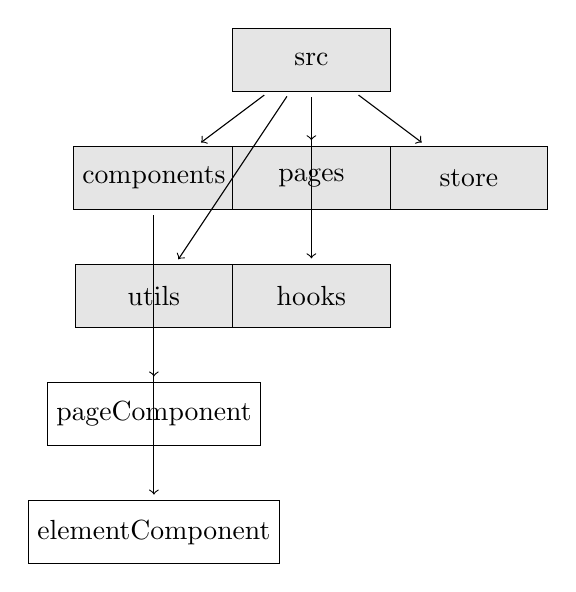
\begin{tikzpicture}[
    file/.style={draw, rectangle, minimum width=2cm, minimum height=0.8cm},
    folder/.style={draw, rectangle, minimum width=2cm, minimum height=0.8cm, fill=gray!20},
    arrow/.style={->, shorten >=2pt, shorten <=2pt}
]

% Folders
\node[folder] (src) at (0,0) {src};
\node[folder] (components) at (-2,-1.5) {components};
\node[folder] (pages) at (0,-1.5) {pages};
\node[folder] (store) at (2,-1.5) {store};
\node[folder] (utils) at (-2,-3) {utils};
\node[folder] (hooks) at (0,-3) {hooks};

% Files
\node[file] (pageComponent) at (-2,-4.5) {pageComponent};
\node[file] (elementComponent) at (-2,-6) {elementComponent};
% ... add more files

% Connections
\draw[arrow] (src) -- (components);
\draw[arrow] (src) -- (pages);
\draw[arrow] (src) -- (store);
\draw[arrow] (src) -- (utils);
\draw[arrow] (src) -- (hooks);
\draw[arrow] (components) -- (pageComponent);
\draw[arrow] (components) -- (elementComponent);
% ... add more connections

\end{tikzpicture}



\pagebreak
\subsubsection{Back-end}
The backend uses the dotNet framework. The development language using the C\# language.

In this project, the backend uses the Onion Architecture.
The Onion Architecture is a typically layered architecture, 
where each layer depends on the inner layer and provides interfaces to the outer layer.
The outer layer provides services to the outermost layer 
and other modules in the same layer based on the interfaces of the inner layer.

From inner to outer, the layers are: Domain, Application, Infrastructure, Presentation.
The Domain layer is the core layer and the innermost layer, used to define domain models, 
which are the business models.
It includes domain models and domain service interfaces.
Domain models are used to define the business models, 
which are the entities in the entity-relationship model and their attributes.
Domain service interfaces are used to define the business services, 
which are the relationships between entities in the entity-relationship model.

The Application layer is the application layer, 
used to define application services, which are the business logic.
It includes domain service implementations and application service interfaces.
Domain service implementations implement the methods of the inner layer's domain service 
interfaces and implement the business logic of the domain models.
Application service interfaces are used to define application services, 
which are the business logic.
It includes but is not limited to database interfaces, testing interfaces, 
HTTP API interfaces, MQTT interfaces, etc.

The Infrastructure layer is the infrastructure layer, used to define infrastructure.
It includes database implementations, testing implementations, 
HTTP API implementations, MQTT implementations, etc.
Database implementations implement the database interfaces 
and provide CRUD services for the database.
Testing implementations implement the testing interfaces 
and provide services for unit testing and integration testing.
HTTP API implementations implement the HTTP API interfaces 
and provide CRUD operations for HTTP APIs.
MQTT implementations implement the MQTT interfaces 
and provide CRUD operations for MQTT.

The Presentation layer is the presentation layer, used to define presentation logic, 
such as interfaces and pages. Since this is a backend project,
data presentation and control are handled by the frontend, 
so this layer is not needed.



\pagebreak
\subsubsection{Data communication and storage}
% 关于本项目的数据通信与数据存储的设计, 包括数据通信的协议, 数据存储的设计等
% 关于数据通信的设计:
% 1. 通信协议的选择
% 自前端向后端发送的数据, 有三种传输的数据类型, 
% 一种是普通的增删改查的请求, 对数据传输的时效性要求不高, 但是对数据的准确性, 完整性, 有序性, 安全性有一定的要求,
% 这种数据的传输, 采用 HTTP 协议, 以及 RESTful API 的设计. 可以有效的保证对数据传输的以上要求.
% 一种是对数据通道的创建和流媒体数据的传输, 对数据传输的时效性, 安全性要求较高, 这种数据的传输, 采用 WebRTC 协议, 以及 MQTT 协议.
% 配合可以快速解码的 flatbuffers 协议, 可以有效的保证对数据传输的以上要求.
% 最后一种是对设备的状态信息和操作信息的传输, 对完整性, 有序性, 安全性都有较高的要求, 这种数据的传输, 采用 MQTT 协议
% 同时也使用了 flatbuffers 协议.
% 
% 2. 数据通信的通信架构和通信流程
% 本项目的数据通信的通信架构, 是基于前后端分离的架构, 前端使用 React 框架, 后端使用 dotnet 框架.
% 当前端需要向后端发送数据的时候, 前端会向后端发送 HTTP 请求, 后端接收到 HTTP 请求之后, 会根据请求的数据类型,
% 选择不同的数据处理方式, 对于普通的增删改查的请求, 后端会根据 RESTful API 的设计, 对数据进行增删改查的操作,
% 对于对数据通道的创建和流媒体数据的传输, 后端会根据 WebRTC 协议, 对数据通道进行创建, 并且帮助前端和设备建立数据通道,
% 当数据通道建立后, 前端和设备之间则使用 flatbuffer 的数据格式对流媒体数据进行传输,
% 对于设备的状态信息和操作信息的传输, 前端会直接向 MQTT broker 发送 MQTT 请求, 
% 设备会在其自身的固件中监听相关的 MQTT 请求, 并且返回相关的数据.
% 
% 3. 数据通信的格式
% 本项目的数据通信的格式, 有三种, 
% 一种是 HTTP 协议, 
% 使用 json 格式对数据进行传输,
% 一种是 WebRTC 协议, 
% 使用 flatbuffers 格式对数据进行传输,
% 一种是 MQTT 协议.
% 使用 flatbuffers 格式对数据进行传输,
% 
% 关于数据存储的设计:
% 1. 数据存储的数据库的选择
% 本项目的数据存储的数据库的选择, 使用了轻量级的数据库 SQLite,
% SQLite 是一个进程内的库, 实现了自给自足的, 无服务器的, 零配置的, 事务性的 SQL 数据库引擎.
% 这是因为整个项目的目的是为了实现前端与设备之间的数据通信, 对于数据库数据的增删改查操作的要求不高,
% 数据量较小, 且对于数据库的数据的事务性要求不高, 所以选择了 SQLite 数据库.
% 2. 项目前后端的数据结构的设计
% 在本项目中, 前端由于使用了 React 框架, 所以前端的数据结构的设计, 使用了基于状态的数据结构的设计,
% 每个组件或者数据集都包含一个状态对象, 这个状态对象的属性就是组件的各个状态. 
% 使用状态对象的原因是, 可以方便的对状态进行管理, 采用对象-属性的形式, 可以方便的针对不同组件的同类状态进行区分,
% 由于跨组件的状态是由 redux 进行管理的, 这种状态对象的设计, 可以更搞笑的对状态进行更新和传递.
% 后端由于使用了 dotnet 框架, 所以后端的数据结构的设计, 使用了基于类的数据结构的设计,
% 采用了面向对象的编程思想, 对数据进行了封装, 使得数据的传输更加的安全, 有序, 完整.


\pagebreak

% \subsection{Domain model}
% \documentclass[]{article}
\usepackage{graphicx}
\usepackage{amsmath}
\usepackage{tikz}

% libaries
\usetikzlibrary{shapes,arrows}

%Define the listing package
\usepackage{listings} %code highlighter
\usepackage{color} %use color
\definecolor{mygreen}{rgb}{0,0.6,0}
\definecolor{mygray}{rgb}{0.5,0.5,0.5}
\definecolor{mymauve}{rgb}{0.58,0,0.82}

%Customize a bit the look
\lstset{ %
backgroundcolor=\color{white}, % choose the background color; you must add \usepackage{color} or \usepackage{xcolor}
basicstyle=\footnotesize, % the size of the fonts that are used for the code
breakatwhitespace=false, % sets if automatic breaks should only happen at whitespace
breaklines=true, % sets automatic line breaking
captionpos=b, % sets the caption-position to bottom
commentstyle=\color{mygreen}, % comment style
deletekeywords={...}, % if you want to delete keywords from the given language
escapeinside={\%*}{*)}, % if you want to add LaTeX within your code
extendedchars=true, % lets you use non-ASCII characters; for 8-bits encodings only, does not work with UTF-8
frame=single, % adds a frame around the code
keepspaces=true, % keeps spaces in text, useful for keeping indentation of code (possibly needs columns=flexible)
keywordstyle=\color{blue}, % keyword style
% language=Octave, % the language of the code
morekeywords={*,...}, % if you want to add more keywords to the set
numbers=left, % where to put the line-numbers; possible values are (none, left, right)
numbersep=5pt, % how far the line-numbers are from the code
numberstyle=\tiny\color{mygray}, % the style that is used for the line-numbers
rulecolor=\color{black}, % if not set, the frame-color may be changed on line-breaks within not-black text (e.g. comments (green here))
showspaces=false, % show spaces everywhere adding particular underscores; it overrides 'showstringspaces'
showstringspaces=false, % underline spaces within strings only
showtabs=false, % show tabs within strings adding particular underscores
stepnumber=1, % the step between two line-numbers. If it's 1, each line will be numbered
stringstyle=\color{mymauve}, % string literal style
tabsize=2, % sets default tabsize to 2 spaces
title=\lstname % show the filename of files included with \lstinputlisting; also try caption instead of title
}

\definecolor{darkgray}{rgb}{.4,.4,.4}
\definecolor{purple}{rgb}{0.65, 0.12, 0.82}

\lstdefinelanguage{React}{
keywords={const, typeof, new, true, false, catch, function, return, null, catch, switch, var, if, in, while, do, else, case, break},
keywordstyle=\color{blue}\bfseries,
ndkeywords={class, export, boolean, throw, implements, import, this},
ndkeywordstyle=\color{darkgray}\bfseries,
identifierstyle=\color{mygreen},
sensitive=false,
comment=[l]{//},
morecomment=[s]{/*}{*/},
commentstyle=\color{purple}\ttfamily,
string=[b]{"}{'}{`},
stringstyle=\color{red}\ttfamily,
morestring=[b]',
morestring=[b]",
morestring=[b]`',
}

\lstdefinelanguage{CSharp}{
keywords={const, typeof, new, true, false, catch, function, return, null, catch, switch, var, if, in, while, do, else, case, break},
keywordstyle=\color{blue}\bfseries,
ndkeywords={class, export, boolean, throw, implements, import, this},
ndkeywordstyle=\color{darkgray}\bfseries,
identifierstyle=\color{mygreen},
sensitive=false,
comment=[l]{//},
morecomment=[s]{/*}{*/},
commentstyle=\color{purple}\ttfamily,
string=[b]{"}{'}{`},
stringstyle=\color{red}\ttfamily,
morestring=[b]',
morestring=[b]",
morestring=[b]`',
}

\lstset{
language=React,
extendedchars=true,
basicstyle=\footnotesize\ttfamily,
showstringspaces=false,
showspaces=false,
numbers=left,
numberstyle=\footnotesize,
numbersep=9pt,
tabsize=2,
breaklines=true,
showtabs=false,
captionpos=b
}

\lstset{
language=CSharp,
extendedchars=true,
basicstyle=\footnotesize\ttfamily,
showstringspaces=false,
showspaces=false,
numbers=left,
numberstyle=\footnotesize,
numbersep=9pt,
tabsize=2,
breaklines=true,
showtabs=false,
captionpos=b
}

% \usepackage{cite} % Add this line for citation

% \bibliographystyle{plain}

\title{
The implementation of BifrostConnect Front-end scope, 
re-design and development with the relevant back-end support develop.
}
\author{
    Fei Gu \\
    Erhvervs Akademi Sydvest \\
    Computer Science 21\\
    }
\date{\today}

\begin{document}

% Front page
\maketitle
\begin{center}
    Supervisor: Henrik Boulund Meng Hansen \\
    Company: BifrostConnect \\
    Engineering Director: Jasper Wass \\
\end{center}
\tableofcontents
\pagebreak


% The introduction
\section{Introduction}
\subsection{Background}\input{sections/introduction/background.tex}
\subsection{The company}\input{sections/introduction/aboutCompany}
\subsection{The project}\input{sections/introduction/aboutProject}
\pagebreak

% The problem statement
\section{Problem Statement}
\subsection{Statement}
\input{sections/problemStatement/statement}
\subsection{Situation}
\input{sections/problemStatement/situation}
\subsection{Potential Solution}
\input{sections/problemStatement/potentialSolution}
\pagebreak

% Requirement analysis
\section{Requirement Analysis}
\input{sections/requirementAnalysis/index}

\subsection{Stakeholders}
\input{sections/requirementAnalysis/stakeholders/index}

\subsection{Business Domain}
\input{sections/requirementAnalysis/bussinesDomain/index}

\subsection{Scope}
\input{sections/requirementAnalysis/scope}

\subsection{Goals}
\input{sections/requirementAnalysis/goals}
\pagebreak

% Software Design
\section{Software Design}
% developement methods
\subsection{Software Development Methods}
\input{sections/softwareDevelopmentMethods/index}
\subsubsection{Agile Software Development}
\input{sections/softwareDevelopmentMethods/agileSoftwareDevelopment/index}
\subsubsection{Feature Driven Development}
\input{sections/softwareDevelopmentMethods/featureDrivenDevelopment/index}

\pagebreak

% Technology seslection
\subsection{Technology selection}
\input{sections/softwareDesign/technologySelection/index}
\subsubsection{Front-end}
\input{sections/softwareDesign/technologySelection/frontEnd}            
\subsubsection{Back-end}
\input{sections/softwareDesign/technologySelection/backEnd}            
\subsubsection{Database}
\input{sections/softwareDesign/technologySelection/database}
\subsubsection{Data communication}
\input{sections/softwareDesign/technologySelection/dataCommunication}            
\subsubsection{DevOps}
\input{sections/softwareDesign/technologySelection/devOps}
\pagebreak

% Architecture design
\subsection{Architecture design}
\input{sections/softwareDesign/architectureDesign/index}
\pagebreak
\subsubsection{Front-end}
\input{sections/softwareDesign/architectureDesign/frontEndArchitecture}
\pagebreak
\subsubsection{Back-end}
\input{sections/softwareDesign/architectureDesign/backEndArchitecture}
\pagebreak
\subsubsection{Data communication and storage}
\input{sections/softwareDesign/architectureDesign/dataCommunicationArchitecture}
\pagebreak

% \subsection{Domain model}
% \input{sections/softwareDesign/domainModel/index}
% \subsection{Database design}
% % 数据库领域模型 ER 图
% % 包括表和字段的设置.
% % 对于私有键和外键的设置.

% \subsection{Back-end design}
% % 后端对象模型
% % 以及对于对象模型的增删改查
% % 以及相关的其他服务的设计`'

% \subsection{Front-end design}
% % 对于前端的页面结构的设计 
% % 页面的状态的设计, 交互设计

% \subsection{FlatBuffers design}
% % schema 的设计

\subsection{DevOps CI/CD process design}
\input{sections/softwareDesign/devOpsDesign/index}
\subsubsection{Continuous Integration}
\input{sections/softwareDesign/devOpsDesign/continuousIntegration/index}
\subsubsection{Continuous Delivery}
\input{sections/softwareDesign/devOpsDesign/continuousDelivery/index}
\subsubsection{Continuous Deployment}
\input{sections/softwareDesign/devOpsDesign/continuousDeployment/index}
\pagebreak

\section{Software Development} 
\input{sections/softwareDevelopment/index}
\subsection{Overall development}
\input{sections/softwareDevelopment/overallDevelopement/index}
\subsubsection{Front-end}
\input{sections/softwareDevelopment/overallDevelopement/frontEnd/index}
\subsubsection{Back-end}
\input{sections/softwareDevelopment/overallDevelopement/backEnd/index}
\subsubsection{DevOps}
\input{sections/softwareDevelopment/overallDevelopement/devOps/index}
\subsection{Feature development} 
\input{sections/softwareDevelopment/featureDevelopment/index}
\subsubsection{Use Case 1}
\input{sections/softwareDevelopment/featureDevelopment/useCase1/index}
\subsubsection{Feature 1}
\input{sections/softwareDevelopment/featureDevelopment/feature/feature1.tex}
\pagebreak
\section{Conclusion} 
\subsection{Result}
Since the project is still in progress, the result is not available yet.
So far, basic structure of this project has been built. But the most features 
are not implemented yet. 
\subsection{Discussion}
As a single developer for this project, I am confident what I have done so far.
And I can say I understand the most of the knowledge I have used in this project, 
which also means I can explain all the part of the project. 
But this project also relevant some of the complex knowledge which I have to continue 
to study and practice.
\subsection{Future Work}
The future work is to implement the rest of the features. 
Including the most important part which is the 'create session' feature.
\pagebreak
% \bibliography{bibliography}
\pagebreak
% \begin{appendices}
%     \section{Appendix}
% \end{appendices} 
\end{document}
% \subsection{Database design}
% % 数据库领域模型 ER 图
% % 包括表和字段的设置.
% % 对于私有键和外键的设置.

% \subsection{Back-end design}
% % 后端对象模型
% % 以及对于对象模型的增删改查
% % 以及相关的其他服务的设计`'

% \subsection{Front-end design}
% % 对于前端的页面结构的设计 
% % 页面的状态的设计, 交互设计

% \subsection{FlatBuffers design}
% % schema 的设计

\subsection{DevOps CI/CD process design}
\documentclass[]{article}
\usepackage{graphicx}
\usepackage{amsmath}
\usepackage{tikz}

% libaries
\usetikzlibrary{shapes,arrows}

%Define the listing package
\usepackage{listings} %code highlighter
\usepackage{color} %use color
\definecolor{mygreen}{rgb}{0,0.6,0}
\definecolor{mygray}{rgb}{0.5,0.5,0.5}
\definecolor{mymauve}{rgb}{0.58,0,0.82}

%Customize a bit the look
\lstset{ %
backgroundcolor=\color{white}, % choose the background color; you must add \usepackage{color} or \usepackage{xcolor}
basicstyle=\footnotesize, % the size of the fonts that are used for the code
breakatwhitespace=false, % sets if automatic breaks should only happen at whitespace
breaklines=true, % sets automatic line breaking
captionpos=b, % sets the caption-position to bottom
commentstyle=\color{mygreen}, % comment style
deletekeywords={...}, % if you want to delete keywords from the given language
escapeinside={\%*}{*)}, % if you want to add LaTeX within your code
extendedchars=true, % lets you use non-ASCII characters; for 8-bits encodings only, does not work with UTF-8
frame=single, % adds a frame around the code
keepspaces=true, % keeps spaces in text, useful for keeping indentation of code (possibly needs columns=flexible)
keywordstyle=\color{blue}, % keyword style
% language=Octave, % the language of the code
morekeywords={*,...}, % if you want to add more keywords to the set
numbers=left, % where to put the line-numbers; possible values are (none, left, right)
numbersep=5pt, % how far the line-numbers are from the code
numberstyle=\tiny\color{mygray}, % the style that is used for the line-numbers
rulecolor=\color{black}, % if not set, the frame-color may be changed on line-breaks within not-black text (e.g. comments (green here))
showspaces=false, % show spaces everywhere adding particular underscores; it overrides 'showstringspaces'
showstringspaces=false, % underline spaces within strings only
showtabs=false, % show tabs within strings adding particular underscores
stepnumber=1, % the step between two line-numbers. If it's 1, each line will be numbered
stringstyle=\color{mymauve}, % string literal style
tabsize=2, % sets default tabsize to 2 spaces
title=\lstname % show the filename of files included with \lstinputlisting; also try caption instead of title
}

\definecolor{darkgray}{rgb}{.4,.4,.4}
\definecolor{purple}{rgb}{0.65, 0.12, 0.82}

\lstdefinelanguage{React}{
keywords={const, typeof, new, true, false, catch, function, return, null, catch, switch, var, if, in, while, do, else, case, break},
keywordstyle=\color{blue}\bfseries,
ndkeywords={class, export, boolean, throw, implements, import, this},
ndkeywordstyle=\color{darkgray}\bfseries,
identifierstyle=\color{mygreen},
sensitive=false,
comment=[l]{//},
morecomment=[s]{/*}{*/},
commentstyle=\color{purple}\ttfamily,
string=[b]{"}{'}{`},
stringstyle=\color{red}\ttfamily,
morestring=[b]',
morestring=[b]",
morestring=[b]`',
}

\lstdefinelanguage{CSharp}{
keywords={const, typeof, new, true, false, catch, function, return, null, catch, switch, var, if, in, while, do, else, case, break},
keywordstyle=\color{blue}\bfseries,
ndkeywords={class, export, boolean, throw, implements, import, this},
ndkeywordstyle=\color{darkgray}\bfseries,
identifierstyle=\color{mygreen},
sensitive=false,
comment=[l]{//},
morecomment=[s]{/*}{*/},
commentstyle=\color{purple}\ttfamily,
string=[b]{"}{'}{`},
stringstyle=\color{red}\ttfamily,
morestring=[b]',
morestring=[b]",
morestring=[b]`',
}

\lstset{
language=React,
extendedchars=true,
basicstyle=\footnotesize\ttfamily,
showstringspaces=false,
showspaces=false,
numbers=left,
numberstyle=\footnotesize,
numbersep=9pt,
tabsize=2,
breaklines=true,
showtabs=false,
captionpos=b
}

\lstset{
language=CSharp,
extendedchars=true,
basicstyle=\footnotesize\ttfamily,
showstringspaces=false,
showspaces=false,
numbers=left,
numberstyle=\footnotesize,
numbersep=9pt,
tabsize=2,
breaklines=true,
showtabs=false,
captionpos=b
}

% \usepackage{cite} % Add this line for citation

% \bibliographystyle{plain}

\title{
The implementation of BifrostConnect Front-end scope, 
re-design and development with the relevant back-end support develop.
}
\author{
    Fei Gu \\
    Erhvervs Akademi Sydvest \\
    Computer Science 21\\
    }
\date{\today}

\begin{document}

% Front page
\maketitle
\begin{center}
    Supervisor: Henrik Boulund Meng Hansen \\
    Company: BifrostConnect \\
    Engineering Director: Jasper Wass \\
\end{center}
\tableofcontents
\pagebreak


% The introduction
\section{Introduction}
\subsection{Background}\input{sections/introduction/background.tex}
\subsection{The company}\input{sections/introduction/aboutCompany}
\subsection{The project}\input{sections/introduction/aboutProject}
\pagebreak

% The problem statement
\section{Problem Statement}
\subsection{Statement}
\input{sections/problemStatement/statement}
\subsection{Situation}
\input{sections/problemStatement/situation}
\subsection{Potential Solution}
\input{sections/problemStatement/potentialSolution}
\pagebreak

% Requirement analysis
\section{Requirement Analysis}
\input{sections/requirementAnalysis/index}

\subsection{Stakeholders}
\input{sections/requirementAnalysis/stakeholders/index}

\subsection{Business Domain}
\input{sections/requirementAnalysis/bussinesDomain/index}

\subsection{Scope}
\input{sections/requirementAnalysis/scope}

\subsection{Goals}
\input{sections/requirementAnalysis/goals}
\pagebreak

% Software Design
\section{Software Design}
% developement methods
\subsection{Software Development Methods}
\input{sections/softwareDevelopmentMethods/index}
\subsubsection{Agile Software Development}
\input{sections/softwareDevelopmentMethods/agileSoftwareDevelopment/index}
\subsubsection{Feature Driven Development}
\input{sections/softwareDevelopmentMethods/featureDrivenDevelopment/index}

\pagebreak

% Technology seslection
\subsection{Technology selection}
\input{sections/softwareDesign/technologySelection/index}
\subsubsection{Front-end}
\input{sections/softwareDesign/technologySelection/frontEnd}            
\subsubsection{Back-end}
\input{sections/softwareDesign/technologySelection/backEnd}            
\subsubsection{Database}
\input{sections/softwareDesign/technologySelection/database}
\subsubsection{Data communication}
\input{sections/softwareDesign/technologySelection/dataCommunication}            
\subsubsection{DevOps}
\input{sections/softwareDesign/technologySelection/devOps}
\pagebreak

% Architecture design
\subsection{Architecture design}
\input{sections/softwareDesign/architectureDesign/index}
\pagebreak
\subsubsection{Front-end}
\input{sections/softwareDesign/architectureDesign/frontEndArchitecture}
\pagebreak
\subsubsection{Back-end}
\input{sections/softwareDesign/architectureDesign/backEndArchitecture}
\pagebreak
\subsubsection{Data communication and storage}
\input{sections/softwareDesign/architectureDesign/dataCommunicationArchitecture}
\pagebreak

% \subsection{Domain model}
% \input{sections/softwareDesign/domainModel/index}
% \subsection{Database design}
% % 数据库领域模型 ER 图
% % 包括表和字段的设置.
% % 对于私有键和外键的设置.

% \subsection{Back-end design}
% % 后端对象模型
% % 以及对于对象模型的增删改查
% % 以及相关的其他服务的设计`'

% \subsection{Front-end design}
% % 对于前端的页面结构的设计 
% % 页面的状态的设计, 交互设计

% \subsection{FlatBuffers design}
% % schema 的设计

\subsection{DevOps CI/CD process design}
\input{sections/softwareDesign/devOpsDesign/index}
\subsubsection{Continuous Integration}
\input{sections/softwareDesign/devOpsDesign/continuousIntegration/index}
\subsubsection{Continuous Delivery}
\input{sections/softwareDesign/devOpsDesign/continuousDelivery/index}
\subsubsection{Continuous Deployment}
\input{sections/softwareDesign/devOpsDesign/continuousDeployment/index}
\pagebreak

\section{Software Development} 
\input{sections/softwareDevelopment/index}
\subsection{Overall development}
\input{sections/softwareDevelopment/overallDevelopement/index}
\subsubsection{Front-end}
\input{sections/softwareDevelopment/overallDevelopement/frontEnd/index}
\subsubsection{Back-end}
\input{sections/softwareDevelopment/overallDevelopement/backEnd/index}
\subsubsection{DevOps}
\input{sections/softwareDevelopment/overallDevelopement/devOps/index}
\subsection{Feature development} 
\input{sections/softwareDevelopment/featureDevelopment/index}
\subsubsection{Use Case 1}
\input{sections/softwareDevelopment/featureDevelopment/useCase1/index}
\subsubsection{Feature 1}
\input{sections/softwareDevelopment/featureDevelopment/feature/feature1.tex}
\pagebreak
\section{Conclusion} 
\subsection{Result}
Since the project is still in progress, the result is not available yet.
So far, basic structure of this project has been built. But the most features 
are not implemented yet. 
\subsection{Discussion}
As a single developer for this project, I am confident what I have done so far.
And I can say I understand the most of the knowledge I have used in this project, 
which also means I can explain all the part of the project. 
But this project also relevant some of the complex knowledge which I have to continue 
to study and practice.
\subsection{Future Work}
The future work is to implement the rest of the features. 
Including the most important part which is the 'create session' feature.
\pagebreak
% \bibliography{bibliography}
\pagebreak
% \begin{appendices}
%     \section{Appendix}
% \end{appendices} 
\end{document}
\subsubsection{Continuous Integration}
\documentclass[]{article}
\usepackage{graphicx}
\usepackage{amsmath}
\usepackage{tikz}

% libaries
\usetikzlibrary{shapes,arrows}

%Define the listing package
\usepackage{listings} %code highlighter
\usepackage{color} %use color
\definecolor{mygreen}{rgb}{0,0.6,0}
\definecolor{mygray}{rgb}{0.5,0.5,0.5}
\definecolor{mymauve}{rgb}{0.58,0,0.82}

%Customize a bit the look
\lstset{ %
backgroundcolor=\color{white}, % choose the background color; you must add \usepackage{color} or \usepackage{xcolor}
basicstyle=\footnotesize, % the size of the fonts that are used for the code
breakatwhitespace=false, % sets if automatic breaks should only happen at whitespace
breaklines=true, % sets automatic line breaking
captionpos=b, % sets the caption-position to bottom
commentstyle=\color{mygreen}, % comment style
deletekeywords={...}, % if you want to delete keywords from the given language
escapeinside={\%*}{*)}, % if you want to add LaTeX within your code
extendedchars=true, % lets you use non-ASCII characters; for 8-bits encodings only, does not work with UTF-8
frame=single, % adds a frame around the code
keepspaces=true, % keeps spaces in text, useful for keeping indentation of code (possibly needs columns=flexible)
keywordstyle=\color{blue}, % keyword style
% language=Octave, % the language of the code
morekeywords={*,...}, % if you want to add more keywords to the set
numbers=left, % where to put the line-numbers; possible values are (none, left, right)
numbersep=5pt, % how far the line-numbers are from the code
numberstyle=\tiny\color{mygray}, % the style that is used for the line-numbers
rulecolor=\color{black}, % if not set, the frame-color may be changed on line-breaks within not-black text (e.g. comments (green here))
showspaces=false, % show spaces everywhere adding particular underscores; it overrides 'showstringspaces'
showstringspaces=false, % underline spaces within strings only
showtabs=false, % show tabs within strings adding particular underscores
stepnumber=1, % the step between two line-numbers. If it's 1, each line will be numbered
stringstyle=\color{mymauve}, % string literal style
tabsize=2, % sets default tabsize to 2 spaces
title=\lstname % show the filename of files included with \lstinputlisting; also try caption instead of title
}

\definecolor{darkgray}{rgb}{.4,.4,.4}
\definecolor{purple}{rgb}{0.65, 0.12, 0.82}

\lstdefinelanguage{React}{
keywords={const, typeof, new, true, false, catch, function, return, null, catch, switch, var, if, in, while, do, else, case, break},
keywordstyle=\color{blue}\bfseries,
ndkeywords={class, export, boolean, throw, implements, import, this},
ndkeywordstyle=\color{darkgray}\bfseries,
identifierstyle=\color{mygreen},
sensitive=false,
comment=[l]{//},
morecomment=[s]{/*}{*/},
commentstyle=\color{purple}\ttfamily,
string=[b]{"}{'}{`},
stringstyle=\color{red}\ttfamily,
morestring=[b]',
morestring=[b]",
morestring=[b]`',
}

\lstdefinelanguage{CSharp}{
keywords={const, typeof, new, true, false, catch, function, return, null, catch, switch, var, if, in, while, do, else, case, break},
keywordstyle=\color{blue}\bfseries,
ndkeywords={class, export, boolean, throw, implements, import, this},
ndkeywordstyle=\color{darkgray}\bfseries,
identifierstyle=\color{mygreen},
sensitive=false,
comment=[l]{//},
morecomment=[s]{/*}{*/},
commentstyle=\color{purple}\ttfamily,
string=[b]{"}{'}{`},
stringstyle=\color{red}\ttfamily,
morestring=[b]',
morestring=[b]",
morestring=[b]`',
}

\lstset{
language=React,
extendedchars=true,
basicstyle=\footnotesize\ttfamily,
showstringspaces=false,
showspaces=false,
numbers=left,
numberstyle=\footnotesize,
numbersep=9pt,
tabsize=2,
breaklines=true,
showtabs=false,
captionpos=b
}

\lstset{
language=CSharp,
extendedchars=true,
basicstyle=\footnotesize\ttfamily,
showstringspaces=false,
showspaces=false,
numbers=left,
numberstyle=\footnotesize,
numbersep=9pt,
tabsize=2,
breaklines=true,
showtabs=false,
captionpos=b
}

% \usepackage{cite} % Add this line for citation

% \bibliographystyle{plain}

\title{
The implementation of BifrostConnect Front-end scope, 
re-design and development with the relevant back-end support develop.
}
\author{
    Fei Gu \\
    Erhvervs Akademi Sydvest \\
    Computer Science 21\\
    }
\date{\today}

\begin{document}

% Front page
\maketitle
\begin{center}
    Supervisor: Henrik Boulund Meng Hansen \\
    Company: BifrostConnect \\
    Engineering Director: Jasper Wass \\
\end{center}
\tableofcontents
\pagebreak


% The introduction
\section{Introduction}
\subsection{Background}\input{sections/introduction/background.tex}
\subsection{The company}\input{sections/introduction/aboutCompany}
\subsection{The project}\input{sections/introduction/aboutProject}
\pagebreak

% The problem statement
\section{Problem Statement}
\subsection{Statement}
\input{sections/problemStatement/statement}
\subsection{Situation}
\input{sections/problemStatement/situation}
\subsection{Potential Solution}
\input{sections/problemStatement/potentialSolution}
\pagebreak

% Requirement analysis
\section{Requirement Analysis}
\input{sections/requirementAnalysis/index}

\subsection{Stakeholders}
\input{sections/requirementAnalysis/stakeholders/index}

\subsection{Business Domain}
\input{sections/requirementAnalysis/bussinesDomain/index}

\subsection{Scope}
\input{sections/requirementAnalysis/scope}

\subsection{Goals}
\input{sections/requirementAnalysis/goals}
\pagebreak

% Software Design
\section{Software Design}
% developement methods
\subsection{Software Development Methods}
\input{sections/softwareDevelopmentMethods/index}
\subsubsection{Agile Software Development}
\input{sections/softwareDevelopmentMethods/agileSoftwareDevelopment/index}
\subsubsection{Feature Driven Development}
\input{sections/softwareDevelopmentMethods/featureDrivenDevelopment/index}

\pagebreak

% Technology seslection
\subsection{Technology selection}
\input{sections/softwareDesign/technologySelection/index}
\subsubsection{Front-end}
\input{sections/softwareDesign/technologySelection/frontEnd}            
\subsubsection{Back-end}
\input{sections/softwareDesign/technologySelection/backEnd}            
\subsubsection{Database}
\input{sections/softwareDesign/technologySelection/database}
\subsubsection{Data communication}
\input{sections/softwareDesign/technologySelection/dataCommunication}            
\subsubsection{DevOps}
\input{sections/softwareDesign/technologySelection/devOps}
\pagebreak

% Architecture design
\subsection{Architecture design}
\input{sections/softwareDesign/architectureDesign/index}
\pagebreak
\subsubsection{Front-end}
\input{sections/softwareDesign/architectureDesign/frontEndArchitecture}
\pagebreak
\subsubsection{Back-end}
\input{sections/softwareDesign/architectureDesign/backEndArchitecture}
\pagebreak
\subsubsection{Data communication and storage}
\input{sections/softwareDesign/architectureDesign/dataCommunicationArchitecture}
\pagebreak

% \subsection{Domain model}
% \input{sections/softwareDesign/domainModel/index}
% \subsection{Database design}
% % 数据库领域模型 ER 图
% % 包括表和字段的设置.
% % 对于私有键和外键的设置.

% \subsection{Back-end design}
% % 后端对象模型
% % 以及对于对象模型的增删改查
% % 以及相关的其他服务的设计`'

% \subsection{Front-end design}
% % 对于前端的页面结构的设计 
% % 页面的状态的设计, 交互设计

% \subsection{FlatBuffers design}
% % schema 的设计

\subsection{DevOps CI/CD process design}
\input{sections/softwareDesign/devOpsDesign/index}
\subsubsection{Continuous Integration}
\input{sections/softwareDesign/devOpsDesign/continuousIntegration/index}
\subsubsection{Continuous Delivery}
\input{sections/softwareDesign/devOpsDesign/continuousDelivery/index}
\subsubsection{Continuous Deployment}
\input{sections/softwareDesign/devOpsDesign/continuousDeployment/index}
\pagebreak

\section{Software Development} 
\input{sections/softwareDevelopment/index}
\subsection{Overall development}
\input{sections/softwareDevelopment/overallDevelopement/index}
\subsubsection{Front-end}
\input{sections/softwareDevelopment/overallDevelopement/frontEnd/index}
\subsubsection{Back-end}
\input{sections/softwareDevelopment/overallDevelopement/backEnd/index}
\subsubsection{DevOps}
\input{sections/softwareDevelopment/overallDevelopement/devOps/index}
\subsection{Feature development} 
\input{sections/softwareDevelopment/featureDevelopment/index}
\subsubsection{Use Case 1}
\input{sections/softwareDevelopment/featureDevelopment/useCase1/index}
\subsubsection{Feature 1}
\input{sections/softwareDevelopment/featureDevelopment/feature/feature1.tex}
\pagebreak
\section{Conclusion} 
\subsection{Result}
Since the project is still in progress, the result is not available yet.
So far, basic structure of this project has been built. But the most features 
are not implemented yet. 
\subsection{Discussion}
As a single developer for this project, I am confident what I have done so far.
And I can say I understand the most of the knowledge I have used in this project, 
which also means I can explain all the part of the project. 
But this project also relevant some of the complex knowledge which I have to continue 
to study and practice.
\subsection{Future Work}
The future work is to implement the rest of the features. 
Including the most important part which is the 'create session' feature.
\pagebreak
% \bibliography{bibliography}
\pagebreak
% \begin{appendices}
%     \section{Appendix}
% \end{appendices} 
\end{document}
\subsubsection{Continuous Delivery}
\documentclass[]{article}
\usepackage{graphicx}
\usepackage{amsmath}
\usepackage{tikz}

% libaries
\usetikzlibrary{shapes,arrows}

%Define the listing package
\usepackage{listings} %code highlighter
\usepackage{color} %use color
\definecolor{mygreen}{rgb}{0,0.6,0}
\definecolor{mygray}{rgb}{0.5,0.5,0.5}
\definecolor{mymauve}{rgb}{0.58,0,0.82}

%Customize a bit the look
\lstset{ %
backgroundcolor=\color{white}, % choose the background color; you must add \usepackage{color} or \usepackage{xcolor}
basicstyle=\footnotesize, % the size of the fonts that are used for the code
breakatwhitespace=false, % sets if automatic breaks should only happen at whitespace
breaklines=true, % sets automatic line breaking
captionpos=b, % sets the caption-position to bottom
commentstyle=\color{mygreen}, % comment style
deletekeywords={...}, % if you want to delete keywords from the given language
escapeinside={\%*}{*)}, % if you want to add LaTeX within your code
extendedchars=true, % lets you use non-ASCII characters; for 8-bits encodings only, does not work with UTF-8
frame=single, % adds a frame around the code
keepspaces=true, % keeps spaces in text, useful for keeping indentation of code (possibly needs columns=flexible)
keywordstyle=\color{blue}, % keyword style
% language=Octave, % the language of the code
morekeywords={*,...}, % if you want to add more keywords to the set
numbers=left, % where to put the line-numbers; possible values are (none, left, right)
numbersep=5pt, % how far the line-numbers are from the code
numberstyle=\tiny\color{mygray}, % the style that is used for the line-numbers
rulecolor=\color{black}, % if not set, the frame-color may be changed on line-breaks within not-black text (e.g. comments (green here))
showspaces=false, % show spaces everywhere adding particular underscores; it overrides 'showstringspaces'
showstringspaces=false, % underline spaces within strings only
showtabs=false, % show tabs within strings adding particular underscores
stepnumber=1, % the step between two line-numbers. If it's 1, each line will be numbered
stringstyle=\color{mymauve}, % string literal style
tabsize=2, % sets default tabsize to 2 spaces
title=\lstname % show the filename of files included with \lstinputlisting; also try caption instead of title
}

\definecolor{darkgray}{rgb}{.4,.4,.4}
\definecolor{purple}{rgb}{0.65, 0.12, 0.82}

\lstdefinelanguage{React}{
keywords={const, typeof, new, true, false, catch, function, return, null, catch, switch, var, if, in, while, do, else, case, break},
keywordstyle=\color{blue}\bfseries,
ndkeywords={class, export, boolean, throw, implements, import, this},
ndkeywordstyle=\color{darkgray}\bfseries,
identifierstyle=\color{mygreen},
sensitive=false,
comment=[l]{//},
morecomment=[s]{/*}{*/},
commentstyle=\color{purple}\ttfamily,
string=[b]{"}{'}{`},
stringstyle=\color{red}\ttfamily,
morestring=[b]',
morestring=[b]",
morestring=[b]`',
}

\lstdefinelanguage{CSharp}{
keywords={const, typeof, new, true, false, catch, function, return, null, catch, switch, var, if, in, while, do, else, case, break},
keywordstyle=\color{blue}\bfseries,
ndkeywords={class, export, boolean, throw, implements, import, this},
ndkeywordstyle=\color{darkgray}\bfseries,
identifierstyle=\color{mygreen},
sensitive=false,
comment=[l]{//},
morecomment=[s]{/*}{*/},
commentstyle=\color{purple}\ttfamily,
string=[b]{"}{'}{`},
stringstyle=\color{red}\ttfamily,
morestring=[b]',
morestring=[b]",
morestring=[b]`',
}

\lstset{
language=React,
extendedchars=true,
basicstyle=\footnotesize\ttfamily,
showstringspaces=false,
showspaces=false,
numbers=left,
numberstyle=\footnotesize,
numbersep=9pt,
tabsize=2,
breaklines=true,
showtabs=false,
captionpos=b
}

\lstset{
language=CSharp,
extendedchars=true,
basicstyle=\footnotesize\ttfamily,
showstringspaces=false,
showspaces=false,
numbers=left,
numberstyle=\footnotesize,
numbersep=9pt,
tabsize=2,
breaklines=true,
showtabs=false,
captionpos=b
}

% \usepackage{cite} % Add this line for citation

% \bibliographystyle{plain}

\title{
The implementation of BifrostConnect Front-end scope, 
re-design and development with the relevant back-end support develop.
}
\author{
    Fei Gu \\
    Erhvervs Akademi Sydvest \\
    Computer Science 21\\
    }
\date{\today}

\begin{document}

% Front page
\maketitle
\begin{center}
    Supervisor: Henrik Boulund Meng Hansen \\
    Company: BifrostConnect \\
    Engineering Director: Jasper Wass \\
\end{center}
\tableofcontents
\pagebreak


% The introduction
\section{Introduction}
\subsection{Background}\input{sections/introduction/background.tex}
\subsection{The company}\input{sections/introduction/aboutCompany}
\subsection{The project}\input{sections/introduction/aboutProject}
\pagebreak

% The problem statement
\section{Problem Statement}
\subsection{Statement}
\input{sections/problemStatement/statement}
\subsection{Situation}
\input{sections/problemStatement/situation}
\subsection{Potential Solution}
\input{sections/problemStatement/potentialSolution}
\pagebreak

% Requirement analysis
\section{Requirement Analysis}
\input{sections/requirementAnalysis/index}

\subsection{Stakeholders}
\input{sections/requirementAnalysis/stakeholders/index}

\subsection{Business Domain}
\input{sections/requirementAnalysis/bussinesDomain/index}

\subsection{Scope}
\input{sections/requirementAnalysis/scope}

\subsection{Goals}
\input{sections/requirementAnalysis/goals}
\pagebreak

% Software Design
\section{Software Design}
% developement methods
\subsection{Software Development Methods}
\input{sections/softwareDevelopmentMethods/index}
\subsubsection{Agile Software Development}
\input{sections/softwareDevelopmentMethods/agileSoftwareDevelopment/index}
\subsubsection{Feature Driven Development}
\input{sections/softwareDevelopmentMethods/featureDrivenDevelopment/index}

\pagebreak

% Technology seslection
\subsection{Technology selection}
\input{sections/softwareDesign/technologySelection/index}
\subsubsection{Front-end}
\input{sections/softwareDesign/technologySelection/frontEnd}            
\subsubsection{Back-end}
\input{sections/softwareDesign/technologySelection/backEnd}            
\subsubsection{Database}
\input{sections/softwareDesign/technologySelection/database}
\subsubsection{Data communication}
\input{sections/softwareDesign/technologySelection/dataCommunication}            
\subsubsection{DevOps}
\input{sections/softwareDesign/technologySelection/devOps}
\pagebreak

% Architecture design
\subsection{Architecture design}
\input{sections/softwareDesign/architectureDesign/index}
\pagebreak
\subsubsection{Front-end}
\input{sections/softwareDesign/architectureDesign/frontEndArchitecture}
\pagebreak
\subsubsection{Back-end}
\input{sections/softwareDesign/architectureDesign/backEndArchitecture}
\pagebreak
\subsubsection{Data communication and storage}
\input{sections/softwareDesign/architectureDesign/dataCommunicationArchitecture}
\pagebreak

% \subsection{Domain model}
% \input{sections/softwareDesign/domainModel/index}
% \subsection{Database design}
% % 数据库领域模型 ER 图
% % 包括表和字段的设置.
% % 对于私有键和外键的设置.

% \subsection{Back-end design}
% % 后端对象模型
% % 以及对于对象模型的增删改查
% % 以及相关的其他服务的设计`'

% \subsection{Front-end design}
% % 对于前端的页面结构的设计 
% % 页面的状态的设计, 交互设计

% \subsection{FlatBuffers design}
% % schema 的设计

\subsection{DevOps CI/CD process design}
\input{sections/softwareDesign/devOpsDesign/index}
\subsubsection{Continuous Integration}
\input{sections/softwareDesign/devOpsDesign/continuousIntegration/index}
\subsubsection{Continuous Delivery}
\input{sections/softwareDesign/devOpsDesign/continuousDelivery/index}
\subsubsection{Continuous Deployment}
\input{sections/softwareDesign/devOpsDesign/continuousDeployment/index}
\pagebreak

\section{Software Development} 
\input{sections/softwareDevelopment/index}
\subsection{Overall development}
\input{sections/softwareDevelopment/overallDevelopement/index}
\subsubsection{Front-end}
\input{sections/softwareDevelopment/overallDevelopement/frontEnd/index}
\subsubsection{Back-end}
\input{sections/softwareDevelopment/overallDevelopement/backEnd/index}
\subsubsection{DevOps}
\input{sections/softwareDevelopment/overallDevelopement/devOps/index}
\subsection{Feature development} 
\input{sections/softwareDevelopment/featureDevelopment/index}
\subsubsection{Use Case 1}
\input{sections/softwareDevelopment/featureDevelopment/useCase1/index}
\subsubsection{Feature 1}
\input{sections/softwareDevelopment/featureDevelopment/feature/feature1.tex}
\pagebreak
\section{Conclusion} 
\subsection{Result}
Since the project is still in progress, the result is not available yet.
So far, basic structure of this project has been built. But the most features 
are not implemented yet. 
\subsection{Discussion}
As a single developer for this project, I am confident what I have done so far.
And I can say I understand the most of the knowledge I have used in this project, 
which also means I can explain all the part of the project. 
But this project also relevant some of the complex knowledge which I have to continue 
to study and practice.
\subsection{Future Work}
The future work is to implement the rest of the features. 
Including the most important part which is the 'create session' feature.
\pagebreak
% \bibliography{bibliography}
\pagebreak
% \begin{appendices}
%     \section{Appendix}
% \end{appendices} 
\end{document}
\subsubsection{Continuous Deployment}
\documentclass[]{article}
\usepackage{graphicx}
\usepackage{amsmath}
\usepackage{tikz}

% libaries
\usetikzlibrary{shapes,arrows}

%Define the listing package
\usepackage{listings} %code highlighter
\usepackage{color} %use color
\definecolor{mygreen}{rgb}{0,0.6,0}
\definecolor{mygray}{rgb}{0.5,0.5,0.5}
\definecolor{mymauve}{rgb}{0.58,0,0.82}

%Customize a bit the look
\lstset{ %
backgroundcolor=\color{white}, % choose the background color; you must add \usepackage{color} or \usepackage{xcolor}
basicstyle=\footnotesize, % the size of the fonts that are used for the code
breakatwhitespace=false, % sets if automatic breaks should only happen at whitespace
breaklines=true, % sets automatic line breaking
captionpos=b, % sets the caption-position to bottom
commentstyle=\color{mygreen}, % comment style
deletekeywords={...}, % if you want to delete keywords from the given language
escapeinside={\%*}{*)}, % if you want to add LaTeX within your code
extendedchars=true, % lets you use non-ASCII characters; for 8-bits encodings only, does not work with UTF-8
frame=single, % adds a frame around the code
keepspaces=true, % keeps spaces in text, useful for keeping indentation of code (possibly needs columns=flexible)
keywordstyle=\color{blue}, % keyword style
% language=Octave, % the language of the code
morekeywords={*,...}, % if you want to add more keywords to the set
numbers=left, % where to put the line-numbers; possible values are (none, left, right)
numbersep=5pt, % how far the line-numbers are from the code
numberstyle=\tiny\color{mygray}, % the style that is used for the line-numbers
rulecolor=\color{black}, % if not set, the frame-color may be changed on line-breaks within not-black text (e.g. comments (green here))
showspaces=false, % show spaces everywhere adding particular underscores; it overrides 'showstringspaces'
showstringspaces=false, % underline spaces within strings only
showtabs=false, % show tabs within strings adding particular underscores
stepnumber=1, % the step between two line-numbers. If it's 1, each line will be numbered
stringstyle=\color{mymauve}, % string literal style
tabsize=2, % sets default tabsize to 2 spaces
title=\lstname % show the filename of files included with \lstinputlisting; also try caption instead of title
}

\definecolor{darkgray}{rgb}{.4,.4,.4}
\definecolor{purple}{rgb}{0.65, 0.12, 0.82}

\lstdefinelanguage{React}{
keywords={const, typeof, new, true, false, catch, function, return, null, catch, switch, var, if, in, while, do, else, case, break},
keywordstyle=\color{blue}\bfseries,
ndkeywords={class, export, boolean, throw, implements, import, this},
ndkeywordstyle=\color{darkgray}\bfseries,
identifierstyle=\color{mygreen},
sensitive=false,
comment=[l]{//},
morecomment=[s]{/*}{*/},
commentstyle=\color{purple}\ttfamily,
string=[b]{"}{'}{`},
stringstyle=\color{red}\ttfamily,
morestring=[b]',
morestring=[b]",
morestring=[b]`',
}

\lstdefinelanguage{CSharp}{
keywords={const, typeof, new, true, false, catch, function, return, null, catch, switch, var, if, in, while, do, else, case, break},
keywordstyle=\color{blue}\bfseries,
ndkeywords={class, export, boolean, throw, implements, import, this},
ndkeywordstyle=\color{darkgray}\bfseries,
identifierstyle=\color{mygreen},
sensitive=false,
comment=[l]{//},
morecomment=[s]{/*}{*/},
commentstyle=\color{purple}\ttfamily,
string=[b]{"}{'}{`},
stringstyle=\color{red}\ttfamily,
morestring=[b]',
morestring=[b]",
morestring=[b]`',
}

\lstset{
language=React,
extendedchars=true,
basicstyle=\footnotesize\ttfamily,
showstringspaces=false,
showspaces=false,
numbers=left,
numberstyle=\footnotesize,
numbersep=9pt,
tabsize=2,
breaklines=true,
showtabs=false,
captionpos=b
}

\lstset{
language=CSharp,
extendedchars=true,
basicstyle=\footnotesize\ttfamily,
showstringspaces=false,
showspaces=false,
numbers=left,
numberstyle=\footnotesize,
numbersep=9pt,
tabsize=2,
breaklines=true,
showtabs=false,
captionpos=b
}

% \usepackage{cite} % Add this line for citation

% \bibliographystyle{plain}

\title{
The implementation of BifrostConnect Front-end scope, 
re-design and development with the relevant back-end support develop.
}
\author{
    Fei Gu \\
    Erhvervs Akademi Sydvest \\
    Computer Science 21\\
    }
\date{\today}

\begin{document}

% Front page
\maketitle
\begin{center}
    Supervisor: Henrik Boulund Meng Hansen \\
    Company: BifrostConnect \\
    Engineering Director: Jasper Wass \\
\end{center}
\tableofcontents
\pagebreak


% The introduction
\section{Introduction}
\subsection{Background}\input{sections/introduction/background.tex}
\subsection{The company}\input{sections/introduction/aboutCompany}
\subsection{The project}\input{sections/introduction/aboutProject}
\pagebreak

% The problem statement
\section{Problem Statement}
\subsection{Statement}
\input{sections/problemStatement/statement}
\subsection{Situation}
\input{sections/problemStatement/situation}
\subsection{Potential Solution}
\input{sections/problemStatement/potentialSolution}
\pagebreak

% Requirement analysis
\section{Requirement Analysis}
\input{sections/requirementAnalysis/index}

\subsection{Stakeholders}
\input{sections/requirementAnalysis/stakeholders/index}

\subsection{Business Domain}
\input{sections/requirementAnalysis/bussinesDomain/index}

\subsection{Scope}
\input{sections/requirementAnalysis/scope}

\subsection{Goals}
\input{sections/requirementAnalysis/goals}
\pagebreak

% Software Design
\section{Software Design}
% developement methods
\subsection{Software Development Methods}
\input{sections/softwareDevelopmentMethods/index}
\subsubsection{Agile Software Development}
\input{sections/softwareDevelopmentMethods/agileSoftwareDevelopment/index}
\subsubsection{Feature Driven Development}
\input{sections/softwareDevelopmentMethods/featureDrivenDevelopment/index}

\pagebreak

% Technology seslection
\subsection{Technology selection}
\input{sections/softwareDesign/technologySelection/index}
\subsubsection{Front-end}
\input{sections/softwareDesign/technologySelection/frontEnd}            
\subsubsection{Back-end}
\input{sections/softwareDesign/technologySelection/backEnd}            
\subsubsection{Database}
\input{sections/softwareDesign/technologySelection/database}
\subsubsection{Data communication}
\input{sections/softwareDesign/technologySelection/dataCommunication}            
\subsubsection{DevOps}
\input{sections/softwareDesign/technologySelection/devOps}
\pagebreak

% Architecture design
\subsection{Architecture design}
\input{sections/softwareDesign/architectureDesign/index}
\pagebreak
\subsubsection{Front-end}
\input{sections/softwareDesign/architectureDesign/frontEndArchitecture}
\pagebreak
\subsubsection{Back-end}
\input{sections/softwareDesign/architectureDesign/backEndArchitecture}
\pagebreak
\subsubsection{Data communication and storage}
\input{sections/softwareDesign/architectureDesign/dataCommunicationArchitecture}
\pagebreak

% \subsection{Domain model}
% \input{sections/softwareDesign/domainModel/index}
% \subsection{Database design}
% % 数据库领域模型 ER 图
% % 包括表和字段的设置.
% % 对于私有键和外键的设置.

% \subsection{Back-end design}
% % 后端对象模型
% % 以及对于对象模型的增删改查
% % 以及相关的其他服务的设计`'

% \subsection{Front-end design}
% % 对于前端的页面结构的设计 
% % 页面的状态的设计, 交互设计

% \subsection{FlatBuffers design}
% % schema 的设计

\subsection{DevOps CI/CD process design}
\input{sections/softwareDesign/devOpsDesign/index}
\subsubsection{Continuous Integration}
\input{sections/softwareDesign/devOpsDesign/continuousIntegration/index}
\subsubsection{Continuous Delivery}
\input{sections/softwareDesign/devOpsDesign/continuousDelivery/index}
\subsubsection{Continuous Deployment}
\input{sections/softwareDesign/devOpsDesign/continuousDeployment/index}
\pagebreak

\section{Software Development} 
\input{sections/softwareDevelopment/index}
\subsection{Overall development}
\input{sections/softwareDevelopment/overallDevelopement/index}
\subsubsection{Front-end}
\input{sections/softwareDevelopment/overallDevelopement/frontEnd/index}
\subsubsection{Back-end}
\input{sections/softwareDevelopment/overallDevelopement/backEnd/index}
\subsubsection{DevOps}
\input{sections/softwareDevelopment/overallDevelopement/devOps/index}
\subsection{Feature development} 
\input{sections/softwareDevelopment/featureDevelopment/index}
\subsubsection{Use Case 1}
\input{sections/softwareDevelopment/featureDevelopment/useCase1/index}
\subsubsection{Feature 1}
\input{sections/softwareDevelopment/featureDevelopment/feature/feature1.tex}
\pagebreak
\section{Conclusion} 
\subsection{Result}
Since the project is still in progress, the result is not available yet.
So far, basic structure of this project has been built. But the most features 
are not implemented yet. 
\subsection{Discussion}
As a single developer for this project, I am confident what I have done so far.
And I can say I understand the most of the knowledge I have used in this project, 
which also means I can explain all the part of the project. 
But this project also relevant some of the complex knowledge which I have to continue 
to study and practice.
\subsection{Future Work}
The future work is to implement the rest of the features. 
Including the most important part which is the 'create session' feature.
\pagebreak
% \bibliography{bibliography}
\pagebreak
% \begin{appendices}
%     \section{Appendix}
% \end{appendices} 
\end{document}
\pagebreak

\section{Software Development} 
\documentclass[]{article}
\usepackage{graphicx}
\usepackage{amsmath}
\usepackage{tikz}

% libaries
\usetikzlibrary{shapes,arrows}

%Define the listing package
\usepackage{listings} %code highlighter
\usepackage{color} %use color
\definecolor{mygreen}{rgb}{0,0.6,0}
\definecolor{mygray}{rgb}{0.5,0.5,0.5}
\definecolor{mymauve}{rgb}{0.58,0,0.82}

%Customize a bit the look
\lstset{ %
backgroundcolor=\color{white}, % choose the background color; you must add \usepackage{color} or \usepackage{xcolor}
basicstyle=\footnotesize, % the size of the fonts that are used for the code
breakatwhitespace=false, % sets if automatic breaks should only happen at whitespace
breaklines=true, % sets automatic line breaking
captionpos=b, % sets the caption-position to bottom
commentstyle=\color{mygreen}, % comment style
deletekeywords={...}, % if you want to delete keywords from the given language
escapeinside={\%*}{*)}, % if you want to add LaTeX within your code
extendedchars=true, % lets you use non-ASCII characters; for 8-bits encodings only, does not work with UTF-8
frame=single, % adds a frame around the code
keepspaces=true, % keeps spaces in text, useful for keeping indentation of code (possibly needs columns=flexible)
keywordstyle=\color{blue}, % keyword style
% language=Octave, % the language of the code
morekeywords={*,...}, % if you want to add more keywords to the set
numbers=left, % where to put the line-numbers; possible values are (none, left, right)
numbersep=5pt, % how far the line-numbers are from the code
numberstyle=\tiny\color{mygray}, % the style that is used for the line-numbers
rulecolor=\color{black}, % if not set, the frame-color may be changed on line-breaks within not-black text (e.g. comments (green here))
showspaces=false, % show spaces everywhere adding particular underscores; it overrides 'showstringspaces'
showstringspaces=false, % underline spaces within strings only
showtabs=false, % show tabs within strings adding particular underscores
stepnumber=1, % the step between two line-numbers. If it's 1, each line will be numbered
stringstyle=\color{mymauve}, % string literal style
tabsize=2, % sets default tabsize to 2 spaces
title=\lstname % show the filename of files included with \lstinputlisting; also try caption instead of title
}

\definecolor{darkgray}{rgb}{.4,.4,.4}
\definecolor{purple}{rgb}{0.65, 0.12, 0.82}

\lstdefinelanguage{React}{
keywords={const, typeof, new, true, false, catch, function, return, null, catch, switch, var, if, in, while, do, else, case, break},
keywordstyle=\color{blue}\bfseries,
ndkeywords={class, export, boolean, throw, implements, import, this},
ndkeywordstyle=\color{darkgray}\bfseries,
identifierstyle=\color{mygreen},
sensitive=false,
comment=[l]{//},
morecomment=[s]{/*}{*/},
commentstyle=\color{purple}\ttfamily,
string=[b]{"}{'}{`},
stringstyle=\color{red}\ttfamily,
morestring=[b]',
morestring=[b]",
morestring=[b]`',
}

\lstdefinelanguage{CSharp}{
keywords={const, typeof, new, true, false, catch, function, return, null, catch, switch, var, if, in, while, do, else, case, break},
keywordstyle=\color{blue}\bfseries,
ndkeywords={class, export, boolean, throw, implements, import, this},
ndkeywordstyle=\color{darkgray}\bfseries,
identifierstyle=\color{mygreen},
sensitive=false,
comment=[l]{//},
morecomment=[s]{/*}{*/},
commentstyle=\color{purple}\ttfamily,
string=[b]{"}{'}{`},
stringstyle=\color{red}\ttfamily,
morestring=[b]',
morestring=[b]",
morestring=[b]`',
}

\lstset{
language=React,
extendedchars=true,
basicstyle=\footnotesize\ttfamily,
showstringspaces=false,
showspaces=false,
numbers=left,
numberstyle=\footnotesize,
numbersep=9pt,
tabsize=2,
breaklines=true,
showtabs=false,
captionpos=b
}

\lstset{
language=CSharp,
extendedchars=true,
basicstyle=\footnotesize\ttfamily,
showstringspaces=false,
showspaces=false,
numbers=left,
numberstyle=\footnotesize,
numbersep=9pt,
tabsize=2,
breaklines=true,
showtabs=false,
captionpos=b
}

% \usepackage{cite} % Add this line for citation

% \bibliographystyle{plain}

\title{
The implementation of BifrostConnect Front-end scope, 
re-design and development with the relevant back-end support develop.
}
\author{
    Fei Gu \\
    Erhvervs Akademi Sydvest \\
    Computer Science 21\\
    }
\date{\today}

\begin{document}

% Front page
\maketitle
\begin{center}
    Supervisor: Henrik Boulund Meng Hansen \\
    Company: BifrostConnect \\
    Engineering Director: Jasper Wass \\
\end{center}
\tableofcontents
\pagebreak


% The introduction
\section{Introduction}
\subsection{Background}\input{sections/introduction/background.tex}
\subsection{The company}\input{sections/introduction/aboutCompany}
\subsection{The project}\input{sections/introduction/aboutProject}
\pagebreak

% The problem statement
\section{Problem Statement}
\subsection{Statement}
\input{sections/problemStatement/statement}
\subsection{Situation}
\input{sections/problemStatement/situation}
\subsection{Potential Solution}
\input{sections/problemStatement/potentialSolution}
\pagebreak

% Requirement analysis
\section{Requirement Analysis}
\input{sections/requirementAnalysis/index}

\subsection{Stakeholders}
\input{sections/requirementAnalysis/stakeholders/index}

\subsection{Business Domain}
\input{sections/requirementAnalysis/bussinesDomain/index}

\subsection{Scope}
\input{sections/requirementAnalysis/scope}

\subsection{Goals}
\input{sections/requirementAnalysis/goals}
\pagebreak

% Software Design
\section{Software Design}
% developement methods
\subsection{Software Development Methods}
\input{sections/softwareDevelopmentMethods/index}
\subsubsection{Agile Software Development}
\input{sections/softwareDevelopmentMethods/agileSoftwareDevelopment/index}
\subsubsection{Feature Driven Development}
\input{sections/softwareDevelopmentMethods/featureDrivenDevelopment/index}

\pagebreak

% Technology seslection
\subsection{Technology selection}
\input{sections/softwareDesign/technologySelection/index}
\subsubsection{Front-end}
\input{sections/softwareDesign/technologySelection/frontEnd}            
\subsubsection{Back-end}
\input{sections/softwareDesign/technologySelection/backEnd}            
\subsubsection{Database}
\input{sections/softwareDesign/technologySelection/database}
\subsubsection{Data communication}
\input{sections/softwareDesign/technologySelection/dataCommunication}            
\subsubsection{DevOps}
\input{sections/softwareDesign/technologySelection/devOps}
\pagebreak

% Architecture design
\subsection{Architecture design}
\input{sections/softwareDesign/architectureDesign/index}
\pagebreak
\subsubsection{Front-end}
\input{sections/softwareDesign/architectureDesign/frontEndArchitecture}
\pagebreak
\subsubsection{Back-end}
\input{sections/softwareDesign/architectureDesign/backEndArchitecture}
\pagebreak
\subsubsection{Data communication and storage}
\input{sections/softwareDesign/architectureDesign/dataCommunicationArchitecture}
\pagebreak

% \subsection{Domain model}
% \input{sections/softwareDesign/domainModel/index}
% \subsection{Database design}
% % 数据库领域模型 ER 图
% % 包括表和字段的设置.
% % 对于私有键和外键的设置.

% \subsection{Back-end design}
% % 后端对象模型
% % 以及对于对象模型的增删改查
% % 以及相关的其他服务的设计`'

% \subsection{Front-end design}
% % 对于前端的页面结构的设计 
% % 页面的状态的设计, 交互设计

% \subsection{FlatBuffers design}
% % schema 的设计

\subsection{DevOps CI/CD process design}
\input{sections/softwareDesign/devOpsDesign/index}
\subsubsection{Continuous Integration}
\input{sections/softwareDesign/devOpsDesign/continuousIntegration/index}
\subsubsection{Continuous Delivery}
\input{sections/softwareDesign/devOpsDesign/continuousDelivery/index}
\subsubsection{Continuous Deployment}
\input{sections/softwareDesign/devOpsDesign/continuousDeployment/index}
\pagebreak

\section{Software Development} 
\input{sections/softwareDevelopment/index}
\subsection{Overall development}
\input{sections/softwareDevelopment/overallDevelopement/index}
\subsubsection{Front-end}
\input{sections/softwareDevelopment/overallDevelopement/frontEnd/index}
\subsubsection{Back-end}
\input{sections/softwareDevelopment/overallDevelopement/backEnd/index}
\subsubsection{DevOps}
\input{sections/softwareDevelopment/overallDevelopement/devOps/index}
\subsection{Feature development} 
\input{sections/softwareDevelopment/featureDevelopment/index}
\subsubsection{Use Case 1}
\input{sections/softwareDevelopment/featureDevelopment/useCase1/index}
\subsubsection{Feature 1}
\input{sections/softwareDevelopment/featureDevelopment/feature/feature1.tex}
\pagebreak
\section{Conclusion} 
\subsection{Result}
Since the project is still in progress, the result is not available yet.
So far, basic structure of this project has been built. But the most features 
are not implemented yet. 
\subsection{Discussion}
As a single developer for this project, I am confident what I have done so far.
And I can say I understand the most of the knowledge I have used in this project, 
which also means I can explain all the part of the project. 
But this project also relevant some of the complex knowledge which I have to continue 
to study and practice.
\subsection{Future Work}
The future work is to implement the rest of the features. 
Including the most important part which is the 'create session' feature.
\pagebreak
% \bibliography{bibliography}
\pagebreak
% \begin{appendices}
%     \section{Appendix}
% \end{appendices} 
\end{document}
\subsection{Overall development}
\documentclass[]{article}
\usepackage{graphicx}
\usepackage{amsmath}
\usepackage{tikz}

% libaries
\usetikzlibrary{shapes,arrows}

%Define the listing package
\usepackage{listings} %code highlighter
\usepackage{color} %use color
\definecolor{mygreen}{rgb}{0,0.6,0}
\definecolor{mygray}{rgb}{0.5,0.5,0.5}
\definecolor{mymauve}{rgb}{0.58,0,0.82}

%Customize a bit the look
\lstset{ %
backgroundcolor=\color{white}, % choose the background color; you must add \usepackage{color} or \usepackage{xcolor}
basicstyle=\footnotesize, % the size of the fonts that are used for the code
breakatwhitespace=false, % sets if automatic breaks should only happen at whitespace
breaklines=true, % sets automatic line breaking
captionpos=b, % sets the caption-position to bottom
commentstyle=\color{mygreen}, % comment style
deletekeywords={...}, % if you want to delete keywords from the given language
escapeinside={\%*}{*)}, % if you want to add LaTeX within your code
extendedchars=true, % lets you use non-ASCII characters; for 8-bits encodings only, does not work with UTF-8
frame=single, % adds a frame around the code
keepspaces=true, % keeps spaces in text, useful for keeping indentation of code (possibly needs columns=flexible)
keywordstyle=\color{blue}, % keyword style
% language=Octave, % the language of the code
morekeywords={*,...}, % if you want to add more keywords to the set
numbers=left, % where to put the line-numbers; possible values are (none, left, right)
numbersep=5pt, % how far the line-numbers are from the code
numberstyle=\tiny\color{mygray}, % the style that is used for the line-numbers
rulecolor=\color{black}, % if not set, the frame-color may be changed on line-breaks within not-black text (e.g. comments (green here))
showspaces=false, % show spaces everywhere adding particular underscores; it overrides 'showstringspaces'
showstringspaces=false, % underline spaces within strings only
showtabs=false, % show tabs within strings adding particular underscores
stepnumber=1, % the step between two line-numbers. If it's 1, each line will be numbered
stringstyle=\color{mymauve}, % string literal style
tabsize=2, % sets default tabsize to 2 spaces
title=\lstname % show the filename of files included with \lstinputlisting; also try caption instead of title
}

\definecolor{darkgray}{rgb}{.4,.4,.4}
\definecolor{purple}{rgb}{0.65, 0.12, 0.82}

\lstdefinelanguage{React}{
keywords={const, typeof, new, true, false, catch, function, return, null, catch, switch, var, if, in, while, do, else, case, break},
keywordstyle=\color{blue}\bfseries,
ndkeywords={class, export, boolean, throw, implements, import, this},
ndkeywordstyle=\color{darkgray}\bfseries,
identifierstyle=\color{mygreen},
sensitive=false,
comment=[l]{//},
morecomment=[s]{/*}{*/},
commentstyle=\color{purple}\ttfamily,
string=[b]{"}{'}{`},
stringstyle=\color{red}\ttfamily,
morestring=[b]',
morestring=[b]",
morestring=[b]`',
}

\lstdefinelanguage{CSharp}{
keywords={const, typeof, new, true, false, catch, function, return, null, catch, switch, var, if, in, while, do, else, case, break},
keywordstyle=\color{blue}\bfseries,
ndkeywords={class, export, boolean, throw, implements, import, this},
ndkeywordstyle=\color{darkgray}\bfseries,
identifierstyle=\color{mygreen},
sensitive=false,
comment=[l]{//},
morecomment=[s]{/*}{*/},
commentstyle=\color{purple}\ttfamily,
string=[b]{"}{'}{`},
stringstyle=\color{red}\ttfamily,
morestring=[b]',
morestring=[b]",
morestring=[b]`',
}

\lstset{
language=React,
extendedchars=true,
basicstyle=\footnotesize\ttfamily,
showstringspaces=false,
showspaces=false,
numbers=left,
numberstyle=\footnotesize,
numbersep=9pt,
tabsize=2,
breaklines=true,
showtabs=false,
captionpos=b
}

\lstset{
language=CSharp,
extendedchars=true,
basicstyle=\footnotesize\ttfamily,
showstringspaces=false,
showspaces=false,
numbers=left,
numberstyle=\footnotesize,
numbersep=9pt,
tabsize=2,
breaklines=true,
showtabs=false,
captionpos=b
}

% \usepackage{cite} % Add this line for citation

% \bibliographystyle{plain}

\title{
The implementation of BifrostConnect Front-end scope, 
re-design and development with the relevant back-end support develop.
}
\author{
    Fei Gu \\
    Erhvervs Akademi Sydvest \\
    Computer Science 21\\
    }
\date{\today}

\begin{document}

% Front page
\maketitle
\begin{center}
    Supervisor: Henrik Boulund Meng Hansen \\
    Company: BifrostConnect \\
    Engineering Director: Jasper Wass \\
\end{center}
\tableofcontents
\pagebreak


% The introduction
\section{Introduction}
\subsection{Background}\input{sections/introduction/background.tex}
\subsection{The company}\input{sections/introduction/aboutCompany}
\subsection{The project}\input{sections/introduction/aboutProject}
\pagebreak

% The problem statement
\section{Problem Statement}
\subsection{Statement}
\input{sections/problemStatement/statement}
\subsection{Situation}
\input{sections/problemStatement/situation}
\subsection{Potential Solution}
\input{sections/problemStatement/potentialSolution}
\pagebreak

% Requirement analysis
\section{Requirement Analysis}
\input{sections/requirementAnalysis/index}

\subsection{Stakeholders}
\input{sections/requirementAnalysis/stakeholders/index}

\subsection{Business Domain}
\input{sections/requirementAnalysis/bussinesDomain/index}

\subsection{Scope}
\input{sections/requirementAnalysis/scope}

\subsection{Goals}
\input{sections/requirementAnalysis/goals}
\pagebreak

% Software Design
\section{Software Design}
% developement methods
\subsection{Software Development Methods}
\input{sections/softwareDevelopmentMethods/index}
\subsubsection{Agile Software Development}
\input{sections/softwareDevelopmentMethods/agileSoftwareDevelopment/index}
\subsubsection{Feature Driven Development}
\input{sections/softwareDevelopmentMethods/featureDrivenDevelopment/index}

\pagebreak

% Technology seslection
\subsection{Technology selection}
\input{sections/softwareDesign/technologySelection/index}
\subsubsection{Front-end}
\input{sections/softwareDesign/technologySelection/frontEnd}            
\subsubsection{Back-end}
\input{sections/softwareDesign/technologySelection/backEnd}            
\subsubsection{Database}
\input{sections/softwareDesign/technologySelection/database}
\subsubsection{Data communication}
\input{sections/softwareDesign/technologySelection/dataCommunication}            
\subsubsection{DevOps}
\input{sections/softwareDesign/technologySelection/devOps}
\pagebreak

% Architecture design
\subsection{Architecture design}
\input{sections/softwareDesign/architectureDesign/index}
\pagebreak
\subsubsection{Front-end}
\input{sections/softwareDesign/architectureDesign/frontEndArchitecture}
\pagebreak
\subsubsection{Back-end}
\input{sections/softwareDesign/architectureDesign/backEndArchitecture}
\pagebreak
\subsubsection{Data communication and storage}
\input{sections/softwareDesign/architectureDesign/dataCommunicationArchitecture}
\pagebreak

% \subsection{Domain model}
% \input{sections/softwareDesign/domainModel/index}
% \subsection{Database design}
% % 数据库领域模型 ER 图
% % 包括表和字段的设置.
% % 对于私有键和外键的设置.

% \subsection{Back-end design}
% % 后端对象模型
% % 以及对于对象模型的增删改查
% % 以及相关的其他服务的设计`'

% \subsection{Front-end design}
% % 对于前端的页面结构的设计 
% % 页面的状态的设计, 交互设计

% \subsection{FlatBuffers design}
% % schema 的设计

\subsection{DevOps CI/CD process design}
\input{sections/softwareDesign/devOpsDesign/index}
\subsubsection{Continuous Integration}
\input{sections/softwareDesign/devOpsDesign/continuousIntegration/index}
\subsubsection{Continuous Delivery}
\input{sections/softwareDesign/devOpsDesign/continuousDelivery/index}
\subsubsection{Continuous Deployment}
\input{sections/softwareDesign/devOpsDesign/continuousDeployment/index}
\pagebreak

\section{Software Development} 
\input{sections/softwareDevelopment/index}
\subsection{Overall development}
\input{sections/softwareDevelopment/overallDevelopement/index}
\subsubsection{Front-end}
\input{sections/softwareDevelopment/overallDevelopement/frontEnd/index}
\subsubsection{Back-end}
\input{sections/softwareDevelopment/overallDevelopement/backEnd/index}
\subsubsection{DevOps}
\input{sections/softwareDevelopment/overallDevelopement/devOps/index}
\subsection{Feature development} 
\input{sections/softwareDevelopment/featureDevelopment/index}
\subsubsection{Use Case 1}
\input{sections/softwareDevelopment/featureDevelopment/useCase1/index}
\subsubsection{Feature 1}
\input{sections/softwareDevelopment/featureDevelopment/feature/feature1.tex}
\pagebreak
\section{Conclusion} 
\subsection{Result}
Since the project is still in progress, the result is not available yet.
So far, basic structure of this project has been built. But the most features 
are not implemented yet. 
\subsection{Discussion}
As a single developer for this project, I am confident what I have done so far.
And I can say I understand the most of the knowledge I have used in this project, 
which also means I can explain all the part of the project. 
But this project also relevant some of the complex knowledge which I have to continue 
to study and practice.
\subsection{Future Work}
The future work is to implement the rest of the features. 
Including the most important part which is the 'create session' feature.
\pagebreak
% \bibliography{bibliography}
\pagebreak
% \begin{appendices}
%     \section{Appendix}
% \end{appendices} 
\end{document}
\subsubsection{Front-end}
\documentclass[]{article}
\usepackage{graphicx}
\usepackage{amsmath}
\usepackage{tikz}

% libaries
\usetikzlibrary{shapes,arrows}

%Define the listing package
\usepackage{listings} %code highlighter
\usepackage{color} %use color
\definecolor{mygreen}{rgb}{0,0.6,0}
\definecolor{mygray}{rgb}{0.5,0.5,0.5}
\definecolor{mymauve}{rgb}{0.58,0,0.82}

%Customize a bit the look
\lstset{ %
backgroundcolor=\color{white}, % choose the background color; you must add \usepackage{color} or \usepackage{xcolor}
basicstyle=\footnotesize, % the size of the fonts that are used for the code
breakatwhitespace=false, % sets if automatic breaks should only happen at whitespace
breaklines=true, % sets automatic line breaking
captionpos=b, % sets the caption-position to bottom
commentstyle=\color{mygreen}, % comment style
deletekeywords={...}, % if you want to delete keywords from the given language
escapeinside={\%*}{*)}, % if you want to add LaTeX within your code
extendedchars=true, % lets you use non-ASCII characters; for 8-bits encodings only, does not work with UTF-8
frame=single, % adds a frame around the code
keepspaces=true, % keeps spaces in text, useful for keeping indentation of code (possibly needs columns=flexible)
keywordstyle=\color{blue}, % keyword style
% language=Octave, % the language of the code
morekeywords={*,...}, % if you want to add more keywords to the set
numbers=left, % where to put the line-numbers; possible values are (none, left, right)
numbersep=5pt, % how far the line-numbers are from the code
numberstyle=\tiny\color{mygray}, % the style that is used for the line-numbers
rulecolor=\color{black}, % if not set, the frame-color may be changed on line-breaks within not-black text (e.g. comments (green here))
showspaces=false, % show spaces everywhere adding particular underscores; it overrides 'showstringspaces'
showstringspaces=false, % underline spaces within strings only
showtabs=false, % show tabs within strings adding particular underscores
stepnumber=1, % the step between two line-numbers. If it's 1, each line will be numbered
stringstyle=\color{mymauve}, % string literal style
tabsize=2, % sets default tabsize to 2 spaces
title=\lstname % show the filename of files included with \lstinputlisting; also try caption instead of title
}

\definecolor{darkgray}{rgb}{.4,.4,.4}
\definecolor{purple}{rgb}{0.65, 0.12, 0.82}

\lstdefinelanguage{React}{
keywords={const, typeof, new, true, false, catch, function, return, null, catch, switch, var, if, in, while, do, else, case, break},
keywordstyle=\color{blue}\bfseries,
ndkeywords={class, export, boolean, throw, implements, import, this},
ndkeywordstyle=\color{darkgray}\bfseries,
identifierstyle=\color{mygreen},
sensitive=false,
comment=[l]{//},
morecomment=[s]{/*}{*/},
commentstyle=\color{purple}\ttfamily,
string=[b]{"}{'}{`},
stringstyle=\color{red}\ttfamily,
morestring=[b]',
morestring=[b]",
morestring=[b]`',
}

\lstdefinelanguage{CSharp}{
keywords={const, typeof, new, true, false, catch, function, return, null, catch, switch, var, if, in, while, do, else, case, break},
keywordstyle=\color{blue}\bfseries,
ndkeywords={class, export, boolean, throw, implements, import, this},
ndkeywordstyle=\color{darkgray}\bfseries,
identifierstyle=\color{mygreen},
sensitive=false,
comment=[l]{//},
morecomment=[s]{/*}{*/},
commentstyle=\color{purple}\ttfamily,
string=[b]{"}{'}{`},
stringstyle=\color{red}\ttfamily,
morestring=[b]',
morestring=[b]",
morestring=[b]`',
}

\lstset{
language=React,
extendedchars=true,
basicstyle=\footnotesize\ttfamily,
showstringspaces=false,
showspaces=false,
numbers=left,
numberstyle=\footnotesize,
numbersep=9pt,
tabsize=2,
breaklines=true,
showtabs=false,
captionpos=b
}

\lstset{
language=CSharp,
extendedchars=true,
basicstyle=\footnotesize\ttfamily,
showstringspaces=false,
showspaces=false,
numbers=left,
numberstyle=\footnotesize,
numbersep=9pt,
tabsize=2,
breaklines=true,
showtabs=false,
captionpos=b
}

% \usepackage{cite} % Add this line for citation

% \bibliographystyle{plain}

\title{
The implementation of BifrostConnect Front-end scope, 
re-design and development with the relevant back-end support develop.
}
\author{
    Fei Gu \\
    Erhvervs Akademi Sydvest \\
    Computer Science 21\\
    }
\date{\today}

\begin{document}

% Front page
\maketitle
\begin{center}
    Supervisor: Henrik Boulund Meng Hansen \\
    Company: BifrostConnect \\
    Engineering Director: Jasper Wass \\
\end{center}
\tableofcontents
\pagebreak


% The introduction
\section{Introduction}
\subsection{Background}\input{sections/introduction/background.tex}
\subsection{The company}\input{sections/introduction/aboutCompany}
\subsection{The project}\input{sections/introduction/aboutProject}
\pagebreak

% The problem statement
\section{Problem Statement}
\subsection{Statement}
\input{sections/problemStatement/statement}
\subsection{Situation}
\input{sections/problemStatement/situation}
\subsection{Potential Solution}
\input{sections/problemStatement/potentialSolution}
\pagebreak

% Requirement analysis
\section{Requirement Analysis}
\input{sections/requirementAnalysis/index}

\subsection{Stakeholders}
\input{sections/requirementAnalysis/stakeholders/index}

\subsection{Business Domain}
\input{sections/requirementAnalysis/bussinesDomain/index}

\subsection{Scope}
\input{sections/requirementAnalysis/scope}

\subsection{Goals}
\input{sections/requirementAnalysis/goals}
\pagebreak

% Software Design
\section{Software Design}
% developement methods
\subsection{Software Development Methods}
\input{sections/softwareDevelopmentMethods/index}
\subsubsection{Agile Software Development}
\input{sections/softwareDevelopmentMethods/agileSoftwareDevelopment/index}
\subsubsection{Feature Driven Development}
\input{sections/softwareDevelopmentMethods/featureDrivenDevelopment/index}

\pagebreak

% Technology seslection
\subsection{Technology selection}
\input{sections/softwareDesign/technologySelection/index}
\subsubsection{Front-end}
\input{sections/softwareDesign/technologySelection/frontEnd}            
\subsubsection{Back-end}
\input{sections/softwareDesign/technologySelection/backEnd}            
\subsubsection{Database}
\input{sections/softwareDesign/technologySelection/database}
\subsubsection{Data communication}
\input{sections/softwareDesign/technologySelection/dataCommunication}            
\subsubsection{DevOps}
\input{sections/softwareDesign/technologySelection/devOps}
\pagebreak

% Architecture design
\subsection{Architecture design}
\input{sections/softwareDesign/architectureDesign/index}
\pagebreak
\subsubsection{Front-end}
\input{sections/softwareDesign/architectureDesign/frontEndArchitecture}
\pagebreak
\subsubsection{Back-end}
\input{sections/softwareDesign/architectureDesign/backEndArchitecture}
\pagebreak
\subsubsection{Data communication and storage}
\input{sections/softwareDesign/architectureDesign/dataCommunicationArchitecture}
\pagebreak

% \subsection{Domain model}
% \input{sections/softwareDesign/domainModel/index}
% \subsection{Database design}
% % 数据库领域模型 ER 图
% % 包括表和字段的设置.
% % 对于私有键和外键的设置.

% \subsection{Back-end design}
% % 后端对象模型
% % 以及对于对象模型的增删改查
% % 以及相关的其他服务的设计`'

% \subsection{Front-end design}
% % 对于前端的页面结构的设计 
% % 页面的状态的设计, 交互设计

% \subsection{FlatBuffers design}
% % schema 的设计

\subsection{DevOps CI/CD process design}
\input{sections/softwareDesign/devOpsDesign/index}
\subsubsection{Continuous Integration}
\input{sections/softwareDesign/devOpsDesign/continuousIntegration/index}
\subsubsection{Continuous Delivery}
\input{sections/softwareDesign/devOpsDesign/continuousDelivery/index}
\subsubsection{Continuous Deployment}
\input{sections/softwareDesign/devOpsDesign/continuousDeployment/index}
\pagebreak

\section{Software Development} 
\input{sections/softwareDevelopment/index}
\subsection{Overall development}
\input{sections/softwareDevelopment/overallDevelopement/index}
\subsubsection{Front-end}
\input{sections/softwareDevelopment/overallDevelopement/frontEnd/index}
\subsubsection{Back-end}
\input{sections/softwareDevelopment/overallDevelopement/backEnd/index}
\subsubsection{DevOps}
\input{sections/softwareDevelopment/overallDevelopement/devOps/index}
\subsection{Feature development} 
\input{sections/softwareDevelopment/featureDevelopment/index}
\subsubsection{Use Case 1}
\input{sections/softwareDevelopment/featureDevelopment/useCase1/index}
\subsubsection{Feature 1}
\input{sections/softwareDevelopment/featureDevelopment/feature/feature1.tex}
\pagebreak
\section{Conclusion} 
\subsection{Result}
Since the project is still in progress, the result is not available yet.
So far, basic structure of this project has been built. But the most features 
are not implemented yet. 
\subsection{Discussion}
As a single developer for this project, I am confident what I have done so far.
And I can say I understand the most of the knowledge I have used in this project, 
which also means I can explain all the part of the project. 
But this project also relevant some of the complex knowledge which I have to continue 
to study and practice.
\subsection{Future Work}
The future work is to implement the rest of the features. 
Including the most important part which is the 'create session' feature.
\pagebreak
% \bibliography{bibliography}
\pagebreak
% \begin{appendices}
%     \section{Appendix}
% \end{appendices} 
\end{document}
\subsubsection{Back-end}
\documentclass[]{article}
\usepackage{graphicx}
\usepackage{amsmath}
\usepackage{tikz}

% libaries
\usetikzlibrary{shapes,arrows}

%Define the listing package
\usepackage{listings} %code highlighter
\usepackage{color} %use color
\definecolor{mygreen}{rgb}{0,0.6,0}
\definecolor{mygray}{rgb}{0.5,0.5,0.5}
\definecolor{mymauve}{rgb}{0.58,0,0.82}

%Customize a bit the look
\lstset{ %
backgroundcolor=\color{white}, % choose the background color; you must add \usepackage{color} or \usepackage{xcolor}
basicstyle=\footnotesize, % the size of the fonts that are used for the code
breakatwhitespace=false, % sets if automatic breaks should only happen at whitespace
breaklines=true, % sets automatic line breaking
captionpos=b, % sets the caption-position to bottom
commentstyle=\color{mygreen}, % comment style
deletekeywords={...}, % if you want to delete keywords from the given language
escapeinside={\%*}{*)}, % if you want to add LaTeX within your code
extendedchars=true, % lets you use non-ASCII characters; for 8-bits encodings only, does not work with UTF-8
frame=single, % adds a frame around the code
keepspaces=true, % keeps spaces in text, useful for keeping indentation of code (possibly needs columns=flexible)
keywordstyle=\color{blue}, % keyword style
% language=Octave, % the language of the code
morekeywords={*,...}, % if you want to add more keywords to the set
numbers=left, % where to put the line-numbers; possible values are (none, left, right)
numbersep=5pt, % how far the line-numbers are from the code
numberstyle=\tiny\color{mygray}, % the style that is used for the line-numbers
rulecolor=\color{black}, % if not set, the frame-color may be changed on line-breaks within not-black text (e.g. comments (green here))
showspaces=false, % show spaces everywhere adding particular underscores; it overrides 'showstringspaces'
showstringspaces=false, % underline spaces within strings only
showtabs=false, % show tabs within strings adding particular underscores
stepnumber=1, % the step between two line-numbers. If it's 1, each line will be numbered
stringstyle=\color{mymauve}, % string literal style
tabsize=2, % sets default tabsize to 2 spaces
title=\lstname % show the filename of files included with \lstinputlisting; also try caption instead of title
}

\definecolor{darkgray}{rgb}{.4,.4,.4}
\definecolor{purple}{rgb}{0.65, 0.12, 0.82}

\lstdefinelanguage{React}{
keywords={const, typeof, new, true, false, catch, function, return, null, catch, switch, var, if, in, while, do, else, case, break},
keywordstyle=\color{blue}\bfseries,
ndkeywords={class, export, boolean, throw, implements, import, this},
ndkeywordstyle=\color{darkgray}\bfseries,
identifierstyle=\color{mygreen},
sensitive=false,
comment=[l]{//},
morecomment=[s]{/*}{*/},
commentstyle=\color{purple}\ttfamily,
string=[b]{"}{'}{`},
stringstyle=\color{red}\ttfamily,
morestring=[b]',
morestring=[b]",
morestring=[b]`',
}

\lstdefinelanguage{CSharp}{
keywords={const, typeof, new, true, false, catch, function, return, null, catch, switch, var, if, in, while, do, else, case, break},
keywordstyle=\color{blue}\bfseries,
ndkeywords={class, export, boolean, throw, implements, import, this},
ndkeywordstyle=\color{darkgray}\bfseries,
identifierstyle=\color{mygreen},
sensitive=false,
comment=[l]{//},
morecomment=[s]{/*}{*/},
commentstyle=\color{purple}\ttfamily,
string=[b]{"}{'}{`},
stringstyle=\color{red}\ttfamily,
morestring=[b]',
morestring=[b]",
morestring=[b]`',
}

\lstset{
language=React,
extendedchars=true,
basicstyle=\footnotesize\ttfamily,
showstringspaces=false,
showspaces=false,
numbers=left,
numberstyle=\footnotesize,
numbersep=9pt,
tabsize=2,
breaklines=true,
showtabs=false,
captionpos=b
}

\lstset{
language=CSharp,
extendedchars=true,
basicstyle=\footnotesize\ttfamily,
showstringspaces=false,
showspaces=false,
numbers=left,
numberstyle=\footnotesize,
numbersep=9pt,
tabsize=2,
breaklines=true,
showtabs=false,
captionpos=b
}

% \usepackage{cite} % Add this line for citation

% \bibliographystyle{plain}

\title{
The implementation of BifrostConnect Front-end scope, 
re-design and development with the relevant back-end support develop.
}
\author{
    Fei Gu \\
    Erhvervs Akademi Sydvest \\
    Computer Science 21\\
    }
\date{\today}

\begin{document}

% Front page
\maketitle
\begin{center}
    Supervisor: Henrik Boulund Meng Hansen \\
    Company: BifrostConnect \\
    Engineering Director: Jasper Wass \\
\end{center}
\tableofcontents
\pagebreak


% The introduction
\section{Introduction}
\subsection{Background}\input{sections/introduction/background.tex}
\subsection{The company}\input{sections/introduction/aboutCompany}
\subsection{The project}\input{sections/introduction/aboutProject}
\pagebreak

% The problem statement
\section{Problem Statement}
\subsection{Statement}
\input{sections/problemStatement/statement}
\subsection{Situation}
\input{sections/problemStatement/situation}
\subsection{Potential Solution}
\input{sections/problemStatement/potentialSolution}
\pagebreak

% Requirement analysis
\section{Requirement Analysis}
\input{sections/requirementAnalysis/index}

\subsection{Stakeholders}
\input{sections/requirementAnalysis/stakeholders/index}

\subsection{Business Domain}
\input{sections/requirementAnalysis/bussinesDomain/index}

\subsection{Scope}
\input{sections/requirementAnalysis/scope}

\subsection{Goals}
\input{sections/requirementAnalysis/goals}
\pagebreak

% Software Design
\section{Software Design}
% developement methods
\subsection{Software Development Methods}
\input{sections/softwareDevelopmentMethods/index}
\subsubsection{Agile Software Development}
\input{sections/softwareDevelopmentMethods/agileSoftwareDevelopment/index}
\subsubsection{Feature Driven Development}
\input{sections/softwareDevelopmentMethods/featureDrivenDevelopment/index}

\pagebreak

% Technology seslection
\subsection{Technology selection}
\input{sections/softwareDesign/technologySelection/index}
\subsubsection{Front-end}
\input{sections/softwareDesign/technologySelection/frontEnd}            
\subsubsection{Back-end}
\input{sections/softwareDesign/technologySelection/backEnd}            
\subsubsection{Database}
\input{sections/softwareDesign/technologySelection/database}
\subsubsection{Data communication}
\input{sections/softwareDesign/technologySelection/dataCommunication}            
\subsubsection{DevOps}
\input{sections/softwareDesign/technologySelection/devOps}
\pagebreak

% Architecture design
\subsection{Architecture design}
\input{sections/softwareDesign/architectureDesign/index}
\pagebreak
\subsubsection{Front-end}
\input{sections/softwareDesign/architectureDesign/frontEndArchitecture}
\pagebreak
\subsubsection{Back-end}
\input{sections/softwareDesign/architectureDesign/backEndArchitecture}
\pagebreak
\subsubsection{Data communication and storage}
\input{sections/softwareDesign/architectureDesign/dataCommunicationArchitecture}
\pagebreak

% \subsection{Domain model}
% \input{sections/softwareDesign/domainModel/index}
% \subsection{Database design}
% % 数据库领域模型 ER 图
% % 包括表和字段的设置.
% % 对于私有键和外键的设置.

% \subsection{Back-end design}
% % 后端对象模型
% % 以及对于对象模型的增删改查
% % 以及相关的其他服务的设计`'

% \subsection{Front-end design}
% % 对于前端的页面结构的设计 
% % 页面的状态的设计, 交互设计

% \subsection{FlatBuffers design}
% % schema 的设计

\subsection{DevOps CI/CD process design}
\input{sections/softwareDesign/devOpsDesign/index}
\subsubsection{Continuous Integration}
\input{sections/softwareDesign/devOpsDesign/continuousIntegration/index}
\subsubsection{Continuous Delivery}
\input{sections/softwareDesign/devOpsDesign/continuousDelivery/index}
\subsubsection{Continuous Deployment}
\input{sections/softwareDesign/devOpsDesign/continuousDeployment/index}
\pagebreak

\section{Software Development} 
\input{sections/softwareDevelopment/index}
\subsection{Overall development}
\input{sections/softwareDevelopment/overallDevelopement/index}
\subsubsection{Front-end}
\input{sections/softwareDevelopment/overallDevelopement/frontEnd/index}
\subsubsection{Back-end}
\input{sections/softwareDevelopment/overallDevelopement/backEnd/index}
\subsubsection{DevOps}
\input{sections/softwareDevelopment/overallDevelopement/devOps/index}
\subsection{Feature development} 
\input{sections/softwareDevelopment/featureDevelopment/index}
\subsubsection{Use Case 1}
\input{sections/softwareDevelopment/featureDevelopment/useCase1/index}
\subsubsection{Feature 1}
\input{sections/softwareDevelopment/featureDevelopment/feature/feature1.tex}
\pagebreak
\section{Conclusion} 
\subsection{Result}
Since the project is still in progress, the result is not available yet.
So far, basic structure of this project has been built. But the most features 
are not implemented yet. 
\subsection{Discussion}
As a single developer for this project, I am confident what I have done so far.
And I can say I understand the most of the knowledge I have used in this project, 
which also means I can explain all the part of the project. 
But this project also relevant some of the complex knowledge which I have to continue 
to study and practice.
\subsection{Future Work}
The future work is to implement the rest of the features. 
Including the most important part which is the 'create session' feature.
\pagebreak
% \bibliography{bibliography}
\pagebreak
% \begin{appendices}
%     \section{Appendix}
% \end{appendices} 
\end{document}
\subsubsection{DevOps}
\documentclass[]{article}
\usepackage{graphicx}
\usepackage{amsmath}
\usepackage{tikz}

% libaries
\usetikzlibrary{shapes,arrows}

%Define the listing package
\usepackage{listings} %code highlighter
\usepackage{color} %use color
\definecolor{mygreen}{rgb}{0,0.6,0}
\definecolor{mygray}{rgb}{0.5,0.5,0.5}
\definecolor{mymauve}{rgb}{0.58,0,0.82}

%Customize a bit the look
\lstset{ %
backgroundcolor=\color{white}, % choose the background color; you must add \usepackage{color} or \usepackage{xcolor}
basicstyle=\footnotesize, % the size of the fonts that are used for the code
breakatwhitespace=false, % sets if automatic breaks should only happen at whitespace
breaklines=true, % sets automatic line breaking
captionpos=b, % sets the caption-position to bottom
commentstyle=\color{mygreen}, % comment style
deletekeywords={...}, % if you want to delete keywords from the given language
escapeinside={\%*}{*)}, % if you want to add LaTeX within your code
extendedchars=true, % lets you use non-ASCII characters; for 8-bits encodings only, does not work with UTF-8
frame=single, % adds a frame around the code
keepspaces=true, % keeps spaces in text, useful for keeping indentation of code (possibly needs columns=flexible)
keywordstyle=\color{blue}, % keyword style
% language=Octave, % the language of the code
morekeywords={*,...}, % if you want to add more keywords to the set
numbers=left, % where to put the line-numbers; possible values are (none, left, right)
numbersep=5pt, % how far the line-numbers are from the code
numberstyle=\tiny\color{mygray}, % the style that is used for the line-numbers
rulecolor=\color{black}, % if not set, the frame-color may be changed on line-breaks within not-black text (e.g. comments (green here))
showspaces=false, % show spaces everywhere adding particular underscores; it overrides 'showstringspaces'
showstringspaces=false, % underline spaces within strings only
showtabs=false, % show tabs within strings adding particular underscores
stepnumber=1, % the step between two line-numbers. If it's 1, each line will be numbered
stringstyle=\color{mymauve}, % string literal style
tabsize=2, % sets default tabsize to 2 spaces
title=\lstname % show the filename of files included with \lstinputlisting; also try caption instead of title
}

\definecolor{darkgray}{rgb}{.4,.4,.4}
\definecolor{purple}{rgb}{0.65, 0.12, 0.82}

\lstdefinelanguage{React}{
keywords={const, typeof, new, true, false, catch, function, return, null, catch, switch, var, if, in, while, do, else, case, break},
keywordstyle=\color{blue}\bfseries,
ndkeywords={class, export, boolean, throw, implements, import, this},
ndkeywordstyle=\color{darkgray}\bfseries,
identifierstyle=\color{mygreen},
sensitive=false,
comment=[l]{//},
morecomment=[s]{/*}{*/},
commentstyle=\color{purple}\ttfamily,
string=[b]{"}{'}{`},
stringstyle=\color{red}\ttfamily,
morestring=[b]',
morestring=[b]",
morestring=[b]`',
}

\lstdefinelanguage{CSharp}{
keywords={const, typeof, new, true, false, catch, function, return, null, catch, switch, var, if, in, while, do, else, case, break},
keywordstyle=\color{blue}\bfseries,
ndkeywords={class, export, boolean, throw, implements, import, this},
ndkeywordstyle=\color{darkgray}\bfseries,
identifierstyle=\color{mygreen},
sensitive=false,
comment=[l]{//},
morecomment=[s]{/*}{*/},
commentstyle=\color{purple}\ttfamily,
string=[b]{"}{'}{`},
stringstyle=\color{red}\ttfamily,
morestring=[b]',
morestring=[b]",
morestring=[b]`',
}

\lstset{
language=React,
extendedchars=true,
basicstyle=\footnotesize\ttfamily,
showstringspaces=false,
showspaces=false,
numbers=left,
numberstyle=\footnotesize,
numbersep=9pt,
tabsize=2,
breaklines=true,
showtabs=false,
captionpos=b
}

\lstset{
language=CSharp,
extendedchars=true,
basicstyle=\footnotesize\ttfamily,
showstringspaces=false,
showspaces=false,
numbers=left,
numberstyle=\footnotesize,
numbersep=9pt,
tabsize=2,
breaklines=true,
showtabs=false,
captionpos=b
}

% \usepackage{cite} % Add this line for citation

% \bibliographystyle{plain}

\title{
The implementation of BifrostConnect Front-end scope, 
re-design and development with the relevant back-end support develop.
}
\author{
    Fei Gu \\
    Erhvervs Akademi Sydvest \\
    Computer Science 21\\
    }
\date{\today}

\begin{document}

% Front page
\maketitle
\begin{center}
    Supervisor: Henrik Boulund Meng Hansen \\
    Company: BifrostConnect \\
    Engineering Director: Jasper Wass \\
\end{center}
\tableofcontents
\pagebreak


% The introduction
\section{Introduction}
\subsection{Background}\input{sections/introduction/background.tex}
\subsection{The company}\input{sections/introduction/aboutCompany}
\subsection{The project}\input{sections/introduction/aboutProject}
\pagebreak

% The problem statement
\section{Problem Statement}
\subsection{Statement}
\input{sections/problemStatement/statement}
\subsection{Situation}
\input{sections/problemStatement/situation}
\subsection{Potential Solution}
\input{sections/problemStatement/potentialSolution}
\pagebreak

% Requirement analysis
\section{Requirement Analysis}
\input{sections/requirementAnalysis/index}

\subsection{Stakeholders}
\input{sections/requirementAnalysis/stakeholders/index}

\subsection{Business Domain}
\input{sections/requirementAnalysis/bussinesDomain/index}

\subsection{Scope}
\input{sections/requirementAnalysis/scope}

\subsection{Goals}
\input{sections/requirementAnalysis/goals}
\pagebreak

% Software Design
\section{Software Design}
% developement methods
\subsection{Software Development Methods}
\input{sections/softwareDevelopmentMethods/index}
\subsubsection{Agile Software Development}
\input{sections/softwareDevelopmentMethods/agileSoftwareDevelopment/index}
\subsubsection{Feature Driven Development}
\input{sections/softwareDevelopmentMethods/featureDrivenDevelopment/index}

\pagebreak

% Technology seslection
\subsection{Technology selection}
\input{sections/softwareDesign/technologySelection/index}
\subsubsection{Front-end}
\input{sections/softwareDesign/technologySelection/frontEnd}            
\subsubsection{Back-end}
\input{sections/softwareDesign/technologySelection/backEnd}            
\subsubsection{Database}
\input{sections/softwareDesign/technologySelection/database}
\subsubsection{Data communication}
\input{sections/softwareDesign/technologySelection/dataCommunication}            
\subsubsection{DevOps}
\input{sections/softwareDesign/technologySelection/devOps}
\pagebreak

% Architecture design
\subsection{Architecture design}
\input{sections/softwareDesign/architectureDesign/index}
\pagebreak
\subsubsection{Front-end}
\input{sections/softwareDesign/architectureDesign/frontEndArchitecture}
\pagebreak
\subsubsection{Back-end}
\input{sections/softwareDesign/architectureDesign/backEndArchitecture}
\pagebreak
\subsubsection{Data communication and storage}
\input{sections/softwareDesign/architectureDesign/dataCommunicationArchitecture}
\pagebreak

% \subsection{Domain model}
% \input{sections/softwareDesign/domainModel/index}
% \subsection{Database design}
% % 数据库领域模型 ER 图
% % 包括表和字段的设置.
% % 对于私有键和外键的设置.

% \subsection{Back-end design}
% % 后端对象模型
% % 以及对于对象模型的增删改查
% % 以及相关的其他服务的设计`'

% \subsection{Front-end design}
% % 对于前端的页面结构的设计 
% % 页面的状态的设计, 交互设计

% \subsection{FlatBuffers design}
% % schema 的设计

\subsection{DevOps CI/CD process design}
\input{sections/softwareDesign/devOpsDesign/index}
\subsubsection{Continuous Integration}
\input{sections/softwareDesign/devOpsDesign/continuousIntegration/index}
\subsubsection{Continuous Delivery}
\input{sections/softwareDesign/devOpsDesign/continuousDelivery/index}
\subsubsection{Continuous Deployment}
\input{sections/softwareDesign/devOpsDesign/continuousDeployment/index}
\pagebreak

\section{Software Development} 
\input{sections/softwareDevelopment/index}
\subsection{Overall development}
\input{sections/softwareDevelopment/overallDevelopement/index}
\subsubsection{Front-end}
\input{sections/softwareDevelopment/overallDevelopement/frontEnd/index}
\subsubsection{Back-end}
\input{sections/softwareDevelopment/overallDevelopement/backEnd/index}
\subsubsection{DevOps}
\input{sections/softwareDevelopment/overallDevelopement/devOps/index}
\subsection{Feature development} 
\input{sections/softwareDevelopment/featureDevelopment/index}
\subsubsection{Use Case 1}
\input{sections/softwareDevelopment/featureDevelopment/useCase1/index}
\subsubsection{Feature 1}
\input{sections/softwareDevelopment/featureDevelopment/feature/feature1.tex}
\pagebreak
\section{Conclusion} 
\subsection{Result}
Since the project is still in progress, the result is not available yet.
So far, basic structure of this project has been built. But the most features 
are not implemented yet. 
\subsection{Discussion}
As a single developer for this project, I am confident what I have done so far.
And I can say I understand the most of the knowledge I have used in this project, 
which also means I can explain all the part of the project. 
But this project also relevant some of the complex knowledge which I have to continue 
to study and practice.
\subsection{Future Work}
The future work is to implement the rest of the features. 
Including the most important part which is the 'create session' feature.
\pagebreak
% \bibliography{bibliography}
\pagebreak
% \begin{appendices}
%     \section{Appendix}
% \end{appendices} 
\end{document}
\subsection{Feature development} 
\documentclass[]{article}
\usepackage{graphicx}
\usepackage{amsmath}
\usepackage{tikz}

% libaries
\usetikzlibrary{shapes,arrows}

%Define the listing package
\usepackage{listings} %code highlighter
\usepackage{color} %use color
\definecolor{mygreen}{rgb}{0,0.6,0}
\definecolor{mygray}{rgb}{0.5,0.5,0.5}
\definecolor{mymauve}{rgb}{0.58,0,0.82}

%Customize a bit the look
\lstset{ %
backgroundcolor=\color{white}, % choose the background color; you must add \usepackage{color} or \usepackage{xcolor}
basicstyle=\footnotesize, % the size of the fonts that are used for the code
breakatwhitespace=false, % sets if automatic breaks should only happen at whitespace
breaklines=true, % sets automatic line breaking
captionpos=b, % sets the caption-position to bottom
commentstyle=\color{mygreen}, % comment style
deletekeywords={...}, % if you want to delete keywords from the given language
escapeinside={\%*}{*)}, % if you want to add LaTeX within your code
extendedchars=true, % lets you use non-ASCII characters; for 8-bits encodings only, does not work with UTF-8
frame=single, % adds a frame around the code
keepspaces=true, % keeps spaces in text, useful for keeping indentation of code (possibly needs columns=flexible)
keywordstyle=\color{blue}, % keyword style
% language=Octave, % the language of the code
morekeywords={*,...}, % if you want to add more keywords to the set
numbers=left, % where to put the line-numbers; possible values are (none, left, right)
numbersep=5pt, % how far the line-numbers are from the code
numberstyle=\tiny\color{mygray}, % the style that is used for the line-numbers
rulecolor=\color{black}, % if not set, the frame-color may be changed on line-breaks within not-black text (e.g. comments (green here))
showspaces=false, % show spaces everywhere adding particular underscores; it overrides 'showstringspaces'
showstringspaces=false, % underline spaces within strings only
showtabs=false, % show tabs within strings adding particular underscores
stepnumber=1, % the step between two line-numbers. If it's 1, each line will be numbered
stringstyle=\color{mymauve}, % string literal style
tabsize=2, % sets default tabsize to 2 spaces
title=\lstname % show the filename of files included with \lstinputlisting; also try caption instead of title
}

\definecolor{darkgray}{rgb}{.4,.4,.4}
\definecolor{purple}{rgb}{0.65, 0.12, 0.82}

\lstdefinelanguage{React}{
keywords={const, typeof, new, true, false, catch, function, return, null, catch, switch, var, if, in, while, do, else, case, break},
keywordstyle=\color{blue}\bfseries,
ndkeywords={class, export, boolean, throw, implements, import, this},
ndkeywordstyle=\color{darkgray}\bfseries,
identifierstyle=\color{mygreen},
sensitive=false,
comment=[l]{//},
morecomment=[s]{/*}{*/},
commentstyle=\color{purple}\ttfamily,
string=[b]{"}{'}{`},
stringstyle=\color{red}\ttfamily,
morestring=[b]',
morestring=[b]",
morestring=[b]`',
}

\lstdefinelanguage{CSharp}{
keywords={const, typeof, new, true, false, catch, function, return, null, catch, switch, var, if, in, while, do, else, case, break},
keywordstyle=\color{blue}\bfseries,
ndkeywords={class, export, boolean, throw, implements, import, this},
ndkeywordstyle=\color{darkgray}\bfseries,
identifierstyle=\color{mygreen},
sensitive=false,
comment=[l]{//},
morecomment=[s]{/*}{*/},
commentstyle=\color{purple}\ttfamily,
string=[b]{"}{'}{`},
stringstyle=\color{red}\ttfamily,
morestring=[b]',
morestring=[b]",
morestring=[b]`',
}

\lstset{
language=React,
extendedchars=true,
basicstyle=\footnotesize\ttfamily,
showstringspaces=false,
showspaces=false,
numbers=left,
numberstyle=\footnotesize,
numbersep=9pt,
tabsize=2,
breaklines=true,
showtabs=false,
captionpos=b
}

\lstset{
language=CSharp,
extendedchars=true,
basicstyle=\footnotesize\ttfamily,
showstringspaces=false,
showspaces=false,
numbers=left,
numberstyle=\footnotesize,
numbersep=9pt,
tabsize=2,
breaklines=true,
showtabs=false,
captionpos=b
}

% \usepackage{cite} % Add this line for citation

% \bibliographystyle{plain}

\title{
The implementation of BifrostConnect Front-end scope, 
re-design and development with the relevant back-end support develop.
}
\author{
    Fei Gu \\
    Erhvervs Akademi Sydvest \\
    Computer Science 21\\
    }
\date{\today}

\begin{document}

% Front page
\maketitle
\begin{center}
    Supervisor: Henrik Boulund Meng Hansen \\
    Company: BifrostConnect \\
    Engineering Director: Jasper Wass \\
\end{center}
\tableofcontents
\pagebreak


% The introduction
\section{Introduction}
\subsection{Background}\input{sections/introduction/background.tex}
\subsection{The company}\input{sections/introduction/aboutCompany}
\subsection{The project}\input{sections/introduction/aboutProject}
\pagebreak

% The problem statement
\section{Problem Statement}
\subsection{Statement}
\input{sections/problemStatement/statement}
\subsection{Situation}
\input{sections/problemStatement/situation}
\subsection{Potential Solution}
\input{sections/problemStatement/potentialSolution}
\pagebreak

% Requirement analysis
\section{Requirement Analysis}
\input{sections/requirementAnalysis/index}

\subsection{Stakeholders}
\input{sections/requirementAnalysis/stakeholders/index}

\subsection{Business Domain}
\input{sections/requirementAnalysis/bussinesDomain/index}

\subsection{Scope}
\input{sections/requirementAnalysis/scope}

\subsection{Goals}
\input{sections/requirementAnalysis/goals}
\pagebreak

% Software Design
\section{Software Design}
% developement methods
\subsection{Software Development Methods}
\input{sections/softwareDevelopmentMethods/index}
\subsubsection{Agile Software Development}
\input{sections/softwareDevelopmentMethods/agileSoftwareDevelopment/index}
\subsubsection{Feature Driven Development}
\input{sections/softwareDevelopmentMethods/featureDrivenDevelopment/index}

\pagebreak

% Technology seslection
\subsection{Technology selection}
\input{sections/softwareDesign/technologySelection/index}
\subsubsection{Front-end}
\input{sections/softwareDesign/technologySelection/frontEnd}            
\subsubsection{Back-end}
\input{sections/softwareDesign/technologySelection/backEnd}            
\subsubsection{Database}
\input{sections/softwareDesign/technologySelection/database}
\subsubsection{Data communication}
\input{sections/softwareDesign/technologySelection/dataCommunication}            
\subsubsection{DevOps}
\input{sections/softwareDesign/technologySelection/devOps}
\pagebreak

% Architecture design
\subsection{Architecture design}
\input{sections/softwareDesign/architectureDesign/index}
\pagebreak
\subsubsection{Front-end}
\input{sections/softwareDesign/architectureDesign/frontEndArchitecture}
\pagebreak
\subsubsection{Back-end}
\input{sections/softwareDesign/architectureDesign/backEndArchitecture}
\pagebreak
\subsubsection{Data communication and storage}
\input{sections/softwareDesign/architectureDesign/dataCommunicationArchitecture}
\pagebreak

% \subsection{Domain model}
% \input{sections/softwareDesign/domainModel/index}
% \subsection{Database design}
% % 数据库领域模型 ER 图
% % 包括表和字段的设置.
% % 对于私有键和外键的设置.

% \subsection{Back-end design}
% % 后端对象模型
% % 以及对于对象模型的增删改查
% % 以及相关的其他服务的设计`'

% \subsection{Front-end design}
% % 对于前端的页面结构的设计 
% % 页面的状态的设计, 交互设计

% \subsection{FlatBuffers design}
% % schema 的设计

\subsection{DevOps CI/CD process design}
\input{sections/softwareDesign/devOpsDesign/index}
\subsubsection{Continuous Integration}
\input{sections/softwareDesign/devOpsDesign/continuousIntegration/index}
\subsubsection{Continuous Delivery}
\input{sections/softwareDesign/devOpsDesign/continuousDelivery/index}
\subsubsection{Continuous Deployment}
\input{sections/softwareDesign/devOpsDesign/continuousDeployment/index}
\pagebreak

\section{Software Development} 
\input{sections/softwareDevelopment/index}
\subsection{Overall development}
\input{sections/softwareDevelopment/overallDevelopement/index}
\subsubsection{Front-end}
\input{sections/softwareDevelopment/overallDevelopement/frontEnd/index}
\subsubsection{Back-end}
\input{sections/softwareDevelopment/overallDevelopement/backEnd/index}
\subsubsection{DevOps}
\input{sections/softwareDevelopment/overallDevelopement/devOps/index}
\subsection{Feature development} 
\input{sections/softwareDevelopment/featureDevelopment/index}
\subsubsection{Use Case 1}
\input{sections/softwareDevelopment/featureDevelopment/useCase1/index}
\subsubsection{Feature 1}
\input{sections/softwareDevelopment/featureDevelopment/feature/feature1.tex}
\pagebreak
\section{Conclusion} 
\subsection{Result}
Since the project is still in progress, the result is not available yet.
So far, basic structure of this project has been built. But the most features 
are not implemented yet. 
\subsection{Discussion}
As a single developer for this project, I am confident what I have done so far.
And I can say I understand the most of the knowledge I have used in this project, 
which also means I can explain all the part of the project. 
But this project also relevant some of the complex knowledge which I have to continue 
to study and practice.
\subsection{Future Work}
The future work is to implement the rest of the features. 
Including the most important part which is the 'create session' feature.
\pagebreak
% \bibliography{bibliography}
\pagebreak
% \begin{appendices}
%     \section{Appendix}
% \end{appendices} 
\end{document}
\subsubsection{Use Case 1}
\documentclass[]{article}
\usepackage{graphicx}
\usepackage{amsmath}
\usepackage{tikz}

% libaries
\usetikzlibrary{shapes,arrows}

%Define the listing package
\usepackage{listings} %code highlighter
\usepackage{color} %use color
\definecolor{mygreen}{rgb}{0,0.6,0}
\definecolor{mygray}{rgb}{0.5,0.5,0.5}
\definecolor{mymauve}{rgb}{0.58,0,0.82}

%Customize a bit the look
\lstset{ %
backgroundcolor=\color{white}, % choose the background color; you must add \usepackage{color} or \usepackage{xcolor}
basicstyle=\footnotesize, % the size of the fonts that are used for the code
breakatwhitespace=false, % sets if automatic breaks should only happen at whitespace
breaklines=true, % sets automatic line breaking
captionpos=b, % sets the caption-position to bottom
commentstyle=\color{mygreen}, % comment style
deletekeywords={...}, % if you want to delete keywords from the given language
escapeinside={\%*}{*)}, % if you want to add LaTeX within your code
extendedchars=true, % lets you use non-ASCII characters; for 8-bits encodings only, does not work with UTF-8
frame=single, % adds a frame around the code
keepspaces=true, % keeps spaces in text, useful for keeping indentation of code (possibly needs columns=flexible)
keywordstyle=\color{blue}, % keyword style
% language=Octave, % the language of the code
morekeywords={*,...}, % if you want to add more keywords to the set
numbers=left, % where to put the line-numbers; possible values are (none, left, right)
numbersep=5pt, % how far the line-numbers are from the code
numberstyle=\tiny\color{mygray}, % the style that is used for the line-numbers
rulecolor=\color{black}, % if not set, the frame-color may be changed on line-breaks within not-black text (e.g. comments (green here))
showspaces=false, % show spaces everywhere adding particular underscores; it overrides 'showstringspaces'
showstringspaces=false, % underline spaces within strings only
showtabs=false, % show tabs within strings adding particular underscores
stepnumber=1, % the step between two line-numbers. If it's 1, each line will be numbered
stringstyle=\color{mymauve}, % string literal style
tabsize=2, % sets default tabsize to 2 spaces
title=\lstname % show the filename of files included with \lstinputlisting; also try caption instead of title
}

\definecolor{darkgray}{rgb}{.4,.4,.4}
\definecolor{purple}{rgb}{0.65, 0.12, 0.82}

\lstdefinelanguage{React}{
keywords={const, typeof, new, true, false, catch, function, return, null, catch, switch, var, if, in, while, do, else, case, break},
keywordstyle=\color{blue}\bfseries,
ndkeywords={class, export, boolean, throw, implements, import, this},
ndkeywordstyle=\color{darkgray}\bfseries,
identifierstyle=\color{mygreen},
sensitive=false,
comment=[l]{//},
morecomment=[s]{/*}{*/},
commentstyle=\color{purple}\ttfamily,
string=[b]{"}{'}{`},
stringstyle=\color{red}\ttfamily,
morestring=[b]',
morestring=[b]",
morestring=[b]`',
}

\lstdefinelanguage{CSharp}{
keywords={const, typeof, new, true, false, catch, function, return, null, catch, switch, var, if, in, while, do, else, case, break},
keywordstyle=\color{blue}\bfseries,
ndkeywords={class, export, boolean, throw, implements, import, this},
ndkeywordstyle=\color{darkgray}\bfseries,
identifierstyle=\color{mygreen},
sensitive=false,
comment=[l]{//},
morecomment=[s]{/*}{*/},
commentstyle=\color{purple}\ttfamily,
string=[b]{"}{'}{`},
stringstyle=\color{red}\ttfamily,
morestring=[b]',
morestring=[b]",
morestring=[b]`',
}

\lstset{
language=React,
extendedchars=true,
basicstyle=\footnotesize\ttfamily,
showstringspaces=false,
showspaces=false,
numbers=left,
numberstyle=\footnotesize,
numbersep=9pt,
tabsize=2,
breaklines=true,
showtabs=false,
captionpos=b
}

\lstset{
language=CSharp,
extendedchars=true,
basicstyle=\footnotesize\ttfamily,
showstringspaces=false,
showspaces=false,
numbers=left,
numberstyle=\footnotesize,
numbersep=9pt,
tabsize=2,
breaklines=true,
showtabs=false,
captionpos=b
}

% \usepackage{cite} % Add this line for citation

% \bibliographystyle{plain}

\title{
The implementation of BifrostConnect Front-end scope, 
re-design and development with the relevant back-end support develop.
}
\author{
    Fei Gu \\
    Erhvervs Akademi Sydvest \\
    Computer Science 21\\
    }
\date{\today}

\begin{document}

% Front page
\maketitle
\begin{center}
    Supervisor: Henrik Boulund Meng Hansen \\
    Company: BifrostConnect \\
    Engineering Director: Jasper Wass \\
\end{center}
\tableofcontents
\pagebreak


% The introduction
\section{Introduction}
\subsection{Background}\input{sections/introduction/background.tex}
\subsection{The company}\input{sections/introduction/aboutCompany}
\subsection{The project}\input{sections/introduction/aboutProject}
\pagebreak

% The problem statement
\section{Problem Statement}
\subsection{Statement}
\input{sections/problemStatement/statement}
\subsection{Situation}
\input{sections/problemStatement/situation}
\subsection{Potential Solution}
\input{sections/problemStatement/potentialSolution}
\pagebreak

% Requirement analysis
\section{Requirement Analysis}
\input{sections/requirementAnalysis/index}

\subsection{Stakeholders}
\input{sections/requirementAnalysis/stakeholders/index}

\subsection{Business Domain}
\input{sections/requirementAnalysis/bussinesDomain/index}

\subsection{Scope}
\input{sections/requirementAnalysis/scope}

\subsection{Goals}
\input{sections/requirementAnalysis/goals}
\pagebreak

% Software Design
\section{Software Design}
% developement methods
\subsection{Software Development Methods}
\input{sections/softwareDevelopmentMethods/index}
\subsubsection{Agile Software Development}
\input{sections/softwareDevelopmentMethods/agileSoftwareDevelopment/index}
\subsubsection{Feature Driven Development}
\input{sections/softwareDevelopmentMethods/featureDrivenDevelopment/index}

\pagebreak

% Technology seslection
\subsection{Technology selection}
\input{sections/softwareDesign/technologySelection/index}
\subsubsection{Front-end}
\input{sections/softwareDesign/technologySelection/frontEnd}            
\subsubsection{Back-end}
\input{sections/softwareDesign/technologySelection/backEnd}            
\subsubsection{Database}
\input{sections/softwareDesign/technologySelection/database}
\subsubsection{Data communication}
\input{sections/softwareDesign/technologySelection/dataCommunication}            
\subsubsection{DevOps}
\input{sections/softwareDesign/technologySelection/devOps}
\pagebreak

% Architecture design
\subsection{Architecture design}
\input{sections/softwareDesign/architectureDesign/index}
\pagebreak
\subsubsection{Front-end}
\input{sections/softwareDesign/architectureDesign/frontEndArchitecture}
\pagebreak
\subsubsection{Back-end}
\input{sections/softwareDesign/architectureDesign/backEndArchitecture}
\pagebreak
\subsubsection{Data communication and storage}
\input{sections/softwareDesign/architectureDesign/dataCommunicationArchitecture}
\pagebreak

% \subsection{Domain model}
% \input{sections/softwareDesign/domainModel/index}
% \subsection{Database design}
% % 数据库领域模型 ER 图
% % 包括表和字段的设置.
% % 对于私有键和外键的设置.

% \subsection{Back-end design}
% % 后端对象模型
% % 以及对于对象模型的增删改查
% % 以及相关的其他服务的设计`'

% \subsection{Front-end design}
% % 对于前端的页面结构的设计 
% % 页面的状态的设计, 交互设计

% \subsection{FlatBuffers design}
% % schema 的设计

\subsection{DevOps CI/CD process design}
\input{sections/softwareDesign/devOpsDesign/index}
\subsubsection{Continuous Integration}
\input{sections/softwareDesign/devOpsDesign/continuousIntegration/index}
\subsubsection{Continuous Delivery}
\input{sections/softwareDesign/devOpsDesign/continuousDelivery/index}
\subsubsection{Continuous Deployment}
\input{sections/softwareDesign/devOpsDesign/continuousDeployment/index}
\pagebreak

\section{Software Development} 
\input{sections/softwareDevelopment/index}
\subsection{Overall development}
\input{sections/softwareDevelopment/overallDevelopement/index}
\subsubsection{Front-end}
\input{sections/softwareDevelopment/overallDevelopement/frontEnd/index}
\subsubsection{Back-end}
\input{sections/softwareDevelopment/overallDevelopement/backEnd/index}
\subsubsection{DevOps}
\input{sections/softwareDevelopment/overallDevelopement/devOps/index}
\subsection{Feature development} 
\input{sections/softwareDevelopment/featureDevelopment/index}
\subsubsection{Use Case 1}
\input{sections/softwareDevelopment/featureDevelopment/useCase1/index}
\subsubsection{Feature 1}
\input{sections/softwareDevelopment/featureDevelopment/feature/feature1.tex}
\pagebreak
\section{Conclusion} 
\subsection{Result}
Since the project is still in progress, the result is not available yet.
So far, basic structure of this project has been built. But the most features 
are not implemented yet. 
\subsection{Discussion}
As a single developer for this project, I am confident what I have done so far.
And I can say I understand the most of the knowledge I have used in this project, 
which also means I can explain all the part of the project. 
But this project also relevant some of the complex knowledge which I have to continue 
to study and practice.
\subsection{Future Work}
The future work is to implement the rest of the features. 
Including the most important part which is the 'create session' feature.
\pagebreak
% \bibliography{bibliography}
\pagebreak
% \begin{appendices}
%     \section{Appendix}
% \end{appendices} 
\end{document}
\subsubsection{Feature 1}
\paragraph{Front-end}
To be able to display the data from the back-end, we need to make a request to
the back-end. The request is made by using the \texttt{fetch} API. 

In the \texttt{deviceComponet} we need use the customer hook \texttt{useGetAllDevices}
to get the device list from the back-end. 

After the request is made, we need to handle the response from the back-end.
The response is a JSON object, we need to parse the JSON object to the DOM object.

And then, we need to display the device list on the device page.

\paragraph{Back-end}

To be able to response the request from the front-end, we need to implement the webAPI controller
to handle the request.

And then, the webAPI controller will call the service to get the device list from the domain service.

The domain service will invoke the repository to get the device list from the database.

After the device list is got from the database, the domain service will return the device list to the webAPI controller.

The webAPI controller will return the device list to the front-end.

\pagebreak
\section{Conclusion} 
\subsection{Result}
Since the project is still in progress, the result is not available yet.
So far, basic structure of this project has been built. But the most features 
are not implemented yet. 
\subsection{Discussion}
As a single developer for this project, I am confident what I have done so far.
And I can say I understand the most of the knowledge I have used in this project, 
which also means I can explain all the part of the project. 
But this project also relevant some of the complex knowledge which I have to continue 
to study and practice.
\subsection{Future Work}
The future work is to implement the rest of the features. 
Including the most important part which is the 'create session' feature.
\pagebreak
% \bibliography{bibliography}
\pagebreak
% \begin{appendices}
%     \section{Appendix}
% \end{appendices} 
\end{document}
\subsubsection{Front-end}
\documentclass[]{article}
\usepackage{graphicx}
\usepackage{amsmath}
\usepackage{tikz}

% libaries
\usetikzlibrary{shapes,arrows}

%Define the listing package
\usepackage{listings} %code highlighter
\usepackage{color} %use color
\definecolor{mygreen}{rgb}{0,0.6,0}
\definecolor{mygray}{rgb}{0.5,0.5,0.5}
\definecolor{mymauve}{rgb}{0.58,0,0.82}

%Customize a bit the look
\lstset{ %
backgroundcolor=\color{white}, % choose the background color; you must add \usepackage{color} or \usepackage{xcolor}
basicstyle=\footnotesize, % the size of the fonts that are used for the code
breakatwhitespace=false, % sets if automatic breaks should only happen at whitespace
breaklines=true, % sets automatic line breaking
captionpos=b, % sets the caption-position to bottom
commentstyle=\color{mygreen}, % comment style
deletekeywords={...}, % if you want to delete keywords from the given language
escapeinside={\%*}{*)}, % if you want to add LaTeX within your code
extendedchars=true, % lets you use non-ASCII characters; for 8-bits encodings only, does not work with UTF-8
frame=single, % adds a frame around the code
keepspaces=true, % keeps spaces in text, useful for keeping indentation of code (possibly needs columns=flexible)
keywordstyle=\color{blue}, % keyword style
% language=Octave, % the language of the code
morekeywords={*,...}, % if you want to add more keywords to the set
numbers=left, % where to put the line-numbers; possible values are (none, left, right)
numbersep=5pt, % how far the line-numbers are from the code
numberstyle=\tiny\color{mygray}, % the style that is used for the line-numbers
rulecolor=\color{black}, % if not set, the frame-color may be changed on line-breaks within not-black text (e.g. comments (green here))
showspaces=false, % show spaces everywhere adding particular underscores; it overrides 'showstringspaces'
showstringspaces=false, % underline spaces within strings only
showtabs=false, % show tabs within strings adding particular underscores
stepnumber=1, % the step between two line-numbers. If it's 1, each line will be numbered
stringstyle=\color{mymauve}, % string literal style
tabsize=2, % sets default tabsize to 2 spaces
title=\lstname % show the filename of files included with \lstinputlisting; also try caption instead of title
}

\definecolor{darkgray}{rgb}{.4,.4,.4}
\definecolor{purple}{rgb}{0.65, 0.12, 0.82}

\lstdefinelanguage{React}{
keywords={const, typeof, new, true, false, catch, function, return, null, catch, switch, var, if, in, while, do, else, case, break},
keywordstyle=\color{blue}\bfseries,
ndkeywords={class, export, boolean, throw, implements, import, this},
ndkeywordstyle=\color{darkgray}\bfseries,
identifierstyle=\color{mygreen},
sensitive=false,
comment=[l]{//},
morecomment=[s]{/*}{*/},
commentstyle=\color{purple}\ttfamily,
string=[b]{"}{'}{`},
stringstyle=\color{red}\ttfamily,
morestring=[b]',
morestring=[b]",
morestring=[b]`',
}

\lstdefinelanguage{CSharp}{
keywords={const, typeof, new, true, false, catch, function, return, null, catch, switch, var, if, in, while, do, else, case, break},
keywordstyle=\color{blue}\bfseries,
ndkeywords={class, export, boolean, throw, implements, import, this},
ndkeywordstyle=\color{darkgray}\bfseries,
identifierstyle=\color{mygreen},
sensitive=false,
comment=[l]{//},
morecomment=[s]{/*}{*/},
commentstyle=\color{purple}\ttfamily,
string=[b]{"}{'}{`},
stringstyle=\color{red}\ttfamily,
morestring=[b]',
morestring=[b]",
morestring=[b]`',
}

\lstset{
language=React,
extendedchars=true,
basicstyle=\footnotesize\ttfamily,
showstringspaces=false,
showspaces=false,
numbers=left,
numberstyle=\footnotesize,
numbersep=9pt,
tabsize=2,
breaklines=true,
showtabs=false,
captionpos=b
}

\lstset{
language=CSharp,
extendedchars=true,
basicstyle=\footnotesize\ttfamily,
showstringspaces=false,
showspaces=false,
numbers=left,
numberstyle=\footnotesize,
numbersep=9pt,
tabsize=2,
breaklines=true,
showtabs=false,
captionpos=b
}

% \usepackage{cite} % Add this line for citation

% \bibliographystyle{plain}

\title{
The implementation of BifrostConnect Front-end scope, 
re-design and development with the relevant back-end support develop.
}
\author{
    Fei Gu \\
    Erhvervs Akademi Sydvest \\
    Computer Science 21\\
    }
\date{\today}

\begin{document}

% Front page
\maketitle
\begin{center}
    Supervisor: Henrik Boulund Meng Hansen \\
    Company: BifrostConnect \\
    Engineering Director: Jasper Wass \\
\end{center}
\tableofcontents
\pagebreak


% The introduction
\section{Introduction}
\subsection{Background}% 关于项目的类型和背景的介绍
% 项目是 EASV computer science 专业的毕业设计, 毕业设计的要求是充分的展现学生在两年半的学习中
% 能够获得的知识和技能, 并且能够在一个项目中充分的展现出来. 项目的类型是一个软件开发项目,
% 项目的背景是一个公司的项目, 项目的目的是为了解决公司的一个问题.

This project is the final project of the EASV computer science program. 
The purpose of the final project is to demonstrate the knowledge 
and skills by the student during the two and a half years of study,
and be able to fully demonstrate them in a project.

In this project, the student will work with a company 
to solve a problem of the company.
The student will use the knowledge and skills learned from the education
to solve the problem.

Which means this project will relavent to the company's business domain,
and using the software engineering methods and software development methods
to reconize the problem, analyze the problem, and solve the problem.


\subsection{The company}% 关于公司的介绍
% 公司的名字是 BifrostConnect, 是一个创业公司, 公司的主要业务是为了解决在严格的系统安全条件下, 
% 当客户的系统没有也不允许有互联网的情况下, 通过一个中继设备而不是第三方服务的条件下, 能够远程的
% 访问客户的系统. 公司的产品是一个硬件设备以及配套的网络应用. 以及相关的服务和一站式解决方案.

BifrostConnect is a startup company which established in 2018 
that has 10 to 12 employees and located in Copenhagen, Denmark.

During the five years of operation, the company has developed
a remote access solution for access the users remote system.
The solution  


The company's main business is to solve the problem of remote access 
to the customer's system when the customer's system does not have 
and is not allowed to have the Internet under strict system security conditions.

The company's product is a hardware device and a network application.
And related services and one-stop solutions.
\subsection{The project}% 关于项目的介绍
% 这个项目是在公司原有软件基础上, 对现有的前端软件进行重构和重新设计, 并且在后端提供相应的支持.

% This project is to re-design and re-develop the front-end software based on the company's original software,
% and provide corresponding support on the back-end.% Introduction to the project


% This project involves a comprehensive overhaul of the existing front-end software, building upon the company's original software. It also includes providing corresponding back-end support.

This project entails a thorough redesign and redevelopment of the existing front-end software, 
leveraging the foundation provided by the company's original software. 
Additionally, it involves enhancing the back-end to provide the necessary support 
for the new front-end.
\pagebreak

% The problem statement
\section{Problem Statement}
\subsection{Statement}
During this project the Remote Access Interface and Tunnel Interface should be integrated into the Device Mananger Application.
To achieve the one single page application with full functionality of the Remote Access and Tunnel Connection capabilities.

\subsection{Situation}
% 项目的背景
% 这一部分要详细的介绍关于项目的原始背景, 因为在之后要根据这些背景写明项目的意义和解决方案.
% 所以项目的现状, 项目的历史问题, 现有项目难以开发和维护的原因, 

% The current BifrostConnect front-end application consist of the Device Manager (DM) 
% and Remote Access Interface (RAI) two different user interface.
% Which means the user need to manage their devices and users in the one application, 
% and oprate their devices to use the bifrost product in other web application as well. 
% However, the RAI consists of two different user interfaces referred to as the Classic RAI and Tunnel RAI. 
% Those two user interfaces will leading the user to different web application 
% when user wish to create a different type of access solution.

% The reason for this situation occurred is because the bifrost product is developed focus on the device 
% and the application part was not considered as important as the device part. 
% Therefore, the application part was developed by different developers with different design logic.
% And the application functionality was not been properly through out the development process. 
% Which cause the design logic of this product is not scalable, leading to decreasing user experience, 
% and exponential growth of code complexity which makes it increasingly challenging to maintain and improve. 
% Also the product design style lacks scalability due to lack of modularity and code consistency, 
% and the operation logic is not clear.

The existing BifrostConnect front-end application is divided into two distinct user interfaces:
the Device Manager (DM) and the Remote Access Interface (RAI). 
This division requires users to manage their devices and users in one application, 
while operating their devices to use the Bifrost product in another web application. 
Moreover, the RAI is further split into two different user interfaces, 
known as the Classic RAI and Tunnel RAI. 
These interfaces direct users to different web applications 
depending on the type of access solution they wish to create.

This situation arose because the development of the Bifrost product was primarily focused 
on the device, with the application part not receiving as much attention. 
As a result, the application part was developed by different developers, 
each with their own design logic. 
This led to a lack of thorough planning for the application functionality 
during the development process. Consequently, 
the design logic of the product is not scalable, 
which has resulted in a diminished user experience 
and an exponential increase in code complexity, 
making it increasingly difficult to maintain and improve. 
Furthermore, the product design style lacks scalability due to a lack of modularity 
and code consistency, and the operation logic is unclear.
\subsection{Potential Solution}
% 项目的解决方案
% 根据之前的项目背景描述, 提出项目的解决方案, 也就是问题陈述的解决方案的详细说明. 
% 包括潜在的解决方案, 这个解决方案的优势和劣势.

To address those issue, there is a need to redesign and remake the front-end with
a focus on implementing a modular unified front-end management system that
encompasses all the necessary functionality. 

The goal is to provide users with seamless control, monitoring, and access to their devices from anywhere, 
enhancing their overall user experience and productivity while keeping code complexity as low as possible.

For the implementation to be successful, we also need to have a back-end
service, including an API and Database. The back-end server will contain the
necessary service for the front-end to reach the purpose. Such as the RESTful
API service, authentication service, MQTT service, Tunnel service and Database.

This project will follow the software design process. Therefore, it will also include
the Software Development method and DevOps on all process as well. 

This project is covered by NDA due to security and confidentiality reasons. Thus, the
project will initially not be publicly deployed, however, I will described the
deployment in my report as well.

%%%%%%%%%%%%%%%%%%%%%%%%%%%%%%%%%%%%%%%%%%%%%%%%%%%%%%%%%%%%%%%%%%%%%%%%%

% Project Solution
% Based on the previously described project background, this section presents a detailed explanation of the proposed solution to the problem statement. This includes potential solutions, as well as the advantages and disadvantages of the proposed solution.

% To address the issues identified, 
% a comprehensive redesign and redevelopment of the front-end is necessary. 
% The focus will be on creating a modular, 
% unified front-end management system that encompasses all required functionalities.

% The objective is to provide users with seamless control, 
% monitoring, and access to their devices from any location. 
% This will enhance their overall user experience 
% and productivity while keeping code complexity to a minimum.

% For successful implementation, a back-end service, 
% including an API and Database, is also required. 
% The back-end server will provide the necessary services for the front-end 
% to achieve its purpose. 
% These services include the RESTful API service, 
% authentication service, 
% MQTT service, 
% Tunnel service, 
% and Database.

% This project will adhere to the software design process, 
% incorporating Software Development methods 
% and DevOps throughout all stages.

% Due to security and confidentiality reasons, 
% this project is covered by a Non-Disclosure Agreement (NDA). 
% Therefore, the project will not initially be publicly deployed. 
% However, the deployment process will be described in detail in the final report.

%%%%%%%%%%%%%%%%%%%%%%%%%%%%%%%%%%%%%%%%%%%%%%%%%%%%%%%%%%%%%%%%%%%%%%%%%

In order to address the issues identified, 
a comprehensive overhaul of the front-end is necessary. 
This involves a complete redesign and redevelopment of the existing system, 
with a particular emphasis on creating a modular, 
unified front-end management system. 
This new system will incorporate all the necessary functionalities, 
thereby eliminating the need for multiple interfaces and improving the overall user experience.

The primary goal of this redesign is to provide users with seamless control, 
monitoring, and access to their devices, 
regardless of their location. 
By streamlining the user interface and integrating all necessary functionalities into a single, 
unified system, we aim to enhance the overall user experience and increase productivity. 
Furthermore, by focusing on modularity in the design, 
we aim to keep code complexity as low as possible, 
thereby improving maintainability and scalability of the system.

Successful implementation of this redesign requires a robust back-end service, which includes an API and a Database. The back-end server will house the necessary services for the front-end to fulfill its purpose. These services include the RESTful API service, which will handle requests and responses between the front-end and the server; an authentication service, which will ensure secure access to the system; an MQTT service, which will handle messaging between devices; a Tunnel service, which will manage the creation and maintenance of secure tunnels for remote access; and a Database, which will store and manage all necessary data.

This project will adhere to the software design process, incorporating best practices from Software Development methodologies and DevOps principles throughout all stages. This includes requirements gathering, system design, implementation, testing, deployment, and maintenance. By following this process, we aim to ensure the delivery of a high-quality, reliable, and scalable system.

Due to security and confidentiality reasons, this project is covered by a Non-Disclosure Agreement (NDA). As such, the project will not initially be publicly deployed. However, the deployment process, including the strategies used for continuous integration and continuous deployment, as well as the measures taken to ensure security and reliability, will be described in detail in the final report.
\pagebreak

% Requirement analysis
\section{Requirement Analysis}
\documentclass[]{article}
\usepackage{graphicx}
\usepackage{amsmath}
\usepackage{tikz}

% libaries
\usetikzlibrary{shapes,arrows}

%Define the listing package
\usepackage{listings} %code highlighter
\usepackage{color} %use color
\definecolor{mygreen}{rgb}{0,0.6,0}
\definecolor{mygray}{rgb}{0.5,0.5,0.5}
\definecolor{mymauve}{rgb}{0.58,0,0.82}

%Customize a bit the look
\lstset{ %
backgroundcolor=\color{white}, % choose the background color; you must add \usepackage{color} or \usepackage{xcolor}
basicstyle=\footnotesize, % the size of the fonts that are used for the code
breakatwhitespace=false, % sets if automatic breaks should only happen at whitespace
breaklines=true, % sets automatic line breaking
captionpos=b, % sets the caption-position to bottom
commentstyle=\color{mygreen}, % comment style
deletekeywords={...}, % if you want to delete keywords from the given language
escapeinside={\%*}{*)}, % if you want to add LaTeX within your code
extendedchars=true, % lets you use non-ASCII characters; for 8-bits encodings only, does not work with UTF-8
frame=single, % adds a frame around the code
keepspaces=true, % keeps spaces in text, useful for keeping indentation of code (possibly needs columns=flexible)
keywordstyle=\color{blue}, % keyword style
% language=Octave, % the language of the code
morekeywords={*,...}, % if you want to add more keywords to the set
numbers=left, % where to put the line-numbers; possible values are (none, left, right)
numbersep=5pt, % how far the line-numbers are from the code
numberstyle=\tiny\color{mygray}, % the style that is used for the line-numbers
rulecolor=\color{black}, % if not set, the frame-color may be changed on line-breaks within not-black text (e.g. comments (green here))
showspaces=false, % show spaces everywhere adding particular underscores; it overrides 'showstringspaces'
showstringspaces=false, % underline spaces within strings only
showtabs=false, % show tabs within strings adding particular underscores
stepnumber=1, % the step between two line-numbers. If it's 1, each line will be numbered
stringstyle=\color{mymauve}, % string literal style
tabsize=2, % sets default tabsize to 2 spaces
title=\lstname % show the filename of files included with \lstinputlisting; also try caption instead of title
}

\definecolor{darkgray}{rgb}{.4,.4,.4}
\definecolor{purple}{rgb}{0.65, 0.12, 0.82}

\lstdefinelanguage{React}{
keywords={const, typeof, new, true, false, catch, function, return, null, catch, switch, var, if, in, while, do, else, case, break},
keywordstyle=\color{blue}\bfseries,
ndkeywords={class, export, boolean, throw, implements, import, this},
ndkeywordstyle=\color{darkgray}\bfseries,
identifierstyle=\color{mygreen},
sensitive=false,
comment=[l]{//},
morecomment=[s]{/*}{*/},
commentstyle=\color{purple}\ttfamily,
string=[b]{"}{'}{`},
stringstyle=\color{red}\ttfamily,
morestring=[b]',
morestring=[b]",
morestring=[b]`',
}

\lstdefinelanguage{CSharp}{
keywords={const, typeof, new, true, false, catch, function, return, null, catch, switch, var, if, in, while, do, else, case, break},
keywordstyle=\color{blue}\bfseries,
ndkeywords={class, export, boolean, throw, implements, import, this},
ndkeywordstyle=\color{darkgray}\bfseries,
identifierstyle=\color{mygreen},
sensitive=false,
comment=[l]{//},
morecomment=[s]{/*}{*/},
commentstyle=\color{purple}\ttfamily,
string=[b]{"}{'}{`},
stringstyle=\color{red}\ttfamily,
morestring=[b]',
morestring=[b]",
morestring=[b]`',
}

\lstset{
language=React,
extendedchars=true,
basicstyle=\footnotesize\ttfamily,
showstringspaces=false,
showspaces=false,
numbers=left,
numberstyle=\footnotesize,
numbersep=9pt,
tabsize=2,
breaklines=true,
showtabs=false,
captionpos=b
}

\lstset{
language=CSharp,
extendedchars=true,
basicstyle=\footnotesize\ttfamily,
showstringspaces=false,
showspaces=false,
numbers=left,
numberstyle=\footnotesize,
numbersep=9pt,
tabsize=2,
breaklines=true,
showtabs=false,
captionpos=b
}

% \usepackage{cite} % Add this line for citation

% \bibliographystyle{plain}

\title{
The implementation of BifrostConnect Front-end scope, 
re-design and development with the relevant back-end support develop.
}
\author{
    Fei Gu \\
    Erhvervs Akademi Sydvest \\
    Computer Science 21\\
    }
\date{\today}

\begin{document}

% Front page
\maketitle
\begin{center}
    Supervisor: Henrik Boulund Meng Hansen \\
    Company: BifrostConnect \\
    Engineering Director: Jasper Wass \\
\end{center}
\tableofcontents
\pagebreak


% The introduction
\section{Introduction}
\subsection{Background}\input{sections/introduction/background.tex}
\subsection{The company}\input{sections/introduction/aboutCompany}
\subsection{The project}\input{sections/introduction/aboutProject}
\pagebreak

% The problem statement
\section{Problem Statement}
\subsection{Statement}
\input{sections/problemStatement/statement}
\subsection{Situation}
\input{sections/problemStatement/situation}
\subsection{Potential Solution}
\input{sections/problemStatement/potentialSolution}
\pagebreak

% Requirement analysis
\section{Requirement Analysis}
\input{sections/requirementAnalysis/index}

\subsection{Stakeholders}
\input{sections/requirementAnalysis/stakeholders/index}

\subsection{Business Domain}
\input{sections/requirementAnalysis/bussinesDomain/index}

\subsection{Scope}
\input{sections/requirementAnalysis/scope}

\subsection{Goals}
\input{sections/requirementAnalysis/goals}
\pagebreak

% Software Design
\section{Software Design}
% developement methods
\subsection{Software Development Methods}
\input{sections/softwareDevelopmentMethods/index}
\subsubsection{Agile Software Development}
\input{sections/softwareDevelopmentMethods/agileSoftwareDevelopment/index}
\subsubsection{Feature Driven Development}
\input{sections/softwareDevelopmentMethods/featureDrivenDevelopment/index}

\pagebreak

% Technology seslection
\subsection{Technology selection}
\input{sections/softwareDesign/technologySelection/index}
\subsubsection{Front-end}
\input{sections/softwareDesign/technologySelection/frontEnd}            
\subsubsection{Back-end}
\input{sections/softwareDesign/technologySelection/backEnd}            
\subsubsection{Database}
\input{sections/softwareDesign/technologySelection/database}
\subsubsection{Data communication}
\input{sections/softwareDesign/technologySelection/dataCommunication}            
\subsubsection{DevOps}
\input{sections/softwareDesign/technologySelection/devOps}
\pagebreak

% Architecture design
\subsection{Architecture design}
\input{sections/softwareDesign/architectureDesign/index}
\pagebreak
\subsubsection{Front-end}
\input{sections/softwareDesign/architectureDesign/frontEndArchitecture}
\pagebreak
\subsubsection{Back-end}
\input{sections/softwareDesign/architectureDesign/backEndArchitecture}
\pagebreak
\subsubsection{Data communication and storage}
\input{sections/softwareDesign/architectureDesign/dataCommunicationArchitecture}
\pagebreak

% \subsection{Domain model}
% \input{sections/softwareDesign/domainModel/index}
% \subsection{Database design}
% % 数据库领域模型 ER 图
% % 包括表和字段的设置.
% % 对于私有键和外键的设置.

% \subsection{Back-end design}
% % 后端对象模型
% % 以及对于对象模型的增删改查
% % 以及相关的其他服务的设计`'

% \subsection{Front-end design}
% % 对于前端的页面结构的设计 
% % 页面的状态的设计, 交互设计

% \subsection{FlatBuffers design}
% % schema 的设计

\subsection{DevOps CI/CD process design}
\input{sections/softwareDesign/devOpsDesign/index}
\subsubsection{Continuous Integration}
\input{sections/softwareDesign/devOpsDesign/continuousIntegration/index}
\subsubsection{Continuous Delivery}
\input{sections/softwareDesign/devOpsDesign/continuousDelivery/index}
\subsubsection{Continuous Deployment}
\input{sections/softwareDesign/devOpsDesign/continuousDeployment/index}
\pagebreak

\section{Software Development} 
\input{sections/softwareDevelopment/index}
\subsection{Overall development}
\input{sections/softwareDevelopment/overallDevelopement/index}
\subsubsection{Front-end}
\input{sections/softwareDevelopment/overallDevelopement/frontEnd/index}
\subsubsection{Back-end}
\input{sections/softwareDevelopment/overallDevelopement/backEnd/index}
\subsubsection{DevOps}
\input{sections/softwareDevelopment/overallDevelopement/devOps/index}
\subsection{Feature development} 
\input{sections/softwareDevelopment/featureDevelopment/index}
\subsubsection{Use Case 1}
\input{sections/softwareDevelopment/featureDevelopment/useCase1/index}
\subsubsection{Feature 1}
\input{sections/softwareDevelopment/featureDevelopment/feature/feature1.tex}
\pagebreak
\section{Conclusion} 
\subsection{Result}
Since the project is still in progress, the result is not available yet.
So far, basic structure of this project has been built. But the most features 
are not implemented yet. 
\subsection{Discussion}
As a single developer for this project, I am confident what I have done so far.
And I can say I understand the most of the knowledge I have used in this project, 
which also means I can explain all the part of the project. 
But this project also relevant some of the complex knowledge which I have to continue 
to study and practice.
\subsection{Future Work}
The future work is to implement the rest of the features. 
Including the most important part which is the 'create session' feature.
\pagebreak
% \bibliography{bibliography}
\pagebreak
% \begin{appendices}
%     \section{Appendix}
% \end{appendices} 
\end{document}

\subsection{Stakeholders}
\documentclass[]{article}
\usepackage{graphicx}
\usepackage{amsmath}
\usepackage{tikz}

% libaries
\usetikzlibrary{shapes,arrows}

%Define the listing package
\usepackage{listings} %code highlighter
\usepackage{color} %use color
\definecolor{mygreen}{rgb}{0,0.6,0}
\definecolor{mygray}{rgb}{0.5,0.5,0.5}
\definecolor{mymauve}{rgb}{0.58,0,0.82}

%Customize a bit the look
\lstset{ %
backgroundcolor=\color{white}, % choose the background color; you must add \usepackage{color} or \usepackage{xcolor}
basicstyle=\footnotesize, % the size of the fonts that are used for the code
breakatwhitespace=false, % sets if automatic breaks should only happen at whitespace
breaklines=true, % sets automatic line breaking
captionpos=b, % sets the caption-position to bottom
commentstyle=\color{mygreen}, % comment style
deletekeywords={...}, % if you want to delete keywords from the given language
escapeinside={\%*}{*)}, % if you want to add LaTeX within your code
extendedchars=true, % lets you use non-ASCII characters; for 8-bits encodings only, does not work with UTF-8
frame=single, % adds a frame around the code
keepspaces=true, % keeps spaces in text, useful for keeping indentation of code (possibly needs columns=flexible)
keywordstyle=\color{blue}, % keyword style
% language=Octave, % the language of the code
morekeywords={*,...}, % if you want to add more keywords to the set
numbers=left, % where to put the line-numbers; possible values are (none, left, right)
numbersep=5pt, % how far the line-numbers are from the code
numberstyle=\tiny\color{mygray}, % the style that is used for the line-numbers
rulecolor=\color{black}, % if not set, the frame-color may be changed on line-breaks within not-black text (e.g. comments (green here))
showspaces=false, % show spaces everywhere adding particular underscores; it overrides 'showstringspaces'
showstringspaces=false, % underline spaces within strings only
showtabs=false, % show tabs within strings adding particular underscores
stepnumber=1, % the step between two line-numbers. If it's 1, each line will be numbered
stringstyle=\color{mymauve}, % string literal style
tabsize=2, % sets default tabsize to 2 spaces
title=\lstname % show the filename of files included with \lstinputlisting; also try caption instead of title
}

\definecolor{darkgray}{rgb}{.4,.4,.4}
\definecolor{purple}{rgb}{0.65, 0.12, 0.82}

\lstdefinelanguage{React}{
keywords={const, typeof, new, true, false, catch, function, return, null, catch, switch, var, if, in, while, do, else, case, break},
keywordstyle=\color{blue}\bfseries,
ndkeywords={class, export, boolean, throw, implements, import, this},
ndkeywordstyle=\color{darkgray}\bfseries,
identifierstyle=\color{mygreen},
sensitive=false,
comment=[l]{//},
morecomment=[s]{/*}{*/},
commentstyle=\color{purple}\ttfamily,
string=[b]{"}{'}{`},
stringstyle=\color{red}\ttfamily,
morestring=[b]',
morestring=[b]",
morestring=[b]`',
}

\lstdefinelanguage{CSharp}{
keywords={const, typeof, new, true, false, catch, function, return, null, catch, switch, var, if, in, while, do, else, case, break},
keywordstyle=\color{blue}\bfseries,
ndkeywords={class, export, boolean, throw, implements, import, this},
ndkeywordstyle=\color{darkgray}\bfseries,
identifierstyle=\color{mygreen},
sensitive=false,
comment=[l]{//},
morecomment=[s]{/*}{*/},
commentstyle=\color{purple}\ttfamily,
string=[b]{"}{'}{`},
stringstyle=\color{red}\ttfamily,
morestring=[b]',
morestring=[b]",
morestring=[b]`',
}

\lstset{
language=React,
extendedchars=true,
basicstyle=\footnotesize\ttfamily,
showstringspaces=false,
showspaces=false,
numbers=left,
numberstyle=\footnotesize,
numbersep=9pt,
tabsize=2,
breaklines=true,
showtabs=false,
captionpos=b
}

\lstset{
language=CSharp,
extendedchars=true,
basicstyle=\footnotesize\ttfamily,
showstringspaces=false,
showspaces=false,
numbers=left,
numberstyle=\footnotesize,
numbersep=9pt,
tabsize=2,
breaklines=true,
showtabs=false,
captionpos=b
}

% \usepackage{cite} % Add this line for citation

% \bibliographystyle{plain}

\title{
The implementation of BifrostConnect Front-end scope, 
re-design and development with the relevant back-end support develop.
}
\author{
    Fei Gu \\
    Erhvervs Akademi Sydvest \\
    Computer Science 21\\
    }
\date{\today}

\begin{document}

% Front page
\maketitle
\begin{center}
    Supervisor: Henrik Boulund Meng Hansen \\
    Company: BifrostConnect \\
    Engineering Director: Jasper Wass \\
\end{center}
\tableofcontents
\pagebreak


% The introduction
\section{Introduction}
\subsection{Background}\input{sections/introduction/background.tex}
\subsection{The company}\input{sections/introduction/aboutCompany}
\subsection{The project}\input{sections/introduction/aboutProject}
\pagebreak

% The problem statement
\section{Problem Statement}
\subsection{Statement}
\input{sections/problemStatement/statement}
\subsection{Situation}
\input{sections/problemStatement/situation}
\subsection{Potential Solution}
\input{sections/problemStatement/potentialSolution}
\pagebreak

% Requirement analysis
\section{Requirement Analysis}
\input{sections/requirementAnalysis/index}

\subsection{Stakeholders}
\input{sections/requirementAnalysis/stakeholders/index}

\subsection{Business Domain}
\input{sections/requirementAnalysis/bussinesDomain/index}

\subsection{Scope}
\input{sections/requirementAnalysis/scope}

\subsection{Goals}
\input{sections/requirementAnalysis/goals}
\pagebreak

% Software Design
\section{Software Design}
% developement methods
\subsection{Software Development Methods}
\input{sections/softwareDevelopmentMethods/index}
\subsubsection{Agile Software Development}
\input{sections/softwareDevelopmentMethods/agileSoftwareDevelopment/index}
\subsubsection{Feature Driven Development}
\input{sections/softwareDevelopmentMethods/featureDrivenDevelopment/index}

\pagebreak

% Technology seslection
\subsection{Technology selection}
\input{sections/softwareDesign/technologySelection/index}
\subsubsection{Front-end}
\input{sections/softwareDesign/technologySelection/frontEnd}            
\subsubsection{Back-end}
\input{sections/softwareDesign/technologySelection/backEnd}            
\subsubsection{Database}
\input{sections/softwareDesign/technologySelection/database}
\subsubsection{Data communication}
\input{sections/softwareDesign/technologySelection/dataCommunication}            
\subsubsection{DevOps}
\input{sections/softwareDesign/technologySelection/devOps}
\pagebreak

% Architecture design
\subsection{Architecture design}
\input{sections/softwareDesign/architectureDesign/index}
\pagebreak
\subsubsection{Front-end}
\input{sections/softwareDesign/architectureDesign/frontEndArchitecture}
\pagebreak
\subsubsection{Back-end}
\input{sections/softwareDesign/architectureDesign/backEndArchitecture}
\pagebreak
\subsubsection{Data communication and storage}
\input{sections/softwareDesign/architectureDesign/dataCommunicationArchitecture}
\pagebreak

% \subsection{Domain model}
% \input{sections/softwareDesign/domainModel/index}
% \subsection{Database design}
% % 数据库领域模型 ER 图
% % 包括表和字段的设置.
% % 对于私有键和外键的设置.

% \subsection{Back-end design}
% % 后端对象模型
% % 以及对于对象模型的增删改查
% % 以及相关的其他服务的设计`'

% \subsection{Front-end design}
% % 对于前端的页面结构的设计 
% % 页面的状态的设计, 交互设计

% \subsection{FlatBuffers design}
% % schema 的设计

\subsection{DevOps CI/CD process design}
\input{sections/softwareDesign/devOpsDesign/index}
\subsubsection{Continuous Integration}
\input{sections/softwareDesign/devOpsDesign/continuousIntegration/index}
\subsubsection{Continuous Delivery}
\input{sections/softwareDesign/devOpsDesign/continuousDelivery/index}
\subsubsection{Continuous Deployment}
\input{sections/softwareDesign/devOpsDesign/continuousDeployment/index}
\pagebreak

\section{Software Development} 
\input{sections/softwareDevelopment/index}
\subsection{Overall development}
\input{sections/softwareDevelopment/overallDevelopement/index}
\subsubsection{Front-end}
\input{sections/softwareDevelopment/overallDevelopement/frontEnd/index}
\subsubsection{Back-end}
\input{sections/softwareDevelopment/overallDevelopement/backEnd/index}
\subsubsection{DevOps}
\input{sections/softwareDevelopment/overallDevelopement/devOps/index}
\subsection{Feature development} 
\input{sections/softwareDevelopment/featureDevelopment/index}
\subsubsection{Use Case 1}
\input{sections/softwareDevelopment/featureDevelopment/useCase1/index}
\subsubsection{Feature 1}
\input{sections/softwareDevelopment/featureDevelopment/feature/feature1.tex}
\pagebreak
\section{Conclusion} 
\subsection{Result}
Since the project is still in progress, the result is not available yet.
So far, basic structure of this project has been built. But the most features 
are not implemented yet. 
\subsection{Discussion}
As a single developer for this project, I am confident what I have done so far.
And I can say I understand the most of the knowledge I have used in this project, 
which also means I can explain all the part of the project. 
But this project also relevant some of the complex knowledge which I have to continue 
to study and practice.
\subsection{Future Work}
The future work is to implement the rest of the features. 
Including the most important part which is the 'create session' feature.
\pagebreak
% \bibliography{bibliography}
\pagebreak
% \begin{appendices}
%     \section{Appendix}
% \end{appendices} 
\end{document}

\subsection{Business Domain}
\documentclass[]{article}
\usepackage{graphicx}
\usepackage{amsmath}
\usepackage{tikz}

% libaries
\usetikzlibrary{shapes,arrows}

%Define the listing package
\usepackage{listings} %code highlighter
\usepackage{color} %use color
\definecolor{mygreen}{rgb}{0,0.6,0}
\definecolor{mygray}{rgb}{0.5,0.5,0.5}
\definecolor{mymauve}{rgb}{0.58,0,0.82}

%Customize a bit the look
\lstset{ %
backgroundcolor=\color{white}, % choose the background color; you must add \usepackage{color} or \usepackage{xcolor}
basicstyle=\footnotesize, % the size of the fonts that are used for the code
breakatwhitespace=false, % sets if automatic breaks should only happen at whitespace
breaklines=true, % sets automatic line breaking
captionpos=b, % sets the caption-position to bottom
commentstyle=\color{mygreen}, % comment style
deletekeywords={...}, % if you want to delete keywords from the given language
escapeinside={\%*}{*)}, % if you want to add LaTeX within your code
extendedchars=true, % lets you use non-ASCII characters; for 8-bits encodings only, does not work with UTF-8
frame=single, % adds a frame around the code
keepspaces=true, % keeps spaces in text, useful for keeping indentation of code (possibly needs columns=flexible)
keywordstyle=\color{blue}, % keyword style
% language=Octave, % the language of the code
morekeywords={*,...}, % if you want to add more keywords to the set
numbers=left, % where to put the line-numbers; possible values are (none, left, right)
numbersep=5pt, % how far the line-numbers are from the code
numberstyle=\tiny\color{mygray}, % the style that is used for the line-numbers
rulecolor=\color{black}, % if not set, the frame-color may be changed on line-breaks within not-black text (e.g. comments (green here))
showspaces=false, % show spaces everywhere adding particular underscores; it overrides 'showstringspaces'
showstringspaces=false, % underline spaces within strings only
showtabs=false, % show tabs within strings adding particular underscores
stepnumber=1, % the step between two line-numbers. If it's 1, each line will be numbered
stringstyle=\color{mymauve}, % string literal style
tabsize=2, % sets default tabsize to 2 spaces
title=\lstname % show the filename of files included with \lstinputlisting; also try caption instead of title
}

\definecolor{darkgray}{rgb}{.4,.4,.4}
\definecolor{purple}{rgb}{0.65, 0.12, 0.82}

\lstdefinelanguage{React}{
keywords={const, typeof, new, true, false, catch, function, return, null, catch, switch, var, if, in, while, do, else, case, break},
keywordstyle=\color{blue}\bfseries,
ndkeywords={class, export, boolean, throw, implements, import, this},
ndkeywordstyle=\color{darkgray}\bfseries,
identifierstyle=\color{mygreen},
sensitive=false,
comment=[l]{//},
morecomment=[s]{/*}{*/},
commentstyle=\color{purple}\ttfamily,
string=[b]{"}{'}{`},
stringstyle=\color{red}\ttfamily,
morestring=[b]',
morestring=[b]",
morestring=[b]`',
}

\lstdefinelanguage{CSharp}{
keywords={const, typeof, new, true, false, catch, function, return, null, catch, switch, var, if, in, while, do, else, case, break},
keywordstyle=\color{blue}\bfseries,
ndkeywords={class, export, boolean, throw, implements, import, this},
ndkeywordstyle=\color{darkgray}\bfseries,
identifierstyle=\color{mygreen},
sensitive=false,
comment=[l]{//},
morecomment=[s]{/*}{*/},
commentstyle=\color{purple}\ttfamily,
string=[b]{"}{'}{`},
stringstyle=\color{red}\ttfamily,
morestring=[b]',
morestring=[b]",
morestring=[b]`',
}

\lstset{
language=React,
extendedchars=true,
basicstyle=\footnotesize\ttfamily,
showstringspaces=false,
showspaces=false,
numbers=left,
numberstyle=\footnotesize,
numbersep=9pt,
tabsize=2,
breaklines=true,
showtabs=false,
captionpos=b
}

\lstset{
language=CSharp,
extendedchars=true,
basicstyle=\footnotesize\ttfamily,
showstringspaces=false,
showspaces=false,
numbers=left,
numberstyle=\footnotesize,
numbersep=9pt,
tabsize=2,
breaklines=true,
showtabs=false,
captionpos=b
}

% \usepackage{cite} % Add this line for citation

% \bibliographystyle{plain}

\title{
The implementation of BifrostConnect Front-end scope, 
re-design and development with the relevant back-end support develop.
}
\author{
    Fei Gu \\
    Erhvervs Akademi Sydvest \\
    Computer Science 21\\
    }
\date{\today}

\begin{document}

% Front page
\maketitle
\begin{center}
    Supervisor: Henrik Boulund Meng Hansen \\
    Company: BifrostConnect \\
    Engineering Director: Jasper Wass \\
\end{center}
\tableofcontents
\pagebreak


% The introduction
\section{Introduction}
\subsection{Background}\input{sections/introduction/background.tex}
\subsection{The company}\input{sections/introduction/aboutCompany}
\subsection{The project}\input{sections/introduction/aboutProject}
\pagebreak

% The problem statement
\section{Problem Statement}
\subsection{Statement}
\input{sections/problemStatement/statement}
\subsection{Situation}
\input{sections/problemStatement/situation}
\subsection{Potential Solution}
\input{sections/problemStatement/potentialSolution}
\pagebreak

% Requirement analysis
\section{Requirement Analysis}
\input{sections/requirementAnalysis/index}

\subsection{Stakeholders}
\input{sections/requirementAnalysis/stakeholders/index}

\subsection{Business Domain}
\input{sections/requirementAnalysis/bussinesDomain/index}

\subsection{Scope}
\input{sections/requirementAnalysis/scope}

\subsection{Goals}
\input{sections/requirementAnalysis/goals}
\pagebreak

% Software Design
\section{Software Design}
% developement methods
\subsection{Software Development Methods}
\input{sections/softwareDevelopmentMethods/index}
\subsubsection{Agile Software Development}
\input{sections/softwareDevelopmentMethods/agileSoftwareDevelopment/index}
\subsubsection{Feature Driven Development}
\input{sections/softwareDevelopmentMethods/featureDrivenDevelopment/index}

\pagebreak

% Technology seslection
\subsection{Technology selection}
\input{sections/softwareDesign/technologySelection/index}
\subsubsection{Front-end}
\input{sections/softwareDesign/technologySelection/frontEnd}            
\subsubsection{Back-end}
\input{sections/softwareDesign/technologySelection/backEnd}            
\subsubsection{Database}
\input{sections/softwareDesign/technologySelection/database}
\subsubsection{Data communication}
\input{sections/softwareDesign/technologySelection/dataCommunication}            
\subsubsection{DevOps}
\input{sections/softwareDesign/technologySelection/devOps}
\pagebreak

% Architecture design
\subsection{Architecture design}
\input{sections/softwareDesign/architectureDesign/index}
\pagebreak
\subsubsection{Front-end}
\input{sections/softwareDesign/architectureDesign/frontEndArchitecture}
\pagebreak
\subsubsection{Back-end}
\input{sections/softwareDesign/architectureDesign/backEndArchitecture}
\pagebreak
\subsubsection{Data communication and storage}
\input{sections/softwareDesign/architectureDesign/dataCommunicationArchitecture}
\pagebreak

% \subsection{Domain model}
% \input{sections/softwareDesign/domainModel/index}
% \subsection{Database design}
% % 数据库领域模型 ER 图
% % 包括表和字段的设置.
% % 对于私有键和外键的设置.

% \subsection{Back-end design}
% % 后端对象模型
% % 以及对于对象模型的增删改查
% % 以及相关的其他服务的设计`'

% \subsection{Front-end design}
% % 对于前端的页面结构的设计 
% % 页面的状态的设计, 交互设计

% \subsection{FlatBuffers design}
% % schema 的设计

\subsection{DevOps CI/CD process design}
\input{sections/softwareDesign/devOpsDesign/index}
\subsubsection{Continuous Integration}
\input{sections/softwareDesign/devOpsDesign/continuousIntegration/index}
\subsubsection{Continuous Delivery}
\input{sections/softwareDesign/devOpsDesign/continuousDelivery/index}
\subsubsection{Continuous Deployment}
\input{sections/softwareDesign/devOpsDesign/continuousDeployment/index}
\pagebreak

\section{Software Development} 
\input{sections/softwareDevelopment/index}
\subsection{Overall development}
\input{sections/softwareDevelopment/overallDevelopement/index}
\subsubsection{Front-end}
\input{sections/softwareDevelopment/overallDevelopement/frontEnd/index}
\subsubsection{Back-end}
\input{sections/softwareDevelopment/overallDevelopement/backEnd/index}
\subsubsection{DevOps}
\input{sections/softwareDevelopment/overallDevelopement/devOps/index}
\subsection{Feature development} 
\input{sections/softwareDevelopment/featureDevelopment/index}
\subsubsection{Use Case 1}
\input{sections/softwareDevelopment/featureDevelopment/useCase1/index}
\subsubsection{Feature 1}
\input{sections/softwareDevelopment/featureDevelopment/feature/feature1.tex}
\pagebreak
\section{Conclusion} 
\subsection{Result}
Since the project is still in progress, the result is not available yet.
So far, basic structure of this project has been built. But the most features 
are not implemented yet. 
\subsection{Discussion}
As a single developer for this project, I am confident what I have done so far.
And I can say I understand the most of the knowledge I have used in this project, 
which also means I can explain all the part of the project. 
But this project also relevant some of the complex knowledge which I have to continue 
to study and practice.
\subsection{Future Work}
The future work is to implement the rest of the features. 
Including the most important part which is the 'create session' feature.
\pagebreak
% \bibliography{bibliography}
\pagebreak
% \begin{appendices}
%     \section{Appendix}
% \end{appendices} 
\end{document}

\subsection{Scope}
% The scope of this project is to develop a web application 
% which can be used to manage the device and users, 
% and create the RAI and Tunnel.

% Because the device manager already exist, 
% the mean focus will be on the implementation of the RAI and Tunnel into the device manager.
% Which means we don't need to develop the device manager, 
% also there are no necceary to develop the new features for the RAI and Tunnel interface.

% Because the situation of the entire system was redudent and coupling, 
% we have to re-design the system components and identify the relationship between them.
% The re-design of the system will be the main focus of this project.

% Since the Device Manager is written in React framework, 
% we have to use the same framework to develop the RAI and Tunnel interface.

The scope of this project is to develop a web application 
that manages devices and users, and creates the RAI and Tunnel.

Since the device manager already exists, 
the main focus will be on implementing the RAI and Tunnel 
into the device manager.

Therefore, there is no need to develop the device manager 
or add new features to the RAI and Tunnel interface.

Due to the redundant and coupled nature of the entire system, 
we need to redesign the system components 
and establish their relationships.

As the Device Manager is built using the React framework, 
we will also use the same framework to develop the RAI and Tunnel interface.

The main focus of this project is to migramt the RAI and Tunnel interface, 
and re-design the UI, components, and the relavent methodologies.


\subsection{Goals}
The goal of this project is to develop a RAI and Tunnel interface in the Device Manager.
The RAI and Tunnel interface should be able to create, modify, delete and view the access connection.
Also can remote control the device and target equipment.
\pagebreak

% Software Design
\section{Software Design}
% developement methods
\subsection{Software Development Methods}
\documentclass[]{article}
\usepackage{graphicx}
\usepackage{amsmath}
\usepackage{tikz}

% libaries
\usetikzlibrary{shapes,arrows}

%Define the listing package
\usepackage{listings} %code highlighter
\usepackage{color} %use color
\definecolor{mygreen}{rgb}{0,0.6,0}
\definecolor{mygray}{rgb}{0.5,0.5,0.5}
\definecolor{mymauve}{rgb}{0.58,0,0.82}

%Customize a bit the look
\lstset{ %
backgroundcolor=\color{white}, % choose the background color; you must add \usepackage{color} or \usepackage{xcolor}
basicstyle=\footnotesize, % the size of the fonts that are used for the code
breakatwhitespace=false, % sets if automatic breaks should only happen at whitespace
breaklines=true, % sets automatic line breaking
captionpos=b, % sets the caption-position to bottom
commentstyle=\color{mygreen}, % comment style
deletekeywords={...}, % if you want to delete keywords from the given language
escapeinside={\%*}{*)}, % if you want to add LaTeX within your code
extendedchars=true, % lets you use non-ASCII characters; for 8-bits encodings only, does not work with UTF-8
frame=single, % adds a frame around the code
keepspaces=true, % keeps spaces in text, useful for keeping indentation of code (possibly needs columns=flexible)
keywordstyle=\color{blue}, % keyword style
% language=Octave, % the language of the code
morekeywords={*,...}, % if you want to add more keywords to the set
numbers=left, % where to put the line-numbers; possible values are (none, left, right)
numbersep=5pt, % how far the line-numbers are from the code
numberstyle=\tiny\color{mygray}, % the style that is used for the line-numbers
rulecolor=\color{black}, % if not set, the frame-color may be changed on line-breaks within not-black text (e.g. comments (green here))
showspaces=false, % show spaces everywhere adding particular underscores; it overrides 'showstringspaces'
showstringspaces=false, % underline spaces within strings only
showtabs=false, % show tabs within strings adding particular underscores
stepnumber=1, % the step between two line-numbers. If it's 1, each line will be numbered
stringstyle=\color{mymauve}, % string literal style
tabsize=2, % sets default tabsize to 2 spaces
title=\lstname % show the filename of files included with \lstinputlisting; also try caption instead of title
}

\definecolor{darkgray}{rgb}{.4,.4,.4}
\definecolor{purple}{rgb}{0.65, 0.12, 0.82}

\lstdefinelanguage{React}{
keywords={const, typeof, new, true, false, catch, function, return, null, catch, switch, var, if, in, while, do, else, case, break},
keywordstyle=\color{blue}\bfseries,
ndkeywords={class, export, boolean, throw, implements, import, this},
ndkeywordstyle=\color{darkgray}\bfseries,
identifierstyle=\color{mygreen},
sensitive=false,
comment=[l]{//},
morecomment=[s]{/*}{*/},
commentstyle=\color{purple}\ttfamily,
string=[b]{"}{'}{`},
stringstyle=\color{red}\ttfamily,
morestring=[b]',
morestring=[b]",
morestring=[b]`',
}

\lstdefinelanguage{CSharp}{
keywords={const, typeof, new, true, false, catch, function, return, null, catch, switch, var, if, in, while, do, else, case, break},
keywordstyle=\color{blue}\bfseries,
ndkeywords={class, export, boolean, throw, implements, import, this},
ndkeywordstyle=\color{darkgray}\bfseries,
identifierstyle=\color{mygreen},
sensitive=false,
comment=[l]{//},
morecomment=[s]{/*}{*/},
commentstyle=\color{purple}\ttfamily,
string=[b]{"}{'}{`},
stringstyle=\color{red}\ttfamily,
morestring=[b]',
morestring=[b]",
morestring=[b]`',
}

\lstset{
language=React,
extendedchars=true,
basicstyle=\footnotesize\ttfamily,
showstringspaces=false,
showspaces=false,
numbers=left,
numberstyle=\footnotesize,
numbersep=9pt,
tabsize=2,
breaklines=true,
showtabs=false,
captionpos=b
}

\lstset{
language=CSharp,
extendedchars=true,
basicstyle=\footnotesize\ttfamily,
showstringspaces=false,
showspaces=false,
numbers=left,
numberstyle=\footnotesize,
numbersep=9pt,
tabsize=2,
breaklines=true,
showtabs=false,
captionpos=b
}

% \usepackage{cite} % Add this line for citation

% \bibliographystyle{plain}

\title{
The implementation of BifrostConnect Front-end scope, 
re-design and development with the relevant back-end support develop.
}
\author{
    Fei Gu \\
    Erhvervs Akademi Sydvest \\
    Computer Science 21\\
    }
\date{\today}

\begin{document}

% Front page
\maketitle
\begin{center}
    Supervisor: Henrik Boulund Meng Hansen \\
    Company: BifrostConnect \\
    Engineering Director: Jasper Wass \\
\end{center}
\tableofcontents
\pagebreak


% The introduction
\section{Introduction}
\subsection{Background}\input{sections/introduction/background.tex}
\subsection{The company}\input{sections/introduction/aboutCompany}
\subsection{The project}\input{sections/introduction/aboutProject}
\pagebreak

% The problem statement
\section{Problem Statement}
\subsection{Statement}
\input{sections/problemStatement/statement}
\subsection{Situation}
\input{sections/problemStatement/situation}
\subsection{Potential Solution}
\input{sections/problemStatement/potentialSolution}
\pagebreak

% Requirement analysis
\section{Requirement Analysis}
\input{sections/requirementAnalysis/index}

\subsection{Stakeholders}
\input{sections/requirementAnalysis/stakeholders/index}

\subsection{Business Domain}
\input{sections/requirementAnalysis/bussinesDomain/index}

\subsection{Scope}
\input{sections/requirementAnalysis/scope}

\subsection{Goals}
\input{sections/requirementAnalysis/goals}
\pagebreak

% Software Design
\section{Software Design}
% developement methods
\subsection{Software Development Methods}
\input{sections/softwareDevelopmentMethods/index}
\subsubsection{Agile Software Development}
\input{sections/softwareDevelopmentMethods/agileSoftwareDevelopment/index}
\subsubsection{Feature Driven Development}
\input{sections/softwareDevelopmentMethods/featureDrivenDevelopment/index}

\pagebreak

% Technology seslection
\subsection{Technology selection}
\input{sections/softwareDesign/technologySelection/index}
\subsubsection{Front-end}
\input{sections/softwareDesign/technologySelection/frontEnd}            
\subsubsection{Back-end}
\input{sections/softwareDesign/technologySelection/backEnd}            
\subsubsection{Database}
\input{sections/softwareDesign/technologySelection/database}
\subsubsection{Data communication}
\input{sections/softwareDesign/technologySelection/dataCommunication}            
\subsubsection{DevOps}
\input{sections/softwareDesign/technologySelection/devOps}
\pagebreak

% Architecture design
\subsection{Architecture design}
\input{sections/softwareDesign/architectureDesign/index}
\pagebreak
\subsubsection{Front-end}
\input{sections/softwareDesign/architectureDesign/frontEndArchitecture}
\pagebreak
\subsubsection{Back-end}
\input{sections/softwareDesign/architectureDesign/backEndArchitecture}
\pagebreak
\subsubsection{Data communication and storage}
\input{sections/softwareDesign/architectureDesign/dataCommunicationArchitecture}
\pagebreak

% \subsection{Domain model}
% \input{sections/softwareDesign/domainModel/index}
% \subsection{Database design}
% % 数据库领域模型 ER 图
% % 包括表和字段的设置.
% % 对于私有键和外键的设置.

% \subsection{Back-end design}
% % 后端对象模型
% % 以及对于对象模型的增删改查
% % 以及相关的其他服务的设计`'

% \subsection{Front-end design}
% % 对于前端的页面结构的设计 
% % 页面的状态的设计, 交互设计

% \subsection{FlatBuffers design}
% % schema 的设计

\subsection{DevOps CI/CD process design}
\input{sections/softwareDesign/devOpsDesign/index}
\subsubsection{Continuous Integration}
\input{sections/softwareDesign/devOpsDesign/continuousIntegration/index}
\subsubsection{Continuous Delivery}
\input{sections/softwareDesign/devOpsDesign/continuousDelivery/index}
\subsubsection{Continuous Deployment}
\input{sections/softwareDesign/devOpsDesign/continuousDeployment/index}
\pagebreak

\section{Software Development} 
\input{sections/softwareDevelopment/index}
\subsection{Overall development}
\input{sections/softwareDevelopment/overallDevelopement/index}
\subsubsection{Front-end}
\input{sections/softwareDevelopment/overallDevelopement/frontEnd/index}
\subsubsection{Back-end}
\input{sections/softwareDevelopment/overallDevelopement/backEnd/index}
\subsubsection{DevOps}
\input{sections/softwareDevelopment/overallDevelopement/devOps/index}
\subsection{Feature development} 
\input{sections/softwareDevelopment/featureDevelopment/index}
\subsubsection{Use Case 1}
\input{sections/softwareDevelopment/featureDevelopment/useCase1/index}
\subsubsection{Feature 1}
\input{sections/softwareDevelopment/featureDevelopment/feature/feature1.tex}
\pagebreak
\section{Conclusion} 
\subsection{Result}
Since the project is still in progress, the result is not available yet.
So far, basic structure of this project has been built. But the most features 
are not implemented yet. 
\subsection{Discussion}
As a single developer for this project, I am confident what I have done so far.
And I can say I understand the most of the knowledge I have used in this project, 
which also means I can explain all the part of the project. 
But this project also relevant some of the complex knowledge which I have to continue 
to study and practice.
\subsection{Future Work}
The future work is to implement the rest of the features. 
Including the most important part which is the 'create session' feature.
\pagebreak
% \bibliography{bibliography}
\pagebreak
% \begin{appendices}
%     \section{Appendix}
% \end{appendices} 
\end{document}
\subsubsection{Agile Software Development}
\documentclass[]{article}
\usepackage{graphicx}
\usepackage{amsmath}
\usepackage{tikz}

% libaries
\usetikzlibrary{shapes,arrows}

%Define the listing package
\usepackage{listings} %code highlighter
\usepackage{color} %use color
\definecolor{mygreen}{rgb}{0,0.6,0}
\definecolor{mygray}{rgb}{0.5,0.5,0.5}
\definecolor{mymauve}{rgb}{0.58,0,0.82}

%Customize a bit the look
\lstset{ %
backgroundcolor=\color{white}, % choose the background color; you must add \usepackage{color} or \usepackage{xcolor}
basicstyle=\footnotesize, % the size of the fonts that are used for the code
breakatwhitespace=false, % sets if automatic breaks should only happen at whitespace
breaklines=true, % sets automatic line breaking
captionpos=b, % sets the caption-position to bottom
commentstyle=\color{mygreen}, % comment style
deletekeywords={...}, % if you want to delete keywords from the given language
escapeinside={\%*}{*)}, % if you want to add LaTeX within your code
extendedchars=true, % lets you use non-ASCII characters; for 8-bits encodings only, does not work with UTF-8
frame=single, % adds a frame around the code
keepspaces=true, % keeps spaces in text, useful for keeping indentation of code (possibly needs columns=flexible)
keywordstyle=\color{blue}, % keyword style
% language=Octave, % the language of the code
morekeywords={*,...}, % if you want to add more keywords to the set
numbers=left, % where to put the line-numbers; possible values are (none, left, right)
numbersep=5pt, % how far the line-numbers are from the code
numberstyle=\tiny\color{mygray}, % the style that is used for the line-numbers
rulecolor=\color{black}, % if not set, the frame-color may be changed on line-breaks within not-black text (e.g. comments (green here))
showspaces=false, % show spaces everywhere adding particular underscores; it overrides 'showstringspaces'
showstringspaces=false, % underline spaces within strings only
showtabs=false, % show tabs within strings adding particular underscores
stepnumber=1, % the step between two line-numbers. If it's 1, each line will be numbered
stringstyle=\color{mymauve}, % string literal style
tabsize=2, % sets default tabsize to 2 spaces
title=\lstname % show the filename of files included with \lstinputlisting; also try caption instead of title
}

\definecolor{darkgray}{rgb}{.4,.4,.4}
\definecolor{purple}{rgb}{0.65, 0.12, 0.82}

\lstdefinelanguage{React}{
keywords={const, typeof, new, true, false, catch, function, return, null, catch, switch, var, if, in, while, do, else, case, break},
keywordstyle=\color{blue}\bfseries,
ndkeywords={class, export, boolean, throw, implements, import, this},
ndkeywordstyle=\color{darkgray}\bfseries,
identifierstyle=\color{mygreen},
sensitive=false,
comment=[l]{//},
morecomment=[s]{/*}{*/},
commentstyle=\color{purple}\ttfamily,
string=[b]{"}{'}{`},
stringstyle=\color{red}\ttfamily,
morestring=[b]',
morestring=[b]",
morestring=[b]`',
}

\lstdefinelanguage{CSharp}{
keywords={const, typeof, new, true, false, catch, function, return, null, catch, switch, var, if, in, while, do, else, case, break},
keywordstyle=\color{blue}\bfseries,
ndkeywords={class, export, boolean, throw, implements, import, this},
ndkeywordstyle=\color{darkgray}\bfseries,
identifierstyle=\color{mygreen},
sensitive=false,
comment=[l]{//},
morecomment=[s]{/*}{*/},
commentstyle=\color{purple}\ttfamily,
string=[b]{"}{'}{`},
stringstyle=\color{red}\ttfamily,
morestring=[b]',
morestring=[b]",
morestring=[b]`',
}

\lstset{
language=React,
extendedchars=true,
basicstyle=\footnotesize\ttfamily,
showstringspaces=false,
showspaces=false,
numbers=left,
numberstyle=\footnotesize,
numbersep=9pt,
tabsize=2,
breaklines=true,
showtabs=false,
captionpos=b
}

\lstset{
language=CSharp,
extendedchars=true,
basicstyle=\footnotesize\ttfamily,
showstringspaces=false,
showspaces=false,
numbers=left,
numberstyle=\footnotesize,
numbersep=9pt,
tabsize=2,
breaklines=true,
showtabs=false,
captionpos=b
}

% \usepackage{cite} % Add this line for citation

% \bibliographystyle{plain}

\title{
The implementation of BifrostConnect Front-end scope, 
re-design and development with the relevant back-end support develop.
}
\author{
    Fei Gu \\
    Erhvervs Akademi Sydvest \\
    Computer Science 21\\
    }
\date{\today}

\begin{document}

% Front page
\maketitle
\begin{center}
    Supervisor: Henrik Boulund Meng Hansen \\
    Company: BifrostConnect \\
    Engineering Director: Jasper Wass \\
\end{center}
\tableofcontents
\pagebreak


% The introduction
\section{Introduction}
\subsection{Background}\input{sections/introduction/background.tex}
\subsection{The company}\input{sections/introduction/aboutCompany}
\subsection{The project}\input{sections/introduction/aboutProject}
\pagebreak

% The problem statement
\section{Problem Statement}
\subsection{Statement}
\input{sections/problemStatement/statement}
\subsection{Situation}
\input{sections/problemStatement/situation}
\subsection{Potential Solution}
\input{sections/problemStatement/potentialSolution}
\pagebreak

% Requirement analysis
\section{Requirement Analysis}
\input{sections/requirementAnalysis/index}

\subsection{Stakeholders}
\input{sections/requirementAnalysis/stakeholders/index}

\subsection{Business Domain}
\input{sections/requirementAnalysis/bussinesDomain/index}

\subsection{Scope}
\input{sections/requirementAnalysis/scope}

\subsection{Goals}
\input{sections/requirementAnalysis/goals}
\pagebreak

% Software Design
\section{Software Design}
% developement methods
\subsection{Software Development Methods}
\input{sections/softwareDevelopmentMethods/index}
\subsubsection{Agile Software Development}
\input{sections/softwareDevelopmentMethods/agileSoftwareDevelopment/index}
\subsubsection{Feature Driven Development}
\input{sections/softwareDevelopmentMethods/featureDrivenDevelopment/index}

\pagebreak

% Technology seslection
\subsection{Technology selection}
\input{sections/softwareDesign/technologySelection/index}
\subsubsection{Front-end}
\input{sections/softwareDesign/technologySelection/frontEnd}            
\subsubsection{Back-end}
\input{sections/softwareDesign/technologySelection/backEnd}            
\subsubsection{Database}
\input{sections/softwareDesign/technologySelection/database}
\subsubsection{Data communication}
\input{sections/softwareDesign/technologySelection/dataCommunication}            
\subsubsection{DevOps}
\input{sections/softwareDesign/technologySelection/devOps}
\pagebreak

% Architecture design
\subsection{Architecture design}
\input{sections/softwareDesign/architectureDesign/index}
\pagebreak
\subsubsection{Front-end}
\input{sections/softwareDesign/architectureDesign/frontEndArchitecture}
\pagebreak
\subsubsection{Back-end}
\input{sections/softwareDesign/architectureDesign/backEndArchitecture}
\pagebreak
\subsubsection{Data communication and storage}
\input{sections/softwareDesign/architectureDesign/dataCommunicationArchitecture}
\pagebreak

% \subsection{Domain model}
% \input{sections/softwareDesign/domainModel/index}
% \subsection{Database design}
% % 数据库领域模型 ER 图
% % 包括表和字段的设置.
% % 对于私有键和外键的设置.

% \subsection{Back-end design}
% % 后端对象模型
% % 以及对于对象模型的增删改查
% % 以及相关的其他服务的设计`'

% \subsection{Front-end design}
% % 对于前端的页面结构的设计 
% % 页面的状态的设计, 交互设计

% \subsection{FlatBuffers design}
% % schema 的设计

\subsection{DevOps CI/CD process design}
\input{sections/softwareDesign/devOpsDesign/index}
\subsubsection{Continuous Integration}
\input{sections/softwareDesign/devOpsDesign/continuousIntegration/index}
\subsubsection{Continuous Delivery}
\input{sections/softwareDesign/devOpsDesign/continuousDelivery/index}
\subsubsection{Continuous Deployment}
\input{sections/softwareDesign/devOpsDesign/continuousDeployment/index}
\pagebreak

\section{Software Development} 
\input{sections/softwareDevelopment/index}
\subsection{Overall development}
\input{sections/softwareDevelopment/overallDevelopement/index}
\subsubsection{Front-end}
\input{sections/softwareDevelopment/overallDevelopement/frontEnd/index}
\subsubsection{Back-end}
\input{sections/softwareDevelopment/overallDevelopement/backEnd/index}
\subsubsection{DevOps}
\input{sections/softwareDevelopment/overallDevelopement/devOps/index}
\subsection{Feature development} 
\input{sections/softwareDevelopment/featureDevelopment/index}
\subsubsection{Use Case 1}
\input{sections/softwareDevelopment/featureDevelopment/useCase1/index}
\subsubsection{Feature 1}
\input{sections/softwareDevelopment/featureDevelopment/feature/feature1.tex}
\pagebreak
\section{Conclusion} 
\subsection{Result}
Since the project is still in progress, the result is not available yet.
So far, basic structure of this project has been built. But the most features 
are not implemented yet. 
\subsection{Discussion}
As a single developer for this project, I am confident what I have done so far.
And I can say I understand the most of the knowledge I have used in this project, 
which also means I can explain all the part of the project. 
But this project also relevant some of the complex knowledge which I have to continue 
to study and practice.
\subsection{Future Work}
The future work is to implement the rest of the features. 
Including the most important part which is the 'create session' feature.
\pagebreak
% \bibliography{bibliography}
\pagebreak
% \begin{appendices}
%     \section{Appendix}
% \end{appendices} 
\end{document}
\subsubsection{Feature Driven Development}
\documentclass[]{article}
\usepackage{graphicx}
\usepackage{amsmath}
\usepackage{tikz}

% libaries
\usetikzlibrary{shapes,arrows}

%Define the listing package
\usepackage{listings} %code highlighter
\usepackage{color} %use color
\definecolor{mygreen}{rgb}{0,0.6,0}
\definecolor{mygray}{rgb}{0.5,0.5,0.5}
\definecolor{mymauve}{rgb}{0.58,0,0.82}

%Customize a bit the look
\lstset{ %
backgroundcolor=\color{white}, % choose the background color; you must add \usepackage{color} or \usepackage{xcolor}
basicstyle=\footnotesize, % the size of the fonts that are used for the code
breakatwhitespace=false, % sets if automatic breaks should only happen at whitespace
breaklines=true, % sets automatic line breaking
captionpos=b, % sets the caption-position to bottom
commentstyle=\color{mygreen}, % comment style
deletekeywords={...}, % if you want to delete keywords from the given language
escapeinside={\%*}{*)}, % if you want to add LaTeX within your code
extendedchars=true, % lets you use non-ASCII characters; for 8-bits encodings only, does not work with UTF-8
frame=single, % adds a frame around the code
keepspaces=true, % keeps spaces in text, useful for keeping indentation of code (possibly needs columns=flexible)
keywordstyle=\color{blue}, % keyword style
% language=Octave, % the language of the code
morekeywords={*,...}, % if you want to add more keywords to the set
numbers=left, % where to put the line-numbers; possible values are (none, left, right)
numbersep=5pt, % how far the line-numbers are from the code
numberstyle=\tiny\color{mygray}, % the style that is used for the line-numbers
rulecolor=\color{black}, % if not set, the frame-color may be changed on line-breaks within not-black text (e.g. comments (green here))
showspaces=false, % show spaces everywhere adding particular underscores; it overrides 'showstringspaces'
showstringspaces=false, % underline spaces within strings only
showtabs=false, % show tabs within strings adding particular underscores
stepnumber=1, % the step between two line-numbers. If it's 1, each line will be numbered
stringstyle=\color{mymauve}, % string literal style
tabsize=2, % sets default tabsize to 2 spaces
title=\lstname % show the filename of files included with \lstinputlisting; also try caption instead of title
}

\definecolor{darkgray}{rgb}{.4,.4,.4}
\definecolor{purple}{rgb}{0.65, 0.12, 0.82}

\lstdefinelanguage{React}{
keywords={const, typeof, new, true, false, catch, function, return, null, catch, switch, var, if, in, while, do, else, case, break},
keywordstyle=\color{blue}\bfseries,
ndkeywords={class, export, boolean, throw, implements, import, this},
ndkeywordstyle=\color{darkgray}\bfseries,
identifierstyle=\color{mygreen},
sensitive=false,
comment=[l]{//},
morecomment=[s]{/*}{*/},
commentstyle=\color{purple}\ttfamily,
string=[b]{"}{'}{`},
stringstyle=\color{red}\ttfamily,
morestring=[b]',
morestring=[b]",
morestring=[b]`',
}

\lstdefinelanguage{CSharp}{
keywords={const, typeof, new, true, false, catch, function, return, null, catch, switch, var, if, in, while, do, else, case, break},
keywordstyle=\color{blue}\bfseries,
ndkeywords={class, export, boolean, throw, implements, import, this},
ndkeywordstyle=\color{darkgray}\bfseries,
identifierstyle=\color{mygreen},
sensitive=false,
comment=[l]{//},
morecomment=[s]{/*}{*/},
commentstyle=\color{purple}\ttfamily,
string=[b]{"}{'}{`},
stringstyle=\color{red}\ttfamily,
morestring=[b]',
morestring=[b]",
morestring=[b]`',
}

\lstset{
language=React,
extendedchars=true,
basicstyle=\footnotesize\ttfamily,
showstringspaces=false,
showspaces=false,
numbers=left,
numberstyle=\footnotesize,
numbersep=9pt,
tabsize=2,
breaklines=true,
showtabs=false,
captionpos=b
}

\lstset{
language=CSharp,
extendedchars=true,
basicstyle=\footnotesize\ttfamily,
showstringspaces=false,
showspaces=false,
numbers=left,
numberstyle=\footnotesize,
numbersep=9pt,
tabsize=2,
breaklines=true,
showtabs=false,
captionpos=b
}

% \usepackage{cite} % Add this line for citation

% \bibliographystyle{plain}

\title{
The implementation of BifrostConnect Front-end scope, 
re-design and development with the relevant back-end support develop.
}
\author{
    Fei Gu \\
    Erhvervs Akademi Sydvest \\
    Computer Science 21\\
    }
\date{\today}

\begin{document}

% Front page
\maketitle
\begin{center}
    Supervisor: Henrik Boulund Meng Hansen \\
    Company: BifrostConnect \\
    Engineering Director: Jasper Wass \\
\end{center}
\tableofcontents
\pagebreak


% The introduction
\section{Introduction}
\subsection{Background}\input{sections/introduction/background.tex}
\subsection{The company}\input{sections/introduction/aboutCompany}
\subsection{The project}\input{sections/introduction/aboutProject}
\pagebreak

% The problem statement
\section{Problem Statement}
\subsection{Statement}
\input{sections/problemStatement/statement}
\subsection{Situation}
\input{sections/problemStatement/situation}
\subsection{Potential Solution}
\input{sections/problemStatement/potentialSolution}
\pagebreak

% Requirement analysis
\section{Requirement Analysis}
\input{sections/requirementAnalysis/index}

\subsection{Stakeholders}
\input{sections/requirementAnalysis/stakeholders/index}

\subsection{Business Domain}
\input{sections/requirementAnalysis/bussinesDomain/index}

\subsection{Scope}
\input{sections/requirementAnalysis/scope}

\subsection{Goals}
\input{sections/requirementAnalysis/goals}
\pagebreak

% Software Design
\section{Software Design}
% developement methods
\subsection{Software Development Methods}
\input{sections/softwareDevelopmentMethods/index}
\subsubsection{Agile Software Development}
\input{sections/softwareDevelopmentMethods/agileSoftwareDevelopment/index}
\subsubsection{Feature Driven Development}
\input{sections/softwareDevelopmentMethods/featureDrivenDevelopment/index}

\pagebreak

% Technology seslection
\subsection{Technology selection}
\input{sections/softwareDesign/technologySelection/index}
\subsubsection{Front-end}
\input{sections/softwareDesign/technologySelection/frontEnd}            
\subsubsection{Back-end}
\input{sections/softwareDesign/technologySelection/backEnd}            
\subsubsection{Database}
\input{sections/softwareDesign/technologySelection/database}
\subsubsection{Data communication}
\input{sections/softwareDesign/technologySelection/dataCommunication}            
\subsubsection{DevOps}
\input{sections/softwareDesign/technologySelection/devOps}
\pagebreak

% Architecture design
\subsection{Architecture design}
\input{sections/softwareDesign/architectureDesign/index}
\pagebreak
\subsubsection{Front-end}
\input{sections/softwareDesign/architectureDesign/frontEndArchitecture}
\pagebreak
\subsubsection{Back-end}
\input{sections/softwareDesign/architectureDesign/backEndArchitecture}
\pagebreak
\subsubsection{Data communication and storage}
\input{sections/softwareDesign/architectureDesign/dataCommunicationArchitecture}
\pagebreak

% \subsection{Domain model}
% \input{sections/softwareDesign/domainModel/index}
% \subsection{Database design}
% % 数据库领域模型 ER 图
% % 包括表和字段的设置.
% % 对于私有键和外键的设置.

% \subsection{Back-end design}
% % 后端对象模型
% % 以及对于对象模型的增删改查
% % 以及相关的其他服务的设计`'

% \subsection{Front-end design}
% % 对于前端的页面结构的设计 
% % 页面的状态的设计, 交互设计

% \subsection{FlatBuffers design}
% % schema 的设计

\subsection{DevOps CI/CD process design}
\input{sections/softwareDesign/devOpsDesign/index}
\subsubsection{Continuous Integration}
\input{sections/softwareDesign/devOpsDesign/continuousIntegration/index}
\subsubsection{Continuous Delivery}
\input{sections/softwareDesign/devOpsDesign/continuousDelivery/index}
\subsubsection{Continuous Deployment}
\input{sections/softwareDesign/devOpsDesign/continuousDeployment/index}
\pagebreak

\section{Software Development} 
\input{sections/softwareDevelopment/index}
\subsection{Overall development}
\input{sections/softwareDevelopment/overallDevelopement/index}
\subsubsection{Front-end}
\input{sections/softwareDevelopment/overallDevelopement/frontEnd/index}
\subsubsection{Back-end}
\input{sections/softwareDevelopment/overallDevelopement/backEnd/index}
\subsubsection{DevOps}
\input{sections/softwareDevelopment/overallDevelopement/devOps/index}
\subsection{Feature development} 
\input{sections/softwareDevelopment/featureDevelopment/index}
\subsubsection{Use Case 1}
\input{sections/softwareDevelopment/featureDevelopment/useCase1/index}
\subsubsection{Feature 1}
\input{sections/softwareDevelopment/featureDevelopment/feature/feature1.tex}
\pagebreak
\section{Conclusion} 
\subsection{Result}
Since the project is still in progress, the result is not available yet.
So far, basic structure of this project has been built. But the most features 
are not implemented yet. 
\subsection{Discussion}
As a single developer for this project, I am confident what I have done so far.
And I can say I understand the most of the knowledge I have used in this project, 
which also means I can explain all the part of the project. 
But this project also relevant some of the complex knowledge which I have to continue 
to study and practice.
\subsection{Future Work}
The future work is to implement the rest of the features. 
Including the most important part which is the 'create session' feature.
\pagebreak
% \bibliography{bibliography}
\pagebreak
% \begin{appendices}
%     \section{Appendix}
% \end{appendices} 
\end{document}

\pagebreak

% Technology seslection
\subsection{Technology selection}
\documentclass[]{article}
\usepackage{graphicx}
\usepackage{amsmath}
\usepackage{tikz}

% libaries
\usetikzlibrary{shapes,arrows}

%Define the listing package
\usepackage{listings} %code highlighter
\usepackage{color} %use color
\definecolor{mygreen}{rgb}{0,0.6,0}
\definecolor{mygray}{rgb}{0.5,0.5,0.5}
\definecolor{mymauve}{rgb}{0.58,0,0.82}

%Customize a bit the look
\lstset{ %
backgroundcolor=\color{white}, % choose the background color; you must add \usepackage{color} or \usepackage{xcolor}
basicstyle=\footnotesize, % the size of the fonts that are used for the code
breakatwhitespace=false, % sets if automatic breaks should only happen at whitespace
breaklines=true, % sets automatic line breaking
captionpos=b, % sets the caption-position to bottom
commentstyle=\color{mygreen}, % comment style
deletekeywords={...}, % if you want to delete keywords from the given language
escapeinside={\%*}{*)}, % if you want to add LaTeX within your code
extendedchars=true, % lets you use non-ASCII characters; for 8-bits encodings only, does not work with UTF-8
frame=single, % adds a frame around the code
keepspaces=true, % keeps spaces in text, useful for keeping indentation of code (possibly needs columns=flexible)
keywordstyle=\color{blue}, % keyword style
% language=Octave, % the language of the code
morekeywords={*,...}, % if you want to add more keywords to the set
numbers=left, % where to put the line-numbers; possible values are (none, left, right)
numbersep=5pt, % how far the line-numbers are from the code
numberstyle=\tiny\color{mygray}, % the style that is used for the line-numbers
rulecolor=\color{black}, % if not set, the frame-color may be changed on line-breaks within not-black text (e.g. comments (green here))
showspaces=false, % show spaces everywhere adding particular underscores; it overrides 'showstringspaces'
showstringspaces=false, % underline spaces within strings only
showtabs=false, % show tabs within strings adding particular underscores
stepnumber=1, % the step between two line-numbers. If it's 1, each line will be numbered
stringstyle=\color{mymauve}, % string literal style
tabsize=2, % sets default tabsize to 2 spaces
title=\lstname % show the filename of files included with \lstinputlisting; also try caption instead of title
}

\definecolor{darkgray}{rgb}{.4,.4,.4}
\definecolor{purple}{rgb}{0.65, 0.12, 0.82}

\lstdefinelanguage{React}{
keywords={const, typeof, new, true, false, catch, function, return, null, catch, switch, var, if, in, while, do, else, case, break},
keywordstyle=\color{blue}\bfseries,
ndkeywords={class, export, boolean, throw, implements, import, this},
ndkeywordstyle=\color{darkgray}\bfseries,
identifierstyle=\color{mygreen},
sensitive=false,
comment=[l]{//},
morecomment=[s]{/*}{*/},
commentstyle=\color{purple}\ttfamily,
string=[b]{"}{'}{`},
stringstyle=\color{red}\ttfamily,
morestring=[b]',
morestring=[b]",
morestring=[b]`',
}

\lstdefinelanguage{CSharp}{
keywords={const, typeof, new, true, false, catch, function, return, null, catch, switch, var, if, in, while, do, else, case, break},
keywordstyle=\color{blue}\bfseries,
ndkeywords={class, export, boolean, throw, implements, import, this},
ndkeywordstyle=\color{darkgray}\bfseries,
identifierstyle=\color{mygreen},
sensitive=false,
comment=[l]{//},
morecomment=[s]{/*}{*/},
commentstyle=\color{purple}\ttfamily,
string=[b]{"}{'}{`},
stringstyle=\color{red}\ttfamily,
morestring=[b]',
morestring=[b]",
morestring=[b]`',
}

\lstset{
language=React,
extendedchars=true,
basicstyle=\footnotesize\ttfamily,
showstringspaces=false,
showspaces=false,
numbers=left,
numberstyle=\footnotesize,
numbersep=9pt,
tabsize=2,
breaklines=true,
showtabs=false,
captionpos=b
}

\lstset{
language=CSharp,
extendedchars=true,
basicstyle=\footnotesize\ttfamily,
showstringspaces=false,
showspaces=false,
numbers=left,
numberstyle=\footnotesize,
numbersep=9pt,
tabsize=2,
breaklines=true,
showtabs=false,
captionpos=b
}

% \usepackage{cite} % Add this line for citation

% \bibliographystyle{plain}

\title{
The implementation of BifrostConnect Front-end scope, 
re-design and development with the relevant back-end support develop.
}
\author{
    Fei Gu \\
    Erhvervs Akademi Sydvest \\
    Computer Science 21\\
    }
\date{\today}

\begin{document}

% Front page
\maketitle
\begin{center}
    Supervisor: Henrik Boulund Meng Hansen \\
    Company: BifrostConnect \\
    Engineering Director: Jasper Wass \\
\end{center}
\tableofcontents
\pagebreak


% The introduction
\section{Introduction}
\subsection{Background}\input{sections/introduction/background.tex}
\subsection{The company}\input{sections/introduction/aboutCompany}
\subsection{The project}\input{sections/introduction/aboutProject}
\pagebreak

% The problem statement
\section{Problem Statement}
\subsection{Statement}
\input{sections/problemStatement/statement}
\subsection{Situation}
\input{sections/problemStatement/situation}
\subsection{Potential Solution}
\input{sections/problemStatement/potentialSolution}
\pagebreak

% Requirement analysis
\section{Requirement Analysis}
\input{sections/requirementAnalysis/index}

\subsection{Stakeholders}
\input{sections/requirementAnalysis/stakeholders/index}

\subsection{Business Domain}
\input{sections/requirementAnalysis/bussinesDomain/index}

\subsection{Scope}
\input{sections/requirementAnalysis/scope}

\subsection{Goals}
\input{sections/requirementAnalysis/goals}
\pagebreak

% Software Design
\section{Software Design}
% developement methods
\subsection{Software Development Methods}
\input{sections/softwareDevelopmentMethods/index}
\subsubsection{Agile Software Development}
\input{sections/softwareDevelopmentMethods/agileSoftwareDevelopment/index}
\subsubsection{Feature Driven Development}
\input{sections/softwareDevelopmentMethods/featureDrivenDevelopment/index}

\pagebreak

% Technology seslection
\subsection{Technology selection}
\input{sections/softwareDesign/technologySelection/index}
\subsubsection{Front-end}
\input{sections/softwareDesign/technologySelection/frontEnd}            
\subsubsection{Back-end}
\input{sections/softwareDesign/technologySelection/backEnd}            
\subsubsection{Database}
\input{sections/softwareDesign/technologySelection/database}
\subsubsection{Data communication}
\input{sections/softwareDesign/technologySelection/dataCommunication}            
\subsubsection{DevOps}
\input{sections/softwareDesign/technologySelection/devOps}
\pagebreak

% Architecture design
\subsection{Architecture design}
\input{sections/softwareDesign/architectureDesign/index}
\pagebreak
\subsubsection{Front-end}
\input{sections/softwareDesign/architectureDesign/frontEndArchitecture}
\pagebreak
\subsubsection{Back-end}
\input{sections/softwareDesign/architectureDesign/backEndArchitecture}
\pagebreak
\subsubsection{Data communication and storage}
\input{sections/softwareDesign/architectureDesign/dataCommunicationArchitecture}
\pagebreak

% \subsection{Domain model}
% \input{sections/softwareDesign/domainModel/index}
% \subsection{Database design}
% % 数据库领域模型 ER 图
% % 包括表和字段的设置.
% % 对于私有键和外键的设置.

% \subsection{Back-end design}
% % 后端对象模型
% % 以及对于对象模型的增删改查
% % 以及相关的其他服务的设计`'

% \subsection{Front-end design}
% % 对于前端的页面结构的设计 
% % 页面的状态的设计, 交互设计

% \subsection{FlatBuffers design}
% % schema 的设计

\subsection{DevOps CI/CD process design}
\input{sections/softwareDesign/devOpsDesign/index}
\subsubsection{Continuous Integration}
\input{sections/softwareDesign/devOpsDesign/continuousIntegration/index}
\subsubsection{Continuous Delivery}
\input{sections/softwareDesign/devOpsDesign/continuousDelivery/index}
\subsubsection{Continuous Deployment}
\input{sections/softwareDesign/devOpsDesign/continuousDeployment/index}
\pagebreak

\section{Software Development} 
\input{sections/softwareDevelopment/index}
\subsection{Overall development}
\input{sections/softwareDevelopment/overallDevelopement/index}
\subsubsection{Front-end}
\input{sections/softwareDevelopment/overallDevelopement/frontEnd/index}
\subsubsection{Back-end}
\input{sections/softwareDevelopment/overallDevelopement/backEnd/index}
\subsubsection{DevOps}
\input{sections/softwareDevelopment/overallDevelopement/devOps/index}
\subsection{Feature development} 
\input{sections/softwareDevelopment/featureDevelopment/index}
\subsubsection{Use Case 1}
\input{sections/softwareDevelopment/featureDevelopment/useCase1/index}
\subsubsection{Feature 1}
\input{sections/softwareDevelopment/featureDevelopment/feature/feature1.tex}
\pagebreak
\section{Conclusion} 
\subsection{Result}
Since the project is still in progress, the result is not available yet.
So far, basic structure of this project has been built. But the most features 
are not implemented yet. 
\subsection{Discussion}
As a single developer for this project, I am confident what I have done so far.
And I can say I understand the most of the knowledge I have used in this project, 
which also means I can explain all the part of the project. 
But this project also relevant some of the complex knowledge which I have to continue 
to study and practice.
\subsection{Future Work}
The future work is to implement the rest of the features. 
Including the most important part which is the 'create session' feature.
\pagebreak
% \bibliography{bibliography}
\pagebreak
% \begin{appendices}
%     \section{Appendix}
% \end{appendices} 
\end{document}
\subsubsection{Front-end}
\paragraph{JAVASCRIPTl}
JavaScript is the most popular language for the front-end development. 


\paragraph{React} 
is a JavaScript library for building user interfaces. 
It is maintained by Facebook and a community of individual developers and companies.
React can be used as a base in the development of single-page or mobile applications.
However, React is only concerned with state management and rendering that state to the DOM,
so creating React applications usually requires the use of additional libraries for routing,
as well as certain client-side functionality.
React Router is an example of such a library.


\paragraph{React-Router} is a routing library for React.
It abstracts away the details of server and client and allows developers to focus on building apps.
It offers a simple, declarative API to let you build URL (Uniform Resource Locator) routing with ease.
It supports server-side rendering and comes with routers for browsers and Node.js.


\paragraph{Redux} is a predictable state container for JavaScript apps.
It helps you write applications that behave consistently, run in different environments (client, server, and native),
and are easy to test.
On top of that, it provides a great developer experience, such as live code editing combined with a time traveling debugger.


\paragraph{RTK} is a powerful, opinionated Redux toolset for writing better reducers,
organizing and accessing state in components, and managing side effects.
It was originally created to help address three common concerns about Redux:


\paragraph{RTKQ} is a powerful data fetching and caching tool.
It is designed to simplify common cases for loading data in a web application, 
eliminating the need to hand-write data fetching \& caching logic yourself.


\paragraph{TailwindCSS} is a utility-first CSS framework for rapidly building custom user interfaces.
It is a highly customizable, low-level CSS framework that gives you all of the building blocks you need to build bespoke designs without any annoying opinionated styles you have to fight to override.


\paragraph{Semantic UI} is a development framework that helps create beautiful, responsive layouts using human-friendly HTML.
Semantic UI treats words and classes as exchangeable concepts.
Classes use syntax from natural languages like noun/modifier relationships, word order, and plurality to link concepts intuitively.


\paragraph{Jest} is a JavaScript testing framework maintained by Facebook, Inc.
designed and built by Christoph Nakazawa with a focus on simplicity and support for large web applications.
It works with projects using Babel, TypeScript, Node.js, React, Angular, Vue.js and Svelte.
Jest does not require a browser to run tests, and it runs tests in parallel - this makes Jest fast.
Jest is well-documented, requires little configuration and can be extended to match your requirements.
            
\subsubsection{Back-end}
\paragraph{C\#}
is a general-purpose, multi-paradigm programming language.
\paragraph{ASP.NET Core}
is a cross-platform, high-performance, open-source framework for building modern, cloud-based, Internet-connected applications.
\paragraph{Entity Framework Core}
is a modern object-database mapper for .NET.
It supports LINQ queries, change tracking, updates, and schema migrations.
EF Core works with SQL Server, Azure SQL Database, SQLite, Azure Cosmos DB, MySQL, PostgreSQL, and other databases through a provider plugin API.
            
\subsubsection{Database}
\paragraph{SQLite}
is a C-language library that implements a small, fast, self-contained, high-reliability, full-featured, SQL database engine.

\subsubsection{Data communication}
\paragraph{HTTP}
is an application-layer protocol for transmitting hypermedia documents, such as HTML.
It was designed for communication between web browsers and web servers, but it can also be used for other purposes.
HTTP follows a classical client-server model, with a client opening a connection to make a request,
then waiting until it receives a response.
HTTP is a stateless protocol, meaning that the server does not keep any data (state) between two requests.
Though often based on a TCP/IP layer, it can be used on any reliable transport layer;
that is, a protocol that doesn't lose messages silently, such as UDP.

\paragraph{Flatbuffers}
is an efficient cross platform serialization library for C++, C\#, C, Go, Java, JavaScript, Lobster, Lua, TypeScript, PHP, Python, and Rust.
It was originally created at Google for game development and other performance-critical applications.

\paragraph{MQTT}
is a machine-to-machine (M2M)/"Internet of Things" connectivity protocol.
It was designed as an extremely lightweight publish/subscribe messaging transport.
It is useful for connections with remote locations where a small code footprint is required and/or network bandwidth is at a premium.

\paragraph{webrtc}
is a free, open-source project that provides web browsers and mobile applications with real-time communication (RTC) via simple application programming interfaces (APIs).
It allows audio and video communication to work inside web pages by allowing direct peer-to-peer communication,
eliminating the need to install plugins or download native apps.

            
\subsubsection{DevOps}
\paragraph{Git}
Git is a distributed version-control system for tracking changes in source code during software development.
It is designed for coordinating work among programmers, but it can be used to track changes in any set of files.
Its goals include speed, data integrity, and support for distributed, non-linear workflows.

\paragraph{GitHub}
GitHub is a provider of Internet hosting for software development and version control using Git.
It offers the distributed version control and source code management (SCM) functionality of Git,
plus its own features.
It provides access control and several collaboration features such as bug tracking, feature requests, task management, and wikis for every project.

\paragraph{GitHub Actions}
GitHub Actions is an API for cause and effect on GitHub: orchestrate any workflow, based on any event, 
while GitHub manages the execution, provides rich feedback, and secures every step along the way.
With GitHub Actions, workflows and steps are just code in a repository, so you can create, share, reuse, and fork your software development practices.

\paragraph{Docker}
Docker is a set of platform as a service (PaaS) products that use OS-level virtualization to deliver software in packages called containers.
Containers are isolated from one another and bundle their own software, libraries and configuration files;
they can communicate with each other through well-defined channels.
All containers are run by a single operating system kernel and are thus more lightweight than virtual machines.
Containers are created from images that specify their precise contents.
Images are often created by combining and modifying standard images downloaded from public repositories.

\pagebreak

% Architecture design
\subsection{Architecture design}
\documentclass[]{article}
\usepackage{graphicx}
\usepackage{amsmath}
\usepackage{tikz}

% libaries
\usetikzlibrary{shapes,arrows}

%Define the listing package
\usepackage{listings} %code highlighter
\usepackage{color} %use color
\definecolor{mygreen}{rgb}{0,0.6,0}
\definecolor{mygray}{rgb}{0.5,0.5,0.5}
\definecolor{mymauve}{rgb}{0.58,0,0.82}

%Customize a bit the look
\lstset{ %
backgroundcolor=\color{white}, % choose the background color; you must add \usepackage{color} or \usepackage{xcolor}
basicstyle=\footnotesize, % the size of the fonts that are used for the code
breakatwhitespace=false, % sets if automatic breaks should only happen at whitespace
breaklines=true, % sets automatic line breaking
captionpos=b, % sets the caption-position to bottom
commentstyle=\color{mygreen}, % comment style
deletekeywords={...}, % if you want to delete keywords from the given language
escapeinside={\%*}{*)}, % if you want to add LaTeX within your code
extendedchars=true, % lets you use non-ASCII characters; for 8-bits encodings only, does not work with UTF-8
frame=single, % adds a frame around the code
keepspaces=true, % keeps spaces in text, useful for keeping indentation of code (possibly needs columns=flexible)
keywordstyle=\color{blue}, % keyword style
% language=Octave, % the language of the code
morekeywords={*,...}, % if you want to add more keywords to the set
numbers=left, % where to put the line-numbers; possible values are (none, left, right)
numbersep=5pt, % how far the line-numbers are from the code
numberstyle=\tiny\color{mygray}, % the style that is used for the line-numbers
rulecolor=\color{black}, % if not set, the frame-color may be changed on line-breaks within not-black text (e.g. comments (green here))
showspaces=false, % show spaces everywhere adding particular underscores; it overrides 'showstringspaces'
showstringspaces=false, % underline spaces within strings only
showtabs=false, % show tabs within strings adding particular underscores
stepnumber=1, % the step between two line-numbers. If it's 1, each line will be numbered
stringstyle=\color{mymauve}, % string literal style
tabsize=2, % sets default tabsize to 2 spaces
title=\lstname % show the filename of files included with \lstinputlisting; also try caption instead of title
}

\definecolor{darkgray}{rgb}{.4,.4,.4}
\definecolor{purple}{rgb}{0.65, 0.12, 0.82}

\lstdefinelanguage{React}{
keywords={const, typeof, new, true, false, catch, function, return, null, catch, switch, var, if, in, while, do, else, case, break},
keywordstyle=\color{blue}\bfseries,
ndkeywords={class, export, boolean, throw, implements, import, this},
ndkeywordstyle=\color{darkgray}\bfseries,
identifierstyle=\color{mygreen},
sensitive=false,
comment=[l]{//},
morecomment=[s]{/*}{*/},
commentstyle=\color{purple}\ttfamily,
string=[b]{"}{'}{`},
stringstyle=\color{red}\ttfamily,
morestring=[b]',
morestring=[b]",
morestring=[b]`',
}

\lstdefinelanguage{CSharp}{
keywords={const, typeof, new, true, false, catch, function, return, null, catch, switch, var, if, in, while, do, else, case, break},
keywordstyle=\color{blue}\bfseries,
ndkeywords={class, export, boolean, throw, implements, import, this},
ndkeywordstyle=\color{darkgray}\bfseries,
identifierstyle=\color{mygreen},
sensitive=false,
comment=[l]{//},
morecomment=[s]{/*}{*/},
commentstyle=\color{purple}\ttfamily,
string=[b]{"}{'}{`},
stringstyle=\color{red}\ttfamily,
morestring=[b]',
morestring=[b]",
morestring=[b]`',
}

\lstset{
language=React,
extendedchars=true,
basicstyle=\footnotesize\ttfamily,
showstringspaces=false,
showspaces=false,
numbers=left,
numberstyle=\footnotesize,
numbersep=9pt,
tabsize=2,
breaklines=true,
showtabs=false,
captionpos=b
}

\lstset{
language=CSharp,
extendedchars=true,
basicstyle=\footnotesize\ttfamily,
showstringspaces=false,
showspaces=false,
numbers=left,
numberstyle=\footnotesize,
numbersep=9pt,
tabsize=2,
breaklines=true,
showtabs=false,
captionpos=b
}

% \usepackage{cite} % Add this line for citation

% \bibliographystyle{plain}

\title{
The implementation of BifrostConnect Front-end scope, 
re-design and development with the relevant back-end support develop.
}
\author{
    Fei Gu \\
    Erhvervs Akademi Sydvest \\
    Computer Science 21\\
    }
\date{\today}

\begin{document}

% Front page
\maketitle
\begin{center}
    Supervisor: Henrik Boulund Meng Hansen \\
    Company: BifrostConnect \\
    Engineering Director: Jasper Wass \\
\end{center}
\tableofcontents
\pagebreak


% The introduction
\section{Introduction}
\subsection{Background}\input{sections/introduction/background.tex}
\subsection{The company}\input{sections/introduction/aboutCompany}
\subsection{The project}\input{sections/introduction/aboutProject}
\pagebreak

% The problem statement
\section{Problem Statement}
\subsection{Statement}
\input{sections/problemStatement/statement}
\subsection{Situation}
\input{sections/problemStatement/situation}
\subsection{Potential Solution}
\input{sections/problemStatement/potentialSolution}
\pagebreak

% Requirement analysis
\section{Requirement Analysis}
\input{sections/requirementAnalysis/index}

\subsection{Stakeholders}
\input{sections/requirementAnalysis/stakeholders/index}

\subsection{Business Domain}
\input{sections/requirementAnalysis/bussinesDomain/index}

\subsection{Scope}
\input{sections/requirementAnalysis/scope}

\subsection{Goals}
\input{sections/requirementAnalysis/goals}
\pagebreak

% Software Design
\section{Software Design}
% developement methods
\subsection{Software Development Methods}
\input{sections/softwareDevelopmentMethods/index}
\subsubsection{Agile Software Development}
\input{sections/softwareDevelopmentMethods/agileSoftwareDevelopment/index}
\subsubsection{Feature Driven Development}
\input{sections/softwareDevelopmentMethods/featureDrivenDevelopment/index}

\pagebreak

% Technology seslection
\subsection{Technology selection}
\input{sections/softwareDesign/technologySelection/index}
\subsubsection{Front-end}
\input{sections/softwareDesign/technologySelection/frontEnd}            
\subsubsection{Back-end}
\input{sections/softwareDesign/technologySelection/backEnd}            
\subsubsection{Database}
\input{sections/softwareDesign/technologySelection/database}
\subsubsection{Data communication}
\input{sections/softwareDesign/technologySelection/dataCommunication}            
\subsubsection{DevOps}
\input{sections/softwareDesign/technologySelection/devOps}
\pagebreak

% Architecture design
\subsection{Architecture design}
\input{sections/softwareDesign/architectureDesign/index}
\pagebreak
\subsubsection{Front-end}
\input{sections/softwareDesign/architectureDesign/frontEndArchitecture}
\pagebreak
\subsubsection{Back-end}
\input{sections/softwareDesign/architectureDesign/backEndArchitecture}
\pagebreak
\subsubsection{Data communication and storage}
\input{sections/softwareDesign/architectureDesign/dataCommunicationArchitecture}
\pagebreak

% \subsection{Domain model}
% \input{sections/softwareDesign/domainModel/index}
% \subsection{Database design}
% % 数据库领域模型 ER 图
% % 包括表和字段的设置.
% % 对于私有键和外键的设置.

% \subsection{Back-end design}
% % 后端对象模型
% % 以及对于对象模型的增删改查
% % 以及相关的其他服务的设计`'

% \subsection{Front-end design}
% % 对于前端的页面结构的设计 
% % 页面的状态的设计, 交互设计

% \subsection{FlatBuffers design}
% % schema 的设计

\subsection{DevOps CI/CD process design}
\input{sections/softwareDesign/devOpsDesign/index}
\subsubsection{Continuous Integration}
\input{sections/softwareDesign/devOpsDesign/continuousIntegration/index}
\subsubsection{Continuous Delivery}
\input{sections/softwareDesign/devOpsDesign/continuousDelivery/index}
\subsubsection{Continuous Deployment}
\input{sections/softwareDesign/devOpsDesign/continuousDeployment/index}
\pagebreak

\section{Software Development} 
\input{sections/softwareDevelopment/index}
\subsection{Overall development}
\input{sections/softwareDevelopment/overallDevelopement/index}
\subsubsection{Front-end}
\input{sections/softwareDevelopment/overallDevelopement/frontEnd/index}
\subsubsection{Back-end}
\input{sections/softwareDevelopment/overallDevelopement/backEnd/index}
\subsubsection{DevOps}
\input{sections/softwareDevelopment/overallDevelopement/devOps/index}
\subsection{Feature development} 
\input{sections/softwareDevelopment/featureDevelopment/index}
\subsubsection{Use Case 1}
\input{sections/softwareDevelopment/featureDevelopment/useCase1/index}
\subsubsection{Feature 1}
\input{sections/softwareDevelopment/featureDevelopment/feature/feature1.tex}
\pagebreak
\section{Conclusion} 
\subsection{Result}
Since the project is still in progress, the result is not available yet.
So far, basic structure of this project has been built. But the most features 
are not implemented yet. 
\subsection{Discussion}
As a single developer for this project, I am confident what I have done so far.
And I can say I understand the most of the knowledge I have used in this project, 
which also means I can explain all the part of the project. 
But this project also relevant some of the complex knowledge which I have to continue 
to study and practice.
\subsection{Future Work}
The future work is to implement the rest of the features. 
Including the most important part which is the 'create session' feature.
\pagebreak
% \bibliography{bibliography}
\pagebreak
% \begin{appendices}
%     \section{Appendix}
% \end{appendices} 
\end{document}
\pagebreak
\subsubsection{Front-end}

In the architecture design of the front-end,  
the goal is to meet the user's usage requirements, 
which includes intuitive operations for data manipulation (create, read, update, delete) 
and simple creation of data channels,as well as managing and visualizing data channels.

Therefore, the front-end utilizes the React framework based on view design 
and the Redux framework based on state and data flow.

The structure of the React framework divides the web page into multiple components 
based on modularity. Each component has its own state and properties.
Components are categorized into container components, presentational components, 
and functional components. 

Container components manage data and state, presentational components display data 
and state, and functional components implement specific functionalities.

In this project, following the structure of the React framework and adopting a component-based approach,
the entire project is divided into the following components:

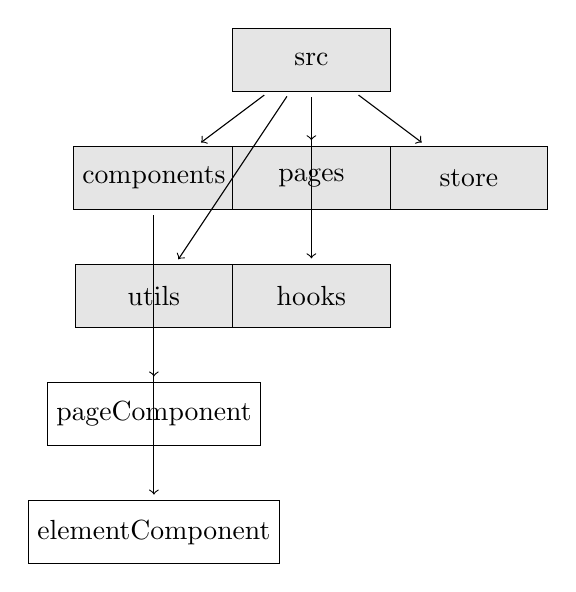
\begin{tikzpicture}[
    file/.style={draw, rectangle, minimum width=2cm, minimum height=0.8cm},
    folder/.style={draw, rectangle, minimum width=2cm, minimum height=0.8cm, fill=gray!20},
    arrow/.style={->, shorten >=2pt, shorten <=2pt}
]

% Folders
\node[folder] (src) at (0,0) {src};
\node[folder] (components) at (-2,-1.5) {components};
\node[folder] (pages) at (0,-1.5) {pages};
\node[folder] (store) at (2,-1.5) {store};
\node[folder] (utils) at (-2,-3) {utils};
\node[folder] (hooks) at (0,-3) {hooks};

% Files
\node[file] (pageComponent) at (-2,-4.5) {pageComponent};
\node[file] (elementComponent) at (-2,-6) {elementComponent};
% ... add more files

% Connections
\draw[arrow] (src) -- (components);
\draw[arrow] (src) -- (pages);
\draw[arrow] (src) -- (store);
\draw[arrow] (src) -- (utils);
\draw[arrow] (src) -- (hooks);
\draw[arrow] (components) -- (pageComponent);
\draw[arrow] (components) -- (elementComponent);
% ... add more connections

\end{tikzpicture}



\pagebreak
\subsubsection{Back-end}
The backend uses the dotNet framework. The development language using the C\# language.

In this project, the backend uses the Onion Architecture.
The Onion Architecture is a typically layered architecture, 
where each layer depends on the inner layer and provides interfaces to the outer layer.
The outer layer provides services to the outermost layer 
and other modules in the same layer based on the interfaces of the inner layer.

From inner to outer, the layers are: Domain, Application, Infrastructure, Presentation.
The Domain layer is the core layer and the innermost layer, used to define domain models, 
which are the business models.
It includes domain models and domain service interfaces.
Domain models are used to define the business models, 
which are the entities in the entity-relationship model and their attributes.
Domain service interfaces are used to define the business services, 
which are the relationships between entities in the entity-relationship model.

The Application layer is the application layer, 
used to define application services, which are the business logic.
It includes domain service implementations and application service interfaces.
Domain service implementations implement the methods of the inner layer's domain service 
interfaces and implement the business logic of the domain models.
Application service interfaces are used to define application services, 
which are the business logic.
It includes but is not limited to database interfaces, testing interfaces, 
HTTP API interfaces, MQTT interfaces, etc.

The Infrastructure layer is the infrastructure layer, used to define infrastructure.
It includes database implementations, testing implementations, 
HTTP API implementations, MQTT implementations, etc.
Database implementations implement the database interfaces 
and provide CRUD services for the database.
Testing implementations implement the testing interfaces 
and provide services for unit testing and integration testing.
HTTP API implementations implement the HTTP API interfaces 
and provide CRUD operations for HTTP APIs.
MQTT implementations implement the MQTT interfaces 
and provide CRUD operations for MQTT.

The Presentation layer is the presentation layer, used to define presentation logic, 
such as interfaces and pages. Since this is a backend project,
data presentation and control are handled by the frontend, 
so this layer is not needed.



\pagebreak
\subsubsection{Data communication and storage}
% 关于本项目的数据通信与数据存储的设计, 包括数据通信的协议, 数据存储的设计等
% 关于数据通信的设计:
% 1. 通信协议的选择
% 自前端向后端发送的数据, 有三种传输的数据类型, 
% 一种是普通的增删改查的请求, 对数据传输的时效性要求不高, 但是对数据的准确性, 完整性, 有序性, 安全性有一定的要求,
% 这种数据的传输, 采用 HTTP 协议, 以及 RESTful API 的设计. 可以有效的保证对数据传输的以上要求.
% 一种是对数据通道的创建和流媒体数据的传输, 对数据传输的时效性, 安全性要求较高, 这种数据的传输, 采用 WebRTC 协议, 以及 MQTT 协议.
% 配合可以快速解码的 flatbuffers 协议, 可以有效的保证对数据传输的以上要求.
% 最后一种是对设备的状态信息和操作信息的传输, 对完整性, 有序性, 安全性都有较高的要求, 这种数据的传输, 采用 MQTT 协议
% 同时也使用了 flatbuffers 协议.
% 
% 2. 数据通信的通信架构和通信流程
% 本项目的数据通信的通信架构, 是基于前后端分离的架构, 前端使用 React 框架, 后端使用 dotnet 框架.
% 当前端需要向后端发送数据的时候, 前端会向后端发送 HTTP 请求, 后端接收到 HTTP 请求之后, 会根据请求的数据类型,
% 选择不同的数据处理方式, 对于普通的增删改查的请求, 后端会根据 RESTful API 的设计, 对数据进行增删改查的操作,
% 对于对数据通道的创建和流媒体数据的传输, 后端会根据 WebRTC 协议, 对数据通道进行创建, 并且帮助前端和设备建立数据通道,
% 当数据通道建立后, 前端和设备之间则使用 flatbuffer 的数据格式对流媒体数据进行传输,
% 对于设备的状态信息和操作信息的传输, 前端会直接向 MQTT broker 发送 MQTT 请求, 
% 设备会在其自身的固件中监听相关的 MQTT 请求, 并且返回相关的数据.
% 
% 3. 数据通信的格式
% 本项目的数据通信的格式, 有三种, 
% 一种是 HTTP 协议, 
% 使用 json 格式对数据进行传输,
% 一种是 WebRTC 协议, 
% 使用 flatbuffers 格式对数据进行传输,
% 一种是 MQTT 协议.
% 使用 flatbuffers 格式对数据进行传输,
% 
% 关于数据存储的设计:
% 1. 数据存储的数据库的选择
% 本项目的数据存储的数据库的选择, 使用了轻量级的数据库 SQLite,
% SQLite 是一个进程内的库, 实现了自给自足的, 无服务器的, 零配置的, 事务性的 SQL 数据库引擎.
% 这是因为整个项目的目的是为了实现前端与设备之间的数据通信, 对于数据库数据的增删改查操作的要求不高,
% 数据量较小, 且对于数据库的数据的事务性要求不高, 所以选择了 SQLite 数据库.
% 2. 项目前后端的数据结构的设计
% 在本项目中, 前端由于使用了 React 框架, 所以前端的数据结构的设计, 使用了基于状态的数据结构的设计,
% 每个组件或者数据集都包含一个状态对象, 这个状态对象的属性就是组件的各个状态. 
% 使用状态对象的原因是, 可以方便的对状态进行管理, 采用对象-属性的形式, 可以方便的针对不同组件的同类状态进行区分,
% 由于跨组件的状态是由 redux 进行管理的, 这种状态对象的设计, 可以更搞笑的对状态进行更新和传递.
% 后端由于使用了 dotnet 框架, 所以后端的数据结构的设计, 使用了基于类的数据结构的设计,
% 采用了面向对象的编程思想, 对数据进行了封装, 使得数据的传输更加的安全, 有序, 完整.


\pagebreak

% \subsection{Domain model}
% \documentclass[]{article}
\usepackage{graphicx}
\usepackage{amsmath}
\usepackage{tikz}

% libaries
\usetikzlibrary{shapes,arrows}

%Define the listing package
\usepackage{listings} %code highlighter
\usepackage{color} %use color
\definecolor{mygreen}{rgb}{0,0.6,0}
\definecolor{mygray}{rgb}{0.5,0.5,0.5}
\definecolor{mymauve}{rgb}{0.58,0,0.82}

%Customize a bit the look
\lstset{ %
backgroundcolor=\color{white}, % choose the background color; you must add \usepackage{color} or \usepackage{xcolor}
basicstyle=\footnotesize, % the size of the fonts that are used for the code
breakatwhitespace=false, % sets if automatic breaks should only happen at whitespace
breaklines=true, % sets automatic line breaking
captionpos=b, % sets the caption-position to bottom
commentstyle=\color{mygreen}, % comment style
deletekeywords={...}, % if you want to delete keywords from the given language
escapeinside={\%*}{*)}, % if you want to add LaTeX within your code
extendedchars=true, % lets you use non-ASCII characters; for 8-bits encodings only, does not work with UTF-8
frame=single, % adds a frame around the code
keepspaces=true, % keeps spaces in text, useful for keeping indentation of code (possibly needs columns=flexible)
keywordstyle=\color{blue}, % keyword style
% language=Octave, % the language of the code
morekeywords={*,...}, % if you want to add more keywords to the set
numbers=left, % where to put the line-numbers; possible values are (none, left, right)
numbersep=5pt, % how far the line-numbers are from the code
numberstyle=\tiny\color{mygray}, % the style that is used for the line-numbers
rulecolor=\color{black}, % if not set, the frame-color may be changed on line-breaks within not-black text (e.g. comments (green here))
showspaces=false, % show spaces everywhere adding particular underscores; it overrides 'showstringspaces'
showstringspaces=false, % underline spaces within strings only
showtabs=false, % show tabs within strings adding particular underscores
stepnumber=1, % the step between two line-numbers. If it's 1, each line will be numbered
stringstyle=\color{mymauve}, % string literal style
tabsize=2, % sets default tabsize to 2 spaces
title=\lstname % show the filename of files included with \lstinputlisting; also try caption instead of title
}

\definecolor{darkgray}{rgb}{.4,.4,.4}
\definecolor{purple}{rgb}{0.65, 0.12, 0.82}

\lstdefinelanguage{React}{
keywords={const, typeof, new, true, false, catch, function, return, null, catch, switch, var, if, in, while, do, else, case, break},
keywordstyle=\color{blue}\bfseries,
ndkeywords={class, export, boolean, throw, implements, import, this},
ndkeywordstyle=\color{darkgray}\bfseries,
identifierstyle=\color{mygreen},
sensitive=false,
comment=[l]{//},
morecomment=[s]{/*}{*/},
commentstyle=\color{purple}\ttfamily,
string=[b]{"}{'}{`},
stringstyle=\color{red}\ttfamily,
morestring=[b]',
morestring=[b]",
morestring=[b]`',
}

\lstdefinelanguage{CSharp}{
keywords={const, typeof, new, true, false, catch, function, return, null, catch, switch, var, if, in, while, do, else, case, break},
keywordstyle=\color{blue}\bfseries,
ndkeywords={class, export, boolean, throw, implements, import, this},
ndkeywordstyle=\color{darkgray}\bfseries,
identifierstyle=\color{mygreen},
sensitive=false,
comment=[l]{//},
morecomment=[s]{/*}{*/},
commentstyle=\color{purple}\ttfamily,
string=[b]{"}{'}{`},
stringstyle=\color{red}\ttfamily,
morestring=[b]',
morestring=[b]",
morestring=[b]`',
}

\lstset{
language=React,
extendedchars=true,
basicstyle=\footnotesize\ttfamily,
showstringspaces=false,
showspaces=false,
numbers=left,
numberstyle=\footnotesize,
numbersep=9pt,
tabsize=2,
breaklines=true,
showtabs=false,
captionpos=b
}

\lstset{
language=CSharp,
extendedchars=true,
basicstyle=\footnotesize\ttfamily,
showstringspaces=false,
showspaces=false,
numbers=left,
numberstyle=\footnotesize,
numbersep=9pt,
tabsize=2,
breaklines=true,
showtabs=false,
captionpos=b
}

% \usepackage{cite} % Add this line for citation

% \bibliographystyle{plain}

\title{
The implementation of BifrostConnect Front-end scope, 
re-design and development with the relevant back-end support develop.
}
\author{
    Fei Gu \\
    Erhvervs Akademi Sydvest \\
    Computer Science 21\\
    }
\date{\today}

\begin{document}

% Front page
\maketitle
\begin{center}
    Supervisor: Henrik Boulund Meng Hansen \\
    Company: BifrostConnect \\
    Engineering Director: Jasper Wass \\
\end{center}
\tableofcontents
\pagebreak


% The introduction
\section{Introduction}
\subsection{Background}\input{sections/introduction/background.tex}
\subsection{The company}\input{sections/introduction/aboutCompany}
\subsection{The project}\input{sections/introduction/aboutProject}
\pagebreak

% The problem statement
\section{Problem Statement}
\subsection{Statement}
\input{sections/problemStatement/statement}
\subsection{Situation}
\input{sections/problemStatement/situation}
\subsection{Potential Solution}
\input{sections/problemStatement/potentialSolution}
\pagebreak

% Requirement analysis
\section{Requirement Analysis}
\input{sections/requirementAnalysis/index}

\subsection{Stakeholders}
\input{sections/requirementAnalysis/stakeholders/index}

\subsection{Business Domain}
\input{sections/requirementAnalysis/bussinesDomain/index}

\subsection{Scope}
\input{sections/requirementAnalysis/scope}

\subsection{Goals}
\input{sections/requirementAnalysis/goals}
\pagebreak

% Software Design
\section{Software Design}
% developement methods
\subsection{Software Development Methods}
\input{sections/softwareDevelopmentMethods/index}
\subsubsection{Agile Software Development}
\input{sections/softwareDevelopmentMethods/agileSoftwareDevelopment/index}
\subsubsection{Feature Driven Development}
\input{sections/softwareDevelopmentMethods/featureDrivenDevelopment/index}

\pagebreak

% Technology seslection
\subsection{Technology selection}
\input{sections/softwareDesign/technologySelection/index}
\subsubsection{Front-end}
\input{sections/softwareDesign/technologySelection/frontEnd}            
\subsubsection{Back-end}
\input{sections/softwareDesign/technologySelection/backEnd}            
\subsubsection{Database}
\input{sections/softwareDesign/technologySelection/database}
\subsubsection{Data communication}
\input{sections/softwareDesign/technologySelection/dataCommunication}            
\subsubsection{DevOps}
\input{sections/softwareDesign/technologySelection/devOps}
\pagebreak

% Architecture design
\subsection{Architecture design}
\input{sections/softwareDesign/architectureDesign/index}
\pagebreak
\subsubsection{Front-end}
\input{sections/softwareDesign/architectureDesign/frontEndArchitecture}
\pagebreak
\subsubsection{Back-end}
\input{sections/softwareDesign/architectureDesign/backEndArchitecture}
\pagebreak
\subsubsection{Data communication and storage}
\input{sections/softwareDesign/architectureDesign/dataCommunicationArchitecture}
\pagebreak

% \subsection{Domain model}
% \input{sections/softwareDesign/domainModel/index}
% \subsection{Database design}
% % 数据库领域模型 ER 图
% % 包括表和字段的设置.
% % 对于私有键和外键的设置.

% \subsection{Back-end design}
% % 后端对象模型
% % 以及对于对象模型的增删改查
% % 以及相关的其他服务的设计`'

% \subsection{Front-end design}
% % 对于前端的页面结构的设计 
% % 页面的状态的设计, 交互设计

% \subsection{FlatBuffers design}
% % schema 的设计

\subsection{DevOps CI/CD process design}
\input{sections/softwareDesign/devOpsDesign/index}
\subsubsection{Continuous Integration}
\input{sections/softwareDesign/devOpsDesign/continuousIntegration/index}
\subsubsection{Continuous Delivery}
\input{sections/softwareDesign/devOpsDesign/continuousDelivery/index}
\subsubsection{Continuous Deployment}
\input{sections/softwareDesign/devOpsDesign/continuousDeployment/index}
\pagebreak

\section{Software Development} 
\input{sections/softwareDevelopment/index}
\subsection{Overall development}
\input{sections/softwareDevelopment/overallDevelopement/index}
\subsubsection{Front-end}
\input{sections/softwareDevelopment/overallDevelopement/frontEnd/index}
\subsubsection{Back-end}
\input{sections/softwareDevelopment/overallDevelopement/backEnd/index}
\subsubsection{DevOps}
\input{sections/softwareDevelopment/overallDevelopement/devOps/index}
\subsection{Feature development} 
\input{sections/softwareDevelopment/featureDevelopment/index}
\subsubsection{Use Case 1}
\input{sections/softwareDevelopment/featureDevelopment/useCase1/index}
\subsubsection{Feature 1}
\input{sections/softwareDevelopment/featureDevelopment/feature/feature1.tex}
\pagebreak
\section{Conclusion} 
\subsection{Result}
Since the project is still in progress, the result is not available yet.
So far, basic structure of this project has been built. But the most features 
are not implemented yet. 
\subsection{Discussion}
As a single developer for this project, I am confident what I have done so far.
And I can say I understand the most of the knowledge I have used in this project, 
which also means I can explain all the part of the project. 
But this project also relevant some of the complex knowledge which I have to continue 
to study and practice.
\subsection{Future Work}
The future work is to implement the rest of the features. 
Including the most important part which is the 'create session' feature.
\pagebreak
% \bibliography{bibliography}
\pagebreak
% \begin{appendices}
%     \section{Appendix}
% \end{appendices} 
\end{document}
% \subsection{Database design}
% % 数据库领域模型 ER 图
% % 包括表和字段的设置.
% % 对于私有键和外键的设置.

% \subsection{Back-end design}
% % 后端对象模型
% % 以及对于对象模型的增删改查
% % 以及相关的其他服务的设计`'

% \subsection{Front-end design}
% % 对于前端的页面结构的设计 
% % 页面的状态的设计, 交互设计

% \subsection{FlatBuffers design}
% % schema 的设计

\subsection{DevOps CI/CD process design}
\documentclass[]{article}
\usepackage{graphicx}
\usepackage{amsmath}
\usepackage{tikz}

% libaries
\usetikzlibrary{shapes,arrows}

%Define the listing package
\usepackage{listings} %code highlighter
\usepackage{color} %use color
\definecolor{mygreen}{rgb}{0,0.6,0}
\definecolor{mygray}{rgb}{0.5,0.5,0.5}
\definecolor{mymauve}{rgb}{0.58,0,0.82}

%Customize a bit the look
\lstset{ %
backgroundcolor=\color{white}, % choose the background color; you must add \usepackage{color} or \usepackage{xcolor}
basicstyle=\footnotesize, % the size of the fonts that are used for the code
breakatwhitespace=false, % sets if automatic breaks should only happen at whitespace
breaklines=true, % sets automatic line breaking
captionpos=b, % sets the caption-position to bottom
commentstyle=\color{mygreen}, % comment style
deletekeywords={...}, % if you want to delete keywords from the given language
escapeinside={\%*}{*)}, % if you want to add LaTeX within your code
extendedchars=true, % lets you use non-ASCII characters; for 8-bits encodings only, does not work with UTF-8
frame=single, % adds a frame around the code
keepspaces=true, % keeps spaces in text, useful for keeping indentation of code (possibly needs columns=flexible)
keywordstyle=\color{blue}, % keyword style
% language=Octave, % the language of the code
morekeywords={*,...}, % if you want to add more keywords to the set
numbers=left, % where to put the line-numbers; possible values are (none, left, right)
numbersep=5pt, % how far the line-numbers are from the code
numberstyle=\tiny\color{mygray}, % the style that is used for the line-numbers
rulecolor=\color{black}, % if not set, the frame-color may be changed on line-breaks within not-black text (e.g. comments (green here))
showspaces=false, % show spaces everywhere adding particular underscores; it overrides 'showstringspaces'
showstringspaces=false, % underline spaces within strings only
showtabs=false, % show tabs within strings adding particular underscores
stepnumber=1, % the step between two line-numbers. If it's 1, each line will be numbered
stringstyle=\color{mymauve}, % string literal style
tabsize=2, % sets default tabsize to 2 spaces
title=\lstname % show the filename of files included with \lstinputlisting; also try caption instead of title
}

\definecolor{darkgray}{rgb}{.4,.4,.4}
\definecolor{purple}{rgb}{0.65, 0.12, 0.82}

\lstdefinelanguage{React}{
keywords={const, typeof, new, true, false, catch, function, return, null, catch, switch, var, if, in, while, do, else, case, break},
keywordstyle=\color{blue}\bfseries,
ndkeywords={class, export, boolean, throw, implements, import, this},
ndkeywordstyle=\color{darkgray}\bfseries,
identifierstyle=\color{mygreen},
sensitive=false,
comment=[l]{//},
morecomment=[s]{/*}{*/},
commentstyle=\color{purple}\ttfamily,
string=[b]{"}{'}{`},
stringstyle=\color{red}\ttfamily,
morestring=[b]',
morestring=[b]",
morestring=[b]`',
}

\lstdefinelanguage{CSharp}{
keywords={const, typeof, new, true, false, catch, function, return, null, catch, switch, var, if, in, while, do, else, case, break},
keywordstyle=\color{blue}\bfseries,
ndkeywords={class, export, boolean, throw, implements, import, this},
ndkeywordstyle=\color{darkgray}\bfseries,
identifierstyle=\color{mygreen},
sensitive=false,
comment=[l]{//},
morecomment=[s]{/*}{*/},
commentstyle=\color{purple}\ttfamily,
string=[b]{"}{'}{`},
stringstyle=\color{red}\ttfamily,
morestring=[b]',
morestring=[b]",
morestring=[b]`',
}

\lstset{
language=React,
extendedchars=true,
basicstyle=\footnotesize\ttfamily,
showstringspaces=false,
showspaces=false,
numbers=left,
numberstyle=\footnotesize,
numbersep=9pt,
tabsize=2,
breaklines=true,
showtabs=false,
captionpos=b
}

\lstset{
language=CSharp,
extendedchars=true,
basicstyle=\footnotesize\ttfamily,
showstringspaces=false,
showspaces=false,
numbers=left,
numberstyle=\footnotesize,
numbersep=9pt,
tabsize=2,
breaklines=true,
showtabs=false,
captionpos=b
}

% \usepackage{cite} % Add this line for citation

% \bibliographystyle{plain}

\title{
The implementation of BifrostConnect Front-end scope, 
re-design and development with the relevant back-end support develop.
}
\author{
    Fei Gu \\
    Erhvervs Akademi Sydvest \\
    Computer Science 21\\
    }
\date{\today}

\begin{document}

% Front page
\maketitle
\begin{center}
    Supervisor: Henrik Boulund Meng Hansen \\
    Company: BifrostConnect \\
    Engineering Director: Jasper Wass \\
\end{center}
\tableofcontents
\pagebreak


% The introduction
\section{Introduction}
\subsection{Background}\input{sections/introduction/background.tex}
\subsection{The company}\input{sections/introduction/aboutCompany}
\subsection{The project}\input{sections/introduction/aboutProject}
\pagebreak

% The problem statement
\section{Problem Statement}
\subsection{Statement}
\input{sections/problemStatement/statement}
\subsection{Situation}
\input{sections/problemStatement/situation}
\subsection{Potential Solution}
\input{sections/problemStatement/potentialSolution}
\pagebreak

% Requirement analysis
\section{Requirement Analysis}
\input{sections/requirementAnalysis/index}

\subsection{Stakeholders}
\input{sections/requirementAnalysis/stakeholders/index}

\subsection{Business Domain}
\input{sections/requirementAnalysis/bussinesDomain/index}

\subsection{Scope}
\input{sections/requirementAnalysis/scope}

\subsection{Goals}
\input{sections/requirementAnalysis/goals}
\pagebreak

% Software Design
\section{Software Design}
% developement methods
\subsection{Software Development Methods}
\input{sections/softwareDevelopmentMethods/index}
\subsubsection{Agile Software Development}
\input{sections/softwareDevelopmentMethods/agileSoftwareDevelopment/index}
\subsubsection{Feature Driven Development}
\input{sections/softwareDevelopmentMethods/featureDrivenDevelopment/index}

\pagebreak

% Technology seslection
\subsection{Technology selection}
\input{sections/softwareDesign/technologySelection/index}
\subsubsection{Front-end}
\input{sections/softwareDesign/technologySelection/frontEnd}            
\subsubsection{Back-end}
\input{sections/softwareDesign/technologySelection/backEnd}            
\subsubsection{Database}
\input{sections/softwareDesign/technologySelection/database}
\subsubsection{Data communication}
\input{sections/softwareDesign/technologySelection/dataCommunication}            
\subsubsection{DevOps}
\input{sections/softwareDesign/technologySelection/devOps}
\pagebreak

% Architecture design
\subsection{Architecture design}
\input{sections/softwareDesign/architectureDesign/index}
\pagebreak
\subsubsection{Front-end}
\input{sections/softwareDesign/architectureDesign/frontEndArchitecture}
\pagebreak
\subsubsection{Back-end}
\input{sections/softwareDesign/architectureDesign/backEndArchitecture}
\pagebreak
\subsubsection{Data communication and storage}
\input{sections/softwareDesign/architectureDesign/dataCommunicationArchitecture}
\pagebreak

% \subsection{Domain model}
% \input{sections/softwareDesign/domainModel/index}
% \subsection{Database design}
% % 数据库领域模型 ER 图
% % 包括表和字段的设置.
% % 对于私有键和外键的设置.

% \subsection{Back-end design}
% % 后端对象模型
% % 以及对于对象模型的增删改查
% % 以及相关的其他服务的设计`'

% \subsection{Front-end design}
% % 对于前端的页面结构的设计 
% % 页面的状态的设计, 交互设计

% \subsection{FlatBuffers design}
% % schema 的设计

\subsection{DevOps CI/CD process design}
\input{sections/softwareDesign/devOpsDesign/index}
\subsubsection{Continuous Integration}
\input{sections/softwareDesign/devOpsDesign/continuousIntegration/index}
\subsubsection{Continuous Delivery}
\input{sections/softwareDesign/devOpsDesign/continuousDelivery/index}
\subsubsection{Continuous Deployment}
\input{sections/softwareDesign/devOpsDesign/continuousDeployment/index}
\pagebreak

\section{Software Development} 
\input{sections/softwareDevelopment/index}
\subsection{Overall development}
\input{sections/softwareDevelopment/overallDevelopement/index}
\subsubsection{Front-end}
\input{sections/softwareDevelopment/overallDevelopement/frontEnd/index}
\subsubsection{Back-end}
\input{sections/softwareDevelopment/overallDevelopement/backEnd/index}
\subsubsection{DevOps}
\input{sections/softwareDevelopment/overallDevelopement/devOps/index}
\subsection{Feature development} 
\input{sections/softwareDevelopment/featureDevelopment/index}
\subsubsection{Use Case 1}
\input{sections/softwareDevelopment/featureDevelopment/useCase1/index}
\subsubsection{Feature 1}
\input{sections/softwareDevelopment/featureDevelopment/feature/feature1.tex}
\pagebreak
\section{Conclusion} 
\subsection{Result}
Since the project is still in progress, the result is not available yet.
So far, basic structure of this project has been built. But the most features 
are not implemented yet. 
\subsection{Discussion}
As a single developer for this project, I am confident what I have done so far.
And I can say I understand the most of the knowledge I have used in this project, 
which also means I can explain all the part of the project. 
But this project also relevant some of the complex knowledge which I have to continue 
to study and practice.
\subsection{Future Work}
The future work is to implement the rest of the features. 
Including the most important part which is the 'create session' feature.
\pagebreak
% \bibliography{bibliography}
\pagebreak
% \begin{appendices}
%     \section{Appendix}
% \end{appendices} 
\end{document}
\subsubsection{Continuous Integration}
\documentclass[]{article}
\usepackage{graphicx}
\usepackage{amsmath}
\usepackage{tikz}

% libaries
\usetikzlibrary{shapes,arrows}

%Define the listing package
\usepackage{listings} %code highlighter
\usepackage{color} %use color
\definecolor{mygreen}{rgb}{0,0.6,0}
\definecolor{mygray}{rgb}{0.5,0.5,0.5}
\definecolor{mymauve}{rgb}{0.58,0,0.82}

%Customize a bit the look
\lstset{ %
backgroundcolor=\color{white}, % choose the background color; you must add \usepackage{color} or \usepackage{xcolor}
basicstyle=\footnotesize, % the size of the fonts that are used for the code
breakatwhitespace=false, % sets if automatic breaks should only happen at whitespace
breaklines=true, % sets automatic line breaking
captionpos=b, % sets the caption-position to bottom
commentstyle=\color{mygreen}, % comment style
deletekeywords={...}, % if you want to delete keywords from the given language
escapeinside={\%*}{*)}, % if you want to add LaTeX within your code
extendedchars=true, % lets you use non-ASCII characters; for 8-bits encodings only, does not work with UTF-8
frame=single, % adds a frame around the code
keepspaces=true, % keeps spaces in text, useful for keeping indentation of code (possibly needs columns=flexible)
keywordstyle=\color{blue}, % keyword style
% language=Octave, % the language of the code
morekeywords={*,...}, % if you want to add more keywords to the set
numbers=left, % where to put the line-numbers; possible values are (none, left, right)
numbersep=5pt, % how far the line-numbers are from the code
numberstyle=\tiny\color{mygray}, % the style that is used for the line-numbers
rulecolor=\color{black}, % if not set, the frame-color may be changed on line-breaks within not-black text (e.g. comments (green here))
showspaces=false, % show spaces everywhere adding particular underscores; it overrides 'showstringspaces'
showstringspaces=false, % underline spaces within strings only
showtabs=false, % show tabs within strings adding particular underscores
stepnumber=1, % the step between two line-numbers. If it's 1, each line will be numbered
stringstyle=\color{mymauve}, % string literal style
tabsize=2, % sets default tabsize to 2 spaces
title=\lstname % show the filename of files included with \lstinputlisting; also try caption instead of title
}

\definecolor{darkgray}{rgb}{.4,.4,.4}
\definecolor{purple}{rgb}{0.65, 0.12, 0.82}

\lstdefinelanguage{React}{
keywords={const, typeof, new, true, false, catch, function, return, null, catch, switch, var, if, in, while, do, else, case, break},
keywordstyle=\color{blue}\bfseries,
ndkeywords={class, export, boolean, throw, implements, import, this},
ndkeywordstyle=\color{darkgray}\bfseries,
identifierstyle=\color{mygreen},
sensitive=false,
comment=[l]{//},
morecomment=[s]{/*}{*/},
commentstyle=\color{purple}\ttfamily,
string=[b]{"}{'}{`},
stringstyle=\color{red}\ttfamily,
morestring=[b]',
morestring=[b]",
morestring=[b]`',
}

\lstdefinelanguage{CSharp}{
keywords={const, typeof, new, true, false, catch, function, return, null, catch, switch, var, if, in, while, do, else, case, break},
keywordstyle=\color{blue}\bfseries,
ndkeywords={class, export, boolean, throw, implements, import, this},
ndkeywordstyle=\color{darkgray}\bfseries,
identifierstyle=\color{mygreen},
sensitive=false,
comment=[l]{//},
morecomment=[s]{/*}{*/},
commentstyle=\color{purple}\ttfamily,
string=[b]{"}{'}{`},
stringstyle=\color{red}\ttfamily,
morestring=[b]',
morestring=[b]",
morestring=[b]`',
}

\lstset{
language=React,
extendedchars=true,
basicstyle=\footnotesize\ttfamily,
showstringspaces=false,
showspaces=false,
numbers=left,
numberstyle=\footnotesize,
numbersep=9pt,
tabsize=2,
breaklines=true,
showtabs=false,
captionpos=b
}

\lstset{
language=CSharp,
extendedchars=true,
basicstyle=\footnotesize\ttfamily,
showstringspaces=false,
showspaces=false,
numbers=left,
numberstyle=\footnotesize,
numbersep=9pt,
tabsize=2,
breaklines=true,
showtabs=false,
captionpos=b
}

% \usepackage{cite} % Add this line for citation

% \bibliographystyle{plain}

\title{
The implementation of BifrostConnect Front-end scope, 
re-design and development with the relevant back-end support develop.
}
\author{
    Fei Gu \\
    Erhvervs Akademi Sydvest \\
    Computer Science 21\\
    }
\date{\today}

\begin{document}

% Front page
\maketitle
\begin{center}
    Supervisor: Henrik Boulund Meng Hansen \\
    Company: BifrostConnect \\
    Engineering Director: Jasper Wass \\
\end{center}
\tableofcontents
\pagebreak


% The introduction
\section{Introduction}
\subsection{Background}\input{sections/introduction/background.tex}
\subsection{The company}\input{sections/introduction/aboutCompany}
\subsection{The project}\input{sections/introduction/aboutProject}
\pagebreak

% The problem statement
\section{Problem Statement}
\subsection{Statement}
\input{sections/problemStatement/statement}
\subsection{Situation}
\input{sections/problemStatement/situation}
\subsection{Potential Solution}
\input{sections/problemStatement/potentialSolution}
\pagebreak

% Requirement analysis
\section{Requirement Analysis}
\input{sections/requirementAnalysis/index}

\subsection{Stakeholders}
\input{sections/requirementAnalysis/stakeholders/index}

\subsection{Business Domain}
\input{sections/requirementAnalysis/bussinesDomain/index}

\subsection{Scope}
\input{sections/requirementAnalysis/scope}

\subsection{Goals}
\input{sections/requirementAnalysis/goals}
\pagebreak

% Software Design
\section{Software Design}
% developement methods
\subsection{Software Development Methods}
\input{sections/softwareDevelopmentMethods/index}
\subsubsection{Agile Software Development}
\input{sections/softwareDevelopmentMethods/agileSoftwareDevelopment/index}
\subsubsection{Feature Driven Development}
\input{sections/softwareDevelopmentMethods/featureDrivenDevelopment/index}

\pagebreak

% Technology seslection
\subsection{Technology selection}
\input{sections/softwareDesign/technologySelection/index}
\subsubsection{Front-end}
\input{sections/softwareDesign/technologySelection/frontEnd}            
\subsubsection{Back-end}
\input{sections/softwareDesign/technologySelection/backEnd}            
\subsubsection{Database}
\input{sections/softwareDesign/technologySelection/database}
\subsubsection{Data communication}
\input{sections/softwareDesign/technologySelection/dataCommunication}            
\subsubsection{DevOps}
\input{sections/softwareDesign/technologySelection/devOps}
\pagebreak

% Architecture design
\subsection{Architecture design}
\input{sections/softwareDesign/architectureDesign/index}
\pagebreak
\subsubsection{Front-end}
\input{sections/softwareDesign/architectureDesign/frontEndArchitecture}
\pagebreak
\subsubsection{Back-end}
\input{sections/softwareDesign/architectureDesign/backEndArchitecture}
\pagebreak
\subsubsection{Data communication and storage}
\input{sections/softwareDesign/architectureDesign/dataCommunicationArchitecture}
\pagebreak

% \subsection{Domain model}
% \input{sections/softwareDesign/domainModel/index}
% \subsection{Database design}
% % 数据库领域模型 ER 图
% % 包括表和字段的设置.
% % 对于私有键和外键的设置.

% \subsection{Back-end design}
% % 后端对象模型
% % 以及对于对象模型的增删改查
% % 以及相关的其他服务的设计`'

% \subsection{Front-end design}
% % 对于前端的页面结构的设计 
% % 页面的状态的设计, 交互设计

% \subsection{FlatBuffers design}
% % schema 的设计

\subsection{DevOps CI/CD process design}
\input{sections/softwareDesign/devOpsDesign/index}
\subsubsection{Continuous Integration}
\input{sections/softwareDesign/devOpsDesign/continuousIntegration/index}
\subsubsection{Continuous Delivery}
\input{sections/softwareDesign/devOpsDesign/continuousDelivery/index}
\subsubsection{Continuous Deployment}
\input{sections/softwareDesign/devOpsDesign/continuousDeployment/index}
\pagebreak

\section{Software Development} 
\input{sections/softwareDevelopment/index}
\subsection{Overall development}
\input{sections/softwareDevelopment/overallDevelopement/index}
\subsubsection{Front-end}
\input{sections/softwareDevelopment/overallDevelopement/frontEnd/index}
\subsubsection{Back-end}
\input{sections/softwareDevelopment/overallDevelopement/backEnd/index}
\subsubsection{DevOps}
\input{sections/softwareDevelopment/overallDevelopement/devOps/index}
\subsection{Feature development} 
\input{sections/softwareDevelopment/featureDevelopment/index}
\subsubsection{Use Case 1}
\input{sections/softwareDevelopment/featureDevelopment/useCase1/index}
\subsubsection{Feature 1}
\input{sections/softwareDevelopment/featureDevelopment/feature/feature1.tex}
\pagebreak
\section{Conclusion} 
\subsection{Result}
Since the project is still in progress, the result is not available yet.
So far, basic structure of this project has been built. But the most features 
are not implemented yet. 
\subsection{Discussion}
As a single developer for this project, I am confident what I have done so far.
And I can say I understand the most of the knowledge I have used in this project, 
which also means I can explain all the part of the project. 
But this project also relevant some of the complex knowledge which I have to continue 
to study and practice.
\subsection{Future Work}
The future work is to implement the rest of the features. 
Including the most important part which is the 'create session' feature.
\pagebreak
% \bibliography{bibliography}
\pagebreak
% \begin{appendices}
%     \section{Appendix}
% \end{appendices} 
\end{document}
\subsubsection{Continuous Delivery}
\documentclass[]{article}
\usepackage{graphicx}
\usepackage{amsmath}
\usepackage{tikz}

% libaries
\usetikzlibrary{shapes,arrows}

%Define the listing package
\usepackage{listings} %code highlighter
\usepackage{color} %use color
\definecolor{mygreen}{rgb}{0,0.6,0}
\definecolor{mygray}{rgb}{0.5,0.5,0.5}
\definecolor{mymauve}{rgb}{0.58,0,0.82}

%Customize a bit the look
\lstset{ %
backgroundcolor=\color{white}, % choose the background color; you must add \usepackage{color} or \usepackage{xcolor}
basicstyle=\footnotesize, % the size of the fonts that are used for the code
breakatwhitespace=false, % sets if automatic breaks should only happen at whitespace
breaklines=true, % sets automatic line breaking
captionpos=b, % sets the caption-position to bottom
commentstyle=\color{mygreen}, % comment style
deletekeywords={...}, % if you want to delete keywords from the given language
escapeinside={\%*}{*)}, % if you want to add LaTeX within your code
extendedchars=true, % lets you use non-ASCII characters; for 8-bits encodings only, does not work with UTF-8
frame=single, % adds a frame around the code
keepspaces=true, % keeps spaces in text, useful for keeping indentation of code (possibly needs columns=flexible)
keywordstyle=\color{blue}, % keyword style
% language=Octave, % the language of the code
morekeywords={*,...}, % if you want to add more keywords to the set
numbers=left, % where to put the line-numbers; possible values are (none, left, right)
numbersep=5pt, % how far the line-numbers are from the code
numberstyle=\tiny\color{mygray}, % the style that is used for the line-numbers
rulecolor=\color{black}, % if not set, the frame-color may be changed on line-breaks within not-black text (e.g. comments (green here))
showspaces=false, % show spaces everywhere adding particular underscores; it overrides 'showstringspaces'
showstringspaces=false, % underline spaces within strings only
showtabs=false, % show tabs within strings adding particular underscores
stepnumber=1, % the step between two line-numbers. If it's 1, each line will be numbered
stringstyle=\color{mymauve}, % string literal style
tabsize=2, % sets default tabsize to 2 spaces
title=\lstname % show the filename of files included with \lstinputlisting; also try caption instead of title
}

\definecolor{darkgray}{rgb}{.4,.4,.4}
\definecolor{purple}{rgb}{0.65, 0.12, 0.82}

\lstdefinelanguage{React}{
keywords={const, typeof, new, true, false, catch, function, return, null, catch, switch, var, if, in, while, do, else, case, break},
keywordstyle=\color{blue}\bfseries,
ndkeywords={class, export, boolean, throw, implements, import, this},
ndkeywordstyle=\color{darkgray}\bfseries,
identifierstyle=\color{mygreen},
sensitive=false,
comment=[l]{//},
morecomment=[s]{/*}{*/},
commentstyle=\color{purple}\ttfamily,
string=[b]{"}{'}{`},
stringstyle=\color{red}\ttfamily,
morestring=[b]',
morestring=[b]",
morestring=[b]`',
}

\lstdefinelanguage{CSharp}{
keywords={const, typeof, new, true, false, catch, function, return, null, catch, switch, var, if, in, while, do, else, case, break},
keywordstyle=\color{blue}\bfseries,
ndkeywords={class, export, boolean, throw, implements, import, this},
ndkeywordstyle=\color{darkgray}\bfseries,
identifierstyle=\color{mygreen},
sensitive=false,
comment=[l]{//},
morecomment=[s]{/*}{*/},
commentstyle=\color{purple}\ttfamily,
string=[b]{"}{'}{`},
stringstyle=\color{red}\ttfamily,
morestring=[b]',
morestring=[b]",
morestring=[b]`',
}

\lstset{
language=React,
extendedchars=true,
basicstyle=\footnotesize\ttfamily,
showstringspaces=false,
showspaces=false,
numbers=left,
numberstyle=\footnotesize,
numbersep=9pt,
tabsize=2,
breaklines=true,
showtabs=false,
captionpos=b
}

\lstset{
language=CSharp,
extendedchars=true,
basicstyle=\footnotesize\ttfamily,
showstringspaces=false,
showspaces=false,
numbers=left,
numberstyle=\footnotesize,
numbersep=9pt,
tabsize=2,
breaklines=true,
showtabs=false,
captionpos=b
}

% \usepackage{cite} % Add this line for citation

% \bibliographystyle{plain}

\title{
The implementation of BifrostConnect Front-end scope, 
re-design and development with the relevant back-end support develop.
}
\author{
    Fei Gu \\
    Erhvervs Akademi Sydvest \\
    Computer Science 21\\
    }
\date{\today}

\begin{document}

% Front page
\maketitle
\begin{center}
    Supervisor: Henrik Boulund Meng Hansen \\
    Company: BifrostConnect \\
    Engineering Director: Jasper Wass \\
\end{center}
\tableofcontents
\pagebreak


% The introduction
\section{Introduction}
\subsection{Background}\input{sections/introduction/background.tex}
\subsection{The company}\input{sections/introduction/aboutCompany}
\subsection{The project}\input{sections/introduction/aboutProject}
\pagebreak

% The problem statement
\section{Problem Statement}
\subsection{Statement}
\input{sections/problemStatement/statement}
\subsection{Situation}
\input{sections/problemStatement/situation}
\subsection{Potential Solution}
\input{sections/problemStatement/potentialSolution}
\pagebreak

% Requirement analysis
\section{Requirement Analysis}
\input{sections/requirementAnalysis/index}

\subsection{Stakeholders}
\input{sections/requirementAnalysis/stakeholders/index}

\subsection{Business Domain}
\input{sections/requirementAnalysis/bussinesDomain/index}

\subsection{Scope}
\input{sections/requirementAnalysis/scope}

\subsection{Goals}
\input{sections/requirementAnalysis/goals}
\pagebreak

% Software Design
\section{Software Design}
% developement methods
\subsection{Software Development Methods}
\input{sections/softwareDevelopmentMethods/index}
\subsubsection{Agile Software Development}
\input{sections/softwareDevelopmentMethods/agileSoftwareDevelopment/index}
\subsubsection{Feature Driven Development}
\input{sections/softwareDevelopmentMethods/featureDrivenDevelopment/index}

\pagebreak

% Technology seslection
\subsection{Technology selection}
\input{sections/softwareDesign/technologySelection/index}
\subsubsection{Front-end}
\input{sections/softwareDesign/technologySelection/frontEnd}            
\subsubsection{Back-end}
\input{sections/softwareDesign/technologySelection/backEnd}            
\subsubsection{Database}
\input{sections/softwareDesign/technologySelection/database}
\subsubsection{Data communication}
\input{sections/softwareDesign/technologySelection/dataCommunication}            
\subsubsection{DevOps}
\input{sections/softwareDesign/technologySelection/devOps}
\pagebreak

% Architecture design
\subsection{Architecture design}
\input{sections/softwareDesign/architectureDesign/index}
\pagebreak
\subsubsection{Front-end}
\input{sections/softwareDesign/architectureDesign/frontEndArchitecture}
\pagebreak
\subsubsection{Back-end}
\input{sections/softwareDesign/architectureDesign/backEndArchitecture}
\pagebreak
\subsubsection{Data communication and storage}
\input{sections/softwareDesign/architectureDesign/dataCommunicationArchitecture}
\pagebreak

% \subsection{Domain model}
% \input{sections/softwareDesign/domainModel/index}
% \subsection{Database design}
% % 数据库领域模型 ER 图
% % 包括表和字段的设置.
% % 对于私有键和外键的设置.

% \subsection{Back-end design}
% % 后端对象模型
% % 以及对于对象模型的增删改查
% % 以及相关的其他服务的设计`'

% \subsection{Front-end design}
% % 对于前端的页面结构的设计 
% % 页面的状态的设计, 交互设计

% \subsection{FlatBuffers design}
% % schema 的设计

\subsection{DevOps CI/CD process design}
\input{sections/softwareDesign/devOpsDesign/index}
\subsubsection{Continuous Integration}
\input{sections/softwareDesign/devOpsDesign/continuousIntegration/index}
\subsubsection{Continuous Delivery}
\input{sections/softwareDesign/devOpsDesign/continuousDelivery/index}
\subsubsection{Continuous Deployment}
\input{sections/softwareDesign/devOpsDesign/continuousDeployment/index}
\pagebreak

\section{Software Development} 
\input{sections/softwareDevelopment/index}
\subsection{Overall development}
\input{sections/softwareDevelopment/overallDevelopement/index}
\subsubsection{Front-end}
\input{sections/softwareDevelopment/overallDevelopement/frontEnd/index}
\subsubsection{Back-end}
\input{sections/softwareDevelopment/overallDevelopement/backEnd/index}
\subsubsection{DevOps}
\input{sections/softwareDevelopment/overallDevelopement/devOps/index}
\subsection{Feature development} 
\input{sections/softwareDevelopment/featureDevelopment/index}
\subsubsection{Use Case 1}
\input{sections/softwareDevelopment/featureDevelopment/useCase1/index}
\subsubsection{Feature 1}
\input{sections/softwareDevelopment/featureDevelopment/feature/feature1.tex}
\pagebreak
\section{Conclusion} 
\subsection{Result}
Since the project is still in progress, the result is not available yet.
So far, basic structure of this project has been built. But the most features 
are not implemented yet. 
\subsection{Discussion}
As a single developer for this project, I am confident what I have done so far.
And I can say I understand the most of the knowledge I have used in this project, 
which also means I can explain all the part of the project. 
But this project also relevant some of the complex knowledge which I have to continue 
to study and practice.
\subsection{Future Work}
The future work is to implement the rest of the features. 
Including the most important part which is the 'create session' feature.
\pagebreak
% \bibliography{bibliography}
\pagebreak
% \begin{appendices}
%     \section{Appendix}
% \end{appendices} 
\end{document}
\subsubsection{Continuous Deployment}
\documentclass[]{article}
\usepackage{graphicx}
\usepackage{amsmath}
\usepackage{tikz}

% libaries
\usetikzlibrary{shapes,arrows}

%Define the listing package
\usepackage{listings} %code highlighter
\usepackage{color} %use color
\definecolor{mygreen}{rgb}{0,0.6,0}
\definecolor{mygray}{rgb}{0.5,0.5,0.5}
\definecolor{mymauve}{rgb}{0.58,0,0.82}

%Customize a bit the look
\lstset{ %
backgroundcolor=\color{white}, % choose the background color; you must add \usepackage{color} or \usepackage{xcolor}
basicstyle=\footnotesize, % the size of the fonts that are used for the code
breakatwhitespace=false, % sets if automatic breaks should only happen at whitespace
breaklines=true, % sets automatic line breaking
captionpos=b, % sets the caption-position to bottom
commentstyle=\color{mygreen}, % comment style
deletekeywords={...}, % if you want to delete keywords from the given language
escapeinside={\%*}{*)}, % if you want to add LaTeX within your code
extendedchars=true, % lets you use non-ASCII characters; for 8-bits encodings only, does not work with UTF-8
frame=single, % adds a frame around the code
keepspaces=true, % keeps spaces in text, useful for keeping indentation of code (possibly needs columns=flexible)
keywordstyle=\color{blue}, % keyword style
% language=Octave, % the language of the code
morekeywords={*,...}, % if you want to add more keywords to the set
numbers=left, % where to put the line-numbers; possible values are (none, left, right)
numbersep=5pt, % how far the line-numbers are from the code
numberstyle=\tiny\color{mygray}, % the style that is used for the line-numbers
rulecolor=\color{black}, % if not set, the frame-color may be changed on line-breaks within not-black text (e.g. comments (green here))
showspaces=false, % show spaces everywhere adding particular underscores; it overrides 'showstringspaces'
showstringspaces=false, % underline spaces within strings only
showtabs=false, % show tabs within strings adding particular underscores
stepnumber=1, % the step between two line-numbers. If it's 1, each line will be numbered
stringstyle=\color{mymauve}, % string literal style
tabsize=2, % sets default tabsize to 2 spaces
title=\lstname % show the filename of files included with \lstinputlisting; also try caption instead of title
}

\definecolor{darkgray}{rgb}{.4,.4,.4}
\definecolor{purple}{rgb}{0.65, 0.12, 0.82}

\lstdefinelanguage{React}{
keywords={const, typeof, new, true, false, catch, function, return, null, catch, switch, var, if, in, while, do, else, case, break},
keywordstyle=\color{blue}\bfseries,
ndkeywords={class, export, boolean, throw, implements, import, this},
ndkeywordstyle=\color{darkgray}\bfseries,
identifierstyle=\color{mygreen},
sensitive=false,
comment=[l]{//},
morecomment=[s]{/*}{*/},
commentstyle=\color{purple}\ttfamily,
string=[b]{"}{'}{`},
stringstyle=\color{red}\ttfamily,
morestring=[b]',
morestring=[b]",
morestring=[b]`',
}

\lstdefinelanguage{CSharp}{
keywords={const, typeof, new, true, false, catch, function, return, null, catch, switch, var, if, in, while, do, else, case, break},
keywordstyle=\color{blue}\bfseries,
ndkeywords={class, export, boolean, throw, implements, import, this},
ndkeywordstyle=\color{darkgray}\bfseries,
identifierstyle=\color{mygreen},
sensitive=false,
comment=[l]{//},
morecomment=[s]{/*}{*/},
commentstyle=\color{purple}\ttfamily,
string=[b]{"}{'}{`},
stringstyle=\color{red}\ttfamily,
morestring=[b]',
morestring=[b]",
morestring=[b]`',
}

\lstset{
language=React,
extendedchars=true,
basicstyle=\footnotesize\ttfamily,
showstringspaces=false,
showspaces=false,
numbers=left,
numberstyle=\footnotesize,
numbersep=9pt,
tabsize=2,
breaklines=true,
showtabs=false,
captionpos=b
}

\lstset{
language=CSharp,
extendedchars=true,
basicstyle=\footnotesize\ttfamily,
showstringspaces=false,
showspaces=false,
numbers=left,
numberstyle=\footnotesize,
numbersep=9pt,
tabsize=2,
breaklines=true,
showtabs=false,
captionpos=b
}

% \usepackage{cite} % Add this line for citation

% \bibliographystyle{plain}

\title{
The implementation of BifrostConnect Front-end scope, 
re-design and development with the relevant back-end support develop.
}
\author{
    Fei Gu \\
    Erhvervs Akademi Sydvest \\
    Computer Science 21\\
    }
\date{\today}

\begin{document}

% Front page
\maketitle
\begin{center}
    Supervisor: Henrik Boulund Meng Hansen \\
    Company: BifrostConnect \\
    Engineering Director: Jasper Wass \\
\end{center}
\tableofcontents
\pagebreak


% The introduction
\section{Introduction}
\subsection{Background}\input{sections/introduction/background.tex}
\subsection{The company}\input{sections/introduction/aboutCompany}
\subsection{The project}\input{sections/introduction/aboutProject}
\pagebreak

% The problem statement
\section{Problem Statement}
\subsection{Statement}
\input{sections/problemStatement/statement}
\subsection{Situation}
\input{sections/problemStatement/situation}
\subsection{Potential Solution}
\input{sections/problemStatement/potentialSolution}
\pagebreak

% Requirement analysis
\section{Requirement Analysis}
\input{sections/requirementAnalysis/index}

\subsection{Stakeholders}
\input{sections/requirementAnalysis/stakeholders/index}

\subsection{Business Domain}
\input{sections/requirementAnalysis/bussinesDomain/index}

\subsection{Scope}
\input{sections/requirementAnalysis/scope}

\subsection{Goals}
\input{sections/requirementAnalysis/goals}
\pagebreak

% Software Design
\section{Software Design}
% developement methods
\subsection{Software Development Methods}
\input{sections/softwareDevelopmentMethods/index}
\subsubsection{Agile Software Development}
\input{sections/softwareDevelopmentMethods/agileSoftwareDevelopment/index}
\subsubsection{Feature Driven Development}
\input{sections/softwareDevelopmentMethods/featureDrivenDevelopment/index}

\pagebreak

% Technology seslection
\subsection{Technology selection}
\input{sections/softwareDesign/technologySelection/index}
\subsubsection{Front-end}
\input{sections/softwareDesign/technologySelection/frontEnd}            
\subsubsection{Back-end}
\input{sections/softwareDesign/technologySelection/backEnd}            
\subsubsection{Database}
\input{sections/softwareDesign/technologySelection/database}
\subsubsection{Data communication}
\input{sections/softwareDesign/technologySelection/dataCommunication}            
\subsubsection{DevOps}
\input{sections/softwareDesign/technologySelection/devOps}
\pagebreak

% Architecture design
\subsection{Architecture design}
\input{sections/softwareDesign/architectureDesign/index}
\pagebreak
\subsubsection{Front-end}
\input{sections/softwareDesign/architectureDesign/frontEndArchitecture}
\pagebreak
\subsubsection{Back-end}
\input{sections/softwareDesign/architectureDesign/backEndArchitecture}
\pagebreak
\subsubsection{Data communication and storage}
\input{sections/softwareDesign/architectureDesign/dataCommunicationArchitecture}
\pagebreak

% \subsection{Domain model}
% \input{sections/softwareDesign/domainModel/index}
% \subsection{Database design}
% % 数据库领域模型 ER 图
% % 包括表和字段的设置.
% % 对于私有键和外键的设置.

% \subsection{Back-end design}
% % 后端对象模型
% % 以及对于对象模型的增删改查
% % 以及相关的其他服务的设计`'

% \subsection{Front-end design}
% % 对于前端的页面结构的设计 
% % 页面的状态的设计, 交互设计

% \subsection{FlatBuffers design}
% % schema 的设计

\subsection{DevOps CI/CD process design}
\input{sections/softwareDesign/devOpsDesign/index}
\subsubsection{Continuous Integration}
\input{sections/softwareDesign/devOpsDesign/continuousIntegration/index}
\subsubsection{Continuous Delivery}
\input{sections/softwareDesign/devOpsDesign/continuousDelivery/index}
\subsubsection{Continuous Deployment}
\input{sections/softwareDesign/devOpsDesign/continuousDeployment/index}
\pagebreak

\section{Software Development} 
\input{sections/softwareDevelopment/index}
\subsection{Overall development}
\input{sections/softwareDevelopment/overallDevelopement/index}
\subsubsection{Front-end}
\input{sections/softwareDevelopment/overallDevelopement/frontEnd/index}
\subsubsection{Back-end}
\input{sections/softwareDevelopment/overallDevelopement/backEnd/index}
\subsubsection{DevOps}
\input{sections/softwareDevelopment/overallDevelopement/devOps/index}
\subsection{Feature development} 
\input{sections/softwareDevelopment/featureDevelopment/index}
\subsubsection{Use Case 1}
\input{sections/softwareDevelopment/featureDevelopment/useCase1/index}
\subsubsection{Feature 1}
\input{sections/softwareDevelopment/featureDevelopment/feature/feature1.tex}
\pagebreak
\section{Conclusion} 
\subsection{Result}
Since the project is still in progress, the result is not available yet.
So far, basic structure of this project has been built. But the most features 
are not implemented yet. 
\subsection{Discussion}
As a single developer for this project, I am confident what I have done so far.
And I can say I understand the most of the knowledge I have used in this project, 
which also means I can explain all the part of the project. 
But this project also relevant some of the complex knowledge which I have to continue 
to study and practice.
\subsection{Future Work}
The future work is to implement the rest of the features. 
Including the most important part which is the 'create session' feature.
\pagebreak
% \bibliography{bibliography}
\pagebreak
% \begin{appendices}
%     \section{Appendix}
% \end{appendices} 
\end{document}
\pagebreak

\section{Software Development} 
\documentclass[]{article}
\usepackage{graphicx}
\usepackage{amsmath}
\usepackage{tikz}

% libaries
\usetikzlibrary{shapes,arrows}

%Define the listing package
\usepackage{listings} %code highlighter
\usepackage{color} %use color
\definecolor{mygreen}{rgb}{0,0.6,0}
\definecolor{mygray}{rgb}{0.5,0.5,0.5}
\definecolor{mymauve}{rgb}{0.58,0,0.82}

%Customize a bit the look
\lstset{ %
backgroundcolor=\color{white}, % choose the background color; you must add \usepackage{color} or \usepackage{xcolor}
basicstyle=\footnotesize, % the size of the fonts that are used for the code
breakatwhitespace=false, % sets if automatic breaks should only happen at whitespace
breaklines=true, % sets automatic line breaking
captionpos=b, % sets the caption-position to bottom
commentstyle=\color{mygreen}, % comment style
deletekeywords={...}, % if you want to delete keywords from the given language
escapeinside={\%*}{*)}, % if you want to add LaTeX within your code
extendedchars=true, % lets you use non-ASCII characters; for 8-bits encodings only, does not work with UTF-8
frame=single, % adds a frame around the code
keepspaces=true, % keeps spaces in text, useful for keeping indentation of code (possibly needs columns=flexible)
keywordstyle=\color{blue}, % keyword style
% language=Octave, % the language of the code
morekeywords={*,...}, % if you want to add more keywords to the set
numbers=left, % where to put the line-numbers; possible values are (none, left, right)
numbersep=5pt, % how far the line-numbers are from the code
numberstyle=\tiny\color{mygray}, % the style that is used for the line-numbers
rulecolor=\color{black}, % if not set, the frame-color may be changed on line-breaks within not-black text (e.g. comments (green here))
showspaces=false, % show spaces everywhere adding particular underscores; it overrides 'showstringspaces'
showstringspaces=false, % underline spaces within strings only
showtabs=false, % show tabs within strings adding particular underscores
stepnumber=1, % the step between two line-numbers. If it's 1, each line will be numbered
stringstyle=\color{mymauve}, % string literal style
tabsize=2, % sets default tabsize to 2 spaces
title=\lstname % show the filename of files included with \lstinputlisting; also try caption instead of title
}

\definecolor{darkgray}{rgb}{.4,.4,.4}
\definecolor{purple}{rgb}{0.65, 0.12, 0.82}

\lstdefinelanguage{React}{
keywords={const, typeof, new, true, false, catch, function, return, null, catch, switch, var, if, in, while, do, else, case, break},
keywordstyle=\color{blue}\bfseries,
ndkeywords={class, export, boolean, throw, implements, import, this},
ndkeywordstyle=\color{darkgray}\bfseries,
identifierstyle=\color{mygreen},
sensitive=false,
comment=[l]{//},
morecomment=[s]{/*}{*/},
commentstyle=\color{purple}\ttfamily,
string=[b]{"}{'}{`},
stringstyle=\color{red}\ttfamily,
morestring=[b]',
morestring=[b]",
morestring=[b]`',
}

\lstdefinelanguage{CSharp}{
keywords={const, typeof, new, true, false, catch, function, return, null, catch, switch, var, if, in, while, do, else, case, break},
keywordstyle=\color{blue}\bfseries,
ndkeywords={class, export, boolean, throw, implements, import, this},
ndkeywordstyle=\color{darkgray}\bfseries,
identifierstyle=\color{mygreen},
sensitive=false,
comment=[l]{//},
morecomment=[s]{/*}{*/},
commentstyle=\color{purple}\ttfamily,
string=[b]{"}{'}{`},
stringstyle=\color{red}\ttfamily,
morestring=[b]',
morestring=[b]",
morestring=[b]`',
}

\lstset{
language=React,
extendedchars=true,
basicstyle=\footnotesize\ttfamily,
showstringspaces=false,
showspaces=false,
numbers=left,
numberstyle=\footnotesize,
numbersep=9pt,
tabsize=2,
breaklines=true,
showtabs=false,
captionpos=b
}

\lstset{
language=CSharp,
extendedchars=true,
basicstyle=\footnotesize\ttfamily,
showstringspaces=false,
showspaces=false,
numbers=left,
numberstyle=\footnotesize,
numbersep=9pt,
tabsize=2,
breaklines=true,
showtabs=false,
captionpos=b
}

% \usepackage{cite} % Add this line for citation

% \bibliographystyle{plain}

\title{
The implementation of BifrostConnect Front-end scope, 
re-design and development with the relevant back-end support develop.
}
\author{
    Fei Gu \\
    Erhvervs Akademi Sydvest \\
    Computer Science 21\\
    }
\date{\today}

\begin{document}

% Front page
\maketitle
\begin{center}
    Supervisor: Henrik Boulund Meng Hansen \\
    Company: BifrostConnect \\
    Engineering Director: Jasper Wass \\
\end{center}
\tableofcontents
\pagebreak


% The introduction
\section{Introduction}
\subsection{Background}\input{sections/introduction/background.tex}
\subsection{The company}\input{sections/introduction/aboutCompany}
\subsection{The project}\input{sections/introduction/aboutProject}
\pagebreak

% The problem statement
\section{Problem Statement}
\subsection{Statement}
\input{sections/problemStatement/statement}
\subsection{Situation}
\input{sections/problemStatement/situation}
\subsection{Potential Solution}
\input{sections/problemStatement/potentialSolution}
\pagebreak

% Requirement analysis
\section{Requirement Analysis}
\input{sections/requirementAnalysis/index}

\subsection{Stakeholders}
\input{sections/requirementAnalysis/stakeholders/index}

\subsection{Business Domain}
\input{sections/requirementAnalysis/bussinesDomain/index}

\subsection{Scope}
\input{sections/requirementAnalysis/scope}

\subsection{Goals}
\input{sections/requirementAnalysis/goals}
\pagebreak

% Software Design
\section{Software Design}
% developement methods
\subsection{Software Development Methods}
\input{sections/softwareDevelopmentMethods/index}
\subsubsection{Agile Software Development}
\input{sections/softwareDevelopmentMethods/agileSoftwareDevelopment/index}
\subsubsection{Feature Driven Development}
\input{sections/softwareDevelopmentMethods/featureDrivenDevelopment/index}

\pagebreak

% Technology seslection
\subsection{Technology selection}
\input{sections/softwareDesign/technologySelection/index}
\subsubsection{Front-end}
\input{sections/softwareDesign/technologySelection/frontEnd}            
\subsubsection{Back-end}
\input{sections/softwareDesign/technologySelection/backEnd}            
\subsubsection{Database}
\input{sections/softwareDesign/technologySelection/database}
\subsubsection{Data communication}
\input{sections/softwareDesign/technologySelection/dataCommunication}            
\subsubsection{DevOps}
\input{sections/softwareDesign/technologySelection/devOps}
\pagebreak

% Architecture design
\subsection{Architecture design}
\input{sections/softwareDesign/architectureDesign/index}
\pagebreak
\subsubsection{Front-end}
\input{sections/softwareDesign/architectureDesign/frontEndArchitecture}
\pagebreak
\subsubsection{Back-end}
\input{sections/softwareDesign/architectureDesign/backEndArchitecture}
\pagebreak
\subsubsection{Data communication and storage}
\input{sections/softwareDesign/architectureDesign/dataCommunicationArchitecture}
\pagebreak

% \subsection{Domain model}
% \input{sections/softwareDesign/domainModel/index}
% \subsection{Database design}
% % 数据库领域模型 ER 图
% % 包括表和字段的设置.
% % 对于私有键和外键的设置.

% \subsection{Back-end design}
% % 后端对象模型
% % 以及对于对象模型的增删改查
% % 以及相关的其他服务的设计`'

% \subsection{Front-end design}
% % 对于前端的页面结构的设计 
% % 页面的状态的设计, 交互设计

% \subsection{FlatBuffers design}
% % schema 的设计

\subsection{DevOps CI/CD process design}
\input{sections/softwareDesign/devOpsDesign/index}
\subsubsection{Continuous Integration}
\input{sections/softwareDesign/devOpsDesign/continuousIntegration/index}
\subsubsection{Continuous Delivery}
\input{sections/softwareDesign/devOpsDesign/continuousDelivery/index}
\subsubsection{Continuous Deployment}
\input{sections/softwareDesign/devOpsDesign/continuousDeployment/index}
\pagebreak

\section{Software Development} 
\input{sections/softwareDevelopment/index}
\subsection{Overall development}
\input{sections/softwareDevelopment/overallDevelopement/index}
\subsubsection{Front-end}
\input{sections/softwareDevelopment/overallDevelopement/frontEnd/index}
\subsubsection{Back-end}
\input{sections/softwareDevelopment/overallDevelopement/backEnd/index}
\subsubsection{DevOps}
\input{sections/softwareDevelopment/overallDevelopement/devOps/index}
\subsection{Feature development} 
\input{sections/softwareDevelopment/featureDevelopment/index}
\subsubsection{Use Case 1}
\input{sections/softwareDevelopment/featureDevelopment/useCase1/index}
\subsubsection{Feature 1}
\input{sections/softwareDevelopment/featureDevelopment/feature/feature1.tex}
\pagebreak
\section{Conclusion} 
\subsection{Result}
Since the project is still in progress, the result is not available yet.
So far, basic structure of this project has been built. But the most features 
are not implemented yet. 
\subsection{Discussion}
As a single developer for this project, I am confident what I have done so far.
And I can say I understand the most of the knowledge I have used in this project, 
which also means I can explain all the part of the project. 
But this project also relevant some of the complex knowledge which I have to continue 
to study and practice.
\subsection{Future Work}
The future work is to implement the rest of the features. 
Including the most important part which is the 'create session' feature.
\pagebreak
% \bibliography{bibliography}
\pagebreak
% \begin{appendices}
%     \section{Appendix}
% \end{appendices} 
\end{document}
\subsection{Overall development}
\documentclass[]{article}
\usepackage{graphicx}
\usepackage{amsmath}
\usepackage{tikz}

% libaries
\usetikzlibrary{shapes,arrows}

%Define the listing package
\usepackage{listings} %code highlighter
\usepackage{color} %use color
\definecolor{mygreen}{rgb}{0,0.6,0}
\definecolor{mygray}{rgb}{0.5,0.5,0.5}
\definecolor{mymauve}{rgb}{0.58,0,0.82}

%Customize a bit the look
\lstset{ %
backgroundcolor=\color{white}, % choose the background color; you must add \usepackage{color} or \usepackage{xcolor}
basicstyle=\footnotesize, % the size of the fonts that are used for the code
breakatwhitespace=false, % sets if automatic breaks should only happen at whitespace
breaklines=true, % sets automatic line breaking
captionpos=b, % sets the caption-position to bottom
commentstyle=\color{mygreen}, % comment style
deletekeywords={...}, % if you want to delete keywords from the given language
escapeinside={\%*}{*)}, % if you want to add LaTeX within your code
extendedchars=true, % lets you use non-ASCII characters; for 8-bits encodings only, does not work with UTF-8
frame=single, % adds a frame around the code
keepspaces=true, % keeps spaces in text, useful for keeping indentation of code (possibly needs columns=flexible)
keywordstyle=\color{blue}, % keyword style
% language=Octave, % the language of the code
morekeywords={*,...}, % if you want to add more keywords to the set
numbers=left, % where to put the line-numbers; possible values are (none, left, right)
numbersep=5pt, % how far the line-numbers are from the code
numberstyle=\tiny\color{mygray}, % the style that is used for the line-numbers
rulecolor=\color{black}, % if not set, the frame-color may be changed on line-breaks within not-black text (e.g. comments (green here))
showspaces=false, % show spaces everywhere adding particular underscores; it overrides 'showstringspaces'
showstringspaces=false, % underline spaces within strings only
showtabs=false, % show tabs within strings adding particular underscores
stepnumber=1, % the step between two line-numbers. If it's 1, each line will be numbered
stringstyle=\color{mymauve}, % string literal style
tabsize=2, % sets default tabsize to 2 spaces
title=\lstname % show the filename of files included with \lstinputlisting; also try caption instead of title
}

\definecolor{darkgray}{rgb}{.4,.4,.4}
\definecolor{purple}{rgb}{0.65, 0.12, 0.82}

\lstdefinelanguage{React}{
keywords={const, typeof, new, true, false, catch, function, return, null, catch, switch, var, if, in, while, do, else, case, break},
keywordstyle=\color{blue}\bfseries,
ndkeywords={class, export, boolean, throw, implements, import, this},
ndkeywordstyle=\color{darkgray}\bfseries,
identifierstyle=\color{mygreen},
sensitive=false,
comment=[l]{//},
morecomment=[s]{/*}{*/},
commentstyle=\color{purple}\ttfamily,
string=[b]{"}{'}{`},
stringstyle=\color{red}\ttfamily,
morestring=[b]',
morestring=[b]",
morestring=[b]`',
}

\lstdefinelanguage{CSharp}{
keywords={const, typeof, new, true, false, catch, function, return, null, catch, switch, var, if, in, while, do, else, case, break},
keywordstyle=\color{blue}\bfseries,
ndkeywords={class, export, boolean, throw, implements, import, this},
ndkeywordstyle=\color{darkgray}\bfseries,
identifierstyle=\color{mygreen},
sensitive=false,
comment=[l]{//},
morecomment=[s]{/*}{*/},
commentstyle=\color{purple}\ttfamily,
string=[b]{"}{'}{`},
stringstyle=\color{red}\ttfamily,
morestring=[b]',
morestring=[b]",
morestring=[b]`',
}

\lstset{
language=React,
extendedchars=true,
basicstyle=\footnotesize\ttfamily,
showstringspaces=false,
showspaces=false,
numbers=left,
numberstyle=\footnotesize,
numbersep=9pt,
tabsize=2,
breaklines=true,
showtabs=false,
captionpos=b
}

\lstset{
language=CSharp,
extendedchars=true,
basicstyle=\footnotesize\ttfamily,
showstringspaces=false,
showspaces=false,
numbers=left,
numberstyle=\footnotesize,
numbersep=9pt,
tabsize=2,
breaklines=true,
showtabs=false,
captionpos=b
}

% \usepackage{cite} % Add this line for citation

% \bibliographystyle{plain}

\title{
The implementation of BifrostConnect Front-end scope, 
re-design and development with the relevant back-end support develop.
}
\author{
    Fei Gu \\
    Erhvervs Akademi Sydvest \\
    Computer Science 21\\
    }
\date{\today}

\begin{document}

% Front page
\maketitle
\begin{center}
    Supervisor: Henrik Boulund Meng Hansen \\
    Company: BifrostConnect \\
    Engineering Director: Jasper Wass \\
\end{center}
\tableofcontents
\pagebreak


% The introduction
\section{Introduction}
\subsection{Background}\input{sections/introduction/background.tex}
\subsection{The company}\input{sections/introduction/aboutCompany}
\subsection{The project}\input{sections/introduction/aboutProject}
\pagebreak

% The problem statement
\section{Problem Statement}
\subsection{Statement}
\input{sections/problemStatement/statement}
\subsection{Situation}
\input{sections/problemStatement/situation}
\subsection{Potential Solution}
\input{sections/problemStatement/potentialSolution}
\pagebreak

% Requirement analysis
\section{Requirement Analysis}
\input{sections/requirementAnalysis/index}

\subsection{Stakeholders}
\input{sections/requirementAnalysis/stakeholders/index}

\subsection{Business Domain}
\input{sections/requirementAnalysis/bussinesDomain/index}

\subsection{Scope}
\input{sections/requirementAnalysis/scope}

\subsection{Goals}
\input{sections/requirementAnalysis/goals}
\pagebreak

% Software Design
\section{Software Design}
% developement methods
\subsection{Software Development Methods}
\input{sections/softwareDevelopmentMethods/index}
\subsubsection{Agile Software Development}
\input{sections/softwareDevelopmentMethods/agileSoftwareDevelopment/index}
\subsubsection{Feature Driven Development}
\input{sections/softwareDevelopmentMethods/featureDrivenDevelopment/index}

\pagebreak

% Technology seslection
\subsection{Technology selection}
\input{sections/softwareDesign/technologySelection/index}
\subsubsection{Front-end}
\input{sections/softwareDesign/technologySelection/frontEnd}            
\subsubsection{Back-end}
\input{sections/softwareDesign/technologySelection/backEnd}            
\subsubsection{Database}
\input{sections/softwareDesign/technologySelection/database}
\subsubsection{Data communication}
\input{sections/softwareDesign/technologySelection/dataCommunication}            
\subsubsection{DevOps}
\input{sections/softwareDesign/technologySelection/devOps}
\pagebreak

% Architecture design
\subsection{Architecture design}
\input{sections/softwareDesign/architectureDesign/index}
\pagebreak
\subsubsection{Front-end}
\input{sections/softwareDesign/architectureDesign/frontEndArchitecture}
\pagebreak
\subsubsection{Back-end}
\input{sections/softwareDesign/architectureDesign/backEndArchitecture}
\pagebreak
\subsubsection{Data communication and storage}
\input{sections/softwareDesign/architectureDesign/dataCommunicationArchitecture}
\pagebreak

% \subsection{Domain model}
% \input{sections/softwareDesign/domainModel/index}
% \subsection{Database design}
% % 数据库领域模型 ER 图
% % 包括表和字段的设置.
% % 对于私有键和外键的设置.

% \subsection{Back-end design}
% % 后端对象模型
% % 以及对于对象模型的增删改查
% % 以及相关的其他服务的设计`'

% \subsection{Front-end design}
% % 对于前端的页面结构的设计 
% % 页面的状态的设计, 交互设计

% \subsection{FlatBuffers design}
% % schema 的设计

\subsection{DevOps CI/CD process design}
\input{sections/softwareDesign/devOpsDesign/index}
\subsubsection{Continuous Integration}
\input{sections/softwareDesign/devOpsDesign/continuousIntegration/index}
\subsubsection{Continuous Delivery}
\input{sections/softwareDesign/devOpsDesign/continuousDelivery/index}
\subsubsection{Continuous Deployment}
\input{sections/softwareDesign/devOpsDesign/continuousDeployment/index}
\pagebreak

\section{Software Development} 
\input{sections/softwareDevelopment/index}
\subsection{Overall development}
\input{sections/softwareDevelopment/overallDevelopement/index}
\subsubsection{Front-end}
\input{sections/softwareDevelopment/overallDevelopement/frontEnd/index}
\subsubsection{Back-end}
\input{sections/softwareDevelopment/overallDevelopement/backEnd/index}
\subsubsection{DevOps}
\input{sections/softwareDevelopment/overallDevelopement/devOps/index}
\subsection{Feature development} 
\input{sections/softwareDevelopment/featureDevelopment/index}
\subsubsection{Use Case 1}
\input{sections/softwareDevelopment/featureDevelopment/useCase1/index}
\subsubsection{Feature 1}
\input{sections/softwareDevelopment/featureDevelopment/feature/feature1.tex}
\pagebreak
\section{Conclusion} 
\subsection{Result}
Since the project is still in progress, the result is not available yet.
So far, basic structure of this project has been built. But the most features 
are not implemented yet. 
\subsection{Discussion}
As a single developer for this project, I am confident what I have done so far.
And I can say I understand the most of the knowledge I have used in this project, 
which also means I can explain all the part of the project. 
But this project also relevant some of the complex knowledge which I have to continue 
to study and practice.
\subsection{Future Work}
The future work is to implement the rest of the features. 
Including the most important part which is the 'create session' feature.
\pagebreak
% \bibliography{bibliography}
\pagebreak
% \begin{appendices}
%     \section{Appendix}
% \end{appendices} 
\end{document}
\subsubsection{Front-end}
\documentclass[]{article}
\usepackage{graphicx}
\usepackage{amsmath}
\usepackage{tikz}

% libaries
\usetikzlibrary{shapes,arrows}

%Define the listing package
\usepackage{listings} %code highlighter
\usepackage{color} %use color
\definecolor{mygreen}{rgb}{0,0.6,0}
\definecolor{mygray}{rgb}{0.5,0.5,0.5}
\definecolor{mymauve}{rgb}{0.58,0,0.82}

%Customize a bit the look
\lstset{ %
backgroundcolor=\color{white}, % choose the background color; you must add \usepackage{color} or \usepackage{xcolor}
basicstyle=\footnotesize, % the size of the fonts that are used for the code
breakatwhitespace=false, % sets if automatic breaks should only happen at whitespace
breaklines=true, % sets automatic line breaking
captionpos=b, % sets the caption-position to bottom
commentstyle=\color{mygreen}, % comment style
deletekeywords={...}, % if you want to delete keywords from the given language
escapeinside={\%*}{*)}, % if you want to add LaTeX within your code
extendedchars=true, % lets you use non-ASCII characters; for 8-bits encodings only, does not work with UTF-8
frame=single, % adds a frame around the code
keepspaces=true, % keeps spaces in text, useful for keeping indentation of code (possibly needs columns=flexible)
keywordstyle=\color{blue}, % keyword style
% language=Octave, % the language of the code
morekeywords={*,...}, % if you want to add more keywords to the set
numbers=left, % where to put the line-numbers; possible values are (none, left, right)
numbersep=5pt, % how far the line-numbers are from the code
numberstyle=\tiny\color{mygray}, % the style that is used for the line-numbers
rulecolor=\color{black}, % if not set, the frame-color may be changed on line-breaks within not-black text (e.g. comments (green here))
showspaces=false, % show spaces everywhere adding particular underscores; it overrides 'showstringspaces'
showstringspaces=false, % underline spaces within strings only
showtabs=false, % show tabs within strings adding particular underscores
stepnumber=1, % the step between two line-numbers. If it's 1, each line will be numbered
stringstyle=\color{mymauve}, % string literal style
tabsize=2, % sets default tabsize to 2 spaces
title=\lstname % show the filename of files included with \lstinputlisting; also try caption instead of title
}

\definecolor{darkgray}{rgb}{.4,.4,.4}
\definecolor{purple}{rgb}{0.65, 0.12, 0.82}

\lstdefinelanguage{React}{
keywords={const, typeof, new, true, false, catch, function, return, null, catch, switch, var, if, in, while, do, else, case, break},
keywordstyle=\color{blue}\bfseries,
ndkeywords={class, export, boolean, throw, implements, import, this},
ndkeywordstyle=\color{darkgray}\bfseries,
identifierstyle=\color{mygreen},
sensitive=false,
comment=[l]{//},
morecomment=[s]{/*}{*/},
commentstyle=\color{purple}\ttfamily,
string=[b]{"}{'}{`},
stringstyle=\color{red}\ttfamily,
morestring=[b]',
morestring=[b]",
morestring=[b]`',
}

\lstdefinelanguage{CSharp}{
keywords={const, typeof, new, true, false, catch, function, return, null, catch, switch, var, if, in, while, do, else, case, break},
keywordstyle=\color{blue}\bfseries,
ndkeywords={class, export, boolean, throw, implements, import, this},
ndkeywordstyle=\color{darkgray}\bfseries,
identifierstyle=\color{mygreen},
sensitive=false,
comment=[l]{//},
morecomment=[s]{/*}{*/},
commentstyle=\color{purple}\ttfamily,
string=[b]{"}{'}{`},
stringstyle=\color{red}\ttfamily,
morestring=[b]',
morestring=[b]",
morestring=[b]`',
}

\lstset{
language=React,
extendedchars=true,
basicstyle=\footnotesize\ttfamily,
showstringspaces=false,
showspaces=false,
numbers=left,
numberstyle=\footnotesize,
numbersep=9pt,
tabsize=2,
breaklines=true,
showtabs=false,
captionpos=b
}

\lstset{
language=CSharp,
extendedchars=true,
basicstyle=\footnotesize\ttfamily,
showstringspaces=false,
showspaces=false,
numbers=left,
numberstyle=\footnotesize,
numbersep=9pt,
tabsize=2,
breaklines=true,
showtabs=false,
captionpos=b
}

% \usepackage{cite} % Add this line for citation

% \bibliographystyle{plain}

\title{
The implementation of BifrostConnect Front-end scope, 
re-design and development with the relevant back-end support develop.
}
\author{
    Fei Gu \\
    Erhvervs Akademi Sydvest \\
    Computer Science 21\\
    }
\date{\today}

\begin{document}

% Front page
\maketitle
\begin{center}
    Supervisor: Henrik Boulund Meng Hansen \\
    Company: BifrostConnect \\
    Engineering Director: Jasper Wass \\
\end{center}
\tableofcontents
\pagebreak


% The introduction
\section{Introduction}
\subsection{Background}\input{sections/introduction/background.tex}
\subsection{The company}\input{sections/introduction/aboutCompany}
\subsection{The project}\input{sections/introduction/aboutProject}
\pagebreak

% The problem statement
\section{Problem Statement}
\subsection{Statement}
\input{sections/problemStatement/statement}
\subsection{Situation}
\input{sections/problemStatement/situation}
\subsection{Potential Solution}
\input{sections/problemStatement/potentialSolution}
\pagebreak

% Requirement analysis
\section{Requirement Analysis}
\input{sections/requirementAnalysis/index}

\subsection{Stakeholders}
\input{sections/requirementAnalysis/stakeholders/index}

\subsection{Business Domain}
\input{sections/requirementAnalysis/bussinesDomain/index}

\subsection{Scope}
\input{sections/requirementAnalysis/scope}

\subsection{Goals}
\input{sections/requirementAnalysis/goals}
\pagebreak

% Software Design
\section{Software Design}
% developement methods
\subsection{Software Development Methods}
\input{sections/softwareDevelopmentMethods/index}
\subsubsection{Agile Software Development}
\input{sections/softwareDevelopmentMethods/agileSoftwareDevelopment/index}
\subsubsection{Feature Driven Development}
\input{sections/softwareDevelopmentMethods/featureDrivenDevelopment/index}

\pagebreak

% Technology seslection
\subsection{Technology selection}
\input{sections/softwareDesign/technologySelection/index}
\subsubsection{Front-end}
\input{sections/softwareDesign/technologySelection/frontEnd}            
\subsubsection{Back-end}
\input{sections/softwareDesign/technologySelection/backEnd}            
\subsubsection{Database}
\input{sections/softwareDesign/technologySelection/database}
\subsubsection{Data communication}
\input{sections/softwareDesign/technologySelection/dataCommunication}            
\subsubsection{DevOps}
\input{sections/softwareDesign/technologySelection/devOps}
\pagebreak

% Architecture design
\subsection{Architecture design}
\input{sections/softwareDesign/architectureDesign/index}
\pagebreak
\subsubsection{Front-end}
\input{sections/softwareDesign/architectureDesign/frontEndArchitecture}
\pagebreak
\subsubsection{Back-end}
\input{sections/softwareDesign/architectureDesign/backEndArchitecture}
\pagebreak
\subsubsection{Data communication and storage}
\input{sections/softwareDesign/architectureDesign/dataCommunicationArchitecture}
\pagebreak

% \subsection{Domain model}
% \input{sections/softwareDesign/domainModel/index}
% \subsection{Database design}
% % 数据库领域模型 ER 图
% % 包括表和字段的设置.
% % 对于私有键和外键的设置.

% \subsection{Back-end design}
% % 后端对象模型
% % 以及对于对象模型的增删改查
% % 以及相关的其他服务的设计`'

% \subsection{Front-end design}
% % 对于前端的页面结构的设计 
% % 页面的状态的设计, 交互设计

% \subsection{FlatBuffers design}
% % schema 的设计

\subsection{DevOps CI/CD process design}
\input{sections/softwareDesign/devOpsDesign/index}
\subsubsection{Continuous Integration}
\input{sections/softwareDesign/devOpsDesign/continuousIntegration/index}
\subsubsection{Continuous Delivery}
\input{sections/softwareDesign/devOpsDesign/continuousDelivery/index}
\subsubsection{Continuous Deployment}
\input{sections/softwareDesign/devOpsDesign/continuousDeployment/index}
\pagebreak

\section{Software Development} 
\input{sections/softwareDevelopment/index}
\subsection{Overall development}
\input{sections/softwareDevelopment/overallDevelopement/index}
\subsubsection{Front-end}
\input{sections/softwareDevelopment/overallDevelopement/frontEnd/index}
\subsubsection{Back-end}
\input{sections/softwareDevelopment/overallDevelopement/backEnd/index}
\subsubsection{DevOps}
\input{sections/softwareDevelopment/overallDevelopement/devOps/index}
\subsection{Feature development} 
\input{sections/softwareDevelopment/featureDevelopment/index}
\subsubsection{Use Case 1}
\input{sections/softwareDevelopment/featureDevelopment/useCase1/index}
\subsubsection{Feature 1}
\input{sections/softwareDevelopment/featureDevelopment/feature/feature1.tex}
\pagebreak
\section{Conclusion} 
\subsection{Result}
Since the project is still in progress, the result is not available yet.
So far, basic structure of this project has been built. But the most features 
are not implemented yet. 
\subsection{Discussion}
As a single developer for this project, I am confident what I have done so far.
And I can say I understand the most of the knowledge I have used in this project, 
which also means I can explain all the part of the project. 
But this project also relevant some of the complex knowledge which I have to continue 
to study and practice.
\subsection{Future Work}
The future work is to implement the rest of the features. 
Including the most important part which is the 'create session' feature.
\pagebreak
% \bibliography{bibliography}
\pagebreak
% \begin{appendices}
%     \section{Appendix}
% \end{appendices} 
\end{document}
\subsubsection{Back-end}
\documentclass[]{article}
\usepackage{graphicx}
\usepackage{amsmath}
\usepackage{tikz}

% libaries
\usetikzlibrary{shapes,arrows}

%Define the listing package
\usepackage{listings} %code highlighter
\usepackage{color} %use color
\definecolor{mygreen}{rgb}{0,0.6,0}
\definecolor{mygray}{rgb}{0.5,0.5,0.5}
\definecolor{mymauve}{rgb}{0.58,0,0.82}

%Customize a bit the look
\lstset{ %
backgroundcolor=\color{white}, % choose the background color; you must add \usepackage{color} or \usepackage{xcolor}
basicstyle=\footnotesize, % the size of the fonts that are used for the code
breakatwhitespace=false, % sets if automatic breaks should only happen at whitespace
breaklines=true, % sets automatic line breaking
captionpos=b, % sets the caption-position to bottom
commentstyle=\color{mygreen}, % comment style
deletekeywords={...}, % if you want to delete keywords from the given language
escapeinside={\%*}{*)}, % if you want to add LaTeX within your code
extendedchars=true, % lets you use non-ASCII characters; for 8-bits encodings only, does not work with UTF-8
frame=single, % adds a frame around the code
keepspaces=true, % keeps spaces in text, useful for keeping indentation of code (possibly needs columns=flexible)
keywordstyle=\color{blue}, % keyword style
% language=Octave, % the language of the code
morekeywords={*,...}, % if you want to add more keywords to the set
numbers=left, % where to put the line-numbers; possible values are (none, left, right)
numbersep=5pt, % how far the line-numbers are from the code
numberstyle=\tiny\color{mygray}, % the style that is used for the line-numbers
rulecolor=\color{black}, % if not set, the frame-color may be changed on line-breaks within not-black text (e.g. comments (green here))
showspaces=false, % show spaces everywhere adding particular underscores; it overrides 'showstringspaces'
showstringspaces=false, % underline spaces within strings only
showtabs=false, % show tabs within strings adding particular underscores
stepnumber=1, % the step between two line-numbers. If it's 1, each line will be numbered
stringstyle=\color{mymauve}, % string literal style
tabsize=2, % sets default tabsize to 2 spaces
title=\lstname % show the filename of files included with \lstinputlisting; also try caption instead of title
}

\definecolor{darkgray}{rgb}{.4,.4,.4}
\definecolor{purple}{rgb}{0.65, 0.12, 0.82}

\lstdefinelanguage{React}{
keywords={const, typeof, new, true, false, catch, function, return, null, catch, switch, var, if, in, while, do, else, case, break},
keywordstyle=\color{blue}\bfseries,
ndkeywords={class, export, boolean, throw, implements, import, this},
ndkeywordstyle=\color{darkgray}\bfseries,
identifierstyle=\color{mygreen},
sensitive=false,
comment=[l]{//},
morecomment=[s]{/*}{*/},
commentstyle=\color{purple}\ttfamily,
string=[b]{"}{'}{`},
stringstyle=\color{red}\ttfamily,
morestring=[b]',
morestring=[b]",
morestring=[b]`',
}

\lstdefinelanguage{CSharp}{
keywords={const, typeof, new, true, false, catch, function, return, null, catch, switch, var, if, in, while, do, else, case, break},
keywordstyle=\color{blue}\bfseries,
ndkeywords={class, export, boolean, throw, implements, import, this},
ndkeywordstyle=\color{darkgray}\bfseries,
identifierstyle=\color{mygreen},
sensitive=false,
comment=[l]{//},
morecomment=[s]{/*}{*/},
commentstyle=\color{purple}\ttfamily,
string=[b]{"}{'}{`},
stringstyle=\color{red}\ttfamily,
morestring=[b]',
morestring=[b]",
morestring=[b]`',
}

\lstset{
language=React,
extendedchars=true,
basicstyle=\footnotesize\ttfamily,
showstringspaces=false,
showspaces=false,
numbers=left,
numberstyle=\footnotesize,
numbersep=9pt,
tabsize=2,
breaklines=true,
showtabs=false,
captionpos=b
}

\lstset{
language=CSharp,
extendedchars=true,
basicstyle=\footnotesize\ttfamily,
showstringspaces=false,
showspaces=false,
numbers=left,
numberstyle=\footnotesize,
numbersep=9pt,
tabsize=2,
breaklines=true,
showtabs=false,
captionpos=b
}

% \usepackage{cite} % Add this line for citation

% \bibliographystyle{plain}

\title{
The implementation of BifrostConnect Front-end scope, 
re-design and development with the relevant back-end support develop.
}
\author{
    Fei Gu \\
    Erhvervs Akademi Sydvest \\
    Computer Science 21\\
    }
\date{\today}

\begin{document}

% Front page
\maketitle
\begin{center}
    Supervisor: Henrik Boulund Meng Hansen \\
    Company: BifrostConnect \\
    Engineering Director: Jasper Wass \\
\end{center}
\tableofcontents
\pagebreak


% The introduction
\section{Introduction}
\subsection{Background}\input{sections/introduction/background.tex}
\subsection{The company}\input{sections/introduction/aboutCompany}
\subsection{The project}\input{sections/introduction/aboutProject}
\pagebreak

% The problem statement
\section{Problem Statement}
\subsection{Statement}
\input{sections/problemStatement/statement}
\subsection{Situation}
\input{sections/problemStatement/situation}
\subsection{Potential Solution}
\input{sections/problemStatement/potentialSolution}
\pagebreak

% Requirement analysis
\section{Requirement Analysis}
\input{sections/requirementAnalysis/index}

\subsection{Stakeholders}
\input{sections/requirementAnalysis/stakeholders/index}

\subsection{Business Domain}
\input{sections/requirementAnalysis/bussinesDomain/index}

\subsection{Scope}
\input{sections/requirementAnalysis/scope}

\subsection{Goals}
\input{sections/requirementAnalysis/goals}
\pagebreak

% Software Design
\section{Software Design}
% developement methods
\subsection{Software Development Methods}
\input{sections/softwareDevelopmentMethods/index}
\subsubsection{Agile Software Development}
\input{sections/softwareDevelopmentMethods/agileSoftwareDevelopment/index}
\subsubsection{Feature Driven Development}
\input{sections/softwareDevelopmentMethods/featureDrivenDevelopment/index}

\pagebreak

% Technology seslection
\subsection{Technology selection}
\input{sections/softwareDesign/technologySelection/index}
\subsubsection{Front-end}
\input{sections/softwareDesign/technologySelection/frontEnd}            
\subsubsection{Back-end}
\input{sections/softwareDesign/technologySelection/backEnd}            
\subsubsection{Database}
\input{sections/softwareDesign/technologySelection/database}
\subsubsection{Data communication}
\input{sections/softwareDesign/technologySelection/dataCommunication}            
\subsubsection{DevOps}
\input{sections/softwareDesign/technologySelection/devOps}
\pagebreak

% Architecture design
\subsection{Architecture design}
\input{sections/softwareDesign/architectureDesign/index}
\pagebreak
\subsubsection{Front-end}
\input{sections/softwareDesign/architectureDesign/frontEndArchitecture}
\pagebreak
\subsubsection{Back-end}
\input{sections/softwareDesign/architectureDesign/backEndArchitecture}
\pagebreak
\subsubsection{Data communication and storage}
\input{sections/softwareDesign/architectureDesign/dataCommunicationArchitecture}
\pagebreak

% \subsection{Domain model}
% \input{sections/softwareDesign/domainModel/index}
% \subsection{Database design}
% % 数据库领域模型 ER 图
% % 包括表和字段的设置.
% % 对于私有键和外键的设置.

% \subsection{Back-end design}
% % 后端对象模型
% % 以及对于对象模型的增删改查
% % 以及相关的其他服务的设计`'

% \subsection{Front-end design}
% % 对于前端的页面结构的设计 
% % 页面的状态的设计, 交互设计

% \subsection{FlatBuffers design}
% % schema 的设计

\subsection{DevOps CI/CD process design}
\input{sections/softwareDesign/devOpsDesign/index}
\subsubsection{Continuous Integration}
\input{sections/softwareDesign/devOpsDesign/continuousIntegration/index}
\subsubsection{Continuous Delivery}
\input{sections/softwareDesign/devOpsDesign/continuousDelivery/index}
\subsubsection{Continuous Deployment}
\input{sections/softwareDesign/devOpsDesign/continuousDeployment/index}
\pagebreak

\section{Software Development} 
\input{sections/softwareDevelopment/index}
\subsection{Overall development}
\input{sections/softwareDevelopment/overallDevelopement/index}
\subsubsection{Front-end}
\input{sections/softwareDevelopment/overallDevelopement/frontEnd/index}
\subsubsection{Back-end}
\input{sections/softwareDevelopment/overallDevelopement/backEnd/index}
\subsubsection{DevOps}
\input{sections/softwareDevelopment/overallDevelopement/devOps/index}
\subsection{Feature development} 
\input{sections/softwareDevelopment/featureDevelopment/index}
\subsubsection{Use Case 1}
\input{sections/softwareDevelopment/featureDevelopment/useCase1/index}
\subsubsection{Feature 1}
\input{sections/softwareDevelopment/featureDevelopment/feature/feature1.tex}
\pagebreak
\section{Conclusion} 
\subsection{Result}
Since the project is still in progress, the result is not available yet.
So far, basic structure of this project has been built. But the most features 
are not implemented yet. 
\subsection{Discussion}
As a single developer for this project, I am confident what I have done so far.
And I can say I understand the most of the knowledge I have used in this project, 
which also means I can explain all the part of the project. 
But this project also relevant some of the complex knowledge which I have to continue 
to study and practice.
\subsection{Future Work}
The future work is to implement the rest of the features. 
Including the most important part which is the 'create session' feature.
\pagebreak
% \bibliography{bibliography}
\pagebreak
% \begin{appendices}
%     \section{Appendix}
% \end{appendices} 
\end{document}
\subsubsection{DevOps}
\documentclass[]{article}
\usepackage{graphicx}
\usepackage{amsmath}
\usepackage{tikz}

% libaries
\usetikzlibrary{shapes,arrows}

%Define the listing package
\usepackage{listings} %code highlighter
\usepackage{color} %use color
\definecolor{mygreen}{rgb}{0,0.6,0}
\definecolor{mygray}{rgb}{0.5,0.5,0.5}
\definecolor{mymauve}{rgb}{0.58,0,0.82}

%Customize a bit the look
\lstset{ %
backgroundcolor=\color{white}, % choose the background color; you must add \usepackage{color} or \usepackage{xcolor}
basicstyle=\footnotesize, % the size of the fonts that are used for the code
breakatwhitespace=false, % sets if automatic breaks should only happen at whitespace
breaklines=true, % sets automatic line breaking
captionpos=b, % sets the caption-position to bottom
commentstyle=\color{mygreen}, % comment style
deletekeywords={...}, % if you want to delete keywords from the given language
escapeinside={\%*}{*)}, % if you want to add LaTeX within your code
extendedchars=true, % lets you use non-ASCII characters; for 8-bits encodings only, does not work with UTF-8
frame=single, % adds a frame around the code
keepspaces=true, % keeps spaces in text, useful for keeping indentation of code (possibly needs columns=flexible)
keywordstyle=\color{blue}, % keyword style
% language=Octave, % the language of the code
morekeywords={*,...}, % if you want to add more keywords to the set
numbers=left, % where to put the line-numbers; possible values are (none, left, right)
numbersep=5pt, % how far the line-numbers are from the code
numberstyle=\tiny\color{mygray}, % the style that is used for the line-numbers
rulecolor=\color{black}, % if not set, the frame-color may be changed on line-breaks within not-black text (e.g. comments (green here))
showspaces=false, % show spaces everywhere adding particular underscores; it overrides 'showstringspaces'
showstringspaces=false, % underline spaces within strings only
showtabs=false, % show tabs within strings adding particular underscores
stepnumber=1, % the step between two line-numbers. If it's 1, each line will be numbered
stringstyle=\color{mymauve}, % string literal style
tabsize=2, % sets default tabsize to 2 spaces
title=\lstname % show the filename of files included with \lstinputlisting; also try caption instead of title
}

\definecolor{darkgray}{rgb}{.4,.4,.4}
\definecolor{purple}{rgb}{0.65, 0.12, 0.82}

\lstdefinelanguage{React}{
keywords={const, typeof, new, true, false, catch, function, return, null, catch, switch, var, if, in, while, do, else, case, break},
keywordstyle=\color{blue}\bfseries,
ndkeywords={class, export, boolean, throw, implements, import, this},
ndkeywordstyle=\color{darkgray}\bfseries,
identifierstyle=\color{mygreen},
sensitive=false,
comment=[l]{//},
morecomment=[s]{/*}{*/},
commentstyle=\color{purple}\ttfamily,
string=[b]{"}{'}{`},
stringstyle=\color{red}\ttfamily,
morestring=[b]',
morestring=[b]",
morestring=[b]`',
}

\lstdefinelanguage{CSharp}{
keywords={const, typeof, new, true, false, catch, function, return, null, catch, switch, var, if, in, while, do, else, case, break},
keywordstyle=\color{blue}\bfseries,
ndkeywords={class, export, boolean, throw, implements, import, this},
ndkeywordstyle=\color{darkgray}\bfseries,
identifierstyle=\color{mygreen},
sensitive=false,
comment=[l]{//},
morecomment=[s]{/*}{*/},
commentstyle=\color{purple}\ttfamily,
string=[b]{"}{'}{`},
stringstyle=\color{red}\ttfamily,
morestring=[b]',
morestring=[b]",
morestring=[b]`',
}

\lstset{
language=React,
extendedchars=true,
basicstyle=\footnotesize\ttfamily,
showstringspaces=false,
showspaces=false,
numbers=left,
numberstyle=\footnotesize,
numbersep=9pt,
tabsize=2,
breaklines=true,
showtabs=false,
captionpos=b
}

\lstset{
language=CSharp,
extendedchars=true,
basicstyle=\footnotesize\ttfamily,
showstringspaces=false,
showspaces=false,
numbers=left,
numberstyle=\footnotesize,
numbersep=9pt,
tabsize=2,
breaklines=true,
showtabs=false,
captionpos=b
}

% \usepackage{cite} % Add this line for citation

% \bibliographystyle{plain}

\title{
The implementation of BifrostConnect Front-end scope, 
re-design and development with the relevant back-end support develop.
}
\author{
    Fei Gu \\
    Erhvervs Akademi Sydvest \\
    Computer Science 21\\
    }
\date{\today}

\begin{document}

% Front page
\maketitle
\begin{center}
    Supervisor: Henrik Boulund Meng Hansen \\
    Company: BifrostConnect \\
    Engineering Director: Jasper Wass \\
\end{center}
\tableofcontents
\pagebreak


% The introduction
\section{Introduction}
\subsection{Background}\input{sections/introduction/background.tex}
\subsection{The company}\input{sections/introduction/aboutCompany}
\subsection{The project}\input{sections/introduction/aboutProject}
\pagebreak

% The problem statement
\section{Problem Statement}
\subsection{Statement}
\input{sections/problemStatement/statement}
\subsection{Situation}
\input{sections/problemStatement/situation}
\subsection{Potential Solution}
\input{sections/problemStatement/potentialSolution}
\pagebreak

% Requirement analysis
\section{Requirement Analysis}
\input{sections/requirementAnalysis/index}

\subsection{Stakeholders}
\input{sections/requirementAnalysis/stakeholders/index}

\subsection{Business Domain}
\input{sections/requirementAnalysis/bussinesDomain/index}

\subsection{Scope}
\input{sections/requirementAnalysis/scope}

\subsection{Goals}
\input{sections/requirementAnalysis/goals}
\pagebreak

% Software Design
\section{Software Design}
% developement methods
\subsection{Software Development Methods}
\input{sections/softwareDevelopmentMethods/index}
\subsubsection{Agile Software Development}
\input{sections/softwareDevelopmentMethods/agileSoftwareDevelopment/index}
\subsubsection{Feature Driven Development}
\input{sections/softwareDevelopmentMethods/featureDrivenDevelopment/index}

\pagebreak

% Technology seslection
\subsection{Technology selection}
\input{sections/softwareDesign/technologySelection/index}
\subsubsection{Front-end}
\input{sections/softwareDesign/technologySelection/frontEnd}            
\subsubsection{Back-end}
\input{sections/softwareDesign/technologySelection/backEnd}            
\subsubsection{Database}
\input{sections/softwareDesign/technologySelection/database}
\subsubsection{Data communication}
\input{sections/softwareDesign/technologySelection/dataCommunication}            
\subsubsection{DevOps}
\input{sections/softwareDesign/technologySelection/devOps}
\pagebreak

% Architecture design
\subsection{Architecture design}
\input{sections/softwareDesign/architectureDesign/index}
\pagebreak
\subsubsection{Front-end}
\input{sections/softwareDesign/architectureDesign/frontEndArchitecture}
\pagebreak
\subsubsection{Back-end}
\input{sections/softwareDesign/architectureDesign/backEndArchitecture}
\pagebreak
\subsubsection{Data communication and storage}
\input{sections/softwareDesign/architectureDesign/dataCommunicationArchitecture}
\pagebreak

% \subsection{Domain model}
% \input{sections/softwareDesign/domainModel/index}
% \subsection{Database design}
% % 数据库领域模型 ER 图
% % 包括表和字段的设置.
% % 对于私有键和外键的设置.

% \subsection{Back-end design}
% % 后端对象模型
% % 以及对于对象模型的增删改查
% % 以及相关的其他服务的设计`'

% \subsection{Front-end design}
% % 对于前端的页面结构的设计 
% % 页面的状态的设计, 交互设计

% \subsection{FlatBuffers design}
% % schema 的设计

\subsection{DevOps CI/CD process design}
\input{sections/softwareDesign/devOpsDesign/index}
\subsubsection{Continuous Integration}
\input{sections/softwareDesign/devOpsDesign/continuousIntegration/index}
\subsubsection{Continuous Delivery}
\input{sections/softwareDesign/devOpsDesign/continuousDelivery/index}
\subsubsection{Continuous Deployment}
\input{sections/softwareDesign/devOpsDesign/continuousDeployment/index}
\pagebreak

\section{Software Development} 
\input{sections/softwareDevelopment/index}
\subsection{Overall development}
\input{sections/softwareDevelopment/overallDevelopement/index}
\subsubsection{Front-end}
\input{sections/softwareDevelopment/overallDevelopement/frontEnd/index}
\subsubsection{Back-end}
\input{sections/softwareDevelopment/overallDevelopement/backEnd/index}
\subsubsection{DevOps}
\input{sections/softwareDevelopment/overallDevelopement/devOps/index}
\subsection{Feature development} 
\input{sections/softwareDevelopment/featureDevelopment/index}
\subsubsection{Use Case 1}
\input{sections/softwareDevelopment/featureDevelopment/useCase1/index}
\subsubsection{Feature 1}
\input{sections/softwareDevelopment/featureDevelopment/feature/feature1.tex}
\pagebreak
\section{Conclusion} 
\subsection{Result}
Since the project is still in progress, the result is not available yet.
So far, basic structure of this project has been built. But the most features 
are not implemented yet. 
\subsection{Discussion}
As a single developer for this project, I am confident what I have done so far.
And I can say I understand the most of the knowledge I have used in this project, 
which also means I can explain all the part of the project. 
But this project also relevant some of the complex knowledge which I have to continue 
to study and practice.
\subsection{Future Work}
The future work is to implement the rest of the features. 
Including the most important part which is the 'create session' feature.
\pagebreak
% \bibliography{bibliography}
\pagebreak
% \begin{appendices}
%     \section{Appendix}
% \end{appendices} 
\end{document}
\subsection{Feature development} 
\documentclass[]{article}
\usepackage{graphicx}
\usepackage{amsmath}
\usepackage{tikz}

% libaries
\usetikzlibrary{shapes,arrows}

%Define the listing package
\usepackage{listings} %code highlighter
\usepackage{color} %use color
\definecolor{mygreen}{rgb}{0,0.6,0}
\definecolor{mygray}{rgb}{0.5,0.5,0.5}
\definecolor{mymauve}{rgb}{0.58,0,0.82}

%Customize a bit the look
\lstset{ %
backgroundcolor=\color{white}, % choose the background color; you must add \usepackage{color} or \usepackage{xcolor}
basicstyle=\footnotesize, % the size of the fonts that are used for the code
breakatwhitespace=false, % sets if automatic breaks should only happen at whitespace
breaklines=true, % sets automatic line breaking
captionpos=b, % sets the caption-position to bottom
commentstyle=\color{mygreen}, % comment style
deletekeywords={...}, % if you want to delete keywords from the given language
escapeinside={\%*}{*)}, % if you want to add LaTeX within your code
extendedchars=true, % lets you use non-ASCII characters; for 8-bits encodings only, does not work with UTF-8
frame=single, % adds a frame around the code
keepspaces=true, % keeps spaces in text, useful for keeping indentation of code (possibly needs columns=flexible)
keywordstyle=\color{blue}, % keyword style
% language=Octave, % the language of the code
morekeywords={*,...}, % if you want to add more keywords to the set
numbers=left, % where to put the line-numbers; possible values are (none, left, right)
numbersep=5pt, % how far the line-numbers are from the code
numberstyle=\tiny\color{mygray}, % the style that is used for the line-numbers
rulecolor=\color{black}, % if not set, the frame-color may be changed on line-breaks within not-black text (e.g. comments (green here))
showspaces=false, % show spaces everywhere adding particular underscores; it overrides 'showstringspaces'
showstringspaces=false, % underline spaces within strings only
showtabs=false, % show tabs within strings adding particular underscores
stepnumber=1, % the step between two line-numbers. If it's 1, each line will be numbered
stringstyle=\color{mymauve}, % string literal style
tabsize=2, % sets default tabsize to 2 spaces
title=\lstname % show the filename of files included with \lstinputlisting; also try caption instead of title
}

\definecolor{darkgray}{rgb}{.4,.4,.4}
\definecolor{purple}{rgb}{0.65, 0.12, 0.82}

\lstdefinelanguage{React}{
keywords={const, typeof, new, true, false, catch, function, return, null, catch, switch, var, if, in, while, do, else, case, break},
keywordstyle=\color{blue}\bfseries,
ndkeywords={class, export, boolean, throw, implements, import, this},
ndkeywordstyle=\color{darkgray}\bfseries,
identifierstyle=\color{mygreen},
sensitive=false,
comment=[l]{//},
morecomment=[s]{/*}{*/},
commentstyle=\color{purple}\ttfamily,
string=[b]{"}{'}{`},
stringstyle=\color{red}\ttfamily,
morestring=[b]',
morestring=[b]",
morestring=[b]`',
}

\lstdefinelanguage{CSharp}{
keywords={const, typeof, new, true, false, catch, function, return, null, catch, switch, var, if, in, while, do, else, case, break},
keywordstyle=\color{blue}\bfseries,
ndkeywords={class, export, boolean, throw, implements, import, this},
ndkeywordstyle=\color{darkgray}\bfseries,
identifierstyle=\color{mygreen},
sensitive=false,
comment=[l]{//},
morecomment=[s]{/*}{*/},
commentstyle=\color{purple}\ttfamily,
string=[b]{"}{'}{`},
stringstyle=\color{red}\ttfamily,
morestring=[b]',
morestring=[b]",
morestring=[b]`',
}

\lstset{
language=React,
extendedchars=true,
basicstyle=\footnotesize\ttfamily,
showstringspaces=false,
showspaces=false,
numbers=left,
numberstyle=\footnotesize,
numbersep=9pt,
tabsize=2,
breaklines=true,
showtabs=false,
captionpos=b
}

\lstset{
language=CSharp,
extendedchars=true,
basicstyle=\footnotesize\ttfamily,
showstringspaces=false,
showspaces=false,
numbers=left,
numberstyle=\footnotesize,
numbersep=9pt,
tabsize=2,
breaklines=true,
showtabs=false,
captionpos=b
}

% \usepackage{cite} % Add this line for citation

% \bibliographystyle{plain}

\title{
The implementation of BifrostConnect Front-end scope, 
re-design and development with the relevant back-end support develop.
}
\author{
    Fei Gu \\
    Erhvervs Akademi Sydvest \\
    Computer Science 21\\
    }
\date{\today}

\begin{document}

% Front page
\maketitle
\begin{center}
    Supervisor: Henrik Boulund Meng Hansen \\
    Company: BifrostConnect \\
    Engineering Director: Jasper Wass \\
\end{center}
\tableofcontents
\pagebreak


% The introduction
\section{Introduction}
\subsection{Background}\input{sections/introduction/background.tex}
\subsection{The company}\input{sections/introduction/aboutCompany}
\subsection{The project}\input{sections/introduction/aboutProject}
\pagebreak

% The problem statement
\section{Problem Statement}
\subsection{Statement}
\input{sections/problemStatement/statement}
\subsection{Situation}
\input{sections/problemStatement/situation}
\subsection{Potential Solution}
\input{sections/problemStatement/potentialSolution}
\pagebreak

% Requirement analysis
\section{Requirement Analysis}
\input{sections/requirementAnalysis/index}

\subsection{Stakeholders}
\input{sections/requirementAnalysis/stakeholders/index}

\subsection{Business Domain}
\input{sections/requirementAnalysis/bussinesDomain/index}

\subsection{Scope}
\input{sections/requirementAnalysis/scope}

\subsection{Goals}
\input{sections/requirementAnalysis/goals}
\pagebreak

% Software Design
\section{Software Design}
% developement methods
\subsection{Software Development Methods}
\input{sections/softwareDevelopmentMethods/index}
\subsubsection{Agile Software Development}
\input{sections/softwareDevelopmentMethods/agileSoftwareDevelopment/index}
\subsubsection{Feature Driven Development}
\input{sections/softwareDevelopmentMethods/featureDrivenDevelopment/index}

\pagebreak

% Technology seslection
\subsection{Technology selection}
\input{sections/softwareDesign/technologySelection/index}
\subsubsection{Front-end}
\input{sections/softwareDesign/technologySelection/frontEnd}            
\subsubsection{Back-end}
\input{sections/softwareDesign/technologySelection/backEnd}            
\subsubsection{Database}
\input{sections/softwareDesign/technologySelection/database}
\subsubsection{Data communication}
\input{sections/softwareDesign/technologySelection/dataCommunication}            
\subsubsection{DevOps}
\input{sections/softwareDesign/technologySelection/devOps}
\pagebreak

% Architecture design
\subsection{Architecture design}
\input{sections/softwareDesign/architectureDesign/index}
\pagebreak
\subsubsection{Front-end}
\input{sections/softwareDesign/architectureDesign/frontEndArchitecture}
\pagebreak
\subsubsection{Back-end}
\input{sections/softwareDesign/architectureDesign/backEndArchitecture}
\pagebreak
\subsubsection{Data communication and storage}
\input{sections/softwareDesign/architectureDesign/dataCommunicationArchitecture}
\pagebreak

% \subsection{Domain model}
% \input{sections/softwareDesign/domainModel/index}
% \subsection{Database design}
% % 数据库领域模型 ER 图
% % 包括表和字段的设置.
% % 对于私有键和外键的设置.

% \subsection{Back-end design}
% % 后端对象模型
% % 以及对于对象模型的增删改查
% % 以及相关的其他服务的设计`'

% \subsection{Front-end design}
% % 对于前端的页面结构的设计 
% % 页面的状态的设计, 交互设计

% \subsection{FlatBuffers design}
% % schema 的设计

\subsection{DevOps CI/CD process design}
\input{sections/softwareDesign/devOpsDesign/index}
\subsubsection{Continuous Integration}
\input{sections/softwareDesign/devOpsDesign/continuousIntegration/index}
\subsubsection{Continuous Delivery}
\input{sections/softwareDesign/devOpsDesign/continuousDelivery/index}
\subsubsection{Continuous Deployment}
\input{sections/softwareDesign/devOpsDesign/continuousDeployment/index}
\pagebreak

\section{Software Development} 
\input{sections/softwareDevelopment/index}
\subsection{Overall development}
\input{sections/softwareDevelopment/overallDevelopement/index}
\subsubsection{Front-end}
\input{sections/softwareDevelopment/overallDevelopement/frontEnd/index}
\subsubsection{Back-end}
\input{sections/softwareDevelopment/overallDevelopement/backEnd/index}
\subsubsection{DevOps}
\input{sections/softwareDevelopment/overallDevelopement/devOps/index}
\subsection{Feature development} 
\input{sections/softwareDevelopment/featureDevelopment/index}
\subsubsection{Use Case 1}
\input{sections/softwareDevelopment/featureDevelopment/useCase1/index}
\subsubsection{Feature 1}
\input{sections/softwareDevelopment/featureDevelopment/feature/feature1.tex}
\pagebreak
\section{Conclusion} 
\subsection{Result}
Since the project is still in progress, the result is not available yet.
So far, basic structure of this project has been built. But the most features 
are not implemented yet. 
\subsection{Discussion}
As a single developer for this project, I am confident what I have done so far.
And I can say I understand the most of the knowledge I have used in this project, 
which also means I can explain all the part of the project. 
But this project also relevant some of the complex knowledge which I have to continue 
to study and practice.
\subsection{Future Work}
The future work is to implement the rest of the features. 
Including the most important part which is the 'create session' feature.
\pagebreak
% \bibliography{bibliography}
\pagebreak
% \begin{appendices}
%     \section{Appendix}
% \end{appendices} 
\end{document}
\subsubsection{Use Case 1}
\documentclass[]{article}
\usepackage{graphicx}
\usepackage{amsmath}
\usepackage{tikz}

% libaries
\usetikzlibrary{shapes,arrows}

%Define the listing package
\usepackage{listings} %code highlighter
\usepackage{color} %use color
\definecolor{mygreen}{rgb}{0,0.6,0}
\definecolor{mygray}{rgb}{0.5,0.5,0.5}
\definecolor{mymauve}{rgb}{0.58,0,0.82}

%Customize a bit the look
\lstset{ %
backgroundcolor=\color{white}, % choose the background color; you must add \usepackage{color} or \usepackage{xcolor}
basicstyle=\footnotesize, % the size of the fonts that are used for the code
breakatwhitespace=false, % sets if automatic breaks should only happen at whitespace
breaklines=true, % sets automatic line breaking
captionpos=b, % sets the caption-position to bottom
commentstyle=\color{mygreen}, % comment style
deletekeywords={...}, % if you want to delete keywords from the given language
escapeinside={\%*}{*)}, % if you want to add LaTeX within your code
extendedchars=true, % lets you use non-ASCII characters; for 8-bits encodings only, does not work with UTF-8
frame=single, % adds a frame around the code
keepspaces=true, % keeps spaces in text, useful for keeping indentation of code (possibly needs columns=flexible)
keywordstyle=\color{blue}, % keyword style
% language=Octave, % the language of the code
morekeywords={*,...}, % if you want to add more keywords to the set
numbers=left, % where to put the line-numbers; possible values are (none, left, right)
numbersep=5pt, % how far the line-numbers are from the code
numberstyle=\tiny\color{mygray}, % the style that is used for the line-numbers
rulecolor=\color{black}, % if not set, the frame-color may be changed on line-breaks within not-black text (e.g. comments (green here))
showspaces=false, % show spaces everywhere adding particular underscores; it overrides 'showstringspaces'
showstringspaces=false, % underline spaces within strings only
showtabs=false, % show tabs within strings adding particular underscores
stepnumber=1, % the step between two line-numbers. If it's 1, each line will be numbered
stringstyle=\color{mymauve}, % string literal style
tabsize=2, % sets default tabsize to 2 spaces
title=\lstname % show the filename of files included with \lstinputlisting; also try caption instead of title
}

\definecolor{darkgray}{rgb}{.4,.4,.4}
\definecolor{purple}{rgb}{0.65, 0.12, 0.82}

\lstdefinelanguage{React}{
keywords={const, typeof, new, true, false, catch, function, return, null, catch, switch, var, if, in, while, do, else, case, break},
keywordstyle=\color{blue}\bfseries,
ndkeywords={class, export, boolean, throw, implements, import, this},
ndkeywordstyle=\color{darkgray}\bfseries,
identifierstyle=\color{mygreen},
sensitive=false,
comment=[l]{//},
morecomment=[s]{/*}{*/},
commentstyle=\color{purple}\ttfamily,
string=[b]{"}{'}{`},
stringstyle=\color{red}\ttfamily,
morestring=[b]',
morestring=[b]",
morestring=[b]`',
}

\lstdefinelanguage{CSharp}{
keywords={const, typeof, new, true, false, catch, function, return, null, catch, switch, var, if, in, while, do, else, case, break},
keywordstyle=\color{blue}\bfseries,
ndkeywords={class, export, boolean, throw, implements, import, this},
ndkeywordstyle=\color{darkgray}\bfseries,
identifierstyle=\color{mygreen},
sensitive=false,
comment=[l]{//},
morecomment=[s]{/*}{*/},
commentstyle=\color{purple}\ttfamily,
string=[b]{"}{'}{`},
stringstyle=\color{red}\ttfamily,
morestring=[b]',
morestring=[b]",
morestring=[b]`',
}

\lstset{
language=React,
extendedchars=true,
basicstyle=\footnotesize\ttfamily,
showstringspaces=false,
showspaces=false,
numbers=left,
numberstyle=\footnotesize,
numbersep=9pt,
tabsize=2,
breaklines=true,
showtabs=false,
captionpos=b
}

\lstset{
language=CSharp,
extendedchars=true,
basicstyle=\footnotesize\ttfamily,
showstringspaces=false,
showspaces=false,
numbers=left,
numberstyle=\footnotesize,
numbersep=9pt,
tabsize=2,
breaklines=true,
showtabs=false,
captionpos=b
}

% \usepackage{cite} % Add this line for citation

% \bibliographystyle{plain}

\title{
The implementation of BifrostConnect Front-end scope, 
re-design and development with the relevant back-end support develop.
}
\author{
    Fei Gu \\
    Erhvervs Akademi Sydvest \\
    Computer Science 21\\
    }
\date{\today}

\begin{document}

% Front page
\maketitle
\begin{center}
    Supervisor: Henrik Boulund Meng Hansen \\
    Company: BifrostConnect \\
    Engineering Director: Jasper Wass \\
\end{center}
\tableofcontents
\pagebreak


% The introduction
\section{Introduction}
\subsection{Background}\input{sections/introduction/background.tex}
\subsection{The company}\input{sections/introduction/aboutCompany}
\subsection{The project}\input{sections/introduction/aboutProject}
\pagebreak

% The problem statement
\section{Problem Statement}
\subsection{Statement}
\input{sections/problemStatement/statement}
\subsection{Situation}
\input{sections/problemStatement/situation}
\subsection{Potential Solution}
\input{sections/problemStatement/potentialSolution}
\pagebreak

% Requirement analysis
\section{Requirement Analysis}
\input{sections/requirementAnalysis/index}

\subsection{Stakeholders}
\input{sections/requirementAnalysis/stakeholders/index}

\subsection{Business Domain}
\input{sections/requirementAnalysis/bussinesDomain/index}

\subsection{Scope}
\input{sections/requirementAnalysis/scope}

\subsection{Goals}
\input{sections/requirementAnalysis/goals}
\pagebreak

% Software Design
\section{Software Design}
% developement methods
\subsection{Software Development Methods}
\input{sections/softwareDevelopmentMethods/index}
\subsubsection{Agile Software Development}
\input{sections/softwareDevelopmentMethods/agileSoftwareDevelopment/index}
\subsubsection{Feature Driven Development}
\input{sections/softwareDevelopmentMethods/featureDrivenDevelopment/index}

\pagebreak

% Technology seslection
\subsection{Technology selection}
\input{sections/softwareDesign/technologySelection/index}
\subsubsection{Front-end}
\input{sections/softwareDesign/technologySelection/frontEnd}            
\subsubsection{Back-end}
\input{sections/softwareDesign/technologySelection/backEnd}            
\subsubsection{Database}
\input{sections/softwareDesign/technologySelection/database}
\subsubsection{Data communication}
\input{sections/softwareDesign/technologySelection/dataCommunication}            
\subsubsection{DevOps}
\input{sections/softwareDesign/technologySelection/devOps}
\pagebreak

% Architecture design
\subsection{Architecture design}
\input{sections/softwareDesign/architectureDesign/index}
\pagebreak
\subsubsection{Front-end}
\input{sections/softwareDesign/architectureDesign/frontEndArchitecture}
\pagebreak
\subsubsection{Back-end}
\input{sections/softwareDesign/architectureDesign/backEndArchitecture}
\pagebreak
\subsubsection{Data communication and storage}
\input{sections/softwareDesign/architectureDesign/dataCommunicationArchitecture}
\pagebreak

% \subsection{Domain model}
% \input{sections/softwareDesign/domainModel/index}
% \subsection{Database design}
% % 数据库领域模型 ER 图
% % 包括表和字段的设置.
% % 对于私有键和外键的设置.

% \subsection{Back-end design}
% % 后端对象模型
% % 以及对于对象模型的增删改查
% % 以及相关的其他服务的设计`'

% \subsection{Front-end design}
% % 对于前端的页面结构的设计 
% % 页面的状态的设计, 交互设计

% \subsection{FlatBuffers design}
% % schema 的设计

\subsection{DevOps CI/CD process design}
\input{sections/softwareDesign/devOpsDesign/index}
\subsubsection{Continuous Integration}
\input{sections/softwareDesign/devOpsDesign/continuousIntegration/index}
\subsubsection{Continuous Delivery}
\input{sections/softwareDesign/devOpsDesign/continuousDelivery/index}
\subsubsection{Continuous Deployment}
\input{sections/softwareDesign/devOpsDesign/continuousDeployment/index}
\pagebreak

\section{Software Development} 
\input{sections/softwareDevelopment/index}
\subsection{Overall development}
\input{sections/softwareDevelopment/overallDevelopement/index}
\subsubsection{Front-end}
\input{sections/softwareDevelopment/overallDevelopement/frontEnd/index}
\subsubsection{Back-end}
\input{sections/softwareDevelopment/overallDevelopement/backEnd/index}
\subsubsection{DevOps}
\input{sections/softwareDevelopment/overallDevelopement/devOps/index}
\subsection{Feature development} 
\input{sections/softwareDevelopment/featureDevelopment/index}
\subsubsection{Use Case 1}
\input{sections/softwareDevelopment/featureDevelopment/useCase1/index}
\subsubsection{Feature 1}
\input{sections/softwareDevelopment/featureDevelopment/feature/feature1.tex}
\pagebreak
\section{Conclusion} 
\subsection{Result}
Since the project is still in progress, the result is not available yet.
So far, basic structure of this project has been built. But the most features 
are not implemented yet. 
\subsection{Discussion}
As a single developer for this project, I am confident what I have done so far.
And I can say I understand the most of the knowledge I have used in this project, 
which also means I can explain all the part of the project. 
But this project also relevant some of the complex knowledge which I have to continue 
to study and practice.
\subsection{Future Work}
The future work is to implement the rest of the features. 
Including the most important part which is the 'create session' feature.
\pagebreak
% \bibliography{bibliography}
\pagebreak
% \begin{appendices}
%     \section{Appendix}
% \end{appendices} 
\end{document}
\subsubsection{Feature 1}
\paragraph{Front-end}
To be able to display the data from the back-end, we need to make a request to
the back-end. The request is made by using the \texttt{fetch} API. 

In the \texttt{deviceComponet} we need use the customer hook \texttt{useGetAllDevices}
to get the device list from the back-end. 

After the request is made, we need to handle the response from the back-end.
The response is a JSON object, we need to parse the JSON object to the DOM object.

And then, we need to display the device list on the device page.

\paragraph{Back-end}

To be able to response the request from the front-end, we need to implement the webAPI controller
to handle the request.

And then, the webAPI controller will call the service to get the device list from the domain service.

The domain service will invoke the repository to get the device list from the database.

After the device list is got from the database, the domain service will return the device list to the webAPI controller.

The webAPI controller will return the device list to the front-end.

\pagebreak
\section{Conclusion} 
\subsection{Result}
Since the project is still in progress, the result is not available yet.
So far, basic structure of this project has been built. But the most features 
are not implemented yet. 
\subsection{Discussion}
As a single developer for this project, I am confident what I have done so far.
And I can say I understand the most of the knowledge I have used in this project, 
which also means I can explain all the part of the project. 
But this project also relevant some of the complex knowledge which I have to continue 
to study and practice.
\subsection{Future Work}
The future work is to implement the rest of the features. 
Including the most important part which is the 'create session' feature.
\pagebreak
% \bibliography{bibliography}
\pagebreak
% \begin{appendices}
%     \section{Appendix}
% \end{appendices} 
\end{document}
\subsubsection{Back-end}
\documentclass[]{article}
\usepackage{graphicx}
\usepackage{amsmath}
\usepackage{tikz}

% libaries
\usetikzlibrary{shapes,arrows}

%Define the listing package
\usepackage{listings} %code highlighter
\usepackage{color} %use color
\definecolor{mygreen}{rgb}{0,0.6,0}
\definecolor{mygray}{rgb}{0.5,0.5,0.5}
\definecolor{mymauve}{rgb}{0.58,0,0.82}

%Customize a bit the look
\lstset{ %
backgroundcolor=\color{white}, % choose the background color; you must add \usepackage{color} or \usepackage{xcolor}
basicstyle=\footnotesize, % the size of the fonts that are used for the code
breakatwhitespace=false, % sets if automatic breaks should only happen at whitespace
breaklines=true, % sets automatic line breaking
captionpos=b, % sets the caption-position to bottom
commentstyle=\color{mygreen}, % comment style
deletekeywords={...}, % if you want to delete keywords from the given language
escapeinside={\%*}{*)}, % if you want to add LaTeX within your code
extendedchars=true, % lets you use non-ASCII characters; for 8-bits encodings only, does not work with UTF-8
frame=single, % adds a frame around the code
keepspaces=true, % keeps spaces in text, useful for keeping indentation of code (possibly needs columns=flexible)
keywordstyle=\color{blue}, % keyword style
% language=Octave, % the language of the code
morekeywords={*,...}, % if you want to add more keywords to the set
numbers=left, % where to put the line-numbers; possible values are (none, left, right)
numbersep=5pt, % how far the line-numbers are from the code
numberstyle=\tiny\color{mygray}, % the style that is used for the line-numbers
rulecolor=\color{black}, % if not set, the frame-color may be changed on line-breaks within not-black text (e.g. comments (green here))
showspaces=false, % show spaces everywhere adding particular underscores; it overrides 'showstringspaces'
showstringspaces=false, % underline spaces within strings only
showtabs=false, % show tabs within strings adding particular underscores
stepnumber=1, % the step between two line-numbers. If it's 1, each line will be numbered
stringstyle=\color{mymauve}, % string literal style
tabsize=2, % sets default tabsize to 2 spaces
title=\lstname % show the filename of files included with \lstinputlisting; also try caption instead of title
}

\definecolor{darkgray}{rgb}{.4,.4,.4}
\definecolor{purple}{rgb}{0.65, 0.12, 0.82}

\lstdefinelanguage{React}{
keywords={const, typeof, new, true, false, catch, function, return, null, catch, switch, var, if, in, while, do, else, case, break},
keywordstyle=\color{blue}\bfseries,
ndkeywords={class, export, boolean, throw, implements, import, this},
ndkeywordstyle=\color{darkgray}\bfseries,
identifierstyle=\color{mygreen},
sensitive=false,
comment=[l]{//},
morecomment=[s]{/*}{*/},
commentstyle=\color{purple}\ttfamily,
string=[b]{"}{'}{`},
stringstyle=\color{red}\ttfamily,
morestring=[b]',
morestring=[b]",
morestring=[b]`',
}

\lstdefinelanguage{CSharp}{
keywords={const, typeof, new, true, false, catch, function, return, null, catch, switch, var, if, in, while, do, else, case, break},
keywordstyle=\color{blue}\bfseries,
ndkeywords={class, export, boolean, throw, implements, import, this},
ndkeywordstyle=\color{darkgray}\bfseries,
identifierstyle=\color{mygreen},
sensitive=false,
comment=[l]{//},
morecomment=[s]{/*}{*/},
commentstyle=\color{purple}\ttfamily,
string=[b]{"}{'}{`},
stringstyle=\color{red}\ttfamily,
morestring=[b]',
morestring=[b]",
morestring=[b]`',
}

\lstset{
language=React,
extendedchars=true,
basicstyle=\footnotesize\ttfamily,
showstringspaces=false,
showspaces=false,
numbers=left,
numberstyle=\footnotesize,
numbersep=9pt,
tabsize=2,
breaklines=true,
showtabs=false,
captionpos=b
}

\lstset{
language=CSharp,
extendedchars=true,
basicstyle=\footnotesize\ttfamily,
showstringspaces=false,
showspaces=false,
numbers=left,
numberstyle=\footnotesize,
numbersep=9pt,
tabsize=2,
breaklines=true,
showtabs=false,
captionpos=b
}

% \usepackage{cite} % Add this line for citation

% \bibliographystyle{plain}

\title{
The implementation of BifrostConnect Front-end scope, 
re-design and development with the relevant back-end support develop.
}
\author{
    Fei Gu \\
    Erhvervs Akademi Sydvest \\
    Computer Science 21\\
    }
\date{\today}

\begin{document}

% Front page
\maketitle
\begin{center}
    Supervisor: Henrik Boulund Meng Hansen \\
    Company: BifrostConnect \\
    Engineering Director: Jasper Wass \\
\end{center}
\tableofcontents
\pagebreak


% The introduction
\section{Introduction}
\subsection{Background}% 关于项目的类型和背景的介绍
% 项目是 EASV computer science 专业的毕业设计, 毕业设计的要求是充分的展现学生在两年半的学习中
% 能够获得的知识和技能, 并且能够在一个项目中充分的展现出来. 项目的类型是一个软件开发项目,
% 项目的背景是一个公司的项目, 项目的目的是为了解决公司的一个问题.

This project is the final project of the EASV computer science program. 
The purpose of the final project is to demonstrate the knowledge 
and skills by the student during the two and a half years of study,
and be able to fully demonstrate them in a project.

In this project, the student will work with a company 
to solve a problem of the company.
The student will use the knowledge and skills learned from the education
to solve the problem.

Which means this project will relavent to the company's business domain,
and using the software engineering methods and software development methods
to reconize the problem, analyze the problem, and solve the problem.


\subsection{The company}% 关于公司的介绍
% 公司的名字是 BifrostConnect, 是一个创业公司, 公司的主要业务是为了解决在严格的系统安全条件下, 
% 当客户的系统没有也不允许有互联网的情况下, 通过一个中继设备而不是第三方服务的条件下, 能够远程的
% 访问客户的系统. 公司的产品是一个硬件设备以及配套的网络应用. 以及相关的服务和一站式解决方案.

BifrostConnect is a startup company which established in 2018 
that has 10 to 12 employees and located in Copenhagen, Denmark.

During the five years of operation, the company has developed
a remote access solution for access the users remote system.
The solution  


The company's main business is to solve the problem of remote access 
to the customer's system when the customer's system does not have 
and is not allowed to have the Internet under strict system security conditions.

The company's product is a hardware device and a network application.
And related services and one-stop solutions.
\subsection{The project}% 关于项目的介绍
% 这个项目是在公司原有软件基础上, 对现有的前端软件进行重构和重新设计, 并且在后端提供相应的支持.

% This project is to re-design and re-develop the front-end software based on the company's original software,
% and provide corresponding support on the back-end.% Introduction to the project


% This project involves a comprehensive overhaul of the existing front-end software, building upon the company's original software. It also includes providing corresponding back-end support.

This project entails a thorough redesign and redevelopment of the existing front-end software, 
leveraging the foundation provided by the company's original software. 
Additionally, it involves enhancing the back-end to provide the necessary support 
for the new front-end.
\pagebreak

% The problem statement
\section{Problem Statement}
\subsection{Statement}
During this project the Remote Access Interface and Tunnel Interface should be integrated into the Device Mananger Application.
To achieve the one single page application with full functionality of the Remote Access and Tunnel Connection capabilities.

\subsection{Situation}
% 项目的背景
% 这一部分要详细的介绍关于项目的原始背景, 因为在之后要根据这些背景写明项目的意义和解决方案.
% 所以项目的现状, 项目的历史问题, 现有项目难以开发和维护的原因, 

% The current BifrostConnect front-end application consist of the Device Manager (DM) 
% and Remote Access Interface (RAI) two different user interface.
% Which means the user need to manage their devices and users in the one application, 
% and oprate their devices to use the bifrost product in other web application as well. 
% However, the RAI consists of two different user interfaces referred to as the Classic RAI and Tunnel RAI. 
% Those two user interfaces will leading the user to different web application 
% when user wish to create a different type of access solution.

% The reason for this situation occurred is because the bifrost product is developed focus on the device 
% and the application part was not considered as important as the device part. 
% Therefore, the application part was developed by different developers with different design logic.
% And the application functionality was not been properly through out the development process. 
% Which cause the design logic of this product is not scalable, leading to decreasing user experience, 
% and exponential growth of code complexity which makes it increasingly challenging to maintain and improve. 
% Also the product design style lacks scalability due to lack of modularity and code consistency, 
% and the operation logic is not clear.

The existing BifrostConnect front-end application is divided into two distinct user interfaces:
the Device Manager (DM) and the Remote Access Interface (RAI). 
This division requires users to manage their devices and users in one application, 
while operating their devices to use the Bifrost product in another web application. 
Moreover, the RAI is further split into two different user interfaces, 
known as the Classic RAI and Tunnel RAI. 
These interfaces direct users to different web applications 
depending on the type of access solution they wish to create.

This situation arose because the development of the Bifrost product was primarily focused 
on the device, with the application part not receiving as much attention. 
As a result, the application part was developed by different developers, 
each with their own design logic. 
This led to a lack of thorough planning for the application functionality 
during the development process. Consequently, 
the design logic of the product is not scalable, 
which has resulted in a diminished user experience 
and an exponential increase in code complexity, 
making it increasingly difficult to maintain and improve. 
Furthermore, the product design style lacks scalability due to a lack of modularity 
and code consistency, and the operation logic is unclear.
\subsection{Potential Solution}
% 项目的解决方案
% 根据之前的项目背景描述, 提出项目的解决方案, 也就是问题陈述的解决方案的详细说明. 
% 包括潜在的解决方案, 这个解决方案的优势和劣势.

To address those issue, there is a need to redesign and remake the front-end with
a focus on implementing a modular unified front-end management system that
encompasses all the necessary functionality. 

The goal is to provide users with seamless control, monitoring, and access to their devices from anywhere, 
enhancing their overall user experience and productivity while keeping code complexity as low as possible.

For the implementation to be successful, we also need to have a back-end
service, including an API and Database. The back-end server will contain the
necessary service for the front-end to reach the purpose. Such as the RESTful
API service, authentication service, MQTT service, Tunnel service and Database.

This project will follow the software design process. Therefore, it will also include
the Software Development method and DevOps on all process as well. 

This project is covered by NDA due to security and confidentiality reasons. Thus, the
project will initially not be publicly deployed, however, I will described the
deployment in my report as well.

%%%%%%%%%%%%%%%%%%%%%%%%%%%%%%%%%%%%%%%%%%%%%%%%%%%%%%%%%%%%%%%%%%%%%%%%%

% Project Solution
% Based on the previously described project background, this section presents a detailed explanation of the proposed solution to the problem statement. This includes potential solutions, as well as the advantages and disadvantages of the proposed solution.

% To address the issues identified, 
% a comprehensive redesign and redevelopment of the front-end is necessary. 
% The focus will be on creating a modular, 
% unified front-end management system that encompasses all required functionalities.

% The objective is to provide users with seamless control, 
% monitoring, and access to their devices from any location. 
% This will enhance their overall user experience 
% and productivity while keeping code complexity to a minimum.

% For successful implementation, a back-end service, 
% including an API and Database, is also required. 
% The back-end server will provide the necessary services for the front-end 
% to achieve its purpose. 
% These services include the RESTful API service, 
% authentication service, 
% MQTT service, 
% Tunnel service, 
% and Database.

% This project will adhere to the software design process, 
% incorporating Software Development methods 
% and DevOps throughout all stages.

% Due to security and confidentiality reasons, 
% this project is covered by a Non-Disclosure Agreement (NDA). 
% Therefore, the project will not initially be publicly deployed. 
% However, the deployment process will be described in detail in the final report.

%%%%%%%%%%%%%%%%%%%%%%%%%%%%%%%%%%%%%%%%%%%%%%%%%%%%%%%%%%%%%%%%%%%%%%%%%

In order to address the issues identified, 
a comprehensive overhaul of the front-end is necessary. 
This involves a complete redesign and redevelopment of the existing system, 
with a particular emphasis on creating a modular, 
unified front-end management system. 
This new system will incorporate all the necessary functionalities, 
thereby eliminating the need for multiple interfaces and improving the overall user experience.

The primary goal of this redesign is to provide users with seamless control, 
monitoring, and access to their devices, 
regardless of their location. 
By streamlining the user interface and integrating all necessary functionalities into a single, 
unified system, we aim to enhance the overall user experience and increase productivity. 
Furthermore, by focusing on modularity in the design, 
we aim to keep code complexity as low as possible, 
thereby improving maintainability and scalability of the system.

Successful implementation of this redesign requires a robust back-end service, which includes an API and a Database. The back-end server will house the necessary services for the front-end to fulfill its purpose. These services include the RESTful API service, which will handle requests and responses between the front-end and the server; an authentication service, which will ensure secure access to the system; an MQTT service, which will handle messaging between devices; a Tunnel service, which will manage the creation and maintenance of secure tunnels for remote access; and a Database, which will store and manage all necessary data.

This project will adhere to the software design process, incorporating best practices from Software Development methodologies and DevOps principles throughout all stages. This includes requirements gathering, system design, implementation, testing, deployment, and maintenance. By following this process, we aim to ensure the delivery of a high-quality, reliable, and scalable system.

Due to security and confidentiality reasons, this project is covered by a Non-Disclosure Agreement (NDA). As such, the project will not initially be publicly deployed. However, the deployment process, including the strategies used for continuous integration and continuous deployment, as well as the measures taken to ensure security and reliability, will be described in detail in the final report.
\pagebreak

% Requirement analysis
\section{Requirement Analysis}
\documentclass[]{article}
\usepackage{graphicx}
\usepackage{amsmath}
\usepackage{tikz}

% libaries
\usetikzlibrary{shapes,arrows}

%Define the listing package
\usepackage{listings} %code highlighter
\usepackage{color} %use color
\definecolor{mygreen}{rgb}{0,0.6,0}
\definecolor{mygray}{rgb}{0.5,0.5,0.5}
\definecolor{mymauve}{rgb}{0.58,0,0.82}

%Customize a bit the look
\lstset{ %
backgroundcolor=\color{white}, % choose the background color; you must add \usepackage{color} or \usepackage{xcolor}
basicstyle=\footnotesize, % the size of the fonts that are used for the code
breakatwhitespace=false, % sets if automatic breaks should only happen at whitespace
breaklines=true, % sets automatic line breaking
captionpos=b, % sets the caption-position to bottom
commentstyle=\color{mygreen}, % comment style
deletekeywords={...}, % if you want to delete keywords from the given language
escapeinside={\%*}{*)}, % if you want to add LaTeX within your code
extendedchars=true, % lets you use non-ASCII characters; for 8-bits encodings only, does not work with UTF-8
frame=single, % adds a frame around the code
keepspaces=true, % keeps spaces in text, useful for keeping indentation of code (possibly needs columns=flexible)
keywordstyle=\color{blue}, % keyword style
% language=Octave, % the language of the code
morekeywords={*,...}, % if you want to add more keywords to the set
numbers=left, % where to put the line-numbers; possible values are (none, left, right)
numbersep=5pt, % how far the line-numbers are from the code
numberstyle=\tiny\color{mygray}, % the style that is used for the line-numbers
rulecolor=\color{black}, % if not set, the frame-color may be changed on line-breaks within not-black text (e.g. comments (green here))
showspaces=false, % show spaces everywhere adding particular underscores; it overrides 'showstringspaces'
showstringspaces=false, % underline spaces within strings only
showtabs=false, % show tabs within strings adding particular underscores
stepnumber=1, % the step between two line-numbers. If it's 1, each line will be numbered
stringstyle=\color{mymauve}, % string literal style
tabsize=2, % sets default tabsize to 2 spaces
title=\lstname % show the filename of files included with \lstinputlisting; also try caption instead of title
}

\definecolor{darkgray}{rgb}{.4,.4,.4}
\definecolor{purple}{rgb}{0.65, 0.12, 0.82}

\lstdefinelanguage{React}{
keywords={const, typeof, new, true, false, catch, function, return, null, catch, switch, var, if, in, while, do, else, case, break},
keywordstyle=\color{blue}\bfseries,
ndkeywords={class, export, boolean, throw, implements, import, this},
ndkeywordstyle=\color{darkgray}\bfseries,
identifierstyle=\color{mygreen},
sensitive=false,
comment=[l]{//},
morecomment=[s]{/*}{*/},
commentstyle=\color{purple}\ttfamily,
string=[b]{"}{'}{`},
stringstyle=\color{red}\ttfamily,
morestring=[b]',
morestring=[b]",
morestring=[b]`',
}

\lstdefinelanguage{CSharp}{
keywords={const, typeof, new, true, false, catch, function, return, null, catch, switch, var, if, in, while, do, else, case, break},
keywordstyle=\color{blue}\bfseries,
ndkeywords={class, export, boolean, throw, implements, import, this},
ndkeywordstyle=\color{darkgray}\bfseries,
identifierstyle=\color{mygreen},
sensitive=false,
comment=[l]{//},
morecomment=[s]{/*}{*/},
commentstyle=\color{purple}\ttfamily,
string=[b]{"}{'}{`},
stringstyle=\color{red}\ttfamily,
morestring=[b]',
morestring=[b]",
morestring=[b]`',
}

\lstset{
language=React,
extendedchars=true,
basicstyle=\footnotesize\ttfamily,
showstringspaces=false,
showspaces=false,
numbers=left,
numberstyle=\footnotesize,
numbersep=9pt,
tabsize=2,
breaklines=true,
showtabs=false,
captionpos=b
}

\lstset{
language=CSharp,
extendedchars=true,
basicstyle=\footnotesize\ttfamily,
showstringspaces=false,
showspaces=false,
numbers=left,
numberstyle=\footnotesize,
numbersep=9pt,
tabsize=2,
breaklines=true,
showtabs=false,
captionpos=b
}

% \usepackage{cite} % Add this line for citation

% \bibliographystyle{plain}

\title{
The implementation of BifrostConnect Front-end scope, 
re-design and development with the relevant back-end support develop.
}
\author{
    Fei Gu \\
    Erhvervs Akademi Sydvest \\
    Computer Science 21\\
    }
\date{\today}

\begin{document}

% Front page
\maketitle
\begin{center}
    Supervisor: Henrik Boulund Meng Hansen \\
    Company: BifrostConnect \\
    Engineering Director: Jasper Wass \\
\end{center}
\tableofcontents
\pagebreak


% The introduction
\section{Introduction}
\subsection{Background}\input{sections/introduction/background.tex}
\subsection{The company}\input{sections/introduction/aboutCompany}
\subsection{The project}\input{sections/introduction/aboutProject}
\pagebreak

% The problem statement
\section{Problem Statement}
\subsection{Statement}
\input{sections/problemStatement/statement}
\subsection{Situation}
\input{sections/problemStatement/situation}
\subsection{Potential Solution}
\input{sections/problemStatement/potentialSolution}
\pagebreak

% Requirement analysis
\section{Requirement Analysis}
\input{sections/requirementAnalysis/index}

\subsection{Stakeholders}
\input{sections/requirementAnalysis/stakeholders/index}

\subsection{Business Domain}
\input{sections/requirementAnalysis/bussinesDomain/index}

\subsection{Scope}
\input{sections/requirementAnalysis/scope}

\subsection{Goals}
\input{sections/requirementAnalysis/goals}
\pagebreak

% Software Design
\section{Software Design}
% developement methods
\subsection{Software Development Methods}
\input{sections/softwareDevelopmentMethods/index}
\subsubsection{Agile Software Development}
\input{sections/softwareDevelopmentMethods/agileSoftwareDevelopment/index}
\subsubsection{Feature Driven Development}
\input{sections/softwareDevelopmentMethods/featureDrivenDevelopment/index}

\pagebreak

% Technology seslection
\subsection{Technology selection}
\input{sections/softwareDesign/technologySelection/index}
\subsubsection{Front-end}
\input{sections/softwareDesign/technologySelection/frontEnd}            
\subsubsection{Back-end}
\input{sections/softwareDesign/technologySelection/backEnd}            
\subsubsection{Database}
\input{sections/softwareDesign/technologySelection/database}
\subsubsection{Data communication}
\input{sections/softwareDesign/technologySelection/dataCommunication}            
\subsubsection{DevOps}
\input{sections/softwareDesign/technologySelection/devOps}
\pagebreak

% Architecture design
\subsection{Architecture design}
\input{sections/softwareDesign/architectureDesign/index}
\pagebreak
\subsubsection{Front-end}
\input{sections/softwareDesign/architectureDesign/frontEndArchitecture}
\pagebreak
\subsubsection{Back-end}
\input{sections/softwareDesign/architectureDesign/backEndArchitecture}
\pagebreak
\subsubsection{Data communication and storage}
\input{sections/softwareDesign/architectureDesign/dataCommunicationArchitecture}
\pagebreak

% \subsection{Domain model}
% \input{sections/softwareDesign/domainModel/index}
% \subsection{Database design}
% % 数据库领域模型 ER 图
% % 包括表和字段的设置.
% % 对于私有键和外键的设置.

% \subsection{Back-end design}
% % 后端对象模型
% % 以及对于对象模型的增删改查
% % 以及相关的其他服务的设计`'

% \subsection{Front-end design}
% % 对于前端的页面结构的设计 
% % 页面的状态的设计, 交互设计

% \subsection{FlatBuffers design}
% % schema 的设计

\subsection{DevOps CI/CD process design}
\input{sections/softwareDesign/devOpsDesign/index}
\subsubsection{Continuous Integration}
\input{sections/softwareDesign/devOpsDesign/continuousIntegration/index}
\subsubsection{Continuous Delivery}
\input{sections/softwareDesign/devOpsDesign/continuousDelivery/index}
\subsubsection{Continuous Deployment}
\input{sections/softwareDesign/devOpsDesign/continuousDeployment/index}
\pagebreak

\section{Software Development} 
\input{sections/softwareDevelopment/index}
\subsection{Overall development}
\input{sections/softwareDevelopment/overallDevelopement/index}
\subsubsection{Front-end}
\input{sections/softwareDevelopment/overallDevelopement/frontEnd/index}
\subsubsection{Back-end}
\input{sections/softwareDevelopment/overallDevelopement/backEnd/index}
\subsubsection{DevOps}
\input{sections/softwareDevelopment/overallDevelopement/devOps/index}
\subsection{Feature development} 
\input{sections/softwareDevelopment/featureDevelopment/index}
\subsubsection{Use Case 1}
\input{sections/softwareDevelopment/featureDevelopment/useCase1/index}
\subsubsection{Feature 1}
\input{sections/softwareDevelopment/featureDevelopment/feature/feature1.tex}
\pagebreak
\section{Conclusion} 
\subsection{Result}
Since the project is still in progress, the result is not available yet.
So far, basic structure of this project has been built. But the most features 
are not implemented yet. 
\subsection{Discussion}
As a single developer for this project, I am confident what I have done so far.
And I can say I understand the most of the knowledge I have used in this project, 
which also means I can explain all the part of the project. 
But this project also relevant some of the complex knowledge which I have to continue 
to study and practice.
\subsection{Future Work}
The future work is to implement the rest of the features. 
Including the most important part which is the 'create session' feature.
\pagebreak
% \bibliography{bibliography}
\pagebreak
% \begin{appendices}
%     \section{Appendix}
% \end{appendices} 
\end{document}

\subsection{Stakeholders}
\documentclass[]{article}
\usepackage{graphicx}
\usepackage{amsmath}
\usepackage{tikz}

% libaries
\usetikzlibrary{shapes,arrows}

%Define the listing package
\usepackage{listings} %code highlighter
\usepackage{color} %use color
\definecolor{mygreen}{rgb}{0,0.6,0}
\definecolor{mygray}{rgb}{0.5,0.5,0.5}
\definecolor{mymauve}{rgb}{0.58,0,0.82}

%Customize a bit the look
\lstset{ %
backgroundcolor=\color{white}, % choose the background color; you must add \usepackage{color} or \usepackage{xcolor}
basicstyle=\footnotesize, % the size of the fonts that are used for the code
breakatwhitespace=false, % sets if automatic breaks should only happen at whitespace
breaklines=true, % sets automatic line breaking
captionpos=b, % sets the caption-position to bottom
commentstyle=\color{mygreen}, % comment style
deletekeywords={...}, % if you want to delete keywords from the given language
escapeinside={\%*}{*)}, % if you want to add LaTeX within your code
extendedchars=true, % lets you use non-ASCII characters; for 8-bits encodings only, does not work with UTF-8
frame=single, % adds a frame around the code
keepspaces=true, % keeps spaces in text, useful for keeping indentation of code (possibly needs columns=flexible)
keywordstyle=\color{blue}, % keyword style
% language=Octave, % the language of the code
morekeywords={*,...}, % if you want to add more keywords to the set
numbers=left, % where to put the line-numbers; possible values are (none, left, right)
numbersep=5pt, % how far the line-numbers are from the code
numberstyle=\tiny\color{mygray}, % the style that is used for the line-numbers
rulecolor=\color{black}, % if not set, the frame-color may be changed on line-breaks within not-black text (e.g. comments (green here))
showspaces=false, % show spaces everywhere adding particular underscores; it overrides 'showstringspaces'
showstringspaces=false, % underline spaces within strings only
showtabs=false, % show tabs within strings adding particular underscores
stepnumber=1, % the step between two line-numbers. If it's 1, each line will be numbered
stringstyle=\color{mymauve}, % string literal style
tabsize=2, % sets default tabsize to 2 spaces
title=\lstname % show the filename of files included with \lstinputlisting; also try caption instead of title
}

\definecolor{darkgray}{rgb}{.4,.4,.4}
\definecolor{purple}{rgb}{0.65, 0.12, 0.82}

\lstdefinelanguage{React}{
keywords={const, typeof, new, true, false, catch, function, return, null, catch, switch, var, if, in, while, do, else, case, break},
keywordstyle=\color{blue}\bfseries,
ndkeywords={class, export, boolean, throw, implements, import, this},
ndkeywordstyle=\color{darkgray}\bfseries,
identifierstyle=\color{mygreen},
sensitive=false,
comment=[l]{//},
morecomment=[s]{/*}{*/},
commentstyle=\color{purple}\ttfamily,
string=[b]{"}{'}{`},
stringstyle=\color{red}\ttfamily,
morestring=[b]',
morestring=[b]",
morestring=[b]`',
}

\lstdefinelanguage{CSharp}{
keywords={const, typeof, new, true, false, catch, function, return, null, catch, switch, var, if, in, while, do, else, case, break},
keywordstyle=\color{blue}\bfseries,
ndkeywords={class, export, boolean, throw, implements, import, this},
ndkeywordstyle=\color{darkgray}\bfseries,
identifierstyle=\color{mygreen},
sensitive=false,
comment=[l]{//},
morecomment=[s]{/*}{*/},
commentstyle=\color{purple}\ttfamily,
string=[b]{"}{'}{`},
stringstyle=\color{red}\ttfamily,
morestring=[b]',
morestring=[b]",
morestring=[b]`',
}

\lstset{
language=React,
extendedchars=true,
basicstyle=\footnotesize\ttfamily,
showstringspaces=false,
showspaces=false,
numbers=left,
numberstyle=\footnotesize,
numbersep=9pt,
tabsize=2,
breaklines=true,
showtabs=false,
captionpos=b
}

\lstset{
language=CSharp,
extendedchars=true,
basicstyle=\footnotesize\ttfamily,
showstringspaces=false,
showspaces=false,
numbers=left,
numberstyle=\footnotesize,
numbersep=9pt,
tabsize=2,
breaklines=true,
showtabs=false,
captionpos=b
}

% \usepackage{cite} % Add this line for citation

% \bibliographystyle{plain}

\title{
The implementation of BifrostConnect Front-end scope, 
re-design and development with the relevant back-end support develop.
}
\author{
    Fei Gu \\
    Erhvervs Akademi Sydvest \\
    Computer Science 21\\
    }
\date{\today}

\begin{document}

% Front page
\maketitle
\begin{center}
    Supervisor: Henrik Boulund Meng Hansen \\
    Company: BifrostConnect \\
    Engineering Director: Jasper Wass \\
\end{center}
\tableofcontents
\pagebreak


% The introduction
\section{Introduction}
\subsection{Background}\input{sections/introduction/background.tex}
\subsection{The company}\input{sections/introduction/aboutCompany}
\subsection{The project}\input{sections/introduction/aboutProject}
\pagebreak

% The problem statement
\section{Problem Statement}
\subsection{Statement}
\input{sections/problemStatement/statement}
\subsection{Situation}
\input{sections/problemStatement/situation}
\subsection{Potential Solution}
\input{sections/problemStatement/potentialSolution}
\pagebreak

% Requirement analysis
\section{Requirement Analysis}
\input{sections/requirementAnalysis/index}

\subsection{Stakeholders}
\input{sections/requirementAnalysis/stakeholders/index}

\subsection{Business Domain}
\input{sections/requirementAnalysis/bussinesDomain/index}

\subsection{Scope}
\input{sections/requirementAnalysis/scope}

\subsection{Goals}
\input{sections/requirementAnalysis/goals}
\pagebreak

% Software Design
\section{Software Design}
% developement methods
\subsection{Software Development Methods}
\input{sections/softwareDevelopmentMethods/index}
\subsubsection{Agile Software Development}
\input{sections/softwareDevelopmentMethods/agileSoftwareDevelopment/index}
\subsubsection{Feature Driven Development}
\input{sections/softwareDevelopmentMethods/featureDrivenDevelopment/index}

\pagebreak

% Technology seslection
\subsection{Technology selection}
\input{sections/softwareDesign/technologySelection/index}
\subsubsection{Front-end}
\input{sections/softwareDesign/technologySelection/frontEnd}            
\subsubsection{Back-end}
\input{sections/softwareDesign/technologySelection/backEnd}            
\subsubsection{Database}
\input{sections/softwareDesign/technologySelection/database}
\subsubsection{Data communication}
\input{sections/softwareDesign/technologySelection/dataCommunication}            
\subsubsection{DevOps}
\input{sections/softwareDesign/technologySelection/devOps}
\pagebreak

% Architecture design
\subsection{Architecture design}
\input{sections/softwareDesign/architectureDesign/index}
\pagebreak
\subsubsection{Front-end}
\input{sections/softwareDesign/architectureDesign/frontEndArchitecture}
\pagebreak
\subsubsection{Back-end}
\input{sections/softwareDesign/architectureDesign/backEndArchitecture}
\pagebreak
\subsubsection{Data communication and storage}
\input{sections/softwareDesign/architectureDesign/dataCommunicationArchitecture}
\pagebreak

% \subsection{Domain model}
% \input{sections/softwareDesign/domainModel/index}
% \subsection{Database design}
% % 数据库领域模型 ER 图
% % 包括表和字段的设置.
% % 对于私有键和外键的设置.

% \subsection{Back-end design}
% % 后端对象模型
% % 以及对于对象模型的增删改查
% % 以及相关的其他服务的设计`'

% \subsection{Front-end design}
% % 对于前端的页面结构的设计 
% % 页面的状态的设计, 交互设计

% \subsection{FlatBuffers design}
% % schema 的设计

\subsection{DevOps CI/CD process design}
\input{sections/softwareDesign/devOpsDesign/index}
\subsubsection{Continuous Integration}
\input{sections/softwareDesign/devOpsDesign/continuousIntegration/index}
\subsubsection{Continuous Delivery}
\input{sections/softwareDesign/devOpsDesign/continuousDelivery/index}
\subsubsection{Continuous Deployment}
\input{sections/softwareDesign/devOpsDesign/continuousDeployment/index}
\pagebreak

\section{Software Development} 
\input{sections/softwareDevelopment/index}
\subsection{Overall development}
\input{sections/softwareDevelopment/overallDevelopement/index}
\subsubsection{Front-end}
\input{sections/softwareDevelopment/overallDevelopement/frontEnd/index}
\subsubsection{Back-end}
\input{sections/softwareDevelopment/overallDevelopement/backEnd/index}
\subsubsection{DevOps}
\input{sections/softwareDevelopment/overallDevelopement/devOps/index}
\subsection{Feature development} 
\input{sections/softwareDevelopment/featureDevelopment/index}
\subsubsection{Use Case 1}
\input{sections/softwareDevelopment/featureDevelopment/useCase1/index}
\subsubsection{Feature 1}
\input{sections/softwareDevelopment/featureDevelopment/feature/feature1.tex}
\pagebreak
\section{Conclusion} 
\subsection{Result}
Since the project is still in progress, the result is not available yet.
So far, basic structure of this project has been built. But the most features 
are not implemented yet. 
\subsection{Discussion}
As a single developer for this project, I am confident what I have done so far.
And I can say I understand the most of the knowledge I have used in this project, 
which also means I can explain all the part of the project. 
But this project also relevant some of the complex knowledge which I have to continue 
to study and practice.
\subsection{Future Work}
The future work is to implement the rest of the features. 
Including the most important part which is the 'create session' feature.
\pagebreak
% \bibliography{bibliography}
\pagebreak
% \begin{appendices}
%     \section{Appendix}
% \end{appendices} 
\end{document}

\subsection{Business Domain}
\documentclass[]{article}
\usepackage{graphicx}
\usepackage{amsmath}
\usepackage{tikz}

% libaries
\usetikzlibrary{shapes,arrows}

%Define the listing package
\usepackage{listings} %code highlighter
\usepackage{color} %use color
\definecolor{mygreen}{rgb}{0,0.6,0}
\definecolor{mygray}{rgb}{0.5,0.5,0.5}
\definecolor{mymauve}{rgb}{0.58,0,0.82}

%Customize a bit the look
\lstset{ %
backgroundcolor=\color{white}, % choose the background color; you must add \usepackage{color} or \usepackage{xcolor}
basicstyle=\footnotesize, % the size of the fonts that are used for the code
breakatwhitespace=false, % sets if automatic breaks should only happen at whitespace
breaklines=true, % sets automatic line breaking
captionpos=b, % sets the caption-position to bottom
commentstyle=\color{mygreen}, % comment style
deletekeywords={...}, % if you want to delete keywords from the given language
escapeinside={\%*}{*)}, % if you want to add LaTeX within your code
extendedchars=true, % lets you use non-ASCII characters; for 8-bits encodings only, does not work with UTF-8
frame=single, % adds a frame around the code
keepspaces=true, % keeps spaces in text, useful for keeping indentation of code (possibly needs columns=flexible)
keywordstyle=\color{blue}, % keyword style
% language=Octave, % the language of the code
morekeywords={*,...}, % if you want to add more keywords to the set
numbers=left, % where to put the line-numbers; possible values are (none, left, right)
numbersep=5pt, % how far the line-numbers are from the code
numberstyle=\tiny\color{mygray}, % the style that is used for the line-numbers
rulecolor=\color{black}, % if not set, the frame-color may be changed on line-breaks within not-black text (e.g. comments (green here))
showspaces=false, % show spaces everywhere adding particular underscores; it overrides 'showstringspaces'
showstringspaces=false, % underline spaces within strings only
showtabs=false, % show tabs within strings adding particular underscores
stepnumber=1, % the step between two line-numbers. If it's 1, each line will be numbered
stringstyle=\color{mymauve}, % string literal style
tabsize=2, % sets default tabsize to 2 spaces
title=\lstname % show the filename of files included with \lstinputlisting; also try caption instead of title
}

\definecolor{darkgray}{rgb}{.4,.4,.4}
\definecolor{purple}{rgb}{0.65, 0.12, 0.82}

\lstdefinelanguage{React}{
keywords={const, typeof, new, true, false, catch, function, return, null, catch, switch, var, if, in, while, do, else, case, break},
keywordstyle=\color{blue}\bfseries,
ndkeywords={class, export, boolean, throw, implements, import, this},
ndkeywordstyle=\color{darkgray}\bfseries,
identifierstyle=\color{mygreen},
sensitive=false,
comment=[l]{//},
morecomment=[s]{/*}{*/},
commentstyle=\color{purple}\ttfamily,
string=[b]{"}{'}{`},
stringstyle=\color{red}\ttfamily,
morestring=[b]',
morestring=[b]",
morestring=[b]`',
}

\lstdefinelanguage{CSharp}{
keywords={const, typeof, new, true, false, catch, function, return, null, catch, switch, var, if, in, while, do, else, case, break},
keywordstyle=\color{blue}\bfseries,
ndkeywords={class, export, boolean, throw, implements, import, this},
ndkeywordstyle=\color{darkgray}\bfseries,
identifierstyle=\color{mygreen},
sensitive=false,
comment=[l]{//},
morecomment=[s]{/*}{*/},
commentstyle=\color{purple}\ttfamily,
string=[b]{"}{'}{`},
stringstyle=\color{red}\ttfamily,
morestring=[b]',
morestring=[b]",
morestring=[b]`',
}

\lstset{
language=React,
extendedchars=true,
basicstyle=\footnotesize\ttfamily,
showstringspaces=false,
showspaces=false,
numbers=left,
numberstyle=\footnotesize,
numbersep=9pt,
tabsize=2,
breaklines=true,
showtabs=false,
captionpos=b
}

\lstset{
language=CSharp,
extendedchars=true,
basicstyle=\footnotesize\ttfamily,
showstringspaces=false,
showspaces=false,
numbers=left,
numberstyle=\footnotesize,
numbersep=9pt,
tabsize=2,
breaklines=true,
showtabs=false,
captionpos=b
}

% \usepackage{cite} % Add this line for citation

% \bibliographystyle{plain}

\title{
The implementation of BifrostConnect Front-end scope, 
re-design and development with the relevant back-end support develop.
}
\author{
    Fei Gu \\
    Erhvervs Akademi Sydvest \\
    Computer Science 21\\
    }
\date{\today}

\begin{document}

% Front page
\maketitle
\begin{center}
    Supervisor: Henrik Boulund Meng Hansen \\
    Company: BifrostConnect \\
    Engineering Director: Jasper Wass \\
\end{center}
\tableofcontents
\pagebreak


% The introduction
\section{Introduction}
\subsection{Background}\input{sections/introduction/background.tex}
\subsection{The company}\input{sections/introduction/aboutCompany}
\subsection{The project}\input{sections/introduction/aboutProject}
\pagebreak

% The problem statement
\section{Problem Statement}
\subsection{Statement}
\input{sections/problemStatement/statement}
\subsection{Situation}
\input{sections/problemStatement/situation}
\subsection{Potential Solution}
\input{sections/problemStatement/potentialSolution}
\pagebreak

% Requirement analysis
\section{Requirement Analysis}
\input{sections/requirementAnalysis/index}

\subsection{Stakeholders}
\input{sections/requirementAnalysis/stakeholders/index}

\subsection{Business Domain}
\input{sections/requirementAnalysis/bussinesDomain/index}

\subsection{Scope}
\input{sections/requirementAnalysis/scope}

\subsection{Goals}
\input{sections/requirementAnalysis/goals}
\pagebreak

% Software Design
\section{Software Design}
% developement methods
\subsection{Software Development Methods}
\input{sections/softwareDevelopmentMethods/index}
\subsubsection{Agile Software Development}
\input{sections/softwareDevelopmentMethods/agileSoftwareDevelopment/index}
\subsubsection{Feature Driven Development}
\input{sections/softwareDevelopmentMethods/featureDrivenDevelopment/index}

\pagebreak

% Technology seslection
\subsection{Technology selection}
\input{sections/softwareDesign/technologySelection/index}
\subsubsection{Front-end}
\input{sections/softwareDesign/technologySelection/frontEnd}            
\subsubsection{Back-end}
\input{sections/softwareDesign/technologySelection/backEnd}            
\subsubsection{Database}
\input{sections/softwareDesign/technologySelection/database}
\subsubsection{Data communication}
\input{sections/softwareDesign/technologySelection/dataCommunication}            
\subsubsection{DevOps}
\input{sections/softwareDesign/technologySelection/devOps}
\pagebreak

% Architecture design
\subsection{Architecture design}
\input{sections/softwareDesign/architectureDesign/index}
\pagebreak
\subsubsection{Front-end}
\input{sections/softwareDesign/architectureDesign/frontEndArchitecture}
\pagebreak
\subsubsection{Back-end}
\input{sections/softwareDesign/architectureDesign/backEndArchitecture}
\pagebreak
\subsubsection{Data communication and storage}
\input{sections/softwareDesign/architectureDesign/dataCommunicationArchitecture}
\pagebreak

% \subsection{Domain model}
% \input{sections/softwareDesign/domainModel/index}
% \subsection{Database design}
% % 数据库领域模型 ER 图
% % 包括表和字段的设置.
% % 对于私有键和外键的设置.

% \subsection{Back-end design}
% % 后端对象模型
% % 以及对于对象模型的增删改查
% % 以及相关的其他服务的设计`'

% \subsection{Front-end design}
% % 对于前端的页面结构的设计 
% % 页面的状态的设计, 交互设计

% \subsection{FlatBuffers design}
% % schema 的设计

\subsection{DevOps CI/CD process design}
\input{sections/softwareDesign/devOpsDesign/index}
\subsubsection{Continuous Integration}
\input{sections/softwareDesign/devOpsDesign/continuousIntegration/index}
\subsubsection{Continuous Delivery}
\input{sections/softwareDesign/devOpsDesign/continuousDelivery/index}
\subsubsection{Continuous Deployment}
\input{sections/softwareDesign/devOpsDesign/continuousDeployment/index}
\pagebreak

\section{Software Development} 
\input{sections/softwareDevelopment/index}
\subsection{Overall development}
\input{sections/softwareDevelopment/overallDevelopement/index}
\subsubsection{Front-end}
\input{sections/softwareDevelopment/overallDevelopement/frontEnd/index}
\subsubsection{Back-end}
\input{sections/softwareDevelopment/overallDevelopement/backEnd/index}
\subsubsection{DevOps}
\input{sections/softwareDevelopment/overallDevelopement/devOps/index}
\subsection{Feature development} 
\input{sections/softwareDevelopment/featureDevelopment/index}
\subsubsection{Use Case 1}
\input{sections/softwareDevelopment/featureDevelopment/useCase1/index}
\subsubsection{Feature 1}
\input{sections/softwareDevelopment/featureDevelopment/feature/feature1.tex}
\pagebreak
\section{Conclusion} 
\subsection{Result}
Since the project is still in progress, the result is not available yet.
So far, basic structure of this project has been built. But the most features 
are not implemented yet. 
\subsection{Discussion}
As a single developer for this project, I am confident what I have done so far.
And I can say I understand the most of the knowledge I have used in this project, 
which also means I can explain all the part of the project. 
But this project also relevant some of the complex knowledge which I have to continue 
to study and practice.
\subsection{Future Work}
The future work is to implement the rest of the features. 
Including the most important part which is the 'create session' feature.
\pagebreak
% \bibliography{bibliography}
\pagebreak
% \begin{appendices}
%     \section{Appendix}
% \end{appendices} 
\end{document}

\subsection{Scope}
% The scope of this project is to develop a web application 
% which can be used to manage the device and users, 
% and create the RAI and Tunnel.

% Because the device manager already exist, 
% the mean focus will be on the implementation of the RAI and Tunnel into the device manager.
% Which means we don't need to develop the device manager, 
% also there are no necceary to develop the new features for the RAI and Tunnel interface.

% Because the situation of the entire system was redudent and coupling, 
% we have to re-design the system components and identify the relationship between them.
% The re-design of the system will be the main focus of this project.

% Since the Device Manager is written in React framework, 
% we have to use the same framework to develop the RAI and Tunnel interface.

The scope of this project is to develop a web application 
that manages devices and users, and creates the RAI and Tunnel.

Since the device manager already exists, 
the main focus will be on implementing the RAI and Tunnel 
into the device manager.

Therefore, there is no need to develop the device manager 
or add new features to the RAI and Tunnel interface.

Due to the redundant and coupled nature of the entire system, 
we need to redesign the system components 
and establish their relationships.

As the Device Manager is built using the React framework, 
we will also use the same framework to develop the RAI and Tunnel interface.

The main focus of this project is to migramt the RAI and Tunnel interface, 
and re-design the UI, components, and the relavent methodologies.


\subsection{Goals}
The goal of this project is to develop a RAI and Tunnel interface in the Device Manager.
The RAI and Tunnel interface should be able to create, modify, delete and view the access connection.
Also can remote control the device and target equipment.
\pagebreak

% Software Design
\section{Software Design}
% developement methods
\subsection{Software Development Methods}
\documentclass[]{article}
\usepackage{graphicx}
\usepackage{amsmath}
\usepackage{tikz}

% libaries
\usetikzlibrary{shapes,arrows}

%Define the listing package
\usepackage{listings} %code highlighter
\usepackage{color} %use color
\definecolor{mygreen}{rgb}{0,0.6,0}
\definecolor{mygray}{rgb}{0.5,0.5,0.5}
\definecolor{mymauve}{rgb}{0.58,0,0.82}

%Customize a bit the look
\lstset{ %
backgroundcolor=\color{white}, % choose the background color; you must add \usepackage{color} or \usepackage{xcolor}
basicstyle=\footnotesize, % the size of the fonts that are used for the code
breakatwhitespace=false, % sets if automatic breaks should only happen at whitespace
breaklines=true, % sets automatic line breaking
captionpos=b, % sets the caption-position to bottom
commentstyle=\color{mygreen}, % comment style
deletekeywords={...}, % if you want to delete keywords from the given language
escapeinside={\%*}{*)}, % if you want to add LaTeX within your code
extendedchars=true, % lets you use non-ASCII characters; for 8-bits encodings only, does not work with UTF-8
frame=single, % adds a frame around the code
keepspaces=true, % keeps spaces in text, useful for keeping indentation of code (possibly needs columns=flexible)
keywordstyle=\color{blue}, % keyword style
% language=Octave, % the language of the code
morekeywords={*,...}, % if you want to add more keywords to the set
numbers=left, % where to put the line-numbers; possible values are (none, left, right)
numbersep=5pt, % how far the line-numbers are from the code
numberstyle=\tiny\color{mygray}, % the style that is used for the line-numbers
rulecolor=\color{black}, % if not set, the frame-color may be changed on line-breaks within not-black text (e.g. comments (green here))
showspaces=false, % show spaces everywhere adding particular underscores; it overrides 'showstringspaces'
showstringspaces=false, % underline spaces within strings only
showtabs=false, % show tabs within strings adding particular underscores
stepnumber=1, % the step between two line-numbers. If it's 1, each line will be numbered
stringstyle=\color{mymauve}, % string literal style
tabsize=2, % sets default tabsize to 2 spaces
title=\lstname % show the filename of files included with \lstinputlisting; also try caption instead of title
}

\definecolor{darkgray}{rgb}{.4,.4,.4}
\definecolor{purple}{rgb}{0.65, 0.12, 0.82}

\lstdefinelanguage{React}{
keywords={const, typeof, new, true, false, catch, function, return, null, catch, switch, var, if, in, while, do, else, case, break},
keywordstyle=\color{blue}\bfseries,
ndkeywords={class, export, boolean, throw, implements, import, this},
ndkeywordstyle=\color{darkgray}\bfseries,
identifierstyle=\color{mygreen},
sensitive=false,
comment=[l]{//},
morecomment=[s]{/*}{*/},
commentstyle=\color{purple}\ttfamily,
string=[b]{"}{'}{`},
stringstyle=\color{red}\ttfamily,
morestring=[b]',
morestring=[b]",
morestring=[b]`',
}

\lstdefinelanguage{CSharp}{
keywords={const, typeof, new, true, false, catch, function, return, null, catch, switch, var, if, in, while, do, else, case, break},
keywordstyle=\color{blue}\bfseries,
ndkeywords={class, export, boolean, throw, implements, import, this},
ndkeywordstyle=\color{darkgray}\bfseries,
identifierstyle=\color{mygreen},
sensitive=false,
comment=[l]{//},
morecomment=[s]{/*}{*/},
commentstyle=\color{purple}\ttfamily,
string=[b]{"}{'}{`},
stringstyle=\color{red}\ttfamily,
morestring=[b]',
morestring=[b]",
morestring=[b]`',
}

\lstset{
language=React,
extendedchars=true,
basicstyle=\footnotesize\ttfamily,
showstringspaces=false,
showspaces=false,
numbers=left,
numberstyle=\footnotesize,
numbersep=9pt,
tabsize=2,
breaklines=true,
showtabs=false,
captionpos=b
}

\lstset{
language=CSharp,
extendedchars=true,
basicstyle=\footnotesize\ttfamily,
showstringspaces=false,
showspaces=false,
numbers=left,
numberstyle=\footnotesize,
numbersep=9pt,
tabsize=2,
breaklines=true,
showtabs=false,
captionpos=b
}

% \usepackage{cite} % Add this line for citation

% \bibliographystyle{plain}

\title{
The implementation of BifrostConnect Front-end scope, 
re-design and development with the relevant back-end support develop.
}
\author{
    Fei Gu \\
    Erhvervs Akademi Sydvest \\
    Computer Science 21\\
    }
\date{\today}

\begin{document}

% Front page
\maketitle
\begin{center}
    Supervisor: Henrik Boulund Meng Hansen \\
    Company: BifrostConnect \\
    Engineering Director: Jasper Wass \\
\end{center}
\tableofcontents
\pagebreak


% The introduction
\section{Introduction}
\subsection{Background}\input{sections/introduction/background.tex}
\subsection{The company}\input{sections/introduction/aboutCompany}
\subsection{The project}\input{sections/introduction/aboutProject}
\pagebreak

% The problem statement
\section{Problem Statement}
\subsection{Statement}
\input{sections/problemStatement/statement}
\subsection{Situation}
\input{sections/problemStatement/situation}
\subsection{Potential Solution}
\input{sections/problemStatement/potentialSolution}
\pagebreak

% Requirement analysis
\section{Requirement Analysis}
\input{sections/requirementAnalysis/index}

\subsection{Stakeholders}
\input{sections/requirementAnalysis/stakeholders/index}

\subsection{Business Domain}
\input{sections/requirementAnalysis/bussinesDomain/index}

\subsection{Scope}
\input{sections/requirementAnalysis/scope}

\subsection{Goals}
\input{sections/requirementAnalysis/goals}
\pagebreak

% Software Design
\section{Software Design}
% developement methods
\subsection{Software Development Methods}
\input{sections/softwareDevelopmentMethods/index}
\subsubsection{Agile Software Development}
\input{sections/softwareDevelopmentMethods/agileSoftwareDevelopment/index}
\subsubsection{Feature Driven Development}
\input{sections/softwareDevelopmentMethods/featureDrivenDevelopment/index}

\pagebreak

% Technology seslection
\subsection{Technology selection}
\input{sections/softwareDesign/technologySelection/index}
\subsubsection{Front-end}
\input{sections/softwareDesign/technologySelection/frontEnd}            
\subsubsection{Back-end}
\input{sections/softwareDesign/technologySelection/backEnd}            
\subsubsection{Database}
\input{sections/softwareDesign/technologySelection/database}
\subsubsection{Data communication}
\input{sections/softwareDesign/technologySelection/dataCommunication}            
\subsubsection{DevOps}
\input{sections/softwareDesign/technologySelection/devOps}
\pagebreak

% Architecture design
\subsection{Architecture design}
\input{sections/softwareDesign/architectureDesign/index}
\pagebreak
\subsubsection{Front-end}
\input{sections/softwareDesign/architectureDesign/frontEndArchitecture}
\pagebreak
\subsubsection{Back-end}
\input{sections/softwareDesign/architectureDesign/backEndArchitecture}
\pagebreak
\subsubsection{Data communication and storage}
\input{sections/softwareDesign/architectureDesign/dataCommunicationArchitecture}
\pagebreak

% \subsection{Domain model}
% \input{sections/softwareDesign/domainModel/index}
% \subsection{Database design}
% % 数据库领域模型 ER 图
% % 包括表和字段的设置.
% % 对于私有键和外键的设置.

% \subsection{Back-end design}
% % 后端对象模型
% % 以及对于对象模型的增删改查
% % 以及相关的其他服务的设计`'

% \subsection{Front-end design}
% % 对于前端的页面结构的设计 
% % 页面的状态的设计, 交互设计

% \subsection{FlatBuffers design}
% % schema 的设计

\subsection{DevOps CI/CD process design}
\input{sections/softwareDesign/devOpsDesign/index}
\subsubsection{Continuous Integration}
\input{sections/softwareDesign/devOpsDesign/continuousIntegration/index}
\subsubsection{Continuous Delivery}
\input{sections/softwareDesign/devOpsDesign/continuousDelivery/index}
\subsubsection{Continuous Deployment}
\input{sections/softwareDesign/devOpsDesign/continuousDeployment/index}
\pagebreak

\section{Software Development} 
\input{sections/softwareDevelopment/index}
\subsection{Overall development}
\input{sections/softwareDevelopment/overallDevelopement/index}
\subsubsection{Front-end}
\input{sections/softwareDevelopment/overallDevelopement/frontEnd/index}
\subsubsection{Back-end}
\input{sections/softwareDevelopment/overallDevelopement/backEnd/index}
\subsubsection{DevOps}
\input{sections/softwareDevelopment/overallDevelopement/devOps/index}
\subsection{Feature development} 
\input{sections/softwareDevelopment/featureDevelopment/index}
\subsubsection{Use Case 1}
\input{sections/softwareDevelopment/featureDevelopment/useCase1/index}
\subsubsection{Feature 1}
\input{sections/softwareDevelopment/featureDevelopment/feature/feature1.tex}
\pagebreak
\section{Conclusion} 
\subsection{Result}
Since the project is still in progress, the result is not available yet.
So far, basic structure of this project has been built. But the most features 
are not implemented yet. 
\subsection{Discussion}
As a single developer for this project, I am confident what I have done so far.
And I can say I understand the most of the knowledge I have used in this project, 
which also means I can explain all the part of the project. 
But this project also relevant some of the complex knowledge which I have to continue 
to study and practice.
\subsection{Future Work}
The future work is to implement the rest of the features. 
Including the most important part which is the 'create session' feature.
\pagebreak
% \bibliography{bibliography}
\pagebreak
% \begin{appendices}
%     \section{Appendix}
% \end{appendices} 
\end{document}
\subsubsection{Agile Software Development}
\documentclass[]{article}
\usepackage{graphicx}
\usepackage{amsmath}
\usepackage{tikz}

% libaries
\usetikzlibrary{shapes,arrows}

%Define the listing package
\usepackage{listings} %code highlighter
\usepackage{color} %use color
\definecolor{mygreen}{rgb}{0,0.6,0}
\definecolor{mygray}{rgb}{0.5,0.5,0.5}
\definecolor{mymauve}{rgb}{0.58,0,0.82}

%Customize a bit the look
\lstset{ %
backgroundcolor=\color{white}, % choose the background color; you must add \usepackage{color} or \usepackage{xcolor}
basicstyle=\footnotesize, % the size of the fonts that are used for the code
breakatwhitespace=false, % sets if automatic breaks should only happen at whitespace
breaklines=true, % sets automatic line breaking
captionpos=b, % sets the caption-position to bottom
commentstyle=\color{mygreen}, % comment style
deletekeywords={...}, % if you want to delete keywords from the given language
escapeinside={\%*}{*)}, % if you want to add LaTeX within your code
extendedchars=true, % lets you use non-ASCII characters; for 8-bits encodings only, does not work with UTF-8
frame=single, % adds a frame around the code
keepspaces=true, % keeps spaces in text, useful for keeping indentation of code (possibly needs columns=flexible)
keywordstyle=\color{blue}, % keyword style
% language=Octave, % the language of the code
morekeywords={*,...}, % if you want to add more keywords to the set
numbers=left, % where to put the line-numbers; possible values are (none, left, right)
numbersep=5pt, % how far the line-numbers are from the code
numberstyle=\tiny\color{mygray}, % the style that is used for the line-numbers
rulecolor=\color{black}, % if not set, the frame-color may be changed on line-breaks within not-black text (e.g. comments (green here))
showspaces=false, % show spaces everywhere adding particular underscores; it overrides 'showstringspaces'
showstringspaces=false, % underline spaces within strings only
showtabs=false, % show tabs within strings adding particular underscores
stepnumber=1, % the step between two line-numbers. If it's 1, each line will be numbered
stringstyle=\color{mymauve}, % string literal style
tabsize=2, % sets default tabsize to 2 spaces
title=\lstname % show the filename of files included with \lstinputlisting; also try caption instead of title
}

\definecolor{darkgray}{rgb}{.4,.4,.4}
\definecolor{purple}{rgb}{0.65, 0.12, 0.82}

\lstdefinelanguage{React}{
keywords={const, typeof, new, true, false, catch, function, return, null, catch, switch, var, if, in, while, do, else, case, break},
keywordstyle=\color{blue}\bfseries,
ndkeywords={class, export, boolean, throw, implements, import, this},
ndkeywordstyle=\color{darkgray}\bfseries,
identifierstyle=\color{mygreen},
sensitive=false,
comment=[l]{//},
morecomment=[s]{/*}{*/},
commentstyle=\color{purple}\ttfamily,
string=[b]{"}{'}{`},
stringstyle=\color{red}\ttfamily,
morestring=[b]',
morestring=[b]",
morestring=[b]`',
}

\lstdefinelanguage{CSharp}{
keywords={const, typeof, new, true, false, catch, function, return, null, catch, switch, var, if, in, while, do, else, case, break},
keywordstyle=\color{blue}\bfseries,
ndkeywords={class, export, boolean, throw, implements, import, this},
ndkeywordstyle=\color{darkgray}\bfseries,
identifierstyle=\color{mygreen},
sensitive=false,
comment=[l]{//},
morecomment=[s]{/*}{*/},
commentstyle=\color{purple}\ttfamily,
string=[b]{"}{'}{`},
stringstyle=\color{red}\ttfamily,
morestring=[b]',
morestring=[b]",
morestring=[b]`',
}

\lstset{
language=React,
extendedchars=true,
basicstyle=\footnotesize\ttfamily,
showstringspaces=false,
showspaces=false,
numbers=left,
numberstyle=\footnotesize,
numbersep=9pt,
tabsize=2,
breaklines=true,
showtabs=false,
captionpos=b
}

\lstset{
language=CSharp,
extendedchars=true,
basicstyle=\footnotesize\ttfamily,
showstringspaces=false,
showspaces=false,
numbers=left,
numberstyle=\footnotesize,
numbersep=9pt,
tabsize=2,
breaklines=true,
showtabs=false,
captionpos=b
}

% \usepackage{cite} % Add this line for citation

% \bibliographystyle{plain}

\title{
The implementation of BifrostConnect Front-end scope, 
re-design and development with the relevant back-end support develop.
}
\author{
    Fei Gu \\
    Erhvervs Akademi Sydvest \\
    Computer Science 21\\
    }
\date{\today}

\begin{document}

% Front page
\maketitle
\begin{center}
    Supervisor: Henrik Boulund Meng Hansen \\
    Company: BifrostConnect \\
    Engineering Director: Jasper Wass \\
\end{center}
\tableofcontents
\pagebreak


% The introduction
\section{Introduction}
\subsection{Background}\input{sections/introduction/background.tex}
\subsection{The company}\input{sections/introduction/aboutCompany}
\subsection{The project}\input{sections/introduction/aboutProject}
\pagebreak

% The problem statement
\section{Problem Statement}
\subsection{Statement}
\input{sections/problemStatement/statement}
\subsection{Situation}
\input{sections/problemStatement/situation}
\subsection{Potential Solution}
\input{sections/problemStatement/potentialSolution}
\pagebreak

% Requirement analysis
\section{Requirement Analysis}
\input{sections/requirementAnalysis/index}

\subsection{Stakeholders}
\input{sections/requirementAnalysis/stakeholders/index}

\subsection{Business Domain}
\input{sections/requirementAnalysis/bussinesDomain/index}

\subsection{Scope}
\input{sections/requirementAnalysis/scope}

\subsection{Goals}
\input{sections/requirementAnalysis/goals}
\pagebreak

% Software Design
\section{Software Design}
% developement methods
\subsection{Software Development Methods}
\input{sections/softwareDevelopmentMethods/index}
\subsubsection{Agile Software Development}
\input{sections/softwareDevelopmentMethods/agileSoftwareDevelopment/index}
\subsubsection{Feature Driven Development}
\input{sections/softwareDevelopmentMethods/featureDrivenDevelopment/index}

\pagebreak

% Technology seslection
\subsection{Technology selection}
\input{sections/softwareDesign/technologySelection/index}
\subsubsection{Front-end}
\input{sections/softwareDesign/technologySelection/frontEnd}            
\subsubsection{Back-end}
\input{sections/softwareDesign/technologySelection/backEnd}            
\subsubsection{Database}
\input{sections/softwareDesign/technologySelection/database}
\subsubsection{Data communication}
\input{sections/softwareDesign/technologySelection/dataCommunication}            
\subsubsection{DevOps}
\input{sections/softwareDesign/technologySelection/devOps}
\pagebreak

% Architecture design
\subsection{Architecture design}
\input{sections/softwareDesign/architectureDesign/index}
\pagebreak
\subsubsection{Front-end}
\input{sections/softwareDesign/architectureDesign/frontEndArchitecture}
\pagebreak
\subsubsection{Back-end}
\input{sections/softwareDesign/architectureDesign/backEndArchitecture}
\pagebreak
\subsubsection{Data communication and storage}
\input{sections/softwareDesign/architectureDesign/dataCommunicationArchitecture}
\pagebreak

% \subsection{Domain model}
% \input{sections/softwareDesign/domainModel/index}
% \subsection{Database design}
% % 数据库领域模型 ER 图
% % 包括表和字段的设置.
% % 对于私有键和外键的设置.

% \subsection{Back-end design}
% % 后端对象模型
% % 以及对于对象模型的增删改查
% % 以及相关的其他服务的设计`'

% \subsection{Front-end design}
% % 对于前端的页面结构的设计 
% % 页面的状态的设计, 交互设计

% \subsection{FlatBuffers design}
% % schema 的设计

\subsection{DevOps CI/CD process design}
\input{sections/softwareDesign/devOpsDesign/index}
\subsubsection{Continuous Integration}
\input{sections/softwareDesign/devOpsDesign/continuousIntegration/index}
\subsubsection{Continuous Delivery}
\input{sections/softwareDesign/devOpsDesign/continuousDelivery/index}
\subsubsection{Continuous Deployment}
\input{sections/softwareDesign/devOpsDesign/continuousDeployment/index}
\pagebreak

\section{Software Development} 
\input{sections/softwareDevelopment/index}
\subsection{Overall development}
\input{sections/softwareDevelopment/overallDevelopement/index}
\subsubsection{Front-end}
\input{sections/softwareDevelopment/overallDevelopement/frontEnd/index}
\subsubsection{Back-end}
\input{sections/softwareDevelopment/overallDevelopement/backEnd/index}
\subsubsection{DevOps}
\input{sections/softwareDevelopment/overallDevelopement/devOps/index}
\subsection{Feature development} 
\input{sections/softwareDevelopment/featureDevelopment/index}
\subsubsection{Use Case 1}
\input{sections/softwareDevelopment/featureDevelopment/useCase1/index}
\subsubsection{Feature 1}
\input{sections/softwareDevelopment/featureDevelopment/feature/feature1.tex}
\pagebreak
\section{Conclusion} 
\subsection{Result}
Since the project is still in progress, the result is not available yet.
So far, basic structure of this project has been built. But the most features 
are not implemented yet. 
\subsection{Discussion}
As a single developer for this project, I am confident what I have done so far.
And I can say I understand the most of the knowledge I have used in this project, 
which also means I can explain all the part of the project. 
But this project also relevant some of the complex knowledge which I have to continue 
to study and practice.
\subsection{Future Work}
The future work is to implement the rest of the features. 
Including the most important part which is the 'create session' feature.
\pagebreak
% \bibliography{bibliography}
\pagebreak
% \begin{appendices}
%     \section{Appendix}
% \end{appendices} 
\end{document}
\subsubsection{Feature Driven Development}
\documentclass[]{article}
\usepackage{graphicx}
\usepackage{amsmath}
\usepackage{tikz}

% libaries
\usetikzlibrary{shapes,arrows}

%Define the listing package
\usepackage{listings} %code highlighter
\usepackage{color} %use color
\definecolor{mygreen}{rgb}{0,0.6,0}
\definecolor{mygray}{rgb}{0.5,0.5,0.5}
\definecolor{mymauve}{rgb}{0.58,0,0.82}

%Customize a bit the look
\lstset{ %
backgroundcolor=\color{white}, % choose the background color; you must add \usepackage{color} or \usepackage{xcolor}
basicstyle=\footnotesize, % the size of the fonts that are used for the code
breakatwhitespace=false, % sets if automatic breaks should only happen at whitespace
breaklines=true, % sets automatic line breaking
captionpos=b, % sets the caption-position to bottom
commentstyle=\color{mygreen}, % comment style
deletekeywords={...}, % if you want to delete keywords from the given language
escapeinside={\%*}{*)}, % if you want to add LaTeX within your code
extendedchars=true, % lets you use non-ASCII characters; for 8-bits encodings only, does not work with UTF-8
frame=single, % adds a frame around the code
keepspaces=true, % keeps spaces in text, useful for keeping indentation of code (possibly needs columns=flexible)
keywordstyle=\color{blue}, % keyword style
% language=Octave, % the language of the code
morekeywords={*,...}, % if you want to add more keywords to the set
numbers=left, % where to put the line-numbers; possible values are (none, left, right)
numbersep=5pt, % how far the line-numbers are from the code
numberstyle=\tiny\color{mygray}, % the style that is used for the line-numbers
rulecolor=\color{black}, % if not set, the frame-color may be changed on line-breaks within not-black text (e.g. comments (green here))
showspaces=false, % show spaces everywhere adding particular underscores; it overrides 'showstringspaces'
showstringspaces=false, % underline spaces within strings only
showtabs=false, % show tabs within strings adding particular underscores
stepnumber=1, % the step between two line-numbers. If it's 1, each line will be numbered
stringstyle=\color{mymauve}, % string literal style
tabsize=2, % sets default tabsize to 2 spaces
title=\lstname % show the filename of files included with \lstinputlisting; also try caption instead of title
}

\definecolor{darkgray}{rgb}{.4,.4,.4}
\definecolor{purple}{rgb}{0.65, 0.12, 0.82}

\lstdefinelanguage{React}{
keywords={const, typeof, new, true, false, catch, function, return, null, catch, switch, var, if, in, while, do, else, case, break},
keywordstyle=\color{blue}\bfseries,
ndkeywords={class, export, boolean, throw, implements, import, this},
ndkeywordstyle=\color{darkgray}\bfseries,
identifierstyle=\color{mygreen},
sensitive=false,
comment=[l]{//},
morecomment=[s]{/*}{*/},
commentstyle=\color{purple}\ttfamily,
string=[b]{"}{'}{`},
stringstyle=\color{red}\ttfamily,
morestring=[b]',
morestring=[b]",
morestring=[b]`',
}

\lstdefinelanguage{CSharp}{
keywords={const, typeof, new, true, false, catch, function, return, null, catch, switch, var, if, in, while, do, else, case, break},
keywordstyle=\color{blue}\bfseries,
ndkeywords={class, export, boolean, throw, implements, import, this},
ndkeywordstyle=\color{darkgray}\bfseries,
identifierstyle=\color{mygreen},
sensitive=false,
comment=[l]{//},
morecomment=[s]{/*}{*/},
commentstyle=\color{purple}\ttfamily,
string=[b]{"}{'}{`},
stringstyle=\color{red}\ttfamily,
morestring=[b]',
morestring=[b]",
morestring=[b]`',
}

\lstset{
language=React,
extendedchars=true,
basicstyle=\footnotesize\ttfamily,
showstringspaces=false,
showspaces=false,
numbers=left,
numberstyle=\footnotesize,
numbersep=9pt,
tabsize=2,
breaklines=true,
showtabs=false,
captionpos=b
}

\lstset{
language=CSharp,
extendedchars=true,
basicstyle=\footnotesize\ttfamily,
showstringspaces=false,
showspaces=false,
numbers=left,
numberstyle=\footnotesize,
numbersep=9pt,
tabsize=2,
breaklines=true,
showtabs=false,
captionpos=b
}

% \usepackage{cite} % Add this line for citation

% \bibliographystyle{plain}

\title{
The implementation of BifrostConnect Front-end scope, 
re-design and development with the relevant back-end support develop.
}
\author{
    Fei Gu \\
    Erhvervs Akademi Sydvest \\
    Computer Science 21\\
    }
\date{\today}

\begin{document}

% Front page
\maketitle
\begin{center}
    Supervisor: Henrik Boulund Meng Hansen \\
    Company: BifrostConnect \\
    Engineering Director: Jasper Wass \\
\end{center}
\tableofcontents
\pagebreak


% The introduction
\section{Introduction}
\subsection{Background}\input{sections/introduction/background.tex}
\subsection{The company}\input{sections/introduction/aboutCompany}
\subsection{The project}\input{sections/introduction/aboutProject}
\pagebreak

% The problem statement
\section{Problem Statement}
\subsection{Statement}
\input{sections/problemStatement/statement}
\subsection{Situation}
\input{sections/problemStatement/situation}
\subsection{Potential Solution}
\input{sections/problemStatement/potentialSolution}
\pagebreak

% Requirement analysis
\section{Requirement Analysis}
\input{sections/requirementAnalysis/index}

\subsection{Stakeholders}
\input{sections/requirementAnalysis/stakeholders/index}

\subsection{Business Domain}
\input{sections/requirementAnalysis/bussinesDomain/index}

\subsection{Scope}
\input{sections/requirementAnalysis/scope}

\subsection{Goals}
\input{sections/requirementAnalysis/goals}
\pagebreak

% Software Design
\section{Software Design}
% developement methods
\subsection{Software Development Methods}
\input{sections/softwareDevelopmentMethods/index}
\subsubsection{Agile Software Development}
\input{sections/softwareDevelopmentMethods/agileSoftwareDevelopment/index}
\subsubsection{Feature Driven Development}
\input{sections/softwareDevelopmentMethods/featureDrivenDevelopment/index}

\pagebreak

% Technology seslection
\subsection{Technology selection}
\input{sections/softwareDesign/technologySelection/index}
\subsubsection{Front-end}
\input{sections/softwareDesign/technologySelection/frontEnd}            
\subsubsection{Back-end}
\input{sections/softwareDesign/technologySelection/backEnd}            
\subsubsection{Database}
\input{sections/softwareDesign/technologySelection/database}
\subsubsection{Data communication}
\input{sections/softwareDesign/technologySelection/dataCommunication}            
\subsubsection{DevOps}
\input{sections/softwareDesign/technologySelection/devOps}
\pagebreak

% Architecture design
\subsection{Architecture design}
\input{sections/softwareDesign/architectureDesign/index}
\pagebreak
\subsubsection{Front-end}
\input{sections/softwareDesign/architectureDesign/frontEndArchitecture}
\pagebreak
\subsubsection{Back-end}
\input{sections/softwareDesign/architectureDesign/backEndArchitecture}
\pagebreak
\subsubsection{Data communication and storage}
\input{sections/softwareDesign/architectureDesign/dataCommunicationArchitecture}
\pagebreak

% \subsection{Domain model}
% \input{sections/softwareDesign/domainModel/index}
% \subsection{Database design}
% % 数据库领域模型 ER 图
% % 包括表和字段的设置.
% % 对于私有键和外键的设置.

% \subsection{Back-end design}
% % 后端对象模型
% % 以及对于对象模型的增删改查
% % 以及相关的其他服务的设计`'

% \subsection{Front-end design}
% % 对于前端的页面结构的设计 
% % 页面的状态的设计, 交互设计

% \subsection{FlatBuffers design}
% % schema 的设计

\subsection{DevOps CI/CD process design}
\input{sections/softwareDesign/devOpsDesign/index}
\subsubsection{Continuous Integration}
\input{sections/softwareDesign/devOpsDesign/continuousIntegration/index}
\subsubsection{Continuous Delivery}
\input{sections/softwareDesign/devOpsDesign/continuousDelivery/index}
\subsubsection{Continuous Deployment}
\input{sections/softwareDesign/devOpsDesign/continuousDeployment/index}
\pagebreak

\section{Software Development} 
\input{sections/softwareDevelopment/index}
\subsection{Overall development}
\input{sections/softwareDevelopment/overallDevelopement/index}
\subsubsection{Front-end}
\input{sections/softwareDevelopment/overallDevelopement/frontEnd/index}
\subsubsection{Back-end}
\input{sections/softwareDevelopment/overallDevelopement/backEnd/index}
\subsubsection{DevOps}
\input{sections/softwareDevelopment/overallDevelopement/devOps/index}
\subsection{Feature development} 
\input{sections/softwareDevelopment/featureDevelopment/index}
\subsubsection{Use Case 1}
\input{sections/softwareDevelopment/featureDevelopment/useCase1/index}
\subsubsection{Feature 1}
\input{sections/softwareDevelopment/featureDevelopment/feature/feature1.tex}
\pagebreak
\section{Conclusion} 
\subsection{Result}
Since the project is still in progress, the result is not available yet.
So far, basic structure of this project has been built. But the most features 
are not implemented yet. 
\subsection{Discussion}
As a single developer for this project, I am confident what I have done so far.
And I can say I understand the most of the knowledge I have used in this project, 
which also means I can explain all the part of the project. 
But this project also relevant some of the complex knowledge which I have to continue 
to study and practice.
\subsection{Future Work}
The future work is to implement the rest of the features. 
Including the most important part which is the 'create session' feature.
\pagebreak
% \bibliography{bibliography}
\pagebreak
% \begin{appendices}
%     \section{Appendix}
% \end{appendices} 
\end{document}

\pagebreak

% Technology seslection
\subsection{Technology selection}
\documentclass[]{article}
\usepackage{graphicx}
\usepackage{amsmath}
\usepackage{tikz}

% libaries
\usetikzlibrary{shapes,arrows}

%Define the listing package
\usepackage{listings} %code highlighter
\usepackage{color} %use color
\definecolor{mygreen}{rgb}{0,0.6,0}
\definecolor{mygray}{rgb}{0.5,0.5,0.5}
\definecolor{mymauve}{rgb}{0.58,0,0.82}

%Customize a bit the look
\lstset{ %
backgroundcolor=\color{white}, % choose the background color; you must add \usepackage{color} or \usepackage{xcolor}
basicstyle=\footnotesize, % the size of the fonts that are used for the code
breakatwhitespace=false, % sets if automatic breaks should only happen at whitespace
breaklines=true, % sets automatic line breaking
captionpos=b, % sets the caption-position to bottom
commentstyle=\color{mygreen}, % comment style
deletekeywords={...}, % if you want to delete keywords from the given language
escapeinside={\%*}{*)}, % if you want to add LaTeX within your code
extendedchars=true, % lets you use non-ASCII characters; for 8-bits encodings only, does not work with UTF-8
frame=single, % adds a frame around the code
keepspaces=true, % keeps spaces in text, useful for keeping indentation of code (possibly needs columns=flexible)
keywordstyle=\color{blue}, % keyword style
% language=Octave, % the language of the code
morekeywords={*,...}, % if you want to add more keywords to the set
numbers=left, % where to put the line-numbers; possible values are (none, left, right)
numbersep=5pt, % how far the line-numbers are from the code
numberstyle=\tiny\color{mygray}, % the style that is used for the line-numbers
rulecolor=\color{black}, % if not set, the frame-color may be changed on line-breaks within not-black text (e.g. comments (green here))
showspaces=false, % show spaces everywhere adding particular underscores; it overrides 'showstringspaces'
showstringspaces=false, % underline spaces within strings only
showtabs=false, % show tabs within strings adding particular underscores
stepnumber=1, % the step between two line-numbers. If it's 1, each line will be numbered
stringstyle=\color{mymauve}, % string literal style
tabsize=2, % sets default tabsize to 2 spaces
title=\lstname % show the filename of files included with \lstinputlisting; also try caption instead of title
}

\definecolor{darkgray}{rgb}{.4,.4,.4}
\definecolor{purple}{rgb}{0.65, 0.12, 0.82}

\lstdefinelanguage{React}{
keywords={const, typeof, new, true, false, catch, function, return, null, catch, switch, var, if, in, while, do, else, case, break},
keywordstyle=\color{blue}\bfseries,
ndkeywords={class, export, boolean, throw, implements, import, this},
ndkeywordstyle=\color{darkgray}\bfseries,
identifierstyle=\color{mygreen},
sensitive=false,
comment=[l]{//},
morecomment=[s]{/*}{*/},
commentstyle=\color{purple}\ttfamily,
string=[b]{"}{'}{`},
stringstyle=\color{red}\ttfamily,
morestring=[b]',
morestring=[b]",
morestring=[b]`',
}

\lstdefinelanguage{CSharp}{
keywords={const, typeof, new, true, false, catch, function, return, null, catch, switch, var, if, in, while, do, else, case, break},
keywordstyle=\color{blue}\bfseries,
ndkeywords={class, export, boolean, throw, implements, import, this},
ndkeywordstyle=\color{darkgray}\bfseries,
identifierstyle=\color{mygreen},
sensitive=false,
comment=[l]{//},
morecomment=[s]{/*}{*/},
commentstyle=\color{purple}\ttfamily,
string=[b]{"}{'}{`},
stringstyle=\color{red}\ttfamily,
morestring=[b]',
morestring=[b]",
morestring=[b]`',
}

\lstset{
language=React,
extendedchars=true,
basicstyle=\footnotesize\ttfamily,
showstringspaces=false,
showspaces=false,
numbers=left,
numberstyle=\footnotesize,
numbersep=9pt,
tabsize=2,
breaklines=true,
showtabs=false,
captionpos=b
}

\lstset{
language=CSharp,
extendedchars=true,
basicstyle=\footnotesize\ttfamily,
showstringspaces=false,
showspaces=false,
numbers=left,
numberstyle=\footnotesize,
numbersep=9pt,
tabsize=2,
breaklines=true,
showtabs=false,
captionpos=b
}

% \usepackage{cite} % Add this line for citation

% \bibliographystyle{plain}

\title{
The implementation of BifrostConnect Front-end scope, 
re-design and development with the relevant back-end support develop.
}
\author{
    Fei Gu \\
    Erhvervs Akademi Sydvest \\
    Computer Science 21\\
    }
\date{\today}

\begin{document}

% Front page
\maketitle
\begin{center}
    Supervisor: Henrik Boulund Meng Hansen \\
    Company: BifrostConnect \\
    Engineering Director: Jasper Wass \\
\end{center}
\tableofcontents
\pagebreak


% The introduction
\section{Introduction}
\subsection{Background}\input{sections/introduction/background.tex}
\subsection{The company}\input{sections/introduction/aboutCompany}
\subsection{The project}\input{sections/introduction/aboutProject}
\pagebreak

% The problem statement
\section{Problem Statement}
\subsection{Statement}
\input{sections/problemStatement/statement}
\subsection{Situation}
\input{sections/problemStatement/situation}
\subsection{Potential Solution}
\input{sections/problemStatement/potentialSolution}
\pagebreak

% Requirement analysis
\section{Requirement Analysis}
\input{sections/requirementAnalysis/index}

\subsection{Stakeholders}
\input{sections/requirementAnalysis/stakeholders/index}

\subsection{Business Domain}
\input{sections/requirementAnalysis/bussinesDomain/index}

\subsection{Scope}
\input{sections/requirementAnalysis/scope}

\subsection{Goals}
\input{sections/requirementAnalysis/goals}
\pagebreak

% Software Design
\section{Software Design}
% developement methods
\subsection{Software Development Methods}
\input{sections/softwareDevelopmentMethods/index}
\subsubsection{Agile Software Development}
\input{sections/softwareDevelopmentMethods/agileSoftwareDevelopment/index}
\subsubsection{Feature Driven Development}
\input{sections/softwareDevelopmentMethods/featureDrivenDevelopment/index}

\pagebreak

% Technology seslection
\subsection{Technology selection}
\input{sections/softwareDesign/technologySelection/index}
\subsubsection{Front-end}
\input{sections/softwareDesign/technologySelection/frontEnd}            
\subsubsection{Back-end}
\input{sections/softwareDesign/technologySelection/backEnd}            
\subsubsection{Database}
\input{sections/softwareDesign/technologySelection/database}
\subsubsection{Data communication}
\input{sections/softwareDesign/technologySelection/dataCommunication}            
\subsubsection{DevOps}
\input{sections/softwareDesign/technologySelection/devOps}
\pagebreak

% Architecture design
\subsection{Architecture design}
\input{sections/softwareDesign/architectureDesign/index}
\pagebreak
\subsubsection{Front-end}
\input{sections/softwareDesign/architectureDesign/frontEndArchitecture}
\pagebreak
\subsubsection{Back-end}
\input{sections/softwareDesign/architectureDesign/backEndArchitecture}
\pagebreak
\subsubsection{Data communication and storage}
\input{sections/softwareDesign/architectureDesign/dataCommunicationArchitecture}
\pagebreak

% \subsection{Domain model}
% \input{sections/softwareDesign/domainModel/index}
% \subsection{Database design}
% % 数据库领域模型 ER 图
% % 包括表和字段的设置.
% % 对于私有键和外键的设置.

% \subsection{Back-end design}
% % 后端对象模型
% % 以及对于对象模型的增删改查
% % 以及相关的其他服务的设计`'

% \subsection{Front-end design}
% % 对于前端的页面结构的设计 
% % 页面的状态的设计, 交互设计

% \subsection{FlatBuffers design}
% % schema 的设计

\subsection{DevOps CI/CD process design}
\input{sections/softwareDesign/devOpsDesign/index}
\subsubsection{Continuous Integration}
\input{sections/softwareDesign/devOpsDesign/continuousIntegration/index}
\subsubsection{Continuous Delivery}
\input{sections/softwareDesign/devOpsDesign/continuousDelivery/index}
\subsubsection{Continuous Deployment}
\input{sections/softwareDesign/devOpsDesign/continuousDeployment/index}
\pagebreak

\section{Software Development} 
\input{sections/softwareDevelopment/index}
\subsection{Overall development}
\input{sections/softwareDevelopment/overallDevelopement/index}
\subsubsection{Front-end}
\input{sections/softwareDevelopment/overallDevelopement/frontEnd/index}
\subsubsection{Back-end}
\input{sections/softwareDevelopment/overallDevelopement/backEnd/index}
\subsubsection{DevOps}
\input{sections/softwareDevelopment/overallDevelopement/devOps/index}
\subsection{Feature development} 
\input{sections/softwareDevelopment/featureDevelopment/index}
\subsubsection{Use Case 1}
\input{sections/softwareDevelopment/featureDevelopment/useCase1/index}
\subsubsection{Feature 1}
\input{sections/softwareDevelopment/featureDevelopment/feature/feature1.tex}
\pagebreak
\section{Conclusion} 
\subsection{Result}
Since the project is still in progress, the result is not available yet.
So far, basic structure of this project has been built. But the most features 
are not implemented yet. 
\subsection{Discussion}
As a single developer for this project, I am confident what I have done so far.
And I can say I understand the most of the knowledge I have used in this project, 
which also means I can explain all the part of the project. 
But this project also relevant some of the complex knowledge which I have to continue 
to study and practice.
\subsection{Future Work}
The future work is to implement the rest of the features. 
Including the most important part which is the 'create session' feature.
\pagebreak
% \bibliography{bibliography}
\pagebreak
% \begin{appendices}
%     \section{Appendix}
% \end{appendices} 
\end{document}
\subsubsection{Front-end}
\paragraph{JAVASCRIPTl}
JavaScript is the most popular language for the front-end development. 


\paragraph{React} 
is a JavaScript library for building user interfaces. 
It is maintained by Facebook and a community of individual developers and companies.
React can be used as a base in the development of single-page or mobile applications.
However, React is only concerned with state management and rendering that state to the DOM,
so creating React applications usually requires the use of additional libraries for routing,
as well as certain client-side functionality.
React Router is an example of such a library.


\paragraph{React-Router} is a routing library for React.
It abstracts away the details of server and client and allows developers to focus on building apps.
It offers a simple, declarative API to let you build URL (Uniform Resource Locator) routing with ease.
It supports server-side rendering and comes with routers for browsers and Node.js.


\paragraph{Redux} is a predictable state container for JavaScript apps.
It helps you write applications that behave consistently, run in different environments (client, server, and native),
and are easy to test.
On top of that, it provides a great developer experience, such as live code editing combined with a time traveling debugger.


\paragraph{RTK} is a powerful, opinionated Redux toolset for writing better reducers,
organizing and accessing state in components, and managing side effects.
It was originally created to help address three common concerns about Redux:


\paragraph{RTKQ} is a powerful data fetching and caching tool.
It is designed to simplify common cases for loading data in a web application, 
eliminating the need to hand-write data fetching \& caching logic yourself.


\paragraph{TailwindCSS} is a utility-first CSS framework for rapidly building custom user interfaces.
It is a highly customizable, low-level CSS framework that gives you all of the building blocks you need to build bespoke designs without any annoying opinionated styles you have to fight to override.


\paragraph{Semantic UI} is a development framework that helps create beautiful, responsive layouts using human-friendly HTML.
Semantic UI treats words and classes as exchangeable concepts.
Classes use syntax from natural languages like noun/modifier relationships, word order, and plurality to link concepts intuitively.


\paragraph{Jest} is a JavaScript testing framework maintained by Facebook, Inc.
designed and built by Christoph Nakazawa with a focus on simplicity and support for large web applications.
It works with projects using Babel, TypeScript, Node.js, React, Angular, Vue.js and Svelte.
Jest does not require a browser to run tests, and it runs tests in parallel - this makes Jest fast.
Jest is well-documented, requires little configuration and can be extended to match your requirements.
            
\subsubsection{Back-end}
\paragraph{C\#}
is a general-purpose, multi-paradigm programming language.
\paragraph{ASP.NET Core}
is a cross-platform, high-performance, open-source framework for building modern, cloud-based, Internet-connected applications.
\paragraph{Entity Framework Core}
is a modern object-database mapper for .NET.
It supports LINQ queries, change tracking, updates, and schema migrations.
EF Core works with SQL Server, Azure SQL Database, SQLite, Azure Cosmos DB, MySQL, PostgreSQL, and other databases through a provider plugin API.
            
\subsubsection{Database}
\paragraph{SQLite}
is a C-language library that implements a small, fast, self-contained, high-reliability, full-featured, SQL database engine.

\subsubsection{Data communication}
\paragraph{HTTP}
is an application-layer protocol for transmitting hypermedia documents, such as HTML.
It was designed for communication between web browsers and web servers, but it can also be used for other purposes.
HTTP follows a classical client-server model, with a client opening a connection to make a request,
then waiting until it receives a response.
HTTP is a stateless protocol, meaning that the server does not keep any data (state) between two requests.
Though often based on a TCP/IP layer, it can be used on any reliable transport layer;
that is, a protocol that doesn't lose messages silently, such as UDP.

\paragraph{Flatbuffers}
is an efficient cross platform serialization library for C++, C\#, C, Go, Java, JavaScript, Lobster, Lua, TypeScript, PHP, Python, and Rust.
It was originally created at Google for game development and other performance-critical applications.

\paragraph{MQTT}
is a machine-to-machine (M2M)/"Internet of Things" connectivity protocol.
It was designed as an extremely lightweight publish/subscribe messaging transport.
It is useful for connections with remote locations where a small code footprint is required and/or network bandwidth is at a premium.

\paragraph{webrtc}
is a free, open-source project that provides web browsers and mobile applications with real-time communication (RTC) via simple application programming interfaces (APIs).
It allows audio and video communication to work inside web pages by allowing direct peer-to-peer communication,
eliminating the need to install plugins or download native apps.

            
\subsubsection{DevOps}
\paragraph{Git}
Git is a distributed version-control system for tracking changes in source code during software development.
It is designed for coordinating work among programmers, but it can be used to track changes in any set of files.
Its goals include speed, data integrity, and support for distributed, non-linear workflows.

\paragraph{GitHub}
GitHub is a provider of Internet hosting for software development and version control using Git.
It offers the distributed version control and source code management (SCM) functionality of Git,
plus its own features.
It provides access control and several collaboration features such as bug tracking, feature requests, task management, and wikis for every project.

\paragraph{GitHub Actions}
GitHub Actions is an API for cause and effect on GitHub: orchestrate any workflow, based on any event, 
while GitHub manages the execution, provides rich feedback, and secures every step along the way.
With GitHub Actions, workflows and steps are just code in a repository, so you can create, share, reuse, and fork your software development practices.

\paragraph{Docker}
Docker is a set of platform as a service (PaaS) products that use OS-level virtualization to deliver software in packages called containers.
Containers are isolated from one another and bundle their own software, libraries and configuration files;
they can communicate with each other through well-defined channels.
All containers are run by a single operating system kernel and are thus more lightweight than virtual machines.
Containers are created from images that specify their precise contents.
Images are often created by combining and modifying standard images downloaded from public repositories.

\pagebreak

% Architecture design
\subsection{Architecture design}
\documentclass[]{article}
\usepackage{graphicx}
\usepackage{amsmath}
\usepackage{tikz}

% libaries
\usetikzlibrary{shapes,arrows}

%Define the listing package
\usepackage{listings} %code highlighter
\usepackage{color} %use color
\definecolor{mygreen}{rgb}{0,0.6,0}
\definecolor{mygray}{rgb}{0.5,0.5,0.5}
\definecolor{mymauve}{rgb}{0.58,0,0.82}

%Customize a bit the look
\lstset{ %
backgroundcolor=\color{white}, % choose the background color; you must add \usepackage{color} or \usepackage{xcolor}
basicstyle=\footnotesize, % the size of the fonts that are used for the code
breakatwhitespace=false, % sets if automatic breaks should only happen at whitespace
breaklines=true, % sets automatic line breaking
captionpos=b, % sets the caption-position to bottom
commentstyle=\color{mygreen}, % comment style
deletekeywords={...}, % if you want to delete keywords from the given language
escapeinside={\%*}{*)}, % if you want to add LaTeX within your code
extendedchars=true, % lets you use non-ASCII characters; for 8-bits encodings only, does not work with UTF-8
frame=single, % adds a frame around the code
keepspaces=true, % keeps spaces in text, useful for keeping indentation of code (possibly needs columns=flexible)
keywordstyle=\color{blue}, % keyword style
% language=Octave, % the language of the code
morekeywords={*,...}, % if you want to add more keywords to the set
numbers=left, % where to put the line-numbers; possible values are (none, left, right)
numbersep=5pt, % how far the line-numbers are from the code
numberstyle=\tiny\color{mygray}, % the style that is used for the line-numbers
rulecolor=\color{black}, % if not set, the frame-color may be changed on line-breaks within not-black text (e.g. comments (green here))
showspaces=false, % show spaces everywhere adding particular underscores; it overrides 'showstringspaces'
showstringspaces=false, % underline spaces within strings only
showtabs=false, % show tabs within strings adding particular underscores
stepnumber=1, % the step between two line-numbers. If it's 1, each line will be numbered
stringstyle=\color{mymauve}, % string literal style
tabsize=2, % sets default tabsize to 2 spaces
title=\lstname % show the filename of files included with \lstinputlisting; also try caption instead of title
}

\definecolor{darkgray}{rgb}{.4,.4,.4}
\definecolor{purple}{rgb}{0.65, 0.12, 0.82}

\lstdefinelanguage{React}{
keywords={const, typeof, new, true, false, catch, function, return, null, catch, switch, var, if, in, while, do, else, case, break},
keywordstyle=\color{blue}\bfseries,
ndkeywords={class, export, boolean, throw, implements, import, this},
ndkeywordstyle=\color{darkgray}\bfseries,
identifierstyle=\color{mygreen},
sensitive=false,
comment=[l]{//},
morecomment=[s]{/*}{*/},
commentstyle=\color{purple}\ttfamily,
string=[b]{"}{'}{`},
stringstyle=\color{red}\ttfamily,
morestring=[b]',
morestring=[b]",
morestring=[b]`',
}

\lstdefinelanguage{CSharp}{
keywords={const, typeof, new, true, false, catch, function, return, null, catch, switch, var, if, in, while, do, else, case, break},
keywordstyle=\color{blue}\bfseries,
ndkeywords={class, export, boolean, throw, implements, import, this},
ndkeywordstyle=\color{darkgray}\bfseries,
identifierstyle=\color{mygreen},
sensitive=false,
comment=[l]{//},
morecomment=[s]{/*}{*/},
commentstyle=\color{purple}\ttfamily,
string=[b]{"}{'}{`},
stringstyle=\color{red}\ttfamily,
morestring=[b]',
morestring=[b]",
morestring=[b]`',
}

\lstset{
language=React,
extendedchars=true,
basicstyle=\footnotesize\ttfamily,
showstringspaces=false,
showspaces=false,
numbers=left,
numberstyle=\footnotesize,
numbersep=9pt,
tabsize=2,
breaklines=true,
showtabs=false,
captionpos=b
}

\lstset{
language=CSharp,
extendedchars=true,
basicstyle=\footnotesize\ttfamily,
showstringspaces=false,
showspaces=false,
numbers=left,
numberstyle=\footnotesize,
numbersep=9pt,
tabsize=2,
breaklines=true,
showtabs=false,
captionpos=b
}

% \usepackage{cite} % Add this line for citation

% \bibliographystyle{plain}

\title{
The implementation of BifrostConnect Front-end scope, 
re-design and development with the relevant back-end support develop.
}
\author{
    Fei Gu \\
    Erhvervs Akademi Sydvest \\
    Computer Science 21\\
    }
\date{\today}

\begin{document}

% Front page
\maketitle
\begin{center}
    Supervisor: Henrik Boulund Meng Hansen \\
    Company: BifrostConnect \\
    Engineering Director: Jasper Wass \\
\end{center}
\tableofcontents
\pagebreak


% The introduction
\section{Introduction}
\subsection{Background}\input{sections/introduction/background.tex}
\subsection{The company}\input{sections/introduction/aboutCompany}
\subsection{The project}\input{sections/introduction/aboutProject}
\pagebreak

% The problem statement
\section{Problem Statement}
\subsection{Statement}
\input{sections/problemStatement/statement}
\subsection{Situation}
\input{sections/problemStatement/situation}
\subsection{Potential Solution}
\input{sections/problemStatement/potentialSolution}
\pagebreak

% Requirement analysis
\section{Requirement Analysis}
\input{sections/requirementAnalysis/index}

\subsection{Stakeholders}
\input{sections/requirementAnalysis/stakeholders/index}

\subsection{Business Domain}
\input{sections/requirementAnalysis/bussinesDomain/index}

\subsection{Scope}
\input{sections/requirementAnalysis/scope}

\subsection{Goals}
\input{sections/requirementAnalysis/goals}
\pagebreak

% Software Design
\section{Software Design}
% developement methods
\subsection{Software Development Methods}
\input{sections/softwareDevelopmentMethods/index}
\subsubsection{Agile Software Development}
\input{sections/softwareDevelopmentMethods/agileSoftwareDevelopment/index}
\subsubsection{Feature Driven Development}
\input{sections/softwareDevelopmentMethods/featureDrivenDevelopment/index}

\pagebreak

% Technology seslection
\subsection{Technology selection}
\input{sections/softwareDesign/technologySelection/index}
\subsubsection{Front-end}
\input{sections/softwareDesign/technologySelection/frontEnd}            
\subsubsection{Back-end}
\input{sections/softwareDesign/technologySelection/backEnd}            
\subsubsection{Database}
\input{sections/softwareDesign/technologySelection/database}
\subsubsection{Data communication}
\input{sections/softwareDesign/technologySelection/dataCommunication}            
\subsubsection{DevOps}
\input{sections/softwareDesign/technologySelection/devOps}
\pagebreak

% Architecture design
\subsection{Architecture design}
\input{sections/softwareDesign/architectureDesign/index}
\pagebreak
\subsubsection{Front-end}
\input{sections/softwareDesign/architectureDesign/frontEndArchitecture}
\pagebreak
\subsubsection{Back-end}
\input{sections/softwareDesign/architectureDesign/backEndArchitecture}
\pagebreak
\subsubsection{Data communication and storage}
\input{sections/softwareDesign/architectureDesign/dataCommunicationArchitecture}
\pagebreak

% \subsection{Domain model}
% \input{sections/softwareDesign/domainModel/index}
% \subsection{Database design}
% % 数据库领域模型 ER 图
% % 包括表和字段的设置.
% % 对于私有键和外键的设置.

% \subsection{Back-end design}
% % 后端对象模型
% % 以及对于对象模型的增删改查
% % 以及相关的其他服务的设计`'

% \subsection{Front-end design}
% % 对于前端的页面结构的设计 
% % 页面的状态的设计, 交互设计

% \subsection{FlatBuffers design}
% % schema 的设计

\subsection{DevOps CI/CD process design}
\input{sections/softwareDesign/devOpsDesign/index}
\subsubsection{Continuous Integration}
\input{sections/softwareDesign/devOpsDesign/continuousIntegration/index}
\subsubsection{Continuous Delivery}
\input{sections/softwareDesign/devOpsDesign/continuousDelivery/index}
\subsubsection{Continuous Deployment}
\input{sections/softwareDesign/devOpsDesign/continuousDeployment/index}
\pagebreak

\section{Software Development} 
\input{sections/softwareDevelopment/index}
\subsection{Overall development}
\input{sections/softwareDevelopment/overallDevelopement/index}
\subsubsection{Front-end}
\input{sections/softwareDevelopment/overallDevelopement/frontEnd/index}
\subsubsection{Back-end}
\input{sections/softwareDevelopment/overallDevelopement/backEnd/index}
\subsubsection{DevOps}
\input{sections/softwareDevelopment/overallDevelopement/devOps/index}
\subsection{Feature development} 
\input{sections/softwareDevelopment/featureDevelopment/index}
\subsubsection{Use Case 1}
\input{sections/softwareDevelopment/featureDevelopment/useCase1/index}
\subsubsection{Feature 1}
\input{sections/softwareDevelopment/featureDevelopment/feature/feature1.tex}
\pagebreak
\section{Conclusion} 
\subsection{Result}
Since the project is still in progress, the result is not available yet.
So far, basic structure of this project has been built. But the most features 
are not implemented yet. 
\subsection{Discussion}
As a single developer for this project, I am confident what I have done so far.
And I can say I understand the most of the knowledge I have used in this project, 
which also means I can explain all the part of the project. 
But this project also relevant some of the complex knowledge which I have to continue 
to study and practice.
\subsection{Future Work}
The future work is to implement the rest of the features. 
Including the most important part which is the 'create session' feature.
\pagebreak
% \bibliography{bibliography}
\pagebreak
% \begin{appendices}
%     \section{Appendix}
% \end{appendices} 
\end{document}
\pagebreak
\subsubsection{Front-end}

In the architecture design of the front-end,  
the goal is to meet the user's usage requirements, 
which includes intuitive operations for data manipulation (create, read, update, delete) 
and simple creation of data channels,as well as managing and visualizing data channels.

Therefore, the front-end utilizes the React framework based on view design 
and the Redux framework based on state and data flow.

The structure of the React framework divides the web page into multiple components 
based on modularity. Each component has its own state and properties.
Components are categorized into container components, presentational components, 
and functional components. 

Container components manage data and state, presentational components display data 
and state, and functional components implement specific functionalities.

In this project, following the structure of the React framework and adopting a component-based approach,
the entire project is divided into the following components:

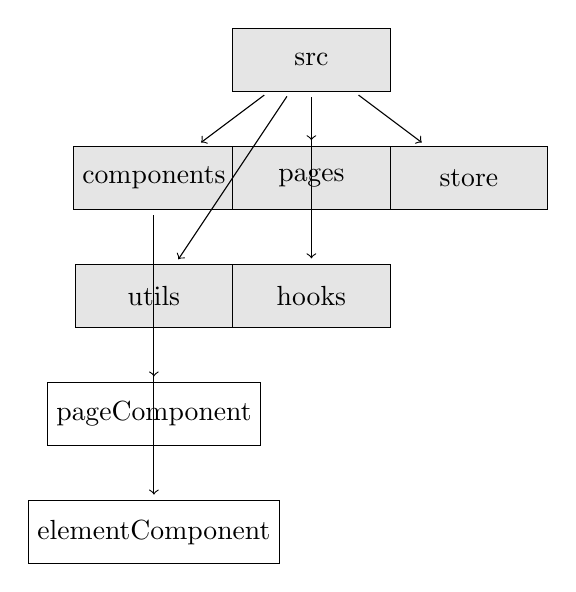
\begin{tikzpicture}[
    file/.style={draw, rectangle, minimum width=2cm, minimum height=0.8cm},
    folder/.style={draw, rectangle, minimum width=2cm, minimum height=0.8cm, fill=gray!20},
    arrow/.style={->, shorten >=2pt, shorten <=2pt}
]

% Folders
\node[folder] (src) at (0,0) {src};
\node[folder] (components) at (-2,-1.5) {components};
\node[folder] (pages) at (0,-1.5) {pages};
\node[folder] (store) at (2,-1.5) {store};
\node[folder] (utils) at (-2,-3) {utils};
\node[folder] (hooks) at (0,-3) {hooks};

% Files
\node[file] (pageComponent) at (-2,-4.5) {pageComponent};
\node[file] (elementComponent) at (-2,-6) {elementComponent};
% ... add more files

% Connections
\draw[arrow] (src) -- (components);
\draw[arrow] (src) -- (pages);
\draw[arrow] (src) -- (store);
\draw[arrow] (src) -- (utils);
\draw[arrow] (src) -- (hooks);
\draw[arrow] (components) -- (pageComponent);
\draw[arrow] (components) -- (elementComponent);
% ... add more connections

\end{tikzpicture}



\pagebreak
\subsubsection{Back-end}
The backend uses the dotNet framework. The development language using the C\# language.

In this project, the backend uses the Onion Architecture.
The Onion Architecture is a typically layered architecture, 
where each layer depends on the inner layer and provides interfaces to the outer layer.
The outer layer provides services to the outermost layer 
and other modules in the same layer based on the interfaces of the inner layer.

From inner to outer, the layers are: Domain, Application, Infrastructure, Presentation.
The Domain layer is the core layer and the innermost layer, used to define domain models, 
which are the business models.
It includes domain models and domain service interfaces.
Domain models are used to define the business models, 
which are the entities in the entity-relationship model and their attributes.
Domain service interfaces are used to define the business services, 
which are the relationships between entities in the entity-relationship model.

The Application layer is the application layer, 
used to define application services, which are the business logic.
It includes domain service implementations and application service interfaces.
Domain service implementations implement the methods of the inner layer's domain service 
interfaces and implement the business logic of the domain models.
Application service interfaces are used to define application services, 
which are the business logic.
It includes but is not limited to database interfaces, testing interfaces, 
HTTP API interfaces, MQTT interfaces, etc.

The Infrastructure layer is the infrastructure layer, used to define infrastructure.
It includes database implementations, testing implementations, 
HTTP API implementations, MQTT implementations, etc.
Database implementations implement the database interfaces 
and provide CRUD services for the database.
Testing implementations implement the testing interfaces 
and provide services for unit testing and integration testing.
HTTP API implementations implement the HTTP API interfaces 
and provide CRUD operations for HTTP APIs.
MQTT implementations implement the MQTT interfaces 
and provide CRUD operations for MQTT.

The Presentation layer is the presentation layer, used to define presentation logic, 
such as interfaces and pages. Since this is a backend project,
data presentation and control are handled by the frontend, 
so this layer is not needed.



\pagebreak
\subsubsection{Data communication and storage}
% 关于本项目的数据通信与数据存储的设计, 包括数据通信的协议, 数据存储的设计等
% 关于数据通信的设计:
% 1. 通信协议的选择
% 自前端向后端发送的数据, 有三种传输的数据类型, 
% 一种是普通的增删改查的请求, 对数据传输的时效性要求不高, 但是对数据的准确性, 完整性, 有序性, 安全性有一定的要求,
% 这种数据的传输, 采用 HTTP 协议, 以及 RESTful API 的设计. 可以有效的保证对数据传输的以上要求.
% 一种是对数据通道的创建和流媒体数据的传输, 对数据传输的时效性, 安全性要求较高, 这种数据的传输, 采用 WebRTC 协议, 以及 MQTT 协议.
% 配合可以快速解码的 flatbuffers 协议, 可以有效的保证对数据传输的以上要求.
% 最后一种是对设备的状态信息和操作信息的传输, 对完整性, 有序性, 安全性都有较高的要求, 这种数据的传输, 采用 MQTT 协议
% 同时也使用了 flatbuffers 协议.
% 
% 2. 数据通信的通信架构和通信流程
% 本项目的数据通信的通信架构, 是基于前后端分离的架构, 前端使用 React 框架, 后端使用 dotnet 框架.
% 当前端需要向后端发送数据的时候, 前端会向后端发送 HTTP 请求, 后端接收到 HTTP 请求之后, 会根据请求的数据类型,
% 选择不同的数据处理方式, 对于普通的增删改查的请求, 后端会根据 RESTful API 的设计, 对数据进行增删改查的操作,
% 对于对数据通道的创建和流媒体数据的传输, 后端会根据 WebRTC 协议, 对数据通道进行创建, 并且帮助前端和设备建立数据通道,
% 当数据通道建立后, 前端和设备之间则使用 flatbuffer 的数据格式对流媒体数据进行传输,
% 对于设备的状态信息和操作信息的传输, 前端会直接向 MQTT broker 发送 MQTT 请求, 
% 设备会在其自身的固件中监听相关的 MQTT 请求, 并且返回相关的数据.
% 
% 3. 数据通信的格式
% 本项目的数据通信的格式, 有三种, 
% 一种是 HTTP 协议, 
% 使用 json 格式对数据进行传输,
% 一种是 WebRTC 协议, 
% 使用 flatbuffers 格式对数据进行传输,
% 一种是 MQTT 协议.
% 使用 flatbuffers 格式对数据进行传输,
% 
% 关于数据存储的设计:
% 1. 数据存储的数据库的选择
% 本项目的数据存储的数据库的选择, 使用了轻量级的数据库 SQLite,
% SQLite 是一个进程内的库, 实现了自给自足的, 无服务器的, 零配置的, 事务性的 SQL 数据库引擎.
% 这是因为整个项目的目的是为了实现前端与设备之间的数据通信, 对于数据库数据的增删改查操作的要求不高,
% 数据量较小, 且对于数据库的数据的事务性要求不高, 所以选择了 SQLite 数据库.
% 2. 项目前后端的数据结构的设计
% 在本项目中, 前端由于使用了 React 框架, 所以前端的数据结构的设计, 使用了基于状态的数据结构的设计,
% 每个组件或者数据集都包含一个状态对象, 这个状态对象的属性就是组件的各个状态. 
% 使用状态对象的原因是, 可以方便的对状态进行管理, 采用对象-属性的形式, 可以方便的针对不同组件的同类状态进行区分,
% 由于跨组件的状态是由 redux 进行管理的, 这种状态对象的设计, 可以更搞笑的对状态进行更新和传递.
% 后端由于使用了 dotnet 框架, 所以后端的数据结构的设计, 使用了基于类的数据结构的设计,
% 采用了面向对象的编程思想, 对数据进行了封装, 使得数据的传输更加的安全, 有序, 完整.


\pagebreak

% \subsection{Domain model}
% \documentclass[]{article}
\usepackage{graphicx}
\usepackage{amsmath}
\usepackage{tikz}

% libaries
\usetikzlibrary{shapes,arrows}

%Define the listing package
\usepackage{listings} %code highlighter
\usepackage{color} %use color
\definecolor{mygreen}{rgb}{0,0.6,0}
\definecolor{mygray}{rgb}{0.5,0.5,0.5}
\definecolor{mymauve}{rgb}{0.58,0,0.82}

%Customize a bit the look
\lstset{ %
backgroundcolor=\color{white}, % choose the background color; you must add \usepackage{color} or \usepackage{xcolor}
basicstyle=\footnotesize, % the size of the fonts that are used for the code
breakatwhitespace=false, % sets if automatic breaks should only happen at whitespace
breaklines=true, % sets automatic line breaking
captionpos=b, % sets the caption-position to bottom
commentstyle=\color{mygreen}, % comment style
deletekeywords={...}, % if you want to delete keywords from the given language
escapeinside={\%*}{*)}, % if you want to add LaTeX within your code
extendedchars=true, % lets you use non-ASCII characters; for 8-bits encodings only, does not work with UTF-8
frame=single, % adds a frame around the code
keepspaces=true, % keeps spaces in text, useful for keeping indentation of code (possibly needs columns=flexible)
keywordstyle=\color{blue}, % keyword style
% language=Octave, % the language of the code
morekeywords={*,...}, % if you want to add more keywords to the set
numbers=left, % where to put the line-numbers; possible values are (none, left, right)
numbersep=5pt, % how far the line-numbers are from the code
numberstyle=\tiny\color{mygray}, % the style that is used for the line-numbers
rulecolor=\color{black}, % if not set, the frame-color may be changed on line-breaks within not-black text (e.g. comments (green here))
showspaces=false, % show spaces everywhere adding particular underscores; it overrides 'showstringspaces'
showstringspaces=false, % underline spaces within strings only
showtabs=false, % show tabs within strings adding particular underscores
stepnumber=1, % the step between two line-numbers. If it's 1, each line will be numbered
stringstyle=\color{mymauve}, % string literal style
tabsize=2, % sets default tabsize to 2 spaces
title=\lstname % show the filename of files included with \lstinputlisting; also try caption instead of title
}

\definecolor{darkgray}{rgb}{.4,.4,.4}
\definecolor{purple}{rgb}{0.65, 0.12, 0.82}

\lstdefinelanguage{React}{
keywords={const, typeof, new, true, false, catch, function, return, null, catch, switch, var, if, in, while, do, else, case, break},
keywordstyle=\color{blue}\bfseries,
ndkeywords={class, export, boolean, throw, implements, import, this},
ndkeywordstyle=\color{darkgray}\bfseries,
identifierstyle=\color{mygreen},
sensitive=false,
comment=[l]{//},
morecomment=[s]{/*}{*/},
commentstyle=\color{purple}\ttfamily,
string=[b]{"}{'}{`},
stringstyle=\color{red}\ttfamily,
morestring=[b]',
morestring=[b]",
morestring=[b]`',
}

\lstdefinelanguage{CSharp}{
keywords={const, typeof, new, true, false, catch, function, return, null, catch, switch, var, if, in, while, do, else, case, break},
keywordstyle=\color{blue}\bfseries,
ndkeywords={class, export, boolean, throw, implements, import, this},
ndkeywordstyle=\color{darkgray}\bfseries,
identifierstyle=\color{mygreen},
sensitive=false,
comment=[l]{//},
morecomment=[s]{/*}{*/},
commentstyle=\color{purple}\ttfamily,
string=[b]{"}{'}{`},
stringstyle=\color{red}\ttfamily,
morestring=[b]',
morestring=[b]",
morestring=[b]`',
}

\lstset{
language=React,
extendedchars=true,
basicstyle=\footnotesize\ttfamily,
showstringspaces=false,
showspaces=false,
numbers=left,
numberstyle=\footnotesize,
numbersep=9pt,
tabsize=2,
breaklines=true,
showtabs=false,
captionpos=b
}

\lstset{
language=CSharp,
extendedchars=true,
basicstyle=\footnotesize\ttfamily,
showstringspaces=false,
showspaces=false,
numbers=left,
numberstyle=\footnotesize,
numbersep=9pt,
tabsize=2,
breaklines=true,
showtabs=false,
captionpos=b
}

% \usepackage{cite} % Add this line for citation

% \bibliographystyle{plain}

\title{
The implementation of BifrostConnect Front-end scope, 
re-design and development with the relevant back-end support develop.
}
\author{
    Fei Gu \\
    Erhvervs Akademi Sydvest \\
    Computer Science 21\\
    }
\date{\today}

\begin{document}

% Front page
\maketitle
\begin{center}
    Supervisor: Henrik Boulund Meng Hansen \\
    Company: BifrostConnect \\
    Engineering Director: Jasper Wass \\
\end{center}
\tableofcontents
\pagebreak


% The introduction
\section{Introduction}
\subsection{Background}\input{sections/introduction/background.tex}
\subsection{The company}\input{sections/introduction/aboutCompany}
\subsection{The project}\input{sections/introduction/aboutProject}
\pagebreak

% The problem statement
\section{Problem Statement}
\subsection{Statement}
\input{sections/problemStatement/statement}
\subsection{Situation}
\input{sections/problemStatement/situation}
\subsection{Potential Solution}
\input{sections/problemStatement/potentialSolution}
\pagebreak

% Requirement analysis
\section{Requirement Analysis}
\input{sections/requirementAnalysis/index}

\subsection{Stakeholders}
\input{sections/requirementAnalysis/stakeholders/index}

\subsection{Business Domain}
\input{sections/requirementAnalysis/bussinesDomain/index}

\subsection{Scope}
\input{sections/requirementAnalysis/scope}

\subsection{Goals}
\input{sections/requirementAnalysis/goals}
\pagebreak

% Software Design
\section{Software Design}
% developement methods
\subsection{Software Development Methods}
\input{sections/softwareDevelopmentMethods/index}
\subsubsection{Agile Software Development}
\input{sections/softwareDevelopmentMethods/agileSoftwareDevelopment/index}
\subsubsection{Feature Driven Development}
\input{sections/softwareDevelopmentMethods/featureDrivenDevelopment/index}

\pagebreak

% Technology seslection
\subsection{Technology selection}
\input{sections/softwareDesign/technologySelection/index}
\subsubsection{Front-end}
\input{sections/softwareDesign/technologySelection/frontEnd}            
\subsubsection{Back-end}
\input{sections/softwareDesign/technologySelection/backEnd}            
\subsubsection{Database}
\input{sections/softwareDesign/technologySelection/database}
\subsubsection{Data communication}
\input{sections/softwareDesign/technologySelection/dataCommunication}            
\subsubsection{DevOps}
\input{sections/softwareDesign/technologySelection/devOps}
\pagebreak

% Architecture design
\subsection{Architecture design}
\input{sections/softwareDesign/architectureDesign/index}
\pagebreak
\subsubsection{Front-end}
\input{sections/softwareDesign/architectureDesign/frontEndArchitecture}
\pagebreak
\subsubsection{Back-end}
\input{sections/softwareDesign/architectureDesign/backEndArchitecture}
\pagebreak
\subsubsection{Data communication and storage}
\input{sections/softwareDesign/architectureDesign/dataCommunicationArchitecture}
\pagebreak

% \subsection{Domain model}
% \input{sections/softwareDesign/domainModel/index}
% \subsection{Database design}
% % 数据库领域模型 ER 图
% % 包括表和字段的设置.
% % 对于私有键和外键的设置.

% \subsection{Back-end design}
% % 后端对象模型
% % 以及对于对象模型的增删改查
% % 以及相关的其他服务的设计`'

% \subsection{Front-end design}
% % 对于前端的页面结构的设计 
% % 页面的状态的设计, 交互设计

% \subsection{FlatBuffers design}
% % schema 的设计

\subsection{DevOps CI/CD process design}
\input{sections/softwareDesign/devOpsDesign/index}
\subsubsection{Continuous Integration}
\input{sections/softwareDesign/devOpsDesign/continuousIntegration/index}
\subsubsection{Continuous Delivery}
\input{sections/softwareDesign/devOpsDesign/continuousDelivery/index}
\subsubsection{Continuous Deployment}
\input{sections/softwareDesign/devOpsDesign/continuousDeployment/index}
\pagebreak

\section{Software Development} 
\input{sections/softwareDevelopment/index}
\subsection{Overall development}
\input{sections/softwareDevelopment/overallDevelopement/index}
\subsubsection{Front-end}
\input{sections/softwareDevelopment/overallDevelopement/frontEnd/index}
\subsubsection{Back-end}
\input{sections/softwareDevelopment/overallDevelopement/backEnd/index}
\subsubsection{DevOps}
\input{sections/softwareDevelopment/overallDevelopement/devOps/index}
\subsection{Feature development} 
\input{sections/softwareDevelopment/featureDevelopment/index}
\subsubsection{Use Case 1}
\input{sections/softwareDevelopment/featureDevelopment/useCase1/index}
\subsubsection{Feature 1}
\input{sections/softwareDevelopment/featureDevelopment/feature/feature1.tex}
\pagebreak
\section{Conclusion} 
\subsection{Result}
Since the project is still in progress, the result is not available yet.
So far, basic structure of this project has been built. But the most features 
are not implemented yet. 
\subsection{Discussion}
As a single developer for this project, I am confident what I have done so far.
And I can say I understand the most of the knowledge I have used in this project, 
which also means I can explain all the part of the project. 
But this project also relevant some of the complex knowledge which I have to continue 
to study and practice.
\subsection{Future Work}
The future work is to implement the rest of the features. 
Including the most important part which is the 'create session' feature.
\pagebreak
% \bibliography{bibliography}
\pagebreak
% \begin{appendices}
%     \section{Appendix}
% \end{appendices} 
\end{document}
% \subsection{Database design}
% % 数据库领域模型 ER 图
% % 包括表和字段的设置.
% % 对于私有键和外键的设置.

% \subsection{Back-end design}
% % 后端对象模型
% % 以及对于对象模型的增删改查
% % 以及相关的其他服务的设计`'

% \subsection{Front-end design}
% % 对于前端的页面结构的设计 
% % 页面的状态的设计, 交互设计

% \subsection{FlatBuffers design}
% % schema 的设计

\subsection{DevOps CI/CD process design}
\documentclass[]{article}
\usepackage{graphicx}
\usepackage{amsmath}
\usepackage{tikz}

% libaries
\usetikzlibrary{shapes,arrows}

%Define the listing package
\usepackage{listings} %code highlighter
\usepackage{color} %use color
\definecolor{mygreen}{rgb}{0,0.6,0}
\definecolor{mygray}{rgb}{0.5,0.5,0.5}
\definecolor{mymauve}{rgb}{0.58,0,0.82}

%Customize a bit the look
\lstset{ %
backgroundcolor=\color{white}, % choose the background color; you must add \usepackage{color} or \usepackage{xcolor}
basicstyle=\footnotesize, % the size of the fonts that are used for the code
breakatwhitespace=false, % sets if automatic breaks should only happen at whitespace
breaklines=true, % sets automatic line breaking
captionpos=b, % sets the caption-position to bottom
commentstyle=\color{mygreen}, % comment style
deletekeywords={...}, % if you want to delete keywords from the given language
escapeinside={\%*}{*)}, % if you want to add LaTeX within your code
extendedchars=true, % lets you use non-ASCII characters; for 8-bits encodings only, does not work with UTF-8
frame=single, % adds a frame around the code
keepspaces=true, % keeps spaces in text, useful for keeping indentation of code (possibly needs columns=flexible)
keywordstyle=\color{blue}, % keyword style
% language=Octave, % the language of the code
morekeywords={*,...}, % if you want to add more keywords to the set
numbers=left, % where to put the line-numbers; possible values are (none, left, right)
numbersep=5pt, % how far the line-numbers are from the code
numberstyle=\tiny\color{mygray}, % the style that is used for the line-numbers
rulecolor=\color{black}, % if not set, the frame-color may be changed on line-breaks within not-black text (e.g. comments (green here))
showspaces=false, % show spaces everywhere adding particular underscores; it overrides 'showstringspaces'
showstringspaces=false, % underline spaces within strings only
showtabs=false, % show tabs within strings adding particular underscores
stepnumber=1, % the step between two line-numbers. If it's 1, each line will be numbered
stringstyle=\color{mymauve}, % string literal style
tabsize=2, % sets default tabsize to 2 spaces
title=\lstname % show the filename of files included with \lstinputlisting; also try caption instead of title
}

\definecolor{darkgray}{rgb}{.4,.4,.4}
\definecolor{purple}{rgb}{0.65, 0.12, 0.82}

\lstdefinelanguage{React}{
keywords={const, typeof, new, true, false, catch, function, return, null, catch, switch, var, if, in, while, do, else, case, break},
keywordstyle=\color{blue}\bfseries,
ndkeywords={class, export, boolean, throw, implements, import, this},
ndkeywordstyle=\color{darkgray}\bfseries,
identifierstyle=\color{mygreen},
sensitive=false,
comment=[l]{//},
morecomment=[s]{/*}{*/},
commentstyle=\color{purple}\ttfamily,
string=[b]{"}{'}{`},
stringstyle=\color{red}\ttfamily,
morestring=[b]',
morestring=[b]",
morestring=[b]`',
}

\lstdefinelanguage{CSharp}{
keywords={const, typeof, new, true, false, catch, function, return, null, catch, switch, var, if, in, while, do, else, case, break},
keywordstyle=\color{blue}\bfseries,
ndkeywords={class, export, boolean, throw, implements, import, this},
ndkeywordstyle=\color{darkgray}\bfseries,
identifierstyle=\color{mygreen},
sensitive=false,
comment=[l]{//},
morecomment=[s]{/*}{*/},
commentstyle=\color{purple}\ttfamily,
string=[b]{"}{'}{`},
stringstyle=\color{red}\ttfamily,
morestring=[b]',
morestring=[b]",
morestring=[b]`',
}

\lstset{
language=React,
extendedchars=true,
basicstyle=\footnotesize\ttfamily,
showstringspaces=false,
showspaces=false,
numbers=left,
numberstyle=\footnotesize,
numbersep=9pt,
tabsize=2,
breaklines=true,
showtabs=false,
captionpos=b
}

\lstset{
language=CSharp,
extendedchars=true,
basicstyle=\footnotesize\ttfamily,
showstringspaces=false,
showspaces=false,
numbers=left,
numberstyle=\footnotesize,
numbersep=9pt,
tabsize=2,
breaklines=true,
showtabs=false,
captionpos=b
}

% \usepackage{cite} % Add this line for citation

% \bibliographystyle{plain}

\title{
The implementation of BifrostConnect Front-end scope, 
re-design and development with the relevant back-end support develop.
}
\author{
    Fei Gu \\
    Erhvervs Akademi Sydvest \\
    Computer Science 21\\
    }
\date{\today}

\begin{document}

% Front page
\maketitle
\begin{center}
    Supervisor: Henrik Boulund Meng Hansen \\
    Company: BifrostConnect \\
    Engineering Director: Jasper Wass \\
\end{center}
\tableofcontents
\pagebreak


% The introduction
\section{Introduction}
\subsection{Background}\input{sections/introduction/background.tex}
\subsection{The company}\input{sections/introduction/aboutCompany}
\subsection{The project}\input{sections/introduction/aboutProject}
\pagebreak

% The problem statement
\section{Problem Statement}
\subsection{Statement}
\input{sections/problemStatement/statement}
\subsection{Situation}
\input{sections/problemStatement/situation}
\subsection{Potential Solution}
\input{sections/problemStatement/potentialSolution}
\pagebreak

% Requirement analysis
\section{Requirement Analysis}
\input{sections/requirementAnalysis/index}

\subsection{Stakeholders}
\input{sections/requirementAnalysis/stakeholders/index}

\subsection{Business Domain}
\input{sections/requirementAnalysis/bussinesDomain/index}

\subsection{Scope}
\input{sections/requirementAnalysis/scope}

\subsection{Goals}
\input{sections/requirementAnalysis/goals}
\pagebreak

% Software Design
\section{Software Design}
% developement methods
\subsection{Software Development Methods}
\input{sections/softwareDevelopmentMethods/index}
\subsubsection{Agile Software Development}
\input{sections/softwareDevelopmentMethods/agileSoftwareDevelopment/index}
\subsubsection{Feature Driven Development}
\input{sections/softwareDevelopmentMethods/featureDrivenDevelopment/index}

\pagebreak

% Technology seslection
\subsection{Technology selection}
\input{sections/softwareDesign/technologySelection/index}
\subsubsection{Front-end}
\input{sections/softwareDesign/technologySelection/frontEnd}            
\subsubsection{Back-end}
\input{sections/softwareDesign/technologySelection/backEnd}            
\subsubsection{Database}
\input{sections/softwareDesign/technologySelection/database}
\subsubsection{Data communication}
\input{sections/softwareDesign/technologySelection/dataCommunication}            
\subsubsection{DevOps}
\input{sections/softwareDesign/technologySelection/devOps}
\pagebreak

% Architecture design
\subsection{Architecture design}
\input{sections/softwareDesign/architectureDesign/index}
\pagebreak
\subsubsection{Front-end}
\input{sections/softwareDesign/architectureDesign/frontEndArchitecture}
\pagebreak
\subsubsection{Back-end}
\input{sections/softwareDesign/architectureDesign/backEndArchitecture}
\pagebreak
\subsubsection{Data communication and storage}
\input{sections/softwareDesign/architectureDesign/dataCommunicationArchitecture}
\pagebreak

% \subsection{Domain model}
% \input{sections/softwareDesign/domainModel/index}
% \subsection{Database design}
% % 数据库领域模型 ER 图
% % 包括表和字段的设置.
% % 对于私有键和外键的设置.

% \subsection{Back-end design}
% % 后端对象模型
% % 以及对于对象模型的增删改查
% % 以及相关的其他服务的设计`'

% \subsection{Front-end design}
% % 对于前端的页面结构的设计 
% % 页面的状态的设计, 交互设计

% \subsection{FlatBuffers design}
% % schema 的设计

\subsection{DevOps CI/CD process design}
\input{sections/softwareDesign/devOpsDesign/index}
\subsubsection{Continuous Integration}
\input{sections/softwareDesign/devOpsDesign/continuousIntegration/index}
\subsubsection{Continuous Delivery}
\input{sections/softwareDesign/devOpsDesign/continuousDelivery/index}
\subsubsection{Continuous Deployment}
\input{sections/softwareDesign/devOpsDesign/continuousDeployment/index}
\pagebreak

\section{Software Development} 
\input{sections/softwareDevelopment/index}
\subsection{Overall development}
\input{sections/softwareDevelopment/overallDevelopement/index}
\subsubsection{Front-end}
\input{sections/softwareDevelopment/overallDevelopement/frontEnd/index}
\subsubsection{Back-end}
\input{sections/softwareDevelopment/overallDevelopement/backEnd/index}
\subsubsection{DevOps}
\input{sections/softwareDevelopment/overallDevelopement/devOps/index}
\subsection{Feature development} 
\input{sections/softwareDevelopment/featureDevelopment/index}
\subsubsection{Use Case 1}
\input{sections/softwareDevelopment/featureDevelopment/useCase1/index}
\subsubsection{Feature 1}
\input{sections/softwareDevelopment/featureDevelopment/feature/feature1.tex}
\pagebreak
\section{Conclusion} 
\subsection{Result}
Since the project is still in progress, the result is not available yet.
So far, basic structure of this project has been built. But the most features 
are not implemented yet. 
\subsection{Discussion}
As a single developer for this project, I am confident what I have done so far.
And I can say I understand the most of the knowledge I have used in this project, 
which also means I can explain all the part of the project. 
But this project also relevant some of the complex knowledge which I have to continue 
to study and practice.
\subsection{Future Work}
The future work is to implement the rest of the features. 
Including the most important part which is the 'create session' feature.
\pagebreak
% \bibliography{bibliography}
\pagebreak
% \begin{appendices}
%     \section{Appendix}
% \end{appendices} 
\end{document}
\subsubsection{Continuous Integration}
\documentclass[]{article}
\usepackage{graphicx}
\usepackage{amsmath}
\usepackage{tikz}

% libaries
\usetikzlibrary{shapes,arrows}

%Define the listing package
\usepackage{listings} %code highlighter
\usepackage{color} %use color
\definecolor{mygreen}{rgb}{0,0.6,0}
\definecolor{mygray}{rgb}{0.5,0.5,0.5}
\definecolor{mymauve}{rgb}{0.58,0,0.82}

%Customize a bit the look
\lstset{ %
backgroundcolor=\color{white}, % choose the background color; you must add \usepackage{color} or \usepackage{xcolor}
basicstyle=\footnotesize, % the size of the fonts that are used for the code
breakatwhitespace=false, % sets if automatic breaks should only happen at whitespace
breaklines=true, % sets automatic line breaking
captionpos=b, % sets the caption-position to bottom
commentstyle=\color{mygreen}, % comment style
deletekeywords={...}, % if you want to delete keywords from the given language
escapeinside={\%*}{*)}, % if you want to add LaTeX within your code
extendedchars=true, % lets you use non-ASCII characters; for 8-bits encodings only, does not work with UTF-8
frame=single, % adds a frame around the code
keepspaces=true, % keeps spaces in text, useful for keeping indentation of code (possibly needs columns=flexible)
keywordstyle=\color{blue}, % keyword style
% language=Octave, % the language of the code
morekeywords={*,...}, % if you want to add more keywords to the set
numbers=left, % where to put the line-numbers; possible values are (none, left, right)
numbersep=5pt, % how far the line-numbers are from the code
numberstyle=\tiny\color{mygray}, % the style that is used for the line-numbers
rulecolor=\color{black}, % if not set, the frame-color may be changed on line-breaks within not-black text (e.g. comments (green here))
showspaces=false, % show spaces everywhere adding particular underscores; it overrides 'showstringspaces'
showstringspaces=false, % underline spaces within strings only
showtabs=false, % show tabs within strings adding particular underscores
stepnumber=1, % the step between two line-numbers. If it's 1, each line will be numbered
stringstyle=\color{mymauve}, % string literal style
tabsize=2, % sets default tabsize to 2 spaces
title=\lstname % show the filename of files included with \lstinputlisting; also try caption instead of title
}

\definecolor{darkgray}{rgb}{.4,.4,.4}
\definecolor{purple}{rgb}{0.65, 0.12, 0.82}

\lstdefinelanguage{React}{
keywords={const, typeof, new, true, false, catch, function, return, null, catch, switch, var, if, in, while, do, else, case, break},
keywordstyle=\color{blue}\bfseries,
ndkeywords={class, export, boolean, throw, implements, import, this},
ndkeywordstyle=\color{darkgray}\bfseries,
identifierstyle=\color{mygreen},
sensitive=false,
comment=[l]{//},
morecomment=[s]{/*}{*/},
commentstyle=\color{purple}\ttfamily,
string=[b]{"}{'}{`},
stringstyle=\color{red}\ttfamily,
morestring=[b]',
morestring=[b]",
morestring=[b]`',
}

\lstdefinelanguage{CSharp}{
keywords={const, typeof, new, true, false, catch, function, return, null, catch, switch, var, if, in, while, do, else, case, break},
keywordstyle=\color{blue}\bfseries,
ndkeywords={class, export, boolean, throw, implements, import, this},
ndkeywordstyle=\color{darkgray}\bfseries,
identifierstyle=\color{mygreen},
sensitive=false,
comment=[l]{//},
morecomment=[s]{/*}{*/},
commentstyle=\color{purple}\ttfamily,
string=[b]{"}{'}{`},
stringstyle=\color{red}\ttfamily,
morestring=[b]',
morestring=[b]",
morestring=[b]`',
}

\lstset{
language=React,
extendedchars=true,
basicstyle=\footnotesize\ttfamily,
showstringspaces=false,
showspaces=false,
numbers=left,
numberstyle=\footnotesize,
numbersep=9pt,
tabsize=2,
breaklines=true,
showtabs=false,
captionpos=b
}

\lstset{
language=CSharp,
extendedchars=true,
basicstyle=\footnotesize\ttfamily,
showstringspaces=false,
showspaces=false,
numbers=left,
numberstyle=\footnotesize,
numbersep=9pt,
tabsize=2,
breaklines=true,
showtabs=false,
captionpos=b
}

% \usepackage{cite} % Add this line for citation

% \bibliographystyle{plain}

\title{
The implementation of BifrostConnect Front-end scope, 
re-design and development with the relevant back-end support develop.
}
\author{
    Fei Gu \\
    Erhvervs Akademi Sydvest \\
    Computer Science 21\\
    }
\date{\today}

\begin{document}

% Front page
\maketitle
\begin{center}
    Supervisor: Henrik Boulund Meng Hansen \\
    Company: BifrostConnect \\
    Engineering Director: Jasper Wass \\
\end{center}
\tableofcontents
\pagebreak


% The introduction
\section{Introduction}
\subsection{Background}\input{sections/introduction/background.tex}
\subsection{The company}\input{sections/introduction/aboutCompany}
\subsection{The project}\input{sections/introduction/aboutProject}
\pagebreak

% The problem statement
\section{Problem Statement}
\subsection{Statement}
\input{sections/problemStatement/statement}
\subsection{Situation}
\input{sections/problemStatement/situation}
\subsection{Potential Solution}
\input{sections/problemStatement/potentialSolution}
\pagebreak

% Requirement analysis
\section{Requirement Analysis}
\input{sections/requirementAnalysis/index}

\subsection{Stakeholders}
\input{sections/requirementAnalysis/stakeholders/index}

\subsection{Business Domain}
\input{sections/requirementAnalysis/bussinesDomain/index}

\subsection{Scope}
\input{sections/requirementAnalysis/scope}

\subsection{Goals}
\input{sections/requirementAnalysis/goals}
\pagebreak

% Software Design
\section{Software Design}
% developement methods
\subsection{Software Development Methods}
\input{sections/softwareDevelopmentMethods/index}
\subsubsection{Agile Software Development}
\input{sections/softwareDevelopmentMethods/agileSoftwareDevelopment/index}
\subsubsection{Feature Driven Development}
\input{sections/softwareDevelopmentMethods/featureDrivenDevelopment/index}

\pagebreak

% Technology seslection
\subsection{Technology selection}
\input{sections/softwareDesign/technologySelection/index}
\subsubsection{Front-end}
\input{sections/softwareDesign/technologySelection/frontEnd}            
\subsubsection{Back-end}
\input{sections/softwareDesign/technologySelection/backEnd}            
\subsubsection{Database}
\input{sections/softwareDesign/technologySelection/database}
\subsubsection{Data communication}
\input{sections/softwareDesign/technologySelection/dataCommunication}            
\subsubsection{DevOps}
\input{sections/softwareDesign/technologySelection/devOps}
\pagebreak

% Architecture design
\subsection{Architecture design}
\input{sections/softwareDesign/architectureDesign/index}
\pagebreak
\subsubsection{Front-end}
\input{sections/softwareDesign/architectureDesign/frontEndArchitecture}
\pagebreak
\subsubsection{Back-end}
\input{sections/softwareDesign/architectureDesign/backEndArchitecture}
\pagebreak
\subsubsection{Data communication and storage}
\input{sections/softwareDesign/architectureDesign/dataCommunicationArchitecture}
\pagebreak

% \subsection{Domain model}
% \input{sections/softwareDesign/domainModel/index}
% \subsection{Database design}
% % 数据库领域模型 ER 图
% % 包括表和字段的设置.
% % 对于私有键和外键的设置.

% \subsection{Back-end design}
% % 后端对象模型
% % 以及对于对象模型的增删改查
% % 以及相关的其他服务的设计`'

% \subsection{Front-end design}
% % 对于前端的页面结构的设计 
% % 页面的状态的设计, 交互设计

% \subsection{FlatBuffers design}
% % schema 的设计

\subsection{DevOps CI/CD process design}
\input{sections/softwareDesign/devOpsDesign/index}
\subsubsection{Continuous Integration}
\input{sections/softwareDesign/devOpsDesign/continuousIntegration/index}
\subsubsection{Continuous Delivery}
\input{sections/softwareDesign/devOpsDesign/continuousDelivery/index}
\subsubsection{Continuous Deployment}
\input{sections/softwareDesign/devOpsDesign/continuousDeployment/index}
\pagebreak

\section{Software Development} 
\input{sections/softwareDevelopment/index}
\subsection{Overall development}
\input{sections/softwareDevelopment/overallDevelopement/index}
\subsubsection{Front-end}
\input{sections/softwareDevelopment/overallDevelopement/frontEnd/index}
\subsubsection{Back-end}
\input{sections/softwareDevelopment/overallDevelopement/backEnd/index}
\subsubsection{DevOps}
\input{sections/softwareDevelopment/overallDevelopement/devOps/index}
\subsection{Feature development} 
\input{sections/softwareDevelopment/featureDevelopment/index}
\subsubsection{Use Case 1}
\input{sections/softwareDevelopment/featureDevelopment/useCase1/index}
\subsubsection{Feature 1}
\input{sections/softwareDevelopment/featureDevelopment/feature/feature1.tex}
\pagebreak
\section{Conclusion} 
\subsection{Result}
Since the project is still in progress, the result is not available yet.
So far, basic structure of this project has been built. But the most features 
are not implemented yet. 
\subsection{Discussion}
As a single developer for this project, I am confident what I have done so far.
And I can say I understand the most of the knowledge I have used in this project, 
which also means I can explain all the part of the project. 
But this project also relevant some of the complex knowledge which I have to continue 
to study and practice.
\subsection{Future Work}
The future work is to implement the rest of the features. 
Including the most important part which is the 'create session' feature.
\pagebreak
% \bibliography{bibliography}
\pagebreak
% \begin{appendices}
%     \section{Appendix}
% \end{appendices} 
\end{document}
\subsubsection{Continuous Delivery}
\documentclass[]{article}
\usepackage{graphicx}
\usepackage{amsmath}
\usepackage{tikz}

% libaries
\usetikzlibrary{shapes,arrows}

%Define the listing package
\usepackage{listings} %code highlighter
\usepackage{color} %use color
\definecolor{mygreen}{rgb}{0,0.6,0}
\definecolor{mygray}{rgb}{0.5,0.5,0.5}
\definecolor{mymauve}{rgb}{0.58,0,0.82}

%Customize a bit the look
\lstset{ %
backgroundcolor=\color{white}, % choose the background color; you must add \usepackage{color} or \usepackage{xcolor}
basicstyle=\footnotesize, % the size of the fonts that are used for the code
breakatwhitespace=false, % sets if automatic breaks should only happen at whitespace
breaklines=true, % sets automatic line breaking
captionpos=b, % sets the caption-position to bottom
commentstyle=\color{mygreen}, % comment style
deletekeywords={...}, % if you want to delete keywords from the given language
escapeinside={\%*}{*)}, % if you want to add LaTeX within your code
extendedchars=true, % lets you use non-ASCII characters; for 8-bits encodings only, does not work with UTF-8
frame=single, % adds a frame around the code
keepspaces=true, % keeps spaces in text, useful for keeping indentation of code (possibly needs columns=flexible)
keywordstyle=\color{blue}, % keyword style
% language=Octave, % the language of the code
morekeywords={*,...}, % if you want to add more keywords to the set
numbers=left, % where to put the line-numbers; possible values are (none, left, right)
numbersep=5pt, % how far the line-numbers are from the code
numberstyle=\tiny\color{mygray}, % the style that is used for the line-numbers
rulecolor=\color{black}, % if not set, the frame-color may be changed on line-breaks within not-black text (e.g. comments (green here))
showspaces=false, % show spaces everywhere adding particular underscores; it overrides 'showstringspaces'
showstringspaces=false, % underline spaces within strings only
showtabs=false, % show tabs within strings adding particular underscores
stepnumber=1, % the step between two line-numbers. If it's 1, each line will be numbered
stringstyle=\color{mymauve}, % string literal style
tabsize=2, % sets default tabsize to 2 spaces
title=\lstname % show the filename of files included with \lstinputlisting; also try caption instead of title
}

\definecolor{darkgray}{rgb}{.4,.4,.4}
\definecolor{purple}{rgb}{0.65, 0.12, 0.82}

\lstdefinelanguage{React}{
keywords={const, typeof, new, true, false, catch, function, return, null, catch, switch, var, if, in, while, do, else, case, break},
keywordstyle=\color{blue}\bfseries,
ndkeywords={class, export, boolean, throw, implements, import, this},
ndkeywordstyle=\color{darkgray}\bfseries,
identifierstyle=\color{mygreen},
sensitive=false,
comment=[l]{//},
morecomment=[s]{/*}{*/},
commentstyle=\color{purple}\ttfamily,
string=[b]{"}{'}{`},
stringstyle=\color{red}\ttfamily,
morestring=[b]',
morestring=[b]",
morestring=[b]`',
}

\lstdefinelanguage{CSharp}{
keywords={const, typeof, new, true, false, catch, function, return, null, catch, switch, var, if, in, while, do, else, case, break},
keywordstyle=\color{blue}\bfseries,
ndkeywords={class, export, boolean, throw, implements, import, this},
ndkeywordstyle=\color{darkgray}\bfseries,
identifierstyle=\color{mygreen},
sensitive=false,
comment=[l]{//},
morecomment=[s]{/*}{*/},
commentstyle=\color{purple}\ttfamily,
string=[b]{"}{'}{`},
stringstyle=\color{red}\ttfamily,
morestring=[b]',
morestring=[b]",
morestring=[b]`',
}

\lstset{
language=React,
extendedchars=true,
basicstyle=\footnotesize\ttfamily,
showstringspaces=false,
showspaces=false,
numbers=left,
numberstyle=\footnotesize,
numbersep=9pt,
tabsize=2,
breaklines=true,
showtabs=false,
captionpos=b
}

\lstset{
language=CSharp,
extendedchars=true,
basicstyle=\footnotesize\ttfamily,
showstringspaces=false,
showspaces=false,
numbers=left,
numberstyle=\footnotesize,
numbersep=9pt,
tabsize=2,
breaklines=true,
showtabs=false,
captionpos=b
}

% \usepackage{cite} % Add this line for citation

% \bibliographystyle{plain}

\title{
The implementation of BifrostConnect Front-end scope, 
re-design and development with the relevant back-end support develop.
}
\author{
    Fei Gu \\
    Erhvervs Akademi Sydvest \\
    Computer Science 21\\
    }
\date{\today}

\begin{document}

% Front page
\maketitle
\begin{center}
    Supervisor: Henrik Boulund Meng Hansen \\
    Company: BifrostConnect \\
    Engineering Director: Jasper Wass \\
\end{center}
\tableofcontents
\pagebreak


% The introduction
\section{Introduction}
\subsection{Background}\input{sections/introduction/background.tex}
\subsection{The company}\input{sections/introduction/aboutCompany}
\subsection{The project}\input{sections/introduction/aboutProject}
\pagebreak

% The problem statement
\section{Problem Statement}
\subsection{Statement}
\input{sections/problemStatement/statement}
\subsection{Situation}
\input{sections/problemStatement/situation}
\subsection{Potential Solution}
\input{sections/problemStatement/potentialSolution}
\pagebreak

% Requirement analysis
\section{Requirement Analysis}
\input{sections/requirementAnalysis/index}

\subsection{Stakeholders}
\input{sections/requirementAnalysis/stakeholders/index}

\subsection{Business Domain}
\input{sections/requirementAnalysis/bussinesDomain/index}

\subsection{Scope}
\input{sections/requirementAnalysis/scope}

\subsection{Goals}
\input{sections/requirementAnalysis/goals}
\pagebreak

% Software Design
\section{Software Design}
% developement methods
\subsection{Software Development Methods}
\input{sections/softwareDevelopmentMethods/index}
\subsubsection{Agile Software Development}
\input{sections/softwareDevelopmentMethods/agileSoftwareDevelopment/index}
\subsubsection{Feature Driven Development}
\input{sections/softwareDevelopmentMethods/featureDrivenDevelopment/index}

\pagebreak

% Technology seslection
\subsection{Technology selection}
\input{sections/softwareDesign/technologySelection/index}
\subsubsection{Front-end}
\input{sections/softwareDesign/technologySelection/frontEnd}            
\subsubsection{Back-end}
\input{sections/softwareDesign/technologySelection/backEnd}            
\subsubsection{Database}
\input{sections/softwareDesign/technologySelection/database}
\subsubsection{Data communication}
\input{sections/softwareDesign/technologySelection/dataCommunication}            
\subsubsection{DevOps}
\input{sections/softwareDesign/technologySelection/devOps}
\pagebreak

% Architecture design
\subsection{Architecture design}
\input{sections/softwareDesign/architectureDesign/index}
\pagebreak
\subsubsection{Front-end}
\input{sections/softwareDesign/architectureDesign/frontEndArchitecture}
\pagebreak
\subsubsection{Back-end}
\input{sections/softwareDesign/architectureDesign/backEndArchitecture}
\pagebreak
\subsubsection{Data communication and storage}
\input{sections/softwareDesign/architectureDesign/dataCommunicationArchitecture}
\pagebreak

% \subsection{Domain model}
% \input{sections/softwareDesign/domainModel/index}
% \subsection{Database design}
% % 数据库领域模型 ER 图
% % 包括表和字段的设置.
% % 对于私有键和外键的设置.

% \subsection{Back-end design}
% % 后端对象模型
% % 以及对于对象模型的增删改查
% % 以及相关的其他服务的设计`'

% \subsection{Front-end design}
% % 对于前端的页面结构的设计 
% % 页面的状态的设计, 交互设计

% \subsection{FlatBuffers design}
% % schema 的设计

\subsection{DevOps CI/CD process design}
\input{sections/softwareDesign/devOpsDesign/index}
\subsubsection{Continuous Integration}
\input{sections/softwareDesign/devOpsDesign/continuousIntegration/index}
\subsubsection{Continuous Delivery}
\input{sections/softwareDesign/devOpsDesign/continuousDelivery/index}
\subsubsection{Continuous Deployment}
\input{sections/softwareDesign/devOpsDesign/continuousDeployment/index}
\pagebreak

\section{Software Development} 
\input{sections/softwareDevelopment/index}
\subsection{Overall development}
\input{sections/softwareDevelopment/overallDevelopement/index}
\subsubsection{Front-end}
\input{sections/softwareDevelopment/overallDevelopement/frontEnd/index}
\subsubsection{Back-end}
\input{sections/softwareDevelopment/overallDevelopement/backEnd/index}
\subsubsection{DevOps}
\input{sections/softwareDevelopment/overallDevelopement/devOps/index}
\subsection{Feature development} 
\input{sections/softwareDevelopment/featureDevelopment/index}
\subsubsection{Use Case 1}
\input{sections/softwareDevelopment/featureDevelopment/useCase1/index}
\subsubsection{Feature 1}
\input{sections/softwareDevelopment/featureDevelopment/feature/feature1.tex}
\pagebreak
\section{Conclusion} 
\subsection{Result}
Since the project is still in progress, the result is not available yet.
So far, basic structure of this project has been built. But the most features 
are not implemented yet. 
\subsection{Discussion}
As a single developer for this project, I am confident what I have done so far.
And I can say I understand the most of the knowledge I have used in this project, 
which also means I can explain all the part of the project. 
But this project also relevant some of the complex knowledge which I have to continue 
to study and practice.
\subsection{Future Work}
The future work is to implement the rest of the features. 
Including the most important part which is the 'create session' feature.
\pagebreak
% \bibliography{bibliography}
\pagebreak
% \begin{appendices}
%     \section{Appendix}
% \end{appendices} 
\end{document}
\subsubsection{Continuous Deployment}
\documentclass[]{article}
\usepackage{graphicx}
\usepackage{amsmath}
\usepackage{tikz}

% libaries
\usetikzlibrary{shapes,arrows}

%Define the listing package
\usepackage{listings} %code highlighter
\usepackage{color} %use color
\definecolor{mygreen}{rgb}{0,0.6,0}
\definecolor{mygray}{rgb}{0.5,0.5,0.5}
\definecolor{mymauve}{rgb}{0.58,0,0.82}

%Customize a bit the look
\lstset{ %
backgroundcolor=\color{white}, % choose the background color; you must add \usepackage{color} or \usepackage{xcolor}
basicstyle=\footnotesize, % the size of the fonts that are used for the code
breakatwhitespace=false, % sets if automatic breaks should only happen at whitespace
breaklines=true, % sets automatic line breaking
captionpos=b, % sets the caption-position to bottom
commentstyle=\color{mygreen}, % comment style
deletekeywords={...}, % if you want to delete keywords from the given language
escapeinside={\%*}{*)}, % if you want to add LaTeX within your code
extendedchars=true, % lets you use non-ASCII characters; for 8-bits encodings only, does not work with UTF-8
frame=single, % adds a frame around the code
keepspaces=true, % keeps spaces in text, useful for keeping indentation of code (possibly needs columns=flexible)
keywordstyle=\color{blue}, % keyword style
% language=Octave, % the language of the code
morekeywords={*,...}, % if you want to add more keywords to the set
numbers=left, % where to put the line-numbers; possible values are (none, left, right)
numbersep=5pt, % how far the line-numbers are from the code
numberstyle=\tiny\color{mygray}, % the style that is used for the line-numbers
rulecolor=\color{black}, % if not set, the frame-color may be changed on line-breaks within not-black text (e.g. comments (green here))
showspaces=false, % show spaces everywhere adding particular underscores; it overrides 'showstringspaces'
showstringspaces=false, % underline spaces within strings only
showtabs=false, % show tabs within strings adding particular underscores
stepnumber=1, % the step between two line-numbers. If it's 1, each line will be numbered
stringstyle=\color{mymauve}, % string literal style
tabsize=2, % sets default tabsize to 2 spaces
title=\lstname % show the filename of files included with \lstinputlisting; also try caption instead of title
}

\definecolor{darkgray}{rgb}{.4,.4,.4}
\definecolor{purple}{rgb}{0.65, 0.12, 0.82}

\lstdefinelanguage{React}{
keywords={const, typeof, new, true, false, catch, function, return, null, catch, switch, var, if, in, while, do, else, case, break},
keywordstyle=\color{blue}\bfseries,
ndkeywords={class, export, boolean, throw, implements, import, this},
ndkeywordstyle=\color{darkgray}\bfseries,
identifierstyle=\color{mygreen},
sensitive=false,
comment=[l]{//},
morecomment=[s]{/*}{*/},
commentstyle=\color{purple}\ttfamily,
string=[b]{"}{'}{`},
stringstyle=\color{red}\ttfamily,
morestring=[b]',
morestring=[b]",
morestring=[b]`',
}

\lstdefinelanguage{CSharp}{
keywords={const, typeof, new, true, false, catch, function, return, null, catch, switch, var, if, in, while, do, else, case, break},
keywordstyle=\color{blue}\bfseries,
ndkeywords={class, export, boolean, throw, implements, import, this},
ndkeywordstyle=\color{darkgray}\bfseries,
identifierstyle=\color{mygreen},
sensitive=false,
comment=[l]{//},
morecomment=[s]{/*}{*/},
commentstyle=\color{purple}\ttfamily,
string=[b]{"}{'}{`},
stringstyle=\color{red}\ttfamily,
morestring=[b]',
morestring=[b]",
morestring=[b]`',
}

\lstset{
language=React,
extendedchars=true,
basicstyle=\footnotesize\ttfamily,
showstringspaces=false,
showspaces=false,
numbers=left,
numberstyle=\footnotesize,
numbersep=9pt,
tabsize=2,
breaklines=true,
showtabs=false,
captionpos=b
}

\lstset{
language=CSharp,
extendedchars=true,
basicstyle=\footnotesize\ttfamily,
showstringspaces=false,
showspaces=false,
numbers=left,
numberstyle=\footnotesize,
numbersep=9pt,
tabsize=2,
breaklines=true,
showtabs=false,
captionpos=b
}

% \usepackage{cite} % Add this line for citation

% \bibliographystyle{plain}

\title{
The implementation of BifrostConnect Front-end scope, 
re-design and development with the relevant back-end support develop.
}
\author{
    Fei Gu \\
    Erhvervs Akademi Sydvest \\
    Computer Science 21\\
    }
\date{\today}

\begin{document}

% Front page
\maketitle
\begin{center}
    Supervisor: Henrik Boulund Meng Hansen \\
    Company: BifrostConnect \\
    Engineering Director: Jasper Wass \\
\end{center}
\tableofcontents
\pagebreak


% The introduction
\section{Introduction}
\subsection{Background}\input{sections/introduction/background.tex}
\subsection{The company}\input{sections/introduction/aboutCompany}
\subsection{The project}\input{sections/introduction/aboutProject}
\pagebreak

% The problem statement
\section{Problem Statement}
\subsection{Statement}
\input{sections/problemStatement/statement}
\subsection{Situation}
\input{sections/problemStatement/situation}
\subsection{Potential Solution}
\input{sections/problemStatement/potentialSolution}
\pagebreak

% Requirement analysis
\section{Requirement Analysis}
\input{sections/requirementAnalysis/index}

\subsection{Stakeholders}
\input{sections/requirementAnalysis/stakeholders/index}

\subsection{Business Domain}
\input{sections/requirementAnalysis/bussinesDomain/index}

\subsection{Scope}
\input{sections/requirementAnalysis/scope}

\subsection{Goals}
\input{sections/requirementAnalysis/goals}
\pagebreak

% Software Design
\section{Software Design}
% developement methods
\subsection{Software Development Methods}
\input{sections/softwareDevelopmentMethods/index}
\subsubsection{Agile Software Development}
\input{sections/softwareDevelopmentMethods/agileSoftwareDevelopment/index}
\subsubsection{Feature Driven Development}
\input{sections/softwareDevelopmentMethods/featureDrivenDevelopment/index}

\pagebreak

% Technology seslection
\subsection{Technology selection}
\input{sections/softwareDesign/technologySelection/index}
\subsubsection{Front-end}
\input{sections/softwareDesign/technologySelection/frontEnd}            
\subsubsection{Back-end}
\input{sections/softwareDesign/technologySelection/backEnd}            
\subsubsection{Database}
\input{sections/softwareDesign/technologySelection/database}
\subsubsection{Data communication}
\input{sections/softwareDesign/technologySelection/dataCommunication}            
\subsubsection{DevOps}
\input{sections/softwareDesign/technologySelection/devOps}
\pagebreak

% Architecture design
\subsection{Architecture design}
\input{sections/softwareDesign/architectureDesign/index}
\pagebreak
\subsubsection{Front-end}
\input{sections/softwareDesign/architectureDesign/frontEndArchitecture}
\pagebreak
\subsubsection{Back-end}
\input{sections/softwareDesign/architectureDesign/backEndArchitecture}
\pagebreak
\subsubsection{Data communication and storage}
\input{sections/softwareDesign/architectureDesign/dataCommunicationArchitecture}
\pagebreak

% \subsection{Domain model}
% \input{sections/softwareDesign/domainModel/index}
% \subsection{Database design}
% % 数据库领域模型 ER 图
% % 包括表和字段的设置.
% % 对于私有键和外键的设置.

% \subsection{Back-end design}
% % 后端对象模型
% % 以及对于对象模型的增删改查
% % 以及相关的其他服务的设计`'

% \subsection{Front-end design}
% % 对于前端的页面结构的设计 
% % 页面的状态的设计, 交互设计

% \subsection{FlatBuffers design}
% % schema 的设计

\subsection{DevOps CI/CD process design}
\input{sections/softwareDesign/devOpsDesign/index}
\subsubsection{Continuous Integration}
\input{sections/softwareDesign/devOpsDesign/continuousIntegration/index}
\subsubsection{Continuous Delivery}
\input{sections/softwareDesign/devOpsDesign/continuousDelivery/index}
\subsubsection{Continuous Deployment}
\input{sections/softwareDesign/devOpsDesign/continuousDeployment/index}
\pagebreak

\section{Software Development} 
\input{sections/softwareDevelopment/index}
\subsection{Overall development}
\input{sections/softwareDevelopment/overallDevelopement/index}
\subsubsection{Front-end}
\input{sections/softwareDevelopment/overallDevelopement/frontEnd/index}
\subsubsection{Back-end}
\input{sections/softwareDevelopment/overallDevelopement/backEnd/index}
\subsubsection{DevOps}
\input{sections/softwareDevelopment/overallDevelopement/devOps/index}
\subsection{Feature development} 
\input{sections/softwareDevelopment/featureDevelopment/index}
\subsubsection{Use Case 1}
\input{sections/softwareDevelopment/featureDevelopment/useCase1/index}
\subsubsection{Feature 1}
\input{sections/softwareDevelopment/featureDevelopment/feature/feature1.tex}
\pagebreak
\section{Conclusion} 
\subsection{Result}
Since the project is still in progress, the result is not available yet.
So far, basic structure of this project has been built. But the most features 
are not implemented yet. 
\subsection{Discussion}
As a single developer for this project, I am confident what I have done so far.
And I can say I understand the most of the knowledge I have used in this project, 
which also means I can explain all the part of the project. 
But this project also relevant some of the complex knowledge which I have to continue 
to study and practice.
\subsection{Future Work}
The future work is to implement the rest of the features. 
Including the most important part which is the 'create session' feature.
\pagebreak
% \bibliography{bibliography}
\pagebreak
% \begin{appendices}
%     \section{Appendix}
% \end{appendices} 
\end{document}
\pagebreak

\section{Software Development} 
\documentclass[]{article}
\usepackage{graphicx}
\usepackage{amsmath}
\usepackage{tikz}

% libaries
\usetikzlibrary{shapes,arrows}

%Define the listing package
\usepackage{listings} %code highlighter
\usepackage{color} %use color
\definecolor{mygreen}{rgb}{0,0.6,0}
\definecolor{mygray}{rgb}{0.5,0.5,0.5}
\definecolor{mymauve}{rgb}{0.58,0,0.82}

%Customize a bit the look
\lstset{ %
backgroundcolor=\color{white}, % choose the background color; you must add \usepackage{color} or \usepackage{xcolor}
basicstyle=\footnotesize, % the size of the fonts that are used for the code
breakatwhitespace=false, % sets if automatic breaks should only happen at whitespace
breaklines=true, % sets automatic line breaking
captionpos=b, % sets the caption-position to bottom
commentstyle=\color{mygreen}, % comment style
deletekeywords={...}, % if you want to delete keywords from the given language
escapeinside={\%*}{*)}, % if you want to add LaTeX within your code
extendedchars=true, % lets you use non-ASCII characters; for 8-bits encodings only, does not work with UTF-8
frame=single, % adds a frame around the code
keepspaces=true, % keeps spaces in text, useful for keeping indentation of code (possibly needs columns=flexible)
keywordstyle=\color{blue}, % keyword style
% language=Octave, % the language of the code
morekeywords={*,...}, % if you want to add more keywords to the set
numbers=left, % where to put the line-numbers; possible values are (none, left, right)
numbersep=5pt, % how far the line-numbers are from the code
numberstyle=\tiny\color{mygray}, % the style that is used for the line-numbers
rulecolor=\color{black}, % if not set, the frame-color may be changed on line-breaks within not-black text (e.g. comments (green here))
showspaces=false, % show spaces everywhere adding particular underscores; it overrides 'showstringspaces'
showstringspaces=false, % underline spaces within strings only
showtabs=false, % show tabs within strings adding particular underscores
stepnumber=1, % the step between two line-numbers. If it's 1, each line will be numbered
stringstyle=\color{mymauve}, % string literal style
tabsize=2, % sets default tabsize to 2 spaces
title=\lstname % show the filename of files included with \lstinputlisting; also try caption instead of title
}

\definecolor{darkgray}{rgb}{.4,.4,.4}
\definecolor{purple}{rgb}{0.65, 0.12, 0.82}

\lstdefinelanguage{React}{
keywords={const, typeof, new, true, false, catch, function, return, null, catch, switch, var, if, in, while, do, else, case, break},
keywordstyle=\color{blue}\bfseries,
ndkeywords={class, export, boolean, throw, implements, import, this},
ndkeywordstyle=\color{darkgray}\bfseries,
identifierstyle=\color{mygreen},
sensitive=false,
comment=[l]{//},
morecomment=[s]{/*}{*/},
commentstyle=\color{purple}\ttfamily,
string=[b]{"}{'}{`},
stringstyle=\color{red}\ttfamily,
morestring=[b]',
morestring=[b]",
morestring=[b]`',
}

\lstdefinelanguage{CSharp}{
keywords={const, typeof, new, true, false, catch, function, return, null, catch, switch, var, if, in, while, do, else, case, break},
keywordstyle=\color{blue}\bfseries,
ndkeywords={class, export, boolean, throw, implements, import, this},
ndkeywordstyle=\color{darkgray}\bfseries,
identifierstyle=\color{mygreen},
sensitive=false,
comment=[l]{//},
morecomment=[s]{/*}{*/},
commentstyle=\color{purple}\ttfamily,
string=[b]{"}{'}{`},
stringstyle=\color{red}\ttfamily,
morestring=[b]',
morestring=[b]",
morestring=[b]`',
}

\lstset{
language=React,
extendedchars=true,
basicstyle=\footnotesize\ttfamily,
showstringspaces=false,
showspaces=false,
numbers=left,
numberstyle=\footnotesize,
numbersep=9pt,
tabsize=2,
breaklines=true,
showtabs=false,
captionpos=b
}

\lstset{
language=CSharp,
extendedchars=true,
basicstyle=\footnotesize\ttfamily,
showstringspaces=false,
showspaces=false,
numbers=left,
numberstyle=\footnotesize,
numbersep=9pt,
tabsize=2,
breaklines=true,
showtabs=false,
captionpos=b
}

% \usepackage{cite} % Add this line for citation

% \bibliographystyle{plain}

\title{
The implementation of BifrostConnect Front-end scope, 
re-design and development with the relevant back-end support develop.
}
\author{
    Fei Gu \\
    Erhvervs Akademi Sydvest \\
    Computer Science 21\\
    }
\date{\today}

\begin{document}

% Front page
\maketitle
\begin{center}
    Supervisor: Henrik Boulund Meng Hansen \\
    Company: BifrostConnect \\
    Engineering Director: Jasper Wass \\
\end{center}
\tableofcontents
\pagebreak


% The introduction
\section{Introduction}
\subsection{Background}\input{sections/introduction/background.tex}
\subsection{The company}\input{sections/introduction/aboutCompany}
\subsection{The project}\input{sections/introduction/aboutProject}
\pagebreak

% The problem statement
\section{Problem Statement}
\subsection{Statement}
\input{sections/problemStatement/statement}
\subsection{Situation}
\input{sections/problemStatement/situation}
\subsection{Potential Solution}
\input{sections/problemStatement/potentialSolution}
\pagebreak

% Requirement analysis
\section{Requirement Analysis}
\input{sections/requirementAnalysis/index}

\subsection{Stakeholders}
\input{sections/requirementAnalysis/stakeholders/index}

\subsection{Business Domain}
\input{sections/requirementAnalysis/bussinesDomain/index}

\subsection{Scope}
\input{sections/requirementAnalysis/scope}

\subsection{Goals}
\input{sections/requirementAnalysis/goals}
\pagebreak

% Software Design
\section{Software Design}
% developement methods
\subsection{Software Development Methods}
\input{sections/softwareDevelopmentMethods/index}
\subsubsection{Agile Software Development}
\input{sections/softwareDevelopmentMethods/agileSoftwareDevelopment/index}
\subsubsection{Feature Driven Development}
\input{sections/softwareDevelopmentMethods/featureDrivenDevelopment/index}

\pagebreak

% Technology seslection
\subsection{Technology selection}
\input{sections/softwareDesign/technologySelection/index}
\subsubsection{Front-end}
\input{sections/softwareDesign/technologySelection/frontEnd}            
\subsubsection{Back-end}
\input{sections/softwareDesign/technologySelection/backEnd}            
\subsubsection{Database}
\input{sections/softwareDesign/technologySelection/database}
\subsubsection{Data communication}
\input{sections/softwareDesign/technologySelection/dataCommunication}            
\subsubsection{DevOps}
\input{sections/softwareDesign/technologySelection/devOps}
\pagebreak

% Architecture design
\subsection{Architecture design}
\input{sections/softwareDesign/architectureDesign/index}
\pagebreak
\subsubsection{Front-end}
\input{sections/softwareDesign/architectureDesign/frontEndArchitecture}
\pagebreak
\subsubsection{Back-end}
\input{sections/softwareDesign/architectureDesign/backEndArchitecture}
\pagebreak
\subsubsection{Data communication and storage}
\input{sections/softwareDesign/architectureDesign/dataCommunicationArchitecture}
\pagebreak

% \subsection{Domain model}
% \input{sections/softwareDesign/domainModel/index}
% \subsection{Database design}
% % 数据库领域模型 ER 图
% % 包括表和字段的设置.
% % 对于私有键和外键的设置.

% \subsection{Back-end design}
% % 后端对象模型
% % 以及对于对象模型的增删改查
% % 以及相关的其他服务的设计`'

% \subsection{Front-end design}
% % 对于前端的页面结构的设计 
% % 页面的状态的设计, 交互设计

% \subsection{FlatBuffers design}
% % schema 的设计

\subsection{DevOps CI/CD process design}
\input{sections/softwareDesign/devOpsDesign/index}
\subsubsection{Continuous Integration}
\input{sections/softwareDesign/devOpsDesign/continuousIntegration/index}
\subsubsection{Continuous Delivery}
\input{sections/softwareDesign/devOpsDesign/continuousDelivery/index}
\subsubsection{Continuous Deployment}
\input{sections/softwareDesign/devOpsDesign/continuousDeployment/index}
\pagebreak

\section{Software Development} 
\input{sections/softwareDevelopment/index}
\subsection{Overall development}
\input{sections/softwareDevelopment/overallDevelopement/index}
\subsubsection{Front-end}
\input{sections/softwareDevelopment/overallDevelopement/frontEnd/index}
\subsubsection{Back-end}
\input{sections/softwareDevelopment/overallDevelopement/backEnd/index}
\subsubsection{DevOps}
\input{sections/softwareDevelopment/overallDevelopement/devOps/index}
\subsection{Feature development} 
\input{sections/softwareDevelopment/featureDevelopment/index}
\subsubsection{Use Case 1}
\input{sections/softwareDevelopment/featureDevelopment/useCase1/index}
\subsubsection{Feature 1}
\input{sections/softwareDevelopment/featureDevelopment/feature/feature1.tex}
\pagebreak
\section{Conclusion} 
\subsection{Result}
Since the project is still in progress, the result is not available yet.
So far, basic structure of this project has been built. But the most features 
are not implemented yet. 
\subsection{Discussion}
As a single developer for this project, I am confident what I have done so far.
And I can say I understand the most of the knowledge I have used in this project, 
which also means I can explain all the part of the project. 
But this project also relevant some of the complex knowledge which I have to continue 
to study and practice.
\subsection{Future Work}
The future work is to implement the rest of the features. 
Including the most important part which is the 'create session' feature.
\pagebreak
% \bibliography{bibliography}
\pagebreak
% \begin{appendices}
%     \section{Appendix}
% \end{appendices} 
\end{document}
\subsection{Overall development}
\documentclass[]{article}
\usepackage{graphicx}
\usepackage{amsmath}
\usepackage{tikz}

% libaries
\usetikzlibrary{shapes,arrows}

%Define the listing package
\usepackage{listings} %code highlighter
\usepackage{color} %use color
\definecolor{mygreen}{rgb}{0,0.6,0}
\definecolor{mygray}{rgb}{0.5,0.5,0.5}
\definecolor{mymauve}{rgb}{0.58,0,0.82}

%Customize a bit the look
\lstset{ %
backgroundcolor=\color{white}, % choose the background color; you must add \usepackage{color} or \usepackage{xcolor}
basicstyle=\footnotesize, % the size of the fonts that are used for the code
breakatwhitespace=false, % sets if automatic breaks should only happen at whitespace
breaklines=true, % sets automatic line breaking
captionpos=b, % sets the caption-position to bottom
commentstyle=\color{mygreen}, % comment style
deletekeywords={...}, % if you want to delete keywords from the given language
escapeinside={\%*}{*)}, % if you want to add LaTeX within your code
extendedchars=true, % lets you use non-ASCII characters; for 8-bits encodings only, does not work with UTF-8
frame=single, % adds a frame around the code
keepspaces=true, % keeps spaces in text, useful for keeping indentation of code (possibly needs columns=flexible)
keywordstyle=\color{blue}, % keyword style
% language=Octave, % the language of the code
morekeywords={*,...}, % if you want to add more keywords to the set
numbers=left, % where to put the line-numbers; possible values are (none, left, right)
numbersep=5pt, % how far the line-numbers are from the code
numberstyle=\tiny\color{mygray}, % the style that is used for the line-numbers
rulecolor=\color{black}, % if not set, the frame-color may be changed on line-breaks within not-black text (e.g. comments (green here))
showspaces=false, % show spaces everywhere adding particular underscores; it overrides 'showstringspaces'
showstringspaces=false, % underline spaces within strings only
showtabs=false, % show tabs within strings adding particular underscores
stepnumber=1, % the step between two line-numbers. If it's 1, each line will be numbered
stringstyle=\color{mymauve}, % string literal style
tabsize=2, % sets default tabsize to 2 spaces
title=\lstname % show the filename of files included with \lstinputlisting; also try caption instead of title
}

\definecolor{darkgray}{rgb}{.4,.4,.4}
\definecolor{purple}{rgb}{0.65, 0.12, 0.82}

\lstdefinelanguage{React}{
keywords={const, typeof, new, true, false, catch, function, return, null, catch, switch, var, if, in, while, do, else, case, break},
keywordstyle=\color{blue}\bfseries,
ndkeywords={class, export, boolean, throw, implements, import, this},
ndkeywordstyle=\color{darkgray}\bfseries,
identifierstyle=\color{mygreen},
sensitive=false,
comment=[l]{//},
morecomment=[s]{/*}{*/},
commentstyle=\color{purple}\ttfamily,
string=[b]{"}{'}{`},
stringstyle=\color{red}\ttfamily,
morestring=[b]',
morestring=[b]",
morestring=[b]`',
}

\lstdefinelanguage{CSharp}{
keywords={const, typeof, new, true, false, catch, function, return, null, catch, switch, var, if, in, while, do, else, case, break},
keywordstyle=\color{blue}\bfseries,
ndkeywords={class, export, boolean, throw, implements, import, this},
ndkeywordstyle=\color{darkgray}\bfseries,
identifierstyle=\color{mygreen},
sensitive=false,
comment=[l]{//},
morecomment=[s]{/*}{*/},
commentstyle=\color{purple}\ttfamily,
string=[b]{"}{'}{`},
stringstyle=\color{red}\ttfamily,
morestring=[b]',
morestring=[b]",
morestring=[b]`',
}

\lstset{
language=React,
extendedchars=true,
basicstyle=\footnotesize\ttfamily,
showstringspaces=false,
showspaces=false,
numbers=left,
numberstyle=\footnotesize,
numbersep=9pt,
tabsize=2,
breaklines=true,
showtabs=false,
captionpos=b
}

\lstset{
language=CSharp,
extendedchars=true,
basicstyle=\footnotesize\ttfamily,
showstringspaces=false,
showspaces=false,
numbers=left,
numberstyle=\footnotesize,
numbersep=9pt,
tabsize=2,
breaklines=true,
showtabs=false,
captionpos=b
}

% \usepackage{cite} % Add this line for citation

% \bibliographystyle{plain}

\title{
The implementation of BifrostConnect Front-end scope, 
re-design and development with the relevant back-end support develop.
}
\author{
    Fei Gu \\
    Erhvervs Akademi Sydvest \\
    Computer Science 21\\
    }
\date{\today}

\begin{document}

% Front page
\maketitle
\begin{center}
    Supervisor: Henrik Boulund Meng Hansen \\
    Company: BifrostConnect \\
    Engineering Director: Jasper Wass \\
\end{center}
\tableofcontents
\pagebreak


% The introduction
\section{Introduction}
\subsection{Background}\input{sections/introduction/background.tex}
\subsection{The company}\input{sections/introduction/aboutCompany}
\subsection{The project}\input{sections/introduction/aboutProject}
\pagebreak

% The problem statement
\section{Problem Statement}
\subsection{Statement}
\input{sections/problemStatement/statement}
\subsection{Situation}
\input{sections/problemStatement/situation}
\subsection{Potential Solution}
\input{sections/problemStatement/potentialSolution}
\pagebreak

% Requirement analysis
\section{Requirement Analysis}
\input{sections/requirementAnalysis/index}

\subsection{Stakeholders}
\input{sections/requirementAnalysis/stakeholders/index}

\subsection{Business Domain}
\input{sections/requirementAnalysis/bussinesDomain/index}

\subsection{Scope}
\input{sections/requirementAnalysis/scope}

\subsection{Goals}
\input{sections/requirementAnalysis/goals}
\pagebreak

% Software Design
\section{Software Design}
% developement methods
\subsection{Software Development Methods}
\input{sections/softwareDevelopmentMethods/index}
\subsubsection{Agile Software Development}
\input{sections/softwareDevelopmentMethods/agileSoftwareDevelopment/index}
\subsubsection{Feature Driven Development}
\input{sections/softwareDevelopmentMethods/featureDrivenDevelopment/index}

\pagebreak

% Technology seslection
\subsection{Technology selection}
\input{sections/softwareDesign/technologySelection/index}
\subsubsection{Front-end}
\input{sections/softwareDesign/technologySelection/frontEnd}            
\subsubsection{Back-end}
\input{sections/softwareDesign/technologySelection/backEnd}            
\subsubsection{Database}
\input{sections/softwareDesign/technologySelection/database}
\subsubsection{Data communication}
\input{sections/softwareDesign/technologySelection/dataCommunication}            
\subsubsection{DevOps}
\input{sections/softwareDesign/technologySelection/devOps}
\pagebreak

% Architecture design
\subsection{Architecture design}
\input{sections/softwareDesign/architectureDesign/index}
\pagebreak
\subsubsection{Front-end}
\input{sections/softwareDesign/architectureDesign/frontEndArchitecture}
\pagebreak
\subsubsection{Back-end}
\input{sections/softwareDesign/architectureDesign/backEndArchitecture}
\pagebreak
\subsubsection{Data communication and storage}
\input{sections/softwareDesign/architectureDesign/dataCommunicationArchitecture}
\pagebreak

% \subsection{Domain model}
% \input{sections/softwareDesign/domainModel/index}
% \subsection{Database design}
% % 数据库领域模型 ER 图
% % 包括表和字段的设置.
% % 对于私有键和外键的设置.

% \subsection{Back-end design}
% % 后端对象模型
% % 以及对于对象模型的增删改查
% % 以及相关的其他服务的设计`'

% \subsection{Front-end design}
% % 对于前端的页面结构的设计 
% % 页面的状态的设计, 交互设计

% \subsection{FlatBuffers design}
% % schema 的设计

\subsection{DevOps CI/CD process design}
\input{sections/softwareDesign/devOpsDesign/index}
\subsubsection{Continuous Integration}
\input{sections/softwareDesign/devOpsDesign/continuousIntegration/index}
\subsubsection{Continuous Delivery}
\input{sections/softwareDesign/devOpsDesign/continuousDelivery/index}
\subsubsection{Continuous Deployment}
\input{sections/softwareDesign/devOpsDesign/continuousDeployment/index}
\pagebreak

\section{Software Development} 
\input{sections/softwareDevelopment/index}
\subsection{Overall development}
\input{sections/softwareDevelopment/overallDevelopement/index}
\subsubsection{Front-end}
\input{sections/softwareDevelopment/overallDevelopement/frontEnd/index}
\subsubsection{Back-end}
\input{sections/softwareDevelopment/overallDevelopement/backEnd/index}
\subsubsection{DevOps}
\input{sections/softwareDevelopment/overallDevelopement/devOps/index}
\subsection{Feature development} 
\input{sections/softwareDevelopment/featureDevelopment/index}
\subsubsection{Use Case 1}
\input{sections/softwareDevelopment/featureDevelopment/useCase1/index}
\subsubsection{Feature 1}
\input{sections/softwareDevelopment/featureDevelopment/feature/feature1.tex}
\pagebreak
\section{Conclusion} 
\subsection{Result}
Since the project is still in progress, the result is not available yet.
So far, basic structure of this project has been built. But the most features 
are not implemented yet. 
\subsection{Discussion}
As a single developer for this project, I am confident what I have done so far.
And I can say I understand the most of the knowledge I have used in this project, 
which also means I can explain all the part of the project. 
But this project also relevant some of the complex knowledge which I have to continue 
to study and practice.
\subsection{Future Work}
The future work is to implement the rest of the features. 
Including the most important part which is the 'create session' feature.
\pagebreak
% \bibliography{bibliography}
\pagebreak
% \begin{appendices}
%     \section{Appendix}
% \end{appendices} 
\end{document}
\subsubsection{Front-end}
\documentclass[]{article}
\usepackage{graphicx}
\usepackage{amsmath}
\usepackage{tikz}

% libaries
\usetikzlibrary{shapes,arrows}

%Define the listing package
\usepackage{listings} %code highlighter
\usepackage{color} %use color
\definecolor{mygreen}{rgb}{0,0.6,0}
\definecolor{mygray}{rgb}{0.5,0.5,0.5}
\definecolor{mymauve}{rgb}{0.58,0,0.82}

%Customize a bit the look
\lstset{ %
backgroundcolor=\color{white}, % choose the background color; you must add \usepackage{color} or \usepackage{xcolor}
basicstyle=\footnotesize, % the size of the fonts that are used for the code
breakatwhitespace=false, % sets if automatic breaks should only happen at whitespace
breaklines=true, % sets automatic line breaking
captionpos=b, % sets the caption-position to bottom
commentstyle=\color{mygreen}, % comment style
deletekeywords={...}, % if you want to delete keywords from the given language
escapeinside={\%*}{*)}, % if you want to add LaTeX within your code
extendedchars=true, % lets you use non-ASCII characters; for 8-bits encodings only, does not work with UTF-8
frame=single, % adds a frame around the code
keepspaces=true, % keeps spaces in text, useful for keeping indentation of code (possibly needs columns=flexible)
keywordstyle=\color{blue}, % keyword style
% language=Octave, % the language of the code
morekeywords={*,...}, % if you want to add more keywords to the set
numbers=left, % where to put the line-numbers; possible values are (none, left, right)
numbersep=5pt, % how far the line-numbers are from the code
numberstyle=\tiny\color{mygray}, % the style that is used for the line-numbers
rulecolor=\color{black}, % if not set, the frame-color may be changed on line-breaks within not-black text (e.g. comments (green here))
showspaces=false, % show spaces everywhere adding particular underscores; it overrides 'showstringspaces'
showstringspaces=false, % underline spaces within strings only
showtabs=false, % show tabs within strings adding particular underscores
stepnumber=1, % the step between two line-numbers. If it's 1, each line will be numbered
stringstyle=\color{mymauve}, % string literal style
tabsize=2, % sets default tabsize to 2 spaces
title=\lstname % show the filename of files included with \lstinputlisting; also try caption instead of title
}

\definecolor{darkgray}{rgb}{.4,.4,.4}
\definecolor{purple}{rgb}{0.65, 0.12, 0.82}

\lstdefinelanguage{React}{
keywords={const, typeof, new, true, false, catch, function, return, null, catch, switch, var, if, in, while, do, else, case, break},
keywordstyle=\color{blue}\bfseries,
ndkeywords={class, export, boolean, throw, implements, import, this},
ndkeywordstyle=\color{darkgray}\bfseries,
identifierstyle=\color{mygreen},
sensitive=false,
comment=[l]{//},
morecomment=[s]{/*}{*/},
commentstyle=\color{purple}\ttfamily,
string=[b]{"}{'}{`},
stringstyle=\color{red}\ttfamily,
morestring=[b]',
morestring=[b]",
morestring=[b]`',
}

\lstdefinelanguage{CSharp}{
keywords={const, typeof, new, true, false, catch, function, return, null, catch, switch, var, if, in, while, do, else, case, break},
keywordstyle=\color{blue}\bfseries,
ndkeywords={class, export, boolean, throw, implements, import, this},
ndkeywordstyle=\color{darkgray}\bfseries,
identifierstyle=\color{mygreen},
sensitive=false,
comment=[l]{//},
morecomment=[s]{/*}{*/},
commentstyle=\color{purple}\ttfamily,
string=[b]{"}{'}{`},
stringstyle=\color{red}\ttfamily,
morestring=[b]',
morestring=[b]",
morestring=[b]`',
}

\lstset{
language=React,
extendedchars=true,
basicstyle=\footnotesize\ttfamily,
showstringspaces=false,
showspaces=false,
numbers=left,
numberstyle=\footnotesize,
numbersep=9pt,
tabsize=2,
breaklines=true,
showtabs=false,
captionpos=b
}

\lstset{
language=CSharp,
extendedchars=true,
basicstyle=\footnotesize\ttfamily,
showstringspaces=false,
showspaces=false,
numbers=left,
numberstyle=\footnotesize,
numbersep=9pt,
tabsize=2,
breaklines=true,
showtabs=false,
captionpos=b
}

% \usepackage{cite} % Add this line for citation

% \bibliographystyle{plain}

\title{
The implementation of BifrostConnect Front-end scope, 
re-design and development with the relevant back-end support develop.
}
\author{
    Fei Gu \\
    Erhvervs Akademi Sydvest \\
    Computer Science 21\\
    }
\date{\today}

\begin{document}

% Front page
\maketitle
\begin{center}
    Supervisor: Henrik Boulund Meng Hansen \\
    Company: BifrostConnect \\
    Engineering Director: Jasper Wass \\
\end{center}
\tableofcontents
\pagebreak


% The introduction
\section{Introduction}
\subsection{Background}\input{sections/introduction/background.tex}
\subsection{The company}\input{sections/introduction/aboutCompany}
\subsection{The project}\input{sections/introduction/aboutProject}
\pagebreak

% The problem statement
\section{Problem Statement}
\subsection{Statement}
\input{sections/problemStatement/statement}
\subsection{Situation}
\input{sections/problemStatement/situation}
\subsection{Potential Solution}
\input{sections/problemStatement/potentialSolution}
\pagebreak

% Requirement analysis
\section{Requirement Analysis}
\input{sections/requirementAnalysis/index}

\subsection{Stakeholders}
\input{sections/requirementAnalysis/stakeholders/index}

\subsection{Business Domain}
\input{sections/requirementAnalysis/bussinesDomain/index}

\subsection{Scope}
\input{sections/requirementAnalysis/scope}

\subsection{Goals}
\input{sections/requirementAnalysis/goals}
\pagebreak

% Software Design
\section{Software Design}
% developement methods
\subsection{Software Development Methods}
\input{sections/softwareDevelopmentMethods/index}
\subsubsection{Agile Software Development}
\input{sections/softwareDevelopmentMethods/agileSoftwareDevelopment/index}
\subsubsection{Feature Driven Development}
\input{sections/softwareDevelopmentMethods/featureDrivenDevelopment/index}

\pagebreak

% Technology seslection
\subsection{Technology selection}
\input{sections/softwareDesign/technologySelection/index}
\subsubsection{Front-end}
\input{sections/softwareDesign/technologySelection/frontEnd}            
\subsubsection{Back-end}
\input{sections/softwareDesign/technologySelection/backEnd}            
\subsubsection{Database}
\input{sections/softwareDesign/technologySelection/database}
\subsubsection{Data communication}
\input{sections/softwareDesign/technologySelection/dataCommunication}            
\subsubsection{DevOps}
\input{sections/softwareDesign/technologySelection/devOps}
\pagebreak

% Architecture design
\subsection{Architecture design}
\input{sections/softwareDesign/architectureDesign/index}
\pagebreak
\subsubsection{Front-end}
\input{sections/softwareDesign/architectureDesign/frontEndArchitecture}
\pagebreak
\subsubsection{Back-end}
\input{sections/softwareDesign/architectureDesign/backEndArchitecture}
\pagebreak
\subsubsection{Data communication and storage}
\input{sections/softwareDesign/architectureDesign/dataCommunicationArchitecture}
\pagebreak

% \subsection{Domain model}
% \input{sections/softwareDesign/domainModel/index}
% \subsection{Database design}
% % 数据库领域模型 ER 图
% % 包括表和字段的设置.
% % 对于私有键和外键的设置.

% \subsection{Back-end design}
% % 后端对象模型
% % 以及对于对象模型的增删改查
% % 以及相关的其他服务的设计`'

% \subsection{Front-end design}
% % 对于前端的页面结构的设计 
% % 页面的状态的设计, 交互设计

% \subsection{FlatBuffers design}
% % schema 的设计

\subsection{DevOps CI/CD process design}
\input{sections/softwareDesign/devOpsDesign/index}
\subsubsection{Continuous Integration}
\input{sections/softwareDesign/devOpsDesign/continuousIntegration/index}
\subsubsection{Continuous Delivery}
\input{sections/softwareDesign/devOpsDesign/continuousDelivery/index}
\subsubsection{Continuous Deployment}
\input{sections/softwareDesign/devOpsDesign/continuousDeployment/index}
\pagebreak

\section{Software Development} 
\input{sections/softwareDevelopment/index}
\subsection{Overall development}
\input{sections/softwareDevelopment/overallDevelopement/index}
\subsubsection{Front-end}
\input{sections/softwareDevelopment/overallDevelopement/frontEnd/index}
\subsubsection{Back-end}
\input{sections/softwareDevelopment/overallDevelopement/backEnd/index}
\subsubsection{DevOps}
\input{sections/softwareDevelopment/overallDevelopement/devOps/index}
\subsection{Feature development} 
\input{sections/softwareDevelopment/featureDevelopment/index}
\subsubsection{Use Case 1}
\input{sections/softwareDevelopment/featureDevelopment/useCase1/index}
\subsubsection{Feature 1}
\input{sections/softwareDevelopment/featureDevelopment/feature/feature1.tex}
\pagebreak
\section{Conclusion} 
\subsection{Result}
Since the project is still in progress, the result is not available yet.
So far, basic structure of this project has been built. But the most features 
are not implemented yet. 
\subsection{Discussion}
As a single developer for this project, I am confident what I have done so far.
And I can say I understand the most of the knowledge I have used in this project, 
which also means I can explain all the part of the project. 
But this project also relevant some of the complex knowledge which I have to continue 
to study and practice.
\subsection{Future Work}
The future work is to implement the rest of the features. 
Including the most important part which is the 'create session' feature.
\pagebreak
% \bibliography{bibliography}
\pagebreak
% \begin{appendices}
%     \section{Appendix}
% \end{appendices} 
\end{document}
\subsubsection{Back-end}
\documentclass[]{article}
\usepackage{graphicx}
\usepackage{amsmath}
\usepackage{tikz}

% libaries
\usetikzlibrary{shapes,arrows}

%Define the listing package
\usepackage{listings} %code highlighter
\usepackage{color} %use color
\definecolor{mygreen}{rgb}{0,0.6,0}
\definecolor{mygray}{rgb}{0.5,0.5,0.5}
\definecolor{mymauve}{rgb}{0.58,0,0.82}

%Customize a bit the look
\lstset{ %
backgroundcolor=\color{white}, % choose the background color; you must add \usepackage{color} or \usepackage{xcolor}
basicstyle=\footnotesize, % the size of the fonts that are used for the code
breakatwhitespace=false, % sets if automatic breaks should only happen at whitespace
breaklines=true, % sets automatic line breaking
captionpos=b, % sets the caption-position to bottom
commentstyle=\color{mygreen}, % comment style
deletekeywords={...}, % if you want to delete keywords from the given language
escapeinside={\%*}{*)}, % if you want to add LaTeX within your code
extendedchars=true, % lets you use non-ASCII characters; for 8-bits encodings only, does not work with UTF-8
frame=single, % adds a frame around the code
keepspaces=true, % keeps spaces in text, useful for keeping indentation of code (possibly needs columns=flexible)
keywordstyle=\color{blue}, % keyword style
% language=Octave, % the language of the code
morekeywords={*,...}, % if you want to add more keywords to the set
numbers=left, % where to put the line-numbers; possible values are (none, left, right)
numbersep=5pt, % how far the line-numbers are from the code
numberstyle=\tiny\color{mygray}, % the style that is used for the line-numbers
rulecolor=\color{black}, % if not set, the frame-color may be changed on line-breaks within not-black text (e.g. comments (green here))
showspaces=false, % show spaces everywhere adding particular underscores; it overrides 'showstringspaces'
showstringspaces=false, % underline spaces within strings only
showtabs=false, % show tabs within strings adding particular underscores
stepnumber=1, % the step between two line-numbers. If it's 1, each line will be numbered
stringstyle=\color{mymauve}, % string literal style
tabsize=2, % sets default tabsize to 2 spaces
title=\lstname % show the filename of files included with \lstinputlisting; also try caption instead of title
}

\definecolor{darkgray}{rgb}{.4,.4,.4}
\definecolor{purple}{rgb}{0.65, 0.12, 0.82}

\lstdefinelanguage{React}{
keywords={const, typeof, new, true, false, catch, function, return, null, catch, switch, var, if, in, while, do, else, case, break},
keywordstyle=\color{blue}\bfseries,
ndkeywords={class, export, boolean, throw, implements, import, this},
ndkeywordstyle=\color{darkgray}\bfseries,
identifierstyle=\color{mygreen},
sensitive=false,
comment=[l]{//},
morecomment=[s]{/*}{*/},
commentstyle=\color{purple}\ttfamily,
string=[b]{"}{'}{`},
stringstyle=\color{red}\ttfamily,
morestring=[b]',
morestring=[b]",
morestring=[b]`',
}

\lstdefinelanguage{CSharp}{
keywords={const, typeof, new, true, false, catch, function, return, null, catch, switch, var, if, in, while, do, else, case, break},
keywordstyle=\color{blue}\bfseries,
ndkeywords={class, export, boolean, throw, implements, import, this},
ndkeywordstyle=\color{darkgray}\bfseries,
identifierstyle=\color{mygreen},
sensitive=false,
comment=[l]{//},
morecomment=[s]{/*}{*/},
commentstyle=\color{purple}\ttfamily,
string=[b]{"}{'}{`},
stringstyle=\color{red}\ttfamily,
morestring=[b]',
morestring=[b]",
morestring=[b]`',
}

\lstset{
language=React,
extendedchars=true,
basicstyle=\footnotesize\ttfamily,
showstringspaces=false,
showspaces=false,
numbers=left,
numberstyle=\footnotesize,
numbersep=9pt,
tabsize=2,
breaklines=true,
showtabs=false,
captionpos=b
}

\lstset{
language=CSharp,
extendedchars=true,
basicstyle=\footnotesize\ttfamily,
showstringspaces=false,
showspaces=false,
numbers=left,
numberstyle=\footnotesize,
numbersep=9pt,
tabsize=2,
breaklines=true,
showtabs=false,
captionpos=b
}

% \usepackage{cite} % Add this line for citation

% \bibliographystyle{plain}

\title{
The implementation of BifrostConnect Front-end scope, 
re-design and development with the relevant back-end support develop.
}
\author{
    Fei Gu \\
    Erhvervs Akademi Sydvest \\
    Computer Science 21\\
    }
\date{\today}

\begin{document}

% Front page
\maketitle
\begin{center}
    Supervisor: Henrik Boulund Meng Hansen \\
    Company: BifrostConnect \\
    Engineering Director: Jasper Wass \\
\end{center}
\tableofcontents
\pagebreak


% The introduction
\section{Introduction}
\subsection{Background}\input{sections/introduction/background.tex}
\subsection{The company}\input{sections/introduction/aboutCompany}
\subsection{The project}\input{sections/introduction/aboutProject}
\pagebreak

% The problem statement
\section{Problem Statement}
\subsection{Statement}
\input{sections/problemStatement/statement}
\subsection{Situation}
\input{sections/problemStatement/situation}
\subsection{Potential Solution}
\input{sections/problemStatement/potentialSolution}
\pagebreak

% Requirement analysis
\section{Requirement Analysis}
\input{sections/requirementAnalysis/index}

\subsection{Stakeholders}
\input{sections/requirementAnalysis/stakeholders/index}

\subsection{Business Domain}
\input{sections/requirementAnalysis/bussinesDomain/index}

\subsection{Scope}
\input{sections/requirementAnalysis/scope}

\subsection{Goals}
\input{sections/requirementAnalysis/goals}
\pagebreak

% Software Design
\section{Software Design}
% developement methods
\subsection{Software Development Methods}
\input{sections/softwareDevelopmentMethods/index}
\subsubsection{Agile Software Development}
\input{sections/softwareDevelopmentMethods/agileSoftwareDevelopment/index}
\subsubsection{Feature Driven Development}
\input{sections/softwareDevelopmentMethods/featureDrivenDevelopment/index}

\pagebreak

% Technology seslection
\subsection{Technology selection}
\input{sections/softwareDesign/technologySelection/index}
\subsubsection{Front-end}
\input{sections/softwareDesign/technologySelection/frontEnd}            
\subsubsection{Back-end}
\input{sections/softwareDesign/technologySelection/backEnd}            
\subsubsection{Database}
\input{sections/softwareDesign/technologySelection/database}
\subsubsection{Data communication}
\input{sections/softwareDesign/technologySelection/dataCommunication}            
\subsubsection{DevOps}
\input{sections/softwareDesign/technologySelection/devOps}
\pagebreak

% Architecture design
\subsection{Architecture design}
\input{sections/softwareDesign/architectureDesign/index}
\pagebreak
\subsubsection{Front-end}
\input{sections/softwareDesign/architectureDesign/frontEndArchitecture}
\pagebreak
\subsubsection{Back-end}
\input{sections/softwareDesign/architectureDesign/backEndArchitecture}
\pagebreak
\subsubsection{Data communication and storage}
\input{sections/softwareDesign/architectureDesign/dataCommunicationArchitecture}
\pagebreak

% \subsection{Domain model}
% \input{sections/softwareDesign/domainModel/index}
% \subsection{Database design}
% % 数据库领域模型 ER 图
% % 包括表和字段的设置.
% % 对于私有键和外键的设置.

% \subsection{Back-end design}
% % 后端对象模型
% % 以及对于对象模型的增删改查
% % 以及相关的其他服务的设计`'

% \subsection{Front-end design}
% % 对于前端的页面结构的设计 
% % 页面的状态的设计, 交互设计

% \subsection{FlatBuffers design}
% % schema 的设计

\subsection{DevOps CI/CD process design}
\input{sections/softwareDesign/devOpsDesign/index}
\subsubsection{Continuous Integration}
\input{sections/softwareDesign/devOpsDesign/continuousIntegration/index}
\subsubsection{Continuous Delivery}
\input{sections/softwareDesign/devOpsDesign/continuousDelivery/index}
\subsubsection{Continuous Deployment}
\input{sections/softwareDesign/devOpsDesign/continuousDeployment/index}
\pagebreak

\section{Software Development} 
\input{sections/softwareDevelopment/index}
\subsection{Overall development}
\input{sections/softwareDevelopment/overallDevelopement/index}
\subsubsection{Front-end}
\input{sections/softwareDevelopment/overallDevelopement/frontEnd/index}
\subsubsection{Back-end}
\input{sections/softwareDevelopment/overallDevelopement/backEnd/index}
\subsubsection{DevOps}
\input{sections/softwareDevelopment/overallDevelopement/devOps/index}
\subsection{Feature development} 
\input{sections/softwareDevelopment/featureDevelopment/index}
\subsubsection{Use Case 1}
\input{sections/softwareDevelopment/featureDevelopment/useCase1/index}
\subsubsection{Feature 1}
\input{sections/softwareDevelopment/featureDevelopment/feature/feature1.tex}
\pagebreak
\section{Conclusion} 
\subsection{Result}
Since the project is still in progress, the result is not available yet.
So far, basic structure of this project has been built. But the most features 
are not implemented yet. 
\subsection{Discussion}
As a single developer for this project, I am confident what I have done so far.
And I can say I understand the most of the knowledge I have used in this project, 
which also means I can explain all the part of the project. 
But this project also relevant some of the complex knowledge which I have to continue 
to study and practice.
\subsection{Future Work}
The future work is to implement the rest of the features. 
Including the most important part which is the 'create session' feature.
\pagebreak
% \bibliography{bibliography}
\pagebreak
% \begin{appendices}
%     \section{Appendix}
% \end{appendices} 
\end{document}
\subsubsection{DevOps}
\documentclass[]{article}
\usepackage{graphicx}
\usepackage{amsmath}
\usepackage{tikz}

% libaries
\usetikzlibrary{shapes,arrows}

%Define the listing package
\usepackage{listings} %code highlighter
\usepackage{color} %use color
\definecolor{mygreen}{rgb}{0,0.6,0}
\definecolor{mygray}{rgb}{0.5,0.5,0.5}
\definecolor{mymauve}{rgb}{0.58,0,0.82}

%Customize a bit the look
\lstset{ %
backgroundcolor=\color{white}, % choose the background color; you must add \usepackage{color} or \usepackage{xcolor}
basicstyle=\footnotesize, % the size of the fonts that are used for the code
breakatwhitespace=false, % sets if automatic breaks should only happen at whitespace
breaklines=true, % sets automatic line breaking
captionpos=b, % sets the caption-position to bottom
commentstyle=\color{mygreen}, % comment style
deletekeywords={...}, % if you want to delete keywords from the given language
escapeinside={\%*}{*)}, % if you want to add LaTeX within your code
extendedchars=true, % lets you use non-ASCII characters; for 8-bits encodings only, does not work with UTF-8
frame=single, % adds a frame around the code
keepspaces=true, % keeps spaces in text, useful for keeping indentation of code (possibly needs columns=flexible)
keywordstyle=\color{blue}, % keyword style
% language=Octave, % the language of the code
morekeywords={*,...}, % if you want to add more keywords to the set
numbers=left, % where to put the line-numbers; possible values are (none, left, right)
numbersep=5pt, % how far the line-numbers are from the code
numberstyle=\tiny\color{mygray}, % the style that is used for the line-numbers
rulecolor=\color{black}, % if not set, the frame-color may be changed on line-breaks within not-black text (e.g. comments (green here))
showspaces=false, % show spaces everywhere adding particular underscores; it overrides 'showstringspaces'
showstringspaces=false, % underline spaces within strings only
showtabs=false, % show tabs within strings adding particular underscores
stepnumber=1, % the step between two line-numbers. If it's 1, each line will be numbered
stringstyle=\color{mymauve}, % string literal style
tabsize=2, % sets default tabsize to 2 spaces
title=\lstname % show the filename of files included with \lstinputlisting; also try caption instead of title
}

\definecolor{darkgray}{rgb}{.4,.4,.4}
\definecolor{purple}{rgb}{0.65, 0.12, 0.82}

\lstdefinelanguage{React}{
keywords={const, typeof, new, true, false, catch, function, return, null, catch, switch, var, if, in, while, do, else, case, break},
keywordstyle=\color{blue}\bfseries,
ndkeywords={class, export, boolean, throw, implements, import, this},
ndkeywordstyle=\color{darkgray}\bfseries,
identifierstyle=\color{mygreen},
sensitive=false,
comment=[l]{//},
morecomment=[s]{/*}{*/},
commentstyle=\color{purple}\ttfamily,
string=[b]{"}{'}{`},
stringstyle=\color{red}\ttfamily,
morestring=[b]',
morestring=[b]",
morestring=[b]`',
}

\lstdefinelanguage{CSharp}{
keywords={const, typeof, new, true, false, catch, function, return, null, catch, switch, var, if, in, while, do, else, case, break},
keywordstyle=\color{blue}\bfseries,
ndkeywords={class, export, boolean, throw, implements, import, this},
ndkeywordstyle=\color{darkgray}\bfseries,
identifierstyle=\color{mygreen},
sensitive=false,
comment=[l]{//},
morecomment=[s]{/*}{*/},
commentstyle=\color{purple}\ttfamily,
string=[b]{"}{'}{`},
stringstyle=\color{red}\ttfamily,
morestring=[b]',
morestring=[b]",
morestring=[b]`',
}

\lstset{
language=React,
extendedchars=true,
basicstyle=\footnotesize\ttfamily,
showstringspaces=false,
showspaces=false,
numbers=left,
numberstyle=\footnotesize,
numbersep=9pt,
tabsize=2,
breaklines=true,
showtabs=false,
captionpos=b
}

\lstset{
language=CSharp,
extendedchars=true,
basicstyle=\footnotesize\ttfamily,
showstringspaces=false,
showspaces=false,
numbers=left,
numberstyle=\footnotesize,
numbersep=9pt,
tabsize=2,
breaklines=true,
showtabs=false,
captionpos=b
}

% \usepackage{cite} % Add this line for citation

% \bibliographystyle{plain}

\title{
The implementation of BifrostConnect Front-end scope, 
re-design and development with the relevant back-end support develop.
}
\author{
    Fei Gu \\
    Erhvervs Akademi Sydvest \\
    Computer Science 21\\
    }
\date{\today}

\begin{document}

% Front page
\maketitle
\begin{center}
    Supervisor: Henrik Boulund Meng Hansen \\
    Company: BifrostConnect \\
    Engineering Director: Jasper Wass \\
\end{center}
\tableofcontents
\pagebreak


% The introduction
\section{Introduction}
\subsection{Background}\input{sections/introduction/background.tex}
\subsection{The company}\input{sections/introduction/aboutCompany}
\subsection{The project}\input{sections/introduction/aboutProject}
\pagebreak

% The problem statement
\section{Problem Statement}
\subsection{Statement}
\input{sections/problemStatement/statement}
\subsection{Situation}
\input{sections/problemStatement/situation}
\subsection{Potential Solution}
\input{sections/problemStatement/potentialSolution}
\pagebreak

% Requirement analysis
\section{Requirement Analysis}
\input{sections/requirementAnalysis/index}

\subsection{Stakeholders}
\input{sections/requirementAnalysis/stakeholders/index}

\subsection{Business Domain}
\input{sections/requirementAnalysis/bussinesDomain/index}

\subsection{Scope}
\input{sections/requirementAnalysis/scope}

\subsection{Goals}
\input{sections/requirementAnalysis/goals}
\pagebreak

% Software Design
\section{Software Design}
% developement methods
\subsection{Software Development Methods}
\input{sections/softwareDevelopmentMethods/index}
\subsubsection{Agile Software Development}
\input{sections/softwareDevelopmentMethods/agileSoftwareDevelopment/index}
\subsubsection{Feature Driven Development}
\input{sections/softwareDevelopmentMethods/featureDrivenDevelopment/index}

\pagebreak

% Technology seslection
\subsection{Technology selection}
\input{sections/softwareDesign/technologySelection/index}
\subsubsection{Front-end}
\input{sections/softwareDesign/technologySelection/frontEnd}            
\subsubsection{Back-end}
\input{sections/softwareDesign/technologySelection/backEnd}            
\subsubsection{Database}
\input{sections/softwareDesign/technologySelection/database}
\subsubsection{Data communication}
\input{sections/softwareDesign/technologySelection/dataCommunication}            
\subsubsection{DevOps}
\input{sections/softwareDesign/technologySelection/devOps}
\pagebreak

% Architecture design
\subsection{Architecture design}
\input{sections/softwareDesign/architectureDesign/index}
\pagebreak
\subsubsection{Front-end}
\input{sections/softwareDesign/architectureDesign/frontEndArchitecture}
\pagebreak
\subsubsection{Back-end}
\input{sections/softwareDesign/architectureDesign/backEndArchitecture}
\pagebreak
\subsubsection{Data communication and storage}
\input{sections/softwareDesign/architectureDesign/dataCommunicationArchitecture}
\pagebreak

% \subsection{Domain model}
% \input{sections/softwareDesign/domainModel/index}
% \subsection{Database design}
% % 数据库领域模型 ER 图
% % 包括表和字段的设置.
% % 对于私有键和外键的设置.

% \subsection{Back-end design}
% % 后端对象模型
% % 以及对于对象模型的增删改查
% % 以及相关的其他服务的设计`'

% \subsection{Front-end design}
% % 对于前端的页面结构的设计 
% % 页面的状态的设计, 交互设计

% \subsection{FlatBuffers design}
% % schema 的设计

\subsection{DevOps CI/CD process design}
\input{sections/softwareDesign/devOpsDesign/index}
\subsubsection{Continuous Integration}
\input{sections/softwareDesign/devOpsDesign/continuousIntegration/index}
\subsubsection{Continuous Delivery}
\input{sections/softwareDesign/devOpsDesign/continuousDelivery/index}
\subsubsection{Continuous Deployment}
\input{sections/softwareDesign/devOpsDesign/continuousDeployment/index}
\pagebreak

\section{Software Development} 
\input{sections/softwareDevelopment/index}
\subsection{Overall development}
\input{sections/softwareDevelopment/overallDevelopement/index}
\subsubsection{Front-end}
\input{sections/softwareDevelopment/overallDevelopement/frontEnd/index}
\subsubsection{Back-end}
\input{sections/softwareDevelopment/overallDevelopement/backEnd/index}
\subsubsection{DevOps}
\input{sections/softwareDevelopment/overallDevelopement/devOps/index}
\subsection{Feature development} 
\input{sections/softwareDevelopment/featureDevelopment/index}
\subsubsection{Use Case 1}
\input{sections/softwareDevelopment/featureDevelopment/useCase1/index}
\subsubsection{Feature 1}
\input{sections/softwareDevelopment/featureDevelopment/feature/feature1.tex}
\pagebreak
\section{Conclusion} 
\subsection{Result}
Since the project is still in progress, the result is not available yet.
So far, basic structure of this project has been built. But the most features 
are not implemented yet. 
\subsection{Discussion}
As a single developer for this project, I am confident what I have done so far.
And I can say I understand the most of the knowledge I have used in this project, 
which also means I can explain all the part of the project. 
But this project also relevant some of the complex knowledge which I have to continue 
to study and practice.
\subsection{Future Work}
The future work is to implement the rest of the features. 
Including the most important part which is the 'create session' feature.
\pagebreak
% \bibliography{bibliography}
\pagebreak
% \begin{appendices}
%     \section{Appendix}
% \end{appendices} 
\end{document}
\subsection{Feature development} 
\documentclass[]{article}
\usepackage{graphicx}
\usepackage{amsmath}
\usepackage{tikz}

% libaries
\usetikzlibrary{shapes,arrows}

%Define the listing package
\usepackage{listings} %code highlighter
\usepackage{color} %use color
\definecolor{mygreen}{rgb}{0,0.6,0}
\definecolor{mygray}{rgb}{0.5,0.5,0.5}
\definecolor{mymauve}{rgb}{0.58,0,0.82}

%Customize a bit the look
\lstset{ %
backgroundcolor=\color{white}, % choose the background color; you must add \usepackage{color} or \usepackage{xcolor}
basicstyle=\footnotesize, % the size of the fonts that are used for the code
breakatwhitespace=false, % sets if automatic breaks should only happen at whitespace
breaklines=true, % sets automatic line breaking
captionpos=b, % sets the caption-position to bottom
commentstyle=\color{mygreen}, % comment style
deletekeywords={...}, % if you want to delete keywords from the given language
escapeinside={\%*}{*)}, % if you want to add LaTeX within your code
extendedchars=true, % lets you use non-ASCII characters; for 8-bits encodings only, does not work with UTF-8
frame=single, % adds a frame around the code
keepspaces=true, % keeps spaces in text, useful for keeping indentation of code (possibly needs columns=flexible)
keywordstyle=\color{blue}, % keyword style
% language=Octave, % the language of the code
morekeywords={*,...}, % if you want to add more keywords to the set
numbers=left, % where to put the line-numbers; possible values are (none, left, right)
numbersep=5pt, % how far the line-numbers are from the code
numberstyle=\tiny\color{mygray}, % the style that is used for the line-numbers
rulecolor=\color{black}, % if not set, the frame-color may be changed on line-breaks within not-black text (e.g. comments (green here))
showspaces=false, % show spaces everywhere adding particular underscores; it overrides 'showstringspaces'
showstringspaces=false, % underline spaces within strings only
showtabs=false, % show tabs within strings adding particular underscores
stepnumber=1, % the step between two line-numbers. If it's 1, each line will be numbered
stringstyle=\color{mymauve}, % string literal style
tabsize=2, % sets default tabsize to 2 spaces
title=\lstname % show the filename of files included with \lstinputlisting; also try caption instead of title
}

\definecolor{darkgray}{rgb}{.4,.4,.4}
\definecolor{purple}{rgb}{0.65, 0.12, 0.82}

\lstdefinelanguage{React}{
keywords={const, typeof, new, true, false, catch, function, return, null, catch, switch, var, if, in, while, do, else, case, break},
keywordstyle=\color{blue}\bfseries,
ndkeywords={class, export, boolean, throw, implements, import, this},
ndkeywordstyle=\color{darkgray}\bfseries,
identifierstyle=\color{mygreen},
sensitive=false,
comment=[l]{//},
morecomment=[s]{/*}{*/},
commentstyle=\color{purple}\ttfamily,
string=[b]{"}{'}{`},
stringstyle=\color{red}\ttfamily,
morestring=[b]',
morestring=[b]",
morestring=[b]`',
}

\lstdefinelanguage{CSharp}{
keywords={const, typeof, new, true, false, catch, function, return, null, catch, switch, var, if, in, while, do, else, case, break},
keywordstyle=\color{blue}\bfseries,
ndkeywords={class, export, boolean, throw, implements, import, this},
ndkeywordstyle=\color{darkgray}\bfseries,
identifierstyle=\color{mygreen},
sensitive=false,
comment=[l]{//},
morecomment=[s]{/*}{*/},
commentstyle=\color{purple}\ttfamily,
string=[b]{"}{'}{`},
stringstyle=\color{red}\ttfamily,
morestring=[b]',
morestring=[b]",
morestring=[b]`',
}

\lstset{
language=React,
extendedchars=true,
basicstyle=\footnotesize\ttfamily,
showstringspaces=false,
showspaces=false,
numbers=left,
numberstyle=\footnotesize,
numbersep=9pt,
tabsize=2,
breaklines=true,
showtabs=false,
captionpos=b
}

\lstset{
language=CSharp,
extendedchars=true,
basicstyle=\footnotesize\ttfamily,
showstringspaces=false,
showspaces=false,
numbers=left,
numberstyle=\footnotesize,
numbersep=9pt,
tabsize=2,
breaklines=true,
showtabs=false,
captionpos=b
}

% \usepackage{cite} % Add this line for citation

% \bibliographystyle{plain}

\title{
The implementation of BifrostConnect Front-end scope, 
re-design and development with the relevant back-end support develop.
}
\author{
    Fei Gu \\
    Erhvervs Akademi Sydvest \\
    Computer Science 21\\
    }
\date{\today}

\begin{document}

% Front page
\maketitle
\begin{center}
    Supervisor: Henrik Boulund Meng Hansen \\
    Company: BifrostConnect \\
    Engineering Director: Jasper Wass \\
\end{center}
\tableofcontents
\pagebreak


% The introduction
\section{Introduction}
\subsection{Background}\input{sections/introduction/background.tex}
\subsection{The company}\input{sections/introduction/aboutCompany}
\subsection{The project}\input{sections/introduction/aboutProject}
\pagebreak

% The problem statement
\section{Problem Statement}
\subsection{Statement}
\input{sections/problemStatement/statement}
\subsection{Situation}
\input{sections/problemStatement/situation}
\subsection{Potential Solution}
\input{sections/problemStatement/potentialSolution}
\pagebreak

% Requirement analysis
\section{Requirement Analysis}
\input{sections/requirementAnalysis/index}

\subsection{Stakeholders}
\input{sections/requirementAnalysis/stakeholders/index}

\subsection{Business Domain}
\input{sections/requirementAnalysis/bussinesDomain/index}

\subsection{Scope}
\input{sections/requirementAnalysis/scope}

\subsection{Goals}
\input{sections/requirementAnalysis/goals}
\pagebreak

% Software Design
\section{Software Design}
% developement methods
\subsection{Software Development Methods}
\input{sections/softwareDevelopmentMethods/index}
\subsubsection{Agile Software Development}
\input{sections/softwareDevelopmentMethods/agileSoftwareDevelopment/index}
\subsubsection{Feature Driven Development}
\input{sections/softwareDevelopmentMethods/featureDrivenDevelopment/index}

\pagebreak

% Technology seslection
\subsection{Technology selection}
\input{sections/softwareDesign/technologySelection/index}
\subsubsection{Front-end}
\input{sections/softwareDesign/technologySelection/frontEnd}            
\subsubsection{Back-end}
\input{sections/softwareDesign/technologySelection/backEnd}            
\subsubsection{Database}
\input{sections/softwareDesign/technologySelection/database}
\subsubsection{Data communication}
\input{sections/softwareDesign/technologySelection/dataCommunication}            
\subsubsection{DevOps}
\input{sections/softwareDesign/technologySelection/devOps}
\pagebreak

% Architecture design
\subsection{Architecture design}
\input{sections/softwareDesign/architectureDesign/index}
\pagebreak
\subsubsection{Front-end}
\input{sections/softwareDesign/architectureDesign/frontEndArchitecture}
\pagebreak
\subsubsection{Back-end}
\input{sections/softwareDesign/architectureDesign/backEndArchitecture}
\pagebreak
\subsubsection{Data communication and storage}
\input{sections/softwareDesign/architectureDesign/dataCommunicationArchitecture}
\pagebreak

% \subsection{Domain model}
% \input{sections/softwareDesign/domainModel/index}
% \subsection{Database design}
% % 数据库领域模型 ER 图
% % 包括表和字段的设置.
% % 对于私有键和外键的设置.

% \subsection{Back-end design}
% % 后端对象模型
% % 以及对于对象模型的增删改查
% % 以及相关的其他服务的设计`'

% \subsection{Front-end design}
% % 对于前端的页面结构的设计 
% % 页面的状态的设计, 交互设计

% \subsection{FlatBuffers design}
% % schema 的设计

\subsection{DevOps CI/CD process design}
\input{sections/softwareDesign/devOpsDesign/index}
\subsubsection{Continuous Integration}
\input{sections/softwareDesign/devOpsDesign/continuousIntegration/index}
\subsubsection{Continuous Delivery}
\input{sections/softwareDesign/devOpsDesign/continuousDelivery/index}
\subsubsection{Continuous Deployment}
\input{sections/softwareDesign/devOpsDesign/continuousDeployment/index}
\pagebreak

\section{Software Development} 
\input{sections/softwareDevelopment/index}
\subsection{Overall development}
\input{sections/softwareDevelopment/overallDevelopement/index}
\subsubsection{Front-end}
\input{sections/softwareDevelopment/overallDevelopement/frontEnd/index}
\subsubsection{Back-end}
\input{sections/softwareDevelopment/overallDevelopement/backEnd/index}
\subsubsection{DevOps}
\input{sections/softwareDevelopment/overallDevelopement/devOps/index}
\subsection{Feature development} 
\input{sections/softwareDevelopment/featureDevelopment/index}
\subsubsection{Use Case 1}
\input{sections/softwareDevelopment/featureDevelopment/useCase1/index}
\subsubsection{Feature 1}
\input{sections/softwareDevelopment/featureDevelopment/feature/feature1.tex}
\pagebreak
\section{Conclusion} 
\subsection{Result}
Since the project is still in progress, the result is not available yet.
So far, basic structure of this project has been built. But the most features 
are not implemented yet. 
\subsection{Discussion}
As a single developer for this project, I am confident what I have done so far.
And I can say I understand the most of the knowledge I have used in this project, 
which also means I can explain all the part of the project. 
But this project also relevant some of the complex knowledge which I have to continue 
to study and practice.
\subsection{Future Work}
The future work is to implement the rest of the features. 
Including the most important part which is the 'create session' feature.
\pagebreak
% \bibliography{bibliography}
\pagebreak
% \begin{appendices}
%     \section{Appendix}
% \end{appendices} 
\end{document}
\subsubsection{Use Case 1}
\documentclass[]{article}
\usepackage{graphicx}
\usepackage{amsmath}
\usepackage{tikz}

% libaries
\usetikzlibrary{shapes,arrows}

%Define the listing package
\usepackage{listings} %code highlighter
\usepackage{color} %use color
\definecolor{mygreen}{rgb}{0,0.6,0}
\definecolor{mygray}{rgb}{0.5,0.5,0.5}
\definecolor{mymauve}{rgb}{0.58,0,0.82}

%Customize a bit the look
\lstset{ %
backgroundcolor=\color{white}, % choose the background color; you must add \usepackage{color} or \usepackage{xcolor}
basicstyle=\footnotesize, % the size of the fonts that are used for the code
breakatwhitespace=false, % sets if automatic breaks should only happen at whitespace
breaklines=true, % sets automatic line breaking
captionpos=b, % sets the caption-position to bottom
commentstyle=\color{mygreen}, % comment style
deletekeywords={...}, % if you want to delete keywords from the given language
escapeinside={\%*}{*)}, % if you want to add LaTeX within your code
extendedchars=true, % lets you use non-ASCII characters; for 8-bits encodings only, does not work with UTF-8
frame=single, % adds a frame around the code
keepspaces=true, % keeps spaces in text, useful for keeping indentation of code (possibly needs columns=flexible)
keywordstyle=\color{blue}, % keyword style
% language=Octave, % the language of the code
morekeywords={*,...}, % if you want to add more keywords to the set
numbers=left, % where to put the line-numbers; possible values are (none, left, right)
numbersep=5pt, % how far the line-numbers are from the code
numberstyle=\tiny\color{mygray}, % the style that is used for the line-numbers
rulecolor=\color{black}, % if not set, the frame-color may be changed on line-breaks within not-black text (e.g. comments (green here))
showspaces=false, % show spaces everywhere adding particular underscores; it overrides 'showstringspaces'
showstringspaces=false, % underline spaces within strings only
showtabs=false, % show tabs within strings adding particular underscores
stepnumber=1, % the step between two line-numbers. If it's 1, each line will be numbered
stringstyle=\color{mymauve}, % string literal style
tabsize=2, % sets default tabsize to 2 spaces
title=\lstname % show the filename of files included with \lstinputlisting; also try caption instead of title
}

\definecolor{darkgray}{rgb}{.4,.4,.4}
\definecolor{purple}{rgb}{0.65, 0.12, 0.82}

\lstdefinelanguage{React}{
keywords={const, typeof, new, true, false, catch, function, return, null, catch, switch, var, if, in, while, do, else, case, break},
keywordstyle=\color{blue}\bfseries,
ndkeywords={class, export, boolean, throw, implements, import, this},
ndkeywordstyle=\color{darkgray}\bfseries,
identifierstyle=\color{mygreen},
sensitive=false,
comment=[l]{//},
morecomment=[s]{/*}{*/},
commentstyle=\color{purple}\ttfamily,
string=[b]{"}{'}{`},
stringstyle=\color{red}\ttfamily,
morestring=[b]',
morestring=[b]",
morestring=[b]`',
}

\lstdefinelanguage{CSharp}{
keywords={const, typeof, new, true, false, catch, function, return, null, catch, switch, var, if, in, while, do, else, case, break},
keywordstyle=\color{blue}\bfseries,
ndkeywords={class, export, boolean, throw, implements, import, this},
ndkeywordstyle=\color{darkgray}\bfseries,
identifierstyle=\color{mygreen},
sensitive=false,
comment=[l]{//},
morecomment=[s]{/*}{*/},
commentstyle=\color{purple}\ttfamily,
string=[b]{"}{'}{`},
stringstyle=\color{red}\ttfamily,
morestring=[b]',
morestring=[b]",
morestring=[b]`',
}

\lstset{
language=React,
extendedchars=true,
basicstyle=\footnotesize\ttfamily,
showstringspaces=false,
showspaces=false,
numbers=left,
numberstyle=\footnotesize,
numbersep=9pt,
tabsize=2,
breaklines=true,
showtabs=false,
captionpos=b
}

\lstset{
language=CSharp,
extendedchars=true,
basicstyle=\footnotesize\ttfamily,
showstringspaces=false,
showspaces=false,
numbers=left,
numberstyle=\footnotesize,
numbersep=9pt,
tabsize=2,
breaklines=true,
showtabs=false,
captionpos=b
}

% \usepackage{cite} % Add this line for citation

% \bibliographystyle{plain}

\title{
The implementation of BifrostConnect Front-end scope, 
re-design and development with the relevant back-end support develop.
}
\author{
    Fei Gu \\
    Erhvervs Akademi Sydvest \\
    Computer Science 21\\
    }
\date{\today}

\begin{document}

% Front page
\maketitle
\begin{center}
    Supervisor: Henrik Boulund Meng Hansen \\
    Company: BifrostConnect \\
    Engineering Director: Jasper Wass \\
\end{center}
\tableofcontents
\pagebreak


% The introduction
\section{Introduction}
\subsection{Background}\input{sections/introduction/background.tex}
\subsection{The company}\input{sections/introduction/aboutCompany}
\subsection{The project}\input{sections/introduction/aboutProject}
\pagebreak

% The problem statement
\section{Problem Statement}
\subsection{Statement}
\input{sections/problemStatement/statement}
\subsection{Situation}
\input{sections/problemStatement/situation}
\subsection{Potential Solution}
\input{sections/problemStatement/potentialSolution}
\pagebreak

% Requirement analysis
\section{Requirement Analysis}
\input{sections/requirementAnalysis/index}

\subsection{Stakeholders}
\input{sections/requirementAnalysis/stakeholders/index}

\subsection{Business Domain}
\input{sections/requirementAnalysis/bussinesDomain/index}

\subsection{Scope}
\input{sections/requirementAnalysis/scope}

\subsection{Goals}
\input{sections/requirementAnalysis/goals}
\pagebreak

% Software Design
\section{Software Design}
% developement methods
\subsection{Software Development Methods}
\input{sections/softwareDevelopmentMethods/index}
\subsubsection{Agile Software Development}
\input{sections/softwareDevelopmentMethods/agileSoftwareDevelopment/index}
\subsubsection{Feature Driven Development}
\input{sections/softwareDevelopmentMethods/featureDrivenDevelopment/index}

\pagebreak

% Technology seslection
\subsection{Technology selection}
\input{sections/softwareDesign/technologySelection/index}
\subsubsection{Front-end}
\input{sections/softwareDesign/technologySelection/frontEnd}            
\subsubsection{Back-end}
\input{sections/softwareDesign/technologySelection/backEnd}            
\subsubsection{Database}
\input{sections/softwareDesign/technologySelection/database}
\subsubsection{Data communication}
\input{sections/softwareDesign/technologySelection/dataCommunication}            
\subsubsection{DevOps}
\input{sections/softwareDesign/technologySelection/devOps}
\pagebreak

% Architecture design
\subsection{Architecture design}
\input{sections/softwareDesign/architectureDesign/index}
\pagebreak
\subsubsection{Front-end}
\input{sections/softwareDesign/architectureDesign/frontEndArchitecture}
\pagebreak
\subsubsection{Back-end}
\input{sections/softwareDesign/architectureDesign/backEndArchitecture}
\pagebreak
\subsubsection{Data communication and storage}
\input{sections/softwareDesign/architectureDesign/dataCommunicationArchitecture}
\pagebreak

% \subsection{Domain model}
% \input{sections/softwareDesign/domainModel/index}
% \subsection{Database design}
% % 数据库领域模型 ER 图
% % 包括表和字段的设置.
% % 对于私有键和外键的设置.

% \subsection{Back-end design}
% % 后端对象模型
% % 以及对于对象模型的增删改查
% % 以及相关的其他服务的设计`'

% \subsection{Front-end design}
% % 对于前端的页面结构的设计 
% % 页面的状态的设计, 交互设计

% \subsection{FlatBuffers design}
% % schema 的设计

\subsection{DevOps CI/CD process design}
\input{sections/softwareDesign/devOpsDesign/index}
\subsubsection{Continuous Integration}
\input{sections/softwareDesign/devOpsDesign/continuousIntegration/index}
\subsubsection{Continuous Delivery}
\input{sections/softwareDesign/devOpsDesign/continuousDelivery/index}
\subsubsection{Continuous Deployment}
\input{sections/softwareDesign/devOpsDesign/continuousDeployment/index}
\pagebreak

\section{Software Development} 
\input{sections/softwareDevelopment/index}
\subsection{Overall development}
\input{sections/softwareDevelopment/overallDevelopement/index}
\subsubsection{Front-end}
\input{sections/softwareDevelopment/overallDevelopement/frontEnd/index}
\subsubsection{Back-end}
\input{sections/softwareDevelopment/overallDevelopement/backEnd/index}
\subsubsection{DevOps}
\input{sections/softwareDevelopment/overallDevelopement/devOps/index}
\subsection{Feature development} 
\input{sections/softwareDevelopment/featureDevelopment/index}
\subsubsection{Use Case 1}
\input{sections/softwareDevelopment/featureDevelopment/useCase1/index}
\subsubsection{Feature 1}
\input{sections/softwareDevelopment/featureDevelopment/feature/feature1.tex}
\pagebreak
\section{Conclusion} 
\subsection{Result}
Since the project is still in progress, the result is not available yet.
So far, basic structure of this project has been built. But the most features 
are not implemented yet. 
\subsection{Discussion}
As a single developer for this project, I am confident what I have done so far.
And I can say I understand the most of the knowledge I have used in this project, 
which also means I can explain all the part of the project. 
But this project also relevant some of the complex knowledge which I have to continue 
to study and practice.
\subsection{Future Work}
The future work is to implement the rest of the features. 
Including the most important part which is the 'create session' feature.
\pagebreak
% \bibliography{bibliography}
\pagebreak
% \begin{appendices}
%     \section{Appendix}
% \end{appendices} 
\end{document}
\subsubsection{Feature 1}
\paragraph{Front-end}
To be able to display the data from the back-end, we need to make a request to
the back-end. The request is made by using the \texttt{fetch} API. 

In the \texttt{deviceComponet} we need use the customer hook \texttt{useGetAllDevices}
to get the device list from the back-end. 

After the request is made, we need to handle the response from the back-end.
The response is a JSON object, we need to parse the JSON object to the DOM object.

And then, we need to display the device list on the device page.

\paragraph{Back-end}

To be able to response the request from the front-end, we need to implement the webAPI controller
to handle the request.

And then, the webAPI controller will call the service to get the device list from the domain service.

The domain service will invoke the repository to get the device list from the database.

After the device list is got from the database, the domain service will return the device list to the webAPI controller.

The webAPI controller will return the device list to the front-end.

\pagebreak
\section{Conclusion} 
\subsection{Result}
Since the project is still in progress, the result is not available yet.
So far, basic structure of this project has been built. But the most features 
are not implemented yet. 
\subsection{Discussion}
As a single developer for this project, I am confident what I have done so far.
And I can say I understand the most of the knowledge I have used in this project, 
which also means I can explain all the part of the project. 
But this project also relevant some of the complex knowledge which I have to continue 
to study and practice.
\subsection{Future Work}
The future work is to implement the rest of the features. 
Including the most important part which is the 'create session' feature.
\pagebreak
% \bibliography{bibliography}
\pagebreak
% \begin{appendices}
%     \section{Appendix}
% \end{appendices} 
\end{document}
\subsubsection{DevOps}
\documentclass[]{article}
\usepackage{graphicx}
\usepackage{amsmath}
\usepackage{tikz}

% libaries
\usetikzlibrary{shapes,arrows}

%Define the listing package
\usepackage{listings} %code highlighter
\usepackage{color} %use color
\definecolor{mygreen}{rgb}{0,0.6,0}
\definecolor{mygray}{rgb}{0.5,0.5,0.5}
\definecolor{mymauve}{rgb}{0.58,0,0.82}

%Customize a bit the look
\lstset{ %
backgroundcolor=\color{white}, % choose the background color; you must add \usepackage{color} or \usepackage{xcolor}
basicstyle=\footnotesize, % the size of the fonts that are used for the code
breakatwhitespace=false, % sets if automatic breaks should only happen at whitespace
breaklines=true, % sets automatic line breaking
captionpos=b, % sets the caption-position to bottom
commentstyle=\color{mygreen}, % comment style
deletekeywords={...}, % if you want to delete keywords from the given language
escapeinside={\%*}{*)}, % if you want to add LaTeX within your code
extendedchars=true, % lets you use non-ASCII characters; for 8-bits encodings only, does not work with UTF-8
frame=single, % adds a frame around the code
keepspaces=true, % keeps spaces in text, useful for keeping indentation of code (possibly needs columns=flexible)
keywordstyle=\color{blue}, % keyword style
% language=Octave, % the language of the code
morekeywords={*,...}, % if you want to add more keywords to the set
numbers=left, % where to put the line-numbers; possible values are (none, left, right)
numbersep=5pt, % how far the line-numbers are from the code
numberstyle=\tiny\color{mygray}, % the style that is used for the line-numbers
rulecolor=\color{black}, % if not set, the frame-color may be changed on line-breaks within not-black text (e.g. comments (green here))
showspaces=false, % show spaces everywhere adding particular underscores; it overrides 'showstringspaces'
showstringspaces=false, % underline spaces within strings only
showtabs=false, % show tabs within strings adding particular underscores
stepnumber=1, % the step between two line-numbers. If it's 1, each line will be numbered
stringstyle=\color{mymauve}, % string literal style
tabsize=2, % sets default tabsize to 2 spaces
title=\lstname % show the filename of files included with \lstinputlisting; also try caption instead of title
}

\definecolor{darkgray}{rgb}{.4,.4,.4}
\definecolor{purple}{rgb}{0.65, 0.12, 0.82}

\lstdefinelanguage{React}{
keywords={const, typeof, new, true, false, catch, function, return, null, catch, switch, var, if, in, while, do, else, case, break},
keywordstyle=\color{blue}\bfseries,
ndkeywords={class, export, boolean, throw, implements, import, this},
ndkeywordstyle=\color{darkgray}\bfseries,
identifierstyle=\color{mygreen},
sensitive=false,
comment=[l]{//},
morecomment=[s]{/*}{*/},
commentstyle=\color{purple}\ttfamily,
string=[b]{"}{'}{`},
stringstyle=\color{red}\ttfamily,
morestring=[b]',
morestring=[b]",
morestring=[b]`',
}

\lstdefinelanguage{CSharp}{
keywords={const, typeof, new, true, false, catch, function, return, null, catch, switch, var, if, in, while, do, else, case, break},
keywordstyle=\color{blue}\bfseries,
ndkeywords={class, export, boolean, throw, implements, import, this},
ndkeywordstyle=\color{darkgray}\bfseries,
identifierstyle=\color{mygreen},
sensitive=false,
comment=[l]{//},
morecomment=[s]{/*}{*/},
commentstyle=\color{purple}\ttfamily,
string=[b]{"}{'}{`},
stringstyle=\color{red}\ttfamily,
morestring=[b]',
morestring=[b]",
morestring=[b]`',
}

\lstset{
language=React,
extendedchars=true,
basicstyle=\footnotesize\ttfamily,
showstringspaces=false,
showspaces=false,
numbers=left,
numberstyle=\footnotesize,
numbersep=9pt,
tabsize=2,
breaklines=true,
showtabs=false,
captionpos=b
}

\lstset{
language=CSharp,
extendedchars=true,
basicstyle=\footnotesize\ttfamily,
showstringspaces=false,
showspaces=false,
numbers=left,
numberstyle=\footnotesize,
numbersep=9pt,
tabsize=2,
breaklines=true,
showtabs=false,
captionpos=b
}

% \usepackage{cite} % Add this line for citation

% \bibliographystyle{plain}

\title{
The implementation of BifrostConnect Front-end scope, 
re-design and development with the relevant back-end support develop.
}
\author{
    Fei Gu \\
    Erhvervs Akademi Sydvest \\
    Computer Science 21\\
    }
\date{\today}

\begin{document}

% Front page
\maketitle
\begin{center}
    Supervisor: Henrik Boulund Meng Hansen \\
    Company: BifrostConnect \\
    Engineering Director: Jasper Wass \\
\end{center}
\tableofcontents
\pagebreak


% The introduction
\section{Introduction}
\subsection{Background}% 关于项目的类型和背景的介绍
% 项目是 EASV computer science 专业的毕业设计, 毕业设计的要求是充分的展现学生在两年半的学习中
% 能够获得的知识和技能, 并且能够在一个项目中充分的展现出来. 项目的类型是一个软件开发项目,
% 项目的背景是一个公司的项目, 项目的目的是为了解决公司的一个问题.

This project is the final project of the EASV computer science program. 
The purpose of the final project is to demonstrate the knowledge 
and skills by the student during the two and a half years of study,
and be able to fully demonstrate them in a project.

In this project, the student will work with a company 
to solve a problem of the company.
The student will use the knowledge and skills learned from the education
to solve the problem.

Which means this project will relavent to the company's business domain,
and using the software engineering methods and software development methods
to reconize the problem, analyze the problem, and solve the problem.


\subsection{The company}% 关于公司的介绍
% 公司的名字是 BifrostConnect, 是一个创业公司, 公司的主要业务是为了解决在严格的系统安全条件下, 
% 当客户的系统没有也不允许有互联网的情况下, 通过一个中继设备而不是第三方服务的条件下, 能够远程的
% 访问客户的系统. 公司的产品是一个硬件设备以及配套的网络应用. 以及相关的服务和一站式解决方案.

BifrostConnect is a startup company which established in 2018 
that has 10 to 12 employees and located in Copenhagen, Denmark.

During the five years of operation, the company has developed
a remote access solution for access the users remote system.
The solution  


The company's main business is to solve the problem of remote access 
to the customer's system when the customer's system does not have 
and is not allowed to have the Internet under strict system security conditions.

The company's product is a hardware device and a network application.
And related services and one-stop solutions.
\subsection{The project}% 关于项目的介绍
% 这个项目是在公司原有软件基础上, 对现有的前端软件进行重构和重新设计, 并且在后端提供相应的支持.

% This project is to re-design and re-develop the front-end software based on the company's original software,
% and provide corresponding support on the back-end.% Introduction to the project


% This project involves a comprehensive overhaul of the existing front-end software, building upon the company's original software. It also includes providing corresponding back-end support.

This project entails a thorough redesign and redevelopment of the existing front-end software, 
leveraging the foundation provided by the company's original software. 
Additionally, it involves enhancing the back-end to provide the necessary support 
for the new front-end.
\pagebreak

% The problem statement
\section{Problem Statement}
\subsection{Statement}
During this project the Remote Access Interface and Tunnel Interface should be integrated into the Device Mananger Application.
To achieve the one single page application with full functionality of the Remote Access and Tunnel Connection capabilities.

\subsection{Situation}
% 项目的背景
% 这一部分要详细的介绍关于项目的原始背景, 因为在之后要根据这些背景写明项目的意义和解决方案.
% 所以项目的现状, 项目的历史问题, 现有项目难以开发和维护的原因, 

% The current BifrostConnect front-end application consist of the Device Manager (DM) 
% and Remote Access Interface (RAI) two different user interface.
% Which means the user need to manage their devices and users in the one application, 
% and oprate their devices to use the bifrost product in other web application as well. 
% However, the RAI consists of two different user interfaces referred to as the Classic RAI and Tunnel RAI. 
% Those two user interfaces will leading the user to different web application 
% when user wish to create a different type of access solution.

% The reason for this situation occurred is because the bifrost product is developed focus on the device 
% and the application part was not considered as important as the device part. 
% Therefore, the application part was developed by different developers with different design logic.
% And the application functionality was not been properly through out the development process. 
% Which cause the design logic of this product is not scalable, leading to decreasing user experience, 
% and exponential growth of code complexity which makes it increasingly challenging to maintain and improve. 
% Also the product design style lacks scalability due to lack of modularity and code consistency, 
% and the operation logic is not clear.

The existing BifrostConnect front-end application is divided into two distinct user interfaces:
the Device Manager (DM) and the Remote Access Interface (RAI). 
This division requires users to manage their devices and users in one application, 
while operating their devices to use the Bifrost product in another web application. 
Moreover, the RAI is further split into two different user interfaces, 
known as the Classic RAI and Tunnel RAI. 
These interfaces direct users to different web applications 
depending on the type of access solution they wish to create.

This situation arose because the development of the Bifrost product was primarily focused 
on the device, with the application part not receiving as much attention. 
As a result, the application part was developed by different developers, 
each with their own design logic. 
This led to a lack of thorough planning for the application functionality 
during the development process. Consequently, 
the design logic of the product is not scalable, 
which has resulted in a diminished user experience 
and an exponential increase in code complexity, 
making it increasingly difficult to maintain and improve. 
Furthermore, the product design style lacks scalability due to a lack of modularity 
and code consistency, and the operation logic is unclear.
\subsection{Potential Solution}
% 项目的解决方案
% 根据之前的项目背景描述, 提出项目的解决方案, 也就是问题陈述的解决方案的详细说明. 
% 包括潜在的解决方案, 这个解决方案的优势和劣势.

To address those issue, there is a need to redesign and remake the front-end with
a focus on implementing a modular unified front-end management system that
encompasses all the necessary functionality. 

The goal is to provide users with seamless control, monitoring, and access to their devices from anywhere, 
enhancing their overall user experience and productivity while keeping code complexity as low as possible.

For the implementation to be successful, we also need to have a back-end
service, including an API and Database. The back-end server will contain the
necessary service for the front-end to reach the purpose. Such as the RESTful
API service, authentication service, MQTT service, Tunnel service and Database.

This project will follow the software design process. Therefore, it will also include
the Software Development method and DevOps on all process as well. 

This project is covered by NDA due to security and confidentiality reasons. Thus, the
project will initially not be publicly deployed, however, I will described the
deployment in my report as well.

%%%%%%%%%%%%%%%%%%%%%%%%%%%%%%%%%%%%%%%%%%%%%%%%%%%%%%%%%%%%%%%%%%%%%%%%%

% Project Solution
% Based on the previously described project background, this section presents a detailed explanation of the proposed solution to the problem statement. This includes potential solutions, as well as the advantages and disadvantages of the proposed solution.

% To address the issues identified, 
% a comprehensive redesign and redevelopment of the front-end is necessary. 
% The focus will be on creating a modular, 
% unified front-end management system that encompasses all required functionalities.

% The objective is to provide users with seamless control, 
% monitoring, and access to their devices from any location. 
% This will enhance their overall user experience 
% and productivity while keeping code complexity to a minimum.

% For successful implementation, a back-end service, 
% including an API and Database, is also required. 
% The back-end server will provide the necessary services for the front-end 
% to achieve its purpose. 
% These services include the RESTful API service, 
% authentication service, 
% MQTT service, 
% Tunnel service, 
% and Database.

% This project will adhere to the software design process, 
% incorporating Software Development methods 
% and DevOps throughout all stages.

% Due to security and confidentiality reasons, 
% this project is covered by a Non-Disclosure Agreement (NDA). 
% Therefore, the project will not initially be publicly deployed. 
% However, the deployment process will be described in detail in the final report.

%%%%%%%%%%%%%%%%%%%%%%%%%%%%%%%%%%%%%%%%%%%%%%%%%%%%%%%%%%%%%%%%%%%%%%%%%

In order to address the issues identified, 
a comprehensive overhaul of the front-end is necessary. 
This involves a complete redesign and redevelopment of the existing system, 
with a particular emphasis on creating a modular, 
unified front-end management system. 
This new system will incorporate all the necessary functionalities, 
thereby eliminating the need for multiple interfaces and improving the overall user experience.

The primary goal of this redesign is to provide users with seamless control, 
monitoring, and access to their devices, 
regardless of their location. 
By streamlining the user interface and integrating all necessary functionalities into a single, 
unified system, we aim to enhance the overall user experience and increase productivity. 
Furthermore, by focusing on modularity in the design, 
we aim to keep code complexity as low as possible, 
thereby improving maintainability and scalability of the system.

Successful implementation of this redesign requires a robust back-end service, which includes an API and a Database. The back-end server will house the necessary services for the front-end to fulfill its purpose. These services include the RESTful API service, which will handle requests and responses between the front-end and the server; an authentication service, which will ensure secure access to the system; an MQTT service, which will handle messaging between devices; a Tunnel service, which will manage the creation and maintenance of secure tunnels for remote access; and a Database, which will store and manage all necessary data.

This project will adhere to the software design process, incorporating best practices from Software Development methodologies and DevOps principles throughout all stages. This includes requirements gathering, system design, implementation, testing, deployment, and maintenance. By following this process, we aim to ensure the delivery of a high-quality, reliable, and scalable system.

Due to security and confidentiality reasons, this project is covered by a Non-Disclosure Agreement (NDA). As such, the project will not initially be publicly deployed. However, the deployment process, including the strategies used for continuous integration and continuous deployment, as well as the measures taken to ensure security and reliability, will be described in detail in the final report.
\pagebreak

% Requirement analysis
\section{Requirement Analysis}
\documentclass[]{article}
\usepackage{graphicx}
\usepackage{amsmath}
\usepackage{tikz}

% libaries
\usetikzlibrary{shapes,arrows}

%Define the listing package
\usepackage{listings} %code highlighter
\usepackage{color} %use color
\definecolor{mygreen}{rgb}{0,0.6,0}
\definecolor{mygray}{rgb}{0.5,0.5,0.5}
\definecolor{mymauve}{rgb}{0.58,0,0.82}

%Customize a bit the look
\lstset{ %
backgroundcolor=\color{white}, % choose the background color; you must add \usepackage{color} or \usepackage{xcolor}
basicstyle=\footnotesize, % the size of the fonts that are used for the code
breakatwhitespace=false, % sets if automatic breaks should only happen at whitespace
breaklines=true, % sets automatic line breaking
captionpos=b, % sets the caption-position to bottom
commentstyle=\color{mygreen}, % comment style
deletekeywords={...}, % if you want to delete keywords from the given language
escapeinside={\%*}{*)}, % if you want to add LaTeX within your code
extendedchars=true, % lets you use non-ASCII characters; for 8-bits encodings only, does not work with UTF-8
frame=single, % adds a frame around the code
keepspaces=true, % keeps spaces in text, useful for keeping indentation of code (possibly needs columns=flexible)
keywordstyle=\color{blue}, % keyword style
% language=Octave, % the language of the code
morekeywords={*,...}, % if you want to add more keywords to the set
numbers=left, % where to put the line-numbers; possible values are (none, left, right)
numbersep=5pt, % how far the line-numbers are from the code
numberstyle=\tiny\color{mygray}, % the style that is used for the line-numbers
rulecolor=\color{black}, % if not set, the frame-color may be changed on line-breaks within not-black text (e.g. comments (green here))
showspaces=false, % show spaces everywhere adding particular underscores; it overrides 'showstringspaces'
showstringspaces=false, % underline spaces within strings only
showtabs=false, % show tabs within strings adding particular underscores
stepnumber=1, % the step between two line-numbers. If it's 1, each line will be numbered
stringstyle=\color{mymauve}, % string literal style
tabsize=2, % sets default tabsize to 2 spaces
title=\lstname % show the filename of files included with \lstinputlisting; also try caption instead of title
}

\definecolor{darkgray}{rgb}{.4,.4,.4}
\definecolor{purple}{rgb}{0.65, 0.12, 0.82}

\lstdefinelanguage{React}{
keywords={const, typeof, new, true, false, catch, function, return, null, catch, switch, var, if, in, while, do, else, case, break},
keywordstyle=\color{blue}\bfseries,
ndkeywords={class, export, boolean, throw, implements, import, this},
ndkeywordstyle=\color{darkgray}\bfseries,
identifierstyle=\color{mygreen},
sensitive=false,
comment=[l]{//},
morecomment=[s]{/*}{*/},
commentstyle=\color{purple}\ttfamily,
string=[b]{"}{'}{`},
stringstyle=\color{red}\ttfamily,
morestring=[b]',
morestring=[b]",
morestring=[b]`',
}

\lstdefinelanguage{CSharp}{
keywords={const, typeof, new, true, false, catch, function, return, null, catch, switch, var, if, in, while, do, else, case, break},
keywordstyle=\color{blue}\bfseries,
ndkeywords={class, export, boolean, throw, implements, import, this},
ndkeywordstyle=\color{darkgray}\bfseries,
identifierstyle=\color{mygreen},
sensitive=false,
comment=[l]{//},
morecomment=[s]{/*}{*/},
commentstyle=\color{purple}\ttfamily,
string=[b]{"}{'}{`},
stringstyle=\color{red}\ttfamily,
morestring=[b]',
morestring=[b]",
morestring=[b]`',
}

\lstset{
language=React,
extendedchars=true,
basicstyle=\footnotesize\ttfamily,
showstringspaces=false,
showspaces=false,
numbers=left,
numberstyle=\footnotesize,
numbersep=9pt,
tabsize=2,
breaklines=true,
showtabs=false,
captionpos=b
}

\lstset{
language=CSharp,
extendedchars=true,
basicstyle=\footnotesize\ttfamily,
showstringspaces=false,
showspaces=false,
numbers=left,
numberstyle=\footnotesize,
numbersep=9pt,
tabsize=2,
breaklines=true,
showtabs=false,
captionpos=b
}

% \usepackage{cite} % Add this line for citation

% \bibliographystyle{plain}

\title{
The implementation of BifrostConnect Front-end scope, 
re-design and development with the relevant back-end support develop.
}
\author{
    Fei Gu \\
    Erhvervs Akademi Sydvest \\
    Computer Science 21\\
    }
\date{\today}

\begin{document}

% Front page
\maketitle
\begin{center}
    Supervisor: Henrik Boulund Meng Hansen \\
    Company: BifrostConnect \\
    Engineering Director: Jasper Wass \\
\end{center}
\tableofcontents
\pagebreak


% The introduction
\section{Introduction}
\subsection{Background}\input{sections/introduction/background.tex}
\subsection{The company}\input{sections/introduction/aboutCompany}
\subsection{The project}\input{sections/introduction/aboutProject}
\pagebreak

% The problem statement
\section{Problem Statement}
\subsection{Statement}
\input{sections/problemStatement/statement}
\subsection{Situation}
\input{sections/problemStatement/situation}
\subsection{Potential Solution}
\input{sections/problemStatement/potentialSolution}
\pagebreak

% Requirement analysis
\section{Requirement Analysis}
\input{sections/requirementAnalysis/index}

\subsection{Stakeholders}
\input{sections/requirementAnalysis/stakeholders/index}

\subsection{Business Domain}
\input{sections/requirementAnalysis/bussinesDomain/index}

\subsection{Scope}
\input{sections/requirementAnalysis/scope}

\subsection{Goals}
\input{sections/requirementAnalysis/goals}
\pagebreak

% Software Design
\section{Software Design}
% developement methods
\subsection{Software Development Methods}
\input{sections/softwareDevelopmentMethods/index}
\subsubsection{Agile Software Development}
\input{sections/softwareDevelopmentMethods/agileSoftwareDevelopment/index}
\subsubsection{Feature Driven Development}
\input{sections/softwareDevelopmentMethods/featureDrivenDevelopment/index}

\pagebreak

% Technology seslection
\subsection{Technology selection}
\input{sections/softwareDesign/technologySelection/index}
\subsubsection{Front-end}
\input{sections/softwareDesign/technologySelection/frontEnd}            
\subsubsection{Back-end}
\input{sections/softwareDesign/technologySelection/backEnd}            
\subsubsection{Database}
\input{sections/softwareDesign/technologySelection/database}
\subsubsection{Data communication}
\input{sections/softwareDesign/technologySelection/dataCommunication}            
\subsubsection{DevOps}
\input{sections/softwareDesign/technologySelection/devOps}
\pagebreak

% Architecture design
\subsection{Architecture design}
\input{sections/softwareDesign/architectureDesign/index}
\pagebreak
\subsubsection{Front-end}
\input{sections/softwareDesign/architectureDesign/frontEndArchitecture}
\pagebreak
\subsubsection{Back-end}
\input{sections/softwareDesign/architectureDesign/backEndArchitecture}
\pagebreak
\subsubsection{Data communication and storage}
\input{sections/softwareDesign/architectureDesign/dataCommunicationArchitecture}
\pagebreak

% \subsection{Domain model}
% \input{sections/softwareDesign/domainModel/index}
% \subsection{Database design}
% % 数据库领域模型 ER 图
% % 包括表和字段的设置.
% % 对于私有键和外键的设置.

% \subsection{Back-end design}
% % 后端对象模型
% % 以及对于对象模型的增删改查
% % 以及相关的其他服务的设计`'

% \subsection{Front-end design}
% % 对于前端的页面结构的设计 
% % 页面的状态的设计, 交互设计

% \subsection{FlatBuffers design}
% % schema 的设计

\subsection{DevOps CI/CD process design}
\input{sections/softwareDesign/devOpsDesign/index}
\subsubsection{Continuous Integration}
\input{sections/softwareDesign/devOpsDesign/continuousIntegration/index}
\subsubsection{Continuous Delivery}
\input{sections/softwareDesign/devOpsDesign/continuousDelivery/index}
\subsubsection{Continuous Deployment}
\input{sections/softwareDesign/devOpsDesign/continuousDeployment/index}
\pagebreak

\section{Software Development} 
\input{sections/softwareDevelopment/index}
\subsection{Overall development}
\input{sections/softwareDevelopment/overallDevelopement/index}
\subsubsection{Front-end}
\input{sections/softwareDevelopment/overallDevelopement/frontEnd/index}
\subsubsection{Back-end}
\input{sections/softwareDevelopment/overallDevelopement/backEnd/index}
\subsubsection{DevOps}
\input{sections/softwareDevelopment/overallDevelopement/devOps/index}
\subsection{Feature development} 
\input{sections/softwareDevelopment/featureDevelopment/index}
\subsubsection{Use Case 1}
\input{sections/softwareDevelopment/featureDevelopment/useCase1/index}
\subsubsection{Feature 1}
\input{sections/softwareDevelopment/featureDevelopment/feature/feature1.tex}
\pagebreak
\section{Conclusion} 
\subsection{Result}
Since the project is still in progress, the result is not available yet.
So far, basic structure of this project has been built. But the most features 
are not implemented yet. 
\subsection{Discussion}
As a single developer for this project, I am confident what I have done so far.
And I can say I understand the most of the knowledge I have used in this project, 
which also means I can explain all the part of the project. 
But this project also relevant some of the complex knowledge which I have to continue 
to study and practice.
\subsection{Future Work}
The future work is to implement the rest of the features. 
Including the most important part which is the 'create session' feature.
\pagebreak
% \bibliography{bibliography}
\pagebreak
% \begin{appendices}
%     \section{Appendix}
% \end{appendices} 
\end{document}

\subsection{Stakeholders}
\documentclass[]{article}
\usepackage{graphicx}
\usepackage{amsmath}
\usepackage{tikz}

% libaries
\usetikzlibrary{shapes,arrows}

%Define the listing package
\usepackage{listings} %code highlighter
\usepackage{color} %use color
\definecolor{mygreen}{rgb}{0,0.6,0}
\definecolor{mygray}{rgb}{0.5,0.5,0.5}
\definecolor{mymauve}{rgb}{0.58,0,0.82}

%Customize a bit the look
\lstset{ %
backgroundcolor=\color{white}, % choose the background color; you must add \usepackage{color} or \usepackage{xcolor}
basicstyle=\footnotesize, % the size of the fonts that are used for the code
breakatwhitespace=false, % sets if automatic breaks should only happen at whitespace
breaklines=true, % sets automatic line breaking
captionpos=b, % sets the caption-position to bottom
commentstyle=\color{mygreen}, % comment style
deletekeywords={...}, % if you want to delete keywords from the given language
escapeinside={\%*}{*)}, % if you want to add LaTeX within your code
extendedchars=true, % lets you use non-ASCII characters; for 8-bits encodings only, does not work with UTF-8
frame=single, % adds a frame around the code
keepspaces=true, % keeps spaces in text, useful for keeping indentation of code (possibly needs columns=flexible)
keywordstyle=\color{blue}, % keyword style
% language=Octave, % the language of the code
morekeywords={*,...}, % if you want to add more keywords to the set
numbers=left, % where to put the line-numbers; possible values are (none, left, right)
numbersep=5pt, % how far the line-numbers are from the code
numberstyle=\tiny\color{mygray}, % the style that is used for the line-numbers
rulecolor=\color{black}, % if not set, the frame-color may be changed on line-breaks within not-black text (e.g. comments (green here))
showspaces=false, % show spaces everywhere adding particular underscores; it overrides 'showstringspaces'
showstringspaces=false, % underline spaces within strings only
showtabs=false, % show tabs within strings adding particular underscores
stepnumber=1, % the step between two line-numbers. If it's 1, each line will be numbered
stringstyle=\color{mymauve}, % string literal style
tabsize=2, % sets default tabsize to 2 spaces
title=\lstname % show the filename of files included with \lstinputlisting; also try caption instead of title
}

\definecolor{darkgray}{rgb}{.4,.4,.4}
\definecolor{purple}{rgb}{0.65, 0.12, 0.82}

\lstdefinelanguage{React}{
keywords={const, typeof, new, true, false, catch, function, return, null, catch, switch, var, if, in, while, do, else, case, break},
keywordstyle=\color{blue}\bfseries,
ndkeywords={class, export, boolean, throw, implements, import, this},
ndkeywordstyle=\color{darkgray}\bfseries,
identifierstyle=\color{mygreen},
sensitive=false,
comment=[l]{//},
morecomment=[s]{/*}{*/},
commentstyle=\color{purple}\ttfamily,
string=[b]{"}{'}{`},
stringstyle=\color{red}\ttfamily,
morestring=[b]',
morestring=[b]",
morestring=[b]`',
}

\lstdefinelanguage{CSharp}{
keywords={const, typeof, new, true, false, catch, function, return, null, catch, switch, var, if, in, while, do, else, case, break},
keywordstyle=\color{blue}\bfseries,
ndkeywords={class, export, boolean, throw, implements, import, this},
ndkeywordstyle=\color{darkgray}\bfseries,
identifierstyle=\color{mygreen},
sensitive=false,
comment=[l]{//},
morecomment=[s]{/*}{*/},
commentstyle=\color{purple}\ttfamily,
string=[b]{"}{'}{`},
stringstyle=\color{red}\ttfamily,
morestring=[b]',
morestring=[b]",
morestring=[b]`',
}

\lstset{
language=React,
extendedchars=true,
basicstyle=\footnotesize\ttfamily,
showstringspaces=false,
showspaces=false,
numbers=left,
numberstyle=\footnotesize,
numbersep=9pt,
tabsize=2,
breaklines=true,
showtabs=false,
captionpos=b
}

\lstset{
language=CSharp,
extendedchars=true,
basicstyle=\footnotesize\ttfamily,
showstringspaces=false,
showspaces=false,
numbers=left,
numberstyle=\footnotesize,
numbersep=9pt,
tabsize=2,
breaklines=true,
showtabs=false,
captionpos=b
}

% \usepackage{cite} % Add this line for citation

% \bibliographystyle{plain}

\title{
The implementation of BifrostConnect Front-end scope, 
re-design and development with the relevant back-end support develop.
}
\author{
    Fei Gu \\
    Erhvervs Akademi Sydvest \\
    Computer Science 21\\
    }
\date{\today}

\begin{document}

% Front page
\maketitle
\begin{center}
    Supervisor: Henrik Boulund Meng Hansen \\
    Company: BifrostConnect \\
    Engineering Director: Jasper Wass \\
\end{center}
\tableofcontents
\pagebreak


% The introduction
\section{Introduction}
\subsection{Background}\input{sections/introduction/background.tex}
\subsection{The company}\input{sections/introduction/aboutCompany}
\subsection{The project}\input{sections/introduction/aboutProject}
\pagebreak

% The problem statement
\section{Problem Statement}
\subsection{Statement}
\input{sections/problemStatement/statement}
\subsection{Situation}
\input{sections/problemStatement/situation}
\subsection{Potential Solution}
\input{sections/problemStatement/potentialSolution}
\pagebreak

% Requirement analysis
\section{Requirement Analysis}
\input{sections/requirementAnalysis/index}

\subsection{Stakeholders}
\input{sections/requirementAnalysis/stakeholders/index}

\subsection{Business Domain}
\input{sections/requirementAnalysis/bussinesDomain/index}

\subsection{Scope}
\input{sections/requirementAnalysis/scope}

\subsection{Goals}
\input{sections/requirementAnalysis/goals}
\pagebreak

% Software Design
\section{Software Design}
% developement methods
\subsection{Software Development Methods}
\input{sections/softwareDevelopmentMethods/index}
\subsubsection{Agile Software Development}
\input{sections/softwareDevelopmentMethods/agileSoftwareDevelopment/index}
\subsubsection{Feature Driven Development}
\input{sections/softwareDevelopmentMethods/featureDrivenDevelopment/index}

\pagebreak

% Technology seslection
\subsection{Technology selection}
\input{sections/softwareDesign/technologySelection/index}
\subsubsection{Front-end}
\input{sections/softwareDesign/technologySelection/frontEnd}            
\subsubsection{Back-end}
\input{sections/softwareDesign/technologySelection/backEnd}            
\subsubsection{Database}
\input{sections/softwareDesign/technologySelection/database}
\subsubsection{Data communication}
\input{sections/softwareDesign/technologySelection/dataCommunication}            
\subsubsection{DevOps}
\input{sections/softwareDesign/technologySelection/devOps}
\pagebreak

% Architecture design
\subsection{Architecture design}
\input{sections/softwareDesign/architectureDesign/index}
\pagebreak
\subsubsection{Front-end}
\input{sections/softwareDesign/architectureDesign/frontEndArchitecture}
\pagebreak
\subsubsection{Back-end}
\input{sections/softwareDesign/architectureDesign/backEndArchitecture}
\pagebreak
\subsubsection{Data communication and storage}
\input{sections/softwareDesign/architectureDesign/dataCommunicationArchitecture}
\pagebreak

% \subsection{Domain model}
% \input{sections/softwareDesign/domainModel/index}
% \subsection{Database design}
% % 数据库领域模型 ER 图
% % 包括表和字段的设置.
% % 对于私有键和外键的设置.

% \subsection{Back-end design}
% % 后端对象模型
% % 以及对于对象模型的增删改查
% % 以及相关的其他服务的设计`'

% \subsection{Front-end design}
% % 对于前端的页面结构的设计 
% % 页面的状态的设计, 交互设计

% \subsection{FlatBuffers design}
% % schema 的设计

\subsection{DevOps CI/CD process design}
\input{sections/softwareDesign/devOpsDesign/index}
\subsubsection{Continuous Integration}
\input{sections/softwareDesign/devOpsDesign/continuousIntegration/index}
\subsubsection{Continuous Delivery}
\input{sections/softwareDesign/devOpsDesign/continuousDelivery/index}
\subsubsection{Continuous Deployment}
\input{sections/softwareDesign/devOpsDesign/continuousDeployment/index}
\pagebreak

\section{Software Development} 
\input{sections/softwareDevelopment/index}
\subsection{Overall development}
\input{sections/softwareDevelopment/overallDevelopement/index}
\subsubsection{Front-end}
\input{sections/softwareDevelopment/overallDevelopement/frontEnd/index}
\subsubsection{Back-end}
\input{sections/softwareDevelopment/overallDevelopement/backEnd/index}
\subsubsection{DevOps}
\input{sections/softwareDevelopment/overallDevelopement/devOps/index}
\subsection{Feature development} 
\input{sections/softwareDevelopment/featureDevelopment/index}
\subsubsection{Use Case 1}
\input{sections/softwareDevelopment/featureDevelopment/useCase1/index}
\subsubsection{Feature 1}
\input{sections/softwareDevelopment/featureDevelopment/feature/feature1.tex}
\pagebreak
\section{Conclusion} 
\subsection{Result}
Since the project is still in progress, the result is not available yet.
So far, basic structure of this project has been built. But the most features 
are not implemented yet. 
\subsection{Discussion}
As a single developer for this project, I am confident what I have done so far.
And I can say I understand the most of the knowledge I have used in this project, 
which also means I can explain all the part of the project. 
But this project also relevant some of the complex knowledge which I have to continue 
to study and practice.
\subsection{Future Work}
The future work is to implement the rest of the features. 
Including the most important part which is the 'create session' feature.
\pagebreak
% \bibliography{bibliography}
\pagebreak
% \begin{appendices}
%     \section{Appendix}
% \end{appendices} 
\end{document}

\subsection{Business Domain}
\documentclass[]{article}
\usepackage{graphicx}
\usepackage{amsmath}
\usepackage{tikz}

% libaries
\usetikzlibrary{shapes,arrows}

%Define the listing package
\usepackage{listings} %code highlighter
\usepackage{color} %use color
\definecolor{mygreen}{rgb}{0,0.6,0}
\definecolor{mygray}{rgb}{0.5,0.5,0.5}
\definecolor{mymauve}{rgb}{0.58,0,0.82}

%Customize a bit the look
\lstset{ %
backgroundcolor=\color{white}, % choose the background color; you must add \usepackage{color} or \usepackage{xcolor}
basicstyle=\footnotesize, % the size of the fonts that are used for the code
breakatwhitespace=false, % sets if automatic breaks should only happen at whitespace
breaklines=true, % sets automatic line breaking
captionpos=b, % sets the caption-position to bottom
commentstyle=\color{mygreen}, % comment style
deletekeywords={...}, % if you want to delete keywords from the given language
escapeinside={\%*}{*)}, % if you want to add LaTeX within your code
extendedchars=true, % lets you use non-ASCII characters; for 8-bits encodings only, does not work with UTF-8
frame=single, % adds a frame around the code
keepspaces=true, % keeps spaces in text, useful for keeping indentation of code (possibly needs columns=flexible)
keywordstyle=\color{blue}, % keyword style
% language=Octave, % the language of the code
morekeywords={*,...}, % if you want to add more keywords to the set
numbers=left, % where to put the line-numbers; possible values are (none, left, right)
numbersep=5pt, % how far the line-numbers are from the code
numberstyle=\tiny\color{mygray}, % the style that is used for the line-numbers
rulecolor=\color{black}, % if not set, the frame-color may be changed on line-breaks within not-black text (e.g. comments (green here))
showspaces=false, % show spaces everywhere adding particular underscores; it overrides 'showstringspaces'
showstringspaces=false, % underline spaces within strings only
showtabs=false, % show tabs within strings adding particular underscores
stepnumber=1, % the step between two line-numbers. If it's 1, each line will be numbered
stringstyle=\color{mymauve}, % string literal style
tabsize=2, % sets default tabsize to 2 spaces
title=\lstname % show the filename of files included with \lstinputlisting; also try caption instead of title
}

\definecolor{darkgray}{rgb}{.4,.4,.4}
\definecolor{purple}{rgb}{0.65, 0.12, 0.82}

\lstdefinelanguage{React}{
keywords={const, typeof, new, true, false, catch, function, return, null, catch, switch, var, if, in, while, do, else, case, break},
keywordstyle=\color{blue}\bfseries,
ndkeywords={class, export, boolean, throw, implements, import, this},
ndkeywordstyle=\color{darkgray}\bfseries,
identifierstyle=\color{mygreen},
sensitive=false,
comment=[l]{//},
morecomment=[s]{/*}{*/},
commentstyle=\color{purple}\ttfamily,
string=[b]{"}{'}{`},
stringstyle=\color{red}\ttfamily,
morestring=[b]',
morestring=[b]",
morestring=[b]`',
}

\lstdefinelanguage{CSharp}{
keywords={const, typeof, new, true, false, catch, function, return, null, catch, switch, var, if, in, while, do, else, case, break},
keywordstyle=\color{blue}\bfseries,
ndkeywords={class, export, boolean, throw, implements, import, this},
ndkeywordstyle=\color{darkgray}\bfseries,
identifierstyle=\color{mygreen},
sensitive=false,
comment=[l]{//},
morecomment=[s]{/*}{*/},
commentstyle=\color{purple}\ttfamily,
string=[b]{"}{'}{`},
stringstyle=\color{red}\ttfamily,
morestring=[b]',
morestring=[b]",
morestring=[b]`',
}

\lstset{
language=React,
extendedchars=true,
basicstyle=\footnotesize\ttfamily,
showstringspaces=false,
showspaces=false,
numbers=left,
numberstyle=\footnotesize,
numbersep=9pt,
tabsize=2,
breaklines=true,
showtabs=false,
captionpos=b
}

\lstset{
language=CSharp,
extendedchars=true,
basicstyle=\footnotesize\ttfamily,
showstringspaces=false,
showspaces=false,
numbers=left,
numberstyle=\footnotesize,
numbersep=9pt,
tabsize=2,
breaklines=true,
showtabs=false,
captionpos=b
}

% \usepackage{cite} % Add this line for citation

% \bibliographystyle{plain}

\title{
The implementation of BifrostConnect Front-end scope, 
re-design and development with the relevant back-end support develop.
}
\author{
    Fei Gu \\
    Erhvervs Akademi Sydvest \\
    Computer Science 21\\
    }
\date{\today}

\begin{document}

% Front page
\maketitle
\begin{center}
    Supervisor: Henrik Boulund Meng Hansen \\
    Company: BifrostConnect \\
    Engineering Director: Jasper Wass \\
\end{center}
\tableofcontents
\pagebreak


% The introduction
\section{Introduction}
\subsection{Background}\input{sections/introduction/background.tex}
\subsection{The company}\input{sections/introduction/aboutCompany}
\subsection{The project}\input{sections/introduction/aboutProject}
\pagebreak

% The problem statement
\section{Problem Statement}
\subsection{Statement}
\input{sections/problemStatement/statement}
\subsection{Situation}
\input{sections/problemStatement/situation}
\subsection{Potential Solution}
\input{sections/problemStatement/potentialSolution}
\pagebreak

% Requirement analysis
\section{Requirement Analysis}
\input{sections/requirementAnalysis/index}

\subsection{Stakeholders}
\input{sections/requirementAnalysis/stakeholders/index}

\subsection{Business Domain}
\input{sections/requirementAnalysis/bussinesDomain/index}

\subsection{Scope}
\input{sections/requirementAnalysis/scope}

\subsection{Goals}
\input{sections/requirementAnalysis/goals}
\pagebreak

% Software Design
\section{Software Design}
% developement methods
\subsection{Software Development Methods}
\input{sections/softwareDevelopmentMethods/index}
\subsubsection{Agile Software Development}
\input{sections/softwareDevelopmentMethods/agileSoftwareDevelopment/index}
\subsubsection{Feature Driven Development}
\input{sections/softwareDevelopmentMethods/featureDrivenDevelopment/index}

\pagebreak

% Technology seslection
\subsection{Technology selection}
\input{sections/softwareDesign/technologySelection/index}
\subsubsection{Front-end}
\input{sections/softwareDesign/technologySelection/frontEnd}            
\subsubsection{Back-end}
\input{sections/softwareDesign/technologySelection/backEnd}            
\subsubsection{Database}
\input{sections/softwareDesign/technologySelection/database}
\subsubsection{Data communication}
\input{sections/softwareDesign/technologySelection/dataCommunication}            
\subsubsection{DevOps}
\input{sections/softwareDesign/technologySelection/devOps}
\pagebreak

% Architecture design
\subsection{Architecture design}
\input{sections/softwareDesign/architectureDesign/index}
\pagebreak
\subsubsection{Front-end}
\input{sections/softwareDesign/architectureDesign/frontEndArchitecture}
\pagebreak
\subsubsection{Back-end}
\input{sections/softwareDesign/architectureDesign/backEndArchitecture}
\pagebreak
\subsubsection{Data communication and storage}
\input{sections/softwareDesign/architectureDesign/dataCommunicationArchitecture}
\pagebreak

% \subsection{Domain model}
% \input{sections/softwareDesign/domainModel/index}
% \subsection{Database design}
% % 数据库领域模型 ER 图
% % 包括表和字段的设置.
% % 对于私有键和外键的设置.

% \subsection{Back-end design}
% % 后端对象模型
% % 以及对于对象模型的增删改查
% % 以及相关的其他服务的设计`'

% \subsection{Front-end design}
% % 对于前端的页面结构的设计 
% % 页面的状态的设计, 交互设计

% \subsection{FlatBuffers design}
% % schema 的设计

\subsection{DevOps CI/CD process design}
\input{sections/softwareDesign/devOpsDesign/index}
\subsubsection{Continuous Integration}
\input{sections/softwareDesign/devOpsDesign/continuousIntegration/index}
\subsubsection{Continuous Delivery}
\input{sections/softwareDesign/devOpsDesign/continuousDelivery/index}
\subsubsection{Continuous Deployment}
\input{sections/softwareDesign/devOpsDesign/continuousDeployment/index}
\pagebreak

\section{Software Development} 
\input{sections/softwareDevelopment/index}
\subsection{Overall development}
\input{sections/softwareDevelopment/overallDevelopement/index}
\subsubsection{Front-end}
\input{sections/softwareDevelopment/overallDevelopement/frontEnd/index}
\subsubsection{Back-end}
\input{sections/softwareDevelopment/overallDevelopement/backEnd/index}
\subsubsection{DevOps}
\input{sections/softwareDevelopment/overallDevelopement/devOps/index}
\subsection{Feature development} 
\input{sections/softwareDevelopment/featureDevelopment/index}
\subsubsection{Use Case 1}
\input{sections/softwareDevelopment/featureDevelopment/useCase1/index}
\subsubsection{Feature 1}
\input{sections/softwareDevelopment/featureDevelopment/feature/feature1.tex}
\pagebreak
\section{Conclusion} 
\subsection{Result}
Since the project is still in progress, the result is not available yet.
So far, basic structure of this project has been built. But the most features 
are not implemented yet. 
\subsection{Discussion}
As a single developer for this project, I am confident what I have done so far.
And I can say I understand the most of the knowledge I have used in this project, 
which also means I can explain all the part of the project. 
But this project also relevant some of the complex knowledge which I have to continue 
to study and practice.
\subsection{Future Work}
The future work is to implement the rest of the features. 
Including the most important part which is the 'create session' feature.
\pagebreak
% \bibliography{bibliography}
\pagebreak
% \begin{appendices}
%     \section{Appendix}
% \end{appendices} 
\end{document}

\subsection{Scope}
% The scope of this project is to develop a web application 
% which can be used to manage the device and users, 
% and create the RAI and Tunnel.

% Because the device manager already exist, 
% the mean focus will be on the implementation of the RAI and Tunnel into the device manager.
% Which means we don't need to develop the device manager, 
% also there are no necceary to develop the new features for the RAI and Tunnel interface.

% Because the situation of the entire system was redudent and coupling, 
% we have to re-design the system components and identify the relationship between them.
% The re-design of the system will be the main focus of this project.

% Since the Device Manager is written in React framework, 
% we have to use the same framework to develop the RAI and Tunnel interface.

The scope of this project is to develop a web application 
that manages devices and users, and creates the RAI and Tunnel.

Since the device manager already exists, 
the main focus will be on implementing the RAI and Tunnel 
into the device manager.

Therefore, there is no need to develop the device manager 
or add new features to the RAI and Tunnel interface.

Due to the redundant and coupled nature of the entire system, 
we need to redesign the system components 
and establish their relationships.

As the Device Manager is built using the React framework, 
we will also use the same framework to develop the RAI and Tunnel interface.

The main focus of this project is to migramt the RAI and Tunnel interface, 
and re-design the UI, components, and the relavent methodologies.


\subsection{Goals}
The goal of this project is to develop a RAI and Tunnel interface in the Device Manager.
The RAI and Tunnel interface should be able to create, modify, delete and view the access connection.
Also can remote control the device and target equipment.
\pagebreak

% Software Design
\section{Software Design}
% developement methods
\subsection{Software Development Methods}
\documentclass[]{article}
\usepackage{graphicx}
\usepackage{amsmath}
\usepackage{tikz}

% libaries
\usetikzlibrary{shapes,arrows}

%Define the listing package
\usepackage{listings} %code highlighter
\usepackage{color} %use color
\definecolor{mygreen}{rgb}{0,0.6,0}
\definecolor{mygray}{rgb}{0.5,0.5,0.5}
\definecolor{mymauve}{rgb}{0.58,0,0.82}

%Customize a bit the look
\lstset{ %
backgroundcolor=\color{white}, % choose the background color; you must add \usepackage{color} or \usepackage{xcolor}
basicstyle=\footnotesize, % the size of the fonts that are used for the code
breakatwhitespace=false, % sets if automatic breaks should only happen at whitespace
breaklines=true, % sets automatic line breaking
captionpos=b, % sets the caption-position to bottom
commentstyle=\color{mygreen}, % comment style
deletekeywords={...}, % if you want to delete keywords from the given language
escapeinside={\%*}{*)}, % if you want to add LaTeX within your code
extendedchars=true, % lets you use non-ASCII characters; for 8-bits encodings only, does not work with UTF-8
frame=single, % adds a frame around the code
keepspaces=true, % keeps spaces in text, useful for keeping indentation of code (possibly needs columns=flexible)
keywordstyle=\color{blue}, % keyword style
% language=Octave, % the language of the code
morekeywords={*,...}, % if you want to add more keywords to the set
numbers=left, % where to put the line-numbers; possible values are (none, left, right)
numbersep=5pt, % how far the line-numbers are from the code
numberstyle=\tiny\color{mygray}, % the style that is used for the line-numbers
rulecolor=\color{black}, % if not set, the frame-color may be changed on line-breaks within not-black text (e.g. comments (green here))
showspaces=false, % show spaces everywhere adding particular underscores; it overrides 'showstringspaces'
showstringspaces=false, % underline spaces within strings only
showtabs=false, % show tabs within strings adding particular underscores
stepnumber=1, % the step between two line-numbers. If it's 1, each line will be numbered
stringstyle=\color{mymauve}, % string literal style
tabsize=2, % sets default tabsize to 2 spaces
title=\lstname % show the filename of files included with \lstinputlisting; also try caption instead of title
}

\definecolor{darkgray}{rgb}{.4,.4,.4}
\definecolor{purple}{rgb}{0.65, 0.12, 0.82}

\lstdefinelanguage{React}{
keywords={const, typeof, new, true, false, catch, function, return, null, catch, switch, var, if, in, while, do, else, case, break},
keywordstyle=\color{blue}\bfseries,
ndkeywords={class, export, boolean, throw, implements, import, this},
ndkeywordstyle=\color{darkgray}\bfseries,
identifierstyle=\color{mygreen},
sensitive=false,
comment=[l]{//},
morecomment=[s]{/*}{*/},
commentstyle=\color{purple}\ttfamily,
string=[b]{"}{'}{`},
stringstyle=\color{red}\ttfamily,
morestring=[b]',
morestring=[b]",
morestring=[b]`',
}

\lstdefinelanguage{CSharp}{
keywords={const, typeof, new, true, false, catch, function, return, null, catch, switch, var, if, in, while, do, else, case, break},
keywordstyle=\color{blue}\bfseries,
ndkeywords={class, export, boolean, throw, implements, import, this},
ndkeywordstyle=\color{darkgray}\bfseries,
identifierstyle=\color{mygreen},
sensitive=false,
comment=[l]{//},
morecomment=[s]{/*}{*/},
commentstyle=\color{purple}\ttfamily,
string=[b]{"}{'}{`},
stringstyle=\color{red}\ttfamily,
morestring=[b]',
morestring=[b]",
morestring=[b]`',
}

\lstset{
language=React,
extendedchars=true,
basicstyle=\footnotesize\ttfamily,
showstringspaces=false,
showspaces=false,
numbers=left,
numberstyle=\footnotesize,
numbersep=9pt,
tabsize=2,
breaklines=true,
showtabs=false,
captionpos=b
}

\lstset{
language=CSharp,
extendedchars=true,
basicstyle=\footnotesize\ttfamily,
showstringspaces=false,
showspaces=false,
numbers=left,
numberstyle=\footnotesize,
numbersep=9pt,
tabsize=2,
breaklines=true,
showtabs=false,
captionpos=b
}

% \usepackage{cite} % Add this line for citation

% \bibliographystyle{plain}

\title{
The implementation of BifrostConnect Front-end scope, 
re-design and development with the relevant back-end support develop.
}
\author{
    Fei Gu \\
    Erhvervs Akademi Sydvest \\
    Computer Science 21\\
    }
\date{\today}

\begin{document}

% Front page
\maketitle
\begin{center}
    Supervisor: Henrik Boulund Meng Hansen \\
    Company: BifrostConnect \\
    Engineering Director: Jasper Wass \\
\end{center}
\tableofcontents
\pagebreak


% The introduction
\section{Introduction}
\subsection{Background}\input{sections/introduction/background.tex}
\subsection{The company}\input{sections/introduction/aboutCompany}
\subsection{The project}\input{sections/introduction/aboutProject}
\pagebreak

% The problem statement
\section{Problem Statement}
\subsection{Statement}
\input{sections/problemStatement/statement}
\subsection{Situation}
\input{sections/problemStatement/situation}
\subsection{Potential Solution}
\input{sections/problemStatement/potentialSolution}
\pagebreak

% Requirement analysis
\section{Requirement Analysis}
\input{sections/requirementAnalysis/index}

\subsection{Stakeholders}
\input{sections/requirementAnalysis/stakeholders/index}

\subsection{Business Domain}
\input{sections/requirementAnalysis/bussinesDomain/index}

\subsection{Scope}
\input{sections/requirementAnalysis/scope}

\subsection{Goals}
\input{sections/requirementAnalysis/goals}
\pagebreak

% Software Design
\section{Software Design}
% developement methods
\subsection{Software Development Methods}
\input{sections/softwareDevelopmentMethods/index}
\subsubsection{Agile Software Development}
\input{sections/softwareDevelopmentMethods/agileSoftwareDevelopment/index}
\subsubsection{Feature Driven Development}
\input{sections/softwareDevelopmentMethods/featureDrivenDevelopment/index}

\pagebreak

% Technology seslection
\subsection{Technology selection}
\input{sections/softwareDesign/technologySelection/index}
\subsubsection{Front-end}
\input{sections/softwareDesign/technologySelection/frontEnd}            
\subsubsection{Back-end}
\input{sections/softwareDesign/technologySelection/backEnd}            
\subsubsection{Database}
\input{sections/softwareDesign/technologySelection/database}
\subsubsection{Data communication}
\input{sections/softwareDesign/technologySelection/dataCommunication}            
\subsubsection{DevOps}
\input{sections/softwareDesign/technologySelection/devOps}
\pagebreak

% Architecture design
\subsection{Architecture design}
\input{sections/softwareDesign/architectureDesign/index}
\pagebreak
\subsubsection{Front-end}
\input{sections/softwareDesign/architectureDesign/frontEndArchitecture}
\pagebreak
\subsubsection{Back-end}
\input{sections/softwareDesign/architectureDesign/backEndArchitecture}
\pagebreak
\subsubsection{Data communication and storage}
\input{sections/softwareDesign/architectureDesign/dataCommunicationArchitecture}
\pagebreak

% \subsection{Domain model}
% \input{sections/softwareDesign/domainModel/index}
% \subsection{Database design}
% % 数据库领域模型 ER 图
% % 包括表和字段的设置.
% % 对于私有键和外键的设置.

% \subsection{Back-end design}
% % 后端对象模型
% % 以及对于对象模型的增删改查
% % 以及相关的其他服务的设计`'

% \subsection{Front-end design}
% % 对于前端的页面结构的设计 
% % 页面的状态的设计, 交互设计

% \subsection{FlatBuffers design}
% % schema 的设计

\subsection{DevOps CI/CD process design}
\input{sections/softwareDesign/devOpsDesign/index}
\subsubsection{Continuous Integration}
\input{sections/softwareDesign/devOpsDesign/continuousIntegration/index}
\subsubsection{Continuous Delivery}
\input{sections/softwareDesign/devOpsDesign/continuousDelivery/index}
\subsubsection{Continuous Deployment}
\input{sections/softwareDesign/devOpsDesign/continuousDeployment/index}
\pagebreak

\section{Software Development} 
\input{sections/softwareDevelopment/index}
\subsection{Overall development}
\input{sections/softwareDevelopment/overallDevelopement/index}
\subsubsection{Front-end}
\input{sections/softwareDevelopment/overallDevelopement/frontEnd/index}
\subsubsection{Back-end}
\input{sections/softwareDevelopment/overallDevelopement/backEnd/index}
\subsubsection{DevOps}
\input{sections/softwareDevelopment/overallDevelopement/devOps/index}
\subsection{Feature development} 
\input{sections/softwareDevelopment/featureDevelopment/index}
\subsubsection{Use Case 1}
\input{sections/softwareDevelopment/featureDevelopment/useCase1/index}
\subsubsection{Feature 1}
\input{sections/softwareDevelopment/featureDevelopment/feature/feature1.tex}
\pagebreak
\section{Conclusion} 
\subsection{Result}
Since the project is still in progress, the result is not available yet.
So far, basic structure of this project has been built. But the most features 
are not implemented yet. 
\subsection{Discussion}
As a single developer for this project, I am confident what I have done so far.
And I can say I understand the most of the knowledge I have used in this project, 
which also means I can explain all the part of the project. 
But this project also relevant some of the complex knowledge which I have to continue 
to study and practice.
\subsection{Future Work}
The future work is to implement the rest of the features. 
Including the most important part which is the 'create session' feature.
\pagebreak
% \bibliography{bibliography}
\pagebreak
% \begin{appendices}
%     \section{Appendix}
% \end{appendices} 
\end{document}
\subsubsection{Agile Software Development}
\documentclass[]{article}
\usepackage{graphicx}
\usepackage{amsmath}
\usepackage{tikz}

% libaries
\usetikzlibrary{shapes,arrows}

%Define the listing package
\usepackage{listings} %code highlighter
\usepackage{color} %use color
\definecolor{mygreen}{rgb}{0,0.6,0}
\definecolor{mygray}{rgb}{0.5,0.5,0.5}
\definecolor{mymauve}{rgb}{0.58,0,0.82}

%Customize a bit the look
\lstset{ %
backgroundcolor=\color{white}, % choose the background color; you must add \usepackage{color} or \usepackage{xcolor}
basicstyle=\footnotesize, % the size of the fonts that are used for the code
breakatwhitespace=false, % sets if automatic breaks should only happen at whitespace
breaklines=true, % sets automatic line breaking
captionpos=b, % sets the caption-position to bottom
commentstyle=\color{mygreen}, % comment style
deletekeywords={...}, % if you want to delete keywords from the given language
escapeinside={\%*}{*)}, % if you want to add LaTeX within your code
extendedchars=true, % lets you use non-ASCII characters; for 8-bits encodings only, does not work with UTF-8
frame=single, % adds a frame around the code
keepspaces=true, % keeps spaces in text, useful for keeping indentation of code (possibly needs columns=flexible)
keywordstyle=\color{blue}, % keyword style
% language=Octave, % the language of the code
morekeywords={*,...}, % if you want to add more keywords to the set
numbers=left, % where to put the line-numbers; possible values are (none, left, right)
numbersep=5pt, % how far the line-numbers are from the code
numberstyle=\tiny\color{mygray}, % the style that is used for the line-numbers
rulecolor=\color{black}, % if not set, the frame-color may be changed on line-breaks within not-black text (e.g. comments (green here))
showspaces=false, % show spaces everywhere adding particular underscores; it overrides 'showstringspaces'
showstringspaces=false, % underline spaces within strings only
showtabs=false, % show tabs within strings adding particular underscores
stepnumber=1, % the step between two line-numbers. If it's 1, each line will be numbered
stringstyle=\color{mymauve}, % string literal style
tabsize=2, % sets default tabsize to 2 spaces
title=\lstname % show the filename of files included with \lstinputlisting; also try caption instead of title
}

\definecolor{darkgray}{rgb}{.4,.4,.4}
\definecolor{purple}{rgb}{0.65, 0.12, 0.82}

\lstdefinelanguage{React}{
keywords={const, typeof, new, true, false, catch, function, return, null, catch, switch, var, if, in, while, do, else, case, break},
keywordstyle=\color{blue}\bfseries,
ndkeywords={class, export, boolean, throw, implements, import, this},
ndkeywordstyle=\color{darkgray}\bfseries,
identifierstyle=\color{mygreen},
sensitive=false,
comment=[l]{//},
morecomment=[s]{/*}{*/},
commentstyle=\color{purple}\ttfamily,
string=[b]{"}{'}{`},
stringstyle=\color{red}\ttfamily,
morestring=[b]',
morestring=[b]",
morestring=[b]`',
}

\lstdefinelanguage{CSharp}{
keywords={const, typeof, new, true, false, catch, function, return, null, catch, switch, var, if, in, while, do, else, case, break},
keywordstyle=\color{blue}\bfseries,
ndkeywords={class, export, boolean, throw, implements, import, this},
ndkeywordstyle=\color{darkgray}\bfseries,
identifierstyle=\color{mygreen},
sensitive=false,
comment=[l]{//},
morecomment=[s]{/*}{*/},
commentstyle=\color{purple}\ttfamily,
string=[b]{"}{'}{`},
stringstyle=\color{red}\ttfamily,
morestring=[b]',
morestring=[b]",
morestring=[b]`',
}

\lstset{
language=React,
extendedchars=true,
basicstyle=\footnotesize\ttfamily,
showstringspaces=false,
showspaces=false,
numbers=left,
numberstyle=\footnotesize,
numbersep=9pt,
tabsize=2,
breaklines=true,
showtabs=false,
captionpos=b
}

\lstset{
language=CSharp,
extendedchars=true,
basicstyle=\footnotesize\ttfamily,
showstringspaces=false,
showspaces=false,
numbers=left,
numberstyle=\footnotesize,
numbersep=9pt,
tabsize=2,
breaklines=true,
showtabs=false,
captionpos=b
}

% \usepackage{cite} % Add this line for citation

% \bibliographystyle{plain}

\title{
The implementation of BifrostConnect Front-end scope, 
re-design and development with the relevant back-end support develop.
}
\author{
    Fei Gu \\
    Erhvervs Akademi Sydvest \\
    Computer Science 21\\
    }
\date{\today}

\begin{document}

% Front page
\maketitle
\begin{center}
    Supervisor: Henrik Boulund Meng Hansen \\
    Company: BifrostConnect \\
    Engineering Director: Jasper Wass \\
\end{center}
\tableofcontents
\pagebreak


% The introduction
\section{Introduction}
\subsection{Background}\input{sections/introduction/background.tex}
\subsection{The company}\input{sections/introduction/aboutCompany}
\subsection{The project}\input{sections/introduction/aboutProject}
\pagebreak

% The problem statement
\section{Problem Statement}
\subsection{Statement}
\input{sections/problemStatement/statement}
\subsection{Situation}
\input{sections/problemStatement/situation}
\subsection{Potential Solution}
\input{sections/problemStatement/potentialSolution}
\pagebreak

% Requirement analysis
\section{Requirement Analysis}
\input{sections/requirementAnalysis/index}

\subsection{Stakeholders}
\input{sections/requirementAnalysis/stakeholders/index}

\subsection{Business Domain}
\input{sections/requirementAnalysis/bussinesDomain/index}

\subsection{Scope}
\input{sections/requirementAnalysis/scope}

\subsection{Goals}
\input{sections/requirementAnalysis/goals}
\pagebreak

% Software Design
\section{Software Design}
% developement methods
\subsection{Software Development Methods}
\input{sections/softwareDevelopmentMethods/index}
\subsubsection{Agile Software Development}
\input{sections/softwareDevelopmentMethods/agileSoftwareDevelopment/index}
\subsubsection{Feature Driven Development}
\input{sections/softwareDevelopmentMethods/featureDrivenDevelopment/index}

\pagebreak

% Technology seslection
\subsection{Technology selection}
\input{sections/softwareDesign/technologySelection/index}
\subsubsection{Front-end}
\input{sections/softwareDesign/technologySelection/frontEnd}            
\subsubsection{Back-end}
\input{sections/softwareDesign/technologySelection/backEnd}            
\subsubsection{Database}
\input{sections/softwareDesign/technologySelection/database}
\subsubsection{Data communication}
\input{sections/softwareDesign/technologySelection/dataCommunication}            
\subsubsection{DevOps}
\input{sections/softwareDesign/technologySelection/devOps}
\pagebreak

% Architecture design
\subsection{Architecture design}
\input{sections/softwareDesign/architectureDesign/index}
\pagebreak
\subsubsection{Front-end}
\input{sections/softwareDesign/architectureDesign/frontEndArchitecture}
\pagebreak
\subsubsection{Back-end}
\input{sections/softwareDesign/architectureDesign/backEndArchitecture}
\pagebreak
\subsubsection{Data communication and storage}
\input{sections/softwareDesign/architectureDesign/dataCommunicationArchitecture}
\pagebreak

% \subsection{Domain model}
% \input{sections/softwareDesign/domainModel/index}
% \subsection{Database design}
% % 数据库领域模型 ER 图
% % 包括表和字段的设置.
% % 对于私有键和外键的设置.

% \subsection{Back-end design}
% % 后端对象模型
% % 以及对于对象模型的增删改查
% % 以及相关的其他服务的设计`'

% \subsection{Front-end design}
% % 对于前端的页面结构的设计 
% % 页面的状态的设计, 交互设计

% \subsection{FlatBuffers design}
% % schema 的设计

\subsection{DevOps CI/CD process design}
\input{sections/softwareDesign/devOpsDesign/index}
\subsubsection{Continuous Integration}
\input{sections/softwareDesign/devOpsDesign/continuousIntegration/index}
\subsubsection{Continuous Delivery}
\input{sections/softwareDesign/devOpsDesign/continuousDelivery/index}
\subsubsection{Continuous Deployment}
\input{sections/softwareDesign/devOpsDesign/continuousDeployment/index}
\pagebreak

\section{Software Development} 
\input{sections/softwareDevelopment/index}
\subsection{Overall development}
\input{sections/softwareDevelopment/overallDevelopement/index}
\subsubsection{Front-end}
\input{sections/softwareDevelopment/overallDevelopement/frontEnd/index}
\subsubsection{Back-end}
\input{sections/softwareDevelopment/overallDevelopement/backEnd/index}
\subsubsection{DevOps}
\input{sections/softwareDevelopment/overallDevelopement/devOps/index}
\subsection{Feature development} 
\input{sections/softwareDevelopment/featureDevelopment/index}
\subsubsection{Use Case 1}
\input{sections/softwareDevelopment/featureDevelopment/useCase1/index}
\subsubsection{Feature 1}
\input{sections/softwareDevelopment/featureDevelopment/feature/feature1.tex}
\pagebreak
\section{Conclusion} 
\subsection{Result}
Since the project is still in progress, the result is not available yet.
So far, basic structure of this project has been built. But the most features 
are not implemented yet. 
\subsection{Discussion}
As a single developer for this project, I am confident what I have done so far.
And I can say I understand the most of the knowledge I have used in this project, 
which also means I can explain all the part of the project. 
But this project also relevant some of the complex knowledge which I have to continue 
to study and practice.
\subsection{Future Work}
The future work is to implement the rest of the features. 
Including the most important part which is the 'create session' feature.
\pagebreak
% \bibliography{bibliography}
\pagebreak
% \begin{appendices}
%     \section{Appendix}
% \end{appendices} 
\end{document}
\subsubsection{Feature Driven Development}
\documentclass[]{article}
\usepackage{graphicx}
\usepackage{amsmath}
\usepackage{tikz}

% libaries
\usetikzlibrary{shapes,arrows}

%Define the listing package
\usepackage{listings} %code highlighter
\usepackage{color} %use color
\definecolor{mygreen}{rgb}{0,0.6,0}
\definecolor{mygray}{rgb}{0.5,0.5,0.5}
\definecolor{mymauve}{rgb}{0.58,0,0.82}

%Customize a bit the look
\lstset{ %
backgroundcolor=\color{white}, % choose the background color; you must add \usepackage{color} or \usepackage{xcolor}
basicstyle=\footnotesize, % the size of the fonts that are used for the code
breakatwhitespace=false, % sets if automatic breaks should only happen at whitespace
breaklines=true, % sets automatic line breaking
captionpos=b, % sets the caption-position to bottom
commentstyle=\color{mygreen}, % comment style
deletekeywords={...}, % if you want to delete keywords from the given language
escapeinside={\%*}{*)}, % if you want to add LaTeX within your code
extendedchars=true, % lets you use non-ASCII characters; for 8-bits encodings only, does not work with UTF-8
frame=single, % adds a frame around the code
keepspaces=true, % keeps spaces in text, useful for keeping indentation of code (possibly needs columns=flexible)
keywordstyle=\color{blue}, % keyword style
% language=Octave, % the language of the code
morekeywords={*,...}, % if you want to add more keywords to the set
numbers=left, % where to put the line-numbers; possible values are (none, left, right)
numbersep=5pt, % how far the line-numbers are from the code
numberstyle=\tiny\color{mygray}, % the style that is used for the line-numbers
rulecolor=\color{black}, % if not set, the frame-color may be changed on line-breaks within not-black text (e.g. comments (green here))
showspaces=false, % show spaces everywhere adding particular underscores; it overrides 'showstringspaces'
showstringspaces=false, % underline spaces within strings only
showtabs=false, % show tabs within strings adding particular underscores
stepnumber=1, % the step between two line-numbers. If it's 1, each line will be numbered
stringstyle=\color{mymauve}, % string literal style
tabsize=2, % sets default tabsize to 2 spaces
title=\lstname % show the filename of files included with \lstinputlisting; also try caption instead of title
}

\definecolor{darkgray}{rgb}{.4,.4,.4}
\definecolor{purple}{rgb}{0.65, 0.12, 0.82}

\lstdefinelanguage{React}{
keywords={const, typeof, new, true, false, catch, function, return, null, catch, switch, var, if, in, while, do, else, case, break},
keywordstyle=\color{blue}\bfseries,
ndkeywords={class, export, boolean, throw, implements, import, this},
ndkeywordstyle=\color{darkgray}\bfseries,
identifierstyle=\color{mygreen},
sensitive=false,
comment=[l]{//},
morecomment=[s]{/*}{*/},
commentstyle=\color{purple}\ttfamily,
string=[b]{"}{'}{`},
stringstyle=\color{red}\ttfamily,
morestring=[b]',
morestring=[b]",
morestring=[b]`',
}

\lstdefinelanguage{CSharp}{
keywords={const, typeof, new, true, false, catch, function, return, null, catch, switch, var, if, in, while, do, else, case, break},
keywordstyle=\color{blue}\bfseries,
ndkeywords={class, export, boolean, throw, implements, import, this},
ndkeywordstyle=\color{darkgray}\bfseries,
identifierstyle=\color{mygreen},
sensitive=false,
comment=[l]{//},
morecomment=[s]{/*}{*/},
commentstyle=\color{purple}\ttfamily,
string=[b]{"}{'}{`},
stringstyle=\color{red}\ttfamily,
morestring=[b]',
morestring=[b]",
morestring=[b]`',
}

\lstset{
language=React,
extendedchars=true,
basicstyle=\footnotesize\ttfamily,
showstringspaces=false,
showspaces=false,
numbers=left,
numberstyle=\footnotesize,
numbersep=9pt,
tabsize=2,
breaklines=true,
showtabs=false,
captionpos=b
}

\lstset{
language=CSharp,
extendedchars=true,
basicstyle=\footnotesize\ttfamily,
showstringspaces=false,
showspaces=false,
numbers=left,
numberstyle=\footnotesize,
numbersep=9pt,
tabsize=2,
breaklines=true,
showtabs=false,
captionpos=b
}

% \usepackage{cite} % Add this line for citation

% \bibliographystyle{plain}

\title{
The implementation of BifrostConnect Front-end scope, 
re-design and development with the relevant back-end support develop.
}
\author{
    Fei Gu \\
    Erhvervs Akademi Sydvest \\
    Computer Science 21\\
    }
\date{\today}

\begin{document}

% Front page
\maketitle
\begin{center}
    Supervisor: Henrik Boulund Meng Hansen \\
    Company: BifrostConnect \\
    Engineering Director: Jasper Wass \\
\end{center}
\tableofcontents
\pagebreak


% The introduction
\section{Introduction}
\subsection{Background}\input{sections/introduction/background.tex}
\subsection{The company}\input{sections/introduction/aboutCompany}
\subsection{The project}\input{sections/introduction/aboutProject}
\pagebreak

% The problem statement
\section{Problem Statement}
\subsection{Statement}
\input{sections/problemStatement/statement}
\subsection{Situation}
\input{sections/problemStatement/situation}
\subsection{Potential Solution}
\input{sections/problemStatement/potentialSolution}
\pagebreak

% Requirement analysis
\section{Requirement Analysis}
\input{sections/requirementAnalysis/index}

\subsection{Stakeholders}
\input{sections/requirementAnalysis/stakeholders/index}

\subsection{Business Domain}
\input{sections/requirementAnalysis/bussinesDomain/index}

\subsection{Scope}
\input{sections/requirementAnalysis/scope}

\subsection{Goals}
\input{sections/requirementAnalysis/goals}
\pagebreak

% Software Design
\section{Software Design}
% developement methods
\subsection{Software Development Methods}
\input{sections/softwareDevelopmentMethods/index}
\subsubsection{Agile Software Development}
\input{sections/softwareDevelopmentMethods/agileSoftwareDevelopment/index}
\subsubsection{Feature Driven Development}
\input{sections/softwareDevelopmentMethods/featureDrivenDevelopment/index}

\pagebreak

% Technology seslection
\subsection{Technology selection}
\input{sections/softwareDesign/technologySelection/index}
\subsubsection{Front-end}
\input{sections/softwareDesign/technologySelection/frontEnd}            
\subsubsection{Back-end}
\input{sections/softwareDesign/technologySelection/backEnd}            
\subsubsection{Database}
\input{sections/softwareDesign/technologySelection/database}
\subsubsection{Data communication}
\input{sections/softwareDesign/technologySelection/dataCommunication}            
\subsubsection{DevOps}
\input{sections/softwareDesign/technologySelection/devOps}
\pagebreak

% Architecture design
\subsection{Architecture design}
\input{sections/softwareDesign/architectureDesign/index}
\pagebreak
\subsubsection{Front-end}
\input{sections/softwareDesign/architectureDesign/frontEndArchitecture}
\pagebreak
\subsubsection{Back-end}
\input{sections/softwareDesign/architectureDesign/backEndArchitecture}
\pagebreak
\subsubsection{Data communication and storage}
\input{sections/softwareDesign/architectureDesign/dataCommunicationArchitecture}
\pagebreak

% \subsection{Domain model}
% \input{sections/softwareDesign/domainModel/index}
% \subsection{Database design}
% % 数据库领域模型 ER 图
% % 包括表和字段的设置.
% % 对于私有键和外键的设置.

% \subsection{Back-end design}
% % 后端对象模型
% % 以及对于对象模型的增删改查
% % 以及相关的其他服务的设计`'

% \subsection{Front-end design}
% % 对于前端的页面结构的设计 
% % 页面的状态的设计, 交互设计

% \subsection{FlatBuffers design}
% % schema 的设计

\subsection{DevOps CI/CD process design}
\input{sections/softwareDesign/devOpsDesign/index}
\subsubsection{Continuous Integration}
\input{sections/softwareDesign/devOpsDesign/continuousIntegration/index}
\subsubsection{Continuous Delivery}
\input{sections/softwareDesign/devOpsDesign/continuousDelivery/index}
\subsubsection{Continuous Deployment}
\input{sections/softwareDesign/devOpsDesign/continuousDeployment/index}
\pagebreak

\section{Software Development} 
\input{sections/softwareDevelopment/index}
\subsection{Overall development}
\input{sections/softwareDevelopment/overallDevelopement/index}
\subsubsection{Front-end}
\input{sections/softwareDevelopment/overallDevelopement/frontEnd/index}
\subsubsection{Back-end}
\input{sections/softwareDevelopment/overallDevelopement/backEnd/index}
\subsubsection{DevOps}
\input{sections/softwareDevelopment/overallDevelopement/devOps/index}
\subsection{Feature development} 
\input{sections/softwareDevelopment/featureDevelopment/index}
\subsubsection{Use Case 1}
\input{sections/softwareDevelopment/featureDevelopment/useCase1/index}
\subsubsection{Feature 1}
\input{sections/softwareDevelopment/featureDevelopment/feature/feature1.tex}
\pagebreak
\section{Conclusion} 
\subsection{Result}
Since the project is still in progress, the result is not available yet.
So far, basic structure of this project has been built. But the most features 
are not implemented yet. 
\subsection{Discussion}
As a single developer for this project, I am confident what I have done so far.
And I can say I understand the most of the knowledge I have used in this project, 
which also means I can explain all the part of the project. 
But this project also relevant some of the complex knowledge which I have to continue 
to study and practice.
\subsection{Future Work}
The future work is to implement the rest of the features. 
Including the most important part which is the 'create session' feature.
\pagebreak
% \bibliography{bibliography}
\pagebreak
% \begin{appendices}
%     \section{Appendix}
% \end{appendices} 
\end{document}

\pagebreak

% Technology seslection
\subsection{Technology selection}
\documentclass[]{article}
\usepackage{graphicx}
\usepackage{amsmath}
\usepackage{tikz}

% libaries
\usetikzlibrary{shapes,arrows}

%Define the listing package
\usepackage{listings} %code highlighter
\usepackage{color} %use color
\definecolor{mygreen}{rgb}{0,0.6,0}
\definecolor{mygray}{rgb}{0.5,0.5,0.5}
\definecolor{mymauve}{rgb}{0.58,0,0.82}

%Customize a bit the look
\lstset{ %
backgroundcolor=\color{white}, % choose the background color; you must add \usepackage{color} or \usepackage{xcolor}
basicstyle=\footnotesize, % the size of the fonts that are used for the code
breakatwhitespace=false, % sets if automatic breaks should only happen at whitespace
breaklines=true, % sets automatic line breaking
captionpos=b, % sets the caption-position to bottom
commentstyle=\color{mygreen}, % comment style
deletekeywords={...}, % if you want to delete keywords from the given language
escapeinside={\%*}{*)}, % if you want to add LaTeX within your code
extendedchars=true, % lets you use non-ASCII characters; for 8-bits encodings only, does not work with UTF-8
frame=single, % adds a frame around the code
keepspaces=true, % keeps spaces in text, useful for keeping indentation of code (possibly needs columns=flexible)
keywordstyle=\color{blue}, % keyword style
% language=Octave, % the language of the code
morekeywords={*,...}, % if you want to add more keywords to the set
numbers=left, % where to put the line-numbers; possible values are (none, left, right)
numbersep=5pt, % how far the line-numbers are from the code
numberstyle=\tiny\color{mygray}, % the style that is used for the line-numbers
rulecolor=\color{black}, % if not set, the frame-color may be changed on line-breaks within not-black text (e.g. comments (green here))
showspaces=false, % show spaces everywhere adding particular underscores; it overrides 'showstringspaces'
showstringspaces=false, % underline spaces within strings only
showtabs=false, % show tabs within strings adding particular underscores
stepnumber=1, % the step between two line-numbers. If it's 1, each line will be numbered
stringstyle=\color{mymauve}, % string literal style
tabsize=2, % sets default tabsize to 2 spaces
title=\lstname % show the filename of files included with \lstinputlisting; also try caption instead of title
}

\definecolor{darkgray}{rgb}{.4,.4,.4}
\definecolor{purple}{rgb}{0.65, 0.12, 0.82}

\lstdefinelanguage{React}{
keywords={const, typeof, new, true, false, catch, function, return, null, catch, switch, var, if, in, while, do, else, case, break},
keywordstyle=\color{blue}\bfseries,
ndkeywords={class, export, boolean, throw, implements, import, this},
ndkeywordstyle=\color{darkgray}\bfseries,
identifierstyle=\color{mygreen},
sensitive=false,
comment=[l]{//},
morecomment=[s]{/*}{*/},
commentstyle=\color{purple}\ttfamily,
string=[b]{"}{'}{`},
stringstyle=\color{red}\ttfamily,
morestring=[b]',
morestring=[b]",
morestring=[b]`',
}

\lstdefinelanguage{CSharp}{
keywords={const, typeof, new, true, false, catch, function, return, null, catch, switch, var, if, in, while, do, else, case, break},
keywordstyle=\color{blue}\bfseries,
ndkeywords={class, export, boolean, throw, implements, import, this},
ndkeywordstyle=\color{darkgray}\bfseries,
identifierstyle=\color{mygreen},
sensitive=false,
comment=[l]{//},
morecomment=[s]{/*}{*/},
commentstyle=\color{purple}\ttfamily,
string=[b]{"}{'}{`},
stringstyle=\color{red}\ttfamily,
morestring=[b]',
morestring=[b]",
morestring=[b]`',
}

\lstset{
language=React,
extendedchars=true,
basicstyle=\footnotesize\ttfamily,
showstringspaces=false,
showspaces=false,
numbers=left,
numberstyle=\footnotesize,
numbersep=9pt,
tabsize=2,
breaklines=true,
showtabs=false,
captionpos=b
}

\lstset{
language=CSharp,
extendedchars=true,
basicstyle=\footnotesize\ttfamily,
showstringspaces=false,
showspaces=false,
numbers=left,
numberstyle=\footnotesize,
numbersep=9pt,
tabsize=2,
breaklines=true,
showtabs=false,
captionpos=b
}

% \usepackage{cite} % Add this line for citation

% \bibliographystyle{plain}

\title{
The implementation of BifrostConnect Front-end scope, 
re-design and development with the relevant back-end support develop.
}
\author{
    Fei Gu \\
    Erhvervs Akademi Sydvest \\
    Computer Science 21\\
    }
\date{\today}

\begin{document}

% Front page
\maketitle
\begin{center}
    Supervisor: Henrik Boulund Meng Hansen \\
    Company: BifrostConnect \\
    Engineering Director: Jasper Wass \\
\end{center}
\tableofcontents
\pagebreak


% The introduction
\section{Introduction}
\subsection{Background}\input{sections/introduction/background.tex}
\subsection{The company}\input{sections/introduction/aboutCompany}
\subsection{The project}\input{sections/introduction/aboutProject}
\pagebreak

% The problem statement
\section{Problem Statement}
\subsection{Statement}
\input{sections/problemStatement/statement}
\subsection{Situation}
\input{sections/problemStatement/situation}
\subsection{Potential Solution}
\input{sections/problemStatement/potentialSolution}
\pagebreak

% Requirement analysis
\section{Requirement Analysis}
\input{sections/requirementAnalysis/index}

\subsection{Stakeholders}
\input{sections/requirementAnalysis/stakeholders/index}

\subsection{Business Domain}
\input{sections/requirementAnalysis/bussinesDomain/index}

\subsection{Scope}
\input{sections/requirementAnalysis/scope}

\subsection{Goals}
\input{sections/requirementAnalysis/goals}
\pagebreak

% Software Design
\section{Software Design}
% developement methods
\subsection{Software Development Methods}
\input{sections/softwareDevelopmentMethods/index}
\subsubsection{Agile Software Development}
\input{sections/softwareDevelopmentMethods/agileSoftwareDevelopment/index}
\subsubsection{Feature Driven Development}
\input{sections/softwareDevelopmentMethods/featureDrivenDevelopment/index}

\pagebreak

% Technology seslection
\subsection{Technology selection}
\input{sections/softwareDesign/technologySelection/index}
\subsubsection{Front-end}
\input{sections/softwareDesign/technologySelection/frontEnd}            
\subsubsection{Back-end}
\input{sections/softwareDesign/technologySelection/backEnd}            
\subsubsection{Database}
\input{sections/softwareDesign/technologySelection/database}
\subsubsection{Data communication}
\input{sections/softwareDesign/technologySelection/dataCommunication}            
\subsubsection{DevOps}
\input{sections/softwareDesign/technologySelection/devOps}
\pagebreak

% Architecture design
\subsection{Architecture design}
\input{sections/softwareDesign/architectureDesign/index}
\pagebreak
\subsubsection{Front-end}
\input{sections/softwareDesign/architectureDesign/frontEndArchitecture}
\pagebreak
\subsubsection{Back-end}
\input{sections/softwareDesign/architectureDesign/backEndArchitecture}
\pagebreak
\subsubsection{Data communication and storage}
\input{sections/softwareDesign/architectureDesign/dataCommunicationArchitecture}
\pagebreak

% \subsection{Domain model}
% \input{sections/softwareDesign/domainModel/index}
% \subsection{Database design}
% % 数据库领域模型 ER 图
% % 包括表和字段的设置.
% % 对于私有键和外键的设置.

% \subsection{Back-end design}
% % 后端对象模型
% % 以及对于对象模型的增删改查
% % 以及相关的其他服务的设计`'

% \subsection{Front-end design}
% % 对于前端的页面结构的设计 
% % 页面的状态的设计, 交互设计

% \subsection{FlatBuffers design}
% % schema 的设计

\subsection{DevOps CI/CD process design}
\input{sections/softwareDesign/devOpsDesign/index}
\subsubsection{Continuous Integration}
\input{sections/softwareDesign/devOpsDesign/continuousIntegration/index}
\subsubsection{Continuous Delivery}
\input{sections/softwareDesign/devOpsDesign/continuousDelivery/index}
\subsubsection{Continuous Deployment}
\input{sections/softwareDesign/devOpsDesign/continuousDeployment/index}
\pagebreak

\section{Software Development} 
\input{sections/softwareDevelopment/index}
\subsection{Overall development}
\input{sections/softwareDevelopment/overallDevelopement/index}
\subsubsection{Front-end}
\input{sections/softwareDevelopment/overallDevelopement/frontEnd/index}
\subsubsection{Back-end}
\input{sections/softwareDevelopment/overallDevelopement/backEnd/index}
\subsubsection{DevOps}
\input{sections/softwareDevelopment/overallDevelopement/devOps/index}
\subsection{Feature development} 
\input{sections/softwareDevelopment/featureDevelopment/index}
\subsubsection{Use Case 1}
\input{sections/softwareDevelopment/featureDevelopment/useCase1/index}
\subsubsection{Feature 1}
\input{sections/softwareDevelopment/featureDevelopment/feature/feature1.tex}
\pagebreak
\section{Conclusion} 
\subsection{Result}
Since the project is still in progress, the result is not available yet.
So far, basic structure of this project has been built. But the most features 
are not implemented yet. 
\subsection{Discussion}
As a single developer for this project, I am confident what I have done so far.
And I can say I understand the most of the knowledge I have used in this project, 
which also means I can explain all the part of the project. 
But this project also relevant some of the complex knowledge which I have to continue 
to study and practice.
\subsection{Future Work}
The future work is to implement the rest of the features. 
Including the most important part which is the 'create session' feature.
\pagebreak
% \bibliography{bibliography}
\pagebreak
% \begin{appendices}
%     \section{Appendix}
% \end{appendices} 
\end{document}
\subsubsection{Front-end}
\paragraph{JAVASCRIPTl}
JavaScript is the most popular language for the front-end development. 


\paragraph{React} 
is a JavaScript library for building user interfaces. 
It is maintained by Facebook and a community of individual developers and companies.
React can be used as a base in the development of single-page or mobile applications.
However, React is only concerned with state management and rendering that state to the DOM,
so creating React applications usually requires the use of additional libraries for routing,
as well as certain client-side functionality.
React Router is an example of such a library.


\paragraph{React-Router} is a routing library for React.
It abstracts away the details of server and client and allows developers to focus on building apps.
It offers a simple, declarative API to let you build URL (Uniform Resource Locator) routing with ease.
It supports server-side rendering and comes with routers for browsers and Node.js.


\paragraph{Redux} is a predictable state container for JavaScript apps.
It helps you write applications that behave consistently, run in different environments (client, server, and native),
and are easy to test.
On top of that, it provides a great developer experience, such as live code editing combined with a time traveling debugger.


\paragraph{RTK} is a powerful, opinionated Redux toolset for writing better reducers,
organizing and accessing state in components, and managing side effects.
It was originally created to help address three common concerns about Redux:


\paragraph{RTKQ} is a powerful data fetching and caching tool.
It is designed to simplify common cases for loading data in a web application, 
eliminating the need to hand-write data fetching \& caching logic yourself.


\paragraph{TailwindCSS} is a utility-first CSS framework for rapidly building custom user interfaces.
It is a highly customizable, low-level CSS framework that gives you all of the building blocks you need to build bespoke designs without any annoying opinionated styles you have to fight to override.


\paragraph{Semantic UI} is a development framework that helps create beautiful, responsive layouts using human-friendly HTML.
Semantic UI treats words and classes as exchangeable concepts.
Classes use syntax from natural languages like noun/modifier relationships, word order, and plurality to link concepts intuitively.


\paragraph{Jest} is a JavaScript testing framework maintained by Facebook, Inc.
designed and built by Christoph Nakazawa with a focus on simplicity and support for large web applications.
It works with projects using Babel, TypeScript, Node.js, React, Angular, Vue.js and Svelte.
Jest does not require a browser to run tests, and it runs tests in parallel - this makes Jest fast.
Jest is well-documented, requires little configuration and can be extended to match your requirements.
            
\subsubsection{Back-end}
\paragraph{C\#}
is a general-purpose, multi-paradigm programming language.
\paragraph{ASP.NET Core}
is a cross-platform, high-performance, open-source framework for building modern, cloud-based, Internet-connected applications.
\paragraph{Entity Framework Core}
is a modern object-database mapper for .NET.
It supports LINQ queries, change tracking, updates, and schema migrations.
EF Core works with SQL Server, Azure SQL Database, SQLite, Azure Cosmos DB, MySQL, PostgreSQL, and other databases through a provider plugin API.
            
\subsubsection{Database}
\paragraph{SQLite}
is a C-language library that implements a small, fast, self-contained, high-reliability, full-featured, SQL database engine.

\subsubsection{Data communication}
\paragraph{HTTP}
is an application-layer protocol for transmitting hypermedia documents, such as HTML.
It was designed for communication between web browsers and web servers, but it can also be used for other purposes.
HTTP follows a classical client-server model, with a client opening a connection to make a request,
then waiting until it receives a response.
HTTP is a stateless protocol, meaning that the server does not keep any data (state) between two requests.
Though often based on a TCP/IP layer, it can be used on any reliable transport layer;
that is, a protocol that doesn't lose messages silently, such as UDP.

\paragraph{Flatbuffers}
is an efficient cross platform serialization library for C++, C\#, C, Go, Java, JavaScript, Lobster, Lua, TypeScript, PHP, Python, and Rust.
It was originally created at Google for game development and other performance-critical applications.

\paragraph{MQTT}
is a machine-to-machine (M2M)/"Internet of Things" connectivity protocol.
It was designed as an extremely lightweight publish/subscribe messaging transport.
It is useful for connections with remote locations where a small code footprint is required and/or network bandwidth is at a premium.

\paragraph{webrtc}
is a free, open-source project that provides web browsers and mobile applications with real-time communication (RTC) via simple application programming interfaces (APIs).
It allows audio and video communication to work inside web pages by allowing direct peer-to-peer communication,
eliminating the need to install plugins or download native apps.

            
\subsubsection{DevOps}
\paragraph{Git}
Git is a distributed version-control system for tracking changes in source code during software development.
It is designed for coordinating work among programmers, but it can be used to track changes in any set of files.
Its goals include speed, data integrity, and support for distributed, non-linear workflows.

\paragraph{GitHub}
GitHub is a provider of Internet hosting for software development and version control using Git.
It offers the distributed version control and source code management (SCM) functionality of Git,
plus its own features.
It provides access control and several collaboration features such as bug tracking, feature requests, task management, and wikis for every project.

\paragraph{GitHub Actions}
GitHub Actions is an API for cause and effect on GitHub: orchestrate any workflow, based on any event, 
while GitHub manages the execution, provides rich feedback, and secures every step along the way.
With GitHub Actions, workflows and steps are just code in a repository, so you can create, share, reuse, and fork your software development practices.

\paragraph{Docker}
Docker is a set of platform as a service (PaaS) products that use OS-level virtualization to deliver software in packages called containers.
Containers are isolated from one another and bundle their own software, libraries and configuration files;
they can communicate with each other through well-defined channels.
All containers are run by a single operating system kernel and are thus more lightweight than virtual machines.
Containers are created from images that specify their precise contents.
Images are often created by combining and modifying standard images downloaded from public repositories.

\pagebreak

% Architecture design
\subsection{Architecture design}
\documentclass[]{article}
\usepackage{graphicx}
\usepackage{amsmath}
\usepackage{tikz}

% libaries
\usetikzlibrary{shapes,arrows}

%Define the listing package
\usepackage{listings} %code highlighter
\usepackage{color} %use color
\definecolor{mygreen}{rgb}{0,0.6,0}
\definecolor{mygray}{rgb}{0.5,0.5,0.5}
\definecolor{mymauve}{rgb}{0.58,0,0.82}

%Customize a bit the look
\lstset{ %
backgroundcolor=\color{white}, % choose the background color; you must add \usepackage{color} or \usepackage{xcolor}
basicstyle=\footnotesize, % the size of the fonts that are used for the code
breakatwhitespace=false, % sets if automatic breaks should only happen at whitespace
breaklines=true, % sets automatic line breaking
captionpos=b, % sets the caption-position to bottom
commentstyle=\color{mygreen}, % comment style
deletekeywords={...}, % if you want to delete keywords from the given language
escapeinside={\%*}{*)}, % if you want to add LaTeX within your code
extendedchars=true, % lets you use non-ASCII characters; for 8-bits encodings only, does not work with UTF-8
frame=single, % adds a frame around the code
keepspaces=true, % keeps spaces in text, useful for keeping indentation of code (possibly needs columns=flexible)
keywordstyle=\color{blue}, % keyword style
% language=Octave, % the language of the code
morekeywords={*,...}, % if you want to add more keywords to the set
numbers=left, % where to put the line-numbers; possible values are (none, left, right)
numbersep=5pt, % how far the line-numbers are from the code
numberstyle=\tiny\color{mygray}, % the style that is used for the line-numbers
rulecolor=\color{black}, % if not set, the frame-color may be changed on line-breaks within not-black text (e.g. comments (green here))
showspaces=false, % show spaces everywhere adding particular underscores; it overrides 'showstringspaces'
showstringspaces=false, % underline spaces within strings only
showtabs=false, % show tabs within strings adding particular underscores
stepnumber=1, % the step between two line-numbers. If it's 1, each line will be numbered
stringstyle=\color{mymauve}, % string literal style
tabsize=2, % sets default tabsize to 2 spaces
title=\lstname % show the filename of files included with \lstinputlisting; also try caption instead of title
}

\definecolor{darkgray}{rgb}{.4,.4,.4}
\definecolor{purple}{rgb}{0.65, 0.12, 0.82}

\lstdefinelanguage{React}{
keywords={const, typeof, new, true, false, catch, function, return, null, catch, switch, var, if, in, while, do, else, case, break},
keywordstyle=\color{blue}\bfseries,
ndkeywords={class, export, boolean, throw, implements, import, this},
ndkeywordstyle=\color{darkgray}\bfseries,
identifierstyle=\color{mygreen},
sensitive=false,
comment=[l]{//},
morecomment=[s]{/*}{*/},
commentstyle=\color{purple}\ttfamily,
string=[b]{"}{'}{`},
stringstyle=\color{red}\ttfamily,
morestring=[b]',
morestring=[b]",
morestring=[b]`',
}

\lstdefinelanguage{CSharp}{
keywords={const, typeof, new, true, false, catch, function, return, null, catch, switch, var, if, in, while, do, else, case, break},
keywordstyle=\color{blue}\bfseries,
ndkeywords={class, export, boolean, throw, implements, import, this},
ndkeywordstyle=\color{darkgray}\bfseries,
identifierstyle=\color{mygreen},
sensitive=false,
comment=[l]{//},
morecomment=[s]{/*}{*/},
commentstyle=\color{purple}\ttfamily,
string=[b]{"}{'}{`},
stringstyle=\color{red}\ttfamily,
morestring=[b]',
morestring=[b]",
morestring=[b]`',
}

\lstset{
language=React,
extendedchars=true,
basicstyle=\footnotesize\ttfamily,
showstringspaces=false,
showspaces=false,
numbers=left,
numberstyle=\footnotesize,
numbersep=9pt,
tabsize=2,
breaklines=true,
showtabs=false,
captionpos=b
}

\lstset{
language=CSharp,
extendedchars=true,
basicstyle=\footnotesize\ttfamily,
showstringspaces=false,
showspaces=false,
numbers=left,
numberstyle=\footnotesize,
numbersep=9pt,
tabsize=2,
breaklines=true,
showtabs=false,
captionpos=b
}

% \usepackage{cite} % Add this line for citation

% \bibliographystyle{plain}

\title{
The implementation of BifrostConnect Front-end scope, 
re-design and development with the relevant back-end support develop.
}
\author{
    Fei Gu \\
    Erhvervs Akademi Sydvest \\
    Computer Science 21\\
    }
\date{\today}

\begin{document}

% Front page
\maketitle
\begin{center}
    Supervisor: Henrik Boulund Meng Hansen \\
    Company: BifrostConnect \\
    Engineering Director: Jasper Wass \\
\end{center}
\tableofcontents
\pagebreak


% The introduction
\section{Introduction}
\subsection{Background}\input{sections/introduction/background.tex}
\subsection{The company}\input{sections/introduction/aboutCompany}
\subsection{The project}\input{sections/introduction/aboutProject}
\pagebreak

% The problem statement
\section{Problem Statement}
\subsection{Statement}
\input{sections/problemStatement/statement}
\subsection{Situation}
\input{sections/problemStatement/situation}
\subsection{Potential Solution}
\input{sections/problemStatement/potentialSolution}
\pagebreak

% Requirement analysis
\section{Requirement Analysis}
\input{sections/requirementAnalysis/index}

\subsection{Stakeholders}
\input{sections/requirementAnalysis/stakeholders/index}

\subsection{Business Domain}
\input{sections/requirementAnalysis/bussinesDomain/index}

\subsection{Scope}
\input{sections/requirementAnalysis/scope}

\subsection{Goals}
\input{sections/requirementAnalysis/goals}
\pagebreak

% Software Design
\section{Software Design}
% developement methods
\subsection{Software Development Methods}
\input{sections/softwareDevelopmentMethods/index}
\subsubsection{Agile Software Development}
\input{sections/softwareDevelopmentMethods/agileSoftwareDevelopment/index}
\subsubsection{Feature Driven Development}
\input{sections/softwareDevelopmentMethods/featureDrivenDevelopment/index}

\pagebreak

% Technology seslection
\subsection{Technology selection}
\input{sections/softwareDesign/technologySelection/index}
\subsubsection{Front-end}
\input{sections/softwareDesign/technologySelection/frontEnd}            
\subsubsection{Back-end}
\input{sections/softwareDesign/technologySelection/backEnd}            
\subsubsection{Database}
\input{sections/softwareDesign/technologySelection/database}
\subsubsection{Data communication}
\input{sections/softwareDesign/technologySelection/dataCommunication}            
\subsubsection{DevOps}
\input{sections/softwareDesign/technologySelection/devOps}
\pagebreak

% Architecture design
\subsection{Architecture design}
\input{sections/softwareDesign/architectureDesign/index}
\pagebreak
\subsubsection{Front-end}
\input{sections/softwareDesign/architectureDesign/frontEndArchitecture}
\pagebreak
\subsubsection{Back-end}
\input{sections/softwareDesign/architectureDesign/backEndArchitecture}
\pagebreak
\subsubsection{Data communication and storage}
\input{sections/softwareDesign/architectureDesign/dataCommunicationArchitecture}
\pagebreak

% \subsection{Domain model}
% \input{sections/softwareDesign/domainModel/index}
% \subsection{Database design}
% % 数据库领域模型 ER 图
% % 包括表和字段的设置.
% % 对于私有键和外键的设置.

% \subsection{Back-end design}
% % 后端对象模型
% % 以及对于对象模型的增删改查
% % 以及相关的其他服务的设计`'

% \subsection{Front-end design}
% % 对于前端的页面结构的设计 
% % 页面的状态的设计, 交互设计

% \subsection{FlatBuffers design}
% % schema 的设计

\subsection{DevOps CI/CD process design}
\input{sections/softwareDesign/devOpsDesign/index}
\subsubsection{Continuous Integration}
\input{sections/softwareDesign/devOpsDesign/continuousIntegration/index}
\subsubsection{Continuous Delivery}
\input{sections/softwareDesign/devOpsDesign/continuousDelivery/index}
\subsubsection{Continuous Deployment}
\input{sections/softwareDesign/devOpsDesign/continuousDeployment/index}
\pagebreak

\section{Software Development} 
\input{sections/softwareDevelopment/index}
\subsection{Overall development}
\input{sections/softwareDevelopment/overallDevelopement/index}
\subsubsection{Front-end}
\input{sections/softwareDevelopment/overallDevelopement/frontEnd/index}
\subsubsection{Back-end}
\input{sections/softwareDevelopment/overallDevelopement/backEnd/index}
\subsubsection{DevOps}
\input{sections/softwareDevelopment/overallDevelopement/devOps/index}
\subsection{Feature development} 
\input{sections/softwareDevelopment/featureDevelopment/index}
\subsubsection{Use Case 1}
\input{sections/softwareDevelopment/featureDevelopment/useCase1/index}
\subsubsection{Feature 1}
\input{sections/softwareDevelopment/featureDevelopment/feature/feature1.tex}
\pagebreak
\section{Conclusion} 
\subsection{Result}
Since the project is still in progress, the result is not available yet.
So far, basic structure of this project has been built. But the most features 
are not implemented yet. 
\subsection{Discussion}
As a single developer for this project, I am confident what I have done so far.
And I can say I understand the most of the knowledge I have used in this project, 
which also means I can explain all the part of the project. 
But this project also relevant some of the complex knowledge which I have to continue 
to study and practice.
\subsection{Future Work}
The future work is to implement the rest of the features. 
Including the most important part which is the 'create session' feature.
\pagebreak
% \bibliography{bibliography}
\pagebreak
% \begin{appendices}
%     \section{Appendix}
% \end{appendices} 
\end{document}
\pagebreak
\subsubsection{Front-end}

In the architecture design of the front-end,  
the goal is to meet the user's usage requirements, 
which includes intuitive operations for data manipulation (create, read, update, delete) 
and simple creation of data channels,as well as managing and visualizing data channels.

Therefore, the front-end utilizes the React framework based on view design 
and the Redux framework based on state and data flow.

The structure of the React framework divides the web page into multiple components 
based on modularity. Each component has its own state and properties.
Components are categorized into container components, presentational components, 
and functional components. 

Container components manage data and state, presentational components display data 
and state, and functional components implement specific functionalities.

In this project, following the structure of the React framework and adopting a component-based approach,
the entire project is divided into the following components:

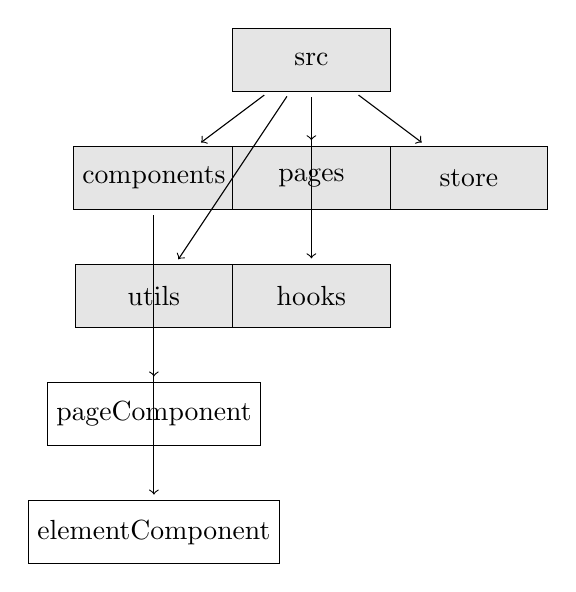
\begin{tikzpicture}[
    file/.style={draw, rectangle, minimum width=2cm, minimum height=0.8cm},
    folder/.style={draw, rectangle, minimum width=2cm, minimum height=0.8cm, fill=gray!20},
    arrow/.style={->, shorten >=2pt, shorten <=2pt}
]

% Folders
\node[folder] (src) at (0,0) {src};
\node[folder] (components) at (-2,-1.5) {components};
\node[folder] (pages) at (0,-1.5) {pages};
\node[folder] (store) at (2,-1.5) {store};
\node[folder] (utils) at (-2,-3) {utils};
\node[folder] (hooks) at (0,-3) {hooks};

% Files
\node[file] (pageComponent) at (-2,-4.5) {pageComponent};
\node[file] (elementComponent) at (-2,-6) {elementComponent};
% ... add more files

% Connections
\draw[arrow] (src) -- (components);
\draw[arrow] (src) -- (pages);
\draw[arrow] (src) -- (store);
\draw[arrow] (src) -- (utils);
\draw[arrow] (src) -- (hooks);
\draw[arrow] (components) -- (pageComponent);
\draw[arrow] (components) -- (elementComponent);
% ... add more connections

\end{tikzpicture}



\pagebreak
\subsubsection{Back-end}
The backend uses the dotNet framework. The development language using the C\# language.

In this project, the backend uses the Onion Architecture.
The Onion Architecture is a typically layered architecture, 
where each layer depends on the inner layer and provides interfaces to the outer layer.
The outer layer provides services to the outermost layer 
and other modules in the same layer based on the interfaces of the inner layer.

From inner to outer, the layers are: Domain, Application, Infrastructure, Presentation.
The Domain layer is the core layer and the innermost layer, used to define domain models, 
which are the business models.
It includes domain models and domain service interfaces.
Domain models are used to define the business models, 
which are the entities in the entity-relationship model and their attributes.
Domain service interfaces are used to define the business services, 
which are the relationships between entities in the entity-relationship model.

The Application layer is the application layer, 
used to define application services, which are the business logic.
It includes domain service implementations and application service interfaces.
Domain service implementations implement the methods of the inner layer's domain service 
interfaces and implement the business logic of the domain models.
Application service interfaces are used to define application services, 
which are the business logic.
It includes but is not limited to database interfaces, testing interfaces, 
HTTP API interfaces, MQTT interfaces, etc.

The Infrastructure layer is the infrastructure layer, used to define infrastructure.
It includes database implementations, testing implementations, 
HTTP API implementations, MQTT implementations, etc.
Database implementations implement the database interfaces 
and provide CRUD services for the database.
Testing implementations implement the testing interfaces 
and provide services for unit testing and integration testing.
HTTP API implementations implement the HTTP API interfaces 
and provide CRUD operations for HTTP APIs.
MQTT implementations implement the MQTT interfaces 
and provide CRUD operations for MQTT.

The Presentation layer is the presentation layer, used to define presentation logic, 
such as interfaces and pages. Since this is a backend project,
data presentation and control are handled by the frontend, 
so this layer is not needed.



\pagebreak
\subsubsection{Data communication and storage}
% 关于本项目的数据通信与数据存储的设计, 包括数据通信的协议, 数据存储的设计等
% 关于数据通信的设计:
% 1. 通信协议的选择
% 自前端向后端发送的数据, 有三种传输的数据类型, 
% 一种是普通的增删改查的请求, 对数据传输的时效性要求不高, 但是对数据的准确性, 完整性, 有序性, 安全性有一定的要求,
% 这种数据的传输, 采用 HTTP 协议, 以及 RESTful API 的设计. 可以有效的保证对数据传输的以上要求.
% 一种是对数据通道的创建和流媒体数据的传输, 对数据传输的时效性, 安全性要求较高, 这种数据的传输, 采用 WebRTC 协议, 以及 MQTT 协议.
% 配合可以快速解码的 flatbuffers 协议, 可以有效的保证对数据传输的以上要求.
% 最后一种是对设备的状态信息和操作信息的传输, 对完整性, 有序性, 安全性都有较高的要求, 这种数据的传输, 采用 MQTT 协议
% 同时也使用了 flatbuffers 协议.
% 
% 2. 数据通信的通信架构和通信流程
% 本项目的数据通信的通信架构, 是基于前后端分离的架构, 前端使用 React 框架, 后端使用 dotnet 框架.
% 当前端需要向后端发送数据的时候, 前端会向后端发送 HTTP 请求, 后端接收到 HTTP 请求之后, 会根据请求的数据类型,
% 选择不同的数据处理方式, 对于普通的增删改查的请求, 后端会根据 RESTful API 的设计, 对数据进行增删改查的操作,
% 对于对数据通道的创建和流媒体数据的传输, 后端会根据 WebRTC 协议, 对数据通道进行创建, 并且帮助前端和设备建立数据通道,
% 当数据通道建立后, 前端和设备之间则使用 flatbuffer 的数据格式对流媒体数据进行传输,
% 对于设备的状态信息和操作信息的传输, 前端会直接向 MQTT broker 发送 MQTT 请求, 
% 设备会在其自身的固件中监听相关的 MQTT 请求, 并且返回相关的数据.
% 
% 3. 数据通信的格式
% 本项目的数据通信的格式, 有三种, 
% 一种是 HTTP 协议, 
% 使用 json 格式对数据进行传输,
% 一种是 WebRTC 协议, 
% 使用 flatbuffers 格式对数据进行传输,
% 一种是 MQTT 协议.
% 使用 flatbuffers 格式对数据进行传输,
% 
% 关于数据存储的设计:
% 1. 数据存储的数据库的选择
% 本项目的数据存储的数据库的选择, 使用了轻量级的数据库 SQLite,
% SQLite 是一个进程内的库, 实现了自给自足的, 无服务器的, 零配置的, 事务性的 SQL 数据库引擎.
% 这是因为整个项目的目的是为了实现前端与设备之间的数据通信, 对于数据库数据的增删改查操作的要求不高,
% 数据量较小, 且对于数据库的数据的事务性要求不高, 所以选择了 SQLite 数据库.
% 2. 项目前后端的数据结构的设计
% 在本项目中, 前端由于使用了 React 框架, 所以前端的数据结构的设计, 使用了基于状态的数据结构的设计,
% 每个组件或者数据集都包含一个状态对象, 这个状态对象的属性就是组件的各个状态. 
% 使用状态对象的原因是, 可以方便的对状态进行管理, 采用对象-属性的形式, 可以方便的针对不同组件的同类状态进行区分,
% 由于跨组件的状态是由 redux 进行管理的, 这种状态对象的设计, 可以更搞笑的对状态进行更新和传递.
% 后端由于使用了 dotnet 框架, 所以后端的数据结构的设计, 使用了基于类的数据结构的设计,
% 采用了面向对象的编程思想, 对数据进行了封装, 使得数据的传输更加的安全, 有序, 完整.


\pagebreak

% \subsection{Domain model}
% \documentclass[]{article}
\usepackage{graphicx}
\usepackage{amsmath}
\usepackage{tikz}

% libaries
\usetikzlibrary{shapes,arrows}

%Define the listing package
\usepackage{listings} %code highlighter
\usepackage{color} %use color
\definecolor{mygreen}{rgb}{0,0.6,0}
\definecolor{mygray}{rgb}{0.5,0.5,0.5}
\definecolor{mymauve}{rgb}{0.58,0,0.82}

%Customize a bit the look
\lstset{ %
backgroundcolor=\color{white}, % choose the background color; you must add \usepackage{color} or \usepackage{xcolor}
basicstyle=\footnotesize, % the size of the fonts that are used for the code
breakatwhitespace=false, % sets if automatic breaks should only happen at whitespace
breaklines=true, % sets automatic line breaking
captionpos=b, % sets the caption-position to bottom
commentstyle=\color{mygreen}, % comment style
deletekeywords={...}, % if you want to delete keywords from the given language
escapeinside={\%*}{*)}, % if you want to add LaTeX within your code
extendedchars=true, % lets you use non-ASCII characters; for 8-bits encodings only, does not work with UTF-8
frame=single, % adds a frame around the code
keepspaces=true, % keeps spaces in text, useful for keeping indentation of code (possibly needs columns=flexible)
keywordstyle=\color{blue}, % keyword style
% language=Octave, % the language of the code
morekeywords={*,...}, % if you want to add more keywords to the set
numbers=left, % where to put the line-numbers; possible values are (none, left, right)
numbersep=5pt, % how far the line-numbers are from the code
numberstyle=\tiny\color{mygray}, % the style that is used for the line-numbers
rulecolor=\color{black}, % if not set, the frame-color may be changed on line-breaks within not-black text (e.g. comments (green here))
showspaces=false, % show spaces everywhere adding particular underscores; it overrides 'showstringspaces'
showstringspaces=false, % underline spaces within strings only
showtabs=false, % show tabs within strings adding particular underscores
stepnumber=1, % the step between two line-numbers. If it's 1, each line will be numbered
stringstyle=\color{mymauve}, % string literal style
tabsize=2, % sets default tabsize to 2 spaces
title=\lstname % show the filename of files included with \lstinputlisting; also try caption instead of title
}

\definecolor{darkgray}{rgb}{.4,.4,.4}
\definecolor{purple}{rgb}{0.65, 0.12, 0.82}

\lstdefinelanguage{React}{
keywords={const, typeof, new, true, false, catch, function, return, null, catch, switch, var, if, in, while, do, else, case, break},
keywordstyle=\color{blue}\bfseries,
ndkeywords={class, export, boolean, throw, implements, import, this},
ndkeywordstyle=\color{darkgray}\bfseries,
identifierstyle=\color{mygreen},
sensitive=false,
comment=[l]{//},
morecomment=[s]{/*}{*/},
commentstyle=\color{purple}\ttfamily,
string=[b]{"}{'}{`},
stringstyle=\color{red}\ttfamily,
morestring=[b]',
morestring=[b]",
morestring=[b]`',
}

\lstdefinelanguage{CSharp}{
keywords={const, typeof, new, true, false, catch, function, return, null, catch, switch, var, if, in, while, do, else, case, break},
keywordstyle=\color{blue}\bfseries,
ndkeywords={class, export, boolean, throw, implements, import, this},
ndkeywordstyle=\color{darkgray}\bfseries,
identifierstyle=\color{mygreen},
sensitive=false,
comment=[l]{//},
morecomment=[s]{/*}{*/},
commentstyle=\color{purple}\ttfamily,
string=[b]{"}{'}{`},
stringstyle=\color{red}\ttfamily,
morestring=[b]',
morestring=[b]",
morestring=[b]`',
}

\lstset{
language=React,
extendedchars=true,
basicstyle=\footnotesize\ttfamily,
showstringspaces=false,
showspaces=false,
numbers=left,
numberstyle=\footnotesize,
numbersep=9pt,
tabsize=2,
breaklines=true,
showtabs=false,
captionpos=b
}

\lstset{
language=CSharp,
extendedchars=true,
basicstyle=\footnotesize\ttfamily,
showstringspaces=false,
showspaces=false,
numbers=left,
numberstyle=\footnotesize,
numbersep=9pt,
tabsize=2,
breaklines=true,
showtabs=false,
captionpos=b
}

% \usepackage{cite} % Add this line for citation

% \bibliographystyle{plain}

\title{
The implementation of BifrostConnect Front-end scope, 
re-design and development with the relevant back-end support develop.
}
\author{
    Fei Gu \\
    Erhvervs Akademi Sydvest \\
    Computer Science 21\\
    }
\date{\today}

\begin{document}

% Front page
\maketitle
\begin{center}
    Supervisor: Henrik Boulund Meng Hansen \\
    Company: BifrostConnect \\
    Engineering Director: Jasper Wass \\
\end{center}
\tableofcontents
\pagebreak


% The introduction
\section{Introduction}
\subsection{Background}\input{sections/introduction/background.tex}
\subsection{The company}\input{sections/introduction/aboutCompany}
\subsection{The project}\input{sections/introduction/aboutProject}
\pagebreak

% The problem statement
\section{Problem Statement}
\subsection{Statement}
\input{sections/problemStatement/statement}
\subsection{Situation}
\input{sections/problemStatement/situation}
\subsection{Potential Solution}
\input{sections/problemStatement/potentialSolution}
\pagebreak

% Requirement analysis
\section{Requirement Analysis}
\input{sections/requirementAnalysis/index}

\subsection{Stakeholders}
\input{sections/requirementAnalysis/stakeholders/index}

\subsection{Business Domain}
\input{sections/requirementAnalysis/bussinesDomain/index}

\subsection{Scope}
\input{sections/requirementAnalysis/scope}

\subsection{Goals}
\input{sections/requirementAnalysis/goals}
\pagebreak

% Software Design
\section{Software Design}
% developement methods
\subsection{Software Development Methods}
\input{sections/softwareDevelopmentMethods/index}
\subsubsection{Agile Software Development}
\input{sections/softwareDevelopmentMethods/agileSoftwareDevelopment/index}
\subsubsection{Feature Driven Development}
\input{sections/softwareDevelopmentMethods/featureDrivenDevelopment/index}

\pagebreak

% Technology seslection
\subsection{Technology selection}
\input{sections/softwareDesign/technologySelection/index}
\subsubsection{Front-end}
\input{sections/softwareDesign/technologySelection/frontEnd}            
\subsubsection{Back-end}
\input{sections/softwareDesign/technologySelection/backEnd}            
\subsubsection{Database}
\input{sections/softwareDesign/technologySelection/database}
\subsubsection{Data communication}
\input{sections/softwareDesign/technologySelection/dataCommunication}            
\subsubsection{DevOps}
\input{sections/softwareDesign/technologySelection/devOps}
\pagebreak

% Architecture design
\subsection{Architecture design}
\input{sections/softwareDesign/architectureDesign/index}
\pagebreak
\subsubsection{Front-end}
\input{sections/softwareDesign/architectureDesign/frontEndArchitecture}
\pagebreak
\subsubsection{Back-end}
\input{sections/softwareDesign/architectureDesign/backEndArchitecture}
\pagebreak
\subsubsection{Data communication and storage}
\input{sections/softwareDesign/architectureDesign/dataCommunicationArchitecture}
\pagebreak

% \subsection{Domain model}
% \input{sections/softwareDesign/domainModel/index}
% \subsection{Database design}
% % 数据库领域模型 ER 图
% % 包括表和字段的设置.
% % 对于私有键和外键的设置.

% \subsection{Back-end design}
% % 后端对象模型
% % 以及对于对象模型的增删改查
% % 以及相关的其他服务的设计`'

% \subsection{Front-end design}
% % 对于前端的页面结构的设计 
% % 页面的状态的设计, 交互设计

% \subsection{FlatBuffers design}
% % schema 的设计

\subsection{DevOps CI/CD process design}
\input{sections/softwareDesign/devOpsDesign/index}
\subsubsection{Continuous Integration}
\input{sections/softwareDesign/devOpsDesign/continuousIntegration/index}
\subsubsection{Continuous Delivery}
\input{sections/softwareDesign/devOpsDesign/continuousDelivery/index}
\subsubsection{Continuous Deployment}
\input{sections/softwareDesign/devOpsDesign/continuousDeployment/index}
\pagebreak

\section{Software Development} 
\input{sections/softwareDevelopment/index}
\subsection{Overall development}
\input{sections/softwareDevelopment/overallDevelopement/index}
\subsubsection{Front-end}
\input{sections/softwareDevelopment/overallDevelopement/frontEnd/index}
\subsubsection{Back-end}
\input{sections/softwareDevelopment/overallDevelopement/backEnd/index}
\subsubsection{DevOps}
\input{sections/softwareDevelopment/overallDevelopement/devOps/index}
\subsection{Feature development} 
\input{sections/softwareDevelopment/featureDevelopment/index}
\subsubsection{Use Case 1}
\input{sections/softwareDevelopment/featureDevelopment/useCase1/index}
\subsubsection{Feature 1}
\input{sections/softwareDevelopment/featureDevelopment/feature/feature1.tex}
\pagebreak
\section{Conclusion} 
\subsection{Result}
Since the project is still in progress, the result is not available yet.
So far, basic structure of this project has been built. But the most features 
are not implemented yet. 
\subsection{Discussion}
As a single developer for this project, I am confident what I have done so far.
And I can say I understand the most of the knowledge I have used in this project, 
which also means I can explain all the part of the project. 
But this project also relevant some of the complex knowledge which I have to continue 
to study and practice.
\subsection{Future Work}
The future work is to implement the rest of the features. 
Including the most important part which is the 'create session' feature.
\pagebreak
% \bibliography{bibliography}
\pagebreak
% \begin{appendices}
%     \section{Appendix}
% \end{appendices} 
\end{document}
% \subsection{Database design}
% % 数据库领域模型 ER 图
% % 包括表和字段的设置.
% % 对于私有键和外键的设置.

% \subsection{Back-end design}
% % 后端对象模型
% % 以及对于对象模型的增删改查
% % 以及相关的其他服务的设计`'

% \subsection{Front-end design}
% % 对于前端的页面结构的设计 
% % 页面的状态的设计, 交互设计

% \subsection{FlatBuffers design}
% % schema 的设计

\subsection{DevOps CI/CD process design}
\documentclass[]{article}
\usepackage{graphicx}
\usepackage{amsmath}
\usepackage{tikz}

% libaries
\usetikzlibrary{shapes,arrows}

%Define the listing package
\usepackage{listings} %code highlighter
\usepackage{color} %use color
\definecolor{mygreen}{rgb}{0,0.6,0}
\definecolor{mygray}{rgb}{0.5,0.5,0.5}
\definecolor{mymauve}{rgb}{0.58,0,0.82}

%Customize a bit the look
\lstset{ %
backgroundcolor=\color{white}, % choose the background color; you must add \usepackage{color} or \usepackage{xcolor}
basicstyle=\footnotesize, % the size of the fonts that are used for the code
breakatwhitespace=false, % sets if automatic breaks should only happen at whitespace
breaklines=true, % sets automatic line breaking
captionpos=b, % sets the caption-position to bottom
commentstyle=\color{mygreen}, % comment style
deletekeywords={...}, % if you want to delete keywords from the given language
escapeinside={\%*}{*)}, % if you want to add LaTeX within your code
extendedchars=true, % lets you use non-ASCII characters; for 8-bits encodings only, does not work with UTF-8
frame=single, % adds a frame around the code
keepspaces=true, % keeps spaces in text, useful for keeping indentation of code (possibly needs columns=flexible)
keywordstyle=\color{blue}, % keyword style
% language=Octave, % the language of the code
morekeywords={*,...}, % if you want to add more keywords to the set
numbers=left, % where to put the line-numbers; possible values are (none, left, right)
numbersep=5pt, % how far the line-numbers are from the code
numberstyle=\tiny\color{mygray}, % the style that is used for the line-numbers
rulecolor=\color{black}, % if not set, the frame-color may be changed on line-breaks within not-black text (e.g. comments (green here))
showspaces=false, % show spaces everywhere adding particular underscores; it overrides 'showstringspaces'
showstringspaces=false, % underline spaces within strings only
showtabs=false, % show tabs within strings adding particular underscores
stepnumber=1, % the step between two line-numbers. If it's 1, each line will be numbered
stringstyle=\color{mymauve}, % string literal style
tabsize=2, % sets default tabsize to 2 spaces
title=\lstname % show the filename of files included with \lstinputlisting; also try caption instead of title
}

\definecolor{darkgray}{rgb}{.4,.4,.4}
\definecolor{purple}{rgb}{0.65, 0.12, 0.82}

\lstdefinelanguage{React}{
keywords={const, typeof, new, true, false, catch, function, return, null, catch, switch, var, if, in, while, do, else, case, break},
keywordstyle=\color{blue}\bfseries,
ndkeywords={class, export, boolean, throw, implements, import, this},
ndkeywordstyle=\color{darkgray}\bfseries,
identifierstyle=\color{mygreen},
sensitive=false,
comment=[l]{//},
morecomment=[s]{/*}{*/},
commentstyle=\color{purple}\ttfamily,
string=[b]{"}{'}{`},
stringstyle=\color{red}\ttfamily,
morestring=[b]',
morestring=[b]",
morestring=[b]`',
}

\lstdefinelanguage{CSharp}{
keywords={const, typeof, new, true, false, catch, function, return, null, catch, switch, var, if, in, while, do, else, case, break},
keywordstyle=\color{blue}\bfseries,
ndkeywords={class, export, boolean, throw, implements, import, this},
ndkeywordstyle=\color{darkgray}\bfseries,
identifierstyle=\color{mygreen},
sensitive=false,
comment=[l]{//},
morecomment=[s]{/*}{*/},
commentstyle=\color{purple}\ttfamily,
string=[b]{"}{'}{`},
stringstyle=\color{red}\ttfamily,
morestring=[b]',
morestring=[b]",
morestring=[b]`',
}

\lstset{
language=React,
extendedchars=true,
basicstyle=\footnotesize\ttfamily,
showstringspaces=false,
showspaces=false,
numbers=left,
numberstyle=\footnotesize,
numbersep=9pt,
tabsize=2,
breaklines=true,
showtabs=false,
captionpos=b
}

\lstset{
language=CSharp,
extendedchars=true,
basicstyle=\footnotesize\ttfamily,
showstringspaces=false,
showspaces=false,
numbers=left,
numberstyle=\footnotesize,
numbersep=9pt,
tabsize=2,
breaklines=true,
showtabs=false,
captionpos=b
}

% \usepackage{cite} % Add this line for citation

% \bibliographystyle{plain}

\title{
The implementation of BifrostConnect Front-end scope, 
re-design and development with the relevant back-end support develop.
}
\author{
    Fei Gu \\
    Erhvervs Akademi Sydvest \\
    Computer Science 21\\
    }
\date{\today}

\begin{document}

% Front page
\maketitle
\begin{center}
    Supervisor: Henrik Boulund Meng Hansen \\
    Company: BifrostConnect \\
    Engineering Director: Jasper Wass \\
\end{center}
\tableofcontents
\pagebreak


% The introduction
\section{Introduction}
\subsection{Background}\input{sections/introduction/background.tex}
\subsection{The company}\input{sections/introduction/aboutCompany}
\subsection{The project}\input{sections/introduction/aboutProject}
\pagebreak

% The problem statement
\section{Problem Statement}
\subsection{Statement}
\input{sections/problemStatement/statement}
\subsection{Situation}
\input{sections/problemStatement/situation}
\subsection{Potential Solution}
\input{sections/problemStatement/potentialSolution}
\pagebreak

% Requirement analysis
\section{Requirement Analysis}
\input{sections/requirementAnalysis/index}

\subsection{Stakeholders}
\input{sections/requirementAnalysis/stakeholders/index}

\subsection{Business Domain}
\input{sections/requirementAnalysis/bussinesDomain/index}

\subsection{Scope}
\input{sections/requirementAnalysis/scope}

\subsection{Goals}
\input{sections/requirementAnalysis/goals}
\pagebreak

% Software Design
\section{Software Design}
% developement methods
\subsection{Software Development Methods}
\input{sections/softwareDevelopmentMethods/index}
\subsubsection{Agile Software Development}
\input{sections/softwareDevelopmentMethods/agileSoftwareDevelopment/index}
\subsubsection{Feature Driven Development}
\input{sections/softwareDevelopmentMethods/featureDrivenDevelopment/index}

\pagebreak

% Technology seslection
\subsection{Technology selection}
\input{sections/softwareDesign/technologySelection/index}
\subsubsection{Front-end}
\input{sections/softwareDesign/technologySelection/frontEnd}            
\subsubsection{Back-end}
\input{sections/softwareDesign/technologySelection/backEnd}            
\subsubsection{Database}
\input{sections/softwareDesign/technologySelection/database}
\subsubsection{Data communication}
\input{sections/softwareDesign/technologySelection/dataCommunication}            
\subsubsection{DevOps}
\input{sections/softwareDesign/technologySelection/devOps}
\pagebreak

% Architecture design
\subsection{Architecture design}
\input{sections/softwareDesign/architectureDesign/index}
\pagebreak
\subsubsection{Front-end}
\input{sections/softwareDesign/architectureDesign/frontEndArchitecture}
\pagebreak
\subsubsection{Back-end}
\input{sections/softwareDesign/architectureDesign/backEndArchitecture}
\pagebreak
\subsubsection{Data communication and storage}
\input{sections/softwareDesign/architectureDesign/dataCommunicationArchitecture}
\pagebreak

% \subsection{Domain model}
% \input{sections/softwareDesign/domainModel/index}
% \subsection{Database design}
% % 数据库领域模型 ER 图
% % 包括表和字段的设置.
% % 对于私有键和外键的设置.

% \subsection{Back-end design}
% % 后端对象模型
% % 以及对于对象模型的增删改查
% % 以及相关的其他服务的设计`'

% \subsection{Front-end design}
% % 对于前端的页面结构的设计 
% % 页面的状态的设计, 交互设计

% \subsection{FlatBuffers design}
% % schema 的设计

\subsection{DevOps CI/CD process design}
\input{sections/softwareDesign/devOpsDesign/index}
\subsubsection{Continuous Integration}
\input{sections/softwareDesign/devOpsDesign/continuousIntegration/index}
\subsubsection{Continuous Delivery}
\input{sections/softwareDesign/devOpsDesign/continuousDelivery/index}
\subsubsection{Continuous Deployment}
\input{sections/softwareDesign/devOpsDesign/continuousDeployment/index}
\pagebreak

\section{Software Development} 
\input{sections/softwareDevelopment/index}
\subsection{Overall development}
\input{sections/softwareDevelopment/overallDevelopement/index}
\subsubsection{Front-end}
\input{sections/softwareDevelopment/overallDevelopement/frontEnd/index}
\subsubsection{Back-end}
\input{sections/softwareDevelopment/overallDevelopement/backEnd/index}
\subsubsection{DevOps}
\input{sections/softwareDevelopment/overallDevelopement/devOps/index}
\subsection{Feature development} 
\input{sections/softwareDevelopment/featureDevelopment/index}
\subsubsection{Use Case 1}
\input{sections/softwareDevelopment/featureDevelopment/useCase1/index}
\subsubsection{Feature 1}
\input{sections/softwareDevelopment/featureDevelopment/feature/feature1.tex}
\pagebreak
\section{Conclusion} 
\subsection{Result}
Since the project is still in progress, the result is not available yet.
So far, basic structure of this project has been built. But the most features 
are not implemented yet. 
\subsection{Discussion}
As a single developer for this project, I am confident what I have done so far.
And I can say I understand the most of the knowledge I have used in this project, 
which also means I can explain all the part of the project. 
But this project also relevant some of the complex knowledge which I have to continue 
to study and practice.
\subsection{Future Work}
The future work is to implement the rest of the features. 
Including the most important part which is the 'create session' feature.
\pagebreak
% \bibliography{bibliography}
\pagebreak
% \begin{appendices}
%     \section{Appendix}
% \end{appendices} 
\end{document}
\subsubsection{Continuous Integration}
\documentclass[]{article}
\usepackage{graphicx}
\usepackage{amsmath}
\usepackage{tikz}

% libaries
\usetikzlibrary{shapes,arrows}

%Define the listing package
\usepackage{listings} %code highlighter
\usepackage{color} %use color
\definecolor{mygreen}{rgb}{0,0.6,0}
\definecolor{mygray}{rgb}{0.5,0.5,0.5}
\definecolor{mymauve}{rgb}{0.58,0,0.82}

%Customize a bit the look
\lstset{ %
backgroundcolor=\color{white}, % choose the background color; you must add \usepackage{color} or \usepackage{xcolor}
basicstyle=\footnotesize, % the size of the fonts that are used for the code
breakatwhitespace=false, % sets if automatic breaks should only happen at whitespace
breaklines=true, % sets automatic line breaking
captionpos=b, % sets the caption-position to bottom
commentstyle=\color{mygreen}, % comment style
deletekeywords={...}, % if you want to delete keywords from the given language
escapeinside={\%*}{*)}, % if you want to add LaTeX within your code
extendedchars=true, % lets you use non-ASCII characters; for 8-bits encodings only, does not work with UTF-8
frame=single, % adds a frame around the code
keepspaces=true, % keeps spaces in text, useful for keeping indentation of code (possibly needs columns=flexible)
keywordstyle=\color{blue}, % keyword style
% language=Octave, % the language of the code
morekeywords={*,...}, % if you want to add more keywords to the set
numbers=left, % where to put the line-numbers; possible values are (none, left, right)
numbersep=5pt, % how far the line-numbers are from the code
numberstyle=\tiny\color{mygray}, % the style that is used for the line-numbers
rulecolor=\color{black}, % if not set, the frame-color may be changed on line-breaks within not-black text (e.g. comments (green here))
showspaces=false, % show spaces everywhere adding particular underscores; it overrides 'showstringspaces'
showstringspaces=false, % underline spaces within strings only
showtabs=false, % show tabs within strings adding particular underscores
stepnumber=1, % the step between two line-numbers. If it's 1, each line will be numbered
stringstyle=\color{mymauve}, % string literal style
tabsize=2, % sets default tabsize to 2 spaces
title=\lstname % show the filename of files included with \lstinputlisting; also try caption instead of title
}

\definecolor{darkgray}{rgb}{.4,.4,.4}
\definecolor{purple}{rgb}{0.65, 0.12, 0.82}

\lstdefinelanguage{React}{
keywords={const, typeof, new, true, false, catch, function, return, null, catch, switch, var, if, in, while, do, else, case, break},
keywordstyle=\color{blue}\bfseries,
ndkeywords={class, export, boolean, throw, implements, import, this},
ndkeywordstyle=\color{darkgray}\bfseries,
identifierstyle=\color{mygreen},
sensitive=false,
comment=[l]{//},
morecomment=[s]{/*}{*/},
commentstyle=\color{purple}\ttfamily,
string=[b]{"}{'}{`},
stringstyle=\color{red}\ttfamily,
morestring=[b]',
morestring=[b]",
morestring=[b]`',
}

\lstdefinelanguage{CSharp}{
keywords={const, typeof, new, true, false, catch, function, return, null, catch, switch, var, if, in, while, do, else, case, break},
keywordstyle=\color{blue}\bfseries,
ndkeywords={class, export, boolean, throw, implements, import, this},
ndkeywordstyle=\color{darkgray}\bfseries,
identifierstyle=\color{mygreen},
sensitive=false,
comment=[l]{//},
morecomment=[s]{/*}{*/},
commentstyle=\color{purple}\ttfamily,
string=[b]{"}{'}{`},
stringstyle=\color{red}\ttfamily,
morestring=[b]',
morestring=[b]",
morestring=[b]`',
}

\lstset{
language=React,
extendedchars=true,
basicstyle=\footnotesize\ttfamily,
showstringspaces=false,
showspaces=false,
numbers=left,
numberstyle=\footnotesize,
numbersep=9pt,
tabsize=2,
breaklines=true,
showtabs=false,
captionpos=b
}

\lstset{
language=CSharp,
extendedchars=true,
basicstyle=\footnotesize\ttfamily,
showstringspaces=false,
showspaces=false,
numbers=left,
numberstyle=\footnotesize,
numbersep=9pt,
tabsize=2,
breaklines=true,
showtabs=false,
captionpos=b
}

% \usepackage{cite} % Add this line for citation

% \bibliographystyle{plain}

\title{
The implementation of BifrostConnect Front-end scope, 
re-design and development with the relevant back-end support develop.
}
\author{
    Fei Gu \\
    Erhvervs Akademi Sydvest \\
    Computer Science 21\\
    }
\date{\today}

\begin{document}

% Front page
\maketitle
\begin{center}
    Supervisor: Henrik Boulund Meng Hansen \\
    Company: BifrostConnect \\
    Engineering Director: Jasper Wass \\
\end{center}
\tableofcontents
\pagebreak


% The introduction
\section{Introduction}
\subsection{Background}\input{sections/introduction/background.tex}
\subsection{The company}\input{sections/introduction/aboutCompany}
\subsection{The project}\input{sections/introduction/aboutProject}
\pagebreak

% The problem statement
\section{Problem Statement}
\subsection{Statement}
\input{sections/problemStatement/statement}
\subsection{Situation}
\input{sections/problemStatement/situation}
\subsection{Potential Solution}
\input{sections/problemStatement/potentialSolution}
\pagebreak

% Requirement analysis
\section{Requirement Analysis}
\input{sections/requirementAnalysis/index}

\subsection{Stakeholders}
\input{sections/requirementAnalysis/stakeholders/index}

\subsection{Business Domain}
\input{sections/requirementAnalysis/bussinesDomain/index}

\subsection{Scope}
\input{sections/requirementAnalysis/scope}

\subsection{Goals}
\input{sections/requirementAnalysis/goals}
\pagebreak

% Software Design
\section{Software Design}
% developement methods
\subsection{Software Development Methods}
\input{sections/softwareDevelopmentMethods/index}
\subsubsection{Agile Software Development}
\input{sections/softwareDevelopmentMethods/agileSoftwareDevelopment/index}
\subsubsection{Feature Driven Development}
\input{sections/softwareDevelopmentMethods/featureDrivenDevelopment/index}

\pagebreak

% Technology seslection
\subsection{Technology selection}
\input{sections/softwareDesign/technologySelection/index}
\subsubsection{Front-end}
\input{sections/softwareDesign/technologySelection/frontEnd}            
\subsubsection{Back-end}
\input{sections/softwareDesign/technologySelection/backEnd}            
\subsubsection{Database}
\input{sections/softwareDesign/technologySelection/database}
\subsubsection{Data communication}
\input{sections/softwareDesign/technologySelection/dataCommunication}            
\subsubsection{DevOps}
\input{sections/softwareDesign/technologySelection/devOps}
\pagebreak

% Architecture design
\subsection{Architecture design}
\input{sections/softwareDesign/architectureDesign/index}
\pagebreak
\subsubsection{Front-end}
\input{sections/softwareDesign/architectureDesign/frontEndArchitecture}
\pagebreak
\subsubsection{Back-end}
\input{sections/softwareDesign/architectureDesign/backEndArchitecture}
\pagebreak
\subsubsection{Data communication and storage}
\input{sections/softwareDesign/architectureDesign/dataCommunicationArchitecture}
\pagebreak

% \subsection{Domain model}
% \input{sections/softwareDesign/domainModel/index}
% \subsection{Database design}
% % 数据库领域模型 ER 图
% % 包括表和字段的设置.
% % 对于私有键和外键的设置.

% \subsection{Back-end design}
% % 后端对象模型
% % 以及对于对象模型的增删改查
% % 以及相关的其他服务的设计`'

% \subsection{Front-end design}
% % 对于前端的页面结构的设计 
% % 页面的状态的设计, 交互设计

% \subsection{FlatBuffers design}
% % schema 的设计

\subsection{DevOps CI/CD process design}
\input{sections/softwareDesign/devOpsDesign/index}
\subsubsection{Continuous Integration}
\input{sections/softwareDesign/devOpsDesign/continuousIntegration/index}
\subsubsection{Continuous Delivery}
\input{sections/softwareDesign/devOpsDesign/continuousDelivery/index}
\subsubsection{Continuous Deployment}
\input{sections/softwareDesign/devOpsDesign/continuousDeployment/index}
\pagebreak

\section{Software Development} 
\input{sections/softwareDevelopment/index}
\subsection{Overall development}
\input{sections/softwareDevelopment/overallDevelopement/index}
\subsubsection{Front-end}
\input{sections/softwareDevelopment/overallDevelopement/frontEnd/index}
\subsubsection{Back-end}
\input{sections/softwareDevelopment/overallDevelopement/backEnd/index}
\subsubsection{DevOps}
\input{sections/softwareDevelopment/overallDevelopement/devOps/index}
\subsection{Feature development} 
\input{sections/softwareDevelopment/featureDevelopment/index}
\subsubsection{Use Case 1}
\input{sections/softwareDevelopment/featureDevelopment/useCase1/index}
\subsubsection{Feature 1}
\input{sections/softwareDevelopment/featureDevelopment/feature/feature1.tex}
\pagebreak
\section{Conclusion} 
\subsection{Result}
Since the project is still in progress, the result is not available yet.
So far, basic structure of this project has been built. But the most features 
are not implemented yet. 
\subsection{Discussion}
As a single developer for this project, I am confident what I have done so far.
And I can say I understand the most of the knowledge I have used in this project, 
which also means I can explain all the part of the project. 
But this project also relevant some of the complex knowledge which I have to continue 
to study and practice.
\subsection{Future Work}
The future work is to implement the rest of the features. 
Including the most important part which is the 'create session' feature.
\pagebreak
% \bibliography{bibliography}
\pagebreak
% \begin{appendices}
%     \section{Appendix}
% \end{appendices} 
\end{document}
\subsubsection{Continuous Delivery}
\documentclass[]{article}
\usepackage{graphicx}
\usepackage{amsmath}
\usepackage{tikz}

% libaries
\usetikzlibrary{shapes,arrows}

%Define the listing package
\usepackage{listings} %code highlighter
\usepackage{color} %use color
\definecolor{mygreen}{rgb}{0,0.6,0}
\definecolor{mygray}{rgb}{0.5,0.5,0.5}
\definecolor{mymauve}{rgb}{0.58,0,0.82}

%Customize a bit the look
\lstset{ %
backgroundcolor=\color{white}, % choose the background color; you must add \usepackage{color} or \usepackage{xcolor}
basicstyle=\footnotesize, % the size of the fonts that are used for the code
breakatwhitespace=false, % sets if automatic breaks should only happen at whitespace
breaklines=true, % sets automatic line breaking
captionpos=b, % sets the caption-position to bottom
commentstyle=\color{mygreen}, % comment style
deletekeywords={...}, % if you want to delete keywords from the given language
escapeinside={\%*}{*)}, % if you want to add LaTeX within your code
extendedchars=true, % lets you use non-ASCII characters; for 8-bits encodings only, does not work with UTF-8
frame=single, % adds a frame around the code
keepspaces=true, % keeps spaces in text, useful for keeping indentation of code (possibly needs columns=flexible)
keywordstyle=\color{blue}, % keyword style
% language=Octave, % the language of the code
morekeywords={*,...}, % if you want to add more keywords to the set
numbers=left, % where to put the line-numbers; possible values are (none, left, right)
numbersep=5pt, % how far the line-numbers are from the code
numberstyle=\tiny\color{mygray}, % the style that is used for the line-numbers
rulecolor=\color{black}, % if not set, the frame-color may be changed on line-breaks within not-black text (e.g. comments (green here))
showspaces=false, % show spaces everywhere adding particular underscores; it overrides 'showstringspaces'
showstringspaces=false, % underline spaces within strings only
showtabs=false, % show tabs within strings adding particular underscores
stepnumber=1, % the step between two line-numbers. If it's 1, each line will be numbered
stringstyle=\color{mymauve}, % string literal style
tabsize=2, % sets default tabsize to 2 spaces
title=\lstname % show the filename of files included with \lstinputlisting; also try caption instead of title
}

\definecolor{darkgray}{rgb}{.4,.4,.4}
\definecolor{purple}{rgb}{0.65, 0.12, 0.82}

\lstdefinelanguage{React}{
keywords={const, typeof, new, true, false, catch, function, return, null, catch, switch, var, if, in, while, do, else, case, break},
keywordstyle=\color{blue}\bfseries,
ndkeywords={class, export, boolean, throw, implements, import, this},
ndkeywordstyle=\color{darkgray}\bfseries,
identifierstyle=\color{mygreen},
sensitive=false,
comment=[l]{//},
morecomment=[s]{/*}{*/},
commentstyle=\color{purple}\ttfamily,
string=[b]{"}{'}{`},
stringstyle=\color{red}\ttfamily,
morestring=[b]',
morestring=[b]",
morestring=[b]`',
}

\lstdefinelanguage{CSharp}{
keywords={const, typeof, new, true, false, catch, function, return, null, catch, switch, var, if, in, while, do, else, case, break},
keywordstyle=\color{blue}\bfseries,
ndkeywords={class, export, boolean, throw, implements, import, this},
ndkeywordstyle=\color{darkgray}\bfseries,
identifierstyle=\color{mygreen},
sensitive=false,
comment=[l]{//},
morecomment=[s]{/*}{*/},
commentstyle=\color{purple}\ttfamily,
string=[b]{"}{'}{`},
stringstyle=\color{red}\ttfamily,
morestring=[b]',
morestring=[b]",
morestring=[b]`',
}

\lstset{
language=React,
extendedchars=true,
basicstyle=\footnotesize\ttfamily,
showstringspaces=false,
showspaces=false,
numbers=left,
numberstyle=\footnotesize,
numbersep=9pt,
tabsize=2,
breaklines=true,
showtabs=false,
captionpos=b
}

\lstset{
language=CSharp,
extendedchars=true,
basicstyle=\footnotesize\ttfamily,
showstringspaces=false,
showspaces=false,
numbers=left,
numberstyle=\footnotesize,
numbersep=9pt,
tabsize=2,
breaklines=true,
showtabs=false,
captionpos=b
}

% \usepackage{cite} % Add this line for citation

% \bibliographystyle{plain}

\title{
The implementation of BifrostConnect Front-end scope, 
re-design and development with the relevant back-end support develop.
}
\author{
    Fei Gu \\
    Erhvervs Akademi Sydvest \\
    Computer Science 21\\
    }
\date{\today}

\begin{document}

% Front page
\maketitle
\begin{center}
    Supervisor: Henrik Boulund Meng Hansen \\
    Company: BifrostConnect \\
    Engineering Director: Jasper Wass \\
\end{center}
\tableofcontents
\pagebreak


% The introduction
\section{Introduction}
\subsection{Background}\input{sections/introduction/background.tex}
\subsection{The company}\input{sections/introduction/aboutCompany}
\subsection{The project}\input{sections/introduction/aboutProject}
\pagebreak

% The problem statement
\section{Problem Statement}
\subsection{Statement}
\input{sections/problemStatement/statement}
\subsection{Situation}
\input{sections/problemStatement/situation}
\subsection{Potential Solution}
\input{sections/problemStatement/potentialSolution}
\pagebreak

% Requirement analysis
\section{Requirement Analysis}
\input{sections/requirementAnalysis/index}

\subsection{Stakeholders}
\input{sections/requirementAnalysis/stakeholders/index}

\subsection{Business Domain}
\input{sections/requirementAnalysis/bussinesDomain/index}

\subsection{Scope}
\input{sections/requirementAnalysis/scope}

\subsection{Goals}
\input{sections/requirementAnalysis/goals}
\pagebreak

% Software Design
\section{Software Design}
% developement methods
\subsection{Software Development Methods}
\input{sections/softwareDevelopmentMethods/index}
\subsubsection{Agile Software Development}
\input{sections/softwareDevelopmentMethods/agileSoftwareDevelopment/index}
\subsubsection{Feature Driven Development}
\input{sections/softwareDevelopmentMethods/featureDrivenDevelopment/index}

\pagebreak

% Technology seslection
\subsection{Technology selection}
\input{sections/softwareDesign/technologySelection/index}
\subsubsection{Front-end}
\input{sections/softwareDesign/technologySelection/frontEnd}            
\subsubsection{Back-end}
\input{sections/softwareDesign/technologySelection/backEnd}            
\subsubsection{Database}
\input{sections/softwareDesign/technologySelection/database}
\subsubsection{Data communication}
\input{sections/softwareDesign/technologySelection/dataCommunication}            
\subsubsection{DevOps}
\input{sections/softwareDesign/technologySelection/devOps}
\pagebreak

% Architecture design
\subsection{Architecture design}
\input{sections/softwareDesign/architectureDesign/index}
\pagebreak
\subsubsection{Front-end}
\input{sections/softwareDesign/architectureDesign/frontEndArchitecture}
\pagebreak
\subsubsection{Back-end}
\input{sections/softwareDesign/architectureDesign/backEndArchitecture}
\pagebreak
\subsubsection{Data communication and storage}
\input{sections/softwareDesign/architectureDesign/dataCommunicationArchitecture}
\pagebreak

% \subsection{Domain model}
% \input{sections/softwareDesign/domainModel/index}
% \subsection{Database design}
% % 数据库领域模型 ER 图
% % 包括表和字段的设置.
% % 对于私有键和外键的设置.

% \subsection{Back-end design}
% % 后端对象模型
% % 以及对于对象模型的增删改查
% % 以及相关的其他服务的设计`'

% \subsection{Front-end design}
% % 对于前端的页面结构的设计 
% % 页面的状态的设计, 交互设计

% \subsection{FlatBuffers design}
% % schema 的设计

\subsection{DevOps CI/CD process design}
\input{sections/softwareDesign/devOpsDesign/index}
\subsubsection{Continuous Integration}
\input{sections/softwareDesign/devOpsDesign/continuousIntegration/index}
\subsubsection{Continuous Delivery}
\input{sections/softwareDesign/devOpsDesign/continuousDelivery/index}
\subsubsection{Continuous Deployment}
\input{sections/softwareDesign/devOpsDesign/continuousDeployment/index}
\pagebreak

\section{Software Development} 
\input{sections/softwareDevelopment/index}
\subsection{Overall development}
\input{sections/softwareDevelopment/overallDevelopement/index}
\subsubsection{Front-end}
\input{sections/softwareDevelopment/overallDevelopement/frontEnd/index}
\subsubsection{Back-end}
\input{sections/softwareDevelopment/overallDevelopement/backEnd/index}
\subsubsection{DevOps}
\input{sections/softwareDevelopment/overallDevelopement/devOps/index}
\subsection{Feature development} 
\input{sections/softwareDevelopment/featureDevelopment/index}
\subsubsection{Use Case 1}
\input{sections/softwareDevelopment/featureDevelopment/useCase1/index}
\subsubsection{Feature 1}
\input{sections/softwareDevelopment/featureDevelopment/feature/feature1.tex}
\pagebreak
\section{Conclusion} 
\subsection{Result}
Since the project is still in progress, the result is not available yet.
So far, basic structure of this project has been built. But the most features 
are not implemented yet. 
\subsection{Discussion}
As a single developer for this project, I am confident what I have done so far.
And I can say I understand the most of the knowledge I have used in this project, 
which also means I can explain all the part of the project. 
But this project also relevant some of the complex knowledge which I have to continue 
to study and practice.
\subsection{Future Work}
The future work is to implement the rest of the features. 
Including the most important part which is the 'create session' feature.
\pagebreak
% \bibliography{bibliography}
\pagebreak
% \begin{appendices}
%     \section{Appendix}
% \end{appendices} 
\end{document}
\subsubsection{Continuous Deployment}
\documentclass[]{article}
\usepackage{graphicx}
\usepackage{amsmath}
\usepackage{tikz}

% libaries
\usetikzlibrary{shapes,arrows}

%Define the listing package
\usepackage{listings} %code highlighter
\usepackage{color} %use color
\definecolor{mygreen}{rgb}{0,0.6,0}
\definecolor{mygray}{rgb}{0.5,0.5,0.5}
\definecolor{mymauve}{rgb}{0.58,0,0.82}

%Customize a bit the look
\lstset{ %
backgroundcolor=\color{white}, % choose the background color; you must add \usepackage{color} or \usepackage{xcolor}
basicstyle=\footnotesize, % the size of the fonts that are used for the code
breakatwhitespace=false, % sets if automatic breaks should only happen at whitespace
breaklines=true, % sets automatic line breaking
captionpos=b, % sets the caption-position to bottom
commentstyle=\color{mygreen}, % comment style
deletekeywords={...}, % if you want to delete keywords from the given language
escapeinside={\%*}{*)}, % if you want to add LaTeX within your code
extendedchars=true, % lets you use non-ASCII characters; for 8-bits encodings only, does not work with UTF-8
frame=single, % adds a frame around the code
keepspaces=true, % keeps spaces in text, useful for keeping indentation of code (possibly needs columns=flexible)
keywordstyle=\color{blue}, % keyword style
% language=Octave, % the language of the code
morekeywords={*,...}, % if you want to add more keywords to the set
numbers=left, % where to put the line-numbers; possible values are (none, left, right)
numbersep=5pt, % how far the line-numbers are from the code
numberstyle=\tiny\color{mygray}, % the style that is used for the line-numbers
rulecolor=\color{black}, % if not set, the frame-color may be changed on line-breaks within not-black text (e.g. comments (green here))
showspaces=false, % show spaces everywhere adding particular underscores; it overrides 'showstringspaces'
showstringspaces=false, % underline spaces within strings only
showtabs=false, % show tabs within strings adding particular underscores
stepnumber=1, % the step between two line-numbers. If it's 1, each line will be numbered
stringstyle=\color{mymauve}, % string literal style
tabsize=2, % sets default tabsize to 2 spaces
title=\lstname % show the filename of files included with \lstinputlisting; also try caption instead of title
}

\definecolor{darkgray}{rgb}{.4,.4,.4}
\definecolor{purple}{rgb}{0.65, 0.12, 0.82}

\lstdefinelanguage{React}{
keywords={const, typeof, new, true, false, catch, function, return, null, catch, switch, var, if, in, while, do, else, case, break},
keywordstyle=\color{blue}\bfseries,
ndkeywords={class, export, boolean, throw, implements, import, this},
ndkeywordstyle=\color{darkgray}\bfseries,
identifierstyle=\color{mygreen},
sensitive=false,
comment=[l]{//},
morecomment=[s]{/*}{*/},
commentstyle=\color{purple}\ttfamily,
string=[b]{"}{'}{`},
stringstyle=\color{red}\ttfamily,
morestring=[b]',
morestring=[b]",
morestring=[b]`',
}

\lstdefinelanguage{CSharp}{
keywords={const, typeof, new, true, false, catch, function, return, null, catch, switch, var, if, in, while, do, else, case, break},
keywordstyle=\color{blue}\bfseries,
ndkeywords={class, export, boolean, throw, implements, import, this},
ndkeywordstyle=\color{darkgray}\bfseries,
identifierstyle=\color{mygreen},
sensitive=false,
comment=[l]{//},
morecomment=[s]{/*}{*/},
commentstyle=\color{purple}\ttfamily,
string=[b]{"}{'}{`},
stringstyle=\color{red}\ttfamily,
morestring=[b]',
morestring=[b]",
morestring=[b]`',
}

\lstset{
language=React,
extendedchars=true,
basicstyle=\footnotesize\ttfamily,
showstringspaces=false,
showspaces=false,
numbers=left,
numberstyle=\footnotesize,
numbersep=9pt,
tabsize=2,
breaklines=true,
showtabs=false,
captionpos=b
}

\lstset{
language=CSharp,
extendedchars=true,
basicstyle=\footnotesize\ttfamily,
showstringspaces=false,
showspaces=false,
numbers=left,
numberstyle=\footnotesize,
numbersep=9pt,
tabsize=2,
breaklines=true,
showtabs=false,
captionpos=b
}

% \usepackage{cite} % Add this line for citation

% \bibliographystyle{plain}

\title{
The implementation of BifrostConnect Front-end scope, 
re-design and development with the relevant back-end support develop.
}
\author{
    Fei Gu \\
    Erhvervs Akademi Sydvest \\
    Computer Science 21\\
    }
\date{\today}

\begin{document}

% Front page
\maketitle
\begin{center}
    Supervisor: Henrik Boulund Meng Hansen \\
    Company: BifrostConnect \\
    Engineering Director: Jasper Wass \\
\end{center}
\tableofcontents
\pagebreak


% The introduction
\section{Introduction}
\subsection{Background}\input{sections/introduction/background.tex}
\subsection{The company}\input{sections/introduction/aboutCompany}
\subsection{The project}\input{sections/introduction/aboutProject}
\pagebreak

% The problem statement
\section{Problem Statement}
\subsection{Statement}
\input{sections/problemStatement/statement}
\subsection{Situation}
\input{sections/problemStatement/situation}
\subsection{Potential Solution}
\input{sections/problemStatement/potentialSolution}
\pagebreak

% Requirement analysis
\section{Requirement Analysis}
\input{sections/requirementAnalysis/index}

\subsection{Stakeholders}
\input{sections/requirementAnalysis/stakeholders/index}

\subsection{Business Domain}
\input{sections/requirementAnalysis/bussinesDomain/index}

\subsection{Scope}
\input{sections/requirementAnalysis/scope}

\subsection{Goals}
\input{sections/requirementAnalysis/goals}
\pagebreak

% Software Design
\section{Software Design}
% developement methods
\subsection{Software Development Methods}
\input{sections/softwareDevelopmentMethods/index}
\subsubsection{Agile Software Development}
\input{sections/softwareDevelopmentMethods/agileSoftwareDevelopment/index}
\subsubsection{Feature Driven Development}
\input{sections/softwareDevelopmentMethods/featureDrivenDevelopment/index}

\pagebreak

% Technology seslection
\subsection{Technology selection}
\input{sections/softwareDesign/technologySelection/index}
\subsubsection{Front-end}
\input{sections/softwareDesign/technologySelection/frontEnd}            
\subsubsection{Back-end}
\input{sections/softwareDesign/technologySelection/backEnd}            
\subsubsection{Database}
\input{sections/softwareDesign/technologySelection/database}
\subsubsection{Data communication}
\input{sections/softwareDesign/technologySelection/dataCommunication}            
\subsubsection{DevOps}
\input{sections/softwareDesign/technologySelection/devOps}
\pagebreak

% Architecture design
\subsection{Architecture design}
\input{sections/softwareDesign/architectureDesign/index}
\pagebreak
\subsubsection{Front-end}
\input{sections/softwareDesign/architectureDesign/frontEndArchitecture}
\pagebreak
\subsubsection{Back-end}
\input{sections/softwareDesign/architectureDesign/backEndArchitecture}
\pagebreak
\subsubsection{Data communication and storage}
\input{sections/softwareDesign/architectureDesign/dataCommunicationArchitecture}
\pagebreak

% \subsection{Domain model}
% \input{sections/softwareDesign/domainModel/index}
% \subsection{Database design}
% % 数据库领域模型 ER 图
% % 包括表和字段的设置.
% % 对于私有键和外键的设置.

% \subsection{Back-end design}
% % 后端对象模型
% % 以及对于对象模型的增删改查
% % 以及相关的其他服务的设计`'

% \subsection{Front-end design}
% % 对于前端的页面结构的设计 
% % 页面的状态的设计, 交互设计

% \subsection{FlatBuffers design}
% % schema 的设计

\subsection{DevOps CI/CD process design}
\input{sections/softwareDesign/devOpsDesign/index}
\subsubsection{Continuous Integration}
\input{sections/softwareDesign/devOpsDesign/continuousIntegration/index}
\subsubsection{Continuous Delivery}
\input{sections/softwareDesign/devOpsDesign/continuousDelivery/index}
\subsubsection{Continuous Deployment}
\input{sections/softwareDesign/devOpsDesign/continuousDeployment/index}
\pagebreak

\section{Software Development} 
\input{sections/softwareDevelopment/index}
\subsection{Overall development}
\input{sections/softwareDevelopment/overallDevelopement/index}
\subsubsection{Front-end}
\input{sections/softwareDevelopment/overallDevelopement/frontEnd/index}
\subsubsection{Back-end}
\input{sections/softwareDevelopment/overallDevelopement/backEnd/index}
\subsubsection{DevOps}
\input{sections/softwareDevelopment/overallDevelopement/devOps/index}
\subsection{Feature development} 
\input{sections/softwareDevelopment/featureDevelopment/index}
\subsubsection{Use Case 1}
\input{sections/softwareDevelopment/featureDevelopment/useCase1/index}
\subsubsection{Feature 1}
\input{sections/softwareDevelopment/featureDevelopment/feature/feature1.tex}
\pagebreak
\section{Conclusion} 
\subsection{Result}
Since the project is still in progress, the result is not available yet.
So far, basic structure of this project has been built. But the most features 
are not implemented yet. 
\subsection{Discussion}
As a single developer for this project, I am confident what I have done so far.
And I can say I understand the most of the knowledge I have used in this project, 
which also means I can explain all the part of the project. 
But this project also relevant some of the complex knowledge which I have to continue 
to study and practice.
\subsection{Future Work}
The future work is to implement the rest of the features. 
Including the most important part which is the 'create session' feature.
\pagebreak
% \bibliography{bibliography}
\pagebreak
% \begin{appendices}
%     \section{Appendix}
% \end{appendices} 
\end{document}
\pagebreak

\section{Software Development} 
\documentclass[]{article}
\usepackage{graphicx}
\usepackage{amsmath}
\usepackage{tikz}

% libaries
\usetikzlibrary{shapes,arrows}

%Define the listing package
\usepackage{listings} %code highlighter
\usepackage{color} %use color
\definecolor{mygreen}{rgb}{0,0.6,0}
\definecolor{mygray}{rgb}{0.5,0.5,0.5}
\definecolor{mymauve}{rgb}{0.58,0,0.82}

%Customize a bit the look
\lstset{ %
backgroundcolor=\color{white}, % choose the background color; you must add \usepackage{color} or \usepackage{xcolor}
basicstyle=\footnotesize, % the size of the fonts that are used for the code
breakatwhitespace=false, % sets if automatic breaks should only happen at whitespace
breaklines=true, % sets automatic line breaking
captionpos=b, % sets the caption-position to bottom
commentstyle=\color{mygreen}, % comment style
deletekeywords={...}, % if you want to delete keywords from the given language
escapeinside={\%*}{*)}, % if you want to add LaTeX within your code
extendedchars=true, % lets you use non-ASCII characters; for 8-bits encodings only, does not work with UTF-8
frame=single, % adds a frame around the code
keepspaces=true, % keeps spaces in text, useful for keeping indentation of code (possibly needs columns=flexible)
keywordstyle=\color{blue}, % keyword style
% language=Octave, % the language of the code
morekeywords={*,...}, % if you want to add more keywords to the set
numbers=left, % where to put the line-numbers; possible values are (none, left, right)
numbersep=5pt, % how far the line-numbers are from the code
numberstyle=\tiny\color{mygray}, % the style that is used for the line-numbers
rulecolor=\color{black}, % if not set, the frame-color may be changed on line-breaks within not-black text (e.g. comments (green here))
showspaces=false, % show spaces everywhere adding particular underscores; it overrides 'showstringspaces'
showstringspaces=false, % underline spaces within strings only
showtabs=false, % show tabs within strings adding particular underscores
stepnumber=1, % the step between two line-numbers. If it's 1, each line will be numbered
stringstyle=\color{mymauve}, % string literal style
tabsize=2, % sets default tabsize to 2 spaces
title=\lstname % show the filename of files included with \lstinputlisting; also try caption instead of title
}

\definecolor{darkgray}{rgb}{.4,.4,.4}
\definecolor{purple}{rgb}{0.65, 0.12, 0.82}

\lstdefinelanguage{React}{
keywords={const, typeof, new, true, false, catch, function, return, null, catch, switch, var, if, in, while, do, else, case, break},
keywordstyle=\color{blue}\bfseries,
ndkeywords={class, export, boolean, throw, implements, import, this},
ndkeywordstyle=\color{darkgray}\bfseries,
identifierstyle=\color{mygreen},
sensitive=false,
comment=[l]{//},
morecomment=[s]{/*}{*/},
commentstyle=\color{purple}\ttfamily,
string=[b]{"}{'}{`},
stringstyle=\color{red}\ttfamily,
morestring=[b]',
morestring=[b]",
morestring=[b]`',
}

\lstdefinelanguage{CSharp}{
keywords={const, typeof, new, true, false, catch, function, return, null, catch, switch, var, if, in, while, do, else, case, break},
keywordstyle=\color{blue}\bfseries,
ndkeywords={class, export, boolean, throw, implements, import, this},
ndkeywordstyle=\color{darkgray}\bfseries,
identifierstyle=\color{mygreen},
sensitive=false,
comment=[l]{//},
morecomment=[s]{/*}{*/},
commentstyle=\color{purple}\ttfamily,
string=[b]{"}{'}{`},
stringstyle=\color{red}\ttfamily,
morestring=[b]',
morestring=[b]",
morestring=[b]`',
}

\lstset{
language=React,
extendedchars=true,
basicstyle=\footnotesize\ttfamily,
showstringspaces=false,
showspaces=false,
numbers=left,
numberstyle=\footnotesize,
numbersep=9pt,
tabsize=2,
breaklines=true,
showtabs=false,
captionpos=b
}

\lstset{
language=CSharp,
extendedchars=true,
basicstyle=\footnotesize\ttfamily,
showstringspaces=false,
showspaces=false,
numbers=left,
numberstyle=\footnotesize,
numbersep=9pt,
tabsize=2,
breaklines=true,
showtabs=false,
captionpos=b
}

% \usepackage{cite} % Add this line for citation

% \bibliographystyle{plain}

\title{
The implementation of BifrostConnect Front-end scope, 
re-design and development with the relevant back-end support develop.
}
\author{
    Fei Gu \\
    Erhvervs Akademi Sydvest \\
    Computer Science 21\\
    }
\date{\today}

\begin{document}

% Front page
\maketitle
\begin{center}
    Supervisor: Henrik Boulund Meng Hansen \\
    Company: BifrostConnect \\
    Engineering Director: Jasper Wass \\
\end{center}
\tableofcontents
\pagebreak


% The introduction
\section{Introduction}
\subsection{Background}\input{sections/introduction/background.tex}
\subsection{The company}\input{sections/introduction/aboutCompany}
\subsection{The project}\input{sections/introduction/aboutProject}
\pagebreak

% The problem statement
\section{Problem Statement}
\subsection{Statement}
\input{sections/problemStatement/statement}
\subsection{Situation}
\input{sections/problemStatement/situation}
\subsection{Potential Solution}
\input{sections/problemStatement/potentialSolution}
\pagebreak

% Requirement analysis
\section{Requirement Analysis}
\input{sections/requirementAnalysis/index}

\subsection{Stakeholders}
\input{sections/requirementAnalysis/stakeholders/index}

\subsection{Business Domain}
\input{sections/requirementAnalysis/bussinesDomain/index}

\subsection{Scope}
\input{sections/requirementAnalysis/scope}

\subsection{Goals}
\input{sections/requirementAnalysis/goals}
\pagebreak

% Software Design
\section{Software Design}
% developement methods
\subsection{Software Development Methods}
\input{sections/softwareDevelopmentMethods/index}
\subsubsection{Agile Software Development}
\input{sections/softwareDevelopmentMethods/agileSoftwareDevelopment/index}
\subsubsection{Feature Driven Development}
\input{sections/softwareDevelopmentMethods/featureDrivenDevelopment/index}

\pagebreak

% Technology seslection
\subsection{Technology selection}
\input{sections/softwareDesign/technologySelection/index}
\subsubsection{Front-end}
\input{sections/softwareDesign/technologySelection/frontEnd}            
\subsubsection{Back-end}
\input{sections/softwareDesign/technologySelection/backEnd}            
\subsubsection{Database}
\input{sections/softwareDesign/technologySelection/database}
\subsubsection{Data communication}
\input{sections/softwareDesign/technologySelection/dataCommunication}            
\subsubsection{DevOps}
\input{sections/softwareDesign/technologySelection/devOps}
\pagebreak

% Architecture design
\subsection{Architecture design}
\input{sections/softwareDesign/architectureDesign/index}
\pagebreak
\subsubsection{Front-end}
\input{sections/softwareDesign/architectureDesign/frontEndArchitecture}
\pagebreak
\subsubsection{Back-end}
\input{sections/softwareDesign/architectureDesign/backEndArchitecture}
\pagebreak
\subsubsection{Data communication and storage}
\input{sections/softwareDesign/architectureDesign/dataCommunicationArchitecture}
\pagebreak

% \subsection{Domain model}
% \input{sections/softwareDesign/domainModel/index}
% \subsection{Database design}
% % 数据库领域模型 ER 图
% % 包括表和字段的设置.
% % 对于私有键和外键的设置.

% \subsection{Back-end design}
% % 后端对象模型
% % 以及对于对象模型的增删改查
% % 以及相关的其他服务的设计`'

% \subsection{Front-end design}
% % 对于前端的页面结构的设计 
% % 页面的状态的设计, 交互设计

% \subsection{FlatBuffers design}
% % schema 的设计

\subsection{DevOps CI/CD process design}
\input{sections/softwareDesign/devOpsDesign/index}
\subsubsection{Continuous Integration}
\input{sections/softwareDesign/devOpsDesign/continuousIntegration/index}
\subsubsection{Continuous Delivery}
\input{sections/softwareDesign/devOpsDesign/continuousDelivery/index}
\subsubsection{Continuous Deployment}
\input{sections/softwareDesign/devOpsDesign/continuousDeployment/index}
\pagebreak

\section{Software Development} 
\input{sections/softwareDevelopment/index}
\subsection{Overall development}
\input{sections/softwareDevelopment/overallDevelopement/index}
\subsubsection{Front-end}
\input{sections/softwareDevelopment/overallDevelopement/frontEnd/index}
\subsubsection{Back-end}
\input{sections/softwareDevelopment/overallDevelopement/backEnd/index}
\subsubsection{DevOps}
\input{sections/softwareDevelopment/overallDevelopement/devOps/index}
\subsection{Feature development} 
\input{sections/softwareDevelopment/featureDevelopment/index}
\subsubsection{Use Case 1}
\input{sections/softwareDevelopment/featureDevelopment/useCase1/index}
\subsubsection{Feature 1}
\input{sections/softwareDevelopment/featureDevelopment/feature/feature1.tex}
\pagebreak
\section{Conclusion} 
\subsection{Result}
Since the project is still in progress, the result is not available yet.
So far, basic structure of this project has been built. But the most features 
are not implemented yet. 
\subsection{Discussion}
As a single developer for this project, I am confident what I have done so far.
And I can say I understand the most of the knowledge I have used in this project, 
which also means I can explain all the part of the project. 
But this project also relevant some of the complex knowledge which I have to continue 
to study and practice.
\subsection{Future Work}
The future work is to implement the rest of the features. 
Including the most important part which is the 'create session' feature.
\pagebreak
% \bibliography{bibliography}
\pagebreak
% \begin{appendices}
%     \section{Appendix}
% \end{appendices} 
\end{document}
\subsection{Overall development}
\documentclass[]{article}
\usepackage{graphicx}
\usepackage{amsmath}
\usepackage{tikz}

% libaries
\usetikzlibrary{shapes,arrows}

%Define the listing package
\usepackage{listings} %code highlighter
\usepackage{color} %use color
\definecolor{mygreen}{rgb}{0,0.6,0}
\definecolor{mygray}{rgb}{0.5,0.5,0.5}
\definecolor{mymauve}{rgb}{0.58,0,0.82}

%Customize a bit the look
\lstset{ %
backgroundcolor=\color{white}, % choose the background color; you must add \usepackage{color} or \usepackage{xcolor}
basicstyle=\footnotesize, % the size of the fonts that are used for the code
breakatwhitespace=false, % sets if automatic breaks should only happen at whitespace
breaklines=true, % sets automatic line breaking
captionpos=b, % sets the caption-position to bottom
commentstyle=\color{mygreen}, % comment style
deletekeywords={...}, % if you want to delete keywords from the given language
escapeinside={\%*}{*)}, % if you want to add LaTeX within your code
extendedchars=true, % lets you use non-ASCII characters; for 8-bits encodings only, does not work with UTF-8
frame=single, % adds a frame around the code
keepspaces=true, % keeps spaces in text, useful for keeping indentation of code (possibly needs columns=flexible)
keywordstyle=\color{blue}, % keyword style
% language=Octave, % the language of the code
morekeywords={*,...}, % if you want to add more keywords to the set
numbers=left, % where to put the line-numbers; possible values are (none, left, right)
numbersep=5pt, % how far the line-numbers are from the code
numberstyle=\tiny\color{mygray}, % the style that is used for the line-numbers
rulecolor=\color{black}, % if not set, the frame-color may be changed on line-breaks within not-black text (e.g. comments (green here))
showspaces=false, % show spaces everywhere adding particular underscores; it overrides 'showstringspaces'
showstringspaces=false, % underline spaces within strings only
showtabs=false, % show tabs within strings adding particular underscores
stepnumber=1, % the step between two line-numbers. If it's 1, each line will be numbered
stringstyle=\color{mymauve}, % string literal style
tabsize=2, % sets default tabsize to 2 spaces
title=\lstname % show the filename of files included with \lstinputlisting; also try caption instead of title
}

\definecolor{darkgray}{rgb}{.4,.4,.4}
\definecolor{purple}{rgb}{0.65, 0.12, 0.82}

\lstdefinelanguage{React}{
keywords={const, typeof, new, true, false, catch, function, return, null, catch, switch, var, if, in, while, do, else, case, break},
keywordstyle=\color{blue}\bfseries,
ndkeywords={class, export, boolean, throw, implements, import, this},
ndkeywordstyle=\color{darkgray}\bfseries,
identifierstyle=\color{mygreen},
sensitive=false,
comment=[l]{//},
morecomment=[s]{/*}{*/},
commentstyle=\color{purple}\ttfamily,
string=[b]{"}{'}{`},
stringstyle=\color{red}\ttfamily,
morestring=[b]',
morestring=[b]",
morestring=[b]`',
}

\lstdefinelanguage{CSharp}{
keywords={const, typeof, new, true, false, catch, function, return, null, catch, switch, var, if, in, while, do, else, case, break},
keywordstyle=\color{blue}\bfseries,
ndkeywords={class, export, boolean, throw, implements, import, this},
ndkeywordstyle=\color{darkgray}\bfseries,
identifierstyle=\color{mygreen},
sensitive=false,
comment=[l]{//},
morecomment=[s]{/*}{*/},
commentstyle=\color{purple}\ttfamily,
string=[b]{"}{'}{`},
stringstyle=\color{red}\ttfamily,
morestring=[b]',
morestring=[b]",
morestring=[b]`',
}

\lstset{
language=React,
extendedchars=true,
basicstyle=\footnotesize\ttfamily,
showstringspaces=false,
showspaces=false,
numbers=left,
numberstyle=\footnotesize,
numbersep=9pt,
tabsize=2,
breaklines=true,
showtabs=false,
captionpos=b
}

\lstset{
language=CSharp,
extendedchars=true,
basicstyle=\footnotesize\ttfamily,
showstringspaces=false,
showspaces=false,
numbers=left,
numberstyle=\footnotesize,
numbersep=9pt,
tabsize=2,
breaklines=true,
showtabs=false,
captionpos=b
}

% \usepackage{cite} % Add this line for citation

% \bibliographystyle{plain}

\title{
The implementation of BifrostConnect Front-end scope, 
re-design and development with the relevant back-end support develop.
}
\author{
    Fei Gu \\
    Erhvervs Akademi Sydvest \\
    Computer Science 21\\
    }
\date{\today}

\begin{document}

% Front page
\maketitle
\begin{center}
    Supervisor: Henrik Boulund Meng Hansen \\
    Company: BifrostConnect \\
    Engineering Director: Jasper Wass \\
\end{center}
\tableofcontents
\pagebreak


% The introduction
\section{Introduction}
\subsection{Background}\input{sections/introduction/background.tex}
\subsection{The company}\input{sections/introduction/aboutCompany}
\subsection{The project}\input{sections/introduction/aboutProject}
\pagebreak

% The problem statement
\section{Problem Statement}
\subsection{Statement}
\input{sections/problemStatement/statement}
\subsection{Situation}
\input{sections/problemStatement/situation}
\subsection{Potential Solution}
\input{sections/problemStatement/potentialSolution}
\pagebreak

% Requirement analysis
\section{Requirement Analysis}
\input{sections/requirementAnalysis/index}

\subsection{Stakeholders}
\input{sections/requirementAnalysis/stakeholders/index}

\subsection{Business Domain}
\input{sections/requirementAnalysis/bussinesDomain/index}

\subsection{Scope}
\input{sections/requirementAnalysis/scope}

\subsection{Goals}
\input{sections/requirementAnalysis/goals}
\pagebreak

% Software Design
\section{Software Design}
% developement methods
\subsection{Software Development Methods}
\input{sections/softwareDevelopmentMethods/index}
\subsubsection{Agile Software Development}
\input{sections/softwareDevelopmentMethods/agileSoftwareDevelopment/index}
\subsubsection{Feature Driven Development}
\input{sections/softwareDevelopmentMethods/featureDrivenDevelopment/index}

\pagebreak

% Technology seslection
\subsection{Technology selection}
\input{sections/softwareDesign/technologySelection/index}
\subsubsection{Front-end}
\input{sections/softwareDesign/technologySelection/frontEnd}            
\subsubsection{Back-end}
\input{sections/softwareDesign/technologySelection/backEnd}            
\subsubsection{Database}
\input{sections/softwareDesign/technologySelection/database}
\subsubsection{Data communication}
\input{sections/softwareDesign/technologySelection/dataCommunication}            
\subsubsection{DevOps}
\input{sections/softwareDesign/technologySelection/devOps}
\pagebreak

% Architecture design
\subsection{Architecture design}
\input{sections/softwareDesign/architectureDesign/index}
\pagebreak
\subsubsection{Front-end}
\input{sections/softwareDesign/architectureDesign/frontEndArchitecture}
\pagebreak
\subsubsection{Back-end}
\input{sections/softwareDesign/architectureDesign/backEndArchitecture}
\pagebreak
\subsubsection{Data communication and storage}
\input{sections/softwareDesign/architectureDesign/dataCommunicationArchitecture}
\pagebreak

% \subsection{Domain model}
% \input{sections/softwareDesign/domainModel/index}
% \subsection{Database design}
% % 数据库领域模型 ER 图
% % 包括表和字段的设置.
% % 对于私有键和外键的设置.

% \subsection{Back-end design}
% % 后端对象模型
% % 以及对于对象模型的增删改查
% % 以及相关的其他服务的设计`'

% \subsection{Front-end design}
% % 对于前端的页面结构的设计 
% % 页面的状态的设计, 交互设计

% \subsection{FlatBuffers design}
% % schema 的设计

\subsection{DevOps CI/CD process design}
\input{sections/softwareDesign/devOpsDesign/index}
\subsubsection{Continuous Integration}
\input{sections/softwareDesign/devOpsDesign/continuousIntegration/index}
\subsubsection{Continuous Delivery}
\input{sections/softwareDesign/devOpsDesign/continuousDelivery/index}
\subsubsection{Continuous Deployment}
\input{sections/softwareDesign/devOpsDesign/continuousDeployment/index}
\pagebreak

\section{Software Development} 
\input{sections/softwareDevelopment/index}
\subsection{Overall development}
\input{sections/softwareDevelopment/overallDevelopement/index}
\subsubsection{Front-end}
\input{sections/softwareDevelopment/overallDevelopement/frontEnd/index}
\subsubsection{Back-end}
\input{sections/softwareDevelopment/overallDevelopement/backEnd/index}
\subsubsection{DevOps}
\input{sections/softwareDevelopment/overallDevelopement/devOps/index}
\subsection{Feature development} 
\input{sections/softwareDevelopment/featureDevelopment/index}
\subsubsection{Use Case 1}
\input{sections/softwareDevelopment/featureDevelopment/useCase1/index}
\subsubsection{Feature 1}
\input{sections/softwareDevelopment/featureDevelopment/feature/feature1.tex}
\pagebreak
\section{Conclusion} 
\subsection{Result}
Since the project is still in progress, the result is not available yet.
So far, basic structure of this project has been built. But the most features 
are not implemented yet. 
\subsection{Discussion}
As a single developer for this project, I am confident what I have done so far.
And I can say I understand the most of the knowledge I have used in this project, 
which also means I can explain all the part of the project. 
But this project also relevant some of the complex knowledge which I have to continue 
to study and practice.
\subsection{Future Work}
The future work is to implement the rest of the features. 
Including the most important part which is the 'create session' feature.
\pagebreak
% \bibliography{bibliography}
\pagebreak
% \begin{appendices}
%     \section{Appendix}
% \end{appendices} 
\end{document}
\subsubsection{Front-end}
\documentclass[]{article}
\usepackage{graphicx}
\usepackage{amsmath}
\usepackage{tikz}

% libaries
\usetikzlibrary{shapes,arrows}

%Define the listing package
\usepackage{listings} %code highlighter
\usepackage{color} %use color
\definecolor{mygreen}{rgb}{0,0.6,0}
\definecolor{mygray}{rgb}{0.5,0.5,0.5}
\definecolor{mymauve}{rgb}{0.58,0,0.82}

%Customize a bit the look
\lstset{ %
backgroundcolor=\color{white}, % choose the background color; you must add \usepackage{color} or \usepackage{xcolor}
basicstyle=\footnotesize, % the size of the fonts that are used for the code
breakatwhitespace=false, % sets if automatic breaks should only happen at whitespace
breaklines=true, % sets automatic line breaking
captionpos=b, % sets the caption-position to bottom
commentstyle=\color{mygreen}, % comment style
deletekeywords={...}, % if you want to delete keywords from the given language
escapeinside={\%*}{*)}, % if you want to add LaTeX within your code
extendedchars=true, % lets you use non-ASCII characters; for 8-bits encodings only, does not work with UTF-8
frame=single, % adds a frame around the code
keepspaces=true, % keeps spaces in text, useful for keeping indentation of code (possibly needs columns=flexible)
keywordstyle=\color{blue}, % keyword style
% language=Octave, % the language of the code
morekeywords={*,...}, % if you want to add more keywords to the set
numbers=left, % where to put the line-numbers; possible values are (none, left, right)
numbersep=5pt, % how far the line-numbers are from the code
numberstyle=\tiny\color{mygray}, % the style that is used for the line-numbers
rulecolor=\color{black}, % if not set, the frame-color may be changed on line-breaks within not-black text (e.g. comments (green here))
showspaces=false, % show spaces everywhere adding particular underscores; it overrides 'showstringspaces'
showstringspaces=false, % underline spaces within strings only
showtabs=false, % show tabs within strings adding particular underscores
stepnumber=1, % the step between two line-numbers. If it's 1, each line will be numbered
stringstyle=\color{mymauve}, % string literal style
tabsize=2, % sets default tabsize to 2 spaces
title=\lstname % show the filename of files included with \lstinputlisting; also try caption instead of title
}

\definecolor{darkgray}{rgb}{.4,.4,.4}
\definecolor{purple}{rgb}{0.65, 0.12, 0.82}

\lstdefinelanguage{React}{
keywords={const, typeof, new, true, false, catch, function, return, null, catch, switch, var, if, in, while, do, else, case, break},
keywordstyle=\color{blue}\bfseries,
ndkeywords={class, export, boolean, throw, implements, import, this},
ndkeywordstyle=\color{darkgray}\bfseries,
identifierstyle=\color{mygreen},
sensitive=false,
comment=[l]{//},
morecomment=[s]{/*}{*/},
commentstyle=\color{purple}\ttfamily,
string=[b]{"}{'}{`},
stringstyle=\color{red}\ttfamily,
morestring=[b]',
morestring=[b]",
morestring=[b]`',
}

\lstdefinelanguage{CSharp}{
keywords={const, typeof, new, true, false, catch, function, return, null, catch, switch, var, if, in, while, do, else, case, break},
keywordstyle=\color{blue}\bfseries,
ndkeywords={class, export, boolean, throw, implements, import, this},
ndkeywordstyle=\color{darkgray}\bfseries,
identifierstyle=\color{mygreen},
sensitive=false,
comment=[l]{//},
morecomment=[s]{/*}{*/},
commentstyle=\color{purple}\ttfamily,
string=[b]{"}{'}{`},
stringstyle=\color{red}\ttfamily,
morestring=[b]',
morestring=[b]",
morestring=[b]`',
}

\lstset{
language=React,
extendedchars=true,
basicstyle=\footnotesize\ttfamily,
showstringspaces=false,
showspaces=false,
numbers=left,
numberstyle=\footnotesize,
numbersep=9pt,
tabsize=2,
breaklines=true,
showtabs=false,
captionpos=b
}

\lstset{
language=CSharp,
extendedchars=true,
basicstyle=\footnotesize\ttfamily,
showstringspaces=false,
showspaces=false,
numbers=left,
numberstyle=\footnotesize,
numbersep=9pt,
tabsize=2,
breaklines=true,
showtabs=false,
captionpos=b
}

% \usepackage{cite} % Add this line for citation

% \bibliographystyle{plain}

\title{
The implementation of BifrostConnect Front-end scope, 
re-design and development with the relevant back-end support develop.
}
\author{
    Fei Gu \\
    Erhvervs Akademi Sydvest \\
    Computer Science 21\\
    }
\date{\today}

\begin{document}

% Front page
\maketitle
\begin{center}
    Supervisor: Henrik Boulund Meng Hansen \\
    Company: BifrostConnect \\
    Engineering Director: Jasper Wass \\
\end{center}
\tableofcontents
\pagebreak


% The introduction
\section{Introduction}
\subsection{Background}\input{sections/introduction/background.tex}
\subsection{The company}\input{sections/introduction/aboutCompany}
\subsection{The project}\input{sections/introduction/aboutProject}
\pagebreak

% The problem statement
\section{Problem Statement}
\subsection{Statement}
\input{sections/problemStatement/statement}
\subsection{Situation}
\input{sections/problemStatement/situation}
\subsection{Potential Solution}
\input{sections/problemStatement/potentialSolution}
\pagebreak

% Requirement analysis
\section{Requirement Analysis}
\input{sections/requirementAnalysis/index}

\subsection{Stakeholders}
\input{sections/requirementAnalysis/stakeholders/index}

\subsection{Business Domain}
\input{sections/requirementAnalysis/bussinesDomain/index}

\subsection{Scope}
\input{sections/requirementAnalysis/scope}

\subsection{Goals}
\input{sections/requirementAnalysis/goals}
\pagebreak

% Software Design
\section{Software Design}
% developement methods
\subsection{Software Development Methods}
\input{sections/softwareDevelopmentMethods/index}
\subsubsection{Agile Software Development}
\input{sections/softwareDevelopmentMethods/agileSoftwareDevelopment/index}
\subsubsection{Feature Driven Development}
\input{sections/softwareDevelopmentMethods/featureDrivenDevelopment/index}

\pagebreak

% Technology seslection
\subsection{Technology selection}
\input{sections/softwareDesign/technologySelection/index}
\subsubsection{Front-end}
\input{sections/softwareDesign/technologySelection/frontEnd}            
\subsubsection{Back-end}
\input{sections/softwareDesign/technologySelection/backEnd}            
\subsubsection{Database}
\input{sections/softwareDesign/technologySelection/database}
\subsubsection{Data communication}
\input{sections/softwareDesign/technologySelection/dataCommunication}            
\subsubsection{DevOps}
\input{sections/softwareDesign/technologySelection/devOps}
\pagebreak

% Architecture design
\subsection{Architecture design}
\input{sections/softwareDesign/architectureDesign/index}
\pagebreak
\subsubsection{Front-end}
\input{sections/softwareDesign/architectureDesign/frontEndArchitecture}
\pagebreak
\subsubsection{Back-end}
\input{sections/softwareDesign/architectureDesign/backEndArchitecture}
\pagebreak
\subsubsection{Data communication and storage}
\input{sections/softwareDesign/architectureDesign/dataCommunicationArchitecture}
\pagebreak

% \subsection{Domain model}
% \input{sections/softwareDesign/domainModel/index}
% \subsection{Database design}
% % 数据库领域模型 ER 图
% % 包括表和字段的设置.
% % 对于私有键和外键的设置.

% \subsection{Back-end design}
% % 后端对象模型
% % 以及对于对象模型的增删改查
% % 以及相关的其他服务的设计`'

% \subsection{Front-end design}
% % 对于前端的页面结构的设计 
% % 页面的状态的设计, 交互设计

% \subsection{FlatBuffers design}
% % schema 的设计

\subsection{DevOps CI/CD process design}
\input{sections/softwareDesign/devOpsDesign/index}
\subsubsection{Continuous Integration}
\input{sections/softwareDesign/devOpsDesign/continuousIntegration/index}
\subsubsection{Continuous Delivery}
\input{sections/softwareDesign/devOpsDesign/continuousDelivery/index}
\subsubsection{Continuous Deployment}
\input{sections/softwareDesign/devOpsDesign/continuousDeployment/index}
\pagebreak

\section{Software Development} 
\input{sections/softwareDevelopment/index}
\subsection{Overall development}
\input{sections/softwareDevelopment/overallDevelopement/index}
\subsubsection{Front-end}
\input{sections/softwareDevelopment/overallDevelopement/frontEnd/index}
\subsubsection{Back-end}
\input{sections/softwareDevelopment/overallDevelopement/backEnd/index}
\subsubsection{DevOps}
\input{sections/softwareDevelopment/overallDevelopement/devOps/index}
\subsection{Feature development} 
\input{sections/softwareDevelopment/featureDevelopment/index}
\subsubsection{Use Case 1}
\input{sections/softwareDevelopment/featureDevelopment/useCase1/index}
\subsubsection{Feature 1}
\input{sections/softwareDevelopment/featureDevelopment/feature/feature1.tex}
\pagebreak
\section{Conclusion} 
\subsection{Result}
Since the project is still in progress, the result is not available yet.
So far, basic structure of this project has been built. But the most features 
are not implemented yet. 
\subsection{Discussion}
As a single developer for this project, I am confident what I have done so far.
And I can say I understand the most of the knowledge I have used in this project, 
which also means I can explain all the part of the project. 
But this project also relevant some of the complex knowledge which I have to continue 
to study and practice.
\subsection{Future Work}
The future work is to implement the rest of the features. 
Including the most important part which is the 'create session' feature.
\pagebreak
% \bibliography{bibliography}
\pagebreak
% \begin{appendices}
%     \section{Appendix}
% \end{appendices} 
\end{document}
\subsubsection{Back-end}
\documentclass[]{article}
\usepackage{graphicx}
\usepackage{amsmath}
\usepackage{tikz}

% libaries
\usetikzlibrary{shapes,arrows}

%Define the listing package
\usepackage{listings} %code highlighter
\usepackage{color} %use color
\definecolor{mygreen}{rgb}{0,0.6,0}
\definecolor{mygray}{rgb}{0.5,0.5,0.5}
\definecolor{mymauve}{rgb}{0.58,0,0.82}

%Customize a bit the look
\lstset{ %
backgroundcolor=\color{white}, % choose the background color; you must add \usepackage{color} or \usepackage{xcolor}
basicstyle=\footnotesize, % the size of the fonts that are used for the code
breakatwhitespace=false, % sets if automatic breaks should only happen at whitespace
breaklines=true, % sets automatic line breaking
captionpos=b, % sets the caption-position to bottom
commentstyle=\color{mygreen}, % comment style
deletekeywords={...}, % if you want to delete keywords from the given language
escapeinside={\%*}{*)}, % if you want to add LaTeX within your code
extendedchars=true, % lets you use non-ASCII characters; for 8-bits encodings only, does not work with UTF-8
frame=single, % adds a frame around the code
keepspaces=true, % keeps spaces in text, useful for keeping indentation of code (possibly needs columns=flexible)
keywordstyle=\color{blue}, % keyword style
% language=Octave, % the language of the code
morekeywords={*,...}, % if you want to add more keywords to the set
numbers=left, % where to put the line-numbers; possible values are (none, left, right)
numbersep=5pt, % how far the line-numbers are from the code
numberstyle=\tiny\color{mygray}, % the style that is used for the line-numbers
rulecolor=\color{black}, % if not set, the frame-color may be changed on line-breaks within not-black text (e.g. comments (green here))
showspaces=false, % show spaces everywhere adding particular underscores; it overrides 'showstringspaces'
showstringspaces=false, % underline spaces within strings only
showtabs=false, % show tabs within strings adding particular underscores
stepnumber=1, % the step between two line-numbers. If it's 1, each line will be numbered
stringstyle=\color{mymauve}, % string literal style
tabsize=2, % sets default tabsize to 2 spaces
title=\lstname % show the filename of files included with \lstinputlisting; also try caption instead of title
}

\definecolor{darkgray}{rgb}{.4,.4,.4}
\definecolor{purple}{rgb}{0.65, 0.12, 0.82}

\lstdefinelanguage{React}{
keywords={const, typeof, new, true, false, catch, function, return, null, catch, switch, var, if, in, while, do, else, case, break},
keywordstyle=\color{blue}\bfseries,
ndkeywords={class, export, boolean, throw, implements, import, this},
ndkeywordstyle=\color{darkgray}\bfseries,
identifierstyle=\color{mygreen},
sensitive=false,
comment=[l]{//},
morecomment=[s]{/*}{*/},
commentstyle=\color{purple}\ttfamily,
string=[b]{"}{'}{`},
stringstyle=\color{red}\ttfamily,
morestring=[b]',
morestring=[b]",
morestring=[b]`',
}

\lstdefinelanguage{CSharp}{
keywords={const, typeof, new, true, false, catch, function, return, null, catch, switch, var, if, in, while, do, else, case, break},
keywordstyle=\color{blue}\bfseries,
ndkeywords={class, export, boolean, throw, implements, import, this},
ndkeywordstyle=\color{darkgray}\bfseries,
identifierstyle=\color{mygreen},
sensitive=false,
comment=[l]{//},
morecomment=[s]{/*}{*/},
commentstyle=\color{purple}\ttfamily,
string=[b]{"}{'}{`},
stringstyle=\color{red}\ttfamily,
morestring=[b]',
morestring=[b]",
morestring=[b]`',
}

\lstset{
language=React,
extendedchars=true,
basicstyle=\footnotesize\ttfamily,
showstringspaces=false,
showspaces=false,
numbers=left,
numberstyle=\footnotesize,
numbersep=9pt,
tabsize=2,
breaklines=true,
showtabs=false,
captionpos=b
}

\lstset{
language=CSharp,
extendedchars=true,
basicstyle=\footnotesize\ttfamily,
showstringspaces=false,
showspaces=false,
numbers=left,
numberstyle=\footnotesize,
numbersep=9pt,
tabsize=2,
breaklines=true,
showtabs=false,
captionpos=b
}

% \usepackage{cite} % Add this line for citation

% \bibliographystyle{plain}

\title{
The implementation of BifrostConnect Front-end scope, 
re-design and development with the relevant back-end support develop.
}
\author{
    Fei Gu \\
    Erhvervs Akademi Sydvest \\
    Computer Science 21\\
    }
\date{\today}

\begin{document}

% Front page
\maketitle
\begin{center}
    Supervisor: Henrik Boulund Meng Hansen \\
    Company: BifrostConnect \\
    Engineering Director: Jasper Wass \\
\end{center}
\tableofcontents
\pagebreak


% The introduction
\section{Introduction}
\subsection{Background}\input{sections/introduction/background.tex}
\subsection{The company}\input{sections/introduction/aboutCompany}
\subsection{The project}\input{sections/introduction/aboutProject}
\pagebreak

% The problem statement
\section{Problem Statement}
\subsection{Statement}
\input{sections/problemStatement/statement}
\subsection{Situation}
\input{sections/problemStatement/situation}
\subsection{Potential Solution}
\input{sections/problemStatement/potentialSolution}
\pagebreak

% Requirement analysis
\section{Requirement Analysis}
\input{sections/requirementAnalysis/index}

\subsection{Stakeholders}
\input{sections/requirementAnalysis/stakeholders/index}

\subsection{Business Domain}
\input{sections/requirementAnalysis/bussinesDomain/index}

\subsection{Scope}
\input{sections/requirementAnalysis/scope}

\subsection{Goals}
\input{sections/requirementAnalysis/goals}
\pagebreak

% Software Design
\section{Software Design}
% developement methods
\subsection{Software Development Methods}
\input{sections/softwareDevelopmentMethods/index}
\subsubsection{Agile Software Development}
\input{sections/softwareDevelopmentMethods/agileSoftwareDevelopment/index}
\subsubsection{Feature Driven Development}
\input{sections/softwareDevelopmentMethods/featureDrivenDevelopment/index}

\pagebreak

% Technology seslection
\subsection{Technology selection}
\input{sections/softwareDesign/technologySelection/index}
\subsubsection{Front-end}
\input{sections/softwareDesign/technologySelection/frontEnd}            
\subsubsection{Back-end}
\input{sections/softwareDesign/technologySelection/backEnd}            
\subsubsection{Database}
\input{sections/softwareDesign/technologySelection/database}
\subsubsection{Data communication}
\input{sections/softwareDesign/technologySelection/dataCommunication}            
\subsubsection{DevOps}
\input{sections/softwareDesign/technologySelection/devOps}
\pagebreak

% Architecture design
\subsection{Architecture design}
\input{sections/softwareDesign/architectureDesign/index}
\pagebreak
\subsubsection{Front-end}
\input{sections/softwareDesign/architectureDesign/frontEndArchitecture}
\pagebreak
\subsubsection{Back-end}
\input{sections/softwareDesign/architectureDesign/backEndArchitecture}
\pagebreak
\subsubsection{Data communication and storage}
\input{sections/softwareDesign/architectureDesign/dataCommunicationArchitecture}
\pagebreak

% \subsection{Domain model}
% \input{sections/softwareDesign/domainModel/index}
% \subsection{Database design}
% % 数据库领域模型 ER 图
% % 包括表和字段的设置.
% % 对于私有键和外键的设置.

% \subsection{Back-end design}
% % 后端对象模型
% % 以及对于对象模型的增删改查
% % 以及相关的其他服务的设计`'

% \subsection{Front-end design}
% % 对于前端的页面结构的设计 
% % 页面的状态的设计, 交互设计

% \subsection{FlatBuffers design}
% % schema 的设计

\subsection{DevOps CI/CD process design}
\input{sections/softwareDesign/devOpsDesign/index}
\subsubsection{Continuous Integration}
\input{sections/softwareDesign/devOpsDesign/continuousIntegration/index}
\subsubsection{Continuous Delivery}
\input{sections/softwareDesign/devOpsDesign/continuousDelivery/index}
\subsubsection{Continuous Deployment}
\input{sections/softwareDesign/devOpsDesign/continuousDeployment/index}
\pagebreak

\section{Software Development} 
\input{sections/softwareDevelopment/index}
\subsection{Overall development}
\input{sections/softwareDevelopment/overallDevelopement/index}
\subsubsection{Front-end}
\input{sections/softwareDevelopment/overallDevelopement/frontEnd/index}
\subsubsection{Back-end}
\input{sections/softwareDevelopment/overallDevelopement/backEnd/index}
\subsubsection{DevOps}
\input{sections/softwareDevelopment/overallDevelopement/devOps/index}
\subsection{Feature development} 
\input{sections/softwareDevelopment/featureDevelopment/index}
\subsubsection{Use Case 1}
\input{sections/softwareDevelopment/featureDevelopment/useCase1/index}
\subsubsection{Feature 1}
\input{sections/softwareDevelopment/featureDevelopment/feature/feature1.tex}
\pagebreak
\section{Conclusion} 
\subsection{Result}
Since the project is still in progress, the result is not available yet.
So far, basic structure of this project has been built. But the most features 
are not implemented yet. 
\subsection{Discussion}
As a single developer for this project, I am confident what I have done so far.
And I can say I understand the most of the knowledge I have used in this project, 
which also means I can explain all the part of the project. 
But this project also relevant some of the complex knowledge which I have to continue 
to study and practice.
\subsection{Future Work}
The future work is to implement the rest of the features. 
Including the most important part which is the 'create session' feature.
\pagebreak
% \bibliography{bibliography}
\pagebreak
% \begin{appendices}
%     \section{Appendix}
% \end{appendices} 
\end{document}
\subsubsection{DevOps}
\documentclass[]{article}
\usepackage{graphicx}
\usepackage{amsmath}
\usepackage{tikz}

% libaries
\usetikzlibrary{shapes,arrows}

%Define the listing package
\usepackage{listings} %code highlighter
\usepackage{color} %use color
\definecolor{mygreen}{rgb}{0,0.6,0}
\definecolor{mygray}{rgb}{0.5,0.5,0.5}
\definecolor{mymauve}{rgb}{0.58,0,0.82}

%Customize a bit the look
\lstset{ %
backgroundcolor=\color{white}, % choose the background color; you must add \usepackage{color} or \usepackage{xcolor}
basicstyle=\footnotesize, % the size of the fonts that are used for the code
breakatwhitespace=false, % sets if automatic breaks should only happen at whitespace
breaklines=true, % sets automatic line breaking
captionpos=b, % sets the caption-position to bottom
commentstyle=\color{mygreen}, % comment style
deletekeywords={...}, % if you want to delete keywords from the given language
escapeinside={\%*}{*)}, % if you want to add LaTeX within your code
extendedchars=true, % lets you use non-ASCII characters; for 8-bits encodings only, does not work with UTF-8
frame=single, % adds a frame around the code
keepspaces=true, % keeps spaces in text, useful for keeping indentation of code (possibly needs columns=flexible)
keywordstyle=\color{blue}, % keyword style
% language=Octave, % the language of the code
morekeywords={*,...}, % if you want to add more keywords to the set
numbers=left, % where to put the line-numbers; possible values are (none, left, right)
numbersep=5pt, % how far the line-numbers are from the code
numberstyle=\tiny\color{mygray}, % the style that is used for the line-numbers
rulecolor=\color{black}, % if not set, the frame-color may be changed on line-breaks within not-black text (e.g. comments (green here))
showspaces=false, % show spaces everywhere adding particular underscores; it overrides 'showstringspaces'
showstringspaces=false, % underline spaces within strings only
showtabs=false, % show tabs within strings adding particular underscores
stepnumber=1, % the step between two line-numbers. If it's 1, each line will be numbered
stringstyle=\color{mymauve}, % string literal style
tabsize=2, % sets default tabsize to 2 spaces
title=\lstname % show the filename of files included with \lstinputlisting; also try caption instead of title
}

\definecolor{darkgray}{rgb}{.4,.4,.4}
\definecolor{purple}{rgb}{0.65, 0.12, 0.82}

\lstdefinelanguage{React}{
keywords={const, typeof, new, true, false, catch, function, return, null, catch, switch, var, if, in, while, do, else, case, break},
keywordstyle=\color{blue}\bfseries,
ndkeywords={class, export, boolean, throw, implements, import, this},
ndkeywordstyle=\color{darkgray}\bfseries,
identifierstyle=\color{mygreen},
sensitive=false,
comment=[l]{//},
morecomment=[s]{/*}{*/},
commentstyle=\color{purple}\ttfamily,
string=[b]{"}{'}{`},
stringstyle=\color{red}\ttfamily,
morestring=[b]',
morestring=[b]",
morestring=[b]`',
}

\lstdefinelanguage{CSharp}{
keywords={const, typeof, new, true, false, catch, function, return, null, catch, switch, var, if, in, while, do, else, case, break},
keywordstyle=\color{blue}\bfseries,
ndkeywords={class, export, boolean, throw, implements, import, this},
ndkeywordstyle=\color{darkgray}\bfseries,
identifierstyle=\color{mygreen},
sensitive=false,
comment=[l]{//},
morecomment=[s]{/*}{*/},
commentstyle=\color{purple}\ttfamily,
string=[b]{"}{'}{`},
stringstyle=\color{red}\ttfamily,
morestring=[b]',
morestring=[b]",
morestring=[b]`',
}

\lstset{
language=React,
extendedchars=true,
basicstyle=\footnotesize\ttfamily,
showstringspaces=false,
showspaces=false,
numbers=left,
numberstyle=\footnotesize,
numbersep=9pt,
tabsize=2,
breaklines=true,
showtabs=false,
captionpos=b
}

\lstset{
language=CSharp,
extendedchars=true,
basicstyle=\footnotesize\ttfamily,
showstringspaces=false,
showspaces=false,
numbers=left,
numberstyle=\footnotesize,
numbersep=9pt,
tabsize=2,
breaklines=true,
showtabs=false,
captionpos=b
}

% \usepackage{cite} % Add this line for citation

% \bibliographystyle{plain}

\title{
The implementation of BifrostConnect Front-end scope, 
re-design and development with the relevant back-end support develop.
}
\author{
    Fei Gu \\
    Erhvervs Akademi Sydvest \\
    Computer Science 21\\
    }
\date{\today}

\begin{document}

% Front page
\maketitle
\begin{center}
    Supervisor: Henrik Boulund Meng Hansen \\
    Company: BifrostConnect \\
    Engineering Director: Jasper Wass \\
\end{center}
\tableofcontents
\pagebreak


% The introduction
\section{Introduction}
\subsection{Background}\input{sections/introduction/background.tex}
\subsection{The company}\input{sections/introduction/aboutCompany}
\subsection{The project}\input{sections/introduction/aboutProject}
\pagebreak

% The problem statement
\section{Problem Statement}
\subsection{Statement}
\input{sections/problemStatement/statement}
\subsection{Situation}
\input{sections/problemStatement/situation}
\subsection{Potential Solution}
\input{sections/problemStatement/potentialSolution}
\pagebreak

% Requirement analysis
\section{Requirement Analysis}
\input{sections/requirementAnalysis/index}

\subsection{Stakeholders}
\input{sections/requirementAnalysis/stakeholders/index}

\subsection{Business Domain}
\input{sections/requirementAnalysis/bussinesDomain/index}

\subsection{Scope}
\input{sections/requirementAnalysis/scope}

\subsection{Goals}
\input{sections/requirementAnalysis/goals}
\pagebreak

% Software Design
\section{Software Design}
% developement methods
\subsection{Software Development Methods}
\input{sections/softwareDevelopmentMethods/index}
\subsubsection{Agile Software Development}
\input{sections/softwareDevelopmentMethods/agileSoftwareDevelopment/index}
\subsubsection{Feature Driven Development}
\input{sections/softwareDevelopmentMethods/featureDrivenDevelopment/index}

\pagebreak

% Technology seslection
\subsection{Technology selection}
\input{sections/softwareDesign/technologySelection/index}
\subsubsection{Front-end}
\input{sections/softwareDesign/technologySelection/frontEnd}            
\subsubsection{Back-end}
\input{sections/softwareDesign/technologySelection/backEnd}            
\subsubsection{Database}
\input{sections/softwareDesign/technologySelection/database}
\subsubsection{Data communication}
\input{sections/softwareDesign/technologySelection/dataCommunication}            
\subsubsection{DevOps}
\input{sections/softwareDesign/technologySelection/devOps}
\pagebreak

% Architecture design
\subsection{Architecture design}
\input{sections/softwareDesign/architectureDesign/index}
\pagebreak
\subsubsection{Front-end}
\input{sections/softwareDesign/architectureDesign/frontEndArchitecture}
\pagebreak
\subsubsection{Back-end}
\input{sections/softwareDesign/architectureDesign/backEndArchitecture}
\pagebreak
\subsubsection{Data communication and storage}
\input{sections/softwareDesign/architectureDesign/dataCommunicationArchitecture}
\pagebreak

% \subsection{Domain model}
% \input{sections/softwareDesign/domainModel/index}
% \subsection{Database design}
% % 数据库领域模型 ER 图
% % 包括表和字段的设置.
% % 对于私有键和外键的设置.

% \subsection{Back-end design}
% % 后端对象模型
% % 以及对于对象模型的增删改查
% % 以及相关的其他服务的设计`'

% \subsection{Front-end design}
% % 对于前端的页面结构的设计 
% % 页面的状态的设计, 交互设计

% \subsection{FlatBuffers design}
% % schema 的设计

\subsection{DevOps CI/CD process design}
\input{sections/softwareDesign/devOpsDesign/index}
\subsubsection{Continuous Integration}
\input{sections/softwareDesign/devOpsDesign/continuousIntegration/index}
\subsubsection{Continuous Delivery}
\input{sections/softwareDesign/devOpsDesign/continuousDelivery/index}
\subsubsection{Continuous Deployment}
\input{sections/softwareDesign/devOpsDesign/continuousDeployment/index}
\pagebreak

\section{Software Development} 
\input{sections/softwareDevelopment/index}
\subsection{Overall development}
\input{sections/softwareDevelopment/overallDevelopement/index}
\subsubsection{Front-end}
\input{sections/softwareDevelopment/overallDevelopement/frontEnd/index}
\subsubsection{Back-end}
\input{sections/softwareDevelopment/overallDevelopement/backEnd/index}
\subsubsection{DevOps}
\input{sections/softwareDevelopment/overallDevelopement/devOps/index}
\subsection{Feature development} 
\input{sections/softwareDevelopment/featureDevelopment/index}
\subsubsection{Use Case 1}
\input{sections/softwareDevelopment/featureDevelopment/useCase1/index}
\subsubsection{Feature 1}
\input{sections/softwareDevelopment/featureDevelopment/feature/feature1.tex}
\pagebreak
\section{Conclusion} 
\subsection{Result}
Since the project is still in progress, the result is not available yet.
So far, basic structure of this project has been built. But the most features 
are not implemented yet. 
\subsection{Discussion}
As a single developer for this project, I am confident what I have done so far.
And I can say I understand the most of the knowledge I have used in this project, 
which also means I can explain all the part of the project. 
But this project also relevant some of the complex knowledge which I have to continue 
to study and practice.
\subsection{Future Work}
The future work is to implement the rest of the features. 
Including the most important part which is the 'create session' feature.
\pagebreak
% \bibliography{bibliography}
\pagebreak
% \begin{appendices}
%     \section{Appendix}
% \end{appendices} 
\end{document}
\subsection{Feature development} 
\documentclass[]{article}
\usepackage{graphicx}
\usepackage{amsmath}
\usepackage{tikz}

% libaries
\usetikzlibrary{shapes,arrows}

%Define the listing package
\usepackage{listings} %code highlighter
\usepackage{color} %use color
\definecolor{mygreen}{rgb}{0,0.6,0}
\definecolor{mygray}{rgb}{0.5,0.5,0.5}
\definecolor{mymauve}{rgb}{0.58,0,0.82}

%Customize a bit the look
\lstset{ %
backgroundcolor=\color{white}, % choose the background color; you must add \usepackage{color} or \usepackage{xcolor}
basicstyle=\footnotesize, % the size of the fonts that are used for the code
breakatwhitespace=false, % sets if automatic breaks should only happen at whitespace
breaklines=true, % sets automatic line breaking
captionpos=b, % sets the caption-position to bottom
commentstyle=\color{mygreen}, % comment style
deletekeywords={...}, % if you want to delete keywords from the given language
escapeinside={\%*}{*)}, % if you want to add LaTeX within your code
extendedchars=true, % lets you use non-ASCII characters; for 8-bits encodings only, does not work with UTF-8
frame=single, % adds a frame around the code
keepspaces=true, % keeps spaces in text, useful for keeping indentation of code (possibly needs columns=flexible)
keywordstyle=\color{blue}, % keyword style
% language=Octave, % the language of the code
morekeywords={*,...}, % if you want to add more keywords to the set
numbers=left, % where to put the line-numbers; possible values are (none, left, right)
numbersep=5pt, % how far the line-numbers are from the code
numberstyle=\tiny\color{mygray}, % the style that is used for the line-numbers
rulecolor=\color{black}, % if not set, the frame-color may be changed on line-breaks within not-black text (e.g. comments (green here))
showspaces=false, % show spaces everywhere adding particular underscores; it overrides 'showstringspaces'
showstringspaces=false, % underline spaces within strings only
showtabs=false, % show tabs within strings adding particular underscores
stepnumber=1, % the step between two line-numbers. If it's 1, each line will be numbered
stringstyle=\color{mymauve}, % string literal style
tabsize=2, % sets default tabsize to 2 spaces
title=\lstname % show the filename of files included with \lstinputlisting; also try caption instead of title
}

\definecolor{darkgray}{rgb}{.4,.4,.4}
\definecolor{purple}{rgb}{0.65, 0.12, 0.82}

\lstdefinelanguage{React}{
keywords={const, typeof, new, true, false, catch, function, return, null, catch, switch, var, if, in, while, do, else, case, break},
keywordstyle=\color{blue}\bfseries,
ndkeywords={class, export, boolean, throw, implements, import, this},
ndkeywordstyle=\color{darkgray}\bfseries,
identifierstyle=\color{mygreen},
sensitive=false,
comment=[l]{//},
morecomment=[s]{/*}{*/},
commentstyle=\color{purple}\ttfamily,
string=[b]{"}{'}{`},
stringstyle=\color{red}\ttfamily,
morestring=[b]',
morestring=[b]",
morestring=[b]`',
}

\lstdefinelanguage{CSharp}{
keywords={const, typeof, new, true, false, catch, function, return, null, catch, switch, var, if, in, while, do, else, case, break},
keywordstyle=\color{blue}\bfseries,
ndkeywords={class, export, boolean, throw, implements, import, this},
ndkeywordstyle=\color{darkgray}\bfseries,
identifierstyle=\color{mygreen},
sensitive=false,
comment=[l]{//},
morecomment=[s]{/*}{*/},
commentstyle=\color{purple}\ttfamily,
string=[b]{"}{'}{`},
stringstyle=\color{red}\ttfamily,
morestring=[b]',
morestring=[b]",
morestring=[b]`',
}

\lstset{
language=React,
extendedchars=true,
basicstyle=\footnotesize\ttfamily,
showstringspaces=false,
showspaces=false,
numbers=left,
numberstyle=\footnotesize,
numbersep=9pt,
tabsize=2,
breaklines=true,
showtabs=false,
captionpos=b
}

\lstset{
language=CSharp,
extendedchars=true,
basicstyle=\footnotesize\ttfamily,
showstringspaces=false,
showspaces=false,
numbers=left,
numberstyle=\footnotesize,
numbersep=9pt,
tabsize=2,
breaklines=true,
showtabs=false,
captionpos=b
}

% \usepackage{cite} % Add this line for citation

% \bibliographystyle{plain}

\title{
The implementation of BifrostConnect Front-end scope, 
re-design and development with the relevant back-end support develop.
}
\author{
    Fei Gu \\
    Erhvervs Akademi Sydvest \\
    Computer Science 21\\
    }
\date{\today}

\begin{document}

% Front page
\maketitle
\begin{center}
    Supervisor: Henrik Boulund Meng Hansen \\
    Company: BifrostConnect \\
    Engineering Director: Jasper Wass \\
\end{center}
\tableofcontents
\pagebreak


% The introduction
\section{Introduction}
\subsection{Background}\input{sections/introduction/background.tex}
\subsection{The company}\input{sections/introduction/aboutCompany}
\subsection{The project}\input{sections/introduction/aboutProject}
\pagebreak

% The problem statement
\section{Problem Statement}
\subsection{Statement}
\input{sections/problemStatement/statement}
\subsection{Situation}
\input{sections/problemStatement/situation}
\subsection{Potential Solution}
\input{sections/problemStatement/potentialSolution}
\pagebreak

% Requirement analysis
\section{Requirement Analysis}
\input{sections/requirementAnalysis/index}

\subsection{Stakeholders}
\input{sections/requirementAnalysis/stakeholders/index}

\subsection{Business Domain}
\input{sections/requirementAnalysis/bussinesDomain/index}

\subsection{Scope}
\input{sections/requirementAnalysis/scope}

\subsection{Goals}
\input{sections/requirementAnalysis/goals}
\pagebreak

% Software Design
\section{Software Design}
% developement methods
\subsection{Software Development Methods}
\input{sections/softwareDevelopmentMethods/index}
\subsubsection{Agile Software Development}
\input{sections/softwareDevelopmentMethods/agileSoftwareDevelopment/index}
\subsubsection{Feature Driven Development}
\input{sections/softwareDevelopmentMethods/featureDrivenDevelopment/index}

\pagebreak

% Technology seslection
\subsection{Technology selection}
\input{sections/softwareDesign/technologySelection/index}
\subsubsection{Front-end}
\input{sections/softwareDesign/technologySelection/frontEnd}            
\subsubsection{Back-end}
\input{sections/softwareDesign/technologySelection/backEnd}            
\subsubsection{Database}
\input{sections/softwareDesign/technologySelection/database}
\subsubsection{Data communication}
\input{sections/softwareDesign/technologySelection/dataCommunication}            
\subsubsection{DevOps}
\input{sections/softwareDesign/technologySelection/devOps}
\pagebreak

% Architecture design
\subsection{Architecture design}
\input{sections/softwareDesign/architectureDesign/index}
\pagebreak
\subsubsection{Front-end}
\input{sections/softwareDesign/architectureDesign/frontEndArchitecture}
\pagebreak
\subsubsection{Back-end}
\input{sections/softwareDesign/architectureDesign/backEndArchitecture}
\pagebreak
\subsubsection{Data communication and storage}
\input{sections/softwareDesign/architectureDesign/dataCommunicationArchitecture}
\pagebreak

% \subsection{Domain model}
% \input{sections/softwareDesign/domainModel/index}
% \subsection{Database design}
% % 数据库领域模型 ER 图
% % 包括表和字段的设置.
% % 对于私有键和外键的设置.

% \subsection{Back-end design}
% % 后端对象模型
% % 以及对于对象模型的增删改查
% % 以及相关的其他服务的设计`'

% \subsection{Front-end design}
% % 对于前端的页面结构的设计 
% % 页面的状态的设计, 交互设计

% \subsection{FlatBuffers design}
% % schema 的设计

\subsection{DevOps CI/CD process design}
\input{sections/softwareDesign/devOpsDesign/index}
\subsubsection{Continuous Integration}
\input{sections/softwareDesign/devOpsDesign/continuousIntegration/index}
\subsubsection{Continuous Delivery}
\input{sections/softwareDesign/devOpsDesign/continuousDelivery/index}
\subsubsection{Continuous Deployment}
\input{sections/softwareDesign/devOpsDesign/continuousDeployment/index}
\pagebreak

\section{Software Development} 
\input{sections/softwareDevelopment/index}
\subsection{Overall development}
\input{sections/softwareDevelopment/overallDevelopement/index}
\subsubsection{Front-end}
\input{sections/softwareDevelopment/overallDevelopement/frontEnd/index}
\subsubsection{Back-end}
\input{sections/softwareDevelopment/overallDevelopement/backEnd/index}
\subsubsection{DevOps}
\input{sections/softwareDevelopment/overallDevelopement/devOps/index}
\subsection{Feature development} 
\input{sections/softwareDevelopment/featureDevelopment/index}
\subsubsection{Use Case 1}
\input{sections/softwareDevelopment/featureDevelopment/useCase1/index}
\subsubsection{Feature 1}
\input{sections/softwareDevelopment/featureDevelopment/feature/feature1.tex}
\pagebreak
\section{Conclusion} 
\subsection{Result}
Since the project is still in progress, the result is not available yet.
So far, basic structure of this project has been built. But the most features 
are not implemented yet. 
\subsection{Discussion}
As a single developer for this project, I am confident what I have done so far.
And I can say I understand the most of the knowledge I have used in this project, 
which also means I can explain all the part of the project. 
But this project also relevant some of the complex knowledge which I have to continue 
to study and practice.
\subsection{Future Work}
The future work is to implement the rest of the features. 
Including the most important part which is the 'create session' feature.
\pagebreak
% \bibliography{bibliography}
\pagebreak
% \begin{appendices}
%     \section{Appendix}
% \end{appendices} 
\end{document}
\subsubsection{Use Case 1}
\documentclass[]{article}
\usepackage{graphicx}
\usepackage{amsmath}
\usepackage{tikz}

% libaries
\usetikzlibrary{shapes,arrows}

%Define the listing package
\usepackage{listings} %code highlighter
\usepackage{color} %use color
\definecolor{mygreen}{rgb}{0,0.6,0}
\definecolor{mygray}{rgb}{0.5,0.5,0.5}
\definecolor{mymauve}{rgb}{0.58,0,0.82}

%Customize a bit the look
\lstset{ %
backgroundcolor=\color{white}, % choose the background color; you must add \usepackage{color} or \usepackage{xcolor}
basicstyle=\footnotesize, % the size of the fonts that are used for the code
breakatwhitespace=false, % sets if automatic breaks should only happen at whitespace
breaklines=true, % sets automatic line breaking
captionpos=b, % sets the caption-position to bottom
commentstyle=\color{mygreen}, % comment style
deletekeywords={...}, % if you want to delete keywords from the given language
escapeinside={\%*}{*)}, % if you want to add LaTeX within your code
extendedchars=true, % lets you use non-ASCII characters; for 8-bits encodings only, does not work with UTF-8
frame=single, % adds a frame around the code
keepspaces=true, % keeps spaces in text, useful for keeping indentation of code (possibly needs columns=flexible)
keywordstyle=\color{blue}, % keyword style
% language=Octave, % the language of the code
morekeywords={*,...}, % if you want to add more keywords to the set
numbers=left, % where to put the line-numbers; possible values are (none, left, right)
numbersep=5pt, % how far the line-numbers are from the code
numberstyle=\tiny\color{mygray}, % the style that is used for the line-numbers
rulecolor=\color{black}, % if not set, the frame-color may be changed on line-breaks within not-black text (e.g. comments (green here))
showspaces=false, % show spaces everywhere adding particular underscores; it overrides 'showstringspaces'
showstringspaces=false, % underline spaces within strings only
showtabs=false, % show tabs within strings adding particular underscores
stepnumber=1, % the step between two line-numbers. If it's 1, each line will be numbered
stringstyle=\color{mymauve}, % string literal style
tabsize=2, % sets default tabsize to 2 spaces
title=\lstname % show the filename of files included with \lstinputlisting; also try caption instead of title
}

\definecolor{darkgray}{rgb}{.4,.4,.4}
\definecolor{purple}{rgb}{0.65, 0.12, 0.82}

\lstdefinelanguage{React}{
keywords={const, typeof, new, true, false, catch, function, return, null, catch, switch, var, if, in, while, do, else, case, break},
keywordstyle=\color{blue}\bfseries,
ndkeywords={class, export, boolean, throw, implements, import, this},
ndkeywordstyle=\color{darkgray}\bfseries,
identifierstyle=\color{mygreen},
sensitive=false,
comment=[l]{//},
morecomment=[s]{/*}{*/},
commentstyle=\color{purple}\ttfamily,
string=[b]{"}{'}{`},
stringstyle=\color{red}\ttfamily,
morestring=[b]',
morestring=[b]",
morestring=[b]`',
}

\lstdefinelanguage{CSharp}{
keywords={const, typeof, new, true, false, catch, function, return, null, catch, switch, var, if, in, while, do, else, case, break},
keywordstyle=\color{blue}\bfseries,
ndkeywords={class, export, boolean, throw, implements, import, this},
ndkeywordstyle=\color{darkgray}\bfseries,
identifierstyle=\color{mygreen},
sensitive=false,
comment=[l]{//},
morecomment=[s]{/*}{*/},
commentstyle=\color{purple}\ttfamily,
string=[b]{"}{'}{`},
stringstyle=\color{red}\ttfamily,
morestring=[b]',
morestring=[b]",
morestring=[b]`',
}

\lstset{
language=React,
extendedchars=true,
basicstyle=\footnotesize\ttfamily,
showstringspaces=false,
showspaces=false,
numbers=left,
numberstyle=\footnotesize,
numbersep=9pt,
tabsize=2,
breaklines=true,
showtabs=false,
captionpos=b
}

\lstset{
language=CSharp,
extendedchars=true,
basicstyle=\footnotesize\ttfamily,
showstringspaces=false,
showspaces=false,
numbers=left,
numberstyle=\footnotesize,
numbersep=9pt,
tabsize=2,
breaklines=true,
showtabs=false,
captionpos=b
}

% \usepackage{cite} % Add this line for citation

% \bibliographystyle{plain}

\title{
The implementation of BifrostConnect Front-end scope, 
re-design and development with the relevant back-end support develop.
}
\author{
    Fei Gu \\
    Erhvervs Akademi Sydvest \\
    Computer Science 21\\
    }
\date{\today}

\begin{document}

% Front page
\maketitle
\begin{center}
    Supervisor: Henrik Boulund Meng Hansen \\
    Company: BifrostConnect \\
    Engineering Director: Jasper Wass \\
\end{center}
\tableofcontents
\pagebreak


% The introduction
\section{Introduction}
\subsection{Background}\input{sections/introduction/background.tex}
\subsection{The company}\input{sections/introduction/aboutCompany}
\subsection{The project}\input{sections/introduction/aboutProject}
\pagebreak

% The problem statement
\section{Problem Statement}
\subsection{Statement}
\input{sections/problemStatement/statement}
\subsection{Situation}
\input{sections/problemStatement/situation}
\subsection{Potential Solution}
\input{sections/problemStatement/potentialSolution}
\pagebreak

% Requirement analysis
\section{Requirement Analysis}
\input{sections/requirementAnalysis/index}

\subsection{Stakeholders}
\input{sections/requirementAnalysis/stakeholders/index}

\subsection{Business Domain}
\input{sections/requirementAnalysis/bussinesDomain/index}

\subsection{Scope}
\input{sections/requirementAnalysis/scope}

\subsection{Goals}
\input{sections/requirementAnalysis/goals}
\pagebreak

% Software Design
\section{Software Design}
% developement methods
\subsection{Software Development Methods}
\input{sections/softwareDevelopmentMethods/index}
\subsubsection{Agile Software Development}
\input{sections/softwareDevelopmentMethods/agileSoftwareDevelopment/index}
\subsubsection{Feature Driven Development}
\input{sections/softwareDevelopmentMethods/featureDrivenDevelopment/index}

\pagebreak

% Technology seslection
\subsection{Technology selection}
\input{sections/softwareDesign/technologySelection/index}
\subsubsection{Front-end}
\input{sections/softwareDesign/technologySelection/frontEnd}            
\subsubsection{Back-end}
\input{sections/softwareDesign/technologySelection/backEnd}            
\subsubsection{Database}
\input{sections/softwareDesign/technologySelection/database}
\subsubsection{Data communication}
\input{sections/softwareDesign/technologySelection/dataCommunication}            
\subsubsection{DevOps}
\input{sections/softwareDesign/technologySelection/devOps}
\pagebreak

% Architecture design
\subsection{Architecture design}
\input{sections/softwareDesign/architectureDesign/index}
\pagebreak
\subsubsection{Front-end}
\input{sections/softwareDesign/architectureDesign/frontEndArchitecture}
\pagebreak
\subsubsection{Back-end}
\input{sections/softwareDesign/architectureDesign/backEndArchitecture}
\pagebreak
\subsubsection{Data communication and storage}
\input{sections/softwareDesign/architectureDesign/dataCommunicationArchitecture}
\pagebreak

% \subsection{Domain model}
% \input{sections/softwareDesign/domainModel/index}
% \subsection{Database design}
% % 数据库领域模型 ER 图
% % 包括表和字段的设置.
% % 对于私有键和外键的设置.

% \subsection{Back-end design}
% % 后端对象模型
% % 以及对于对象模型的增删改查
% % 以及相关的其他服务的设计`'

% \subsection{Front-end design}
% % 对于前端的页面结构的设计 
% % 页面的状态的设计, 交互设计

% \subsection{FlatBuffers design}
% % schema 的设计

\subsection{DevOps CI/CD process design}
\input{sections/softwareDesign/devOpsDesign/index}
\subsubsection{Continuous Integration}
\input{sections/softwareDesign/devOpsDesign/continuousIntegration/index}
\subsubsection{Continuous Delivery}
\input{sections/softwareDesign/devOpsDesign/continuousDelivery/index}
\subsubsection{Continuous Deployment}
\input{sections/softwareDesign/devOpsDesign/continuousDeployment/index}
\pagebreak

\section{Software Development} 
\input{sections/softwareDevelopment/index}
\subsection{Overall development}
\input{sections/softwareDevelopment/overallDevelopement/index}
\subsubsection{Front-end}
\input{sections/softwareDevelopment/overallDevelopement/frontEnd/index}
\subsubsection{Back-end}
\input{sections/softwareDevelopment/overallDevelopement/backEnd/index}
\subsubsection{DevOps}
\input{sections/softwareDevelopment/overallDevelopement/devOps/index}
\subsection{Feature development} 
\input{sections/softwareDevelopment/featureDevelopment/index}
\subsubsection{Use Case 1}
\input{sections/softwareDevelopment/featureDevelopment/useCase1/index}
\subsubsection{Feature 1}
\input{sections/softwareDevelopment/featureDevelopment/feature/feature1.tex}
\pagebreak
\section{Conclusion} 
\subsection{Result}
Since the project is still in progress, the result is not available yet.
So far, basic structure of this project has been built. But the most features 
are not implemented yet. 
\subsection{Discussion}
As a single developer for this project, I am confident what I have done so far.
And I can say I understand the most of the knowledge I have used in this project, 
which also means I can explain all the part of the project. 
But this project also relevant some of the complex knowledge which I have to continue 
to study and practice.
\subsection{Future Work}
The future work is to implement the rest of the features. 
Including the most important part which is the 'create session' feature.
\pagebreak
% \bibliography{bibliography}
\pagebreak
% \begin{appendices}
%     \section{Appendix}
% \end{appendices} 
\end{document}
\subsubsection{Feature 1}
\paragraph{Front-end}
To be able to display the data from the back-end, we need to make a request to
the back-end. The request is made by using the \texttt{fetch} API. 

In the \texttt{deviceComponet} we need use the customer hook \texttt{useGetAllDevices}
to get the device list from the back-end. 

After the request is made, we need to handle the response from the back-end.
The response is a JSON object, we need to parse the JSON object to the DOM object.

And then, we need to display the device list on the device page.

\paragraph{Back-end}

To be able to response the request from the front-end, we need to implement the webAPI controller
to handle the request.

And then, the webAPI controller will call the service to get the device list from the domain service.

The domain service will invoke the repository to get the device list from the database.

After the device list is got from the database, the domain service will return the device list to the webAPI controller.

The webAPI controller will return the device list to the front-end.

\pagebreak
\section{Conclusion} 
\subsection{Result}
Since the project is still in progress, the result is not available yet.
So far, basic structure of this project has been built. But the most features 
are not implemented yet. 
\subsection{Discussion}
As a single developer for this project, I am confident what I have done so far.
And I can say I understand the most of the knowledge I have used in this project, 
which also means I can explain all the part of the project. 
But this project also relevant some of the complex knowledge which I have to continue 
to study and practice.
\subsection{Future Work}
The future work is to implement the rest of the features. 
Including the most important part which is the 'create session' feature.
\pagebreak
% \bibliography{bibliography}
\pagebreak
% \begin{appendices}
%     \section{Appendix}
% \end{appendices} 
\end{document}
\subsection{Feature development} 
\documentclass[]{article}
\usepackage{graphicx}
\usepackage{amsmath}
\usepackage{tikz}

% libaries
\usetikzlibrary{shapes,arrows}

%Define the listing package
\usepackage{listings} %code highlighter
\usepackage{color} %use color
\definecolor{mygreen}{rgb}{0,0.6,0}
\definecolor{mygray}{rgb}{0.5,0.5,0.5}
\definecolor{mymauve}{rgb}{0.58,0,0.82}

%Customize a bit the look
\lstset{ %
backgroundcolor=\color{white}, % choose the background color; you must add \usepackage{color} or \usepackage{xcolor}
basicstyle=\footnotesize, % the size of the fonts that are used for the code
breakatwhitespace=false, % sets if automatic breaks should only happen at whitespace
breaklines=true, % sets automatic line breaking
captionpos=b, % sets the caption-position to bottom
commentstyle=\color{mygreen}, % comment style
deletekeywords={...}, % if you want to delete keywords from the given language
escapeinside={\%*}{*)}, % if you want to add LaTeX within your code
extendedchars=true, % lets you use non-ASCII characters; for 8-bits encodings only, does not work with UTF-8
frame=single, % adds a frame around the code
keepspaces=true, % keeps spaces in text, useful for keeping indentation of code (possibly needs columns=flexible)
keywordstyle=\color{blue}, % keyword style
% language=Octave, % the language of the code
morekeywords={*,...}, % if you want to add more keywords to the set
numbers=left, % where to put the line-numbers; possible values are (none, left, right)
numbersep=5pt, % how far the line-numbers are from the code
numberstyle=\tiny\color{mygray}, % the style that is used for the line-numbers
rulecolor=\color{black}, % if not set, the frame-color may be changed on line-breaks within not-black text (e.g. comments (green here))
showspaces=false, % show spaces everywhere adding particular underscores; it overrides 'showstringspaces'
showstringspaces=false, % underline spaces within strings only
showtabs=false, % show tabs within strings adding particular underscores
stepnumber=1, % the step between two line-numbers. If it's 1, each line will be numbered
stringstyle=\color{mymauve}, % string literal style
tabsize=2, % sets default tabsize to 2 spaces
title=\lstname % show the filename of files included with \lstinputlisting; also try caption instead of title
}

\definecolor{darkgray}{rgb}{.4,.4,.4}
\definecolor{purple}{rgb}{0.65, 0.12, 0.82}

\lstdefinelanguage{React}{
keywords={const, typeof, new, true, false, catch, function, return, null, catch, switch, var, if, in, while, do, else, case, break},
keywordstyle=\color{blue}\bfseries,
ndkeywords={class, export, boolean, throw, implements, import, this},
ndkeywordstyle=\color{darkgray}\bfseries,
identifierstyle=\color{mygreen},
sensitive=false,
comment=[l]{//},
morecomment=[s]{/*}{*/},
commentstyle=\color{purple}\ttfamily,
string=[b]{"}{'}{`},
stringstyle=\color{red}\ttfamily,
morestring=[b]',
morestring=[b]",
morestring=[b]`',
}

\lstdefinelanguage{CSharp}{
keywords={const, typeof, new, true, false, catch, function, return, null, catch, switch, var, if, in, while, do, else, case, break},
keywordstyle=\color{blue}\bfseries,
ndkeywords={class, export, boolean, throw, implements, import, this},
ndkeywordstyle=\color{darkgray}\bfseries,
identifierstyle=\color{mygreen},
sensitive=false,
comment=[l]{//},
morecomment=[s]{/*}{*/},
commentstyle=\color{purple}\ttfamily,
string=[b]{"}{'}{`},
stringstyle=\color{red}\ttfamily,
morestring=[b]',
morestring=[b]",
morestring=[b]`',
}

\lstset{
language=React,
extendedchars=true,
basicstyle=\footnotesize\ttfamily,
showstringspaces=false,
showspaces=false,
numbers=left,
numberstyle=\footnotesize,
numbersep=9pt,
tabsize=2,
breaklines=true,
showtabs=false,
captionpos=b
}

\lstset{
language=CSharp,
extendedchars=true,
basicstyle=\footnotesize\ttfamily,
showstringspaces=false,
showspaces=false,
numbers=left,
numberstyle=\footnotesize,
numbersep=9pt,
tabsize=2,
breaklines=true,
showtabs=false,
captionpos=b
}

% \usepackage{cite} % Add this line for citation

% \bibliographystyle{plain}

\title{
The implementation of BifrostConnect Front-end scope, 
re-design and development with the relevant back-end support develop.
}
\author{
    Fei Gu \\
    Erhvervs Akademi Sydvest \\
    Computer Science 21\\
    }
\date{\today}

\begin{document}

% Front page
\maketitle
\begin{center}
    Supervisor: Henrik Boulund Meng Hansen \\
    Company: BifrostConnect \\
    Engineering Director: Jasper Wass \\
\end{center}
\tableofcontents
\pagebreak


% The introduction
\section{Introduction}
\subsection{Background}% 关于项目的类型和背景的介绍
% 项目是 EASV computer science 专业的毕业设计, 毕业设计的要求是充分的展现学生在两年半的学习中
% 能够获得的知识和技能, 并且能够在一个项目中充分的展现出来. 项目的类型是一个软件开发项目,
% 项目的背景是一个公司的项目, 项目的目的是为了解决公司的一个问题.

This project is the final project of the EASV computer science program. 
The purpose of the final project is to demonstrate the knowledge 
and skills by the student during the two and a half years of study,
and be able to fully demonstrate them in a project.

In this project, the student will work with a company 
to solve a problem of the company.
The student will use the knowledge and skills learned from the education
to solve the problem.

Which means this project will relavent to the company's business domain,
and using the software engineering methods and software development methods
to reconize the problem, analyze the problem, and solve the problem.


\subsection{The company}% 关于公司的介绍
% 公司的名字是 BifrostConnect, 是一个创业公司, 公司的主要业务是为了解决在严格的系统安全条件下, 
% 当客户的系统没有也不允许有互联网的情况下, 通过一个中继设备而不是第三方服务的条件下, 能够远程的
% 访问客户的系统. 公司的产品是一个硬件设备以及配套的网络应用. 以及相关的服务和一站式解决方案.

BifrostConnect is a startup company which established in 2018 
that has 10 to 12 employees and located in Copenhagen, Denmark.

During the five years of operation, the company has developed
a remote access solution for access the users remote system.
The solution  


The company's main business is to solve the problem of remote access 
to the customer's system when the customer's system does not have 
and is not allowed to have the Internet under strict system security conditions.

The company's product is a hardware device and a network application.
And related services and one-stop solutions.
\subsection{The project}% 关于项目的介绍
% 这个项目是在公司原有软件基础上, 对现有的前端软件进行重构和重新设计, 并且在后端提供相应的支持.

% This project is to re-design and re-develop the front-end software based on the company's original software,
% and provide corresponding support on the back-end.% Introduction to the project


% This project involves a comprehensive overhaul of the existing front-end software, building upon the company's original software. It also includes providing corresponding back-end support.

This project entails a thorough redesign and redevelopment of the existing front-end software, 
leveraging the foundation provided by the company's original software. 
Additionally, it involves enhancing the back-end to provide the necessary support 
for the new front-end.
\pagebreak

% The problem statement
\section{Problem Statement}
\subsection{Statement}
During this project the Remote Access Interface and Tunnel Interface should be integrated into the Device Mananger Application.
To achieve the one single page application with full functionality of the Remote Access and Tunnel Connection capabilities.

\subsection{Situation}
% 项目的背景
% 这一部分要详细的介绍关于项目的原始背景, 因为在之后要根据这些背景写明项目的意义和解决方案.
% 所以项目的现状, 项目的历史问题, 现有项目难以开发和维护的原因, 

% The current BifrostConnect front-end application consist of the Device Manager (DM) 
% and Remote Access Interface (RAI) two different user interface.
% Which means the user need to manage their devices and users in the one application, 
% and oprate their devices to use the bifrost product in other web application as well. 
% However, the RAI consists of two different user interfaces referred to as the Classic RAI and Tunnel RAI. 
% Those two user interfaces will leading the user to different web application 
% when user wish to create a different type of access solution.

% The reason for this situation occurred is because the bifrost product is developed focus on the device 
% and the application part was not considered as important as the device part. 
% Therefore, the application part was developed by different developers with different design logic.
% And the application functionality was not been properly through out the development process. 
% Which cause the design logic of this product is not scalable, leading to decreasing user experience, 
% and exponential growth of code complexity which makes it increasingly challenging to maintain and improve. 
% Also the product design style lacks scalability due to lack of modularity and code consistency, 
% and the operation logic is not clear.

The existing BifrostConnect front-end application is divided into two distinct user interfaces:
the Device Manager (DM) and the Remote Access Interface (RAI). 
This division requires users to manage their devices and users in one application, 
while operating their devices to use the Bifrost product in another web application. 
Moreover, the RAI is further split into two different user interfaces, 
known as the Classic RAI and Tunnel RAI. 
These interfaces direct users to different web applications 
depending on the type of access solution they wish to create.

This situation arose because the development of the Bifrost product was primarily focused 
on the device, with the application part not receiving as much attention. 
As a result, the application part was developed by different developers, 
each with their own design logic. 
This led to a lack of thorough planning for the application functionality 
during the development process. Consequently, 
the design logic of the product is not scalable, 
which has resulted in a diminished user experience 
and an exponential increase in code complexity, 
making it increasingly difficult to maintain and improve. 
Furthermore, the product design style lacks scalability due to a lack of modularity 
and code consistency, and the operation logic is unclear.
\subsection{Potential Solution}
% 项目的解决方案
% 根据之前的项目背景描述, 提出项目的解决方案, 也就是问题陈述的解决方案的详细说明. 
% 包括潜在的解决方案, 这个解决方案的优势和劣势.

To address those issue, there is a need to redesign and remake the front-end with
a focus on implementing a modular unified front-end management system that
encompasses all the necessary functionality. 

The goal is to provide users with seamless control, monitoring, and access to their devices from anywhere, 
enhancing their overall user experience and productivity while keeping code complexity as low as possible.

For the implementation to be successful, we also need to have a back-end
service, including an API and Database. The back-end server will contain the
necessary service for the front-end to reach the purpose. Such as the RESTful
API service, authentication service, MQTT service, Tunnel service and Database.

This project will follow the software design process. Therefore, it will also include
the Software Development method and DevOps on all process as well. 

This project is covered by NDA due to security and confidentiality reasons. Thus, the
project will initially not be publicly deployed, however, I will described the
deployment in my report as well.

%%%%%%%%%%%%%%%%%%%%%%%%%%%%%%%%%%%%%%%%%%%%%%%%%%%%%%%%%%%%%%%%%%%%%%%%%

% Project Solution
% Based on the previously described project background, this section presents a detailed explanation of the proposed solution to the problem statement. This includes potential solutions, as well as the advantages and disadvantages of the proposed solution.

% To address the issues identified, 
% a comprehensive redesign and redevelopment of the front-end is necessary. 
% The focus will be on creating a modular, 
% unified front-end management system that encompasses all required functionalities.

% The objective is to provide users with seamless control, 
% monitoring, and access to their devices from any location. 
% This will enhance their overall user experience 
% and productivity while keeping code complexity to a minimum.

% For successful implementation, a back-end service, 
% including an API and Database, is also required. 
% The back-end server will provide the necessary services for the front-end 
% to achieve its purpose. 
% These services include the RESTful API service, 
% authentication service, 
% MQTT service, 
% Tunnel service, 
% and Database.

% This project will adhere to the software design process, 
% incorporating Software Development methods 
% and DevOps throughout all stages.

% Due to security and confidentiality reasons, 
% this project is covered by a Non-Disclosure Agreement (NDA). 
% Therefore, the project will not initially be publicly deployed. 
% However, the deployment process will be described in detail in the final report.

%%%%%%%%%%%%%%%%%%%%%%%%%%%%%%%%%%%%%%%%%%%%%%%%%%%%%%%%%%%%%%%%%%%%%%%%%

In order to address the issues identified, 
a comprehensive overhaul of the front-end is necessary. 
This involves a complete redesign and redevelopment of the existing system, 
with a particular emphasis on creating a modular, 
unified front-end management system. 
This new system will incorporate all the necessary functionalities, 
thereby eliminating the need for multiple interfaces and improving the overall user experience.

The primary goal of this redesign is to provide users with seamless control, 
monitoring, and access to their devices, 
regardless of their location. 
By streamlining the user interface and integrating all necessary functionalities into a single, 
unified system, we aim to enhance the overall user experience and increase productivity. 
Furthermore, by focusing on modularity in the design, 
we aim to keep code complexity as low as possible, 
thereby improving maintainability and scalability of the system.

Successful implementation of this redesign requires a robust back-end service, which includes an API and a Database. The back-end server will house the necessary services for the front-end to fulfill its purpose. These services include the RESTful API service, which will handle requests and responses between the front-end and the server; an authentication service, which will ensure secure access to the system; an MQTT service, which will handle messaging between devices; a Tunnel service, which will manage the creation and maintenance of secure tunnels for remote access; and a Database, which will store and manage all necessary data.

This project will adhere to the software design process, incorporating best practices from Software Development methodologies and DevOps principles throughout all stages. This includes requirements gathering, system design, implementation, testing, deployment, and maintenance. By following this process, we aim to ensure the delivery of a high-quality, reliable, and scalable system.

Due to security and confidentiality reasons, this project is covered by a Non-Disclosure Agreement (NDA). As such, the project will not initially be publicly deployed. However, the deployment process, including the strategies used for continuous integration and continuous deployment, as well as the measures taken to ensure security and reliability, will be described in detail in the final report.
\pagebreak

% Requirement analysis
\section{Requirement Analysis}
\documentclass[]{article}
\usepackage{graphicx}
\usepackage{amsmath}
\usepackage{tikz}

% libaries
\usetikzlibrary{shapes,arrows}

%Define the listing package
\usepackage{listings} %code highlighter
\usepackage{color} %use color
\definecolor{mygreen}{rgb}{0,0.6,0}
\definecolor{mygray}{rgb}{0.5,0.5,0.5}
\definecolor{mymauve}{rgb}{0.58,0,0.82}

%Customize a bit the look
\lstset{ %
backgroundcolor=\color{white}, % choose the background color; you must add \usepackage{color} or \usepackage{xcolor}
basicstyle=\footnotesize, % the size of the fonts that are used for the code
breakatwhitespace=false, % sets if automatic breaks should only happen at whitespace
breaklines=true, % sets automatic line breaking
captionpos=b, % sets the caption-position to bottom
commentstyle=\color{mygreen}, % comment style
deletekeywords={...}, % if you want to delete keywords from the given language
escapeinside={\%*}{*)}, % if you want to add LaTeX within your code
extendedchars=true, % lets you use non-ASCII characters; for 8-bits encodings only, does not work with UTF-8
frame=single, % adds a frame around the code
keepspaces=true, % keeps spaces in text, useful for keeping indentation of code (possibly needs columns=flexible)
keywordstyle=\color{blue}, % keyword style
% language=Octave, % the language of the code
morekeywords={*,...}, % if you want to add more keywords to the set
numbers=left, % where to put the line-numbers; possible values are (none, left, right)
numbersep=5pt, % how far the line-numbers are from the code
numberstyle=\tiny\color{mygray}, % the style that is used for the line-numbers
rulecolor=\color{black}, % if not set, the frame-color may be changed on line-breaks within not-black text (e.g. comments (green here))
showspaces=false, % show spaces everywhere adding particular underscores; it overrides 'showstringspaces'
showstringspaces=false, % underline spaces within strings only
showtabs=false, % show tabs within strings adding particular underscores
stepnumber=1, % the step between two line-numbers. If it's 1, each line will be numbered
stringstyle=\color{mymauve}, % string literal style
tabsize=2, % sets default tabsize to 2 spaces
title=\lstname % show the filename of files included with \lstinputlisting; also try caption instead of title
}

\definecolor{darkgray}{rgb}{.4,.4,.4}
\definecolor{purple}{rgb}{0.65, 0.12, 0.82}

\lstdefinelanguage{React}{
keywords={const, typeof, new, true, false, catch, function, return, null, catch, switch, var, if, in, while, do, else, case, break},
keywordstyle=\color{blue}\bfseries,
ndkeywords={class, export, boolean, throw, implements, import, this},
ndkeywordstyle=\color{darkgray}\bfseries,
identifierstyle=\color{mygreen},
sensitive=false,
comment=[l]{//},
morecomment=[s]{/*}{*/},
commentstyle=\color{purple}\ttfamily,
string=[b]{"}{'}{`},
stringstyle=\color{red}\ttfamily,
morestring=[b]',
morestring=[b]",
morestring=[b]`',
}

\lstdefinelanguage{CSharp}{
keywords={const, typeof, new, true, false, catch, function, return, null, catch, switch, var, if, in, while, do, else, case, break},
keywordstyle=\color{blue}\bfseries,
ndkeywords={class, export, boolean, throw, implements, import, this},
ndkeywordstyle=\color{darkgray}\bfseries,
identifierstyle=\color{mygreen},
sensitive=false,
comment=[l]{//},
morecomment=[s]{/*}{*/},
commentstyle=\color{purple}\ttfamily,
string=[b]{"}{'}{`},
stringstyle=\color{red}\ttfamily,
morestring=[b]',
morestring=[b]",
morestring=[b]`',
}

\lstset{
language=React,
extendedchars=true,
basicstyle=\footnotesize\ttfamily,
showstringspaces=false,
showspaces=false,
numbers=left,
numberstyle=\footnotesize,
numbersep=9pt,
tabsize=2,
breaklines=true,
showtabs=false,
captionpos=b
}

\lstset{
language=CSharp,
extendedchars=true,
basicstyle=\footnotesize\ttfamily,
showstringspaces=false,
showspaces=false,
numbers=left,
numberstyle=\footnotesize,
numbersep=9pt,
tabsize=2,
breaklines=true,
showtabs=false,
captionpos=b
}

% \usepackage{cite} % Add this line for citation

% \bibliographystyle{plain}

\title{
The implementation of BifrostConnect Front-end scope, 
re-design and development with the relevant back-end support develop.
}
\author{
    Fei Gu \\
    Erhvervs Akademi Sydvest \\
    Computer Science 21\\
    }
\date{\today}

\begin{document}

% Front page
\maketitle
\begin{center}
    Supervisor: Henrik Boulund Meng Hansen \\
    Company: BifrostConnect \\
    Engineering Director: Jasper Wass \\
\end{center}
\tableofcontents
\pagebreak


% The introduction
\section{Introduction}
\subsection{Background}\input{sections/introduction/background.tex}
\subsection{The company}\input{sections/introduction/aboutCompany}
\subsection{The project}\input{sections/introduction/aboutProject}
\pagebreak

% The problem statement
\section{Problem Statement}
\subsection{Statement}
\input{sections/problemStatement/statement}
\subsection{Situation}
\input{sections/problemStatement/situation}
\subsection{Potential Solution}
\input{sections/problemStatement/potentialSolution}
\pagebreak

% Requirement analysis
\section{Requirement Analysis}
\input{sections/requirementAnalysis/index}

\subsection{Stakeholders}
\input{sections/requirementAnalysis/stakeholders/index}

\subsection{Business Domain}
\input{sections/requirementAnalysis/bussinesDomain/index}

\subsection{Scope}
\input{sections/requirementAnalysis/scope}

\subsection{Goals}
\input{sections/requirementAnalysis/goals}
\pagebreak

% Software Design
\section{Software Design}
% developement methods
\subsection{Software Development Methods}
\input{sections/softwareDevelopmentMethods/index}
\subsubsection{Agile Software Development}
\input{sections/softwareDevelopmentMethods/agileSoftwareDevelopment/index}
\subsubsection{Feature Driven Development}
\input{sections/softwareDevelopmentMethods/featureDrivenDevelopment/index}

\pagebreak

% Technology seslection
\subsection{Technology selection}
\input{sections/softwareDesign/technologySelection/index}
\subsubsection{Front-end}
\input{sections/softwareDesign/technologySelection/frontEnd}            
\subsubsection{Back-end}
\input{sections/softwareDesign/technologySelection/backEnd}            
\subsubsection{Database}
\input{sections/softwareDesign/technologySelection/database}
\subsubsection{Data communication}
\input{sections/softwareDesign/technologySelection/dataCommunication}            
\subsubsection{DevOps}
\input{sections/softwareDesign/technologySelection/devOps}
\pagebreak

% Architecture design
\subsection{Architecture design}
\input{sections/softwareDesign/architectureDesign/index}
\pagebreak
\subsubsection{Front-end}
\input{sections/softwareDesign/architectureDesign/frontEndArchitecture}
\pagebreak
\subsubsection{Back-end}
\input{sections/softwareDesign/architectureDesign/backEndArchitecture}
\pagebreak
\subsubsection{Data communication and storage}
\input{sections/softwareDesign/architectureDesign/dataCommunicationArchitecture}
\pagebreak

% \subsection{Domain model}
% \input{sections/softwareDesign/domainModel/index}
% \subsection{Database design}
% % 数据库领域模型 ER 图
% % 包括表和字段的设置.
% % 对于私有键和外键的设置.

% \subsection{Back-end design}
% % 后端对象模型
% % 以及对于对象模型的增删改查
% % 以及相关的其他服务的设计`'

% \subsection{Front-end design}
% % 对于前端的页面结构的设计 
% % 页面的状态的设计, 交互设计

% \subsection{FlatBuffers design}
% % schema 的设计

\subsection{DevOps CI/CD process design}
\input{sections/softwareDesign/devOpsDesign/index}
\subsubsection{Continuous Integration}
\input{sections/softwareDesign/devOpsDesign/continuousIntegration/index}
\subsubsection{Continuous Delivery}
\input{sections/softwareDesign/devOpsDesign/continuousDelivery/index}
\subsubsection{Continuous Deployment}
\input{sections/softwareDesign/devOpsDesign/continuousDeployment/index}
\pagebreak

\section{Software Development} 
\input{sections/softwareDevelopment/index}
\subsection{Overall development}
\input{sections/softwareDevelopment/overallDevelopement/index}
\subsubsection{Front-end}
\input{sections/softwareDevelopment/overallDevelopement/frontEnd/index}
\subsubsection{Back-end}
\input{sections/softwareDevelopment/overallDevelopement/backEnd/index}
\subsubsection{DevOps}
\input{sections/softwareDevelopment/overallDevelopement/devOps/index}
\subsection{Feature development} 
\input{sections/softwareDevelopment/featureDevelopment/index}
\subsubsection{Use Case 1}
\input{sections/softwareDevelopment/featureDevelopment/useCase1/index}
\subsubsection{Feature 1}
\input{sections/softwareDevelopment/featureDevelopment/feature/feature1.tex}
\pagebreak
\section{Conclusion} 
\subsection{Result}
Since the project is still in progress, the result is not available yet.
So far, basic structure of this project has been built. But the most features 
are not implemented yet. 
\subsection{Discussion}
As a single developer for this project, I am confident what I have done so far.
And I can say I understand the most of the knowledge I have used in this project, 
which also means I can explain all the part of the project. 
But this project also relevant some of the complex knowledge which I have to continue 
to study and practice.
\subsection{Future Work}
The future work is to implement the rest of the features. 
Including the most important part which is the 'create session' feature.
\pagebreak
% \bibliography{bibliography}
\pagebreak
% \begin{appendices}
%     \section{Appendix}
% \end{appendices} 
\end{document}

\subsection{Stakeholders}
\documentclass[]{article}
\usepackage{graphicx}
\usepackage{amsmath}
\usepackage{tikz}

% libaries
\usetikzlibrary{shapes,arrows}

%Define the listing package
\usepackage{listings} %code highlighter
\usepackage{color} %use color
\definecolor{mygreen}{rgb}{0,0.6,0}
\definecolor{mygray}{rgb}{0.5,0.5,0.5}
\definecolor{mymauve}{rgb}{0.58,0,0.82}

%Customize a bit the look
\lstset{ %
backgroundcolor=\color{white}, % choose the background color; you must add \usepackage{color} or \usepackage{xcolor}
basicstyle=\footnotesize, % the size of the fonts that are used for the code
breakatwhitespace=false, % sets if automatic breaks should only happen at whitespace
breaklines=true, % sets automatic line breaking
captionpos=b, % sets the caption-position to bottom
commentstyle=\color{mygreen}, % comment style
deletekeywords={...}, % if you want to delete keywords from the given language
escapeinside={\%*}{*)}, % if you want to add LaTeX within your code
extendedchars=true, % lets you use non-ASCII characters; for 8-bits encodings only, does not work with UTF-8
frame=single, % adds a frame around the code
keepspaces=true, % keeps spaces in text, useful for keeping indentation of code (possibly needs columns=flexible)
keywordstyle=\color{blue}, % keyword style
% language=Octave, % the language of the code
morekeywords={*,...}, % if you want to add more keywords to the set
numbers=left, % where to put the line-numbers; possible values are (none, left, right)
numbersep=5pt, % how far the line-numbers are from the code
numberstyle=\tiny\color{mygray}, % the style that is used for the line-numbers
rulecolor=\color{black}, % if not set, the frame-color may be changed on line-breaks within not-black text (e.g. comments (green here))
showspaces=false, % show spaces everywhere adding particular underscores; it overrides 'showstringspaces'
showstringspaces=false, % underline spaces within strings only
showtabs=false, % show tabs within strings adding particular underscores
stepnumber=1, % the step between two line-numbers. If it's 1, each line will be numbered
stringstyle=\color{mymauve}, % string literal style
tabsize=2, % sets default tabsize to 2 spaces
title=\lstname % show the filename of files included with \lstinputlisting; also try caption instead of title
}

\definecolor{darkgray}{rgb}{.4,.4,.4}
\definecolor{purple}{rgb}{0.65, 0.12, 0.82}

\lstdefinelanguage{React}{
keywords={const, typeof, new, true, false, catch, function, return, null, catch, switch, var, if, in, while, do, else, case, break},
keywordstyle=\color{blue}\bfseries,
ndkeywords={class, export, boolean, throw, implements, import, this},
ndkeywordstyle=\color{darkgray}\bfseries,
identifierstyle=\color{mygreen},
sensitive=false,
comment=[l]{//},
morecomment=[s]{/*}{*/},
commentstyle=\color{purple}\ttfamily,
string=[b]{"}{'}{`},
stringstyle=\color{red}\ttfamily,
morestring=[b]',
morestring=[b]",
morestring=[b]`',
}

\lstdefinelanguage{CSharp}{
keywords={const, typeof, new, true, false, catch, function, return, null, catch, switch, var, if, in, while, do, else, case, break},
keywordstyle=\color{blue}\bfseries,
ndkeywords={class, export, boolean, throw, implements, import, this},
ndkeywordstyle=\color{darkgray}\bfseries,
identifierstyle=\color{mygreen},
sensitive=false,
comment=[l]{//},
morecomment=[s]{/*}{*/},
commentstyle=\color{purple}\ttfamily,
string=[b]{"}{'}{`},
stringstyle=\color{red}\ttfamily,
morestring=[b]',
morestring=[b]",
morestring=[b]`',
}

\lstset{
language=React,
extendedchars=true,
basicstyle=\footnotesize\ttfamily,
showstringspaces=false,
showspaces=false,
numbers=left,
numberstyle=\footnotesize,
numbersep=9pt,
tabsize=2,
breaklines=true,
showtabs=false,
captionpos=b
}

\lstset{
language=CSharp,
extendedchars=true,
basicstyle=\footnotesize\ttfamily,
showstringspaces=false,
showspaces=false,
numbers=left,
numberstyle=\footnotesize,
numbersep=9pt,
tabsize=2,
breaklines=true,
showtabs=false,
captionpos=b
}

% \usepackage{cite} % Add this line for citation

% \bibliographystyle{plain}

\title{
The implementation of BifrostConnect Front-end scope, 
re-design and development with the relevant back-end support develop.
}
\author{
    Fei Gu \\
    Erhvervs Akademi Sydvest \\
    Computer Science 21\\
    }
\date{\today}

\begin{document}

% Front page
\maketitle
\begin{center}
    Supervisor: Henrik Boulund Meng Hansen \\
    Company: BifrostConnect \\
    Engineering Director: Jasper Wass \\
\end{center}
\tableofcontents
\pagebreak


% The introduction
\section{Introduction}
\subsection{Background}\input{sections/introduction/background.tex}
\subsection{The company}\input{sections/introduction/aboutCompany}
\subsection{The project}\input{sections/introduction/aboutProject}
\pagebreak

% The problem statement
\section{Problem Statement}
\subsection{Statement}
\input{sections/problemStatement/statement}
\subsection{Situation}
\input{sections/problemStatement/situation}
\subsection{Potential Solution}
\input{sections/problemStatement/potentialSolution}
\pagebreak

% Requirement analysis
\section{Requirement Analysis}
\input{sections/requirementAnalysis/index}

\subsection{Stakeholders}
\input{sections/requirementAnalysis/stakeholders/index}

\subsection{Business Domain}
\input{sections/requirementAnalysis/bussinesDomain/index}

\subsection{Scope}
\input{sections/requirementAnalysis/scope}

\subsection{Goals}
\input{sections/requirementAnalysis/goals}
\pagebreak

% Software Design
\section{Software Design}
% developement methods
\subsection{Software Development Methods}
\input{sections/softwareDevelopmentMethods/index}
\subsubsection{Agile Software Development}
\input{sections/softwareDevelopmentMethods/agileSoftwareDevelopment/index}
\subsubsection{Feature Driven Development}
\input{sections/softwareDevelopmentMethods/featureDrivenDevelopment/index}

\pagebreak

% Technology seslection
\subsection{Technology selection}
\input{sections/softwareDesign/technologySelection/index}
\subsubsection{Front-end}
\input{sections/softwareDesign/technologySelection/frontEnd}            
\subsubsection{Back-end}
\input{sections/softwareDesign/technologySelection/backEnd}            
\subsubsection{Database}
\input{sections/softwareDesign/technologySelection/database}
\subsubsection{Data communication}
\input{sections/softwareDesign/technologySelection/dataCommunication}            
\subsubsection{DevOps}
\input{sections/softwareDesign/technologySelection/devOps}
\pagebreak

% Architecture design
\subsection{Architecture design}
\input{sections/softwareDesign/architectureDesign/index}
\pagebreak
\subsubsection{Front-end}
\input{sections/softwareDesign/architectureDesign/frontEndArchitecture}
\pagebreak
\subsubsection{Back-end}
\input{sections/softwareDesign/architectureDesign/backEndArchitecture}
\pagebreak
\subsubsection{Data communication and storage}
\input{sections/softwareDesign/architectureDesign/dataCommunicationArchitecture}
\pagebreak

% \subsection{Domain model}
% \input{sections/softwareDesign/domainModel/index}
% \subsection{Database design}
% % 数据库领域模型 ER 图
% % 包括表和字段的设置.
% % 对于私有键和外键的设置.

% \subsection{Back-end design}
% % 后端对象模型
% % 以及对于对象模型的增删改查
% % 以及相关的其他服务的设计`'

% \subsection{Front-end design}
% % 对于前端的页面结构的设计 
% % 页面的状态的设计, 交互设计

% \subsection{FlatBuffers design}
% % schema 的设计

\subsection{DevOps CI/CD process design}
\input{sections/softwareDesign/devOpsDesign/index}
\subsubsection{Continuous Integration}
\input{sections/softwareDesign/devOpsDesign/continuousIntegration/index}
\subsubsection{Continuous Delivery}
\input{sections/softwareDesign/devOpsDesign/continuousDelivery/index}
\subsubsection{Continuous Deployment}
\input{sections/softwareDesign/devOpsDesign/continuousDeployment/index}
\pagebreak

\section{Software Development} 
\input{sections/softwareDevelopment/index}
\subsection{Overall development}
\input{sections/softwareDevelopment/overallDevelopement/index}
\subsubsection{Front-end}
\input{sections/softwareDevelopment/overallDevelopement/frontEnd/index}
\subsubsection{Back-end}
\input{sections/softwareDevelopment/overallDevelopement/backEnd/index}
\subsubsection{DevOps}
\input{sections/softwareDevelopment/overallDevelopement/devOps/index}
\subsection{Feature development} 
\input{sections/softwareDevelopment/featureDevelopment/index}
\subsubsection{Use Case 1}
\input{sections/softwareDevelopment/featureDevelopment/useCase1/index}
\subsubsection{Feature 1}
\input{sections/softwareDevelopment/featureDevelopment/feature/feature1.tex}
\pagebreak
\section{Conclusion} 
\subsection{Result}
Since the project is still in progress, the result is not available yet.
So far, basic structure of this project has been built. But the most features 
are not implemented yet. 
\subsection{Discussion}
As a single developer for this project, I am confident what I have done so far.
And I can say I understand the most of the knowledge I have used in this project, 
which also means I can explain all the part of the project. 
But this project also relevant some of the complex knowledge which I have to continue 
to study and practice.
\subsection{Future Work}
The future work is to implement the rest of the features. 
Including the most important part which is the 'create session' feature.
\pagebreak
% \bibliography{bibliography}
\pagebreak
% \begin{appendices}
%     \section{Appendix}
% \end{appendices} 
\end{document}

\subsection{Business Domain}
\documentclass[]{article}
\usepackage{graphicx}
\usepackage{amsmath}
\usepackage{tikz}

% libaries
\usetikzlibrary{shapes,arrows}

%Define the listing package
\usepackage{listings} %code highlighter
\usepackage{color} %use color
\definecolor{mygreen}{rgb}{0,0.6,0}
\definecolor{mygray}{rgb}{0.5,0.5,0.5}
\definecolor{mymauve}{rgb}{0.58,0,0.82}

%Customize a bit the look
\lstset{ %
backgroundcolor=\color{white}, % choose the background color; you must add \usepackage{color} or \usepackage{xcolor}
basicstyle=\footnotesize, % the size of the fonts that are used for the code
breakatwhitespace=false, % sets if automatic breaks should only happen at whitespace
breaklines=true, % sets automatic line breaking
captionpos=b, % sets the caption-position to bottom
commentstyle=\color{mygreen}, % comment style
deletekeywords={...}, % if you want to delete keywords from the given language
escapeinside={\%*}{*)}, % if you want to add LaTeX within your code
extendedchars=true, % lets you use non-ASCII characters; for 8-bits encodings only, does not work with UTF-8
frame=single, % adds a frame around the code
keepspaces=true, % keeps spaces in text, useful for keeping indentation of code (possibly needs columns=flexible)
keywordstyle=\color{blue}, % keyword style
% language=Octave, % the language of the code
morekeywords={*,...}, % if you want to add more keywords to the set
numbers=left, % where to put the line-numbers; possible values are (none, left, right)
numbersep=5pt, % how far the line-numbers are from the code
numberstyle=\tiny\color{mygray}, % the style that is used for the line-numbers
rulecolor=\color{black}, % if not set, the frame-color may be changed on line-breaks within not-black text (e.g. comments (green here))
showspaces=false, % show spaces everywhere adding particular underscores; it overrides 'showstringspaces'
showstringspaces=false, % underline spaces within strings only
showtabs=false, % show tabs within strings adding particular underscores
stepnumber=1, % the step between two line-numbers. If it's 1, each line will be numbered
stringstyle=\color{mymauve}, % string literal style
tabsize=2, % sets default tabsize to 2 spaces
title=\lstname % show the filename of files included with \lstinputlisting; also try caption instead of title
}

\definecolor{darkgray}{rgb}{.4,.4,.4}
\definecolor{purple}{rgb}{0.65, 0.12, 0.82}

\lstdefinelanguage{React}{
keywords={const, typeof, new, true, false, catch, function, return, null, catch, switch, var, if, in, while, do, else, case, break},
keywordstyle=\color{blue}\bfseries,
ndkeywords={class, export, boolean, throw, implements, import, this},
ndkeywordstyle=\color{darkgray}\bfseries,
identifierstyle=\color{mygreen},
sensitive=false,
comment=[l]{//},
morecomment=[s]{/*}{*/},
commentstyle=\color{purple}\ttfamily,
string=[b]{"}{'}{`},
stringstyle=\color{red}\ttfamily,
morestring=[b]',
morestring=[b]",
morestring=[b]`',
}

\lstdefinelanguage{CSharp}{
keywords={const, typeof, new, true, false, catch, function, return, null, catch, switch, var, if, in, while, do, else, case, break},
keywordstyle=\color{blue}\bfseries,
ndkeywords={class, export, boolean, throw, implements, import, this},
ndkeywordstyle=\color{darkgray}\bfseries,
identifierstyle=\color{mygreen},
sensitive=false,
comment=[l]{//},
morecomment=[s]{/*}{*/},
commentstyle=\color{purple}\ttfamily,
string=[b]{"}{'}{`},
stringstyle=\color{red}\ttfamily,
morestring=[b]',
morestring=[b]",
morestring=[b]`',
}

\lstset{
language=React,
extendedchars=true,
basicstyle=\footnotesize\ttfamily,
showstringspaces=false,
showspaces=false,
numbers=left,
numberstyle=\footnotesize,
numbersep=9pt,
tabsize=2,
breaklines=true,
showtabs=false,
captionpos=b
}

\lstset{
language=CSharp,
extendedchars=true,
basicstyle=\footnotesize\ttfamily,
showstringspaces=false,
showspaces=false,
numbers=left,
numberstyle=\footnotesize,
numbersep=9pt,
tabsize=2,
breaklines=true,
showtabs=false,
captionpos=b
}

% \usepackage{cite} % Add this line for citation

% \bibliographystyle{plain}

\title{
The implementation of BifrostConnect Front-end scope, 
re-design and development with the relevant back-end support develop.
}
\author{
    Fei Gu \\
    Erhvervs Akademi Sydvest \\
    Computer Science 21\\
    }
\date{\today}

\begin{document}

% Front page
\maketitle
\begin{center}
    Supervisor: Henrik Boulund Meng Hansen \\
    Company: BifrostConnect \\
    Engineering Director: Jasper Wass \\
\end{center}
\tableofcontents
\pagebreak


% The introduction
\section{Introduction}
\subsection{Background}\input{sections/introduction/background.tex}
\subsection{The company}\input{sections/introduction/aboutCompany}
\subsection{The project}\input{sections/introduction/aboutProject}
\pagebreak

% The problem statement
\section{Problem Statement}
\subsection{Statement}
\input{sections/problemStatement/statement}
\subsection{Situation}
\input{sections/problemStatement/situation}
\subsection{Potential Solution}
\input{sections/problemStatement/potentialSolution}
\pagebreak

% Requirement analysis
\section{Requirement Analysis}
\input{sections/requirementAnalysis/index}

\subsection{Stakeholders}
\input{sections/requirementAnalysis/stakeholders/index}

\subsection{Business Domain}
\input{sections/requirementAnalysis/bussinesDomain/index}

\subsection{Scope}
\input{sections/requirementAnalysis/scope}

\subsection{Goals}
\input{sections/requirementAnalysis/goals}
\pagebreak

% Software Design
\section{Software Design}
% developement methods
\subsection{Software Development Methods}
\input{sections/softwareDevelopmentMethods/index}
\subsubsection{Agile Software Development}
\input{sections/softwareDevelopmentMethods/agileSoftwareDevelopment/index}
\subsubsection{Feature Driven Development}
\input{sections/softwareDevelopmentMethods/featureDrivenDevelopment/index}

\pagebreak

% Technology seslection
\subsection{Technology selection}
\input{sections/softwareDesign/technologySelection/index}
\subsubsection{Front-end}
\input{sections/softwareDesign/technologySelection/frontEnd}            
\subsubsection{Back-end}
\input{sections/softwareDesign/technologySelection/backEnd}            
\subsubsection{Database}
\input{sections/softwareDesign/technologySelection/database}
\subsubsection{Data communication}
\input{sections/softwareDesign/technologySelection/dataCommunication}            
\subsubsection{DevOps}
\input{sections/softwareDesign/technologySelection/devOps}
\pagebreak

% Architecture design
\subsection{Architecture design}
\input{sections/softwareDesign/architectureDesign/index}
\pagebreak
\subsubsection{Front-end}
\input{sections/softwareDesign/architectureDesign/frontEndArchitecture}
\pagebreak
\subsubsection{Back-end}
\input{sections/softwareDesign/architectureDesign/backEndArchitecture}
\pagebreak
\subsubsection{Data communication and storage}
\input{sections/softwareDesign/architectureDesign/dataCommunicationArchitecture}
\pagebreak

% \subsection{Domain model}
% \input{sections/softwareDesign/domainModel/index}
% \subsection{Database design}
% % 数据库领域模型 ER 图
% % 包括表和字段的设置.
% % 对于私有键和外键的设置.

% \subsection{Back-end design}
% % 后端对象模型
% % 以及对于对象模型的增删改查
% % 以及相关的其他服务的设计`'

% \subsection{Front-end design}
% % 对于前端的页面结构的设计 
% % 页面的状态的设计, 交互设计

% \subsection{FlatBuffers design}
% % schema 的设计

\subsection{DevOps CI/CD process design}
\input{sections/softwareDesign/devOpsDesign/index}
\subsubsection{Continuous Integration}
\input{sections/softwareDesign/devOpsDesign/continuousIntegration/index}
\subsubsection{Continuous Delivery}
\input{sections/softwareDesign/devOpsDesign/continuousDelivery/index}
\subsubsection{Continuous Deployment}
\input{sections/softwareDesign/devOpsDesign/continuousDeployment/index}
\pagebreak

\section{Software Development} 
\input{sections/softwareDevelopment/index}
\subsection{Overall development}
\input{sections/softwareDevelopment/overallDevelopement/index}
\subsubsection{Front-end}
\input{sections/softwareDevelopment/overallDevelopement/frontEnd/index}
\subsubsection{Back-end}
\input{sections/softwareDevelopment/overallDevelopement/backEnd/index}
\subsubsection{DevOps}
\input{sections/softwareDevelopment/overallDevelopement/devOps/index}
\subsection{Feature development} 
\input{sections/softwareDevelopment/featureDevelopment/index}
\subsubsection{Use Case 1}
\input{sections/softwareDevelopment/featureDevelopment/useCase1/index}
\subsubsection{Feature 1}
\input{sections/softwareDevelopment/featureDevelopment/feature/feature1.tex}
\pagebreak
\section{Conclusion} 
\subsection{Result}
Since the project is still in progress, the result is not available yet.
So far, basic structure of this project has been built. But the most features 
are not implemented yet. 
\subsection{Discussion}
As a single developer for this project, I am confident what I have done so far.
And I can say I understand the most of the knowledge I have used in this project, 
which also means I can explain all the part of the project. 
But this project also relevant some of the complex knowledge which I have to continue 
to study and practice.
\subsection{Future Work}
The future work is to implement the rest of the features. 
Including the most important part which is the 'create session' feature.
\pagebreak
% \bibliography{bibliography}
\pagebreak
% \begin{appendices}
%     \section{Appendix}
% \end{appendices} 
\end{document}

\subsection{Scope}
% The scope of this project is to develop a web application 
% which can be used to manage the device and users, 
% and create the RAI and Tunnel.

% Because the device manager already exist, 
% the mean focus will be on the implementation of the RAI and Tunnel into the device manager.
% Which means we don't need to develop the device manager, 
% also there are no necceary to develop the new features for the RAI and Tunnel interface.

% Because the situation of the entire system was redudent and coupling, 
% we have to re-design the system components and identify the relationship between them.
% The re-design of the system will be the main focus of this project.

% Since the Device Manager is written in React framework, 
% we have to use the same framework to develop the RAI and Tunnel interface.

The scope of this project is to develop a web application 
that manages devices and users, and creates the RAI and Tunnel.

Since the device manager already exists, 
the main focus will be on implementing the RAI and Tunnel 
into the device manager.

Therefore, there is no need to develop the device manager 
or add new features to the RAI and Tunnel interface.

Due to the redundant and coupled nature of the entire system, 
we need to redesign the system components 
and establish their relationships.

As the Device Manager is built using the React framework, 
we will also use the same framework to develop the RAI and Tunnel interface.

The main focus of this project is to migramt the RAI and Tunnel interface, 
and re-design the UI, components, and the relavent methodologies.


\subsection{Goals}
The goal of this project is to develop a RAI and Tunnel interface in the Device Manager.
The RAI and Tunnel interface should be able to create, modify, delete and view the access connection.
Also can remote control the device and target equipment.
\pagebreak

% Software Design
\section{Software Design}
% developement methods
\subsection{Software Development Methods}
\documentclass[]{article}
\usepackage{graphicx}
\usepackage{amsmath}
\usepackage{tikz}

% libaries
\usetikzlibrary{shapes,arrows}

%Define the listing package
\usepackage{listings} %code highlighter
\usepackage{color} %use color
\definecolor{mygreen}{rgb}{0,0.6,0}
\definecolor{mygray}{rgb}{0.5,0.5,0.5}
\definecolor{mymauve}{rgb}{0.58,0,0.82}

%Customize a bit the look
\lstset{ %
backgroundcolor=\color{white}, % choose the background color; you must add \usepackage{color} or \usepackage{xcolor}
basicstyle=\footnotesize, % the size of the fonts that are used for the code
breakatwhitespace=false, % sets if automatic breaks should only happen at whitespace
breaklines=true, % sets automatic line breaking
captionpos=b, % sets the caption-position to bottom
commentstyle=\color{mygreen}, % comment style
deletekeywords={...}, % if you want to delete keywords from the given language
escapeinside={\%*}{*)}, % if you want to add LaTeX within your code
extendedchars=true, % lets you use non-ASCII characters; for 8-bits encodings only, does not work with UTF-8
frame=single, % adds a frame around the code
keepspaces=true, % keeps spaces in text, useful for keeping indentation of code (possibly needs columns=flexible)
keywordstyle=\color{blue}, % keyword style
% language=Octave, % the language of the code
morekeywords={*,...}, % if you want to add more keywords to the set
numbers=left, % where to put the line-numbers; possible values are (none, left, right)
numbersep=5pt, % how far the line-numbers are from the code
numberstyle=\tiny\color{mygray}, % the style that is used for the line-numbers
rulecolor=\color{black}, % if not set, the frame-color may be changed on line-breaks within not-black text (e.g. comments (green here))
showspaces=false, % show spaces everywhere adding particular underscores; it overrides 'showstringspaces'
showstringspaces=false, % underline spaces within strings only
showtabs=false, % show tabs within strings adding particular underscores
stepnumber=1, % the step between two line-numbers. If it's 1, each line will be numbered
stringstyle=\color{mymauve}, % string literal style
tabsize=2, % sets default tabsize to 2 spaces
title=\lstname % show the filename of files included with \lstinputlisting; also try caption instead of title
}

\definecolor{darkgray}{rgb}{.4,.4,.4}
\definecolor{purple}{rgb}{0.65, 0.12, 0.82}

\lstdefinelanguage{React}{
keywords={const, typeof, new, true, false, catch, function, return, null, catch, switch, var, if, in, while, do, else, case, break},
keywordstyle=\color{blue}\bfseries,
ndkeywords={class, export, boolean, throw, implements, import, this},
ndkeywordstyle=\color{darkgray}\bfseries,
identifierstyle=\color{mygreen},
sensitive=false,
comment=[l]{//},
morecomment=[s]{/*}{*/},
commentstyle=\color{purple}\ttfamily,
string=[b]{"}{'}{`},
stringstyle=\color{red}\ttfamily,
morestring=[b]',
morestring=[b]",
morestring=[b]`',
}

\lstdefinelanguage{CSharp}{
keywords={const, typeof, new, true, false, catch, function, return, null, catch, switch, var, if, in, while, do, else, case, break},
keywordstyle=\color{blue}\bfseries,
ndkeywords={class, export, boolean, throw, implements, import, this},
ndkeywordstyle=\color{darkgray}\bfseries,
identifierstyle=\color{mygreen},
sensitive=false,
comment=[l]{//},
morecomment=[s]{/*}{*/},
commentstyle=\color{purple}\ttfamily,
string=[b]{"}{'}{`},
stringstyle=\color{red}\ttfamily,
morestring=[b]',
morestring=[b]",
morestring=[b]`',
}

\lstset{
language=React,
extendedchars=true,
basicstyle=\footnotesize\ttfamily,
showstringspaces=false,
showspaces=false,
numbers=left,
numberstyle=\footnotesize,
numbersep=9pt,
tabsize=2,
breaklines=true,
showtabs=false,
captionpos=b
}

\lstset{
language=CSharp,
extendedchars=true,
basicstyle=\footnotesize\ttfamily,
showstringspaces=false,
showspaces=false,
numbers=left,
numberstyle=\footnotesize,
numbersep=9pt,
tabsize=2,
breaklines=true,
showtabs=false,
captionpos=b
}

% \usepackage{cite} % Add this line for citation

% \bibliographystyle{plain}

\title{
The implementation of BifrostConnect Front-end scope, 
re-design and development with the relevant back-end support develop.
}
\author{
    Fei Gu \\
    Erhvervs Akademi Sydvest \\
    Computer Science 21\\
    }
\date{\today}

\begin{document}

% Front page
\maketitle
\begin{center}
    Supervisor: Henrik Boulund Meng Hansen \\
    Company: BifrostConnect \\
    Engineering Director: Jasper Wass \\
\end{center}
\tableofcontents
\pagebreak


% The introduction
\section{Introduction}
\subsection{Background}\input{sections/introduction/background.tex}
\subsection{The company}\input{sections/introduction/aboutCompany}
\subsection{The project}\input{sections/introduction/aboutProject}
\pagebreak

% The problem statement
\section{Problem Statement}
\subsection{Statement}
\input{sections/problemStatement/statement}
\subsection{Situation}
\input{sections/problemStatement/situation}
\subsection{Potential Solution}
\input{sections/problemStatement/potentialSolution}
\pagebreak

% Requirement analysis
\section{Requirement Analysis}
\input{sections/requirementAnalysis/index}

\subsection{Stakeholders}
\input{sections/requirementAnalysis/stakeholders/index}

\subsection{Business Domain}
\input{sections/requirementAnalysis/bussinesDomain/index}

\subsection{Scope}
\input{sections/requirementAnalysis/scope}

\subsection{Goals}
\input{sections/requirementAnalysis/goals}
\pagebreak

% Software Design
\section{Software Design}
% developement methods
\subsection{Software Development Methods}
\input{sections/softwareDevelopmentMethods/index}
\subsubsection{Agile Software Development}
\input{sections/softwareDevelopmentMethods/agileSoftwareDevelopment/index}
\subsubsection{Feature Driven Development}
\input{sections/softwareDevelopmentMethods/featureDrivenDevelopment/index}

\pagebreak

% Technology seslection
\subsection{Technology selection}
\input{sections/softwareDesign/technologySelection/index}
\subsubsection{Front-end}
\input{sections/softwareDesign/technologySelection/frontEnd}            
\subsubsection{Back-end}
\input{sections/softwareDesign/technologySelection/backEnd}            
\subsubsection{Database}
\input{sections/softwareDesign/technologySelection/database}
\subsubsection{Data communication}
\input{sections/softwareDesign/technologySelection/dataCommunication}            
\subsubsection{DevOps}
\input{sections/softwareDesign/technologySelection/devOps}
\pagebreak

% Architecture design
\subsection{Architecture design}
\input{sections/softwareDesign/architectureDesign/index}
\pagebreak
\subsubsection{Front-end}
\input{sections/softwareDesign/architectureDesign/frontEndArchitecture}
\pagebreak
\subsubsection{Back-end}
\input{sections/softwareDesign/architectureDesign/backEndArchitecture}
\pagebreak
\subsubsection{Data communication and storage}
\input{sections/softwareDesign/architectureDesign/dataCommunicationArchitecture}
\pagebreak

% \subsection{Domain model}
% \input{sections/softwareDesign/domainModel/index}
% \subsection{Database design}
% % 数据库领域模型 ER 图
% % 包括表和字段的设置.
% % 对于私有键和外键的设置.

% \subsection{Back-end design}
% % 后端对象模型
% % 以及对于对象模型的增删改查
% % 以及相关的其他服务的设计`'

% \subsection{Front-end design}
% % 对于前端的页面结构的设计 
% % 页面的状态的设计, 交互设计

% \subsection{FlatBuffers design}
% % schema 的设计

\subsection{DevOps CI/CD process design}
\input{sections/softwareDesign/devOpsDesign/index}
\subsubsection{Continuous Integration}
\input{sections/softwareDesign/devOpsDesign/continuousIntegration/index}
\subsubsection{Continuous Delivery}
\input{sections/softwareDesign/devOpsDesign/continuousDelivery/index}
\subsubsection{Continuous Deployment}
\input{sections/softwareDesign/devOpsDesign/continuousDeployment/index}
\pagebreak

\section{Software Development} 
\input{sections/softwareDevelopment/index}
\subsection{Overall development}
\input{sections/softwareDevelopment/overallDevelopement/index}
\subsubsection{Front-end}
\input{sections/softwareDevelopment/overallDevelopement/frontEnd/index}
\subsubsection{Back-end}
\input{sections/softwareDevelopment/overallDevelopement/backEnd/index}
\subsubsection{DevOps}
\input{sections/softwareDevelopment/overallDevelopement/devOps/index}
\subsection{Feature development} 
\input{sections/softwareDevelopment/featureDevelopment/index}
\subsubsection{Use Case 1}
\input{sections/softwareDevelopment/featureDevelopment/useCase1/index}
\subsubsection{Feature 1}
\input{sections/softwareDevelopment/featureDevelopment/feature/feature1.tex}
\pagebreak
\section{Conclusion} 
\subsection{Result}
Since the project is still in progress, the result is not available yet.
So far, basic structure of this project has been built. But the most features 
are not implemented yet. 
\subsection{Discussion}
As a single developer for this project, I am confident what I have done so far.
And I can say I understand the most of the knowledge I have used in this project, 
which also means I can explain all the part of the project. 
But this project also relevant some of the complex knowledge which I have to continue 
to study and practice.
\subsection{Future Work}
The future work is to implement the rest of the features. 
Including the most important part which is the 'create session' feature.
\pagebreak
% \bibliography{bibliography}
\pagebreak
% \begin{appendices}
%     \section{Appendix}
% \end{appendices} 
\end{document}
\subsubsection{Agile Software Development}
\documentclass[]{article}
\usepackage{graphicx}
\usepackage{amsmath}
\usepackage{tikz}

% libaries
\usetikzlibrary{shapes,arrows}

%Define the listing package
\usepackage{listings} %code highlighter
\usepackage{color} %use color
\definecolor{mygreen}{rgb}{0,0.6,0}
\definecolor{mygray}{rgb}{0.5,0.5,0.5}
\definecolor{mymauve}{rgb}{0.58,0,0.82}

%Customize a bit the look
\lstset{ %
backgroundcolor=\color{white}, % choose the background color; you must add \usepackage{color} or \usepackage{xcolor}
basicstyle=\footnotesize, % the size of the fonts that are used for the code
breakatwhitespace=false, % sets if automatic breaks should only happen at whitespace
breaklines=true, % sets automatic line breaking
captionpos=b, % sets the caption-position to bottom
commentstyle=\color{mygreen}, % comment style
deletekeywords={...}, % if you want to delete keywords from the given language
escapeinside={\%*}{*)}, % if you want to add LaTeX within your code
extendedchars=true, % lets you use non-ASCII characters; for 8-bits encodings only, does not work with UTF-8
frame=single, % adds a frame around the code
keepspaces=true, % keeps spaces in text, useful for keeping indentation of code (possibly needs columns=flexible)
keywordstyle=\color{blue}, % keyword style
% language=Octave, % the language of the code
morekeywords={*,...}, % if you want to add more keywords to the set
numbers=left, % where to put the line-numbers; possible values are (none, left, right)
numbersep=5pt, % how far the line-numbers are from the code
numberstyle=\tiny\color{mygray}, % the style that is used for the line-numbers
rulecolor=\color{black}, % if not set, the frame-color may be changed on line-breaks within not-black text (e.g. comments (green here))
showspaces=false, % show spaces everywhere adding particular underscores; it overrides 'showstringspaces'
showstringspaces=false, % underline spaces within strings only
showtabs=false, % show tabs within strings adding particular underscores
stepnumber=1, % the step between two line-numbers. If it's 1, each line will be numbered
stringstyle=\color{mymauve}, % string literal style
tabsize=2, % sets default tabsize to 2 spaces
title=\lstname % show the filename of files included with \lstinputlisting; also try caption instead of title
}

\definecolor{darkgray}{rgb}{.4,.4,.4}
\definecolor{purple}{rgb}{0.65, 0.12, 0.82}

\lstdefinelanguage{React}{
keywords={const, typeof, new, true, false, catch, function, return, null, catch, switch, var, if, in, while, do, else, case, break},
keywordstyle=\color{blue}\bfseries,
ndkeywords={class, export, boolean, throw, implements, import, this},
ndkeywordstyle=\color{darkgray}\bfseries,
identifierstyle=\color{mygreen},
sensitive=false,
comment=[l]{//},
morecomment=[s]{/*}{*/},
commentstyle=\color{purple}\ttfamily,
string=[b]{"}{'}{`},
stringstyle=\color{red}\ttfamily,
morestring=[b]',
morestring=[b]",
morestring=[b]`',
}

\lstdefinelanguage{CSharp}{
keywords={const, typeof, new, true, false, catch, function, return, null, catch, switch, var, if, in, while, do, else, case, break},
keywordstyle=\color{blue}\bfseries,
ndkeywords={class, export, boolean, throw, implements, import, this},
ndkeywordstyle=\color{darkgray}\bfseries,
identifierstyle=\color{mygreen},
sensitive=false,
comment=[l]{//},
morecomment=[s]{/*}{*/},
commentstyle=\color{purple}\ttfamily,
string=[b]{"}{'}{`},
stringstyle=\color{red}\ttfamily,
morestring=[b]',
morestring=[b]",
morestring=[b]`',
}

\lstset{
language=React,
extendedchars=true,
basicstyle=\footnotesize\ttfamily,
showstringspaces=false,
showspaces=false,
numbers=left,
numberstyle=\footnotesize,
numbersep=9pt,
tabsize=2,
breaklines=true,
showtabs=false,
captionpos=b
}

\lstset{
language=CSharp,
extendedchars=true,
basicstyle=\footnotesize\ttfamily,
showstringspaces=false,
showspaces=false,
numbers=left,
numberstyle=\footnotesize,
numbersep=9pt,
tabsize=2,
breaklines=true,
showtabs=false,
captionpos=b
}

% \usepackage{cite} % Add this line for citation

% \bibliographystyle{plain}

\title{
The implementation of BifrostConnect Front-end scope, 
re-design and development with the relevant back-end support develop.
}
\author{
    Fei Gu \\
    Erhvervs Akademi Sydvest \\
    Computer Science 21\\
    }
\date{\today}

\begin{document}

% Front page
\maketitle
\begin{center}
    Supervisor: Henrik Boulund Meng Hansen \\
    Company: BifrostConnect \\
    Engineering Director: Jasper Wass \\
\end{center}
\tableofcontents
\pagebreak


% The introduction
\section{Introduction}
\subsection{Background}\input{sections/introduction/background.tex}
\subsection{The company}\input{sections/introduction/aboutCompany}
\subsection{The project}\input{sections/introduction/aboutProject}
\pagebreak

% The problem statement
\section{Problem Statement}
\subsection{Statement}
\input{sections/problemStatement/statement}
\subsection{Situation}
\input{sections/problemStatement/situation}
\subsection{Potential Solution}
\input{sections/problemStatement/potentialSolution}
\pagebreak

% Requirement analysis
\section{Requirement Analysis}
\input{sections/requirementAnalysis/index}

\subsection{Stakeholders}
\input{sections/requirementAnalysis/stakeholders/index}

\subsection{Business Domain}
\input{sections/requirementAnalysis/bussinesDomain/index}

\subsection{Scope}
\input{sections/requirementAnalysis/scope}

\subsection{Goals}
\input{sections/requirementAnalysis/goals}
\pagebreak

% Software Design
\section{Software Design}
% developement methods
\subsection{Software Development Methods}
\input{sections/softwareDevelopmentMethods/index}
\subsubsection{Agile Software Development}
\input{sections/softwareDevelopmentMethods/agileSoftwareDevelopment/index}
\subsubsection{Feature Driven Development}
\input{sections/softwareDevelopmentMethods/featureDrivenDevelopment/index}

\pagebreak

% Technology seslection
\subsection{Technology selection}
\input{sections/softwareDesign/technologySelection/index}
\subsubsection{Front-end}
\input{sections/softwareDesign/technologySelection/frontEnd}            
\subsubsection{Back-end}
\input{sections/softwareDesign/technologySelection/backEnd}            
\subsubsection{Database}
\input{sections/softwareDesign/technologySelection/database}
\subsubsection{Data communication}
\input{sections/softwareDesign/technologySelection/dataCommunication}            
\subsubsection{DevOps}
\input{sections/softwareDesign/technologySelection/devOps}
\pagebreak

% Architecture design
\subsection{Architecture design}
\input{sections/softwareDesign/architectureDesign/index}
\pagebreak
\subsubsection{Front-end}
\input{sections/softwareDesign/architectureDesign/frontEndArchitecture}
\pagebreak
\subsubsection{Back-end}
\input{sections/softwareDesign/architectureDesign/backEndArchitecture}
\pagebreak
\subsubsection{Data communication and storage}
\input{sections/softwareDesign/architectureDesign/dataCommunicationArchitecture}
\pagebreak

% \subsection{Domain model}
% \input{sections/softwareDesign/domainModel/index}
% \subsection{Database design}
% % 数据库领域模型 ER 图
% % 包括表和字段的设置.
% % 对于私有键和外键的设置.

% \subsection{Back-end design}
% % 后端对象模型
% % 以及对于对象模型的增删改查
% % 以及相关的其他服务的设计`'

% \subsection{Front-end design}
% % 对于前端的页面结构的设计 
% % 页面的状态的设计, 交互设计

% \subsection{FlatBuffers design}
% % schema 的设计

\subsection{DevOps CI/CD process design}
\input{sections/softwareDesign/devOpsDesign/index}
\subsubsection{Continuous Integration}
\input{sections/softwareDesign/devOpsDesign/continuousIntegration/index}
\subsubsection{Continuous Delivery}
\input{sections/softwareDesign/devOpsDesign/continuousDelivery/index}
\subsubsection{Continuous Deployment}
\input{sections/softwareDesign/devOpsDesign/continuousDeployment/index}
\pagebreak

\section{Software Development} 
\input{sections/softwareDevelopment/index}
\subsection{Overall development}
\input{sections/softwareDevelopment/overallDevelopement/index}
\subsubsection{Front-end}
\input{sections/softwareDevelopment/overallDevelopement/frontEnd/index}
\subsubsection{Back-end}
\input{sections/softwareDevelopment/overallDevelopement/backEnd/index}
\subsubsection{DevOps}
\input{sections/softwareDevelopment/overallDevelopement/devOps/index}
\subsection{Feature development} 
\input{sections/softwareDevelopment/featureDevelopment/index}
\subsubsection{Use Case 1}
\input{sections/softwareDevelopment/featureDevelopment/useCase1/index}
\subsubsection{Feature 1}
\input{sections/softwareDevelopment/featureDevelopment/feature/feature1.tex}
\pagebreak
\section{Conclusion} 
\subsection{Result}
Since the project is still in progress, the result is not available yet.
So far, basic structure of this project has been built. But the most features 
are not implemented yet. 
\subsection{Discussion}
As a single developer for this project, I am confident what I have done so far.
And I can say I understand the most of the knowledge I have used in this project, 
which also means I can explain all the part of the project. 
But this project also relevant some of the complex knowledge which I have to continue 
to study and practice.
\subsection{Future Work}
The future work is to implement the rest of the features. 
Including the most important part which is the 'create session' feature.
\pagebreak
% \bibliography{bibliography}
\pagebreak
% \begin{appendices}
%     \section{Appendix}
% \end{appendices} 
\end{document}
\subsubsection{Feature Driven Development}
\documentclass[]{article}
\usepackage{graphicx}
\usepackage{amsmath}
\usepackage{tikz}

% libaries
\usetikzlibrary{shapes,arrows}

%Define the listing package
\usepackage{listings} %code highlighter
\usepackage{color} %use color
\definecolor{mygreen}{rgb}{0,0.6,0}
\definecolor{mygray}{rgb}{0.5,0.5,0.5}
\definecolor{mymauve}{rgb}{0.58,0,0.82}

%Customize a bit the look
\lstset{ %
backgroundcolor=\color{white}, % choose the background color; you must add \usepackage{color} or \usepackage{xcolor}
basicstyle=\footnotesize, % the size of the fonts that are used for the code
breakatwhitespace=false, % sets if automatic breaks should only happen at whitespace
breaklines=true, % sets automatic line breaking
captionpos=b, % sets the caption-position to bottom
commentstyle=\color{mygreen}, % comment style
deletekeywords={...}, % if you want to delete keywords from the given language
escapeinside={\%*}{*)}, % if you want to add LaTeX within your code
extendedchars=true, % lets you use non-ASCII characters; for 8-bits encodings only, does not work with UTF-8
frame=single, % adds a frame around the code
keepspaces=true, % keeps spaces in text, useful for keeping indentation of code (possibly needs columns=flexible)
keywordstyle=\color{blue}, % keyword style
% language=Octave, % the language of the code
morekeywords={*,...}, % if you want to add more keywords to the set
numbers=left, % where to put the line-numbers; possible values are (none, left, right)
numbersep=5pt, % how far the line-numbers are from the code
numberstyle=\tiny\color{mygray}, % the style that is used for the line-numbers
rulecolor=\color{black}, % if not set, the frame-color may be changed on line-breaks within not-black text (e.g. comments (green here))
showspaces=false, % show spaces everywhere adding particular underscores; it overrides 'showstringspaces'
showstringspaces=false, % underline spaces within strings only
showtabs=false, % show tabs within strings adding particular underscores
stepnumber=1, % the step between two line-numbers. If it's 1, each line will be numbered
stringstyle=\color{mymauve}, % string literal style
tabsize=2, % sets default tabsize to 2 spaces
title=\lstname % show the filename of files included with \lstinputlisting; also try caption instead of title
}

\definecolor{darkgray}{rgb}{.4,.4,.4}
\definecolor{purple}{rgb}{0.65, 0.12, 0.82}

\lstdefinelanguage{React}{
keywords={const, typeof, new, true, false, catch, function, return, null, catch, switch, var, if, in, while, do, else, case, break},
keywordstyle=\color{blue}\bfseries,
ndkeywords={class, export, boolean, throw, implements, import, this},
ndkeywordstyle=\color{darkgray}\bfseries,
identifierstyle=\color{mygreen},
sensitive=false,
comment=[l]{//},
morecomment=[s]{/*}{*/},
commentstyle=\color{purple}\ttfamily,
string=[b]{"}{'}{`},
stringstyle=\color{red}\ttfamily,
morestring=[b]',
morestring=[b]",
morestring=[b]`',
}

\lstdefinelanguage{CSharp}{
keywords={const, typeof, new, true, false, catch, function, return, null, catch, switch, var, if, in, while, do, else, case, break},
keywordstyle=\color{blue}\bfseries,
ndkeywords={class, export, boolean, throw, implements, import, this},
ndkeywordstyle=\color{darkgray}\bfseries,
identifierstyle=\color{mygreen},
sensitive=false,
comment=[l]{//},
morecomment=[s]{/*}{*/},
commentstyle=\color{purple}\ttfamily,
string=[b]{"}{'}{`},
stringstyle=\color{red}\ttfamily,
morestring=[b]',
morestring=[b]",
morestring=[b]`',
}

\lstset{
language=React,
extendedchars=true,
basicstyle=\footnotesize\ttfamily,
showstringspaces=false,
showspaces=false,
numbers=left,
numberstyle=\footnotesize,
numbersep=9pt,
tabsize=2,
breaklines=true,
showtabs=false,
captionpos=b
}

\lstset{
language=CSharp,
extendedchars=true,
basicstyle=\footnotesize\ttfamily,
showstringspaces=false,
showspaces=false,
numbers=left,
numberstyle=\footnotesize,
numbersep=9pt,
tabsize=2,
breaklines=true,
showtabs=false,
captionpos=b
}

% \usepackage{cite} % Add this line for citation

% \bibliographystyle{plain}

\title{
The implementation of BifrostConnect Front-end scope, 
re-design and development with the relevant back-end support develop.
}
\author{
    Fei Gu \\
    Erhvervs Akademi Sydvest \\
    Computer Science 21\\
    }
\date{\today}

\begin{document}

% Front page
\maketitle
\begin{center}
    Supervisor: Henrik Boulund Meng Hansen \\
    Company: BifrostConnect \\
    Engineering Director: Jasper Wass \\
\end{center}
\tableofcontents
\pagebreak


% The introduction
\section{Introduction}
\subsection{Background}\input{sections/introduction/background.tex}
\subsection{The company}\input{sections/introduction/aboutCompany}
\subsection{The project}\input{sections/introduction/aboutProject}
\pagebreak

% The problem statement
\section{Problem Statement}
\subsection{Statement}
\input{sections/problemStatement/statement}
\subsection{Situation}
\input{sections/problemStatement/situation}
\subsection{Potential Solution}
\input{sections/problemStatement/potentialSolution}
\pagebreak

% Requirement analysis
\section{Requirement Analysis}
\input{sections/requirementAnalysis/index}

\subsection{Stakeholders}
\input{sections/requirementAnalysis/stakeholders/index}

\subsection{Business Domain}
\input{sections/requirementAnalysis/bussinesDomain/index}

\subsection{Scope}
\input{sections/requirementAnalysis/scope}

\subsection{Goals}
\input{sections/requirementAnalysis/goals}
\pagebreak

% Software Design
\section{Software Design}
% developement methods
\subsection{Software Development Methods}
\input{sections/softwareDevelopmentMethods/index}
\subsubsection{Agile Software Development}
\input{sections/softwareDevelopmentMethods/agileSoftwareDevelopment/index}
\subsubsection{Feature Driven Development}
\input{sections/softwareDevelopmentMethods/featureDrivenDevelopment/index}

\pagebreak

% Technology seslection
\subsection{Technology selection}
\input{sections/softwareDesign/technologySelection/index}
\subsubsection{Front-end}
\input{sections/softwareDesign/technologySelection/frontEnd}            
\subsubsection{Back-end}
\input{sections/softwareDesign/technologySelection/backEnd}            
\subsubsection{Database}
\input{sections/softwareDesign/technologySelection/database}
\subsubsection{Data communication}
\input{sections/softwareDesign/technologySelection/dataCommunication}            
\subsubsection{DevOps}
\input{sections/softwareDesign/technologySelection/devOps}
\pagebreak

% Architecture design
\subsection{Architecture design}
\input{sections/softwareDesign/architectureDesign/index}
\pagebreak
\subsubsection{Front-end}
\input{sections/softwareDesign/architectureDesign/frontEndArchitecture}
\pagebreak
\subsubsection{Back-end}
\input{sections/softwareDesign/architectureDesign/backEndArchitecture}
\pagebreak
\subsubsection{Data communication and storage}
\input{sections/softwareDesign/architectureDesign/dataCommunicationArchitecture}
\pagebreak

% \subsection{Domain model}
% \input{sections/softwareDesign/domainModel/index}
% \subsection{Database design}
% % 数据库领域模型 ER 图
% % 包括表和字段的设置.
% % 对于私有键和外键的设置.

% \subsection{Back-end design}
% % 后端对象模型
% % 以及对于对象模型的增删改查
% % 以及相关的其他服务的设计`'

% \subsection{Front-end design}
% % 对于前端的页面结构的设计 
% % 页面的状态的设计, 交互设计

% \subsection{FlatBuffers design}
% % schema 的设计

\subsection{DevOps CI/CD process design}
\input{sections/softwareDesign/devOpsDesign/index}
\subsubsection{Continuous Integration}
\input{sections/softwareDesign/devOpsDesign/continuousIntegration/index}
\subsubsection{Continuous Delivery}
\input{sections/softwareDesign/devOpsDesign/continuousDelivery/index}
\subsubsection{Continuous Deployment}
\input{sections/softwareDesign/devOpsDesign/continuousDeployment/index}
\pagebreak

\section{Software Development} 
\input{sections/softwareDevelopment/index}
\subsection{Overall development}
\input{sections/softwareDevelopment/overallDevelopement/index}
\subsubsection{Front-end}
\input{sections/softwareDevelopment/overallDevelopement/frontEnd/index}
\subsubsection{Back-end}
\input{sections/softwareDevelopment/overallDevelopement/backEnd/index}
\subsubsection{DevOps}
\input{sections/softwareDevelopment/overallDevelopement/devOps/index}
\subsection{Feature development} 
\input{sections/softwareDevelopment/featureDevelopment/index}
\subsubsection{Use Case 1}
\input{sections/softwareDevelopment/featureDevelopment/useCase1/index}
\subsubsection{Feature 1}
\input{sections/softwareDevelopment/featureDevelopment/feature/feature1.tex}
\pagebreak
\section{Conclusion} 
\subsection{Result}
Since the project is still in progress, the result is not available yet.
So far, basic structure of this project has been built. But the most features 
are not implemented yet. 
\subsection{Discussion}
As a single developer for this project, I am confident what I have done so far.
And I can say I understand the most of the knowledge I have used in this project, 
which also means I can explain all the part of the project. 
But this project also relevant some of the complex knowledge which I have to continue 
to study and practice.
\subsection{Future Work}
The future work is to implement the rest of the features. 
Including the most important part which is the 'create session' feature.
\pagebreak
% \bibliography{bibliography}
\pagebreak
% \begin{appendices}
%     \section{Appendix}
% \end{appendices} 
\end{document}

\pagebreak

% Technology seslection
\subsection{Technology selection}
\documentclass[]{article}
\usepackage{graphicx}
\usepackage{amsmath}
\usepackage{tikz}

% libaries
\usetikzlibrary{shapes,arrows}

%Define the listing package
\usepackage{listings} %code highlighter
\usepackage{color} %use color
\definecolor{mygreen}{rgb}{0,0.6,0}
\definecolor{mygray}{rgb}{0.5,0.5,0.5}
\definecolor{mymauve}{rgb}{0.58,0,0.82}

%Customize a bit the look
\lstset{ %
backgroundcolor=\color{white}, % choose the background color; you must add \usepackage{color} or \usepackage{xcolor}
basicstyle=\footnotesize, % the size of the fonts that are used for the code
breakatwhitespace=false, % sets if automatic breaks should only happen at whitespace
breaklines=true, % sets automatic line breaking
captionpos=b, % sets the caption-position to bottom
commentstyle=\color{mygreen}, % comment style
deletekeywords={...}, % if you want to delete keywords from the given language
escapeinside={\%*}{*)}, % if you want to add LaTeX within your code
extendedchars=true, % lets you use non-ASCII characters; for 8-bits encodings only, does not work with UTF-8
frame=single, % adds a frame around the code
keepspaces=true, % keeps spaces in text, useful for keeping indentation of code (possibly needs columns=flexible)
keywordstyle=\color{blue}, % keyword style
% language=Octave, % the language of the code
morekeywords={*,...}, % if you want to add more keywords to the set
numbers=left, % where to put the line-numbers; possible values are (none, left, right)
numbersep=5pt, % how far the line-numbers are from the code
numberstyle=\tiny\color{mygray}, % the style that is used for the line-numbers
rulecolor=\color{black}, % if not set, the frame-color may be changed on line-breaks within not-black text (e.g. comments (green here))
showspaces=false, % show spaces everywhere adding particular underscores; it overrides 'showstringspaces'
showstringspaces=false, % underline spaces within strings only
showtabs=false, % show tabs within strings adding particular underscores
stepnumber=1, % the step between two line-numbers. If it's 1, each line will be numbered
stringstyle=\color{mymauve}, % string literal style
tabsize=2, % sets default tabsize to 2 spaces
title=\lstname % show the filename of files included with \lstinputlisting; also try caption instead of title
}

\definecolor{darkgray}{rgb}{.4,.4,.4}
\definecolor{purple}{rgb}{0.65, 0.12, 0.82}

\lstdefinelanguage{React}{
keywords={const, typeof, new, true, false, catch, function, return, null, catch, switch, var, if, in, while, do, else, case, break},
keywordstyle=\color{blue}\bfseries,
ndkeywords={class, export, boolean, throw, implements, import, this},
ndkeywordstyle=\color{darkgray}\bfseries,
identifierstyle=\color{mygreen},
sensitive=false,
comment=[l]{//},
morecomment=[s]{/*}{*/},
commentstyle=\color{purple}\ttfamily,
string=[b]{"}{'}{`},
stringstyle=\color{red}\ttfamily,
morestring=[b]',
morestring=[b]",
morestring=[b]`',
}

\lstdefinelanguage{CSharp}{
keywords={const, typeof, new, true, false, catch, function, return, null, catch, switch, var, if, in, while, do, else, case, break},
keywordstyle=\color{blue}\bfseries,
ndkeywords={class, export, boolean, throw, implements, import, this},
ndkeywordstyle=\color{darkgray}\bfseries,
identifierstyle=\color{mygreen},
sensitive=false,
comment=[l]{//},
morecomment=[s]{/*}{*/},
commentstyle=\color{purple}\ttfamily,
string=[b]{"}{'}{`},
stringstyle=\color{red}\ttfamily,
morestring=[b]',
morestring=[b]",
morestring=[b]`',
}

\lstset{
language=React,
extendedchars=true,
basicstyle=\footnotesize\ttfamily,
showstringspaces=false,
showspaces=false,
numbers=left,
numberstyle=\footnotesize,
numbersep=9pt,
tabsize=2,
breaklines=true,
showtabs=false,
captionpos=b
}

\lstset{
language=CSharp,
extendedchars=true,
basicstyle=\footnotesize\ttfamily,
showstringspaces=false,
showspaces=false,
numbers=left,
numberstyle=\footnotesize,
numbersep=9pt,
tabsize=2,
breaklines=true,
showtabs=false,
captionpos=b
}

% \usepackage{cite} % Add this line for citation

% \bibliographystyle{plain}

\title{
The implementation of BifrostConnect Front-end scope, 
re-design and development with the relevant back-end support develop.
}
\author{
    Fei Gu \\
    Erhvervs Akademi Sydvest \\
    Computer Science 21\\
    }
\date{\today}

\begin{document}

% Front page
\maketitle
\begin{center}
    Supervisor: Henrik Boulund Meng Hansen \\
    Company: BifrostConnect \\
    Engineering Director: Jasper Wass \\
\end{center}
\tableofcontents
\pagebreak


% The introduction
\section{Introduction}
\subsection{Background}\input{sections/introduction/background.tex}
\subsection{The company}\input{sections/introduction/aboutCompany}
\subsection{The project}\input{sections/introduction/aboutProject}
\pagebreak

% The problem statement
\section{Problem Statement}
\subsection{Statement}
\input{sections/problemStatement/statement}
\subsection{Situation}
\input{sections/problemStatement/situation}
\subsection{Potential Solution}
\input{sections/problemStatement/potentialSolution}
\pagebreak

% Requirement analysis
\section{Requirement Analysis}
\input{sections/requirementAnalysis/index}

\subsection{Stakeholders}
\input{sections/requirementAnalysis/stakeholders/index}

\subsection{Business Domain}
\input{sections/requirementAnalysis/bussinesDomain/index}

\subsection{Scope}
\input{sections/requirementAnalysis/scope}

\subsection{Goals}
\input{sections/requirementAnalysis/goals}
\pagebreak

% Software Design
\section{Software Design}
% developement methods
\subsection{Software Development Methods}
\input{sections/softwareDevelopmentMethods/index}
\subsubsection{Agile Software Development}
\input{sections/softwareDevelopmentMethods/agileSoftwareDevelopment/index}
\subsubsection{Feature Driven Development}
\input{sections/softwareDevelopmentMethods/featureDrivenDevelopment/index}

\pagebreak

% Technology seslection
\subsection{Technology selection}
\input{sections/softwareDesign/technologySelection/index}
\subsubsection{Front-end}
\input{sections/softwareDesign/technologySelection/frontEnd}            
\subsubsection{Back-end}
\input{sections/softwareDesign/technologySelection/backEnd}            
\subsubsection{Database}
\input{sections/softwareDesign/technologySelection/database}
\subsubsection{Data communication}
\input{sections/softwareDesign/technologySelection/dataCommunication}            
\subsubsection{DevOps}
\input{sections/softwareDesign/technologySelection/devOps}
\pagebreak

% Architecture design
\subsection{Architecture design}
\input{sections/softwareDesign/architectureDesign/index}
\pagebreak
\subsubsection{Front-end}
\input{sections/softwareDesign/architectureDesign/frontEndArchitecture}
\pagebreak
\subsubsection{Back-end}
\input{sections/softwareDesign/architectureDesign/backEndArchitecture}
\pagebreak
\subsubsection{Data communication and storage}
\input{sections/softwareDesign/architectureDesign/dataCommunicationArchitecture}
\pagebreak

% \subsection{Domain model}
% \input{sections/softwareDesign/domainModel/index}
% \subsection{Database design}
% % 数据库领域模型 ER 图
% % 包括表和字段的设置.
% % 对于私有键和外键的设置.

% \subsection{Back-end design}
% % 后端对象模型
% % 以及对于对象模型的增删改查
% % 以及相关的其他服务的设计`'

% \subsection{Front-end design}
% % 对于前端的页面结构的设计 
% % 页面的状态的设计, 交互设计

% \subsection{FlatBuffers design}
% % schema 的设计

\subsection{DevOps CI/CD process design}
\input{sections/softwareDesign/devOpsDesign/index}
\subsubsection{Continuous Integration}
\input{sections/softwareDesign/devOpsDesign/continuousIntegration/index}
\subsubsection{Continuous Delivery}
\input{sections/softwareDesign/devOpsDesign/continuousDelivery/index}
\subsubsection{Continuous Deployment}
\input{sections/softwareDesign/devOpsDesign/continuousDeployment/index}
\pagebreak

\section{Software Development} 
\input{sections/softwareDevelopment/index}
\subsection{Overall development}
\input{sections/softwareDevelopment/overallDevelopement/index}
\subsubsection{Front-end}
\input{sections/softwareDevelopment/overallDevelopement/frontEnd/index}
\subsubsection{Back-end}
\input{sections/softwareDevelopment/overallDevelopement/backEnd/index}
\subsubsection{DevOps}
\input{sections/softwareDevelopment/overallDevelopement/devOps/index}
\subsection{Feature development} 
\input{sections/softwareDevelopment/featureDevelopment/index}
\subsubsection{Use Case 1}
\input{sections/softwareDevelopment/featureDevelopment/useCase1/index}
\subsubsection{Feature 1}
\input{sections/softwareDevelopment/featureDevelopment/feature/feature1.tex}
\pagebreak
\section{Conclusion} 
\subsection{Result}
Since the project is still in progress, the result is not available yet.
So far, basic structure of this project has been built. But the most features 
are not implemented yet. 
\subsection{Discussion}
As a single developer for this project, I am confident what I have done so far.
And I can say I understand the most of the knowledge I have used in this project, 
which also means I can explain all the part of the project. 
But this project also relevant some of the complex knowledge which I have to continue 
to study and practice.
\subsection{Future Work}
The future work is to implement the rest of the features. 
Including the most important part which is the 'create session' feature.
\pagebreak
% \bibliography{bibliography}
\pagebreak
% \begin{appendices}
%     \section{Appendix}
% \end{appendices} 
\end{document}
\subsubsection{Front-end}
\paragraph{JAVASCRIPTl}
JavaScript is the most popular language for the front-end development. 


\paragraph{React} 
is a JavaScript library for building user interfaces. 
It is maintained by Facebook and a community of individual developers and companies.
React can be used as a base in the development of single-page or mobile applications.
However, React is only concerned with state management and rendering that state to the DOM,
so creating React applications usually requires the use of additional libraries for routing,
as well as certain client-side functionality.
React Router is an example of such a library.


\paragraph{React-Router} is a routing library for React.
It abstracts away the details of server and client and allows developers to focus on building apps.
It offers a simple, declarative API to let you build URL (Uniform Resource Locator) routing with ease.
It supports server-side rendering and comes with routers for browsers and Node.js.


\paragraph{Redux} is a predictable state container for JavaScript apps.
It helps you write applications that behave consistently, run in different environments (client, server, and native),
and are easy to test.
On top of that, it provides a great developer experience, such as live code editing combined with a time traveling debugger.


\paragraph{RTK} is a powerful, opinionated Redux toolset for writing better reducers,
organizing and accessing state in components, and managing side effects.
It was originally created to help address three common concerns about Redux:


\paragraph{RTKQ} is a powerful data fetching and caching tool.
It is designed to simplify common cases for loading data in a web application, 
eliminating the need to hand-write data fetching \& caching logic yourself.


\paragraph{TailwindCSS} is a utility-first CSS framework for rapidly building custom user interfaces.
It is a highly customizable, low-level CSS framework that gives you all of the building blocks you need to build bespoke designs without any annoying opinionated styles you have to fight to override.


\paragraph{Semantic UI} is a development framework that helps create beautiful, responsive layouts using human-friendly HTML.
Semantic UI treats words and classes as exchangeable concepts.
Classes use syntax from natural languages like noun/modifier relationships, word order, and plurality to link concepts intuitively.


\paragraph{Jest} is a JavaScript testing framework maintained by Facebook, Inc.
designed and built by Christoph Nakazawa with a focus on simplicity and support for large web applications.
It works with projects using Babel, TypeScript, Node.js, React, Angular, Vue.js and Svelte.
Jest does not require a browser to run tests, and it runs tests in parallel - this makes Jest fast.
Jest is well-documented, requires little configuration and can be extended to match your requirements.
            
\subsubsection{Back-end}
\paragraph{C\#}
is a general-purpose, multi-paradigm programming language.
\paragraph{ASP.NET Core}
is a cross-platform, high-performance, open-source framework for building modern, cloud-based, Internet-connected applications.
\paragraph{Entity Framework Core}
is a modern object-database mapper for .NET.
It supports LINQ queries, change tracking, updates, and schema migrations.
EF Core works with SQL Server, Azure SQL Database, SQLite, Azure Cosmos DB, MySQL, PostgreSQL, and other databases through a provider plugin API.
            
\subsubsection{Database}
\paragraph{SQLite}
is a C-language library that implements a small, fast, self-contained, high-reliability, full-featured, SQL database engine.

\subsubsection{Data communication}
\paragraph{HTTP}
is an application-layer protocol for transmitting hypermedia documents, such as HTML.
It was designed for communication between web browsers and web servers, but it can also be used for other purposes.
HTTP follows a classical client-server model, with a client opening a connection to make a request,
then waiting until it receives a response.
HTTP is a stateless protocol, meaning that the server does not keep any data (state) between two requests.
Though often based on a TCP/IP layer, it can be used on any reliable transport layer;
that is, a protocol that doesn't lose messages silently, such as UDP.

\paragraph{Flatbuffers}
is an efficient cross platform serialization library for C++, C\#, C, Go, Java, JavaScript, Lobster, Lua, TypeScript, PHP, Python, and Rust.
It was originally created at Google for game development and other performance-critical applications.

\paragraph{MQTT}
is a machine-to-machine (M2M)/"Internet of Things" connectivity protocol.
It was designed as an extremely lightweight publish/subscribe messaging transport.
It is useful for connections with remote locations where a small code footprint is required and/or network bandwidth is at a premium.

\paragraph{webrtc}
is a free, open-source project that provides web browsers and mobile applications with real-time communication (RTC) via simple application programming interfaces (APIs).
It allows audio and video communication to work inside web pages by allowing direct peer-to-peer communication,
eliminating the need to install plugins or download native apps.

            
\subsubsection{DevOps}
\paragraph{Git}
Git is a distributed version-control system for tracking changes in source code during software development.
It is designed for coordinating work among programmers, but it can be used to track changes in any set of files.
Its goals include speed, data integrity, and support for distributed, non-linear workflows.

\paragraph{GitHub}
GitHub is a provider of Internet hosting for software development and version control using Git.
It offers the distributed version control and source code management (SCM) functionality of Git,
plus its own features.
It provides access control and several collaboration features such as bug tracking, feature requests, task management, and wikis for every project.

\paragraph{GitHub Actions}
GitHub Actions is an API for cause and effect on GitHub: orchestrate any workflow, based on any event, 
while GitHub manages the execution, provides rich feedback, and secures every step along the way.
With GitHub Actions, workflows and steps are just code in a repository, so you can create, share, reuse, and fork your software development practices.

\paragraph{Docker}
Docker is a set of platform as a service (PaaS) products that use OS-level virtualization to deliver software in packages called containers.
Containers are isolated from one another and bundle their own software, libraries and configuration files;
they can communicate with each other through well-defined channels.
All containers are run by a single operating system kernel and are thus more lightweight than virtual machines.
Containers are created from images that specify their precise contents.
Images are often created by combining and modifying standard images downloaded from public repositories.

\pagebreak

% Architecture design
\subsection{Architecture design}
\documentclass[]{article}
\usepackage{graphicx}
\usepackage{amsmath}
\usepackage{tikz}

% libaries
\usetikzlibrary{shapes,arrows}

%Define the listing package
\usepackage{listings} %code highlighter
\usepackage{color} %use color
\definecolor{mygreen}{rgb}{0,0.6,0}
\definecolor{mygray}{rgb}{0.5,0.5,0.5}
\definecolor{mymauve}{rgb}{0.58,0,0.82}

%Customize a bit the look
\lstset{ %
backgroundcolor=\color{white}, % choose the background color; you must add \usepackage{color} or \usepackage{xcolor}
basicstyle=\footnotesize, % the size of the fonts that are used for the code
breakatwhitespace=false, % sets if automatic breaks should only happen at whitespace
breaklines=true, % sets automatic line breaking
captionpos=b, % sets the caption-position to bottom
commentstyle=\color{mygreen}, % comment style
deletekeywords={...}, % if you want to delete keywords from the given language
escapeinside={\%*}{*)}, % if you want to add LaTeX within your code
extendedchars=true, % lets you use non-ASCII characters; for 8-bits encodings only, does not work with UTF-8
frame=single, % adds a frame around the code
keepspaces=true, % keeps spaces in text, useful for keeping indentation of code (possibly needs columns=flexible)
keywordstyle=\color{blue}, % keyword style
% language=Octave, % the language of the code
morekeywords={*,...}, % if you want to add more keywords to the set
numbers=left, % where to put the line-numbers; possible values are (none, left, right)
numbersep=5pt, % how far the line-numbers are from the code
numberstyle=\tiny\color{mygray}, % the style that is used for the line-numbers
rulecolor=\color{black}, % if not set, the frame-color may be changed on line-breaks within not-black text (e.g. comments (green here))
showspaces=false, % show spaces everywhere adding particular underscores; it overrides 'showstringspaces'
showstringspaces=false, % underline spaces within strings only
showtabs=false, % show tabs within strings adding particular underscores
stepnumber=1, % the step between two line-numbers. If it's 1, each line will be numbered
stringstyle=\color{mymauve}, % string literal style
tabsize=2, % sets default tabsize to 2 spaces
title=\lstname % show the filename of files included with \lstinputlisting; also try caption instead of title
}

\definecolor{darkgray}{rgb}{.4,.4,.4}
\definecolor{purple}{rgb}{0.65, 0.12, 0.82}

\lstdefinelanguage{React}{
keywords={const, typeof, new, true, false, catch, function, return, null, catch, switch, var, if, in, while, do, else, case, break},
keywordstyle=\color{blue}\bfseries,
ndkeywords={class, export, boolean, throw, implements, import, this},
ndkeywordstyle=\color{darkgray}\bfseries,
identifierstyle=\color{mygreen},
sensitive=false,
comment=[l]{//},
morecomment=[s]{/*}{*/},
commentstyle=\color{purple}\ttfamily,
string=[b]{"}{'}{`},
stringstyle=\color{red}\ttfamily,
morestring=[b]',
morestring=[b]",
morestring=[b]`',
}

\lstdefinelanguage{CSharp}{
keywords={const, typeof, new, true, false, catch, function, return, null, catch, switch, var, if, in, while, do, else, case, break},
keywordstyle=\color{blue}\bfseries,
ndkeywords={class, export, boolean, throw, implements, import, this},
ndkeywordstyle=\color{darkgray}\bfseries,
identifierstyle=\color{mygreen},
sensitive=false,
comment=[l]{//},
morecomment=[s]{/*}{*/},
commentstyle=\color{purple}\ttfamily,
string=[b]{"}{'}{`},
stringstyle=\color{red}\ttfamily,
morestring=[b]',
morestring=[b]",
morestring=[b]`',
}

\lstset{
language=React,
extendedchars=true,
basicstyle=\footnotesize\ttfamily,
showstringspaces=false,
showspaces=false,
numbers=left,
numberstyle=\footnotesize,
numbersep=9pt,
tabsize=2,
breaklines=true,
showtabs=false,
captionpos=b
}

\lstset{
language=CSharp,
extendedchars=true,
basicstyle=\footnotesize\ttfamily,
showstringspaces=false,
showspaces=false,
numbers=left,
numberstyle=\footnotesize,
numbersep=9pt,
tabsize=2,
breaklines=true,
showtabs=false,
captionpos=b
}

% \usepackage{cite} % Add this line for citation

% \bibliographystyle{plain}

\title{
The implementation of BifrostConnect Front-end scope, 
re-design and development with the relevant back-end support develop.
}
\author{
    Fei Gu \\
    Erhvervs Akademi Sydvest \\
    Computer Science 21\\
    }
\date{\today}

\begin{document}

% Front page
\maketitle
\begin{center}
    Supervisor: Henrik Boulund Meng Hansen \\
    Company: BifrostConnect \\
    Engineering Director: Jasper Wass \\
\end{center}
\tableofcontents
\pagebreak


% The introduction
\section{Introduction}
\subsection{Background}\input{sections/introduction/background.tex}
\subsection{The company}\input{sections/introduction/aboutCompany}
\subsection{The project}\input{sections/introduction/aboutProject}
\pagebreak

% The problem statement
\section{Problem Statement}
\subsection{Statement}
\input{sections/problemStatement/statement}
\subsection{Situation}
\input{sections/problemStatement/situation}
\subsection{Potential Solution}
\input{sections/problemStatement/potentialSolution}
\pagebreak

% Requirement analysis
\section{Requirement Analysis}
\input{sections/requirementAnalysis/index}

\subsection{Stakeholders}
\input{sections/requirementAnalysis/stakeholders/index}

\subsection{Business Domain}
\input{sections/requirementAnalysis/bussinesDomain/index}

\subsection{Scope}
\input{sections/requirementAnalysis/scope}

\subsection{Goals}
\input{sections/requirementAnalysis/goals}
\pagebreak

% Software Design
\section{Software Design}
% developement methods
\subsection{Software Development Methods}
\input{sections/softwareDevelopmentMethods/index}
\subsubsection{Agile Software Development}
\input{sections/softwareDevelopmentMethods/agileSoftwareDevelopment/index}
\subsubsection{Feature Driven Development}
\input{sections/softwareDevelopmentMethods/featureDrivenDevelopment/index}

\pagebreak

% Technology seslection
\subsection{Technology selection}
\input{sections/softwareDesign/technologySelection/index}
\subsubsection{Front-end}
\input{sections/softwareDesign/technologySelection/frontEnd}            
\subsubsection{Back-end}
\input{sections/softwareDesign/technologySelection/backEnd}            
\subsubsection{Database}
\input{sections/softwareDesign/technologySelection/database}
\subsubsection{Data communication}
\input{sections/softwareDesign/technologySelection/dataCommunication}            
\subsubsection{DevOps}
\input{sections/softwareDesign/technologySelection/devOps}
\pagebreak

% Architecture design
\subsection{Architecture design}
\input{sections/softwareDesign/architectureDesign/index}
\pagebreak
\subsubsection{Front-end}
\input{sections/softwareDesign/architectureDesign/frontEndArchitecture}
\pagebreak
\subsubsection{Back-end}
\input{sections/softwareDesign/architectureDesign/backEndArchitecture}
\pagebreak
\subsubsection{Data communication and storage}
\input{sections/softwareDesign/architectureDesign/dataCommunicationArchitecture}
\pagebreak

% \subsection{Domain model}
% \input{sections/softwareDesign/domainModel/index}
% \subsection{Database design}
% % 数据库领域模型 ER 图
% % 包括表和字段的设置.
% % 对于私有键和外键的设置.

% \subsection{Back-end design}
% % 后端对象模型
% % 以及对于对象模型的增删改查
% % 以及相关的其他服务的设计`'

% \subsection{Front-end design}
% % 对于前端的页面结构的设计 
% % 页面的状态的设计, 交互设计

% \subsection{FlatBuffers design}
% % schema 的设计

\subsection{DevOps CI/CD process design}
\input{sections/softwareDesign/devOpsDesign/index}
\subsubsection{Continuous Integration}
\input{sections/softwareDesign/devOpsDesign/continuousIntegration/index}
\subsubsection{Continuous Delivery}
\input{sections/softwareDesign/devOpsDesign/continuousDelivery/index}
\subsubsection{Continuous Deployment}
\input{sections/softwareDesign/devOpsDesign/continuousDeployment/index}
\pagebreak

\section{Software Development} 
\input{sections/softwareDevelopment/index}
\subsection{Overall development}
\input{sections/softwareDevelopment/overallDevelopement/index}
\subsubsection{Front-end}
\input{sections/softwareDevelopment/overallDevelopement/frontEnd/index}
\subsubsection{Back-end}
\input{sections/softwareDevelopment/overallDevelopement/backEnd/index}
\subsubsection{DevOps}
\input{sections/softwareDevelopment/overallDevelopement/devOps/index}
\subsection{Feature development} 
\input{sections/softwareDevelopment/featureDevelopment/index}
\subsubsection{Use Case 1}
\input{sections/softwareDevelopment/featureDevelopment/useCase1/index}
\subsubsection{Feature 1}
\input{sections/softwareDevelopment/featureDevelopment/feature/feature1.tex}
\pagebreak
\section{Conclusion} 
\subsection{Result}
Since the project is still in progress, the result is not available yet.
So far, basic structure of this project has been built. But the most features 
are not implemented yet. 
\subsection{Discussion}
As a single developer for this project, I am confident what I have done so far.
And I can say I understand the most of the knowledge I have used in this project, 
which also means I can explain all the part of the project. 
But this project also relevant some of the complex knowledge which I have to continue 
to study and practice.
\subsection{Future Work}
The future work is to implement the rest of the features. 
Including the most important part which is the 'create session' feature.
\pagebreak
% \bibliography{bibliography}
\pagebreak
% \begin{appendices}
%     \section{Appendix}
% \end{appendices} 
\end{document}
\pagebreak
\subsubsection{Front-end}

In the architecture design of the front-end,  
the goal is to meet the user's usage requirements, 
which includes intuitive operations for data manipulation (create, read, update, delete) 
and simple creation of data channels,as well as managing and visualizing data channels.

Therefore, the front-end utilizes the React framework based on view design 
and the Redux framework based on state and data flow.

The structure of the React framework divides the web page into multiple components 
based on modularity. Each component has its own state and properties.
Components are categorized into container components, presentational components, 
and functional components. 

Container components manage data and state, presentational components display data 
and state, and functional components implement specific functionalities.

In this project, following the structure of the React framework and adopting a component-based approach,
the entire project is divided into the following components:

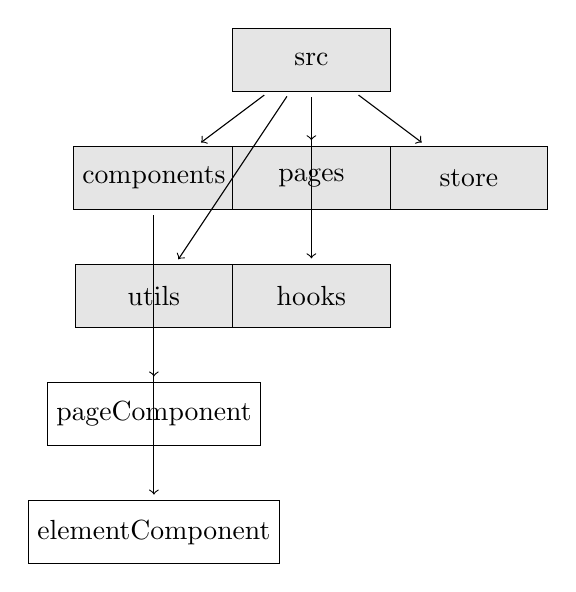
\begin{tikzpicture}[
    file/.style={draw, rectangle, minimum width=2cm, minimum height=0.8cm},
    folder/.style={draw, rectangle, minimum width=2cm, minimum height=0.8cm, fill=gray!20},
    arrow/.style={->, shorten >=2pt, shorten <=2pt}
]

% Folders
\node[folder] (src) at (0,0) {src};
\node[folder] (components) at (-2,-1.5) {components};
\node[folder] (pages) at (0,-1.5) {pages};
\node[folder] (store) at (2,-1.5) {store};
\node[folder] (utils) at (-2,-3) {utils};
\node[folder] (hooks) at (0,-3) {hooks};

% Files
\node[file] (pageComponent) at (-2,-4.5) {pageComponent};
\node[file] (elementComponent) at (-2,-6) {elementComponent};
% ... add more files

% Connections
\draw[arrow] (src) -- (components);
\draw[arrow] (src) -- (pages);
\draw[arrow] (src) -- (store);
\draw[arrow] (src) -- (utils);
\draw[arrow] (src) -- (hooks);
\draw[arrow] (components) -- (pageComponent);
\draw[arrow] (components) -- (elementComponent);
% ... add more connections

\end{tikzpicture}



\pagebreak
\subsubsection{Back-end}
The backend uses the dotNet framework. The development language using the C\# language.

In this project, the backend uses the Onion Architecture.
The Onion Architecture is a typically layered architecture, 
where each layer depends on the inner layer and provides interfaces to the outer layer.
The outer layer provides services to the outermost layer 
and other modules in the same layer based on the interfaces of the inner layer.

From inner to outer, the layers are: Domain, Application, Infrastructure, Presentation.
The Domain layer is the core layer and the innermost layer, used to define domain models, 
which are the business models.
It includes domain models and domain service interfaces.
Domain models are used to define the business models, 
which are the entities in the entity-relationship model and their attributes.
Domain service interfaces are used to define the business services, 
which are the relationships between entities in the entity-relationship model.

The Application layer is the application layer, 
used to define application services, which are the business logic.
It includes domain service implementations and application service interfaces.
Domain service implementations implement the methods of the inner layer's domain service 
interfaces and implement the business logic of the domain models.
Application service interfaces are used to define application services, 
which are the business logic.
It includes but is not limited to database interfaces, testing interfaces, 
HTTP API interfaces, MQTT interfaces, etc.

The Infrastructure layer is the infrastructure layer, used to define infrastructure.
It includes database implementations, testing implementations, 
HTTP API implementations, MQTT implementations, etc.
Database implementations implement the database interfaces 
and provide CRUD services for the database.
Testing implementations implement the testing interfaces 
and provide services for unit testing and integration testing.
HTTP API implementations implement the HTTP API interfaces 
and provide CRUD operations for HTTP APIs.
MQTT implementations implement the MQTT interfaces 
and provide CRUD operations for MQTT.

The Presentation layer is the presentation layer, used to define presentation logic, 
such as interfaces and pages. Since this is a backend project,
data presentation and control are handled by the frontend, 
so this layer is not needed.



\pagebreak
\subsubsection{Data communication and storage}
% 关于本项目的数据通信与数据存储的设计, 包括数据通信的协议, 数据存储的设计等
% 关于数据通信的设计:
% 1. 通信协议的选择
% 自前端向后端发送的数据, 有三种传输的数据类型, 
% 一种是普通的增删改查的请求, 对数据传输的时效性要求不高, 但是对数据的准确性, 完整性, 有序性, 安全性有一定的要求,
% 这种数据的传输, 采用 HTTP 协议, 以及 RESTful API 的设计. 可以有效的保证对数据传输的以上要求.
% 一种是对数据通道的创建和流媒体数据的传输, 对数据传输的时效性, 安全性要求较高, 这种数据的传输, 采用 WebRTC 协议, 以及 MQTT 协议.
% 配合可以快速解码的 flatbuffers 协议, 可以有效的保证对数据传输的以上要求.
% 最后一种是对设备的状态信息和操作信息的传输, 对完整性, 有序性, 安全性都有较高的要求, 这种数据的传输, 采用 MQTT 协议
% 同时也使用了 flatbuffers 协议.
% 
% 2. 数据通信的通信架构和通信流程
% 本项目的数据通信的通信架构, 是基于前后端分离的架构, 前端使用 React 框架, 后端使用 dotnet 框架.
% 当前端需要向后端发送数据的时候, 前端会向后端发送 HTTP 请求, 后端接收到 HTTP 请求之后, 会根据请求的数据类型,
% 选择不同的数据处理方式, 对于普通的增删改查的请求, 后端会根据 RESTful API 的设计, 对数据进行增删改查的操作,
% 对于对数据通道的创建和流媒体数据的传输, 后端会根据 WebRTC 协议, 对数据通道进行创建, 并且帮助前端和设备建立数据通道,
% 当数据通道建立后, 前端和设备之间则使用 flatbuffer 的数据格式对流媒体数据进行传输,
% 对于设备的状态信息和操作信息的传输, 前端会直接向 MQTT broker 发送 MQTT 请求, 
% 设备会在其自身的固件中监听相关的 MQTT 请求, 并且返回相关的数据.
% 
% 3. 数据通信的格式
% 本项目的数据通信的格式, 有三种, 
% 一种是 HTTP 协议, 
% 使用 json 格式对数据进行传输,
% 一种是 WebRTC 协议, 
% 使用 flatbuffers 格式对数据进行传输,
% 一种是 MQTT 协议.
% 使用 flatbuffers 格式对数据进行传输,
% 
% 关于数据存储的设计:
% 1. 数据存储的数据库的选择
% 本项目的数据存储的数据库的选择, 使用了轻量级的数据库 SQLite,
% SQLite 是一个进程内的库, 实现了自给自足的, 无服务器的, 零配置的, 事务性的 SQL 数据库引擎.
% 这是因为整个项目的目的是为了实现前端与设备之间的数据通信, 对于数据库数据的增删改查操作的要求不高,
% 数据量较小, 且对于数据库的数据的事务性要求不高, 所以选择了 SQLite 数据库.
% 2. 项目前后端的数据结构的设计
% 在本项目中, 前端由于使用了 React 框架, 所以前端的数据结构的设计, 使用了基于状态的数据结构的设计,
% 每个组件或者数据集都包含一个状态对象, 这个状态对象的属性就是组件的各个状态. 
% 使用状态对象的原因是, 可以方便的对状态进行管理, 采用对象-属性的形式, 可以方便的针对不同组件的同类状态进行区分,
% 由于跨组件的状态是由 redux 进行管理的, 这种状态对象的设计, 可以更搞笑的对状态进行更新和传递.
% 后端由于使用了 dotnet 框架, 所以后端的数据结构的设计, 使用了基于类的数据结构的设计,
% 采用了面向对象的编程思想, 对数据进行了封装, 使得数据的传输更加的安全, 有序, 完整.


\pagebreak

% \subsection{Domain model}
% \documentclass[]{article}
\usepackage{graphicx}
\usepackage{amsmath}
\usepackage{tikz}

% libaries
\usetikzlibrary{shapes,arrows}

%Define the listing package
\usepackage{listings} %code highlighter
\usepackage{color} %use color
\definecolor{mygreen}{rgb}{0,0.6,0}
\definecolor{mygray}{rgb}{0.5,0.5,0.5}
\definecolor{mymauve}{rgb}{0.58,0,0.82}

%Customize a bit the look
\lstset{ %
backgroundcolor=\color{white}, % choose the background color; you must add \usepackage{color} or \usepackage{xcolor}
basicstyle=\footnotesize, % the size of the fonts that are used for the code
breakatwhitespace=false, % sets if automatic breaks should only happen at whitespace
breaklines=true, % sets automatic line breaking
captionpos=b, % sets the caption-position to bottom
commentstyle=\color{mygreen}, % comment style
deletekeywords={...}, % if you want to delete keywords from the given language
escapeinside={\%*}{*)}, % if you want to add LaTeX within your code
extendedchars=true, % lets you use non-ASCII characters; for 8-bits encodings only, does not work with UTF-8
frame=single, % adds a frame around the code
keepspaces=true, % keeps spaces in text, useful for keeping indentation of code (possibly needs columns=flexible)
keywordstyle=\color{blue}, % keyword style
% language=Octave, % the language of the code
morekeywords={*,...}, % if you want to add more keywords to the set
numbers=left, % where to put the line-numbers; possible values are (none, left, right)
numbersep=5pt, % how far the line-numbers are from the code
numberstyle=\tiny\color{mygray}, % the style that is used for the line-numbers
rulecolor=\color{black}, % if not set, the frame-color may be changed on line-breaks within not-black text (e.g. comments (green here))
showspaces=false, % show spaces everywhere adding particular underscores; it overrides 'showstringspaces'
showstringspaces=false, % underline spaces within strings only
showtabs=false, % show tabs within strings adding particular underscores
stepnumber=1, % the step between two line-numbers. If it's 1, each line will be numbered
stringstyle=\color{mymauve}, % string literal style
tabsize=2, % sets default tabsize to 2 spaces
title=\lstname % show the filename of files included with \lstinputlisting; also try caption instead of title
}

\definecolor{darkgray}{rgb}{.4,.4,.4}
\definecolor{purple}{rgb}{0.65, 0.12, 0.82}

\lstdefinelanguage{React}{
keywords={const, typeof, new, true, false, catch, function, return, null, catch, switch, var, if, in, while, do, else, case, break},
keywordstyle=\color{blue}\bfseries,
ndkeywords={class, export, boolean, throw, implements, import, this},
ndkeywordstyle=\color{darkgray}\bfseries,
identifierstyle=\color{mygreen},
sensitive=false,
comment=[l]{//},
morecomment=[s]{/*}{*/},
commentstyle=\color{purple}\ttfamily,
string=[b]{"}{'}{`},
stringstyle=\color{red}\ttfamily,
morestring=[b]',
morestring=[b]",
morestring=[b]`',
}

\lstdefinelanguage{CSharp}{
keywords={const, typeof, new, true, false, catch, function, return, null, catch, switch, var, if, in, while, do, else, case, break},
keywordstyle=\color{blue}\bfseries,
ndkeywords={class, export, boolean, throw, implements, import, this},
ndkeywordstyle=\color{darkgray}\bfseries,
identifierstyle=\color{mygreen},
sensitive=false,
comment=[l]{//},
morecomment=[s]{/*}{*/},
commentstyle=\color{purple}\ttfamily,
string=[b]{"}{'}{`},
stringstyle=\color{red}\ttfamily,
morestring=[b]',
morestring=[b]",
morestring=[b]`',
}

\lstset{
language=React,
extendedchars=true,
basicstyle=\footnotesize\ttfamily,
showstringspaces=false,
showspaces=false,
numbers=left,
numberstyle=\footnotesize,
numbersep=9pt,
tabsize=2,
breaklines=true,
showtabs=false,
captionpos=b
}

\lstset{
language=CSharp,
extendedchars=true,
basicstyle=\footnotesize\ttfamily,
showstringspaces=false,
showspaces=false,
numbers=left,
numberstyle=\footnotesize,
numbersep=9pt,
tabsize=2,
breaklines=true,
showtabs=false,
captionpos=b
}

% \usepackage{cite} % Add this line for citation

% \bibliographystyle{plain}

\title{
The implementation of BifrostConnect Front-end scope, 
re-design and development with the relevant back-end support develop.
}
\author{
    Fei Gu \\
    Erhvervs Akademi Sydvest \\
    Computer Science 21\\
    }
\date{\today}

\begin{document}

% Front page
\maketitle
\begin{center}
    Supervisor: Henrik Boulund Meng Hansen \\
    Company: BifrostConnect \\
    Engineering Director: Jasper Wass \\
\end{center}
\tableofcontents
\pagebreak


% The introduction
\section{Introduction}
\subsection{Background}\input{sections/introduction/background.tex}
\subsection{The company}\input{sections/introduction/aboutCompany}
\subsection{The project}\input{sections/introduction/aboutProject}
\pagebreak

% The problem statement
\section{Problem Statement}
\subsection{Statement}
\input{sections/problemStatement/statement}
\subsection{Situation}
\input{sections/problemStatement/situation}
\subsection{Potential Solution}
\input{sections/problemStatement/potentialSolution}
\pagebreak

% Requirement analysis
\section{Requirement Analysis}
\input{sections/requirementAnalysis/index}

\subsection{Stakeholders}
\input{sections/requirementAnalysis/stakeholders/index}

\subsection{Business Domain}
\input{sections/requirementAnalysis/bussinesDomain/index}

\subsection{Scope}
\input{sections/requirementAnalysis/scope}

\subsection{Goals}
\input{sections/requirementAnalysis/goals}
\pagebreak

% Software Design
\section{Software Design}
% developement methods
\subsection{Software Development Methods}
\input{sections/softwareDevelopmentMethods/index}
\subsubsection{Agile Software Development}
\input{sections/softwareDevelopmentMethods/agileSoftwareDevelopment/index}
\subsubsection{Feature Driven Development}
\input{sections/softwareDevelopmentMethods/featureDrivenDevelopment/index}

\pagebreak

% Technology seslection
\subsection{Technology selection}
\input{sections/softwareDesign/technologySelection/index}
\subsubsection{Front-end}
\input{sections/softwareDesign/technologySelection/frontEnd}            
\subsubsection{Back-end}
\input{sections/softwareDesign/technologySelection/backEnd}            
\subsubsection{Database}
\input{sections/softwareDesign/technologySelection/database}
\subsubsection{Data communication}
\input{sections/softwareDesign/technologySelection/dataCommunication}            
\subsubsection{DevOps}
\input{sections/softwareDesign/technologySelection/devOps}
\pagebreak

% Architecture design
\subsection{Architecture design}
\input{sections/softwareDesign/architectureDesign/index}
\pagebreak
\subsubsection{Front-end}
\input{sections/softwareDesign/architectureDesign/frontEndArchitecture}
\pagebreak
\subsubsection{Back-end}
\input{sections/softwareDesign/architectureDesign/backEndArchitecture}
\pagebreak
\subsubsection{Data communication and storage}
\input{sections/softwareDesign/architectureDesign/dataCommunicationArchitecture}
\pagebreak

% \subsection{Domain model}
% \input{sections/softwareDesign/domainModel/index}
% \subsection{Database design}
% % 数据库领域模型 ER 图
% % 包括表和字段的设置.
% % 对于私有键和外键的设置.

% \subsection{Back-end design}
% % 后端对象模型
% % 以及对于对象模型的增删改查
% % 以及相关的其他服务的设计`'

% \subsection{Front-end design}
% % 对于前端的页面结构的设计 
% % 页面的状态的设计, 交互设计

% \subsection{FlatBuffers design}
% % schema 的设计

\subsection{DevOps CI/CD process design}
\input{sections/softwareDesign/devOpsDesign/index}
\subsubsection{Continuous Integration}
\input{sections/softwareDesign/devOpsDesign/continuousIntegration/index}
\subsubsection{Continuous Delivery}
\input{sections/softwareDesign/devOpsDesign/continuousDelivery/index}
\subsubsection{Continuous Deployment}
\input{sections/softwareDesign/devOpsDesign/continuousDeployment/index}
\pagebreak

\section{Software Development} 
\input{sections/softwareDevelopment/index}
\subsection{Overall development}
\input{sections/softwareDevelopment/overallDevelopement/index}
\subsubsection{Front-end}
\input{sections/softwareDevelopment/overallDevelopement/frontEnd/index}
\subsubsection{Back-end}
\input{sections/softwareDevelopment/overallDevelopement/backEnd/index}
\subsubsection{DevOps}
\input{sections/softwareDevelopment/overallDevelopement/devOps/index}
\subsection{Feature development} 
\input{sections/softwareDevelopment/featureDevelopment/index}
\subsubsection{Use Case 1}
\input{sections/softwareDevelopment/featureDevelopment/useCase1/index}
\subsubsection{Feature 1}
\input{sections/softwareDevelopment/featureDevelopment/feature/feature1.tex}
\pagebreak
\section{Conclusion} 
\subsection{Result}
Since the project is still in progress, the result is not available yet.
So far, basic structure of this project has been built. But the most features 
are not implemented yet. 
\subsection{Discussion}
As a single developer for this project, I am confident what I have done so far.
And I can say I understand the most of the knowledge I have used in this project, 
which also means I can explain all the part of the project. 
But this project also relevant some of the complex knowledge which I have to continue 
to study and practice.
\subsection{Future Work}
The future work is to implement the rest of the features. 
Including the most important part which is the 'create session' feature.
\pagebreak
% \bibliography{bibliography}
\pagebreak
% \begin{appendices}
%     \section{Appendix}
% \end{appendices} 
\end{document}
% \subsection{Database design}
% % 数据库领域模型 ER 图
% % 包括表和字段的设置.
% % 对于私有键和外键的设置.

% \subsection{Back-end design}
% % 后端对象模型
% % 以及对于对象模型的增删改查
% % 以及相关的其他服务的设计`'

% \subsection{Front-end design}
% % 对于前端的页面结构的设计 
% % 页面的状态的设计, 交互设计

% \subsection{FlatBuffers design}
% % schema 的设计

\subsection{DevOps CI/CD process design}
\documentclass[]{article}
\usepackage{graphicx}
\usepackage{amsmath}
\usepackage{tikz}

% libaries
\usetikzlibrary{shapes,arrows}

%Define the listing package
\usepackage{listings} %code highlighter
\usepackage{color} %use color
\definecolor{mygreen}{rgb}{0,0.6,0}
\definecolor{mygray}{rgb}{0.5,0.5,0.5}
\definecolor{mymauve}{rgb}{0.58,0,0.82}

%Customize a bit the look
\lstset{ %
backgroundcolor=\color{white}, % choose the background color; you must add \usepackage{color} or \usepackage{xcolor}
basicstyle=\footnotesize, % the size of the fonts that are used for the code
breakatwhitespace=false, % sets if automatic breaks should only happen at whitespace
breaklines=true, % sets automatic line breaking
captionpos=b, % sets the caption-position to bottom
commentstyle=\color{mygreen}, % comment style
deletekeywords={...}, % if you want to delete keywords from the given language
escapeinside={\%*}{*)}, % if you want to add LaTeX within your code
extendedchars=true, % lets you use non-ASCII characters; for 8-bits encodings only, does not work with UTF-8
frame=single, % adds a frame around the code
keepspaces=true, % keeps spaces in text, useful for keeping indentation of code (possibly needs columns=flexible)
keywordstyle=\color{blue}, % keyword style
% language=Octave, % the language of the code
morekeywords={*,...}, % if you want to add more keywords to the set
numbers=left, % where to put the line-numbers; possible values are (none, left, right)
numbersep=5pt, % how far the line-numbers are from the code
numberstyle=\tiny\color{mygray}, % the style that is used for the line-numbers
rulecolor=\color{black}, % if not set, the frame-color may be changed on line-breaks within not-black text (e.g. comments (green here))
showspaces=false, % show spaces everywhere adding particular underscores; it overrides 'showstringspaces'
showstringspaces=false, % underline spaces within strings only
showtabs=false, % show tabs within strings adding particular underscores
stepnumber=1, % the step between two line-numbers. If it's 1, each line will be numbered
stringstyle=\color{mymauve}, % string literal style
tabsize=2, % sets default tabsize to 2 spaces
title=\lstname % show the filename of files included with \lstinputlisting; also try caption instead of title
}

\definecolor{darkgray}{rgb}{.4,.4,.4}
\definecolor{purple}{rgb}{0.65, 0.12, 0.82}

\lstdefinelanguage{React}{
keywords={const, typeof, new, true, false, catch, function, return, null, catch, switch, var, if, in, while, do, else, case, break},
keywordstyle=\color{blue}\bfseries,
ndkeywords={class, export, boolean, throw, implements, import, this},
ndkeywordstyle=\color{darkgray}\bfseries,
identifierstyle=\color{mygreen},
sensitive=false,
comment=[l]{//},
morecomment=[s]{/*}{*/},
commentstyle=\color{purple}\ttfamily,
string=[b]{"}{'}{`},
stringstyle=\color{red}\ttfamily,
morestring=[b]',
morestring=[b]",
morestring=[b]`',
}

\lstdefinelanguage{CSharp}{
keywords={const, typeof, new, true, false, catch, function, return, null, catch, switch, var, if, in, while, do, else, case, break},
keywordstyle=\color{blue}\bfseries,
ndkeywords={class, export, boolean, throw, implements, import, this},
ndkeywordstyle=\color{darkgray}\bfseries,
identifierstyle=\color{mygreen},
sensitive=false,
comment=[l]{//},
morecomment=[s]{/*}{*/},
commentstyle=\color{purple}\ttfamily,
string=[b]{"}{'}{`},
stringstyle=\color{red}\ttfamily,
morestring=[b]',
morestring=[b]",
morestring=[b]`',
}

\lstset{
language=React,
extendedchars=true,
basicstyle=\footnotesize\ttfamily,
showstringspaces=false,
showspaces=false,
numbers=left,
numberstyle=\footnotesize,
numbersep=9pt,
tabsize=2,
breaklines=true,
showtabs=false,
captionpos=b
}

\lstset{
language=CSharp,
extendedchars=true,
basicstyle=\footnotesize\ttfamily,
showstringspaces=false,
showspaces=false,
numbers=left,
numberstyle=\footnotesize,
numbersep=9pt,
tabsize=2,
breaklines=true,
showtabs=false,
captionpos=b
}

% \usepackage{cite} % Add this line for citation

% \bibliographystyle{plain}

\title{
The implementation of BifrostConnect Front-end scope, 
re-design and development with the relevant back-end support develop.
}
\author{
    Fei Gu \\
    Erhvervs Akademi Sydvest \\
    Computer Science 21\\
    }
\date{\today}

\begin{document}

% Front page
\maketitle
\begin{center}
    Supervisor: Henrik Boulund Meng Hansen \\
    Company: BifrostConnect \\
    Engineering Director: Jasper Wass \\
\end{center}
\tableofcontents
\pagebreak


% The introduction
\section{Introduction}
\subsection{Background}\input{sections/introduction/background.tex}
\subsection{The company}\input{sections/introduction/aboutCompany}
\subsection{The project}\input{sections/introduction/aboutProject}
\pagebreak

% The problem statement
\section{Problem Statement}
\subsection{Statement}
\input{sections/problemStatement/statement}
\subsection{Situation}
\input{sections/problemStatement/situation}
\subsection{Potential Solution}
\input{sections/problemStatement/potentialSolution}
\pagebreak

% Requirement analysis
\section{Requirement Analysis}
\input{sections/requirementAnalysis/index}

\subsection{Stakeholders}
\input{sections/requirementAnalysis/stakeholders/index}

\subsection{Business Domain}
\input{sections/requirementAnalysis/bussinesDomain/index}

\subsection{Scope}
\input{sections/requirementAnalysis/scope}

\subsection{Goals}
\input{sections/requirementAnalysis/goals}
\pagebreak

% Software Design
\section{Software Design}
% developement methods
\subsection{Software Development Methods}
\input{sections/softwareDevelopmentMethods/index}
\subsubsection{Agile Software Development}
\input{sections/softwareDevelopmentMethods/agileSoftwareDevelopment/index}
\subsubsection{Feature Driven Development}
\input{sections/softwareDevelopmentMethods/featureDrivenDevelopment/index}

\pagebreak

% Technology seslection
\subsection{Technology selection}
\input{sections/softwareDesign/technologySelection/index}
\subsubsection{Front-end}
\input{sections/softwareDesign/technologySelection/frontEnd}            
\subsubsection{Back-end}
\input{sections/softwareDesign/technologySelection/backEnd}            
\subsubsection{Database}
\input{sections/softwareDesign/technologySelection/database}
\subsubsection{Data communication}
\input{sections/softwareDesign/technologySelection/dataCommunication}            
\subsubsection{DevOps}
\input{sections/softwareDesign/technologySelection/devOps}
\pagebreak

% Architecture design
\subsection{Architecture design}
\input{sections/softwareDesign/architectureDesign/index}
\pagebreak
\subsubsection{Front-end}
\input{sections/softwareDesign/architectureDesign/frontEndArchitecture}
\pagebreak
\subsubsection{Back-end}
\input{sections/softwareDesign/architectureDesign/backEndArchitecture}
\pagebreak
\subsubsection{Data communication and storage}
\input{sections/softwareDesign/architectureDesign/dataCommunicationArchitecture}
\pagebreak

% \subsection{Domain model}
% \input{sections/softwareDesign/domainModel/index}
% \subsection{Database design}
% % 数据库领域模型 ER 图
% % 包括表和字段的设置.
% % 对于私有键和外键的设置.

% \subsection{Back-end design}
% % 后端对象模型
% % 以及对于对象模型的增删改查
% % 以及相关的其他服务的设计`'

% \subsection{Front-end design}
% % 对于前端的页面结构的设计 
% % 页面的状态的设计, 交互设计

% \subsection{FlatBuffers design}
% % schema 的设计

\subsection{DevOps CI/CD process design}
\input{sections/softwareDesign/devOpsDesign/index}
\subsubsection{Continuous Integration}
\input{sections/softwareDesign/devOpsDesign/continuousIntegration/index}
\subsubsection{Continuous Delivery}
\input{sections/softwareDesign/devOpsDesign/continuousDelivery/index}
\subsubsection{Continuous Deployment}
\input{sections/softwareDesign/devOpsDesign/continuousDeployment/index}
\pagebreak

\section{Software Development} 
\input{sections/softwareDevelopment/index}
\subsection{Overall development}
\input{sections/softwareDevelopment/overallDevelopement/index}
\subsubsection{Front-end}
\input{sections/softwareDevelopment/overallDevelopement/frontEnd/index}
\subsubsection{Back-end}
\input{sections/softwareDevelopment/overallDevelopement/backEnd/index}
\subsubsection{DevOps}
\input{sections/softwareDevelopment/overallDevelopement/devOps/index}
\subsection{Feature development} 
\input{sections/softwareDevelopment/featureDevelopment/index}
\subsubsection{Use Case 1}
\input{sections/softwareDevelopment/featureDevelopment/useCase1/index}
\subsubsection{Feature 1}
\input{sections/softwareDevelopment/featureDevelopment/feature/feature1.tex}
\pagebreak
\section{Conclusion} 
\subsection{Result}
Since the project is still in progress, the result is not available yet.
So far, basic structure of this project has been built. But the most features 
are not implemented yet. 
\subsection{Discussion}
As a single developer for this project, I am confident what I have done so far.
And I can say I understand the most of the knowledge I have used in this project, 
which also means I can explain all the part of the project. 
But this project also relevant some of the complex knowledge which I have to continue 
to study and practice.
\subsection{Future Work}
The future work is to implement the rest of the features. 
Including the most important part which is the 'create session' feature.
\pagebreak
% \bibliography{bibliography}
\pagebreak
% \begin{appendices}
%     \section{Appendix}
% \end{appendices} 
\end{document}
\subsubsection{Continuous Integration}
\documentclass[]{article}
\usepackage{graphicx}
\usepackage{amsmath}
\usepackage{tikz}

% libaries
\usetikzlibrary{shapes,arrows}

%Define the listing package
\usepackage{listings} %code highlighter
\usepackage{color} %use color
\definecolor{mygreen}{rgb}{0,0.6,0}
\definecolor{mygray}{rgb}{0.5,0.5,0.5}
\definecolor{mymauve}{rgb}{0.58,0,0.82}

%Customize a bit the look
\lstset{ %
backgroundcolor=\color{white}, % choose the background color; you must add \usepackage{color} or \usepackage{xcolor}
basicstyle=\footnotesize, % the size of the fonts that are used for the code
breakatwhitespace=false, % sets if automatic breaks should only happen at whitespace
breaklines=true, % sets automatic line breaking
captionpos=b, % sets the caption-position to bottom
commentstyle=\color{mygreen}, % comment style
deletekeywords={...}, % if you want to delete keywords from the given language
escapeinside={\%*}{*)}, % if you want to add LaTeX within your code
extendedchars=true, % lets you use non-ASCII characters; for 8-bits encodings only, does not work with UTF-8
frame=single, % adds a frame around the code
keepspaces=true, % keeps spaces in text, useful for keeping indentation of code (possibly needs columns=flexible)
keywordstyle=\color{blue}, % keyword style
% language=Octave, % the language of the code
morekeywords={*,...}, % if you want to add more keywords to the set
numbers=left, % where to put the line-numbers; possible values are (none, left, right)
numbersep=5pt, % how far the line-numbers are from the code
numberstyle=\tiny\color{mygray}, % the style that is used for the line-numbers
rulecolor=\color{black}, % if not set, the frame-color may be changed on line-breaks within not-black text (e.g. comments (green here))
showspaces=false, % show spaces everywhere adding particular underscores; it overrides 'showstringspaces'
showstringspaces=false, % underline spaces within strings only
showtabs=false, % show tabs within strings adding particular underscores
stepnumber=1, % the step between two line-numbers. If it's 1, each line will be numbered
stringstyle=\color{mymauve}, % string literal style
tabsize=2, % sets default tabsize to 2 spaces
title=\lstname % show the filename of files included with \lstinputlisting; also try caption instead of title
}

\definecolor{darkgray}{rgb}{.4,.4,.4}
\definecolor{purple}{rgb}{0.65, 0.12, 0.82}

\lstdefinelanguage{React}{
keywords={const, typeof, new, true, false, catch, function, return, null, catch, switch, var, if, in, while, do, else, case, break},
keywordstyle=\color{blue}\bfseries,
ndkeywords={class, export, boolean, throw, implements, import, this},
ndkeywordstyle=\color{darkgray}\bfseries,
identifierstyle=\color{mygreen},
sensitive=false,
comment=[l]{//},
morecomment=[s]{/*}{*/},
commentstyle=\color{purple}\ttfamily,
string=[b]{"}{'}{`},
stringstyle=\color{red}\ttfamily,
morestring=[b]',
morestring=[b]",
morestring=[b]`',
}

\lstdefinelanguage{CSharp}{
keywords={const, typeof, new, true, false, catch, function, return, null, catch, switch, var, if, in, while, do, else, case, break},
keywordstyle=\color{blue}\bfseries,
ndkeywords={class, export, boolean, throw, implements, import, this},
ndkeywordstyle=\color{darkgray}\bfseries,
identifierstyle=\color{mygreen},
sensitive=false,
comment=[l]{//},
morecomment=[s]{/*}{*/},
commentstyle=\color{purple}\ttfamily,
string=[b]{"}{'}{`},
stringstyle=\color{red}\ttfamily,
morestring=[b]',
morestring=[b]",
morestring=[b]`',
}

\lstset{
language=React,
extendedchars=true,
basicstyle=\footnotesize\ttfamily,
showstringspaces=false,
showspaces=false,
numbers=left,
numberstyle=\footnotesize,
numbersep=9pt,
tabsize=2,
breaklines=true,
showtabs=false,
captionpos=b
}

\lstset{
language=CSharp,
extendedchars=true,
basicstyle=\footnotesize\ttfamily,
showstringspaces=false,
showspaces=false,
numbers=left,
numberstyle=\footnotesize,
numbersep=9pt,
tabsize=2,
breaklines=true,
showtabs=false,
captionpos=b
}

% \usepackage{cite} % Add this line for citation

% \bibliographystyle{plain}

\title{
The implementation of BifrostConnect Front-end scope, 
re-design and development with the relevant back-end support develop.
}
\author{
    Fei Gu \\
    Erhvervs Akademi Sydvest \\
    Computer Science 21\\
    }
\date{\today}

\begin{document}

% Front page
\maketitle
\begin{center}
    Supervisor: Henrik Boulund Meng Hansen \\
    Company: BifrostConnect \\
    Engineering Director: Jasper Wass \\
\end{center}
\tableofcontents
\pagebreak


% The introduction
\section{Introduction}
\subsection{Background}\input{sections/introduction/background.tex}
\subsection{The company}\input{sections/introduction/aboutCompany}
\subsection{The project}\input{sections/introduction/aboutProject}
\pagebreak

% The problem statement
\section{Problem Statement}
\subsection{Statement}
\input{sections/problemStatement/statement}
\subsection{Situation}
\input{sections/problemStatement/situation}
\subsection{Potential Solution}
\input{sections/problemStatement/potentialSolution}
\pagebreak

% Requirement analysis
\section{Requirement Analysis}
\input{sections/requirementAnalysis/index}

\subsection{Stakeholders}
\input{sections/requirementAnalysis/stakeholders/index}

\subsection{Business Domain}
\input{sections/requirementAnalysis/bussinesDomain/index}

\subsection{Scope}
\input{sections/requirementAnalysis/scope}

\subsection{Goals}
\input{sections/requirementAnalysis/goals}
\pagebreak

% Software Design
\section{Software Design}
% developement methods
\subsection{Software Development Methods}
\input{sections/softwareDevelopmentMethods/index}
\subsubsection{Agile Software Development}
\input{sections/softwareDevelopmentMethods/agileSoftwareDevelopment/index}
\subsubsection{Feature Driven Development}
\input{sections/softwareDevelopmentMethods/featureDrivenDevelopment/index}

\pagebreak

% Technology seslection
\subsection{Technology selection}
\input{sections/softwareDesign/technologySelection/index}
\subsubsection{Front-end}
\input{sections/softwareDesign/technologySelection/frontEnd}            
\subsubsection{Back-end}
\input{sections/softwareDesign/technologySelection/backEnd}            
\subsubsection{Database}
\input{sections/softwareDesign/technologySelection/database}
\subsubsection{Data communication}
\input{sections/softwareDesign/technologySelection/dataCommunication}            
\subsubsection{DevOps}
\input{sections/softwareDesign/technologySelection/devOps}
\pagebreak

% Architecture design
\subsection{Architecture design}
\input{sections/softwareDesign/architectureDesign/index}
\pagebreak
\subsubsection{Front-end}
\input{sections/softwareDesign/architectureDesign/frontEndArchitecture}
\pagebreak
\subsubsection{Back-end}
\input{sections/softwareDesign/architectureDesign/backEndArchitecture}
\pagebreak
\subsubsection{Data communication and storage}
\input{sections/softwareDesign/architectureDesign/dataCommunicationArchitecture}
\pagebreak

% \subsection{Domain model}
% \input{sections/softwareDesign/domainModel/index}
% \subsection{Database design}
% % 数据库领域模型 ER 图
% % 包括表和字段的设置.
% % 对于私有键和外键的设置.

% \subsection{Back-end design}
% % 后端对象模型
% % 以及对于对象模型的增删改查
% % 以及相关的其他服务的设计`'

% \subsection{Front-end design}
% % 对于前端的页面结构的设计 
% % 页面的状态的设计, 交互设计

% \subsection{FlatBuffers design}
% % schema 的设计

\subsection{DevOps CI/CD process design}
\input{sections/softwareDesign/devOpsDesign/index}
\subsubsection{Continuous Integration}
\input{sections/softwareDesign/devOpsDesign/continuousIntegration/index}
\subsubsection{Continuous Delivery}
\input{sections/softwareDesign/devOpsDesign/continuousDelivery/index}
\subsubsection{Continuous Deployment}
\input{sections/softwareDesign/devOpsDesign/continuousDeployment/index}
\pagebreak

\section{Software Development} 
\input{sections/softwareDevelopment/index}
\subsection{Overall development}
\input{sections/softwareDevelopment/overallDevelopement/index}
\subsubsection{Front-end}
\input{sections/softwareDevelopment/overallDevelopement/frontEnd/index}
\subsubsection{Back-end}
\input{sections/softwareDevelopment/overallDevelopement/backEnd/index}
\subsubsection{DevOps}
\input{sections/softwareDevelopment/overallDevelopement/devOps/index}
\subsection{Feature development} 
\input{sections/softwareDevelopment/featureDevelopment/index}
\subsubsection{Use Case 1}
\input{sections/softwareDevelopment/featureDevelopment/useCase1/index}
\subsubsection{Feature 1}
\input{sections/softwareDevelopment/featureDevelopment/feature/feature1.tex}
\pagebreak
\section{Conclusion} 
\subsection{Result}
Since the project is still in progress, the result is not available yet.
So far, basic structure of this project has been built. But the most features 
are not implemented yet. 
\subsection{Discussion}
As a single developer for this project, I am confident what I have done so far.
And I can say I understand the most of the knowledge I have used in this project, 
which also means I can explain all the part of the project. 
But this project also relevant some of the complex knowledge which I have to continue 
to study and practice.
\subsection{Future Work}
The future work is to implement the rest of the features. 
Including the most important part which is the 'create session' feature.
\pagebreak
% \bibliography{bibliography}
\pagebreak
% \begin{appendices}
%     \section{Appendix}
% \end{appendices} 
\end{document}
\subsubsection{Continuous Delivery}
\documentclass[]{article}
\usepackage{graphicx}
\usepackage{amsmath}
\usepackage{tikz}

% libaries
\usetikzlibrary{shapes,arrows}

%Define the listing package
\usepackage{listings} %code highlighter
\usepackage{color} %use color
\definecolor{mygreen}{rgb}{0,0.6,0}
\definecolor{mygray}{rgb}{0.5,0.5,0.5}
\definecolor{mymauve}{rgb}{0.58,0,0.82}

%Customize a bit the look
\lstset{ %
backgroundcolor=\color{white}, % choose the background color; you must add \usepackage{color} or \usepackage{xcolor}
basicstyle=\footnotesize, % the size of the fonts that are used for the code
breakatwhitespace=false, % sets if automatic breaks should only happen at whitespace
breaklines=true, % sets automatic line breaking
captionpos=b, % sets the caption-position to bottom
commentstyle=\color{mygreen}, % comment style
deletekeywords={...}, % if you want to delete keywords from the given language
escapeinside={\%*}{*)}, % if you want to add LaTeX within your code
extendedchars=true, % lets you use non-ASCII characters; for 8-bits encodings only, does not work with UTF-8
frame=single, % adds a frame around the code
keepspaces=true, % keeps spaces in text, useful for keeping indentation of code (possibly needs columns=flexible)
keywordstyle=\color{blue}, % keyword style
% language=Octave, % the language of the code
morekeywords={*,...}, % if you want to add more keywords to the set
numbers=left, % where to put the line-numbers; possible values are (none, left, right)
numbersep=5pt, % how far the line-numbers are from the code
numberstyle=\tiny\color{mygray}, % the style that is used for the line-numbers
rulecolor=\color{black}, % if not set, the frame-color may be changed on line-breaks within not-black text (e.g. comments (green here))
showspaces=false, % show spaces everywhere adding particular underscores; it overrides 'showstringspaces'
showstringspaces=false, % underline spaces within strings only
showtabs=false, % show tabs within strings adding particular underscores
stepnumber=1, % the step between two line-numbers. If it's 1, each line will be numbered
stringstyle=\color{mymauve}, % string literal style
tabsize=2, % sets default tabsize to 2 spaces
title=\lstname % show the filename of files included with \lstinputlisting; also try caption instead of title
}

\definecolor{darkgray}{rgb}{.4,.4,.4}
\definecolor{purple}{rgb}{0.65, 0.12, 0.82}

\lstdefinelanguage{React}{
keywords={const, typeof, new, true, false, catch, function, return, null, catch, switch, var, if, in, while, do, else, case, break},
keywordstyle=\color{blue}\bfseries,
ndkeywords={class, export, boolean, throw, implements, import, this},
ndkeywordstyle=\color{darkgray}\bfseries,
identifierstyle=\color{mygreen},
sensitive=false,
comment=[l]{//},
morecomment=[s]{/*}{*/},
commentstyle=\color{purple}\ttfamily,
string=[b]{"}{'}{`},
stringstyle=\color{red}\ttfamily,
morestring=[b]',
morestring=[b]",
morestring=[b]`',
}

\lstdefinelanguage{CSharp}{
keywords={const, typeof, new, true, false, catch, function, return, null, catch, switch, var, if, in, while, do, else, case, break},
keywordstyle=\color{blue}\bfseries,
ndkeywords={class, export, boolean, throw, implements, import, this},
ndkeywordstyle=\color{darkgray}\bfseries,
identifierstyle=\color{mygreen},
sensitive=false,
comment=[l]{//},
morecomment=[s]{/*}{*/},
commentstyle=\color{purple}\ttfamily,
string=[b]{"}{'}{`},
stringstyle=\color{red}\ttfamily,
morestring=[b]',
morestring=[b]",
morestring=[b]`',
}

\lstset{
language=React,
extendedchars=true,
basicstyle=\footnotesize\ttfamily,
showstringspaces=false,
showspaces=false,
numbers=left,
numberstyle=\footnotesize,
numbersep=9pt,
tabsize=2,
breaklines=true,
showtabs=false,
captionpos=b
}

\lstset{
language=CSharp,
extendedchars=true,
basicstyle=\footnotesize\ttfamily,
showstringspaces=false,
showspaces=false,
numbers=left,
numberstyle=\footnotesize,
numbersep=9pt,
tabsize=2,
breaklines=true,
showtabs=false,
captionpos=b
}

% \usepackage{cite} % Add this line for citation

% \bibliographystyle{plain}

\title{
The implementation of BifrostConnect Front-end scope, 
re-design and development with the relevant back-end support develop.
}
\author{
    Fei Gu \\
    Erhvervs Akademi Sydvest \\
    Computer Science 21\\
    }
\date{\today}

\begin{document}

% Front page
\maketitle
\begin{center}
    Supervisor: Henrik Boulund Meng Hansen \\
    Company: BifrostConnect \\
    Engineering Director: Jasper Wass \\
\end{center}
\tableofcontents
\pagebreak


% The introduction
\section{Introduction}
\subsection{Background}\input{sections/introduction/background.tex}
\subsection{The company}\input{sections/introduction/aboutCompany}
\subsection{The project}\input{sections/introduction/aboutProject}
\pagebreak

% The problem statement
\section{Problem Statement}
\subsection{Statement}
\input{sections/problemStatement/statement}
\subsection{Situation}
\input{sections/problemStatement/situation}
\subsection{Potential Solution}
\input{sections/problemStatement/potentialSolution}
\pagebreak

% Requirement analysis
\section{Requirement Analysis}
\input{sections/requirementAnalysis/index}

\subsection{Stakeholders}
\input{sections/requirementAnalysis/stakeholders/index}

\subsection{Business Domain}
\input{sections/requirementAnalysis/bussinesDomain/index}

\subsection{Scope}
\input{sections/requirementAnalysis/scope}

\subsection{Goals}
\input{sections/requirementAnalysis/goals}
\pagebreak

% Software Design
\section{Software Design}
% developement methods
\subsection{Software Development Methods}
\input{sections/softwareDevelopmentMethods/index}
\subsubsection{Agile Software Development}
\input{sections/softwareDevelopmentMethods/agileSoftwareDevelopment/index}
\subsubsection{Feature Driven Development}
\input{sections/softwareDevelopmentMethods/featureDrivenDevelopment/index}

\pagebreak

% Technology seslection
\subsection{Technology selection}
\input{sections/softwareDesign/technologySelection/index}
\subsubsection{Front-end}
\input{sections/softwareDesign/technologySelection/frontEnd}            
\subsubsection{Back-end}
\input{sections/softwareDesign/technologySelection/backEnd}            
\subsubsection{Database}
\input{sections/softwareDesign/technologySelection/database}
\subsubsection{Data communication}
\input{sections/softwareDesign/technologySelection/dataCommunication}            
\subsubsection{DevOps}
\input{sections/softwareDesign/technologySelection/devOps}
\pagebreak

% Architecture design
\subsection{Architecture design}
\input{sections/softwareDesign/architectureDesign/index}
\pagebreak
\subsubsection{Front-end}
\input{sections/softwareDesign/architectureDesign/frontEndArchitecture}
\pagebreak
\subsubsection{Back-end}
\input{sections/softwareDesign/architectureDesign/backEndArchitecture}
\pagebreak
\subsubsection{Data communication and storage}
\input{sections/softwareDesign/architectureDesign/dataCommunicationArchitecture}
\pagebreak

% \subsection{Domain model}
% \input{sections/softwareDesign/domainModel/index}
% \subsection{Database design}
% % 数据库领域模型 ER 图
% % 包括表和字段的设置.
% % 对于私有键和外键的设置.

% \subsection{Back-end design}
% % 后端对象模型
% % 以及对于对象模型的增删改查
% % 以及相关的其他服务的设计`'

% \subsection{Front-end design}
% % 对于前端的页面结构的设计 
% % 页面的状态的设计, 交互设计

% \subsection{FlatBuffers design}
% % schema 的设计

\subsection{DevOps CI/CD process design}
\input{sections/softwareDesign/devOpsDesign/index}
\subsubsection{Continuous Integration}
\input{sections/softwareDesign/devOpsDesign/continuousIntegration/index}
\subsubsection{Continuous Delivery}
\input{sections/softwareDesign/devOpsDesign/continuousDelivery/index}
\subsubsection{Continuous Deployment}
\input{sections/softwareDesign/devOpsDesign/continuousDeployment/index}
\pagebreak

\section{Software Development} 
\input{sections/softwareDevelopment/index}
\subsection{Overall development}
\input{sections/softwareDevelopment/overallDevelopement/index}
\subsubsection{Front-end}
\input{sections/softwareDevelopment/overallDevelopement/frontEnd/index}
\subsubsection{Back-end}
\input{sections/softwareDevelopment/overallDevelopement/backEnd/index}
\subsubsection{DevOps}
\input{sections/softwareDevelopment/overallDevelopement/devOps/index}
\subsection{Feature development} 
\input{sections/softwareDevelopment/featureDevelopment/index}
\subsubsection{Use Case 1}
\input{sections/softwareDevelopment/featureDevelopment/useCase1/index}
\subsubsection{Feature 1}
\input{sections/softwareDevelopment/featureDevelopment/feature/feature1.tex}
\pagebreak
\section{Conclusion} 
\subsection{Result}
Since the project is still in progress, the result is not available yet.
So far, basic structure of this project has been built. But the most features 
are not implemented yet. 
\subsection{Discussion}
As a single developer for this project, I am confident what I have done so far.
And I can say I understand the most of the knowledge I have used in this project, 
which also means I can explain all the part of the project. 
But this project also relevant some of the complex knowledge which I have to continue 
to study and practice.
\subsection{Future Work}
The future work is to implement the rest of the features. 
Including the most important part which is the 'create session' feature.
\pagebreak
% \bibliography{bibliography}
\pagebreak
% \begin{appendices}
%     \section{Appendix}
% \end{appendices} 
\end{document}
\subsubsection{Continuous Deployment}
\documentclass[]{article}
\usepackage{graphicx}
\usepackage{amsmath}
\usepackage{tikz}

% libaries
\usetikzlibrary{shapes,arrows}

%Define the listing package
\usepackage{listings} %code highlighter
\usepackage{color} %use color
\definecolor{mygreen}{rgb}{0,0.6,0}
\definecolor{mygray}{rgb}{0.5,0.5,0.5}
\definecolor{mymauve}{rgb}{0.58,0,0.82}

%Customize a bit the look
\lstset{ %
backgroundcolor=\color{white}, % choose the background color; you must add \usepackage{color} or \usepackage{xcolor}
basicstyle=\footnotesize, % the size of the fonts that are used for the code
breakatwhitespace=false, % sets if automatic breaks should only happen at whitespace
breaklines=true, % sets automatic line breaking
captionpos=b, % sets the caption-position to bottom
commentstyle=\color{mygreen}, % comment style
deletekeywords={...}, % if you want to delete keywords from the given language
escapeinside={\%*}{*)}, % if you want to add LaTeX within your code
extendedchars=true, % lets you use non-ASCII characters; for 8-bits encodings only, does not work with UTF-8
frame=single, % adds a frame around the code
keepspaces=true, % keeps spaces in text, useful for keeping indentation of code (possibly needs columns=flexible)
keywordstyle=\color{blue}, % keyword style
% language=Octave, % the language of the code
morekeywords={*,...}, % if you want to add more keywords to the set
numbers=left, % where to put the line-numbers; possible values are (none, left, right)
numbersep=5pt, % how far the line-numbers are from the code
numberstyle=\tiny\color{mygray}, % the style that is used for the line-numbers
rulecolor=\color{black}, % if not set, the frame-color may be changed on line-breaks within not-black text (e.g. comments (green here))
showspaces=false, % show spaces everywhere adding particular underscores; it overrides 'showstringspaces'
showstringspaces=false, % underline spaces within strings only
showtabs=false, % show tabs within strings adding particular underscores
stepnumber=1, % the step between two line-numbers. If it's 1, each line will be numbered
stringstyle=\color{mymauve}, % string literal style
tabsize=2, % sets default tabsize to 2 spaces
title=\lstname % show the filename of files included with \lstinputlisting; also try caption instead of title
}

\definecolor{darkgray}{rgb}{.4,.4,.4}
\definecolor{purple}{rgb}{0.65, 0.12, 0.82}

\lstdefinelanguage{React}{
keywords={const, typeof, new, true, false, catch, function, return, null, catch, switch, var, if, in, while, do, else, case, break},
keywordstyle=\color{blue}\bfseries,
ndkeywords={class, export, boolean, throw, implements, import, this},
ndkeywordstyle=\color{darkgray}\bfseries,
identifierstyle=\color{mygreen},
sensitive=false,
comment=[l]{//},
morecomment=[s]{/*}{*/},
commentstyle=\color{purple}\ttfamily,
string=[b]{"}{'}{`},
stringstyle=\color{red}\ttfamily,
morestring=[b]',
morestring=[b]",
morestring=[b]`',
}

\lstdefinelanguage{CSharp}{
keywords={const, typeof, new, true, false, catch, function, return, null, catch, switch, var, if, in, while, do, else, case, break},
keywordstyle=\color{blue}\bfseries,
ndkeywords={class, export, boolean, throw, implements, import, this},
ndkeywordstyle=\color{darkgray}\bfseries,
identifierstyle=\color{mygreen},
sensitive=false,
comment=[l]{//},
morecomment=[s]{/*}{*/},
commentstyle=\color{purple}\ttfamily,
string=[b]{"}{'}{`},
stringstyle=\color{red}\ttfamily,
morestring=[b]',
morestring=[b]",
morestring=[b]`',
}

\lstset{
language=React,
extendedchars=true,
basicstyle=\footnotesize\ttfamily,
showstringspaces=false,
showspaces=false,
numbers=left,
numberstyle=\footnotesize,
numbersep=9pt,
tabsize=2,
breaklines=true,
showtabs=false,
captionpos=b
}

\lstset{
language=CSharp,
extendedchars=true,
basicstyle=\footnotesize\ttfamily,
showstringspaces=false,
showspaces=false,
numbers=left,
numberstyle=\footnotesize,
numbersep=9pt,
tabsize=2,
breaklines=true,
showtabs=false,
captionpos=b
}

% \usepackage{cite} % Add this line for citation

% \bibliographystyle{plain}

\title{
The implementation of BifrostConnect Front-end scope, 
re-design and development with the relevant back-end support develop.
}
\author{
    Fei Gu \\
    Erhvervs Akademi Sydvest \\
    Computer Science 21\\
    }
\date{\today}

\begin{document}

% Front page
\maketitle
\begin{center}
    Supervisor: Henrik Boulund Meng Hansen \\
    Company: BifrostConnect \\
    Engineering Director: Jasper Wass \\
\end{center}
\tableofcontents
\pagebreak


% The introduction
\section{Introduction}
\subsection{Background}\input{sections/introduction/background.tex}
\subsection{The company}\input{sections/introduction/aboutCompany}
\subsection{The project}\input{sections/introduction/aboutProject}
\pagebreak

% The problem statement
\section{Problem Statement}
\subsection{Statement}
\input{sections/problemStatement/statement}
\subsection{Situation}
\input{sections/problemStatement/situation}
\subsection{Potential Solution}
\input{sections/problemStatement/potentialSolution}
\pagebreak

% Requirement analysis
\section{Requirement Analysis}
\input{sections/requirementAnalysis/index}

\subsection{Stakeholders}
\input{sections/requirementAnalysis/stakeholders/index}

\subsection{Business Domain}
\input{sections/requirementAnalysis/bussinesDomain/index}

\subsection{Scope}
\input{sections/requirementAnalysis/scope}

\subsection{Goals}
\input{sections/requirementAnalysis/goals}
\pagebreak

% Software Design
\section{Software Design}
% developement methods
\subsection{Software Development Methods}
\input{sections/softwareDevelopmentMethods/index}
\subsubsection{Agile Software Development}
\input{sections/softwareDevelopmentMethods/agileSoftwareDevelopment/index}
\subsubsection{Feature Driven Development}
\input{sections/softwareDevelopmentMethods/featureDrivenDevelopment/index}

\pagebreak

% Technology seslection
\subsection{Technology selection}
\input{sections/softwareDesign/technologySelection/index}
\subsubsection{Front-end}
\input{sections/softwareDesign/technologySelection/frontEnd}            
\subsubsection{Back-end}
\input{sections/softwareDesign/technologySelection/backEnd}            
\subsubsection{Database}
\input{sections/softwareDesign/technologySelection/database}
\subsubsection{Data communication}
\input{sections/softwareDesign/technologySelection/dataCommunication}            
\subsubsection{DevOps}
\input{sections/softwareDesign/technologySelection/devOps}
\pagebreak

% Architecture design
\subsection{Architecture design}
\input{sections/softwareDesign/architectureDesign/index}
\pagebreak
\subsubsection{Front-end}
\input{sections/softwareDesign/architectureDesign/frontEndArchitecture}
\pagebreak
\subsubsection{Back-end}
\input{sections/softwareDesign/architectureDesign/backEndArchitecture}
\pagebreak
\subsubsection{Data communication and storage}
\input{sections/softwareDesign/architectureDesign/dataCommunicationArchitecture}
\pagebreak

% \subsection{Domain model}
% \input{sections/softwareDesign/domainModel/index}
% \subsection{Database design}
% % 数据库领域模型 ER 图
% % 包括表和字段的设置.
% % 对于私有键和外键的设置.

% \subsection{Back-end design}
% % 后端对象模型
% % 以及对于对象模型的增删改查
% % 以及相关的其他服务的设计`'

% \subsection{Front-end design}
% % 对于前端的页面结构的设计 
% % 页面的状态的设计, 交互设计

% \subsection{FlatBuffers design}
% % schema 的设计

\subsection{DevOps CI/CD process design}
\input{sections/softwareDesign/devOpsDesign/index}
\subsubsection{Continuous Integration}
\input{sections/softwareDesign/devOpsDesign/continuousIntegration/index}
\subsubsection{Continuous Delivery}
\input{sections/softwareDesign/devOpsDesign/continuousDelivery/index}
\subsubsection{Continuous Deployment}
\input{sections/softwareDesign/devOpsDesign/continuousDeployment/index}
\pagebreak

\section{Software Development} 
\input{sections/softwareDevelopment/index}
\subsection{Overall development}
\input{sections/softwareDevelopment/overallDevelopement/index}
\subsubsection{Front-end}
\input{sections/softwareDevelopment/overallDevelopement/frontEnd/index}
\subsubsection{Back-end}
\input{sections/softwareDevelopment/overallDevelopement/backEnd/index}
\subsubsection{DevOps}
\input{sections/softwareDevelopment/overallDevelopement/devOps/index}
\subsection{Feature development} 
\input{sections/softwareDevelopment/featureDevelopment/index}
\subsubsection{Use Case 1}
\input{sections/softwareDevelopment/featureDevelopment/useCase1/index}
\subsubsection{Feature 1}
\input{sections/softwareDevelopment/featureDevelopment/feature/feature1.tex}
\pagebreak
\section{Conclusion} 
\subsection{Result}
Since the project is still in progress, the result is not available yet.
So far, basic structure of this project has been built. But the most features 
are not implemented yet. 
\subsection{Discussion}
As a single developer for this project, I am confident what I have done so far.
And I can say I understand the most of the knowledge I have used in this project, 
which also means I can explain all the part of the project. 
But this project also relevant some of the complex knowledge which I have to continue 
to study and practice.
\subsection{Future Work}
The future work is to implement the rest of the features. 
Including the most important part which is the 'create session' feature.
\pagebreak
% \bibliography{bibliography}
\pagebreak
% \begin{appendices}
%     \section{Appendix}
% \end{appendices} 
\end{document}
\pagebreak

\section{Software Development} 
\documentclass[]{article}
\usepackage{graphicx}
\usepackage{amsmath}
\usepackage{tikz}

% libaries
\usetikzlibrary{shapes,arrows}

%Define the listing package
\usepackage{listings} %code highlighter
\usepackage{color} %use color
\definecolor{mygreen}{rgb}{0,0.6,0}
\definecolor{mygray}{rgb}{0.5,0.5,0.5}
\definecolor{mymauve}{rgb}{0.58,0,0.82}

%Customize a bit the look
\lstset{ %
backgroundcolor=\color{white}, % choose the background color; you must add \usepackage{color} or \usepackage{xcolor}
basicstyle=\footnotesize, % the size of the fonts that are used for the code
breakatwhitespace=false, % sets if automatic breaks should only happen at whitespace
breaklines=true, % sets automatic line breaking
captionpos=b, % sets the caption-position to bottom
commentstyle=\color{mygreen}, % comment style
deletekeywords={...}, % if you want to delete keywords from the given language
escapeinside={\%*}{*)}, % if you want to add LaTeX within your code
extendedchars=true, % lets you use non-ASCII characters; for 8-bits encodings only, does not work with UTF-8
frame=single, % adds a frame around the code
keepspaces=true, % keeps spaces in text, useful for keeping indentation of code (possibly needs columns=flexible)
keywordstyle=\color{blue}, % keyword style
% language=Octave, % the language of the code
morekeywords={*,...}, % if you want to add more keywords to the set
numbers=left, % where to put the line-numbers; possible values are (none, left, right)
numbersep=5pt, % how far the line-numbers are from the code
numberstyle=\tiny\color{mygray}, % the style that is used for the line-numbers
rulecolor=\color{black}, % if not set, the frame-color may be changed on line-breaks within not-black text (e.g. comments (green here))
showspaces=false, % show spaces everywhere adding particular underscores; it overrides 'showstringspaces'
showstringspaces=false, % underline spaces within strings only
showtabs=false, % show tabs within strings adding particular underscores
stepnumber=1, % the step between two line-numbers. If it's 1, each line will be numbered
stringstyle=\color{mymauve}, % string literal style
tabsize=2, % sets default tabsize to 2 spaces
title=\lstname % show the filename of files included with \lstinputlisting; also try caption instead of title
}

\definecolor{darkgray}{rgb}{.4,.4,.4}
\definecolor{purple}{rgb}{0.65, 0.12, 0.82}

\lstdefinelanguage{React}{
keywords={const, typeof, new, true, false, catch, function, return, null, catch, switch, var, if, in, while, do, else, case, break},
keywordstyle=\color{blue}\bfseries,
ndkeywords={class, export, boolean, throw, implements, import, this},
ndkeywordstyle=\color{darkgray}\bfseries,
identifierstyle=\color{mygreen},
sensitive=false,
comment=[l]{//},
morecomment=[s]{/*}{*/},
commentstyle=\color{purple}\ttfamily,
string=[b]{"}{'}{`},
stringstyle=\color{red}\ttfamily,
morestring=[b]',
morestring=[b]",
morestring=[b]`',
}

\lstdefinelanguage{CSharp}{
keywords={const, typeof, new, true, false, catch, function, return, null, catch, switch, var, if, in, while, do, else, case, break},
keywordstyle=\color{blue}\bfseries,
ndkeywords={class, export, boolean, throw, implements, import, this},
ndkeywordstyle=\color{darkgray}\bfseries,
identifierstyle=\color{mygreen},
sensitive=false,
comment=[l]{//},
morecomment=[s]{/*}{*/},
commentstyle=\color{purple}\ttfamily,
string=[b]{"}{'}{`},
stringstyle=\color{red}\ttfamily,
morestring=[b]',
morestring=[b]",
morestring=[b]`',
}

\lstset{
language=React,
extendedchars=true,
basicstyle=\footnotesize\ttfamily,
showstringspaces=false,
showspaces=false,
numbers=left,
numberstyle=\footnotesize,
numbersep=9pt,
tabsize=2,
breaklines=true,
showtabs=false,
captionpos=b
}

\lstset{
language=CSharp,
extendedchars=true,
basicstyle=\footnotesize\ttfamily,
showstringspaces=false,
showspaces=false,
numbers=left,
numberstyle=\footnotesize,
numbersep=9pt,
tabsize=2,
breaklines=true,
showtabs=false,
captionpos=b
}

% \usepackage{cite} % Add this line for citation

% \bibliographystyle{plain}

\title{
The implementation of BifrostConnect Front-end scope, 
re-design and development with the relevant back-end support develop.
}
\author{
    Fei Gu \\
    Erhvervs Akademi Sydvest \\
    Computer Science 21\\
    }
\date{\today}

\begin{document}

% Front page
\maketitle
\begin{center}
    Supervisor: Henrik Boulund Meng Hansen \\
    Company: BifrostConnect \\
    Engineering Director: Jasper Wass \\
\end{center}
\tableofcontents
\pagebreak


% The introduction
\section{Introduction}
\subsection{Background}\input{sections/introduction/background.tex}
\subsection{The company}\input{sections/introduction/aboutCompany}
\subsection{The project}\input{sections/introduction/aboutProject}
\pagebreak

% The problem statement
\section{Problem Statement}
\subsection{Statement}
\input{sections/problemStatement/statement}
\subsection{Situation}
\input{sections/problemStatement/situation}
\subsection{Potential Solution}
\input{sections/problemStatement/potentialSolution}
\pagebreak

% Requirement analysis
\section{Requirement Analysis}
\input{sections/requirementAnalysis/index}

\subsection{Stakeholders}
\input{sections/requirementAnalysis/stakeholders/index}

\subsection{Business Domain}
\input{sections/requirementAnalysis/bussinesDomain/index}

\subsection{Scope}
\input{sections/requirementAnalysis/scope}

\subsection{Goals}
\input{sections/requirementAnalysis/goals}
\pagebreak

% Software Design
\section{Software Design}
% developement methods
\subsection{Software Development Methods}
\input{sections/softwareDevelopmentMethods/index}
\subsubsection{Agile Software Development}
\input{sections/softwareDevelopmentMethods/agileSoftwareDevelopment/index}
\subsubsection{Feature Driven Development}
\input{sections/softwareDevelopmentMethods/featureDrivenDevelopment/index}

\pagebreak

% Technology seslection
\subsection{Technology selection}
\input{sections/softwareDesign/technologySelection/index}
\subsubsection{Front-end}
\input{sections/softwareDesign/technologySelection/frontEnd}            
\subsubsection{Back-end}
\input{sections/softwareDesign/technologySelection/backEnd}            
\subsubsection{Database}
\input{sections/softwareDesign/technologySelection/database}
\subsubsection{Data communication}
\input{sections/softwareDesign/technologySelection/dataCommunication}            
\subsubsection{DevOps}
\input{sections/softwareDesign/technologySelection/devOps}
\pagebreak

% Architecture design
\subsection{Architecture design}
\input{sections/softwareDesign/architectureDesign/index}
\pagebreak
\subsubsection{Front-end}
\input{sections/softwareDesign/architectureDesign/frontEndArchitecture}
\pagebreak
\subsubsection{Back-end}
\input{sections/softwareDesign/architectureDesign/backEndArchitecture}
\pagebreak
\subsubsection{Data communication and storage}
\input{sections/softwareDesign/architectureDesign/dataCommunicationArchitecture}
\pagebreak

% \subsection{Domain model}
% \input{sections/softwareDesign/domainModel/index}
% \subsection{Database design}
% % 数据库领域模型 ER 图
% % 包括表和字段的设置.
% % 对于私有键和外键的设置.

% \subsection{Back-end design}
% % 后端对象模型
% % 以及对于对象模型的增删改查
% % 以及相关的其他服务的设计`'

% \subsection{Front-end design}
% % 对于前端的页面结构的设计 
% % 页面的状态的设计, 交互设计

% \subsection{FlatBuffers design}
% % schema 的设计

\subsection{DevOps CI/CD process design}
\input{sections/softwareDesign/devOpsDesign/index}
\subsubsection{Continuous Integration}
\input{sections/softwareDesign/devOpsDesign/continuousIntegration/index}
\subsubsection{Continuous Delivery}
\input{sections/softwareDesign/devOpsDesign/continuousDelivery/index}
\subsubsection{Continuous Deployment}
\input{sections/softwareDesign/devOpsDesign/continuousDeployment/index}
\pagebreak

\section{Software Development} 
\input{sections/softwareDevelopment/index}
\subsection{Overall development}
\input{sections/softwareDevelopment/overallDevelopement/index}
\subsubsection{Front-end}
\input{sections/softwareDevelopment/overallDevelopement/frontEnd/index}
\subsubsection{Back-end}
\input{sections/softwareDevelopment/overallDevelopement/backEnd/index}
\subsubsection{DevOps}
\input{sections/softwareDevelopment/overallDevelopement/devOps/index}
\subsection{Feature development} 
\input{sections/softwareDevelopment/featureDevelopment/index}
\subsubsection{Use Case 1}
\input{sections/softwareDevelopment/featureDevelopment/useCase1/index}
\subsubsection{Feature 1}
\input{sections/softwareDevelopment/featureDevelopment/feature/feature1.tex}
\pagebreak
\section{Conclusion} 
\subsection{Result}
Since the project is still in progress, the result is not available yet.
So far, basic structure of this project has been built. But the most features 
are not implemented yet. 
\subsection{Discussion}
As a single developer for this project, I am confident what I have done so far.
And I can say I understand the most of the knowledge I have used in this project, 
which also means I can explain all the part of the project. 
But this project also relevant some of the complex knowledge which I have to continue 
to study and practice.
\subsection{Future Work}
The future work is to implement the rest of the features. 
Including the most important part which is the 'create session' feature.
\pagebreak
% \bibliography{bibliography}
\pagebreak
% \begin{appendices}
%     \section{Appendix}
% \end{appendices} 
\end{document}
\subsection{Overall development}
\documentclass[]{article}
\usepackage{graphicx}
\usepackage{amsmath}
\usepackage{tikz}

% libaries
\usetikzlibrary{shapes,arrows}

%Define the listing package
\usepackage{listings} %code highlighter
\usepackage{color} %use color
\definecolor{mygreen}{rgb}{0,0.6,0}
\definecolor{mygray}{rgb}{0.5,0.5,0.5}
\definecolor{mymauve}{rgb}{0.58,0,0.82}

%Customize a bit the look
\lstset{ %
backgroundcolor=\color{white}, % choose the background color; you must add \usepackage{color} or \usepackage{xcolor}
basicstyle=\footnotesize, % the size of the fonts that are used for the code
breakatwhitespace=false, % sets if automatic breaks should only happen at whitespace
breaklines=true, % sets automatic line breaking
captionpos=b, % sets the caption-position to bottom
commentstyle=\color{mygreen}, % comment style
deletekeywords={...}, % if you want to delete keywords from the given language
escapeinside={\%*}{*)}, % if you want to add LaTeX within your code
extendedchars=true, % lets you use non-ASCII characters; for 8-bits encodings only, does not work with UTF-8
frame=single, % adds a frame around the code
keepspaces=true, % keeps spaces in text, useful for keeping indentation of code (possibly needs columns=flexible)
keywordstyle=\color{blue}, % keyword style
% language=Octave, % the language of the code
morekeywords={*,...}, % if you want to add more keywords to the set
numbers=left, % where to put the line-numbers; possible values are (none, left, right)
numbersep=5pt, % how far the line-numbers are from the code
numberstyle=\tiny\color{mygray}, % the style that is used for the line-numbers
rulecolor=\color{black}, % if not set, the frame-color may be changed on line-breaks within not-black text (e.g. comments (green here))
showspaces=false, % show spaces everywhere adding particular underscores; it overrides 'showstringspaces'
showstringspaces=false, % underline spaces within strings only
showtabs=false, % show tabs within strings adding particular underscores
stepnumber=1, % the step between two line-numbers. If it's 1, each line will be numbered
stringstyle=\color{mymauve}, % string literal style
tabsize=2, % sets default tabsize to 2 spaces
title=\lstname % show the filename of files included with \lstinputlisting; also try caption instead of title
}

\definecolor{darkgray}{rgb}{.4,.4,.4}
\definecolor{purple}{rgb}{0.65, 0.12, 0.82}

\lstdefinelanguage{React}{
keywords={const, typeof, new, true, false, catch, function, return, null, catch, switch, var, if, in, while, do, else, case, break},
keywordstyle=\color{blue}\bfseries,
ndkeywords={class, export, boolean, throw, implements, import, this},
ndkeywordstyle=\color{darkgray}\bfseries,
identifierstyle=\color{mygreen},
sensitive=false,
comment=[l]{//},
morecomment=[s]{/*}{*/},
commentstyle=\color{purple}\ttfamily,
string=[b]{"}{'}{`},
stringstyle=\color{red}\ttfamily,
morestring=[b]',
morestring=[b]",
morestring=[b]`',
}

\lstdefinelanguage{CSharp}{
keywords={const, typeof, new, true, false, catch, function, return, null, catch, switch, var, if, in, while, do, else, case, break},
keywordstyle=\color{blue}\bfseries,
ndkeywords={class, export, boolean, throw, implements, import, this},
ndkeywordstyle=\color{darkgray}\bfseries,
identifierstyle=\color{mygreen},
sensitive=false,
comment=[l]{//},
morecomment=[s]{/*}{*/},
commentstyle=\color{purple}\ttfamily,
string=[b]{"}{'}{`},
stringstyle=\color{red}\ttfamily,
morestring=[b]',
morestring=[b]",
morestring=[b]`',
}

\lstset{
language=React,
extendedchars=true,
basicstyle=\footnotesize\ttfamily,
showstringspaces=false,
showspaces=false,
numbers=left,
numberstyle=\footnotesize,
numbersep=9pt,
tabsize=2,
breaklines=true,
showtabs=false,
captionpos=b
}

\lstset{
language=CSharp,
extendedchars=true,
basicstyle=\footnotesize\ttfamily,
showstringspaces=false,
showspaces=false,
numbers=left,
numberstyle=\footnotesize,
numbersep=9pt,
tabsize=2,
breaklines=true,
showtabs=false,
captionpos=b
}

% \usepackage{cite} % Add this line for citation

% \bibliographystyle{plain}

\title{
The implementation of BifrostConnect Front-end scope, 
re-design and development with the relevant back-end support develop.
}
\author{
    Fei Gu \\
    Erhvervs Akademi Sydvest \\
    Computer Science 21\\
    }
\date{\today}

\begin{document}

% Front page
\maketitle
\begin{center}
    Supervisor: Henrik Boulund Meng Hansen \\
    Company: BifrostConnect \\
    Engineering Director: Jasper Wass \\
\end{center}
\tableofcontents
\pagebreak


% The introduction
\section{Introduction}
\subsection{Background}\input{sections/introduction/background.tex}
\subsection{The company}\input{sections/introduction/aboutCompany}
\subsection{The project}\input{sections/introduction/aboutProject}
\pagebreak

% The problem statement
\section{Problem Statement}
\subsection{Statement}
\input{sections/problemStatement/statement}
\subsection{Situation}
\input{sections/problemStatement/situation}
\subsection{Potential Solution}
\input{sections/problemStatement/potentialSolution}
\pagebreak

% Requirement analysis
\section{Requirement Analysis}
\input{sections/requirementAnalysis/index}

\subsection{Stakeholders}
\input{sections/requirementAnalysis/stakeholders/index}

\subsection{Business Domain}
\input{sections/requirementAnalysis/bussinesDomain/index}

\subsection{Scope}
\input{sections/requirementAnalysis/scope}

\subsection{Goals}
\input{sections/requirementAnalysis/goals}
\pagebreak

% Software Design
\section{Software Design}
% developement methods
\subsection{Software Development Methods}
\input{sections/softwareDevelopmentMethods/index}
\subsubsection{Agile Software Development}
\input{sections/softwareDevelopmentMethods/agileSoftwareDevelopment/index}
\subsubsection{Feature Driven Development}
\input{sections/softwareDevelopmentMethods/featureDrivenDevelopment/index}

\pagebreak

% Technology seslection
\subsection{Technology selection}
\input{sections/softwareDesign/technologySelection/index}
\subsubsection{Front-end}
\input{sections/softwareDesign/technologySelection/frontEnd}            
\subsubsection{Back-end}
\input{sections/softwareDesign/technologySelection/backEnd}            
\subsubsection{Database}
\input{sections/softwareDesign/technologySelection/database}
\subsubsection{Data communication}
\input{sections/softwareDesign/technologySelection/dataCommunication}            
\subsubsection{DevOps}
\input{sections/softwareDesign/technologySelection/devOps}
\pagebreak

% Architecture design
\subsection{Architecture design}
\input{sections/softwareDesign/architectureDesign/index}
\pagebreak
\subsubsection{Front-end}
\input{sections/softwareDesign/architectureDesign/frontEndArchitecture}
\pagebreak
\subsubsection{Back-end}
\input{sections/softwareDesign/architectureDesign/backEndArchitecture}
\pagebreak
\subsubsection{Data communication and storage}
\input{sections/softwareDesign/architectureDesign/dataCommunicationArchitecture}
\pagebreak

% \subsection{Domain model}
% \input{sections/softwareDesign/domainModel/index}
% \subsection{Database design}
% % 数据库领域模型 ER 图
% % 包括表和字段的设置.
% % 对于私有键和外键的设置.

% \subsection{Back-end design}
% % 后端对象模型
% % 以及对于对象模型的增删改查
% % 以及相关的其他服务的设计`'

% \subsection{Front-end design}
% % 对于前端的页面结构的设计 
% % 页面的状态的设计, 交互设计

% \subsection{FlatBuffers design}
% % schema 的设计

\subsection{DevOps CI/CD process design}
\input{sections/softwareDesign/devOpsDesign/index}
\subsubsection{Continuous Integration}
\input{sections/softwareDesign/devOpsDesign/continuousIntegration/index}
\subsubsection{Continuous Delivery}
\input{sections/softwareDesign/devOpsDesign/continuousDelivery/index}
\subsubsection{Continuous Deployment}
\input{sections/softwareDesign/devOpsDesign/continuousDeployment/index}
\pagebreak

\section{Software Development} 
\input{sections/softwareDevelopment/index}
\subsection{Overall development}
\input{sections/softwareDevelopment/overallDevelopement/index}
\subsubsection{Front-end}
\input{sections/softwareDevelopment/overallDevelopement/frontEnd/index}
\subsubsection{Back-end}
\input{sections/softwareDevelopment/overallDevelopement/backEnd/index}
\subsubsection{DevOps}
\input{sections/softwareDevelopment/overallDevelopement/devOps/index}
\subsection{Feature development} 
\input{sections/softwareDevelopment/featureDevelopment/index}
\subsubsection{Use Case 1}
\input{sections/softwareDevelopment/featureDevelopment/useCase1/index}
\subsubsection{Feature 1}
\input{sections/softwareDevelopment/featureDevelopment/feature/feature1.tex}
\pagebreak
\section{Conclusion} 
\subsection{Result}
Since the project is still in progress, the result is not available yet.
So far, basic structure of this project has been built. But the most features 
are not implemented yet. 
\subsection{Discussion}
As a single developer for this project, I am confident what I have done so far.
And I can say I understand the most of the knowledge I have used in this project, 
which also means I can explain all the part of the project. 
But this project also relevant some of the complex knowledge which I have to continue 
to study and practice.
\subsection{Future Work}
The future work is to implement the rest of the features. 
Including the most important part which is the 'create session' feature.
\pagebreak
% \bibliography{bibliography}
\pagebreak
% \begin{appendices}
%     \section{Appendix}
% \end{appendices} 
\end{document}
\subsubsection{Front-end}
\documentclass[]{article}
\usepackage{graphicx}
\usepackage{amsmath}
\usepackage{tikz}

% libaries
\usetikzlibrary{shapes,arrows}

%Define the listing package
\usepackage{listings} %code highlighter
\usepackage{color} %use color
\definecolor{mygreen}{rgb}{0,0.6,0}
\definecolor{mygray}{rgb}{0.5,0.5,0.5}
\definecolor{mymauve}{rgb}{0.58,0,0.82}

%Customize a bit the look
\lstset{ %
backgroundcolor=\color{white}, % choose the background color; you must add \usepackage{color} or \usepackage{xcolor}
basicstyle=\footnotesize, % the size of the fonts that are used for the code
breakatwhitespace=false, % sets if automatic breaks should only happen at whitespace
breaklines=true, % sets automatic line breaking
captionpos=b, % sets the caption-position to bottom
commentstyle=\color{mygreen}, % comment style
deletekeywords={...}, % if you want to delete keywords from the given language
escapeinside={\%*}{*)}, % if you want to add LaTeX within your code
extendedchars=true, % lets you use non-ASCII characters; for 8-bits encodings only, does not work with UTF-8
frame=single, % adds a frame around the code
keepspaces=true, % keeps spaces in text, useful for keeping indentation of code (possibly needs columns=flexible)
keywordstyle=\color{blue}, % keyword style
% language=Octave, % the language of the code
morekeywords={*,...}, % if you want to add more keywords to the set
numbers=left, % where to put the line-numbers; possible values are (none, left, right)
numbersep=5pt, % how far the line-numbers are from the code
numberstyle=\tiny\color{mygray}, % the style that is used for the line-numbers
rulecolor=\color{black}, % if not set, the frame-color may be changed on line-breaks within not-black text (e.g. comments (green here))
showspaces=false, % show spaces everywhere adding particular underscores; it overrides 'showstringspaces'
showstringspaces=false, % underline spaces within strings only
showtabs=false, % show tabs within strings adding particular underscores
stepnumber=1, % the step between two line-numbers. If it's 1, each line will be numbered
stringstyle=\color{mymauve}, % string literal style
tabsize=2, % sets default tabsize to 2 spaces
title=\lstname % show the filename of files included with \lstinputlisting; also try caption instead of title
}

\definecolor{darkgray}{rgb}{.4,.4,.4}
\definecolor{purple}{rgb}{0.65, 0.12, 0.82}

\lstdefinelanguage{React}{
keywords={const, typeof, new, true, false, catch, function, return, null, catch, switch, var, if, in, while, do, else, case, break},
keywordstyle=\color{blue}\bfseries,
ndkeywords={class, export, boolean, throw, implements, import, this},
ndkeywordstyle=\color{darkgray}\bfseries,
identifierstyle=\color{mygreen},
sensitive=false,
comment=[l]{//},
morecomment=[s]{/*}{*/},
commentstyle=\color{purple}\ttfamily,
string=[b]{"}{'}{`},
stringstyle=\color{red}\ttfamily,
morestring=[b]',
morestring=[b]",
morestring=[b]`',
}

\lstdefinelanguage{CSharp}{
keywords={const, typeof, new, true, false, catch, function, return, null, catch, switch, var, if, in, while, do, else, case, break},
keywordstyle=\color{blue}\bfseries,
ndkeywords={class, export, boolean, throw, implements, import, this},
ndkeywordstyle=\color{darkgray}\bfseries,
identifierstyle=\color{mygreen},
sensitive=false,
comment=[l]{//},
morecomment=[s]{/*}{*/},
commentstyle=\color{purple}\ttfamily,
string=[b]{"}{'}{`},
stringstyle=\color{red}\ttfamily,
morestring=[b]',
morestring=[b]",
morestring=[b]`',
}

\lstset{
language=React,
extendedchars=true,
basicstyle=\footnotesize\ttfamily,
showstringspaces=false,
showspaces=false,
numbers=left,
numberstyle=\footnotesize,
numbersep=9pt,
tabsize=2,
breaklines=true,
showtabs=false,
captionpos=b
}

\lstset{
language=CSharp,
extendedchars=true,
basicstyle=\footnotesize\ttfamily,
showstringspaces=false,
showspaces=false,
numbers=left,
numberstyle=\footnotesize,
numbersep=9pt,
tabsize=2,
breaklines=true,
showtabs=false,
captionpos=b
}

% \usepackage{cite} % Add this line for citation

% \bibliographystyle{plain}

\title{
The implementation of BifrostConnect Front-end scope, 
re-design and development with the relevant back-end support develop.
}
\author{
    Fei Gu \\
    Erhvervs Akademi Sydvest \\
    Computer Science 21\\
    }
\date{\today}

\begin{document}

% Front page
\maketitle
\begin{center}
    Supervisor: Henrik Boulund Meng Hansen \\
    Company: BifrostConnect \\
    Engineering Director: Jasper Wass \\
\end{center}
\tableofcontents
\pagebreak


% The introduction
\section{Introduction}
\subsection{Background}\input{sections/introduction/background.tex}
\subsection{The company}\input{sections/introduction/aboutCompany}
\subsection{The project}\input{sections/introduction/aboutProject}
\pagebreak

% The problem statement
\section{Problem Statement}
\subsection{Statement}
\input{sections/problemStatement/statement}
\subsection{Situation}
\input{sections/problemStatement/situation}
\subsection{Potential Solution}
\input{sections/problemStatement/potentialSolution}
\pagebreak

% Requirement analysis
\section{Requirement Analysis}
\input{sections/requirementAnalysis/index}

\subsection{Stakeholders}
\input{sections/requirementAnalysis/stakeholders/index}

\subsection{Business Domain}
\input{sections/requirementAnalysis/bussinesDomain/index}

\subsection{Scope}
\input{sections/requirementAnalysis/scope}

\subsection{Goals}
\input{sections/requirementAnalysis/goals}
\pagebreak

% Software Design
\section{Software Design}
% developement methods
\subsection{Software Development Methods}
\input{sections/softwareDevelopmentMethods/index}
\subsubsection{Agile Software Development}
\input{sections/softwareDevelopmentMethods/agileSoftwareDevelopment/index}
\subsubsection{Feature Driven Development}
\input{sections/softwareDevelopmentMethods/featureDrivenDevelopment/index}

\pagebreak

% Technology seslection
\subsection{Technology selection}
\input{sections/softwareDesign/technologySelection/index}
\subsubsection{Front-end}
\input{sections/softwareDesign/technologySelection/frontEnd}            
\subsubsection{Back-end}
\input{sections/softwareDesign/technologySelection/backEnd}            
\subsubsection{Database}
\input{sections/softwareDesign/technologySelection/database}
\subsubsection{Data communication}
\input{sections/softwareDesign/technologySelection/dataCommunication}            
\subsubsection{DevOps}
\input{sections/softwareDesign/technologySelection/devOps}
\pagebreak

% Architecture design
\subsection{Architecture design}
\input{sections/softwareDesign/architectureDesign/index}
\pagebreak
\subsubsection{Front-end}
\input{sections/softwareDesign/architectureDesign/frontEndArchitecture}
\pagebreak
\subsubsection{Back-end}
\input{sections/softwareDesign/architectureDesign/backEndArchitecture}
\pagebreak
\subsubsection{Data communication and storage}
\input{sections/softwareDesign/architectureDesign/dataCommunicationArchitecture}
\pagebreak

% \subsection{Domain model}
% \input{sections/softwareDesign/domainModel/index}
% \subsection{Database design}
% % 数据库领域模型 ER 图
% % 包括表和字段的设置.
% % 对于私有键和外键的设置.

% \subsection{Back-end design}
% % 后端对象模型
% % 以及对于对象模型的增删改查
% % 以及相关的其他服务的设计`'

% \subsection{Front-end design}
% % 对于前端的页面结构的设计 
% % 页面的状态的设计, 交互设计

% \subsection{FlatBuffers design}
% % schema 的设计

\subsection{DevOps CI/CD process design}
\input{sections/softwareDesign/devOpsDesign/index}
\subsubsection{Continuous Integration}
\input{sections/softwareDesign/devOpsDesign/continuousIntegration/index}
\subsubsection{Continuous Delivery}
\input{sections/softwareDesign/devOpsDesign/continuousDelivery/index}
\subsubsection{Continuous Deployment}
\input{sections/softwareDesign/devOpsDesign/continuousDeployment/index}
\pagebreak

\section{Software Development} 
\input{sections/softwareDevelopment/index}
\subsection{Overall development}
\input{sections/softwareDevelopment/overallDevelopement/index}
\subsubsection{Front-end}
\input{sections/softwareDevelopment/overallDevelopement/frontEnd/index}
\subsubsection{Back-end}
\input{sections/softwareDevelopment/overallDevelopement/backEnd/index}
\subsubsection{DevOps}
\input{sections/softwareDevelopment/overallDevelopement/devOps/index}
\subsection{Feature development} 
\input{sections/softwareDevelopment/featureDevelopment/index}
\subsubsection{Use Case 1}
\input{sections/softwareDevelopment/featureDevelopment/useCase1/index}
\subsubsection{Feature 1}
\input{sections/softwareDevelopment/featureDevelopment/feature/feature1.tex}
\pagebreak
\section{Conclusion} 
\subsection{Result}
Since the project is still in progress, the result is not available yet.
So far, basic structure of this project has been built. But the most features 
are not implemented yet. 
\subsection{Discussion}
As a single developer for this project, I am confident what I have done so far.
And I can say I understand the most of the knowledge I have used in this project, 
which also means I can explain all the part of the project. 
But this project also relevant some of the complex knowledge which I have to continue 
to study and practice.
\subsection{Future Work}
The future work is to implement the rest of the features. 
Including the most important part which is the 'create session' feature.
\pagebreak
% \bibliography{bibliography}
\pagebreak
% \begin{appendices}
%     \section{Appendix}
% \end{appendices} 
\end{document}
\subsubsection{Back-end}
\documentclass[]{article}
\usepackage{graphicx}
\usepackage{amsmath}
\usepackage{tikz}

% libaries
\usetikzlibrary{shapes,arrows}

%Define the listing package
\usepackage{listings} %code highlighter
\usepackage{color} %use color
\definecolor{mygreen}{rgb}{0,0.6,0}
\definecolor{mygray}{rgb}{0.5,0.5,0.5}
\definecolor{mymauve}{rgb}{0.58,0,0.82}

%Customize a bit the look
\lstset{ %
backgroundcolor=\color{white}, % choose the background color; you must add \usepackage{color} or \usepackage{xcolor}
basicstyle=\footnotesize, % the size of the fonts that are used for the code
breakatwhitespace=false, % sets if automatic breaks should only happen at whitespace
breaklines=true, % sets automatic line breaking
captionpos=b, % sets the caption-position to bottom
commentstyle=\color{mygreen}, % comment style
deletekeywords={...}, % if you want to delete keywords from the given language
escapeinside={\%*}{*)}, % if you want to add LaTeX within your code
extendedchars=true, % lets you use non-ASCII characters; for 8-bits encodings only, does not work with UTF-8
frame=single, % adds a frame around the code
keepspaces=true, % keeps spaces in text, useful for keeping indentation of code (possibly needs columns=flexible)
keywordstyle=\color{blue}, % keyword style
% language=Octave, % the language of the code
morekeywords={*,...}, % if you want to add more keywords to the set
numbers=left, % where to put the line-numbers; possible values are (none, left, right)
numbersep=5pt, % how far the line-numbers are from the code
numberstyle=\tiny\color{mygray}, % the style that is used for the line-numbers
rulecolor=\color{black}, % if not set, the frame-color may be changed on line-breaks within not-black text (e.g. comments (green here))
showspaces=false, % show spaces everywhere adding particular underscores; it overrides 'showstringspaces'
showstringspaces=false, % underline spaces within strings only
showtabs=false, % show tabs within strings adding particular underscores
stepnumber=1, % the step between two line-numbers. If it's 1, each line will be numbered
stringstyle=\color{mymauve}, % string literal style
tabsize=2, % sets default tabsize to 2 spaces
title=\lstname % show the filename of files included with \lstinputlisting; also try caption instead of title
}

\definecolor{darkgray}{rgb}{.4,.4,.4}
\definecolor{purple}{rgb}{0.65, 0.12, 0.82}

\lstdefinelanguage{React}{
keywords={const, typeof, new, true, false, catch, function, return, null, catch, switch, var, if, in, while, do, else, case, break},
keywordstyle=\color{blue}\bfseries,
ndkeywords={class, export, boolean, throw, implements, import, this},
ndkeywordstyle=\color{darkgray}\bfseries,
identifierstyle=\color{mygreen},
sensitive=false,
comment=[l]{//},
morecomment=[s]{/*}{*/},
commentstyle=\color{purple}\ttfamily,
string=[b]{"}{'}{`},
stringstyle=\color{red}\ttfamily,
morestring=[b]',
morestring=[b]",
morestring=[b]`',
}

\lstdefinelanguage{CSharp}{
keywords={const, typeof, new, true, false, catch, function, return, null, catch, switch, var, if, in, while, do, else, case, break},
keywordstyle=\color{blue}\bfseries,
ndkeywords={class, export, boolean, throw, implements, import, this},
ndkeywordstyle=\color{darkgray}\bfseries,
identifierstyle=\color{mygreen},
sensitive=false,
comment=[l]{//},
morecomment=[s]{/*}{*/},
commentstyle=\color{purple}\ttfamily,
string=[b]{"}{'}{`},
stringstyle=\color{red}\ttfamily,
morestring=[b]',
morestring=[b]",
morestring=[b]`',
}

\lstset{
language=React,
extendedchars=true,
basicstyle=\footnotesize\ttfamily,
showstringspaces=false,
showspaces=false,
numbers=left,
numberstyle=\footnotesize,
numbersep=9pt,
tabsize=2,
breaklines=true,
showtabs=false,
captionpos=b
}

\lstset{
language=CSharp,
extendedchars=true,
basicstyle=\footnotesize\ttfamily,
showstringspaces=false,
showspaces=false,
numbers=left,
numberstyle=\footnotesize,
numbersep=9pt,
tabsize=2,
breaklines=true,
showtabs=false,
captionpos=b
}

% \usepackage{cite} % Add this line for citation

% \bibliographystyle{plain}

\title{
The implementation of BifrostConnect Front-end scope, 
re-design and development with the relevant back-end support develop.
}
\author{
    Fei Gu \\
    Erhvervs Akademi Sydvest \\
    Computer Science 21\\
    }
\date{\today}

\begin{document}

% Front page
\maketitle
\begin{center}
    Supervisor: Henrik Boulund Meng Hansen \\
    Company: BifrostConnect \\
    Engineering Director: Jasper Wass \\
\end{center}
\tableofcontents
\pagebreak


% The introduction
\section{Introduction}
\subsection{Background}\input{sections/introduction/background.tex}
\subsection{The company}\input{sections/introduction/aboutCompany}
\subsection{The project}\input{sections/introduction/aboutProject}
\pagebreak

% The problem statement
\section{Problem Statement}
\subsection{Statement}
\input{sections/problemStatement/statement}
\subsection{Situation}
\input{sections/problemStatement/situation}
\subsection{Potential Solution}
\input{sections/problemStatement/potentialSolution}
\pagebreak

% Requirement analysis
\section{Requirement Analysis}
\input{sections/requirementAnalysis/index}

\subsection{Stakeholders}
\input{sections/requirementAnalysis/stakeholders/index}

\subsection{Business Domain}
\input{sections/requirementAnalysis/bussinesDomain/index}

\subsection{Scope}
\input{sections/requirementAnalysis/scope}

\subsection{Goals}
\input{sections/requirementAnalysis/goals}
\pagebreak

% Software Design
\section{Software Design}
% developement methods
\subsection{Software Development Methods}
\input{sections/softwareDevelopmentMethods/index}
\subsubsection{Agile Software Development}
\input{sections/softwareDevelopmentMethods/agileSoftwareDevelopment/index}
\subsubsection{Feature Driven Development}
\input{sections/softwareDevelopmentMethods/featureDrivenDevelopment/index}

\pagebreak

% Technology seslection
\subsection{Technology selection}
\input{sections/softwareDesign/technologySelection/index}
\subsubsection{Front-end}
\input{sections/softwareDesign/technologySelection/frontEnd}            
\subsubsection{Back-end}
\input{sections/softwareDesign/technologySelection/backEnd}            
\subsubsection{Database}
\input{sections/softwareDesign/technologySelection/database}
\subsubsection{Data communication}
\input{sections/softwareDesign/technologySelection/dataCommunication}            
\subsubsection{DevOps}
\input{sections/softwareDesign/technologySelection/devOps}
\pagebreak

% Architecture design
\subsection{Architecture design}
\input{sections/softwareDesign/architectureDesign/index}
\pagebreak
\subsubsection{Front-end}
\input{sections/softwareDesign/architectureDesign/frontEndArchitecture}
\pagebreak
\subsubsection{Back-end}
\input{sections/softwareDesign/architectureDesign/backEndArchitecture}
\pagebreak
\subsubsection{Data communication and storage}
\input{sections/softwareDesign/architectureDesign/dataCommunicationArchitecture}
\pagebreak

% \subsection{Domain model}
% \input{sections/softwareDesign/domainModel/index}
% \subsection{Database design}
% % 数据库领域模型 ER 图
% % 包括表和字段的设置.
% % 对于私有键和外键的设置.

% \subsection{Back-end design}
% % 后端对象模型
% % 以及对于对象模型的增删改查
% % 以及相关的其他服务的设计`'

% \subsection{Front-end design}
% % 对于前端的页面结构的设计 
% % 页面的状态的设计, 交互设计

% \subsection{FlatBuffers design}
% % schema 的设计

\subsection{DevOps CI/CD process design}
\input{sections/softwareDesign/devOpsDesign/index}
\subsubsection{Continuous Integration}
\input{sections/softwareDesign/devOpsDesign/continuousIntegration/index}
\subsubsection{Continuous Delivery}
\input{sections/softwareDesign/devOpsDesign/continuousDelivery/index}
\subsubsection{Continuous Deployment}
\input{sections/softwareDesign/devOpsDesign/continuousDeployment/index}
\pagebreak

\section{Software Development} 
\input{sections/softwareDevelopment/index}
\subsection{Overall development}
\input{sections/softwareDevelopment/overallDevelopement/index}
\subsubsection{Front-end}
\input{sections/softwareDevelopment/overallDevelopement/frontEnd/index}
\subsubsection{Back-end}
\input{sections/softwareDevelopment/overallDevelopement/backEnd/index}
\subsubsection{DevOps}
\input{sections/softwareDevelopment/overallDevelopement/devOps/index}
\subsection{Feature development} 
\input{sections/softwareDevelopment/featureDevelopment/index}
\subsubsection{Use Case 1}
\input{sections/softwareDevelopment/featureDevelopment/useCase1/index}
\subsubsection{Feature 1}
\input{sections/softwareDevelopment/featureDevelopment/feature/feature1.tex}
\pagebreak
\section{Conclusion} 
\subsection{Result}
Since the project is still in progress, the result is not available yet.
So far, basic structure of this project has been built. But the most features 
are not implemented yet. 
\subsection{Discussion}
As a single developer for this project, I am confident what I have done so far.
And I can say I understand the most of the knowledge I have used in this project, 
which also means I can explain all the part of the project. 
But this project also relevant some of the complex knowledge which I have to continue 
to study and practice.
\subsection{Future Work}
The future work is to implement the rest of the features. 
Including the most important part which is the 'create session' feature.
\pagebreak
% \bibliography{bibliography}
\pagebreak
% \begin{appendices}
%     \section{Appendix}
% \end{appendices} 
\end{document}
\subsubsection{DevOps}
\documentclass[]{article}
\usepackage{graphicx}
\usepackage{amsmath}
\usepackage{tikz}

% libaries
\usetikzlibrary{shapes,arrows}

%Define the listing package
\usepackage{listings} %code highlighter
\usepackage{color} %use color
\definecolor{mygreen}{rgb}{0,0.6,0}
\definecolor{mygray}{rgb}{0.5,0.5,0.5}
\definecolor{mymauve}{rgb}{0.58,0,0.82}

%Customize a bit the look
\lstset{ %
backgroundcolor=\color{white}, % choose the background color; you must add \usepackage{color} or \usepackage{xcolor}
basicstyle=\footnotesize, % the size of the fonts that are used for the code
breakatwhitespace=false, % sets if automatic breaks should only happen at whitespace
breaklines=true, % sets automatic line breaking
captionpos=b, % sets the caption-position to bottom
commentstyle=\color{mygreen}, % comment style
deletekeywords={...}, % if you want to delete keywords from the given language
escapeinside={\%*}{*)}, % if you want to add LaTeX within your code
extendedchars=true, % lets you use non-ASCII characters; for 8-bits encodings only, does not work with UTF-8
frame=single, % adds a frame around the code
keepspaces=true, % keeps spaces in text, useful for keeping indentation of code (possibly needs columns=flexible)
keywordstyle=\color{blue}, % keyword style
% language=Octave, % the language of the code
morekeywords={*,...}, % if you want to add more keywords to the set
numbers=left, % where to put the line-numbers; possible values are (none, left, right)
numbersep=5pt, % how far the line-numbers are from the code
numberstyle=\tiny\color{mygray}, % the style that is used for the line-numbers
rulecolor=\color{black}, % if not set, the frame-color may be changed on line-breaks within not-black text (e.g. comments (green here))
showspaces=false, % show spaces everywhere adding particular underscores; it overrides 'showstringspaces'
showstringspaces=false, % underline spaces within strings only
showtabs=false, % show tabs within strings adding particular underscores
stepnumber=1, % the step between two line-numbers. If it's 1, each line will be numbered
stringstyle=\color{mymauve}, % string literal style
tabsize=2, % sets default tabsize to 2 spaces
title=\lstname % show the filename of files included with \lstinputlisting; also try caption instead of title
}

\definecolor{darkgray}{rgb}{.4,.4,.4}
\definecolor{purple}{rgb}{0.65, 0.12, 0.82}

\lstdefinelanguage{React}{
keywords={const, typeof, new, true, false, catch, function, return, null, catch, switch, var, if, in, while, do, else, case, break},
keywordstyle=\color{blue}\bfseries,
ndkeywords={class, export, boolean, throw, implements, import, this},
ndkeywordstyle=\color{darkgray}\bfseries,
identifierstyle=\color{mygreen},
sensitive=false,
comment=[l]{//},
morecomment=[s]{/*}{*/},
commentstyle=\color{purple}\ttfamily,
string=[b]{"}{'}{`},
stringstyle=\color{red}\ttfamily,
morestring=[b]',
morestring=[b]",
morestring=[b]`',
}

\lstdefinelanguage{CSharp}{
keywords={const, typeof, new, true, false, catch, function, return, null, catch, switch, var, if, in, while, do, else, case, break},
keywordstyle=\color{blue}\bfseries,
ndkeywords={class, export, boolean, throw, implements, import, this},
ndkeywordstyle=\color{darkgray}\bfseries,
identifierstyle=\color{mygreen},
sensitive=false,
comment=[l]{//},
morecomment=[s]{/*}{*/},
commentstyle=\color{purple}\ttfamily,
string=[b]{"}{'}{`},
stringstyle=\color{red}\ttfamily,
morestring=[b]',
morestring=[b]",
morestring=[b]`',
}

\lstset{
language=React,
extendedchars=true,
basicstyle=\footnotesize\ttfamily,
showstringspaces=false,
showspaces=false,
numbers=left,
numberstyle=\footnotesize,
numbersep=9pt,
tabsize=2,
breaklines=true,
showtabs=false,
captionpos=b
}

\lstset{
language=CSharp,
extendedchars=true,
basicstyle=\footnotesize\ttfamily,
showstringspaces=false,
showspaces=false,
numbers=left,
numberstyle=\footnotesize,
numbersep=9pt,
tabsize=2,
breaklines=true,
showtabs=false,
captionpos=b
}

% \usepackage{cite} % Add this line for citation

% \bibliographystyle{plain}

\title{
The implementation of BifrostConnect Front-end scope, 
re-design and development with the relevant back-end support develop.
}
\author{
    Fei Gu \\
    Erhvervs Akademi Sydvest \\
    Computer Science 21\\
    }
\date{\today}

\begin{document}

% Front page
\maketitle
\begin{center}
    Supervisor: Henrik Boulund Meng Hansen \\
    Company: BifrostConnect \\
    Engineering Director: Jasper Wass \\
\end{center}
\tableofcontents
\pagebreak


% The introduction
\section{Introduction}
\subsection{Background}\input{sections/introduction/background.tex}
\subsection{The company}\input{sections/introduction/aboutCompany}
\subsection{The project}\input{sections/introduction/aboutProject}
\pagebreak

% The problem statement
\section{Problem Statement}
\subsection{Statement}
\input{sections/problemStatement/statement}
\subsection{Situation}
\input{sections/problemStatement/situation}
\subsection{Potential Solution}
\input{sections/problemStatement/potentialSolution}
\pagebreak

% Requirement analysis
\section{Requirement Analysis}
\input{sections/requirementAnalysis/index}

\subsection{Stakeholders}
\input{sections/requirementAnalysis/stakeholders/index}

\subsection{Business Domain}
\input{sections/requirementAnalysis/bussinesDomain/index}

\subsection{Scope}
\input{sections/requirementAnalysis/scope}

\subsection{Goals}
\input{sections/requirementAnalysis/goals}
\pagebreak

% Software Design
\section{Software Design}
% developement methods
\subsection{Software Development Methods}
\input{sections/softwareDevelopmentMethods/index}
\subsubsection{Agile Software Development}
\input{sections/softwareDevelopmentMethods/agileSoftwareDevelopment/index}
\subsubsection{Feature Driven Development}
\input{sections/softwareDevelopmentMethods/featureDrivenDevelopment/index}

\pagebreak

% Technology seslection
\subsection{Technology selection}
\input{sections/softwareDesign/technologySelection/index}
\subsubsection{Front-end}
\input{sections/softwareDesign/technologySelection/frontEnd}            
\subsubsection{Back-end}
\input{sections/softwareDesign/technologySelection/backEnd}            
\subsubsection{Database}
\input{sections/softwareDesign/technologySelection/database}
\subsubsection{Data communication}
\input{sections/softwareDesign/technologySelection/dataCommunication}            
\subsubsection{DevOps}
\input{sections/softwareDesign/technologySelection/devOps}
\pagebreak

% Architecture design
\subsection{Architecture design}
\input{sections/softwareDesign/architectureDesign/index}
\pagebreak
\subsubsection{Front-end}
\input{sections/softwareDesign/architectureDesign/frontEndArchitecture}
\pagebreak
\subsubsection{Back-end}
\input{sections/softwareDesign/architectureDesign/backEndArchitecture}
\pagebreak
\subsubsection{Data communication and storage}
\input{sections/softwareDesign/architectureDesign/dataCommunicationArchitecture}
\pagebreak

% \subsection{Domain model}
% \input{sections/softwareDesign/domainModel/index}
% \subsection{Database design}
% % 数据库领域模型 ER 图
% % 包括表和字段的设置.
% % 对于私有键和外键的设置.

% \subsection{Back-end design}
% % 后端对象模型
% % 以及对于对象模型的增删改查
% % 以及相关的其他服务的设计`'

% \subsection{Front-end design}
% % 对于前端的页面结构的设计 
% % 页面的状态的设计, 交互设计

% \subsection{FlatBuffers design}
% % schema 的设计

\subsection{DevOps CI/CD process design}
\input{sections/softwareDesign/devOpsDesign/index}
\subsubsection{Continuous Integration}
\input{sections/softwareDesign/devOpsDesign/continuousIntegration/index}
\subsubsection{Continuous Delivery}
\input{sections/softwareDesign/devOpsDesign/continuousDelivery/index}
\subsubsection{Continuous Deployment}
\input{sections/softwareDesign/devOpsDesign/continuousDeployment/index}
\pagebreak

\section{Software Development} 
\input{sections/softwareDevelopment/index}
\subsection{Overall development}
\input{sections/softwareDevelopment/overallDevelopement/index}
\subsubsection{Front-end}
\input{sections/softwareDevelopment/overallDevelopement/frontEnd/index}
\subsubsection{Back-end}
\input{sections/softwareDevelopment/overallDevelopement/backEnd/index}
\subsubsection{DevOps}
\input{sections/softwareDevelopment/overallDevelopement/devOps/index}
\subsection{Feature development} 
\input{sections/softwareDevelopment/featureDevelopment/index}
\subsubsection{Use Case 1}
\input{sections/softwareDevelopment/featureDevelopment/useCase1/index}
\subsubsection{Feature 1}
\input{sections/softwareDevelopment/featureDevelopment/feature/feature1.tex}
\pagebreak
\section{Conclusion} 
\subsection{Result}
Since the project is still in progress, the result is not available yet.
So far, basic structure of this project has been built. But the most features 
are not implemented yet. 
\subsection{Discussion}
As a single developer for this project, I am confident what I have done so far.
And I can say I understand the most of the knowledge I have used in this project, 
which also means I can explain all the part of the project. 
But this project also relevant some of the complex knowledge which I have to continue 
to study and practice.
\subsection{Future Work}
The future work is to implement the rest of the features. 
Including the most important part which is the 'create session' feature.
\pagebreak
% \bibliography{bibliography}
\pagebreak
% \begin{appendices}
%     \section{Appendix}
% \end{appendices} 
\end{document}
\subsection{Feature development} 
\documentclass[]{article}
\usepackage{graphicx}
\usepackage{amsmath}
\usepackage{tikz}

% libaries
\usetikzlibrary{shapes,arrows}

%Define the listing package
\usepackage{listings} %code highlighter
\usepackage{color} %use color
\definecolor{mygreen}{rgb}{0,0.6,0}
\definecolor{mygray}{rgb}{0.5,0.5,0.5}
\definecolor{mymauve}{rgb}{0.58,0,0.82}

%Customize a bit the look
\lstset{ %
backgroundcolor=\color{white}, % choose the background color; you must add \usepackage{color} or \usepackage{xcolor}
basicstyle=\footnotesize, % the size of the fonts that are used for the code
breakatwhitespace=false, % sets if automatic breaks should only happen at whitespace
breaklines=true, % sets automatic line breaking
captionpos=b, % sets the caption-position to bottom
commentstyle=\color{mygreen}, % comment style
deletekeywords={...}, % if you want to delete keywords from the given language
escapeinside={\%*}{*)}, % if you want to add LaTeX within your code
extendedchars=true, % lets you use non-ASCII characters; for 8-bits encodings only, does not work with UTF-8
frame=single, % adds a frame around the code
keepspaces=true, % keeps spaces in text, useful for keeping indentation of code (possibly needs columns=flexible)
keywordstyle=\color{blue}, % keyword style
% language=Octave, % the language of the code
morekeywords={*,...}, % if you want to add more keywords to the set
numbers=left, % where to put the line-numbers; possible values are (none, left, right)
numbersep=5pt, % how far the line-numbers are from the code
numberstyle=\tiny\color{mygray}, % the style that is used for the line-numbers
rulecolor=\color{black}, % if not set, the frame-color may be changed on line-breaks within not-black text (e.g. comments (green here))
showspaces=false, % show spaces everywhere adding particular underscores; it overrides 'showstringspaces'
showstringspaces=false, % underline spaces within strings only
showtabs=false, % show tabs within strings adding particular underscores
stepnumber=1, % the step between two line-numbers. If it's 1, each line will be numbered
stringstyle=\color{mymauve}, % string literal style
tabsize=2, % sets default tabsize to 2 spaces
title=\lstname % show the filename of files included with \lstinputlisting; also try caption instead of title
}

\definecolor{darkgray}{rgb}{.4,.4,.4}
\definecolor{purple}{rgb}{0.65, 0.12, 0.82}

\lstdefinelanguage{React}{
keywords={const, typeof, new, true, false, catch, function, return, null, catch, switch, var, if, in, while, do, else, case, break},
keywordstyle=\color{blue}\bfseries,
ndkeywords={class, export, boolean, throw, implements, import, this},
ndkeywordstyle=\color{darkgray}\bfseries,
identifierstyle=\color{mygreen},
sensitive=false,
comment=[l]{//},
morecomment=[s]{/*}{*/},
commentstyle=\color{purple}\ttfamily,
string=[b]{"}{'}{`},
stringstyle=\color{red}\ttfamily,
morestring=[b]',
morestring=[b]",
morestring=[b]`',
}

\lstdefinelanguage{CSharp}{
keywords={const, typeof, new, true, false, catch, function, return, null, catch, switch, var, if, in, while, do, else, case, break},
keywordstyle=\color{blue}\bfseries,
ndkeywords={class, export, boolean, throw, implements, import, this},
ndkeywordstyle=\color{darkgray}\bfseries,
identifierstyle=\color{mygreen},
sensitive=false,
comment=[l]{//},
morecomment=[s]{/*}{*/},
commentstyle=\color{purple}\ttfamily,
string=[b]{"}{'}{`},
stringstyle=\color{red}\ttfamily,
morestring=[b]',
morestring=[b]",
morestring=[b]`',
}

\lstset{
language=React,
extendedchars=true,
basicstyle=\footnotesize\ttfamily,
showstringspaces=false,
showspaces=false,
numbers=left,
numberstyle=\footnotesize,
numbersep=9pt,
tabsize=2,
breaklines=true,
showtabs=false,
captionpos=b
}

\lstset{
language=CSharp,
extendedchars=true,
basicstyle=\footnotesize\ttfamily,
showstringspaces=false,
showspaces=false,
numbers=left,
numberstyle=\footnotesize,
numbersep=9pt,
tabsize=2,
breaklines=true,
showtabs=false,
captionpos=b
}

% \usepackage{cite} % Add this line for citation

% \bibliographystyle{plain}

\title{
The implementation of BifrostConnect Front-end scope, 
re-design and development with the relevant back-end support develop.
}
\author{
    Fei Gu \\
    Erhvervs Akademi Sydvest \\
    Computer Science 21\\
    }
\date{\today}

\begin{document}

% Front page
\maketitle
\begin{center}
    Supervisor: Henrik Boulund Meng Hansen \\
    Company: BifrostConnect \\
    Engineering Director: Jasper Wass \\
\end{center}
\tableofcontents
\pagebreak


% The introduction
\section{Introduction}
\subsection{Background}\input{sections/introduction/background.tex}
\subsection{The company}\input{sections/introduction/aboutCompany}
\subsection{The project}\input{sections/introduction/aboutProject}
\pagebreak

% The problem statement
\section{Problem Statement}
\subsection{Statement}
\input{sections/problemStatement/statement}
\subsection{Situation}
\input{sections/problemStatement/situation}
\subsection{Potential Solution}
\input{sections/problemStatement/potentialSolution}
\pagebreak

% Requirement analysis
\section{Requirement Analysis}
\input{sections/requirementAnalysis/index}

\subsection{Stakeholders}
\input{sections/requirementAnalysis/stakeholders/index}

\subsection{Business Domain}
\input{sections/requirementAnalysis/bussinesDomain/index}

\subsection{Scope}
\input{sections/requirementAnalysis/scope}

\subsection{Goals}
\input{sections/requirementAnalysis/goals}
\pagebreak

% Software Design
\section{Software Design}
% developement methods
\subsection{Software Development Methods}
\input{sections/softwareDevelopmentMethods/index}
\subsubsection{Agile Software Development}
\input{sections/softwareDevelopmentMethods/agileSoftwareDevelopment/index}
\subsubsection{Feature Driven Development}
\input{sections/softwareDevelopmentMethods/featureDrivenDevelopment/index}

\pagebreak

% Technology seslection
\subsection{Technology selection}
\input{sections/softwareDesign/technologySelection/index}
\subsubsection{Front-end}
\input{sections/softwareDesign/technologySelection/frontEnd}            
\subsubsection{Back-end}
\input{sections/softwareDesign/technologySelection/backEnd}            
\subsubsection{Database}
\input{sections/softwareDesign/technologySelection/database}
\subsubsection{Data communication}
\input{sections/softwareDesign/technologySelection/dataCommunication}            
\subsubsection{DevOps}
\input{sections/softwareDesign/technologySelection/devOps}
\pagebreak

% Architecture design
\subsection{Architecture design}
\input{sections/softwareDesign/architectureDesign/index}
\pagebreak
\subsubsection{Front-end}
\input{sections/softwareDesign/architectureDesign/frontEndArchitecture}
\pagebreak
\subsubsection{Back-end}
\input{sections/softwareDesign/architectureDesign/backEndArchitecture}
\pagebreak
\subsubsection{Data communication and storage}
\input{sections/softwareDesign/architectureDesign/dataCommunicationArchitecture}
\pagebreak

% \subsection{Domain model}
% \input{sections/softwareDesign/domainModel/index}
% \subsection{Database design}
% % 数据库领域模型 ER 图
% % 包括表和字段的设置.
% % 对于私有键和外键的设置.

% \subsection{Back-end design}
% % 后端对象模型
% % 以及对于对象模型的增删改查
% % 以及相关的其他服务的设计`'

% \subsection{Front-end design}
% % 对于前端的页面结构的设计 
% % 页面的状态的设计, 交互设计

% \subsection{FlatBuffers design}
% % schema 的设计

\subsection{DevOps CI/CD process design}
\input{sections/softwareDesign/devOpsDesign/index}
\subsubsection{Continuous Integration}
\input{sections/softwareDesign/devOpsDesign/continuousIntegration/index}
\subsubsection{Continuous Delivery}
\input{sections/softwareDesign/devOpsDesign/continuousDelivery/index}
\subsubsection{Continuous Deployment}
\input{sections/softwareDesign/devOpsDesign/continuousDeployment/index}
\pagebreak

\section{Software Development} 
\input{sections/softwareDevelopment/index}
\subsection{Overall development}
\input{sections/softwareDevelopment/overallDevelopement/index}
\subsubsection{Front-end}
\input{sections/softwareDevelopment/overallDevelopement/frontEnd/index}
\subsubsection{Back-end}
\input{sections/softwareDevelopment/overallDevelopement/backEnd/index}
\subsubsection{DevOps}
\input{sections/softwareDevelopment/overallDevelopement/devOps/index}
\subsection{Feature development} 
\input{sections/softwareDevelopment/featureDevelopment/index}
\subsubsection{Use Case 1}
\input{sections/softwareDevelopment/featureDevelopment/useCase1/index}
\subsubsection{Feature 1}
\input{sections/softwareDevelopment/featureDevelopment/feature/feature1.tex}
\pagebreak
\section{Conclusion} 
\subsection{Result}
Since the project is still in progress, the result is not available yet.
So far, basic structure of this project has been built. But the most features 
are not implemented yet. 
\subsection{Discussion}
As a single developer for this project, I am confident what I have done so far.
And I can say I understand the most of the knowledge I have used in this project, 
which also means I can explain all the part of the project. 
But this project also relevant some of the complex knowledge which I have to continue 
to study and practice.
\subsection{Future Work}
The future work is to implement the rest of the features. 
Including the most important part which is the 'create session' feature.
\pagebreak
% \bibliography{bibliography}
\pagebreak
% \begin{appendices}
%     \section{Appendix}
% \end{appendices} 
\end{document}
\subsubsection{Use Case 1}
\documentclass[]{article}
\usepackage{graphicx}
\usepackage{amsmath}
\usepackage{tikz}

% libaries
\usetikzlibrary{shapes,arrows}

%Define the listing package
\usepackage{listings} %code highlighter
\usepackage{color} %use color
\definecolor{mygreen}{rgb}{0,0.6,0}
\definecolor{mygray}{rgb}{0.5,0.5,0.5}
\definecolor{mymauve}{rgb}{0.58,0,0.82}

%Customize a bit the look
\lstset{ %
backgroundcolor=\color{white}, % choose the background color; you must add \usepackage{color} or \usepackage{xcolor}
basicstyle=\footnotesize, % the size of the fonts that are used for the code
breakatwhitespace=false, % sets if automatic breaks should only happen at whitespace
breaklines=true, % sets automatic line breaking
captionpos=b, % sets the caption-position to bottom
commentstyle=\color{mygreen}, % comment style
deletekeywords={...}, % if you want to delete keywords from the given language
escapeinside={\%*}{*)}, % if you want to add LaTeX within your code
extendedchars=true, % lets you use non-ASCII characters; for 8-bits encodings only, does not work with UTF-8
frame=single, % adds a frame around the code
keepspaces=true, % keeps spaces in text, useful for keeping indentation of code (possibly needs columns=flexible)
keywordstyle=\color{blue}, % keyword style
% language=Octave, % the language of the code
morekeywords={*,...}, % if you want to add more keywords to the set
numbers=left, % where to put the line-numbers; possible values are (none, left, right)
numbersep=5pt, % how far the line-numbers are from the code
numberstyle=\tiny\color{mygray}, % the style that is used for the line-numbers
rulecolor=\color{black}, % if not set, the frame-color may be changed on line-breaks within not-black text (e.g. comments (green here))
showspaces=false, % show spaces everywhere adding particular underscores; it overrides 'showstringspaces'
showstringspaces=false, % underline spaces within strings only
showtabs=false, % show tabs within strings adding particular underscores
stepnumber=1, % the step between two line-numbers. If it's 1, each line will be numbered
stringstyle=\color{mymauve}, % string literal style
tabsize=2, % sets default tabsize to 2 spaces
title=\lstname % show the filename of files included with \lstinputlisting; also try caption instead of title
}

\definecolor{darkgray}{rgb}{.4,.4,.4}
\definecolor{purple}{rgb}{0.65, 0.12, 0.82}

\lstdefinelanguage{React}{
keywords={const, typeof, new, true, false, catch, function, return, null, catch, switch, var, if, in, while, do, else, case, break},
keywordstyle=\color{blue}\bfseries,
ndkeywords={class, export, boolean, throw, implements, import, this},
ndkeywordstyle=\color{darkgray}\bfseries,
identifierstyle=\color{mygreen},
sensitive=false,
comment=[l]{//},
morecomment=[s]{/*}{*/},
commentstyle=\color{purple}\ttfamily,
string=[b]{"}{'}{`},
stringstyle=\color{red}\ttfamily,
morestring=[b]',
morestring=[b]",
morestring=[b]`',
}

\lstdefinelanguage{CSharp}{
keywords={const, typeof, new, true, false, catch, function, return, null, catch, switch, var, if, in, while, do, else, case, break},
keywordstyle=\color{blue}\bfseries,
ndkeywords={class, export, boolean, throw, implements, import, this},
ndkeywordstyle=\color{darkgray}\bfseries,
identifierstyle=\color{mygreen},
sensitive=false,
comment=[l]{//},
morecomment=[s]{/*}{*/},
commentstyle=\color{purple}\ttfamily,
string=[b]{"}{'}{`},
stringstyle=\color{red}\ttfamily,
morestring=[b]',
morestring=[b]",
morestring=[b]`',
}

\lstset{
language=React,
extendedchars=true,
basicstyle=\footnotesize\ttfamily,
showstringspaces=false,
showspaces=false,
numbers=left,
numberstyle=\footnotesize,
numbersep=9pt,
tabsize=2,
breaklines=true,
showtabs=false,
captionpos=b
}

\lstset{
language=CSharp,
extendedchars=true,
basicstyle=\footnotesize\ttfamily,
showstringspaces=false,
showspaces=false,
numbers=left,
numberstyle=\footnotesize,
numbersep=9pt,
tabsize=2,
breaklines=true,
showtabs=false,
captionpos=b
}

% \usepackage{cite} % Add this line for citation

% \bibliographystyle{plain}

\title{
The implementation of BifrostConnect Front-end scope, 
re-design and development with the relevant back-end support develop.
}
\author{
    Fei Gu \\
    Erhvervs Akademi Sydvest \\
    Computer Science 21\\
    }
\date{\today}

\begin{document}

% Front page
\maketitle
\begin{center}
    Supervisor: Henrik Boulund Meng Hansen \\
    Company: BifrostConnect \\
    Engineering Director: Jasper Wass \\
\end{center}
\tableofcontents
\pagebreak


% The introduction
\section{Introduction}
\subsection{Background}\input{sections/introduction/background.tex}
\subsection{The company}\input{sections/introduction/aboutCompany}
\subsection{The project}\input{sections/introduction/aboutProject}
\pagebreak

% The problem statement
\section{Problem Statement}
\subsection{Statement}
\input{sections/problemStatement/statement}
\subsection{Situation}
\input{sections/problemStatement/situation}
\subsection{Potential Solution}
\input{sections/problemStatement/potentialSolution}
\pagebreak

% Requirement analysis
\section{Requirement Analysis}
\input{sections/requirementAnalysis/index}

\subsection{Stakeholders}
\input{sections/requirementAnalysis/stakeholders/index}

\subsection{Business Domain}
\input{sections/requirementAnalysis/bussinesDomain/index}

\subsection{Scope}
\input{sections/requirementAnalysis/scope}

\subsection{Goals}
\input{sections/requirementAnalysis/goals}
\pagebreak

% Software Design
\section{Software Design}
% developement methods
\subsection{Software Development Methods}
\input{sections/softwareDevelopmentMethods/index}
\subsubsection{Agile Software Development}
\input{sections/softwareDevelopmentMethods/agileSoftwareDevelopment/index}
\subsubsection{Feature Driven Development}
\input{sections/softwareDevelopmentMethods/featureDrivenDevelopment/index}

\pagebreak

% Technology seslection
\subsection{Technology selection}
\input{sections/softwareDesign/technologySelection/index}
\subsubsection{Front-end}
\input{sections/softwareDesign/technologySelection/frontEnd}            
\subsubsection{Back-end}
\input{sections/softwareDesign/technologySelection/backEnd}            
\subsubsection{Database}
\input{sections/softwareDesign/technologySelection/database}
\subsubsection{Data communication}
\input{sections/softwareDesign/technologySelection/dataCommunication}            
\subsubsection{DevOps}
\input{sections/softwareDesign/technologySelection/devOps}
\pagebreak

% Architecture design
\subsection{Architecture design}
\input{sections/softwareDesign/architectureDesign/index}
\pagebreak
\subsubsection{Front-end}
\input{sections/softwareDesign/architectureDesign/frontEndArchitecture}
\pagebreak
\subsubsection{Back-end}
\input{sections/softwareDesign/architectureDesign/backEndArchitecture}
\pagebreak
\subsubsection{Data communication and storage}
\input{sections/softwareDesign/architectureDesign/dataCommunicationArchitecture}
\pagebreak

% \subsection{Domain model}
% \input{sections/softwareDesign/domainModel/index}
% \subsection{Database design}
% % 数据库领域模型 ER 图
% % 包括表和字段的设置.
% % 对于私有键和外键的设置.

% \subsection{Back-end design}
% % 后端对象模型
% % 以及对于对象模型的增删改查
% % 以及相关的其他服务的设计`'

% \subsection{Front-end design}
% % 对于前端的页面结构的设计 
% % 页面的状态的设计, 交互设计

% \subsection{FlatBuffers design}
% % schema 的设计

\subsection{DevOps CI/CD process design}
\input{sections/softwareDesign/devOpsDesign/index}
\subsubsection{Continuous Integration}
\input{sections/softwareDesign/devOpsDesign/continuousIntegration/index}
\subsubsection{Continuous Delivery}
\input{sections/softwareDesign/devOpsDesign/continuousDelivery/index}
\subsubsection{Continuous Deployment}
\input{sections/softwareDesign/devOpsDesign/continuousDeployment/index}
\pagebreak

\section{Software Development} 
\input{sections/softwareDevelopment/index}
\subsection{Overall development}
\input{sections/softwareDevelopment/overallDevelopement/index}
\subsubsection{Front-end}
\input{sections/softwareDevelopment/overallDevelopement/frontEnd/index}
\subsubsection{Back-end}
\input{sections/softwareDevelopment/overallDevelopement/backEnd/index}
\subsubsection{DevOps}
\input{sections/softwareDevelopment/overallDevelopement/devOps/index}
\subsection{Feature development} 
\input{sections/softwareDevelopment/featureDevelopment/index}
\subsubsection{Use Case 1}
\input{sections/softwareDevelopment/featureDevelopment/useCase1/index}
\subsubsection{Feature 1}
\input{sections/softwareDevelopment/featureDevelopment/feature/feature1.tex}
\pagebreak
\section{Conclusion} 
\subsection{Result}
Since the project is still in progress, the result is not available yet.
So far, basic structure of this project has been built. But the most features 
are not implemented yet. 
\subsection{Discussion}
As a single developer for this project, I am confident what I have done so far.
And I can say I understand the most of the knowledge I have used in this project, 
which also means I can explain all the part of the project. 
But this project also relevant some of the complex knowledge which I have to continue 
to study and practice.
\subsection{Future Work}
The future work is to implement the rest of the features. 
Including the most important part which is the 'create session' feature.
\pagebreak
% \bibliography{bibliography}
\pagebreak
% \begin{appendices}
%     \section{Appendix}
% \end{appendices} 
\end{document}
\subsubsection{Feature 1}
\paragraph{Front-end}
To be able to display the data from the back-end, we need to make a request to
the back-end. The request is made by using the \texttt{fetch} API. 

In the \texttt{deviceComponet} we need use the customer hook \texttt{useGetAllDevices}
to get the device list from the back-end. 

After the request is made, we need to handle the response from the back-end.
The response is a JSON object, we need to parse the JSON object to the DOM object.

And then, we need to display the device list on the device page.

\paragraph{Back-end}

To be able to response the request from the front-end, we need to implement the webAPI controller
to handle the request.

And then, the webAPI controller will call the service to get the device list from the domain service.

The domain service will invoke the repository to get the device list from the database.

After the device list is got from the database, the domain service will return the device list to the webAPI controller.

The webAPI controller will return the device list to the front-end.

\pagebreak
\section{Conclusion} 
\subsection{Result}
Since the project is still in progress, the result is not available yet.
So far, basic structure of this project has been built. But the most features 
are not implemented yet. 
\subsection{Discussion}
As a single developer for this project, I am confident what I have done so far.
And I can say I understand the most of the knowledge I have used in this project, 
which also means I can explain all the part of the project. 
But this project also relevant some of the complex knowledge which I have to continue 
to study and practice.
\subsection{Future Work}
The future work is to implement the rest of the features. 
Including the most important part which is the 'create session' feature.
\pagebreak
% \bibliography{bibliography}
\pagebreak
% \begin{appendices}
%     \section{Appendix}
% \end{appendices} 
\end{document}
\subsubsection{Use Case 1}
\documentclass[]{article}
\usepackage{graphicx}
\usepackage{amsmath}
\usepackage{tikz}

% libaries
\usetikzlibrary{shapes,arrows}

%Define the listing package
\usepackage{listings} %code highlighter
\usepackage{color} %use color
\definecolor{mygreen}{rgb}{0,0.6,0}
\definecolor{mygray}{rgb}{0.5,0.5,0.5}
\definecolor{mymauve}{rgb}{0.58,0,0.82}

%Customize a bit the look
\lstset{ %
backgroundcolor=\color{white}, % choose the background color; you must add \usepackage{color} or \usepackage{xcolor}
basicstyle=\footnotesize, % the size of the fonts that are used for the code
breakatwhitespace=false, % sets if automatic breaks should only happen at whitespace
breaklines=true, % sets automatic line breaking
captionpos=b, % sets the caption-position to bottom
commentstyle=\color{mygreen}, % comment style
deletekeywords={...}, % if you want to delete keywords from the given language
escapeinside={\%*}{*)}, % if you want to add LaTeX within your code
extendedchars=true, % lets you use non-ASCII characters; for 8-bits encodings only, does not work with UTF-8
frame=single, % adds a frame around the code
keepspaces=true, % keeps spaces in text, useful for keeping indentation of code (possibly needs columns=flexible)
keywordstyle=\color{blue}, % keyword style
% language=Octave, % the language of the code
morekeywords={*,...}, % if you want to add more keywords to the set
numbers=left, % where to put the line-numbers; possible values are (none, left, right)
numbersep=5pt, % how far the line-numbers are from the code
numberstyle=\tiny\color{mygray}, % the style that is used for the line-numbers
rulecolor=\color{black}, % if not set, the frame-color may be changed on line-breaks within not-black text (e.g. comments (green here))
showspaces=false, % show spaces everywhere adding particular underscores; it overrides 'showstringspaces'
showstringspaces=false, % underline spaces within strings only
showtabs=false, % show tabs within strings adding particular underscores
stepnumber=1, % the step between two line-numbers. If it's 1, each line will be numbered
stringstyle=\color{mymauve}, % string literal style
tabsize=2, % sets default tabsize to 2 spaces
title=\lstname % show the filename of files included with \lstinputlisting; also try caption instead of title
}

\definecolor{darkgray}{rgb}{.4,.4,.4}
\definecolor{purple}{rgb}{0.65, 0.12, 0.82}

\lstdefinelanguage{React}{
keywords={const, typeof, new, true, false, catch, function, return, null, catch, switch, var, if, in, while, do, else, case, break},
keywordstyle=\color{blue}\bfseries,
ndkeywords={class, export, boolean, throw, implements, import, this},
ndkeywordstyle=\color{darkgray}\bfseries,
identifierstyle=\color{mygreen},
sensitive=false,
comment=[l]{//},
morecomment=[s]{/*}{*/},
commentstyle=\color{purple}\ttfamily,
string=[b]{"}{'}{`},
stringstyle=\color{red}\ttfamily,
morestring=[b]',
morestring=[b]",
morestring=[b]`',
}

\lstdefinelanguage{CSharp}{
keywords={const, typeof, new, true, false, catch, function, return, null, catch, switch, var, if, in, while, do, else, case, break},
keywordstyle=\color{blue}\bfseries,
ndkeywords={class, export, boolean, throw, implements, import, this},
ndkeywordstyle=\color{darkgray}\bfseries,
identifierstyle=\color{mygreen},
sensitive=false,
comment=[l]{//},
morecomment=[s]{/*}{*/},
commentstyle=\color{purple}\ttfamily,
string=[b]{"}{'}{`},
stringstyle=\color{red}\ttfamily,
morestring=[b]',
morestring=[b]",
morestring=[b]`',
}

\lstset{
language=React,
extendedchars=true,
basicstyle=\footnotesize\ttfamily,
showstringspaces=false,
showspaces=false,
numbers=left,
numberstyle=\footnotesize,
numbersep=9pt,
tabsize=2,
breaklines=true,
showtabs=false,
captionpos=b
}

\lstset{
language=CSharp,
extendedchars=true,
basicstyle=\footnotesize\ttfamily,
showstringspaces=false,
showspaces=false,
numbers=left,
numberstyle=\footnotesize,
numbersep=9pt,
tabsize=2,
breaklines=true,
showtabs=false,
captionpos=b
}

% \usepackage{cite} % Add this line for citation

% \bibliographystyle{plain}

\title{
The implementation of BifrostConnect Front-end scope, 
re-design and development with the relevant back-end support develop.
}
\author{
    Fei Gu \\
    Erhvervs Akademi Sydvest \\
    Computer Science 21\\
    }
\date{\today}

\begin{document}

% Front page
\maketitle
\begin{center}
    Supervisor: Henrik Boulund Meng Hansen \\
    Company: BifrostConnect \\
    Engineering Director: Jasper Wass \\
\end{center}
\tableofcontents
\pagebreak


% The introduction
\section{Introduction}
\subsection{Background}% 关于项目的类型和背景的介绍
% 项目是 EASV computer science 专业的毕业设计, 毕业设计的要求是充分的展现学生在两年半的学习中
% 能够获得的知识和技能, 并且能够在一个项目中充分的展现出来. 项目的类型是一个软件开发项目,
% 项目的背景是一个公司的项目, 项目的目的是为了解决公司的一个问题.

This project is the final project of the EASV computer science program. 
The purpose of the final project is to demonstrate the knowledge 
and skills by the student during the two and a half years of study,
and be able to fully demonstrate them in a project.

In this project, the student will work with a company 
to solve a problem of the company.
The student will use the knowledge and skills learned from the education
to solve the problem.

Which means this project will relavent to the company's business domain,
and using the software engineering methods and software development methods
to reconize the problem, analyze the problem, and solve the problem.


\subsection{The company}% 关于公司的介绍
% 公司的名字是 BifrostConnect, 是一个创业公司, 公司的主要业务是为了解决在严格的系统安全条件下, 
% 当客户的系统没有也不允许有互联网的情况下, 通过一个中继设备而不是第三方服务的条件下, 能够远程的
% 访问客户的系统. 公司的产品是一个硬件设备以及配套的网络应用. 以及相关的服务和一站式解决方案.

BifrostConnect is a startup company which established in 2018 
that has 10 to 12 employees and located in Copenhagen, Denmark.

During the five years of operation, the company has developed
a remote access solution for access the users remote system.
The solution  


The company's main business is to solve the problem of remote access 
to the customer's system when the customer's system does not have 
and is not allowed to have the Internet under strict system security conditions.

The company's product is a hardware device and a network application.
And related services and one-stop solutions.
\subsection{The project}% 关于项目的介绍
% 这个项目是在公司原有软件基础上, 对现有的前端软件进行重构和重新设计, 并且在后端提供相应的支持.

% This project is to re-design and re-develop the front-end software based on the company's original software,
% and provide corresponding support on the back-end.% Introduction to the project


% This project involves a comprehensive overhaul of the existing front-end software, building upon the company's original software. It also includes providing corresponding back-end support.

This project entails a thorough redesign and redevelopment of the existing front-end software, 
leveraging the foundation provided by the company's original software. 
Additionally, it involves enhancing the back-end to provide the necessary support 
for the new front-end.
\pagebreak

% The problem statement
\section{Problem Statement}
\subsection{Statement}
During this project the Remote Access Interface and Tunnel Interface should be integrated into the Device Mananger Application.
To achieve the one single page application with full functionality of the Remote Access and Tunnel Connection capabilities.

\subsection{Situation}
% 项目的背景
% 这一部分要详细的介绍关于项目的原始背景, 因为在之后要根据这些背景写明项目的意义和解决方案.
% 所以项目的现状, 项目的历史问题, 现有项目难以开发和维护的原因, 

% The current BifrostConnect front-end application consist of the Device Manager (DM) 
% and Remote Access Interface (RAI) two different user interface.
% Which means the user need to manage their devices and users in the one application, 
% and oprate their devices to use the bifrost product in other web application as well. 
% However, the RAI consists of two different user interfaces referred to as the Classic RAI and Tunnel RAI. 
% Those two user interfaces will leading the user to different web application 
% when user wish to create a different type of access solution.

% The reason for this situation occurred is because the bifrost product is developed focus on the device 
% and the application part was not considered as important as the device part. 
% Therefore, the application part was developed by different developers with different design logic.
% And the application functionality was not been properly through out the development process. 
% Which cause the design logic of this product is not scalable, leading to decreasing user experience, 
% and exponential growth of code complexity which makes it increasingly challenging to maintain and improve. 
% Also the product design style lacks scalability due to lack of modularity and code consistency, 
% and the operation logic is not clear.

The existing BifrostConnect front-end application is divided into two distinct user interfaces:
the Device Manager (DM) and the Remote Access Interface (RAI). 
This division requires users to manage their devices and users in one application, 
while operating their devices to use the Bifrost product in another web application. 
Moreover, the RAI is further split into two different user interfaces, 
known as the Classic RAI and Tunnel RAI. 
These interfaces direct users to different web applications 
depending on the type of access solution they wish to create.

This situation arose because the development of the Bifrost product was primarily focused 
on the device, with the application part not receiving as much attention. 
As a result, the application part was developed by different developers, 
each with their own design logic. 
This led to a lack of thorough planning for the application functionality 
during the development process. Consequently, 
the design logic of the product is not scalable, 
which has resulted in a diminished user experience 
and an exponential increase in code complexity, 
making it increasingly difficult to maintain and improve. 
Furthermore, the product design style lacks scalability due to a lack of modularity 
and code consistency, and the operation logic is unclear.
\subsection{Potential Solution}
% 项目的解决方案
% 根据之前的项目背景描述, 提出项目的解决方案, 也就是问题陈述的解决方案的详细说明. 
% 包括潜在的解决方案, 这个解决方案的优势和劣势.

To address those issue, there is a need to redesign and remake the front-end with
a focus on implementing a modular unified front-end management system that
encompasses all the necessary functionality. 

The goal is to provide users with seamless control, monitoring, and access to their devices from anywhere, 
enhancing their overall user experience and productivity while keeping code complexity as low as possible.

For the implementation to be successful, we also need to have a back-end
service, including an API and Database. The back-end server will contain the
necessary service for the front-end to reach the purpose. Such as the RESTful
API service, authentication service, MQTT service, Tunnel service and Database.

This project will follow the software design process. Therefore, it will also include
the Software Development method and DevOps on all process as well. 

This project is covered by NDA due to security and confidentiality reasons. Thus, the
project will initially not be publicly deployed, however, I will described the
deployment in my report as well.

%%%%%%%%%%%%%%%%%%%%%%%%%%%%%%%%%%%%%%%%%%%%%%%%%%%%%%%%%%%%%%%%%%%%%%%%%

% Project Solution
% Based on the previously described project background, this section presents a detailed explanation of the proposed solution to the problem statement. This includes potential solutions, as well as the advantages and disadvantages of the proposed solution.

% To address the issues identified, 
% a comprehensive redesign and redevelopment of the front-end is necessary. 
% The focus will be on creating a modular, 
% unified front-end management system that encompasses all required functionalities.

% The objective is to provide users with seamless control, 
% monitoring, and access to their devices from any location. 
% This will enhance their overall user experience 
% and productivity while keeping code complexity to a minimum.

% For successful implementation, a back-end service, 
% including an API and Database, is also required. 
% The back-end server will provide the necessary services for the front-end 
% to achieve its purpose. 
% These services include the RESTful API service, 
% authentication service, 
% MQTT service, 
% Tunnel service, 
% and Database.

% This project will adhere to the software design process, 
% incorporating Software Development methods 
% and DevOps throughout all stages.

% Due to security and confidentiality reasons, 
% this project is covered by a Non-Disclosure Agreement (NDA). 
% Therefore, the project will not initially be publicly deployed. 
% However, the deployment process will be described in detail in the final report.

%%%%%%%%%%%%%%%%%%%%%%%%%%%%%%%%%%%%%%%%%%%%%%%%%%%%%%%%%%%%%%%%%%%%%%%%%

In order to address the issues identified, 
a comprehensive overhaul of the front-end is necessary. 
This involves a complete redesign and redevelopment of the existing system, 
with a particular emphasis on creating a modular, 
unified front-end management system. 
This new system will incorporate all the necessary functionalities, 
thereby eliminating the need for multiple interfaces and improving the overall user experience.

The primary goal of this redesign is to provide users with seamless control, 
monitoring, and access to their devices, 
regardless of their location. 
By streamlining the user interface and integrating all necessary functionalities into a single, 
unified system, we aim to enhance the overall user experience and increase productivity. 
Furthermore, by focusing on modularity in the design, 
we aim to keep code complexity as low as possible, 
thereby improving maintainability and scalability of the system.

Successful implementation of this redesign requires a robust back-end service, which includes an API and a Database. The back-end server will house the necessary services for the front-end to fulfill its purpose. These services include the RESTful API service, which will handle requests and responses between the front-end and the server; an authentication service, which will ensure secure access to the system; an MQTT service, which will handle messaging between devices; a Tunnel service, which will manage the creation and maintenance of secure tunnels for remote access; and a Database, which will store and manage all necessary data.

This project will adhere to the software design process, incorporating best practices from Software Development methodologies and DevOps principles throughout all stages. This includes requirements gathering, system design, implementation, testing, deployment, and maintenance. By following this process, we aim to ensure the delivery of a high-quality, reliable, and scalable system.

Due to security and confidentiality reasons, this project is covered by a Non-Disclosure Agreement (NDA). As such, the project will not initially be publicly deployed. However, the deployment process, including the strategies used for continuous integration and continuous deployment, as well as the measures taken to ensure security and reliability, will be described in detail in the final report.
\pagebreak

% Requirement analysis
\section{Requirement Analysis}
\documentclass[]{article}
\usepackage{graphicx}
\usepackage{amsmath}
\usepackage{tikz}

% libaries
\usetikzlibrary{shapes,arrows}

%Define the listing package
\usepackage{listings} %code highlighter
\usepackage{color} %use color
\definecolor{mygreen}{rgb}{0,0.6,0}
\definecolor{mygray}{rgb}{0.5,0.5,0.5}
\definecolor{mymauve}{rgb}{0.58,0,0.82}

%Customize a bit the look
\lstset{ %
backgroundcolor=\color{white}, % choose the background color; you must add \usepackage{color} or \usepackage{xcolor}
basicstyle=\footnotesize, % the size of the fonts that are used for the code
breakatwhitespace=false, % sets if automatic breaks should only happen at whitespace
breaklines=true, % sets automatic line breaking
captionpos=b, % sets the caption-position to bottom
commentstyle=\color{mygreen}, % comment style
deletekeywords={...}, % if you want to delete keywords from the given language
escapeinside={\%*}{*)}, % if you want to add LaTeX within your code
extendedchars=true, % lets you use non-ASCII characters; for 8-bits encodings only, does not work with UTF-8
frame=single, % adds a frame around the code
keepspaces=true, % keeps spaces in text, useful for keeping indentation of code (possibly needs columns=flexible)
keywordstyle=\color{blue}, % keyword style
% language=Octave, % the language of the code
morekeywords={*,...}, % if you want to add more keywords to the set
numbers=left, % where to put the line-numbers; possible values are (none, left, right)
numbersep=5pt, % how far the line-numbers are from the code
numberstyle=\tiny\color{mygray}, % the style that is used for the line-numbers
rulecolor=\color{black}, % if not set, the frame-color may be changed on line-breaks within not-black text (e.g. comments (green here))
showspaces=false, % show spaces everywhere adding particular underscores; it overrides 'showstringspaces'
showstringspaces=false, % underline spaces within strings only
showtabs=false, % show tabs within strings adding particular underscores
stepnumber=1, % the step between two line-numbers. If it's 1, each line will be numbered
stringstyle=\color{mymauve}, % string literal style
tabsize=2, % sets default tabsize to 2 spaces
title=\lstname % show the filename of files included with \lstinputlisting; also try caption instead of title
}

\definecolor{darkgray}{rgb}{.4,.4,.4}
\definecolor{purple}{rgb}{0.65, 0.12, 0.82}

\lstdefinelanguage{React}{
keywords={const, typeof, new, true, false, catch, function, return, null, catch, switch, var, if, in, while, do, else, case, break},
keywordstyle=\color{blue}\bfseries,
ndkeywords={class, export, boolean, throw, implements, import, this},
ndkeywordstyle=\color{darkgray}\bfseries,
identifierstyle=\color{mygreen},
sensitive=false,
comment=[l]{//},
morecomment=[s]{/*}{*/},
commentstyle=\color{purple}\ttfamily,
string=[b]{"}{'}{`},
stringstyle=\color{red}\ttfamily,
morestring=[b]',
morestring=[b]",
morestring=[b]`',
}

\lstdefinelanguage{CSharp}{
keywords={const, typeof, new, true, false, catch, function, return, null, catch, switch, var, if, in, while, do, else, case, break},
keywordstyle=\color{blue}\bfseries,
ndkeywords={class, export, boolean, throw, implements, import, this},
ndkeywordstyle=\color{darkgray}\bfseries,
identifierstyle=\color{mygreen},
sensitive=false,
comment=[l]{//},
morecomment=[s]{/*}{*/},
commentstyle=\color{purple}\ttfamily,
string=[b]{"}{'}{`},
stringstyle=\color{red}\ttfamily,
morestring=[b]',
morestring=[b]",
morestring=[b]`',
}

\lstset{
language=React,
extendedchars=true,
basicstyle=\footnotesize\ttfamily,
showstringspaces=false,
showspaces=false,
numbers=left,
numberstyle=\footnotesize,
numbersep=9pt,
tabsize=2,
breaklines=true,
showtabs=false,
captionpos=b
}

\lstset{
language=CSharp,
extendedchars=true,
basicstyle=\footnotesize\ttfamily,
showstringspaces=false,
showspaces=false,
numbers=left,
numberstyle=\footnotesize,
numbersep=9pt,
tabsize=2,
breaklines=true,
showtabs=false,
captionpos=b
}

% \usepackage{cite} % Add this line for citation

% \bibliographystyle{plain}

\title{
The implementation of BifrostConnect Front-end scope, 
re-design and development with the relevant back-end support develop.
}
\author{
    Fei Gu \\
    Erhvervs Akademi Sydvest \\
    Computer Science 21\\
    }
\date{\today}

\begin{document}

% Front page
\maketitle
\begin{center}
    Supervisor: Henrik Boulund Meng Hansen \\
    Company: BifrostConnect \\
    Engineering Director: Jasper Wass \\
\end{center}
\tableofcontents
\pagebreak


% The introduction
\section{Introduction}
\subsection{Background}\input{sections/introduction/background.tex}
\subsection{The company}\input{sections/introduction/aboutCompany}
\subsection{The project}\input{sections/introduction/aboutProject}
\pagebreak

% The problem statement
\section{Problem Statement}
\subsection{Statement}
\input{sections/problemStatement/statement}
\subsection{Situation}
\input{sections/problemStatement/situation}
\subsection{Potential Solution}
\input{sections/problemStatement/potentialSolution}
\pagebreak

% Requirement analysis
\section{Requirement Analysis}
\input{sections/requirementAnalysis/index}

\subsection{Stakeholders}
\input{sections/requirementAnalysis/stakeholders/index}

\subsection{Business Domain}
\input{sections/requirementAnalysis/bussinesDomain/index}

\subsection{Scope}
\input{sections/requirementAnalysis/scope}

\subsection{Goals}
\input{sections/requirementAnalysis/goals}
\pagebreak

% Software Design
\section{Software Design}
% developement methods
\subsection{Software Development Methods}
\input{sections/softwareDevelopmentMethods/index}
\subsubsection{Agile Software Development}
\input{sections/softwareDevelopmentMethods/agileSoftwareDevelopment/index}
\subsubsection{Feature Driven Development}
\input{sections/softwareDevelopmentMethods/featureDrivenDevelopment/index}

\pagebreak

% Technology seslection
\subsection{Technology selection}
\input{sections/softwareDesign/technologySelection/index}
\subsubsection{Front-end}
\input{sections/softwareDesign/technologySelection/frontEnd}            
\subsubsection{Back-end}
\input{sections/softwareDesign/technologySelection/backEnd}            
\subsubsection{Database}
\input{sections/softwareDesign/technologySelection/database}
\subsubsection{Data communication}
\input{sections/softwareDesign/technologySelection/dataCommunication}            
\subsubsection{DevOps}
\input{sections/softwareDesign/technologySelection/devOps}
\pagebreak

% Architecture design
\subsection{Architecture design}
\input{sections/softwareDesign/architectureDesign/index}
\pagebreak
\subsubsection{Front-end}
\input{sections/softwareDesign/architectureDesign/frontEndArchitecture}
\pagebreak
\subsubsection{Back-end}
\input{sections/softwareDesign/architectureDesign/backEndArchitecture}
\pagebreak
\subsubsection{Data communication and storage}
\input{sections/softwareDesign/architectureDesign/dataCommunicationArchitecture}
\pagebreak

% \subsection{Domain model}
% \input{sections/softwareDesign/domainModel/index}
% \subsection{Database design}
% % 数据库领域模型 ER 图
% % 包括表和字段的设置.
% % 对于私有键和外键的设置.

% \subsection{Back-end design}
% % 后端对象模型
% % 以及对于对象模型的增删改查
% % 以及相关的其他服务的设计`'

% \subsection{Front-end design}
% % 对于前端的页面结构的设计 
% % 页面的状态的设计, 交互设计

% \subsection{FlatBuffers design}
% % schema 的设计

\subsection{DevOps CI/CD process design}
\input{sections/softwareDesign/devOpsDesign/index}
\subsubsection{Continuous Integration}
\input{sections/softwareDesign/devOpsDesign/continuousIntegration/index}
\subsubsection{Continuous Delivery}
\input{sections/softwareDesign/devOpsDesign/continuousDelivery/index}
\subsubsection{Continuous Deployment}
\input{sections/softwareDesign/devOpsDesign/continuousDeployment/index}
\pagebreak

\section{Software Development} 
\input{sections/softwareDevelopment/index}
\subsection{Overall development}
\input{sections/softwareDevelopment/overallDevelopement/index}
\subsubsection{Front-end}
\input{sections/softwareDevelopment/overallDevelopement/frontEnd/index}
\subsubsection{Back-end}
\input{sections/softwareDevelopment/overallDevelopement/backEnd/index}
\subsubsection{DevOps}
\input{sections/softwareDevelopment/overallDevelopement/devOps/index}
\subsection{Feature development} 
\input{sections/softwareDevelopment/featureDevelopment/index}
\subsubsection{Use Case 1}
\input{sections/softwareDevelopment/featureDevelopment/useCase1/index}
\subsubsection{Feature 1}
\input{sections/softwareDevelopment/featureDevelopment/feature/feature1.tex}
\pagebreak
\section{Conclusion} 
\subsection{Result}
Since the project is still in progress, the result is not available yet.
So far, basic structure of this project has been built. But the most features 
are not implemented yet. 
\subsection{Discussion}
As a single developer for this project, I am confident what I have done so far.
And I can say I understand the most of the knowledge I have used in this project, 
which also means I can explain all the part of the project. 
But this project also relevant some of the complex knowledge which I have to continue 
to study and practice.
\subsection{Future Work}
The future work is to implement the rest of the features. 
Including the most important part which is the 'create session' feature.
\pagebreak
% \bibliography{bibliography}
\pagebreak
% \begin{appendices}
%     \section{Appendix}
% \end{appendices} 
\end{document}

\subsection{Stakeholders}
\documentclass[]{article}
\usepackage{graphicx}
\usepackage{amsmath}
\usepackage{tikz}

% libaries
\usetikzlibrary{shapes,arrows}

%Define the listing package
\usepackage{listings} %code highlighter
\usepackage{color} %use color
\definecolor{mygreen}{rgb}{0,0.6,0}
\definecolor{mygray}{rgb}{0.5,0.5,0.5}
\definecolor{mymauve}{rgb}{0.58,0,0.82}

%Customize a bit the look
\lstset{ %
backgroundcolor=\color{white}, % choose the background color; you must add \usepackage{color} or \usepackage{xcolor}
basicstyle=\footnotesize, % the size of the fonts that are used for the code
breakatwhitespace=false, % sets if automatic breaks should only happen at whitespace
breaklines=true, % sets automatic line breaking
captionpos=b, % sets the caption-position to bottom
commentstyle=\color{mygreen}, % comment style
deletekeywords={...}, % if you want to delete keywords from the given language
escapeinside={\%*}{*)}, % if you want to add LaTeX within your code
extendedchars=true, % lets you use non-ASCII characters; for 8-bits encodings only, does not work with UTF-8
frame=single, % adds a frame around the code
keepspaces=true, % keeps spaces in text, useful for keeping indentation of code (possibly needs columns=flexible)
keywordstyle=\color{blue}, % keyword style
% language=Octave, % the language of the code
morekeywords={*,...}, % if you want to add more keywords to the set
numbers=left, % where to put the line-numbers; possible values are (none, left, right)
numbersep=5pt, % how far the line-numbers are from the code
numberstyle=\tiny\color{mygray}, % the style that is used for the line-numbers
rulecolor=\color{black}, % if not set, the frame-color may be changed on line-breaks within not-black text (e.g. comments (green here))
showspaces=false, % show spaces everywhere adding particular underscores; it overrides 'showstringspaces'
showstringspaces=false, % underline spaces within strings only
showtabs=false, % show tabs within strings adding particular underscores
stepnumber=1, % the step between two line-numbers. If it's 1, each line will be numbered
stringstyle=\color{mymauve}, % string literal style
tabsize=2, % sets default tabsize to 2 spaces
title=\lstname % show the filename of files included with \lstinputlisting; also try caption instead of title
}

\definecolor{darkgray}{rgb}{.4,.4,.4}
\definecolor{purple}{rgb}{0.65, 0.12, 0.82}

\lstdefinelanguage{React}{
keywords={const, typeof, new, true, false, catch, function, return, null, catch, switch, var, if, in, while, do, else, case, break},
keywordstyle=\color{blue}\bfseries,
ndkeywords={class, export, boolean, throw, implements, import, this},
ndkeywordstyle=\color{darkgray}\bfseries,
identifierstyle=\color{mygreen},
sensitive=false,
comment=[l]{//},
morecomment=[s]{/*}{*/},
commentstyle=\color{purple}\ttfamily,
string=[b]{"}{'}{`},
stringstyle=\color{red}\ttfamily,
morestring=[b]',
morestring=[b]",
morestring=[b]`',
}

\lstdefinelanguage{CSharp}{
keywords={const, typeof, new, true, false, catch, function, return, null, catch, switch, var, if, in, while, do, else, case, break},
keywordstyle=\color{blue}\bfseries,
ndkeywords={class, export, boolean, throw, implements, import, this},
ndkeywordstyle=\color{darkgray}\bfseries,
identifierstyle=\color{mygreen},
sensitive=false,
comment=[l]{//},
morecomment=[s]{/*}{*/},
commentstyle=\color{purple}\ttfamily,
string=[b]{"}{'}{`},
stringstyle=\color{red}\ttfamily,
morestring=[b]',
morestring=[b]",
morestring=[b]`',
}

\lstset{
language=React,
extendedchars=true,
basicstyle=\footnotesize\ttfamily,
showstringspaces=false,
showspaces=false,
numbers=left,
numberstyle=\footnotesize,
numbersep=9pt,
tabsize=2,
breaklines=true,
showtabs=false,
captionpos=b
}

\lstset{
language=CSharp,
extendedchars=true,
basicstyle=\footnotesize\ttfamily,
showstringspaces=false,
showspaces=false,
numbers=left,
numberstyle=\footnotesize,
numbersep=9pt,
tabsize=2,
breaklines=true,
showtabs=false,
captionpos=b
}

% \usepackage{cite} % Add this line for citation

% \bibliographystyle{plain}

\title{
The implementation of BifrostConnect Front-end scope, 
re-design and development with the relevant back-end support develop.
}
\author{
    Fei Gu \\
    Erhvervs Akademi Sydvest \\
    Computer Science 21\\
    }
\date{\today}

\begin{document}

% Front page
\maketitle
\begin{center}
    Supervisor: Henrik Boulund Meng Hansen \\
    Company: BifrostConnect \\
    Engineering Director: Jasper Wass \\
\end{center}
\tableofcontents
\pagebreak


% The introduction
\section{Introduction}
\subsection{Background}\input{sections/introduction/background.tex}
\subsection{The company}\input{sections/introduction/aboutCompany}
\subsection{The project}\input{sections/introduction/aboutProject}
\pagebreak

% The problem statement
\section{Problem Statement}
\subsection{Statement}
\input{sections/problemStatement/statement}
\subsection{Situation}
\input{sections/problemStatement/situation}
\subsection{Potential Solution}
\input{sections/problemStatement/potentialSolution}
\pagebreak

% Requirement analysis
\section{Requirement Analysis}
\input{sections/requirementAnalysis/index}

\subsection{Stakeholders}
\input{sections/requirementAnalysis/stakeholders/index}

\subsection{Business Domain}
\input{sections/requirementAnalysis/bussinesDomain/index}

\subsection{Scope}
\input{sections/requirementAnalysis/scope}

\subsection{Goals}
\input{sections/requirementAnalysis/goals}
\pagebreak

% Software Design
\section{Software Design}
% developement methods
\subsection{Software Development Methods}
\input{sections/softwareDevelopmentMethods/index}
\subsubsection{Agile Software Development}
\input{sections/softwareDevelopmentMethods/agileSoftwareDevelopment/index}
\subsubsection{Feature Driven Development}
\input{sections/softwareDevelopmentMethods/featureDrivenDevelopment/index}

\pagebreak

% Technology seslection
\subsection{Technology selection}
\input{sections/softwareDesign/technologySelection/index}
\subsubsection{Front-end}
\input{sections/softwareDesign/technologySelection/frontEnd}            
\subsubsection{Back-end}
\input{sections/softwareDesign/technologySelection/backEnd}            
\subsubsection{Database}
\input{sections/softwareDesign/technologySelection/database}
\subsubsection{Data communication}
\input{sections/softwareDesign/technologySelection/dataCommunication}            
\subsubsection{DevOps}
\input{sections/softwareDesign/technologySelection/devOps}
\pagebreak

% Architecture design
\subsection{Architecture design}
\input{sections/softwareDesign/architectureDesign/index}
\pagebreak
\subsubsection{Front-end}
\input{sections/softwareDesign/architectureDesign/frontEndArchitecture}
\pagebreak
\subsubsection{Back-end}
\input{sections/softwareDesign/architectureDesign/backEndArchitecture}
\pagebreak
\subsubsection{Data communication and storage}
\input{sections/softwareDesign/architectureDesign/dataCommunicationArchitecture}
\pagebreak

% \subsection{Domain model}
% \input{sections/softwareDesign/domainModel/index}
% \subsection{Database design}
% % 数据库领域模型 ER 图
% % 包括表和字段的设置.
% % 对于私有键和外键的设置.

% \subsection{Back-end design}
% % 后端对象模型
% % 以及对于对象模型的增删改查
% % 以及相关的其他服务的设计`'

% \subsection{Front-end design}
% % 对于前端的页面结构的设计 
% % 页面的状态的设计, 交互设计

% \subsection{FlatBuffers design}
% % schema 的设计

\subsection{DevOps CI/CD process design}
\input{sections/softwareDesign/devOpsDesign/index}
\subsubsection{Continuous Integration}
\input{sections/softwareDesign/devOpsDesign/continuousIntegration/index}
\subsubsection{Continuous Delivery}
\input{sections/softwareDesign/devOpsDesign/continuousDelivery/index}
\subsubsection{Continuous Deployment}
\input{sections/softwareDesign/devOpsDesign/continuousDeployment/index}
\pagebreak

\section{Software Development} 
\input{sections/softwareDevelopment/index}
\subsection{Overall development}
\input{sections/softwareDevelopment/overallDevelopement/index}
\subsubsection{Front-end}
\input{sections/softwareDevelopment/overallDevelopement/frontEnd/index}
\subsubsection{Back-end}
\input{sections/softwareDevelopment/overallDevelopement/backEnd/index}
\subsubsection{DevOps}
\input{sections/softwareDevelopment/overallDevelopement/devOps/index}
\subsection{Feature development} 
\input{sections/softwareDevelopment/featureDevelopment/index}
\subsubsection{Use Case 1}
\input{sections/softwareDevelopment/featureDevelopment/useCase1/index}
\subsubsection{Feature 1}
\input{sections/softwareDevelopment/featureDevelopment/feature/feature1.tex}
\pagebreak
\section{Conclusion} 
\subsection{Result}
Since the project is still in progress, the result is not available yet.
So far, basic structure of this project has been built. But the most features 
are not implemented yet. 
\subsection{Discussion}
As a single developer for this project, I am confident what I have done so far.
And I can say I understand the most of the knowledge I have used in this project, 
which also means I can explain all the part of the project. 
But this project also relevant some of the complex knowledge which I have to continue 
to study and practice.
\subsection{Future Work}
The future work is to implement the rest of the features. 
Including the most important part which is the 'create session' feature.
\pagebreak
% \bibliography{bibliography}
\pagebreak
% \begin{appendices}
%     \section{Appendix}
% \end{appendices} 
\end{document}

\subsection{Business Domain}
\documentclass[]{article}
\usepackage{graphicx}
\usepackage{amsmath}
\usepackage{tikz}

% libaries
\usetikzlibrary{shapes,arrows}

%Define the listing package
\usepackage{listings} %code highlighter
\usepackage{color} %use color
\definecolor{mygreen}{rgb}{0,0.6,0}
\definecolor{mygray}{rgb}{0.5,0.5,0.5}
\definecolor{mymauve}{rgb}{0.58,0,0.82}

%Customize a bit the look
\lstset{ %
backgroundcolor=\color{white}, % choose the background color; you must add \usepackage{color} or \usepackage{xcolor}
basicstyle=\footnotesize, % the size of the fonts that are used for the code
breakatwhitespace=false, % sets if automatic breaks should only happen at whitespace
breaklines=true, % sets automatic line breaking
captionpos=b, % sets the caption-position to bottom
commentstyle=\color{mygreen}, % comment style
deletekeywords={...}, % if you want to delete keywords from the given language
escapeinside={\%*}{*)}, % if you want to add LaTeX within your code
extendedchars=true, % lets you use non-ASCII characters; for 8-bits encodings only, does not work with UTF-8
frame=single, % adds a frame around the code
keepspaces=true, % keeps spaces in text, useful for keeping indentation of code (possibly needs columns=flexible)
keywordstyle=\color{blue}, % keyword style
% language=Octave, % the language of the code
morekeywords={*,...}, % if you want to add more keywords to the set
numbers=left, % where to put the line-numbers; possible values are (none, left, right)
numbersep=5pt, % how far the line-numbers are from the code
numberstyle=\tiny\color{mygray}, % the style that is used for the line-numbers
rulecolor=\color{black}, % if not set, the frame-color may be changed on line-breaks within not-black text (e.g. comments (green here))
showspaces=false, % show spaces everywhere adding particular underscores; it overrides 'showstringspaces'
showstringspaces=false, % underline spaces within strings only
showtabs=false, % show tabs within strings adding particular underscores
stepnumber=1, % the step between two line-numbers. If it's 1, each line will be numbered
stringstyle=\color{mymauve}, % string literal style
tabsize=2, % sets default tabsize to 2 spaces
title=\lstname % show the filename of files included with \lstinputlisting; also try caption instead of title
}

\definecolor{darkgray}{rgb}{.4,.4,.4}
\definecolor{purple}{rgb}{0.65, 0.12, 0.82}

\lstdefinelanguage{React}{
keywords={const, typeof, new, true, false, catch, function, return, null, catch, switch, var, if, in, while, do, else, case, break},
keywordstyle=\color{blue}\bfseries,
ndkeywords={class, export, boolean, throw, implements, import, this},
ndkeywordstyle=\color{darkgray}\bfseries,
identifierstyle=\color{mygreen},
sensitive=false,
comment=[l]{//},
morecomment=[s]{/*}{*/},
commentstyle=\color{purple}\ttfamily,
string=[b]{"}{'}{`},
stringstyle=\color{red}\ttfamily,
morestring=[b]',
morestring=[b]",
morestring=[b]`',
}

\lstdefinelanguage{CSharp}{
keywords={const, typeof, new, true, false, catch, function, return, null, catch, switch, var, if, in, while, do, else, case, break},
keywordstyle=\color{blue}\bfseries,
ndkeywords={class, export, boolean, throw, implements, import, this},
ndkeywordstyle=\color{darkgray}\bfseries,
identifierstyle=\color{mygreen},
sensitive=false,
comment=[l]{//},
morecomment=[s]{/*}{*/},
commentstyle=\color{purple}\ttfamily,
string=[b]{"}{'}{`},
stringstyle=\color{red}\ttfamily,
morestring=[b]',
morestring=[b]",
morestring=[b]`',
}

\lstset{
language=React,
extendedchars=true,
basicstyle=\footnotesize\ttfamily,
showstringspaces=false,
showspaces=false,
numbers=left,
numberstyle=\footnotesize,
numbersep=9pt,
tabsize=2,
breaklines=true,
showtabs=false,
captionpos=b
}

\lstset{
language=CSharp,
extendedchars=true,
basicstyle=\footnotesize\ttfamily,
showstringspaces=false,
showspaces=false,
numbers=left,
numberstyle=\footnotesize,
numbersep=9pt,
tabsize=2,
breaklines=true,
showtabs=false,
captionpos=b
}

% \usepackage{cite} % Add this line for citation

% \bibliographystyle{plain}

\title{
The implementation of BifrostConnect Front-end scope, 
re-design and development with the relevant back-end support develop.
}
\author{
    Fei Gu \\
    Erhvervs Akademi Sydvest \\
    Computer Science 21\\
    }
\date{\today}

\begin{document}

% Front page
\maketitle
\begin{center}
    Supervisor: Henrik Boulund Meng Hansen \\
    Company: BifrostConnect \\
    Engineering Director: Jasper Wass \\
\end{center}
\tableofcontents
\pagebreak


% The introduction
\section{Introduction}
\subsection{Background}\input{sections/introduction/background.tex}
\subsection{The company}\input{sections/introduction/aboutCompany}
\subsection{The project}\input{sections/introduction/aboutProject}
\pagebreak

% The problem statement
\section{Problem Statement}
\subsection{Statement}
\input{sections/problemStatement/statement}
\subsection{Situation}
\input{sections/problemStatement/situation}
\subsection{Potential Solution}
\input{sections/problemStatement/potentialSolution}
\pagebreak

% Requirement analysis
\section{Requirement Analysis}
\input{sections/requirementAnalysis/index}

\subsection{Stakeholders}
\input{sections/requirementAnalysis/stakeholders/index}

\subsection{Business Domain}
\input{sections/requirementAnalysis/bussinesDomain/index}

\subsection{Scope}
\input{sections/requirementAnalysis/scope}

\subsection{Goals}
\input{sections/requirementAnalysis/goals}
\pagebreak

% Software Design
\section{Software Design}
% developement methods
\subsection{Software Development Methods}
\input{sections/softwareDevelopmentMethods/index}
\subsubsection{Agile Software Development}
\input{sections/softwareDevelopmentMethods/agileSoftwareDevelopment/index}
\subsubsection{Feature Driven Development}
\input{sections/softwareDevelopmentMethods/featureDrivenDevelopment/index}

\pagebreak

% Technology seslection
\subsection{Technology selection}
\input{sections/softwareDesign/technologySelection/index}
\subsubsection{Front-end}
\input{sections/softwareDesign/technologySelection/frontEnd}            
\subsubsection{Back-end}
\input{sections/softwareDesign/technologySelection/backEnd}            
\subsubsection{Database}
\input{sections/softwareDesign/technologySelection/database}
\subsubsection{Data communication}
\input{sections/softwareDesign/technologySelection/dataCommunication}            
\subsubsection{DevOps}
\input{sections/softwareDesign/technologySelection/devOps}
\pagebreak

% Architecture design
\subsection{Architecture design}
\input{sections/softwareDesign/architectureDesign/index}
\pagebreak
\subsubsection{Front-end}
\input{sections/softwareDesign/architectureDesign/frontEndArchitecture}
\pagebreak
\subsubsection{Back-end}
\input{sections/softwareDesign/architectureDesign/backEndArchitecture}
\pagebreak
\subsubsection{Data communication and storage}
\input{sections/softwareDesign/architectureDesign/dataCommunicationArchitecture}
\pagebreak

% \subsection{Domain model}
% \input{sections/softwareDesign/domainModel/index}
% \subsection{Database design}
% % 数据库领域模型 ER 图
% % 包括表和字段的设置.
% % 对于私有键和外键的设置.

% \subsection{Back-end design}
% % 后端对象模型
% % 以及对于对象模型的增删改查
% % 以及相关的其他服务的设计`'

% \subsection{Front-end design}
% % 对于前端的页面结构的设计 
% % 页面的状态的设计, 交互设计

% \subsection{FlatBuffers design}
% % schema 的设计

\subsection{DevOps CI/CD process design}
\input{sections/softwareDesign/devOpsDesign/index}
\subsubsection{Continuous Integration}
\input{sections/softwareDesign/devOpsDesign/continuousIntegration/index}
\subsubsection{Continuous Delivery}
\input{sections/softwareDesign/devOpsDesign/continuousDelivery/index}
\subsubsection{Continuous Deployment}
\input{sections/softwareDesign/devOpsDesign/continuousDeployment/index}
\pagebreak

\section{Software Development} 
\input{sections/softwareDevelopment/index}
\subsection{Overall development}
\input{sections/softwareDevelopment/overallDevelopement/index}
\subsubsection{Front-end}
\input{sections/softwareDevelopment/overallDevelopement/frontEnd/index}
\subsubsection{Back-end}
\input{sections/softwareDevelopment/overallDevelopement/backEnd/index}
\subsubsection{DevOps}
\input{sections/softwareDevelopment/overallDevelopement/devOps/index}
\subsection{Feature development} 
\input{sections/softwareDevelopment/featureDevelopment/index}
\subsubsection{Use Case 1}
\input{sections/softwareDevelopment/featureDevelopment/useCase1/index}
\subsubsection{Feature 1}
\input{sections/softwareDevelopment/featureDevelopment/feature/feature1.tex}
\pagebreak
\section{Conclusion} 
\subsection{Result}
Since the project is still in progress, the result is not available yet.
So far, basic structure of this project has been built. But the most features 
are not implemented yet. 
\subsection{Discussion}
As a single developer for this project, I am confident what I have done so far.
And I can say I understand the most of the knowledge I have used in this project, 
which also means I can explain all the part of the project. 
But this project also relevant some of the complex knowledge which I have to continue 
to study and practice.
\subsection{Future Work}
The future work is to implement the rest of the features. 
Including the most important part which is the 'create session' feature.
\pagebreak
% \bibliography{bibliography}
\pagebreak
% \begin{appendices}
%     \section{Appendix}
% \end{appendices} 
\end{document}

\subsection{Scope}
% The scope of this project is to develop a web application 
% which can be used to manage the device and users, 
% and create the RAI and Tunnel.

% Because the device manager already exist, 
% the mean focus will be on the implementation of the RAI and Tunnel into the device manager.
% Which means we don't need to develop the device manager, 
% also there are no necceary to develop the new features for the RAI and Tunnel interface.

% Because the situation of the entire system was redudent and coupling, 
% we have to re-design the system components and identify the relationship between them.
% The re-design of the system will be the main focus of this project.

% Since the Device Manager is written in React framework, 
% we have to use the same framework to develop the RAI and Tunnel interface.

The scope of this project is to develop a web application 
that manages devices and users, and creates the RAI and Tunnel.

Since the device manager already exists, 
the main focus will be on implementing the RAI and Tunnel 
into the device manager.

Therefore, there is no need to develop the device manager 
or add new features to the RAI and Tunnel interface.

Due to the redundant and coupled nature of the entire system, 
we need to redesign the system components 
and establish their relationships.

As the Device Manager is built using the React framework, 
we will also use the same framework to develop the RAI and Tunnel interface.

The main focus of this project is to migramt the RAI and Tunnel interface, 
and re-design the UI, components, and the relavent methodologies.


\subsection{Goals}
The goal of this project is to develop a RAI and Tunnel interface in the Device Manager.
The RAI and Tunnel interface should be able to create, modify, delete and view the access connection.
Also can remote control the device and target equipment.
\pagebreak

% Software Design
\section{Software Design}
% developement methods
\subsection{Software Development Methods}
\documentclass[]{article}
\usepackage{graphicx}
\usepackage{amsmath}
\usepackage{tikz}

% libaries
\usetikzlibrary{shapes,arrows}

%Define the listing package
\usepackage{listings} %code highlighter
\usepackage{color} %use color
\definecolor{mygreen}{rgb}{0,0.6,0}
\definecolor{mygray}{rgb}{0.5,0.5,0.5}
\definecolor{mymauve}{rgb}{0.58,0,0.82}

%Customize a bit the look
\lstset{ %
backgroundcolor=\color{white}, % choose the background color; you must add \usepackage{color} or \usepackage{xcolor}
basicstyle=\footnotesize, % the size of the fonts that are used for the code
breakatwhitespace=false, % sets if automatic breaks should only happen at whitespace
breaklines=true, % sets automatic line breaking
captionpos=b, % sets the caption-position to bottom
commentstyle=\color{mygreen}, % comment style
deletekeywords={...}, % if you want to delete keywords from the given language
escapeinside={\%*}{*)}, % if you want to add LaTeX within your code
extendedchars=true, % lets you use non-ASCII characters; for 8-bits encodings only, does not work with UTF-8
frame=single, % adds a frame around the code
keepspaces=true, % keeps spaces in text, useful for keeping indentation of code (possibly needs columns=flexible)
keywordstyle=\color{blue}, % keyword style
% language=Octave, % the language of the code
morekeywords={*,...}, % if you want to add more keywords to the set
numbers=left, % where to put the line-numbers; possible values are (none, left, right)
numbersep=5pt, % how far the line-numbers are from the code
numberstyle=\tiny\color{mygray}, % the style that is used for the line-numbers
rulecolor=\color{black}, % if not set, the frame-color may be changed on line-breaks within not-black text (e.g. comments (green here))
showspaces=false, % show spaces everywhere adding particular underscores; it overrides 'showstringspaces'
showstringspaces=false, % underline spaces within strings only
showtabs=false, % show tabs within strings adding particular underscores
stepnumber=1, % the step between two line-numbers. If it's 1, each line will be numbered
stringstyle=\color{mymauve}, % string literal style
tabsize=2, % sets default tabsize to 2 spaces
title=\lstname % show the filename of files included with \lstinputlisting; also try caption instead of title
}

\definecolor{darkgray}{rgb}{.4,.4,.4}
\definecolor{purple}{rgb}{0.65, 0.12, 0.82}

\lstdefinelanguage{React}{
keywords={const, typeof, new, true, false, catch, function, return, null, catch, switch, var, if, in, while, do, else, case, break},
keywordstyle=\color{blue}\bfseries,
ndkeywords={class, export, boolean, throw, implements, import, this},
ndkeywordstyle=\color{darkgray}\bfseries,
identifierstyle=\color{mygreen},
sensitive=false,
comment=[l]{//},
morecomment=[s]{/*}{*/},
commentstyle=\color{purple}\ttfamily,
string=[b]{"}{'}{`},
stringstyle=\color{red}\ttfamily,
morestring=[b]',
morestring=[b]",
morestring=[b]`',
}

\lstdefinelanguage{CSharp}{
keywords={const, typeof, new, true, false, catch, function, return, null, catch, switch, var, if, in, while, do, else, case, break},
keywordstyle=\color{blue}\bfseries,
ndkeywords={class, export, boolean, throw, implements, import, this},
ndkeywordstyle=\color{darkgray}\bfseries,
identifierstyle=\color{mygreen},
sensitive=false,
comment=[l]{//},
morecomment=[s]{/*}{*/},
commentstyle=\color{purple}\ttfamily,
string=[b]{"}{'}{`},
stringstyle=\color{red}\ttfamily,
morestring=[b]',
morestring=[b]",
morestring=[b]`',
}

\lstset{
language=React,
extendedchars=true,
basicstyle=\footnotesize\ttfamily,
showstringspaces=false,
showspaces=false,
numbers=left,
numberstyle=\footnotesize,
numbersep=9pt,
tabsize=2,
breaklines=true,
showtabs=false,
captionpos=b
}

\lstset{
language=CSharp,
extendedchars=true,
basicstyle=\footnotesize\ttfamily,
showstringspaces=false,
showspaces=false,
numbers=left,
numberstyle=\footnotesize,
numbersep=9pt,
tabsize=2,
breaklines=true,
showtabs=false,
captionpos=b
}

% \usepackage{cite} % Add this line for citation

% \bibliographystyle{plain}

\title{
The implementation of BifrostConnect Front-end scope, 
re-design and development with the relevant back-end support develop.
}
\author{
    Fei Gu \\
    Erhvervs Akademi Sydvest \\
    Computer Science 21\\
    }
\date{\today}

\begin{document}

% Front page
\maketitle
\begin{center}
    Supervisor: Henrik Boulund Meng Hansen \\
    Company: BifrostConnect \\
    Engineering Director: Jasper Wass \\
\end{center}
\tableofcontents
\pagebreak


% The introduction
\section{Introduction}
\subsection{Background}\input{sections/introduction/background.tex}
\subsection{The company}\input{sections/introduction/aboutCompany}
\subsection{The project}\input{sections/introduction/aboutProject}
\pagebreak

% The problem statement
\section{Problem Statement}
\subsection{Statement}
\input{sections/problemStatement/statement}
\subsection{Situation}
\input{sections/problemStatement/situation}
\subsection{Potential Solution}
\input{sections/problemStatement/potentialSolution}
\pagebreak

% Requirement analysis
\section{Requirement Analysis}
\input{sections/requirementAnalysis/index}

\subsection{Stakeholders}
\input{sections/requirementAnalysis/stakeholders/index}

\subsection{Business Domain}
\input{sections/requirementAnalysis/bussinesDomain/index}

\subsection{Scope}
\input{sections/requirementAnalysis/scope}

\subsection{Goals}
\input{sections/requirementAnalysis/goals}
\pagebreak

% Software Design
\section{Software Design}
% developement methods
\subsection{Software Development Methods}
\input{sections/softwareDevelopmentMethods/index}
\subsubsection{Agile Software Development}
\input{sections/softwareDevelopmentMethods/agileSoftwareDevelopment/index}
\subsubsection{Feature Driven Development}
\input{sections/softwareDevelopmentMethods/featureDrivenDevelopment/index}

\pagebreak

% Technology seslection
\subsection{Technology selection}
\input{sections/softwareDesign/technologySelection/index}
\subsubsection{Front-end}
\input{sections/softwareDesign/technologySelection/frontEnd}            
\subsubsection{Back-end}
\input{sections/softwareDesign/technologySelection/backEnd}            
\subsubsection{Database}
\input{sections/softwareDesign/technologySelection/database}
\subsubsection{Data communication}
\input{sections/softwareDesign/technologySelection/dataCommunication}            
\subsubsection{DevOps}
\input{sections/softwareDesign/technologySelection/devOps}
\pagebreak

% Architecture design
\subsection{Architecture design}
\input{sections/softwareDesign/architectureDesign/index}
\pagebreak
\subsubsection{Front-end}
\input{sections/softwareDesign/architectureDesign/frontEndArchitecture}
\pagebreak
\subsubsection{Back-end}
\input{sections/softwareDesign/architectureDesign/backEndArchitecture}
\pagebreak
\subsubsection{Data communication and storage}
\input{sections/softwareDesign/architectureDesign/dataCommunicationArchitecture}
\pagebreak

% \subsection{Domain model}
% \input{sections/softwareDesign/domainModel/index}
% \subsection{Database design}
% % 数据库领域模型 ER 图
% % 包括表和字段的设置.
% % 对于私有键和外键的设置.

% \subsection{Back-end design}
% % 后端对象模型
% % 以及对于对象模型的增删改查
% % 以及相关的其他服务的设计`'

% \subsection{Front-end design}
% % 对于前端的页面结构的设计 
% % 页面的状态的设计, 交互设计

% \subsection{FlatBuffers design}
% % schema 的设计

\subsection{DevOps CI/CD process design}
\input{sections/softwareDesign/devOpsDesign/index}
\subsubsection{Continuous Integration}
\input{sections/softwareDesign/devOpsDesign/continuousIntegration/index}
\subsubsection{Continuous Delivery}
\input{sections/softwareDesign/devOpsDesign/continuousDelivery/index}
\subsubsection{Continuous Deployment}
\input{sections/softwareDesign/devOpsDesign/continuousDeployment/index}
\pagebreak

\section{Software Development} 
\input{sections/softwareDevelopment/index}
\subsection{Overall development}
\input{sections/softwareDevelopment/overallDevelopement/index}
\subsubsection{Front-end}
\input{sections/softwareDevelopment/overallDevelopement/frontEnd/index}
\subsubsection{Back-end}
\input{sections/softwareDevelopment/overallDevelopement/backEnd/index}
\subsubsection{DevOps}
\input{sections/softwareDevelopment/overallDevelopement/devOps/index}
\subsection{Feature development} 
\input{sections/softwareDevelopment/featureDevelopment/index}
\subsubsection{Use Case 1}
\input{sections/softwareDevelopment/featureDevelopment/useCase1/index}
\subsubsection{Feature 1}
\input{sections/softwareDevelopment/featureDevelopment/feature/feature1.tex}
\pagebreak
\section{Conclusion} 
\subsection{Result}
Since the project is still in progress, the result is not available yet.
So far, basic structure of this project has been built. But the most features 
are not implemented yet. 
\subsection{Discussion}
As a single developer for this project, I am confident what I have done so far.
And I can say I understand the most of the knowledge I have used in this project, 
which also means I can explain all the part of the project. 
But this project also relevant some of the complex knowledge which I have to continue 
to study and practice.
\subsection{Future Work}
The future work is to implement the rest of the features. 
Including the most important part which is the 'create session' feature.
\pagebreak
% \bibliography{bibliography}
\pagebreak
% \begin{appendices}
%     \section{Appendix}
% \end{appendices} 
\end{document}
\subsubsection{Agile Software Development}
\documentclass[]{article}
\usepackage{graphicx}
\usepackage{amsmath}
\usepackage{tikz}

% libaries
\usetikzlibrary{shapes,arrows}

%Define the listing package
\usepackage{listings} %code highlighter
\usepackage{color} %use color
\definecolor{mygreen}{rgb}{0,0.6,0}
\definecolor{mygray}{rgb}{0.5,0.5,0.5}
\definecolor{mymauve}{rgb}{0.58,0,0.82}

%Customize a bit the look
\lstset{ %
backgroundcolor=\color{white}, % choose the background color; you must add \usepackage{color} or \usepackage{xcolor}
basicstyle=\footnotesize, % the size of the fonts that are used for the code
breakatwhitespace=false, % sets if automatic breaks should only happen at whitespace
breaklines=true, % sets automatic line breaking
captionpos=b, % sets the caption-position to bottom
commentstyle=\color{mygreen}, % comment style
deletekeywords={...}, % if you want to delete keywords from the given language
escapeinside={\%*}{*)}, % if you want to add LaTeX within your code
extendedchars=true, % lets you use non-ASCII characters; for 8-bits encodings only, does not work with UTF-8
frame=single, % adds a frame around the code
keepspaces=true, % keeps spaces in text, useful for keeping indentation of code (possibly needs columns=flexible)
keywordstyle=\color{blue}, % keyword style
% language=Octave, % the language of the code
morekeywords={*,...}, % if you want to add more keywords to the set
numbers=left, % where to put the line-numbers; possible values are (none, left, right)
numbersep=5pt, % how far the line-numbers are from the code
numberstyle=\tiny\color{mygray}, % the style that is used for the line-numbers
rulecolor=\color{black}, % if not set, the frame-color may be changed on line-breaks within not-black text (e.g. comments (green here))
showspaces=false, % show spaces everywhere adding particular underscores; it overrides 'showstringspaces'
showstringspaces=false, % underline spaces within strings only
showtabs=false, % show tabs within strings adding particular underscores
stepnumber=1, % the step between two line-numbers. If it's 1, each line will be numbered
stringstyle=\color{mymauve}, % string literal style
tabsize=2, % sets default tabsize to 2 spaces
title=\lstname % show the filename of files included with \lstinputlisting; also try caption instead of title
}

\definecolor{darkgray}{rgb}{.4,.4,.4}
\definecolor{purple}{rgb}{0.65, 0.12, 0.82}

\lstdefinelanguage{React}{
keywords={const, typeof, new, true, false, catch, function, return, null, catch, switch, var, if, in, while, do, else, case, break},
keywordstyle=\color{blue}\bfseries,
ndkeywords={class, export, boolean, throw, implements, import, this},
ndkeywordstyle=\color{darkgray}\bfseries,
identifierstyle=\color{mygreen},
sensitive=false,
comment=[l]{//},
morecomment=[s]{/*}{*/},
commentstyle=\color{purple}\ttfamily,
string=[b]{"}{'}{`},
stringstyle=\color{red}\ttfamily,
morestring=[b]',
morestring=[b]",
morestring=[b]`',
}

\lstdefinelanguage{CSharp}{
keywords={const, typeof, new, true, false, catch, function, return, null, catch, switch, var, if, in, while, do, else, case, break},
keywordstyle=\color{blue}\bfseries,
ndkeywords={class, export, boolean, throw, implements, import, this},
ndkeywordstyle=\color{darkgray}\bfseries,
identifierstyle=\color{mygreen},
sensitive=false,
comment=[l]{//},
morecomment=[s]{/*}{*/},
commentstyle=\color{purple}\ttfamily,
string=[b]{"}{'}{`},
stringstyle=\color{red}\ttfamily,
morestring=[b]',
morestring=[b]",
morestring=[b]`',
}

\lstset{
language=React,
extendedchars=true,
basicstyle=\footnotesize\ttfamily,
showstringspaces=false,
showspaces=false,
numbers=left,
numberstyle=\footnotesize,
numbersep=9pt,
tabsize=2,
breaklines=true,
showtabs=false,
captionpos=b
}

\lstset{
language=CSharp,
extendedchars=true,
basicstyle=\footnotesize\ttfamily,
showstringspaces=false,
showspaces=false,
numbers=left,
numberstyle=\footnotesize,
numbersep=9pt,
tabsize=2,
breaklines=true,
showtabs=false,
captionpos=b
}

% \usepackage{cite} % Add this line for citation

% \bibliographystyle{plain}

\title{
The implementation of BifrostConnect Front-end scope, 
re-design and development with the relevant back-end support develop.
}
\author{
    Fei Gu \\
    Erhvervs Akademi Sydvest \\
    Computer Science 21\\
    }
\date{\today}

\begin{document}

% Front page
\maketitle
\begin{center}
    Supervisor: Henrik Boulund Meng Hansen \\
    Company: BifrostConnect \\
    Engineering Director: Jasper Wass \\
\end{center}
\tableofcontents
\pagebreak


% The introduction
\section{Introduction}
\subsection{Background}\input{sections/introduction/background.tex}
\subsection{The company}\input{sections/introduction/aboutCompany}
\subsection{The project}\input{sections/introduction/aboutProject}
\pagebreak

% The problem statement
\section{Problem Statement}
\subsection{Statement}
\input{sections/problemStatement/statement}
\subsection{Situation}
\input{sections/problemStatement/situation}
\subsection{Potential Solution}
\input{sections/problemStatement/potentialSolution}
\pagebreak

% Requirement analysis
\section{Requirement Analysis}
\input{sections/requirementAnalysis/index}

\subsection{Stakeholders}
\input{sections/requirementAnalysis/stakeholders/index}

\subsection{Business Domain}
\input{sections/requirementAnalysis/bussinesDomain/index}

\subsection{Scope}
\input{sections/requirementAnalysis/scope}

\subsection{Goals}
\input{sections/requirementAnalysis/goals}
\pagebreak

% Software Design
\section{Software Design}
% developement methods
\subsection{Software Development Methods}
\input{sections/softwareDevelopmentMethods/index}
\subsubsection{Agile Software Development}
\input{sections/softwareDevelopmentMethods/agileSoftwareDevelopment/index}
\subsubsection{Feature Driven Development}
\input{sections/softwareDevelopmentMethods/featureDrivenDevelopment/index}

\pagebreak

% Technology seslection
\subsection{Technology selection}
\input{sections/softwareDesign/technologySelection/index}
\subsubsection{Front-end}
\input{sections/softwareDesign/technologySelection/frontEnd}            
\subsubsection{Back-end}
\input{sections/softwareDesign/technologySelection/backEnd}            
\subsubsection{Database}
\input{sections/softwareDesign/technologySelection/database}
\subsubsection{Data communication}
\input{sections/softwareDesign/technologySelection/dataCommunication}            
\subsubsection{DevOps}
\input{sections/softwareDesign/technologySelection/devOps}
\pagebreak

% Architecture design
\subsection{Architecture design}
\input{sections/softwareDesign/architectureDesign/index}
\pagebreak
\subsubsection{Front-end}
\input{sections/softwareDesign/architectureDesign/frontEndArchitecture}
\pagebreak
\subsubsection{Back-end}
\input{sections/softwareDesign/architectureDesign/backEndArchitecture}
\pagebreak
\subsubsection{Data communication and storage}
\input{sections/softwareDesign/architectureDesign/dataCommunicationArchitecture}
\pagebreak

% \subsection{Domain model}
% \input{sections/softwareDesign/domainModel/index}
% \subsection{Database design}
% % 数据库领域模型 ER 图
% % 包括表和字段的设置.
% % 对于私有键和外键的设置.

% \subsection{Back-end design}
% % 后端对象模型
% % 以及对于对象模型的增删改查
% % 以及相关的其他服务的设计`'

% \subsection{Front-end design}
% % 对于前端的页面结构的设计 
% % 页面的状态的设计, 交互设计

% \subsection{FlatBuffers design}
% % schema 的设计

\subsection{DevOps CI/CD process design}
\input{sections/softwareDesign/devOpsDesign/index}
\subsubsection{Continuous Integration}
\input{sections/softwareDesign/devOpsDesign/continuousIntegration/index}
\subsubsection{Continuous Delivery}
\input{sections/softwareDesign/devOpsDesign/continuousDelivery/index}
\subsubsection{Continuous Deployment}
\input{sections/softwareDesign/devOpsDesign/continuousDeployment/index}
\pagebreak

\section{Software Development} 
\input{sections/softwareDevelopment/index}
\subsection{Overall development}
\input{sections/softwareDevelopment/overallDevelopement/index}
\subsubsection{Front-end}
\input{sections/softwareDevelopment/overallDevelopement/frontEnd/index}
\subsubsection{Back-end}
\input{sections/softwareDevelopment/overallDevelopement/backEnd/index}
\subsubsection{DevOps}
\input{sections/softwareDevelopment/overallDevelopement/devOps/index}
\subsection{Feature development} 
\input{sections/softwareDevelopment/featureDevelopment/index}
\subsubsection{Use Case 1}
\input{sections/softwareDevelopment/featureDevelopment/useCase1/index}
\subsubsection{Feature 1}
\input{sections/softwareDevelopment/featureDevelopment/feature/feature1.tex}
\pagebreak
\section{Conclusion} 
\subsection{Result}
Since the project is still in progress, the result is not available yet.
So far, basic structure of this project has been built. But the most features 
are not implemented yet. 
\subsection{Discussion}
As a single developer for this project, I am confident what I have done so far.
And I can say I understand the most of the knowledge I have used in this project, 
which also means I can explain all the part of the project. 
But this project also relevant some of the complex knowledge which I have to continue 
to study and practice.
\subsection{Future Work}
The future work is to implement the rest of the features. 
Including the most important part which is the 'create session' feature.
\pagebreak
% \bibliography{bibliography}
\pagebreak
% \begin{appendices}
%     \section{Appendix}
% \end{appendices} 
\end{document}
\subsubsection{Feature Driven Development}
\documentclass[]{article}
\usepackage{graphicx}
\usepackage{amsmath}
\usepackage{tikz}

% libaries
\usetikzlibrary{shapes,arrows}

%Define the listing package
\usepackage{listings} %code highlighter
\usepackage{color} %use color
\definecolor{mygreen}{rgb}{0,0.6,0}
\definecolor{mygray}{rgb}{0.5,0.5,0.5}
\definecolor{mymauve}{rgb}{0.58,0,0.82}

%Customize a bit the look
\lstset{ %
backgroundcolor=\color{white}, % choose the background color; you must add \usepackage{color} or \usepackage{xcolor}
basicstyle=\footnotesize, % the size of the fonts that are used for the code
breakatwhitespace=false, % sets if automatic breaks should only happen at whitespace
breaklines=true, % sets automatic line breaking
captionpos=b, % sets the caption-position to bottom
commentstyle=\color{mygreen}, % comment style
deletekeywords={...}, % if you want to delete keywords from the given language
escapeinside={\%*}{*)}, % if you want to add LaTeX within your code
extendedchars=true, % lets you use non-ASCII characters; for 8-bits encodings only, does not work with UTF-8
frame=single, % adds a frame around the code
keepspaces=true, % keeps spaces in text, useful for keeping indentation of code (possibly needs columns=flexible)
keywordstyle=\color{blue}, % keyword style
% language=Octave, % the language of the code
morekeywords={*,...}, % if you want to add more keywords to the set
numbers=left, % where to put the line-numbers; possible values are (none, left, right)
numbersep=5pt, % how far the line-numbers are from the code
numberstyle=\tiny\color{mygray}, % the style that is used for the line-numbers
rulecolor=\color{black}, % if not set, the frame-color may be changed on line-breaks within not-black text (e.g. comments (green here))
showspaces=false, % show spaces everywhere adding particular underscores; it overrides 'showstringspaces'
showstringspaces=false, % underline spaces within strings only
showtabs=false, % show tabs within strings adding particular underscores
stepnumber=1, % the step between two line-numbers. If it's 1, each line will be numbered
stringstyle=\color{mymauve}, % string literal style
tabsize=2, % sets default tabsize to 2 spaces
title=\lstname % show the filename of files included with \lstinputlisting; also try caption instead of title
}

\definecolor{darkgray}{rgb}{.4,.4,.4}
\definecolor{purple}{rgb}{0.65, 0.12, 0.82}

\lstdefinelanguage{React}{
keywords={const, typeof, new, true, false, catch, function, return, null, catch, switch, var, if, in, while, do, else, case, break},
keywordstyle=\color{blue}\bfseries,
ndkeywords={class, export, boolean, throw, implements, import, this},
ndkeywordstyle=\color{darkgray}\bfseries,
identifierstyle=\color{mygreen},
sensitive=false,
comment=[l]{//},
morecomment=[s]{/*}{*/},
commentstyle=\color{purple}\ttfamily,
string=[b]{"}{'}{`},
stringstyle=\color{red}\ttfamily,
morestring=[b]',
morestring=[b]",
morestring=[b]`',
}

\lstdefinelanguage{CSharp}{
keywords={const, typeof, new, true, false, catch, function, return, null, catch, switch, var, if, in, while, do, else, case, break},
keywordstyle=\color{blue}\bfseries,
ndkeywords={class, export, boolean, throw, implements, import, this},
ndkeywordstyle=\color{darkgray}\bfseries,
identifierstyle=\color{mygreen},
sensitive=false,
comment=[l]{//},
morecomment=[s]{/*}{*/},
commentstyle=\color{purple}\ttfamily,
string=[b]{"}{'}{`},
stringstyle=\color{red}\ttfamily,
morestring=[b]',
morestring=[b]",
morestring=[b]`',
}

\lstset{
language=React,
extendedchars=true,
basicstyle=\footnotesize\ttfamily,
showstringspaces=false,
showspaces=false,
numbers=left,
numberstyle=\footnotesize,
numbersep=9pt,
tabsize=2,
breaklines=true,
showtabs=false,
captionpos=b
}

\lstset{
language=CSharp,
extendedchars=true,
basicstyle=\footnotesize\ttfamily,
showstringspaces=false,
showspaces=false,
numbers=left,
numberstyle=\footnotesize,
numbersep=9pt,
tabsize=2,
breaklines=true,
showtabs=false,
captionpos=b
}

% \usepackage{cite} % Add this line for citation

% \bibliographystyle{plain}

\title{
The implementation of BifrostConnect Front-end scope, 
re-design and development with the relevant back-end support develop.
}
\author{
    Fei Gu \\
    Erhvervs Akademi Sydvest \\
    Computer Science 21\\
    }
\date{\today}

\begin{document}

% Front page
\maketitle
\begin{center}
    Supervisor: Henrik Boulund Meng Hansen \\
    Company: BifrostConnect \\
    Engineering Director: Jasper Wass \\
\end{center}
\tableofcontents
\pagebreak


% The introduction
\section{Introduction}
\subsection{Background}\input{sections/introduction/background.tex}
\subsection{The company}\input{sections/introduction/aboutCompany}
\subsection{The project}\input{sections/introduction/aboutProject}
\pagebreak

% The problem statement
\section{Problem Statement}
\subsection{Statement}
\input{sections/problemStatement/statement}
\subsection{Situation}
\input{sections/problemStatement/situation}
\subsection{Potential Solution}
\input{sections/problemStatement/potentialSolution}
\pagebreak

% Requirement analysis
\section{Requirement Analysis}
\input{sections/requirementAnalysis/index}

\subsection{Stakeholders}
\input{sections/requirementAnalysis/stakeholders/index}

\subsection{Business Domain}
\input{sections/requirementAnalysis/bussinesDomain/index}

\subsection{Scope}
\input{sections/requirementAnalysis/scope}

\subsection{Goals}
\input{sections/requirementAnalysis/goals}
\pagebreak

% Software Design
\section{Software Design}
% developement methods
\subsection{Software Development Methods}
\input{sections/softwareDevelopmentMethods/index}
\subsubsection{Agile Software Development}
\input{sections/softwareDevelopmentMethods/agileSoftwareDevelopment/index}
\subsubsection{Feature Driven Development}
\input{sections/softwareDevelopmentMethods/featureDrivenDevelopment/index}

\pagebreak

% Technology seslection
\subsection{Technology selection}
\input{sections/softwareDesign/technologySelection/index}
\subsubsection{Front-end}
\input{sections/softwareDesign/technologySelection/frontEnd}            
\subsubsection{Back-end}
\input{sections/softwareDesign/technologySelection/backEnd}            
\subsubsection{Database}
\input{sections/softwareDesign/technologySelection/database}
\subsubsection{Data communication}
\input{sections/softwareDesign/technologySelection/dataCommunication}            
\subsubsection{DevOps}
\input{sections/softwareDesign/technologySelection/devOps}
\pagebreak

% Architecture design
\subsection{Architecture design}
\input{sections/softwareDesign/architectureDesign/index}
\pagebreak
\subsubsection{Front-end}
\input{sections/softwareDesign/architectureDesign/frontEndArchitecture}
\pagebreak
\subsubsection{Back-end}
\input{sections/softwareDesign/architectureDesign/backEndArchitecture}
\pagebreak
\subsubsection{Data communication and storage}
\input{sections/softwareDesign/architectureDesign/dataCommunicationArchitecture}
\pagebreak

% \subsection{Domain model}
% \input{sections/softwareDesign/domainModel/index}
% \subsection{Database design}
% % 数据库领域模型 ER 图
% % 包括表和字段的设置.
% % 对于私有键和外键的设置.

% \subsection{Back-end design}
% % 后端对象模型
% % 以及对于对象模型的增删改查
% % 以及相关的其他服务的设计`'

% \subsection{Front-end design}
% % 对于前端的页面结构的设计 
% % 页面的状态的设计, 交互设计

% \subsection{FlatBuffers design}
% % schema 的设计

\subsection{DevOps CI/CD process design}
\input{sections/softwareDesign/devOpsDesign/index}
\subsubsection{Continuous Integration}
\input{sections/softwareDesign/devOpsDesign/continuousIntegration/index}
\subsubsection{Continuous Delivery}
\input{sections/softwareDesign/devOpsDesign/continuousDelivery/index}
\subsubsection{Continuous Deployment}
\input{sections/softwareDesign/devOpsDesign/continuousDeployment/index}
\pagebreak

\section{Software Development} 
\input{sections/softwareDevelopment/index}
\subsection{Overall development}
\input{sections/softwareDevelopment/overallDevelopement/index}
\subsubsection{Front-end}
\input{sections/softwareDevelopment/overallDevelopement/frontEnd/index}
\subsubsection{Back-end}
\input{sections/softwareDevelopment/overallDevelopement/backEnd/index}
\subsubsection{DevOps}
\input{sections/softwareDevelopment/overallDevelopement/devOps/index}
\subsection{Feature development} 
\input{sections/softwareDevelopment/featureDevelopment/index}
\subsubsection{Use Case 1}
\input{sections/softwareDevelopment/featureDevelopment/useCase1/index}
\subsubsection{Feature 1}
\input{sections/softwareDevelopment/featureDevelopment/feature/feature1.tex}
\pagebreak
\section{Conclusion} 
\subsection{Result}
Since the project is still in progress, the result is not available yet.
So far, basic structure of this project has been built. But the most features 
are not implemented yet. 
\subsection{Discussion}
As a single developer for this project, I am confident what I have done so far.
And I can say I understand the most of the knowledge I have used in this project, 
which also means I can explain all the part of the project. 
But this project also relevant some of the complex knowledge which I have to continue 
to study and practice.
\subsection{Future Work}
The future work is to implement the rest of the features. 
Including the most important part which is the 'create session' feature.
\pagebreak
% \bibliography{bibliography}
\pagebreak
% \begin{appendices}
%     \section{Appendix}
% \end{appendices} 
\end{document}

\pagebreak

% Technology seslection
\subsection{Technology selection}
\documentclass[]{article}
\usepackage{graphicx}
\usepackage{amsmath}
\usepackage{tikz}

% libaries
\usetikzlibrary{shapes,arrows}

%Define the listing package
\usepackage{listings} %code highlighter
\usepackage{color} %use color
\definecolor{mygreen}{rgb}{0,0.6,0}
\definecolor{mygray}{rgb}{0.5,0.5,0.5}
\definecolor{mymauve}{rgb}{0.58,0,0.82}

%Customize a bit the look
\lstset{ %
backgroundcolor=\color{white}, % choose the background color; you must add \usepackage{color} or \usepackage{xcolor}
basicstyle=\footnotesize, % the size of the fonts that are used for the code
breakatwhitespace=false, % sets if automatic breaks should only happen at whitespace
breaklines=true, % sets automatic line breaking
captionpos=b, % sets the caption-position to bottom
commentstyle=\color{mygreen}, % comment style
deletekeywords={...}, % if you want to delete keywords from the given language
escapeinside={\%*}{*)}, % if you want to add LaTeX within your code
extendedchars=true, % lets you use non-ASCII characters; for 8-bits encodings only, does not work with UTF-8
frame=single, % adds a frame around the code
keepspaces=true, % keeps spaces in text, useful for keeping indentation of code (possibly needs columns=flexible)
keywordstyle=\color{blue}, % keyword style
% language=Octave, % the language of the code
morekeywords={*,...}, % if you want to add more keywords to the set
numbers=left, % where to put the line-numbers; possible values are (none, left, right)
numbersep=5pt, % how far the line-numbers are from the code
numberstyle=\tiny\color{mygray}, % the style that is used for the line-numbers
rulecolor=\color{black}, % if not set, the frame-color may be changed on line-breaks within not-black text (e.g. comments (green here))
showspaces=false, % show spaces everywhere adding particular underscores; it overrides 'showstringspaces'
showstringspaces=false, % underline spaces within strings only
showtabs=false, % show tabs within strings adding particular underscores
stepnumber=1, % the step between two line-numbers. If it's 1, each line will be numbered
stringstyle=\color{mymauve}, % string literal style
tabsize=2, % sets default tabsize to 2 spaces
title=\lstname % show the filename of files included with \lstinputlisting; also try caption instead of title
}

\definecolor{darkgray}{rgb}{.4,.4,.4}
\definecolor{purple}{rgb}{0.65, 0.12, 0.82}

\lstdefinelanguage{React}{
keywords={const, typeof, new, true, false, catch, function, return, null, catch, switch, var, if, in, while, do, else, case, break},
keywordstyle=\color{blue}\bfseries,
ndkeywords={class, export, boolean, throw, implements, import, this},
ndkeywordstyle=\color{darkgray}\bfseries,
identifierstyle=\color{mygreen},
sensitive=false,
comment=[l]{//},
morecomment=[s]{/*}{*/},
commentstyle=\color{purple}\ttfamily,
string=[b]{"}{'}{`},
stringstyle=\color{red}\ttfamily,
morestring=[b]',
morestring=[b]",
morestring=[b]`',
}

\lstdefinelanguage{CSharp}{
keywords={const, typeof, new, true, false, catch, function, return, null, catch, switch, var, if, in, while, do, else, case, break},
keywordstyle=\color{blue}\bfseries,
ndkeywords={class, export, boolean, throw, implements, import, this},
ndkeywordstyle=\color{darkgray}\bfseries,
identifierstyle=\color{mygreen},
sensitive=false,
comment=[l]{//},
morecomment=[s]{/*}{*/},
commentstyle=\color{purple}\ttfamily,
string=[b]{"}{'}{`},
stringstyle=\color{red}\ttfamily,
morestring=[b]',
morestring=[b]",
morestring=[b]`',
}

\lstset{
language=React,
extendedchars=true,
basicstyle=\footnotesize\ttfamily,
showstringspaces=false,
showspaces=false,
numbers=left,
numberstyle=\footnotesize,
numbersep=9pt,
tabsize=2,
breaklines=true,
showtabs=false,
captionpos=b
}

\lstset{
language=CSharp,
extendedchars=true,
basicstyle=\footnotesize\ttfamily,
showstringspaces=false,
showspaces=false,
numbers=left,
numberstyle=\footnotesize,
numbersep=9pt,
tabsize=2,
breaklines=true,
showtabs=false,
captionpos=b
}

% \usepackage{cite} % Add this line for citation

% \bibliographystyle{plain}

\title{
The implementation of BifrostConnect Front-end scope, 
re-design and development with the relevant back-end support develop.
}
\author{
    Fei Gu \\
    Erhvervs Akademi Sydvest \\
    Computer Science 21\\
    }
\date{\today}

\begin{document}

% Front page
\maketitle
\begin{center}
    Supervisor: Henrik Boulund Meng Hansen \\
    Company: BifrostConnect \\
    Engineering Director: Jasper Wass \\
\end{center}
\tableofcontents
\pagebreak


% The introduction
\section{Introduction}
\subsection{Background}\input{sections/introduction/background.tex}
\subsection{The company}\input{sections/introduction/aboutCompany}
\subsection{The project}\input{sections/introduction/aboutProject}
\pagebreak

% The problem statement
\section{Problem Statement}
\subsection{Statement}
\input{sections/problemStatement/statement}
\subsection{Situation}
\input{sections/problemStatement/situation}
\subsection{Potential Solution}
\input{sections/problemStatement/potentialSolution}
\pagebreak

% Requirement analysis
\section{Requirement Analysis}
\input{sections/requirementAnalysis/index}

\subsection{Stakeholders}
\input{sections/requirementAnalysis/stakeholders/index}

\subsection{Business Domain}
\input{sections/requirementAnalysis/bussinesDomain/index}

\subsection{Scope}
\input{sections/requirementAnalysis/scope}

\subsection{Goals}
\input{sections/requirementAnalysis/goals}
\pagebreak

% Software Design
\section{Software Design}
% developement methods
\subsection{Software Development Methods}
\input{sections/softwareDevelopmentMethods/index}
\subsubsection{Agile Software Development}
\input{sections/softwareDevelopmentMethods/agileSoftwareDevelopment/index}
\subsubsection{Feature Driven Development}
\input{sections/softwareDevelopmentMethods/featureDrivenDevelopment/index}

\pagebreak

% Technology seslection
\subsection{Technology selection}
\input{sections/softwareDesign/technologySelection/index}
\subsubsection{Front-end}
\input{sections/softwareDesign/technologySelection/frontEnd}            
\subsubsection{Back-end}
\input{sections/softwareDesign/technologySelection/backEnd}            
\subsubsection{Database}
\input{sections/softwareDesign/technologySelection/database}
\subsubsection{Data communication}
\input{sections/softwareDesign/technologySelection/dataCommunication}            
\subsubsection{DevOps}
\input{sections/softwareDesign/technologySelection/devOps}
\pagebreak

% Architecture design
\subsection{Architecture design}
\input{sections/softwareDesign/architectureDesign/index}
\pagebreak
\subsubsection{Front-end}
\input{sections/softwareDesign/architectureDesign/frontEndArchitecture}
\pagebreak
\subsubsection{Back-end}
\input{sections/softwareDesign/architectureDesign/backEndArchitecture}
\pagebreak
\subsubsection{Data communication and storage}
\input{sections/softwareDesign/architectureDesign/dataCommunicationArchitecture}
\pagebreak

% \subsection{Domain model}
% \input{sections/softwareDesign/domainModel/index}
% \subsection{Database design}
% % 数据库领域模型 ER 图
% % 包括表和字段的设置.
% % 对于私有键和外键的设置.

% \subsection{Back-end design}
% % 后端对象模型
% % 以及对于对象模型的增删改查
% % 以及相关的其他服务的设计`'

% \subsection{Front-end design}
% % 对于前端的页面结构的设计 
% % 页面的状态的设计, 交互设计

% \subsection{FlatBuffers design}
% % schema 的设计

\subsection{DevOps CI/CD process design}
\input{sections/softwareDesign/devOpsDesign/index}
\subsubsection{Continuous Integration}
\input{sections/softwareDesign/devOpsDesign/continuousIntegration/index}
\subsubsection{Continuous Delivery}
\input{sections/softwareDesign/devOpsDesign/continuousDelivery/index}
\subsubsection{Continuous Deployment}
\input{sections/softwareDesign/devOpsDesign/continuousDeployment/index}
\pagebreak

\section{Software Development} 
\input{sections/softwareDevelopment/index}
\subsection{Overall development}
\input{sections/softwareDevelopment/overallDevelopement/index}
\subsubsection{Front-end}
\input{sections/softwareDevelopment/overallDevelopement/frontEnd/index}
\subsubsection{Back-end}
\input{sections/softwareDevelopment/overallDevelopement/backEnd/index}
\subsubsection{DevOps}
\input{sections/softwareDevelopment/overallDevelopement/devOps/index}
\subsection{Feature development} 
\input{sections/softwareDevelopment/featureDevelopment/index}
\subsubsection{Use Case 1}
\input{sections/softwareDevelopment/featureDevelopment/useCase1/index}
\subsubsection{Feature 1}
\input{sections/softwareDevelopment/featureDevelopment/feature/feature1.tex}
\pagebreak
\section{Conclusion} 
\subsection{Result}
Since the project is still in progress, the result is not available yet.
So far, basic structure of this project has been built. But the most features 
are not implemented yet. 
\subsection{Discussion}
As a single developer for this project, I am confident what I have done so far.
And I can say I understand the most of the knowledge I have used in this project, 
which also means I can explain all the part of the project. 
But this project also relevant some of the complex knowledge which I have to continue 
to study and practice.
\subsection{Future Work}
The future work is to implement the rest of the features. 
Including the most important part which is the 'create session' feature.
\pagebreak
% \bibliography{bibliography}
\pagebreak
% \begin{appendices}
%     \section{Appendix}
% \end{appendices} 
\end{document}
\subsubsection{Front-end}
\paragraph{JAVASCRIPTl}
JavaScript is the most popular language for the front-end development. 


\paragraph{React} 
is a JavaScript library for building user interfaces. 
It is maintained by Facebook and a community of individual developers and companies.
React can be used as a base in the development of single-page or mobile applications.
However, React is only concerned with state management and rendering that state to the DOM,
so creating React applications usually requires the use of additional libraries for routing,
as well as certain client-side functionality.
React Router is an example of such a library.


\paragraph{React-Router} is a routing library for React.
It abstracts away the details of server and client and allows developers to focus on building apps.
It offers a simple, declarative API to let you build URL (Uniform Resource Locator) routing with ease.
It supports server-side rendering and comes with routers for browsers and Node.js.


\paragraph{Redux} is a predictable state container for JavaScript apps.
It helps you write applications that behave consistently, run in different environments (client, server, and native),
and are easy to test.
On top of that, it provides a great developer experience, such as live code editing combined with a time traveling debugger.


\paragraph{RTK} is a powerful, opinionated Redux toolset for writing better reducers,
organizing and accessing state in components, and managing side effects.
It was originally created to help address three common concerns about Redux:


\paragraph{RTKQ} is a powerful data fetching and caching tool.
It is designed to simplify common cases for loading data in a web application, 
eliminating the need to hand-write data fetching \& caching logic yourself.


\paragraph{TailwindCSS} is a utility-first CSS framework for rapidly building custom user interfaces.
It is a highly customizable, low-level CSS framework that gives you all of the building blocks you need to build bespoke designs without any annoying opinionated styles you have to fight to override.


\paragraph{Semantic UI} is a development framework that helps create beautiful, responsive layouts using human-friendly HTML.
Semantic UI treats words and classes as exchangeable concepts.
Classes use syntax from natural languages like noun/modifier relationships, word order, and plurality to link concepts intuitively.


\paragraph{Jest} is a JavaScript testing framework maintained by Facebook, Inc.
designed and built by Christoph Nakazawa with a focus on simplicity and support for large web applications.
It works with projects using Babel, TypeScript, Node.js, React, Angular, Vue.js and Svelte.
Jest does not require a browser to run tests, and it runs tests in parallel - this makes Jest fast.
Jest is well-documented, requires little configuration and can be extended to match your requirements.
            
\subsubsection{Back-end}
\paragraph{C\#}
is a general-purpose, multi-paradigm programming language.
\paragraph{ASP.NET Core}
is a cross-platform, high-performance, open-source framework for building modern, cloud-based, Internet-connected applications.
\paragraph{Entity Framework Core}
is a modern object-database mapper for .NET.
It supports LINQ queries, change tracking, updates, and schema migrations.
EF Core works with SQL Server, Azure SQL Database, SQLite, Azure Cosmos DB, MySQL, PostgreSQL, and other databases through a provider plugin API.
            
\subsubsection{Database}
\paragraph{SQLite}
is a C-language library that implements a small, fast, self-contained, high-reliability, full-featured, SQL database engine.

\subsubsection{Data communication}
\paragraph{HTTP}
is an application-layer protocol for transmitting hypermedia documents, such as HTML.
It was designed for communication between web browsers and web servers, but it can also be used for other purposes.
HTTP follows a classical client-server model, with a client opening a connection to make a request,
then waiting until it receives a response.
HTTP is a stateless protocol, meaning that the server does not keep any data (state) between two requests.
Though often based on a TCP/IP layer, it can be used on any reliable transport layer;
that is, a protocol that doesn't lose messages silently, such as UDP.

\paragraph{Flatbuffers}
is an efficient cross platform serialization library for C++, C\#, C, Go, Java, JavaScript, Lobster, Lua, TypeScript, PHP, Python, and Rust.
It was originally created at Google for game development and other performance-critical applications.

\paragraph{MQTT}
is a machine-to-machine (M2M)/"Internet of Things" connectivity protocol.
It was designed as an extremely lightweight publish/subscribe messaging transport.
It is useful for connections with remote locations where a small code footprint is required and/or network bandwidth is at a premium.

\paragraph{webrtc}
is a free, open-source project that provides web browsers and mobile applications with real-time communication (RTC) via simple application programming interfaces (APIs).
It allows audio and video communication to work inside web pages by allowing direct peer-to-peer communication,
eliminating the need to install plugins or download native apps.

            
\subsubsection{DevOps}
\paragraph{Git}
Git is a distributed version-control system for tracking changes in source code during software development.
It is designed for coordinating work among programmers, but it can be used to track changes in any set of files.
Its goals include speed, data integrity, and support for distributed, non-linear workflows.

\paragraph{GitHub}
GitHub is a provider of Internet hosting for software development and version control using Git.
It offers the distributed version control and source code management (SCM) functionality of Git,
plus its own features.
It provides access control and several collaboration features such as bug tracking, feature requests, task management, and wikis for every project.

\paragraph{GitHub Actions}
GitHub Actions is an API for cause and effect on GitHub: orchestrate any workflow, based on any event, 
while GitHub manages the execution, provides rich feedback, and secures every step along the way.
With GitHub Actions, workflows and steps are just code in a repository, so you can create, share, reuse, and fork your software development practices.

\paragraph{Docker}
Docker is a set of platform as a service (PaaS) products that use OS-level virtualization to deliver software in packages called containers.
Containers are isolated from one another and bundle their own software, libraries and configuration files;
they can communicate with each other through well-defined channels.
All containers are run by a single operating system kernel and are thus more lightweight than virtual machines.
Containers are created from images that specify their precise contents.
Images are often created by combining and modifying standard images downloaded from public repositories.

\pagebreak

% Architecture design
\subsection{Architecture design}
\documentclass[]{article}
\usepackage{graphicx}
\usepackage{amsmath}
\usepackage{tikz}

% libaries
\usetikzlibrary{shapes,arrows}

%Define the listing package
\usepackage{listings} %code highlighter
\usepackage{color} %use color
\definecolor{mygreen}{rgb}{0,0.6,0}
\definecolor{mygray}{rgb}{0.5,0.5,0.5}
\definecolor{mymauve}{rgb}{0.58,0,0.82}

%Customize a bit the look
\lstset{ %
backgroundcolor=\color{white}, % choose the background color; you must add \usepackage{color} or \usepackage{xcolor}
basicstyle=\footnotesize, % the size of the fonts that are used for the code
breakatwhitespace=false, % sets if automatic breaks should only happen at whitespace
breaklines=true, % sets automatic line breaking
captionpos=b, % sets the caption-position to bottom
commentstyle=\color{mygreen}, % comment style
deletekeywords={...}, % if you want to delete keywords from the given language
escapeinside={\%*}{*)}, % if you want to add LaTeX within your code
extendedchars=true, % lets you use non-ASCII characters; for 8-bits encodings only, does not work with UTF-8
frame=single, % adds a frame around the code
keepspaces=true, % keeps spaces in text, useful for keeping indentation of code (possibly needs columns=flexible)
keywordstyle=\color{blue}, % keyword style
% language=Octave, % the language of the code
morekeywords={*,...}, % if you want to add more keywords to the set
numbers=left, % where to put the line-numbers; possible values are (none, left, right)
numbersep=5pt, % how far the line-numbers are from the code
numberstyle=\tiny\color{mygray}, % the style that is used for the line-numbers
rulecolor=\color{black}, % if not set, the frame-color may be changed on line-breaks within not-black text (e.g. comments (green here))
showspaces=false, % show spaces everywhere adding particular underscores; it overrides 'showstringspaces'
showstringspaces=false, % underline spaces within strings only
showtabs=false, % show tabs within strings adding particular underscores
stepnumber=1, % the step between two line-numbers. If it's 1, each line will be numbered
stringstyle=\color{mymauve}, % string literal style
tabsize=2, % sets default tabsize to 2 spaces
title=\lstname % show the filename of files included with \lstinputlisting; also try caption instead of title
}

\definecolor{darkgray}{rgb}{.4,.4,.4}
\definecolor{purple}{rgb}{0.65, 0.12, 0.82}

\lstdefinelanguage{React}{
keywords={const, typeof, new, true, false, catch, function, return, null, catch, switch, var, if, in, while, do, else, case, break},
keywordstyle=\color{blue}\bfseries,
ndkeywords={class, export, boolean, throw, implements, import, this},
ndkeywordstyle=\color{darkgray}\bfseries,
identifierstyle=\color{mygreen},
sensitive=false,
comment=[l]{//},
morecomment=[s]{/*}{*/},
commentstyle=\color{purple}\ttfamily,
string=[b]{"}{'}{`},
stringstyle=\color{red}\ttfamily,
morestring=[b]',
morestring=[b]",
morestring=[b]`',
}

\lstdefinelanguage{CSharp}{
keywords={const, typeof, new, true, false, catch, function, return, null, catch, switch, var, if, in, while, do, else, case, break},
keywordstyle=\color{blue}\bfseries,
ndkeywords={class, export, boolean, throw, implements, import, this},
ndkeywordstyle=\color{darkgray}\bfseries,
identifierstyle=\color{mygreen},
sensitive=false,
comment=[l]{//},
morecomment=[s]{/*}{*/},
commentstyle=\color{purple}\ttfamily,
string=[b]{"}{'}{`},
stringstyle=\color{red}\ttfamily,
morestring=[b]',
morestring=[b]",
morestring=[b]`',
}

\lstset{
language=React,
extendedchars=true,
basicstyle=\footnotesize\ttfamily,
showstringspaces=false,
showspaces=false,
numbers=left,
numberstyle=\footnotesize,
numbersep=9pt,
tabsize=2,
breaklines=true,
showtabs=false,
captionpos=b
}

\lstset{
language=CSharp,
extendedchars=true,
basicstyle=\footnotesize\ttfamily,
showstringspaces=false,
showspaces=false,
numbers=left,
numberstyle=\footnotesize,
numbersep=9pt,
tabsize=2,
breaklines=true,
showtabs=false,
captionpos=b
}

% \usepackage{cite} % Add this line for citation

% \bibliographystyle{plain}

\title{
The implementation of BifrostConnect Front-end scope, 
re-design and development with the relevant back-end support develop.
}
\author{
    Fei Gu \\
    Erhvervs Akademi Sydvest \\
    Computer Science 21\\
    }
\date{\today}

\begin{document}

% Front page
\maketitle
\begin{center}
    Supervisor: Henrik Boulund Meng Hansen \\
    Company: BifrostConnect \\
    Engineering Director: Jasper Wass \\
\end{center}
\tableofcontents
\pagebreak


% The introduction
\section{Introduction}
\subsection{Background}\input{sections/introduction/background.tex}
\subsection{The company}\input{sections/introduction/aboutCompany}
\subsection{The project}\input{sections/introduction/aboutProject}
\pagebreak

% The problem statement
\section{Problem Statement}
\subsection{Statement}
\input{sections/problemStatement/statement}
\subsection{Situation}
\input{sections/problemStatement/situation}
\subsection{Potential Solution}
\input{sections/problemStatement/potentialSolution}
\pagebreak

% Requirement analysis
\section{Requirement Analysis}
\input{sections/requirementAnalysis/index}

\subsection{Stakeholders}
\input{sections/requirementAnalysis/stakeholders/index}

\subsection{Business Domain}
\input{sections/requirementAnalysis/bussinesDomain/index}

\subsection{Scope}
\input{sections/requirementAnalysis/scope}

\subsection{Goals}
\input{sections/requirementAnalysis/goals}
\pagebreak

% Software Design
\section{Software Design}
% developement methods
\subsection{Software Development Methods}
\input{sections/softwareDevelopmentMethods/index}
\subsubsection{Agile Software Development}
\input{sections/softwareDevelopmentMethods/agileSoftwareDevelopment/index}
\subsubsection{Feature Driven Development}
\input{sections/softwareDevelopmentMethods/featureDrivenDevelopment/index}

\pagebreak

% Technology seslection
\subsection{Technology selection}
\input{sections/softwareDesign/technologySelection/index}
\subsubsection{Front-end}
\input{sections/softwareDesign/technologySelection/frontEnd}            
\subsubsection{Back-end}
\input{sections/softwareDesign/technologySelection/backEnd}            
\subsubsection{Database}
\input{sections/softwareDesign/technologySelection/database}
\subsubsection{Data communication}
\input{sections/softwareDesign/technologySelection/dataCommunication}            
\subsubsection{DevOps}
\input{sections/softwareDesign/technologySelection/devOps}
\pagebreak

% Architecture design
\subsection{Architecture design}
\input{sections/softwareDesign/architectureDesign/index}
\pagebreak
\subsubsection{Front-end}
\input{sections/softwareDesign/architectureDesign/frontEndArchitecture}
\pagebreak
\subsubsection{Back-end}
\input{sections/softwareDesign/architectureDesign/backEndArchitecture}
\pagebreak
\subsubsection{Data communication and storage}
\input{sections/softwareDesign/architectureDesign/dataCommunicationArchitecture}
\pagebreak

% \subsection{Domain model}
% \input{sections/softwareDesign/domainModel/index}
% \subsection{Database design}
% % 数据库领域模型 ER 图
% % 包括表和字段的设置.
% % 对于私有键和外键的设置.

% \subsection{Back-end design}
% % 后端对象模型
% % 以及对于对象模型的增删改查
% % 以及相关的其他服务的设计`'

% \subsection{Front-end design}
% % 对于前端的页面结构的设计 
% % 页面的状态的设计, 交互设计

% \subsection{FlatBuffers design}
% % schema 的设计

\subsection{DevOps CI/CD process design}
\input{sections/softwareDesign/devOpsDesign/index}
\subsubsection{Continuous Integration}
\input{sections/softwareDesign/devOpsDesign/continuousIntegration/index}
\subsubsection{Continuous Delivery}
\input{sections/softwareDesign/devOpsDesign/continuousDelivery/index}
\subsubsection{Continuous Deployment}
\input{sections/softwareDesign/devOpsDesign/continuousDeployment/index}
\pagebreak

\section{Software Development} 
\input{sections/softwareDevelopment/index}
\subsection{Overall development}
\input{sections/softwareDevelopment/overallDevelopement/index}
\subsubsection{Front-end}
\input{sections/softwareDevelopment/overallDevelopement/frontEnd/index}
\subsubsection{Back-end}
\input{sections/softwareDevelopment/overallDevelopement/backEnd/index}
\subsubsection{DevOps}
\input{sections/softwareDevelopment/overallDevelopement/devOps/index}
\subsection{Feature development} 
\input{sections/softwareDevelopment/featureDevelopment/index}
\subsubsection{Use Case 1}
\input{sections/softwareDevelopment/featureDevelopment/useCase1/index}
\subsubsection{Feature 1}
\input{sections/softwareDevelopment/featureDevelopment/feature/feature1.tex}
\pagebreak
\section{Conclusion} 
\subsection{Result}
Since the project is still in progress, the result is not available yet.
So far, basic structure of this project has been built. But the most features 
are not implemented yet. 
\subsection{Discussion}
As a single developer for this project, I am confident what I have done so far.
And I can say I understand the most of the knowledge I have used in this project, 
which also means I can explain all the part of the project. 
But this project also relevant some of the complex knowledge which I have to continue 
to study and practice.
\subsection{Future Work}
The future work is to implement the rest of the features. 
Including the most important part which is the 'create session' feature.
\pagebreak
% \bibliography{bibliography}
\pagebreak
% \begin{appendices}
%     \section{Appendix}
% \end{appendices} 
\end{document}
\pagebreak
\subsubsection{Front-end}

In the architecture design of the front-end,  
the goal is to meet the user's usage requirements, 
which includes intuitive operations for data manipulation (create, read, update, delete) 
and simple creation of data channels,as well as managing and visualizing data channels.

Therefore, the front-end utilizes the React framework based on view design 
and the Redux framework based on state and data flow.

The structure of the React framework divides the web page into multiple components 
based on modularity. Each component has its own state and properties.
Components are categorized into container components, presentational components, 
and functional components. 

Container components manage data and state, presentational components display data 
and state, and functional components implement specific functionalities.

In this project, following the structure of the React framework and adopting a component-based approach,
the entire project is divided into the following components:

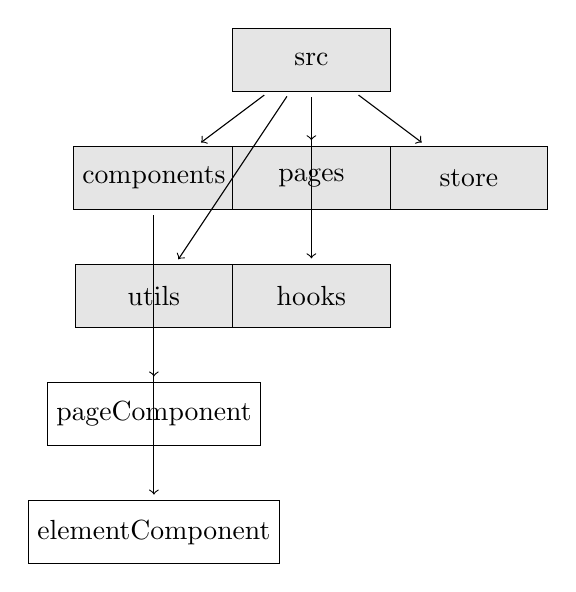
\begin{tikzpicture}[
    file/.style={draw, rectangle, minimum width=2cm, minimum height=0.8cm},
    folder/.style={draw, rectangle, minimum width=2cm, minimum height=0.8cm, fill=gray!20},
    arrow/.style={->, shorten >=2pt, shorten <=2pt}
]

% Folders
\node[folder] (src) at (0,0) {src};
\node[folder] (components) at (-2,-1.5) {components};
\node[folder] (pages) at (0,-1.5) {pages};
\node[folder] (store) at (2,-1.5) {store};
\node[folder] (utils) at (-2,-3) {utils};
\node[folder] (hooks) at (0,-3) {hooks};

% Files
\node[file] (pageComponent) at (-2,-4.5) {pageComponent};
\node[file] (elementComponent) at (-2,-6) {elementComponent};
% ... add more files

% Connections
\draw[arrow] (src) -- (components);
\draw[arrow] (src) -- (pages);
\draw[arrow] (src) -- (store);
\draw[arrow] (src) -- (utils);
\draw[arrow] (src) -- (hooks);
\draw[arrow] (components) -- (pageComponent);
\draw[arrow] (components) -- (elementComponent);
% ... add more connections

\end{tikzpicture}



\pagebreak
\subsubsection{Back-end}
The backend uses the dotNet framework. The development language using the C\# language.

In this project, the backend uses the Onion Architecture.
The Onion Architecture is a typically layered architecture, 
where each layer depends on the inner layer and provides interfaces to the outer layer.
The outer layer provides services to the outermost layer 
and other modules in the same layer based on the interfaces of the inner layer.

From inner to outer, the layers are: Domain, Application, Infrastructure, Presentation.
The Domain layer is the core layer and the innermost layer, used to define domain models, 
which are the business models.
It includes domain models and domain service interfaces.
Domain models are used to define the business models, 
which are the entities in the entity-relationship model and their attributes.
Domain service interfaces are used to define the business services, 
which are the relationships between entities in the entity-relationship model.

The Application layer is the application layer, 
used to define application services, which are the business logic.
It includes domain service implementations and application service interfaces.
Domain service implementations implement the methods of the inner layer's domain service 
interfaces and implement the business logic of the domain models.
Application service interfaces are used to define application services, 
which are the business logic.
It includes but is not limited to database interfaces, testing interfaces, 
HTTP API interfaces, MQTT interfaces, etc.

The Infrastructure layer is the infrastructure layer, used to define infrastructure.
It includes database implementations, testing implementations, 
HTTP API implementations, MQTT implementations, etc.
Database implementations implement the database interfaces 
and provide CRUD services for the database.
Testing implementations implement the testing interfaces 
and provide services for unit testing and integration testing.
HTTP API implementations implement the HTTP API interfaces 
and provide CRUD operations for HTTP APIs.
MQTT implementations implement the MQTT interfaces 
and provide CRUD operations for MQTT.

The Presentation layer is the presentation layer, used to define presentation logic, 
such as interfaces and pages. Since this is a backend project,
data presentation and control are handled by the frontend, 
so this layer is not needed.



\pagebreak
\subsubsection{Data communication and storage}
% 关于本项目的数据通信与数据存储的设计, 包括数据通信的协议, 数据存储的设计等
% 关于数据通信的设计:
% 1. 通信协议的选择
% 自前端向后端发送的数据, 有三种传输的数据类型, 
% 一种是普通的增删改查的请求, 对数据传输的时效性要求不高, 但是对数据的准确性, 完整性, 有序性, 安全性有一定的要求,
% 这种数据的传输, 采用 HTTP 协议, 以及 RESTful API 的设计. 可以有效的保证对数据传输的以上要求.
% 一种是对数据通道的创建和流媒体数据的传输, 对数据传输的时效性, 安全性要求较高, 这种数据的传输, 采用 WebRTC 协议, 以及 MQTT 协议.
% 配合可以快速解码的 flatbuffers 协议, 可以有效的保证对数据传输的以上要求.
% 最后一种是对设备的状态信息和操作信息的传输, 对完整性, 有序性, 安全性都有较高的要求, 这种数据的传输, 采用 MQTT 协议
% 同时也使用了 flatbuffers 协议.
% 
% 2. 数据通信的通信架构和通信流程
% 本项目的数据通信的通信架构, 是基于前后端分离的架构, 前端使用 React 框架, 后端使用 dotnet 框架.
% 当前端需要向后端发送数据的时候, 前端会向后端发送 HTTP 请求, 后端接收到 HTTP 请求之后, 会根据请求的数据类型,
% 选择不同的数据处理方式, 对于普通的增删改查的请求, 后端会根据 RESTful API 的设计, 对数据进行增删改查的操作,
% 对于对数据通道的创建和流媒体数据的传输, 后端会根据 WebRTC 协议, 对数据通道进行创建, 并且帮助前端和设备建立数据通道,
% 当数据通道建立后, 前端和设备之间则使用 flatbuffer 的数据格式对流媒体数据进行传输,
% 对于设备的状态信息和操作信息的传输, 前端会直接向 MQTT broker 发送 MQTT 请求, 
% 设备会在其自身的固件中监听相关的 MQTT 请求, 并且返回相关的数据.
% 
% 3. 数据通信的格式
% 本项目的数据通信的格式, 有三种, 
% 一种是 HTTP 协议, 
% 使用 json 格式对数据进行传输,
% 一种是 WebRTC 协议, 
% 使用 flatbuffers 格式对数据进行传输,
% 一种是 MQTT 协议.
% 使用 flatbuffers 格式对数据进行传输,
% 
% 关于数据存储的设计:
% 1. 数据存储的数据库的选择
% 本项目的数据存储的数据库的选择, 使用了轻量级的数据库 SQLite,
% SQLite 是一个进程内的库, 实现了自给自足的, 无服务器的, 零配置的, 事务性的 SQL 数据库引擎.
% 这是因为整个项目的目的是为了实现前端与设备之间的数据通信, 对于数据库数据的增删改查操作的要求不高,
% 数据量较小, 且对于数据库的数据的事务性要求不高, 所以选择了 SQLite 数据库.
% 2. 项目前后端的数据结构的设计
% 在本项目中, 前端由于使用了 React 框架, 所以前端的数据结构的设计, 使用了基于状态的数据结构的设计,
% 每个组件或者数据集都包含一个状态对象, 这个状态对象的属性就是组件的各个状态. 
% 使用状态对象的原因是, 可以方便的对状态进行管理, 采用对象-属性的形式, 可以方便的针对不同组件的同类状态进行区分,
% 由于跨组件的状态是由 redux 进行管理的, 这种状态对象的设计, 可以更搞笑的对状态进行更新和传递.
% 后端由于使用了 dotnet 框架, 所以后端的数据结构的设计, 使用了基于类的数据结构的设计,
% 采用了面向对象的编程思想, 对数据进行了封装, 使得数据的传输更加的安全, 有序, 完整.


\pagebreak

% \subsection{Domain model}
% \documentclass[]{article}
\usepackage{graphicx}
\usepackage{amsmath}
\usepackage{tikz}

% libaries
\usetikzlibrary{shapes,arrows}

%Define the listing package
\usepackage{listings} %code highlighter
\usepackage{color} %use color
\definecolor{mygreen}{rgb}{0,0.6,0}
\definecolor{mygray}{rgb}{0.5,0.5,0.5}
\definecolor{mymauve}{rgb}{0.58,0,0.82}

%Customize a bit the look
\lstset{ %
backgroundcolor=\color{white}, % choose the background color; you must add \usepackage{color} or \usepackage{xcolor}
basicstyle=\footnotesize, % the size of the fonts that are used for the code
breakatwhitespace=false, % sets if automatic breaks should only happen at whitespace
breaklines=true, % sets automatic line breaking
captionpos=b, % sets the caption-position to bottom
commentstyle=\color{mygreen}, % comment style
deletekeywords={...}, % if you want to delete keywords from the given language
escapeinside={\%*}{*)}, % if you want to add LaTeX within your code
extendedchars=true, % lets you use non-ASCII characters; for 8-bits encodings only, does not work with UTF-8
frame=single, % adds a frame around the code
keepspaces=true, % keeps spaces in text, useful for keeping indentation of code (possibly needs columns=flexible)
keywordstyle=\color{blue}, % keyword style
% language=Octave, % the language of the code
morekeywords={*,...}, % if you want to add more keywords to the set
numbers=left, % where to put the line-numbers; possible values are (none, left, right)
numbersep=5pt, % how far the line-numbers are from the code
numberstyle=\tiny\color{mygray}, % the style that is used for the line-numbers
rulecolor=\color{black}, % if not set, the frame-color may be changed on line-breaks within not-black text (e.g. comments (green here))
showspaces=false, % show spaces everywhere adding particular underscores; it overrides 'showstringspaces'
showstringspaces=false, % underline spaces within strings only
showtabs=false, % show tabs within strings adding particular underscores
stepnumber=1, % the step between two line-numbers. If it's 1, each line will be numbered
stringstyle=\color{mymauve}, % string literal style
tabsize=2, % sets default tabsize to 2 spaces
title=\lstname % show the filename of files included with \lstinputlisting; also try caption instead of title
}

\definecolor{darkgray}{rgb}{.4,.4,.4}
\definecolor{purple}{rgb}{0.65, 0.12, 0.82}

\lstdefinelanguage{React}{
keywords={const, typeof, new, true, false, catch, function, return, null, catch, switch, var, if, in, while, do, else, case, break},
keywordstyle=\color{blue}\bfseries,
ndkeywords={class, export, boolean, throw, implements, import, this},
ndkeywordstyle=\color{darkgray}\bfseries,
identifierstyle=\color{mygreen},
sensitive=false,
comment=[l]{//},
morecomment=[s]{/*}{*/},
commentstyle=\color{purple}\ttfamily,
string=[b]{"}{'}{`},
stringstyle=\color{red}\ttfamily,
morestring=[b]',
morestring=[b]",
morestring=[b]`',
}

\lstdefinelanguage{CSharp}{
keywords={const, typeof, new, true, false, catch, function, return, null, catch, switch, var, if, in, while, do, else, case, break},
keywordstyle=\color{blue}\bfseries,
ndkeywords={class, export, boolean, throw, implements, import, this},
ndkeywordstyle=\color{darkgray}\bfseries,
identifierstyle=\color{mygreen},
sensitive=false,
comment=[l]{//},
morecomment=[s]{/*}{*/},
commentstyle=\color{purple}\ttfamily,
string=[b]{"}{'}{`},
stringstyle=\color{red}\ttfamily,
morestring=[b]',
morestring=[b]",
morestring=[b]`',
}

\lstset{
language=React,
extendedchars=true,
basicstyle=\footnotesize\ttfamily,
showstringspaces=false,
showspaces=false,
numbers=left,
numberstyle=\footnotesize,
numbersep=9pt,
tabsize=2,
breaklines=true,
showtabs=false,
captionpos=b
}

\lstset{
language=CSharp,
extendedchars=true,
basicstyle=\footnotesize\ttfamily,
showstringspaces=false,
showspaces=false,
numbers=left,
numberstyle=\footnotesize,
numbersep=9pt,
tabsize=2,
breaklines=true,
showtabs=false,
captionpos=b
}

% \usepackage{cite} % Add this line for citation

% \bibliographystyle{plain}

\title{
The implementation of BifrostConnect Front-end scope, 
re-design and development with the relevant back-end support develop.
}
\author{
    Fei Gu \\
    Erhvervs Akademi Sydvest \\
    Computer Science 21\\
    }
\date{\today}

\begin{document}

% Front page
\maketitle
\begin{center}
    Supervisor: Henrik Boulund Meng Hansen \\
    Company: BifrostConnect \\
    Engineering Director: Jasper Wass \\
\end{center}
\tableofcontents
\pagebreak


% The introduction
\section{Introduction}
\subsection{Background}\input{sections/introduction/background.tex}
\subsection{The company}\input{sections/introduction/aboutCompany}
\subsection{The project}\input{sections/introduction/aboutProject}
\pagebreak

% The problem statement
\section{Problem Statement}
\subsection{Statement}
\input{sections/problemStatement/statement}
\subsection{Situation}
\input{sections/problemStatement/situation}
\subsection{Potential Solution}
\input{sections/problemStatement/potentialSolution}
\pagebreak

% Requirement analysis
\section{Requirement Analysis}
\input{sections/requirementAnalysis/index}

\subsection{Stakeholders}
\input{sections/requirementAnalysis/stakeholders/index}

\subsection{Business Domain}
\input{sections/requirementAnalysis/bussinesDomain/index}

\subsection{Scope}
\input{sections/requirementAnalysis/scope}

\subsection{Goals}
\input{sections/requirementAnalysis/goals}
\pagebreak

% Software Design
\section{Software Design}
% developement methods
\subsection{Software Development Methods}
\input{sections/softwareDevelopmentMethods/index}
\subsubsection{Agile Software Development}
\input{sections/softwareDevelopmentMethods/agileSoftwareDevelopment/index}
\subsubsection{Feature Driven Development}
\input{sections/softwareDevelopmentMethods/featureDrivenDevelopment/index}

\pagebreak

% Technology seslection
\subsection{Technology selection}
\input{sections/softwareDesign/technologySelection/index}
\subsubsection{Front-end}
\input{sections/softwareDesign/technologySelection/frontEnd}            
\subsubsection{Back-end}
\input{sections/softwareDesign/technologySelection/backEnd}            
\subsubsection{Database}
\input{sections/softwareDesign/technologySelection/database}
\subsubsection{Data communication}
\input{sections/softwareDesign/technologySelection/dataCommunication}            
\subsubsection{DevOps}
\input{sections/softwareDesign/technologySelection/devOps}
\pagebreak

% Architecture design
\subsection{Architecture design}
\input{sections/softwareDesign/architectureDesign/index}
\pagebreak
\subsubsection{Front-end}
\input{sections/softwareDesign/architectureDesign/frontEndArchitecture}
\pagebreak
\subsubsection{Back-end}
\input{sections/softwareDesign/architectureDesign/backEndArchitecture}
\pagebreak
\subsubsection{Data communication and storage}
\input{sections/softwareDesign/architectureDesign/dataCommunicationArchitecture}
\pagebreak

% \subsection{Domain model}
% \input{sections/softwareDesign/domainModel/index}
% \subsection{Database design}
% % 数据库领域模型 ER 图
% % 包括表和字段的设置.
% % 对于私有键和外键的设置.

% \subsection{Back-end design}
% % 后端对象模型
% % 以及对于对象模型的增删改查
% % 以及相关的其他服务的设计`'

% \subsection{Front-end design}
% % 对于前端的页面结构的设计 
% % 页面的状态的设计, 交互设计

% \subsection{FlatBuffers design}
% % schema 的设计

\subsection{DevOps CI/CD process design}
\input{sections/softwareDesign/devOpsDesign/index}
\subsubsection{Continuous Integration}
\input{sections/softwareDesign/devOpsDesign/continuousIntegration/index}
\subsubsection{Continuous Delivery}
\input{sections/softwareDesign/devOpsDesign/continuousDelivery/index}
\subsubsection{Continuous Deployment}
\input{sections/softwareDesign/devOpsDesign/continuousDeployment/index}
\pagebreak

\section{Software Development} 
\input{sections/softwareDevelopment/index}
\subsection{Overall development}
\input{sections/softwareDevelopment/overallDevelopement/index}
\subsubsection{Front-end}
\input{sections/softwareDevelopment/overallDevelopement/frontEnd/index}
\subsubsection{Back-end}
\input{sections/softwareDevelopment/overallDevelopement/backEnd/index}
\subsubsection{DevOps}
\input{sections/softwareDevelopment/overallDevelopement/devOps/index}
\subsection{Feature development} 
\input{sections/softwareDevelopment/featureDevelopment/index}
\subsubsection{Use Case 1}
\input{sections/softwareDevelopment/featureDevelopment/useCase1/index}
\subsubsection{Feature 1}
\input{sections/softwareDevelopment/featureDevelopment/feature/feature1.tex}
\pagebreak
\section{Conclusion} 
\subsection{Result}
Since the project is still in progress, the result is not available yet.
So far, basic structure of this project has been built. But the most features 
are not implemented yet. 
\subsection{Discussion}
As a single developer for this project, I am confident what I have done so far.
And I can say I understand the most of the knowledge I have used in this project, 
which also means I can explain all the part of the project. 
But this project also relevant some of the complex knowledge which I have to continue 
to study and practice.
\subsection{Future Work}
The future work is to implement the rest of the features. 
Including the most important part which is the 'create session' feature.
\pagebreak
% \bibliography{bibliography}
\pagebreak
% \begin{appendices}
%     \section{Appendix}
% \end{appendices} 
\end{document}
% \subsection{Database design}
% % 数据库领域模型 ER 图
% % 包括表和字段的设置.
% % 对于私有键和外键的设置.

% \subsection{Back-end design}
% % 后端对象模型
% % 以及对于对象模型的增删改查
% % 以及相关的其他服务的设计`'

% \subsection{Front-end design}
% % 对于前端的页面结构的设计 
% % 页面的状态的设计, 交互设计

% \subsection{FlatBuffers design}
% % schema 的设计

\subsection{DevOps CI/CD process design}
\documentclass[]{article}
\usepackage{graphicx}
\usepackage{amsmath}
\usepackage{tikz}

% libaries
\usetikzlibrary{shapes,arrows}

%Define the listing package
\usepackage{listings} %code highlighter
\usepackage{color} %use color
\definecolor{mygreen}{rgb}{0,0.6,0}
\definecolor{mygray}{rgb}{0.5,0.5,0.5}
\definecolor{mymauve}{rgb}{0.58,0,0.82}

%Customize a bit the look
\lstset{ %
backgroundcolor=\color{white}, % choose the background color; you must add \usepackage{color} or \usepackage{xcolor}
basicstyle=\footnotesize, % the size of the fonts that are used for the code
breakatwhitespace=false, % sets if automatic breaks should only happen at whitespace
breaklines=true, % sets automatic line breaking
captionpos=b, % sets the caption-position to bottom
commentstyle=\color{mygreen}, % comment style
deletekeywords={...}, % if you want to delete keywords from the given language
escapeinside={\%*}{*)}, % if you want to add LaTeX within your code
extendedchars=true, % lets you use non-ASCII characters; for 8-bits encodings only, does not work with UTF-8
frame=single, % adds a frame around the code
keepspaces=true, % keeps spaces in text, useful for keeping indentation of code (possibly needs columns=flexible)
keywordstyle=\color{blue}, % keyword style
% language=Octave, % the language of the code
morekeywords={*,...}, % if you want to add more keywords to the set
numbers=left, % where to put the line-numbers; possible values are (none, left, right)
numbersep=5pt, % how far the line-numbers are from the code
numberstyle=\tiny\color{mygray}, % the style that is used for the line-numbers
rulecolor=\color{black}, % if not set, the frame-color may be changed on line-breaks within not-black text (e.g. comments (green here))
showspaces=false, % show spaces everywhere adding particular underscores; it overrides 'showstringspaces'
showstringspaces=false, % underline spaces within strings only
showtabs=false, % show tabs within strings adding particular underscores
stepnumber=1, % the step between two line-numbers. If it's 1, each line will be numbered
stringstyle=\color{mymauve}, % string literal style
tabsize=2, % sets default tabsize to 2 spaces
title=\lstname % show the filename of files included with \lstinputlisting; also try caption instead of title
}

\definecolor{darkgray}{rgb}{.4,.4,.4}
\definecolor{purple}{rgb}{0.65, 0.12, 0.82}

\lstdefinelanguage{React}{
keywords={const, typeof, new, true, false, catch, function, return, null, catch, switch, var, if, in, while, do, else, case, break},
keywordstyle=\color{blue}\bfseries,
ndkeywords={class, export, boolean, throw, implements, import, this},
ndkeywordstyle=\color{darkgray}\bfseries,
identifierstyle=\color{mygreen},
sensitive=false,
comment=[l]{//},
morecomment=[s]{/*}{*/},
commentstyle=\color{purple}\ttfamily,
string=[b]{"}{'}{`},
stringstyle=\color{red}\ttfamily,
morestring=[b]',
morestring=[b]",
morestring=[b]`',
}

\lstdefinelanguage{CSharp}{
keywords={const, typeof, new, true, false, catch, function, return, null, catch, switch, var, if, in, while, do, else, case, break},
keywordstyle=\color{blue}\bfseries,
ndkeywords={class, export, boolean, throw, implements, import, this},
ndkeywordstyle=\color{darkgray}\bfseries,
identifierstyle=\color{mygreen},
sensitive=false,
comment=[l]{//},
morecomment=[s]{/*}{*/},
commentstyle=\color{purple}\ttfamily,
string=[b]{"}{'}{`},
stringstyle=\color{red}\ttfamily,
morestring=[b]',
morestring=[b]",
morestring=[b]`',
}

\lstset{
language=React,
extendedchars=true,
basicstyle=\footnotesize\ttfamily,
showstringspaces=false,
showspaces=false,
numbers=left,
numberstyle=\footnotesize,
numbersep=9pt,
tabsize=2,
breaklines=true,
showtabs=false,
captionpos=b
}

\lstset{
language=CSharp,
extendedchars=true,
basicstyle=\footnotesize\ttfamily,
showstringspaces=false,
showspaces=false,
numbers=left,
numberstyle=\footnotesize,
numbersep=9pt,
tabsize=2,
breaklines=true,
showtabs=false,
captionpos=b
}

% \usepackage{cite} % Add this line for citation

% \bibliographystyle{plain}

\title{
The implementation of BifrostConnect Front-end scope, 
re-design and development with the relevant back-end support develop.
}
\author{
    Fei Gu \\
    Erhvervs Akademi Sydvest \\
    Computer Science 21\\
    }
\date{\today}

\begin{document}

% Front page
\maketitle
\begin{center}
    Supervisor: Henrik Boulund Meng Hansen \\
    Company: BifrostConnect \\
    Engineering Director: Jasper Wass \\
\end{center}
\tableofcontents
\pagebreak


% The introduction
\section{Introduction}
\subsection{Background}\input{sections/introduction/background.tex}
\subsection{The company}\input{sections/introduction/aboutCompany}
\subsection{The project}\input{sections/introduction/aboutProject}
\pagebreak

% The problem statement
\section{Problem Statement}
\subsection{Statement}
\input{sections/problemStatement/statement}
\subsection{Situation}
\input{sections/problemStatement/situation}
\subsection{Potential Solution}
\input{sections/problemStatement/potentialSolution}
\pagebreak

% Requirement analysis
\section{Requirement Analysis}
\input{sections/requirementAnalysis/index}

\subsection{Stakeholders}
\input{sections/requirementAnalysis/stakeholders/index}

\subsection{Business Domain}
\input{sections/requirementAnalysis/bussinesDomain/index}

\subsection{Scope}
\input{sections/requirementAnalysis/scope}

\subsection{Goals}
\input{sections/requirementAnalysis/goals}
\pagebreak

% Software Design
\section{Software Design}
% developement methods
\subsection{Software Development Methods}
\input{sections/softwareDevelopmentMethods/index}
\subsubsection{Agile Software Development}
\input{sections/softwareDevelopmentMethods/agileSoftwareDevelopment/index}
\subsubsection{Feature Driven Development}
\input{sections/softwareDevelopmentMethods/featureDrivenDevelopment/index}

\pagebreak

% Technology seslection
\subsection{Technology selection}
\input{sections/softwareDesign/technologySelection/index}
\subsubsection{Front-end}
\input{sections/softwareDesign/technologySelection/frontEnd}            
\subsubsection{Back-end}
\input{sections/softwareDesign/technologySelection/backEnd}            
\subsubsection{Database}
\input{sections/softwareDesign/technologySelection/database}
\subsubsection{Data communication}
\input{sections/softwareDesign/technologySelection/dataCommunication}            
\subsubsection{DevOps}
\input{sections/softwareDesign/technologySelection/devOps}
\pagebreak

% Architecture design
\subsection{Architecture design}
\input{sections/softwareDesign/architectureDesign/index}
\pagebreak
\subsubsection{Front-end}
\input{sections/softwareDesign/architectureDesign/frontEndArchitecture}
\pagebreak
\subsubsection{Back-end}
\input{sections/softwareDesign/architectureDesign/backEndArchitecture}
\pagebreak
\subsubsection{Data communication and storage}
\input{sections/softwareDesign/architectureDesign/dataCommunicationArchitecture}
\pagebreak

% \subsection{Domain model}
% \input{sections/softwareDesign/domainModel/index}
% \subsection{Database design}
% % 数据库领域模型 ER 图
% % 包括表和字段的设置.
% % 对于私有键和外键的设置.

% \subsection{Back-end design}
% % 后端对象模型
% % 以及对于对象模型的增删改查
% % 以及相关的其他服务的设计`'

% \subsection{Front-end design}
% % 对于前端的页面结构的设计 
% % 页面的状态的设计, 交互设计

% \subsection{FlatBuffers design}
% % schema 的设计

\subsection{DevOps CI/CD process design}
\input{sections/softwareDesign/devOpsDesign/index}
\subsubsection{Continuous Integration}
\input{sections/softwareDesign/devOpsDesign/continuousIntegration/index}
\subsubsection{Continuous Delivery}
\input{sections/softwareDesign/devOpsDesign/continuousDelivery/index}
\subsubsection{Continuous Deployment}
\input{sections/softwareDesign/devOpsDesign/continuousDeployment/index}
\pagebreak

\section{Software Development} 
\input{sections/softwareDevelopment/index}
\subsection{Overall development}
\input{sections/softwareDevelopment/overallDevelopement/index}
\subsubsection{Front-end}
\input{sections/softwareDevelopment/overallDevelopement/frontEnd/index}
\subsubsection{Back-end}
\input{sections/softwareDevelopment/overallDevelopement/backEnd/index}
\subsubsection{DevOps}
\input{sections/softwareDevelopment/overallDevelopement/devOps/index}
\subsection{Feature development} 
\input{sections/softwareDevelopment/featureDevelopment/index}
\subsubsection{Use Case 1}
\input{sections/softwareDevelopment/featureDevelopment/useCase1/index}
\subsubsection{Feature 1}
\input{sections/softwareDevelopment/featureDevelopment/feature/feature1.tex}
\pagebreak
\section{Conclusion} 
\subsection{Result}
Since the project is still in progress, the result is not available yet.
So far, basic structure of this project has been built. But the most features 
are not implemented yet. 
\subsection{Discussion}
As a single developer for this project, I am confident what I have done so far.
And I can say I understand the most of the knowledge I have used in this project, 
which also means I can explain all the part of the project. 
But this project also relevant some of the complex knowledge which I have to continue 
to study and practice.
\subsection{Future Work}
The future work is to implement the rest of the features. 
Including the most important part which is the 'create session' feature.
\pagebreak
% \bibliography{bibliography}
\pagebreak
% \begin{appendices}
%     \section{Appendix}
% \end{appendices} 
\end{document}
\subsubsection{Continuous Integration}
\documentclass[]{article}
\usepackage{graphicx}
\usepackage{amsmath}
\usepackage{tikz}

% libaries
\usetikzlibrary{shapes,arrows}

%Define the listing package
\usepackage{listings} %code highlighter
\usepackage{color} %use color
\definecolor{mygreen}{rgb}{0,0.6,0}
\definecolor{mygray}{rgb}{0.5,0.5,0.5}
\definecolor{mymauve}{rgb}{0.58,0,0.82}

%Customize a bit the look
\lstset{ %
backgroundcolor=\color{white}, % choose the background color; you must add \usepackage{color} or \usepackage{xcolor}
basicstyle=\footnotesize, % the size of the fonts that are used for the code
breakatwhitespace=false, % sets if automatic breaks should only happen at whitespace
breaklines=true, % sets automatic line breaking
captionpos=b, % sets the caption-position to bottom
commentstyle=\color{mygreen}, % comment style
deletekeywords={...}, % if you want to delete keywords from the given language
escapeinside={\%*}{*)}, % if you want to add LaTeX within your code
extendedchars=true, % lets you use non-ASCII characters; for 8-bits encodings only, does not work with UTF-8
frame=single, % adds a frame around the code
keepspaces=true, % keeps spaces in text, useful for keeping indentation of code (possibly needs columns=flexible)
keywordstyle=\color{blue}, % keyword style
% language=Octave, % the language of the code
morekeywords={*,...}, % if you want to add more keywords to the set
numbers=left, % where to put the line-numbers; possible values are (none, left, right)
numbersep=5pt, % how far the line-numbers are from the code
numberstyle=\tiny\color{mygray}, % the style that is used for the line-numbers
rulecolor=\color{black}, % if not set, the frame-color may be changed on line-breaks within not-black text (e.g. comments (green here))
showspaces=false, % show spaces everywhere adding particular underscores; it overrides 'showstringspaces'
showstringspaces=false, % underline spaces within strings only
showtabs=false, % show tabs within strings adding particular underscores
stepnumber=1, % the step between two line-numbers. If it's 1, each line will be numbered
stringstyle=\color{mymauve}, % string literal style
tabsize=2, % sets default tabsize to 2 spaces
title=\lstname % show the filename of files included with \lstinputlisting; also try caption instead of title
}

\definecolor{darkgray}{rgb}{.4,.4,.4}
\definecolor{purple}{rgb}{0.65, 0.12, 0.82}

\lstdefinelanguage{React}{
keywords={const, typeof, new, true, false, catch, function, return, null, catch, switch, var, if, in, while, do, else, case, break},
keywordstyle=\color{blue}\bfseries,
ndkeywords={class, export, boolean, throw, implements, import, this},
ndkeywordstyle=\color{darkgray}\bfseries,
identifierstyle=\color{mygreen},
sensitive=false,
comment=[l]{//},
morecomment=[s]{/*}{*/},
commentstyle=\color{purple}\ttfamily,
string=[b]{"}{'}{`},
stringstyle=\color{red}\ttfamily,
morestring=[b]',
morestring=[b]",
morestring=[b]`',
}

\lstdefinelanguage{CSharp}{
keywords={const, typeof, new, true, false, catch, function, return, null, catch, switch, var, if, in, while, do, else, case, break},
keywordstyle=\color{blue}\bfseries,
ndkeywords={class, export, boolean, throw, implements, import, this},
ndkeywordstyle=\color{darkgray}\bfseries,
identifierstyle=\color{mygreen},
sensitive=false,
comment=[l]{//},
morecomment=[s]{/*}{*/},
commentstyle=\color{purple}\ttfamily,
string=[b]{"}{'}{`},
stringstyle=\color{red}\ttfamily,
morestring=[b]',
morestring=[b]",
morestring=[b]`',
}

\lstset{
language=React,
extendedchars=true,
basicstyle=\footnotesize\ttfamily,
showstringspaces=false,
showspaces=false,
numbers=left,
numberstyle=\footnotesize,
numbersep=9pt,
tabsize=2,
breaklines=true,
showtabs=false,
captionpos=b
}

\lstset{
language=CSharp,
extendedchars=true,
basicstyle=\footnotesize\ttfamily,
showstringspaces=false,
showspaces=false,
numbers=left,
numberstyle=\footnotesize,
numbersep=9pt,
tabsize=2,
breaklines=true,
showtabs=false,
captionpos=b
}

% \usepackage{cite} % Add this line for citation

% \bibliographystyle{plain}

\title{
The implementation of BifrostConnect Front-end scope, 
re-design and development with the relevant back-end support develop.
}
\author{
    Fei Gu \\
    Erhvervs Akademi Sydvest \\
    Computer Science 21\\
    }
\date{\today}

\begin{document}

% Front page
\maketitle
\begin{center}
    Supervisor: Henrik Boulund Meng Hansen \\
    Company: BifrostConnect \\
    Engineering Director: Jasper Wass \\
\end{center}
\tableofcontents
\pagebreak


% The introduction
\section{Introduction}
\subsection{Background}\input{sections/introduction/background.tex}
\subsection{The company}\input{sections/introduction/aboutCompany}
\subsection{The project}\input{sections/introduction/aboutProject}
\pagebreak

% The problem statement
\section{Problem Statement}
\subsection{Statement}
\input{sections/problemStatement/statement}
\subsection{Situation}
\input{sections/problemStatement/situation}
\subsection{Potential Solution}
\input{sections/problemStatement/potentialSolution}
\pagebreak

% Requirement analysis
\section{Requirement Analysis}
\input{sections/requirementAnalysis/index}

\subsection{Stakeholders}
\input{sections/requirementAnalysis/stakeholders/index}

\subsection{Business Domain}
\input{sections/requirementAnalysis/bussinesDomain/index}

\subsection{Scope}
\input{sections/requirementAnalysis/scope}

\subsection{Goals}
\input{sections/requirementAnalysis/goals}
\pagebreak

% Software Design
\section{Software Design}
% developement methods
\subsection{Software Development Methods}
\input{sections/softwareDevelopmentMethods/index}
\subsubsection{Agile Software Development}
\input{sections/softwareDevelopmentMethods/agileSoftwareDevelopment/index}
\subsubsection{Feature Driven Development}
\input{sections/softwareDevelopmentMethods/featureDrivenDevelopment/index}

\pagebreak

% Technology seslection
\subsection{Technology selection}
\input{sections/softwareDesign/technologySelection/index}
\subsubsection{Front-end}
\input{sections/softwareDesign/technologySelection/frontEnd}            
\subsubsection{Back-end}
\input{sections/softwareDesign/technologySelection/backEnd}            
\subsubsection{Database}
\input{sections/softwareDesign/technologySelection/database}
\subsubsection{Data communication}
\input{sections/softwareDesign/technologySelection/dataCommunication}            
\subsubsection{DevOps}
\input{sections/softwareDesign/technologySelection/devOps}
\pagebreak

% Architecture design
\subsection{Architecture design}
\input{sections/softwareDesign/architectureDesign/index}
\pagebreak
\subsubsection{Front-end}
\input{sections/softwareDesign/architectureDesign/frontEndArchitecture}
\pagebreak
\subsubsection{Back-end}
\input{sections/softwareDesign/architectureDesign/backEndArchitecture}
\pagebreak
\subsubsection{Data communication and storage}
\input{sections/softwareDesign/architectureDesign/dataCommunicationArchitecture}
\pagebreak

% \subsection{Domain model}
% \input{sections/softwareDesign/domainModel/index}
% \subsection{Database design}
% % 数据库领域模型 ER 图
% % 包括表和字段的设置.
% % 对于私有键和外键的设置.

% \subsection{Back-end design}
% % 后端对象模型
% % 以及对于对象模型的增删改查
% % 以及相关的其他服务的设计`'

% \subsection{Front-end design}
% % 对于前端的页面结构的设计 
% % 页面的状态的设计, 交互设计

% \subsection{FlatBuffers design}
% % schema 的设计

\subsection{DevOps CI/CD process design}
\input{sections/softwareDesign/devOpsDesign/index}
\subsubsection{Continuous Integration}
\input{sections/softwareDesign/devOpsDesign/continuousIntegration/index}
\subsubsection{Continuous Delivery}
\input{sections/softwareDesign/devOpsDesign/continuousDelivery/index}
\subsubsection{Continuous Deployment}
\input{sections/softwareDesign/devOpsDesign/continuousDeployment/index}
\pagebreak

\section{Software Development} 
\input{sections/softwareDevelopment/index}
\subsection{Overall development}
\input{sections/softwareDevelopment/overallDevelopement/index}
\subsubsection{Front-end}
\input{sections/softwareDevelopment/overallDevelopement/frontEnd/index}
\subsubsection{Back-end}
\input{sections/softwareDevelopment/overallDevelopement/backEnd/index}
\subsubsection{DevOps}
\input{sections/softwareDevelopment/overallDevelopement/devOps/index}
\subsection{Feature development} 
\input{sections/softwareDevelopment/featureDevelopment/index}
\subsubsection{Use Case 1}
\input{sections/softwareDevelopment/featureDevelopment/useCase1/index}
\subsubsection{Feature 1}
\input{sections/softwareDevelopment/featureDevelopment/feature/feature1.tex}
\pagebreak
\section{Conclusion} 
\subsection{Result}
Since the project is still in progress, the result is not available yet.
So far, basic structure of this project has been built. But the most features 
are not implemented yet. 
\subsection{Discussion}
As a single developer for this project, I am confident what I have done so far.
And I can say I understand the most of the knowledge I have used in this project, 
which also means I can explain all the part of the project. 
But this project also relevant some of the complex knowledge which I have to continue 
to study and practice.
\subsection{Future Work}
The future work is to implement the rest of the features. 
Including the most important part which is the 'create session' feature.
\pagebreak
% \bibliography{bibliography}
\pagebreak
% \begin{appendices}
%     \section{Appendix}
% \end{appendices} 
\end{document}
\subsubsection{Continuous Delivery}
\documentclass[]{article}
\usepackage{graphicx}
\usepackage{amsmath}
\usepackage{tikz}

% libaries
\usetikzlibrary{shapes,arrows}

%Define the listing package
\usepackage{listings} %code highlighter
\usepackage{color} %use color
\definecolor{mygreen}{rgb}{0,0.6,0}
\definecolor{mygray}{rgb}{0.5,0.5,0.5}
\definecolor{mymauve}{rgb}{0.58,0,0.82}

%Customize a bit the look
\lstset{ %
backgroundcolor=\color{white}, % choose the background color; you must add \usepackage{color} or \usepackage{xcolor}
basicstyle=\footnotesize, % the size of the fonts that are used for the code
breakatwhitespace=false, % sets if automatic breaks should only happen at whitespace
breaklines=true, % sets automatic line breaking
captionpos=b, % sets the caption-position to bottom
commentstyle=\color{mygreen}, % comment style
deletekeywords={...}, % if you want to delete keywords from the given language
escapeinside={\%*}{*)}, % if you want to add LaTeX within your code
extendedchars=true, % lets you use non-ASCII characters; for 8-bits encodings only, does not work with UTF-8
frame=single, % adds a frame around the code
keepspaces=true, % keeps spaces in text, useful for keeping indentation of code (possibly needs columns=flexible)
keywordstyle=\color{blue}, % keyword style
% language=Octave, % the language of the code
morekeywords={*,...}, % if you want to add more keywords to the set
numbers=left, % where to put the line-numbers; possible values are (none, left, right)
numbersep=5pt, % how far the line-numbers are from the code
numberstyle=\tiny\color{mygray}, % the style that is used for the line-numbers
rulecolor=\color{black}, % if not set, the frame-color may be changed on line-breaks within not-black text (e.g. comments (green here))
showspaces=false, % show spaces everywhere adding particular underscores; it overrides 'showstringspaces'
showstringspaces=false, % underline spaces within strings only
showtabs=false, % show tabs within strings adding particular underscores
stepnumber=1, % the step between two line-numbers. If it's 1, each line will be numbered
stringstyle=\color{mymauve}, % string literal style
tabsize=2, % sets default tabsize to 2 spaces
title=\lstname % show the filename of files included with \lstinputlisting; also try caption instead of title
}

\definecolor{darkgray}{rgb}{.4,.4,.4}
\definecolor{purple}{rgb}{0.65, 0.12, 0.82}

\lstdefinelanguage{React}{
keywords={const, typeof, new, true, false, catch, function, return, null, catch, switch, var, if, in, while, do, else, case, break},
keywordstyle=\color{blue}\bfseries,
ndkeywords={class, export, boolean, throw, implements, import, this},
ndkeywordstyle=\color{darkgray}\bfseries,
identifierstyle=\color{mygreen},
sensitive=false,
comment=[l]{//},
morecomment=[s]{/*}{*/},
commentstyle=\color{purple}\ttfamily,
string=[b]{"}{'}{`},
stringstyle=\color{red}\ttfamily,
morestring=[b]',
morestring=[b]",
morestring=[b]`',
}

\lstdefinelanguage{CSharp}{
keywords={const, typeof, new, true, false, catch, function, return, null, catch, switch, var, if, in, while, do, else, case, break},
keywordstyle=\color{blue}\bfseries,
ndkeywords={class, export, boolean, throw, implements, import, this},
ndkeywordstyle=\color{darkgray}\bfseries,
identifierstyle=\color{mygreen},
sensitive=false,
comment=[l]{//},
morecomment=[s]{/*}{*/},
commentstyle=\color{purple}\ttfamily,
string=[b]{"}{'}{`},
stringstyle=\color{red}\ttfamily,
morestring=[b]',
morestring=[b]",
morestring=[b]`',
}

\lstset{
language=React,
extendedchars=true,
basicstyle=\footnotesize\ttfamily,
showstringspaces=false,
showspaces=false,
numbers=left,
numberstyle=\footnotesize,
numbersep=9pt,
tabsize=2,
breaklines=true,
showtabs=false,
captionpos=b
}

\lstset{
language=CSharp,
extendedchars=true,
basicstyle=\footnotesize\ttfamily,
showstringspaces=false,
showspaces=false,
numbers=left,
numberstyle=\footnotesize,
numbersep=9pt,
tabsize=2,
breaklines=true,
showtabs=false,
captionpos=b
}

% \usepackage{cite} % Add this line for citation

% \bibliographystyle{plain}

\title{
The implementation of BifrostConnect Front-end scope, 
re-design and development with the relevant back-end support develop.
}
\author{
    Fei Gu \\
    Erhvervs Akademi Sydvest \\
    Computer Science 21\\
    }
\date{\today}

\begin{document}

% Front page
\maketitle
\begin{center}
    Supervisor: Henrik Boulund Meng Hansen \\
    Company: BifrostConnect \\
    Engineering Director: Jasper Wass \\
\end{center}
\tableofcontents
\pagebreak


% The introduction
\section{Introduction}
\subsection{Background}\input{sections/introduction/background.tex}
\subsection{The company}\input{sections/introduction/aboutCompany}
\subsection{The project}\input{sections/introduction/aboutProject}
\pagebreak

% The problem statement
\section{Problem Statement}
\subsection{Statement}
\input{sections/problemStatement/statement}
\subsection{Situation}
\input{sections/problemStatement/situation}
\subsection{Potential Solution}
\input{sections/problemStatement/potentialSolution}
\pagebreak

% Requirement analysis
\section{Requirement Analysis}
\input{sections/requirementAnalysis/index}

\subsection{Stakeholders}
\input{sections/requirementAnalysis/stakeholders/index}

\subsection{Business Domain}
\input{sections/requirementAnalysis/bussinesDomain/index}

\subsection{Scope}
\input{sections/requirementAnalysis/scope}

\subsection{Goals}
\input{sections/requirementAnalysis/goals}
\pagebreak

% Software Design
\section{Software Design}
% developement methods
\subsection{Software Development Methods}
\input{sections/softwareDevelopmentMethods/index}
\subsubsection{Agile Software Development}
\input{sections/softwareDevelopmentMethods/agileSoftwareDevelopment/index}
\subsubsection{Feature Driven Development}
\input{sections/softwareDevelopmentMethods/featureDrivenDevelopment/index}

\pagebreak

% Technology seslection
\subsection{Technology selection}
\input{sections/softwareDesign/technologySelection/index}
\subsubsection{Front-end}
\input{sections/softwareDesign/technologySelection/frontEnd}            
\subsubsection{Back-end}
\input{sections/softwareDesign/technologySelection/backEnd}            
\subsubsection{Database}
\input{sections/softwareDesign/technologySelection/database}
\subsubsection{Data communication}
\input{sections/softwareDesign/technologySelection/dataCommunication}            
\subsubsection{DevOps}
\input{sections/softwareDesign/technologySelection/devOps}
\pagebreak

% Architecture design
\subsection{Architecture design}
\input{sections/softwareDesign/architectureDesign/index}
\pagebreak
\subsubsection{Front-end}
\input{sections/softwareDesign/architectureDesign/frontEndArchitecture}
\pagebreak
\subsubsection{Back-end}
\input{sections/softwareDesign/architectureDesign/backEndArchitecture}
\pagebreak
\subsubsection{Data communication and storage}
\input{sections/softwareDesign/architectureDesign/dataCommunicationArchitecture}
\pagebreak

% \subsection{Domain model}
% \input{sections/softwareDesign/domainModel/index}
% \subsection{Database design}
% % 数据库领域模型 ER 图
% % 包括表和字段的设置.
% % 对于私有键和外键的设置.

% \subsection{Back-end design}
% % 后端对象模型
% % 以及对于对象模型的增删改查
% % 以及相关的其他服务的设计`'

% \subsection{Front-end design}
% % 对于前端的页面结构的设计 
% % 页面的状态的设计, 交互设计

% \subsection{FlatBuffers design}
% % schema 的设计

\subsection{DevOps CI/CD process design}
\input{sections/softwareDesign/devOpsDesign/index}
\subsubsection{Continuous Integration}
\input{sections/softwareDesign/devOpsDesign/continuousIntegration/index}
\subsubsection{Continuous Delivery}
\input{sections/softwareDesign/devOpsDesign/continuousDelivery/index}
\subsubsection{Continuous Deployment}
\input{sections/softwareDesign/devOpsDesign/continuousDeployment/index}
\pagebreak

\section{Software Development} 
\input{sections/softwareDevelopment/index}
\subsection{Overall development}
\input{sections/softwareDevelopment/overallDevelopement/index}
\subsubsection{Front-end}
\input{sections/softwareDevelopment/overallDevelopement/frontEnd/index}
\subsubsection{Back-end}
\input{sections/softwareDevelopment/overallDevelopement/backEnd/index}
\subsubsection{DevOps}
\input{sections/softwareDevelopment/overallDevelopement/devOps/index}
\subsection{Feature development} 
\input{sections/softwareDevelopment/featureDevelopment/index}
\subsubsection{Use Case 1}
\input{sections/softwareDevelopment/featureDevelopment/useCase1/index}
\subsubsection{Feature 1}
\input{sections/softwareDevelopment/featureDevelopment/feature/feature1.tex}
\pagebreak
\section{Conclusion} 
\subsection{Result}
Since the project is still in progress, the result is not available yet.
So far, basic structure of this project has been built. But the most features 
are not implemented yet. 
\subsection{Discussion}
As a single developer for this project, I am confident what I have done so far.
And I can say I understand the most of the knowledge I have used in this project, 
which also means I can explain all the part of the project. 
But this project also relevant some of the complex knowledge which I have to continue 
to study and practice.
\subsection{Future Work}
The future work is to implement the rest of the features. 
Including the most important part which is the 'create session' feature.
\pagebreak
% \bibliography{bibliography}
\pagebreak
% \begin{appendices}
%     \section{Appendix}
% \end{appendices} 
\end{document}
\subsubsection{Continuous Deployment}
\documentclass[]{article}
\usepackage{graphicx}
\usepackage{amsmath}
\usepackage{tikz}

% libaries
\usetikzlibrary{shapes,arrows}

%Define the listing package
\usepackage{listings} %code highlighter
\usepackage{color} %use color
\definecolor{mygreen}{rgb}{0,0.6,0}
\definecolor{mygray}{rgb}{0.5,0.5,0.5}
\definecolor{mymauve}{rgb}{0.58,0,0.82}

%Customize a bit the look
\lstset{ %
backgroundcolor=\color{white}, % choose the background color; you must add \usepackage{color} or \usepackage{xcolor}
basicstyle=\footnotesize, % the size of the fonts that are used for the code
breakatwhitespace=false, % sets if automatic breaks should only happen at whitespace
breaklines=true, % sets automatic line breaking
captionpos=b, % sets the caption-position to bottom
commentstyle=\color{mygreen}, % comment style
deletekeywords={...}, % if you want to delete keywords from the given language
escapeinside={\%*}{*)}, % if you want to add LaTeX within your code
extendedchars=true, % lets you use non-ASCII characters; for 8-bits encodings only, does not work with UTF-8
frame=single, % adds a frame around the code
keepspaces=true, % keeps spaces in text, useful for keeping indentation of code (possibly needs columns=flexible)
keywordstyle=\color{blue}, % keyword style
% language=Octave, % the language of the code
morekeywords={*,...}, % if you want to add more keywords to the set
numbers=left, % where to put the line-numbers; possible values are (none, left, right)
numbersep=5pt, % how far the line-numbers are from the code
numberstyle=\tiny\color{mygray}, % the style that is used for the line-numbers
rulecolor=\color{black}, % if not set, the frame-color may be changed on line-breaks within not-black text (e.g. comments (green here))
showspaces=false, % show spaces everywhere adding particular underscores; it overrides 'showstringspaces'
showstringspaces=false, % underline spaces within strings only
showtabs=false, % show tabs within strings adding particular underscores
stepnumber=1, % the step between two line-numbers. If it's 1, each line will be numbered
stringstyle=\color{mymauve}, % string literal style
tabsize=2, % sets default tabsize to 2 spaces
title=\lstname % show the filename of files included with \lstinputlisting; also try caption instead of title
}

\definecolor{darkgray}{rgb}{.4,.4,.4}
\definecolor{purple}{rgb}{0.65, 0.12, 0.82}

\lstdefinelanguage{React}{
keywords={const, typeof, new, true, false, catch, function, return, null, catch, switch, var, if, in, while, do, else, case, break},
keywordstyle=\color{blue}\bfseries,
ndkeywords={class, export, boolean, throw, implements, import, this},
ndkeywordstyle=\color{darkgray}\bfseries,
identifierstyle=\color{mygreen},
sensitive=false,
comment=[l]{//},
morecomment=[s]{/*}{*/},
commentstyle=\color{purple}\ttfamily,
string=[b]{"}{'}{`},
stringstyle=\color{red}\ttfamily,
morestring=[b]',
morestring=[b]",
morestring=[b]`',
}

\lstdefinelanguage{CSharp}{
keywords={const, typeof, new, true, false, catch, function, return, null, catch, switch, var, if, in, while, do, else, case, break},
keywordstyle=\color{blue}\bfseries,
ndkeywords={class, export, boolean, throw, implements, import, this},
ndkeywordstyle=\color{darkgray}\bfseries,
identifierstyle=\color{mygreen},
sensitive=false,
comment=[l]{//},
morecomment=[s]{/*}{*/},
commentstyle=\color{purple}\ttfamily,
string=[b]{"}{'}{`},
stringstyle=\color{red}\ttfamily,
morestring=[b]',
morestring=[b]",
morestring=[b]`',
}

\lstset{
language=React,
extendedchars=true,
basicstyle=\footnotesize\ttfamily,
showstringspaces=false,
showspaces=false,
numbers=left,
numberstyle=\footnotesize,
numbersep=9pt,
tabsize=2,
breaklines=true,
showtabs=false,
captionpos=b
}

\lstset{
language=CSharp,
extendedchars=true,
basicstyle=\footnotesize\ttfamily,
showstringspaces=false,
showspaces=false,
numbers=left,
numberstyle=\footnotesize,
numbersep=9pt,
tabsize=2,
breaklines=true,
showtabs=false,
captionpos=b
}

% \usepackage{cite} % Add this line for citation

% \bibliographystyle{plain}

\title{
The implementation of BifrostConnect Front-end scope, 
re-design and development with the relevant back-end support develop.
}
\author{
    Fei Gu \\
    Erhvervs Akademi Sydvest \\
    Computer Science 21\\
    }
\date{\today}

\begin{document}

% Front page
\maketitle
\begin{center}
    Supervisor: Henrik Boulund Meng Hansen \\
    Company: BifrostConnect \\
    Engineering Director: Jasper Wass \\
\end{center}
\tableofcontents
\pagebreak


% The introduction
\section{Introduction}
\subsection{Background}\input{sections/introduction/background.tex}
\subsection{The company}\input{sections/introduction/aboutCompany}
\subsection{The project}\input{sections/introduction/aboutProject}
\pagebreak

% The problem statement
\section{Problem Statement}
\subsection{Statement}
\input{sections/problemStatement/statement}
\subsection{Situation}
\input{sections/problemStatement/situation}
\subsection{Potential Solution}
\input{sections/problemStatement/potentialSolution}
\pagebreak

% Requirement analysis
\section{Requirement Analysis}
\input{sections/requirementAnalysis/index}

\subsection{Stakeholders}
\input{sections/requirementAnalysis/stakeholders/index}

\subsection{Business Domain}
\input{sections/requirementAnalysis/bussinesDomain/index}

\subsection{Scope}
\input{sections/requirementAnalysis/scope}

\subsection{Goals}
\input{sections/requirementAnalysis/goals}
\pagebreak

% Software Design
\section{Software Design}
% developement methods
\subsection{Software Development Methods}
\input{sections/softwareDevelopmentMethods/index}
\subsubsection{Agile Software Development}
\input{sections/softwareDevelopmentMethods/agileSoftwareDevelopment/index}
\subsubsection{Feature Driven Development}
\input{sections/softwareDevelopmentMethods/featureDrivenDevelopment/index}

\pagebreak

% Technology seslection
\subsection{Technology selection}
\input{sections/softwareDesign/technologySelection/index}
\subsubsection{Front-end}
\input{sections/softwareDesign/technologySelection/frontEnd}            
\subsubsection{Back-end}
\input{sections/softwareDesign/technologySelection/backEnd}            
\subsubsection{Database}
\input{sections/softwareDesign/technologySelection/database}
\subsubsection{Data communication}
\input{sections/softwareDesign/technologySelection/dataCommunication}            
\subsubsection{DevOps}
\input{sections/softwareDesign/technologySelection/devOps}
\pagebreak

% Architecture design
\subsection{Architecture design}
\input{sections/softwareDesign/architectureDesign/index}
\pagebreak
\subsubsection{Front-end}
\input{sections/softwareDesign/architectureDesign/frontEndArchitecture}
\pagebreak
\subsubsection{Back-end}
\input{sections/softwareDesign/architectureDesign/backEndArchitecture}
\pagebreak
\subsubsection{Data communication and storage}
\input{sections/softwareDesign/architectureDesign/dataCommunicationArchitecture}
\pagebreak

% \subsection{Domain model}
% \input{sections/softwareDesign/domainModel/index}
% \subsection{Database design}
% % 数据库领域模型 ER 图
% % 包括表和字段的设置.
% % 对于私有键和外键的设置.

% \subsection{Back-end design}
% % 后端对象模型
% % 以及对于对象模型的增删改查
% % 以及相关的其他服务的设计`'

% \subsection{Front-end design}
% % 对于前端的页面结构的设计 
% % 页面的状态的设计, 交互设计

% \subsection{FlatBuffers design}
% % schema 的设计

\subsection{DevOps CI/CD process design}
\input{sections/softwareDesign/devOpsDesign/index}
\subsubsection{Continuous Integration}
\input{sections/softwareDesign/devOpsDesign/continuousIntegration/index}
\subsubsection{Continuous Delivery}
\input{sections/softwareDesign/devOpsDesign/continuousDelivery/index}
\subsubsection{Continuous Deployment}
\input{sections/softwareDesign/devOpsDesign/continuousDeployment/index}
\pagebreak

\section{Software Development} 
\input{sections/softwareDevelopment/index}
\subsection{Overall development}
\input{sections/softwareDevelopment/overallDevelopement/index}
\subsubsection{Front-end}
\input{sections/softwareDevelopment/overallDevelopement/frontEnd/index}
\subsubsection{Back-end}
\input{sections/softwareDevelopment/overallDevelopement/backEnd/index}
\subsubsection{DevOps}
\input{sections/softwareDevelopment/overallDevelopement/devOps/index}
\subsection{Feature development} 
\input{sections/softwareDevelopment/featureDevelopment/index}
\subsubsection{Use Case 1}
\input{sections/softwareDevelopment/featureDevelopment/useCase1/index}
\subsubsection{Feature 1}
\input{sections/softwareDevelopment/featureDevelopment/feature/feature1.tex}
\pagebreak
\section{Conclusion} 
\subsection{Result}
Since the project is still in progress, the result is not available yet.
So far, basic structure of this project has been built. But the most features 
are not implemented yet. 
\subsection{Discussion}
As a single developer for this project, I am confident what I have done so far.
And I can say I understand the most of the knowledge I have used in this project, 
which also means I can explain all the part of the project. 
But this project also relevant some of the complex knowledge which I have to continue 
to study and practice.
\subsection{Future Work}
The future work is to implement the rest of the features. 
Including the most important part which is the 'create session' feature.
\pagebreak
% \bibliography{bibliography}
\pagebreak
% \begin{appendices}
%     \section{Appendix}
% \end{appendices} 
\end{document}
\pagebreak

\section{Software Development} 
\documentclass[]{article}
\usepackage{graphicx}
\usepackage{amsmath}
\usepackage{tikz}

% libaries
\usetikzlibrary{shapes,arrows}

%Define the listing package
\usepackage{listings} %code highlighter
\usepackage{color} %use color
\definecolor{mygreen}{rgb}{0,0.6,0}
\definecolor{mygray}{rgb}{0.5,0.5,0.5}
\definecolor{mymauve}{rgb}{0.58,0,0.82}

%Customize a bit the look
\lstset{ %
backgroundcolor=\color{white}, % choose the background color; you must add \usepackage{color} or \usepackage{xcolor}
basicstyle=\footnotesize, % the size of the fonts that are used for the code
breakatwhitespace=false, % sets if automatic breaks should only happen at whitespace
breaklines=true, % sets automatic line breaking
captionpos=b, % sets the caption-position to bottom
commentstyle=\color{mygreen}, % comment style
deletekeywords={...}, % if you want to delete keywords from the given language
escapeinside={\%*}{*)}, % if you want to add LaTeX within your code
extendedchars=true, % lets you use non-ASCII characters; for 8-bits encodings only, does not work with UTF-8
frame=single, % adds a frame around the code
keepspaces=true, % keeps spaces in text, useful for keeping indentation of code (possibly needs columns=flexible)
keywordstyle=\color{blue}, % keyword style
% language=Octave, % the language of the code
morekeywords={*,...}, % if you want to add more keywords to the set
numbers=left, % where to put the line-numbers; possible values are (none, left, right)
numbersep=5pt, % how far the line-numbers are from the code
numberstyle=\tiny\color{mygray}, % the style that is used for the line-numbers
rulecolor=\color{black}, % if not set, the frame-color may be changed on line-breaks within not-black text (e.g. comments (green here))
showspaces=false, % show spaces everywhere adding particular underscores; it overrides 'showstringspaces'
showstringspaces=false, % underline spaces within strings only
showtabs=false, % show tabs within strings adding particular underscores
stepnumber=1, % the step between two line-numbers. If it's 1, each line will be numbered
stringstyle=\color{mymauve}, % string literal style
tabsize=2, % sets default tabsize to 2 spaces
title=\lstname % show the filename of files included with \lstinputlisting; also try caption instead of title
}

\definecolor{darkgray}{rgb}{.4,.4,.4}
\definecolor{purple}{rgb}{0.65, 0.12, 0.82}

\lstdefinelanguage{React}{
keywords={const, typeof, new, true, false, catch, function, return, null, catch, switch, var, if, in, while, do, else, case, break},
keywordstyle=\color{blue}\bfseries,
ndkeywords={class, export, boolean, throw, implements, import, this},
ndkeywordstyle=\color{darkgray}\bfseries,
identifierstyle=\color{mygreen},
sensitive=false,
comment=[l]{//},
morecomment=[s]{/*}{*/},
commentstyle=\color{purple}\ttfamily,
string=[b]{"}{'}{`},
stringstyle=\color{red}\ttfamily,
morestring=[b]',
morestring=[b]",
morestring=[b]`',
}

\lstdefinelanguage{CSharp}{
keywords={const, typeof, new, true, false, catch, function, return, null, catch, switch, var, if, in, while, do, else, case, break},
keywordstyle=\color{blue}\bfseries,
ndkeywords={class, export, boolean, throw, implements, import, this},
ndkeywordstyle=\color{darkgray}\bfseries,
identifierstyle=\color{mygreen},
sensitive=false,
comment=[l]{//},
morecomment=[s]{/*}{*/},
commentstyle=\color{purple}\ttfamily,
string=[b]{"}{'}{`},
stringstyle=\color{red}\ttfamily,
morestring=[b]',
morestring=[b]",
morestring=[b]`',
}

\lstset{
language=React,
extendedchars=true,
basicstyle=\footnotesize\ttfamily,
showstringspaces=false,
showspaces=false,
numbers=left,
numberstyle=\footnotesize,
numbersep=9pt,
tabsize=2,
breaklines=true,
showtabs=false,
captionpos=b
}

\lstset{
language=CSharp,
extendedchars=true,
basicstyle=\footnotesize\ttfamily,
showstringspaces=false,
showspaces=false,
numbers=left,
numberstyle=\footnotesize,
numbersep=9pt,
tabsize=2,
breaklines=true,
showtabs=false,
captionpos=b
}

% \usepackage{cite} % Add this line for citation

% \bibliographystyle{plain}

\title{
The implementation of BifrostConnect Front-end scope, 
re-design and development with the relevant back-end support develop.
}
\author{
    Fei Gu \\
    Erhvervs Akademi Sydvest \\
    Computer Science 21\\
    }
\date{\today}

\begin{document}

% Front page
\maketitle
\begin{center}
    Supervisor: Henrik Boulund Meng Hansen \\
    Company: BifrostConnect \\
    Engineering Director: Jasper Wass \\
\end{center}
\tableofcontents
\pagebreak


% The introduction
\section{Introduction}
\subsection{Background}\input{sections/introduction/background.tex}
\subsection{The company}\input{sections/introduction/aboutCompany}
\subsection{The project}\input{sections/introduction/aboutProject}
\pagebreak

% The problem statement
\section{Problem Statement}
\subsection{Statement}
\input{sections/problemStatement/statement}
\subsection{Situation}
\input{sections/problemStatement/situation}
\subsection{Potential Solution}
\input{sections/problemStatement/potentialSolution}
\pagebreak

% Requirement analysis
\section{Requirement Analysis}
\input{sections/requirementAnalysis/index}

\subsection{Stakeholders}
\input{sections/requirementAnalysis/stakeholders/index}

\subsection{Business Domain}
\input{sections/requirementAnalysis/bussinesDomain/index}

\subsection{Scope}
\input{sections/requirementAnalysis/scope}

\subsection{Goals}
\input{sections/requirementAnalysis/goals}
\pagebreak

% Software Design
\section{Software Design}
% developement methods
\subsection{Software Development Methods}
\input{sections/softwareDevelopmentMethods/index}
\subsubsection{Agile Software Development}
\input{sections/softwareDevelopmentMethods/agileSoftwareDevelopment/index}
\subsubsection{Feature Driven Development}
\input{sections/softwareDevelopmentMethods/featureDrivenDevelopment/index}

\pagebreak

% Technology seslection
\subsection{Technology selection}
\input{sections/softwareDesign/technologySelection/index}
\subsubsection{Front-end}
\input{sections/softwareDesign/technologySelection/frontEnd}            
\subsubsection{Back-end}
\input{sections/softwareDesign/technologySelection/backEnd}            
\subsubsection{Database}
\input{sections/softwareDesign/technologySelection/database}
\subsubsection{Data communication}
\input{sections/softwareDesign/technologySelection/dataCommunication}            
\subsubsection{DevOps}
\input{sections/softwareDesign/technologySelection/devOps}
\pagebreak

% Architecture design
\subsection{Architecture design}
\input{sections/softwareDesign/architectureDesign/index}
\pagebreak
\subsubsection{Front-end}
\input{sections/softwareDesign/architectureDesign/frontEndArchitecture}
\pagebreak
\subsubsection{Back-end}
\input{sections/softwareDesign/architectureDesign/backEndArchitecture}
\pagebreak
\subsubsection{Data communication and storage}
\input{sections/softwareDesign/architectureDesign/dataCommunicationArchitecture}
\pagebreak

% \subsection{Domain model}
% \input{sections/softwareDesign/domainModel/index}
% \subsection{Database design}
% % 数据库领域模型 ER 图
% % 包括表和字段的设置.
% % 对于私有键和外键的设置.

% \subsection{Back-end design}
% % 后端对象模型
% % 以及对于对象模型的增删改查
% % 以及相关的其他服务的设计`'

% \subsection{Front-end design}
% % 对于前端的页面结构的设计 
% % 页面的状态的设计, 交互设计

% \subsection{FlatBuffers design}
% % schema 的设计

\subsection{DevOps CI/CD process design}
\input{sections/softwareDesign/devOpsDesign/index}
\subsubsection{Continuous Integration}
\input{sections/softwareDesign/devOpsDesign/continuousIntegration/index}
\subsubsection{Continuous Delivery}
\input{sections/softwareDesign/devOpsDesign/continuousDelivery/index}
\subsubsection{Continuous Deployment}
\input{sections/softwareDesign/devOpsDesign/continuousDeployment/index}
\pagebreak

\section{Software Development} 
\input{sections/softwareDevelopment/index}
\subsection{Overall development}
\input{sections/softwareDevelopment/overallDevelopement/index}
\subsubsection{Front-end}
\input{sections/softwareDevelopment/overallDevelopement/frontEnd/index}
\subsubsection{Back-end}
\input{sections/softwareDevelopment/overallDevelopement/backEnd/index}
\subsubsection{DevOps}
\input{sections/softwareDevelopment/overallDevelopement/devOps/index}
\subsection{Feature development} 
\input{sections/softwareDevelopment/featureDevelopment/index}
\subsubsection{Use Case 1}
\input{sections/softwareDevelopment/featureDevelopment/useCase1/index}
\subsubsection{Feature 1}
\input{sections/softwareDevelopment/featureDevelopment/feature/feature1.tex}
\pagebreak
\section{Conclusion} 
\subsection{Result}
Since the project is still in progress, the result is not available yet.
So far, basic structure of this project has been built. But the most features 
are not implemented yet. 
\subsection{Discussion}
As a single developer for this project, I am confident what I have done so far.
And I can say I understand the most of the knowledge I have used in this project, 
which also means I can explain all the part of the project. 
But this project also relevant some of the complex knowledge which I have to continue 
to study and practice.
\subsection{Future Work}
The future work is to implement the rest of the features. 
Including the most important part which is the 'create session' feature.
\pagebreak
% \bibliography{bibliography}
\pagebreak
% \begin{appendices}
%     \section{Appendix}
% \end{appendices} 
\end{document}
\subsection{Overall development}
\documentclass[]{article}
\usepackage{graphicx}
\usepackage{amsmath}
\usepackage{tikz}

% libaries
\usetikzlibrary{shapes,arrows}

%Define the listing package
\usepackage{listings} %code highlighter
\usepackage{color} %use color
\definecolor{mygreen}{rgb}{0,0.6,0}
\definecolor{mygray}{rgb}{0.5,0.5,0.5}
\definecolor{mymauve}{rgb}{0.58,0,0.82}

%Customize a bit the look
\lstset{ %
backgroundcolor=\color{white}, % choose the background color; you must add \usepackage{color} or \usepackage{xcolor}
basicstyle=\footnotesize, % the size of the fonts that are used for the code
breakatwhitespace=false, % sets if automatic breaks should only happen at whitespace
breaklines=true, % sets automatic line breaking
captionpos=b, % sets the caption-position to bottom
commentstyle=\color{mygreen}, % comment style
deletekeywords={...}, % if you want to delete keywords from the given language
escapeinside={\%*}{*)}, % if you want to add LaTeX within your code
extendedchars=true, % lets you use non-ASCII characters; for 8-bits encodings only, does not work with UTF-8
frame=single, % adds a frame around the code
keepspaces=true, % keeps spaces in text, useful for keeping indentation of code (possibly needs columns=flexible)
keywordstyle=\color{blue}, % keyword style
% language=Octave, % the language of the code
morekeywords={*,...}, % if you want to add more keywords to the set
numbers=left, % where to put the line-numbers; possible values are (none, left, right)
numbersep=5pt, % how far the line-numbers are from the code
numberstyle=\tiny\color{mygray}, % the style that is used for the line-numbers
rulecolor=\color{black}, % if not set, the frame-color may be changed on line-breaks within not-black text (e.g. comments (green here))
showspaces=false, % show spaces everywhere adding particular underscores; it overrides 'showstringspaces'
showstringspaces=false, % underline spaces within strings only
showtabs=false, % show tabs within strings adding particular underscores
stepnumber=1, % the step between two line-numbers. If it's 1, each line will be numbered
stringstyle=\color{mymauve}, % string literal style
tabsize=2, % sets default tabsize to 2 spaces
title=\lstname % show the filename of files included with \lstinputlisting; also try caption instead of title
}

\definecolor{darkgray}{rgb}{.4,.4,.4}
\definecolor{purple}{rgb}{0.65, 0.12, 0.82}

\lstdefinelanguage{React}{
keywords={const, typeof, new, true, false, catch, function, return, null, catch, switch, var, if, in, while, do, else, case, break},
keywordstyle=\color{blue}\bfseries,
ndkeywords={class, export, boolean, throw, implements, import, this},
ndkeywordstyle=\color{darkgray}\bfseries,
identifierstyle=\color{mygreen},
sensitive=false,
comment=[l]{//},
morecomment=[s]{/*}{*/},
commentstyle=\color{purple}\ttfamily,
string=[b]{"}{'}{`},
stringstyle=\color{red}\ttfamily,
morestring=[b]',
morestring=[b]",
morestring=[b]`',
}

\lstdefinelanguage{CSharp}{
keywords={const, typeof, new, true, false, catch, function, return, null, catch, switch, var, if, in, while, do, else, case, break},
keywordstyle=\color{blue}\bfseries,
ndkeywords={class, export, boolean, throw, implements, import, this},
ndkeywordstyle=\color{darkgray}\bfseries,
identifierstyle=\color{mygreen},
sensitive=false,
comment=[l]{//},
morecomment=[s]{/*}{*/},
commentstyle=\color{purple}\ttfamily,
string=[b]{"}{'}{`},
stringstyle=\color{red}\ttfamily,
morestring=[b]',
morestring=[b]",
morestring=[b]`',
}

\lstset{
language=React,
extendedchars=true,
basicstyle=\footnotesize\ttfamily,
showstringspaces=false,
showspaces=false,
numbers=left,
numberstyle=\footnotesize,
numbersep=9pt,
tabsize=2,
breaklines=true,
showtabs=false,
captionpos=b
}

\lstset{
language=CSharp,
extendedchars=true,
basicstyle=\footnotesize\ttfamily,
showstringspaces=false,
showspaces=false,
numbers=left,
numberstyle=\footnotesize,
numbersep=9pt,
tabsize=2,
breaklines=true,
showtabs=false,
captionpos=b
}

% \usepackage{cite} % Add this line for citation

% \bibliographystyle{plain}

\title{
The implementation of BifrostConnect Front-end scope, 
re-design and development with the relevant back-end support develop.
}
\author{
    Fei Gu \\
    Erhvervs Akademi Sydvest \\
    Computer Science 21\\
    }
\date{\today}

\begin{document}

% Front page
\maketitle
\begin{center}
    Supervisor: Henrik Boulund Meng Hansen \\
    Company: BifrostConnect \\
    Engineering Director: Jasper Wass \\
\end{center}
\tableofcontents
\pagebreak


% The introduction
\section{Introduction}
\subsection{Background}\input{sections/introduction/background.tex}
\subsection{The company}\input{sections/introduction/aboutCompany}
\subsection{The project}\input{sections/introduction/aboutProject}
\pagebreak

% The problem statement
\section{Problem Statement}
\subsection{Statement}
\input{sections/problemStatement/statement}
\subsection{Situation}
\input{sections/problemStatement/situation}
\subsection{Potential Solution}
\input{sections/problemStatement/potentialSolution}
\pagebreak

% Requirement analysis
\section{Requirement Analysis}
\input{sections/requirementAnalysis/index}

\subsection{Stakeholders}
\input{sections/requirementAnalysis/stakeholders/index}

\subsection{Business Domain}
\input{sections/requirementAnalysis/bussinesDomain/index}

\subsection{Scope}
\input{sections/requirementAnalysis/scope}

\subsection{Goals}
\input{sections/requirementAnalysis/goals}
\pagebreak

% Software Design
\section{Software Design}
% developement methods
\subsection{Software Development Methods}
\input{sections/softwareDevelopmentMethods/index}
\subsubsection{Agile Software Development}
\input{sections/softwareDevelopmentMethods/agileSoftwareDevelopment/index}
\subsubsection{Feature Driven Development}
\input{sections/softwareDevelopmentMethods/featureDrivenDevelopment/index}

\pagebreak

% Technology seslection
\subsection{Technology selection}
\input{sections/softwareDesign/technologySelection/index}
\subsubsection{Front-end}
\input{sections/softwareDesign/technologySelection/frontEnd}            
\subsubsection{Back-end}
\input{sections/softwareDesign/technologySelection/backEnd}            
\subsubsection{Database}
\input{sections/softwareDesign/technologySelection/database}
\subsubsection{Data communication}
\input{sections/softwareDesign/technologySelection/dataCommunication}            
\subsubsection{DevOps}
\input{sections/softwareDesign/technologySelection/devOps}
\pagebreak

% Architecture design
\subsection{Architecture design}
\input{sections/softwareDesign/architectureDesign/index}
\pagebreak
\subsubsection{Front-end}
\input{sections/softwareDesign/architectureDesign/frontEndArchitecture}
\pagebreak
\subsubsection{Back-end}
\input{sections/softwareDesign/architectureDesign/backEndArchitecture}
\pagebreak
\subsubsection{Data communication and storage}
\input{sections/softwareDesign/architectureDesign/dataCommunicationArchitecture}
\pagebreak

% \subsection{Domain model}
% \input{sections/softwareDesign/domainModel/index}
% \subsection{Database design}
% % 数据库领域模型 ER 图
% % 包括表和字段的设置.
% % 对于私有键和外键的设置.

% \subsection{Back-end design}
% % 后端对象模型
% % 以及对于对象模型的增删改查
% % 以及相关的其他服务的设计`'

% \subsection{Front-end design}
% % 对于前端的页面结构的设计 
% % 页面的状态的设计, 交互设计

% \subsection{FlatBuffers design}
% % schema 的设计

\subsection{DevOps CI/CD process design}
\input{sections/softwareDesign/devOpsDesign/index}
\subsubsection{Continuous Integration}
\input{sections/softwareDesign/devOpsDesign/continuousIntegration/index}
\subsubsection{Continuous Delivery}
\input{sections/softwareDesign/devOpsDesign/continuousDelivery/index}
\subsubsection{Continuous Deployment}
\input{sections/softwareDesign/devOpsDesign/continuousDeployment/index}
\pagebreak

\section{Software Development} 
\input{sections/softwareDevelopment/index}
\subsection{Overall development}
\input{sections/softwareDevelopment/overallDevelopement/index}
\subsubsection{Front-end}
\input{sections/softwareDevelopment/overallDevelopement/frontEnd/index}
\subsubsection{Back-end}
\input{sections/softwareDevelopment/overallDevelopement/backEnd/index}
\subsubsection{DevOps}
\input{sections/softwareDevelopment/overallDevelopement/devOps/index}
\subsection{Feature development} 
\input{sections/softwareDevelopment/featureDevelopment/index}
\subsubsection{Use Case 1}
\input{sections/softwareDevelopment/featureDevelopment/useCase1/index}
\subsubsection{Feature 1}
\input{sections/softwareDevelopment/featureDevelopment/feature/feature1.tex}
\pagebreak
\section{Conclusion} 
\subsection{Result}
Since the project is still in progress, the result is not available yet.
So far, basic structure of this project has been built. But the most features 
are not implemented yet. 
\subsection{Discussion}
As a single developer for this project, I am confident what I have done so far.
And I can say I understand the most of the knowledge I have used in this project, 
which also means I can explain all the part of the project. 
But this project also relevant some of the complex knowledge which I have to continue 
to study and practice.
\subsection{Future Work}
The future work is to implement the rest of the features. 
Including the most important part which is the 'create session' feature.
\pagebreak
% \bibliography{bibliography}
\pagebreak
% \begin{appendices}
%     \section{Appendix}
% \end{appendices} 
\end{document}
\subsubsection{Front-end}
\documentclass[]{article}
\usepackage{graphicx}
\usepackage{amsmath}
\usepackage{tikz}

% libaries
\usetikzlibrary{shapes,arrows}

%Define the listing package
\usepackage{listings} %code highlighter
\usepackage{color} %use color
\definecolor{mygreen}{rgb}{0,0.6,0}
\definecolor{mygray}{rgb}{0.5,0.5,0.5}
\definecolor{mymauve}{rgb}{0.58,0,0.82}

%Customize a bit the look
\lstset{ %
backgroundcolor=\color{white}, % choose the background color; you must add \usepackage{color} or \usepackage{xcolor}
basicstyle=\footnotesize, % the size of the fonts that are used for the code
breakatwhitespace=false, % sets if automatic breaks should only happen at whitespace
breaklines=true, % sets automatic line breaking
captionpos=b, % sets the caption-position to bottom
commentstyle=\color{mygreen}, % comment style
deletekeywords={...}, % if you want to delete keywords from the given language
escapeinside={\%*}{*)}, % if you want to add LaTeX within your code
extendedchars=true, % lets you use non-ASCII characters; for 8-bits encodings only, does not work with UTF-8
frame=single, % adds a frame around the code
keepspaces=true, % keeps spaces in text, useful for keeping indentation of code (possibly needs columns=flexible)
keywordstyle=\color{blue}, % keyword style
% language=Octave, % the language of the code
morekeywords={*,...}, % if you want to add more keywords to the set
numbers=left, % where to put the line-numbers; possible values are (none, left, right)
numbersep=5pt, % how far the line-numbers are from the code
numberstyle=\tiny\color{mygray}, % the style that is used for the line-numbers
rulecolor=\color{black}, % if not set, the frame-color may be changed on line-breaks within not-black text (e.g. comments (green here))
showspaces=false, % show spaces everywhere adding particular underscores; it overrides 'showstringspaces'
showstringspaces=false, % underline spaces within strings only
showtabs=false, % show tabs within strings adding particular underscores
stepnumber=1, % the step between two line-numbers. If it's 1, each line will be numbered
stringstyle=\color{mymauve}, % string literal style
tabsize=2, % sets default tabsize to 2 spaces
title=\lstname % show the filename of files included with \lstinputlisting; also try caption instead of title
}

\definecolor{darkgray}{rgb}{.4,.4,.4}
\definecolor{purple}{rgb}{0.65, 0.12, 0.82}

\lstdefinelanguage{React}{
keywords={const, typeof, new, true, false, catch, function, return, null, catch, switch, var, if, in, while, do, else, case, break},
keywordstyle=\color{blue}\bfseries,
ndkeywords={class, export, boolean, throw, implements, import, this},
ndkeywordstyle=\color{darkgray}\bfseries,
identifierstyle=\color{mygreen},
sensitive=false,
comment=[l]{//},
morecomment=[s]{/*}{*/},
commentstyle=\color{purple}\ttfamily,
string=[b]{"}{'}{`},
stringstyle=\color{red}\ttfamily,
morestring=[b]',
morestring=[b]",
morestring=[b]`',
}

\lstdefinelanguage{CSharp}{
keywords={const, typeof, new, true, false, catch, function, return, null, catch, switch, var, if, in, while, do, else, case, break},
keywordstyle=\color{blue}\bfseries,
ndkeywords={class, export, boolean, throw, implements, import, this},
ndkeywordstyle=\color{darkgray}\bfseries,
identifierstyle=\color{mygreen},
sensitive=false,
comment=[l]{//},
morecomment=[s]{/*}{*/},
commentstyle=\color{purple}\ttfamily,
string=[b]{"}{'}{`},
stringstyle=\color{red}\ttfamily,
morestring=[b]',
morestring=[b]",
morestring=[b]`',
}

\lstset{
language=React,
extendedchars=true,
basicstyle=\footnotesize\ttfamily,
showstringspaces=false,
showspaces=false,
numbers=left,
numberstyle=\footnotesize,
numbersep=9pt,
tabsize=2,
breaklines=true,
showtabs=false,
captionpos=b
}

\lstset{
language=CSharp,
extendedchars=true,
basicstyle=\footnotesize\ttfamily,
showstringspaces=false,
showspaces=false,
numbers=left,
numberstyle=\footnotesize,
numbersep=9pt,
tabsize=2,
breaklines=true,
showtabs=false,
captionpos=b
}

% \usepackage{cite} % Add this line for citation

% \bibliographystyle{plain}

\title{
The implementation of BifrostConnect Front-end scope, 
re-design and development with the relevant back-end support develop.
}
\author{
    Fei Gu \\
    Erhvervs Akademi Sydvest \\
    Computer Science 21\\
    }
\date{\today}

\begin{document}

% Front page
\maketitle
\begin{center}
    Supervisor: Henrik Boulund Meng Hansen \\
    Company: BifrostConnect \\
    Engineering Director: Jasper Wass \\
\end{center}
\tableofcontents
\pagebreak


% The introduction
\section{Introduction}
\subsection{Background}\input{sections/introduction/background.tex}
\subsection{The company}\input{sections/introduction/aboutCompany}
\subsection{The project}\input{sections/introduction/aboutProject}
\pagebreak

% The problem statement
\section{Problem Statement}
\subsection{Statement}
\input{sections/problemStatement/statement}
\subsection{Situation}
\input{sections/problemStatement/situation}
\subsection{Potential Solution}
\input{sections/problemStatement/potentialSolution}
\pagebreak

% Requirement analysis
\section{Requirement Analysis}
\input{sections/requirementAnalysis/index}

\subsection{Stakeholders}
\input{sections/requirementAnalysis/stakeholders/index}

\subsection{Business Domain}
\input{sections/requirementAnalysis/bussinesDomain/index}

\subsection{Scope}
\input{sections/requirementAnalysis/scope}

\subsection{Goals}
\input{sections/requirementAnalysis/goals}
\pagebreak

% Software Design
\section{Software Design}
% developement methods
\subsection{Software Development Methods}
\input{sections/softwareDevelopmentMethods/index}
\subsubsection{Agile Software Development}
\input{sections/softwareDevelopmentMethods/agileSoftwareDevelopment/index}
\subsubsection{Feature Driven Development}
\input{sections/softwareDevelopmentMethods/featureDrivenDevelopment/index}

\pagebreak

% Technology seslection
\subsection{Technology selection}
\input{sections/softwareDesign/technologySelection/index}
\subsubsection{Front-end}
\input{sections/softwareDesign/technologySelection/frontEnd}            
\subsubsection{Back-end}
\input{sections/softwareDesign/technologySelection/backEnd}            
\subsubsection{Database}
\input{sections/softwareDesign/technologySelection/database}
\subsubsection{Data communication}
\input{sections/softwareDesign/technologySelection/dataCommunication}            
\subsubsection{DevOps}
\input{sections/softwareDesign/technologySelection/devOps}
\pagebreak

% Architecture design
\subsection{Architecture design}
\input{sections/softwareDesign/architectureDesign/index}
\pagebreak
\subsubsection{Front-end}
\input{sections/softwareDesign/architectureDesign/frontEndArchitecture}
\pagebreak
\subsubsection{Back-end}
\input{sections/softwareDesign/architectureDesign/backEndArchitecture}
\pagebreak
\subsubsection{Data communication and storage}
\input{sections/softwareDesign/architectureDesign/dataCommunicationArchitecture}
\pagebreak

% \subsection{Domain model}
% \input{sections/softwareDesign/domainModel/index}
% \subsection{Database design}
% % 数据库领域模型 ER 图
% % 包括表和字段的设置.
% % 对于私有键和外键的设置.

% \subsection{Back-end design}
% % 后端对象模型
% % 以及对于对象模型的增删改查
% % 以及相关的其他服务的设计`'

% \subsection{Front-end design}
% % 对于前端的页面结构的设计 
% % 页面的状态的设计, 交互设计

% \subsection{FlatBuffers design}
% % schema 的设计

\subsection{DevOps CI/CD process design}
\input{sections/softwareDesign/devOpsDesign/index}
\subsubsection{Continuous Integration}
\input{sections/softwareDesign/devOpsDesign/continuousIntegration/index}
\subsubsection{Continuous Delivery}
\input{sections/softwareDesign/devOpsDesign/continuousDelivery/index}
\subsubsection{Continuous Deployment}
\input{sections/softwareDesign/devOpsDesign/continuousDeployment/index}
\pagebreak

\section{Software Development} 
\input{sections/softwareDevelopment/index}
\subsection{Overall development}
\input{sections/softwareDevelopment/overallDevelopement/index}
\subsubsection{Front-end}
\input{sections/softwareDevelopment/overallDevelopement/frontEnd/index}
\subsubsection{Back-end}
\input{sections/softwareDevelopment/overallDevelopement/backEnd/index}
\subsubsection{DevOps}
\input{sections/softwareDevelopment/overallDevelopement/devOps/index}
\subsection{Feature development} 
\input{sections/softwareDevelopment/featureDevelopment/index}
\subsubsection{Use Case 1}
\input{sections/softwareDevelopment/featureDevelopment/useCase1/index}
\subsubsection{Feature 1}
\input{sections/softwareDevelopment/featureDevelopment/feature/feature1.tex}
\pagebreak
\section{Conclusion} 
\subsection{Result}
Since the project is still in progress, the result is not available yet.
So far, basic structure of this project has been built. But the most features 
are not implemented yet. 
\subsection{Discussion}
As a single developer for this project, I am confident what I have done so far.
And I can say I understand the most of the knowledge I have used in this project, 
which also means I can explain all the part of the project. 
But this project also relevant some of the complex knowledge which I have to continue 
to study and practice.
\subsection{Future Work}
The future work is to implement the rest of the features. 
Including the most important part which is the 'create session' feature.
\pagebreak
% \bibliography{bibliography}
\pagebreak
% \begin{appendices}
%     \section{Appendix}
% \end{appendices} 
\end{document}
\subsubsection{Back-end}
\documentclass[]{article}
\usepackage{graphicx}
\usepackage{amsmath}
\usepackage{tikz}

% libaries
\usetikzlibrary{shapes,arrows}

%Define the listing package
\usepackage{listings} %code highlighter
\usepackage{color} %use color
\definecolor{mygreen}{rgb}{0,0.6,0}
\definecolor{mygray}{rgb}{0.5,0.5,0.5}
\definecolor{mymauve}{rgb}{0.58,0,0.82}

%Customize a bit the look
\lstset{ %
backgroundcolor=\color{white}, % choose the background color; you must add \usepackage{color} or \usepackage{xcolor}
basicstyle=\footnotesize, % the size of the fonts that are used for the code
breakatwhitespace=false, % sets if automatic breaks should only happen at whitespace
breaklines=true, % sets automatic line breaking
captionpos=b, % sets the caption-position to bottom
commentstyle=\color{mygreen}, % comment style
deletekeywords={...}, % if you want to delete keywords from the given language
escapeinside={\%*}{*)}, % if you want to add LaTeX within your code
extendedchars=true, % lets you use non-ASCII characters; for 8-bits encodings only, does not work with UTF-8
frame=single, % adds a frame around the code
keepspaces=true, % keeps spaces in text, useful for keeping indentation of code (possibly needs columns=flexible)
keywordstyle=\color{blue}, % keyword style
% language=Octave, % the language of the code
morekeywords={*,...}, % if you want to add more keywords to the set
numbers=left, % where to put the line-numbers; possible values are (none, left, right)
numbersep=5pt, % how far the line-numbers are from the code
numberstyle=\tiny\color{mygray}, % the style that is used for the line-numbers
rulecolor=\color{black}, % if not set, the frame-color may be changed on line-breaks within not-black text (e.g. comments (green here))
showspaces=false, % show spaces everywhere adding particular underscores; it overrides 'showstringspaces'
showstringspaces=false, % underline spaces within strings only
showtabs=false, % show tabs within strings adding particular underscores
stepnumber=1, % the step between two line-numbers. If it's 1, each line will be numbered
stringstyle=\color{mymauve}, % string literal style
tabsize=2, % sets default tabsize to 2 spaces
title=\lstname % show the filename of files included with \lstinputlisting; also try caption instead of title
}

\definecolor{darkgray}{rgb}{.4,.4,.4}
\definecolor{purple}{rgb}{0.65, 0.12, 0.82}

\lstdefinelanguage{React}{
keywords={const, typeof, new, true, false, catch, function, return, null, catch, switch, var, if, in, while, do, else, case, break},
keywordstyle=\color{blue}\bfseries,
ndkeywords={class, export, boolean, throw, implements, import, this},
ndkeywordstyle=\color{darkgray}\bfseries,
identifierstyle=\color{mygreen},
sensitive=false,
comment=[l]{//},
morecomment=[s]{/*}{*/},
commentstyle=\color{purple}\ttfamily,
string=[b]{"}{'}{`},
stringstyle=\color{red}\ttfamily,
morestring=[b]',
morestring=[b]",
morestring=[b]`',
}

\lstdefinelanguage{CSharp}{
keywords={const, typeof, new, true, false, catch, function, return, null, catch, switch, var, if, in, while, do, else, case, break},
keywordstyle=\color{blue}\bfseries,
ndkeywords={class, export, boolean, throw, implements, import, this},
ndkeywordstyle=\color{darkgray}\bfseries,
identifierstyle=\color{mygreen},
sensitive=false,
comment=[l]{//},
morecomment=[s]{/*}{*/},
commentstyle=\color{purple}\ttfamily,
string=[b]{"}{'}{`},
stringstyle=\color{red}\ttfamily,
morestring=[b]',
morestring=[b]",
morestring=[b]`',
}

\lstset{
language=React,
extendedchars=true,
basicstyle=\footnotesize\ttfamily,
showstringspaces=false,
showspaces=false,
numbers=left,
numberstyle=\footnotesize,
numbersep=9pt,
tabsize=2,
breaklines=true,
showtabs=false,
captionpos=b
}

\lstset{
language=CSharp,
extendedchars=true,
basicstyle=\footnotesize\ttfamily,
showstringspaces=false,
showspaces=false,
numbers=left,
numberstyle=\footnotesize,
numbersep=9pt,
tabsize=2,
breaklines=true,
showtabs=false,
captionpos=b
}

% \usepackage{cite} % Add this line for citation

% \bibliographystyle{plain}

\title{
The implementation of BifrostConnect Front-end scope, 
re-design and development with the relevant back-end support develop.
}
\author{
    Fei Gu \\
    Erhvervs Akademi Sydvest \\
    Computer Science 21\\
    }
\date{\today}

\begin{document}

% Front page
\maketitle
\begin{center}
    Supervisor: Henrik Boulund Meng Hansen \\
    Company: BifrostConnect \\
    Engineering Director: Jasper Wass \\
\end{center}
\tableofcontents
\pagebreak


% The introduction
\section{Introduction}
\subsection{Background}\input{sections/introduction/background.tex}
\subsection{The company}\input{sections/introduction/aboutCompany}
\subsection{The project}\input{sections/introduction/aboutProject}
\pagebreak

% The problem statement
\section{Problem Statement}
\subsection{Statement}
\input{sections/problemStatement/statement}
\subsection{Situation}
\input{sections/problemStatement/situation}
\subsection{Potential Solution}
\input{sections/problemStatement/potentialSolution}
\pagebreak

% Requirement analysis
\section{Requirement Analysis}
\input{sections/requirementAnalysis/index}

\subsection{Stakeholders}
\input{sections/requirementAnalysis/stakeholders/index}

\subsection{Business Domain}
\input{sections/requirementAnalysis/bussinesDomain/index}

\subsection{Scope}
\input{sections/requirementAnalysis/scope}

\subsection{Goals}
\input{sections/requirementAnalysis/goals}
\pagebreak

% Software Design
\section{Software Design}
% developement methods
\subsection{Software Development Methods}
\input{sections/softwareDevelopmentMethods/index}
\subsubsection{Agile Software Development}
\input{sections/softwareDevelopmentMethods/agileSoftwareDevelopment/index}
\subsubsection{Feature Driven Development}
\input{sections/softwareDevelopmentMethods/featureDrivenDevelopment/index}

\pagebreak

% Technology seslection
\subsection{Technology selection}
\input{sections/softwareDesign/technologySelection/index}
\subsubsection{Front-end}
\input{sections/softwareDesign/technologySelection/frontEnd}            
\subsubsection{Back-end}
\input{sections/softwareDesign/technologySelection/backEnd}            
\subsubsection{Database}
\input{sections/softwareDesign/technologySelection/database}
\subsubsection{Data communication}
\input{sections/softwareDesign/technologySelection/dataCommunication}            
\subsubsection{DevOps}
\input{sections/softwareDesign/technologySelection/devOps}
\pagebreak

% Architecture design
\subsection{Architecture design}
\input{sections/softwareDesign/architectureDesign/index}
\pagebreak
\subsubsection{Front-end}
\input{sections/softwareDesign/architectureDesign/frontEndArchitecture}
\pagebreak
\subsubsection{Back-end}
\input{sections/softwareDesign/architectureDesign/backEndArchitecture}
\pagebreak
\subsubsection{Data communication and storage}
\input{sections/softwareDesign/architectureDesign/dataCommunicationArchitecture}
\pagebreak

% \subsection{Domain model}
% \input{sections/softwareDesign/domainModel/index}
% \subsection{Database design}
% % 数据库领域模型 ER 图
% % 包括表和字段的设置.
% % 对于私有键和外键的设置.

% \subsection{Back-end design}
% % 后端对象模型
% % 以及对于对象模型的增删改查
% % 以及相关的其他服务的设计`'

% \subsection{Front-end design}
% % 对于前端的页面结构的设计 
% % 页面的状态的设计, 交互设计

% \subsection{FlatBuffers design}
% % schema 的设计

\subsection{DevOps CI/CD process design}
\input{sections/softwareDesign/devOpsDesign/index}
\subsubsection{Continuous Integration}
\input{sections/softwareDesign/devOpsDesign/continuousIntegration/index}
\subsubsection{Continuous Delivery}
\input{sections/softwareDesign/devOpsDesign/continuousDelivery/index}
\subsubsection{Continuous Deployment}
\input{sections/softwareDesign/devOpsDesign/continuousDeployment/index}
\pagebreak

\section{Software Development} 
\input{sections/softwareDevelopment/index}
\subsection{Overall development}
\input{sections/softwareDevelopment/overallDevelopement/index}
\subsubsection{Front-end}
\input{sections/softwareDevelopment/overallDevelopement/frontEnd/index}
\subsubsection{Back-end}
\input{sections/softwareDevelopment/overallDevelopement/backEnd/index}
\subsubsection{DevOps}
\input{sections/softwareDevelopment/overallDevelopement/devOps/index}
\subsection{Feature development} 
\input{sections/softwareDevelopment/featureDevelopment/index}
\subsubsection{Use Case 1}
\input{sections/softwareDevelopment/featureDevelopment/useCase1/index}
\subsubsection{Feature 1}
\input{sections/softwareDevelopment/featureDevelopment/feature/feature1.tex}
\pagebreak
\section{Conclusion} 
\subsection{Result}
Since the project is still in progress, the result is not available yet.
So far, basic structure of this project has been built. But the most features 
are not implemented yet. 
\subsection{Discussion}
As a single developer for this project, I am confident what I have done so far.
And I can say I understand the most of the knowledge I have used in this project, 
which also means I can explain all the part of the project. 
But this project also relevant some of the complex knowledge which I have to continue 
to study and practice.
\subsection{Future Work}
The future work is to implement the rest of the features. 
Including the most important part which is the 'create session' feature.
\pagebreak
% \bibliography{bibliography}
\pagebreak
% \begin{appendices}
%     \section{Appendix}
% \end{appendices} 
\end{document}
\subsubsection{DevOps}
\documentclass[]{article}
\usepackage{graphicx}
\usepackage{amsmath}
\usepackage{tikz}

% libaries
\usetikzlibrary{shapes,arrows}

%Define the listing package
\usepackage{listings} %code highlighter
\usepackage{color} %use color
\definecolor{mygreen}{rgb}{0,0.6,0}
\definecolor{mygray}{rgb}{0.5,0.5,0.5}
\definecolor{mymauve}{rgb}{0.58,0,0.82}

%Customize a bit the look
\lstset{ %
backgroundcolor=\color{white}, % choose the background color; you must add \usepackage{color} or \usepackage{xcolor}
basicstyle=\footnotesize, % the size of the fonts that are used for the code
breakatwhitespace=false, % sets if automatic breaks should only happen at whitespace
breaklines=true, % sets automatic line breaking
captionpos=b, % sets the caption-position to bottom
commentstyle=\color{mygreen}, % comment style
deletekeywords={...}, % if you want to delete keywords from the given language
escapeinside={\%*}{*)}, % if you want to add LaTeX within your code
extendedchars=true, % lets you use non-ASCII characters; for 8-bits encodings only, does not work with UTF-8
frame=single, % adds a frame around the code
keepspaces=true, % keeps spaces in text, useful for keeping indentation of code (possibly needs columns=flexible)
keywordstyle=\color{blue}, % keyword style
% language=Octave, % the language of the code
morekeywords={*,...}, % if you want to add more keywords to the set
numbers=left, % where to put the line-numbers; possible values are (none, left, right)
numbersep=5pt, % how far the line-numbers are from the code
numberstyle=\tiny\color{mygray}, % the style that is used for the line-numbers
rulecolor=\color{black}, % if not set, the frame-color may be changed on line-breaks within not-black text (e.g. comments (green here))
showspaces=false, % show spaces everywhere adding particular underscores; it overrides 'showstringspaces'
showstringspaces=false, % underline spaces within strings only
showtabs=false, % show tabs within strings adding particular underscores
stepnumber=1, % the step between two line-numbers. If it's 1, each line will be numbered
stringstyle=\color{mymauve}, % string literal style
tabsize=2, % sets default tabsize to 2 spaces
title=\lstname % show the filename of files included with \lstinputlisting; also try caption instead of title
}

\definecolor{darkgray}{rgb}{.4,.4,.4}
\definecolor{purple}{rgb}{0.65, 0.12, 0.82}

\lstdefinelanguage{React}{
keywords={const, typeof, new, true, false, catch, function, return, null, catch, switch, var, if, in, while, do, else, case, break},
keywordstyle=\color{blue}\bfseries,
ndkeywords={class, export, boolean, throw, implements, import, this},
ndkeywordstyle=\color{darkgray}\bfseries,
identifierstyle=\color{mygreen},
sensitive=false,
comment=[l]{//},
morecomment=[s]{/*}{*/},
commentstyle=\color{purple}\ttfamily,
string=[b]{"}{'}{`},
stringstyle=\color{red}\ttfamily,
morestring=[b]',
morestring=[b]",
morestring=[b]`',
}

\lstdefinelanguage{CSharp}{
keywords={const, typeof, new, true, false, catch, function, return, null, catch, switch, var, if, in, while, do, else, case, break},
keywordstyle=\color{blue}\bfseries,
ndkeywords={class, export, boolean, throw, implements, import, this},
ndkeywordstyle=\color{darkgray}\bfseries,
identifierstyle=\color{mygreen},
sensitive=false,
comment=[l]{//},
morecomment=[s]{/*}{*/},
commentstyle=\color{purple}\ttfamily,
string=[b]{"}{'}{`},
stringstyle=\color{red}\ttfamily,
morestring=[b]',
morestring=[b]",
morestring=[b]`',
}

\lstset{
language=React,
extendedchars=true,
basicstyle=\footnotesize\ttfamily,
showstringspaces=false,
showspaces=false,
numbers=left,
numberstyle=\footnotesize,
numbersep=9pt,
tabsize=2,
breaklines=true,
showtabs=false,
captionpos=b
}

\lstset{
language=CSharp,
extendedchars=true,
basicstyle=\footnotesize\ttfamily,
showstringspaces=false,
showspaces=false,
numbers=left,
numberstyle=\footnotesize,
numbersep=9pt,
tabsize=2,
breaklines=true,
showtabs=false,
captionpos=b
}

% \usepackage{cite} % Add this line for citation

% \bibliographystyle{plain}

\title{
The implementation of BifrostConnect Front-end scope, 
re-design and development with the relevant back-end support develop.
}
\author{
    Fei Gu \\
    Erhvervs Akademi Sydvest \\
    Computer Science 21\\
    }
\date{\today}

\begin{document}

% Front page
\maketitle
\begin{center}
    Supervisor: Henrik Boulund Meng Hansen \\
    Company: BifrostConnect \\
    Engineering Director: Jasper Wass \\
\end{center}
\tableofcontents
\pagebreak


% The introduction
\section{Introduction}
\subsection{Background}\input{sections/introduction/background.tex}
\subsection{The company}\input{sections/introduction/aboutCompany}
\subsection{The project}\input{sections/introduction/aboutProject}
\pagebreak

% The problem statement
\section{Problem Statement}
\subsection{Statement}
\input{sections/problemStatement/statement}
\subsection{Situation}
\input{sections/problemStatement/situation}
\subsection{Potential Solution}
\input{sections/problemStatement/potentialSolution}
\pagebreak

% Requirement analysis
\section{Requirement Analysis}
\input{sections/requirementAnalysis/index}

\subsection{Stakeholders}
\input{sections/requirementAnalysis/stakeholders/index}

\subsection{Business Domain}
\input{sections/requirementAnalysis/bussinesDomain/index}

\subsection{Scope}
\input{sections/requirementAnalysis/scope}

\subsection{Goals}
\input{sections/requirementAnalysis/goals}
\pagebreak

% Software Design
\section{Software Design}
% developement methods
\subsection{Software Development Methods}
\input{sections/softwareDevelopmentMethods/index}
\subsubsection{Agile Software Development}
\input{sections/softwareDevelopmentMethods/agileSoftwareDevelopment/index}
\subsubsection{Feature Driven Development}
\input{sections/softwareDevelopmentMethods/featureDrivenDevelopment/index}

\pagebreak

% Technology seslection
\subsection{Technology selection}
\input{sections/softwareDesign/technologySelection/index}
\subsubsection{Front-end}
\input{sections/softwareDesign/technologySelection/frontEnd}            
\subsubsection{Back-end}
\input{sections/softwareDesign/technologySelection/backEnd}            
\subsubsection{Database}
\input{sections/softwareDesign/technologySelection/database}
\subsubsection{Data communication}
\input{sections/softwareDesign/technologySelection/dataCommunication}            
\subsubsection{DevOps}
\input{sections/softwareDesign/technologySelection/devOps}
\pagebreak

% Architecture design
\subsection{Architecture design}
\input{sections/softwareDesign/architectureDesign/index}
\pagebreak
\subsubsection{Front-end}
\input{sections/softwareDesign/architectureDesign/frontEndArchitecture}
\pagebreak
\subsubsection{Back-end}
\input{sections/softwareDesign/architectureDesign/backEndArchitecture}
\pagebreak
\subsubsection{Data communication and storage}
\input{sections/softwareDesign/architectureDesign/dataCommunicationArchitecture}
\pagebreak

% \subsection{Domain model}
% \input{sections/softwareDesign/domainModel/index}
% \subsection{Database design}
% % 数据库领域模型 ER 图
% % 包括表和字段的设置.
% % 对于私有键和外键的设置.

% \subsection{Back-end design}
% % 后端对象模型
% % 以及对于对象模型的增删改查
% % 以及相关的其他服务的设计`'

% \subsection{Front-end design}
% % 对于前端的页面结构的设计 
% % 页面的状态的设计, 交互设计

% \subsection{FlatBuffers design}
% % schema 的设计

\subsection{DevOps CI/CD process design}
\input{sections/softwareDesign/devOpsDesign/index}
\subsubsection{Continuous Integration}
\input{sections/softwareDesign/devOpsDesign/continuousIntegration/index}
\subsubsection{Continuous Delivery}
\input{sections/softwareDesign/devOpsDesign/continuousDelivery/index}
\subsubsection{Continuous Deployment}
\input{sections/softwareDesign/devOpsDesign/continuousDeployment/index}
\pagebreak

\section{Software Development} 
\input{sections/softwareDevelopment/index}
\subsection{Overall development}
\input{sections/softwareDevelopment/overallDevelopement/index}
\subsubsection{Front-end}
\input{sections/softwareDevelopment/overallDevelopement/frontEnd/index}
\subsubsection{Back-end}
\input{sections/softwareDevelopment/overallDevelopement/backEnd/index}
\subsubsection{DevOps}
\input{sections/softwareDevelopment/overallDevelopement/devOps/index}
\subsection{Feature development} 
\input{sections/softwareDevelopment/featureDevelopment/index}
\subsubsection{Use Case 1}
\input{sections/softwareDevelopment/featureDevelopment/useCase1/index}
\subsubsection{Feature 1}
\input{sections/softwareDevelopment/featureDevelopment/feature/feature1.tex}
\pagebreak
\section{Conclusion} 
\subsection{Result}
Since the project is still in progress, the result is not available yet.
So far, basic structure of this project has been built. But the most features 
are not implemented yet. 
\subsection{Discussion}
As a single developer for this project, I am confident what I have done so far.
And I can say I understand the most of the knowledge I have used in this project, 
which also means I can explain all the part of the project. 
But this project also relevant some of the complex knowledge which I have to continue 
to study and practice.
\subsection{Future Work}
The future work is to implement the rest of the features. 
Including the most important part which is the 'create session' feature.
\pagebreak
% \bibliography{bibliography}
\pagebreak
% \begin{appendices}
%     \section{Appendix}
% \end{appendices} 
\end{document}
\subsection{Feature development} 
\documentclass[]{article}
\usepackage{graphicx}
\usepackage{amsmath}
\usepackage{tikz}

% libaries
\usetikzlibrary{shapes,arrows}

%Define the listing package
\usepackage{listings} %code highlighter
\usepackage{color} %use color
\definecolor{mygreen}{rgb}{0,0.6,0}
\definecolor{mygray}{rgb}{0.5,0.5,0.5}
\definecolor{mymauve}{rgb}{0.58,0,0.82}

%Customize a bit the look
\lstset{ %
backgroundcolor=\color{white}, % choose the background color; you must add \usepackage{color} or \usepackage{xcolor}
basicstyle=\footnotesize, % the size of the fonts that are used for the code
breakatwhitespace=false, % sets if automatic breaks should only happen at whitespace
breaklines=true, % sets automatic line breaking
captionpos=b, % sets the caption-position to bottom
commentstyle=\color{mygreen}, % comment style
deletekeywords={...}, % if you want to delete keywords from the given language
escapeinside={\%*}{*)}, % if you want to add LaTeX within your code
extendedchars=true, % lets you use non-ASCII characters; for 8-bits encodings only, does not work with UTF-8
frame=single, % adds a frame around the code
keepspaces=true, % keeps spaces in text, useful for keeping indentation of code (possibly needs columns=flexible)
keywordstyle=\color{blue}, % keyword style
% language=Octave, % the language of the code
morekeywords={*,...}, % if you want to add more keywords to the set
numbers=left, % where to put the line-numbers; possible values are (none, left, right)
numbersep=5pt, % how far the line-numbers are from the code
numberstyle=\tiny\color{mygray}, % the style that is used for the line-numbers
rulecolor=\color{black}, % if not set, the frame-color may be changed on line-breaks within not-black text (e.g. comments (green here))
showspaces=false, % show spaces everywhere adding particular underscores; it overrides 'showstringspaces'
showstringspaces=false, % underline spaces within strings only
showtabs=false, % show tabs within strings adding particular underscores
stepnumber=1, % the step between two line-numbers. If it's 1, each line will be numbered
stringstyle=\color{mymauve}, % string literal style
tabsize=2, % sets default tabsize to 2 spaces
title=\lstname % show the filename of files included with \lstinputlisting; also try caption instead of title
}

\definecolor{darkgray}{rgb}{.4,.4,.4}
\definecolor{purple}{rgb}{0.65, 0.12, 0.82}

\lstdefinelanguage{React}{
keywords={const, typeof, new, true, false, catch, function, return, null, catch, switch, var, if, in, while, do, else, case, break},
keywordstyle=\color{blue}\bfseries,
ndkeywords={class, export, boolean, throw, implements, import, this},
ndkeywordstyle=\color{darkgray}\bfseries,
identifierstyle=\color{mygreen},
sensitive=false,
comment=[l]{//},
morecomment=[s]{/*}{*/},
commentstyle=\color{purple}\ttfamily,
string=[b]{"}{'}{`},
stringstyle=\color{red}\ttfamily,
morestring=[b]',
morestring=[b]",
morestring=[b]`',
}

\lstdefinelanguage{CSharp}{
keywords={const, typeof, new, true, false, catch, function, return, null, catch, switch, var, if, in, while, do, else, case, break},
keywordstyle=\color{blue}\bfseries,
ndkeywords={class, export, boolean, throw, implements, import, this},
ndkeywordstyle=\color{darkgray}\bfseries,
identifierstyle=\color{mygreen},
sensitive=false,
comment=[l]{//},
morecomment=[s]{/*}{*/},
commentstyle=\color{purple}\ttfamily,
string=[b]{"}{'}{`},
stringstyle=\color{red}\ttfamily,
morestring=[b]',
morestring=[b]",
morestring=[b]`',
}

\lstset{
language=React,
extendedchars=true,
basicstyle=\footnotesize\ttfamily,
showstringspaces=false,
showspaces=false,
numbers=left,
numberstyle=\footnotesize,
numbersep=9pt,
tabsize=2,
breaklines=true,
showtabs=false,
captionpos=b
}

\lstset{
language=CSharp,
extendedchars=true,
basicstyle=\footnotesize\ttfamily,
showstringspaces=false,
showspaces=false,
numbers=left,
numberstyle=\footnotesize,
numbersep=9pt,
tabsize=2,
breaklines=true,
showtabs=false,
captionpos=b
}

% \usepackage{cite} % Add this line for citation

% \bibliographystyle{plain}

\title{
The implementation of BifrostConnect Front-end scope, 
re-design and development with the relevant back-end support develop.
}
\author{
    Fei Gu \\
    Erhvervs Akademi Sydvest \\
    Computer Science 21\\
    }
\date{\today}

\begin{document}

% Front page
\maketitle
\begin{center}
    Supervisor: Henrik Boulund Meng Hansen \\
    Company: BifrostConnect \\
    Engineering Director: Jasper Wass \\
\end{center}
\tableofcontents
\pagebreak


% The introduction
\section{Introduction}
\subsection{Background}\input{sections/introduction/background.tex}
\subsection{The company}\input{sections/introduction/aboutCompany}
\subsection{The project}\input{sections/introduction/aboutProject}
\pagebreak

% The problem statement
\section{Problem Statement}
\subsection{Statement}
\input{sections/problemStatement/statement}
\subsection{Situation}
\input{sections/problemStatement/situation}
\subsection{Potential Solution}
\input{sections/problemStatement/potentialSolution}
\pagebreak

% Requirement analysis
\section{Requirement Analysis}
\input{sections/requirementAnalysis/index}

\subsection{Stakeholders}
\input{sections/requirementAnalysis/stakeholders/index}

\subsection{Business Domain}
\input{sections/requirementAnalysis/bussinesDomain/index}

\subsection{Scope}
\input{sections/requirementAnalysis/scope}

\subsection{Goals}
\input{sections/requirementAnalysis/goals}
\pagebreak

% Software Design
\section{Software Design}
% developement methods
\subsection{Software Development Methods}
\input{sections/softwareDevelopmentMethods/index}
\subsubsection{Agile Software Development}
\input{sections/softwareDevelopmentMethods/agileSoftwareDevelopment/index}
\subsubsection{Feature Driven Development}
\input{sections/softwareDevelopmentMethods/featureDrivenDevelopment/index}

\pagebreak

% Technology seslection
\subsection{Technology selection}
\input{sections/softwareDesign/technologySelection/index}
\subsubsection{Front-end}
\input{sections/softwareDesign/technologySelection/frontEnd}            
\subsubsection{Back-end}
\input{sections/softwareDesign/technologySelection/backEnd}            
\subsubsection{Database}
\input{sections/softwareDesign/technologySelection/database}
\subsubsection{Data communication}
\input{sections/softwareDesign/technologySelection/dataCommunication}            
\subsubsection{DevOps}
\input{sections/softwareDesign/technologySelection/devOps}
\pagebreak

% Architecture design
\subsection{Architecture design}
\input{sections/softwareDesign/architectureDesign/index}
\pagebreak
\subsubsection{Front-end}
\input{sections/softwareDesign/architectureDesign/frontEndArchitecture}
\pagebreak
\subsubsection{Back-end}
\input{sections/softwareDesign/architectureDesign/backEndArchitecture}
\pagebreak
\subsubsection{Data communication and storage}
\input{sections/softwareDesign/architectureDesign/dataCommunicationArchitecture}
\pagebreak

% \subsection{Domain model}
% \input{sections/softwareDesign/domainModel/index}
% \subsection{Database design}
% % 数据库领域模型 ER 图
% % 包括表和字段的设置.
% % 对于私有键和外键的设置.

% \subsection{Back-end design}
% % 后端对象模型
% % 以及对于对象模型的增删改查
% % 以及相关的其他服务的设计`'

% \subsection{Front-end design}
% % 对于前端的页面结构的设计 
% % 页面的状态的设计, 交互设计

% \subsection{FlatBuffers design}
% % schema 的设计

\subsection{DevOps CI/CD process design}
\input{sections/softwareDesign/devOpsDesign/index}
\subsubsection{Continuous Integration}
\input{sections/softwareDesign/devOpsDesign/continuousIntegration/index}
\subsubsection{Continuous Delivery}
\input{sections/softwareDesign/devOpsDesign/continuousDelivery/index}
\subsubsection{Continuous Deployment}
\input{sections/softwareDesign/devOpsDesign/continuousDeployment/index}
\pagebreak

\section{Software Development} 
\input{sections/softwareDevelopment/index}
\subsection{Overall development}
\input{sections/softwareDevelopment/overallDevelopement/index}
\subsubsection{Front-end}
\input{sections/softwareDevelopment/overallDevelopement/frontEnd/index}
\subsubsection{Back-end}
\input{sections/softwareDevelopment/overallDevelopement/backEnd/index}
\subsubsection{DevOps}
\input{sections/softwareDevelopment/overallDevelopement/devOps/index}
\subsection{Feature development} 
\input{sections/softwareDevelopment/featureDevelopment/index}
\subsubsection{Use Case 1}
\input{sections/softwareDevelopment/featureDevelopment/useCase1/index}
\subsubsection{Feature 1}
\input{sections/softwareDevelopment/featureDevelopment/feature/feature1.tex}
\pagebreak
\section{Conclusion} 
\subsection{Result}
Since the project is still in progress, the result is not available yet.
So far, basic structure of this project has been built. But the most features 
are not implemented yet. 
\subsection{Discussion}
As a single developer for this project, I am confident what I have done so far.
And I can say I understand the most of the knowledge I have used in this project, 
which also means I can explain all the part of the project. 
But this project also relevant some of the complex knowledge which I have to continue 
to study and practice.
\subsection{Future Work}
The future work is to implement the rest of the features. 
Including the most important part which is the 'create session' feature.
\pagebreak
% \bibliography{bibliography}
\pagebreak
% \begin{appendices}
%     \section{Appendix}
% \end{appendices} 
\end{document}
\subsubsection{Use Case 1}
\documentclass[]{article}
\usepackage{graphicx}
\usepackage{amsmath}
\usepackage{tikz}

% libaries
\usetikzlibrary{shapes,arrows}

%Define the listing package
\usepackage{listings} %code highlighter
\usepackage{color} %use color
\definecolor{mygreen}{rgb}{0,0.6,0}
\definecolor{mygray}{rgb}{0.5,0.5,0.5}
\definecolor{mymauve}{rgb}{0.58,0,0.82}

%Customize a bit the look
\lstset{ %
backgroundcolor=\color{white}, % choose the background color; you must add \usepackage{color} or \usepackage{xcolor}
basicstyle=\footnotesize, % the size of the fonts that are used for the code
breakatwhitespace=false, % sets if automatic breaks should only happen at whitespace
breaklines=true, % sets automatic line breaking
captionpos=b, % sets the caption-position to bottom
commentstyle=\color{mygreen}, % comment style
deletekeywords={...}, % if you want to delete keywords from the given language
escapeinside={\%*}{*)}, % if you want to add LaTeX within your code
extendedchars=true, % lets you use non-ASCII characters; for 8-bits encodings only, does not work with UTF-8
frame=single, % adds a frame around the code
keepspaces=true, % keeps spaces in text, useful for keeping indentation of code (possibly needs columns=flexible)
keywordstyle=\color{blue}, % keyword style
% language=Octave, % the language of the code
morekeywords={*,...}, % if you want to add more keywords to the set
numbers=left, % where to put the line-numbers; possible values are (none, left, right)
numbersep=5pt, % how far the line-numbers are from the code
numberstyle=\tiny\color{mygray}, % the style that is used for the line-numbers
rulecolor=\color{black}, % if not set, the frame-color may be changed on line-breaks within not-black text (e.g. comments (green here))
showspaces=false, % show spaces everywhere adding particular underscores; it overrides 'showstringspaces'
showstringspaces=false, % underline spaces within strings only
showtabs=false, % show tabs within strings adding particular underscores
stepnumber=1, % the step between two line-numbers. If it's 1, each line will be numbered
stringstyle=\color{mymauve}, % string literal style
tabsize=2, % sets default tabsize to 2 spaces
title=\lstname % show the filename of files included with \lstinputlisting; also try caption instead of title
}

\definecolor{darkgray}{rgb}{.4,.4,.4}
\definecolor{purple}{rgb}{0.65, 0.12, 0.82}

\lstdefinelanguage{React}{
keywords={const, typeof, new, true, false, catch, function, return, null, catch, switch, var, if, in, while, do, else, case, break},
keywordstyle=\color{blue}\bfseries,
ndkeywords={class, export, boolean, throw, implements, import, this},
ndkeywordstyle=\color{darkgray}\bfseries,
identifierstyle=\color{mygreen},
sensitive=false,
comment=[l]{//},
morecomment=[s]{/*}{*/},
commentstyle=\color{purple}\ttfamily,
string=[b]{"}{'}{`},
stringstyle=\color{red}\ttfamily,
morestring=[b]',
morestring=[b]",
morestring=[b]`',
}

\lstdefinelanguage{CSharp}{
keywords={const, typeof, new, true, false, catch, function, return, null, catch, switch, var, if, in, while, do, else, case, break},
keywordstyle=\color{blue}\bfseries,
ndkeywords={class, export, boolean, throw, implements, import, this},
ndkeywordstyle=\color{darkgray}\bfseries,
identifierstyle=\color{mygreen},
sensitive=false,
comment=[l]{//},
morecomment=[s]{/*}{*/},
commentstyle=\color{purple}\ttfamily,
string=[b]{"}{'}{`},
stringstyle=\color{red}\ttfamily,
morestring=[b]',
morestring=[b]",
morestring=[b]`',
}

\lstset{
language=React,
extendedchars=true,
basicstyle=\footnotesize\ttfamily,
showstringspaces=false,
showspaces=false,
numbers=left,
numberstyle=\footnotesize,
numbersep=9pt,
tabsize=2,
breaklines=true,
showtabs=false,
captionpos=b
}

\lstset{
language=CSharp,
extendedchars=true,
basicstyle=\footnotesize\ttfamily,
showstringspaces=false,
showspaces=false,
numbers=left,
numberstyle=\footnotesize,
numbersep=9pt,
tabsize=2,
breaklines=true,
showtabs=false,
captionpos=b
}

% \usepackage{cite} % Add this line for citation

% \bibliographystyle{plain}

\title{
The implementation of BifrostConnect Front-end scope, 
re-design and development with the relevant back-end support develop.
}
\author{
    Fei Gu \\
    Erhvervs Akademi Sydvest \\
    Computer Science 21\\
    }
\date{\today}

\begin{document}

% Front page
\maketitle
\begin{center}
    Supervisor: Henrik Boulund Meng Hansen \\
    Company: BifrostConnect \\
    Engineering Director: Jasper Wass \\
\end{center}
\tableofcontents
\pagebreak


% The introduction
\section{Introduction}
\subsection{Background}\input{sections/introduction/background.tex}
\subsection{The company}\input{sections/introduction/aboutCompany}
\subsection{The project}\input{sections/introduction/aboutProject}
\pagebreak

% The problem statement
\section{Problem Statement}
\subsection{Statement}
\input{sections/problemStatement/statement}
\subsection{Situation}
\input{sections/problemStatement/situation}
\subsection{Potential Solution}
\input{sections/problemStatement/potentialSolution}
\pagebreak

% Requirement analysis
\section{Requirement Analysis}
\input{sections/requirementAnalysis/index}

\subsection{Stakeholders}
\input{sections/requirementAnalysis/stakeholders/index}

\subsection{Business Domain}
\input{sections/requirementAnalysis/bussinesDomain/index}

\subsection{Scope}
\input{sections/requirementAnalysis/scope}

\subsection{Goals}
\input{sections/requirementAnalysis/goals}
\pagebreak

% Software Design
\section{Software Design}
% developement methods
\subsection{Software Development Methods}
\input{sections/softwareDevelopmentMethods/index}
\subsubsection{Agile Software Development}
\input{sections/softwareDevelopmentMethods/agileSoftwareDevelopment/index}
\subsubsection{Feature Driven Development}
\input{sections/softwareDevelopmentMethods/featureDrivenDevelopment/index}

\pagebreak

% Technology seslection
\subsection{Technology selection}
\input{sections/softwareDesign/technologySelection/index}
\subsubsection{Front-end}
\input{sections/softwareDesign/technologySelection/frontEnd}            
\subsubsection{Back-end}
\input{sections/softwareDesign/technologySelection/backEnd}            
\subsubsection{Database}
\input{sections/softwareDesign/technologySelection/database}
\subsubsection{Data communication}
\input{sections/softwareDesign/technologySelection/dataCommunication}            
\subsubsection{DevOps}
\input{sections/softwareDesign/technologySelection/devOps}
\pagebreak

% Architecture design
\subsection{Architecture design}
\input{sections/softwareDesign/architectureDesign/index}
\pagebreak
\subsubsection{Front-end}
\input{sections/softwareDesign/architectureDesign/frontEndArchitecture}
\pagebreak
\subsubsection{Back-end}
\input{sections/softwareDesign/architectureDesign/backEndArchitecture}
\pagebreak
\subsubsection{Data communication and storage}
\input{sections/softwareDesign/architectureDesign/dataCommunicationArchitecture}
\pagebreak

% \subsection{Domain model}
% \input{sections/softwareDesign/domainModel/index}
% \subsection{Database design}
% % 数据库领域模型 ER 图
% % 包括表和字段的设置.
% % 对于私有键和外键的设置.

% \subsection{Back-end design}
% % 后端对象模型
% % 以及对于对象模型的增删改查
% % 以及相关的其他服务的设计`'

% \subsection{Front-end design}
% % 对于前端的页面结构的设计 
% % 页面的状态的设计, 交互设计

% \subsection{FlatBuffers design}
% % schema 的设计

\subsection{DevOps CI/CD process design}
\input{sections/softwareDesign/devOpsDesign/index}
\subsubsection{Continuous Integration}
\input{sections/softwareDesign/devOpsDesign/continuousIntegration/index}
\subsubsection{Continuous Delivery}
\input{sections/softwareDesign/devOpsDesign/continuousDelivery/index}
\subsubsection{Continuous Deployment}
\input{sections/softwareDesign/devOpsDesign/continuousDeployment/index}
\pagebreak

\section{Software Development} 
\input{sections/softwareDevelopment/index}
\subsection{Overall development}
\input{sections/softwareDevelopment/overallDevelopement/index}
\subsubsection{Front-end}
\input{sections/softwareDevelopment/overallDevelopement/frontEnd/index}
\subsubsection{Back-end}
\input{sections/softwareDevelopment/overallDevelopement/backEnd/index}
\subsubsection{DevOps}
\input{sections/softwareDevelopment/overallDevelopement/devOps/index}
\subsection{Feature development} 
\input{sections/softwareDevelopment/featureDevelopment/index}
\subsubsection{Use Case 1}
\input{sections/softwareDevelopment/featureDevelopment/useCase1/index}
\subsubsection{Feature 1}
\input{sections/softwareDevelopment/featureDevelopment/feature/feature1.tex}
\pagebreak
\section{Conclusion} 
\subsection{Result}
Since the project is still in progress, the result is not available yet.
So far, basic structure of this project has been built. But the most features 
are not implemented yet. 
\subsection{Discussion}
As a single developer for this project, I am confident what I have done so far.
And I can say I understand the most of the knowledge I have used in this project, 
which also means I can explain all the part of the project. 
But this project also relevant some of the complex knowledge which I have to continue 
to study and practice.
\subsection{Future Work}
The future work is to implement the rest of the features. 
Including the most important part which is the 'create session' feature.
\pagebreak
% \bibliography{bibliography}
\pagebreak
% \begin{appendices}
%     \section{Appendix}
% \end{appendices} 
\end{document}
\subsubsection{Feature 1}
\paragraph{Front-end}
To be able to display the data from the back-end, we need to make a request to
the back-end. The request is made by using the \texttt{fetch} API. 

In the \texttt{deviceComponet} we need use the customer hook \texttt{useGetAllDevices}
to get the device list from the back-end. 

After the request is made, we need to handle the response from the back-end.
The response is a JSON object, we need to parse the JSON object to the DOM object.

And then, we need to display the device list on the device page.

\paragraph{Back-end}

To be able to response the request from the front-end, we need to implement the webAPI controller
to handle the request.

And then, the webAPI controller will call the service to get the device list from the domain service.

The domain service will invoke the repository to get the device list from the database.

After the device list is got from the database, the domain service will return the device list to the webAPI controller.

The webAPI controller will return the device list to the front-end.

\pagebreak
\section{Conclusion} 
\subsection{Result}
Since the project is still in progress, the result is not available yet.
So far, basic structure of this project has been built. But the most features 
are not implemented yet. 
\subsection{Discussion}
As a single developer for this project, I am confident what I have done so far.
And I can say I understand the most of the knowledge I have used in this project, 
which also means I can explain all the part of the project. 
But this project also relevant some of the complex knowledge which I have to continue 
to study and practice.
\subsection{Future Work}
The future work is to implement the rest of the features. 
Including the most important part which is the 'create session' feature.
\pagebreak
% \bibliography{bibliography}
\pagebreak
% \begin{appendices}
%     \section{Appendix}
% \end{appendices} 
\end{document}
\subsubsection{Feature 1}
\paragraph{Front-end}
To be able to display the data from the back-end, we need to make a request to
the back-end. The request is made by using the \texttt{fetch} API. 

In the \texttt{deviceComponet} we need use the customer hook \texttt{useGetAllDevices}
to get the device list from the back-end. 

After the request is made, we need to handle the response from the back-end.
The response is a JSON object, we need to parse the JSON object to the DOM object.

And then, we need to display the device list on the device page.

\paragraph{Back-end}

To be able to response the request from the front-end, we need to implement the webAPI controller
to handle the request.

And then, the webAPI controller will call the service to get the device list from the domain service.

The domain service will invoke the repository to get the device list from the database.

After the device list is got from the database, the domain service will return the device list to the webAPI controller.

The webAPI controller will return the device list to the front-end.

\pagebreak
\section{Conclusion} 
\subsection{Result}
Since the project is still in progress, the result is not available yet.
So far, basic structure of this project has been built. But the most features 
are not implemented yet. 
\subsection{Discussion}
As a single developer for this project, I am confident what I have done so far.
And I can say I understand the most of the knowledge I have used in this project, 
which also means I can explain all the part of the project. 
But this project also relevant some of the complex knowledge which I have to continue 
to study and practice.
\subsection{Future Work}
The future work is to implement the rest of the features. 
Including the most important part which is the 'create session' feature.
\pagebreak
% \bibliography{bibliography}
\pagebreak
% \begin{appendices}
%     \section{Appendix}
% \end{appendices} 
\end{document}

\subsection{Stakeholders}
\documentclass[]{article}
\usepackage{graphicx}
\usepackage{amsmath}
\usepackage{tikz}

% libaries
\usetikzlibrary{shapes,arrows}

%Define the listing package
\usepackage{listings} %code highlighter
\usepackage{color} %use color
\definecolor{mygreen}{rgb}{0,0.6,0}
\definecolor{mygray}{rgb}{0.5,0.5,0.5}
\definecolor{mymauve}{rgb}{0.58,0,0.82}

%Customize a bit the look
\lstset{ %
backgroundcolor=\color{white}, % choose the background color; you must add \usepackage{color} or \usepackage{xcolor}
basicstyle=\footnotesize, % the size of the fonts that are used for the code
breakatwhitespace=false, % sets if automatic breaks should only happen at whitespace
breaklines=true, % sets automatic line breaking
captionpos=b, % sets the caption-position to bottom
commentstyle=\color{mygreen}, % comment style
deletekeywords={...}, % if you want to delete keywords from the given language
escapeinside={\%*}{*)}, % if you want to add LaTeX within your code
extendedchars=true, % lets you use non-ASCII characters; for 8-bits encodings only, does not work with UTF-8
frame=single, % adds a frame around the code
keepspaces=true, % keeps spaces in text, useful for keeping indentation of code (possibly needs columns=flexible)
keywordstyle=\color{blue}, % keyword style
% language=Octave, % the language of the code
morekeywords={*,...}, % if you want to add more keywords to the set
numbers=left, % where to put the line-numbers; possible values are (none, left, right)
numbersep=5pt, % how far the line-numbers are from the code
numberstyle=\tiny\color{mygray}, % the style that is used for the line-numbers
rulecolor=\color{black}, % if not set, the frame-color may be changed on line-breaks within not-black text (e.g. comments (green here))
showspaces=false, % show spaces everywhere adding particular underscores; it overrides 'showstringspaces'
showstringspaces=false, % underline spaces within strings only
showtabs=false, % show tabs within strings adding particular underscores
stepnumber=1, % the step between two line-numbers. If it's 1, each line will be numbered
stringstyle=\color{mymauve}, % string literal style
tabsize=2, % sets default tabsize to 2 spaces
title=\lstname % show the filename of files included with \lstinputlisting; also try caption instead of title
}

\definecolor{darkgray}{rgb}{.4,.4,.4}
\definecolor{purple}{rgb}{0.65, 0.12, 0.82}

\lstdefinelanguage{React}{
keywords={const, typeof, new, true, false, catch, function, return, null, catch, switch, var, if, in, while, do, else, case, break},
keywordstyle=\color{blue}\bfseries,
ndkeywords={class, export, boolean, throw, implements, import, this},
ndkeywordstyle=\color{darkgray}\bfseries,
identifierstyle=\color{mygreen},
sensitive=false,
comment=[l]{//},
morecomment=[s]{/*}{*/},
commentstyle=\color{purple}\ttfamily,
string=[b]{"}{'}{`},
stringstyle=\color{red}\ttfamily,
morestring=[b]',
morestring=[b]",
morestring=[b]`',
}

\lstdefinelanguage{CSharp}{
keywords={const, typeof, new, true, false, catch, function, return, null, catch, switch, var, if, in, while, do, else, case, break},
keywordstyle=\color{blue}\bfseries,
ndkeywords={class, export, boolean, throw, implements, import, this},
ndkeywordstyle=\color{darkgray}\bfseries,
identifierstyle=\color{mygreen},
sensitive=false,
comment=[l]{//},
morecomment=[s]{/*}{*/},
commentstyle=\color{purple}\ttfamily,
string=[b]{"}{'}{`},
stringstyle=\color{red}\ttfamily,
morestring=[b]',
morestring=[b]",
morestring=[b]`',
}

\lstset{
language=React,
extendedchars=true,
basicstyle=\footnotesize\ttfamily,
showstringspaces=false,
showspaces=false,
numbers=left,
numberstyle=\footnotesize,
numbersep=9pt,
tabsize=2,
breaklines=true,
showtabs=false,
captionpos=b
}

\lstset{
language=CSharp,
extendedchars=true,
basicstyle=\footnotesize\ttfamily,
showstringspaces=false,
showspaces=false,
numbers=left,
numberstyle=\footnotesize,
numbersep=9pt,
tabsize=2,
breaklines=true,
showtabs=false,
captionpos=b
}

% \usepackage{cite} % Add this line for citation

% \bibliographystyle{plain}

\title{
The implementation of BifrostConnect Front-end scope, 
re-design and development with the relevant back-end support develop.
}
\author{
    Fei Gu \\
    Erhvervs Akademi Sydvest \\
    Computer Science 21\\
    }
\date{\today}

\begin{document}

% Front page
\maketitle
\begin{center}
    Supervisor: Henrik Boulund Meng Hansen \\
    Company: BifrostConnect \\
    Engineering Director: Jasper Wass \\
\end{center}
\tableofcontents
\pagebreak


% The introduction
\section{Introduction}
\subsection{Background}% 关于项目的类型和背景的介绍
% 项目是 EASV computer science 专业的毕业设计, 毕业设计的要求是充分的展现学生在两年半的学习中
% 能够获得的知识和技能, 并且能够在一个项目中充分的展现出来. 项目的类型是一个软件开发项目,
% 项目的背景是一个公司的项目, 项目的目的是为了解决公司的一个问题.

This project is the final project of the EASV computer science program. 
The purpose of the final project is to demonstrate the knowledge 
and skills by the student during the two and a half years of study,
and be able to fully demonstrate them in a project.

In this project, the student will work with a company 
to solve a problem of the company.
The student will use the knowledge and skills learned from the education
to solve the problem.

Which means this project will relavent to the company's business domain,
and using the software engineering methods and software development methods
to reconize the problem, analyze the problem, and solve the problem.


\subsection{The company}% 关于公司的介绍
% 公司的名字是 BifrostConnect, 是一个创业公司, 公司的主要业务是为了解决在严格的系统安全条件下, 
% 当客户的系统没有也不允许有互联网的情况下, 通过一个中继设备而不是第三方服务的条件下, 能够远程的
% 访问客户的系统. 公司的产品是一个硬件设备以及配套的网络应用. 以及相关的服务和一站式解决方案.

BifrostConnect is a startup company which established in 2018 
that has 10 to 12 employees and located in Copenhagen, Denmark.

During the five years of operation, the company has developed
a remote access solution for access the users remote system.
The solution  


The company's main business is to solve the problem of remote access 
to the customer's system when the customer's system does not have 
and is not allowed to have the Internet under strict system security conditions.

The company's product is a hardware device and a network application.
And related services and one-stop solutions.
\subsection{The project}% 关于项目的介绍
% 这个项目是在公司原有软件基础上, 对现有的前端软件进行重构和重新设计, 并且在后端提供相应的支持.

% This project is to re-design and re-develop the front-end software based on the company's original software,
% and provide corresponding support on the back-end.% Introduction to the project


% This project involves a comprehensive overhaul of the existing front-end software, building upon the company's original software. It also includes providing corresponding back-end support.

This project entails a thorough redesign and redevelopment of the existing front-end software, 
leveraging the foundation provided by the company's original software. 
Additionally, it involves enhancing the back-end to provide the necessary support 
for the new front-end.
\pagebreak

% The problem statement
\section{Problem Statement}
\subsection{Statement}
During this project the Remote Access Interface and Tunnel Interface should be integrated into the Device Mananger Application.
To achieve the one single page application with full functionality of the Remote Access and Tunnel Connection capabilities.

\subsection{Situation}
% 项目的背景
% 这一部分要详细的介绍关于项目的原始背景, 因为在之后要根据这些背景写明项目的意义和解决方案.
% 所以项目的现状, 项目的历史问题, 现有项目难以开发和维护的原因, 

% The current BifrostConnect front-end application consist of the Device Manager (DM) 
% and Remote Access Interface (RAI) two different user interface.
% Which means the user need to manage their devices and users in the one application, 
% and oprate their devices to use the bifrost product in other web application as well. 
% However, the RAI consists of two different user interfaces referred to as the Classic RAI and Tunnel RAI. 
% Those two user interfaces will leading the user to different web application 
% when user wish to create a different type of access solution.

% The reason for this situation occurred is because the bifrost product is developed focus on the device 
% and the application part was not considered as important as the device part. 
% Therefore, the application part was developed by different developers with different design logic.
% And the application functionality was not been properly through out the development process. 
% Which cause the design logic of this product is not scalable, leading to decreasing user experience, 
% and exponential growth of code complexity which makes it increasingly challenging to maintain and improve. 
% Also the product design style lacks scalability due to lack of modularity and code consistency, 
% and the operation logic is not clear.

The existing BifrostConnect front-end application is divided into two distinct user interfaces:
the Device Manager (DM) and the Remote Access Interface (RAI). 
This division requires users to manage their devices and users in one application, 
while operating their devices to use the Bifrost product in another web application. 
Moreover, the RAI is further split into two different user interfaces, 
known as the Classic RAI and Tunnel RAI. 
These interfaces direct users to different web applications 
depending on the type of access solution they wish to create.

This situation arose because the development of the Bifrost product was primarily focused 
on the device, with the application part not receiving as much attention. 
As a result, the application part was developed by different developers, 
each with their own design logic. 
This led to a lack of thorough planning for the application functionality 
during the development process. Consequently, 
the design logic of the product is not scalable, 
which has resulted in a diminished user experience 
and an exponential increase in code complexity, 
making it increasingly difficult to maintain and improve. 
Furthermore, the product design style lacks scalability due to a lack of modularity 
and code consistency, and the operation logic is unclear.
\subsection{Potential Solution}
% 项目的解决方案
% 根据之前的项目背景描述, 提出项目的解决方案, 也就是问题陈述的解决方案的详细说明. 
% 包括潜在的解决方案, 这个解决方案的优势和劣势.

To address those issue, there is a need to redesign and remake the front-end with
a focus on implementing a modular unified front-end management system that
encompasses all the necessary functionality. 

The goal is to provide users with seamless control, monitoring, and access to their devices from anywhere, 
enhancing their overall user experience and productivity while keeping code complexity as low as possible.

For the implementation to be successful, we also need to have a back-end
service, including an API and Database. The back-end server will contain the
necessary service for the front-end to reach the purpose. Such as the RESTful
API service, authentication service, MQTT service, Tunnel service and Database.

This project will follow the software design process. Therefore, it will also include
the Software Development method and DevOps on all process as well. 

This project is covered by NDA due to security and confidentiality reasons. Thus, the
project will initially not be publicly deployed, however, I will described the
deployment in my report as well.

%%%%%%%%%%%%%%%%%%%%%%%%%%%%%%%%%%%%%%%%%%%%%%%%%%%%%%%%%%%%%%%%%%%%%%%%%

% Project Solution
% Based on the previously described project background, this section presents a detailed explanation of the proposed solution to the problem statement. This includes potential solutions, as well as the advantages and disadvantages of the proposed solution.

% To address the issues identified, 
% a comprehensive redesign and redevelopment of the front-end is necessary. 
% The focus will be on creating a modular, 
% unified front-end management system that encompasses all required functionalities.

% The objective is to provide users with seamless control, 
% monitoring, and access to their devices from any location. 
% This will enhance their overall user experience 
% and productivity while keeping code complexity to a minimum.

% For successful implementation, a back-end service, 
% including an API and Database, is also required. 
% The back-end server will provide the necessary services for the front-end 
% to achieve its purpose. 
% These services include the RESTful API service, 
% authentication service, 
% MQTT service, 
% Tunnel service, 
% and Database.

% This project will adhere to the software design process, 
% incorporating Software Development methods 
% and DevOps throughout all stages.

% Due to security and confidentiality reasons, 
% this project is covered by a Non-Disclosure Agreement (NDA). 
% Therefore, the project will not initially be publicly deployed. 
% However, the deployment process will be described in detail in the final report.

%%%%%%%%%%%%%%%%%%%%%%%%%%%%%%%%%%%%%%%%%%%%%%%%%%%%%%%%%%%%%%%%%%%%%%%%%

In order to address the issues identified, 
a comprehensive overhaul of the front-end is necessary. 
This involves a complete redesign and redevelopment of the existing system, 
with a particular emphasis on creating a modular, 
unified front-end management system. 
This new system will incorporate all the necessary functionalities, 
thereby eliminating the need for multiple interfaces and improving the overall user experience.

The primary goal of this redesign is to provide users with seamless control, 
monitoring, and access to their devices, 
regardless of their location. 
By streamlining the user interface and integrating all necessary functionalities into a single, 
unified system, we aim to enhance the overall user experience and increase productivity. 
Furthermore, by focusing on modularity in the design, 
we aim to keep code complexity as low as possible, 
thereby improving maintainability and scalability of the system.

Successful implementation of this redesign requires a robust back-end service, which includes an API and a Database. The back-end server will house the necessary services for the front-end to fulfill its purpose. These services include the RESTful API service, which will handle requests and responses between the front-end and the server; an authentication service, which will ensure secure access to the system; an MQTT service, which will handle messaging between devices; a Tunnel service, which will manage the creation and maintenance of secure tunnels for remote access; and a Database, which will store and manage all necessary data.

This project will adhere to the software design process, incorporating best practices from Software Development methodologies and DevOps principles throughout all stages. This includes requirements gathering, system design, implementation, testing, deployment, and maintenance. By following this process, we aim to ensure the delivery of a high-quality, reliable, and scalable system.

Due to security and confidentiality reasons, this project is covered by a Non-Disclosure Agreement (NDA). As such, the project will not initially be publicly deployed. However, the deployment process, including the strategies used for continuous integration and continuous deployment, as well as the measures taken to ensure security and reliability, will be described in detail in the final report.
\pagebreak

% Requirement analysis
\section{Requirement Analysis}
\documentclass[]{article}
\usepackage{graphicx}
\usepackage{amsmath}
\usepackage{tikz}

% libaries
\usetikzlibrary{shapes,arrows}

%Define the listing package
\usepackage{listings} %code highlighter
\usepackage{color} %use color
\definecolor{mygreen}{rgb}{0,0.6,0}
\definecolor{mygray}{rgb}{0.5,0.5,0.5}
\definecolor{mymauve}{rgb}{0.58,0,0.82}

%Customize a bit the look
\lstset{ %
backgroundcolor=\color{white}, % choose the background color; you must add \usepackage{color} or \usepackage{xcolor}
basicstyle=\footnotesize, % the size of the fonts that are used for the code
breakatwhitespace=false, % sets if automatic breaks should only happen at whitespace
breaklines=true, % sets automatic line breaking
captionpos=b, % sets the caption-position to bottom
commentstyle=\color{mygreen}, % comment style
deletekeywords={...}, % if you want to delete keywords from the given language
escapeinside={\%*}{*)}, % if you want to add LaTeX within your code
extendedchars=true, % lets you use non-ASCII characters; for 8-bits encodings only, does not work with UTF-8
frame=single, % adds a frame around the code
keepspaces=true, % keeps spaces in text, useful for keeping indentation of code (possibly needs columns=flexible)
keywordstyle=\color{blue}, % keyword style
% language=Octave, % the language of the code
morekeywords={*,...}, % if you want to add more keywords to the set
numbers=left, % where to put the line-numbers; possible values are (none, left, right)
numbersep=5pt, % how far the line-numbers are from the code
numberstyle=\tiny\color{mygray}, % the style that is used for the line-numbers
rulecolor=\color{black}, % if not set, the frame-color may be changed on line-breaks within not-black text (e.g. comments (green here))
showspaces=false, % show spaces everywhere adding particular underscores; it overrides 'showstringspaces'
showstringspaces=false, % underline spaces within strings only
showtabs=false, % show tabs within strings adding particular underscores
stepnumber=1, % the step between two line-numbers. If it's 1, each line will be numbered
stringstyle=\color{mymauve}, % string literal style
tabsize=2, % sets default tabsize to 2 spaces
title=\lstname % show the filename of files included with \lstinputlisting; also try caption instead of title
}

\definecolor{darkgray}{rgb}{.4,.4,.4}
\definecolor{purple}{rgb}{0.65, 0.12, 0.82}

\lstdefinelanguage{React}{
keywords={const, typeof, new, true, false, catch, function, return, null, catch, switch, var, if, in, while, do, else, case, break},
keywordstyle=\color{blue}\bfseries,
ndkeywords={class, export, boolean, throw, implements, import, this},
ndkeywordstyle=\color{darkgray}\bfseries,
identifierstyle=\color{mygreen},
sensitive=false,
comment=[l]{//},
morecomment=[s]{/*}{*/},
commentstyle=\color{purple}\ttfamily,
string=[b]{"}{'}{`},
stringstyle=\color{red}\ttfamily,
morestring=[b]',
morestring=[b]",
morestring=[b]`',
}

\lstdefinelanguage{CSharp}{
keywords={const, typeof, new, true, false, catch, function, return, null, catch, switch, var, if, in, while, do, else, case, break},
keywordstyle=\color{blue}\bfseries,
ndkeywords={class, export, boolean, throw, implements, import, this},
ndkeywordstyle=\color{darkgray}\bfseries,
identifierstyle=\color{mygreen},
sensitive=false,
comment=[l]{//},
morecomment=[s]{/*}{*/},
commentstyle=\color{purple}\ttfamily,
string=[b]{"}{'}{`},
stringstyle=\color{red}\ttfamily,
morestring=[b]',
morestring=[b]",
morestring=[b]`',
}

\lstset{
language=React,
extendedchars=true,
basicstyle=\footnotesize\ttfamily,
showstringspaces=false,
showspaces=false,
numbers=left,
numberstyle=\footnotesize,
numbersep=9pt,
tabsize=2,
breaklines=true,
showtabs=false,
captionpos=b
}

\lstset{
language=CSharp,
extendedchars=true,
basicstyle=\footnotesize\ttfamily,
showstringspaces=false,
showspaces=false,
numbers=left,
numberstyle=\footnotesize,
numbersep=9pt,
tabsize=2,
breaklines=true,
showtabs=false,
captionpos=b
}

% \usepackage{cite} % Add this line for citation

% \bibliographystyle{plain}

\title{
The implementation of BifrostConnect Front-end scope, 
re-design and development with the relevant back-end support develop.
}
\author{
    Fei Gu \\
    Erhvervs Akademi Sydvest \\
    Computer Science 21\\
    }
\date{\today}

\begin{document}

% Front page
\maketitle
\begin{center}
    Supervisor: Henrik Boulund Meng Hansen \\
    Company: BifrostConnect \\
    Engineering Director: Jasper Wass \\
\end{center}
\tableofcontents
\pagebreak


% The introduction
\section{Introduction}
\subsection{Background}% 关于项目的类型和背景的介绍
% 项目是 EASV computer science 专业的毕业设计, 毕业设计的要求是充分的展现学生在两年半的学习中
% 能够获得的知识和技能, 并且能够在一个项目中充分的展现出来. 项目的类型是一个软件开发项目,
% 项目的背景是一个公司的项目, 项目的目的是为了解决公司的一个问题.

This project is the final project of the EASV computer science program. 
The purpose of the final project is to demonstrate the knowledge 
and skills by the student during the two and a half years of study,
and be able to fully demonstrate them in a project.

In this project, the student will work with a company 
to solve a problem of the company.
The student will use the knowledge and skills learned from the education
to solve the problem.

Which means this project will relavent to the company's business domain,
and using the software engineering methods and software development methods
to reconize the problem, analyze the problem, and solve the problem.


\subsection{The company}% 关于公司的介绍
% 公司的名字是 BifrostConnect, 是一个创业公司, 公司的主要业务是为了解决在严格的系统安全条件下, 
% 当客户的系统没有也不允许有互联网的情况下, 通过一个中继设备而不是第三方服务的条件下, 能够远程的
% 访问客户的系统. 公司的产品是一个硬件设备以及配套的网络应用. 以及相关的服务和一站式解决方案.

BifrostConnect is a startup company which established in 2018 
that has 10 to 12 employees and located in Copenhagen, Denmark.

During the five years of operation, the company has developed
a remote access solution for access the users remote system.
The solution  


The company's main business is to solve the problem of remote access 
to the customer's system when the customer's system does not have 
and is not allowed to have the Internet under strict system security conditions.

The company's product is a hardware device and a network application.
And related services and one-stop solutions.
\subsection{The project}% 关于项目的介绍
% 这个项目是在公司原有软件基础上, 对现有的前端软件进行重构和重新设计, 并且在后端提供相应的支持.

% This project is to re-design and re-develop the front-end software based on the company's original software,
% and provide corresponding support on the back-end.% Introduction to the project


% This project involves a comprehensive overhaul of the existing front-end software, building upon the company's original software. It also includes providing corresponding back-end support.

This project entails a thorough redesign and redevelopment of the existing front-end software, 
leveraging the foundation provided by the company's original software. 
Additionally, it involves enhancing the back-end to provide the necessary support 
for the new front-end.
\pagebreak

% The problem statement
\section{Problem Statement}
\subsection{Statement}
During this project the Remote Access Interface and Tunnel Interface should be integrated into the Device Mananger Application.
To achieve the one single page application with full functionality of the Remote Access and Tunnel Connection capabilities.

\subsection{Situation}
% 项目的背景
% 这一部分要详细的介绍关于项目的原始背景, 因为在之后要根据这些背景写明项目的意义和解决方案.
% 所以项目的现状, 项目的历史问题, 现有项目难以开发和维护的原因, 

% The current BifrostConnect front-end application consist of the Device Manager (DM) 
% and Remote Access Interface (RAI) two different user interface.
% Which means the user need to manage their devices and users in the one application, 
% and oprate their devices to use the bifrost product in other web application as well. 
% However, the RAI consists of two different user interfaces referred to as the Classic RAI and Tunnel RAI. 
% Those two user interfaces will leading the user to different web application 
% when user wish to create a different type of access solution.

% The reason for this situation occurred is because the bifrost product is developed focus on the device 
% and the application part was not considered as important as the device part. 
% Therefore, the application part was developed by different developers with different design logic.
% And the application functionality was not been properly through out the development process. 
% Which cause the design logic of this product is not scalable, leading to decreasing user experience, 
% and exponential growth of code complexity which makes it increasingly challenging to maintain and improve. 
% Also the product design style lacks scalability due to lack of modularity and code consistency, 
% and the operation logic is not clear.

The existing BifrostConnect front-end application is divided into two distinct user interfaces:
the Device Manager (DM) and the Remote Access Interface (RAI). 
This division requires users to manage their devices and users in one application, 
while operating their devices to use the Bifrost product in another web application. 
Moreover, the RAI is further split into two different user interfaces, 
known as the Classic RAI and Tunnel RAI. 
These interfaces direct users to different web applications 
depending on the type of access solution they wish to create.

This situation arose because the development of the Bifrost product was primarily focused 
on the device, with the application part not receiving as much attention. 
As a result, the application part was developed by different developers, 
each with their own design logic. 
This led to a lack of thorough planning for the application functionality 
during the development process. Consequently, 
the design logic of the product is not scalable, 
which has resulted in a diminished user experience 
and an exponential increase in code complexity, 
making it increasingly difficult to maintain and improve. 
Furthermore, the product design style lacks scalability due to a lack of modularity 
and code consistency, and the operation logic is unclear.
\subsection{Potential Solution}
% 项目的解决方案
% 根据之前的项目背景描述, 提出项目的解决方案, 也就是问题陈述的解决方案的详细说明. 
% 包括潜在的解决方案, 这个解决方案的优势和劣势.

To address those issue, there is a need to redesign and remake the front-end with
a focus on implementing a modular unified front-end management system that
encompasses all the necessary functionality. 

The goal is to provide users with seamless control, monitoring, and access to their devices from anywhere, 
enhancing their overall user experience and productivity while keeping code complexity as low as possible.

For the implementation to be successful, we also need to have a back-end
service, including an API and Database. The back-end server will contain the
necessary service for the front-end to reach the purpose. Such as the RESTful
API service, authentication service, MQTT service, Tunnel service and Database.

This project will follow the software design process. Therefore, it will also include
the Software Development method and DevOps on all process as well. 

This project is covered by NDA due to security and confidentiality reasons. Thus, the
project will initially not be publicly deployed, however, I will described the
deployment in my report as well.

%%%%%%%%%%%%%%%%%%%%%%%%%%%%%%%%%%%%%%%%%%%%%%%%%%%%%%%%%%%%%%%%%%%%%%%%%

% Project Solution
% Based on the previously described project background, this section presents a detailed explanation of the proposed solution to the problem statement. This includes potential solutions, as well as the advantages and disadvantages of the proposed solution.

% To address the issues identified, 
% a comprehensive redesign and redevelopment of the front-end is necessary. 
% The focus will be on creating a modular, 
% unified front-end management system that encompasses all required functionalities.

% The objective is to provide users with seamless control, 
% monitoring, and access to their devices from any location. 
% This will enhance their overall user experience 
% and productivity while keeping code complexity to a minimum.

% For successful implementation, a back-end service, 
% including an API and Database, is also required. 
% The back-end server will provide the necessary services for the front-end 
% to achieve its purpose. 
% These services include the RESTful API service, 
% authentication service, 
% MQTT service, 
% Tunnel service, 
% and Database.

% This project will adhere to the software design process, 
% incorporating Software Development methods 
% and DevOps throughout all stages.

% Due to security and confidentiality reasons, 
% this project is covered by a Non-Disclosure Agreement (NDA). 
% Therefore, the project will not initially be publicly deployed. 
% However, the deployment process will be described in detail in the final report.

%%%%%%%%%%%%%%%%%%%%%%%%%%%%%%%%%%%%%%%%%%%%%%%%%%%%%%%%%%%%%%%%%%%%%%%%%

In order to address the issues identified, 
a comprehensive overhaul of the front-end is necessary. 
This involves a complete redesign and redevelopment of the existing system, 
with a particular emphasis on creating a modular, 
unified front-end management system. 
This new system will incorporate all the necessary functionalities, 
thereby eliminating the need for multiple interfaces and improving the overall user experience.

The primary goal of this redesign is to provide users with seamless control, 
monitoring, and access to their devices, 
regardless of their location. 
By streamlining the user interface and integrating all necessary functionalities into a single, 
unified system, we aim to enhance the overall user experience and increase productivity. 
Furthermore, by focusing on modularity in the design, 
we aim to keep code complexity as low as possible, 
thereby improving maintainability and scalability of the system.

Successful implementation of this redesign requires a robust back-end service, which includes an API and a Database. The back-end server will house the necessary services for the front-end to fulfill its purpose. These services include the RESTful API service, which will handle requests and responses between the front-end and the server; an authentication service, which will ensure secure access to the system; an MQTT service, which will handle messaging between devices; a Tunnel service, which will manage the creation and maintenance of secure tunnels for remote access; and a Database, which will store and manage all necessary data.

This project will adhere to the software design process, incorporating best practices from Software Development methodologies and DevOps principles throughout all stages. This includes requirements gathering, system design, implementation, testing, deployment, and maintenance. By following this process, we aim to ensure the delivery of a high-quality, reliable, and scalable system.

Due to security and confidentiality reasons, this project is covered by a Non-Disclosure Agreement (NDA). As such, the project will not initially be publicly deployed. However, the deployment process, including the strategies used for continuous integration and continuous deployment, as well as the measures taken to ensure security and reliability, will be described in detail in the final report.
\pagebreak

% Requirement analysis
\section{Requirement Analysis}
\documentclass[]{article}
\usepackage{graphicx}
\usepackage{amsmath}
\usepackage{tikz}

% libaries
\usetikzlibrary{shapes,arrows}

%Define the listing package
\usepackage{listings} %code highlighter
\usepackage{color} %use color
\definecolor{mygreen}{rgb}{0,0.6,0}
\definecolor{mygray}{rgb}{0.5,0.5,0.5}
\definecolor{mymauve}{rgb}{0.58,0,0.82}

%Customize a bit the look
\lstset{ %
backgroundcolor=\color{white}, % choose the background color; you must add \usepackage{color} or \usepackage{xcolor}
basicstyle=\footnotesize, % the size of the fonts that are used for the code
breakatwhitespace=false, % sets if automatic breaks should only happen at whitespace
breaklines=true, % sets automatic line breaking
captionpos=b, % sets the caption-position to bottom
commentstyle=\color{mygreen}, % comment style
deletekeywords={...}, % if you want to delete keywords from the given language
escapeinside={\%*}{*)}, % if you want to add LaTeX within your code
extendedchars=true, % lets you use non-ASCII characters; for 8-bits encodings only, does not work with UTF-8
frame=single, % adds a frame around the code
keepspaces=true, % keeps spaces in text, useful for keeping indentation of code (possibly needs columns=flexible)
keywordstyle=\color{blue}, % keyword style
% language=Octave, % the language of the code
morekeywords={*,...}, % if you want to add more keywords to the set
numbers=left, % where to put the line-numbers; possible values are (none, left, right)
numbersep=5pt, % how far the line-numbers are from the code
numberstyle=\tiny\color{mygray}, % the style that is used for the line-numbers
rulecolor=\color{black}, % if not set, the frame-color may be changed on line-breaks within not-black text (e.g. comments (green here))
showspaces=false, % show spaces everywhere adding particular underscores; it overrides 'showstringspaces'
showstringspaces=false, % underline spaces within strings only
showtabs=false, % show tabs within strings adding particular underscores
stepnumber=1, % the step between two line-numbers. If it's 1, each line will be numbered
stringstyle=\color{mymauve}, % string literal style
tabsize=2, % sets default tabsize to 2 spaces
title=\lstname % show the filename of files included with \lstinputlisting; also try caption instead of title
}

\definecolor{darkgray}{rgb}{.4,.4,.4}
\definecolor{purple}{rgb}{0.65, 0.12, 0.82}

\lstdefinelanguage{React}{
keywords={const, typeof, new, true, false, catch, function, return, null, catch, switch, var, if, in, while, do, else, case, break},
keywordstyle=\color{blue}\bfseries,
ndkeywords={class, export, boolean, throw, implements, import, this},
ndkeywordstyle=\color{darkgray}\bfseries,
identifierstyle=\color{mygreen},
sensitive=false,
comment=[l]{//},
morecomment=[s]{/*}{*/},
commentstyle=\color{purple}\ttfamily,
string=[b]{"}{'}{`},
stringstyle=\color{red}\ttfamily,
morestring=[b]',
morestring=[b]",
morestring=[b]`',
}

\lstdefinelanguage{CSharp}{
keywords={const, typeof, new, true, false, catch, function, return, null, catch, switch, var, if, in, while, do, else, case, break},
keywordstyle=\color{blue}\bfseries,
ndkeywords={class, export, boolean, throw, implements, import, this},
ndkeywordstyle=\color{darkgray}\bfseries,
identifierstyle=\color{mygreen},
sensitive=false,
comment=[l]{//},
morecomment=[s]{/*}{*/},
commentstyle=\color{purple}\ttfamily,
string=[b]{"}{'}{`},
stringstyle=\color{red}\ttfamily,
morestring=[b]',
morestring=[b]",
morestring=[b]`',
}

\lstset{
language=React,
extendedchars=true,
basicstyle=\footnotesize\ttfamily,
showstringspaces=false,
showspaces=false,
numbers=left,
numberstyle=\footnotesize,
numbersep=9pt,
tabsize=2,
breaklines=true,
showtabs=false,
captionpos=b
}

\lstset{
language=CSharp,
extendedchars=true,
basicstyle=\footnotesize\ttfamily,
showstringspaces=false,
showspaces=false,
numbers=left,
numberstyle=\footnotesize,
numbersep=9pt,
tabsize=2,
breaklines=true,
showtabs=false,
captionpos=b
}

% \usepackage{cite} % Add this line for citation

% \bibliographystyle{plain}

\title{
The implementation of BifrostConnect Front-end scope, 
re-design and development with the relevant back-end support develop.
}
\author{
    Fei Gu \\
    Erhvervs Akademi Sydvest \\
    Computer Science 21\\
    }
\date{\today}

\begin{document}

% Front page
\maketitle
\begin{center}
    Supervisor: Henrik Boulund Meng Hansen \\
    Company: BifrostConnect \\
    Engineering Director: Jasper Wass \\
\end{center}
\tableofcontents
\pagebreak


% The introduction
\section{Introduction}
\subsection{Background}\input{sections/introduction/background.tex}
\subsection{The company}\input{sections/introduction/aboutCompany}
\subsection{The project}\input{sections/introduction/aboutProject}
\pagebreak

% The problem statement
\section{Problem Statement}
\subsection{Statement}
\input{sections/problemStatement/statement}
\subsection{Situation}
\input{sections/problemStatement/situation}
\subsection{Potential Solution}
\input{sections/problemStatement/potentialSolution}
\pagebreak

% Requirement analysis
\section{Requirement Analysis}
\input{sections/requirementAnalysis/index}

\subsection{Stakeholders}
\input{sections/requirementAnalysis/stakeholders/index}

\subsection{Business Domain}
\input{sections/requirementAnalysis/bussinesDomain/index}

\subsection{Scope}
\input{sections/requirementAnalysis/scope}

\subsection{Goals}
\input{sections/requirementAnalysis/goals}
\pagebreak

% Software Design
\section{Software Design}
% developement methods
\subsection{Software Development Methods}
\input{sections/softwareDevelopmentMethods/index}
\subsubsection{Agile Software Development}
\input{sections/softwareDevelopmentMethods/agileSoftwareDevelopment/index}
\subsubsection{Feature Driven Development}
\input{sections/softwareDevelopmentMethods/featureDrivenDevelopment/index}

\pagebreak

% Technology seslection
\subsection{Technology selection}
\input{sections/softwareDesign/technologySelection/index}
\subsubsection{Front-end}
\input{sections/softwareDesign/technologySelection/frontEnd}            
\subsubsection{Back-end}
\input{sections/softwareDesign/technologySelection/backEnd}            
\subsubsection{Database}
\input{sections/softwareDesign/technologySelection/database}
\subsubsection{Data communication}
\input{sections/softwareDesign/technologySelection/dataCommunication}            
\subsubsection{DevOps}
\input{sections/softwareDesign/technologySelection/devOps}
\pagebreak

% Architecture design
\subsection{Architecture design}
\input{sections/softwareDesign/architectureDesign/index}
\pagebreak
\subsubsection{Front-end}
\input{sections/softwareDesign/architectureDesign/frontEndArchitecture}
\pagebreak
\subsubsection{Back-end}
\input{sections/softwareDesign/architectureDesign/backEndArchitecture}
\pagebreak
\subsubsection{Data communication and storage}
\input{sections/softwareDesign/architectureDesign/dataCommunicationArchitecture}
\pagebreak

% \subsection{Domain model}
% \input{sections/softwareDesign/domainModel/index}
% \subsection{Database design}
% % 数据库领域模型 ER 图
% % 包括表和字段的设置.
% % 对于私有键和外键的设置.

% \subsection{Back-end design}
% % 后端对象模型
% % 以及对于对象模型的增删改查
% % 以及相关的其他服务的设计`'

% \subsection{Front-end design}
% % 对于前端的页面结构的设计 
% % 页面的状态的设计, 交互设计

% \subsection{FlatBuffers design}
% % schema 的设计

\subsection{DevOps CI/CD process design}
\input{sections/softwareDesign/devOpsDesign/index}
\subsubsection{Continuous Integration}
\input{sections/softwareDesign/devOpsDesign/continuousIntegration/index}
\subsubsection{Continuous Delivery}
\input{sections/softwareDesign/devOpsDesign/continuousDelivery/index}
\subsubsection{Continuous Deployment}
\input{sections/softwareDesign/devOpsDesign/continuousDeployment/index}
\pagebreak

\section{Software Development} 
\input{sections/softwareDevelopment/index}
\subsection{Overall development}
\input{sections/softwareDevelopment/overallDevelopement/index}
\subsubsection{Front-end}
\input{sections/softwareDevelopment/overallDevelopement/frontEnd/index}
\subsubsection{Back-end}
\input{sections/softwareDevelopment/overallDevelopement/backEnd/index}
\subsubsection{DevOps}
\input{sections/softwareDevelopment/overallDevelopement/devOps/index}
\subsection{Feature development} 
\input{sections/softwareDevelopment/featureDevelopment/index}
\subsubsection{Use Case 1}
\input{sections/softwareDevelopment/featureDevelopment/useCase1/index}
\subsubsection{Feature 1}
\input{sections/softwareDevelopment/featureDevelopment/feature/feature1.tex}
\pagebreak
\section{Conclusion} 
\subsection{Result}
Since the project is still in progress, the result is not available yet.
So far, basic structure of this project has been built. But the most features 
are not implemented yet. 
\subsection{Discussion}
As a single developer for this project, I am confident what I have done so far.
And I can say I understand the most of the knowledge I have used in this project, 
which also means I can explain all the part of the project. 
But this project also relevant some of the complex knowledge which I have to continue 
to study and practice.
\subsection{Future Work}
The future work is to implement the rest of the features. 
Including the most important part which is the 'create session' feature.
\pagebreak
% \bibliography{bibliography}
\pagebreak
% \begin{appendices}
%     \section{Appendix}
% \end{appendices} 
\end{document}

\subsection{Stakeholders}
\documentclass[]{article}
\usepackage{graphicx}
\usepackage{amsmath}
\usepackage{tikz}

% libaries
\usetikzlibrary{shapes,arrows}

%Define the listing package
\usepackage{listings} %code highlighter
\usepackage{color} %use color
\definecolor{mygreen}{rgb}{0,0.6,0}
\definecolor{mygray}{rgb}{0.5,0.5,0.5}
\definecolor{mymauve}{rgb}{0.58,0,0.82}

%Customize a bit the look
\lstset{ %
backgroundcolor=\color{white}, % choose the background color; you must add \usepackage{color} or \usepackage{xcolor}
basicstyle=\footnotesize, % the size of the fonts that are used for the code
breakatwhitespace=false, % sets if automatic breaks should only happen at whitespace
breaklines=true, % sets automatic line breaking
captionpos=b, % sets the caption-position to bottom
commentstyle=\color{mygreen}, % comment style
deletekeywords={...}, % if you want to delete keywords from the given language
escapeinside={\%*}{*)}, % if you want to add LaTeX within your code
extendedchars=true, % lets you use non-ASCII characters; for 8-bits encodings only, does not work with UTF-8
frame=single, % adds a frame around the code
keepspaces=true, % keeps spaces in text, useful for keeping indentation of code (possibly needs columns=flexible)
keywordstyle=\color{blue}, % keyword style
% language=Octave, % the language of the code
morekeywords={*,...}, % if you want to add more keywords to the set
numbers=left, % where to put the line-numbers; possible values are (none, left, right)
numbersep=5pt, % how far the line-numbers are from the code
numberstyle=\tiny\color{mygray}, % the style that is used for the line-numbers
rulecolor=\color{black}, % if not set, the frame-color may be changed on line-breaks within not-black text (e.g. comments (green here))
showspaces=false, % show spaces everywhere adding particular underscores; it overrides 'showstringspaces'
showstringspaces=false, % underline spaces within strings only
showtabs=false, % show tabs within strings adding particular underscores
stepnumber=1, % the step between two line-numbers. If it's 1, each line will be numbered
stringstyle=\color{mymauve}, % string literal style
tabsize=2, % sets default tabsize to 2 spaces
title=\lstname % show the filename of files included with \lstinputlisting; also try caption instead of title
}

\definecolor{darkgray}{rgb}{.4,.4,.4}
\definecolor{purple}{rgb}{0.65, 0.12, 0.82}

\lstdefinelanguage{React}{
keywords={const, typeof, new, true, false, catch, function, return, null, catch, switch, var, if, in, while, do, else, case, break},
keywordstyle=\color{blue}\bfseries,
ndkeywords={class, export, boolean, throw, implements, import, this},
ndkeywordstyle=\color{darkgray}\bfseries,
identifierstyle=\color{mygreen},
sensitive=false,
comment=[l]{//},
morecomment=[s]{/*}{*/},
commentstyle=\color{purple}\ttfamily,
string=[b]{"}{'}{`},
stringstyle=\color{red}\ttfamily,
morestring=[b]',
morestring=[b]",
morestring=[b]`',
}

\lstdefinelanguage{CSharp}{
keywords={const, typeof, new, true, false, catch, function, return, null, catch, switch, var, if, in, while, do, else, case, break},
keywordstyle=\color{blue}\bfseries,
ndkeywords={class, export, boolean, throw, implements, import, this},
ndkeywordstyle=\color{darkgray}\bfseries,
identifierstyle=\color{mygreen},
sensitive=false,
comment=[l]{//},
morecomment=[s]{/*}{*/},
commentstyle=\color{purple}\ttfamily,
string=[b]{"}{'}{`},
stringstyle=\color{red}\ttfamily,
morestring=[b]',
morestring=[b]",
morestring=[b]`',
}

\lstset{
language=React,
extendedchars=true,
basicstyle=\footnotesize\ttfamily,
showstringspaces=false,
showspaces=false,
numbers=left,
numberstyle=\footnotesize,
numbersep=9pt,
tabsize=2,
breaklines=true,
showtabs=false,
captionpos=b
}

\lstset{
language=CSharp,
extendedchars=true,
basicstyle=\footnotesize\ttfamily,
showstringspaces=false,
showspaces=false,
numbers=left,
numberstyle=\footnotesize,
numbersep=9pt,
tabsize=2,
breaklines=true,
showtabs=false,
captionpos=b
}

% \usepackage{cite} % Add this line for citation

% \bibliographystyle{plain}

\title{
The implementation of BifrostConnect Front-end scope, 
re-design and development with the relevant back-end support develop.
}
\author{
    Fei Gu \\
    Erhvervs Akademi Sydvest \\
    Computer Science 21\\
    }
\date{\today}

\begin{document}

% Front page
\maketitle
\begin{center}
    Supervisor: Henrik Boulund Meng Hansen \\
    Company: BifrostConnect \\
    Engineering Director: Jasper Wass \\
\end{center}
\tableofcontents
\pagebreak


% The introduction
\section{Introduction}
\subsection{Background}\input{sections/introduction/background.tex}
\subsection{The company}\input{sections/introduction/aboutCompany}
\subsection{The project}\input{sections/introduction/aboutProject}
\pagebreak

% The problem statement
\section{Problem Statement}
\subsection{Statement}
\input{sections/problemStatement/statement}
\subsection{Situation}
\input{sections/problemStatement/situation}
\subsection{Potential Solution}
\input{sections/problemStatement/potentialSolution}
\pagebreak

% Requirement analysis
\section{Requirement Analysis}
\input{sections/requirementAnalysis/index}

\subsection{Stakeholders}
\input{sections/requirementAnalysis/stakeholders/index}

\subsection{Business Domain}
\input{sections/requirementAnalysis/bussinesDomain/index}

\subsection{Scope}
\input{sections/requirementAnalysis/scope}

\subsection{Goals}
\input{sections/requirementAnalysis/goals}
\pagebreak

% Software Design
\section{Software Design}
% developement methods
\subsection{Software Development Methods}
\input{sections/softwareDevelopmentMethods/index}
\subsubsection{Agile Software Development}
\input{sections/softwareDevelopmentMethods/agileSoftwareDevelopment/index}
\subsubsection{Feature Driven Development}
\input{sections/softwareDevelopmentMethods/featureDrivenDevelopment/index}

\pagebreak

% Technology seslection
\subsection{Technology selection}
\input{sections/softwareDesign/technologySelection/index}
\subsubsection{Front-end}
\input{sections/softwareDesign/technologySelection/frontEnd}            
\subsubsection{Back-end}
\input{sections/softwareDesign/technologySelection/backEnd}            
\subsubsection{Database}
\input{sections/softwareDesign/technologySelection/database}
\subsubsection{Data communication}
\input{sections/softwareDesign/technologySelection/dataCommunication}            
\subsubsection{DevOps}
\input{sections/softwareDesign/technologySelection/devOps}
\pagebreak

% Architecture design
\subsection{Architecture design}
\input{sections/softwareDesign/architectureDesign/index}
\pagebreak
\subsubsection{Front-end}
\input{sections/softwareDesign/architectureDesign/frontEndArchitecture}
\pagebreak
\subsubsection{Back-end}
\input{sections/softwareDesign/architectureDesign/backEndArchitecture}
\pagebreak
\subsubsection{Data communication and storage}
\input{sections/softwareDesign/architectureDesign/dataCommunicationArchitecture}
\pagebreak

% \subsection{Domain model}
% \input{sections/softwareDesign/domainModel/index}
% \subsection{Database design}
% % 数据库领域模型 ER 图
% % 包括表和字段的设置.
% % 对于私有键和外键的设置.

% \subsection{Back-end design}
% % 后端对象模型
% % 以及对于对象模型的增删改查
% % 以及相关的其他服务的设计`'

% \subsection{Front-end design}
% % 对于前端的页面结构的设计 
% % 页面的状态的设计, 交互设计

% \subsection{FlatBuffers design}
% % schema 的设计

\subsection{DevOps CI/CD process design}
\input{sections/softwareDesign/devOpsDesign/index}
\subsubsection{Continuous Integration}
\input{sections/softwareDesign/devOpsDesign/continuousIntegration/index}
\subsubsection{Continuous Delivery}
\input{sections/softwareDesign/devOpsDesign/continuousDelivery/index}
\subsubsection{Continuous Deployment}
\input{sections/softwareDesign/devOpsDesign/continuousDeployment/index}
\pagebreak

\section{Software Development} 
\input{sections/softwareDevelopment/index}
\subsection{Overall development}
\input{sections/softwareDevelopment/overallDevelopement/index}
\subsubsection{Front-end}
\input{sections/softwareDevelopment/overallDevelopement/frontEnd/index}
\subsubsection{Back-end}
\input{sections/softwareDevelopment/overallDevelopement/backEnd/index}
\subsubsection{DevOps}
\input{sections/softwareDevelopment/overallDevelopement/devOps/index}
\subsection{Feature development} 
\input{sections/softwareDevelopment/featureDevelopment/index}
\subsubsection{Use Case 1}
\input{sections/softwareDevelopment/featureDevelopment/useCase1/index}
\subsubsection{Feature 1}
\input{sections/softwareDevelopment/featureDevelopment/feature/feature1.tex}
\pagebreak
\section{Conclusion} 
\subsection{Result}
Since the project is still in progress, the result is not available yet.
So far, basic structure of this project has been built. But the most features 
are not implemented yet. 
\subsection{Discussion}
As a single developer for this project, I am confident what I have done so far.
And I can say I understand the most of the knowledge I have used in this project, 
which also means I can explain all the part of the project. 
But this project also relevant some of the complex knowledge which I have to continue 
to study and practice.
\subsection{Future Work}
The future work is to implement the rest of the features. 
Including the most important part which is the 'create session' feature.
\pagebreak
% \bibliography{bibliography}
\pagebreak
% \begin{appendices}
%     \section{Appendix}
% \end{appendices} 
\end{document}

\subsection{Business Domain}
\documentclass[]{article}
\usepackage{graphicx}
\usepackage{amsmath}
\usepackage{tikz}

% libaries
\usetikzlibrary{shapes,arrows}

%Define the listing package
\usepackage{listings} %code highlighter
\usepackage{color} %use color
\definecolor{mygreen}{rgb}{0,0.6,0}
\definecolor{mygray}{rgb}{0.5,0.5,0.5}
\definecolor{mymauve}{rgb}{0.58,0,0.82}

%Customize a bit the look
\lstset{ %
backgroundcolor=\color{white}, % choose the background color; you must add \usepackage{color} or \usepackage{xcolor}
basicstyle=\footnotesize, % the size of the fonts that are used for the code
breakatwhitespace=false, % sets if automatic breaks should only happen at whitespace
breaklines=true, % sets automatic line breaking
captionpos=b, % sets the caption-position to bottom
commentstyle=\color{mygreen}, % comment style
deletekeywords={...}, % if you want to delete keywords from the given language
escapeinside={\%*}{*)}, % if you want to add LaTeX within your code
extendedchars=true, % lets you use non-ASCII characters; for 8-bits encodings only, does not work with UTF-8
frame=single, % adds a frame around the code
keepspaces=true, % keeps spaces in text, useful for keeping indentation of code (possibly needs columns=flexible)
keywordstyle=\color{blue}, % keyword style
% language=Octave, % the language of the code
morekeywords={*,...}, % if you want to add more keywords to the set
numbers=left, % where to put the line-numbers; possible values are (none, left, right)
numbersep=5pt, % how far the line-numbers are from the code
numberstyle=\tiny\color{mygray}, % the style that is used for the line-numbers
rulecolor=\color{black}, % if not set, the frame-color may be changed on line-breaks within not-black text (e.g. comments (green here))
showspaces=false, % show spaces everywhere adding particular underscores; it overrides 'showstringspaces'
showstringspaces=false, % underline spaces within strings only
showtabs=false, % show tabs within strings adding particular underscores
stepnumber=1, % the step between two line-numbers. If it's 1, each line will be numbered
stringstyle=\color{mymauve}, % string literal style
tabsize=2, % sets default tabsize to 2 spaces
title=\lstname % show the filename of files included with \lstinputlisting; also try caption instead of title
}

\definecolor{darkgray}{rgb}{.4,.4,.4}
\definecolor{purple}{rgb}{0.65, 0.12, 0.82}

\lstdefinelanguage{React}{
keywords={const, typeof, new, true, false, catch, function, return, null, catch, switch, var, if, in, while, do, else, case, break},
keywordstyle=\color{blue}\bfseries,
ndkeywords={class, export, boolean, throw, implements, import, this},
ndkeywordstyle=\color{darkgray}\bfseries,
identifierstyle=\color{mygreen},
sensitive=false,
comment=[l]{//},
morecomment=[s]{/*}{*/},
commentstyle=\color{purple}\ttfamily,
string=[b]{"}{'}{`},
stringstyle=\color{red}\ttfamily,
morestring=[b]',
morestring=[b]",
morestring=[b]`',
}

\lstdefinelanguage{CSharp}{
keywords={const, typeof, new, true, false, catch, function, return, null, catch, switch, var, if, in, while, do, else, case, break},
keywordstyle=\color{blue}\bfseries,
ndkeywords={class, export, boolean, throw, implements, import, this},
ndkeywordstyle=\color{darkgray}\bfseries,
identifierstyle=\color{mygreen},
sensitive=false,
comment=[l]{//},
morecomment=[s]{/*}{*/},
commentstyle=\color{purple}\ttfamily,
string=[b]{"}{'}{`},
stringstyle=\color{red}\ttfamily,
morestring=[b]',
morestring=[b]",
morestring=[b]`',
}

\lstset{
language=React,
extendedchars=true,
basicstyle=\footnotesize\ttfamily,
showstringspaces=false,
showspaces=false,
numbers=left,
numberstyle=\footnotesize,
numbersep=9pt,
tabsize=2,
breaklines=true,
showtabs=false,
captionpos=b
}

\lstset{
language=CSharp,
extendedchars=true,
basicstyle=\footnotesize\ttfamily,
showstringspaces=false,
showspaces=false,
numbers=left,
numberstyle=\footnotesize,
numbersep=9pt,
tabsize=2,
breaklines=true,
showtabs=false,
captionpos=b
}

% \usepackage{cite} % Add this line for citation

% \bibliographystyle{plain}

\title{
The implementation of BifrostConnect Front-end scope, 
re-design and development with the relevant back-end support develop.
}
\author{
    Fei Gu \\
    Erhvervs Akademi Sydvest \\
    Computer Science 21\\
    }
\date{\today}

\begin{document}

% Front page
\maketitle
\begin{center}
    Supervisor: Henrik Boulund Meng Hansen \\
    Company: BifrostConnect \\
    Engineering Director: Jasper Wass \\
\end{center}
\tableofcontents
\pagebreak


% The introduction
\section{Introduction}
\subsection{Background}\input{sections/introduction/background.tex}
\subsection{The company}\input{sections/introduction/aboutCompany}
\subsection{The project}\input{sections/introduction/aboutProject}
\pagebreak

% The problem statement
\section{Problem Statement}
\subsection{Statement}
\input{sections/problemStatement/statement}
\subsection{Situation}
\input{sections/problemStatement/situation}
\subsection{Potential Solution}
\input{sections/problemStatement/potentialSolution}
\pagebreak

% Requirement analysis
\section{Requirement Analysis}
\input{sections/requirementAnalysis/index}

\subsection{Stakeholders}
\input{sections/requirementAnalysis/stakeholders/index}

\subsection{Business Domain}
\input{sections/requirementAnalysis/bussinesDomain/index}

\subsection{Scope}
\input{sections/requirementAnalysis/scope}

\subsection{Goals}
\input{sections/requirementAnalysis/goals}
\pagebreak

% Software Design
\section{Software Design}
% developement methods
\subsection{Software Development Methods}
\input{sections/softwareDevelopmentMethods/index}
\subsubsection{Agile Software Development}
\input{sections/softwareDevelopmentMethods/agileSoftwareDevelopment/index}
\subsubsection{Feature Driven Development}
\input{sections/softwareDevelopmentMethods/featureDrivenDevelopment/index}

\pagebreak

% Technology seslection
\subsection{Technology selection}
\input{sections/softwareDesign/technologySelection/index}
\subsubsection{Front-end}
\input{sections/softwareDesign/technologySelection/frontEnd}            
\subsubsection{Back-end}
\input{sections/softwareDesign/technologySelection/backEnd}            
\subsubsection{Database}
\input{sections/softwareDesign/technologySelection/database}
\subsubsection{Data communication}
\input{sections/softwareDesign/technologySelection/dataCommunication}            
\subsubsection{DevOps}
\input{sections/softwareDesign/technologySelection/devOps}
\pagebreak

% Architecture design
\subsection{Architecture design}
\input{sections/softwareDesign/architectureDesign/index}
\pagebreak
\subsubsection{Front-end}
\input{sections/softwareDesign/architectureDesign/frontEndArchitecture}
\pagebreak
\subsubsection{Back-end}
\input{sections/softwareDesign/architectureDesign/backEndArchitecture}
\pagebreak
\subsubsection{Data communication and storage}
\input{sections/softwareDesign/architectureDesign/dataCommunicationArchitecture}
\pagebreak

% \subsection{Domain model}
% \input{sections/softwareDesign/domainModel/index}
% \subsection{Database design}
% % 数据库领域模型 ER 图
% % 包括表和字段的设置.
% % 对于私有键和外键的设置.

% \subsection{Back-end design}
% % 后端对象模型
% % 以及对于对象模型的增删改查
% % 以及相关的其他服务的设计`'

% \subsection{Front-end design}
% % 对于前端的页面结构的设计 
% % 页面的状态的设计, 交互设计

% \subsection{FlatBuffers design}
% % schema 的设计

\subsection{DevOps CI/CD process design}
\input{sections/softwareDesign/devOpsDesign/index}
\subsubsection{Continuous Integration}
\input{sections/softwareDesign/devOpsDesign/continuousIntegration/index}
\subsubsection{Continuous Delivery}
\input{sections/softwareDesign/devOpsDesign/continuousDelivery/index}
\subsubsection{Continuous Deployment}
\input{sections/softwareDesign/devOpsDesign/continuousDeployment/index}
\pagebreak

\section{Software Development} 
\input{sections/softwareDevelopment/index}
\subsection{Overall development}
\input{sections/softwareDevelopment/overallDevelopement/index}
\subsubsection{Front-end}
\input{sections/softwareDevelopment/overallDevelopement/frontEnd/index}
\subsubsection{Back-end}
\input{sections/softwareDevelopment/overallDevelopement/backEnd/index}
\subsubsection{DevOps}
\input{sections/softwareDevelopment/overallDevelopement/devOps/index}
\subsection{Feature development} 
\input{sections/softwareDevelopment/featureDevelopment/index}
\subsubsection{Use Case 1}
\input{sections/softwareDevelopment/featureDevelopment/useCase1/index}
\subsubsection{Feature 1}
\input{sections/softwareDevelopment/featureDevelopment/feature/feature1.tex}
\pagebreak
\section{Conclusion} 
\subsection{Result}
Since the project is still in progress, the result is not available yet.
So far, basic structure of this project has been built. But the most features 
are not implemented yet. 
\subsection{Discussion}
As a single developer for this project, I am confident what I have done so far.
And I can say I understand the most of the knowledge I have used in this project, 
which also means I can explain all the part of the project. 
But this project also relevant some of the complex knowledge which I have to continue 
to study and practice.
\subsection{Future Work}
The future work is to implement the rest of the features. 
Including the most important part which is the 'create session' feature.
\pagebreak
% \bibliography{bibliography}
\pagebreak
% \begin{appendices}
%     \section{Appendix}
% \end{appendices} 
\end{document}

\subsection{Scope}
% The scope of this project is to develop a web application 
% which can be used to manage the device and users, 
% and create the RAI and Tunnel.

% Because the device manager already exist, 
% the mean focus will be on the implementation of the RAI and Tunnel into the device manager.
% Which means we don't need to develop the device manager, 
% also there are no necceary to develop the new features for the RAI and Tunnel interface.

% Because the situation of the entire system was redudent and coupling, 
% we have to re-design the system components and identify the relationship between them.
% The re-design of the system will be the main focus of this project.

% Since the Device Manager is written in React framework, 
% we have to use the same framework to develop the RAI and Tunnel interface.

The scope of this project is to develop a web application 
that manages devices and users, and creates the RAI and Tunnel.

Since the device manager already exists, 
the main focus will be on implementing the RAI and Tunnel 
into the device manager.

Therefore, there is no need to develop the device manager 
or add new features to the RAI and Tunnel interface.

Due to the redundant and coupled nature of the entire system, 
we need to redesign the system components 
and establish their relationships.

As the Device Manager is built using the React framework, 
we will also use the same framework to develop the RAI and Tunnel interface.

The main focus of this project is to migramt the RAI and Tunnel interface, 
and re-design the UI, components, and the relavent methodologies.


\subsection{Goals}
The goal of this project is to develop a RAI and Tunnel interface in the Device Manager.
The RAI and Tunnel interface should be able to create, modify, delete and view the access connection.
Also can remote control the device and target equipment.
\pagebreak

% Software Design
\section{Software Design}
% developement methods
\subsection{Software Development Methods}
\documentclass[]{article}
\usepackage{graphicx}
\usepackage{amsmath}
\usepackage{tikz}

% libaries
\usetikzlibrary{shapes,arrows}

%Define the listing package
\usepackage{listings} %code highlighter
\usepackage{color} %use color
\definecolor{mygreen}{rgb}{0,0.6,0}
\definecolor{mygray}{rgb}{0.5,0.5,0.5}
\definecolor{mymauve}{rgb}{0.58,0,0.82}

%Customize a bit the look
\lstset{ %
backgroundcolor=\color{white}, % choose the background color; you must add \usepackage{color} or \usepackage{xcolor}
basicstyle=\footnotesize, % the size of the fonts that are used for the code
breakatwhitespace=false, % sets if automatic breaks should only happen at whitespace
breaklines=true, % sets automatic line breaking
captionpos=b, % sets the caption-position to bottom
commentstyle=\color{mygreen}, % comment style
deletekeywords={...}, % if you want to delete keywords from the given language
escapeinside={\%*}{*)}, % if you want to add LaTeX within your code
extendedchars=true, % lets you use non-ASCII characters; for 8-bits encodings only, does not work with UTF-8
frame=single, % adds a frame around the code
keepspaces=true, % keeps spaces in text, useful for keeping indentation of code (possibly needs columns=flexible)
keywordstyle=\color{blue}, % keyword style
% language=Octave, % the language of the code
morekeywords={*,...}, % if you want to add more keywords to the set
numbers=left, % where to put the line-numbers; possible values are (none, left, right)
numbersep=5pt, % how far the line-numbers are from the code
numberstyle=\tiny\color{mygray}, % the style that is used for the line-numbers
rulecolor=\color{black}, % if not set, the frame-color may be changed on line-breaks within not-black text (e.g. comments (green here))
showspaces=false, % show spaces everywhere adding particular underscores; it overrides 'showstringspaces'
showstringspaces=false, % underline spaces within strings only
showtabs=false, % show tabs within strings adding particular underscores
stepnumber=1, % the step between two line-numbers. If it's 1, each line will be numbered
stringstyle=\color{mymauve}, % string literal style
tabsize=2, % sets default tabsize to 2 spaces
title=\lstname % show the filename of files included with \lstinputlisting; also try caption instead of title
}

\definecolor{darkgray}{rgb}{.4,.4,.4}
\definecolor{purple}{rgb}{0.65, 0.12, 0.82}

\lstdefinelanguage{React}{
keywords={const, typeof, new, true, false, catch, function, return, null, catch, switch, var, if, in, while, do, else, case, break},
keywordstyle=\color{blue}\bfseries,
ndkeywords={class, export, boolean, throw, implements, import, this},
ndkeywordstyle=\color{darkgray}\bfseries,
identifierstyle=\color{mygreen},
sensitive=false,
comment=[l]{//},
morecomment=[s]{/*}{*/},
commentstyle=\color{purple}\ttfamily,
string=[b]{"}{'}{`},
stringstyle=\color{red}\ttfamily,
morestring=[b]',
morestring=[b]",
morestring=[b]`',
}

\lstdefinelanguage{CSharp}{
keywords={const, typeof, new, true, false, catch, function, return, null, catch, switch, var, if, in, while, do, else, case, break},
keywordstyle=\color{blue}\bfseries,
ndkeywords={class, export, boolean, throw, implements, import, this},
ndkeywordstyle=\color{darkgray}\bfseries,
identifierstyle=\color{mygreen},
sensitive=false,
comment=[l]{//},
morecomment=[s]{/*}{*/},
commentstyle=\color{purple}\ttfamily,
string=[b]{"}{'}{`},
stringstyle=\color{red}\ttfamily,
morestring=[b]',
morestring=[b]",
morestring=[b]`',
}

\lstset{
language=React,
extendedchars=true,
basicstyle=\footnotesize\ttfamily,
showstringspaces=false,
showspaces=false,
numbers=left,
numberstyle=\footnotesize,
numbersep=9pt,
tabsize=2,
breaklines=true,
showtabs=false,
captionpos=b
}

\lstset{
language=CSharp,
extendedchars=true,
basicstyle=\footnotesize\ttfamily,
showstringspaces=false,
showspaces=false,
numbers=left,
numberstyle=\footnotesize,
numbersep=9pt,
tabsize=2,
breaklines=true,
showtabs=false,
captionpos=b
}

% \usepackage{cite} % Add this line for citation

% \bibliographystyle{plain}

\title{
The implementation of BifrostConnect Front-end scope, 
re-design and development with the relevant back-end support develop.
}
\author{
    Fei Gu \\
    Erhvervs Akademi Sydvest \\
    Computer Science 21\\
    }
\date{\today}

\begin{document}

% Front page
\maketitle
\begin{center}
    Supervisor: Henrik Boulund Meng Hansen \\
    Company: BifrostConnect \\
    Engineering Director: Jasper Wass \\
\end{center}
\tableofcontents
\pagebreak


% The introduction
\section{Introduction}
\subsection{Background}\input{sections/introduction/background.tex}
\subsection{The company}\input{sections/introduction/aboutCompany}
\subsection{The project}\input{sections/introduction/aboutProject}
\pagebreak

% The problem statement
\section{Problem Statement}
\subsection{Statement}
\input{sections/problemStatement/statement}
\subsection{Situation}
\input{sections/problemStatement/situation}
\subsection{Potential Solution}
\input{sections/problemStatement/potentialSolution}
\pagebreak

% Requirement analysis
\section{Requirement Analysis}
\input{sections/requirementAnalysis/index}

\subsection{Stakeholders}
\input{sections/requirementAnalysis/stakeholders/index}

\subsection{Business Domain}
\input{sections/requirementAnalysis/bussinesDomain/index}

\subsection{Scope}
\input{sections/requirementAnalysis/scope}

\subsection{Goals}
\input{sections/requirementAnalysis/goals}
\pagebreak

% Software Design
\section{Software Design}
% developement methods
\subsection{Software Development Methods}
\input{sections/softwareDevelopmentMethods/index}
\subsubsection{Agile Software Development}
\input{sections/softwareDevelopmentMethods/agileSoftwareDevelopment/index}
\subsubsection{Feature Driven Development}
\input{sections/softwareDevelopmentMethods/featureDrivenDevelopment/index}

\pagebreak

% Technology seslection
\subsection{Technology selection}
\input{sections/softwareDesign/technologySelection/index}
\subsubsection{Front-end}
\input{sections/softwareDesign/technologySelection/frontEnd}            
\subsubsection{Back-end}
\input{sections/softwareDesign/technologySelection/backEnd}            
\subsubsection{Database}
\input{sections/softwareDesign/technologySelection/database}
\subsubsection{Data communication}
\input{sections/softwareDesign/technologySelection/dataCommunication}            
\subsubsection{DevOps}
\input{sections/softwareDesign/technologySelection/devOps}
\pagebreak

% Architecture design
\subsection{Architecture design}
\input{sections/softwareDesign/architectureDesign/index}
\pagebreak
\subsubsection{Front-end}
\input{sections/softwareDesign/architectureDesign/frontEndArchitecture}
\pagebreak
\subsubsection{Back-end}
\input{sections/softwareDesign/architectureDesign/backEndArchitecture}
\pagebreak
\subsubsection{Data communication and storage}
\input{sections/softwareDesign/architectureDesign/dataCommunicationArchitecture}
\pagebreak

% \subsection{Domain model}
% \input{sections/softwareDesign/domainModel/index}
% \subsection{Database design}
% % 数据库领域模型 ER 图
% % 包括表和字段的设置.
% % 对于私有键和外键的设置.

% \subsection{Back-end design}
% % 后端对象模型
% % 以及对于对象模型的增删改查
% % 以及相关的其他服务的设计`'

% \subsection{Front-end design}
% % 对于前端的页面结构的设计 
% % 页面的状态的设计, 交互设计

% \subsection{FlatBuffers design}
% % schema 的设计

\subsection{DevOps CI/CD process design}
\input{sections/softwareDesign/devOpsDesign/index}
\subsubsection{Continuous Integration}
\input{sections/softwareDesign/devOpsDesign/continuousIntegration/index}
\subsubsection{Continuous Delivery}
\input{sections/softwareDesign/devOpsDesign/continuousDelivery/index}
\subsubsection{Continuous Deployment}
\input{sections/softwareDesign/devOpsDesign/continuousDeployment/index}
\pagebreak

\section{Software Development} 
\input{sections/softwareDevelopment/index}
\subsection{Overall development}
\input{sections/softwareDevelopment/overallDevelopement/index}
\subsubsection{Front-end}
\input{sections/softwareDevelopment/overallDevelopement/frontEnd/index}
\subsubsection{Back-end}
\input{sections/softwareDevelopment/overallDevelopement/backEnd/index}
\subsubsection{DevOps}
\input{sections/softwareDevelopment/overallDevelopement/devOps/index}
\subsection{Feature development} 
\input{sections/softwareDevelopment/featureDevelopment/index}
\subsubsection{Use Case 1}
\input{sections/softwareDevelopment/featureDevelopment/useCase1/index}
\subsubsection{Feature 1}
\input{sections/softwareDevelopment/featureDevelopment/feature/feature1.tex}
\pagebreak
\section{Conclusion} 
\subsection{Result}
Since the project is still in progress, the result is not available yet.
So far, basic structure of this project has been built. But the most features 
are not implemented yet. 
\subsection{Discussion}
As a single developer for this project, I am confident what I have done so far.
And I can say I understand the most of the knowledge I have used in this project, 
which also means I can explain all the part of the project. 
But this project also relevant some of the complex knowledge which I have to continue 
to study and practice.
\subsection{Future Work}
The future work is to implement the rest of the features. 
Including the most important part which is the 'create session' feature.
\pagebreak
% \bibliography{bibliography}
\pagebreak
% \begin{appendices}
%     \section{Appendix}
% \end{appendices} 
\end{document}
\subsubsection{Agile Software Development}
\documentclass[]{article}
\usepackage{graphicx}
\usepackage{amsmath}
\usepackage{tikz}

% libaries
\usetikzlibrary{shapes,arrows}

%Define the listing package
\usepackage{listings} %code highlighter
\usepackage{color} %use color
\definecolor{mygreen}{rgb}{0,0.6,0}
\definecolor{mygray}{rgb}{0.5,0.5,0.5}
\definecolor{mymauve}{rgb}{0.58,0,0.82}

%Customize a bit the look
\lstset{ %
backgroundcolor=\color{white}, % choose the background color; you must add \usepackage{color} or \usepackage{xcolor}
basicstyle=\footnotesize, % the size of the fonts that are used for the code
breakatwhitespace=false, % sets if automatic breaks should only happen at whitespace
breaklines=true, % sets automatic line breaking
captionpos=b, % sets the caption-position to bottom
commentstyle=\color{mygreen}, % comment style
deletekeywords={...}, % if you want to delete keywords from the given language
escapeinside={\%*}{*)}, % if you want to add LaTeX within your code
extendedchars=true, % lets you use non-ASCII characters; for 8-bits encodings only, does not work with UTF-8
frame=single, % adds a frame around the code
keepspaces=true, % keeps spaces in text, useful for keeping indentation of code (possibly needs columns=flexible)
keywordstyle=\color{blue}, % keyword style
% language=Octave, % the language of the code
morekeywords={*,...}, % if you want to add more keywords to the set
numbers=left, % where to put the line-numbers; possible values are (none, left, right)
numbersep=5pt, % how far the line-numbers are from the code
numberstyle=\tiny\color{mygray}, % the style that is used for the line-numbers
rulecolor=\color{black}, % if not set, the frame-color may be changed on line-breaks within not-black text (e.g. comments (green here))
showspaces=false, % show spaces everywhere adding particular underscores; it overrides 'showstringspaces'
showstringspaces=false, % underline spaces within strings only
showtabs=false, % show tabs within strings adding particular underscores
stepnumber=1, % the step between two line-numbers. If it's 1, each line will be numbered
stringstyle=\color{mymauve}, % string literal style
tabsize=2, % sets default tabsize to 2 spaces
title=\lstname % show the filename of files included with \lstinputlisting; also try caption instead of title
}

\definecolor{darkgray}{rgb}{.4,.4,.4}
\definecolor{purple}{rgb}{0.65, 0.12, 0.82}

\lstdefinelanguage{React}{
keywords={const, typeof, new, true, false, catch, function, return, null, catch, switch, var, if, in, while, do, else, case, break},
keywordstyle=\color{blue}\bfseries,
ndkeywords={class, export, boolean, throw, implements, import, this},
ndkeywordstyle=\color{darkgray}\bfseries,
identifierstyle=\color{mygreen},
sensitive=false,
comment=[l]{//},
morecomment=[s]{/*}{*/},
commentstyle=\color{purple}\ttfamily,
string=[b]{"}{'}{`},
stringstyle=\color{red}\ttfamily,
morestring=[b]',
morestring=[b]",
morestring=[b]`',
}

\lstdefinelanguage{CSharp}{
keywords={const, typeof, new, true, false, catch, function, return, null, catch, switch, var, if, in, while, do, else, case, break},
keywordstyle=\color{blue}\bfseries,
ndkeywords={class, export, boolean, throw, implements, import, this},
ndkeywordstyle=\color{darkgray}\bfseries,
identifierstyle=\color{mygreen},
sensitive=false,
comment=[l]{//},
morecomment=[s]{/*}{*/},
commentstyle=\color{purple}\ttfamily,
string=[b]{"}{'}{`},
stringstyle=\color{red}\ttfamily,
morestring=[b]',
morestring=[b]",
morestring=[b]`',
}

\lstset{
language=React,
extendedchars=true,
basicstyle=\footnotesize\ttfamily,
showstringspaces=false,
showspaces=false,
numbers=left,
numberstyle=\footnotesize,
numbersep=9pt,
tabsize=2,
breaklines=true,
showtabs=false,
captionpos=b
}

\lstset{
language=CSharp,
extendedchars=true,
basicstyle=\footnotesize\ttfamily,
showstringspaces=false,
showspaces=false,
numbers=left,
numberstyle=\footnotesize,
numbersep=9pt,
tabsize=2,
breaklines=true,
showtabs=false,
captionpos=b
}

% \usepackage{cite} % Add this line for citation

% \bibliographystyle{plain}

\title{
The implementation of BifrostConnect Front-end scope, 
re-design and development with the relevant back-end support develop.
}
\author{
    Fei Gu \\
    Erhvervs Akademi Sydvest \\
    Computer Science 21\\
    }
\date{\today}

\begin{document}

% Front page
\maketitle
\begin{center}
    Supervisor: Henrik Boulund Meng Hansen \\
    Company: BifrostConnect \\
    Engineering Director: Jasper Wass \\
\end{center}
\tableofcontents
\pagebreak


% The introduction
\section{Introduction}
\subsection{Background}\input{sections/introduction/background.tex}
\subsection{The company}\input{sections/introduction/aboutCompany}
\subsection{The project}\input{sections/introduction/aboutProject}
\pagebreak

% The problem statement
\section{Problem Statement}
\subsection{Statement}
\input{sections/problemStatement/statement}
\subsection{Situation}
\input{sections/problemStatement/situation}
\subsection{Potential Solution}
\input{sections/problemStatement/potentialSolution}
\pagebreak

% Requirement analysis
\section{Requirement Analysis}
\input{sections/requirementAnalysis/index}

\subsection{Stakeholders}
\input{sections/requirementAnalysis/stakeholders/index}

\subsection{Business Domain}
\input{sections/requirementAnalysis/bussinesDomain/index}

\subsection{Scope}
\input{sections/requirementAnalysis/scope}

\subsection{Goals}
\input{sections/requirementAnalysis/goals}
\pagebreak

% Software Design
\section{Software Design}
% developement methods
\subsection{Software Development Methods}
\input{sections/softwareDevelopmentMethods/index}
\subsubsection{Agile Software Development}
\input{sections/softwareDevelopmentMethods/agileSoftwareDevelopment/index}
\subsubsection{Feature Driven Development}
\input{sections/softwareDevelopmentMethods/featureDrivenDevelopment/index}

\pagebreak

% Technology seslection
\subsection{Technology selection}
\input{sections/softwareDesign/technologySelection/index}
\subsubsection{Front-end}
\input{sections/softwareDesign/technologySelection/frontEnd}            
\subsubsection{Back-end}
\input{sections/softwareDesign/technologySelection/backEnd}            
\subsubsection{Database}
\input{sections/softwareDesign/technologySelection/database}
\subsubsection{Data communication}
\input{sections/softwareDesign/technologySelection/dataCommunication}            
\subsubsection{DevOps}
\input{sections/softwareDesign/technologySelection/devOps}
\pagebreak

% Architecture design
\subsection{Architecture design}
\input{sections/softwareDesign/architectureDesign/index}
\pagebreak
\subsubsection{Front-end}
\input{sections/softwareDesign/architectureDesign/frontEndArchitecture}
\pagebreak
\subsubsection{Back-end}
\input{sections/softwareDesign/architectureDesign/backEndArchitecture}
\pagebreak
\subsubsection{Data communication and storage}
\input{sections/softwareDesign/architectureDesign/dataCommunicationArchitecture}
\pagebreak

% \subsection{Domain model}
% \input{sections/softwareDesign/domainModel/index}
% \subsection{Database design}
% % 数据库领域模型 ER 图
% % 包括表和字段的设置.
% % 对于私有键和外键的设置.

% \subsection{Back-end design}
% % 后端对象模型
% % 以及对于对象模型的增删改查
% % 以及相关的其他服务的设计`'

% \subsection{Front-end design}
% % 对于前端的页面结构的设计 
% % 页面的状态的设计, 交互设计

% \subsection{FlatBuffers design}
% % schema 的设计

\subsection{DevOps CI/CD process design}
\input{sections/softwareDesign/devOpsDesign/index}
\subsubsection{Continuous Integration}
\input{sections/softwareDesign/devOpsDesign/continuousIntegration/index}
\subsubsection{Continuous Delivery}
\input{sections/softwareDesign/devOpsDesign/continuousDelivery/index}
\subsubsection{Continuous Deployment}
\input{sections/softwareDesign/devOpsDesign/continuousDeployment/index}
\pagebreak

\section{Software Development} 
\input{sections/softwareDevelopment/index}
\subsection{Overall development}
\input{sections/softwareDevelopment/overallDevelopement/index}
\subsubsection{Front-end}
\input{sections/softwareDevelopment/overallDevelopement/frontEnd/index}
\subsubsection{Back-end}
\input{sections/softwareDevelopment/overallDevelopement/backEnd/index}
\subsubsection{DevOps}
\input{sections/softwareDevelopment/overallDevelopement/devOps/index}
\subsection{Feature development} 
\input{sections/softwareDevelopment/featureDevelopment/index}
\subsubsection{Use Case 1}
\input{sections/softwareDevelopment/featureDevelopment/useCase1/index}
\subsubsection{Feature 1}
\input{sections/softwareDevelopment/featureDevelopment/feature/feature1.tex}
\pagebreak
\section{Conclusion} 
\subsection{Result}
Since the project is still in progress, the result is not available yet.
So far, basic structure of this project has been built. But the most features 
are not implemented yet. 
\subsection{Discussion}
As a single developer for this project, I am confident what I have done so far.
And I can say I understand the most of the knowledge I have used in this project, 
which also means I can explain all the part of the project. 
But this project also relevant some of the complex knowledge which I have to continue 
to study and practice.
\subsection{Future Work}
The future work is to implement the rest of the features. 
Including the most important part which is the 'create session' feature.
\pagebreak
% \bibliography{bibliography}
\pagebreak
% \begin{appendices}
%     \section{Appendix}
% \end{appendices} 
\end{document}
\subsubsection{Feature Driven Development}
\documentclass[]{article}
\usepackage{graphicx}
\usepackage{amsmath}
\usepackage{tikz}

% libaries
\usetikzlibrary{shapes,arrows}

%Define the listing package
\usepackage{listings} %code highlighter
\usepackage{color} %use color
\definecolor{mygreen}{rgb}{0,0.6,0}
\definecolor{mygray}{rgb}{0.5,0.5,0.5}
\definecolor{mymauve}{rgb}{0.58,0,0.82}

%Customize a bit the look
\lstset{ %
backgroundcolor=\color{white}, % choose the background color; you must add \usepackage{color} or \usepackage{xcolor}
basicstyle=\footnotesize, % the size of the fonts that are used for the code
breakatwhitespace=false, % sets if automatic breaks should only happen at whitespace
breaklines=true, % sets automatic line breaking
captionpos=b, % sets the caption-position to bottom
commentstyle=\color{mygreen}, % comment style
deletekeywords={...}, % if you want to delete keywords from the given language
escapeinside={\%*}{*)}, % if you want to add LaTeX within your code
extendedchars=true, % lets you use non-ASCII characters; for 8-bits encodings only, does not work with UTF-8
frame=single, % adds a frame around the code
keepspaces=true, % keeps spaces in text, useful for keeping indentation of code (possibly needs columns=flexible)
keywordstyle=\color{blue}, % keyword style
% language=Octave, % the language of the code
morekeywords={*,...}, % if you want to add more keywords to the set
numbers=left, % where to put the line-numbers; possible values are (none, left, right)
numbersep=5pt, % how far the line-numbers are from the code
numberstyle=\tiny\color{mygray}, % the style that is used for the line-numbers
rulecolor=\color{black}, % if not set, the frame-color may be changed on line-breaks within not-black text (e.g. comments (green here))
showspaces=false, % show spaces everywhere adding particular underscores; it overrides 'showstringspaces'
showstringspaces=false, % underline spaces within strings only
showtabs=false, % show tabs within strings adding particular underscores
stepnumber=1, % the step between two line-numbers. If it's 1, each line will be numbered
stringstyle=\color{mymauve}, % string literal style
tabsize=2, % sets default tabsize to 2 spaces
title=\lstname % show the filename of files included with \lstinputlisting; also try caption instead of title
}

\definecolor{darkgray}{rgb}{.4,.4,.4}
\definecolor{purple}{rgb}{0.65, 0.12, 0.82}

\lstdefinelanguage{React}{
keywords={const, typeof, new, true, false, catch, function, return, null, catch, switch, var, if, in, while, do, else, case, break},
keywordstyle=\color{blue}\bfseries,
ndkeywords={class, export, boolean, throw, implements, import, this},
ndkeywordstyle=\color{darkgray}\bfseries,
identifierstyle=\color{mygreen},
sensitive=false,
comment=[l]{//},
morecomment=[s]{/*}{*/},
commentstyle=\color{purple}\ttfamily,
string=[b]{"}{'}{`},
stringstyle=\color{red}\ttfamily,
morestring=[b]',
morestring=[b]",
morestring=[b]`',
}

\lstdefinelanguage{CSharp}{
keywords={const, typeof, new, true, false, catch, function, return, null, catch, switch, var, if, in, while, do, else, case, break},
keywordstyle=\color{blue}\bfseries,
ndkeywords={class, export, boolean, throw, implements, import, this},
ndkeywordstyle=\color{darkgray}\bfseries,
identifierstyle=\color{mygreen},
sensitive=false,
comment=[l]{//},
morecomment=[s]{/*}{*/},
commentstyle=\color{purple}\ttfamily,
string=[b]{"}{'}{`},
stringstyle=\color{red}\ttfamily,
morestring=[b]',
morestring=[b]",
morestring=[b]`',
}

\lstset{
language=React,
extendedchars=true,
basicstyle=\footnotesize\ttfamily,
showstringspaces=false,
showspaces=false,
numbers=left,
numberstyle=\footnotesize,
numbersep=9pt,
tabsize=2,
breaklines=true,
showtabs=false,
captionpos=b
}

\lstset{
language=CSharp,
extendedchars=true,
basicstyle=\footnotesize\ttfamily,
showstringspaces=false,
showspaces=false,
numbers=left,
numberstyle=\footnotesize,
numbersep=9pt,
tabsize=2,
breaklines=true,
showtabs=false,
captionpos=b
}

% \usepackage{cite} % Add this line for citation

% \bibliographystyle{plain}

\title{
The implementation of BifrostConnect Front-end scope, 
re-design and development with the relevant back-end support develop.
}
\author{
    Fei Gu \\
    Erhvervs Akademi Sydvest \\
    Computer Science 21\\
    }
\date{\today}

\begin{document}

% Front page
\maketitle
\begin{center}
    Supervisor: Henrik Boulund Meng Hansen \\
    Company: BifrostConnect \\
    Engineering Director: Jasper Wass \\
\end{center}
\tableofcontents
\pagebreak


% The introduction
\section{Introduction}
\subsection{Background}\input{sections/introduction/background.tex}
\subsection{The company}\input{sections/introduction/aboutCompany}
\subsection{The project}\input{sections/introduction/aboutProject}
\pagebreak

% The problem statement
\section{Problem Statement}
\subsection{Statement}
\input{sections/problemStatement/statement}
\subsection{Situation}
\input{sections/problemStatement/situation}
\subsection{Potential Solution}
\input{sections/problemStatement/potentialSolution}
\pagebreak

% Requirement analysis
\section{Requirement Analysis}
\input{sections/requirementAnalysis/index}

\subsection{Stakeholders}
\input{sections/requirementAnalysis/stakeholders/index}

\subsection{Business Domain}
\input{sections/requirementAnalysis/bussinesDomain/index}

\subsection{Scope}
\input{sections/requirementAnalysis/scope}

\subsection{Goals}
\input{sections/requirementAnalysis/goals}
\pagebreak

% Software Design
\section{Software Design}
% developement methods
\subsection{Software Development Methods}
\input{sections/softwareDevelopmentMethods/index}
\subsubsection{Agile Software Development}
\input{sections/softwareDevelopmentMethods/agileSoftwareDevelopment/index}
\subsubsection{Feature Driven Development}
\input{sections/softwareDevelopmentMethods/featureDrivenDevelopment/index}

\pagebreak

% Technology seslection
\subsection{Technology selection}
\input{sections/softwareDesign/technologySelection/index}
\subsubsection{Front-end}
\input{sections/softwareDesign/technologySelection/frontEnd}            
\subsubsection{Back-end}
\input{sections/softwareDesign/technologySelection/backEnd}            
\subsubsection{Database}
\input{sections/softwareDesign/technologySelection/database}
\subsubsection{Data communication}
\input{sections/softwareDesign/technologySelection/dataCommunication}            
\subsubsection{DevOps}
\input{sections/softwareDesign/technologySelection/devOps}
\pagebreak

% Architecture design
\subsection{Architecture design}
\input{sections/softwareDesign/architectureDesign/index}
\pagebreak
\subsubsection{Front-end}
\input{sections/softwareDesign/architectureDesign/frontEndArchitecture}
\pagebreak
\subsubsection{Back-end}
\input{sections/softwareDesign/architectureDesign/backEndArchitecture}
\pagebreak
\subsubsection{Data communication and storage}
\input{sections/softwareDesign/architectureDesign/dataCommunicationArchitecture}
\pagebreak

% \subsection{Domain model}
% \input{sections/softwareDesign/domainModel/index}
% \subsection{Database design}
% % 数据库领域模型 ER 图
% % 包括表和字段的设置.
% % 对于私有键和外键的设置.

% \subsection{Back-end design}
% % 后端对象模型
% % 以及对于对象模型的增删改查
% % 以及相关的其他服务的设计`'

% \subsection{Front-end design}
% % 对于前端的页面结构的设计 
% % 页面的状态的设计, 交互设计

% \subsection{FlatBuffers design}
% % schema 的设计

\subsection{DevOps CI/CD process design}
\input{sections/softwareDesign/devOpsDesign/index}
\subsubsection{Continuous Integration}
\input{sections/softwareDesign/devOpsDesign/continuousIntegration/index}
\subsubsection{Continuous Delivery}
\input{sections/softwareDesign/devOpsDesign/continuousDelivery/index}
\subsubsection{Continuous Deployment}
\input{sections/softwareDesign/devOpsDesign/continuousDeployment/index}
\pagebreak

\section{Software Development} 
\input{sections/softwareDevelopment/index}
\subsection{Overall development}
\input{sections/softwareDevelopment/overallDevelopement/index}
\subsubsection{Front-end}
\input{sections/softwareDevelopment/overallDevelopement/frontEnd/index}
\subsubsection{Back-end}
\input{sections/softwareDevelopment/overallDevelopement/backEnd/index}
\subsubsection{DevOps}
\input{sections/softwareDevelopment/overallDevelopement/devOps/index}
\subsection{Feature development} 
\input{sections/softwareDevelopment/featureDevelopment/index}
\subsubsection{Use Case 1}
\input{sections/softwareDevelopment/featureDevelopment/useCase1/index}
\subsubsection{Feature 1}
\input{sections/softwareDevelopment/featureDevelopment/feature/feature1.tex}
\pagebreak
\section{Conclusion} 
\subsection{Result}
Since the project is still in progress, the result is not available yet.
So far, basic structure of this project has been built. But the most features 
are not implemented yet. 
\subsection{Discussion}
As a single developer for this project, I am confident what I have done so far.
And I can say I understand the most of the knowledge I have used in this project, 
which also means I can explain all the part of the project. 
But this project also relevant some of the complex knowledge which I have to continue 
to study and practice.
\subsection{Future Work}
The future work is to implement the rest of the features. 
Including the most important part which is the 'create session' feature.
\pagebreak
% \bibliography{bibliography}
\pagebreak
% \begin{appendices}
%     \section{Appendix}
% \end{appendices} 
\end{document}

\pagebreak

% Technology seslection
\subsection{Technology selection}
\documentclass[]{article}
\usepackage{graphicx}
\usepackage{amsmath}
\usepackage{tikz}

% libaries
\usetikzlibrary{shapes,arrows}

%Define the listing package
\usepackage{listings} %code highlighter
\usepackage{color} %use color
\definecolor{mygreen}{rgb}{0,0.6,0}
\definecolor{mygray}{rgb}{0.5,0.5,0.5}
\definecolor{mymauve}{rgb}{0.58,0,0.82}

%Customize a bit the look
\lstset{ %
backgroundcolor=\color{white}, % choose the background color; you must add \usepackage{color} or \usepackage{xcolor}
basicstyle=\footnotesize, % the size of the fonts that are used for the code
breakatwhitespace=false, % sets if automatic breaks should only happen at whitespace
breaklines=true, % sets automatic line breaking
captionpos=b, % sets the caption-position to bottom
commentstyle=\color{mygreen}, % comment style
deletekeywords={...}, % if you want to delete keywords from the given language
escapeinside={\%*}{*)}, % if you want to add LaTeX within your code
extendedchars=true, % lets you use non-ASCII characters; for 8-bits encodings only, does not work with UTF-8
frame=single, % adds a frame around the code
keepspaces=true, % keeps spaces in text, useful for keeping indentation of code (possibly needs columns=flexible)
keywordstyle=\color{blue}, % keyword style
% language=Octave, % the language of the code
morekeywords={*,...}, % if you want to add more keywords to the set
numbers=left, % where to put the line-numbers; possible values are (none, left, right)
numbersep=5pt, % how far the line-numbers are from the code
numberstyle=\tiny\color{mygray}, % the style that is used for the line-numbers
rulecolor=\color{black}, % if not set, the frame-color may be changed on line-breaks within not-black text (e.g. comments (green here))
showspaces=false, % show spaces everywhere adding particular underscores; it overrides 'showstringspaces'
showstringspaces=false, % underline spaces within strings only
showtabs=false, % show tabs within strings adding particular underscores
stepnumber=1, % the step between two line-numbers. If it's 1, each line will be numbered
stringstyle=\color{mymauve}, % string literal style
tabsize=2, % sets default tabsize to 2 spaces
title=\lstname % show the filename of files included with \lstinputlisting; also try caption instead of title
}

\definecolor{darkgray}{rgb}{.4,.4,.4}
\definecolor{purple}{rgb}{0.65, 0.12, 0.82}

\lstdefinelanguage{React}{
keywords={const, typeof, new, true, false, catch, function, return, null, catch, switch, var, if, in, while, do, else, case, break},
keywordstyle=\color{blue}\bfseries,
ndkeywords={class, export, boolean, throw, implements, import, this},
ndkeywordstyle=\color{darkgray}\bfseries,
identifierstyle=\color{mygreen},
sensitive=false,
comment=[l]{//},
morecomment=[s]{/*}{*/},
commentstyle=\color{purple}\ttfamily,
string=[b]{"}{'}{`},
stringstyle=\color{red}\ttfamily,
morestring=[b]',
morestring=[b]",
morestring=[b]`',
}

\lstdefinelanguage{CSharp}{
keywords={const, typeof, new, true, false, catch, function, return, null, catch, switch, var, if, in, while, do, else, case, break},
keywordstyle=\color{blue}\bfseries,
ndkeywords={class, export, boolean, throw, implements, import, this},
ndkeywordstyle=\color{darkgray}\bfseries,
identifierstyle=\color{mygreen},
sensitive=false,
comment=[l]{//},
morecomment=[s]{/*}{*/},
commentstyle=\color{purple}\ttfamily,
string=[b]{"}{'}{`},
stringstyle=\color{red}\ttfamily,
morestring=[b]',
morestring=[b]",
morestring=[b]`',
}

\lstset{
language=React,
extendedchars=true,
basicstyle=\footnotesize\ttfamily,
showstringspaces=false,
showspaces=false,
numbers=left,
numberstyle=\footnotesize,
numbersep=9pt,
tabsize=2,
breaklines=true,
showtabs=false,
captionpos=b
}

\lstset{
language=CSharp,
extendedchars=true,
basicstyle=\footnotesize\ttfamily,
showstringspaces=false,
showspaces=false,
numbers=left,
numberstyle=\footnotesize,
numbersep=9pt,
tabsize=2,
breaklines=true,
showtabs=false,
captionpos=b
}

% \usepackage{cite} % Add this line for citation

% \bibliographystyle{plain}

\title{
The implementation of BifrostConnect Front-end scope, 
re-design and development with the relevant back-end support develop.
}
\author{
    Fei Gu \\
    Erhvervs Akademi Sydvest \\
    Computer Science 21\\
    }
\date{\today}

\begin{document}

% Front page
\maketitle
\begin{center}
    Supervisor: Henrik Boulund Meng Hansen \\
    Company: BifrostConnect \\
    Engineering Director: Jasper Wass \\
\end{center}
\tableofcontents
\pagebreak


% The introduction
\section{Introduction}
\subsection{Background}\input{sections/introduction/background.tex}
\subsection{The company}\input{sections/introduction/aboutCompany}
\subsection{The project}\input{sections/introduction/aboutProject}
\pagebreak

% The problem statement
\section{Problem Statement}
\subsection{Statement}
\input{sections/problemStatement/statement}
\subsection{Situation}
\input{sections/problemStatement/situation}
\subsection{Potential Solution}
\input{sections/problemStatement/potentialSolution}
\pagebreak

% Requirement analysis
\section{Requirement Analysis}
\input{sections/requirementAnalysis/index}

\subsection{Stakeholders}
\input{sections/requirementAnalysis/stakeholders/index}

\subsection{Business Domain}
\input{sections/requirementAnalysis/bussinesDomain/index}

\subsection{Scope}
\input{sections/requirementAnalysis/scope}

\subsection{Goals}
\input{sections/requirementAnalysis/goals}
\pagebreak

% Software Design
\section{Software Design}
% developement methods
\subsection{Software Development Methods}
\input{sections/softwareDevelopmentMethods/index}
\subsubsection{Agile Software Development}
\input{sections/softwareDevelopmentMethods/agileSoftwareDevelopment/index}
\subsubsection{Feature Driven Development}
\input{sections/softwareDevelopmentMethods/featureDrivenDevelopment/index}

\pagebreak

% Technology seslection
\subsection{Technology selection}
\input{sections/softwareDesign/technologySelection/index}
\subsubsection{Front-end}
\input{sections/softwareDesign/technologySelection/frontEnd}            
\subsubsection{Back-end}
\input{sections/softwareDesign/technologySelection/backEnd}            
\subsubsection{Database}
\input{sections/softwareDesign/technologySelection/database}
\subsubsection{Data communication}
\input{sections/softwareDesign/technologySelection/dataCommunication}            
\subsubsection{DevOps}
\input{sections/softwareDesign/technologySelection/devOps}
\pagebreak

% Architecture design
\subsection{Architecture design}
\input{sections/softwareDesign/architectureDesign/index}
\pagebreak
\subsubsection{Front-end}
\input{sections/softwareDesign/architectureDesign/frontEndArchitecture}
\pagebreak
\subsubsection{Back-end}
\input{sections/softwareDesign/architectureDesign/backEndArchitecture}
\pagebreak
\subsubsection{Data communication and storage}
\input{sections/softwareDesign/architectureDesign/dataCommunicationArchitecture}
\pagebreak

% \subsection{Domain model}
% \input{sections/softwareDesign/domainModel/index}
% \subsection{Database design}
% % 数据库领域模型 ER 图
% % 包括表和字段的设置.
% % 对于私有键和外键的设置.

% \subsection{Back-end design}
% % 后端对象模型
% % 以及对于对象模型的增删改查
% % 以及相关的其他服务的设计`'

% \subsection{Front-end design}
% % 对于前端的页面结构的设计 
% % 页面的状态的设计, 交互设计

% \subsection{FlatBuffers design}
% % schema 的设计

\subsection{DevOps CI/CD process design}
\input{sections/softwareDesign/devOpsDesign/index}
\subsubsection{Continuous Integration}
\input{sections/softwareDesign/devOpsDesign/continuousIntegration/index}
\subsubsection{Continuous Delivery}
\input{sections/softwareDesign/devOpsDesign/continuousDelivery/index}
\subsubsection{Continuous Deployment}
\input{sections/softwareDesign/devOpsDesign/continuousDeployment/index}
\pagebreak

\section{Software Development} 
\input{sections/softwareDevelopment/index}
\subsection{Overall development}
\input{sections/softwareDevelopment/overallDevelopement/index}
\subsubsection{Front-end}
\input{sections/softwareDevelopment/overallDevelopement/frontEnd/index}
\subsubsection{Back-end}
\input{sections/softwareDevelopment/overallDevelopement/backEnd/index}
\subsubsection{DevOps}
\input{sections/softwareDevelopment/overallDevelopement/devOps/index}
\subsection{Feature development} 
\input{sections/softwareDevelopment/featureDevelopment/index}
\subsubsection{Use Case 1}
\input{sections/softwareDevelopment/featureDevelopment/useCase1/index}
\subsubsection{Feature 1}
\input{sections/softwareDevelopment/featureDevelopment/feature/feature1.tex}
\pagebreak
\section{Conclusion} 
\subsection{Result}
Since the project is still in progress, the result is not available yet.
So far, basic structure of this project has been built. But the most features 
are not implemented yet. 
\subsection{Discussion}
As a single developer for this project, I am confident what I have done so far.
And I can say I understand the most of the knowledge I have used in this project, 
which also means I can explain all the part of the project. 
But this project also relevant some of the complex knowledge which I have to continue 
to study and practice.
\subsection{Future Work}
The future work is to implement the rest of the features. 
Including the most important part which is the 'create session' feature.
\pagebreak
% \bibliography{bibliography}
\pagebreak
% \begin{appendices}
%     \section{Appendix}
% \end{appendices} 
\end{document}
\subsubsection{Front-end}
\paragraph{JAVASCRIPTl}
JavaScript is the most popular language for the front-end development. 


\paragraph{React} 
is a JavaScript library for building user interfaces. 
It is maintained by Facebook and a community of individual developers and companies.
React can be used as a base in the development of single-page or mobile applications.
However, React is only concerned with state management and rendering that state to the DOM,
so creating React applications usually requires the use of additional libraries for routing,
as well as certain client-side functionality.
React Router is an example of such a library.


\paragraph{React-Router} is a routing library for React.
It abstracts away the details of server and client and allows developers to focus on building apps.
It offers a simple, declarative API to let you build URL (Uniform Resource Locator) routing with ease.
It supports server-side rendering and comes with routers for browsers and Node.js.


\paragraph{Redux} is a predictable state container for JavaScript apps.
It helps you write applications that behave consistently, run in different environments (client, server, and native),
and are easy to test.
On top of that, it provides a great developer experience, such as live code editing combined with a time traveling debugger.


\paragraph{RTK} is a powerful, opinionated Redux toolset for writing better reducers,
organizing and accessing state in components, and managing side effects.
It was originally created to help address three common concerns about Redux:


\paragraph{RTKQ} is a powerful data fetching and caching tool.
It is designed to simplify common cases for loading data in a web application, 
eliminating the need to hand-write data fetching \& caching logic yourself.


\paragraph{TailwindCSS} is a utility-first CSS framework for rapidly building custom user interfaces.
It is a highly customizable, low-level CSS framework that gives you all of the building blocks you need to build bespoke designs without any annoying opinionated styles you have to fight to override.


\paragraph{Semantic UI} is a development framework that helps create beautiful, responsive layouts using human-friendly HTML.
Semantic UI treats words and classes as exchangeable concepts.
Classes use syntax from natural languages like noun/modifier relationships, word order, and plurality to link concepts intuitively.


\paragraph{Jest} is a JavaScript testing framework maintained by Facebook, Inc.
designed and built by Christoph Nakazawa with a focus on simplicity and support for large web applications.
It works with projects using Babel, TypeScript, Node.js, React, Angular, Vue.js and Svelte.
Jest does not require a browser to run tests, and it runs tests in parallel - this makes Jest fast.
Jest is well-documented, requires little configuration and can be extended to match your requirements.
            
\subsubsection{Back-end}
\paragraph{C\#}
is a general-purpose, multi-paradigm programming language.
\paragraph{ASP.NET Core}
is a cross-platform, high-performance, open-source framework for building modern, cloud-based, Internet-connected applications.
\paragraph{Entity Framework Core}
is a modern object-database mapper for .NET.
It supports LINQ queries, change tracking, updates, and schema migrations.
EF Core works with SQL Server, Azure SQL Database, SQLite, Azure Cosmos DB, MySQL, PostgreSQL, and other databases through a provider plugin API.
            
\subsubsection{Database}
\paragraph{SQLite}
is a C-language library that implements a small, fast, self-contained, high-reliability, full-featured, SQL database engine.

\subsubsection{Data communication}
\paragraph{HTTP}
is an application-layer protocol for transmitting hypermedia documents, such as HTML.
It was designed for communication between web browsers and web servers, but it can also be used for other purposes.
HTTP follows a classical client-server model, with a client opening a connection to make a request,
then waiting until it receives a response.
HTTP is a stateless protocol, meaning that the server does not keep any data (state) between two requests.
Though often based on a TCP/IP layer, it can be used on any reliable transport layer;
that is, a protocol that doesn't lose messages silently, such as UDP.

\paragraph{Flatbuffers}
is an efficient cross platform serialization library for C++, C\#, C, Go, Java, JavaScript, Lobster, Lua, TypeScript, PHP, Python, and Rust.
It was originally created at Google for game development and other performance-critical applications.

\paragraph{MQTT}
is a machine-to-machine (M2M)/"Internet of Things" connectivity protocol.
It was designed as an extremely lightweight publish/subscribe messaging transport.
It is useful for connections with remote locations where a small code footprint is required and/or network bandwidth is at a premium.

\paragraph{webrtc}
is a free, open-source project that provides web browsers and mobile applications with real-time communication (RTC) via simple application programming interfaces (APIs).
It allows audio and video communication to work inside web pages by allowing direct peer-to-peer communication,
eliminating the need to install plugins or download native apps.

            
\subsubsection{DevOps}
\paragraph{Git}
Git is a distributed version-control system for tracking changes in source code during software development.
It is designed for coordinating work among programmers, but it can be used to track changes in any set of files.
Its goals include speed, data integrity, and support for distributed, non-linear workflows.

\paragraph{GitHub}
GitHub is a provider of Internet hosting for software development and version control using Git.
It offers the distributed version control and source code management (SCM) functionality of Git,
plus its own features.
It provides access control and several collaboration features such as bug tracking, feature requests, task management, and wikis for every project.

\paragraph{GitHub Actions}
GitHub Actions is an API for cause and effect on GitHub: orchestrate any workflow, based on any event, 
while GitHub manages the execution, provides rich feedback, and secures every step along the way.
With GitHub Actions, workflows and steps are just code in a repository, so you can create, share, reuse, and fork your software development practices.

\paragraph{Docker}
Docker is a set of platform as a service (PaaS) products that use OS-level virtualization to deliver software in packages called containers.
Containers are isolated from one another and bundle their own software, libraries and configuration files;
they can communicate with each other through well-defined channels.
All containers are run by a single operating system kernel and are thus more lightweight than virtual machines.
Containers are created from images that specify their precise contents.
Images are often created by combining and modifying standard images downloaded from public repositories.

\pagebreak

% Architecture design
\subsection{Architecture design}
\documentclass[]{article}
\usepackage{graphicx}
\usepackage{amsmath}
\usepackage{tikz}

% libaries
\usetikzlibrary{shapes,arrows}

%Define the listing package
\usepackage{listings} %code highlighter
\usepackage{color} %use color
\definecolor{mygreen}{rgb}{0,0.6,0}
\definecolor{mygray}{rgb}{0.5,0.5,0.5}
\definecolor{mymauve}{rgb}{0.58,0,0.82}

%Customize a bit the look
\lstset{ %
backgroundcolor=\color{white}, % choose the background color; you must add \usepackage{color} or \usepackage{xcolor}
basicstyle=\footnotesize, % the size of the fonts that are used for the code
breakatwhitespace=false, % sets if automatic breaks should only happen at whitespace
breaklines=true, % sets automatic line breaking
captionpos=b, % sets the caption-position to bottom
commentstyle=\color{mygreen}, % comment style
deletekeywords={...}, % if you want to delete keywords from the given language
escapeinside={\%*}{*)}, % if you want to add LaTeX within your code
extendedchars=true, % lets you use non-ASCII characters; for 8-bits encodings only, does not work with UTF-8
frame=single, % adds a frame around the code
keepspaces=true, % keeps spaces in text, useful for keeping indentation of code (possibly needs columns=flexible)
keywordstyle=\color{blue}, % keyword style
% language=Octave, % the language of the code
morekeywords={*,...}, % if you want to add more keywords to the set
numbers=left, % where to put the line-numbers; possible values are (none, left, right)
numbersep=5pt, % how far the line-numbers are from the code
numberstyle=\tiny\color{mygray}, % the style that is used for the line-numbers
rulecolor=\color{black}, % if not set, the frame-color may be changed on line-breaks within not-black text (e.g. comments (green here))
showspaces=false, % show spaces everywhere adding particular underscores; it overrides 'showstringspaces'
showstringspaces=false, % underline spaces within strings only
showtabs=false, % show tabs within strings adding particular underscores
stepnumber=1, % the step between two line-numbers. If it's 1, each line will be numbered
stringstyle=\color{mymauve}, % string literal style
tabsize=2, % sets default tabsize to 2 spaces
title=\lstname % show the filename of files included with \lstinputlisting; also try caption instead of title
}

\definecolor{darkgray}{rgb}{.4,.4,.4}
\definecolor{purple}{rgb}{0.65, 0.12, 0.82}

\lstdefinelanguage{React}{
keywords={const, typeof, new, true, false, catch, function, return, null, catch, switch, var, if, in, while, do, else, case, break},
keywordstyle=\color{blue}\bfseries,
ndkeywords={class, export, boolean, throw, implements, import, this},
ndkeywordstyle=\color{darkgray}\bfseries,
identifierstyle=\color{mygreen},
sensitive=false,
comment=[l]{//},
morecomment=[s]{/*}{*/},
commentstyle=\color{purple}\ttfamily,
string=[b]{"}{'}{`},
stringstyle=\color{red}\ttfamily,
morestring=[b]',
morestring=[b]",
morestring=[b]`',
}

\lstdefinelanguage{CSharp}{
keywords={const, typeof, new, true, false, catch, function, return, null, catch, switch, var, if, in, while, do, else, case, break},
keywordstyle=\color{blue}\bfseries,
ndkeywords={class, export, boolean, throw, implements, import, this},
ndkeywordstyle=\color{darkgray}\bfseries,
identifierstyle=\color{mygreen},
sensitive=false,
comment=[l]{//},
morecomment=[s]{/*}{*/},
commentstyle=\color{purple}\ttfamily,
string=[b]{"}{'}{`},
stringstyle=\color{red}\ttfamily,
morestring=[b]',
morestring=[b]",
morestring=[b]`',
}

\lstset{
language=React,
extendedchars=true,
basicstyle=\footnotesize\ttfamily,
showstringspaces=false,
showspaces=false,
numbers=left,
numberstyle=\footnotesize,
numbersep=9pt,
tabsize=2,
breaklines=true,
showtabs=false,
captionpos=b
}

\lstset{
language=CSharp,
extendedchars=true,
basicstyle=\footnotesize\ttfamily,
showstringspaces=false,
showspaces=false,
numbers=left,
numberstyle=\footnotesize,
numbersep=9pt,
tabsize=2,
breaklines=true,
showtabs=false,
captionpos=b
}

% \usepackage{cite} % Add this line for citation

% \bibliographystyle{plain}

\title{
The implementation of BifrostConnect Front-end scope, 
re-design and development with the relevant back-end support develop.
}
\author{
    Fei Gu \\
    Erhvervs Akademi Sydvest \\
    Computer Science 21\\
    }
\date{\today}

\begin{document}

% Front page
\maketitle
\begin{center}
    Supervisor: Henrik Boulund Meng Hansen \\
    Company: BifrostConnect \\
    Engineering Director: Jasper Wass \\
\end{center}
\tableofcontents
\pagebreak


% The introduction
\section{Introduction}
\subsection{Background}\input{sections/introduction/background.tex}
\subsection{The company}\input{sections/introduction/aboutCompany}
\subsection{The project}\input{sections/introduction/aboutProject}
\pagebreak

% The problem statement
\section{Problem Statement}
\subsection{Statement}
\input{sections/problemStatement/statement}
\subsection{Situation}
\input{sections/problemStatement/situation}
\subsection{Potential Solution}
\input{sections/problemStatement/potentialSolution}
\pagebreak

% Requirement analysis
\section{Requirement Analysis}
\input{sections/requirementAnalysis/index}

\subsection{Stakeholders}
\input{sections/requirementAnalysis/stakeholders/index}

\subsection{Business Domain}
\input{sections/requirementAnalysis/bussinesDomain/index}

\subsection{Scope}
\input{sections/requirementAnalysis/scope}

\subsection{Goals}
\input{sections/requirementAnalysis/goals}
\pagebreak

% Software Design
\section{Software Design}
% developement methods
\subsection{Software Development Methods}
\input{sections/softwareDevelopmentMethods/index}
\subsubsection{Agile Software Development}
\input{sections/softwareDevelopmentMethods/agileSoftwareDevelopment/index}
\subsubsection{Feature Driven Development}
\input{sections/softwareDevelopmentMethods/featureDrivenDevelopment/index}

\pagebreak

% Technology seslection
\subsection{Technology selection}
\input{sections/softwareDesign/technologySelection/index}
\subsubsection{Front-end}
\input{sections/softwareDesign/technologySelection/frontEnd}            
\subsubsection{Back-end}
\input{sections/softwareDesign/technologySelection/backEnd}            
\subsubsection{Database}
\input{sections/softwareDesign/technologySelection/database}
\subsubsection{Data communication}
\input{sections/softwareDesign/technologySelection/dataCommunication}            
\subsubsection{DevOps}
\input{sections/softwareDesign/technologySelection/devOps}
\pagebreak

% Architecture design
\subsection{Architecture design}
\input{sections/softwareDesign/architectureDesign/index}
\pagebreak
\subsubsection{Front-end}
\input{sections/softwareDesign/architectureDesign/frontEndArchitecture}
\pagebreak
\subsubsection{Back-end}
\input{sections/softwareDesign/architectureDesign/backEndArchitecture}
\pagebreak
\subsubsection{Data communication and storage}
\input{sections/softwareDesign/architectureDesign/dataCommunicationArchitecture}
\pagebreak

% \subsection{Domain model}
% \input{sections/softwareDesign/domainModel/index}
% \subsection{Database design}
% % 数据库领域模型 ER 图
% % 包括表和字段的设置.
% % 对于私有键和外键的设置.

% \subsection{Back-end design}
% % 后端对象模型
% % 以及对于对象模型的增删改查
% % 以及相关的其他服务的设计`'

% \subsection{Front-end design}
% % 对于前端的页面结构的设计 
% % 页面的状态的设计, 交互设计

% \subsection{FlatBuffers design}
% % schema 的设计

\subsection{DevOps CI/CD process design}
\input{sections/softwareDesign/devOpsDesign/index}
\subsubsection{Continuous Integration}
\input{sections/softwareDesign/devOpsDesign/continuousIntegration/index}
\subsubsection{Continuous Delivery}
\input{sections/softwareDesign/devOpsDesign/continuousDelivery/index}
\subsubsection{Continuous Deployment}
\input{sections/softwareDesign/devOpsDesign/continuousDeployment/index}
\pagebreak

\section{Software Development} 
\input{sections/softwareDevelopment/index}
\subsection{Overall development}
\input{sections/softwareDevelopment/overallDevelopement/index}
\subsubsection{Front-end}
\input{sections/softwareDevelopment/overallDevelopement/frontEnd/index}
\subsubsection{Back-end}
\input{sections/softwareDevelopment/overallDevelopement/backEnd/index}
\subsubsection{DevOps}
\input{sections/softwareDevelopment/overallDevelopement/devOps/index}
\subsection{Feature development} 
\input{sections/softwareDevelopment/featureDevelopment/index}
\subsubsection{Use Case 1}
\input{sections/softwareDevelopment/featureDevelopment/useCase1/index}
\subsubsection{Feature 1}
\input{sections/softwareDevelopment/featureDevelopment/feature/feature1.tex}
\pagebreak
\section{Conclusion} 
\subsection{Result}
Since the project is still in progress, the result is not available yet.
So far, basic structure of this project has been built. But the most features 
are not implemented yet. 
\subsection{Discussion}
As a single developer for this project, I am confident what I have done so far.
And I can say I understand the most of the knowledge I have used in this project, 
which also means I can explain all the part of the project. 
But this project also relevant some of the complex knowledge which I have to continue 
to study and practice.
\subsection{Future Work}
The future work is to implement the rest of the features. 
Including the most important part which is the 'create session' feature.
\pagebreak
% \bibliography{bibliography}
\pagebreak
% \begin{appendices}
%     \section{Appendix}
% \end{appendices} 
\end{document}
\pagebreak
\subsubsection{Front-end}

In the architecture design of the front-end,  
the goal is to meet the user's usage requirements, 
which includes intuitive operations for data manipulation (create, read, update, delete) 
and simple creation of data channels,as well as managing and visualizing data channels.

Therefore, the front-end utilizes the React framework based on view design 
and the Redux framework based on state and data flow.

The structure of the React framework divides the web page into multiple components 
based on modularity. Each component has its own state and properties.
Components are categorized into container components, presentational components, 
and functional components. 

Container components manage data and state, presentational components display data 
and state, and functional components implement specific functionalities.

In this project, following the structure of the React framework and adopting a component-based approach,
the entire project is divided into the following components:

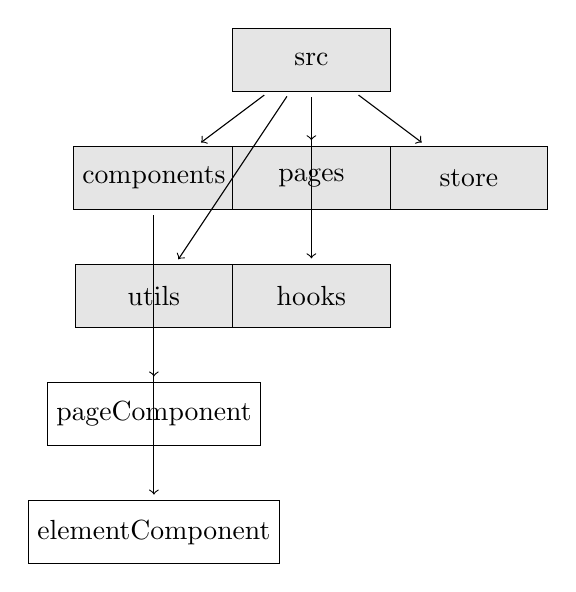
\begin{tikzpicture}[
    file/.style={draw, rectangle, minimum width=2cm, minimum height=0.8cm},
    folder/.style={draw, rectangle, minimum width=2cm, minimum height=0.8cm, fill=gray!20},
    arrow/.style={->, shorten >=2pt, shorten <=2pt}
]

% Folders
\node[folder] (src) at (0,0) {src};
\node[folder] (components) at (-2,-1.5) {components};
\node[folder] (pages) at (0,-1.5) {pages};
\node[folder] (store) at (2,-1.5) {store};
\node[folder] (utils) at (-2,-3) {utils};
\node[folder] (hooks) at (0,-3) {hooks};

% Files
\node[file] (pageComponent) at (-2,-4.5) {pageComponent};
\node[file] (elementComponent) at (-2,-6) {elementComponent};
% ... add more files

% Connections
\draw[arrow] (src) -- (components);
\draw[arrow] (src) -- (pages);
\draw[arrow] (src) -- (store);
\draw[arrow] (src) -- (utils);
\draw[arrow] (src) -- (hooks);
\draw[arrow] (components) -- (pageComponent);
\draw[arrow] (components) -- (elementComponent);
% ... add more connections

\end{tikzpicture}



\pagebreak
\subsubsection{Back-end}
The backend uses the dotNet framework. The development language using the C\# language.

In this project, the backend uses the Onion Architecture.
The Onion Architecture is a typically layered architecture, 
where each layer depends on the inner layer and provides interfaces to the outer layer.
The outer layer provides services to the outermost layer 
and other modules in the same layer based on the interfaces of the inner layer.

From inner to outer, the layers are: Domain, Application, Infrastructure, Presentation.
The Domain layer is the core layer and the innermost layer, used to define domain models, 
which are the business models.
It includes domain models and domain service interfaces.
Domain models are used to define the business models, 
which are the entities in the entity-relationship model and their attributes.
Domain service interfaces are used to define the business services, 
which are the relationships between entities in the entity-relationship model.

The Application layer is the application layer, 
used to define application services, which are the business logic.
It includes domain service implementations and application service interfaces.
Domain service implementations implement the methods of the inner layer's domain service 
interfaces and implement the business logic of the domain models.
Application service interfaces are used to define application services, 
which are the business logic.
It includes but is not limited to database interfaces, testing interfaces, 
HTTP API interfaces, MQTT interfaces, etc.

The Infrastructure layer is the infrastructure layer, used to define infrastructure.
It includes database implementations, testing implementations, 
HTTP API implementations, MQTT implementations, etc.
Database implementations implement the database interfaces 
and provide CRUD services for the database.
Testing implementations implement the testing interfaces 
and provide services for unit testing and integration testing.
HTTP API implementations implement the HTTP API interfaces 
and provide CRUD operations for HTTP APIs.
MQTT implementations implement the MQTT interfaces 
and provide CRUD operations for MQTT.

The Presentation layer is the presentation layer, used to define presentation logic, 
such as interfaces and pages. Since this is a backend project,
data presentation and control are handled by the frontend, 
so this layer is not needed.



\pagebreak
\subsubsection{Data communication and storage}
% 关于本项目的数据通信与数据存储的设计, 包括数据通信的协议, 数据存储的设计等
% 关于数据通信的设计:
% 1. 通信协议的选择
% 自前端向后端发送的数据, 有三种传输的数据类型, 
% 一种是普通的增删改查的请求, 对数据传输的时效性要求不高, 但是对数据的准确性, 完整性, 有序性, 安全性有一定的要求,
% 这种数据的传输, 采用 HTTP 协议, 以及 RESTful API 的设计. 可以有效的保证对数据传输的以上要求.
% 一种是对数据通道的创建和流媒体数据的传输, 对数据传输的时效性, 安全性要求较高, 这种数据的传输, 采用 WebRTC 协议, 以及 MQTT 协议.
% 配合可以快速解码的 flatbuffers 协议, 可以有效的保证对数据传输的以上要求.
% 最后一种是对设备的状态信息和操作信息的传输, 对完整性, 有序性, 安全性都有较高的要求, 这种数据的传输, 采用 MQTT 协议
% 同时也使用了 flatbuffers 协议.
% 
% 2. 数据通信的通信架构和通信流程
% 本项目的数据通信的通信架构, 是基于前后端分离的架构, 前端使用 React 框架, 后端使用 dotnet 框架.
% 当前端需要向后端发送数据的时候, 前端会向后端发送 HTTP 请求, 后端接收到 HTTP 请求之后, 会根据请求的数据类型,
% 选择不同的数据处理方式, 对于普通的增删改查的请求, 后端会根据 RESTful API 的设计, 对数据进行增删改查的操作,
% 对于对数据通道的创建和流媒体数据的传输, 后端会根据 WebRTC 协议, 对数据通道进行创建, 并且帮助前端和设备建立数据通道,
% 当数据通道建立后, 前端和设备之间则使用 flatbuffer 的数据格式对流媒体数据进行传输,
% 对于设备的状态信息和操作信息的传输, 前端会直接向 MQTT broker 发送 MQTT 请求, 
% 设备会在其自身的固件中监听相关的 MQTT 请求, 并且返回相关的数据.
% 
% 3. 数据通信的格式
% 本项目的数据通信的格式, 有三种, 
% 一种是 HTTP 协议, 
% 使用 json 格式对数据进行传输,
% 一种是 WebRTC 协议, 
% 使用 flatbuffers 格式对数据进行传输,
% 一种是 MQTT 协议.
% 使用 flatbuffers 格式对数据进行传输,
% 
% 关于数据存储的设计:
% 1. 数据存储的数据库的选择
% 本项目的数据存储的数据库的选择, 使用了轻量级的数据库 SQLite,
% SQLite 是一个进程内的库, 实现了自给自足的, 无服务器的, 零配置的, 事务性的 SQL 数据库引擎.
% 这是因为整个项目的目的是为了实现前端与设备之间的数据通信, 对于数据库数据的增删改查操作的要求不高,
% 数据量较小, 且对于数据库的数据的事务性要求不高, 所以选择了 SQLite 数据库.
% 2. 项目前后端的数据结构的设计
% 在本项目中, 前端由于使用了 React 框架, 所以前端的数据结构的设计, 使用了基于状态的数据结构的设计,
% 每个组件或者数据集都包含一个状态对象, 这个状态对象的属性就是组件的各个状态. 
% 使用状态对象的原因是, 可以方便的对状态进行管理, 采用对象-属性的形式, 可以方便的针对不同组件的同类状态进行区分,
% 由于跨组件的状态是由 redux 进行管理的, 这种状态对象的设计, 可以更搞笑的对状态进行更新和传递.
% 后端由于使用了 dotnet 框架, 所以后端的数据结构的设计, 使用了基于类的数据结构的设计,
% 采用了面向对象的编程思想, 对数据进行了封装, 使得数据的传输更加的安全, 有序, 完整.


\pagebreak

% \subsection{Domain model}
% \documentclass[]{article}
\usepackage{graphicx}
\usepackage{amsmath}
\usepackage{tikz}

% libaries
\usetikzlibrary{shapes,arrows}

%Define the listing package
\usepackage{listings} %code highlighter
\usepackage{color} %use color
\definecolor{mygreen}{rgb}{0,0.6,0}
\definecolor{mygray}{rgb}{0.5,0.5,0.5}
\definecolor{mymauve}{rgb}{0.58,0,0.82}

%Customize a bit the look
\lstset{ %
backgroundcolor=\color{white}, % choose the background color; you must add \usepackage{color} or \usepackage{xcolor}
basicstyle=\footnotesize, % the size of the fonts that are used for the code
breakatwhitespace=false, % sets if automatic breaks should only happen at whitespace
breaklines=true, % sets automatic line breaking
captionpos=b, % sets the caption-position to bottom
commentstyle=\color{mygreen}, % comment style
deletekeywords={...}, % if you want to delete keywords from the given language
escapeinside={\%*}{*)}, % if you want to add LaTeX within your code
extendedchars=true, % lets you use non-ASCII characters; for 8-bits encodings only, does not work with UTF-8
frame=single, % adds a frame around the code
keepspaces=true, % keeps spaces in text, useful for keeping indentation of code (possibly needs columns=flexible)
keywordstyle=\color{blue}, % keyword style
% language=Octave, % the language of the code
morekeywords={*,...}, % if you want to add more keywords to the set
numbers=left, % where to put the line-numbers; possible values are (none, left, right)
numbersep=5pt, % how far the line-numbers are from the code
numberstyle=\tiny\color{mygray}, % the style that is used for the line-numbers
rulecolor=\color{black}, % if not set, the frame-color may be changed on line-breaks within not-black text (e.g. comments (green here))
showspaces=false, % show spaces everywhere adding particular underscores; it overrides 'showstringspaces'
showstringspaces=false, % underline spaces within strings only
showtabs=false, % show tabs within strings adding particular underscores
stepnumber=1, % the step between two line-numbers. If it's 1, each line will be numbered
stringstyle=\color{mymauve}, % string literal style
tabsize=2, % sets default tabsize to 2 spaces
title=\lstname % show the filename of files included with \lstinputlisting; also try caption instead of title
}

\definecolor{darkgray}{rgb}{.4,.4,.4}
\definecolor{purple}{rgb}{0.65, 0.12, 0.82}

\lstdefinelanguage{React}{
keywords={const, typeof, new, true, false, catch, function, return, null, catch, switch, var, if, in, while, do, else, case, break},
keywordstyle=\color{blue}\bfseries,
ndkeywords={class, export, boolean, throw, implements, import, this},
ndkeywordstyle=\color{darkgray}\bfseries,
identifierstyle=\color{mygreen},
sensitive=false,
comment=[l]{//},
morecomment=[s]{/*}{*/},
commentstyle=\color{purple}\ttfamily,
string=[b]{"}{'}{`},
stringstyle=\color{red}\ttfamily,
morestring=[b]',
morestring=[b]",
morestring=[b]`',
}

\lstdefinelanguage{CSharp}{
keywords={const, typeof, new, true, false, catch, function, return, null, catch, switch, var, if, in, while, do, else, case, break},
keywordstyle=\color{blue}\bfseries,
ndkeywords={class, export, boolean, throw, implements, import, this},
ndkeywordstyle=\color{darkgray}\bfseries,
identifierstyle=\color{mygreen},
sensitive=false,
comment=[l]{//},
morecomment=[s]{/*}{*/},
commentstyle=\color{purple}\ttfamily,
string=[b]{"}{'}{`},
stringstyle=\color{red}\ttfamily,
morestring=[b]',
morestring=[b]",
morestring=[b]`',
}

\lstset{
language=React,
extendedchars=true,
basicstyle=\footnotesize\ttfamily,
showstringspaces=false,
showspaces=false,
numbers=left,
numberstyle=\footnotesize,
numbersep=9pt,
tabsize=2,
breaklines=true,
showtabs=false,
captionpos=b
}

\lstset{
language=CSharp,
extendedchars=true,
basicstyle=\footnotesize\ttfamily,
showstringspaces=false,
showspaces=false,
numbers=left,
numberstyle=\footnotesize,
numbersep=9pt,
tabsize=2,
breaklines=true,
showtabs=false,
captionpos=b
}

% \usepackage{cite} % Add this line for citation

% \bibliographystyle{plain}

\title{
The implementation of BifrostConnect Front-end scope, 
re-design and development with the relevant back-end support develop.
}
\author{
    Fei Gu \\
    Erhvervs Akademi Sydvest \\
    Computer Science 21\\
    }
\date{\today}

\begin{document}

% Front page
\maketitle
\begin{center}
    Supervisor: Henrik Boulund Meng Hansen \\
    Company: BifrostConnect \\
    Engineering Director: Jasper Wass \\
\end{center}
\tableofcontents
\pagebreak


% The introduction
\section{Introduction}
\subsection{Background}\input{sections/introduction/background.tex}
\subsection{The company}\input{sections/introduction/aboutCompany}
\subsection{The project}\input{sections/introduction/aboutProject}
\pagebreak

% The problem statement
\section{Problem Statement}
\subsection{Statement}
\input{sections/problemStatement/statement}
\subsection{Situation}
\input{sections/problemStatement/situation}
\subsection{Potential Solution}
\input{sections/problemStatement/potentialSolution}
\pagebreak

% Requirement analysis
\section{Requirement Analysis}
\input{sections/requirementAnalysis/index}

\subsection{Stakeholders}
\input{sections/requirementAnalysis/stakeholders/index}

\subsection{Business Domain}
\input{sections/requirementAnalysis/bussinesDomain/index}

\subsection{Scope}
\input{sections/requirementAnalysis/scope}

\subsection{Goals}
\input{sections/requirementAnalysis/goals}
\pagebreak

% Software Design
\section{Software Design}
% developement methods
\subsection{Software Development Methods}
\input{sections/softwareDevelopmentMethods/index}
\subsubsection{Agile Software Development}
\input{sections/softwareDevelopmentMethods/agileSoftwareDevelopment/index}
\subsubsection{Feature Driven Development}
\input{sections/softwareDevelopmentMethods/featureDrivenDevelopment/index}

\pagebreak

% Technology seslection
\subsection{Technology selection}
\input{sections/softwareDesign/technologySelection/index}
\subsubsection{Front-end}
\input{sections/softwareDesign/technologySelection/frontEnd}            
\subsubsection{Back-end}
\input{sections/softwareDesign/technologySelection/backEnd}            
\subsubsection{Database}
\input{sections/softwareDesign/technologySelection/database}
\subsubsection{Data communication}
\input{sections/softwareDesign/technologySelection/dataCommunication}            
\subsubsection{DevOps}
\input{sections/softwareDesign/technologySelection/devOps}
\pagebreak

% Architecture design
\subsection{Architecture design}
\input{sections/softwareDesign/architectureDesign/index}
\pagebreak
\subsubsection{Front-end}
\input{sections/softwareDesign/architectureDesign/frontEndArchitecture}
\pagebreak
\subsubsection{Back-end}
\input{sections/softwareDesign/architectureDesign/backEndArchitecture}
\pagebreak
\subsubsection{Data communication and storage}
\input{sections/softwareDesign/architectureDesign/dataCommunicationArchitecture}
\pagebreak

% \subsection{Domain model}
% \input{sections/softwareDesign/domainModel/index}
% \subsection{Database design}
% % 数据库领域模型 ER 图
% % 包括表和字段的设置.
% % 对于私有键和外键的设置.

% \subsection{Back-end design}
% % 后端对象模型
% % 以及对于对象模型的增删改查
% % 以及相关的其他服务的设计`'

% \subsection{Front-end design}
% % 对于前端的页面结构的设计 
% % 页面的状态的设计, 交互设计

% \subsection{FlatBuffers design}
% % schema 的设计

\subsection{DevOps CI/CD process design}
\input{sections/softwareDesign/devOpsDesign/index}
\subsubsection{Continuous Integration}
\input{sections/softwareDesign/devOpsDesign/continuousIntegration/index}
\subsubsection{Continuous Delivery}
\input{sections/softwareDesign/devOpsDesign/continuousDelivery/index}
\subsubsection{Continuous Deployment}
\input{sections/softwareDesign/devOpsDesign/continuousDeployment/index}
\pagebreak

\section{Software Development} 
\input{sections/softwareDevelopment/index}
\subsection{Overall development}
\input{sections/softwareDevelopment/overallDevelopement/index}
\subsubsection{Front-end}
\input{sections/softwareDevelopment/overallDevelopement/frontEnd/index}
\subsubsection{Back-end}
\input{sections/softwareDevelopment/overallDevelopement/backEnd/index}
\subsubsection{DevOps}
\input{sections/softwareDevelopment/overallDevelopement/devOps/index}
\subsection{Feature development} 
\input{sections/softwareDevelopment/featureDevelopment/index}
\subsubsection{Use Case 1}
\input{sections/softwareDevelopment/featureDevelopment/useCase1/index}
\subsubsection{Feature 1}
\input{sections/softwareDevelopment/featureDevelopment/feature/feature1.tex}
\pagebreak
\section{Conclusion} 
\subsection{Result}
Since the project is still in progress, the result is not available yet.
So far, basic structure of this project has been built. But the most features 
are not implemented yet. 
\subsection{Discussion}
As a single developer for this project, I am confident what I have done so far.
And I can say I understand the most of the knowledge I have used in this project, 
which also means I can explain all the part of the project. 
But this project also relevant some of the complex knowledge which I have to continue 
to study and practice.
\subsection{Future Work}
The future work is to implement the rest of the features. 
Including the most important part which is the 'create session' feature.
\pagebreak
% \bibliography{bibliography}
\pagebreak
% \begin{appendices}
%     \section{Appendix}
% \end{appendices} 
\end{document}
% \subsection{Database design}
% % 数据库领域模型 ER 图
% % 包括表和字段的设置.
% % 对于私有键和外键的设置.

% \subsection{Back-end design}
% % 后端对象模型
% % 以及对于对象模型的增删改查
% % 以及相关的其他服务的设计`'

% \subsection{Front-end design}
% % 对于前端的页面结构的设计 
% % 页面的状态的设计, 交互设计

% \subsection{FlatBuffers design}
% % schema 的设计

\subsection{DevOps CI/CD process design}
\documentclass[]{article}
\usepackage{graphicx}
\usepackage{amsmath}
\usepackage{tikz}

% libaries
\usetikzlibrary{shapes,arrows}

%Define the listing package
\usepackage{listings} %code highlighter
\usepackage{color} %use color
\definecolor{mygreen}{rgb}{0,0.6,0}
\definecolor{mygray}{rgb}{0.5,0.5,0.5}
\definecolor{mymauve}{rgb}{0.58,0,0.82}

%Customize a bit the look
\lstset{ %
backgroundcolor=\color{white}, % choose the background color; you must add \usepackage{color} or \usepackage{xcolor}
basicstyle=\footnotesize, % the size of the fonts that are used for the code
breakatwhitespace=false, % sets if automatic breaks should only happen at whitespace
breaklines=true, % sets automatic line breaking
captionpos=b, % sets the caption-position to bottom
commentstyle=\color{mygreen}, % comment style
deletekeywords={...}, % if you want to delete keywords from the given language
escapeinside={\%*}{*)}, % if you want to add LaTeX within your code
extendedchars=true, % lets you use non-ASCII characters; for 8-bits encodings only, does not work with UTF-8
frame=single, % adds a frame around the code
keepspaces=true, % keeps spaces in text, useful for keeping indentation of code (possibly needs columns=flexible)
keywordstyle=\color{blue}, % keyword style
% language=Octave, % the language of the code
morekeywords={*,...}, % if you want to add more keywords to the set
numbers=left, % where to put the line-numbers; possible values are (none, left, right)
numbersep=5pt, % how far the line-numbers are from the code
numberstyle=\tiny\color{mygray}, % the style that is used for the line-numbers
rulecolor=\color{black}, % if not set, the frame-color may be changed on line-breaks within not-black text (e.g. comments (green here))
showspaces=false, % show spaces everywhere adding particular underscores; it overrides 'showstringspaces'
showstringspaces=false, % underline spaces within strings only
showtabs=false, % show tabs within strings adding particular underscores
stepnumber=1, % the step between two line-numbers. If it's 1, each line will be numbered
stringstyle=\color{mymauve}, % string literal style
tabsize=2, % sets default tabsize to 2 spaces
title=\lstname % show the filename of files included with \lstinputlisting; also try caption instead of title
}

\definecolor{darkgray}{rgb}{.4,.4,.4}
\definecolor{purple}{rgb}{0.65, 0.12, 0.82}

\lstdefinelanguage{React}{
keywords={const, typeof, new, true, false, catch, function, return, null, catch, switch, var, if, in, while, do, else, case, break},
keywordstyle=\color{blue}\bfseries,
ndkeywords={class, export, boolean, throw, implements, import, this},
ndkeywordstyle=\color{darkgray}\bfseries,
identifierstyle=\color{mygreen},
sensitive=false,
comment=[l]{//},
morecomment=[s]{/*}{*/},
commentstyle=\color{purple}\ttfamily,
string=[b]{"}{'}{`},
stringstyle=\color{red}\ttfamily,
morestring=[b]',
morestring=[b]",
morestring=[b]`',
}

\lstdefinelanguage{CSharp}{
keywords={const, typeof, new, true, false, catch, function, return, null, catch, switch, var, if, in, while, do, else, case, break},
keywordstyle=\color{blue}\bfseries,
ndkeywords={class, export, boolean, throw, implements, import, this},
ndkeywordstyle=\color{darkgray}\bfseries,
identifierstyle=\color{mygreen},
sensitive=false,
comment=[l]{//},
morecomment=[s]{/*}{*/},
commentstyle=\color{purple}\ttfamily,
string=[b]{"}{'}{`},
stringstyle=\color{red}\ttfamily,
morestring=[b]',
morestring=[b]",
morestring=[b]`',
}

\lstset{
language=React,
extendedchars=true,
basicstyle=\footnotesize\ttfamily,
showstringspaces=false,
showspaces=false,
numbers=left,
numberstyle=\footnotesize,
numbersep=9pt,
tabsize=2,
breaklines=true,
showtabs=false,
captionpos=b
}

\lstset{
language=CSharp,
extendedchars=true,
basicstyle=\footnotesize\ttfamily,
showstringspaces=false,
showspaces=false,
numbers=left,
numberstyle=\footnotesize,
numbersep=9pt,
tabsize=2,
breaklines=true,
showtabs=false,
captionpos=b
}

% \usepackage{cite} % Add this line for citation

% \bibliographystyle{plain}

\title{
The implementation of BifrostConnect Front-end scope, 
re-design and development with the relevant back-end support develop.
}
\author{
    Fei Gu \\
    Erhvervs Akademi Sydvest \\
    Computer Science 21\\
    }
\date{\today}

\begin{document}

% Front page
\maketitle
\begin{center}
    Supervisor: Henrik Boulund Meng Hansen \\
    Company: BifrostConnect \\
    Engineering Director: Jasper Wass \\
\end{center}
\tableofcontents
\pagebreak


% The introduction
\section{Introduction}
\subsection{Background}\input{sections/introduction/background.tex}
\subsection{The company}\input{sections/introduction/aboutCompany}
\subsection{The project}\input{sections/introduction/aboutProject}
\pagebreak

% The problem statement
\section{Problem Statement}
\subsection{Statement}
\input{sections/problemStatement/statement}
\subsection{Situation}
\input{sections/problemStatement/situation}
\subsection{Potential Solution}
\input{sections/problemStatement/potentialSolution}
\pagebreak

% Requirement analysis
\section{Requirement Analysis}
\input{sections/requirementAnalysis/index}

\subsection{Stakeholders}
\input{sections/requirementAnalysis/stakeholders/index}

\subsection{Business Domain}
\input{sections/requirementAnalysis/bussinesDomain/index}

\subsection{Scope}
\input{sections/requirementAnalysis/scope}

\subsection{Goals}
\input{sections/requirementAnalysis/goals}
\pagebreak

% Software Design
\section{Software Design}
% developement methods
\subsection{Software Development Methods}
\input{sections/softwareDevelopmentMethods/index}
\subsubsection{Agile Software Development}
\input{sections/softwareDevelopmentMethods/agileSoftwareDevelopment/index}
\subsubsection{Feature Driven Development}
\input{sections/softwareDevelopmentMethods/featureDrivenDevelopment/index}

\pagebreak

% Technology seslection
\subsection{Technology selection}
\input{sections/softwareDesign/technologySelection/index}
\subsubsection{Front-end}
\input{sections/softwareDesign/technologySelection/frontEnd}            
\subsubsection{Back-end}
\input{sections/softwareDesign/technologySelection/backEnd}            
\subsubsection{Database}
\input{sections/softwareDesign/technologySelection/database}
\subsubsection{Data communication}
\input{sections/softwareDesign/technologySelection/dataCommunication}            
\subsubsection{DevOps}
\input{sections/softwareDesign/technologySelection/devOps}
\pagebreak

% Architecture design
\subsection{Architecture design}
\input{sections/softwareDesign/architectureDesign/index}
\pagebreak
\subsubsection{Front-end}
\input{sections/softwareDesign/architectureDesign/frontEndArchitecture}
\pagebreak
\subsubsection{Back-end}
\input{sections/softwareDesign/architectureDesign/backEndArchitecture}
\pagebreak
\subsubsection{Data communication and storage}
\input{sections/softwareDesign/architectureDesign/dataCommunicationArchitecture}
\pagebreak

% \subsection{Domain model}
% \input{sections/softwareDesign/domainModel/index}
% \subsection{Database design}
% % 数据库领域模型 ER 图
% % 包括表和字段的设置.
% % 对于私有键和外键的设置.

% \subsection{Back-end design}
% % 后端对象模型
% % 以及对于对象模型的增删改查
% % 以及相关的其他服务的设计`'

% \subsection{Front-end design}
% % 对于前端的页面结构的设计 
% % 页面的状态的设计, 交互设计

% \subsection{FlatBuffers design}
% % schema 的设计

\subsection{DevOps CI/CD process design}
\input{sections/softwareDesign/devOpsDesign/index}
\subsubsection{Continuous Integration}
\input{sections/softwareDesign/devOpsDesign/continuousIntegration/index}
\subsubsection{Continuous Delivery}
\input{sections/softwareDesign/devOpsDesign/continuousDelivery/index}
\subsubsection{Continuous Deployment}
\input{sections/softwareDesign/devOpsDesign/continuousDeployment/index}
\pagebreak

\section{Software Development} 
\input{sections/softwareDevelopment/index}
\subsection{Overall development}
\input{sections/softwareDevelopment/overallDevelopement/index}
\subsubsection{Front-end}
\input{sections/softwareDevelopment/overallDevelopement/frontEnd/index}
\subsubsection{Back-end}
\input{sections/softwareDevelopment/overallDevelopement/backEnd/index}
\subsubsection{DevOps}
\input{sections/softwareDevelopment/overallDevelopement/devOps/index}
\subsection{Feature development} 
\input{sections/softwareDevelopment/featureDevelopment/index}
\subsubsection{Use Case 1}
\input{sections/softwareDevelopment/featureDevelopment/useCase1/index}
\subsubsection{Feature 1}
\input{sections/softwareDevelopment/featureDevelopment/feature/feature1.tex}
\pagebreak
\section{Conclusion} 
\subsection{Result}
Since the project is still in progress, the result is not available yet.
So far, basic structure of this project has been built. But the most features 
are not implemented yet. 
\subsection{Discussion}
As a single developer for this project, I am confident what I have done so far.
And I can say I understand the most of the knowledge I have used in this project, 
which also means I can explain all the part of the project. 
But this project also relevant some of the complex knowledge which I have to continue 
to study and practice.
\subsection{Future Work}
The future work is to implement the rest of the features. 
Including the most important part which is the 'create session' feature.
\pagebreak
% \bibliography{bibliography}
\pagebreak
% \begin{appendices}
%     \section{Appendix}
% \end{appendices} 
\end{document}
\subsubsection{Continuous Integration}
\documentclass[]{article}
\usepackage{graphicx}
\usepackage{amsmath}
\usepackage{tikz}

% libaries
\usetikzlibrary{shapes,arrows}

%Define the listing package
\usepackage{listings} %code highlighter
\usepackage{color} %use color
\definecolor{mygreen}{rgb}{0,0.6,0}
\definecolor{mygray}{rgb}{0.5,0.5,0.5}
\definecolor{mymauve}{rgb}{0.58,0,0.82}

%Customize a bit the look
\lstset{ %
backgroundcolor=\color{white}, % choose the background color; you must add \usepackage{color} or \usepackage{xcolor}
basicstyle=\footnotesize, % the size of the fonts that are used for the code
breakatwhitespace=false, % sets if automatic breaks should only happen at whitespace
breaklines=true, % sets automatic line breaking
captionpos=b, % sets the caption-position to bottom
commentstyle=\color{mygreen}, % comment style
deletekeywords={...}, % if you want to delete keywords from the given language
escapeinside={\%*}{*)}, % if you want to add LaTeX within your code
extendedchars=true, % lets you use non-ASCII characters; for 8-bits encodings only, does not work with UTF-8
frame=single, % adds a frame around the code
keepspaces=true, % keeps spaces in text, useful for keeping indentation of code (possibly needs columns=flexible)
keywordstyle=\color{blue}, % keyword style
% language=Octave, % the language of the code
morekeywords={*,...}, % if you want to add more keywords to the set
numbers=left, % where to put the line-numbers; possible values are (none, left, right)
numbersep=5pt, % how far the line-numbers are from the code
numberstyle=\tiny\color{mygray}, % the style that is used for the line-numbers
rulecolor=\color{black}, % if not set, the frame-color may be changed on line-breaks within not-black text (e.g. comments (green here))
showspaces=false, % show spaces everywhere adding particular underscores; it overrides 'showstringspaces'
showstringspaces=false, % underline spaces within strings only
showtabs=false, % show tabs within strings adding particular underscores
stepnumber=1, % the step between two line-numbers. If it's 1, each line will be numbered
stringstyle=\color{mymauve}, % string literal style
tabsize=2, % sets default tabsize to 2 spaces
title=\lstname % show the filename of files included with \lstinputlisting; also try caption instead of title
}

\definecolor{darkgray}{rgb}{.4,.4,.4}
\definecolor{purple}{rgb}{0.65, 0.12, 0.82}

\lstdefinelanguage{React}{
keywords={const, typeof, new, true, false, catch, function, return, null, catch, switch, var, if, in, while, do, else, case, break},
keywordstyle=\color{blue}\bfseries,
ndkeywords={class, export, boolean, throw, implements, import, this},
ndkeywordstyle=\color{darkgray}\bfseries,
identifierstyle=\color{mygreen},
sensitive=false,
comment=[l]{//},
morecomment=[s]{/*}{*/},
commentstyle=\color{purple}\ttfamily,
string=[b]{"}{'}{`},
stringstyle=\color{red}\ttfamily,
morestring=[b]',
morestring=[b]",
morestring=[b]`',
}

\lstdefinelanguage{CSharp}{
keywords={const, typeof, new, true, false, catch, function, return, null, catch, switch, var, if, in, while, do, else, case, break},
keywordstyle=\color{blue}\bfseries,
ndkeywords={class, export, boolean, throw, implements, import, this},
ndkeywordstyle=\color{darkgray}\bfseries,
identifierstyle=\color{mygreen},
sensitive=false,
comment=[l]{//},
morecomment=[s]{/*}{*/},
commentstyle=\color{purple}\ttfamily,
string=[b]{"}{'}{`},
stringstyle=\color{red}\ttfamily,
morestring=[b]',
morestring=[b]",
morestring=[b]`',
}

\lstset{
language=React,
extendedchars=true,
basicstyle=\footnotesize\ttfamily,
showstringspaces=false,
showspaces=false,
numbers=left,
numberstyle=\footnotesize,
numbersep=9pt,
tabsize=2,
breaklines=true,
showtabs=false,
captionpos=b
}

\lstset{
language=CSharp,
extendedchars=true,
basicstyle=\footnotesize\ttfamily,
showstringspaces=false,
showspaces=false,
numbers=left,
numberstyle=\footnotesize,
numbersep=9pt,
tabsize=2,
breaklines=true,
showtabs=false,
captionpos=b
}

% \usepackage{cite} % Add this line for citation

% \bibliographystyle{plain}

\title{
The implementation of BifrostConnect Front-end scope, 
re-design and development with the relevant back-end support develop.
}
\author{
    Fei Gu \\
    Erhvervs Akademi Sydvest \\
    Computer Science 21\\
    }
\date{\today}

\begin{document}

% Front page
\maketitle
\begin{center}
    Supervisor: Henrik Boulund Meng Hansen \\
    Company: BifrostConnect \\
    Engineering Director: Jasper Wass \\
\end{center}
\tableofcontents
\pagebreak


% The introduction
\section{Introduction}
\subsection{Background}\input{sections/introduction/background.tex}
\subsection{The company}\input{sections/introduction/aboutCompany}
\subsection{The project}\input{sections/introduction/aboutProject}
\pagebreak

% The problem statement
\section{Problem Statement}
\subsection{Statement}
\input{sections/problemStatement/statement}
\subsection{Situation}
\input{sections/problemStatement/situation}
\subsection{Potential Solution}
\input{sections/problemStatement/potentialSolution}
\pagebreak

% Requirement analysis
\section{Requirement Analysis}
\input{sections/requirementAnalysis/index}

\subsection{Stakeholders}
\input{sections/requirementAnalysis/stakeholders/index}

\subsection{Business Domain}
\input{sections/requirementAnalysis/bussinesDomain/index}

\subsection{Scope}
\input{sections/requirementAnalysis/scope}

\subsection{Goals}
\input{sections/requirementAnalysis/goals}
\pagebreak

% Software Design
\section{Software Design}
% developement methods
\subsection{Software Development Methods}
\input{sections/softwareDevelopmentMethods/index}
\subsubsection{Agile Software Development}
\input{sections/softwareDevelopmentMethods/agileSoftwareDevelopment/index}
\subsubsection{Feature Driven Development}
\input{sections/softwareDevelopmentMethods/featureDrivenDevelopment/index}

\pagebreak

% Technology seslection
\subsection{Technology selection}
\input{sections/softwareDesign/technologySelection/index}
\subsubsection{Front-end}
\input{sections/softwareDesign/technologySelection/frontEnd}            
\subsubsection{Back-end}
\input{sections/softwareDesign/technologySelection/backEnd}            
\subsubsection{Database}
\input{sections/softwareDesign/technologySelection/database}
\subsubsection{Data communication}
\input{sections/softwareDesign/technologySelection/dataCommunication}            
\subsubsection{DevOps}
\input{sections/softwareDesign/technologySelection/devOps}
\pagebreak

% Architecture design
\subsection{Architecture design}
\input{sections/softwareDesign/architectureDesign/index}
\pagebreak
\subsubsection{Front-end}
\input{sections/softwareDesign/architectureDesign/frontEndArchitecture}
\pagebreak
\subsubsection{Back-end}
\input{sections/softwareDesign/architectureDesign/backEndArchitecture}
\pagebreak
\subsubsection{Data communication and storage}
\input{sections/softwareDesign/architectureDesign/dataCommunicationArchitecture}
\pagebreak

% \subsection{Domain model}
% \input{sections/softwareDesign/domainModel/index}
% \subsection{Database design}
% % 数据库领域模型 ER 图
% % 包括表和字段的设置.
% % 对于私有键和外键的设置.

% \subsection{Back-end design}
% % 后端对象模型
% % 以及对于对象模型的增删改查
% % 以及相关的其他服务的设计`'

% \subsection{Front-end design}
% % 对于前端的页面结构的设计 
% % 页面的状态的设计, 交互设计

% \subsection{FlatBuffers design}
% % schema 的设计

\subsection{DevOps CI/CD process design}
\input{sections/softwareDesign/devOpsDesign/index}
\subsubsection{Continuous Integration}
\input{sections/softwareDesign/devOpsDesign/continuousIntegration/index}
\subsubsection{Continuous Delivery}
\input{sections/softwareDesign/devOpsDesign/continuousDelivery/index}
\subsubsection{Continuous Deployment}
\input{sections/softwareDesign/devOpsDesign/continuousDeployment/index}
\pagebreak

\section{Software Development} 
\input{sections/softwareDevelopment/index}
\subsection{Overall development}
\input{sections/softwareDevelopment/overallDevelopement/index}
\subsubsection{Front-end}
\input{sections/softwareDevelopment/overallDevelopement/frontEnd/index}
\subsubsection{Back-end}
\input{sections/softwareDevelopment/overallDevelopement/backEnd/index}
\subsubsection{DevOps}
\input{sections/softwareDevelopment/overallDevelopement/devOps/index}
\subsection{Feature development} 
\input{sections/softwareDevelopment/featureDevelopment/index}
\subsubsection{Use Case 1}
\input{sections/softwareDevelopment/featureDevelopment/useCase1/index}
\subsubsection{Feature 1}
\input{sections/softwareDevelopment/featureDevelopment/feature/feature1.tex}
\pagebreak
\section{Conclusion} 
\subsection{Result}
Since the project is still in progress, the result is not available yet.
So far, basic structure of this project has been built. But the most features 
are not implemented yet. 
\subsection{Discussion}
As a single developer for this project, I am confident what I have done so far.
And I can say I understand the most of the knowledge I have used in this project, 
which also means I can explain all the part of the project. 
But this project also relevant some of the complex knowledge which I have to continue 
to study and practice.
\subsection{Future Work}
The future work is to implement the rest of the features. 
Including the most important part which is the 'create session' feature.
\pagebreak
% \bibliography{bibliography}
\pagebreak
% \begin{appendices}
%     \section{Appendix}
% \end{appendices} 
\end{document}
\subsubsection{Continuous Delivery}
\documentclass[]{article}
\usepackage{graphicx}
\usepackage{amsmath}
\usepackage{tikz}

% libaries
\usetikzlibrary{shapes,arrows}

%Define the listing package
\usepackage{listings} %code highlighter
\usepackage{color} %use color
\definecolor{mygreen}{rgb}{0,0.6,0}
\definecolor{mygray}{rgb}{0.5,0.5,0.5}
\definecolor{mymauve}{rgb}{0.58,0,0.82}

%Customize a bit the look
\lstset{ %
backgroundcolor=\color{white}, % choose the background color; you must add \usepackage{color} or \usepackage{xcolor}
basicstyle=\footnotesize, % the size of the fonts that are used for the code
breakatwhitespace=false, % sets if automatic breaks should only happen at whitespace
breaklines=true, % sets automatic line breaking
captionpos=b, % sets the caption-position to bottom
commentstyle=\color{mygreen}, % comment style
deletekeywords={...}, % if you want to delete keywords from the given language
escapeinside={\%*}{*)}, % if you want to add LaTeX within your code
extendedchars=true, % lets you use non-ASCII characters; for 8-bits encodings only, does not work with UTF-8
frame=single, % adds a frame around the code
keepspaces=true, % keeps spaces in text, useful for keeping indentation of code (possibly needs columns=flexible)
keywordstyle=\color{blue}, % keyword style
% language=Octave, % the language of the code
morekeywords={*,...}, % if you want to add more keywords to the set
numbers=left, % where to put the line-numbers; possible values are (none, left, right)
numbersep=5pt, % how far the line-numbers are from the code
numberstyle=\tiny\color{mygray}, % the style that is used for the line-numbers
rulecolor=\color{black}, % if not set, the frame-color may be changed on line-breaks within not-black text (e.g. comments (green here))
showspaces=false, % show spaces everywhere adding particular underscores; it overrides 'showstringspaces'
showstringspaces=false, % underline spaces within strings only
showtabs=false, % show tabs within strings adding particular underscores
stepnumber=1, % the step between two line-numbers. If it's 1, each line will be numbered
stringstyle=\color{mymauve}, % string literal style
tabsize=2, % sets default tabsize to 2 spaces
title=\lstname % show the filename of files included with \lstinputlisting; also try caption instead of title
}

\definecolor{darkgray}{rgb}{.4,.4,.4}
\definecolor{purple}{rgb}{0.65, 0.12, 0.82}

\lstdefinelanguage{React}{
keywords={const, typeof, new, true, false, catch, function, return, null, catch, switch, var, if, in, while, do, else, case, break},
keywordstyle=\color{blue}\bfseries,
ndkeywords={class, export, boolean, throw, implements, import, this},
ndkeywordstyle=\color{darkgray}\bfseries,
identifierstyle=\color{mygreen},
sensitive=false,
comment=[l]{//},
morecomment=[s]{/*}{*/},
commentstyle=\color{purple}\ttfamily,
string=[b]{"}{'}{`},
stringstyle=\color{red}\ttfamily,
morestring=[b]',
morestring=[b]",
morestring=[b]`',
}

\lstdefinelanguage{CSharp}{
keywords={const, typeof, new, true, false, catch, function, return, null, catch, switch, var, if, in, while, do, else, case, break},
keywordstyle=\color{blue}\bfseries,
ndkeywords={class, export, boolean, throw, implements, import, this},
ndkeywordstyle=\color{darkgray}\bfseries,
identifierstyle=\color{mygreen},
sensitive=false,
comment=[l]{//},
morecomment=[s]{/*}{*/},
commentstyle=\color{purple}\ttfamily,
string=[b]{"}{'}{`},
stringstyle=\color{red}\ttfamily,
morestring=[b]',
morestring=[b]",
morestring=[b]`',
}

\lstset{
language=React,
extendedchars=true,
basicstyle=\footnotesize\ttfamily,
showstringspaces=false,
showspaces=false,
numbers=left,
numberstyle=\footnotesize,
numbersep=9pt,
tabsize=2,
breaklines=true,
showtabs=false,
captionpos=b
}

\lstset{
language=CSharp,
extendedchars=true,
basicstyle=\footnotesize\ttfamily,
showstringspaces=false,
showspaces=false,
numbers=left,
numberstyle=\footnotesize,
numbersep=9pt,
tabsize=2,
breaklines=true,
showtabs=false,
captionpos=b
}

% \usepackage{cite} % Add this line for citation

% \bibliographystyle{plain}

\title{
The implementation of BifrostConnect Front-end scope, 
re-design and development with the relevant back-end support develop.
}
\author{
    Fei Gu \\
    Erhvervs Akademi Sydvest \\
    Computer Science 21\\
    }
\date{\today}

\begin{document}

% Front page
\maketitle
\begin{center}
    Supervisor: Henrik Boulund Meng Hansen \\
    Company: BifrostConnect \\
    Engineering Director: Jasper Wass \\
\end{center}
\tableofcontents
\pagebreak


% The introduction
\section{Introduction}
\subsection{Background}\input{sections/introduction/background.tex}
\subsection{The company}\input{sections/introduction/aboutCompany}
\subsection{The project}\input{sections/introduction/aboutProject}
\pagebreak

% The problem statement
\section{Problem Statement}
\subsection{Statement}
\input{sections/problemStatement/statement}
\subsection{Situation}
\input{sections/problemStatement/situation}
\subsection{Potential Solution}
\input{sections/problemStatement/potentialSolution}
\pagebreak

% Requirement analysis
\section{Requirement Analysis}
\input{sections/requirementAnalysis/index}

\subsection{Stakeholders}
\input{sections/requirementAnalysis/stakeholders/index}

\subsection{Business Domain}
\input{sections/requirementAnalysis/bussinesDomain/index}

\subsection{Scope}
\input{sections/requirementAnalysis/scope}

\subsection{Goals}
\input{sections/requirementAnalysis/goals}
\pagebreak

% Software Design
\section{Software Design}
% developement methods
\subsection{Software Development Methods}
\input{sections/softwareDevelopmentMethods/index}
\subsubsection{Agile Software Development}
\input{sections/softwareDevelopmentMethods/agileSoftwareDevelopment/index}
\subsubsection{Feature Driven Development}
\input{sections/softwareDevelopmentMethods/featureDrivenDevelopment/index}

\pagebreak

% Technology seslection
\subsection{Technology selection}
\input{sections/softwareDesign/technologySelection/index}
\subsubsection{Front-end}
\input{sections/softwareDesign/technologySelection/frontEnd}            
\subsubsection{Back-end}
\input{sections/softwareDesign/technologySelection/backEnd}            
\subsubsection{Database}
\input{sections/softwareDesign/technologySelection/database}
\subsubsection{Data communication}
\input{sections/softwareDesign/technologySelection/dataCommunication}            
\subsubsection{DevOps}
\input{sections/softwareDesign/technologySelection/devOps}
\pagebreak

% Architecture design
\subsection{Architecture design}
\input{sections/softwareDesign/architectureDesign/index}
\pagebreak
\subsubsection{Front-end}
\input{sections/softwareDesign/architectureDesign/frontEndArchitecture}
\pagebreak
\subsubsection{Back-end}
\input{sections/softwareDesign/architectureDesign/backEndArchitecture}
\pagebreak
\subsubsection{Data communication and storage}
\input{sections/softwareDesign/architectureDesign/dataCommunicationArchitecture}
\pagebreak

% \subsection{Domain model}
% \input{sections/softwareDesign/domainModel/index}
% \subsection{Database design}
% % 数据库领域模型 ER 图
% % 包括表和字段的设置.
% % 对于私有键和外键的设置.

% \subsection{Back-end design}
% % 后端对象模型
% % 以及对于对象模型的增删改查
% % 以及相关的其他服务的设计`'

% \subsection{Front-end design}
% % 对于前端的页面结构的设计 
% % 页面的状态的设计, 交互设计

% \subsection{FlatBuffers design}
% % schema 的设计

\subsection{DevOps CI/CD process design}
\input{sections/softwareDesign/devOpsDesign/index}
\subsubsection{Continuous Integration}
\input{sections/softwareDesign/devOpsDesign/continuousIntegration/index}
\subsubsection{Continuous Delivery}
\input{sections/softwareDesign/devOpsDesign/continuousDelivery/index}
\subsubsection{Continuous Deployment}
\input{sections/softwareDesign/devOpsDesign/continuousDeployment/index}
\pagebreak

\section{Software Development} 
\input{sections/softwareDevelopment/index}
\subsection{Overall development}
\input{sections/softwareDevelopment/overallDevelopement/index}
\subsubsection{Front-end}
\input{sections/softwareDevelopment/overallDevelopement/frontEnd/index}
\subsubsection{Back-end}
\input{sections/softwareDevelopment/overallDevelopement/backEnd/index}
\subsubsection{DevOps}
\input{sections/softwareDevelopment/overallDevelopement/devOps/index}
\subsection{Feature development} 
\input{sections/softwareDevelopment/featureDevelopment/index}
\subsubsection{Use Case 1}
\input{sections/softwareDevelopment/featureDevelopment/useCase1/index}
\subsubsection{Feature 1}
\input{sections/softwareDevelopment/featureDevelopment/feature/feature1.tex}
\pagebreak
\section{Conclusion} 
\subsection{Result}
Since the project is still in progress, the result is not available yet.
So far, basic structure of this project has been built. But the most features 
are not implemented yet. 
\subsection{Discussion}
As a single developer for this project, I am confident what I have done so far.
And I can say I understand the most of the knowledge I have used in this project, 
which also means I can explain all the part of the project. 
But this project also relevant some of the complex knowledge which I have to continue 
to study and practice.
\subsection{Future Work}
The future work is to implement the rest of the features. 
Including the most important part which is the 'create session' feature.
\pagebreak
% \bibliography{bibliography}
\pagebreak
% \begin{appendices}
%     \section{Appendix}
% \end{appendices} 
\end{document}
\subsubsection{Continuous Deployment}
\documentclass[]{article}
\usepackage{graphicx}
\usepackage{amsmath}
\usepackage{tikz}

% libaries
\usetikzlibrary{shapes,arrows}

%Define the listing package
\usepackage{listings} %code highlighter
\usepackage{color} %use color
\definecolor{mygreen}{rgb}{0,0.6,0}
\definecolor{mygray}{rgb}{0.5,0.5,0.5}
\definecolor{mymauve}{rgb}{0.58,0,0.82}

%Customize a bit the look
\lstset{ %
backgroundcolor=\color{white}, % choose the background color; you must add \usepackage{color} or \usepackage{xcolor}
basicstyle=\footnotesize, % the size of the fonts that are used for the code
breakatwhitespace=false, % sets if automatic breaks should only happen at whitespace
breaklines=true, % sets automatic line breaking
captionpos=b, % sets the caption-position to bottom
commentstyle=\color{mygreen}, % comment style
deletekeywords={...}, % if you want to delete keywords from the given language
escapeinside={\%*}{*)}, % if you want to add LaTeX within your code
extendedchars=true, % lets you use non-ASCII characters; for 8-bits encodings only, does not work with UTF-8
frame=single, % adds a frame around the code
keepspaces=true, % keeps spaces in text, useful for keeping indentation of code (possibly needs columns=flexible)
keywordstyle=\color{blue}, % keyword style
% language=Octave, % the language of the code
morekeywords={*,...}, % if you want to add more keywords to the set
numbers=left, % where to put the line-numbers; possible values are (none, left, right)
numbersep=5pt, % how far the line-numbers are from the code
numberstyle=\tiny\color{mygray}, % the style that is used for the line-numbers
rulecolor=\color{black}, % if not set, the frame-color may be changed on line-breaks within not-black text (e.g. comments (green here))
showspaces=false, % show spaces everywhere adding particular underscores; it overrides 'showstringspaces'
showstringspaces=false, % underline spaces within strings only
showtabs=false, % show tabs within strings adding particular underscores
stepnumber=1, % the step between two line-numbers. If it's 1, each line will be numbered
stringstyle=\color{mymauve}, % string literal style
tabsize=2, % sets default tabsize to 2 spaces
title=\lstname % show the filename of files included with \lstinputlisting; also try caption instead of title
}

\definecolor{darkgray}{rgb}{.4,.4,.4}
\definecolor{purple}{rgb}{0.65, 0.12, 0.82}

\lstdefinelanguage{React}{
keywords={const, typeof, new, true, false, catch, function, return, null, catch, switch, var, if, in, while, do, else, case, break},
keywordstyle=\color{blue}\bfseries,
ndkeywords={class, export, boolean, throw, implements, import, this},
ndkeywordstyle=\color{darkgray}\bfseries,
identifierstyle=\color{mygreen},
sensitive=false,
comment=[l]{//},
morecomment=[s]{/*}{*/},
commentstyle=\color{purple}\ttfamily,
string=[b]{"}{'}{`},
stringstyle=\color{red}\ttfamily,
morestring=[b]',
morestring=[b]",
morestring=[b]`',
}

\lstdefinelanguage{CSharp}{
keywords={const, typeof, new, true, false, catch, function, return, null, catch, switch, var, if, in, while, do, else, case, break},
keywordstyle=\color{blue}\bfseries,
ndkeywords={class, export, boolean, throw, implements, import, this},
ndkeywordstyle=\color{darkgray}\bfseries,
identifierstyle=\color{mygreen},
sensitive=false,
comment=[l]{//},
morecomment=[s]{/*}{*/},
commentstyle=\color{purple}\ttfamily,
string=[b]{"}{'}{`},
stringstyle=\color{red}\ttfamily,
morestring=[b]',
morestring=[b]",
morestring=[b]`',
}

\lstset{
language=React,
extendedchars=true,
basicstyle=\footnotesize\ttfamily,
showstringspaces=false,
showspaces=false,
numbers=left,
numberstyle=\footnotesize,
numbersep=9pt,
tabsize=2,
breaklines=true,
showtabs=false,
captionpos=b
}

\lstset{
language=CSharp,
extendedchars=true,
basicstyle=\footnotesize\ttfamily,
showstringspaces=false,
showspaces=false,
numbers=left,
numberstyle=\footnotesize,
numbersep=9pt,
tabsize=2,
breaklines=true,
showtabs=false,
captionpos=b
}

% \usepackage{cite} % Add this line for citation

% \bibliographystyle{plain}

\title{
The implementation of BifrostConnect Front-end scope, 
re-design and development with the relevant back-end support develop.
}
\author{
    Fei Gu \\
    Erhvervs Akademi Sydvest \\
    Computer Science 21\\
    }
\date{\today}

\begin{document}

% Front page
\maketitle
\begin{center}
    Supervisor: Henrik Boulund Meng Hansen \\
    Company: BifrostConnect \\
    Engineering Director: Jasper Wass \\
\end{center}
\tableofcontents
\pagebreak


% The introduction
\section{Introduction}
\subsection{Background}\input{sections/introduction/background.tex}
\subsection{The company}\input{sections/introduction/aboutCompany}
\subsection{The project}\input{sections/introduction/aboutProject}
\pagebreak

% The problem statement
\section{Problem Statement}
\subsection{Statement}
\input{sections/problemStatement/statement}
\subsection{Situation}
\input{sections/problemStatement/situation}
\subsection{Potential Solution}
\input{sections/problemStatement/potentialSolution}
\pagebreak

% Requirement analysis
\section{Requirement Analysis}
\input{sections/requirementAnalysis/index}

\subsection{Stakeholders}
\input{sections/requirementAnalysis/stakeholders/index}

\subsection{Business Domain}
\input{sections/requirementAnalysis/bussinesDomain/index}

\subsection{Scope}
\input{sections/requirementAnalysis/scope}

\subsection{Goals}
\input{sections/requirementAnalysis/goals}
\pagebreak

% Software Design
\section{Software Design}
% developement methods
\subsection{Software Development Methods}
\input{sections/softwareDevelopmentMethods/index}
\subsubsection{Agile Software Development}
\input{sections/softwareDevelopmentMethods/agileSoftwareDevelopment/index}
\subsubsection{Feature Driven Development}
\input{sections/softwareDevelopmentMethods/featureDrivenDevelopment/index}

\pagebreak

% Technology seslection
\subsection{Technology selection}
\input{sections/softwareDesign/technologySelection/index}
\subsubsection{Front-end}
\input{sections/softwareDesign/technologySelection/frontEnd}            
\subsubsection{Back-end}
\input{sections/softwareDesign/technologySelection/backEnd}            
\subsubsection{Database}
\input{sections/softwareDesign/technologySelection/database}
\subsubsection{Data communication}
\input{sections/softwareDesign/technologySelection/dataCommunication}            
\subsubsection{DevOps}
\input{sections/softwareDesign/technologySelection/devOps}
\pagebreak

% Architecture design
\subsection{Architecture design}
\input{sections/softwareDesign/architectureDesign/index}
\pagebreak
\subsubsection{Front-end}
\input{sections/softwareDesign/architectureDesign/frontEndArchitecture}
\pagebreak
\subsubsection{Back-end}
\input{sections/softwareDesign/architectureDesign/backEndArchitecture}
\pagebreak
\subsubsection{Data communication and storage}
\input{sections/softwareDesign/architectureDesign/dataCommunicationArchitecture}
\pagebreak

% \subsection{Domain model}
% \input{sections/softwareDesign/domainModel/index}
% \subsection{Database design}
% % 数据库领域模型 ER 图
% % 包括表和字段的设置.
% % 对于私有键和外键的设置.

% \subsection{Back-end design}
% % 后端对象模型
% % 以及对于对象模型的增删改查
% % 以及相关的其他服务的设计`'

% \subsection{Front-end design}
% % 对于前端的页面结构的设计 
% % 页面的状态的设计, 交互设计

% \subsection{FlatBuffers design}
% % schema 的设计

\subsection{DevOps CI/CD process design}
\input{sections/softwareDesign/devOpsDesign/index}
\subsubsection{Continuous Integration}
\input{sections/softwareDesign/devOpsDesign/continuousIntegration/index}
\subsubsection{Continuous Delivery}
\input{sections/softwareDesign/devOpsDesign/continuousDelivery/index}
\subsubsection{Continuous Deployment}
\input{sections/softwareDesign/devOpsDesign/continuousDeployment/index}
\pagebreak

\section{Software Development} 
\input{sections/softwareDevelopment/index}
\subsection{Overall development}
\input{sections/softwareDevelopment/overallDevelopement/index}
\subsubsection{Front-end}
\input{sections/softwareDevelopment/overallDevelopement/frontEnd/index}
\subsubsection{Back-end}
\input{sections/softwareDevelopment/overallDevelopement/backEnd/index}
\subsubsection{DevOps}
\input{sections/softwareDevelopment/overallDevelopement/devOps/index}
\subsection{Feature development} 
\input{sections/softwareDevelopment/featureDevelopment/index}
\subsubsection{Use Case 1}
\input{sections/softwareDevelopment/featureDevelopment/useCase1/index}
\subsubsection{Feature 1}
\input{sections/softwareDevelopment/featureDevelopment/feature/feature1.tex}
\pagebreak
\section{Conclusion} 
\subsection{Result}
Since the project is still in progress, the result is not available yet.
So far, basic structure of this project has been built. But the most features 
are not implemented yet. 
\subsection{Discussion}
As a single developer for this project, I am confident what I have done so far.
And I can say I understand the most of the knowledge I have used in this project, 
which also means I can explain all the part of the project. 
But this project also relevant some of the complex knowledge which I have to continue 
to study and practice.
\subsection{Future Work}
The future work is to implement the rest of the features. 
Including the most important part which is the 'create session' feature.
\pagebreak
% \bibliography{bibliography}
\pagebreak
% \begin{appendices}
%     \section{Appendix}
% \end{appendices} 
\end{document}
\pagebreak

\section{Software Development} 
\documentclass[]{article}
\usepackage{graphicx}
\usepackage{amsmath}
\usepackage{tikz}

% libaries
\usetikzlibrary{shapes,arrows}

%Define the listing package
\usepackage{listings} %code highlighter
\usepackage{color} %use color
\definecolor{mygreen}{rgb}{0,0.6,0}
\definecolor{mygray}{rgb}{0.5,0.5,0.5}
\definecolor{mymauve}{rgb}{0.58,0,0.82}

%Customize a bit the look
\lstset{ %
backgroundcolor=\color{white}, % choose the background color; you must add \usepackage{color} or \usepackage{xcolor}
basicstyle=\footnotesize, % the size of the fonts that are used for the code
breakatwhitespace=false, % sets if automatic breaks should only happen at whitespace
breaklines=true, % sets automatic line breaking
captionpos=b, % sets the caption-position to bottom
commentstyle=\color{mygreen}, % comment style
deletekeywords={...}, % if you want to delete keywords from the given language
escapeinside={\%*}{*)}, % if you want to add LaTeX within your code
extendedchars=true, % lets you use non-ASCII characters; for 8-bits encodings only, does not work with UTF-8
frame=single, % adds a frame around the code
keepspaces=true, % keeps spaces in text, useful for keeping indentation of code (possibly needs columns=flexible)
keywordstyle=\color{blue}, % keyword style
% language=Octave, % the language of the code
morekeywords={*,...}, % if you want to add more keywords to the set
numbers=left, % where to put the line-numbers; possible values are (none, left, right)
numbersep=5pt, % how far the line-numbers are from the code
numberstyle=\tiny\color{mygray}, % the style that is used for the line-numbers
rulecolor=\color{black}, % if not set, the frame-color may be changed on line-breaks within not-black text (e.g. comments (green here))
showspaces=false, % show spaces everywhere adding particular underscores; it overrides 'showstringspaces'
showstringspaces=false, % underline spaces within strings only
showtabs=false, % show tabs within strings adding particular underscores
stepnumber=1, % the step between two line-numbers. If it's 1, each line will be numbered
stringstyle=\color{mymauve}, % string literal style
tabsize=2, % sets default tabsize to 2 spaces
title=\lstname % show the filename of files included with \lstinputlisting; also try caption instead of title
}

\definecolor{darkgray}{rgb}{.4,.4,.4}
\definecolor{purple}{rgb}{0.65, 0.12, 0.82}

\lstdefinelanguage{React}{
keywords={const, typeof, new, true, false, catch, function, return, null, catch, switch, var, if, in, while, do, else, case, break},
keywordstyle=\color{blue}\bfseries,
ndkeywords={class, export, boolean, throw, implements, import, this},
ndkeywordstyle=\color{darkgray}\bfseries,
identifierstyle=\color{mygreen},
sensitive=false,
comment=[l]{//},
morecomment=[s]{/*}{*/},
commentstyle=\color{purple}\ttfamily,
string=[b]{"}{'}{`},
stringstyle=\color{red}\ttfamily,
morestring=[b]',
morestring=[b]",
morestring=[b]`',
}

\lstdefinelanguage{CSharp}{
keywords={const, typeof, new, true, false, catch, function, return, null, catch, switch, var, if, in, while, do, else, case, break},
keywordstyle=\color{blue}\bfseries,
ndkeywords={class, export, boolean, throw, implements, import, this},
ndkeywordstyle=\color{darkgray}\bfseries,
identifierstyle=\color{mygreen},
sensitive=false,
comment=[l]{//},
morecomment=[s]{/*}{*/},
commentstyle=\color{purple}\ttfamily,
string=[b]{"}{'}{`},
stringstyle=\color{red}\ttfamily,
morestring=[b]',
morestring=[b]",
morestring=[b]`',
}

\lstset{
language=React,
extendedchars=true,
basicstyle=\footnotesize\ttfamily,
showstringspaces=false,
showspaces=false,
numbers=left,
numberstyle=\footnotesize,
numbersep=9pt,
tabsize=2,
breaklines=true,
showtabs=false,
captionpos=b
}

\lstset{
language=CSharp,
extendedchars=true,
basicstyle=\footnotesize\ttfamily,
showstringspaces=false,
showspaces=false,
numbers=left,
numberstyle=\footnotesize,
numbersep=9pt,
tabsize=2,
breaklines=true,
showtabs=false,
captionpos=b
}

% \usepackage{cite} % Add this line for citation

% \bibliographystyle{plain}

\title{
The implementation of BifrostConnect Front-end scope, 
re-design and development with the relevant back-end support develop.
}
\author{
    Fei Gu \\
    Erhvervs Akademi Sydvest \\
    Computer Science 21\\
    }
\date{\today}

\begin{document}

% Front page
\maketitle
\begin{center}
    Supervisor: Henrik Boulund Meng Hansen \\
    Company: BifrostConnect \\
    Engineering Director: Jasper Wass \\
\end{center}
\tableofcontents
\pagebreak


% The introduction
\section{Introduction}
\subsection{Background}\input{sections/introduction/background.tex}
\subsection{The company}\input{sections/introduction/aboutCompany}
\subsection{The project}\input{sections/introduction/aboutProject}
\pagebreak

% The problem statement
\section{Problem Statement}
\subsection{Statement}
\input{sections/problemStatement/statement}
\subsection{Situation}
\input{sections/problemStatement/situation}
\subsection{Potential Solution}
\input{sections/problemStatement/potentialSolution}
\pagebreak

% Requirement analysis
\section{Requirement Analysis}
\input{sections/requirementAnalysis/index}

\subsection{Stakeholders}
\input{sections/requirementAnalysis/stakeholders/index}

\subsection{Business Domain}
\input{sections/requirementAnalysis/bussinesDomain/index}

\subsection{Scope}
\input{sections/requirementAnalysis/scope}

\subsection{Goals}
\input{sections/requirementAnalysis/goals}
\pagebreak

% Software Design
\section{Software Design}
% developement methods
\subsection{Software Development Methods}
\input{sections/softwareDevelopmentMethods/index}
\subsubsection{Agile Software Development}
\input{sections/softwareDevelopmentMethods/agileSoftwareDevelopment/index}
\subsubsection{Feature Driven Development}
\input{sections/softwareDevelopmentMethods/featureDrivenDevelopment/index}

\pagebreak

% Technology seslection
\subsection{Technology selection}
\input{sections/softwareDesign/technologySelection/index}
\subsubsection{Front-end}
\input{sections/softwareDesign/technologySelection/frontEnd}            
\subsubsection{Back-end}
\input{sections/softwareDesign/technologySelection/backEnd}            
\subsubsection{Database}
\input{sections/softwareDesign/technologySelection/database}
\subsubsection{Data communication}
\input{sections/softwareDesign/technologySelection/dataCommunication}            
\subsubsection{DevOps}
\input{sections/softwareDesign/technologySelection/devOps}
\pagebreak

% Architecture design
\subsection{Architecture design}
\input{sections/softwareDesign/architectureDesign/index}
\pagebreak
\subsubsection{Front-end}
\input{sections/softwareDesign/architectureDesign/frontEndArchitecture}
\pagebreak
\subsubsection{Back-end}
\input{sections/softwareDesign/architectureDesign/backEndArchitecture}
\pagebreak
\subsubsection{Data communication and storage}
\input{sections/softwareDesign/architectureDesign/dataCommunicationArchitecture}
\pagebreak

% \subsection{Domain model}
% \input{sections/softwareDesign/domainModel/index}
% \subsection{Database design}
% % 数据库领域模型 ER 图
% % 包括表和字段的设置.
% % 对于私有键和外键的设置.

% \subsection{Back-end design}
% % 后端对象模型
% % 以及对于对象模型的增删改查
% % 以及相关的其他服务的设计`'

% \subsection{Front-end design}
% % 对于前端的页面结构的设计 
% % 页面的状态的设计, 交互设计

% \subsection{FlatBuffers design}
% % schema 的设计

\subsection{DevOps CI/CD process design}
\input{sections/softwareDesign/devOpsDesign/index}
\subsubsection{Continuous Integration}
\input{sections/softwareDesign/devOpsDesign/continuousIntegration/index}
\subsubsection{Continuous Delivery}
\input{sections/softwareDesign/devOpsDesign/continuousDelivery/index}
\subsubsection{Continuous Deployment}
\input{sections/softwareDesign/devOpsDesign/continuousDeployment/index}
\pagebreak

\section{Software Development} 
\input{sections/softwareDevelopment/index}
\subsection{Overall development}
\input{sections/softwareDevelopment/overallDevelopement/index}
\subsubsection{Front-end}
\input{sections/softwareDevelopment/overallDevelopement/frontEnd/index}
\subsubsection{Back-end}
\input{sections/softwareDevelopment/overallDevelopement/backEnd/index}
\subsubsection{DevOps}
\input{sections/softwareDevelopment/overallDevelopement/devOps/index}
\subsection{Feature development} 
\input{sections/softwareDevelopment/featureDevelopment/index}
\subsubsection{Use Case 1}
\input{sections/softwareDevelopment/featureDevelopment/useCase1/index}
\subsubsection{Feature 1}
\input{sections/softwareDevelopment/featureDevelopment/feature/feature1.tex}
\pagebreak
\section{Conclusion} 
\subsection{Result}
Since the project is still in progress, the result is not available yet.
So far, basic structure of this project has been built. But the most features 
are not implemented yet. 
\subsection{Discussion}
As a single developer for this project, I am confident what I have done so far.
And I can say I understand the most of the knowledge I have used in this project, 
which also means I can explain all the part of the project. 
But this project also relevant some of the complex knowledge which I have to continue 
to study and practice.
\subsection{Future Work}
The future work is to implement the rest of the features. 
Including the most important part which is the 'create session' feature.
\pagebreak
% \bibliography{bibliography}
\pagebreak
% \begin{appendices}
%     \section{Appendix}
% \end{appendices} 
\end{document}
\subsection{Overall development}
\documentclass[]{article}
\usepackage{graphicx}
\usepackage{amsmath}
\usepackage{tikz}

% libaries
\usetikzlibrary{shapes,arrows}

%Define the listing package
\usepackage{listings} %code highlighter
\usepackage{color} %use color
\definecolor{mygreen}{rgb}{0,0.6,0}
\definecolor{mygray}{rgb}{0.5,0.5,0.5}
\definecolor{mymauve}{rgb}{0.58,0,0.82}

%Customize a bit the look
\lstset{ %
backgroundcolor=\color{white}, % choose the background color; you must add \usepackage{color} or \usepackage{xcolor}
basicstyle=\footnotesize, % the size of the fonts that are used for the code
breakatwhitespace=false, % sets if automatic breaks should only happen at whitespace
breaklines=true, % sets automatic line breaking
captionpos=b, % sets the caption-position to bottom
commentstyle=\color{mygreen}, % comment style
deletekeywords={...}, % if you want to delete keywords from the given language
escapeinside={\%*}{*)}, % if you want to add LaTeX within your code
extendedchars=true, % lets you use non-ASCII characters; for 8-bits encodings only, does not work with UTF-8
frame=single, % adds a frame around the code
keepspaces=true, % keeps spaces in text, useful for keeping indentation of code (possibly needs columns=flexible)
keywordstyle=\color{blue}, % keyword style
% language=Octave, % the language of the code
morekeywords={*,...}, % if you want to add more keywords to the set
numbers=left, % where to put the line-numbers; possible values are (none, left, right)
numbersep=5pt, % how far the line-numbers are from the code
numberstyle=\tiny\color{mygray}, % the style that is used for the line-numbers
rulecolor=\color{black}, % if not set, the frame-color may be changed on line-breaks within not-black text (e.g. comments (green here))
showspaces=false, % show spaces everywhere adding particular underscores; it overrides 'showstringspaces'
showstringspaces=false, % underline spaces within strings only
showtabs=false, % show tabs within strings adding particular underscores
stepnumber=1, % the step between two line-numbers. If it's 1, each line will be numbered
stringstyle=\color{mymauve}, % string literal style
tabsize=2, % sets default tabsize to 2 spaces
title=\lstname % show the filename of files included with \lstinputlisting; also try caption instead of title
}

\definecolor{darkgray}{rgb}{.4,.4,.4}
\definecolor{purple}{rgb}{0.65, 0.12, 0.82}

\lstdefinelanguage{React}{
keywords={const, typeof, new, true, false, catch, function, return, null, catch, switch, var, if, in, while, do, else, case, break},
keywordstyle=\color{blue}\bfseries,
ndkeywords={class, export, boolean, throw, implements, import, this},
ndkeywordstyle=\color{darkgray}\bfseries,
identifierstyle=\color{mygreen},
sensitive=false,
comment=[l]{//},
morecomment=[s]{/*}{*/},
commentstyle=\color{purple}\ttfamily,
string=[b]{"}{'}{`},
stringstyle=\color{red}\ttfamily,
morestring=[b]',
morestring=[b]",
morestring=[b]`',
}

\lstdefinelanguage{CSharp}{
keywords={const, typeof, new, true, false, catch, function, return, null, catch, switch, var, if, in, while, do, else, case, break},
keywordstyle=\color{blue}\bfseries,
ndkeywords={class, export, boolean, throw, implements, import, this},
ndkeywordstyle=\color{darkgray}\bfseries,
identifierstyle=\color{mygreen},
sensitive=false,
comment=[l]{//},
morecomment=[s]{/*}{*/},
commentstyle=\color{purple}\ttfamily,
string=[b]{"}{'}{`},
stringstyle=\color{red}\ttfamily,
morestring=[b]',
morestring=[b]",
morestring=[b]`',
}

\lstset{
language=React,
extendedchars=true,
basicstyle=\footnotesize\ttfamily,
showstringspaces=false,
showspaces=false,
numbers=left,
numberstyle=\footnotesize,
numbersep=9pt,
tabsize=2,
breaklines=true,
showtabs=false,
captionpos=b
}

\lstset{
language=CSharp,
extendedchars=true,
basicstyle=\footnotesize\ttfamily,
showstringspaces=false,
showspaces=false,
numbers=left,
numberstyle=\footnotesize,
numbersep=9pt,
tabsize=2,
breaklines=true,
showtabs=false,
captionpos=b
}

% \usepackage{cite} % Add this line for citation

% \bibliographystyle{plain}

\title{
The implementation of BifrostConnect Front-end scope, 
re-design and development with the relevant back-end support develop.
}
\author{
    Fei Gu \\
    Erhvervs Akademi Sydvest \\
    Computer Science 21\\
    }
\date{\today}

\begin{document}

% Front page
\maketitle
\begin{center}
    Supervisor: Henrik Boulund Meng Hansen \\
    Company: BifrostConnect \\
    Engineering Director: Jasper Wass \\
\end{center}
\tableofcontents
\pagebreak


% The introduction
\section{Introduction}
\subsection{Background}\input{sections/introduction/background.tex}
\subsection{The company}\input{sections/introduction/aboutCompany}
\subsection{The project}\input{sections/introduction/aboutProject}
\pagebreak

% The problem statement
\section{Problem Statement}
\subsection{Statement}
\input{sections/problemStatement/statement}
\subsection{Situation}
\input{sections/problemStatement/situation}
\subsection{Potential Solution}
\input{sections/problemStatement/potentialSolution}
\pagebreak

% Requirement analysis
\section{Requirement Analysis}
\input{sections/requirementAnalysis/index}

\subsection{Stakeholders}
\input{sections/requirementAnalysis/stakeholders/index}

\subsection{Business Domain}
\input{sections/requirementAnalysis/bussinesDomain/index}

\subsection{Scope}
\input{sections/requirementAnalysis/scope}

\subsection{Goals}
\input{sections/requirementAnalysis/goals}
\pagebreak

% Software Design
\section{Software Design}
% developement methods
\subsection{Software Development Methods}
\input{sections/softwareDevelopmentMethods/index}
\subsubsection{Agile Software Development}
\input{sections/softwareDevelopmentMethods/agileSoftwareDevelopment/index}
\subsubsection{Feature Driven Development}
\input{sections/softwareDevelopmentMethods/featureDrivenDevelopment/index}

\pagebreak

% Technology seslection
\subsection{Technology selection}
\input{sections/softwareDesign/technologySelection/index}
\subsubsection{Front-end}
\input{sections/softwareDesign/technologySelection/frontEnd}            
\subsubsection{Back-end}
\input{sections/softwareDesign/technologySelection/backEnd}            
\subsubsection{Database}
\input{sections/softwareDesign/technologySelection/database}
\subsubsection{Data communication}
\input{sections/softwareDesign/technologySelection/dataCommunication}            
\subsubsection{DevOps}
\input{sections/softwareDesign/technologySelection/devOps}
\pagebreak

% Architecture design
\subsection{Architecture design}
\input{sections/softwareDesign/architectureDesign/index}
\pagebreak
\subsubsection{Front-end}
\input{sections/softwareDesign/architectureDesign/frontEndArchitecture}
\pagebreak
\subsubsection{Back-end}
\input{sections/softwareDesign/architectureDesign/backEndArchitecture}
\pagebreak
\subsubsection{Data communication and storage}
\input{sections/softwareDesign/architectureDesign/dataCommunicationArchitecture}
\pagebreak

% \subsection{Domain model}
% \input{sections/softwareDesign/domainModel/index}
% \subsection{Database design}
% % 数据库领域模型 ER 图
% % 包括表和字段的设置.
% % 对于私有键和外键的设置.

% \subsection{Back-end design}
% % 后端对象模型
% % 以及对于对象模型的增删改查
% % 以及相关的其他服务的设计`'

% \subsection{Front-end design}
% % 对于前端的页面结构的设计 
% % 页面的状态的设计, 交互设计

% \subsection{FlatBuffers design}
% % schema 的设计

\subsection{DevOps CI/CD process design}
\input{sections/softwareDesign/devOpsDesign/index}
\subsubsection{Continuous Integration}
\input{sections/softwareDesign/devOpsDesign/continuousIntegration/index}
\subsubsection{Continuous Delivery}
\input{sections/softwareDesign/devOpsDesign/continuousDelivery/index}
\subsubsection{Continuous Deployment}
\input{sections/softwareDesign/devOpsDesign/continuousDeployment/index}
\pagebreak

\section{Software Development} 
\input{sections/softwareDevelopment/index}
\subsection{Overall development}
\input{sections/softwareDevelopment/overallDevelopement/index}
\subsubsection{Front-end}
\input{sections/softwareDevelopment/overallDevelopement/frontEnd/index}
\subsubsection{Back-end}
\input{sections/softwareDevelopment/overallDevelopement/backEnd/index}
\subsubsection{DevOps}
\input{sections/softwareDevelopment/overallDevelopement/devOps/index}
\subsection{Feature development} 
\input{sections/softwareDevelopment/featureDevelopment/index}
\subsubsection{Use Case 1}
\input{sections/softwareDevelopment/featureDevelopment/useCase1/index}
\subsubsection{Feature 1}
\input{sections/softwareDevelopment/featureDevelopment/feature/feature1.tex}
\pagebreak
\section{Conclusion} 
\subsection{Result}
Since the project is still in progress, the result is not available yet.
So far, basic structure of this project has been built. But the most features 
are not implemented yet. 
\subsection{Discussion}
As a single developer for this project, I am confident what I have done so far.
And I can say I understand the most of the knowledge I have used in this project, 
which also means I can explain all the part of the project. 
But this project also relevant some of the complex knowledge which I have to continue 
to study and practice.
\subsection{Future Work}
The future work is to implement the rest of the features. 
Including the most important part which is the 'create session' feature.
\pagebreak
% \bibliography{bibliography}
\pagebreak
% \begin{appendices}
%     \section{Appendix}
% \end{appendices} 
\end{document}
\subsubsection{Front-end}
\documentclass[]{article}
\usepackage{graphicx}
\usepackage{amsmath}
\usepackage{tikz}

% libaries
\usetikzlibrary{shapes,arrows}

%Define the listing package
\usepackage{listings} %code highlighter
\usepackage{color} %use color
\definecolor{mygreen}{rgb}{0,0.6,0}
\definecolor{mygray}{rgb}{0.5,0.5,0.5}
\definecolor{mymauve}{rgb}{0.58,0,0.82}

%Customize a bit the look
\lstset{ %
backgroundcolor=\color{white}, % choose the background color; you must add \usepackage{color} or \usepackage{xcolor}
basicstyle=\footnotesize, % the size of the fonts that are used for the code
breakatwhitespace=false, % sets if automatic breaks should only happen at whitespace
breaklines=true, % sets automatic line breaking
captionpos=b, % sets the caption-position to bottom
commentstyle=\color{mygreen}, % comment style
deletekeywords={...}, % if you want to delete keywords from the given language
escapeinside={\%*}{*)}, % if you want to add LaTeX within your code
extendedchars=true, % lets you use non-ASCII characters; for 8-bits encodings only, does not work with UTF-8
frame=single, % adds a frame around the code
keepspaces=true, % keeps spaces in text, useful for keeping indentation of code (possibly needs columns=flexible)
keywordstyle=\color{blue}, % keyword style
% language=Octave, % the language of the code
morekeywords={*,...}, % if you want to add more keywords to the set
numbers=left, % where to put the line-numbers; possible values are (none, left, right)
numbersep=5pt, % how far the line-numbers are from the code
numberstyle=\tiny\color{mygray}, % the style that is used for the line-numbers
rulecolor=\color{black}, % if not set, the frame-color may be changed on line-breaks within not-black text (e.g. comments (green here))
showspaces=false, % show spaces everywhere adding particular underscores; it overrides 'showstringspaces'
showstringspaces=false, % underline spaces within strings only
showtabs=false, % show tabs within strings adding particular underscores
stepnumber=1, % the step between two line-numbers. If it's 1, each line will be numbered
stringstyle=\color{mymauve}, % string literal style
tabsize=2, % sets default tabsize to 2 spaces
title=\lstname % show the filename of files included with \lstinputlisting; also try caption instead of title
}

\definecolor{darkgray}{rgb}{.4,.4,.4}
\definecolor{purple}{rgb}{0.65, 0.12, 0.82}

\lstdefinelanguage{React}{
keywords={const, typeof, new, true, false, catch, function, return, null, catch, switch, var, if, in, while, do, else, case, break},
keywordstyle=\color{blue}\bfseries,
ndkeywords={class, export, boolean, throw, implements, import, this},
ndkeywordstyle=\color{darkgray}\bfseries,
identifierstyle=\color{mygreen},
sensitive=false,
comment=[l]{//},
morecomment=[s]{/*}{*/},
commentstyle=\color{purple}\ttfamily,
string=[b]{"}{'}{`},
stringstyle=\color{red}\ttfamily,
morestring=[b]',
morestring=[b]",
morestring=[b]`',
}

\lstdefinelanguage{CSharp}{
keywords={const, typeof, new, true, false, catch, function, return, null, catch, switch, var, if, in, while, do, else, case, break},
keywordstyle=\color{blue}\bfseries,
ndkeywords={class, export, boolean, throw, implements, import, this},
ndkeywordstyle=\color{darkgray}\bfseries,
identifierstyle=\color{mygreen},
sensitive=false,
comment=[l]{//},
morecomment=[s]{/*}{*/},
commentstyle=\color{purple}\ttfamily,
string=[b]{"}{'}{`},
stringstyle=\color{red}\ttfamily,
morestring=[b]',
morestring=[b]",
morestring=[b]`',
}

\lstset{
language=React,
extendedchars=true,
basicstyle=\footnotesize\ttfamily,
showstringspaces=false,
showspaces=false,
numbers=left,
numberstyle=\footnotesize,
numbersep=9pt,
tabsize=2,
breaklines=true,
showtabs=false,
captionpos=b
}

\lstset{
language=CSharp,
extendedchars=true,
basicstyle=\footnotesize\ttfamily,
showstringspaces=false,
showspaces=false,
numbers=left,
numberstyle=\footnotesize,
numbersep=9pt,
tabsize=2,
breaklines=true,
showtabs=false,
captionpos=b
}

% \usepackage{cite} % Add this line for citation

% \bibliographystyle{plain}

\title{
The implementation of BifrostConnect Front-end scope, 
re-design and development with the relevant back-end support develop.
}
\author{
    Fei Gu \\
    Erhvervs Akademi Sydvest \\
    Computer Science 21\\
    }
\date{\today}

\begin{document}

% Front page
\maketitle
\begin{center}
    Supervisor: Henrik Boulund Meng Hansen \\
    Company: BifrostConnect \\
    Engineering Director: Jasper Wass \\
\end{center}
\tableofcontents
\pagebreak


% The introduction
\section{Introduction}
\subsection{Background}\input{sections/introduction/background.tex}
\subsection{The company}\input{sections/introduction/aboutCompany}
\subsection{The project}\input{sections/introduction/aboutProject}
\pagebreak

% The problem statement
\section{Problem Statement}
\subsection{Statement}
\input{sections/problemStatement/statement}
\subsection{Situation}
\input{sections/problemStatement/situation}
\subsection{Potential Solution}
\input{sections/problemStatement/potentialSolution}
\pagebreak

% Requirement analysis
\section{Requirement Analysis}
\input{sections/requirementAnalysis/index}

\subsection{Stakeholders}
\input{sections/requirementAnalysis/stakeholders/index}

\subsection{Business Domain}
\input{sections/requirementAnalysis/bussinesDomain/index}

\subsection{Scope}
\input{sections/requirementAnalysis/scope}

\subsection{Goals}
\input{sections/requirementAnalysis/goals}
\pagebreak

% Software Design
\section{Software Design}
% developement methods
\subsection{Software Development Methods}
\input{sections/softwareDevelopmentMethods/index}
\subsubsection{Agile Software Development}
\input{sections/softwareDevelopmentMethods/agileSoftwareDevelopment/index}
\subsubsection{Feature Driven Development}
\input{sections/softwareDevelopmentMethods/featureDrivenDevelopment/index}

\pagebreak

% Technology seslection
\subsection{Technology selection}
\input{sections/softwareDesign/technologySelection/index}
\subsubsection{Front-end}
\input{sections/softwareDesign/technologySelection/frontEnd}            
\subsubsection{Back-end}
\input{sections/softwareDesign/technologySelection/backEnd}            
\subsubsection{Database}
\input{sections/softwareDesign/technologySelection/database}
\subsubsection{Data communication}
\input{sections/softwareDesign/technologySelection/dataCommunication}            
\subsubsection{DevOps}
\input{sections/softwareDesign/technologySelection/devOps}
\pagebreak

% Architecture design
\subsection{Architecture design}
\input{sections/softwareDesign/architectureDesign/index}
\pagebreak
\subsubsection{Front-end}
\input{sections/softwareDesign/architectureDesign/frontEndArchitecture}
\pagebreak
\subsubsection{Back-end}
\input{sections/softwareDesign/architectureDesign/backEndArchitecture}
\pagebreak
\subsubsection{Data communication and storage}
\input{sections/softwareDesign/architectureDesign/dataCommunicationArchitecture}
\pagebreak

% \subsection{Domain model}
% \input{sections/softwareDesign/domainModel/index}
% \subsection{Database design}
% % 数据库领域模型 ER 图
% % 包括表和字段的设置.
% % 对于私有键和外键的设置.

% \subsection{Back-end design}
% % 后端对象模型
% % 以及对于对象模型的增删改查
% % 以及相关的其他服务的设计`'

% \subsection{Front-end design}
% % 对于前端的页面结构的设计 
% % 页面的状态的设计, 交互设计

% \subsection{FlatBuffers design}
% % schema 的设计

\subsection{DevOps CI/CD process design}
\input{sections/softwareDesign/devOpsDesign/index}
\subsubsection{Continuous Integration}
\input{sections/softwareDesign/devOpsDesign/continuousIntegration/index}
\subsubsection{Continuous Delivery}
\input{sections/softwareDesign/devOpsDesign/continuousDelivery/index}
\subsubsection{Continuous Deployment}
\input{sections/softwareDesign/devOpsDesign/continuousDeployment/index}
\pagebreak

\section{Software Development} 
\input{sections/softwareDevelopment/index}
\subsection{Overall development}
\input{sections/softwareDevelopment/overallDevelopement/index}
\subsubsection{Front-end}
\input{sections/softwareDevelopment/overallDevelopement/frontEnd/index}
\subsubsection{Back-end}
\input{sections/softwareDevelopment/overallDevelopement/backEnd/index}
\subsubsection{DevOps}
\input{sections/softwareDevelopment/overallDevelopement/devOps/index}
\subsection{Feature development} 
\input{sections/softwareDevelopment/featureDevelopment/index}
\subsubsection{Use Case 1}
\input{sections/softwareDevelopment/featureDevelopment/useCase1/index}
\subsubsection{Feature 1}
\input{sections/softwareDevelopment/featureDevelopment/feature/feature1.tex}
\pagebreak
\section{Conclusion} 
\subsection{Result}
Since the project is still in progress, the result is not available yet.
So far, basic structure of this project has been built. But the most features 
are not implemented yet. 
\subsection{Discussion}
As a single developer for this project, I am confident what I have done so far.
And I can say I understand the most of the knowledge I have used in this project, 
which also means I can explain all the part of the project. 
But this project also relevant some of the complex knowledge which I have to continue 
to study and practice.
\subsection{Future Work}
The future work is to implement the rest of the features. 
Including the most important part which is the 'create session' feature.
\pagebreak
% \bibliography{bibliography}
\pagebreak
% \begin{appendices}
%     \section{Appendix}
% \end{appendices} 
\end{document}
\subsubsection{Back-end}
\documentclass[]{article}
\usepackage{graphicx}
\usepackage{amsmath}
\usepackage{tikz}

% libaries
\usetikzlibrary{shapes,arrows}

%Define the listing package
\usepackage{listings} %code highlighter
\usepackage{color} %use color
\definecolor{mygreen}{rgb}{0,0.6,0}
\definecolor{mygray}{rgb}{0.5,0.5,0.5}
\definecolor{mymauve}{rgb}{0.58,0,0.82}

%Customize a bit the look
\lstset{ %
backgroundcolor=\color{white}, % choose the background color; you must add \usepackage{color} or \usepackage{xcolor}
basicstyle=\footnotesize, % the size of the fonts that are used for the code
breakatwhitespace=false, % sets if automatic breaks should only happen at whitespace
breaklines=true, % sets automatic line breaking
captionpos=b, % sets the caption-position to bottom
commentstyle=\color{mygreen}, % comment style
deletekeywords={...}, % if you want to delete keywords from the given language
escapeinside={\%*}{*)}, % if you want to add LaTeX within your code
extendedchars=true, % lets you use non-ASCII characters; for 8-bits encodings only, does not work with UTF-8
frame=single, % adds a frame around the code
keepspaces=true, % keeps spaces in text, useful for keeping indentation of code (possibly needs columns=flexible)
keywordstyle=\color{blue}, % keyword style
% language=Octave, % the language of the code
morekeywords={*,...}, % if you want to add more keywords to the set
numbers=left, % where to put the line-numbers; possible values are (none, left, right)
numbersep=5pt, % how far the line-numbers are from the code
numberstyle=\tiny\color{mygray}, % the style that is used for the line-numbers
rulecolor=\color{black}, % if not set, the frame-color may be changed on line-breaks within not-black text (e.g. comments (green here))
showspaces=false, % show spaces everywhere adding particular underscores; it overrides 'showstringspaces'
showstringspaces=false, % underline spaces within strings only
showtabs=false, % show tabs within strings adding particular underscores
stepnumber=1, % the step between two line-numbers. If it's 1, each line will be numbered
stringstyle=\color{mymauve}, % string literal style
tabsize=2, % sets default tabsize to 2 spaces
title=\lstname % show the filename of files included with \lstinputlisting; also try caption instead of title
}

\definecolor{darkgray}{rgb}{.4,.4,.4}
\definecolor{purple}{rgb}{0.65, 0.12, 0.82}

\lstdefinelanguage{React}{
keywords={const, typeof, new, true, false, catch, function, return, null, catch, switch, var, if, in, while, do, else, case, break},
keywordstyle=\color{blue}\bfseries,
ndkeywords={class, export, boolean, throw, implements, import, this},
ndkeywordstyle=\color{darkgray}\bfseries,
identifierstyle=\color{mygreen},
sensitive=false,
comment=[l]{//},
morecomment=[s]{/*}{*/},
commentstyle=\color{purple}\ttfamily,
string=[b]{"}{'}{`},
stringstyle=\color{red}\ttfamily,
morestring=[b]',
morestring=[b]",
morestring=[b]`',
}

\lstdefinelanguage{CSharp}{
keywords={const, typeof, new, true, false, catch, function, return, null, catch, switch, var, if, in, while, do, else, case, break},
keywordstyle=\color{blue}\bfseries,
ndkeywords={class, export, boolean, throw, implements, import, this},
ndkeywordstyle=\color{darkgray}\bfseries,
identifierstyle=\color{mygreen},
sensitive=false,
comment=[l]{//},
morecomment=[s]{/*}{*/},
commentstyle=\color{purple}\ttfamily,
string=[b]{"}{'}{`},
stringstyle=\color{red}\ttfamily,
morestring=[b]',
morestring=[b]",
morestring=[b]`',
}

\lstset{
language=React,
extendedchars=true,
basicstyle=\footnotesize\ttfamily,
showstringspaces=false,
showspaces=false,
numbers=left,
numberstyle=\footnotesize,
numbersep=9pt,
tabsize=2,
breaklines=true,
showtabs=false,
captionpos=b
}

\lstset{
language=CSharp,
extendedchars=true,
basicstyle=\footnotesize\ttfamily,
showstringspaces=false,
showspaces=false,
numbers=left,
numberstyle=\footnotesize,
numbersep=9pt,
tabsize=2,
breaklines=true,
showtabs=false,
captionpos=b
}

% \usepackage{cite} % Add this line for citation

% \bibliographystyle{plain}

\title{
The implementation of BifrostConnect Front-end scope, 
re-design and development with the relevant back-end support develop.
}
\author{
    Fei Gu \\
    Erhvervs Akademi Sydvest \\
    Computer Science 21\\
    }
\date{\today}

\begin{document}

% Front page
\maketitle
\begin{center}
    Supervisor: Henrik Boulund Meng Hansen \\
    Company: BifrostConnect \\
    Engineering Director: Jasper Wass \\
\end{center}
\tableofcontents
\pagebreak


% The introduction
\section{Introduction}
\subsection{Background}\input{sections/introduction/background.tex}
\subsection{The company}\input{sections/introduction/aboutCompany}
\subsection{The project}\input{sections/introduction/aboutProject}
\pagebreak

% The problem statement
\section{Problem Statement}
\subsection{Statement}
\input{sections/problemStatement/statement}
\subsection{Situation}
\input{sections/problemStatement/situation}
\subsection{Potential Solution}
\input{sections/problemStatement/potentialSolution}
\pagebreak

% Requirement analysis
\section{Requirement Analysis}
\input{sections/requirementAnalysis/index}

\subsection{Stakeholders}
\input{sections/requirementAnalysis/stakeholders/index}

\subsection{Business Domain}
\input{sections/requirementAnalysis/bussinesDomain/index}

\subsection{Scope}
\input{sections/requirementAnalysis/scope}

\subsection{Goals}
\input{sections/requirementAnalysis/goals}
\pagebreak

% Software Design
\section{Software Design}
% developement methods
\subsection{Software Development Methods}
\input{sections/softwareDevelopmentMethods/index}
\subsubsection{Agile Software Development}
\input{sections/softwareDevelopmentMethods/agileSoftwareDevelopment/index}
\subsubsection{Feature Driven Development}
\input{sections/softwareDevelopmentMethods/featureDrivenDevelopment/index}

\pagebreak

% Technology seslection
\subsection{Technology selection}
\input{sections/softwareDesign/technologySelection/index}
\subsubsection{Front-end}
\input{sections/softwareDesign/technologySelection/frontEnd}            
\subsubsection{Back-end}
\input{sections/softwareDesign/technologySelection/backEnd}            
\subsubsection{Database}
\input{sections/softwareDesign/technologySelection/database}
\subsubsection{Data communication}
\input{sections/softwareDesign/technologySelection/dataCommunication}            
\subsubsection{DevOps}
\input{sections/softwareDesign/technologySelection/devOps}
\pagebreak

% Architecture design
\subsection{Architecture design}
\input{sections/softwareDesign/architectureDesign/index}
\pagebreak
\subsubsection{Front-end}
\input{sections/softwareDesign/architectureDesign/frontEndArchitecture}
\pagebreak
\subsubsection{Back-end}
\input{sections/softwareDesign/architectureDesign/backEndArchitecture}
\pagebreak
\subsubsection{Data communication and storage}
\input{sections/softwareDesign/architectureDesign/dataCommunicationArchitecture}
\pagebreak

% \subsection{Domain model}
% \input{sections/softwareDesign/domainModel/index}
% \subsection{Database design}
% % 数据库领域模型 ER 图
% % 包括表和字段的设置.
% % 对于私有键和外键的设置.

% \subsection{Back-end design}
% % 后端对象模型
% % 以及对于对象模型的增删改查
% % 以及相关的其他服务的设计`'

% \subsection{Front-end design}
% % 对于前端的页面结构的设计 
% % 页面的状态的设计, 交互设计

% \subsection{FlatBuffers design}
% % schema 的设计

\subsection{DevOps CI/CD process design}
\input{sections/softwareDesign/devOpsDesign/index}
\subsubsection{Continuous Integration}
\input{sections/softwareDesign/devOpsDesign/continuousIntegration/index}
\subsubsection{Continuous Delivery}
\input{sections/softwareDesign/devOpsDesign/continuousDelivery/index}
\subsubsection{Continuous Deployment}
\input{sections/softwareDesign/devOpsDesign/continuousDeployment/index}
\pagebreak

\section{Software Development} 
\input{sections/softwareDevelopment/index}
\subsection{Overall development}
\input{sections/softwareDevelopment/overallDevelopement/index}
\subsubsection{Front-end}
\input{sections/softwareDevelopment/overallDevelopement/frontEnd/index}
\subsubsection{Back-end}
\input{sections/softwareDevelopment/overallDevelopement/backEnd/index}
\subsubsection{DevOps}
\input{sections/softwareDevelopment/overallDevelopement/devOps/index}
\subsection{Feature development} 
\input{sections/softwareDevelopment/featureDevelopment/index}
\subsubsection{Use Case 1}
\input{sections/softwareDevelopment/featureDevelopment/useCase1/index}
\subsubsection{Feature 1}
\input{sections/softwareDevelopment/featureDevelopment/feature/feature1.tex}
\pagebreak
\section{Conclusion} 
\subsection{Result}
Since the project is still in progress, the result is not available yet.
So far, basic structure of this project has been built. But the most features 
are not implemented yet. 
\subsection{Discussion}
As a single developer for this project, I am confident what I have done so far.
And I can say I understand the most of the knowledge I have used in this project, 
which also means I can explain all the part of the project. 
But this project also relevant some of the complex knowledge which I have to continue 
to study and practice.
\subsection{Future Work}
The future work is to implement the rest of the features. 
Including the most important part which is the 'create session' feature.
\pagebreak
% \bibliography{bibliography}
\pagebreak
% \begin{appendices}
%     \section{Appendix}
% \end{appendices} 
\end{document}
\subsubsection{DevOps}
\documentclass[]{article}
\usepackage{graphicx}
\usepackage{amsmath}
\usepackage{tikz}

% libaries
\usetikzlibrary{shapes,arrows}

%Define the listing package
\usepackage{listings} %code highlighter
\usepackage{color} %use color
\definecolor{mygreen}{rgb}{0,0.6,0}
\definecolor{mygray}{rgb}{0.5,0.5,0.5}
\definecolor{mymauve}{rgb}{0.58,0,0.82}

%Customize a bit the look
\lstset{ %
backgroundcolor=\color{white}, % choose the background color; you must add \usepackage{color} or \usepackage{xcolor}
basicstyle=\footnotesize, % the size of the fonts that are used for the code
breakatwhitespace=false, % sets if automatic breaks should only happen at whitespace
breaklines=true, % sets automatic line breaking
captionpos=b, % sets the caption-position to bottom
commentstyle=\color{mygreen}, % comment style
deletekeywords={...}, % if you want to delete keywords from the given language
escapeinside={\%*}{*)}, % if you want to add LaTeX within your code
extendedchars=true, % lets you use non-ASCII characters; for 8-bits encodings only, does not work with UTF-8
frame=single, % adds a frame around the code
keepspaces=true, % keeps spaces in text, useful for keeping indentation of code (possibly needs columns=flexible)
keywordstyle=\color{blue}, % keyword style
% language=Octave, % the language of the code
morekeywords={*,...}, % if you want to add more keywords to the set
numbers=left, % where to put the line-numbers; possible values are (none, left, right)
numbersep=5pt, % how far the line-numbers are from the code
numberstyle=\tiny\color{mygray}, % the style that is used for the line-numbers
rulecolor=\color{black}, % if not set, the frame-color may be changed on line-breaks within not-black text (e.g. comments (green here))
showspaces=false, % show spaces everywhere adding particular underscores; it overrides 'showstringspaces'
showstringspaces=false, % underline spaces within strings only
showtabs=false, % show tabs within strings adding particular underscores
stepnumber=1, % the step between two line-numbers. If it's 1, each line will be numbered
stringstyle=\color{mymauve}, % string literal style
tabsize=2, % sets default tabsize to 2 spaces
title=\lstname % show the filename of files included with \lstinputlisting; also try caption instead of title
}

\definecolor{darkgray}{rgb}{.4,.4,.4}
\definecolor{purple}{rgb}{0.65, 0.12, 0.82}

\lstdefinelanguage{React}{
keywords={const, typeof, new, true, false, catch, function, return, null, catch, switch, var, if, in, while, do, else, case, break},
keywordstyle=\color{blue}\bfseries,
ndkeywords={class, export, boolean, throw, implements, import, this},
ndkeywordstyle=\color{darkgray}\bfseries,
identifierstyle=\color{mygreen},
sensitive=false,
comment=[l]{//},
morecomment=[s]{/*}{*/},
commentstyle=\color{purple}\ttfamily,
string=[b]{"}{'}{`},
stringstyle=\color{red}\ttfamily,
morestring=[b]',
morestring=[b]",
morestring=[b]`',
}

\lstdefinelanguage{CSharp}{
keywords={const, typeof, new, true, false, catch, function, return, null, catch, switch, var, if, in, while, do, else, case, break},
keywordstyle=\color{blue}\bfseries,
ndkeywords={class, export, boolean, throw, implements, import, this},
ndkeywordstyle=\color{darkgray}\bfseries,
identifierstyle=\color{mygreen},
sensitive=false,
comment=[l]{//},
morecomment=[s]{/*}{*/},
commentstyle=\color{purple}\ttfamily,
string=[b]{"}{'}{`},
stringstyle=\color{red}\ttfamily,
morestring=[b]',
morestring=[b]",
morestring=[b]`',
}

\lstset{
language=React,
extendedchars=true,
basicstyle=\footnotesize\ttfamily,
showstringspaces=false,
showspaces=false,
numbers=left,
numberstyle=\footnotesize,
numbersep=9pt,
tabsize=2,
breaklines=true,
showtabs=false,
captionpos=b
}

\lstset{
language=CSharp,
extendedchars=true,
basicstyle=\footnotesize\ttfamily,
showstringspaces=false,
showspaces=false,
numbers=left,
numberstyle=\footnotesize,
numbersep=9pt,
tabsize=2,
breaklines=true,
showtabs=false,
captionpos=b
}

% \usepackage{cite} % Add this line for citation

% \bibliographystyle{plain}

\title{
The implementation of BifrostConnect Front-end scope, 
re-design and development with the relevant back-end support develop.
}
\author{
    Fei Gu \\
    Erhvervs Akademi Sydvest \\
    Computer Science 21\\
    }
\date{\today}

\begin{document}

% Front page
\maketitle
\begin{center}
    Supervisor: Henrik Boulund Meng Hansen \\
    Company: BifrostConnect \\
    Engineering Director: Jasper Wass \\
\end{center}
\tableofcontents
\pagebreak


% The introduction
\section{Introduction}
\subsection{Background}\input{sections/introduction/background.tex}
\subsection{The company}\input{sections/introduction/aboutCompany}
\subsection{The project}\input{sections/introduction/aboutProject}
\pagebreak

% The problem statement
\section{Problem Statement}
\subsection{Statement}
\input{sections/problemStatement/statement}
\subsection{Situation}
\input{sections/problemStatement/situation}
\subsection{Potential Solution}
\input{sections/problemStatement/potentialSolution}
\pagebreak

% Requirement analysis
\section{Requirement Analysis}
\input{sections/requirementAnalysis/index}

\subsection{Stakeholders}
\input{sections/requirementAnalysis/stakeholders/index}

\subsection{Business Domain}
\input{sections/requirementAnalysis/bussinesDomain/index}

\subsection{Scope}
\input{sections/requirementAnalysis/scope}

\subsection{Goals}
\input{sections/requirementAnalysis/goals}
\pagebreak

% Software Design
\section{Software Design}
% developement methods
\subsection{Software Development Methods}
\input{sections/softwareDevelopmentMethods/index}
\subsubsection{Agile Software Development}
\input{sections/softwareDevelopmentMethods/agileSoftwareDevelopment/index}
\subsubsection{Feature Driven Development}
\input{sections/softwareDevelopmentMethods/featureDrivenDevelopment/index}

\pagebreak

% Technology seslection
\subsection{Technology selection}
\input{sections/softwareDesign/technologySelection/index}
\subsubsection{Front-end}
\input{sections/softwareDesign/technologySelection/frontEnd}            
\subsubsection{Back-end}
\input{sections/softwareDesign/technologySelection/backEnd}            
\subsubsection{Database}
\input{sections/softwareDesign/technologySelection/database}
\subsubsection{Data communication}
\input{sections/softwareDesign/technologySelection/dataCommunication}            
\subsubsection{DevOps}
\input{sections/softwareDesign/technologySelection/devOps}
\pagebreak

% Architecture design
\subsection{Architecture design}
\input{sections/softwareDesign/architectureDesign/index}
\pagebreak
\subsubsection{Front-end}
\input{sections/softwareDesign/architectureDesign/frontEndArchitecture}
\pagebreak
\subsubsection{Back-end}
\input{sections/softwareDesign/architectureDesign/backEndArchitecture}
\pagebreak
\subsubsection{Data communication and storage}
\input{sections/softwareDesign/architectureDesign/dataCommunicationArchitecture}
\pagebreak

% \subsection{Domain model}
% \input{sections/softwareDesign/domainModel/index}
% \subsection{Database design}
% % 数据库领域模型 ER 图
% % 包括表和字段的设置.
% % 对于私有键和外键的设置.

% \subsection{Back-end design}
% % 后端对象模型
% % 以及对于对象模型的增删改查
% % 以及相关的其他服务的设计`'

% \subsection{Front-end design}
% % 对于前端的页面结构的设计 
% % 页面的状态的设计, 交互设计

% \subsection{FlatBuffers design}
% % schema 的设计

\subsection{DevOps CI/CD process design}
\input{sections/softwareDesign/devOpsDesign/index}
\subsubsection{Continuous Integration}
\input{sections/softwareDesign/devOpsDesign/continuousIntegration/index}
\subsubsection{Continuous Delivery}
\input{sections/softwareDesign/devOpsDesign/continuousDelivery/index}
\subsubsection{Continuous Deployment}
\input{sections/softwareDesign/devOpsDesign/continuousDeployment/index}
\pagebreak

\section{Software Development} 
\input{sections/softwareDevelopment/index}
\subsection{Overall development}
\input{sections/softwareDevelopment/overallDevelopement/index}
\subsubsection{Front-end}
\input{sections/softwareDevelopment/overallDevelopement/frontEnd/index}
\subsubsection{Back-end}
\input{sections/softwareDevelopment/overallDevelopement/backEnd/index}
\subsubsection{DevOps}
\input{sections/softwareDevelopment/overallDevelopement/devOps/index}
\subsection{Feature development} 
\input{sections/softwareDevelopment/featureDevelopment/index}
\subsubsection{Use Case 1}
\input{sections/softwareDevelopment/featureDevelopment/useCase1/index}
\subsubsection{Feature 1}
\input{sections/softwareDevelopment/featureDevelopment/feature/feature1.tex}
\pagebreak
\section{Conclusion} 
\subsection{Result}
Since the project is still in progress, the result is not available yet.
So far, basic structure of this project has been built. But the most features 
are not implemented yet. 
\subsection{Discussion}
As a single developer for this project, I am confident what I have done so far.
And I can say I understand the most of the knowledge I have used in this project, 
which also means I can explain all the part of the project. 
But this project also relevant some of the complex knowledge which I have to continue 
to study and practice.
\subsection{Future Work}
The future work is to implement the rest of the features. 
Including the most important part which is the 'create session' feature.
\pagebreak
% \bibliography{bibliography}
\pagebreak
% \begin{appendices}
%     \section{Appendix}
% \end{appendices} 
\end{document}
\subsection{Feature development} 
\documentclass[]{article}
\usepackage{graphicx}
\usepackage{amsmath}
\usepackage{tikz}

% libaries
\usetikzlibrary{shapes,arrows}

%Define the listing package
\usepackage{listings} %code highlighter
\usepackage{color} %use color
\definecolor{mygreen}{rgb}{0,0.6,0}
\definecolor{mygray}{rgb}{0.5,0.5,0.5}
\definecolor{mymauve}{rgb}{0.58,0,0.82}

%Customize a bit the look
\lstset{ %
backgroundcolor=\color{white}, % choose the background color; you must add \usepackage{color} or \usepackage{xcolor}
basicstyle=\footnotesize, % the size of the fonts that are used for the code
breakatwhitespace=false, % sets if automatic breaks should only happen at whitespace
breaklines=true, % sets automatic line breaking
captionpos=b, % sets the caption-position to bottom
commentstyle=\color{mygreen}, % comment style
deletekeywords={...}, % if you want to delete keywords from the given language
escapeinside={\%*}{*)}, % if you want to add LaTeX within your code
extendedchars=true, % lets you use non-ASCII characters; for 8-bits encodings only, does not work with UTF-8
frame=single, % adds a frame around the code
keepspaces=true, % keeps spaces in text, useful for keeping indentation of code (possibly needs columns=flexible)
keywordstyle=\color{blue}, % keyword style
% language=Octave, % the language of the code
morekeywords={*,...}, % if you want to add more keywords to the set
numbers=left, % where to put the line-numbers; possible values are (none, left, right)
numbersep=5pt, % how far the line-numbers are from the code
numberstyle=\tiny\color{mygray}, % the style that is used for the line-numbers
rulecolor=\color{black}, % if not set, the frame-color may be changed on line-breaks within not-black text (e.g. comments (green here))
showspaces=false, % show spaces everywhere adding particular underscores; it overrides 'showstringspaces'
showstringspaces=false, % underline spaces within strings only
showtabs=false, % show tabs within strings adding particular underscores
stepnumber=1, % the step between two line-numbers. If it's 1, each line will be numbered
stringstyle=\color{mymauve}, % string literal style
tabsize=2, % sets default tabsize to 2 spaces
title=\lstname % show the filename of files included with \lstinputlisting; also try caption instead of title
}

\definecolor{darkgray}{rgb}{.4,.4,.4}
\definecolor{purple}{rgb}{0.65, 0.12, 0.82}

\lstdefinelanguage{React}{
keywords={const, typeof, new, true, false, catch, function, return, null, catch, switch, var, if, in, while, do, else, case, break},
keywordstyle=\color{blue}\bfseries,
ndkeywords={class, export, boolean, throw, implements, import, this},
ndkeywordstyle=\color{darkgray}\bfseries,
identifierstyle=\color{mygreen},
sensitive=false,
comment=[l]{//},
morecomment=[s]{/*}{*/},
commentstyle=\color{purple}\ttfamily,
string=[b]{"}{'}{`},
stringstyle=\color{red}\ttfamily,
morestring=[b]',
morestring=[b]",
morestring=[b]`',
}

\lstdefinelanguage{CSharp}{
keywords={const, typeof, new, true, false, catch, function, return, null, catch, switch, var, if, in, while, do, else, case, break},
keywordstyle=\color{blue}\bfseries,
ndkeywords={class, export, boolean, throw, implements, import, this},
ndkeywordstyle=\color{darkgray}\bfseries,
identifierstyle=\color{mygreen},
sensitive=false,
comment=[l]{//},
morecomment=[s]{/*}{*/},
commentstyle=\color{purple}\ttfamily,
string=[b]{"}{'}{`},
stringstyle=\color{red}\ttfamily,
morestring=[b]',
morestring=[b]",
morestring=[b]`',
}

\lstset{
language=React,
extendedchars=true,
basicstyle=\footnotesize\ttfamily,
showstringspaces=false,
showspaces=false,
numbers=left,
numberstyle=\footnotesize,
numbersep=9pt,
tabsize=2,
breaklines=true,
showtabs=false,
captionpos=b
}

\lstset{
language=CSharp,
extendedchars=true,
basicstyle=\footnotesize\ttfamily,
showstringspaces=false,
showspaces=false,
numbers=left,
numberstyle=\footnotesize,
numbersep=9pt,
tabsize=2,
breaklines=true,
showtabs=false,
captionpos=b
}

% \usepackage{cite} % Add this line for citation

% \bibliographystyle{plain}

\title{
The implementation of BifrostConnect Front-end scope, 
re-design and development with the relevant back-end support develop.
}
\author{
    Fei Gu \\
    Erhvervs Akademi Sydvest \\
    Computer Science 21\\
    }
\date{\today}

\begin{document}

% Front page
\maketitle
\begin{center}
    Supervisor: Henrik Boulund Meng Hansen \\
    Company: BifrostConnect \\
    Engineering Director: Jasper Wass \\
\end{center}
\tableofcontents
\pagebreak


% The introduction
\section{Introduction}
\subsection{Background}\input{sections/introduction/background.tex}
\subsection{The company}\input{sections/introduction/aboutCompany}
\subsection{The project}\input{sections/introduction/aboutProject}
\pagebreak

% The problem statement
\section{Problem Statement}
\subsection{Statement}
\input{sections/problemStatement/statement}
\subsection{Situation}
\input{sections/problemStatement/situation}
\subsection{Potential Solution}
\input{sections/problemStatement/potentialSolution}
\pagebreak

% Requirement analysis
\section{Requirement Analysis}
\input{sections/requirementAnalysis/index}

\subsection{Stakeholders}
\input{sections/requirementAnalysis/stakeholders/index}

\subsection{Business Domain}
\input{sections/requirementAnalysis/bussinesDomain/index}

\subsection{Scope}
\input{sections/requirementAnalysis/scope}

\subsection{Goals}
\input{sections/requirementAnalysis/goals}
\pagebreak

% Software Design
\section{Software Design}
% developement methods
\subsection{Software Development Methods}
\input{sections/softwareDevelopmentMethods/index}
\subsubsection{Agile Software Development}
\input{sections/softwareDevelopmentMethods/agileSoftwareDevelopment/index}
\subsubsection{Feature Driven Development}
\input{sections/softwareDevelopmentMethods/featureDrivenDevelopment/index}

\pagebreak

% Technology seslection
\subsection{Technology selection}
\input{sections/softwareDesign/technologySelection/index}
\subsubsection{Front-end}
\input{sections/softwareDesign/technologySelection/frontEnd}            
\subsubsection{Back-end}
\input{sections/softwareDesign/technologySelection/backEnd}            
\subsubsection{Database}
\input{sections/softwareDesign/technologySelection/database}
\subsubsection{Data communication}
\input{sections/softwareDesign/technologySelection/dataCommunication}            
\subsubsection{DevOps}
\input{sections/softwareDesign/technologySelection/devOps}
\pagebreak

% Architecture design
\subsection{Architecture design}
\input{sections/softwareDesign/architectureDesign/index}
\pagebreak
\subsubsection{Front-end}
\input{sections/softwareDesign/architectureDesign/frontEndArchitecture}
\pagebreak
\subsubsection{Back-end}
\input{sections/softwareDesign/architectureDesign/backEndArchitecture}
\pagebreak
\subsubsection{Data communication and storage}
\input{sections/softwareDesign/architectureDesign/dataCommunicationArchitecture}
\pagebreak

% \subsection{Domain model}
% \input{sections/softwareDesign/domainModel/index}
% \subsection{Database design}
% % 数据库领域模型 ER 图
% % 包括表和字段的设置.
% % 对于私有键和外键的设置.

% \subsection{Back-end design}
% % 后端对象模型
% % 以及对于对象模型的增删改查
% % 以及相关的其他服务的设计`'

% \subsection{Front-end design}
% % 对于前端的页面结构的设计 
% % 页面的状态的设计, 交互设计

% \subsection{FlatBuffers design}
% % schema 的设计

\subsection{DevOps CI/CD process design}
\input{sections/softwareDesign/devOpsDesign/index}
\subsubsection{Continuous Integration}
\input{sections/softwareDesign/devOpsDesign/continuousIntegration/index}
\subsubsection{Continuous Delivery}
\input{sections/softwareDesign/devOpsDesign/continuousDelivery/index}
\subsubsection{Continuous Deployment}
\input{sections/softwareDesign/devOpsDesign/continuousDeployment/index}
\pagebreak

\section{Software Development} 
\input{sections/softwareDevelopment/index}
\subsection{Overall development}
\input{sections/softwareDevelopment/overallDevelopement/index}
\subsubsection{Front-end}
\input{sections/softwareDevelopment/overallDevelopement/frontEnd/index}
\subsubsection{Back-end}
\input{sections/softwareDevelopment/overallDevelopement/backEnd/index}
\subsubsection{DevOps}
\input{sections/softwareDevelopment/overallDevelopement/devOps/index}
\subsection{Feature development} 
\input{sections/softwareDevelopment/featureDevelopment/index}
\subsubsection{Use Case 1}
\input{sections/softwareDevelopment/featureDevelopment/useCase1/index}
\subsubsection{Feature 1}
\input{sections/softwareDevelopment/featureDevelopment/feature/feature1.tex}
\pagebreak
\section{Conclusion} 
\subsection{Result}
Since the project is still in progress, the result is not available yet.
So far, basic structure of this project has been built. But the most features 
are not implemented yet. 
\subsection{Discussion}
As a single developer for this project, I am confident what I have done so far.
And I can say I understand the most of the knowledge I have used in this project, 
which also means I can explain all the part of the project. 
But this project also relevant some of the complex knowledge which I have to continue 
to study and practice.
\subsection{Future Work}
The future work is to implement the rest of the features. 
Including the most important part which is the 'create session' feature.
\pagebreak
% \bibliography{bibliography}
\pagebreak
% \begin{appendices}
%     \section{Appendix}
% \end{appendices} 
\end{document}
\subsubsection{Use Case 1}
\documentclass[]{article}
\usepackage{graphicx}
\usepackage{amsmath}
\usepackage{tikz}

% libaries
\usetikzlibrary{shapes,arrows}

%Define the listing package
\usepackage{listings} %code highlighter
\usepackage{color} %use color
\definecolor{mygreen}{rgb}{0,0.6,0}
\definecolor{mygray}{rgb}{0.5,0.5,0.5}
\definecolor{mymauve}{rgb}{0.58,0,0.82}

%Customize a bit the look
\lstset{ %
backgroundcolor=\color{white}, % choose the background color; you must add \usepackage{color} or \usepackage{xcolor}
basicstyle=\footnotesize, % the size of the fonts that are used for the code
breakatwhitespace=false, % sets if automatic breaks should only happen at whitespace
breaklines=true, % sets automatic line breaking
captionpos=b, % sets the caption-position to bottom
commentstyle=\color{mygreen}, % comment style
deletekeywords={...}, % if you want to delete keywords from the given language
escapeinside={\%*}{*)}, % if you want to add LaTeX within your code
extendedchars=true, % lets you use non-ASCII characters; for 8-bits encodings only, does not work with UTF-8
frame=single, % adds a frame around the code
keepspaces=true, % keeps spaces in text, useful for keeping indentation of code (possibly needs columns=flexible)
keywordstyle=\color{blue}, % keyword style
% language=Octave, % the language of the code
morekeywords={*,...}, % if you want to add more keywords to the set
numbers=left, % where to put the line-numbers; possible values are (none, left, right)
numbersep=5pt, % how far the line-numbers are from the code
numberstyle=\tiny\color{mygray}, % the style that is used for the line-numbers
rulecolor=\color{black}, % if not set, the frame-color may be changed on line-breaks within not-black text (e.g. comments (green here))
showspaces=false, % show spaces everywhere adding particular underscores; it overrides 'showstringspaces'
showstringspaces=false, % underline spaces within strings only
showtabs=false, % show tabs within strings adding particular underscores
stepnumber=1, % the step between two line-numbers. If it's 1, each line will be numbered
stringstyle=\color{mymauve}, % string literal style
tabsize=2, % sets default tabsize to 2 spaces
title=\lstname % show the filename of files included with \lstinputlisting; also try caption instead of title
}

\definecolor{darkgray}{rgb}{.4,.4,.4}
\definecolor{purple}{rgb}{0.65, 0.12, 0.82}

\lstdefinelanguage{React}{
keywords={const, typeof, new, true, false, catch, function, return, null, catch, switch, var, if, in, while, do, else, case, break},
keywordstyle=\color{blue}\bfseries,
ndkeywords={class, export, boolean, throw, implements, import, this},
ndkeywordstyle=\color{darkgray}\bfseries,
identifierstyle=\color{mygreen},
sensitive=false,
comment=[l]{//},
morecomment=[s]{/*}{*/},
commentstyle=\color{purple}\ttfamily,
string=[b]{"}{'}{`},
stringstyle=\color{red}\ttfamily,
morestring=[b]',
morestring=[b]",
morestring=[b]`',
}

\lstdefinelanguage{CSharp}{
keywords={const, typeof, new, true, false, catch, function, return, null, catch, switch, var, if, in, while, do, else, case, break},
keywordstyle=\color{blue}\bfseries,
ndkeywords={class, export, boolean, throw, implements, import, this},
ndkeywordstyle=\color{darkgray}\bfseries,
identifierstyle=\color{mygreen},
sensitive=false,
comment=[l]{//},
morecomment=[s]{/*}{*/},
commentstyle=\color{purple}\ttfamily,
string=[b]{"}{'}{`},
stringstyle=\color{red}\ttfamily,
morestring=[b]',
morestring=[b]",
morestring=[b]`',
}

\lstset{
language=React,
extendedchars=true,
basicstyle=\footnotesize\ttfamily,
showstringspaces=false,
showspaces=false,
numbers=left,
numberstyle=\footnotesize,
numbersep=9pt,
tabsize=2,
breaklines=true,
showtabs=false,
captionpos=b
}

\lstset{
language=CSharp,
extendedchars=true,
basicstyle=\footnotesize\ttfamily,
showstringspaces=false,
showspaces=false,
numbers=left,
numberstyle=\footnotesize,
numbersep=9pt,
tabsize=2,
breaklines=true,
showtabs=false,
captionpos=b
}

% \usepackage{cite} % Add this line for citation

% \bibliographystyle{plain}

\title{
The implementation of BifrostConnect Front-end scope, 
re-design and development with the relevant back-end support develop.
}
\author{
    Fei Gu \\
    Erhvervs Akademi Sydvest \\
    Computer Science 21\\
    }
\date{\today}

\begin{document}

% Front page
\maketitle
\begin{center}
    Supervisor: Henrik Boulund Meng Hansen \\
    Company: BifrostConnect \\
    Engineering Director: Jasper Wass \\
\end{center}
\tableofcontents
\pagebreak


% The introduction
\section{Introduction}
\subsection{Background}\input{sections/introduction/background.tex}
\subsection{The company}\input{sections/introduction/aboutCompany}
\subsection{The project}\input{sections/introduction/aboutProject}
\pagebreak

% The problem statement
\section{Problem Statement}
\subsection{Statement}
\input{sections/problemStatement/statement}
\subsection{Situation}
\input{sections/problemStatement/situation}
\subsection{Potential Solution}
\input{sections/problemStatement/potentialSolution}
\pagebreak

% Requirement analysis
\section{Requirement Analysis}
\input{sections/requirementAnalysis/index}

\subsection{Stakeholders}
\input{sections/requirementAnalysis/stakeholders/index}

\subsection{Business Domain}
\input{sections/requirementAnalysis/bussinesDomain/index}

\subsection{Scope}
\input{sections/requirementAnalysis/scope}

\subsection{Goals}
\input{sections/requirementAnalysis/goals}
\pagebreak

% Software Design
\section{Software Design}
% developement methods
\subsection{Software Development Methods}
\input{sections/softwareDevelopmentMethods/index}
\subsubsection{Agile Software Development}
\input{sections/softwareDevelopmentMethods/agileSoftwareDevelopment/index}
\subsubsection{Feature Driven Development}
\input{sections/softwareDevelopmentMethods/featureDrivenDevelopment/index}

\pagebreak

% Technology seslection
\subsection{Technology selection}
\input{sections/softwareDesign/technologySelection/index}
\subsubsection{Front-end}
\input{sections/softwareDesign/technologySelection/frontEnd}            
\subsubsection{Back-end}
\input{sections/softwareDesign/technologySelection/backEnd}            
\subsubsection{Database}
\input{sections/softwareDesign/technologySelection/database}
\subsubsection{Data communication}
\input{sections/softwareDesign/technologySelection/dataCommunication}            
\subsubsection{DevOps}
\input{sections/softwareDesign/technologySelection/devOps}
\pagebreak

% Architecture design
\subsection{Architecture design}
\input{sections/softwareDesign/architectureDesign/index}
\pagebreak
\subsubsection{Front-end}
\input{sections/softwareDesign/architectureDesign/frontEndArchitecture}
\pagebreak
\subsubsection{Back-end}
\input{sections/softwareDesign/architectureDesign/backEndArchitecture}
\pagebreak
\subsubsection{Data communication and storage}
\input{sections/softwareDesign/architectureDesign/dataCommunicationArchitecture}
\pagebreak

% \subsection{Domain model}
% \input{sections/softwareDesign/domainModel/index}
% \subsection{Database design}
% % 数据库领域模型 ER 图
% % 包括表和字段的设置.
% % 对于私有键和外键的设置.

% \subsection{Back-end design}
% % 后端对象模型
% % 以及对于对象模型的增删改查
% % 以及相关的其他服务的设计`'

% \subsection{Front-end design}
% % 对于前端的页面结构的设计 
% % 页面的状态的设计, 交互设计

% \subsection{FlatBuffers design}
% % schema 的设计

\subsection{DevOps CI/CD process design}
\input{sections/softwareDesign/devOpsDesign/index}
\subsubsection{Continuous Integration}
\input{sections/softwareDesign/devOpsDesign/continuousIntegration/index}
\subsubsection{Continuous Delivery}
\input{sections/softwareDesign/devOpsDesign/continuousDelivery/index}
\subsubsection{Continuous Deployment}
\input{sections/softwareDesign/devOpsDesign/continuousDeployment/index}
\pagebreak

\section{Software Development} 
\input{sections/softwareDevelopment/index}
\subsection{Overall development}
\input{sections/softwareDevelopment/overallDevelopement/index}
\subsubsection{Front-end}
\input{sections/softwareDevelopment/overallDevelopement/frontEnd/index}
\subsubsection{Back-end}
\input{sections/softwareDevelopment/overallDevelopement/backEnd/index}
\subsubsection{DevOps}
\input{sections/softwareDevelopment/overallDevelopement/devOps/index}
\subsection{Feature development} 
\input{sections/softwareDevelopment/featureDevelopment/index}
\subsubsection{Use Case 1}
\input{sections/softwareDevelopment/featureDevelopment/useCase1/index}
\subsubsection{Feature 1}
\input{sections/softwareDevelopment/featureDevelopment/feature/feature1.tex}
\pagebreak
\section{Conclusion} 
\subsection{Result}
Since the project is still in progress, the result is not available yet.
So far, basic structure of this project has been built. But the most features 
are not implemented yet. 
\subsection{Discussion}
As a single developer for this project, I am confident what I have done so far.
And I can say I understand the most of the knowledge I have used in this project, 
which also means I can explain all the part of the project. 
But this project also relevant some of the complex knowledge which I have to continue 
to study and practice.
\subsection{Future Work}
The future work is to implement the rest of the features. 
Including the most important part which is the 'create session' feature.
\pagebreak
% \bibliography{bibliography}
\pagebreak
% \begin{appendices}
%     \section{Appendix}
% \end{appendices} 
\end{document}
\subsubsection{Feature 1}
\paragraph{Front-end}
To be able to display the data from the back-end, we need to make a request to
the back-end. The request is made by using the \texttt{fetch} API. 

In the \texttt{deviceComponet} we need use the customer hook \texttt{useGetAllDevices}
to get the device list from the back-end. 

After the request is made, we need to handle the response from the back-end.
The response is a JSON object, we need to parse the JSON object to the DOM object.

And then, we need to display the device list on the device page.

\paragraph{Back-end}

To be able to response the request from the front-end, we need to implement the webAPI controller
to handle the request.

And then, the webAPI controller will call the service to get the device list from the domain service.

The domain service will invoke the repository to get the device list from the database.

After the device list is got from the database, the domain service will return the device list to the webAPI controller.

The webAPI controller will return the device list to the front-end.

\pagebreak
\section{Conclusion} 
\subsection{Result}
Since the project is still in progress, the result is not available yet.
So far, basic structure of this project has been built. But the most features 
are not implemented yet. 
\subsection{Discussion}
As a single developer for this project, I am confident what I have done so far.
And I can say I understand the most of the knowledge I have used in this project, 
which also means I can explain all the part of the project. 
But this project also relevant some of the complex knowledge which I have to continue 
to study and practice.
\subsection{Future Work}
The future work is to implement the rest of the features. 
Including the most important part which is the 'create session' feature.
\pagebreak
% \bibliography{bibliography}
\pagebreak
% \begin{appendices}
%     \section{Appendix}
% \end{appendices} 
\end{document}

\subsection{Stakeholders}
\documentclass[]{article}
\usepackage{graphicx}
\usepackage{amsmath}
\usepackage{tikz}

% libaries
\usetikzlibrary{shapes,arrows}

%Define the listing package
\usepackage{listings} %code highlighter
\usepackage{color} %use color
\definecolor{mygreen}{rgb}{0,0.6,0}
\definecolor{mygray}{rgb}{0.5,0.5,0.5}
\definecolor{mymauve}{rgb}{0.58,0,0.82}

%Customize a bit the look
\lstset{ %
backgroundcolor=\color{white}, % choose the background color; you must add \usepackage{color} or \usepackage{xcolor}
basicstyle=\footnotesize, % the size of the fonts that are used for the code
breakatwhitespace=false, % sets if automatic breaks should only happen at whitespace
breaklines=true, % sets automatic line breaking
captionpos=b, % sets the caption-position to bottom
commentstyle=\color{mygreen}, % comment style
deletekeywords={...}, % if you want to delete keywords from the given language
escapeinside={\%*}{*)}, % if you want to add LaTeX within your code
extendedchars=true, % lets you use non-ASCII characters; for 8-bits encodings only, does not work with UTF-8
frame=single, % adds a frame around the code
keepspaces=true, % keeps spaces in text, useful for keeping indentation of code (possibly needs columns=flexible)
keywordstyle=\color{blue}, % keyword style
% language=Octave, % the language of the code
morekeywords={*,...}, % if you want to add more keywords to the set
numbers=left, % where to put the line-numbers; possible values are (none, left, right)
numbersep=5pt, % how far the line-numbers are from the code
numberstyle=\tiny\color{mygray}, % the style that is used for the line-numbers
rulecolor=\color{black}, % if not set, the frame-color may be changed on line-breaks within not-black text (e.g. comments (green here))
showspaces=false, % show spaces everywhere adding particular underscores; it overrides 'showstringspaces'
showstringspaces=false, % underline spaces within strings only
showtabs=false, % show tabs within strings adding particular underscores
stepnumber=1, % the step between two line-numbers. If it's 1, each line will be numbered
stringstyle=\color{mymauve}, % string literal style
tabsize=2, % sets default tabsize to 2 spaces
title=\lstname % show the filename of files included with \lstinputlisting; also try caption instead of title
}

\definecolor{darkgray}{rgb}{.4,.4,.4}
\definecolor{purple}{rgb}{0.65, 0.12, 0.82}

\lstdefinelanguage{React}{
keywords={const, typeof, new, true, false, catch, function, return, null, catch, switch, var, if, in, while, do, else, case, break},
keywordstyle=\color{blue}\bfseries,
ndkeywords={class, export, boolean, throw, implements, import, this},
ndkeywordstyle=\color{darkgray}\bfseries,
identifierstyle=\color{mygreen},
sensitive=false,
comment=[l]{//},
morecomment=[s]{/*}{*/},
commentstyle=\color{purple}\ttfamily,
string=[b]{"}{'}{`},
stringstyle=\color{red}\ttfamily,
morestring=[b]',
morestring=[b]",
morestring=[b]`',
}

\lstdefinelanguage{CSharp}{
keywords={const, typeof, new, true, false, catch, function, return, null, catch, switch, var, if, in, while, do, else, case, break},
keywordstyle=\color{blue}\bfseries,
ndkeywords={class, export, boolean, throw, implements, import, this},
ndkeywordstyle=\color{darkgray}\bfseries,
identifierstyle=\color{mygreen},
sensitive=false,
comment=[l]{//},
morecomment=[s]{/*}{*/},
commentstyle=\color{purple}\ttfamily,
string=[b]{"}{'}{`},
stringstyle=\color{red}\ttfamily,
morestring=[b]',
morestring=[b]",
morestring=[b]`',
}

\lstset{
language=React,
extendedchars=true,
basicstyle=\footnotesize\ttfamily,
showstringspaces=false,
showspaces=false,
numbers=left,
numberstyle=\footnotesize,
numbersep=9pt,
tabsize=2,
breaklines=true,
showtabs=false,
captionpos=b
}

\lstset{
language=CSharp,
extendedchars=true,
basicstyle=\footnotesize\ttfamily,
showstringspaces=false,
showspaces=false,
numbers=left,
numberstyle=\footnotesize,
numbersep=9pt,
tabsize=2,
breaklines=true,
showtabs=false,
captionpos=b
}

% \usepackage{cite} % Add this line for citation

% \bibliographystyle{plain}

\title{
The implementation of BifrostConnect Front-end scope, 
re-design and development with the relevant back-end support develop.
}
\author{
    Fei Gu \\
    Erhvervs Akademi Sydvest \\
    Computer Science 21\\
    }
\date{\today}

\begin{document}

% Front page
\maketitle
\begin{center}
    Supervisor: Henrik Boulund Meng Hansen \\
    Company: BifrostConnect \\
    Engineering Director: Jasper Wass \\
\end{center}
\tableofcontents
\pagebreak


% The introduction
\section{Introduction}
\subsection{Background}% 关于项目的类型和背景的介绍
% 项目是 EASV computer science 专业的毕业设计, 毕业设计的要求是充分的展现学生在两年半的学习中
% 能够获得的知识和技能, 并且能够在一个项目中充分的展现出来. 项目的类型是一个软件开发项目,
% 项目的背景是一个公司的项目, 项目的目的是为了解决公司的一个问题.

This project is the final project of the EASV computer science program. 
The purpose of the final project is to demonstrate the knowledge 
and skills by the student during the two and a half years of study,
and be able to fully demonstrate them in a project.

In this project, the student will work with a company 
to solve a problem of the company.
The student will use the knowledge and skills learned from the education
to solve the problem.

Which means this project will relavent to the company's business domain,
and using the software engineering methods and software development methods
to reconize the problem, analyze the problem, and solve the problem.


\subsection{The company}% 关于公司的介绍
% 公司的名字是 BifrostConnect, 是一个创业公司, 公司的主要业务是为了解决在严格的系统安全条件下, 
% 当客户的系统没有也不允许有互联网的情况下, 通过一个中继设备而不是第三方服务的条件下, 能够远程的
% 访问客户的系统. 公司的产品是一个硬件设备以及配套的网络应用. 以及相关的服务和一站式解决方案.

BifrostConnect is a startup company which established in 2018 
that has 10 to 12 employees and located in Copenhagen, Denmark.

During the five years of operation, the company has developed
a remote access solution for access the users remote system.
The solution  


The company's main business is to solve the problem of remote access 
to the customer's system when the customer's system does not have 
and is not allowed to have the Internet under strict system security conditions.

The company's product is a hardware device and a network application.
And related services and one-stop solutions.
\subsection{The project}% 关于项目的介绍
% 这个项目是在公司原有软件基础上, 对现有的前端软件进行重构和重新设计, 并且在后端提供相应的支持.

% This project is to re-design and re-develop the front-end software based on the company's original software,
% and provide corresponding support on the back-end.% Introduction to the project


% This project involves a comprehensive overhaul of the existing front-end software, building upon the company's original software. It also includes providing corresponding back-end support.

This project entails a thorough redesign and redevelopment of the existing front-end software, 
leveraging the foundation provided by the company's original software. 
Additionally, it involves enhancing the back-end to provide the necessary support 
for the new front-end.
\pagebreak

% The problem statement
\section{Problem Statement}
\subsection{Statement}
During this project the Remote Access Interface and Tunnel Interface should be integrated into the Device Mananger Application.
To achieve the one single page application with full functionality of the Remote Access and Tunnel Connection capabilities.

\subsection{Situation}
% 项目的背景
% 这一部分要详细的介绍关于项目的原始背景, 因为在之后要根据这些背景写明项目的意义和解决方案.
% 所以项目的现状, 项目的历史问题, 现有项目难以开发和维护的原因, 

% The current BifrostConnect front-end application consist of the Device Manager (DM) 
% and Remote Access Interface (RAI) two different user interface.
% Which means the user need to manage their devices and users in the one application, 
% and oprate their devices to use the bifrost product in other web application as well. 
% However, the RAI consists of two different user interfaces referred to as the Classic RAI and Tunnel RAI. 
% Those two user interfaces will leading the user to different web application 
% when user wish to create a different type of access solution.

% The reason for this situation occurred is because the bifrost product is developed focus on the device 
% and the application part was not considered as important as the device part. 
% Therefore, the application part was developed by different developers with different design logic.
% And the application functionality was not been properly through out the development process. 
% Which cause the design logic of this product is not scalable, leading to decreasing user experience, 
% and exponential growth of code complexity which makes it increasingly challenging to maintain and improve. 
% Also the product design style lacks scalability due to lack of modularity and code consistency, 
% and the operation logic is not clear.

The existing BifrostConnect front-end application is divided into two distinct user interfaces:
the Device Manager (DM) and the Remote Access Interface (RAI). 
This division requires users to manage their devices and users in one application, 
while operating their devices to use the Bifrost product in another web application. 
Moreover, the RAI is further split into two different user interfaces, 
known as the Classic RAI and Tunnel RAI. 
These interfaces direct users to different web applications 
depending on the type of access solution they wish to create.

This situation arose because the development of the Bifrost product was primarily focused 
on the device, with the application part not receiving as much attention. 
As a result, the application part was developed by different developers, 
each with their own design logic. 
This led to a lack of thorough planning for the application functionality 
during the development process. Consequently, 
the design logic of the product is not scalable, 
which has resulted in a diminished user experience 
and an exponential increase in code complexity, 
making it increasingly difficult to maintain and improve. 
Furthermore, the product design style lacks scalability due to a lack of modularity 
and code consistency, and the operation logic is unclear.
\subsection{Potential Solution}
% 项目的解决方案
% 根据之前的项目背景描述, 提出项目的解决方案, 也就是问题陈述的解决方案的详细说明. 
% 包括潜在的解决方案, 这个解决方案的优势和劣势.

To address those issue, there is a need to redesign and remake the front-end with
a focus on implementing a modular unified front-end management system that
encompasses all the necessary functionality. 

The goal is to provide users with seamless control, monitoring, and access to their devices from anywhere, 
enhancing their overall user experience and productivity while keeping code complexity as low as possible.

For the implementation to be successful, we also need to have a back-end
service, including an API and Database. The back-end server will contain the
necessary service for the front-end to reach the purpose. Such as the RESTful
API service, authentication service, MQTT service, Tunnel service and Database.

This project will follow the software design process. Therefore, it will also include
the Software Development method and DevOps on all process as well. 

This project is covered by NDA due to security and confidentiality reasons. Thus, the
project will initially not be publicly deployed, however, I will described the
deployment in my report as well.

%%%%%%%%%%%%%%%%%%%%%%%%%%%%%%%%%%%%%%%%%%%%%%%%%%%%%%%%%%%%%%%%%%%%%%%%%

% Project Solution
% Based on the previously described project background, this section presents a detailed explanation of the proposed solution to the problem statement. This includes potential solutions, as well as the advantages and disadvantages of the proposed solution.

% To address the issues identified, 
% a comprehensive redesign and redevelopment of the front-end is necessary. 
% The focus will be on creating a modular, 
% unified front-end management system that encompasses all required functionalities.

% The objective is to provide users with seamless control, 
% monitoring, and access to their devices from any location. 
% This will enhance their overall user experience 
% and productivity while keeping code complexity to a minimum.

% For successful implementation, a back-end service, 
% including an API and Database, is also required. 
% The back-end server will provide the necessary services for the front-end 
% to achieve its purpose. 
% These services include the RESTful API service, 
% authentication service, 
% MQTT service, 
% Tunnel service, 
% and Database.

% This project will adhere to the software design process, 
% incorporating Software Development methods 
% and DevOps throughout all stages.

% Due to security and confidentiality reasons, 
% this project is covered by a Non-Disclosure Agreement (NDA). 
% Therefore, the project will not initially be publicly deployed. 
% However, the deployment process will be described in detail in the final report.

%%%%%%%%%%%%%%%%%%%%%%%%%%%%%%%%%%%%%%%%%%%%%%%%%%%%%%%%%%%%%%%%%%%%%%%%%

In order to address the issues identified, 
a comprehensive overhaul of the front-end is necessary. 
This involves a complete redesign and redevelopment of the existing system, 
with a particular emphasis on creating a modular, 
unified front-end management system. 
This new system will incorporate all the necessary functionalities, 
thereby eliminating the need for multiple interfaces and improving the overall user experience.

The primary goal of this redesign is to provide users with seamless control, 
monitoring, and access to their devices, 
regardless of their location. 
By streamlining the user interface and integrating all necessary functionalities into a single, 
unified system, we aim to enhance the overall user experience and increase productivity. 
Furthermore, by focusing on modularity in the design, 
we aim to keep code complexity as low as possible, 
thereby improving maintainability and scalability of the system.

Successful implementation of this redesign requires a robust back-end service, which includes an API and a Database. The back-end server will house the necessary services for the front-end to fulfill its purpose. These services include the RESTful API service, which will handle requests and responses between the front-end and the server; an authentication service, which will ensure secure access to the system; an MQTT service, which will handle messaging between devices; a Tunnel service, which will manage the creation and maintenance of secure tunnels for remote access; and a Database, which will store and manage all necessary data.

This project will adhere to the software design process, incorporating best practices from Software Development methodologies and DevOps principles throughout all stages. This includes requirements gathering, system design, implementation, testing, deployment, and maintenance. By following this process, we aim to ensure the delivery of a high-quality, reliable, and scalable system.

Due to security and confidentiality reasons, this project is covered by a Non-Disclosure Agreement (NDA). As such, the project will not initially be publicly deployed. However, the deployment process, including the strategies used for continuous integration and continuous deployment, as well as the measures taken to ensure security and reliability, will be described in detail in the final report.
\pagebreak

% Requirement analysis
\section{Requirement Analysis}
\documentclass[]{article}
\usepackage{graphicx}
\usepackage{amsmath}
\usepackage{tikz}

% libaries
\usetikzlibrary{shapes,arrows}

%Define the listing package
\usepackage{listings} %code highlighter
\usepackage{color} %use color
\definecolor{mygreen}{rgb}{0,0.6,0}
\definecolor{mygray}{rgb}{0.5,0.5,0.5}
\definecolor{mymauve}{rgb}{0.58,0,0.82}

%Customize a bit the look
\lstset{ %
backgroundcolor=\color{white}, % choose the background color; you must add \usepackage{color} or \usepackage{xcolor}
basicstyle=\footnotesize, % the size of the fonts that are used for the code
breakatwhitespace=false, % sets if automatic breaks should only happen at whitespace
breaklines=true, % sets automatic line breaking
captionpos=b, % sets the caption-position to bottom
commentstyle=\color{mygreen}, % comment style
deletekeywords={...}, % if you want to delete keywords from the given language
escapeinside={\%*}{*)}, % if you want to add LaTeX within your code
extendedchars=true, % lets you use non-ASCII characters; for 8-bits encodings only, does not work with UTF-8
frame=single, % adds a frame around the code
keepspaces=true, % keeps spaces in text, useful for keeping indentation of code (possibly needs columns=flexible)
keywordstyle=\color{blue}, % keyword style
% language=Octave, % the language of the code
morekeywords={*,...}, % if you want to add more keywords to the set
numbers=left, % where to put the line-numbers; possible values are (none, left, right)
numbersep=5pt, % how far the line-numbers are from the code
numberstyle=\tiny\color{mygray}, % the style that is used for the line-numbers
rulecolor=\color{black}, % if not set, the frame-color may be changed on line-breaks within not-black text (e.g. comments (green here))
showspaces=false, % show spaces everywhere adding particular underscores; it overrides 'showstringspaces'
showstringspaces=false, % underline spaces within strings only
showtabs=false, % show tabs within strings adding particular underscores
stepnumber=1, % the step between two line-numbers. If it's 1, each line will be numbered
stringstyle=\color{mymauve}, % string literal style
tabsize=2, % sets default tabsize to 2 spaces
title=\lstname % show the filename of files included with \lstinputlisting; also try caption instead of title
}

\definecolor{darkgray}{rgb}{.4,.4,.4}
\definecolor{purple}{rgb}{0.65, 0.12, 0.82}

\lstdefinelanguage{React}{
keywords={const, typeof, new, true, false, catch, function, return, null, catch, switch, var, if, in, while, do, else, case, break},
keywordstyle=\color{blue}\bfseries,
ndkeywords={class, export, boolean, throw, implements, import, this},
ndkeywordstyle=\color{darkgray}\bfseries,
identifierstyle=\color{mygreen},
sensitive=false,
comment=[l]{//},
morecomment=[s]{/*}{*/},
commentstyle=\color{purple}\ttfamily,
string=[b]{"}{'}{`},
stringstyle=\color{red}\ttfamily,
morestring=[b]',
morestring=[b]",
morestring=[b]`',
}

\lstdefinelanguage{CSharp}{
keywords={const, typeof, new, true, false, catch, function, return, null, catch, switch, var, if, in, while, do, else, case, break},
keywordstyle=\color{blue}\bfseries,
ndkeywords={class, export, boolean, throw, implements, import, this},
ndkeywordstyle=\color{darkgray}\bfseries,
identifierstyle=\color{mygreen},
sensitive=false,
comment=[l]{//},
morecomment=[s]{/*}{*/},
commentstyle=\color{purple}\ttfamily,
string=[b]{"}{'}{`},
stringstyle=\color{red}\ttfamily,
morestring=[b]',
morestring=[b]",
morestring=[b]`',
}

\lstset{
language=React,
extendedchars=true,
basicstyle=\footnotesize\ttfamily,
showstringspaces=false,
showspaces=false,
numbers=left,
numberstyle=\footnotesize,
numbersep=9pt,
tabsize=2,
breaklines=true,
showtabs=false,
captionpos=b
}

\lstset{
language=CSharp,
extendedchars=true,
basicstyle=\footnotesize\ttfamily,
showstringspaces=false,
showspaces=false,
numbers=left,
numberstyle=\footnotesize,
numbersep=9pt,
tabsize=2,
breaklines=true,
showtabs=false,
captionpos=b
}

% \usepackage{cite} % Add this line for citation

% \bibliographystyle{plain}

\title{
The implementation of BifrostConnect Front-end scope, 
re-design and development with the relevant back-end support develop.
}
\author{
    Fei Gu \\
    Erhvervs Akademi Sydvest \\
    Computer Science 21\\
    }
\date{\today}

\begin{document}

% Front page
\maketitle
\begin{center}
    Supervisor: Henrik Boulund Meng Hansen \\
    Company: BifrostConnect \\
    Engineering Director: Jasper Wass \\
\end{center}
\tableofcontents
\pagebreak


% The introduction
\section{Introduction}
\subsection{Background}\input{sections/introduction/background.tex}
\subsection{The company}\input{sections/introduction/aboutCompany}
\subsection{The project}\input{sections/introduction/aboutProject}
\pagebreak

% The problem statement
\section{Problem Statement}
\subsection{Statement}
\input{sections/problemStatement/statement}
\subsection{Situation}
\input{sections/problemStatement/situation}
\subsection{Potential Solution}
\input{sections/problemStatement/potentialSolution}
\pagebreak

% Requirement analysis
\section{Requirement Analysis}
\input{sections/requirementAnalysis/index}

\subsection{Stakeholders}
\input{sections/requirementAnalysis/stakeholders/index}

\subsection{Business Domain}
\input{sections/requirementAnalysis/bussinesDomain/index}

\subsection{Scope}
\input{sections/requirementAnalysis/scope}

\subsection{Goals}
\input{sections/requirementAnalysis/goals}
\pagebreak

% Software Design
\section{Software Design}
% developement methods
\subsection{Software Development Methods}
\input{sections/softwareDevelopmentMethods/index}
\subsubsection{Agile Software Development}
\input{sections/softwareDevelopmentMethods/agileSoftwareDevelopment/index}
\subsubsection{Feature Driven Development}
\input{sections/softwareDevelopmentMethods/featureDrivenDevelopment/index}

\pagebreak

% Technology seslection
\subsection{Technology selection}
\input{sections/softwareDesign/technologySelection/index}
\subsubsection{Front-end}
\input{sections/softwareDesign/technologySelection/frontEnd}            
\subsubsection{Back-end}
\input{sections/softwareDesign/technologySelection/backEnd}            
\subsubsection{Database}
\input{sections/softwareDesign/technologySelection/database}
\subsubsection{Data communication}
\input{sections/softwareDesign/technologySelection/dataCommunication}            
\subsubsection{DevOps}
\input{sections/softwareDesign/technologySelection/devOps}
\pagebreak

% Architecture design
\subsection{Architecture design}
\input{sections/softwareDesign/architectureDesign/index}
\pagebreak
\subsubsection{Front-end}
\input{sections/softwareDesign/architectureDesign/frontEndArchitecture}
\pagebreak
\subsubsection{Back-end}
\input{sections/softwareDesign/architectureDesign/backEndArchitecture}
\pagebreak
\subsubsection{Data communication and storage}
\input{sections/softwareDesign/architectureDesign/dataCommunicationArchitecture}
\pagebreak

% \subsection{Domain model}
% \input{sections/softwareDesign/domainModel/index}
% \subsection{Database design}
% % 数据库领域模型 ER 图
% % 包括表和字段的设置.
% % 对于私有键和外键的设置.

% \subsection{Back-end design}
% % 后端对象模型
% % 以及对于对象模型的增删改查
% % 以及相关的其他服务的设计`'

% \subsection{Front-end design}
% % 对于前端的页面结构的设计 
% % 页面的状态的设计, 交互设计

% \subsection{FlatBuffers design}
% % schema 的设计

\subsection{DevOps CI/CD process design}
\input{sections/softwareDesign/devOpsDesign/index}
\subsubsection{Continuous Integration}
\input{sections/softwareDesign/devOpsDesign/continuousIntegration/index}
\subsubsection{Continuous Delivery}
\input{sections/softwareDesign/devOpsDesign/continuousDelivery/index}
\subsubsection{Continuous Deployment}
\input{sections/softwareDesign/devOpsDesign/continuousDeployment/index}
\pagebreak

\section{Software Development} 
\input{sections/softwareDevelopment/index}
\subsection{Overall development}
\input{sections/softwareDevelopment/overallDevelopement/index}
\subsubsection{Front-end}
\input{sections/softwareDevelopment/overallDevelopement/frontEnd/index}
\subsubsection{Back-end}
\input{sections/softwareDevelopment/overallDevelopement/backEnd/index}
\subsubsection{DevOps}
\input{sections/softwareDevelopment/overallDevelopement/devOps/index}
\subsection{Feature development} 
\input{sections/softwareDevelopment/featureDevelopment/index}
\subsubsection{Use Case 1}
\input{sections/softwareDevelopment/featureDevelopment/useCase1/index}
\subsubsection{Feature 1}
\input{sections/softwareDevelopment/featureDevelopment/feature/feature1.tex}
\pagebreak
\section{Conclusion} 
\subsection{Result}
Since the project is still in progress, the result is not available yet.
So far, basic structure of this project has been built. But the most features 
are not implemented yet. 
\subsection{Discussion}
As a single developer for this project, I am confident what I have done so far.
And I can say I understand the most of the knowledge I have used in this project, 
which also means I can explain all the part of the project. 
But this project also relevant some of the complex knowledge which I have to continue 
to study and practice.
\subsection{Future Work}
The future work is to implement the rest of the features. 
Including the most important part which is the 'create session' feature.
\pagebreak
% \bibliography{bibliography}
\pagebreak
% \begin{appendices}
%     \section{Appendix}
% \end{appendices} 
\end{document}

\subsection{Stakeholders}
\documentclass[]{article}
\usepackage{graphicx}
\usepackage{amsmath}
\usepackage{tikz}

% libaries
\usetikzlibrary{shapes,arrows}

%Define the listing package
\usepackage{listings} %code highlighter
\usepackage{color} %use color
\definecolor{mygreen}{rgb}{0,0.6,0}
\definecolor{mygray}{rgb}{0.5,0.5,0.5}
\definecolor{mymauve}{rgb}{0.58,0,0.82}

%Customize a bit the look
\lstset{ %
backgroundcolor=\color{white}, % choose the background color; you must add \usepackage{color} or \usepackage{xcolor}
basicstyle=\footnotesize, % the size of the fonts that are used for the code
breakatwhitespace=false, % sets if automatic breaks should only happen at whitespace
breaklines=true, % sets automatic line breaking
captionpos=b, % sets the caption-position to bottom
commentstyle=\color{mygreen}, % comment style
deletekeywords={...}, % if you want to delete keywords from the given language
escapeinside={\%*}{*)}, % if you want to add LaTeX within your code
extendedchars=true, % lets you use non-ASCII characters; for 8-bits encodings only, does not work with UTF-8
frame=single, % adds a frame around the code
keepspaces=true, % keeps spaces in text, useful for keeping indentation of code (possibly needs columns=flexible)
keywordstyle=\color{blue}, % keyword style
% language=Octave, % the language of the code
morekeywords={*,...}, % if you want to add more keywords to the set
numbers=left, % where to put the line-numbers; possible values are (none, left, right)
numbersep=5pt, % how far the line-numbers are from the code
numberstyle=\tiny\color{mygray}, % the style that is used for the line-numbers
rulecolor=\color{black}, % if not set, the frame-color may be changed on line-breaks within not-black text (e.g. comments (green here))
showspaces=false, % show spaces everywhere adding particular underscores; it overrides 'showstringspaces'
showstringspaces=false, % underline spaces within strings only
showtabs=false, % show tabs within strings adding particular underscores
stepnumber=1, % the step between two line-numbers. If it's 1, each line will be numbered
stringstyle=\color{mymauve}, % string literal style
tabsize=2, % sets default tabsize to 2 spaces
title=\lstname % show the filename of files included with \lstinputlisting; also try caption instead of title
}

\definecolor{darkgray}{rgb}{.4,.4,.4}
\definecolor{purple}{rgb}{0.65, 0.12, 0.82}

\lstdefinelanguage{React}{
keywords={const, typeof, new, true, false, catch, function, return, null, catch, switch, var, if, in, while, do, else, case, break},
keywordstyle=\color{blue}\bfseries,
ndkeywords={class, export, boolean, throw, implements, import, this},
ndkeywordstyle=\color{darkgray}\bfseries,
identifierstyle=\color{mygreen},
sensitive=false,
comment=[l]{//},
morecomment=[s]{/*}{*/},
commentstyle=\color{purple}\ttfamily,
string=[b]{"}{'}{`},
stringstyle=\color{red}\ttfamily,
morestring=[b]',
morestring=[b]",
morestring=[b]`',
}

\lstdefinelanguage{CSharp}{
keywords={const, typeof, new, true, false, catch, function, return, null, catch, switch, var, if, in, while, do, else, case, break},
keywordstyle=\color{blue}\bfseries,
ndkeywords={class, export, boolean, throw, implements, import, this},
ndkeywordstyle=\color{darkgray}\bfseries,
identifierstyle=\color{mygreen},
sensitive=false,
comment=[l]{//},
morecomment=[s]{/*}{*/},
commentstyle=\color{purple}\ttfamily,
string=[b]{"}{'}{`},
stringstyle=\color{red}\ttfamily,
morestring=[b]',
morestring=[b]",
morestring=[b]`',
}

\lstset{
language=React,
extendedchars=true,
basicstyle=\footnotesize\ttfamily,
showstringspaces=false,
showspaces=false,
numbers=left,
numberstyle=\footnotesize,
numbersep=9pt,
tabsize=2,
breaklines=true,
showtabs=false,
captionpos=b
}

\lstset{
language=CSharp,
extendedchars=true,
basicstyle=\footnotesize\ttfamily,
showstringspaces=false,
showspaces=false,
numbers=left,
numberstyle=\footnotesize,
numbersep=9pt,
tabsize=2,
breaklines=true,
showtabs=false,
captionpos=b
}

% \usepackage{cite} % Add this line for citation

% \bibliographystyle{plain}

\title{
The implementation of BifrostConnect Front-end scope, 
re-design and development with the relevant back-end support develop.
}
\author{
    Fei Gu \\
    Erhvervs Akademi Sydvest \\
    Computer Science 21\\
    }
\date{\today}

\begin{document}

% Front page
\maketitle
\begin{center}
    Supervisor: Henrik Boulund Meng Hansen \\
    Company: BifrostConnect \\
    Engineering Director: Jasper Wass \\
\end{center}
\tableofcontents
\pagebreak


% The introduction
\section{Introduction}
\subsection{Background}\input{sections/introduction/background.tex}
\subsection{The company}\input{sections/introduction/aboutCompany}
\subsection{The project}\input{sections/introduction/aboutProject}
\pagebreak

% The problem statement
\section{Problem Statement}
\subsection{Statement}
\input{sections/problemStatement/statement}
\subsection{Situation}
\input{sections/problemStatement/situation}
\subsection{Potential Solution}
\input{sections/problemStatement/potentialSolution}
\pagebreak

% Requirement analysis
\section{Requirement Analysis}
\input{sections/requirementAnalysis/index}

\subsection{Stakeholders}
\input{sections/requirementAnalysis/stakeholders/index}

\subsection{Business Domain}
\input{sections/requirementAnalysis/bussinesDomain/index}

\subsection{Scope}
\input{sections/requirementAnalysis/scope}

\subsection{Goals}
\input{sections/requirementAnalysis/goals}
\pagebreak

% Software Design
\section{Software Design}
% developement methods
\subsection{Software Development Methods}
\input{sections/softwareDevelopmentMethods/index}
\subsubsection{Agile Software Development}
\input{sections/softwareDevelopmentMethods/agileSoftwareDevelopment/index}
\subsubsection{Feature Driven Development}
\input{sections/softwareDevelopmentMethods/featureDrivenDevelopment/index}

\pagebreak

% Technology seslection
\subsection{Technology selection}
\input{sections/softwareDesign/technologySelection/index}
\subsubsection{Front-end}
\input{sections/softwareDesign/technologySelection/frontEnd}            
\subsubsection{Back-end}
\input{sections/softwareDesign/technologySelection/backEnd}            
\subsubsection{Database}
\input{sections/softwareDesign/technologySelection/database}
\subsubsection{Data communication}
\input{sections/softwareDesign/technologySelection/dataCommunication}            
\subsubsection{DevOps}
\input{sections/softwareDesign/technologySelection/devOps}
\pagebreak

% Architecture design
\subsection{Architecture design}
\input{sections/softwareDesign/architectureDesign/index}
\pagebreak
\subsubsection{Front-end}
\input{sections/softwareDesign/architectureDesign/frontEndArchitecture}
\pagebreak
\subsubsection{Back-end}
\input{sections/softwareDesign/architectureDesign/backEndArchitecture}
\pagebreak
\subsubsection{Data communication and storage}
\input{sections/softwareDesign/architectureDesign/dataCommunicationArchitecture}
\pagebreak

% \subsection{Domain model}
% \input{sections/softwareDesign/domainModel/index}
% \subsection{Database design}
% % 数据库领域模型 ER 图
% % 包括表和字段的设置.
% % 对于私有键和外键的设置.

% \subsection{Back-end design}
% % 后端对象模型
% % 以及对于对象模型的增删改查
% % 以及相关的其他服务的设计`'

% \subsection{Front-end design}
% % 对于前端的页面结构的设计 
% % 页面的状态的设计, 交互设计

% \subsection{FlatBuffers design}
% % schema 的设计

\subsection{DevOps CI/CD process design}
\input{sections/softwareDesign/devOpsDesign/index}
\subsubsection{Continuous Integration}
\input{sections/softwareDesign/devOpsDesign/continuousIntegration/index}
\subsubsection{Continuous Delivery}
\input{sections/softwareDesign/devOpsDesign/continuousDelivery/index}
\subsubsection{Continuous Deployment}
\input{sections/softwareDesign/devOpsDesign/continuousDeployment/index}
\pagebreak

\section{Software Development} 
\input{sections/softwareDevelopment/index}
\subsection{Overall development}
\input{sections/softwareDevelopment/overallDevelopement/index}
\subsubsection{Front-end}
\input{sections/softwareDevelopment/overallDevelopement/frontEnd/index}
\subsubsection{Back-end}
\input{sections/softwareDevelopment/overallDevelopement/backEnd/index}
\subsubsection{DevOps}
\input{sections/softwareDevelopment/overallDevelopement/devOps/index}
\subsection{Feature development} 
\input{sections/softwareDevelopment/featureDevelopment/index}
\subsubsection{Use Case 1}
\input{sections/softwareDevelopment/featureDevelopment/useCase1/index}
\subsubsection{Feature 1}
\input{sections/softwareDevelopment/featureDevelopment/feature/feature1.tex}
\pagebreak
\section{Conclusion} 
\subsection{Result}
Since the project is still in progress, the result is not available yet.
So far, basic structure of this project has been built. But the most features 
are not implemented yet. 
\subsection{Discussion}
As a single developer for this project, I am confident what I have done so far.
And I can say I understand the most of the knowledge I have used in this project, 
which also means I can explain all the part of the project. 
But this project also relevant some of the complex knowledge which I have to continue 
to study and practice.
\subsection{Future Work}
The future work is to implement the rest of the features. 
Including the most important part which is the 'create session' feature.
\pagebreak
% \bibliography{bibliography}
\pagebreak
% \begin{appendices}
%     \section{Appendix}
% \end{appendices} 
\end{document}

\subsection{Business Domain}
\documentclass[]{article}
\usepackage{graphicx}
\usepackage{amsmath}
\usepackage{tikz}

% libaries
\usetikzlibrary{shapes,arrows}

%Define the listing package
\usepackage{listings} %code highlighter
\usepackage{color} %use color
\definecolor{mygreen}{rgb}{0,0.6,0}
\definecolor{mygray}{rgb}{0.5,0.5,0.5}
\definecolor{mymauve}{rgb}{0.58,0,0.82}

%Customize a bit the look
\lstset{ %
backgroundcolor=\color{white}, % choose the background color; you must add \usepackage{color} or \usepackage{xcolor}
basicstyle=\footnotesize, % the size of the fonts that are used for the code
breakatwhitespace=false, % sets if automatic breaks should only happen at whitespace
breaklines=true, % sets automatic line breaking
captionpos=b, % sets the caption-position to bottom
commentstyle=\color{mygreen}, % comment style
deletekeywords={...}, % if you want to delete keywords from the given language
escapeinside={\%*}{*)}, % if you want to add LaTeX within your code
extendedchars=true, % lets you use non-ASCII characters; for 8-bits encodings only, does not work with UTF-8
frame=single, % adds a frame around the code
keepspaces=true, % keeps spaces in text, useful for keeping indentation of code (possibly needs columns=flexible)
keywordstyle=\color{blue}, % keyword style
% language=Octave, % the language of the code
morekeywords={*,...}, % if you want to add more keywords to the set
numbers=left, % where to put the line-numbers; possible values are (none, left, right)
numbersep=5pt, % how far the line-numbers are from the code
numberstyle=\tiny\color{mygray}, % the style that is used for the line-numbers
rulecolor=\color{black}, % if not set, the frame-color may be changed on line-breaks within not-black text (e.g. comments (green here))
showspaces=false, % show spaces everywhere adding particular underscores; it overrides 'showstringspaces'
showstringspaces=false, % underline spaces within strings only
showtabs=false, % show tabs within strings adding particular underscores
stepnumber=1, % the step between two line-numbers. If it's 1, each line will be numbered
stringstyle=\color{mymauve}, % string literal style
tabsize=2, % sets default tabsize to 2 spaces
title=\lstname % show the filename of files included with \lstinputlisting; also try caption instead of title
}

\definecolor{darkgray}{rgb}{.4,.4,.4}
\definecolor{purple}{rgb}{0.65, 0.12, 0.82}

\lstdefinelanguage{React}{
keywords={const, typeof, new, true, false, catch, function, return, null, catch, switch, var, if, in, while, do, else, case, break},
keywordstyle=\color{blue}\bfseries,
ndkeywords={class, export, boolean, throw, implements, import, this},
ndkeywordstyle=\color{darkgray}\bfseries,
identifierstyle=\color{mygreen},
sensitive=false,
comment=[l]{//},
morecomment=[s]{/*}{*/},
commentstyle=\color{purple}\ttfamily,
string=[b]{"}{'}{`},
stringstyle=\color{red}\ttfamily,
morestring=[b]',
morestring=[b]",
morestring=[b]`',
}

\lstdefinelanguage{CSharp}{
keywords={const, typeof, new, true, false, catch, function, return, null, catch, switch, var, if, in, while, do, else, case, break},
keywordstyle=\color{blue}\bfseries,
ndkeywords={class, export, boolean, throw, implements, import, this},
ndkeywordstyle=\color{darkgray}\bfseries,
identifierstyle=\color{mygreen},
sensitive=false,
comment=[l]{//},
morecomment=[s]{/*}{*/},
commentstyle=\color{purple}\ttfamily,
string=[b]{"}{'}{`},
stringstyle=\color{red}\ttfamily,
morestring=[b]',
morestring=[b]",
morestring=[b]`',
}

\lstset{
language=React,
extendedchars=true,
basicstyle=\footnotesize\ttfamily,
showstringspaces=false,
showspaces=false,
numbers=left,
numberstyle=\footnotesize,
numbersep=9pt,
tabsize=2,
breaklines=true,
showtabs=false,
captionpos=b
}

\lstset{
language=CSharp,
extendedchars=true,
basicstyle=\footnotesize\ttfamily,
showstringspaces=false,
showspaces=false,
numbers=left,
numberstyle=\footnotesize,
numbersep=9pt,
tabsize=2,
breaklines=true,
showtabs=false,
captionpos=b
}

% \usepackage{cite} % Add this line for citation

% \bibliographystyle{plain}

\title{
The implementation of BifrostConnect Front-end scope, 
re-design and development with the relevant back-end support develop.
}
\author{
    Fei Gu \\
    Erhvervs Akademi Sydvest \\
    Computer Science 21\\
    }
\date{\today}

\begin{document}

% Front page
\maketitle
\begin{center}
    Supervisor: Henrik Boulund Meng Hansen \\
    Company: BifrostConnect \\
    Engineering Director: Jasper Wass \\
\end{center}
\tableofcontents
\pagebreak


% The introduction
\section{Introduction}
\subsection{Background}\input{sections/introduction/background.tex}
\subsection{The company}\input{sections/introduction/aboutCompany}
\subsection{The project}\input{sections/introduction/aboutProject}
\pagebreak

% The problem statement
\section{Problem Statement}
\subsection{Statement}
\input{sections/problemStatement/statement}
\subsection{Situation}
\input{sections/problemStatement/situation}
\subsection{Potential Solution}
\input{sections/problemStatement/potentialSolution}
\pagebreak

% Requirement analysis
\section{Requirement Analysis}
\input{sections/requirementAnalysis/index}

\subsection{Stakeholders}
\input{sections/requirementAnalysis/stakeholders/index}

\subsection{Business Domain}
\input{sections/requirementAnalysis/bussinesDomain/index}

\subsection{Scope}
\input{sections/requirementAnalysis/scope}

\subsection{Goals}
\input{sections/requirementAnalysis/goals}
\pagebreak

% Software Design
\section{Software Design}
% developement methods
\subsection{Software Development Methods}
\input{sections/softwareDevelopmentMethods/index}
\subsubsection{Agile Software Development}
\input{sections/softwareDevelopmentMethods/agileSoftwareDevelopment/index}
\subsubsection{Feature Driven Development}
\input{sections/softwareDevelopmentMethods/featureDrivenDevelopment/index}

\pagebreak

% Technology seslection
\subsection{Technology selection}
\input{sections/softwareDesign/technologySelection/index}
\subsubsection{Front-end}
\input{sections/softwareDesign/technologySelection/frontEnd}            
\subsubsection{Back-end}
\input{sections/softwareDesign/technologySelection/backEnd}            
\subsubsection{Database}
\input{sections/softwareDesign/technologySelection/database}
\subsubsection{Data communication}
\input{sections/softwareDesign/technologySelection/dataCommunication}            
\subsubsection{DevOps}
\input{sections/softwareDesign/technologySelection/devOps}
\pagebreak

% Architecture design
\subsection{Architecture design}
\input{sections/softwareDesign/architectureDesign/index}
\pagebreak
\subsubsection{Front-end}
\input{sections/softwareDesign/architectureDesign/frontEndArchitecture}
\pagebreak
\subsubsection{Back-end}
\input{sections/softwareDesign/architectureDesign/backEndArchitecture}
\pagebreak
\subsubsection{Data communication and storage}
\input{sections/softwareDesign/architectureDesign/dataCommunicationArchitecture}
\pagebreak

% \subsection{Domain model}
% \input{sections/softwareDesign/domainModel/index}
% \subsection{Database design}
% % 数据库领域模型 ER 图
% % 包括表和字段的设置.
% % 对于私有键和外键的设置.

% \subsection{Back-end design}
% % 后端对象模型
% % 以及对于对象模型的增删改查
% % 以及相关的其他服务的设计`'

% \subsection{Front-end design}
% % 对于前端的页面结构的设计 
% % 页面的状态的设计, 交互设计

% \subsection{FlatBuffers design}
% % schema 的设计

\subsection{DevOps CI/CD process design}
\input{sections/softwareDesign/devOpsDesign/index}
\subsubsection{Continuous Integration}
\input{sections/softwareDesign/devOpsDesign/continuousIntegration/index}
\subsubsection{Continuous Delivery}
\input{sections/softwareDesign/devOpsDesign/continuousDelivery/index}
\subsubsection{Continuous Deployment}
\input{sections/softwareDesign/devOpsDesign/continuousDeployment/index}
\pagebreak

\section{Software Development} 
\input{sections/softwareDevelopment/index}
\subsection{Overall development}
\input{sections/softwareDevelopment/overallDevelopement/index}
\subsubsection{Front-end}
\input{sections/softwareDevelopment/overallDevelopement/frontEnd/index}
\subsubsection{Back-end}
\input{sections/softwareDevelopment/overallDevelopement/backEnd/index}
\subsubsection{DevOps}
\input{sections/softwareDevelopment/overallDevelopement/devOps/index}
\subsection{Feature development} 
\input{sections/softwareDevelopment/featureDevelopment/index}
\subsubsection{Use Case 1}
\input{sections/softwareDevelopment/featureDevelopment/useCase1/index}
\subsubsection{Feature 1}
\input{sections/softwareDevelopment/featureDevelopment/feature/feature1.tex}
\pagebreak
\section{Conclusion} 
\subsection{Result}
Since the project is still in progress, the result is not available yet.
So far, basic structure of this project has been built. But the most features 
are not implemented yet. 
\subsection{Discussion}
As a single developer for this project, I am confident what I have done so far.
And I can say I understand the most of the knowledge I have used in this project, 
which also means I can explain all the part of the project. 
But this project also relevant some of the complex knowledge which I have to continue 
to study and practice.
\subsection{Future Work}
The future work is to implement the rest of the features. 
Including the most important part which is the 'create session' feature.
\pagebreak
% \bibliography{bibliography}
\pagebreak
% \begin{appendices}
%     \section{Appendix}
% \end{appendices} 
\end{document}

\subsection{Scope}
% The scope of this project is to develop a web application 
% which can be used to manage the device and users, 
% and create the RAI and Tunnel.

% Because the device manager already exist, 
% the mean focus will be on the implementation of the RAI and Tunnel into the device manager.
% Which means we don't need to develop the device manager, 
% also there are no necceary to develop the new features for the RAI and Tunnel interface.

% Because the situation of the entire system was redudent and coupling, 
% we have to re-design the system components and identify the relationship between them.
% The re-design of the system will be the main focus of this project.

% Since the Device Manager is written in React framework, 
% we have to use the same framework to develop the RAI and Tunnel interface.

The scope of this project is to develop a web application 
that manages devices and users, and creates the RAI and Tunnel.

Since the device manager already exists, 
the main focus will be on implementing the RAI and Tunnel 
into the device manager.

Therefore, there is no need to develop the device manager 
or add new features to the RAI and Tunnel interface.

Due to the redundant and coupled nature of the entire system, 
we need to redesign the system components 
and establish their relationships.

As the Device Manager is built using the React framework, 
we will also use the same framework to develop the RAI and Tunnel interface.

The main focus of this project is to migramt the RAI and Tunnel interface, 
and re-design the UI, components, and the relavent methodologies.


\subsection{Goals}
The goal of this project is to develop a RAI and Tunnel interface in the Device Manager.
The RAI and Tunnel interface should be able to create, modify, delete and view the access connection.
Also can remote control the device and target equipment.
\pagebreak

% Software Design
\section{Software Design}
% developement methods
\subsection{Software Development Methods}
\documentclass[]{article}
\usepackage{graphicx}
\usepackage{amsmath}
\usepackage{tikz}

% libaries
\usetikzlibrary{shapes,arrows}

%Define the listing package
\usepackage{listings} %code highlighter
\usepackage{color} %use color
\definecolor{mygreen}{rgb}{0,0.6,0}
\definecolor{mygray}{rgb}{0.5,0.5,0.5}
\definecolor{mymauve}{rgb}{0.58,0,0.82}

%Customize a bit the look
\lstset{ %
backgroundcolor=\color{white}, % choose the background color; you must add \usepackage{color} or \usepackage{xcolor}
basicstyle=\footnotesize, % the size of the fonts that are used for the code
breakatwhitespace=false, % sets if automatic breaks should only happen at whitespace
breaklines=true, % sets automatic line breaking
captionpos=b, % sets the caption-position to bottom
commentstyle=\color{mygreen}, % comment style
deletekeywords={...}, % if you want to delete keywords from the given language
escapeinside={\%*}{*)}, % if you want to add LaTeX within your code
extendedchars=true, % lets you use non-ASCII characters; for 8-bits encodings only, does not work with UTF-8
frame=single, % adds a frame around the code
keepspaces=true, % keeps spaces in text, useful for keeping indentation of code (possibly needs columns=flexible)
keywordstyle=\color{blue}, % keyword style
% language=Octave, % the language of the code
morekeywords={*,...}, % if you want to add more keywords to the set
numbers=left, % where to put the line-numbers; possible values are (none, left, right)
numbersep=5pt, % how far the line-numbers are from the code
numberstyle=\tiny\color{mygray}, % the style that is used for the line-numbers
rulecolor=\color{black}, % if not set, the frame-color may be changed on line-breaks within not-black text (e.g. comments (green here))
showspaces=false, % show spaces everywhere adding particular underscores; it overrides 'showstringspaces'
showstringspaces=false, % underline spaces within strings only
showtabs=false, % show tabs within strings adding particular underscores
stepnumber=1, % the step between two line-numbers. If it's 1, each line will be numbered
stringstyle=\color{mymauve}, % string literal style
tabsize=2, % sets default tabsize to 2 spaces
title=\lstname % show the filename of files included with \lstinputlisting; also try caption instead of title
}

\definecolor{darkgray}{rgb}{.4,.4,.4}
\definecolor{purple}{rgb}{0.65, 0.12, 0.82}

\lstdefinelanguage{React}{
keywords={const, typeof, new, true, false, catch, function, return, null, catch, switch, var, if, in, while, do, else, case, break},
keywordstyle=\color{blue}\bfseries,
ndkeywords={class, export, boolean, throw, implements, import, this},
ndkeywordstyle=\color{darkgray}\bfseries,
identifierstyle=\color{mygreen},
sensitive=false,
comment=[l]{//},
morecomment=[s]{/*}{*/},
commentstyle=\color{purple}\ttfamily,
string=[b]{"}{'}{`},
stringstyle=\color{red}\ttfamily,
morestring=[b]',
morestring=[b]",
morestring=[b]`',
}

\lstdefinelanguage{CSharp}{
keywords={const, typeof, new, true, false, catch, function, return, null, catch, switch, var, if, in, while, do, else, case, break},
keywordstyle=\color{blue}\bfseries,
ndkeywords={class, export, boolean, throw, implements, import, this},
ndkeywordstyle=\color{darkgray}\bfseries,
identifierstyle=\color{mygreen},
sensitive=false,
comment=[l]{//},
morecomment=[s]{/*}{*/},
commentstyle=\color{purple}\ttfamily,
string=[b]{"}{'}{`},
stringstyle=\color{red}\ttfamily,
morestring=[b]',
morestring=[b]",
morestring=[b]`',
}

\lstset{
language=React,
extendedchars=true,
basicstyle=\footnotesize\ttfamily,
showstringspaces=false,
showspaces=false,
numbers=left,
numberstyle=\footnotesize,
numbersep=9pt,
tabsize=2,
breaklines=true,
showtabs=false,
captionpos=b
}

\lstset{
language=CSharp,
extendedchars=true,
basicstyle=\footnotesize\ttfamily,
showstringspaces=false,
showspaces=false,
numbers=left,
numberstyle=\footnotesize,
numbersep=9pt,
tabsize=2,
breaklines=true,
showtabs=false,
captionpos=b
}

% \usepackage{cite} % Add this line for citation

% \bibliographystyle{plain}

\title{
The implementation of BifrostConnect Front-end scope, 
re-design and development with the relevant back-end support develop.
}
\author{
    Fei Gu \\
    Erhvervs Akademi Sydvest \\
    Computer Science 21\\
    }
\date{\today}

\begin{document}

% Front page
\maketitle
\begin{center}
    Supervisor: Henrik Boulund Meng Hansen \\
    Company: BifrostConnect \\
    Engineering Director: Jasper Wass \\
\end{center}
\tableofcontents
\pagebreak


% The introduction
\section{Introduction}
\subsection{Background}\input{sections/introduction/background.tex}
\subsection{The company}\input{sections/introduction/aboutCompany}
\subsection{The project}\input{sections/introduction/aboutProject}
\pagebreak

% The problem statement
\section{Problem Statement}
\subsection{Statement}
\input{sections/problemStatement/statement}
\subsection{Situation}
\input{sections/problemStatement/situation}
\subsection{Potential Solution}
\input{sections/problemStatement/potentialSolution}
\pagebreak

% Requirement analysis
\section{Requirement Analysis}
\input{sections/requirementAnalysis/index}

\subsection{Stakeholders}
\input{sections/requirementAnalysis/stakeholders/index}

\subsection{Business Domain}
\input{sections/requirementAnalysis/bussinesDomain/index}

\subsection{Scope}
\input{sections/requirementAnalysis/scope}

\subsection{Goals}
\input{sections/requirementAnalysis/goals}
\pagebreak

% Software Design
\section{Software Design}
% developement methods
\subsection{Software Development Methods}
\input{sections/softwareDevelopmentMethods/index}
\subsubsection{Agile Software Development}
\input{sections/softwareDevelopmentMethods/agileSoftwareDevelopment/index}
\subsubsection{Feature Driven Development}
\input{sections/softwareDevelopmentMethods/featureDrivenDevelopment/index}

\pagebreak

% Technology seslection
\subsection{Technology selection}
\input{sections/softwareDesign/technologySelection/index}
\subsubsection{Front-end}
\input{sections/softwareDesign/technologySelection/frontEnd}            
\subsubsection{Back-end}
\input{sections/softwareDesign/technologySelection/backEnd}            
\subsubsection{Database}
\input{sections/softwareDesign/technologySelection/database}
\subsubsection{Data communication}
\input{sections/softwareDesign/technologySelection/dataCommunication}            
\subsubsection{DevOps}
\input{sections/softwareDesign/technologySelection/devOps}
\pagebreak

% Architecture design
\subsection{Architecture design}
\input{sections/softwareDesign/architectureDesign/index}
\pagebreak
\subsubsection{Front-end}
\input{sections/softwareDesign/architectureDesign/frontEndArchitecture}
\pagebreak
\subsubsection{Back-end}
\input{sections/softwareDesign/architectureDesign/backEndArchitecture}
\pagebreak
\subsubsection{Data communication and storage}
\input{sections/softwareDesign/architectureDesign/dataCommunicationArchitecture}
\pagebreak

% \subsection{Domain model}
% \input{sections/softwareDesign/domainModel/index}
% \subsection{Database design}
% % 数据库领域模型 ER 图
% % 包括表和字段的设置.
% % 对于私有键和外键的设置.

% \subsection{Back-end design}
% % 后端对象模型
% % 以及对于对象模型的增删改查
% % 以及相关的其他服务的设计`'

% \subsection{Front-end design}
% % 对于前端的页面结构的设计 
% % 页面的状态的设计, 交互设计

% \subsection{FlatBuffers design}
% % schema 的设计

\subsection{DevOps CI/CD process design}
\input{sections/softwareDesign/devOpsDesign/index}
\subsubsection{Continuous Integration}
\input{sections/softwareDesign/devOpsDesign/continuousIntegration/index}
\subsubsection{Continuous Delivery}
\input{sections/softwareDesign/devOpsDesign/continuousDelivery/index}
\subsubsection{Continuous Deployment}
\input{sections/softwareDesign/devOpsDesign/continuousDeployment/index}
\pagebreak

\section{Software Development} 
\input{sections/softwareDevelopment/index}
\subsection{Overall development}
\input{sections/softwareDevelopment/overallDevelopement/index}
\subsubsection{Front-end}
\input{sections/softwareDevelopment/overallDevelopement/frontEnd/index}
\subsubsection{Back-end}
\input{sections/softwareDevelopment/overallDevelopement/backEnd/index}
\subsubsection{DevOps}
\input{sections/softwareDevelopment/overallDevelopement/devOps/index}
\subsection{Feature development} 
\input{sections/softwareDevelopment/featureDevelopment/index}
\subsubsection{Use Case 1}
\input{sections/softwareDevelopment/featureDevelopment/useCase1/index}
\subsubsection{Feature 1}
\input{sections/softwareDevelopment/featureDevelopment/feature/feature1.tex}
\pagebreak
\section{Conclusion} 
\subsection{Result}
Since the project is still in progress, the result is not available yet.
So far, basic structure of this project has been built. But the most features 
are not implemented yet. 
\subsection{Discussion}
As a single developer for this project, I am confident what I have done so far.
And I can say I understand the most of the knowledge I have used in this project, 
which also means I can explain all the part of the project. 
But this project also relevant some of the complex knowledge which I have to continue 
to study and practice.
\subsection{Future Work}
The future work is to implement the rest of the features. 
Including the most important part which is the 'create session' feature.
\pagebreak
% \bibliography{bibliography}
\pagebreak
% \begin{appendices}
%     \section{Appendix}
% \end{appendices} 
\end{document}
\subsubsection{Agile Software Development}
\documentclass[]{article}
\usepackage{graphicx}
\usepackage{amsmath}
\usepackage{tikz}

% libaries
\usetikzlibrary{shapes,arrows}

%Define the listing package
\usepackage{listings} %code highlighter
\usepackage{color} %use color
\definecolor{mygreen}{rgb}{0,0.6,0}
\definecolor{mygray}{rgb}{0.5,0.5,0.5}
\definecolor{mymauve}{rgb}{0.58,0,0.82}

%Customize a bit the look
\lstset{ %
backgroundcolor=\color{white}, % choose the background color; you must add \usepackage{color} or \usepackage{xcolor}
basicstyle=\footnotesize, % the size of the fonts that are used for the code
breakatwhitespace=false, % sets if automatic breaks should only happen at whitespace
breaklines=true, % sets automatic line breaking
captionpos=b, % sets the caption-position to bottom
commentstyle=\color{mygreen}, % comment style
deletekeywords={...}, % if you want to delete keywords from the given language
escapeinside={\%*}{*)}, % if you want to add LaTeX within your code
extendedchars=true, % lets you use non-ASCII characters; for 8-bits encodings only, does not work with UTF-8
frame=single, % adds a frame around the code
keepspaces=true, % keeps spaces in text, useful for keeping indentation of code (possibly needs columns=flexible)
keywordstyle=\color{blue}, % keyword style
% language=Octave, % the language of the code
morekeywords={*,...}, % if you want to add more keywords to the set
numbers=left, % where to put the line-numbers; possible values are (none, left, right)
numbersep=5pt, % how far the line-numbers are from the code
numberstyle=\tiny\color{mygray}, % the style that is used for the line-numbers
rulecolor=\color{black}, % if not set, the frame-color may be changed on line-breaks within not-black text (e.g. comments (green here))
showspaces=false, % show spaces everywhere adding particular underscores; it overrides 'showstringspaces'
showstringspaces=false, % underline spaces within strings only
showtabs=false, % show tabs within strings adding particular underscores
stepnumber=1, % the step between two line-numbers. If it's 1, each line will be numbered
stringstyle=\color{mymauve}, % string literal style
tabsize=2, % sets default tabsize to 2 spaces
title=\lstname % show the filename of files included with \lstinputlisting; also try caption instead of title
}

\definecolor{darkgray}{rgb}{.4,.4,.4}
\definecolor{purple}{rgb}{0.65, 0.12, 0.82}

\lstdefinelanguage{React}{
keywords={const, typeof, new, true, false, catch, function, return, null, catch, switch, var, if, in, while, do, else, case, break},
keywordstyle=\color{blue}\bfseries,
ndkeywords={class, export, boolean, throw, implements, import, this},
ndkeywordstyle=\color{darkgray}\bfseries,
identifierstyle=\color{mygreen},
sensitive=false,
comment=[l]{//},
morecomment=[s]{/*}{*/},
commentstyle=\color{purple}\ttfamily,
string=[b]{"}{'}{`},
stringstyle=\color{red}\ttfamily,
morestring=[b]',
morestring=[b]",
morestring=[b]`',
}

\lstdefinelanguage{CSharp}{
keywords={const, typeof, new, true, false, catch, function, return, null, catch, switch, var, if, in, while, do, else, case, break},
keywordstyle=\color{blue}\bfseries,
ndkeywords={class, export, boolean, throw, implements, import, this},
ndkeywordstyle=\color{darkgray}\bfseries,
identifierstyle=\color{mygreen},
sensitive=false,
comment=[l]{//},
morecomment=[s]{/*}{*/},
commentstyle=\color{purple}\ttfamily,
string=[b]{"}{'}{`},
stringstyle=\color{red}\ttfamily,
morestring=[b]',
morestring=[b]",
morestring=[b]`',
}

\lstset{
language=React,
extendedchars=true,
basicstyle=\footnotesize\ttfamily,
showstringspaces=false,
showspaces=false,
numbers=left,
numberstyle=\footnotesize,
numbersep=9pt,
tabsize=2,
breaklines=true,
showtabs=false,
captionpos=b
}

\lstset{
language=CSharp,
extendedchars=true,
basicstyle=\footnotesize\ttfamily,
showstringspaces=false,
showspaces=false,
numbers=left,
numberstyle=\footnotesize,
numbersep=9pt,
tabsize=2,
breaklines=true,
showtabs=false,
captionpos=b
}

% \usepackage{cite} % Add this line for citation

% \bibliographystyle{plain}

\title{
The implementation of BifrostConnect Front-end scope, 
re-design and development with the relevant back-end support develop.
}
\author{
    Fei Gu \\
    Erhvervs Akademi Sydvest \\
    Computer Science 21\\
    }
\date{\today}

\begin{document}

% Front page
\maketitle
\begin{center}
    Supervisor: Henrik Boulund Meng Hansen \\
    Company: BifrostConnect \\
    Engineering Director: Jasper Wass \\
\end{center}
\tableofcontents
\pagebreak


% The introduction
\section{Introduction}
\subsection{Background}\input{sections/introduction/background.tex}
\subsection{The company}\input{sections/introduction/aboutCompany}
\subsection{The project}\input{sections/introduction/aboutProject}
\pagebreak

% The problem statement
\section{Problem Statement}
\subsection{Statement}
\input{sections/problemStatement/statement}
\subsection{Situation}
\input{sections/problemStatement/situation}
\subsection{Potential Solution}
\input{sections/problemStatement/potentialSolution}
\pagebreak

% Requirement analysis
\section{Requirement Analysis}
\input{sections/requirementAnalysis/index}

\subsection{Stakeholders}
\input{sections/requirementAnalysis/stakeholders/index}

\subsection{Business Domain}
\input{sections/requirementAnalysis/bussinesDomain/index}

\subsection{Scope}
\input{sections/requirementAnalysis/scope}

\subsection{Goals}
\input{sections/requirementAnalysis/goals}
\pagebreak

% Software Design
\section{Software Design}
% developement methods
\subsection{Software Development Methods}
\input{sections/softwareDevelopmentMethods/index}
\subsubsection{Agile Software Development}
\input{sections/softwareDevelopmentMethods/agileSoftwareDevelopment/index}
\subsubsection{Feature Driven Development}
\input{sections/softwareDevelopmentMethods/featureDrivenDevelopment/index}

\pagebreak

% Technology seslection
\subsection{Technology selection}
\input{sections/softwareDesign/technologySelection/index}
\subsubsection{Front-end}
\input{sections/softwareDesign/technologySelection/frontEnd}            
\subsubsection{Back-end}
\input{sections/softwareDesign/technologySelection/backEnd}            
\subsubsection{Database}
\input{sections/softwareDesign/technologySelection/database}
\subsubsection{Data communication}
\input{sections/softwareDesign/technologySelection/dataCommunication}            
\subsubsection{DevOps}
\input{sections/softwareDesign/technologySelection/devOps}
\pagebreak

% Architecture design
\subsection{Architecture design}
\input{sections/softwareDesign/architectureDesign/index}
\pagebreak
\subsubsection{Front-end}
\input{sections/softwareDesign/architectureDesign/frontEndArchitecture}
\pagebreak
\subsubsection{Back-end}
\input{sections/softwareDesign/architectureDesign/backEndArchitecture}
\pagebreak
\subsubsection{Data communication and storage}
\input{sections/softwareDesign/architectureDesign/dataCommunicationArchitecture}
\pagebreak

% \subsection{Domain model}
% \input{sections/softwareDesign/domainModel/index}
% \subsection{Database design}
% % 数据库领域模型 ER 图
% % 包括表和字段的设置.
% % 对于私有键和外键的设置.

% \subsection{Back-end design}
% % 后端对象模型
% % 以及对于对象模型的增删改查
% % 以及相关的其他服务的设计`'

% \subsection{Front-end design}
% % 对于前端的页面结构的设计 
% % 页面的状态的设计, 交互设计

% \subsection{FlatBuffers design}
% % schema 的设计

\subsection{DevOps CI/CD process design}
\input{sections/softwareDesign/devOpsDesign/index}
\subsubsection{Continuous Integration}
\input{sections/softwareDesign/devOpsDesign/continuousIntegration/index}
\subsubsection{Continuous Delivery}
\input{sections/softwareDesign/devOpsDesign/continuousDelivery/index}
\subsubsection{Continuous Deployment}
\input{sections/softwareDesign/devOpsDesign/continuousDeployment/index}
\pagebreak

\section{Software Development} 
\input{sections/softwareDevelopment/index}
\subsection{Overall development}
\input{sections/softwareDevelopment/overallDevelopement/index}
\subsubsection{Front-end}
\input{sections/softwareDevelopment/overallDevelopement/frontEnd/index}
\subsubsection{Back-end}
\input{sections/softwareDevelopment/overallDevelopement/backEnd/index}
\subsubsection{DevOps}
\input{sections/softwareDevelopment/overallDevelopement/devOps/index}
\subsection{Feature development} 
\input{sections/softwareDevelopment/featureDevelopment/index}
\subsubsection{Use Case 1}
\input{sections/softwareDevelopment/featureDevelopment/useCase1/index}
\subsubsection{Feature 1}
\input{sections/softwareDevelopment/featureDevelopment/feature/feature1.tex}
\pagebreak
\section{Conclusion} 
\subsection{Result}
Since the project is still in progress, the result is not available yet.
So far, basic structure of this project has been built. But the most features 
are not implemented yet. 
\subsection{Discussion}
As a single developer for this project, I am confident what I have done so far.
And I can say I understand the most of the knowledge I have used in this project, 
which also means I can explain all the part of the project. 
But this project also relevant some of the complex knowledge which I have to continue 
to study and practice.
\subsection{Future Work}
The future work is to implement the rest of the features. 
Including the most important part which is the 'create session' feature.
\pagebreak
% \bibliography{bibliography}
\pagebreak
% \begin{appendices}
%     \section{Appendix}
% \end{appendices} 
\end{document}
\subsubsection{Feature Driven Development}
\documentclass[]{article}
\usepackage{graphicx}
\usepackage{amsmath}
\usepackage{tikz}

% libaries
\usetikzlibrary{shapes,arrows}

%Define the listing package
\usepackage{listings} %code highlighter
\usepackage{color} %use color
\definecolor{mygreen}{rgb}{0,0.6,0}
\definecolor{mygray}{rgb}{0.5,0.5,0.5}
\definecolor{mymauve}{rgb}{0.58,0,0.82}

%Customize a bit the look
\lstset{ %
backgroundcolor=\color{white}, % choose the background color; you must add \usepackage{color} or \usepackage{xcolor}
basicstyle=\footnotesize, % the size of the fonts that are used for the code
breakatwhitespace=false, % sets if automatic breaks should only happen at whitespace
breaklines=true, % sets automatic line breaking
captionpos=b, % sets the caption-position to bottom
commentstyle=\color{mygreen}, % comment style
deletekeywords={...}, % if you want to delete keywords from the given language
escapeinside={\%*}{*)}, % if you want to add LaTeX within your code
extendedchars=true, % lets you use non-ASCII characters; for 8-bits encodings only, does not work with UTF-8
frame=single, % adds a frame around the code
keepspaces=true, % keeps spaces in text, useful for keeping indentation of code (possibly needs columns=flexible)
keywordstyle=\color{blue}, % keyword style
% language=Octave, % the language of the code
morekeywords={*,...}, % if you want to add more keywords to the set
numbers=left, % where to put the line-numbers; possible values are (none, left, right)
numbersep=5pt, % how far the line-numbers are from the code
numberstyle=\tiny\color{mygray}, % the style that is used for the line-numbers
rulecolor=\color{black}, % if not set, the frame-color may be changed on line-breaks within not-black text (e.g. comments (green here))
showspaces=false, % show spaces everywhere adding particular underscores; it overrides 'showstringspaces'
showstringspaces=false, % underline spaces within strings only
showtabs=false, % show tabs within strings adding particular underscores
stepnumber=1, % the step between two line-numbers. If it's 1, each line will be numbered
stringstyle=\color{mymauve}, % string literal style
tabsize=2, % sets default tabsize to 2 spaces
title=\lstname % show the filename of files included with \lstinputlisting; also try caption instead of title
}

\definecolor{darkgray}{rgb}{.4,.4,.4}
\definecolor{purple}{rgb}{0.65, 0.12, 0.82}

\lstdefinelanguage{React}{
keywords={const, typeof, new, true, false, catch, function, return, null, catch, switch, var, if, in, while, do, else, case, break},
keywordstyle=\color{blue}\bfseries,
ndkeywords={class, export, boolean, throw, implements, import, this},
ndkeywordstyle=\color{darkgray}\bfseries,
identifierstyle=\color{mygreen},
sensitive=false,
comment=[l]{//},
morecomment=[s]{/*}{*/},
commentstyle=\color{purple}\ttfamily,
string=[b]{"}{'}{`},
stringstyle=\color{red}\ttfamily,
morestring=[b]',
morestring=[b]",
morestring=[b]`',
}

\lstdefinelanguage{CSharp}{
keywords={const, typeof, new, true, false, catch, function, return, null, catch, switch, var, if, in, while, do, else, case, break},
keywordstyle=\color{blue}\bfseries,
ndkeywords={class, export, boolean, throw, implements, import, this},
ndkeywordstyle=\color{darkgray}\bfseries,
identifierstyle=\color{mygreen},
sensitive=false,
comment=[l]{//},
morecomment=[s]{/*}{*/},
commentstyle=\color{purple}\ttfamily,
string=[b]{"}{'}{`},
stringstyle=\color{red}\ttfamily,
morestring=[b]',
morestring=[b]",
morestring=[b]`',
}

\lstset{
language=React,
extendedchars=true,
basicstyle=\footnotesize\ttfamily,
showstringspaces=false,
showspaces=false,
numbers=left,
numberstyle=\footnotesize,
numbersep=9pt,
tabsize=2,
breaklines=true,
showtabs=false,
captionpos=b
}

\lstset{
language=CSharp,
extendedchars=true,
basicstyle=\footnotesize\ttfamily,
showstringspaces=false,
showspaces=false,
numbers=left,
numberstyle=\footnotesize,
numbersep=9pt,
tabsize=2,
breaklines=true,
showtabs=false,
captionpos=b
}

% \usepackage{cite} % Add this line for citation

% \bibliographystyle{plain}

\title{
The implementation of BifrostConnect Front-end scope, 
re-design and development with the relevant back-end support develop.
}
\author{
    Fei Gu \\
    Erhvervs Akademi Sydvest \\
    Computer Science 21\\
    }
\date{\today}

\begin{document}

% Front page
\maketitle
\begin{center}
    Supervisor: Henrik Boulund Meng Hansen \\
    Company: BifrostConnect \\
    Engineering Director: Jasper Wass \\
\end{center}
\tableofcontents
\pagebreak


% The introduction
\section{Introduction}
\subsection{Background}\input{sections/introduction/background.tex}
\subsection{The company}\input{sections/introduction/aboutCompany}
\subsection{The project}\input{sections/introduction/aboutProject}
\pagebreak

% The problem statement
\section{Problem Statement}
\subsection{Statement}
\input{sections/problemStatement/statement}
\subsection{Situation}
\input{sections/problemStatement/situation}
\subsection{Potential Solution}
\input{sections/problemStatement/potentialSolution}
\pagebreak

% Requirement analysis
\section{Requirement Analysis}
\input{sections/requirementAnalysis/index}

\subsection{Stakeholders}
\input{sections/requirementAnalysis/stakeholders/index}

\subsection{Business Domain}
\input{sections/requirementAnalysis/bussinesDomain/index}

\subsection{Scope}
\input{sections/requirementAnalysis/scope}

\subsection{Goals}
\input{sections/requirementAnalysis/goals}
\pagebreak

% Software Design
\section{Software Design}
% developement methods
\subsection{Software Development Methods}
\input{sections/softwareDevelopmentMethods/index}
\subsubsection{Agile Software Development}
\input{sections/softwareDevelopmentMethods/agileSoftwareDevelopment/index}
\subsubsection{Feature Driven Development}
\input{sections/softwareDevelopmentMethods/featureDrivenDevelopment/index}

\pagebreak

% Technology seslection
\subsection{Technology selection}
\input{sections/softwareDesign/technologySelection/index}
\subsubsection{Front-end}
\input{sections/softwareDesign/technologySelection/frontEnd}            
\subsubsection{Back-end}
\input{sections/softwareDesign/technologySelection/backEnd}            
\subsubsection{Database}
\input{sections/softwareDesign/technologySelection/database}
\subsubsection{Data communication}
\input{sections/softwareDesign/technologySelection/dataCommunication}            
\subsubsection{DevOps}
\input{sections/softwareDesign/technologySelection/devOps}
\pagebreak

% Architecture design
\subsection{Architecture design}
\input{sections/softwareDesign/architectureDesign/index}
\pagebreak
\subsubsection{Front-end}
\input{sections/softwareDesign/architectureDesign/frontEndArchitecture}
\pagebreak
\subsubsection{Back-end}
\input{sections/softwareDesign/architectureDesign/backEndArchitecture}
\pagebreak
\subsubsection{Data communication and storage}
\input{sections/softwareDesign/architectureDesign/dataCommunicationArchitecture}
\pagebreak

% \subsection{Domain model}
% \input{sections/softwareDesign/domainModel/index}
% \subsection{Database design}
% % 数据库领域模型 ER 图
% % 包括表和字段的设置.
% % 对于私有键和外键的设置.

% \subsection{Back-end design}
% % 后端对象模型
% % 以及对于对象模型的增删改查
% % 以及相关的其他服务的设计`'

% \subsection{Front-end design}
% % 对于前端的页面结构的设计 
% % 页面的状态的设计, 交互设计

% \subsection{FlatBuffers design}
% % schema 的设计

\subsection{DevOps CI/CD process design}
\input{sections/softwareDesign/devOpsDesign/index}
\subsubsection{Continuous Integration}
\input{sections/softwareDesign/devOpsDesign/continuousIntegration/index}
\subsubsection{Continuous Delivery}
\input{sections/softwareDesign/devOpsDesign/continuousDelivery/index}
\subsubsection{Continuous Deployment}
\input{sections/softwareDesign/devOpsDesign/continuousDeployment/index}
\pagebreak

\section{Software Development} 
\input{sections/softwareDevelopment/index}
\subsection{Overall development}
\input{sections/softwareDevelopment/overallDevelopement/index}
\subsubsection{Front-end}
\input{sections/softwareDevelopment/overallDevelopement/frontEnd/index}
\subsubsection{Back-end}
\input{sections/softwareDevelopment/overallDevelopement/backEnd/index}
\subsubsection{DevOps}
\input{sections/softwareDevelopment/overallDevelopement/devOps/index}
\subsection{Feature development} 
\input{sections/softwareDevelopment/featureDevelopment/index}
\subsubsection{Use Case 1}
\input{sections/softwareDevelopment/featureDevelopment/useCase1/index}
\subsubsection{Feature 1}
\input{sections/softwareDevelopment/featureDevelopment/feature/feature1.tex}
\pagebreak
\section{Conclusion} 
\subsection{Result}
Since the project is still in progress, the result is not available yet.
So far, basic structure of this project has been built. But the most features 
are not implemented yet. 
\subsection{Discussion}
As a single developer for this project, I am confident what I have done so far.
And I can say I understand the most of the knowledge I have used in this project, 
which also means I can explain all the part of the project. 
But this project also relevant some of the complex knowledge which I have to continue 
to study and practice.
\subsection{Future Work}
The future work is to implement the rest of the features. 
Including the most important part which is the 'create session' feature.
\pagebreak
% \bibliography{bibliography}
\pagebreak
% \begin{appendices}
%     \section{Appendix}
% \end{appendices} 
\end{document}

\pagebreak

% Technology seslection
\subsection{Technology selection}
\documentclass[]{article}
\usepackage{graphicx}
\usepackage{amsmath}
\usepackage{tikz}

% libaries
\usetikzlibrary{shapes,arrows}

%Define the listing package
\usepackage{listings} %code highlighter
\usepackage{color} %use color
\definecolor{mygreen}{rgb}{0,0.6,0}
\definecolor{mygray}{rgb}{0.5,0.5,0.5}
\definecolor{mymauve}{rgb}{0.58,0,0.82}

%Customize a bit the look
\lstset{ %
backgroundcolor=\color{white}, % choose the background color; you must add \usepackage{color} or \usepackage{xcolor}
basicstyle=\footnotesize, % the size of the fonts that are used for the code
breakatwhitespace=false, % sets if automatic breaks should only happen at whitespace
breaklines=true, % sets automatic line breaking
captionpos=b, % sets the caption-position to bottom
commentstyle=\color{mygreen}, % comment style
deletekeywords={...}, % if you want to delete keywords from the given language
escapeinside={\%*}{*)}, % if you want to add LaTeX within your code
extendedchars=true, % lets you use non-ASCII characters; for 8-bits encodings only, does not work with UTF-8
frame=single, % adds a frame around the code
keepspaces=true, % keeps spaces in text, useful for keeping indentation of code (possibly needs columns=flexible)
keywordstyle=\color{blue}, % keyword style
% language=Octave, % the language of the code
morekeywords={*,...}, % if you want to add more keywords to the set
numbers=left, % where to put the line-numbers; possible values are (none, left, right)
numbersep=5pt, % how far the line-numbers are from the code
numberstyle=\tiny\color{mygray}, % the style that is used for the line-numbers
rulecolor=\color{black}, % if not set, the frame-color may be changed on line-breaks within not-black text (e.g. comments (green here))
showspaces=false, % show spaces everywhere adding particular underscores; it overrides 'showstringspaces'
showstringspaces=false, % underline spaces within strings only
showtabs=false, % show tabs within strings adding particular underscores
stepnumber=1, % the step between two line-numbers. If it's 1, each line will be numbered
stringstyle=\color{mymauve}, % string literal style
tabsize=2, % sets default tabsize to 2 spaces
title=\lstname % show the filename of files included with \lstinputlisting; also try caption instead of title
}

\definecolor{darkgray}{rgb}{.4,.4,.4}
\definecolor{purple}{rgb}{0.65, 0.12, 0.82}

\lstdefinelanguage{React}{
keywords={const, typeof, new, true, false, catch, function, return, null, catch, switch, var, if, in, while, do, else, case, break},
keywordstyle=\color{blue}\bfseries,
ndkeywords={class, export, boolean, throw, implements, import, this},
ndkeywordstyle=\color{darkgray}\bfseries,
identifierstyle=\color{mygreen},
sensitive=false,
comment=[l]{//},
morecomment=[s]{/*}{*/},
commentstyle=\color{purple}\ttfamily,
string=[b]{"}{'}{`},
stringstyle=\color{red}\ttfamily,
morestring=[b]',
morestring=[b]",
morestring=[b]`',
}

\lstdefinelanguage{CSharp}{
keywords={const, typeof, new, true, false, catch, function, return, null, catch, switch, var, if, in, while, do, else, case, break},
keywordstyle=\color{blue}\bfseries,
ndkeywords={class, export, boolean, throw, implements, import, this},
ndkeywordstyle=\color{darkgray}\bfseries,
identifierstyle=\color{mygreen},
sensitive=false,
comment=[l]{//},
morecomment=[s]{/*}{*/},
commentstyle=\color{purple}\ttfamily,
string=[b]{"}{'}{`},
stringstyle=\color{red}\ttfamily,
morestring=[b]',
morestring=[b]",
morestring=[b]`',
}

\lstset{
language=React,
extendedchars=true,
basicstyle=\footnotesize\ttfamily,
showstringspaces=false,
showspaces=false,
numbers=left,
numberstyle=\footnotesize,
numbersep=9pt,
tabsize=2,
breaklines=true,
showtabs=false,
captionpos=b
}

\lstset{
language=CSharp,
extendedchars=true,
basicstyle=\footnotesize\ttfamily,
showstringspaces=false,
showspaces=false,
numbers=left,
numberstyle=\footnotesize,
numbersep=9pt,
tabsize=2,
breaklines=true,
showtabs=false,
captionpos=b
}

% \usepackage{cite} % Add this line for citation

% \bibliographystyle{plain}

\title{
The implementation of BifrostConnect Front-end scope, 
re-design and development with the relevant back-end support develop.
}
\author{
    Fei Gu \\
    Erhvervs Akademi Sydvest \\
    Computer Science 21\\
    }
\date{\today}

\begin{document}

% Front page
\maketitle
\begin{center}
    Supervisor: Henrik Boulund Meng Hansen \\
    Company: BifrostConnect \\
    Engineering Director: Jasper Wass \\
\end{center}
\tableofcontents
\pagebreak


% The introduction
\section{Introduction}
\subsection{Background}\input{sections/introduction/background.tex}
\subsection{The company}\input{sections/introduction/aboutCompany}
\subsection{The project}\input{sections/introduction/aboutProject}
\pagebreak

% The problem statement
\section{Problem Statement}
\subsection{Statement}
\input{sections/problemStatement/statement}
\subsection{Situation}
\input{sections/problemStatement/situation}
\subsection{Potential Solution}
\input{sections/problemStatement/potentialSolution}
\pagebreak

% Requirement analysis
\section{Requirement Analysis}
\input{sections/requirementAnalysis/index}

\subsection{Stakeholders}
\input{sections/requirementAnalysis/stakeholders/index}

\subsection{Business Domain}
\input{sections/requirementAnalysis/bussinesDomain/index}

\subsection{Scope}
\input{sections/requirementAnalysis/scope}

\subsection{Goals}
\input{sections/requirementAnalysis/goals}
\pagebreak

% Software Design
\section{Software Design}
% developement methods
\subsection{Software Development Methods}
\input{sections/softwareDevelopmentMethods/index}
\subsubsection{Agile Software Development}
\input{sections/softwareDevelopmentMethods/agileSoftwareDevelopment/index}
\subsubsection{Feature Driven Development}
\input{sections/softwareDevelopmentMethods/featureDrivenDevelopment/index}

\pagebreak

% Technology seslection
\subsection{Technology selection}
\input{sections/softwareDesign/technologySelection/index}
\subsubsection{Front-end}
\input{sections/softwareDesign/technologySelection/frontEnd}            
\subsubsection{Back-end}
\input{sections/softwareDesign/technologySelection/backEnd}            
\subsubsection{Database}
\input{sections/softwareDesign/technologySelection/database}
\subsubsection{Data communication}
\input{sections/softwareDesign/technologySelection/dataCommunication}            
\subsubsection{DevOps}
\input{sections/softwareDesign/technologySelection/devOps}
\pagebreak

% Architecture design
\subsection{Architecture design}
\input{sections/softwareDesign/architectureDesign/index}
\pagebreak
\subsubsection{Front-end}
\input{sections/softwareDesign/architectureDesign/frontEndArchitecture}
\pagebreak
\subsubsection{Back-end}
\input{sections/softwareDesign/architectureDesign/backEndArchitecture}
\pagebreak
\subsubsection{Data communication and storage}
\input{sections/softwareDesign/architectureDesign/dataCommunicationArchitecture}
\pagebreak

% \subsection{Domain model}
% \input{sections/softwareDesign/domainModel/index}
% \subsection{Database design}
% % 数据库领域模型 ER 图
% % 包括表和字段的设置.
% % 对于私有键和外键的设置.

% \subsection{Back-end design}
% % 后端对象模型
% % 以及对于对象模型的增删改查
% % 以及相关的其他服务的设计`'

% \subsection{Front-end design}
% % 对于前端的页面结构的设计 
% % 页面的状态的设计, 交互设计

% \subsection{FlatBuffers design}
% % schema 的设计

\subsection{DevOps CI/CD process design}
\input{sections/softwareDesign/devOpsDesign/index}
\subsubsection{Continuous Integration}
\input{sections/softwareDesign/devOpsDesign/continuousIntegration/index}
\subsubsection{Continuous Delivery}
\input{sections/softwareDesign/devOpsDesign/continuousDelivery/index}
\subsubsection{Continuous Deployment}
\input{sections/softwareDesign/devOpsDesign/continuousDeployment/index}
\pagebreak

\section{Software Development} 
\input{sections/softwareDevelopment/index}
\subsection{Overall development}
\input{sections/softwareDevelopment/overallDevelopement/index}
\subsubsection{Front-end}
\input{sections/softwareDevelopment/overallDevelopement/frontEnd/index}
\subsubsection{Back-end}
\input{sections/softwareDevelopment/overallDevelopement/backEnd/index}
\subsubsection{DevOps}
\input{sections/softwareDevelopment/overallDevelopement/devOps/index}
\subsection{Feature development} 
\input{sections/softwareDevelopment/featureDevelopment/index}
\subsubsection{Use Case 1}
\input{sections/softwareDevelopment/featureDevelopment/useCase1/index}
\subsubsection{Feature 1}
\input{sections/softwareDevelopment/featureDevelopment/feature/feature1.tex}
\pagebreak
\section{Conclusion} 
\subsection{Result}
Since the project is still in progress, the result is not available yet.
So far, basic structure of this project has been built. But the most features 
are not implemented yet. 
\subsection{Discussion}
As a single developer for this project, I am confident what I have done so far.
And I can say I understand the most of the knowledge I have used in this project, 
which also means I can explain all the part of the project. 
But this project also relevant some of the complex knowledge which I have to continue 
to study and practice.
\subsection{Future Work}
The future work is to implement the rest of the features. 
Including the most important part which is the 'create session' feature.
\pagebreak
% \bibliography{bibliography}
\pagebreak
% \begin{appendices}
%     \section{Appendix}
% \end{appendices} 
\end{document}
\subsubsection{Front-end}
\paragraph{JAVASCRIPTl}
JavaScript is the most popular language for the front-end development. 


\paragraph{React} 
is a JavaScript library for building user interfaces. 
It is maintained by Facebook and a community of individual developers and companies.
React can be used as a base in the development of single-page or mobile applications.
However, React is only concerned with state management and rendering that state to the DOM,
so creating React applications usually requires the use of additional libraries for routing,
as well as certain client-side functionality.
React Router is an example of such a library.


\paragraph{React-Router} is a routing library for React.
It abstracts away the details of server and client and allows developers to focus on building apps.
It offers a simple, declarative API to let you build URL (Uniform Resource Locator) routing with ease.
It supports server-side rendering and comes with routers for browsers and Node.js.


\paragraph{Redux} is a predictable state container for JavaScript apps.
It helps you write applications that behave consistently, run in different environments (client, server, and native),
and are easy to test.
On top of that, it provides a great developer experience, such as live code editing combined with a time traveling debugger.


\paragraph{RTK} is a powerful, opinionated Redux toolset for writing better reducers,
organizing and accessing state in components, and managing side effects.
It was originally created to help address three common concerns about Redux:


\paragraph{RTKQ} is a powerful data fetching and caching tool.
It is designed to simplify common cases for loading data in a web application, 
eliminating the need to hand-write data fetching \& caching logic yourself.


\paragraph{TailwindCSS} is a utility-first CSS framework for rapidly building custom user interfaces.
It is a highly customizable, low-level CSS framework that gives you all of the building blocks you need to build bespoke designs without any annoying opinionated styles you have to fight to override.


\paragraph{Semantic UI} is a development framework that helps create beautiful, responsive layouts using human-friendly HTML.
Semantic UI treats words and classes as exchangeable concepts.
Classes use syntax from natural languages like noun/modifier relationships, word order, and plurality to link concepts intuitively.


\paragraph{Jest} is a JavaScript testing framework maintained by Facebook, Inc.
designed and built by Christoph Nakazawa with a focus on simplicity and support for large web applications.
It works with projects using Babel, TypeScript, Node.js, React, Angular, Vue.js and Svelte.
Jest does not require a browser to run tests, and it runs tests in parallel - this makes Jest fast.
Jest is well-documented, requires little configuration and can be extended to match your requirements.
            
\subsubsection{Back-end}
\paragraph{C\#}
is a general-purpose, multi-paradigm programming language.
\paragraph{ASP.NET Core}
is a cross-platform, high-performance, open-source framework for building modern, cloud-based, Internet-connected applications.
\paragraph{Entity Framework Core}
is a modern object-database mapper for .NET.
It supports LINQ queries, change tracking, updates, and schema migrations.
EF Core works with SQL Server, Azure SQL Database, SQLite, Azure Cosmos DB, MySQL, PostgreSQL, and other databases through a provider plugin API.
            
\subsubsection{Database}
\paragraph{SQLite}
is a C-language library that implements a small, fast, self-contained, high-reliability, full-featured, SQL database engine.

\subsubsection{Data communication}
\paragraph{HTTP}
is an application-layer protocol for transmitting hypermedia documents, such as HTML.
It was designed for communication between web browsers and web servers, but it can also be used for other purposes.
HTTP follows a classical client-server model, with a client opening a connection to make a request,
then waiting until it receives a response.
HTTP is a stateless protocol, meaning that the server does not keep any data (state) between two requests.
Though often based on a TCP/IP layer, it can be used on any reliable transport layer;
that is, a protocol that doesn't lose messages silently, such as UDP.

\paragraph{Flatbuffers}
is an efficient cross platform serialization library for C++, C\#, C, Go, Java, JavaScript, Lobster, Lua, TypeScript, PHP, Python, and Rust.
It was originally created at Google for game development and other performance-critical applications.

\paragraph{MQTT}
is a machine-to-machine (M2M)/"Internet of Things" connectivity protocol.
It was designed as an extremely lightweight publish/subscribe messaging transport.
It is useful for connections with remote locations where a small code footprint is required and/or network bandwidth is at a premium.

\paragraph{webrtc}
is a free, open-source project that provides web browsers and mobile applications with real-time communication (RTC) via simple application programming interfaces (APIs).
It allows audio and video communication to work inside web pages by allowing direct peer-to-peer communication,
eliminating the need to install plugins or download native apps.

            
\subsubsection{DevOps}
\paragraph{Git}
Git is a distributed version-control system for tracking changes in source code during software development.
It is designed for coordinating work among programmers, but it can be used to track changes in any set of files.
Its goals include speed, data integrity, and support for distributed, non-linear workflows.

\paragraph{GitHub}
GitHub is a provider of Internet hosting for software development and version control using Git.
It offers the distributed version control and source code management (SCM) functionality of Git,
plus its own features.
It provides access control and several collaboration features such as bug tracking, feature requests, task management, and wikis for every project.

\paragraph{GitHub Actions}
GitHub Actions is an API for cause and effect on GitHub: orchestrate any workflow, based on any event, 
while GitHub manages the execution, provides rich feedback, and secures every step along the way.
With GitHub Actions, workflows and steps are just code in a repository, so you can create, share, reuse, and fork your software development practices.

\paragraph{Docker}
Docker is a set of platform as a service (PaaS) products that use OS-level virtualization to deliver software in packages called containers.
Containers are isolated from one another and bundle their own software, libraries and configuration files;
they can communicate with each other through well-defined channels.
All containers are run by a single operating system kernel and are thus more lightweight than virtual machines.
Containers are created from images that specify their precise contents.
Images are often created by combining and modifying standard images downloaded from public repositories.

\pagebreak

% Architecture design
\subsection{Architecture design}
\documentclass[]{article}
\usepackage{graphicx}
\usepackage{amsmath}
\usepackage{tikz}

% libaries
\usetikzlibrary{shapes,arrows}

%Define the listing package
\usepackage{listings} %code highlighter
\usepackage{color} %use color
\definecolor{mygreen}{rgb}{0,0.6,0}
\definecolor{mygray}{rgb}{0.5,0.5,0.5}
\definecolor{mymauve}{rgb}{0.58,0,0.82}

%Customize a bit the look
\lstset{ %
backgroundcolor=\color{white}, % choose the background color; you must add \usepackage{color} or \usepackage{xcolor}
basicstyle=\footnotesize, % the size of the fonts that are used for the code
breakatwhitespace=false, % sets if automatic breaks should only happen at whitespace
breaklines=true, % sets automatic line breaking
captionpos=b, % sets the caption-position to bottom
commentstyle=\color{mygreen}, % comment style
deletekeywords={...}, % if you want to delete keywords from the given language
escapeinside={\%*}{*)}, % if you want to add LaTeX within your code
extendedchars=true, % lets you use non-ASCII characters; for 8-bits encodings only, does not work with UTF-8
frame=single, % adds a frame around the code
keepspaces=true, % keeps spaces in text, useful for keeping indentation of code (possibly needs columns=flexible)
keywordstyle=\color{blue}, % keyword style
% language=Octave, % the language of the code
morekeywords={*,...}, % if you want to add more keywords to the set
numbers=left, % where to put the line-numbers; possible values are (none, left, right)
numbersep=5pt, % how far the line-numbers are from the code
numberstyle=\tiny\color{mygray}, % the style that is used for the line-numbers
rulecolor=\color{black}, % if not set, the frame-color may be changed on line-breaks within not-black text (e.g. comments (green here))
showspaces=false, % show spaces everywhere adding particular underscores; it overrides 'showstringspaces'
showstringspaces=false, % underline spaces within strings only
showtabs=false, % show tabs within strings adding particular underscores
stepnumber=1, % the step between two line-numbers. If it's 1, each line will be numbered
stringstyle=\color{mymauve}, % string literal style
tabsize=2, % sets default tabsize to 2 spaces
title=\lstname % show the filename of files included with \lstinputlisting; also try caption instead of title
}

\definecolor{darkgray}{rgb}{.4,.4,.4}
\definecolor{purple}{rgb}{0.65, 0.12, 0.82}

\lstdefinelanguage{React}{
keywords={const, typeof, new, true, false, catch, function, return, null, catch, switch, var, if, in, while, do, else, case, break},
keywordstyle=\color{blue}\bfseries,
ndkeywords={class, export, boolean, throw, implements, import, this},
ndkeywordstyle=\color{darkgray}\bfseries,
identifierstyle=\color{mygreen},
sensitive=false,
comment=[l]{//},
morecomment=[s]{/*}{*/},
commentstyle=\color{purple}\ttfamily,
string=[b]{"}{'}{`},
stringstyle=\color{red}\ttfamily,
morestring=[b]',
morestring=[b]",
morestring=[b]`',
}

\lstdefinelanguage{CSharp}{
keywords={const, typeof, new, true, false, catch, function, return, null, catch, switch, var, if, in, while, do, else, case, break},
keywordstyle=\color{blue}\bfseries,
ndkeywords={class, export, boolean, throw, implements, import, this},
ndkeywordstyle=\color{darkgray}\bfseries,
identifierstyle=\color{mygreen},
sensitive=false,
comment=[l]{//},
morecomment=[s]{/*}{*/},
commentstyle=\color{purple}\ttfamily,
string=[b]{"}{'}{`},
stringstyle=\color{red}\ttfamily,
morestring=[b]',
morestring=[b]",
morestring=[b]`',
}

\lstset{
language=React,
extendedchars=true,
basicstyle=\footnotesize\ttfamily,
showstringspaces=false,
showspaces=false,
numbers=left,
numberstyle=\footnotesize,
numbersep=9pt,
tabsize=2,
breaklines=true,
showtabs=false,
captionpos=b
}

\lstset{
language=CSharp,
extendedchars=true,
basicstyle=\footnotesize\ttfamily,
showstringspaces=false,
showspaces=false,
numbers=left,
numberstyle=\footnotesize,
numbersep=9pt,
tabsize=2,
breaklines=true,
showtabs=false,
captionpos=b
}

% \usepackage{cite} % Add this line for citation

% \bibliographystyle{plain}

\title{
The implementation of BifrostConnect Front-end scope, 
re-design and development with the relevant back-end support develop.
}
\author{
    Fei Gu \\
    Erhvervs Akademi Sydvest \\
    Computer Science 21\\
    }
\date{\today}

\begin{document}

% Front page
\maketitle
\begin{center}
    Supervisor: Henrik Boulund Meng Hansen \\
    Company: BifrostConnect \\
    Engineering Director: Jasper Wass \\
\end{center}
\tableofcontents
\pagebreak


% The introduction
\section{Introduction}
\subsection{Background}\input{sections/introduction/background.tex}
\subsection{The company}\input{sections/introduction/aboutCompany}
\subsection{The project}\input{sections/introduction/aboutProject}
\pagebreak

% The problem statement
\section{Problem Statement}
\subsection{Statement}
\input{sections/problemStatement/statement}
\subsection{Situation}
\input{sections/problemStatement/situation}
\subsection{Potential Solution}
\input{sections/problemStatement/potentialSolution}
\pagebreak

% Requirement analysis
\section{Requirement Analysis}
\input{sections/requirementAnalysis/index}

\subsection{Stakeholders}
\input{sections/requirementAnalysis/stakeholders/index}

\subsection{Business Domain}
\input{sections/requirementAnalysis/bussinesDomain/index}

\subsection{Scope}
\input{sections/requirementAnalysis/scope}

\subsection{Goals}
\input{sections/requirementAnalysis/goals}
\pagebreak

% Software Design
\section{Software Design}
% developement methods
\subsection{Software Development Methods}
\input{sections/softwareDevelopmentMethods/index}
\subsubsection{Agile Software Development}
\input{sections/softwareDevelopmentMethods/agileSoftwareDevelopment/index}
\subsubsection{Feature Driven Development}
\input{sections/softwareDevelopmentMethods/featureDrivenDevelopment/index}

\pagebreak

% Technology seslection
\subsection{Technology selection}
\input{sections/softwareDesign/technologySelection/index}
\subsubsection{Front-end}
\input{sections/softwareDesign/technologySelection/frontEnd}            
\subsubsection{Back-end}
\input{sections/softwareDesign/technologySelection/backEnd}            
\subsubsection{Database}
\input{sections/softwareDesign/technologySelection/database}
\subsubsection{Data communication}
\input{sections/softwareDesign/technologySelection/dataCommunication}            
\subsubsection{DevOps}
\input{sections/softwareDesign/technologySelection/devOps}
\pagebreak

% Architecture design
\subsection{Architecture design}
\input{sections/softwareDesign/architectureDesign/index}
\pagebreak
\subsubsection{Front-end}
\input{sections/softwareDesign/architectureDesign/frontEndArchitecture}
\pagebreak
\subsubsection{Back-end}
\input{sections/softwareDesign/architectureDesign/backEndArchitecture}
\pagebreak
\subsubsection{Data communication and storage}
\input{sections/softwareDesign/architectureDesign/dataCommunicationArchitecture}
\pagebreak

% \subsection{Domain model}
% \input{sections/softwareDesign/domainModel/index}
% \subsection{Database design}
% % 数据库领域模型 ER 图
% % 包括表和字段的设置.
% % 对于私有键和外键的设置.

% \subsection{Back-end design}
% % 后端对象模型
% % 以及对于对象模型的增删改查
% % 以及相关的其他服务的设计`'

% \subsection{Front-end design}
% % 对于前端的页面结构的设计 
% % 页面的状态的设计, 交互设计

% \subsection{FlatBuffers design}
% % schema 的设计

\subsection{DevOps CI/CD process design}
\input{sections/softwareDesign/devOpsDesign/index}
\subsubsection{Continuous Integration}
\input{sections/softwareDesign/devOpsDesign/continuousIntegration/index}
\subsubsection{Continuous Delivery}
\input{sections/softwareDesign/devOpsDesign/continuousDelivery/index}
\subsubsection{Continuous Deployment}
\input{sections/softwareDesign/devOpsDesign/continuousDeployment/index}
\pagebreak

\section{Software Development} 
\input{sections/softwareDevelopment/index}
\subsection{Overall development}
\input{sections/softwareDevelopment/overallDevelopement/index}
\subsubsection{Front-end}
\input{sections/softwareDevelopment/overallDevelopement/frontEnd/index}
\subsubsection{Back-end}
\input{sections/softwareDevelopment/overallDevelopement/backEnd/index}
\subsubsection{DevOps}
\input{sections/softwareDevelopment/overallDevelopement/devOps/index}
\subsection{Feature development} 
\input{sections/softwareDevelopment/featureDevelopment/index}
\subsubsection{Use Case 1}
\input{sections/softwareDevelopment/featureDevelopment/useCase1/index}
\subsubsection{Feature 1}
\input{sections/softwareDevelopment/featureDevelopment/feature/feature1.tex}
\pagebreak
\section{Conclusion} 
\subsection{Result}
Since the project is still in progress, the result is not available yet.
So far, basic structure of this project has been built. But the most features 
are not implemented yet. 
\subsection{Discussion}
As a single developer for this project, I am confident what I have done so far.
And I can say I understand the most of the knowledge I have used in this project, 
which also means I can explain all the part of the project. 
But this project also relevant some of the complex knowledge which I have to continue 
to study and practice.
\subsection{Future Work}
The future work is to implement the rest of the features. 
Including the most important part which is the 'create session' feature.
\pagebreak
% \bibliography{bibliography}
\pagebreak
% \begin{appendices}
%     \section{Appendix}
% \end{appendices} 
\end{document}
\pagebreak
\subsubsection{Front-end}

In the architecture design of the front-end,  
the goal is to meet the user's usage requirements, 
which includes intuitive operations for data manipulation (create, read, update, delete) 
and simple creation of data channels,as well as managing and visualizing data channels.

Therefore, the front-end utilizes the React framework based on view design 
and the Redux framework based on state and data flow.

The structure of the React framework divides the web page into multiple components 
based on modularity. Each component has its own state and properties.
Components are categorized into container components, presentational components, 
and functional components. 

Container components manage data and state, presentational components display data 
and state, and functional components implement specific functionalities.

In this project, following the structure of the React framework and adopting a component-based approach,
the entire project is divided into the following components:

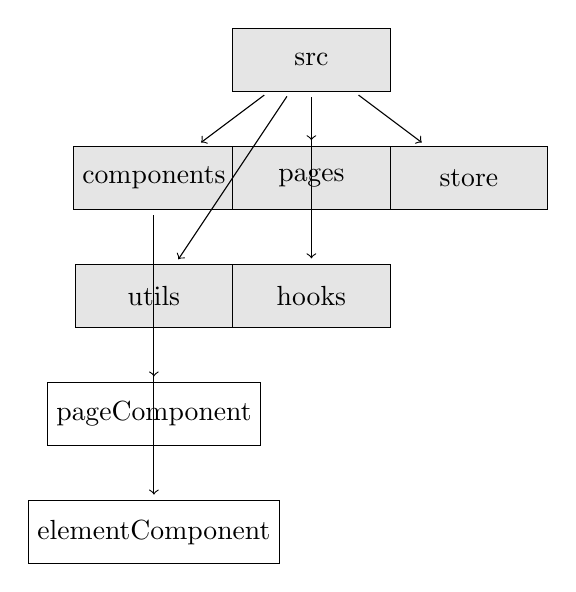
\begin{tikzpicture}[
    file/.style={draw, rectangle, minimum width=2cm, minimum height=0.8cm},
    folder/.style={draw, rectangle, minimum width=2cm, minimum height=0.8cm, fill=gray!20},
    arrow/.style={->, shorten >=2pt, shorten <=2pt}
]

% Folders
\node[folder] (src) at (0,0) {src};
\node[folder] (components) at (-2,-1.5) {components};
\node[folder] (pages) at (0,-1.5) {pages};
\node[folder] (store) at (2,-1.5) {store};
\node[folder] (utils) at (-2,-3) {utils};
\node[folder] (hooks) at (0,-3) {hooks};

% Files
\node[file] (pageComponent) at (-2,-4.5) {pageComponent};
\node[file] (elementComponent) at (-2,-6) {elementComponent};
% ... add more files

% Connections
\draw[arrow] (src) -- (components);
\draw[arrow] (src) -- (pages);
\draw[arrow] (src) -- (store);
\draw[arrow] (src) -- (utils);
\draw[arrow] (src) -- (hooks);
\draw[arrow] (components) -- (pageComponent);
\draw[arrow] (components) -- (elementComponent);
% ... add more connections

\end{tikzpicture}



\pagebreak
\subsubsection{Back-end}
The backend uses the dotNet framework. The development language using the C\# language.

In this project, the backend uses the Onion Architecture.
The Onion Architecture is a typically layered architecture, 
where each layer depends on the inner layer and provides interfaces to the outer layer.
The outer layer provides services to the outermost layer 
and other modules in the same layer based on the interfaces of the inner layer.

From inner to outer, the layers are: Domain, Application, Infrastructure, Presentation.
The Domain layer is the core layer and the innermost layer, used to define domain models, 
which are the business models.
It includes domain models and domain service interfaces.
Domain models are used to define the business models, 
which are the entities in the entity-relationship model and their attributes.
Domain service interfaces are used to define the business services, 
which are the relationships between entities in the entity-relationship model.

The Application layer is the application layer, 
used to define application services, which are the business logic.
It includes domain service implementations and application service interfaces.
Domain service implementations implement the methods of the inner layer's domain service 
interfaces and implement the business logic of the domain models.
Application service interfaces are used to define application services, 
which are the business logic.
It includes but is not limited to database interfaces, testing interfaces, 
HTTP API interfaces, MQTT interfaces, etc.

The Infrastructure layer is the infrastructure layer, used to define infrastructure.
It includes database implementations, testing implementations, 
HTTP API implementations, MQTT implementations, etc.
Database implementations implement the database interfaces 
and provide CRUD services for the database.
Testing implementations implement the testing interfaces 
and provide services for unit testing and integration testing.
HTTP API implementations implement the HTTP API interfaces 
and provide CRUD operations for HTTP APIs.
MQTT implementations implement the MQTT interfaces 
and provide CRUD operations for MQTT.

The Presentation layer is the presentation layer, used to define presentation logic, 
such as interfaces and pages. Since this is a backend project,
data presentation and control are handled by the frontend, 
so this layer is not needed.



\pagebreak
\subsubsection{Data communication and storage}
% 关于本项目的数据通信与数据存储的设计, 包括数据通信的协议, 数据存储的设计等
% 关于数据通信的设计:
% 1. 通信协议的选择
% 自前端向后端发送的数据, 有三种传输的数据类型, 
% 一种是普通的增删改查的请求, 对数据传输的时效性要求不高, 但是对数据的准确性, 完整性, 有序性, 安全性有一定的要求,
% 这种数据的传输, 采用 HTTP 协议, 以及 RESTful API 的设计. 可以有效的保证对数据传输的以上要求.
% 一种是对数据通道的创建和流媒体数据的传输, 对数据传输的时效性, 安全性要求较高, 这种数据的传输, 采用 WebRTC 协议, 以及 MQTT 协议.
% 配合可以快速解码的 flatbuffers 协议, 可以有效的保证对数据传输的以上要求.
% 最后一种是对设备的状态信息和操作信息的传输, 对完整性, 有序性, 安全性都有较高的要求, 这种数据的传输, 采用 MQTT 协议
% 同时也使用了 flatbuffers 协议.
% 
% 2. 数据通信的通信架构和通信流程
% 本项目的数据通信的通信架构, 是基于前后端分离的架构, 前端使用 React 框架, 后端使用 dotnet 框架.
% 当前端需要向后端发送数据的时候, 前端会向后端发送 HTTP 请求, 后端接收到 HTTP 请求之后, 会根据请求的数据类型,
% 选择不同的数据处理方式, 对于普通的增删改查的请求, 后端会根据 RESTful API 的设计, 对数据进行增删改查的操作,
% 对于对数据通道的创建和流媒体数据的传输, 后端会根据 WebRTC 协议, 对数据通道进行创建, 并且帮助前端和设备建立数据通道,
% 当数据通道建立后, 前端和设备之间则使用 flatbuffer 的数据格式对流媒体数据进行传输,
% 对于设备的状态信息和操作信息的传输, 前端会直接向 MQTT broker 发送 MQTT 请求, 
% 设备会在其自身的固件中监听相关的 MQTT 请求, 并且返回相关的数据.
% 
% 3. 数据通信的格式
% 本项目的数据通信的格式, 有三种, 
% 一种是 HTTP 协议, 
% 使用 json 格式对数据进行传输,
% 一种是 WebRTC 协议, 
% 使用 flatbuffers 格式对数据进行传输,
% 一种是 MQTT 协议.
% 使用 flatbuffers 格式对数据进行传输,
% 
% 关于数据存储的设计:
% 1. 数据存储的数据库的选择
% 本项目的数据存储的数据库的选择, 使用了轻量级的数据库 SQLite,
% SQLite 是一个进程内的库, 实现了自给自足的, 无服务器的, 零配置的, 事务性的 SQL 数据库引擎.
% 这是因为整个项目的目的是为了实现前端与设备之间的数据通信, 对于数据库数据的增删改查操作的要求不高,
% 数据量较小, 且对于数据库的数据的事务性要求不高, 所以选择了 SQLite 数据库.
% 2. 项目前后端的数据结构的设计
% 在本项目中, 前端由于使用了 React 框架, 所以前端的数据结构的设计, 使用了基于状态的数据结构的设计,
% 每个组件或者数据集都包含一个状态对象, 这个状态对象的属性就是组件的各个状态. 
% 使用状态对象的原因是, 可以方便的对状态进行管理, 采用对象-属性的形式, 可以方便的针对不同组件的同类状态进行区分,
% 由于跨组件的状态是由 redux 进行管理的, 这种状态对象的设计, 可以更搞笑的对状态进行更新和传递.
% 后端由于使用了 dotnet 框架, 所以后端的数据结构的设计, 使用了基于类的数据结构的设计,
% 采用了面向对象的编程思想, 对数据进行了封装, 使得数据的传输更加的安全, 有序, 完整.


\pagebreak

% \subsection{Domain model}
% \documentclass[]{article}
\usepackage{graphicx}
\usepackage{amsmath}
\usepackage{tikz}

% libaries
\usetikzlibrary{shapes,arrows}

%Define the listing package
\usepackage{listings} %code highlighter
\usepackage{color} %use color
\definecolor{mygreen}{rgb}{0,0.6,0}
\definecolor{mygray}{rgb}{0.5,0.5,0.5}
\definecolor{mymauve}{rgb}{0.58,0,0.82}

%Customize a bit the look
\lstset{ %
backgroundcolor=\color{white}, % choose the background color; you must add \usepackage{color} or \usepackage{xcolor}
basicstyle=\footnotesize, % the size of the fonts that are used for the code
breakatwhitespace=false, % sets if automatic breaks should only happen at whitespace
breaklines=true, % sets automatic line breaking
captionpos=b, % sets the caption-position to bottom
commentstyle=\color{mygreen}, % comment style
deletekeywords={...}, % if you want to delete keywords from the given language
escapeinside={\%*}{*)}, % if you want to add LaTeX within your code
extendedchars=true, % lets you use non-ASCII characters; for 8-bits encodings only, does not work with UTF-8
frame=single, % adds a frame around the code
keepspaces=true, % keeps spaces in text, useful for keeping indentation of code (possibly needs columns=flexible)
keywordstyle=\color{blue}, % keyword style
% language=Octave, % the language of the code
morekeywords={*,...}, % if you want to add more keywords to the set
numbers=left, % where to put the line-numbers; possible values are (none, left, right)
numbersep=5pt, % how far the line-numbers are from the code
numberstyle=\tiny\color{mygray}, % the style that is used for the line-numbers
rulecolor=\color{black}, % if not set, the frame-color may be changed on line-breaks within not-black text (e.g. comments (green here))
showspaces=false, % show spaces everywhere adding particular underscores; it overrides 'showstringspaces'
showstringspaces=false, % underline spaces within strings only
showtabs=false, % show tabs within strings adding particular underscores
stepnumber=1, % the step between two line-numbers. If it's 1, each line will be numbered
stringstyle=\color{mymauve}, % string literal style
tabsize=2, % sets default tabsize to 2 spaces
title=\lstname % show the filename of files included with \lstinputlisting; also try caption instead of title
}

\definecolor{darkgray}{rgb}{.4,.4,.4}
\definecolor{purple}{rgb}{0.65, 0.12, 0.82}

\lstdefinelanguage{React}{
keywords={const, typeof, new, true, false, catch, function, return, null, catch, switch, var, if, in, while, do, else, case, break},
keywordstyle=\color{blue}\bfseries,
ndkeywords={class, export, boolean, throw, implements, import, this},
ndkeywordstyle=\color{darkgray}\bfseries,
identifierstyle=\color{mygreen},
sensitive=false,
comment=[l]{//},
morecomment=[s]{/*}{*/},
commentstyle=\color{purple}\ttfamily,
string=[b]{"}{'}{`},
stringstyle=\color{red}\ttfamily,
morestring=[b]',
morestring=[b]",
morestring=[b]`',
}

\lstdefinelanguage{CSharp}{
keywords={const, typeof, new, true, false, catch, function, return, null, catch, switch, var, if, in, while, do, else, case, break},
keywordstyle=\color{blue}\bfseries,
ndkeywords={class, export, boolean, throw, implements, import, this},
ndkeywordstyle=\color{darkgray}\bfseries,
identifierstyle=\color{mygreen},
sensitive=false,
comment=[l]{//},
morecomment=[s]{/*}{*/},
commentstyle=\color{purple}\ttfamily,
string=[b]{"}{'}{`},
stringstyle=\color{red}\ttfamily,
morestring=[b]',
morestring=[b]",
morestring=[b]`',
}

\lstset{
language=React,
extendedchars=true,
basicstyle=\footnotesize\ttfamily,
showstringspaces=false,
showspaces=false,
numbers=left,
numberstyle=\footnotesize,
numbersep=9pt,
tabsize=2,
breaklines=true,
showtabs=false,
captionpos=b
}

\lstset{
language=CSharp,
extendedchars=true,
basicstyle=\footnotesize\ttfamily,
showstringspaces=false,
showspaces=false,
numbers=left,
numberstyle=\footnotesize,
numbersep=9pt,
tabsize=2,
breaklines=true,
showtabs=false,
captionpos=b
}

% \usepackage{cite} % Add this line for citation

% \bibliographystyle{plain}

\title{
The implementation of BifrostConnect Front-end scope, 
re-design and development with the relevant back-end support develop.
}
\author{
    Fei Gu \\
    Erhvervs Akademi Sydvest \\
    Computer Science 21\\
    }
\date{\today}

\begin{document}

% Front page
\maketitle
\begin{center}
    Supervisor: Henrik Boulund Meng Hansen \\
    Company: BifrostConnect \\
    Engineering Director: Jasper Wass \\
\end{center}
\tableofcontents
\pagebreak


% The introduction
\section{Introduction}
\subsection{Background}\input{sections/introduction/background.tex}
\subsection{The company}\input{sections/introduction/aboutCompany}
\subsection{The project}\input{sections/introduction/aboutProject}
\pagebreak

% The problem statement
\section{Problem Statement}
\subsection{Statement}
\input{sections/problemStatement/statement}
\subsection{Situation}
\input{sections/problemStatement/situation}
\subsection{Potential Solution}
\input{sections/problemStatement/potentialSolution}
\pagebreak

% Requirement analysis
\section{Requirement Analysis}
\input{sections/requirementAnalysis/index}

\subsection{Stakeholders}
\input{sections/requirementAnalysis/stakeholders/index}

\subsection{Business Domain}
\input{sections/requirementAnalysis/bussinesDomain/index}

\subsection{Scope}
\input{sections/requirementAnalysis/scope}

\subsection{Goals}
\input{sections/requirementAnalysis/goals}
\pagebreak

% Software Design
\section{Software Design}
% developement methods
\subsection{Software Development Methods}
\input{sections/softwareDevelopmentMethods/index}
\subsubsection{Agile Software Development}
\input{sections/softwareDevelopmentMethods/agileSoftwareDevelopment/index}
\subsubsection{Feature Driven Development}
\input{sections/softwareDevelopmentMethods/featureDrivenDevelopment/index}

\pagebreak

% Technology seslection
\subsection{Technology selection}
\input{sections/softwareDesign/technologySelection/index}
\subsubsection{Front-end}
\input{sections/softwareDesign/technologySelection/frontEnd}            
\subsubsection{Back-end}
\input{sections/softwareDesign/technologySelection/backEnd}            
\subsubsection{Database}
\input{sections/softwareDesign/technologySelection/database}
\subsubsection{Data communication}
\input{sections/softwareDesign/technologySelection/dataCommunication}            
\subsubsection{DevOps}
\input{sections/softwareDesign/technologySelection/devOps}
\pagebreak

% Architecture design
\subsection{Architecture design}
\input{sections/softwareDesign/architectureDesign/index}
\pagebreak
\subsubsection{Front-end}
\input{sections/softwareDesign/architectureDesign/frontEndArchitecture}
\pagebreak
\subsubsection{Back-end}
\input{sections/softwareDesign/architectureDesign/backEndArchitecture}
\pagebreak
\subsubsection{Data communication and storage}
\input{sections/softwareDesign/architectureDesign/dataCommunicationArchitecture}
\pagebreak

% \subsection{Domain model}
% \input{sections/softwareDesign/domainModel/index}
% \subsection{Database design}
% % 数据库领域模型 ER 图
% % 包括表和字段的设置.
% % 对于私有键和外键的设置.

% \subsection{Back-end design}
% % 后端对象模型
% % 以及对于对象模型的增删改查
% % 以及相关的其他服务的设计`'

% \subsection{Front-end design}
% % 对于前端的页面结构的设计 
% % 页面的状态的设计, 交互设计

% \subsection{FlatBuffers design}
% % schema 的设计

\subsection{DevOps CI/CD process design}
\input{sections/softwareDesign/devOpsDesign/index}
\subsubsection{Continuous Integration}
\input{sections/softwareDesign/devOpsDesign/continuousIntegration/index}
\subsubsection{Continuous Delivery}
\input{sections/softwareDesign/devOpsDesign/continuousDelivery/index}
\subsubsection{Continuous Deployment}
\input{sections/softwareDesign/devOpsDesign/continuousDeployment/index}
\pagebreak

\section{Software Development} 
\input{sections/softwareDevelopment/index}
\subsection{Overall development}
\input{sections/softwareDevelopment/overallDevelopement/index}
\subsubsection{Front-end}
\input{sections/softwareDevelopment/overallDevelopement/frontEnd/index}
\subsubsection{Back-end}
\input{sections/softwareDevelopment/overallDevelopement/backEnd/index}
\subsubsection{DevOps}
\input{sections/softwareDevelopment/overallDevelopement/devOps/index}
\subsection{Feature development} 
\input{sections/softwareDevelopment/featureDevelopment/index}
\subsubsection{Use Case 1}
\input{sections/softwareDevelopment/featureDevelopment/useCase1/index}
\subsubsection{Feature 1}
\input{sections/softwareDevelopment/featureDevelopment/feature/feature1.tex}
\pagebreak
\section{Conclusion} 
\subsection{Result}
Since the project is still in progress, the result is not available yet.
So far, basic structure of this project has been built. But the most features 
are not implemented yet. 
\subsection{Discussion}
As a single developer for this project, I am confident what I have done so far.
And I can say I understand the most of the knowledge I have used in this project, 
which also means I can explain all the part of the project. 
But this project also relevant some of the complex knowledge which I have to continue 
to study and practice.
\subsection{Future Work}
The future work is to implement the rest of the features. 
Including the most important part which is the 'create session' feature.
\pagebreak
% \bibliography{bibliography}
\pagebreak
% \begin{appendices}
%     \section{Appendix}
% \end{appendices} 
\end{document}
% \subsection{Database design}
% % 数据库领域模型 ER 图
% % 包括表和字段的设置.
% % 对于私有键和外键的设置.

% \subsection{Back-end design}
% % 后端对象模型
% % 以及对于对象模型的增删改查
% % 以及相关的其他服务的设计`'

% \subsection{Front-end design}
% % 对于前端的页面结构的设计 
% % 页面的状态的设计, 交互设计

% \subsection{FlatBuffers design}
% % schema 的设计

\subsection{DevOps CI/CD process design}
\documentclass[]{article}
\usepackage{graphicx}
\usepackage{amsmath}
\usepackage{tikz}

% libaries
\usetikzlibrary{shapes,arrows}

%Define the listing package
\usepackage{listings} %code highlighter
\usepackage{color} %use color
\definecolor{mygreen}{rgb}{0,0.6,0}
\definecolor{mygray}{rgb}{0.5,0.5,0.5}
\definecolor{mymauve}{rgb}{0.58,0,0.82}

%Customize a bit the look
\lstset{ %
backgroundcolor=\color{white}, % choose the background color; you must add \usepackage{color} or \usepackage{xcolor}
basicstyle=\footnotesize, % the size of the fonts that are used for the code
breakatwhitespace=false, % sets if automatic breaks should only happen at whitespace
breaklines=true, % sets automatic line breaking
captionpos=b, % sets the caption-position to bottom
commentstyle=\color{mygreen}, % comment style
deletekeywords={...}, % if you want to delete keywords from the given language
escapeinside={\%*}{*)}, % if you want to add LaTeX within your code
extendedchars=true, % lets you use non-ASCII characters; for 8-bits encodings only, does not work with UTF-8
frame=single, % adds a frame around the code
keepspaces=true, % keeps spaces in text, useful for keeping indentation of code (possibly needs columns=flexible)
keywordstyle=\color{blue}, % keyword style
% language=Octave, % the language of the code
morekeywords={*,...}, % if you want to add more keywords to the set
numbers=left, % where to put the line-numbers; possible values are (none, left, right)
numbersep=5pt, % how far the line-numbers are from the code
numberstyle=\tiny\color{mygray}, % the style that is used for the line-numbers
rulecolor=\color{black}, % if not set, the frame-color may be changed on line-breaks within not-black text (e.g. comments (green here))
showspaces=false, % show spaces everywhere adding particular underscores; it overrides 'showstringspaces'
showstringspaces=false, % underline spaces within strings only
showtabs=false, % show tabs within strings adding particular underscores
stepnumber=1, % the step between two line-numbers. If it's 1, each line will be numbered
stringstyle=\color{mymauve}, % string literal style
tabsize=2, % sets default tabsize to 2 spaces
title=\lstname % show the filename of files included with \lstinputlisting; also try caption instead of title
}

\definecolor{darkgray}{rgb}{.4,.4,.4}
\definecolor{purple}{rgb}{0.65, 0.12, 0.82}

\lstdefinelanguage{React}{
keywords={const, typeof, new, true, false, catch, function, return, null, catch, switch, var, if, in, while, do, else, case, break},
keywordstyle=\color{blue}\bfseries,
ndkeywords={class, export, boolean, throw, implements, import, this},
ndkeywordstyle=\color{darkgray}\bfseries,
identifierstyle=\color{mygreen},
sensitive=false,
comment=[l]{//},
morecomment=[s]{/*}{*/},
commentstyle=\color{purple}\ttfamily,
string=[b]{"}{'}{`},
stringstyle=\color{red}\ttfamily,
morestring=[b]',
morestring=[b]",
morestring=[b]`',
}

\lstdefinelanguage{CSharp}{
keywords={const, typeof, new, true, false, catch, function, return, null, catch, switch, var, if, in, while, do, else, case, break},
keywordstyle=\color{blue}\bfseries,
ndkeywords={class, export, boolean, throw, implements, import, this},
ndkeywordstyle=\color{darkgray}\bfseries,
identifierstyle=\color{mygreen},
sensitive=false,
comment=[l]{//},
morecomment=[s]{/*}{*/},
commentstyle=\color{purple}\ttfamily,
string=[b]{"}{'}{`},
stringstyle=\color{red}\ttfamily,
morestring=[b]',
morestring=[b]",
morestring=[b]`',
}

\lstset{
language=React,
extendedchars=true,
basicstyle=\footnotesize\ttfamily,
showstringspaces=false,
showspaces=false,
numbers=left,
numberstyle=\footnotesize,
numbersep=9pt,
tabsize=2,
breaklines=true,
showtabs=false,
captionpos=b
}

\lstset{
language=CSharp,
extendedchars=true,
basicstyle=\footnotesize\ttfamily,
showstringspaces=false,
showspaces=false,
numbers=left,
numberstyle=\footnotesize,
numbersep=9pt,
tabsize=2,
breaklines=true,
showtabs=false,
captionpos=b
}

% \usepackage{cite} % Add this line for citation

% \bibliographystyle{plain}

\title{
The implementation of BifrostConnect Front-end scope, 
re-design and development with the relevant back-end support develop.
}
\author{
    Fei Gu \\
    Erhvervs Akademi Sydvest \\
    Computer Science 21\\
    }
\date{\today}

\begin{document}

% Front page
\maketitle
\begin{center}
    Supervisor: Henrik Boulund Meng Hansen \\
    Company: BifrostConnect \\
    Engineering Director: Jasper Wass \\
\end{center}
\tableofcontents
\pagebreak


% The introduction
\section{Introduction}
\subsection{Background}\input{sections/introduction/background.tex}
\subsection{The company}\input{sections/introduction/aboutCompany}
\subsection{The project}\input{sections/introduction/aboutProject}
\pagebreak

% The problem statement
\section{Problem Statement}
\subsection{Statement}
\input{sections/problemStatement/statement}
\subsection{Situation}
\input{sections/problemStatement/situation}
\subsection{Potential Solution}
\input{sections/problemStatement/potentialSolution}
\pagebreak

% Requirement analysis
\section{Requirement Analysis}
\input{sections/requirementAnalysis/index}

\subsection{Stakeholders}
\input{sections/requirementAnalysis/stakeholders/index}

\subsection{Business Domain}
\input{sections/requirementAnalysis/bussinesDomain/index}

\subsection{Scope}
\input{sections/requirementAnalysis/scope}

\subsection{Goals}
\input{sections/requirementAnalysis/goals}
\pagebreak

% Software Design
\section{Software Design}
% developement methods
\subsection{Software Development Methods}
\input{sections/softwareDevelopmentMethods/index}
\subsubsection{Agile Software Development}
\input{sections/softwareDevelopmentMethods/agileSoftwareDevelopment/index}
\subsubsection{Feature Driven Development}
\input{sections/softwareDevelopmentMethods/featureDrivenDevelopment/index}

\pagebreak

% Technology seslection
\subsection{Technology selection}
\input{sections/softwareDesign/technologySelection/index}
\subsubsection{Front-end}
\input{sections/softwareDesign/technologySelection/frontEnd}            
\subsubsection{Back-end}
\input{sections/softwareDesign/technologySelection/backEnd}            
\subsubsection{Database}
\input{sections/softwareDesign/technologySelection/database}
\subsubsection{Data communication}
\input{sections/softwareDesign/technologySelection/dataCommunication}            
\subsubsection{DevOps}
\input{sections/softwareDesign/technologySelection/devOps}
\pagebreak

% Architecture design
\subsection{Architecture design}
\input{sections/softwareDesign/architectureDesign/index}
\pagebreak
\subsubsection{Front-end}
\input{sections/softwareDesign/architectureDesign/frontEndArchitecture}
\pagebreak
\subsubsection{Back-end}
\input{sections/softwareDesign/architectureDesign/backEndArchitecture}
\pagebreak
\subsubsection{Data communication and storage}
\input{sections/softwareDesign/architectureDesign/dataCommunicationArchitecture}
\pagebreak

% \subsection{Domain model}
% \input{sections/softwareDesign/domainModel/index}
% \subsection{Database design}
% % 数据库领域模型 ER 图
% % 包括表和字段的设置.
% % 对于私有键和外键的设置.

% \subsection{Back-end design}
% % 后端对象模型
% % 以及对于对象模型的增删改查
% % 以及相关的其他服务的设计`'

% \subsection{Front-end design}
% % 对于前端的页面结构的设计 
% % 页面的状态的设计, 交互设计

% \subsection{FlatBuffers design}
% % schema 的设计

\subsection{DevOps CI/CD process design}
\input{sections/softwareDesign/devOpsDesign/index}
\subsubsection{Continuous Integration}
\input{sections/softwareDesign/devOpsDesign/continuousIntegration/index}
\subsubsection{Continuous Delivery}
\input{sections/softwareDesign/devOpsDesign/continuousDelivery/index}
\subsubsection{Continuous Deployment}
\input{sections/softwareDesign/devOpsDesign/continuousDeployment/index}
\pagebreak

\section{Software Development} 
\input{sections/softwareDevelopment/index}
\subsection{Overall development}
\input{sections/softwareDevelopment/overallDevelopement/index}
\subsubsection{Front-end}
\input{sections/softwareDevelopment/overallDevelopement/frontEnd/index}
\subsubsection{Back-end}
\input{sections/softwareDevelopment/overallDevelopement/backEnd/index}
\subsubsection{DevOps}
\input{sections/softwareDevelopment/overallDevelopement/devOps/index}
\subsection{Feature development} 
\input{sections/softwareDevelopment/featureDevelopment/index}
\subsubsection{Use Case 1}
\input{sections/softwareDevelopment/featureDevelopment/useCase1/index}
\subsubsection{Feature 1}
\input{sections/softwareDevelopment/featureDevelopment/feature/feature1.tex}
\pagebreak
\section{Conclusion} 
\subsection{Result}
Since the project is still in progress, the result is not available yet.
So far, basic structure of this project has been built. But the most features 
are not implemented yet. 
\subsection{Discussion}
As a single developer for this project, I am confident what I have done so far.
And I can say I understand the most of the knowledge I have used in this project, 
which also means I can explain all the part of the project. 
But this project also relevant some of the complex knowledge which I have to continue 
to study and practice.
\subsection{Future Work}
The future work is to implement the rest of the features. 
Including the most important part which is the 'create session' feature.
\pagebreak
% \bibliography{bibliography}
\pagebreak
% \begin{appendices}
%     \section{Appendix}
% \end{appendices} 
\end{document}
\subsubsection{Continuous Integration}
\documentclass[]{article}
\usepackage{graphicx}
\usepackage{amsmath}
\usepackage{tikz}

% libaries
\usetikzlibrary{shapes,arrows}

%Define the listing package
\usepackage{listings} %code highlighter
\usepackage{color} %use color
\definecolor{mygreen}{rgb}{0,0.6,0}
\definecolor{mygray}{rgb}{0.5,0.5,0.5}
\definecolor{mymauve}{rgb}{0.58,0,0.82}

%Customize a bit the look
\lstset{ %
backgroundcolor=\color{white}, % choose the background color; you must add \usepackage{color} or \usepackage{xcolor}
basicstyle=\footnotesize, % the size of the fonts that are used for the code
breakatwhitespace=false, % sets if automatic breaks should only happen at whitespace
breaklines=true, % sets automatic line breaking
captionpos=b, % sets the caption-position to bottom
commentstyle=\color{mygreen}, % comment style
deletekeywords={...}, % if you want to delete keywords from the given language
escapeinside={\%*}{*)}, % if you want to add LaTeX within your code
extendedchars=true, % lets you use non-ASCII characters; for 8-bits encodings only, does not work with UTF-8
frame=single, % adds a frame around the code
keepspaces=true, % keeps spaces in text, useful for keeping indentation of code (possibly needs columns=flexible)
keywordstyle=\color{blue}, % keyword style
% language=Octave, % the language of the code
morekeywords={*,...}, % if you want to add more keywords to the set
numbers=left, % where to put the line-numbers; possible values are (none, left, right)
numbersep=5pt, % how far the line-numbers are from the code
numberstyle=\tiny\color{mygray}, % the style that is used for the line-numbers
rulecolor=\color{black}, % if not set, the frame-color may be changed on line-breaks within not-black text (e.g. comments (green here))
showspaces=false, % show spaces everywhere adding particular underscores; it overrides 'showstringspaces'
showstringspaces=false, % underline spaces within strings only
showtabs=false, % show tabs within strings adding particular underscores
stepnumber=1, % the step between two line-numbers. If it's 1, each line will be numbered
stringstyle=\color{mymauve}, % string literal style
tabsize=2, % sets default tabsize to 2 spaces
title=\lstname % show the filename of files included with \lstinputlisting; also try caption instead of title
}

\definecolor{darkgray}{rgb}{.4,.4,.4}
\definecolor{purple}{rgb}{0.65, 0.12, 0.82}

\lstdefinelanguage{React}{
keywords={const, typeof, new, true, false, catch, function, return, null, catch, switch, var, if, in, while, do, else, case, break},
keywordstyle=\color{blue}\bfseries,
ndkeywords={class, export, boolean, throw, implements, import, this},
ndkeywordstyle=\color{darkgray}\bfseries,
identifierstyle=\color{mygreen},
sensitive=false,
comment=[l]{//},
morecomment=[s]{/*}{*/},
commentstyle=\color{purple}\ttfamily,
string=[b]{"}{'}{`},
stringstyle=\color{red}\ttfamily,
morestring=[b]',
morestring=[b]",
morestring=[b]`',
}

\lstdefinelanguage{CSharp}{
keywords={const, typeof, new, true, false, catch, function, return, null, catch, switch, var, if, in, while, do, else, case, break},
keywordstyle=\color{blue}\bfseries,
ndkeywords={class, export, boolean, throw, implements, import, this},
ndkeywordstyle=\color{darkgray}\bfseries,
identifierstyle=\color{mygreen},
sensitive=false,
comment=[l]{//},
morecomment=[s]{/*}{*/},
commentstyle=\color{purple}\ttfamily,
string=[b]{"}{'}{`},
stringstyle=\color{red}\ttfamily,
morestring=[b]',
morestring=[b]",
morestring=[b]`',
}

\lstset{
language=React,
extendedchars=true,
basicstyle=\footnotesize\ttfamily,
showstringspaces=false,
showspaces=false,
numbers=left,
numberstyle=\footnotesize,
numbersep=9pt,
tabsize=2,
breaklines=true,
showtabs=false,
captionpos=b
}

\lstset{
language=CSharp,
extendedchars=true,
basicstyle=\footnotesize\ttfamily,
showstringspaces=false,
showspaces=false,
numbers=left,
numberstyle=\footnotesize,
numbersep=9pt,
tabsize=2,
breaklines=true,
showtabs=false,
captionpos=b
}

% \usepackage{cite} % Add this line for citation

% \bibliographystyle{plain}

\title{
The implementation of BifrostConnect Front-end scope, 
re-design and development with the relevant back-end support develop.
}
\author{
    Fei Gu \\
    Erhvervs Akademi Sydvest \\
    Computer Science 21\\
    }
\date{\today}

\begin{document}

% Front page
\maketitle
\begin{center}
    Supervisor: Henrik Boulund Meng Hansen \\
    Company: BifrostConnect \\
    Engineering Director: Jasper Wass \\
\end{center}
\tableofcontents
\pagebreak


% The introduction
\section{Introduction}
\subsection{Background}\input{sections/introduction/background.tex}
\subsection{The company}\input{sections/introduction/aboutCompany}
\subsection{The project}\input{sections/introduction/aboutProject}
\pagebreak

% The problem statement
\section{Problem Statement}
\subsection{Statement}
\input{sections/problemStatement/statement}
\subsection{Situation}
\input{sections/problemStatement/situation}
\subsection{Potential Solution}
\input{sections/problemStatement/potentialSolution}
\pagebreak

% Requirement analysis
\section{Requirement Analysis}
\input{sections/requirementAnalysis/index}

\subsection{Stakeholders}
\input{sections/requirementAnalysis/stakeholders/index}

\subsection{Business Domain}
\input{sections/requirementAnalysis/bussinesDomain/index}

\subsection{Scope}
\input{sections/requirementAnalysis/scope}

\subsection{Goals}
\input{sections/requirementAnalysis/goals}
\pagebreak

% Software Design
\section{Software Design}
% developement methods
\subsection{Software Development Methods}
\input{sections/softwareDevelopmentMethods/index}
\subsubsection{Agile Software Development}
\input{sections/softwareDevelopmentMethods/agileSoftwareDevelopment/index}
\subsubsection{Feature Driven Development}
\input{sections/softwareDevelopmentMethods/featureDrivenDevelopment/index}

\pagebreak

% Technology seslection
\subsection{Technology selection}
\input{sections/softwareDesign/technologySelection/index}
\subsubsection{Front-end}
\input{sections/softwareDesign/technologySelection/frontEnd}            
\subsubsection{Back-end}
\input{sections/softwareDesign/technologySelection/backEnd}            
\subsubsection{Database}
\input{sections/softwareDesign/technologySelection/database}
\subsubsection{Data communication}
\input{sections/softwareDesign/technologySelection/dataCommunication}            
\subsubsection{DevOps}
\input{sections/softwareDesign/technologySelection/devOps}
\pagebreak

% Architecture design
\subsection{Architecture design}
\input{sections/softwareDesign/architectureDesign/index}
\pagebreak
\subsubsection{Front-end}
\input{sections/softwareDesign/architectureDesign/frontEndArchitecture}
\pagebreak
\subsubsection{Back-end}
\input{sections/softwareDesign/architectureDesign/backEndArchitecture}
\pagebreak
\subsubsection{Data communication and storage}
\input{sections/softwareDesign/architectureDesign/dataCommunicationArchitecture}
\pagebreak

% \subsection{Domain model}
% \input{sections/softwareDesign/domainModel/index}
% \subsection{Database design}
% % 数据库领域模型 ER 图
% % 包括表和字段的设置.
% % 对于私有键和外键的设置.

% \subsection{Back-end design}
% % 后端对象模型
% % 以及对于对象模型的增删改查
% % 以及相关的其他服务的设计`'

% \subsection{Front-end design}
% % 对于前端的页面结构的设计 
% % 页面的状态的设计, 交互设计

% \subsection{FlatBuffers design}
% % schema 的设计

\subsection{DevOps CI/CD process design}
\input{sections/softwareDesign/devOpsDesign/index}
\subsubsection{Continuous Integration}
\input{sections/softwareDesign/devOpsDesign/continuousIntegration/index}
\subsubsection{Continuous Delivery}
\input{sections/softwareDesign/devOpsDesign/continuousDelivery/index}
\subsubsection{Continuous Deployment}
\input{sections/softwareDesign/devOpsDesign/continuousDeployment/index}
\pagebreak

\section{Software Development} 
\input{sections/softwareDevelopment/index}
\subsection{Overall development}
\input{sections/softwareDevelopment/overallDevelopement/index}
\subsubsection{Front-end}
\input{sections/softwareDevelopment/overallDevelopement/frontEnd/index}
\subsubsection{Back-end}
\input{sections/softwareDevelopment/overallDevelopement/backEnd/index}
\subsubsection{DevOps}
\input{sections/softwareDevelopment/overallDevelopement/devOps/index}
\subsection{Feature development} 
\input{sections/softwareDevelopment/featureDevelopment/index}
\subsubsection{Use Case 1}
\input{sections/softwareDevelopment/featureDevelopment/useCase1/index}
\subsubsection{Feature 1}
\input{sections/softwareDevelopment/featureDevelopment/feature/feature1.tex}
\pagebreak
\section{Conclusion} 
\subsection{Result}
Since the project is still in progress, the result is not available yet.
So far, basic structure of this project has been built. But the most features 
are not implemented yet. 
\subsection{Discussion}
As a single developer for this project, I am confident what I have done so far.
And I can say I understand the most of the knowledge I have used in this project, 
which also means I can explain all the part of the project. 
But this project also relevant some of the complex knowledge which I have to continue 
to study and practice.
\subsection{Future Work}
The future work is to implement the rest of the features. 
Including the most important part which is the 'create session' feature.
\pagebreak
% \bibliography{bibliography}
\pagebreak
% \begin{appendices}
%     \section{Appendix}
% \end{appendices} 
\end{document}
\subsubsection{Continuous Delivery}
\documentclass[]{article}
\usepackage{graphicx}
\usepackage{amsmath}
\usepackage{tikz}

% libaries
\usetikzlibrary{shapes,arrows}

%Define the listing package
\usepackage{listings} %code highlighter
\usepackage{color} %use color
\definecolor{mygreen}{rgb}{0,0.6,0}
\definecolor{mygray}{rgb}{0.5,0.5,0.5}
\definecolor{mymauve}{rgb}{0.58,0,0.82}

%Customize a bit the look
\lstset{ %
backgroundcolor=\color{white}, % choose the background color; you must add \usepackage{color} or \usepackage{xcolor}
basicstyle=\footnotesize, % the size of the fonts that are used for the code
breakatwhitespace=false, % sets if automatic breaks should only happen at whitespace
breaklines=true, % sets automatic line breaking
captionpos=b, % sets the caption-position to bottom
commentstyle=\color{mygreen}, % comment style
deletekeywords={...}, % if you want to delete keywords from the given language
escapeinside={\%*}{*)}, % if you want to add LaTeX within your code
extendedchars=true, % lets you use non-ASCII characters; for 8-bits encodings only, does not work with UTF-8
frame=single, % adds a frame around the code
keepspaces=true, % keeps spaces in text, useful for keeping indentation of code (possibly needs columns=flexible)
keywordstyle=\color{blue}, % keyword style
% language=Octave, % the language of the code
morekeywords={*,...}, % if you want to add more keywords to the set
numbers=left, % where to put the line-numbers; possible values are (none, left, right)
numbersep=5pt, % how far the line-numbers are from the code
numberstyle=\tiny\color{mygray}, % the style that is used for the line-numbers
rulecolor=\color{black}, % if not set, the frame-color may be changed on line-breaks within not-black text (e.g. comments (green here))
showspaces=false, % show spaces everywhere adding particular underscores; it overrides 'showstringspaces'
showstringspaces=false, % underline spaces within strings only
showtabs=false, % show tabs within strings adding particular underscores
stepnumber=1, % the step between two line-numbers. If it's 1, each line will be numbered
stringstyle=\color{mymauve}, % string literal style
tabsize=2, % sets default tabsize to 2 spaces
title=\lstname % show the filename of files included with \lstinputlisting; also try caption instead of title
}

\definecolor{darkgray}{rgb}{.4,.4,.4}
\definecolor{purple}{rgb}{0.65, 0.12, 0.82}

\lstdefinelanguage{React}{
keywords={const, typeof, new, true, false, catch, function, return, null, catch, switch, var, if, in, while, do, else, case, break},
keywordstyle=\color{blue}\bfseries,
ndkeywords={class, export, boolean, throw, implements, import, this},
ndkeywordstyle=\color{darkgray}\bfseries,
identifierstyle=\color{mygreen},
sensitive=false,
comment=[l]{//},
morecomment=[s]{/*}{*/},
commentstyle=\color{purple}\ttfamily,
string=[b]{"}{'}{`},
stringstyle=\color{red}\ttfamily,
morestring=[b]',
morestring=[b]",
morestring=[b]`',
}

\lstdefinelanguage{CSharp}{
keywords={const, typeof, new, true, false, catch, function, return, null, catch, switch, var, if, in, while, do, else, case, break},
keywordstyle=\color{blue}\bfseries,
ndkeywords={class, export, boolean, throw, implements, import, this},
ndkeywordstyle=\color{darkgray}\bfseries,
identifierstyle=\color{mygreen},
sensitive=false,
comment=[l]{//},
morecomment=[s]{/*}{*/},
commentstyle=\color{purple}\ttfamily,
string=[b]{"}{'}{`},
stringstyle=\color{red}\ttfamily,
morestring=[b]',
morestring=[b]",
morestring=[b]`',
}

\lstset{
language=React,
extendedchars=true,
basicstyle=\footnotesize\ttfamily,
showstringspaces=false,
showspaces=false,
numbers=left,
numberstyle=\footnotesize,
numbersep=9pt,
tabsize=2,
breaklines=true,
showtabs=false,
captionpos=b
}

\lstset{
language=CSharp,
extendedchars=true,
basicstyle=\footnotesize\ttfamily,
showstringspaces=false,
showspaces=false,
numbers=left,
numberstyle=\footnotesize,
numbersep=9pt,
tabsize=2,
breaklines=true,
showtabs=false,
captionpos=b
}

% \usepackage{cite} % Add this line for citation

% \bibliographystyle{plain}

\title{
The implementation of BifrostConnect Front-end scope, 
re-design and development with the relevant back-end support develop.
}
\author{
    Fei Gu \\
    Erhvervs Akademi Sydvest \\
    Computer Science 21\\
    }
\date{\today}

\begin{document}

% Front page
\maketitle
\begin{center}
    Supervisor: Henrik Boulund Meng Hansen \\
    Company: BifrostConnect \\
    Engineering Director: Jasper Wass \\
\end{center}
\tableofcontents
\pagebreak


% The introduction
\section{Introduction}
\subsection{Background}\input{sections/introduction/background.tex}
\subsection{The company}\input{sections/introduction/aboutCompany}
\subsection{The project}\input{sections/introduction/aboutProject}
\pagebreak

% The problem statement
\section{Problem Statement}
\subsection{Statement}
\input{sections/problemStatement/statement}
\subsection{Situation}
\input{sections/problemStatement/situation}
\subsection{Potential Solution}
\input{sections/problemStatement/potentialSolution}
\pagebreak

% Requirement analysis
\section{Requirement Analysis}
\input{sections/requirementAnalysis/index}

\subsection{Stakeholders}
\input{sections/requirementAnalysis/stakeholders/index}

\subsection{Business Domain}
\input{sections/requirementAnalysis/bussinesDomain/index}

\subsection{Scope}
\input{sections/requirementAnalysis/scope}

\subsection{Goals}
\input{sections/requirementAnalysis/goals}
\pagebreak

% Software Design
\section{Software Design}
% developement methods
\subsection{Software Development Methods}
\input{sections/softwareDevelopmentMethods/index}
\subsubsection{Agile Software Development}
\input{sections/softwareDevelopmentMethods/agileSoftwareDevelopment/index}
\subsubsection{Feature Driven Development}
\input{sections/softwareDevelopmentMethods/featureDrivenDevelopment/index}

\pagebreak

% Technology seslection
\subsection{Technology selection}
\input{sections/softwareDesign/technologySelection/index}
\subsubsection{Front-end}
\input{sections/softwareDesign/technologySelection/frontEnd}            
\subsubsection{Back-end}
\input{sections/softwareDesign/technologySelection/backEnd}            
\subsubsection{Database}
\input{sections/softwareDesign/technologySelection/database}
\subsubsection{Data communication}
\input{sections/softwareDesign/technologySelection/dataCommunication}            
\subsubsection{DevOps}
\input{sections/softwareDesign/technologySelection/devOps}
\pagebreak

% Architecture design
\subsection{Architecture design}
\input{sections/softwareDesign/architectureDesign/index}
\pagebreak
\subsubsection{Front-end}
\input{sections/softwareDesign/architectureDesign/frontEndArchitecture}
\pagebreak
\subsubsection{Back-end}
\input{sections/softwareDesign/architectureDesign/backEndArchitecture}
\pagebreak
\subsubsection{Data communication and storage}
\input{sections/softwareDesign/architectureDesign/dataCommunicationArchitecture}
\pagebreak

% \subsection{Domain model}
% \input{sections/softwareDesign/domainModel/index}
% \subsection{Database design}
% % 数据库领域模型 ER 图
% % 包括表和字段的设置.
% % 对于私有键和外键的设置.

% \subsection{Back-end design}
% % 后端对象模型
% % 以及对于对象模型的增删改查
% % 以及相关的其他服务的设计`'

% \subsection{Front-end design}
% % 对于前端的页面结构的设计 
% % 页面的状态的设计, 交互设计

% \subsection{FlatBuffers design}
% % schema 的设计

\subsection{DevOps CI/CD process design}
\input{sections/softwareDesign/devOpsDesign/index}
\subsubsection{Continuous Integration}
\input{sections/softwareDesign/devOpsDesign/continuousIntegration/index}
\subsubsection{Continuous Delivery}
\input{sections/softwareDesign/devOpsDesign/continuousDelivery/index}
\subsubsection{Continuous Deployment}
\input{sections/softwareDesign/devOpsDesign/continuousDeployment/index}
\pagebreak

\section{Software Development} 
\input{sections/softwareDevelopment/index}
\subsection{Overall development}
\input{sections/softwareDevelopment/overallDevelopement/index}
\subsubsection{Front-end}
\input{sections/softwareDevelopment/overallDevelopement/frontEnd/index}
\subsubsection{Back-end}
\input{sections/softwareDevelopment/overallDevelopement/backEnd/index}
\subsubsection{DevOps}
\input{sections/softwareDevelopment/overallDevelopement/devOps/index}
\subsection{Feature development} 
\input{sections/softwareDevelopment/featureDevelopment/index}
\subsubsection{Use Case 1}
\input{sections/softwareDevelopment/featureDevelopment/useCase1/index}
\subsubsection{Feature 1}
\input{sections/softwareDevelopment/featureDevelopment/feature/feature1.tex}
\pagebreak
\section{Conclusion} 
\subsection{Result}
Since the project is still in progress, the result is not available yet.
So far, basic structure of this project has been built. But the most features 
are not implemented yet. 
\subsection{Discussion}
As a single developer for this project, I am confident what I have done so far.
And I can say I understand the most of the knowledge I have used in this project, 
which also means I can explain all the part of the project. 
But this project also relevant some of the complex knowledge which I have to continue 
to study and practice.
\subsection{Future Work}
The future work is to implement the rest of the features. 
Including the most important part which is the 'create session' feature.
\pagebreak
% \bibliography{bibliography}
\pagebreak
% \begin{appendices}
%     \section{Appendix}
% \end{appendices} 
\end{document}
\subsubsection{Continuous Deployment}
\documentclass[]{article}
\usepackage{graphicx}
\usepackage{amsmath}
\usepackage{tikz}

% libaries
\usetikzlibrary{shapes,arrows}

%Define the listing package
\usepackage{listings} %code highlighter
\usepackage{color} %use color
\definecolor{mygreen}{rgb}{0,0.6,0}
\definecolor{mygray}{rgb}{0.5,0.5,0.5}
\definecolor{mymauve}{rgb}{0.58,0,0.82}

%Customize a bit the look
\lstset{ %
backgroundcolor=\color{white}, % choose the background color; you must add \usepackage{color} or \usepackage{xcolor}
basicstyle=\footnotesize, % the size of the fonts that are used for the code
breakatwhitespace=false, % sets if automatic breaks should only happen at whitespace
breaklines=true, % sets automatic line breaking
captionpos=b, % sets the caption-position to bottom
commentstyle=\color{mygreen}, % comment style
deletekeywords={...}, % if you want to delete keywords from the given language
escapeinside={\%*}{*)}, % if you want to add LaTeX within your code
extendedchars=true, % lets you use non-ASCII characters; for 8-bits encodings only, does not work with UTF-8
frame=single, % adds a frame around the code
keepspaces=true, % keeps spaces in text, useful for keeping indentation of code (possibly needs columns=flexible)
keywordstyle=\color{blue}, % keyword style
% language=Octave, % the language of the code
morekeywords={*,...}, % if you want to add more keywords to the set
numbers=left, % where to put the line-numbers; possible values are (none, left, right)
numbersep=5pt, % how far the line-numbers are from the code
numberstyle=\tiny\color{mygray}, % the style that is used for the line-numbers
rulecolor=\color{black}, % if not set, the frame-color may be changed on line-breaks within not-black text (e.g. comments (green here))
showspaces=false, % show spaces everywhere adding particular underscores; it overrides 'showstringspaces'
showstringspaces=false, % underline spaces within strings only
showtabs=false, % show tabs within strings adding particular underscores
stepnumber=1, % the step between two line-numbers. If it's 1, each line will be numbered
stringstyle=\color{mymauve}, % string literal style
tabsize=2, % sets default tabsize to 2 spaces
title=\lstname % show the filename of files included with \lstinputlisting; also try caption instead of title
}

\definecolor{darkgray}{rgb}{.4,.4,.4}
\definecolor{purple}{rgb}{0.65, 0.12, 0.82}

\lstdefinelanguage{React}{
keywords={const, typeof, new, true, false, catch, function, return, null, catch, switch, var, if, in, while, do, else, case, break},
keywordstyle=\color{blue}\bfseries,
ndkeywords={class, export, boolean, throw, implements, import, this},
ndkeywordstyle=\color{darkgray}\bfseries,
identifierstyle=\color{mygreen},
sensitive=false,
comment=[l]{//},
morecomment=[s]{/*}{*/},
commentstyle=\color{purple}\ttfamily,
string=[b]{"}{'}{`},
stringstyle=\color{red}\ttfamily,
morestring=[b]',
morestring=[b]",
morestring=[b]`',
}

\lstdefinelanguage{CSharp}{
keywords={const, typeof, new, true, false, catch, function, return, null, catch, switch, var, if, in, while, do, else, case, break},
keywordstyle=\color{blue}\bfseries,
ndkeywords={class, export, boolean, throw, implements, import, this},
ndkeywordstyle=\color{darkgray}\bfseries,
identifierstyle=\color{mygreen},
sensitive=false,
comment=[l]{//},
morecomment=[s]{/*}{*/},
commentstyle=\color{purple}\ttfamily,
string=[b]{"}{'}{`},
stringstyle=\color{red}\ttfamily,
morestring=[b]',
morestring=[b]",
morestring=[b]`',
}

\lstset{
language=React,
extendedchars=true,
basicstyle=\footnotesize\ttfamily,
showstringspaces=false,
showspaces=false,
numbers=left,
numberstyle=\footnotesize,
numbersep=9pt,
tabsize=2,
breaklines=true,
showtabs=false,
captionpos=b
}

\lstset{
language=CSharp,
extendedchars=true,
basicstyle=\footnotesize\ttfamily,
showstringspaces=false,
showspaces=false,
numbers=left,
numberstyle=\footnotesize,
numbersep=9pt,
tabsize=2,
breaklines=true,
showtabs=false,
captionpos=b
}

% \usepackage{cite} % Add this line for citation

% \bibliographystyle{plain}

\title{
The implementation of BifrostConnect Front-end scope, 
re-design and development with the relevant back-end support develop.
}
\author{
    Fei Gu \\
    Erhvervs Akademi Sydvest \\
    Computer Science 21\\
    }
\date{\today}

\begin{document}

% Front page
\maketitle
\begin{center}
    Supervisor: Henrik Boulund Meng Hansen \\
    Company: BifrostConnect \\
    Engineering Director: Jasper Wass \\
\end{center}
\tableofcontents
\pagebreak


% The introduction
\section{Introduction}
\subsection{Background}\input{sections/introduction/background.tex}
\subsection{The company}\input{sections/introduction/aboutCompany}
\subsection{The project}\input{sections/introduction/aboutProject}
\pagebreak

% The problem statement
\section{Problem Statement}
\subsection{Statement}
\input{sections/problemStatement/statement}
\subsection{Situation}
\input{sections/problemStatement/situation}
\subsection{Potential Solution}
\input{sections/problemStatement/potentialSolution}
\pagebreak

% Requirement analysis
\section{Requirement Analysis}
\input{sections/requirementAnalysis/index}

\subsection{Stakeholders}
\input{sections/requirementAnalysis/stakeholders/index}

\subsection{Business Domain}
\input{sections/requirementAnalysis/bussinesDomain/index}

\subsection{Scope}
\input{sections/requirementAnalysis/scope}

\subsection{Goals}
\input{sections/requirementAnalysis/goals}
\pagebreak

% Software Design
\section{Software Design}
% developement methods
\subsection{Software Development Methods}
\input{sections/softwareDevelopmentMethods/index}
\subsubsection{Agile Software Development}
\input{sections/softwareDevelopmentMethods/agileSoftwareDevelopment/index}
\subsubsection{Feature Driven Development}
\input{sections/softwareDevelopmentMethods/featureDrivenDevelopment/index}

\pagebreak

% Technology seslection
\subsection{Technology selection}
\input{sections/softwareDesign/technologySelection/index}
\subsubsection{Front-end}
\input{sections/softwareDesign/technologySelection/frontEnd}            
\subsubsection{Back-end}
\input{sections/softwareDesign/technologySelection/backEnd}            
\subsubsection{Database}
\input{sections/softwareDesign/technologySelection/database}
\subsubsection{Data communication}
\input{sections/softwareDesign/technologySelection/dataCommunication}            
\subsubsection{DevOps}
\input{sections/softwareDesign/technologySelection/devOps}
\pagebreak

% Architecture design
\subsection{Architecture design}
\input{sections/softwareDesign/architectureDesign/index}
\pagebreak
\subsubsection{Front-end}
\input{sections/softwareDesign/architectureDesign/frontEndArchitecture}
\pagebreak
\subsubsection{Back-end}
\input{sections/softwareDesign/architectureDesign/backEndArchitecture}
\pagebreak
\subsubsection{Data communication and storage}
\input{sections/softwareDesign/architectureDesign/dataCommunicationArchitecture}
\pagebreak

% \subsection{Domain model}
% \input{sections/softwareDesign/domainModel/index}
% \subsection{Database design}
% % 数据库领域模型 ER 图
% % 包括表和字段的设置.
% % 对于私有键和外键的设置.

% \subsection{Back-end design}
% % 后端对象模型
% % 以及对于对象模型的增删改查
% % 以及相关的其他服务的设计`'

% \subsection{Front-end design}
% % 对于前端的页面结构的设计 
% % 页面的状态的设计, 交互设计

% \subsection{FlatBuffers design}
% % schema 的设计

\subsection{DevOps CI/CD process design}
\input{sections/softwareDesign/devOpsDesign/index}
\subsubsection{Continuous Integration}
\input{sections/softwareDesign/devOpsDesign/continuousIntegration/index}
\subsubsection{Continuous Delivery}
\input{sections/softwareDesign/devOpsDesign/continuousDelivery/index}
\subsubsection{Continuous Deployment}
\input{sections/softwareDesign/devOpsDesign/continuousDeployment/index}
\pagebreak

\section{Software Development} 
\input{sections/softwareDevelopment/index}
\subsection{Overall development}
\input{sections/softwareDevelopment/overallDevelopement/index}
\subsubsection{Front-end}
\input{sections/softwareDevelopment/overallDevelopement/frontEnd/index}
\subsubsection{Back-end}
\input{sections/softwareDevelopment/overallDevelopement/backEnd/index}
\subsubsection{DevOps}
\input{sections/softwareDevelopment/overallDevelopement/devOps/index}
\subsection{Feature development} 
\input{sections/softwareDevelopment/featureDevelopment/index}
\subsubsection{Use Case 1}
\input{sections/softwareDevelopment/featureDevelopment/useCase1/index}
\subsubsection{Feature 1}
\input{sections/softwareDevelopment/featureDevelopment/feature/feature1.tex}
\pagebreak
\section{Conclusion} 
\subsection{Result}
Since the project is still in progress, the result is not available yet.
So far, basic structure of this project has been built. But the most features 
are not implemented yet. 
\subsection{Discussion}
As a single developer for this project, I am confident what I have done so far.
And I can say I understand the most of the knowledge I have used in this project, 
which also means I can explain all the part of the project. 
But this project also relevant some of the complex knowledge which I have to continue 
to study and practice.
\subsection{Future Work}
The future work is to implement the rest of the features. 
Including the most important part which is the 'create session' feature.
\pagebreak
% \bibliography{bibliography}
\pagebreak
% \begin{appendices}
%     \section{Appendix}
% \end{appendices} 
\end{document}
\pagebreak

\section{Software Development} 
\documentclass[]{article}
\usepackage{graphicx}
\usepackage{amsmath}
\usepackage{tikz}

% libaries
\usetikzlibrary{shapes,arrows}

%Define the listing package
\usepackage{listings} %code highlighter
\usepackage{color} %use color
\definecolor{mygreen}{rgb}{0,0.6,0}
\definecolor{mygray}{rgb}{0.5,0.5,0.5}
\definecolor{mymauve}{rgb}{0.58,0,0.82}

%Customize a bit the look
\lstset{ %
backgroundcolor=\color{white}, % choose the background color; you must add \usepackage{color} or \usepackage{xcolor}
basicstyle=\footnotesize, % the size of the fonts that are used for the code
breakatwhitespace=false, % sets if automatic breaks should only happen at whitespace
breaklines=true, % sets automatic line breaking
captionpos=b, % sets the caption-position to bottom
commentstyle=\color{mygreen}, % comment style
deletekeywords={...}, % if you want to delete keywords from the given language
escapeinside={\%*}{*)}, % if you want to add LaTeX within your code
extendedchars=true, % lets you use non-ASCII characters; for 8-bits encodings only, does not work with UTF-8
frame=single, % adds a frame around the code
keepspaces=true, % keeps spaces in text, useful for keeping indentation of code (possibly needs columns=flexible)
keywordstyle=\color{blue}, % keyword style
% language=Octave, % the language of the code
morekeywords={*,...}, % if you want to add more keywords to the set
numbers=left, % where to put the line-numbers; possible values are (none, left, right)
numbersep=5pt, % how far the line-numbers are from the code
numberstyle=\tiny\color{mygray}, % the style that is used for the line-numbers
rulecolor=\color{black}, % if not set, the frame-color may be changed on line-breaks within not-black text (e.g. comments (green here))
showspaces=false, % show spaces everywhere adding particular underscores; it overrides 'showstringspaces'
showstringspaces=false, % underline spaces within strings only
showtabs=false, % show tabs within strings adding particular underscores
stepnumber=1, % the step between two line-numbers. If it's 1, each line will be numbered
stringstyle=\color{mymauve}, % string literal style
tabsize=2, % sets default tabsize to 2 spaces
title=\lstname % show the filename of files included with \lstinputlisting; also try caption instead of title
}

\definecolor{darkgray}{rgb}{.4,.4,.4}
\definecolor{purple}{rgb}{0.65, 0.12, 0.82}

\lstdefinelanguage{React}{
keywords={const, typeof, new, true, false, catch, function, return, null, catch, switch, var, if, in, while, do, else, case, break},
keywordstyle=\color{blue}\bfseries,
ndkeywords={class, export, boolean, throw, implements, import, this},
ndkeywordstyle=\color{darkgray}\bfseries,
identifierstyle=\color{mygreen},
sensitive=false,
comment=[l]{//},
morecomment=[s]{/*}{*/},
commentstyle=\color{purple}\ttfamily,
string=[b]{"}{'}{`},
stringstyle=\color{red}\ttfamily,
morestring=[b]',
morestring=[b]",
morestring=[b]`',
}

\lstdefinelanguage{CSharp}{
keywords={const, typeof, new, true, false, catch, function, return, null, catch, switch, var, if, in, while, do, else, case, break},
keywordstyle=\color{blue}\bfseries,
ndkeywords={class, export, boolean, throw, implements, import, this},
ndkeywordstyle=\color{darkgray}\bfseries,
identifierstyle=\color{mygreen},
sensitive=false,
comment=[l]{//},
morecomment=[s]{/*}{*/},
commentstyle=\color{purple}\ttfamily,
string=[b]{"}{'}{`},
stringstyle=\color{red}\ttfamily,
morestring=[b]',
morestring=[b]",
morestring=[b]`',
}

\lstset{
language=React,
extendedchars=true,
basicstyle=\footnotesize\ttfamily,
showstringspaces=false,
showspaces=false,
numbers=left,
numberstyle=\footnotesize,
numbersep=9pt,
tabsize=2,
breaklines=true,
showtabs=false,
captionpos=b
}

\lstset{
language=CSharp,
extendedchars=true,
basicstyle=\footnotesize\ttfamily,
showstringspaces=false,
showspaces=false,
numbers=left,
numberstyle=\footnotesize,
numbersep=9pt,
tabsize=2,
breaklines=true,
showtabs=false,
captionpos=b
}

% \usepackage{cite} % Add this line for citation

% \bibliographystyle{plain}

\title{
The implementation of BifrostConnect Front-end scope, 
re-design and development with the relevant back-end support develop.
}
\author{
    Fei Gu \\
    Erhvervs Akademi Sydvest \\
    Computer Science 21\\
    }
\date{\today}

\begin{document}

% Front page
\maketitle
\begin{center}
    Supervisor: Henrik Boulund Meng Hansen \\
    Company: BifrostConnect \\
    Engineering Director: Jasper Wass \\
\end{center}
\tableofcontents
\pagebreak


% The introduction
\section{Introduction}
\subsection{Background}\input{sections/introduction/background.tex}
\subsection{The company}\input{sections/introduction/aboutCompany}
\subsection{The project}\input{sections/introduction/aboutProject}
\pagebreak

% The problem statement
\section{Problem Statement}
\subsection{Statement}
\input{sections/problemStatement/statement}
\subsection{Situation}
\input{sections/problemStatement/situation}
\subsection{Potential Solution}
\input{sections/problemStatement/potentialSolution}
\pagebreak

% Requirement analysis
\section{Requirement Analysis}
\input{sections/requirementAnalysis/index}

\subsection{Stakeholders}
\input{sections/requirementAnalysis/stakeholders/index}

\subsection{Business Domain}
\input{sections/requirementAnalysis/bussinesDomain/index}

\subsection{Scope}
\input{sections/requirementAnalysis/scope}

\subsection{Goals}
\input{sections/requirementAnalysis/goals}
\pagebreak

% Software Design
\section{Software Design}
% developement methods
\subsection{Software Development Methods}
\input{sections/softwareDevelopmentMethods/index}
\subsubsection{Agile Software Development}
\input{sections/softwareDevelopmentMethods/agileSoftwareDevelopment/index}
\subsubsection{Feature Driven Development}
\input{sections/softwareDevelopmentMethods/featureDrivenDevelopment/index}

\pagebreak

% Technology seslection
\subsection{Technology selection}
\input{sections/softwareDesign/technologySelection/index}
\subsubsection{Front-end}
\input{sections/softwareDesign/technologySelection/frontEnd}            
\subsubsection{Back-end}
\input{sections/softwareDesign/technologySelection/backEnd}            
\subsubsection{Database}
\input{sections/softwareDesign/technologySelection/database}
\subsubsection{Data communication}
\input{sections/softwareDesign/technologySelection/dataCommunication}            
\subsubsection{DevOps}
\input{sections/softwareDesign/technologySelection/devOps}
\pagebreak

% Architecture design
\subsection{Architecture design}
\input{sections/softwareDesign/architectureDesign/index}
\pagebreak
\subsubsection{Front-end}
\input{sections/softwareDesign/architectureDesign/frontEndArchitecture}
\pagebreak
\subsubsection{Back-end}
\input{sections/softwareDesign/architectureDesign/backEndArchitecture}
\pagebreak
\subsubsection{Data communication and storage}
\input{sections/softwareDesign/architectureDesign/dataCommunicationArchitecture}
\pagebreak

% \subsection{Domain model}
% \input{sections/softwareDesign/domainModel/index}
% \subsection{Database design}
% % 数据库领域模型 ER 图
% % 包括表和字段的设置.
% % 对于私有键和外键的设置.

% \subsection{Back-end design}
% % 后端对象模型
% % 以及对于对象模型的增删改查
% % 以及相关的其他服务的设计`'

% \subsection{Front-end design}
% % 对于前端的页面结构的设计 
% % 页面的状态的设计, 交互设计

% \subsection{FlatBuffers design}
% % schema 的设计

\subsection{DevOps CI/CD process design}
\input{sections/softwareDesign/devOpsDesign/index}
\subsubsection{Continuous Integration}
\input{sections/softwareDesign/devOpsDesign/continuousIntegration/index}
\subsubsection{Continuous Delivery}
\input{sections/softwareDesign/devOpsDesign/continuousDelivery/index}
\subsubsection{Continuous Deployment}
\input{sections/softwareDesign/devOpsDesign/continuousDeployment/index}
\pagebreak

\section{Software Development} 
\input{sections/softwareDevelopment/index}
\subsection{Overall development}
\input{sections/softwareDevelopment/overallDevelopement/index}
\subsubsection{Front-end}
\input{sections/softwareDevelopment/overallDevelopement/frontEnd/index}
\subsubsection{Back-end}
\input{sections/softwareDevelopment/overallDevelopement/backEnd/index}
\subsubsection{DevOps}
\input{sections/softwareDevelopment/overallDevelopement/devOps/index}
\subsection{Feature development} 
\input{sections/softwareDevelopment/featureDevelopment/index}
\subsubsection{Use Case 1}
\input{sections/softwareDevelopment/featureDevelopment/useCase1/index}
\subsubsection{Feature 1}
\input{sections/softwareDevelopment/featureDevelopment/feature/feature1.tex}
\pagebreak
\section{Conclusion} 
\subsection{Result}
Since the project is still in progress, the result is not available yet.
So far, basic structure of this project has been built. But the most features 
are not implemented yet. 
\subsection{Discussion}
As a single developer for this project, I am confident what I have done so far.
And I can say I understand the most of the knowledge I have used in this project, 
which also means I can explain all the part of the project. 
But this project also relevant some of the complex knowledge which I have to continue 
to study and practice.
\subsection{Future Work}
The future work is to implement the rest of the features. 
Including the most important part which is the 'create session' feature.
\pagebreak
% \bibliography{bibliography}
\pagebreak
% \begin{appendices}
%     \section{Appendix}
% \end{appendices} 
\end{document}
\subsection{Overall development}
\documentclass[]{article}
\usepackage{graphicx}
\usepackage{amsmath}
\usepackage{tikz}

% libaries
\usetikzlibrary{shapes,arrows}

%Define the listing package
\usepackage{listings} %code highlighter
\usepackage{color} %use color
\definecolor{mygreen}{rgb}{0,0.6,0}
\definecolor{mygray}{rgb}{0.5,0.5,0.5}
\definecolor{mymauve}{rgb}{0.58,0,0.82}

%Customize a bit the look
\lstset{ %
backgroundcolor=\color{white}, % choose the background color; you must add \usepackage{color} or \usepackage{xcolor}
basicstyle=\footnotesize, % the size of the fonts that are used for the code
breakatwhitespace=false, % sets if automatic breaks should only happen at whitespace
breaklines=true, % sets automatic line breaking
captionpos=b, % sets the caption-position to bottom
commentstyle=\color{mygreen}, % comment style
deletekeywords={...}, % if you want to delete keywords from the given language
escapeinside={\%*}{*)}, % if you want to add LaTeX within your code
extendedchars=true, % lets you use non-ASCII characters; for 8-bits encodings only, does not work with UTF-8
frame=single, % adds a frame around the code
keepspaces=true, % keeps spaces in text, useful for keeping indentation of code (possibly needs columns=flexible)
keywordstyle=\color{blue}, % keyword style
% language=Octave, % the language of the code
morekeywords={*,...}, % if you want to add more keywords to the set
numbers=left, % where to put the line-numbers; possible values are (none, left, right)
numbersep=5pt, % how far the line-numbers are from the code
numberstyle=\tiny\color{mygray}, % the style that is used for the line-numbers
rulecolor=\color{black}, % if not set, the frame-color may be changed on line-breaks within not-black text (e.g. comments (green here))
showspaces=false, % show spaces everywhere adding particular underscores; it overrides 'showstringspaces'
showstringspaces=false, % underline spaces within strings only
showtabs=false, % show tabs within strings adding particular underscores
stepnumber=1, % the step between two line-numbers. If it's 1, each line will be numbered
stringstyle=\color{mymauve}, % string literal style
tabsize=2, % sets default tabsize to 2 spaces
title=\lstname % show the filename of files included with \lstinputlisting; also try caption instead of title
}

\definecolor{darkgray}{rgb}{.4,.4,.4}
\definecolor{purple}{rgb}{0.65, 0.12, 0.82}

\lstdefinelanguage{React}{
keywords={const, typeof, new, true, false, catch, function, return, null, catch, switch, var, if, in, while, do, else, case, break},
keywordstyle=\color{blue}\bfseries,
ndkeywords={class, export, boolean, throw, implements, import, this},
ndkeywordstyle=\color{darkgray}\bfseries,
identifierstyle=\color{mygreen},
sensitive=false,
comment=[l]{//},
morecomment=[s]{/*}{*/},
commentstyle=\color{purple}\ttfamily,
string=[b]{"}{'}{`},
stringstyle=\color{red}\ttfamily,
morestring=[b]',
morestring=[b]",
morestring=[b]`',
}

\lstdefinelanguage{CSharp}{
keywords={const, typeof, new, true, false, catch, function, return, null, catch, switch, var, if, in, while, do, else, case, break},
keywordstyle=\color{blue}\bfseries,
ndkeywords={class, export, boolean, throw, implements, import, this},
ndkeywordstyle=\color{darkgray}\bfseries,
identifierstyle=\color{mygreen},
sensitive=false,
comment=[l]{//},
morecomment=[s]{/*}{*/},
commentstyle=\color{purple}\ttfamily,
string=[b]{"}{'}{`},
stringstyle=\color{red}\ttfamily,
morestring=[b]',
morestring=[b]",
morestring=[b]`',
}

\lstset{
language=React,
extendedchars=true,
basicstyle=\footnotesize\ttfamily,
showstringspaces=false,
showspaces=false,
numbers=left,
numberstyle=\footnotesize,
numbersep=9pt,
tabsize=2,
breaklines=true,
showtabs=false,
captionpos=b
}

\lstset{
language=CSharp,
extendedchars=true,
basicstyle=\footnotesize\ttfamily,
showstringspaces=false,
showspaces=false,
numbers=left,
numberstyle=\footnotesize,
numbersep=9pt,
tabsize=2,
breaklines=true,
showtabs=false,
captionpos=b
}

% \usepackage{cite} % Add this line for citation

% \bibliographystyle{plain}

\title{
The implementation of BifrostConnect Front-end scope, 
re-design and development with the relevant back-end support develop.
}
\author{
    Fei Gu \\
    Erhvervs Akademi Sydvest \\
    Computer Science 21\\
    }
\date{\today}

\begin{document}

% Front page
\maketitle
\begin{center}
    Supervisor: Henrik Boulund Meng Hansen \\
    Company: BifrostConnect \\
    Engineering Director: Jasper Wass \\
\end{center}
\tableofcontents
\pagebreak


% The introduction
\section{Introduction}
\subsection{Background}\input{sections/introduction/background.tex}
\subsection{The company}\input{sections/introduction/aboutCompany}
\subsection{The project}\input{sections/introduction/aboutProject}
\pagebreak

% The problem statement
\section{Problem Statement}
\subsection{Statement}
\input{sections/problemStatement/statement}
\subsection{Situation}
\input{sections/problemStatement/situation}
\subsection{Potential Solution}
\input{sections/problemStatement/potentialSolution}
\pagebreak

% Requirement analysis
\section{Requirement Analysis}
\input{sections/requirementAnalysis/index}

\subsection{Stakeholders}
\input{sections/requirementAnalysis/stakeholders/index}

\subsection{Business Domain}
\input{sections/requirementAnalysis/bussinesDomain/index}

\subsection{Scope}
\input{sections/requirementAnalysis/scope}

\subsection{Goals}
\input{sections/requirementAnalysis/goals}
\pagebreak

% Software Design
\section{Software Design}
% developement methods
\subsection{Software Development Methods}
\input{sections/softwareDevelopmentMethods/index}
\subsubsection{Agile Software Development}
\input{sections/softwareDevelopmentMethods/agileSoftwareDevelopment/index}
\subsubsection{Feature Driven Development}
\input{sections/softwareDevelopmentMethods/featureDrivenDevelopment/index}

\pagebreak

% Technology seslection
\subsection{Technology selection}
\input{sections/softwareDesign/technologySelection/index}
\subsubsection{Front-end}
\input{sections/softwareDesign/technologySelection/frontEnd}            
\subsubsection{Back-end}
\input{sections/softwareDesign/technologySelection/backEnd}            
\subsubsection{Database}
\input{sections/softwareDesign/technologySelection/database}
\subsubsection{Data communication}
\input{sections/softwareDesign/technologySelection/dataCommunication}            
\subsubsection{DevOps}
\input{sections/softwareDesign/technologySelection/devOps}
\pagebreak

% Architecture design
\subsection{Architecture design}
\input{sections/softwareDesign/architectureDesign/index}
\pagebreak
\subsubsection{Front-end}
\input{sections/softwareDesign/architectureDesign/frontEndArchitecture}
\pagebreak
\subsubsection{Back-end}
\input{sections/softwareDesign/architectureDesign/backEndArchitecture}
\pagebreak
\subsubsection{Data communication and storage}
\input{sections/softwareDesign/architectureDesign/dataCommunicationArchitecture}
\pagebreak

% \subsection{Domain model}
% \input{sections/softwareDesign/domainModel/index}
% \subsection{Database design}
% % 数据库领域模型 ER 图
% % 包括表和字段的设置.
% % 对于私有键和外键的设置.

% \subsection{Back-end design}
% % 后端对象模型
% % 以及对于对象模型的增删改查
% % 以及相关的其他服务的设计`'

% \subsection{Front-end design}
% % 对于前端的页面结构的设计 
% % 页面的状态的设计, 交互设计

% \subsection{FlatBuffers design}
% % schema 的设计

\subsection{DevOps CI/CD process design}
\input{sections/softwareDesign/devOpsDesign/index}
\subsubsection{Continuous Integration}
\input{sections/softwareDesign/devOpsDesign/continuousIntegration/index}
\subsubsection{Continuous Delivery}
\input{sections/softwareDesign/devOpsDesign/continuousDelivery/index}
\subsubsection{Continuous Deployment}
\input{sections/softwareDesign/devOpsDesign/continuousDeployment/index}
\pagebreak

\section{Software Development} 
\input{sections/softwareDevelopment/index}
\subsection{Overall development}
\input{sections/softwareDevelopment/overallDevelopement/index}
\subsubsection{Front-end}
\input{sections/softwareDevelopment/overallDevelopement/frontEnd/index}
\subsubsection{Back-end}
\input{sections/softwareDevelopment/overallDevelopement/backEnd/index}
\subsubsection{DevOps}
\input{sections/softwareDevelopment/overallDevelopement/devOps/index}
\subsection{Feature development} 
\input{sections/softwareDevelopment/featureDevelopment/index}
\subsubsection{Use Case 1}
\input{sections/softwareDevelopment/featureDevelopment/useCase1/index}
\subsubsection{Feature 1}
\input{sections/softwareDevelopment/featureDevelopment/feature/feature1.tex}
\pagebreak
\section{Conclusion} 
\subsection{Result}
Since the project is still in progress, the result is not available yet.
So far, basic structure of this project has been built. But the most features 
are not implemented yet. 
\subsection{Discussion}
As a single developer for this project, I am confident what I have done so far.
And I can say I understand the most of the knowledge I have used in this project, 
which also means I can explain all the part of the project. 
But this project also relevant some of the complex knowledge which I have to continue 
to study and practice.
\subsection{Future Work}
The future work is to implement the rest of the features. 
Including the most important part which is the 'create session' feature.
\pagebreak
% \bibliography{bibliography}
\pagebreak
% \begin{appendices}
%     \section{Appendix}
% \end{appendices} 
\end{document}
\subsubsection{Front-end}
\documentclass[]{article}
\usepackage{graphicx}
\usepackage{amsmath}
\usepackage{tikz}

% libaries
\usetikzlibrary{shapes,arrows}

%Define the listing package
\usepackage{listings} %code highlighter
\usepackage{color} %use color
\definecolor{mygreen}{rgb}{0,0.6,0}
\definecolor{mygray}{rgb}{0.5,0.5,0.5}
\definecolor{mymauve}{rgb}{0.58,0,0.82}

%Customize a bit the look
\lstset{ %
backgroundcolor=\color{white}, % choose the background color; you must add \usepackage{color} or \usepackage{xcolor}
basicstyle=\footnotesize, % the size of the fonts that are used for the code
breakatwhitespace=false, % sets if automatic breaks should only happen at whitespace
breaklines=true, % sets automatic line breaking
captionpos=b, % sets the caption-position to bottom
commentstyle=\color{mygreen}, % comment style
deletekeywords={...}, % if you want to delete keywords from the given language
escapeinside={\%*}{*)}, % if you want to add LaTeX within your code
extendedchars=true, % lets you use non-ASCII characters; for 8-bits encodings only, does not work with UTF-8
frame=single, % adds a frame around the code
keepspaces=true, % keeps spaces in text, useful for keeping indentation of code (possibly needs columns=flexible)
keywordstyle=\color{blue}, % keyword style
% language=Octave, % the language of the code
morekeywords={*,...}, % if you want to add more keywords to the set
numbers=left, % where to put the line-numbers; possible values are (none, left, right)
numbersep=5pt, % how far the line-numbers are from the code
numberstyle=\tiny\color{mygray}, % the style that is used for the line-numbers
rulecolor=\color{black}, % if not set, the frame-color may be changed on line-breaks within not-black text (e.g. comments (green here))
showspaces=false, % show spaces everywhere adding particular underscores; it overrides 'showstringspaces'
showstringspaces=false, % underline spaces within strings only
showtabs=false, % show tabs within strings adding particular underscores
stepnumber=1, % the step between two line-numbers. If it's 1, each line will be numbered
stringstyle=\color{mymauve}, % string literal style
tabsize=2, % sets default tabsize to 2 spaces
title=\lstname % show the filename of files included with \lstinputlisting; also try caption instead of title
}

\definecolor{darkgray}{rgb}{.4,.4,.4}
\definecolor{purple}{rgb}{0.65, 0.12, 0.82}

\lstdefinelanguage{React}{
keywords={const, typeof, new, true, false, catch, function, return, null, catch, switch, var, if, in, while, do, else, case, break},
keywordstyle=\color{blue}\bfseries,
ndkeywords={class, export, boolean, throw, implements, import, this},
ndkeywordstyle=\color{darkgray}\bfseries,
identifierstyle=\color{mygreen},
sensitive=false,
comment=[l]{//},
morecomment=[s]{/*}{*/},
commentstyle=\color{purple}\ttfamily,
string=[b]{"}{'}{`},
stringstyle=\color{red}\ttfamily,
morestring=[b]',
morestring=[b]",
morestring=[b]`',
}

\lstdefinelanguage{CSharp}{
keywords={const, typeof, new, true, false, catch, function, return, null, catch, switch, var, if, in, while, do, else, case, break},
keywordstyle=\color{blue}\bfseries,
ndkeywords={class, export, boolean, throw, implements, import, this},
ndkeywordstyle=\color{darkgray}\bfseries,
identifierstyle=\color{mygreen},
sensitive=false,
comment=[l]{//},
morecomment=[s]{/*}{*/},
commentstyle=\color{purple}\ttfamily,
string=[b]{"}{'}{`},
stringstyle=\color{red}\ttfamily,
morestring=[b]',
morestring=[b]",
morestring=[b]`',
}

\lstset{
language=React,
extendedchars=true,
basicstyle=\footnotesize\ttfamily,
showstringspaces=false,
showspaces=false,
numbers=left,
numberstyle=\footnotesize,
numbersep=9pt,
tabsize=2,
breaklines=true,
showtabs=false,
captionpos=b
}

\lstset{
language=CSharp,
extendedchars=true,
basicstyle=\footnotesize\ttfamily,
showstringspaces=false,
showspaces=false,
numbers=left,
numberstyle=\footnotesize,
numbersep=9pt,
tabsize=2,
breaklines=true,
showtabs=false,
captionpos=b
}

% \usepackage{cite} % Add this line for citation

% \bibliographystyle{plain}

\title{
The implementation of BifrostConnect Front-end scope, 
re-design and development with the relevant back-end support develop.
}
\author{
    Fei Gu \\
    Erhvervs Akademi Sydvest \\
    Computer Science 21\\
    }
\date{\today}

\begin{document}

% Front page
\maketitle
\begin{center}
    Supervisor: Henrik Boulund Meng Hansen \\
    Company: BifrostConnect \\
    Engineering Director: Jasper Wass \\
\end{center}
\tableofcontents
\pagebreak


% The introduction
\section{Introduction}
\subsection{Background}\input{sections/introduction/background.tex}
\subsection{The company}\input{sections/introduction/aboutCompany}
\subsection{The project}\input{sections/introduction/aboutProject}
\pagebreak

% The problem statement
\section{Problem Statement}
\subsection{Statement}
\input{sections/problemStatement/statement}
\subsection{Situation}
\input{sections/problemStatement/situation}
\subsection{Potential Solution}
\input{sections/problemStatement/potentialSolution}
\pagebreak

% Requirement analysis
\section{Requirement Analysis}
\input{sections/requirementAnalysis/index}

\subsection{Stakeholders}
\input{sections/requirementAnalysis/stakeholders/index}

\subsection{Business Domain}
\input{sections/requirementAnalysis/bussinesDomain/index}

\subsection{Scope}
\input{sections/requirementAnalysis/scope}

\subsection{Goals}
\input{sections/requirementAnalysis/goals}
\pagebreak

% Software Design
\section{Software Design}
% developement methods
\subsection{Software Development Methods}
\input{sections/softwareDevelopmentMethods/index}
\subsubsection{Agile Software Development}
\input{sections/softwareDevelopmentMethods/agileSoftwareDevelopment/index}
\subsubsection{Feature Driven Development}
\input{sections/softwareDevelopmentMethods/featureDrivenDevelopment/index}

\pagebreak

% Technology seslection
\subsection{Technology selection}
\input{sections/softwareDesign/technologySelection/index}
\subsubsection{Front-end}
\input{sections/softwareDesign/technologySelection/frontEnd}            
\subsubsection{Back-end}
\input{sections/softwareDesign/technologySelection/backEnd}            
\subsubsection{Database}
\input{sections/softwareDesign/technologySelection/database}
\subsubsection{Data communication}
\input{sections/softwareDesign/technologySelection/dataCommunication}            
\subsubsection{DevOps}
\input{sections/softwareDesign/technologySelection/devOps}
\pagebreak

% Architecture design
\subsection{Architecture design}
\input{sections/softwareDesign/architectureDesign/index}
\pagebreak
\subsubsection{Front-end}
\input{sections/softwareDesign/architectureDesign/frontEndArchitecture}
\pagebreak
\subsubsection{Back-end}
\input{sections/softwareDesign/architectureDesign/backEndArchitecture}
\pagebreak
\subsubsection{Data communication and storage}
\input{sections/softwareDesign/architectureDesign/dataCommunicationArchitecture}
\pagebreak

% \subsection{Domain model}
% \input{sections/softwareDesign/domainModel/index}
% \subsection{Database design}
% % 数据库领域模型 ER 图
% % 包括表和字段的设置.
% % 对于私有键和外键的设置.

% \subsection{Back-end design}
% % 后端对象模型
% % 以及对于对象模型的增删改查
% % 以及相关的其他服务的设计`'

% \subsection{Front-end design}
% % 对于前端的页面结构的设计 
% % 页面的状态的设计, 交互设计

% \subsection{FlatBuffers design}
% % schema 的设计

\subsection{DevOps CI/CD process design}
\input{sections/softwareDesign/devOpsDesign/index}
\subsubsection{Continuous Integration}
\input{sections/softwareDesign/devOpsDesign/continuousIntegration/index}
\subsubsection{Continuous Delivery}
\input{sections/softwareDesign/devOpsDesign/continuousDelivery/index}
\subsubsection{Continuous Deployment}
\input{sections/softwareDesign/devOpsDesign/continuousDeployment/index}
\pagebreak

\section{Software Development} 
\input{sections/softwareDevelopment/index}
\subsection{Overall development}
\input{sections/softwareDevelopment/overallDevelopement/index}
\subsubsection{Front-end}
\input{sections/softwareDevelopment/overallDevelopement/frontEnd/index}
\subsubsection{Back-end}
\input{sections/softwareDevelopment/overallDevelopement/backEnd/index}
\subsubsection{DevOps}
\input{sections/softwareDevelopment/overallDevelopement/devOps/index}
\subsection{Feature development} 
\input{sections/softwareDevelopment/featureDevelopment/index}
\subsubsection{Use Case 1}
\input{sections/softwareDevelopment/featureDevelopment/useCase1/index}
\subsubsection{Feature 1}
\input{sections/softwareDevelopment/featureDevelopment/feature/feature1.tex}
\pagebreak
\section{Conclusion} 
\subsection{Result}
Since the project is still in progress, the result is not available yet.
So far, basic structure of this project has been built. But the most features 
are not implemented yet. 
\subsection{Discussion}
As a single developer for this project, I am confident what I have done so far.
And I can say I understand the most of the knowledge I have used in this project, 
which also means I can explain all the part of the project. 
But this project also relevant some of the complex knowledge which I have to continue 
to study and practice.
\subsection{Future Work}
The future work is to implement the rest of the features. 
Including the most important part which is the 'create session' feature.
\pagebreak
% \bibliography{bibliography}
\pagebreak
% \begin{appendices}
%     \section{Appendix}
% \end{appendices} 
\end{document}
\subsubsection{Back-end}
\documentclass[]{article}
\usepackage{graphicx}
\usepackage{amsmath}
\usepackage{tikz}

% libaries
\usetikzlibrary{shapes,arrows}

%Define the listing package
\usepackage{listings} %code highlighter
\usepackage{color} %use color
\definecolor{mygreen}{rgb}{0,0.6,0}
\definecolor{mygray}{rgb}{0.5,0.5,0.5}
\definecolor{mymauve}{rgb}{0.58,0,0.82}

%Customize a bit the look
\lstset{ %
backgroundcolor=\color{white}, % choose the background color; you must add \usepackage{color} or \usepackage{xcolor}
basicstyle=\footnotesize, % the size of the fonts that are used for the code
breakatwhitespace=false, % sets if automatic breaks should only happen at whitespace
breaklines=true, % sets automatic line breaking
captionpos=b, % sets the caption-position to bottom
commentstyle=\color{mygreen}, % comment style
deletekeywords={...}, % if you want to delete keywords from the given language
escapeinside={\%*}{*)}, % if you want to add LaTeX within your code
extendedchars=true, % lets you use non-ASCII characters; for 8-bits encodings only, does not work with UTF-8
frame=single, % adds a frame around the code
keepspaces=true, % keeps spaces in text, useful for keeping indentation of code (possibly needs columns=flexible)
keywordstyle=\color{blue}, % keyword style
% language=Octave, % the language of the code
morekeywords={*,...}, % if you want to add more keywords to the set
numbers=left, % where to put the line-numbers; possible values are (none, left, right)
numbersep=5pt, % how far the line-numbers are from the code
numberstyle=\tiny\color{mygray}, % the style that is used for the line-numbers
rulecolor=\color{black}, % if not set, the frame-color may be changed on line-breaks within not-black text (e.g. comments (green here))
showspaces=false, % show spaces everywhere adding particular underscores; it overrides 'showstringspaces'
showstringspaces=false, % underline spaces within strings only
showtabs=false, % show tabs within strings adding particular underscores
stepnumber=1, % the step between two line-numbers. If it's 1, each line will be numbered
stringstyle=\color{mymauve}, % string literal style
tabsize=2, % sets default tabsize to 2 spaces
title=\lstname % show the filename of files included with \lstinputlisting; also try caption instead of title
}

\definecolor{darkgray}{rgb}{.4,.4,.4}
\definecolor{purple}{rgb}{0.65, 0.12, 0.82}

\lstdefinelanguage{React}{
keywords={const, typeof, new, true, false, catch, function, return, null, catch, switch, var, if, in, while, do, else, case, break},
keywordstyle=\color{blue}\bfseries,
ndkeywords={class, export, boolean, throw, implements, import, this},
ndkeywordstyle=\color{darkgray}\bfseries,
identifierstyle=\color{mygreen},
sensitive=false,
comment=[l]{//},
morecomment=[s]{/*}{*/},
commentstyle=\color{purple}\ttfamily,
string=[b]{"}{'}{`},
stringstyle=\color{red}\ttfamily,
morestring=[b]',
morestring=[b]",
morestring=[b]`',
}

\lstdefinelanguage{CSharp}{
keywords={const, typeof, new, true, false, catch, function, return, null, catch, switch, var, if, in, while, do, else, case, break},
keywordstyle=\color{blue}\bfseries,
ndkeywords={class, export, boolean, throw, implements, import, this},
ndkeywordstyle=\color{darkgray}\bfseries,
identifierstyle=\color{mygreen},
sensitive=false,
comment=[l]{//},
morecomment=[s]{/*}{*/},
commentstyle=\color{purple}\ttfamily,
string=[b]{"}{'}{`},
stringstyle=\color{red}\ttfamily,
morestring=[b]',
morestring=[b]",
morestring=[b]`',
}

\lstset{
language=React,
extendedchars=true,
basicstyle=\footnotesize\ttfamily,
showstringspaces=false,
showspaces=false,
numbers=left,
numberstyle=\footnotesize,
numbersep=9pt,
tabsize=2,
breaklines=true,
showtabs=false,
captionpos=b
}

\lstset{
language=CSharp,
extendedchars=true,
basicstyle=\footnotesize\ttfamily,
showstringspaces=false,
showspaces=false,
numbers=left,
numberstyle=\footnotesize,
numbersep=9pt,
tabsize=2,
breaklines=true,
showtabs=false,
captionpos=b
}

% \usepackage{cite} % Add this line for citation

% \bibliographystyle{plain}

\title{
The implementation of BifrostConnect Front-end scope, 
re-design and development with the relevant back-end support develop.
}
\author{
    Fei Gu \\
    Erhvervs Akademi Sydvest \\
    Computer Science 21\\
    }
\date{\today}

\begin{document}

% Front page
\maketitle
\begin{center}
    Supervisor: Henrik Boulund Meng Hansen \\
    Company: BifrostConnect \\
    Engineering Director: Jasper Wass \\
\end{center}
\tableofcontents
\pagebreak


% The introduction
\section{Introduction}
\subsection{Background}\input{sections/introduction/background.tex}
\subsection{The company}\input{sections/introduction/aboutCompany}
\subsection{The project}\input{sections/introduction/aboutProject}
\pagebreak

% The problem statement
\section{Problem Statement}
\subsection{Statement}
\input{sections/problemStatement/statement}
\subsection{Situation}
\input{sections/problemStatement/situation}
\subsection{Potential Solution}
\input{sections/problemStatement/potentialSolution}
\pagebreak

% Requirement analysis
\section{Requirement Analysis}
\input{sections/requirementAnalysis/index}

\subsection{Stakeholders}
\input{sections/requirementAnalysis/stakeholders/index}

\subsection{Business Domain}
\input{sections/requirementAnalysis/bussinesDomain/index}

\subsection{Scope}
\input{sections/requirementAnalysis/scope}

\subsection{Goals}
\input{sections/requirementAnalysis/goals}
\pagebreak

% Software Design
\section{Software Design}
% developement methods
\subsection{Software Development Methods}
\input{sections/softwareDevelopmentMethods/index}
\subsubsection{Agile Software Development}
\input{sections/softwareDevelopmentMethods/agileSoftwareDevelopment/index}
\subsubsection{Feature Driven Development}
\input{sections/softwareDevelopmentMethods/featureDrivenDevelopment/index}

\pagebreak

% Technology seslection
\subsection{Technology selection}
\input{sections/softwareDesign/technologySelection/index}
\subsubsection{Front-end}
\input{sections/softwareDesign/technologySelection/frontEnd}            
\subsubsection{Back-end}
\input{sections/softwareDesign/technologySelection/backEnd}            
\subsubsection{Database}
\input{sections/softwareDesign/technologySelection/database}
\subsubsection{Data communication}
\input{sections/softwareDesign/technologySelection/dataCommunication}            
\subsubsection{DevOps}
\input{sections/softwareDesign/technologySelection/devOps}
\pagebreak

% Architecture design
\subsection{Architecture design}
\input{sections/softwareDesign/architectureDesign/index}
\pagebreak
\subsubsection{Front-end}
\input{sections/softwareDesign/architectureDesign/frontEndArchitecture}
\pagebreak
\subsubsection{Back-end}
\input{sections/softwareDesign/architectureDesign/backEndArchitecture}
\pagebreak
\subsubsection{Data communication and storage}
\input{sections/softwareDesign/architectureDesign/dataCommunicationArchitecture}
\pagebreak

% \subsection{Domain model}
% \input{sections/softwareDesign/domainModel/index}
% \subsection{Database design}
% % 数据库领域模型 ER 图
% % 包括表和字段的设置.
% % 对于私有键和外键的设置.

% \subsection{Back-end design}
% % 后端对象模型
% % 以及对于对象模型的增删改查
% % 以及相关的其他服务的设计`'

% \subsection{Front-end design}
% % 对于前端的页面结构的设计 
% % 页面的状态的设计, 交互设计

% \subsection{FlatBuffers design}
% % schema 的设计

\subsection{DevOps CI/CD process design}
\input{sections/softwareDesign/devOpsDesign/index}
\subsubsection{Continuous Integration}
\input{sections/softwareDesign/devOpsDesign/continuousIntegration/index}
\subsubsection{Continuous Delivery}
\input{sections/softwareDesign/devOpsDesign/continuousDelivery/index}
\subsubsection{Continuous Deployment}
\input{sections/softwareDesign/devOpsDesign/continuousDeployment/index}
\pagebreak

\section{Software Development} 
\input{sections/softwareDevelopment/index}
\subsection{Overall development}
\input{sections/softwareDevelopment/overallDevelopement/index}
\subsubsection{Front-end}
\input{sections/softwareDevelopment/overallDevelopement/frontEnd/index}
\subsubsection{Back-end}
\input{sections/softwareDevelopment/overallDevelopement/backEnd/index}
\subsubsection{DevOps}
\input{sections/softwareDevelopment/overallDevelopement/devOps/index}
\subsection{Feature development} 
\input{sections/softwareDevelopment/featureDevelopment/index}
\subsubsection{Use Case 1}
\input{sections/softwareDevelopment/featureDevelopment/useCase1/index}
\subsubsection{Feature 1}
\input{sections/softwareDevelopment/featureDevelopment/feature/feature1.tex}
\pagebreak
\section{Conclusion} 
\subsection{Result}
Since the project is still in progress, the result is not available yet.
So far, basic structure of this project has been built. But the most features 
are not implemented yet. 
\subsection{Discussion}
As a single developer for this project, I am confident what I have done so far.
And I can say I understand the most of the knowledge I have used in this project, 
which also means I can explain all the part of the project. 
But this project also relevant some of the complex knowledge which I have to continue 
to study and practice.
\subsection{Future Work}
The future work is to implement the rest of the features. 
Including the most important part which is the 'create session' feature.
\pagebreak
% \bibliography{bibliography}
\pagebreak
% \begin{appendices}
%     \section{Appendix}
% \end{appendices} 
\end{document}
\subsubsection{DevOps}
\documentclass[]{article}
\usepackage{graphicx}
\usepackage{amsmath}
\usepackage{tikz}

% libaries
\usetikzlibrary{shapes,arrows}

%Define the listing package
\usepackage{listings} %code highlighter
\usepackage{color} %use color
\definecolor{mygreen}{rgb}{0,0.6,0}
\definecolor{mygray}{rgb}{0.5,0.5,0.5}
\definecolor{mymauve}{rgb}{0.58,0,0.82}

%Customize a bit the look
\lstset{ %
backgroundcolor=\color{white}, % choose the background color; you must add \usepackage{color} or \usepackage{xcolor}
basicstyle=\footnotesize, % the size of the fonts that are used for the code
breakatwhitespace=false, % sets if automatic breaks should only happen at whitespace
breaklines=true, % sets automatic line breaking
captionpos=b, % sets the caption-position to bottom
commentstyle=\color{mygreen}, % comment style
deletekeywords={...}, % if you want to delete keywords from the given language
escapeinside={\%*}{*)}, % if you want to add LaTeX within your code
extendedchars=true, % lets you use non-ASCII characters; for 8-bits encodings only, does not work with UTF-8
frame=single, % adds a frame around the code
keepspaces=true, % keeps spaces in text, useful for keeping indentation of code (possibly needs columns=flexible)
keywordstyle=\color{blue}, % keyword style
% language=Octave, % the language of the code
morekeywords={*,...}, % if you want to add more keywords to the set
numbers=left, % where to put the line-numbers; possible values are (none, left, right)
numbersep=5pt, % how far the line-numbers are from the code
numberstyle=\tiny\color{mygray}, % the style that is used for the line-numbers
rulecolor=\color{black}, % if not set, the frame-color may be changed on line-breaks within not-black text (e.g. comments (green here))
showspaces=false, % show spaces everywhere adding particular underscores; it overrides 'showstringspaces'
showstringspaces=false, % underline spaces within strings only
showtabs=false, % show tabs within strings adding particular underscores
stepnumber=1, % the step between two line-numbers. If it's 1, each line will be numbered
stringstyle=\color{mymauve}, % string literal style
tabsize=2, % sets default tabsize to 2 spaces
title=\lstname % show the filename of files included with \lstinputlisting; also try caption instead of title
}

\definecolor{darkgray}{rgb}{.4,.4,.4}
\definecolor{purple}{rgb}{0.65, 0.12, 0.82}

\lstdefinelanguage{React}{
keywords={const, typeof, new, true, false, catch, function, return, null, catch, switch, var, if, in, while, do, else, case, break},
keywordstyle=\color{blue}\bfseries,
ndkeywords={class, export, boolean, throw, implements, import, this},
ndkeywordstyle=\color{darkgray}\bfseries,
identifierstyle=\color{mygreen},
sensitive=false,
comment=[l]{//},
morecomment=[s]{/*}{*/},
commentstyle=\color{purple}\ttfamily,
string=[b]{"}{'}{`},
stringstyle=\color{red}\ttfamily,
morestring=[b]',
morestring=[b]",
morestring=[b]`',
}

\lstdefinelanguage{CSharp}{
keywords={const, typeof, new, true, false, catch, function, return, null, catch, switch, var, if, in, while, do, else, case, break},
keywordstyle=\color{blue}\bfseries,
ndkeywords={class, export, boolean, throw, implements, import, this},
ndkeywordstyle=\color{darkgray}\bfseries,
identifierstyle=\color{mygreen},
sensitive=false,
comment=[l]{//},
morecomment=[s]{/*}{*/},
commentstyle=\color{purple}\ttfamily,
string=[b]{"}{'}{`},
stringstyle=\color{red}\ttfamily,
morestring=[b]',
morestring=[b]",
morestring=[b]`',
}

\lstset{
language=React,
extendedchars=true,
basicstyle=\footnotesize\ttfamily,
showstringspaces=false,
showspaces=false,
numbers=left,
numberstyle=\footnotesize,
numbersep=9pt,
tabsize=2,
breaklines=true,
showtabs=false,
captionpos=b
}

\lstset{
language=CSharp,
extendedchars=true,
basicstyle=\footnotesize\ttfamily,
showstringspaces=false,
showspaces=false,
numbers=left,
numberstyle=\footnotesize,
numbersep=9pt,
tabsize=2,
breaklines=true,
showtabs=false,
captionpos=b
}

% \usepackage{cite} % Add this line for citation

% \bibliographystyle{plain}

\title{
The implementation of BifrostConnect Front-end scope, 
re-design and development with the relevant back-end support develop.
}
\author{
    Fei Gu \\
    Erhvervs Akademi Sydvest \\
    Computer Science 21\\
    }
\date{\today}

\begin{document}

% Front page
\maketitle
\begin{center}
    Supervisor: Henrik Boulund Meng Hansen \\
    Company: BifrostConnect \\
    Engineering Director: Jasper Wass \\
\end{center}
\tableofcontents
\pagebreak


% The introduction
\section{Introduction}
\subsection{Background}\input{sections/introduction/background.tex}
\subsection{The company}\input{sections/introduction/aboutCompany}
\subsection{The project}\input{sections/introduction/aboutProject}
\pagebreak

% The problem statement
\section{Problem Statement}
\subsection{Statement}
\input{sections/problemStatement/statement}
\subsection{Situation}
\input{sections/problemStatement/situation}
\subsection{Potential Solution}
\input{sections/problemStatement/potentialSolution}
\pagebreak

% Requirement analysis
\section{Requirement Analysis}
\input{sections/requirementAnalysis/index}

\subsection{Stakeholders}
\input{sections/requirementAnalysis/stakeholders/index}

\subsection{Business Domain}
\input{sections/requirementAnalysis/bussinesDomain/index}

\subsection{Scope}
\input{sections/requirementAnalysis/scope}

\subsection{Goals}
\input{sections/requirementAnalysis/goals}
\pagebreak

% Software Design
\section{Software Design}
% developement methods
\subsection{Software Development Methods}
\input{sections/softwareDevelopmentMethods/index}
\subsubsection{Agile Software Development}
\input{sections/softwareDevelopmentMethods/agileSoftwareDevelopment/index}
\subsubsection{Feature Driven Development}
\input{sections/softwareDevelopmentMethods/featureDrivenDevelopment/index}

\pagebreak

% Technology seslection
\subsection{Technology selection}
\input{sections/softwareDesign/technologySelection/index}
\subsubsection{Front-end}
\input{sections/softwareDesign/technologySelection/frontEnd}            
\subsubsection{Back-end}
\input{sections/softwareDesign/technologySelection/backEnd}            
\subsubsection{Database}
\input{sections/softwareDesign/technologySelection/database}
\subsubsection{Data communication}
\input{sections/softwareDesign/technologySelection/dataCommunication}            
\subsubsection{DevOps}
\input{sections/softwareDesign/technologySelection/devOps}
\pagebreak

% Architecture design
\subsection{Architecture design}
\input{sections/softwareDesign/architectureDesign/index}
\pagebreak
\subsubsection{Front-end}
\input{sections/softwareDesign/architectureDesign/frontEndArchitecture}
\pagebreak
\subsubsection{Back-end}
\input{sections/softwareDesign/architectureDesign/backEndArchitecture}
\pagebreak
\subsubsection{Data communication and storage}
\input{sections/softwareDesign/architectureDesign/dataCommunicationArchitecture}
\pagebreak

% \subsection{Domain model}
% \input{sections/softwareDesign/domainModel/index}
% \subsection{Database design}
% % 数据库领域模型 ER 图
% % 包括表和字段的设置.
% % 对于私有键和外键的设置.

% \subsection{Back-end design}
% % 后端对象模型
% % 以及对于对象模型的增删改查
% % 以及相关的其他服务的设计`'

% \subsection{Front-end design}
% % 对于前端的页面结构的设计 
% % 页面的状态的设计, 交互设计

% \subsection{FlatBuffers design}
% % schema 的设计

\subsection{DevOps CI/CD process design}
\input{sections/softwareDesign/devOpsDesign/index}
\subsubsection{Continuous Integration}
\input{sections/softwareDesign/devOpsDesign/continuousIntegration/index}
\subsubsection{Continuous Delivery}
\input{sections/softwareDesign/devOpsDesign/continuousDelivery/index}
\subsubsection{Continuous Deployment}
\input{sections/softwareDesign/devOpsDesign/continuousDeployment/index}
\pagebreak

\section{Software Development} 
\input{sections/softwareDevelopment/index}
\subsection{Overall development}
\input{sections/softwareDevelopment/overallDevelopement/index}
\subsubsection{Front-end}
\input{sections/softwareDevelopment/overallDevelopement/frontEnd/index}
\subsubsection{Back-end}
\input{sections/softwareDevelopment/overallDevelopement/backEnd/index}
\subsubsection{DevOps}
\input{sections/softwareDevelopment/overallDevelopement/devOps/index}
\subsection{Feature development} 
\input{sections/softwareDevelopment/featureDevelopment/index}
\subsubsection{Use Case 1}
\input{sections/softwareDevelopment/featureDevelopment/useCase1/index}
\subsubsection{Feature 1}
\input{sections/softwareDevelopment/featureDevelopment/feature/feature1.tex}
\pagebreak
\section{Conclusion} 
\subsection{Result}
Since the project is still in progress, the result is not available yet.
So far, basic structure of this project has been built. But the most features 
are not implemented yet. 
\subsection{Discussion}
As a single developer for this project, I am confident what I have done so far.
And I can say I understand the most of the knowledge I have used in this project, 
which also means I can explain all the part of the project. 
But this project also relevant some of the complex knowledge which I have to continue 
to study and practice.
\subsection{Future Work}
The future work is to implement the rest of the features. 
Including the most important part which is the 'create session' feature.
\pagebreak
% \bibliography{bibliography}
\pagebreak
% \begin{appendices}
%     \section{Appendix}
% \end{appendices} 
\end{document}
\subsection{Feature development} 
\documentclass[]{article}
\usepackage{graphicx}
\usepackage{amsmath}
\usepackage{tikz}

% libaries
\usetikzlibrary{shapes,arrows}

%Define the listing package
\usepackage{listings} %code highlighter
\usepackage{color} %use color
\definecolor{mygreen}{rgb}{0,0.6,0}
\definecolor{mygray}{rgb}{0.5,0.5,0.5}
\definecolor{mymauve}{rgb}{0.58,0,0.82}

%Customize a bit the look
\lstset{ %
backgroundcolor=\color{white}, % choose the background color; you must add \usepackage{color} or \usepackage{xcolor}
basicstyle=\footnotesize, % the size of the fonts that are used for the code
breakatwhitespace=false, % sets if automatic breaks should only happen at whitespace
breaklines=true, % sets automatic line breaking
captionpos=b, % sets the caption-position to bottom
commentstyle=\color{mygreen}, % comment style
deletekeywords={...}, % if you want to delete keywords from the given language
escapeinside={\%*}{*)}, % if you want to add LaTeX within your code
extendedchars=true, % lets you use non-ASCII characters; for 8-bits encodings only, does not work with UTF-8
frame=single, % adds a frame around the code
keepspaces=true, % keeps spaces in text, useful for keeping indentation of code (possibly needs columns=flexible)
keywordstyle=\color{blue}, % keyword style
% language=Octave, % the language of the code
morekeywords={*,...}, % if you want to add more keywords to the set
numbers=left, % where to put the line-numbers; possible values are (none, left, right)
numbersep=5pt, % how far the line-numbers are from the code
numberstyle=\tiny\color{mygray}, % the style that is used for the line-numbers
rulecolor=\color{black}, % if not set, the frame-color may be changed on line-breaks within not-black text (e.g. comments (green here))
showspaces=false, % show spaces everywhere adding particular underscores; it overrides 'showstringspaces'
showstringspaces=false, % underline spaces within strings only
showtabs=false, % show tabs within strings adding particular underscores
stepnumber=1, % the step between two line-numbers. If it's 1, each line will be numbered
stringstyle=\color{mymauve}, % string literal style
tabsize=2, % sets default tabsize to 2 spaces
title=\lstname % show the filename of files included with \lstinputlisting; also try caption instead of title
}

\definecolor{darkgray}{rgb}{.4,.4,.4}
\definecolor{purple}{rgb}{0.65, 0.12, 0.82}

\lstdefinelanguage{React}{
keywords={const, typeof, new, true, false, catch, function, return, null, catch, switch, var, if, in, while, do, else, case, break},
keywordstyle=\color{blue}\bfseries,
ndkeywords={class, export, boolean, throw, implements, import, this},
ndkeywordstyle=\color{darkgray}\bfseries,
identifierstyle=\color{mygreen},
sensitive=false,
comment=[l]{//},
morecomment=[s]{/*}{*/},
commentstyle=\color{purple}\ttfamily,
string=[b]{"}{'}{`},
stringstyle=\color{red}\ttfamily,
morestring=[b]',
morestring=[b]",
morestring=[b]`',
}

\lstdefinelanguage{CSharp}{
keywords={const, typeof, new, true, false, catch, function, return, null, catch, switch, var, if, in, while, do, else, case, break},
keywordstyle=\color{blue}\bfseries,
ndkeywords={class, export, boolean, throw, implements, import, this},
ndkeywordstyle=\color{darkgray}\bfseries,
identifierstyle=\color{mygreen},
sensitive=false,
comment=[l]{//},
morecomment=[s]{/*}{*/},
commentstyle=\color{purple}\ttfamily,
string=[b]{"}{'}{`},
stringstyle=\color{red}\ttfamily,
morestring=[b]',
morestring=[b]",
morestring=[b]`',
}

\lstset{
language=React,
extendedchars=true,
basicstyle=\footnotesize\ttfamily,
showstringspaces=false,
showspaces=false,
numbers=left,
numberstyle=\footnotesize,
numbersep=9pt,
tabsize=2,
breaklines=true,
showtabs=false,
captionpos=b
}

\lstset{
language=CSharp,
extendedchars=true,
basicstyle=\footnotesize\ttfamily,
showstringspaces=false,
showspaces=false,
numbers=left,
numberstyle=\footnotesize,
numbersep=9pt,
tabsize=2,
breaklines=true,
showtabs=false,
captionpos=b
}

% \usepackage{cite} % Add this line for citation

% \bibliographystyle{plain}

\title{
The implementation of BifrostConnect Front-end scope, 
re-design and development with the relevant back-end support develop.
}
\author{
    Fei Gu \\
    Erhvervs Akademi Sydvest \\
    Computer Science 21\\
    }
\date{\today}

\begin{document}

% Front page
\maketitle
\begin{center}
    Supervisor: Henrik Boulund Meng Hansen \\
    Company: BifrostConnect \\
    Engineering Director: Jasper Wass \\
\end{center}
\tableofcontents
\pagebreak


% The introduction
\section{Introduction}
\subsection{Background}\input{sections/introduction/background.tex}
\subsection{The company}\input{sections/introduction/aboutCompany}
\subsection{The project}\input{sections/introduction/aboutProject}
\pagebreak

% The problem statement
\section{Problem Statement}
\subsection{Statement}
\input{sections/problemStatement/statement}
\subsection{Situation}
\input{sections/problemStatement/situation}
\subsection{Potential Solution}
\input{sections/problemStatement/potentialSolution}
\pagebreak

% Requirement analysis
\section{Requirement Analysis}
\input{sections/requirementAnalysis/index}

\subsection{Stakeholders}
\input{sections/requirementAnalysis/stakeholders/index}

\subsection{Business Domain}
\input{sections/requirementAnalysis/bussinesDomain/index}

\subsection{Scope}
\input{sections/requirementAnalysis/scope}

\subsection{Goals}
\input{sections/requirementAnalysis/goals}
\pagebreak

% Software Design
\section{Software Design}
% developement methods
\subsection{Software Development Methods}
\input{sections/softwareDevelopmentMethods/index}
\subsubsection{Agile Software Development}
\input{sections/softwareDevelopmentMethods/agileSoftwareDevelopment/index}
\subsubsection{Feature Driven Development}
\input{sections/softwareDevelopmentMethods/featureDrivenDevelopment/index}

\pagebreak

% Technology seslection
\subsection{Technology selection}
\input{sections/softwareDesign/technologySelection/index}
\subsubsection{Front-end}
\input{sections/softwareDesign/technologySelection/frontEnd}            
\subsubsection{Back-end}
\input{sections/softwareDesign/technologySelection/backEnd}            
\subsubsection{Database}
\input{sections/softwareDesign/technologySelection/database}
\subsubsection{Data communication}
\input{sections/softwareDesign/technologySelection/dataCommunication}            
\subsubsection{DevOps}
\input{sections/softwareDesign/technologySelection/devOps}
\pagebreak

% Architecture design
\subsection{Architecture design}
\input{sections/softwareDesign/architectureDesign/index}
\pagebreak
\subsubsection{Front-end}
\input{sections/softwareDesign/architectureDesign/frontEndArchitecture}
\pagebreak
\subsubsection{Back-end}
\input{sections/softwareDesign/architectureDesign/backEndArchitecture}
\pagebreak
\subsubsection{Data communication and storage}
\input{sections/softwareDesign/architectureDesign/dataCommunicationArchitecture}
\pagebreak

% \subsection{Domain model}
% \input{sections/softwareDesign/domainModel/index}
% \subsection{Database design}
% % 数据库领域模型 ER 图
% % 包括表和字段的设置.
% % 对于私有键和外键的设置.

% \subsection{Back-end design}
% % 后端对象模型
% % 以及对于对象模型的增删改查
% % 以及相关的其他服务的设计`'

% \subsection{Front-end design}
% % 对于前端的页面结构的设计 
% % 页面的状态的设计, 交互设计

% \subsection{FlatBuffers design}
% % schema 的设计

\subsection{DevOps CI/CD process design}
\input{sections/softwareDesign/devOpsDesign/index}
\subsubsection{Continuous Integration}
\input{sections/softwareDesign/devOpsDesign/continuousIntegration/index}
\subsubsection{Continuous Delivery}
\input{sections/softwareDesign/devOpsDesign/continuousDelivery/index}
\subsubsection{Continuous Deployment}
\input{sections/softwareDesign/devOpsDesign/continuousDeployment/index}
\pagebreak

\section{Software Development} 
\input{sections/softwareDevelopment/index}
\subsection{Overall development}
\input{sections/softwareDevelopment/overallDevelopement/index}
\subsubsection{Front-end}
\input{sections/softwareDevelopment/overallDevelopement/frontEnd/index}
\subsubsection{Back-end}
\input{sections/softwareDevelopment/overallDevelopement/backEnd/index}
\subsubsection{DevOps}
\input{sections/softwareDevelopment/overallDevelopement/devOps/index}
\subsection{Feature development} 
\input{sections/softwareDevelopment/featureDevelopment/index}
\subsubsection{Use Case 1}
\input{sections/softwareDevelopment/featureDevelopment/useCase1/index}
\subsubsection{Feature 1}
\input{sections/softwareDevelopment/featureDevelopment/feature/feature1.tex}
\pagebreak
\section{Conclusion} 
\subsection{Result}
Since the project is still in progress, the result is not available yet.
So far, basic structure of this project has been built. But the most features 
are not implemented yet. 
\subsection{Discussion}
As a single developer for this project, I am confident what I have done so far.
And I can say I understand the most of the knowledge I have used in this project, 
which also means I can explain all the part of the project. 
But this project also relevant some of the complex knowledge which I have to continue 
to study and practice.
\subsection{Future Work}
The future work is to implement the rest of the features. 
Including the most important part which is the 'create session' feature.
\pagebreak
% \bibliography{bibliography}
\pagebreak
% \begin{appendices}
%     \section{Appendix}
% \end{appendices} 
\end{document}
\subsubsection{Use Case 1}
\documentclass[]{article}
\usepackage{graphicx}
\usepackage{amsmath}
\usepackage{tikz}

% libaries
\usetikzlibrary{shapes,arrows}

%Define the listing package
\usepackage{listings} %code highlighter
\usepackage{color} %use color
\definecolor{mygreen}{rgb}{0,0.6,0}
\definecolor{mygray}{rgb}{0.5,0.5,0.5}
\definecolor{mymauve}{rgb}{0.58,0,0.82}

%Customize a bit the look
\lstset{ %
backgroundcolor=\color{white}, % choose the background color; you must add \usepackage{color} or \usepackage{xcolor}
basicstyle=\footnotesize, % the size of the fonts that are used for the code
breakatwhitespace=false, % sets if automatic breaks should only happen at whitespace
breaklines=true, % sets automatic line breaking
captionpos=b, % sets the caption-position to bottom
commentstyle=\color{mygreen}, % comment style
deletekeywords={...}, % if you want to delete keywords from the given language
escapeinside={\%*}{*)}, % if you want to add LaTeX within your code
extendedchars=true, % lets you use non-ASCII characters; for 8-bits encodings only, does not work with UTF-8
frame=single, % adds a frame around the code
keepspaces=true, % keeps spaces in text, useful for keeping indentation of code (possibly needs columns=flexible)
keywordstyle=\color{blue}, % keyword style
% language=Octave, % the language of the code
morekeywords={*,...}, % if you want to add more keywords to the set
numbers=left, % where to put the line-numbers; possible values are (none, left, right)
numbersep=5pt, % how far the line-numbers are from the code
numberstyle=\tiny\color{mygray}, % the style that is used for the line-numbers
rulecolor=\color{black}, % if not set, the frame-color may be changed on line-breaks within not-black text (e.g. comments (green here))
showspaces=false, % show spaces everywhere adding particular underscores; it overrides 'showstringspaces'
showstringspaces=false, % underline spaces within strings only
showtabs=false, % show tabs within strings adding particular underscores
stepnumber=1, % the step between two line-numbers. If it's 1, each line will be numbered
stringstyle=\color{mymauve}, % string literal style
tabsize=2, % sets default tabsize to 2 spaces
title=\lstname % show the filename of files included with \lstinputlisting; also try caption instead of title
}

\definecolor{darkgray}{rgb}{.4,.4,.4}
\definecolor{purple}{rgb}{0.65, 0.12, 0.82}

\lstdefinelanguage{React}{
keywords={const, typeof, new, true, false, catch, function, return, null, catch, switch, var, if, in, while, do, else, case, break},
keywordstyle=\color{blue}\bfseries,
ndkeywords={class, export, boolean, throw, implements, import, this},
ndkeywordstyle=\color{darkgray}\bfseries,
identifierstyle=\color{mygreen},
sensitive=false,
comment=[l]{//},
morecomment=[s]{/*}{*/},
commentstyle=\color{purple}\ttfamily,
string=[b]{"}{'}{`},
stringstyle=\color{red}\ttfamily,
morestring=[b]',
morestring=[b]",
morestring=[b]`',
}

\lstdefinelanguage{CSharp}{
keywords={const, typeof, new, true, false, catch, function, return, null, catch, switch, var, if, in, while, do, else, case, break},
keywordstyle=\color{blue}\bfseries,
ndkeywords={class, export, boolean, throw, implements, import, this},
ndkeywordstyle=\color{darkgray}\bfseries,
identifierstyle=\color{mygreen},
sensitive=false,
comment=[l]{//},
morecomment=[s]{/*}{*/},
commentstyle=\color{purple}\ttfamily,
string=[b]{"}{'}{`},
stringstyle=\color{red}\ttfamily,
morestring=[b]',
morestring=[b]",
morestring=[b]`',
}

\lstset{
language=React,
extendedchars=true,
basicstyle=\footnotesize\ttfamily,
showstringspaces=false,
showspaces=false,
numbers=left,
numberstyle=\footnotesize,
numbersep=9pt,
tabsize=2,
breaklines=true,
showtabs=false,
captionpos=b
}

\lstset{
language=CSharp,
extendedchars=true,
basicstyle=\footnotesize\ttfamily,
showstringspaces=false,
showspaces=false,
numbers=left,
numberstyle=\footnotesize,
numbersep=9pt,
tabsize=2,
breaklines=true,
showtabs=false,
captionpos=b
}

% \usepackage{cite} % Add this line for citation

% \bibliographystyle{plain}

\title{
The implementation of BifrostConnect Front-end scope, 
re-design and development with the relevant back-end support develop.
}
\author{
    Fei Gu \\
    Erhvervs Akademi Sydvest \\
    Computer Science 21\\
    }
\date{\today}

\begin{document}

% Front page
\maketitle
\begin{center}
    Supervisor: Henrik Boulund Meng Hansen \\
    Company: BifrostConnect \\
    Engineering Director: Jasper Wass \\
\end{center}
\tableofcontents
\pagebreak


% The introduction
\section{Introduction}
\subsection{Background}\input{sections/introduction/background.tex}
\subsection{The company}\input{sections/introduction/aboutCompany}
\subsection{The project}\input{sections/introduction/aboutProject}
\pagebreak

% The problem statement
\section{Problem Statement}
\subsection{Statement}
\input{sections/problemStatement/statement}
\subsection{Situation}
\input{sections/problemStatement/situation}
\subsection{Potential Solution}
\input{sections/problemStatement/potentialSolution}
\pagebreak

% Requirement analysis
\section{Requirement Analysis}
\input{sections/requirementAnalysis/index}

\subsection{Stakeholders}
\input{sections/requirementAnalysis/stakeholders/index}

\subsection{Business Domain}
\input{sections/requirementAnalysis/bussinesDomain/index}

\subsection{Scope}
\input{sections/requirementAnalysis/scope}

\subsection{Goals}
\input{sections/requirementAnalysis/goals}
\pagebreak

% Software Design
\section{Software Design}
% developement methods
\subsection{Software Development Methods}
\input{sections/softwareDevelopmentMethods/index}
\subsubsection{Agile Software Development}
\input{sections/softwareDevelopmentMethods/agileSoftwareDevelopment/index}
\subsubsection{Feature Driven Development}
\input{sections/softwareDevelopmentMethods/featureDrivenDevelopment/index}

\pagebreak

% Technology seslection
\subsection{Technology selection}
\input{sections/softwareDesign/technologySelection/index}
\subsubsection{Front-end}
\input{sections/softwareDesign/technologySelection/frontEnd}            
\subsubsection{Back-end}
\input{sections/softwareDesign/technologySelection/backEnd}            
\subsubsection{Database}
\input{sections/softwareDesign/technologySelection/database}
\subsubsection{Data communication}
\input{sections/softwareDesign/technologySelection/dataCommunication}            
\subsubsection{DevOps}
\input{sections/softwareDesign/technologySelection/devOps}
\pagebreak

% Architecture design
\subsection{Architecture design}
\input{sections/softwareDesign/architectureDesign/index}
\pagebreak
\subsubsection{Front-end}
\input{sections/softwareDesign/architectureDesign/frontEndArchitecture}
\pagebreak
\subsubsection{Back-end}
\input{sections/softwareDesign/architectureDesign/backEndArchitecture}
\pagebreak
\subsubsection{Data communication and storage}
\input{sections/softwareDesign/architectureDesign/dataCommunicationArchitecture}
\pagebreak

% \subsection{Domain model}
% \input{sections/softwareDesign/domainModel/index}
% \subsection{Database design}
% % 数据库领域模型 ER 图
% % 包括表和字段的设置.
% % 对于私有键和外键的设置.

% \subsection{Back-end design}
% % 后端对象模型
% % 以及对于对象模型的增删改查
% % 以及相关的其他服务的设计`'

% \subsection{Front-end design}
% % 对于前端的页面结构的设计 
% % 页面的状态的设计, 交互设计

% \subsection{FlatBuffers design}
% % schema 的设计

\subsection{DevOps CI/CD process design}
\input{sections/softwareDesign/devOpsDesign/index}
\subsubsection{Continuous Integration}
\input{sections/softwareDesign/devOpsDesign/continuousIntegration/index}
\subsubsection{Continuous Delivery}
\input{sections/softwareDesign/devOpsDesign/continuousDelivery/index}
\subsubsection{Continuous Deployment}
\input{sections/softwareDesign/devOpsDesign/continuousDeployment/index}
\pagebreak

\section{Software Development} 
\input{sections/softwareDevelopment/index}
\subsection{Overall development}
\input{sections/softwareDevelopment/overallDevelopement/index}
\subsubsection{Front-end}
\input{sections/softwareDevelopment/overallDevelopement/frontEnd/index}
\subsubsection{Back-end}
\input{sections/softwareDevelopment/overallDevelopement/backEnd/index}
\subsubsection{DevOps}
\input{sections/softwareDevelopment/overallDevelopement/devOps/index}
\subsection{Feature development} 
\input{sections/softwareDevelopment/featureDevelopment/index}
\subsubsection{Use Case 1}
\input{sections/softwareDevelopment/featureDevelopment/useCase1/index}
\subsubsection{Feature 1}
\input{sections/softwareDevelopment/featureDevelopment/feature/feature1.tex}
\pagebreak
\section{Conclusion} 
\subsection{Result}
Since the project is still in progress, the result is not available yet.
So far, basic structure of this project has been built. But the most features 
are not implemented yet. 
\subsection{Discussion}
As a single developer for this project, I am confident what I have done so far.
And I can say I understand the most of the knowledge I have used in this project, 
which also means I can explain all the part of the project. 
But this project also relevant some of the complex knowledge which I have to continue 
to study and practice.
\subsection{Future Work}
The future work is to implement the rest of the features. 
Including the most important part which is the 'create session' feature.
\pagebreak
% \bibliography{bibliography}
\pagebreak
% \begin{appendices}
%     \section{Appendix}
% \end{appendices} 
\end{document}
\subsubsection{Feature 1}
\paragraph{Front-end}
To be able to display the data from the back-end, we need to make a request to
the back-end. The request is made by using the \texttt{fetch} API. 

In the \texttt{deviceComponet} we need use the customer hook \texttt{useGetAllDevices}
to get the device list from the back-end. 

After the request is made, we need to handle the response from the back-end.
The response is a JSON object, we need to parse the JSON object to the DOM object.

And then, we need to display the device list on the device page.

\paragraph{Back-end}

To be able to response the request from the front-end, we need to implement the webAPI controller
to handle the request.

And then, the webAPI controller will call the service to get the device list from the domain service.

The domain service will invoke the repository to get the device list from the database.

After the device list is got from the database, the domain service will return the device list to the webAPI controller.

The webAPI controller will return the device list to the front-end.

\pagebreak
\section{Conclusion} 
\subsection{Result}
Since the project is still in progress, the result is not available yet.
So far, basic structure of this project has been built. But the most features 
are not implemented yet. 
\subsection{Discussion}
As a single developer for this project, I am confident what I have done so far.
And I can say I understand the most of the knowledge I have used in this project, 
which also means I can explain all the part of the project. 
But this project also relevant some of the complex knowledge which I have to continue 
to study and practice.
\subsection{Future Work}
The future work is to implement the rest of the features. 
Including the most important part which is the 'create session' feature.
\pagebreak
% \bibliography{bibliography}
\pagebreak
% \begin{appendices}
%     \section{Appendix}
% \end{appendices} 
\end{document}

\subsection{Business Domain}
\documentclass[]{article}
\usepackage{graphicx}
\usepackage{amsmath}
\usepackage{tikz}

% libaries
\usetikzlibrary{shapes,arrows}

%Define the listing package
\usepackage{listings} %code highlighter
\usepackage{color} %use color
\definecolor{mygreen}{rgb}{0,0.6,0}
\definecolor{mygray}{rgb}{0.5,0.5,0.5}
\definecolor{mymauve}{rgb}{0.58,0,0.82}

%Customize a bit the look
\lstset{ %
backgroundcolor=\color{white}, % choose the background color; you must add \usepackage{color} or \usepackage{xcolor}
basicstyle=\footnotesize, % the size of the fonts that are used for the code
breakatwhitespace=false, % sets if automatic breaks should only happen at whitespace
breaklines=true, % sets automatic line breaking
captionpos=b, % sets the caption-position to bottom
commentstyle=\color{mygreen}, % comment style
deletekeywords={...}, % if you want to delete keywords from the given language
escapeinside={\%*}{*)}, % if you want to add LaTeX within your code
extendedchars=true, % lets you use non-ASCII characters; for 8-bits encodings only, does not work with UTF-8
frame=single, % adds a frame around the code
keepspaces=true, % keeps spaces in text, useful for keeping indentation of code (possibly needs columns=flexible)
keywordstyle=\color{blue}, % keyword style
% language=Octave, % the language of the code
morekeywords={*,...}, % if you want to add more keywords to the set
numbers=left, % where to put the line-numbers; possible values are (none, left, right)
numbersep=5pt, % how far the line-numbers are from the code
numberstyle=\tiny\color{mygray}, % the style that is used for the line-numbers
rulecolor=\color{black}, % if not set, the frame-color may be changed on line-breaks within not-black text (e.g. comments (green here))
showspaces=false, % show spaces everywhere adding particular underscores; it overrides 'showstringspaces'
showstringspaces=false, % underline spaces within strings only
showtabs=false, % show tabs within strings adding particular underscores
stepnumber=1, % the step between two line-numbers. If it's 1, each line will be numbered
stringstyle=\color{mymauve}, % string literal style
tabsize=2, % sets default tabsize to 2 spaces
title=\lstname % show the filename of files included with \lstinputlisting; also try caption instead of title
}

\definecolor{darkgray}{rgb}{.4,.4,.4}
\definecolor{purple}{rgb}{0.65, 0.12, 0.82}

\lstdefinelanguage{React}{
keywords={const, typeof, new, true, false, catch, function, return, null, catch, switch, var, if, in, while, do, else, case, break},
keywordstyle=\color{blue}\bfseries,
ndkeywords={class, export, boolean, throw, implements, import, this},
ndkeywordstyle=\color{darkgray}\bfseries,
identifierstyle=\color{mygreen},
sensitive=false,
comment=[l]{//},
morecomment=[s]{/*}{*/},
commentstyle=\color{purple}\ttfamily,
string=[b]{"}{'}{`},
stringstyle=\color{red}\ttfamily,
morestring=[b]',
morestring=[b]",
morestring=[b]`',
}

\lstdefinelanguage{CSharp}{
keywords={const, typeof, new, true, false, catch, function, return, null, catch, switch, var, if, in, while, do, else, case, break},
keywordstyle=\color{blue}\bfseries,
ndkeywords={class, export, boolean, throw, implements, import, this},
ndkeywordstyle=\color{darkgray}\bfseries,
identifierstyle=\color{mygreen},
sensitive=false,
comment=[l]{//},
morecomment=[s]{/*}{*/},
commentstyle=\color{purple}\ttfamily,
string=[b]{"}{'}{`},
stringstyle=\color{red}\ttfamily,
morestring=[b]',
morestring=[b]",
morestring=[b]`',
}

\lstset{
language=React,
extendedchars=true,
basicstyle=\footnotesize\ttfamily,
showstringspaces=false,
showspaces=false,
numbers=left,
numberstyle=\footnotesize,
numbersep=9pt,
tabsize=2,
breaklines=true,
showtabs=false,
captionpos=b
}

\lstset{
language=CSharp,
extendedchars=true,
basicstyle=\footnotesize\ttfamily,
showstringspaces=false,
showspaces=false,
numbers=left,
numberstyle=\footnotesize,
numbersep=9pt,
tabsize=2,
breaklines=true,
showtabs=false,
captionpos=b
}

% \usepackage{cite} % Add this line for citation

% \bibliographystyle{plain}

\title{
The implementation of BifrostConnect Front-end scope, 
re-design and development with the relevant back-end support develop.
}
\author{
    Fei Gu \\
    Erhvervs Akademi Sydvest \\
    Computer Science 21\\
    }
\date{\today}

\begin{document}

% Front page
\maketitle
\begin{center}
    Supervisor: Henrik Boulund Meng Hansen \\
    Company: BifrostConnect \\
    Engineering Director: Jasper Wass \\
\end{center}
\tableofcontents
\pagebreak


% The introduction
\section{Introduction}
\subsection{Background}% 关于项目的类型和背景的介绍
% 项目是 EASV computer science 专业的毕业设计, 毕业设计的要求是充分的展现学生在两年半的学习中
% 能够获得的知识和技能, 并且能够在一个项目中充分的展现出来. 项目的类型是一个软件开发项目,
% 项目的背景是一个公司的项目, 项目的目的是为了解决公司的一个问题.

This project is the final project of the EASV computer science program. 
The purpose of the final project is to demonstrate the knowledge 
and skills by the student during the two and a half years of study,
and be able to fully demonstrate them in a project.

In this project, the student will work with a company 
to solve a problem of the company.
The student will use the knowledge and skills learned from the education
to solve the problem.

Which means this project will relavent to the company's business domain,
and using the software engineering methods and software development methods
to reconize the problem, analyze the problem, and solve the problem.


\subsection{The company}% 关于公司的介绍
% 公司的名字是 BifrostConnect, 是一个创业公司, 公司的主要业务是为了解决在严格的系统安全条件下, 
% 当客户的系统没有也不允许有互联网的情况下, 通过一个中继设备而不是第三方服务的条件下, 能够远程的
% 访问客户的系统. 公司的产品是一个硬件设备以及配套的网络应用. 以及相关的服务和一站式解决方案.

BifrostConnect is a startup company which established in 2018 
that has 10 to 12 employees and located in Copenhagen, Denmark.

During the five years of operation, the company has developed
a remote access solution for access the users remote system.
The solution  


The company's main business is to solve the problem of remote access 
to the customer's system when the customer's system does not have 
and is not allowed to have the Internet under strict system security conditions.

The company's product is a hardware device and a network application.
And related services and one-stop solutions.
\subsection{The project}% 关于项目的介绍
% 这个项目是在公司原有软件基础上, 对现有的前端软件进行重构和重新设计, 并且在后端提供相应的支持.

% This project is to re-design and re-develop the front-end software based on the company's original software,
% and provide corresponding support on the back-end.% Introduction to the project


% This project involves a comprehensive overhaul of the existing front-end software, building upon the company's original software. It also includes providing corresponding back-end support.

This project entails a thorough redesign and redevelopment of the existing front-end software, 
leveraging the foundation provided by the company's original software. 
Additionally, it involves enhancing the back-end to provide the necessary support 
for the new front-end.
\pagebreak

% The problem statement
\section{Problem Statement}
\subsection{Statement}
During this project the Remote Access Interface and Tunnel Interface should be integrated into the Device Mananger Application.
To achieve the one single page application with full functionality of the Remote Access and Tunnel Connection capabilities.

\subsection{Situation}
% 项目的背景
% 这一部分要详细的介绍关于项目的原始背景, 因为在之后要根据这些背景写明项目的意义和解决方案.
% 所以项目的现状, 项目的历史问题, 现有项目难以开发和维护的原因, 

% The current BifrostConnect front-end application consist of the Device Manager (DM) 
% and Remote Access Interface (RAI) two different user interface.
% Which means the user need to manage their devices and users in the one application, 
% and oprate their devices to use the bifrost product in other web application as well. 
% However, the RAI consists of two different user interfaces referred to as the Classic RAI and Tunnel RAI. 
% Those two user interfaces will leading the user to different web application 
% when user wish to create a different type of access solution.

% The reason for this situation occurred is because the bifrost product is developed focus on the device 
% and the application part was not considered as important as the device part. 
% Therefore, the application part was developed by different developers with different design logic.
% And the application functionality was not been properly through out the development process. 
% Which cause the design logic of this product is not scalable, leading to decreasing user experience, 
% and exponential growth of code complexity which makes it increasingly challenging to maintain and improve. 
% Also the product design style lacks scalability due to lack of modularity and code consistency, 
% and the operation logic is not clear.

The existing BifrostConnect front-end application is divided into two distinct user interfaces:
the Device Manager (DM) and the Remote Access Interface (RAI). 
This division requires users to manage their devices and users in one application, 
while operating their devices to use the Bifrost product in another web application. 
Moreover, the RAI is further split into two different user interfaces, 
known as the Classic RAI and Tunnel RAI. 
These interfaces direct users to different web applications 
depending on the type of access solution they wish to create.

This situation arose because the development of the Bifrost product was primarily focused 
on the device, with the application part not receiving as much attention. 
As a result, the application part was developed by different developers, 
each with their own design logic. 
This led to a lack of thorough planning for the application functionality 
during the development process. Consequently, 
the design logic of the product is not scalable, 
which has resulted in a diminished user experience 
and an exponential increase in code complexity, 
making it increasingly difficult to maintain and improve. 
Furthermore, the product design style lacks scalability due to a lack of modularity 
and code consistency, and the operation logic is unclear.
\subsection{Potential Solution}
% 项目的解决方案
% 根据之前的项目背景描述, 提出项目的解决方案, 也就是问题陈述的解决方案的详细说明. 
% 包括潜在的解决方案, 这个解决方案的优势和劣势.

To address those issue, there is a need to redesign and remake the front-end with
a focus on implementing a modular unified front-end management system that
encompasses all the necessary functionality. 

The goal is to provide users with seamless control, monitoring, and access to their devices from anywhere, 
enhancing their overall user experience and productivity while keeping code complexity as low as possible.

For the implementation to be successful, we also need to have a back-end
service, including an API and Database. The back-end server will contain the
necessary service for the front-end to reach the purpose. Such as the RESTful
API service, authentication service, MQTT service, Tunnel service and Database.

This project will follow the software design process. Therefore, it will also include
the Software Development method and DevOps on all process as well. 

This project is covered by NDA due to security and confidentiality reasons. Thus, the
project will initially not be publicly deployed, however, I will described the
deployment in my report as well.

%%%%%%%%%%%%%%%%%%%%%%%%%%%%%%%%%%%%%%%%%%%%%%%%%%%%%%%%%%%%%%%%%%%%%%%%%

% Project Solution
% Based on the previously described project background, this section presents a detailed explanation of the proposed solution to the problem statement. This includes potential solutions, as well as the advantages and disadvantages of the proposed solution.

% To address the issues identified, 
% a comprehensive redesign and redevelopment of the front-end is necessary. 
% The focus will be on creating a modular, 
% unified front-end management system that encompasses all required functionalities.

% The objective is to provide users with seamless control, 
% monitoring, and access to their devices from any location. 
% This will enhance their overall user experience 
% and productivity while keeping code complexity to a minimum.

% For successful implementation, a back-end service, 
% including an API and Database, is also required. 
% The back-end server will provide the necessary services for the front-end 
% to achieve its purpose. 
% These services include the RESTful API service, 
% authentication service, 
% MQTT service, 
% Tunnel service, 
% and Database.

% This project will adhere to the software design process, 
% incorporating Software Development methods 
% and DevOps throughout all stages.

% Due to security and confidentiality reasons, 
% this project is covered by a Non-Disclosure Agreement (NDA). 
% Therefore, the project will not initially be publicly deployed. 
% However, the deployment process will be described in detail in the final report.

%%%%%%%%%%%%%%%%%%%%%%%%%%%%%%%%%%%%%%%%%%%%%%%%%%%%%%%%%%%%%%%%%%%%%%%%%

In order to address the issues identified, 
a comprehensive overhaul of the front-end is necessary. 
This involves a complete redesign and redevelopment of the existing system, 
with a particular emphasis on creating a modular, 
unified front-end management system. 
This new system will incorporate all the necessary functionalities, 
thereby eliminating the need for multiple interfaces and improving the overall user experience.

The primary goal of this redesign is to provide users with seamless control, 
monitoring, and access to their devices, 
regardless of their location. 
By streamlining the user interface and integrating all necessary functionalities into a single, 
unified system, we aim to enhance the overall user experience and increase productivity. 
Furthermore, by focusing on modularity in the design, 
we aim to keep code complexity as low as possible, 
thereby improving maintainability and scalability of the system.

Successful implementation of this redesign requires a robust back-end service, which includes an API and a Database. The back-end server will house the necessary services for the front-end to fulfill its purpose. These services include the RESTful API service, which will handle requests and responses between the front-end and the server; an authentication service, which will ensure secure access to the system; an MQTT service, which will handle messaging between devices; a Tunnel service, which will manage the creation and maintenance of secure tunnels for remote access; and a Database, which will store and manage all necessary data.

This project will adhere to the software design process, incorporating best practices from Software Development methodologies and DevOps principles throughout all stages. This includes requirements gathering, system design, implementation, testing, deployment, and maintenance. By following this process, we aim to ensure the delivery of a high-quality, reliable, and scalable system.

Due to security and confidentiality reasons, this project is covered by a Non-Disclosure Agreement (NDA). As such, the project will not initially be publicly deployed. However, the deployment process, including the strategies used for continuous integration and continuous deployment, as well as the measures taken to ensure security and reliability, will be described in detail in the final report.
\pagebreak

% Requirement analysis
\section{Requirement Analysis}
\documentclass[]{article}
\usepackage{graphicx}
\usepackage{amsmath}
\usepackage{tikz}

% libaries
\usetikzlibrary{shapes,arrows}

%Define the listing package
\usepackage{listings} %code highlighter
\usepackage{color} %use color
\definecolor{mygreen}{rgb}{0,0.6,0}
\definecolor{mygray}{rgb}{0.5,0.5,0.5}
\definecolor{mymauve}{rgb}{0.58,0,0.82}

%Customize a bit the look
\lstset{ %
backgroundcolor=\color{white}, % choose the background color; you must add \usepackage{color} or \usepackage{xcolor}
basicstyle=\footnotesize, % the size of the fonts that are used for the code
breakatwhitespace=false, % sets if automatic breaks should only happen at whitespace
breaklines=true, % sets automatic line breaking
captionpos=b, % sets the caption-position to bottom
commentstyle=\color{mygreen}, % comment style
deletekeywords={...}, % if you want to delete keywords from the given language
escapeinside={\%*}{*)}, % if you want to add LaTeX within your code
extendedchars=true, % lets you use non-ASCII characters; for 8-bits encodings only, does not work with UTF-8
frame=single, % adds a frame around the code
keepspaces=true, % keeps spaces in text, useful for keeping indentation of code (possibly needs columns=flexible)
keywordstyle=\color{blue}, % keyword style
% language=Octave, % the language of the code
morekeywords={*,...}, % if you want to add more keywords to the set
numbers=left, % where to put the line-numbers; possible values are (none, left, right)
numbersep=5pt, % how far the line-numbers are from the code
numberstyle=\tiny\color{mygray}, % the style that is used for the line-numbers
rulecolor=\color{black}, % if not set, the frame-color may be changed on line-breaks within not-black text (e.g. comments (green here))
showspaces=false, % show spaces everywhere adding particular underscores; it overrides 'showstringspaces'
showstringspaces=false, % underline spaces within strings only
showtabs=false, % show tabs within strings adding particular underscores
stepnumber=1, % the step between two line-numbers. If it's 1, each line will be numbered
stringstyle=\color{mymauve}, % string literal style
tabsize=2, % sets default tabsize to 2 spaces
title=\lstname % show the filename of files included with \lstinputlisting; also try caption instead of title
}

\definecolor{darkgray}{rgb}{.4,.4,.4}
\definecolor{purple}{rgb}{0.65, 0.12, 0.82}

\lstdefinelanguage{React}{
keywords={const, typeof, new, true, false, catch, function, return, null, catch, switch, var, if, in, while, do, else, case, break},
keywordstyle=\color{blue}\bfseries,
ndkeywords={class, export, boolean, throw, implements, import, this},
ndkeywordstyle=\color{darkgray}\bfseries,
identifierstyle=\color{mygreen},
sensitive=false,
comment=[l]{//},
morecomment=[s]{/*}{*/},
commentstyle=\color{purple}\ttfamily,
string=[b]{"}{'}{`},
stringstyle=\color{red}\ttfamily,
morestring=[b]',
morestring=[b]",
morestring=[b]`',
}

\lstdefinelanguage{CSharp}{
keywords={const, typeof, new, true, false, catch, function, return, null, catch, switch, var, if, in, while, do, else, case, break},
keywordstyle=\color{blue}\bfseries,
ndkeywords={class, export, boolean, throw, implements, import, this},
ndkeywordstyle=\color{darkgray}\bfseries,
identifierstyle=\color{mygreen},
sensitive=false,
comment=[l]{//},
morecomment=[s]{/*}{*/},
commentstyle=\color{purple}\ttfamily,
string=[b]{"}{'}{`},
stringstyle=\color{red}\ttfamily,
morestring=[b]',
morestring=[b]",
morestring=[b]`',
}

\lstset{
language=React,
extendedchars=true,
basicstyle=\footnotesize\ttfamily,
showstringspaces=false,
showspaces=false,
numbers=left,
numberstyle=\footnotesize,
numbersep=9pt,
tabsize=2,
breaklines=true,
showtabs=false,
captionpos=b
}

\lstset{
language=CSharp,
extendedchars=true,
basicstyle=\footnotesize\ttfamily,
showstringspaces=false,
showspaces=false,
numbers=left,
numberstyle=\footnotesize,
numbersep=9pt,
tabsize=2,
breaklines=true,
showtabs=false,
captionpos=b
}

% \usepackage{cite} % Add this line for citation

% \bibliographystyle{plain}

\title{
The implementation of BifrostConnect Front-end scope, 
re-design and development with the relevant back-end support develop.
}
\author{
    Fei Gu \\
    Erhvervs Akademi Sydvest \\
    Computer Science 21\\
    }
\date{\today}

\begin{document}

% Front page
\maketitle
\begin{center}
    Supervisor: Henrik Boulund Meng Hansen \\
    Company: BifrostConnect \\
    Engineering Director: Jasper Wass \\
\end{center}
\tableofcontents
\pagebreak


% The introduction
\section{Introduction}
\subsection{Background}\input{sections/introduction/background.tex}
\subsection{The company}\input{sections/introduction/aboutCompany}
\subsection{The project}\input{sections/introduction/aboutProject}
\pagebreak

% The problem statement
\section{Problem Statement}
\subsection{Statement}
\input{sections/problemStatement/statement}
\subsection{Situation}
\input{sections/problemStatement/situation}
\subsection{Potential Solution}
\input{sections/problemStatement/potentialSolution}
\pagebreak

% Requirement analysis
\section{Requirement Analysis}
\input{sections/requirementAnalysis/index}

\subsection{Stakeholders}
\input{sections/requirementAnalysis/stakeholders/index}

\subsection{Business Domain}
\input{sections/requirementAnalysis/bussinesDomain/index}

\subsection{Scope}
\input{sections/requirementAnalysis/scope}

\subsection{Goals}
\input{sections/requirementAnalysis/goals}
\pagebreak

% Software Design
\section{Software Design}
% developement methods
\subsection{Software Development Methods}
\input{sections/softwareDevelopmentMethods/index}
\subsubsection{Agile Software Development}
\input{sections/softwareDevelopmentMethods/agileSoftwareDevelopment/index}
\subsubsection{Feature Driven Development}
\input{sections/softwareDevelopmentMethods/featureDrivenDevelopment/index}

\pagebreak

% Technology seslection
\subsection{Technology selection}
\input{sections/softwareDesign/technologySelection/index}
\subsubsection{Front-end}
\input{sections/softwareDesign/technologySelection/frontEnd}            
\subsubsection{Back-end}
\input{sections/softwareDesign/technologySelection/backEnd}            
\subsubsection{Database}
\input{sections/softwareDesign/technologySelection/database}
\subsubsection{Data communication}
\input{sections/softwareDesign/technologySelection/dataCommunication}            
\subsubsection{DevOps}
\input{sections/softwareDesign/technologySelection/devOps}
\pagebreak

% Architecture design
\subsection{Architecture design}
\input{sections/softwareDesign/architectureDesign/index}
\pagebreak
\subsubsection{Front-end}
\input{sections/softwareDesign/architectureDesign/frontEndArchitecture}
\pagebreak
\subsubsection{Back-end}
\input{sections/softwareDesign/architectureDesign/backEndArchitecture}
\pagebreak
\subsubsection{Data communication and storage}
\input{sections/softwareDesign/architectureDesign/dataCommunicationArchitecture}
\pagebreak

% \subsection{Domain model}
% \input{sections/softwareDesign/domainModel/index}
% \subsection{Database design}
% % 数据库领域模型 ER 图
% % 包括表和字段的设置.
% % 对于私有键和外键的设置.

% \subsection{Back-end design}
% % 后端对象模型
% % 以及对于对象模型的增删改查
% % 以及相关的其他服务的设计`'

% \subsection{Front-end design}
% % 对于前端的页面结构的设计 
% % 页面的状态的设计, 交互设计

% \subsection{FlatBuffers design}
% % schema 的设计

\subsection{DevOps CI/CD process design}
\input{sections/softwareDesign/devOpsDesign/index}
\subsubsection{Continuous Integration}
\input{sections/softwareDesign/devOpsDesign/continuousIntegration/index}
\subsubsection{Continuous Delivery}
\input{sections/softwareDesign/devOpsDesign/continuousDelivery/index}
\subsubsection{Continuous Deployment}
\input{sections/softwareDesign/devOpsDesign/continuousDeployment/index}
\pagebreak

\section{Software Development} 
\input{sections/softwareDevelopment/index}
\subsection{Overall development}
\input{sections/softwareDevelopment/overallDevelopement/index}
\subsubsection{Front-end}
\input{sections/softwareDevelopment/overallDevelopement/frontEnd/index}
\subsubsection{Back-end}
\input{sections/softwareDevelopment/overallDevelopement/backEnd/index}
\subsubsection{DevOps}
\input{sections/softwareDevelopment/overallDevelopement/devOps/index}
\subsection{Feature development} 
\input{sections/softwareDevelopment/featureDevelopment/index}
\subsubsection{Use Case 1}
\input{sections/softwareDevelopment/featureDevelopment/useCase1/index}
\subsubsection{Feature 1}
\input{sections/softwareDevelopment/featureDevelopment/feature/feature1.tex}
\pagebreak
\section{Conclusion} 
\subsection{Result}
Since the project is still in progress, the result is not available yet.
So far, basic structure of this project has been built. But the most features 
are not implemented yet. 
\subsection{Discussion}
As a single developer for this project, I am confident what I have done so far.
And I can say I understand the most of the knowledge I have used in this project, 
which also means I can explain all the part of the project. 
But this project also relevant some of the complex knowledge which I have to continue 
to study and practice.
\subsection{Future Work}
The future work is to implement the rest of the features. 
Including the most important part which is the 'create session' feature.
\pagebreak
% \bibliography{bibliography}
\pagebreak
% \begin{appendices}
%     \section{Appendix}
% \end{appendices} 
\end{document}

\subsection{Stakeholders}
\documentclass[]{article}
\usepackage{graphicx}
\usepackage{amsmath}
\usepackage{tikz}

% libaries
\usetikzlibrary{shapes,arrows}

%Define the listing package
\usepackage{listings} %code highlighter
\usepackage{color} %use color
\definecolor{mygreen}{rgb}{0,0.6,0}
\definecolor{mygray}{rgb}{0.5,0.5,0.5}
\definecolor{mymauve}{rgb}{0.58,0,0.82}

%Customize a bit the look
\lstset{ %
backgroundcolor=\color{white}, % choose the background color; you must add \usepackage{color} or \usepackage{xcolor}
basicstyle=\footnotesize, % the size of the fonts that are used for the code
breakatwhitespace=false, % sets if automatic breaks should only happen at whitespace
breaklines=true, % sets automatic line breaking
captionpos=b, % sets the caption-position to bottom
commentstyle=\color{mygreen}, % comment style
deletekeywords={...}, % if you want to delete keywords from the given language
escapeinside={\%*}{*)}, % if you want to add LaTeX within your code
extendedchars=true, % lets you use non-ASCII characters; for 8-bits encodings only, does not work with UTF-8
frame=single, % adds a frame around the code
keepspaces=true, % keeps spaces in text, useful for keeping indentation of code (possibly needs columns=flexible)
keywordstyle=\color{blue}, % keyword style
% language=Octave, % the language of the code
morekeywords={*,...}, % if you want to add more keywords to the set
numbers=left, % where to put the line-numbers; possible values are (none, left, right)
numbersep=5pt, % how far the line-numbers are from the code
numberstyle=\tiny\color{mygray}, % the style that is used for the line-numbers
rulecolor=\color{black}, % if not set, the frame-color may be changed on line-breaks within not-black text (e.g. comments (green here))
showspaces=false, % show spaces everywhere adding particular underscores; it overrides 'showstringspaces'
showstringspaces=false, % underline spaces within strings only
showtabs=false, % show tabs within strings adding particular underscores
stepnumber=1, % the step between two line-numbers. If it's 1, each line will be numbered
stringstyle=\color{mymauve}, % string literal style
tabsize=2, % sets default tabsize to 2 spaces
title=\lstname % show the filename of files included with \lstinputlisting; also try caption instead of title
}

\definecolor{darkgray}{rgb}{.4,.4,.4}
\definecolor{purple}{rgb}{0.65, 0.12, 0.82}

\lstdefinelanguage{React}{
keywords={const, typeof, new, true, false, catch, function, return, null, catch, switch, var, if, in, while, do, else, case, break},
keywordstyle=\color{blue}\bfseries,
ndkeywords={class, export, boolean, throw, implements, import, this},
ndkeywordstyle=\color{darkgray}\bfseries,
identifierstyle=\color{mygreen},
sensitive=false,
comment=[l]{//},
morecomment=[s]{/*}{*/},
commentstyle=\color{purple}\ttfamily,
string=[b]{"}{'}{`},
stringstyle=\color{red}\ttfamily,
morestring=[b]',
morestring=[b]",
morestring=[b]`',
}

\lstdefinelanguage{CSharp}{
keywords={const, typeof, new, true, false, catch, function, return, null, catch, switch, var, if, in, while, do, else, case, break},
keywordstyle=\color{blue}\bfseries,
ndkeywords={class, export, boolean, throw, implements, import, this},
ndkeywordstyle=\color{darkgray}\bfseries,
identifierstyle=\color{mygreen},
sensitive=false,
comment=[l]{//},
morecomment=[s]{/*}{*/},
commentstyle=\color{purple}\ttfamily,
string=[b]{"}{'}{`},
stringstyle=\color{red}\ttfamily,
morestring=[b]',
morestring=[b]",
morestring=[b]`',
}

\lstset{
language=React,
extendedchars=true,
basicstyle=\footnotesize\ttfamily,
showstringspaces=false,
showspaces=false,
numbers=left,
numberstyle=\footnotesize,
numbersep=9pt,
tabsize=2,
breaklines=true,
showtabs=false,
captionpos=b
}

\lstset{
language=CSharp,
extendedchars=true,
basicstyle=\footnotesize\ttfamily,
showstringspaces=false,
showspaces=false,
numbers=left,
numberstyle=\footnotesize,
numbersep=9pt,
tabsize=2,
breaklines=true,
showtabs=false,
captionpos=b
}

% \usepackage{cite} % Add this line for citation

% \bibliographystyle{plain}

\title{
The implementation of BifrostConnect Front-end scope, 
re-design and development with the relevant back-end support develop.
}
\author{
    Fei Gu \\
    Erhvervs Akademi Sydvest \\
    Computer Science 21\\
    }
\date{\today}

\begin{document}

% Front page
\maketitle
\begin{center}
    Supervisor: Henrik Boulund Meng Hansen \\
    Company: BifrostConnect \\
    Engineering Director: Jasper Wass \\
\end{center}
\tableofcontents
\pagebreak


% The introduction
\section{Introduction}
\subsection{Background}\input{sections/introduction/background.tex}
\subsection{The company}\input{sections/introduction/aboutCompany}
\subsection{The project}\input{sections/introduction/aboutProject}
\pagebreak

% The problem statement
\section{Problem Statement}
\subsection{Statement}
\input{sections/problemStatement/statement}
\subsection{Situation}
\input{sections/problemStatement/situation}
\subsection{Potential Solution}
\input{sections/problemStatement/potentialSolution}
\pagebreak

% Requirement analysis
\section{Requirement Analysis}
\input{sections/requirementAnalysis/index}

\subsection{Stakeholders}
\input{sections/requirementAnalysis/stakeholders/index}

\subsection{Business Domain}
\input{sections/requirementAnalysis/bussinesDomain/index}

\subsection{Scope}
\input{sections/requirementAnalysis/scope}

\subsection{Goals}
\input{sections/requirementAnalysis/goals}
\pagebreak

% Software Design
\section{Software Design}
% developement methods
\subsection{Software Development Methods}
\input{sections/softwareDevelopmentMethods/index}
\subsubsection{Agile Software Development}
\input{sections/softwareDevelopmentMethods/agileSoftwareDevelopment/index}
\subsubsection{Feature Driven Development}
\input{sections/softwareDevelopmentMethods/featureDrivenDevelopment/index}

\pagebreak

% Technology seslection
\subsection{Technology selection}
\input{sections/softwareDesign/technologySelection/index}
\subsubsection{Front-end}
\input{sections/softwareDesign/technologySelection/frontEnd}            
\subsubsection{Back-end}
\input{sections/softwareDesign/technologySelection/backEnd}            
\subsubsection{Database}
\input{sections/softwareDesign/technologySelection/database}
\subsubsection{Data communication}
\input{sections/softwareDesign/technologySelection/dataCommunication}            
\subsubsection{DevOps}
\input{sections/softwareDesign/technologySelection/devOps}
\pagebreak

% Architecture design
\subsection{Architecture design}
\input{sections/softwareDesign/architectureDesign/index}
\pagebreak
\subsubsection{Front-end}
\input{sections/softwareDesign/architectureDesign/frontEndArchitecture}
\pagebreak
\subsubsection{Back-end}
\input{sections/softwareDesign/architectureDesign/backEndArchitecture}
\pagebreak
\subsubsection{Data communication and storage}
\input{sections/softwareDesign/architectureDesign/dataCommunicationArchitecture}
\pagebreak

% \subsection{Domain model}
% \input{sections/softwareDesign/domainModel/index}
% \subsection{Database design}
% % 数据库领域模型 ER 图
% % 包括表和字段的设置.
% % 对于私有键和外键的设置.

% \subsection{Back-end design}
% % 后端对象模型
% % 以及对于对象模型的增删改查
% % 以及相关的其他服务的设计`'

% \subsection{Front-end design}
% % 对于前端的页面结构的设计 
% % 页面的状态的设计, 交互设计

% \subsection{FlatBuffers design}
% % schema 的设计

\subsection{DevOps CI/CD process design}
\input{sections/softwareDesign/devOpsDesign/index}
\subsubsection{Continuous Integration}
\input{sections/softwareDesign/devOpsDesign/continuousIntegration/index}
\subsubsection{Continuous Delivery}
\input{sections/softwareDesign/devOpsDesign/continuousDelivery/index}
\subsubsection{Continuous Deployment}
\input{sections/softwareDesign/devOpsDesign/continuousDeployment/index}
\pagebreak

\section{Software Development} 
\input{sections/softwareDevelopment/index}
\subsection{Overall development}
\input{sections/softwareDevelopment/overallDevelopement/index}
\subsubsection{Front-end}
\input{sections/softwareDevelopment/overallDevelopement/frontEnd/index}
\subsubsection{Back-end}
\input{sections/softwareDevelopment/overallDevelopement/backEnd/index}
\subsubsection{DevOps}
\input{sections/softwareDevelopment/overallDevelopement/devOps/index}
\subsection{Feature development} 
\input{sections/softwareDevelopment/featureDevelopment/index}
\subsubsection{Use Case 1}
\input{sections/softwareDevelopment/featureDevelopment/useCase1/index}
\subsubsection{Feature 1}
\input{sections/softwareDevelopment/featureDevelopment/feature/feature1.tex}
\pagebreak
\section{Conclusion} 
\subsection{Result}
Since the project is still in progress, the result is not available yet.
So far, basic structure of this project has been built. But the most features 
are not implemented yet. 
\subsection{Discussion}
As a single developer for this project, I am confident what I have done so far.
And I can say I understand the most of the knowledge I have used in this project, 
which also means I can explain all the part of the project. 
But this project also relevant some of the complex knowledge which I have to continue 
to study and practice.
\subsection{Future Work}
The future work is to implement the rest of the features. 
Including the most important part which is the 'create session' feature.
\pagebreak
% \bibliography{bibliography}
\pagebreak
% \begin{appendices}
%     \section{Appendix}
% \end{appendices} 
\end{document}

\subsection{Business Domain}
\documentclass[]{article}
\usepackage{graphicx}
\usepackage{amsmath}
\usepackage{tikz}

% libaries
\usetikzlibrary{shapes,arrows}

%Define the listing package
\usepackage{listings} %code highlighter
\usepackage{color} %use color
\definecolor{mygreen}{rgb}{0,0.6,0}
\definecolor{mygray}{rgb}{0.5,0.5,0.5}
\definecolor{mymauve}{rgb}{0.58,0,0.82}

%Customize a bit the look
\lstset{ %
backgroundcolor=\color{white}, % choose the background color; you must add \usepackage{color} or \usepackage{xcolor}
basicstyle=\footnotesize, % the size of the fonts that are used for the code
breakatwhitespace=false, % sets if automatic breaks should only happen at whitespace
breaklines=true, % sets automatic line breaking
captionpos=b, % sets the caption-position to bottom
commentstyle=\color{mygreen}, % comment style
deletekeywords={...}, % if you want to delete keywords from the given language
escapeinside={\%*}{*)}, % if you want to add LaTeX within your code
extendedchars=true, % lets you use non-ASCII characters; for 8-bits encodings only, does not work with UTF-8
frame=single, % adds a frame around the code
keepspaces=true, % keeps spaces in text, useful for keeping indentation of code (possibly needs columns=flexible)
keywordstyle=\color{blue}, % keyword style
% language=Octave, % the language of the code
morekeywords={*,...}, % if you want to add more keywords to the set
numbers=left, % where to put the line-numbers; possible values are (none, left, right)
numbersep=5pt, % how far the line-numbers are from the code
numberstyle=\tiny\color{mygray}, % the style that is used for the line-numbers
rulecolor=\color{black}, % if not set, the frame-color may be changed on line-breaks within not-black text (e.g. comments (green here))
showspaces=false, % show spaces everywhere adding particular underscores; it overrides 'showstringspaces'
showstringspaces=false, % underline spaces within strings only
showtabs=false, % show tabs within strings adding particular underscores
stepnumber=1, % the step between two line-numbers. If it's 1, each line will be numbered
stringstyle=\color{mymauve}, % string literal style
tabsize=2, % sets default tabsize to 2 spaces
title=\lstname % show the filename of files included with \lstinputlisting; also try caption instead of title
}

\definecolor{darkgray}{rgb}{.4,.4,.4}
\definecolor{purple}{rgb}{0.65, 0.12, 0.82}

\lstdefinelanguage{React}{
keywords={const, typeof, new, true, false, catch, function, return, null, catch, switch, var, if, in, while, do, else, case, break},
keywordstyle=\color{blue}\bfseries,
ndkeywords={class, export, boolean, throw, implements, import, this},
ndkeywordstyle=\color{darkgray}\bfseries,
identifierstyle=\color{mygreen},
sensitive=false,
comment=[l]{//},
morecomment=[s]{/*}{*/},
commentstyle=\color{purple}\ttfamily,
string=[b]{"}{'}{`},
stringstyle=\color{red}\ttfamily,
morestring=[b]',
morestring=[b]",
morestring=[b]`',
}

\lstdefinelanguage{CSharp}{
keywords={const, typeof, new, true, false, catch, function, return, null, catch, switch, var, if, in, while, do, else, case, break},
keywordstyle=\color{blue}\bfseries,
ndkeywords={class, export, boolean, throw, implements, import, this},
ndkeywordstyle=\color{darkgray}\bfseries,
identifierstyle=\color{mygreen},
sensitive=false,
comment=[l]{//},
morecomment=[s]{/*}{*/},
commentstyle=\color{purple}\ttfamily,
string=[b]{"}{'}{`},
stringstyle=\color{red}\ttfamily,
morestring=[b]',
morestring=[b]",
morestring=[b]`',
}

\lstset{
language=React,
extendedchars=true,
basicstyle=\footnotesize\ttfamily,
showstringspaces=false,
showspaces=false,
numbers=left,
numberstyle=\footnotesize,
numbersep=9pt,
tabsize=2,
breaklines=true,
showtabs=false,
captionpos=b
}

\lstset{
language=CSharp,
extendedchars=true,
basicstyle=\footnotesize\ttfamily,
showstringspaces=false,
showspaces=false,
numbers=left,
numberstyle=\footnotesize,
numbersep=9pt,
tabsize=2,
breaklines=true,
showtabs=false,
captionpos=b
}

% \usepackage{cite} % Add this line for citation

% \bibliographystyle{plain}

\title{
The implementation of BifrostConnect Front-end scope, 
re-design and development with the relevant back-end support develop.
}
\author{
    Fei Gu \\
    Erhvervs Akademi Sydvest \\
    Computer Science 21\\
    }
\date{\today}

\begin{document}

% Front page
\maketitle
\begin{center}
    Supervisor: Henrik Boulund Meng Hansen \\
    Company: BifrostConnect \\
    Engineering Director: Jasper Wass \\
\end{center}
\tableofcontents
\pagebreak


% The introduction
\section{Introduction}
\subsection{Background}\input{sections/introduction/background.tex}
\subsection{The company}\input{sections/introduction/aboutCompany}
\subsection{The project}\input{sections/introduction/aboutProject}
\pagebreak

% The problem statement
\section{Problem Statement}
\subsection{Statement}
\input{sections/problemStatement/statement}
\subsection{Situation}
\input{sections/problemStatement/situation}
\subsection{Potential Solution}
\input{sections/problemStatement/potentialSolution}
\pagebreak

% Requirement analysis
\section{Requirement Analysis}
\input{sections/requirementAnalysis/index}

\subsection{Stakeholders}
\input{sections/requirementAnalysis/stakeholders/index}

\subsection{Business Domain}
\input{sections/requirementAnalysis/bussinesDomain/index}

\subsection{Scope}
\input{sections/requirementAnalysis/scope}

\subsection{Goals}
\input{sections/requirementAnalysis/goals}
\pagebreak

% Software Design
\section{Software Design}
% developement methods
\subsection{Software Development Methods}
\input{sections/softwareDevelopmentMethods/index}
\subsubsection{Agile Software Development}
\input{sections/softwareDevelopmentMethods/agileSoftwareDevelopment/index}
\subsubsection{Feature Driven Development}
\input{sections/softwareDevelopmentMethods/featureDrivenDevelopment/index}

\pagebreak

% Technology seslection
\subsection{Technology selection}
\input{sections/softwareDesign/technologySelection/index}
\subsubsection{Front-end}
\input{sections/softwareDesign/technologySelection/frontEnd}            
\subsubsection{Back-end}
\input{sections/softwareDesign/technologySelection/backEnd}            
\subsubsection{Database}
\input{sections/softwareDesign/technologySelection/database}
\subsubsection{Data communication}
\input{sections/softwareDesign/technologySelection/dataCommunication}            
\subsubsection{DevOps}
\input{sections/softwareDesign/technologySelection/devOps}
\pagebreak

% Architecture design
\subsection{Architecture design}
\input{sections/softwareDesign/architectureDesign/index}
\pagebreak
\subsubsection{Front-end}
\input{sections/softwareDesign/architectureDesign/frontEndArchitecture}
\pagebreak
\subsubsection{Back-end}
\input{sections/softwareDesign/architectureDesign/backEndArchitecture}
\pagebreak
\subsubsection{Data communication and storage}
\input{sections/softwareDesign/architectureDesign/dataCommunicationArchitecture}
\pagebreak

% \subsection{Domain model}
% \input{sections/softwareDesign/domainModel/index}
% \subsection{Database design}
% % 数据库领域模型 ER 图
% % 包括表和字段的设置.
% % 对于私有键和外键的设置.

% \subsection{Back-end design}
% % 后端对象模型
% % 以及对于对象模型的增删改查
% % 以及相关的其他服务的设计`'

% \subsection{Front-end design}
% % 对于前端的页面结构的设计 
% % 页面的状态的设计, 交互设计

% \subsection{FlatBuffers design}
% % schema 的设计

\subsection{DevOps CI/CD process design}
\input{sections/softwareDesign/devOpsDesign/index}
\subsubsection{Continuous Integration}
\input{sections/softwareDesign/devOpsDesign/continuousIntegration/index}
\subsubsection{Continuous Delivery}
\input{sections/softwareDesign/devOpsDesign/continuousDelivery/index}
\subsubsection{Continuous Deployment}
\input{sections/softwareDesign/devOpsDesign/continuousDeployment/index}
\pagebreak

\section{Software Development} 
\input{sections/softwareDevelopment/index}
\subsection{Overall development}
\input{sections/softwareDevelopment/overallDevelopement/index}
\subsubsection{Front-end}
\input{sections/softwareDevelopment/overallDevelopement/frontEnd/index}
\subsubsection{Back-end}
\input{sections/softwareDevelopment/overallDevelopement/backEnd/index}
\subsubsection{DevOps}
\input{sections/softwareDevelopment/overallDevelopement/devOps/index}
\subsection{Feature development} 
\input{sections/softwareDevelopment/featureDevelopment/index}
\subsubsection{Use Case 1}
\input{sections/softwareDevelopment/featureDevelopment/useCase1/index}
\subsubsection{Feature 1}
\input{sections/softwareDevelopment/featureDevelopment/feature/feature1.tex}
\pagebreak
\section{Conclusion} 
\subsection{Result}
Since the project is still in progress, the result is not available yet.
So far, basic structure of this project has been built. But the most features 
are not implemented yet. 
\subsection{Discussion}
As a single developer for this project, I am confident what I have done so far.
And I can say I understand the most of the knowledge I have used in this project, 
which also means I can explain all the part of the project. 
But this project also relevant some of the complex knowledge which I have to continue 
to study and practice.
\subsection{Future Work}
The future work is to implement the rest of the features. 
Including the most important part which is the 'create session' feature.
\pagebreak
% \bibliography{bibliography}
\pagebreak
% \begin{appendices}
%     \section{Appendix}
% \end{appendices} 
\end{document}

\subsection{Scope}
% The scope of this project is to develop a web application 
% which can be used to manage the device and users, 
% and create the RAI and Tunnel.

% Because the device manager already exist, 
% the mean focus will be on the implementation of the RAI and Tunnel into the device manager.
% Which means we don't need to develop the device manager, 
% also there are no necceary to develop the new features for the RAI and Tunnel interface.

% Because the situation of the entire system was redudent and coupling, 
% we have to re-design the system components and identify the relationship between them.
% The re-design of the system will be the main focus of this project.

% Since the Device Manager is written in React framework, 
% we have to use the same framework to develop the RAI and Tunnel interface.

The scope of this project is to develop a web application 
that manages devices and users, and creates the RAI and Tunnel.

Since the device manager already exists, 
the main focus will be on implementing the RAI and Tunnel 
into the device manager.

Therefore, there is no need to develop the device manager 
or add new features to the RAI and Tunnel interface.

Due to the redundant and coupled nature of the entire system, 
we need to redesign the system components 
and establish their relationships.

As the Device Manager is built using the React framework, 
we will also use the same framework to develop the RAI and Tunnel interface.

The main focus of this project is to migramt the RAI and Tunnel interface, 
and re-design the UI, components, and the relavent methodologies.


\subsection{Goals}
The goal of this project is to develop a RAI and Tunnel interface in the Device Manager.
The RAI and Tunnel interface should be able to create, modify, delete and view the access connection.
Also can remote control the device and target equipment.
\pagebreak

% Software Design
\section{Software Design}
% developement methods
\subsection{Software Development Methods}
\documentclass[]{article}
\usepackage{graphicx}
\usepackage{amsmath}
\usepackage{tikz}

% libaries
\usetikzlibrary{shapes,arrows}

%Define the listing package
\usepackage{listings} %code highlighter
\usepackage{color} %use color
\definecolor{mygreen}{rgb}{0,0.6,0}
\definecolor{mygray}{rgb}{0.5,0.5,0.5}
\definecolor{mymauve}{rgb}{0.58,0,0.82}

%Customize a bit the look
\lstset{ %
backgroundcolor=\color{white}, % choose the background color; you must add \usepackage{color} or \usepackage{xcolor}
basicstyle=\footnotesize, % the size of the fonts that are used for the code
breakatwhitespace=false, % sets if automatic breaks should only happen at whitespace
breaklines=true, % sets automatic line breaking
captionpos=b, % sets the caption-position to bottom
commentstyle=\color{mygreen}, % comment style
deletekeywords={...}, % if you want to delete keywords from the given language
escapeinside={\%*}{*)}, % if you want to add LaTeX within your code
extendedchars=true, % lets you use non-ASCII characters; for 8-bits encodings only, does not work with UTF-8
frame=single, % adds a frame around the code
keepspaces=true, % keeps spaces in text, useful for keeping indentation of code (possibly needs columns=flexible)
keywordstyle=\color{blue}, % keyword style
% language=Octave, % the language of the code
morekeywords={*,...}, % if you want to add more keywords to the set
numbers=left, % where to put the line-numbers; possible values are (none, left, right)
numbersep=5pt, % how far the line-numbers are from the code
numberstyle=\tiny\color{mygray}, % the style that is used for the line-numbers
rulecolor=\color{black}, % if not set, the frame-color may be changed on line-breaks within not-black text (e.g. comments (green here))
showspaces=false, % show spaces everywhere adding particular underscores; it overrides 'showstringspaces'
showstringspaces=false, % underline spaces within strings only
showtabs=false, % show tabs within strings adding particular underscores
stepnumber=1, % the step between two line-numbers. If it's 1, each line will be numbered
stringstyle=\color{mymauve}, % string literal style
tabsize=2, % sets default tabsize to 2 spaces
title=\lstname % show the filename of files included with \lstinputlisting; also try caption instead of title
}

\definecolor{darkgray}{rgb}{.4,.4,.4}
\definecolor{purple}{rgb}{0.65, 0.12, 0.82}

\lstdefinelanguage{React}{
keywords={const, typeof, new, true, false, catch, function, return, null, catch, switch, var, if, in, while, do, else, case, break},
keywordstyle=\color{blue}\bfseries,
ndkeywords={class, export, boolean, throw, implements, import, this},
ndkeywordstyle=\color{darkgray}\bfseries,
identifierstyle=\color{mygreen},
sensitive=false,
comment=[l]{//},
morecomment=[s]{/*}{*/},
commentstyle=\color{purple}\ttfamily,
string=[b]{"}{'}{`},
stringstyle=\color{red}\ttfamily,
morestring=[b]',
morestring=[b]",
morestring=[b]`',
}

\lstdefinelanguage{CSharp}{
keywords={const, typeof, new, true, false, catch, function, return, null, catch, switch, var, if, in, while, do, else, case, break},
keywordstyle=\color{blue}\bfseries,
ndkeywords={class, export, boolean, throw, implements, import, this},
ndkeywordstyle=\color{darkgray}\bfseries,
identifierstyle=\color{mygreen},
sensitive=false,
comment=[l]{//},
morecomment=[s]{/*}{*/},
commentstyle=\color{purple}\ttfamily,
string=[b]{"}{'}{`},
stringstyle=\color{red}\ttfamily,
morestring=[b]',
morestring=[b]",
morestring=[b]`',
}

\lstset{
language=React,
extendedchars=true,
basicstyle=\footnotesize\ttfamily,
showstringspaces=false,
showspaces=false,
numbers=left,
numberstyle=\footnotesize,
numbersep=9pt,
tabsize=2,
breaklines=true,
showtabs=false,
captionpos=b
}

\lstset{
language=CSharp,
extendedchars=true,
basicstyle=\footnotesize\ttfamily,
showstringspaces=false,
showspaces=false,
numbers=left,
numberstyle=\footnotesize,
numbersep=9pt,
tabsize=2,
breaklines=true,
showtabs=false,
captionpos=b
}

% \usepackage{cite} % Add this line for citation

% \bibliographystyle{plain}

\title{
The implementation of BifrostConnect Front-end scope, 
re-design and development with the relevant back-end support develop.
}
\author{
    Fei Gu \\
    Erhvervs Akademi Sydvest \\
    Computer Science 21\\
    }
\date{\today}

\begin{document}

% Front page
\maketitle
\begin{center}
    Supervisor: Henrik Boulund Meng Hansen \\
    Company: BifrostConnect \\
    Engineering Director: Jasper Wass \\
\end{center}
\tableofcontents
\pagebreak


% The introduction
\section{Introduction}
\subsection{Background}\input{sections/introduction/background.tex}
\subsection{The company}\input{sections/introduction/aboutCompany}
\subsection{The project}\input{sections/introduction/aboutProject}
\pagebreak

% The problem statement
\section{Problem Statement}
\subsection{Statement}
\input{sections/problemStatement/statement}
\subsection{Situation}
\input{sections/problemStatement/situation}
\subsection{Potential Solution}
\input{sections/problemStatement/potentialSolution}
\pagebreak

% Requirement analysis
\section{Requirement Analysis}
\input{sections/requirementAnalysis/index}

\subsection{Stakeholders}
\input{sections/requirementAnalysis/stakeholders/index}

\subsection{Business Domain}
\input{sections/requirementAnalysis/bussinesDomain/index}

\subsection{Scope}
\input{sections/requirementAnalysis/scope}

\subsection{Goals}
\input{sections/requirementAnalysis/goals}
\pagebreak

% Software Design
\section{Software Design}
% developement methods
\subsection{Software Development Methods}
\input{sections/softwareDevelopmentMethods/index}
\subsubsection{Agile Software Development}
\input{sections/softwareDevelopmentMethods/agileSoftwareDevelopment/index}
\subsubsection{Feature Driven Development}
\input{sections/softwareDevelopmentMethods/featureDrivenDevelopment/index}

\pagebreak

% Technology seslection
\subsection{Technology selection}
\input{sections/softwareDesign/technologySelection/index}
\subsubsection{Front-end}
\input{sections/softwareDesign/technologySelection/frontEnd}            
\subsubsection{Back-end}
\input{sections/softwareDesign/technologySelection/backEnd}            
\subsubsection{Database}
\input{sections/softwareDesign/technologySelection/database}
\subsubsection{Data communication}
\input{sections/softwareDesign/technologySelection/dataCommunication}            
\subsubsection{DevOps}
\input{sections/softwareDesign/technologySelection/devOps}
\pagebreak

% Architecture design
\subsection{Architecture design}
\input{sections/softwareDesign/architectureDesign/index}
\pagebreak
\subsubsection{Front-end}
\input{sections/softwareDesign/architectureDesign/frontEndArchitecture}
\pagebreak
\subsubsection{Back-end}
\input{sections/softwareDesign/architectureDesign/backEndArchitecture}
\pagebreak
\subsubsection{Data communication and storage}
\input{sections/softwareDesign/architectureDesign/dataCommunicationArchitecture}
\pagebreak

% \subsection{Domain model}
% \input{sections/softwareDesign/domainModel/index}
% \subsection{Database design}
% % 数据库领域模型 ER 图
% % 包括表和字段的设置.
% % 对于私有键和外键的设置.

% \subsection{Back-end design}
% % 后端对象模型
% % 以及对于对象模型的增删改查
% % 以及相关的其他服务的设计`'

% \subsection{Front-end design}
% % 对于前端的页面结构的设计 
% % 页面的状态的设计, 交互设计

% \subsection{FlatBuffers design}
% % schema 的设计

\subsection{DevOps CI/CD process design}
\input{sections/softwareDesign/devOpsDesign/index}
\subsubsection{Continuous Integration}
\input{sections/softwareDesign/devOpsDesign/continuousIntegration/index}
\subsubsection{Continuous Delivery}
\input{sections/softwareDesign/devOpsDesign/continuousDelivery/index}
\subsubsection{Continuous Deployment}
\input{sections/softwareDesign/devOpsDesign/continuousDeployment/index}
\pagebreak

\section{Software Development} 
\input{sections/softwareDevelopment/index}
\subsection{Overall development}
\input{sections/softwareDevelopment/overallDevelopement/index}
\subsubsection{Front-end}
\input{sections/softwareDevelopment/overallDevelopement/frontEnd/index}
\subsubsection{Back-end}
\input{sections/softwareDevelopment/overallDevelopement/backEnd/index}
\subsubsection{DevOps}
\input{sections/softwareDevelopment/overallDevelopement/devOps/index}
\subsection{Feature development} 
\input{sections/softwareDevelopment/featureDevelopment/index}
\subsubsection{Use Case 1}
\input{sections/softwareDevelopment/featureDevelopment/useCase1/index}
\subsubsection{Feature 1}
\input{sections/softwareDevelopment/featureDevelopment/feature/feature1.tex}
\pagebreak
\section{Conclusion} 
\subsection{Result}
Since the project is still in progress, the result is not available yet.
So far, basic structure of this project has been built. But the most features 
are not implemented yet. 
\subsection{Discussion}
As a single developer for this project, I am confident what I have done so far.
And I can say I understand the most of the knowledge I have used in this project, 
which also means I can explain all the part of the project. 
But this project also relevant some of the complex knowledge which I have to continue 
to study and practice.
\subsection{Future Work}
The future work is to implement the rest of the features. 
Including the most important part which is the 'create session' feature.
\pagebreak
% \bibliography{bibliography}
\pagebreak
% \begin{appendices}
%     \section{Appendix}
% \end{appendices} 
\end{document}
\subsubsection{Agile Software Development}
\documentclass[]{article}
\usepackage{graphicx}
\usepackage{amsmath}
\usepackage{tikz}

% libaries
\usetikzlibrary{shapes,arrows}

%Define the listing package
\usepackage{listings} %code highlighter
\usepackage{color} %use color
\definecolor{mygreen}{rgb}{0,0.6,0}
\definecolor{mygray}{rgb}{0.5,0.5,0.5}
\definecolor{mymauve}{rgb}{0.58,0,0.82}

%Customize a bit the look
\lstset{ %
backgroundcolor=\color{white}, % choose the background color; you must add \usepackage{color} or \usepackage{xcolor}
basicstyle=\footnotesize, % the size of the fonts that are used for the code
breakatwhitespace=false, % sets if automatic breaks should only happen at whitespace
breaklines=true, % sets automatic line breaking
captionpos=b, % sets the caption-position to bottom
commentstyle=\color{mygreen}, % comment style
deletekeywords={...}, % if you want to delete keywords from the given language
escapeinside={\%*}{*)}, % if you want to add LaTeX within your code
extendedchars=true, % lets you use non-ASCII characters; for 8-bits encodings only, does not work with UTF-8
frame=single, % adds a frame around the code
keepspaces=true, % keeps spaces in text, useful for keeping indentation of code (possibly needs columns=flexible)
keywordstyle=\color{blue}, % keyword style
% language=Octave, % the language of the code
morekeywords={*,...}, % if you want to add more keywords to the set
numbers=left, % where to put the line-numbers; possible values are (none, left, right)
numbersep=5pt, % how far the line-numbers are from the code
numberstyle=\tiny\color{mygray}, % the style that is used for the line-numbers
rulecolor=\color{black}, % if not set, the frame-color may be changed on line-breaks within not-black text (e.g. comments (green here))
showspaces=false, % show spaces everywhere adding particular underscores; it overrides 'showstringspaces'
showstringspaces=false, % underline spaces within strings only
showtabs=false, % show tabs within strings adding particular underscores
stepnumber=1, % the step between two line-numbers. If it's 1, each line will be numbered
stringstyle=\color{mymauve}, % string literal style
tabsize=2, % sets default tabsize to 2 spaces
title=\lstname % show the filename of files included with \lstinputlisting; also try caption instead of title
}

\definecolor{darkgray}{rgb}{.4,.4,.4}
\definecolor{purple}{rgb}{0.65, 0.12, 0.82}

\lstdefinelanguage{React}{
keywords={const, typeof, new, true, false, catch, function, return, null, catch, switch, var, if, in, while, do, else, case, break},
keywordstyle=\color{blue}\bfseries,
ndkeywords={class, export, boolean, throw, implements, import, this},
ndkeywordstyle=\color{darkgray}\bfseries,
identifierstyle=\color{mygreen},
sensitive=false,
comment=[l]{//},
morecomment=[s]{/*}{*/},
commentstyle=\color{purple}\ttfamily,
string=[b]{"}{'}{`},
stringstyle=\color{red}\ttfamily,
morestring=[b]',
morestring=[b]",
morestring=[b]`',
}

\lstdefinelanguage{CSharp}{
keywords={const, typeof, new, true, false, catch, function, return, null, catch, switch, var, if, in, while, do, else, case, break},
keywordstyle=\color{blue}\bfseries,
ndkeywords={class, export, boolean, throw, implements, import, this},
ndkeywordstyle=\color{darkgray}\bfseries,
identifierstyle=\color{mygreen},
sensitive=false,
comment=[l]{//},
morecomment=[s]{/*}{*/},
commentstyle=\color{purple}\ttfamily,
string=[b]{"}{'}{`},
stringstyle=\color{red}\ttfamily,
morestring=[b]',
morestring=[b]",
morestring=[b]`',
}

\lstset{
language=React,
extendedchars=true,
basicstyle=\footnotesize\ttfamily,
showstringspaces=false,
showspaces=false,
numbers=left,
numberstyle=\footnotesize,
numbersep=9pt,
tabsize=2,
breaklines=true,
showtabs=false,
captionpos=b
}

\lstset{
language=CSharp,
extendedchars=true,
basicstyle=\footnotesize\ttfamily,
showstringspaces=false,
showspaces=false,
numbers=left,
numberstyle=\footnotesize,
numbersep=9pt,
tabsize=2,
breaklines=true,
showtabs=false,
captionpos=b
}

% \usepackage{cite} % Add this line for citation

% \bibliographystyle{plain}

\title{
The implementation of BifrostConnect Front-end scope, 
re-design and development with the relevant back-end support develop.
}
\author{
    Fei Gu \\
    Erhvervs Akademi Sydvest \\
    Computer Science 21\\
    }
\date{\today}

\begin{document}

% Front page
\maketitle
\begin{center}
    Supervisor: Henrik Boulund Meng Hansen \\
    Company: BifrostConnect \\
    Engineering Director: Jasper Wass \\
\end{center}
\tableofcontents
\pagebreak


% The introduction
\section{Introduction}
\subsection{Background}\input{sections/introduction/background.tex}
\subsection{The company}\input{sections/introduction/aboutCompany}
\subsection{The project}\input{sections/introduction/aboutProject}
\pagebreak

% The problem statement
\section{Problem Statement}
\subsection{Statement}
\input{sections/problemStatement/statement}
\subsection{Situation}
\input{sections/problemStatement/situation}
\subsection{Potential Solution}
\input{sections/problemStatement/potentialSolution}
\pagebreak

% Requirement analysis
\section{Requirement Analysis}
\input{sections/requirementAnalysis/index}

\subsection{Stakeholders}
\input{sections/requirementAnalysis/stakeholders/index}

\subsection{Business Domain}
\input{sections/requirementAnalysis/bussinesDomain/index}

\subsection{Scope}
\input{sections/requirementAnalysis/scope}

\subsection{Goals}
\input{sections/requirementAnalysis/goals}
\pagebreak

% Software Design
\section{Software Design}
% developement methods
\subsection{Software Development Methods}
\input{sections/softwareDevelopmentMethods/index}
\subsubsection{Agile Software Development}
\input{sections/softwareDevelopmentMethods/agileSoftwareDevelopment/index}
\subsubsection{Feature Driven Development}
\input{sections/softwareDevelopmentMethods/featureDrivenDevelopment/index}

\pagebreak

% Technology seslection
\subsection{Technology selection}
\input{sections/softwareDesign/technologySelection/index}
\subsubsection{Front-end}
\input{sections/softwareDesign/technologySelection/frontEnd}            
\subsubsection{Back-end}
\input{sections/softwareDesign/technologySelection/backEnd}            
\subsubsection{Database}
\input{sections/softwareDesign/technologySelection/database}
\subsubsection{Data communication}
\input{sections/softwareDesign/technologySelection/dataCommunication}            
\subsubsection{DevOps}
\input{sections/softwareDesign/technologySelection/devOps}
\pagebreak

% Architecture design
\subsection{Architecture design}
\input{sections/softwareDesign/architectureDesign/index}
\pagebreak
\subsubsection{Front-end}
\input{sections/softwareDesign/architectureDesign/frontEndArchitecture}
\pagebreak
\subsubsection{Back-end}
\input{sections/softwareDesign/architectureDesign/backEndArchitecture}
\pagebreak
\subsubsection{Data communication and storage}
\input{sections/softwareDesign/architectureDesign/dataCommunicationArchitecture}
\pagebreak

% \subsection{Domain model}
% \input{sections/softwareDesign/domainModel/index}
% \subsection{Database design}
% % 数据库领域模型 ER 图
% % 包括表和字段的设置.
% % 对于私有键和外键的设置.

% \subsection{Back-end design}
% % 后端对象模型
% % 以及对于对象模型的增删改查
% % 以及相关的其他服务的设计`'

% \subsection{Front-end design}
% % 对于前端的页面结构的设计 
% % 页面的状态的设计, 交互设计

% \subsection{FlatBuffers design}
% % schema 的设计

\subsection{DevOps CI/CD process design}
\input{sections/softwareDesign/devOpsDesign/index}
\subsubsection{Continuous Integration}
\input{sections/softwareDesign/devOpsDesign/continuousIntegration/index}
\subsubsection{Continuous Delivery}
\input{sections/softwareDesign/devOpsDesign/continuousDelivery/index}
\subsubsection{Continuous Deployment}
\input{sections/softwareDesign/devOpsDesign/continuousDeployment/index}
\pagebreak

\section{Software Development} 
\input{sections/softwareDevelopment/index}
\subsection{Overall development}
\input{sections/softwareDevelopment/overallDevelopement/index}
\subsubsection{Front-end}
\input{sections/softwareDevelopment/overallDevelopement/frontEnd/index}
\subsubsection{Back-end}
\input{sections/softwareDevelopment/overallDevelopement/backEnd/index}
\subsubsection{DevOps}
\input{sections/softwareDevelopment/overallDevelopement/devOps/index}
\subsection{Feature development} 
\input{sections/softwareDevelopment/featureDevelopment/index}
\subsubsection{Use Case 1}
\input{sections/softwareDevelopment/featureDevelopment/useCase1/index}
\subsubsection{Feature 1}
\input{sections/softwareDevelopment/featureDevelopment/feature/feature1.tex}
\pagebreak
\section{Conclusion} 
\subsection{Result}
Since the project is still in progress, the result is not available yet.
So far, basic structure of this project has been built. But the most features 
are not implemented yet. 
\subsection{Discussion}
As a single developer for this project, I am confident what I have done so far.
And I can say I understand the most of the knowledge I have used in this project, 
which also means I can explain all the part of the project. 
But this project also relevant some of the complex knowledge which I have to continue 
to study and practice.
\subsection{Future Work}
The future work is to implement the rest of the features. 
Including the most important part which is the 'create session' feature.
\pagebreak
% \bibliography{bibliography}
\pagebreak
% \begin{appendices}
%     \section{Appendix}
% \end{appendices} 
\end{document}
\subsubsection{Feature Driven Development}
\documentclass[]{article}
\usepackage{graphicx}
\usepackage{amsmath}
\usepackage{tikz}

% libaries
\usetikzlibrary{shapes,arrows}

%Define the listing package
\usepackage{listings} %code highlighter
\usepackage{color} %use color
\definecolor{mygreen}{rgb}{0,0.6,0}
\definecolor{mygray}{rgb}{0.5,0.5,0.5}
\definecolor{mymauve}{rgb}{0.58,0,0.82}

%Customize a bit the look
\lstset{ %
backgroundcolor=\color{white}, % choose the background color; you must add \usepackage{color} or \usepackage{xcolor}
basicstyle=\footnotesize, % the size of the fonts that are used for the code
breakatwhitespace=false, % sets if automatic breaks should only happen at whitespace
breaklines=true, % sets automatic line breaking
captionpos=b, % sets the caption-position to bottom
commentstyle=\color{mygreen}, % comment style
deletekeywords={...}, % if you want to delete keywords from the given language
escapeinside={\%*}{*)}, % if you want to add LaTeX within your code
extendedchars=true, % lets you use non-ASCII characters; for 8-bits encodings only, does not work with UTF-8
frame=single, % adds a frame around the code
keepspaces=true, % keeps spaces in text, useful for keeping indentation of code (possibly needs columns=flexible)
keywordstyle=\color{blue}, % keyword style
% language=Octave, % the language of the code
morekeywords={*,...}, % if you want to add more keywords to the set
numbers=left, % where to put the line-numbers; possible values are (none, left, right)
numbersep=5pt, % how far the line-numbers are from the code
numberstyle=\tiny\color{mygray}, % the style that is used for the line-numbers
rulecolor=\color{black}, % if not set, the frame-color may be changed on line-breaks within not-black text (e.g. comments (green here))
showspaces=false, % show spaces everywhere adding particular underscores; it overrides 'showstringspaces'
showstringspaces=false, % underline spaces within strings only
showtabs=false, % show tabs within strings adding particular underscores
stepnumber=1, % the step between two line-numbers. If it's 1, each line will be numbered
stringstyle=\color{mymauve}, % string literal style
tabsize=2, % sets default tabsize to 2 spaces
title=\lstname % show the filename of files included with \lstinputlisting; also try caption instead of title
}

\definecolor{darkgray}{rgb}{.4,.4,.4}
\definecolor{purple}{rgb}{0.65, 0.12, 0.82}

\lstdefinelanguage{React}{
keywords={const, typeof, new, true, false, catch, function, return, null, catch, switch, var, if, in, while, do, else, case, break},
keywordstyle=\color{blue}\bfseries,
ndkeywords={class, export, boolean, throw, implements, import, this},
ndkeywordstyle=\color{darkgray}\bfseries,
identifierstyle=\color{mygreen},
sensitive=false,
comment=[l]{//},
morecomment=[s]{/*}{*/},
commentstyle=\color{purple}\ttfamily,
string=[b]{"}{'}{`},
stringstyle=\color{red}\ttfamily,
morestring=[b]',
morestring=[b]",
morestring=[b]`',
}

\lstdefinelanguage{CSharp}{
keywords={const, typeof, new, true, false, catch, function, return, null, catch, switch, var, if, in, while, do, else, case, break},
keywordstyle=\color{blue}\bfseries,
ndkeywords={class, export, boolean, throw, implements, import, this},
ndkeywordstyle=\color{darkgray}\bfseries,
identifierstyle=\color{mygreen},
sensitive=false,
comment=[l]{//},
morecomment=[s]{/*}{*/},
commentstyle=\color{purple}\ttfamily,
string=[b]{"}{'}{`},
stringstyle=\color{red}\ttfamily,
morestring=[b]',
morestring=[b]",
morestring=[b]`',
}

\lstset{
language=React,
extendedchars=true,
basicstyle=\footnotesize\ttfamily,
showstringspaces=false,
showspaces=false,
numbers=left,
numberstyle=\footnotesize,
numbersep=9pt,
tabsize=2,
breaklines=true,
showtabs=false,
captionpos=b
}

\lstset{
language=CSharp,
extendedchars=true,
basicstyle=\footnotesize\ttfamily,
showstringspaces=false,
showspaces=false,
numbers=left,
numberstyle=\footnotesize,
numbersep=9pt,
tabsize=2,
breaklines=true,
showtabs=false,
captionpos=b
}

% \usepackage{cite} % Add this line for citation

% \bibliographystyle{plain}

\title{
The implementation of BifrostConnect Front-end scope, 
re-design and development with the relevant back-end support develop.
}
\author{
    Fei Gu \\
    Erhvervs Akademi Sydvest \\
    Computer Science 21\\
    }
\date{\today}

\begin{document}

% Front page
\maketitle
\begin{center}
    Supervisor: Henrik Boulund Meng Hansen \\
    Company: BifrostConnect \\
    Engineering Director: Jasper Wass \\
\end{center}
\tableofcontents
\pagebreak


% The introduction
\section{Introduction}
\subsection{Background}\input{sections/introduction/background.tex}
\subsection{The company}\input{sections/introduction/aboutCompany}
\subsection{The project}\input{sections/introduction/aboutProject}
\pagebreak

% The problem statement
\section{Problem Statement}
\subsection{Statement}
\input{sections/problemStatement/statement}
\subsection{Situation}
\input{sections/problemStatement/situation}
\subsection{Potential Solution}
\input{sections/problemStatement/potentialSolution}
\pagebreak

% Requirement analysis
\section{Requirement Analysis}
\input{sections/requirementAnalysis/index}

\subsection{Stakeholders}
\input{sections/requirementAnalysis/stakeholders/index}

\subsection{Business Domain}
\input{sections/requirementAnalysis/bussinesDomain/index}

\subsection{Scope}
\input{sections/requirementAnalysis/scope}

\subsection{Goals}
\input{sections/requirementAnalysis/goals}
\pagebreak

% Software Design
\section{Software Design}
% developement methods
\subsection{Software Development Methods}
\input{sections/softwareDevelopmentMethods/index}
\subsubsection{Agile Software Development}
\input{sections/softwareDevelopmentMethods/agileSoftwareDevelopment/index}
\subsubsection{Feature Driven Development}
\input{sections/softwareDevelopmentMethods/featureDrivenDevelopment/index}

\pagebreak

% Technology seslection
\subsection{Technology selection}
\input{sections/softwareDesign/technologySelection/index}
\subsubsection{Front-end}
\input{sections/softwareDesign/technologySelection/frontEnd}            
\subsubsection{Back-end}
\input{sections/softwareDesign/technologySelection/backEnd}            
\subsubsection{Database}
\input{sections/softwareDesign/technologySelection/database}
\subsubsection{Data communication}
\input{sections/softwareDesign/technologySelection/dataCommunication}            
\subsubsection{DevOps}
\input{sections/softwareDesign/technologySelection/devOps}
\pagebreak

% Architecture design
\subsection{Architecture design}
\input{sections/softwareDesign/architectureDesign/index}
\pagebreak
\subsubsection{Front-end}
\input{sections/softwareDesign/architectureDesign/frontEndArchitecture}
\pagebreak
\subsubsection{Back-end}
\input{sections/softwareDesign/architectureDesign/backEndArchitecture}
\pagebreak
\subsubsection{Data communication and storage}
\input{sections/softwareDesign/architectureDesign/dataCommunicationArchitecture}
\pagebreak

% \subsection{Domain model}
% \input{sections/softwareDesign/domainModel/index}
% \subsection{Database design}
% % 数据库领域模型 ER 图
% % 包括表和字段的设置.
% % 对于私有键和外键的设置.

% \subsection{Back-end design}
% % 后端对象模型
% % 以及对于对象模型的增删改查
% % 以及相关的其他服务的设计`'

% \subsection{Front-end design}
% % 对于前端的页面结构的设计 
% % 页面的状态的设计, 交互设计

% \subsection{FlatBuffers design}
% % schema 的设计

\subsection{DevOps CI/CD process design}
\input{sections/softwareDesign/devOpsDesign/index}
\subsubsection{Continuous Integration}
\input{sections/softwareDesign/devOpsDesign/continuousIntegration/index}
\subsubsection{Continuous Delivery}
\input{sections/softwareDesign/devOpsDesign/continuousDelivery/index}
\subsubsection{Continuous Deployment}
\input{sections/softwareDesign/devOpsDesign/continuousDeployment/index}
\pagebreak

\section{Software Development} 
\input{sections/softwareDevelopment/index}
\subsection{Overall development}
\input{sections/softwareDevelopment/overallDevelopement/index}
\subsubsection{Front-end}
\input{sections/softwareDevelopment/overallDevelopement/frontEnd/index}
\subsubsection{Back-end}
\input{sections/softwareDevelopment/overallDevelopement/backEnd/index}
\subsubsection{DevOps}
\input{sections/softwareDevelopment/overallDevelopement/devOps/index}
\subsection{Feature development} 
\input{sections/softwareDevelopment/featureDevelopment/index}
\subsubsection{Use Case 1}
\input{sections/softwareDevelopment/featureDevelopment/useCase1/index}
\subsubsection{Feature 1}
\input{sections/softwareDevelopment/featureDevelopment/feature/feature1.tex}
\pagebreak
\section{Conclusion} 
\subsection{Result}
Since the project is still in progress, the result is not available yet.
So far, basic structure of this project has been built. But the most features 
are not implemented yet. 
\subsection{Discussion}
As a single developer for this project, I am confident what I have done so far.
And I can say I understand the most of the knowledge I have used in this project, 
which also means I can explain all the part of the project. 
But this project also relevant some of the complex knowledge which I have to continue 
to study and practice.
\subsection{Future Work}
The future work is to implement the rest of the features. 
Including the most important part which is the 'create session' feature.
\pagebreak
% \bibliography{bibliography}
\pagebreak
% \begin{appendices}
%     \section{Appendix}
% \end{appendices} 
\end{document}

\pagebreak

% Technology seslection
\subsection{Technology selection}
\documentclass[]{article}
\usepackage{graphicx}
\usepackage{amsmath}
\usepackage{tikz}

% libaries
\usetikzlibrary{shapes,arrows}

%Define the listing package
\usepackage{listings} %code highlighter
\usepackage{color} %use color
\definecolor{mygreen}{rgb}{0,0.6,0}
\definecolor{mygray}{rgb}{0.5,0.5,0.5}
\definecolor{mymauve}{rgb}{0.58,0,0.82}

%Customize a bit the look
\lstset{ %
backgroundcolor=\color{white}, % choose the background color; you must add \usepackage{color} or \usepackage{xcolor}
basicstyle=\footnotesize, % the size of the fonts that are used for the code
breakatwhitespace=false, % sets if automatic breaks should only happen at whitespace
breaklines=true, % sets automatic line breaking
captionpos=b, % sets the caption-position to bottom
commentstyle=\color{mygreen}, % comment style
deletekeywords={...}, % if you want to delete keywords from the given language
escapeinside={\%*}{*)}, % if you want to add LaTeX within your code
extendedchars=true, % lets you use non-ASCII characters; for 8-bits encodings only, does not work with UTF-8
frame=single, % adds a frame around the code
keepspaces=true, % keeps spaces in text, useful for keeping indentation of code (possibly needs columns=flexible)
keywordstyle=\color{blue}, % keyword style
% language=Octave, % the language of the code
morekeywords={*,...}, % if you want to add more keywords to the set
numbers=left, % where to put the line-numbers; possible values are (none, left, right)
numbersep=5pt, % how far the line-numbers are from the code
numberstyle=\tiny\color{mygray}, % the style that is used for the line-numbers
rulecolor=\color{black}, % if not set, the frame-color may be changed on line-breaks within not-black text (e.g. comments (green here))
showspaces=false, % show spaces everywhere adding particular underscores; it overrides 'showstringspaces'
showstringspaces=false, % underline spaces within strings only
showtabs=false, % show tabs within strings adding particular underscores
stepnumber=1, % the step between two line-numbers. If it's 1, each line will be numbered
stringstyle=\color{mymauve}, % string literal style
tabsize=2, % sets default tabsize to 2 spaces
title=\lstname % show the filename of files included with \lstinputlisting; also try caption instead of title
}

\definecolor{darkgray}{rgb}{.4,.4,.4}
\definecolor{purple}{rgb}{0.65, 0.12, 0.82}

\lstdefinelanguage{React}{
keywords={const, typeof, new, true, false, catch, function, return, null, catch, switch, var, if, in, while, do, else, case, break},
keywordstyle=\color{blue}\bfseries,
ndkeywords={class, export, boolean, throw, implements, import, this},
ndkeywordstyle=\color{darkgray}\bfseries,
identifierstyle=\color{mygreen},
sensitive=false,
comment=[l]{//},
morecomment=[s]{/*}{*/},
commentstyle=\color{purple}\ttfamily,
string=[b]{"}{'}{`},
stringstyle=\color{red}\ttfamily,
morestring=[b]',
morestring=[b]",
morestring=[b]`',
}

\lstdefinelanguage{CSharp}{
keywords={const, typeof, new, true, false, catch, function, return, null, catch, switch, var, if, in, while, do, else, case, break},
keywordstyle=\color{blue}\bfseries,
ndkeywords={class, export, boolean, throw, implements, import, this},
ndkeywordstyle=\color{darkgray}\bfseries,
identifierstyle=\color{mygreen},
sensitive=false,
comment=[l]{//},
morecomment=[s]{/*}{*/},
commentstyle=\color{purple}\ttfamily,
string=[b]{"}{'}{`},
stringstyle=\color{red}\ttfamily,
morestring=[b]',
morestring=[b]",
morestring=[b]`',
}

\lstset{
language=React,
extendedchars=true,
basicstyle=\footnotesize\ttfamily,
showstringspaces=false,
showspaces=false,
numbers=left,
numberstyle=\footnotesize,
numbersep=9pt,
tabsize=2,
breaklines=true,
showtabs=false,
captionpos=b
}

\lstset{
language=CSharp,
extendedchars=true,
basicstyle=\footnotesize\ttfamily,
showstringspaces=false,
showspaces=false,
numbers=left,
numberstyle=\footnotesize,
numbersep=9pt,
tabsize=2,
breaklines=true,
showtabs=false,
captionpos=b
}

% \usepackage{cite} % Add this line for citation

% \bibliographystyle{plain}

\title{
The implementation of BifrostConnect Front-end scope, 
re-design and development with the relevant back-end support develop.
}
\author{
    Fei Gu \\
    Erhvervs Akademi Sydvest \\
    Computer Science 21\\
    }
\date{\today}

\begin{document}

% Front page
\maketitle
\begin{center}
    Supervisor: Henrik Boulund Meng Hansen \\
    Company: BifrostConnect \\
    Engineering Director: Jasper Wass \\
\end{center}
\tableofcontents
\pagebreak


% The introduction
\section{Introduction}
\subsection{Background}\input{sections/introduction/background.tex}
\subsection{The company}\input{sections/introduction/aboutCompany}
\subsection{The project}\input{sections/introduction/aboutProject}
\pagebreak

% The problem statement
\section{Problem Statement}
\subsection{Statement}
\input{sections/problemStatement/statement}
\subsection{Situation}
\input{sections/problemStatement/situation}
\subsection{Potential Solution}
\input{sections/problemStatement/potentialSolution}
\pagebreak

% Requirement analysis
\section{Requirement Analysis}
\input{sections/requirementAnalysis/index}

\subsection{Stakeholders}
\input{sections/requirementAnalysis/stakeholders/index}

\subsection{Business Domain}
\input{sections/requirementAnalysis/bussinesDomain/index}

\subsection{Scope}
\input{sections/requirementAnalysis/scope}

\subsection{Goals}
\input{sections/requirementAnalysis/goals}
\pagebreak

% Software Design
\section{Software Design}
% developement methods
\subsection{Software Development Methods}
\input{sections/softwareDevelopmentMethods/index}
\subsubsection{Agile Software Development}
\input{sections/softwareDevelopmentMethods/agileSoftwareDevelopment/index}
\subsubsection{Feature Driven Development}
\input{sections/softwareDevelopmentMethods/featureDrivenDevelopment/index}

\pagebreak

% Technology seslection
\subsection{Technology selection}
\input{sections/softwareDesign/technologySelection/index}
\subsubsection{Front-end}
\input{sections/softwareDesign/technologySelection/frontEnd}            
\subsubsection{Back-end}
\input{sections/softwareDesign/technologySelection/backEnd}            
\subsubsection{Database}
\input{sections/softwareDesign/technologySelection/database}
\subsubsection{Data communication}
\input{sections/softwareDesign/technologySelection/dataCommunication}            
\subsubsection{DevOps}
\input{sections/softwareDesign/technologySelection/devOps}
\pagebreak

% Architecture design
\subsection{Architecture design}
\input{sections/softwareDesign/architectureDesign/index}
\pagebreak
\subsubsection{Front-end}
\input{sections/softwareDesign/architectureDesign/frontEndArchitecture}
\pagebreak
\subsubsection{Back-end}
\input{sections/softwareDesign/architectureDesign/backEndArchitecture}
\pagebreak
\subsubsection{Data communication and storage}
\input{sections/softwareDesign/architectureDesign/dataCommunicationArchitecture}
\pagebreak

% \subsection{Domain model}
% \input{sections/softwareDesign/domainModel/index}
% \subsection{Database design}
% % 数据库领域模型 ER 图
% % 包括表和字段的设置.
% % 对于私有键和外键的设置.

% \subsection{Back-end design}
% % 后端对象模型
% % 以及对于对象模型的增删改查
% % 以及相关的其他服务的设计`'

% \subsection{Front-end design}
% % 对于前端的页面结构的设计 
% % 页面的状态的设计, 交互设计

% \subsection{FlatBuffers design}
% % schema 的设计

\subsection{DevOps CI/CD process design}
\input{sections/softwareDesign/devOpsDesign/index}
\subsubsection{Continuous Integration}
\input{sections/softwareDesign/devOpsDesign/continuousIntegration/index}
\subsubsection{Continuous Delivery}
\input{sections/softwareDesign/devOpsDesign/continuousDelivery/index}
\subsubsection{Continuous Deployment}
\input{sections/softwareDesign/devOpsDesign/continuousDeployment/index}
\pagebreak

\section{Software Development} 
\input{sections/softwareDevelopment/index}
\subsection{Overall development}
\input{sections/softwareDevelopment/overallDevelopement/index}
\subsubsection{Front-end}
\input{sections/softwareDevelopment/overallDevelopement/frontEnd/index}
\subsubsection{Back-end}
\input{sections/softwareDevelopment/overallDevelopement/backEnd/index}
\subsubsection{DevOps}
\input{sections/softwareDevelopment/overallDevelopement/devOps/index}
\subsection{Feature development} 
\input{sections/softwareDevelopment/featureDevelopment/index}
\subsubsection{Use Case 1}
\input{sections/softwareDevelopment/featureDevelopment/useCase1/index}
\subsubsection{Feature 1}
\input{sections/softwareDevelopment/featureDevelopment/feature/feature1.tex}
\pagebreak
\section{Conclusion} 
\subsection{Result}
Since the project is still in progress, the result is not available yet.
So far, basic structure of this project has been built. But the most features 
are not implemented yet. 
\subsection{Discussion}
As a single developer for this project, I am confident what I have done so far.
And I can say I understand the most of the knowledge I have used in this project, 
which also means I can explain all the part of the project. 
But this project also relevant some of the complex knowledge which I have to continue 
to study and practice.
\subsection{Future Work}
The future work is to implement the rest of the features. 
Including the most important part which is the 'create session' feature.
\pagebreak
% \bibliography{bibliography}
\pagebreak
% \begin{appendices}
%     \section{Appendix}
% \end{appendices} 
\end{document}
\subsubsection{Front-end}
\paragraph{JAVASCRIPTl}
JavaScript is the most popular language for the front-end development. 


\paragraph{React} 
is a JavaScript library for building user interfaces. 
It is maintained by Facebook and a community of individual developers and companies.
React can be used as a base in the development of single-page or mobile applications.
However, React is only concerned with state management and rendering that state to the DOM,
so creating React applications usually requires the use of additional libraries for routing,
as well as certain client-side functionality.
React Router is an example of such a library.


\paragraph{React-Router} is a routing library for React.
It abstracts away the details of server and client and allows developers to focus on building apps.
It offers a simple, declarative API to let you build URL (Uniform Resource Locator) routing with ease.
It supports server-side rendering and comes with routers for browsers and Node.js.


\paragraph{Redux} is a predictable state container for JavaScript apps.
It helps you write applications that behave consistently, run in different environments (client, server, and native),
and are easy to test.
On top of that, it provides a great developer experience, such as live code editing combined with a time traveling debugger.


\paragraph{RTK} is a powerful, opinionated Redux toolset for writing better reducers,
organizing and accessing state in components, and managing side effects.
It was originally created to help address three common concerns about Redux:


\paragraph{RTKQ} is a powerful data fetching and caching tool.
It is designed to simplify common cases for loading data in a web application, 
eliminating the need to hand-write data fetching \& caching logic yourself.


\paragraph{TailwindCSS} is a utility-first CSS framework for rapidly building custom user interfaces.
It is a highly customizable, low-level CSS framework that gives you all of the building blocks you need to build bespoke designs without any annoying opinionated styles you have to fight to override.


\paragraph{Semantic UI} is a development framework that helps create beautiful, responsive layouts using human-friendly HTML.
Semantic UI treats words and classes as exchangeable concepts.
Classes use syntax from natural languages like noun/modifier relationships, word order, and plurality to link concepts intuitively.


\paragraph{Jest} is a JavaScript testing framework maintained by Facebook, Inc.
designed and built by Christoph Nakazawa with a focus on simplicity and support for large web applications.
It works with projects using Babel, TypeScript, Node.js, React, Angular, Vue.js and Svelte.
Jest does not require a browser to run tests, and it runs tests in parallel - this makes Jest fast.
Jest is well-documented, requires little configuration and can be extended to match your requirements.
            
\subsubsection{Back-end}
\paragraph{C\#}
is a general-purpose, multi-paradigm programming language.
\paragraph{ASP.NET Core}
is a cross-platform, high-performance, open-source framework for building modern, cloud-based, Internet-connected applications.
\paragraph{Entity Framework Core}
is a modern object-database mapper for .NET.
It supports LINQ queries, change tracking, updates, and schema migrations.
EF Core works with SQL Server, Azure SQL Database, SQLite, Azure Cosmos DB, MySQL, PostgreSQL, and other databases through a provider plugin API.
            
\subsubsection{Database}
\paragraph{SQLite}
is a C-language library that implements a small, fast, self-contained, high-reliability, full-featured, SQL database engine.

\subsubsection{Data communication}
\paragraph{HTTP}
is an application-layer protocol for transmitting hypermedia documents, such as HTML.
It was designed for communication between web browsers and web servers, but it can also be used for other purposes.
HTTP follows a classical client-server model, with a client opening a connection to make a request,
then waiting until it receives a response.
HTTP is a stateless protocol, meaning that the server does not keep any data (state) between two requests.
Though often based on a TCP/IP layer, it can be used on any reliable transport layer;
that is, a protocol that doesn't lose messages silently, such as UDP.

\paragraph{Flatbuffers}
is an efficient cross platform serialization library for C++, C\#, C, Go, Java, JavaScript, Lobster, Lua, TypeScript, PHP, Python, and Rust.
It was originally created at Google for game development and other performance-critical applications.

\paragraph{MQTT}
is a machine-to-machine (M2M)/"Internet of Things" connectivity protocol.
It was designed as an extremely lightweight publish/subscribe messaging transport.
It is useful for connections with remote locations where a small code footprint is required and/or network bandwidth is at a premium.

\paragraph{webrtc}
is a free, open-source project that provides web browsers and mobile applications with real-time communication (RTC) via simple application programming interfaces (APIs).
It allows audio and video communication to work inside web pages by allowing direct peer-to-peer communication,
eliminating the need to install plugins or download native apps.

            
\subsubsection{DevOps}
\paragraph{Git}
Git is a distributed version-control system for tracking changes in source code during software development.
It is designed for coordinating work among programmers, but it can be used to track changes in any set of files.
Its goals include speed, data integrity, and support for distributed, non-linear workflows.

\paragraph{GitHub}
GitHub is a provider of Internet hosting for software development and version control using Git.
It offers the distributed version control and source code management (SCM) functionality of Git,
plus its own features.
It provides access control and several collaboration features such as bug tracking, feature requests, task management, and wikis for every project.

\paragraph{GitHub Actions}
GitHub Actions is an API for cause and effect on GitHub: orchestrate any workflow, based on any event, 
while GitHub manages the execution, provides rich feedback, and secures every step along the way.
With GitHub Actions, workflows and steps are just code in a repository, so you can create, share, reuse, and fork your software development practices.

\paragraph{Docker}
Docker is a set of platform as a service (PaaS) products that use OS-level virtualization to deliver software in packages called containers.
Containers are isolated from one another and bundle their own software, libraries and configuration files;
they can communicate with each other through well-defined channels.
All containers are run by a single operating system kernel and are thus more lightweight than virtual machines.
Containers are created from images that specify their precise contents.
Images are often created by combining and modifying standard images downloaded from public repositories.

\pagebreak

% Architecture design
\subsection{Architecture design}
\documentclass[]{article}
\usepackage{graphicx}
\usepackage{amsmath}
\usepackage{tikz}

% libaries
\usetikzlibrary{shapes,arrows}

%Define the listing package
\usepackage{listings} %code highlighter
\usepackage{color} %use color
\definecolor{mygreen}{rgb}{0,0.6,0}
\definecolor{mygray}{rgb}{0.5,0.5,0.5}
\definecolor{mymauve}{rgb}{0.58,0,0.82}

%Customize a bit the look
\lstset{ %
backgroundcolor=\color{white}, % choose the background color; you must add \usepackage{color} or \usepackage{xcolor}
basicstyle=\footnotesize, % the size of the fonts that are used for the code
breakatwhitespace=false, % sets if automatic breaks should only happen at whitespace
breaklines=true, % sets automatic line breaking
captionpos=b, % sets the caption-position to bottom
commentstyle=\color{mygreen}, % comment style
deletekeywords={...}, % if you want to delete keywords from the given language
escapeinside={\%*}{*)}, % if you want to add LaTeX within your code
extendedchars=true, % lets you use non-ASCII characters; for 8-bits encodings only, does not work with UTF-8
frame=single, % adds a frame around the code
keepspaces=true, % keeps spaces in text, useful for keeping indentation of code (possibly needs columns=flexible)
keywordstyle=\color{blue}, % keyword style
% language=Octave, % the language of the code
morekeywords={*,...}, % if you want to add more keywords to the set
numbers=left, % where to put the line-numbers; possible values are (none, left, right)
numbersep=5pt, % how far the line-numbers are from the code
numberstyle=\tiny\color{mygray}, % the style that is used for the line-numbers
rulecolor=\color{black}, % if not set, the frame-color may be changed on line-breaks within not-black text (e.g. comments (green here))
showspaces=false, % show spaces everywhere adding particular underscores; it overrides 'showstringspaces'
showstringspaces=false, % underline spaces within strings only
showtabs=false, % show tabs within strings adding particular underscores
stepnumber=1, % the step between two line-numbers. If it's 1, each line will be numbered
stringstyle=\color{mymauve}, % string literal style
tabsize=2, % sets default tabsize to 2 spaces
title=\lstname % show the filename of files included with \lstinputlisting; also try caption instead of title
}

\definecolor{darkgray}{rgb}{.4,.4,.4}
\definecolor{purple}{rgb}{0.65, 0.12, 0.82}

\lstdefinelanguage{React}{
keywords={const, typeof, new, true, false, catch, function, return, null, catch, switch, var, if, in, while, do, else, case, break},
keywordstyle=\color{blue}\bfseries,
ndkeywords={class, export, boolean, throw, implements, import, this},
ndkeywordstyle=\color{darkgray}\bfseries,
identifierstyle=\color{mygreen},
sensitive=false,
comment=[l]{//},
morecomment=[s]{/*}{*/},
commentstyle=\color{purple}\ttfamily,
string=[b]{"}{'}{`},
stringstyle=\color{red}\ttfamily,
morestring=[b]',
morestring=[b]",
morestring=[b]`',
}

\lstdefinelanguage{CSharp}{
keywords={const, typeof, new, true, false, catch, function, return, null, catch, switch, var, if, in, while, do, else, case, break},
keywordstyle=\color{blue}\bfseries,
ndkeywords={class, export, boolean, throw, implements, import, this},
ndkeywordstyle=\color{darkgray}\bfseries,
identifierstyle=\color{mygreen},
sensitive=false,
comment=[l]{//},
morecomment=[s]{/*}{*/},
commentstyle=\color{purple}\ttfamily,
string=[b]{"}{'}{`},
stringstyle=\color{red}\ttfamily,
morestring=[b]',
morestring=[b]",
morestring=[b]`',
}

\lstset{
language=React,
extendedchars=true,
basicstyle=\footnotesize\ttfamily,
showstringspaces=false,
showspaces=false,
numbers=left,
numberstyle=\footnotesize,
numbersep=9pt,
tabsize=2,
breaklines=true,
showtabs=false,
captionpos=b
}

\lstset{
language=CSharp,
extendedchars=true,
basicstyle=\footnotesize\ttfamily,
showstringspaces=false,
showspaces=false,
numbers=left,
numberstyle=\footnotesize,
numbersep=9pt,
tabsize=2,
breaklines=true,
showtabs=false,
captionpos=b
}

% \usepackage{cite} % Add this line for citation

% \bibliographystyle{plain}

\title{
The implementation of BifrostConnect Front-end scope, 
re-design and development with the relevant back-end support develop.
}
\author{
    Fei Gu \\
    Erhvervs Akademi Sydvest \\
    Computer Science 21\\
    }
\date{\today}

\begin{document}

% Front page
\maketitle
\begin{center}
    Supervisor: Henrik Boulund Meng Hansen \\
    Company: BifrostConnect \\
    Engineering Director: Jasper Wass \\
\end{center}
\tableofcontents
\pagebreak


% The introduction
\section{Introduction}
\subsection{Background}\input{sections/introduction/background.tex}
\subsection{The company}\input{sections/introduction/aboutCompany}
\subsection{The project}\input{sections/introduction/aboutProject}
\pagebreak

% The problem statement
\section{Problem Statement}
\subsection{Statement}
\input{sections/problemStatement/statement}
\subsection{Situation}
\input{sections/problemStatement/situation}
\subsection{Potential Solution}
\input{sections/problemStatement/potentialSolution}
\pagebreak

% Requirement analysis
\section{Requirement Analysis}
\input{sections/requirementAnalysis/index}

\subsection{Stakeholders}
\input{sections/requirementAnalysis/stakeholders/index}

\subsection{Business Domain}
\input{sections/requirementAnalysis/bussinesDomain/index}

\subsection{Scope}
\input{sections/requirementAnalysis/scope}

\subsection{Goals}
\input{sections/requirementAnalysis/goals}
\pagebreak

% Software Design
\section{Software Design}
% developement methods
\subsection{Software Development Methods}
\input{sections/softwareDevelopmentMethods/index}
\subsubsection{Agile Software Development}
\input{sections/softwareDevelopmentMethods/agileSoftwareDevelopment/index}
\subsubsection{Feature Driven Development}
\input{sections/softwareDevelopmentMethods/featureDrivenDevelopment/index}

\pagebreak

% Technology seslection
\subsection{Technology selection}
\input{sections/softwareDesign/technologySelection/index}
\subsubsection{Front-end}
\input{sections/softwareDesign/technologySelection/frontEnd}            
\subsubsection{Back-end}
\input{sections/softwareDesign/technologySelection/backEnd}            
\subsubsection{Database}
\input{sections/softwareDesign/technologySelection/database}
\subsubsection{Data communication}
\input{sections/softwareDesign/technologySelection/dataCommunication}            
\subsubsection{DevOps}
\input{sections/softwareDesign/technologySelection/devOps}
\pagebreak

% Architecture design
\subsection{Architecture design}
\input{sections/softwareDesign/architectureDesign/index}
\pagebreak
\subsubsection{Front-end}
\input{sections/softwareDesign/architectureDesign/frontEndArchitecture}
\pagebreak
\subsubsection{Back-end}
\input{sections/softwareDesign/architectureDesign/backEndArchitecture}
\pagebreak
\subsubsection{Data communication and storage}
\input{sections/softwareDesign/architectureDesign/dataCommunicationArchitecture}
\pagebreak

% \subsection{Domain model}
% \input{sections/softwareDesign/domainModel/index}
% \subsection{Database design}
% % 数据库领域模型 ER 图
% % 包括表和字段的设置.
% % 对于私有键和外键的设置.

% \subsection{Back-end design}
% % 后端对象模型
% % 以及对于对象模型的增删改查
% % 以及相关的其他服务的设计`'

% \subsection{Front-end design}
% % 对于前端的页面结构的设计 
% % 页面的状态的设计, 交互设计

% \subsection{FlatBuffers design}
% % schema 的设计

\subsection{DevOps CI/CD process design}
\input{sections/softwareDesign/devOpsDesign/index}
\subsubsection{Continuous Integration}
\input{sections/softwareDesign/devOpsDesign/continuousIntegration/index}
\subsubsection{Continuous Delivery}
\input{sections/softwareDesign/devOpsDesign/continuousDelivery/index}
\subsubsection{Continuous Deployment}
\input{sections/softwareDesign/devOpsDesign/continuousDeployment/index}
\pagebreak

\section{Software Development} 
\input{sections/softwareDevelopment/index}
\subsection{Overall development}
\input{sections/softwareDevelopment/overallDevelopement/index}
\subsubsection{Front-end}
\input{sections/softwareDevelopment/overallDevelopement/frontEnd/index}
\subsubsection{Back-end}
\input{sections/softwareDevelopment/overallDevelopement/backEnd/index}
\subsubsection{DevOps}
\input{sections/softwareDevelopment/overallDevelopement/devOps/index}
\subsection{Feature development} 
\input{sections/softwareDevelopment/featureDevelopment/index}
\subsubsection{Use Case 1}
\input{sections/softwareDevelopment/featureDevelopment/useCase1/index}
\subsubsection{Feature 1}
\input{sections/softwareDevelopment/featureDevelopment/feature/feature1.tex}
\pagebreak
\section{Conclusion} 
\subsection{Result}
Since the project is still in progress, the result is not available yet.
So far, basic structure of this project has been built. But the most features 
are not implemented yet. 
\subsection{Discussion}
As a single developer for this project, I am confident what I have done so far.
And I can say I understand the most of the knowledge I have used in this project, 
which also means I can explain all the part of the project. 
But this project also relevant some of the complex knowledge which I have to continue 
to study and practice.
\subsection{Future Work}
The future work is to implement the rest of the features. 
Including the most important part which is the 'create session' feature.
\pagebreak
% \bibliography{bibliography}
\pagebreak
% \begin{appendices}
%     \section{Appendix}
% \end{appendices} 
\end{document}
\pagebreak
\subsubsection{Front-end}

In the architecture design of the front-end,  
the goal is to meet the user's usage requirements, 
which includes intuitive operations for data manipulation (create, read, update, delete) 
and simple creation of data channels,as well as managing and visualizing data channels.

Therefore, the front-end utilizes the React framework based on view design 
and the Redux framework based on state and data flow.

The structure of the React framework divides the web page into multiple components 
based on modularity. Each component has its own state and properties.
Components are categorized into container components, presentational components, 
and functional components. 

Container components manage data and state, presentational components display data 
and state, and functional components implement specific functionalities.

In this project, following the structure of the React framework and adopting a component-based approach,
the entire project is divided into the following components:

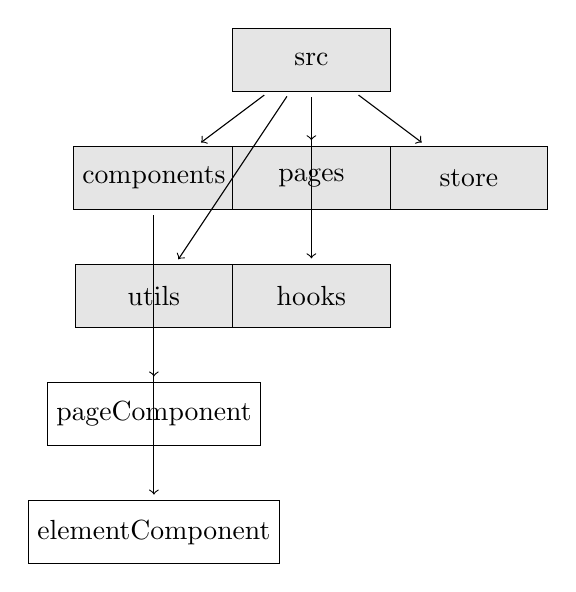
\begin{tikzpicture}[
    file/.style={draw, rectangle, minimum width=2cm, minimum height=0.8cm},
    folder/.style={draw, rectangle, minimum width=2cm, minimum height=0.8cm, fill=gray!20},
    arrow/.style={->, shorten >=2pt, shorten <=2pt}
]

% Folders
\node[folder] (src) at (0,0) {src};
\node[folder] (components) at (-2,-1.5) {components};
\node[folder] (pages) at (0,-1.5) {pages};
\node[folder] (store) at (2,-1.5) {store};
\node[folder] (utils) at (-2,-3) {utils};
\node[folder] (hooks) at (0,-3) {hooks};

% Files
\node[file] (pageComponent) at (-2,-4.5) {pageComponent};
\node[file] (elementComponent) at (-2,-6) {elementComponent};
% ... add more files

% Connections
\draw[arrow] (src) -- (components);
\draw[arrow] (src) -- (pages);
\draw[arrow] (src) -- (store);
\draw[arrow] (src) -- (utils);
\draw[arrow] (src) -- (hooks);
\draw[arrow] (components) -- (pageComponent);
\draw[arrow] (components) -- (elementComponent);
% ... add more connections

\end{tikzpicture}



\pagebreak
\subsubsection{Back-end}
The backend uses the dotNet framework. The development language using the C\# language.

In this project, the backend uses the Onion Architecture.
The Onion Architecture is a typically layered architecture, 
where each layer depends on the inner layer and provides interfaces to the outer layer.
The outer layer provides services to the outermost layer 
and other modules in the same layer based on the interfaces of the inner layer.

From inner to outer, the layers are: Domain, Application, Infrastructure, Presentation.
The Domain layer is the core layer and the innermost layer, used to define domain models, 
which are the business models.
It includes domain models and domain service interfaces.
Domain models are used to define the business models, 
which are the entities in the entity-relationship model and their attributes.
Domain service interfaces are used to define the business services, 
which are the relationships between entities in the entity-relationship model.

The Application layer is the application layer, 
used to define application services, which are the business logic.
It includes domain service implementations and application service interfaces.
Domain service implementations implement the methods of the inner layer's domain service 
interfaces and implement the business logic of the domain models.
Application service interfaces are used to define application services, 
which are the business logic.
It includes but is not limited to database interfaces, testing interfaces, 
HTTP API interfaces, MQTT interfaces, etc.

The Infrastructure layer is the infrastructure layer, used to define infrastructure.
It includes database implementations, testing implementations, 
HTTP API implementations, MQTT implementations, etc.
Database implementations implement the database interfaces 
and provide CRUD services for the database.
Testing implementations implement the testing interfaces 
and provide services for unit testing and integration testing.
HTTP API implementations implement the HTTP API interfaces 
and provide CRUD operations for HTTP APIs.
MQTT implementations implement the MQTT interfaces 
and provide CRUD operations for MQTT.

The Presentation layer is the presentation layer, used to define presentation logic, 
such as interfaces and pages. Since this is a backend project,
data presentation and control are handled by the frontend, 
so this layer is not needed.



\pagebreak
\subsubsection{Data communication and storage}
% 关于本项目的数据通信与数据存储的设计, 包括数据通信的协议, 数据存储的设计等
% 关于数据通信的设计:
% 1. 通信协议的选择
% 自前端向后端发送的数据, 有三种传输的数据类型, 
% 一种是普通的增删改查的请求, 对数据传输的时效性要求不高, 但是对数据的准确性, 完整性, 有序性, 安全性有一定的要求,
% 这种数据的传输, 采用 HTTP 协议, 以及 RESTful API 的设计. 可以有效的保证对数据传输的以上要求.
% 一种是对数据通道的创建和流媒体数据的传输, 对数据传输的时效性, 安全性要求较高, 这种数据的传输, 采用 WebRTC 协议, 以及 MQTT 协议.
% 配合可以快速解码的 flatbuffers 协议, 可以有效的保证对数据传输的以上要求.
% 最后一种是对设备的状态信息和操作信息的传输, 对完整性, 有序性, 安全性都有较高的要求, 这种数据的传输, 采用 MQTT 协议
% 同时也使用了 flatbuffers 协议.
% 
% 2. 数据通信的通信架构和通信流程
% 本项目的数据通信的通信架构, 是基于前后端分离的架构, 前端使用 React 框架, 后端使用 dotnet 框架.
% 当前端需要向后端发送数据的时候, 前端会向后端发送 HTTP 请求, 后端接收到 HTTP 请求之后, 会根据请求的数据类型,
% 选择不同的数据处理方式, 对于普通的增删改查的请求, 后端会根据 RESTful API 的设计, 对数据进行增删改查的操作,
% 对于对数据通道的创建和流媒体数据的传输, 后端会根据 WebRTC 协议, 对数据通道进行创建, 并且帮助前端和设备建立数据通道,
% 当数据通道建立后, 前端和设备之间则使用 flatbuffer 的数据格式对流媒体数据进行传输,
% 对于设备的状态信息和操作信息的传输, 前端会直接向 MQTT broker 发送 MQTT 请求, 
% 设备会在其自身的固件中监听相关的 MQTT 请求, 并且返回相关的数据.
% 
% 3. 数据通信的格式
% 本项目的数据通信的格式, 有三种, 
% 一种是 HTTP 协议, 
% 使用 json 格式对数据进行传输,
% 一种是 WebRTC 协议, 
% 使用 flatbuffers 格式对数据进行传输,
% 一种是 MQTT 协议.
% 使用 flatbuffers 格式对数据进行传输,
% 
% 关于数据存储的设计:
% 1. 数据存储的数据库的选择
% 本项目的数据存储的数据库的选择, 使用了轻量级的数据库 SQLite,
% SQLite 是一个进程内的库, 实现了自给自足的, 无服务器的, 零配置的, 事务性的 SQL 数据库引擎.
% 这是因为整个项目的目的是为了实现前端与设备之间的数据通信, 对于数据库数据的增删改查操作的要求不高,
% 数据量较小, 且对于数据库的数据的事务性要求不高, 所以选择了 SQLite 数据库.
% 2. 项目前后端的数据结构的设计
% 在本项目中, 前端由于使用了 React 框架, 所以前端的数据结构的设计, 使用了基于状态的数据结构的设计,
% 每个组件或者数据集都包含一个状态对象, 这个状态对象的属性就是组件的各个状态. 
% 使用状态对象的原因是, 可以方便的对状态进行管理, 采用对象-属性的形式, 可以方便的针对不同组件的同类状态进行区分,
% 由于跨组件的状态是由 redux 进行管理的, 这种状态对象的设计, 可以更搞笑的对状态进行更新和传递.
% 后端由于使用了 dotnet 框架, 所以后端的数据结构的设计, 使用了基于类的数据结构的设计,
% 采用了面向对象的编程思想, 对数据进行了封装, 使得数据的传输更加的安全, 有序, 完整.


\pagebreak

% \subsection{Domain model}
% \documentclass[]{article}
\usepackage{graphicx}
\usepackage{amsmath}
\usepackage{tikz}

% libaries
\usetikzlibrary{shapes,arrows}

%Define the listing package
\usepackage{listings} %code highlighter
\usepackage{color} %use color
\definecolor{mygreen}{rgb}{0,0.6,0}
\definecolor{mygray}{rgb}{0.5,0.5,0.5}
\definecolor{mymauve}{rgb}{0.58,0,0.82}

%Customize a bit the look
\lstset{ %
backgroundcolor=\color{white}, % choose the background color; you must add \usepackage{color} or \usepackage{xcolor}
basicstyle=\footnotesize, % the size of the fonts that are used for the code
breakatwhitespace=false, % sets if automatic breaks should only happen at whitespace
breaklines=true, % sets automatic line breaking
captionpos=b, % sets the caption-position to bottom
commentstyle=\color{mygreen}, % comment style
deletekeywords={...}, % if you want to delete keywords from the given language
escapeinside={\%*}{*)}, % if you want to add LaTeX within your code
extendedchars=true, % lets you use non-ASCII characters; for 8-bits encodings only, does not work with UTF-8
frame=single, % adds a frame around the code
keepspaces=true, % keeps spaces in text, useful for keeping indentation of code (possibly needs columns=flexible)
keywordstyle=\color{blue}, % keyword style
% language=Octave, % the language of the code
morekeywords={*,...}, % if you want to add more keywords to the set
numbers=left, % where to put the line-numbers; possible values are (none, left, right)
numbersep=5pt, % how far the line-numbers are from the code
numberstyle=\tiny\color{mygray}, % the style that is used for the line-numbers
rulecolor=\color{black}, % if not set, the frame-color may be changed on line-breaks within not-black text (e.g. comments (green here))
showspaces=false, % show spaces everywhere adding particular underscores; it overrides 'showstringspaces'
showstringspaces=false, % underline spaces within strings only
showtabs=false, % show tabs within strings adding particular underscores
stepnumber=1, % the step between two line-numbers. If it's 1, each line will be numbered
stringstyle=\color{mymauve}, % string literal style
tabsize=2, % sets default tabsize to 2 spaces
title=\lstname % show the filename of files included with \lstinputlisting; also try caption instead of title
}

\definecolor{darkgray}{rgb}{.4,.4,.4}
\definecolor{purple}{rgb}{0.65, 0.12, 0.82}

\lstdefinelanguage{React}{
keywords={const, typeof, new, true, false, catch, function, return, null, catch, switch, var, if, in, while, do, else, case, break},
keywordstyle=\color{blue}\bfseries,
ndkeywords={class, export, boolean, throw, implements, import, this},
ndkeywordstyle=\color{darkgray}\bfseries,
identifierstyle=\color{mygreen},
sensitive=false,
comment=[l]{//},
morecomment=[s]{/*}{*/},
commentstyle=\color{purple}\ttfamily,
string=[b]{"}{'}{`},
stringstyle=\color{red}\ttfamily,
morestring=[b]',
morestring=[b]",
morestring=[b]`',
}

\lstdefinelanguage{CSharp}{
keywords={const, typeof, new, true, false, catch, function, return, null, catch, switch, var, if, in, while, do, else, case, break},
keywordstyle=\color{blue}\bfseries,
ndkeywords={class, export, boolean, throw, implements, import, this},
ndkeywordstyle=\color{darkgray}\bfseries,
identifierstyle=\color{mygreen},
sensitive=false,
comment=[l]{//},
morecomment=[s]{/*}{*/},
commentstyle=\color{purple}\ttfamily,
string=[b]{"}{'}{`},
stringstyle=\color{red}\ttfamily,
morestring=[b]',
morestring=[b]",
morestring=[b]`',
}

\lstset{
language=React,
extendedchars=true,
basicstyle=\footnotesize\ttfamily,
showstringspaces=false,
showspaces=false,
numbers=left,
numberstyle=\footnotesize,
numbersep=9pt,
tabsize=2,
breaklines=true,
showtabs=false,
captionpos=b
}

\lstset{
language=CSharp,
extendedchars=true,
basicstyle=\footnotesize\ttfamily,
showstringspaces=false,
showspaces=false,
numbers=left,
numberstyle=\footnotesize,
numbersep=9pt,
tabsize=2,
breaklines=true,
showtabs=false,
captionpos=b
}

% \usepackage{cite} % Add this line for citation

% \bibliographystyle{plain}

\title{
The implementation of BifrostConnect Front-end scope, 
re-design and development with the relevant back-end support develop.
}
\author{
    Fei Gu \\
    Erhvervs Akademi Sydvest \\
    Computer Science 21\\
    }
\date{\today}

\begin{document}

% Front page
\maketitle
\begin{center}
    Supervisor: Henrik Boulund Meng Hansen \\
    Company: BifrostConnect \\
    Engineering Director: Jasper Wass \\
\end{center}
\tableofcontents
\pagebreak


% The introduction
\section{Introduction}
\subsection{Background}\input{sections/introduction/background.tex}
\subsection{The company}\input{sections/introduction/aboutCompany}
\subsection{The project}\input{sections/introduction/aboutProject}
\pagebreak

% The problem statement
\section{Problem Statement}
\subsection{Statement}
\input{sections/problemStatement/statement}
\subsection{Situation}
\input{sections/problemStatement/situation}
\subsection{Potential Solution}
\input{sections/problemStatement/potentialSolution}
\pagebreak

% Requirement analysis
\section{Requirement Analysis}
\input{sections/requirementAnalysis/index}

\subsection{Stakeholders}
\input{sections/requirementAnalysis/stakeholders/index}

\subsection{Business Domain}
\input{sections/requirementAnalysis/bussinesDomain/index}

\subsection{Scope}
\input{sections/requirementAnalysis/scope}

\subsection{Goals}
\input{sections/requirementAnalysis/goals}
\pagebreak

% Software Design
\section{Software Design}
% developement methods
\subsection{Software Development Methods}
\input{sections/softwareDevelopmentMethods/index}
\subsubsection{Agile Software Development}
\input{sections/softwareDevelopmentMethods/agileSoftwareDevelopment/index}
\subsubsection{Feature Driven Development}
\input{sections/softwareDevelopmentMethods/featureDrivenDevelopment/index}

\pagebreak

% Technology seslection
\subsection{Technology selection}
\input{sections/softwareDesign/technologySelection/index}
\subsubsection{Front-end}
\input{sections/softwareDesign/technologySelection/frontEnd}            
\subsubsection{Back-end}
\input{sections/softwareDesign/technologySelection/backEnd}            
\subsubsection{Database}
\input{sections/softwareDesign/technologySelection/database}
\subsubsection{Data communication}
\input{sections/softwareDesign/technologySelection/dataCommunication}            
\subsubsection{DevOps}
\input{sections/softwareDesign/technologySelection/devOps}
\pagebreak

% Architecture design
\subsection{Architecture design}
\input{sections/softwareDesign/architectureDesign/index}
\pagebreak
\subsubsection{Front-end}
\input{sections/softwareDesign/architectureDesign/frontEndArchitecture}
\pagebreak
\subsubsection{Back-end}
\input{sections/softwareDesign/architectureDesign/backEndArchitecture}
\pagebreak
\subsubsection{Data communication and storage}
\input{sections/softwareDesign/architectureDesign/dataCommunicationArchitecture}
\pagebreak

% \subsection{Domain model}
% \input{sections/softwareDesign/domainModel/index}
% \subsection{Database design}
% % 数据库领域模型 ER 图
% % 包括表和字段的设置.
% % 对于私有键和外键的设置.

% \subsection{Back-end design}
% % 后端对象模型
% % 以及对于对象模型的增删改查
% % 以及相关的其他服务的设计`'

% \subsection{Front-end design}
% % 对于前端的页面结构的设计 
% % 页面的状态的设计, 交互设计

% \subsection{FlatBuffers design}
% % schema 的设计

\subsection{DevOps CI/CD process design}
\input{sections/softwareDesign/devOpsDesign/index}
\subsubsection{Continuous Integration}
\input{sections/softwareDesign/devOpsDesign/continuousIntegration/index}
\subsubsection{Continuous Delivery}
\input{sections/softwareDesign/devOpsDesign/continuousDelivery/index}
\subsubsection{Continuous Deployment}
\input{sections/softwareDesign/devOpsDesign/continuousDeployment/index}
\pagebreak

\section{Software Development} 
\input{sections/softwareDevelopment/index}
\subsection{Overall development}
\input{sections/softwareDevelopment/overallDevelopement/index}
\subsubsection{Front-end}
\input{sections/softwareDevelopment/overallDevelopement/frontEnd/index}
\subsubsection{Back-end}
\input{sections/softwareDevelopment/overallDevelopement/backEnd/index}
\subsubsection{DevOps}
\input{sections/softwareDevelopment/overallDevelopement/devOps/index}
\subsection{Feature development} 
\input{sections/softwareDevelopment/featureDevelopment/index}
\subsubsection{Use Case 1}
\input{sections/softwareDevelopment/featureDevelopment/useCase1/index}
\subsubsection{Feature 1}
\input{sections/softwareDevelopment/featureDevelopment/feature/feature1.tex}
\pagebreak
\section{Conclusion} 
\subsection{Result}
Since the project is still in progress, the result is not available yet.
So far, basic structure of this project has been built. But the most features 
are not implemented yet. 
\subsection{Discussion}
As a single developer for this project, I am confident what I have done so far.
And I can say I understand the most of the knowledge I have used in this project, 
which also means I can explain all the part of the project. 
But this project also relevant some of the complex knowledge which I have to continue 
to study and practice.
\subsection{Future Work}
The future work is to implement the rest of the features. 
Including the most important part which is the 'create session' feature.
\pagebreak
% \bibliography{bibliography}
\pagebreak
% \begin{appendices}
%     \section{Appendix}
% \end{appendices} 
\end{document}
% \subsection{Database design}
% % 数据库领域模型 ER 图
% % 包括表和字段的设置.
% % 对于私有键和外键的设置.

% \subsection{Back-end design}
% % 后端对象模型
% % 以及对于对象模型的增删改查
% % 以及相关的其他服务的设计`'

% \subsection{Front-end design}
% % 对于前端的页面结构的设计 
% % 页面的状态的设计, 交互设计

% \subsection{FlatBuffers design}
% % schema 的设计

\subsection{DevOps CI/CD process design}
\documentclass[]{article}
\usepackage{graphicx}
\usepackage{amsmath}
\usepackage{tikz}

% libaries
\usetikzlibrary{shapes,arrows}

%Define the listing package
\usepackage{listings} %code highlighter
\usepackage{color} %use color
\definecolor{mygreen}{rgb}{0,0.6,0}
\definecolor{mygray}{rgb}{0.5,0.5,0.5}
\definecolor{mymauve}{rgb}{0.58,0,0.82}

%Customize a bit the look
\lstset{ %
backgroundcolor=\color{white}, % choose the background color; you must add \usepackage{color} or \usepackage{xcolor}
basicstyle=\footnotesize, % the size of the fonts that are used for the code
breakatwhitespace=false, % sets if automatic breaks should only happen at whitespace
breaklines=true, % sets automatic line breaking
captionpos=b, % sets the caption-position to bottom
commentstyle=\color{mygreen}, % comment style
deletekeywords={...}, % if you want to delete keywords from the given language
escapeinside={\%*}{*)}, % if you want to add LaTeX within your code
extendedchars=true, % lets you use non-ASCII characters; for 8-bits encodings only, does not work with UTF-8
frame=single, % adds a frame around the code
keepspaces=true, % keeps spaces in text, useful for keeping indentation of code (possibly needs columns=flexible)
keywordstyle=\color{blue}, % keyword style
% language=Octave, % the language of the code
morekeywords={*,...}, % if you want to add more keywords to the set
numbers=left, % where to put the line-numbers; possible values are (none, left, right)
numbersep=5pt, % how far the line-numbers are from the code
numberstyle=\tiny\color{mygray}, % the style that is used for the line-numbers
rulecolor=\color{black}, % if not set, the frame-color may be changed on line-breaks within not-black text (e.g. comments (green here))
showspaces=false, % show spaces everywhere adding particular underscores; it overrides 'showstringspaces'
showstringspaces=false, % underline spaces within strings only
showtabs=false, % show tabs within strings adding particular underscores
stepnumber=1, % the step between two line-numbers. If it's 1, each line will be numbered
stringstyle=\color{mymauve}, % string literal style
tabsize=2, % sets default tabsize to 2 spaces
title=\lstname % show the filename of files included with \lstinputlisting; also try caption instead of title
}

\definecolor{darkgray}{rgb}{.4,.4,.4}
\definecolor{purple}{rgb}{0.65, 0.12, 0.82}

\lstdefinelanguage{React}{
keywords={const, typeof, new, true, false, catch, function, return, null, catch, switch, var, if, in, while, do, else, case, break},
keywordstyle=\color{blue}\bfseries,
ndkeywords={class, export, boolean, throw, implements, import, this},
ndkeywordstyle=\color{darkgray}\bfseries,
identifierstyle=\color{mygreen},
sensitive=false,
comment=[l]{//},
morecomment=[s]{/*}{*/},
commentstyle=\color{purple}\ttfamily,
string=[b]{"}{'}{`},
stringstyle=\color{red}\ttfamily,
morestring=[b]',
morestring=[b]",
morestring=[b]`',
}

\lstdefinelanguage{CSharp}{
keywords={const, typeof, new, true, false, catch, function, return, null, catch, switch, var, if, in, while, do, else, case, break},
keywordstyle=\color{blue}\bfseries,
ndkeywords={class, export, boolean, throw, implements, import, this},
ndkeywordstyle=\color{darkgray}\bfseries,
identifierstyle=\color{mygreen},
sensitive=false,
comment=[l]{//},
morecomment=[s]{/*}{*/},
commentstyle=\color{purple}\ttfamily,
string=[b]{"}{'}{`},
stringstyle=\color{red}\ttfamily,
morestring=[b]',
morestring=[b]",
morestring=[b]`',
}

\lstset{
language=React,
extendedchars=true,
basicstyle=\footnotesize\ttfamily,
showstringspaces=false,
showspaces=false,
numbers=left,
numberstyle=\footnotesize,
numbersep=9pt,
tabsize=2,
breaklines=true,
showtabs=false,
captionpos=b
}

\lstset{
language=CSharp,
extendedchars=true,
basicstyle=\footnotesize\ttfamily,
showstringspaces=false,
showspaces=false,
numbers=left,
numberstyle=\footnotesize,
numbersep=9pt,
tabsize=2,
breaklines=true,
showtabs=false,
captionpos=b
}

% \usepackage{cite} % Add this line for citation

% \bibliographystyle{plain}

\title{
The implementation of BifrostConnect Front-end scope, 
re-design and development with the relevant back-end support develop.
}
\author{
    Fei Gu \\
    Erhvervs Akademi Sydvest \\
    Computer Science 21\\
    }
\date{\today}

\begin{document}

% Front page
\maketitle
\begin{center}
    Supervisor: Henrik Boulund Meng Hansen \\
    Company: BifrostConnect \\
    Engineering Director: Jasper Wass \\
\end{center}
\tableofcontents
\pagebreak


% The introduction
\section{Introduction}
\subsection{Background}\input{sections/introduction/background.tex}
\subsection{The company}\input{sections/introduction/aboutCompany}
\subsection{The project}\input{sections/introduction/aboutProject}
\pagebreak

% The problem statement
\section{Problem Statement}
\subsection{Statement}
\input{sections/problemStatement/statement}
\subsection{Situation}
\input{sections/problemStatement/situation}
\subsection{Potential Solution}
\input{sections/problemStatement/potentialSolution}
\pagebreak

% Requirement analysis
\section{Requirement Analysis}
\input{sections/requirementAnalysis/index}

\subsection{Stakeholders}
\input{sections/requirementAnalysis/stakeholders/index}

\subsection{Business Domain}
\input{sections/requirementAnalysis/bussinesDomain/index}

\subsection{Scope}
\input{sections/requirementAnalysis/scope}

\subsection{Goals}
\input{sections/requirementAnalysis/goals}
\pagebreak

% Software Design
\section{Software Design}
% developement methods
\subsection{Software Development Methods}
\input{sections/softwareDevelopmentMethods/index}
\subsubsection{Agile Software Development}
\input{sections/softwareDevelopmentMethods/agileSoftwareDevelopment/index}
\subsubsection{Feature Driven Development}
\input{sections/softwareDevelopmentMethods/featureDrivenDevelopment/index}

\pagebreak

% Technology seslection
\subsection{Technology selection}
\input{sections/softwareDesign/technologySelection/index}
\subsubsection{Front-end}
\input{sections/softwareDesign/technologySelection/frontEnd}            
\subsubsection{Back-end}
\input{sections/softwareDesign/technologySelection/backEnd}            
\subsubsection{Database}
\input{sections/softwareDesign/technologySelection/database}
\subsubsection{Data communication}
\input{sections/softwareDesign/technologySelection/dataCommunication}            
\subsubsection{DevOps}
\input{sections/softwareDesign/technologySelection/devOps}
\pagebreak

% Architecture design
\subsection{Architecture design}
\input{sections/softwareDesign/architectureDesign/index}
\pagebreak
\subsubsection{Front-end}
\input{sections/softwareDesign/architectureDesign/frontEndArchitecture}
\pagebreak
\subsubsection{Back-end}
\input{sections/softwareDesign/architectureDesign/backEndArchitecture}
\pagebreak
\subsubsection{Data communication and storage}
\input{sections/softwareDesign/architectureDesign/dataCommunicationArchitecture}
\pagebreak

% \subsection{Domain model}
% \input{sections/softwareDesign/domainModel/index}
% \subsection{Database design}
% % 数据库领域模型 ER 图
% % 包括表和字段的设置.
% % 对于私有键和外键的设置.

% \subsection{Back-end design}
% % 后端对象模型
% % 以及对于对象模型的增删改查
% % 以及相关的其他服务的设计`'

% \subsection{Front-end design}
% % 对于前端的页面结构的设计 
% % 页面的状态的设计, 交互设计

% \subsection{FlatBuffers design}
% % schema 的设计

\subsection{DevOps CI/CD process design}
\input{sections/softwareDesign/devOpsDesign/index}
\subsubsection{Continuous Integration}
\input{sections/softwareDesign/devOpsDesign/continuousIntegration/index}
\subsubsection{Continuous Delivery}
\input{sections/softwareDesign/devOpsDesign/continuousDelivery/index}
\subsubsection{Continuous Deployment}
\input{sections/softwareDesign/devOpsDesign/continuousDeployment/index}
\pagebreak

\section{Software Development} 
\input{sections/softwareDevelopment/index}
\subsection{Overall development}
\input{sections/softwareDevelopment/overallDevelopement/index}
\subsubsection{Front-end}
\input{sections/softwareDevelopment/overallDevelopement/frontEnd/index}
\subsubsection{Back-end}
\input{sections/softwareDevelopment/overallDevelopement/backEnd/index}
\subsubsection{DevOps}
\input{sections/softwareDevelopment/overallDevelopement/devOps/index}
\subsection{Feature development} 
\input{sections/softwareDevelopment/featureDevelopment/index}
\subsubsection{Use Case 1}
\input{sections/softwareDevelopment/featureDevelopment/useCase1/index}
\subsubsection{Feature 1}
\input{sections/softwareDevelopment/featureDevelopment/feature/feature1.tex}
\pagebreak
\section{Conclusion} 
\subsection{Result}
Since the project is still in progress, the result is not available yet.
So far, basic structure of this project has been built. But the most features 
are not implemented yet. 
\subsection{Discussion}
As a single developer for this project, I am confident what I have done so far.
And I can say I understand the most of the knowledge I have used in this project, 
which also means I can explain all the part of the project. 
But this project also relevant some of the complex knowledge which I have to continue 
to study and practice.
\subsection{Future Work}
The future work is to implement the rest of the features. 
Including the most important part which is the 'create session' feature.
\pagebreak
% \bibliography{bibliography}
\pagebreak
% \begin{appendices}
%     \section{Appendix}
% \end{appendices} 
\end{document}
\subsubsection{Continuous Integration}
\documentclass[]{article}
\usepackage{graphicx}
\usepackage{amsmath}
\usepackage{tikz}

% libaries
\usetikzlibrary{shapes,arrows}

%Define the listing package
\usepackage{listings} %code highlighter
\usepackage{color} %use color
\definecolor{mygreen}{rgb}{0,0.6,0}
\definecolor{mygray}{rgb}{0.5,0.5,0.5}
\definecolor{mymauve}{rgb}{0.58,0,0.82}

%Customize a bit the look
\lstset{ %
backgroundcolor=\color{white}, % choose the background color; you must add \usepackage{color} or \usepackage{xcolor}
basicstyle=\footnotesize, % the size of the fonts that are used for the code
breakatwhitespace=false, % sets if automatic breaks should only happen at whitespace
breaklines=true, % sets automatic line breaking
captionpos=b, % sets the caption-position to bottom
commentstyle=\color{mygreen}, % comment style
deletekeywords={...}, % if you want to delete keywords from the given language
escapeinside={\%*}{*)}, % if you want to add LaTeX within your code
extendedchars=true, % lets you use non-ASCII characters; for 8-bits encodings only, does not work with UTF-8
frame=single, % adds a frame around the code
keepspaces=true, % keeps spaces in text, useful for keeping indentation of code (possibly needs columns=flexible)
keywordstyle=\color{blue}, % keyword style
% language=Octave, % the language of the code
morekeywords={*,...}, % if you want to add more keywords to the set
numbers=left, % where to put the line-numbers; possible values are (none, left, right)
numbersep=5pt, % how far the line-numbers are from the code
numberstyle=\tiny\color{mygray}, % the style that is used for the line-numbers
rulecolor=\color{black}, % if not set, the frame-color may be changed on line-breaks within not-black text (e.g. comments (green here))
showspaces=false, % show spaces everywhere adding particular underscores; it overrides 'showstringspaces'
showstringspaces=false, % underline spaces within strings only
showtabs=false, % show tabs within strings adding particular underscores
stepnumber=1, % the step between two line-numbers. If it's 1, each line will be numbered
stringstyle=\color{mymauve}, % string literal style
tabsize=2, % sets default tabsize to 2 spaces
title=\lstname % show the filename of files included with \lstinputlisting; also try caption instead of title
}

\definecolor{darkgray}{rgb}{.4,.4,.4}
\definecolor{purple}{rgb}{0.65, 0.12, 0.82}

\lstdefinelanguage{React}{
keywords={const, typeof, new, true, false, catch, function, return, null, catch, switch, var, if, in, while, do, else, case, break},
keywordstyle=\color{blue}\bfseries,
ndkeywords={class, export, boolean, throw, implements, import, this},
ndkeywordstyle=\color{darkgray}\bfseries,
identifierstyle=\color{mygreen},
sensitive=false,
comment=[l]{//},
morecomment=[s]{/*}{*/},
commentstyle=\color{purple}\ttfamily,
string=[b]{"}{'}{`},
stringstyle=\color{red}\ttfamily,
morestring=[b]',
morestring=[b]",
morestring=[b]`',
}

\lstdefinelanguage{CSharp}{
keywords={const, typeof, new, true, false, catch, function, return, null, catch, switch, var, if, in, while, do, else, case, break},
keywordstyle=\color{blue}\bfseries,
ndkeywords={class, export, boolean, throw, implements, import, this},
ndkeywordstyle=\color{darkgray}\bfseries,
identifierstyle=\color{mygreen},
sensitive=false,
comment=[l]{//},
morecomment=[s]{/*}{*/},
commentstyle=\color{purple}\ttfamily,
string=[b]{"}{'}{`},
stringstyle=\color{red}\ttfamily,
morestring=[b]',
morestring=[b]",
morestring=[b]`',
}

\lstset{
language=React,
extendedchars=true,
basicstyle=\footnotesize\ttfamily,
showstringspaces=false,
showspaces=false,
numbers=left,
numberstyle=\footnotesize,
numbersep=9pt,
tabsize=2,
breaklines=true,
showtabs=false,
captionpos=b
}

\lstset{
language=CSharp,
extendedchars=true,
basicstyle=\footnotesize\ttfamily,
showstringspaces=false,
showspaces=false,
numbers=left,
numberstyle=\footnotesize,
numbersep=9pt,
tabsize=2,
breaklines=true,
showtabs=false,
captionpos=b
}

% \usepackage{cite} % Add this line for citation

% \bibliographystyle{plain}

\title{
The implementation of BifrostConnect Front-end scope, 
re-design and development with the relevant back-end support develop.
}
\author{
    Fei Gu \\
    Erhvervs Akademi Sydvest \\
    Computer Science 21\\
    }
\date{\today}

\begin{document}

% Front page
\maketitle
\begin{center}
    Supervisor: Henrik Boulund Meng Hansen \\
    Company: BifrostConnect \\
    Engineering Director: Jasper Wass \\
\end{center}
\tableofcontents
\pagebreak


% The introduction
\section{Introduction}
\subsection{Background}\input{sections/introduction/background.tex}
\subsection{The company}\input{sections/introduction/aboutCompany}
\subsection{The project}\input{sections/introduction/aboutProject}
\pagebreak

% The problem statement
\section{Problem Statement}
\subsection{Statement}
\input{sections/problemStatement/statement}
\subsection{Situation}
\input{sections/problemStatement/situation}
\subsection{Potential Solution}
\input{sections/problemStatement/potentialSolution}
\pagebreak

% Requirement analysis
\section{Requirement Analysis}
\input{sections/requirementAnalysis/index}

\subsection{Stakeholders}
\input{sections/requirementAnalysis/stakeholders/index}

\subsection{Business Domain}
\input{sections/requirementAnalysis/bussinesDomain/index}

\subsection{Scope}
\input{sections/requirementAnalysis/scope}

\subsection{Goals}
\input{sections/requirementAnalysis/goals}
\pagebreak

% Software Design
\section{Software Design}
% developement methods
\subsection{Software Development Methods}
\input{sections/softwareDevelopmentMethods/index}
\subsubsection{Agile Software Development}
\input{sections/softwareDevelopmentMethods/agileSoftwareDevelopment/index}
\subsubsection{Feature Driven Development}
\input{sections/softwareDevelopmentMethods/featureDrivenDevelopment/index}

\pagebreak

% Technology seslection
\subsection{Technology selection}
\input{sections/softwareDesign/technologySelection/index}
\subsubsection{Front-end}
\input{sections/softwareDesign/technologySelection/frontEnd}            
\subsubsection{Back-end}
\input{sections/softwareDesign/technologySelection/backEnd}            
\subsubsection{Database}
\input{sections/softwareDesign/technologySelection/database}
\subsubsection{Data communication}
\input{sections/softwareDesign/technologySelection/dataCommunication}            
\subsubsection{DevOps}
\input{sections/softwareDesign/technologySelection/devOps}
\pagebreak

% Architecture design
\subsection{Architecture design}
\input{sections/softwareDesign/architectureDesign/index}
\pagebreak
\subsubsection{Front-end}
\input{sections/softwareDesign/architectureDesign/frontEndArchitecture}
\pagebreak
\subsubsection{Back-end}
\input{sections/softwareDesign/architectureDesign/backEndArchitecture}
\pagebreak
\subsubsection{Data communication and storage}
\input{sections/softwareDesign/architectureDesign/dataCommunicationArchitecture}
\pagebreak

% \subsection{Domain model}
% \input{sections/softwareDesign/domainModel/index}
% \subsection{Database design}
% % 数据库领域模型 ER 图
% % 包括表和字段的设置.
% % 对于私有键和外键的设置.

% \subsection{Back-end design}
% % 后端对象模型
% % 以及对于对象模型的增删改查
% % 以及相关的其他服务的设计`'

% \subsection{Front-end design}
% % 对于前端的页面结构的设计 
% % 页面的状态的设计, 交互设计

% \subsection{FlatBuffers design}
% % schema 的设计

\subsection{DevOps CI/CD process design}
\input{sections/softwareDesign/devOpsDesign/index}
\subsubsection{Continuous Integration}
\input{sections/softwareDesign/devOpsDesign/continuousIntegration/index}
\subsubsection{Continuous Delivery}
\input{sections/softwareDesign/devOpsDesign/continuousDelivery/index}
\subsubsection{Continuous Deployment}
\input{sections/softwareDesign/devOpsDesign/continuousDeployment/index}
\pagebreak

\section{Software Development} 
\input{sections/softwareDevelopment/index}
\subsection{Overall development}
\input{sections/softwareDevelopment/overallDevelopement/index}
\subsubsection{Front-end}
\input{sections/softwareDevelopment/overallDevelopement/frontEnd/index}
\subsubsection{Back-end}
\input{sections/softwareDevelopment/overallDevelopement/backEnd/index}
\subsubsection{DevOps}
\input{sections/softwareDevelopment/overallDevelopement/devOps/index}
\subsection{Feature development} 
\input{sections/softwareDevelopment/featureDevelopment/index}
\subsubsection{Use Case 1}
\input{sections/softwareDevelopment/featureDevelopment/useCase1/index}
\subsubsection{Feature 1}
\input{sections/softwareDevelopment/featureDevelopment/feature/feature1.tex}
\pagebreak
\section{Conclusion} 
\subsection{Result}
Since the project is still in progress, the result is not available yet.
So far, basic structure of this project has been built. But the most features 
are not implemented yet. 
\subsection{Discussion}
As a single developer for this project, I am confident what I have done so far.
And I can say I understand the most of the knowledge I have used in this project, 
which also means I can explain all the part of the project. 
But this project also relevant some of the complex knowledge which I have to continue 
to study and practice.
\subsection{Future Work}
The future work is to implement the rest of the features. 
Including the most important part which is the 'create session' feature.
\pagebreak
% \bibliography{bibliography}
\pagebreak
% \begin{appendices}
%     \section{Appendix}
% \end{appendices} 
\end{document}
\subsubsection{Continuous Delivery}
\documentclass[]{article}
\usepackage{graphicx}
\usepackage{amsmath}
\usepackage{tikz}

% libaries
\usetikzlibrary{shapes,arrows}

%Define the listing package
\usepackage{listings} %code highlighter
\usepackage{color} %use color
\definecolor{mygreen}{rgb}{0,0.6,0}
\definecolor{mygray}{rgb}{0.5,0.5,0.5}
\definecolor{mymauve}{rgb}{0.58,0,0.82}

%Customize a bit the look
\lstset{ %
backgroundcolor=\color{white}, % choose the background color; you must add \usepackage{color} or \usepackage{xcolor}
basicstyle=\footnotesize, % the size of the fonts that are used for the code
breakatwhitespace=false, % sets if automatic breaks should only happen at whitespace
breaklines=true, % sets automatic line breaking
captionpos=b, % sets the caption-position to bottom
commentstyle=\color{mygreen}, % comment style
deletekeywords={...}, % if you want to delete keywords from the given language
escapeinside={\%*}{*)}, % if you want to add LaTeX within your code
extendedchars=true, % lets you use non-ASCII characters; for 8-bits encodings only, does not work with UTF-8
frame=single, % adds a frame around the code
keepspaces=true, % keeps spaces in text, useful for keeping indentation of code (possibly needs columns=flexible)
keywordstyle=\color{blue}, % keyword style
% language=Octave, % the language of the code
morekeywords={*,...}, % if you want to add more keywords to the set
numbers=left, % where to put the line-numbers; possible values are (none, left, right)
numbersep=5pt, % how far the line-numbers are from the code
numberstyle=\tiny\color{mygray}, % the style that is used for the line-numbers
rulecolor=\color{black}, % if not set, the frame-color may be changed on line-breaks within not-black text (e.g. comments (green here))
showspaces=false, % show spaces everywhere adding particular underscores; it overrides 'showstringspaces'
showstringspaces=false, % underline spaces within strings only
showtabs=false, % show tabs within strings adding particular underscores
stepnumber=1, % the step between two line-numbers. If it's 1, each line will be numbered
stringstyle=\color{mymauve}, % string literal style
tabsize=2, % sets default tabsize to 2 spaces
title=\lstname % show the filename of files included with \lstinputlisting; also try caption instead of title
}

\definecolor{darkgray}{rgb}{.4,.4,.4}
\definecolor{purple}{rgb}{0.65, 0.12, 0.82}

\lstdefinelanguage{React}{
keywords={const, typeof, new, true, false, catch, function, return, null, catch, switch, var, if, in, while, do, else, case, break},
keywordstyle=\color{blue}\bfseries,
ndkeywords={class, export, boolean, throw, implements, import, this},
ndkeywordstyle=\color{darkgray}\bfseries,
identifierstyle=\color{mygreen},
sensitive=false,
comment=[l]{//},
morecomment=[s]{/*}{*/},
commentstyle=\color{purple}\ttfamily,
string=[b]{"}{'}{`},
stringstyle=\color{red}\ttfamily,
morestring=[b]',
morestring=[b]",
morestring=[b]`',
}

\lstdefinelanguage{CSharp}{
keywords={const, typeof, new, true, false, catch, function, return, null, catch, switch, var, if, in, while, do, else, case, break},
keywordstyle=\color{blue}\bfseries,
ndkeywords={class, export, boolean, throw, implements, import, this},
ndkeywordstyle=\color{darkgray}\bfseries,
identifierstyle=\color{mygreen},
sensitive=false,
comment=[l]{//},
morecomment=[s]{/*}{*/},
commentstyle=\color{purple}\ttfamily,
string=[b]{"}{'}{`},
stringstyle=\color{red}\ttfamily,
morestring=[b]',
morestring=[b]",
morestring=[b]`',
}

\lstset{
language=React,
extendedchars=true,
basicstyle=\footnotesize\ttfamily,
showstringspaces=false,
showspaces=false,
numbers=left,
numberstyle=\footnotesize,
numbersep=9pt,
tabsize=2,
breaklines=true,
showtabs=false,
captionpos=b
}

\lstset{
language=CSharp,
extendedchars=true,
basicstyle=\footnotesize\ttfamily,
showstringspaces=false,
showspaces=false,
numbers=left,
numberstyle=\footnotesize,
numbersep=9pt,
tabsize=2,
breaklines=true,
showtabs=false,
captionpos=b
}

% \usepackage{cite} % Add this line for citation

% \bibliographystyle{plain}

\title{
The implementation of BifrostConnect Front-end scope, 
re-design and development with the relevant back-end support develop.
}
\author{
    Fei Gu \\
    Erhvervs Akademi Sydvest \\
    Computer Science 21\\
    }
\date{\today}

\begin{document}

% Front page
\maketitle
\begin{center}
    Supervisor: Henrik Boulund Meng Hansen \\
    Company: BifrostConnect \\
    Engineering Director: Jasper Wass \\
\end{center}
\tableofcontents
\pagebreak


% The introduction
\section{Introduction}
\subsection{Background}\input{sections/introduction/background.tex}
\subsection{The company}\input{sections/introduction/aboutCompany}
\subsection{The project}\input{sections/introduction/aboutProject}
\pagebreak

% The problem statement
\section{Problem Statement}
\subsection{Statement}
\input{sections/problemStatement/statement}
\subsection{Situation}
\input{sections/problemStatement/situation}
\subsection{Potential Solution}
\input{sections/problemStatement/potentialSolution}
\pagebreak

% Requirement analysis
\section{Requirement Analysis}
\input{sections/requirementAnalysis/index}

\subsection{Stakeholders}
\input{sections/requirementAnalysis/stakeholders/index}

\subsection{Business Domain}
\input{sections/requirementAnalysis/bussinesDomain/index}

\subsection{Scope}
\input{sections/requirementAnalysis/scope}

\subsection{Goals}
\input{sections/requirementAnalysis/goals}
\pagebreak

% Software Design
\section{Software Design}
% developement methods
\subsection{Software Development Methods}
\input{sections/softwareDevelopmentMethods/index}
\subsubsection{Agile Software Development}
\input{sections/softwareDevelopmentMethods/agileSoftwareDevelopment/index}
\subsubsection{Feature Driven Development}
\input{sections/softwareDevelopmentMethods/featureDrivenDevelopment/index}

\pagebreak

% Technology seslection
\subsection{Technology selection}
\input{sections/softwareDesign/technologySelection/index}
\subsubsection{Front-end}
\input{sections/softwareDesign/technologySelection/frontEnd}            
\subsubsection{Back-end}
\input{sections/softwareDesign/technologySelection/backEnd}            
\subsubsection{Database}
\input{sections/softwareDesign/technologySelection/database}
\subsubsection{Data communication}
\input{sections/softwareDesign/technologySelection/dataCommunication}            
\subsubsection{DevOps}
\input{sections/softwareDesign/technologySelection/devOps}
\pagebreak

% Architecture design
\subsection{Architecture design}
\input{sections/softwareDesign/architectureDesign/index}
\pagebreak
\subsubsection{Front-end}
\input{sections/softwareDesign/architectureDesign/frontEndArchitecture}
\pagebreak
\subsubsection{Back-end}
\input{sections/softwareDesign/architectureDesign/backEndArchitecture}
\pagebreak
\subsubsection{Data communication and storage}
\input{sections/softwareDesign/architectureDesign/dataCommunicationArchitecture}
\pagebreak

% \subsection{Domain model}
% \input{sections/softwareDesign/domainModel/index}
% \subsection{Database design}
% % 数据库领域模型 ER 图
% % 包括表和字段的设置.
% % 对于私有键和外键的设置.

% \subsection{Back-end design}
% % 后端对象模型
% % 以及对于对象模型的增删改查
% % 以及相关的其他服务的设计`'

% \subsection{Front-end design}
% % 对于前端的页面结构的设计 
% % 页面的状态的设计, 交互设计

% \subsection{FlatBuffers design}
% % schema 的设计

\subsection{DevOps CI/CD process design}
\input{sections/softwareDesign/devOpsDesign/index}
\subsubsection{Continuous Integration}
\input{sections/softwareDesign/devOpsDesign/continuousIntegration/index}
\subsubsection{Continuous Delivery}
\input{sections/softwareDesign/devOpsDesign/continuousDelivery/index}
\subsubsection{Continuous Deployment}
\input{sections/softwareDesign/devOpsDesign/continuousDeployment/index}
\pagebreak

\section{Software Development} 
\input{sections/softwareDevelopment/index}
\subsection{Overall development}
\input{sections/softwareDevelopment/overallDevelopement/index}
\subsubsection{Front-end}
\input{sections/softwareDevelopment/overallDevelopement/frontEnd/index}
\subsubsection{Back-end}
\input{sections/softwareDevelopment/overallDevelopement/backEnd/index}
\subsubsection{DevOps}
\input{sections/softwareDevelopment/overallDevelopement/devOps/index}
\subsection{Feature development} 
\input{sections/softwareDevelopment/featureDevelopment/index}
\subsubsection{Use Case 1}
\input{sections/softwareDevelopment/featureDevelopment/useCase1/index}
\subsubsection{Feature 1}
\input{sections/softwareDevelopment/featureDevelopment/feature/feature1.tex}
\pagebreak
\section{Conclusion} 
\subsection{Result}
Since the project is still in progress, the result is not available yet.
So far, basic structure of this project has been built. But the most features 
are not implemented yet. 
\subsection{Discussion}
As a single developer for this project, I am confident what I have done so far.
And I can say I understand the most of the knowledge I have used in this project, 
which also means I can explain all the part of the project. 
But this project also relevant some of the complex knowledge which I have to continue 
to study and practice.
\subsection{Future Work}
The future work is to implement the rest of the features. 
Including the most important part which is the 'create session' feature.
\pagebreak
% \bibliography{bibliography}
\pagebreak
% \begin{appendices}
%     \section{Appendix}
% \end{appendices} 
\end{document}
\subsubsection{Continuous Deployment}
\documentclass[]{article}
\usepackage{graphicx}
\usepackage{amsmath}
\usepackage{tikz}

% libaries
\usetikzlibrary{shapes,arrows}

%Define the listing package
\usepackage{listings} %code highlighter
\usepackage{color} %use color
\definecolor{mygreen}{rgb}{0,0.6,0}
\definecolor{mygray}{rgb}{0.5,0.5,0.5}
\definecolor{mymauve}{rgb}{0.58,0,0.82}

%Customize a bit the look
\lstset{ %
backgroundcolor=\color{white}, % choose the background color; you must add \usepackage{color} or \usepackage{xcolor}
basicstyle=\footnotesize, % the size of the fonts that are used for the code
breakatwhitespace=false, % sets if automatic breaks should only happen at whitespace
breaklines=true, % sets automatic line breaking
captionpos=b, % sets the caption-position to bottom
commentstyle=\color{mygreen}, % comment style
deletekeywords={...}, % if you want to delete keywords from the given language
escapeinside={\%*}{*)}, % if you want to add LaTeX within your code
extendedchars=true, % lets you use non-ASCII characters; for 8-bits encodings only, does not work with UTF-8
frame=single, % adds a frame around the code
keepspaces=true, % keeps spaces in text, useful for keeping indentation of code (possibly needs columns=flexible)
keywordstyle=\color{blue}, % keyword style
% language=Octave, % the language of the code
morekeywords={*,...}, % if you want to add more keywords to the set
numbers=left, % where to put the line-numbers; possible values are (none, left, right)
numbersep=5pt, % how far the line-numbers are from the code
numberstyle=\tiny\color{mygray}, % the style that is used for the line-numbers
rulecolor=\color{black}, % if not set, the frame-color may be changed on line-breaks within not-black text (e.g. comments (green here))
showspaces=false, % show spaces everywhere adding particular underscores; it overrides 'showstringspaces'
showstringspaces=false, % underline spaces within strings only
showtabs=false, % show tabs within strings adding particular underscores
stepnumber=1, % the step between two line-numbers. If it's 1, each line will be numbered
stringstyle=\color{mymauve}, % string literal style
tabsize=2, % sets default tabsize to 2 spaces
title=\lstname % show the filename of files included with \lstinputlisting; also try caption instead of title
}

\definecolor{darkgray}{rgb}{.4,.4,.4}
\definecolor{purple}{rgb}{0.65, 0.12, 0.82}

\lstdefinelanguage{React}{
keywords={const, typeof, new, true, false, catch, function, return, null, catch, switch, var, if, in, while, do, else, case, break},
keywordstyle=\color{blue}\bfseries,
ndkeywords={class, export, boolean, throw, implements, import, this},
ndkeywordstyle=\color{darkgray}\bfseries,
identifierstyle=\color{mygreen},
sensitive=false,
comment=[l]{//},
morecomment=[s]{/*}{*/},
commentstyle=\color{purple}\ttfamily,
string=[b]{"}{'}{`},
stringstyle=\color{red}\ttfamily,
morestring=[b]',
morestring=[b]",
morestring=[b]`',
}

\lstdefinelanguage{CSharp}{
keywords={const, typeof, new, true, false, catch, function, return, null, catch, switch, var, if, in, while, do, else, case, break},
keywordstyle=\color{blue}\bfseries,
ndkeywords={class, export, boolean, throw, implements, import, this},
ndkeywordstyle=\color{darkgray}\bfseries,
identifierstyle=\color{mygreen},
sensitive=false,
comment=[l]{//},
morecomment=[s]{/*}{*/},
commentstyle=\color{purple}\ttfamily,
string=[b]{"}{'}{`},
stringstyle=\color{red}\ttfamily,
morestring=[b]',
morestring=[b]",
morestring=[b]`',
}

\lstset{
language=React,
extendedchars=true,
basicstyle=\footnotesize\ttfamily,
showstringspaces=false,
showspaces=false,
numbers=left,
numberstyle=\footnotesize,
numbersep=9pt,
tabsize=2,
breaklines=true,
showtabs=false,
captionpos=b
}

\lstset{
language=CSharp,
extendedchars=true,
basicstyle=\footnotesize\ttfamily,
showstringspaces=false,
showspaces=false,
numbers=left,
numberstyle=\footnotesize,
numbersep=9pt,
tabsize=2,
breaklines=true,
showtabs=false,
captionpos=b
}

% \usepackage{cite} % Add this line for citation

% \bibliographystyle{plain}

\title{
The implementation of BifrostConnect Front-end scope, 
re-design and development with the relevant back-end support develop.
}
\author{
    Fei Gu \\
    Erhvervs Akademi Sydvest \\
    Computer Science 21\\
    }
\date{\today}

\begin{document}

% Front page
\maketitle
\begin{center}
    Supervisor: Henrik Boulund Meng Hansen \\
    Company: BifrostConnect \\
    Engineering Director: Jasper Wass \\
\end{center}
\tableofcontents
\pagebreak


% The introduction
\section{Introduction}
\subsection{Background}\input{sections/introduction/background.tex}
\subsection{The company}\input{sections/introduction/aboutCompany}
\subsection{The project}\input{sections/introduction/aboutProject}
\pagebreak

% The problem statement
\section{Problem Statement}
\subsection{Statement}
\input{sections/problemStatement/statement}
\subsection{Situation}
\input{sections/problemStatement/situation}
\subsection{Potential Solution}
\input{sections/problemStatement/potentialSolution}
\pagebreak

% Requirement analysis
\section{Requirement Analysis}
\input{sections/requirementAnalysis/index}

\subsection{Stakeholders}
\input{sections/requirementAnalysis/stakeholders/index}

\subsection{Business Domain}
\input{sections/requirementAnalysis/bussinesDomain/index}

\subsection{Scope}
\input{sections/requirementAnalysis/scope}

\subsection{Goals}
\input{sections/requirementAnalysis/goals}
\pagebreak

% Software Design
\section{Software Design}
% developement methods
\subsection{Software Development Methods}
\input{sections/softwareDevelopmentMethods/index}
\subsubsection{Agile Software Development}
\input{sections/softwareDevelopmentMethods/agileSoftwareDevelopment/index}
\subsubsection{Feature Driven Development}
\input{sections/softwareDevelopmentMethods/featureDrivenDevelopment/index}

\pagebreak

% Technology seslection
\subsection{Technology selection}
\input{sections/softwareDesign/technologySelection/index}
\subsubsection{Front-end}
\input{sections/softwareDesign/technologySelection/frontEnd}            
\subsubsection{Back-end}
\input{sections/softwareDesign/technologySelection/backEnd}            
\subsubsection{Database}
\input{sections/softwareDesign/technologySelection/database}
\subsubsection{Data communication}
\input{sections/softwareDesign/technologySelection/dataCommunication}            
\subsubsection{DevOps}
\input{sections/softwareDesign/technologySelection/devOps}
\pagebreak

% Architecture design
\subsection{Architecture design}
\input{sections/softwareDesign/architectureDesign/index}
\pagebreak
\subsubsection{Front-end}
\input{sections/softwareDesign/architectureDesign/frontEndArchitecture}
\pagebreak
\subsubsection{Back-end}
\input{sections/softwareDesign/architectureDesign/backEndArchitecture}
\pagebreak
\subsubsection{Data communication and storage}
\input{sections/softwareDesign/architectureDesign/dataCommunicationArchitecture}
\pagebreak

% \subsection{Domain model}
% \input{sections/softwareDesign/domainModel/index}
% \subsection{Database design}
% % 数据库领域模型 ER 图
% % 包括表和字段的设置.
% % 对于私有键和外键的设置.

% \subsection{Back-end design}
% % 后端对象模型
% % 以及对于对象模型的增删改查
% % 以及相关的其他服务的设计`'

% \subsection{Front-end design}
% % 对于前端的页面结构的设计 
% % 页面的状态的设计, 交互设计

% \subsection{FlatBuffers design}
% % schema 的设计

\subsection{DevOps CI/CD process design}
\input{sections/softwareDesign/devOpsDesign/index}
\subsubsection{Continuous Integration}
\input{sections/softwareDesign/devOpsDesign/continuousIntegration/index}
\subsubsection{Continuous Delivery}
\input{sections/softwareDesign/devOpsDesign/continuousDelivery/index}
\subsubsection{Continuous Deployment}
\input{sections/softwareDesign/devOpsDesign/continuousDeployment/index}
\pagebreak

\section{Software Development} 
\input{sections/softwareDevelopment/index}
\subsection{Overall development}
\input{sections/softwareDevelopment/overallDevelopement/index}
\subsubsection{Front-end}
\input{sections/softwareDevelopment/overallDevelopement/frontEnd/index}
\subsubsection{Back-end}
\input{sections/softwareDevelopment/overallDevelopement/backEnd/index}
\subsubsection{DevOps}
\input{sections/softwareDevelopment/overallDevelopement/devOps/index}
\subsection{Feature development} 
\input{sections/softwareDevelopment/featureDevelopment/index}
\subsubsection{Use Case 1}
\input{sections/softwareDevelopment/featureDevelopment/useCase1/index}
\subsubsection{Feature 1}
\input{sections/softwareDevelopment/featureDevelopment/feature/feature1.tex}
\pagebreak
\section{Conclusion} 
\subsection{Result}
Since the project is still in progress, the result is not available yet.
So far, basic structure of this project has been built. But the most features 
are not implemented yet. 
\subsection{Discussion}
As a single developer for this project, I am confident what I have done so far.
And I can say I understand the most of the knowledge I have used in this project, 
which also means I can explain all the part of the project. 
But this project also relevant some of the complex knowledge which I have to continue 
to study and practice.
\subsection{Future Work}
The future work is to implement the rest of the features. 
Including the most important part which is the 'create session' feature.
\pagebreak
% \bibliography{bibliography}
\pagebreak
% \begin{appendices}
%     \section{Appendix}
% \end{appendices} 
\end{document}
\pagebreak

\section{Software Development} 
\documentclass[]{article}
\usepackage{graphicx}
\usepackage{amsmath}
\usepackage{tikz}

% libaries
\usetikzlibrary{shapes,arrows}

%Define the listing package
\usepackage{listings} %code highlighter
\usepackage{color} %use color
\definecolor{mygreen}{rgb}{0,0.6,0}
\definecolor{mygray}{rgb}{0.5,0.5,0.5}
\definecolor{mymauve}{rgb}{0.58,0,0.82}

%Customize a bit the look
\lstset{ %
backgroundcolor=\color{white}, % choose the background color; you must add \usepackage{color} or \usepackage{xcolor}
basicstyle=\footnotesize, % the size of the fonts that are used for the code
breakatwhitespace=false, % sets if automatic breaks should only happen at whitespace
breaklines=true, % sets automatic line breaking
captionpos=b, % sets the caption-position to bottom
commentstyle=\color{mygreen}, % comment style
deletekeywords={...}, % if you want to delete keywords from the given language
escapeinside={\%*}{*)}, % if you want to add LaTeX within your code
extendedchars=true, % lets you use non-ASCII characters; for 8-bits encodings only, does not work with UTF-8
frame=single, % adds a frame around the code
keepspaces=true, % keeps spaces in text, useful for keeping indentation of code (possibly needs columns=flexible)
keywordstyle=\color{blue}, % keyword style
% language=Octave, % the language of the code
morekeywords={*,...}, % if you want to add more keywords to the set
numbers=left, % where to put the line-numbers; possible values are (none, left, right)
numbersep=5pt, % how far the line-numbers are from the code
numberstyle=\tiny\color{mygray}, % the style that is used for the line-numbers
rulecolor=\color{black}, % if not set, the frame-color may be changed on line-breaks within not-black text (e.g. comments (green here))
showspaces=false, % show spaces everywhere adding particular underscores; it overrides 'showstringspaces'
showstringspaces=false, % underline spaces within strings only
showtabs=false, % show tabs within strings adding particular underscores
stepnumber=1, % the step between two line-numbers. If it's 1, each line will be numbered
stringstyle=\color{mymauve}, % string literal style
tabsize=2, % sets default tabsize to 2 spaces
title=\lstname % show the filename of files included with \lstinputlisting; also try caption instead of title
}

\definecolor{darkgray}{rgb}{.4,.4,.4}
\definecolor{purple}{rgb}{0.65, 0.12, 0.82}

\lstdefinelanguage{React}{
keywords={const, typeof, new, true, false, catch, function, return, null, catch, switch, var, if, in, while, do, else, case, break},
keywordstyle=\color{blue}\bfseries,
ndkeywords={class, export, boolean, throw, implements, import, this},
ndkeywordstyle=\color{darkgray}\bfseries,
identifierstyle=\color{mygreen},
sensitive=false,
comment=[l]{//},
morecomment=[s]{/*}{*/},
commentstyle=\color{purple}\ttfamily,
string=[b]{"}{'}{`},
stringstyle=\color{red}\ttfamily,
morestring=[b]',
morestring=[b]",
morestring=[b]`',
}

\lstdefinelanguage{CSharp}{
keywords={const, typeof, new, true, false, catch, function, return, null, catch, switch, var, if, in, while, do, else, case, break},
keywordstyle=\color{blue}\bfseries,
ndkeywords={class, export, boolean, throw, implements, import, this},
ndkeywordstyle=\color{darkgray}\bfseries,
identifierstyle=\color{mygreen},
sensitive=false,
comment=[l]{//},
morecomment=[s]{/*}{*/},
commentstyle=\color{purple}\ttfamily,
string=[b]{"}{'}{`},
stringstyle=\color{red}\ttfamily,
morestring=[b]',
morestring=[b]",
morestring=[b]`',
}

\lstset{
language=React,
extendedchars=true,
basicstyle=\footnotesize\ttfamily,
showstringspaces=false,
showspaces=false,
numbers=left,
numberstyle=\footnotesize,
numbersep=9pt,
tabsize=2,
breaklines=true,
showtabs=false,
captionpos=b
}

\lstset{
language=CSharp,
extendedchars=true,
basicstyle=\footnotesize\ttfamily,
showstringspaces=false,
showspaces=false,
numbers=left,
numberstyle=\footnotesize,
numbersep=9pt,
tabsize=2,
breaklines=true,
showtabs=false,
captionpos=b
}

% \usepackage{cite} % Add this line for citation

% \bibliographystyle{plain}

\title{
The implementation of BifrostConnect Front-end scope, 
re-design and development with the relevant back-end support develop.
}
\author{
    Fei Gu \\
    Erhvervs Akademi Sydvest \\
    Computer Science 21\\
    }
\date{\today}

\begin{document}

% Front page
\maketitle
\begin{center}
    Supervisor: Henrik Boulund Meng Hansen \\
    Company: BifrostConnect \\
    Engineering Director: Jasper Wass \\
\end{center}
\tableofcontents
\pagebreak


% The introduction
\section{Introduction}
\subsection{Background}\input{sections/introduction/background.tex}
\subsection{The company}\input{sections/introduction/aboutCompany}
\subsection{The project}\input{sections/introduction/aboutProject}
\pagebreak

% The problem statement
\section{Problem Statement}
\subsection{Statement}
\input{sections/problemStatement/statement}
\subsection{Situation}
\input{sections/problemStatement/situation}
\subsection{Potential Solution}
\input{sections/problemStatement/potentialSolution}
\pagebreak

% Requirement analysis
\section{Requirement Analysis}
\input{sections/requirementAnalysis/index}

\subsection{Stakeholders}
\input{sections/requirementAnalysis/stakeholders/index}

\subsection{Business Domain}
\input{sections/requirementAnalysis/bussinesDomain/index}

\subsection{Scope}
\input{sections/requirementAnalysis/scope}

\subsection{Goals}
\input{sections/requirementAnalysis/goals}
\pagebreak

% Software Design
\section{Software Design}
% developement methods
\subsection{Software Development Methods}
\input{sections/softwareDevelopmentMethods/index}
\subsubsection{Agile Software Development}
\input{sections/softwareDevelopmentMethods/agileSoftwareDevelopment/index}
\subsubsection{Feature Driven Development}
\input{sections/softwareDevelopmentMethods/featureDrivenDevelopment/index}

\pagebreak

% Technology seslection
\subsection{Technology selection}
\input{sections/softwareDesign/technologySelection/index}
\subsubsection{Front-end}
\input{sections/softwareDesign/technologySelection/frontEnd}            
\subsubsection{Back-end}
\input{sections/softwareDesign/technologySelection/backEnd}            
\subsubsection{Database}
\input{sections/softwareDesign/technologySelection/database}
\subsubsection{Data communication}
\input{sections/softwareDesign/technologySelection/dataCommunication}            
\subsubsection{DevOps}
\input{sections/softwareDesign/technologySelection/devOps}
\pagebreak

% Architecture design
\subsection{Architecture design}
\input{sections/softwareDesign/architectureDesign/index}
\pagebreak
\subsubsection{Front-end}
\input{sections/softwareDesign/architectureDesign/frontEndArchitecture}
\pagebreak
\subsubsection{Back-end}
\input{sections/softwareDesign/architectureDesign/backEndArchitecture}
\pagebreak
\subsubsection{Data communication and storage}
\input{sections/softwareDesign/architectureDesign/dataCommunicationArchitecture}
\pagebreak

% \subsection{Domain model}
% \input{sections/softwareDesign/domainModel/index}
% \subsection{Database design}
% % 数据库领域模型 ER 图
% % 包括表和字段的设置.
% % 对于私有键和外键的设置.

% \subsection{Back-end design}
% % 后端对象模型
% % 以及对于对象模型的增删改查
% % 以及相关的其他服务的设计`'

% \subsection{Front-end design}
% % 对于前端的页面结构的设计 
% % 页面的状态的设计, 交互设计

% \subsection{FlatBuffers design}
% % schema 的设计

\subsection{DevOps CI/CD process design}
\input{sections/softwareDesign/devOpsDesign/index}
\subsubsection{Continuous Integration}
\input{sections/softwareDesign/devOpsDesign/continuousIntegration/index}
\subsubsection{Continuous Delivery}
\input{sections/softwareDesign/devOpsDesign/continuousDelivery/index}
\subsubsection{Continuous Deployment}
\input{sections/softwareDesign/devOpsDesign/continuousDeployment/index}
\pagebreak

\section{Software Development} 
\input{sections/softwareDevelopment/index}
\subsection{Overall development}
\input{sections/softwareDevelopment/overallDevelopement/index}
\subsubsection{Front-end}
\input{sections/softwareDevelopment/overallDevelopement/frontEnd/index}
\subsubsection{Back-end}
\input{sections/softwareDevelopment/overallDevelopement/backEnd/index}
\subsubsection{DevOps}
\input{sections/softwareDevelopment/overallDevelopement/devOps/index}
\subsection{Feature development} 
\input{sections/softwareDevelopment/featureDevelopment/index}
\subsubsection{Use Case 1}
\input{sections/softwareDevelopment/featureDevelopment/useCase1/index}
\subsubsection{Feature 1}
\input{sections/softwareDevelopment/featureDevelopment/feature/feature1.tex}
\pagebreak
\section{Conclusion} 
\subsection{Result}
Since the project is still in progress, the result is not available yet.
So far, basic structure of this project has been built. But the most features 
are not implemented yet. 
\subsection{Discussion}
As a single developer for this project, I am confident what I have done so far.
And I can say I understand the most of the knowledge I have used in this project, 
which also means I can explain all the part of the project. 
But this project also relevant some of the complex knowledge which I have to continue 
to study and practice.
\subsection{Future Work}
The future work is to implement the rest of the features. 
Including the most important part which is the 'create session' feature.
\pagebreak
% \bibliography{bibliography}
\pagebreak
% \begin{appendices}
%     \section{Appendix}
% \end{appendices} 
\end{document}
\subsection{Overall development}
\documentclass[]{article}
\usepackage{graphicx}
\usepackage{amsmath}
\usepackage{tikz}

% libaries
\usetikzlibrary{shapes,arrows}

%Define the listing package
\usepackage{listings} %code highlighter
\usepackage{color} %use color
\definecolor{mygreen}{rgb}{0,0.6,0}
\definecolor{mygray}{rgb}{0.5,0.5,0.5}
\definecolor{mymauve}{rgb}{0.58,0,0.82}

%Customize a bit the look
\lstset{ %
backgroundcolor=\color{white}, % choose the background color; you must add \usepackage{color} or \usepackage{xcolor}
basicstyle=\footnotesize, % the size of the fonts that are used for the code
breakatwhitespace=false, % sets if automatic breaks should only happen at whitespace
breaklines=true, % sets automatic line breaking
captionpos=b, % sets the caption-position to bottom
commentstyle=\color{mygreen}, % comment style
deletekeywords={...}, % if you want to delete keywords from the given language
escapeinside={\%*}{*)}, % if you want to add LaTeX within your code
extendedchars=true, % lets you use non-ASCII characters; for 8-bits encodings only, does not work with UTF-8
frame=single, % adds a frame around the code
keepspaces=true, % keeps spaces in text, useful for keeping indentation of code (possibly needs columns=flexible)
keywordstyle=\color{blue}, % keyword style
% language=Octave, % the language of the code
morekeywords={*,...}, % if you want to add more keywords to the set
numbers=left, % where to put the line-numbers; possible values are (none, left, right)
numbersep=5pt, % how far the line-numbers are from the code
numberstyle=\tiny\color{mygray}, % the style that is used for the line-numbers
rulecolor=\color{black}, % if not set, the frame-color may be changed on line-breaks within not-black text (e.g. comments (green here))
showspaces=false, % show spaces everywhere adding particular underscores; it overrides 'showstringspaces'
showstringspaces=false, % underline spaces within strings only
showtabs=false, % show tabs within strings adding particular underscores
stepnumber=1, % the step between two line-numbers. If it's 1, each line will be numbered
stringstyle=\color{mymauve}, % string literal style
tabsize=2, % sets default tabsize to 2 spaces
title=\lstname % show the filename of files included with \lstinputlisting; also try caption instead of title
}

\definecolor{darkgray}{rgb}{.4,.4,.4}
\definecolor{purple}{rgb}{0.65, 0.12, 0.82}

\lstdefinelanguage{React}{
keywords={const, typeof, new, true, false, catch, function, return, null, catch, switch, var, if, in, while, do, else, case, break},
keywordstyle=\color{blue}\bfseries,
ndkeywords={class, export, boolean, throw, implements, import, this},
ndkeywordstyle=\color{darkgray}\bfseries,
identifierstyle=\color{mygreen},
sensitive=false,
comment=[l]{//},
morecomment=[s]{/*}{*/},
commentstyle=\color{purple}\ttfamily,
string=[b]{"}{'}{`},
stringstyle=\color{red}\ttfamily,
morestring=[b]',
morestring=[b]",
morestring=[b]`',
}

\lstdefinelanguage{CSharp}{
keywords={const, typeof, new, true, false, catch, function, return, null, catch, switch, var, if, in, while, do, else, case, break},
keywordstyle=\color{blue}\bfseries,
ndkeywords={class, export, boolean, throw, implements, import, this},
ndkeywordstyle=\color{darkgray}\bfseries,
identifierstyle=\color{mygreen},
sensitive=false,
comment=[l]{//},
morecomment=[s]{/*}{*/},
commentstyle=\color{purple}\ttfamily,
string=[b]{"}{'}{`},
stringstyle=\color{red}\ttfamily,
morestring=[b]',
morestring=[b]",
morestring=[b]`',
}

\lstset{
language=React,
extendedchars=true,
basicstyle=\footnotesize\ttfamily,
showstringspaces=false,
showspaces=false,
numbers=left,
numberstyle=\footnotesize,
numbersep=9pt,
tabsize=2,
breaklines=true,
showtabs=false,
captionpos=b
}

\lstset{
language=CSharp,
extendedchars=true,
basicstyle=\footnotesize\ttfamily,
showstringspaces=false,
showspaces=false,
numbers=left,
numberstyle=\footnotesize,
numbersep=9pt,
tabsize=2,
breaklines=true,
showtabs=false,
captionpos=b
}

% \usepackage{cite} % Add this line for citation

% \bibliographystyle{plain}

\title{
The implementation of BifrostConnect Front-end scope, 
re-design and development with the relevant back-end support develop.
}
\author{
    Fei Gu \\
    Erhvervs Akademi Sydvest \\
    Computer Science 21\\
    }
\date{\today}

\begin{document}

% Front page
\maketitle
\begin{center}
    Supervisor: Henrik Boulund Meng Hansen \\
    Company: BifrostConnect \\
    Engineering Director: Jasper Wass \\
\end{center}
\tableofcontents
\pagebreak


% The introduction
\section{Introduction}
\subsection{Background}\input{sections/introduction/background.tex}
\subsection{The company}\input{sections/introduction/aboutCompany}
\subsection{The project}\input{sections/introduction/aboutProject}
\pagebreak

% The problem statement
\section{Problem Statement}
\subsection{Statement}
\input{sections/problemStatement/statement}
\subsection{Situation}
\input{sections/problemStatement/situation}
\subsection{Potential Solution}
\input{sections/problemStatement/potentialSolution}
\pagebreak

% Requirement analysis
\section{Requirement Analysis}
\input{sections/requirementAnalysis/index}

\subsection{Stakeholders}
\input{sections/requirementAnalysis/stakeholders/index}

\subsection{Business Domain}
\input{sections/requirementAnalysis/bussinesDomain/index}

\subsection{Scope}
\input{sections/requirementAnalysis/scope}

\subsection{Goals}
\input{sections/requirementAnalysis/goals}
\pagebreak

% Software Design
\section{Software Design}
% developement methods
\subsection{Software Development Methods}
\input{sections/softwareDevelopmentMethods/index}
\subsubsection{Agile Software Development}
\input{sections/softwareDevelopmentMethods/agileSoftwareDevelopment/index}
\subsubsection{Feature Driven Development}
\input{sections/softwareDevelopmentMethods/featureDrivenDevelopment/index}

\pagebreak

% Technology seslection
\subsection{Technology selection}
\input{sections/softwareDesign/technologySelection/index}
\subsubsection{Front-end}
\input{sections/softwareDesign/technologySelection/frontEnd}            
\subsubsection{Back-end}
\input{sections/softwareDesign/technologySelection/backEnd}            
\subsubsection{Database}
\input{sections/softwareDesign/technologySelection/database}
\subsubsection{Data communication}
\input{sections/softwareDesign/technologySelection/dataCommunication}            
\subsubsection{DevOps}
\input{sections/softwareDesign/technologySelection/devOps}
\pagebreak

% Architecture design
\subsection{Architecture design}
\input{sections/softwareDesign/architectureDesign/index}
\pagebreak
\subsubsection{Front-end}
\input{sections/softwareDesign/architectureDesign/frontEndArchitecture}
\pagebreak
\subsubsection{Back-end}
\input{sections/softwareDesign/architectureDesign/backEndArchitecture}
\pagebreak
\subsubsection{Data communication and storage}
\input{sections/softwareDesign/architectureDesign/dataCommunicationArchitecture}
\pagebreak

% \subsection{Domain model}
% \input{sections/softwareDesign/domainModel/index}
% \subsection{Database design}
% % 数据库领域模型 ER 图
% % 包括表和字段的设置.
% % 对于私有键和外键的设置.

% \subsection{Back-end design}
% % 后端对象模型
% % 以及对于对象模型的增删改查
% % 以及相关的其他服务的设计`'

% \subsection{Front-end design}
% % 对于前端的页面结构的设计 
% % 页面的状态的设计, 交互设计

% \subsection{FlatBuffers design}
% % schema 的设计

\subsection{DevOps CI/CD process design}
\input{sections/softwareDesign/devOpsDesign/index}
\subsubsection{Continuous Integration}
\input{sections/softwareDesign/devOpsDesign/continuousIntegration/index}
\subsubsection{Continuous Delivery}
\input{sections/softwareDesign/devOpsDesign/continuousDelivery/index}
\subsubsection{Continuous Deployment}
\input{sections/softwareDesign/devOpsDesign/continuousDeployment/index}
\pagebreak

\section{Software Development} 
\input{sections/softwareDevelopment/index}
\subsection{Overall development}
\input{sections/softwareDevelopment/overallDevelopement/index}
\subsubsection{Front-end}
\input{sections/softwareDevelopment/overallDevelopement/frontEnd/index}
\subsubsection{Back-end}
\input{sections/softwareDevelopment/overallDevelopement/backEnd/index}
\subsubsection{DevOps}
\input{sections/softwareDevelopment/overallDevelopement/devOps/index}
\subsection{Feature development} 
\input{sections/softwareDevelopment/featureDevelopment/index}
\subsubsection{Use Case 1}
\input{sections/softwareDevelopment/featureDevelopment/useCase1/index}
\subsubsection{Feature 1}
\input{sections/softwareDevelopment/featureDevelopment/feature/feature1.tex}
\pagebreak
\section{Conclusion} 
\subsection{Result}
Since the project is still in progress, the result is not available yet.
So far, basic structure of this project has been built. But the most features 
are not implemented yet. 
\subsection{Discussion}
As a single developer for this project, I am confident what I have done so far.
And I can say I understand the most of the knowledge I have used in this project, 
which also means I can explain all the part of the project. 
But this project also relevant some of the complex knowledge which I have to continue 
to study and practice.
\subsection{Future Work}
The future work is to implement the rest of the features. 
Including the most important part which is the 'create session' feature.
\pagebreak
% \bibliography{bibliography}
\pagebreak
% \begin{appendices}
%     \section{Appendix}
% \end{appendices} 
\end{document}
\subsubsection{Front-end}
\documentclass[]{article}
\usepackage{graphicx}
\usepackage{amsmath}
\usepackage{tikz}

% libaries
\usetikzlibrary{shapes,arrows}

%Define the listing package
\usepackage{listings} %code highlighter
\usepackage{color} %use color
\definecolor{mygreen}{rgb}{0,0.6,0}
\definecolor{mygray}{rgb}{0.5,0.5,0.5}
\definecolor{mymauve}{rgb}{0.58,0,0.82}

%Customize a bit the look
\lstset{ %
backgroundcolor=\color{white}, % choose the background color; you must add \usepackage{color} or \usepackage{xcolor}
basicstyle=\footnotesize, % the size of the fonts that are used for the code
breakatwhitespace=false, % sets if automatic breaks should only happen at whitespace
breaklines=true, % sets automatic line breaking
captionpos=b, % sets the caption-position to bottom
commentstyle=\color{mygreen}, % comment style
deletekeywords={...}, % if you want to delete keywords from the given language
escapeinside={\%*}{*)}, % if you want to add LaTeX within your code
extendedchars=true, % lets you use non-ASCII characters; for 8-bits encodings only, does not work with UTF-8
frame=single, % adds a frame around the code
keepspaces=true, % keeps spaces in text, useful for keeping indentation of code (possibly needs columns=flexible)
keywordstyle=\color{blue}, % keyword style
% language=Octave, % the language of the code
morekeywords={*,...}, % if you want to add more keywords to the set
numbers=left, % where to put the line-numbers; possible values are (none, left, right)
numbersep=5pt, % how far the line-numbers are from the code
numberstyle=\tiny\color{mygray}, % the style that is used for the line-numbers
rulecolor=\color{black}, % if not set, the frame-color may be changed on line-breaks within not-black text (e.g. comments (green here))
showspaces=false, % show spaces everywhere adding particular underscores; it overrides 'showstringspaces'
showstringspaces=false, % underline spaces within strings only
showtabs=false, % show tabs within strings adding particular underscores
stepnumber=1, % the step between two line-numbers. If it's 1, each line will be numbered
stringstyle=\color{mymauve}, % string literal style
tabsize=2, % sets default tabsize to 2 spaces
title=\lstname % show the filename of files included with \lstinputlisting; also try caption instead of title
}

\definecolor{darkgray}{rgb}{.4,.4,.4}
\definecolor{purple}{rgb}{0.65, 0.12, 0.82}

\lstdefinelanguage{React}{
keywords={const, typeof, new, true, false, catch, function, return, null, catch, switch, var, if, in, while, do, else, case, break},
keywordstyle=\color{blue}\bfseries,
ndkeywords={class, export, boolean, throw, implements, import, this},
ndkeywordstyle=\color{darkgray}\bfseries,
identifierstyle=\color{mygreen},
sensitive=false,
comment=[l]{//},
morecomment=[s]{/*}{*/},
commentstyle=\color{purple}\ttfamily,
string=[b]{"}{'}{`},
stringstyle=\color{red}\ttfamily,
morestring=[b]',
morestring=[b]",
morestring=[b]`',
}

\lstdefinelanguage{CSharp}{
keywords={const, typeof, new, true, false, catch, function, return, null, catch, switch, var, if, in, while, do, else, case, break},
keywordstyle=\color{blue}\bfseries,
ndkeywords={class, export, boolean, throw, implements, import, this},
ndkeywordstyle=\color{darkgray}\bfseries,
identifierstyle=\color{mygreen},
sensitive=false,
comment=[l]{//},
morecomment=[s]{/*}{*/},
commentstyle=\color{purple}\ttfamily,
string=[b]{"}{'}{`},
stringstyle=\color{red}\ttfamily,
morestring=[b]',
morestring=[b]",
morestring=[b]`',
}

\lstset{
language=React,
extendedchars=true,
basicstyle=\footnotesize\ttfamily,
showstringspaces=false,
showspaces=false,
numbers=left,
numberstyle=\footnotesize,
numbersep=9pt,
tabsize=2,
breaklines=true,
showtabs=false,
captionpos=b
}

\lstset{
language=CSharp,
extendedchars=true,
basicstyle=\footnotesize\ttfamily,
showstringspaces=false,
showspaces=false,
numbers=left,
numberstyle=\footnotesize,
numbersep=9pt,
tabsize=2,
breaklines=true,
showtabs=false,
captionpos=b
}

% \usepackage{cite} % Add this line for citation

% \bibliographystyle{plain}

\title{
The implementation of BifrostConnect Front-end scope, 
re-design and development with the relevant back-end support develop.
}
\author{
    Fei Gu \\
    Erhvervs Akademi Sydvest \\
    Computer Science 21\\
    }
\date{\today}

\begin{document}

% Front page
\maketitle
\begin{center}
    Supervisor: Henrik Boulund Meng Hansen \\
    Company: BifrostConnect \\
    Engineering Director: Jasper Wass \\
\end{center}
\tableofcontents
\pagebreak


% The introduction
\section{Introduction}
\subsection{Background}\input{sections/introduction/background.tex}
\subsection{The company}\input{sections/introduction/aboutCompany}
\subsection{The project}\input{sections/introduction/aboutProject}
\pagebreak

% The problem statement
\section{Problem Statement}
\subsection{Statement}
\input{sections/problemStatement/statement}
\subsection{Situation}
\input{sections/problemStatement/situation}
\subsection{Potential Solution}
\input{sections/problemStatement/potentialSolution}
\pagebreak

% Requirement analysis
\section{Requirement Analysis}
\input{sections/requirementAnalysis/index}

\subsection{Stakeholders}
\input{sections/requirementAnalysis/stakeholders/index}

\subsection{Business Domain}
\input{sections/requirementAnalysis/bussinesDomain/index}

\subsection{Scope}
\input{sections/requirementAnalysis/scope}

\subsection{Goals}
\input{sections/requirementAnalysis/goals}
\pagebreak

% Software Design
\section{Software Design}
% developement methods
\subsection{Software Development Methods}
\input{sections/softwareDevelopmentMethods/index}
\subsubsection{Agile Software Development}
\input{sections/softwareDevelopmentMethods/agileSoftwareDevelopment/index}
\subsubsection{Feature Driven Development}
\input{sections/softwareDevelopmentMethods/featureDrivenDevelopment/index}

\pagebreak

% Technology seslection
\subsection{Technology selection}
\input{sections/softwareDesign/technologySelection/index}
\subsubsection{Front-end}
\input{sections/softwareDesign/technologySelection/frontEnd}            
\subsubsection{Back-end}
\input{sections/softwareDesign/technologySelection/backEnd}            
\subsubsection{Database}
\input{sections/softwareDesign/technologySelection/database}
\subsubsection{Data communication}
\input{sections/softwareDesign/technologySelection/dataCommunication}            
\subsubsection{DevOps}
\input{sections/softwareDesign/technologySelection/devOps}
\pagebreak

% Architecture design
\subsection{Architecture design}
\input{sections/softwareDesign/architectureDesign/index}
\pagebreak
\subsubsection{Front-end}
\input{sections/softwareDesign/architectureDesign/frontEndArchitecture}
\pagebreak
\subsubsection{Back-end}
\input{sections/softwareDesign/architectureDesign/backEndArchitecture}
\pagebreak
\subsubsection{Data communication and storage}
\input{sections/softwareDesign/architectureDesign/dataCommunicationArchitecture}
\pagebreak

% \subsection{Domain model}
% \input{sections/softwareDesign/domainModel/index}
% \subsection{Database design}
% % 数据库领域模型 ER 图
% % 包括表和字段的设置.
% % 对于私有键和外键的设置.

% \subsection{Back-end design}
% % 后端对象模型
% % 以及对于对象模型的增删改查
% % 以及相关的其他服务的设计`'

% \subsection{Front-end design}
% % 对于前端的页面结构的设计 
% % 页面的状态的设计, 交互设计

% \subsection{FlatBuffers design}
% % schema 的设计

\subsection{DevOps CI/CD process design}
\input{sections/softwareDesign/devOpsDesign/index}
\subsubsection{Continuous Integration}
\input{sections/softwareDesign/devOpsDesign/continuousIntegration/index}
\subsubsection{Continuous Delivery}
\input{sections/softwareDesign/devOpsDesign/continuousDelivery/index}
\subsubsection{Continuous Deployment}
\input{sections/softwareDesign/devOpsDesign/continuousDeployment/index}
\pagebreak

\section{Software Development} 
\input{sections/softwareDevelopment/index}
\subsection{Overall development}
\input{sections/softwareDevelopment/overallDevelopement/index}
\subsubsection{Front-end}
\input{sections/softwareDevelopment/overallDevelopement/frontEnd/index}
\subsubsection{Back-end}
\input{sections/softwareDevelopment/overallDevelopement/backEnd/index}
\subsubsection{DevOps}
\input{sections/softwareDevelopment/overallDevelopement/devOps/index}
\subsection{Feature development} 
\input{sections/softwareDevelopment/featureDevelopment/index}
\subsubsection{Use Case 1}
\input{sections/softwareDevelopment/featureDevelopment/useCase1/index}
\subsubsection{Feature 1}
\input{sections/softwareDevelopment/featureDevelopment/feature/feature1.tex}
\pagebreak
\section{Conclusion} 
\subsection{Result}
Since the project is still in progress, the result is not available yet.
So far, basic structure of this project has been built. But the most features 
are not implemented yet. 
\subsection{Discussion}
As a single developer for this project, I am confident what I have done so far.
And I can say I understand the most of the knowledge I have used in this project, 
which also means I can explain all the part of the project. 
But this project also relevant some of the complex knowledge which I have to continue 
to study and practice.
\subsection{Future Work}
The future work is to implement the rest of the features. 
Including the most important part which is the 'create session' feature.
\pagebreak
% \bibliography{bibliography}
\pagebreak
% \begin{appendices}
%     \section{Appendix}
% \end{appendices} 
\end{document}
\subsubsection{Back-end}
\documentclass[]{article}
\usepackage{graphicx}
\usepackage{amsmath}
\usepackage{tikz}

% libaries
\usetikzlibrary{shapes,arrows}

%Define the listing package
\usepackage{listings} %code highlighter
\usepackage{color} %use color
\definecolor{mygreen}{rgb}{0,0.6,0}
\definecolor{mygray}{rgb}{0.5,0.5,0.5}
\definecolor{mymauve}{rgb}{0.58,0,0.82}

%Customize a bit the look
\lstset{ %
backgroundcolor=\color{white}, % choose the background color; you must add \usepackage{color} or \usepackage{xcolor}
basicstyle=\footnotesize, % the size of the fonts that are used for the code
breakatwhitespace=false, % sets if automatic breaks should only happen at whitespace
breaklines=true, % sets automatic line breaking
captionpos=b, % sets the caption-position to bottom
commentstyle=\color{mygreen}, % comment style
deletekeywords={...}, % if you want to delete keywords from the given language
escapeinside={\%*}{*)}, % if you want to add LaTeX within your code
extendedchars=true, % lets you use non-ASCII characters; for 8-bits encodings only, does not work with UTF-8
frame=single, % adds a frame around the code
keepspaces=true, % keeps spaces in text, useful for keeping indentation of code (possibly needs columns=flexible)
keywordstyle=\color{blue}, % keyword style
% language=Octave, % the language of the code
morekeywords={*,...}, % if you want to add more keywords to the set
numbers=left, % where to put the line-numbers; possible values are (none, left, right)
numbersep=5pt, % how far the line-numbers are from the code
numberstyle=\tiny\color{mygray}, % the style that is used for the line-numbers
rulecolor=\color{black}, % if not set, the frame-color may be changed on line-breaks within not-black text (e.g. comments (green here))
showspaces=false, % show spaces everywhere adding particular underscores; it overrides 'showstringspaces'
showstringspaces=false, % underline spaces within strings only
showtabs=false, % show tabs within strings adding particular underscores
stepnumber=1, % the step between two line-numbers. If it's 1, each line will be numbered
stringstyle=\color{mymauve}, % string literal style
tabsize=2, % sets default tabsize to 2 spaces
title=\lstname % show the filename of files included with \lstinputlisting; also try caption instead of title
}

\definecolor{darkgray}{rgb}{.4,.4,.4}
\definecolor{purple}{rgb}{0.65, 0.12, 0.82}

\lstdefinelanguage{React}{
keywords={const, typeof, new, true, false, catch, function, return, null, catch, switch, var, if, in, while, do, else, case, break},
keywordstyle=\color{blue}\bfseries,
ndkeywords={class, export, boolean, throw, implements, import, this},
ndkeywordstyle=\color{darkgray}\bfseries,
identifierstyle=\color{mygreen},
sensitive=false,
comment=[l]{//},
morecomment=[s]{/*}{*/},
commentstyle=\color{purple}\ttfamily,
string=[b]{"}{'}{`},
stringstyle=\color{red}\ttfamily,
morestring=[b]',
morestring=[b]",
morestring=[b]`',
}

\lstdefinelanguage{CSharp}{
keywords={const, typeof, new, true, false, catch, function, return, null, catch, switch, var, if, in, while, do, else, case, break},
keywordstyle=\color{blue}\bfseries,
ndkeywords={class, export, boolean, throw, implements, import, this},
ndkeywordstyle=\color{darkgray}\bfseries,
identifierstyle=\color{mygreen},
sensitive=false,
comment=[l]{//},
morecomment=[s]{/*}{*/},
commentstyle=\color{purple}\ttfamily,
string=[b]{"}{'}{`},
stringstyle=\color{red}\ttfamily,
morestring=[b]',
morestring=[b]",
morestring=[b]`',
}

\lstset{
language=React,
extendedchars=true,
basicstyle=\footnotesize\ttfamily,
showstringspaces=false,
showspaces=false,
numbers=left,
numberstyle=\footnotesize,
numbersep=9pt,
tabsize=2,
breaklines=true,
showtabs=false,
captionpos=b
}

\lstset{
language=CSharp,
extendedchars=true,
basicstyle=\footnotesize\ttfamily,
showstringspaces=false,
showspaces=false,
numbers=left,
numberstyle=\footnotesize,
numbersep=9pt,
tabsize=2,
breaklines=true,
showtabs=false,
captionpos=b
}

% \usepackage{cite} % Add this line for citation

% \bibliographystyle{plain}

\title{
The implementation of BifrostConnect Front-end scope, 
re-design and development with the relevant back-end support develop.
}
\author{
    Fei Gu \\
    Erhvervs Akademi Sydvest \\
    Computer Science 21\\
    }
\date{\today}

\begin{document}

% Front page
\maketitle
\begin{center}
    Supervisor: Henrik Boulund Meng Hansen \\
    Company: BifrostConnect \\
    Engineering Director: Jasper Wass \\
\end{center}
\tableofcontents
\pagebreak


% The introduction
\section{Introduction}
\subsection{Background}\input{sections/introduction/background.tex}
\subsection{The company}\input{sections/introduction/aboutCompany}
\subsection{The project}\input{sections/introduction/aboutProject}
\pagebreak

% The problem statement
\section{Problem Statement}
\subsection{Statement}
\input{sections/problemStatement/statement}
\subsection{Situation}
\input{sections/problemStatement/situation}
\subsection{Potential Solution}
\input{sections/problemStatement/potentialSolution}
\pagebreak

% Requirement analysis
\section{Requirement Analysis}
\input{sections/requirementAnalysis/index}

\subsection{Stakeholders}
\input{sections/requirementAnalysis/stakeholders/index}

\subsection{Business Domain}
\input{sections/requirementAnalysis/bussinesDomain/index}

\subsection{Scope}
\input{sections/requirementAnalysis/scope}

\subsection{Goals}
\input{sections/requirementAnalysis/goals}
\pagebreak

% Software Design
\section{Software Design}
% developement methods
\subsection{Software Development Methods}
\input{sections/softwareDevelopmentMethods/index}
\subsubsection{Agile Software Development}
\input{sections/softwareDevelopmentMethods/agileSoftwareDevelopment/index}
\subsubsection{Feature Driven Development}
\input{sections/softwareDevelopmentMethods/featureDrivenDevelopment/index}

\pagebreak

% Technology seslection
\subsection{Technology selection}
\input{sections/softwareDesign/technologySelection/index}
\subsubsection{Front-end}
\input{sections/softwareDesign/technologySelection/frontEnd}            
\subsubsection{Back-end}
\input{sections/softwareDesign/technologySelection/backEnd}            
\subsubsection{Database}
\input{sections/softwareDesign/technologySelection/database}
\subsubsection{Data communication}
\input{sections/softwareDesign/technologySelection/dataCommunication}            
\subsubsection{DevOps}
\input{sections/softwareDesign/technologySelection/devOps}
\pagebreak

% Architecture design
\subsection{Architecture design}
\input{sections/softwareDesign/architectureDesign/index}
\pagebreak
\subsubsection{Front-end}
\input{sections/softwareDesign/architectureDesign/frontEndArchitecture}
\pagebreak
\subsubsection{Back-end}
\input{sections/softwareDesign/architectureDesign/backEndArchitecture}
\pagebreak
\subsubsection{Data communication and storage}
\input{sections/softwareDesign/architectureDesign/dataCommunicationArchitecture}
\pagebreak

% \subsection{Domain model}
% \input{sections/softwareDesign/domainModel/index}
% \subsection{Database design}
% % 数据库领域模型 ER 图
% % 包括表和字段的设置.
% % 对于私有键和外键的设置.

% \subsection{Back-end design}
% % 后端对象模型
% % 以及对于对象模型的增删改查
% % 以及相关的其他服务的设计`'

% \subsection{Front-end design}
% % 对于前端的页面结构的设计 
% % 页面的状态的设计, 交互设计

% \subsection{FlatBuffers design}
% % schema 的设计

\subsection{DevOps CI/CD process design}
\input{sections/softwareDesign/devOpsDesign/index}
\subsubsection{Continuous Integration}
\input{sections/softwareDesign/devOpsDesign/continuousIntegration/index}
\subsubsection{Continuous Delivery}
\input{sections/softwareDesign/devOpsDesign/continuousDelivery/index}
\subsubsection{Continuous Deployment}
\input{sections/softwareDesign/devOpsDesign/continuousDeployment/index}
\pagebreak

\section{Software Development} 
\input{sections/softwareDevelopment/index}
\subsection{Overall development}
\input{sections/softwareDevelopment/overallDevelopement/index}
\subsubsection{Front-end}
\input{sections/softwareDevelopment/overallDevelopement/frontEnd/index}
\subsubsection{Back-end}
\input{sections/softwareDevelopment/overallDevelopement/backEnd/index}
\subsubsection{DevOps}
\input{sections/softwareDevelopment/overallDevelopement/devOps/index}
\subsection{Feature development} 
\input{sections/softwareDevelopment/featureDevelopment/index}
\subsubsection{Use Case 1}
\input{sections/softwareDevelopment/featureDevelopment/useCase1/index}
\subsubsection{Feature 1}
\input{sections/softwareDevelopment/featureDevelopment/feature/feature1.tex}
\pagebreak
\section{Conclusion} 
\subsection{Result}
Since the project is still in progress, the result is not available yet.
So far, basic structure of this project has been built. But the most features 
are not implemented yet. 
\subsection{Discussion}
As a single developer for this project, I am confident what I have done so far.
And I can say I understand the most of the knowledge I have used in this project, 
which also means I can explain all the part of the project. 
But this project also relevant some of the complex knowledge which I have to continue 
to study and practice.
\subsection{Future Work}
The future work is to implement the rest of the features. 
Including the most important part which is the 'create session' feature.
\pagebreak
% \bibliography{bibliography}
\pagebreak
% \begin{appendices}
%     \section{Appendix}
% \end{appendices} 
\end{document}
\subsubsection{DevOps}
\documentclass[]{article}
\usepackage{graphicx}
\usepackage{amsmath}
\usepackage{tikz}

% libaries
\usetikzlibrary{shapes,arrows}

%Define the listing package
\usepackage{listings} %code highlighter
\usepackage{color} %use color
\definecolor{mygreen}{rgb}{0,0.6,0}
\definecolor{mygray}{rgb}{0.5,0.5,0.5}
\definecolor{mymauve}{rgb}{0.58,0,0.82}

%Customize a bit the look
\lstset{ %
backgroundcolor=\color{white}, % choose the background color; you must add \usepackage{color} or \usepackage{xcolor}
basicstyle=\footnotesize, % the size of the fonts that are used for the code
breakatwhitespace=false, % sets if automatic breaks should only happen at whitespace
breaklines=true, % sets automatic line breaking
captionpos=b, % sets the caption-position to bottom
commentstyle=\color{mygreen}, % comment style
deletekeywords={...}, % if you want to delete keywords from the given language
escapeinside={\%*}{*)}, % if you want to add LaTeX within your code
extendedchars=true, % lets you use non-ASCII characters; for 8-bits encodings only, does not work with UTF-8
frame=single, % adds a frame around the code
keepspaces=true, % keeps spaces in text, useful for keeping indentation of code (possibly needs columns=flexible)
keywordstyle=\color{blue}, % keyword style
% language=Octave, % the language of the code
morekeywords={*,...}, % if you want to add more keywords to the set
numbers=left, % where to put the line-numbers; possible values are (none, left, right)
numbersep=5pt, % how far the line-numbers are from the code
numberstyle=\tiny\color{mygray}, % the style that is used for the line-numbers
rulecolor=\color{black}, % if not set, the frame-color may be changed on line-breaks within not-black text (e.g. comments (green here))
showspaces=false, % show spaces everywhere adding particular underscores; it overrides 'showstringspaces'
showstringspaces=false, % underline spaces within strings only
showtabs=false, % show tabs within strings adding particular underscores
stepnumber=1, % the step between two line-numbers. If it's 1, each line will be numbered
stringstyle=\color{mymauve}, % string literal style
tabsize=2, % sets default tabsize to 2 spaces
title=\lstname % show the filename of files included with \lstinputlisting; also try caption instead of title
}

\definecolor{darkgray}{rgb}{.4,.4,.4}
\definecolor{purple}{rgb}{0.65, 0.12, 0.82}

\lstdefinelanguage{React}{
keywords={const, typeof, new, true, false, catch, function, return, null, catch, switch, var, if, in, while, do, else, case, break},
keywordstyle=\color{blue}\bfseries,
ndkeywords={class, export, boolean, throw, implements, import, this},
ndkeywordstyle=\color{darkgray}\bfseries,
identifierstyle=\color{mygreen},
sensitive=false,
comment=[l]{//},
morecomment=[s]{/*}{*/},
commentstyle=\color{purple}\ttfamily,
string=[b]{"}{'}{`},
stringstyle=\color{red}\ttfamily,
morestring=[b]',
morestring=[b]",
morestring=[b]`',
}

\lstdefinelanguage{CSharp}{
keywords={const, typeof, new, true, false, catch, function, return, null, catch, switch, var, if, in, while, do, else, case, break},
keywordstyle=\color{blue}\bfseries,
ndkeywords={class, export, boolean, throw, implements, import, this},
ndkeywordstyle=\color{darkgray}\bfseries,
identifierstyle=\color{mygreen},
sensitive=false,
comment=[l]{//},
morecomment=[s]{/*}{*/},
commentstyle=\color{purple}\ttfamily,
string=[b]{"}{'}{`},
stringstyle=\color{red}\ttfamily,
morestring=[b]',
morestring=[b]",
morestring=[b]`',
}

\lstset{
language=React,
extendedchars=true,
basicstyle=\footnotesize\ttfamily,
showstringspaces=false,
showspaces=false,
numbers=left,
numberstyle=\footnotesize,
numbersep=9pt,
tabsize=2,
breaklines=true,
showtabs=false,
captionpos=b
}

\lstset{
language=CSharp,
extendedchars=true,
basicstyle=\footnotesize\ttfamily,
showstringspaces=false,
showspaces=false,
numbers=left,
numberstyle=\footnotesize,
numbersep=9pt,
tabsize=2,
breaklines=true,
showtabs=false,
captionpos=b
}

% \usepackage{cite} % Add this line for citation

% \bibliographystyle{plain}

\title{
The implementation of BifrostConnect Front-end scope, 
re-design and development with the relevant back-end support develop.
}
\author{
    Fei Gu \\
    Erhvervs Akademi Sydvest \\
    Computer Science 21\\
    }
\date{\today}

\begin{document}

% Front page
\maketitle
\begin{center}
    Supervisor: Henrik Boulund Meng Hansen \\
    Company: BifrostConnect \\
    Engineering Director: Jasper Wass \\
\end{center}
\tableofcontents
\pagebreak


% The introduction
\section{Introduction}
\subsection{Background}\input{sections/introduction/background.tex}
\subsection{The company}\input{sections/introduction/aboutCompany}
\subsection{The project}\input{sections/introduction/aboutProject}
\pagebreak

% The problem statement
\section{Problem Statement}
\subsection{Statement}
\input{sections/problemStatement/statement}
\subsection{Situation}
\input{sections/problemStatement/situation}
\subsection{Potential Solution}
\input{sections/problemStatement/potentialSolution}
\pagebreak

% Requirement analysis
\section{Requirement Analysis}
\input{sections/requirementAnalysis/index}

\subsection{Stakeholders}
\input{sections/requirementAnalysis/stakeholders/index}

\subsection{Business Domain}
\input{sections/requirementAnalysis/bussinesDomain/index}

\subsection{Scope}
\input{sections/requirementAnalysis/scope}

\subsection{Goals}
\input{sections/requirementAnalysis/goals}
\pagebreak

% Software Design
\section{Software Design}
% developement methods
\subsection{Software Development Methods}
\input{sections/softwareDevelopmentMethods/index}
\subsubsection{Agile Software Development}
\input{sections/softwareDevelopmentMethods/agileSoftwareDevelopment/index}
\subsubsection{Feature Driven Development}
\input{sections/softwareDevelopmentMethods/featureDrivenDevelopment/index}

\pagebreak

% Technology seslection
\subsection{Technology selection}
\input{sections/softwareDesign/technologySelection/index}
\subsubsection{Front-end}
\input{sections/softwareDesign/technologySelection/frontEnd}            
\subsubsection{Back-end}
\input{sections/softwareDesign/technologySelection/backEnd}            
\subsubsection{Database}
\input{sections/softwareDesign/technologySelection/database}
\subsubsection{Data communication}
\input{sections/softwareDesign/technologySelection/dataCommunication}            
\subsubsection{DevOps}
\input{sections/softwareDesign/technologySelection/devOps}
\pagebreak

% Architecture design
\subsection{Architecture design}
\input{sections/softwareDesign/architectureDesign/index}
\pagebreak
\subsubsection{Front-end}
\input{sections/softwareDesign/architectureDesign/frontEndArchitecture}
\pagebreak
\subsubsection{Back-end}
\input{sections/softwareDesign/architectureDesign/backEndArchitecture}
\pagebreak
\subsubsection{Data communication and storage}
\input{sections/softwareDesign/architectureDesign/dataCommunicationArchitecture}
\pagebreak

% \subsection{Domain model}
% \input{sections/softwareDesign/domainModel/index}
% \subsection{Database design}
% % 数据库领域模型 ER 图
% % 包括表和字段的设置.
% % 对于私有键和外键的设置.

% \subsection{Back-end design}
% % 后端对象模型
% % 以及对于对象模型的增删改查
% % 以及相关的其他服务的设计`'

% \subsection{Front-end design}
% % 对于前端的页面结构的设计 
% % 页面的状态的设计, 交互设计

% \subsection{FlatBuffers design}
% % schema 的设计

\subsection{DevOps CI/CD process design}
\input{sections/softwareDesign/devOpsDesign/index}
\subsubsection{Continuous Integration}
\input{sections/softwareDesign/devOpsDesign/continuousIntegration/index}
\subsubsection{Continuous Delivery}
\input{sections/softwareDesign/devOpsDesign/continuousDelivery/index}
\subsubsection{Continuous Deployment}
\input{sections/softwareDesign/devOpsDesign/continuousDeployment/index}
\pagebreak

\section{Software Development} 
\input{sections/softwareDevelopment/index}
\subsection{Overall development}
\input{sections/softwareDevelopment/overallDevelopement/index}
\subsubsection{Front-end}
\input{sections/softwareDevelopment/overallDevelopement/frontEnd/index}
\subsubsection{Back-end}
\input{sections/softwareDevelopment/overallDevelopement/backEnd/index}
\subsubsection{DevOps}
\input{sections/softwareDevelopment/overallDevelopement/devOps/index}
\subsection{Feature development} 
\input{sections/softwareDevelopment/featureDevelopment/index}
\subsubsection{Use Case 1}
\input{sections/softwareDevelopment/featureDevelopment/useCase1/index}
\subsubsection{Feature 1}
\input{sections/softwareDevelopment/featureDevelopment/feature/feature1.tex}
\pagebreak
\section{Conclusion} 
\subsection{Result}
Since the project is still in progress, the result is not available yet.
So far, basic structure of this project has been built. But the most features 
are not implemented yet. 
\subsection{Discussion}
As a single developer for this project, I am confident what I have done so far.
And I can say I understand the most of the knowledge I have used in this project, 
which also means I can explain all the part of the project. 
But this project also relevant some of the complex knowledge which I have to continue 
to study and practice.
\subsection{Future Work}
The future work is to implement the rest of the features. 
Including the most important part which is the 'create session' feature.
\pagebreak
% \bibliography{bibliography}
\pagebreak
% \begin{appendices}
%     \section{Appendix}
% \end{appendices} 
\end{document}
\subsection{Feature development} 
\documentclass[]{article}
\usepackage{graphicx}
\usepackage{amsmath}
\usepackage{tikz}

% libaries
\usetikzlibrary{shapes,arrows}

%Define the listing package
\usepackage{listings} %code highlighter
\usepackage{color} %use color
\definecolor{mygreen}{rgb}{0,0.6,0}
\definecolor{mygray}{rgb}{0.5,0.5,0.5}
\definecolor{mymauve}{rgb}{0.58,0,0.82}

%Customize a bit the look
\lstset{ %
backgroundcolor=\color{white}, % choose the background color; you must add \usepackage{color} or \usepackage{xcolor}
basicstyle=\footnotesize, % the size of the fonts that are used for the code
breakatwhitespace=false, % sets if automatic breaks should only happen at whitespace
breaklines=true, % sets automatic line breaking
captionpos=b, % sets the caption-position to bottom
commentstyle=\color{mygreen}, % comment style
deletekeywords={...}, % if you want to delete keywords from the given language
escapeinside={\%*}{*)}, % if you want to add LaTeX within your code
extendedchars=true, % lets you use non-ASCII characters; for 8-bits encodings only, does not work with UTF-8
frame=single, % adds a frame around the code
keepspaces=true, % keeps spaces in text, useful for keeping indentation of code (possibly needs columns=flexible)
keywordstyle=\color{blue}, % keyword style
% language=Octave, % the language of the code
morekeywords={*,...}, % if you want to add more keywords to the set
numbers=left, % where to put the line-numbers; possible values are (none, left, right)
numbersep=5pt, % how far the line-numbers are from the code
numberstyle=\tiny\color{mygray}, % the style that is used for the line-numbers
rulecolor=\color{black}, % if not set, the frame-color may be changed on line-breaks within not-black text (e.g. comments (green here))
showspaces=false, % show spaces everywhere adding particular underscores; it overrides 'showstringspaces'
showstringspaces=false, % underline spaces within strings only
showtabs=false, % show tabs within strings adding particular underscores
stepnumber=1, % the step between two line-numbers. If it's 1, each line will be numbered
stringstyle=\color{mymauve}, % string literal style
tabsize=2, % sets default tabsize to 2 spaces
title=\lstname % show the filename of files included with \lstinputlisting; also try caption instead of title
}

\definecolor{darkgray}{rgb}{.4,.4,.4}
\definecolor{purple}{rgb}{0.65, 0.12, 0.82}

\lstdefinelanguage{React}{
keywords={const, typeof, new, true, false, catch, function, return, null, catch, switch, var, if, in, while, do, else, case, break},
keywordstyle=\color{blue}\bfseries,
ndkeywords={class, export, boolean, throw, implements, import, this},
ndkeywordstyle=\color{darkgray}\bfseries,
identifierstyle=\color{mygreen},
sensitive=false,
comment=[l]{//},
morecomment=[s]{/*}{*/},
commentstyle=\color{purple}\ttfamily,
string=[b]{"}{'}{`},
stringstyle=\color{red}\ttfamily,
morestring=[b]',
morestring=[b]",
morestring=[b]`',
}

\lstdefinelanguage{CSharp}{
keywords={const, typeof, new, true, false, catch, function, return, null, catch, switch, var, if, in, while, do, else, case, break},
keywordstyle=\color{blue}\bfseries,
ndkeywords={class, export, boolean, throw, implements, import, this},
ndkeywordstyle=\color{darkgray}\bfseries,
identifierstyle=\color{mygreen},
sensitive=false,
comment=[l]{//},
morecomment=[s]{/*}{*/},
commentstyle=\color{purple}\ttfamily,
string=[b]{"}{'}{`},
stringstyle=\color{red}\ttfamily,
morestring=[b]',
morestring=[b]",
morestring=[b]`',
}

\lstset{
language=React,
extendedchars=true,
basicstyle=\footnotesize\ttfamily,
showstringspaces=false,
showspaces=false,
numbers=left,
numberstyle=\footnotesize,
numbersep=9pt,
tabsize=2,
breaklines=true,
showtabs=false,
captionpos=b
}

\lstset{
language=CSharp,
extendedchars=true,
basicstyle=\footnotesize\ttfamily,
showstringspaces=false,
showspaces=false,
numbers=left,
numberstyle=\footnotesize,
numbersep=9pt,
tabsize=2,
breaklines=true,
showtabs=false,
captionpos=b
}

% \usepackage{cite} % Add this line for citation

% \bibliographystyle{plain}

\title{
The implementation of BifrostConnect Front-end scope, 
re-design and development with the relevant back-end support develop.
}
\author{
    Fei Gu \\
    Erhvervs Akademi Sydvest \\
    Computer Science 21\\
    }
\date{\today}

\begin{document}

% Front page
\maketitle
\begin{center}
    Supervisor: Henrik Boulund Meng Hansen \\
    Company: BifrostConnect \\
    Engineering Director: Jasper Wass \\
\end{center}
\tableofcontents
\pagebreak


% The introduction
\section{Introduction}
\subsection{Background}\input{sections/introduction/background.tex}
\subsection{The company}\input{sections/introduction/aboutCompany}
\subsection{The project}\input{sections/introduction/aboutProject}
\pagebreak

% The problem statement
\section{Problem Statement}
\subsection{Statement}
\input{sections/problemStatement/statement}
\subsection{Situation}
\input{sections/problemStatement/situation}
\subsection{Potential Solution}
\input{sections/problemStatement/potentialSolution}
\pagebreak

% Requirement analysis
\section{Requirement Analysis}
\input{sections/requirementAnalysis/index}

\subsection{Stakeholders}
\input{sections/requirementAnalysis/stakeholders/index}

\subsection{Business Domain}
\input{sections/requirementAnalysis/bussinesDomain/index}

\subsection{Scope}
\input{sections/requirementAnalysis/scope}

\subsection{Goals}
\input{sections/requirementAnalysis/goals}
\pagebreak

% Software Design
\section{Software Design}
% developement methods
\subsection{Software Development Methods}
\input{sections/softwareDevelopmentMethods/index}
\subsubsection{Agile Software Development}
\input{sections/softwareDevelopmentMethods/agileSoftwareDevelopment/index}
\subsubsection{Feature Driven Development}
\input{sections/softwareDevelopmentMethods/featureDrivenDevelopment/index}

\pagebreak

% Technology seslection
\subsection{Technology selection}
\input{sections/softwareDesign/technologySelection/index}
\subsubsection{Front-end}
\input{sections/softwareDesign/technologySelection/frontEnd}            
\subsubsection{Back-end}
\input{sections/softwareDesign/technologySelection/backEnd}            
\subsubsection{Database}
\input{sections/softwareDesign/technologySelection/database}
\subsubsection{Data communication}
\input{sections/softwareDesign/technologySelection/dataCommunication}            
\subsubsection{DevOps}
\input{sections/softwareDesign/technologySelection/devOps}
\pagebreak

% Architecture design
\subsection{Architecture design}
\input{sections/softwareDesign/architectureDesign/index}
\pagebreak
\subsubsection{Front-end}
\input{sections/softwareDesign/architectureDesign/frontEndArchitecture}
\pagebreak
\subsubsection{Back-end}
\input{sections/softwareDesign/architectureDesign/backEndArchitecture}
\pagebreak
\subsubsection{Data communication and storage}
\input{sections/softwareDesign/architectureDesign/dataCommunicationArchitecture}
\pagebreak

% \subsection{Domain model}
% \input{sections/softwareDesign/domainModel/index}
% \subsection{Database design}
% % 数据库领域模型 ER 图
% % 包括表和字段的设置.
% % 对于私有键和外键的设置.

% \subsection{Back-end design}
% % 后端对象模型
% % 以及对于对象模型的增删改查
% % 以及相关的其他服务的设计`'

% \subsection{Front-end design}
% % 对于前端的页面结构的设计 
% % 页面的状态的设计, 交互设计

% \subsection{FlatBuffers design}
% % schema 的设计

\subsection{DevOps CI/CD process design}
\input{sections/softwareDesign/devOpsDesign/index}
\subsubsection{Continuous Integration}
\input{sections/softwareDesign/devOpsDesign/continuousIntegration/index}
\subsubsection{Continuous Delivery}
\input{sections/softwareDesign/devOpsDesign/continuousDelivery/index}
\subsubsection{Continuous Deployment}
\input{sections/softwareDesign/devOpsDesign/continuousDeployment/index}
\pagebreak

\section{Software Development} 
\input{sections/softwareDevelopment/index}
\subsection{Overall development}
\input{sections/softwareDevelopment/overallDevelopement/index}
\subsubsection{Front-end}
\input{sections/softwareDevelopment/overallDevelopement/frontEnd/index}
\subsubsection{Back-end}
\input{sections/softwareDevelopment/overallDevelopement/backEnd/index}
\subsubsection{DevOps}
\input{sections/softwareDevelopment/overallDevelopement/devOps/index}
\subsection{Feature development} 
\input{sections/softwareDevelopment/featureDevelopment/index}
\subsubsection{Use Case 1}
\input{sections/softwareDevelopment/featureDevelopment/useCase1/index}
\subsubsection{Feature 1}
\input{sections/softwareDevelopment/featureDevelopment/feature/feature1.tex}
\pagebreak
\section{Conclusion} 
\subsection{Result}
Since the project is still in progress, the result is not available yet.
So far, basic structure of this project has been built. But the most features 
are not implemented yet. 
\subsection{Discussion}
As a single developer for this project, I am confident what I have done so far.
And I can say I understand the most of the knowledge I have used in this project, 
which also means I can explain all the part of the project. 
But this project also relevant some of the complex knowledge which I have to continue 
to study and practice.
\subsection{Future Work}
The future work is to implement the rest of the features. 
Including the most important part which is the 'create session' feature.
\pagebreak
% \bibliography{bibliography}
\pagebreak
% \begin{appendices}
%     \section{Appendix}
% \end{appendices} 
\end{document}
\subsubsection{Use Case 1}
\documentclass[]{article}
\usepackage{graphicx}
\usepackage{amsmath}
\usepackage{tikz}

% libaries
\usetikzlibrary{shapes,arrows}

%Define the listing package
\usepackage{listings} %code highlighter
\usepackage{color} %use color
\definecolor{mygreen}{rgb}{0,0.6,0}
\definecolor{mygray}{rgb}{0.5,0.5,0.5}
\definecolor{mymauve}{rgb}{0.58,0,0.82}

%Customize a bit the look
\lstset{ %
backgroundcolor=\color{white}, % choose the background color; you must add \usepackage{color} or \usepackage{xcolor}
basicstyle=\footnotesize, % the size of the fonts that are used for the code
breakatwhitespace=false, % sets if automatic breaks should only happen at whitespace
breaklines=true, % sets automatic line breaking
captionpos=b, % sets the caption-position to bottom
commentstyle=\color{mygreen}, % comment style
deletekeywords={...}, % if you want to delete keywords from the given language
escapeinside={\%*}{*)}, % if you want to add LaTeX within your code
extendedchars=true, % lets you use non-ASCII characters; for 8-bits encodings only, does not work with UTF-8
frame=single, % adds a frame around the code
keepspaces=true, % keeps spaces in text, useful for keeping indentation of code (possibly needs columns=flexible)
keywordstyle=\color{blue}, % keyword style
% language=Octave, % the language of the code
morekeywords={*,...}, % if you want to add more keywords to the set
numbers=left, % where to put the line-numbers; possible values are (none, left, right)
numbersep=5pt, % how far the line-numbers are from the code
numberstyle=\tiny\color{mygray}, % the style that is used for the line-numbers
rulecolor=\color{black}, % if not set, the frame-color may be changed on line-breaks within not-black text (e.g. comments (green here))
showspaces=false, % show spaces everywhere adding particular underscores; it overrides 'showstringspaces'
showstringspaces=false, % underline spaces within strings only
showtabs=false, % show tabs within strings adding particular underscores
stepnumber=1, % the step between two line-numbers. If it's 1, each line will be numbered
stringstyle=\color{mymauve}, % string literal style
tabsize=2, % sets default tabsize to 2 spaces
title=\lstname % show the filename of files included with \lstinputlisting; also try caption instead of title
}

\definecolor{darkgray}{rgb}{.4,.4,.4}
\definecolor{purple}{rgb}{0.65, 0.12, 0.82}

\lstdefinelanguage{React}{
keywords={const, typeof, new, true, false, catch, function, return, null, catch, switch, var, if, in, while, do, else, case, break},
keywordstyle=\color{blue}\bfseries,
ndkeywords={class, export, boolean, throw, implements, import, this},
ndkeywordstyle=\color{darkgray}\bfseries,
identifierstyle=\color{mygreen},
sensitive=false,
comment=[l]{//},
morecomment=[s]{/*}{*/},
commentstyle=\color{purple}\ttfamily,
string=[b]{"}{'}{`},
stringstyle=\color{red}\ttfamily,
morestring=[b]',
morestring=[b]",
morestring=[b]`',
}

\lstdefinelanguage{CSharp}{
keywords={const, typeof, new, true, false, catch, function, return, null, catch, switch, var, if, in, while, do, else, case, break},
keywordstyle=\color{blue}\bfseries,
ndkeywords={class, export, boolean, throw, implements, import, this},
ndkeywordstyle=\color{darkgray}\bfseries,
identifierstyle=\color{mygreen},
sensitive=false,
comment=[l]{//},
morecomment=[s]{/*}{*/},
commentstyle=\color{purple}\ttfamily,
string=[b]{"}{'}{`},
stringstyle=\color{red}\ttfamily,
morestring=[b]',
morestring=[b]",
morestring=[b]`',
}

\lstset{
language=React,
extendedchars=true,
basicstyle=\footnotesize\ttfamily,
showstringspaces=false,
showspaces=false,
numbers=left,
numberstyle=\footnotesize,
numbersep=9pt,
tabsize=2,
breaklines=true,
showtabs=false,
captionpos=b
}

\lstset{
language=CSharp,
extendedchars=true,
basicstyle=\footnotesize\ttfamily,
showstringspaces=false,
showspaces=false,
numbers=left,
numberstyle=\footnotesize,
numbersep=9pt,
tabsize=2,
breaklines=true,
showtabs=false,
captionpos=b
}

% \usepackage{cite} % Add this line for citation

% \bibliographystyle{plain}

\title{
The implementation of BifrostConnect Front-end scope, 
re-design and development with the relevant back-end support develop.
}
\author{
    Fei Gu \\
    Erhvervs Akademi Sydvest \\
    Computer Science 21\\
    }
\date{\today}

\begin{document}

% Front page
\maketitle
\begin{center}
    Supervisor: Henrik Boulund Meng Hansen \\
    Company: BifrostConnect \\
    Engineering Director: Jasper Wass \\
\end{center}
\tableofcontents
\pagebreak


% The introduction
\section{Introduction}
\subsection{Background}\input{sections/introduction/background.tex}
\subsection{The company}\input{sections/introduction/aboutCompany}
\subsection{The project}\input{sections/introduction/aboutProject}
\pagebreak

% The problem statement
\section{Problem Statement}
\subsection{Statement}
\input{sections/problemStatement/statement}
\subsection{Situation}
\input{sections/problemStatement/situation}
\subsection{Potential Solution}
\input{sections/problemStatement/potentialSolution}
\pagebreak

% Requirement analysis
\section{Requirement Analysis}
\input{sections/requirementAnalysis/index}

\subsection{Stakeholders}
\input{sections/requirementAnalysis/stakeholders/index}

\subsection{Business Domain}
\input{sections/requirementAnalysis/bussinesDomain/index}

\subsection{Scope}
\input{sections/requirementAnalysis/scope}

\subsection{Goals}
\input{sections/requirementAnalysis/goals}
\pagebreak

% Software Design
\section{Software Design}
% developement methods
\subsection{Software Development Methods}
\input{sections/softwareDevelopmentMethods/index}
\subsubsection{Agile Software Development}
\input{sections/softwareDevelopmentMethods/agileSoftwareDevelopment/index}
\subsubsection{Feature Driven Development}
\input{sections/softwareDevelopmentMethods/featureDrivenDevelopment/index}

\pagebreak

% Technology seslection
\subsection{Technology selection}
\input{sections/softwareDesign/technologySelection/index}
\subsubsection{Front-end}
\input{sections/softwareDesign/technologySelection/frontEnd}            
\subsubsection{Back-end}
\input{sections/softwareDesign/technologySelection/backEnd}            
\subsubsection{Database}
\input{sections/softwareDesign/technologySelection/database}
\subsubsection{Data communication}
\input{sections/softwareDesign/technologySelection/dataCommunication}            
\subsubsection{DevOps}
\input{sections/softwareDesign/technologySelection/devOps}
\pagebreak

% Architecture design
\subsection{Architecture design}
\input{sections/softwareDesign/architectureDesign/index}
\pagebreak
\subsubsection{Front-end}
\input{sections/softwareDesign/architectureDesign/frontEndArchitecture}
\pagebreak
\subsubsection{Back-end}
\input{sections/softwareDesign/architectureDesign/backEndArchitecture}
\pagebreak
\subsubsection{Data communication and storage}
\input{sections/softwareDesign/architectureDesign/dataCommunicationArchitecture}
\pagebreak

% \subsection{Domain model}
% \input{sections/softwareDesign/domainModel/index}
% \subsection{Database design}
% % 数据库领域模型 ER 图
% % 包括表和字段的设置.
% % 对于私有键和外键的设置.

% \subsection{Back-end design}
% % 后端对象模型
% % 以及对于对象模型的增删改查
% % 以及相关的其他服务的设计`'

% \subsection{Front-end design}
% % 对于前端的页面结构的设计 
% % 页面的状态的设计, 交互设计

% \subsection{FlatBuffers design}
% % schema 的设计

\subsection{DevOps CI/CD process design}
\input{sections/softwareDesign/devOpsDesign/index}
\subsubsection{Continuous Integration}
\input{sections/softwareDesign/devOpsDesign/continuousIntegration/index}
\subsubsection{Continuous Delivery}
\input{sections/softwareDesign/devOpsDesign/continuousDelivery/index}
\subsubsection{Continuous Deployment}
\input{sections/softwareDesign/devOpsDesign/continuousDeployment/index}
\pagebreak

\section{Software Development} 
\input{sections/softwareDevelopment/index}
\subsection{Overall development}
\input{sections/softwareDevelopment/overallDevelopement/index}
\subsubsection{Front-end}
\input{sections/softwareDevelopment/overallDevelopement/frontEnd/index}
\subsubsection{Back-end}
\input{sections/softwareDevelopment/overallDevelopement/backEnd/index}
\subsubsection{DevOps}
\input{sections/softwareDevelopment/overallDevelopement/devOps/index}
\subsection{Feature development} 
\input{sections/softwareDevelopment/featureDevelopment/index}
\subsubsection{Use Case 1}
\input{sections/softwareDevelopment/featureDevelopment/useCase1/index}
\subsubsection{Feature 1}
\input{sections/softwareDevelopment/featureDevelopment/feature/feature1.tex}
\pagebreak
\section{Conclusion} 
\subsection{Result}
Since the project is still in progress, the result is not available yet.
So far, basic structure of this project has been built. But the most features 
are not implemented yet. 
\subsection{Discussion}
As a single developer for this project, I am confident what I have done so far.
And I can say I understand the most of the knowledge I have used in this project, 
which also means I can explain all the part of the project. 
But this project also relevant some of the complex knowledge which I have to continue 
to study and practice.
\subsection{Future Work}
The future work is to implement the rest of the features. 
Including the most important part which is the 'create session' feature.
\pagebreak
% \bibliography{bibliography}
\pagebreak
% \begin{appendices}
%     \section{Appendix}
% \end{appendices} 
\end{document}
\subsubsection{Feature 1}
\paragraph{Front-end}
To be able to display the data from the back-end, we need to make a request to
the back-end. The request is made by using the \texttt{fetch} API. 

In the \texttt{deviceComponet} we need use the customer hook \texttt{useGetAllDevices}
to get the device list from the back-end. 

After the request is made, we need to handle the response from the back-end.
The response is a JSON object, we need to parse the JSON object to the DOM object.

And then, we need to display the device list on the device page.

\paragraph{Back-end}

To be able to response the request from the front-end, we need to implement the webAPI controller
to handle the request.

And then, the webAPI controller will call the service to get the device list from the domain service.

The domain service will invoke the repository to get the device list from the database.

After the device list is got from the database, the domain service will return the device list to the webAPI controller.

The webAPI controller will return the device list to the front-end.

\pagebreak
\section{Conclusion} 
\subsection{Result}
Since the project is still in progress, the result is not available yet.
So far, basic structure of this project has been built. But the most features 
are not implemented yet. 
\subsection{Discussion}
As a single developer for this project, I am confident what I have done so far.
And I can say I understand the most of the knowledge I have used in this project, 
which also means I can explain all the part of the project. 
But this project also relevant some of the complex knowledge which I have to continue 
to study and practice.
\subsection{Future Work}
The future work is to implement the rest of the features. 
Including the most important part which is the 'create session' feature.
\pagebreak
% \bibliography{bibliography}
\pagebreak
% \begin{appendices}
%     \section{Appendix}
% \end{appendices} 
\end{document}

\subsection{Scope}
% The scope of this project is to develop a web application 
% which can be used to manage the device and users, 
% and create the RAI and Tunnel.

% Because the device manager already exist, 
% the mean focus will be on the implementation of the RAI and Tunnel into the device manager.
% Which means we don't need to develop the device manager, 
% also there are no necceary to develop the new features for the RAI and Tunnel interface.

% Because the situation of the entire system was redudent and coupling, 
% we have to re-design the system components and identify the relationship between them.
% The re-design of the system will be the main focus of this project.

% Since the Device Manager is written in React framework, 
% we have to use the same framework to develop the RAI and Tunnel interface.

The scope of this project is to develop a web application 
that manages devices and users, and creates the RAI and Tunnel.

Since the device manager already exists, 
the main focus will be on implementing the RAI and Tunnel 
into the device manager.

Therefore, there is no need to develop the device manager 
or add new features to the RAI and Tunnel interface.

Due to the redundant and coupled nature of the entire system, 
we need to redesign the system components 
and establish their relationships.

As the Device Manager is built using the React framework, 
we will also use the same framework to develop the RAI and Tunnel interface.

The main focus of this project is to migramt the RAI and Tunnel interface, 
and re-design the UI, components, and the relavent methodologies.


\subsection{Goals}
The goal of this project is to develop a RAI and Tunnel interface in the Device Manager.
The RAI and Tunnel interface should be able to create, modify, delete and view the access connection.
Also can remote control the device and target equipment.
\pagebreak

% Software Design
\section{Software Design}
% developement methods
\subsection{Software Development Methods}
\documentclass[]{article}
\usepackage{graphicx}
\usepackage{amsmath}
\usepackage{tikz}

% libaries
\usetikzlibrary{shapes,arrows}

%Define the listing package
\usepackage{listings} %code highlighter
\usepackage{color} %use color
\definecolor{mygreen}{rgb}{0,0.6,0}
\definecolor{mygray}{rgb}{0.5,0.5,0.5}
\definecolor{mymauve}{rgb}{0.58,0,0.82}

%Customize a bit the look
\lstset{ %
backgroundcolor=\color{white}, % choose the background color; you must add \usepackage{color} or \usepackage{xcolor}
basicstyle=\footnotesize, % the size of the fonts that are used for the code
breakatwhitespace=false, % sets if automatic breaks should only happen at whitespace
breaklines=true, % sets automatic line breaking
captionpos=b, % sets the caption-position to bottom
commentstyle=\color{mygreen}, % comment style
deletekeywords={...}, % if you want to delete keywords from the given language
escapeinside={\%*}{*)}, % if you want to add LaTeX within your code
extendedchars=true, % lets you use non-ASCII characters; for 8-bits encodings only, does not work with UTF-8
frame=single, % adds a frame around the code
keepspaces=true, % keeps spaces in text, useful for keeping indentation of code (possibly needs columns=flexible)
keywordstyle=\color{blue}, % keyword style
% language=Octave, % the language of the code
morekeywords={*,...}, % if you want to add more keywords to the set
numbers=left, % where to put the line-numbers; possible values are (none, left, right)
numbersep=5pt, % how far the line-numbers are from the code
numberstyle=\tiny\color{mygray}, % the style that is used for the line-numbers
rulecolor=\color{black}, % if not set, the frame-color may be changed on line-breaks within not-black text (e.g. comments (green here))
showspaces=false, % show spaces everywhere adding particular underscores; it overrides 'showstringspaces'
showstringspaces=false, % underline spaces within strings only
showtabs=false, % show tabs within strings adding particular underscores
stepnumber=1, % the step between two line-numbers. If it's 1, each line will be numbered
stringstyle=\color{mymauve}, % string literal style
tabsize=2, % sets default tabsize to 2 spaces
title=\lstname % show the filename of files included with \lstinputlisting; also try caption instead of title
}

\definecolor{darkgray}{rgb}{.4,.4,.4}
\definecolor{purple}{rgb}{0.65, 0.12, 0.82}

\lstdefinelanguage{React}{
keywords={const, typeof, new, true, false, catch, function, return, null, catch, switch, var, if, in, while, do, else, case, break},
keywordstyle=\color{blue}\bfseries,
ndkeywords={class, export, boolean, throw, implements, import, this},
ndkeywordstyle=\color{darkgray}\bfseries,
identifierstyle=\color{mygreen},
sensitive=false,
comment=[l]{//},
morecomment=[s]{/*}{*/},
commentstyle=\color{purple}\ttfamily,
string=[b]{"}{'}{`},
stringstyle=\color{red}\ttfamily,
morestring=[b]',
morestring=[b]",
morestring=[b]`',
}

\lstdefinelanguage{CSharp}{
keywords={const, typeof, new, true, false, catch, function, return, null, catch, switch, var, if, in, while, do, else, case, break},
keywordstyle=\color{blue}\bfseries,
ndkeywords={class, export, boolean, throw, implements, import, this},
ndkeywordstyle=\color{darkgray}\bfseries,
identifierstyle=\color{mygreen},
sensitive=false,
comment=[l]{//},
morecomment=[s]{/*}{*/},
commentstyle=\color{purple}\ttfamily,
string=[b]{"}{'}{`},
stringstyle=\color{red}\ttfamily,
morestring=[b]',
morestring=[b]",
morestring=[b]`',
}

\lstset{
language=React,
extendedchars=true,
basicstyle=\footnotesize\ttfamily,
showstringspaces=false,
showspaces=false,
numbers=left,
numberstyle=\footnotesize,
numbersep=9pt,
tabsize=2,
breaklines=true,
showtabs=false,
captionpos=b
}

\lstset{
language=CSharp,
extendedchars=true,
basicstyle=\footnotesize\ttfamily,
showstringspaces=false,
showspaces=false,
numbers=left,
numberstyle=\footnotesize,
numbersep=9pt,
tabsize=2,
breaklines=true,
showtabs=false,
captionpos=b
}

% \usepackage{cite} % Add this line for citation

% \bibliographystyle{plain}

\title{
The implementation of BifrostConnect Front-end scope, 
re-design and development with the relevant back-end support develop.
}
\author{
    Fei Gu \\
    Erhvervs Akademi Sydvest \\
    Computer Science 21\\
    }
\date{\today}

\begin{document}

% Front page
\maketitle
\begin{center}
    Supervisor: Henrik Boulund Meng Hansen \\
    Company: BifrostConnect \\
    Engineering Director: Jasper Wass \\
\end{center}
\tableofcontents
\pagebreak


% The introduction
\section{Introduction}
\subsection{Background}% 关于项目的类型和背景的介绍
% 项目是 EASV computer science 专业的毕业设计, 毕业设计的要求是充分的展现学生在两年半的学习中
% 能够获得的知识和技能, 并且能够在一个项目中充分的展现出来. 项目的类型是一个软件开发项目,
% 项目的背景是一个公司的项目, 项目的目的是为了解决公司的一个问题.

This project is the final project of the EASV computer science program. 
The purpose of the final project is to demonstrate the knowledge 
and skills by the student during the two and a half years of study,
and be able to fully demonstrate them in a project.

In this project, the student will work with a company 
to solve a problem of the company.
The student will use the knowledge and skills learned from the education
to solve the problem.

Which means this project will relavent to the company's business domain,
and using the software engineering methods and software development methods
to reconize the problem, analyze the problem, and solve the problem.


\subsection{The company}% 关于公司的介绍
% 公司的名字是 BifrostConnect, 是一个创业公司, 公司的主要业务是为了解决在严格的系统安全条件下, 
% 当客户的系统没有也不允许有互联网的情况下, 通过一个中继设备而不是第三方服务的条件下, 能够远程的
% 访问客户的系统. 公司的产品是一个硬件设备以及配套的网络应用. 以及相关的服务和一站式解决方案.

BifrostConnect is a startup company which established in 2018 
that has 10 to 12 employees and located in Copenhagen, Denmark.

During the five years of operation, the company has developed
a remote access solution for access the users remote system.
The solution  


The company's main business is to solve the problem of remote access 
to the customer's system when the customer's system does not have 
and is not allowed to have the Internet under strict system security conditions.

The company's product is a hardware device and a network application.
And related services and one-stop solutions.
\subsection{The project}% 关于项目的介绍
% 这个项目是在公司原有软件基础上, 对现有的前端软件进行重构和重新设计, 并且在后端提供相应的支持.

% This project is to re-design and re-develop the front-end software based on the company's original software,
% and provide corresponding support on the back-end.% Introduction to the project


% This project involves a comprehensive overhaul of the existing front-end software, building upon the company's original software. It also includes providing corresponding back-end support.

This project entails a thorough redesign and redevelopment of the existing front-end software, 
leveraging the foundation provided by the company's original software. 
Additionally, it involves enhancing the back-end to provide the necessary support 
for the new front-end.
\pagebreak

% The problem statement
\section{Problem Statement}
\subsection{Statement}
During this project the Remote Access Interface and Tunnel Interface should be integrated into the Device Mananger Application.
To achieve the one single page application with full functionality of the Remote Access and Tunnel Connection capabilities.

\subsection{Situation}
% 项目的背景
% 这一部分要详细的介绍关于项目的原始背景, 因为在之后要根据这些背景写明项目的意义和解决方案.
% 所以项目的现状, 项目的历史问题, 现有项目难以开发和维护的原因, 

% The current BifrostConnect front-end application consist of the Device Manager (DM) 
% and Remote Access Interface (RAI) two different user interface.
% Which means the user need to manage their devices and users in the one application, 
% and oprate their devices to use the bifrost product in other web application as well. 
% However, the RAI consists of two different user interfaces referred to as the Classic RAI and Tunnel RAI. 
% Those two user interfaces will leading the user to different web application 
% when user wish to create a different type of access solution.

% The reason for this situation occurred is because the bifrost product is developed focus on the device 
% and the application part was not considered as important as the device part. 
% Therefore, the application part was developed by different developers with different design logic.
% And the application functionality was not been properly through out the development process. 
% Which cause the design logic of this product is not scalable, leading to decreasing user experience, 
% and exponential growth of code complexity which makes it increasingly challenging to maintain and improve. 
% Also the product design style lacks scalability due to lack of modularity and code consistency, 
% and the operation logic is not clear.

The existing BifrostConnect front-end application is divided into two distinct user interfaces:
the Device Manager (DM) and the Remote Access Interface (RAI). 
This division requires users to manage their devices and users in one application, 
while operating their devices to use the Bifrost product in another web application. 
Moreover, the RAI is further split into two different user interfaces, 
known as the Classic RAI and Tunnel RAI. 
These interfaces direct users to different web applications 
depending on the type of access solution they wish to create.

This situation arose because the development of the Bifrost product was primarily focused 
on the device, with the application part not receiving as much attention. 
As a result, the application part was developed by different developers, 
each with their own design logic. 
This led to a lack of thorough planning for the application functionality 
during the development process. Consequently, 
the design logic of the product is not scalable, 
which has resulted in a diminished user experience 
and an exponential increase in code complexity, 
making it increasingly difficult to maintain and improve. 
Furthermore, the product design style lacks scalability due to a lack of modularity 
and code consistency, and the operation logic is unclear.
\subsection{Potential Solution}
% 项目的解决方案
% 根据之前的项目背景描述, 提出项目的解决方案, 也就是问题陈述的解决方案的详细说明. 
% 包括潜在的解决方案, 这个解决方案的优势和劣势.

To address those issue, there is a need to redesign and remake the front-end with
a focus on implementing a modular unified front-end management system that
encompasses all the necessary functionality. 

The goal is to provide users with seamless control, monitoring, and access to their devices from anywhere, 
enhancing their overall user experience and productivity while keeping code complexity as low as possible.

For the implementation to be successful, we also need to have a back-end
service, including an API and Database. The back-end server will contain the
necessary service for the front-end to reach the purpose. Such as the RESTful
API service, authentication service, MQTT service, Tunnel service and Database.

This project will follow the software design process. Therefore, it will also include
the Software Development method and DevOps on all process as well. 

This project is covered by NDA due to security and confidentiality reasons. Thus, the
project will initially not be publicly deployed, however, I will described the
deployment in my report as well.

%%%%%%%%%%%%%%%%%%%%%%%%%%%%%%%%%%%%%%%%%%%%%%%%%%%%%%%%%%%%%%%%%%%%%%%%%

% Project Solution
% Based on the previously described project background, this section presents a detailed explanation of the proposed solution to the problem statement. This includes potential solutions, as well as the advantages and disadvantages of the proposed solution.

% To address the issues identified, 
% a comprehensive redesign and redevelopment of the front-end is necessary. 
% The focus will be on creating a modular, 
% unified front-end management system that encompasses all required functionalities.

% The objective is to provide users with seamless control, 
% monitoring, and access to their devices from any location. 
% This will enhance their overall user experience 
% and productivity while keeping code complexity to a minimum.

% For successful implementation, a back-end service, 
% including an API and Database, is also required. 
% The back-end server will provide the necessary services for the front-end 
% to achieve its purpose. 
% These services include the RESTful API service, 
% authentication service, 
% MQTT service, 
% Tunnel service, 
% and Database.

% This project will adhere to the software design process, 
% incorporating Software Development methods 
% and DevOps throughout all stages.

% Due to security and confidentiality reasons, 
% this project is covered by a Non-Disclosure Agreement (NDA). 
% Therefore, the project will not initially be publicly deployed. 
% However, the deployment process will be described in detail in the final report.

%%%%%%%%%%%%%%%%%%%%%%%%%%%%%%%%%%%%%%%%%%%%%%%%%%%%%%%%%%%%%%%%%%%%%%%%%

In order to address the issues identified, 
a comprehensive overhaul of the front-end is necessary. 
This involves a complete redesign and redevelopment of the existing system, 
with a particular emphasis on creating a modular, 
unified front-end management system. 
This new system will incorporate all the necessary functionalities, 
thereby eliminating the need for multiple interfaces and improving the overall user experience.

The primary goal of this redesign is to provide users with seamless control, 
monitoring, and access to their devices, 
regardless of their location. 
By streamlining the user interface and integrating all necessary functionalities into a single, 
unified system, we aim to enhance the overall user experience and increase productivity. 
Furthermore, by focusing on modularity in the design, 
we aim to keep code complexity as low as possible, 
thereby improving maintainability and scalability of the system.

Successful implementation of this redesign requires a robust back-end service, which includes an API and a Database. The back-end server will house the necessary services for the front-end to fulfill its purpose. These services include the RESTful API service, which will handle requests and responses between the front-end and the server; an authentication service, which will ensure secure access to the system; an MQTT service, which will handle messaging between devices; a Tunnel service, which will manage the creation and maintenance of secure tunnels for remote access; and a Database, which will store and manage all necessary data.

This project will adhere to the software design process, incorporating best practices from Software Development methodologies and DevOps principles throughout all stages. This includes requirements gathering, system design, implementation, testing, deployment, and maintenance. By following this process, we aim to ensure the delivery of a high-quality, reliable, and scalable system.

Due to security and confidentiality reasons, this project is covered by a Non-Disclosure Agreement (NDA). As such, the project will not initially be publicly deployed. However, the deployment process, including the strategies used for continuous integration and continuous deployment, as well as the measures taken to ensure security and reliability, will be described in detail in the final report.
\pagebreak

% Requirement analysis
\section{Requirement Analysis}
\documentclass[]{article}
\usepackage{graphicx}
\usepackage{amsmath}
\usepackage{tikz}

% libaries
\usetikzlibrary{shapes,arrows}

%Define the listing package
\usepackage{listings} %code highlighter
\usepackage{color} %use color
\definecolor{mygreen}{rgb}{0,0.6,0}
\definecolor{mygray}{rgb}{0.5,0.5,0.5}
\definecolor{mymauve}{rgb}{0.58,0,0.82}

%Customize a bit the look
\lstset{ %
backgroundcolor=\color{white}, % choose the background color; you must add \usepackage{color} or \usepackage{xcolor}
basicstyle=\footnotesize, % the size of the fonts that are used for the code
breakatwhitespace=false, % sets if automatic breaks should only happen at whitespace
breaklines=true, % sets automatic line breaking
captionpos=b, % sets the caption-position to bottom
commentstyle=\color{mygreen}, % comment style
deletekeywords={...}, % if you want to delete keywords from the given language
escapeinside={\%*}{*)}, % if you want to add LaTeX within your code
extendedchars=true, % lets you use non-ASCII characters; for 8-bits encodings only, does not work with UTF-8
frame=single, % adds a frame around the code
keepspaces=true, % keeps spaces in text, useful for keeping indentation of code (possibly needs columns=flexible)
keywordstyle=\color{blue}, % keyword style
% language=Octave, % the language of the code
morekeywords={*,...}, % if you want to add more keywords to the set
numbers=left, % where to put the line-numbers; possible values are (none, left, right)
numbersep=5pt, % how far the line-numbers are from the code
numberstyle=\tiny\color{mygray}, % the style that is used for the line-numbers
rulecolor=\color{black}, % if not set, the frame-color may be changed on line-breaks within not-black text (e.g. comments (green here))
showspaces=false, % show spaces everywhere adding particular underscores; it overrides 'showstringspaces'
showstringspaces=false, % underline spaces within strings only
showtabs=false, % show tabs within strings adding particular underscores
stepnumber=1, % the step between two line-numbers. If it's 1, each line will be numbered
stringstyle=\color{mymauve}, % string literal style
tabsize=2, % sets default tabsize to 2 spaces
title=\lstname % show the filename of files included with \lstinputlisting; also try caption instead of title
}

\definecolor{darkgray}{rgb}{.4,.4,.4}
\definecolor{purple}{rgb}{0.65, 0.12, 0.82}

\lstdefinelanguage{React}{
keywords={const, typeof, new, true, false, catch, function, return, null, catch, switch, var, if, in, while, do, else, case, break},
keywordstyle=\color{blue}\bfseries,
ndkeywords={class, export, boolean, throw, implements, import, this},
ndkeywordstyle=\color{darkgray}\bfseries,
identifierstyle=\color{mygreen},
sensitive=false,
comment=[l]{//},
morecomment=[s]{/*}{*/},
commentstyle=\color{purple}\ttfamily,
string=[b]{"}{'}{`},
stringstyle=\color{red}\ttfamily,
morestring=[b]',
morestring=[b]",
morestring=[b]`',
}

\lstdefinelanguage{CSharp}{
keywords={const, typeof, new, true, false, catch, function, return, null, catch, switch, var, if, in, while, do, else, case, break},
keywordstyle=\color{blue}\bfseries,
ndkeywords={class, export, boolean, throw, implements, import, this},
ndkeywordstyle=\color{darkgray}\bfseries,
identifierstyle=\color{mygreen},
sensitive=false,
comment=[l]{//},
morecomment=[s]{/*}{*/},
commentstyle=\color{purple}\ttfamily,
string=[b]{"}{'}{`},
stringstyle=\color{red}\ttfamily,
morestring=[b]',
morestring=[b]",
morestring=[b]`',
}

\lstset{
language=React,
extendedchars=true,
basicstyle=\footnotesize\ttfamily,
showstringspaces=false,
showspaces=false,
numbers=left,
numberstyle=\footnotesize,
numbersep=9pt,
tabsize=2,
breaklines=true,
showtabs=false,
captionpos=b
}

\lstset{
language=CSharp,
extendedchars=true,
basicstyle=\footnotesize\ttfamily,
showstringspaces=false,
showspaces=false,
numbers=left,
numberstyle=\footnotesize,
numbersep=9pt,
tabsize=2,
breaklines=true,
showtabs=false,
captionpos=b
}

% \usepackage{cite} % Add this line for citation

% \bibliographystyle{plain}

\title{
The implementation of BifrostConnect Front-end scope, 
re-design and development with the relevant back-end support develop.
}
\author{
    Fei Gu \\
    Erhvervs Akademi Sydvest \\
    Computer Science 21\\
    }
\date{\today}

\begin{document}

% Front page
\maketitle
\begin{center}
    Supervisor: Henrik Boulund Meng Hansen \\
    Company: BifrostConnect \\
    Engineering Director: Jasper Wass \\
\end{center}
\tableofcontents
\pagebreak


% The introduction
\section{Introduction}
\subsection{Background}\input{sections/introduction/background.tex}
\subsection{The company}\input{sections/introduction/aboutCompany}
\subsection{The project}\input{sections/introduction/aboutProject}
\pagebreak

% The problem statement
\section{Problem Statement}
\subsection{Statement}
\input{sections/problemStatement/statement}
\subsection{Situation}
\input{sections/problemStatement/situation}
\subsection{Potential Solution}
\input{sections/problemStatement/potentialSolution}
\pagebreak

% Requirement analysis
\section{Requirement Analysis}
\input{sections/requirementAnalysis/index}

\subsection{Stakeholders}
\input{sections/requirementAnalysis/stakeholders/index}

\subsection{Business Domain}
\input{sections/requirementAnalysis/bussinesDomain/index}

\subsection{Scope}
\input{sections/requirementAnalysis/scope}

\subsection{Goals}
\input{sections/requirementAnalysis/goals}
\pagebreak

% Software Design
\section{Software Design}
% developement methods
\subsection{Software Development Methods}
\input{sections/softwareDevelopmentMethods/index}
\subsubsection{Agile Software Development}
\input{sections/softwareDevelopmentMethods/agileSoftwareDevelopment/index}
\subsubsection{Feature Driven Development}
\input{sections/softwareDevelopmentMethods/featureDrivenDevelopment/index}

\pagebreak

% Technology seslection
\subsection{Technology selection}
\input{sections/softwareDesign/technologySelection/index}
\subsubsection{Front-end}
\input{sections/softwareDesign/technologySelection/frontEnd}            
\subsubsection{Back-end}
\input{sections/softwareDesign/technologySelection/backEnd}            
\subsubsection{Database}
\input{sections/softwareDesign/technologySelection/database}
\subsubsection{Data communication}
\input{sections/softwareDesign/technologySelection/dataCommunication}            
\subsubsection{DevOps}
\input{sections/softwareDesign/technologySelection/devOps}
\pagebreak

% Architecture design
\subsection{Architecture design}
\input{sections/softwareDesign/architectureDesign/index}
\pagebreak
\subsubsection{Front-end}
\input{sections/softwareDesign/architectureDesign/frontEndArchitecture}
\pagebreak
\subsubsection{Back-end}
\input{sections/softwareDesign/architectureDesign/backEndArchitecture}
\pagebreak
\subsubsection{Data communication and storage}
\input{sections/softwareDesign/architectureDesign/dataCommunicationArchitecture}
\pagebreak

% \subsection{Domain model}
% \input{sections/softwareDesign/domainModel/index}
% \subsection{Database design}
% % 数据库领域模型 ER 图
% % 包括表和字段的设置.
% % 对于私有键和外键的设置.

% \subsection{Back-end design}
% % 后端对象模型
% % 以及对于对象模型的增删改查
% % 以及相关的其他服务的设计`'

% \subsection{Front-end design}
% % 对于前端的页面结构的设计 
% % 页面的状态的设计, 交互设计

% \subsection{FlatBuffers design}
% % schema 的设计

\subsection{DevOps CI/CD process design}
\input{sections/softwareDesign/devOpsDesign/index}
\subsubsection{Continuous Integration}
\input{sections/softwareDesign/devOpsDesign/continuousIntegration/index}
\subsubsection{Continuous Delivery}
\input{sections/softwareDesign/devOpsDesign/continuousDelivery/index}
\subsubsection{Continuous Deployment}
\input{sections/softwareDesign/devOpsDesign/continuousDeployment/index}
\pagebreak

\section{Software Development} 
\input{sections/softwareDevelopment/index}
\subsection{Overall development}
\input{sections/softwareDevelopment/overallDevelopement/index}
\subsubsection{Front-end}
\input{sections/softwareDevelopment/overallDevelopement/frontEnd/index}
\subsubsection{Back-end}
\input{sections/softwareDevelopment/overallDevelopement/backEnd/index}
\subsubsection{DevOps}
\input{sections/softwareDevelopment/overallDevelopement/devOps/index}
\subsection{Feature development} 
\input{sections/softwareDevelopment/featureDevelopment/index}
\subsubsection{Use Case 1}
\input{sections/softwareDevelopment/featureDevelopment/useCase1/index}
\subsubsection{Feature 1}
\input{sections/softwareDevelopment/featureDevelopment/feature/feature1.tex}
\pagebreak
\section{Conclusion} 
\subsection{Result}
Since the project is still in progress, the result is not available yet.
So far, basic structure of this project has been built. But the most features 
are not implemented yet. 
\subsection{Discussion}
As a single developer for this project, I am confident what I have done so far.
And I can say I understand the most of the knowledge I have used in this project, 
which also means I can explain all the part of the project. 
But this project also relevant some of the complex knowledge which I have to continue 
to study and practice.
\subsection{Future Work}
The future work is to implement the rest of the features. 
Including the most important part which is the 'create session' feature.
\pagebreak
% \bibliography{bibliography}
\pagebreak
% \begin{appendices}
%     \section{Appendix}
% \end{appendices} 
\end{document}

\subsection{Stakeholders}
\documentclass[]{article}
\usepackage{graphicx}
\usepackage{amsmath}
\usepackage{tikz}

% libaries
\usetikzlibrary{shapes,arrows}

%Define the listing package
\usepackage{listings} %code highlighter
\usepackage{color} %use color
\definecolor{mygreen}{rgb}{0,0.6,0}
\definecolor{mygray}{rgb}{0.5,0.5,0.5}
\definecolor{mymauve}{rgb}{0.58,0,0.82}

%Customize a bit the look
\lstset{ %
backgroundcolor=\color{white}, % choose the background color; you must add \usepackage{color} or \usepackage{xcolor}
basicstyle=\footnotesize, % the size of the fonts that are used for the code
breakatwhitespace=false, % sets if automatic breaks should only happen at whitespace
breaklines=true, % sets automatic line breaking
captionpos=b, % sets the caption-position to bottom
commentstyle=\color{mygreen}, % comment style
deletekeywords={...}, % if you want to delete keywords from the given language
escapeinside={\%*}{*)}, % if you want to add LaTeX within your code
extendedchars=true, % lets you use non-ASCII characters; for 8-bits encodings only, does not work with UTF-8
frame=single, % adds a frame around the code
keepspaces=true, % keeps spaces in text, useful for keeping indentation of code (possibly needs columns=flexible)
keywordstyle=\color{blue}, % keyword style
% language=Octave, % the language of the code
morekeywords={*,...}, % if you want to add more keywords to the set
numbers=left, % where to put the line-numbers; possible values are (none, left, right)
numbersep=5pt, % how far the line-numbers are from the code
numberstyle=\tiny\color{mygray}, % the style that is used for the line-numbers
rulecolor=\color{black}, % if not set, the frame-color may be changed on line-breaks within not-black text (e.g. comments (green here))
showspaces=false, % show spaces everywhere adding particular underscores; it overrides 'showstringspaces'
showstringspaces=false, % underline spaces within strings only
showtabs=false, % show tabs within strings adding particular underscores
stepnumber=1, % the step between two line-numbers. If it's 1, each line will be numbered
stringstyle=\color{mymauve}, % string literal style
tabsize=2, % sets default tabsize to 2 spaces
title=\lstname % show the filename of files included with \lstinputlisting; also try caption instead of title
}

\definecolor{darkgray}{rgb}{.4,.4,.4}
\definecolor{purple}{rgb}{0.65, 0.12, 0.82}

\lstdefinelanguage{React}{
keywords={const, typeof, new, true, false, catch, function, return, null, catch, switch, var, if, in, while, do, else, case, break},
keywordstyle=\color{blue}\bfseries,
ndkeywords={class, export, boolean, throw, implements, import, this},
ndkeywordstyle=\color{darkgray}\bfseries,
identifierstyle=\color{mygreen},
sensitive=false,
comment=[l]{//},
morecomment=[s]{/*}{*/},
commentstyle=\color{purple}\ttfamily,
string=[b]{"}{'}{`},
stringstyle=\color{red}\ttfamily,
morestring=[b]',
morestring=[b]",
morestring=[b]`',
}

\lstdefinelanguage{CSharp}{
keywords={const, typeof, new, true, false, catch, function, return, null, catch, switch, var, if, in, while, do, else, case, break},
keywordstyle=\color{blue}\bfseries,
ndkeywords={class, export, boolean, throw, implements, import, this},
ndkeywordstyle=\color{darkgray}\bfseries,
identifierstyle=\color{mygreen},
sensitive=false,
comment=[l]{//},
morecomment=[s]{/*}{*/},
commentstyle=\color{purple}\ttfamily,
string=[b]{"}{'}{`},
stringstyle=\color{red}\ttfamily,
morestring=[b]',
morestring=[b]",
morestring=[b]`',
}

\lstset{
language=React,
extendedchars=true,
basicstyle=\footnotesize\ttfamily,
showstringspaces=false,
showspaces=false,
numbers=left,
numberstyle=\footnotesize,
numbersep=9pt,
tabsize=2,
breaklines=true,
showtabs=false,
captionpos=b
}

\lstset{
language=CSharp,
extendedchars=true,
basicstyle=\footnotesize\ttfamily,
showstringspaces=false,
showspaces=false,
numbers=left,
numberstyle=\footnotesize,
numbersep=9pt,
tabsize=2,
breaklines=true,
showtabs=false,
captionpos=b
}

% \usepackage{cite} % Add this line for citation

% \bibliographystyle{plain}

\title{
The implementation of BifrostConnect Front-end scope, 
re-design and development with the relevant back-end support develop.
}
\author{
    Fei Gu \\
    Erhvervs Akademi Sydvest \\
    Computer Science 21\\
    }
\date{\today}

\begin{document}

% Front page
\maketitle
\begin{center}
    Supervisor: Henrik Boulund Meng Hansen \\
    Company: BifrostConnect \\
    Engineering Director: Jasper Wass \\
\end{center}
\tableofcontents
\pagebreak


% The introduction
\section{Introduction}
\subsection{Background}\input{sections/introduction/background.tex}
\subsection{The company}\input{sections/introduction/aboutCompany}
\subsection{The project}\input{sections/introduction/aboutProject}
\pagebreak

% The problem statement
\section{Problem Statement}
\subsection{Statement}
\input{sections/problemStatement/statement}
\subsection{Situation}
\input{sections/problemStatement/situation}
\subsection{Potential Solution}
\input{sections/problemStatement/potentialSolution}
\pagebreak

% Requirement analysis
\section{Requirement Analysis}
\input{sections/requirementAnalysis/index}

\subsection{Stakeholders}
\input{sections/requirementAnalysis/stakeholders/index}

\subsection{Business Domain}
\input{sections/requirementAnalysis/bussinesDomain/index}

\subsection{Scope}
\input{sections/requirementAnalysis/scope}

\subsection{Goals}
\input{sections/requirementAnalysis/goals}
\pagebreak

% Software Design
\section{Software Design}
% developement methods
\subsection{Software Development Methods}
\input{sections/softwareDevelopmentMethods/index}
\subsubsection{Agile Software Development}
\input{sections/softwareDevelopmentMethods/agileSoftwareDevelopment/index}
\subsubsection{Feature Driven Development}
\input{sections/softwareDevelopmentMethods/featureDrivenDevelopment/index}

\pagebreak

% Technology seslection
\subsection{Technology selection}
\input{sections/softwareDesign/technologySelection/index}
\subsubsection{Front-end}
\input{sections/softwareDesign/technologySelection/frontEnd}            
\subsubsection{Back-end}
\input{sections/softwareDesign/technologySelection/backEnd}            
\subsubsection{Database}
\input{sections/softwareDesign/technologySelection/database}
\subsubsection{Data communication}
\input{sections/softwareDesign/technologySelection/dataCommunication}            
\subsubsection{DevOps}
\input{sections/softwareDesign/technologySelection/devOps}
\pagebreak

% Architecture design
\subsection{Architecture design}
\input{sections/softwareDesign/architectureDesign/index}
\pagebreak
\subsubsection{Front-end}
\input{sections/softwareDesign/architectureDesign/frontEndArchitecture}
\pagebreak
\subsubsection{Back-end}
\input{sections/softwareDesign/architectureDesign/backEndArchitecture}
\pagebreak
\subsubsection{Data communication and storage}
\input{sections/softwareDesign/architectureDesign/dataCommunicationArchitecture}
\pagebreak

% \subsection{Domain model}
% \input{sections/softwareDesign/domainModel/index}
% \subsection{Database design}
% % 数据库领域模型 ER 图
% % 包括表和字段的设置.
% % 对于私有键和外键的设置.

% \subsection{Back-end design}
% % 后端对象模型
% % 以及对于对象模型的增删改查
% % 以及相关的其他服务的设计`'

% \subsection{Front-end design}
% % 对于前端的页面结构的设计 
% % 页面的状态的设计, 交互设计

% \subsection{FlatBuffers design}
% % schema 的设计

\subsection{DevOps CI/CD process design}
\input{sections/softwareDesign/devOpsDesign/index}
\subsubsection{Continuous Integration}
\input{sections/softwareDesign/devOpsDesign/continuousIntegration/index}
\subsubsection{Continuous Delivery}
\input{sections/softwareDesign/devOpsDesign/continuousDelivery/index}
\subsubsection{Continuous Deployment}
\input{sections/softwareDesign/devOpsDesign/continuousDeployment/index}
\pagebreak

\section{Software Development} 
\input{sections/softwareDevelopment/index}
\subsection{Overall development}
\input{sections/softwareDevelopment/overallDevelopement/index}
\subsubsection{Front-end}
\input{sections/softwareDevelopment/overallDevelopement/frontEnd/index}
\subsubsection{Back-end}
\input{sections/softwareDevelopment/overallDevelopement/backEnd/index}
\subsubsection{DevOps}
\input{sections/softwareDevelopment/overallDevelopement/devOps/index}
\subsection{Feature development} 
\input{sections/softwareDevelopment/featureDevelopment/index}
\subsubsection{Use Case 1}
\input{sections/softwareDevelopment/featureDevelopment/useCase1/index}
\subsubsection{Feature 1}
\input{sections/softwareDevelopment/featureDevelopment/feature/feature1.tex}
\pagebreak
\section{Conclusion} 
\subsection{Result}
Since the project is still in progress, the result is not available yet.
So far, basic structure of this project has been built. But the most features 
are not implemented yet. 
\subsection{Discussion}
As a single developer for this project, I am confident what I have done so far.
And I can say I understand the most of the knowledge I have used in this project, 
which also means I can explain all the part of the project. 
But this project also relevant some of the complex knowledge which I have to continue 
to study and practice.
\subsection{Future Work}
The future work is to implement the rest of the features. 
Including the most important part which is the 'create session' feature.
\pagebreak
% \bibliography{bibliography}
\pagebreak
% \begin{appendices}
%     \section{Appendix}
% \end{appendices} 
\end{document}

\subsection{Business Domain}
\documentclass[]{article}
\usepackage{graphicx}
\usepackage{amsmath}
\usepackage{tikz}

% libaries
\usetikzlibrary{shapes,arrows}

%Define the listing package
\usepackage{listings} %code highlighter
\usepackage{color} %use color
\definecolor{mygreen}{rgb}{0,0.6,0}
\definecolor{mygray}{rgb}{0.5,0.5,0.5}
\definecolor{mymauve}{rgb}{0.58,0,0.82}

%Customize a bit the look
\lstset{ %
backgroundcolor=\color{white}, % choose the background color; you must add \usepackage{color} or \usepackage{xcolor}
basicstyle=\footnotesize, % the size of the fonts that are used for the code
breakatwhitespace=false, % sets if automatic breaks should only happen at whitespace
breaklines=true, % sets automatic line breaking
captionpos=b, % sets the caption-position to bottom
commentstyle=\color{mygreen}, % comment style
deletekeywords={...}, % if you want to delete keywords from the given language
escapeinside={\%*}{*)}, % if you want to add LaTeX within your code
extendedchars=true, % lets you use non-ASCII characters; for 8-bits encodings only, does not work with UTF-8
frame=single, % adds a frame around the code
keepspaces=true, % keeps spaces in text, useful for keeping indentation of code (possibly needs columns=flexible)
keywordstyle=\color{blue}, % keyword style
% language=Octave, % the language of the code
morekeywords={*,...}, % if you want to add more keywords to the set
numbers=left, % where to put the line-numbers; possible values are (none, left, right)
numbersep=5pt, % how far the line-numbers are from the code
numberstyle=\tiny\color{mygray}, % the style that is used for the line-numbers
rulecolor=\color{black}, % if not set, the frame-color may be changed on line-breaks within not-black text (e.g. comments (green here))
showspaces=false, % show spaces everywhere adding particular underscores; it overrides 'showstringspaces'
showstringspaces=false, % underline spaces within strings only
showtabs=false, % show tabs within strings adding particular underscores
stepnumber=1, % the step between two line-numbers. If it's 1, each line will be numbered
stringstyle=\color{mymauve}, % string literal style
tabsize=2, % sets default tabsize to 2 spaces
title=\lstname % show the filename of files included with \lstinputlisting; also try caption instead of title
}

\definecolor{darkgray}{rgb}{.4,.4,.4}
\definecolor{purple}{rgb}{0.65, 0.12, 0.82}

\lstdefinelanguage{React}{
keywords={const, typeof, new, true, false, catch, function, return, null, catch, switch, var, if, in, while, do, else, case, break},
keywordstyle=\color{blue}\bfseries,
ndkeywords={class, export, boolean, throw, implements, import, this},
ndkeywordstyle=\color{darkgray}\bfseries,
identifierstyle=\color{mygreen},
sensitive=false,
comment=[l]{//},
morecomment=[s]{/*}{*/},
commentstyle=\color{purple}\ttfamily,
string=[b]{"}{'}{`},
stringstyle=\color{red}\ttfamily,
morestring=[b]',
morestring=[b]",
morestring=[b]`',
}

\lstdefinelanguage{CSharp}{
keywords={const, typeof, new, true, false, catch, function, return, null, catch, switch, var, if, in, while, do, else, case, break},
keywordstyle=\color{blue}\bfseries,
ndkeywords={class, export, boolean, throw, implements, import, this},
ndkeywordstyle=\color{darkgray}\bfseries,
identifierstyle=\color{mygreen},
sensitive=false,
comment=[l]{//},
morecomment=[s]{/*}{*/},
commentstyle=\color{purple}\ttfamily,
string=[b]{"}{'}{`},
stringstyle=\color{red}\ttfamily,
morestring=[b]',
morestring=[b]",
morestring=[b]`',
}

\lstset{
language=React,
extendedchars=true,
basicstyle=\footnotesize\ttfamily,
showstringspaces=false,
showspaces=false,
numbers=left,
numberstyle=\footnotesize,
numbersep=9pt,
tabsize=2,
breaklines=true,
showtabs=false,
captionpos=b
}

\lstset{
language=CSharp,
extendedchars=true,
basicstyle=\footnotesize\ttfamily,
showstringspaces=false,
showspaces=false,
numbers=left,
numberstyle=\footnotesize,
numbersep=9pt,
tabsize=2,
breaklines=true,
showtabs=false,
captionpos=b
}

% \usepackage{cite} % Add this line for citation

% \bibliographystyle{plain}

\title{
The implementation of BifrostConnect Front-end scope, 
re-design and development with the relevant back-end support develop.
}
\author{
    Fei Gu \\
    Erhvervs Akademi Sydvest \\
    Computer Science 21\\
    }
\date{\today}

\begin{document}

% Front page
\maketitle
\begin{center}
    Supervisor: Henrik Boulund Meng Hansen \\
    Company: BifrostConnect \\
    Engineering Director: Jasper Wass \\
\end{center}
\tableofcontents
\pagebreak


% The introduction
\section{Introduction}
\subsection{Background}\input{sections/introduction/background.tex}
\subsection{The company}\input{sections/introduction/aboutCompany}
\subsection{The project}\input{sections/introduction/aboutProject}
\pagebreak

% The problem statement
\section{Problem Statement}
\subsection{Statement}
\input{sections/problemStatement/statement}
\subsection{Situation}
\input{sections/problemStatement/situation}
\subsection{Potential Solution}
\input{sections/problemStatement/potentialSolution}
\pagebreak

% Requirement analysis
\section{Requirement Analysis}
\input{sections/requirementAnalysis/index}

\subsection{Stakeholders}
\input{sections/requirementAnalysis/stakeholders/index}

\subsection{Business Domain}
\input{sections/requirementAnalysis/bussinesDomain/index}

\subsection{Scope}
\input{sections/requirementAnalysis/scope}

\subsection{Goals}
\input{sections/requirementAnalysis/goals}
\pagebreak

% Software Design
\section{Software Design}
% developement methods
\subsection{Software Development Methods}
\input{sections/softwareDevelopmentMethods/index}
\subsubsection{Agile Software Development}
\input{sections/softwareDevelopmentMethods/agileSoftwareDevelopment/index}
\subsubsection{Feature Driven Development}
\input{sections/softwareDevelopmentMethods/featureDrivenDevelopment/index}

\pagebreak

% Technology seslection
\subsection{Technology selection}
\input{sections/softwareDesign/technologySelection/index}
\subsubsection{Front-end}
\input{sections/softwareDesign/technologySelection/frontEnd}            
\subsubsection{Back-end}
\input{sections/softwareDesign/technologySelection/backEnd}            
\subsubsection{Database}
\input{sections/softwareDesign/technologySelection/database}
\subsubsection{Data communication}
\input{sections/softwareDesign/technologySelection/dataCommunication}            
\subsubsection{DevOps}
\input{sections/softwareDesign/technologySelection/devOps}
\pagebreak

% Architecture design
\subsection{Architecture design}
\input{sections/softwareDesign/architectureDesign/index}
\pagebreak
\subsubsection{Front-end}
\input{sections/softwareDesign/architectureDesign/frontEndArchitecture}
\pagebreak
\subsubsection{Back-end}
\input{sections/softwareDesign/architectureDesign/backEndArchitecture}
\pagebreak
\subsubsection{Data communication and storage}
\input{sections/softwareDesign/architectureDesign/dataCommunicationArchitecture}
\pagebreak

% \subsection{Domain model}
% \input{sections/softwareDesign/domainModel/index}
% \subsection{Database design}
% % 数据库领域模型 ER 图
% % 包括表和字段的设置.
% % 对于私有键和外键的设置.

% \subsection{Back-end design}
% % 后端对象模型
% % 以及对于对象模型的增删改查
% % 以及相关的其他服务的设计`'

% \subsection{Front-end design}
% % 对于前端的页面结构的设计 
% % 页面的状态的设计, 交互设计

% \subsection{FlatBuffers design}
% % schema 的设计

\subsection{DevOps CI/CD process design}
\input{sections/softwareDesign/devOpsDesign/index}
\subsubsection{Continuous Integration}
\input{sections/softwareDesign/devOpsDesign/continuousIntegration/index}
\subsubsection{Continuous Delivery}
\input{sections/softwareDesign/devOpsDesign/continuousDelivery/index}
\subsubsection{Continuous Deployment}
\input{sections/softwareDesign/devOpsDesign/continuousDeployment/index}
\pagebreak

\section{Software Development} 
\input{sections/softwareDevelopment/index}
\subsection{Overall development}
\input{sections/softwareDevelopment/overallDevelopement/index}
\subsubsection{Front-end}
\input{sections/softwareDevelopment/overallDevelopement/frontEnd/index}
\subsubsection{Back-end}
\input{sections/softwareDevelopment/overallDevelopement/backEnd/index}
\subsubsection{DevOps}
\input{sections/softwareDevelopment/overallDevelopement/devOps/index}
\subsection{Feature development} 
\input{sections/softwareDevelopment/featureDevelopment/index}
\subsubsection{Use Case 1}
\input{sections/softwareDevelopment/featureDevelopment/useCase1/index}
\subsubsection{Feature 1}
\input{sections/softwareDevelopment/featureDevelopment/feature/feature1.tex}
\pagebreak
\section{Conclusion} 
\subsection{Result}
Since the project is still in progress, the result is not available yet.
So far, basic structure of this project has been built. But the most features 
are not implemented yet. 
\subsection{Discussion}
As a single developer for this project, I am confident what I have done so far.
And I can say I understand the most of the knowledge I have used in this project, 
which also means I can explain all the part of the project. 
But this project also relevant some of the complex knowledge which I have to continue 
to study and practice.
\subsection{Future Work}
The future work is to implement the rest of the features. 
Including the most important part which is the 'create session' feature.
\pagebreak
% \bibliography{bibliography}
\pagebreak
% \begin{appendices}
%     \section{Appendix}
% \end{appendices} 
\end{document}

\subsection{Scope}
% The scope of this project is to develop a web application 
% which can be used to manage the device and users, 
% and create the RAI and Tunnel.

% Because the device manager already exist, 
% the mean focus will be on the implementation of the RAI and Tunnel into the device manager.
% Which means we don't need to develop the device manager, 
% also there are no necceary to develop the new features for the RAI and Tunnel interface.

% Because the situation of the entire system was redudent and coupling, 
% we have to re-design the system components and identify the relationship between them.
% The re-design of the system will be the main focus of this project.

% Since the Device Manager is written in React framework, 
% we have to use the same framework to develop the RAI and Tunnel interface.

The scope of this project is to develop a web application 
that manages devices and users, and creates the RAI and Tunnel.

Since the device manager already exists, 
the main focus will be on implementing the RAI and Tunnel 
into the device manager.

Therefore, there is no need to develop the device manager 
or add new features to the RAI and Tunnel interface.

Due to the redundant and coupled nature of the entire system, 
we need to redesign the system components 
and establish their relationships.

As the Device Manager is built using the React framework, 
we will also use the same framework to develop the RAI and Tunnel interface.

The main focus of this project is to migramt the RAI and Tunnel interface, 
and re-design the UI, components, and the relavent methodologies.


\subsection{Goals}
The goal of this project is to develop a RAI and Tunnel interface in the Device Manager.
The RAI and Tunnel interface should be able to create, modify, delete and view the access connection.
Also can remote control the device and target equipment.
\pagebreak

% Software Design
\section{Software Design}
% developement methods
\subsection{Software Development Methods}
\documentclass[]{article}
\usepackage{graphicx}
\usepackage{amsmath}
\usepackage{tikz}

% libaries
\usetikzlibrary{shapes,arrows}

%Define the listing package
\usepackage{listings} %code highlighter
\usepackage{color} %use color
\definecolor{mygreen}{rgb}{0,0.6,0}
\definecolor{mygray}{rgb}{0.5,0.5,0.5}
\definecolor{mymauve}{rgb}{0.58,0,0.82}

%Customize a bit the look
\lstset{ %
backgroundcolor=\color{white}, % choose the background color; you must add \usepackage{color} or \usepackage{xcolor}
basicstyle=\footnotesize, % the size of the fonts that are used for the code
breakatwhitespace=false, % sets if automatic breaks should only happen at whitespace
breaklines=true, % sets automatic line breaking
captionpos=b, % sets the caption-position to bottom
commentstyle=\color{mygreen}, % comment style
deletekeywords={...}, % if you want to delete keywords from the given language
escapeinside={\%*}{*)}, % if you want to add LaTeX within your code
extendedchars=true, % lets you use non-ASCII characters; for 8-bits encodings only, does not work with UTF-8
frame=single, % adds a frame around the code
keepspaces=true, % keeps spaces in text, useful for keeping indentation of code (possibly needs columns=flexible)
keywordstyle=\color{blue}, % keyword style
% language=Octave, % the language of the code
morekeywords={*,...}, % if you want to add more keywords to the set
numbers=left, % where to put the line-numbers; possible values are (none, left, right)
numbersep=5pt, % how far the line-numbers are from the code
numberstyle=\tiny\color{mygray}, % the style that is used for the line-numbers
rulecolor=\color{black}, % if not set, the frame-color may be changed on line-breaks within not-black text (e.g. comments (green here))
showspaces=false, % show spaces everywhere adding particular underscores; it overrides 'showstringspaces'
showstringspaces=false, % underline spaces within strings only
showtabs=false, % show tabs within strings adding particular underscores
stepnumber=1, % the step between two line-numbers. If it's 1, each line will be numbered
stringstyle=\color{mymauve}, % string literal style
tabsize=2, % sets default tabsize to 2 spaces
title=\lstname % show the filename of files included with \lstinputlisting; also try caption instead of title
}

\definecolor{darkgray}{rgb}{.4,.4,.4}
\definecolor{purple}{rgb}{0.65, 0.12, 0.82}

\lstdefinelanguage{React}{
keywords={const, typeof, new, true, false, catch, function, return, null, catch, switch, var, if, in, while, do, else, case, break},
keywordstyle=\color{blue}\bfseries,
ndkeywords={class, export, boolean, throw, implements, import, this},
ndkeywordstyle=\color{darkgray}\bfseries,
identifierstyle=\color{mygreen},
sensitive=false,
comment=[l]{//},
morecomment=[s]{/*}{*/},
commentstyle=\color{purple}\ttfamily,
string=[b]{"}{'}{`},
stringstyle=\color{red}\ttfamily,
morestring=[b]',
morestring=[b]",
morestring=[b]`',
}

\lstdefinelanguage{CSharp}{
keywords={const, typeof, new, true, false, catch, function, return, null, catch, switch, var, if, in, while, do, else, case, break},
keywordstyle=\color{blue}\bfseries,
ndkeywords={class, export, boolean, throw, implements, import, this},
ndkeywordstyle=\color{darkgray}\bfseries,
identifierstyle=\color{mygreen},
sensitive=false,
comment=[l]{//},
morecomment=[s]{/*}{*/},
commentstyle=\color{purple}\ttfamily,
string=[b]{"}{'}{`},
stringstyle=\color{red}\ttfamily,
morestring=[b]',
morestring=[b]",
morestring=[b]`',
}

\lstset{
language=React,
extendedchars=true,
basicstyle=\footnotesize\ttfamily,
showstringspaces=false,
showspaces=false,
numbers=left,
numberstyle=\footnotesize,
numbersep=9pt,
tabsize=2,
breaklines=true,
showtabs=false,
captionpos=b
}

\lstset{
language=CSharp,
extendedchars=true,
basicstyle=\footnotesize\ttfamily,
showstringspaces=false,
showspaces=false,
numbers=left,
numberstyle=\footnotesize,
numbersep=9pt,
tabsize=2,
breaklines=true,
showtabs=false,
captionpos=b
}

% \usepackage{cite} % Add this line for citation

% \bibliographystyle{plain}

\title{
The implementation of BifrostConnect Front-end scope, 
re-design and development with the relevant back-end support develop.
}
\author{
    Fei Gu \\
    Erhvervs Akademi Sydvest \\
    Computer Science 21\\
    }
\date{\today}

\begin{document}

% Front page
\maketitle
\begin{center}
    Supervisor: Henrik Boulund Meng Hansen \\
    Company: BifrostConnect \\
    Engineering Director: Jasper Wass \\
\end{center}
\tableofcontents
\pagebreak


% The introduction
\section{Introduction}
\subsection{Background}\input{sections/introduction/background.tex}
\subsection{The company}\input{sections/introduction/aboutCompany}
\subsection{The project}\input{sections/introduction/aboutProject}
\pagebreak

% The problem statement
\section{Problem Statement}
\subsection{Statement}
\input{sections/problemStatement/statement}
\subsection{Situation}
\input{sections/problemStatement/situation}
\subsection{Potential Solution}
\input{sections/problemStatement/potentialSolution}
\pagebreak

% Requirement analysis
\section{Requirement Analysis}
\input{sections/requirementAnalysis/index}

\subsection{Stakeholders}
\input{sections/requirementAnalysis/stakeholders/index}

\subsection{Business Domain}
\input{sections/requirementAnalysis/bussinesDomain/index}

\subsection{Scope}
\input{sections/requirementAnalysis/scope}

\subsection{Goals}
\input{sections/requirementAnalysis/goals}
\pagebreak

% Software Design
\section{Software Design}
% developement methods
\subsection{Software Development Methods}
\input{sections/softwareDevelopmentMethods/index}
\subsubsection{Agile Software Development}
\input{sections/softwareDevelopmentMethods/agileSoftwareDevelopment/index}
\subsubsection{Feature Driven Development}
\input{sections/softwareDevelopmentMethods/featureDrivenDevelopment/index}

\pagebreak

% Technology seslection
\subsection{Technology selection}
\input{sections/softwareDesign/technologySelection/index}
\subsubsection{Front-end}
\input{sections/softwareDesign/technologySelection/frontEnd}            
\subsubsection{Back-end}
\input{sections/softwareDesign/technologySelection/backEnd}            
\subsubsection{Database}
\input{sections/softwareDesign/technologySelection/database}
\subsubsection{Data communication}
\input{sections/softwareDesign/technologySelection/dataCommunication}            
\subsubsection{DevOps}
\input{sections/softwareDesign/technologySelection/devOps}
\pagebreak

% Architecture design
\subsection{Architecture design}
\input{sections/softwareDesign/architectureDesign/index}
\pagebreak
\subsubsection{Front-end}
\input{sections/softwareDesign/architectureDesign/frontEndArchitecture}
\pagebreak
\subsubsection{Back-end}
\input{sections/softwareDesign/architectureDesign/backEndArchitecture}
\pagebreak
\subsubsection{Data communication and storage}
\input{sections/softwareDesign/architectureDesign/dataCommunicationArchitecture}
\pagebreak

% \subsection{Domain model}
% \input{sections/softwareDesign/domainModel/index}
% \subsection{Database design}
% % 数据库领域模型 ER 图
% % 包括表和字段的设置.
% % 对于私有键和外键的设置.

% \subsection{Back-end design}
% % 后端对象模型
% % 以及对于对象模型的增删改查
% % 以及相关的其他服务的设计`'

% \subsection{Front-end design}
% % 对于前端的页面结构的设计 
% % 页面的状态的设计, 交互设计

% \subsection{FlatBuffers design}
% % schema 的设计

\subsection{DevOps CI/CD process design}
\input{sections/softwareDesign/devOpsDesign/index}
\subsubsection{Continuous Integration}
\input{sections/softwareDesign/devOpsDesign/continuousIntegration/index}
\subsubsection{Continuous Delivery}
\input{sections/softwareDesign/devOpsDesign/continuousDelivery/index}
\subsubsection{Continuous Deployment}
\input{sections/softwareDesign/devOpsDesign/continuousDeployment/index}
\pagebreak

\section{Software Development} 
\input{sections/softwareDevelopment/index}
\subsection{Overall development}
\input{sections/softwareDevelopment/overallDevelopement/index}
\subsubsection{Front-end}
\input{sections/softwareDevelopment/overallDevelopement/frontEnd/index}
\subsubsection{Back-end}
\input{sections/softwareDevelopment/overallDevelopement/backEnd/index}
\subsubsection{DevOps}
\input{sections/softwareDevelopment/overallDevelopement/devOps/index}
\subsection{Feature development} 
\input{sections/softwareDevelopment/featureDevelopment/index}
\subsubsection{Use Case 1}
\input{sections/softwareDevelopment/featureDevelopment/useCase1/index}
\subsubsection{Feature 1}
\input{sections/softwareDevelopment/featureDevelopment/feature/feature1.tex}
\pagebreak
\section{Conclusion} 
\subsection{Result}
Since the project is still in progress, the result is not available yet.
So far, basic structure of this project has been built. But the most features 
are not implemented yet. 
\subsection{Discussion}
As a single developer for this project, I am confident what I have done so far.
And I can say I understand the most of the knowledge I have used in this project, 
which also means I can explain all the part of the project. 
But this project also relevant some of the complex knowledge which I have to continue 
to study and practice.
\subsection{Future Work}
The future work is to implement the rest of the features. 
Including the most important part which is the 'create session' feature.
\pagebreak
% \bibliography{bibliography}
\pagebreak
% \begin{appendices}
%     \section{Appendix}
% \end{appendices} 
\end{document}
\subsubsection{Agile Software Development}
\documentclass[]{article}
\usepackage{graphicx}
\usepackage{amsmath}
\usepackage{tikz}

% libaries
\usetikzlibrary{shapes,arrows}

%Define the listing package
\usepackage{listings} %code highlighter
\usepackage{color} %use color
\definecolor{mygreen}{rgb}{0,0.6,0}
\definecolor{mygray}{rgb}{0.5,0.5,0.5}
\definecolor{mymauve}{rgb}{0.58,0,0.82}

%Customize a bit the look
\lstset{ %
backgroundcolor=\color{white}, % choose the background color; you must add \usepackage{color} or \usepackage{xcolor}
basicstyle=\footnotesize, % the size of the fonts that are used for the code
breakatwhitespace=false, % sets if automatic breaks should only happen at whitespace
breaklines=true, % sets automatic line breaking
captionpos=b, % sets the caption-position to bottom
commentstyle=\color{mygreen}, % comment style
deletekeywords={...}, % if you want to delete keywords from the given language
escapeinside={\%*}{*)}, % if you want to add LaTeX within your code
extendedchars=true, % lets you use non-ASCII characters; for 8-bits encodings only, does not work with UTF-8
frame=single, % adds a frame around the code
keepspaces=true, % keeps spaces in text, useful for keeping indentation of code (possibly needs columns=flexible)
keywordstyle=\color{blue}, % keyword style
% language=Octave, % the language of the code
morekeywords={*,...}, % if you want to add more keywords to the set
numbers=left, % where to put the line-numbers; possible values are (none, left, right)
numbersep=5pt, % how far the line-numbers are from the code
numberstyle=\tiny\color{mygray}, % the style that is used for the line-numbers
rulecolor=\color{black}, % if not set, the frame-color may be changed on line-breaks within not-black text (e.g. comments (green here))
showspaces=false, % show spaces everywhere adding particular underscores; it overrides 'showstringspaces'
showstringspaces=false, % underline spaces within strings only
showtabs=false, % show tabs within strings adding particular underscores
stepnumber=1, % the step between two line-numbers. If it's 1, each line will be numbered
stringstyle=\color{mymauve}, % string literal style
tabsize=2, % sets default tabsize to 2 spaces
title=\lstname % show the filename of files included with \lstinputlisting; also try caption instead of title
}

\definecolor{darkgray}{rgb}{.4,.4,.4}
\definecolor{purple}{rgb}{0.65, 0.12, 0.82}

\lstdefinelanguage{React}{
keywords={const, typeof, new, true, false, catch, function, return, null, catch, switch, var, if, in, while, do, else, case, break},
keywordstyle=\color{blue}\bfseries,
ndkeywords={class, export, boolean, throw, implements, import, this},
ndkeywordstyle=\color{darkgray}\bfseries,
identifierstyle=\color{mygreen},
sensitive=false,
comment=[l]{//},
morecomment=[s]{/*}{*/},
commentstyle=\color{purple}\ttfamily,
string=[b]{"}{'}{`},
stringstyle=\color{red}\ttfamily,
morestring=[b]',
morestring=[b]",
morestring=[b]`',
}

\lstdefinelanguage{CSharp}{
keywords={const, typeof, new, true, false, catch, function, return, null, catch, switch, var, if, in, while, do, else, case, break},
keywordstyle=\color{blue}\bfseries,
ndkeywords={class, export, boolean, throw, implements, import, this},
ndkeywordstyle=\color{darkgray}\bfseries,
identifierstyle=\color{mygreen},
sensitive=false,
comment=[l]{//},
morecomment=[s]{/*}{*/},
commentstyle=\color{purple}\ttfamily,
string=[b]{"}{'}{`},
stringstyle=\color{red}\ttfamily,
morestring=[b]',
morestring=[b]",
morestring=[b]`',
}

\lstset{
language=React,
extendedchars=true,
basicstyle=\footnotesize\ttfamily,
showstringspaces=false,
showspaces=false,
numbers=left,
numberstyle=\footnotesize,
numbersep=9pt,
tabsize=2,
breaklines=true,
showtabs=false,
captionpos=b
}

\lstset{
language=CSharp,
extendedchars=true,
basicstyle=\footnotesize\ttfamily,
showstringspaces=false,
showspaces=false,
numbers=left,
numberstyle=\footnotesize,
numbersep=9pt,
tabsize=2,
breaklines=true,
showtabs=false,
captionpos=b
}

% \usepackage{cite} % Add this line for citation

% \bibliographystyle{plain}

\title{
The implementation of BifrostConnect Front-end scope, 
re-design and development with the relevant back-end support develop.
}
\author{
    Fei Gu \\
    Erhvervs Akademi Sydvest \\
    Computer Science 21\\
    }
\date{\today}

\begin{document}

% Front page
\maketitle
\begin{center}
    Supervisor: Henrik Boulund Meng Hansen \\
    Company: BifrostConnect \\
    Engineering Director: Jasper Wass \\
\end{center}
\tableofcontents
\pagebreak


% The introduction
\section{Introduction}
\subsection{Background}\input{sections/introduction/background.tex}
\subsection{The company}\input{sections/introduction/aboutCompany}
\subsection{The project}\input{sections/introduction/aboutProject}
\pagebreak

% The problem statement
\section{Problem Statement}
\subsection{Statement}
\input{sections/problemStatement/statement}
\subsection{Situation}
\input{sections/problemStatement/situation}
\subsection{Potential Solution}
\input{sections/problemStatement/potentialSolution}
\pagebreak

% Requirement analysis
\section{Requirement Analysis}
\input{sections/requirementAnalysis/index}

\subsection{Stakeholders}
\input{sections/requirementAnalysis/stakeholders/index}

\subsection{Business Domain}
\input{sections/requirementAnalysis/bussinesDomain/index}

\subsection{Scope}
\input{sections/requirementAnalysis/scope}

\subsection{Goals}
\input{sections/requirementAnalysis/goals}
\pagebreak

% Software Design
\section{Software Design}
% developement methods
\subsection{Software Development Methods}
\input{sections/softwareDevelopmentMethods/index}
\subsubsection{Agile Software Development}
\input{sections/softwareDevelopmentMethods/agileSoftwareDevelopment/index}
\subsubsection{Feature Driven Development}
\input{sections/softwareDevelopmentMethods/featureDrivenDevelopment/index}

\pagebreak

% Technology seslection
\subsection{Technology selection}
\input{sections/softwareDesign/technologySelection/index}
\subsubsection{Front-end}
\input{sections/softwareDesign/technologySelection/frontEnd}            
\subsubsection{Back-end}
\input{sections/softwareDesign/technologySelection/backEnd}            
\subsubsection{Database}
\input{sections/softwareDesign/technologySelection/database}
\subsubsection{Data communication}
\input{sections/softwareDesign/technologySelection/dataCommunication}            
\subsubsection{DevOps}
\input{sections/softwareDesign/technologySelection/devOps}
\pagebreak

% Architecture design
\subsection{Architecture design}
\input{sections/softwareDesign/architectureDesign/index}
\pagebreak
\subsubsection{Front-end}
\input{sections/softwareDesign/architectureDesign/frontEndArchitecture}
\pagebreak
\subsubsection{Back-end}
\input{sections/softwareDesign/architectureDesign/backEndArchitecture}
\pagebreak
\subsubsection{Data communication and storage}
\input{sections/softwareDesign/architectureDesign/dataCommunicationArchitecture}
\pagebreak

% \subsection{Domain model}
% \input{sections/softwareDesign/domainModel/index}
% \subsection{Database design}
% % 数据库领域模型 ER 图
% % 包括表和字段的设置.
% % 对于私有键和外键的设置.

% \subsection{Back-end design}
% % 后端对象模型
% % 以及对于对象模型的增删改查
% % 以及相关的其他服务的设计`'

% \subsection{Front-end design}
% % 对于前端的页面结构的设计 
% % 页面的状态的设计, 交互设计

% \subsection{FlatBuffers design}
% % schema 的设计

\subsection{DevOps CI/CD process design}
\input{sections/softwareDesign/devOpsDesign/index}
\subsubsection{Continuous Integration}
\input{sections/softwareDesign/devOpsDesign/continuousIntegration/index}
\subsubsection{Continuous Delivery}
\input{sections/softwareDesign/devOpsDesign/continuousDelivery/index}
\subsubsection{Continuous Deployment}
\input{sections/softwareDesign/devOpsDesign/continuousDeployment/index}
\pagebreak

\section{Software Development} 
\input{sections/softwareDevelopment/index}
\subsection{Overall development}
\input{sections/softwareDevelopment/overallDevelopement/index}
\subsubsection{Front-end}
\input{sections/softwareDevelopment/overallDevelopement/frontEnd/index}
\subsubsection{Back-end}
\input{sections/softwareDevelopment/overallDevelopement/backEnd/index}
\subsubsection{DevOps}
\input{sections/softwareDevelopment/overallDevelopement/devOps/index}
\subsection{Feature development} 
\input{sections/softwareDevelopment/featureDevelopment/index}
\subsubsection{Use Case 1}
\input{sections/softwareDevelopment/featureDevelopment/useCase1/index}
\subsubsection{Feature 1}
\input{sections/softwareDevelopment/featureDevelopment/feature/feature1.tex}
\pagebreak
\section{Conclusion} 
\subsection{Result}
Since the project is still in progress, the result is not available yet.
So far, basic structure of this project has been built. But the most features 
are not implemented yet. 
\subsection{Discussion}
As a single developer for this project, I am confident what I have done so far.
And I can say I understand the most of the knowledge I have used in this project, 
which also means I can explain all the part of the project. 
But this project also relevant some of the complex knowledge which I have to continue 
to study and practice.
\subsection{Future Work}
The future work is to implement the rest of the features. 
Including the most important part which is the 'create session' feature.
\pagebreak
% \bibliography{bibliography}
\pagebreak
% \begin{appendices}
%     \section{Appendix}
% \end{appendices} 
\end{document}
\subsubsection{Feature Driven Development}
\documentclass[]{article}
\usepackage{graphicx}
\usepackage{amsmath}
\usepackage{tikz}

% libaries
\usetikzlibrary{shapes,arrows}

%Define the listing package
\usepackage{listings} %code highlighter
\usepackage{color} %use color
\definecolor{mygreen}{rgb}{0,0.6,0}
\definecolor{mygray}{rgb}{0.5,0.5,0.5}
\definecolor{mymauve}{rgb}{0.58,0,0.82}

%Customize a bit the look
\lstset{ %
backgroundcolor=\color{white}, % choose the background color; you must add \usepackage{color} or \usepackage{xcolor}
basicstyle=\footnotesize, % the size of the fonts that are used for the code
breakatwhitespace=false, % sets if automatic breaks should only happen at whitespace
breaklines=true, % sets automatic line breaking
captionpos=b, % sets the caption-position to bottom
commentstyle=\color{mygreen}, % comment style
deletekeywords={...}, % if you want to delete keywords from the given language
escapeinside={\%*}{*)}, % if you want to add LaTeX within your code
extendedchars=true, % lets you use non-ASCII characters; for 8-bits encodings only, does not work with UTF-8
frame=single, % adds a frame around the code
keepspaces=true, % keeps spaces in text, useful for keeping indentation of code (possibly needs columns=flexible)
keywordstyle=\color{blue}, % keyword style
% language=Octave, % the language of the code
morekeywords={*,...}, % if you want to add more keywords to the set
numbers=left, % where to put the line-numbers; possible values are (none, left, right)
numbersep=5pt, % how far the line-numbers are from the code
numberstyle=\tiny\color{mygray}, % the style that is used for the line-numbers
rulecolor=\color{black}, % if not set, the frame-color may be changed on line-breaks within not-black text (e.g. comments (green here))
showspaces=false, % show spaces everywhere adding particular underscores; it overrides 'showstringspaces'
showstringspaces=false, % underline spaces within strings only
showtabs=false, % show tabs within strings adding particular underscores
stepnumber=1, % the step between two line-numbers. If it's 1, each line will be numbered
stringstyle=\color{mymauve}, % string literal style
tabsize=2, % sets default tabsize to 2 spaces
title=\lstname % show the filename of files included with \lstinputlisting; also try caption instead of title
}

\definecolor{darkgray}{rgb}{.4,.4,.4}
\definecolor{purple}{rgb}{0.65, 0.12, 0.82}

\lstdefinelanguage{React}{
keywords={const, typeof, new, true, false, catch, function, return, null, catch, switch, var, if, in, while, do, else, case, break},
keywordstyle=\color{blue}\bfseries,
ndkeywords={class, export, boolean, throw, implements, import, this},
ndkeywordstyle=\color{darkgray}\bfseries,
identifierstyle=\color{mygreen},
sensitive=false,
comment=[l]{//},
morecomment=[s]{/*}{*/},
commentstyle=\color{purple}\ttfamily,
string=[b]{"}{'}{`},
stringstyle=\color{red}\ttfamily,
morestring=[b]',
morestring=[b]",
morestring=[b]`',
}

\lstdefinelanguage{CSharp}{
keywords={const, typeof, new, true, false, catch, function, return, null, catch, switch, var, if, in, while, do, else, case, break},
keywordstyle=\color{blue}\bfseries,
ndkeywords={class, export, boolean, throw, implements, import, this},
ndkeywordstyle=\color{darkgray}\bfseries,
identifierstyle=\color{mygreen},
sensitive=false,
comment=[l]{//},
morecomment=[s]{/*}{*/},
commentstyle=\color{purple}\ttfamily,
string=[b]{"}{'}{`},
stringstyle=\color{red}\ttfamily,
morestring=[b]',
morestring=[b]",
morestring=[b]`',
}

\lstset{
language=React,
extendedchars=true,
basicstyle=\footnotesize\ttfamily,
showstringspaces=false,
showspaces=false,
numbers=left,
numberstyle=\footnotesize,
numbersep=9pt,
tabsize=2,
breaklines=true,
showtabs=false,
captionpos=b
}

\lstset{
language=CSharp,
extendedchars=true,
basicstyle=\footnotesize\ttfamily,
showstringspaces=false,
showspaces=false,
numbers=left,
numberstyle=\footnotesize,
numbersep=9pt,
tabsize=2,
breaklines=true,
showtabs=false,
captionpos=b
}

% \usepackage{cite} % Add this line for citation

% \bibliographystyle{plain}

\title{
The implementation of BifrostConnect Front-end scope, 
re-design and development with the relevant back-end support develop.
}
\author{
    Fei Gu \\
    Erhvervs Akademi Sydvest \\
    Computer Science 21\\
    }
\date{\today}

\begin{document}

% Front page
\maketitle
\begin{center}
    Supervisor: Henrik Boulund Meng Hansen \\
    Company: BifrostConnect \\
    Engineering Director: Jasper Wass \\
\end{center}
\tableofcontents
\pagebreak


% The introduction
\section{Introduction}
\subsection{Background}\input{sections/introduction/background.tex}
\subsection{The company}\input{sections/introduction/aboutCompany}
\subsection{The project}\input{sections/introduction/aboutProject}
\pagebreak

% The problem statement
\section{Problem Statement}
\subsection{Statement}
\input{sections/problemStatement/statement}
\subsection{Situation}
\input{sections/problemStatement/situation}
\subsection{Potential Solution}
\input{sections/problemStatement/potentialSolution}
\pagebreak

% Requirement analysis
\section{Requirement Analysis}
\input{sections/requirementAnalysis/index}

\subsection{Stakeholders}
\input{sections/requirementAnalysis/stakeholders/index}

\subsection{Business Domain}
\input{sections/requirementAnalysis/bussinesDomain/index}

\subsection{Scope}
\input{sections/requirementAnalysis/scope}

\subsection{Goals}
\input{sections/requirementAnalysis/goals}
\pagebreak

% Software Design
\section{Software Design}
% developement methods
\subsection{Software Development Methods}
\input{sections/softwareDevelopmentMethods/index}
\subsubsection{Agile Software Development}
\input{sections/softwareDevelopmentMethods/agileSoftwareDevelopment/index}
\subsubsection{Feature Driven Development}
\input{sections/softwareDevelopmentMethods/featureDrivenDevelopment/index}

\pagebreak

% Technology seslection
\subsection{Technology selection}
\input{sections/softwareDesign/technologySelection/index}
\subsubsection{Front-end}
\input{sections/softwareDesign/technologySelection/frontEnd}            
\subsubsection{Back-end}
\input{sections/softwareDesign/technologySelection/backEnd}            
\subsubsection{Database}
\input{sections/softwareDesign/technologySelection/database}
\subsubsection{Data communication}
\input{sections/softwareDesign/technologySelection/dataCommunication}            
\subsubsection{DevOps}
\input{sections/softwareDesign/technologySelection/devOps}
\pagebreak

% Architecture design
\subsection{Architecture design}
\input{sections/softwareDesign/architectureDesign/index}
\pagebreak
\subsubsection{Front-end}
\input{sections/softwareDesign/architectureDesign/frontEndArchitecture}
\pagebreak
\subsubsection{Back-end}
\input{sections/softwareDesign/architectureDesign/backEndArchitecture}
\pagebreak
\subsubsection{Data communication and storage}
\input{sections/softwareDesign/architectureDesign/dataCommunicationArchitecture}
\pagebreak

% \subsection{Domain model}
% \input{sections/softwareDesign/domainModel/index}
% \subsection{Database design}
% % 数据库领域模型 ER 图
% % 包括表和字段的设置.
% % 对于私有键和外键的设置.

% \subsection{Back-end design}
% % 后端对象模型
% % 以及对于对象模型的增删改查
% % 以及相关的其他服务的设计`'

% \subsection{Front-end design}
% % 对于前端的页面结构的设计 
% % 页面的状态的设计, 交互设计

% \subsection{FlatBuffers design}
% % schema 的设计

\subsection{DevOps CI/CD process design}
\input{sections/softwareDesign/devOpsDesign/index}
\subsubsection{Continuous Integration}
\input{sections/softwareDesign/devOpsDesign/continuousIntegration/index}
\subsubsection{Continuous Delivery}
\input{sections/softwareDesign/devOpsDesign/continuousDelivery/index}
\subsubsection{Continuous Deployment}
\input{sections/softwareDesign/devOpsDesign/continuousDeployment/index}
\pagebreak

\section{Software Development} 
\input{sections/softwareDevelopment/index}
\subsection{Overall development}
\input{sections/softwareDevelopment/overallDevelopement/index}
\subsubsection{Front-end}
\input{sections/softwareDevelopment/overallDevelopement/frontEnd/index}
\subsubsection{Back-end}
\input{sections/softwareDevelopment/overallDevelopement/backEnd/index}
\subsubsection{DevOps}
\input{sections/softwareDevelopment/overallDevelopement/devOps/index}
\subsection{Feature development} 
\input{sections/softwareDevelopment/featureDevelopment/index}
\subsubsection{Use Case 1}
\input{sections/softwareDevelopment/featureDevelopment/useCase1/index}
\subsubsection{Feature 1}
\input{sections/softwareDevelopment/featureDevelopment/feature/feature1.tex}
\pagebreak
\section{Conclusion} 
\subsection{Result}
Since the project is still in progress, the result is not available yet.
So far, basic structure of this project has been built. But the most features 
are not implemented yet. 
\subsection{Discussion}
As a single developer for this project, I am confident what I have done so far.
And I can say I understand the most of the knowledge I have used in this project, 
which also means I can explain all the part of the project. 
But this project also relevant some of the complex knowledge which I have to continue 
to study and practice.
\subsection{Future Work}
The future work is to implement the rest of the features. 
Including the most important part which is the 'create session' feature.
\pagebreak
% \bibliography{bibliography}
\pagebreak
% \begin{appendices}
%     \section{Appendix}
% \end{appendices} 
\end{document}

\pagebreak

% Technology seslection
\subsection{Technology selection}
\documentclass[]{article}
\usepackage{graphicx}
\usepackage{amsmath}
\usepackage{tikz}

% libaries
\usetikzlibrary{shapes,arrows}

%Define the listing package
\usepackage{listings} %code highlighter
\usepackage{color} %use color
\definecolor{mygreen}{rgb}{0,0.6,0}
\definecolor{mygray}{rgb}{0.5,0.5,0.5}
\definecolor{mymauve}{rgb}{0.58,0,0.82}

%Customize a bit the look
\lstset{ %
backgroundcolor=\color{white}, % choose the background color; you must add \usepackage{color} or \usepackage{xcolor}
basicstyle=\footnotesize, % the size of the fonts that are used for the code
breakatwhitespace=false, % sets if automatic breaks should only happen at whitespace
breaklines=true, % sets automatic line breaking
captionpos=b, % sets the caption-position to bottom
commentstyle=\color{mygreen}, % comment style
deletekeywords={...}, % if you want to delete keywords from the given language
escapeinside={\%*}{*)}, % if you want to add LaTeX within your code
extendedchars=true, % lets you use non-ASCII characters; for 8-bits encodings only, does not work with UTF-8
frame=single, % adds a frame around the code
keepspaces=true, % keeps spaces in text, useful for keeping indentation of code (possibly needs columns=flexible)
keywordstyle=\color{blue}, % keyword style
% language=Octave, % the language of the code
morekeywords={*,...}, % if you want to add more keywords to the set
numbers=left, % where to put the line-numbers; possible values are (none, left, right)
numbersep=5pt, % how far the line-numbers are from the code
numberstyle=\tiny\color{mygray}, % the style that is used for the line-numbers
rulecolor=\color{black}, % if not set, the frame-color may be changed on line-breaks within not-black text (e.g. comments (green here))
showspaces=false, % show spaces everywhere adding particular underscores; it overrides 'showstringspaces'
showstringspaces=false, % underline spaces within strings only
showtabs=false, % show tabs within strings adding particular underscores
stepnumber=1, % the step between two line-numbers. If it's 1, each line will be numbered
stringstyle=\color{mymauve}, % string literal style
tabsize=2, % sets default tabsize to 2 spaces
title=\lstname % show the filename of files included with \lstinputlisting; also try caption instead of title
}

\definecolor{darkgray}{rgb}{.4,.4,.4}
\definecolor{purple}{rgb}{0.65, 0.12, 0.82}

\lstdefinelanguage{React}{
keywords={const, typeof, new, true, false, catch, function, return, null, catch, switch, var, if, in, while, do, else, case, break},
keywordstyle=\color{blue}\bfseries,
ndkeywords={class, export, boolean, throw, implements, import, this},
ndkeywordstyle=\color{darkgray}\bfseries,
identifierstyle=\color{mygreen},
sensitive=false,
comment=[l]{//},
morecomment=[s]{/*}{*/},
commentstyle=\color{purple}\ttfamily,
string=[b]{"}{'}{`},
stringstyle=\color{red}\ttfamily,
morestring=[b]',
morestring=[b]",
morestring=[b]`',
}

\lstdefinelanguage{CSharp}{
keywords={const, typeof, new, true, false, catch, function, return, null, catch, switch, var, if, in, while, do, else, case, break},
keywordstyle=\color{blue}\bfseries,
ndkeywords={class, export, boolean, throw, implements, import, this},
ndkeywordstyle=\color{darkgray}\bfseries,
identifierstyle=\color{mygreen},
sensitive=false,
comment=[l]{//},
morecomment=[s]{/*}{*/},
commentstyle=\color{purple}\ttfamily,
string=[b]{"}{'}{`},
stringstyle=\color{red}\ttfamily,
morestring=[b]',
morestring=[b]",
morestring=[b]`',
}

\lstset{
language=React,
extendedchars=true,
basicstyle=\footnotesize\ttfamily,
showstringspaces=false,
showspaces=false,
numbers=left,
numberstyle=\footnotesize,
numbersep=9pt,
tabsize=2,
breaklines=true,
showtabs=false,
captionpos=b
}

\lstset{
language=CSharp,
extendedchars=true,
basicstyle=\footnotesize\ttfamily,
showstringspaces=false,
showspaces=false,
numbers=left,
numberstyle=\footnotesize,
numbersep=9pt,
tabsize=2,
breaklines=true,
showtabs=false,
captionpos=b
}

% \usepackage{cite} % Add this line for citation

% \bibliographystyle{plain}

\title{
The implementation of BifrostConnect Front-end scope, 
re-design and development with the relevant back-end support develop.
}
\author{
    Fei Gu \\
    Erhvervs Akademi Sydvest \\
    Computer Science 21\\
    }
\date{\today}

\begin{document}

% Front page
\maketitle
\begin{center}
    Supervisor: Henrik Boulund Meng Hansen \\
    Company: BifrostConnect \\
    Engineering Director: Jasper Wass \\
\end{center}
\tableofcontents
\pagebreak


% The introduction
\section{Introduction}
\subsection{Background}\input{sections/introduction/background.tex}
\subsection{The company}\input{sections/introduction/aboutCompany}
\subsection{The project}\input{sections/introduction/aboutProject}
\pagebreak

% The problem statement
\section{Problem Statement}
\subsection{Statement}
\input{sections/problemStatement/statement}
\subsection{Situation}
\input{sections/problemStatement/situation}
\subsection{Potential Solution}
\input{sections/problemStatement/potentialSolution}
\pagebreak

% Requirement analysis
\section{Requirement Analysis}
\input{sections/requirementAnalysis/index}

\subsection{Stakeholders}
\input{sections/requirementAnalysis/stakeholders/index}

\subsection{Business Domain}
\input{sections/requirementAnalysis/bussinesDomain/index}

\subsection{Scope}
\input{sections/requirementAnalysis/scope}

\subsection{Goals}
\input{sections/requirementAnalysis/goals}
\pagebreak

% Software Design
\section{Software Design}
% developement methods
\subsection{Software Development Methods}
\input{sections/softwareDevelopmentMethods/index}
\subsubsection{Agile Software Development}
\input{sections/softwareDevelopmentMethods/agileSoftwareDevelopment/index}
\subsubsection{Feature Driven Development}
\input{sections/softwareDevelopmentMethods/featureDrivenDevelopment/index}

\pagebreak

% Technology seslection
\subsection{Technology selection}
\input{sections/softwareDesign/technologySelection/index}
\subsubsection{Front-end}
\input{sections/softwareDesign/technologySelection/frontEnd}            
\subsubsection{Back-end}
\input{sections/softwareDesign/technologySelection/backEnd}            
\subsubsection{Database}
\input{sections/softwareDesign/technologySelection/database}
\subsubsection{Data communication}
\input{sections/softwareDesign/technologySelection/dataCommunication}            
\subsubsection{DevOps}
\input{sections/softwareDesign/technologySelection/devOps}
\pagebreak

% Architecture design
\subsection{Architecture design}
\input{sections/softwareDesign/architectureDesign/index}
\pagebreak
\subsubsection{Front-end}
\input{sections/softwareDesign/architectureDesign/frontEndArchitecture}
\pagebreak
\subsubsection{Back-end}
\input{sections/softwareDesign/architectureDesign/backEndArchitecture}
\pagebreak
\subsubsection{Data communication and storage}
\input{sections/softwareDesign/architectureDesign/dataCommunicationArchitecture}
\pagebreak

% \subsection{Domain model}
% \input{sections/softwareDesign/domainModel/index}
% \subsection{Database design}
% % 数据库领域模型 ER 图
% % 包括表和字段的设置.
% % 对于私有键和外键的设置.

% \subsection{Back-end design}
% % 后端对象模型
% % 以及对于对象模型的增删改查
% % 以及相关的其他服务的设计`'

% \subsection{Front-end design}
% % 对于前端的页面结构的设计 
% % 页面的状态的设计, 交互设计

% \subsection{FlatBuffers design}
% % schema 的设计

\subsection{DevOps CI/CD process design}
\input{sections/softwareDesign/devOpsDesign/index}
\subsubsection{Continuous Integration}
\input{sections/softwareDesign/devOpsDesign/continuousIntegration/index}
\subsubsection{Continuous Delivery}
\input{sections/softwareDesign/devOpsDesign/continuousDelivery/index}
\subsubsection{Continuous Deployment}
\input{sections/softwareDesign/devOpsDesign/continuousDeployment/index}
\pagebreak

\section{Software Development} 
\input{sections/softwareDevelopment/index}
\subsection{Overall development}
\input{sections/softwareDevelopment/overallDevelopement/index}
\subsubsection{Front-end}
\input{sections/softwareDevelopment/overallDevelopement/frontEnd/index}
\subsubsection{Back-end}
\input{sections/softwareDevelopment/overallDevelopement/backEnd/index}
\subsubsection{DevOps}
\input{sections/softwareDevelopment/overallDevelopement/devOps/index}
\subsection{Feature development} 
\input{sections/softwareDevelopment/featureDevelopment/index}
\subsubsection{Use Case 1}
\input{sections/softwareDevelopment/featureDevelopment/useCase1/index}
\subsubsection{Feature 1}
\input{sections/softwareDevelopment/featureDevelopment/feature/feature1.tex}
\pagebreak
\section{Conclusion} 
\subsection{Result}
Since the project is still in progress, the result is not available yet.
So far, basic structure of this project has been built. But the most features 
are not implemented yet. 
\subsection{Discussion}
As a single developer for this project, I am confident what I have done so far.
And I can say I understand the most of the knowledge I have used in this project, 
which also means I can explain all the part of the project. 
But this project also relevant some of the complex knowledge which I have to continue 
to study and practice.
\subsection{Future Work}
The future work is to implement the rest of the features. 
Including the most important part which is the 'create session' feature.
\pagebreak
% \bibliography{bibliography}
\pagebreak
% \begin{appendices}
%     \section{Appendix}
% \end{appendices} 
\end{document}
\subsubsection{Front-end}
\paragraph{JAVASCRIPTl}
JavaScript is the most popular language for the front-end development. 


\paragraph{React} 
is a JavaScript library for building user interfaces. 
It is maintained by Facebook and a community of individual developers and companies.
React can be used as a base in the development of single-page or mobile applications.
However, React is only concerned with state management and rendering that state to the DOM,
so creating React applications usually requires the use of additional libraries for routing,
as well as certain client-side functionality.
React Router is an example of such a library.


\paragraph{React-Router} is a routing library for React.
It abstracts away the details of server and client and allows developers to focus on building apps.
It offers a simple, declarative API to let you build URL (Uniform Resource Locator) routing with ease.
It supports server-side rendering and comes with routers for browsers and Node.js.


\paragraph{Redux} is a predictable state container for JavaScript apps.
It helps you write applications that behave consistently, run in different environments (client, server, and native),
and are easy to test.
On top of that, it provides a great developer experience, such as live code editing combined with a time traveling debugger.


\paragraph{RTK} is a powerful, opinionated Redux toolset for writing better reducers,
organizing and accessing state in components, and managing side effects.
It was originally created to help address three common concerns about Redux:


\paragraph{RTKQ} is a powerful data fetching and caching tool.
It is designed to simplify common cases for loading data in a web application, 
eliminating the need to hand-write data fetching \& caching logic yourself.


\paragraph{TailwindCSS} is a utility-first CSS framework for rapidly building custom user interfaces.
It is a highly customizable, low-level CSS framework that gives you all of the building blocks you need to build bespoke designs without any annoying opinionated styles you have to fight to override.


\paragraph{Semantic UI} is a development framework that helps create beautiful, responsive layouts using human-friendly HTML.
Semantic UI treats words and classes as exchangeable concepts.
Classes use syntax from natural languages like noun/modifier relationships, word order, and plurality to link concepts intuitively.


\paragraph{Jest} is a JavaScript testing framework maintained by Facebook, Inc.
designed and built by Christoph Nakazawa with a focus on simplicity and support for large web applications.
It works with projects using Babel, TypeScript, Node.js, React, Angular, Vue.js and Svelte.
Jest does not require a browser to run tests, and it runs tests in parallel - this makes Jest fast.
Jest is well-documented, requires little configuration and can be extended to match your requirements.
            
\subsubsection{Back-end}
\paragraph{C\#}
is a general-purpose, multi-paradigm programming language.
\paragraph{ASP.NET Core}
is a cross-platform, high-performance, open-source framework for building modern, cloud-based, Internet-connected applications.
\paragraph{Entity Framework Core}
is a modern object-database mapper for .NET.
It supports LINQ queries, change tracking, updates, and schema migrations.
EF Core works with SQL Server, Azure SQL Database, SQLite, Azure Cosmos DB, MySQL, PostgreSQL, and other databases through a provider plugin API.
            
\subsubsection{Database}
\paragraph{SQLite}
is a C-language library that implements a small, fast, self-contained, high-reliability, full-featured, SQL database engine.

\subsubsection{Data communication}
\paragraph{HTTP}
is an application-layer protocol for transmitting hypermedia documents, such as HTML.
It was designed for communication between web browsers and web servers, but it can also be used for other purposes.
HTTP follows a classical client-server model, with a client opening a connection to make a request,
then waiting until it receives a response.
HTTP is a stateless protocol, meaning that the server does not keep any data (state) between two requests.
Though often based on a TCP/IP layer, it can be used on any reliable transport layer;
that is, a protocol that doesn't lose messages silently, such as UDP.

\paragraph{Flatbuffers}
is an efficient cross platform serialization library for C++, C\#, C, Go, Java, JavaScript, Lobster, Lua, TypeScript, PHP, Python, and Rust.
It was originally created at Google for game development and other performance-critical applications.

\paragraph{MQTT}
is a machine-to-machine (M2M)/"Internet of Things" connectivity protocol.
It was designed as an extremely lightweight publish/subscribe messaging transport.
It is useful for connections with remote locations where a small code footprint is required and/or network bandwidth is at a premium.

\paragraph{webrtc}
is a free, open-source project that provides web browsers and mobile applications with real-time communication (RTC) via simple application programming interfaces (APIs).
It allows audio and video communication to work inside web pages by allowing direct peer-to-peer communication,
eliminating the need to install plugins or download native apps.

            
\subsubsection{DevOps}
\paragraph{Git}
Git is a distributed version-control system for tracking changes in source code during software development.
It is designed for coordinating work among programmers, but it can be used to track changes in any set of files.
Its goals include speed, data integrity, and support for distributed, non-linear workflows.

\paragraph{GitHub}
GitHub is a provider of Internet hosting for software development and version control using Git.
It offers the distributed version control and source code management (SCM) functionality of Git,
plus its own features.
It provides access control and several collaboration features such as bug tracking, feature requests, task management, and wikis for every project.

\paragraph{GitHub Actions}
GitHub Actions is an API for cause and effect on GitHub: orchestrate any workflow, based on any event, 
while GitHub manages the execution, provides rich feedback, and secures every step along the way.
With GitHub Actions, workflows and steps are just code in a repository, so you can create, share, reuse, and fork your software development practices.

\paragraph{Docker}
Docker is a set of platform as a service (PaaS) products that use OS-level virtualization to deliver software in packages called containers.
Containers are isolated from one another and bundle their own software, libraries and configuration files;
they can communicate with each other through well-defined channels.
All containers are run by a single operating system kernel and are thus more lightweight than virtual machines.
Containers are created from images that specify their precise contents.
Images are often created by combining and modifying standard images downloaded from public repositories.

\pagebreak

% Architecture design
\subsection{Architecture design}
\documentclass[]{article}
\usepackage{graphicx}
\usepackage{amsmath}
\usepackage{tikz}

% libaries
\usetikzlibrary{shapes,arrows}

%Define the listing package
\usepackage{listings} %code highlighter
\usepackage{color} %use color
\definecolor{mygreen}{rgb}{0,0.6,0}
\definecolor{mygray}{rgb}{0.5,0.5,0.5}
\definecolor{mymauve}{rgb}{0.58,0,0.82}

%Customize a bit the look
\lstset{ %
backgroundcolor=\color{white}, % choose the background color; you must add \usepackage{color} or \usepackage{xcolor}
basicstyle=\footnotesize, % the size of the fonts that are used for the code
breakatwhitespace=false, % sets if automatic breaks should only happen at whitespace
breaklines=true, % sets automatic line breaking
captionpos=b, % sets the caption-position to bottom
commentstyle=\color{mygreen}, % comment style
deletekeywords={...}, % if you want to delete keywords from the given language
escapeinside={\%*}{*)}, % if you want to add LaTeX within your code
extendedchars=true, % lets you use non-ASCII characters; for 8-bits encodings only, does not work with UTF-8
frame=single, % adds a frame around the code
keepspaces=true, % keeps spaces in text, useful for keeping indentation of code (possibly needs columns=flexible)
keywordstyle=\color{blue}, % keyword style
% language=Octave, % the language of the code
morekeywords={*,...}, % if you want to add more keywords to the set
numbers=left, % where to put the line-numbers; possible values are (none, left, right)
numbersep=5pt, % how far the line-numbers are from the code
numberstyle=\tiny\color{mygray}, % the style that is used for the line-numbers
rulecolor=\color{black}, % if not set, the frame-color may be changed on line-breaks within not-black text (e.g. comments (green here))
showspaces=false, % show spaces everywhere adding particular underscores; it overrides 'showstringspaces'
showstringspaces=false, % underline spaces within strings only
showtabs=false, % show tabs within strings adding particular underscores
stepnumber=1, % the step between two line-numbers. If it's 1, each line will be numbered
stringstyle=\color{mymauve}, % string literal style
tabsize=2, % sets default tabsize to 2 spaces
title=\lstname % show the filename of files included with \lstinputlisting; also try caption instead of title
}

\definecolor{darkgray}{rgb}{.4,.4,.4}
\definecolor{purple}{rgb}{0.65, 0.12, 0.82}

\lstdefinelanguage{React}{
keywords={const, typeof, new, true, false, catch, function, return, null, catch, switch, var, if, in, while, do, else, case, break},
keywordstyle=\color{blue}\bfseries,
ndkeywords={class, export, boolean, throw, implements, import, this},
ndkeywordstyle=\color{darkgray}\bfseries,
identifierstyle=\color{mygreen},
sensitive=false,
comment=[l]{//},
morecomment=[s]{/*}{*/},
commentstyle=\color{purple}\ttfamily,
string=[b]{"}{'}{`},
stringstyle=\color{red}\ttfamily,
morestring=[b]',
morestring=[b]",
morestring=[b]`',
}

\lstdefinelanguage{CSharp}{
keywords={const, typeof, new, true, false, catch, function, return, null, catch, switch, var, if, in, while, do, else, case, break},
keywordstyle=\color{blue}\bfseries,
ndkeywords={class, export, boolean, throw, implements, import, this},
ndkeywordstyle=\color{darkgray}\bfseries,
identifierstyle=\color{mygreen},
sensitive=false,
comment=[l]{//},
morecomment=[s]{/*}{*/},
commentstyle=\color{purple}\ttfamily,
string=[b]{"}{'}{`},
stringstyle=\color{red}\ttfamily,
morestring=[b]',
morestring=[b]",
morestring=[b]`',
}

\lstset{
language=React,
extendedchars=true,
basicstyle=\footnotesize\ttfamily,
showstringspaces=false,
showspaces=false,
numbers=left,
numberstyle=\footnotesize,
numbersep=9pt,
tabsize=2,
breaklines=true,
showtabs=false,
captionpos=b
}

\lstset{
language=CSharp,
extendedchars=true,
basicstyle=\footnotesize\ttfamily,
showstringspaces=false,
showspaces=false,
numbers=left,
numberstyle=\footnotesize,
numbersep=9pt,
tabsize=2,
breaklines=true,
showtabs=false,
captionpos=b
}

% \usepackage{cite} % Add this line for citation

% \bibliographystyle{plain}

\title{
The implementation of BifrostConnect Front-end scope, 
re-design and development with the relevant back-end support develop.
}
\author{
    Fei Gu \\
    Erhvervs Akademi Sydvest \\
    Computer Science 21\\
    }
\date{\today}

\begin{document}

% Front page
\maketitle
\begin{center}
    Supervisor: Henrik Boulund Meng Hansen \\
    Company: BifrostConnect \\
    Engineering Director: Jasper Wass \\
\end{center}
\tableofcontents
\pagebreak


% The introduction
\section{Introduction}
\subsection{Background}\input{sections/introduction/background.tex}
\subsection{The company}\input{sections/introduction/aboutCompany}
\subsection{The project}\input{sections/introduction/aboutProject}
\pagebreak

% The problem statement
\section{Problem Statement}
\subsection{Statement}
\input{sections/problemStatement/statement}
\subsection{Situation}
\input{sections/problemStatement/situation}
\subsection{Potential Solution}
\input{sections/problemStatement/potentialSolution}
\pagebreak

% Requirement analysis
\section{Requirement Analysis}
\input{sections/requirementAnalysis/index}

\subsection{Stakeholders}
\input{sections/requirementAnalysis/stakeholders/index}

\subsection{Business Domain}
\input{sections/requirementAnalysis/bussinesDomain/index}

\subsection{Scope}
\input{sections/requirementAnalysis/scope}

\subsection{Goals}
\input{sections/requirementAnalysis/goals}
\pagebreak

% Software Design
\section{Software Design}
% developement methods
\subsection{Software Development Methods}
\input{sections/softwareDevelopmentMethods/index}
\subsubsection{Agile Software Development}
\input{sections/softwareDevelopmentMethods/agileSoftwareDevelopment/index}
\subsubsection{Feature Driven Development}
\input{sections/softwareDevelopmentMethods/featureDrivenDevelopment/index}

\pagebreak

% Technology seslection
\subsection{Technology selection}
\input{sections/softwareDesign/technologySelection/index}
\subsubsection{Front-end}
\input{sections/softwareDesign/technologySelection/frontEnd}            
\subsubsection{Back-end}
\input{sections/softwareDesign/technologySelection/backEnd}            
\subsubsection{Database}
\input{sections/softwareDesign/technologySelection/database}
\subsubsection{Data communication}
\input{sections/softwareDesign/technologySelection/dataCommunication}            
\subsubsection{DevOps}
\input{sections/softwareDesign/technologySelection/devOps}
\pagebreak

% Architecture design
\subsection{Architecture design}
\input{sections/softwareDesign/architectureDesign/index}
\pagebreak
\subsubsection{Front-end}
\input{sections/softwareDesign/architectureDesign/frontEndArchitecture}
\pagebreak
\subsubsection{Back-end}
\input{sections/softwareDesign/architectureDesign/backEndArchitecture}
\pagebreak
\subsubsection{Data communication and storage}
\input{sections/softwareDesign/architectureDesign/dataCommunicationArchitecture}
\pagebreak

% \subsection{Domain model}
% \input{sections/softwareDesign/domainModel/index}
% \subsection{Database design}
% % 数据库领域模型 ER 图
% % 包括表和字段的设置.
% % 对于私有键和外键的设置.

% \subsection{Back-end design}
% % 后端对象模型
% % 以及对于对象模型的增删改查
% % 以及相关的其他服务的设计`'

% \subsection{Front-end design}
% % 对于前端的页面结构的设计 
% % 页面的状态的设计, 交互设计

% \subsection{FlatBuffers design}
% % schema 的设计

\subsection{DevOps CI/CD process design}
\input{sections/softwareDesign/devOpsDesign/index}
\subsubsection{Continuous Integration}
\input{sections/softwareDesign/devOpsDesign/continuousIntegration/index}
\subsubsection{Continuous Delivery}
\input{sections/softwareDesign/devOpsDesign/continuousDelivery/index}
\subsubsection{Continuous Deployment}
\input{sections/softwareDesign/devOpsDesign/continuousDeployment/index}
\pagebreak

\section{Software Development} 
\input{sections/softwareDevelopment/index}
\subsection{Overall development}
\input{sections/softwareDevelopment/overallDevelopement/index}
\subsubsection{Front-end}
\input{sections/softwareDevelopment/overallDevelopement/frontEnd/index}
\subsubsection{Back-end}
\input{sections/softwareDevelopment/overallDevelopement/backEnd/index}
\subsubsection{DevOps}
\input{sections/softwareDevelopment/overallDevelopement/devOps/index}
\subsection{Feature development} 
\input{sections/softwareDevelopment/featureDevelopment/index}
\subsubsection{Use Case 1}
\input{sections/softwareDevelopment/featureDevelopment/useCase1/index}
\subsubsection{Feature 1}
\input{sections/softwareDevelopment/featureDevelopment/feature/feature1.tex}
\pagebreak
\section{Conclusion} 
\subsection{Result}
Since the project is still in progress, the result is not available yet.
So far, basic structure of this project has been built. But the most features 
are not implemented yet. 
\subsection{Discussion}
As a single developer for this project, I am confident what I have done so far.
And I can say I understand the most of the knowledge I have used in this project, 
which also means I can explain all the part of the project. 
But this project also relevant some of the complex knowledge which I have to continue 
to study and practice.
\subsection{Future Work}
The future work is to implement the rest of the features. 
Including the most important part which is the 'create session' feature.
\pagebreak
% \bibliography{bibliography}
\pagebreak
% \begin{appendices}
%     \section{Appendix}
% \end{appendices} 
\end{document}
\pagebreak
\subsubsection{Front-end}

In the architecture design of the front-end,  
the goal is to meet the user's usage requirements, 
which includes intuitive operations for data manipulation (create, read, update, delete) 
and simple creation of data channels,as well as managing and visualizing data channels.

Therefore, the front-end utilizes the React framework based on view design 
and the Redux framework based on state and data flow.

The structure of the React framework divides the web page into multiple components 
based on modularity. Each component has its own state and properties.
Components are categorized into container components, presentational components, 
and functional components. 

Container components manage data and state, presentational components display data 
and state, and functional components implement specific functionalities.

In this project, following the structure of the React framework and adopting a component-based approach,
the entire project is divided into the following components:

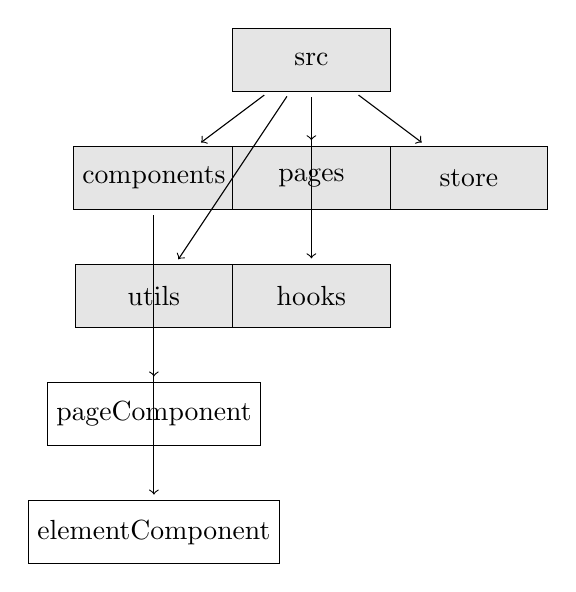
\begin{tikzpicture}[
    file/.style={draw, rectangle, minimum width=2cm, minimum height=0.8cm},
    folder/.style={draw, rectangle, minimum width=2cm, minimum height=0.8cm, fill=gray!20},
    arrow/.style={->, shorten >=2pt, shorten <=2pt}
]

% Folders
\node[folder] (src) at (0,0) {src};
\node[folder] (components) at (-2,-1.5) {components};
\node[folder] (pages) at (0,-1.5) {pages};
\node[folder] (store) at (2,-1.5) {store};
\node[folder] (utils) at (-2,-3) {utils};
\node[folder] (hooks) at (0,-3) {hooks};

% Files
\node[file] (pageComponent) at (-2,-4.5) {pageComponent};
\node[file] (elementComponent) at (-2,-6) {elementComponent};
% ... add more files

% Connections
\draw[arrow] (src) -- (components);
\draw[arrow] (src) -- (pages);
\draw[arrow] (src) -- (store);
\draw[arrow] (src) -- (utils);
\draw[arrow] (src) -- (hooks);
\draw[arrow] (components) -- (pageComponent);
\draw[arrow] (components) -- (elementComponent);
% ... add more connections

\end{tikzpicture}



\pagebreak
\subsubsection{Back-end}
The backend uses the dotNet framework. The development language using the C\# language.

In this project, the backend uses the Onion Architecture.
The Onion Architecture is a typically layered architecture, 
where each layer depends on the inner layer and provides interfaces to the outer layer.
The outer layer provides services to the outermost layer 
and other modules in the same layer based on the interfaces of the inner layer.

From inner to outer, the layers are: Domain, Application, Infrastructure, Presentation.
The Domain layer is the core layer and the innermost layer, used to define domain models, 
which are the business models.
It includes domain models and domain service interfaces.
Domain models are used to define the business models, 
which are the entities in the entity-relationship model and their attributes.
Domain service interfaces are used to define the business services, 
which are the relationships between entities in the entity-relationship model.

The Application layer is the application layer, 
used to define application services, which are the business logic.
It includes domain service implementations and application service interfaces.
Domain service implementations implement the methods of the inner layer's domain service 
interfaces and implement the business logic of the domain models.
Application service interfaces are used to define application services, 
which are the business logic.
It includes but is not limited to database interfaces, testing interfaces, 
HTTP API interfaces, MQTT interfaces, etc.

The Infrastructure layer is the infrastructure layer, used to define infrastructure.
It includes database implementations, testing implementations, 
HTTP API implementations, MQTT implementations, etc.
Database implementations implement the database interfaces 
and provide CRUD services for the database.
Testing implementations implement the testing interfaces 
and provide services for unit testing and integration testing.
HTTP API implementations implement the HTTP API interfaces 
and provide CRUD operations for HTTP APIs.
MQTT implementations implement the MQTT interfaces 
and provide CRUD operations for MQTT.

The Presentation layer is the presentation layer, used to define presentation logic, 
such as interfaces and pages. Since this is a backend project,
data presentation and control are handled by the frontend, 
so this layer is not needed.



\pagebreak
\subsubsection{Data communication and storage}
% 关于本项目的数据通信与数据存储的设计, 包括数据通信的协议, 数据存储的设计等
% 关于数据通信的设计:
% 1. 通信协议的选择
% 自前端向后端发送的数据, 有三种传输的数据类型, 
% 一种是普通的增删改查的请求, 对数据传输的时效性要求不高, 但是对数据的准确性, 完整性, 有序性, 安全性有一定的要求,
% 这种数据的传输, 采用 HTTP 协议, 以及 RESTful API 的设计. 可以有效的保证对数据传输的以上要求.
% 一种是对数据通道的创建和流媒体数据的传输, 对数据传输的时效性, 安全性要求较高, 这种数据的传输, 采用 WebRTC 协议, 以及 MQTT 协议.
% 配合可以快速解码的 flatbuffers 协议, 可以有效的保证对数据传输的以上要求.
% 最后一种是对设备的状态信息和操作信息的传输, 对完整性, 有序性, 安全性都有较高的要求, 这种数据的传输, 采用 MQTT 协议
% 同时也使用了 flatbuffers 协议.
% 
% 2. 数据通信的通信架构和通信流程
% 本项目的数据通信的通信架构, 是基于前后端分离的架构, 前端使用 React 框架, 后端使用 dotnet 框架.
% 当前端需要向后端发送数据的时候, 前端会向后端发送 HTTP 请求, 后端接收到 HTTP 请求之后, 会根据请求的数据类型,
% 选择不同的数据处理方式, 对于普通的增删改查的请求, 后端会根据 RESTful API 的设计, 对数据进行增删改查的操作,
% 对于对数据通道的创建和流媒体数据的传输, 后端会根据 WebRTC 协议, 对数据通道进行创建, 并且帮助前端和设备建立数据通道,
% 当数据通道建立后, 前端和设备之间则使用 flatbuffer 的数据格式对流媒体数据进行传输,
% 对于设备的状态信息和操作信息的传输, 前端会直接向 MQTT broker 发送 MQTT 请求, 
% 设备会在其自身的固件中监听相关的 MQTT 请求, 并且返回相关的数据.
% 
% 3. 数据通信的格式
% 本项目的数据通信的格式, 有三种, 
% 一种是 HTTP 协议, 
% 使用 json 格式对数据进行传输,
% 一种是 WebRTC 协议, 
% 使用 flatbuffers 格式对数据进行传输,
% 一种是 MQTT 协议.
% 使用 flatbuffers 格式对数据进行传输,
% 
% 关于数据存储的设计:
% 1. 数据存储的数据库的选择
% 本项目的数据存储的数据库的选择, 使用了轻量级的数据库 SQLite,
% SQLite 是一个进程内的库, 实现了自给自足的, 无服务器的, 零配置的, 事务性的 SQL 数据库引擎.
% 这是因为整个项目的目的是为了实现前端与设备之间的数据通信, 对于数据库数据的增删改查操作的要求不高,
% 数据量较小, 且对于数据库的数据的事务性要求不高, 所以选择了 SQLite 数据库.
% 2. 项目前后端的数据结构的设计
% 在本项目中, 前端由于使用了 React 框架, 所以前端的数据结构的设计, 使用了基于状态的数据结构的设计,
% 每个组件或者数据集都包含一个状态对象, 这个状态对象的属性就是组件的各个状态. 
% 使用状态对象的原因是, 可以方便的对状态进行管理, 采用对象-属性的形式, 可以方便的针对不同组件的同类状态进行区分,
% 由于跨组件的状态是由 redux 进行管理的, 这种状态对象的设计, 可以更搞笑的对状态进行更新和传递.
% 后端由于使用了 dotnet 框架, 所以后端的数据结构的设计, 使用了基于类的数据结构的设计,
% 采用了面向对象的编程思想, 对数据进行了封装, 使得数据的传输更加的安全, 有序, 完整.


\pagebreak

% \subsection{Domain model}
% \documentclass[]{article}
\usepackage{graphicx}
\usepackage{amsmath}
\usepackage{tikz}

% libaries
\usetikzlibrary{shapes,arrows}

%Define the listing package
\usepackage{listings} %code highlighter
\usepackage{color} %use color
\definecolor{mygreen}{rgb}{0,0.6,0}
\definecolor{mygray}{rgb}{0.5,0.5,0.5}
\definecolor{mymauve}{rgb}{0.58,0,0.82}

%Customize a bit the look
\lstset{ %
backgroundcolor=\color{white}, % choose the background color; you must add \usepackage{color} or \usepackage{xcolor}
basicstyle=\footnotesize, % the size of the fonts that are used for the code
breakatwhitespace=false, % sets if automatic breaks should only happen at whitespace
breaklines=true, % sets automatic line breaking
captionpos=b, % sets the caption-position to bottom
commentstyle=\color{mygreen}, % comment style
deletekeywords={...}, % if you want to delete keywords from the given language
escapeinside={\%*}{*)}, % if you want to add LaTeX within your code
extendedchars=true, % lets you use non-ASCII characters; for 8-bits encodings only, does not work with UTF-8
frame=single, % adds a frame around the code
keepspaces=true, % keeps spaces in text, useful for keeping indentation of code (possibly needs columns=flexible)
keywordstyle=\color{blue}, % keyword style
% language=Octave, % the language of the code
morekeywords={*,...}, % if you want to add more keywords to the set
numbers=left, % where to put the line-numbers; possible values are (none, left, right)
numbersep=5pt, % how far the line-numbers are from the code
numberstyle=\tiny\color{mygray}, % the style that is used for the line-numbers
rulecolor=\color{black}, % if not set, the frame-color may be changed on line-breaks within not-black text (e.g. comments (green here))
showspaces=false, % show spaces everywhere adding particular underscores; it overrides 'showstringspaces'
showstringspaces=false, % underline spaces within strings only
showtabs=false, % show tabs within strings adding particular underscores
stepnumber=1, % the step between two line-numbers. If it's 1, each line will be numbered
stringstyle=\color{mymauve}, % string literal style
tabsize=2, % sets default tabsize to 2 spaces
title=\lstname % show the filename of files included with \lstinputlisting; also try caption instead of title
}

\definecolor{darkgray}{rgb}{.4,.4,.4}
\definecolor{purple}{rgb}{0.65, 0.12, 0.82}

\lstdefinelanguage{React}{
keywords={const, typeof, new, true, false, catch, function, return, null, catch, switch, var, if, in, while, do, else, case, break},
keywordstyle=\color{blue}\bfseries,
ndkeywords={class, export, boolean, throw, implements, import, this},
ndkeywordstyle=\color{darkgray}\bfseries,
identifierstyle=\color{mygreen},
sensitive=false,
comment=[l]{//},
morecomment=[s]{/*}{*/},
commentstyle=\color{purple}\ttfamily,
string=[b]{"}{'}{`},
stringstyle=\color{red}\ttfamily,
morestring=[b]',
morestring=[b]",
morestring=[b]`',
}

\lstdefinelanguage{CSharp}{
keywords={const, typeof, new, true, false, catch, function, return, null, catch, switch, var, if, in, while, do, else, case, break},
keywordstyle=\color{blue}\bfseries,
ndkeywords={class, export, boolean, throw, implements, import, this},
ndkeywordstyle=\color{darkgray}\bfseries,
identifierstyle=\color{mygreen},
sensitive=false,
comment=[l]{//},
morecomment=[s]{/*}{*/},
commentstyle=\color{purple}\ttfamily,
string=[b]{"}{'}{`},
stringstyle=\color{red}\ttfamily,
morestring=[b]',
morestring=[b]",
morestring=[b]`',
}

\lstset{
language=React,
extendedchars=true,
basicstyle=\footnotesize\ttfamily,
showstringspaces=false,
showspaces=false,
numbers=left,
numberstyle=\footnotesize,
numbersep=9pt,
tabsize=2,
breaklines=true,
showtabs=false,
captionpos=b
}

\lstset{
language=CSharp,
extendedchars=true,
basicstyle=\footnotesize\ttfamily,
showstringspaces=false,
showspaces=false,
numbers=left,
numberstyle=\footnotesize,
numbersep=9pt,
tabsize=2,
breaklines=true,
showtabs=false,
captionpos=b
}

% \usepackage{cite} % Add this line for citation

% \bibliographystyle{plain}

\title{
The implementation of BifrostConnect Front-end scope, 
re-design and development with the relevant back-end support develop.
}
\author{
    Fei Gu \\
    Erhvervs Akademi Sydvest \\
    Computer Science 21\\
    }
\date{\today}

\begin{document}

% Front page
\maketitle
\begin{center}
    Supervisor: Henrik Boulund Meng Hansen \\
    Company: BifrostConnect \\
    Engineering Director: Jasper Wass \\
\end{center}
\tableofcontents
\pagebreak


% The introduction
\section{Introduction}
\subsection{Background}\input{sections/introduction/background.tex}
\subsection{The company}\input{sections/introduction/aboutCompany}
\subsection{The project}\input{sections/introduction/aboutProject}
\pagebreak

% The problem statement
\section{Problem Statement}
\subsection{Statement}
\input{sections/problemStatement/statement}
\subsection{Situation}
\input{sections/problemStatement/situation}
\subsection{Potential Solution}
\input{sections/problemStatement/potentialSolution}
\pagebreak

% Requirement analysis
\section{Requirement Analysis}
\input{sections/requirementAnalysis/index}

\subsection{Stakeholders}
\input{sections/requirementAnalysis/stakeholders/index}

\subsection{Business Domain}
\input{sections/requirementAnalysis/bussinesDomain/index}

\subsection{Scope}
\input{sections/requirementAnalysis/scope}

\subsection{Goals}
\input{sections/requirementAnalysis/goals}
\pagebreak

% Software Design
\section{Software Design}
% developement methods
\subsection{Software Development Methods}
\input{sections/softwareDevelopmentMethods/index}
\subsubsection{Agile Software Development}
\input{sections/softwareDevelopmentMethods/agileSoftwareDevelopment/index}
\subsubsection{Feature Driven Development}
\input{sections/softwareDevelopmentMethods/featureDrivenDevelopment/index}

\pagebreak

% Technology seslection
\subsection{Technology selection}
\input{sections/softwareDesign/technologySelection/index}
\subsubsection{Front-end}
\input{sections/softwareDesign/technologySelection/frontEnd}            
\subsubsection{Back-end}
\input{sections/softwareDesign/technologySelection/backEnd}            
\subsubsection{Database}
\input{sections/softwareDesign/technologySelection/database}
\subsubsection{Data communication}
\input{sections/softwareDesign/technologySelection/dataCommunication}            
\subsubsection{DevOps}
\input{sections/softwareDesign/technologySelection/devOps}
\pagebreak

% Architecture design
\subsection{Architecture design}
\input{sections/softwareDesign/architectureDesign/index}
\pagebreak
\subsubsection{Front-end}
\input{sections/softwareDesign/architectureDesign/frontEndArchitecture}
\pagebreak
\subsubsection{Back-end}
\input{sections/softwareDesign/architectureDesign/backEndArchitecture}
\pagebreak
\subsubsection{Data communication and storage}
\input{sections/softwareDesign/architectureDesign/dataCommunicationArchitecture}
\pagebreak

% \subsection{Domain model}
% \input{sections/softwareDesign/domainModel/index}
% \subsection{Database design}
% % 数据库领域模型 ER 图
% % 包括表和字段的设置.
% % 对于私有键和外键的设置.

% \subsection{Back-end design}
% % 后端对象模型
% % 以及对于对象模型的增删改查
% % 以及相关的其他服务的设计`'

% \subsection{Front-end design}
% % 对于前端的页面结构的设计 
% % 页面的状态的设计, 交互设计

% \subsection{FlatBuffers design}
% % schema 的设计

\subsection{DevOps CI/CD process design}
\input{sections/softwareDesign/devOpsDesign/index}
\subsubsection{Continuous Integration}
\input{sections/softwareDesign/devOpsDesign/continuousIntegration/index}
\subsubsection{Continuous Delivery}
\input{sections/softwareDesign/devOpsDesign/continuousDelivery/index}
\subsubsection{Continuous Deployment}
\input{sections/softwareDesign/devOpsDesign/continuousDeployment/index}
\pagebreak

\section{Software Development} 
\input{sections/softwareDevelopment/index}
\subsection{Overall development}
\input{sections/softwareDevelopment/overallDevelopement/index}
\subsubsection{Front-end}
\input{sections/softwareDevelopment/overallDevelopement/frontEnd/index}
\subsubsection{Back-end}
\input{sections/softwareDevelopment/overallDevelopement/backEnd/index}
\subsubsection{DevOps}
\input{sections/softwareDevelopment/overallDevelopement/devOps/index}
\subsection{Feature development} 
\input{sections/softwareDevelopment/featureDevelopment/index}
\subsubsection{Use Case 1}
\input{sections/softwareDevelopment/featureDevelopment/useCase1/index}
\subsubsection{Feature 1}
\input{sections/softwareDevelopment/featureDevelopment/feature/feature1.tex}
\pagebreak
\section{Conclusion} 
\subsection{Result}
Since the project is still in progress, the result is not available yet.
So far, basic structure of this project has been built. But the most features 
are not implemented yet. 
\subsection{Discussion}
As a single developer for this project, I am confident what I have done so far.
And I can say I understand the most of the knowledge I have used in this project, 
which also means I can explain all the part of the project. 
But this project also relevant some of the complex knowledge which I have to continue 
to study and practice.
\subsection{Future Work}
The future work is to implement the rest of the features. 
Including the most important part which is the 'create session' feature.
\pagebreak
% \bibliography{bibliography}
\pagebreak
% \begin{appendices}
%     \section{Appendix}
% \end{appendices} 
\end{document}
% \subsection{Database design}
% % 数据库领域模型 ER 图
% % 包括表和字段的设置.
% % 对于私有键和外键的设置.

% \subsection{Back-end design}
% % 后端对象模型
% % 以及对于对象模型的增删改查
% % 以及相关的其他服务的设计`'

% \subsection{Front-end design}
% % 对于前端的页面结构的设计 
% % 页面的状态的设计, 交互设计

% \subsection{FlatBuffers design}
% % schema 的设计

\subsection{DevOps CI/CD process design}
\documentclass[]{article}
\usepackage{graphicx}
\usepackage{amsmath}
\usepackage{tikz}

% libaries
\usetikzlibrary{shapes,arrows}

%Define the listing package
\usepackage{listings} %code highlighter
\usepackage{color} %use color
\definecolor{mygreen}{rgb}{0,0.6,0}
\definecolor{mygray}{rgb}{0.5,0.5,0.5}
\definecolor{mymauve}{rgb}{0.58,0,0.82}

%Customize a bit the look
\lstset{ %
backgroundcolor=\color{white}, % choose the background color; you must add \usepackage{color} or \usepackage{xcolor}
basicstyle=\footnotesize, % the size of the fonts that are used for the code
breakatwhitespace=false, % sets if automatic breaks should only happen at whitespace
breaklines=true, % sets automatic line breaking
captionpos=b, % sets the caption-position to bottom
commentstyle=\color{mygreen}, % comment style
deletekeywords={...}, % if you want to delete keywords from the given language
escapeinside={\%*}{*)}, % if you want to add LaTeX within your code
extendedchars=true, % lets you use non-ASCII characters; for 8-bits encodings only, does not work with UTF-8
frame=single, % adds a frame around the code
keepspaces=true, % keeps spaces in text, useful for keeping indentation of code (possibly needs columns=flexible)
keywordstyle=\color{blue}, % keyword style
% language=Octave, % the language of the code
morekeywords={*,...}, % if you want to add more keywords to the set
numbers=left, % where to put the line-numbers; possible values are (none, left, right)
numbersep=5pt, % how far the line-numbers are from the code
numberstyle=\tiny\color{mygray}, % the style that is used for the line-numbers
rulecolor=\color{black}, % if not set, the frame-color may be changed on line-breaks within not-black text (e.g. comments (green here))
showspaces=false, % show spaces everywhere adding particular underscores; it overrides 'showstringspaces'
showstringspaces=false, % underline spaces within strings only
showtabs=false, % show tabs within strings adding particular underscores
stepnumber=1, % the step between two line-numbers. If it's 1, each line will be numbered
stringstyle=\color{mymauve}, % string literal style
tabsize=2, % sets default tabsize to 2 spaces
title=\lstname % show the filename of files included with \lstinputlisting; also try caption instead of title
}

\definecolor{darkgray}{rgb}{.4,.4,.4}
\definecolor{purple}{rgb}{0.65, 0.12, 0.82}

\lstdefinelanguage{React}{
keywords={const, typeof, new, true, false, catch, function, return, null, catch, switch, var, if, in, while, do, else, case, break},
keywordstyle=\color{blue}\bfseries,
ndkeywords={class, export, boolean, throw, implements, import, this},
ndkeywordstyle=\color{darkgray}\bfseries,
identifierstyle=\color{mygreen},
sensitive=false,
comment=[l]{//},
morecomment=[s]{/*}{*/},
commentstyle=\color{purple}\ttfamily,
string=[b]{"}{'}{`},
stringstyle=\color{red}\ttfamily,
morestring=[b]',
morestring=[b]",
morestring=[b]`',
}

\lstdefinelanguage{CSharp}{
keywords={const, typeof, new, true, false, catch, function, return, null, catch, switch, var, if, in, while, do, else, case, break},
keywordstyle=\color{blue}\bfseries,
ndkeywords={class, export, boolean, throw, implements, import, this},
ndkeywordstyle=\color{darkgray}\bfseries,
identifierstyle=\color{mygreen},
sensitive=false,
comment=[l]{//},
morecomment=[s]{/*}{*/},
commentstyle=\color{purple}\ttfamily,
string=[b]{"}{'}{`},
stringstyle=\color{red}\ttfamily,
morestring=[b]',
morestring=[b]",
morestring=[b]`',
}

\lstset{
language=React,
extendedchars=true,
basicstyle=\footnotesize\ttfamily,
showstringspaces=false,
showspaces=false,
numbers=left,
numberstyle=\footnotesize,
numbersep=9pt,
tabsize=2,
breaklines=true,
showtabs=false,
captionpos=b
}

\lstset{
language=CSharp,
extendedchars=true,
basicstyle=\footnotesize\ttfamily,
showstringspaces=false,
showspaces=false,
numbers=left,
numberstyle=\footnotesize,
numbersep=9pt,
tabsize=2,
breaklines=true,
showtabs=false,
captionpos=b
}

% \usepackage{cite} % Add this line for citation

% \bibliographystyle{plain}

\title{
The implementation of BifrostConnect Front-end scope, 
re-design and development with the relevant back-end support develop.
}
\author{
    Fei Gu \\
    Erhvervs Akademi Sydvest \\
    Computer Science 21\\
    }
\date{\today}

\begin{document}

% Front page
\maketitle
\begin{center}
    Supervisor: Henrik Boulund Meng Hansen \\
    Company: BifrostConnect \\
    Engineering Director: Jasper Wass \\
\end{center}
\tableofcontents
\pagebreak


% The introduction
\section{Introduction}
\subsection{Background}\input{sections/introduction/background.tex}
\subsection{The company}\input{sections/introduction/aboutCompany}
\subsection{The project}\input{sections/introduction/aboutProject}
\pagebreak

% The problem statement
\section{Problem Statement}
\subsection{Statement}
\input{sections/problemStatement/statement}
\subsection{Situation}
\input{sections/problemStatement/situation}
\subsection{Potential Solution}
\input{sections/problemStatement/potentialSolution}
\pagebreak

% Requirement analysis
\section{Requirement Analysis}
\input{sections/requirementAnalysis/index}

\subsection{Stakeholders}
\input{sections/requirementAnalysis/stakeholders/index}

\subsection{Business Domain}
\input{sections/requirementAnalysis/bussinesDomain/index}

\subsection{Scope}
\input{sections/requirementAnalysis/scope}

\subsection{Goals}
\input{sections/requirementAnalysis/goals}
\pagebreak

% Software Design
\section{Software Design}
% developement methods
\subsection{Software Development Methods}
\input{sections/softwareDevelopmentMethods/index}
\subsubsection{Agile Software Development}
\input{sections/softwareDevelopmentMethods/agileSoftwareDevelopment/index}
\subsubsection{Feature Driven Development}
\input{sections/softwareDevelopmentMethods/featureDrivenDevelopment/index}

\pagebreak

% Technology seslection
\subsection{Technology selection}
\input{sections/softwareDesign/technologySelection/index}
\subsubsection{Front-end}
\input{sections/softwareDesign/technologySelection/frontEnd}            
\subsubsection{Back-end}
\input{sections/softwareDesign/technologySelection/backEnd}            
\subsubsection{Database}
\input{sections/softwareDesign/technologySelection/database}
\subsubsection{Data communication}
\input{sections/softwareDesign/technologySelection/dataCommunication}            
\subsubsection{DevOps}
\input{sections/softwareDesign/technologySelection/devOps}
\pagebreak

% Architecture design
\subsection{Architecture design}
\input{sections/softwareDesign/architectureDesign/index}
\pagebreak
\subsubsection{Front-end}
\input{sections/softwareDesign/architectureDesign/frontEndArchitecture}
\pagebreak
\subsubsection{Back-end}
\input{sections/softwareDesign/architectureDesign/backEndArchitecture}
\pagebreak
\subsubsection{Data communication and storage}
\input{sections/softwareDesign/architectureDesign/dataCommunicationArchitecture}
\pagebreak

% \subsection{Domain model}
% \input{sections/softwareDesign/domainModel/index}
% \subsection{Database design}
% % 数据库领域模型 ER 图
% % 包括表和字段的设置.
% % 对于私有键和外键的设置.

% \subsection{Back-end design}
% % 后端对象模型
% % 以及对于对象模型的增删改查
% % 以及相关的其他服务的设计`'

% \subsection{Front-end design}
% % 对于前端的页面结构的设计 
% % 页面的状态的设计, 交互设计

% \subsection{FlatBuffers design}
% % schema 的设计

\subsection{DevOps CI/CD process design}
\input{sections/softwareDesign/devOpsDesign/index}
\subsubsection{Continuous Integration}
\input{sections/softwareDesign/devOpsDesign/continuousIntegration/index}
\subsubsection{Continuous Delivery}
\input{sections/softwareDesign/devOpsDesign/continuousDelivery/index}
\subsubsection{Continuous Deployment}
\input{sections/softwareDesign/devOpsDesign/continuousDeployment/index}
\pagebreak

\section{Software Development} 
\input{sections/softwareDevelopment/index}
\subsection{Overall development}
\input{sections/softwareDevelopment/overallDevelopement/index}
\subsubsection{Front-end}
\input{sections/softwareDevelopment/overallDevelopement/frontEnd/index}
\subsubsection{Back-end}
\input{sections/softwareDevelopment/overallDevelopement/backEnd/index}
\subsubsection{DevOps}
\input{sections/softwareDevelopment/overallDevelopement/devOps/index}
\subsection{Feature development} 
\input{sections/softwareDevelopment/featureDevelopment/index}
\subsubsection{Use Case 1}
\input{sections/softwareDevelopment/featureDevelopment/useCase1/index}
\subsubsection{Feature 1}
\input{sections/softwareDevelopment/featureDevelopment/feature/feature1.tex}
\pagebreak
\section{Conclusion} 
\subsection{Result}
Since the project is still in progress, the result is not available yet.
So far, basic structure of this project has been built. But the most features 
are not implemented yet. 
\subsection{Discussion}
As a single developer for this project, I am confident what I have done so far.
And I can say I understand the most of the knowledge I have used in this project, 
which also means I can explain all the part of the project. 
But this project also relevant some of the complex knowledge which I have to continue 
to study and practice.
\subsection{Future Work}
The future work is to implement the rest of the features. 
Including the most important part which is the 'create session' feature.
\pagebreak
% \bibliography{bibliography}
\pagebreak
% \begin{appendices}
%     \section{Appendix}
% \end{appendices} 
\end{document}
\subsubsection{Continuous Integration}
\documentclass[]{article}
\usepackage{graphicx}
\usepackage{amsmath}
\usepackage{tikz}

% libaries
\usetikzlibrary{shapes,arrows}

%Define the listing package
\usepackage{listings} %code highlighter
\usepackage{color} %use color
\definecolor{mygreen}{rgb}{0,0.6,0}
\definecolor{mygray}{rgb}{0.5,0.5,0.5}
\definecolor{mymauve}{rgb}{0.58,0,0.82}

%Customize a bit the look
\lstset{ %
backgroundcolor=\color{white}, % choose the background color; you must add \usepackage{color} or \usepackage{xcolor}
basicstyle=\footnotesize, % the size of the fonts that are used for the code
breakatwhitespace=false, % sets if automatic breaks should only happen at whitespace
breaklines=true, % sets automatic line breaking
captionpos=b, % sets the caption-position to bottom
commentstyle=\color{mygreen}, % comment style
deletekeywords={...}, % if you want to delete keywords from the given language
escapeinside={\%*}{*)}, % if you want to add LaTeX within your code
extendedchars=true, % lets you use non-ASCII characters; for 8-bits encodings only, does not work with UTF-8
frame=single, % adds a frame around the code
keepspaces=true, % keeps spaces in text, useful for keeping indentation of code (possibly needs columns=flexible)
keywordstyle=\color{blue}, % keyword style
% language=Octave, % the language of the code
morekeywords={*,...}, % if you want to add more keywords to the set
numbers=left, % where to put the line-numbers; possible values are (none, left, right)
numbersep=5pt, % how far the line-numbers are from the code
numberstyle=\tiny\color{mygray}, % the style that is used for the line-numbers
rulecolor=\color{black}, % if not set, the frame-color may be changed on line-breaks within not-black text (e.g. comments (green here))
showspaces=false, % show spaces everywhere adding particular underscores; it overrides 'showstringspaces'
showstringspaces=false, % underline spaces within strings only
showtabs=false, % show tabs within strings adding particular underscores
stepnumber=1, % the step between two line-numbers. If it's 1, each line will be numbered
stringstyle=\color{mymauve}, % string literal style
tabsize=2, % sets default tabsize to 2 spaces
title=\lstname % show the filename of files included with \lstinputlisting; also try caption instead of title
}

\definecolor{darkgray}{rgb}{.4,.4,.4}
\definecolor{purple}{rgb}{0.65, 0.12, 0.82}

\lstdefinelanguage{React}{
keywords={const, typeof, new, true, false, catch, function, return, null, catch, switch, var, if, in, while, do, else, case, break},
keywordstyle=\color{blue}\bfseries,
ndkeywords={class, export, boolean, throw, implements, import, this},
ndkeywordstyle=\color{darkgray}\bfseries,
identifierstyle=\color{mygreen},
sensitive=false,
comment=[l]{//},
morecomment=[s]{/*}{*/},
commentstyle=\color{purple}\ttfamily,
string=[b]{"}{'}{`},
stringstyle=\color{red}\ttfamily,
morestring=[b]',
morestring=[b]",
morestring=[b]`',
}

\lstdefinelanguage{CSharp}{
keywords={const, typeof, new, true, false, catch, function, return, null, catch, switch, var, if, in, while, do, else, case, break},
keywordstyle=\color{blue}\bfseries,
ndkeywords={class, export, boolean, throw, implements, import, this},
ndkeywordstyle=\color{darkgray}\bfseries,
identifierstyle=\color{mygreen},
sensitive=false,
comment=[l]{//},
morecomment=[s]{/*}{*/},
commentstyle=\color{purple}\ttfamily,
string=[b]{"}{'}{`},
stringstyle=\color{red}\ttfamily,
morestring=[b]',
morestring=[b]",
morestring=[b]`',
}

\lstset{
language=React,
extendedchars=true,
basicstyle=\footnotesize\ttfamily,
showstringspaces=false,
showspaces=false,
numbers=left,
numberstyle=\footnotesize,
numbersep=9pt,
tabsize=2,
breaklines=true,
showtabs=false,
captionpos=b
}

\lstset{
language=CSharp,
extendedchars=true,
basicstyle=\footnotesize\ttfamily,
showstringspaces=false,
showspaces=false,
numbers=left,
numberstyle=\footnotesize,
numbersep=9pt,
tabsize=2,
breaklines=true,
showtabs=false,
captionpos=b
}

% \usepackage{cite} % Add this line for citation

% \bibliographystyle{plain}

\title{
The implementation of BifrostConnect Front-end scope, 
re-design and development with the relevant back-end support develop.
}
\author{
    Fei Gu \\
    Erhvervs Akademi Sydvest \\
    Computer Science 21\\
    }
\date{\today}

\begin{document}

% Front page
\maketitle
\begin{center}
    Supervisor: Henrik Boulund Meng Hansen \\
    Company: BifrostConnect \\
    Engineering Director: Jasper Wass \\
\end{center}
\tableofcontents
\pagebreak


% The introduction
\section{Introduction}
\subsection{Background}\input{sections/introduction/background.tex}
\subsection{The company}\input{sections/introduction/aboutCompany}
\subsection{The project}\input{sections/introduction/aboutProject}
\pagebreak

% The problem statement
\section{Problem Statement}
\subsection{Statement}
\input{sections/problemStatement/statement}
\subsection{Situation}
\input{sections/problemStatement/situation}
\subsection{Potential Solution}
\input{sections/problemStatement/potentialSolution}
\pagebreak

% Requirement analysis
\section{Requirement Analysis}
\input{sections/requirementAnalysis/index}

\subsection{Stakeholders}
\input{sections/requirementAnalysis/stakeholders/index}

\subsection{Business Domain}
\input{sections/requirementAnalysis/bussinesDomain/index}

\subsection{Scope}
\input{sections/requirementAnalysis/scope}

\subsection{Goals}
\input{sections/requirementAnalysis/goals}
\pagebreak

% Software Design
\section{Software Design}
% developement methods
\subsection{Software Development Methods}
\input{sections/softwareDevelopmentMethods/index}
\subsubsection{Agile Software Development}
\input{sections/softwareDevelopmentMethods/agileSoftwareDevelopment/index}
\subsubsection{Feature Driven Development}
\input{sections/softwareDevelopmentMethods/featureDrivenDevelopment/index}

\pagebreak

% Technology seslection
\subsection{Technology selection}
\input{sections/softwareDesign/technologySelection/index}
\subsubsection{Front-end}
\input{sections/softwareDesign/technologySelection/frontEnd}            
\subsubsection{Back-end}
\input{sections/softwareDesign/technologySelection/backEnd}            
\subsubsection{Database}
\input{sections/softwareDesign/technologySelection/database}
\subsubsection{Data communication}
\input{sections/softwareDesign/technologySelection/dataCommunication}            
\subsubsection{DevOps}
\input{sections/softwareDesign/technologySelection/devOps}
\pagebreak

% Architecture design
\subsection{Architecture design}
\input{sections/softwareDesign/architectureDesign/index}
\pagebreak
\subsubsection{Front-end}
\input{sections/softwareDesign/architectureDesign/frontEndArchitecture}
\pagebreak
\subsubsection{Back-end}
\input{sections/softwareDesign/architectureDesign/backEndArchitecture}
\pagebreak
\subsubsection{Data communication and storage}
\input{sections/softwareDesign/architectureDesign/dataCommunicationArchitecture}
\pagebreak

% \subsection{Domain model}
% \input{sections/softwareDesign/domainModel/index}
% \subsection{Database design}
% % 数据库领域模型 ER 图
% % 包括表和字段的设置.
% % 对于私有键和外键的设置.

% \subsection{Back-end design}
% % 后端对象模型
% % 以及对于对象模型的增删改查
% % 以及相关的其他服务的设计`'

% \subsection{Front-end design}
% % 对于前端的页面结构的设计 
% % 页面的状态的设计, 交互设计

% \subsection{FlatBuffers design}
% % schema 的设计

\subsection{DevOps CI/CD process design}
\input{sections/softwareDesign/devOpsDesign/index}
\subsubsection{Continuous Integration}
\input{sections/softwareDesign/devOpsDesign/continuousIntegration/index}
\subsubsection{Continuous Delivery}
\input{sections/softwareDesign/devOpsDesign/continuousDelivery/index}
\subsubsection{Continuous Deployment}
\input{sections/softwareDesign/devOpsDesign/continuousDeployment/index}
\pagebreak

\section{Software Development} 
\input{sections/softwareDevelopment/index}
\subsection{Overall development}
\input{sections/softwareDevelopment/overallDevelopement/index}
\subsubsection{Front-end}
\input{sections/softwareDevelopment/overallDevelopement/frontEnd/index}
\subsubsection{Back-end}
\input{sections/softwareDevelopment/overallDevelopement/backEnd/index}
\subsubsection{DevOps}
\input{sections/softwareDevelopment/overallDevelopement/devOps/index}
\subsection{Feature development} 
\input{sections/softwareDevelopment/featureDevelopment/index}
\subsubsection{Use Case 1}
\input{sections/softwareDevelopment/featureDevelopment/useCase1/index}
\subsubsection{Feature 1}
\input{sections/softwareDevelopment/featureDevelopment/feature/feature1.tex}
\pagebreak
\section{Conclusion} 
\subsection{Result}
Since the project is still in progress, the result is not available yet.
So far, basic structure of this project has been built. But the most features 
are not implemented yet. 
\subsection{Discussion}
As a single developer for this project, I am confident what I have done so far.
And I can say I understand the most of the knowledge I have used in this project, 
which also means I can explain all the part of the project. 
But this project also relevant some of the complex knowledge which I have to continue 
to study and practice.
\subsection{Future Work}
The future work is to implement the rest of the features. 
Including the most important part which is the 'create session' feature.
\pagebreak
% \bibliography{bibliography}
\pagebreak
% \begin{appendices}
%     \section{Appendix}
% \end{appendices} 
\end{document}
\subsubsection{Continuous Delivery}
\documentclass[]{article}
\usepackage{graphicx}
\usepackage{amsmath}
\usepackage{tikz}

% libaries
\usetikzlibrary{shapes,arrows}

%Define the listing package
\usepackage{listings} %code highlighter
\usepackage{color} %use color
\definecolor{mygreen}{rgb}{0,0.6,0}
\definecolor{mygray}{rgb}{0.5,0.5,0.5}
\definecolor{mymauve}{rgb}{0.58,0,0.82}

%Customize a bit the look
\lstset{ %
backgroundcolor=\color{white}, % choose the background color; you must add \usepackage{color} or \usepackage{xcolor}
basicstyle=\footnotesize, % the size of the fonts that are used for the code
breakatwhitespace=false, % sets if automatic breaks should only happen at whitespace
breaklines=true, % sets automatic line breaking
captionpos=b, % sets the caption-position to bottom
commentstyle=\color{mygreen}, % comment style
deletekeywords={...}, % if you want to delete keywords from the given language
escapeinside={\%*}{*)}, % if you want to add LaTeX within your code
extendedchars=true, % lets you use non-ASCII characters; for 8-bits encodings only, does not work with UTF-8
frame=single, % adds a frame around the code
keepspaces=true, % keeps spaces in text, useful for keeping indentation of code (possibly needs columns=flexible)
keywordstyle=\color{blue}, % keyword style
% language=Octave, % the language of the code
morekeywords={*,...}, % if you want to add more keywords to the set
numbers=left, % where to put the line-numbers; possible values are (none, left, right)
numbersep=5pt, % how far the line-numbers are from the code
numberstyle=\tiny\color{mygray}, % the style that is used for the line-numbers
rulecolor=\color{black}, % if not set, the frame-color may be changed on line-breaks within not-black text (e.g. comments (green here))
showspaces=false, % show spaces everywhere adding particular underscores; it overrides 'showstringspaces'
showstringspaces=false, % underline spaces within strings only
showtabs=false, % show tabs within strings adding particular underscores
stepnumber=1, % the step between two line-numbers. If it's 1, each line will be numbered
stringstyle=\color{mymauve}, % string literal style
tabsize=2, % sets default tabsize to 2 spaces
title=\lstname % show the filename of files included with \lstinputlisting; also try caption instead of title
}

\definecolor{darkgray}{rgb}{.4,.4,.4}
\definecolor{purple}{rgb}{0.65, 0.12, 0.82}

\lstdefinelanguage{React}{
keywords={const, typeof, new, true, false, catch, function, return, null, catch, switch, var, if, in, while, do, else, case, break},
keywordstyle=\color{blue}\bfseries,
ndkeywords={class, export, boolean, throw, implements, import, this},
ndkeywordstyle=\color{darkgray}\bfseries,
identifierstyle=\color{mygreen},
sensitive=false,
comment=[l]{//},
morecomment=[s]{/*}{*/},
commentstyle=\color{purple}\ttfamily,
string=[b]{"}{'}{`},
stringstyle=\color{red}\ttfamily,
morestring=[b]',
morestring=[b]",
morestring=[b]`',
}

\lstdefinelanguage{CSharp}{
keywords={const, typeof, new, true, false, catch, function, return, null, catch, switch, var, if, in, while, do, else, case, break},
keywordstyle=\color{blue}\bfseries,
ndkeywords={class, export, boolean, throw, implements, import, this},
ndkeywordstyle=\color{darkgray}\bfseries,
identifierstyle=\color{mygreen},
sensitive=false,
comment=[l]{//},
morecomment=[s]{/*}{*/},
commentstyle=\color{purple}\ttfamily,
string=[b]{"}{'}{`},
stringstyle=\color{red}\ttfamily,
morestring=[b]',
morestring=[b]",
morestring=[b]`',
}

\lstset{
language=React,
extendedchars=true,
basicstyle=\footnotesize\ttfamily,
showstringspaces=false,
showspaces=false,
numbers=left,
numberstyle=\footnotesize,
numbersep=9pt,
tabsize=2,
breaklines=true,
showtabs=false,
captionpos=b
}

\lstset{
language=CSharp,
extendedchars=true,
basicstyle=\footnotesize\ttfamily,
showstringspaces=false,
showspaces=false,
numbers=left,
numberstyle=\footnotesize,
numbersep=9pt,
tabsize=2,
breaklines=true,
showtabs=false,
captionpos=b
}

% \usepackage{cite} % Add this line for citation

% \bibliographystyle{plain}

\title{
The implementation of BifrostConnect Front-end scope, 
re-design and development with the relevant back-end support develop.
}
\author{
    Fei Gu \\
    Erhvervs Akademi Sydvest \\
    Computer Science 21\\
    }
\date{\today}

\begin{document}

% Front page
\maketitle
\begin{center}
    Supervisor: Henrik Boulund Meng Hansen \\
    Company: BifrostConnect \\
    Engineering Director: Jasper Wass \\
\end{center}
\tableofcontents
\pagebreak


% The introduction
\section{Introduction}
\subsection{Background}\input{sections/introduction/background.tex}
\subsection{The company}\input{sections/introduction/aboutCompany}
\subsection{The project}\input{sections/introduction/aboutProject}
\pagebreak

% The problem statement
\section{Problem Statement}
\subsection{Statement}
\input{sections/problemStatement/statement}
\subsection{Situation}
\input{sections/problemStatement/situation}
\subsection{Potential Solution}
\input{sections/problemStatement/potentialSolution}
\pagebreak

% Requirement analysis
\section{Requirement Analysis}
\input{sections/requirementAnalysis/index}

\subsection{Stakeholders}
\input{sections/requirementAnalysis/stakeholders/index}

\subsection{Business Domain}
\input{sections/requirementAnalysis/bussinesDomain/index}

\subsection{Scope}
\input{sections/requirementAnalysis/scope}

\subsection{Goals}
\input{sections/requirementAnalysis/goals}
\pagebreak

% Software Design
\section{Software Design}
% developement methods
\subsection{Software Development Methods}
\input{sections/softwareDevelopmentMethods/index}
\subsubsection{Agile Software Development}
\input{sections/softwareDevelopmentMethods/agileSoftwareDevelopment/index}
\subsubsection{Feature Driven Development}
\input{sections/softwareDevelopmentMethods/featureDrivenDevelopment/index}

\pagebreak

% Technology seslection
\subsection{Technology selection}
\input{sections/softwareDesign/technologySelection/index}
\subsubsection{Front-end}
\input{sections/softwareDesign/technologySelection/frontEnd}            
\subsubsection{Back-end}
\input{sections/softwareDesign/technologySelection/backEnd}            
\subsubsection{Database}
\input{sections/softwareDesign/technologySelection/database}
\subsubsection{Data communication}
\input{sections/softwareDesign/technologySelection/dataCommunication}            
\subsubsection{DevOps}
\input{sections/softwareDesign/technologySelection/devOps}
\pagebreak

% Architecture design
\subsection{Architecture design}
\input{sections/softwareDesign/architectureDesign/index}
\pagebreak
\subsubsection{Front-end}
\input{sections/softwareDesign/architectureDesign/frontEndArchitecture}
\pagebreak
\subsubsection{Back-end}
\input{sections/softwareDesign/architectureDesign/backEndArchitecture}
\pagebreak
\subsubsection{Data communication and storage}
\input{sections/softwareDesign/architectureDesign/dataCommunicationArchitecture}
\pagebreak

% \subsection{Domain model}
% \input{sections/softwareDesign/domainModel/index}
% \subsection{Database design}
% % 数据库领域模型 ER 图
% % 包括表和字段的设置.
% % 对于私有键和外键的设置.

% \subsection{Back-end design}
% % 后端对象模型
% % 以及对于对象模型的增删改查
% % 以及相关的其他服务的设计`'

% \subsection{Front-end design}
% % 对于前端的页面结构的设计 
% % 页面的状态的设计, 交互设计

% \subsection{FlatBuffers design}
% % schema 的设计

\subsection{DevOps CI/CD process design}
\input{sections/softwareDesign/devOpsDesign/index}
\subsubsection{Continuous Integration}
\input{sections/softwareDesign/devOpsDesign/continuousIntegration/index}
\subsubsection{Continuous Delivery}
\input{sections/softwareDesign/devOpsDesign/continuousDelivery/index}
\subsubsection{Continuous Deployment}
\input{sections/softwareDesign/devOpsDesign/continuousDeployment/index}
\pagebreak

\section{Software Development} 
\input{sections/softwareDevelopment/index}
\subsection{Overall development}
\input{sections/softwareDevelopment/overallDevelopement/index}
\subsubsection{Front-end}
\input{sections/softwareDevelopment/overallDevelopement/frontEnd/index}
\subsubsection{Back-end}
\input{sections/softwareDevelopment/overallDevelopement/backEnd/index}
\subsubsection{DevOps}
\input{sections/softwareDevelopment/overallDevelopement/devOps/index}
\subsection{Feature development} 
\input{sections/softwareDevelopment/featureDevelopment/index}
\subsubsection{Use Case 1}
\input{sections/softwareDevelopment/featureDevelopment/useCase1/index}
\subsubsection{Feature 1}
\input{sections/softwareDevelopment/featureDevelopment/feature/feature1.tex}
\pagebreak
\section{Conclusion} 
\subsection{Result}
Since the project is still in progress, the result is not available yet.
So far, basic structure of this project has been built. But the most features 
are not implemented yet. 
\subsection{Discussion}
As a single developer for this project, I am confident what I have done so far.
And I can say I understand the most of the knowledge I have used in this project, 
which also means I can explain all the part of the project. 
But this project also relevant some of the complex knowledge which I have to continue 
to study and practice.
\subsection{Future Work}
The future work is to implement the rest of the features. 
Including the most important part which is the 'create session' feature.
\pagebreak
% \bibliography{bibliography}
\pagebreak
% \begin{appendices}
%     \section{Appendix}
% \end{appendices} 
\end{document}
\subsubsection{Continuous Deployment}
\documentclass[]{article}
\usepackage{graphicx}
\usepackage{amsmath}
\usepackage{tikz}

% libaries
\usetikzlibrary{shapes,arrows}

%Define the listing package
\usepackage{listings} %code highlighter
\usepackage{color} %use color
\definecolor{mygreen}{rgb}{0,0.6,0}
\definecolor{mygray}{rgb}{0.5,0.5,0.5}
\definecolor{mymauve}{rgb}{0.58,0,0.82}

%Customize a bit the look
\lstset{ %
backgroundcolor=\color{white}, % choose the background color; you must add \usepackage{color} or \usepackage{xcolor}
basicstyle=\footnotesize, % the size of the fonts that are used for the code
breakatwhitespace=false, % sets if automatic breaks should only happen at whitespace
breaklines=true, % sets automatic line breaking
captionpos=b, % sets the caption-position to bottom
commentstyle=\color{mygreen}, % comment style
deletekeywords={...}, % if you want to delete keywords from the given language
escapeinside={\%*}{*)}, % if you want to add LaTeX within your code
extendedchars=true, % lets you use non-ASCII characters; for 8-bits encodings only, does not work with UTF-8
frame=single, % adds a frame around the code
keepspaces=true, % keeps spaces in text, useful for keeping indentation of code (possibly needs columns=flexible)
keywordstyle=\color{blue}, % keyword style
% language=Octave, % the language of the code
morekeywords={*,...}, % if you want to add more keywords to the set
numbers=left, % where to put the line-numbers; possible values are (none, left, right)
numbersep=5pt, % how far the line-numbers are from the code
numberstyle=\tiny\color{mygray}, % the style that is used for the line-numbers
rulecolor=\color{black}, % if not set, the frame-color may be changed on line-breaks within not-black text (e.g. comments (green here))
showspaces=false, % show spaces everywhere adding particular underscores; it overrides 'showstringspaces'
showstringspaces=false, % underline spaces within strings only
showtabs=false, % show tabs within strings adding particular underscores
stepnumber=1, % the step between two line-numbers. If it's 1, each line will be numbered
stringstyle=\color{mymauve}, % string literal style
tabsize=2, % sets default tabsize to 2 spaces
title=\lstname % show the filename of files included with \lstinputlisting; also try caption instead of title
}

\definecolor{darkgray}{rgb}{.4,.4,.4}
\definecolor{purple}{rgb}{0.65, 0.12, 0.82}

\lstdefinelanguage{React}{
keywords={const, typeof, new, true, false, catch, function, return, null, catch, switch, var, if, in, while, do, else, case, break},
keywordstyle=\color{blue}\bfseries,
ndkeywords={class, export, boolean, throw, implements, import, this},
ndkeywordstyle=\color{darkgray}\bfseries,
identifierstyle=\color{mygreen},
sensitive=false,
comment=[l]{//},
morecomment=[s]{/*}{*/},
commentstyle=\color{purple}\ttfamily,
string=[b]{"}{'}{`},
stringstyle=\color{red}\ttfamily,
morestring=[b]',
morestring=[b]",
morestring=[b]`',
}

\lstdefinelanguage{CSharp}{
keywords={const, typeof, new, true, false, catch, function, return, null, catch, switch, var, if, in, while, do, else, case, break},
keywordstyle=\color{blue}\bfseries,
ndkeywords={class, export, boolean, throw, implements, import, this},
ndkeywordstyle=\color{darkgray}\bfseries,
identifierstyle=\color{mygreen},
sensitive=false,
comment=[l]{//},
morecomment=[s]{/*}{*/},
commentstyle=\color{purple}\ttfamily,
string=[b]{"}{'}{`},
stringstyle=\color{red}\ttfamily,
morestring=[b]',
morestring=[b]",
morestring=[b]`',
}

\lstset{
language=React,
extendedchars=true,
basicstyle=\footnotesize\ttfamily,
showstringspaces=false,
showspaces=false,
numbers=left,
numberstyle=\footnotesize,
numbersep=9pt,
tabsize=2,
breaklines=true,
showtabs=false,
captionpos=b
}

\lstset{
language=CSharp,
extendedchars=true,
basicstyle=\footnotesize\ttfamily,
showstringspaces=false,
showspaces=false,
numbers=left,
numberstyle=\footnotesize,
numbersep=9pt,
tabsize=2,
breaklines=true,
showtabs=false,
captionpos=b
}

% \usepackage{cite} % Add this line for citation

% \bibliographystyle{plain}

\title{
The implementation of BifrostConnect Front-end scope, 
re-design and development with the relevant back-end support develop.
}
\author{
    Fei Gu \\
    Erhvervs Akademi Sydvest \\
    Computer Science 21\\
    }
\date{\today}

\begin{document}

% Front page
\maketitle
\begin{center}
    Supervisor: Henrik Boulund Meng Hansen \\
    Company: BifrostConnect \\
    Engineering Director: Jasper Wass \\
\end{center}
\tableofcontents
\pagebreak


% The introduction
\section{Introduction}
\subsection{Background}\input{sections/introduction/background.tex}
\subsection{The company}\input{sections/introduction/aboutCompany}
\subsection{The project}\input{sections/introduction/aboutProject}
\pagebreak

% The problem statement
\section{Problem Statement}
\subsection{Statement}
\input{sections/problemStatement/statement}
\subsection{Situation}
\input{sections/problemStatement/situation}
\subsection{Potential Solution}
\input{sections/problemStatement/potentialSolution}
\pagebreak

% Requirement analysis
\section{Requirement Analysis}
\input{sections/requirementAnalysis/index}

\subsection{Stakeholders}
\input{sections/requirementAnalysis/stakeholders/index}

\subsection{Business Domain}
\input{sections/requirementAnalysis/bussinesDomain/index}

\subsection{Scope}
\input{sections/requirementAnalysis/scope}

\subsection{Goals}
\input{sections/requirementAnalysis/goals}
\pagebreak

% Software Design
\section{Software Design}
% developement methods
\subsection{Software Development Methods}
\input{sections/softwareDevelopmentMethods/index}
\subsubsection{Agile Software Development}
\input{sections/softwareDevelopmentMethods/agileSoftwareDevelopment/index}
\subsubsection{Feature Driven Development}
\input{sections/softwareDevelopmentMethods/featureDrivenDevelopment/index}

\pagebreak

% Technology seslection
\subsection{Technology selection}
\input{sections/softwareDesign/technologySelection/index}
\subsubsection{Front-end}
\input{sections/softwareDesign/technologySelection/frontEnd}            
\subsubsection{Back-end}
\input{sections/softwareDesign/technologySelection/backEnd}            
\subsubsection{Database}
\input{sections/softwareDesign/technologySelection/database}
\subsubsection{Data communication}
\input{sections/softwareDesign/technologySelection/dataCommunication}            
\subsubsection{DevOps}
\input{sections/softwareDesign/technologySelection/devOps}
\pagebreak

% Architecture design
\subsection{Architecture design}
\input{sections/softwareDesign/architectureDesign/index}
\pagebreak
\subsubsection{Front-end}
\input{sections/softwareDesign/architectureDesign/frontEndArchitecture}
\pagebreak
\subsubsection{Back-end}
\input{sections/softwareDesign/architectureDesign/backEndArchitecture}
\pagebreak
\subsubsection{Data communication and storage}
\input{sections/softwareDesign/architectureDesign/dataCommunicationArchitecture}
\pagebreak

% \subsection{Domain model}
% \input{sections/softwareDesign/domainModel/index}
% \subsection{Database design}
% % 数据库领域模型 ER 图
% % 包括表和字段的设置.
% % 对于私有键和外键的设置.

% \subsection{Back-end design}
% % 后端对象模型
% % 以及对于对象模型的增删改查
% % 以及相关的其他服务的设计`'

% \subsection{Front-end design}
% % 对于前端的页面结构的设计 
% % 页面的状态的设计, 交互设计

% \subsection{FlatBuffers design}
% % schema 的设计

\subsection{DevOps CI/CD process design}
\input{sections/softwareDesign/devOpsDesign/index}
\subsubsection{Continuous Integration}
\input{sections/softwareDesign/devOpsDesign/continuousIntegration/index}
\subsubsection{Continuous Delivery}
\input{sections/softwareDesign/devOpsDesign/continuousDelivery/index}
\subsubsection{Continuous Deployment}
\input{sections/softwareDesign/devOpsDesign/continuousDeployment/index}
\pagebreak

\section{Software Development} 
\input{sections/softwareDevelopment/index}
\subsection{Overall development}
\input{sections/softwareDevelopment/overallDevelopement/index}
\subsubsection{Front-end}
\input{sections/softwareDevelopment/overallDevelopement/frontEnd/index}
\subsubsection{Back-end}
\input{sections/softwareDevelopment/overallDevelopement/backEnd/index}
\subsubsection{DevOps}
\input{sections/softwareDevelopment/overallDevelopement/devOps/index}
\subsection{Feature development} 
\input{sections/softwareDevelopment/featureDevelopment/index}
\subsubsection{Use Case 1}
\input{sections/softwareDevelopment/featureDevelopment/useCase1/index}
\subsubsection{Feature 1}
\input{sections/softwareDevelopment/featureDevelopment/feature/feature1.tex}
\pagebreak
\section{Conclusion} 
\subsection{Result}
Since the project is still in progress, the result is not available yet.
So far, basic structure of this project has been built. But the most features 
are not implemented yet. 
\subsection{Discussion}
As a single developer for this project, I am confident what I have done so far.
And I can say I understand the most of the knowledge I have used in this project, 
which also means I can explain all the part of the project. 
But this project also relevant some of the complex knowledge which I have to continue 
to study and practice.
\subsection{Future Work}
The future work is to implement the rest of the features. 
Including the most important part which is the 'create session' feature.
\pagebreak
% \bibliography{bibliography}
\pagebreak
% \begin{appendices}
%     \section{Appendix}
% \end{appendices} 
\end{document}
\pagebreak

\section{Software Development} 
\documentclass[]{article}
\usepackage{graphicx}
\usepackage{amsmath}
\usepackage{tikz}

% libaries
\usetikzlibrary{shapes,arrows}

%Define the listing package
\usepackage{listings} %code highlighter
\usepackage{color} %use color
\definecolor{mygreen}{rgb}{0,0.6,0}
\definecolor{mygray}{rgb}{0.5,0.5,0.5}
\definecolor{mymauve}{rgb}{0.58,0,0.82}

%Customize a bit the look
\lstset{ %
backgroundcolor=\color{white}, % choose the background color; you must add \usepackage{color} or \usepackage{xcolor}
basicstyle=\footnotesize, % the size of the fonts that are used for the code
breakatwhitespace=false, % sets if automatic breaks should only happen at whitespace
breaklines=true, % sets automatic line breaking
captionpos=b, % sets the caption-position to bottom
commentstyle=\color{mygreen}, % comment style
deletekeywords={...}, % if you want to delete keywords from the given language
escapeinside={\%*}{*)}, % if you want to add LaTeX within your code
extendedchars=true, % lets you use non-ASCII characters; for 8-bits encodings only, does not work with UTF-8
frame=single, % adds a frame around the code
keepspaces=true, % keeps spaces in text, useful for keeping indentation of code (possibly needs columns=flexible)
keywordstyle=\color{blue}, % keyword style
% language=Octave, % the language of the code
morekeywords={*,...}, % if you want to add more keywords to the set
numbers=left, % where to put the line-numbers; possible values are (none, left, right)
numbersep=5pt, % how far the line-numbers are from the code
numberstyle=\tiny\color{mygray}, % the style that is used for the line-numbers
rulecolor=\color{black}, % if not set, the frame-color may be changed on line-breaks within not-black text (e.g. comments (green here))
showspaces=false, % show spaces everywhere adding particular underscores; it overrides 'showstringspaces'
showstringspaces=false, % underline spaces within strings only
showtabs=false, % show tabs within strings adding particular underscores
stepnumber=1, % the step between two line-numbers. If it's 1, each line will be numbered
stringstyle=\color{mymauve}, % string literal style
tabsize=2, % sets default tabsize to 2 spaces
title=\lstname % show the filename of files included with \lstinputlisting; also try caption instead of title
}

\definecolor{darkgray}{rgb}{.4,.4,.4}
\definecolor{purple}{rgb}{0.65, 0.12, 0.82}

\lstdefinelanguage{React}{
keywords={const, typeof, new, true, false, catch, function, return, null, catch, switch, var, if, in, while, do, else, case, break},
keywordstyle=\color{blue}\bfseries,
ndkeywords={class, export, boolean, throw, implements, import, this},
ndkeywordstyle=\color{darkgray}\bfseries,
identifierstyle=\color{mygreen},
sensitive=false,
comment=[l]{//},
morecomment=[s]{/*}{*/},
commentstyle=\color{purple}\ttfamily,
string=[b]{"}{'}{`},
stringstyle=\color{red}\ttfamily,
morestring=[b]',
morestring=[b]",
morestring=[b]`',
}

\lstdefinelanguage{CSharp}{
keywords={const, typeof, new, true, false, catch, function, return, null, catch, switch, var, if, in, while, do, else, case, break},
keywordstyle=\color{blue}\bfseries,
ndkeywords={class, export, boolean, throw, implements, import, this},
ndkeywordstyle=\color{darkgray}\bfseries,
identifierstyle=\color{mygreen},
sensitive=false,
comment=[l]{//},
morecomment=[s]{/*}{*/},
commentstyle=\color{purple}\ttfamily,
string=[b]{"}{'}{`},
stringstyle=\color{red}\ttfamily,
morestring=[b]',
morestring=[b]",
morestring=[b]`',
}

\lstset{
language=React,
extendedchars=true,
basicstyle=\footnotesize\ttfamily,
showstringspaces=false,
showspaces=false,
numbers=left,
numberstyle=\footnotesize,
numbersep=9pt,
tabsize=2,
breaklines=true,
showtabs=false,
captionpos=b
}

\lstset{
language=CSharp,
extendedchars=true,
basicstyle=\footnotesize\ttfamily,
showstringspaces=false,
showspaces=false,
numbers=left,
numberstyle=\footnotesize,
numbersep=9pt,
tabsize=2,
breaklines=true,
showtabs=false,
captionpos=b
}

% \usepackage{cite} % Add this line for citation

% \bibliographystyle{plain}

\title{
The implementation of BifrostConnect Front-end scope, 
re-design and development with the relevant back-end support develop.
}
\author{
    Fei Gu \\
    Erhvervs Akademi Sydvest \\
    Computer Science 21\\
    }
\date{\today}

\begin{document}

% Front page
\maketitle
\begin{center}
    Supervisor: Henrik Boulund Meng Hansen \\
    Company: BifrostConnect \\
    Engineering Director: Jasper Wass \\
\end{center}
\tableofcontents
\pagebreak


% The introduction
\section{Introduction}
\subsection{Background}\input{sections/introduction/background.tex}
\subsection{The company}\input{sections/introduction/aboutCompany}
\subsection{The project}\input{sections/introduction/aboutProject}
\pagebreak

% The problem statement
\section{Problem Statement}
\subsection{Statement}
\input{sections/problemStatement/statement}
\subsection{Situation}
\input{sections/problemStatement/situation}
\subsection{Potential Solution}
\input{sections/problemStatement/potentialSolution}
\pagebreak

% Requirement analysis
\section{Requirement Analysis}
\input{sections/requirementAnalysis/index}

\subsection{Stakeholders}
\input{sections/requirementAnalysis/stakeholders/index}

\subsection{Business Domain}
\input{sections/requirementAnalysis/bussinesDomain/index}

\subsection{Scope}
\input{sections/requirementAnalysis/scope}

\subsection{Goals}
\input{sections/requirementAnalysis/goals}
\pagebreak

% Software Design
\section{Software Design}
% developement methods
\subsection{Software Development Methods}
\input{sections/softwareDevelopmentMethods/index}
\subsubsection{Agile Software Development}
\input{sections/softwareDevelopmentMethods/agileSoftwareDevelopment/index}
\subsubsection{Feature Driven Development}
\input{sections/softwareDevelopmentMethods/featureDrivenDevelopment/index}

\pagebreak

% Technology seslection
\subsection{Technology selection}
\input{sections/softwareDesign/technologySelection/index}
\subsubsection{Front-end}
\input{sections/softwareDesign/technologySelection/frontEnd}            
\subsubsection{Back-end}
\input{sections/softwareDesign/technologySelection/backEnd}            
\subsubsection{Database}
\input{sections/softwareDesign/technologySelection/database}
\subsubsection{Data communication}
\input{sections/softwareDesign/technologySelection/dataCommunication}            
\subsubsection{DevOps}
\input{sections/softwareDesign/technologySelection/devOps}
\pagebreak

% Architecture design
\subsection{Architecture design}
\input{sections/softwareDesign/architectureDesign/index}
\pagebreak
\subsubsection{Front-end}
\input{sections/softwareDesign/architectureDesign/frontEndArchitecture}
\pagebreak
\subsubsection{Back-end}
\input{sections/softwareDesign/architectureDesign/backEndArchitecture}
\pagebreak
\subsubsection{Data communication and storage}
\input{sections/softwareDesign/architectureDesign/dataCommunicationArchitecture}
\pagebreak

% \subsection{Domain model}
% \input{sections/softwareDesign/domainModel/index}
% \subsection{Database design}
% % 数据库领域模型 ER 图
% % 包括表和字段的设置.
% % 对于私有键和外键的设置.

% \subsection{Back-end design}
% % 后端对象模型
% % 以及对于对象模型的增删改查
% % 以及相关的其他服务的设计`'

% \subsection{Front-end design}
% % 对于前端的页面结构的设计 
% % 页面的状态的设计, 交互设计

% \subsection{FlatBuffers design}
% % schema 的设计

\subsection{DevOps CI/CD process design}
\input{sections/softwareDesign/devOpsDesign/index}
\subsubsection{Continuous Integration}
\input{sections/softwareDesign/devOpsDesign/continuousIntegration/index}
\subsubsection{Continuous Delivery}
\input{sections/softwareDesign/devOpsDesign/continuousDelivery/index}
\subsubsection{Continuous Deployment}
\input{sections/softwareDesign/devOpsDesign/continuousDeployment/index}
\pagebreak

\section{Software Development} 
\input{sections/softwareDevelopment/index}
\subsection{Overall development}
\input{sections/softwareDevelopment/overallDevelopement/index}
\subsubsection{Front-end}
\input{sections/softwareDevelopment/overallDevelopement/frontEnd/index}
\subsubsection{Back-end}
\input{sections/softwareDevelopment/overallDevelopement/backEnd/index}
\subsubsection{DevOps}
\input{sections/softwareDevelopment/overallDevelopement/devOps/index}
\subsection{Feature development} 
\input{sections/softwareDevelopment/featureDevelopment/index}
\subsubsection{Use Case 1}
\input{sections/softwareDevelopment/featureDevelopment/useCase1/index}
\subsubsection{Feature 1}
\input{sections/softwareDevelopment/featureDevelopment/feature/feature1.tex}
\pagebreak
\section{Conclusion} 
\subsection{Result}
Since the project is still in progress, the result is not available yet.
So far, basic structure of this project has been built. But the most features 
are not implemented yet. 
\subsection{Discussion}
As a single developer for this project, I am confident what I have done so far.
And I can say I understand the most of the knowledge I have used in this project, 
which also means I can explain all the part of the project. 
But this project also relevant some of the complex knowledge which I have to continue 
to study and practice.
\subsection{Future Work}
The future work is to implement the rest of the features. 
Including the most important part which is the 'create session' feature.
\pagebreak
% \bibliography{bibliography}
\pagebreak
% \begin{appendices}
%     \section{Appendix}
% \end{appendices} 
\end{document}
\subsection{Overall development}
\documentclass[]{article}
\usepackage{graphicx}
\usepackage{amsmath}
\usepackage{tikz}

% libaries
\usetikzlibrary{shapes,arrows}

%Define the listing package
\usepackage{listings} %code highlighter
\usepackage{color} %use color
\definecolor{mygreen}{rgb}{0,0.6,0}
\definecolor{mygray}{rgb}{0.5,0.5,0.5}
\definecolor{mymauve}{rgb}{0.58,0,0.82}

%Customize a bit the look
\lstset{ %
backgroundcolor=\color{white}, % choose the background color; you must add \usepackage{color} or \usepackage{xcolor}
basicstyle=\footnotesize, % the size of the fonts that are used for the code
breakatwhitespace=false, % sets if automatic breaks should only happen at whitespace
breaklines=true, % sets automatic line breaking
captionpos=b, % sets the caption-position to bottom
commentstyle=\color{mygreen}, % comment style
deletekeywords={...}, % if you want to delete keywords from the given language
escapeinside={\%*}{*)}, % if you want to add LaTeX within your code
extendedchars=true, % lets you use non-ASCII characters; for 8-bits encodings only, does not work with UTF-8
frame=single, % adds a frame around the code
keepspaces=true, % keeps spaces in text, useful for keeping indentation of code (possibly needs columns=flexible)
keywordstyle=\color{blue}, % keyword style
% language=Octave, % the language of the code
morekeywords={*,...}, % if you want to add more keywords to the set
numbers=left, % where to put the line-numbers; possible values are (none, left, right)
numbersep=5pt, % how far the line-numbers are from the code
numberstyle=\tiny\color{mygray}, % the style that is used for the line-numbers
rulecolor=\color{black}, % if not set, the frame-color may be changed on line-breaks within not-black text (e.g. comments (green here))
showspaces=false, % show spaces everywhere adding particular underscores; it overrides 'showstringspaces'
showstringspaces=false, % underline spaces within strings only
showtabs=false, % show tabs within strings adding particular underscores
stepnumber=1, % the step between two line-numbers. If it's 1, each line will be numbered
stringstyle=\color{mymauve}, % string literal style
tabsize=2, % sets default tabsize to 2 spaces
title=\lstname % show the filename of files included with \lstinputlisting; also try caption instead of title
}

\definecolor{darkgray}{rgb}{.4,.4,.4}
\definecolor{purple}{rgb}{0.65, 0.12, 0.82}

\lstdefinelanguage{React}{
keywords={const, typeof, new, true, false, catch, function, return, null, catch, switch, var, if, in, while, do, else, case, break},
keywordstyle=\color{blue}\bfseries,
ndkeywords={class, export, boolean, throw, implements, import, this},
ndkeywordstyle=\color{darkgray}\bfseries,
identifierstyle=\color{mygreen},
sensitive=false,
comment=[l]{//},
morecomment=[s]{/*}{*/},
commentstyle=\color{purple}\ttfamily,
string=[b]{"}{'}{`},
stringstyle=\color{red}\ttfamily,
morestring=[b]',
morestring=[b]",
morestring=[b]`',
}

\lstdefinelanguage{CSharp}{
keywords={const, typeof, new, true, false, catch, function, return, null, catch, switch, var, if, in, while, do, else, case, break},
keywordstyle=\color{blue}\bfseries,
ndkeywords={class, export, boolean, throw, implements, import, this},
ndkeywordstyle=\color{darkgray}\bfseries,
identifierstyle=\color{mygreen},
sensitive=false,
comment=[l]{//},
morecomment=[s]{/*}{*/},
commentstyle=\color{purple}\ttfamily,
string=[b]{"}{'}{`},
stringstyle=\color{red}\ttfamily,
morestring=[b]',
morestring=[b]",
morestring=[b]`',
}

\lstset{
language=React,
extendedchars=true,
basicstyle=\footnotesize\ttfamily,
showstringspaces=false,
showspaces=false,
numbers=left,
numberstyle=\footnotesize,
numbersep=9pt,
tabsize=2,
breaklines=true,
showtabs=false,
captionpos=b
}

\lstset{
language=CSharp,
extendedchars=true,
basicstyle=\footnotesize\ttfamily,
showstringspaces=false,
showspaces=false,
numbers=left,
numberstyle=\footnotesize,
numbersep=9pt,
tabsize=2,
breaklines=true,
showtabs=false,
captionpos=b
}

% \usepackage{cite} % Add this line for citation

% \bibliographystyle{plain}

\title{
The implementation of BifrostConnect Front-end scope, 
re-design and development with the relevant back-end support develop.
}
\author{
    Fei Gu \\
    Erhvervs Akademi Sydvest \\
    Computer Science 21\\
    }
\date{\today}

\begin{document}

% Front page
\maketitle
\begin{center}
    Supervisor: Henrik Boulund Meng Hansen \\
    Company: BifrostConnect \\
    Engineering Director: Jasper Wass \\
\end{center}
\tableofcontents
\pagebreak


% The introduction
\section{Introduction}
\subsection{Background}\input{sections/introduction/background.tex}
\subsection{The company}\input{sections/introduction/aboutCompany}
\subsection{The project}\input{sections/introduction/aboutProject}
\pagebreak

% The problem statement
\section{Problem Statement}
\subsection{Statement}
\input{sections/problemStatement/statement}
\subsection{Situation}
\input{sections/problemStatement/situation}
\subsection{Potential Solution}
\input{sections/problemStatement/potentialSolution}
\pagebreak

% Requirement analysis
\section{Requirement Analysis}
\input{sections/requirementAnalysis/index}

\subsection{Stakeholders}
\input{sections/requirementAnalysis/stakeholders/index}

\subsection{Business Domain}
\input{sections/requirementAnalysis/bussinesDomain/index}

\subsection{Scope}
\input{sections/requirementAnalysis/scope}

\subsection{Goals}
\input{sections/requirementAnalysis/goals}
\pagebreak

% Software Design
\section{Software Design}
% developement methods
\subsection{Software Development Methods}
\input{sections/softwareDevelopmentMethods/index}
\subsubsection{Agile Software Development}
\input{sections/softwareDevelopmentMethods/agileSoftwareDevelopment/index}
\subsubsection{Feature Driven Development}
\input{sections/softwareDevelopmentMethods/featureDrivenDevelopment/index}

\pagebreak

% Technology seslection
\subsection{Technology selection}
\input{sections/softwareDesign/technologySelection/index}
\subsubsection{Front-end}
\input{sections/softwareDesign/technologySelection/frontEnd}            
\subsubsection{Back-end}
\input{sections/softwareDesign/technologySelection/backEnd}            
\subsubsection{Database}
\input{sections/softwareDesign/technologySelection/database}
\subsubsection{Data communication}
\input{sections/softwareDesign/technologySelection/dataCommunication}            
\subsubsection{DevOps}
\input{sections/softwareDesign/technologySelection/devOps}
\pagebreak

% Architecture design
\subsection{Architecture design}
\input{sections/softwareDesign/architectureDesign/index}
\pagebreak
\subsubsection{Front-end}
\input{sections/softwareDesign/architectureDesign/frontEndArchitecture}
\pagebreak
\subsubsection{Back-end}
\input{sections/softwareDesign/architectureDesign/backEndArchitecture}
\pagebreak
\subsubsection{Data communication and storage}
\input{sections/softwareDesign/architectureDesign/dataCommunicationArchitecture}
\pagebreak

% \subsection{Domain model}
% \input{sections/softwareDesign/domainModel/index}
% \subsection{Database design}
% % 数据库领域模型 ER 图
% % 包括表和字段的设置.
% % 对于私有键和外键的设置.

% \subsection{Back-end design}
% % 后端对象模型
% % 以及对于对象模型的增删改查
% % 以及相关的其他服务的设计`'

% \subsection{Front-end design}
% % 对于前端的页面结构的设计 
% % 页面的状态的设计, 交互设计

% \subsection{FlatBuffers design}
% % schema 的设计

\subsection{DevOps CI/CD process design}
\input{sections/softwareDesign/devOpsDesign/index}
\subsubsection{Continuous Integration}
\input{sections/softwareDesign/devOpsDesign/continuousIntegration/index}
\subsubsection{Continuous Delivery}
\input{sections/softwareDesign/devOpsDesign/continuousDelivery/index}
\subsubsection{Continuous Deployment}
\input{sections/softwareDesign/devOpsDesign/continuousDeployment/index}
\pagebreak

\section{Software Development} 
\input{sections/softwareDevelopment/index}
\subsection{Overall development}
\input{sections/softwareDevelopment/overallDevelopement/index}
\subsubsection{Front-end}
\input{sections/softwareDevelopment/overallDevelopement/frontEnd/index}
\subsubsection{Back-end}
\input{sections/softwareDevelopment/overallDevelopement/backEnd/index}
\subsubsection{DevOps}
\input{sections/softwareDevelopment/overallDevelopement/devOps/index}
\subsection{Feature development} 
\input{sections/softwareDevelopment/featureDevelopment/index}
\subsubsection{Use Case 1}
\input{sections/softwareDevelopment/featureDevelopment/useCase1/index}
\subsubsection{Feature 1}
\input{sections/softwareDevelopment/featureDevelopment/feature/feature1.tex}
\pagebreak
\section{Conclusion} 
\subsection{Result}
Since the project is still in progress, the result is not available yet.
So far, basic structure of this project has been built. But the most features 
are not implemented yet. 
\subsection{Discussion}
As a single developer for this project, I am confident what I have done so far.
And I can say I understand the most of the knowledge I have used in this project, 
which also means I can explain all the part of the project. 
But this project also relevant some of the complex knowledge which I have to continue 
to study and practice.
\subsection{Future Work}
The future work is to implement the rest of the features. 
Including the most important part which is the 'create session' feature.
\pagebreak
% \bibliography{bibliography}
\pagebreak
% \begin{appendices}
%     \section{Appendix}
% \end{appendices} 
\end{document}
\subsubsection{Front-end}
\documentclass[]{article}
\usepackage{graphicx}
\usepackage{amsmath}
\usepackage{tikz}

% libaries
\usetikzlibrary{shapes,arrows}

%Define the listing package
\usepackage{listings} %code highlighter
\usepackage{color} %use color
\definecolor{mygreen}{rgb}{0,0.6,0}
\definecolor{mygray}{rgb}{0.5,0.5,0.5}
\definecolor{mymauve}{rgb}{0.58,0,0.82}

%Customize a bit the look
\lstset{ %
backgroundcolor=\color{white}, % choose the background color; you must add \usepackage{color} or \usepackage{xcolor}
basicstyle=\footnotesize, % the size of the fonts that are used for the code
breakatwhitespace=false, % sets if automatic breaks should only happen at whitespace
breaklines=true, % sets automatic line breaking
captionpos=b, % sets the caption-position to bottom
commentstyle=\color{mygreen}, % comment style
deletekeywords={...}, % if you want to delete keywords from the given language
escapeinside={\%*}{*)}, % if you want to add LaTeX within your code
extendedchars=true, % lets you use non-ASCII characters; for 8-bits encodings only, does not work with UTF-8
frame=single, % adds a frame around the code
keepspaces=true, % keeps spaces in text, useful for keeping indentation of code (possibly needs columns=flexible)
keywordstyle=\color{blue}, % keyword style
% language=Octave, % the language of the code
morekeywords={*,...}, % if you want to add more keywords to the set
numbers=left, % where to put the line-numbers; possible values are (none, left, right)
numbersep=5pt, % how far the line-numbers are from the code
numberstyle=\tiny\color{mygray}, % the style that is used for the line-numbers
rulecolor=\color{black}, % if not set, the frame-color may be changed on line-breaks within not-black text (e.g. comments (green here))
showspaces=false, % show spaces everywhere adding particular underscores; it overrides 'showstringspaces'
showstringspaces=false, % underline spaces within strings only
showtabs=false, % show tabs within strings adding particular underscores
stepnumber=1, % the step between two line-numbers. If it's 1, each line will be numbered
stringstyle=\color{mymauve}, % string literal style
tabsize=2, % sets default tabsize to 2 spaces
title=\lstname % show the filename of files included with \lstinputlisting; also try caption instead of title
}

\definecolor{darkgray}{rgb}{.4,.4,.4}
\definecolor{purple}{rgb}{0.65, 0.12, 0.82}

\lstdefinelanguage{React}{
keywords={const, typeof, new, true, false, catch, function, return, null, catch, switch, var, if, in, while, do, else, case, break},
keywordstyle=\color{blue}\bfseries,
ndkeywords={class, export, boolean, throw, implements, import, this},
ndkeywordstyle=\color{darkgray}\bfseries,
identifierstyle=\color{mygreen},
sensitive=false,
comment=[l]{//},
morecomment=[s]{/*}{*/},
commentstyle=\color{purple}\ttfamily,
string=[b]{"}{'}{`},
stringstyle=\color{red}\ttfamily,
morestring=[b]',
morestring=[b]",
morestring=[b]`',
}

\lstdefinelanguage{CSharp}{
keywords={const, typeof, new, true, false, catch, function, return, null, catch, switch, var, if, in, while, do, else, case, break},
keywordstyle=\color{blue}\bfseries,
ndkeywords={class, export, boolean, throw, implements, import, this},
ndkeywordstyle=\color{darkgray}\bfseries,
identifierstyle=\color{mygreen},
sensitive=false,
comment=[l]{//},
morecomment=[s]{/*}{*/},
commentstyle=\color{purple}\ttfamily,
string=[b]{"}{'}{`},
stringstyle=\color{red}\ttfamily,
morestring=[b]',
morestring=[b]",
morestring=[b]`',
}

\lstset{
language=React,
extendedchars=true,
basicstyle=\footnotesize\ttfamily,
showstringspaces=false,
showspaces=false,
numbers=left,
numberstyle=\footnotesize,
numbersep=9pt,
tabsize=2,
breaklines=true,
showtabs=false,
captionpos=b
}

\lstset{
language=CSharp,
extendedchars=true,
basicstyle=\footnotesize\ttfamily,
showstringspaces=false,
showspaces=false,
numbers=left,
numberstyle=\footnotesize,
numbersep=9pt,
tabsize=2,
breaklines=true,
showtabs=false,
captionpos=b
}

% \usepackage{cite} % Add this line for citation

% \bibliographystyle{plain}

\title{
The implementation of BifrostConnect Front-end scope, 
re-design and development with the relevant back-end support develop.
}
\author{
    Fei Gu \\
    Erhvervs Akademi Sydvest \\
    Computer Science 21\\
    }
\date{\today}

\begin{document}

% Front page
\maketitle
\begin{center}
    Supervisor: Henrik Boulund Meng Hansen \\
    Company: BifrostConnect \\
    Engineering Director: Jasper Wass \\
\end{center}
\tableofcontents
\pagebreak


% The introduction
\section{Introduction}
\subsection{Background}\input{sections/introduction/background.tex}
\subsection{The company}\input{sections/introduction/aboutCompany}
\subsection{The project}\input{sections/introduction/aboutProject}
\pagebreak

% The problem statement
\section{Problem Statement}
\subsection{Statement}
\input{sections/problemStatement/statement}
\subsection{Situation}
\input{sections/problemStatement/situation}
\subsection{Potential Solution}
\input{sections/problemStatement/potentialSolution}
\pagebreak

% Requirement analysis
\section{Requirement Analysis}
\input{sections/requirementAnalysis/index}

\subsection{Stakeholders}
\input{sections/requirementAnalysis/stakeholders/index}

\subsection{Business Domain}
\input{sections/requirementAnalysis/bussinesDomain/index}

\subsection{Scope}
\input{sections/requirementAnalysis/scope}

\subsection{Goals}
\input{sections/requirementAnalysis/goals}
\pagebreak

% Software Design
\section{Software Design}
% developement methods
\subsection{Software Development Methods}
\input{sections/softwareDevelopmentMethods/index}
\subsubsection{Agile Software Development}
\input{sections/softwareDevelopmentMethods/agileSoftwareDevelopment/index}
\subsubsection{Feature Driven Development}
\input{sections/softwareDevelopmentMethods/featureDrivenDevelopment/index}

\pagebreak

% Technology seslection
\subsection{Technology selection}
\input{sections/softwareDesign/technologySelection/index}
\subsubsection{Front-end}
\input{sections/softwareDesign/technologySelection/frontEnd}            
\subsubsection{Back-end}
\input{sections/softwareDesign/technologySelection/backEnd}            
\subsubsection{Database}
\input{sections/softwareDesign/technologySelection/database}
\subsubsection{Data communication}
\input{sections/softwareDesign/technologySelection/dataCommunication}            
\subsubsection{DevOps}
\input{sections/softwareDesign/technologySelection/devOps}
\pagebreak

% Architecture design
\subsection{Architecture design}
\input{sections/softwareDesign/architectureDesign/index}
\pagebreak
\subsubsection{Front-end}
\input{sections/softwareDesign/architectureDesign/frontEndArchitecture}
\pagebreak
\subsubsection{Back-end}
\input{sections/softwareDesign/architectureDesign/backEndArchitecture}
\pagebreak
\subsubsection{Data communication and storage}
\input{sections/softwareDesign/architectureDesign/dataCommunicationArchitecture}
\pagebreak

% \subsection{Domain model}
% \input{sections/softwareDesign/domainModel/index}
% \subsection{Database design}
% % 数据库领域模型 ER 图
% % 包括表和字段的设置.
% % 对于私有键和外键的设置.

% \subsection{Back-end design}
% % 后端对象模型
% % 以及对于对象模型的增删改查
% % 以及相关的其他服务的设计`'

% \subsection{Front-end design}
% % 对于前端的页面结构的设计 
% % 页面的状态的设计, 交互设计

% \subsection{FlatBuffers design}
% % schema 的设计

\subsection{DevOps CI/CD process design}
\input{sections/softwareDesign/devOpsDesign/index}
\subsubsection{Continuous Integration}
\input{sections/softwareDesign/devOpsDesign/continuousIntegration/index}
\subsubsection{Continuous Delivery}
\input{sections/softwareDesign/devOpsDesign/continuousDelivery/index}
\subsubsection{Continuous Deployment}
\input{sections/softwareDesign/devOpsDesign/continuousDeployment/index}
\pagebreak

\section{Software Development} 
\input{sections/softwareDevelopment/index}
\subsection{Overall development}
\input{sections/softwareDevelopment/overallDevelopement/index}
\subsubsection{Front-end}
\input{sections/softwareDevelopment/overallDevelopement/frontEnd/index}
\subsubsection{Back-end}
\input{sections/softwareDevelopment/overallDevelopement/backEnd/index}
\subsubsection{DevOps}
\input{sections/softwareDevelopment/overallDevelopement/devOps/index}
\subsection{Feature development} 
\input{sections/softwareDevelopment/featureDevelopment/index}
\subsubsection{Use Case 1}
\input{sections/softwareDevelopment/featureDevelopment/useCase1/index}
\subsubsection{Feature 1}
\input{sections/softwareDevelopment/featureDevelopment/feature/feature1.tex}
\pagebreak
\section{Conclusion} 
\subsection{Result}
Since the project is still in progress, the result is not available yet.
So far, basic structure of this project has been built. But the most features 
are not implemented yet. 
\subsection{Discussion}
As a single developer for this project, I am confident what I have done so far.
And I can say I understand the most of the knowledge I have used in this project, 
which also means I can explain all the part of the project. 
But this project also relevant some of the complex knowledge which I have to continue 
to study and practice.
\subsection{Future Work}
The future work is to implement the rest of the features. 
Including the most important part which is the 'create session' feature.
\pagebreak
% \bibliography{bibliography}
\pagebreak
% \begin{appendices}
%     \section{Appendix}
% \end{appendices} 
\end{document}
\subsubsection{Back-end}
\documentclass[]{article}
\usepackage{graphicx}
\usepackage{amsmath}
\usepackage{tikz}

% libaries
\usetikzlibrary{shapes,arrows}

%Define the listing package
\usepackage{listings} %code highlighter
\usepackage{color} %use color
\definecolor{mygreen}{rgb}{0,0.6,0}
\definecolor{mygray}{rgb}{0.5,0.5,0.5}
\definecolor{mymauve}{rgb}{0.58,0,0.82}

%Customize a bit the look
\lstset{ %
backgroundcolor=\color{white}, % choose the background color; you must add \usepackage{color} or \usepackage{xcolor}
basicstyle=\footnotesize, % the size of the fonts that are used for the code
breakatwhitespace=false, % sets if automatic breaks should only happen at whitespace
breaklines=true, % sets automatic line breaking
captionpos=b, % sets the caption-position to bottom
commentstyle=\color{mygreen}, % comment style
deletekeywords={...}, % if you want to delete keywords from the given language
escapeinside={\%*}{*)}, % if you want to add LaTeX within your code
extendedchars=true, % lets you use non-ASCII characters; for 8-bits encodings only, does not work with UTF-8
frame=single, % adds a frame around the code
keepspaces=true, % keeps spaces in text, useful for keeping indentation of code (possibly needs columns=flexible)
keywordstyle=\color{blue}, % keyword style
% language=Octave, % the language of the code
morekeywords={*,...}, % if you want to add more keywords to the set
numbers=left, % where to put the line-numbers; possible values are (none, left, right)
numbersep=5pt, % how far the line-numbers are from the code
numberstyle=\tiny\color{mygray}, % the style that is used for the line-numbers
rulecolor=\color{black}, % if not set, the frame-color may be changed on line-breaks within not-black text (e.g. comments (green here))
showspaces=false, % show spaces everywhere adding particular underscores; it overrides 'showstringspaces'
showstringspaces=false, % underline spaces within strings only
showtabs=false, % show tabs within strings adding particular underscores
stepnumber=1, % the step between two line-numbers. If it's 1, each line will be numbered
stringstyle=\color{mymauve}, % string literal style
tabsize=2, % sets default tabsize to 2 spaces
title=\lstname % show the filename of files included with \lstinputlisting; also try caption instead of title
}

\definecolor{darkgray}{rgb}{.4,.4,.4}
\definecolor{purple}{rgb}{0.65, 0.12, 0.82}

\lstdefinelanguage{React}{
keywords={const, typeof, new, true, false, catch, function, return, null, catch, switch, var, if, in, while, do, else, case, break},
keywordstyle=\color{blue}\bfseries,
ndkeywords={class, export, boolean, throw, implements, import, this},
ndkeywordstyle=\color{darkgray}\bfseries,
identifierstyle=\color{mygreen},
sensitive=false,
comment=[l]{//},
morecomment=[s]{/*}{*/},
commentstyle=\color{purple}\ttfamily,
string=[b]{"}{'}{`},
stringstyle=\color{red}\ttfamily,
morestring=[b]',
morestring=[b]",
morestring=[b]`',
}

\lstdefinelanguage{CSharp}{
keywords={const, typeof, new, true, false, catch, function, return, null, catch, switch, var, if, in, while, do, else, case, break},
keywordstyle=\color{blue}\bfseries,
ndkeywords={class, export, boolean, throw, implements, import, this},
ndkeywordstyle=\color{darkgray}\bfseries,
identifierstyle=\color{mygreen},
sensitive=false,
comment=[l]{//},
morecomment=[s]{/*}{*/},
commentstyle=\color{purple}\ttfamily,
string=[b]{"}{'}{`},
stringstyle=\color{red}\ttfamily,
morestring=[b]',
morestring=[b]",
morestring=[b]`',
}

\lstset{
language=React,
extendedchars=true,
basicstyle=\footnotesize\ttfamily,
showstringspaces=false,
showspaces=false,
numbers=left,
numberstyle=\footnotesize,
numbersep=9pt,
tabsize=2,
breaklines=true,
showtabs=false,
captionpos=b
}

\lstset{
language=CSharp,
extendedchars=true,
basicstyle=\footnotesize\ttfamily,
showstringspaces=false,
showspaces=false,
numbers=left,
numberstyle=\footnotesize,
numbersep=9pt,
tabsize=2,
breaklines=true,
showtabs=false,
captionpos=b
}

% \usepackage{cite} % Add this line for citation

% \bibliographystyle{plain}

\title{
The implementation of BifrostConnect Front-end scope, 
re-design and development with the relevant back-end support develop.
}
\author{
    Fei Gu \\
    Erhvervs Akademi Sydvest \\
    Computer Science 21\\
    }
\date{\today}

\begin{document}

% Front page
\maketitle
\begin{center}
    Supervisor: Henrik Boulund Meng Hansen \\
    Company: BifrostConnect \\
    Engineering Director: Jasper Wass \\
\end{center}
\tableofcontents
\pagebreak


% The introduction
\section{Introduction}
\subsection{Background}\input{sections/introduction/background.tex}
\subsection{The company}\input{sections/introduction/aboutCompany}
\subsection{The project}\input{sections/introduction/aboutProject}
\pagebreak

% The problem statement
\section{Problem Statement}
\subsection{Statement}
\input{sections/problemStatement/statement}
\subsection{Situation}
\input{sections/problemStatement/situation}
\subsection{Potential Solution}
\input{sections/problemStatement/potentialSolution}
\pagebreak

% Requirement analysis
\section{Requirement Analysis}
\input{sections/requirementAnalysis/index}

\subsection{Stakeholders}
\input{sections/requirementAnalysis/stakeholders/index}

\subsection{Business Domain}
\input{sections/requirementAnalysis/bussinesDomain/index}

\subsection{Scope}
\input{sections/requirementAnalysis/scope}

\subsection{Goals}
\input{sections/requirementAnalysis/goals}
\pagebreak

% Software Design
\section{Software Design}
% developement methods
\subsection{Software Development Methods}
\input{sections/softwareDevelopmentMethods/index}
\subsubsection{Agile Software Development}
\input{sections/softwareDevelopmentMethods/agileSoftwareDevelopment/index}
\subsubsection{Feature Driven Development}
\input{sections/softwareDevelopmentMethods/featureDrivenDevelopment/index}

\pagebreak

% Technology seslection
\subsection{Technology selection}
\input{sections/softwareDesign/technologySelection/index}
\subsubsection{Front-end}
\input{sections/softwareDesign/technologySelection/frontEnd}            
\subsubsection{Back-end}
\input{sections/softwareDesign/technologySelection/backEnd}            
\subsubsection{Database}
\input{sections/softwareDesign/technologySelection/database}
\subsubsection{Data communication}
\input{sections/softwareDesign/technologySelection/dataCommunication}            
\subsubsection{DevOps}
\input{sections/softwareDesign/technologySelection/devOps}
\pagebreak

% Architecture design
\subsection{Architecture design}
\input{sections/softwareDesign/architectureDesign/index}
\pagebreak
\subsubsection{Front-end}
\input{sections/softwareDesign/architectureDesign/frontEndArchitecture}
\pagebreak
\subsubsection{Back-end}
\input{sections/softwareDesign/architectureDesign/backEndArchitecture}
\pagebreak
\subsubsection{Data communication and storage}
\input{sections/softwareDesign/architectureDesign/dataCommunicationArchitecture}
\pagebreak

% \subsection{Domain model}
% \input{sections/softwareDesign/domainModel/index}
% \subsection{Database design}
% % 数据库领域模型 ER 图
% % 包括表和字段的设置.
% % 对于私有键和外键的设置.

% \subsection{Back-end design}
% % 后端对象模型
% % 以及对于对象模型的增删改查
% % 以及相关的其他服务的设计`'

% \subsection{Front-end design}
% % 对于前端的页面结构的设计 
% % 页面的状态的设计, 交互设计

% \subsection{FlatBuffers design}
% % schema 的设计

\subsection{DevOps CI/CD process design}
\input{sections/softwareDesign/devOpsDesign/index}
\subsubsection{Continuous Integration}
\input{sections/softwareDesign/devOpsDesign/continuousIntegration/index}
\subsubsection{Continuous Delivery}
\input{sections/softwareDesign/devOpsDesign/continuousDelivery/index}
\subsubsection{Continuous Deployment}
\input{sections/softwareDesign/devOpsDesign/continuousDeployment/index}
\pagebreak

\section{Software Development} 
\input{sections/softwareDevelopment/index}
\subsection{Overall development}
\input{sections/softwareDevelopment/overallDevelopement/index}
\subsubsection{Front-end}
\input{sections/softwareDevelopment/overallDevelopement/frontEnd/index}
\subsubsection{Back-end}
\input{sections/softwareDevelopment/overallDevelopement/backEnd/index}
\subsubsection{DevOps}
\input{sections/softwareDevelopment/overallDevelopement/devOps/index}
\subsection{Feature development} 
\input{sections/softwareDevelopment/featureDevelopment/index}
\subsubsection{Use Case 1}
\input{sections/softwareDevelopment/featureDevelopment/useCase1/index}
\subsubsection{Feature 1}
\input{sections/softwareDevelopment/featureDevelopment/feature/feature1.tex}
\pagebreak
\section{Conclusion} 
\subsection{Result}
Since the project is still in progress, the result is not available yet.
So far, basic structure of this project has been built. But the most features 
are not implemented yet. 
\subsection{Discussion}
As a single developer for this project, I am confident what I have done so far.
And I can say I understand the most of the knowledge I have used in this project, 
which also means I can explain all the part of the project. 
But this project also relevant some of the complex knowledge which I have to continue 
to study and practice.
\subsection{Future Work}
The future work is to implement the rest of the features. 
Including the most important part which is the 'create session' feature.
\pagebreak
% \bibliography{bibliography}
\pagebreak
% \begin{appendices}
%     \section{Appendix}
% \end{appendices} 
\end{document}
\subsubsection{DevOps}
\documentclass[]{article}
\usepackage{graphicx}
\usepackage{amsmath}
\usepackage{tikz}

% libaries
\usetikzlibrary{shapes,arrows}

%Define the listing package
\usepackage{listings} %code highlighter
\usepackage{color} %use color
\definecolor{mygreen}{rgb}{0,0.6,0}
\definecolor{mygray}{rgb}{0.5,0.5,0.5}
\definecolor{mymauve}{rgb}{0.58,0,0.82}

%Customize a bit the look
\lstset{ %
backgroundcolor=\color{white}, % choose the background color; you must add \usepackage{color} or \usepackage{xcolor}
basicstyle=\footnotesize, % the size of the fonts that are used for the code
breakatwhitespace=false, % sets if automatic breaks should only happen at whitespace
breaklines=true, % sets automatic line breaking
captionpos=b, % sets the caption-position to bottom
commentstyle=\color{mygreen}, % comment style
deletekeywords={...}, % if you want to delete keywords from the given language
escapeinside={\%*}{*)}, % if you want to add LaTeX within your code
extendedchars=true, % lets you use non-ASCII characters; for 8-bits encodings only, does not work with UTF-8
frame=single, % adds a frame around the code
keepspaces=true, % keeps spaces in text, useful for keeping indentation of code (possibly needs columns=flexible)
keywordstyle=\color{blue}, % keyword style
% language=Octave, % the language of the code
morekeywords={*,...}, % if you want to add more keywords to the set
numbers=left, % where to put the line-numbers; possible values are (none, left, right)
numbersep=5pt, % how far the line-numbers are from the code
numberstyle=\tiny\color{mygray}, % the style that is used for the line-numbers
rulecolor=\color{black}, % if not set, the frame-color may be changed on line-breaks within not-black text (e.g. comments (green here))
showspaces=false, % show spaces everywhere adding particular underscores; it overrides 'showstringspaces'
showstringspaces=false, % underline spaces within strings only
showtabs=false, % show tabs within strings adding particular underscores
stepnumber=1, % the step between two line-numbers. If it's 1, each line will be numbered
stringstyle=\color{mymauve}, % string literal style
tabsize=2, % sets default tabsize to 2 spaces
title=\lstname % show the filename of files included with \lstinputlisting; also try caption instead of title
}

\definecolor{darkgray}{rgb}{.4,.4,.4}
\definecolor{purple}{rgb}{0.65, 0.12, 0.82}

\lstdefinelanguage{React}{
keywords={const, typeof, new, true, false, catch, function, return, null, catch, switch, var, if, in, while, do, else, case, break},
keywordstyle=\color{blue}\bfseries,
ndkeywords={class, export, boolean, throw, implements, import, this},
ndkeywordstyle=\color{darkgray}\bfseries,
identifierstyle=\color{mygreen},
sensitive=false,
comment=[l]{//},
morecomment=[s]{/*}{*/},
commentstyle=\color{purple}\ttfamily,
string=[b]{"}{'}{`},
stringstyle=\color{red}\ttfamily,
morestring=[b]',
morestring=[b]",
morestring=[b]`',
}

\lstdefinelanguage{CSharp}{
keywords={const, typeof, new, true, false, catch, function, return, null, catch, switch, var, if, in, while, do, else, case, break},
keywordstyle=\color{blue}\bfseries,
ndkeywords={class, export, boolean, throw, implements, import, this},
ndkeywordstyle=\color{darkgray}\bfseries,
identifierstyle=\color{mygreen},
sensitive=false,
comment=[l]{//},
morecomment=[s]{/*}{*/},
commentstyle=\color{purple}\ttfamily,
string=[b]{"}{'}{`},
stringstyle=\color{red}\ttfamily,
morestring=[b]',
morestring=[b]",
morestring=[b]`',
}

\lstset{
language=React,
extendedchars=true,
basicstyle=\footnotesize\ttfamily,
showstringspaces=false,
showspaces=false,
numbers=left,
numberstyle=\footnotesize,
numbersep=9pt,
tabsize=2,
breaklines=true,
showtabs=false,
captionpos=b
}

\lstset{
language=CSharp,
extendedchars=true,
basicstyle=\footnotesize\ttfamily,
showstringspaces=false,
showspaces=false,
numbers=left,
numberstyle=\footnotesize,
numbersep=9pt,
tabsize=2,
breaklines=true,
showtabs=false,
captionpos=b
}

% \usepackage{cite} % Add this line for citation

% \bibliographystyle{plain}

\title{
The implementation of BifrostConnect Front-end scope, 
re-design and development with the relevant back-end support develop.
}
\author{
    Fei Gu \\
    Erhvervs Akademi Sydvest \\
    Computer Science 21\\
    }
\date{\today}

\begin{document}

% Front page
\maketitle
\begin{center}
    Supervisor: Henrik Boulund Meng Hansen \\
    Company: BifrostConnect \\
    Engineering Director: Jasper Wass \\
\end{center}
\tableofcontents
\pagebreak


% The introduction
\section{Introduction}
\subsection{Background}\input{sections/introduction/background.tex}
\subsection{The company}\input{sections/introduction/aboutCompany}
\subsection{The project}\input{sections/introduction/aboutProject}
\pagebreak

% The problem statement
\section{Problem Statement}
\subsection{Statement}
\input{sections/problemStatement/statement}
\subsection{Situation}
\input{sections/problemStatement/situation}
\subsection{Potential Solution}
\input{sections/problemStatement/potentialSolution}
\pagebreak

% Requirement analysis
\section{Requirement Analysis}
\input{sections/requirementAnalysis/index}

\subsection{Stakeholders}
\input{sections/requirementAnalysis/stakeholders/index}

\subsection{Business Domain}
\input{sections/requirementAnalysis/bussinesDomain/index}

\subsection{Scope}
\input{sections/requirementAnalysis/scope}

\subsection{Goals}
\input{sections/requirementAnalysis/goals}
\pagebreak

% Software Design
\section{Software Design}
% developement methods
\subsection{Software Development Methods}
\input{sections/softwareDevelopmentMethods/index}
\subsubsection{Agile Software Development}
\input{sections/softwareDevelopmentMethods/agileSoftwareDevelopment/index}
\subsubsection{Feature Driven Development}
\input{sections/softwareDevelopmentMethods/featureDrivenDevelopment/index}

\pagebreak

% Technology seslection
\subsection{Technology selection}
\input{sections/softwareDesign/technologySelection/index}
\subsubsection{Front-end}
\input{sections/softwareDesign/technologySelection/frontEnd}            
\subsubsection{Back-end}
\input{sections/softwareDesign/technologySelection/backEnd}            
\subsubsection{Database}
\input{sections/softwareDesign/technologySelection/database}
\subsubsection{Data communication}
\input{sections/softwareDesign/technologySelection/dataCommunication}            
\subsubsection{DevOps}
\input{sections/softwareDesign/technologySelection/devOps}
\pagebreak

% Architecture design
\subsection{Architecture design}
\input{sections/softwareDesign/architectureDesign/index}
\pagebreak
\subsubsection{Front-end}
\input{sections/softwareDesign/architectureDesign/frontEndArchitecture}
\pagebreak
\subsubsection{Back-end}
\input{sections/softwareDesign/architectureDesign/backEndArchitecture}
\pagebreak
\subsubsection{Data communication and storage}
\input{sections/softwareDesign/architectureDesign/dataCommunicationArchitecture}
\pagebreak

% \subsection{Domain model}
% \input{sections/softwareDesign/domainModel/index}
% \subsection{Database design}
% % 数据库领域模型 ER 图
% % 包括表和字段的设置.
% % 对于私有键和外键的设置.

% \subsection{Back-end design}
% % 后端对象模型
% % 以及对于对象模型的增删改查
% % 以及相关的其他服务的设计`'

% \subsection{Front-end design}
% % 对于前端的页面结构的设计 
% % 页面的状态的设计, 交互设计

% \subsection{FlatBuffers design}
% % schema 的设计

\subsection{DevOps CI/CD process design}
\input{sections/softwareDesign/devOpsDesign/index}
\subsubsection{Continuous Integration}
\input{sections/softwareDesign/devOpsDesign/continuousIntegration/index}
\subsubsection{Continuous Delivery}
\input{sections/softwareDesign/devOpsDesign/continuousDelivery/index}
\subsubsection{Continuous Deployment}
\input{sections/softwareDesign/devOpsDesign/continuousDeployment/index}
\pagebreak

\section{Software Development} 
\input{sections/softwareDevelopment/index}
\subsection{Overall development}
\input{sections/softwareDevelopment/overallDevelopement/index}
\subsubsection{Front-end}
\input{sections/softwareDevelopment/overallDevelopement/frontEnd/index}
\subsubsection{Back-end}
\input{sections/softwareDevelopment/overallDevelopement/backEnd/index}
\subsubsection{DevOps}
\input{sections/softwareDevelopment/overallDevelopement/devOps/index}
\subsection{Feature development} 
\input{sections/softwareDevelopment/featureDevelopment/index}
\subsubsection{Use Case 1}
\input{sections/softwareDevelopment/featureDevelopment/useCase1/index}
\subsubsection{Feature 1}
\input{sections/softwareDevelopment/featureDevelopment/feature/feature1.tex}
\pagebreak
\section{Conclusion} 
\subsection{Result}
Since the project is still in progress, the result is not available yet.
So far, basic structure of this project has been built. But the most features 
are not implemented yet. 
\subsection{Discussion}
As a single developer for this project, I am confident what I have done so far.
And I can say I understand the most of the knowledge I have used in this project, 
which also means I can explain all the part of the project. 
But this project also relevant some of the complex knowledge which I have to continue 
to study and practice.
\subsection{Future Work}
The future work is to implement the rest of the features. 
Including the most important part which is the 'create session' feature.
\pagebreak
% \bibliography{bibliography}
\pagebreak
% \begin{appendices}
%     \section{Appendix}
% \end{appendices} 
\end{document}
\subsection{Feature development} 
\documentclass[]{article}
\usepackage{graphicx}
\usepackage{amsmath}
\usepackage{tikz}

% libaries
\usetikzlibrary{shapes,arrows}

%Define the listing package
\usepackage{listings} %code highlighter
\usepackage{color} %use color
\definecolor{mygreen}{rgb}{0,0.6,0}
\definecolor{mygray}{rgb}{0.5,0.5,0.5}
\definecolor{mymauve}{rgb}{0.58,0,0.82}

%Customize a bit the look
\lstset{ %
backgroundcolor=\color{white}, % choose the background color; you must add \usepackage{color} or \usepackage{xcolor}
basicstyle=\footnotesize, % the size of the fonts that are used for the code
breakatwhitespace=false, % sets if automatic breaks should only happen at whitespace
breaklines=true, % sets automatic line breaking
captionpos=b, % sets the caption-position to bottom
commentstyle=\color{mygreen}, % comment style
deletekeywords={...}, % if you want to delete keywords from the given language
escapeinside={\%*}{*)}, % if you want to add LaTeX within your code
extendedchars=true, % lets you use non-ASCII characters; for 8-bits encodings only, does not work with UTF-8
frame=single, % adds a frame around the code
keepspaces=true, % keeps spaces in text, useful for keeping indentation of code (possibly needs columns=flexible)
keywordstyle=\color{blue}, % keyword style
% language=Octave, % the language of the code
morekeywords={*,...}, % if you want to add more keywords to the set
numbers=left, % where to put the line-numbers; possible values are (none, left, right)
numbersep=5pt, % how far the line-numbers are from the code
numberstyle=\tiny\color{mygray}, % the style that is used for the line-numbers
rulecolor=\color{black}, % if not set, the frame-color may be changed on line-breaks within not-black text (e.g. comments (green here))
showspaces=false, % show spaces everywhere adding particular underscores; it overrides 'showstringspaces'
showstringspaces=false, % underline spaces within strings only
showtabs=false, % show tabs within strings adding particular underscores
stepnumber=1, % the step between two line-numbers. If it's 1, each line will be numbered
stringstyle=\color{mymauve}, % string literal style
tabsize=2, % sets default tabsize to 2 spaces
title=\lstname % show the filename of files included with \lstinputlisting; also try caption instead of title
}

\definecolor{darkgray}{rgb}{.4,.4,.4}
\definecolor{purple}{rgb}{0.65, 0.12, 0.82}

\lstdefinelanguage{React}{
keywords={const, typeof, new, true, false, catch, function, return, null, catch, switch, var, if, in, while, do, else, case, break},
keywordstyle=\color{blue}\bfseries,
ndkeywords={class, export, boolean, throw, implements, import, this},
ndkeywordstyle=\color{darkgray}\bfseries,
identifierstyle=\color{mygreen},
sensitive=false,
comment=[l]{//},
morecomment=[s]{/*}{*/},
commentstyle=\color{purple}\ttfamily,
string=[b]{"}{'}{`},
stringstyle=\color{red}\ttfamily,
morestring=[b]',
morestring=[b]",
morestring=[b]`',
}

\lstdefinelanguage{CSharp}{
keywords={const, typeof, new, true, false, catch, function, return, null, catch, switch, var, if, in, while, do, else, case, break},
keywordstyle=\color{blue}\bfseries,
ndkeywords={class, export, boolean, throw, implements, import, this},
ndkeywordstyle=\color{darkgray}\bfseries,
identifierstyle=\color{mygreen},
sensitive=false,
comment=[l]{//},
morecomment=[s]{/*}{*/},
commentstyle=\color{purple}\ttfamily,
string=[b]{"}{'}{`},
stringstyle=\color{red}\ttfamily,
morestring=[b]',
morestring=[b]",
morestring=[b]`',
}

\lstset{
language=React,
extendedchars=true,
basicstyle=\footnotesize\ttfamily,
showstringspaces=false,
showspaces=false,
numbers=left,
numberstyle=\footnotesize,
numbersep=9pt,
tabsize=2,
breaklines=true,
showtabs=false,
captionpos=b
}

\lstset{
language=CSharp,
extendedchars=true,
basicstyle=\footnotesize\ttfamily,
showstringspaces=false,
showspaces=false,
numbers=left,
numberstyle=\footnotesize,
numbersep=9pt,
tabsize=2,
breaklines=true,
showtabs=false,
captionpos=b
}

% \usepackage{cite} % Add this line for citation

% \bibliographystyle{plain}

\title{
The implementation of BifrostConnect Front-end scope, 
re-design and development with the relevant back-end support develop.
}
\author{
    Fei Gu \\
    Erhvervs Akademi Sydvest \\
    Computer Science 21\\
    }
\date{\today}

\begin{document}

% Front page
\maketitle
\begin{center}
    Supervisor: Henrik Boulund Meng Hansen \\
    Company: BifrostConnect \\
    Engineering Director: Jasper Wass \\
\end{center}
\tableofcontents
\pagebreak


% The introduction
\section{Introduction}
\subsection{Background}\input{sections/introduction/background.tex}
\subsection{The company}\input{sections/introduction/aboutCompany}
\subsection{The project}\input{sections/introduction/aboutProject}
\pagebreak

% The problem statement
\section{Problem Statement}
\subsection{Statement}
\input{sections/problemStatement/statement}
\subsection{Situation}
\input{sections/problemStatement/situation}
\subsection{Potential Solution}
\input{sections/problemStatement/potentialSolution}
\pagebreak

% Requirement analysis
\section{Requirement Analysis}
\input{sections/requirementAnalysis/index}

\subsection{Stakeholders}
\input{sections/requirementAnalysis/stakeholders/index}

\subsection{Business Domain}
\input{sections/requirementAnalysis/bussinesDomain/index}

\subsection{Scope}
\input{sections/requirementAnalysis/scope}

\subsection{Goals}
\input{sections/requirementAnalysis/goals}
\pagebreak

% Software Design
\section{Software Design}
% developement methods
\subsection{Software Development Methods}
\input{sections/softwareDevelopmentMethods/index}
\subsubsection{Agile Software Development}
\input{sections/softwareDevelopmentMethods/agileSoftwareDevelopment/index}
\subsubsection{Feature Driven Development}
\input{sections/softwareDevelopmentMethods/featureDrivenDevelopment/index}

\pagebreak

% Technology seslection
\subsection{Technology selection}
\input{sections/softwareDesign/technologySelection/index}
\subsubsection{Front-end}
\input{sections/softwareDesign/technologySelection/frontEnd}            
\subsubsection{Back-end}
\input{sections/softwareDesign/technologySelection/backEnd}            
\subsubsection{Database}
\input{sections/softwareDesign/technologySelection/database}
\subsubsection{Data communication}
\input{sections/softwareDesign/technologySelection/dataCommunication}            
\subsubsection{DevOps}
\input{sections/softwareDesign/technologySelection/devOps}
\pagebreak

% Architecture design
\subsection{Architecture design}
\input{sections/softwareDesign/architectureDesign/index}
\pagebreak
\subsubsection{Front-end}
\input{sections/softwareDesign/architectureDesign/frontEndArchitecture}
\pagebreak
\subsubsection{Back-end}
\input{sections/softwareDesign/architectureDesign/backEndArchitecture}
\pagebreak
\subsubsection{Data communication and storage}
\input{sections/softwareDesign/architectureDesign/dataCommunicationArchitecture}
\pagebreak

% \subsection{Domain model}
% \input{sections/softwareDesign/domainModel/index}
% \subsection{Database design}
% % 数据库领域模型 ER 图
% % 包括表和字段的设置.
% % 对于私有键和外键的设置.

% \subsection{Back-end design}
% % 后端对象模型
% % 以及对于对象模型的增删改查
% % 以及相关的其他服务的设计`'

% \subsection{Front-end design}
% % 对于前端的页面结构的设计 
% % 页面的状态的设计, 交互设计

% \subsection{FlatBuffers design}
% % schema 的设计

\subsection{DevOps CI/CD process design}
\input{sections/softwareDesign/devOpsDesign/index}
\subsubsection{Continuous Integration}
\input{sections/softwareDesign/devOpsDesign/continuousIntegration/index}
\subsubsection{Continuous Delivery}
\input{sections/softwareDesign/devOpsDesign/continuousDelivery/index}
\subsubsection{Continuous Deployment}
\input{sections/softwareDesign/devOpsDesign/continuousDeployment/index}
\pagebreak

\section{Software Development} 
\input{sections/softwareDevelopment/index}
\subsection{Overall development}
\input{sections/softwareDevelopment/overallDevelopement/index}
\subsubsection{Front-end}
\input{sections/softwareDevelopment/overallDevelopement/frontEnd/index}
\subsubsection{Back-end}
\input{sections/softwareDevelopment/overallDevelopement/backEnd/index}
\subsubsection{DevOps}
\input{sections/softwareDevelopment/overallDevelopement/devOps/index}
\subsection{Feature development} 
\input{sections/softwareDevelopment/featureDevelopment/index}
\subsubsection{Use Case 1}
\input{sections/softwareDevelopment/featureDevelopment/useCase1/index}
\subsubsection{Feature 1}
\input{sections/softwareDevelopment/featureDevelopment/feature/feature1.tex}
\pagebreak
\section{Conclusion} 
\subsection{Result}
Since the project is still in progress, the result is not available yet.
So far, basic structure of this project has been built. But the most features 
are not implemented yet. 
\subsection{Discussion}
As a single developer for this project, I am confident what I have done so far.
And I can say I understand the most of the knowledge I have used in this project, 
which also means I can explain all the part of the project. 
But this project also relevant some of the complex knowledge which I have to continue 
to study and practice.
\subsection{Future Work}
The future work is to implement the rest of the features. 
Including the most important part which is the 'create session' feature.
\pagebreak
% \bibliography{bibliography}
\pagebreak
% \begin{appendices}
%     \section{Appendix}
% \end{appendices} 
\end{document}
\subsubsection{Use Case 1}
\documentclass[]{article}
\usepackage{graphicx}
\usepackage{amsmath}
\usepackage{tikz}

% libaries
\usetikzlibrary{shapes,arrows}

%Define the listing package
\usepackage{listings} %code highlighter
\usepackage{color} %use color
\definecolor{mygreen}{rgb}{0,0.6,0}
\definecolor{mygray}{rgb}{0.5,0.5,0.5}
\definecolor{mymauve}{rgb}{0.58,0,0.82}

%Customize a bit the look
\lstset{ %
backgroundcolor=\color{white}, % choose the background color; you must add \usepackage{color} or \usepackage{xcolor}
basicstyle=\footnotesize, % the size of the fonts that are used for the code
breakatwhitespace=false, % sets if automatic breaks should only happen at whitespace
breaklines=true, % sets automatic line breaking
captionpos=b, % sets the caption-position to bottom
commentstyle=\color{mygreen}, % comment style
deletekeywords={...}, % if you want to delete keywords from the given language
escapeinside={\%*}{*)}, % if you want to add LaTeX within your code
extendedchars=true, % lets you use non-ASCII characters; for 8-bits encodings only, does not work with UTF-8
frame=single, % adds a frame around the code
keepspaces=true, % keeps spaces in text, useful for keeping indentation of code (possibly needs columns=flexible)
keywordstyle=\color{blue}, % keyword style
% language=Octave, % the language of the code
morekeywords={*,...}, % if you want to add more keywords to the set
numbers=left, % where to put the line-numbers; possible values are (none, left, right)
numbersep=5pt, % how far the line-numbers are from the code
numberstyle=\tiny\color{mygray}, % the style that is used for the line-numbers
rulecolor=\color{black}, % if not set, the frame-color may be changed on line-breaks within not-black text (e.g. comments (green here))
showspaces=false, % show spaces everywhere adding particular underscores; it overrides 'showstringspaces'
showstringspaces=false, % underline spaces within strings only
showtabs=false, % show tabs within strings adding particular underscores
stepnumber=1, % the step between two line-numbers. If it's 1, each line will be numbered
stringstyle=\color{mymauve}, % string literal style
tabsize=2, % sets default tabsize to 2 spaces
title=\lstname % show the filename of files included with \lstinputlisting; also try caption instead of title
}

\definecolor{darkgray}{rgb}{.4,.4,.4}
\definecolor{purple}{rgb}{0.65, 0.12, 0.82}

\lstdefinelanguage{React}{
keywords={const, typeof, new, true, false, catch, function, return, null, catch, switch, var, if, in, while, do, else, case, break},
keywordstyle=\color{blue}\bfseries,
ndkeywords={class, export, boolean, throw, implements, import, this},
ndkeywordstyle=\color{darkgray}\bfseries,
identifierstyle=\color{mygreen},
sensitive=false,
comment=[l]{//},
morecomment=[s]{/*}{*/},
commentstyle=\color{purple}\ttfamily,
string=[b]{"}{'}{`},
stringstyle=\color{red}\ttfamily,
morestring=[b]',
morestring=[b]",
morestring=[b]`',
}

\lstdefinelanguage{CSharp}{
keywords={const, typeof, new, true, false, catch, function, return, null, catch, switch, var, if, in, while, do, else, case, break},
keywordstyle=\color{blue}\bfseries,
ndkeywords={class, export, boolean, throw, implements, import, this},
ndkeywordstyle=\color{darkgray}\bfseries,
identifierstyle=\color{mygreen},
sensitive=false,
comment=[l]{//},
morecomment=[s]{/*}{*/},
commentstyle=\color{purple}\ttfamily,
string=[b]{"}{'}{`},
stringstyle=\color{red}\ttfamily,
morestring=[b]',
morestring=[b]",
morestring=[b]`',
}

\lstset{
language=React,
extendedchars=true,
basicstyle=\footnotesize\ttfamily,
showstringspaces=false,
showspaces=false,
numbers=left,
numberstyle=\footnotesize,
numbersep=9pt,
tabsize=2,
breaklines=true,
showtabs=false,
captionpos=b
}

\lstset{
language=CSharp,
extendedchars=true,
basicstyle=\footnotesize\ttfamily,
showstringspaces=false,
showspaces=false,
numbers=left,
numberstyle=\footnotesize,
numbersep=9pt,
tabsize=2,
breaklines=true,
showtabs=false,
captionpos=b
}

% \usepackage{cite} % Add this line for citation

% \bibliographystyle{plain}

\title{
The implementation of BifrostConnect Front-end scope, 
re-design and development with the relevant back-end support develop.
}
\author{
    Fei Gu \\
    Erhvervs Akademi Sydvest \\
    Computer Science 21\\
    }
\date{\today}

\begin{document}

% Front page
\maketitle
\begin{center}
    Supervisor: Henrik Boulund Meng Hansen \\
    Company: BifrostConnect \\
    Engineering Director: Jasper Wass \\
\end{center}
\tableofcontents
\pagebreak


% The introduction
\section{Introduction}
\subsection{Background}\input{sections/introduction/background.tex}
\subsection{The company}\input{sections/introduction/aboutCompany}
\subsection{The project}\input{sections/introduction/aboutProject}
\pagebreak

% The problem statement
\section{Problem Statement}
\subsection{Statement}
\input{sections/problemStatement/statement}
\subsection{Situation}
\input{sections/problemStatement/situation}
\subsection{Potential Solution}
\input{sections/problemStatement/potentialSolution}
\pagebreak

% Requirement analysis
\section{Requirement Analysis}
\input{sections/requirementAnalysis/index}

\subsection{Stakeholders}
\input{sections/requirementAnalysis/stakeholders/index}

\subsection{Business Domain}
\input{sections/requirementAnalysis/bussinesDomain/index}

\subsection{Scope}
\input{sections/requirementAnalysis/scope}

\subsection{Goals}
\input{sections/requirementAnalysis/goals}
\pagebreak

% Software Design
\section{Software Design}
% developement methods
\subsection{Software Development Methods}
\input{sections/softwareDevelopmentMethods/index}
\subsubsection{Agile Software Development}
\input{sections/softwareDevelopmentMethods/agileSoftwareDevelopment/index}
\subsubsection{Feature Driven Development}
\input{sections/softwareDevelopmentMethods/featureDrivenDevelopment/index}

\pagebreak

% Technology seslection
\subsection{Technology selection}
\input{sections/softwareDesign/technologySelection/index}
\subsubsection{Front-end}
\input{sections/softwareDesign/technologySelection/frontEnd}            
\subsubsection{Back-end}
\input{sections/softwareDesign/technologySelection/backEnd}            
\subsubsection{Database}
\input{sections/softwareDesign/technologySelection/database}
\subsubsection{Data communication}
\input{sections/softwareDesign/technologySelection/dataCommunication}            
\subsubsection{DevOps}
\input{sections/softwareDesign/technologySelection/devOps}
\pagebreak

% Architecture design
\subsection{Architecture design}
\input{sections/softwareDesign/architectureDesign/index}
\pagebreak
\subsubsection{Front-end}
\input{sections/softwareDesign/architectureDesign/frontEndArchitecture}
\pagebreak
\subsubsection{Back-end}
\input{sections/softwareDesign/architectureDesign/backEndArchitecture}
\pagebreak
\subsubsection{Data communication and storage}
\input{sections/softwareDesign/architectureDesign/dataCommunicationArchitecture}
\pagebreak

% \subsection{Domain model}
% \input{sections/softwareDesign/domainModel/index}
% \subsection{Database design}
% % 数据库领域模型 ER 图
% % 包括表和字段的设置.
% % 对于私有键和外键的设置.

% \subsection{Back-end design}
% % 后端对象模型
% % 以及对于对象模型的增删改查
% % 以及相关的其他服务的设计`'

% \subsection{Front-end design}
% % 对于前端的页面结构的设计 
% % 页面的状态的设计, 交互设计

% \subsection{FlatBuffers design}
% % schema 的设计

\subsection{DevOps CI/CD process design}
\input{sections/softwareDesign/devOpsDesign/index}
\subsubsection{Continuous Integration}
\input{sections/softwareDesign/devOpsDesign/continuousIntegration/index}
\subsubsection{Continuous Delivery}
\input{sections/softwareDesign/devOpsDesign/continuousDelivery/index}
\subsubsection{Continuous Deployment}
\input{sections/softwareDesign/devOpsDesign/continuousDeployment/index}
\pagebreak

\section{Software Development} 
\input{sections/softwareDevelopment/index}
\subsection{Overall development}
\input{sections/softwareDevelopment/overallDevelopement/index}
\subsubsection{Front-end}
\input{sections/softwareDevelopment/overallDevelopement/frontEnd/index}
\subsubsection{Back-end}
\input{sections/softwareDevelopment/overallDevelopement/backEnd/index}
\subsubsection{DevOps}
\input{sections/softwareDevelopment/overallDevelopement/devOps/index}
\subsection{Feature development} 
\input{sections/softwareDevelopment/featureDevelopment/index}
\subsubsection{Use Case 1}
\input{sections/softwareDevelopment/featureDevelopment/useCase1/index}
\subsubsection{Feature 1}
\input{sections/softwareDevelopment/featureDevelopment/feature/feature1.tex}
\pagebreak
\section{Conclusion} 
\subsection{Result}
Since the project is still in progress, the result is not available yet.
So far, basic structure of this project has been built. But the most features 
are not implemented yet. 
\subsection{Discussion}
As a single developer for this project, I am confident what I have done so far.
And I can say I understand the most of the knowledge I have used in this project, 
which also means I can explain all the part of the project. 
But this project also relevant some of the complex knowledge which I have to continue 
to study and practice.
\subsection{Future Work}
The future work is to implement the rest of the features. 
Including the most important part which is the 'create session' feature.
\pagebreak
% \bibliography{bibliography}
\pagebreak
% \begin{appendices}
%     \section{Appendix}
% \end{appendices} 
\end{document}
\subsubsection{Feature 1}
\paragraph{Front-end}
To be able to display the data from the back-end, we need to make a request to
the back-end. The request is made by using the \texttt{fetch} API. 

In the \texttt{deviceComponet} we need use the customer hook \texttt{useGetAllDevices}
to get the device list from the back-end. 

After the request is made, we need to handle the response from the back-end.
The response is a JSON object, we need to parse the JSON object to the DOM object.

And then, we need to display the device list on the device page.

\paragraph{Back-end}

To be able to response the request from the front-end, we need to implement the webAPI controller
to handle the request.

And then, the webAPI controller will call the service to get the device list from the domain service.

The domain service will invoke the repository to get the device list from the database.

After the device list is got from the database, the domain service will return the device list to the webAPI controller.

The webAPI controller will return the device list to the front-end.

\pagebreak
\section{Conclusion} 
\subsection{Result}
Since the project is still in progress, the result is not available yet.
So far, basic structure of this project has been built. But the most features 
are not implemented yet. 
\subsection{Discussion}
As a single developer for this project, I am confident what I have done so far.
And I can say I understand the most of the knowledge I have used in this project, 
which also means I can explain all the part of the project. 
But this project also relevant some of the complex knowledge which I have to continue 
to study and practice.
\subsection{Future Work}
The future work is to implement the rest of the features. 
Including the most important part which is the 'create session' feature.
\pagebreak
% \bibliography{bibliography}
\pagebreak
% \begin{appendices}
%     \section{Appendix}
% \end{appendices} 
\end{document}
\subsubsection{Agile Software Development}
\documentclass[]{article}
\usepackage{graphicx}
\usepackage{amsmath}
\usepackage{tikz}

% libaries
\usetikzlibrary{shapes,arrows}

%Define the listing package
\usepackage{listings} %code highlighter
\usepackage{color} %use color
\definecolor{mygreen}{rgb}{0,0.6,0}
\definecolor{mygray}{rgb}{0.5,0.5,0.5}
\definecolor{mymauve}{rgb}{0.58,0,0.82}

%Customize a bit the look
\lstset{ %
backgroundcolor=\color{white}, % choose the background color; you must add \usepackage{color} or \usepackage{xcolor}
basicstyle=\footnotesize, % the size of the fonts that are used for the code
breakatwhitespace=false, % sets if automatic breaks should only happen at whitespace
breaklines=true, % sets automatic line breaking
captionpos=b, % sets the caption-position to bottom
commentstyle=\color{mygreen}, % comment style
deletekeywords={...}, % if you want to delete keywords from the given language
escapeinside={\%*}{*)}, % if you want to add LaTeX within your code
extendedchars=true, % lets you use non-ASCII characters; for 8-bits encodings only, does not work with UTF-8
frame=single, % adds a frame around the code
keepspaces=true, % keeps spaces in text, useful for keeping indentation of code (possibly needs columns=flexible)
keywordstyle=\color{blue}, % keyword style
% language=Octave, % the language of the code
morekeywords={*,...}, % if you want to add more keywords to the set
numbers=left, % where to put the line-numbers; possible values are (none, left, right)
numbersep=5pt, % how far the line-numbers are from the code
numberstyle=\tiny\color{mygray}, % the style that is used for the line-numbers
rulecolor=\color{black}, % if not set, the frame-color may be changed on line-breaks within not-black text (e.g. comments (green here))
showspaces=false, % show spaces everywhere adding particular underscores; it overrides 'showstringspaces'
showstringspaces=false, % underline spaces within strings only
showtabs=false, % show tabs within strings adding particular underscores
stepnumber=1, % the step between two line-numbers. If it's 1, each line will be numbered
stringstyle=\color{mymauve}, % string literal style
tabsize=2, % sets default tabsize to 2 spaces
title=\lstname % show the filename of files included with \lstinputlisting; also try caption instead of title
}

\definecolor{darkgray}{rgb}{.4,.4,.4}
\definecolor{purple}{rgb}{0.65, 0.12, 0.82}

\lstdefinelanguage{React}{
keywords={const, typeof, new, true, false, catch, function, return, null, catch, switch, var, if, in, while, do, else, case, break},
keywordstyle=\color{blue}\bfseries,
ndkeywords={class, export, boolean, throw, implements, import, this},
ndkeywordstyle=\color{darkgray}\bfseries,
identifierstyle=\color{mygreen},
sensitive=false,
comment=[l]{//},
morecomment=[s]{/*}{*/},
commentstyle=\color{purple}\ttfamily,
string=[b]{"}{'}{`},
stringstyle=\color{red}\ttfamily,
morestring=[b]',
morestring=[b]",
morestring=[b]`',
}

\lstdefinelanguage{CSharp}{
keywords={const, typeof, new, true, false, catch, function, return, null, catch, switch, var, if, in, while, do, else, case, break},
keywordstyle=\color{blue}\bfseries,
ndkeywords={class, export, boolean, throw, implements, import, this},
ndkeywordstyle=\color{darkgray}\bfseries,
identifierstyle=\color{mygreen},
sensitive=false,
comment=[l]{//},
morecomment=[s]{/*}{*/},
commentstyle=\color{purple}\ttfamily,
string=[b]{"}{'}{`},
stringstyle=\color{red}\ttfamily,
morestring=[b]',
morestring=[b]",
morestring=[b]`',
}

\lstset{
language=React,
extendedchars=true,
basicstyle=\footnotesize\ttfamily,
showstringspaces=false,
showspaces=false,
numbers=left,
numberstyle=\footnotesize,
numbersep=9pt,
tabsize=2,
breaklines=true,
showtabs=false,
captionpos=b
}

\lstset{
language=CSharp,
extendedchars=true,
basicstyle=\footnotesize\ttfamily,
showstringspaces=false,
showspaces=false,
numbers=left,
numberstyle=\footnotesize,
numbersep=9pt,
tabsize=2,
breaklines=true,
showtabs=false,
captionpos=b
}

% \usepackage{cite} % Add this line for citation

% \bibliographystyle{plain}

\title{
The implementation of BifrostConnect Front-end scope, 
re-design and development with the relevant back-end support develop.
}
\author{
    Fei Gu \\
    Erhvervs Akademi Sydvest \\
    Computer Science 21\\
    }
\date{\today}

\begin{document}

% Front page
\maketitle
\begin{center}
    Supervisor: Henrik Boulund Meng Hansen \\
    Company: BifrostConnect \\
    Engineering Director: Jasper Wass \\
\end{center}
\tableofcontents
\pagebreak


% The introduction
\section{Introduction}
\subsection{Background}% 关于项目的类型和背景的介绍
% 项目是 EASV computer science 专业的毕业设计, 毕业设计的要求是充分的展现学生在两年半的学习中
% 能够获得的知识和技能, 并且能够在一个项目中充分的展现出来. 项目的类型是一个软件开发项目,
% 项目的背景是一个公司的项目, 项目的目的是为了解决公司的一个问题.

This project is the final project of the EASV computer science program. 
The purpose of the final project is to demonstrate the knowledge 
and skills by the student during the two and a half years of study,
and be able to fully demonstrate them in a project.

In this project, the student will work with a company 
to solve a problem of the company.
The student will use the knowledge and skills learned from the education
to solve the problem.

Which means this project will relavent to the company's business domain,
and using the software engineering methods and software development methods
to reconize the problem, analyze the problem, and solve the problem.


\subsection{The company}% 关于公司的介绍
% 公司的名字是 BifrostConnect, 是一个创业公司, 公司的主要业务是为了解决在严格的系统安全条件下, 
% 当客户的系统没有也不允许有互联网的情况下, 通过一个中继设备而不是第三方服务的条件下, 能够远程的
% 访问客户的系统. 公司的产品是一个硬件设备以及配套的网络应用. 以及相关的服务和一站式解决方案.

BifrostConnect is a startup company which established in 2018 
that has 10 to 12 employees and located in Copenhagen, Denmark.

During the five years of operation, the company has developed
a remote access solution for access the users remote system.
The solution  


The company's main business is to solve the problem of remote access 
to the customer's system when the customer's system does not have 
and is not allowed to have the Internet under strict system security conditions.

The company's product is a hardware device and a network application.
And related services and one-stop solutions.
\subsection{The project}% 关于项目的介绍
% 这个项目是在公司原有软件基础上, 对现有的前端软件进行重构和重新设计, 并且在后端提供相应的支持.

% This project is to re-design and re-develop the front-end software based on the company's original software,
% and provide corresponding support on the back-end.% Introduction to the project


% This project involves a comprehensive overhaul of the existing front-end software, building upon the company's original software. It also includes providing corresponding back-end support.

This project entails a thorough redesign and redevelopment of the existing front-end software, 
leveraging the foundation provided by the company's original software. 
Additionally, it involves enhancing the back-end to provide the necessary support 
for the new front-end.
\pagebreak

% The problem statement
\section{Problem Statement}
\subsection{Statement}
During this project the Remote Access Interface and Tunnel Interface should be integrated into the Device Mananger Application.
To achieve the one single page application with full functionality of the Remote Access and Tunnel Connection capabilities.

\subsection{Situation}
% 项目的背景
% 这一部分要详细的介绍关于项目的原始背景, 因为在之后要根据这些背景写明项目的意义和解决方案.
% 所以项目的现状, 项目的历史问题, 现有项目难以开发和维护的原因, 

% The current BifrostConnect front-end application consist of the Device Manager (DM) 
% and Remote Access Interface (RAI) two different user interface.
% Which means the user need to manage their devices and users in the one application, 
% and oprate their devices to use the bifrost product in other web application as well. 
% However, the RAI consists of two different user interfaces referred to as the Classic RAI and Tunnel RAI. 
% Those two user interfaces will leading the user to different web application 
% when user wish to create a different type of access solution.

% The reason for this situation occurred is because the bifrost product is developed focus on the device 
% and the application part was not considered as important as the device part. 
% Therefore, the application part was developed by different developers with different design logic.
% And the application functionality was not been properly through out the development process. 
% Which cause the design logic of this product is not scalable, leading to decreasing user experience, 
% and exponential growth of code complexity which makes it increasingly challenging to maintain and improve. 
% Also the product design style lacks scalability due to lack of modularity and code consistency, 
% and the operation logic is not clear.

The existing BifrostConnect front-end application is divided into two distinct user interfaces:
the Device Manager (DM) and the Remote Access Interface (RAI). 
This division requires users to manage their devices and users in one application, 
while operating their devices to use the Bifrost product in another web application. 
Moreover, the RAI is further split into two different user interfaces, 
known as the Classic RAI and Tunnel RAI. 
These interfaces direct users to different web applications 
depending on the type of access solution they wish to create.

This situation arose because the development of the Bifrost product was primarily focused 
on the device, with the application part not receiving as much attention. 
As a result, the application part was developed by different developers, 
each with their own design logic. 
This led to a lack of thorough planning for the application functionality 
during the development process. Consequently, 
the design logic of the product is not scalable, 
which has resulted in a diminished user experience 
and an exponential increase in code complexity, 
making it increasingly difficult to maintain and improve. 
Furthermore, the product design style lacks scalability due to a lack of modularity 
and code consistency, and the operation logic is unclear.
\subsection{Potential Solution}
% 项目的解决方案
% 根据之前的项目背景描述, 提出项目的解决方案, 也就是问题陈述的解决方案的详细说明. 
% 包括潜在的解决方案, 这个解决方案的优势和劣势.

To address those issue, there is a need to redesign and remake the front-end with
a focus on implementing a modular unified front-end management system that
encompasses all the necessary functionality. 

The goal is to provide users with seamless control, monitoring, and access to their devices from anywhere, 
enhancing their overall user experience and productivity while keeping code complexity as low as possible.

For the implementation to be successful, we also need to have a back-end
service, including an API and Database. The back-end server will contain the
necessary service for the front-end to reach the purpose. Such as the RESTful
API service, authentication service, MQTT service, Tunnel service and Database.

This project will follow the software design process. Therefore, it will also include
the Software Development method and DevOps on all process as well. 

This project is covered by NDA due to security and confidentiality reasons. Thus, the
project will initially not be publicly deployed, however, I will described the
deployment in my report as well.

%%%%%%%%%%%%%%%%%%%%%%%%%%%%%%%%%%%%%%%%%%%%%%%%%%%%%%%%%%%%%%%%%%%%%%%%%

% Project Solution
% Based on the previously described project background, this section presents a detailed explanation of the proposed solution to the problem statement. This includes potential solutions, as well as the advantages and disadvantages of the proposed solution.

% To address the issues identified, 
% a comprehensive redesign and redevelopment of the front-end is necessary. 
% The focus will be on creating a modular, 
% unified front-end management system that encompasses all required functionalities.

% The objective is to provide users with seamless control, 
% monitoring, and access to their devices from any location. 
% This will enhance their overall user experience 
% and productivity while keeping code complexity to a minimum.

% For successful implementation, a back-end service, 
% including an API and Database, is also required. 
% The back-end server will provide the necessary services for the front-end 
% to achieve its purpose. 
% These services include the RESTful API service, 
% authentication service, 
% MQTT service, 
% Tunnel service, 
% and Database.

% This project will adhere to the software design process, 
% incorporating Software Development methods 
% and DevOps throughout all stages.

% Due to security and confidentiality reasons, 
% this project is covered by a Non-Disclosure Agreement (NDA). 
% Therefore, the project will not initially be publicly deployed. 
% However, the deployment process will be described in detail in the final report.

%%%%%%%%%%%%%%%%%%%%%%%%%%%%%%%%%%%%%%%%%%%%%%%%%%%%%%%%%%%%%%%%%%%%%%%%%

In order to address the issues identified, 
a comprehensive overhaul of the front-end is necessary. 
This involves a complete redesign and redevelopment of the existing system, 
with a particular emphasis on creating a modular, 
unified front-end management system. 
This new system will incorporate all the necessary functionalities, 
thereby eliminating the need for multiple interfaces and improving the overall user experience.

The primary goal of this redesign is to provide users with seamless control, 
monitoring, and access to their devices, 
regardless of their location. 
By streamlining the user interface and integrating all necessary functionalities into a single, 
unified system, we aim to enhance the overall user experience and increase productivity. 
Furthermore, by focusing on modularity in the design, 
we aim to keep code complexity as low as possible, 
thereby improving maintainability and scalability of the system.

Successful implementation of this redesign requires a robust back-end service, which includes an API and a Database. The back-end server will house the necessary services for the front-end to fulfill its purpose. These services include the RESTful API service, which will handle requests and responses between the front-end and the server; an authentication service, which will ensure secure access to the system; an MQTT service, which will handle messaging between devices; a Tunnel service, which will manage the creation and maintenance of secure tunnels for remote access; and a Database, which will store and manage all necessary data.

This project will adhere to the software design process, incorporating best practices from Software Development methodologies and DevOps principles throughout all stages. This includes requirements gathering, system design, implementation, testing, deployment, and maintenance. By following this process, we aim to ensure the delivery of a high-quality, reliable, and scalable system.

Due to security and confidentiality reasons, this project is covered by a Non-Disclosure Agreement (NDA). As such, the project will not initially be publicly deployed. However, the deployment process, including the strategies used for continuous integration and continuous deployment, as well as the measures taken to ensure security and reliability, will be described in detail in the final report.
\pagebreak

% Requirement analysis
\section{Requirement Analysis}
\documentclass[]{article}
\usepackage{graphicx}
\usepackage{amsmath}
\usepackage{tikz}

% libaries
\usetikzlibrary{shapes,arrows}

%Define the listing package
\usepackage{listings} %code highlighter
\usepackage{color} %use color
\definecolor{mygreen}{rgb}{0,0.6,0}
\definecolor{mygray}{rgb}{0.5,0.5,0.5}
\definecolor{mymauve}{rgb}{0.58,0,0.82}

%Customize a bit the look
\lstset{ %
backgroundcolor=\color{white}, % choose the background color; you must add \usepackage{color} or \usepackage{xcolor}
basicstyle=\footnotesize, % the size of the fonts that are used for the code
breakatwhitespace=false, % sets if automatic breaks should only happen at whitespace
breaklines=true, % sets automatic line breaking
captionpos=b, % sets the caption-position to bottom
commentstyle=\color{mygreen}, % comment style
deletekeywords={...}, % if you want to delete keywords from the given language
escapeinside={\%*}{*)}, % if you want to add LaTeX within your code
extendedchars=true, % lets you use non-ASCII characters; for 8-bits encodings only, does not work with UTF-8
frame=single, % adds a frame around the code
keepspaces=true, % keeps spaces in text, useful for keeping indentation of code (possibly needs columns=flexible)
keywordstyle=\color{blue}, % keyword style
% language=Octave, % the language of the code
morekeywords={*,...}, % if you want to add more keywords to the set
numbers=left, % where to put the line-numbers; possible values are (none, left, right)
numbersep=5pt, % how far the line-numbers are from the code
numberstyle=\tiny\color{mygray}, % the style that is used for the line-numbers
rulecolor=\color{black}, % if not set, the frame-color may be changed on line-breaks within not-black text (e.g. comments (green here))
showspaces=false, % show spaces everywhere adding particular underscores; it overrides 'showstringspaces'
showstringspaces=false, % underline spaces within strings only
showtabs=false, % show tabs within strings adding particular underscores
stepnumber=1, % the step between two line-numbers. If it's 1, each line will be numbered
stringstyle=\color{mymauve}, % string literal style
tabsize=2, % sets default tabsize to 2 spaces
title=\lstname % show the filename of files included with \lstinputlisting; also try caption instead of title
}

\definecolor{darkgray}{rgb}{.4,.4,.4}
\definecolor{purple}{rgb}{0.65, 0.12, 0.82}

\lstdefinelanguage{React}{
keywords={const, typeof, new, true, false, catch, function, return, null, catch, switch, var, if, in, while, do, else, case, break},
keywordstyle=\color{blue}\bfseries,
ndkeywords={class, export, boolean, throw, implements, import, this},
ndkeywordstyle=\color{darkgray}\bfseries,
identifierstyle=\color{mygreen},
sensitive=false,
comment=[l]{//},
morecomment=[s]{/*}{*/},
commentstyle=\color{purple}\ttfamily,
string=[b]{"}{'}{`},
stringstyle=\color{red}\ttfamily,
morestring=[b]',
morestring=[b]",
morestring=[b]`',
}

\lstdefinelanguage{CSharp}{
keywords={const, typeof, new, true, false, catch, function, return, null, catch, switch, var, if, in, while, do, else, case, break},
keywordstyle=\color{blue}\bfseries,
ndkeywords={class, export, boolean, throw, implements, import, this},
ndkeywordstyle=\color{darkgray}\bfseries,
identifierstyle=\color{mygreen},
sensitive=false,
comment=[l]{//},
morecomment=[s]{/*}{*/},
commentstyle=\color{purple}\ttfamily,
string=[b]{"}{'}{`},
stringstyle=\color{red}\ttfamily,
morestring=[b]',
morestring=[b]",
morestring=[b]`',
}

\lstset{
language=React,
extendedchars=true,
basicstyle=\footnotesize\ttfamily,
showstringspaces=false,
showspaces=false,
numbers=left,
numberstyle=\footnotesize,
numbersep=9pt,
tabsize=2,
breaklines=true,
showtabs=false,
captionpos=b
}

\lstset{
language=CSharp,
extendedchars=true,
basicstyle=\footnotesize\ttfamily,
showstringspaces=false,
showspaces=false,
numbers=left,
numberstyle=\footnotesize,
numbersep=9pt,
tabsize=2,
breaklines=true,
showtabs=false,
captionpos=b
}

% \usepackage{cite} % Add this line for citation

% \bibliographystyle{plain}

\title{
The implementation of BifrostConnect Front-end scope, 
re-design and development with the relevant back-end support develop.
}
\author{
    Fei Gu \\
    Erhvervs Akademi Sydvest \\
    Computer Science 21\\
    }
\date{\today}

\begin{document}

% Front page
\maketitle
\begin{center}
    Supervisor: Henrik Boulund Meng Hansen \\
    Company: BifrostConnect \\
    Engineering Director: Jasper Wass \\
\end{center}
\tableofcontents
\pagebreak


% The introduction
\section{Introduction}
\subsection{Background}\input{sections/introduction/background.tex}
\subsection{The company}\input{sections/introduction/aboutCompany}
\subsection{The project}\input{sections/introduction/aboutProject}
\pagebreak

% The problem statement
\section{Problem Statement}
\subsection{Statement}
\input{sections/problemStatement/statement}
\subsection{Situation}
\input{sections/problemStatement/situation}
\subsection{Potential Solution}
\input{sections/problemStatement/potentialSolution}
\pagebreak

% Requirement analysis
\section{Requirement Analysis}
\input{sections/requirementAnalysis/index}

\subsection{Stakeholders}
\input{sections/requirementAnalysis/stakeholders/index}

\subsection{Business Domain}
\input{sections/requirementAnalysis/bussinesDomain/index}

\subsection{Scope}
\input{sections/requirementAnalysis/scope}

\subsection{Goals}
\input{sections/requirementAnalysis/goals}
\pagebreak

% Software Design
\section{Software Design}
% developement methods
\subsection{Software Development Methods}
\input{sections/softwareDevelopmentMethods/index}
\subsubsection{Agile Software Development}
\input{sections/softwareDevelopmentMethods/agileSoftwareDevelopment/index}
\subsubsection{Feature Driven Development}
\input{sections/softwareDevelopmentMethods/featureDrivenDevelopment/index}

\pagebreak

% Technology seslection
\subsection{Technology selection}
\input{sections/softwareDesign/technologySelection/index}
\subsubsection{Front-end}
\input{sections/softwareDesign/technologySelection/frontEnd}            
\subsubsection{Back-end}
\input{sections/softwareDesign/technologySelection/backEnd}            
\subsubsection{Database}
\input{sections/softwareDesign/technologySelection/database}
\subsubsection{Data communication}
\input{sections/softwareDesign/technologySelection/dataCommunication}            
\subsubsection{DevOps}
\input{sections/softwareDesign/technologySelection/devOps}
\pagebreak

% Architecture design
\subsection{Architecture design}
\input{sections/softwareDesign/architectureDesign/index}
\pagebreak
\subsubsection{Front-end}
\input{sections/softwareDesign/architectureDesign/frontEndArchitecture}
\pagebreak
\subsubsection{Back-end}
\input{sections/softwareDesign/architectureDesign/backEndArchitecture}
\pagebreak
\subsubsection{Data communication and storage}
\input{sections/softwareDesign/architectureDesign/dataCommunicationArchitecture}
\pagebreak

% \subsection{Domain model}
% \input{sections/softwareDesign/domainModel/index}
% \subsection{Database design}
% % 数据库领域模型 ER 图
% % 包括表和字段的设置.
% % 对于私有键和外键的设置.

% \subsection{Back-end design}
% % 后端对象模型
% % 以及对于对象模型的增删改查
% % 以及相关的其他服务的设计`'

% \subsection{Front-end design}
% % 对于前端的页面结构的设计 
% % 页面的状态的设计, 交互设计

% \subsection{FlatBuffers design}
% % schema 的设计

\subsection{DevOps CI/CD process design}
\input{sections/softwareDesign/devOpsDesign/index}
\subsubsection{Continuous Integration}
\input{sections/softwareDesign/devOpsDesign/continuousIntegration/index}
\subsubsection{Continuous Delivery}
\input{sections/softwareDesign/devOpsDesign/continuousDelivery/index}
\subsubsection{Continuous Deployment}
\input{sections/softwareDesign/devOpsDesign/continuousDeployment/index}
\pagebreak

\section{Software Development} 
\input{sections/softwareDevelopment/index}
\subsection{Overall development}
\input{sections/softwareDevelopment/overallDevelopement/index}
\subsubsection{Front-end}
\input{sections/softwareDevelopment/overallDevelopement/frontEnd/index}
\subsubsection{Back-end}
\input{sections/softwareDevelopment/overallDevelopement/backEnd/index}
\subsubsection{DevOps}
\input{sections/softwareDevelopment/overallDevelopement/devOps/index}
\subsection{Feature development} 
\input{sections/softwareDevelopment/featureDevelopment/index}
\subsubsection{Use Case 1}
\input{sections/softwareDevelopment/featureDevelopment/useCase1/index}
\subsubsection{Feature 1}
\input{sections/softwareDevelopment/featureDevelopment/feature/feature1.tex}
\pagebreak
\section{Conclusion} 
\subsection{Result}
Since the project is still in progress, the result is not available yet.
So far, basic structure of this project has been built. But the most features 
are not implemented yet. 
\subsection{Discussion}
As a single developer for this project, I am confident what I have done so far.
And I can say I understand the most of the knowledge I have used in this project, 
which also means I can explain all the part of the project. 
But this project also relevant some of the complex knowledge which I have to continue 
to study and practice.
\subsection{Future Work}
The future work is to implement the rest of the features. 
Including the most important part which is the 'create session' feature.
\pagebreak
% \bibliography{bibliography}
\pagebreak
% \begin{appendices}
%     \section{Appendix}
% \end{appendices} 
\end{document}

\subsection{Stakeholders}
\documentclass[]{article}
\usepackage{graphicx}
\usepackage{amsmath}
\usepackage{tikz}

% libaries
\usetikzlibrary{shapes,arrows}

%Define the listing package
\usepackage{listings} %code highlighter
\usepackage{color} %use color
\definecolor{mygreen}{rgb}{0,0.6,0}
\definecolor{mygray}{rgb}{0.5,0.5,0.5}
\definecolor{mymauve}{rgb}{0.58,0,0.82}

%Customize a bit the look
\lstset{ %
backgroundcolor=\color{white}, % choose the background color; you must add \usepackage{color} or \usepackage{xcolor}
basicstyle=\footnotesize, % the size of the fonts that are used for the code
breakatwhitespace=false, % sets if automatic breaks should only happen at whitespace
breaklines=true, % sets automatic line breaking
captionpos=b, % sets the caption-position to bottom
commentstyle=\color{mygreen}, % comment style
deletekeywords={...}, % if you want to delete keywords from the given language
escapeinside={\%*}{*)}, % if you want to add LaTeX within your code
extendedchars=true, % lets you use non-ASCII characters; for 8-bits encodings only, does not work with UTF-8
frame=single, % adds a frame around the code
keepspaces=true, % keeps spaces in text, useful for keeping indentation of code (possibly needs columns=flexible)
keywordstyle=\color{blue}, % keyword style
% language=Octave, % the language of the code
morekeywords={*,...}, % if you want to add more keywords to the set
numbers=left, % where to put the line-numbers; possible values are (none, left, right)
numbersep=5pt, % how far the line-numbers are from the code
numberstyle=\tiny\color{mygray}, % the style that is used for the line-numbers
rulecolor=\color{black}, % if not set, the frame-color may be changed on line-breaks within not-black text (e.g. comments (green here))
showspaces=false, % show spaces everywhere adding particular underscores; it overrides 'showstringspaces'
showstringspaces=false, % underline spaces within strings only
showtabs=false, % show tabs within strings adding particular underscores
stepnumber=1, % the step between two line-numbers. If it's 1, each line will be numbered
stringstyle=\color{mymauve}, % string literal style
tabsize=2, % sets default tabsize to 2 spaces
title=\lstname % show the filename of files included with \lstinputlisting; also try caption instead of title
}

\definecolor{darkgray}{rgb}{.4,.4,.4}
\definecolor{purple}{rgb}{0.65, 0.12, 0.82}

\lstdefinelanguage{React}{
keywords={const, typeof, new, true, false, catch, function, return, null, catch, switch, var, if, in, while, do, else, case, break},
keywordstyle=\color{blue}\bfseries,
ndkeywords={class, export, boolean, throw, implements, import, this},
ndkeywordstyle=\color{darkgray}\bfseries,
identifierstyle=\color{mygreen},
sensitive=false,
comment=[l]{//},
morecomment=[s]{/*}{*/},
commentstyle=\color{purple}\ttfamily,
string=[b]{"}{'}{`},
stringstyle=\color{red}\ttfamily,
morestring=[b]',
morestring=[b]",
morestring=[b]`',
}

\lstdefinelanguage{CSharp}{
keywords={const, typeof, new, true, false, catch, function, return, null, catch, switch, var, if, in, while, do, else, case, break},
keywordstyle=\color{blue}\bfseries,
ndkeywords={class, export, boolean, throw, implements, import, this},
ndkeywordstyle=\color{darkgray}\bfseries,
identifierstyle=\color{mygreen},
sensitive=false,
comment=[l]{//},
morecomment=[s]{/*}{*/},
commentstyle=\color{purple}\ttfamily,
string=[b]{"}{'}{`},
stringstyle=\color{red}\ttfamily,
morestring=[b]',
morestring=[b]",
morestring=[b]`',
}

\lstset{
language=React,
extendedchars=true,
basicstyle=\footnotesize\ttfamily,
showstringspaces=false,
showspaces=false,
numbers=left,
numberstyle=\footnotesize,
numbersep=9pt,
tabsize=2,
breaklines=true,
showtabs=false,
captionpos=b
}

\lstset{
language=CSharp,
extendedchars=true,
basicstyle=\footnotesize\ttfamily,
showstringspaces=false,
showspaces=false,
numbers=left,
numberstyle=\footnotesize,
numbersep=9pt,
tabsize=2,
breaklines=true,
showtabs=false,
captionpos=b
}

% \usepackage{cite} % Add this line for citation

% \bibliographystyle{plain}

\title{
The implementation of BifrostConnect Front-end scope, 
re-design and development with the relevant back-end support develop.
}
\author{
    Fei Gu \\
    Erhvervs Akademi Sydvest \\
    Computer Science 21\\
    }
\date{\today}

\begin{document}

% Front page
\maketitle
\begin{center}
    Supervisor: Henrik Boulund Meng Hansen \\
    Company: BifrostConnect \\
    Engineering Director: Jasper Wass \\
\end{center}
\tableofcontents
\pagebreak


% The introduction
\section{Introduction}
\subsection{Background}\input{sections/introduction/background.tex}
\subsection{The company}\input{sections/introduction/aboutCompany}
\subsection{The project}\input{sections/introduction/aboutProject}
\pagebreak

% The problem statement
\section{Problem Statement}
\subsection{Statement}
\input{sections/problemStatement/statement}
\subsection{Situation}
\input{sections/problemStatement/situation}
\subsection{Potential Solution}
\input{sections/problemStatement/potentialSolution}
\pagebreak

% Requirement analysis
\section{Requirement Analysis}
\input{sections/requirementAnalysis/index}

\subsection{Stakeholders}
\input{sections/requirementAnalysis/stakeholders/index}

\subsection{Business Domain}
\input{sections/requirementAnalysis/bussinesDomain/index}

\subsection{Scope}
\input{sections/requirementAnalysis/scope}

\subsection{Goals}
\input{sections/requirementAnalysis/goals}
\pagebreak

% Software Design
\section{Software Design}
% developement methods
\subsection{Software Development Methods}
\input{sections/softwareDevelopmentMethods/index}
\subsubsection{Agile Software Development}
\input{sections/softwareDevelopmentMethods/agileSoftwareDevelopment/index}
\subsubsection{Feature Driven Development}
\input{sections/softwareDevelopmentMethods/featureDrivenDevelopment/index}

\pagebreak

% Technology seslection
\subsection{Technology selection}
\input{sections/softwareDesign/technologySelection/index}
\subsubsection{Front-end}
\input{sections/softwareDesign/technologySelection/frontEnd}            
\subsubsection{Back-end}
\input{sections/softwareDesign/technologySelection/backEnd}            
\subsubsection{Database}
\input{sections/softwareDesign/technologySelection/database}
\subsubsection{Data communication}
\input{sections/softwareDesign/technologySelection/dataCommunication}            
\subsubsection{DevOps}
\input{sections/softwareDesign/technologySelection/devOps}
\pagebreak

% Architecture design
\subsection{Architecture design}
\input{sections/softwareDesign/architectureDesign/index}
\pagebreak
\subsubsection{Front-end}
\input{sections/softwareDesign/architectureDesign/frontEndArchitecture}
\pagebreak
\subsubsection{Back-end}
\input{sections/softwareDesign/architectureDesign/backEndArchitecture}
\pagebreak
\subsubsection{Data communication and storage}
\input{sections/softwareDesign/architectureDesign/dataCommunicationArchitecture}
\pagebreak

% \subsection{Domain model}
% \input{sections/softwareDesign/domainModel/index}
% \subsection{Database design}
% % 数据库领域模型 ER 图
% % 包括表和字段的设置.
% % 对于私有键和外键的设置.

% \subsection{Back-end design}
% % 后端对象模型
% % 以及对于对象模型的增删改查
% % 以及相关的其他服务的设计`'

% \subsection{Front-end design}
% % 对于前端的页面结构的设计 
% % 页面的状态的设计, 交互设计

% \subsection{FlatBuffers design}
% % schema 的设计

\subsection{DevOps CI/CD process design}
\input{sections/softwareDesign/devOpsDesign/index}
\subsubsection{Continuous Integration}
\input{sections/softwareDesign/devOpsDesign/continuousIntegration/index}
\subsubsection{Continuous Delivery}
\input{sections/softwareDesign/devOpsDesign/continuousDelivery/index}
\subsubsection{Continuous Deployment}
\input{sections/softwareDesign/devOpsDesign/continuousDeployment/index}
\pagebreak

\section{Software Development} 
\input{sections/softwareDevelopment/index}
\subsection{Overall development}
\input{sections/softwareDevelopment/overallDevelopement/index}
\subsubsection{Front-end}
\input{sections/softwareDevelopment/overallDevelopement/frontEnd/index}
\subsubsection{Back-end}
\input{sections/softwareDevelopment/overallDevelopement/backEnd/index}
\subsubsection{DevOps}
\input{sections/softwareDevelopment/overallDevelopement/devOps/index}
\subsection{Feature development} 
\input{sections/softwareDevelopment/featureDevelopment/index}
\subsubsection{Use Case 1}
\input{sections/softwareDevelopment/featureDevelopment/useCase1/index}
\subsubsection{Feature 1}
\input{sections/softwareDevelopment/featureDevelopment/feature/feature1.tex}
\pagebreak
\section{Conclusion} 
\subsection{Result}
Since the project is still in progress, the result is not available yet.
So far, basic structure of this project has been built. But the most features 
are not implemented yet. 
\subsection{Discussion}
As a single developer for this project, I am confident what I have done so far.
And I can say I understand the most of the knowledge I have used in this project, 
which also means I can explain all the part of the project. 
But this project also relevant some of the complex knowledge which I have to continue 
to study and practice.
\subsection{Future Work}
The future work is to implement the rest of the features. 
Including the most important part which is the 'create session' feature.
\pagebreak
% \bibliography{bibliography}
\pagebreak
% \begin{appendices}
%     \section{Appendix}
% \end{appendices} 
\end{document}

\subsection{Business Domain}
\documentclass[]{article}
\usepackage{graphicx}
\usepackage{amsmath}
\usepackage{tikz}

% libaries
\usetikzlibrary{shapes,arrows}

%Define the listing package
\usepackage{listings} %code highlighter
\usepackage{color} %use color
\definecolor{mygreen}{rgb}{0,0.6,0}
\definecolor{mygray}{rgb}{0.5,0.5,0.5}
\definecolor{mymauve}{rgb}{0.58,0,0.82}

%Customize a bit the look
\lstset{ %
backgroundcolor=\color{white}, % choose the background color; you must add \usepackage{color} or \usepackage{xcolor}
basicstyle=\footnotesize, % the size of the fonts that are used for the code
breakatwhitespace=false, % sets if automatic breaks should only happen at whitespace
breaklines=true, % sets automatic line breaking
captionpos=b, % sets the caption-position to bottom
commentstyle=\color{mygreen}, % comment style
deletekeywords={...}, % if you want to delete keywords from the given language
escapeinside={\%*}{*)}, % if you want to add LaTeX within your code
extendedchars=true, % lets you use non-ASCII characters; for 8-bits encodings only, does not work with UTF-8
frame=single, % adds a frame around the code
keepspaces=true, % keeps spaces in text, useful for keeping indentation of code (possibly needs columns=flexible)
keywordstyle=\color{blue}, % keyword style
% language=Octave, % the language of the code
morekeywords={*,...}, % if you want to add more keywords to the set
numbers=left, % where to put the line-numbers; possible values are (none, left, right)
numbersep=5pt, % how far the line-numbers are from the code
numberstyle=\tiny\color{mygray}, % the style that is used for the line-numbers
rulecolor=\color{black}, % if not set, the frame-color may be changed on line-breaks within not-black text (e.g. comments (green here))
showspaces=false, % show spaces everywhere adding particular underscores; it overrides 'showstringspaces'
showstringspaces=false, % underline spaces within strings only
showtabs=false, % show tabs within strings adding particular underscores
stepnumber=1, % the step between two line-numbers. If it's 1, each line will be numbered
stringstyle=\color{mymauve}, % string literal style
tabsize=2, % sets default tabsize to 2 spaces
title=\lstname % show the filename of files included with \lstinputlisting; also try caption instead of title
}

\definecolor{darkgray}{rgb}{.4,.4,.4}
\definecolor{purple}{rgb}{0.65, 0.12, 0.82}

\lstdefinelanguage{React}{
keywords={const, typeof, new, true, false, catch, function, return, null, catch, switch, var, if, in, while, do, else, case, break},
keywordstyle=\color{blue}\bfseries,
ndkeywords={class, export, boolean, throw, implements, import, this},
ndkeywordstyle=\color{darkgray}\bfseries,
identifierstyle=\color{mygreen},
sensitive=false,
comment=[l]{//},
morecomment=[s]{/*}{*/},
commentstyle=\color{purple}\ttfamily,
string=[b]{"}{'}{`},
stringstyle=\color{red}\ttfamily,
morestring=[b]',
morestring=[b]",
morestring=[b]`',
}

\lstdefinelanguage{CSharp}{
keywords={const, typeof, new, true, false, catch, function, return, null, catch, switch, var, if, in, while, do, else, case, break},
keywordstyle=\color{blue}\bfseries,
ndkeywords={class, export, boolean, throw, implements, import, this},
ndkeywordstyle=\color{darkgray}\bfseries,
identifierstyle=\color{mygreen},
sensitive=false,
comment=[l]{//},
morecomment=[s]{/*}{*/},
commentstyle=\color{purple}\ttfamily,
string=[b]{"}{'}{`},
stringstyle=\color{red}\ttfamily,
morestring=[b]',
morestring=[b]",
morestring=[b]`',
}

\lstset{
language=React,
extendedchars=true,
basicstyle=\footnotesize\ttfamily,
showstringspaces=false,
showspaces=false,
numbers=left,
numberstyle=\footnotesize,
numbersep=9pt,
tabsize=2,
breaklines=true,
showtabs=false,
captionpos=b
}

\lstset{
language=CSharp,
extendedchars=true,
basicstyle=\footnotesize\ttfamily,
showstringspaces=false,
showspaces=false,
numbers=left,
numberstyle=\footnotesize,
numbersep=9pt,
tabsize=2,
breaklines=true,
showtabs=false,
captionpos=b
}

% \usepackage{cite} % Add this line for citation

% \bibliographystyle{plain}

\title{
The implementation of BifrostConnect Front-end scope, 
re-design and development with the relevant back-end support develop.
}
\author{
    Fei Gu \\
    Erhvervs Akademi Sydvest \\
    Computer Science 21\\
    }
\date{\today}

\begin{document}

% Front page
\maketitle
\begin{center}
    Supervisor: Henrik Boulund Meng Hansen \\
    Company: BifrostConnect \\
    Engineering Director: Jasper Wass \\
\end{center}
\tableofcontents
\pagebreak


% The introduction
\section{Introduction}
\subsection{Background}\input{sections/introduction/background.tex}
\subsection{The company}\input{sections/introduction/aboutCompany}
\subsection{The project}\input{sections/introduction/aboutProject}
\pagebreak

% The problem statement
\section{Problem Statement}
\subsection{Statement}
\input{sections/problemStatement/statement}
\subsection{Situation}
\input{sections/problemStatement/situation}
\subsection{Potential Solution}
\input{sections/problemStatement/potentialSolution}
\pagebreak

% Requirement analysis
\section{Requirement Analysis}
\input{sections/requirementAnalysis/index}

\subsection{Stakeholders}
\input{sections/requirementAnalysis/stakeholders/index}

\subsection{Business Domain}
\input{sections/requirementAnalysis/bussinesDomain/index}

\subsection{Scope}
\input{sections/requirementAnalysis/scope}

\subsection{Goals}
\input{sections/requirementAnalysis/goals}
\pagebreak

% Software Design
\section{Software Design}
% developement methods
\subsection{Software Development Methods}
\input{sections/softwareDevelopmentMethods/index}
\subsubsection{Agile Software Development}
\input{sections/softwareDevelopmentMethods/agileSoftwareDevelopment/index}
\subsubsection{Feature Driven Development}
\input{sections/softwareDevelopmentMethods/featureDrivenDevelopment/index}

\pagebreak

% Technology seslection
\subsection{Technology selection}
\input{sections/softwareDesign/technologySelection/index}
\subsubsection{Front-end}
\input{sections/softwareDesign/technologySelection/frontEnd}            
\subsubsection{Back-end}
\input{sections/softwareDesign/technologySelection/backEnd}            
\subsubsection{Database}
\input{sections/softwareDesign/technologySelection/database}
\subsubsection{Data communication}
\input{sections/softwareDesign/technologySelection/dataCommunication}            
\subsubsection{DevOps}
\input{sections/softwareDesign/technologySelection/devOps}
\pagebreak

% Architecture design
\subsection{Architecture design}
\input{sections/softwareDesign/architectureDesign/index}
\pagebreak
\subsubsection{Front-end}
\input{sections/softwareDesign/architectureDesign/frontEndArchitecture}
\pagebreak
\subsubsection{Back-end}
\input{sections/softwareDesign/architectureDesign/backEndArchitecture}
\pagebreak
\subsubsection{Data communication and storage}
\input{sections/softwareDesign/architectureDesign/dataCommunicationArchitecture}
\pagebreak

% \subsection{Domain model}
% \input{sections/softwareDesign/domainModel/index}
% \subsection{Database design}
% % 数据库领域模型 ER 图
% % 包括表和字段的设置.
% % 对于私有键和外键的设置.

% \subsection{Back-end design}
% % 后端对象模型
% % 以及对于对象模型的增删改查
% % 以及相关的其他服务的设计`'

% \subsection{Front-end design}
% % 对于前端的页面结构的设计 
% % 页面的状态的设计, 交互设计

% \subsection{FlatBuffers design}
% % schema 的设计

\subsection{DevOps CI/CD process design}
\input{sections/softwareDesign/devOpsDesign/index}
\subsubsection{Continuous Integration}
\input{sections/softwareDesign/devOpsDesign/continuousIntegration/index}
\subsubsection{Continuous Delivery}
\input{sections/softwareDesign/devOpsDesign/continuousDelivery/index}
\subsubsection{Continuous Deployment}
\input{sections/softwareDesign/devOpsDesign/continuousDeployment/index}
\pagebreak

\section{Software Development} 
\input{sections/softwareDevelopment/index}
\subsection{Overall development}
\input{sections/softwareDevelopment/overallDevelopement/index}
\subsubsection{Front-end}
\input{sections/softwareDevelopment/overallDevelopement/frontEnd/index}
\subsubsection{Back-end}
\input{sections/softwareDevelopment/overallDevelopement/backEnd/index}
\subsubsection{DevOps}
\input{sections/softwareDevelopment/overallDevelopement/devOps/index}
\subsection{Feature development} 
\input{sections/softwareDevelopment/featureDevelopment/index}
\subsubsection{Use Case 1}
\input{sections/softwareDevelopment/featureDevelopment/useCase1/index}
\subsubsection{Feature 1}
\input{sections/softwareDevelopment/featureDevelopment/feature/feature1.tex}
\pagebreak
\section{Conclusion} 
\subsection{Result}
Since the project is still in progress, the result is not available yet.
So far, basic structure of this project has been built. But the most features 
are not implemented yet. 
\subsection{Discussion}
As a single developer for this project, I am confident what I have done so far.
And I can say I understand the most of the knowledge I have used in this project, 
which also means I can explain all the part of the project. 
But this project also relevant some of the complex knowledge which I have to continue 
to study and practice.
\subsection{Future Work}
The future work is to implement the rest of the features. 
Including the most important part which is the 'create session' feature.
\pagebreak
% \bibliography{bibliography}
\pagebreak
% \begin{appendices}
%     \section{Appendix}
% \end{appendices} 
\end{document}

\subsection{Scope}
% The scope of this project is to develop a web application 
% which can be used to manage the device and users, 
% and create the RAI and Tunnel.

% Because the device manager already exist, 
% the mean focus will be on the implementation of the RAI and Tunnel into the device manager.
% Which means we don't need to develop the device manager, 
% also there are no necceary to develop the new features for the RAI and Tunnel interface.

% Because the situation of the entire system was redudent and coupling, 
% we have to re-design the system components and identify the relationship between them.
% The re-design of the system will be the main focus of this project.

% Since the Device Manager is written in React framework, 
% we have to use the same framework to develop the RAI and Tunnel interface.

The scope of this project is to develop a web application 
that manages devices and users, and creates the RAI and Tunnel.

Since the device manager already exists, 
the main focus will be on implementing the RAI and Tunnel 
into the device manager.

Therefore, there is no need to develop the device manager 
or add new features to the RAI and Tunnel interface.

Due to the redundant and coupled nature of the entire system, 
we need to redesign the system components 
and establish their relationships.

As the Device Manager is built using the React framework, 
we will also use the same framework to develop the RAI and Tunnel interface.

The main focus of this project is to migramt the RAI and Tunnel interface, 
and re-design the UI, components, and the relavent methodologies.


\subsection{Goals}
The goal of this project is to develop a RAI and Tunnel interface in the Device Manager.
The RAI and Tunnel interface should be able to create, modify, delete and view the access connection.
Also can remote control the device and target equipment.
\pagebreak

% Software Design
\section{Software Design}
% developement methods
\subsection{Software Development Methods}
\documentclass[]{article}
\usepackage{graphicx}
\usepackage{amsmath}
\usepackage{tikz}

% libaries
\usetikzlibrary{shapes,arrows}

%Define the listing package
\usepackage{listings} %code highlighter
\usepackage{color} %use color
\definecolor{mygreen}{rgb}{0,0.6,0}
\definecolor{mygray}{rgb}{0.5,0.5,0.5}
\definecolor{mymauve}{rgb}{0.58,0,0.82}

%Customize a bit the look
\lstset{ %
backgroundcolor=\color{white}, % choose the background color; you must add \usepackage{color} or \usepackage{xcolor}
basicstyle=\footnotesize, % the size of the fonts that are used for the code
breakatwhitespace=false, % sets if automatic breaks should only happen at whitespace
breaklines=true, % sets automatic line breaking
captionpos=b, % sets the caption-position to bottom
commentstyle=\color{mygreen}, % comment style
deletekeywords={...}, % if you want to delete keywords from the given language
escapeinside={\%*}{*)}, % if you want to add LaTeX within your code
extendedchars=true, % lets you use non-ASCII characters; for 8-bits encodings only, does not work with UTF-8
frame=single, % adds a frame around the code
keepspaces=true, % keeps spaces in text, useful for keeping indentation of code (possibly needs columns=flexible)
keywordstyle=\color{blue}, % keyword style
% language=Octave, % the language of the code
morekeywords={*,...}, % if you want to add more keywords to the set
numbers=left, % where to put the line-numbers; possible values are (none, left, right)
numbersep=5pt, % how far the line-numbers are from the code
numberstyle=\tiny\color{mygray}, % the style that is used for the line-numbers
rulecolor=\color{black}, % if not set, the frame-color may be changed on line-breaks within not-black text (e.g. comments (green here))
showspaces=false, % show spaces everywhere adding particular underscores; it overrides 'showstringspaces'
showstringspaces=false, % underline spaces within strings only
showtabs=false, % show tabs within strings adding particular underscores
stepnumber=1, % the step between two line-numbers. If it's 1, each line will be numbered
stringstyle=\color{mymauve}, % string literal style
tabsize=2, % sets default tabsize to 2 spaces
title=\lstname % show the filename of files included with \lstinputlisting; also try caption instead of title
}

\definecolor{darkgray}{rgb}{.4,.4,.4}
\definecolor{purple}{rgb}{0.65, 0.12, 0.82}

\lstdefinelanguage{React}{
keywords={const, typeof, new, true, false, catch, function, return, null, catch, switch, var, if, in, while, do, else, case, break},
keywordstyle=\color{blue}\bfseries,
ndkeywords={class, export, boolean, throw, implements, import, this},
ndkeywordstyle=\color{darkgray}\bfseries,
identifierstyle=\color{mygreen},
sensitive=false,
comment=[l]{//},
morecomment=[s]{/*}{*/},
commentstyle=\color{purple}\ttfamily,
string=[b]{"}{'}{`},
stringstyle=\color{red}\ttfamily,
morestring=[b]',
morestring=[b]",
morestring=[b]`',
}

\lstdefinelanguage{CSharp}{
keywords={const, typeof, new, true, false, catch, function, return, null, catch, switch, var, if, in, while, do, else, case, break},
keywordstyle=\color{blue}\bfseries,
ndkeywords={class, export, boolean, throw, implements, import, this},
ndkeywordstyle=\color{darkgray}\bfseries,
identifierstyle=\color{mygreen},
sensitive=false,
comment=[l]{//},
morecomment=[s]{/*}{*/},
commentstyle=\color{purple}\ttfamily,
string=[b]{"}{'}{`},
stringstyle=\color{red}\ttfamily,
morestring=[b]',
morestring=[b]",
morestring=[b]`',
}

\lstset{
language=React,
extendedchars=true,
basicstyle=\footnotesize\ttfamily,
showstringspaces=false,
showspaces=false,
numbers=left,
numberstyle=\footnotesize,
numbersep=9pt,
tabsize=2,
breaklines=true,
showtabs=false,
captionpos=b
}

\lstset{
language=CSharp,
extendedchars=true,
basicstyle=\footnotesize\ttfamily,
showstringspaces=false,
showspaces=false,
numbers=left,
numberstyle=\footnotesize,
numbersep=9pt,
tabsize=2,
breaklines=true,
showtabs=false,
captionpos=b
}

% \usepackage{cite} % Add this line for citation

% \bibliographystyle{plain}

\title{
The implementation of BifrostConnect Front-end scope, 
re-design and development with the relevant back-end support develop.
}
\author{
    Fei Gu \\
    Erhvervs Akademi Sydvest \\
    Computer Science 21\\
    }
\date{\today}

\begin{document}

% Front page
\maketitle
\begin{center}
    Supervisor: Henrik Boulund Meng Hansen \\
    Company: BifrostConnect \\
    Engineering Director: Jasper Wass \\
\end{center}
\tableofcontents
\pagebreak


% The introduction
\section{Introduction}
\subsection{Background}\input{sections/introduction/background.tex}
\subsection{The company}\input{sections/introduction/aboutCompany}
\subsection{The project}\input{sections/introduction/aboutProject}
\pagebreak

% The problem statement
\section{Problem Statement}
\subsection{Statement}
\input{sections/problemStatement/statement}
\subsection{Situation}
\input{sections/problemStatement/situation}
\subsection{Potential Solution}
\input{sections/problemStatement/potentialSolution}
\pagebreak

% Requirement analysis
\section{Requirement Analysis}
\input{sections/requirementAnalysis/index}

\subsection{Stakeholders}
\input{sections/requirementAnalysis/stakeholders/index}

\subsection{Business Domain}
\input{sections/requirementAnalysis/bussinesDomain/index}

\subsection{Scope}
\input{sections/requirementAnalysis/scope}

\subsection{Goals}
\input{sections/requirementAnalysis/goals}
\pagebreak

% Software Design
\section{Software Design}
% developement methods
\subsection{Software Development Methods}
\input{sections/softwareDevelopmentMethods/index}
\subsubsection{Agile Software Development}
\input{sections/softwareDevelopmentMethods/agileSoftwareDevelopment/index}
\subsubsection{Feature Driven Development}
\input{sections/softwareDevelopmentMethods/featureDrivenDevelopment/index}

\pagebreak

% Technology seslection
\subsection{Technology selection}
\input{sections/softwareDesign/technologySelection/index}
\subsubsection{Front-end}
\input{sections/softwareDesign/technologySelection/frontEnd}            
\subsubsection{Back-end}
\input{sections/softwareDesign/technologySelection/backEnd}            
\subsubsection{Database}
\input{sections/softwareDesign/technologySelection/database}
\subsubsection{Data communication}
\input{sections/softwareDesign/technologySelection/dataCommunication}            
\subsubsection{DevOps}
\input{sections/softwareDesign/technologySelection/devOps}
\pagebreak

% Architecture design
\subsection{Architecture design}
\input{sections/softwareDesign/architectureDesign/index}
\pagebreak
\subsubsection{Front-end}
\input{sections/softwareDesign/architectureDesign/frontEndArchitecture}
\pagebreak
\subsubsection{Back-end}
\input{sections/softwareDesign/architectureDesign/backEndArchitecture}
\pagebreak
\subsubsection{Data communication and storage}
\input{sections/softwareDesign/architectureDesign/dataCommunicationArchitecture}
\pagebreak

% \subsection{Domain model}
% \input{sections/softwareDesign/domainModel/index}
% \subsection{Database design}
% % 数据库领域模型 ER 图
% % 包括表和字段的设置.
% % 对于私有键和外键的设置.

% \subsection{Back-end design}
% % 后端对象模型
% % 以及对于对象模型的增删改查
% % 以及相关的其他服务的设计`'

% \subsection{Front-end design}
% % 对于前端的页面结构的设计 
% % 页面的状态的设计, 交互设计

% \subsection{FlatBuffers design}
% % schema 的设计

\subsection{DevOps CI/CD process design}
\input{sections/softwareDesign/devOpsDesign/index}
\subsubsection{Continuous Integration}
\input{sections/softwareDesign/devOpsDesign/continuousIntegration/index}
\subsubsection{Continuous Delivery}
\input{sections/softwareDesign/devOpsDesign/continuousDelivery/index}
\subsubsection{Continuous Deployment}
\input{sections/softwareDesign/devOpsDesign/continuousDeployment/index}
\pagebreak

\section{Software Development} 
\input{sections/softwareDevelopment/index}
\subsection{Overall development}
\input{sections/softwareDevelopment/overallDevelopement/index}
\subsubsection{Front-end}
\input{sections/softwareDevelopment/overallDevelopement/frontEnd/index}
\subsubsection{Back-end}
\input{sections/softwareDevelopment/overallDevelopement/backEnd/index}
\subsubsection{DevOps}
\input{sections/softwareDevelopment/overallDevelopement/devOps/index}
\subsection{Feature development} 
\input{sections/softwareDevelopment/featureDevelopment/index}
\subsubsection{Use Case 1}
\input{sections/softwareDevelopment/featureDevelopment/useCase1/index}
\subsubsection{Feature 1}
\input{sections/softwareDevelopment/featureDevelopment/feature/feature1.tex}
\pagebreak
\section{Conclusion} 
\subsection{Result}
Since the project is still in progress, the result is not available yet.
So far, basic structure of this project has been built. But the most features 
are not implemented yet. 
\subsection{Discussion}
As a single developer for this project, I am confident what I have done so far.
And I can say I understand the most of the knowledge I have used in this project, 
which also means I can explain all the part of the project. 
But this project also relevant some of the complex knowledge which I have to continue 
to study and practice.
\subsection{Future Work}
The future work is to implement the rest of the features. 
Including the most important part which is the 'create session' feature.
\pagebreak
% \bibliography{bibliography}
\pagebreak
% \begin{appendices}
%     \section{Appendix}
% \end{appendices} 
\end{document}
\subsubsection{Agile Software Development}
\documentclass[]{article}
\usepackage{graphicx}
\usepackage{amsmath}
\usepackage{tikz}

% libaries
\usetikzlibrary{shapes,arrows}

%Define the listing package
\usepackage{listings} %code highlighter
\usepackage{color} %use color
\definecolor{mygreen}{rgb}{0,0.6,0}
\definecolor{mygray}{rgb}{0.5,0.5,0.5}
\definecolor{mymauve}{rgb}{0.58,0,0.82}

%Customize a bit the look
\lstset{ %
backgroundcolor=\color{white}, % choose the background color; you must add \usepackage{color} or \usepackage{xcolor}
basicstyle=\footnotesize, % the size of the fonts that are used for the code
breakatwhitespace=false, % sets if automatic breaks should only happen at whitespace
breaklines=true, % sets automatic line breaking
captionpos=b, % sets the caption-position to bottom
commentstyle=\color{mygreen}, % comment style
deletekeywords={...}, % if you want to delete keywords from the given language
escapeinside={\%*}{*)}, % if you want to add LaTeX within your code
extendedchars=true, % lets you use non-ASCII characters; for 8-bits encodings only, does not work with UTF-8
frame=single, % adds a frame around the code
keepspaces=true, % keeps spaces in text, useful for keeping indentation of code (possibly needs columns=flexible)
keywordstyle=\color{blue}, % keyword style
% language=Octave, % the language of the code
morekeywords={*,...}, % if you want to add more keywords to the set
numbers=left, % where to put the line-numbers; possible values are (none, left, right)
numbersep=5pt, % how far the line-numbers are from the code
numberstyle=\tiny\color{mygray}, % the style that is used for the line-numbers
rulecolor=\color{black}, % if not set, the frame-color may be changed on line-breaks within not-black text (e.g. comments (green here))
showspaces=false, % show spaces everywhere adding particular underscores; it overrides 'showstringspaces'
showstringspaces=false, % underline spaces within strings only
showtabs=false, % show tabs within strings adding particular underscores
stepnumber=1, % the step between two line-numbers. If it's 1, each line will be numbered
stringstyle=\color{mymauve}, % string literal style
tabsize=2, % sets default tabsize to 2 spaces
title=\lstname % show the filename of files included with \lstinputlisting; also try caption instead of title
}

\definecolor{darkgray}{rgb}{.4,.4,.4}
\definecolor{purple}{rgb}{0.65, 0.12, 0.82}

\lstdefinelanguage{React}{
keywords={const, typeof, new, true, false, catch, function, return, null, catch, switch, var, if, in, while, do, else, case, break},
keywordstyle=\color{blue}\bfseries,
ndkeywords={class, export, boolean, throw, implements, import, this},
ndkeywordstyle=\color{darkgray}\bfseries,
identifierstyle=\color{mygreen},
sensitive=false,
comment=[l]{//},
morecomment=[s]{/*}{*/},
commentstyle=\color{purple}\ttfamily,
string=[b]{"}{'}{`},
stringstyle=\color{red}\ttfamily,
morestring=[b]',
morestring=[b]",
morestring=[b]`',
}

\lstdefinelanguage{CSharp}{
keywords={const, typeof, new, true, false, catch, function, return, null, catch, switch, var, if, in, while, do, else, case, break},
keywordstyle=\color{blue}\bfseries,
ndkeywords={class, export, boolean, throw, implements, import, this},
ndkeywordstyle=\color{darkgray}\bfseries,
identifierstyle=\color{mygreen},
sensitive=false,
comment=[l]{//},
morecomment=[s]{/*}{*/},
commentstyle=\color{purple}\ttfamily,
string=[b]{"}{'}{`},
stringstyle=\color{red}\ttfamily,
morestring=[b]',
morestring=[b]",
morestring=[b]`',
}

\lstset{
language=React,
extendedchars=true,
basicstyle=\footnotesize\ttfamily,
showstringspaces=false,
showspaces=false,
numbers=left,
numberstyle=\footnotesize,
numbersep=9pt,
tabsize=2,
breaklines=true,
showtabs=false,
captionpos=b
}

\lstset{
language=CSharp,
extendedchars=true,
basicstyle=\footnotesize\ttfamily,
showstringspaces=false,
showspaces=false,
numbers=left,
numberstyle=\footnotesize,
numbersep=9pt,
tabsize=2,
breaklines=true,
showtabs=false,
captionpos=b
}

% \usepackage{cite} % Add this line for citation

% \bibliographystyle{plain}

\title{
The implementation of BifrostConnect Front-end scope, 
re-design and development with the relevant back-end support develop.
}
\author{
    Fei Gu \\
    Erhvervs Akademi Sydvest \\
    Computer Science 21\\
    }
\date{\today}

\begin{document}

% Front page
\maketitle
\begin{center}
    Supervisor: Henrik Boulund Meng Hansen \\
    Company: BifrostConnect \\
    Engineering Director: Jasper Wass \\
\end{center}
\tableofcontents
\pagebreak


% The introduction
\section{Introduction}
\subsection{Background}\input{sections/introduction/background.tex}
\subsection{The company}\input{sections/introduction/aboutCompany}
\subsection{The project}\input{sections/introduction/aboutProject}
\pagebreak

% The problem statement
\section{Problem Statement}
\subsection{Statement}
\input{sections/problemStatement/statement}
\subsection{Situation}
\input{sections/problemStatement/situation}
\subsection{Potential Solution}
\input{sections/problemStatement/potentialSolution}
\pagebreak

% Requirement analysis
\section{Requirement Analysis}
\input{sections/requirementAnalysis/index}

\subsection{Stakeholders}
\input{sections/requirementAnalysis/stakeholders/index}

\subsection{Business Domain}
\input{sections/requirementAnalysis/bussinesDomain/index}

\subsection{Scope}
\input{sections/requirementAnalysis/scope}

\subsection{Goals}
\input{sections/requirementAnalysis/goals}
\pagebreak

% Software Design
\section{Software Design}
% developement methods
\subsection{Software Development Methods}
\input{sections/softwareDevelopmentMethods/index}
\subsubsection{Agile Software Development}
\input{sections/softwareDevelopmentMethods/agileSoftwareDevelopment/index}
\subsubsection{Feature Driven Development}
\input{sections/softwareDevelopmentMethods/featureDrivenDevelopment/index}

\pagebreak

% Technology seslection
\subsection{Technology selection}
\input{sections/softwareDesign/technologySelection/index}
\subsubsection{Front-end}
\input{sections/softwareDesign/technologySelection/frontEnd}            
\subsubsection{Back-end}
\input{sections/softwareDesign/technologySelection/backEnd}            
\subsubsection{Database}
\input{sections/softwareDesign/technologySelection/database}
\subsubsection{Data communication}
\input{sections/softwareDesign/technologySelection/dataCommunication}            
\subsubsection{DevOps}
\input{sections/softwareDesign/technologySelection/devOps}
\pagebreak

% Architecture design
\subsection{Architecture design}
\input{sections/softwareDesign/architectureDesign/index}
\pagebreak
\subsubsection{Front-end}
\input{sections/softwareDesign/architectureDesign/frontEndArchitecture}
\pagebreak
\subsubsection{Back-end}
\input{sections/softwareDesign/architectureDesign/backEndArchitecture}
\pagebreak
\subsubsection{Data communication and storage}
\input{sections/softwareDesign/architectureDesign/dataCommunicationArchitecture}
\pagebreak

% \subsection{Domain model}
% \input{sections/softwareDesign/domainModel/index}
% \subsection{Database design}
% % 数据库领域模型 ER 图
% % 包括表和字段的设置.
% % 对于私有键和外键的设置.

% \subsection{Back-end design}
% % 后端对象模型
% % 以及对于对象模型的增删改查
% % 以及相关的其他服务的设计`'

% \subsection{Front-end design}
% % 对于前端的页面结构的设计 
% % 页面的状态的设计, 交互设计

% \subsection{FlatBuffers design}
% % schema 的设计

\subsection{DevOps CI/CD process design}
\input{sections/softwareDesign/devOpsDesign/index}
\subsubsection{Continuous Integration}
\input{sections/softwareDesign/devOpsDesign/continuousIntegration/index}
\subsubsection{Continuous Delivery}
\input{sections/softwareDesign/devOpsDesign/continuousDelivery/index}
\subsubsection{Continuous Deployment}
\input{sections/softwareDesign/devOpsDesign/continuousDeployment/index}
\pagebreak

\section{Software Development} 
\input{sections/softwareDevelopment/index}
\subsection{Overall development}
\input{sections/softwareDevelopment/overallDevelopement/index}
\subsubsection{Front-end}
\input{sections/softwareDevelopment/overallDevelopement/frontEnd/index}
\subsubsection{Back-end}
\input{sections/softwareDevelopment/overallDevelopement/backEnd/index}
\subsubsection{DevOps}
\input{sections/softwareDevelopment/overallDevelopement/devOps/index}
\subsection{Feature development} 
\input{sections/softwareDevelopment/featureDevelopment/index}
\subsubsection{Use Case 1}
\input{sections/softwareDevelopment/featureDevelopment/useCase1/index}
\subsubsection{Feature 1}
\input{sections/softwareDevelopment/featureDevelopment/feature/feature1.tex}
\pagebreak
\section{Conclusion} 
\subsection{Result}
Since the project is still in progress, the result is not available yet.
So far, basic structure of this project has been built. But the most features 
are not implemented yet. 
\subsection{Discussion}
As a single developer for this project, I am confident what I have done so far.
And I can say I understand the most of the knowledge I have used in this project, 
which also means I can explain all the part of the project. 
But this project also relevant some of the complex knowledge which I have to continue 
to study and practice.
\subsection{Future Work}
The future work is to implement the rest of the features. 
Including the most important part which is the 'create session' feature.
\pagebreak
% \bibliography{bibliography}
\pagebreak
% \begin{appendices}
%     \section{Appendix}
% \end{appendices} 
\end{document}
\subsubsection{Feature Driven Development}
\documentclass[]{article}
\usepackage{graphicx}
\usepackage{amsmath}
\usepackage{tikz}

% libaries
\usetikzlibrary{shapes,arrows}

%Define the listing package
\usepackage{listings} %code highlighter
\usepackage{color} %use color
\definecolor{mygreen}{rgb}{0,0.6,0}
\definecolor{mygray}{rgb}{0.5,0.5,0.5}
\definecolor{mymauve}{rgb}{0.58,0,0.82}

%Customize a bit the look
\lstset{ %
backgroundcolor=\color{white}, % choose the background color; you must add \usepackage{color} or \usepackage{xcolor}
basicstyle=\footnotesize, % the size of the fonts that are used for the code
breakatwhitespace=false, % sets if automatic breaks should only happen at whitespace
breaklines=true, % sets automatic line breaking
captionpos=b, % sets the caption-position to bottom
commentstyle=\color{mygreen}, % comment style
deletekeywords={...}, % if you want to delete keywords from the given language
escapeinside={\%*}{*)}, % if you want to add LaTeX within your code
extendedchars=true, % lets you use non-ASCII characters; for 8-bits encodings only, does not work with UTF-8
frame=single, % adds a frame around the code
keepspaces=true, % keeps spaces in text, useful for keeping indentation of code (possibly needs columns=flexible)
keywordstyle=\color{blue}, % keyword style
% language=Octave, % the language of the code
morekeywords={*,...}, % if you want to add more keywords to the set
numbers=left, % where to put the line-numbers; possible values are (none, left, right)
numbersep=5pt, % how far the line-numbers are from the code
numberstyle=\tiny\color{mygray}, % the style that is used for the line-numbers
rulecolor=\color{black}, % if not set, the frame-color may be changed on line-breaks within not-black text (e.g. comments (green here))
showspaces=false, % show spaces everywhere adding particular underscores; it overrides 'showstringspaces'
showstringspaces=false, % underline spaces within strings only
showtabs=false, % show tabs within strings adding particular underscores
stepnumber=1, % the step between two line-numbers. If it's 1, each line will be numbered
stringstyle=\color{mymauve}, % string literal style
tabsize=2, % sets default tabsize to 2 spaces
title=\lstname % show the filename of files included with \lstinputlisting; also try caption instead of title
}

\definecolor{darkgray}{rgb}{.4,.4,.4}
\definecolor{purple}{rgb}{0.65, 0.12, 0.82}

\lstdefinelanguage{React}{
keywords={const, typeof, new, true, false, catch, function, return, null, catch, switch, var, if, in, while, do, else, case, break},
keywordstyle=\color{blue}\bfseries,
ndkeywords={class, export, boolean, throw, implements, import, this},
ndkeywordstyle=\color{darkgray}\bfseries,
identifierstyle=\color{mygreen},
sensitive=false,
comment=[l]{//},
morecomment=[s]{/*}{*/},
commentstyle=\color{purple}\ttfamily,
string=[b]{"}{'}{`},
stringstyle=\color{red}\ttfamily,
morestring=[b]',
morestring=[b]",
morestring=[b]`',
}

\lstdefinelanguage{CSharp}{
keywords={const, typeof, new, true, false, catch, function, return, null, catch, switch, var, if, in, while, do, else, case, break},
keywordstyle=\color{blue}\bfseries,
ndkeywords={class, export, boolean, throw, implements, import, this},
ndkeywordstyle=\color{darkgray}\bfseries,
identifierstyle=\color{mygreen},
sensitive=false,
comment=[l]{//},
morecomment=[s]{/*}{*/},
commentstyle=\color{purple}\ttfamily,
string=[b]{"}{'}{`},
stringstyle=\color{red}\ttfamily,
morestring=[b]',
morestring=[b]",
morestring=[b]`',
}

\lstset{
language=React,
extendedchars=true,
basicstyle=\footnotesize\ttfamily,
showstringspaces=false,
showspaces=false,
numbers=left,
numberstyle=\footnotesize,
numbersep=9pt,
tabsize=2,
breaklines=true,
showtabs=false,
captionpos=b
}

\lstset{
language=CSharp,
extendedchars=true,
basicstyle=\footnotesize\ttfamily,
showstringspaces=false,
showspaces=false,
numbers=left,
numberstyle=\footnotesize,
numbersep=9pt,
tabsize=2,
breaklines=true,
showtabs=false,
captionpos=b
}

% \usepackage{cite} % Add this line for citation

% \bibliographystyle{plain}

\title{
The implementation of BifrostConnect Front-end scope, 
re-design and development with the relevant back-end support develop.
}
\author{
    Fei Gu \\
    Erhvervs Akademi Sydvest \\
    Computer Science 21\\
    }
\date{\today}

\begin{document}

% Front page
\maketitle
\begin{center}
    Supervisor: Henrik Boulund Meng Hansen \\
    Company: BifrostConnect \\
    Engineering Director: Jasper Wass \\
\end{center}
\tableofcontents
\pagebreak


% The introduction
\section{Introduction}
\subsection{Background}\input{sections/introduction/background.tex}
\subsection{The company}\input{sections/introduction/aboutCompany}
\subsection{The project}\input{sections/introduction/aboutProject}
\pagebreak

% The problem statement
\section{Problem Statement}
\subsection{Statement}
\input{sections/problemStatement/statement}
\subsection{Situation}
\input{sections/problemStatement/situation}
\subsection{Potential Solution}
\input{sections/problemStatement/potentialSolution}
\pagebreak

% Requirement analysis
\section{Requirement Analysis}
\input{sections/requirementAnalysis/index}

\subsection{Stakeholders}
\input{sections/requirementAnalysis/stakeholders/index}

\subsection{Business Domain}
\input{sections/requirementAnalysis/bussinesDomain/index}

\subsection{Scope}
\input{sections/requirementAnalysis/scope}

\subsection{Goals}
\input{sections/requirementAnalysis/goals}
\pagebreak

% Software Design
\section{Software Design}
% developement methods
\subsection{Software Development Methods}
\input{sections/softwareDevelopmentMethods/index}
\subsubsection{Agile Software Development}
\input{sections/softwareDevelopmentMethods/agileSoftwareDevelopment/index}
\subsubsection{Feature Driven Development}
\input{sections/softwareDevelopmentMethods/featureDrivenDevelopment/index}

\pagebreak

% Technology seslection
\subsection{Technology selection}
\input{sections/softwareDesign/technologySelection/index}
\subsubsection{Front-end}
\input{sections/softwareDesign/technologySelection/frontEnd}            
\subsubsection{Back-end}
\input{sections/softwareDesign/technologySelection/backEnd}            
\subsubsection{Database}
\input{sections/softwareDesign/technologySelection/database}
\subsubsection{Data communication}
\input{sections/softwareDesign/technologySelection/dataCommunication}            
\subsubsection{DevOps}
\input{sections/softwareDesign/technologySelection/devOps}
\pagebreak

% Architecture design
\subsection{Architecture design}
\input{sections/softwareDesign/architectureDesign/index}
\pagebreak
\subsubsection{Front-end}
\input{sections/softwareDesign/architectureDesign/frontEndArchitecture}
\pagebreak
\subsubsection{Back-end}
\input{sections/softwareDesign/architectureDesign/backEndArchitecture}
\pagebreak
\subsubsection{Data communication and storage}
\input{sections/softwareDesign/architectureDesign/dataCommunicationArchitecture}
\pagebreak

% \subsection{Domain model}
% \input{sections/softwareDesign/domainModel/index}
% \subsection{Database design}
% % 数据库领域模型 ER 图
% % 包括表和字段的设置.
% % 对于私有键和外键的设置.

% \subsection{Back-end design}
% % 后端对象模型
% % 以及对于对象模型的增删改查
% % 以及相关的其他服务的设计`'

% \subsection{Front-end design}
% % 对于前端的页面结构的设计 
% % 页面的状态的设计, 交互设计

% \subsection{FlatBuffers design}
% % schema 的设计

\subsection{DevOps CI/CD process design}
\input{sections/softwareDesign/devOpsDesign/index}
\subsubsection{Continuous Integration}
\input{sections/softwareDesign/devOpsDesign/continuousIntegration/index}
\subsubsection{Continuous Delivery}
\input{sections/softwareDesign/devOpsDesign/continuousDelivery/index}
\subsubsection{Continuous Deployment}
\input{sections/softwareDesign/devOpsDesign/continuousDeployment/index}
\pagebreak

\section{Software Development} 
\input{sections/softwareDevelopment/index}
\subsection{Overall development}
\input{sections/softwareDevelopment/overallDevelopement/index}
\subsubsection{Front-end}
\input{sections/softwareDevelopment/overallDevelopement/frontEnd/index}
\subsubsection{Back-end}
\input{sections/softwareDevelopment/overallDevelopement/backEnd/index}
\subsubsection{DevOps}
\input{sections/softwareDevelopment/overallDevelopement/devOps/index}
\subsection{Feature development} 
\input{sections/softwareDevelopment/featureDevelopment/index}
\subsubsection{Use Case 1}
\input{sections/softwareDevelopment/featureDevelopment/useCase1/index}
\subsubsection{Feature 1}
\input{sections/softwareDevelopment/featureDevelopment/feature/feature1.tex}
\pagebreak
\section{Conclusion} 
\subsection{Result}
Since the project is still in progress, the result is not available yet.
So far, basic structure of this project has been built. But the most features 
are not implemented yet. 
\subsection{Discussion}
As a single developer for this project, I am confident what I have done so far.
And I can say I understand the most of the knowledge I have used in this project, 
which also means I can explain all the part of the project. 
But this project also relevant some of the complex knowledge which I have to continue 
to study and practice.
\subsection{Future Work}
The future work is to implement the rest of the features. 
Including the most important part which is the 'create session' feature.
\pagebreak
% \bibliography{bibliography}
\pagebreak
% \begin{appendices}
%     \section{Appendix}
% \end{appendices} 
\end{document}

\pagebreak

% Technology seslection
\subsection{Technology selection}
\documentclass[]{article}
\usepackage{graphicx}
\usepackage{amsmath}
\usepackage{tikz}

% libaries
\usetikzlibrary{shapes,arrows}

%Define the listing package
\usepackage{listings} %code highlighter
\usepackage{color} %use color
\definecolor{mygreen}{rgb}{0,0.6,0}
\definecolor{mygray}{rgb}{0.5,0.5,0.5}
\definecolor{mymauve}{rgb}{0.58,0,0.82}

%Customize a bit the look
\lstset{ %
backgroundcolor=\color{white}, % choose the background color; you must add \usepackage{color} or \usepackage{xcolor}
basicstyle=\footnotesize, % the size of the fonts that are used for the code
breakatwhitespace=false, % sets if automatic breaks should only happen at whitespace
breaklines=true, % sets automatic line breaking
captionpos=b, % sets the caption-position to bottom
commentstyle=\color{mygreen}, % comment style
deletekeywords={...}, % if you want to delete keywords from the given language
escapeinside={\%*}{*)}, % if you want to add LaTeX within your code
extendedchars=true, % lets you use non-ASCII characters; for 8-bits encodings only, does not work with UTF-8
frame=single, % adds a frame around the code
keepspaces=true, % keeps spaces in text, useful for keeping indentation of code (possibly needs columns=flexible)
keywordstyle=\color{blue}, % keyword style
% language=Octave, % the language of the code
morekeywords={*,...}, % if you want to add more keywords to the set
numbers=left, % where to put the line-numbers; possible values are (none, left, right)
numbersep=5pt, % how far the line-numbers are from the code
numberstyle=\tiny\color{mygray}, % the style that is used for the line-numbers
rulecolor=\color{black}, % if not set, the frame-color may be changed on line-breaks within not-black text (e.g. comments (green here))
showspaces=false, % show spaces everywhere adding particular underscores; it overrides 'showstringspaces'
showstringspaces=false, % underline spaces within strings only
showtabs=false, % show tabs within strings adding particular underscores
stepnumber=1, % the step between two line-numbers. If it's 1, each line will be numbered
stringstyle=\color{mymauve}, % string literal style
tabsize=2, % sets default tabsize to 2 spaces
title=\lstname % show the filename of files included with \lstinputlisting; also try caption instead of title
}

\definecolor{darkgray}{rgb}{.4,.4,.4}
\definecolor{purple}{rgb}{0.65, 0.12, 0.82}

\lstdefinelanguage{React}{
keywords={const, typeof, new, true, false, catch, function, return, null, catch, switch, var, if, in, while, do, else, case, break},
keywordstyle=\color{blue}\bfseries,
ndkeywords={class, export, boolean, throw, implements, import, this},
ndkeywordstyle=\color{darkgray}\bfseries,
identifierstyle=\color{mygreen},
sensitive=false,
comment=[l]{//},
morecomment=[s]{/*}{*/},
commentstyle=\color{purple}\ttfamily,
string=[b]{"}{'}{`},
stringstyle=\color{red}\ttfamily,
morestring=[b]',
morestring=[b]",
morestring=[b]`',
}

\lstdefinelanguage{CSharp}{
keywords={const, typeof, new, true, false, catch, function, return, null, catch, switch, var, if, in, while, do, else, case, break},
keywordstyle=\color{blue}\bfseries,
ndkeywords={class, export, boolean, throw, implements, import, this},
ndkeywordstyle=\color{darkgray}\bfseries,
identifierstyle=\color{mygreen},
sensitive=false,
comment=[l]{//},
morecomment=[s]{/*}{*/},
commentstyle=\color{purple}\ttfamily,
string=[b]{"}{'}{`},
stringstyle=\color{red}\ttfamily,
morestring=[b]',
morestring=[b]",
morestring=[b]`',
}

\lstset{
language=React,
extendedchars=true,
basicstyle=\footnotesize\ttfamily,
showstringspaces=false,
showspaces=false,
numbers=left,
numberstyle=\footnotesize,
numbersep=9pt,
tabsize=2,
breaklines=true,
showtabs=false,
captionpos=b
}

\lstset{
language=CSharp,
extendedchars=true,
basicstyle=\footnotesize\ttfamily,
showstringspaces=false,
showspaces=false,
numbers=left,
numberstyle=\footnotesize,
numbersep=9pt,
tabsize=2,
breaklines=true,
showtabs=false,
captionpos=b
}

% \usepackage{cite} % Add this line for citation

% \bibliographystyle{plain}

\title{
The implementation of BifrostConnect Front-end scope, 
re-design and development with the relevant back-end support develop.
}
\author{
    Fei Gu \\
    Erhvervs Akademi Sydvest \\
    Computer Science 21\\
    }
\date{\today}

\begin{document}

% Front page
\maketitle
\begin{center}
    Supervisor: Henrik Boulund Meng Hansen \\
    Company: BifrostConnect \\
    Engineering Director: Jasper Wass \\
\end{center}
\tableofcontents
\pagebreak


% The introduction
\section{Introduction}
\subsection{Background}\input{sections/introduction/background.tex}
\subsection{The company}\input{sections/introduction/aboutCompany}
\subsection{The project}\input{sections/introduction/aboutProject}
\pagebreak

% The problem statement
\section{Problem Statement}
\subsection{Statement}
\input{sections/problemStatement/statement}
\subsection{Situation}
\input{sections/problemStatement/situation}
\subsection{Potential Solution}
\input{sections/problemStatement/potentialSolution}
\pagebreak

% Requirement analysis
\section{Requirement Analysis}
\input{sections/requirementAnalysis/index}

\subsection{Stakeholders}
\input{sections/requirementAnalysis/stakeholders/index}

\subsection{Business Domain}
\input{sections/requirementAnalysis/bussinesDomain/index}

\subsection{Scope}
\input{sections/requirementAnalysis/scope}

\subsection{Goals}
\input{sections/requirementAnalysis/goals}
\pagebreak

% Software Design
\section{Software Design}
% developement methods
\subsection{Software Development Methods}
\input{sections/softwareDevelopmentMethods/index}
\subsubsection{Agile Software Development}
\input{sections/softwareDevelopmentMethods/agileSoftwareDevelopment/index}
\subsubsection{Feature Driven Development}
\input{sections/softwareDevelopmentMethods/featureDrivenDevelopment/index}

\pagebreak

% Technology seslection
\subsection{Technology selection}
\input{sections/softwareDesign/technologySelection/index}
\subsubsection{Front-end}
\input{sections/softwareDesign/technologySelection/frontEnd}            
\subsubsection{Back-end}
\input{sections/softwareDesign/technologySelection/backEnd}            
\subsubsection{Database}
\input{sections/softwareDesign/technologySelection/database}
\subsubsection{Data communication}
\input{sections/softwareDesign/technologySelection/dataCommunication}            
\subsubsection{DevOps}
\input{sections/softwareDesign/technologySelection/devOps}
\pagebreak

% Architecture design
\subsection{Architecture design}
\input{sections/softwareDesign/architectureDesign/index}
\pagebreak
\subsubsection{Front-end}
\input{sections/softwareDesign/architectureDesign/frontEndArchitecture}
\pagebreak
\subsubsection{Back-end}
\input{sections/softwareDesign/architectureDesign/backEndArchitecture}
\pagebreak
\subsubsection{Data communication and storage}
\input{sections/softwareDesign/architectureDesign/dataCommunicationArchitecture}
\pagebreak

% \subsection{Domain model}
% \input{sections/softwareDesign/domainModel/index}
% \subsection{Database design}
% % 数据库领域模型 ER 图
% % 包括表和字段的设置.
% % 对于私有键和外键的设置.

% \subsection{Back-end design}
% % 后端对象模型
% % 以及对于对象模型的增删改查
% % 以及相关的其他服务的设计`'

% \subsection{Front-end design}
% % 对于前端的页面结构的设计 
% % 页面的状态的设计, 交互设计

% \subsection{FlatBuffers design}
% % schema 的设计

\subsection{DevOps CI/CD process design}
\input{sections/softwareDesign/devOpsDesign/index}
\subsubsection{Continuous Integration}
\input{sections/softwareDesign/devOpsDesign/continuousIntegration/index}
\subsubsection{Continuous Delivery}
\input{sections/softwareDesign/devOpsDesign/continuousDelivery/index}
\subsubsection{Continuous Deployment}
\input{sections/softwareDesign/devOpsDesign/continuousDeployment/index}
\pagebreak

\section{Software Development} 
\input{sections/softwareDevelopment/index}
\subsection{Overall development}
\input{sections/softwareDevelopment/overallDevelopement/index}
\subsubsection{Front-end}
\input{sections/softwareDevelopment/overallDevelopement/frontEnd/index}
\subsubsection{Back-end}
\input{sections/softwareDevelopment/overallDevelopement/backEnd/index}
\subsubsection{DevOps}
\input{sections/softwareDevelopment/overallDevelopement/devOps/index}
\subsection{Feature development} 
\input{sections/softwareDevelopment/featureDevelopment/index}
\subsubsection{Use Case 1}
\input{sections/softwareDevelopment/featureDevelopment/useCase1/index}
\subsubsection{Feature 1}
\input{sections/softwareDevelopment/featureDevelopment/feature/feature1.tex}
\pagebreak
\section{Conclusion} 
\subsection{Result}
Since the project is still in progress, the result is not available yet.
So far, basic structure of this project has been built. But the most features 
are not implemented yet. 
\subsection{Discussion}
As a single developer for this project, I am confident what I have done so far.
And I can say I understand the most of the knowledge I have used in this project, 
which also means I can explain all the part of the project. 
But this project also relevant some of the complex knowledge which I have to continue 
to study and practice.
\subsection{Future Work}
The future work is to implement the rest of the features. 
Including the most important part which is the 'create session' feature.
\pagebreak
% \bibliography{bibliography}
\pagebreak
% \begin{appendices}
%     \section{Appendix}
% \end{appendices} 
\end{document}
\subsubsection{Front-end}
\paragraph{JAVASCRIPTl}
JavaScript is the most popular language for the front-end development. 


\paragraph{React} 
is a JavaScript library for building user interfaces. 
It is maintained by Facebook and a community of individual developers and companies.
React can be used as a base in the development of single-page or mobile applications.
However, React is only concerned with state management and rendering that state to the DOM,
so creating React applications usually requires the use of additional libraries for routing,
as well as certain client-side functionality.
React Router is an example of such a library.


\paragraph{React-Router} is a routing library for React.
It abstracts away the details of server and client and allows developers to focus on building apps.
It offers a simple, declarative API to let you build URL (Uniform Resource Locator) routing with ease.
It supports server-side rendering and comes with routers for browsers and Node.js.


\paragraph{Redux} is a predictable state container for JavaScript apps.
It helps you write applications that behave consistently, run in different environments (client, server, and native),
and are easy to test.
On top of that, it provides a great developer experience, such as live code editing combined with a time traveling debugger.


\paragraph{RTK} is a powerful, opinionated Redux toolset for writing better reducers,
organizing and accessing state in components, and managing side effects.
It was originally created to help address three common concerns about Redux:


\paragraph{RTKQ} is a powerful data fetching and caching tool.
It is designed to simplify common cases for loading data in a web application, 
eliminating the need to hand-write data fetching \& caching logic yourself.


\paragraph{TailwindCSS} is a utility-first CSS framework for rapidly building custom user interfaces.
It is a highly customizable, low-level CSS framework that gives you all of the building blocks you need to build bespoke designs without any annoying opinionated styles you have to fight to override.


\paragraph{Semantic UI} is a development framework that helps create beautiful, responsive layouts using human-friendly HTML.
Semantic UI treats words and classes as exchangeable concepts.
Classes use syntax from natural languages like noun/modifier relationships, word order, and plurality to link concepts intuitively.


\paragraph{Jest} is a JavaScript testing framework maintained by Facebook, Inc.
designed and built by Christoph Nakazawa with a focus on simplicity and support for large web applications.
It works with projects using Babel, TypeScript, Node.js, React, Angular, Vue.js and Svelte.
Jest does not require a browser to run tests, and it runs tests in parallel - this makes Jest fast.
Jest is well-documented, requires little configuration and can be extended to match your requirements.
            
\subsubsection{Back-end}
\paragraph{C\#}
is a general-purpose, multi-paradigm programming language.
\paragraph{ASP.NET Core}
is a cross-platform, high-performance, open-source framework for building modern, cloud-based, Internet-connected applications.
\paragraph{Entity Framework Core}
is a modern object-database mapper for .NET.
It supports LINQ queries, change tracking, updates, and schema migrations.
EF Core works with SQL Server, Azure SQL Database, SQLite, Azure Cosmos DB, MySQL, PostgreSQL, and other databases through a provider plugin API.
            
\subsubsection{Database}
\paragraph{SQLite}
is a C-language library that implements a small, fast, self-contained, high-reliability, full-featured, SQL database engine.

\subsubsection{Data communication}
\paragraph{HTTP}
is an application-layer protocol for transmitting hypermedia documents, such as HTML.
It was designed for communication between web browsers and web servers, but it can also be used for other purposes.
HTTP follows a classical client-server model, with a client opening a connection to make a request,
then waiting until it receives a response.
HTTP is a stateless protocol, meaning that the server does not keep any data (state) between two requests.
Though often based on a TCP/IP layer, it can be used on any reliable transport layer;
that is, a protocol that doesn't lose messages silently, such as UDP.

\paragraph{Flatbuffers}
is an efficient cross platform serialization library for C++, C\#, C, Go, Java, JavaScript, Lobster, Lua, TypeScript, PHP, Python, and Rust.
It was originally created at Google for game development and other performance-critical applications.

\paragraph{MQTT}
is a machine-to-machine (M2M)/"Internet of Things" connectivity protocol.
It was designed as an extremely lightweight publish/subscribe messaging transport.
It is useful for connections with remote locations where a small code footprint is required and/or network bandwidth is at a premium.

\paragraph{webrtc}
is a free, open-source project that provides web browsers and mobile applications with real-time communication (RTC) via simple application programming interfaces (APIs).
It allows audio and video communication to work inside web pages by allowing direct peer-to-peer communication,
eliminating the need to install plugins or download native apps.

            
\subsubsection{DevOps}
\paragraph{Git}
Git is a distributed version-control system for tracking changes in source code during software development.
It is designed for coordinating work among programmers, but it can be used to track changes in any set of files.
Its goals include speed, data integrity, and support for distributed, non-linear workflows.

\paragraph{GitHub}
GitHub is a provider of Internet hosting for software development and version control using Git.
It offers the distributed version control and source code management (SCM) functionality of Git,
plus its own features.
It provides access control and several collaboration features such as bug tracking, feature requests, task management, and wikis for every project.

\paragraph{GitHub Actions}
GitHub Actions is an API for cause and effect on GitHub: orchestrate any workflow, based on any event, 
while GitHub manages the execution, provides rich feedback, and secures every step along the way.
With GitHub Actions, workflows and steps are just code in a repository, so you can create, share, reuse, and fork your software development practices.

\paragraph{Docker}
Docker is a set of platform as a service (PaaS) products that use OS-level virtualization to deliver software in packages called containers.
Containers are isolated from one another and bundle their own software, libraries and configuration files;
they can communicate with each other through well-defined channels.
All containers are run by a single operating system kernel and are thus more lightweight than virtual machines.
Containers are created from images that specify their precise contents.
Images are often created by combining and modifying standard images downloaded from public repositories.

\pagebreak

% Architecture design
\subsection{Architecture design}
\documentclass[]{article}
\usepackage{graphicx}
\usepackage{amsmath}
\usepackage{tikz}

% libaries
\usetikzlibrary{shapes,arrows}

%Define the listing package
\usepackage{listings} %code highlighter
\usepackage{color} %use color
\definecolor{mygreen}{rgb}{0,0.6,0}
\definecolor{mygray}{rgb}{0.5,0.5,0.5}
\definecolor{mymauve}{rgb}{0.58,0,0.82}

%Customize a bit the look
\lstset{ %
backgroundcolor=\color{white}, % choose the background color; you must add \usepackage{color} or \usepackage{xcolor}
basicstyle=\footnotesize, % the size of the fonts that are used for the code
breakatwhitespace=false, % sets if automatic breaks should only happen at whitespace
breaklines=true, % sets automatic line breaking
captionpos=b, % sets the caption-position to bottom
commentstyle=\color{mygreen}, % comment style
deletekeywords={...}, % if you want to delete keywords from the given language
escapeinside={\%*}{*)}, % if you want to add LaTeX within your code
extendedchars=true, % lets you use non-ASCII characters; for 8-bits encodings only, does not work with UTF-8
frame=single, % adds a frame around the code
keepspaces=true, % keeps spaces in text, useful for keeping indentation of code (possibly needs columns=flexible)
keywordstyle=\color{blue}, % keyword style
% language=Octave, % the language of the code
morekeywords={*,...}, % if you want to add more keywords to the set
numbers=left, % where to put the line-numbers; possible values are (none, left, right)
numbersep=5pt, % how far the line-numbers are from the code
numberstyle=\tiny\color{mygray}, % the style that is used for the line-numbers
rulecolor=\color{black}, % if not set, the frame-color may be changed on line-breaks within not-black text (e.g. comments (green here))
showspaces=false, % show spaces everywhere adding particular underscores; it overrides 'showstringspaces'
showstringspaces=false, % underline spaces within strings only
showtabs=false, % show tabs within strings adding particular underscores
stepnumber=1, % the step between two line-numbers. If it's 1, each line will be numbered
stringstyle=\color{mymauve}, % string literal style
tabsize=2, % sets default tabsize to 2 spaces
title=\lstname % show the filename of files included with \lstinputlisting; also try caption instead of title
}

\definecolor{darkgray}{rgb}{.4,.4,.4}
\definecolor{purple}{rgb}{0.65, 0.12, 0.82}

\lstdefinelanguage{React}{
keywords={const, typeof, new, true, false, catch, function, return, null, catch, switch, var, if, in, while, do, else, case, break},
keywordstyle=\color{blue}\bfseries,
ndkeywords={class, export, boolean, throw, implements, import, this},
ndkeywordstyle=\color{darkgray}\bfseries,
identifierstyle=\color{mygreen},
sensitive=false,
comment=[l]{//},
morecomment=[s]{/*}{*/},
commentstyle=\color{purple}\ttfamily,
string=[b]{"}{'}{`},
stringstyle=\color{red}\ttfamily,
morestring=[b]',
morestring=[b]",
morestring=[b]`',
}

\lstdefinelanguage{CSharp}{
keywords={const, typeof, new, true, false, catch, function, return, null, catch, switch, var, if, in, while, do, else, case, break},
keywordstyle=\color{blue}\bfseries,
ndkeywords={class, export, boolean, throw, implements, import, this},
ndkeywordstyle=\color{darkgray}\bfseries,
identifierstyle=\color{mygreen},
sensitive=false,
comment=[l]{//},
morecomment=[s]{/*}{*/},
commentstyle=\color{purple}\ttfamily,
string=[b]{"}{'}{`},
stringstyle=\color{red}\ttfamily,
morestring=[b]',
morestring=[b]",
morestring=[b]`',
}

\lstset{
language=React,
extendedchars=true,
basicstyle=\footnotesize\ttfamily,
showstringspaces=false,
showspaces=false,
numbers=left,
numberstyle=\footnotesize,
numbersep=9pt,
tabsize=2,
breaklines=true,
showtabs=false,
captionpos=b
}

\lstset{
language=CSharp,
extendedchars=true,
basicstyle=\footnotesize\ttfamily,
showstringspaces=false,
showspaces=false,
numbers=left,
numberstyle=\footnotesize,
numbersep=9pt,
tabsize=2,
breaklines=true,
showtabs=false,
captionpos=b
}

% \usepackage{cite} % Add this line for citation

% \bibliographystyle{plain}

\title{
The implementation of BifrostConnect Front-end scope, 
re-design and development with the relevant back-end support develop.
}
\author{
    Fei Gu \\
    Erhvervs Akademi Sydvest \\
    Computer Science 21\\
    }
\date{\today}

\begin{document}

% Front page
\maketitle
\begin{center}
    Supervisor: Henrik Boulund Meng Hansen \\
    Company: BifrostConnect \\
    Engineering Director: Jasper Wass \\
\end{center}
\tableofcontents
\pagebreak


% The introduction
\section{Introduction}
\subsection{Background}\input{sections/introduction/background.tex}
\subsection{The company}\input{sections/introduction/aboutCompany}
\subsection{The project}\input{sections/introduction/aboutProject}
\pagebreak

% The problem statement
\section{Problem Statement}
\subsection{Statement}
\input{sections/problemStatement/statement}
\subsection{Situation}
\input{sections/problemStatement/situation}
\subsection{Potential Solution}
\input{sections/problemStatement/potentialSolution}
\pagebreak

% Requirement analysis
\section{Requirement Analysis}
\input{sections/requirementAnalysis/index}

\subsection{Stakeholders}
\input{sections/requirementAnalysis/stakeholders/index}

\subsection{Business Domain}
\input{sections/requirementAnalysis/bussinesDomain/index}

\subsection{Scope}
\input{sections/requirementAnalysis/scope}

\subsection{Goals}
\input{sections/requirementAnalysis/goals}
\pagebreak

% Software Design
\section{Software Design}
% developement methods
\subsection{Software Development Methods}
\input{sections/softwareDevelopmentMethods/index}
\subsubsection{Agile Software Development}
\input{sections/softwareDevelopmentMethods/agileSoftwareDevelopment/index}
\subsubsection{Feature Driven Development}
\input{sections/softwareDevelopmentMethods/featureDrivenDevelopment/index}

\pagebreak

% Technology seslection
\subsection{Technology selection}
\input{sections/softwareDesign/technologySelection/index}
\subsubsection{Front-end}
\input{sections/softwareDesign/technologySelection/frontEnd}            
\subsubsection{Back-end}
\input{sections/softwareDesign/technologySelection/backEnd}            
\subsubsection{Database}
\input{sections/softwareDesign/technologySelection/database}
\subsubsection{Data communication}
\input{sections/softwareDesign/technologySelection/dataCommunication}            
\subsubsection{DevOps}
\input{sections/softwareDesign/technologySelection/devOps}
\pagebreak

% Architecture design
\subsection{Architecture design}
\input{sections/softwareDesign/architectureDesign/index}
\pagebreak
\subsubsection{Front-end}
\input{sections/softwareDesign/architectureDesign/frontEndArchitecture}
\pagebreak
\subsubsection{Back-end}
\input{sections/softwareDesign/architectureDesign/backEndArchitecture}
\pagebreak
\subsubsection{Data communication and storage}
\input{sections/softwareDesign/architectureDesign/dataCommunicationArchitecture}
\pagebreak

% \subsection{Domain model}
% \input{sections/softwareDesign/domainModel/index}
% \subsection{Database design}
% % 数据库领域模型 ER 图
% % 包括表和字段的设置.
% % 对于私有键和外键的设置.

% \subsection{Back-end design}
% % 后端对象模型
% % 以及对于对象模型的增删改查
% % 以及相关的其他服务的设计`'

% \subsection{Front-end design}
% % 对于前端的页面结构的设计 
% % 页面的状态的设计, 交互设计

% \subsection{FlatBuffers design}
% % schema 的设计

\subsection{DevOps CI/CD process design}
\input{sections/softwareDesign/devOpsDesign/index}
\subsubsection{Continuous Integration}
\input{sections/softwareDesign/devOpsDesign/continuousIntegration/index}
\subsubsection{Continuous Delivery}
\input{sections/softwareDesign/devOpsDesign/continuousDelivery/index}
\subsubsection{Continuous Deployment}
\input{sections/softwareDesign/devOpsDesign/continuousDeployment/index}
\pagebreak

\section{Software Development} 
\input{sections/softwareDevelopment/index}
\subsection{Overall development}
\input{sections/softwareDevelopment/overallDevelopement/index}
\subsubsection{Front-end}
\input{sections/softwareDevelopment/overallDevelopement/frontEnd/index}
\subsubsection{Back-end}
\input{sections/softwareDevelopment/overallDevelopement/backEnd/index}
\subsubsection{DevOps}
\input{sections/softwareDevelopment/overallDevelopement/devOps/index}
\subsection{Feature development} 
\input{sections/softwareDevelopment/featureDevelopment/index}
\subsubsection{Use Case 1}
\input{sections/softwareDevelopment/featureDevelopment/useCase1/index}
\subsubsection{Feature 1}
\input{sections/softwareDevelopment/featureDevelopment/feature/feature1.tex}
\pagebreak
\section{Conclusion} 
\subsection{Result}
Since the project is still in progress, the result is not available yet.
So far, basic structure of this project has been built. But the most features 
are not implemented yet. 
\subsection{Discussion}
As a single developer for this project, I am confident what I have done so far.
And I can say I understand the most of the knowledge I have used in this project, 
which also means I can explain all the part of the project. 
But this project also relevant some of the complex knowledge which I have to continue 
to study and practice.
\subsection{Future Work}
The future work is to implement the rest of the features. 
Including the most important part which is the 'create session' feature.
\pagebreak
% \bibliography{bibliography}
\pagebreak
% \begin{appendices}
%     \section{Appendix}
% \end{appendices} 
\end{document}
\pagebreak
\subsubsection{Front-end}

In the architecture design of the front-end,  
the goal is to meet the user's usage requirements, 
which includes intuitive operations for data manipulation (create, read, update, delete) 
and simple creation of data channels,as well as managing and visualizing data channels.

Therefore, the front-end utilizes the React framework based on view design 
and the Redux framework based on state and data flow.

The structure of the React framework divides the web page into multiple components 
based on modularity. Each component has its own state and properties.
Components are categorized into container components, presentational components, 
and functional components. 

Container components manage data and state, presentational components display data 
and state, and functional components implement specific functionalities.

In this project, following the structure of the React framework and adopting a component-based approach,
the entire project is divided into the following components:

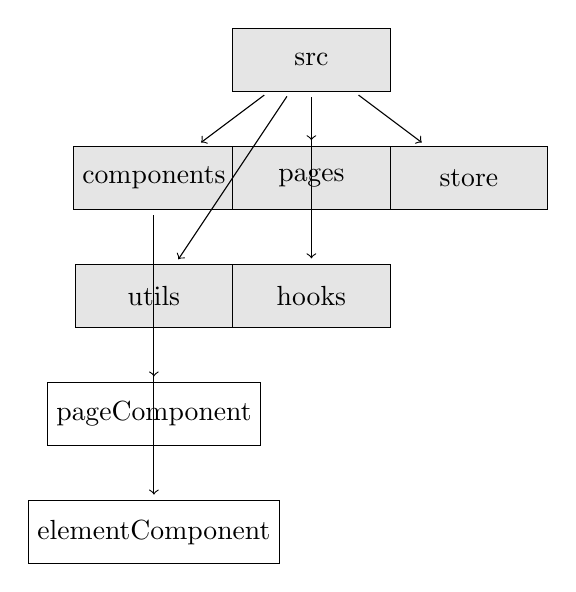
\begin{tikzpicture}[
    file/.style={draw, rectangle, minimum width=2cm, minimum height=0.8cm},
    folder/.style={draw, rectangle, minimum width=2cm, minimum height=0.8cm, fill=gray!20},
    arrow/.style={->, shorten >=2pt, shorten <=2pt}
]

% Folders
\node[folder] (src) at (0,0) {src};
\node[folder] (components) at (-2,-1.5) {components};
\node[folder] (pages) at (0,-1.5) {pages};
\node[folder] (store) at (2,-1.5) {store};
\node[folder] (utils) at (-2,-3) {utils};
\node[folder] (hooks) at (0,-3) {hooks};

% Files
\node[file] (pageComponent) at (-2,-4.5) {pageComponent};
\node[file] (elementComponent) at (-2,-6) {elementComponent};
% ... add more files

% Connections
\draw[arrow] (src) -- (components);
\draw[arrow] (src) -- (pages);
\draw[arrow] (src) -- (store);
\draw[arrow] (src) -- (utils);
\draw[arrow] (src) -- (hooks);
\draw[arrow] (components) -- (pageComponent);
\draw[arrow] (components) -- (elementComponent);
% ... add more connections

\end{tikzpicture}



\pagebreak
\subsubsection{Back-end}
The backend uses the dotNet framework. The development language using the C\# language.

In this project, the backend uses the Onion Architecture.
The Onion Architecture is a typically layered architecture, 
where each layer depends on the inner layer and provides interfaces to the outer layer.
The outer layer provides services to the outermost layer 
and other modules in the same layer based on the interfaces of the inner layer.

From inner to outer, the layers are: Domain, Application, Infrastructure, Presentation.
The Domain layer is the core layer and the innermost layer, used to define domain models, 
which are the business models.
It includes domain models and domain service interfaces.
Domain models are used to define the business models, 
which are the entities in the entity-relationship model and their attributes.
Domain service interfaces are used to define the business services, 
which are the relationships between entities in the entity-relationship model.

The Application layer is the application layer, 
used to define application services, which are the business logic.
It includes domain service implementations and application service interfaces.
Domain service implementations implement the methods of the inner layer's domain service 
interfaces and implement the business logic of the domain models.
Application service interfaces are used to define application services, 
which are the business logic.
It includes but is not limited to database interfaces, testing interfaces, 
HTTP API interfaces, MQTT interfaces, etc.

The Infrastructure layer is the infrastructure layer, used to define infrastructure.
It includes database implementations, testing implementations, 
HTTP API implementations, MQTT implementations, etc.
Database implementations implement the database interfaces 
and provide CRUD services for the database.
Testing implementations implement the testing interfaces 
and provide services for unit testing and integration testing.
HTTP API implementations implement the HTTP API interfaces 
and provide CRUD operations for HTTP APIs.
MQTT implementations implement the MQTT interfaces 
and provide CRUD operations for MQTT.

The Presentation layer is the presentation layer, used to define presentation logic, 
such as interfaces and pages. Since this is a backend project,
data presentation and control are handled by the frontend, 
so this layer is not needed.



\pagebreak
\subsubsection{Data communication and storage}
% 关于本项目的数据通信与数据存储的设计, 包括数据通信的协议, 数据存储的设计等
% 关于数据通信的设计:
% 1. 通信协议的选择
% 自前端向后端发送的数据, 有三种传输的数据类型, 
% 一种是普通的增删改查的请求, 对数据传输的时效性要求不高, 但是对数据的准确性, 完整性, 有序性, 安全性有一定的要求,
% 这种数据的传输, 采用 HTTP 协议, 以及 RESTful API 的设计. 可以有效的保证对数据传输的以上要求.
% 一种是对数据通道的创建和流媒体数据的传输, 对数据传输的时效性, 安全性要求较高, 这种数据的传输, 采用 WebRTC 协议, 以及 MQTT 协议.
% 配合可以快速解码的 flatbuffers 协议, 可以有效的保证对数据传输的以上要求.
% 最后一种是对设备的状态信息和操作信息的传输, 对完整性, 有序性, 安全性都有较高的要求, 这种数据的传输, 采用 MQTT 协议
% 同时也使用了 flatbuffers 协议.
% 
% 2. 数据通信的通信架构和通信流程
% 本项目的数据通信的通信架构, 是基于前后端分离的架构, 前端使用 React 框架, 后端使用 dotnet 框架.
% 当前端需要向后端发送数据的时候, 前端会向后端发送 HTTP 请求, 后端接收到 HTTP 请求之后, 会根据请求的数据类型,
% 选择不同的数据处理方式, 对于普通的增删改查的请求, 后端会根据 RESTful API 的设计, 对数据进行增删改查的操作,
% 对于对数据通道的创建和流媒体数据的传输, 后端会根据 WebRTC 协议, 对数据通道进行创建, 并且帮助前端和设备建立数据通道,
% 当数据通道建立后, 前端和设备之间则使用 flatbuffer 的数据格式对流媒体数据进行传输,
% 对于设备的状态信息和操作信息的传输, 前端会直接向 MQTT broker 发送 MQTT 请求, 
% 设备会在其自身的固件中监听相关的 MQTT 请求, 并且返回相关的数据.
% 
% 3. 数据通信的格式
% 本项目的数据通信的格式, 有三种, 
% 一种是 HTTP 协议, 
% 使用 json 格式对数据进行传输,
% 一种是 WebRTC 协议, 
% 使用 flatbuffers 格式对数据进行传输,
% 一种是 MQTT 协议.
% 使用 flatbuffers 格式对数据进行传输,
% 
% 关于数据存储的设计:
% 1. 数据存储的数据库的选择
% 本项目的数据存储的数据库的选择, 使用了轻量级的数据库 SQLite,
% SQLite 是一个进程内的库, 实现了自给自足的, 无服务器的, 零配置的, 事务性的 SQL 数据库引擎.
% 这是因为整个项目的目的是为了实现前端与设备之间的数据通信, 对于数据库数据的增删改查操作的要求不高,
% 数据量较小, 且对于数据库的数据的事务性要求不高, 所以选择了 SQLite 数据库.
% 2. 项目前后端的数据结构的设计
% 在本项目中, 前端由于使用了 React 框架, 所以前端的数据结构的设计, 使用了基于状态的数据结构的设计,
% 每个组件或者数据集都包含一个状态对象, 这个状态对象的属性就是组件的各个状态. 
% 使用状态对象的原因是, 可以方便的对状态进行管理, 采用对象-属性的形式, 可以方便的针对不同组件的同类状态进行区分,
% 由于跨组件的状态是由 redux 进行管理的, 这种状态对象的设计, 可以更搞笑的对状态进行更新和传递.
% 后端由于使用了 dotnet 框架, 所以后端的数据结构的设计, 使用了基于类的数据结构的设计,
% 采用了面向对象的编程思想, 对数据进行了封装, 使得数据的传输更加的安全, 有序, 完整.


\pagebreak

% \subsection{Domain model}
% \documentclass[]{article}
\usepackage{graphicx}
\usepackage{amsmath}
\usepackage{tikz}

% libaries
\usetikzlibrary{shapes,arrows}

%Define the listing package
\usepackage{listings} %code highlighter
\usepackage{color} %use color
\definecolor{mygreen}{rgb}{0,0.6,0}
\definecolor{mygray}{rgb}{0.5,0.5,0.5}
\definecolor{mymauve}{rgb}{0.58,0,0.82}

%Customize a bit the look
\lstset{ %
backgroundcolor=\color{white}, % choose the background color; you must add \usepackage{color} or \usepackage{xcolor}
basicstyle=\footnotesize, % the size of the fonts that are used for the code
breakatwhitespace=false, % sets if automatic breaks should only happen at whitespace
breaklines=true, % sets automatic line breaking
captionpos=b, % sets the caption-position to bottom
commentstyle=\color{mygreen}, % comment style
deletekeywords={...}, % if you want to delete keywords from the given language
escapeinside={\%*}{*)}, % if you want to add LaTeX within your code
extendedchars=true, % lets you use non-ASCII characters; for 8-bits encodings only, does not work with UTF-8
frame=single, % adds a frame around the code
keepspaces=true, % keeps spaces in text, useful for keeping indentation of code (possibly needs columns=flexible)
keywordstyle=\color{blue}, % keyword style
% language=Octave, % the language of the code
morekeywords={*,...}, % if you want to add more keywords to the set
numbers=left, % where to put the line-numbers; possible values are (none, left, right)
numbersep=5pt, % how far the line-numbers are from the code
numberstyle=\tiny\color{mygray}, % the style that is used for the line-numbers
rulecolor=\color{black}, % if not set, the frame-color may be changed on line-breaks within not-black text (e.g. comments (green here))
showspaces=false, % show spaces everywhere adding particular underscores; it overrides 'showstringspaces'
showstringspaces=false, % underline spaces within strings only
showtabs=false, % show tabs within strings adding particular underscores
stepnumber=1, % the step between two line-numbers. If it's 1, each line will be numbered
stringstyle=\color{mymauve}, % string literal style
tabsize=2, % sets default tabsize to 2 spaces
title=\lstname % show the filename of files included with \lstinputlisting; also try caption instead of title
}

\definecolor{darkgray}{rgb}{.4,.4,.4}
\definecolor{purple}{rgb}{0.65, 0.12, 0.82}

\lstdefinelanguage{React}{
keywords={const, typeof, new, true, false, catch, function, return, null, catch, switch, var, if, in, while, do, else, case, break},
keywordstyle=\color{blue}\bfseries,
ndkeywords={class, export, boolean, throw, implements, import, this},
ndkeywordstyle=\color{darkgray}\bfseries,
identifierstyle=\color{mygreen},
sensitive=false,
comment=[l]{//},
morecomment=[s]{/*}{*/},
commentstyle=\color{purple}\ttfamily,
string=[b]{"}{'}{`},
stringstyle=\color{red}\ttfamily,
morestring=[b]',
morestring=[b]",
morestring=[b]`',
}

\lstdefinelanguage{CSharp}{
keywords={const, typeof, new, true, false, catch, function, return, null, catch, switch, var, if, in, while, do, else, case, break},
keywordstyle=\color{blue}\bfseries,
ndkeywords={class, export, boolean, throw, implements, import, this},
ndkeywordstyle=\color{darkgray}\bfseries,
identifierstyle=\color{mygreen},
sensitive=false,
comment=[l]{//},
morecomment=[s]{/*}{*/},
commentstyle=\color{purple}\ttfamily,
string=[b]{"}{'}{`},
stringstyle=\color{red}\ttfamily,
morestring=[b]',
morestring=[b]",
morestring=[b]`',
}

\lstset{
language=React,
extendedchars=true,
basicstyle=\footnotesize\ttfamily,
showstringspaces=false,
showspaces=false,
numbers=left,
numberstyle=\footnotesize,
numbersep=9pt,
tabsize=2,
breaklines=true,
showtabs=false,
captionpos=b
}

\lstset{
language=CSharp,
extendedchars=true,
basicstyle=\footnotesize\ttfamily,
showstringspaces=false,
showspaces=false,
numbers=left,
numberstyle=\footnotesize,
numbersep=9pt,
tabsize=2,
breaklines=true,
showtabs=false,
captionpos=b
}

% \usepackage{cite} % Add this line for citation

% \bibliographystyle{plain}

\title{
The implementation of BifrostConnect Front-end scope, 
re-design and development with the relevant back-end support develop.
}
\author{
    Fei Gu \\
    Erhvervs Akademi Sydvest \\
    Computer Science 21\\
    }
\date{\today}

\begin{document}

% Front page
\maketitle
\begin{center}
    Supervisor: Henrik Boulund Meng Hansen \\
    Company: BifrostConnect \\
    Engineering Director: Jasper Wass \\
\end{center}
\tableofcontents
\pagebreak


% The introduction
\section{Introduction}
\subsection{Background}\input{sections/introduction/background.tex}
\subsection{The company}\input{sections/introduction/aboutCompany}
\subsection{The project}\input{sections/introduction/aboutProject}
\pagebreak

% The problem statement
\section{Problem Statement}
\subsection{Statement}
\input{sections/problemStatement/statement}
\subsection{Situation}
\input{sections/problemStatement/situation}
\subsection{Potential Solution}
\input{sections/problemStatement/potentialSolution}
\pagebreak

% Requirement analysis
\section{Requirement Analysis}
\input{sections/requirementAnalysis/index}

\subsection{Stakeholders}
\input{sections/requirementAnalysis/stakeholders/index}

\subsection{Business Domain}
\input{sections/requirementAnalysis/bussinesDomain/index}

\subsection{Scope}
\input{sections/requirementAnalysis/scope}

\subsection{Goals}
\input{sections/requirementAnalysis/goals}
\pagebreak

% Software Design
\section{Software Design}
% developement methods
\subsection{Software Development Methods}
\input{sections/softwareDevelopmentMethods/index}
\subsubsection{Agile Software Development}
\input{sections/softwareDevelopmentMethods/agileSoftwareDevelopment/index}
\subsubsection{Feature Driven Development}
\input{sections/softwareDevelopmentMethods/featureDrivenDevelopment/index}

\pagebreak

% Technology seslection
\subsection{Technology selection}
\input{sections/softwareDesign/technologySelection/index}
\subsubsection{Front-end}
\input{sections/softwareDesign/technologySelection/frontEnd}            
\subsubsection{Back-end}
\input{sections/softwareDesign/technologySelection/backEnd}            
\subsubsection{Database}
\input{sections/softwareDesign/technologySelection/database}
\subsubsection{Data communication}
\input{sections/softwareDesign/technologySelection/dataCommunication}            
\subsubsection{DevOps}
\input{sections/softwareDesign/technologySelection/devOps}
\pagebreak

% Architecture design
\subsection{Architecture design}
\input{sections/softwareDesign/architectureDesign/index}
\pagebreak
\subsubsection{Front-end}
\input{sections/softwareDesign/architectureDesign/frontEndArchitecture}
\pagebreak
\subsubsection{Back-end}
\input{sections/softwareDesign/architectureDesign/backEndArchitecture}
\pagebreak
\subsubsection{Data communication and storage}
\input{sections/softwareDesign/architectureDesign/dataCommunicationArchitecture}
\pagebreak

% \subsection{Domain model}
% \input{sections/softwareDesign/domainModel/index}
% \subsection{Database design}
% % 数据库领域模型 ER 图
% % 包括表和字段的设置.
% % 对于私有键和外键的设置.

% \subsection{Back-end design}
% % 后端对象模型
% % 以及对于对象模型的增删改查
% % 以及相关的其他服务的设计`'

% \subsection{Front-end design}
% % 对于前端的页面结构的设计 
% % 页面的状态的设计, 交互设计

% \subsection{FlatBuffers design}
% % schema 的设计

\subsection{DevOps CI/CD process design}
\input{sections/softwareDesign/devOpsDesign/index}
\subsubsection{Continuous Integration}
\input{sections/softwareDesign/devOpsDesign/continuousIntegration/index}
\subsubsection{Continuous Delivery}
\input{sections/softwareDesign/devOpsDesign/continuousDelivery/index}
\subsubsection{Continuous Deployment}
\input{sections/softwareDesign/devOpsDesign/continuousDeployment/index}
\pagebreak

\section{Software Development} 
\input{sections/softwareDevelopment/index}
\subsection{Overall development}
\input{sections/softwareDevelopment/overallDevelopement/index}
\subsubsection{Front-end}
\input{sections/softwareDevelopment/overallDevelopement/frontEnd/index}
\subsubsection{Back-end}
\input{sections/softwareDevelopment/overallDevelopement/backEnd/index}
\subsubsection{DevOps}
\input{sections/softwareDevelopment/overallDevelopement/devOps/index}
\subsection{Feature development} 
\input{sections/softwareDevelopment/featureDevelopment/index}
\subsubsection{Use Case 1}
\input{sections/softwareDevelopment/featureDevelopment/useCase1/index}
\subsubsection{Feature 1}
\input{sections/softwareDevelopment/featureDevelopment/feature/feature1.tex}
\pagebreak
\section{Conclusion} 
\subsection{Result}
Since the project is still in progress, the result is not available yet.
So far, basic structure of this project has been built. But the most features 
are not implemented yet. 
\subsection{Discussion}
As a single developer for this project, I am confident what I have done so far.
And I can say I understand the most of the knowledge I have used in this project, 
which also means I can explain all the part of the project. 
But this project also relevant some of the complex knowledge which I have to continue 
to study and practice.
\subsection{Future Work}
The future work is to implement the rest of the features. 
Including the most important part which is the 'create session' feature.
\pagebreak
% \bibliography{bibliography}
\pagebreak
% \begin{appendices}
%     \section{Appendix}
% \end{appendices} 
\end{document}
% \subsection{Database design}
% % 数据库领域模型 ER 图
% % 包括表和字段的设置.
% % 对于私有键和外键的设置.

% \subsection{Back-end design}
% % 后端对象模型
% % 以及对于对象模型的增删改查
% % 以及相关的其他服务的设计`'

% \subsection{Front-end design}
% % 对于前端的页面结构的设计 
% % 页面的状态的设计, 交互设计

% \subsection{FlatBuffers design}
% % schema 的设计

\subsection{DevOps CI/CD process design}
\documentclass[]{article}
\usepackage{graphicx}
\usepackage{amsmath}
\usepackage{tikz}

% libaries
\usetikzlibrary{shapes,arrows}

%Define the listing package
\usepackage{listings} %code highlighter
\usepackage{color} %use color
\definecolor{mygreen}{rgb}{0,0.6,0}
\definecolor{mygray}{rgb}{0.5,0.5,0.5}
\definecolor{mymauve}{rgb}{0.58,0,0.82}

%Customize a bit the look
\lstset{ %
backgroundcolor=\color{white}, % choose the background color; you must add \usepackage{color} or \usepackage{xcolor}
basicstyle=\footnotesize, % the size of the fonts that are used for the code
breakatwhitespace=false, % sets if automatic breaks should only happen at whitespace
breaklines=true, % sets automatic line breaking
captionpos=b, % sets the caption-position to bottom
commentstyle=\color{mygreen}, % comment style
deletekeywords={...}, % if you want to delete keywords from the given language
escapeinside={\%*}{*)}, % if you want to add LaTeX within your code
extendedchars=true, % lets you use non-ASCII characters; for 8-bits encodings only, does not work with UTF-8
frame=single, % adds a frame around the code
keepspaces=true, % keeps spaces in text, useful for keeping indentation of code (possibly needs columns=flexible)
keywordstyle=\color{blue}, % keyword style
% language=Octave, % the language of the code
morekeywords={*,...}, % if you want to add more keywords to the set
numbers=left, % where to put the line-numbers; possible values are (none, left, right)
numbersep=5pt, % how far the line-numbers are from the code
numberstyle=\tiny\color{mygray}, % the style that is used for the line-numbers
rulecolor=\color{black}, % if not set, the frame-color may be changed on line-breaks within not-black text (e.g. comments (green here))
showspaces=false, % show spaces everywhere adding particular underscores; it overrides 'showstringspaces'
showstringspaces=false, % underline spaces within strings only
showtabs=false, % show tabs within strings adding particular underscores
stepnumber=1, % the step between two line-numbers. If it's 1, each line will be numbered
stringstyle=\color{mymauve}, % string literal style
tabsize=2, % sets default tabsize to 2 spaces
title=\lstname % show the filename of files included with \lstinputlisting; also try caption instead of title
}

\definecolor{darkgray}{rgb}{.4,.4,.4}
\definecolor{purple}{rgb}{0.65, 0.12, 0.82}

\lstdefinelanguage{React}{
keywords={const, typeof, new, true, false, catch, function, return, null, catch, switch, var, if, in, while, do, else, case, break},
keywordstyle=\color{blue}\bfseries,
ndkeywords={class, export, boolean, throw, implements, import, this},
ndkeywordstyle=\color{darkgray}\bfseries,
identifierstyle=\color{mygreen},
sensitive=false,
comment=[l]{//},
morecomment=[s]{/*}{*/},
commentstyle=\color{purple}\ttfamily,
string=[b]{"}{'}{`},
stringstyle=\color{red}\ttfamily,
morestring=[b]',
morestring=[b]",
morestring=[b]`',
}

\lstdefinelanguage{CSharp}{
keywords={const, typeof, new, true, false, catch, function, return, null, catch, switch, var, if, in, while, do, else, case, break},
keywordstyle=\color{blue}\bfseries,
ndkeywords={class, export, boolean, throw, implements, import, this},
ndkeywordstyle=\color{darkgray}\bfseries,
identifierstyle=\color{mygreen},
sensitive=false,
comment=[l]{//},
morecomment=[s]{/*}{*/},
commentstyle=\color{purple}\ttfamily,
string=[b]{"}{'}{`},
stringstyle=\color{red}\ttfamily,
morestring=[b]',
morestring=[b]",
morestring=[b]`',
}

\lstset{
language=React,
extendedchars=true,
basicstyle=\footnotesize\ttfamily,
showstringspaces=false,
showspaces=false,
numbers=left,
numberstyle=\footnotesize,
numbersep=9pt,
tabsize=2,
breaklines=true,
showtabs=false,
captionpos=b
}

\lstset{
language=CSharp,
extendedchars=true,
basicstyle=\footnotesize\ttfamily,
showstringspaces=false,
showspaces=false,
numbers=left,
numberstyle=\footnotesize,
numbersep=9pt,
tabsize=2,
breaklines=true,
showtabs=false,
captionpos=b
}

% \usepackage{cite} % Add this line for citation

% \bibliographystyle{plain}

\title{
The implementation of BifrostConnect Front-end scope, 
re-design and development with the relevant back-end support develop.
}
\author{
    Fei Gu \\
    Erhvervs Akademi Sydvest \\
    Computer Science 21\\
    }
\date{\today}

\begin{document}

% Front page
\maketitle
\begin{center}
    Supervisor: Henrik Boulund Meng Hansen \\
    Company: BifrostConnect \\
    Engineering Director: Jasper Wass \\
\end{center}
\tableofcontents
\pagebreak


% The introduction
\section{Introduction}
\subsection{Background}\input{sections/introduction/background.tex}
\subsection{The company}\input{sections/introduction/aboutCompany}
\subsection{The project}\input{sections/introduction/aboutProject}
\pagebreak

% The problem statement
\section{Problem Statement}
\subsection{Statement}
\input{sections/problemStatement/statement}
\subsection{Situation}
\input{sections/problemStatement/situation}
\subsection{Potential Solution}
\input{sections/problemStatement/potentialSolution}
\pagebreak

% Requirement analysis
\section{Requirement Analysis}
\input{sections/requirementAnalysis/index}

\subsection{Stakeholders}
\input{sections/requirementAnalysis/stakeholders/index}

\subsection{Business Domain}
\input{sections/requirementAnalysis/bussinesDomain/index}

\subsection{Scope}
\input{sections/requirementAnalysis/scope}

\subsection{Goals}
\input{sections/requirementAnalysis/goals}
\pagebreak

% Software Design
\section{Software Design}
% developement methods
\subsection{Software Development Methods}
\input{sections/softwareDevelopmentMethods/index}
\subsubsection{Agile Software Development}
\input{sections/softwareDevelopmentMethods/agileSoftwareDevelopment/index}
\subsubsection{Feature Driven Development}
\input{sections/softwareDevelopmentMethods/featureDrivenDevelopment/index}

\pagebreak

% Technology seslection
\subsection{Technology selection}
\input{sections/softwareDesign/technologySelection/index}
\subsubsection{Front-end}
\input{sections/softwareDesign/technologySelection/frontEnd}            
\subsubsection{Back-end}
\input{sections/softwareDesign/technologySelection/backEnd}            
\subsubsection{Database}
\input{sections/softwareDesign/technologySelection/database}
\subsubsection{Data communication}
\input{sections/softwareDesign/technologySelection/dataCommunication}            
\subsubsection{DevOps}
\input{sections/softwareDesign/technologySelection/devOps}
\pagebreak

% Architecture design
\subsection{Architecture design}
\input{sections/softwareDesign/architectureDesign/index}
\pagebreak
\subsubsection{Front-end}
\input{sections/softwareDesign/architectureDesign/frontEndArchitecture}
\pagebreak
\subsubsection{Back-end}
\input{sections/softwareDesign/architectureDesign/backEndArchitecture}
\pagebreak
\subsubsection{Data communication and storage}
\input{sections/softwareDesign/architectureDesign/dataCommunicationArchitecture}
\pagebreak

% \subsection{Domain model}
% \input{sections/softwareDesign/domainModel/index}
% \subsection{Database design}
% % 数据库领域模型 ER 图
% % 包括表和字段的设置.
% % 对于私有键和外键的设置.

% \subsection{Back-end design}
% % 后端对象模型
% % 以及对于对象模型的增删改查
% % 以及相关的其他服务的设计`'

% \subsection{Front-end design}
% % 对于前端的页面结构的设计 
% % 页面的状态的设计, 交互设计

% \subsection{FlatBuffers design}
% % schema 的设计

\subsection{DevOps CI/CD process design}
\input{sections/softwareDesign/devOpsDesign/index}
\subsubsection{Continuous Integration}
\input{sections/softwareDesign/devOpsDesign/continuousIntegration/index}
\subsubsection{Continuous Delivery}
\input{sections/softwareDesign/devOpsDesign/continuousDelivery/index}
\subsubsection{Continuous Deployment}
\input{sections/softwareDesign/devOpsDesign/continuousDeployment/index}
\pagebreak

\section{Software Development} 
\input{sections/softwareDevelopment/index}
\subsection{Overall development}
\input{sections/softwareDevelopment/overallDevelopement/index}
\subsubsection{Front-end}
\input{sections/softwareDevelopment/overallDevelopement/frontEnd/index}
\subsubsection{Back-end}
\input{sections/softwareDevelopment/overallDevelopement/backEnd/index}
\subsubsection{DevOps}
\input{sections/softwareDevelopment/overallDevelopement/devOps/index}
\subsection{Feature development} 
\input{sections/softwareDevelopment/featureDevelopment/index}
\subsubsection{Use Case 1}
\input{sections/softwareDevelopment/featureDevelopment/useCase1/index}
\subsubsection{Feature 1}
\input{sections/softwareDevelopment/featureDevelopment/feature/feature1.tex}
\pagebreak
\section{Conclusion} 
\subsection{Result}
Since the project is still in progress, the result is not available yet.
So far, basic structure of this project has been built. But the most features 
are not implemented yet. 
\subsection{Discussion}
As a single developer for this project, I am confident what I have done so far.
And I can say I understand the most of the knowledge I have used in this project, 
which also means I can explain all the part of the project. 
But this project also relevant some of the complex knowledge which I have to continue 
to study and practice.
\subsection{Future Work}
The future work is to implement the rest of the features. 
Including the most important part which is the 'create session' feature.
\pagebreak
% \bibliography{bibliography}
\pagebreak
% \begin{appendices}
%     \section{Appendix}
% \end{appendices} 
\end{document}
\subsubsection{Continuous Integration}
\documentclass[]{article}
\usepackage{graphicx}
\usepackage{amsmath}
\usepackage{tikz}

% libaries
\usetikzlibrary{shapes,arrows}

%Define the listing package
\usepackage{listings} %code highlighter
\usepackage{color} %use color
\definecolor{mygreen}{rgb}{0,0.6,0}
\definecolor{mygray}{rgb}{0.5,0.5,0.5}
\definecolor{mymauve}{rgb}{0.58,0,0.82}

%Customize a bit the look
\lstset{ %
backgroundcolor=\color{white}, % choose the background color; you must add \usepackage{color} or \usepackage{xcolor}
basicstyle=\footnotesize, % the size of the fonts that are used for the code
breakatwhitespace=false, % sets if automatic breaks should only happen at whitespace
breaklines=true, % sets automatic line breaking
captionpos=b, % sets the caption-position to bottom
commentstyle=\color{mygreen}, % comment style
deletekeywords={...}, % if you want to delete keywords from the given language
escapeinside={\%*}{*)}, % if you want to add LaTeX within your code
extendedchars=true, % lets you use non-ASCII characters; for 8-bits encodings only, does not work with UTF-8
frame=single, % adds a frame around the code
keepspaces=true, % keeps spaces in text, useful for keeping indentation of code (possibly needs columns=flexible)
keywordstyle=\color{blue}, % keyword style
% language=Octave, % the language of the code
morekeywords={*,...}, % if you want to add more keywords to the set
numbers=left, % where to put the line-numbers; possible values are (none, left, right)
numbersep=5pt, % how far the line-numbers are from the code
numberstyle=\tiny\color{mygray}, % the style that is used for the line-numbers
rulecolor=\color{black}, % if not set, the frame-color may be changed on line-breaks within not-black text (e.g. comments (green here))
showspaces=false, % show spaces everywhere adding particular underscores; it overrides 'showstringspaces'
showstringspaces=false, % underline spaces within strings only
showtabs=false, % show tabs within strings adding particular underscores
stepnumber=1, % the step between two line-numbers. If it's 1, each line will be numbered
stringstyle=\color{mymauve}, % string literal style
tabsize=2, % sets default tabsize to 2 spaces
title=\lstname % show the filename of files included with \lstinputlisting; also try caption instead of title
}

\definecolor{darkgray}{rgb}{.4,.4,.4}
\definecolor{purple}{rgb}{0.65, 0.12, 0.82}

\lstdefinelanguage{React}{
keywords={const, typeof, new, true, false, catch, function, return, null, catch, switch, var, if, in, while, do, else, case, break},
keywordstyle=\color{blue}\bfseries,
ndkeywords={class, export, boolean, throw, implements, import, this},
ndkeywordstyle=\color{darkgray}\bfseries,
identifierstyle=\color{mygreen},
sensitive=false,
comment=[l]{//},
morecomment=[s]{/*}{*/},
commentstyle=\color{purple}\ttfamily,
string=[b]{"}{'}{`},
stringstyle=\color{red}\ttfamily,
morestring=[b]',
morestring=[b]",
morestring=[b]`',
}

\lstdefinelanguage{CSharp}{
keywords={const, typeof, new, true, false, catch, function, return, null, catch, switch, var, if, in, while, do, else, case, break},
keywordstyle=\color{blue}\bfseries,
ndkeywords={class, export, boolean, throw, implements, import, this},
ndkeywordstyle=\color{darkgray}\bfseries,
identifierstyle=\color{mygreen},
sensitive=false,
comment=[l]{//},
morecomment=[s]{/*}{*/},
commentstyle=\color{purple}\ttfamily,
string=[b]{"}{'}{`},
stringstyle=\color{red}\ttfamily,
morestring=[b]',
morestring=[b]",
morestring=[b]`',
}

\lstset{
language=React,
extendedchars=true,
basicstyle=\footnotesize\ttfamily,
showstringspaces=false,
showspaces=false,
numbers=left,
numberstyle=\footnotesize,
numbersep=9pt,
tabsize=2,
breaklines=true,
showtabs=false,
captionpos=b
}

\lstset{
language=CSharp,
extendedchars=true,
basicstyle=\footnotesize\ttfamily,
showstringspaces=false,
showspaces=false,
numbers=left,
numberstyle=\footnotesize,
numbersep=9pt,
tabsize=2,
breaklines=true,
showtabs=false,
captionpos=b
}

% \usepackage{cite} % Add this line for citation

% \bibliographystyle{plain}

\title{
The implementation of BifrostConnect Front-end scope, 
re-design and development with the relevant back-end support develop.
}
\author{
    Fei Gu \\
    Erhvervs Akademi Sydvest \\
    Computer Science 21\\
    }
\date{\today}

\begin{document}

% Front page
\maketitle
\begin{center}
    Supervisor: Henrik Boulund Meng Hansen \\
    Company: BifrostConnect \\
    Engineering Director: Jasper Wass \\
\end{center}
\tableofcontents
\pagebreak


% The introduction
\section{Introduction}
\subsection{Background}\input{sections/introduction/background.tex}
\subsection{The company}\input{sections/introduction/aboutCompany}
\subsection{The project}\input{sections/introduction/aboutProject}
\pagebreak

% The problem statement
\section{Problem Statement}
\subsection{Statement}
\input{sections/problemStatement/statement}
\subsection{Situation}
\input{sections/problemStatement/situation}
\subsection{Potential Solution}
\input{sections/problemStatement/potentialSolution}
\pagebreak

% Requirement analysis
\section{Requirement Analysis}
\input{sections/requirementAnalysis/index}

\subsection{Stakeholders}
\input{sections/requirementAnalysis/stakeholders/index}

\subsection{Business Domain}
\input{sections/requirementAnalysis/bussinesDomain/index}

\subsection{Scope}
\input{sections/requirementAnalysis/scope}

\subsection{Goals}
\input{sections/requirementAnalysis/goals}
\pagebreak

% Software Design
\section{Software Design}
% developement methods
\subsection{Software Development Methods}
\input{sections/softwareDevelopmentMethods/index}
\subsubsection{Agile Software Development}
\input{sections/softwareDevelopmentMethods/agileSoftwareDevelopment/index}
\subsubsection{Feature Driven Development}
\input{sections/softwareDevelopmentMethods/featureDrivenDevelopment/index}

\pagebreak

% Technology seslection
\subsection{Technology selection}
\input{sections/softwareDesign/technologySelection/index}
\subsubsection{Front-end}
\input{sections/softwareDesign/technologySelection/frontEnd}            
\subsubsection{Back-end}
\input{sections/softwareDesign/technologySelection/backEnd}            
\subsubsection{Database}
\input{sections/softwareDesign/technologySelection/database}
\subsubsection{Data communication}
\input{sections/softwareDesign/technologySelection/dataCommunication}            
\subsubsection{DevOps}
\input{sections/softwareDesign/technologySelection/devOps}
\pagebreak

% Architecture design
\subsection{Architecture design}
\input{sections/softwareDesign/architectureDesign/index}
\pagebreak
\subsubsection{Front-end}
\input{sections/softwareDesign/architectureDesign/frontEndArchitecture}
\pagebreak
\subsubsection{Back-end}
\input{sections/softwareDesign/architectureDesign/backEndArchitecture}
\pagebreak
\subsubsection{Data communication and storage}
\input{sections/softwareDesign/architectureDesign/dataCommunicationArchitecture}
\pagebreak

% \subsection{Domain model}
% \input{sections/softwareDesign/domainModel/index}
% \subsection{Database design}
% % 数据库领域模型 ER 图
% % 包括表和字段的设置.
% % 对于私有键和外键的设置.

% \subsection{Back-end design}
% % 后端对象模型
% % 以及对于对象模型的增删改查
% % 以及相关的其他服务的设计`'

% \subsection{Front-end design}
% % 对于前端的页面结构的设计 
% % 页面的状态的设计, 交互设计

% \subsection{FlatBuffers design}
% % schema 的设计

\subsection{DevOps CI/CD process design}
\input{sections/softwareDesign/devOpsDesign/index}
\subsubsection{Continuous Integration}
\input{sections/softwareDesign/devOpsDesign/continuousIntegration/index}
\subsubsection{Continuous Delivery}
\input{sections/softwareDesign/devOpsDesign/continuousDelivery/index}
\subsubsection{Continuous Deployment}
\input{sections/softwareDesign/devOpsDesign/continuousDeployment/index}
\pagebreak

\section{Software Development} 
\input{sections/softwareDevelopment/index}
\subsection{Overall development}
\input{sections/softwareDevelopment/overallDevelopement/index}
\subsubsection{Front-end}
\input{sections/softwareDevelopment/overallDevelopement/frontEnd/index}
\subsubsection{Back-end}
\input{sections/softwareDevelopment/overallDevelopement/backEnd/index}
\subsubsection{DevOps}
\input{sections/softwareDevelopment/overallDevelopement/devOps/index}
\subsection{Feature development} 
\input{sections/softwareDevelopment/featureDevelopment/index}
\subsubsection{Use Case 1}
\input{sections/softwareDevelopment/featureDevelopment/useCase1/index}
\subsubsection{Feature 1}
\input{sections/softwareDevelopment/featureDevelopment/feature/feature1.tex}
\pagebreak
\section{Conclusion} 
\subsection{Result}
Since the project is still in progress, the result is not available yet.
So far, basic structure of this project has been built. But the most features 
are not implemented yet. 
\subsection{Discussion}
As a single developer for this project, I am confident what I have done so far.
And I can say I understand the most of the knowledge I have used in this project, 
which also means I can explain all the part of the project. 
But this project also relevant some of the complex knowledge which I have to continue 
to study and practice.
\subsection{Future Work}
The future work is to implement the rest of the features. 
Including the most important part which is the 'create session' feature.
\pagebreak
% \bibliography{bibliography}
\pagebreak
% \begin{appendices}
%     \section{Appendix}
% \end{appendices} 
\end{document}
\subsubsection{Continuous Delivery}
\documentclass[]{article}
\usepackage{graphicx}
\usepackage{amsmath}
\usepackage{tikz}

% libaries
\usetikzlibrary{shapes,arrows}

%Define the listing package
\usepackage{listings} %code highlighter
\usepackage{color} %use color
\definecolor{mygreen}{rgb}{0,0.6,0}
\definecolor{mygray}{rgb}{0.5,0.5,0.5}
\definecolor{mymauve}{rgb}{0.58,0,0.82}

%Customize a bit the look
\lstset{ %
backgroundcolor=\color{white}, % choose the background color; you must add \usepackage{color} or \usepackage{xcolor}
basicstyle=\footnotesize, % the size of the fonts that are used for the code
breakatwhitespace=false, % sets if automatic breaks should only happen at whitespace
breaklines=true, % sets automatic line breaking
captionpos=b, % sets the caption-position to bottom
commentstyle=\color{mygreen}, % comment style
deletekeywords={...}, % if you want to delete keywords from the given language
escapeinside={\%*}{*)}, % if you want to add LaTeX within your code
extendedchars=true, % lets you use non-ASCII characters; for 8-bits encodings only, does not work with UTF-8
frame=single, % adds a frame around the code
keepspaces=true, % keeps spaces in text, useful for keeping indentation of code (possibly needs columns=flexible)
keywordstyle=\color{blue}, % keyword style
% language=Octave, % the language of the code
morekeywords={*,...}, % if you want to add more keywords to the set
numbers=left, % where to put the line-numbers; possible values are (none, left, right)
numbersep=5pt, % how far the line-numbers are from the code
numberstyle=\tiny\color{mygray}, % the style that is used for the line-numbers
rulecolor=\color{black}, % if not set, the frame-color may be changed on line-breaks within not-black text (e.g. comments (green here))
showspaces=false, % show spaces everywhere adding particular underscores; it overrides 'showstringspaces'
showstringspaces=false, % underline spaces within strings only
showtabs=false, % show tabs within strings adding particular underscores
stepnumber=1, % the step between two line-numbers. If it's 1, each line will be numbered
stringstyle=\color{mymauve}, % string literal style
tabsize=2, % sets default tabsize to 2 spaces
title=\lstname % show the filename of files included with \lstinputlisting; also try caption instead of title
}

\definecolor{darkgray}{rgb}{.4,.4,.4}
\definecolor{purple}{rgb}{0.65, 0.12, 0.82}

\lstdefinelanguage{React}{
keywords={const, typeof, new, true, false, catch, function, return, null, catch, switch, var, if, in, while, do, else, case, break},
keywordstyle=\color{blue}\bfseries,
ndkeywords={class, export, boolean, throw, implements, import, this},
ndkeywordstyle=\color{darkgray}\bfseries,
identifierstyle=\color{mygreen},
sensitive=false,
comment=[l]{//},
morecomment=[s]{/*}{*/},
commentstyle=\color{purple}\ttfamily,
string=[b]{"}{'}{`},
stringstyle=\color{red}\ttfamily,
morestring=[b]',
morestring=[b]",
morestring=[b]`',
}

\lstdefinelanguage{CSharp}{
keywords={const, typeof, new, true, false, catch, function, return, null, catch, switch, var, if, in, while, do, else, case, break},
keywordstyle=\color{blue}\bfseries,
ndkeywords={class, export, boolean, throw, implements, import, this},
ndkeywordstyle=\color{darkgray}\bfseries,
identifierstyle=\color{mygreen},
sensitive=false,
comment=[l]{//},
morecomment=[s]{/*}{*/},
commentstyle=\color{purple}\ttfamily,
string=[b]{"}{'}{`},
stringstyle=\color{red}\ttfamily,
morestring=[b]',
morestring=[b]",
morestring=[b]`',
}

\lstset{
language=React,
extendedchars=true,
basicstyle=\footnotesize\ttfamily,
showstringspaces=false,
showspaces=false,
numbers=left,
numberstyle=\footnotesize,
numbersep=9pt,
tabsize=2,
breaklines=true,
showtabs=false,
captionpos=b
}

\lstset{
language=CSharp,
extendedchars=true,
basicstyle=\footnotesize\ttfamily,
showstringspaces=false,
showspaces=false,
numbers=left,
numberstyle=\footnotesize,
numbersep=9pt,
tabsize=2,
breaklines=true,
showtabs=false,
captionpos=b
}

% \usepackage{cite} % Add this line for citation

% \bibliographystyle{plain}

\title{
The implementation of BifrostConnect Front-end scope, 
re-design and development with the relevant back-end support develop.
}
\author{
    Fei Gu \\
    Erhvervs Akademi Sydvest \\
    Computer Science 21\\
    }
\date{\today}

\begin{document}

% Front page
\maketitle
\begin{center}
    Supervisor: Henrik Boulund Meng Hansen \\
    Company: BifrostConnect \\
    Engineering Director: Jasper Wass \\
\end{center}
\tableofcontents
\pagebreak


% The introduction
\section{Introduction}
\subsection{Background}\input{sections/introduction/background.tex}
\subsection{The company}\input{sections/introduction/aboutCompany}
\subsection{The project}\input{sections/introduction/aboutProject}
\pagebreak

% The problem statement
\section{Problem Statement}
\subsection{Statement}
\input{sections/problemStatement/statement}
\subsection{Situation}
\input{sections/problemStatement/situation}
\subsection{Potential Solution}
\input{sections/problemStatement/potentialSolution}
\pagebreak

% Requirement analysis
\section{Requirement Analysis}
\input{sections/requirementAnalysis/index}

\subsection{Stakeholders}
\input{sections/requirementAnalysis/stakeholders/index}

\subsection{Business Domain}
\input{sections/requirementAnalysis/bussinesDomain/index}

\subsection{Scope}
\input{sections/requirementAnalysis/scope}

\subsection{Goals}
\input{sections/requirementAnalysis/goals}
\pagebreak

% Software Design
\section{Software Design}
% developement methods
\subsection{Software Development Methods}
\input{sections/softwareDevelopmentMethods/index}
\subsubsection{Agile Software Development}
\input{sections/softwareDevelopmentMethods/agileSoftwareDevelopment/index}
\subsubsection{Feature Driven Development}
\input{sections/softwareDevelopmentMethods/featureDrivenDevelopment/index}

\pagebreak

% Technology seslection
\subsection{Technology selection}
\input{sections/softwareDesign/technologySelection/index}
\subsubsection{Front-end}
\input{sections/softwareDesign/technologySelection/frontEnd}            
\subsubsection{Back-end}
\input{sections/softwareDesign/technologySelection/backEnd}            
\subsubsection{Database}
\input{sections/softwareDesign/technologySelection/database}
\subsubsection{Data communication}
\input{sections/softwareDesign/technologySelection/dataCommunication}            
\subsubsection{DevOps}
\input{sections/softwareDesign/technologySelection/devOps}
\pagebreak

% Architecture design
\subsection{Architecture design}
\input{sections/softwareDesign/architectureDesign/index}
\pagebreak
\subsubsection{Front-end}
\input{sections/softwareDesign/architectureDesign/frontEndArchitecture}
\pagebreak
\subsubsection{Back-end}
\input{sections/softwareDesign/architectureDesign/backEndArchitecture}
\pagebreak
\subsubsection{Data communication and storage}
\input{sections/softwareDesign/architectureDesign/dataCommunicationArchitecture}
\pagebreak

% \subsection{Domain model}
% \input{sections/softwareDesign/domainModel/index}
% \subsection{Database design}
% % 数据库领域模型 ER 图
% % 包括表和字段的设置.
% % 对于私有键和外键的设置.

% \subsection{Back-end design}
% % 后端对象模型
% % 以及对于对象模型的增删改查
% % 以及相关的其他服务的设计`'

% \subsection{Front-end design}
% % 对于前端的页面结构的设计 
% % 页面的状态的设计, 交互设计

% \subsection{FlatBuffers design}
% % schema 的设计

\subsection{DevOps CI/CD process design}
\input{sections/softwareDesign/devOpsDesign/index}
\subsubsection{Continuous Integration}
\input{sections/softwareDesign/devOpsDesign/continuousIntegration/index}
\subsubsection{Continuous Delivery}
\input{sections/softwareDesign/devOpsDesign/continuousDelivery/index}
\subsubsection{Continuous Deployment}
\input{sections/softwareDesign/devOpsDesign/continuousDeployment/index}
\pagebreak

\section{Software Development} 
\input{sections/softwareDevelopment/index}
\subsection{Overall development}
\input{sections/softwareDevelopment/overallDevelopement/index}
\subsubsection{Front-end}
\input{sections/softwareDevelopment/overallDevelopement/frontEnd/index}
\subsubsection{Back-end}
\input{sections/softwareDevelopment/overallDevelopement/backEnd/index}
\subsubsection{DevOps}
\input{sections/softwareDevelopment/overallDevelopement/devOps/index}
\subsection{Feature development} 
\input{sections/softwareDevelopment/featureDevelopment/index}
\subsubsection{Use Case 1}
\input{sections/softwareDevelopment/featureDevelopment/useCase1/index}
\subsubsection{Feature 1}
\input{sections/softwareDevelopment/featureDevelopment/feature/feature1.tex}
\pagebreak
\section{Conclusion} 
\subsection{Result}
Since the project is still in progress, the result is not available yet.
So far, basic structure of this project has been built. But the most features 
are not implemented yet. 
\subsection{Discussion}
As a single developer for this project, I am confident what I have done so far.
And I can say I understand the most of the knowledge I have used in this project, 
which also means I can explain all the part of the project. 
But this project also relevant some of the complex knowledge which I have to continue 
to study and practice.
\subsection{Future Work}
The future work is to implement the rest of the features. 
Including the most important part which is the 'create session' feature.
\pagebreak
% \bibliography{bibliography}
\pagebreak
% \begin{appendices}
%     \section{Appendix}
% \end{appendices} 
\end{document}
\subsubsection{Continuous Deployment}
\documentclass[]{article}
\usepackage{graphicx}
\usepackage{amsmath}
\usepackage{tikz}

% libaries
\usetikzlibrary{shapes,arrows}

%Define the listing package
\usepackage{listings} %code highlighter
\usepackage{color} %use color
\definecolor{mygreen}{rgb}{0,0.6,0}
\definecolor{mygray}{rgb}{0.5,0.5,0.5}
\definecolor{mymauve}{rgb}{0.58,0,0.82}

%Customize a bit the look
\lstset{ %
backgroundcolor=\color{white}, % choose the background color; you must add \usepackage{color} or \usepackage{xcolor}
basicstyle=\footnotesize, % the size of the fonts that are used for the code
breakatwhitespace=false, % sets if automatic breaks should only happen at whitespace
breaklines=true, % sets automatic line breaking
captionpos=b, % sets the caption-position to bottom
commentstyle=\color{mygreen}, % comment style
deletekeywords={...}, % if you want to delete keywords from the given language
escapeinside={\%*}{*)}, % if you want to add LaTeX within your code
extendedchars=true, % lets you use non-ASCII characters; for 8-bits encodings only, does not work with UTF-8
frame=single, % adds a frame around the code
keepspaces=true, % keeps spaces in text, useful for keeping indentation of code (possibly needs columns=flexible)
keywordstyle=\color{blue}, % keyword style
% language=Octave, % the language of the code
morekeywords={*,...}, % if you want to add more keywords to the set
numbers=left, % where to put the line-numbers; possible values are (none, left, right)
numbersep=5pt, % how far the line-numbers are from the code
numberstyle=\tiny\color{mygray}, % the style that is used for the line-numbers
rulecolor=\color{black}, % if not set, the frame-color may be changed on line-breaks within not-black text (e.g. comments (green here))
showspaces=false, % show spaces everywhere adding particular underscores; it overrides 'showstringspaces'
showstringspaces=false, % underline spaces within strings only
showtabs=false, % show tabs within strings adding particular underscores
stepnumber=1, % the step between two line-numbers. If it's 1, each line will be numbered
stringstyle=\color{mymauve}, % string literal style
tabsize=2, % sets default tabsize to 2 spaces
title=\lstname % show the filename of files included with \lstinputlisting; also try caption instead of title
}

\definecolor{darkgray}{rgb}{.4,.4,.4}
\definecolor{purple}{rgb}{0.65, 0.12, 0.82}

\lstdefinelanguage{React}{
keywords={const, typeof, new, true, false, catch, function, return, null, catch, switch, var, if, in, while, do, else, case, break},
keywordstyle=\color{blue}\bfseries,
ndkeywords={class, export, boolean, throw, implements, import, this},
ndkeywordstyle=\color{darkgray}\bfseries,
identifierstyle=\color{mygreen},
sensitive=false,
comment=[l]{//},
morecomment=[s]{/*}{*/},
commentstyle=\color{purple}\ttfamily,
string=[b]{"}{'}{`},
stringstyle=\color{red}\ttfamily,
morestring=[b]',
morestring=[b]",
morestring=[b]`',
}

\lstdefinelanguage{CSharp}{
keywords={const, typeof, new, true, false, catch, function, return, null, catch, switch, var, if, in, while, do, else, case, break},
keywordstyle=\color{blue}\bfseries,
ndkeywords={class, export, boolean, throw, implements, import, this},
ndkeywordstyle=\color{darkgray}\bfseries,
identifierstyle=\color{mygreen},
sensitive=false,
comment=[l]{//},
morecomment=[s]{/*}{*/},
commentstyle=\color{purple}\ttfamily,
string=[b]{"}{'}{`},
stringstyle=\color{red}\ttfamily,
morestring=[b]',
morestring=[b]",
morestring=[b]`',
}

\lstset{
language=React,
extendedchars=true,
basicstyle=\footnotesize\ttfamily,
showstringspaces=false,
showspaces=false,
numbers=left,
numberstyle=\footnotesize,
numbersep=9pt,
tabsize=2,
breaklines=true,
showtabs=false,
captionpos=b
}

\lstset{
language=CSharp,
extendedchars=true,
basicstyle=\footnotesize\ttfamily,
showstringspaces=false,
showspaces=false,
numbers=left,
numberstyle=\footnotesize,
numbersep=9pt,
tabsize=2,
breaklines=true,
showtabs=false,
captionpos=b
}

% \usepackage{cite} % Add this line for citation

% \bibliographystyle{plain}

\title{
The implementation of BifrostConnect Front-end scope, 
re-design and development with the relevant back-end support develop.
}
\author{
    Fei Gu \\
    Erhvervs Akademi Sydvest \\
    Computer Science 21\\
    }
\date{\today}

\begin{document}

% Front page
\maketitle
\begin{center}
    Supervisor: Henrik Boulund Meng Hansen \\
    Company: BifrostConnect \\
    Engineering Director: Jasper Wass \\
\end{center}
\tableofcontents
\pagebreak


% The introduction
\section{Introduction}
\subsection{Background}\input{sections/introduction/background.tex}
\subsection{The company}\input{sections/introduction/aboutCompany}
\subsection{The project}\input{sections/introduction/aboutProject}
\pagebreak

% The problem statement
\section{Problem Statement}
\subsection{Statement}
\input{sections/problemStatement/statement}
\subsection{Situation}
\input{sections/problemStatement/situation}
\subsection{Potential Solution}
\input{sections/problemStatement/potentialSolution}
\pagebreak

% Requirement analysis
\section{Requirement Analysis}
\input{sections/requirementAnalysis/index}

\subsection{Stakeholders}
\input{sections/requirementAnalysis/stakeholders/index}

\subsection{Business Domain}
\input{sections/requirementAnalysis/bussinesDomain/index}

\subsection{Scope}
\input{sections/requirementAnalysis/scope}

\subsection{Goals}
\input{sections/requirementAnalysis/goals}
\pagebreak

% Software Design
\section{Software Design}
% developement methods
\subsection{Software Development Methods}
\input{sections/softwareDevelopmentMethods/index}
\subsubsection{Agile Software Development}
\input{sections/softwareDevelopmentMethods/agileSoftwareDevelopment/index}
\subsubsection{Feature Driven Development}
\input{sections/softwareDevelopmentMethods/featureDrivenDevelopment/index}

\pagebreak

% Technology seslection
\subsection{Technology selection}
\input{sections/softwareDesign/technologySelection/index}
\subsubsection{Front-end}
\input{sections/softwareDesign/technologySelection/frontEnd}            
\subsubsection{Back-end}
\input{sections/softwareDesign/technologySelection/backEnd}            
\subsubsection{Database}
\input{sections/softwareDesign/technologySelection/database}
\subsubsection{Data communication}
\input{sections/softwareDesign/technologySelection/dataCommunication}            
\subsubsection{DevOps}
\input{sections/softwareDesign/technologySelection/devOps}
\pagebreak

% Architecture design
\subsection{Architecture design}
\input{sections/softwareDesign/architectureDesign/index}
\pagebreak
\subsubsection{Front-end}
\input{sections/softwareDesign/architectureDesign/frontEndArchitecture}
\pagebreak
\subsubsection{Back-end}
\input{sections/softwareDesign/architectureDesign/backEndArchitecture}
\pagebreak
\subsubsection{Data communication and storage}
\input{sections/softwareDesign/architectureDesign/dataCommunicationArchitecture}
\pagebreak

% \subsection{Domain model}
% \input{sections/softwareDesign/domainModel/index}
% \subsection{Database design}
% % 数据库领域模型 ER 图
% % 包括表和字段的设置.
% % 对于私有键和外键的设置.

% \subsection{Back-end design}
% % 后端对象模型
% % 以及对于对象模型的增删改查
% % 以及相关的其他服务的设计`'

% \subsection{Front-end design}
% % 对于前端的页面结构的设计 
% % 页面的状态的设计, 交互设计

% \subsection{FlatBuffers design}
% % schema 的设计

\subsection{DevOps CI/CD process design}
\input{sections/softwareDesign/devOpsDesign/index}
\subsubsection{Continuous Integration}
\input{sections/softwareDesign/devOpsDesign/continuousIntegration/index}
\subsubsection{Continuous Delivery}
\input{sections/softwareDesign/devOpsDesign/continuousDelivery/index}
\subsubsection{Continuous Deployment}
\input{sections/softwareDesign/devOpsDesign/continuousDeployment/index}
\pagebreak

\section{Software Development} 
\input{sections/softwareDevelopment/index}
\subsection{Overall development}
\input{sections/softwareDevelopment/overallDevelopement/index}
\subsubsection{Front-end}
\input{sections/softwareDevelopment/overallDevelopement/frontEnd/index}
\subsubsection{Back-end}
\input{sections/softwareDevelopment/overallDevelopement/backEnd/index}
\subsubsection{DevOps}
\input{sections/softwareDevelopment/overallDevelopement/devOps/index}
\subsection{Feature development} 
\input{sections/softwareDevelopment/featureDevelopment/index}
\subsubsection{Use Case 1}
\input{sections/softwareDevelopment/featureDevelopment/useCase1/index}
\subsubsection{Feature 1}
\input{sections/softwareDevelopment/featureDevelopment/feature/feature1.tex}
\pagebreak
\section{Conclusion} 
\subsection{Result}
Since the project is still in progress, the result is not available yet.
So far, basic structure of this project has been built. But the most features 
are not implemented yet. 
\subsection{Discussion}
As a single developer for this project, I am confident what I have done so far.
And I can say I understand the most of the knowledge I have used in this project, 
which also means I can explain all the part of the project. 
But this project also relevant some of the complex knowledge which I have to continue 
to study and practice.
\subsection{Future Work}
The future work is to implement the rest of the features. 
Including the most important part which is the 'create session' feature.
\pagebreak
% \bibliography{bibliography}
\pagebreak
% \begin{appendices}
%     \section{Appendix}
% \end{appendices} 
\end{document}
\pagebreak

\section{Software Development} 
\documentclass[]{article}
\usepackage{graphicx}
\usepackage{amsmath}
\usepackage{tikz}

% libaries
\usetikzlibrary{shapes,arrows}

%Define the listing package
\usepackage{listings} %code highlighter
\usepackage{color} %use color
\definecolor{mygreen}{rgb}{0,0.6,0}
\definecolor{mygray}{rgb}{0.5,0.5,0.5}
\definecolor{mymauve}{rgb}{0.58,0,0.82}

%Customize a bit the look
\lstset{ %
backgroundcolor=\color{white}, % choose the background color; you must add \usepackage{color} or \usepackage{xcolor}
basicstyle=\footnotesize, % the size of the fonts that are used for the code
breakatwhitespace=false, % sets if automatic breaks should only happen at whitespace
breaklines=true, % sets automatic line breaking
captionpos=b, % sets the caption-position to bottom
commentstyle=\color{mygreen}, % comment style
deletekeywords={...}, % if you want to delete keywords from the given language
escapeinside={\%*}{*)}, % if you want to add LaTeX within your code
extendedchars=true, % lets you use non-ASCII characters; for 8-bits encodings only, does not work with UTF-8
frame=single, % adds a frame around the code
keepspaces=true, % keeps spaces in text, useful for keeping indentation of code (possibly needs columns=flexible)
keywordstyle=\color{blue}, % keyword style
% language=Octave, % the language of the code
morekeywords={*,...}, % if you want to add more keywords to the set
numbers=left, % where to put the line-numbers; possible values are (none, left, right)
numbersep=5pt, % how far the line-numbers are from the code
numberstyle=\tiny\color{mygray}, % the style that is used for the line-numbers
rulecolor=\color{black}, % if not set, the frame-color may be changed on line-breaks within not-black text (e.g. comments (green here))
showspaces=false, % show spaces everywhere adding particular underscores; it overrides 'showstringspaces'
showstringspaces=false, % underline spaces within strings only
showtabs=false, % show tabs within strings adding particular underscores
stepnumber=1, % the step between two line-numbers. If it's 1, each line will be numbered
stringstyle=\color{mymauve}, % string literal style
tabsize=2, % sets default tabsize to 2 spaces
title=\lstname % show the filename of files included with \lstinputlisting; also try caption instead of title
}

\definecolor{darkgray}{rgb}{.4,.4,.4}
\definecolor{purple}{rgb}{0.65, 0.12, 0.82}

\lstdefinelanguage{React}{
keywords={const, typeof, new, true, false, catch, function, return, null, catch, switch, var, if, in, while, do, else, case, break},
keywordstyle=\color{blue}\bfseries,
ndkeywords={class, export, boolean, throw, implements, import, this},
ndkeywordstyle=\color{darkgray}\bfseries,
identifierstyle=\color{mygreen},
sensitive=false,
comment=[l]{//},
morecomment=[s]{/*}{*/},
commentstyle=\color{purple}\ttfamily,
string=[b]{"}{'}{`},
stringstyle=\color{red}\ttfamily,
morestring=[b]',
morestring=[b]",
morestring=[b]`',
}

\lstdefinelanguage{CSharp}{
keywords={const, typeof, new, true, false, catch, function, return, null, catch, switch, var, if, in, while, do, else, case, break},
keywordstyle=\color{blue}\bfseries,
ndkeywords={class, export, boolean, throw, implements, import, this},
ndkeywordstyle=\color{darkgray}\bfseries,
identifierstyle=\color{mygreen},
sensitive=false,
comment=[l]{//},
morecomment=[s]{/*}{*/},
commentstyle=\color{purple}\ttfamily,
string=[b]{"}{'}{`},
stringstyle=\color{red}\ttfamily,
morestring=[b]',
morestring=[b]",
morestring=[b]`',
}

\lstset{
language=React,
extendedchars=true,
basicstyle=\footnotesize\ttfamily,
showstringspaces=false,
showspaces=false,
numbers=left,
numberstyle=\footnotesize,
numbersep=9pt,
tabsize=2,
breaklines=true,
showtabs=false,
captionpos=b
}

\lstset{
language=CSharp,
extendedchars=true,
basicstyle=\footnotesize\ttfamily,
showstringspaces=false,
showspaces=false,
numbers=left,
numberstyle=\footnotesize,
numbersep=9pt,
tabsize=2,
breaklines=true,
showtabs=false,
captionpos=b
}

% \usepackage{cite} % Add this line for citation

% \bibliographystyle{plain}

\title{
The implementation of BifrostConnect Front-end scope, 
re-design and development with the relevant back-end support develop.
}
\author{
    Fei Gu \\
    Erhvervs Akademi Sydvest \\
    Computer Science 21\\
    }
\date{\today}

\begin{document}

% Front page
\maketitle
\begin{center}
    Supervisor: Henrik Boulund Meng Hansen \\
    Company: BifrostConnect \\
    Engineering Director: Jasper Wass \\
\end{center}
\tableofcontents
\pagebreak


% The introduction
\section{Introduction}
\subsection{Background}\input{sections/introduction/background.tex}
\subsection{The company}\input{sections/introduction/aboutCompany}
\subsection{The project}\input{sections/introduction/aboutProject}
\pagebreak

% The problem statement
\section{Problem Statement}
\subsection{Statement}
\input{sections/problemStatement/statement}
\subsection{Situation}
\input{sections/problemStatement/situation}
\subsection{Potential Solution}
\input{sections/problemStatement/potentialSolution}
\pagebreak

% Requirement analysis
\section{Requirement Analysis}
\input{sections/requirementAnalysis/index}

\subsection{Stakeholders}
\input{sections/requirementAnalysis/stakeholders/index}

\subsection{Business Domain}
\input{sections/requirementAnalysis/bussinesDomain/index}

\subsection{Scope}
\input{sections/requirementAnalysis/scope}

\subsection{Goals}
\input{sections/requirementAnalysis/goals}
\pagebreak

% Software Design
\section{Software Design}
% developement methods
\subsection{Software Development Methods}
\input{sections/softwareDevelopmentMethods/index}
\subsubsection{Agile Software Development}
\input{sections/softwareDevelopmentMethods/agileSoftwareDevelopment/index}
\subsubsection{Feature Driven Development}
\input{sections/softwareDevelopmentMethods/featureDrivenDevelopment/index}

\pagebreak

% Technology seslection
\subsection{Technology selection}
\input{sections/softwareDesign/technologySelection/index}
\subsubsection{Front-end}
\input{sections/softwareDesign/technologySelection/frontEnd}            
\subsubsection{Back-end}
\input{sections/softwareDesign/technologySelection/backEnd}            
\subsubsection{Database}
\input{sections/softwareDesign/technologySelection/database}
\subsubsection{Data communication}
\input{sections/softwareDesign/technologySelection/dataCommunication}            
\subsubsection{DevOps}
\input{sections/softwareDesign/technologySelection/devOps}
\pagebreak

% Architecture design
\subsection{Architecture design}
\input{sections/softwareDesign/architectureDesign/index}
\pagebreak
\subsubsection{Front-end}
\input{sections/softwareDesign/architectureDesign/frontEndArchitecture}
\pagebreak
\subsubsection{Back-end}
\input{sections/softwareDesign/architectureDesign/backEndArchitecture}
\pagebreak
\subsubsection{Data communication and storage}
\input{sections/softwareDesign/architectureDesign/dataCommunicationArchitecture}
\pagebreak

% \subsection{Domain model}
% \input{sections/softwareDesign/domainModel/index}
% \subsection{Database design}
% % 数据库领域模型 ER 图
% % 包括表和字段的设置.
% % 对于私有键和外键的设置.

% \subsection{Back-end design}
% % 后端对象模型
% % 以及对于对象模型的增删改查
% % 以及相关的其他服务的设计`'

% \subsection{Front-end design}
% % 对于前端的页面结构的设计 
% % 页面的状态的设计, 交互设计

% \subsection{FlatBuffers design}
% % schema 的设计

\subsection{DevOps CI/CD process design}
\input{sections/softwareDesign/devOpsDesign/index}
\subsubsection{Continuous Integration}
\input{sections/softwareDesign/devOpsDesign/continuousIntegration/index}
\subsubsection{Continuous Delivery}
\input{sections/softwareDesign/devOpsDesign/continuousDelivery/index}
\subsubsection{Continuous Deployment}
\input{sections/softwareDesign/devOpsDesign/continuousDeployment/index}
\pagebreak

\section{Software Development} 
\input{sections/softwareDevelopment/index}
\subsection{Overall development}
\input{sections/softwareDevelopment/overallDevelopement/index}
\subsubsection{Front-end}
\input{sections/softwareDevelopment/overallDevelopement/frontEnd/index}
\subsubsection{Back-end}
\input{sections/softwareDevelopment/overallDevelopement/backEnd/index}
\subsubsection{DevOps}
\input{sections/softwareDevelopment/overallDevelopement/devOps/index}
\subsection{Feature development} 
\input{sections/softwareDevelopment/featureDevelopment/index}
\subsubsection{Use Case 1}
\input{sections/softwareDevelopment/featureDevelopment/useCase1/index}
\subsubsection{Feature 1}
\input{sections/softwareDevelopment/featureDevelopment/feature/feature1.tex}
\pagebreak
\section{Conclusion} 
\subsection{Result}
Since the project is still in progress, the result is not available yet.
So far, basic structure of this project has been built. But the most features 
are not implemented yet. 
\subsection{Discussion}
As a single developer for this project, I am confident what I have done so far.
And I can say I understand the most of the knowledge I have used in this project, 
which also means I can explain all the part of the project. 
But this project also relevant some of the complex knowledge which I have to continue 
to study and practice.
\subsection{Future Work}
The future work is to implement the rest of the features. 
Including the most important part which is the 'create session' feature.
\pagebreak
% \bibliography{bibliography}
\pagebreak
% \begin{appendices}
%     \section{Appendix}
% \end{appendices} 
\end{document}
\subsection{Overall development}
\documentclass[]{article}
\usepackage{graphicx}
\usepackage{amsmath}
\usepackage{tikz}

% libaries
\usetikzlibrary{shapes,arrows}

%Define the listing package
\usepackage{listings} %code highlighter
\usepackage{color} %use color
\definecolor{mygreen}{rgb}{0,0.6,0}
\definecolor{mygray}{rgb}{0.5,0.5,0.5}
\definecolor{mymauve}{rgb}{0.58,0,0.82}

%Customize a bit the look
\lstset{ %
backgroundcolor=\color{white}, % choose the background color; you must add \usepackage{color} or \usepackage{xcolor}
basicstyle=\footnotesize, % the size of the fonts that are used for the code
breakatwhitespace=false, % sets if automatic breaks should only happen at whitespace
breaklines=true, % sets automatic line breaking
captionpos=b, % sets the caption-position to bottom
commentstyle=\color{mygreen}, % comment style
deletekeywords={...}, % if you want to delete keywords from the given language
escapeinside={\%*}{*)}, % if you want to add LaTeX within your code
extendedchars=true, % lets you use non-ASCII characters; for 8-bits encodings only, does not work with UTF-8
frame=single, % adds a frame around the code
keepspaces=true, % keeps spaces in text, useful for keeping indentation of code (possibly needs columns=flexible)
keywordstyle=\color{blue}, % keyword style
% language=Octave, % the language of the code
morekeywords={*,...}, % if you want to add more keywords to the set
numbers=left, % where to put the line-numbers; possible values are (none, left, right)
numbersep=5pt, % how far the line-numbers are from the code
numberstyle=\tiny\color{mygray}, % the style that is used for the line-numbers
rulecolor=\color{black}, % if not set, the frame-color may be changed on line-breaks within not-black text (e.g. comments (green here))
showspaces=false, % show spaces everywhere adding particular underscores; it overrides 'showstringspaces'
showstringspaces=false, % underline spaces within strings only
showtabs=false, % show tabs within strings adding particular underscores
stepnumber=1, % the step between two line-numbers. If it's 1, each line will be numbered
stringstyle=\color{mymauve}, % string literal style
tabsize=2, % sets default tabsize to 2 spaces
title=\lstname % show the filename of files included with \lstinputlisting; also try caption instead of title
}

\definecolor{darkgray}{rgb}{.4,.4,.4}
\definecolor{purple}{rgb}{0.65, 0.12, 0.82}

\lstdefinelanguage{React}{
keywords={const, typeof, new, true, false, catch, function, return, null, catch, switch, var, if, in, while, do, else, case, break},
keywordstyle=\color{blue}\bfseries,
ndkeywords={class, export, boolean, throw, implements, import, this},
ndkeywordstyle=\color{darkgray}\bfseries,
identifierstyle=\color{mygreen},
sensitive=false,
comment=[l]{//},
morecomment=[s]{/*}{*/},
commentstyle=\color{purple}\ttfamily,
string=[b]{"}{'}{`},
stringstyle=\color{red}\ttfamily,
morestring=[b]',
morestring=[b]",
morestring=[b]`',
}

\lstdefinelanguage{CSharp}{
keywords={const, typeof, new, true, false, catch, function, return, null, catch, switch, var, if, in, while, do, else, case, break},
keywordstyle=\color{blue}\bfseries,
ndkeywords={class, export, boolean, throw, implements, import, this},
ndkeywordstyle=\color{darkgray}\bfseries,
identifierstyle=\color{mygreen},
sensitive=false,
comment=[l]{//},
morecomment=[s]{/*}{*/},
commentstyle=\color{purple}\ttfamily,
string=[b]{"}{'}{`},
stringstyle=\color{red}\ttfamily,
morestring=[b]',
morestring=[b]",
morestring=[b]`',
}

\lstset{
language=React,
extendedchars=true,
basicstyle=\footnotesize\ttfamily,
showstringspaces=false,
showspaces=false,
numbers=left,
numberstyle=\footnotesize,
numbersep=9pt,
tabsize=2,
breaklines=true,
showtabs=false,
captionpos=b
}

\lstset{
language=CSharp,
extendedchars=true,
basicstyle=\footnotesize\ttfamily,
showstringspaces=false,
showspaces=false,
numbers=left,
numberstyle=\footnotesize,
numbersep=9pt,
tabsize=2,
breaklines=true,
showtabs=false,
captionpos=b
}

% \usepackage{cite} % Add this line for citation

% \bibliographystyle{plain}

\title{
The implementation of BifrostConnect Front-end scope, 
re-design and development with the relevant back-end support develop.
}
\author{
    Fei Gu \\
    Erhvervs Akademi Sydvest \\
    Computer Science 21\\
    }
\date{\today}

\begin{document}

% Front page
\maketitle
\begin{center}
    Supervisor: Henrik Boulund Meng Hansen \\
    Company: BifrostConnect \\
    Engineering Director: Jasper Wass \\
\end{center}
\tableofcontents
\pagebreak


% The introduction
\section{Introduction}
\subsection{Background}\input{sections/introduction/background.tex}
\subsection{The company}\input{sections/introduction/aboutCompany}
\subsection{The project}\input{sections/introduction/aboutProject}
\pagebreak

% The problem statement
\section{Problem Statement}
\subsection{Statement}
\input{sections/problemStatement/statement}
\subsection{Situation}
\input{sections/problemStatement/situation}
\subsection{Potential Solution}
\input{sections/problemStatement/potentialSolution}
\pagebreak

% Requirement analysis
\section{Requirement Analysis}
\input{sections/requirementAnalysis/index}

\subsection{Stakeholders}
\input{sections/requirementAnalysis/stakeholders/index}

\subsection{Business Domain}
\input{sections/requirementAnalysis/bussinesDomain/index}

\subsection{Scope}
\input{sections/requirementAnalysis/scope}

\subsection{Goals}
\input{sections/requirementAnalysis/goals}
\pagebreak

% Software Design
\section{Software Design}
% developement methods
\subsection{Software Development Methods}
\input{sections/softwareDevelopmentMethods/index}
\subsubsection{Agile Software Development}
\input{sections/softwareDevelopmentMethods/agileSoftwareDevelopment/index}
\subsubsection{Feature Driven Development}
\input{sections/softwareDevelopmentMethods/featureDrivenDevelopment/index}

\pagebreak

% Technology seslection
\subsection{Technology selection}
\input{sections/softwareDesign/technologySelection/index}
\subsubsection{Front-end}
\input{sections/softwareDesign/technologySelection/frontEnd}            
\subsubsection{Back-end}
\input{sections/softwareDesign/technologySelection/backEnd}            
\subsubsection{Database}
\input{sections/softwareDesign/technologySelection/database}
\subsubsection{Data communication}
\input{sections/softwareDesign/technologySelection/dataCommunication}            
\subsubsection{DevOps}
\input{sections/softwareDesign/technologySelection/devOps}
\pagebreak

% Architecture design
\subsection{Architecture design}
\input{sections/softwareDesign/architectureDesign/index}
\pagebreak
\subsubsection{Front-end}
\input{sections/softwareDesign/architectureDesign/frontEndArchitecture}
\pagebreak
\subsubsection{Back-end}
\input{sections/softwareDesign/architectureDesign/backEndArchitecture}
\pagebreak
\subsubsection{Data communication and storage}
\input{sections/softwareDesign/architectureDesign/dataCommunicationArchitecture}
\pagebreak

% \subsection{Domain model}
% \input{sections/softwareDesign/domainModel/index}
% \subsection{Database design}
% % 数据库领域模型 ER 图
% % 包括表和字段的设置.
% % 对于私有键和外键的设置.

% \subsection{Back-end design}
% % 后端对象模型
% % 以及对于对象模型的增删改查
% % 以及相关的其他服务的设计`'

% \subsection{Front-end design}
% % 对于前端的页面结构的设计 
% % 页面的状态的设计, 交互设计

% \subsection{FlatBuffers design}
% % schema 的设计

\subsection{DevOps CI/CD process design}
\input{sections/softwareDesign/devOpsDesign/index}
\subsubsection{Continuous Integration}
\input{sections/softwareDesign/devOpsDesign/continuousIntegration/index}
\subsubsection{Continuous Delivery}
\input{sections/softwareDesign/devOpsDesign/continuousDelivery/index}
\subsubsection{Continuous Deployment}
\input{sections/softwareDesign/devOpsDesign/continuousDeployment/index}
\pagebreak

\section{Software Development} 
\input{sections/softwareDevelopment/index}
\subsection{Overall development}
\input{sections/softwareDevelopment/overallDevelopement/index}
\subsubsection{Front-end}
\input{sections/softwareDevelopment/overallDevelopement/frontEnd/index}
\subsubsection{Back-end}
\input{sections/softwareDevelopment/overallDevelopement/backEnd/index}
\subsubsection{DevOps}
\input{sections/softwareDevelopment/overallDevelopement/devOps/index}
\subsection{Feature development} 
\input{sections/softwareDevelopment/featureDevelopment/index}
\subsubsection{Use Case 1}
\input{sections/softwareDevelopment/featureDevelopment/useCase1/index}
\subsubsection{Feature 1}
\input{sections/softwareDevelopment/featureDevelopment/feature/feature1.tex}
\pagebreak
\section{Conclusion} 
\subsection{Result}
Since the project is still in progress, the result is not available yet.
So far, basic structure of this project has been built. But the most features 
are not implemented yet. 
\subsection{Discussion}
As a single developer for this project, I am confident what I have done so far.
And I can say I understand the most of the knowledge I have used in this project, 
which also means I can explain all the part of the project. 
But this project also relevant some of the complex knowledge which I have to continue 
to study and practice.
\subsection{Future Work}
The future work is to implement the rest of the features. 
Including the most important part which is the 'create session' feature.
\pagebreak
% \bibliography{bibliography}
\pagebreak
% \begin{appendices}
%     \section{Appendix}
% \end{appendices} 
\end{document}
\subsubsection{Front-end}
\documentclass[]{article}
\usepackage{graphicx}
\usepackage{amsmath}
\usepackage{tikz}

% libaries
\usetikzlibrary{shapes,arrows}

%Define the listing package
\usepackage{listings} %code highlighter
\usepackage{color} %use color
\definecolor{mygreen}{rgb}{0,0.6,0}
\definecolor{mygray}{rgb}{0.5,0.5,0.5}
\definecolor{mymauve}{rgb}{0.58,0,0.82}

%Customize a bit the look
\lstset{ %
backgroundcolor=\color{white}, % choose the background color; you must add \usepackage{color} or \usepackage{xcolor}
basicstyle=\footnotesize, % the size of the fonts that are used for the code
breakatwhitespace=false, % sets if automatic breaks should only happen at whitespace
breaklines=true, % sets automatic line breaking
captionpos=b, % sets the caption-position to bottom
commentstyle=\color{mygreen}, % comment style
deletekeywords={...}, % if you want to delete keywords from the given language
escapeinside={\%*}{*)}, % if you want to add LaTeX within your code
extendedchars=true, % lets you use non-ASCII characters; for 8-bits encodings only, does not work with UTF-8
frame=single, % adds a frame around the code
keepspaces=true, % keeps spaces in text, useful for keeping indentation of code (possibly needs columns=flexible)
keywordstyle=\color{blue}, % keyword style
% language=Octave, % the language of the code
morekeywords={*,...}, % if you want to add more keywords to the set
numbers=left, % where to put the line-numbers; possible values are (none, left, right)
numbersep=5pt, % how far the line-numbers are from the code
numberstyle=\tiny\color{mygray}, % the style that is used for the line-numbers
rulecolor=\color{black}, % if not set, the frame-color may be changed on line-breaks within not-black text (e.g. comments (green here))
showspaces=false, % show spaces everywhere adding particular underscores; it overrides 'showstringspaces'
showstringspaces=false, % underline spaces within strings only
showtabs=false, % show tabs within strings adding particular underscores
stepnumber=1, % the step between two line-numbers. If it's 1, each line will be numbered
stringstyle=\color{mymauve}, % string literal style
tabsize=2, % sets default tabsize to 2 spaces
title=\lstname % show the filename of files included with \lstinputlisting; also try caption instead of title
}

\definecolor{darkgray}{rgb}{.4,.4,.4}
\definecolor{purple}{rgb}{0.65, 0.12, 0.82}

\lstdefinelanguage{React}{
keywords={const, typeof, new, true, false, catch, function, return, null, catch, switch, var, if, in, while, do, else, case, break},
keywordstyle=\color{blue}\bfseries,
ndkeywords={class, export, boolean, throw, implements, import, this},
ndkeywordstyle=\color{darkgray}\bfseries,
identifierstyle=\color{mygreen},
sensitive=false,
comment=[l]{//},
morecomment=[s]{/*}{*/},
commentstyle=\color{purple}\ttfamily,
string=[b]{"}{'}{`},
stringstyle=\color{red}\ttfamily,
morestring=[b]',
morestring=[b]",
morestring=[b]`',
}

\lstdefinelanguage{CSharp}{
keywords={const, typeof, new, true, false, catch, function, return, null, catch, switch, var, if, in, while, do, else, case, break},
keywordstyle=\color{blue}\bfseries,
ndkeywords={class, export, boolean, throw, implements, import, this},
ndkeywordstyle=\color{darkgray}\bfseries,
identifierstyle=\color{mygreen},
sensitive=false,
comment=[l]{//},
morecomment=[s]{/*}{*/},
commentstyle=\color{purple}\ttfamily,
string=[b]{"}{'}{`},
stringstyle=\color{red}\ttfamily,
morestring=[b]',
morestring=[b]",
morestring=[b]`',
}

\lstset{
language=React,
extendedchars=true,
basicstyle=\footnotesize\ttfamily,
showstringspaces=false,
showspaces=false,
numbers=left,
numberstyle=\footnotesize,
numbersep=9pt,
tabsize=2,
breaklines=true,
showtabs=false,
captionpos=b
}

\lstset{
language=CSharp,
extendedchars=true,
basicstyle=\footnotesize\ttfamily,
showstringspaces=false,
showspaces=false,
numbers=left,
numberstyle=\footnotesize,
numbersep=9pt,
tabsize=2,
breaklines=true,
showtabs=false,
captionpos=b
}

% \usepackage{cite} % Add this line for citation

% \bibliographystyle{plain}

\title{
The implementation of BifrostConnect Front-end scope, 
re-design and development with the relevant back-end support develop.
}
\author{
    Fei Gu \\
    Erhvervs Akademi Sydvest \\
    Computer Science 21\\
    }
\date{\today}

\begin{document}

% Front page
\maketitle
\begin{center}
    Supervisor: Henrik Boulund Meng Hansen \\
    Company: BifrostConnect \\
    Engineering Director: Jasper Wass \\
\end{center}
\tableofcontents
\pagebreak


% The introduction
\section{Introduction}
\subsection{Background}\input{sections/introduction/background.tex}
\subsection{The company}\input{sections/introduction/aboutCompany}
\subsection{The project}\input{sections/introduction/aboutProject}
\pagebreak

% The problem statement
\section{Problem Statement}
\subsection{Statement}
\input{sections/problemStatement/statement}
\subsection{Situation}
\input{sections/problemStatement/situation}
\subsection{Potential Solution}
\input{sections/problemStatement/potentialSolution}
\pagebreak

% Requirement analysis
\section{Requirement Analysis}
\input{sections/requirementAnalysis/index}

\subsection{Stakeholders}
\input{sections/requirementAnalysis/stakeholders/index}

\subsection{Business Domain}
\input{sections/requirementAnalysis/bussinesDomain/index}

\subsection{Scope}
\input{sections/requirementAnalysis/scope}

\subsection{Goals}
\input{sections/requirementAnalysis/goals}
\pagebreak

% Software Design
\section{Software Design}
% developement methods
\subsection{Software Development Methods}
\input{sections/softwareDevelopmentMethods/index}
\subsubsection{Agile Software Development}
\input{sections/softwareDevelopmentMethods/agileSoftwareDevelopment/index}
\subsubsection{Feature Driven Development}
\input{sections/softwareDevelopmentMethods/featureDrivenDevelopment/index}

\pagebreak

% Technology seslection
\subsection{Technology selection}
\input{sections/softwareDesign/technologySelection/index}
\subsubsection{Front-end}
\input{sections/softwareDesign/technologySelection/frontEnd}            
\subsubsection{Back-end}
\input{sections/softwareDesign/technologySelection/backEnd}            
\subsubsection{Database}
\input{sections/softwareDesign/technologySelection/database}
\subsubsection{Data communication}
\input{sections/softwareDesign/technologySelection/dataCommunication}            
\subsubsection{DevOps}
\input{sections/softwareDesign/technologySelection/devOps}
\pagebreak

% Architecture design
\subsection{Architecture design}
\input{sections/softwareDesign/architectureDesign/index}
\pagebreak
\subsubsection{Front-end}
\input{sections/softwareDesign/architectureDesign/frontEndArchitecture}
\pagebreak
\subsubsection{Back-end}
\input{sections/softwareDesign/architectureDesign/backEndArchitecture}
\pagebreak
\subsubsection{Data communication and storage}
\input{sections/softwareDesign/architectureDesign/dataCommunicationArchitecture}
\pagebreak

% \subsection{Domain model}
% \input{sections/softwareDesign/domainModel/index}
% \subsection{Database design}
% % 数据库领域模型 ER 图
% % 包括表和字段的设置.
% % 对于私有键和外键的设置.

% \subsection{Back-end design}
% % 后端对象模型
% % 以及对于对象模型的增删改查
% % 以及相关的其他服务的设计`'

% \subsection{Front-end design}
% % 对于前端的页面结构的设计 
% % 页面的状态的设计, 交互设计

% \subsection{FlatBuffers design}
% % schema 的设计

\subsection{DevOps CI/CD process design}
\input{sections/softwareDesign/devOpsDesign/index}
\subsubsection{Continuous Integration}
\input{sections/softwareDesign/devOpsDesign/continuousIntegration/index}
\subsubsection{Continuous Delivery}
\input{sections/softwareDesign/devOpsDesign/continuousDelivery/index}
\subsubsection{Continuous Deployment}
\input{sections/softwareDesign/devOpsDesign/continuousDeployment/index}
\pagebreak

\section{Software Development} 
\input{sections/softwareDevelopment/index}
\subsection{Overall development}
\input{sections/softwareDevelopment/overallDevelopement/index}
\subsubsection{Front-end}
\input{sections/softwareDevelopment/overallDevelopement/frontEnd/index}
\subsubsection{Back-end}
\input{sections/softwareDevelopment/overallDevelopement/backEnd/index}
\subsubsection{DevOps}
\input{sections/softwareDevelopment/overallDevelopement/devOps/index}
\subsection{Feature development} 
\input{sections/softwareDevelopment/featureDevelopment/index}
\subsubsection{Use Case 1}
\input{sections/softwareDevelopment/featureDevelopment/useCase1/index}
\subsubsection{Feature 1}
\input{sections/softwareDevelopment/featureDevelopment/feature/feature1.tex}
\pagebreak
\section{Conclusion} 
\subsection{Result}
Since the project is still in progress, the result is not available yet.
So far, basic structure of this project has been built. But the most features 
are not implemented yet. 
\subsection{Discussion}
As a single developer for this project, I am confident what I have done so far.
And I can say I understand the most of the knowledge I have used in this project, 
which also means I can explain all the part of the project. 
But this project also relevant some of the complex knowledge which I have to continue 
to study and practice.
\subsection{Future Work}
The future work is to implement the rest of the features. 
Including the most important part which is the 'create session' feature.
\pagebreak
% \bibliography{bibliography}
\pagebreak
% \begin{appendices}
%     \section{Appendix}
% \end{appendices} 
\end{document}
\subsubsection{Back-end}
\documentclass[]{article}
\usepackage{graphicx}
\usepackage{amsmath}
\usepackage{tikz}

% libaries
\usetikzlibrary{shapes,arrows}

%Define the listing package
\usepackage{listings} %code highlighter
\usepackage{color} %use color
\definecolor{mygreen}{rgb}{0,0.6,0}
\definecolor{mygray}{rgb}{0.5,0.5,0.5}
\definecolor{mymauve}{rgb}{0.58,0,0.82}

%Customize a bit the look
\lstset{ %
backgroundcolor=\color{white}, % choose the background color; you must add \usepackage{color} or \usepackage{xcolor}
basicstyle=\footnotesize, % the size of the fonts that are used for the code
breakatwhitespace=false, % sets if automatic breaks should only happen at whitespace
breaklines=true, % sets automatic line breaking
captionpos=b, % sets the caption-position to bottom
commentstyle=\color{mygreen}, % comment style
deletekeywords={...}, % if you want to delete keywords from the given language
escapeinside={\%*}{*)}, % if you want to add LaTeX within your code
extendedchars=true, % lets you use non-ASCII characters; for 8-bits encodings only, does not work with UTF-8
frame=single, % adds a frame around the code
keepspaces=true, % keeps spaces in text, useful for keeping indentation of code (possibly needs columns=flexible)
keywordstyle=\color{blue}, % keyword style
% language=Octave, % the language of the code
morekeywords={*,...}, % if you want to add more keywords to the set
numbers=left, % where to put the line-numbers; possible values are (none, left, right)
numbersep=5pt, % how far the line-numbers are from the code
numberstyle=\tiny\color{mygray}, % the style that is used for the line-numbers
rulecolor=\color{black}, % if not set, the frame-color may be changed on line-breaks within not-black text (e.g. comments (green here))
showspaces=false, % show spaces everywhere adding particular underscores; it overrides 'showstringspaces'
showstringspaces=false, % underline spaces within strings only
showtabs=false, % show tabs within strings adding particular underscores
stepnumber=1, % the step between two line-numbers. If it's 1, each line will be numbered
stringstyle=\color{mymauve}, % string literal style
tabsize=2, % sets default tabsize to 2 spaces
title=\lstname % show the filename of files included with \lstinputlisting; also try caption instead of title
}

\definecolor{darkgray}{rgb}{.4,.4,.4}
\definecolor{purple}{rgb}{0.65, 0.12, 0.82}

\lstdefinelanguage{React}{
keywords={const, typeof, new, true, false, catch, function, return, null, catch, switch, var, if, in, while, do, else, case, break},
keywordstyle=\color{blue}\bfseries,
ndkeywords={class, export, boolean, throw, implements, import, this},
ndkeywordstyle=\color{darkgray}\bfseries,
identifierstyle=\color{mygreen},
sensitive=false,
comment=[l]{//},
morecomment=[s]{/*}{*/},
commentstyle=\color{purple}\ttfamily,
string=[b]{"}{'}{`},
stringstyle=\color{red}\ttfamily,
morestring=[b]',
morestring=[b]",
morestring=[b]`',
}

\lstdefinelanguage{CSharp}{
keywords={const, typeof, new, true, false, catch, function, return, null, catch, switch, var, if, in, while, do, else, case, break},
keywordstyle=\color{blue}\bfseries,
ndkeywords={class, export, boolean, throw, implements, import, this},
ndkeywordstyle=\color{darkgray}\bfseries,
identifierstyle=\color{mygreen},
sensitive=false,
comment=[l]{//},
morecomment=[s]{/*}{*/},
commentstyle=\color{purple}\ttfamily,
string=[b]{"}{'}{`},
stringstyle=\color{red}\ttfamily,
morestring=[b]',
morestring=[b]",
morestring=[b]`',
}

\lstset{
language=React,
extendedchars=true,
basicstyle=\footnotesize\ttfamily,
showstringspaces=false,
showspaces=false,
numbers=left,
numberstyle=\footnotesize,
numbersep=9pt,
tabsize=2,
breaklines=true,
showtabs=false,
captionpos=b
}

\lstset{
language=CSharp,
extendedchars=true,
basicstyle=\footnotesize\ttfamily,
showstringspaces=false,
showspaces=false,
numbers=left,
numberstyle=\footnotesize,
numbersep=9pt,
tabsize=2,
breaklines=true,
showtabs=false,
captionpos=b
}

% \usepackage{cite} % Add this line for citation

% \bibliographystyle{plain}

\title{
The implementation of BifrostConnect Front-end scope, 
re-design and development with the relevant back-end support develop.
}
\author{
    Fei Gu \\
    Erhvervs Akademi Sydvest \\
    Computer Science 21\\
    }
\date{\today}

\begin{document}

% Front page
\maketitle
\begin{center}
    Supervisor: Henrik Boulund Meng Hansen \\
    Company: BifrostConnect \\
    Engineering Director: Jasper Wass \\
\end{center}
\tableofcontents
\pagebreak


% The introduction
\section{Introduction}
\subsection{Background}\input{sections/introduction/background.tex}
\subsection{The company}\input{sections/introduction/aboutCompany}
\subsection{The project}\input{sections/introduction/aboutProject}
\pagebreak

% The problem statement
\section{Problem Statement}
\subsection{Statement}
\input{sections/problemStatement/statement}
\subsection{Situation}
\input{sections/problemStatement/situation}
\subsection{Potential Solution}
\input{sections/problemStatement/potentialSolution}
\pagebreak

% Requirement analysis
\section{Requirement Analysis}
\input{sections/requirementAnalysis/index}

\subsection{Stakeholders}
\input{sections/requirementAnalysis/stakeholders/index}

\subsection{Business Domain}
\input{sections/requirementAnalysis/bussinesDomain/index}

\subsection{Scope}
\input{sections/requirementAnalysis/scope}

\subsection{Goals}
\input{sections/requirementAnalysis/goals}
\pagebreak

% Software Design
\section{Software Design}
% developement methods
\subsection{Software Development Methods}
\input{sections/softwareDevelopmentMethods/index}
\subsubsection{Agile Software Development}
\input{sections/softwareDevelopmentMethods/agileSoftwareDevelopment/index}
\subsubsection{Feature Driven Development}
\input{sections/softwareDevelopmentMethods/featureDrivenDevelopment/index}

\pagebreak

% Technology seslection
\subsection{Technology selection}
\input{sections/softwareDesign/technologySelection/index}
\subsubsection{Front-end}
\input{sections/softwareDesign/technologySelection/frontEnd}            
\subsubsection{Back-end}
\input{sections/softwareDesign/technologySelection/backEnd}            
\subsubsection{Database}
\input{sections/softwareDesign/technologySelection/database}
\subsubsection{Data communication}
\input{sections/softwareDesign/technologySelection/dataCommunication}            
\subsubsection{DevOps}
\input{sections/softwareDesign/technologySelection/devOps}
\pagebreak

% Architecture design
\subsection{Architecture design}
\input{sections/softwareDesign/architectureDesign/index}
\pagebreak
\subsubsection{Front-end}
\input{sections/softwareDesign/architectureDesign/frontEndArchitecture}
\pagebreak
\subsubsection{Back-end}
\input{sections/softwareDesign/architectureDesign/backEndArchitecture}
\pagebreak
\subsubsection{Data communication and storage}
\input{sections/softwareDesign/architectureDesign/dataCommunicationArchitecture}
\pagebreak

% \subsection{Domain model}
% \input{sections/softwareDesign/domainModel/index}
% \subsection{Database design}
% % 数据库领域模型 ER 图
% % 包括表和字段的设置.
% % 对于私有键和外键的设置.

% \subsection{Back-end design}
% % 后端对象模型
% % 以及对于对象模型的增删改查
% % 以及相关的其他服务的设计`'

% \subsection{Front-end design}
% % 对于前端的页面结构的设计 
% % 页面的状态的设计, 交互设计

% \subsection{FlatBuffers design}
% % schema 的设计

\subsection{DevOps CI/CD process design}
\input{sections/softwareDesign/devOpsDesign/index}
\subsubsection{Continuous Integration}
\input{sections/softwareDesign/devOpsDesign/continuousIntegration/index}
\subsubsection{Continuous Delivery}
\input{sections/softwareDesign/devOpsDesign/continuousDelivery/index}
\subsubsection{Continuous Deployment}
\input{sections/softwareDesign/devOpsDesign/continuousDeployment/index}
\pagebreak

\section{Software Development} 
\input{sections/softwareDevelopment/index}
\subsection{Overall development}
\input{sections/softwareDevelopment/overallDevelopement/index}
\subsubsection{Front-end}
\input{sections/softwareDevelopment/overallDevelopement/frontEnd/index}
\subsubsection{Back-end}
\input{sections/softwareDevelopment/overallDevelopement/backEnd/index}
\subsubsection{DevOps}
\input{sections/softwareDevelopment/overallDevelopement/devOps/index}
\subsection{Feature development} 
\input{sections/softwareDevelopment/featureDevelopment/index}
\subsubsection{Use Case 1}
\input{sections/softwareDevelopment/featureDevelopment/useCase1/index}
\subsubsection{Feature 1}
\input{sections/softwareDevelopment/featureDevelopment/feature/feature1.tex}
\pagebreak
\section{Conclusion} 
\subsection{Result}
Since the project is still in progress, the result is not available yet.
So far, basic structure of this project has been built. But the most features 
are not implemented yet. 
\subsection{Discussion}
As a single developer for this project, I am confident what I have done so far.
And I can say I understand the most of the knowledge I have used in this project, 
which also means I can explain all the part of the project. 
But this project also relevant some of the complex knowledge which I have to continue 
to study and practice.
\subsection{Future Work}
The future work is to implement the rest of the features. 
Including the most important part which is the 'create session' feature.
\pagebreak
% \bibliography{bibliography}
\pagebreak
% \begin{appendices}
%     \section{Appendix}
% \end{appendices} 
\end{document}
\subsubsection{DevOps}
\documentclass[]{article}
\usepackage{graphicx}
\usepackage{amsmath}
\usepackage{tikz}

% libaries
\usetikzlibrary{shapes,arrows}

%Define the listing package
\usepackage{listings} %code highlighter
\usepackage{color} %use color
\definecolor{mygreen}{rgb}{0,0.6,0}
\definecolor{mygray}{rgb}{0.5,0.5,0.5}
\definecolor{mymauve}{rgb}{0.58,0,0.82}

%Customize a bit the look
\lstset{ %
backgroundcolor=\color{white}, % choose the background color; you must add \usepackage{color} or \usepackage{xcolor}
basicstyle=\footnotesize, % the size of the fonts that are used for the code
breakatwhitespace=false, % sets if automatic breaks should only happen at whitespace
breaklines=true, % sets automatic line breaking
captionpos=b, % sets the caption-position to bottom
commentstyle=\color{mygreen}, % comment style
deletekeywords={...}, % if you want to delete keywords from the given language
escapeinside={\%*}{*)}, % if you want to add LaTeX within your code
extendedchars=true, % lets you use non-ASCII characters; for 8-bits encodings only, does not work with UTF-8
frame=single, % adds a frame around the code
keepspaces=true, % keeps spaces in text, useful for keeping indentation of code (possibly needs columns=flexible)
keywordstyle=\color{blue}, % keyword style
% language=Octave, % the language of the code
morekeywords={*,...}, % if you want to add more keywords to the set
numbers=left, % where to put the line-numbers; possible values are (none, left, right)
numbersep=5pt, % how far the line-numbers are from the code
numberstyle=\tiny\color{mygray}, % the style that is used for the line-numbers
rulecolor=\color{black}, % if not set, the frame-color may be changed on line-breaks within not-black text (e.g. comments (green here))
showspaces=false, % show spaces everywhere adding particular underscores; it overrides 'showstringspaces'
showstringspaces=false, % underline spaces within strings only
showtabs=false, % show tabs within strings adding particular underscores
stepnumber=1, % the step between two line-numbers. If it's 1, each line will be numbered
stringstyle=\color{mymauve}, % string literal style
tabsize=2, % sets default tabsize to 2 spaces
title=\lstname % show the filename of files included with \lstinputlisting; also try caption instead of title
}

\definecolor{darkgray}{rgb}{.4,.4,.4}
\definecolor{purple}{rgb}{0.65, 0.12, 0.82}

\lstdefinelanguage{React}{
keywords={const, typeof, new, true, false, catch, function, return, null, catch, switch, var, if, in, while, do, else, case, break},
keywordstyle=\color{blue}\bfseries,
ndkeywords={class, export, boolean, throw, implements, import, this},
ndkeywordstyle=\color{darkgray}\bfseries,
identifierstyle=\color{mygreen},
sensitive=false,
comment=[l]{//},
morecomment=[s]{/*}{*/},
commentstyle=\color{purple}\ttfamily,
string=[b]{"}{'}{`},
stringstyle=\color{red}\ttfamily,
morestring=[b]',
morestring=[b]",
morestring=[b]`',
}

\lstdefinelanguage{CSharp}{
keywords={const, typeof, new, true, false, catch, function, return, null, catch, switch, var, if, in, while, do, else, case, break},
keywordstyle=\color{blue}\bfseries,
ndkeywords={class, export, boolean, throw, implements, import, this},
ndkeywordstyle=\color{darkgray}\bfseries,
identifierstyle=\color{mygreen},
sensitive=false,
comment=[l]{//},
morecomment=[s]{/*}{*/},
commentstyle=\color{purple}\ttfamily,
string=[b]{"}{'}{`},
stringstyle=\color{red}\ttfamily,
morestring=[b]',
morestring=[b]",
morestring=[b]`',
}

\lstset{
language=React,
extendedchars=true,
basicstyle=\footnotesize\ttfamily,
showstringspaces=false,
showspaces=false,
numbers=left,
numberstyle=\footnotesize,
numbersep=9pt,
tabsize=2,
breaklines=true,
showtabs=false,
captionpos=b
}

\lstset{
language=CSharp,
extendedchars=true,
basicstyle=\footnotesize\ttfamily,
showstringspaces=false,
showspaces=false,
numbers=left,
numberstyle=\footnotesize,
numbersep=9pt,
tabsize=2,
breaklines=true,
showtabs=false,
captionpos=b
}

% \usepackage{cite} % Add this line for citation

% \bibliographystyle{plain}

\title{
The implementation of BifrostConnect Front-end scope, 
re-design and development with the relevant back-end support develop.
}
\author{
    Fei Gu \\
    Erhvervs Akademi Sydvest \\
    Computer Science 21\\
    }
\date{\today}

\begin{document}

% Front page
\maketitle
\begin{center}
    Supervisor: Henrik Boulund Meng Hansen \\
    Company: BifrostConnect \\
    Engineering Director: Jasper Wass \\
\end{center}
\tableofcontents
\pagebreak


% The introduction
\section{Introduction}
\subsection{Background}\input{sections/introduction/background.tex}
\subsection{The company}\input{sections/introduction/aboutCompany}
\subsection{The project}\input{sections/introduction/aboutProject}
\pagebreak

% The problem statement
\section{Problem Statement}
\subsection{Statement}
\input{sections/problemStatement/statement}
\subsection{Situation}
\input{sections/problemStatement/situation}
\subsection{Potential Solution}
\input{sections/problemStatement/potentialSolution}
\pagebreak

% Requirement analysis
\section{Requirement Analysis}
\input{sections/requirementAnalysis/index}

\subsection{Stakeholders}
\input{sections/requirementAnalysis/stakeholders/index}

\subsection{Business Domain}
\input{sections/requirementAnalysis/bussinesDomain/index}

\subsection{Scope}
\input{sections/requirementAnalysis/scope}

\subsection{Goals}
\input{sections/requirementAnalysis/goals}
\pagebreak

% Software Design
\section{Software Design}
% developement methods
\subsection{Software Development Methods}
\input{sections/softwareDevelopmentMethods/index}
\subsubsection{Agile Software Development}
\input{sections/softwareDevelopmentMethods/agileSoftwareDevelopment/index}
\subsubsection{Feature Driven Development}
\input{sections/softwareDevelopmentMethods/featureDrivenDevelopment/index}

\pagebreak

% Technology seslection
\subsection{Technology selection}
\input{sections/softwareDesign/technologySelection/index}
\subsubsection{Front-end}
\input{sections/softwareDesign/technologySelection/frontEnd}            
\subsubsection{Back-end}
\input{sections/softwareDesign/technologySelection/backEnd}            
\subsubsection{Database}
\input{sections/softwareDesign/technologySelection/database}
\subsubsection{Data communication}
\input{sections/softwareDesign/technologySelection/dataCommunication}            
\subsubsection{DevOps}
\input{sections/softwareDesign/technologySelection/devOps}
\pagebreak

% Architecture design
\subsection{Architecture design}
\input{sections/softwareDesign/architectureDesign/index}
\pagebreak
\subsubsection{Front-end}
\input{sections/softwareDesign/architectureDesign/frontEndArchitecture}
\pagebreak
\subsubsection{Back-end}
\input{sections/softwareDesign/architectureDesign/backEndArchitecture}
\pagebreak
\subsubsection{Data communication and storage}
\input{sections/softwareDesign/architectureDesign/dataCommunicationArchitecture}
\pagebreak

% \subsection{Domain model}
% \input{sections/softwareDesign/domainModel/index}
% \subsection{Database design}
% % 数据库领域模型 ER 图
% % 包括表和字段的设置.
% % 对于私有键和外键的设置.

% \subsection{Back-end design}
% % 后端对象模型
% % 以及对于对象模型的增删改查
% % 以及相关的其他服务的设计`'

% \subsection{Front-end design}
% % 对于前端的页面结构的设计 
% % 页面的状态的设计, 交互设计

% \subsection{FlatBuffers design}
% % schema 的设计

\subsection{DevOps CI/CD process design}
\input{sections/softwareDesign/devOpsDesign/index}
\subsubsection{Continuous Integration}
\input{sections/softwareDesign/devOpsDesign/continuousIntegration/index}
\subsubsection{Continuous Delivery}
\input{sections/softwareDesign/devOpsDesign/continuousDelivery/index}
\subsubsection{Continuous Deployment}
\input{sections/softwareDesign/devOpsDesign/continuousDeployment/index}
\pagebreak

\section{Software Development} 
\input{sections/softwareDevelopment/index}
\subsection{Overall development}
\input{sections/softwareDevelopment/overallDevelopement/index}
\subsubsection{Front-end}
\input{sections/softwareDevelopment/overallDevelopement/frontEnd/index}
\subsubsection{Back-end}
\input{sections/softwareDevelopment/overallDevelopement/backEnd/index}
\subsubsection{DevOps}
\input{sections/softwareDevelopment/overallDevelopement/devOps/index}
\subsection{Feature development} 
\input{sections/softwareDevelopment/featureDevelopment/index}
\subsubsection{Use Case 1}
\input{sections/softwareDevelopment/featureDevelopment/useCase1/index}
\subsubsection{Feature 1}
\input{sections/softwareDevelopment/featureDevelopment/feature/feature1.tex}
\pagebreak
\section{Conclusion} 
\subsection{Result}
Since the project is still in progress, the result is not available yet.
So far, basic structure of this project has been built. But the most features 
are not implemented yet. 
\subsection{Discussion}
As a single developer for this project, I am confident what I have done so far.
And I can say I understand the most of the knowledge I have used in this project, 
which also means I can explain all the part of the project. 
But this project also relevant some of the complex knowledge which I have to continue 
to study and practice.
\subsection{Future Work}
The future work is to implement the rest of the features. 
Including the most important part which is the 'create session' feature.
\pagebreak
% \bibliography{bibliography}
\pagebreak
% \begin{appendices}
%     \section{Appendix}
% \end{appendices} 
\end{document}
\subsection{Feature development} 
\documentclass[]{article}
\usepackage{graphicx}
\usepackage{amsmath}
\usepackage{tikz}

% libaries
\usetikzlibrary{shapes,arrows}

%Define the listing package
\usepackage{listings} %code highlighter
\usepackage{color} %use color
\definecolor{mygreen}{rgb}{0,0.6,0}
\definecolor{mygray}{rgb}{0.5,0.5,0.5}
\definecolor{mymauve}{rgb}{0.58,0,0.82}

%Customize a bit the look
\lstset{ %
backgroundcolor=\color{white}, % choose the background color; you must add \usepackage{color} or \usepackage{xcolor}
basicstyle=\footnotesize, % the size of the fonts that are used for the code
breakatwhitespace=false, % sets if automatic breaks should only happen at whitespace
breaklines=true, % sets automatic line breaking
captionpos=b, % sets the caption-position to bottom
commentstyle=\color{mygreen}, % comment style
deletekeywords={...}, % if you want to delete keywords from the given language
escapeinside={\%*}{*)}, % if you want to add LaTeX within your code
extendedchars=true, % lets you use non-ASCII characters; for 8-bits encodings only, does not work with UTF-8
frame=single, % adds a frame around the code
keepspaces=true, % keeps spaces in text, useful for keeping indentation of code (possibly needs columns=flexible)
keywordstyle=\color{blue}, % keyword style
% language=Octave, % the language of the code
morekeywords={*,...}, % if you want to add more keywords to the set
numbers=left, % where to put the line-numbers; possible values are (none, left, right)
numbersep=5pt, % how far the line-numbers are from the code
numberstyle=\tiny\color{mygray}, % the style that is used for the line-numbers
rulecolor=\color{black}, % if not set, the frame-color may be changed on line-breaks within not-black text (e.g. comments (green here))
showspaces=false, % show spaces everywhere adding particular underscores; it overrides 'showstringspaces'
showstringspaces=false, % underline spaces within strings only
showtabs=false, % show tabs within strings adding particular underscores
stepnumber=1, % the step between two line-numbers. If it's 1, each line will be numbered
stringstyle=\color{mymauve}, % string literal style
tabsize=2, % sets default tabsize to 2 spaces
title=\lstname % show the filename of files included with \lstinputlisting; also try caption instead of title
}

\definecolor{darkgray}{rgb}{.4,.4,.4}
\definecolor{purple}{rgb}{0.65, 0.12, 0.82}

\lstdefinelanguage{React}{
keywords={const, typeof, new, true, false, catch, function, return, null, catch, switch, var, if, in, while, do, else, case, break},
keywordstyle=\color{blue}\bfseries,
ndkeywords={class, export, boolean, throw, implements, import, this},
ndkeywordstyle=\color{darkgray}\bfseries,
identifierstyle=\color{mygreen},
sensitive=false,
comment=[l]{//},
morecomment=[s]{/*}{*/},
commentstyle=\color{purple}\ttfamily,
string=[b]{"}{'}{`},
stringstyle=\color{red}\ttfamily,
morestring=[b]',
morestring=[b]",
morestring=[b]`',
}

\lstdefinelanguage{CSharp}{
keywords={const, typeof, new, true, false, catch, function, return, null, catch, switch, var, if, in, while, do, else, case, break},
keywordstyle=\color{blue}\bfseries,
ndkeywords={class, export, boolean, throw, implements, import, this},
ndkeywordstyle=\color{darkgray}\bfseries,
identifierstyle=\color{mygreen},
sensitive=false,
comment=[l]{//},
morecomment=[s]{/*}{*/},
commentstyle=\color{purple}\ttfamily,
string=[b]{"}{'}{`},
stringstyle=\color{red}\ttfamily,
morestring=[b]',
morestring=[b]",
morestring=[b]`',
}

\lstset{
language=React,
extendedchars=true,
basicstyle=\footnotesize\ttfamily,
showstringspaces=false,
showspaces=false,
numbers=left,
numberstyle=\footnotesize,
numbersep=9pt,
tabsize=2,
breaklines=true,
showtabs=false,
captionpos=b
}

\lstset{
language=CSharp,
extendedchars=true,
basicstyle=\footnotesize\ttfamily,
showstringspaces=false,
showspaces=false,
numbers=left,
numberstyle=\footnotesize,
numbersep=9pt,
tabsize=2,
breaklines=true,
showtabs=false,
captionpos=b
}

% \usepackage{cite} % Add this line for citation

% \bibliographystyle{plain}

\title{
The implementation of BifrostConnect Front-end scope, 
re-design and development with the relevant back-end support develop.
}
\author{
    Fei Gu \\
    Erhvervs Akademi Sydvest \\
    Computer Science 21\\
    }
\date{\today}

\begin{document}

% Front page
\maketitle
\begin{center}
    Supervisor: Henrik Boulund Meng Hansen \\
    Company: BifrostConnect \\
    Engineering Director: Jasper Wass \\
\end{center}
\tableofcontents
\pagebreak


% The introduction
\section{Introduction}
\subsection{Background}\input{sections/introduction/background.tex}
\subsection{The company}\input{sections/introduction/aboutCompany}
\subsection{The project}\input{sections/introduction/aboutProject}
\pagebreak

% The problem statement
\section{Problem Statement}
\subsection{Statement}
\input{sections/problemStatement/statement}
\subsection{Situation}
\input{sections/problemStatement/situation}
\subsection{Potential Solution}
\input{sections/problemStatement/potentialSolution}
\pagebreak

% Requirement analysis
\section{Requirement Analysis}
\input{sections/requirementAnalysis/index}

\subsection{Stakeholders}
\input{sections/requirementAnalysis/stakeholders/index}

\subsection{Business Domain}
\input{sections/requirementAnalysis/bussinesDomain/index}

\subsection{Scope}
\input{sections/requirementAnalysis/scope}

\subsection{Goals}
\input{sections/requirementAnalysis/goals}
\pagebreak

% Software Design
\section{Software Design}
% developement methods
\subsection{Software Development Methods}
\input{sections/softwareDevelopmentMethods/index}
\subsubsection{Agile Software Development}
\input{sections/softwareDevelopmentMethods/agileSoftwareDevelopment/index}
\subsubsection{Feature Driven Development}
\input{sections/softwareDevelopmentMethods/featureDrivenDevelopment/index}

\pagebreak

% Technology seslection
\subsection{Technology selection}
\input{sections/softwareDesign/technologySelection/index}
\subsubsection{Front-end}
\input{sections/softwareDesign/technologySelection/frontEnd}            
\subsubsection{Back-end}
\input{sections/softwareDesign/technologySelection/backEnd}            
\subsubsection{Database}
\input{sections/softwareDesign/technologySelection/database}
\subsubsection{Data communication}
\input{sections/softwareDesign/technologySelection/dataCommunication}            
\subsubsection{DevOps}
\input{sections/softwareDesign/technologySelection/devOps}
\pagebreak

% Architecture design
\subsection{Architecture design}
\input{sections/softwareDesign/architectureDesign/index}
\pagebreak
\subsubsection{Front-end}
\input{sections/softwareDesign/architectureDesign/frontEndArchitecture}
\pagebreak
\subsubsection{Back-end}
\input{sections/softwareDesign/architectureDesign/backEndArchitecture}
\pagebreak
\subsubsection{Data communication and storage}
\input{sections/softwareDesign/architectureDesign/dataCommunicationArchitecture}
\pagebreak

% \subsection{Domain model}
% \input{sections/softwareDesign/domainModel/index}
% \subsection{Database design}
% % 数据库领域模型 ER 图
% % 包括表和字段的设置.
% % 对于私有键和外键的设置.

% \subsection{Back-end design}
% % 后端对象模型
% % 以及对于对象模型的增删改查
% % 以及相关的其他服务的设计`'

% \subsection{Front-end design}
% % 对于前端的页面结构的设计 
% % 页面的状态的设计, 交互设计

% \subsection{FlatBuffers design}
% % schema 的设计

\subsection{DevOps CI/CD process design}
\input{sections/softwareDesign/devOpsDesign/index}
\subsubsection{Continuous Integration}
\input{sections/softwareDesign/devOpsDesign/continuousIntegration/index}
\subsubsection{Continuous Delivery}
\input{sections/softwareDesign/devOpsDesign/continuousDelivery/index}
\subsubsection{Continuous Deployment}
\input{sections/softwareDesign/devOpsDesign/continuousDeployment/index}
\pagebreak

\section{Software Development} 
\input{sections/softwareDevelopment/index}
\subsection{Overall development}
\input{sections/softwareDevelopment/overallDevelopement/index}
\subsubsection{Front-end}
\input{sections/softwareDevelopment/overallDevelopement/frontEnd/index}
\subsubsection{Back-end}
\input{sections/softwareDevelopment/overallDevelopement/backEnd/index}
\subsubsection{DevOps}
\input{sections/softwareDevelopment/overallDevelopement/devOps/index}
\subsection{Feature development} 
\input{sections/softwareDevelopment/featureDevelopment/index}
\subsubsection{Use Case 1}
\input{sections/softwareDevelopment/featureDevelopment/useCase1/index}
\subsubsection{Feature 1}
\input{sections/softwareDevelopment/featureDevelopment/feature/feature1.tex}
\pagebreak
\section{Conclusion} 
\subsection{Result}
Since the project is still in progress, the result is not available yet.
So far, basic structure of this project has been built. But the most features 
are not implemented yet. 
\subsection{Discussion}
As a single developer for this project, I am confident what I have done so far.
And I can say I understand the most of the knowledge I have used in this project, 
which also means I can explain all the part of the project. 
But this project also relevant some of the complex knowledge which I have to continue 
to study and practice.
\subsection{Future Work}
The future work is to implement the rest of the features. 
Including the most important part which is the 'create session' feature.
\pagebreak
% \bibliography{bibliography}
\pagebreak
% \begin{appendices}
%     \section{Appendix}
% \end{appendices} 
\end{document}
\subsubsection{Use Case 1}
\documentclass[]{article}
\usepackage{graphicx}
\usepackage{amsmath}
\usepackage{tikz}

% libaries
\usetikzlibrary{shapes,arrows}

%Define the listing package
\usepackage{listings} %code highlighter
\usepackage{color} %use color
\definecolor{mygreen}{rgb}{0,0.6,0}
\definecolor{mygray}{rgb}{0.5,0.5,0.5}
\definecolor{mymauve}{rgb}{0.58,0,0.82}

%Customize a bit the look
\lstset{ %
backgroundcolor=\color{white}, % choose the background color; you must add \usepackage{color} or \usepackage{xcolor}
basicstyle=\footnotesize, % the size of the fonts that are used for the code
breakatwhitespace=false, % sets if automatic breaks should only happen at whitespace
breaklines=true, % sets automatic line breaking
captionpos=b, % sets the caption-position to bottom
commentstyle=\color{mygreen}, % comment style
deletekeywords={...}, % if you want to delete keywords from the given language
escapeinside={\%*}{*)}, % if you want to add LaTeX within your code
extendedchars=true, % lets you use non-ASCII characters; for 8-bits encodings only, does not work with UTF-8
frame=single, % adds a frame around the code
keepspaces=true, % keeps spaces in text, useful for keeping indentation of code (possibly needs columns=flexible)
keywordstyle=\color{blue}, % keyword style
% language=Octave, % the language of the code
morekeywords={*,...}, % if you want to add more keywords to the set
numbers=left, % where to put the line-numbers; possible values are (none, left, right)
numbersep=5pt, % how far the line-numbers are from the code
numberstyle=\tiny\color{mygray}, % the style that is used for the line-numbers
rulecolor=\color{black}, % if not set, the frame-color may be changed on line-breaks within not-black text (e.g. comments (green here))
showspaces=false, % show spaces everywhere adding particular underscores; it overrides 'showstringspaces'
showstringspaces=false, % underline spaces within strings only
showtabs=false, % show tabs within strings adding particular underscores
stepnumber=1, % the step between two line-numbers. If it's 1, each line will be numbered
stringstyle=\color{mymauve}, % string literal style
tabsize=2, % sets default tabsize to 2 spaces
title=\lstname % show the filename of files included with \lstinputlisting; also try caption instead of title
}

\definecolor{darkgray}{rgb}{.4,.4,.4}
\definecolor{purple}{rgb}{0.65, 0.12, 0.82}

\lstdefinelanguage{React}{
keywords={const, typeof, new, true, false, catch, function, return, null, catch, switch, var, if, in, while, do, else, case, break},
keywordstyle=\color{blue}\bfseries,
ndkeywords={class, export, boolean, throw, implements, import, this},
ndkeywordstyle=\color{darkgray}\bfseries,
identifierstyle=\color{mygreen},
sensitive=false,
comment=[l]{//},
morecomment=[s]{/*}{*/},
commentstyle=\color{purple}\ttfamily,
string=[b]{"}{'}{`},
stringstyle=\color{red}\ttfamily,
morestring=[b]',
morestring=[b]",
morestring=[b]`',
}

\lstdefinelanguage{CSharp}{
keywords={const, typeof, new, true, false, catch, function, return, null, catch, switch, var, if, in, while, do, else, case, break},
keywordstyle=\color{blue}\bfseries,
ndkeywords={class, export, boolean, throw, implements, import, this},
ndkeywordstyle=\color{darkgray}\bfseries,
identifierstyle=\color{mygreen},
sensitive=false,
comment=[l]{//},
morecomment=[s]{/*}{*/},
commentstyle=\color{purple}\ttfamily,
string=[b]{"}{'}{`},
stringstyle=\color{red}\ttfamily,
morestring=[b]',
morestring=[b]",
morestring=[b]`',
}

\lstset{
language=React,
extendedchars=true,
basicstyle=\footnotesize\ttfamily,
showstringspaces=false,
showspaces=false,
numbers=left,
numberstyle=\footnotesize,
numbersep=9pt,
tabsize=2,
breaklines=true,
showtabs=false,
captionpos=b
}

\lstset{
language=CSharp,
extendedchars=true,
basicstyle=\footnotesize\ttfamily,
showstringspaces=false,
showspaces=false,
numbers=left,
numberstyle=\footnotesize,
numbersep=9pt,
tabsize=2,
breaklines=true,
showtabs=false,
captionpos=b
}

% \usepackage{cite} % Add this line for citation

% \bibliographystyle{plain}

\title{
The implementation of BifrostConnect Front-end scope, 
re-design and development with the relevant back-end support develop.
}
\author{
    Fei Gu \\
    Erhvervs Akademi Sydvest \\
    Computer Science 21\\
    }
\date{\today}

\begin{document}

% Front page
\maketitle
\begin{center}
    Supervisor: Henrik Boulund Meng Hansen \\
    Company: BifrostConnect \\
    Engineering Director: Jasper Wass \\
\end{center}
\tableofcontents
\pagebreak


% The introduction
\section{Introduction}
\subsection{Background}\input{sections/introduction/background.tex}
\subsection{The company}\input{sections/introduction/aboutCompany}
\subsection{The project}\input{sections/introduction/aboutProject}
\pagebreak

% The problem statement
\section{Problem Statement}
\subsection{Statement}
\input{sections/problemStatement/statement}
\subsection{Situation}
\input{sections/problemStatement/situation}
\subsection{Potential Solution}
\input{sections/problemStatement/potentialSolution}
\pagebreak

% Requirement analysis
\section{Requirement Analysis}
\input{sections/requirementAnalysis/index}

\subsection{Stakeholders}
\input{sections/requirementAnalysis/stakeholders/index}

\subsection{Business Domain}
\input{sections/requirementAnalysis/bussinesDomain/index}

\subsection{Scope}
\input{sections/requirementAnalysis/scope}

\subsection{Goals}
\input{sections/requirementAnalysis/goals}
\pagebreak

% Software Design
\section{Software Design}
% developement methods
\subsection{Software Development Methods}
\input{sections/softwareDevelopmentMethods/index}
\subsubsection{Agile Software Development}
\input{sections/softwareDevelopmentMethods/agileSoftwareDevelopment/index}
\subsubsection{Feature Driven Development}
\input{sections/softwareDevelopmentMethods/featureDrivenDevelopment/index}

\pagebreak

% Technology seslection
\subsection{Technology selection}
\input{sections/softwareDesign/technologySelection/index}
\subsubsection{Front-end}
\input{sections/softwareDesign/technologySelection/frontEnd}            
\subsubsection{Back-end}
\input{sections/softwareDesign/technologySelection/backEnd}            
\subsubsection{Database}
\input{sections/softwareDesign/technologySelection/database}
\subsubsection{Data communication}
\input{sections/softwareDesign/technologySelection/dataCommunication}            
\subsubsection{DevOps}
\input{sections/softwareDesign/technologySelection/devOps}
\pagebreak

% Architecture design
\subsection{Architecture design}
\input{sections/softwareDesign/architectureDesign/index}
\pagebreak
\subsubsection{Front-end}
\input{sections/softwareDesign/architectureDesign/frontEndArchitecture}
\pagebreak
\subsubsection{Back-end}
\input{sections/softwareDesign/architectureDesign/backEndArchitecture}
\pagebreak
\subsubsection{Data communication and storage}
\input{sections/softwareDesign/architectureDesign/dataCommunicationArchitecture}
\pagebreak

% \subsection{Domain model}
% \input{sections/softwareDesign/domainModel/index}
% \subsection{Database design}
% % 数据库领域模型 ER 图
% % 包括表和字段的设置.
% % 对于私有键和外键的设置.

% \subsection{Back-end design}
% % 后端对象模型
% % 以及对于对象模型的增删改查
% % 以及相关的其他服务的设计`'

% \subsection{Front-end design}
% % 对于前端的页面结构的设计 
% % 页面的状态的设计, 交互设计

% \subsection{FlatBuffers design}
% % schema 的设计

\subsection{DevOps CI/CD process design}
\input{sections/softwareDesign/devOpsDesign/index}
\subsubsection{Continuous Integration}
\input{sections/softwareDesign/devOpsDesign/continuousIntegration/index}
\subsubsection{Continuous Delivery}
\input{sections/softwareDesign/devOpsDesign/continuousDelivery/index}
\subsubsection{Continuous Deployment}
\input{sections/softwareDesign/devOpsDesign/continuousDeployment/index}
\pagebreak

\section{Software Development} 
\input{sections/softwareDevelopment/index}
\subsection{Overall development}
\input{sections/softwareDevelopment/overallDevelopement/index}
\subsubsection{Front-end}
\input{sections/softwareDevelopment/overallDevelopement/frontEnd/index}
\subsubsection{Back-end}
\input{sections/softwareDevelopment/overallDevelopement/backEnd/index}
\subsubsection{DevOps}
\input{sections/softwareDevelopment/overallDevelopement/devOps/index}
\subsection{Feature development} 
\input{sections/softwareDevelopment/featureDevelopment/index}
\subsubsection{Use Case 1}
\input{sections/softwareDevelopment/featureDevelopment/useCase1/index}
\subsubsection{Feature 1}
\input{sections/softwareDevelopment/featureDevelopment/feature/feature1.tex}
\pagebreak
\section{Conclusion} 
\subsection{Result}
Since the project is still in progress, the result is not available yet.
So far, basic structure of this project has been built. But the most features 
are not implemented yet. 
\subsection{Discussion}
As a single developer for this project, I am confident what I have done so far.
And I can say I understand the most of the knowledge I have used in this project, 
which also means I can explain all the part of the project. 
But this project also relevant some of the complex knowledge which I have to continue 
to study and practice.
\subsection{Future Work}
The future work is to implement the rest of the features. 
Including the most important part which is the 'create session' feature.
\pagebreak
% \bibliography{bibliography}
\pagebreak
% \begin{appendices}
%     \section{Appendix}
% \end{appendices} 
\end{document}
\subsubsection{Feature 1}
\paragraph{Front-end}
To be able to display the data from the back-end, we need to make a request to
the back-end. The request is made by using the \texttt{fetch} API. 

In the \texttt{deviceComponet} we need use the customer hook \texttt{useGetAllDevices}
to get the device list from the back-end. 

After the request is made, we need to handle the response from the back-end.
The response is a JSON object, we need to parse the JSON object to the DOM object.

And then, we need to display the device list on the device page.

\paragraph{Back-end}

To be able to response the request from the front-end, we need to implement the webAPI controller
to handle the request.

And then, the webAPI controller will call the service to get the device list from the domain service.

The domain service will invoke the repository to get the device list from the database.

After the device list is got from the database, the domain service will return the device list to the webAPI controller.

The webAPI controller will return the device list to the front-end.

\pagebreak
\section{Conclusion} 
\subsection{Result}
Since the project is still in progress, the result is not available yet.
So far, basic structure of this project has been built. But the most features 
are not implemented yet. 
\subsection{Discussion}
As a single developer for this project, I am confident what I have done so far.
And I can say I understand the most of the knowledge I have used in this project, 
which also means I can explain all the part of the project. 
But this project also relevant some of the complex knowledge which I have to continue 
to study and practice.
\subsection{Future Work}
The future work is to implement the rest of the features. 
Including the most important part which is the 'create session' feature.
\pagebreak
% \bibliography{bibliography}
\pagebreak
% \begin{appendices}
%     \section{Appendix}
% \end{appendices} 
\end{document}
\subsubsection{Feature Driven Development}
\documentclass[]{article}
\usepackage{graphicx}
\usepackage{amsmath}
\usepackage{tikz}

% libaries
\usetikzlibrary{shapes,arrows}

%Define the listing package
\usepackage{listings} %code highlighter
\usepackage{color} %use color
\definecolor{mygreen}{rgb}{0,0.6,0}
\definecolor{mygray}{rgb}{0.5,0.5,0.5}
\definecolor{mymauve}{rgb}{0.58,0,0.82}

%Customize a bit the look
\lstset{ %
backgroundcolor=\color{white}, % choose the background color; you must add \usepackage{color} or \usepackage{xcolor}
basicstyle=\footnotesize, % the size of the fonts that are used for the code
breakatwhitespace=false, % sets if automatic breaks should only happen at whitespace
breaklines=true, % sets automatic line breaking
captionpos=b, % sets the caption-position to bottom
commentstyle=\color{mygreen}, % comment style
deletekeywords={...}, % if you want to delete keywords from the given language
escapeinside={\%*}{*)}, % if you want to add LaTeX within your code
extendedchars=true, % lets you use non-ASCII characters; for 8-bits encodings only, does not work with UTF-8
frame=single, % adds a frame around the code
keepspaces=true, % keeps spaces in text, useful for keeping indentation of code (possibly needs columns=flexible)
keywordstyle=\color{blue}, % keyword style
% language=Octave, % the language of the code
morekeywords={*,...}, % if you want to add more keywords to the set
numbers=left, % where to put the line-numbers; possible values are (none, left, right)
numbersep=5pt, % how far the line-numbers are from the code
numberstyle=\tiny\color{mygray}, % the style that is used for the line-numbers
rulecolor=\color{black}, % if not set, the frame-color may be changed on line-breaks within not-black text (e.g. comments (green here))
showspaces=false, % show spaces everywhere adding particular underscores; it overrides 'showstringspaces'
showstringspaces=false, % underline spaces within strings only
showtabs=false, % show tabs within strings adding particular underscores
stepnumber=1, % the step between two line-numbers. If it's 1, each line will be numbered
stringstyle=\color{mymauve}, % string literal style
tabsize=2, % sets default tabsize to 2 spaces
title=\lstname % show the filename of files included with \lstinputlisting; also try caption instead of title
}

\definecolor{darkgray}{rgb}{.4,.4,.4}
\definecolor{purple}{rgb}{0.65, 0.12, 0.82}

\lstdefinelanguage{React}{
keywords={const, typeof, new, true, false, catch, function, return, null, catch, switch, var, if, in, while, do, else, case, break},
keywordstyle=\color{blue}\bfseries,
ndkeywords={class, export, boolean, throw, implements, import, this},
ndkeywordstyle=\color{darkgray}\bfseries,
identifierstyle=\color{mygreen},
sensitive=false,
comment=[l]{//},
morecomment=[s]{/*}{*/},
commentstyle=\color{purple}\ttfamily,
string=[b]{"}{'}{`},
stringstyle=\color{red}\ttfamily,
morestring=[b]',
morestring=[b]",
morestring=[b]`',
}

\lstdefinelanguage{CSharp}{
keywords={const, typeof, new, true, false, catch, function, return, null, catch, switch, var, if, in, while, do, else, case, break},
keywordstyle=\color{blue}\bfseries,
ndkeywords={class, export, boolean, throw, implements, import, this},
ndkeywordstyle=\color{darkgray}\bfseries,
identifierstyle=\color{mygreen},
sensitive=false,
comment=[l]{//},
morecomment=[s]{/*}{*/},
commentstyle=\color{purple}\ttfamily,
string=[b]{"}{'}{`},
stringstyle=\color{red}\ttfamily,
morestring=[b]',
morestring=[b]",
morestring=[b]`',
}

\lstset{
language=React,
extendedchars=true,
basicstyle=\footnotesize\ttfamily,
showstringspaces=false,
showspaces=false,
numbers=left,
numberstyle=\footnotesize,
numbersep=9pt,
tabsize=2,
breaklines=true,
showtabs=false,
captionpos=b
}

\lstset{
language=CSharp,
extendedchars=true,
basicstyle=\footnotesize\ttfamily,
showstringspaces=false,
showspaces=false,
numbers=left,
numberstyle=\footnotesize,
numbersep=9pt,
tabsize=2,
breaklines=true,
showtabs=false,
captionpos=b
}

% \usepackage{cite} % Add this line for citation

% \bibliographystyle{plain}

\title{
The implementation of BifrostConnect Front-end scope, 
re-design and development with the relevant back-end support develop.
}
\author{
    Fei Gu \\
    Erhvervs Akademi Sydvest \\
    Computer Science 21\\
    }
\date{\today}

\begin{document}

% Front page
\maketitle
\begin{center}
    Supervisor: Henrik Boulund Meng Hansen \\
    Company: BifrostConnect \\
    Engineering Director: Jasper Wass \\
\end{center}
\tableofcontents
\pagebreak


% The introduction
\section{Introduction}
\subsection{Background}% 关于项目的类型和背景的介绍
% 项目是 EASV computer science 专业的毕业设计, 毕业设计的要求是充分的展现学生在两年半的学习中
% 能够获得的知识和技能, 并且能够在一个项目中充分的展现出来. 项目的类型是一个软件开发项目,
% 项目的背景是一个公司的项目, 项目的目的是为了解决公司的一个问题.

This project is the final project of the EASV computer science program. 
The purpose of the final project is to demonstrate the knowledge 
and skills by the student during the two and a half years of study,
and be able to fully demonstrate them in a project.

In this project, the student will work with a company 
to solve a problem of the company.
The student will use the knowledge and skills learned from the education
to solve the problem.

Which means this project will relavent to the company's business domain,
and using the software engineering methods and software development methods
to reconize the problem, analyze the problem, and solve the problem.


\subsection{The company}% 关于公司的介绍
% 公司的名字是 BifrostConnect, 是一个创业公司, 公司的主要业务是为了解决在严格的系统安全条件下, 
% 当客户的系统没有也不允许有互联网的情况下, 通过一个中继设备而不是第三方服务的条件下, 能够远程的
% 访问客户的系统. 公司的产品是一个硬件设备以及配套的网络应用. 以及相关的服务和一站式解决方案.

BifrostConnect is a startup company which established in 2018 
that has 10 to 12 employees and located in Copenhagen, Denmark.

During the five years of operation, the company has developed
a remote access solution for access the users remote system.
The solution  


The company's main business is to solve the problem of remote access 
to the customer's system when the customer's system does not have 
and is not allowed to have the Internet under strict system security conditions.

The company's product is a hardware device and a network application.
And related services and one-stop solutions.
\subsection{The project}% 关于项目的介绍
% 这个项目是在公司原有软件基础上, 对现有的前端软件进行重构和重新设计, 并且在后端提供相应的支持.

% This project is to re-design and re-develop the front-end software based on the company's original software,
% and provide corresponding support on the back-end.% Introduction to the project


% This project involves a comprehensive overhaul of the existing front-end software, building upon the company's original software. It also includes providing corresponding back-end support.

This project entails a thorough redesign and redevelopment of the existing front-end software, 
leveraging the foundation provided by the company's original software. 
Additionally, it involves enhancing the back-end to provide the necessary support 
for the new front-end.
\pagebreak

% The problem statement
\section{Problem Statement}
\subsection{Statement}
During this project the Remote Access Interface and Tunnel Interface should be integrated into the Device Mananger Application.
To achieve the one single page application with full functionality of the Remote Access and Tunnel Connection capabilities.

\subsection{Situation}
% 项目的背景
% 这一部分要详细的介绍关于项目的原始背景, 因为在之后要根据这些背景写明项目的意义和解决方案.
% 所以项目的现状, 项目的历史问题, 现有项目难以开发和维护的原因, 

% The current BifrostConnect front-end application consist of the Device Manager (DM) 
% and Remote Access Interface (RAI) two different user interface.
% Which means the user need to manage their devices and users in the one application, 
% and oprate their devices to use the bifrost product in other web application as well. 
% However, the RAI consists of two different user interfaces referred to as the Classic RAI and Tunnel RAI. 
% Those two user interfaces will leading the user to different web application 
% when user wish to create a different type of access solution.

% The reason for this situation occurred is because the bifrost product is developed focus on the device 
% and the application part was not considered as important as the device part. 
% Therefore, the application part was developed by different developers with different design logic.
% And the application functionality was not been properly through out the development process. 
% Which cause the design logic of this product is not scalable, leading to decreasing user experience, 
% and exponential growth of code complexity which makes it increasingly challenging to maintain and improve. 
% Also the product design style lacks scalability due to lack of modularity and code consistency, 
% and the operation logic is not clear.

The existing BifrostConnect front-end application is divided into two distinct user interfaces:
the Device Manager (DM) and the Remote Access Interface (RAI). 
This division requires users to manage their devices and users in one application, 
while operating their devices to use the Bifrost product in another web application. 
Moreover, the RAI is further split into two different user interfaces, 
known as the Classic RAI and Tunnel RAI. 
These interfaces direct users to different web applications 
depending on the type of access solution they wish to create.

This situation arose because the development of the Bifrost product was primarily focused 
on the device, with the application part not receiving as much attention. 
As a result, the application part was developed by different developers, 
each with their own design logic. 
This led to a lack of thorough planning for the application functionality 
during the development process. Consequently, 
the design logic of the product is not scalable, 
which has resulted in a diminished user experience 
and an exponential increase in code complexity, 
making it increasingly difficult to maintain and improve. 
Furthermore, the product design style lacks scalability due to a lack of modularity 
and code consistency, and the operation logic is unclear.
\subsection{Potential Solution}
% 项目的解决方案
% 根据之前的项目背景描述, 提出项目的解决方案, 也就是问题陈述的解决方案的详细说明. 
% 包括潜在的解决方案, 这个解决方案的优势和劣势.

To address those issue, there is a need to redesign and remake the front-end with
a focus on implementing a modular unified front-end management system that
encompasses all the necessary functionality. 

The goal is to provide users with seamless control, monitoring, and access to their devices from anywhere, 
enhancing their overall user experience and productivity while keeping code complexity as low as possible.

For the implementation to be successful, we also need to have a back-end
service, including an API and Database. The back-end server will contain the
necessary service for the front-end to reach the purpose. Such as the RESTful
API service, authentication service, MQTT service, Tunnel service and Database.

This project will follow the software design process. Therefore, it will also include
the Software Development method and DevOps on all process as well. 

This project is covered by NDA due to security and confidentiality reasons. Thus, the
project will initially not be publicly deployed, however, I will described the
deployment in my report as well.

%%%%%%%%%%%%%%%%%%%%%%%%%%%%%%%%%%%%%%%%%%%%%%%%%%%%%%%%%%%%%%%%%%%%%%%%%

% Project Solution
% Based on the previously described project background, this section presents a detailed explanation of the proposed solution to the problem statement. This includes potential solutions, as well as the advantages and disadvantages of the proposed solution.

% To address the issues identified, 
% a comprehensive redesign and redevelopment of the front-end is necessary. 
% The focus will be on creating a modular, 
% unified front-end management system that encompasses all required functionalities.

% The objective is to provide users with seamless control, 
% monitoring, and access to their devices from any location. 
% This will enhance their overall user experience 
% and productivity while keeping code complexity to a minimum.

% For successful implementation, a back-end service, 
% including an API and Database, is also required. 
% The back-end server will provide the necessary services for the front-end 
% to achieve its purpose. 
% These services include the RESTful API service, 
% authentication service, 
% MQTT service, 
% Tunnel service, 
% and Database.

% This project will adhere to the software design process, 
% incorporating Software Development methods 
% and DevOps throughout all stages.

% Due to security and confidentiality reasons, 
% this project is covered by a Non-Disclosure Agreement (NDA). 
% Therefore, the project will not initially be publicly deployed. 
% However, the deployment process will be described in detail in the final report.

%%%%%%%%%%%%%%%%%%%%%%%%%%%%%%%%%%%%%%%%%%%%%%%%%%%%%%%%%%%%%%%%%%%%%%%%%

In order to address the issues identified, 
a comprehensive overhaul of the front-end is necessary. 
This involves a complete redesign and redevelopment of the existing system, 
with a particular emphasis on creating a modular, 
unified front-end management system. 
This new system will incorporate all the necessary functionalities, 
thereby eliminating the need for multiple interfaces and improving the overall user experience.

The primary goal of this redesign is to provide users with seamless control, 
monitoring, and access to their devices, 
regardless of their location. 
By streamlining the user interface and integrating all necessary functionalities into a single, 
unified system, we aim to enhance the overall user experience and increase productivity. 
Furthermore, by focusing on modularity in the design, 
we aim to keep code complexity as low as possible, 
thereby improving maintainability and scalability of the system.

Successful implementation of this redesign requires a robust back-end service, which includes an API and a Database. The back-end server will house the necessary services for the front-end to fulfill its purpose. These services include the RESTful API service, which will handle requests and responses between the front-end and the server; an authentication service, which will ensure secure access to the system; an MQTT service, which will handle messaging between devices; a Tunnel service, which will manage the creation and maintenance of secure tunnels for remote access; and a Database, which will store and manage all necessary data.

This project will adhere to the software design process, incorporating best practices from Software Development methodologies and DevOps principles throughout all stages. This includes requirements gathering, system design, implementation, testing, deployment, and maintenance. By following this process, we aim to ensure the delivery of a high-quality, reliable, and scalable system.

Due to security and confidentiality reasons, this project is covered by a Non-Disclosure Agreement (NDA). As such, the project will not initially be publicly deployed. However, the deployment process, including the strategies used for continuous integration and continuous deployment, as well as the measures taken to ensure security and reliability, will be described in detail in the final report.
\pagebreak

% Requirement analysis
\section{Requirement Analysis}
\documentclass[]{article}
\usepackage{graphicx}
\usepackage{amsmath}
\usepackage{tikz}

% libaries
\usetikzlibrary{shapes,arrows}

%Define the listing package
\usepackage{listings} %code highlighter
\usepackage{color} %use color
\definecolor{mygreen}{rgb}{0,0.6,0}
\definecolor{mygray}{rgb}{0.5,0.5,0.5}
\definecolor{mymauve}{rgb}{0.58,0,0.82}

%Customize a bit the look
\lstset{ %
backgroundcolor=\color{white}, % choose the background color; you must add \usepackage{color} or \usepackage{xcolor}
basicstyle=\footnotesize, % the size of the fonts that are used for the code
breakatwhitespace=false, % sets if automatic breaks should only happen at whitespace
breaklines=true, % sets automatic line breaking
captionpos=b, % sets the caption-position to bottom
commentstyle=\color{mygreen}, % comment style
deletekeywords={...}, % if you want to delete keywords from the given language
escapeinside={\%*}{*)}, % if you want to add LaTeX within your code
extendedchars=true, % lets you use non-ASCII characters; for 8-bits encodings only, does not work with UTF-8
frame=single, % adds a frame around the code
keepspaces=true, % keeps spaces in text, useful for keeping indentation of code (possibly needs columns=flexible)
keywordstyle=\color{blue}, % keyword style
% language=Octave, % the language of the code
morekeywords={*,...}, % if you want to add more keywords to the set
numbers=left, % where to put the line-numbers; possible values are (none, left, right)
numbersep=5pt, % how far the line-numbers are from the code
numberstyle=\tiny\color{mygray}, % the style that is used for the line-numbers
rulecolor=\color{black}, % if not set, the frame-color may be changed on line-breaks within not-black text (e.g. comments (green here))
showspaces=false, % show spaces everywhere adding particular underscores; it overrides 'showstringspaces'
showstringspaces=false, % underline spaces within strings only
showtabs=false, % show tabs within strings adding particular underscores
stepnumber=1, % the step between two line-numbers. If it's 1, each line will be numbered
stringstyle=\color{mymauve}, % string literal style
tabsize=2, % sets default tabsize to 2 spaces
title=\lstname % show the filename of files included with \lstinputlisting; also try caption instead of title
}

\definecolor{darkgray}{rgb}{.4,.4,.4}
\definecolor{purple}{rgb}{0.65, 0.12, 0.82}

\lstdefinelanguage{React}{
keywords={const, typeof, new, true, false, catch, function, return, null, catch, switch, var, if, in, while, do, else, case, break},
keywordstyle=\color{blue}\bfseries,
ndkeywords={class, export, boolean, throw, implements, import, this},
ndkeywordstyle=\color{darkgray}\bfseries,
identifierstyle=\color{mygreen},
sensitive=false,
comment=[l]{//},
morecomment=[s]{/*}{*/},
commentstyle=\color{purple}\ttfamily,
string=[b]{"}{'}{`},
stringstyle=\color{red}\ttfamily,
morestring=[b]',
morestring=[b]",
morestring=[b]`',
}

\lstdefinelanguage{CSharp}{
keywords={const, typeof, new, true, false, catch, function, return, null, catch, switch, var, if, in, while, do, else, case, break},
keywordstyle=\color{blue}\bfseries,
ndkeywords={class, export, boolean, throw, implements, import, this},
ndkeywordstyle=\color{darkgray}\bfseries,
identifierstyle=\color{mygreen},
sensitive=false,
comment=[l]{//},
morecomment=[s]{/*}{*/},
commentstyle=\color{purple}\ttfamily,
string=[b]{"}{'}{`},
stringstyle=\color{red}\ttfamily,
morestring=[b]',
morestring=[b]",
morestring=[b]`',
}

\lstset{
language=React,
extendedchars=true,
basicstyle=\footnotesize\ttfamily,
showstringspaces=false,
showspaces=false,
numbers=left,
numberstyle=\footnotesize,
numbersep=9pt,
tabsize=2,
breaklines=true,
showtabs=false,
captionpos=b
}

\lstset{
language=CSharp,
extendedchars=true,
basicstyle=\footnotesize\ttfamily,
showstringspaces=false,
showspaces=false,
numbers=left,
numberstyle=\footnotesize,
numbersep=9pt,
tabsize=2,
breaklines=true,
showtabs=false,
captionpos=b
}

% \usepackage{cite} % Add this line for citation

% \bibliographystyle{plain}

\title{
The implementation of BifrostConnect Front-end scope, 
re-design and development with the relevant back-end support develop.
}
\author{
    Fei Gu \\
    Erhvervs Akademi Sydvest \\
    Computer Science 21\\
    }
\date{\today}

\begin{document}

% Front page
\maketitle
\begin{center}
    Supervisor: Henrik Boulund Meng Hansen \\
    Company: BifrostConnect \\
    Engineering Director: Jasper Wass \\
\end{center}
\tableofcontents
\pagebreak


% The introduction
\section{Introduction}
\subsection{Background}\input{sections/introduction/background.tex}
\subsection{The company}\input{sections/introduction/aboutCompany}
\subsection{The project}\input{sections/introduction/aboutProject}
\pagebreak

% The problem statement
\section{Problem Statement}
\subsection{Statement}
\input{sections/problemStatement/statement}
\subsection{Situation}
\input{sections/problemStatement/situation}
\subsection{Potential Solution}
\input{sections/problemStatement/potentialSolution}
\pagebreak

% Requirement analysis
\section{Requirement Analysis}
\input{sections/requirementAnalysis/index}

\subsection{Stakeholders}
\input{sections/requirementAnalysis/stakeholders/index}

\subsection{Business Domain}
\input{sections/requirementAnalysis/bussinesDomain/index}

\subsection{Scope}
\input{sections/requirementAnalysis/scope}

\subsection{Goals}
\input{sections/requirementAnalysis/goals}
\pagebreak

% Software Design
\section{Software Design}
% developement methods
\subsection{Software Development Methods}
\input{sections/softwareDevelopmentMethods/index}
\subsubsection{Agile Software Development}
\input{sections/softwareDevelopmentMethods/agileSoftwareDevelopment/index}
\subsubsection{Feature Driven Development}
\input{sections/softwareDevelopmentMethods/featureDrivenDevelopment/index}

\pagebreak

% Technology seslection
\subsection{Technology selection}
\input{sections/softwareDesign/technologySelection/index}
\subsubsection{Front-end}
\input{sections/softwareDesign/technologySelection/frontEnd}            
\subsubsection{Back-end}
\input{sections/softwareDesign/technologySelection/backEnd}            
\subsubsection{Database}
\input{sections/softwareDesign/technologySelection/database}
\subsubsection{Data communication}
\input{sections/softwareDesign/technologySelection/dataCommunication}            
\subsubsection{DevOps}
\input{sections/softwareDesign/technologySelection/devOps}
\pagebreak

% Architecture design
\subsection{Architecture design}
\input{sections/softwareDesign/architectureDesign/index}
\pagebreak
\subsubsection{Front-end}
\input{sections/softwareDesign/architectureDesign/frontEndArchitecture}
\pagebreak
\subsubsection{Back-end}
\input{sections/softwareDesign/architectureDesign/backEndArchitecture}
\pagebreak
\subsubsection{Data communication and storage}
\input{sections/softwareDesign/architectureDesign/dataCommunicationArchitecture}
\pagebreak

% \subsection{Domain model}
% \input{sections/softwareDesign/domainModel/index}
% \subsection{Database design}
% % 数据库领域模型 ER 图
% % 包括表和字段的设置.
% % 对于私有键和外键的设置.

% \subsection{Back-end design}
% % 后端对象模型
% % 以及对于对象模型的增删改查
% % 以及相关的其他服务的设计`'

% \subsection{Front-end design}
% % 对于前端的页面结构的设计 
% % 页面的状态的设计, 交互设计

% \subsection{FlatBuffers design}
% % schema 的设计

\subsection{DevOps CI/CD process design}
\input{sections/softwareDesign/devOpsDesign/index}
\subsubsection{Continuous Integration}
\input{sections/softwareDesign/devOpsDesign/continuousIntegration/index}
\subsubsection{Continuous Delivery}
\input{sections/softwareDesign/devOpsDesign/continuousDelivery/index}
\subsubsection{Continuous Deployment}
\input{sections/softwareDesign/devOpsDesign/continuousDeployment/index}
\pagebreak

\section{Software Development} 
\input{sections/softwareDevelopment/index}
\subsection{Overall development}
\input{sections/softwareDevelopment/overallDevelopement/index}
\subsubsection{Front-end}
\input{sections/softwareDevelopment/overallDevelopement/frontEnd/index}
\subsubsection{Back-end}
\input{sections/softwareDevelopment/overallDevelopement/backEnd/index}
\subsubsection{DevOps}
\input{sections/softwareDevelopment/overallDevelopement/devOps/index}
\subsection{Feature development} 
\input{sections/softwareDevelopment/featureDevelopment/index}
\subsubsection{Use Case 1}
\input{sections/softwareDevelopment/featureDevelopment/useCase1/index}
\subsubsection{Feature 1}
\input{sections/softwareDevelopment/featureDevelopment/feature/feature1.tex}
\pagebreak
\section{Conclusion} 
\subsection{Result}
Since the project is still in progress, the result is not available yet.
So far, basic structure of this project has been built. But the most features 
are not implemented yet. 
\subsection{Discussion}
As a single developer for this project, I am confident what I have done so far.
And I can say I understand the most of the knowledge I have used in this project, 
which also means I can explain all the part of the project. 
But this project also relevant some of the complex knowledge which I have to continue 
to study and practice.
\subsection{Future Work}
The future work is to implement the rest of the features. 
Including the most important part which is the 'create session' feature.
\pagebreak
% \bibliography{bibliography}
\pagebreak
% \begin{appendices}
%     \section{Appendix}
% \end{appendices} 
\end{document}

\subsection{Stakeholders}
\documentclass[]{article}
\usepackage{graphicx}
\usepackage{amsmath}
\usepackage{tikz}

% libaries
\usetikzlibrary{shapes,arrows}

%Define the listing package
\usepackage{listings} %code highlighter
\usepackage{color} %use color
\definecolor{mygreen}{rgb}{0,0.6,0}
\definecolor{mygray}{rgb}{0.5,0.5,0.5}
\definecolor{mymauve}{rgb}{0.58,0,0.82}

%Customize a bit the look
\lstset{ %
backgroundcolor=\color{white}, % choose the background color; you must add \usepackage{color} or \usepackage{xcolor}
basicstyle=\footnotesize, % the size of the fonts that are used for the code
breakatwhitespace=false, % sets if automatic breaks should only happen at whitespace
breaklines=true, % sets automatic line breaking
captionpos=b, % sets the caption-position to bottom
commentstyle=\color{mygreen}, % comment style
deletekeywords={...}, % if you want to delete keywords from the given language
escapeinside={\%*}{*)}, % if you want to add LaTeX within your code
extendedchars=true, % lets you use non-ASCII characters; for 8-bits encodings only, does not work with UTF-8
frame=single, % adds a frame around the code
keepspaces=true, % keeps spaces in text, useful for keeping indentation of code (possibly needs columns=flexible)
keywordstyle=\color{blue}, % keyword style
% language=Octave, % the language of the code
morekeywords={*,...}, % if you want to add more keywords to the set
numbers=left, % where to put the line-numbers; possible values are (none, left, right)
numbersep=5pt, % how far the line-numbers are from the code
numberstyle=\tiny\color{mygray}, % the style that is used for the line-numbers
rulecolor=\color{black}, % if not set, the frame-color may be changed on line-breaks within not-black text (e.g. comments (green here))
showspaces=false, % show spaces everywhere adding particular underscores; it overrides 'showstringspaces'
showstringspaces=false, % underline spaces within strings only
showtabs=false, % show tabs within strings adding particular underscores
stepnumber=1, % the step between two line-numbers. If it's 1, each line will be numbered
stringstyle=\color{mymauve}, % string literal style
tabsize=2, % sets default tabsize to 2 spaces
title=\lstname % show the filename of files included with \lstinputlisting; also try caption instead of title
}

\definecolor{darkgray}{rgb}{.4,.4,.4}
\definecolor{purple}{rgb}{0.65, 0.12, 0.82}

\lstdefinelanguage{React}{
keywords={const, typeof, new, true, false, catch, function, return, null, catch, switch, var, if, in, while, do, else, case, break},
keywordstyle=\color{blue}\bfseries,
ndkeywords={class, export, boolean, throw, implements, import, this},
ndkeywordstyle=\color{darkgray}\bfseries,
identifierstyle=\color{mygreen},
sensitive=false,
comment=[l]{//},
morecomment=[s]{/*}{*/},
commentstyle=\color{purple}\ttfamily,
string=[b]{"}{'}{`},
stringstyle=\color{red}\ttfamily,
morestring=[b]',
morestring=[b]",
morestring=[b]`',
}

\lstdefinelanguage{CSharp}{
keywords={const, typeof, new, true, false, catch, function, return, null, catch, switch, var, if, in, while, do, else, case, break},
keywordstyle=\color{blue}\bfseries,
ndkeywords={class, export, boolean, throw, implements, import, this},
ndkeywordstyle=\color{darkgray}\bfseries,
identifierstyle=\color{mygreen},
sensitive=false,
comment=[l]{//},
morecomment=[s]{/*}{*/},
commentstyle=\color{purple}\ttfamily,
string=[b]{"}{'}{`},
stringstyle=\color{red}\ttfamily,
morestring=[b]',
morestring=[b]",
morestring=[b]`',
}

\lstset{
language=React,
extendedchars=true,
basicstyle=\footnotesize\ttfamily,
showstringspaces=false,
showspaces=false,
numbers=left,
numberstyle=\footnotesize,
numbersep=9pt,
tabsize=2,
breaklines=true,
showtabs=false,
captionpos=b
}

\lstset{
language=CSharp,
extendedchars=true,
basicstyle=\footnotesize\ttfamily,
showstringspaces=false,
showspaces=false,
numbers=left,
numberstyle=\footnotesize,
numbersep=9pt,
tabsize=2,
breaklines=true,
showtabs=false,
captionpos=b
}

% \usepackage{cite} % Add this line for citation

% \bibliographystyle{plain}

\title{
The implementation of BifrostConnect Front-end scope, 
re-design and development with the relevant back-end support develop.
}
\author{
    Fei Gu \\
    Erhvervs Akademi Sydvest \\
    Computer Science 21\\
    }
\date{\today}

\begin{document}

% Front page
\maketitle
\begin{center}
    Supervisor: Henrik Boulund Meng Hansen \\
    Company: BifrostConnect \\
    Engineering Director: Jasper Wass \\
\end{center}
\tableofcontents
\pagebreak


% The introduction
\section{Introduction}
\subsection{Background}\input{sections/introduction/background.tex}
\subsection{The company}\input{sections/introduction/aboutCompany}
\subsection{The project}\input{sections/introduction/aboutProject}
\pagebreak

% The problem statement
\section{Problem Statement}
\subsection{Statement}
\input{sections/problemStatement/statement}
\subsection{Situation}
\input{sections/problemStatement/situation}
\subsection{Potential Solution}
\input{sections/problemStatement/potentialSolution}
\pagebreak

% Requirement analysis
\section{Requirement Analysis}
\input{sections/requirementAnalysis/index}

\subsection{Stakeholders}
\input{sections/requirementAnalysis/stakeholders/index}

\subsection{Business Domain}
\input{sections/requirementAnalysis/bussinesDomain/index}

\subsection{Scope}
\input{sections/requirementAnalysis/scope}

\subsection{Goals}
\input{sections/requirementAnalysis/goals}
\pagebreak

% Software Design
\section{Software Design}
% developement methods
\subsection{Software Development Methods}
\input{sections/softwareDevelopmentMethods/index}
\subsubsection{Agile Software Development}
\input{sections/softwareDevelopmentMethods/agileSoftwareDevelopment/index}
\subsubsection{Feature Driven Development}
\input{sections/softwareDevelopmentMethods/featureDrivenDevelopment/index}

\pagebreak

% Technology seslection
\subsection{Technology selection}
\input{sections/softwareDesign/technologySelection/index}
\subsubsection{Front-end}
\input{sections/softwareDesign/technologySelection/frontEnd}            
\subsubsection{Back-end}
\input{sections/softwareDesign/technologySelection/backEnd}            
\subsubsection{Database}
\input{sections/softwareDesign/technologySelection/database}
\subsubsection{Data communication}
\input{sections/softwareDesign/technologySelection/dataCommunication}            
\subsubsection{DevOps}
\input{sections/softwareDesign/technologySelection/devOps}
\pagebreak

% Architecture design
\subsection{Architecture design}
\input{sections/softwareDesign/architectureDesign/index}
\pagebreak
\subsubsection{Front-end}
\input{sections/softwareDesign/architectureDesign/frontEndArchitecture}
\pagebreak
\subsubsection{Back-end}
\input{sections/softwareDesign/architectureDesign/backEndArchitecture}
\pagebreak
\subsubsection{Data communication and storage}
\input{sections/softwareDesign/architectureDesign/dataCommunicationArchitecture}
\pagebreak

% \subsection{Domain model}
% \input{sections/softwareDesign/domainModel/index}
% \subsection{Database design}
% % 数据库领域模型 ER 图
% % 包括表和字段的设置.
% % 对于私有键和外键的设置.

% \subsection{Back-end design}
% % 后端对象模型
% % 以及对于对象模型的增删改查
% % 以及相关的其他服务的设计`'

% \subsection{Front-end design}
% % 对于前端的页面结构的设计 
% % 页面的状态的设计, 交互设计

% \subsection{FlatBuffers design}
% % schema 的设计

\subsection{DevOps CI/CD process design}
\input{sections/softwareDesign/devOpsDesign/index}
\subsubsection{Continuous Integration}
\input{sections/softwareDesign/devOpsDesign/continuousIntegration/index}
\subsubsection{Continuous Delivery}
\input{sections/softwareDesign/devOpsDesign/continuousDelivery/index}
\subsubsection{Continuous Deployment}
\input{sections/softwareDesign/devOpsDesign/continuousDeployment/index}
\pagebreak

\section{Software Development} 
\input{sections/softwareDevelopment/index}
\subsection{Overall development}
\input{sections/softwareDevelopment/overallDevelopement/index}
\subsubsection{Front-end}
\input{sections/softwareDevelopment/overallDevelopement/frontEnd/index}
\subsubsection{Back-end}
\input{sections/softwareDevelopment/overallDevelopement/backEnd/index}
\subsubsection{DevOps}
\input{sections/softwareDevelopment/overallDevelopement/devOps/index}
\subsection{Feature development} 
\input{sections/softwareDevelopment/featureDevelopment/index}
\subsubsection{Use Case 1}
\input{sections/softwareDevelopment/featureDevelopment/useCase1/index}
\subsubsection{Feature 1}
\input{sections/softwareDevelopment/featureDevelopment/feature/feature1.tex}
\pagebreak
\section{Conclusion} 
\subsection{Result}
Since the project is still in progress, the result is not available yet.
So far, basic structure of this project has been built. But the most features 
are not implemented yet. 
\subsection{Discussion}
As a single developer for this project, I am confident what I have done so far.
And I can say I understand the most of the knowledge I have used in this project, 
which also means I can explain all the part of the project. 
But this project also relevant some of the complex knowledge which I have to continue 
to study and practice.
\subsection{Future Work}
The future work is to implement the rest of the features. 
Including the most important part which is the 'create session' feature.
\pagebreak
% \bibliography{bibliography}
\pagebreak
% \begin{appendices}
%     \section{Appendix}
% \end{appendices} 
\end{document}

\subsection{Business Domain}
\documentclass[]{article}
\usepackage{graphicx}
\usepackage{amsmath}
\usepackage{tikz}

% libaries
\usetikzlibrary{shapes,arrows}

%Define the listing package
\usepackage{listings} %code highlighter
\usepackage{color} %use color
\definecolor{mygreen}{rgb}{0,0.6,0}
\definecolor{mygray}{rgb}{0.5,0.5,0.5}
\definecolor{mymauve}{rgb}{0.58,0,0.82}

%Customize a bit the look
\lstset{ %
backgroundcolor=\color{white}, % choose the background color; you must add \usepackage{color} or \usepackage{xcolor}
basicstyle=\footnotesize, % the size of the fonts that are used for the code
breakatwhitespace=false, % sets if automatic breaks should only happen at whitespace
breaklines=true, % sets automatic line breaking
captionpos=b, % sets the caption-position to bottom
commentstyle=\color{mygreen}, % comment style
deletekeywords={...}, % if you want to delete keywords from the given language
escapeinside={\%*}{*)}, % if you want to add LaTeX within your code
extendedchars=true, % lets you use non-ASCII characters; for 8-bits encodings only, does not work with UTF-8
frame=single, % adds a frame around the code
keepspaces=true, % keeps spaces in text, useful for keeping indentation of code (possibly needs columns=flexible)
keywordstyle=\color{blue}, % keyword style
% language=Octave, % the language of the code
morekeywords={*,...}, % if you want to add more keywords to the set
numbers=left, % where to put the line-numbers; possible values are (none, left, right)
numbersep=5pt, % how far the line-numbers are from the code
numberstyle=\tiny\color{mygray}, % the style that is used for the line-numbers
rulecolor=\color{black}, % if not set, the frame-color may be changed on line-breaks within not-black text (e.g. comments (green here))
showspaces=false, % show spaces everywhere adding particular underscores; it overrides 'showstringspaces'
showstringspaces=false, % underline spaces within strings only
showtabs=false, % show tabs within strings adding particular underscores
stepnumber=1, % the step between two line-numbers. If it's 1, each line will be numbered
stringstyle=\color{mymauve}, % string literal style
tabsize=2, % sets default tabsize to 2 spaces
title=\lstname % show the filename of files included with \lstinputlisting; also try caption instead of title
}

\definecolor{darkgray}{rgb}{.4,.4,.4}
\definecolor{purple}{rgb}{0.65, 0.12, 0.82}

\lstdefinelanguage{React}{
keywords={const, typeof, new, true, false, catch, function, return, null, catch, switch, var, if, in, while, do, else, case, break},
keywordstyle=\color{blue}\bfseries,
ndkeywords={class, export, boolean, throw, implements, import, this},
ndkeywordstyle=\color{darkgray}\bfseries,
identifierstyle=\color{mygreen},
sensitive=false,
comment=[l]{//},
morecomment=[s]{/*}{*/},
commentstyle=\color{purple}\ttfamily,
string=[b]{"}{'}{`},
stringstyle=\color{red}\ttfamily,
morestring=[b]',
morestring=[b]",
morestring=[b]`',
}

\lstdefinelanguage{CSharp}{
keywords={const, typeof, new, true, false, catch, function, return, null, catch, switch, var, if, in, while, do, else, case, break},
keywordstyle=\color{blue}\bfseries,
ndkeywords={class, export, boolean, throw, implements, import, this},
ndkeywordstyle=\color{darkgray}\bfseries,
identifierstyle=\color{mygreen},
sensitive=false,
comment=[l]{//},
morecomment=[s]{/*}{*/},
commentstyle=\color{purple}\ttfamily,
string=[b]{"}{'}{`},
stringstyle=\color{red}\ttfamily,
morestring=[b]',
morestring=[b]",
morestring=[b]`',
}

\lstset{
language=React,
extendedchars=true,
basicstyle=\footnotesize\ttfamily,
showstringspaces=false,
showspaces=false,
numbers=left,
numberstyle=\footnotesize,
numbersep=9pt,
tabsize=2,
breaklines=true,
showtabs=false,
captionpos=b
}

\lstset{
language=CSharp,
extendedchars=true,
basicstyle=\footnotesize\ttfamily,
showstringspaces=false,
showspaces=false,
numbers=left,
numberstyle=\footnotesize,
numbersep=9pt,
tabsize=2,
breaklines=true,
showtabs=false,
captionpos=b
}

% \usepackage{cite} % Add this line for citation

% \bibliographystyle{plain}

\title{
The implementation of BifrostConnect Front-end scope, 
re-design and development with the relevant back-end support develop.
}
\author{
    Fei Gu \\
    Erhvervs Akademi Sydvest \\
    Computer Science 21\\
    }
\date{\today}

\begin{document}

% Front page
\maketitle
\begin{center}
    Supervisor: Henrik Boulund Meng Hansen \\
    Company: BifrostConnect \\
    Engineering Director: Jasper Wass \\
\end{center}
\tableofcontents
\pagebreak


% The introduction
\section{Introduction}
\subsection{Background}\input{sections/introduction/background.tex}
\subsection{The company}\input{sections/introduction/aboutCompany}
\subsection{The project}\input{sections/introduction/aboutProject}
\pagebreak

% The problem statement
\section{Problem Statement}
\subsection{Statement}
\input{sections/problemStatement/statement}
\subsection{Situation}
\input{sections/problemStatement/situation}
\subsection{Potential Solution}
\input{sections/problemStatement/potentialSolution}
\pagebreak

% Requirement analysis
\section{Requirement Analysis}
\input{sections/requirementAnalysis/index}

\subsection{Stakeholders}
\input{sections/requirementAnalysis/stakeholders/index}

\subsection{Business Domain}
\input{sections/requirementAnalysis/bussinesDomain/index}

\subsection{Scope}
\input{sections/requirementAnalysis/scope}

\subsection{Goals}
\input{sections/requirementAnalysis/goals}
\pagebreak

% Software Design
\section{Software Design}
% developement methods
\subsection{Software Development Methods}
\input{sections/softwareDevelopmentMethods/index}
\subsubsection{Agile Software Development}
\input{sections/softwareDevelopmentMethods/agileSoftwareDevelopment/index}
\subsubsection{Feature Driven Development}
\input{sections/softwareDevelopmentMethods/featureDrivenDevelopment/index}

\pagebreak

% Technology seslection
\subsection{Technology selection}
\input{sections/softwareDesign/technologySelection/index}
\subsubsection{Front-end}
\input{sections/softwareDesign/technologySelection/frontEnd}            
\subsubsection{Back-end}
\input{sections/softwareDesign/technologySelection/backEnd}            
\subsubsection{Database}
\input{sections/softwareDesign/technologySelection/database}
\subsubsection{Data communication}
\input{sections/softwareDesign/technologySelection/dataCommunication}            
\subsubsection{DevOps}
\input{sections/softwareDesign/technologySelection/devOps}
\pagebreak

% Architecture design
\subsection{Architecture design}
\input{sections/softwareDesign/architectureDesign/index}
\pagebreak
\subsubsection{Front-end}
\input{sections/softwareDesign/architectureDesign/frontEndArchitecture}
\pagebreak
\subsubsection{Back-end}
\input{sections/softwareDesign/architectureDesign/backEndArchitecture}
\pagebreak
\subsubsection{Data communication and storage}
\input{sections/softwareDesign/architectureDesign/dataCommunicationArchitecture}
\pagebreak

% \subsection{Domain model}
% \input{sections/softwareDesign/domainModel/index}
% \subsection{Database design}
% % 数据库领域模型 ER 图
% % 包括表和字段的设置.
% % 对于私有键和外键的设置.

% \subsection{Back-end design}
% % 后端对象模型
% % 以及对于对象模型的增删改查
% % 以及相关的其他服务的设计`'

% \subsection{Front-end design}
% % 对于前端的页面结构的设计 
% % 页面的状态的设计, 交互设计

% \subsection{FlatBuffers design}
% % schema 的设计

\subsection{DevOps CI/CD process design}
\input{sections/softwareDesign/devOpsDesign/index}
\subsubsection{Continuous Integration}
\input{sections/softwareDesign/devOpsDesign/continuousIntegration/index}
\subsubsection{Continuous Delivery}
\input{sections/softwareDesign/devOpsDesign/continuousDelivery/index}
\subsubsection{Continuous Deployment}
\input{sections/softwareDesign/devOpsDesign/continuousDeployment/index}
\pagebreak

\section{Software Development} 
\input{sections/softwareDevelopment/index}
\subsection{Overall development}
\input{sections/softwareDevelopment/overallDevelopement/index}
\subsubsection{Front-end}
\input{sections/softwareDevelopment/overallDevelopement/frontEnd/index}
\subsubsection{Back-end}
\input{sections/softwareDevelopment/overallDevelopement/backEnd/index}
\subsubsection{DevOps}
\input{sections/softwareDevelopment/overallDevelopement/devOps/index}
\subsection{Feature development} 
\input{sections/softwareDevelopment/featureDevelopment/index}
\subsubsection{Use Case 1}
\input{sections/softwareDevelopment/featureDevelopment/useCase1/index}
\subsubsection{Feature 1}
\input{sections/softwareDevelopment/featureDevelopment/feature/feature1.tex}
\pagebreak
\section{Conclusion} 
\subsection{Result}
Since the project is still in progress, the result is not available yet.
So far, basic structure of this project has been built. But the most features 
are not implemented yet. 
\subsection{Discussion}
As a single developer for this project, I am confident what I have done so far.
And I can say I understand the most of the knowledge I have used in this project, 
which also means I can explain all the part of the project. 
But this project also relevant some of the complex knowledge which I have to continue 
to study and practice.
\subsection{Future Work}
The future work is to implement the rest of the features. 
Including the most important part which is the 'create session' feature.
\pagebreak
% \bibliography{bibliography}
\pagebreak
% \begin{appendices}
%     \section{Appendix}
% \end{appendices} 
\end{document}

\subsection{Scope}
% The scope of this project is to develop a web application 
% which can be used to manage the device and users, 
% and create the RAI and Tunnel.

% Because the device manager already exist, 
% the mean focus will be on the implementation of the RAI and Tunnel into the device manager.
% Which means we don't need to develop the device manager, 
% also there are no necceary to develop the new features for the RAI and Tunnel interface.

% Because the situation of the entire system was redudent and coupling, 
% we have to re-design the system components and identify the relationship between them.
% The re-design of the system will be the main focus of this project.

% Since the Device Manager is written in React framework, 
% we have to use the same framework to develop the RAI and Tunnel interface.

The scope of this project is to develop a web application 
that manages devices and users, and creates the RAI and Tunnel.

Since the device manager already exists, 
the main focus will be on implementing the RAI and Tunnel 
into the device manager.

Therefore, there is no need to develop the device manager 
or add new features to the RAI and Tunnel interface.

Due to the redundant and coupled nature of the entire system, 
we need to redesign the system components 
and establish their relationships.

As the Device Manager is built using the React framework, 
we will also use the same framework to develop the RAI and Tunnel interface.

The main focus of this project is to migramt the RAI and Tunnel interface, 
and re-design the UI, components, and the relavent methodologies.


\subsection{Goals}
The goal of this project is to develop a RAI and Tunnel interface in the Device Manager.
The RAI and Tunnel interface should be able to create, modify, delete and view the access connection.
Also can remote control the device and target equipment.
\pagebreak

% Software Design
\section{Software Design}
% developement methods
\subsection{Software Development Methods}
\documentclass[]{article}
\usepackage{graphicx}
\usepackage{amsmath}
\usepackage{tikz}

% libaries
\usetikzlibrary{shapes,arrows}

%Define the listing package
\usepackage{listings} %code highlighter
\usepackage{color} %use color
\definecolor{mygreen}{rgb}{0,0.6,0}
\definecolor{mygray}{rgb}{0.5,0.5,0.5}
\definecolor{mymauve}{rgb}{0.58,0,0.82}

%Customize a bit the look
\lstset{ %
backgroundcolor=\color{white}, % choose the background color; you must add \usepackage{color} or \usepackage{xcolor}
basicstyle=\footnotesize, % the size of the fonts that are used for the code
breakatwhitespace=false, % sets if automatic breaks should only happen at whitespace
breaklines=true, % sets automatic line breaking
captionpos=b, % sets the caption-position to bottom
commentstyle=\color{mygreen}, % comment style
deletekeywords={...}, % if you want to delete keywords from the given language
escapeinside={\%*}{*)}, % if you want to add LaTeX within your code
extendedchars=true, % lets you use non-ASCII characters; for 8-bits encodings only, does not work with UTF-8
frame=single, % adds a frame around the code
keepspaces=true, % keeps spaces in text, useful for keeping indentation of code (possibly needs columns=flexible)
keywordstyle=\color{blue}, % keyword style
% language=Octave, % the language of the code
morekeywords={*,...}, % if you want to add more keywords to the set
numbers=left, % where to put the line-numbers; possible values are (none, left, right)
numbersep=5pt, % how far the line-numbers are from the code
numberstyle=\tiny\color{mygray}, % the style that is used for the line-numbers
rulecolor=\color{black}, % if not set, the frame-color may be changed on line-breaks within not-black text (e.g. comments (green here))
showspaces=false, % show spaces everywhere adding particular underscores; it overrides 'showstringspaces'
showstringspaces=false, % underline spaces within strings only
showtabs=false, % show tabs within strings adding particular underscores
stepnumber=1, % the step between two line-numbers. If it's 1, each line will be numbered
stringstyle=\color{mymauve}, % string literal style
tabsize=2, % sets default tabsize to 2 spaces
title=\lstname % show the filename of files included with \lstinputlisting; also try caption instead of title
}

\definecolor{darkgray}{rgb}{.4,.4,.4}
\definecolor{purple}{rgb}{0.65, 0.12, 0.82}

\lstdefinelanguage{React}{
keywords={const, typeof, new, true, false, catch, function, return, null, catch, switch, var, if, in, while, do, else, case, break},
keywordstyle=\color{blue}\bfseries,
ndkeywords={class, export, boolean, throw, implements, import, this},
ndkeywordstyle=\color{darkgray}\bfseries,
identifierstyle=\color{mygreen},
sensitive=false,
comment=[l]{//},
morecomment=[s]{/*}{*/},
commentstyle=\color{purple}\ttfamily,
string=[b]{"}{'}{`},
stringstyle=\color{red}\ttfamily,
morestring=[b]',
morestring=[b]",
morestring=[b]`',
}

\lstdefinelanguage{CSharp}{
keywords={const, typeof, new, true, false, catch, function, return, null, catch, switch, var, if, in, while, do, else, case, break},
keywordstyle=\color{blue}\bfseries,
ndkeywords={class, export, boolean, throw, implements, import, this},
ndkeywordstyle=\color{darkgray}\bfseries,
identifierstyle=\color{mygreen},
sensitive=false,
comment=[l]{//},
morecomment=[s]{/*}{*/},
commentstyle=\color{purple}\ttfamily,
string=[b]{"}{'}{`},
stringstyle=\color{red}\ttfamily,
morestring=[b]',
morestring=[b]",
morestring=[b]`',
}

\lstset{
language=React,
extendedchars=true,
basicstyle=\footnotesize\ttfamily,
showstringspaces=false,
showspaces=false,
numbers=left,
numberstyle=\footnotesize,
numbersep=9pt,
tabsize=2,
breaklines=true,
showtabs=false,
captionpos=b
}

\lstset{
language=CSharp,
extendedchars=true,
basicstyle=\footnotesize\ttfamily,
showstringspaces=false,
showspaces=false,
numbers=left,
numberstyle=\footnotesize,
numbersep=9pt,
tabsize=2,
breaklines=true,
showtabs=false,
captionpos=b
}

% \usepackage{cite} % Add this line for citation

% \bibliographystyle{plain}

\title{
The implementation of BifrostConnect Front-end scope, 
re-design and development with the relevant back-end support develop.
}
\author{
    Fei Gu \\
    Erhvervs Akademi Sydvest \\
    Computer Science 21\\
    }
\date{\today}

\begin{document}

% Front page
\maketitle
\begin{center}
    Supervisor: Henrik Boulund Meng Hansen \\
    Company: BifrostConnect \\
    Engineering Director: Jasper Wass \\
\end{center}
\tableofcontents
\pagebreak


% The introduction
\section{Introduction}
\subsection{Background}\input{sections/introduction/background.tex}
\subsection{The company}\input{sections/introduction/aboutCompany}
\subsection{The project}\input{sections/introduction/aboutProject}
\pagebreak

% The problem statement
\section{Problem Statement}
\subsection{Statement}
\input{sections/problemStatement/statement}
\subsection{Situation}
\input{sections/problemStatement/situation}
\subsection{Potential Solution}
\input{sections/problemStatement/potentialSolution}
\pagebreak

% Requirement analysis
\section{Requirement Analysis}
\input{sections/requirementAnalysis/index}

\subsection{Stakeholders}
\input{sections/requirementAnalysis/stakeholders/index}

\subsection{Business Domain}
\input{sections/requirementAnalysis/bussinesDomain/index}

\subsection{Scope}
\input{sections/requirementAnalysis/scope}

\subsection{Goals}
\input{sections/requirementAnalysis/goals}
\pagebreak

% Software Design
\section{Software Design}
% developement methods
\subsection{Software Development Methods}
\input{sections/softwareDevelopmentMethods/index}
\subsubsection{Agile Software Development}
\input{sections/softwareDevelopmentMethods/agileSoftwareDevelopment/index}
\subsubsection{Feature Driven Development}
\input{sections/softwareDevelopmentMethods/featureDrivenDevelopment/index}

\pagebreak

% Technology seslection
\subsection{Technology selection}
\input{sections/softwareDesign/technologySelection/index}
\subsubsection{Front-end}
\input{sections/softwareDesign/technologySelection/frontEnd}            
\subsubsection{Back-end}
\input{sections/softwareDesign/technologySelection/backEnd}            
\subsubsection{Database}
\input{sections/softwareDesign/technologySelection/database}
\subsubsection{Data communication}
\input{sections/softwareDesign/technologySelection/dataCommunication}            
\subsubsection{DevOps}
\input{sections/softwareDesign/technologySelection/devOps}
\pagebreak

% Architecture design
\subsection{Architecture design}
\input{sections/softwareDesign/architectureDesign/index}
\pagebreak
\subsubsection{Front-end}
\input{sections/softwareDesign/architectureDesign/frontEndArchitecture}
\pagebreak
\subsubsection{Back-end}
\input{sections/softwareDesign/architectureDesign/backEndArchitecture}
\pagebreak
\subsubsection{Data communication and storage}
\input{sections/softwareDesign/architectureDesign/dataCommunicationArchitecture}
\pagebreak

% \subsection{Domain model}
% \input{sections/softwareDesign/domainModel/index}
% \subsection{Database design}
% % 数据库领域模型 ER 图
% % 包括表和字段的设置.
% % 对于私有键和外键的设置.

% \subsection{Back-end design}
% % 后端对象模型
% % 以及对于对象模型的增删改查
% % 以及相关的其他服务的设计`'

% \subsection{Front-end design}
% % 对于前端的页面结构的设计 
% % 页面的状态的设计, 交互设计

% \subsection{FlatBuffers design}
% % schema 的设计

\subsection{DevOps CI/CD process design}
\input{sections/softwareDesign/devOpsDesign/index}
\subsubsection{Continuous Integration}
\input{sections/softwareDesign/devOpsDesign/continuousIntegration/index}
\subsubsection{Continuous Delivery}
\input{sections/softwareDesign/devOpsDesign/continuousDelivery/index}
\subsubsection{Continuous Deployment}
\input{sections/softwareDesign/devOpsDesign/continuousDeployment/index}
\pagebreak

\section{Software Development} 
\input{sections/softwareDevelopment/index}
\subsection{Overall development}
\input{sections/softwareDevelopment/overallDevelopement/index}
\subsubsection{Front-end}
\input{sections/softwareDevelopment/overallDevelopement/frontEnd/index}
\subsubsection{Back-end}
\input{sections/softwareDevelopment/overallDevelopement/backEnd/index}
\subsubsection{DevOps}
\input{sections/softwareDevelopment/overallDevelopement/devOps/index}
\subsection{Feature development} 
\input{sections/softwareDevelopment/featureDevelopment/index}
\subsubsection{Use Case 1}
\input{sections/softwareDevelopment/featureDevelopment/useCase1/index}
\subsubsection{Feature 1}
\input{sections/softwareDevelopment/featureDevelopment/feature/feature1.tex}
\pagebreak
\section{Conclusion} 
\subsection{Result}
Since the project is still in progress, the result is not available yet.
So far, basic structure of this project has been built. But the most features 
are not implemented yet. 
\subsection{Discussion}
As a single developer for this project, I am confident what I have done so far.
And I can say I understand the most of the knowledge I have used in this project, 
which also means I can explain all the part of the project. 
But this project also relevant some of the complex knowledge which I have to continue 
to study and practice.
\subsection{Future Work}
The future work is to implement the rest of the features. 
Including the most important part which is the 'create session' feature.
\pagebreak
% \bibliography{bibliography}
\pagebreak
% \begin{appendices}
%     \section{Appendix}
% \end{appendices} 
\end{document}
\subsubsection{Agile Software Development}
\documentclass[]{article}
\usepackage{graphicx}
\usepackage{amsmath}
\usepackage{tikz}

% libaries
\usetikzlibrary{shapes,arrows}

%Define the listing package
\usepackage{listings} %code highlighter
\usepackage{color} %use color
\definecolor{mygreen}{rgb}{0,0.6,0}
\definecolor{mygray}{rgb}{0.5,0.5,0.5}
\definecolor{mymauve}{rgb}{0.58,0,0.82}

%Customize a bit the look
\lstset{ %
backgroundcolor=\color{white}, % choose the background color; you must add \usepackage{color} or \usepackage{xcolor}
basicstyle=\footnotesize, % the size of the fonts that are used for the code
breakatwhitespace=false, % sets if automatic breaks should only happen at whitespace
breaklines=true, % sets automatic line breaking
captionpos=b, % sets the caption-position to bottom
commentstyle=\color{mygreen}, % comment style
deletekeywords={...}, % if you want to delete keywords from the given language
escapeinside={\%*}{*)}, % if you want to add LaTeX within your code
extendedchars=true, % lets you use non-ASCII characters; for 8-bits encodings only, does not work with UTF-8
frame=single, % adds a frame around the code
keepspaces=true, % keeps spaces in text, useful for keeping indentation of code (possibly needs columns=flexible)
keywordstyle=\color{blue}, % keyword style
% language=Octave, % the language of the code
morekeywords={*,...}, % if you want to add more keywords to the set
numbers=left, % where to put the line-numbers; possible values are (none, left, right)
numbersep=5pt, % how far the line-numbers are from the code
numberstyle=\tiny\color{mygray}, % the style that is used for the line-numbers
rulecolor=\color{black}, % if not set, the frame-color may be changed on line-breaks within not-black text (e.g. comments (green here))
showspaces=false, % show spaces everywhere adding particular underscores; it overrides 'showstringspaces'
showstringspaces=false, % underline spaces within strings only
showtabs=false, % show tabs within strings adding particular underscores
stepnumber=1, % the step between two line-numbers. If it's 1, each line will be numbered
stringstyle=\color{mymauve}, % string literal style
tabsize=2, % sets default tabsize to 2 spaces
title=\lstname % show the filename of files included with \lstinputlisting; also try caption instead of title
}

\definecolor{darkgray}{rgb}{.4,.4,.4}
\definecolor{purple}{rgb}{0.65, 0.12, 0.82}

\lstdefinelanguage{React}{
keywords={const, typeof, new, true, false, catch, function, return, null, catch, switch, var, if, in, while, do, else, case, break},
keywordstyle=\color{blue}\bfseries,
ndkeywords={class, export, boolean, throw, implements, import, this},
ndkeywordstyle=\color{darkgray}\bfseries,
identifierstyle=\color{mygreen},
sensitive=false,
comment=[l]{//},
morecomment=[s]{/*}{*/},
commentstyle=\color{purple}\ttfamily,
string=[b]{"}{'}{`},
stringstyle=\color{red}\ttfamily,
morestring=[b]',
morestring=[b]",
morestring=[b]`',
}

\lstdefinelanguage{CSharp}{
keywords={const, typeof, new, true, false, catch, function, return, null, catch, switch, var, if, in, while, do, else, case, break},
keywordstyle=\color{blue}\bfseries,
ndkeywords={class, export, boolean, throw, implements, import, this},
ndkeywordstyle=\color{darkgray}\bfseries,
identifierstyle=\color{mygreen},
sensitive=false,
comment=[l]{//},
morecomment=[s]{/*}{*/},
commentstyle=\color{purple}\ttfamily,
string=[b]{"}{'}{`},
stringstyle=\color{red}\ttfamily,
morestring=[b]',
morestring=[b]",
morestring=[b]`',
}

\lstset{
language=React,
extendedchars=true,
basicstyle=\footnotesize\ttfamily,
showstringspaces=false,
showspaces=false,
numbers=left,
numberstyle=\footnotesize,
numbersep=9pt,
tabsize=2,
breaklines=true,
showtabs=false,
captionpos=b
}

\lstset{
language=CSharp,
extendedchars=true,
basicstyle=\footnotesize\ttfamily,
showstringspaces=false,
showspaces=false,
numbers=left,
numberstyle=\footnotesize,
numbersep=9pt,
tabsize=2,
breaklines=true,
showtabs=false,
captionpos=b
}

% \usepackage{cite} % Add this line for citation

% \bibliographystyle{plain}

\title{
The implementation of BifrostConnect Front-end scope, 
re-design and development with the relevant back-end support develop.
}
\author{
    Fei Gu \\
    Erhvervs Akademi Sydvest \\
    Computer Science 21\\
    }
\date{\today}

\begin{document}

% Front page
\maketitle
\begin{center}
    Supervisor: Henrik Boulund Meng Hansen \\
    Company: BifrostConnect \\
    Engineering Director: Jasper Wass \\
\end{center}
\tableofcontents
\pagebreak


% The introduction
\section{Introduction}
\subsection{Background}\input{sections/introduction/background.tex}
\subsection{The company}\input{sections/introduction/aboutCompany}
\subsection{The project}\input{sections/introduction/aboutProject}
\pagebreak

% The problem statement
\section{Problem Statement}
\subsection{Statement}
\input{sections/problemStatement/statement}
\subsection{Situation}
\input{sections/problemStatement/situation}
\subsection{Potential Solution}
\input{sections/problemStatement/potentialSolution}
\pagebreak

% Requirement analysis
\section{Requirement Analysis}
\input{sections/requirementAnalysis/index}

\subsection{Stakeholders}
\input{sections/requirementAnalysis/stakeholders/index}

\subsection{Business Domain}
\input{sections/requirementAnalysis/bussinesDomain/index}

\subsection{Scope}
\input{sections/requirementAnalysis/scope}

\subsection{Goals}
\input{sections/requirementAnalysis/goals}
\pagebreak

% Software Design
\section{Software Design}
% developement methods
\subsection{Software Development Methods}
\input{sections/softwareDevelopmentMethods/index}
\subsubsection{Agile Software Development}
\input{sections/softwareDevelopmentMethods/agileSoftwareDevelopment/index}
\subsubsection{Feature Driven Development}
\input{sections/softwareDevelopmentMethods/featureDrivenDevelopment/index}

\pagebreak

% Technology seslection
\subsection{Technology selection}
\input{sections/softwareDesign/technologySelection/index}
\subsubsection{Front-end}
\input{sections/softwareDesign/technologySelection/frontEnd}            
\subsubsection{Back-end}
\input{sections/softwareDesign/technologySelection/backEnd}            
\subsubsection{Database}
\input{sections/softwareDesign/technologySelection/database}
\subsubsection{Data communication}
\input{sections/softwareDesign/technologySelection/dataCommunication}            
\subsubsection{DevOps}
\input{sections/softwareDesign/technologySelection/devOps}
\pagebreak

% Architecture design
\subsection{Architecture design}
\input{sections/softwareDesign/architectureDesign/index}
\pagebreak
\subsubsection{Front-end}
\input{sections/softwareDesign/architectureDesign/frontEndArchitecture}
\pagebreak
\subsubsection{Back-end}
\input{sections/softwareDesign/architectureDesign/backEndArchitecture}
\pagebreak
\subsubsection{Data communication and storage}
\input{sections/softwareDesign/architectureDesign/dataCommunicationArchitecture}
\pagebreak

% \subsection{Domain model}
% \input{sections/softwareDesign/domainModel/index}
% \subsection{Database design}
% % 数据库领域模型 ER 图
% % 包括表和字段的设置.
% % 对于私有键和外键的设置.

% \subsection{Back-end design}
% % 后端对象模型
% % 以及对于对象模型的增删改查
% % 以及相关的其他服务的设计`'

% \subsection{Front-end design}
% % 对于前端的页面结构的设计 
% % 页面的状态的设计, 交互设计

% \subsection{FlatBuffers design}
% % schema 的设计

\subsection{DevOps CI/CD process design}
\input{sections/softwareDesign/devOpsDesign/index}
\subsubsection{Continuous Integration}
\input{sections/softwareDesign/devOpsDesign/continuousIntegration/index}
\subsubsection{Continuous Delivery}
\input{sections/softwareDesign/devOpsDesign/continuousDelivery/index}
\subsubsection{Continuous Deployment}
\input{sections/softwareDesign/devOpsDesign/continuousDeployment/index}
\pagebreak

\section{Software Development} 
\input{sections/softwareDevelopment/index}
\subsection{Overall development}
\input{sections/softwareDevelopment/overallDevelopement/index}
\subsubsection{Front-end}
\input{sections/softwareDevelopment/overallDevelopement/frontEnd/index}
\subsubsection{Back-end}
\input{sections/softwareDevelopment/overallDevelopement/backEnd/index}
\subsubsection{DevOps}
\input{sections/softwareDevelopment/overallDevelopement/devOps/index}
\subsection{Feature development} 
\input{sections/softwareDevelopment/featureDevelopment/index}
\subsubsection{Use Case 1}
\input{sections/softwareDevelopment/featureDevelopment/useCase1/index}
\subsubsection{Feature 1}
\input{sections/softwareDevelopment/featureDevelopment/feature/feature1.tex}
\pagebreak
\section{Conclusion} 
\subsection{Result}
Since the project is still in progress, the result is not available yet.
So far, basic structure of this project has been built. But the most features 
are not implemented yet. 
\subsection{Discussion}
As a single developer for this project, I am confident what I have done so far.
And I can say I understand the most of the knowledge I have used in this project, 
which also means I can explain all the part of the project. 
But this project also relevant some of the complex knowledge which I have to continue 
to study and practice.
\subsection{Future Work}
The future work is to implement the rest of the features. 
Including the most important part which is the 'create session' feature.
\pagebreak
% \bibliography{bibliography}
\pagebreak
% \begin{appendices}
%     \section{Appendix}
% \end{appendices} 
\end{document}
\subsubsection{Feature Driven Development}
\documentclass[]{article}
\usepackage{graphicx}
\usepackage{amsmath}
\usepackage{tikz}

% libaries
\usetikzlibrary{shapes,arrows}

%Define the listing package
\usepackage{listings} %code highlighter
\usepackage{color} %use color
\definecolor{mygreen}{rgb}{0,0.6,0}
\definecolor{mygray}{rgb}{0.5,0.5,0.5}
\definecolor{mymauve}{rgb}{0.58,0,0.82}

%Customize a bit the look
\lstset{ %
backgroundcolor=\color{white}, % choose the background color; you must add \usepackage{color} or \usepackage{xcolor}
basicstyle=\footnotesize, % the size of the fonts that are used for the code
breakatwhitespace=false, % sets if automatic breaks should only happen at whitespace
breaklines=true, % sets automatic line breaking
captionpos=b, % sets the caption-position to bottom
commentstyle=\color{mygreen}, % comment style
deletekeywords={...}, % if you want to delete keywords from the given language
escapeinside={\%*}{*)}, % if you want to add LaTeX within your code
extendedchars=true, % lets you use non-ASCII characters; for 8-bits encodings only, does not work with UTF-8
frame=single, % adds a frame around the code
keepspaces=true, % keeps spaces in text, useful for keeping indentation of code (possibly needs columns=flexible)
keywordstyle=\color{blue}, % keyword style
% language=Octave, % the language of the code
morekeywords={*,...}, % if you want to add more keywords to the set
numbers=left, % where to put the line-numbers; possible values are (none, left, right)
numbersep=5pt, % how far the line-numbers are from the code
numberstyle=\tiny\color{mygray}, % the style that is used for the line-numbers
rulecolor=\color{black}, % if not set, the frame-color may be changed on line-breaks within not-black text (e.g. comments (green here))
showspaces=false, % show spaces everywhere adding particular underscores; it overrides 'showstringspaces'
showstringspaces=false, % underline spaces within strings only
showtabs=false, % show tabs within strings adding particular underscores
stepnumber=1, % the step between two line-numbers. If it's 1, each line will be numbered
stringstyle=\color{mymauve}, % string literal style
tabsize=2, % sets default tabsize to 2 spaces
title=\lstname % show the filename of files included with \lstinputlisting; also try caption instead of title
}

\definecolor{darkgray}{rgb}{.4,.4,.4}
\definecolor{purple}{rgb}{0.65, 0.12, 0.82}

\lstdefinelanguage{React}{
keywords={const, typeof, new, true, false, catch, function, return, null, catch, switch, var, if, in, while, do, else, case, break},
keywordstyle=\color{blue}\bfseries,
ndkeywords={class, export, boolean, throw, implements, import, this},
ndkeywordstyle=\color{darkgray}\bfseries,
identifierstyle=\color{mygreen},
sensitive=false,
comment=[l]{//},
morecomment=[s]{/*}{*/},
commentstyle=\color{purple}\ttfamily,
string=[b]{"}{'}{`},
stringstyle=\color{red}\ttfamily,
morestring=[b]',
morestring=[b]",
morestring=[b]`',
}

\lstdefinelanguage{CSharp}{
keywords={const, typeof, new, true, false, catch, function, return, null, catch, switch, var, if, in, while, do, else, case, break},
keywordstyle=\color{blue}\bfseries,
ndkeywords={class, export, boolean, throw, implements, import, this},
ndkeywordstyle=\color{darkgray}\bfseries,
identifierstyle=\color{mygreen},
sensitive=false,
comment=[l]{//},
morecomment=[s]{/*}{*/},
commentstyle=\color{purple}\ttfamily,
string=[b]{"}{'}{`},
stringstyle=\color{red}\ttfamily,
morestring=[b]',
morestring=[b]",
morestring=[b]`',
}

\lstset{
language=React,
extendedchars=true,
basicstyle=\footnotesize\ttfamily,
showstringspaces=false,
showspaces=false,
numbers=left,
numberstyle=\footnotesize,
numbersep=9pt,
tabsize=2,
breaklines=true,
showtabs=false,
captionpos=b
}

\lstset{
language=CSharp,
extendedchars=true,
basicstyle=\footnotesize\ttfamily,
showstringspaces=false,
showspaces=false,
numbers=left,
numberstyle=\footnotesize,
numbersep=9pt,
tabsize=2,
breaklines=true,
showtabs=false,
captionpos=b
}

% \usepackage{cite} % Add this line for citation

% \bibliographystyle{plain}

\title{
The implementation of BifrostConnect Front-end scope, 
re-design and development with the relevant back-end support develop.
}
\author{
    Fei Gu \\
    Erhvervs Akademi Sydvest \\
    Computer Science 21\\
    }
\date{\today}

\begin{document}

% Front page
\maketitle
\begin{center}
    Supervisor: Henrik Boulund Meng Hansen \\
    Company: BifrostConnect \\
    Engineering Director: Jasper Wass \\
\end{center}
\tableofcontents
\pagebreak


% The introduction
\section{Introduction}
\subsection{Background}\input{sections/introduction/background.tex}
\subsection{The company}\input{sections/introduction/aboutCompany}
\subsection{The project}\input{sections/introduction/aboutProject}
\pagebreak

% The problem statement
\section{Problem Statement}
\subsection{Statement}
\input{sections/problemStatement/statement}
\subsection{Situation}
\input{sections/problemStatement/situation}
\subsection{Potential Solution}
\input{sections/problemStatement/potentialSolution}
\pagebreak

% Requirement analysis
\section{Requirement Analysis}
\input{sections/requirementAnalysis/index}

\subsection{Stakeholders}
\input{sections/requirementAnalysis/stakeholders/index}

\subsection{Business Domain}
\input{sections/requirementAnalysis/bussinesDomain/index}

\subsection{Scope}
\input{sections/requirementAnalysis/scope}

\subsection{Goals}
\input{sections/requirementAnalysis/goals}
\pagebreak

% Software Design
\section{Software Design}
% developement methods
\subsection{Software Development Methods}
\input{sections/softwareDevelopmentMethods/index}
\subsubsection{Agile Software Development}
\input{sections/softwareDevelopmentMethods/agileSoftwareDevelopment/index}
\subsubsection{Feature Driven Development}
\input{sections/softwareDevelopmentMethods/featureDrivenDevelopment/index}

\pagebreak

% Technology seslection
\subsection{Technology selection}
\input{sections/softwareDesign/technologySelection/index}
\subsubsection{Front-end}
\input{sections/softwareDesign/technologySelection/frontEnd}            
\subsubsection{Back-end}
\input{sections/softwareDesign/technologySelection/backEnd}            
\subsubsection{Database}
\input{sections/softwareDesign/technologySelection/database}
\subsubsection{Data communication}
\input{sections/softwareDesign/technologySelection/dataCommunication}            
\subsubsection{DevOps}
\input{sections/softwareDesign/technologySelection/devOps}
\pagebreak

% Architecture design
\subsection{Architecture design}
\input{sections/softwareDesign/architectureDesign/index}
\pagebreak
\subsubsection{Front-end}
\input{sections/softwareDesign/architectureDesign/frontEndArchitecture}
\pagebreak
\subsubsection{Back-end}
\input{sections/softwareDesign/architectureDesign/backEndArchitecture}
\pagebreak
\subsubsection{Data communication and storage}
\input{sections/softwareDesign/architectureDesign/dataCommunicationArchitecture}
\pagebreak

% \subsection{Domain model}
% \input{sections/softwareDesign/domainModel/index}
% \subsection{Database design}
% % 数据库领域模型 ER 图
% % 包括表和字段的设置.
% % 对于私有键和外键的设置.

% \subsection{Back-end design}
% % 后端对象模型
% % 以及对于对象模型的增删改查
% % 以及相关的其他服务的设计`'

% \subsection{Front-end design}
% % 对于前端的页面结构的设计 
% % 页面的状态的设计, 交互设计

% \subsection{FlatBuffers design}
% % schema 的设计

\subsection{DevOps CI/CD process design}
\input{sections/softwareDesign/devOpsDesign/index}
\subsubsection{Continuous Integration}
\input{sections/softwareDesign/devOpsDesign/continuousIntegration/index}
\subsubsection{Continuous Delivery}
\input{sections/softwareDesign/devOpsDesign/continuousDelivery/index}
\subsubsection{Continuous Deployment}
\input{sections/softwareDesign/devOpsDesign/continuousDeployment/index}
\pagebreak

\section{Software Development} 
\input{sections/softwareDevelopment/index}
\subsection{Overall development}
\input{sections/softwareDevelopment/overallDevelopement/index}
\subsubsection{Front-end}
\input{sections/softwareDevelopment/overallDevelopement/frontEnd/index}
\subsubsection{Back-end}
\input{sections/softwareDevelopment/overallDevelopement/backEnd/index}
\subsubsection{DevOps}
\input{sections/softwareDevelopment/overallDevelopement/devOps/index}
\subsection{Feature development} 
\input{sections/softwareDevelopment/featureDevelopment/index}
\subsubsection{Use Case 1}
\input{sections/softwareDevelopment/featureDevelopment/useCase1/index}
\subsubsection{Feature 1}
\input{sections/softwareDevelopment/featureDevelopment/feature/feature1.tex}
\pagebreak
\section{Conclusion} 
\subsection{Result}
Since the project is still in progress, the result is not available yet.
So far, basic structure of this project has been built. But the most features 
are not implemented yet. 
\subsection{Discussion}
As a single developer for this project, I am confident what I have done so far.
And I can say I understand the most of the knowledge I have used in this project, 
which also means I can explain all the part of the project. 
But this project also relevant some of the complex knowledge which I have to continue 
to study and practice.
\subsection{Future Work}
The future work is to implement the rest of the features. 
Including the most important part which is the 'create session' feature.
\pagebreak
% \bibliography{bibliography}
\pagebreak
% \begin{appendices}
%     \section{Appendix}
% \end{appendices} 
\end{document}

\pagebreak

% Technology seslection
\subsection{Technology selection}
\documentclass[]{article}
\usepackage{graphicx}
\usepackage{amsmath}
\usepackage{tikz}

% libaries
\usetikzlibrary{shapes,arrows}

%Define the listing package
\usepackage{listings} %code highlighter
\usepackage{color} %use color
\definecolor{mygreen}{rgb}{0,0.6,0}
\definecolor{mygray}{rgb}{0.5,0.5,0.5}
\definecolor{mymauve}{rgb}{0.58,0,0.82}

%Customize a bit the look
\lstset{ %
backgroundcolor=\color{white}, % choose the background color; you must add \usepackage{color} or \usepackage{xcolor}
basicstyle=\footnotesize, % the size of the fonts that are used for the code
breakatwhitespace=false, % sets if automatic breaks should only happen at whitespace
breaklines=true, % sets automatic line breaking
captionpos=b, % sets the caption-position to bottom
commentstyle=\color{mygreen}, % comment style
deletekeywords={...}, % if you want to delete keywords from the given language
escapeinside={\%*}{*)}, % if you want to add LaTeX within your code
extendedchars=true, % lets you use non-ASCII characters; for 8-bits encodings only, does not work with UTF-8
frame=single, % adds a frame around the code
keepspaces=true, % keeps spaces in text, useful for keeping indentation of code (possibly needs columns=flexible)
keywordstyle=\color{blue}, % keyword style
% language=Octave, % the language of the code
morekeywords={*,...}, % if you want to add more keywords to the set
numbers=left, % where to put the line-numbers; possible values are (none, left, right)
numbersep=5pt, % how far the line-numbers are from the code
numberstyle=\tiny\color{mygray}, % the style that is used for the line-numbers
rulecolor=\color{black}, % if not set, the frame-color may be changed on line-breaks within not-black text (e.g. comments (green here))
showspaces=false, % show spaces everywhere adding particular underscores; it overrides 'showstringspaces'
showstringspaces=false, % underline spaces within strings only
showtabs=false, % show tabs within strings adding particular underscores
stepnumber=1, % the step between two line-numbers. If it's 1, each line will be numbered
stringstyle=\color{mymauve}, % string literal style
tabsize=2, % sets default tabsize to 2 spaces
title=\lstname % show the filename of files included with \lstinputlisting; also try caption instead of title
}

\definecolor{darkgray}{rgb}{.4,.4,.4}
\definecolor{purple}{rgb}{0.65, 0.12, 0.82}

\lstdefinelanguage{React}{
keywords={const, typeof, new, true, false, catch, function, return, null, catch, switch, var, if, in, while, do, else, case, break},
keywordstyle=\color{blue}\bfseries,
ndkeywords={class, export, boolean, throw, implements, import, this},
ndkeywordstyle=\color{darkgray}\bfseries,
identifierstyle=\color{mygreen},
sensitive=false,
comment=[l]{//},
morecomment=[s]{/*}{*/},
commentstyle=\color{purple}\ttfamily,
string=[b]{"}{'}{`},
stringstyle=\color{red}\ttfamily,
morestring=[b]',
morestring=[b]",
morestring=[b]`',
}

\lstdefinelanguage{CSharp}{
keywords={const, typeof, new, true, false, catch, function, return, null, catch, switch, var, if, in, while, do, else, case, break},
keywordstyle=\color{blue}\bfseries,
ndkeywords={class, export, boolean, throw, implements, import, this},
ndkeywordstyle=\color{darkgray}\bfseries,
identifierstyle=\color{mygreen},
sensitive=false,
comment=[l]{//},
morecomment=[s]{/*}{*/},
commentstyle=\color{purple}\ttfamily,
string=[b]{"}{'}{`},
stringstyle=\color{red}\ttfamily,
morestring=[b]',
morestring=[b]",
morestring=[b]`',
}

\lstset{
language=React,
extendedchars=true,
basicstyle=\footnotesize\ttfamily,
showstringspaces=false,
showspaces=false,
numbers=left,
numberstyle=\footnotesize,
numbersep=9pt,
tabsize=2,
breaklines=true,
showtabs=false,
captionpos=b
}

\lstset{
language=CSharp,
extendedchars=true,
basicstyle=\footnotesize\ttfamily,
showstringspaces=false,
showspaces=false,
numbers=left,
numberstyle=\footnotesize,
numbersep=9pt,
tabsize=2,
breaklines=true,
showtabs=false,
captionpos=b
}

% \usepackage{cite} % Add this line for citation

% \bibliographystyle{plain}

\title{
The implementation of BifrostConnect Front-end scope, 
re-design and development with the relevant back-end support develop.
}
\author{
    Fei Gu \\
    Erhvervs Akademi Sydvest \\
    Computer Science 21\\
    }
\date{\today}

\begin{document}

% Front page
\maketitle
\begin{center}
    Supervisor: Henrik Boulund Meng Hansen \\
    Company: BifrostConnect \\
    Engineering Director: Jasper Wass \\
\end{center}
\tableofcontents
\pagebreak


% The introduction
\section{Introduction}
\subsection{Background}\input{sections/introduction/background.tex}
\subsection{The company}\input{sections/introduction/aboutCompany}
\subsection{The project}\input{sections/introduction/aboutProject}
\pagebreak

% The problem statement
\section{Problem Statement}
\subsection{Statement}
\input{sections/problemStatement/statement}
\subsection{Situation}
\input{sections/problemStatement/situation}
\subsection{Potential Solution}
\input{sections/problemStatement/potentialSolution}
\pagebreak

% Requirement analysis
\section{Requirement Analysis}
\input{sections/requirementAnalysis/index}

\subsection{Stakeholders}
\input{sections/requirementAnalysis/stakeholders/index}

\subsection{Business Domain}
\input{sections/requirementAnalysis/bussinesDomain/index}

\subsection{Scope}
\input{sections/requirementAnalysis/scope}

\subsection{Goals}
\input{sections/requirementAnalysis/goals}
\pagebreak

% Software Design
\section{Software Design}
% developement methods
\subsection{Software Development Methods}
\input{sections/softwareDevelopmentMethods/index}
\subsubsection{Agile Software Development}
\input{sections/softwareDevelopmentMethods/agileSoftwareDevelopment/index}
\subsubsection{Feature Driven Development}
\input{sections/softwareDevelopmentMethods/featureDrivenDevelopment/index}

\pagebreak

% Technology seslection
\subsection{Technology selection}
\input{sections/softwareDesign/technologySelection/index}
\subsubsection{Front-end}
\input{sections/softwareDesign/technologySelection/frontEnd}            
\subsubsection{Back-end}
\input{sections/softwareDesign/technologySelection/backEnd}            
\subsubsection{Database}
\input{sections/softwareDesign/technologySelection/database}
\subsubsection{Data communication}
\input{sections/softwareDesign/technologySelection/dataCommunication}            
\subsubsection{DevOps}
\input{sections/softwareDesign/technologySelection/devOps}
\pagebreak

% Architecture design
\subsection{Architecture design}
\input{sections/softwareDesign/architectureDesign/index}
\pagebreak
\subsubsection{Front-end}
\input{sections/softwareDesign/architectureDesign/frontEndArchitecture}
\pagebreak
\subsubsection{Back-end}
\input{sections/softwareDesign/architectureDesign/backEndArchitecture}
\pagebreak
\subsubsection{Data communication and storage}
\input{sections/softwareDesign/architectureDesign/dataCommunicationArchitecture}
\pagebreak

% \subsection{Domain model}
% \input{sections/softwareDesign/domainModel/index}
% \subsection{Database design}
% % 数据库领域模型 ER 图
% % 包括表和字段的设置.
% % 对于私有键和外键的设置.

% \subsection{Back-end design}
% % 后端对象模型
% % 以及对于对象模型的增删改查
% % 以及相关的其他服务的设计`'

% \subsection{Front-end design}
% % 对于前端的页面结构的设计 
% % 页面的状态的设计, 交互设计

% \subsection{FlatBuffers design}
% % schema 的设计

\subsection{DevOps CI/CD process design}
\input{sections/softwareDesign/devOpsDesign/index}
\subsubsection{Continuous Integration}
\input{sections/softwareDesign/devOpsDesign/continuousIntegration/index}
\subsubsection{Continuous Delivery}
\input{sections/softwareDesign/devOpsDesign/continuousDelivery/index}
\subsubsection{Continuous Deployment}
\input{sections/softwareDesign/devOpsDesign/continuousDeployment/index}
\pagebreak

\section{Software Development} 
\input{sections/softwareDevelopment/index}
\subsection{Overall development}
\input{sections/softwareDevelopment/overallDevelopement/index}
\subsubsection{Front-end}
\input{sections/softwareDevelopment/overallDevelopement/frontEnd/index}
\subsubsection{Back-end}
\input{sections/softwareDevelopment/overallDevelopement/backEnd/index}
\subsubsection{DevOps}
\input{sections/softwareDevelopment/overallDevelopement/devOps/index}
\subsection{Feature development} 
\input{sections/softwareDevelopment/featureDevelopment/index}
\subsubsection{Use Case 1}
\input{sections/softwareDevelopment/featureDevelopment/useCase1/index}
\subsubsection{Feature 1}
\input{sections/softwareDevelopment/featureDevelopment/feature/feature1.tex}
\pagebreak
\section{Conclusion} 
\subsection{Result}
Since the project is still in progress, the result is not available yet.
So far, basic structure of this project has been built. But the most features 
are not implemented yet. 
\subsection{Discussion}
As a single developer for this project, I am confident what I have done so far.
And I can say I understand the most of the knowledge I have used in this project, 
which also means I can explain all the part of the project. 
But this project also relevant some of the complex knowledge which I have to continue 
to study and practice.
\subsection{Future Work}
The future work is to implement the rest of the features. 
Including the most important part which is the 'create session' feature.
\pagebreak
% \bibliography{bibliography}
\pagebreak
% \begin{appendices}
%     \section{Appendix}
% \end{appendices} 
\end{document}
\subsubsection{Front-end}
\paragraph{JAVASCRIPTl}
JavaScript is the most popular language for the front-end development. 


\paragraph{React} 
is a JavaScript library for building user interfaces. 
It is maintained by Facebook and a community of individual developers and companies.
React can be used as a base in the development of single-page or mobile applications.
However, React is only concerned with state management and rendering that state to the DOM,
so creating React applications usually requires the use of additional libraries for routing,
as well as certain client-side functionality.
React Router is an example of such a library.


\paragraph{React-Router} is a routing library for React.
It abstracts away the details of server and client and allows developers to focus on building apps.
It offers a simple, declarative API to let you build URL (Uniform Resource Locator) routing with ease.
It supports server-side rendering and comes with routers for browsers and Node.js.


\paragraph{Redux} is a predictable state container for JavaScript apps.
It helps you write applications that behave consistently, run in different environments (client, server, and native),
and are easy to test.
On top of that, it provides a great developer experience, such as live code editing combined with a time traveling debugger.


\paragraph{RTK} is a powerful, opinionated Redux toolset for writing better reducers,
organizing and accessing state in components, and managing side effects.
It was originally created to help address three common concerns about Redux:


\paragraph{RTKQ} is a powerful data fetching and caching tool.
It is designed to simplify common cases for loading data in a web application, 
eliminating the need to hand-write data fetching \& caching logic yourself.


\paragraph{TailwindCSS} is a utility-first CSS framework for rapidly building custom user interfaces.
It is a highly customizable, low-level CSS framework that gives you all of the building blocks you need to build bespoke designs without any annoying opinionated styles you have to fight to override.


\paragraph{Semantic UI} is a development framework that helps create beautiful, responsive layouts using human-friendly HTML.
Semantic UI treats words and classes as exchangeable concepts.
Classes use syntax from natural languages like noun/modifier relationships, word order, and plurality to link concepts intuitively.


\paragraph{Jest} is a JavaScript testing framework maintained by Facebook, Inc.
designed and built by Christoph Nakazawa with a focus on simplicity and support for large web applications.
It works with projects using Babel, TypeScript, Node.js, React, Angular, Vue.js and Svelte.
Jest does not require a browser to run tests, and it runs tests in parallel - this makes Jest fast.
Jest is well-documented, requires little configuration and can be extended to match your requirements.
            
\subsubsection{Back-end}
\paragraph{C\#}
is a general-purpose, multi-paradigm programming language.
\paragraph{ASP.NET Core}
is a cross-platform, high-performance, open-source framework for building modern, cloud-based, Internet-connected applications.
\paragraph{Entity Framework Core}
is a modern object-database mapper for .NET.
It supports LINQ queries, change tracking, updates, and schema migrations.
EF Core works with SQL Server, Azure SQL Database, SQLite, Azure Cosmos DB, MySQL, PostgreSQL, and other databases through a provider plugin API.
            
\subsubsection{Database}
\paragraph{SQLite}
is a C-language library that implements a small, fast, self-contained, high-reliability, full-featured, SQL database engine.

\subsubsection{Data communication}
\paragraph{HTTP}
is an application-layer protocol for transmitting hypermedia documents, such as HTML.
It was designed for communication between web browsers and web servers, but it can also be used for other purposes.
HTTP follows a classical client-server model, with a client opening a connection to make a request,
then waiting until it receives a response.
HTTP is a stateless protocol, meaning that the server does not keep any data (state) between two requests.
Though often based on a TCP/IP layer, it can be used on any reliable transport layer;
that is, a protocol that doesn't lose messages silently, such as UDP.

\paragraph{Flatbuffers}
is an efficient cross platform serialization library for C++, C\#, C, Go, Java, JavaScript, Lobster, Lua, TypeScript, PHP, Python, and Rust.
It was originally created at Google for game development and other performance-critical applications.

\paragraph{MQTT}
is a machine-to-machine (M2M)/"Internet of Things" connectivity protocol.
It was designed as an extremely lightweight publish/subscribe messaging transport.
It is useful for connections with remote locations where a small code footprint is required and/or network bandwidth is at a premium.

\paragraph{webrtc}
is a free, open-source project that provides web browsers and mobile applications with real-time communication (RTC) via simple application programming interfaces (APIs).
It allows audio and video communication to work inside web pages by allowing direct peer-to-peer communication,
eliminating the need to install plugins or download native apps.

            
\subsubsection{DevOps}
\paragraph{Git}
Git is a distributed version-control system for tracking changes in source code during software development.
It is designed for coordinating work among programmers, but it can be used to track changes in any set of files.
Its goals include speed, data integrity, and support for distributed, non-linear workflows.

\paragraph{GitHub}
GitHub is a provider of Internet hosting for software development and version control using Git.
It offers the distributed version control and source code management (SCM) functionality of Git,
plus its own features.
It provides access control and several collaboration features such as bug tracking, feature requests, task management, and wikis for every project.

\paragraph{GitHub Actions}
GitHub Actions is an API for cause and effect on GitHub: orchestrate any workflow, based on any event, 
while GitHub manages the execution, provides rich feedback, and secures every step along the way.
With GitHub Actions, workflows and steps are just code in a repository, so you can create, share, reuse, and fork your software development practices.

\paragraph{Docker}
Docker is a set of platform as a service (PaaS) products that use OS-level virtualization to deliver software in packages called containers.
Containers are isolated from one another and bundle their own software, libraries and configuration files;
they can communicate with each other through well-defined channels.
All containers are run by a single operating system kernel and are thus more lightweight than virtual machines.
Containers are created from images that specify their precise contents.
Images are often created by combining and modifying standard images downloaded from public repositories.

\pagebreak

% Architecture design
\subsection{Architecture design}
\documentclass[]{article}
\usepackage{graphicx}
\usepackage{amsmath}
\usepackage{tikz}

% libaries
\usetikzlibrary{shapes,arrows}

%Define the listing package
\usepackage{listings} %code highlighter
\usepackage{color} %use color
\definecolor{mygreen}{rgb}{0,0.6,0}
\definecolor{mygray}{rgb}{0.5,0.5,0.5}
\definecolor{mymauve}{rgb}{0.58,0,0.82}

%Customize a bit the look
\lstset{ %
backgroundcolor=\color{white}, % choose the background color; you must add \usepackage{color} or \usepackage{xcolor}
basicstyle=\footnotesize, % the size of the fonts that are used for the code
breakatwhitespace=false, % sets if automatic breaks should only happen at whitespace
breaklines=true, % sets automatic line breaking
captionpos=b, % sets the caption-position to bottom
commentstyle=\color{mygreen}, % comment style
deletekeywords={...}, % if you want to delete keywords from the given language
escapeinside={\%*}{*)}, % if you want to add LaTeX within your code
extendedchars=true, % lets you use non-ASCII characters; for 8-bits encodings only, does not work with UTF-8
frame=single, % adds a frame around the code
keepspaces=true, % keeps spaces in text, useful for keeping indentation of code (possibly needs columns=flexible)
keywordstyle=\color{blue}, % keyword style
% language=Octave, % the language of the code
morekeywords={*,...}, % if you want to add more keywords to the set
numbers=left, % where to put the line-numbers; possible values are (none, left, right)
numbersep=5pt, % how far the line-numbers are from the code
numberstyle=\tiny\color{mygray}, % the style that is used for the line-numbers
rulecolor=\color{black}, % if not set, the frame-color may be changed on line-breaks within not-black text (e.g. comments (green here))
showspaces=false, % show spaces everywhere adding particular underscores; it overrides 'showstringspaces'
showstringspaces=false, % underline spaces within strings only
showtabs=false, % show tabs within strings adding particular underscores
stepnumber=1, % the step between two line-numbers. If it's 1, each line will be numbered
stringstyle=\color{mymauve}, % string literal style
tabsize=2, % sets default tabsize to 2 spaces
title=\lstname % show the filename of files included with \lstinputlisting; also try caption instead of title
}

\definecolor{darkgray}{rgb}{.4,.4,.4}
\definecolor{purple}{rgb}{0.65, 0.12, 0.82}

\lstdefinelanguage{React}{
keywords={const, typeof, new, true, false, catch, function, return, null, catch, switch, var, if, in, while, do, else, case, break},
keywordstyle=\color{blue}\bfseries,
ndkeywords={class, export, boolean, throw, implements, import, this},
ndkeywordstyle=\color{darkgray}\bfseries,
identifierstyle=\color{mygreen},
sensitive=false,
comment=[l]{//},
morecomment=[s]{/*}{*/},
commentstyle=\color{purple}\ttfamily,
string=[b]{"}{'}{`},
stringstyle=\color{red}\ttfamily,
morestring=[b]',
morestring=[b]",
morestring=[b]`',
}

\lstdefinelanguage{CSharp}{
keywords={const, typeof, new, true, false, catch, function, return, null, catch, switch, var, if, in, while, do, else, case, break},
keywordstyle=\color{blue}\bfseries,
ndkeywords={class, export, boolean, throw, implements, import, this},
ndkeywordstyle=\color{darkgray}\bfseries,
identifierstyle=\color{mygreen},
sensitive=false,
comment=[l]{//},
morecomment=[s]{/*}{*/},
commentstyle=\color{purple}\ttfamily,
string=[b]{"}{'}{`},
stringstyle=\color{red}\ttfamily,
morestring=[b]',
morestring=[b]",
morestring=[b]`',
}

\lstset{
language=React,
extendedchars=true,
basicstyle=\footnotesize\ttfamily,
showstringspaces=false,
showspaces=false,
numbers=left,
numberstyle=\footnotesize,
numbersep=9pt,
tabsize=2,
breaklines=true,
showtabs=false,
captionpos=b
}

\lstset{
language=CSharp,
extendedchars=true,
basicstyle=\footnotesize\ttfamily,
showstringspaces=false,
showspaces=false,
numbers=left,
numberstyle=\footnotesize,
numbersep=9pt,
tabsize=2,
breaklines=true,
showtabs=false,
captionpos=b
}

% \usepackage{cite} % Add this line for citation

% \bibliographystyle{plain}

\title{
The implementation of BifrostConnect Front-end scope, 
re-design and development with the relevant back-end support develop.
}
\author{
    Fei Gu \\
    Erhvervs Akademi Sydvest \\
    Computer Science 21\\
    }
\date{\today}

\begin{document}

% Front page
\maketitle
\begin{center}
    Supervisor: Henrik Boulund Meng Hansen \\
    Company: BifrostConnect \\
    Engineering Director: Jasper Wass \\
\end{center}
\tableofcontents
\pagebreak


% The introduction
\section{Introduction}
\subsection{Background}\input{sections/introduction/background.tex}
\subsection{The company}\input{sections/introduction/aboutCompany}
\subsection{The project}\input{sections/introduction/aboutProject}
\pagebreak

% The problem statement
\section{Problem Statement}
\subsection{Statement}
\input{sections/problemStatement/statement}
\subsection{Situation}
\input{sections/problemStatement/situation}
\subsection{Potential Solution}
\input{sections/problemStatement/potentialSolution}
\pagebreak

% Requirement analysis
\section{Requirement Analysis}
\input{sections/requirementAnalysis/index}

\subsection{Stakeholders}
\input{sections/requirementAnalysis/stakeholders/index}

\subsection{Business Domain}
\input{sections/requirementAnalysis/bussinesDomain/index}

\subsection{Scope}
\input{sections/requirementAnalysis/scope}

\subsection{Goals}
\input{sections/requirementAnalysis/goals}
\pagebreak

% Software Design
\section{Software Design}
% developement methods
\subsection{Software Development Methods}
\input{sections/softwareDevelopmentMethods/index}
\subsubsection{Agile Software Development}
\input{sections/softwareDevelopmentMethods/agileSoftwareDevelopment/index}
\subsubsection{Feature Driven Development}
\input{sections/softwareDevelopmentMethods/featureDrivenDevelopment/index}

\pagebreak

% Technology seslection
\subsection{Technology selection}
\input{sections/softwareDesign/technologySelection/index}
\subsubsection{Front-end}
\input{sections/softwareDesign/technologySelection/frontEnd}            
\subsubsection{Back-end}
\input{sections/softwareDesign/technologySelection/backEnd}            
\subsubsection{Database}
\input{sections/softwareDesign/technologySelection/database}
\subsubsection{Data communication}
\input{sections/softwareDesign/technologySelection/dataCommunication}            
\subsubsection{DevOps}
\input{sections/softwareDesign/technologySelection/devOps}
\pagebreak

% Architecture design
\subsection{Architecture design}
\input{sections/softwareDesign/architectureDesign/index}
\pagebreak
\subsubsection{Front-end}
\input{sections/softwareDesign/architectureDesign/frontEndArchitecture}
\pagebreak
\subsubsection{Back-end}
\input{sections/softwareDesign/architectureDesign/backEndArchitecture}
\pagebreak
\subsubsection{Data communication and storage}
\input{sections/softwareDesign/architectureDesign/dataCommunicationArchitecture}
\pagebreak

% \subsection{Domain model}
% \input{sections/softwareDesign/domainModel/index}
% \subsection{Database design}
% % 数据库领域模型 ER 图
% % 包括表和字段的设置.
% % 对于私有键和外键的设置.

% \subsection{Back-end design}
% % 后端对象模型
% % 以及对于对象模型的增删改查
% % 以及相关的其他服务的设计`'

% \subsection{Front-end design}
% % 对于前端的页面结构的设计 
% % 页面的状态的设计, 交互设计

% \subsection{FlatBuffers design}
% % schema 的设计

\subsection{DevOps CI/CD process design}
\input{sections/softwareDesign/devOpsDesign/index}
\subsubsection{Continuous Integration}
\input{sections/softwareDesign/devOpsDesign/continuousIntegration/index}
\subsubsection{Continuous Delivery}
\input{sections/softwareDesign/devOpsDesign/continuousDelivery/index}
\subsubsection{Continuous Deployment}
\input{sections/softwareDesign/devOpsDesign/continuousDeployment/index}
\pagebreak

\section{Software Development} 
\input{sections/softwareDevelopment/index}
\subsection{Overall development}
\input{sections/softwareDevelopment/overallDevelopement/index}
\subsubsection{Front-end}
\input{sections/softwareDevelopment/overallDevelopement/frontEnd/index}
\subsubsection{Back-end}
\input{sections/softwareDevelopment/overallDevelopement/backEnd/index}
\subsubsection{DevOps}
\input{sections/softwareDevelopment/overallDevelopement/devOps/index}
\subsection{Feature development} 
\input{sections/softwareDevelopment/featureDevelopment/index}
\subsubsection{Use Case 1}
\input{sections/softwareDevelopment/featureDevelopment/useCase1/index}
\subsubsection{Feature 1}
\input{sections/softwareDevelopment/featureDevelopment/feature/feature1.tex}
\pagebreak
\section{Conclusion} 
\subsection{Result}
Since the project is still in progress, the result is not available yet.
So far, basic structure of this project has been built. But the most features 
are not implemented yet. 
\subsection{Discussion}
As a single developer for this project, I am confident what I have done so far.
And I can say I understand the most of the knowledge I have used in this project, 
which also means I can explain all the part of the project. 
But this project also relevant some of the complex knowledge which I have to continue 
to study and practice.
\subsection{Future Work}
The future work is to implement the rest of the features. 
Including the most important part which is the 'create session' feature.
\pagebreak
% \bibliography{bibliography}
\pagebreak
% \begin{appendices}
%     \section{Appendix}
% \end{appendices} 
\end{document}
\pagebreak
\subsubsection{Front-end}

In the architecture design of the front-end,  
the goal is to meet the user's usage requirements, 
which includes intuitive operations for data manipulation (create, read, update, delete) 
and simple creation of data channels,as well as managing and visualizing data channels.

Therefore, the front-end utilizes the React framework based on view design 
and the Redux framework based on state and data flow.

The structure of the React framework divides the web page into multiple components 
based on modularity. Each component has its own state and properties.
Components are categorized into container components, presentational components, 
and functional components. 

Container components manage data and state, presentational components display data 
and state, and functional components implement specific functionalities.

In this project, following the structure of the React framework and adopting a component-based approach,
the entire project is divided into the following components:

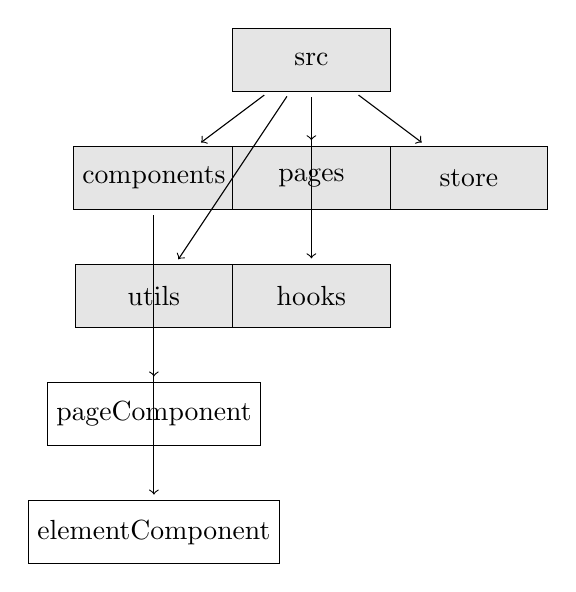
\begin{tikzpicture}[
    file/.style={draw, rectangle, minimum width=2cm, minimum height=0.8cm},
    folder/.style={draw, rectangle, minimum width=2cm, minimum height=0.8cm, fill=gray!20},
    arrow/.style={->, shorten >=2pt, shorten <=2pt}
]

% Folders
\node[folder] (src) at (0,0) {src};
\node[folder] (components) at (-2,-1.5) {components};
\node[folder] (pages) at (0,-1.5) {pages};
\node[folder] (store) at (2,-1.5) {store};
\node[folder] (utils) at (-2,-3) {utils};
\node[folder] (hooks) at (0,-3) {hooks};

% Files
\node[file] (pageComponent) at (-2,-4.5) {pageComponent};
\node[file] (elementComponent) at (-2,-6) {elementComponent};
% ... add more files

% Connections
\draw[arrow] (src) -- (components);
\draw[arrow] (src) -- (pages);
\draw[arrow] (src) -- (store);
\draw[arrow] (src) -- (utils);
\draw[arrow] (src) -- (hooks);
\draw[arrow] (components) -- (pageComponent);
\draw[arrow] (components) -- (elementComponent);
% ... add more connections

\end{tikzpicture}



\pagebreak
\subsubsection{Back-end}
The backend uses the dotNet framework. The development language using the C\# language.

In this project, the backend uses the Onion Architecture.
The Onion Architecture is a typically layered architecture, 
where each layer depends on the inner layer and provides interfaces to the outer layer.
The outer layer provides services to the outermost layer 
and other modules in the same layer based on the interfaces of the inner layer.

From inner to outer, the layers are: Domain, Application, Infrastructure, Presentation.
The Domain layer is the core layer and the innermost layer, used to define domain models, 
which are the business models.
It includes domain models and domain service interfaces.
Domain models are used to define the business models, 
which are the entities in the entity-relationship model and their attributes.
Domain service interfaces are used to define the business services, 
which are the relationships between entities in the entity-relationship model.

The Application layer is the application layer, 
used to define application services, which are the business logic.
It includes domain service implementations and application service interfaces.
Domain service implementations implement the methods of the inner layer's domain service 
interfaces and implement the business logic of the domain models.
Application service interfaces are used to define application services, 
which are the business logic.
It includes but is not limited to database interfaces, testing interfaces, 
HTTP API interfaces, MQTT interfaces, etc.

The Infrastructure layer is the infrastructure layer, used to define infrastructure.
It includes database implementations, testing implementations, 
HTTP API implementations, MQTT implementations, etc.
Database implementations implement the database interfaces 
and provide CRUD services for the database.
Testing implementations implement the testing interfaces 
and provide services for unit testing and integration testing.
HTTP API implementations implement the HTTP API interfaces 
and provide CRUD operations for HTTP APIs.
MQTT implementations implement the MQTT interfaces 
and provide CRUD operations for MQTT.

The Presentation layer is the presentation layer, used to define presentation logic, 
such as interfaces and pages. Since this is a backend project,
data presentation and control are handled by the frontend, 
so this layer is not needed.



\pagebreak
\subsubsection{Data communication and storage}
% 关于本项目的数据通信与数据存储的设计, 包括数据通信的协议, 数据存储的设计等
% 关于数据通信的设计:
% 1. 通信协议的选择
% 自前端向后端发送的数据, 有三种传输的数据类型, 
% 一种是普通的增删改查的请求, 对数据传输的时效性要求不高, 但是对数据的准确性, 完整性, 有序性, 安全性有一定的要求,
% 这种数据的传输, 采用 HTTP 协议, 以及 RESTful API 的设计. 可以有效的保证对数据传输的以上要求.
% 一种是对数据通道的创建和流媒体数据的传输, 对数据传输的时效性, 安全性要求较高, 这种数据的传输, 采用 WebRTC 协议, 以及 MQTT 协议.
% 配合可以快速解码的 flatbuffers 协议, 可以有效的保证对数据传输的以上要求.
% 最后一种是对设备的状态信息和操作信息的传输, 对完整性, 有序性, 安全性都有较高的要求, 这种数据的传输, 采用 MQTT 协议
% 同时也使用了 flatbuffers 协议.
% 
% 2. 数据通信的通信架构和通信流程
% 本项目的数据通信的通信架构, 是基于前后端分离的架构, 前端使用 React 框架, 后端使用 dotnet 框架.
% 当前端需要向后端发送数据的时候, 前端会向后端发送 HTTP 请求, 后端接收到 HTTP 请求之后, 会根据请求的数据类型,
% 选择不同的数据处理方式, 对于普通的增删改查的请求, 后端会根据 RESTful API 的设计, 对数据进行增删改查的操作,
% 对于对数据通道的创建和流媒体数据的传输, 后端会根据 WebRTC 协议, 对数据通道进行创建, 并且帮助前端和设备建立数据通道,
% 当数据通道建立后, 前端和设备之间则使用 flatbuffer 的数据格式对流媒体数据进行传输,
% 对于设备的状态信息和操作信息的传输, 前端会直接向 MQTT broker 发送 MQTT 请求, 
% 设备会在其自身的固件中监听相关的 MQTT 请求, 并且返回相关的数据.
% 
% 3. 数据通信的格式
% 本项目的数据通信的格式, 有三种, 
% 一种是 HTTP 协议, 
% 使用 json 格式对数据进行传输,
% 一种是 WebRTC 协议, 
% 使用 flatbuffers 格式对数据进行传输,
% 一种是 MQTT 协议.
% 使用 flatbuffers 格式对数据进行传输,
% 
% 关于数据存储的设计:
% 1. 数据存储的数据库的选择
% 本项目的数据存储的数据库的选择, 使用了轻量级的数据库 SQLite,
% SQLite 是一个进程内的库, 实现了自给自足的, 无服务器的, 零配置的, 事务性的 SQL 数据库引擎.
% 这是因为整个项目的目的是为了实现前端与设备之间的数据通信, 对于数据库数据的增删改查操作的要求不高,
% 数据量较小, 且对于数据库的数据的事务性要求不高, 所以选择了 SQLite 数据库.
% 2. 项目前后端的数据结构的设计
% 在本项目中, 前端由于使用了 React 框架, 所以前端的数据结构的设计, 使用了基于状态的数据结构的设计,
% 每个组件或者数据集都包含一个状态对象, 这个状态对象的属性就是组件的各个状态. 
% 使用状态对象的原因是, 可以方便的对状态进行管理, 采用对象-属性的形式, 可以方便的针对不同组件的同类状态进行区分,
% 由于跨组件的状态是由 redux 进行管理的, 这种状态对象的设计, 可以更搞笑的对状态进行更新和传递.
% 后端由于使用了 dotnet 框架, 所以后端的数据结构的设计, 使用了基于类的数据结构的设计,
% 采用了面向对象的编程思想, 对数据进行了封装, 使得数据的传输更加的安全, 有序, 完整.


\pagebreak

% \subsection{Domain model}
% \documentclass[]{article}
\usepackage{graphicx}
\usepackage{amsmath}
\usepackage{tikz}

% libaries
\usetikzlibrary{shapes,arrows}

%Define the listing package
\usepackage{listings} %code highlighter
\usepackage{color} %use color
\definecolor{mygreen}{rgb}{0,0.6,0}
\definecolor{mygray}{rgb}{0.5,0.5,0.5}
\definecolor{mymauve}{rgb}{0.58,0,0.82}

%Customize a bit the look
\lstset{ %
backgroundcolor=\color{white}, % choose the background color; you must add \usepackage{color} or \usepackage{xcolor}
basicstyle=\footnotesize, % the size of the fonts that are used for the code
breakatwhitespace=false, % sets if automatic breaks should only happen at whitespace
breaklines=true, % sets automatic line breaking
captionpos=b, % sets the caption-position to bottom
commentstyle=\color{mygreen}, % comment style
deletekeywords={...}, % if you want to delete keywords from the given language
escapeinside={\%*}{*)}, % if you want to add LaTeX within your code
extendedchars=true, % lets you use non-ASCII characters; for 8-bits encodings only, does not work with UTF-8
frame=single, % adds a frame around the code
keepspaces=true, % keeps spaces in text, useful for keeping indentation of code (possibly needs columns=flexible)
keywordstyle=\color{blue}, % keyword style
% language=Octave, % the language of the code
morekeywords={*,...}, % if you want to add more keywords to the set
numbers=left, % where to put the line-numbers; possible values are (none, left, right)
numbersep=5pt, % how far the line-numbers are from the code
numberstyle=\tiny\color{mygray}, % the style that is used for the line-numbers
rulecolor=\color{black}, % if not set, the frame-color may be changed on line-breaks within not-black text (e.g. comments (green here))
showspaces=false, % show spaces everywhere adding particular underscores; it overrides 'showstringspaces'
showstringspaces=false, % underline spaces within strings only
showtabs=false, % show tabs within strings adding particular underscores
stepnumber=1, % the step between two line-numbers. If it's 1, each line will be numbered
stringstyle=\color{mymauve}, % string literal style
tabsize=2, % sets default tabsize to 2 spaces
title=\lstname % show the filename of files included with \lstinputlisting; also try caption instead of title
}

\definecolor{darkgray}{rgb}{.4,.4,.4}
\definecolor{purple}{rgb}{0.65, 0.12, 0.82}

\lstdefinelanguage{React}{
keywords={const, typeof, new, true, false, catch, function, return, null, catch, switch, var, if, in, while, do, else, case, break},
keywordstyle=\color{blue}\bfseries,
ndkeywords={class, export, boolean, throw, implements, import, this},
ndkeywordstyle=\color{darkgray}\bfseries,
identifierstyle=\color{mygreen},
sensitive=false,
comment=[l]{//},
morecomment=[s]{/*}{*/},
commentstyle=\color{purple}\ttfamily,
string=[b]{"}{'}{`},
stringstyle=\color{red}\ttfamily,
morestring=[b]',
morestring=[b]",
morestring=[b]`',
}

\lstdefinelanguage{CSharp}{
keywords={const, typeof, new, true, false, catch, function, return, null, catch, switch, var, if, in, while, do, else, case, break},
keywordstyle=\color{blue}\bfseries,
ndkeywords={class, export, boolean, throw, implements, import, this},
ndkeywordstyle=\color{darkgray}\bfseries,
identifierstyle=\color{mygreen},
sensitive=false,
comment=[l]{//},
morecomment=[s]{/*}{*/},
commentstyle=\color{purple}\ttfamily,
string=[b]{"}{'}{`},
stringstyle=\color{red}\ttfamily,
morestring=[b]',
morestring=[b]",
morestring=[b]`',
}

\lstset{
language=React,
extendedchars=true,
basicstyle=\footnotesize\ttfamily,
showstringspaces=false,
showspaces=false,
numbers=left,
numberstyle=\footnotesize,
numbersep=9pt,
tabsize=2,
breaklines=true,
showtabs=false,
captionpos=b
}

\lstset{
language=CSharp,
extendedchars=true,
basicstyle=\footnotesize\ttfamily,
showstringspaces=false,
showspaces=false,
numbers=left,
numberstyle=\footnotesize,
numbersep=9pt,
tabsize=2,
breaklines=true,
showtabs=false,
captionpos=b
}

% \usepackage{cite} % Add this line for citation

% \bibliographystyle{plain}

\title{
The implementation of BifrostConnect Front-end scope, 
re-design and development with the relevant back-end support develop.
}
\author{
    Fei Gu \\
    Erhvervs Akademi Sydvest \\
    Computer Science 21\\
    }
\date{\today}

\begin{document}

% Front page
\maketitle
\begin{center}
    Supervisor: Henrik Boulund Meng Hansen \\
    Company: BifrostConnect \\
    Engineering Director: Jasper Wass \\
\end{center}
\tableofcontents
\pagebreak


% The introduction
\section{Introduction}
\subsection{Background}\input{sections/introduction/background.tex}
\subsection{The company}\input{sections/introduction/aboutCompany}
\subsection{The project}\input{sections/introduction/aboutProject}
\pagebreak

% The problem statement
\section{Problem Statement}
\subsection{Statement}
\input{sections/problemStatement/statement}
\subsection{Situation}
\input{sections/problemStatement/situation}
\subsection{Potential Solution}
\input{sections/problemStatement/potentialSolution}
\pagebreak

% Requirement analysis
\section{Requirement Analysis}
\input{sections/requirementAnalysis/index}

\subsection{Stakeholders}
\input{sections/requirementAnalysis/stakeholders/index}

\subsection{Business Domain}
\input{sections/requirementAnalysis/bussinesDomain/index}

\subsection{Scope}
\input{sections/requirementAnalysis/scope}

\subsection{Goals}
\input{sections/requirementAnalysis/goals}
\pagebreak

% Software Design
\section{Software Design}
% developement methods
\subsection{Software Development Methods}
\input{sections/softwareDevelopmentMethods/index}
\subsubsection{Agile Software Development}
\input{sections/softwareDevelopmentMethods/agileSoftwareDevelopment/index}
\subsubsection{Feature Driven Development}
\input{sections/softwareDevelopmentMethods/featureDrivenDevelopment/index}

\pagebreak

% Technology seslection
\subsection{Technology selection}
\input{sections/softwareDesign/technologySelection/index}
\subsubsection{Front-end}
\input{sections/softwareDesign/technologySelection/frontEnd}            
\subsubsection{Back-end}
\input{sections/softwareDesign/technologySelection/backEnd}            
\subsubsection{Database}
\input{sections/softwareDesign/technologySelection/database}
\subsubsection{Data communication}
\input{sections/softwareDesign/technologySelection/dataCommunication}            
\subsubsection{DevOps}
\input{sections/softwareDesign/technologySelection/devOps}
\pagebreak

% Architecture design
\subsection{Architecture design}
\input{sections/softwareDesign/architectureDesign/index}
\pagebreak
\subsubsection{Front-end}
\input{sections/softwareDesign/architectureDesign/frontEndArchitecture}
\pagebreak
\subsubsection{Back-end}
\input{sections/softwareDesign/architectureDesign/backEndArchitecture}
\pagebreak
\subsubsection{Data communication and storage}
\input{sections/softwareDesign/architectureDesign/dataCommunicationArchitecture}
\pagebreak

% \subsection{Domain model}
% \input{sections/softwareDesign/domainModel/index}
% \subsection{Database design}
% % 数据库领域模型 ER 图
% % 包括表和字段的设置.
% % 对于私有键和外键的设置.

% \subsection{Back-end design}
% % 后端对象模型
% % 以及对于对象模型的增删改查
% % 以及相关的其他服务的设计`'

% \subsection{Front-end design}
% % 对于前端的页面结构的设计 
% % 页面的状态的设计, 交互设计

% \subsection{FlatBuffers design}
% % schema 的设计

\subsection{DevOps CI/CD process design}
\input{sections/softwareDesign/devOpsDesign/index}
\subsubsection{Continuous Integration}
\input{sections/softwareDesign/devOpsDesign/continuousIntegration/index}
\subsubsection{Continuous Delivery}
\input{sections/softwareDesign/devOpsDesign/continuousDelivery/index}
\subsubsection{Continuous Deployment}
\input{sections/softwareDesign/devOpsDesign/continuousDeployment/index}
\pagebreak

\section{Software Development} 
\input{sections/softwareDevelopment/index}
\subsection{Overall development}
\input{sections/softwareDevelopment/overallDevelopement/index}
\subsubsection{Front-end}
\input{sections/softwareDevelopment/overallDevelopement/frontEnd/index}
\subsubsection{Back-end}
\input{sections/softwareDevelopment/overallDevelopement/backEnd/index}
\subsubsection{DevOps}
\input{sections/softwareDevelopment/overallDevelopement/devOps/index}
\subsection{Feature development} 
\input{sections/softwareDevelopment/featureDevelopment/index}
\subsubsection{Use Case 1}
\input{sections/softwareDevelopment/featureDevelopment/useCase1/index}
\subsubsection{Feature 1}
\input{sections/softwareDevelopment/featureDevelopment/feature/feature1.tex}
\pagebreak
\section{Conclusion} 
\subsection{Result}
Since the project is still in progress, the result is not available yet.
So far, basic structure of this project has been built. But the most features 
are not implemented yet. 
\subsection{Discussion}
As a single developer for this project, I am confident what I have done so far.
And I can say I understand the most of the knowledge I have used in this project, 
which also means I can explain all the part of the project. 
But this project also relevant some of the complex knowledge which I have to continue 
to study and practice.
\subsection{Future Work}
The future work is to implement the rest of the features. 
Including the most important part which is the 'create session' feature.
\pagebreak
% \bibliography{bibliography}
\pagebreak
% \begin{appendices}
%     \section{Appendix}
% \end{appendices} 
\end{document}
% \subsection{Database design}
% % 数据库领域模型 ER 图
% % 包括表和字段的设置.
% % 对于私有键和外键的设置.

% \subsection{Back-end design}
% % 后端对象模型
% % 以及对于对象模型的增删改查
% % 以及相关的其他服务的设计`'

% \subsection{Front-end design}
% % 对于前端的页面结构的设计 
% % 页面的状态的设计, 交互设计

% \subsection{FlatBuffers design}
% % schema 的设计

\subsection{DevOps CI/CD process design}
\documentclass[]{article}
\usepackage{graphicx}
\usepackage{amsmath}
\usepackage{tikz}

% libaries
\usetikzlibrary{shapes,arrows}

%Define the listing package
\usepackage{listings} %code highlighter
\usepackage{color} %use color
\definecolor{mygreen}{rgb}{0,0.6,0}
\definecolor{mygray}{rgb}{0.5,0.5,0.5}
\definecolor{mymauve}{rgb}{0.58,0,0.82}

%Customize a bit the look
\lstset{ %
backgroundcolor=\color{white}, % choose the background color; you must add \usepackage{color} or \usepackage{xcolor}
basicstyle=\footnotesize, % the size of the fonts that are used for the code
breakatwhitespace=false, % sets if automatic breaks should only happen at whitespace
breaklines=true, % sets automatic line breaking
captionpos=b, % sets the caption-position to bottom
commentstyle=\color{mygreen}, % comment style
deletekeywords={...}, % if you want to delete keywords from the given language
escapeinside={\%*}{*)}, % if you want to add LaTeX within your code
extendedchars=true, % lets you use non-ASCII characters; for 8-bits encodings only, does not work with UTF-8
frame=single, % adds a frame around the code
keepspaces=true, % keeps spaces in text, useful for keeping indentation of code (possibly needs columns=flexible)
keywordstyle=\color{blue}, % keyword style
% language=Octave, % the language of the code
morekeywords={*,...}, % if you want to add more keywords to the set
numbers=left, % where to put the line-numbers; possible values are (none, left, right)
numbersep=5pt, % how far the line-numbers are from the code
numberstyle=\tiny\color{mygray}, % the style that is used for the line-numbers
rulecolor=\color{black}, % if not set, the frame-color may be changed on line-breaks within not-black text (e.g. comments (green here))
showspaces=false, % show spaces everywhere adding particular underscores; it overrides 'showstringspaces'
showstringspaces=false, % underline spaces within strings only
showtabs=false, % show tabs within strings adding particular underscores
stepnumber=1, % the step between two line-numbers. If it's 1, each line will be numbered
stringstyle=\color{mymauve}, % string literal style
tabsize=2, % sets default tabsize to 2 spaces
title=\lstname % show the filename of files included with \lstinputlisting; also try caption instead of title
}

\definecolor{darkgray}{rgb}{.4,.4,.4}
\definecolor{purple}{rgb}{0.65, 0.12, 0.82}

\lstdefinelanguage{React}{
keywords={const, typeof, new, true, false, catch, function, return, null, catch, switch, var, if, in, while, do, else, case, break},
keywordstyle=\color{blue}\bfseries,
ndkeywords={class, export, boolean, throw, implements, import, this},
ndkeywordstyle=\color{darkgray}\bfseries,
identifierstyle=\color{mygreen},
sensitive=false,
comment=[l]{//},
morecomment=[s]{/*}{*/},
commentstyle=\color{purple}\ttfamily,
string=[b]{"}{'}{`},
stringstyle=\color{red}\ttfamily,
morestring=[b]',
morestring=[b]",
morestring=[b]`',
}

\lstdefinelanguage{CSharp}{
keywords={const, typeof, new, true, false, catch, function, return, null, catch, switch, var, if, in, while, do, else, case, break},
keywordstyle=\color{blue}\bfseries,
ndkeywords={class, export, boolean, throw, implements, import, this},
ndkeywordstyle=\color{darkgray}\bfseries,
identifierstyle=\color{mygreen},
sensitive=false,
comment=[l]{//},
morecomment=[s]{/*}{*/},
commentstyle=\color{purple}\ttfamily,
string=[b]{"}{'}{`},
stringstyle=\color{red}\ttfamily,
morestring=[b]',
morestring=[b]",
morestring=[b]`',
}

\lstset{
language=React,
extendedchars=true,
basicstyle=\footnotesize\ttfamily,
showstringspaces=false,
showspaces=false,
numbers=left,
numberstyle=\footnotesize,
numbersep=9pt,
tabsize=2,
breaklines=true,
showtabs=false,
captionpos=b
}

\lstset{
language=CSharp,
extendedchars=true,
basicstyle=\footnotesize\ttfamily,
showstringspaces=false,
showspaces=false,
numbers=left,
numberstyle=\footnotesize,
numbersep=9pt,
tabsize=2,
breaklines=true,
showtabs=false,
captionpos=b
}

% \usepackage{cite} % Add this line for citation

% \bibliographystyle{plain}

\title{
The implementation of BifrostConnect Front-end scope, 
re-design and development with the relevant back-end support develop.
}
\author{
    Fei Gu \\
    Erhvervs Akademi Sydvest \\
    Computer Science 21\\
    }
\date{\today}

\begin{document}

% Front page
\maketitle
\begin{center}
    Supervisor: Henrik Boulund Meng Hansen \\
    Company: BifrostConnect \\
    Engineering Director: Jasper Wass \\
\end{center}
\tableofcontents
\pagebreak


% The introduction
\section{Introduction}
\subsection{Background}\input{sections/introduction/background.tex}
\subsection{The company}\input{sections/introduction/aboutCompany}
\subsection{The project}\input{sections/introduction/aboutProject}
\pagebreak

% The problem statement
\section{Problem Statement}
\subsection{Statement}
\input{sections/problemStatement/statement}
\subsection{Situation}
\input{sections/problemStatement/situation}
\subsection{Potential Solution}
\input{sections/problemStatement/potentialSolution}
\pagebreak

% Requirement analysis
\section{Requirement Analysis}
\input{sections/requirementAnalysis/index}

\subsection{Stakeholders}
\input{sections/requirementAnalysis/stakeholders/index}

\subsection{Business Domain}
\input{sections/requirementAnalysis/bussinesDomain/index}

\subsection{Scope}
\input{sections/requirementAnalysis/scope}

\subsection{Goals}
\input{sections/requirementAnalysis/goals}
\pagebreak

% Software Design
\section{Software Design}
% developement methods
\subsection{Software Development Methods}
\input{sections/softwareDevelopmentMethods/index}
\subsubsection{Agile Software Development}
\input{sections/softwareDevelopmentMethods/agileSoftwareDevelopment/index}
\subsubsection{Feature Driven Development}
\input{sections/softwareDevelopmentMethods/featureDrivenDevelopment/index}

\pagebreak

% Technology seslection
\subsection{Technology selection}
\input{sections/softwareDesign/technologySelection/index}
\subsubsection{Front-end}
\input{sections/softwareDesign/technologySelection/frontEnd}            
\subsubsection{Back-end}
\input{sections/softwareDesign/technologySelection/backEnd}            
\subsubsection{Database}
\input{sections/softwareDesign/technologySelection/database}
\subsubsection{Data communication}
\input{sections/softwareDesign/technologySelection/dataCommunication}            
\subsubsection{DevOps}
\input{sections/softwareDesign/technologySelection/devOps}
\pagebreak

% Architecture design
\subsection{Architecture design}
\input{sections/softwareDesign/architectureDesign/index}
\pagebreak
\subsubsection{Front-end}
\input{sections/softwareDesign/architectureDesign/frontEndArchitecture}
\pagebreak
\subsubsection{Back-end}
\input{sections/softwareDesign/architectureDesign/backEndArchitecture}
\pagebreak
\subsubsection{Data communication and storage}
\input{sections/softwareDesign/architectureDesign/dataCommunicationArchitecture}
\pagebreak

% \subsection{Domain model}
% \input{sections/softwareDesign/domainModel/index}
% \subsection{Database design}
% % 数据库领域模型 ER 图
% % 包括表和字段的设置.
% % 对于私有键和外键的设置.

% \subsection{Back-end design}
% % 后端对象模型
% % 以及对于对象模型的增删改查
% % 以及相关的其他服务的设计`'

% \subsection{Front-end design}
% % 对于前端的页面结构的设计 
% % 页面的状态的设计, 交互设计

% \subsection{FlatBuffers design}
% % schema 的设计

\subsection{DevOps CI/CD process design}
\input{sections/softwareDesign/devOpsDesign/index}
\subsubsection{Continuous Integration}
\input{sections/softwareDesign/devOpsDesign/continuousIntegration/index}
\subsubsection{Continuous Delivery}
\input{sections/softwareDesign/devOpsDesign/continuousDelivery/index}
\subsubsection{Continuous Deployment}
\input{sections/softwareDesign/devOpsDesign/continuousDeployment/index}
\pagebreak

\section{Software Development} 
\input{sections/softwareDevelopment/index}
\subsection{Overall development}
\input{sections/softwareDevelopment/overallDevelopement/index}
\subsubsection{Front-end}
\input{sections/softwareDevelopment/overallDevelopement/frontEnd/index}
\subsubsection{Back-end}
\input{sections/softwareDevelopment/overallDevelopement/backEnd/index}
\subsubsection{DevOps}
\input{sections/softwareDevelopment/overallDevelopement/devOps/index}
\subsection{Feature development} 
\input{sections/softwareDevelopment/featureDevelopment/index}
\subsubsection{Use Case 1}
\input{sections/softwareDevelopment/featureDevelopment/useCase1/index}
\subsubsection{Feature 1}
\input{sections/softwareDevelopment/featureDevelopment/feature/feature1.tex}
\pagebreak
\section{Conclusion} 
\subsection{Result}
Since the project is still in progress, the result is not available yet.
So far, basic structure of this project has been built. But the most features 
are not implemented yet. 
\subsection{Discussion}
As a single developer for this project, I am confident what I have done so far.
And I can say I understand the most of the knowledge I have used in this project, 
which also means I can explain all the part of the project. 
But this project also relevant some of the complex knowledge which I have to continue 
to study and practice.
\subsection{Future Work}
The future work is to implement the rest of the features. 
Including the most important part which is the 'create session' feature.
\pagebreak
% \bibliography{bibliography}
\pagebreak
% \begin{appendices}
%     \section{Appendix}
% \end{appendices} 
\end{document}
\subsubsection{Continuous Integration}
\documentclass[]{article}
\usepackage{graphicx}
\usepackage{amsmath}
\usepackage{tikz}

% libaries
\usetikzlibrary{shapes,arrows}

%Define the listing package
\usepackage{listings} %code highlighter
\usepackage{color} %use color
\definecolor{mygreen}{rgb}{0,0.6,0}
\definecolor{mygray}{rgb}{0.5,0.5,0.5}
\definecolor{mymauve}{rgb}{0.58,0,0.82}

%Customize a bit the look
\lstset{ %
backgroundcolor=\color{white}, % choose the background color; you must add \usepackage{color} or \usepackage{xcolor}
basicstyle=\footnotesize, % the size of the fonts that are used for the code
breakatwhitespace=false, % sets if automatic breaks should only happen at whitespace
breaklines=true, % sets automatic line breaking
captionpos=b, % sets the caption-position to bottom
commentstyle=\color{mygreen}, % comment style
deletekeywords={...}, % if you want to delete keywords from the given language
escapeinside={\%*}{*)}, % if you want to add LaTeX within your code
extendedchars=true, % lets you use non-ASCII characters; for 8-bits encodings only, does not work with UTF-8
frame=single, % adds a frame around the code
keepspaces=true, % keeps spaces in text, useful for keeping indentation of code (possibly needs columns=flexible)
keywordstyle=\color{blue}, % keyword style
% language=Octave, % the language of the code
morekeywords={*,...}, % if you want to add more keywords to the set
numbers=left, % where to put the line-numbers; possible values are (none, left, right)
numbersep=5pt, % how far the line-numbers are from the code
numberstyle=\tiny\color{mygray}, % the style that is used for the line-numbers
rulecolor=\color{black}, % if not set, the frame-color may be changed on line-breaks within not-black text (e.g. comments (green here))
showspaces=false, % show spaces everywhere adding particular underscores; it overrides 'showstringspaces'
showstringspaces=false, % underline spaces within strings only
showtabs=false, % show tabs within strings adding particular underscores
stepnumber=1, % the step between two line-numbers. If it's 1, each line will be numbered
stringstyle=\color{mymauve}, % string literal style
tabsize=2, % sets default tabsize to 2 spaces
title=\lstname % show the filename of files included with \lstinputlisting; also try caption instead of title
}

\definecolor{darkgray}{rgb}{.4,.4,.4}
\definecolor{purple}{rgb}{0.65, 0.12, 0.82}

\lstdefinelanguage{React}{
keywords={const, typeof, new, true, false, catch, function, return, null, catch, switch, var, if, in, while, do, else, case, break},
keywordstyle=\color{blue}\bfseries,
ndkeywords={class, export, boolean, throw, implements, import, this},
ndkeywordstyle=\color{darkgray}\bfseries,
identifierstyle=\color{mygreen},
sensitive=false,
comment=[l]{//},
morecomment=[s]{/*}{*/},
commentstyle=\color{purple}\ttfamily,
string=[b]{"}{'}{`},
stringstyle=\color{red}\ttfamily,
morestring=[b]',
morestring=[b]",
morestring=[b]`',
}

\lstdefinelanguage{CSharp}{
keywords={const, typeof, new, true, false, catch, function, return, null, catch, switch, var, if, in, while, do, else, case, break},
keywordstyle=\color{blue}\bfseries,
ndkeywords={class, export, boolean, throw, implements, import, this},
ndkeywordstyle=\color{darkgray}\bfseries,
identifierstyle=\color{mygreen},
sensitive=false,
comment=[l]{//},
morecomment=[s]{/*}{*/},
commentstyle=\color{purple}\ttfamily,
string=[b]{"}{'}{`},
stringstyle=\color{red}\ttfamily,
morestring=[b]',
morestring=[b]",
morestring=[b]`',
}

\lstset{
language=React,
extendedchars=true,
basicstyle=\footnotesize\ttfamily,
showstringspaces=false,
showspaces=false,
numbers=left,
numberstyle=\footnotesize,
numbersep=9pt,
tabsize=2,
breaklines=true,
showtabs=false,
captionpos=b
}

\lstset{
language=CSharp,
extendedchars=true,
basicstyle=\footnotesize\ttfamily,
showstringspaces=false,
showspaces=false,
numbers=left,
numberstyle=\footnotesize,
numbersep=9pt,
tabsize=2,
breaklines=true,
showtabs=false,
captionpos=b
}

% \usepackage{cite} % Add this line for citation

% \bibliographystyle{plain}

\title{
The implementation of BifrostConnect Front-end scope, 
re-design and development with the relevant back-end support develop.
}
\author{
    Fei Gu \\
    Erhvervs Akademi Sydvest \\
    Computer Science 21\\
    }
\date{\today}

\begin{document}

% Front page
\maketitle
\begin{center}
    Supervisor: Henrik Boulund Meng Hansen \\
    Company: BifrostConnect \\
    Engineering Director: Jasper Wass \\
\end{center}
\tableofcontents
\pagebreak


% The introduction
\section{Introduction}
\subsection{Background}\input{sections/introduction/background.tex}
\subsection{The company}\input{sections/introduction/aboutCompany}
\subsection{The project}\input{sections/introduction/aboutProject}
\pagebreak

% The problem statement
\section{Problem Statement}
\subsection{Statement}
\input{sections/problemStatement/statement}
\subsection{Situation}
\input{sections/problemStatement/situation}
\subsection{Potential Solution}
\input{sections/problemStatement/potentialSolution}
\pagebreak

% Requirement analysis
\section{Requirement Analysis}
\input{sections/requirementAnalysis/index}

\subsection{Stakeholders}
\input{sections/requirementAnalysis/stakeholders/index}

\subsection{Business Domain}
\input{sections/requirementAnalysis/bussinesDomain/index}

\subsection{Scope}
\input{sections/requirementAnalysis/scope}

\subsection{Goals}
\input{sections/requirementAnalysis/goals}
\pagebreak

% Software Design
\section{Software Design}
% developement methods
\subsection{Software Development Methods}
\input{sections/softwareDevelopmentMethods/index}
\subsubsection{Agile Software Development}
\input{sections/softwareDevelopmentMethods/agileSoftwareDevelopment/index}
\subsubsection{Feature Driven Development}
\input{sections/softwareDevelopmentMethods/featureDrivenDevelopment/index}

\pagebreak

% Technology seslection
\subsection{Technology selection}
\input{sections/softwareDesign/technologySelection/index}
\subsubsection{Front-end}
\input{sections/softwareDesign/technologySelection/frontEnd}            
\subsubsection{Back-end}
\input{sections/softwareDesign/technologySelection/backEnd}            
\subsubsection{Database}
\input{sections/softwareDesign/technologySelection/database}
\subsubsection{Data communication}
\input{sections/softwareDesign/technologySelection/dataCommunication}            
\subsubsection{DevOps}
\input{sections/softwareDesign/technologySelection/devOps}
\pagebreak

% Architecture design
\subsection{Architecture design}
\input{sections/softwareDesign/architectureDesign/index}
\pagebreak
\subsubsection{Front-end}
\input{sections/softwareDesign/architectureDesign/frontEndArchitecture}
\pagebreak
\subsubsection{Back-end}
\input{sections/softwareDesign/architectureDesign/backEndArchitecture}
\pagebreak
\subsubsection{Data communication and storage}
\input{sections/softwareDesign/architectureDesign/dataCommunicationArchitecture}
\pagebreak

% \subsection{Domain model}
% \input{sections/softwareDesign/domainModel/index}
% \subsection{Database design}
% % 数据库领域模型 ER 图
% % 包括表和字段的设置.
% % 对于私有键和外键的设置.

% \subsection{Back-end design}
% % 后端对象模型
% % 以及对于对象模型的增删改查
% % 以及相关的其他服务的设计`'

% \subsection{Front-end design}
% % 对于前端的页面结构的设计 
% % 页面的状态的设计, 交互设计

% \subsection{FlatBuffers design}
% % schema 的设计

\subsection{DevOps CI/CD process design}
\input{sections/softwareDesign/devOpsDesign/index}
\subsubsection{Continuous Integration}
\input{sections/softwareDesign/devOpsDesign/continuousIntegration/index}
\subsubsection{Continuous Delivery}
\input{sections/softwareDesign/devOpsDesign/continuousDelivery/index}
\subsubsection{Continuous Deployment}
\input{sections/softwareDesign/devOpsDesign/continuousDeployment/index}
\pagebreak

\section{Software Development} 
\input{sections/softwareDevelopment/index}
\subsection{Overall development}
\input{sections/softwareDevelopment/overallDevelopement/index}
\subsubsection{Front-end}
\input{sections/softwareDevelopment/overallDevelopement/frontEnd/index}
\subsubsection{Back-end}
\input{sections/softwareDevelopment/overallDevelopement/backEnd/index}
\subsubsection{DevOps}
\input{sections/softwareDevelopment/overallDevelopement/devOps/index}
\subsection{Feature development} 
\input{sections/softwareDevelopment/featureDevelopment/index}
\subsubsection{Use Case 1}
\input{sections/softwareDevelopment/featureDevelopment/useCase1/index}
\subsubsection{Feature 1}
\input{sections/softwareDevelopment/featureDevelopment/feature/feature1.tex}
\pagebreak
\section{Conclusion} 
\subsection{Result}
Since the project is still in progress, the result is not available yet.
So far, basic structure of this project has been built. But the most features 
are not implemented yet. 
\subsection{Discussion}
As a single developer for this project, I am confident what I have done so far.
And I can say I understand the most of the knowledge I have used in this project, 
which also means I can explain all the part of the project. 
But this project also relevant some of the complex knowledge which I have to continue 
to study and practice.
\subsection{Future Work}
The future work is to implement the rest of the features. 
Including the most important part which is the 'create session' feature.
\pagebreak
% \bibliography{bibliography}
\pagebreak
% \begin{appendices}
%     \section{Appendix}
% \end{appendices} 
\end{document}
\subsubsection{Continuous Delivery}
\documentclass[]{article}
\usepackage{graphicx}
\usepackage{amsmath}
\usepackage{tikz}

% libaries
\usetikzlibrary{shapes,arrows}

%Define the listing package
\usepackage{listings} %code highlighter
\usepackage{color} %use color
\definecolor{mygreen}{rgb}{0,0.6,0}
\definecolor{mygray}{rgb}{0.5,0.5,0.5}
\definecolor{mymauve}{rgb}{0.58,0,0.82}

%Customize a bit the look
\lstset{ %
backgroundcolor=\color{white}, % choose the background color; you must add \usepackage{color} or \usepackage{xcolor}
basicstyle=\footnotesize, % the size of the fonts that are used for the code
breakatwhitespace=false, % sets if automatic breaks should only happen at whitespace
breaklines=true, % sets automatic line breaking
captionpos=b, % sets the caption-position to bottom
commentstyle=\color{mygreen}, % comment style
deletekeywords={...}, % if you want to delete keywords from the given language
escapeinside={\%*}{*)}, % if you want to add LaTeX within your code
extendedchars=true, % lets you use non-ASCII characters; for 8-bits encodings only, does not work with UTF-8
frame=single, % adds a frame around the code
keepspaces=true, % keeps spaces in text, useful for keeping indentation of code (possibly needs columns=flexible)
keywordstyle=\color{blue}, % keyword style
% language=Octave, % the language of the code
morekeywords={*,...}, % if you want to add more keywords to the set
numbers=left, % where to put the line-numbers; possible values are (none, left, right)
numbersep=5pt, % how far the line-numbers are from the code
numberstyle=\tiny\color{mygray}, % the style that is used for the line-numbers
rulecolor=\color{black}, % if not set, the frame-color may be changed on line-breaks within not-black text (e.g. comments (green here))
showspaces=false, % show spaces everywhere adding particular underscores; it overrides 'showstringspaces'
showstringspaces=false, % underline spaces within strings only
showtabs=false, % show tabs within strings adding particular underscores
stepnumber=1, % the step between two line-numbers. If it's 1, each line will be numbered
stringstyle=\color{mymauve}, % string literal style
tabsize=2, % sets default tabsize to 2 spaces
title=\lstname % show the filename of files included with \lstinputlisting; also try caption instead of title
}

\definecolor{darkgray}{rgb}{.4,.4,.4}
\definecolor{purple}{rgb}{0.65, 0.12, 0.82}

\lstdefinelanguage{React}{
keywords={const, typeof, new, true, false, catch, function, return, null, catch, switch, var, if, in, while, do, else, case, break},
keywordstyle=\color{blue}\bfseries,
ndkeywords={class, export, boolean, throw, implements, import, this},
ndkeywordstyle=\color{darkgray}\bfseries,
identifierstyle=\color{mygreen},
sensitive=false,
comment=[l]{//},
morecomment=[s]{/*}{*/},
commentstyle=\color{purple}\ttfamily,
string=[b]{"}{'}{`},
stringstyle=\color{red}\ttfamily,
morestring=[b]',
morestring=[b]",
morestring=[b]`',
}

\lstdefinelanguage{CSharp}{
keywords={const, typeof, new, true, false, catch, function, return, null, catch, switch, var, if, in, while, do, else, case, break},
keywordstyle=\color{blue}\bfseries,
ndkeywords={class, export, boolean, throw, implements, import, this},
ndkeywordstyle=\color{darkgray}\bfseries,
identifierstyle=\color{mygreen},
sensitive=false,
comment=[l]{//},
morecomment=[s]{/*}{*/},
commentstyle=\color{purple}\ttfamily,
string=[b]{"}{'}{`},
stringstyle=\color{red}\ttfamily,
morestring=[b]',
morestring=[b]",
morestring=[b]`',
}

\lstset{
language=React,
extendedchars=true,
basicstyle=\footnotesize\ttfamily,
showstringspaces=false,
showspaces=false,
numbers=left,
numberstyle=\footnotesize,
numbersep=9pt,
tabsize=2,
breaklines=true,
showtabs=false,
captionpos=b
}

\lstset{
language=CSharp,
extendedchars=true,
basicstyle=\footnotesize\ttfamily,
showstringspaces=false,
showspaces=false,
numbers=left,
numberstyle=\footnotesize,
numbersep=9pt,
tabsize=2,
breaklines=true,
showtabs=false,
captionpos=b
}

% \usepackage{cite} % Add this line for citation

% \bibliographystyle{plain}

\title{
The implementation of BifrostConnect Front-end scope, 
re-design and development with the relevant back-end support develop.
}
\author{
    Fei Gu \\
    Erhvervs Akademi Sydvest \\
    Computer Science 21\\
    }
\date{\today}

\begin{document}

% Front page
\maketitle
\begin{center}
    Supervisor: Henrik Boulund Meng Hansen \\
    Company: BifrostConnect \\
    Engineering Director: Jasper Wass \\
\end{center}
\tableofcontents
\pagebreak


% The introduction
\section{Introduction}
\subsection{Background}\input{sections/introduction/background.tex}
\subsection{The company}\input{sections/introduction/aboutCompany}
\subsection{The project}\input{sections/introduction/aboutProject}
\pagebreak

% The problem statement
\section{Problem Statement}
\subsection{Statement}
\input{sections/problemStatement/statement}
\subsection{Situation}
\input{sections/problemStatement/situation}
\subsection{Potential Solution}
\input{sections/problemStatement/potentialSolution}
\pagebreak

% Requirement analysis
\section{Requirement Analysis}
\input{sections/requirementAnalysis/index}

\subsection{Stakeholders}
\input{sections/requirementAnalysis/stakeholders/index}

\subsection{Business Domain}
\input{sections/requirementAnalysis/bussinesDomain/index}

\subsection{Scope}
\input{sections/requirementAnalysis/scope}

\subsection{Goals}
\input{sections/requirementAnalysis/goals}
\pagebreak

% Software Design
\section{Software Design}
% developement methods
\subsection{Software Development Methods}
\input{sections/softwareDevelopmentMethods/index}
\subsubsection{Agile Software Development}
\input{sections/softwareDevelopmentMethods/agileSoftwareDevelopment/index}
\subsubsection{Feature Driven Development}
\input{sections/softwareDevelopmentMethods/featureDrivenDevelopment/index}

\pagebreak

% Technology seslection
\subsection{Technology selection}
\input{sections/softwareDesign/technologySelection/index}
\subsubsection{Front-end}
\input{sections/softwareDesign/technologySelection/frontEnd}            
\subsubsection{Back-end}
\input{sections/softwareDesign/technologySelection/backEnd}            
\subsubsection{Database}
\input{sections/softwareDesign/technologySelection/database}
\subsubsection{Data communication}
\input{sections/softwareDesign/technologySelection/dataCommunication}            
\subsubsection{DevOps}
\input{sections/softwareDesign/technologySelection/devOps}
\pagebreak

% Architecture design
\subsection{Architecture design}
\input{sections/softwareDesign/architectureDesign/index}
\pagebreak
\subsubsection{Front-end}
\input{sections/softwareDesign/architectureDesign/frontEndArchitecture}
\pagebreak
\subsubsection{Back-end}
\input{sections/softwareDesign/architectureDesign/backEndArchitecture}
\pagebreak
\subsubsection{Data communication and storage}
\input{sections/softwareDesign/architectureDesign/dataCommunicationArchitecture}
\pagebreak

% \subsection{Domain model}
% \input{sections/softwareDesign/domainModel/index}
% \subsection{Database design}
% % 数据库领域模型 ER 图
% % 包括表和字段的设置.
% % 对于私有键和外键的设置.

% \subsection{Back-end design}
% % 后端对象模型
% % 以及对于对象模型的增删改查
% % 以及相关的其他服务的设计`'

% \subsection{Front-end design}
% % 对于前端的页面结构的设计 
% % 页面的状态的设计, 交互设计

% \subsection{FlatBuffers design}
% % schema 的设计

\subsection{DevOps CI/CD process design}
\input{sections/softwareDesign/devOpsDesign/index}
\subsubsection{Continuous Integration}
\input{sections/softwareDesign/devOpsDesign/continuousIntegration/index}
\subsubsection{Continuous Delivery}
\input{sections/softwareDesign/devOpsDesign/continuousDelivery/index}
\subsubsection{Continuous Deployment}
\input{sections/softwareDesign/devOpsDesign/continuousDeployment/index}
\pagebreak

\section{Software Development} 
\input{sections/softwareDevelopment/index}
\subsection{Overall development}
\input{sections/softwareDevelopment/overallDevelopement/index}
\subsubsection{Front-end}
\input{sections/softwareDevelopment/overallDevelopement/frontEnd/index}
\subsubsection{Back-end}
\input{sections/softwareDevelopment/overallDevelopement/backEnd/index}
\subsubsection{DevOps}
\input{sections/softwareDevelopment/overallDevelopement/devOps/index}
\subsection{Feature development} 
\input{sections/softwareDevelopment/featureDevelopment/index}
\subsubsection{Use Case 1}
\input{sections/softwareDevelopment/featureDevelopment/useCase1/index}
\subsubsection{Feature 1}
\input{sections/softwareDevelopment/featureDevelopment/feature/feature1.tex}
\pagebreak
\section{Conclusion} 
\subsection{Result}
Since the project is still in progress, the result is not available yet.
So far, basic structure of this project has been built. But the most features 
are not implemented yet. 
\subsection{Discussion}
As a single developer for this project, I am confident what I have done so far.
And I can say I understand the most of the knowledge I have used in this project, 
which also means I can explain all the part of the project. 
But this project also relevant some of the complex knowledge which I have to continue 
to study and practice.
\subsection{Future Work}
The future work is to implement the rest of the features. 
Including the most important part which is the 'create session' feature.
\pagebreak
% \bibliography{bibliography}
\pagebreak
% \begin{appendices}
%     \section{Appendix}
% \end{appendices} 
\end{document}
\subsubsection{Continuous Deployment}
\documentclass[]{article}
\usepackage{graphicx}
\usepackage{amsmath}
\usepackage{tikz}

% libaries
\usetikzlibrary{shapes,arrows}

%Define the listing package
\usepackage{listings} %code highlighter
\usepackage{color} %use color
\definecolor{mygreen}{rgb}{0,0.6,0}
\definecolor{mygray}{rgb}{0.5,0.5,0.5}
\definecolor{mymauve}{rgb}{0.58,0,0.82}

%Customize a bit the look
\lstset{ %
backgroundcolor=\color{white}, % choose the background color; you must add \usepackage{color} or \usepackage{xcolor}
basicstyle=\footnotesize, % the size of the fonts that are used for the code
breakatwhitespace=false, % sets if automatic breaks should only happen at whitespace
breaklines=true, % sets automatic line breaking
captionpos=b, % sets the caption-position to bottom
commentstyle=\color{mygreen}, % comment style
deletekeywords={...}, % if you want to delete keywords from the given language
escapeinside={\%*}{*)}, % if you want to add LaTeX within your code
extendedchars=true, % lets you use non-ASCII characters; for 8-bits encodings only, does not work with UTF-8
frame=single, % adds a frame around the code
keepspaces=true, % keeps spaces in text, useful for keeping indentation of code (possibly needs columns=flexible)
keywordstyle=\color{blue}, % keyword style
% language=Octave, % the language of the code
morekeywords={*,...}, % if you want to add more keywords to the set
numbers=left, % where to put the line-numbers; possible values are (none, left, right)
numbersep=5pt, % how far the line-numbers are from the code
numberstyle=\tiny\color{mygray}, % the style that is used for the line-numbers
rulecolor=\color{black}, % if not set, the frame-color may be changed on line-breaks within not-black text (e.g. comments (green here))
showspaces=false, % show spaces everywhere adding particular underscores; it overrides 'showstringspaces'
showstringspaces=false, % underline spaces within strings only
showtabs=false, % show tabs within strings adding particular underscores
stepnumber=1, % the step between two line-numbers. If it's 1, each line will be numbered
stringstyle=\color{mymauve}, % string literal style
tabsize=2, % sets default tabsize to 2 spaces
title=\lstname % show the filename of files included with \lstinputlisting; also try caption instead of title
}

\definecolor{darkgray}{rgb}{.4,.4,.4}
\definecolor{purple}{rgb}{0.65, 0.12, 0.82}

\lstdefinelanguage{React}{
keywords={const, typeof, new, true, false, catch, function, return, null, catch, switch, var, if, in, while, do, else, case, break},
keywordstyle=\color{blue}\bfseries,
ndkeywords={class, export, boolean, throw, implements, import, this},
ndkeywordstyle=\color{darkgray}\bfseries,
identifierstyle=\color{mygreen},
sensitive=false,
comment=[l]{//},
morecomment=[s]{/*}{*/},
commentstyle=\color{purple}\ttfamily,
string=[b]{"}{'}{`},
stringstyle=\color{red}\ttfamily,
morestring=[b]',
morestring=[b]",
morestring=[b]`',
}

\lstdefinelanguage{CSharp}{
keywords={const, typeof, new, true, false, catch, function, return, null, catch, switch, var, if, in, while, do, else, case, break},
keywordstyle=\color{blue}\bfseries,
ndkeywords={class, export, boolean, throw, implements, import, this},
ndkeywordstyle=\color{darkgray}\bfseries,
identifierstyle=\color{mygreen},
sensitive=false,
comment=[l]{//},
morecomment=[s]{/*}{*/},
commentstyle=\color{purple}\ttfamily,
string=[b]{"}{'}{`},
stringstyle=\color{red}\ttfamily,
morestring=[b]',
morestring=[b]",
morestring=[b]`',
}

\lstset{
language=React,
extendedchars=true,
basicstyle=\footnotesize\ttfamily,
showstringspaces=false,
showspaces=false,
numbers=left,
numberstyle=\footnotesize,
numbersep=9pt,
tabsize=2,
breaklines=true,
showtabs=false,
captionpos=b
}

\lstset{
language=CSharp,
extendedchars=true,
basicstyle=\footnotesize\ttfamily,
showstringspaces=false,
showspaces=false,
numbers=left,
numberstyle=\footnotesize,
numbersep=9pt,
tabsize=2,
breaklines=true,
showtabs=false,
captionpos=b
}

% \usepackage{cite} % Add this line for citation

% \bibliographystyle{plain}

\title{
The implementation of BifrostConnect Front-end scope, 
re-design and development with the relevant back-end support develop.
}
\author{
    Fei Gu \\
    Erhvervs Akademi Sydvest \\
    Computer Science 21\\
    }
\date{\today}

\begin{document}

% Front page
\maketitle
\begin{center}
    Supervisor: Henrik Boulund Meng Hansen \\
    Company: BifrostConnect \\
    Engineering Director: Jasper Wass \\
\end{center}
\tableofcontents
\pagebreak


% The introduction
\section{Introduction}
\subsection{Background}\input{sections/introduction/background.tex}
\subsection{The company}\input{sections/introduction/aboutCompany}
\subsection{The project}\input{sections/introduction/aboutProject}
\pagebreak

% The problem statement
\section{Problem Statement}
\subsection{Statement}
\input{sections/problemStatement/statement}
\subsection{Situation}
\input{sections/problemStatement/situation}
\subsection{Potential Solution}
\input{sections/problemStatement/potentialSolution}
\pagebreak

% Requirement analysis
\section{Requirement Analysis}
\input{sections/requirementAnalysis/index}

\subsection{Stakeholders}
\input{sections/requirementAnalysis/stakeholders/index}

\subsection{Business Domain}
\input{sections/requirementAnalysis/bussinesDomain/index}

\subsection{Scope}
\input{sections/requirementAnalysis/scope}

\subsection{Goals}
\input{sections/requirementAnalysis/goals}
\pagebreak

% Software Design
\section{Software Design}
% developement methods
\subsection{Software Development Methods}
\input{sections/softwareDevelopmentMethods/index}
\subsubsection{Agile Software Development}
\input{sections/softwareDevelopmentMethods/agileSoftwareDevelopment/index}
\subsubsection{Feature Driven Development}
\input{sections/softwareDevelopmentMethods/featureDrivenDevelopment/index}

\pagebreak

% Technology seslection
\subsection{Technology selection}
\input{sections/softwareDesign/technologySelection/index}
\subsubsection{Front-end}
\input{sections/softwareDesign/technologySelection/frontEnd}            
\subsubsection{Back-end}
\input{sections/softwareDesign/technologySelection/backEnd}            
\subsubsection{Database}
\input{sections/softwareDesign/technologySelection/database}
\subsubsection{Data communication}
\input{sections/softwareDesign/technologySelection/dataCommunication}            
\subsubsection{DevOps}
\input{sections/softwareDesign/technologySelection/devOps}
\pagebreak

% Architecture design
\subsection{Architecture design}
\input{sections/softwareDesign/architectureDesign/index}
\pagebreak
\subsubsection{Front-end}
\input{sections/softwareDesign/architectureDesign/frontEndArchitecture}
\pagebreak
\subsubsection{Back-end}
\input{sections/softwareDesign/architectureDesign/backEndArchitecture}
\pagebreak
\subsubsection{Data communication and storage}
\input{sections/softwareDesign/architectureDesign/dataCommunicationArchitecture}
\pagebreak

% \subsection{Domain model}
% \input{sections/softwareDesign/domainModel/index}
% \subsection{Database design}
% % 数据库领域模型 ER 图
% % 包括表和字段的设置.
% % 对于私有键和外键的设置.

% \subsection{Back-end design}
% % 后端对象模型
% % 以及对于对象模型的增删改查
% % 以及相关的其他服务的设计`'

% \subsection{Front-end design}
% % 对于前端的页面结构的设计 
% % 页面的状态的设计, 交互设计

% \subsection{FlatBuffers design}
% % schema 的设计

\subsection{DevOps CI/CD process design}
\input{sections/softwareDesign/devOpsDesign/index}
\subsubsection{Continuous Integration}
\input{sections/softwareDesign/devOpsDesign/continuousIntegration/index}
\subsubsection{Continuous Delivery}
\input{sections/softwareDesign/devOpsDesign/continuousDelivery/index}
\subsubsection{Continuous Deployment}
\input{sections/softwareDesign/devOpsDesign/continuousDeployment/index}
\pagebreak

\section{Software Development} 
\input{sections/softwareDevelopment/index}
\subsection{Overall development}
\input{sections/softwareDevelopment/overallDevelopement/index}
\subsubsection{Front-end}
\input{sections/softwareDevelopment/overallDevelopement/frontEnd/index}
\subsubsection{Back-end}
\input{sections/softwareDevelopment/overallDevelopement/backEnd/index}
\subsubsection{DevOps}
\input{sections/softwareDevelopment/overallDevelopement/devOps/index}
\subsection{Feature development} 
\input{sections/softwareDevelopment/featureDevelopment/index}
\subsubsection{Use Case 1}
\input{sections/softwareDevelopment/featureDevelopment/useCase1/index}
\subsubsection{Feature 1}
\input{sections/softwareDevelopment/featureDevelopment/feature/feature1.tex}
\pagebreak
\section{Conclusion} 
\subsection{Result}
Since the project is still in progress, the result is not available yet.
So far, basic structure of this project has been built. But the most features 
are not implemented yet. 
\subsection{Discussion}
As a single developer for this project, I am confident what I have done so far.
And I can say I understand the most of the knowledge I have used in this project, 
which also means I can explain all the part of the project. 
But this project also relevant some of the complex knowledge which I have to continue 
to study and practice.
\subsection{Future Work}
The future work is to implement the rest of the features. 
Including the most important part which is the 'create session' feature.
\pagebreak
% \bibliography{bibliography}
\pagebreak
% \begin{appendices}
%     \section{Appendix}
% \end{appendices} 
\end{document}
\pagebreak

\section{Software Development} 
\documentclass[]{article}
\usepackage{graphicx}
\usepackage{amsmath}
\usepackage{tikz}

% libaries
\usetikzlibrary{shapes,arrows}

%Define the listing package
\usepackage{listings} %code highlighter
\usepackage{color} %use color
\definecolor{mygreen}{rgb}{0,0.6,0}
\definecolor{mygray}{rgb}{0.5,0.5,0.5}
\definecolor{mymauve}{rgb}{0.58,0,0.82}

%Customize a bit the look
\lstset{ %
backgroundcolor=\color{white}, % choose the background color; you must add \usepackage{color} or \usepackage{xcolor}
basicstyle=\footnotesize, % the size of the fonts that are used for the code
breakatwhitespace=false, % sets if automatic breaks should only happen at whitespace
breaklines=true, % sets automatic line breaking
captionpos=b, % sets the caption-position to bottom
commentstyle=\color{mygreen}, % comment style
deletekeywords={...}, % if you want to delete keywords from the given language
escapeinside={\%*}{*)}, % if you want to add LaTeX within your code
extendedchars=true, % lets you use non-ASCII characters; for 8-bits encodings only, does not work with UTF-8
frame=single, % adds a frame around the code
keepspaces=true, % keeps spaces in text, useful for keeping indentation of code (possibly needs columns=flexible)
keywordstyle=\color{blue}, % keyword style
% language=Octave, % the language of the code
morekeywords={*,...}, % if you want to add more keywords to the set
numbers=left, % where to put the line-numbers; possible values are (none, left, right)
numbersep=5pt, % how far the line-numbers are from the code
numberstyle=\tiny\color{mygray}, % the style that is used for the line-numbers
rulecolor=\color{black}, % if not set, the frame-color may be changed on line-breaks within not-black text (e.g. comments (green here))
showspaces=false, % show spaces everywhere adding particular underscores; it overrides 'showstringspaces'
showstringspaces=false, % underline spaces within strings only
showtabs=false, % show tabs within strings adding particular underscores
stepnumber=1, % the step between two line-numbers. If it's 1, each line will be numbered
stringstyle=\color{mymauve}, % string literal style
tabsize=2, % sets default tabsize to 2 spaces
title=\lstname % show the filename of files included with \lstinputlisting; also try caption instead of title
}

\definecolor{darkgray}{rgb}{.4,.4,.4}
\definecolor{purple}{rgb}{0.65, 0.12, 0.82}

\lstdefinelanguage{React}{
keywords={const, typeof, new, true, false, catch, function, return, null, catch, switch, var, if, in, while, do, else, case, break},
keywordstyle=\color{blue}\bfseries,
ndkeywords={class, export, boolean, throw, implements, import, this},
ndkeywordstyle=\color{darkgray}\bfseries,
identifierstyle=\color{mygreen},
sensitive=false,
comment=[l]{//},
morecomment=[s]{/*}{*/},
commentstyle=\color{purple}\ttfamily,
string=[b]{"}{'}{`},
stringstyle=\color{red}\ttfamily,
morestring=[b]',
morestring=[b]",
morestring=[b]`',
}

\lstdefinelanguage{CSharp}{
keywords={const, typeof, new, true, false, catch, function, return, null, catch, switch, var, if, in, while, do, else, case, break},
keywordstyle=\color{blue}\bfseries,
ndkeywords={class, export, boolean, throw, implements, import, this},
ndkeywordstyle=\color{darkgray}\bfseries,
identifierstyle=\color{mygreen},
sensitive=false,
comment=[l]{//},
morecomment=[s]{/*}{*/},
commentstyle=\color{purple}\ttfamily,
string=[b]{"}{'}{`},
stringstyle=\color{red}\ttfamily,
morestring=[b]',
morestring=[b]",
morestring=[b]`',
}

\lstset{
language=React,
extendedchars=true,
basicstyle=\footnotesize\ttfamily,
showstringspaces=false,
showspaces=false,
numbers=left,
numberstyle=\footnotesize,
numbersep=9pt,
tabsize=2,
breaklines=true,
showtabs=false,
captionpos=b
}

\lstset{
language=CSharp,
extendedchars=true,
basicstyle=\footnotesize\ttfamily,
showstringspaces=false,
showspaces=false,
numbers=left,
numberstyle=\footnotesize,
numbersep=9pt,
tabsize=2,
breaklines=true,
showtabs=false,
captionpos=b
}

% \usepackage{cite} % Add this line for citation

% \bibliographystyle{plain}

\title{
The implementation of BifrostConnect Front-end scope, 
re-design and development with the relevant back-end support develop.
}
\author{
    Fei Gu \\
    Erhvervs Akademi Sydvest \\
    Computer Science 21\\
    }
\date{\today}

\begin{document}

% Front page
\maketitle
\begin{center}
    Supervisor: Henrik Boulund Meng Hansen \\
    Company: BifrostConnect \\
    Engineering Director: Jasper Wass \\
\end{center}
\tableofcontents
\pagebreak


% The introduction
\section{Introduction}
\subsection{Background}\input{sections/introduction/background.tex}
\subsection{The company}\input{sections/introduction/aboutCompany}
\subsection{The project}\input{sections/introduction/aboutProject}
\pagebreak

% The problem statement
\section{Problem Statement}
\subsection{Statement}
\input{sections/problemStatement/statement}
\subsection{Situation}
\input{sections/problemStatement/situation}
\subsection{Potential Solution}
\input{sections/problemStatement/potentialSolution}
\pagebreak

% Requirement analysis
\section{Requirement Analysis}
\input{sections/requirementAnalysis/index}

\subsection{Stakeholders}
\input{sections/requirementAnalysis/stakeholders/index}

\subsection{Business Domain}
\input{sections/requirementAnalysis/bussinesDomain/index}

\subsection{Scope}
\input{sections/requirementAnalysis/scope}

\subsection{Goals}
\input{sections/requirementAnalysis/goals}
\pagebreak

% Software Design
\section{Software Design}
% developement methods
\subsection{Software Development Methods}
\input{sections/softwareDevelopmentMethods/index}
\subsubsection{Agile Software Development}
\input{sections/softwareDevelopmentMethods/agileSoftwareDevelopment/index}
\subsubsection{Feature Driven Development}
\input{sections/softwareDevelopmentMethods/featureDrivenDevelopment/index}

\pagebreak

% Technology seslection
\subsection{Technology selection}
\input{sections/softwareDesign/technologySelection/index}
\subsubsection{Front-end}
\input{sections/softwareDesign/technologySelection/frontEnd}            
\subsubsection{Back-end}
\input{sections/softwareDesign/technologySelection/backEnd}            
\subsubsection{Database}
\input{sections/softwareDesign/technologySelection/database}
\subsubsection{Data communication}
\input{sections/softwareDesign/technologySelection/dataCommunication}            
\subsubsection{DevOps}
\input{sections/softwareDesign/technologySelection/devOps}
\pagebreak

% Architecture design
\subsection{Architecture design}
\input{sections/softwareDesign/architectureDesign/index}
\pagebreak
\subsubsection{Front-end}
\input{sections/softwareDesign/architectureDesign/frontEndArchitecture}
\pagebreak
\subsubsection{Back-end}
\input{sections/softwareDesign/architectureDesign/backEndArchitecture}
\pagebreak
\subsubsection{Data communication and storage}
\input{sections/softwareDesign/architectureDesign/dataCommunicationArchitecture}
\pagebreak

% \subsection{Domain model}
% \input{sections/softwareDesign/domainModel/index}
% \subsection{Database design}
% % 数据库领域模型 ER 图
% % 包括表和字段的设置.
% % 对于私有键和外键的设置.

% \subsection{Back-end design}
% % 后端对象模型
% % 以及对于对象模型的增删改查
% % 以及相关的其他服务的设计`'

% \subsection{Front-end design}
% % 对于前端的页面结构的设计 
% % 页面的状态的设计, 交互设计

% \subsection{FlatBuffers design}
% % schema 的设计

\subsection{DevOps CI/CD process design}
\input{sections/softwareDesign/devOpsDesign/index}
\subsubsection{Continuous Integration}
\input{sections/softwareDesign/devOpsDesign/continuousIntegration/index}
\subsubsection{Continuous Delivery}
\input{sections/softwareDesign/devOpsDesign/continuousDelivery/index}
\subsubsection{Continuous Deployment}
\input{sections/softwareDesign/devOpsDesign/continuousDeployment/index}
\pagebreak

\section{Software Development} 
\input{sections/softwareDevelopment/index}
\subsection{Overall development}
\input{sections/softwareDevelopment/overallDevelopement/index}
\subsubsection{Front-end}
\input{sections/softwareDevelopment/overallDevelopement/frontEnd/index}
\subsubsection{Back-end}
\input{sections/softwareDevelopment/overallDevelopement/backEnd/index}
\subsubsection{DevOps}
\input{sections/softwareDevelopment/overallDevelopement/devOps/index}
\subsection{Feature development} 
\input{sections/softwareDevelopment/featureDevelopment/index}
\subsubsection{Use Case 1}
\input{sections/softwareDevelopment/featureDevelopment/useCase1/index}
\subsubsection{Feature 1}
\input{sections/softwareDevelopment/featureDevelopment/feature/feature1.tex}
\pagebreak
\section{Conclusion} 
\subsection{Result}
Since the project is still in progress, the result is not available yet.
So far, basic structure of this project has been built. But the most features 
are not implemented yet. 
\subsection{Discussion}
As a single developer for this project, I am confident what I have done so far.
And I can say I understand the most of the knowledge I have used in this project, 
which also means I can explain all the part of the project. 
But this project also relevant some of the complex knowledge which I have to continue 
to study and practice.
\subsection{Future Work}
The future work is to implement the rest of the features. 
Including the most important part which is the 'create session' feature.
\pagebreak
% \bibliography{bibliography}
\pagebreak
% \begin{appendices}
%     \section{Appendix}
% \end{appendices} 
\end{document}
\subsection{Overall development}
\documentclass[]{article}
\usepackage{graphicx}
\usepackage{amsmath}
\usepackage{tikz}

% libaries
\usetikzlibrary{shapes,arrows}

%Define the listing package
\usepackage{listings} %code highlighter
\usepackage{color} %use color
\definecolor{mygreen}{rgb}{0,0.6,0}
\definecolor{mygray}{rgb}{0.5,0.5,0.5}
\definecolor{mymauve}{rgb}{0.58,0,0.82}

%Customize a bit the look
\lstset{ %
backgroundcolor=\color{white}, % choose the background color; you must add \usepackage{color} or \usepackage{xcolor}
basicstyle=\footnotesize, % the size of the fonts that are used for the code
breakatwhitespace=false, % sets if automatic breaks should only happen at whitespace
breaklines=true, % sets automatic line breaking
captionpos=b, % sets the caption-position to bottom
commentstyle=\color{mygreen}, % comment style
deletekeywords={...}, % if you want to delete keywords from the given language
escapeinside={\%*}{*)}, % if you want to add LaTeX within your code
extendedchars=true, % lets you use non-ASCII characters; for 8-bits encodings only, does not work with UTF-8
frame=single, % adds a frame around the code
keepspaces=true, % keeps spaces in text, useful for keeping indentation of code (possibly needs columns=flexible)
keywordstyle=\color{blue}, % keyword style
% language=Octave, % the language of the code
morekeywords={*,...}, % if you want to add more keywords to the set
numbers=left, % where to put the line-numbers; possible values are (none, left, right)
numbersep=5pt, % how far the line-numbers are from the code
numberstyle=\tiny\color{mygray}, % the style that is used for the line-numbers
rulecolor=\color{black}, % if not set, the frame-color may be changed on line-breaks within not-black text (e.g. comments (green here))
showspaces=false, % show spaces everywhere adding particular underscores; it overrides 'showstringspaces'
showstringspaces=false, % underline spaces within strings only
showtabs=false, % show tabs within strings adding particular underscores
stepnumber=1, % the step between two line-numbers. If it's 1, each line will be numbered
stringstyle=\color{mymauve}, % string literal style
tabsize=2, % sets default tabsize to 2 spaces
title=\lstname % show the filename of files included with \lstinputlisting; also try caption instead of title
}

\definecolor{darkgray}{rgb}{.4,.4,.4}
\definecolor{purple}{rgb}{0.65, 0.12, 0.82}

\lstdefinelanguage{React}{
keywords={const, typeof, new, true, false, catch, function, return, null, catch, switch, var, if, in, while, do, else, case, break},
keywordstyle=\color{blue}\bfseries,
ndkeywords={class, export, boolean, throw, implements, import, this},
ndkeywordstyle=\color{darkgray}\bfseries,
identifierstyle=\color{mygreen},
sensitive=false,
comment=[l]{//},
morecomment=[s]{/*}{*/},
commentstyle=\color{purple}\ttfamily,
string=[b]{"}{'}{`},
stringstyle=\color{red}\ttfamily,
morestring=[b]',
morestring=[b]",
morestring=[b]`',
}

\lstdefinelanguage{CSharp}{
keywords={const, typeof, new, true, false, catch, function, return, null, catch, switch, var, if, in, while, do, else, case, break},
keywordstyle=\color{blue}\bfseries,
ndkeywords={class, export, boolean, throw, implements, import, this},
ndkeywordstyle=\color{darkgray}\bfseries,
identifierstyle=\color{mygreen},
sensitive=false,
comment=[l]{//},
morecomment=[s]{/*}{*/},
commentstyle=\color{purple}\ttfamily,
string=[b]{"}{'}{`},
stringstyle=\color{red}\ttfamily,
morestring=[b]',
morestring=[b]",
morestring=[b]`',
}

\lstset{
language=React,
extendedchars=true,
basicstyle=\footnotesize\ttfamily,
showstringspaces=false,
showspaces=false,
numbers=left,
numberstyle=\footnotesize,
numbersep=9pt,
tabsize=2,
breaklines=true,
showtabs=false,
captionpos=b
}

\lstset{
language=CSharp,
extendedchars=true,
basicstyle=\footnotesize\ttfamily,
showstringspaces=false,
showspaces=false,
numbers=left,
numberstyle=\footnotesize,
numbersep=9pt,
tabsize=2,
breaklines=true,
showtabs=false,
captionpos=b
}

% \usepackage{cite} % Add this line for citation

% \bibliographystyle{plain}

\title{
The implementation of BifrostConnect Front-end scope, 
re-design and development with the relevant back-end support develop.
}
\author{
    Fei Gu \\
    Erhvervs Akademi Sydvest \\
    Computer Science 21\\
    }
\date{\today}

\begin{document}

% Front page
\maketitle
\begin{center}
    Supervisor: Henrik Boulund Meng Hansen \\
    Company: BifrostConnect \\
    Engineering Director: Jasper Wass \\
\end{center}
\tableofcontents
\pagebreak


% The introduction
\section{Introduction}
\subsection{Background}\input{sections/introduction/background.tex}
\subsection{The company}\input{sections/introduction/aboutCompany}
\subsection{The project}\input{sections/introduction/aboutProject}
\pagebreak

% The problem statement
\section{Problem Statement}
\subsection{Statement}
\input{sections/problemStatement/statement}
\subsection{Situation}
\input{sections/problemStatement/situation}
\subsection{Potential Solution}
\input{sections/problemStatement/potentialSolution}
\pagebreak

% Requirement analysis
\section{Requirement Analysis}
\input{sections/requirementAnalysis/index}

\subsection{Stakeholders}
\input{sections/requirementAnalysis/stakeholders/index}

\subsection{Business Domain}
\input{sections/requirementAnalysis/bussinesDomain/index}

\subsection{Scope}
\input{sections/requirementAnalysis/scope}

\subsection{Goals}
\input{sections/requirementAnalysis/goals}
\pagebreak

% Software Design
\section{Software Design}
% developement methods
\subsection{Software Development Methods}
\input{sections/softwareDevelopmentMethods/index}
\subsubsection{Agile Software Development}
\input{sections/softwareDevelopmentMethods/agileSoftwareDevelopment/index}
\subsubsection{Feature Driven Development}
\input{sections/softwareDevelopmentMethods/featureDrivenDevelopment/index}

\pagebreak

% Technology seslection
\subsection{Technology selection}
\input{sections/softwareDesign/technologySelection/index}
\subsubsection{Front-end}
\input{sections/softwareDesign/technologySelection/frontEnd}            
\subsubsection{Back-end}
\input{sections/softwareDesign/technologySelection/backEnd}            
\subsubsection{Database}
\input{sections/softwareDesign/technologySelection/database}
\subsubsection{Data communication}
\input{sections/softwareDesign/technologySelection/dataCommunication}            
\subsubsection{DevOps}
\input{sections/softwareDesign/technologySelection/devOps}
\pagebreak

% Architecture design
\subsection{Architecture design}
\input{sections/softwareDesign/architectureDesign/index}
\pagebreak
\subsubsection{Front-end}
\input{sections/softwareDesign/architectureDesign/frontEndArchitecture}
\pagebreak
\subsubsection{Back-end}
\input{sections/softwareDesign/architectureDesign/backEndArchitecture}
\pagebreak
\subsubsection{Data communication and storage}
\input{sections/softwareDesign/architectureDesign/dataCommunicationArchitecture}
\pagebreak

% \subsection{Domain model}
% \input{sections/softwareDesign/domainModel/index}
% \subsection{Database design}
% % 数据库领域模型 ER 图
% % 包括表和字段的设置.
% % 对于私有键和外键的设置.

% \subsection{Back-end design}
% % 后端对象模型
% % 以及对于对象模型的增删改查
% % 以及相关的其他服务的设计`'

% \subsection{Front-end design}
% % 对于前端的页面结构的设计 
% % 页面的状态的设计, 交互设计

% \subsection{FlatBuffers design}
% % schema 的设计

\subsection{DevOps CI/CD process design}
\input{sections/softwareDesign/devOpsDesign/index}
\subsubsection{Continuous Integration}
\input{sections/softwareDesign/devOpsDesign/continuousIntegration/index}
\subsubsection{Continuous Delivery}
\input{sections/softwareDesign/devOpsDesign/continuousDelivery/index}
\subsubsection{Continuous Deployment}
\input{sections/softwareDesign/devOpsDesign/continuousDeployment/index}
\pagebreak

\section{Software Development} 
\input{sections/softwareDevelopment/index}
\subsection{Overall development}
\input{sections/softwareDevelopment/overallDevelopement/index}
\subsubsection{Front-end}
\input{sections/softwareDevelopment/overallDevelopement/frontEnd/index}
\subsubsection{Back-end}
\input{sections/softwareDevelopment/overallDevelopement/backEnd/index}
\subsubsection{DevOps}
\input{sections/softwareDevelopment/overallDevelopement/devOps/index}
\subsection{Feature development} 
\input{sections/softwareDevelopment/featureDevelopment/index}
\subsubsection{Use Case 1}
\input{sections/softwareDevelopment/featureDevelopment/useCase1/index}
\subsubsection{Feature 1}
\input{sections/softwareDevelopment/featureDevelopment/feature/feature1.tex}
\pagebreak
\section{Conclusion} 
\subsection{Result}
Since the project is still in progress, the result is not available yet.
So far, basic structure of this project has been built. But the most features 
are not implemented yet. 
\subsection{Discussion}
As a single developer for this project, I am confident what I have done so far.
And I can say I understand the most of the knowledge I have used in this project, 
which also means I can explain all the part of the project. 
But this project also relevant some of the complex knowledge which I have to continue 
to study and practice.
\subsection{Future Work}
The future work is to implement the rest of the features. 
Including the most important part which is the 'create session' feature.
\pagebreak
% \bibliography{bibliography}
\pagebreak
% \begin{appendices}
%     \section{Appendix}
% \end{appendices} 
\end{document}
\subsubsection{Front-end}
\documentclass[]{article}
\usepackage{graphicx}
\usepackage{amsmath}
\usepackage{tikz}

% libaries
\usetikzlibrary{shapes,arrows}

%Define the listing package
\usepackage{listings} %code highlighter
\usepackage{color} %use color
\definecolor{mygreen}{rgb}{0,0.6,0}
\definecolor{mygray}{rgb}{0.5,0.5,0.5}
\definecolor{mymauve}{rgb}{0.58,0,0.82}

%Customize a bit the look
\lstset{ %
backgroundcolor=\color{white}, % choose the background color; you must add \usepackage{color} or \usepackage{xcolor}
basicstyle=\footnotesize, % the size of the fonts that are used for the code
breakatwhitespace=false, % sets if automatic breaks should only happen at whitespace
breaklines=true, % sets automatic line breaking
captionpos=b, % sets the caption-position to bottom
commentstyle=\color{mygreen}, % comment style
deletekeywords={...}, % if you want to delete keywords from the given language
escapeinside={\%*}{*)}, % if you want to add LaTeX within your code
extendedchars=true, % lets you use non-ASCII characters; for 8-bits encodings only, does not work with UTF-8
frame=single, % adds a frame around the code
keepspaces=true, % keeps spaces in text, useful for keeping indentation of code (possibly needs columns=flexible)
keywordstyle=\color{blue}, % keyword style
% language=Octave, % the language of the code
morekeywords={*,...}, % if you want to add more keywords to the set
numbers=left, % where to put the line-numbers; possible values are (none, left, right)
numbersep=5pt, % how far the line-numbers are from the code
numberstyle=\tiny\color{mygray}, % the style that is used for the line-numbers
rulecolor=\color{black}, % if not set, the frame-color may be changed on line-breaks within not-black text (e.g. comments (green here))
showspaces=false, % show spaces everywhere adding particular underscores; it overrides 'showstringspaces'
showstringspaces=false, % underline spaces within strings only
showtabs=false, % show tabs within strings adding particular underscores
stepnumber=1, % the step between two line-numbers. If it's 1, each line will be numbered
stringstyle=\color{mymauve}, % string literal style
tabsize=2, % sets default tabsize to 2 spaces
title=\lstname % show the filename of files included with \lstinputlisting; also try caption instead of title
}

\definecolor{darkgray}{rgb}{.4,.4,.4}
\definecolor{purple}{rgb}{0.65, 0.12, 0.82}

\lstdefinelanguage{React}{
keywords={const, typeof, new, true, false, catch, function, return, null, catch, switch, var, if, in, while, do, else, case, break},
keywordstyle=\color{blue}\bfseries,
ndkeywords={class, export, boolean, throw, implements, import, this},
ndkeywordstyle=\color{darkgray}\bfseries,
identifierstyle=\color{mygreen},
sensitive=false,
comment=[l]{//},
morecomment=[s]{/*}{*/},
commentstyle=\color{purple}\ttfamily,
string=[b]{"}{'}{`},
stringstyle=\color{red}\ttfamily,
morestring=[b]',
morestring=[b]",
morestring=[b]`',
}

\lstdefinelanguage{CSharp}{
keywords={const, typeof, new, true, false, catch, function, return, null, catch, switch, var, if, in, while, do, else, case, break},
keywordstyle=\color{blue}\bfseries,
ndkeywords={class, export, boolean, throw, implements, import, this},
ndkeywordstyle=\color{darkgray}\bfseries,
identifierstyle=\color{mygreen},
sensitive=false,
comment=[l]{//},
morecomment=[s]{/*}{*/},
commentstyle=\color{purple}\ttfamily,
string=[b]{"}{'}{`},
stringstyle=\color{red}\ttfamily,
morestring=[b]',
morestring=[b]",
morestring=[b]`',
}

\lstset{
language=React,
extendedchars=true,
basicstyle=\footnotesize\ttfamily,
showstringspaces=false,
showspaces=false,
numbers=left,
numberstyle=\footnotesize,
numbersep=9pt,
tabsize=2,
breaklines=true,
showtabs=false,
captionpos=b
}

\lstset{
language=CSharp,
extendedchars=true,
basicstyle=\footnotesize\ttfamily,
showstringspaces=false,
showspaces=false,
numbers=left,
numberstyle=\footnotesize,
numbersep=9pt,
tabsize=2,
breaklines=true,
showtabs=false,
captionpos=b
}

% \usepackage{cite} % Add this line for citation

% \bibliographystyle{plain}

\title{
The implementation of BifrostConnect Front-end scope, 
re-design and development with the relevant back-end support develop.
}
\author{
    Fei Gu \\
    Erhvervs Akademi Sydvest \\
    Computer Science 21\\
    }
\date{\today}

\begin{document}

% Front page
\maketitle
\begin{center}
    Supervisor: Henrik Boulund Meng Hansen \\
    Company: BifrostConnect \\
    Engineering Director: Jasper Wass \\
\end{center}
\tableofcontents
\pagebreak


% The introduction
\section{Introduction}
\subsection{Background}\input{sections/introduction/background.tex}
\subsection{The company}\input{sections/introduction/aboutCompany}
\subsection{The project}\input{sections/introduction/aboutProject}
\pagebreak

% The problem statement
\section{Problem Statement}
\subsection{Statement}
\input{sections/problemStatement/statement}
\subsection{Situation}
\input{sections/problemStatement/situation}
\subsection{Potential Solution}
\input{sections/problemStatement/potentialSolution}
\pagebreak

% Requirement analysis
\section{Requirement Analysis}
\input{sections/requirementAnalysis/index}

\subsection{Stakeholders}
\input{sections/requirementAnalysis/stakeholders/index}

\subsection{Business Domain}
\input{sections/requirementAnalysis/bussinesDomain/index}

\subsection{Scope}
\input{sections/requirementAnalysis/scope}

\subsection{Goals}
\input{sections/requirementAnalysis/goals}
\pagebreak

% Software Design
\section{Software Design}
% developement methods
\subsection{Software Development Methods}
\input{sections/softwareDevelopmentMethods/index}
\subsubsection{Agile Software Development}
\input{sections/softwareDevelopmentMethods/agileSoftwareDevelopment/index}
\subsubsection{Feature Driven Development}
\input{sections/softwareDevelopmentMethods/featureDrivenDevelopment/index}

\pagebreak

% Technology seslection
\subsection{Technology selection}
\input{sections/softwareDesign/technologySelection/index}
\subsubsection{Front-end}
\input{sections/softwareDesign/technologySelection/frontEnd}            
\subsubsection{Back-end}
\input{sections/softwareDesign/technologySelection/backEnd}            
\subsubsection{Database}
\input{sections/softwareDesign/technologySelection/database}
\subsubsection{Data communication}
\input{sections/softwareDesign/technologySelection/dataCommunication}            
\subsubsection{DevOps}
\input{sections/softwareDesign/technologySelection/devOps}
\pagebreak

% Architecture design
\subsection{Architecture design}
\input{sections/softwareDesign/architectureDesign/index}
\pagebreak
\subsubsection{Front-end}
\input{sections/softwareDesign/architectureDesign/frontEndArchitecture}
\pagebreak
\subsubsection{Back-end}
\input{sections/softwareDesign/architectureDesign/backEndArchitecture}
\pagebreak
\subsubsection{Data communication and storage}
\input{sections/softwareDesign/architectureDesign/dataCommunicationArchitecture}
\pagebreak

% \subsection{Domain model}
% \input{sections/softwareDesign/domainModel/index}
% \subsection{Database design}
% % 数据库领域模型 ER 图
% % 包括表和字段的设置.
% % 对于私有键和外键的设置.

% \subsection{Back-end design}
% % 后端对象模型
% % 以及对于对象模型的增删改查
% % 以及相关的其他服务的设计`'

% \subsection{Front-end design}
% % 对于前端的页面结构的设计 
% % 页面的状态的设计, 交互设计

% \subsection{FlatBuffers design}
% % schema 的设计

\subsection{DevOps CI/CD process design}
\input{sections/softwareDesign/devOpsDesign/index}
\subsubsection{Continuous Integration}
\input{sections/softwareDesign/devOpsDesign/continuousIntegration/index}
\subsubsection{Continuous Delivery}
\input{sections/softwareDesign/devOpsDesign/continuousDelivery/index}
\subsubsection{Continuous Deployment}
\input{sections/softwareDesign/devOpsDesign/continuousDeployment/index}
\pagebreak

\section{Software Development} 
\input{sections/softwareDevelopment/index}
\subsection{Overall development}
\input{sections/softwareDevelopment/overallDevelopement/index}
\subsubsection{Front-end}
\input{sections/softwareDevelopment/overallDevelopement/frontEnd/index}
\subsubsection{Back-end}
\input{sections/softwareDevelopment/overallDevelopement/backEnd/index}
\subsubsection{DevOps}
\input{sections/softwareDevelopment/overallDevelopement/devOps/index}
\subsection{Feature development} 
\input{sections/softwareDevelopment/featureDevelopment/index}
\subsubsection{Use Case 1}
\input{sections/softwareDevelopment/featureDevelopment/useCase1/index}
\subsubsection{Feature 1}
\input{sections/softwareDevelopment/featureDevelopment/feature/feature1.tex}
\pagebreak
\section{Conclusion} 
\subsection{Result}
Since the project is still in progress, the result is not available yet.
So far, basic structure of this project has been built. But the most features 
are not implemented yet. 
\subsection{Discussion}
As a single developer for this project, I am confident what I have done so far.
And I can say I understand the most of the knowledge I have used in this project, 
which also means I can explain all the part of the project. 
But this project also relevant some of the complex knowledge which I have to continue 
to study and practice.
\subsection{Future Work}
The future work is to implement the rest of the features. 
Including the most important part which is the 'create session' feature.
\pagebreak
% \bibliography{bibliography}
\pagebreak
% \begin{appendices}
%     \section{Appendix}
% \end{appendices} 
\end{document}
\subsubsection{Back-end}
\documentclass[]{article}
\usepackage{graphicx}
\usepackage{amsmath}
\usepackage{tikz}

% libaries
\usetikzlibrary{shapes,arrows}

%Define the listing package
\usepackage{listings} %code highlighter
\usepackage{color} %use color
\definecolor{mygreen}{rgb}{0,0.6,0}
\definecolor{mygray}{rgb}{0.5,0.5,0.5}
\definecolor{mymauve}{rgb}{0.58,0,0.82}

%Customize a bit the look
\lstset{ %
backgroundcolor=\color{white}, % choose the background color; you must add \usepackage{color} or \usepackage{xcolor}
basicstyle=\footnotesize, % the size of the fonts that are used for the code
breakatwhitespace=false, % sets if automatic breaks should only happen at whitespace
breaklines=true, % sets automatic line breaking
captionpos=b, % sets the caption-position to bottom
commentstyle=\color{mygreen}, % comment style
deletekeywords={...}, % if you want to delete keywords from the given language
escapeinside={\%*}{*)}, % if you want to add LaTeX within your code
extendedchars=true, % lets you use non-ASCII characters; for 8-bits encodings only, does not work with UTF-8
frame=single, % adds a frame around the code
keepspaces=true, % keeps spaces in text, useful for keeping indentation of code (possibly needs columns=flexible)
keywordstyle=\color{blue}, % keyword style
% language=Octave, % the language of the code
morekeywords={*,...}, % if you want to add more keywords to the set
numbers=left, % where to put the line-numbers; possible values are (none, left, right)
numbersep=5pt, % how far the line-numbers are from the code
numberstyle=\tiny\color{mygray}, % the style that is used for the line-numbers
rulecolor=\color{black}, % if not set, the frame-color may be changed on line-breaks within not-black text (e.g. comments (green here))
showspaces=false, % show spaces everywhere adding particular underscores; it overrides 'showstringspaces'
showstringspaces=false, % underline spaces within strings only
showtabs=false, % show tabs within strings adding particular underscores
stepnumber=1, % the step between two line-numbers. If it's 1, each line will be numbered
stringstyle=\color{mymauve}, % string literal style
tabsize=2, % sets default tabsize to 2 spaces
title=\lstname % show the filename of files included with \lstinputlisting; also try caption instead of title
}

\definecolor{darkgray}{rgb}{.4,.4,.4}
\definecolor{purple}{rgb}{0.65, 0.12, 0.82}

\lstdefinelanguage{React}{
keywords={const, typeof, new, true, false, catch, function, return, null, catch, switch, var, if, in, while, do, else, case, break},
keywordstyle=\color{blue}\bfseries,
ndkeywords={class, export, boolean, throw, implements, import, this},
ndkeywordstyle=\color{darkgray}\bfseries,
identifierstyle=\color{mygreen},
sensitive=false,
comment=[l]{//},
morecomment=[s]{/*}{*/},
commentstyle=\color{purple}\ttfamily,
string=[b]{"}{'}{`},
stringstyle=\color{red}\ttfamily,
morestring=[b]',
morestring=[b]",
morestring=[b]`',
}

\lstdefinelanguage{CSharp}{
keywords={const, typeof, new, true, false, catch, function, return, null, catch, switch, var, if, in, while, do, else, case, break},
keywordstyle=\color{blue}\bfseries,
ndkeywords={class, export, boolean, throw, implements, import, this},
ndkeywordstyle=\color{darkgray}\bfseries,
identifierstyle=\color{mygreen},
sensitive=false,
comment=[l]{//},
morecomment=[s]{/*}{*/},
commentstyle=\color{purple}\ttfamily,
string=[b]{"}{'}{`},
stringstyle=\color{red}\ttfamily,
morestring=[b]',
morestring=[b]",
morestring=[b]`',
}

\lstset{
language=React,
extendedchars=true,
basicstyle=\footnotesize\ttfamily,
showstringspaces=false,
showspaces=false,
numbers=left,
numberstyle=\footnotesize,
numbersep=9pt,
tabsize=2,
breaklines=true,
showtabs=false,
captionpos=b
}

\lstset{
language=CSharp,
extendedchars=true,
basicstyle=\footnotesize\ttfamily,
showstringspaces=false,
showspaces=false,
numbers=left,
numberstyle=\footnotesize,
numbersep=9pt,
tabsize=2,
breaklines=true,
showtabs=false,
captionpos=b
}

% \usepackage{cite} % Add this line for citation

% \bibliographystyle{plain}

\title{
The implementation of BifrostConnect Front-end scope, 
re-design and development with the relevant back-end support develop.
}
\author{
    Fei Gu \\
    Erhvervs Akademi Sydvest \\
    Computer Science 21\\
    }
\date{\today}

\begin{document}

% Front page
\maketitle
\begin{center}
    Supervisor: Henrik Boulund Meng Hansen \\
    Company: BifrostConnect \\
    Engineering Director: Jasper Wass \\
\end{center}
\tableofcontents
\pagebreak


% The introduction
\section{Introduction}
\subsection{Background}\input{sections/introduction/background.tex}
\subsection{The company}\input{sections/introduction/aboutCompany}
\subsection{The project}\input{sections/introduction/aboutProject}
\pagebreak

% The problem statement
\section{Problem Statement}
\subsection{Statement}
\input{sections/problemStatement/statement}
\subsection{Situation}
\input{sections/problemStatement/situation}
\subsection{Potential Solution}
\input{sections/problemStatement/potentialSolution}
\pagebreak

% Requirement analysis
\section{Requirement Analysis}
\input{sections/requirementAnalysis/index}

\subsection{Stakeholders}
\input{sections/requirementAnalysis/stakeholders/index}

\subsection{Business Domain}
\input{sections/requirementAnalysis/bussinesDomain/index}

\subsection{Scope}
\input{sections/requirementAnalysis/scope}

\subsection{Goals}
\input{sections/requirementAnalysis/goals}
\pagebreak

% Software Design
\section{Software Design}
% developement methods
\subsection{Software Development Methods}
\input{sections/softwareDevelopmentMethods/index}
\subsubsection{Agile Software Development}
\input{sections/softwareDevelopmentMethods/agileSoftwareDevelopment/index}
\subsubsection{Feature Driven Development}
\input{sections/softwareDevelopmentMethods/featureDrivenDevelopment/index}

\pagebreak

% Technology seslection
\subsection{Technology selection}
\input{sections/softwareDesign/technologySelection/index}
\subsubsection{Front-end}
\input{sections/softwareDesign/technologySelection/frontEnd}            
\subsubsection{Back-end}
\input{sections/softwareDesign/technologySelection/backEnd}            
\subsubsection{Database}
\input{sections/softwareDesign/technologySelection/database}
\subsubsection{Data communication}
\input{sections/softwareDesign/technologySelection/dataCommunication}            
\subsubsection{DevOps}
\input{sections/softwareDesign/technologySelection/devOps}
\pagebreak

% Architecture design
\subsection{Architecture design}
\input{sections/softwareDesign/architectureDesign/index}
\pagebreak
\subsubsection{Front-end}
\input{sections/softwareDesign/architectureDesign/frontEndArchitecture}
\pagebreak
\subsubsection{Back-end}
\input{sections/softwareDesign/architectureDesign/backEndArchitecture}
\pagebreak
\subsubsection{Data communication and storage}
\input{sections/softwareDesign/architectureDesign/dataCommunicationArchitecture}
\pagebreak

% \subsection{Domain model}
% \input{sections/softwareDesign/domainModel/index}
% \subsection{Database design}
% % 数据库领域模型 ER 图
% % 包括表和字段的设置.
% % 对于私有键和外键的设置.

% \subsection{Back-end design}
% % 后端对象模型
% % 以及对于对象模型的增删改查
% % 以及相关的其他服务的设计`'

% \subsection{Front-end design}
% % 对于前端的页面结构的设计 
% % 页面的状态的设计, 交互设计

% \subsection{FlatBuffers design}
% % schema 的设计

\subsection{DevOps CI/CD process design}
\input{sections/softwareDesign/devOpsDesign/index}
\subsubsection{Continuous Integration}
\input{sections/softwareDesign/devOpsDesign/continuousIntegration/index}
\subsubsection{Continuous Delivery}
\input{sections/softwareDesign/devOpsDesign/continuousDelivery/index}
\subsubsection{Continuous Deployment}
\input{sections/softwareDesign/devOpsDesign/continuousDeployment/index}
\pagebreak

\section{Software Development} 
\input{sections/softwareDevelopment/index}
\subsection{Overall development}
\input{sections/softwareDevelopment/overallDevelopement/index}
\subsubsection{Front-end}
\input{sections/softwareDevelopment/overallDevelopement/frontEnd/index}
\subsubsection{Back-end}
\input{sections/softwareDevelopment/overallDevelopement/backEnd/index}
\subsubsection{DevOps}
\input{sections/softwareDevelopment/overallDevelopement/devOps/index}
\subsection{Feature development} 
\input{sections/softwareDevelopment/featureDevelopment/index}
\subsubsection{Use Case 1}
\input{sections/softwareDevelopment/featureDevelopment/useCase1/index}
\subsubsection{Feature 1}
\input{sections/softwareDevelopment/featureDevelopment/feature/feature1.tex}
\pagebreak
\section{Conclusion} 
\subsection{Result}
Since the project is still in progress, the result is not available yet.
So far, basic structure of this project has been built. But the most features 
are not implemented yet. 
\subsection{Discussion}
As a single developer for this project, I am confident what I have done so far.
And I can say I understand the most of the knowledge I have used in this project, 
which also means I can explain all the part of the project. 
But this project also relevant some of the complex knowledge which I have to continue 
to study and practice.
\subsection{Future Work}
The future work is to implement the rest of the features. 
Including the most important part which is the 'create session' feature.
\pagebreak
% \bibliography{bibliography}
\pagebreak
% \begin{appendices}
%     \section{Appendix}
% \end{appendices} 
\end{document}
\subsubsection{DevOps}
\documentclass[]{article}
\usepackage{graphicx}
\usepackage{amsmath}
\usepackage{tikz}

% libaries
\usetikzlibrary{shapes,arrows}

%Define the listing package
\usepackage{listings} %code highlighter
\usepackage{color} %use color
\definecolor{mygreen}{rgb}{0,0.6,0}
\definecolor{mygray}{rgb}{0.5,0.5,0.5}
\definecolor{mymauve}{rgb}{0.58,0,0.82}

%Customize a bit the look
\lstset{ %
backgroundcolor=\color{white}, % choose the background color; you must add \usepackage{color} or \usepackage{xcolor}
basicstyle=\footnotesize, % the size of the fonts that are used for the code
breakatwhitespace=false, % sets if automatic breaks should only happen at whitespace
breaklines=true, % sets automatic line breaking
captionpos=b, % sets the caption-position to bottom
commentstyle=\color{mygreen}, % comment style
deletekeywords={...}, % if you want to delete keywords from the given language
escapeinside={\%*}{*)}, % if you want to add LaTeX within your code
extendedchars=true, % lets you use non-ASCII characters; for 8-bits encodings only, does not work with UTF-8
frame=single, % adds a frame around the code
keepspaces=true, % keeps spaces in text, useful for keeping indentation of code (possibly needs columns=flexible)
keywordstyle=\color{blue}, % keyword style
% language=Octave, % the language of the code
morekeywords={*,...}, % if you want to add more keywords to the set
numbers=left, % where to put the line-numbers; possible values are (none, left, right)
numbersep=5pt, % how far the line-numbers are from the code
numberstyle=\tiny\color{mygray}, % the style that is used for the line-numbers
rulecolor=\color{black}, % if not set, the frame-color may be changed on line-breaks within not-black text (e.g. comments (green here))
showspaces=false, % show spaces everywhere adding particular underscores; it overrides 'showstringspaces'
showstringspaces=false, % underline spaces within strings only
showtabs=false, % show tabs within strings adding particular underscores
stepnumber=1, % the step between two line-numbers. If it's 1, each line will be numbered
stringstyle=\color{mymauve}, % string literal style
tabsize=2, % sets default tabsize to 2 spaces
title=\lstname % show the filename of files included with \lstinputlisting; also try caption instead of title
}

\definecolor{darkgray}{rgb}{.4,.4,.4}
\definecolor{purple}{rgb}{0.65, 0.12, 0.82}

\lstdefinelanguage{React}{
keywords={const, typeof, new, true, false, catch, function, return, null, catch, switch, var, if, in, while, do, else, case, break},
keywordstyle=\color{blue}\bfseries,
ndkeywords={class, export, boolean, throw, implements, import, this},
ndkeywordstyle=\color{darkgray}\bfseries,
identifierstyle=\color{mygreen},
sensitive=false,
comment=[l]{//},
morecomment=[s]{/*}{*/},
commentstyle=\color{purple}\ttfamily,
string=[b]{"}{'}{`},
stringstyle=\color{red}\ttfamily,
morestring=[b]',
morestring=[b]",
morestring=[b]`',
}

\lstdefinelanguage{CSharp}{
keywords={const, typeof, new, true, false, catch, function, return, null, catch, switch, var, if, in, while, do, else, case, break},
keywordstyle=\color{blue}\bfseries,
ndkeywords={class, export, boolean, throw, implements, import, this},
ndkeywordstyle=\color{darkgray}\bfseries,
identifierstyle=\color{mygreen},
sensitive=false,
comment=[l]{//},
morecomment=[s]{/*}{*/},
commentstyle=\color{purple}\ttfamily,
string=[b]{"}{'}{`},
stringstyle=\color{red}\ttfamily,
morestring=[b]',
morestring=[b]",
morestring=[b]`',
}

\lstset{
language=React,
extendedchars=true,
basicstyle=\footnotesize\ttfamily,
showstringspaces=false,
showspaces=false,
numbers=left,
numberstyle=\footnotesize,
numbersep=9pt,
tabsize=2,
breaklines=true,
showtabs=false,
captionpos=b
}

\lstset{
language=CSharp,
extendedchars=true,
basicstyle=\footnotesize\ttfamily,
showstringspaces=false,
showspaces=false,
numbers=left,
numberstyle=\footnotesize,
numbersep=9pt,
tabsize=2,
breaklines=true,
showtabs=false,
captionpos=b
}

% \usepackage{cite} % Add this line for citation

% \bibliographystyle{plain}

\title{
The implementation of BifrostConnect Front-end scope, 
re-design and development with the relevant back-end support develop.
}
\author{
    Fei Gu \\
    Erhvervs Akademi Sydvest \\
    Computer Science 21\\
    }
\date{\today}

\begin{document}

% Front page
\maketitle
\begin{center}
    Supervisor: Henrik Boulund Meng Hansen \\
    Company: BifrostConnect \\
    Engineering Director: Jasper Wass \\
\end{center}
\tableofcontents
\pagebreak


% The introduction
\section{Introduction}
\subsection{Background}\input{sections/introduction/background.tex}
\subsection{The company}\input{sections/introduction/aboutCompany}
\subsection{The project}\input{sections/introduction/aboutProject}
\pagebreak

% The problem statement
\section{Problem Statement}
\subsection{Statement}
\input{sections/problemStatement/statement}
\subsection{Situation}
\input{sections/problemStatement/situation}
\subsection{Potential Solution}
\input{sections/problemStatement/potentialSolution}
\pagebreak

% Requirement analysis
\section{Requirement Analysis}
\input{sections/requirementAnalysis/index}

\subsection{Stakeholders}
\input{sections/requirementAnalysis/stakeholders/index}

\subsection{Business Domain}
\input{sections/requirementAnalysis/bussinesDomain/index}

\subsection{Scope}
\input{sections/requirementAnalysis/scope}

\subsection{Goals}
\input{sections/requirementAnalysis/goals}
\pagebreak

% Software Design
\section{Software Design}
% developement methods
\subsection{Software Development Methods}
\input{sections/softwareDevelopmentMethods/index}
\subsubsection{Agile Software Development}
\input{sections/softwareDevelopmentMethods/agileSoftwareDevelopment/index}
\subsubsection{Feature Driven Development}
\input{sections/softwareDevelopmentMethods/featureDrivenDevelopment/index}

\pagebreak

% Technology seslection
\subsection{Technology selection}
\input{sections/softwareDesign/technologySelection/index}
\subsubsection{Front-end}
\input{sections/softwareDesign/technologySelection/frontEnd}            
\subsubsection{Back-end}
\input{sections/softwareDesign/technologySelection/backEnd}            
\subsubsection{Database}
\input{sections/softwareDesign/technologySelection/database}
\subsubsection{Data communication}
\input{sections/softwareDesign/technologySelection/dataCommunication}            
\subsubsection{DevOps}
\input{sections/softwareDesign/technologySelection/devOps}
\pagebreak

% Architecture design
\subsection{Architecture design}
\input{sections/softwareDesign/architectureDesign/index}
\pagebreak
\subsubsection{Front-end}
\input{sections/softwareDesign/architectureDesign/frontEndArchitecture}
\pagebreak
\subsubsection{Back-end}
\input{sections/softwareDesign/architectureDesign/backEndArchitecture}
\pagebreak
\subsubsection{Data communication and storage}
\input{sections/softwareDesign/architectureDesign/dataCommunicationArchitecture}
\pagebreak

% \subsection{Domain model}
% \input{sections/softwareDesign/domainModel/index}
% \subsection{Database design}
% % 数据库领域模型 ER 图
% % 包括表和字段的设置.
% % 对于私有键和外键的设置.

% \subsection{Back-end design}
% % 后端对象模型
% % 以及对于对象模型的增删改查
% % 以及相关的其他服务的设计`'

% \subsection{Front-end design}
% % 对于前端的页面结构的设计 
% % 页面的状态的设计, 交互设计

% \subsection{FlatBuffers design}
% % schema 的设计

\subsection{DevOps CI/CD process design}
\input{sections/softwareDesign/devOpsDesign/index}
\subsubsection{Continuous Integration}
\input{sections/softwareDesign/devOpsDesign/continuousIntegration/index}
\subsubsection{Continuous Delivery}
\input{sections/softwareDesign/devOpsDesign/continuousDelivery/index}
\subsubsection{Continuous Deployment}
\input{sections/softwareDesign/devOpsDesign/continuousDeployment/index}
\pagebreak

\section{Software Development} 
\input{sections/softwareDevelopment/index}
\subsection{Overall development}
\input{sections/softwareDevelopment/overallDevelopement/index}
\subsubsection{Front-end}
\input{sections/softwareDevelopment/overallDevelopement/frontEnd/index}
\subsubsection{Back-end}
\input{sections/softwareDevelopment/overallDevelopement/backEnd/index}
\subsubsection{DevOps}
\input{sections/softwareDevelopment/overallDevelopement/devOps/index}
\subsection{Feature development} 
\input{sections/softwareDevelopment/featureDevelopment/index}
\subsubsection{Use Case 1}
\input{sections/softwareDevelopment/featureDevelopment/useCase1/index}
\subsubsection{Feature 1}
\input{sections/softwareDevelopment/featureDevelopment/feature/feature1.tex}
\pagebreak
\section{Conclusion} 
\subsection{Result}
Since the project is still in progress, the result is not available yet.
So far, basic structure of this project has been built. But the most features 
are not implemented yet. 
\subsection{Discussion}
As a single developer for this project, I am confident what I have done so far.
And I can say I understand the most of the knowledge I have used in this project, 
which also means I can explain all the part of the project. 
But this project also relevant some of the complex knowledge which I have to continue 
to study and practice.
\subsection{Future Work}
The future work is to implement the rest of the features. 
Including the most important part which is the 'create session' feature.
\pagebreak
% \bibliography{bibliography}
\pagebreak
% \begin{appendices}
%     \section{Appendix}
% \end{appendices} 
\end{document}
\subsection{Feature development} 
\documentclass[]{article}
\usepackage{graphicx}
\usepackage{amsmath}
\usepackage{tikz}

% libaries
\usetikzlibrary{shapes,arrows}

%Define the listing package
\usepackage{listings} %code highlighter
\usepackage{color} %use color
\definecolor{mygreen}{rgb}{0,0.6,0}
\definecolor{mygray}{rgb}{0.5,0.5,0.5}
\definecolor{mymauve}{rgb}{0.58,0,0.82}

%Customize a bit the look
\lstset{ %
backgroundcolor=\color{white}, % choose the background color; you must add \usepackage{color} or \usepackage{xcolor}
basicstyle=\footnotesize, % the size of the fonts that are used for the code
breakatwhitespace=false, % sets if automatic breaks should only happen at whitespace
breaklines=true, % sets automatic line breaking
captionpos=b, % sets the caption-position to bottom
commentstyle=\color{mygreen}, % comment style
deletekeywords={...}, % if you want to delete keywords from the given language
escapeinside={\%*}{*)}, % if you want to add LaTeX within your code
extendedchars=true, % lets you use non-ASCII characters; for 8-bits encodings only, does not work with UTF-8
frame=single, % adds a frame around the code
keepspaces=true, % keeps spaces in text, useful for keeping indentation of code (possibly needs columns=flexible)
keywordstyle=\color{blue}, % keyword style
% language=Octave, % the language of the code
morekeywords={*,...}, % if you want to add more keywords to the set
numbers=left, % where to put the line-numbers; possible values are (none, left, right)
numbersep=5pt, % how far the line-numbers are from the code
numberstyle=\tiny\color{mygray}, % the style that is used for the line-numbers
rulecolor=\color{black}, % if not set, the frame-color may be changed on line-breaks within not-black text (e.g. comments (green here))
showspaces=false, % show spaces everywhere adding particular underscores; it overrides 'showstringspaces'
showstringspaces=false, % underline spaces within strings only
showtabs=false, % show tabs within strings adding particular underscores
stepnumber=1, % the step between two line-numbers. If it's 1, each line will be numbered
stringstyle=\color{mymauve}, % string literal style
tabsize=2, % sets default tabsize to 2 spaces
title=\lstname % show the filename of files included with \lstinputlisting; also try caption instead of title
}

\definecolor{darkgray}{rgb}{.4,.4,.4}
\definecolor{purple}{rgb}{0.65, 0.12, 0.82}

\lstdefinelanguage{React}{
keywords={const, typeof, new, true, false, catch, function, return, null, catch, switch, var, if, in, while, do, else, case, break},
keywordstyle=\color{blue}\bfseries,
ndkeywords={class, export, boolean, throw, implements, import, this},
ndkeywordstyle=\color{darkgray}\bfseries,
identifierstyle=\color{mygreen},
sensitive=false,
comment=[l]{//},
morecomment=[s]{/*}{*/},
commentstyle=\color{purple}\ttfamily,
string=[b]{"}{'}{`},
stringstyle=\color{red}\ttfamily,
morestring=[b]',
morestring=[b]",
morestring=[b]`',
}

\lstdefinelanguage{CSharp}{
keywords={const, typeof, new, true, false, catch, function, return, null, catch, switch, var, if, in, while, do, else, case, break},
keywordstyle=\color{blue}\bfseries,
ndkeywords={class, export, boolean, throw, implements, import, this},
ndkeywordstyle=\color{darkgray}\bfseries,
identifierstyle=\color{mygreen},
sensitive=false,
comment=[l]{//},
morecomment=[s]{/*}{*/},
commentstyle=\color{purple}\ttfamily,
string=[b]{"}{'}{`},
stringstyle=\color{red}\ttfamily,
morestring=[b]',
morestring=[b]",
morestring=[b]`',
}

\lstset{
language=React,
extendedchars=true,
basicstyle=\footnotesize\ttfamily,
showstringspaces=false,
showspaces=false,
numbers=left,
numberstyle=\footnotesize,
numbersep=9pt,
tabsize=2,
breaklines=true,
showtabs=false,
captionpos=b
}

\lstset{
language=CSharp,
extendedchars=true,
basicstyle=\footnotesize\ttfamily,
showstringspaces=false,
showspaces=false,
numbers=left,
numberstyle=\footnotesize,
numbersep=9pt,
tabsize=2,
breaklines=true,
showtabs=false,
captionpos=b
}

% \usepackage{cite} % Add this line for citation

% \bibliographystyle{plain}

\title{
The implementation of BifrostConnect Front-end scope, 
re-design and development with the relevant back-end support develop.
}
\author{
    Fei Gu \\
    Erhvervs Akademi Sydvest \\
    Computer Science 21\\
    }
\date{\today}

\begin{document}

% Front page
\maketitle
\begin{center}
    Supervisor: Henrik Boulund Meng Hansen \\
    Company: BifrostConnect \\
    Engineering Director: Jasper Wass \\
\end{center}
\tableofcontents
\pagebreak


% The introduction
\section{Introduction}
\subsection{Background}\input{sections/introduction/background.tex}
\subsection{The company}\input{sections/introduction/aboutCompany}
\subsection{The project}\input{sections/introduction/aboutProject}
\pagebreak

% The problem statement
\section{Problem Statement}
\subsection{Statement}
\input{sections/problemStatement/statement}
\subsection{Situation}
\input{sections/problemStatement/situation}
\subsection{Potential Solution}
\input{sections/problemStatement/potentialSolution}
\pagebreak

% Requirement analysis
\section{Requirement Analysis}
\input{sections/requirementAnalysis/index}

\subsection{Stakeholders}
\input{sections/requirementAnalysis/stakeholders/index}

\subsection{Business Domain}
\input{sections/requirementAnalysis/bussinesDomain/index}

\subsection{Scope}
\input{sections/requirementAnalysis/scope}

\subsection{Goals}
\input{sections/requirementAnalysis/goals}
\pagebreak

% Software Design
\section{Software Design}
% developement methods
\subsection{Software Development Methods}
\input{sections/softwareDevelopmentMethods/index}
\subsubsection{Agile Software Development}
\input{sections/softwareDevelopmentMethods/agileSoftwareDevelopment/index}
\subsubsection{Feature Driven Development}
\input{sections/softwareDevelopmentMethods/featureDrivenDevelopment/index}

\pagebreak

% Technology seslection
\subsection{Technology selection}
\input{sections/softwareDesign/technologySelection/index}
\subsubsection{Front-end}
\input{sections/softwareDesign/technologySelection/frontEnd}            
\subsubsection{Back-end}
\input{sections/softwareDesign/technologySelection/backEnd}            
\subsubsection{Database}
\input{sections/softwareDesign/technologySelection/database}
\subsubsection{Data communication}
\input{sections/softwareDesign/technologySelection/dataCommunication}            
\subsubsection{DevOps}
\input{sections/softwareDesign/technologySelection/devOps}
\pagebreak

% Architecture design
\subsection{Architecture design}
\input{sections/softwareDesign/architectureDesign/index}
\pagebreak
\subsubsection{Front-end}
\input{sections/softwareDesign/architectureDesign/frontEndArchitecture}
\pagebreak
\subsubsection{Back-end}
\input{sections/softwareDesign/architectureDesign/backEndArchitecture}
\pagebreak
\subsubsection{Data communication and storage}
\input{sections/softwareDesign/architectureDesign/dataCommunicationArchitecture}
\pagebreak

% \subsection{Domain model}
% \input{sections/softwareDesign/domainModel/index}
% \subsection{Database design}
% % 数据库领域模型 ER 图
% % 包括表和字段的设置.
% % 对于私有键和外键的设置.

% \subsection{Back-end design}
% % 后端对象模型
% % 以及对于对象模型的增删改查
% % 以及相关的其他服务的设计`'

% \subsection{Front-end design}
% % 对于前端的页面结构的设计 
% % 页面的状态的设计, 交互设计

% \subsection{FlatBuffers design}
% % schema 的设计

\subsection{DevOps CI/CD process design}
\input{sections/softwareDesign/devOpsDesign/index}
\subsubsection{Continuous Integration}
\input{sections/softwareDesign/devOpsDesign/continuousIntegration/index}
\subsubsection{Continuous Delivery}
\input{sections/softwareDesign/devOpsDesign/continuousDelivery/index}
\subsubsection{Continuous Deployment}
\input{sections/softwareDesign/devOpsDesign/continuousDeployment/index}
\pagebreak

\section{Software Development} 
\input{sections/softwareDevelopment/index}
\subsection{Overall development}
\input{sections/softwareDevelopment/overallDevelopement/index}
\subsubsection{Front-end}
\input{sections/softwareDevelopment/overallDevelopement/frontEnd/index}
\subsubsection{Back-end}
\input{sections/softwareDevelopment/overallDevelopement/backEnd/index}
\subsubsection{DevOps}
\input{sections/softwareDevelopment/overallDevelopement/devOps/index}
\subsection{Feature development} 
\input{sections/softwareDevelopment/featureDevelopment/index}
\subsubsection{Use Case 1}
\input{sections/softwareDevelopment/featureDevelopment/useCase1/index}
\subsubsection{Feature 1}
\input{sections/softwareDevelopment/featureDevelopment/feature/feature1.tex}
\pagebreak
\section{Conclusion} 
\subsection{Result}
Since the project is still in progress, the result is not available yet.
So far, basic structure of this project has been built. But the most features 
are not implemented yet. 
\subsection{Discussion}
As a single developer for this project, I am confident what I have done so far.
And I can say I understand the most of the knowledge I have used in this project, 
which also means I can explain all the part of the project. 
But this project also relevant some of the complex knowledge which I have to continue 
to study and practice.
\subsection{Future Work}
The future work is to implement the rest of the features. 
Including the most important part which is the 'create session' feature.
\pagebreak
% \bibliography{bibliography}
\pagebreak
% \begin{appendices}
%     \section{Appendix}
% \end{appendices} 
\end{document}
\subsubsection{Use Case 1}
\documentclass[]{article}
\usepackage{graphicx}
\usepackage{amsmath}
\usepackage{tikz}

% libaries
\usetikzlibrary{shapes,arrows}

%Define the listing package
\usepackage{listings} %code highlighter
\usepackage{color} %use color
\definecolor{mygreen}{rgb}{0,0.6,0}
\definecolor{mygray}{rgb}{0.5,0.5,0.5}
\definecolor{mymauve}{rgb}{0.58,0,0.82}

%Customize a bit the look
\lstset{ %
backgroundcolor=\color{white}, % choose the background color; you must add \usepackage{color} or \usepackage{xcolor}
basicstyle=\footnotesize, % the size of the fonts that are used for the code
breakatwhitespace=false, % sets if automatic breaks should only happen at whitespace
breaklines=true, % sets automatic line breaking
captionpos=b, % sets the caption-position to bottom
commentstyle=\color{mygreen}, % comment style
deletekeywords={...}, % if you want to delete keywords from the given language
escapeinside={\%*}{*)}, % if you want to add LaTeX within your code
extendedchars=true, % lets you use non-ASCII characters; for 8-bits encodings only, does not work with UTF-8
frame=single, % adds a frame around the code
keepspaces=true, % keeps spaces in text, useful for keeping indentation of code (possibly needs columns=flexible)
keywordstyle=\color{blue}, % keyword style
% language=Octave, % the language of the code
morekeywords={*,...}, % if you want to add more keywords to the set
numbers=left, % where to put the line-numbers; possible values are (none, left, right)
numbersep=5pt, % how far the line-numbers are from the code
numberstyle=\tiny\color{mygray}, % the style that is used for the line-numbers
rulecolor=\color{black}, % if not set, the frame-color may be changed on line-breaks within not-black text (e.g. comments (green here))
showspaces=false, % show spaces everywhere adding particular underscores; it overrides 'showstringspaces'
showstringspaces=false, % underline spaces within strings only
showtabs=false, % show tabs within strings adding particular underscores
stepnumber=1, % the step between two line-numbers. If it's 1, each line will be numbered
stringstyle=\color{mymauve}, % string literal style
tabsize=2, % sets default tabsize to 2 spaces
title=\lstname % show the filename of files included with \lstinputlisting; also try caption instead of title
}

\definecolor{darkgray}{rgb}{.4,.4,.4}
\definecolor{purple}{rgb}{0.65, 0.12, 0.82}

\lstdefinelanguage{React}{
keywords={const, typeof, new, true, false, catch, function, return, null, catch, switch, var, if, in, while, do, else, case, break},
keywordstyle=\color{blue}\bfseries,
ndkeywords={class, export, boolean, throw, implements, import, this},
ndkeywordstyle=\color{darkgray}\bfseries,
identifierstyle=\color{mygreen},
sensitive=false,
comment=[l]{//},
morecomment=[s]{/*}{*/},
commentstyle=\color{purple}\ttfamily,
string=[b]{"}{'}{`},
stringstyle=\color{red}\ttfamily,
morestring=[b]',
morestring=[b]",
morestring=[b]`',
}

\lstdefinelanguage{CSharp}{
keywords={const, typeof, new, true, false, catch, function, return, null, catch, switch, var, if, in, while, do, else, case, break},
keywordstyle=\color{blue}\bfseries,
ndkeywords={class, export, boolean, throw, implements, import, this},
ndkeywordstyle=\color{darkgray}\bfseries,
identifierstyle=\color{mygreen},
sensitive=false,
comment=[l]{//},
morecomment=[s]{/*}{*/},
commentstyle=\color{purple}\ttfamily,
string=[b]{"}{'}{`},
stringstyle=\color{red}\ttfamily,
morestring=[b]',
morestring=[b]",
morestring=[b]`',
}

\lstset{
language=React,
extendedchars=true,
basicstyle=\footnotesize\ttfamily,
showstringspaces=false,
showspaces=false,
numbers=left,
numberstyle=\footnotesize,
numbersep=9pt,
tabsize=2,
breaklines=true,
showtabs=false,
captionpos=b
}

\lstset{
language=CSharp,
extendedchars=true,
basicstyle=\footnotesize\ttfamily,
showstringspaces=false,
showspaces=false,
numbers=left,
numberstyle=\footnotesize,
numbersep=9pt,
tabsize=2,
breaklines=true,
showtabs=false,
captionpos=b
}

% \usepackage{cite} % Add this line for citation

% \bibliographystyle{plain}

\title{
The implementation of BifrostConnect Front-end scope, 
re-design and development with the relevant back-end support develop.
}
\author{
    Fei Gu \\
    Erhvervs Akademi Sydvest \\
    Computer Science 21\\
    }
\date{\today}

\begin{document}

% Front page
\maketitle
\begin{center}
    Supervisor: Henrik Boulund Meng Hansen \\
    Company: BifrostConnect \\
    Engineering Director: Jasper Wass \\
\end{center}
\tableofcontents
\pagebreak


% The introduction
\section{Introduction}
\subsection{Background}\input{sections/introduction/background.tex}
\subsection{The company}\input{sections/introduction/aboutCompany}
\subsection{The project}\input{sections/introduction/aboutProject}
\pagebreak

% The problem statement
\section{Problem Statement}
\subsection{Statement}
\input{sections/problemStatement/statement}
\subsection{Situation}
\input{sections/problemStatement/situation}
\subsection{Potential Solution}
\input{sections/problemStatement/potentialSolution}
\pagebreak

% Requirement analysis
\section{Requirement Analysis}
\input{sections/requirementAnalysis/index}

\subsection{Stakeholders}
\input{sections/requirementAnalysis/stakeholders/index}

\subsection{Business Domain}
\input{sections/requirementAnalysis/bussinesDomain/index}

\subsection{Scope}
\input{sections/requirementAnalysis/scope}

\subsection{Goals}
\input{sections/requirementAnalysis/goals}
\pagebreak

% Software Design
\section{Software Design}
% developement methods
\subsection{Software Development Methods}
\input{sections/softwareDevelopmentMethods/index}
\subsubsection{Agile Software Development}
\input{sections/softwareDevelopmentMethods/agileSoftwareDevelopment/index}
\subsubsection{Feature Driven Development}
\input{sections/softwareDevelopmentMethods/featureDrivenDevelopment/index}

\pagebreak

% Technology seslection
\subsection{Technology selection}
\input{sections/softwareDesign/technologySelection/index}
\subsubsection{Front-end}
\input{sections/softwareDesign/technologySelection/frontEnd}            
\subsubsection{Back-end}
\input{sections/softwareDesign/technologySelection/backEnd}            
\subsubsection{Database}
\input{sections/softwareDesign/technologySelection/database}
\subsubsection{Data communication}
\input{sections/softwareDesign/technologySelection/dataCommunication}            
\subsubsection{DevOps}
\input{sections/softwareDesign/technologySelection/devOps}
\pagebreak

% Architecture design
\subsection{Architecture design}
\input{sections/softwareDesign/architectureDesign/index}
\pagebreak
\subsubsection{Front-end}
\input{sections/softwareDesign/architectureDesign/frontEndArchitecture}
\pagebreak
\subsubsection{Back-end}
\input{sections/softwareDesign/architectureDesign/backEndArchitecture}
\pagebreak
\subsubsection{Data communication and storage}
\input{sections/softwareDesign/architectureDesign/dataCommunicationArchitecture}
\pagebreak

% \subsection{Domain model}
% \input{sections/softwareDesign/domainModel/index}
% \subsection{Database design}
% % 数据库领域模型 ER 图
% % 包括表和字段的设置.
% % 对于私有键和外键的设置.

% \subsection{Back-end design}
% % 后端对象模型
% % 以及对于对象模型的增删改查
% % 以及相关的其他服务的设计`'

% \subsection{Front-end design}
% % 对于前端的页面结构的设计 
% % 页面的状态的设计, 交互设计

% \subsection{FlatBuffers design}
% % schema 的设计

\subsection{DevOps CI/CD process design}
\input{sections/softwareDesign/devOpsDesign/index}
\subsubsection{Continuous Integration}
\input{sections/softwareDesign/devOpsDesign/continuousIntegration/index}
\subsubsection{Continuous Delivery}
\input{sections/softwareDesign/devOpsDesign/continuousDelivery/index}
\subsubsection{Continuous Deployment}
\input{sections/softwareDesign/devOpsDesign/continuousDeployment/index}
\pagebreak

\section{Software Development} 
\input{sections/softwareDevelopment/index}
\subsection{Overall development}
\input{sections/softwareDevelopment/overallDevelopement/index}
\subsubsection{Front-end}
\input{sections/softwareDevelopment/overallDevelopement/frontEnd/index}
\subsubsection{Back-end}
\input{sections/softwareDevelopment/overallDevelopement/backEnd/index}
\subsubsection{DevOps}
\input{sections/softwareDevelopment/overallDevelopement/devOps/index}
\subsection{Feature development} 
\input{sections/softwareDevelopment/featureDevelopment/index}
\subsubsection{Use Case 1}
\input{sections/softwareDevelopment/featureDevelopment/useCase1/index}
\subsubsection{Feature 1}
\input{sections/softwareDevelopment/featureDevelopment/feature/feature1.tex}
\pagebreak
\section{Conclusion} 
\subsection{Result}
Since the project is still in progress, the result is not available yet.
So far, basic structure of this project has been built. But the most features 
are not implemented yet. 
\subsection{Discussion}
As a single developer for this project, I am confident what I have done so far.
And I can say I understand the most of the knowledge I have used in this project, 
which also means I can explain all the part of the project. 
But this project also relevant some of the complex knowledge which I have to continue 
to study and practice.
\subsection{Future Work}
The future work is to implement the rest of the features. 
Including the most important part which is the 'create session' feature.
\pagebreak
% \bibliography{bibliography}
\pagebreak
% \begin{appendices}
%     \section{Appendix}
% \end{appendices} 
\end{document}
\subsubsection{Feature 1}
\paragraph{Front-end}
To be able to display the data from the back-end, we need to make a request to
the back-end. The request is made by using the \texttt{fetch} API. 

In the \texttt{deviceComponet} we need use the customer hook \texttt{useGetAllDevices}
to get the device list from the back-end. 

After the request is made, we need to handle the response from the back-end.
The response is a JSON object, we need to parse the JSON object to the DOM object.

And then, we need to display the device list on the device page.

\paragraph{Back-end}

To be able to response the request from the front-end, we need to implement the webAPI controller
to handle the request.

And then, the webAPI controller will call the service to get the device list from the domain service.

The domain service will invoke the repository to get the device list from the database.

After the device list is got from the database, the domain service will return the device list to the webAPI controller.

The webAPI controller will return the device list to the front-end.

\pagebreak
\section{Conclusion} 
\subsection{Result}
Since the project is still in progress, the result is not available yet.
So far, basic structure of this project has been built. But the most features 
are not implemented yet. 
\subsection{Discussion}
As a single developer for this project, I am confident what I have done so far.
And I can say I understand the most of the knowledge I have used in this project, 
which also means I can explain all the part of the project. 
But this project also relevant some of the complex knowledge which I have to continue 
to study and practice.
\subsection{Future Work}
The future work is to implement the rest of the features. 
Including the most important part which is the 'create session' feature.
\pagebreak
% \bibliography{bibliography}
\pagebreak
% \begin{appendices}
%     \section{Appendix}
% \end{appendices} 
\end{document}

\pagebreak

% Technology seslection
\subsection{Technology selection}
\documentclass[]{article}
\usepackage{graphicx}
\usepackage{amsmath}
\usepackage{tikz}

% libaries
\usetikzlibrary{shapes,arrows}

%Define the listing package
\usepackage{listings} %code highlighter
\usepackage{color} %use color
\definecolor{mygreen}{rgb}{0,0.6,0}
\definecolor{mygray}{rgb}{0.5,0.5,0.5}
\definecolor{mymauve}{rgb}{0.58,0,0.82}

%Customize a bit the look
\lstset{ %
backgroundcolor=\color{white}, % choose the background color; you must add \usepackage{color} or \usepackage{xcolor}
basicstyle=\footnotesize, % the size of the fonts that are used for the code
breakatwhitespace=false, % sets if automatic breaks should only happen at whitespace
breaklines=true, % sets automatic line breaking
captionpos=b, % sets the caption-position to bottom
commentstyle=\color{mygreen}, % comment style
deletekeywords={...}, % if you want to delete keywords from the given language
escapeinside={\%*}{*)}, % if you want to add LaTeX within your code
extendedchars=true, % lets you use non-ASCII characters; for 8-bits encodings only, does not work with UTF-8
frame=single, % adds a frame around the code
keepspaces=true, % keeps spaces in text, useful for keeping indentation of code (possibly needs columns=flexible)
keywordstyle=\color{blue}, % keyword style
% language=Octave, % the language of the code
morekeywords={*,...}, % if you want to add more keywords to the set
numbers=left, % where to put the line-numbers; possible values are (none, left, right)
numbersep=5pt, % how far the line-numbers are from the code
numberstyle=\tiny\color{mygray}, % the style that is used for the line-numbers
rulecolor=\color{black}, % if not set, the frame-color may be changed on line-breaks within not-black text (e.g. comments (green here))
showspaces=false, % show spaces everywhere adding particular underscores; it overrides 'showstringspaces'
showstringspaces=false, % underline spaces within strings only
showtabs=false, % show tabs within strings adding particular underscores
stepnumber=1, % the step between two line-numbers. If it's 1, each line will be numbered
stringstyle=\color{mymauve}, % string literal style
tabsize=2, % sets default tabsize to 2 spaces
title=\lstname % show the filename of files included with \lstinputlisting; also try caption instead of title
}

\definecolor{darkgray}{rgb}{.4,.4,.4}
\definecolor{purple}{rgb}{0.65, 0.12, 0.82}

\lstdefinelanguage{React}{
keywords={const, typeof, new, true, false, catch, function, return, null, catch, switch, var, if, in, while, do, else, case, break},
keywordstyle=\color{blue}\bfseries,
ndkeywords={class, export, boolean, throw, implements, import, this},
ndkeywordstyle=\color{darkgray}\bfseries,
identifierstyle=\color{mygreen},
sensitive=false,
comment=[l]{//},
morecomment=[s]{/*}{*/},
commentstyle=\color{purple}\ttfamily,
string=[b]{"}{'}{`},
stringstyle=\color{red}\ttfamily,
morestring=[b]',
morestring=[b]",
morestring=[b]`',
}

\lstdefinelanguage{CSharp}{
keywords={const, typeof, new, true, false, catch, function, return, null, catch, switch, var, if, in, while, do, else, case, break},
keywordstyle=\color{blue}\bfseries,
ndkeywords={class, export, boolean, throw, implements, import, this},
ndkeywordstyle=\color{darkgray}\bfseries,
identifierstyle=\color{mygreen},
sensitive=false,
comment=[l]{//},
morecomment=[s]{/*}{*/},
commentstyle=\color{purple}\ttfamily,
string=[b]{"}{'}{`},
stringstyle=\color{red}\ttfamily,
morestring=[b]',
morestring=[b]",
morestring=[b]`',
}

\lstset{
language=React,
extendedchars=true,
basicstyle=\footnotesize\ttfamily,
showstringspaces=false,
showspaces=false,
numbers=left,
numberstyle=\footnotesize,
numbersep=9pt,
tabsize=2,
breaklines=true,
showtabs=false,
captionpos=b
}

\lstset{
language=CSharp,
extendedchars=true,
basicstyle=\footnotesize\ttfamily,
showstringspaces=false,
showspaces=false,
numbers=left,
numberstyle=\footnotesize,
numbersep=9pt,
tabsize=2,
breaklines=true,
showtabs=false,
captionpos=b
}

% \usepackage{cite} % Add this line for citation

% \bibliographystyle{plain}

\title{
The implementation of BifrostConnect Front-end scope, 
re-design and development with the relevant back-end support develop.
}
\author{
    Fei Gu \\
    Erhvervs Akademi Sydvest \\
    Computer Science 21\\
    }
\date{\today}

\begin{document}

% Front page
\maketitle
\begin{center}
    Supervisor: Henrik Boulund Meng Hansen \\
    Company: BifrostConnect \\
    Engineering Director: Jasper Wass \\
\end{center}
\tableofcontents
\pagebreak


% The introduction
\section{Introduction}
\subsection{Background}% 关于项目的类型和背景的介绍
% 项目是 EASV computer science 专业的毕业设计, 毕业设计的要求是充分的展现学生在两年半的学习中
% 能够获得的知识和技能, 并且能够在一个项目中充分的展现出来. 项目的类型是一个软件开发项目,
% 项目的背景是一个公司的项目, 项目的目的是为了解决公司的一个问题.

This project is the final project of the EASV computer science program. 
The purpose of the final project is to demonstrate the knowledge 
and skills by the student during the two and a half years of study,
and be able to fully demonstrate them in a project.

In this project, the student will work with a company 
to solve a problem of the company.
The student will use the knowledge and skills learned from the education
to solve the problem.

Which means this project will relavent to the company's business domain,
and using the software engineering methods and software development methods
to reconize the problem, analyze the problem, and solve the problem.


\subsection{The company}% 关于公司的介绍
% 公司的名字是 BifrostConnect, 是一个创业公司, 公司的主要业务是为了解决在严格的系统安全条件下, 
% 当客户的系统没有也不允许有互联网的情况下, 通过一个中继设备而不是第三方服务的条件下, 能够远程的
% 访问客户的系统. 公司的产品是一个硬件设备以及配套的网络应用. 以及相关的服务和一站式解决方案.

BifrostConnect is a startup company which established in 2018 
that has 10 to 12 employees and located in Copenhagen, Denmark.

During the five years of operation, the company has developed
a remote access solution for access the users remote system.
The solution  


The company's main business is to solve the problem of remote access 
to the customer's system when the customer's system does not have 
and is not allowed to have the Internet under strict system security conditions.

The company's product is a hardware device and a network application.
And related services and one-stop solutions.
\subsection{The project}% 关于项目的介绍
% 这个项目是在公司原有软件基础上, 对现有的前端软件进行重构和重新设计, 并且在后端提供相应的支持.

% This project is to re-design and re-develop the front-end software based on the company's original software,
% and provide corresponding support on the back-end.% Introduction to the project


% This project involves a comprehensive overhaul of the existing front-end software, building upon the company's original software. It also includes providing corresponding back-end support.

This project entails a thorough redesign and redevelopment of the existing front-end software, 
leveraging the foundation provided by the company's original software. 
Additionally, it involves enhancing the back-end to provide the necessary support 
for the new front-end.
\pagebreak

% The problem statement
\section{Problem Statement}
\subsection{Statement}
During this project the Remote Access Interface and Tunnel Interface should be integrated into the Device Mananger Application.
To achieve the one single page application with full functionality of the Remote Access and Tunnel Connection capabilities.

\subsection{Situation}
% 项目的背景
% 这一部分要详细的介绍关于项目的原始背景, 因为在之后要根据这些背景写明项目的意义和解决方案.
% 所以项目的现状, 项目的历史问题, 现有项目难以开发和维护的原因, 

% The current BifrostConnect front-end application consist of the Device Manager (DM) 
% and Remote Access Interface (RAI) two different user interface.
% Which means the user need to manage their devices and users in the one application, 
% and oprate their devices to use the bifrost product in other web application as well. 
% However, the RAI consists of two different user interfaces referred to as the Classic RAI and Tunnel RAI. 
% Those two user interfaces will leading the user to different web application 
% when user wish to create a different type of access solution.

% The reason for this situation occurred is because the bifrost product is developed focus on the device 
% and the application part was not considered as important as the device part. 
% Therefore, the application part was developed by different developers with different design logic.
% And the application functionality was not been properly through out the development process. 
% Which cause the design logic of this product is not scalable, leading to decreasing user experience, 
% and exponential growth of code complexity which makes it increasingly challenging to maintain and improve. 
% Also the product design style lacks scalability due to lack of modularity and code consistency, 
% and the operation logic is not clear.

The existing BifrostConnect front-end application is divided into two distinct user interfaces:
the Device Manager (DM) and the Remote Access Interface (RAI). 
This division requires users to manage their devices and users in one application, 
while operating their devices to use the Bifrost product in another web application. 
Moreover, the RAI is further split into two different user interfaces, 
known as the Classic RAI and Tunnel RAI. 
These interfaces direct users to different web applications 
depending on the type of access solution they wish to create.

This situation arose because the development of the Bifrost product was primarily focused 
on the device, with the application part not receiving as much attention. 
As a result, the application part was developed by different developers, 
each with their own design logic. 
This led to a lack of thorough planning for the application functionality 
during the development process. Consequently, 
the design logic of the product is not scalable, 
which has resulted in a diminished user experience 
and an exponential increase in code complexity, 
making it increasingly difficult to maintain and improve. 
Furthermore, the product design style lacks scalability due to a lack of modularity 
and code consistency, and the operation logic is unclear.
\subsection{Potential Solution}
% 项目的解决方案
% 根据之前的项目背景描述, 提出项目的解决方案, 也就是问题陈述的解决方案的详细说明. 
% 包括潜在的解决方案, 这个解决方案的优势和劣势.

To address those issue, there is a need to redesign and remake the front-end with
a focus on implementing a modular unified front-end management system that
encompasses all the necessary functionality. 

The goal is to provide users with seamless control, monitoring, and access to their devices from anywhere, 
enhancing their overall user experience and productivity while keeping code complexity as low as possible.

For the implementation to be successful, we also need to have a back-end
service, including an API and Database. The back-end server will contain the
necessary service for the front-end to reach the purpose. Such as the RESTful
API service, authentication service, MQTT service, Tunnel service and Database.

This project will follow the software design process. Therefore, it will also include
the Software Development method and DevOps on all process as well. 

This project is covered by NDA due to security and confidentiality reasons. Thus, the
project will initially not be publicly deployed, however, I will described the
deployment in my report as well.

%%%%%%%%%%%%%%%%%%%%%%%%%%%%%%%%%%%%%%%%%%%%%%%%%%%%%%%%%%%%%%%%%%%%%%%%%

% Project Solution
% Based on the previously described project background, this section presents a detailed explanation of the proposed solution to the problem statement. This includes potential solutions, as well as the advantages and disadvantages of the proposed solution.

% To address the issues identified, 
% a comprehensive redesign and redevelopment of the front-end is necessary. 
% The focus will be on creating a modular, 
% unified front-end management system that encompasses all required functionalities.

% The objective is to provide users with seamless control, 
% monitoring, and access to their devices from any location. 
% This will enhance their overall user experience 
% and productivity while keeping code complexity to a minimum.

% For successful implementation, a back-end service, 
% including an API and Database, is also required. 
% The back-end server will provide the necessary services for the front-end 
% to achieve its purpose. 
% These services include the RESTful API service, 
% authentication service, 
% MQTT service, 
% Tunnel service, 
% and Database.

% This project will adhere to the software design process, 
% incorporating Software Development methods 
% and DevOps throughout all stages.

% Due to security and confidentiality reasons, 
% this project is covered by a Non-Disclosure Agreement (NDA). 
% Therefore, the project will not initially be publicly deployed. 
% However, the deployment process will be described in detail in the final report.

%%%%%%%%%%%%%%%%%%%%%%%%%%%%%%%%%%%%%%%%%%%%%%%%%%%%%%%%%%%%%%%%%%%%%%%%%

In order to address the issues identified, 
a comprehensive overhaul of the front-end is necessary. 
This involves a complete redesign and redevelopment of the existing system, 
with a particular emphasis on creating a modular, 
unified front-end management system. 
This new system will incorporate all the necessary functionalities, 
thereby eliminating the need for multiple interfaces and improving the overall user experience.

The primary goal of this redesign is to provide users with seamless control, 
monitoring, and access to their devices, 
regardless of their location. 
By streamlining the user interface and integrating all necessary functionalities into a single, 
unified system, we aim to enhance the overall user experience and increase productivity. 
Furthermore, by focusing on modularity in the design, 
we aim to keep code complexity as low as possible, 
thereby improving maintainability and scalability of the system.

Successful implementation of this redesign requires a robust back-end service, which includes an API and a Database. The back-end server will house the necessary services for the front-end to fulfill its purpose. These services include the RESTful API service, which will handle requests and responses between the front-end and the server; an authentication service, which will ensure secure access to the system; an MQTT service, which will handle messaging between devices; a Tunnel service, which will manage the creation and maintenance of secure tunnels for remote access; and a Database, which will store and manage all necessary data.

This project will adhere to the software design process, incorporating best practices from Software Development methodologies and DevOps principles throughout all stages. This includes requirements gathering, system design, implementation, testing, deployment, and maintenance. By following this process, we aim to ensure the delivery of a high-quality, reliable, and scalable system.

Due to security and confidentiality reasons, this project is covered by a Non-Disclosure Agreement (NDA). As such, the project will not initially be publicly deployed. However, the deployment process, including the strategies used for continuous integration and continuous deployment, as well as the measures taken to ensure security and reliability, will be described in detail in the final report.
\pagebreak

% Requirement analysis
\section{Requirement Analysis}
\documentclass[]{article}
\usepackage{graphicx}
\usepackage{amsmath}
\usepackage{tikz}

% libaries
\usetikzlibrary{shapes,arrows}

%Define the listing package
\usepackage{listings} %code highlighter
\usepackage{color} %use color
\definecolor{mygreen}{rgb}{0,0.6,0}
\definecolor{mygray}{rgb}{0.5,0.5,0.5}
\definecolor{mymauve}{rgb}{0.58,0,0.82}

%Customize a bit the look
\lstset{ %
backgroundcolor=\color{white}, % choose the background color; you must add \usepackage{color} or \usepackage{xcolor}
basicstyle=\footnotesize, % the size of the fonts that are used for the code
breakatwhitespace=false, % sets if automatic breaks should only happen at whitespace
breaklines=true, % sets automatic line breaking
captionpos=b, % sets the caption-position to bottom
commentstyle=\color{mygreen}, % comment style
deletekeywords={...}, % if you want to delete keywords from the given language
escapeinside={\%*}{*)}, % if you want to add LaTeX within your code
extendedchars=true, % lets you use non-ASCII characters; for 8-bits encodings only, does not work with UTF-8
frame=single, % adds a frame around the code
keepspaces=true, % keeps spaces in text, useful for keeping indentation of code (possibly needs columns=flexible)
keywordstyle=\color{blue}, % keyword style
% language=Octave, % the language of the code
morekeywords={*,...}, % if you want to add more keywords to the set
numbers=left, % where to put the line-numbers; possible values are (none, left, right)
numbersep=5pt, % how far the line-numbers are from the code
numberstyle=\tiny\color{mygray}, % the style that is used for the line-numbers
rulecolor=\color{black}, % if not set, the frame-color may be changed on line-breaks within not-black text (e.g. comments (green here))
showspaces=false, % show spaces everywhere adding particular underscores; it overrides 'showstringspaces'
showstringspaces=false, % underline spaces within strings only
showtabs=false, % show tabs within strings adding particular underscores
stepnumber=1, % the step between two line-numbers. If it's 1, each line will be numbered
stringstyle=\color{mymauve}, % string literal style
tabsize=2, % sets default tabsize to 2 spaces
title=\lstname % show the filename of files included with \lstinputlisting; also try caption instead of title
}

\definecolor{darkgray}{rgb}{.4,.4,.4}
\definecolor{purple}{rgb}{0.65, 0.12, 0.82}

\lstdefinelanguage{React}{
keywords={const, typeof, new, true, false, catch, function, return, null, catch, switch, var, if, in, while, do, else, case, break},
keywordstyle=\color{blue}\bfseries,
ndkeywords={class, export, boolean, throw, implements, import, this},
ndkeywordstyle=\color{darkgray}\bfseries,
identifierstyle=\color{mygreen},
sensitive=false,
comment=[l]{//},
morecomment=[s]{/*}{*/},
commentstyle=\color{purple}\ttfamily,
string=[b]{"}{'}{`},
stringstyle=\color{red}\ttfamily,
morestring=[b]',
morestring=[b]",
morestring=[b]`',
}

\lstdefinelanguage{CSharp}{
keywords={const, typeof, new, true, false, catch, function, return, null, catch, switch, var, if, in, while, do, else, case, break},
keywordstyle=\color{blue}\bfseries,
ndkeywords={class, export, boolean, throw, implements, import, this},
ndkeywordstyle=\color{darkgray}\bfseries,
identifierstyle=\color{mygreen},
sensitive=false,
comment=[l]{//},
morecomment=[s]{/*}{*/},
commentstyle=\color{purple}\ttfamily,
string=[b]{"}{'}{`},
stringstyle=\color{red}\ttfamily,
morestring=[b]',
morestring=[b]",
morestring=[b]`',
}

\lstset{
language=React,
extendedchars=true,
basicstyle=\footnotesize\ttfamily,
showstringspaces=false,
showspaces=false,
numbers=left,
numberstyle=\footnotesize,
numbersep=9pt,
tabsize=2,
breaklines=true,
showtabs=false,
captionpos=b
}

\lstset{
language=CSharp,
extendedchars=true,
basicstyle=\footnotesize\ttfamily,
showstringspaces=false,
showspaces=false,
numbers=left,
numberstyle=\footnotesize,
numbersep=9pt,
tabsize=2,
breaklines=true,
showtabs=false,
captionpos=b
}

% \usepackage{cite} % Add this line for citation

% \bibliographystyle{plain}

\title{
The implementation of BifrostConnect Front-end scope, 
re-design and development with the relevant back-end support develop.
}
\author{
    Fei Gu \\
    Erhvervs Akademi Sydvest \\
    Computer Science 21\\
    }
\date{\today}

\begin{document}

% Front page
\maketitle
\begin{center}
    Supervisor: Henrik Boulund Meng Hansen \\
    Company: BifrostConnect \\
    Engineering Director: Jasper Wass \\
\end{center}
\tableofcontents
\pagebreak


% The introduction
\section{Introduction}
\subsection{Background}\input{sections/introduction/background.tex}
\subsection{The company}\input{sections/introduction/aboutCompany}
\subsection{The project}\input{sections/introduction/aboutProject}
\pagebreak

% The problem statement
\section{Problem Statement}
\subsection{Statement}
\input{sections/problemStatement/statement}
\subsection{Situation}
\input{sections/problemStatement/situation}
\subsection{Potential Solution}
\input{sections/problemStatement/potentialSolution}
\pagebreak

% Requirement analysis
\section{Requirement Analysis}
\input{sections/requirementAnalysis/index}

\subsection{Stakeholders}
\input{sections/requirementAnalysis/stakeholders/index}

\subsection{Business Domain}
\input{sections/requirementAnalysis/bussinesDomain/index}

\subsection{Scope}
\input{sections/requirementAnalysis/scope}

\subsection{Goals}
\input{sections/requirementAnalysis/goals}
\pagebreak

% Software Design
\section{Software Design}
% developement methods
\subsection{Software Development Methods}
\input{sections/softwareDevelopmentMethods/index}
\subsubsection{Agile Software Development}
\input{sections/softwareDevelopmentMethods/agileSoftwareDevelopment/index}
\subsubsection{Feature Driven Development}
\input{sections/softwareDevelopmentMethods/featureDrivenDevelopment/index}

\pagebreak

% Technology seslection
\subsection{Technology selection}
\input{sections/softwareDesign/technologySelection/index}
\subsubsection{Front-end}
\input{sections/softwareDesign/technologySelection/frontEnd}            
\subsubsection{Back-end}
\input{sections/softwareDesign/technologySelection/backEnd}            
\subsubsection{Database}
\input{sections/softwareDesign/technologySelection/database}
\subsubsection{Data communication}
\input{sections/softwareDesign/technologySelection/dataCommunication}            
\subsubsection{DevOps}
\input{sections/softwareDesign/technologySelection/devOps}
\pagebreak

% Architecture design
\subsection{Architecture design}
\input{sections/softwareDesign/architectureDesign/index}
\pagebreak
\subsubsection{Front-end}
\input{sections/softwareDesign/architectureDesign/frontEndArchitecture}
\pagebreak
\subsubsection{Back-end}
\input{sections/softwareDesign/architectureDesign/backEndArchitecture}
\pagebreak
\subsubsection{Data communication and storage}
\input{sections/softwareDesign/architectureDesign/dataCommunicationArchitecture}
\pagebreak

% \subsection{Domain model}
% \input{sections/softwareDesign/domainModel/index}
% \subsection{Database design}
% % 数据库领域模型 ER 图
% % 包括表和字段的设置.
% % 对于私有键和外键的设置.

% \subsection{Back-end design}
% % 后端对象模型
% % 以及对于对象模型的增删改查
% % 以及相关的其他服务的设计`'

% \subsection{Front-end design}
% % 对于前端的页面结构的设计 
% % 页面的状态的设计, 交互设计

% \subsection{FlatBuffers design}
% % schema 的设计

\subsection{DevOps CI/CD process design}
\input{sections/softwareDesign/devOpsDesign/index}
\subsubsection{Continuous Integration}
\input{sections/softwareDesign/devOpsDesign/continuousIntegration/index}
\subsubsection{Continuous Delivery}
\input{sections/softwareDesign/devOpsDesign/continuousDelivery/index}
\subsubsection{Continuous Deployment}
\input{sections/softwareDesign/devOpsDesign/continuousDeployment/index}
\pagebreak

\section{Software Development} 
\input{sections/softwareDevelopment/index}
\subsection{Overall development}
\input{sections/softwareDevelopment/overallDevelopement/index}
\subsubsection{Front-end}
\input{sections/softwareDevelopment/overallDevelopement/frontEnd/index}
\subsubsection{Back-end}
\input{sections/softwareDevelopment/overallDevelopement/backEnd/index}
\subsubsection{DevOps}
\input{sections/softwareDevelopment/overallDevelopement/devOps/index}
\subsection{Feature development} 
\input{sections/softwareDevelopment/featureDevelopment/index}
\subsubsection{Use Case 1}
\input{sections/softwareDevelopment/featureDevelopment/useCase1/index}
\subsubsection{Feature 1}
\input{sections/softwareDevelopment/featureDevelopment/feature/feature1.tex}
\pagebreak
\section{Conclusion} 
\subsection{Result}
Since the project is still in progress, the result is not available yet.
So far, basic structure of this project has been built. But the most features 
are not implemented yet. 
\subsection{Discussion}
As a single developer for this project, I am confident what I have done so far.
And I can say I understand the most of the knowledge I have used in this project, 
which also means I can explain all the part of the project. 
But this project also relevant some of the complex knowledge which I have to continue 
to study and practice.
\subsection{Future Work}
The future work is to implement the rest of the features. 
Including the most important part which is the 'create session' feature.
\pagebreak
% \bibliography{bibliography}
\pagebreak
% \begin{appendices}
%     \section{Appendix}
% \end{appendices} 
\end{document}

\subsection{Stakeholders}
\documentclass[]{article}
\usepackage{graphicx}
\usepackage{amsmath}
\usepackage{tikz}

% libaries
\usetikzlibrary{shapes,arrows}

%Define the listing package
\usepackage{listings} %code highlighter
\usepackage{color} %use color
\definecolor{mygreen}{rgb}{0,0.6,0}
\definecolor{mygray}{rgb}{0.5,0.5,0.5}
\definecolor{mymauve}{rgb}{0.58,0,0.82}

%Customize a bit the look
\lstset{ %
backgroundcolor=\color{white}, % choose the background color; you must add \usepackage{color} or \usepackage{xcolor}
basicstyle=\footnotesize, % the size of the fonts that are used for the code
breakatwhitespace=false, % sets if automatic breaks should only happen at whitespace
breaklines=true, % sets automatic line breaking
captionpos=b, % sets the caption-position to bottom
commentstyle=\color{mygreen}, % comment style
deletekeywords={...}, % if you want to delete keywords from the given language
escapeinside={\%*}{*)}, % if you want to add LaTeX within your code
extendedchars=true, % lets you use non-ASCII characters; for 8-bits encodings only, does not work with UTF-8
frame=single, % adds a frame around the code
keepspaces=true, % keeps spaces in text, useful for keeping indentation of code (possibly needs columns=flexible)
keywordstyle=\color{blue}, % keyword style
% language=Octave, % the language of the code
morekeywords={*,...}, % if you want to add more keywords to the set
numbers=left, % where to put the line-numbers; possible values are (none, left, right)
numbersep=5pt, % how far the line-numbers are from the code
numberstyle=\tiny\color{mygray}, % the style that is used for the line-numbers
rulecolor=\color{black}, % if not set, the frame-color may be changed on line-breaks within not-black text (e.g. comments (green here))
showspaces=false, % show spaces everywhere adding particular underscores; it overrides 'showstringspaces'
showstringspaces=false, % underline spaces within strings only
showtabs=false, % show tabs within strings adding particular underscores
stepnumber=1, % the step between two line-numbers. If it's 1, each line will be numbered
stringstyle=\color{mymauve}, % string literal style
tabsize=2, % sets default tabsize to 2 spaces
title=\lstname % show the filename of files included with \lstinputlisting; also try caption instead of title
}

\definecolor{darkgray}{rgb}{.4,.4,.4}
\definecolor{purple}{rgb}{0.65, 0.12, 0.82}

\lstdefinelanguage{React}{
keywords={const, typeof, new, true, false, catch, function, return, null, catch, switch, var, if, in, while, do, else, case, break},
keywordstyle=\color{blue}\bfseries,
ndkeywords={class, export, boolean, throw, implements, import, this},
ndkeywordstyle=\color{darkgray}\bfseries,
identifierstyle=\color{mygreen},
sensitive=false,
comment=[l]{//},
morecomment=[s]{/*}{*/},
commentstyle=\color{purple}\ttfamily,
string=[b]{"}{'}{`},
stringstyle=\color{red}\ttfamily,
morestring=[b]',
morestring=[b]",
morestring=[b]`',
}

\lstdefinelanguage{CSharp}{
keywords={const, typeof, new, true, false, catch, function, return, null, catch, switch, var, if, in, while, do, else, case, break},
keywordstyle=\color{blue}\bfseries,
ndkeywords={class, export, boolean, throw, implements, import, this},
ndkeywordstyle=\color{darkgray}\bfseries,
identifierstyle=\color{mygreen},
sensitive=false,
comment=[l]{//},
morecomment=[s]{/*}{*/},
commentstyle=\color{purple}\ttfamily,
string=[b]{"}{'}{`},
stringstyle=\color{red}\ttfamily,
morestring=[b]',
morestring=[b]",
morestring=[b]`',
}

\lstset{
language=React,
extendedchars=true,
basicstyle=\footnotesize\ttfamily,
showstringspaces=false,
showspaces=false,
numbers=left,
numberstyle=\footnotesize,
numbersep=9pt,
tabsize=2,
breaklines=true,
showtabs=false,
captionpos=b
}

\lstset{
language=CSharp,
extendedchars=true,
basicstyle=\footnotesize\ttfamily,
showstringspaces=false,
showspaces=false,
numbers=left,
numberstyle=\footnotesize,
numbersep=9pt,
tabsize=2,
breaklines=true,
showtabs=false,
captionpos=b
}

% \usepackage{cite} % Add this line for citation

% \bibliographystyle{plain}

\title{
The implementation of BifrostConnect Front-end scope, 
re-design and development with the relevant back-end support develop.
}
\author{
    Fei Gu \\
    Erhvervs Akademi Sydvest \\
    Computer Science 21\\
    }
\date{\today}

\begin{document}

% Front page
\maketitle
\begin{center}
    Supervisor: Henrik Boulund Meng Hansen \\
    Company: BifrostConnect \\
    Engineering Director: Jasper Wass \\
\end{center}
\tableofcontents
\pagebreak


% The introduction
\section{Introduction}
\subsection{Background}\input{sections/introduction/background.tex}
\subsection{The company}\input{sections/introduction/aboutCompany}
\subsection{The project}\input{sections/introduction/aboutProject}
\pagebreak

% The problem statement
\section{Problem Statement}
\subsection{Statement}
\input{sections/problemStatement/statement}
\subsection{Situation}
\input{sections/problemStatement/situation}
\subsection{Potential Solution}
\input{sections/problemStatement/potentialSolution}
\pagebreak

% Requirement analysis
\section{Requirement Analysis}
\input{sections/requirementAnalysis/index}

\subsection{Stakeholders}
\input{sections/requirementAnalysis/stakeholders/index}

\subsection{Business Domain}
\input{sections/requirementAnalysis/bussinesDomain/index}

\subsection{Scope}
\input{sections/requirementAnalysis/scope}

\subsection{Goals}
\input{sections/requirementAnalysis/goals}
\pagebreak

% Software Design
\section{Software Design}
% developement methods
\subsection{Software Development Methods}
\input{sections/softwareDevelopmentMethods/index}
\subsubsection{Agile Software Development}
\input{sections/softwareDevelopmentMethods/agileSoftwareDevelopment/index}
\subsubsection{Feature Driven Development}
\input{sections/softwareDevelopmentMethods/featureDrivenDevelopment/index}

\pagebreak

% Technology seslection
\subsection{Technology selection}
\input{sections/softwareDesign/technologySelection/index}
\subsubsection{Front-end}
\input{sections/softwareDesign/technologySelection/frontEnd}            
\subsubsection{Back-end}
\input{sections/softwareDesign/technologySelection/backEnd}            
\subsubsection{Database}
\input{sections/softwareDesign/technologySelection/database}
\subsubsection{Data communication}
\input{sections/softwareDesign/technologySelection/dataCommunication}            
\subsubsection{DevOps}
\input{sections/softwareDesign/technologySelection/devOps}
\pagebreak

% Architecture design
\subsection{Architecture design}
\input{sections/softwareDesign/architectureDesign/index}
\pagebreak
\subsubsection{Front-end}
\input{sections/softwareDesign/architectureDesign/frontEndArchitecture}
\pagebreak
\subsubsection{Back-end}
\input{sections/softwareDesign/architectureDesign/backEndArchitecture}
\pagebreak
\subsubsection{Data communication and storage}
\input{sections/softwareDesign/architectureDesign/dataCommunicationArchitecture}
\pagebreak

% \subsection{Domain model}
% \input{sections/softwareDesign/domainModel/index}
% \subsection{Database design}
% % 数据库领域模型 ER 图
% % 包括表和字段的设置.
% % 对于私有键和外键的设置.

% \subsection{Back-end design}
% % 后端对象模型
% % 以及对于对象模型的增删改查
% % 以及相关的其他服务的设计`'

% \subsection{Front-end design}
% % 对于前端的页面结构的设计 
% % 页面的状态的设计, 交互设计

% \subsection{FlatBuffers design}
% % schema 的设计

\subsection{DevOps CI/CD process design}
\input{sections/softwareDesign/devOpsDesign/index}
\subsubsection{Continuous Integration}
\input{sections/softwareDesign/devOpsDesign/continuousIntegration/index}
\subsubsection{Continuous Delivery}
\input{sections/softwareDesign/devOpsDesign/continuousDelivery/index}
\subsubsection{Continuous Deployment}
\input{sections/softwareDesign/devOpsDesign/continuousDeployment/index}
\pagebreak

\section{Software Development} 
\input{sections/softwareDevelopment/index}
\subsection{Overall development}
\input{sections/softwareDevelopment/overallDevelopement/index}
\subsubsection{Front-end}
\input{sections/softwareDevelopment/overallDevelopement/frontEnd/index}
\subsubsection{Back-end}
\input{sections/softwareDevelopment/overallDevelopement/backEnd/index}
\subsubsection{DevOps}
\input{sections/softwareDevelopment/overallDevelopement/devOps/index}
\subsection{Feature development} 
\input{sections/softwareDevelopment/featureDevelopment/index}
\subsubsection{Use Case 1}
\input{sections/softwareDevelopment/featureDevelopment/useCase1/index}
\subsubsection{Feature 1}
\input{sections/softwareDevelopment/featureDevelopment/feature/feature1.tex}
\pagebreak
\section{Conclusion} 
\subsection{Result}
Since the project is still in progress, the result is not available yet.
So far, basic structure of this project has been built. But the most features 
are not implemented yet. 
\subsection{Discussion}
As a single developer for this project, I am confident what I have done so far.
And I can say I understand the most of the knowledge I have used in this project, 
which also means I can explain all the part of the project. 
But this project also relevant some of the complex knowledge which I have to continue 
to study and practice.
\subsection{Future Work}
The future work is to implement the rest of the features. 
Including the most important part which is the 'create session' feature.
\pagebreak
% \bibliography{bibliography}
\pagebreak
% \begin{appendices}
%     \section{Appendix}
% \end{appendices} 
\end{document}

\subsection{Business Domain}
\documentclass[]{article}
\usepackage{graphicx}
\usepackage{amsmath}
\usepackage{tikz}

% libaries
\usetikzlibrary{shapes,arrows}

%Define the listing package
\usepackage{listings} %code highlighter
\usepackage{color} %use color
\definecolor{mygreen}{rgb}{0,0.6,0}
\definecolor{mygray}{rgb}{0.5,0.5,0.5}
\definecolor{mymauve}{rgb}{0.58,0,0.82}

%Customize a bit the look
\lstset{ %
backgroundcolor=\color{white}, % choose the background color; you must add \usepackage{color} or \usepackage{xcolor}
basicstyle=\footnotesize, % the size of the fonts that are used for the code
breakatwhitespace=false, % sets if automatic breaks should only happen at whitespace
breaklines=true, % sets automatic line breaking
captionpos=b, % sets the caption-position to bottom
commentstyle=\color{mygreen}, % comment style
deletekeywords={...}, % if you want to delete keywords from the given language
escapeinside={\%*}{*)}, % if you want to add LaTeX within your code
extendedchars=true, % lets you use non-ASCII characters; for 8-bits encodings only, does not work with UTF-8
frame=single, % adds a frame around the code
keepspaces=true, % keeps spaces in text, useful for keeping indentation of code (possibly needs columns=flexible)
keywordstyle=\color{blue}, % keyword style
% language=Octave, % the language of the code
morekeywords={*,...}, % if you want to add more keywords to the set
numbers=left, % where to put the line-numbers; possible values are (none, left, right)
numbersep=5pt, % how far the line-numbers are from the code
numberstyle=\tiny\color{mygray}, % the style that is used for the line-numbers
rulecolor=\color{black}, % if not set, the frame-color may be changed on line-breaks within not-black text (e.g. comments (green here))
showspaces=false, % show spaces everywhere adding particular underscores; it overrides 'showstringspaces'
showstringspaces=false, % underline spaces within strings only
showtabs=false, % show tabs within strings adding particular underscores
stepnumber=1, % the step between two line-numbers. If it's 1, each line will be numbered
stringstyle=\color{mymauve}, % string literal style
tabsize=2, % sets default tabsize to 2 spaces
title=\lstname % show the filename of files included with \lstinputlisting; also try caption instead of title
}

\definecolor{darkgray}{rgb}{.4,.4,.4}
\definecolor{purple}{rgb}{0.65, 0.12, 0.82}

\lstdefinelanguage{React}{
keywords={const, typeof, new, true, false, catch, function, return, null, catch, switch, var, if, in, while, do, else, case, break},
keywordstyle=\color{blue}\bfseries,
ndkeywords={class, export, boolean, throw, implements, import, this},
ndkeywordstyle=\color{darkgray}\bfseries,
identifierstyle=\color{mygreen},
sensitive=false,
comment=[l]{//},
morecomment=[s]{/*}{*/},
commentstyle=\color{purple}\ttfamily,
string=[b]{"}{'}{`},
stringstyle=\color{red}\ttfamily,
morestring=[b]',
morestring=[b]",
morestring=[b]`',
}

\lstdefinelanguage{CSharp}{
keywords={const, typeof, new, true, false, catch, function, return, null, catch, switch, var, if, in, while, do, else, case, break},
keywordstyle=\color{blue}\bfseries,
ndkeywords={class, export, boolean, throw, implements, import, this},
ndkeywordstyle=\color{darkgray}\bfseries,
identifierstyle=\color{mygreen},
sensitive=false,
comment=[l]{//},
morecomment=[s]{/*}{*/},
commentstyle=\color{purple}\ttfamily,
string=[b]{"}{'}{`},
stringstyle=\color{red}\ttfamily,
morestring=[b]',
morestring=[b]",
morestring=[b]`',
}

\lstset{
language=React,
extendedchars=true,
basicstyle=\footnotesize\ttfamily,
showstringspaces=false,
showspaces=false,
numbers=left,
numberstyle=\footnotesize,
numbersep=9pt,
tabsize=2,
breaklines=true,
showtabs=false,
captionpos=b
}

\lstset{
language=CSharp,
extendedchars=true,
basicstyle=\footnotesize\ttfamily,
showstringspaces=false,
showspaces=false,
numbers=left,
numberstyle=\footnotesize,
numbersep=9pt,
tabsize=2,
breaklines=true,
showtabs=false,
captionpos=b
}

% \usepackage{cite} % Add this line for citation

% \bibliographystyle{plain}

\title{
The implementation of BifrostConnect Front-end scope, 
re-design and development with the relevant back-end support develop.
}
\author{
    Fei Gu \\
    Erhvervs Akademi Sydvest \\
    Computer Science 21\\
    }
\date{\today}

\begin{document}

% Front page
\maketitle
\begin{center}
    Supervisor: Henrik Boulund Meng Hansen \\
    Company: BifrostConnect \\
    Engineering Director: Jasper Wass \\
\end{center}
\tableofcontents
\pagebreak


% The introduction
\section{Introduction}
\subsection{Background}\input{sections/introduction/background.tex}
\subsection{The company}\input{sections/introduction/aboutCompany}
\subsection{The project}\input{sections/introduction/aboutProject}
\pagebreak

% The problem statement
\section{Problem Statement}
\subsection{Statement}
\input{sections/problemStatement/statement}
\subsection{Situation}
\input{sections/problemStatement/situation}
\subsection{Potential Solution}
\input{sections/problemStatement/potentialSolution}
\pagebreak

% Requirement analysis
\section{Requirement Analysis}
\input{sections/requirementAnalysis/index}

\subsection{Stakeholders}
\input{sections/requirementAnalysis/stakeholders/index}

\subsection{Business Domain}
\input{sections/requirementAnalysis/bussinesDomain/index}

\subsection{Scope}
\input{sections/requirementAnalysis/scope}

\subsection{Goals}
\input{sections/requirementAnalysis/goals}
\pagebreak

% Software Design
\section{Software Design}
% developement methods
\subsection{Software Development Methods}
\input{sections/softwareDevelopmentMethods/index}
\subsubsection{Agile Software Development}
\input{sections/softwareDevelopmentMethods/agileSoftwareDevelopment/index}
\subsubsection{Feature Driven Development}
\input{sections/softwareDevelopmentMethods/featureDrivenDevelopment/index}

\pagebreak

% Technology seslection
\subsection{Technology selection}
\input{sections/softwareDesign/technologySelection/index}
\subsubsection{Front-end}
\input{sections/softwareDesign/technologySelection/frontEnd}            
\subsubsection{Back-end}
\input{sections/softwareDesign/technologySelection/backEnd}            
\subsubsection{Database}
\input{sections/softwareDesign/technologySelection/database}
\subsubsection{Data communication}
\input{sections/softwareDesign/technologySelection/dataCommunication}            
\subsubsection{DevOps}
\input{sections/softwareDesign/technologySelection/devOps}
\pagebreak

% Architecture design
\subsection{Architecture design}
\input{sections/softwareDesign/architectureDesign/index}
\pagebreak
\subsubsection{Front-end}
\input{sections/softwareDesign/architectureDesign/frontEndArchitecture}
\pagebreak
\subsubsection{Back-end}
\input{sections/softwareDesign/architectureDesign/backEndArchitecture}
\pagebreak
\subsubsection{Data communication and storage}
\input{sections/softwareDesign/architectureDesign/dataCommunicationArchitecture}
\pagebreak

% \subsection{Domain model}
% \input{sections/softwareDesign/domainModel/index}
% \subsection{Database design}
% % 数据库领域模型 ER 图
% % 包括表和字段的设置.
% % 对于私有键和外键的设置.

% \subsection{Back-end design}
% % 后端对象模型
% % 以及对于对象模型的增删改查
% % 以及相关的其他服务的设计`'

% \subsection{Front-end design}
% % 对于前端的页面结构的设计 
% % 页面的状态的设计, 交互设计

% \subsection{FlatBuffers design}
% % schema 的设计

\subsection{DevOps CI/CD process design}
\input{sections/softwareDesign/devOpsDesign/index}
\subsubsection{Continuous Integration}
\input{sections/softwareDesign/devOpsDesign/continuousIntegration/index}
\subsubsection{Continuous Delivery}
\input{sections/softwareDesign/devOpsDesign/continuousDelivery/index}
\subsubsection{Continuous Deployment}
\input{sections/softwareDesign/devOpsDesign/continuousDeployment/index}
\pagebreak

\section{Software Development} 
\input{sections/softwareDevelopment/index}
\subsection{Overall development}
\input{sections/softwareDevelopment/overallDevelopement/index}
\subsubsection{Front-end}
\input{sections/softwareDevelopment/overallDevelopement/frontEnd/index}
\subsubsection{Back-end}
\input{sections/softwareDevelopment/overallDevelopement/backEnd/index}
\subsubsection{DevOps}
\input{sections/softwareDevelopment/overallDevelopement/devOps/index}
\subsection{Feature development} 
\input{sections/softwareDevelopment/featureDevelopment/index}
\subsubsection{Use Case 1}
\input{sections/softwareDevelopment/featureDevelopment/useCase1/index}
\subsubsection{Feature 1}
\input{sections/softwareDevelopment/featureDevelopment/feature/feature1.tex}
\pagebreak
\section{Conclusion} 
\subsection{Result}
Since the project is still in progress, the result is not available yet.
So far, basic structure of this project has been built. But the most features 
are not implemented yet. 
\subsection{Discussion}
As a single developer for this project, I am confident what I have done so far.
And I can say I understand the most of the knowledge I have used in this project, 
which also means I can explain all the part of the project. 
But this project also relevant some of the complex knowledge which I have to continue 
to study and practice.
\subsection{Future Work}
The future work is to implement the rest of the features. 
Including the most important part which is the 'create session' feature.
\pagebreak
% \bibliography{bibliography}
\pagebreak
% \begin{appendices}
%     \section{Appendix}
% \end{appendices} 
\end{document}

\subsection{Scope}
% The scope of this project is to develop a web application 
% which can be used to manage the device and users, 
% and create the RAI and Tunnel.

% Because the device manager already exist, 
% the mean focus will be on the implementation of the RAI and Tunnel into the device manager.
% Which means we don't need to develop the device manager, 
% also there are no necceary to develop the new features for the RAI and Tunnel interface.

% Because the situation of the entire system was redudent and coupling, 
% we have to re-design the system components and identify the relationship between them.
% The re-design of the system will be the main focus of this project.

% Since the Device Manager is written in React framework, 
% we have to use the same framework to develop the RAI and Tunnel interface.

The scope of this project is to develop a web application 
that manages devices and users, and creates the RAI and Tunnel.

Since the device manager already exists, 
the main focus will be on implementing the RAI and Tunnel 
into the device manager.

Therefore, there is no need to develop the device manager 
or add new features to the RAI and Tunnel interface.

Due to the redundant and coupled nature of the entire system, 
we need to redesign the system components 
and establish their relationships.

As the Device Manager is built using the React framework, 
we will also use the same framework to develop the RAI and Tunnel interface.

The main focus of this project is to migramt the RAI and Tunnel interface, 
and re-design the UI, components, and the relavent methodologies.


\subsection{Goals}
The goal of this project is to develop a RAI and Tunnel interface in the Device Manager.
The RAI and Tunnel interface should be able to create, modify, delete and view the access connection.
Also can remote control the device and target equipment.
\pagebreak

% Software Design
\section{Software Design}
% developement methods
\subsection{Software Development Methods}
\documentclass[]{article}
\usepackage{graphicx}
\usepackage{amsmath}
\usepackage{tikz}

% libaries
\usetikzlibrary{shapes,arrows}

%Define the listing package
\usepackage{listings} %code highlighter
\usepackage{color} %use color
\definecolor{mygreen}{rgb}{0,0.6,0}
\definecolor{mygray}{rgb}{0.5,0.5,0.5}
\definecolor{mymauve}{rgb}{0.58,0,0.82}

%Customize a bit the look
\lstset{ %
backgroundcolor=\color{white}, % choose the background color; you must add \usepackage{color} or \usepackage{xcolor}
basicstyle=\footnotesize, % the size of the fonts that are used for the code
breakatwhitespace=false, % sets if automatic breaks should only happen at whitespace
breaklines=true, % sets automatic line breaking
captionpos=b, % sets the caption-position to bottom
commentstyle=\color{mygreen}, % comment style
deletekeywords={...}, % if you want to delete keywords from the given language
escapeinside={\%*}{*)}, % if you want to add LaTeX within your code
extendedchars=true, % lets you use non-ASCII characters; for 8-bits encodings only, does not work with UTF-8
frame=single, % adds a frame around the code
keepspaces=true, % keeps spaces in text, useful for keeping indentation of code (possibly needs columns=flexible)
keywordstyle=\color{blue}, % keyword style
% language=Octave, % the language of the code
morekeywords={*,...}, % if you want to add more keywords to the set
numbers=left, % where to put the line-numbers; possible values are (none, left, right)
numbersep=5pt, % how far the line-numbers are from the code
numberstyle=\tiny\color{mygray}, % the style that is used for the line-numbers
rulecolor=\color{black}, % if not set, the frame-color may be changed on line-breaks within not-black text (e.g. comments (green here))
showspaces=false, % show spaces everywhere adding particular underscores; it overrides 'showstringspaces'
showstringspaces=false, % underline spaces within strings only
showtabs=false, % show tabs within strings adding particular underscores
stepnumber=1, % the step between two line-numbers. If it's 1, each line will be numbered
stringstyle=\color{mymauve}, % string literal style
tabsize=2, % sets default tabsize to 2 spaces
title=\lstname % show the filename of files included with \lstinputlisting; also try caption instead of title
}

\definecolor{darkgray}{rgb}{.4,.4,.4}
\definecolor{purple}{rgb}{0.65, 0.12, 0.82}

\lstdefinelanguage{React}{
keywords={const, typeof, new, true, false, catch, function, return, null, catch, switch, var, if, in, while, do, else, case, break},
keywordstyle=\color{blue}\bfseries,
ndkeywords={class, export, boolean, throw, implements, import, this},
ndkeywordstyle=\color{darkgray}\bfseries,
identifierstyle=\color{mygreen},
sensitive=false,
comment=[l]{//},
morecomment=[s]{/*}{*/},
commentstyle=\color{purple}\ttfamily,
string=[b]{"}{'}{`},
stringstyle=\color{red}\ttfamily,
morestring=[b]',
morestring=[b]",
morestring=[b]`',
}

\lstdefinelanguage{CSharp}{
keywords={const, typeof, new, true, false, catch, function, return, null, catch, switch, var, if, in, while, do, else, case, break},
keywordstyle=\color{blue}\bfseries,
ndkeywords={class, export, boolean, throw, implements, import, this},
ndkeywordstyle=\color{darkgray}\bfseries,
identifierstyle=\color{mygreen},
sensitive=false,
comment=[l]{//},
morecomment=[s]{/*}{*/},
commentstyle=\color{purple}\ttfamily,
string=[b]{"}{'}{`},
stringstyle=\color{red}\ttfamily,
morestring=[b]',
morestring=[b]",
morestring=[b]`',
}

\lstset{
language=React,
extendedchars=true,
basicstyle=\footnotesize\ttfamily,
showstringspaces=false,
showspaces=false,
numbers=left,
numberstyle=\footnotesize,
numbersep=9pt,
tabsize=2,
breaklines=true,
showtabs=false,
captionpos=b
}

\lstset{
language=CSharp,
extendedchars=true,
basicstyle=\footnotesize\ttfamily,
showstringspaces=false,
showspaces=false,
numbers=left,
numberstyle=\footnotesize,
numbersep=9pt,
tabsize=2,
breaklines=true,
showtabs=false,
captionpos=b
}

% \usepackage{cite} % Add this line for citation

% \bibliographystyle{plain}

\title{
The implementation of BifrostConnect Front-end scope, 
re-design and development with the relevant back-end support develop.
}
\author{
    Fei Gu \\
    Erhvervs Akademi Sydvest \\
    Computer Science 21\\
    }
\date{\today}

\begin{document}

% Front page
\maketitle
\begin{center}
    Supervisor: Henrik Boulund Meng Hansen \\
    Company: BifrostConnect \\
    Engineering Director: Jasper Wass \\
\end{center}
\tableofcontents
\pagebreak


% The introduction
\section{Introduction}
\subsection{Background}\input{sections/introduction/background.tex}
\subsection{The company}\input{sections/introduction/aboutCompany}
\subsection{The project}\input{sections/introduction/aboutProject}
\pagebreak

% The problem statement
\section{Problem Statement}
\subsection{Statement}
\input{sections/problemStatement/statement}
\subsection{Situation}
\input{sections/problemStatement/situation}
\subsection{Potential Solution}
\input{sections/problemStatement/potentialSolution}
\pagebreak

% Requirement analysis
\section{Requirement Analysis}
\input{sections/requirementAnalysis/index}

\subsection{Stakeholders}
\input{sections/requirementAnalysis/stakeholders/index}

\subsection{Business Domain}
\input{sections/requirementAnalysis/bussinesDomain/index}

\subsection{Scope}
\input{sections/requirementAnalysis/scope}

\subsection{Goals}
\input{sections/requirementAnalysis/goals}
\pagebreak

% Software Design
\section{Software Design}
% developement methods
\subsection{Software Development Methods}
\input{sections/softwareDevelopmentMethods/index}
\subsubsection{Agile Software Development}
\input{sections/softwareDevelopmentMethods/agileSoftwareDevelopment/index}
\subsubsection{Feature Driven Development}
\input{sections/softwareDevelopmentMethods/featureDrivenDevelopment/index}

\pagebreak

% Technology seslection
\subsection{Technology selection}
\input{sections/softwareDesign/technologySelection/index}
\subsubsection{Front-end}
\input{sections/softwareDesign/technologySelection/frontEnd}            
\subsubsection{Back-end}
\input{sections/softwareDesign/technologySelection/backEnd}            
\subsubsection{Database}
\input{sections/softwareDesign/technologySelection/database}
\subsubsection{Data communication}
\input{sections/softwareDesign/technologySelection/dataCommunication}            
\subsubsection{DevOps}
\input{sections/softwareDesign/technologySelection/devOps}
\pagebreak

% Architecture design
\subsection{Architecture design}
\input{sections/softwareDesign/architectureDesign/index}
\pagebreak
\subsubsection{Front-end}
\input{sections/softwareDesign/architectureDesign/frontEndArchitecture}
\pagebreak
\subsubsection{Back-end}
\input{sections/softwareDesign/architectureDesign/backEndArchitecture}
\pagebreak
\subsubsection{Data communication and storage}
\input{sections/softwareDesign/architectureDesign/dataCommunicationArchitecture}
\pagebreak

% \subsection{Domain model}
% \input{sections/softwareDesign/domainModel/index}
% \subsection{Database design}
% % 数据库领域模型 ER 图
% % 包括表和字段的设置.
% % 对于私有键和外键的设置.

% \subsection{Back-end design}
% % 后端对象模型
% % 以及对于对象模型的增删改查
% % 以及相关的其他服务的设计`'

% \subsection{Front-end design}
% % 对于前端的页面结构的设计 
% % 页面的状态的设计, 交互设计

% \subsection{FlatBuffers design}
% % schema 的设计

\subsection{DevOps CI/CD process design}
\input{sections/softwareDesign/devOpsDesign/index}
\subsubsection{Continuous Integration}
\input{sections/softwareDesign/devOpsDesign/continuousIntegration/index}
\subsubsection{Continuous Delivery}
\input{sections/softwareDesign/devOpsDesign/continuousDelivery/index}
\subsubsection{Continuous Deployment}
\input{sections/softwareDesign/devOpsDesign/continuousDeployment/index}
\pagebreak

\section{Software Development} 
\input{sections/softwareDevelopment/index}
\subsection{Overall development}
\input{sections/softwareDevelopment/overallDevelopement/index}
\subsubsection{Front-end}
\input{sections/softwareDevelopment/overallDevelopement/frontEnd/index}
\subsubsection{Back-end}
\input{sections/softwareDevelopment/overallDevelopement/backEnd/index}
\subsubsection{DevOps}
\input{sections/softwareDevelopment/overallDevelopement/devOps/index}
\subsection{Feature development} 
\input{sections/softwareDevelopment/featureDevelopment/index}
\subsubsection{Use Case 1}
\input{sections/softwareDevelopment/featureDevelopment/useCase1/index}
\subsubsection{Feature 1}
\input{sections/softwareDevelopment/featureDevelopment/feature/feature1.tex}
\pagebreak
\section{Conclusion} 
\subsection{Result}
Since the project is still in progress, the result is not available yet.
So far, basic structure of this project has been built. But the most features 
are not implemented yet. 
\subsection{Discussion}
As a single developer for this project, I am confident what I have done so far.
And I can say I understand the most of the knowledge I have used in this project, 
which also means I can explain all the part of the project. 
But this project also relevant some of the complex knowledge which I have to continue 
to study and practice.
\subsection{Future Work}
The future work is to implement the rest of the features. 
Including the most important part which is the 'create session' feature.
\pagebreak
% \bibliography{bibliography}
\pagebreak
% \begin{appendices}
%     \section{Appendix}
% \end{appendices} 
\end{document}
\subsubsection{Agile Software Development}
\documentclass[]{article}
\usepackage{graphicx}
\usepackage{amsmath}
\usepackage{tikz}

% libaries
\usetikzlibrary{shapes,arrows}

%Define the listing package
\usepackage{listings} %code highlighter
\usepackage{color} %use color
\definecolor{mygreen}{rgb}{0,0.6,0}
\definecolor{mygray}{rgb}{0.5,0.5,0.5}
\definecolor{mymauve}{rgb}{0.58,0,0.82}

%Customize a bit the look
\lstset{ %
backgroundcolor=\color{white}, % choose the background color; you must add \usepackage{color} or \usepackage{xcolor}
basicstyle=\footnotesize, % the size of the fonts that are used for the code
breakatwhitespace=false, % sets if automatic breaks should only happen at whitespace
breaklines=true, % sets automatic line breaking
captionpos=b, % sets the caption-position to bottom
commentstyle=\color{mygreen}, % comment style
deletekeywords={...}, % if you want to delete keywords from the given language
escapeinside={\%*}{*)}, % if you want to add LaTeX within your code
extendedchars=true, % lets you use non-ASCII characters; for 8-bits encodings only, does not work with UTF-8
frame=single, % adds a frame around the code
keepspaces=true, % keeps spaces in text, useful for keeping indentation of code (possibly needs columns=flexible)
keywordstyle=\color{blue}, % keyword style
% language=Octave, % the language of the code
morekeywords={*,...}, % if you want to add more keywords to the set
numbers=left, % where to put the line-numbers; possible values are (none, left, right)
numbersep=5pt, % how far the line-numbers are from the code
numberstyle=\tiny\color{mygray}, % the style that is used for the line-numbers
rulecolor=\color{black}, % if not set, the frame-color may be changed on line-breaks within not-black text (e.g. comments (green here))
showspaces=false, % show spaces everywhere adding particular underscores; it overrides 'showstringspaces'
showstringspaces=false, % underline spaces within strings only
showtabs=false, % show tabs within strings adding particular underscores
stepnumber=1, % the step between two line-numbers. If it's 1, each line will be numbered
stringstyle=\color{mymauve}, % string literal style
tabsize=2, % sets default tabsize to 2 spaces
title=\lstname % show the filename of files included with \lstinputlisting; also try caption instead of title
}

\definecolor{darkgray}{rgb}{.4,.4,.4}
\definecolor{purple}{rgb}{0.65, 0.12, 0.82}

\lstdefinelanguage{React}{
keywords={const, typeof, new, true, false, catch, function, return, null, catch, switch, var, if, in, while, do, else, case, break},
keywordstyle=\color{blue}\bfseries,
ndkeywords={class, export, boolean, throw, implements, import, this},
ndkeywordstyle=\color{darkgray}\bfseries,
identifierstyle=\color{mygreen},
sensitive=false,
comment=[l]{//},
morecomment=[s]{/*}{*/},
commentstyle=\color{purple}\ttfamily,
string=[b]{"}{'}{`},
stringstyle=\color{red}\ttfamily,
morestring=[b]',
morestring=[b]",
morestring=[b]`',
}

\lstdefinelanguage{CSharp}{
keywords={const, typeof, new, true, false, catch, function, return, null, catch, switch, var, if, in, while, do, else, case, break},
keywordstyle=\color{blue}\bfseries,
ndkeywords={class, export, boolean, throw, implements, import, this},
ndkeywordstyle=\color{darkgray}\bfseries,
identifierstyle=\color{mygreen},
sensitive=false,
comment=[l]{//},
morecomment=[s]{/*}{*/},
commentstyle=\color{purple}\ttfamily,
string=[b]{"}{'}{`},
stringstyle=\color{red}\ttfamily,
morestring=[b]',
morestring=[b]",
morestring=[b]`',
}

\lstset{
language=React,
extendedchars=true,
basicstyle=\footnotesize\ttfamily,
showstringspaces=false,
showspaces=false,
numbers=left,
numberstyle=\footnotesize,
numbersep=9pt,
tabsize=2,
breaklines=true,
showtabs=false,
captionpos=b
}

\lstset{
language=CSharp,
extendedchars=true,
basicstyle=\footnotesize\ttfamily,
showstringspaces=false,
showspaces=false,
numbers=left,
numberstyle=\footnotesize,
numbersep=9pt,
tabsize=2,
breaklines=true,
showtabs=false,
captionpos=b
}

% \usepackage{cite} % Add this line for citation

% \bibliographystyle{plain}

\title{
The implementation of BifrostConnect Front-end scope, 
re-design and development with the relevant back-end support develop.
}
\author{
    Fei Gu \\
    Erhvervs Akademi Sydvest \\
    Computer Science 21\\
    }
\date{\today}

\begin{document}

% Front page
\maketitle
\begin{center}
    Supervisor: Henrik Boulund Meng Hansen \\
    Company: BifrostConnect \\
    Engineering Director: Jasper Wass \\
\end{center}
\tableofcontents
\pagebreak


% The introduction
\section{Introduction}
\subsection{Background}\input{sections/introduction/background.tex}
\subsection{The company}\input{sections/introduction/aboutCompany}
\subsection{The project}\input{sections/introduction/aboutProject}
\pagebreak

% The problem statement
\section{Problem Statement}
\subsection{Statement}
\input{sections/problemStatement/statement}
\subsection{Situation}
\input{sections/problemStatement/situation}
\subsection{Potential Solution}
\input{sections/problemStatement/potentialSolution}
\pagebreak

% Requirement analysis
\section{Requirement Analysis}
\input{sections/requirementAnalysis/index}

\subsection{Stakeholders}
\input{sections/requirementAnalysis/stakeholders/index}

\subsection{Business Domain}
\input{sections/requirementAnalysis/bussinesDomain/index}

\subsection{Scope}
\input{sections/requirementAnalysis/scope}

\subsection{Goals}
\input{sections/requirementAnalysis/goals}
\pagebreak

% Software Design
\section{Software Design}
% developement methods
\subsection{Software Development Methods}
\input{sections/softwareDevelopmentMethods/index}
\subsubsection{Agile Software Development}
\input{sections/softwareDevelopmentMethods/agileSoftwareDevelopment/index}
\subsubsection{Feature Driven Development}
\input{sections/softwareDevelopmentMethods/featureDrivenDevelopment/index}

\pagebreak

% Technology seslection
\subsection{Technology selection}
\input{sections/softwareDesign/technologySelection/index}
\subsubsection{Front-end}
\input{sections/softwareDesign/technologySelection/frontEnd}            
\subsubsection{Back-end}
\input{sections/softwareDesign/technologySelection/backEnd}            
\subsubsection{Database}
\input{sections/softwareDesign/technologySelection/database}
\subsubsection{Data communication}
\input{sections/softwareDesign/technologySelection/dataCommunication}            
\subsubsection{DevOps}
\input{sections/softwareDesign/technologySelection/devOps}
\pagebreak

% Architecture design
\subsection{Architecture design}
\input{sections/softwareDesign/architectureDesign/index}
\pagebreak
\subsubsection{Front-end}
\input{sections/softwareDesign/architectureDesign/frontEndArchitecture}
\pagebreak
\subsubsection{Back-end}
\input{sections/softwareDesign/architectureDesign/backEndArchitecture}
\pagebreak
\subsubsection{Data communication and storage}
\input{sections/softwareDesign/architectureDesign/dataCommunicationArchitecture}
\pagebreak

% \subsection{Domain model}
% \input{sections/softwareDesign/domainModel/index}
% \subsection{Database design}
% % 数据库领域模型 ER 图
% % 包括表和字段的设置.
% % 对于私有键和外键的设置.

% \subsection{Back-end design}
% % 后端对象模型
% % 以及对于对象模型的增删改查
% % 以及相关的其他服务的设计`'

% \subsection{Front-end design}
% % 对于前端的页面结构的设计 
% % 页面的状态的设计, 交互设计

% \subsection{FlatBuffers design}
% % schema 的设计

\subsection{DevOps CI/CD process design}
\input{sections/softwareDesign/devOpsDesign/index}
\subsubsection{Continuous Integration}
\input{sections/softwareDesign/devOpsDesign/continuousIntegration/index}
\subsubsection{Continuous Delivery}
\input{sections/softwareDesign/devOpsDesign/continuousDelivery/index}
\subsubsection{Continuous Deployment}
\input{sections/softwareDesign/devOpsDesign/continuousDeployment/index}
\pagebreak

\section{Software Development} 
\input{sections/softwareDevelopment/index}
\subsection{Overall development}
\input{sections/softwareDevelopment/overallDevelopement/index}
\subsubsection{Front-end}
\input{sections/softwareDevelopment/overallDevelopement/frontEnd/index}
\subsubsection{Back-end}
\input{sections/softwareDevelopment/overallDevelopement/backEnd/index}
\subsubsection{DevOps}
\input{sections/softwareDevelopment/overallDevelopement/devOps/index}
\subsection{Feature development} 
\input{sections/softwareDevelopment/featureDevelopment/index}
\subsubsection{Use Case 1}
\input{sections/softwareDevelopment/featureDevelopment/useCase1/index}
\subsubsection{Feature 1}
\input{sections/softwareDevelopment/featureDevelopment/feature/feature1.tex}
\pagebreak
\section{Conclusion} 
\subsection{Result}
Since the project is still in progress, the result is not available yet.
So far, basic structure of this project has been built. But the most features 
are not implemented yet. 
\subsection{Discussion}
As a single developer for this project, I am confident what I have done so far.
And I can say I understand the most of the knowledge I have used in this project, 
which also means I can explain all the part of the project. 
But this project also relevant some of the complex knowledge which I have to continue 
to study and practice.
\subsection{Future Work}
The future work is to implement the rest of the features. 
Including the most important part which is the 'create session' feature.
\pagebreak
% \bibliography{bibliography}
\pagebreak
% \begin{appendices}
%     \section{Appendix}
% \end{appendices} 
\end{document}
\subsubsection{Feature Driven Development}
\documentclass[]{article}
\usepackage{graphicx}
\usepackage{amsmath}
\usepackage{tikz}

% libaries
\usetikzlibrary{shapes,arrows}

%Define the listing package
\usepackage{listings} %code highlighter
\usepackage{color} %use color
\definecolor{mygreen}{rgb}{0,0.6,0}
\definecolor{mygray}{rgb}{0.5,0.5,0.5}
\definecolor{mymauve}{rgb}{0.58,0,0.82}

%Customize a bit the look
\lstset{ %
backgroundcolor=\color{white}, % choose the background color; you must add \usepackage{color} or \usepackage{xcolor}
basicstyle=\footnotesize, % the size of the fonts that are used for the code
breakatwhitespace=false, % sets if automatic breaks should only happen at whitespace
breaklines=true, % sets automatic line breaking
captionpos=b, % sets the caption-position to bottom
commentstyle=\color{mygreen}, % comment style
deletekeywords={...}, % if you want to delete keywords from the given language
escapeinside={\%*}{*)}, % if you want to add LaTeX within your code
extendedchars=true, % lets you use non-ASCII characters; for 8-bits encodings only, does not work with UTF-8
frame=single, % adds a frame around the code
keepspaces=true, % keeps spaces in text, useful for keeping indentation of code (possibly needs columns=flexible)
keywordstyle=\color{blue}, % keyword style
% language=Octave, % the language of the code
morekeywords={*,...}, % if you want to add more keywords to the set
numbers=left, % where to put the line-numbers; possible values are (none, left, right)
numbersep=5pt, % how far the line-numbers are from the code
numberstyle=\tiny\color{mygray}, % the style that is used for the line-numbers
rulecolor=\color{black}, % if not set, the frame-color may be changed on line-breaks within not-black text (e.g. comments (green here))
showspaces=false, % show spaces everywhere adding particular underscores; it overrides 'showstringspaces'
showstringspaces=false, % underline spaces within strings only
showtabs=false, % show tabs within strings adding particular underscores
stepnumber=1, % the step between two line-numbers. If it's 1, each line will be numbered
stringstyle=\color{mymauve}, % string literal style
tabsize=2, % sets default tabsize to 2 spaces
title=\lstname % show the filename of files included with \lstinputlisting; also try caption instead of title
}

\definecolor{darkgray}{rgb}{.4,.4,.4}
\definecolor{purple}{rgb}{0.65, 0.12, 0.82}

\lstdefinelanguage{React}{
keywords={const, typeof, new, true, false, catch, function, return, null, catch, switch, var, if, in, while, do, else, case, break},
keywordstyle=\color{blue}\bfseries,
ndkeywords={class, export, boolean, throw, implements, import, this},
ndkeywordstyle=\color{darkgray}\bfseries,
identifierstyle=\color{mygreen},
sensitive=false,
comment=[l]{//},
morecomment=[s]{/*}{*/},
commentstyle=\color{purple}\ttfamily,
string=[b]{"}{'}{`},
stringstyle=\color{red}\ttfamily,
morestring=[b]',
morestring=[b]",
morestring=[b]`',
}

\lstdefinelanguage{CSharp}{
keywords={const, typeof, new, true, false, catch, function, return, null, catch, switch, var, if, in, while, do, else, case, break},
keywordstyle=\color{blue}\bfseries,
ndkeywords={class, export, boolean, throw, implements, import, this},
ndkeywordstyle=\color{darkgray}\bfseries,
identifierstyle=\color{mygreen},
sensitive=false,
comment=[l]{//},
morecomment=[s]{/*}{*/},
commentstyle=\color{purple}\ttfamily,
string=[b]{"}{'}{`},
stringstyle=\color{red}\ttfamily,
morestring=[b]',
morestring=[b]",
morestring=[b]`',
}

\lstset{
language=React,
extendedchars=true,
basicstyle=\footnotesize\ttfamily,
showstringspaces=false,
showspaces=false,
numbers=left,
numberstyle=\footnotesize,
numbersep=9pt,
tabsize=2,
breaklines=true,
showtabs=false,
captionpos=b
}

\lstset{
language=CSharp,
extendedchars=true,
basicstyle=\footnotesize\ttfamily,
showstringspaces=false,
showspaces=false,
numbers=left,
numberstyle=\footnotesize,
numbersep=9pt,
tabsize=2,
breaklines=true,
showtabs=false,
captionpos=b
}

% \usepackage{cite} % Add this line for citation

% \bibliographystyle{plain}

\title{
The implementation of BifrostConnect Front-end scope, 
re-design and development with the relevant back-end support develop.
}
\author{
    Fei Gu \\
    Erhvervs Akademi Sydvest \\
    Computer Science 21\\
    }
\date{\today}

\begin{document}

% Front page
\maketitle
\begin{center}
    Supervisor: Henrik Boulund Meng Hansen \\
    Company: BifrostConnect \\
    Engineering Director: Jasper Wass \\
\end{center}
\tableofcontents
\pagebreak


% The introduction
\section{Introduction}
\subsection{Background}\input{sections/introduction/background.tex}
\subsection{The company}\input{sections/introduction/aboutCompany}
\subsection{The project}\input{sections/introduction/aboutProject}
\pagebreak

% The problem statement
\section{Problem Statement}
\subsection{Statement}
\input{sections/problemStatement/statement}
\subsection{Situation}
\input{sections/problemStatement/situation}
\subsection{Potential Solution}
\input{sections/problemStatement/potentialSolution}
\pagebreak

% Requirement analysis
\section{Requirement Analysis}
\input{sections/requirementAnalysis/index}

\subsection{Stakeholders}
\input{sections/requirementAnalysis/stakeholders/index}

\subsection{Business Domain}
\input{sections/requirementAnalysis/bussinesDomain/index}

\subsection{Scope}
\input{sections/requirementAnalysis/scope}

\subsection{Goals}
\input{sections/requirementAnalysis/goals}
\pagebreak

% Software Design
\section{Software Design}
% developement methods
\subsection{Software Development Methods}
\input{sections/softwareDevelopmentMethods/index}
\subsubsection{Agile Software Development}
\input{sections/softwareDevelopmentMethods/agileSoftwareDevelopment/index}
\subsubsection{Feature Driven Development}
\input{sections/softwareDevelopmentMethods/featureDrivenDevelopment/index}

\pagebreak

% Technology seslection
\subsection{Technology selection}
\input{sections/softwareDesign/technologySelection/index}
\subsubsection{Front-end}
\input{sections/softwareDesign/technologySelection/frontEnd}            
\subsubsection{Back-end}
\input{sections/softwareDesign/technologySelection/backEnd}            
\subsubsection{Database}
\input{sections/softwareDesign/technologySelection/database}
\subsubsection{Data communication}
\input{sections/softwareDesign/technologySelection/dataCommunication}            
\subsubsection{DevOps}
\input{sections/softwareDesign/technologySelection/devOps}
\pagebreak

% Architecture design
\subsection{Architecture design}
\input{sections/softwareDesign/architectureDesign/index}
\pagebreak
\subsubsection{Front-end}
\input{sections/softwareDesign/architectureDesign/frontEndArchitecture}
\pagebreak
\subsubsection{Back-end}
\input{sections/softwareDesign/architectureDesign/backEndArchitecture}
\pagebreak
\subsubsection{Data communication and storage}
\input{sections/softwareDesign/architectureDesign/dataCommunicationArchitecture}
\pagebreak

% \subsection{Domain model}
% \input{sections/softwareDesign/domainModel/index}
% \subsection{Database design}
% % 数据库领域模型 ER 图
% % 包括表和字段的设置.
% % 对于私有键和外键的设置.

% \subsection{Back-end design}
% % 后端对象模型
% % 以及对于对象模型的增删改查
% % 以及相关的其他服务的设计`'

% \subsection{Front-end design}
% % 对于前端的页面结构的设计 
% % 页面的状态的设计, 交互设计

% \subsection{FlatBuffers design}
% % schema 的设计

\subsection{DevOps CI/CD process design}
\input{sections/softwareDesign/devOpsDesign/index}
\subsubsection{Continuous Integration}
\input{sections/softwareDesign/devOpsDesign/continuousIntegration/index}
\subsubsection{Continuous Delivery}
\input{sections/softwareDesign/devOpsDesign/continuousDelivery/index}
\subsubsection{Continuous Deployment}
\input{sections/softwareDesign/devOpsDesign/continuousDeployment/index}
\pagebreak

\section{Software Development} 
\input{sections/softwareDevelopment/index}
\subsection{Overall development}
\input{sections/softwareDevelopment/overallDevelopement/index}
\subsubsection{Front-end}
\input{sections/softwareDevelopment/overallDevelopement/frontEnd/index}
\subsubsection{Back-end}
\input{sections/softwareDevelopment/overallDevelopement/backEnd/index}
\subsubsection{DevOps}
\input{sections/softwareDevelopment/overallDevelopement/devOps/index}
\subsection{Feature development} 
\input{sections/softwareDevelopment/featureDevelopment/index}
\subsubsection{Use Case 1}
\input{sections/softwareDevelopment/featureDevelopment/useCase1/index}
\subsubsection{Feature 1}
\input{sections/softwareDevelopment/featureDevelopment/feature/feature1.tex}
\pagebreak
\section{Conclusion} 
\subsection{Result}
Since the project is still in progress, the result is not available yet.
So far, basic structure of this project has been built. But the most features 
are not implemented yet. 
\subsection{Discussion}
As a single developer for this project, I am confident what I have done so far.
And I can say I understand the most of the knowledge I have used in this project, 
which also means I can explain all the part of the project. 
But this project also relevant some of the complex knowledge which I have to continue 
to study and practice.
\subsection{Future Work}
The future work is to implement the rest of the features. 
Including the most important part which is the 'create session' feature.
\pagebreak
% \bibliography{bibliography}
\pagebreak
% \begin{appendices}
%     \section{Appendix}
% \end{appendices} 
\end{document}

\pagebreak

% Technology seslection
\subsection{Technology selection}
\documentclass[]{article}
\usepackage{graphicx}
\usepackage{amsmath}
\usepackage{tikz}

% libaries
\usetikzlibrary{shapes,arrows}

%Define the listing package
\usepackage{listings} %code highlighter
\usepackage{color} %use color
\definecolor{mygreen}{rgb}{0,0.6,0}
\definecolor{mygray}{rgb}{0.5,0.5,0.5}
\definecolor{mymauve}{rgb}{0.58,0,0.82}

%Customize a bit the look
\lstset{ %
backgroundcolor=\color{white}, % choose the background color; you must add \usepackage{color} or \usepackage{xcolor}
basicstyle=\footnotesize, % the size of the fonts that are used for the code
breakatwhitespace=false, % sets if automatic breaks should only happen at whitespace
breaklines=true, % sets automatic line breaking
captionpos=b, % sets the caption-position to bottom
commentstyle=\color{mygreen}, % comment style
deletekeywords={...}, % if you want to delete keywords from the given language
escapeinside={\%*}{*)}, % if you want to add LaTeX within your code
extendedchars=true, % lets you use non-ASCII characters; for 8-bits encodings only, does not work with UTF-8
frame=single, % adds a frame around the code
keepspaces=true, % keeps spaces in text, useful for keeping indentation of code (possibly needs columns=flexible)
keywordstyle=\color{blue}, % keyword style
% language=Octave, % the language of the code
morekeywords={*,...}, % if you want to add more keywords to the set
numbers=left, % where to put the line-numbers; possible values are (none, left, right)
numbersep=5pt, % how far the line-numbers are from the code
numberstyle=\tiny\color{mygray}, % the style that is used for the line-numbers
rulecolor=\color{black}, % if not set, the frame-color may be changed on line-breaks within not-black text (e.g. comments (green here))
showspaces=false, % show spaces everywhere adding particular underscores; it overrides 'showstringspaces'
showstringspaces=false, % underline spaces within strings only
showtabs=false, % show tabs within strings adding particular underscores
stepnumber=1, % the step between two line-numbers. If it's 1, each line will be numbered
stringstyle=\color{mymauve}, % string literal style
tabsize=2, % sets default tabsize to 2 spaces
title=\lstname % show the filename of files included with \lstinputlisting; also try caption instead of title
}

\definecolor{darkgray}{rgb}{.4,.4,.4}
\definecolor{purple}{rgb}{0.65, 0.12, 0.82}

\lstdefinelanguage{React}{
keywords={const, typeof, new, true, false, catch, function, return, null, catch, switch, var, if, in, while, do, else, case, break},
keywordstyle=\color{blue}\bfseries,
ndkeywords={class, export, boolean, throw, implements, import, this},
ndkeywordstyle=\color{darkgray}\bfseries,
identifierstyle=\color{mygreen},
sensitive=false,
comment=[l]{//},
morecomment=[s]{/*}{*/},
commentstyle=\color{purple}\ttfamily,
string=[b]{"}{'}{`},
stringstyle=\color{red}\ttfamily,
morestring=[b]',
morestring=[b]",
morestring=[b]`',
}

\lstdefinelanguage{CSharp}{
keywords={const, typeof, new, true, false, catch, function, return, null, catch, switch, var, if, in, while, do, else, case, break},
keywordstyle=\color{blue}\bfseries,
ndkeywords={class, export, boolean, throw, implements, import, this},
ndkeywordstyle=\color{darkgray}\bfseries,
identifierstyle=\color{mygreen},
sensitive=false,
comment=[l]{//},
morecomment=[s]{/*}{*/},
commentstyle=\color{purple}\ttfamily,
string=[b]{"}{'}{`},
stringstyle=\color{red}\ttfamily,
morestring=[b]',
morestring=[b]",
morestring=[b]`',
}

\lstset{
language=React,
extendedchars=true,
basicstyle=\footnotesize\ttfamily,
showstringspaces=false,
showspaces=false,
numbers=left,
numberstyle=\footnotesize,
numbersep=9pt,
tabsize=2,
breaklines=true,
showtabs=false,
captionpos=b
}

\lstset{
language=CSharp,
extendedchars=true,
basicstyle=\footnotesize\ttfamily,
showstringspaces=false,
showspaces=false,
numbers=left,
numberstyle=\footnotesize,
numbersep=9pt,
tabsize=2,
breaklines=true,
showtabs=false,
captionpos=b
}

% \usepackage{cite} % Add this line for citation

% \bibliographystyle{plain}

\title{
The implementation of BifrostConnect Front-end scope, 
re-design and development with the relevant back-end support develop.
}
\author{
    Fei Gu \\
    Erhvervs Akademi Sydvest \\
    Computer Science 21\\
    }
\date{\today}

\begin{document}

% Front page
\maketitle
\begin{center}
    Supervisor: Henrik Boulund Meng Hansen \\
    Company: BifrostConnect \\
    Engineering Director: Jasper Wass \\
\end{center}
\tableofcontents
\pagebreak


% The introduction
\section{Introduction}
\subsection{Background}\input{sections/introduction/background.tex}
\subsection{The company}\input{sections/introduction/aboutCompany}
\subsection{The project}\input{sections/introduction/aboutProject}
\pagebreak

% The problem statement
\section{Problem Statement}
\subsection{Statement}
\input{sections/problemStatement/statement}
\subsection{Situation}
\input{sections/problemStatement/situation}
\subsection{Potential Solution}
\input{sections/problemStatement/potentialSolution}
\pagebreak

% Requirement analysis
\section{Requirement Analysis}
\input{sections/requirementAnalysis/index}

\subsection{Stakeholders}
\input{sections/requirementAnalysis/stakeholders/index}

\subsection{Business Domain}
\input{sections/requirementAnalysis/bussinesDomain/index}

\subsection{Scope}
\input{sections/requirementAnalysis/scope}

\subsection{Goals}
\input{sections/requirementAnalysis/goals}
\pagebreak

% Software Design
\section{Software Design}
% developement methods
\subsection{Software Development Methods}
\input{sections/softwareDevelopmentMethods/index}
\subsubsection{Agile Software Development}
\input{sections/softwareDevelopmentMethods/agileSoftwareDevelopment/index}
\subsubsection{Feature Driven Development}
\input{sections/softwareDevelopmentMethods/featureDrivenDevelopment/index}

\pagebreak

% Technology seslection
\subsection{Technology selection}
\input{sections/softwareDesign/technologySelection/index}
\subsubsection{Front-end}
\input{sections/softwareDesign/technologySelection/frontEnd}            
\subsubsection{Back-end}
\input{sections/softwareDesign/technologySelection/backEnd}            
\subsubsection{Database}
\input{sections/softwareDesign/technologySelection/database}
\subsubsection{Data communication}
\input{sections/softwareDesign/technologySelection/dataCommunication}            
\subsubsection{DevOps}
\input{sections/softwareDesign/technologySelection/devOps}
\pagebreak

% Architecture design
\subsection{Architecture design}
\input{sections/softwareDesign/architectureDesign/index}
\pagebreak
\subsubsection{Front-end}
\input{sections/softwareDesign/architectureDesign/frontEndArchitecture}
\pagebreak
\subsubsection{Back-end}
\input{sections/softwareDesign/architectureDesign/backEndArchitecture}
\pagebreak
\subsubsection{Data communication and storage}
\input{sections/softwareDesign/architectureDesign/dataCommunicationArchitecture}
\pagebreak

% \subsection{Domain model}
% \input{sections/softwareDesign/domainModel/index}
% \subsection{Database design}
% % 数据库领域模型 ER 图
% % 包括表和字段的设置.
% % 对于私有键和外键的设置.

% \subsection{Back-end design}
% % 后端对象模型
% % 以及对于对象模型的增删改查
% % 以及相关的其他服务的设计`'

% \subsection{Front-end design}
% % 对于前端的页面结构的设计 
% % 页面的状态的设计, 交互设计

% \subsection{FlatBuffers design}
% % schema 的设计

\subsection{DevOps CI/CD process design}
\input{sections/softwareDesign/devOpsDesign/index}
\subsubsection{Continuous Integration}
\input{sections/softwareDesign/devOpsDesign/continuousIntegration/index}
\subsubsection{Continuous Delivery}
\input{sections/softwareDesign/devOpsDesign/continuousDelivery/index}
\subsubsection{Continuous Deployment}
\input{sections/softwareDesign/devOpsDesign/continuousDeployment/index}
\pagebreak

\section{Software Development} 
\input{sections/softwareDevelopment/index}
\subsection{Overall development}
\input{sections/softwareDevelopment/overallDevelopement/index}
\subsubsection{Front-end}
\input{sections/softwareDevelopment/overallDevelopement/frontEnd/index}
\subsubsection{Back-end}
\input{sections/softwareDevelopment/overallDevelopement/backEnd/index}
\subsubsection{DevOps}
\input{sections/softwareDevelopment/overallDevelopement/devOps/index}
\subsection{Feature development} 
\input{sections/softwareDevelopment/featureDevelopment/index}
\subsubsection{Use Case 1}
\input{sections/softwareDevelopment/featureDevelopment/useCase1/index}
\subsubsection{Feature 1}
\input{sections/softwareDevelopment/featureDevelopment/feature/feature1.tex}
\pagebreak
\section{Conclusion} 
\subsection{Result}
Since the project is still in progress, the result is not available yet.
So far, basic structure of this project has been built. But the most features 
are not implemented yet. 
\subsection{Discussion}
As a single developer for this project, I am confident what I have done so far.
And I can say I understand the most of the knowledge I have used in this project, 
which also means I can explain all the part of the project. 
But this project also relevant some of the complex knowledge which I have to continue 
to study and practice.
\subsection{Future Work}
The future work is to implement the rest of the features. 
Including the most important part which is the 'create session' feature.
\pagebreak
% \bibliography{bibliography}
\pagebreak
% \begin{appendices}
%     \section{Appendix}
% \end{appendices} 
\end{document}
\subsubsection{Front-end}
\paragraph{JAVASCRIPTl}
JavaScript is the most popular language for the front-end development. 


\paragraph{React} 
is a JavaScript library for building user interfaces. 
It is maintained by Facebook and a community of individual developers and companies.
React can be used as a base in the development of single-page or mobile applications.
However, React is only concerned with state management and rendering that state to the DOM,
so creating React applications usually requires the use of additional libraries for routing,
as well as certain client-side functionality.
React Router is an example of such a library.


\paragraph{React-Router} is a routing library for React.
It abstracts away the details of server and client and allows developers to focus on building apps.
It offers a simple, declarative API to let you build URL (Uniform Resource Locator) routing with ease.
It supports server-side rendering and comes with routers for browsers and Node.js.


\paragraph{Redux} is a predictable state container for JavaScript apps.
It helps you write applications that behave consistently, run in different environments (client, server, and native),
and are easy to test.
On top of that, it provides a great developer experience, such as live code editing combined with a time traveling debugger.


\paragraph{RTK} is a powerful, opinionated Redux toolset for writing better reducers,
organizing and accessing state in components, and managing side effects.
It was originally created to help address three common concerns about Redux:


\paragraph{RTKQ} is a powerful data fetching and caching tool.
It is designed to simplify common cases for loading data in a web application, 
eliminating the need to hand-write data fetching \& caching logic yourself.


\paragraph{TailwindCSS} is a utility-first CSS framework for rapidly building custom user interfaces.
It is a highly customizable, low-level CSS framework that gives you all of the building blocks you need to build bespoke designs without any annoying opinionated styles you have to fight to override.


\paragraph{Semantic UI} is a development framework that helps create beautiful, responsive layouts using human-friendly HTML.
Semantic UI treats words and classes as exchangeable concepts.
Classes use syntax from natural languages like noun/modifier relationships, word order, and plurality to link concepts intuitively.


\paragraph{Jest} is a JavaScript testing framework maintained by Facebook, Inc.
designed and built by Christoph Nakazawa with a focus on simplicity and support for large web applications.
It works with projects using Babel, TypeScript, Node.js, React, Angular, Vue.js and Svelte.
Jest does not require a browser to run tests, and it runs tests in parallel - this makes Jest fast.
Jest is well-documented, requires little configuration and can be extended to match your requirements.
            
\subsubsection{Back-end}
\paragraph{C\#}
is a general-purpose, multi-paradigm programming language.
\paragraph{ASP.NET Core}
is a cross-platform, high-performance, open-source framework for building modern, cloud-based, Internet-connected applications.
\paragraph{Entity Framework Core}
is a modern object-database mapper for .NET.
It supports LINQ queries, change tracking, updates, and schema migrations.
EF Core works with SQL Server, Azure SQL Database, SQLite, Azure Cosmos DB, MySQL, PostgreSQL, and other databases through a provider plugin API.
            
\subsubsection{Database}
\paragraph{SQLite}
is a C-language library that implements a small, fast, self-contained, high-reliability, full-featured, SQL database engine.

\subsubsection{Data communication}
\paragraph{HTTP}
is an application-layer protocol for transmitting hypermedia documents, such as HTML.
It was designed for communication between web browsers and web servers, but it can also be used for other purposes.
HTTP follows a classical client-server model, with a client opening a connection to make a request,
then waiting until it receives a response.
HTTP is a stateless protocol, meaning that the server does not keep any data (state) between two requests.
Though often based on a TCP/IP layer, it can be used on any reliable transport layer;
that is, a protocol that doesn't lose messages silently, such as UDP.

\paragraph{Flatbuffers}
is an efficient cross platform serialization library for C++, C\#, C, Go, Java, JavaScript, Lobster, Lua, TypeScript, PHP, Python, and Rust.
It was originally created at Google for game development and other performance-critical applications.

\paragraph{MQTT}
is a machine-to-machine (M2M)/"Internet of Things" connectivity protocol.
It was designed as an extremely lightweight publish/subscribe messaging transport.
It is useful for connections with remote locations where a small code footprint is required and/or network bandwidth is at a premium.

\paragraph{webrtc}
is a free, open-source project that provides web browsers and mobile applications with real-time communication (RTC) via simple application programming interfaces (APIs).
It allows audio and video communication to work inside web pages by allowing direct peer-to-peer communication,
eliminating the need to install plugins or download native apps.

            
\subsubsection{DevOps}
\paragraph{Git}
Git is a distributed version-control system for tracking changes in source code during software development.
It is designed for coordinating work among programmers, but it can be used to track changes in any set of files.
Its goals include speed, data integrity, and support for distributed, non-linear workflows.

\paragraph{GitHub}
GitHub is a provider of Internet hosting for software development and version control using Git.
It offers the distributed version control and source code management (SCM) functionality of Git,
plus its own features.
It provides access control and several collaboration features such as bug tracking, feature requests, task management, and wikis for every project.

\paragraph{GitHub Actions}
GitHub Actions is an API for cause and effect on GitHub: orchestrate any workflow, based on any event, 
while GitHub manages the execution, provides rich feedback, and secures every step along the way.
With GitHub Actions, workflows and steps are just code in a repository, so you can create, share, reuse, and fork your software development practices.

\paragraph{Docker}
Docker is a set of platform as a service (PaaS) products that use OS-level virtualization to deliver software in packages called containers.
Containers are isolated from one another and bundle their own software, libraries and configuration files;
they can communicate with each other through well-defined channels.
All containers are run by a single operating system kernel and are thus more lightweight than virtual machines.
Containers are created from images that specify their precise contents.
Images are often created by combining and modifying standard images downloaded from public repositories.

\pagebreak

% Architecture design
\subsection{Architecture design}
\documentclass[]{article}
\usepackage{graphicx}
\usepackage{amsmath}
\usepackage{tikz}

% libaries
\usetikzlibrary{shapes,arrows}

%Define the listing package
\usepackage{listings} %code highlighter
\usepackage{color} %use color
\definecolor{mygreen}{rgb}{0,0.6,0}
\definecolor{mygray}{rgb}{0.5,0.5,0.5}
\definecolor{mymauve}{rgb}{0.58,0,0.82}

%Customize a bit the look
\lstset{ %
backgroundcolor=\color{white}, % choose the background color; you must add \usepackage{color} or \usepackage{xcolor}
basicstyle=\footnotesize, % the size of the fonts that are used for the code
breakatwhitespace=false, % sets if automatic breaks should only happen at whitespace
breaklines=true, % sets automatic line breaking
captionpos=b, % sets the caption-position to bottom
commentstyle=\color{mygreen}, % comment style
deletekeywords={...}, % if you want to delete keywords from the given language
escapeinside={\%*}{*)}, % if you want to add LaTeX within your code
extendedchars=true, % lets you use non-ASCII characters; for 8-bits encodings only, does not work with UTF-8
frame=single, % adds a frame around the code
keepspaces=true, % keeps spaces in text, useful for keeping indentation of code (possibly needs columns=flexible)
keywordstyle=\color{blue}, % keyword style
% language=Octave, % the language of the code
morekeywords={*,...}, % if you want to add more keywords to the set
numbers=left, % where to put the line-numbers; possible values are (none, left, right)
numbersep=5pt, % how far the line-numbers are from the code
numberstyle=\tiny\color{mygray}, % the style that is used for the line-numbers
rulecolor=\color{black}, % if not set, the frame-color may be changed on line-breaks within not-black text (e.g. comments (green here))
showspaces=false, % show spaces everywhere adding particular underscores; it overrides 'showstringspaces'
showstringspaces=false, % underline spaces within strings only
showtabs=false, % show tabs within strings adding particular underscores
stepnumber=1, % the step between two line-numbers. If it's 1, each line will be numbered
stringstyle=\color{mymauve}, % string literal style
tabsize=2, % sets default tabsize to 2 spaces
title=\lstname % show the filename of files included with \lstinputlisting; also try caption instead of title
}

\definecolor{darkgray}{rgb}{.4,.4,.4}
\definecolor{purple}{rgb}{0.65, 0.12, 0.82}

\lstdefinelanguage{React}{
keywords={const, typeof, new, true, false, catch, function, return, null, catch, switch, var, if, in, while, do, else, case, break},
keywordstyle=\color{blue}\bfseries,
ndkeywords={class, export, boolean, throw, implements, import, this},
ndkeywordstyle=\color{darkgray}\bfseries,
identifierstyle=\color{mygreen},
sensitive=false,
comment=[l]{//},
morecomment=[s]{/*}{*/},
commentstyle=\color{purple}\ttfamily,
string=[b]{"}{'}{`},
stringstyle=\color{red}\ttfamily,
morestring=[b]',
morestring=[b]",
morestring=[b]`',
}

\lstdefinelanguage{CSharp}{
keywords={const, typeof, new, true, false, catch, function, return, null, catch, switch, var, if, in, while, do, else, case, break},
keywordstyle=\color{blue}\bfseries,
ndkeywords={class, export, boolean, throw, implements, import, this},
ndkeywordstyle=\color{darkgray}\bfseries,
identifierstyle=\color{mygreen},
sensitive=false,
comment=[l]{//},
morecomment=[s]{/*}{*/},
commentstyle=\color{purple}\ttfamily,
string=[b]{"}{'}{`},
stringstyle=\color{red}\ttfamily,
morestring=[b]',
morestring=[b]",
morestring=[b]`',
}

\lstset{
language=React,
extendedchars=true,
basicstyle=\footnotesize\ttfamily,
showstringspaces=false,
showspaces=false,
numbers=left,
numberstyle=\footnotesize,
numbersep=9pt,
tabsize=2,
breaklines=true,
showtabs=false,
captionpos=b
}

\lstset{
language=CSharp,
extendedchars=true,
basicstyle=\footnotesize\ttfamily,
showstringspaces=false,
showspaces=false,
numbers=left,
numberstyle=\footnotesize,
numbersep=9pt,
tabsize=2,
breaklines=true,
showtabs=false,
captionpos=b
}

% \usepackage{cite} % Add this line for citation

% \bibliographystyle{plain}

\title{
The implementation of BifrostConnect Front-end scope, 
re-design and development with the relevant back-end support develop.
}
\author{
    Fei Gu \\
    Erhvervs Akademi Sydvest \\
    Computer Science 21\\
    }
\date{\today}

\begin{document}

% Front page
\maketitle
\begin{center}
    Supervisor: Henrik Boulund Meng Hansen \\
    Company: BifrostConnect \\
    Engineering Director: Jasper Wass \\
\end{center}
\tableofcontents
\pagebreak


% The introduction
\section{Introduction}
\subsection{Background}\input{sections/introduction/background.tex}
\subsection{The company}\input{sections/introduction/aboutCompany}
\subsection{The project}\input{sections/introduction/aboutProject}
\pagebreak

% The problem statement
\section{Problem Statement}
\subsection{Statement}
\input{sections/problemStatement/statement}
\subsection{Situation}
\input{sections/problemStatement/situation}
\subsection{Potential Solution}
\input{sections/problemStatement/potentialSolution}
\pagebreak

% Requirement analysis
\section{Requirement Analysis}
\input{sections/requirementAnalysis/index}

\subsection{Stakeholders}
\input{sections/requirementAnalysis/stakeholders/index}

\subsection{Business Domain}
\input{sections/requirementAnalysis/bussinesDomain/index}

\subsection{Scope}
\input{sections/requirementAnalysis/scope}

\subsection{Goals}
\input{sections/requirementAnalysis/goals}
\pagebreak

% Software Design
\section{Software Design}
% developement methods
\subsection{Software Development Methods}
\input{sections/softwareDevelopmentMethods/index}
\subsubsection{Agile Software Development}
\input{sections/softwareDevelopmentMethods/agileSoftwareDevelopment/index}
\subsubsection{Feature Driven Development}
\input{sections/softwareDevelopmentMethods/featureDrivenDevelopment/index}

\pagebreak

% Technology seslection
\subsection{Technology selection}
\input{sections/softwareDesign/technologySelection/index}
\subsubsection{Front-end}
\input{sections/softwareDesign/technologySelection/frontEnd}            
\subsubsection{Back-end}
\input{sections/softwareDesign/technologySelection/backEnd}            
\subsubsection{Database}
\input{sections/softwareDesign/technologySelection/database}
\subsubsection{Data communication}
\input{sections/softwareDesign/technologySelection/dataCommunication}            
\subsubsection{DevOps}
\input{sections/softwareDesign/technologySelection/devOps}
\pagebreak

% Architecture design
\subsection{Architecture design}
\input{sections/softwareDesign/architectureDesign/index}
\pagebreak
\subsubsection{Front-end}
\input{sections/softwareDesign/architectureDesign/frontEndArchitecture}
\pagebreak
\subsubsection{Back-end}
\input{sections/softwareDesign/architectureDesign/backEndArchitecture}
\pagebreak
\subsubsection{Data communication and storage}
\input{sections/softwareDesign/architectureDesign/dataCommunicationArchitecture}
\pagebreak

% \subsection{Domain model}
% \input{sections/softwareDesign/domainModel/index}
% \subsection{Database design}
% % 数据库领域模型 ER 图
% % 包括表和字段的设置.
% % 对于私有键和外键的设置.

% \subsection{Back-end design}
% % 后端对象模型
% % 以及对于对象模型的增删改查
% % 以及相关的其他服务的设计`'

% \subsection{Front-end design}
% % 对于前端的页面结构的设计 
% % 页面的状态的设计, 交互设计

% \subsection{FlatBuffers design}
% % schema 的设计

\subsection{DevOps CI/CD process design}
\input{sections/softwareDesign/devOpsDesign/index}
\subsubsection{Continuous Integration}
\input{sections/softwareDesign/devOpsDesign/continuousIntegration/index}
\subsubsection{Continuous Delivery}
\input{sections/softwareDesign/devOpsDesign/continuousDelivery/index}
\subsubsection{Continuous Deployment}
\input{sections/softwareDesign/devOpsDesign/continuousDeployment/index}
\pagebreak

\section{Software Development} 
\input{sections/softwareDevelopment/index}
\subsection{Overall development}
\input{sections/softwareDevelopment/overallDevelopement/index}
\subsubsection{Front-end}
\input{sections/softwareDevelopment/overallDevelopement/frontEnd/index}
\subsubsection{Back-end}
\input{sections/softwareDevelopment/overallDevelopement/backEnd/index}
\subsubsection{DevOps}
\input{sections/softwareDevelopment/overallDevelopement/devOps/index}
\subsection{Feature development} 
\input{sections/softwareDevelopment/featureDevelopment/index}
\subsubsection{Use Case 1}
\input{sections/softwareDevelopment/featureDevelopment/useCase1/index}
\subsubsection{Feature 1}
\input{sections/softwareDevelopment/featureDevelopment/feature/feature1.tex}
\pagebreak
\section{Conclusion} 
\subsection{Result}
Since the project is still in progress, the result is not available yet.
So far, basic structure of this project has been built. But the most features 
are not implemented yet. 
\subsection{Discussion}
As a single developer for this project, I am confident what I have done so far.
And I can say I understand the most of the knowledge I have used in this project, 
which also means I can explain all the part of the project. 
But this project also relevant some of the complex knowledge which I have to continue 
to study and practice.
\subsection{Future Work}
The future work is to implement the rest of the features. 
Including the most important part which is the 'create session' feature.
\pagebreak
% \bibliography{bibliography}
\pagebreak
% \begin{appendices}
%     \section{Appendix}
% \end{appendices} 
\end{document}
\pagebreak
\subsubsection{Front-end}

In the architecture design of the front-end,  
the goal is to meet the user's usage requirements, 
which includes intuitive operations for data manipulation (create, read, update, delete) 
and simple creation of data channels,as well as managing and visualizing data channels.

Therefore, the front-end utilizes the React framework based on view design 
and the Redux framework based on state and data flow.

The structure of the React framework divides the web page into multiple components 
based on modularity. Each component has its own state and properties.
Components are categorized into container components, presentational components, 
and functional components. 

Container components manage data and state, presentational components display data 
and state, and functional components implement specific functionalities.

In this project, following the structure of the React framework and adopting a component-based approach,
the entire project is divided into the following components:

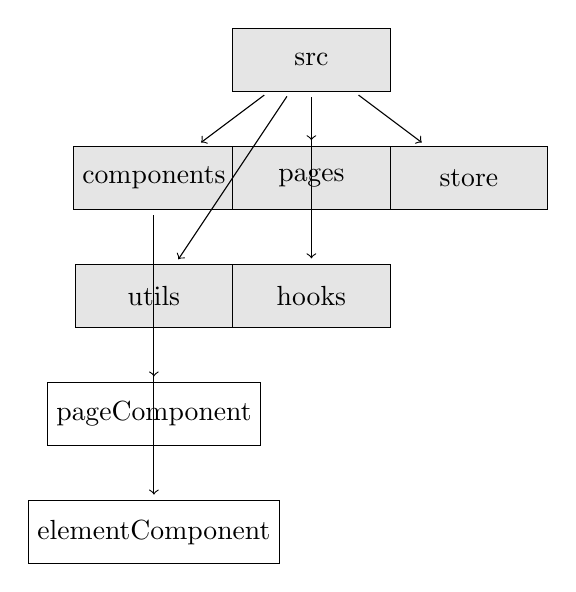
\begin{tikzpicture}[
    file/.style={draw, rectangle, minimum width=2cm, minimum height=0.8cm},
    folder/.style={draw, rectangle, minimum width=2cm, minimum height=0.8cm, fill=gray!20},
    arrow/.style={->, shorten >=2pt, shorten <=2pt}
]

% Folders
\node[folder] (src) at (0,0) {src};
\node[folder] (components) at (-2,-1.5) {components};
\node[folder] (pages) at (0,-1.5) {pages};
\node[folder] (store) at (2,-1.5) {store};
\node[folder] (utils) at (-2,-3) {utils};
\node[folder] (hooks) at (0,-3) {hooks};

% Files
\node[file] (pageComponent) at (-2,-4.5) {pageComponent};
\node[file] (elementComponent) at (-2,-6) {elementComponent};
% ... add more files

% Connections
\draw[arrow] (src) -- (components);
\draw[arrow] (src) -- (pages);
\draw[arrow] (src) -- (store);
\draw[arrow] (src) -- (utils);
\draw[arrow] (src) -- (hooks);
\draw[arrow] (components) -- (pageComponent);
\draw[arrow] (components) -- (elementComponent);
% ... add more connections

\end{tikzpicture}



\pagebreak
\subsubsection{Back-end}
The backend uses the dotNet framework. The development language using the C\# language.

In this project, the backend uses the Onion Architecture.
The Onion Architecture is a typically layered architecture, 
where each layer depends on the inner layer and provides interfaces to the outer layer.
The outer layer provides services to the outermost layer 
and other modules in the same layer based on the interfaces of the inner layer.

From inner to outer, the layers are: Domain, Application, Infrastructure, Presentation.
The Domain layer is the core layer and the innermost layer, used to define domain models, 
which are the business models.
It includes domain models and domain service interfaces.
Domain models are used to define the business models, 
which are the entities in the entity-relationship model and their attributes.
Domain service interfaces are used to define the business services, 
which are the relationships between entities in the entity-relationship model.

The Application layer is the application layer, 
used to define application services, which are the business logic.
It includes domain service implementations and application service interfaces.
Domain service implementations implement the methods of the inner layer's domain service 
interfaces and implement the business logic of the domain models.
Application service interfaces are used to define application services, 
which are the business logic.
It includes but is not limited to database interfaces, testing interfaces, 
HTTP API interfaces, MQTT interfaces, etc.

The Infrastructure layer is the infrastructure layer, used to define infrastructure.
It includes database implementations, testing implementations, 
HTTP API implementations, MQTT implementations, etc.
Database implementations implement the database interfaces 
and provide CRUD services for the database.
Testing implementations implement the testing interfaces 
and provide services for unit testing and integration testing.
HTTP API implementations implement the HTTP API interfaces 
and provide CRUD operations for HTTP APIs.
MQTT implementations implement the MQTT interfaces 
and provide CRUD operations for MQTT.

The Presentation layer is the presentation layer, used to define presentation logic, 
such as interfaces and pages. Since this is a backend project,
data presentation and control are handled by the frontend, 
so this layer is not needed.



\pagebreak
\subsubsection{Data communication and storage}
% 关于本项目的数据通信与数据存储的设计, 包括数据通信的协议, 数据存储的设计等
% 关于数据通信的设计:
% 1. 通信协议的选择
% 自前端向后端发送的数据, 有三种传输的数据类型, 
% 一种是普通的增删改查的请求, 对数据传输的时效性要求不高, 但是对数据的准确性, 完整性, 有序性, 安全性有一定的要求,
% 这种数据的传输, 采用 HTTP 协议, 以及 RESTful API 的设计. 可以有效的保证对数据传输的以上要求.
% 一种是对数据通道的创建和流媒体数据的传输, 对数据传输的时效性, 安全性要求较高, 这种数据的传输, 采用 WebRTC 协议, 以及 MQTT 协议.
% 配合可以快速解码的 flatbuffers 协议, 可以有效的保证对数据传输的以上要求.
% 最后一种是对设备的状态信息和操作信息的传输, 对完整性, 有序性, 安全性都有较高的要求, 这种数据的传输, 采用 MQTT 协议
% 同时也使用了 flatbuffers 协议.
% 
% 2. 数据通信的通信架构和通信流程
% 本项目的数据通信的通信架构, 是基于前后端分离的架构, 前端使用 React 框架, 后端使用 dotnet 框架.
% 当前端需要向后端发送数据的时候, 前端会向后端发送 HTTP 请求, 后端接收到 HTTP 请求之后, 会根据请求的数据类型,
% 选择不同的数据处理方式, 对于普通的增删改查的请求, 后端会根据 RESTful API 的设计, 对数据进行增删改查的操作,
% 对于对数据通道的创建和流媒体数据的传输, 后端会根据 WebRTC 协议, 对数据通道进行创建, 并且帮助前端和设备建立数据通道,
% 当数据通道建立后, 前端和设备之间则使用 flatbuffer 的数据格式对流媒体数据进行传输,
% 对于设备的状态信息和操作信息的传输, 前端会直接向 MQTT broker 发送 MQTT 请求, 
% 设备会在其自身的固件中监听相关的 MQTT 请求, 并且返回相关的数据.
% 
% 3. 数据通信的格式
% 本项目的数据通信的格式, 有三种, 
% 一种是 HTTP 协议, 
% 使用 json 格式对数据进行传输,
% 一种是 WebRTC 协议, 
% 使用 flatbuffers 格式对数据进行传输,
% 一种是 MQTT 协议.
% 使用 flatbuffers 格式对数据进行传输,
% 
% 关于数据存储的设计:
% 1. 数据存储的数据库的选择
% 本项目的数据存储的数据库的选择, 使用了轻量级的数据库 SQLite,
% SQLite 是一个进程内的库, 实现了自给自足的, 无服务器的, 零配置的, 事务性的 SQL 数据库引擎.
% 这是因为整个项目的目的是为了实现前端与设备之间的数据通信, 对于数据库数据的增删改查操作的要求不高,
% 数据量较小, 且对于数据库的数据的事务性要求不高, 所以选择了 SQLite 数据库.
% 2. 项目前后端的数据结构的设计
% 在本项目中, 前端由于使用了 React 框架, 所以前端的数据结构的设计, 使用了基于状态的数据结构的设计,
% 每个组件或者数据集都包含一个状态对象, 这个状态对象的属性就是组件的各个状态. 
% 使用状态对象的原因是, 可以方便的对状态进行管理, 采用对象-属性的形式, 可以方便的针对不同组件的同类状态进行区分,
% 由于跨组件的状态是由 redux 进行管理的, 这种状态对象的设计, 可以更搞笑的对状态进行更新和传递.
% 后端由于使用了 dotnet 框架, 所以后端的数据结构的设计, 使用了基于类的数据结构的设计,
% 采用了面向对象的编程思想, 对数据进行了封装, 使得数据的传输更加的安全, 有序, 完整.


\pagebreak

% \subsection{Domain model}
% \documentclass[]{article}
\usepackage{graphicx}
\usepackage{amsmath}
\usepackage{tikz}

% libaries
\usetikzlibrary{shapes,arrows}

%Define the listing package
\usepackage{listings} %code highlighter
\usepackage{color} %use color
\definecolor{mygreen}{rgb}{0,0.6,0}
\definecolor{mygray}{rgb}{0.5,0.5,0.5}
\definecolor{mymauve}{rgb}{0.58,0,0.82}

%Customize a bit the look
\lstset{ %
backgroundcolor=\color{white}, % choose the background color; you must add \usepackage{color} or \usepackage{xcolor}
basicstyle=\footnotesize, % the size of the fonts that are used for the code
breakatwhitespace=false, % sets if automatic breaks should only happen at whitespace
breaklines=true, % sets automatic line breaking
captionpos=b, % sets the caption-position to bottom
commentstyle=\color{mygreen}, % comment style
deletekeywords={...}, % if you want to delete keywords from the given language
escapeinside={\%*}{*)}, % if you want to add LaTeX within your code
extendedchars=true, % lets you use non-ASCII characters; for 8-bits encodings only, does not work with UTF-8
frame=single, % adds a frame around the code
keepspaces=true, % keeps spaces in text, useful for keeping indentation of code (possibly needs columns=flexible)
keywordstyle=\color{blue}, % keyword style
% language=Octave, % the language of the code
morekeywords={*,...}, % if you want to add more keywords to the set
numbers=left, % where to put the line-numbers; possible values are (none, left, right)
numbersep=5pt, % how far the line-numbers are from the code
numberstyle=\tiny\color{mygray}, % the style that is used for the line-numbers
rulecolor=\color{black}, % if not set, the frame-color may be changed on line-breaks within not-black text (e.g. comments (green here))
showspaces=false, % show spaces everywhere adding particular underscores; it overrides 'showstringspaces'
showstringspaces=false, % underline spaces within strings only
showtabs=false, % show tabs within strings adding particular underscores
stepnumber=1, % the step between two line-numbers. If it's 1, each line will be numbered
stringstyle=\color{mymauve}, % string literal style
tabsize=2, % sets default tabsize to 2 spaces
title=\lstname % show the filename of files included with \lstinputlisting; also try caption instead of title
}

\definecolor{darkgray}{rgb}{.4,.4,.4}
\definecolor{purple}{rgb}{0.65, 0.12, 0.82}

\lstdefinelanguage{React}{
keywords={const, typeof, new, true, false, catch, function, return, null, catch, switch, var, if, in, while, do, else, case, break},
keywordstyle=\color{blue}\bfseries,
ndkeywords={class, export, boolean, throw, implements, import, this},
ndkeywordstyle=\color{darkgray}\bfseries,
identifierstyle=\color{mygreen},
sensitive=false,
comment=[l]{//},
morecomment=[s]{/*}{*/},
commentstyle=\color{purple}\ttfamily,
string=[b]{"}{'}{`},
stringstyle=\color{red}\ttfamily,
morestring=[b]',
morestring=[b]",
morestring=[b]`',
}

\lstdefinelanguage{CSharp}{
keywords={const, typeof, new, true, false, catch, function, return, null, catch, switch, var, if, in, while, do, else, case, break},
keywordstyle=\color{blue}\bfseries,
ndkeywords={class, export, boolean, throw, implements, import, this},
ndkeywordstyle=\color{darkgray}\bfseries,
identifierstyle=\color{mygreen},
sensitive=false,
comment=[l]{//},
morecomment=[s]{/*}{*/},
commentstyle=\color{purple}\ttfamily,
string=[b]{"}{'}{`},
stringstyle=\color{red}\ttfamily,
morestring=[b]',
morestring=[b]",
morestring=[b]`',
}

\lstset{
language=React,
extendedchars=true,
basicstyle=\footnotesize\ttfamily,
showstringspaces=false,
showspaces=false,
numbers=left,
numberstyle=\footnotesize,
numbersep=9pt,
tabsize=2,
breaklines=true,
showtabs=false,
captionpos=b
}

\lstset{
language=CSharp,
extendedchars=true,
basicstyle=\footnotesize\ttfamily,
showstringspaces=false,
showspaces=false,
numbers=left,
numberstyle=\footnotesize,
numbersep=9pt,
tabsize=2,
breaklines=true,
showtabs=false,
captionpos=b
}

% \usepackage{cite} % Add this line for citation

% \bibliographystyle{plain}

\title{
The implementation of BifrostConnect Front-end scope, 
re-design and development with the relevant back-end support develop.
}
\author{
    Fei Gu \\
    Erhvervs Akademi Sydvest \\
    Computer Science 21\\
    }
\date{\today}

\begin{document}

% Front page
\maketitle
\begin{center}
    Supervisor: Henrik Boulund Meng Hansen \\
    Company: BifrostConnect \\
    Engineering Director: Jasper Wass \\
\end{center}
\tableofcontents
\pagebreak


% The introduction
\section{Introduction}
\subsection{Background}\input{sections/introduction/background.tex}
\subsection{The company}\input{sections/introduction/aboutCompany}
\subsection{The project}\input{sections/introduction/aboutProject}
\pagebreak

% The problem statement
\section{Problem Statement}
\subsection{Statement}
\input{sections/problemStatement/statement}
\subsection{Situation}
\input{sections/problemStatement/situation}
\subsection{Potential Solution}
\input{sections/problemStatement/potentialSolution}
\pagebreak

% Requirement analysis
\section{Requirement Analysis}
\input{sections/requirementAnalysis/index}

\subsection{Stakeholders}
\input{sections/requirementAnalysis/stakeholders/index}

\subsection{Business Domain}
\input{sections/requirementAnalysis/bussinesDomain/index}

\subsection{Scope}
\input{sections/requirementAnalysis/scope}

\subsection{Goals}
\input{sections/requirementAnalysis/goals}
\pagebreak

% Software Design
\section{Software Design}
% developement methods
\subsection{Software Development Methods}
\input{sections/softwareDevelopmentMethods/index}
\subsubsection{Agile Software Development}
\input{sections/softwareDevelopmentMethods/agileSoftwareDevelopment/index}
\subsubsection{Feature Driven Development}
\input{sections/softwareDevelopmentMethods/featureDrivenDevelopment/index}

\pagebreak

% Technology seslection
\subsection{Technology selection}
\input{sections/softwareDesign/technologySelection/index}
\subsubsection{Front-end}
\input{sections/softwareDesign/technologySelection/frontEnd}            
\subsubsection{Back-end}
\input{sections/softwareDesign/technologySelection/backEnd}            
\subsubsection{Database}
\input{sections/softwareDesign/technologySelection/database}
\subsubsection{Data communication}
\input{sections/softwareDesign/technologySelection/dataCommunication}            
\subsubsection{DevOps}
\input{sections/softwareDesign/technologySelection/devOps}
\pagebreak

% Architecture design
\subsection{Architecture design}
\input{sections/softwareDesign/architectureDesign/index}
\pagebreak
\subsubsection{Front-end}
\input{sections/softwareDesign/architectureDesign/frontEndArchitecture}
\pagebreak
\subsubsection{Back-end}
\input{sections/softwareDesign/architectureDesign/backEndArchitecture}
\pagebreak
\subsubsection{Data communication and storage}
\input{sections/softwareDesign/architectureDesign/dataCommunicationArchitecture}
\pagebreak

% \subsection{Domain model}
% \input{sections/softwareDesign/domainModel/index}
% \subsection{Database design}
% % 数据库领域模型 ER 图
% % 包括表和字段的设置.
% % 对于私有键和外键的设置.

% \subsection{Back-end design}
% % 后端对象模型
% % 以及对于对象模型的增删改查
% % 以及相关的其他服务的设计`'

% \subsection{Front-end design}
% % 对于前端的页面结构的设计 
% % 页面的状态的设计, 交互设计

% \subsection{FlatBuffers design}
% % schema 的设计

\subsection{DevOps CI/CD process design}
\input{sections/softwareDesign/devOpsDesign/index}
\subsubsection{Continuous Integration}
\input{sections/softwareDesign/devOpsDesign/continuousIntegration/index}
\subsubsection{Continuous Delivery}
\input{sections/softwareDesign/devOpsDesign/continuousDelivery/index}
\subsubsection{Continuous Deployment}
\input{sections/softwareDesign/devOpsDesign/continuousDeployment/index}
\pagebreak

\section{Software Development} 
\input{sections/softwareDevelopment/index}
\subsection{Overall development}
\input{sections/softwareDevelopment/overallDevelopement/index}
\subsubsection{Front-end}
\input{sections/softwareDevelopment/overallDevelopement/frontEnd/index}
\subsubsection{Back-end}
\input{sections/softwareDevelopment/overallDevelopement/backEnd/index}
\subsubsection{DevOps}
\input{sections/softwareDevelopment/overallDevelopement/devOps/index}
\subsection{Feature development} 
\input{sections/softwareDevelopment/featureDevelopment/index}
\subsubsection{Use Case 1}
\input{sections/softwareDevelopment/featureDevelopment/useCase1/index}
\subsubsection{Feature 1}
\input{sections/softwareDevelopment/featureDevelopment/feature/feature1.tex}
\pagebreak
\section{Conclusion} 
\subsection{Result}
Since the project is still in progress, the result is not available yet.
So far, basic structure of this project has been built. But the most features 
are not implemented yet. 
\subsection{Discussion}
As a single developer for this project, I am confident what I have done so far.
And I can say I understand the most of the knowledge I have used in this project, 
which also means I can explain all the part of the project. 
But this project also relevant some of the complex knowledge which I have to continue 
to study and practice.
\subsection{Future Work}
The future work is to implement the rest of the features. 
Including the most important part which is the 'create session' feature.
\pagebreak
% \bibliography{bibliography}
\pagebreak
% \begin{appendices}
%     \section{Appendix}
% \end{appendices} 
\end{document}
% \subsection{Database design}
% % 数据库领域模型 ER 图
% % 包括表和字段的设置.
% % 对于私有键和外键的设置.

% \subsection{Back-end design}
% % 后端对象模型
% % 以及对于对象模型的增删改查
% % 以及相关的其他服务的设计`'

% \subsection{Front-end design}
% % 对于前端的页面结构的设计 
% % 页面的状态的设计, 交互设计

% \subsection{FlatBuffers design}
% % schema 的设计

\subsection{DevOps CI/CD process design}
\documentclass[]{article}
\usepackage{graphicx}
\usepackage{amsmath}
\usepackage{tikz}

% libaries
\usetikzlibrary{shapes,arrows}

%Define the listing package
\usepackage{listings} %code highlighter
\usepackage{color} %use color
\definecolor{mygreen}{rgb}{0,0.6,0}
\definecolor{mygray}{rgb}{0.5,0.5,0.5}
\definecolor{mymauve}{rgb}{0.58,0,0.82}

%Customize a bit the look
\lstset{ %
backgroundcolor=\color{white}, % choose the background color; you must add \usepackage{color} or \usepackage{xcolor}
basicstyle=\footnotesize, % the size of the fonts that are used for the code
breakatwhitespace=false, % sets if automatic breaks should only happen at whitespace
breaklines=true, % sets automatic line breaking
captionpos=b, % sets the caption-position to bottom
commentstyle=\color{mygreen}, % comment style
deletekeywords={...}, % if you want to delete keywords from the given language
escapeinside={\%*}{*)}, % if you want to add LaTeX within your code
extendedchars=true, % lets you use non-ASCII characters; for 8-bits encodings only, does not work with UTF-8
frame=single, % adds a frame around the code
keepspaces=true, % keeps spaces in text, useful for keeping indentation of code (possibly needs columns=flexible)
keywordstyle=\color{blue}, % keyword style
% language=Octave, % the language of the code
morekeywords={*,...}, % if you want to add more keywords to the set
numbers=left, % where to put the line-numbers; possible values are (none, left, right)
numbersep=5pt, % how far the line-numbers are from the code
numberstyle=\tiny\color{mygray}, % the style that is used for the line-numbers
rulecolor=\color{black}, % if not set, the frame-color may be changed on line-breaks within not-black text (e.g. comments (green here))
showspaces=false, % show spaces everywhere adding particular underscores; it overrides 'showstringspaces'
showstringspaces=false, % underline spaces within strings only
showtabs=false, % show tabs within strings adding particular underscores
stepnumber=1, % the step between two line-numbers. If it's 1, each line will be numbered
stringstyle=\color{mymauve}, % string literal style
tabsize=2, % sets default tabsize to 2 spaces
title=\lstname % show the filename of files included with \lstinputlisting; also try caption instead of title
}

\definecolor{darkgray}{rgb}{.4,.4,.4}
\definecolor{purple}{rgb}{0.65, 0.12, 0.82}

\lstdefinelanguage{React}{
keywords={const, typeof, new, true, false, catch, function, return, null, catch, switch, var, if, in, while, do, else, case, break},
keywordstyle=\color{blue}\bfseries,
ndkeywords={class, export, boolean, throw, implements, import, this},
ndkeywordstyle=\color{darkgray}\bfseries,
identifierstyle=\color{mygreen},
sensitive=false,
comment=[l]{//},
morecomment=[s]{/*}{*/},
commentstyle=\color{purple}\ttfamily,
string=[b]{"}{'}{`},
stringstyle=\color{red}\ttfamily,
morestring=[b]',
morestring=[b]",
morestring=[b]`',
}

\lstdefinelanguage{CSharp}{
keywords={const, typeof, new, true, false, catch, function, return, null, catch, switch, var, if, in, while, do, else, case, break},
keywordstyle=\color{blue}\bfseries,
ndkeywords={class, export, boolean, throw, implements, import, this},
ndkeywordstyle=\color{darkgray}\bfseries,
identifierstyle=\color{mygreen},
sensitive=false,
comment=[l]{//},
morecomment=[s]{/*}{*/},
commentstyle=\color{purple}\ttfamily,
string=[b]{"}{'}{`},
stringstyle=\color{red}\ttfamily,
morestring=[b]',
morestring=[b]",
morestring=[b]`',
}

\lstset{
language=React,
extendedchars=true,
basicstyle=\footnotesize\ttfamily,
showstringspaces=false,
showspaces=false,
numbers=left,
numberstyle=\footnotesize,
numbersep=9pt,
tabsize=2,
breaklines=true,
showtabs=false,
captionpos=b
}

\lstset{
language=CSharp,
extendedchars=true,
basicstyle=\footnotesize\ttfamily,
showstringspaces=false,
showspaces=false,
numbers=left,
numberstyle=\footnotesize,
numbersep=9pt,
tabsize=2,
breaklines=true,
showtabs=false,
captionpos=b
}

% \usepackage{cite} % Add this line for citation

% \bibliographystyle{plain}

\title{
The implementation of BifrostConnect Front-end scope, 
re-design and development with the relevant back-end support develop.
}
\author{
    Fei Gu \\
    Erhvervs Akademi Sydvest \\
    Computer Science 21\\
    }
\date{\today}

\begin{document}

% Front page
\maketitle
\begin{center}
    Supervisor: Henrik Boulund Meng Hansen \\
    Company: BifrostConnect \\
    Engineering Director: Jasper Wass \\
\end{center}
\tableofcontents
\pagebreak


% The introduction
\section{Introduction}
\subsection{Background}\input{sections/introduction/background.tex}
\subsection{The company}\input{sections/introduction/aboutCompany}
\subsection{The project}\input{sections/introduction/aboutProject}
\pagebreak

% The problem statement
\section{Problem Statement}
\subsection{Statement}
\input{sections/problemStatement/statement}
\subsection{Situation}
\input{sections/problemStatement/situation}
\subsection{Potential Solution}
\input{sections/problemStatement/potentialSolution}
\pagebreak

% Requirement analysis
\section{Requirement Analysis}
\input{sections/requirementAnalysis/index}

\subsection{Stakeholders}
\input{sections/requirementAnalysis/stakeholders/index}

\subsection{Business Domain}
\input{sections/requirementAnalysis/bussinesDomain/index}

\subsection{Scope}
\input{sections/requirementAnalysis/scope}

\subsection{Goals}
\input{sections/requirementAnalysis/goals}
\pagebreak

% Software Design
\section{Software Design}
% developement methods
\subsection{Software Development Methods}
\input{sections/softwareDevelopmentMethods/index}
\subsubsection{Agile Software Development}
\input{sections/softwareDevelopmentMethods/agileSoftwareDevelopment/index}
\subsubsection{Feature Driven Development}
\input{sections/softwareDevelopmentMethods/featureDrivenDevelopment/index}

\pagebreak

% Technology seslection
\subsection{Technology selection}
\input{sections/softwareDesign/technologySelection/index}
\subsubsection{Front-end}
\input{sections/softwareDesign/technologySelection/frontEnd}            
\subsubsection{Back-end}
\input{sections/softwareDesign/technologySelection/backEnd}            
\subsubsection{Database}
\input{sections/softwareDesign/technologySelection/database}
\subsubsection{Data communication}
\input{sections/softwareDesign/technologySelection/dataCommunication}            
\subsubsection{DevOps}
\input{sections/softwareDesign/technologySelection/devOps}
\pagebreak

% Architecture design
\subsection{Architecture design}
\input{sections/softwareDesign/architectureDesign/index}
\pagebreak
\subsubsection{Front-end}
\input{sections/softwareDesign/architectureDesign/frontEndArchitecture}
\pagebreak
\subsubsection{Back-end}
\input{sections/softwareDesign/architectureDesign/backEndArchitecture}
\pagebreak
\subsubsection{Data communication and storage}
\input{sections/softwareDesign/architectureDesign/dataCommunicationArchitecture}
\pagebreak

% \subsection{Domain model}
% \input{sections/softwareDesign/domainModel/index}
% \subsection{Database design}
% % 数据库领域模型 ER 图
% % 包括表和字段的设置.
% % 对于私有键和外键的设置.

% \subsection{Back-end design}
% % 后端对象模型
% % 以及对于对象模型的增删改查
% % 以及相关的其他服务的设计`'

% \subsection{Front-end design}
% % 对于前端的页面结构的设计 
% % 页面的状态的设计, 交互设计

% \subsection{FlatBuffers design}
% % schema 的设计

\subsection{DevOps CI/CD process design}
\input{sections/softwareDesign/devOpsDesign/index}
\subsubsection{Continuous Integration}
\input{sections/softwareDesign/devOpsDesign/continuousIntegration/index}
\subsubsection{Continuous Delivery}
\input{sections/softwareDesign/devOpsDesign/continuousDelivery/index}
\subsubsection{Continuous Deployment}
\input{sections/softwareDesign/devOpsDesign/continuousDeployment/index}
\pagebreak

\section{Software Development} 
\input{sections/softwareDevelopment/index}
\subsection{Overall development}
\input{sections/softwareDevelopment/overallDevelopement/index}
\subsubsection{Front-end}
\input{sections/softwareDevelopment/overallDevelopement/frontEnd/index}
\subsubsection{Back-end}
\input{sections/softwareDevelopment/overallDevelopement/backEnd/index}
\subsubsection{DevOps}
\input{sections/softwareDevelopment/overallDevelopement/devOps/index}
\subsection{Feature development} 
\input{sections/softwareDevelopment/featureDevelopment/index}
\subsubsection{Use Case 1}
\input{sections/softwareDevelopment/featureDevelopment/useCase1/index}
\subsubsection{Feature 1}
\input{sections/softwareDevelopment/featureDevelopment/feature/feature1.tex}
\pagebreak
\section{Conclusion} 
\subsection{Result}
Since the project is still in progress, the result is not available yet.
So far, basic structure of this project has been built. But the most features 
are not implemented yet. 
\subsection{Discussion}
As a single developer for this project, I am confident what I have done so far.
And I can say I understand the most of the knowledge I have used in this project, 
which also means I can explain all the part of the project. 
But this project also relevant some of the complex knowledge which I have to continue 
to study and practice.
\subsection{Future Work}
The future work is to implement the rest of the features. 
Including the most important part which is the 'create session' feature.
\pagebreak
% \bibliography{bibliography}
\pagebreak
% \begin{appendices}
%     \section{Appendix}
% \end{appendices} 
\end{document}
\subsubsection{Continuous Integration}
\documentclass[]{article}
\usepackage{graphicx}
\usepackage{amsmath}
\usepackage{tikz}

% libaries
\usetikzlibrary{shapes,arrows}

%Define the listing package
\usepackage{listings} %code highlighter
\usepackage{color} %use color
\definecolor{mygreen}{rgb}{0,0.6,0}
\definecolor{mygray}{rgb}{0.5,0.5,0.5}
\definecolor{mymauve}{rgb}{0.58,0,0.82}

%Customize a bit the look
\lstset{ %
backgroundcolor=\color{white}, % choose the background color; you must add \usepackage{color} or \usepackage{xcolor}
basicstyle=\footnotesize, % the size of the fonts that are used for the code
breakatwhitespace=false, % sets if automatic breaks should only happen at whitespace
breaklines=true, % sets automatic line breaking
captionpos=b, % sets the caption-position to bottom
commentstyle=\color{mygreen}, % comment style
deletekeywords={...}, % if you want to delete keywords from the given language
escapeinside={\%*}{*)}, % if you want to add LaTeX within your code
extendedchars=true, % lets you use non-ASCII characters; for 8-bits encodings only, does not work with UTF-8
frame=single, % adds a frame around the code
keepspaces=true, % keeps spaces in text, useful for keeping indentation of code (possibly needs columns=flexible)
keywordstyle=\color{blue}, % keyword style
% language=Octave, % the language of the code
morekeywords={*,...}, % if you want to add more keywords to the set
numbers=left, % where to put the line-numbers; possible values are (none, left, right)
numbersep=5pt, % how far the line-numbers are from the code
numberstyle=\tiny\color{mygray}, % the style that is used for the line-numbers
rulecolor=\color{black}, % if not set, the frame-color may be changed on line-breaks within not-black text (e.g. comments (green here))
showspaces=false, % show spaces everywhere adding particular underscores; it overrides 'showstringspaces'
showstringspaces=false, % underline spaces within strings only
showtabs=false, % show tabs within strings adding particular underscores
stepnumber=1, % the step between two line-numbers. If it's 1, each line will be numbered
stringstyle=\color{mymauve}, % string literal style
tabsize=2, % sets default tabsize to 2 spaces
title=\lstname % show the filename of files included with \lstinputlisting; also try caption instead of title
}

\definecolor{darkgray}{rgb}{.4,.4,.4}
\definecolor{purple}{rgb}{0.65, 0.12, 0.82}

\lstdefinelanguage{React}{
keywords={const, typeof, new, true, false, catch, function, return, null, catch, switch, var, if, in, while, do, else, case, break},
keywordstyle=\color{blue}\bfseries,
ndkeywords={class, export, boolean, throw, implements, import, this},
ndkeywordstyle=\color{darkgray}\bfseries,
identifierstyle=\color{mygreen},
sensitive=false,
comment=[l]{//},
morecomment=[s]{/*}{*/},
commentstyle=\color{purple}\ttfamily,
string=[b]{"}{'}{`},
stringstyle=\color{red}\ttfamily,
morestring=[b]',
morestring=[b]",
morestring=[b]`',
}

\lstdefinelanguage{CSharp}{
keywords={const, typeof, new, true, false, catch, function, return, null, catch, switch, var, if, in, while, do, else, case, break},
keywordstyle=\color{blue}\bfseries,
ndkeywords={class, export, boolean, throw, implements, import, this},
ndkeywordstyle=\color{darkgray}\bfseries,
identifierstyle=\color{mygreen},
sensitive=false,
comment=[l]{//},
morecomment=[s]{/*}{*/},
commentstyle=\color{purple}\ttfamily,
string=[b]{"}{'}{`},
stringstyle=\color{red}\ttfamily,
morestring=[b]',
morestring=[b]",
morestring=[b]`',
}

\lstset{
language=React,
extendedchars=true,
basicstyle=\footnotesize\ttfamily,
showstringspaces=false,
showspaces=false,
numbers=left,
numberstyle=\footnotesize,
numbersep=9pt,
tabsize=2,
breaklines=true,
showtabs=false,
captionpos=b
}

\lstset{
language=CSharp,
extendedchars=true,
basicstyle=\footnotesize\ttfamily,
showstringspaces=false,
showspaces=false,
numbers=left,
numberstyle=\footnotesize,
numbersep=9pt,
tabsize=2,
breaklines=true,
showtabs=false,
captionpos=b
}

% \usepackage{cite} % Add this line for citation

% \bibliographystyle{plain}

\title{
The implementation of BifrostConnect Front-end scope, 
re-design and development with the relevant back-end support develop.
}
\author{
    Fei Gu \\
    Erhvervs Akademi Sydvest \\
    Computer Science 21\\
    }
\date{\today}

\begin{document}

% Front page
\maketitle
\begin{center}
    Supervisor: Henrik Boulund Meng Hansen \\
    Company: BifrostConnect \\
    Engineering Director: Jasper Wass \\
\end{center}
\tableofcontents
\pagebreak


% The introduction
\section{Introduction}
\subsection{Background}\input{sections/introduction/background.tex}
\subsection{The company}\input{sections/introduction/aboutCompany}
\subsection{The project}\input{sections/introduction/aboutProject}
\pagebreak

% The problem statement
\section{Problem Statement}
\subsection{Statement}
\input{sections/problemStatement/statement}
\subsection{Situation}
\input{sections/problemStatement/situation}
\subsection{Potential Solution}
\input{sections/problemStatement/potentialSolution}
\pagebreak

% Requirement analysis
\section{Requirement Analysis}
\input{sections/requirementAnalysis/index}

\subsection{Stakeholders}
\input{sections/requirementAnalysis/stakeholders/index}

\subsection{Business Domain}
\input{sections/requirementAnalysis/bussinesDomain/index}

\subsection{Scope}
\input{sections/requirementAnalysis/scope}

\subsection{Goals}
\input{sections/requirementAnalysis/goals}
\pagebreak

% Software Design
\section{Software Design}
% developement methods
\subsection{Software Development Methods}
\input{sections/softwareDevelopmentMethods/index}
\subsubsection{Agile Software Development}
\input{sections/softwareDevelopmentMethods/agileSoftwareDevelopment/index}
\subsubsection{Feature Driven Development}
\input{sections/softwareDevelopmentMethods/featureDrivenDevelopment/index}

\pagebreak

% Technology seslection
\subsection{Technology selection}
\input{sections/softwareDesign/technologySelection/index}
\subsubsection{Front-end}
\input{sections/softwareDesign/technologySelection/frontEnd}            
\subsubsection{Back-end}
\input{sections/softwareDesign/technologySelection/backEnd}            
\subsubsection{Database}
\input{sections/softwareDesign/technologySelection/database}
\subsubsection{Data communication}
\input{sections/softwareDesign/technologySelection/dataCommunication}            
\subsubsection{DevOps}
\input{sections/softwareDesign/technologySelection/devOps}
\pagebreak

% Architecture design
\subsection{Architecture design}
\input{sections/softwareDesign/architectureDesign/index}
\pagebreak
\subsubsection{Front-end}
\input{sections/softwareDesign/architectureDesign/frontEndArchitecture}
\pagebreak
\subsubsection{Back-end}
\input{sections/softwareDesign/architectureDesign/backEndArchitecture}
\pagebreak
\subsubsection{Data communication and storage}
\input{sections/softwareDesign/architectureDesign/dataCommunicationArchitecture}
\pagebreak

% \subsection{Domain model}
% \input{sections/softwareDesign/domainModel/index}
% \subsection{Database design}
% % 数据库领域模型 ER 图
% % 包括表和字段的设置.
% % 对于私有键和外键的设置.

% \subsection{Back-end design}
% % 后端对象模型
% % 以及对于对象模型的增删改查
% % 以及相关的其他服务的设计`'

% \subsection{Front-end design}
% % 对于前端的页面结构的设计 
% % 页面的状态的设计, 交互设计

% \subsection{FlatBuffers design}
% % schema 的设计

\subsection{DevOps CI/CD process design}
\input{sections/softwareDesign/devOpsDesign/index}
\subsubsection{Continuous Integration}
\input{sections/softwareDesign/devOpsDesign/continuousIntegration/index}
\subsubsection{Continuous Delivery}
\input{sections/softwareDesign/devOpsDesign/continuousDelivery/index}
\subsubsection{Continuous Deployment}
\input{sections/softwareDesign/devOpsDesign/continuousDeployment/index}
\pagebreak

\section{Software Development} 
\input{sections/softwareDevelopment/index}
\subsection{Overall development}
\input{sections/softwareDevelopment/overallDevelopement/index}
\subsubsection{Front-end}
\input{sections/softwareDevelopment/overallDevelopement/frontEnd/index}
\subsubsection{Back-end}
\input{sections/softwareDevelopment/overallDevelopement/backEnd/index}
\subsubsection{DevOps}
\input{sections/softwareDevelopment/overallDevelopement/devOps/index}
\subsection{Feature development} 
\input{sections/softwareDevelopment/featureDevelopment/index}
\subsubsection{Use Case 1}
\input{sections/softwareDevelopment/featureDevelopment/useCase1/index}
\subsubsection{Feature 1}
\input{sections/softwareDevelopment/featureDevelopment/feature/feature1.tex}
\pagebreak
\section{Conclusion} 
\subsection{Result}
Since the project is still in progress, the result is not available yet.
So far, basic structure of this project has been built. But the most features 
are not implemented yet. 
\subsection{Discussion}
As a single developer for this project, I am confident what I have done so far.
And I can say I understand the most of the knowledge I have used in this project, 
which also means I can explain all the part of the project. 
But this project also relevant some of the complex knowledge which I have to continue 
to study and practice.
\subsection{Future Work}
The future work is to implement the rest of the features. 
Including the most important part which is the 'create session' feature.
\pagebreak
% \bibliography{bibliography}
\pagebreak
% \begin{appendices}
%     \section{Appendix}
% \end{appendices} 
\end{document}
\subsubsection{Continuous Delivery}
\documentclass[]{article}
\usepackage{graphicx}
\usepackage{amsmath}
\usepackage{tikz}

% libaries
\usetikzlibrary{shapes,arrows}

%Define the listing package
\usepackage{listings} %code highlighter
\usepackage{color} %use color
\definecolor{mygreen}{rgb}{0,0.6,0}
\definecolor{mygray}{rgb}{0.5,0.5,0.5}
\definecolor{mymauve}{rgb}{0.58,0,0.82}

%Customize a bit the look
\lstset{ %
backgroundcolor=\color{white}, % choose the background color; you must add \usepackage{color} or \usepackage{xcolor}
basicstyle=\footnotesize, % the size of the fonts that are used for the code
breakatwhitespace=false, % sets if automatic breaks should only happen at whitespace
breaklines=true, % sets automatic line breaking
captionpos=b, % sets the caption-position to bottom
commentstyle=\color{mygreen}, % comment style
deletekeywords={...}, % if you want to delete keywords from the given language
escapeinside={\%*}{*)}, % if you want to add LaTeX within your code
extendedchars=true, % lets you use non-ASCII characters; for 8-bits encodings only, does not work with UTF-8
frame=single, % adds a frame around the code
keepspaces=true, % keeps spaces in text, useful for keeping indentation of code (possibly needs columns=flexible)
keywordstyle=\color{blue}, % keyword style
% language=Octave, % the language of the code
morekeywords={*,...}, % if you want to add more keywords to the set
numbers=left, % where to put the line-numbers; possible values are (none, left, right)
numbersep=5pt, % how far the line-numbers are from the code
numberstyle=\tiny\color{mygray}, % the style that is used for the line-numbers
rulecolor=\color{black}, % if not set, the frame-color may be changed on line-breaks within not-black text (e.g. comments (green here))
showspaces=false, % show spaces everywhere adding particular underscores; it overrides 'showstringspaces'
showstringspaces=false, % underline spaces within strings only
showtabs=false, % show tabs within strings adding particular underscores
stepnumber=1, % the step between two line-numbers. If it's 1, each line will be numbered
stringstyle=\color{mymauve}, % string literal style
tabsize=2, % sets default tabsize to 2 spaces
title=\lstname % show the filename of files included with \lstinputlisting; also try caption instead of title
}

\definecolor{darkgray}{rgb}{.4,.4,.4}
\definecolor{purple}{rgb}{0.65, 0.12, 0.82}

\lstdefinelanguage{React}{
keywords={const, typeof, new, true, false, catch, function, return, null, catch, switch, var, if, in, while, do, else, case, break},
keywordstyle=\color{blue}\bfseries,
ndkeywords={class, export, boolean, throw, implements, import, this},
ndkeywordstyle=\color{darkgray}\bfseries,
identifierstyle=\color{mygreen},
sensitive=false,
comment=[l]{//},
morecomment=[s]{/*}{*/},
commentstyle=\color{purple}\ttfamily,
string=[b]{"}{'}{`},
stringstyle=\color{red}\ttfamily,
morestring=[b]',
morestring=[b]",
morestring=[b]`',
}

\lstdefinelanguage{CSharp}{
keywords={const, typeof, new, true, false, catch, function, return, null, catch, switch, var, if, in, while, do, else, case, break},
keywordstyle=\color{blue}\bfseries,
ndkeywords={class, export, boolean, throw, implements, import, this},
ndkeywordstyle=\color{darkgray}\bfseries,
identifierstyle=\color{mygreen},
sensitive=false,
comment=[l]{//},
morecomment=[s]{/*}{*/},
commentstyle=\color{purple}\ttfamily,
string=[b]{"}{'}{`},
stringstyle=\color{red}\ttfamily,
morestring=[b]',
morestring=[b]",
morestring=[b]`',
}

\lstset{
language=React,
extendedchars=true,
basicstyle=\footnotesize\ttfamily,
showstringspaces=false,
showspaces=false,
numbers=left,
numberstyle=\footnotesize,
numbersep=9pt,
tabsize=2,
breaklines=true,
showtabs=false,
captionpos=b
}

\lstset{
language=CSharp,
extendedchars=true,
basicstyle=\footnotesize\ttfamily,
showstringspaces=false,
showspaces=false,
numbers=left,
numberstyle=\footnotesize,
numbersep=9pt,
tabsize=2,
breaklines=true,
showtabs=false,
captionpos=b
}

% \usepackage{cite} % Add this line for citation

% \bibliographystyle{plain}

\title{
The implementation of BifrostConnect Front-end scope, 
re-design and development with the relevant back-end support develop.
}
\author{
    Fei Gu \\
    Erhvervs Akademi Sydvest \\
    Computer Science 21\\
    }
\date{\today}

\begin{document}

% Front page
\maketitle
\begin{center}
    Supervisor: Henrik Boulund Meng Hansen \\
    Company: BifrostConnect \\
    Engineering Director: Jasper Wass \\
\end{center}
\tableofcontents
\pagebreak


% The introduction
\section{Introduction}
\subsection{Background}\input{sections/introduction/background.tex}
\subsection{The company}\input{sections/introduction/aboutCompany}
\subsection{The project}\input{sections/introduction/aboutProject}
\pagebreak

% The problem statement
\section{Problem Statement}
\subsection{Statement}
\input{sections/problemStatement/statement}
\subsection{Situation}
\input{sections/problemStatement/situation}
\subsection{Potential Solution}
\input{sections/problemStatement/potentialSolution}
\pagebreak

% Requirement analysis
\section{Requirement Analysis}
\input{sections/requirementAnalysis/index}

\subsection{Stakeholders}
\input{sections/requirementAnalysis/stakeholders/index}

\subsection{Business Domain}
\input{sections/requirementAnalysis/bussinesDomain/index}

\subsection{Scope}
\input{sections/requirementAnalysis/scope}

\subsection{Goals}
\input{sections/requirementAnalysis/goals}
\pagebreak

% Software Design
\section{Software Design}
% developement methods
\subsection{Software Development Methods}
\input{sections/softwareDevelopmentMethods/index}
\subsubsection{Agile Software Development}
\input{sections/softwareDevelopmentMethods/agileSoftwareDevelopment/index}
\subsubsection{Feature Driven Development}
\input{sections/softwareDevelopmentMethods/featureDrivenDevelopment/index}

\pagebreak

% Technology seslection
\subsection{Technology selection}
\input{sections/softwareDesign/technologySelection/index}
\subsubsection{Front-end}
\input{sections/softwareDesign/technologySelection/frontEnd}            
\subsubsection{Back-end}
\input{sections/softwareDesign/technologySelection/backEnd}            
\subsubsection{Database}
\input{sections/softwareDesign/technologySelection/database}
\subsubsection{Data communication}
\input{sections/softwareDesign/technologySelection/dataCommunication}            
\subsubsection{DevOps}
\input{sections/softwareDesign/technologySelection/devOps}
\pagebreak

% Architecture design
\subsection{Architecture design}
\input{sections/softwareDesign/architectureDesign/index}
\pagebreak
\subsubsection{Front-end}
\input{sections/softwareDesign/architectureDesign/frontEndArchitecture}
\pagebreak
\subsubsection{Back-end}
\input{sections/softwareDesign/architectureDesign/backEndArchitecture}
\pagebreak
\subsubsection{Data communication and storage}
\input{sections/softwareDesign/architectureDesign/dataCommunicationArchitecture}
\pagebreak

% \subsection{Domain model}
% \input{sections/softwareDesign/domainModel/index}
% \subsection{Database design}
% % 数据库领域模型 ER 图
% % 包括表和字段的设置.
% % 对于私有键和外键的设置.

% \subsection{Back-end design}
% % 后端对象模型
% % 以及对于对象模型的增删改查
% % 以及相关的其他服务的设计`'

% \subsection{Front-end design}
% % 对于前端的页面结构的设计 
% % 页面的状态的设计, 交互设计

% \subsection{FlatBuffers design}
% % schema 的设计

\subsection{DevOps CI/CD process design}
\input{sections/softwareDesign/devOpsDesign/index}
\subsubsection{Continuous Integration}
\input{sections/softwareDesign/devOpsDesign/continuousIntegration/index}
\subsubsection{Continuous Delivery}
\input{sections/softwareDesign/devOpsDesign/continuousDelivery/index}
\subsubsection{Continuous Deployment}
\input{sections/softwareDesign/devOpsDesign/continuousDeployment/index}
\pagebreak

\section{Software Development} 
\input{sections/softwareDevelopment/index}
\subsection{Overall development}
\input{sections/softwareDevelopment/overallDevelopement/index}
\subsubsection{Front-end}
\input{sections/softwareDevelopment/overallDevelopement/frontEnd/index}
\subsubsection{Back-end}
\input{sections/softwareDevelopment/overallDevelopement/backEnd/index}
\subsubsection{DevOps}
\input{sections/softwareDevelopment/overallDevelopement/devOps/index}
\subsection{Feature development} 
\input{sections/softwareDevelopment/featureDevelopment/index}
\subsubsection{Use Case 1}
\input{sections/softwareDevelopment/featureDevelopment/useCase1/index}
\subsubsection{Feature 1}
\input{sections/softwareDevelopment/featureDevelopment/feature/feature1.tex}
\pagebreak
\section{Conclusion} 
\subsection{Result}
Since the project is still in progress, the result is not available yet.
So far, basic structure of this project has been built. But the most features 
are not implemented yet. 
\subsection{Discussion}
As a single developer for this project, I am confident what I have done so far.
And I can say I understand the most of the knowledge I have used in this project, 
which also means I can explain all the part of the project. 
But this project also relevant some of the complex knowledge which I have to continue 
to study and practice.
\subsection{Future Work}
The future work is to implement the rest of the features. 
Including the most important part which is the 'create session' feature.
\pagebreak
% \bibliography{bibliography}
\pagebreak
% \begin{appendices}
%     \section{Appendix}
% \end{appendices} 
\end{document}
\subsubsection{Continuous Deployment}
\documentclass[]{article}
\usepackage{graphicx}
\usepackage{amsmath}
\usepackage{tikz}

% libaries
\usetikzlibrary{shapes,arrows}

%Define the listing package
\usepackage{listings} %code highlighter
\usepackage{color} %use color
\definecolor{mygreen}{rgb}{0,0.6,0}
\definecolor{mygray}{rgb}{0.5,0.5,0.5}
\definecolor{mymauve}{rgb}{0.58,0,0.82}

%Customize a bit the look
\lstset{ %
backgroundcolor=\color{white}, % choose the background color; you must add \usepackage{color} or \usepackage{xcolor}
basicstyle=\footnotesize, % the size of the fonts that are used for the code
breakatwhitespace=false, % sets if automatic breaks should only happen at whitespace
breaklines=true, % sets automatic line breaking
captionpos=b, % sets the caption-position to bottom
commentstyle=\color{mygreen}, % comment style
deletekeywords={...}, % if you want to delete keywords from the given language
escapeinside={\%*}{*)}, % if you want to add LaTeX within your code
extendedchars=true, % lets you use non-ASCII characters; for 8-bits encodings only, does not work with UTF-8
frame=single, % adds a frame around the code
keepspaces=true, % keeps spaces in text, useful for keeping indentation of code (possibly needs columns=flexible)
keywordstyle=\color{blue}, % keyword style
% language=Octave, % the language of the code
morekeywords={*,...}, % if you want to add more keywords to the set
numbers=left, % where to put the line-numbers; possible values are (none, left, right)
numbersep=5pt, % how far the line-numbers are from the code
numberstyle=\tiny\color{mygray}, % the style that is used for the line-numbers
rulecolor=\color{black}, % if not set, the frame-color may be changed on line-breaks within not-black text (e.g. comments (green here))
showspaces=false, % show spaces everywhere adding particular underscores; it overrides 'showstringspaces'
showstringspaces=false, % underline spaces within strings only
showtabs=false, % show tabs within strings adding particular underscores
stepnumber=1, % the step between two line-numbers. If it's 1, each line will be numbered
stringstyle=\color{mymauve}, % string literal style
tabsize=2, % sets default tabsize to 2 spaces
title=\lstname % show the filename of files included with \lstinputlisting; also try caption instead of title
}

\definecolor{darkgray}{rgb}{.4,.4,.4}
\definecolor{purple}{rgb}{0.65, 0.12, 0.82}

\lstdefinelanguage{React}{
keywords={const, typeof, new, true, false, catch, function, return, null, catch, switch, var, if, in, while, do, else, case, break},
keywordstyle=\color{blue}\bfseries,
ndkeywords={class, export, boolean, throw, implements, import, this},
ndkeywordstyle=\color{darkgray}\bfseries,
identifierstyle=\color{mygreen},
sensitive=false,
comment=[l]{//},
morecomment=[s]{/*}{*/},
commentstyle=\color{purple}\ttfamily,
string=[b]{"}{'}{`},
stringstyle=\color{red}\ttfamily,
morestring=[b]',
morestring=[b]",
morestring=[b]`',
}

\lstdefinelanguage{CSharp}{
keywords={const, typeof, new, true, false, catch, function, return, null, catch, switch, var, if, in, while, do, else, case, break},
keywordstyle=\color{blue}\bfseries,
ndkeywords={class, export, boolean, throw, implements, import, this},
ndkeywordstyle=\color{darkgray}\bfseries,
identifierstyle=\color{mygreen},
sensitive=false,
comment=[l]{//},
morecomment=[s]{/*}{*/},
commentstyle=\color{purple}\ttfamily,
string=[b]{"}{'}{`},
stringstyle=\color{red}\ttfamily,
morestring=[b]',
morestring=[b]",
morestring=[b]`',
}

\lstset{
language=React,
extendedchars=true,
basicstyle=\footnotesize\ttfamily,
showstringspaces=false,
showspaces=false,
numbers=left,
numberstyle=\footnotesize,
numbersep=9pt,
tabsize=2,
breaklines=true,
showtabs=false,
captionpos=b
}

\lstset{
language=CSharp,
extendedchars=true,
basicstyle=\footnotesize\ttfamily,
showstringspaces=false,
showspaces=false,
numbers=left,
numberstyle=\footnotesize,
numbersep=9pt,
tabsize=2,
breaklines=true,
showtabs=false,
captionpos=b
}

% \usepackage{cite} % Add this line for citation

% \bibliographystyle{plain}

\title{
The implementation of BifrostConnect Front-end scope, 
re-design and development with the relevant back-end support develop.
}
\author{
    Fei Gu \\
    Erhvervs Akademi Sydvest \\
    Computer Science 21\\
    }
\date{\today}

\begin{document}

% Front page
\maketitle
\begin{center}
    Supervisor: Henrik Boulund Meng Hansen \\
    Company: BifrostConnect \\
    Engineering Director: Jasper Wass \\
\end{center}
\tableofcontents
\pagebreak


% The introduction
\section{Introduction}
\subsection{Background}\input{sections/introduction/background.tex}
\subsection{The company}\input{sections/introduction/aboutCompany}
\subsection{The project}\input{sections/introduction/aboutProject}
\pagebreak

% The problem statement
\section{Problem Statement}
\subsection{Statement}
\input{sections/problemStatement/statement}
\subsection{Situation}
\input{sections/problemStatement/situation}
\subsection{Potential Solution}
\input{sections/problemStatement/potentialSolution}
\pagebreak

% Requirement analysis
\section{Requirement Analysis}
\input{sections/requirementAnalysis/index}

\subsection{Stakeholders}
\input{sections/requirementAnalysis/stakeholders/index}

\subsection{Business Domain}
\input{sections/requirementAnalysis/bussinesDomain/index}

\subsection{Scope}
\input{sections/requirementAnalysis/scope}

\subsection{Goals}
\input{sections/requirementAnalysis/goals}
\pagebreak

% Software Design
\section{Software Design}
% developement methods
\subsection{Software Development Methods}
\input{sections/softwareDevelopmentMethods/index}
\subsubsection{Agile Software Development}
\input{sections/softwareDevelopmentMethods/agileSoftwareDevelopment/index}
\subsubsection{Feature Driven Development}
\input{sections/softwareDevelopmentMethods/featureDrivenDevelopment/index}

\pagebreak

% Technology seslection
\subsection{Technology selection}
\input{sections/softwareDesign/technologySelection/index}
\subsubsection{Front-end}
\input{sections/softwareDesign/technologySelection/frontEnd}            
\subsubsection{Back-end}
\input{sections/softwareDesign/technologySelection/backEnd}            
\subsubsection{Database}
\input{sections/softwareDesign/technologySelection/database}
\subsubsection{Data communication}
\input{sections/softwareDesign/technologySelection/dataCommunication}            
\subsubsection{DevOps}
\input{sections/softwareDesign/technologySelection/devOps}
\pagebreak

% Architecture design
\subsection{Architecture design}
\input{sections/softwareDesign/architectureDesign/index}
\pagebreak
\subsubsection{Front-end}
\input{sections/softwareDesign/architectureDesign/frontEndArchitecture}
\pagebreak
\subsubsection{Back-end}
\input{sections/softwareDesign/architectureDesign/backEndArchitecture}
\pagebreak
\subsubsection{Data communication and storage}
\input{sections/softwareDesign/architectureDesign/dataCommunicationArchitecture}
\pagebreak

% \subsection{Domain model}
% \input{sections/softwareDesign/domainModel/index}
% \subsection{Database design}
% % 数据库领域模型 ER 图
% % 包括表和字段的设置.
% % 对于私有键和外键的设置.

% \subsection{Back-end design}
% % 后端对象模型
% % 以及对于对象模型的增删改查
% % 以及相关的其他服务的设计`'

% \subsection{Front-end design}
% % 对于前端的页面结构的设计 
% % 页面的状态的设计, 交互设计

% \subsection{FlatBuffers design}
% % schema 的设计

\subsection{DevOps CI/CD process design}
\input{sections/softwareDesign/devOpsDesign/index}
\subsubsection{Continuous Integration}
\input{sections/softwareDesign/devOpsDesign/continuousIntegration/index}
\subsubsection{Continuous Delivery}
\input{sections/softwareDesign/devOpsDesign/continuousDelivery/index}
\subsubsection{Continuous Deployment}
\input{sections/softwareDesign/devOpsDesign/continuousDeployment/index}
\pagebreak

\section{Software Development} 
\input{sections/softwareDevelopment/index}
\subsection{Overall development}
\input{sections/softwareDevelopment/overallDevelopement/index}
\subsubsection{Front-end}
\input{sections/softwareDevelopment/overallDevelopement/frontEnd/index}
\subsubsection{Back-end}
\input{sections/softwareDevelopment/overallDevelopement/backEnd/index}
\subsubsection{DevOps}
\input{sections/softwareDevelopment/overallDevelopement/devOps/index}
\subsection{Feature development} 
\input{sections/softwareDevelopment/featureDevelopment/index}
\subsubsection{Use Case 1}
\input{sections/softwareDevelopment/featureDevelopment/useCase1/index}
\subsubsection{Feature 1}
\input{sections/softwareDevelopment/featureDevelopment/feature/feature1.tex}
\pagebreak
\section{Conclusion} 
\subsection{Result}
Since the project is still in progress, the result is not available yet.
So far, basic structure of this project has been built. But the most features 
are not implemented yet. 
\subsection{Discussion}
As a single developer for this project, I am confident what I have done so far.
And I can say I understand the most of the knowledge I have used in this project, 
which also means I can explain all the part of the project. 
But this project also relevant some of the complex knowledge which I have to continue 
to study and practice.
\subsection{Future Work}
The future work is to implement the rest of the features. 
Including the most important part which is the 'create session' feature.
\pagebreak
% \bibliography{bibliography}
\pagebreak
% \begin{appendices}
%     \section{Appendix}
% \end{appendices} 
\end{document}
\pagebreak

\section{Software Development} 
\documentclass[]{article}
\usepackage{graphicx}
\usepackage{amsmath}
\usepackage{tikz}

% libaries
\usetikzlibrary{shapes,arrows}

%Define the listing package
\usepackage{listings} %code highlighter
\usepackage{color} %use color
\definecolor{mygreen}{rgb}{0,0.6,0}
\definecolor{mygray}{rgb}{0.5,0.5,0.5}
\definecolor{mymauve}{rgb}{0.58,0,0.82}

%Customize a bit the look
\lstset{ %
backgroundcolor=\color{white}, % choose the background color; you must add \usepackage{color} or \usepackage{xcolor}
basicstyle=\footnotesize, % the size of the fonts that are used for the code
breakatwhitespace=false, % sets if automatic breaks should only happen at whitespace
breaklines=true, % sets automatic line breaking
captionpos=b, % sets the caption-position to bottom
commentstyle=\color{mygreen}, % comment style
deletekeywords={...}, % if you want to delete keywords from the given language
escapeinside={\%*}{*)}, % if you want to add LaTeX within your code
extendedchars=true, % lets you use non-ASCII characters; for 8-bits encodings only, does not work with UTF-8
frame=single, % adds a frame around the code
keepspaces=true, % keeps spaces in text, useful for keeping indentation of code (possibly needs columns=flexible)
keywordstyle=\color{blue}, % keyword style
% language=Octave, % the language of the code
morekeywords={*,...}, % if you want to add more keywords to the set
numbers=left, % where to put the line-numbers; possible values are (none, left, right)
numbersep=5pt, % how far the line-numbers are from the code
numberstyle=\tiny\color{mygray}, % the style that is used for the line-numbers
rulecolor=\color{black}, % if not set, the frame-color may be changed on line-breaks within not-black text (e.g. comments (green here))
showspaces=false, % show spaces everywhere adding particular underscores; it overrides 'showstringspaces'
showstringspaces=false, % underline spaces within strings only
showtabs=false, % show tabs within strings adding particular underscores
stepnumber=1, % the step between two line-numbers. If it's 1, each line will be numbered
stringstyle=\color{mymauve}, % string literal style
tabsize=2, % sets default tabsize to 2 spaces
title=\lstname % show the filename of files included with \lstinputlisting; also try caption instead of title
}

\definecolor{darkgray}{rgb}{.4,.4,.4}
\definecolor{purple}{rgb}{0.65, 0.12, 0.82}

\lstdefinelanguage{React}{
keywords={const, typeof, new, true, false, catch, function, return, null, catch, switch, var, if, in, while, do, else, case, break},
keywordstyle=\color{blue}\bfseries,
ndkeywords={class, export, boolean, throw, implements, import, this},
ndkeywordstyle=\color{darkgray}\bfseries,
identifierstyle=\color{mygreen},
sensitive=false,
comment=[l]{//},
morecomment=[s]{/*}{*/},
commentstyle=\color{purple}\ttfamily,
string=[b]{"}{'}{`},
stringstyle=\color{red}\ttfamily,
morestring=[b]',
morestring=[b]",
morestring=[b]`',
}

\lstdefinelanguage{CSharp}{
keywords={const, typeof, new, true, false, catch, function, return, null, catch, switch, var, if, in, while, do, else, case, break},
keywordstyle=\color{blue}\bfseries,
ndkeywords={class, export, boolean, throw, implements, import, this},
ndkeywordstyle=\color{darkgray}\bfseries,
identifierstyle=\color{mygreen},
sensitive=false,
comment=[l]{//},
morecomment=[s]{/*}{*/},
commentstyle=\color{purple}\ttfamily,
string=[b]{"}{'}{`},
stringstyle=\color{red}\ttfamily,
morestring=[b]',
morestring=[b]",
morestring=[b]`',
}

\lstset{
language=React,
extendedchars=true,
basicstyle=\footnotesize\ttfamily,
showstringspaces=false,
showspaces=false,
numbers=left,
numberstyle=\footnotesize,
numbersep=9pt,
tabsize=2,
breaklines=true,
showtabs=false,
captionpos=b
}

\lstset{
language=CSharp,
extendedchars=true,
basicstyle=\footnotesize\ttfamily,
showstringspaces=false,
showspaces=false,
numbers=left,
numberstyle=\footnotesize,
numbersep=9pt,
tabsize=2,
breaklines=true,
showtabs=false,
captionpos=b
}

% \usepackage{cite} % Add this line for citation

% \bibliographystyle{plain}

\title{
The implementation of BifrostConnect Front-end scope, 
re-design and development with the relevant back-end support develop.
}
\author{
    Fei Gu \\
    Erhvervs Akademi Sydvest \\
    Computer Science 21\\
    }
\date{\today}

\begin{document}

% Front page
\maketitle
\begin{center}
    Supervisor: Henrik Boulund Meng Hansen \\
    Company: BifrostConnect \\
    Engineering Director: Jasper Wass \\
\end{center}
\tableofcontents
\pagebreak


% The introduction
\section{Introduction}
\subsection{Background}\input{sections/introduction/background.tex}
\subsection{The company}\input{sections/introduction/aboutCompany}
\subsection{The project}\input{sections/introduction/aboutProject}
\pagebreak

% The problem statement
\section{Problem Statement}
\subsection{Statement}
\input{sections/problemStatement/statement}
\subsection{Situation}
\input{sections/problemStatement/situation}
\subsection{Potential Solution}
\input{sections/problemStatement/potentialSolution}
\pagebreak

% Requirement analysis
\section{Requirement Analysis}
\input{sections/requirementAnalysis/index}

\subsection{Stakeholders}
\input{sections/requirementAnalysis/stakeholders/index}

\subsection{Business Domain}
\input{sections/requirementAnalysis/bussinesDomain/index}

\subsection{Scope}
\input{sections/requirementAnalysis/scope}

\subsection{Goals}
\input{sections/requirementAnalysis/goals}
\pagebreak

% Software Design
\section{Software Design}
% developement methods
\subsection{Software Development Methods}
\input{sections/softwareDevelopmentMethods/index}
\subsubsection{Agile Software Development}
\input{sections/softwareDevelopmentMethods/agileSoftwareDevelopment/index}
\subsubsection{Feature Driven Development}
\input{sections/softwareDevelopmentMethods/featureDrivenDevelopment/index}

\pagebreak

% Technology seslection
\subsection{Technology selection}
\input{sections/softwareDesign/technologySelection/index}
\subsubsection{Front-end}
\input{sections/softwareDesign/technologySelection/frontEnd}            
\subsubsection{Back-end}
\input{sections/softwareDesign/technologySelection/backEnd}            
\subsubsection{Database}
\input{sections/softwareDesign/technologySelection/database}
\subsubsection{Data communication}
\input{sections/softwareDesign/technologySelection/dataCommunication}            
\subsubsection{DevOps}
\input{sections/softwareDesign/technologySelection/devOps}
\pagebreak

% Architecture design
\subsection{Architecture design}
\input{sections/softwareDesign/architectureDesign/index}
\pagebreak
\subsubsection{Front-end}
\input{sections/softwareDesign/architectureDesign/frontEndArchitecture}
\pagebreak
\subsubsection{Back-end}
\input{sections/softwareDesign/architectureDesign/backEndArchitecture}
\pagebreak
\subsubsection{Data communication and storage}
\input{sections/softwareDesign/architectureDesign/dataCommunicationArchitecture}
\pagebreak

% \subsection{Domain model}
% \input{sections/softwareDesign/domainModel/index}
% \subsection{Database design}
% % 数据库领域模型 ER 图
% % 包括表和字段的设置.
% % 对于私有键和外键的设置.

% \subsection{Back-end design}
% % 后端对象模型
% % 以及对于对象模型的增删改查
% % 以及相关的其他服务的设计`'

% \subsection{Front-end design}
% % 对于前端的页面结构的设计 
% % 页面的状态的设计, 交互设计

% \subsection{FlatBuffers design}
% % schema 的设计

\subsection{DevOps CI/CD process design}
\input{sections/softwareDesign/devOpsDesign/index}
\subsubsection{Continuous Integration}
\input{sections/softwareDesign/devOpsDesign/continuousIntegration/index}
\subsubsection{Continuous Delivery}
\input{sections/softwareDesign/devOpsDesign/continuousDelivery/index}
\subsubsection{Continuous Deployment}
\input{sections/softwareDesign/devOpsDesign/continuousDeployment/index}
\pagebreak

\section{Software Development} 
\input{sections/softwareDevelopment/index}
\subsection{Overall development}
\input{sections/softwareDevelopment/overallDevelopement/index}
\subsubsection{Front-end}
\input{sections/softwareDevelopment/overallDevelopement/frontEnd/index}
\subsubsection{Back-end}
\input{sections/softwareDevelopment/overallDevelopement/backEnd/index}
\subsubsection{DevOps}
\input{sections/softwareDevelopment/overallDevelopement/devOps/index}
\subsection{Feature development} 
\input{sections/softwareDevelopment/featureDevelopment/index}
\subsubsection{Use Case 1}
\input{sections/softwareDevelopment/featureDevelopment/useCase1/index}
\subsubsection{Feature 1}
\input{sections/softwareDevelopment/featureDevelopment/feature/feature1.tex}
\pagebreak
\section{Conclusion} 
\subsection{Result}
Since the project is still in progress, the result is not available yet.
So far, basic structure of this project has been built. But the most features 
are not implemented yet. 
\subsection{Discussion}
As a single developer for this project, I am confident what I have done so far.
And I can say I understand the most of the knowledge I have used in this project, 
which also means I can explain all the part of the project. 
But this project also relevant some of the complex knowledge which I have to continue 
to study and practice.
\subsection{Future Work}
The future work is to implement the rest of the features. 
Including the most important part which is the 'create session' feature.
\pagebreak
% \bibliography{bibliography}
\pagebreak
% \begin{appendices}
%     \section{Appendix}
% \end{appendices} 
\end{document}
\subsection{Overall development}
\documentclass[]{article}
\usepackage{graphicx}
\usepackage{amsmath}
\usepackage{tikz}

% libaries
\usetikzlibrary{shapes,arrows}

%Define the listing package
\usepackage{listings} %code highlighter
\usepackage{color} %use color
\definecolor{mygreen}{rgb}{0,0.6,0}
\definecolor{mygray}{rgb}{0.5,0.5,0.5}
\definecolor{mymauve}{rgb}{0.58,0,0.82}

%Customize a bit the look
\lstset{ %
backgroundcolor=\color{white}, % choose the background color; you must add \usepackage{color} or \usepackage{xcolor}
basicstyle=\footnotesize, % the size of the fonts that are used for the code
breakatwhitespace=false, % sets if automatic breaks should only happen at whitespace
breaklines=true, % sets automatic line breaking
captionpos=b, % sets the caption-position to bottom
commentstyle=\color{mygreen}, % comment style
deletekeywords={...}, % if you want to delete keywords from the given language
escapeinside={\%*}{*)}, % if you want to add LaTeX within your code
extendedchars=true, % lets you use non-ASCII characters; for 8-bits encodings only, does not work with UTF-8
frame=single, % adds a frame around the code
keepspaces=true, % keeps spaces in text, useful for keeping indentation of code (possibly needs columns=flexible)
keywordstyle=\color{blue}, % keyword style
% language=Octave, % the language of the code
morekeywords={*,...}, % if you want to add more keywords to the set
numbers=left, % where to put the line-numbers; possible values are (none, left, right)
numbersep=5pt, % how far the line-numbers are from the code
numberstyle=\tiny\color{mygray}, % the style that is used for the line-numbers
rulecolor=\color{black}, % if not set, the frame-color may be changed on line-breaks within not-black text (e.g. comments (green here))
showspaces=false, % show spaces everywhere adding particular underscores; it overrides 'showstringspaces'
showstringspaces=false, % underline spaces within strings only
showtabs=false, % show tabs within strings adding particular underscores
stepnumber=1, % the step between two line-numbers. If it's 1, each line will be numbered
stringstyle=\color{mymauve}, % string literal style
tabsize=2, % sets default tabsize to 2 spaces
title=\lstname % show the filename of files included with \lstinputlisting; also try caption instead of title
}

\definecolor{darkgray}{rgb}{.4,.4,.4}
\definecolor{purple}{rgb}{0.65, 0.12, 0.82}

\lstdefinelanguage{React}{
keywords={const, typeof, new, true, false, catch, function, return, null, catch, switch, var, if, in, while, do, else, case, break},
keywordstyle=\color{blue}\bfseries,
ndkeywords={class, export, boolean, throw, implements, import, this},
ndkeywordstyle=\color{darkgray}\bfseries,
identifierstyle=\color{mygreen},
sensitive=false,
comment=[l]{//},
morecomment=[s]{/*}{*/},
commentstyle=\color{purple}\ttfamily,
string=[b]{"}{'}{`},
stringstyle=\color{red}\ttfamily,
morestring=[b]',
morestring=[b]",
morestring=[b]`',
}

\lstdefinelanguage{CSharp}{
keywords={const, typeof, new, true, false, catch, function, return, null, catch, switch, var, if, in, while, do, else, case, break},
keywordstyle=\color{blue}\bfseries,
ndkeywords={class, export, boolean, throw, implements, import, this},
ndkeywordstyle=\color{darkgray}\bfseries,
identifierstyle=\color{mygreen},
sensitive=false,
comment=[l]{//},
morecomment=[s]{/*}{*/},
commentstyle=\color{purple}\ttfamily,
string=[b]{"}{'}{`},
stringstyle=\color{red}\ttfamily,
morestring=[b]',
morestring=[b]",
morestring=[b]`',
}

\lstset{
language=React,
extendedchars=true,
basicstyle=\footnotesize\ttfamily,
showstringspaces=false,
showspaces=false,
numbers=left,
numberstyle=\footnotesize,
numbersep=9pt,
tabsize=2,
breaklines=true,
showtabs=false,
captionpos=b
}

\lstset{
language=CSharp,
extendedchars=true,
basicstyle=\footnotesize\ttfamily,
showstringspaces=false,
showspaces=false,
numbers=left,
numberstyle=\footnotesize,
numbersep=9pt,
tabsize=2,
breaklines=true,
showtabs=false,
captionpos=b
}

% \usepackage{cite} % Add this line for citation

% \bibliographystyle{plain}

\title{
The implementation of BifrostConnect Front-end scope, 
re-design and development with the relevant back-end support develop.
}
\author{
    Fei Gu \\
    Erhvervs Akademi Sydvest \\
    Computer Science 21\\
    }
\date{\today}

\begin{document}

% Front page
\maketitle
\begin{center}
    Supervisor: Henrik Boulund Meng Hansen \\
    Company: BifrostConnect \\
    Engineering Director: Jasper Wass \\
\end{center}
\tableofcontents
\pagebreak


% The introduction
\section{Introduction}
\subsection{Background}\input{sections/introduction/background.tex}
\subsection{The company}\input{sections/introduction/aboutCompany}
\subsection{The project}\input{sections/introduction/aboutProject}
\pagebreak

% The problem statement
\section{Problem Statement}
\subsection{Statement}
\input{sections/problemStatement/statement}
\subsection{Situation}
\input{sections/problemStatement/situation}
\subsection{Potential Solution}
\input{sections/problemStatement/potentialSolution}
\pagebreak

% Requirement analysis
\section{Requirement Analysis}
\input{sections/requirementAnalysis/index}

\subsection{Stakeholders}
\input{sections/requirementAnalysis/stakeholders/index}

\subsection{Business Domain}
\input{sections/requirementAnalysis/bussinesDomain/index}

\subsection{Scope}
\input{sections/requirementAnalysis/scope}

\subsection{Goals}
\input{sections/requirementAnalysis/goals}
\pagebreak

% Software Design
\section{Software Design}
% developement methods
\subsection{Software Development Methods}
\input{sections/softwareDevelopmentMethods/index}
\subsubsection{Agile Software Development}
\input{sections/softwareDevelopmentMethods/agileSoftwareDevelopment/index}
\subsubsection{Feature Driven Development}
\input{sections/softwareDevelopmentMethods/featureDrivenDevelopment/index}

\pagebreak

% Technology seslection
\subsection{Technology selection}
\input{sections/softwareDesign/technologySelection/index}
\subsubsection{Front-end}
\input{sections/softwareDesign/technologySelection/frontEnd}            
\subsubsection{Back-end}
\input{sections/softwareDesign/technologySelection/backEnd}            
\subsubsection{Database}
\input{sections/softwareDesign/technologySelection/database}
\subsubsection{Data communication}
\input{sections/softwareDesign/technologySelection/dataCommunication}            
\subsubsection{DevOps}
\input{sections/softwareDesign/technologySelection/devOps}
\pagebreak

% Architecture design
\subsection{Architecture design}
\input{sections/softwareDesign/architectureDesign/index}
\pagebreak
\subsubsection{Front-end}
\input{sections/softwareDesign/architectureDesign/frontEndArchitecture}
\pagebreak
\subsubsection{Back-end}
\input{sections/softwareDesign/architectureDesign/backEndArchitecture}
\pagebreak
\subsubsection{Data communication and storage}
\input{sections/softwareDesign/architectureDesign/dataCommunicationArchitecture}
\pagebreak

% \subsection{Domain model}
% \input{sections/softwareDesign/domainModel/index}
% \subsection{Database design}
% % 数据库领域模型 ER 图
% % 包括表和字段的设置.
% % 对于私有键和外键的设置.

% \subsection{Back-end design}
% % 后端对象模型
% % 以及对于对象模型的增删改查
% % 以及相关的其他服务的设计`'

% \subsection{Front-end design}
% % 对于前端的页面结构的设计 
% % 页面的状态的设计, 交互设计

% \subsection{FlatBuffers design}
% % schema 的设计

\subsection{DevOps CI/CD process design}
\input{sections/softwareDesign/devOpsDesign/index}
\subsubsection{Continuous Integration}
\input{sections/softwareDesign/devOpsDesign/continuousIntegration/index}
\subsubsection{Continuous Delivery}
\input{sections/softwareDesign/devOpsDesign/continuousDelivery/index}
\subsubsection{Continuous Deployment}
\input{sections/softwareDesign/devOpsDesign/continuousDeployment/index}
\pagebreak

\section{Software Development} 
\input{sections/softwareDevelopment/index}
\subsection{Overall development}
\input{sections/softwareDevelopment/overallDevelopement/index}
\subsubsection{Front-end}
\input{sections/softwareDevelopment/overallDevelopement/frontEnd/index}
\subsubsection{Back-end}
\input{sections/softwareDevelopment/overallDevelopement/backEnd/index}
\subsubsection{DevOps}
\input{sections/softwareDevelopment/overallDevelopement/devOps/index}
\subsection{Feature development} 
\input{sections/softwareDevelopment/featureDevelopment/index}
\subsubsection{Use Case 1}
\input{sections/softwareDevelopment/featureDevelopment/useCase1/index}
\subsubsection{Feature 1}
\input{sections/softwareDevelopment/featureDevelopment/feature/feature1.tex}
\pagebreak
\section{Conclusion} 
\subsection{Result}
Since the project is still in progress, the result is not available yet.
So far, basic structure of this project has been built. But the most features 
are not implemented yet. 
\subsection{Discussion}
As a single developer for this project, I am confident what I have done so far.
And I can say I understand the most of the knowledge I have used in this project, 
which also means I can explain all the part of the project. 
But this project also relevant some of the complex knowledge which I have to continue 
to study and practice.
\subsection{Future Work}
The future work is to implement the rest of the features. 
Including the most important part which is the 'create session' feature.
\pagebreak
% \bibliography{bibliography}
\pagebreak
% \begin{appendices}
%     \section{Appendix}
% \end{appendices} 
\end{document}
\subsubsection{Front-end}
\documentclass[]{article}
\usepackage{graphicx}
\usepackage{amsmath}
\usepackage{tikz}

% libaries
\usetikzlibrary{shapes,arrows}

%Define the listing package
\usepackage{listings} %code highlighter
\usepackage{color} %use color
\definecolor{mygreen}{rgb}{0,0.6,0}
\definecolor{mygray}{rgb}{0.5,0.5,0.5}
\definecolor{mymauve}{rgb}{0.58,0,0.82}

%Customize a bit the look
\lstset{ %
backgroundcolor=\color{white}, % choose the background color; you must add \usepackage{color} or \usepackage{xcolor}
basicstyle=\footnotesize, % the size of the fonts that are used for the code
breakatwhitespace=false, % sets if automatic breaks should only happen at whitespace
breaklines=true, % sets automatic line breaking
captionpos=b, % sets the caption-position to bottom
commentstyle=\color{mygreen}, % comment style
deletekeywords={...}, % if you want to delete keywords from the given language
escapeinside={\%*}{*)}, % if you want to add LaTeX within your code
extendedchars=true, % lets you use non-ASCII characters; for 8-bits encodings only, does not work with UTF-8
frame=single, % adds a frame around the code
keepspaces=true, % keeps spaces in text, useful for keeping indentation of code (possibly needs columns=flexible)
keywordstyle=\color{blue}, % keyword style
% language=Octave, % the language of the code
morekeywords={*,...}, % if you want to add more keywords to the set
numbers=left, % where to put the line-numbers; possible values are (none, left, right)
numbersep=5pt, % how far the line-numbers are from the code
numberstyle=\tiny\color{mygray}, % the style that is used for the line-numbers
rulecolor=\color{black}, % if not set, the frame-color may be changed on line-breaks within not-black text (e.g. comments (green here))
showspaces=false, % show spaces everywhere adding particular underscores; it overrides 'showstringspaces'
showstringspaces=false, % underline spaces within strings only
showtabs=false, % show tabs within strings adding particular underscores
stepnumber=1, % the step between two line-numbers. If it's 1, each line will be numbered
stringstyle=\color{mymauve}, % string literal style
tabsize=2, % sets default tabsize to 2 spaces
title=\lstname % show the filename of files included with \lstinputlisting; also try caption instead of title
}

\definecolor{darkgray}{rgb}{.4,.4,.4}
\definecolor{purple}{rgb}{0.65, 0.12, 0.82}

\lstdefinelanguage{React}{
keywords={const, typeof, new, true, false, catch, function, return, null, catch, switch, var, if, in, while, do, else, case, break},
keywordstyle=\color{blue}\bfseries,
ndkeywords={class, export, boolean, throw, implements, import, this},
ndkeywordstyle=\color{darkgray}\bfseries,
identifierstyle=\color{mygreen},
sensitive=false,
comment=[l]{//},
morecomment=[s]{/*}{*/},
commentstyle=\color{purple}\ttfamily,
string=[b]{"}{'}{`},
stringstyle=\color{red}\ttfamily,
morestring=[b]',
morestring=[b]",
morestring=[b]`',
}

\lstdefinelanguage{CSharp}{
keywords={const, typeof, new, true, false, catch, function, return, null, catch, switch, var, if, in, while, do, else, case, break},
keywordstyle=\color{blue}\bfseries,
ndkeywords={class, export, boolean, throw, implements, import, this},
ndkeywordstyle=\color{darkgray}\bfseries,
identifierstyle=\color{mygreen},
sensitive=false,
comment=[l]{//},
morecomment=[s]{/*}{*/},
commentstyle=\color{purple}\ttfamily,
string=[b]{"}{'}{`},
stringstyle=\color{red}\ttfamily,
morestring=[b]',
morestring=[b]",
morestring=[b]`',
}

\lstset{
language=React,
extendedchars=true,
basicstyle=\footnotesize\ttfamily,
showstringspaces=false,
showspaces=false,
numbers=left,
numberstyle=\footnotesize,
numbersep=9pt,
tabsize=2,
breaklines=true,
showtabs=false,
captionpos=b
}

\lstset{
language=CSharp,
extendedchars=true,
basicstyle=\footnotesize\ttfamily,
showstringspaces=false,
showspaces=false,
numbers=left,
numberstyle=\footnotesize,
numbersep=9pt,
tabsize=2,
breaklines=true,
showtabs=false,
captionpos=b
}

% \usepackage{cite} % Add this line for citation

% \bibliographystyle{plain}

\title{
The implementation of BifrostConnect Front-end scope, 
re-design and development with the relevant back-end support develop.
}
\author{
    Fei Gu \\
    Erhvervs Akademi Sydvest \\
    Computer Science 21\\
    }
\date{\today}

\begin{document}

% Front page
\maketitle
\begin{center}
    Supervisor: Henrik Boulund Meng Hansen \\
    Company: BifrostConnect \\
    Engineering Director: Jasper Wass \\
\end{center}
\tableofcontents
\pagebreak


% The introduction
\section{Introduction}
\subsection{Background}\input{sections/introduction/background.tex}
\subsection{The company}\input{sections/introduction/aboutCompany}
\subsection{The project}\input{sections/introduction/aboutProject}
\pagebreak

% The problem statement
\section{Problem Statement}
\subsection{Statement}
\input{sections/problemStatement/statement}
\subsection{Situation}
\input{sections/problemStatement/situation}
\subsection{Potential Solution}
\input{sections/problemStatement/potentialSolution}
\pagebreak

% Requirement analysis
\section{Requirement Analysis}
\input{sections/requirementAnalysis/index}

\subsection{Stakeholders}
\input{sections/requirementAnalysis/stakeholders/index}

\subsection{Business Domain}
\input{sections/requirementAnalysis/bussinesDomain/index}

\subsection{Scope}
\input{sections/requirementAnalysis/scope}

\subsection{Goals}
\input{sections/requirementAnalysis/goals}
\pagebreak

% Software Design
\section{Software Design}
% developement methods
\subsection{Software Development Methods}
\input{sections/softwareDevelopmentMethods/index}
\subsubsection{Agile Software Development}
\input{sections/softwareDevelopmentMethods/agileSoftwareDevelopment/index}
\subsubsection{Feature Driven Development}
\input{sections/softwareDevelopmentMethods/featureDrivenDevelopment/index}

\pagebreak

% Technology seslection
\subsection{Technology selection}
\input{sections/softwareDesign/technologySelection/index}
\subsubsection{Front-end}
\input{sections/softwareDesign/technologySelection/frontEnd}            
\subsubsection{Back-end}
\input{sections/softwareDesign/technologySelection/backEnd}            
\subsubsection{Database}
\input{sections/softwareDesign/technologySelection/database}
\subsubsection{Data communication}
\input{sections/softwareDesign/technologySelection/dataCommunication}            
\subsubsection{DevOps}
\input{sections/softwareDesign/technologySelection/devOps}
\pagebreak

% Architecture design
\subsection{Architecture design}
\input{sections/softwareDesign/architectureDesign/index}
\pagebreak
\subsubsection{Front-end}
\input{sections/softwareDesign/architectureDesign/frontEndArchitecture}
\pagebreak
\subsubsection{Back-end}
\input{sections/softwareDesign/architectureDesign/backEndArchitecture}
\pagebreak
\subsubsection{Data communication and storage}
\input{sections/softwareDesign/architectureDesign/dataCommunicationArchitecture}
\pagebreak

% \subsection{Domain model}
% \input{sections/softwareDesign/domainModel/index}
% \subsection{Database design}
% % 数据库领域模型 ER 图
% % 包括表和字段的设置.
% % 对于私有键和外键的设置.

% \subsection{Back-end design}
% % 后端对象模型
% % 以及对于对象模型的增删改查
% % 以及相关的其他服务的设计`'

% \subsection{Front-end design}
% % 对于前端的页面结构的设计 
% % 页面的状态的设计, 交互设计

% \subsection{FlatBuffers design}
% % schema 的设计

\subsection{DevOps CI/CD process design}
\input{sections/softwareDesign/devOpsDesign/index}
\subsubsection{Continuous Integration}
\input{sections/softwareDesign/devOpsDesign/continuousIntegration/index}
\subsubsection{Continuous Delivery}
\input{sections/softwareDesign/devOpsDesign/continuousDelivery/index}
\subsubsection{Continuous Deployment}
\input{sections/softwareDesign/devOpsDesign/continuousDeployment/index}
\pagebreak

\section{Software Development} 
\input{sections/softwareDevelopment/index}
\subsection{Overall development}
\input{sections/softwareDevelopment/overallDevelopement/index}
\subsubsection{Front-end}
\input{sections/softwareDevelopment/overallDevelopement/frontEnd/index}
\subsubsection{Back-end}
\input{sections/softwareDevelopment/overallDevelopement/backEnd/index}
\subsubsection{DevOps}
\input{sections/softwareDevelopment/overallDevelopement/devOps/index}
\subsection{Feature development} 
\input{sections/softwareDevelopment/featureDevelopment/index}
\subsubsection{Use Case 1}
\input{sections/softwareDevelopment/featureDevelopment/useCase1/index}
\subsubsection{Feature 1}
\input{sections/softwareDevelopment/featureDevelopment/feature/feature1.tex}
\pagebreak
\section{Conclusion} 
\subsection{Result}
Since the project is still in progress, the result is not available yet.
So far, basic structure of this project has been built. But the most features 
are not implemented yet. 
\subsection{Discussion}
As a single developer for this project, I am confident what I have done so far.
And I can say I understand the most of the knowledge I have used in this project, 
which also means I can explain all the part of the project. 
But this project also relevant some of the complex knowledge which I have to continue 
to study and practice.
\subsection{Future Work}
The future work is to implement the rest of the features. 
Including the most important part which is the 'create session' feature.
\pagebreak
% \bibliography{bibliography}
\pagebreak
% \begin{appendices}
%     \section{Appendix}
% \end{appendices} 
\end{document}
\subsubsection{Back-end}
\documentclass[]{article}
\usepackage{graphicx}
\usepackage{amsmath}
\usepackage{tikz}

% libaries
\usetikzlibrary{shapes,arrows}

%Define the listing package
\usepackage{listings} %code highlighter
\usepackage{color} %use color
\definecolor{mygreen}{rgb}{0,0.6,0}
\definecolor{mygray}{rgb}{0.5,0.5,0.5}
\definecolor{mymauve}{rgb}{0.58,0,0.82}

%Customize a bit the look
\lstset{ %
backgroundcolor=\color{white}, % choose the background color; you must add \usepackage{color} or \usepackage{xcolor}
basicstyle=\footnotesize, % the size of the fonts that are used for the code
breakatwhitespace=false, % sets if automatic breaks should only happen at whitespace
breaklines=true, % sets automatic line breaking
captionpos=b, % sets the caption-position to bottom
commentstyle=\color{mygreen}, % comment style
deletekeywords={...}, % if you want to delete keywords from the given language
escapeinside={\%*}{*)}, % if you want to add LaTeX within your code
extendedchars=true, % lets you use non-ASCII characters; for 8-bits encodings only, does not work with UTF-8
frame=single, % adds a frame around the code
keepspaces=true, % keeps spaces in text, useful for keeping indentation of code (possibly needs columns=flexible)
keywordstyle=\color{blue}, % keyword style
% language=Octave, % the language of the code
morekeywords={*,...}, % if you want to add more keywords to the set
numbers=left, % where to put the line-numbers; possible values are (none, left, right)
numbersep=5pt, % how far the line-numbers are from the code
numberstyle=\tiny\color{mygray}, % the style that is used for the line-numbers
rulecolor=\color{black}, % if not set, the frame-color may be changed on line-breaks within not-black text (e.g. comments (green here))
showspaces=false, % show spaces everywhere adding particular underscores; it overrides 'showstringspaces'
showstringspaces=false, % underline spaces within strings only
showtabs=false, % show tabs within strings adding particular underscores
stepnumber=1, % the step between two line-numbers. If it's 1, each line will be numbered
stringstyle=\color{mymauve}, % string literal style
tabsize=2, % sets default tabsize to 2 spaces
title=\lstname % show the filename of files included with \lstinputlisting; also try caption instead of title
}

\definecolor{darkgray}{rgb}{.4,.4,.4}
\definecolor{purple}{rgb}{0.65, 0.12, 0.82}

\lstdefinelanguage{React}{
keywords={const, typeof, new, true, false, catch, function, return, null, catch, switch, var, if, in, while, do, else, case, break},
keywordstyle=\color{blue}\bfseries,
ndkeywords={class, export, boolean, throw, implements, import, this},
ndkeywordstyle=\color{darkgray}\bfseries,
identifierstyle=\color{mygreen},
sensitive=false,
comment=[l]{//},
morecomment=[s]{/*}{*/},
commentstyle=\color{purple}\ttfamily,
string=[b]{"}{'}{`},
stringstyle=\color{red}\ttfamily,
morestring=[b]',
morestring=[b]",
morestring=[b]`',
}

\lstdefinelanguage{CSharp}{
keywords={const, typeof, new, true, false, catch, function, return, null, catch, switch, var, if, in, while, do, else, case, break},
keywordstyle=\color{blue}\bfseries,
ndkeywords={class, export, boolean, throw, implements, import, this},
ndkeywordstyle=\color{darkgray}\bfseries,
identifierstyle=\color{mygreen},
sensitive=false,
comment=[l]{//},
morecomment=[s]{/*}{*/},
commentstyle=\color{purple}\ttfamily,
string=[b]{"}{'}{`},
stringstyle=\color{red}\ttfamily,
morestring=[b]',
morestring=[b]",
morestring=[b]`',
}

\lstset{
language=React,
extendedchars=true,
basicstyle=\footnotesize\ttfamily,
showstringspaces=false,
showspaces=false,
numbers=left,
numberstyle=\footnotesize,
numbersep=9pt,
tabsize=2,
breaklines=true,
showtabs=false,
captionpos=b
}

\lstset{
language=CSharp,
extendedchars=true,
basicstyle=\footnotesize\ttfamily,
showstringspaces=false,
showspaces=false,
numbers=left,
numberstyle=\footnotesize,
numbersep=9pt,
tabsize=2,
breaklines=true,
showtabs=false,
captionpos=b
}

% \usepackage{cite} % Add this line for citation

% \bibliographystyle{plain}

\title{
The implementation of BifrostConnect Front-end scope, 
re-design and development with the relevant back-end support develop.
}
\author{
    Fei Gu \\
    Erhvervs Akademi Sydvest \\
    Computer Science 21\\
    }
\date{\today}

\begin{document}

% Front page
\maketitle
\begin{center}
    Supervisor: Henrik Boulund Meng Hansen \\
    Company: BifrostConnect \\
    Engineering Director: Jasper Wass \\
\end{center}
\tableofcontents
\pagebreak


% The introduction
\section{Introduction}
\subsection{Background}\input{sections/introduction/background.tex}
\subsection{The company}\input{sections/introduction/aboutCompany}
\subsection{The project}\input{sections/introduction/aboutProject}
\pagebreak

% The problem statement
\section{Problem Statement}
\subsection{Statement}
\input{sections/problemStatement/statement}
\subsection{Situation}
\input{sections/problemStatement/situation}
\subsection{Potential Solution}
\input{sections/problemStatement/potentialSolution}
\pagebreak

% Requirement analysis
\section{Requirement Analysis}
\input{sections/requirementAnalysis/index}

\subsection{Stakeholders}
\input{sections/requirementAnalysis/stakeholders/index}

\subsection{Business Domain}
\input{sections/requirementAnalysis/bussinesDomain/index}

\subsection{Scope}
\input{sections/requirementAnalysis/scope}

\subsection{Goals}
\input{sections/requirementAnalysis/goals}
\pagebreak

% Software Design
\section{Software Design}
% developement methods
\subsection{Software Development Methods}
\input{sections/softwareDevelopmentMethods/index}
\subsubsection{Agile Software Development}
\input{sections/softwareDevelopmentMethods/agileSoftwareDevelopment/index}
\subsubsection{Feature Driven Development}
\input{sections/softwareDevelopmentMethods/featureDrivenDevelopment/index}

\pagebreak

% Technology seslection
\subsection{Technology selection}
\input{sections/softwareDesign/technologySelection/index}
\subsubsection{Front-end}
\input{sections/softwareDesign/technologySelection/frontEnd}            
\subsubsection{Back-end}
\input{sections/softwareDesign/technologySelection/backEnd}            
\subsubsection{Database}
\input{sections/softwareDesign/technologySelection/database}
\subsubsection{Data communication}
\input{sections/softwareDesign/technologySelection/dataCommunication}            
\subsubsection{DevOps}
\input{sections/softwareDesign/technologySelection/devOps}
\pagebreak

% Architecture design
\subsection{Architecture design}
\input{sections/softwareDesign/architectureDesign/index}
\pagebreak
\subsubsection{Front-end}
\input{sections/softwareDesign/architectureDesign/frontEndArchitecture}
\pagebreak
\subsubsection{Back-end}
\input{sections/softwareDesign/architectureDesign/backEndArchitecture}
\pagebreak
\subsubsection{Data communication and storage}
\input{sections/softwareDesign/architectureDesign/dataCommunicationArchitecture}
\pagebreak

% \subsection{Domain model}
% \input{sections/softwareDesign/domainModel/index}
% \subsection{Database design}
% % 数据库领域模型 ER 图
% % 包括表和字段的设置.
% % 对于私有键和外键的设置.

% \subsection{Back-end design}
% % 后端对象模型
% % 以及对于对象模型的增删改查
% % 以及相关的其他服务的设计`'

% \subsection{Front-end design}
% % 对于前端的页面结构的设计 
% % 页面的状态的设计, 交互设计

% \subsection{FlatBuffers design}
% % schema 的设计

\subsection{DevOps CI/CD process design}
\input{sections/softwareDesign/devOpsDesign/index}
\subsubsection{Continuous Integration}
\input{sections/softwareDesign/devOpsDesign/continuousIntegration/index}
\subsubsection{Continuous Delivery}
\input{sections/softwareDesign/devOpsDesign/continuousDelivery/index}
\subsubsection{Continuous Deployment}
\input{sections/softwareDesign/devOpsDesign/continuousDeployment/index}
\pagebreak

\section{Software Development} 
\input{sections/softwareDevelopment/index}
\subsection{Overall development}
\input{sections/softwareDevelopment/overallDevelopement/index}
\subsubsection{Front-end}
\input{sections/softwareDevelopment/overallDevelopement/frontEnd/index}
\subsubsection{Back-end}
\input{sections/softwareDevelopment/overallDevelopement/backEnd/index}
\subsubsection{DevOps}
\input{sections/softwareDevelopment/overallDevelopement/devOps/index}
\subsection{Feature development} 
\input{sections/softwareDevelopment/featureDevelopment/index}
\subsubsection{Use Case 1}
\input{sections/softwareDevelopment/featureDevelopment/useCase1/index}
\subsubsection{Feature 1}
\input{sections/softwareDevelopment/featureDevelopment/feature/feature1.tex}
\pagebreak
\section{Conclusion} 
\subsection{Result}
Since the project is still in progress, the result is not available yet.
So far, basic structure of this project has been built. But the most features 
are not implemented yet. 
\subsection{Discussion}
As a single developer for this project, I am confident what I have done so far.
And I can say I understand the most of the knowledge I have used in this project, 
which also means I can explain all the part of the project. 
But this project also relevant some of the complex knowledge which I have to continue 
to study and practice.
\subsection{Future Work}
The future work is to implement the rest of the features. 
Including the most important part which is the 'create session' feature.
\pagebreak
% \bibliography{bibliography}
\pagebreak
% \begin{appendices}
%     \section{Appendix}
% \end{appendices} 
\end{document}
\subsubsection{DevOps}
\documentclass[]{article}
\usepackage{graphicx}
\usepackage{amsmath}
\usepackage{tikz}

% libaries
\usetikzlibrary{shapes,arrows}

%Define the listing package
\usepackage{listings} %code highlighter
\usepackage{color} %use color
\definecolor{mygreen}{rgb}{0,0.6,0}
\definecolor{mygray}{rgb}{0.5,0.5,0.5}
\definecolor{mymauve}{rgb}{0.58,0,0.82}

%Customize a bit the look
\lstset{ %
backgroundcolor=\color{white}, % choose the background color; you must add \usepackage{color} or \usepackage{xcolor}
basicstyle=\footnotesize, % the size of the fonts that are used for the code
breakatwhitespace=false, % sets if automatic breaks should only happen at whitespace
breaklines=true, % sets automatic line breaking
captionpos=b, % sets the caption-position to bottom
commentstyle=\color{mygreen}, % comment style
deletekeywords={...}, % if you want to delete keywords from the given language
escapeinside={\%*}{*)}, % if you want to add LaTeX within your code
extendedchars=true, % lets you use non-ASCII characters; for 8-bits encodings only, does not work with UTF-8
frame=single, % adds a frame around the code
keepspaces=true, % keeps spaces in text, useful for keeping indentation of code (possibly needs columns=flexible)
keywordstyle=\color{blue}, % keyword style
% language=Octave, % the language of the code
morekeywords={*,...}, % if you want to add more keywords to the set
numbers=left, % where to put the line-numbers; possible values are (none, left, right)
numbersep=5pt, % how far the line-numbers are from the code
numberstyle=\tiny\color{mygray}, % the style that is used for the line-numbers
rulecolor=\color{black}, % if not set, the frame-color may be changed on line-breaks within not-black text (e.g. comments (green here))
showspaces=false, % show spaces everywhere adding particular underscores; it overrides 'showstringspaces'
showstringspaces=false, % underline spaces within strings only
showtabs=false, % show tabs within strings adding particular underscores
stepnumber=1, % the step between two line-numbers. If it's 1, each line will be numbered
stringstyle=\color{mymauve}, % string literal style
tabsize=2, % sets default tabsize to 2 spaces
title=\lstname % show the filename of files included with \lstinputlisting; also try caption instead of title
}

\definecolor{darkgray}{rgb}{.4,.4,.4}
\definecolor{purple}{rgb}{0.65, 0.12, 0.82}

\lstdefinelanguage{React}{
keywords={const, typeof, new, true, false, catch, function, return, null, catch, switch, var, if, in, while, do, else, case, break},
keywordstyle=\color{blue}\bfseries,
ndkeywords={class, export, boolean, throw, implements, import, this},
ndkeywordstyle=\color{darkgray}\bfseries,
identifierstyle=\color{mygreen},
sensitive=false,
comment=[l]{//},
morecomment=[s]{/*}{*/},
commentstyle=\color{purple}\ttfamily,
string=[b]{"}{'}{`},
stringstyle=\color{red}\ttfamily,
morestring=[b]',
morestring=[b]",
morestring=[b]`',
}

\lstdefinelanguage{CSharp}{
keywords={const, typeof, new, true, false, catch, function, return, null, catch, switch, var, if, in, while, do, else, case, break},
keywordstyle=\color{blue}\bfseries,
ndkeywords={class, export, boolean, throw, implements, import, this},
ndkeywordstyle=\color{darkgray}\bfseries,
identifierstyle=\color{mygreen},
sensitive=false,
comment=[l]{//},
morecomment=[s]{/*}{*/},
commentstyle=\color{purple}\ttfamily,
string=[b]{"}{'}{`},
stringstyle=\color{red}\ttfamily,
morestring=[b]',
morestring=[b]",
morestring=[b]`',
}

\lstset{
language=React,
extendedchars=true,
basicstyle=\footnotesize\ttfamily,
showstringspaces=false,
showspaces=false,
numbers=left,
numberstyle=\footnotesize,
numbersep=9pt,
tabsize=2,
breaklines=true,
showtabs=false,
captionpos=b
}

\lstset{
language=CSharp,
extendedchars=true,
basicstyle=\footnotesize\ttfamily,
showstringspaces=false,
showspaces=false,
numbers=left,
numberstyle=\footnotesize,
numbersep=9pt,
tabsize=2,
breaklines=true,
showtabs=false,
captionpos=b
}

% \usepackage{cite} % Add this line for citation

% \bibliographystyle{plain}

\title{
The implementation of BifrostConnect Front-end scope, 
re-design and development with the relevant back-end support develop.
}
\author{
    Fei Gu \\
    Erhvervs Akademi Sydvest \\
    Computer Science 21\\
    }
\date{\today}

\begin{document}

% Front page
\maketitle
\begin{center}
    Supervisor: Henrik Boulund Meng Hansen \\
    Company: BifrostConnect \\
    Engineering Director: Jasper Wass \\
\end{center}
\tableofcontents
\pagebreak


% The introduction
\section{Introduction}
\subsection{Background}\input{sections/introduction/background.tex}
\subsection{The company}\input{sections/introduction/aboutCompany}
\subsection{The project}\input{sections/introduction/aboutProject}
\pagebreak

% The problem statement
\section{Problem Statement}
\subsection{Statement}
\input{sections/problemStatement/statement}
\subsection{Situation}
\input{sections/problemStatement/situation}
\subsection{Potential Solution}
\input{sections/problemStatement/potentialSolution}
\pagebreak

% Requirement analysis
\section{Requirement Analysis}
\input{sections/requirementAnalysis/index}

\subsection{Stakeholders}
\input{sections/requirementAnalysis/stakeholders/index}

\subsection{Business Domain}
\input{sections/requirementAnalysis/bussinesDomain/index}

\subsection{Scope}
\input{sections/requirementAnalysis/scope}

\subsection{Goals}
\input{sections/requirementAnalysis/goals}
\pagebreak

% Software Design
\section{Software Design}
% developement methods
\subsection{Software Development Methods}
\input{sections/softwareDevelopmentMethods/index}
\subsubsection{Agile Software Development}
\input{sections/softwareDevelopmentMethods/agileSoftwareDevelopment/index}
\subsubsection{Feature Driven Development}
\input{sections/softwareDevelopmentMethods/featureDrivenDevelopment/index}

\pagebreak

% Technology seslection
\subsection{Technology selection}
\input{sections/softwareDesign/technologySelection/index}
\subsubsection{Front-end}
\input{sections/softwareDesign/technologySelection/frontEnd}            
\subsubsection{Back-end}
\input{sections/softwareDesign/technologySelection/backEnd}            
\subsubsection{Database}
\input{sections/softwareDesign/technologySelection/database}
\subsubsection{Data communication}
\input{sections/softwareDesign/technologySelection/dataCommunication}            
\subsubsection{DevOps}
\input{sections/softwareDesign/technologySelection/devOps}
\pagebreak

% Architecture design
\subsection{Architecture design}
\input{sections/softwareDesign/architectureDesign/index}
\pagebreak
\subsubsection{Front-end}
\input{sections/softwareDesign/architectureDesign/frontEndArchitecture}
\pagebreak
\subsubsection{Back-end}
\input{sections/softwareDesign/architectureDesign/backEndArchitecture}
\pagebreak
\subsubsection{Data communication and storage}
\input{sections/softwareDesign/architectureDesign/dataCommunicationArchitecture}
\pagebreak

% \subsection{Domain model}
% \input{sections/softwareDesign/domainModel/index}
% \subsection{Database design}
% % 数据库领域模型 ER 图
% % 包括表和字段的设置.
% % 对于私有键和外键的设置.

% \subsection{Back-end design}
% % 后端对象模型
% % 以及对于对象模型的增删改查
% % 以及相关的其他服务的设计`'

% \subsection{Front-end design}
% % 对于前端的页面结构的设计 
% % 页面的状态的设计, 交互设计

% \subsection{FlatBuffers design}
% % schema 的设计

\subsection{DevOps CI/CD process design}
\input{sections/softwareDesign/devOpsDesign/index}
\subsubsection{Continuous Integration}
\input{sections/softwareDesign/devOpsDesign/continuousIntegration/index}
\subsubsection{Continuous Delivery}
\input{sections/softwareDesign/devOpsDesign/continuousDelivery/index}
\subsubsection{Continuous Deployment}
\input{sections/softwareDesign/devOpsDesign/continuousDeployment/index}
\pagebreak

\section{Software Development} 
\input{sections/softwareDevelopment/index}
\subsection{Overall development}
\input{sections/softwareDevelopment/overallDevelopement/index}
\subsubsection{Front-end}
\input{sections/softwareDevelopment/overallDevelopement/frontEnd/index}
\subsubsection{Back-end}
\input{sections/softwareDevelopment/overallDevelopement/backEnd/index}
\subsubsection{DevOps}
\input{sections/softwareDevelopment/overallDevelopement/devOps/index}
\subsection{Feature development} 
\input{sections/softwareDevelopment/featureDevelopment/index}
\subsubsection{Use Case 1}
\input{sections/softwareDevelopment/featureDevelopment/useCase1/index}
\subsubsection{Feature 1}
\input{sections/softwareDevelopment/featureDevelopment/feature/feature1.tex}
\pagebreak
\section{Conclusion} 
\subsection{Result}
Since the project is still in progress, the result is not available yet.
So far, basic structure of this project has been built. But the most features 
are not implemented yet. 
\subsection{Discussion}
As a single developer for this project, I am confident what I have done so far.
And I can say I understand the most of the knowledge I have used in this project, 
which also means I can explain all the part of the project. 
But this project also relevant some of the complex knowledge which I have to continue 
to study and practice.
\subsection{Future Work}
The future work is to implement the rest of the features. 
Including the most important part which is the 'create session' feature.
\pagebreak
% \bibliography{bibliography}
\pagebreak
% \begin{appendices}
%     \section{Appendix}
% \end{appendices} 
\end{document}
\subsection{Feature development} 
\documentclass[]{article}
\usepackage{graphicx}
\usepackage{amsmath}
\usepackage{tikz}

% libaries
\usetikzlibrary{shapes,arrows}

%Define the listing package
\usepackage{listings} %code highlighter
\usepackage{color} %use color
\definecolor{mygreen}{rgb}{0,0.6,0}
\definecolor{mygray}{rgb}{0.5,0.5,0.5}
\definecolor{mymauve}{rgb}{0.58,0,0.82}

%Customize a bit the look
\lstset{ %
backgroundcolor=\color{white}, % choose the background color; you must add \usepackage{color} or \usepackage{xcolor}
basicstyle=\footnotesize, % the size of the fonts that are used for the code
breakatwhitespace=false, % sets if automatic breaks should only happen at whitespace
breaklines=true, % sets automatic line breaking
captionpos=b, % sets the caption-position to bottom
commentstyle=\color{mygreen}, % comment style
deletekeywords={...}, % if you want to delete keywords from the given language
escapeinside={\%*}{*)}, % if you want to add LaTeX within your code
extendedchars=true, % lets you use non-ASCII characters; for 8-bits encodings only, does not work with UTF-8
frame=single, % adds a frame around the code
keepspaces=true, % keeps spaces in text, useful for keeping indentation of code (possibly needs columns=flexible)
keywordstyle=\color{blue}, % keyword style
% language=Octave, % the language of the code
morekeywords={*,...}, % if you want to add more keywords to the set
numbers=left, % where to put the line-numbers; possible values are (none, left, right)
numbersep=5pt, % how far the line-numbers are from the code
numberstyle=\tiny\color{mygray}, % the style that is used for the line-numbers
rulecolor=\color{black}, % if not set, the frame-color may be changed on line-breaks within not-black text (e.g. comments (green here))
showspaces=false, % show spaces everywhere adding particular underscores; it overrides 'showstringspaces'
showstringspaces=false, % underline spaces within strings only
showtabs=false, % show tabs within strings adding particular underscores
stepnumber=1, % the step between two line-numbers. If it's 1, each line will be numbered
stringstyle=\color{mymauve}, % string literal style
tabsize=2, % sets default tabsize to 2 spaces
title=\lstname % show the filename of files included with \lstinputlisting; also try caption instead of title
}

\definecolor{darkgray}{rgb}{.4,.4,.4}
\definecolor{purple}{rgb}{0.65, 0.12, 0.82}

\lstdefinelanguage{React}{
keywords={const, typeof, new, true, false, catch, function, return, null, catch, switch, var, if, in, while, do, else, case, break},
keywordstyle=\color{blue}\bfseries,
ndkeywords={class, export, boolean, throw, implements, import, this},
ndkeywordstyle=\color{darkgray}\bfseries,
identifierstyle=\color{mygreen},
sensitive=false,
comment=[l]{//},
morecomment=[s]{/*}{*/},
commentstyle=\color{purple}\ttfamily,
string=[b]{"}{'}{`},
stringstyle=\color{red}\ttfamily,
morestring=[b]',
morestring=[b]",
morestring=[b]`',
}

\lstdefinelanguage{CSharp}{
keywords={const, typeof, new, true, false, catch, function, return, null, catch, switch, var, if, in, while, do, else, case, break},
keywordstyle=\color{blue}\bfseries,
ndkeywords={class, export, boolean, throw, implements, import, this},
ndkeywordstyle=\color{darkgray}\bfseries,
identifierstyle=\color{mygreen},
sensitive=false,
comment=[l]{//},
morecomment=[s]{/*}{*/},
commentstyle=\color{purple}\ttfamily,
string=[b]{"}{'}{`},
stringstyle=\color{red}\ttfamily,
morestring=[b]',
morestring=[b]",
morestring=[b]`',
}

\lstset{
language=React,
extendedchars=true,
basicstyle=\footnotesize\ttfamily,
showstringspaces=false,
showspaces=false,
numbers=left,
numberstyle=\footnotesize,
numbersep=9pt,
tabsize=2,
breaklines=true,
showtabs=false,
captionpos=b
}

\lstset{
language=CSharp,
extendedchars=true,
basicstyle=\footnotesize\ttfamily,
showstringspaces=false,
showspaces=false,
numbers=left,
numberstyle=\footnotesize,
numbersep=9pt,
tabsize=2,
breaklines=true,
showtabs=false,
captionpos=b
}

% \usepackage{cite} % Add this line for citation

% \bibliographystyle{plain}

\title{
The implementation of BifrostConnect Front-end scope, 
re-design and development with the relevant back-end support develop.
}
\author{
    Fei Gu \\
    Erhvervs Akademi Sydvest \\
    Computer Science 21\\
    }
\date{\today}

\begin{document}

% Front page
\maketitle
\begin{center}
    Supervisor: Henrik Boulund Meng Hansen \\
    Company: BifrostConnect \\
    Engineering Director: Jasper Wass \\
\end{center}
\tableofcontents
\pagebreak


% The introduction
\section{Introduction}
\subsection{Background}\input{sections/introduction/background.tex}
\subsection{The company}\input{sections/introduction/aboutCompany}
\subsection{The project}\input{sections/introduction/aboutProject}
\pagebreak

% The problem statement
\section{Problem Statement}
\subsection{Statement}
\input{sections/problemStatement/statement}
\subsection{Situation}
\input{sections/problemStatement/situation}
\subsection{Potential Solution}
\input{sections/problemStatement/potentialSolution}
\pagebreak

% Requirement analysis
\section{Requirement Analysis}
\input{sections/requirementAnalysis/index}

\subsection{Stakeholders}
\input{sections/requirementAnalysis/stakeholders/index}

\subsection{Business Domain}
\input{sections/requirementAnalysis/bussinesDomain/index}

\subsection{Scope}
\input{sections/requirementAnalysis/scope}

\subsection{Goals}
\input{sections/requirementAnalysis/goals}
\pagebreak

% Software Design
\section{Software Design}
% developement methods
\subsection{Software Development Methods}
\input{sections/softwareDevelopmentMethods/index}
\subsubsection{Agile Software Development}
\input{sections/softwareDevelopmentMethods/agileSoftwareDevelopment/index}
\subsubsection{Feature Driven Development}
\input{sections/softwareDevelopmentMethods/featureDrivenDevelopment/index}

\pagebreak

% Technology seslection
\subsection{Technology selection}
\input{sections/softwareDesign/technologySelection/index}
\subsubsection{Front-end}
\input{sections/softwareDesign/technologySelection/frontEnd}            
\subsubsection{Back-end}
\input{sections/softwareDesign/technologySelection/backEnd}            
\subsubsection{Database}
\input{sections/softwareDesign/technologySelection/database}
\subsubsection{Data communication}
\input{sections/softwareDesign/technologySelection/dataCommunication}            
\subsubsection{DevOps}
\input{sections/softwareDesign/technologySelection/devOps}
\pagebreak

% Architecture design
\subsection{Architecture design}
\input{sections/softwareDesign/architectureDesign/index}
\pagebreak
\subsubsection{Front-end}
\input{sections/softwareDesign/architectureDesign/frontEndArchitecture}
\pagebreak
\subsubsection{Back-end}
\input{sections/softwareDesign/architectureDesign/backEndArchitecture}
\pagebreak
\subsubsection{Data communication and storage}
\input{sections/softwareDesign/architectureDesign/dataCommunicationArchitecture}
\pagebreak

% \subsection{Domain model}
% \input{sections/softwareDesign/domainModel/index}
% \subsection{Database design}
% % 数据库领域模型 ER 图
% % 包括表和字段的设置.
% % 对于私有键和外键的设置.

% \subsection{Back-end design}
% % 后端对象模型
% % 以及对于对象模型的增删改查
% % 以及相关的其他服务的设计`'

% \subsection{Front-end design}
% % 对于前端的页面结构的设计 
% % 页面的状态的设计, 交互设计

% \subsection{FlatBuffers design}
% % schema 的设计

\subsection{DevOps CI/CD process design}
\input{sections/softwareDesign/devOpsDesign/index}
\subsubsection{Continuous Integration}
\input{sections/softwareDesign/devOpsDesign/continuousIntegration/index}
\subsubsection{Continuous Delivery}
\input{sections/softwareDesign/devOpsDesign/continuousDelivery/index}
\subsubsection{Continuous Deployment}
\input{sections/softwareDesign/devOpsDesign/continuousDeployment/index}
\pagebreak

\section{Software Development} 
\input{sections/softwareDevelopment/index}
\subsection{Overall development}
\input{sections/softwareDevelopment/overallDevelopement/index}
\subsubsection{Front-end}
\input{sections/softwareDevelopment/overallDevelopement/frontEnd/index}
\subsubsection{Back-end}
\input{sections/softwareDevelopment/overallDevelopement/backEnd/index}
\subsubsection{DevOps}
\input{sections/softwareDevelopment/overallDevelopement/devOps/index}
\subsection{Feature development} 
\input{sections/softwareDevelopment/featureDevelopment/index}
\subsubsection{Use Case 1}
\input{sections/softwareDevelopment/featureDevelopment/useCase1/index}
\subsubsection{Feature 1}
\input{sections/softwareDevelopment/featureDevelopment/feature/feature1.tex}
\pagebreak
\section{Conclusion} 
\subsection{Result}
Since the project is still in progress, the result is not available yet.
So far, basic structure of this project has been built. But the most features 
are not implemented yet. 
\subsection{Discussion}
As a single developer for this project, I am confident what I have done so far.
And I can say I understand the most of the knowledge I have used in this project, 
which also means I can explain all the part of the project. 
But this project also relevant some of the complex knowledge which I have to continue 
to study and practice.
\subsection{Future Work}
The future work is to implement the rest of the features. 
Including the most important part which is the 'create session' feature.
\pagebreak
% \bibliography{bibliography}
\pagebreak
% \begin{appendices}
%     \section{Appendix}
% \end{appendices} 
\end{document}
\subsubsection{Use Case 1}
\documentclass[]{article}
\usepackage{graphicx}
\usepackage{amsmath}
\usepackage{tikz}

% libaries
\usetikzlibrary{shapes,arrows}

%Define the listing package
\usepackage{listings} %code highlighter
\usepackage{color} %use color
\definecolor{mygreen}{rgb}{0,0.6,0}
\definecolor{mygray}{rgb}{0.5,0.5,0.5}
\definecolor{mymauve}{rgb}{0.58,0,0.82}

%Customize a bit the look
\lstset{ %
backgroundcolor=\color{white}, % choose the background color; you must add \usepackage{color} or \usepackage{xcolor}
basicstyle=\footnotesize, % the size of the fonts that are used for the code
breakatwhitespace=false, % sets if automatic breaks should only happen at whitespace
breaklines=true, % sets automatic line breaking
captionpos=b, % sets the caption-position to bottom
commentstyle=\color{mygreen}, % comment style
deletekeywords={...}, % if you want to delete keywords from the given language
escapeinside={\%*}{*)}, % if you want to add LaTeX within your code
extendedchars=true, % lets you use non-ASCII characters; for 8-bits encodings only, does not work with UTF-8
frame=single, % adds a frame around the code
keepspaces=true, % keeps spaces in text, useful for keeping indentation of code (possibly needs columns=flexible)
keywordstyle=\color{blue}, % keyword style
% language=Octave, % the language of the code
morekeywords={*,...}, % if you want to add more keywords to the set
numbers=left, % where to put the line-numbers; possible values are (none, left, right)
numbersep=5pt, % how far the line-numbers are from the code
numberstyle=\tiny\color{mygray}, % the style that is used for the line-numbers
rulecolor=\color{black}, % if not set, the frame-color may be changed on line-breaks within not-black text (e.g. comments (green here))
showspaces=false, % show spaces everywhere adding particular underscores; it overrides 'showstringspaces'
showstringspaces=false, % underline spaces within strings only
showtabs=false, % show tabs within strings adding particular underscores
stepnumber=1, % the step between two line-numbers. If it's 1, each line will be numbered
stringstyle=\color{mymauve}, % string literal style
tabsize=2, % sets default tabsize to 2 spaces
title=\lstname % show the filename of files included with \lstinputlisting; also try caption instead of title
}

\definecolor{darkgray}{rgb}{.4,.4,.4}
\definecolor{purple}{rgb}{0.65, 0.12, 0.82}

\lstdefinelanguage{React}{
keywords={const, typeof, new, true, false, catch, function, return, null, catch, switch, var, if, in, while, do, else, case, break},
keywordstyle=\color{blue}\bfseries,
ndkeywords={class, export, boolean, throw, implements, import, this},
ndkeywordstyle=\color{darkgray}\bfseries,
identifierstyle=\color{mygreen},
sensitive=false,
comment=[l]{//},
morecomment=[s]{/*}{*/},
commentstyle=\color{purple}\ttfamily,
string=[b]{"}{'}{`},
stringstyle=\color{red}\ttfamily,
morestring=[b]',
morestring=[b]",
morestring=[b]`',
}

\lstdefinelanguage{CSharp}{
keywords={const, typeof, new, true, false, catch, function, return, null, catch, switch, var, if, in, while, do, else, case, break},
keywordstyle=\color{blue}\bfseries,
ndkeywords={class, export, boolean, throw, implements, import, this},
ndkeywordstyle=\color{darkgray}\bfseries,
identifierstyle=\color{mygreen},
sensitive=false,
comment=[l]{//},
morecomment=[s]{/*}{*/},
commentstyle=\color{purple}\ttfamily,
string=[b]{"}{'}{`},
stringstyle=\color{red}\ttfamily,
morestring=[b]',
morestring=[b]",
morestring=[b]`',
}

\lstset{
language=React,
extendedchars=true,
basicstyle=\footnotesize\ttfamily,
showstringspaces=false,
showspaces=false,
numbers=left,
numberstyle=\footnotesize,
numbersep=9pt,
tabsize=2,
breaklines=true,
showtabs=false,
captionpos=b
}

\lstset{
language=CSharp,
extendedchars=true,
basicstyle=\footnotesize\ttfamily,
showstringspaces=false,
showspaces=false,
numbers=left,
numberstyle=\footnotesize,
numbersep=9pt,
tabsize=2,
breaklines=true,
showtabs=false,
captionpos=b
}

% \usepackage{cite} % Add this line for citation

% \bibliographystyle{plain}

\title{
The implementation of BifrostConnect Front-end scope, 
re-design and development with the relevant back-end support develop.
}
\author{
    Fei Gu \\
    Erhvervs Akademi Sydvest \\
    Computer Science 21\\
    }
\date{\today}

\begin{document}

% Front page
\maketitle
\begin{center}
    Supervisor: Henrik Boulund Meng Hansen \\
    Company: BifrostConnect \\
    Engineering Director: Jasper Wass \\
\end{center}
\tableofcontents
\pagebreak


% The introduction
\section{Introduction}
\subsection{Background}\input{sections/introduction/background.tex}
\subsection{The company}\input{sections/introduction/aboutCompany}
\subsection{The project}\input{sections/introduction/aboutProject}
\pagebreak

% The problem statement
\section{Problem Statement}
\subsection{Statement}
\input{sections/problemStatement/statement}
\subsection{Situation}
\input{sections/problemStatement/situation}
\subsection{Potential Solution}
\input{sections/problemStatement/potentialSolution}
\pagebreak

% Requirement analysis
\section{Requirement Analysis}
\input{sections/requirementAnalysis/index}

\subsection{Stakeholders}
\input{sections/requirementAnalysis/stakeholders/index}

\subsection{Business Domain}
\input{sections/requirementAnalysis/bussinesDomain/index}

\subsection{Scope}
\input{sections/requirementAnalysis/scope}

\subsection{Goals}
\input{sections/requirementAnalysis/goals}
\pagebreak

% Software Design
\section{Software Design}
% developement methods
\subsection{Software Development Methods}
\input{sections/softwareDevelopmentMethods/index}
\subsubsection{Agile Software Development}
\input{sections/softwareDevelopmentMethods/agileSoftwareDevelopment/index}
\subsubsection{Feature Driven Development}
\input{sections/softwareDevelopmentMethods/featureDrivenDevelopment/index}

\pagebreak

% Technology seslection
\subsection{Technology selection}
\input{sections/softwareDesign/technologySelection/index}
\subsubsection{Front-end}
\input{sections/softwareDesign/technologySelection/frontEnd}            
\subsubsection{Back-end}
\input{sections/softwareDesign/technologySelection/backEnd}            
\subsubsection{Database}
\input{sections/softwareDesign/technologySelection/database}
\subsubsection{Data communication}
\input{sections/softwareDesign/technologySelection/dataCommunication}            
\subsubsection{DevOps}
\input{sections/softwareDesign/technologySelection/devOps}
\pagebreak

% Architecture design
\subsection{Architecture design}
\input{sections/softwareDesign/architectureDesign/index}
\pagebreak
\subsubsection{Front-end}
\input{sections/softwareDesign/architectureDesign/frontEndArchitecture}
\pagebreak
\subsubsection{Back-end}
\input{sections/softwareDesign/architectureDesign/backEndArchitecture}
\pagebreak
\subsubsection{Data communication and storage}
\input{sections/softwareDesign/architectureDesign/dataCommunicationArchitecture}
\pagebreak

% \subsection{Domain model}
% \input{sections/softwareDesign/domainModel/index}
% \subsection{Database design}
% % 数据库领域模型 ER 图
% % 包括表和字段的设置.
% % 对于私有键和外键的设置.

% \subsection{Back-end design}
% % 后端对象模型
% % 以及对于对象模型的增删改查
% % 以及相关的其他服务的设计`'

% \subsection{Front-end design}
% % 对于前端的页面结构的设计 
% % 页面的状态的设计, 交互设计

% \subsection{FlatBuffers design}
% % schema 的设计

\subsection{DevOps CI/CD process design}
\input{sections/softwareDesign/devOpsDesign/index}
\subsubsection{Continuous Integration}
\input{sections/softwareDesign/devOpsDesign/continuousIntegration/index}
\subsubsection{Continuous Delivery}
\input{sections/softwareDesign/devOpsDesign/continuousDelivery/index}
\subsubsection{Continuous Deployment}
\input{sections/softwareDesign/devOpsDesign/continuousDeployment/index}
\pagebreak

\section{Software Development} 
\input{sections/softwareDevelopment/index}
\subsection{Overall development}
\input{sections/softwareDevelopment/overallDevelopement/index}
\subsubsection{Front-end}
\input{sections/softwareDevelopment/overallDevelopement/frontEnd/index}
\subsubsection{Back-end}
\input{sections/softwareDevelopment/overallDevelopement/backEnd/index}
\subsubsection{DevOps}
\input{sections/softwareDevelopment/overallDevelopement/devOps/index}
\subsection{Feature development} 
\input{sections/softwareDevelopment/featureDevelopment/index}
\subsubsection{Use Case 1}
\input{sections/softwareDevelopment/featureDevelopment/useCase1/index}
\subsubsection{Feature 1}
\input{sections/softwareDevelopment/featureDevelopment/feature/feature1.tex}
\pagebreak
\section{Conclusion} 
\subsection{Result}
Since the project is still in progress, the result is not available yet.
So far, basic structure of this project has been built. But the most features 
are not implemented yet. 
\subsection{Discussion}
As a single developer for this project, I am confident what I have done so far.
And I can say I understand the most of the knowledge I have used in this project, 
which also means I can explain all the part of the project. 
But this project also relevant some of the complex knowledge which I have to continue 
to study and practice.
\subsection{Future Work}
The future work is to implement the rest of the features. 
Including the most important part which is the 'create session' feature.
\pagebreak
% \bibliography{bibliography}
\pagebreak
% \begin{appendices}
%     \section{Appendix}
% \end{appendices} 
\end{document}
\subsubsection{Feature 1}
\paragraph{Front-end}
To be able to display the data from the back-end, we need to make a request to
the back-end. The request is made by using the \texttt{fetch} API. 

In the \texttt{deviceComponet} we need use the customer hook \texttt{useGetAllDevices}
to get the device list from the back-end. 

After the request is made, we need to handle the response from the back-end.
The response is a JSON object, we need to parse the JSON object to the DOM object.

And then, we need to display the device list on the device page.

\paragraph{Back-end}

To be able to response the request from the front-end, we need to implement the webAPI controller
to handle the request.

And then, the webAPI controller will call the service to get the device list from the domain service.

The domain service will invoke the repository to get the device list from the database.

After the device list is got from the database, the domain service will return the device list to the webAPI controller.

The webAPI controller will return the device list to the front-end.

\pagebreak
\section{Conclusion} 
\subsection{Result}
Since the project is still in progress, the result is not available yet.
So far, basic structure of this project has been built. But the most features 
are not implemented yet. 
\subsection{Discussion}
As a single developer for this project, I am confident what I have done so far.
And I can say I understand the most of the knowledge I have used in this project, 
which also means I can explain all the part of the project. 
But this project also relevant some of the complex knowledge which I have to continue 
to study and practice.
\subsection{Future Work}
The future work is to implement the rest of the features. 
Including the most important part which is the 'create session' feature.
\pagebreak
% \bibliography{bibliography}
\pagebreak
% \begin{appendices}
%     \section{Appendix}
% \end{appendices} 
\end{document}
\subsubsection{Front-end}
\paragraph{JAVASCRIPTl}
JavaScript is the most popular language for the front-end development. 


\paragraph{React} 
is a JavaScript library for building user interfaces. 
It is maintained by Facebook and a community of individual developers and companies.
React can be used as a base in the development of single-page or mobile applications.
However, React is only concerned with state management and rendering that state to the DOM,
so creating React applications usually requires the use of additional libraries for routing,
as well as certain client-side functionality.
React Router is an example of such a library.


\paragraph{React-Router} is a routing library for React.
It abstracts away the details of server and client and allows developers to focus on building apps.
It offers a simple, declarative API to let you build URL (Uniform Resource Locator) routing with ease.
It supports server-side rendering and comes with routers for browsers and Node.js.


\paragraph{Redux} is a predictable state container for JavaScript apps.
It helps you write applications that behave consistently, run in different environments (client, server, and native),
and are easy to test.
On top of that, it provides a great developer experience, such as live code editing combined with a time traveling debugger.


\paragraph{RTK} is a powerful, opinionated Redux toolset for writing better reducers,
organizing and accessing state in components, and managing side effects.
It was originally created to help address three common concerns about Redux:


\paragraph{RTKQ} is a powerful data fetching and caching tool.
It is designed to simplify common cases for loading data in a web application, 
eliminating the need to hand-write data fetching \& caching logic yourself.


\paragraph{TailwindCSS} is a utility-first CSS framework for rapidly building custom user interfaces.
It is a highly customizable, low-level CSS framework that gives you all of the building blocks you need to build bespoke designs without any annoying opinionated styles you have to fight to override.


\paragraph{Semantic UI} is a development framework that helps create beautiful, responsive layouts using human-friendly HTML.
Semantic UI treats words and classes as exchangeable concepts.
Classes use syntax from natural languages like noun/modifier relationships, word order, and plurality to link concepts intuitively.


\paragraph{Jest} is a JavaScript testing framework maintained by Facebook, Inc.
designed and built by Christoph Nakazawa with a focus on simplicity and support for large web applications.
It works with projects using Babel, TypeScript, Node.js, React, Angular, Vue.js and Svelte.
Jest does not require a browser to run tests, and it runs tests in parallel - this makes Jest fast.
Jest is well-documented, requires little configuration and can be extended to match your requirements.
            
\subsubsection{Back-end}
\paragraph{C\#}
is a general-purpose, multi-paradigm programming language.
\paragraph{ASP.NET Core}
is a cross-platform, high-performance, open-source framework for building modern, cloud-based, Internet-connected applications.
\paragraph{Entity Framework Core}
is a modern object-database mapper for .NET.
It supports LINQ queries, change tracking, updates, and schema migrations.
EF Core works with SQL Server, Azure SQL Database, SQLite, Azure Cosmos DB, MySQL, PostgreSQL, and other databases through a provider plugin API.
            
\subsubsection{Database}
\paragraph{SQLite}
is a C-language library that implements a small, fast, self-contained, high-reliability, full-featured, SQL database engine.

\subsubsection{Data communication}
\paragraph{HTTP}
is an application-layer protocol for transmitting hypermedia documents, such as HTML.
It was designed for communication between web browsers and web servers, but it can also be used for other purposes.
HTTP follows a classical client-server model, with a client opening a connection to make a request,
then waiting until it receives a response.
HTTP is a stateless protocol, meaning that the server does not keep any data (state) between two requests.
Though often based on a TCP/IP layer, it can be used on any reliable transport layer;
that is, a protocol that doesn't lose messages silently, such as UDP.

\paragraph{Flatbuffers}
is an efficient cross platform serialization library for C++, C\#, C, Go, Java, JavaScript, Lobster, Lua, TypeScript, PHP, Python, and Rust.
It was originally created at Google for game development and other performance-critical applications.

\paragraph{MQTT}
is a machine-to-machine (M2M)/"Internet of Things" connectivity protocol.
It was designed as an extremely lightweight publish/subscribe messaging transport.
It is useful for connections with remote locations where a small code footprint is required and/or network bandwidth is at a premium.

\paragraph{webrtc}
is a free, open-source project that provides web browsers and mobile applications with real-time communication (RTC) via simple application programming interfaces (APIs).
It allows audio and video communication to work inside web pages by allowing direct peer-to-peer communication,
eliminating the need to install plugins or download native apps.

            
\subsubsection{DevOps}
\paragraph{Git}
Git is a distributed version-control system for tracking changes in source code during software development.
It is designed for coordinating work among programmers, but it can be used to track changes in any set of files.
Its goals include speed, data integrity, and support for distributed, non-linear workflows.

\paragraph{GitHub}
GitHub is a provider of Internet hosting for software development and version control using Git.
It offers the distributed version control and source code management (SCM) functionality of Git,
plus its own features.
It provides access control and several collaboration features such as bug tracking, feature requests, task management, and wikis for every project.

\paragraph{GitHub Actions}
GitHub Actions is an API for cause and effect on GitHub: orchestrate any workflow, based on any event, 
while GitHub manages the execution, provides rich feedback, and secures every step along the way.
With GitHub Actions, workflows and steps are just code in a repository, so you can create, share, reuse, and fork your software development practices.

\paragraph{Docker}
Docker is a set of platform as a service (PaaS) products that use OS-level virtualization to deliver software in packages called containers.
Containers are isolated from one another and bundle their own software, libraries and configuration files;
they can communicate with each other through well-defined channels.
All containers are run by a single operating system kernel and are thus more lightweight than virtual machines.
Containers are created from images that specify their precise contents.
Images are often created by combining and modifying standard images downloaded from public repositories.

\pagebreak

% Architecture design
\subsection{Architecture design}
\documentclass[]{article}
\usepackage{graphicx}
\usepackage{amsmath}
\usepackage{tikz}

% libaries
\usetikzlibrary{shapes,arrows}

%Define the listing package
\usepackage{listings} %code highlighter
\usepackage{color} %use color
\definecolor{mygreen}{rgb}{0,0.6,0}
\definecolor{mygray}{rgb}{0.5,0.5,0.5}
\definecolor{mymauve}{rgb}{0.58,0,0.82}

%Customize a bit the look
\lstset{ %
backgroundcolor=\color{white}, % choose the background color; you must add \usepackage{color} or \usepackage{xcolor}
basicstyle=\footnotesize, % the size of the fonts that are used for the code
breakatwhitespace=false, % sets if automatic breaks should only happen at whitespace
breaklines=true, % sets automatic line breaking
captionpos=b, % sets the caption-position to bottom
commentstyle=\color{mygreen}, % comment style
deletekeywords={...}, % if you want to delete keywords from the given language
escapeinside={\%*}{*)}, % if you want to add LaTeX within your code
extendedchars=true, % lets you use non-ASCII characters; for 8-bits encodings only, does not work with UTF-8
frame=single, % adds a frame around the code
keepspaces=true, % keeps spaces in text, useful for keeping indentation of code (possibly needs columns=flexible)
keywordstyle=\color{blue}, % keyword style
% language=Octave, % the language of the code
morekeywords={*,...}, % if you want to add more keywords to the set
numbers=left, % where to put the line-numbers; possible values are (none, left, right)
numbersep=5pt, % how far the line-numbers are from the code
numberstyle=\tiny\color{mygray}, % the style that is used for the line-numbers
rulecolor=\color{black}, % if not set, the frame-color may be changed on line-breaks within not-black text (e.g. comments (green here))
showspaces=false, % show spaces everywhere adding particular underscores; it overrides 'showstringspaces'
showstringspaces=false, % underline spaces within strings only
showtabs=false, % show tabs within strings adding particular underscores
stepnumber=1, % the step between two line-numbers. If it's 1, each line will be numbered
stringstyle=\color{mymauve}, % string literal style
tabsize=2, % sets default tabsize to 2 spaces
title=\lstname % show the filename of files included with \lstinputlisting; also try caption instead of title
}

\definecolor{darkgray}{rgb}{.4,.4,.4}
\definecolor{purple}{rgb}{0.65, 0.12, 0.82}

\lstdefinelanguage{React}{
keywords={const, typeof, new, true, false, catch, function, return, null, catch, switch, var, if, in, while, do, else, case, break},
keywordstyle=\color{blue}\bfseries,
ndkeywords={class, export, boolean, throw, implements, import, this},
ndkeywordstyle=\color{darkgray}\bfseries,
identifierstyle=\color{mygreen},
sensitive=false,
comment=[l]{//},
morecomment=[s]{/*}{*/},
commentstyle=\color{purple}\ttfamily,
string=[b]{"}{'}{`},
stringstyle=\color{red}\ttfamily,
morestring=[b]',
morestring=[b]",
morestring=[b]`',
}

\lstdefinelanguage{CSharp}{
keywords={const, typeof, new, true, false, catch, function, return, null, catch, switch, var, if, in, while, do, else, case, break},
keywordstyle=\color{blue}\bfseries,
ndkeywords={class, export, boolean, throw, implements, import, this},
ndkeywordstyle=\color{darkgray}\bfseries,
identifierstyle=\color{mygreen},
sensitive=false,
comment=[l]{//},
morecomment=[s]{/*}{*/},
commentstyle=\color{purple}\ttfamily,
string=[b]{"}{'}{`},
stringstyle=\color{red}\ttfamily,
morestring=[b]',
morestring=[b]",
morestring=[b]`',
}

\lstset{
language=React,
extendedchars=true,
basicstyle=\footnotesize\ttfamily,
showstringspaces=false,
showspaces=false,
numbers=left,
numberstyle=\footnotesize,
numbersep=9pt,
tabsize=2,
breaklines=true,
showtabs=false,
captionpos=b
}

\lstset{
language=CSharp,
extendedchars=true,
basicstyle=\footnotesize\ttfamily,
showstringspaces=false,
showspaces=false,
numbers=left,
numberstyle=\footnotesize,
numbersep=9pt,
tabsize=2,
breaklines=true,
showtabs=false,
captionpos=b
}

% \usepackage{cite} % Add this line for citation

% \bibliographystyle{plain}

\title{
The implementation of BifrostConnect Front-end scope, 
re-design and development with the relevant back-end support develop.
}
\author{
    Fei Gu \\
    Erhvervs Akademi Sydvest \\
    Computer Science 21\\
    }
\date{\today}

\begin{document}

% Front page
\maketitle
\begin{center}
    Supervisor: Henrik Boulund Meng Hansen \\
    Company: BifrostConnect \\
    Engineering Director: Jasper Wass \\
\end{center}
\tableofcontents
\pagebreak


% The introduction
\section{Introduction}
\subsection{Background}% 关于项目的类型和背景的介绍
% 项目是 EASV computer science 专业的毕业设计, 毕业设计的要求是充分的展现学生在两年半的学习中
% 能够获得的知识和技能, 并且能够在一个项目中充分的展现出来. 项目的类型是一个软件开发项目,
% 项目的背景是一个公司的项目, 项目的目的是为了解决公司的一个问题.

This project is the final project of the EASV computer science program. 
The purpose of the final project is to demonstrate the knowledge 
and skills by the student during the two and a half years of study,
and be able to fully demonstrate them in a project.

In this project, the student will work with a company 
to solve a problem of the company.
The student will use the knowledge and skills learned from the education
to solve the problem.

Which means this project will relavent to the company's business domain,
and using the software engineering methods and software development methods
to reconize the problem, analyze the problem, and solve the problem.


\subsection{The company}% 关于公司的介绍
% 公司的名字是 BifrostConnect, 是一个创业公司, 公司的主要业务是为了解决在严格的系统安全条件下, 
% 当客户的系统没有也不允许有互联网的情况下, 通过一个中继设备而不是第三方服务的条件下, 能够远程的
% 访问客户的系统. 公司的产品是一个硬件设备以及配套的网络应用. 以及相关的服务和一站式解决方案.

BifrostConnect is a startup company which established in 2018 
that has 10 to 12 employees and located in Copenhagen, Denmark.

During the five years of operation, the company has developed
a remote access solution for access the users remote system.
The solution  


The company's main business is to solve the problem of remote access 
to the customer's system when the customer's system does not have 
and is not allowed to have the Internet under strict system security conditions.

The company's product is a hardware device and a network application.
And related services and one-stop solutions.
\subsection{The project}% 关于项目的介绍
% 这个项目是在公司原有软件基础上, 对现有的前端软件进行重构和重新设计, 并且在后端提供相应的支持.

% This project is to re-design and re-develop the front-end software based on the company's original software,
% and provide corresponding support on the back-end.% Introduction to the project


% This project involves a comprehensive overhaul of the existing front-end software, building upon the company's original software. It also includes providing corresponding back-end support.

This project entails a thorough redesign and redevelopment of the existing front-end software, 
leveraging the foundation provided by the company's original software. 
Additionally, it involves enhancing the back-end to provide the necessary support 
for the new front-end.
\pagebreak

% The problem statement
\section{Problem Statement}
\subsection{Statement}
During this project the Remote Access Interface and Tunnel Interface should be integrated into the Device Mananger Application.
To achieve the one single page application with full functionality of the Remote Access and Tunnel Connection capabilities.

\subsection{Situation}
% 项目的背景
% 这一部分要详细的介绍关于项目的原始背景, 因为在之后要根据这些背景写明项目的意义和解决方案.
% 所以项目的现状, 项目的历史问题, 现有项目难以开发和维护的原因, 

% The current BifrostConnect front-end application consist of the Device Manager (DM) 
% and Remote Access Interface (RAI) two different user interface.
% Which means the user need to manage their devices and users in the one application, 
% and oprate their devices to use the bifrost product in other web application as well. 
% However, the RAI consists of two different user interfaces referred to as the Classic RAI and Tunnel RAI. 
% Those two user interfaces will leading the user to different web application 
% when user wish to create a different type of access solution.

% The reason for this situation occurred is because the bifrost product is developed focus on the device 
% and the application part was not considered as important as the device part. 
% Therefore, the application part was developed by different developers with different design logic.
% And the application functionality was not been properly through out the development process. 
% Which cause the design logic of this product is not scalable, leading to decreasing user experience, 
% and exponential growth of code complexity which makes it increasingly challenging to maintain and improve. 
% Also the product design style lacks scalability due to lack of modularity and code consistency, 
% and the operation logic is not clear.

The existing BifrostConnect front-end application is divided into two distinct user interfaces:
the Device Manager (DM) and the Remote Access Interface (RAI). 
This division requires users to manage their devices and users in one application, 
while operating their devices to use the Bifrost product in another web application. 
Moreover, the RAI is further split into two different user interfaces, 
known as the Classic RAI and Tunnel RAI. 
These interfaces direct users to different web applications 
depending on the type of access solution they wish to create.

This situation arose because the development of the Bifrost product was primarily focused 
on the device, with the application part not receiving as much attention. 
As a result, the application part was developed by different developers, 
each with their own design logic. 
This led to a lack of thorough planning for the application functionality 
during the development process. Consequently, 
the design logic of the product is not scalable, 
which has resulted in a diminished user experience 
and an exponential increase in code complexity, 
making it increasingly difficult to maintain and improve. 
Furthermore, the product design style lacks scalability due to a lack of modularity 
and code consistency, and the operation logic is unclear.
\subsection{Potential Solution}
% 项目的解决方案
% 根据之前的项目背景描述, 提出项目的解决方案, 也就是问题陈述的解决方案的详细说明. 
% 包括潜在的解决方案, 这个解决方案的优势和劣势.

To address those issue, there is a need to redesign and remake the front-end with
a focus on implementing a modular unified front-end management system that
encompasses all the necessary functionality. 

The goal is to provide users with seamless control, monitoring, and access to their devices from anywhere, 
enhancing their overall user experience and productivity while keeping code complexity as low as possible.

For the implementation to be successful, we also need to have a back-end
service, including an API and Database. The back-end server will contain the
necessary service for the front-end to reach the purpose. Such as the RESTful
API service, authentication service, MQTT service, Tunnel service and Database.

This project will follow the software design process. Therefore, it will also include
the Software Development method and DevOps on all process as well. 

This project is covered by NDA due to security and confidentiality reasons. Thus, the
project will initially not be publicly deployed, however, I will described the
deployment in my report as well.

%%%%%%%%%%%%%%%%%%%%%%%%%%%%%%%%%%%%%%%%%%%%%%%%%%%%%%%%%%%%%%%%%%%%%%%%%

% Project Solution
% Based on the previously described project background, this section presents a detailed explanation of the proposed solution to the problem statement. This includes potential solutions, as well as the advantages and disadvantages of the proposed solution.

% To address the issues identified, 
% a comprehensive redesign and redevelopment of the front-end is necessary. 
% The focus will be on creating a modular, 
% unified front-end management system that encompasses all required functionalities.

% The objective is to provide users with seamless control, 
% monitoring, and access to their devices from any location. 
% This will enhance their overall user experience 
% and productivity while keeping code complexity to a minimum.

% For successful implementation, a back-end service, 
% including an API and Database, is also required. 
% The back-end server will provide the necessary services for the front-end 
% to achieve its purpose. 
% These services include the RESTful API service, 
% authentication service, 
% MQTT service, 
% Tunnel service, 
% and Database.

% This project will adhere to the software design process, 
% incorporating Software Development methods 
% and DevOps throughout all stages.

% Due to security and confidentiality reasons, 
% this project is covered by a Non-Disclosure Agreement (NDA). 
% Therefore, the project will not initially be publicly deployed. 
% However, the deployment process will be described in detail in the final report.

%%%%%%%%%%%%%%%%%%%%%%%%%%%%%%%%%%%%%%%%%%%%%%%%%%%%%%%%%%%%%%%%%%%%%%%%%

In order to address the issues identified, 
a comprehensive overhaul of the front-end is necessary. 
This involves a complete redesign and redevelopment of the existing system, 
with a particular emphasis on creating a modular, 
unified front-end management system. 
This new system will incorporate all the necessary functionalities, 
thereby eliminating the need for multiple interfaces and improving the overall user experience.

The primary goal of this redesign is to provide users with seamless control, 
monitoring, and access to their devices, 
regardless of their location. 
By streamlining the user interface and integrating all necessary functionalities into a single, 
unified system, we aim to enhance the overall user experience and increase productivity. 
Furthermore, by focusing on modularity in the design, 
we aim to keep code complexity as low as possible, 
thereby improving maintainability and scalability of the system.

Successful implementation of this redesign requires a robust back-end service, which includes an API and a Database. The back-end server will house the necessary services for the front-end to fulfill its purpose. These services include the RESTful API service, which will handle requests and responses between the front-end and the server; an authentication service, which will ensure secure access to the system; an MQTT service, which will handle messaging between devices; a Tunnel service, which will manage the creation and maintenance of secure tunnels for remote access; and a Database, which will store and manage all necessary data.

This project will adhere to the software design process, incorporating best practices from Software Development methodologies and DevOps principles throughout all stages. This includes requirements gathering, system design, implementation, testing, deployment, and maintenance. By following this process, we aim to ensure the delivery of a high-quality, reliable, and scalable system.

Due to security and confidentiality reasons, this project is covered by a Non-Disclosure Agreement (NDA). As such, the project will not initially be publicly deployed. However, the deployment process, including the strategies used for continuous integration and continuous deployment, as well as the measures taken to ensure security and reliability, will be described in detail in the final report.
\pagebreak

% Requirement analysis
\section{Requirement Analysis}
\documentclass[]{article}
\usepackage{graphicx}
\usepackage{amsmath}
\usepackage{tikz}

% libaries
\usetikzlibrary{shapes,arrows}

%Define the listing package
\usepackage{listings} %code highlighter
\usepackage{color} %use color
\definecolor{mygreen}{rgb}{0,0.6,0}
\definecolor{mygray}{rgb}{0.5,0.5,0.5}
\definecolor{mymauve}{rgb}{0.58,0,0.82}

%Customize a bit the look
\lstset{ %
backgroundcolor=\color{white}, % choose the background color; you must add \usepackage{color} or \usepackage{xcolor}
basicstyle=\footnotesize, % the size of the fonts that are used for the code
breakatwhitespace=false, % sets if automatic breaks should only happen at whitespace
breaklines=true, % sets automatic line breaking
captionpos=b, % sets the caption-position to bottom
commentstyle=\color{mygreen}, % comment style
deletekeywords={...}, % if you want to delete keywords from the given language
escapeinside={\%*}{*)}, % if you want to add LaTeX within your code
extendedchars=true, % lets you use non-ASCII characters; for 8-bits encodings only, does not work with UTF-8
frame=single, % adds a frame around the code
keepspaces=true, % keeps spaces in text, useful for keeping indentation of code (possibly needs columns=flexible)
keywordstyle=\color{blue}, % keyword style
% language=Octave, % the language of the code
morekeywords={*,...}, % if you want to add more keywords to the set
numbers=left, % where to put the line-numbers; possible values are (none, left, right)
numbersep=5pt, % how far the line-numbers are from the code
numberstyle=\tiny\color{mygray}, % the style that is used for the line-numbers
rulecolor=\color{black}, % if not set, the frame-color may be changed on line-breaks within not-black text (e.g. comments (green here))
showspaces=false, % show spaces everywhere adding particular underscores; it overrides 'showstringspaces'
showstringspaces=false, % underline spaces within strings only
showtabs=false, % show tabs within strings adding particular underscores
stepnumber=1, % the step between two line-numbers. If it's 1, each line will be numbered
stringstyle=\color{mymauve}, % string literal style
tabsize=2, % sets default tabsize to 2 spaces
title=\lstname % show the filename of files included with \lstinputlisting; also try caption instead of title
}

\definecolor{darkgray}{rgb}{.4,.4,.4}
\definecolor{purple}{rgb}{0.65, 0.12, 0.82}

\lstdefinelanguage{React}{
keywords={const, typeof, new, true, false, catch, function, return, null, catch, switch, var, if, in, while, do, else, case, break},
keywordstyle=\color{blue}\bfseries,
ndkeywords={class, export, boolean, throw, implements, import, this},
ndkeywordstyle=\color{darkgray}\bfseries,
identifierstyle=\color{mygreen},
sensitive=false,
comment=[l]{//},
morecomment=[s]{/*}{*/},
commentstyle=\color{purple}\ttfamily,
string=[b]{"}{'}{`},
stringstyle=\color{red}\ttfamily,
morestring=[b]',
morestring=[b]",
morestring=[b]`',
}

\lstdefinelanguage{CSharp}{
keywords={const, typeof, new, true, false, catch, function, return, null, catch, switch, var, if, in, while, do, else, case, break},
keywordstyle=\color{blue}\bfseries,
ndkeywords={class, export, boolean, throw, implements, import, this},
ndkeywordstyle=\color{darkgray}\bfseries,
identifierstyle=\color{mygreen},
sensitive=false,
comment=[l]{//},
morecomment=[s]{/*}{*/},
commentstyle=\color{purple}\ttfamily,
string=[b]{"}{'}{`},
stringstyle=\color{red}\ttfamily,
morestring=[b]',
morestring=[b]",
morestring=[b]`',
}

\lstset{
language=React,
extendedchars=true,
basicstyle=\footnotesize\ttfamily,
showstringspaces=false,
showspaces=false,
numbers=left,
numberstyle=\footnotesize,
numbersep=9pt,
tabsize=2,
breaklines=true,
showtabs=false,
captionpos=b
}

\lstset{
language=CSharp,
extendedchars=true,
basicstyle=\footnotesize\ttfamily,
showstringspaces=false,
showspaces=false,
numbers=left,
numberstyle=\footnotesize,
numbersep=9pt,
tabsize=2,
breaklines=true,
showtabs=false,
captionpos=b
}

% \usepackage{cite} % Add this line for citation

% \bibliographystyle{plain}

\title{
The implementation of BifrostConnect Front-end scope, 
re-design and development with the relevant back-end support develop.
}
\author{
    Fei Gu \\
    Erhvervs Akademi Sydvest \\
    Computer Science 21\\
    }
\date{\today}

\begin{document}

% Front page
\maketitle
\begin{center}
    Supervisor: Henrik Boulund Meng Hansen \\
    Company: BifrostConnect \\
    Engineering Director: Jasper Wass \\
\end{center}
\tableofcontents
\pagebreak


% The introduction
\section{Introduction}
\subsection{Background}\input{sections/introduction/background.tex}
\subsection{The company}\input{sections/introduction/aboutCompany}
\subsection{The project}\input{sections/introduction/aboutProject}
\pagebreak

% The problem statement
\section{Problem Statement}
\subsection{Statement}
\input{sections/problemStatement/statement}
\subsection{Situation}
\input{sections/problemStatement/situation}
\subsection{Potential Solution}
\input{sections/problemStatement/potentialSolution}
\pagebreak

% Requirement analysis
\section{Requirement Analysis}
\input{sections/requirementAnalysis/index}

\subsection{Stakeholders}
\input{sections/requirementAnalysis/stakeholders/index}

\subsection{Business Domain}
\input{sections/requirementAnalysis/bussinesDomain/index}

\subsection{Scope}
\input{sections/requirementAnalysis/scope}

\subsection{Goals}
\input{sections/requirementAnalysis/goals}
\pagebreak

% Software Design
\section{Software Design}
% developement methods
\subsection{Software Development Methods}
\input{sections/softwareDevelopmentMethods/index}
\subsubsection{Agile Software Development}
\input{sections/softwareDevelopmentMethods/agileSoftwareDevelopment/index}
\subsubsection{Feature Driven Development}
\input{sections/softwareDevelopmentMethods/featureDrivenDevelopment/index}

\pagebreak

% Technology seslection
\subsection{Technology selection}
\input{sections/softwareDesign/technologySelection/index}
\subsubsection{Front-end}
\input{sections/softwareDesign/technologySelection/frontEnd}            
\subsubsection{Back-end}
\input{sections/softwareDesign/technologySelection/backEnd}            
\subsubsection{Database}
\input{sections/softwareDesign/technologySelection/database}
\subsubsection{Data communication}
\input{sections/softwareDesign/technologySelection/dataCommunication}            
\subsubsection{DevOps}
\input{sections/softwareDesign/technologySelection/devOps}
\pagebreak

% Architecture design
\subsection{Architecture design}
\input{sections/softwareDesign/architectureDesign/index}
\pagebreak
\subsubsection{Front-end}
\input{sections/softwareDesign/architectureDesign/frontEndArchitecture}
\pagebreak
\subsubsection{Back-end}
\input{sections/softwareDesign/architectureDesign/backEndArchitecture}
\pagebreak
\subsubsection{Data communication and storage}
\input{sections/softwareDesign/architectureDesign/dataCommunicationArchitecture}
\pagebreak

% \subsection{Domain model}
% \input{sections/softwareDesign/domainModel/index}
% \subsection{Database design}
% % 数据库领域模型 ER 图
% % 包括表和字段的设置.
% % 对于私有键和外键的设置.

% \subsection{Back-end design}
% % 后端对象模型
% % 以及对于对象模型的增删改查
% % 以及相关的其他服务的设计`'

% \subsection{Front-end design}
% % 对于前端的页面结构的设计 
% % 页面的状态的设计, 交互设计

% \subsection{FlatBuffers design}
% % schema 的设计

\subsection{DevOps CI/CD process design}
\input{sections/softwareDesign/devOpsDesign/index}
\subsubsection{Continuous Integration}
\input{sections/softwareDesign/devOpsDesign/continuousIntegration/index}
\subsubsection{Continuous Delivery}
\input{sections/softwareDesign/devOpsDesign/continuousDelivery/index}
\subsubsection{Continuous Deployment}
\input{sections/softwareDesign/devOpsDesign/continuousDeployment/index}
\pagebreak

\section{Software Development} 
\input{sections/softwareDevelopment/index}
\subsection{Overall development}
\input{sections/softwareDevelopment/overallDevelopement/index}
\subsubsection{Front-end}
\input{sections/softwareDevelopment/overallDevelopement/frontEnd/index}
\subsubsection{Back-end}
\input{sections/softwareDevelopment/overallDevelopement/backEnd/index}
\subsubsection{DevOps}
\input{sections/softwareDevelopment/overallDevelopement/devOps/index}
\subsection{Feature development} 
\input{sections/softwareDevelopment/featureDevelopment/index}
\subsubsection{Use Case 1}
\input{sections/softwareDevelopment/featureDevelopment/useCase1/index}
\subsubsection{Feature 1}
\input{sections/softwareDevelopment/featureDevelopment/feature/feature1.tex}
\pagebreak
\section{Conclusion} 
\subsection{Result}
Since the project is still in progress, the result is not available yet.
So far, basic structure of this project has been built. But the most features 
are not implemented yet. 
\subsection{Discussion}
As a single developer for this project, I am confident what I have done so far.
And I can say I understand the most of the knowledge I have used in this project, 
which also means I can explain all the part of the project. 
But this project also relevant some of the complex knowledge which I have to continue 
to study and practice.
\subsection{Future Work}
The future work is to implement the rest of the features. 
Including the most important part which is the 'create session' feature.
\pagebreak
% \bibliography{bibliography}
\pagebreak
% \begin{appendices}
%     \section{Appendix}
% \end{appendices} 
\end{document}

\subsection{Stakeholders}
\documentclass[]{article}
\usepackage{graphicx}
\usepackage{amsmath}
\usepackage{tikz}

% libaries
\usetikzlibrary{shapes,arrows}

%Define the listing package
\usepackage{listings} %code highlighter
\usepackage{color} %use color
\definecolor{mygreen}{rgb}{0,0.6,0}
\definecolor{mygray}{rgb}{0.5,0.5,0.5}
\definecolor{mymauve}{rgb}{0.58,0,0.82}

%Customize a bit the look
\lstset{ %
backgroundcolor=\color{white}, % choose the background color; you must add \usepackage{color} or \usepackage{xcolor}
basicstyle=\footnotesize, % the size of the fonts that are used for the code
breakatwhitespace=false, % sets if automatic breaks should only happen at whitespace
breaklines=true, % sets automatic line breaking
captionpos=b, % sets the caption-position to bottom
commentstyle=\color{mygreen}, % comment style
deletekeywords={...}, % if you want to delete keywords from the given language
escapeinside={\%*}{*)}, % if you want to add LaTeX within your code
extendedchars=true, % lets you use non-ASCII characters; for 8-bits encodings only, does not work with UTF-8
frame=single, % adds a frame around the code
keepspaces=true, % keeps spaces in text, useful for keeping indentation of code (possibly needs columns=flexible)
keywordstyle=\color{blue}, % keyword style
% language=Octave, % the language of the code
morekeywords={*,...}, % if you want to add more keywords to the set
numbers=left, % where to put the line-numbers; possible values are (none, left, right)
numbersep=5pt, % how far the line-numbers are from the code
numberstyle=\tiny\color{mygray}, % the style that is used for the line-numbers
rulecolor=\color{black}, % if not set, the frame-color may be changed on line-breaks within not-black text (e.g. comments (green here))
showspaces=false, % show spaces everywhere adding particular underscores; it overrides 'showstringspaces'
showstringspaces=false, % underline spaces within strings only
showtabs=false, % show tabs within strings adding particular underscores
stepnumber=1, % the step between two line-numbers. If it's 1, each line will be numbered
stringstyle=\color{mymauve}, % string literal style
tabsize=2, % sets default tabsize to 2 spaces
title=\lstname % show the filename of files included with \lstinputlisting; also try caption instead of title
}

\definecolor{darkgray}{rgb}{.4,.4,.4}
\definecolor{purple}{rgb}{0.65, 0.12, 0.82}

\lstdefinelanguage{React}{
keywords={const, typeof, new, true, false, catch, function, return, null, catch, switch, var, if, in, while, do, else, case, break},
keywordstyle=\color{blue}\bfseries,
ndkeywords={class, export, boolean, throw, implements, import, this},
ndkeywordstyle=\color{darkgray}\bfseries,
identifierstyle=\color{mygreen},
sensitive=false,
comment=[l]{//},
morecomment=[s]{/*}{*/},
commentstyle=\color{purple}\ttfamily,
string=[b]{"}{'}{`},
stringstyle=\color{red}\ttfamily,
morestring=[b]',
morestring=[b]",
morestring=[b]`',
}

\lstdefinelanguage{CSharp}{
keywords={const, typeof, new, true, false, catch, function, return, null, catch, switch, var, if, in, while, do, else, case, break},
keywordstyle=\color{blue}\bfseries,
ndkeywords={class, export, boolean, throw, implements, import, this},
ndkeywordstyle=\color{darkgray}\bfseries,
identifierstyle=\color{mygreen},
sensitive=false,
comment=[l]{//},
morecomment=[s]{/*}{*/},
commentstyle=\color{purple}\ttfamily,
string=[b]{"}{'}{`},
stringstyle=\color{red}\ttfamily,
morestring=[b]',
morestring=[b]",
morestring=[b]`',
}

\lstset{
language=React,
extendedchars=true,
basicstyle=\footnotesize\ttfamily,
showstringspaces=false,
showspaces=false,
numbers=left,
numberstyle=\footnotesize,
numbersep=9pt,
tabsize=2,
breaklines=true,
showtabs=false,
captionpos=b
}

\lstset{
language=CSharp,
extendedchars=true,
basicstyle=\footnotesize\ttfamily,
showstringspaces=false,
showspaces=false,
numbers=left,
numberstyle=\footnotesize,
numbersep=9pt,
tabsize=2,
breaklines=true,
showtabs=false,
captionpos=b
}

% \usepackage{cite} % Add this line for citation

% \bibliographystyle{plain}

\title{
The implementation of BifrostConnect Front-end scope, 
re-design and development with the relevant back-end support develop.
}
\author{
    Fei Gu \\
    Erhvervs Akademi Sydvest \\
    Computer Science 21\\
    }
\date{\today}

\begin{document}

% Front page
\maketitle
\begin{center}
    Supervisor: Henrik Boulund Meng Hansen \\
    Company: BifrostConnect \\
    Engineering Director: Jasper Wass \\
\end{center}
\tableofcontents
\pagebreak


% The introduction
\section{Introduction}
\subsection{Background}\input{sections/introduction/background.tex}
\subsection{The company}\input{sections/introduction/aboutCompany}
\subsection{The project}\input{sections/introduction/aboutProject}
\pagebreak

% The problem statement
\section{Problem Statement}
\subsection{Statement}
\input{sections/problemStatement/statement}
\subsection{Situation}
\input{sections/problemStatement/situation}
\subsection{Potential Solution}
\input{sections/problemStatement/potentialSolution}
\pagebreak

% Requirement analysis
\section{Requirement Analysis}
\input{sections/requirementAnalysis/index}

\subsection{Stakeholders}
\input{sections/requirementAnalysis/stakeholders/index}

\subsection{Business Domain}
\input{sections/requirementAnalysis/bussinesDomain/index}

\subsection{Scope}
\input{sections/requirementAnalysis/scope}

\subsection{Goals}
\input{sections/requirementAnalysis/goals}
\pagebreak

% Software Design
\section{Software Design}
% developement methods
\subsection{Software Development Methods}
\input{sections/softwareDevelopmentMethods/index}
\subsubsection{Agile Software Development}
\input{sections/softwareDevelopmentMethods/agileSoftwareDevelopment/index}
\subsubsection{Feature Driven Development}
\input{sections/softwareDevelopmentMethods/featureDrivenDevelopment/index}

\pagebreak

% Technology seslection
\subsection{Technology selection}
\input{sections/softwareDesign/technologySelection/index}
\subsubsection{Front-end}
\input{sections/softwareDesign/technologySelection/frontEnd}            
\subsubsection{Back-end}
\input{sections/softwareDesign/technologySelection/backEnd}            
\subsubsection{Database}
\input{sections/softwareDesign/technologySelection/database}
\subsubsection{Data communication}
\input{sections/softwareDesign/technologySelection/dataCommunication}            
\subsubsection{DevOps}
\input{sections/softwareDesign/technologySelection/devOps}
\pagebreak

% Architecture design
\subsection{Architecture design}
\input{sections/softwareDesign/architectureDesign/index}
\pagebreak
\subsubsection{Front-end}
\input{sections/softwareDesign/architectureDesign/frontEndArchitecture}
\pagebreak
\subsubsection{Back-end}
\input{sections/softwareDesign/architectureDesign/backEndArchitecture}
\pagebreak
\subsubsection{Data communication and storage}
\input{sections/softwareDesign/architectureDesign/dataCommunicationArchitecture}
\pagebreak

% \subsection{Domain model}
% \input{sections/softwareDesign/domainModel/index}
% \subsection{Database design}
% % 数据库领域模型 ER 图
% % 包括表和字段的设置.
% % 对于私有键和外键的设置.

% \subsection{Back-end design}
% % 后端对象模型
% % 以及对于对象模型的增删改查
% % 以及相关的其他服务的设计`'

% \subsection{Front-end design}
% % 对于前端的页面结构的设计 
% % 页面的状态的设计, 交互设计

% \subsection{FlatBuffers design}
% % schema 的设计

\subsection{DevOps CI/CD process design}
\input{sections/softwareDesign/devOpsDesign/index}
\subsubsection{Continuous Integration}
\input{sections/softwareDesign/devOpsDesign/continuousIntegration/index}
\subsubsection{Continuous Delivery}
\input{sections/softwareDesign/devOpsDesign/continuousDelivery/index}
\subsubsection{Continuous Deployment}
\input{sections/softwareDesign/devOpsDesign/continuousDeployment/index}
\pagebreak

\section{Software Development} 
\input{sections/softwareDevelopment/index}
\subsection{Overall development}
\input{sections/softwareDevelopment/overallDevelopement/index}
\subsubsection{Front-end}
\input{sections/softwareDevelopment/overallDevelopement/frontEnd/index}
\subsubsection{Back-end}
\input{sections/softwareDevelopment/overallDevelopement/backEnd/index}
\subsubsection{DevOps}
\input{sections/softwareDevelopment/overallDevelopement/devOps/index}
\subsection{Feature development} 
\input{sections/softwareDevelopment/featureDevelopment/index}
\subsubsection{Use Case 1}
\input{sections/softwareDevelopment/featureDevelopment/useCase1/index}
\subsubsection{Feature 1}
\input{sections/softwareDevelopment/featureDevelopment/feature/feature1.tex}
\pagebreak
\section{Conclusion} 
\subsection{Result}
Since the project is still in progress, the result is not available yet.
So far, basic structure of this project has been built. But the most features 
are not implemented yet. 
\subsection{Discussion}
As a single developer for this project, I am confident what I have done so far.
And I can say I understand the most of the knowledge I have used in this project, 
which also means I can explain all the part of the project. 
But this project also relevant some of the complex knowledge which I have to continue 
to study and practice.
\subsection{Future Work}
The future work is to implement the rest of the features. 
Including the most important part which is the 'create session' feature.
\pagebreak
% \bibliography{bibliography}
\pagebreak
% \begin{appendices}
%     \section{Appendix}
% \end{appendices} 
\end{document}

\subsection{Business Domain}
\documentclass[]{article}
\usepackage{graphicx}
\usepackage{amsmath}
\usepackage{tikz}

% libaries
\usetikzlibrary{shapes,arrows}

%Define the listing package
\usepackage{listings} %code highlighter
\usepackage{color} %use color
\definecolor{mygreen}{rgb}{0,0.6,0}
\definecolor{mygray}{rgb}{0.5,0.5,0.5}
\definecolor{mymauve}{rgb}{0.58,0,0.82}

%Customize a bit the look
\lstset{ %
backgroundcolor=\color{white}, % choose the background color; you must add \usepackage{color} or \usepackage{xcolor}
basicstyle=\footnotesize, % the size of the fonts that are used for the code
breakatwhitespace=false, % sets if automatic breaks should only happen at whitespace
breaklines=true, % sets automatic line breaking
captionpos=b, % sets the caption-position to bottom
commentstyle=\color{mygreen}, % comment style
deletekeywords={...}, % if you want to delete keywords from the given language
escapeinside={\%*}{*)}, % if you want to add LaTeX within your code
extendedchars=true, % lets you use non-ASCII characters; for 8-bits encodings only, does not work with UTF-8
frame=single, % adds a frame around the code
keepspaces=true, % keeps spaces in text, useful for keeping indentation of code (possibly needs columns=flexible)
keywordstyle=\color{blue}, % keyword style
% language=Octave, % the language of the code
morekeywords={*,...}, % if you want to add more keywords to the set
numbers=left, % where to put the line-numbers; possible values are (none, left, right)
numbersep=5pt, % how far the line-numbers are from the code
numberstyle=\tiny\color{mygray}, % the style that is used for the line-numbers
rulecolor=\color{black}, % if not set, the frame-color may be changed on line-breaks within not-black text (e.g. comments (green here))
showspaces=false, % show spaces everywhere adding particular underscores; it overrides 'showstringspaces'
showstringspaces=false, % underline spaces within strings only
showtabs=false, % show tabs within strings adding particular underscores
stepnumber=1, % the step between two line-numbers. If it's 1, each line will be numbered
stringstyle=\color{mymauve}, % string literal style
tabsize=2, % sets default tabsize to 2 spaces
title=\lstname % show the filename of files included with \lstinputlisting; also try caption instead of title
}

\definecolor{darkgray}{rgb}{.4,.4,.4}
\definecolor{purple}{rgb}{0.65, 0.12, 0.82}

\lstdefinelanguage{React}{
keywords={const, typeof, new, true, false, catch, function, return, null, catch, switch, var, if, in, while, do, else, case, break},
keywordstyle=\color{blue}\bfseries,
ndkeywords={class, export, boolean, throw, implements, import, this},
ndkeywordstyle=\color{darkgray}\bfseries,
identifierstyle=\color{mygreen},
sensitive=false,
comment=[l]{//},
morecomment=[s]{/*}{*/},
commentstyle=\color{purple}\ttfamily,
string=[b]{"}{'}{`},
stringstyle=\color{red}\ttfamily,
morestring=[b]',
morestring=[b]",
morestring=[b]`',
}

\lstdefinelanguage{CSharp}{
keywords={const, typeof, new, true, false, catch, function, return, null, catch, switch, var, if, in, while, do, else, case, break},
keywordstyle=\color{blue}\bfseries,
ndkeywords={class, export, boolean, throw, implements, import, this},
ndkeywordstyle=\color{darkgray}\bfseries,
identifierstyle=\color{mygreen},
sensitive=false,
comment=[l]{//},
morecomment=[s]{/*}{*/},
commentstyle=\color{purple}\ttfamily,
string=[b]{"}{'}{`},
stringstyle=\color{red}\ttfamily,
morestring=[b]',
morestring=[b]",
morestring=[b]`',
}

\lstset{
language=React,
extendedchars=true,
basicstyle=\footnotesize\ttfamily,
showstringspaces=false,
showspaces=false,
numbers=left,
numberstyle=\footnotesize,
numbersep=9pt,
tabsize=2,
breaklines=true,
showtabs=false,
captionpos=b
}

\lstset{
language=CSharp,
extendedchars=true,
basicstyle=\footnotesize\ttfamily,
showstringspaces=false,
showspaces=false,
numbers=left,
numberstyle=\footnotesize,
numbersep=9pt,
tabsize=2,
breaklines=true,
showtabs=false,
captionpos=b
}

% \usepackage{cite} % Add this line for citation

% \bibliographystyle{plain}

\title{
The implementation of BifrostConnect Front-end scope, 
re-design and development with the relevant back-end support develop.
}
\author{
    Fei Gu \\
    Erhvervs Akademi Sydvest \\
    Computer Science 21\\
    }
\date{\today}

\begin{document}

% Front page
\maketitle
\begin{center}
    Supervisor: Henrik Boulund Meng Hansen \\
    Company: BifrostConnect \\
    Engineering Director: Jasper Wass \\
\end{center}
\tableofcontents
\pagebreak


% The introduction
\section{Introduction}
\subsection{Background}\input{sections/introduction/background.tex}
\subsection{The company}\input{sections/introduction/aboutCompany}
\subsection{The project}\input{sections/introduction/aboutProject}
\pagebreak

% The problem statement
\section{Problem Statement}
\subsection{Statement}
\input{sections/problemStatement/statement}
\subsection{Situation}
\input{sections/problemStatement/situation}
\subsection{Potential Solution}
\input{sections/problemStatement/potentialSolution}
\pagebreak

% Requirement analysis
\section{Requirement Analysis}
\input{sections/requirementAnalysis/index}

\subsection{Stakeholders}
\input{sections/requirementAnalysis/stakeholders/index}

\subsection{Business Domain}
\input{sections/requirementAnalysis/bussinesDomain/index}

\subsection{Scope}
\input{sections/requirementAnalysis/scope}

\subsection{Goals}
\input{sections/requirementAnalysis/goals}
\pagebreak

% Software Design
\section{Software Design}
% developement methods
\subsection{Software Development Methods}
\input{sections/softwareDevelopmentMethods/index}
\subsubsection{Agile Software Development}
\input{sections/softwareDevelopmentMethods/agileSoftwareDevelopment/index}
\subsubsection{Feature Driven Development}
\input{sections/softwareDevelopmentMethods/featureDrivenDevelopment/index}

\pagebreak

% Technology seslection
\subsection{Technology selection}
\input{sections/softwareDesign/technologySelection/index}
\subsubsection{Front-end}
\input{sections/softwareDesign/technologySelection/frontEnd}            
\subsubsection{Back-end}
\input{sections/softwareDesign/technologySelection/backEnd}            
\subsubsection{Database}
\input{sections/softwareDesign/technologySelection/database}
\subsubsection{Data communication}
\input{sections/softwareDesign/technologySelection/dataCommunication}            
\subsubsection{DevOps}
\input{sections/softwareDesign/technologySelection/devOps}
\pagebreak

% Architecture design
\subsection{Architecture design}
\input{sections/softwareDesign/architectureDesign/index}
\pagebreak
\subsubsection{Front-end}
\input{sections/softwareDesign/architectureDesign/frontEndArchitecture}
\pagebreak
\subsubsection{Back-end}
\input{sections/softwareDesign/architectureDesign/backEndArchitecture}
\pagebreak
\subsubsection{Data communication and storage}
\input{sections/softwareDesign/architectureDesign/dataCommunicationArchitecture}
\pagebreak

% \subsection{Domain model}
% \input{sections/softwareDesign/domainModel/index}
% \subsection{Database design}
% % 数据库领域模型 ER 图
% % 包括表和字段的设置.
% % 对于私有键和外键的设置.

% \subsection{Back-end design}
% % 后端对象模型
% % 以及对于对象模型的增删改查
% % 以及相关的其他服务的设计`'

% \subsection{Front-end design}
% % 对于前端的页面结构的设计 
% % 页面的状态的设计, 交互设计

% \subsection{FlatBuffers design}
% % schema 的设计

\subsection{DevOps CI/CD process design}
\input{sections/softwareDesign/devOpsDesign/index}
\subsubsection{Continuous Integration}
\input{sections/softwareDesign/devOpsDesign/continuousIntegration/index}
\subsubsection{Continuous Delivery}
\input{sections/softwareDesign/devOpsDesign/continuousDelivery/index}
\subsubsection{Continuous Deployment}
\input{sections/softwareDesign/devOpsDesign/continuousDeployment/index}
\pagebreak

\section{Software Development} 
\input{sections/softwareDevelopment/index}
\subsection{Overall development}
\input{sections/softwareDevelopment/overallDevelopement/index}
\subsubsection{Front-end}
\input{sections/softwareDevelopment/overallDevelopement/frontEnd/index}
\subsubsection{Back-end}
\input{sections/softwareDevelopment/overallDevelopement/backEnd/index}
\subsubsection{DevOps}
\input{sections/softwareDevelopment/overallDevelopement/devOps/index}
\subsection{Feature development} 
\input{sections/softwareDevelopment/featureDevelopment/index}
\subsubsection{Use Case 1}
\input{sections/softwareDevelopment/featureDevelopment/useCase1/index}
\subsubsection{Feature 1}
\input{sections/softwareDevelopment/featureDevelopment/feature/feature1.tex}
\pagebreak
\section{Conclusion} 
\subsection{Result}
Since the project is still in progress, the result is not available yet.
So far, basic structure of this project has been built. But the most features 
are not implemented yet. 
\subsection{Discussion}
As a single developer for this project, I am confident what I have done so far.
And I can say I understand the most of the knowledge I have used in this project, 
which also means I can explain all the part of the project. 
But this project also relevant some of the complex knowledge which I have to continue 
to study and practice.
\subsection{Future Work}
The future work is to implement the rest of the features. 
Including the most important part which is the 'create session' feature.
\pagebreak
% \bibliography{bibliography}
\pagebreak
% \begin{appendices}
%     \section{Appendix}
% \end{appendices} 
\end{document}

\subsection{Scope}
% The scope of this project is to develop a web application 
% which can be used to manage the device and users, 
% and create the RAI and Tunnel.

% Because the device manager already exist, 
% the mean focus will be on the implementation of the RAI and Tunnel into the device manager.
% Which means we don't need to develop the device manager, 
% also there are no necceary to develop the new features for the RAI and Tunnel interface.

% Because the situation of the entire system was redudent and coupling, 
% we have to re-design the system components and identify the relationship between them.
% The re-design of the system will be the main focus of this project.

% Since the Device Manager is written in React framework, 
% we have to use the same framework to develop the RAI and Tunnel interface.

The scope of this project is to develop a web application 
that manages devices and users, and creates the RAI and Tunnel.

Since the device manager already exists, 
the main focus will be on implementing the RAI and Tunnel 
into the device manager.

Therefore, there is no need to develop the device manager 
or add new features to the RAI and Tunnel interface.

Due to the redundant and coupled nature of the entire system, 
we need to redesign the system components 
and establish their relationships.

As the Device Manager is built using the React framework, 
we will also use the same framework to develop the RAI and Tunnel interface.

The main focus of this project is to migramt the RAI and Tunnel interface, 
and re-design the UI, components, and the relavent methodologies.


\subsection{Goals}
The goal of this project is to develop a RAI and Tunnel interface in the Device Manager.
The RAI and Tunnel interface should be able to create, modify, delete and view the access connection.
Also can remote control the device and target equipment.
\pagebreak

% Software Design
\section{Software Design}
% developement methods
\subsection{Software Development Methods}
\documentclass[]{article}
\usepackage{graphicx}
\usepackage{amsmath}
\usepackage{tikz}

% libaries
\usetikzlibrary{shapes,arrows}

%Define the listing package
\usepackage{listings} %code highlighter
\usepackage{color} %use color
\definecolor{mygreen}{rgb}{0,0.6,0}
\definecolor{mygray}{rgb}{0.5,0.5,0.5}
\definecolor{mymauve}{rgb}{0.58,0,0.82}

%Customize a bit the look
\lstset{ %
backgroundcolor=\color{white}, % choose the background color; you must add \usepackage{color} or \usepackage{xcolor}
basicstyle=\footnotesize, % the size of the fonts that are used for the code
breakatwhitespace=false, % sets if automatic breaks should only happen at whitespace
breaklines=true, % sets automatic line breaking
captionpos=b, % sets the caption-position to bottom
commentstyle=\color{mygreen}, % comment style
deletekeywords={...}, % if you want to delete keywords from the given language
escapeinside={\%*}{*)}, % if you want to add LaTeX within your code
extendedchars=true, % lets you use non-ASCII characters; for 8-bits encodings only, does not work with UTF-8
frame=single, % adds a frame around the code
keepspaces=true, % keeps spaces in text, useful for keeping indentation of code (possibly needs columns=flexible)
keywordstyle=\color{blue}, % keyword style
% language=Octave, % the language of the code
morekeywords={*,...}, % if you want to add more keywords to the set
numbers=left, % where to put the line-numbers; possible values are (none, left, right)
numbersep=5pt, % how far the line-numbers are from the code
numberstyle=\tiny\color{mygray}, % the style that is used for the line-numbers
rulecolor=\color{black}, % if not set, the frame-color may be changed on line-breaks within not-black text (e.g. comments (green here))
showspaces=false, % show spaces everywhere adding particular underscores; it overrides 'showstringspaces'
showstringspaces=false, % underline spaces within strings only
showtabs=false, % show tabs within strings adding particular underscores
stepnumber=1, % the step between two line-numbers. If it's 1, each line will be numbered
stringstyle=\color{mymauve}, % string literal style
tabsize=2, % sets default tabsize to 2 spaces
title=\lstname % show the filename of files included with \lstinputlisting; also try caption instead of title
}

\definecolor{darkgray}{rgb}{.4,.4,.4}
\definecolor{purple}{rgb}{0.65, 0.12, 0.82}

\lstdefinelanguage{React}{
keywords={const, typeof, new, true, false, catch, function, return, null, catch, switch, var, if, in, while, do, else, case, break},
keywordstyle=\color{blue}\bfseries,
ndkeywords={class, export, boolean, throw, implements, import, this},
ndkeywordstyle=\color{darkgray}\bfseries,
identifierstyle=\color{mygreen},
sensitive=false,
comment=[l]{//},
morecomment=[s]{/*}{*/},
commentstyle=\color{purple}\ttfamily,
string=[b]{"}{'}{`},
stringstyle=\color{red}\ttfamily,
morestring=[b]',
morestring=[b]",
morestring=[b]`',
}

\lstdefinelanguage{CSharp}{
keywords={const, typeof, new, true, false, catch, function, return, null, catch, switch, var, if, in, while, do, else, case, break},
keywordstyle=\color{blue}\bfseries,
ndkeywords={class, export, boolean, throw, implements, import, this},
ndkeywordstyle=\color{darkgray}\bfseries,
identifierstyle=\color{mygreen},
sensitive=false,
comment=[l]{//},
morecomment=[s]{/*}{*/},
commentstyle=\color{purple}\ttfamily,
string=[b]{"}{'}{`},
stringstyle=\color{red}\ttfamily,
morestring=[b]',
morestring=[b]",
morestring=[b]`',
}

\lstset{
language=React,
extendedchars=true,
basicstyle=\footnotesize\ttfamily,
showstringspaces=false,
showspaces=false,
numbers=left,
numberstyle=\footnotesize,
numbersep=9pt,
tabsize=2,
breaklines=true,
showtabs=false,
captionpos=b
}

\lstset{
language=CSharp,
extendedchars=true,
basicstyle=\footnotesize\ttfamily,
showstringspaces=false,
showspaces=false,
numbers=left,
numberstyle=\footnotesize,
numbersep=9pt,
tabsize=2,
breaklines=true,
showtabs=false,
captionpos=b
}

% \usepackage{cite} % Add this line for citation

% \bibliographystyle{plain}

\title{
The implementation of BifrostConnect Front-end scope, 
re-design and development with the relevant back-end support develop.
}
\author{
    Fei Gu \\
    Erhvervs Akademi Sydvest \\
    Computer Science 21\\
    }
\date{\today}

\begin{document}

% Front page
\maketitle
\begin{center}
    Supervisor: Henrik Boulund Meng Hansen \\
    Company: BifrostConnect \\
    Engineering Director: Jasper Wass \\
\end{center}
\tableofcontents
\pagebreak


% The introduction
\section{Introduction}
\subsection{Background}\input{sections/introduction/background.tex}
\subsection{The company}\input{sections/introduction/aboutCompany}
\subsection{The project}\input{sections/introduction/aboutProject}
\pagebreak

% The problem statement
\section{Problem Statement}
\subsection{Statement}
\input{sections/problemStatement/statement}
\subsection{Situation}
\input{sections/problemStatement/situation}
\subsection{Potential Solution}
\input{sections/problemStatement/potentialSolution}
\pagebreak

% Requirement analysis
\section{Requirement Analysis}
\input{sections/requirementAnalysis/index}

\subsection{Stakeholders}
\input{sections/requirementAnalysis/stakeholders/index}

\subsection{Business Domain}
\input{sections/requirementAnalysis/bussinesDomain/index}

\subsection{Scope}
\input{sections/requirementAnalysis/scope}

\subsection{Goals}
\input{sections/requirementAnalysis/goals}
\pagebreak

% Software Design
\section{Software Design}
% developement methods
\subsection{Software Development Methods}
\input{sections/softwareDevelopmentMethods/index}
\subsubsection{Agile Software Development}
\input{sections/softwareDevelopmentMethods/agileSoftwareDevelopment/index}
\subsubsection{Feature Driven Development}
\input{sections/softwareDevelopmentMethods/featureDrivenDevelopment/index}

\pagebreak

% Technology seslection
\subsection{Technology selection}
\input{sections/softwareDesign/technologySelection/index}
\subsubsection{Front-end}
\input{sections/softwareDesign/technologySelection/frontEnd}            
\subsubsection{Back-end}
\input{sections/softwareDesign/technologySelection/backEnd}            
\subsubsection{Database}
\input{sections/softwareDesign/technologySelection/database}
\subsubsection{Data communication}
\input{sections/softwareDesign/technologySelection/dataCommunication}            
\subsubsection{DevOps}
\input{sections/softwareDesign/technologySelection/devOps}
\pagebreak

% Architecture design
\subsection{Architecture design}
\input{sections/softwareDesign/architectureDesign/index}
\pagebreak
\subsubsection{Front-end}
\input{sections/softwareDesign/architectureDesign/frontEndArchitecture}
\pagebreak
\subsubsection{Back-end}
\input{sections/softwareDesign/architectureDesign/backEndArchitecture}
\pagebreak
\subsubsection{Data communication and storage}
\input{sections/softwareDesign/architectureDesign/dataCommunicationArchitecture}
\pagebreak

% \subsection{Domain model}
% \input{sections/softwareDesign/domainModel/index}
% \subsection{Database design}
% % 数据库领域模型 ER 图
% % 包括表和字段的设置.
% % 对于私有键和外键的设置.

% \subsection{Back-end design}
% % 后端对象模型
% % 以及对于对象模型的增删改查
% % 以及相关的其他服务的设计`'

% \subsection{Front-end design}
% % 对于前端的页面结构的设计 
% % 页面的状态的设计, 交互设计

% \subsection{FlatBuffers design}
% % schema 的设计

\subsection{DevOps CI/CD process design}
\input{sections/softwareDesign/devOpsDesign/index}
\subsubsection{Continuous Integration}
\input{sections/softwareDesign/devOpsDesign/continuousIntegration/index}
\subsubsection{Continuous Delivery}
\input{sections/softwareDesign/devOpsDesign/continuousDelivery/index}
\subsubsection{Continuous Deployment}
\input{sections/softwareDesign/devOpsDesign/continuousDeployment/index}
\pagebreak

\section{Software Development} 
\input{sections/softwareDevelopment/index}
\subsection{Overall development}
\input{sections/softwareDevelopment/overallDevelopement/index}
\subsubsection{Front-end}
\input{sections/softwareDevelopment/overallDevelopement/frontEnd/index}
\subsubsection{Back-end}
\input{sections/softwareDevelopment/overallDevelopement/backEnd/index}
\subsubsection{DevOps}
\input{sections/softwareDevelopment/overallDevelopement/devOps/index}
\subsection{Feature development} 
\input{sections/softwareDevelopment/featureDevelopment/index}
\subsubsection{Use Case 1}
\input{sections/softwareDevelopment/featureDevelopment/useCase1/index}
\subsubsection{Feature 1}
\input{sections/softwareDevelopment/featureDevelopment/feature/feature1.tex}
\pagebreak
\section{Conclusion} 
\subsection{Result}
Since the project is still in progress, the result is not available yet.
So far, basic structure of this project has been built. But the most features 
are not implemented yet. 
\subsection{Discussion}
As a single developer for this project, I am confident what I have done so far.
And I can say I understand the most of the knowledge I have used in this project, 
which also means I can explain all the part of the project. 
But this project also relevant some of the complex knowledge which I have to continue 
to study and practice.
\subsection{Future Work}
The future work is to implement the rest of the features. 
Including the most important part which is the 'create session' feature.
\pagebreak
% \bibliography{bibliography}
\pagebreak
% \begin{appendices}
%     \section{Appendix}
% \end{appendices} 
\end{document}
\subsubsection{Agile Software Development}
\documentclass[]{article}
\usepackage{graphicx}
\usepackage{amsmath}
\usepackage{tikz}

% libaries
\usetikzlibrary{shapes,arrows}

%Define the listing package
\usepackage{listings} %code highlighter
\usepackage{color} %use color
\definecolor{mygreen}{rgb}{0,0.6,0}
\definecolor{mygray}{rgb}{0.5,0.5,0.5}
\definecolor{mymauve}{rgb}{0.58,0,0.82}

%Customize a bit the look
\lstset{ %
backgroundcolor=\color{white}, % choose the background color; you must add \usepackage{color} or \usepackage{xcolor}
basicstyle=\footnotesize, % the size of the fonts that are used for the code
breakatwhitespace=false, % sets if automatic breaks should only happen at whitespace
breaklines=true, % sets automatic line breaking
captionpos=b, % sets the caption-position to bottom
commentstyle=\color{mygreen}, % comment style
deletekeywords={...}, % if you want to delete keywords from the given language
escapeinside={\%*}{*)}, % if you want to add LaTeX within your code
extendedchars=true, % lets you use non-ASCII characters; for 8-bits encodings only, does not work with UTF-8
frame=single, % adds a frame around the code
keepspaces=true, % keeps spaces in text, useful for keeping indentation of code (possibly needs columns=flexible)
keywordstyle=\color{blue}, % keyword style
% language=Octave, % the language of the code
morekeywords={*,...}, % if you want to add more keywords to the set
numbers=left, % where to put the line-numbers; possible values are (none, left, right)
numbersep=5pt, % how far the line-numbers are from the code
numberstyle=\tiny\color{mygray}, % the style that is used for the line-numbers
rulecolor=\color{black}, % if not set, the frame-color may be changed on line-breaks within not-black text (e.g. comments (green here))
showspaces=false, % show spaces everywhere adding particular underscores; it overrides 'showstringspaces'
showstringspaces=false, % underline spaces within strings only
showtabs=false, % show tabs within strings adding particular underscores
stepnumber=1, % the step between two line-numbers. If it's 1, each line will be numbered
stringstyle=\color{mymauve}, % string literal style
tabsize=2, % sets default tabsize to 2 spaces
title=\lstname % show the filename of files included with \lstinputlisting; also try caption instead of title
}

\definecolor{darkgray}{rgb}{.4,.4,.4}
\definecolor{purple}{rgb}{0.65, 0.12, 0.82}

\lstdefinelanguage{React}{
keywords={const, typeof, new, true, false, catch, function, return, null, catch, switch, var, if, in, while, do, else, case, break},
keywordstyle=\color{blue}\bfseries,
ndkeywords={class, export, boolean, throw, implements, import, this},
ndkeywordstyle=\color{darkgray}\bfseries,
identifierstyle=\color{mygreen},
sensitive=false,
comment=[l]{//},
morecomment=[s]{/*}{*/},
commentstyle=\color{purple}\ttfamily,
string=[b]{"}{'}{`},
stringstyle=\color{red}\ttfamily,
morestring=[b]',
morestring=[b]",
morestring=[b]`',
}

\lstdefinelanguage{CSharp}{
keywords={const, typeof, new, true, false, catch, function, return, null, catch, switch, var, if, in, while, do, else, case, break},
keywordstyle=\color{blue}\bfseries,
ndkeywords={class, export, boolean, throw, implements, import, this},
ndkeywordstyle=\color{darkgray}\bfseries,
identifierstyle=\color{mygreen},
sensitive=false,
comment=[l]{//},
morecomment=[s]{/*}{*/},
commentstyle=\color{purple}\ttfamily,
string=[b]{"}{'}{`},
stringstyle=\color{red}\ttfamily,
morestring=[b]',
morestring=[b]",
morestring=[b]`',
}

\lstset{
language=React,
extendedchars=true,
basicstyle=\footnotesize\ttfamily,
showstringspaces=false,
showspaces=false,
numbers=left,
numberstyle=\footnotesize,
numbersep=9pt,
tabsize=2,
breaklines=true,
showtabs=false,
captionpos=b
}

\lstset{
language=CSharp,
extendedchars=true,
basicstyle=\footnotesize\ttfamily,
showstringspaces=false,
showspaces=false,
numbers=left,
numberstyle=\footnotesize,
numbersep=9pt,
tabsize=2,
breaklines=true,
showtabs=false,
captionpos=b
}

% \usepackage{cite} % Add this line for citation

% \bibliographystyle{plain}

\title{
The implementation of BifrostConnect Front-end scope, 
re-design and development with the relevant back-end support develop.
}
\author{
    Fei Gu \\
    Erhvervs Akademi Sydvest \\
    Computer Science 21\\
    }
\date{\today}

\begin{document}

% Front page
\maketitle
\begin{center}
    Supervisor: Henrik Boulund Meng Hansen \\
    Company: BifrostConnect \\
    Engineering Director: Jasper Wass \\
\end{center}
\tableofcontents
\pagebreak


% The introduction
\section{Introduction}
\subsection{Background}\input{sections/introduction/background.tex}
\subsection{The company}\input{sections/introduction/aboutCompany}
\subsection{The project}\input{sections/introduction/aboutProject}
\pagebreak

% The problem statement
\section{Problem Statement}
\subsection{Statement}
\input{sections/problemStatement/statement}
\subsection{Situation}
\input{sections/problemStatement/situation}
\subsection{Potential Solution}
\input{sections/problemStatement/potentialSolution}
\pagebreak

% Requirement analysis
\section{Requirement Analysis}
\input{sections/requirementAnalysis/index}

\subsection{Stakeholders}
\input{sections/requirementAnalysis/stakeholders/index}

\subsection{Business Domain}
\input{sections/requirementAnalysis/bussinesDomain/index}

\subsection{Scope}
\input{sections/requirementAnalysis/scope}

\subsection{Goals}
\input{sections/requirementAnalysis/goals}
\pagebreak

% Software Design
\section{Software Design}
% developement methods
\subsection{Software Development Methods}
\input{sections/softwareDevelopmentMethods/index}
\subsubsection{Agile Software Development}
\input{sections/softwareDevelopmentMethods/agileSoftwareDevelopment/index}
\subsubsection{Feature Driven Development}
\input{sections/softwareDevelopmentMethods/featureDrivenDevelopment/index}

\pagebreak

% Technology seslection
\subsection{Technology selection}
\input{sections/softwareDesign/technologySelection/index}
\subsubsection{Front-end}
\input{sections/softwareDesign/technologySelection/frontEnd}            
\subsubsection{Back-end}
\input{sections/softwareDesign/technologySelection/backEnd}            
\subsubsection{Database}
\input{sections/softwareDesign/technologySelection/database}
\subsubsection{Data communication}
\input{sections/softwareDesign/technologySelection/dataCommunication}            
\subsubsection{DevOps}
\input{sections/softwareDesign/technologySelection/devOps}
\pagebreak

% Architecture design
\subsection{Architecture design}
\input{sections/softwareDesign/architectureDesign/index}
\pagebreak
\subsubsection{Front-end}
\input{sections/softwareDesign/architectureDesign/frontEndArchitecture}
\pagebreak
\subsubsection{Back-end}
\input{sections/softwareDesign/architectureDesign/backEndArchitecture}
\pagebreak
\subsubsection{Data communication and storage}
\input{sections/softwareDesign/architectureDesign/dataCommunicationArchitecture}
\pagebreak

% \subsection{Domain model}
% \input{sections/softwareDesign/domainModel/index}
% \subsection{Database design}
% % 数据库领域模型 ER 图
% % 包括表和字段的设置.
% % 对于私有键和外键的设置.

% \subsection{Back-end design}
% % 后端对象模型
% % 以及对于对象模型的增删改查
% % 以及相关的其他服务的设计`'

% \subsection{Front-end design}
% % 对于前端的页面结构的设计 
% % 页面的状态的设计, 交互设计

% \subsection{FlatBuffers design}
% % schema 的设计

\subsection{DevOps CI/CD process design}
\input{sections/softwareDesign/devOpsDesign/index}
\subsubsection{Continuous Integration}
\input{sections/softwareDesign/devOpsDesign/continuousIntegration/index}
\subsubsection{Continuous Delivery}
\input{sections/softwareDesign/devOpsDesign/continuousDelivery/index}
\subsubsection{Continuous Deployment}
\input{sections/softwareDesign/devOpsDesign/continuousDeployment/index}
\pagebreak

\section{Software Development} 
\input{sections/softwareDevelopment/index}
\subsection{Overall development}
\input{sections/softwareDevelopment/overallDevelopement/index}
\subsubsection{Front-end}
\input{sections/softwareDevelopment/overallDevelopement/frontEnd/index}
\subsubsection{Back-end}
\input{sections/softwareDevelopment/overallDevelopement/backEnd/index}
\subsubsection{DevOps}
\input{sections/softwareDevelopment/overallDevelopement/devOps/index}
\subsection{Feature development} 
\input{sections/softwareDevelopment/featureDevelopment/index}
\subsubsection{Use Case 1}
\input{sections/softwareDevelopment/featureDevelopment/useCase1/index}
\subsubsection{Feature 1}
\input{sections/softwareDevelopment/featureDevelopment/feature/feature1.tex}
\pagebreak
\section{Conclusion} 
\subsection{Result}
Since the project is still in progress, the result is not available yet.
So far, basic structure of this project has been built. But the most features 
are not implemented yet. 
\subsection{Discussion}
As a single developer for this project, I am confident what I have done so far.
And I can say I understand the most of the knowledge I have used in this project, 
which also means I can explain all the part of the project. 
But this project also relevant some of the complex knowledge which I have to continue 
to study and practice.
\subsection{Future Work}
The future work is to implement the rest of the features. 
Including the most important part which is the 'create session' feature.
\pagebreak
% \bibliography{bibliography}
\pagebreak
% \begin{appendices}
%     \section{Appendix}
% \end{appendices} 
\end{document}
\subsubsection{Feature Driven Development}
\documentclass[]{article}
\usepackage{graphicx}
\usepackage{amsmath}
\usepackage{tikz}

% libaries
\usetikzlibrary{shapes,arrows}

%Define the listing package
\usepackage{listings} %code highlighter
\usepackage{color} %use color
\definecolor{mygreen}{rgb}{0,0.6,0}
\definecolor{mygray}{rgb}{0.5,0.5,0.5}
\definecolor{mymauve}{rgb}{0.58,0,0.82}

%Customize a bit the look
\lstset{ %
backgroundcolor=\color{white}, % choose the background color; you must add \usepackage{color} or \usepackage{xcolor}
basicstyle=\footnotesize, % the size of the fonts that are used for the code
breakatwhitespace=false, % sets if automatic breaks should only happen at whitespace
breaklines=true, % sets automatic line breaking
captionpos=b, % sets the caption-position to bottom
commentstyle=\color{mygreen}, % comment style
deletekeywords={...}, % if you want to delete keywords from the given language
escapeinside={\%*}{*)}, % if you want to add LaTeX within your code
extendedchars=true, % lets you use non-ASCII characters; for 8-bits encodings only, does not work with UTF-8
frame=single, % adds a frame around the code
keepspaces=true, % keeps spaces in text, useful for keeping indentation of code (possibly needs columns=flexible)
keywordstyle=\color{blue}, % keyword style
% language=Octave, % the language of the code
morekeywords={*,...}, % if you want to add more keywords to the set
numbers=left, % where to put the line-numbers; possible values are (none, left, right)
numbersep=5pt, % how far the line-numbers are from the code
numberstyle=\tiny\color{mygray}, % the style that is used for the line-numbers
rulecolor=\color{black}, % if not set, the frame-color may be changed on line-breaks within not-black text (e.g. comments (green here))
showspaces=false, % show spaces everywhere adding particular underscores; it overrides 'showstringspaces'
showstringspaces=false, % underline spaces within strings only
showtabs=false, % show tabs within strings adding particular underscores
stepnumber=1, % the step between two line-numbers. If it's 1, each line will be numbered
stringstyle=\color{mymauve}, % string literal style
tabsize=2, % sets default tabsize to 2 spaces
title=\lstname % show the filename of files included with \lstinputlisting; also try caption instead of title
}

\definecolor{darkgray}{rgb}{.4,.4,.4}
\definecolor{purple}{rgb}{0.65, 0.12, 0.82}

\lstdefinelanguage{React}{
keywords={const, typeof, new, true, false, catch, function, return, null, catch, switch, var, if, in, while, do, else, case, break},
keywordstyle=\color{blue}\bfseries,
ndkeywords={class, export, boolean, throw, implements, import, this},
ndkeywordstyle=\color{darkgray}\bfseries,
identifierstyle=\color{mygreen},
sensitive=false,
comment=[l]{//},
morecomment=[s]{/*}{*/},
commentstyle=\color{purple}\ttfamily,
string=[b]{"}{'}{`},
stringstyle=\color{red}\ttfamily,
morestring=[b]',
morestring=[b]",
morestring=[b]`',
}

\lstdefinelanguage{CSharp}{
keywords={const, typeof, new, true, false, catch, function, return, null, catch, switch, var, if, in, while, do, else, case, break},
keywordstyle=\color{blue}\bfseries,
ndkeywords={class, export, boolean, throw, implements, import, this},
ndkeywordstyle=\color{darkgray}\bfseries,
identifierstyle=\color{mygreen},
sensitive=false,
comment=[l]{//},
morecomment=[s]{/*}{*/},
commentstyle=\color{purple}\ttfamily,
string=[b]{"}{'}{`},
stringstyle=\color{red}\ttfamily,
morestring=[b]',
morestring=[b]",
morestring=[b]`',
}

\lstset{
language=React,
extendedchars=true,
basicstyle=\footnotesize\ttfamily,
showstringspaces=false,
showspaces=false,
numbers=left,
numberstyle=\footnotesize,
numbersep=9pt,
tabsize=2,
breaklines=true,
showtabs=false,
captionpos=b
}

\lstset{
language=CSharp,
extendedchars=true,
basicstyle=\footnotesize\ttfamily,
showstringspaces=false,
showspaces=false,
numbers=left,
numberstyle=\footnotesize,
numbersep=9pt,
tabsize=2,
breaklines=true,
showtabs=false,
captionpos=b
}

% \usepackage{cite} % Add this line for citation

% \bibliographystyle{plain}

\title{
The implementation of BifrostConnect Front-end scope, 
re-design and development with the relevant back-end support develop.
}
\author{
    Fei Gu \\
    Erhvervs Akademi Sydvest \\
    Computer Science 21\\
    }
\date{\today}

\begin{document}

% Front page
\maketitle
\begin{center}
    Supervisor: Henrik Boulund Meng Hansen \\
    Company: BifrostConnect \\
    Engineering Director: Jasper Wass \\
\end{center}
\tableofcontents
\pagebreak


% The introduction
\section{Introduction}
\subsection{Background}\input{sections/introduction/background.tex}
\subsection{The company}\input{sections/introduction/aboutCompany}
\subsection{The project}\input{sections/introduction/aboutProject}
\pagebreak

% The problem statement
\section{Problem Statement}
\subsection{Statement}
\input{sections/problemStatement/statement}
\subsection{Situation}
\input{sections/problemStatement/situation}
\subsection{Potential Solution}
\input{sections/problemStatement/potentialSolution}
\pagebreak

% Requirement analysis
\section{Requirement Analysis}
\input{sections/requirementAnalysis/index}

\subsection{Stakeholders}
\input{sections/requirementAnalysis/stakeholders/index}

\subsection{Business Domain}
\input{sections/requirementAnalysis/bussinesDomain/index}

\subsection{Scope}
\input{sections/requirementAnalysis/scope}

\subsection{Goals}
\input{sections/requirementAnalysis/goals}
\pagebreak

% Software Design
\section{Software Design}
% developement methods
\subsection{Software Development Methods}
\input{sections/softwareDevelopmentMethods/index}
\subsubsection{Agile Software Development}
\input{sections/softwareDevelopmentMethods/agileSoftwareDevelopment/index}
\subsubsection{Feature Driven Development}
\input{sections/softwareDevelopmentMethods/featureDrivenDevelopment/index}

\pagebreak

% Technology seslection
\subsection{Technology selection}
\input{sections/softwareDesign/technologySelection/index}
\subsubsection{Front-end}
\input{sections/softwareDesign/technologySelection/frontEnd}            
\subsubsection{Back-end}
\input{sections/softwareDesign/technologySelection/backEnd}            
\subsubsection{Database}
\input{sections/softwareDesign/technologySelection/database}
\subsubsection{Data communication}
\input{sections/softwareDesign/technologySelection/dataCommunication}            
\subsubsection{DevOps}
\input{sections/softwareDesign/technologySelection/devOps}
\pagebreak

% Architecture design
\subsection{Architecture design}
\input{sections/softwareDesign/architectureDesign/index}
\pagebreak
\subsubsection{Front-end}
\input{sections/softwareDesign/architectureDesign/frontEndArchitecture}
\pagebreak
\subsubsection{Back-end}
\input{sections/softwareDesign/architectureDesign/backEndArchitecture}
\pagebreak
\subsubsection{Data communication and storage}
\input{sections/softwareDesign/architectureDesign/dataCommunicationArchitecture}
\pagebreak

% \subsection{Domain model}
% \input{sections/softwareDesign/domainModel/index}
% \subsection{Database design}
% % 数据库领域模型 ER 图
% % 包括表和字段的设置.
% % 对于私有键和外键的设置.

% \subsection{Back-end design}
% % 后端对象模型
% % 以及对于对象模型的增删改查
% % 以及相关的其他服务的设计`'

% \subsection{Front-end design}
% % 对于前端的页面结构的设计 
% % 页面的状态的设计, 交互设计

% \subsection{FlatBuffers design}
% % schema 的设计

\subsection{DevOps CI/CD process design}
\input{sections/softwareDesign/devOpsDesign/index}
\subsubsection{Continuous Integration}
\input{sections/softwareDesign/devOpsDesign/continuousIntegration/index}
\subsubsection{Continuous Delivery}
\input{sections/softwareDesign/devOpsDesign/continuousDelivery/index}
\subsubsection{Continuous Deployment}
\input{sections/softwareDesign/devOpsDesign/continuousDeployment/index}
\pagebreak

\section{Software Development} 
\input{sections/softwareDevelopment/index}
\subsection{Overall development}
\input{sections/softwareDevelopment/overallDevelopement/index}
\subsubsection{Front-end}
\input{sections/softwareDevelopment/overallDevelopement/frontEnd/index}
\subsubsection{Back-end}
\input{sections/softwareDevelopment/overallDevelopement/backEnd/index}
\subsubsection{DevOps}
\input{sections/softwareDevelopment/overallDevelopement/devOps/index}
\subsection{Feature development} 
\input{sections/softwareDevelopment/featureDevelopment/index}
\subsubsection{Use Case 1}
\input{sections/softwareDevelopment/featureDevelopment/useCase1/index}
\subsubsection{Feature 1}
\input{sections/softwareDevelopment/featureDevelopment/feature/feature1.tex}
\pagebreak
\section{Conclusion} 
\subsection{Result}
Since the project is still in progress, the result is not available yet.
So far, basic structure of this project has been built. But the most features 
are not implemented yet. 
\subsection{Discussion}
As a single developer for this project, I am confident what I have done so far.
And I can say I understand the most of the knowledge I have used in this project, 
which also means I can explain all the part of the project. 
But this project also relevant some of the complex knowledge which I have to continue 
to study and practice.
\subsection{Future Work}
The future work is to implement the rest of the features. 
Including the most important part which is the 'create session' feature.
\pagebreak
% \bibliography{bibliography}
\pagebreak
% \begin{appendices}
%     \section{Appendix}
% \end{appendices} 
\end{document}

\pagebreak

% Technology seslection
\subsection{Technology selection}
\documentclass[]{article}
\usepackage{graphicx}
\usepackage{amsmath}
\usepackage{tikz}

% libaries
\usetikzlibrary{shapes,arrows}

%Define the listing package
\usepackage{listings} %code highlighter
\usepackage{color} %use color
\definecolor{mygreen}{rgb}{0,0.6,0}
\definecolor{mygray}{rgb}{0.5,0.5,0.5}
\definecolor{mymauve}{rgb}{0.58,0,0.82}

%Customize a bit the look
\lstset{ %
backgroundcolor=\color{white}, % choose the background color; you must add \usepackage{color} or \usepackage{xcolor}
basicstyle=\footnotesize, % the size of the fonts that are used for the code
breakatwhitespace=false, % sets if automatic breaks should only happen at whitespace
breaklines=true, % sets automatic line breaking
captionpos=b, % sets the caption-position to bottom
commentstyle=\color{mygreen}, % comment style
deletekeywords={...}, % if you want to delete keywords from the given language
escapeinside={\%*}{*)}, % if you want to add LaTeX within your code
extendedchars=true, % lets you use non-ASCII characters; for 8-bits encodings only, does not work with UTF-8
frame=single, % adds a frame around the code
keepspaces=true, % keeps spaces in text, useful for keeping indentation of code (possibly needs columns=flexible)
keywordstyle=\color{blue}, % keyword style
% language=Octave, % the language of the code
morekeywords={*,...}, % if you want to add more keywords to the set
numbers=left, % where to put the line-numbers; possible values are (none, left, right)
numbersep=5pt, % how far the line-numbers are from the code
numberstyle=\tiny\color{mygray}, % the style that is used for the line-numbers
rulecolor=\color{black}, % if not set, the frame-color may be changed on line-breaks within not-black text (e.g. comments (green here))
showspaces=false, % show spaces everywhere adding particular underscores; it overrides 'showstringspaces'
showstringspaces=false, % underline spaces within strings only
showtabs=false, % show tabs within strings adding particular underscores
stepnumber=1, % the step between two line-numbers. If it's 1, each line will be numbered
stringstyle=\color{mymauve}, % string literal style
tabsize=2, % sets default tabsize to 2 spaces
title=\lstname % show the filename of files included with \lstinputlisting; also try caption instead of title
}

\definecolor{darkgray}{rgb}{.4,.4,.4}
\definecolor{purple}{rgb}{0.65, 0.12, 0.82}

\lstdefinelanguage{React}{
keywords={const, typeof, new, true, false, catch, function, return, null, catch, switch, var, if, in, while, do, else, case, break},
keywordstyle=\color{blue}\bfseries,
ndkeywords={class, export, boolean, throw, implements, import, this},
ndkeywordstyle=\color{darkgray}\bfseries,
identifierstyle=\color{mygreen},
sensitive=false,
comment=[l]{//},
morecomment=[s]{/*}{*/},
commentstyle=\color{purple}\ttfamily,
string=[b]{"}{'}{`},
stringstyle=\color{red}\ttfamily,
morestring=[b]',
morestring=[b]",
morestring=[b]`',
}

\lstdefinelanguage{CSharp}{
keywords={const, typeof, new, true, false, catch, function, return, null, catch, switch, var, if, in, while, do, else, case, break},
keywordstyle=\color{blue}\bfseries,
ndkeywords={class, export, boolean, throw, implements, import, this},
ndkeywordstyle=\color{darkgray}\bfseries,
identifierstyle=\color{mygreen},
sensitive=false,
comment=[l]{//},
morecomment=[s]{/*}{*/},
commentstyle=\color{purple}\ttfamily,
string=[b]{"}{'}{`},
stringstyle=\color{red}\ttfamily,
morestring=[b]',
morestring=[b]",
morestring=[b]`',
}

\lstset{
language=React,
extendedchars=true,
basicstyle=\footnotesize\ttfamily,
showstringspaces=false,
showspaces=false,
numbers=left,
numberstyle=\footnotesize,
numbersep=9pt,
tabsize=2,
breaklines=true,
showtabs=false,
captionpos=b
}

\lstset{
language=CSharp,
extendedchars=true,
basicstyle=\footnotesize\ttfamily,
showstringspaces=false,
showspaces=false,
numbers=left,
numberstyle=\footnotesize,
numbersep=9pt,
tabsize=2,
breaklines=true,
showtabs=false,
captionpos=b
}

% \usepackage{cite} % Add this line for citation

% \bibliographystyle{plain}

\title{
The implementation of BifrostConnect Front-end scope, 
re-design and development with the relevant back-end support develop.
}
\author{
    Fei Gu \\
    Erhvervs Akademi Sydvest \\
    Computer Science 21\\
    }
\date{\today}

\begin{document}

% Front page
\maketitle
\begin{center}
    Supervisor: Henrik Boulund Meng Hansen \\
    Company: BifrostConnect \\
    Engineering Director: Jasper Wass \\
\end{center}
\tableofcontents
\pagebreak


% The introduction
\section{Introduction}
\subsection{Background}\input{sections/introduction/background.tex}
\subsection{The company}\input{sections/introduction/aboutCompany}
\subsection{The project}\input{sections/introduction/aboutProject}
\pagebreak

% The problem statement
\section{Problem Statement}
\subsection{Statement}
\input{sections/problemStatement/statement}
\subsection{Situation}
\input{sections/problemStatement/situation}
\subsection{Potential Solution}
\input{sections/problemStatement/potentialSolution}
\pagebreak

% Requirement analysis
\section{Requirement Analysis}
\input{sections/requirementAnalysis/index}

\subsection{Stakeholders}
\input{sections/requirementAnalysis/stakeholders/index}

\subsection{Business Domain}
\input{sections/requirementAnalysis/bussinesDomain/index}

\subsection{Scope}
\input{sections/requirementAnalysis/scope}

\subsection{Goals}
\input{sections/requirementAnalysis/goals}
\pagebreak

% Software Design
\section{Software Design}
% developement methods
\subsection{Software Development Methods}
\input{sections/softwareDevelopmentMethods/index}
\subsubsection{Agile Software Development}
\input{sections/softwareDevelopmentMethods/agileSoftwareDevelopment/index}
\subsubsection{Feature Driven Development}
\input{sections/softwareDevelopmentMethods/featureDrivenDevelopment/index}

\pagebreak

% Technology seslection
\subsection{Technology selection}
\input{sections/softwareDesign/technologySelection/index}
\subsubsection{Front-end}
\input{sections/softwareDesign/technologySelection/frontEnd}            
\subsubsection{Back-end}
\input{sections/softwareDesign/technologySelection/backEnd}            
\subsubsection{Database}
\input{sections/softwareDesign/technologySelection/database}
\subsubsection{Data communication}
\input{sections/softwareDesign/technologySelection/dataCommunication}            
\subsubsection{DevOps}
\input{sections/softwareDesign/technologySelection/devOps}
\pagebreak

% Architecture design
\subsection{Architecture design}
\input{sections/softwareDesign/architectureDesign/index}
\pagebreak
\subsubsection{Front-end}
\input{sections/softwareDesign/architectureDesign/frontEndArchitecture}
\pagebreak
\subsubsection{Back-end}
\input{sections/softwareDesign/architectureDesign/backEndArchitecture}
\pagebreak
\subsubsection{Data communication and storage}
\input{sections/softwareDesign/architectureDesign/dataCommunicationArchitecture}
\pagebreak

% \subsection{Domain model}
% \input{sections/softwareDesign/domainModel/index}
% \subsection{Database design}
% % 数据库领域模型 ER 图
% % 包括表和字段的设置.
% % 对于私有键和外键的设置.

% \subsection{Back-end design}
% % 后端对象模型
% % 以及对于对象模型的增删改查
% % 以及相关的其他服务的设计`'

% \subsection{Front-end design}
% % 对于前端的页面结构的设计 
% % 页面的状态的设计, 交互设计

% \subsection{FlatBuffers design}
% % schema 的设计

\subsection{DevOps CI/CD process design}
\input{sections/softwareDesign/devOpsDesign/index}
\subsubsection{Continuous Integration}
\input{sections/softwareDesign/devOpsDesign/continuousIntegration/index}
\subsubsection{Continuous Delivery}
\input{sections/softwareDesign/devOpsDesign/continuousDelivery/index}
\subsubsection{Continuous Deployment}
\input{sections/softwareDesign/devOpsDesign/continuousDeployment/index}
\pagebreak

\section{Software Development} 
\input{sections/softwareDevelopment/index}
\subsection{Overall development}
\input{sections/softwareDevelopment/overallDevelopement/index}
\subsubsection{Front-end}
\input{sections/softwareDevelopment/overallDevelopement/frontEnd/index}
\subsubsection{Back-end}
\input{sections/softwareDevelopment/overallDevelopement/backEnd/index}
\subsubsection{DevOps}
\input{sections/softwareDevelopment/overallDevelopement/devOps/index}
\subsection{Feature development} 
\input{sections/softwareDevelopment/featureDevelopment/index}
\subsubsection{Use Case 1}
\input{sections/softwareDevelopment/featureDevelopment/useCase1/index}
\subsubsection{Feature 1}
\input{sections/softwareDevelopment/featureDevelopment/feature/feature1.tex}
\pagebreak
\section{Conclusion} 
\subsection{Result}
Since the project is still in progress, the result is not available yet.
So far, basic structure of this project has been built. But the most features 
are not implemented yet. 
\subsection{Discussion}
As a single developer for this project, I am confident what I have done so far.
And I can say I understand the most of the knowledge I have used in this project, 
which also means I can explain all the part of the project. 
But this project also relevant some of the complex knowledge which I have to continue 
to study and practice.
\subsection{Future Work}
The future work is to implement the rest of the features. 
Including the most important part which is the 'create session' feature.
\pagebreak
% \bibliography{bibliography}
\pagebreak
% \begin{appendices}
%     \section{Appendix}
% \end{appendices} 
\end{document}
\subsubsection{Front-end}
\paragraph{JAVASCRIPTl}
JavaScript is the most popular language for the front-end development. 


\paragraph{React} 
is a JavaScript library for building user interfaces. 
It is maintained by Facebook and a community of individual developers and companies.
React can be used as a base in the development of single-page or mobile applications.
However, React is only concerned with state management and rendering that state to the DOM,
so creating React applications usually requires the use of additional libraries for routing,
as well as certain client-side functionality.
React Router is an example of such a library.


\paragraph{React-Router} is a routing library for React.
It abstracts away the details of server and client and allows developers to focus on building apps.
It offers a simple, declarative API to let you build URL (Uniform Resource Locator) routing with ease.
It supports server-side rendering and comes with routers for browsers and Node.js.


\paragraph{Redux} is a predictable state container for JavaScript apps.
It helps you write applications that behave consistently, run in different environments (client, server, and native),
and are easy to test.
On top of that, it provides a great developer experience, such as live code editing combined with a time traveling debugger.


\paragraph{RTK} is a powerful, opinionated Redux toolset for writing better reducers,
organizing and accessing state in components, and managing side effects.
It was originally created to help address three common concerns about Redux:


\paragraph{RTKQ} is a powerful data fetching and caching tool.
It is designed to simplify common cases for loading data in a web application, 
eliminating the need to hand-write data fetching \& caching logic yourself.


\paragraph{TailwindCSS} is a utility-first CSS framework for rapidly building custom user interfaces.
It is a highly customizable, low-level CSS framework that gives you all of the building blocks you need to build bespoke designs without any annoying opinionated styles you have to fight to override.


\paragraph{Semantic UI} is a development framework that helps create beautiful, responsive layouts using human-friendly HTML.
Semantic UI treats words and classes as exchangeable concepts.
Classes use syntax from natural languages like noun/modifier relationships, word order, and plurality to link concepts intuitively.


\paragraph{Jest} is a JavaScript testing framework maintained by Facebook, Inc.
designed and built by Christoph Nakazawa with a focus on simplicity and support for large web applications.
It works with projects using Babel, TypeScript, Node.js, React, Angular, Vue.js and Svelte.
Jest does not require a browser to run tests, and it runs tests in parallel - this makes Jest fast.
Jest is well-documented, requires little configuration and can be extended to match your requirements.
            
\subsubsection{Back-end}
\paragraph{C\#}
is a general-purpose, multi-paradigm programming language.
\paragraph{ASP.NET Core}
is a cross-platform, high-performance, open-source framework for building modern, cloud-based, Internet-connected applications.
\paragraph{Entity Framework Core}
is a modern object-database mapper for .NET.
It supports LINQ queries, change tracking, updates, and schema migrations.
EF Core works with SQL Server, Azure SQL Database, SQLite, Azure Cosmos DB, MySQL, PostgreSQL, and other databases through a provider plugin API.
            
\subsubsection{Database}
\paragraph{SQLite}
is a C-language library that implements a small, fast, self-contained, high-reliability, full-featured, SQL database engine.

\subsubsection{Data communication}
\paragraph{HTTP}
is an application-layer protocol for transmitting hypermedia documents, such as HTML.
It was designed for communication between web browsers and web servers, but it can also be used for other purposes.
HTTP follows a classical client-server model, with a client opening a connection to make a request,
then waiting until it receives a response.
HTTP is a stateless protocol, meaning that the server does not keep any data (state) between two requests.
Though often based on a TCP/IP layer, it can be used on any reliable transport layer;
that is, a protocol that doesn't lose messages silently, such as UDP.

\paragraph{Flatbuffers}
is an efficient cross platform serialization library for C++, C\#, C, Go, Java, JavaScript, Lobster, Lua, TypeScript, PHP, Python, and Rust.
It was originally created at Google for game development and other performance-critical applications.

\paragraph{MQTT}
is a machine-to-machine (M2M)/"Internet of Things" connectivity protocol.
It was designed as an extremely lightweight publish/subscribe messaging transport.
It is useful for connections with remote locations where a small code footprint is required and/or network bandwidth is at a premium.

\paragraph{webrtc}
is a free, open-source project that provides web browsers and mobile applications with real-time communication (RTC) via simple application programming interfaces (APIs).
It allows audio and video communication to work inside web pages by allowing direct peer-to-peer communication,
eliminating the need to install plugins or download native apps.

            
\subsubsection{DevOps}
\paragraph{Git}
Git is a distributed version-control system for tracking changes in source code during software development.
It is designed for coordinating work among programmers, but it can be used to track changes in any set of files.
Its goals include speed, data integrity, and support for distributed, non-linear workflows.

\paragraph{GitHub}
GitHub is a provider of Internet hosting for software development and version control using Git.
It offers the distributed version control and source code management (SCM) functionality of Git,
plus its own features.
It provides access control and several collaboration features such as bug tracking, feature requests, task management, and wikis for every project.

\paragraph{GitHub Actions}
GitHub Actions is an API for cause and effect on GitHub: orchestrate any workflow, based on any event, 
while GitHub manages the execution, provides rich feedback, and secures every step along the way.
With GitHub Actions, workflows and steps are just code in a repository, so you can create, share, reuse, and fork your software development practices.

\paragraph{Docker}
Docker is a set of platform as a service (PaaS) products that use OS-level virtualization to deliver software in packages called containers.
Containers are isolated from one another and bundle their own software, libraries and configuration files;
they can communicate with each other through well-defined channels.
All containers are run by a single operating system kernel and are thus more lightweight than virtual machines.
Containers are created from images that specify their precise contents.
Images are often created by combining and modifying standard images downloaded from public repositories.

\pagebreak

% Architecture design
\subsection{Architecture design}
\documentclass[]{article}
\usepackage{graphicx}
\usepackage{amsmath}
\usepackage{tikz}

% libaries
\usetikzlibrary{shapes,arrows}

%Define the listing package
\usepackage{listings} %code highlighter
\usepackage{color} %use color
\definecolor{mygreen}{rgb}{0,0.6,0}
\definecolor{mygray}{rgb}{0.5,0.5,0.5}
\definecolor{mymauve}{rgb}{0.58,0,0.82}

%Customize a bit the look
\lstset{ %
backgroundcolor=\color{white}, % choose the background color; you must add \usepackage{color} or \usepackage{xcolor}
basicstyle=\footnotesize, % the size of the fonts that are used for the code
breakatwhitespace=false, % sets if automatic breaks should only happen at whitespace
breaklines=true, % sets automatic line breaking
captionpos=b, % sets the caption-position to bottom
commentstyle=\color{mygreen}, % comment style
deletekeywords={...}, % if you want to delete keywords from the given language
escapeinside={\%*}{*)}, % if you want to add LaTeX within your code
extendedchars=true, % lets you use non-ASCII characters; for 8-bits encodings only, does not work with UTF-8
frame=single, % adds a frame around the code
keepspaces=true, % keeps spaces in text, useful for keeping indentation of code (possibly needs columns=flexible)
keywordstyle=\color{blue}, % keyword style
% language=Octave, % the language of the code
morekeywords={*,...}, % if you want to add more keywords to the set
numbers=left, % where to put the line-numbers; possible values are (none, left, right)
numbersep=5pt, % how far the line-numbers are from the code
numberstyle=\tiny\color{mygray}, % the style that is used for the line-numbers
rulecolor=\color{black}, % if not set, the frame-color may be changed on line-breaks within not-black text (e.g. comments (green here))
showspaces=false, % show spaces everywhere adding particular underscores; it overrides 'showstringspaces'
showstringspaces=false, % underline spaces within strings only
showtabs=false, % show tabs within strings adding particular underscores
stepnumber=1, % the step between two line-numbers. If it's 1, each line will be numbered
stringstyle=\color{mymauve}, % string literal style
tabsize=2, % sets default tabsize to 2 spaces
title=\lstname % show the filename of files included with \lstinputlisting; also try caption instead of title
}

\definecolor{darkgray}{rgb}{.4,.4,.4}
\definecolor{purple}{rgb}{0.65, 0.12, 0.82}

\lstdefinelanguage{React}{
keywords={const, typeof, new, true, false, catch, function, return, null, catch, switch, var, if, in, while, do, else, case, break},
keywordstyle=\color{blue}\bfseries,
ndkeywords={class, export, boolean, throw, implements, import, this},
ndkeywordstyle=\color{darkgray}\bfseries,
identifierstyle=\color{mygreen},
sensitive=false,
comment=[l]{//},
morecomment=[s]{/*}{*/},
commentstyle=\color{purple}\ttfamily,
string=[b]{"}{'}{`},
stringstyle=\color{red}\ttfamily,
morestring=[b]',
morestring=[b]",
morestring=[b]`',
}

\lstdefinelanguage{CSharp}{
keywords={const, typeof, new, true, false, catch, function, return, null, catch, switch, var, if, in, while, do, else, case, break},
keywordstyle=\color{blue}\bfseries,
ndkeywords={class, export, boolean, throw, implements, import, this},
ndkeywordstyle=\color{darkgray}\bfseries,
identifierstyle=\color{mygreen},
sensitive=false,
comment=[l]{//},
morecomment=[s]{/*}{*/},
commentstyle=\color{purple}\ttfamily,
string=[b]{"}{'}{`},
stringstyle=\color{red}\ttfamily,
morestring=[b]',
morestring=[b]",
morestring=[b]`',
}

\lstset{
language=React,
extendedchars=true,
basicstyle=\footnotesize\ttfamily,
showstringspaces=false,
showspaces=false,
numbers=left,
numberstyle=\footnotesize,
numbersep=9pt,
tabsize=2,
breaklines=true,
showtabs=false,
captionpos=b
}

\lstset{
language=CSharp,
extendedchars=true,
basicstyle=\footnotesize\ttfamily,
showstringspaces=false,
showspaces=false,
numbers=left,
numberstyle=\footnotesize,
numbersep=9pt,
tabsize=2,
breaklines=true,
showtabs=false,
captionpos=b
}

% \usepackage{cite} % Add this line for citation

% \bibliographystyle{plain}

\title{
The implementation of BifrostConnect Front-end scope, 
re-design and development with the relevant back-end support develop.
}
\author{
    Fei Gu \\
    Erhvervs Akademi Sydvest \\
    Computer Science 21\\
    }
\date{\today}

\begin{document}

% Front page
\maketitle
\begin{center}
    Supervisor: Henrik Boulund Meng Hansen \\
    Company: BifrostConnect \\
    Engineering Director: Jasper Wass \\
\end{center}
\tableofcontents
\pagebreak


% The introduction
\section{Introduction}
\subsection{Background}\input{sections/introduction/background.tex}
\subsection{The company}\input{sections/introduction/aboutCompany}
\subsection{The project}\input{sections/introduction/aboutProject}
\pagebreak

% The problem statement
\section{Problem Statement}
\subsection{Statement}
\input{sections/problemStatement/statement}
\subsection{Situation}
\input{sections/problemStatement/situation}
\subsection{Potential Solution}
\input{sections/problemStatement/potentialSolution}
\pagebreak

% Requirement analysis
\section{Requirement Analysis}
\input{sections/requirementAnalysis/index}

\subsection{Stakeholders}
\input{sections/requirementAnalysis/stakeholders/index}

\subsection{Business Domain}
\input{sections/requirementAnalysis/bussinesDomain/index}

\subsection{Scope}
\input{sections/requirementAnalysis/scope}

\subsection{Goals}
\input{sections/requirementAnalysis/goals}
\pagebreak

% Software Design
\section{Software Design}
% developement methods
\subsection{Software Development Methods}
\input{sections/softwareDevelopmentMethods/index}
\subsubsection{Agile Software Development}
\input{sections/softwareDevelopmentMethods/agileSoftwareDevelopment/index}
\subsubsection{Feature Driven Development}
\input{sections/softwareDevelopmentMethods/featureDrivenDevelopment/index}

\pagebreak

% Technology seslection
\subsection{Technology selection}
\input{sections/softwareDesign/technologySelection/index}
\subsubsection{Front-end}
\input{sections/softwareDesign/technologySelection/frontEnd}            
\subsubsection{Back-end}
\input{sections/softwareDesign/technologySelection/backEnd}            
\subsubsection{Database}
\input{sections/softwareDesign/technologySelection/database}
\subsubsection{Data communication}
\input{sections/softwareDesign/technologySelection/dataCommunication}            
\subsubsection{DevOps}
\input{sections/softwareDesign/technologySelection/devOps}
\pagebreak

% Architecture design
\subsection{Architecture design}
\input{sections/softwareDesign/architectureDesign/index}
\pagebreak
\subsubsection{Front-end}
\input{sections/softwareDesign/architectureDesign/frontEndArchitecture}
\pagebreak
\subsubsection{Back-end}
\input{sections/softwareDesign/architectureDesign/backEndArchitecture}
\pagebreak
\subsubsection{Data communication and storage}
\input{sections/softwareDesign/architectureDesign/dataCommunicationArchitecture}
\pagebreak

% \subsection{Domain model}
% \input{sections/softwareDesign/domainModel/index}
% \subsection{Database design}
% % 数据库领域模型 ER 图
% % 包括表和字段的设置.
% % 对于私有键和外键的设置.

% \subsection{Back-end design}
% % 后端对象模型
% % 以及对于对象模型的增删改查
% % 以及相关的其他服务的设计`'

% \subsection{Front-end design}
% % 对于前端的页面结构的设计 
% % 页面的状态的设计, 交互设计

% \subsection{FlatBuffers design}
% % schema 的设计

\subsection{DevOps CI/CD process design}
\input{sections/softwareDesign/devOpsDesign/index}
\subsubsection{Continuous Integration}
\input{sections/softwareDesign/devOpsDesign/continuousIntegration/index}
\subsubsection{Continuous Delivery}
\input{sections/softwareDesign/devOpsDesign/continuousDelivery/index}
\subsubsection{Continuous Deployment}
\input{sections/softwareDesign/devOpsDesign/continuousDeployment/index}
\pagebreak

\section{Software Development} 
\input{sections/softwareDevelopment/index}
\subsection{Overall development}
\input{sections/softwareDevelopment/overallDevelopement/index}
\subsubsection{Front-end}
\input{sections/softwareDevelopment/overallDevelopement/frontEnd/index}
\subsubsection{Back-end}
\input{sections/softwareDevelopment/overallDevelopement/backEnd/index}
\subsubsection{DevOps}
\input{sections/softwareDevelopment/overallDevelopement/devOps/index}
\subsection{Feature development} 
\input{sections/softwareDevelopment/featureDevelopment/index}
\subsubsection{Use Case 1}
\input{sections/softwareDevelopment/featureDevelopment/useCase1/index}
\subsubsection{Feature 1}
\input{sections/softwareDevelopment/featureDevelopment/feature/feature1.tex}
\pagebreak
\section{Conclusion} 
\subsection{Result}
Since the project is still in progress, the result is not available yet.
So far, basic structure of this project has been built. But the most features 
are not implemented yet. 
\subsection{Discussion}
As a single developer for this project, I am confident what I have done so far.
And I can say I understand the most of the knowledge I have used in this project, 
which also means I can explain all the part of the project. 
But this project also relevant some of the complex knowledge which I have to continue 
to study and practice.
\subsection{Future Work}
The future work is to implement the rest of the features. 
Including the most important part which is the 'create session' feature.
\pagebreak
% \bibliography{bibliography}
\pagebreak
% \begin{appendices}
%     \section{Appendix}
% \end{appendices} 
\end{document}
\pagebreak
\subsubsection{Front-end}

In the architecture design of the front-end,  
the goal is to meet the user's usage requirements, 
which includes intuitive operations for data manipulation (create, read, update, delete) 
and simple creation of data channels,as well as managing and visualizing data channels.

Therefore, the front-end utilizes the React framework based on view design 
and the Redux framework based on state and data flow.

The structure of the React framework divides the web page into multiple components 
based on modularity. Each component has its own state and properties.
Components are categorized into container components, presentational components, 
and functional components. 

Container components manage data and state, presentational components display data 
and state, and functional components implement specific functionalities.

In this project, following the structure of the React framework and adopting a component-based approach,
the entire project is divided into the following components:

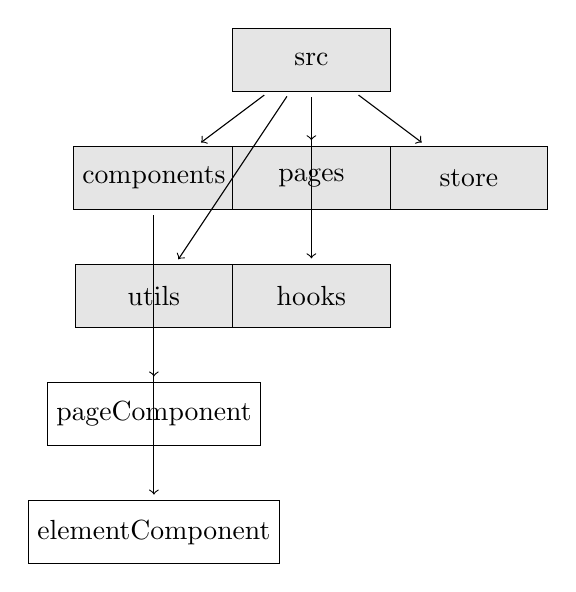
\begin{tikzpicture}[
    file/.style={draw, rectangle, minimum width=2cm, minimum height=0.8cm},
    folder/.style={draw, rectangle, minimum width=2cm, minimum height=0.8cm, fill=gray!20},
    arrow/.style={->, shorten >=2pt, shorten <=2pt}
]

% Folders
\node[folder] (src) at (0,0) {src};
\node[folder] (components) at (-2,-1.5) {components};
\node[folder] (pages) at (0,-1.5) {pages};
\node[folder] (store) at (2,-1.5) {store};
\node[folder] (utils) at (-2,-3) {utils};
\node[folder] (hooks) at (0,-3) {hooks};

% Files
\node[file] (pageComponent) at (-2,-4.5) {pageComponent};
\node[file] (elementComponent) at (-2,-6) {elementComponent};
% ... add more files

% Connections
\draw[arrow] (src) -- (components);
\draw[arrow] (src) -- (pages);
\draw[arrow] (src) -- (store);
\draw[arrow] (src) -- (utils);
\draw[arrow] (src) -- (hooks);
\draw[arrow] (components) -- (pageComponent);
\draw[arrow] (components) -- (elementComponent);
% ... add more connections

\end{tikzpicture}



\pagebreak
\subsubsection{Back-end}
The backend uses the dotNet framework. The development language using the C\# language.

In this project, the backend uses the Onion Architecture.
The Onion Architecture is a typically layered architecture, 
where each layer depends on the inner layer and provides interfaces to the outer layer.
The outer layer provides services to the outermost layer 
and other modules in the same layer based on the interfaces of the inner layer.

From inner to outer, the layers are: Domain, Application, Infrastructure, Presentation.
The Domain layer is the core layer and the innermost layer, used to define domain models, 
which are the business models.
It includes domain models and domain service interfaces.
Domain models are used to define the business models, 
which are the entities in the entity-relationship model and their attributes.
Domain service interfaces are used to define the business services, 
which are the relationships between entities in the entity-relationship model.

The Application layer is the application layer, 
used to define application services, which are the business logic.
It includes domain service implementations and application service interfaces.
Domain service implementations implement the methods of the inner layer's domain service 
interfaces and implement the business logic of the domain models.
Application service interfaces are used to define application services, 
which are the business logic.
It includes but is not limited to database interfaces, testing interfaces, 
HTTP API interfaces, MQTT interfaces, etc.

The Infrastructure layer is the infrastructure layer, used to define infrastructure.
It includes database implementations, testing implementations, 
HTTP API implementations, MQTT implementations, etc.
Database implementations implement the database interfaces 
and provide CRUD services for the database.
Testing implementations implement the testing interfaces 
and provide services for unit testing and integration testing.
HTTP API implementations implement the HTTP API interfaces 
and provide CRUD operations for HTTP APIs.
MQTT implementations implement the MQTT interfaces 
and provide CRUD operations for MQTT.

The Presentation layer is the presentation layer, used to define presentation logic, 
such as interfaces and pages. Since this is a backend project,
data presentation and control are handled by the frontend, 
so this layer is not needed.



\pagebreak
\subsubsection{Data communication and storage}
% 关于本项目的数据通信与数据存储的设计, 包括数据通信的协议, 数据存储的设计等
% 关于数据通信的设计:
% 1. 通信协议的选择
% 自前端向后端发送的数据, 有三种传输的数据类型, 
% 一种是普通的增删改查的请求, 对数据传输的时效性要求不高, 但是对数据的准确性, 完整性, 有序性, 安全性有一定的要求,
% 这种数据的传输, 采用 HTTP 协议, 以及 RESTful API 的设计. 可以有效的保证对数据传输的以上要求.
% 一种是对数据通道的创建和流媒体数据的传输, 对数据传输的时效性, 安全性要求较高, 这种数据的传输, 采用 WebRTC 协议, 以及 MQTT 协议.
% 配合可以快速解码的 flatbuffers 协议, 可以有效的保证对数据传输的以上要求.
% 最后一种是对设备的状态信息和操作信息的传输, 对完整性, 有序性, 安全性都有较高的要求, 这种数据的传输, 采用 MQTT 协议
% 同时也使用了 flatbuffers 协议.
% 
% 2. 数据通信的通信架构和通信流程
% 本项目的数据通信的通信架构, 是基于前后端分离的架构, 前端使用 React 框架, 后端使用 dotnet 框架.
% 当前端需要向后端发送数据的时候, 前端会向后端发送 HTTP 请求, 后端接收到 HTTP 请求之后, 会根据请求的数据类型,
% 选择不同的数据处理方式, 对于普通的增删改查的请求, 后端会根据 RESTful API 的设计, 对数据进行增删改查的操作,
% 对于对数据通道的创建和流媒体数据的传输, 后端会根据 WebRTC 协议, 对数据通道进行创建, 并且帮助前端和设备建立数据通道,
% 当数据通道建立后, 前端和设备之间则使用 flatbuffer 的数据格式对流媒体数据进行传输,
% 对于设备的状态信息和操作信息的传输, 前端会直接向 MQTT broker 发送 MQTT 请求, 
% 设备会在其自身的固件中监听相关的 MQTT 请求, 并且返回相关的数据.
% 
% 3. 数据通信的格式
% 本项目的数据通信的格式, 有三种, 
% 一种是 HTTP 协议, 
% 使用 json 格式对数据进行传输,
% 一种是 WebRTC 协议, 
% 使用 flatbuffers 格式对数据进行传输,
% 一种是 MQTT 协议.
% 使用 flatbuffers 格式对数据进行传输,
% 
% 关于数据存储的设计:
% 1. 数据存储的数据库的选择
% 本项目的数据存储的数据库的选择, 使用了轻量级的数据库 SQLite,
% SQLite 是一个进程内的库, 实现了自给自足的, 无服务器的, 零配置的, 事务性的 SQL 数据库引擎.
% 这是因为整个项目的目的是为了实现前端与设备之间的数据通信, 对于数据库数据的增删改查操作的要求不高,
% 数据量较小, 且对于数据库的数据的事务性要求不高, 所以选择了 SQLite 数据库.
% 2. 项目前后端的数据结构的设计
% 在本项目中, 前端由于使用了 React 框架, 所以前端的数据结构的设计, 使用了基于状态的数据结构的设计,
% 每个组件或者数据集都包含一个状态对象, 这个状态对象的属性就是组件的各个状态. 
% 使用状态对象的原因是, 可以方便的对状态进行管理, 采用对象-属性的形式, 可以方便的针对不同组件的同类状态进行区分,
% 由于跨组件的状态是由 redux 进行管理的, 这种状态对象的设计, 可以更搞笑的对状态进行更新和传递.
% 后端由于使用了 dotnet 框架, 所以后端的数据结构的设计, 使用了基于类的数据结构的设计,
% 采用了面向对象的编程思想, 对数据进行了封装, 使得数据的传输更加的安全, 有序, 完整.


\pagebreak

% \subsection{Domain model}
% \documentclass[]{article}
\usepackage{graphicx}
\usepackage{amsmath}
\usepackage{tikz}

% libaries
\usetikzlibrary{shapes,arrows}

%Define the listing package
\usepackage{listings} %code highlighter
\usepackage{color} %use color
\definecolor{mygreen}{rgb}{0,0.6,0}
\definecolor{mygray}{rgb}{0.5,0.5,0.5}
\definecolor{mymauve}{rgb}{0.58,0,0.82}

%Customize a bit the look
\lstset{ %
backgroundcolor=\color{white}, % choose the background color; you must add \usepackage{color} or \usepackage{xcolor}
basicstyle=\footnotesize, % the size of the fonts that are used for the code
breakatwhitespace=false, % sets if automatic breaks should only happen at whitespace
breaklines=true, % sets automatic line breaking
captionpos=b, % sets the caption-position to bottom
commentstyle=\color{mygreen}, % comment style
deletekeywords={...}, % if you want to delete keywords from the given language
escapeinside={\%*}{*)}, % if you want to add LaTeX within your code
extendedchars=true, % lets you use non-ASCII characters; for 8-bits encodings only, does not work with UTF-8
frame=single, % adds a frame around the code
keepspaces=true, % keeps spaces in text, useful for keeping indentation of code (possibly needs columns=flexible)
keywordstyle=\color{blue}, % keyword style
% language=Octave, % the language of the code
morekeywords={*,...}, % if you want to add more keywords to the set
numbers=left, % where to put the line-numbers; possible values are (none, left, right)
numbersep=5pt, % how far the line-numbers are from the code
numberstyle=\tiny\color{mygray}, % the style that is used for the line-numbers
rulecolor=\color{black}, % if not set, the frame-color may be changed on line-breaks within not-black text (e.g. comments (green here))
showspaces=false, % show spaces everywhere adding particular underscores; it overrides 'showstringspaces'
showstringspaces=false, % underline spaces within strings only
showtabs=false, % show tabs within strings adding particular underscores
stepnumber=1, % the step between two line-numbers. If it's 1, each line will be numbered
stringstyle=\color{mymauve}, % string literal style
tabsize=2, % sets default tabsize to 2 spaces
title=\lstname % show the filename of files included with \lstinputlisting; also try caption instead of title
}

\definecolor{darkgray}{rgb}{.4,.4,.4}
\definecolor{purple}{rgb}{0.65, 0.12, 0.82}

\lstdefinelanguage{React}{
keywords={const, typeof, new, true, false, catch, function, return, null, catch, switch, var, if, in, while, do, else, case, break},
keywordstyle=\color{blue}\bfseries,
ndkeywords={class, export, boolean, throw, implements, import, this},
ndkeywordstyle=\color{darkgray}\bfseries,
identifierstyle=\color{mygreen},
sensitive=false,
comment=[l]{//},
morecomment=[s]{/*}{*/},
commentstyle=\color{purple}\ttfamily,
string=[b]{"}{'}{`},
stringstyle=\color{red}\ttfamily,
morestring=[b]',
morestring=[b]",
morestring=[b]`',
}

\lstdefinelanguage{CSharp}{
keywords={const, typeof, new, true, false, catch, function, return, null, catch, switch, var, if, in, while, do, else, case, break},
keywordstyle=\color{blue}\bfseries,
ndkeywords={class, export, boolean, throw, implements, import, this},
ndkeywordstyle=\color{darkgray}\bfseries,
identifierstyle=\color{mygreen},
sensitive=false,
comment=[l]{//},
morecomment=[s]{/*}{*/},
commentstyle=\color{purple}\ttfamily,
string=[b]{"}{'}{`},
stringstyle=\color{red}\ttfamily,
morestring=[b]',
morestring=[b]",
morestring=[b]`',
}

\lstset{
language=React,
extendedchars=true,
basicstyle=\footnotesize\ttfamily,
showstringspaces=false,
showspaces=false,
numbers=left,
numberstyle=\footnotesize,
numbersep=9pt,
tabsize=2,
breaklines=true,
showtabs=false,
captionpos=b
}

\lstset{
language=CSharp,
extendedchars=true,
basicstyle=\footnotesize\ttfamily,
showstringspaces=false,
showspaces=false,
numbers=left,
numberstyle=\footnotesize,
numbersep=9pt,
tabsize=2,
breaklines=true,
showtabs=false,
captionpos=b
}

% \usepackage{cite} % Add this line for citation

% \bibliographystyle{plain}

\title{
The implementation of BifrostConnect Front-end scope, 
re-design and development with the relevant back-end support develop.
}
\author{
    Fei Gu \\
    Erhvervs Akademi Sydvest \\
    Computer Science 21\\
    }
\date{\today}

\begin{document}

% Front page
\maketitle
\begin{center}
    Supervisor: Henrik Boulund Meng Hansen \\
    Company: BifrostConnect \\
    Engineering Director: Jasper Wass \\
\end{center}
\tableofcontents
\pagebreak


% The introduction
\section{Introduction}
\subsection{Background}\input{sections/introduction/background.tex}
\subsection{The company}\input{sections/introduction/aboutCompany}
\subsection{The project}\input{sections/introduction/aboutProject}
\pagebreak

% The problem statement
\section{Problem Statement}
\subsection{Statement}
\input{sections/problemStatement/statement}
\subsection{Situation}
\input{sections/problemStatement/situation}
\subsection{Potential Solution}
\input{sections/problemStatement/potentialSolution}
\pagebreak

% Requirement analysis
\section{Requirement Analysis}
\input{sections/requirementAnalysis/index}

\subsection{Stakeholders}
\input{sections/requirementAnalysis/stakeholders/index}

\subsection{Business Domain}
\input{sections/requirementAnalysis/bussinesDomain/index}

\subsection{Scope}
\input{sections/requirementAnalysis/scope}

\subsection{Goals}
\input{sections/requirementAnalysis/goals}
\pagebreak

% Software Design
\section{Software Design}
% developement methods
\subsection{Software Development Methods}
\input{sections/softwareDevelopmentMethods/index}
\subsubsection{Agile Software Development}
\input{sections/softwareDevelopmentMethods/agileSoftwareDevelopment/index}
\subsubsection{Feature Driven Development}
\input{sections/softwareDevelopmentMethods/featureDrivenDevelopment/index}

\pagebreak

% Technology seslection
\subsection{Technology selection}
\input{sections/softwareDesign/technologySelection/index}
\subsubsection{Front-end}
\input{sections/softwareDesign/technologySelection/frontEnd}            
\subsubsection{Back-end}
\input{sections/softwareDesign/technologySelection/backEnd}            
\subsubsection{Database}
\input{sections/softwareDesign/technologySelection/database}
\subsubsection{Data communication}
\input{sections/softwareDesign/technologySelection/dataCommunication}            
\subsubsection{DevOps}
\input{sections/softwareDesign/technologySelection/devOps}
\pagebreak

% Architecture design
\subsection{Architecture design}
\input{sections/softwareDesign/architectureDesign/index}
\pagebreak
\subsubsection{Front-end}
\input{sections/softwareDesign/architectureDesign/frontEndArchitecture}
\pagebreak
\subsubsection{Back-end}
\input{sections/softwareDesign/architectureDesign/backEndArchitecture}
\pagebreak
\subsubsection{Data communication and storage}
\input{sections/softwareDesign/architectureDesign/dataCommunicationArchitecture}
\pagebreak

% \subsection{Domain model}
% \input{sections/softwareDesign/domainModel/index}
% \subsection{Database design}
% % 数据库领域模型 ER 图
% % 包括表和字段的设置.
% % 对于私有键和外键的设置.

% \subsection{Back-end design}
% % 后端对象模型
% % 以及对于对象模型的增删改查
% % 以及相关的其他服务的设计`'

% \subsection{Front-end design}
% % 对于前端的页面结构的设计 
% % 页面的状态的设计, 交互设计

% \subsection{FlatBuffers design}
% % schema 的设计

\subsection{DevOps CI/CD process design}
\input{sections/softwareDesign/devOpsDesign/index}
\subsubsection{Continuous Integration}
\input{sections/softwareDesign/devOpsDesign/continuousIntegration/index}
\subsubsection{Continuous Delivery}
\input{sections/softwareDesign/devOpsDesign/continuousDelivery/index}
\subsubsection{Continuous Deployment}
\input{sections/softwareDesign/devOpsDesign/continuousDeployment/index}
\pagebreak

\section{Software Development} 
\input{sections/softwareDevelopment/index}
\subsection{Overall development}
\input{sections/softwareDevelopment/overallDevelopement/index}
\subsubsection{Front-end}
\input{sections/softwareDevelopment/overallDevelopement/frontEnd/index}
\subsubsection{Back-end}
\input{sections/softwareDevelopment/overallDevelopement/backEnd/index}
\subsubsection{DevOps}
\input{sections/softwareDevelopment/overallDevelopement/devOps/index}
\subsection{Feature development} 
\input{sections/softwareDevelopment/featureDevelopment/index}
\subsubsection{Use Case 1}
\input{sections/softwareDevelopment/featureDevelopment/useCase1/index}
\subsubsection{Feature 1}
\input{sections/softwareDevelopment/featureDevelopment/feature/feature1.tex}
\pagebreak
\section{Conclusion} 
\subsection{Result}
Since the project is still in progress, the result is not available yet.
So far, basic structure of this project has been built. But the most features 
are not implemented yet. 
\subsection{Discussion}
As a single developer for this project, I am confident what I have done so far.
And I can say I understand the most of the knowledge I have used in this project, 
which also means I can explain all the part of the project. 
But this project also relevant some of the complex knowledge which I have to continue 
to study and practice.
\subsection{Future Work}
The future work is to implement the rest of the features. 
Including the most important part which is the 'create session' feature.
\pagebreak
% \bibliography{bibliography}
\pagebreak
% \begin{appendices}
%     \section{Appendix}
% \end{appendices} 
\end{document}
% \subsection{Database design}
% % 数据库领域模型 ER 图
% % 包括表和字段的设置.
% % 对于私有键和外键的设置.

% \subsection{Back-end design}
% % 后端对象模型
% % 以及对于对象模型的增删改查
% % 以及相关的其他服务的设计`'

% \subsection{Front-end design}
% % 对于前端的页面结构的设计 
% % 页面的状态的设计, 交互设计

% \subsection{FlatBuffers design}
% % schema 的设计

\subsection{DevOps CI/CD process design}
\documentclass[]{article}
\usepackage{graphicx}
\usepackage{amsmath}
\usepackage{tikz}

% libaries
\usetikzlibrary{shapes,arrows}

%Define the listing package
\usepackage{listings} %code highlighter
\usepackage{color} %use color
\definecolor{mygreen}{rgb}{0,0.6,0}
\definecolor{mygray}{rgb}{0.5,0.5,0.5}
\definecolor{mymauve}{rgb}{0.58,0,0.82}

%Customize a bit the look
\lstset{ %
backgroundcolor=\color{white}, % choose the background color; you must add \usepackage{color} or \usepackage{xcolor}
basicstyle=\footnotesize, % the size of the fonts that are used for the code
breakatwhitespace=false, % sets if automatic breaks should only happen at whitespace
breaklines=true, % sets automatic line breaking
captionpos=b, % sets the caption-position to bottom
commentstyle=\color{mygreen}, % comment style
deletekeywords={...}, % if you want to delete keywords from the given language
escapeinside={\%*}{*)}, % if you want to add LaTeX within your code
extendedchars=true, % lets you use non-ASCII characters; for 8-bits encodings only, does not work with UTF-8
frame=single, % adds a frame around the code
keepspaces=true, % keeps spaces in text, useful for keeping indentation of code (possibly needs columns=flexible)
keywordstyle=\color{blue}, % keyword style
% language=Octave, % the language of the code
morekeywords={*,...}, % if you want to add more keywords to the set
numbers=left, % where to put the line-numbers; possible values are (none, left, right)
numbersep=5pt, % how far the line-numbers are from the code
numberstyle=\tiny\color{mygray}, % the style that is used for the line-numbers
rulecolor=\color{black}, % if not set, the frame-color may be changed on line-breaks within not-black text (e.g. comments (green here))
showspaces=false, % show spaces everywhere adding particular underscores; it overrides 'showstringspaces'
showstringspaces=false, % underline spaces within strings only
showtabs=false, % show tabs within strings adding particular underscores
stepnumber=1, % the step between two line-numbers. If it's 1, each line will be numbered
stringstyle=\color{mymauve}, % string literal style
tabsize=2, % sets default tabsize to 2 spaces
title=\lstname % show the filename of files included with \lstinputlisting; also try caption instead of title
}

\definecolor{darkgray}{rgb}{.4,.4,.4}
\definecolor{purple}{rgb}{0.65, 0.12, 0.82}

\lstdefinelanguage{React}{
keywords={const, typeof, new, true, false, catch, function, return, null, catch, switch, var, if, in, while, do, else, case, break},
keywordstyle=\color{blue}\bfseries,
ndkeywords={class, export, boolean, throw, implements, import, this},
ndkeywordstyle=\color{darkgray}\bfseries,
identifierstyle=\color{mygreen},
sensitive=false,
comment=[l]{//},
morecomment=[s]{/*}{*/},
commentstyle=\color{purple}\ttfamily,
string=[b]{"}{'}{`},
stringstyle=\color{red}\ttfamily,
morestring=[b]',
morestring=[b]",
morestring=[b]`',
}

\lstdefinelanguage{CSharp}{
keywords={const, typeof, new, true, false, catch, function, return, null, catch, switch, var, if, in, while, do, else, case, break},
keywordstyle=\color{blue}\bfseries,
ndkeywords={class, export, boolean, throw, implements, import, this},
ndkeywordstyle=\color{darkgray}\bfseries,
identifierstyle=\color{mygreen},
sensitive=false,
comment=[l]{//},
morecomment=[s]{/*}{*/},
commentstyle=\color{purple}\ttfamily,
string=[b]{"}{'}{`},
stringstyle=\color{red}\ttfamily,
morestring=[b]',
morestring=[b]",
morestring=[b]`',
}

\lstset{
language=React,
extendedchars=true,
basicstyle=\footnotesize\ttfamily,
showstringspaces=false,
showspaces=false,
numbers=left,
numberstyle=\footnotesize,
numbersep=9pt,
tabsize=2,
breaklines=true,
showtabs=false,
captionpos=b
}

\lstset{
language=CSharp,
extendedchars=true,
basicstyle=\footnotesize\ttfamily,
showstringspaces=false,
showspaces=false,
numbers=left,
numberstyle=\footnotesize,
numbersep=9pt,
tabsize=2,
breaklines=true,
showtabs=false,
captionpos=b
}

% \usepackage{cite} % Add this line for citation

% \bibliographystyle{plain}

\title{
The implementation of BifrostConnect Front-end scope, 
re-design and development with the relevant back-end support develop.
}
\author{
    Fei Gu \\
    Erhvervs Akademi Sydvest \\
    Computer Science 21\\
    }
\date{\today}

\begin{document}

% Front page
\maketitle
\begin{center}
    Supervisor: Henrik Boulund Meng Hansen \\
    Company: BifrostConnect \\
    Engineering Director: Jasper Wass \\
\end{center}
\tableofcontents
\pagebreak


% The introduction
\section{Introduction}
\subsection{Background}\input{sections/introduction/background.tex}
\subsection{The company}\input{sections/introduction/aboutCompany}
\subsection{The project}\input{sections/introduction/aboutProject}
\pagebreak

% The problem statement
\section{Problem Statement}
\subsection{Statement}
\input{sections/problemStatement/statement}
\subsection{Situation}
\input{sections/problemStatement/situation}
\subsection{Potential Solution}
\input{sections/problemStatement/potentialSolution}
\pagebreak

% Requirement analysis
\section{Requirement Analysis}
\input{sections/requirementAnalysis/index}

\subsection{Stakeholders}
\input{sections/requirementAnalysis/stakeholders/index}

\subsection{Business Domain}
\input{sections/requirementAnalysis/bussinesDomain/index}

\subsection{Scope}
\input{sections/requirementAnalysis/scope}

\subsection{Goals}
\input{sections/requirementAnalysis/goals}
\pagebreak

% Software Design
\section{Software Design}
% developement methods
\subsection{Software Development Methods}
\input{sections/softwareDevelopmentMethods/index}
\subsubsection{Agile Software Development}
\input{sections/softwareDevelopmentMethods/agileSoftwareDevelopment/index}
\subsubsection{Feature Driven Development}
\input{sections/softwareDevelopmentMethods/featureDrivenDevelopment/index}

\pagebreak

% Technology seslection
\subsection{Technology selection}
\input{sections/softwareDesign/technologySelection/index}
\subsubsection{Front-end}
\input{sections/softwareDesign/technologySelection/frontEnd}            
\subsubsection{Back-end}
\input{sections/softwareDesign/technologySelection/backEnd}            
\subsubsection{Database}
\input{sections/softwareDesign/technologySelection/database}
\subsubsection{Data communication}
\input{sections/softwareDesign/technologySelection/dataCommunication}            
\subsubsection{DevOps}
\input{sections/softwareDesign/technologySelection/devOps}
\pagebreak

% Architecture design
\subsection{Architecture design}
\input{sections/softwareDesign/architectureDesign/index}
\pagebreak
\subsubsection{Front-end}
\input{sections/softwareDesign/architectureDesign/frontEndArchitecture}
\pagebreak
\subsubsection{Back-end}
\input{sections/softwareDesign/architectureDesign/backEndArchitecture}
\pagebreak
\subsubsection{Data communication and storage}
\input{sections/softwareDesign/architectureDesign/dataCommunicationArchitecture}
\pagebreak

% \subsection{Domain model}
% \input{sections/softwareDesign/domainModel/index}
% \subsection{Database design}
% % 数据库领域模型 ER 图
% % 包括表和字段的设置.
% % 对于私有键和外键的设置.

% \subsection{Back-end design}
% % 后端对象模型
% % 以及对于对象模型的增删改查
% % 以及相关的其他服务的设计`'

% \subsection{Front-end design}
% % 对于前端的页面结构的设计 
% % 页面的状态的设计, 交互设计

% \subsection{FlatBuffers design}
% % schema 的设计

\subsection{DevOps CI/CD process design}
\input{sections/softwareDesign/devOpsDesign/index}
\subsubsection{Continuous Integration}
\input{sections/softwareDesign/devOpsDesign/continuousIntegration/index}
\subsubsection{Continuous Delivery}
\input{sections/softwareDesign/devOpsDesign/continuousDelivery/index}
\subsubsection{Continuous Deployment}
\input{sections/softwareDesign/devOpsDesign/continuousDeployment/index}
\pagebreak

\section{Software Development} 
\input{sections/softwareDevelopment/index}
\subsection{Overall development}
\input{sections/softwareDevelopment/overallDevelopement/index}
\subsubsection{Front-end}
\input{sections/softwareDevelopment/overallDevelopement/frontEnd/index}
\subsubsection{Back-end}
\input{sections/softwareDevelopment/overallDevelopement/backEnd/index}
\subsubsection{DevOps}
\input{sections/softwareDevelopment/overallDevelopement/devOps/index}
\subsection{Feature development} 
\input{sections/softwareDevelopment/featureDevelopment/index}
\subsubsection{Use Case 1}
\input{sections/softwareDevelopment/featureDevelopment/useCase1/index}
\subsubsection{Feature 1}
\input{sections/softwareDevelopment/featureDevelopment/feature/feature1.tex}
\pagebreak
\section{Conclusion} 
\subsection{Result}
Since the project is still in progress, the result is not available yet.
So far, basic structure of this project has been built. But the most features 
are not implemented yet. 
\subsection{Discussion}
As a single developer for this project, I am confident what I have done so far.
And I can say I understand the most of the knowledge I have used in this project, 
which also means I can explain all the part of the project. 
But this project also relevant some of the complex knowledge which I have to continue 
to study and practice.
\subsection{Future Work}
The future work is to implement the rest of the features. 
Including the most important part which is the 'create session' feature.
\pagebreak
% \bibliography{bibliography}
\pagebreak
% \begin{appendices}
%     \section{Appendix}
% \end{appendices} 
\end{document}
\subsubsection{Continuous Integration}
\documentclass[]{article}
\usepackage{graphicx}
\usepackage{amsmath}
\usepackage{tikz}

% libaries
\usetikzlibrary{shapes,arrows}

%Define the listing package
\usepackage{listings} %code highlighter
\usepackage{color} %use color
\definecolor{mygreen}{rgb}{0,0.6,0}
\definecolor{mygray}{rgb}{0.5,0.5,0.5}
\definecolor{mymauve}{rgb}{0.58,0,0.82}

%Customize a bit the look
\lstset{ %
backgroundcolor=\color{white}, % choose the background color; you must add \usepackage{color} or \usepackage{xcolor}
basicstyle=\footnotesize, % the size of the fonts that are used for the code
breakatwhitespace=false, % sets if automatic breaks should only happen at whitespace
breaklines=true, % sets automatic line breaking
captionpos=b, % sets the caption-position to bottom
commentstyle=\color{mygreen}, % comment style
deletekeywords={...}, % if you want to delete keywords from the given language
escapeinside={\%*}{*)}, % if you want to add LaTeX within your code
extendedchars=true, % lets you use non-ASCII characters; for 8-bits encodings only, does not work with UTF-8
frame=single, % adds a frame around the code
keepspaces=true, % keeps spaces in text, useful for keeping indentation of code (possibly needs columns=flexible)
keywordstyle=\color{blue}, % keyword style
% language=Octave, % the language of the code
morekeywords={*,...}, % if you want to add more keywords to the set
numbers=left, % where to put the line-numbers; possible values are (none, left, right)
numbersep=5pt, % how far the line-numbers are from the code
numberstyle=\tiny\color{mygray}, % the style that is used for the line-numbers
rulecolor=\color{black}, % if not set, the frame-color may be changed on line-breaks within not-black text (e.g. comments (green here))
showspaces=false, % show spaces everywhere adding particular underscores; it overrides 'showstringspaces'
showstringspaces=false, % underline spaces within strings only
showtabs=false, % show tabs within strings adding particular underscores
stepnumber=1, % the step between two line-numbers. If it's 1, each line will be numbered
stringstyle=\color{mymauve}, % string literal style
tabsize=2, % sets default tabsize to 2 spaces
title=\lstname % show the filename of files included with \lstinputlisting; also try caption instead of title
}

\definecolor{darkgray}{rgb}{.4,.4,.4}
\definecolor{purple}{rgb}{0.65, 0.12, 0.82}

\lstdefinelanguage{React}{
keywords={const, typeof, new, true, false, catch, function, return, null, catch, switch, var, if, in, while, do, else, case, break},
keywordstyle=\color{blue}\bfseries,
ndkeywords={class, export, boolean, throw, implements, import, this},
ndkeywordstyle=\color{darkgray}\bfseries,
identifierstyle=\color{mygreen},
sensitive=false,
comment=[l]{//},
morecomment=[s]{/*}{*/},
commentstyle=\color{purple}\ttfamily,
string=[b]{"}{'}{`},
stringstyle=\color{red}\ttfamily,
morestring=[b]',
morestring=[b]",
morestring=[b]`',
}

\lstdefinelanguage{CSharp}{
keywords={const, typeof, new, true, false, catch, function, return, null, catch, switch, var, if, in, while, do, else, case, break},
keywordstyle=\color{blue}\bfseries,
ndkeywords={class, export, boolean, throw, implements, import, this},
ndkeywordstyle=\color{darkgray}\bfseries,
identifierstyle=\color{mygreen},
sensitive=false,
comment=[l]{//},
morecomment=[s]{/*}{*/},
commentstyle=\color{purple}\ttfamily,
string=[b]{"}{'}{`},
stringstyle=\color{red}\ttfamily,
morestring=[b]',
morestring=[b]",
morestring=[b]`',
}

\lstset{
language=React,
extendedchars=true,
basicstyle=\footnotesize\ttfamily,
showstringspaces=false,
showspaces=false,
numbers=left,
numberstyle=\footnotesize,
numbersep=9pt,
tabsize=2,
breaklines=true,
showtabs=false,
captionpos=b
}

\lstset{
language=CSharp,
extendedchars=true,
basicstyle=\footnotesize\ttfamily,
showstringspaces=false,
showspaces=false,
numbers=left,
numberstyle=\footnotesize,
numbersep=9pt,
tabsize=2,
breaklines=true,
showtabs=false,
captionpos=b
}

% \usepackage{cite} % Add this line for citation

% \bibliographystyle{plain}

\title{
The implementation of BifrostConnect Front-end scope, 
re-design and development with the relevant back-end support develop.
}
\author{
    Fei Gu \\
    Erhvervs Akademi Sydvest \\
    Computer Science 21\\
    }
\date{\today}

\begin{document}

% Front page
\maketitle
\begin{center}
    Supervisor: Henrik Boulund Meng Hansen \\
    Company: BifrostConnect \\
    Engineering Director: Jasper Wass \\
\end{center}
\tableofcontents
\pagebreak


% The introduction
\section{Introduction}
\subsection{Background}\input{sections/introduction/background.tex}
\subsection{The company}\input{sections/introduction/aboutCompany}
\subsection{The project}\input{sections/introduction/aboutProject}
\pagebreak

% The problem statement
\section{Problem Statement}
\subsection{Statement}
\input{sections/problemStatement/statement}
\subsection{Situation}
\input{sections/problemStatement/situation}
\subsection{Potential Solution}
\input{sections/problemStatement/potentialSolution}
\pagebreak

% Requirement analysis
\section{Requirement Analysis}
\input{sections/requirementAnalysis/index}

\subsection{Stakeholders}
\input{sections/requirementAnalysis/stakeholders/index}

\subsection{Business Domain}
\input{sections/requirementAnalysis/bussinesDomain/index}

\subsection{Scope}
\input{sections/requirementAnalysis/scope}

\subsection{Goals}
\input{sections/requirementAnalysis/goals}
\pagebreak

% Software Design
\section{Software Design}
% developement methods
\subsection{Software Development Methods}
\input{sections/softwareDevelopmentMethods/index}
\subsubsection{Agile Software Development}
\input{sections/softwareDevelopmentMethods/agileSoftwareDevelopment/index}
\subsubsection{Feature Driven Development}
\input{sections/softwareDevelopmentMethods/featureDrivenDevelopment/index}

\pagebreak

% Technology seslection
\subsection{Technology selection}
\input{sections/softwareDesign/technologySelection/index}
\subsubsection{Front-end}
\input{sections/softwareDesign/technologySelection/frontEnd}            
\subsubsection{Back-end}
\input{sections/softwareDesign/technologySelection/backEnd}            
\subsubsection{Database}
\input{sections/softwareDesign/technologySelection/database}
\subsubsection{Data communication}
\input{sections/softwareDesign/technologySelection/dataCommunication}            
\subsubsection{DevOps}
\input{sections/softwareDesign/technologySelection/devOps}
\pagebreak

% Architecture design
\subsection{Architecture design}
\input{sections/softwareDesign/architectureDesign/index}
\pagebreak
\subsubsection{Front-end}
\input{sections/softwareDesign/architectureDesign/frontEndArchitecture}
\pagebreak
\subsubsection{Back-end}
\input{sections/softwareDesign/architectureDesign/backEndArchitecture}
\pagebreak
\subsubsection{Data communication and storage}
\input{sections/softwareDesign/architectureDesign/dataCommunicationArchitecture}
\pagebreak

% \subsection{Domain model}
% \input{sections/softwareDesign/domainModel/index}
% \subsection{Database design}
% % 数据库领域模型 ER 图
% % 包括表和字段的设置.
% % 对于私有键和外键的设置.

% \subsection{Back-end design}
% % 后端对象模型
% % 以及对于对象模型的增删改查
% % 以及相关的其他服务的设计`'

% \subsection{Front-end design}
% % 对于前端的页面结构的设计 
% % 页面的状态的设计, 交互设计

% \subsection{FlatBuffers design}
% % schema 的设计

\subsection{DevOps CI/CD process design}
\input{sections/softwareDesign/devOpsDesign/index}
\subsubsection{Continuous Integration}
\input{sections/softwareDesign/devOpsDesign/continuousIntegration/index}
\subsubsection{Continuous Delivery}
\input{sections/softwareDesign/devOpsDesign/continuousDelivery/index}
\subsubsection{Continuous Deployment}
\input{sections/softwareDesign/devOpsDesign/continuousDeployment/index}
\pagebreak

\section{Software Development} 
\input{sections/softwareDevelopment/index}
\subsection{Overall development}
\input{sections/softwareDevelopment/overallDevelopement/index}
\subsubsection{Front-end}
\input{sections/softwareDevelopment/overallDevelopement/frontEnd/index}
\subsubsection{Back-end}
\input{sections/softwareDevelopment/overallDevelopement/backEnd/index}
\subsubsection{DevOps}
\input{sections/softwareDevelopment/overallDevelopement/devOps/index}
\subsection{Feature development} 
\input{sections/softwareDevelopment/featureDevelopment/index}
\subsubsection{Use Case 1}
\input{sections/softwareDevelopment/featureDevelopment/useCase1/index}
\subsubsection{Feature 1}
\input{sections/softwareDevelopment/featureDevelopment/feature/feature1.tex}
\pagebreak
\section{Conclusion} 
\subsection{Result}
Since the project is still in progress, the result is not available yet.
So far, basic structure of this project has been built. But the most features 
are not implemented yet. 
\subsection{Discussion}
As a single developer for this project, I am confident what I have done so far.
And I can say I understand the most of the knowledge I have used in this project, 
which also means I can explain all the part of the project. 
But this project also relevant some of the complex knowledge which I have to continue 
to study and practice.
\subsection{Future Work}
The future work is to implement the rest of the features. 
Including the most important part which is the 'create session' feature.
\pagebreak
% \bibliography{bibliography}
\pagebreak
% \begin{appendices}
%     \section{Appendix}
% \end{appendices} 
\end{document}
\subsubsection{Continuous Delivery}
\documentclass[]{article}
\usepackage{graphicx}
\usepackage{amsmath}
\usepackage{tikz}

% libaries
\usetikzlibrary{shapes,arrows}

%Define the listing package
\usepackage{listings} %code highlighter
\usepackage{color} %use color
\definecolor{mygreen}{rgb}{0,0.6,0}
\definecolor{mygray}{rgb}{0.5,0.5,0.5}
\definecolor{mymauve}{rgb}{0.58,0,0.82}

%Customize a bit the look
\lstset{ %
backgroundcolor=\color{white}, % choose the background color; you must add \usepackage{color} or \usepackage{xcolor}
basicstyle=\footnotesize, % the size of the fonts that are used for the code
breakatwhitespace=false, % sets if automatic breaks should only happen at whitespace
breaklines=true, % sets automatic line breaking
captionpos=b, % sets the caption-position to bottom
commentstyle=\color{mygreen}, % comment style
deletekeywords={...}, % if you want to delete keywords from the given language
escapeinside={\%*}{*)}, % if you want to add LaTeX within your code
extendedchars=true, % lets you use non-ASCII characters; for 8-bits encodings only, does not work with UTF-8
frame=single, % adds a frame around the code
keepspaces=true, % keeps spaces in text, useful for keeping indentation of code (possibly needs columns=flexible)
keywordstyle=\color{blue}, % keyword style
% language=Octave, % the language of the code
morekeywords={*,...}, % if you want to add more keywords to the set
numbers=left, % where to put the line-numbers; possible values are (none, left, right)
numbersep=5pt, % how far the line-numbers are from the code
numberstyle=\tiny\color{mygray}, % the style that is used for the line-numbers
rulecolor=\color{black}, % if not set, the frame-color may be changed on line-breaks within not-black text (e.g. comments (green here))
showspaces=false, % show spaces everywhere adding particular underscores; it overrides 'showstringspaces'
showstringspaces=false, % underline spaces within strings only
showtabs=false, % show tabs within strings adding particular underscores
stepnumber=1, % the step between two line-numbers. If it's 1, each line will be numbered
stringstyle=\color{mymauve}, % string literal style
tabsize=2, % sets default tabsize to 2 spaces
title=\lstname % show the filename of files included with \lstinputlisting; also try caption instead of title
}

\definecolor{darkgray}{rgb}{.4,.4,.4}
\definecolor{purple}{rgb}{0.65, 0.12, 0.82}

\lstdefinelanguage{React}{
keywords={const, typeof, new, true, false, catch, function, return, null, catch, switch, var, if, in, while, do, else, case, break},
keywordstyle=\color{blue}\bfseries,
ndkeywords={class, export, boolean, throw, implements, import, this},
ndkeywordstyle=\color{darkgray}\bfseries,
identifierstyle=\color{mygreen},
sensitive=false,
comment=[l]{//},
morecomment=[s]{/*}{*/},
commentstyle=\color{purple}\ttfamily,
string=[b]{"}{'}{`},
stringstyle=\color{red}\ttfamily,
morestring=[b]',
morestring=[b]",
morestring=[b]`',
}

\lstdefinelanguage{CSharp}{
keywords={const, typeof, new, true, false, catch, function, return, null, catch, switch, var, if, in, while, do, else, case, break},
keywordstyle=\color{blue}\bfseries,
ndkeywords={class, export, boolean, throw, implements, import, this},
ndkeywordstyle=\color{darkgray}\bfseries,
identifierstyle=\color{mygreen},
sensitive=false,
comment=[l]{//},
morecomment=[s]{/*}{*/},
commentstyle=\color{purple}\ttfamily,
string=[b]{"}{'}{`},
stringstyle=\color{red}\ttfamily,
morestring=[b]',
morestring=[b]",
morestring=[b]`',
}

\lstset{
language=React,
extendedchars=true,
basicstyle=\footnotesize\ttfamily,
showstringspaces=false,
showspaces=false,
numbers=left,
numberstyle=\footnotesize,
numbersep=9pt,
tabsize=2,
breaklines=true,
showtabs=false,
captionpos=b
}

\lstset{
language=CSharp,
extendedchars=true,
basicstyle=\footnotesize\ttfamily,
showstringspaces=false,
showspaces=false,
numbers=left,
numberstyle=\footnotesize,
numbersep=9pt,
tabsize=2,
breaklines=true,
showtabs=false,
captionpos=b
}

% \usepackage{cite} % Add this line for citation

% \bibliographystyle{plain}

\title{
The implementation of BifrostConnect Front-end scope, 
re-design and development with the relevant back-end support develop.
}
\author{
    Fei Gu \\
    Erhvervs Akademi Sydvest \\
    Computer Science 21\\
    }
\date{\today}

\begin{document}

% Front page
\maketitle
\begin{center}
    Supervisor: Henrik Boulund Meng Hansen \\
    Company: BifrostConnect \\
    Engineering Director: Jasper Wass \\
\end{center}
\tableofcontents
\pagebreak


% The introduction
\section{Introduction}
\subsection{Background}\input{sections/introduction/background.tex}
\subsection{The company}\input{sections/introduction/aboutCompany}
\subsection{The project}\input{sections/introduction/aboutProject}
\pagebreak

% The problem statement
\section{Problem Statement}
\subsection{Statement}
\input{sections/problemStatement/statement}
\subsection{Situation}
\input{sections/problemStatement/situation}
\subsection{Potential Solution}
\input{sections/problemStatement/potentialSolution}
\pagebreak

% Requirement analysis
\section{Requirement Analysis}
\input{sections/requirementAnalysis/index}

\subsection{Stakeholders}
\input{sections/requirementAnalysis/stakeholders/index}

\subsection{Business Domain}
\input{sections/requirementAnalysis/bussinesDomain/index}

\subsection{Scope}
\input{sections/requirementAnalysis/scope}

\subsection{Goals}
\input{sections/requirementAnalysis/goals}
\pagebreak

% Software Design
\section{Software Design}
% developement methods
\subsection{Software Development Methods}
\input{sections/softwareDevelopmentMethods/index}
\subsubsection{Agile Software Development}
\input{sections/softwareDevelopmentMethods/agileSoftwareDevelopment/index}
\subsubsection{Feature Driven Development}
\input{sections/softwareDevelopmentMethods/featureDrivenDevelopment/index}

\pagebreak

% Technology seslection
\subsection{Technology selection}
\input{sections/softwareDesign/technologySelection/index}
\subsubsection{Front-end}
\input{sections/softwareDesign/technologySelection/frontEnd}            
\subsubsection{Back-end}
\input{sections/softwareDesign/technologySelection/backEnd}            
\subsubsection{Database}
\input{sections/softwareDesign/technologySelection/database}
\subsubsection{Data communication}
\input{sections/softwareDesign/technologySelection/dataCommunication}            
\subsubsection{DevOps}
\input{sections/softwareDesign/technologySelection/devOps}
\pagebreak

% Architecture design
\subsection{Architecture design}
\input{sections/softwareDesign/architectureDesign/index}
\pagebreak
\subsubsection{Front-end}
\input{sections/softwareDesign/architectureDesign/frontEndArchitecture}
\pagebreak
\subsubsection{Back-end}
\input{sections/softwareDesign/architectureDesign/backEndArchitecture}
\pagebreak
\subsubsection{Data communication and storage}
\input{sections/softwareDesign/architectureDesign/dataCommunicationArchitecture}
\pagebreak

% \subsection{Domain model}
% \input{sections/softwareDesign/domainModel/index}
% \subsection{Database design}
% % 数据库领域模型 ER 图
% % 包括表和字段的设置.
% % 对于私有键和外键的设置.

% \subsection{Back-end design}
% % 后端对象模型
% % 以及对于对象模型的增删改查
% % 以及相关的其他服务的设计`'

% \subsection{Front-end design}
% % 对于前端的页面结构的设计 
% % 页面的状态的设计, 交互设计

% \subsection{FlatBuffers design}
% % schema 的设计

\subsection{DevOps CI/CD process design}
\input{sections/softwareDesign/devOpsDesign/index}
\subsubsection{Continuous Integration}
\input{sections/softwareDesign/devOpsDesign/continuousIntegration/index}
\subsubsection{Continuous Delivery}
\input{sections/softwareDesign/devOpsDesign/continuousDelivery/index}
\subsubsection{Continuous Deployment}
\input{sections/softwareDesign/devOpsDesign/continuousDeployment/index}
\pagebreak

\section{Software Development} 
\input{sections/softwareDevelopment/index}
\subsection{Overall development}
\input{sections/softwareDevelopment/overallDevelopement/index}
\subsubsection{Front-end}
\input{sections/softwareDevelopment/overallDevelopement/frontEnd/index}
\subsubsection{Back-end}
\input{sections/softwareDevelopment/overallDevelopement/backEnd/index}
\subsubsection{DevOps}
\input{sections/softwareDevelopment/overallDevelopement/devOps/index}
\subsection{Feature development} 
\input{sections/softwareDevelopment/featureDevelopment/index}
\subsubsection{Use Case 1}
\input{sections/softwareDevelopment/featureDevelopment/useCase1/index}
\subsubsection{Feature 1}
\input{sections/softwareDevelopment/featureDevelopment/feature/feature1.tex}
\pagebreak
\section{Conclusion} 
\subsection{Result}
Since the project is still in progress, the result is not available yet.
So far, basic structure of this project has been built. But the most features 
are not implemented yet. 
\subsection{Discussion}
As a single developer for this project, I am confident what I have done so far.
And I can say I understand the most of the knowledge I have used in this project, 
which also means I can explain all the part of the project. 
But this project also relevant some of the complex knowledge which I have to continue 
to study and practice.
\subsection{Future Work}
The future work is to implement the rest of the features. 
Including the most important part which is the 'create session' feature.
\pagebreak
% \bibliography{bibliography}
\pagebreak
% \begin{appendices}
%     \section{Appendix}
% \end{appendices} 
\end{document}
\subsubsection{Continuous Deployment}
\documentclass[]{article}
\usepackage{graphicx}
\usepackage{amsmath}
\usepackage{tikz}

% libaries
\usetikzlibrary{shapes,arrows}

%Define the listing package
\usepackage{listings} %code highlighter
\usepackage{color} %use color
\definecolor{mygreen}{rgb}{0,0.6,0}
\definecolor{mygray}{rgb}{0.5,0.5,0.5}
\definecolor{mymauve}{rgb}{0.58,0,0.82}

%Customize a bit the look
\lstset{ %
backgroundcolor=\color{white}, % choose the background color; you must add \usepackage{color} or \usepackage{xcolor}
basicstyle=\footnotesize, % the size of the fonts that are used for the code
breakatwhitespace=false, % sets if automatic breaks should only happen at whitespace
breaklines=true, % sets automatic line breaking
captionpos=b, % sets the caption-position to bottom
commentstyle=\color{mygreen}, % comment style
deletekeywords={...}, % if you want to delete keywords from the given language
escapeinside={\%*}{*)}, % if you want to add LaTeX within your code
extendedchars=true, % lets you use non-ASCII characters; for 8-bits encodings only, does not work with UTF-8
frame=single, % adds a frame around the code
keepspaces=true, % keeps spaces in text, useful for keeping indentation of code (possibly needs columns=flexible)
keywordstyle=\color{blue}, % keyword style
% language=Octave, % the language of the code
morekeywords={*,...}, % if you want to add more keywords to the set
numbers=left, % where to put the line-numbers; possible values are (none, left, right)
numbersep=5pt, % how far the line-numbers are from the code
numberstyle=\tiny\color{mygray}, % the style that is used for the line-numbers
rulecolor=\color{black}, % if not set, the frame-color may be changed on line-breaks within not-black text (e.g. comments (green here))
showspaces=false, % show spaces everywhere adding particular underscores; it overrides 'showstringspaces'
showstringspaces=false, % underline spaces within strings only
showtabs=false, % show tabs within strings adding particular underscores
stepnumber=1, % the step between two line-numbers. If it's 1, each line will be numbered
stringstyle=\color{mymauve}, % string literal style
tabsize=2, % sets default tabsize to 2 spaces
title=\lstname % show the filename of files included with \lstinputlisting; also try caption instead of title
}

\definecolor{darkgray}{rgb}{.4,.4,.4}
\definecolor{purple}{rgb}{0.65, 0.12, 0.82}

\lstdefinelanguage{React}{
keywords={const, typeof, new, true, false, catch, function, return, null, catch, switch, var, if, in, while, do, else, case, break},
keywordstyle=\color{blue}\bfseries,
ndkeywords={class, export, boolean, throw, implements, import, this},
ndkeywordstyle=\color{darkgray}\bfseries,
identifierstyle=\color{mygreen},
sensitive=false,
comment=[l]{//},
morecomment=[s]{/*}{*/},
commentstyle=\color{purple}\ttfamily,
string=[b]{"}{'}{`},
stringstyle=\color{red}\ttfamily,
morestring=[b]',
morestring=[b]",
morestring=[b]`',
}

\lstdefinelanguage{CSharp}{
keywords={const, typeof, new, true, false, catch, function, return, null, catch, switch, var, if, in, while, do, else, case, break},
keywordstyle=\color{blue}\bfseries,
ndkeywords={class, export, boolean, throw, implements, import, this},
ndkeywordstyle=\color{darkgray}\bfseries,
identifierstyle=\color{mygreen},
sensitive=false,
comment=[l]{//},
morecomment=[s]{/*}{*/},
commentstyle=\color{purple}\ttfamily,
string=[b]{"}{'}{`},
stringstyle=\color{red}\ttfamily,
morestring=[b]',
morestring=[b]",
morestring=[b]`',
}

\lstset{
language=React,
extendedchars=true,
basicstyle=\footnotesize\ttfamily,
showstringspaces=false,
showspaces=false,
numbers=left,
numberstyle=\footnotesize,
numbersep=9pt,
tabsize=2,
breaklines=true,
showtabs=false,
captionpos=b
}

\lstset{
language=CSharp,
extendedchars=true,
basicstyle=\footnotesize\ttfamily,
showstringspaces=false,
showspaces=false,
numbers=left,
numberstyle=\footnotesize,
numbersep=9pt,
tabsize=2,
breaklines=true,
showtabs=false,
captionpos=b
}

% \usepackage{cite} % Add this line for citation

% \bibliographystyle{plain}

\title{
The implementation of BifrostConnect Front-end scope, 
re-design and development with the relevant back-end support develop.
}
\author{
    Fei Gu \\
    Erhvervs Akademi Sydvest \\
    Computer Science 21\\
    }
\date{\today}

\begin{document}

% Front page
\maketitle
\begin{center}
    Supervisor: Henrik Boulund Meng Hansen \\
    Company: BifrostConnect \\
    Engineering Director: Jasper Wass \\
\end{center}
\tableofcontents
\pagebreak


% The introduction
\section{Introduction}
\subsection{Background}\input{sections/introduction/background.tex}
\subsection{The company}\input{sections/introduction/aboutCompany}
\subsection{The project}\input{sections/introduction/aboutProject}
\pagebreak

% The problem statement
\section{Problem Statement}
\subsection{Statement}
\input{sections/problemStatement/statement}
\subsection{Situation}
\input{sections/problemStatement/situation}
\subsection{Potential Solution}
\input{sections/problemStatement/potentialSolution}
\pagebreak

% Requirement analysis
\section{Requirement Analysis}
\input{sections/requirementAnalysis/index}

\subsection{Stakeholders}
\input{sections/requirementAnalysis/stakeholders/index}

\subsection{Business Domain}
\input{sections/requirementAnalysis/bussinesDomain/index}

\subsection{Scope}
\input{sections/requirementAnalysis/scope}

\subsection{Goals}
\input{sections/requirementAnalysis/goals}
\pagebreak

% Software Design
\section{Software Design}
% developement methods
\subsection{Software Development Methods}
\input{sections/softwareDevelopmentMethods/index}
\subsubsection{Agile Software Development}
\input{sections/softwareDevelopmentMethods/agileSoftwareDevelopment/index}
\subsubsection{Feature Driven Development}
\input{sections/softwareDevelopmentMethods/featureDrivenDevelopment/index}

\pagebreak

% Technology seslection
\subsection{Technology selection}
\input{sections/softwareDesign/technologySelection/index}
\subsubsection{Front-end}
\input{sections/softwareDesign/technologySelection/frontEnd}            
\subsubsection{Back-end}
\input{sections/softwareDesign/technologySelection/backEnd}            
\subsubsection{Database}
\input{sections/softwareDesign/technologySelection/database}
\subsubsection{Data communication}
\input{sections/softwareDesign/technologySelection/dataCommunication}            
\subsubsection{DevOps}
\input{sections/softwareDesign/technologySelection/devOps}
\pagebreak

% Architecture design
\subsection{Architecture design}
\input{sections/softwareDesign/architectureDesign/index}
\pagebreak
\subsubsection{Front-end}
\input{sections/softwareDesign/architectureDesign/frontEndArchitecture}
\pagebreak
\subsubsection{Back-end}
\input{sections/softwareDesign/architectureDesign/backEndArchitecture}
\pagebreak
\subsubsection{Data communication and storage}
\input{sections/softwareDesign/architectureDesign/dataCommunicationArchitecture}
\pagebreak

% \subsection{Domain model}
% \input{sections/softwareDesign/domainModel/index}
% \subsection{Database design}
% % 数据库领域模型 ER 图
% % 包括表和字段的设置.
% % 对于私有键和外键的设置.

% \subsection{Back-end design}
% % 后端对象模型
% % 以及对于对象模型的增删改查
% % 以及相关的其他服务的设计`'

% \subsection{Front-end design}
% % 对于前端的页面结构的设计 
% % 页面的状态的设计, 交互设计

% \subsection{FlatBuffers design}
% % schema 的设计

\subsection{DevOps CI/CD process design}
\input{sections/softwareDesign/devOpsDesign/index}
\subsubsection{Continuous Integration}
\input{sections/softwareDesign/devOpsDesign/continuousIntegration/index}
\subsubsection{Continuous Delivery}
\input{sections/softwareDesign/devOpsDesign/continuousDelivery/index}
\subsubsection{Continuous Deployment}
\input{sections/softwareDesign/devOpsDesign/continuousDeployment/index}
\pagebreak

\section{Software Development} 
\input{sections/softwareDevelopment/index}
\subsection{Overall development}
\input{sections/softwareDevelopment/overallDevelopement/index}
\subsubsection{Front-end}
\input{sections/softwareDevelopment/overallDevelopement/frontEnd/index}
\subsubsection{Back-end}
\input{sections/softwareDevelopment/overallDevelopement/backEnd/index}
\subsubsection{DevOps}
\input{sections/softwareDevelopment/overallDevelopement/devOps/index}
\subsection{Feature development} 
\input{sections/softwareDevelopment/featureDevelopment/index}
\subsubsection{Use Case 1}
\input{sections/softwareDevelopment/featureDevelopment/useCase1/index}
\subsubsection{Feature 1}
\input{sections/softwareDevelopment/featureDevelopment/feature/feature1.tex}
\pagebreak
\section{Conclusion} 
\subsection{Result}
Since the project is still in progress, the result is not available yet.
So far, basic structure of this project has been built. But the most features 
are not implemented yet. 
\subsection{Discussion}
As a single developer for this project, I am confident what I have done so far.
And I can say I understand the most of the knowledge I have used in this project, 
which also means I can explain all the part of the project. 
But this project also relevant some of the complex knowledge which I have to continue 
to study and practice.
\subsection{Future Work}
The future work is to implement the rest of the features. 
Including the most important part which is the 'create session' feature.
\pagebreak
% \bibliography{bibliography}
\pagebreak
% \begin{appendices}
%     \section{Appendix}
% \end{appendices} 
\end{document}
\pagebreak

\section{Software Development} 
\documentclass[]{article}
\usepackage{graphicx}
\usepackage{amsmath}
\usepackage{tikz}

% libaries
\usetikzlibrary{shapes,arrows}

%Define the listing package
\usepackage{listings} %code highlighter
\usepackage{color} %use color
\definecolor{mygreen}{rgb}{0,0.6,0}
\definecolor{mygray}{rgb}{0.5,0.5,0.5}
\definecolor{mymauve}{rgb}{0.58,0,0.82}

%Customize a bit the look
\lstset{ %
backgroundcolor=\color{white}, % choose the background color; you must add \usepackage{color} or \usepackage{xcolor}
basicstyle=\footnotesize, % the size of the fonts that are used for the code
breakatwhitespace=false, % sets if automatic breaks should only happen at whitespace
breaklines=true, % sets automatic line breaking
captionpos=b, % sets the caption-position to bottom
commentstyle=\color{mygreen}, % comment style
deletekeywords={...}, % if you want to delete keywords from the given language
escapeinside={\%*}{*)}, % if you want to add LaTeX within your code
extendedchars=true, % lets you use non-ASCII characters; for 8-bits encodings only, does not work with UTF-8
frame=single, % adds a frame around the code
keepspaces=true, % keeps spaces in text, useful for keeping indentation of code (possibly needs columns=flexible)
keywordstyle=\color{blue}, % keyword style
% language=Octave, % the language of the code
morekeywords={*,...}, % if you want to add more keywords to the set
numbers=left, % where to put the line-numbers; possible values are (none, left, right)
numbersep=5pt, % how far the line-numbers are from the code
numberstyle=\tiny\color{mygray}, % the style that is used for the line-numbers
rulecolor=\color{black}, % if not set, the frame-color may be changed on line-breaks within not-black text (e.g. comments (green here))
showspaces=false, % show spaces everywhere adding particular underscores; it overrides 'showstringspaces'
showstringspaces=false, % underline spaces within strings only
showtabs=false, % show tabs within strings adding particular underscores
stepnumber=1, % the step between two line-numbers. If it's 1, each line will be numbered
stringstyle=\color{mymauve}, % string literal style
tabsize=2, % sets default tabsize to 2 spaces
title=\lstname % show the filename of files included with \lstinputlisting; also try caption instead of title
}

\definecolor{darkgray}{rgb}{.4,.4,.4}
\definecolor{purple}{rgb}{0.65, 0.12, 0.82}

\lstdefinelanguage{React}{
keywords={const, typeof, new, true, false, catch, function, return, null, catch, switch, var, if, in, while, do, else, case, break},
keywordstyle=\color{blue}\bfseries,
ndkeywords={class, export, boolean, throw, implements, import, this},
ndkeywordstyle=\color{darkgray}\bfseries,
identifierstyle=\color{mygreen},
sensitive=false,
comment=[l]{//},
morecomment=[s]{/*}{*/},
commentstyle=\color{purple}\ttfamily,
string=[b]{"}{'}{`},
stringstyle=\color{red}\ttfamily,
morestring=[b]',
morestring=[b]",
morestring=[b]`',
}

\lstdefinelanguage{CSharp}{
keywords={const, typeof, new, true, false, catch, function, return, null, catch, switch, var, if, in, while, do, else, case, break},
keywordstyle=\color{blue}\bfseries,
ndkeywords={class, export, boolean, throw, implements, import, this},
ndkeywordstyle=\color{darkgray}\bfseries,
identifierstyle=\color{mygreen},
sensitive=false,
comment=[l]{//},
morecomment=[s]{/*}{*/},
commentstyle=\color{purple}\ttfamily,
string=[b]{"}{'}{`},
stringstyle=\color{red}\ttfamily,
morestring=[b]',
morestring=[b]",
morestring=[b]`',
}

\lstset{
language=React,
extendedchars=true,
basicstyle=\footnotesize\ttfamily,
showstringspaces=false,
showspaces=false,
numbers=left,
numberstyle=\footnotesize,
numbersep=9pt,
tabsize=2,
breaklines=true,
showtabs=false,
captionpos=b
}

\lstset{
language=CSharp,
extendedchars=true,
basicstyle=\footnotesize\ttfamily,
showstringspaces=false,
showspaces=false,
numbers=left,
numberstyle=\footnotesize,
numbersep=9pt,
tabsize=2,
breaklines=true,
showtabs=false,
captionpos=b
}

% \usepackage{cite} % Add this line for citation

% \bibliographystyle{plain}

\title{
The implementation of BifrostConnect Front-end scope, 
re-design and development with the relevant back-end support develop.
}
\author{
    Fei Gu \\
    Erhvervs Akademi Sydvest \\
    Computer Science 21\\
    }
\date{\today}

\begin{document}

% Front page
\maketitle
\begin{center}
    Supervisor: Henrik Boulund Meng Hansen \\
    Company: BifrostConnect \\
    Engineering Director: Jasper Wass \\
\end{center}
\tableofcontents
\pagebreak


% The introduction
\section{Introduction}
\subsection{Background}\input{sections/introduction/background.tex}
\subsection{The company}\input{sections/introduction/aboutCompany}
\subsection{The project}\input{sections/introduction/aboutProject}
\pagebreak

% The problem statement
\section{Problem Statement}
\subsection{Statement}
\input{sections/problemStatement/statement}
\subsection{Situation}
\input{sections/problemStatement/situation}
\subsection{Potential Solution}
\input{sections/problemStatement/potentialSolution}
\pagebreak

% Requirement analysis
\section{Requirement Analysis}
\input{sections/requirementAnalysis/index}

\subsection{Stakeholders}
\input{sections/requirementAnalysis/stakeholders/index}

\subsection{Business Domain}
\input{sections/requirementAnalysis/bussinesDomain/index}

\subsection{Scope}
\input{sections/requirementAnalysis/scope}

\subsection{Goals}
\input{sections/requirementAnalysis/goals}
\pagebreak

% Software Design
\section{Software Design}
% developement methods
\subsection{Software Development Methods}
\input{sections/softwareDevelopmentMethods/index}
\subsubsection{Agile Software Development}
\input{sections/softwareDevelopmentMethods/agileSoftwareDevelopment/index}
\subsubsection{Feature Driven Development}
\input{sections/softwareDevelopmentMethods/featureDrivenDevelopment/index}

\pagebreak

% Technology seslection
\subsection{Technology selection}
\input{sections/softwareDesign/technologySelection/index}
\subsubsection{Front-end}
\input{sections/softwareDesign/technologySelection/frontEnd}            
\subsubsection{Back-end}
\input{sections/softwareDesign/technologySelection/backEnd}            
\subsubsection{Database}
\input{sections/softwareDesign/technologySelection/database}
\subsubsection{Data communication}
\input{sections/softwareDesign/technologySelection/dataCommunication}            
\subsubsection{DevOps}
\input{sections/softwareDesign/technologySelection/devOps}
\pagebreak

% Architecture design
\subsection{Architecture design}
\input{sections/softwareDesign/architectureDesign/index}
\pagebreak
\subsubsection{Front-end}
\input{sections/softwareDesign/architectureDesign/frontEndArchitecture}
\pagebreak
\subsubsection{Back-end}
\input{sections/softwareDesign/architectureDesign/backEndArchitecture}
\pagebreak
\subsubsection{Data communication and storage}
\input{sections/softwareDesign/architectureDesign/dataCommunicationArchitecture}
\pagebreak

% \subsection{Domain model}
% \input{sections/softwareDesign/domainModel/index}
% \subsection{Database design}
% % 数据库领域模型 ER 图
% % 包括表和字段的设置.
% % 对于私有键和外键的设置.

% \subsection{Back-end design}
% % 后端对象模型
% % 以及对于对象模型的增删改查
% % 以及相关的其他服务的设计`'

% \subsection{Front-end design}
% % 对于前端的页面结构的设计 
% % 页面的状态的设计, 交互设计

% \subsection{FlatBuffers design}
% % schema 的设计

\subsection{DevOps CI/CD process design}
\input{sections/softwareDesign/devOpsDesign/index}
\subsubsection{Continuous Integration}
\input{sections/softwareDesign/devOpsDesign/continuousIntegration/index}
\subsubsection{Continuous Delivery}
\input{sections/softwareDesign/devOpsDesign/continuousDelivery/index}
\subsubsection{Continuous Deployment}
\input{sections/softwareDesign/devOpsDesign/continuousDeployment/index}
\pagebreak

\section{Software Development} 
\input{sections/softwareDevelopment/index}
\subsection{Overall development}
\input{sections/softwareDevelopment/overallDevelopement/index}
\subsubsection{Front-end}
\input{sections/softwareDevelopment/overallDevelopement/frontEnd/index}
\subsubsection{Back-end}
\input{sections/softwareDevelopment/overallDevelopement/backEnd/index}
\subsubsection{DevOps}
\input{sections/softwareDevelopment/overallDevelopement/devOps/index}
\subsection{Feature development} 
\input{sections/softwareDevelopment/featureDevelopment/index}
\subsubsection{Use Case 1}
\input{sections/softwareDevelopment/featureDevelopment/useCase1/index}
\subsubsection{Feature 1}
\input{sections/softwareDevelopment/featureDevelopment/feature/feature1.tex}
\pagebreak
\section{Conclusion} 
\subsection{Result}
Since the project is still in progress, the result is not available yet.
So far, basic structure of this project has been built. But the most features 
are not implemented yet. 
\subsection{Discussion}
As a single developer for this project, I am confident what I have done so far.
And I can say I understand the most of the knowledge I have used in this project, 
which also means I can explain all the part of the project. 
But this project also relevant some of the complex knowledge which I have to continue 
to study and practice.
\subsection{Future Work}
The future work is to implement the rest of the features. 
Including the most important part which is the 'create session' feature.
\pagebreak
% \bibliography{bibliography}
\pagebreak
% \begin{appendices}
%     \section{Appendix}
% \end{appendices} 
\end{document}
\subsection{Overall development}
\documentclass[]{article}
\usepackage{graphicx}
\usepackage{amsmath}
\usepackage{tikz}

% libaries
\usetikzlibrary{shapes,arrows}

%Define the listing package
\usepackage{listings} %code highlighter
\usepackage{color} %use color
\definecolor{mygreen}{rgb}{0,0.6,0}
\definecolor{mygray}{rgb}{0.5,0.5,0.5}
\definecolor{mymauve}{rgb}{0.58,0,0.82}

%Customize a bit the look
\lstset{ %
backgroundcolor=\color{white}, % choose the background color; you must add \usepackage{color} or \usepackage{xcolor}
basicstyle=\footnotesize, % the size of the fonts that are used for the code
breakatwhitespace=false, % sets if automatic breaks should only happen at whitespace
breaklines=true, % sets automatic line breaking
captionpos=b, % sets the caption-position to bottom
commentstyle=\color{mygreen}, % comment style
deletekeywords={...}, % if you want to delete keywords from the given language
escapeinside={\%*}{*)}, % if you want to add LaTeX within your code
extendedchars=true, % lets you use non-ASCII characters; for 8-bits encodings only, does not work with UTF-8
frame=single, % adds a frame around the code
keepspaces=true, % keeps spaces in text, useful for keeping indentation of code (possibly needs columns=flexible)
keywordstyle=\color{blue}, % keyword style
% language=Octave, % the language of the code
morekeywords={*,...}, % if you want to add more keywords to the set
numbers=left, % where to put the line-numbers; possible values are (none, left, right)
numbersep=5pt, % how far the line-numbers are from the code
numberstyle=\tiny\color{mygray}, % the style that is used for the line-numbers
rulecolor=\color{black}, % if not set, the frame-color may be changed on line-breaks within not-black text (e.g. comments (green here))
showspaces=false, % show spaces everywhere adding particular underscores; it overrides 'showstringspaces'
showstringspaces=false, % underline spaces within strings only
showtabs=false, % show tabs within strings adding particular underscores
stepnumber=1, % the step between two line-numbers. If it's 1, each line will be numbered
stringstyle=\color{mymauve}, % string literal style
tabsize=2, % sets default tabsize to 2 spaces
title=\lstname % show the filename of files included with \lstinputlisting; also try caption instead of title
}

\definecolor{darkgray}{rgb}{.4,.4,.4}
\definecolor{purple}{rgb}{0.65, 0.12, 0.82}

\lstdefinelanguage{React}{
keywords={const, typeof, new, true, false, catch, function, return, null, catch, switch, var, if, in, while, do, else, case, break},
keywordstyle=\color{blue}\bfseries,
ndkeywords={class, export, boolean, throw, implements, import, this},
ndkeywordstyle=\color{darkgray}\bfseries,
identifierstyle=\color{mygreen},
sensitive=false,
comment=[l]{//},
morecomment=[s]{/*}{*/},
commentstyle=\color{purple}\ttfamily,
string=[b]{"}{'}{`},
stringstyle=\color{red}\ttfamily,
morestring=[b]',
morestring=[b]",
morestring=[b]`',
}

\lstdefinelanguage{CSharp}{
keywords={const, typeof, new, true, false, catch, function, return, null, catch, switch, var, if, in, while, do, else, case, break},
keywordstyle=\color{blue}\bfseries,
ndkeywords={class, export, boolean, throw, implements, import, this},
ndkeywordstyle=\color{darkgray}\bfseries,
identifierstyle=\color{mygreen},
sensitive=false,
comment=[l]{//},
morecomment=[s]{/*}{*/},
commentstyle=\color{purple}\ttfamily,
string=[b]{"}{'}{`},
stringstyle=\color{red}\ttfamily,
morestring=[b]',
morestring=[b]",
morestring=[b]`',
}

\lstset{
language=React,
extendedchars=true,
basicstyle=\footnotesize\ttfamily,
showstringspaces=false,
showspaces=false,
numbers=left,
numberstyle=\footnotesize,
numbersep=9pt,
tabsize=2,
breaklines=true,
showtabs=false,
captionpos=b
}

\lstset{
language=CSharp,
extendedchars=true,
basicstyle=\footnotesize\ttfamily,
showstringspaces=false,
showspaces=false,
numbers=left,
numberstyle=\footnotesize,
numbersep=9pt,
tabsize=2,
breaklines=true,
showtabs=false,
captionpos=b
}

% \usepackage{cite} % Add this line for citation

% \bibliographystyle{plain}

\title{
The implementation of BifrostConnect Front-end scope, 
re-design and development with the relevant back-end support develop.
}
\author{
    Fei Gu \\
    Erhvervs Akademi Sydvest \\
    Computer Science 21\\
    }
\date{\today}

\begin{document}

% Front page
\maketitle
\begin{center}
    Supervisor: Henrik Boulund Meng Hansen \\
    Company: BifrostConnect \\
    Engineering Director: Jasper Wass \\
\end{center}
\tableofcontents
\pagebreak


% The introduction
\section{Introduction}
\subsection{Background}\input{sections/introduction/background.tex}
\subsection{The company}\input{sections/introduction/aboutCompany}
\subsection{The project}\input{sections/introduction/aboutProject}
\pagebreak

% The problem statement
\section{Problem Statement}
\subsection{Statement}
\input{sections/problemStatement/statement}
\subsection{Situation}
\input{sections/problemStatement/situation}
\subsection{Potential Solution}
\input{sections/problemStatement/potentialSolution}
\pagebreak

% Requirement analysis
\section{Requirement Analysis}
\input{sections/requirementAnalysis/index}

\subsection{Stakeholders}
\input{sections/requirementAnalysis/stakeholders/index}

\subsection{Business Domain}
\input{sections/requirementAnalysis/bussinesDomain/index}

\subsection{Scope}
\input{sections/requirementAnalysis/scope}

\subsection{Goals}
\input{sections/requirementAnalysis/goals}
\pagebreak

% Software Design
\section{Software Design}
% developement methods
\subsection{Software Development Methods}
\input{sections/softwareDevelopmentMethods/index}
\subsubsection{Agile Software Development}
\input{sections/softwareDevelopmentMethods/agileSoftwareDevelopment/index}
\subsubsection{Feature Driven Development}
\input{sections/softwareDevelopmentMethods/featureDrivenDevelopment/index}

\pagebreak

% Technology seslection
\subsection{Technology selection}
\input{sections/softwareDesign/technologySelection/index}
\subsubsection{Front-end}
\input{sections/softwareDesign/technologySelection/frontEnd}            
\subsubsection{Back-end}
\input{sections/softwareDesign/technologySelection/backEnd}            
\subsubsection{Database}
\input{sections/softwareDesign/technologySelection/database}
\subsubsection{Data communication}
\input{sections/softwareDesign/technologySelection/dataCommunication}            
\subsubsection{DevOps}
\input{sections/softwareDesign/technologySelection/devOps}
\pagebreak

% Architecture design
\subsection{Architecture design}
\input{sections/softwareDesign/architectureDesign/index}
\pagebreak
\subsubsection{Front-end}
\input{sections/softwareDesign/architectureDesign/frontEndArchitecture}
\pagebreak
\subsubsection{Back-end}
\input{sections/softwareDesign/architectureDesign/backEndArchitecture}
\pagebreak
\subsubsection{Data communication and storage}
\input{sections/softwareDesign/architectureDesign/dataCommunicationArchitecture}
\pagebreak

% \subsection{Domain model}
% \input{sections/softwareDesign/domainModel/index}
% \subsection{Database design}
% % 数据库领域模型 ER 图
% % 包括表和字段的设置.
% % 对于私有键和外键的设置.

% \subsection{Back-end design}
% % 后端对象模型
% % 以及对于对象模型的增删改查
% % 以及相关的其他服务的设计`'

% \subsection{Front-end design}
% % 对于前端的页面结构的设计 
% % 页面的状态的设计, 交互设计

% \subsection{FlatBuffers design}
% % schema 的设计

\subsection{DevOps CI/CD process design}
\input{sections/softwareDesign/devOpsDesign/index}
\subsubsection{Continuous Integration}
\input{sections/softwareDesign/devOpsDesign/continuousIntegration/index}
\subsubsection{Continuous Delivery}
\input{sections/softwareDesign/devOpsDesign/continuousDelivery/index}
\subsubsection{Continuous Deployment}
\input{sections/softwareDesign/devOpsDesign/continuousDeployment/index}
\pagebreak

\section{Software Development} 
\input{sections/softwareDevelopment/index}
\subsection{Overall development}
\input{sections/softwareDevelopment/overallDevelopement/index}
\subsubsection{Front-end}
\input{sections/softwareDevelopment/overallDevelopement/frontEnd/index}
\subsubsection{Back-end}
\input{sections/softwareDevelopment/overallDevelopement/backEnd/index}
\subsubsection{DevOps}
\input{sections/softwareDevelopment/overallDevelopement/devOps/index}
\subsection{Feature development} 
\input{sections/softwareDevelopment/featureDevelopment/index}
\subsubsection{Use Case 1}
\input{sections/softwareDevelopment/featureDevelopment/useCase1/index}
\subsubsection{Feature 1}
\input{sections/softwareDevelopment/featureDevelopment/feature/feature1.tex}
\pagebreak
\section{Conclusion} 
\subsection{Result}
Since the project is still in progress, the result is not available yet.
So far, basic structure of this project has been built. But the most features 
are not implemented yet. 
\subsection{Discussion}
As a single developer for this project, I am confident what I have done so far.
And I can say I understand the most of the knowledge I have used in this project, 
which also means I can explain all the part of the project. 
But this project also relevant some of the complex knowledge which I have to continue 
to study and practice.
\subsection{Future Work}
The future work is to implement the rest of the features. 
Including the most important part which is the 'create session' feature.
\pagebreak
% \bibliography{bibliography}
\pagebreak
% \begin{appendices}
%     \section{Appendix}
% \end{appendices} 
\end{document}
\subsubsection{Front-end}
\documentclass[]{article}
\usepackage{graphicx}
\usepackage{amsmath}
\usepackage{tikz}

% libaries
\usetikzlibrary{shapes,arrows}

%Define the listing package
\usepackage{listings} %code highlighter
\usepackage{color} %use color
\definecolor{mygreen}{rgb}{0,0.6,0}
\definecolor{mygray}{rgb}{0.5,0.5,0.5}
\definecolor{mymauve}{rgb}{0.58,0,0.82}

%Customize a bit the look
\lstset{ %
backgroundcolor=\color{white}, % choose the background color; you must add \usepackage{color} or \usepackage{xcolor}
basicstyle=\footnotesize, % the size of the fonts that are used for the code
breakatwhitespace=false, % sets if automatic breaks should only happen at whitespace
breaklines=true, % sets automatic line breaking
captionpos=b, % sets the caption-position to bottom
commentstyle=\color{mygreen}, % comment style
deletekeywords={...}, % if you want to delete keywords from the given language
escapeinside={\%*}{*)}, % if you want to add LaTeX within your code
extendedchars=true, % lets you use non-ASCII characters; for 8-bits encodings only, does not work with UTF-8
frame=single, % adds a frame around the code
keepspaces=true, % keeps spaces in text, useful for keeping indentation of code (possibly needs columns=flexible)
keywordstyle=\color{blue}, % keyword style
% language=Octave, % the language of the code
morekeywords={*,...}, % if you want to add more keywords to the set
numbers=left, % where to put the line-numbers; possible values are (none, left, right)
numbersep=5pt, % how far the line-numbers are from the code
numberstyle=\tiny\color{mygray}, % the style that is used for the line-numbers
rulecolor=\color{black}, % if not set, the frame-color may be changed on line-breaks within not-black text (e.g. comments (green here))
showspaces=false, % show spaces everywhere adding particular underscores; it overrides 'showstringspaces'
showstringspaces=false, % underline spaces within strings only
showtabs=false, % show tabs within strings adding particular underscores
stepnumber=1, % the step between two line-numbers. If it's 1, each line will be numbered
stringstyle=\color{mymauve}, % string literal style
tabsize=2, % sets default tabsize to 2 spaces
title=\lstname % show the filename of files included with \lstinputlisting; also try caption instead of title
}

\definecolor{darkgray}{rgb}{.4,.4,.4}
\definecolor{purple}{rgb}{0.65, 0.12, 0.82}

\lstdefinelanguage{React}{
keywords={const, typeof, new, true, false, catch, function, return, null, catch, switch, var, if, in, while, do, else, case, break},
keywordstyle=\color{blue}\bfseries,
ndkeywords={class, export, boolean, throw, implements, import, this},
ndkeywordstyle=\color{darkgray}\bfseries,
identifierstyle=\color{mygreen},
sensitive=false,
comment=[l]{//},
morecomment=[s]{/*}{*/},
commentstyle=\color{purple}\ttfamily,
string=[b]{"}{'}{`},
stringstyle=\color{red}\ttfamily,
morestring=[b]',
morestring=[b]",
morestring=[b]`',
}

\lstdefinelanguage{CSharp}{
keywords={const, typeof, new, true, false, catch, function, return, null, catch, switch, var, if, in, while, do, else, case, break},
keywordstyle=\color{blue}\bfseries,
ndkeywords={class, export, boolean, throw, implements, import, this},
ndkeywordstyle=\color{darkgray}\bfseries,
identifierstyle=\color{mygreen},
sensitive=false,
comment=[l]{//},
morecomment=[s]{/*}{*/},
commentstyle=\color{purple}\ttfamily,
string=[b]{"}{'}{`},
stringstyle=\color{red}\ttfamily,
morestring=[b]',
morestring=[b]",
morestring=[b]`',
}

\lstset{
language=React,
extendedchars=true,
basicstyle=\footnotesize\ttfamily,
showstringspaces=false,
showspaces=false,
numbers=left,
numberstyle=\footnotesize,
numbersep=9pt,
tabsize=2,
breaklines=true,
showtabs=false,
captionpos=b
}

\lstset{
language=CSharp,
extendedchars=true,
basicstyle=\footnotesize\ttfamily,
showstringspaces=false,
showspaces=false,
numbers=left,
numberstyle=\footnotesize,
numbersep=9pt,
tabsize=2,
breaklines=true,
showtabs=false,
captionpos=b
}

% \usepackage{cite} % Add this line for citation

% \bibliographystyle{plain}

\title{
The implementation of BifrostConnect Front-end scope, 
re-design and development with the relevant back-end support develop.
}
\author{
    Fei Gu \\
    Erhvervs Akademi Sydvest \\
    Computer Science 21\\
    }
\date{\today}

\begin{document}

% Front page
\maketitle
\begin{center}
    Supervisor: Henrik Boulund Meng Hansen \\
    Company: BifrostConnect \\
    Engineering Director: Jasper Wass \\
\end{center}
\tableofcontents
\pagebreak


% The introduction
\section{Introduction}
\subsection{Background}\input{sections/introduction/background.tex}
\subsection{The company}\input{sections/introduction/aboutCompany}
\subsection{The project}\input{sections/introduction/aboutProject}
\pagebreak

% The problem statement
\section{Problem Statement}
\subsection{Statement}
\input{sections/problemStatement/statement}
\subsection{Situation}
\input{sections/problemStatement/situation}
\subsection{Potential Solution}
\input{sections/problemStatement/potentialSolution}
\pagebreak

% Requirement analysis
\section{Requirement Analysis}
\input{sections/requirementAnalysis/index}

\subsection{Stakeholders}
\input{sections/requirementAnalysis/stakeholders/index}

\subsection{Business Domain}
\input{sections/requirementAnalysis/bussinesDomain/index}

\subsection{Scope}
\input{sections/requirementAnalysis/scope}

\subsection{Goals}
\input{sections/requirementAnalysis/goals}
\pagebreak

% Software Design
\section{Software Design}
% developement methods
\subsection{Software Development Methods}
\input{sections/softwareDevelopmentMethods/index}
\subsubsection{Agile Software Development}
\input{sections/softwareDevelopmentMethods/agileSoftwareDevelopment/index}
\subsubsection{Feature Driven Development}
\input{sections/softwareDevelopmentMethods/featureDrivenDevelopment/index}

\pagebreak

% Technology seslection
\subsection{Technology selection}
\input{sections/softwareDesign/technologySelection/index}
\subsubsection{Front-end}
\input{sections/softwareDesign/technologySelection/frontEnd}            
\subsubsection{Back-end}
\input{sections/softwareDesign/technologySelection/backEnd}            
\subsubsection{Database}
\input{sections/softwareDesign/technologySelection/database}
\subsubsection{Data communication}
\input{sections/softwareDesign/technologySelection/dataCommunication}            
\subsubsection{DevOps}
\input{sections/softwareDesign/technologySelection/devOps}
\pagebreak

% Architecture design
\subsection{Architecture design}
\input{sections/softwareDesign/architectureDesign/index}
\pagebreak
\subsubsection{Front-end}
\input{sections/softwareDesign/architectureDesign/frontEndArchitecture}
\pagebreak
\subsubsection{Back-end}
\input{sections/softwareDesign/architectureDesign/backEndArchitecture}
\pagebreak
\subsubsection{Data communication and storage}
\input{sections/softwareDesign/architectureDesign/dataCommunicationArchitecture}
\pagebreak

% \subsection{Domain model}
% \input{sections/softwareDesign/domainModel/index}
% \subsection{Database design}
% % 数据库领域模型 ER 图
% % 包括表和字段的设置.
% % 对于私有键和外键的设置.

% \subsection{Back-end design}
% % 后端对象模型
% % 以及对于对象模型的增删改查
% % 以及相关的其他服务的设计`'

% \subsection{Front-end design}
% % 对于前端的页面结构的设计 
% % 页面的状态的设计, 交互设计

% \subsection{FlatBuffers design}
% % schema 的设计

\subsection{DevOps CI/CD process design}
\input{sections/softwareDesign/devOpsDesign/index}
\subsubsection{Continuous Integration}
\input{sections/softwareDesign/devOpsDesign/continuousIntegration/index}
\subsubsection{Continuous Delivery}
\input{sections/softwareDesign/devOpsDesign/continuousDelivery/index}
\subsubsection{Continuous Deployment}
\input{sections/softwareDesign/devOpsDesign/continuousDeployment/index}
\pagebreak

\section{Software Development} 
\input{sections/softwareDevelopment/index}
\subsection{Overall development}
\input{sections/softwareDevelopment/overallDevelopement/index}
\subsubsection{Front-end}
\input{sections/softwareDevelopment/overallDevelopement/frontEnd/index}
\subsubsection{Back-end}
\input{sections/softwareDevelopment/overallDevelopement/backEnd/index}
\subsubsection{DevOps}
\input{sections/softwareDevelopment/overallDevelopement/devOps/index}
\subsection{Feature development} 
\input{sections/softwareDevelopment/featureDevelopment/index}
\subsubsection{Use Case 1}
\input{sections/softwareDevelopment/featureDevelopment/useCase1/index}
\subsubsection{Feature 1}
\input{sections/softwareDevelopment/featureDevelopment/feature/feature1.tex}
\pagebreak
\section{Conclusion} 
\subsection{Result}
Since the project is still in progress, the result is not available yet.
So far, basic structure of this project has been built. But the most features 
are not implemented yet. 
\subsection{Discussion}
As a single developer for this project, I am confident what I have done so far.
And I can say I understand the most of the knowledge I have used in this project, 
which also means I can explain all the part of the project. 
But this project also relevant some of the complex knowledge which I have to continue 
to study and practice.
\subsection{Future Work}
The future work is to implement the rest of the features. 
Including the most important part which is the 'create session' feature.
\pagebreak
% \bibliography{bibliography}
\pagebreak
% \begin{appendices}
%     \section{Appendix}
% \end{appendices} 
\end{document}
\subsubsection{Back-end}
\documentclass[]{article}
\usepackage{graphicx}
\usepackage{amsmath}
\usepackage{tikz}

% libaries
\usetikzlibrary{shapes,arrows}

%Define the listing package
\usepackage{listings} %code highlighter
\usepackage{color} %use color
\definecolor{mygreen}{rgb}{0,0.6,0}
\definecolor{mygray}{rgb}{0.5,0.5,0.5}
\definecolor{mymauve}{rgb}{0.58,0,0.82}

%Customize a bit the look
\lstset{ %
backgroundcolor=\color{white}, % choose the background color; you must add \usepackage{color} or \usepackage{xcolor}
basicstyle=\footnotesize, % the size of the fonts that are used for the code
breakatwhitespace=false, % sets if automatic breaks should only happen at whitespace
breaklines=true, % sets automatic line breaking
captionpos=b, % sets the caption-position to bottom
commentstyle=\color{mygreen}, % comment style
deletekeywords={...}, % if you want to delete keywords from the given language
escapeinside={\%*}{*)}, % if you want to add LaTeX within your code
extendedchars=true, % lets you use non-ASCII characters; for 8-bits encodings only, does not work with UTF-8
frame=single, % adds a frame around the code
keepspaces=true, % keeps spaces in text, useful for keeping indentation of code (possibly needs columns=flexible)
keywordstyle=\color{blue}, % keyword style
% language=Octave, % the language of the code
morekeywords={*,...}, % if you want to add more keywords to the set
numbers=left, % where to put the line-numbers; possible values are (none, left, right)
numbersep=5pt, % how far the line-numbers are from the code
numberstyle=\tiny\color{mygray}, % the style that is used for the line-numbers
rulecolor=\color{black}, % if not set, the frame-color may be changed on line-breaks within not-black text (e.g. comments (green here))
showspaces=false, % show spaces everywhere adding particular underscores; it overrides 'showstringspaces'
showstringspaces=false, % underline spaces within strings only
showtabs=false, % show tabs within strings adding particular underscores
stepnumber=1, % the step between two line-numbers. If it's 1, each line will be numbered
stringstyle=\color{mymauve}, % string literal style
tabsize=2, % sets default tabsize to 2 spaces
title=\lstname % show the filename of files included with \lstinputlisting; also try caption instead of title
}

\definecolor{darkgray}{rgb}{.4,.4,.4}
\definecolor{purple}{rgb}{0.65, 0.12, 0.82}

\lstdefinelanguage{React}{
keywords={const, typeof, new, true, false, catch, function, return, null, catch, switch, var, if, in, while, do, else, case, break},
keywordstyle=\color{blue}\bfseries,
ndkeywords={class, export, boolean, throw, implements, import, this},
ndkeywordstyle=\color{darkgray}\bfseries,
identifierstyle=\color{mygreen},
sensitive=false,
comment=[l]{//},
morecomment=[s]{/*}{*/},
commentstyle=\color{purple}\ttfamily,
string=[b]{"}{'}{`},
stringstyle=\color{red}\ttfamily,
morestring=[b]',
morestring=[b]",
morestring=[b]`',
}

\lstdefinelanguage{CSharp}{
keywords={const, typeof, new, true, false, catch, function, return, null, catch, switch, var, if, in, while, do, else, case, break},
keywordstyle=\color{blue}\bfseries,
ndkeywords={class, export, boolean, throw, implements, import, this},
ndkeywordstyle=\color{darkgray}\bfseries,
identifierstyle=\color{mygreen},
sensitive=false,
comment=[l]{//},
morecomment=[s]{/*}{*/},
commentstyle=\color{purple}\ttfamily,
string=[b]{"}{'}{`},
stringstyle=\color{red}\ttfamily,
morestring=[b]',
morestring=[b]",
morestring=[b]`',
}

\lstset{
language=React,
extendedchars=true,
basicstyle=\footnotesize\ttfamily,
showstringspaces=false,
showspaces=false,
numbers=left,
numberstyle=\footnotesize,
numbersep=9pt,
tabsize=2,
breaklines=true,
showtabs=false,
captionpos=b
}

\lstset{
language=CSharp,
extendedchars=true,
basicstyle=\footnotesize\ttfamily,
showstringspaces=false,
showspaces=false,
numbers=left,
numberstyle=\footnotesize,
numbersep=9pt,
tabsize=2,
breaklines=true,
showtabs=false,
captionpos=b
}

% \usepackage{cite} % Add this line for citation

% \bibliographystyle{plain}

\title{
The implementation of BifrostConnect Front-end scope, 
re-design and development with the relevant back-end support develop.
}
\author{
    Fei Gu \\
    Erhvervs Akademi Sydvest \\
    Computer Science 21\\
    }
\date{\today}

\begin{document}

% Front page
\maketitle
\begin{center}
    Supervisor: Henrik Boulund Meng Hansen \\
    Company: BifrostConnect \\
    Engineering Director: Jasper Wass \\
\end{center}
\tableofcontents
\pagebreak


% The introduction
\section{Introduction}
\subsection{Background}\input{sections/introduction/background.tex}
\subsection{The company}\input{sections/introduction/aboutCompany}
\subsection{The project}\input{sections/introduction/aboutProject}
\pagebreak

% The problem statement
\section{Problem Statement}
\subsection{Statement}
\input{sections/problemStatement/statement}
\subsection{Situation}
\input{sections/problemStatement/situation}
\subsection{Potential Solution}
\input{sections/problemStatement/potentialSolution}
\pagebreak

% Requirement analysis
\section{Requirement Analysis}
\input{sections/requirementAnalysis/index}

\subsection{Stakeholders}
\input{sections/requirementAnalysis/stakeholders/index}

\subsection{Business Domain}
\input{sections/requirementAnalysis/bussinesDomain/index}

\subsection{Scope}
\input{sections/requirementAnalysis/scope}

\subsection{Goals}
\input{sections/requirementAnalysis/goals}
\pagebreak

% Software Design
\section{Software Design}
% developement methods
\subsection{Software Development Methods}
\input{sections/softwareDevelopmentMethods/index}
\subsubsection{Agile Software Development}
\input{sections/softwareDevelopmentMethods/agileSoftwareDevelopment/index}
\subsubsection{Feature Driven Development}
\input{sections/softwareDevelopmentMethods/featureDrivenDevelopment/index}

\pagebreak

% Technology seslection
\subsection{Technology selection}
\input{sections/softwareDesign/technologySelection/index}
\subsubsection{Front-end}
\input{sections/softwareDesign/technologySelection/frontEnd}            
\subsubsection{Back-end}
\input{sections/softwareDesign/technologySelection/backEnd}            
\subsubsection{Database}
\input{sections/softwareDesign/technologySelection/database}
\subsubsection{Data communication}
\input{sections/softwareDesign/technologySelection/dataCommunication}            
\subsubsection{DevOps}
\input{sections/softwareDesign/technologySelection/devOps}
\pagebreak

% Architecture design
\subsection{Architecture design}
\input{sections/softwareDesign/architectureDesign/index}
\pagebreak
\subsubsection{Front-end}
\input{sections/softwareDesign/architectureDesign/frontEndArchitecture}
\pagebreak
\subsubsection{Back-end}
\input{sections/softwareDesign/architectureDesign/backEndArchitecture}
\pagebreak
\subsubsection{Data communication and storage}
\input{sections/softwareDesign/architectureDesign/dataCommunicationArchitecture}
\pagebreak

% \subsection{Domain model}
% \input{sections/softwareDesign/domainModel/index}
% \subsection{Database design}
% % 数据库领域模型 ER 图
% % 包括表和字段的设置.
% % 对于私有键和外键的设置.

% \subsection{Back-end design}
% % 后端对象模型
% % 以及对于对象模型的增删改查
% % 以及相关的其他服务的设计`'

% \subsection{Front-end design}
% % 对于前端的页面结构的设计 
% % 页面的状态的设计, 交互设计

% \subsection{FlatBuffers design}
% % schema 的设计

\subsection{DevOps CI/CD process design}
\input{sections/softwareDesign/devOpsDesign/index}
\subsubsection{Continuous Integration}
\input{sections/softwareDesign/devOpsDesign/continuousIntegration/index}
\subsubsection{Continuous Delivery}
\input{sections/softwareDesign/devOpsDesign/continuousDelivery/index}
\subsubsection{Continuous Deployment}
\input{sections/softwareDesign/devOpsDesign/continuousDeployment/index}
\pagebreak

\section{Software Development} 
\input{sections/softwareDevelopment/index}
\subsection{Overall development}
\input{sections/softwareDevelopment/overallDevelopement/index}
\subsubsection{Front-end}
\input{sections/softwareDevelopment/overallDevelopement/frontEnd/index}
\subsubsection{Back-end}
\input{sections/softwareDevelopment/overallDevelopement/backEnd/index}
\subsubsection{DevOps}
\input{sections/softwareDevelopment/overallDevelopement/devOps/index}
\subsection{Feature development} 
\input{sections/softwareDevelopment/featureDevelopment/index}
\subsubsection{Use Case 1}
\input{sections/softwareDevelopment/featureDevelopment/useCase1/index}
\subsubsection{Feature 1}
\input{sections/softwareDevelopment/featureDevelopment/feature/feature1.tex}
\pagebreak
\section{Conclusion} 
\subsection{Result}
Since the project is still in progress, the result is not available yet.
So far, basic structure of this project has been built. But the most features 
are not implemented yet. 
\subsection{Discussion}
As a single developer for this project, I am confident what I have done so far.
And I can say I understand the most of the knowledge I have used in this project, 
which also means I can explain all the part of the project. 
But this project also relevant some of the complex knowledge which I have to continue 
to study and practice.
\subsection{Future Work}
The future work is to implement the rest of the features. 
Including the most important part which is the 'create session' feature.
\pagebreak
% \bibliography{bibliography}
\pagebreak
% \begin{appendices}
%     \section{Appendix}
% \end{appendices} 
\end{document}
\subsubsection{DevOps}
\documentclass[]{article}
\usepackage{graphicx}
\usepackage{amsmath}
\usepackage{tikz}

% libaries
\usetikzlibrary{shapes,arrows}

%Define the listing package
\usepackage{listings} %code highlighter
\usepackage{color} %use color
\definecolor{mygreen}{rgb}{0,0.6,0}
\definecolor{mygray}{rgb}{0.5,0.5,0.5}
\definecolor{mymauve}{rgb}{0.58,0,0.82}

%Customize a bit the look
\lstset{ %
backgroundcolor=\color{white}, % choose the background color; you must add \usepackage{color} or \usepackage{xcolor}
basicstyle=\footnotesize, % the size of the fonts that are used for the code
breakatwhitespace=false, % sets if automatic breaks should only happen at whitespace
breaklines=true, % sets automatic line breaking
captionpos=b, % sets the caption-position to bottom
commentstyle=\color{mygreen}, % comment style
deletekeywords={...}, % if you want to delete keywords from the given language
escapeinside={\%*}{*)}, % if you want to add LaTeX within your code
extendedchars=true, % lets you use non-ASCII characters; for 8-bits encodings only, does not work with UTF-8
frame=single, % adds a frame around the code
keepspaces=true, % keeps spaces in text, useful for keeping indentation of code (possibly needs columns=flexible)
keywordstyle=\color{blue}, % keyword style
% language=Octave, % the language of the code
morekeywords={*,...}, % if you want to add more keywords to the set
numbers=left, % where to put the line-numbers; possible values are (none, left, right)
numbersep=5pt, % how far the line-numbers are from the code
numberstyle=\tiny\color{mygray}, % the style that is used for the line-numbers
rulecolor=\color{black}, % if not set, the frame-color may be changed on line-breaks within not-black text (e.g. comments (green here))
showspaces=false, % show spaces everywhere adding particular underscores; it overrides 'showstringspaces'
showstringspaces=false, % underline spaces within strings only
showtabs=false, % show tabs within strings adding particular underscores
stepnumber=1, % the step between two line-numbers. If it's 1, each line will be numbered
stringstyle=\color{mymauve}, % string literal style
tabsize=2, % sets default tabsize to 2 spaces
title=\lstname % show the filename of files included with \lstinputlisting; also try caption instead of title
}

\definecolor{darkgray}{rgb}{.4,.4,.4}
\definecolor{purple}{rgb}{0.65, 0.12, 0.82}

\lstdefinelanguage{React}{
keywords={const, typeof, new, true, false, catch, function, return, null, catch, switch, var, if, in, while, do, else, case, break},
keywordstyle=\color{blue}\bfseries,
ndkeywords={class, export, boolean, throw, implements, import, this},
ndkeywordstyle=\color{darkgray}\bfseries,
identifierstyle=\color{mygreen},
sensitive=false,
comment=[l]{//},
morecomment=[s]{/*}{*/},
commentstyle=\color{purple}\ttfamily,
string=[b]{"}{'}{`},
stringstyle=\color{red}\ttfamily,
morestring=[b]',
morestring=[b]",
morestring=[b]`',
}

\lstdefinelanguage{CSharp}{
keywords={const, typeof, new, true, false, catch, function, return, null, catch, switch, var, if, in, while, do, else, case, break},
keywordstyle=\color{blue}\bfseries,
ndkeywords={class, export, boolean, throw, implements, import, this},
ndkeywordstyle=\color{darkgray}\bfseries,
identifierstyle=\color{mygreen},
sensitive=false,
comment=[l]{//},
morecomment=[s]{/*}{*/},
commentstyle=\color{purple}\ttfamily,
string=[b]{"}{'}{`},
stringstyle=\color{red}\ttfamily,
morestring=[b]',
morestring=[b]",
morestring=[b]`',
}

\lstset{
language=React,
extendedchars=true,
basicstyle=\footnotesize\ttfamily,
showstringspaces=false,
showspaces=false,
numbers=left,
numberstyle=\footnotesize,
numbersep=9pt,
tabsize=2,
breaklines=true,
showtabs=false,
captionpos=b
}

\lstset{
language=CSharp,
extendedchars=true,
basicstyle=\footnotesize\ttfamily,
showstringspaces=false,
showspaces=false,
numbers=left,
numberstyle=\footnotesize,
numbersep=9pt,
tabsize=2,
breaklines=true,
showtabs=false,
captionpos=b
}

% \usepackage{cite} % Add this line for citation

% \bibliographystyle{plain}

\title{
The implementation of BifrostConnect Front-end scope, 
re-design and development with the relevant back-end support develop.
}
\author{
    Fei Gu \\
    Erhvervs Akademi Sydvest \\
    Computer Science 21\\
    }
\date{\today}

\begin{document}

% Front page
\maketitle
\begin{center}
    Supervisor: Henrik Boulund Meng Hansen \\
    Company: BifrostConnect \\
    Engineering Director: Jasper Wass \\
\end{center}
\tableofcontents
\pagebreak


% The introduction
\section{Introduction}
\subsection{Background}\input{sections/introduction/background.tex}
\subsection{The company}\input{sections/introduction/aboutCompany}
\subsection{The project}\input{sections/introduction/aboutProject}
\pagebreak

% The problem statement
\section{Problem Statement}
\subsection{Statement}
\input{sections/problemStatement/statement}
\subsection{Situation}
\input{sections/problemStatement/situation}
\subsection{Potential Solution}
\input{sections/problemStatement/potentialSolution}
\pagebreak

% Requirement analysis
\section{Requirement Analysis}
\input{sections/requirementAnalysis/index}

\subsection{Stakeholders}
\input{sections/requirementAnalysis/stakeholders/index}

\subsection{Business Domain}
\input{sections/requirementAnalysis/bussinesDomain/index}

\subsection{Scope}
\input{sections/requirementAnalysis/scope}

\subsection{Goals}
\input{sections/requirementAnalysis/goals}
\pagebreak

% Software Design
\section{Software Design}
% developement methods
\subsection{Software Development Methods}
\input{sections/softwareDevelopmentMethods/index}
\subsubsection{Agile Software Development}
\input{sections/softwareDevelopmentMethods/agileSoftwareDevelopment/index}
\subsubsection{Feature Driven Development}
\input{sections/softwareDevelopmentMethods/featureDrivenDevelopment/index}

\pagebreak

% Technology seslection
\subsection{Technology selection}
\input{sections/softwareDesign/technologySelection/index}
\subsubsection{Front-end}
\input{sections/softwareDesign/technologySelection/frontEnd}            
\subsubsection{Back-end}
\input{sections/softwareDesign/technologySelection/backEnd}            
\subsubsection{Database}
\input{sections/softwareDesign/technologySelection/database}
\subsubsection{Data communication}
\input{sections/softwareDesign/technologySelection/dataCommunication}            
\subsubsection{DevOps}
\input{sections/softwareDesign/technologySelection/devOps}
\pagebreak

% Architecture design
\subsection{Architecture design}
\input{sections/softwareDesign/architectureDesign/index}
\pagebreak
\subsubsection{Front-end}
\input{sections/softwareDesign/architectureDesign/frontEndArchitecture}
\pagebreak
\subsubsection{Back-end}
\input{sections/softwareDesign/architectureDesign/backEndArchitecture}
\pagebreak
\subsubsection{Data communication and storage}
\input{sections/softwareDesign/architectureDesign/dataCommunicationArchitecture}
\pagebreak

% \subsection{Domain model}
% \input{sections/softwareDesign/domainModel/index}
% \subsection{Database design}
% % 数据库领域模型 ER 图
% % 包括表和字段的设置.
% % 对于私有键和外键的设置.

% \subsection{Back-end design}
% % 后端对象模型
% % 以及对于对象模型的增删改查
% % 以及相关的其他服务的设计`'

% \subsection{Front-end design}
% % 对于前端的页面结构的设计 
% % 页面的状态的设计, 交互设计

% \subsection{FlatBuffers design}
% % schema 的设计

\subsection{DevOps CI/CD process design}
\input{sections/softwareDesign/devOpsDesign/index}
\subsubsection{Continuous Integration}
\input{sections/softwareDesign/devOpsDesign/continuousIntegration/index}
\subsubsection{Continuous Delivery}
\input{sections/softwareDesign/devOpsDesign/continuousDelivery/index}
\subsubsection{Continuous Deployment}
\input{sections/softwareDesign/devOpsDesign/continuousDeployment/index}
\pagebreak

\section{Software Development} 
\input{sections/softwareDevelopment/index}
\subsection{Overall development}
\input{sections/softwareDevelopment/overallDevelopement/index}
\subsubsection{Front-end}
\input{sections/softwareDevelopment/overallDevelopement/frontEnd/index}
\subsubsection{Back-end}
\input{sections/softwareDevelopment/overallDevelopement/backEnd/index}
\subsubsection{DevOps}
\input{sections/softwareDevelopment/overallDevelopement/devOps/index}
\subsection{Feature development} 
\input{sections/softwareDevelopment/featureDevelopment/index}
\subsubsection{Use Case 1}
\input{sections/softwareDevelopment/featureDevelopment/useCase1/index}
\subsubsection{Feature 1}
\input{sections/softwareDevelopment/featureDevelopment/feature/feature1.tex}
\pagebreak
\section{Conclusion} 
\subsection{Result}
Since the project is still in progress, the result is not available yet.
So far, basic structure of this project has been built. But the most features 
are not implemented yet. 
\subsection{Discussion}
As a single developer for this project, I am confident what I have done so far.
And I can say I understand the most of the knowledge I have used in this project, 
which also means I can explain all the part of the project. 
But this project also relevant some of the complex knowledge which I have to continue 
to study and practice.
\subsection{Future Work}
The future work is to implement the rest of the features. 
Including the most important part which is the 'create session' feature.
\pagebreak
% \bibliography{bibliography}
\pagebreak
% \begin{appendices}
%     \section{Appendix}
% \end{appendices} 
\end{document}
\subsection{Feature development} 
\documentclass[]{article}
\usepackage{graphicx}
\usepackage{amsmath}
\usepackage{tikz}

% libaries
\usetikzlibrary{shapes,arrows}

%Define the listing package
\usepackage{listings} %code highlighter
\usepackage{color} %use color
\definecolor{mygreen}{rgb}{0,0.6,0}
\definecolor{mygray}{rgb}{0.5,0.5,0.5}
\definecolor{mymauve}{rgb}{0.58,0,0.82}

%Customize a bit the look
\lstset{ %
backgroundcolor=\color{white}, % choose the background color; you must add \usepackage{color} or \usepackage{xcolor}
basicstyle=\footnotesize, % the size of the fonts that are used for the code
breakatwhitespace=false, % sets if automatic breaks should only happen at whitespace
breaklines=true, % sets automatic line breaking
captionpos=b, % sets the caption-position to bottom
commentstyle=\color{mygreen}, % comment style
deletekeywords={...}, % if you want to delete keywords from the given language
escapeinside={\%*}{*)}, % if you want to add LaTeX within your code
extendedchars=true, % lets you use non-ASCII characters; for 8-bits encodings only, does not work with UTF-8
frame=single, % adds a frame around the code
keepspaces=true, % keeps spaces in text, useful for keeping indentation of code (possibly needs columns=flexible)
keywordstyle=\color{blue}, % keyword style
% language=Octave, % the language of the code
morekeywords={*,...}, % if you want to add more keywords to the set
numbers=left, % where to put the line-numbers; possible values are (none, left, right)
numbersep=5pt, % how far the line-numbers are from the code
numberstyle=\tiny\color{mygray}, % the style that is used for the line-numbers
rulecolor=\color{black}, % if not set, the frame-color may be changed on line-breaks within not-black text (e.g. comments (green here))
showspaces=false, % show spaces everywhere adding particular underscores; it overrides 'showstringspaces'
showstringspaces=false, % underline spaces within strings only
showtabs=false, % show tabs within strings adding particular underscores
stepnumber=1, % the step between two line-numbers. If it's 1, each line will be numbered
stringstyle=\color{mymauve}, % string literal style
tabsize=2, % sets default tabsize to 2 spaces
title=\lstname % show the filename of files included with \lstinputlisting; also try caption instead of title
}

\definecolor{darkgray}{rgb}{.4,.4,.4}
\definecolor{purple}{rgb}{0.65, 0.12, 0.82}

\lstdefinelanguage{React}{
keywords={const, typeof, new, true, false, catch, function, return, null, catch, switch, var, if, in, while, do, else, case, break},
keywordstyle=\color{blue}\bfseries,
ndkeywords={class, export, boolean, throw, implements, import, this},
ndkeywordstyle=\color{darkgray}\bfseries,
identifierstyle=\color{mygreen},
sensitive=false,
comment=[l]{//},
morecomment=[s]{/*}{*/},
commentstyle=\color{purple}\ttfamily,
string=[b]{"}{'}{`},
stringstyle=\color{red}\ttfamily,
morestring=[b]',
morestring=[b]",
morestring=[b]`',
}

\lstdefinelanguage{CSharp}{
keywords={const, typeof, new, true, false, catch, function, return, null, catch, switch, var, if, in, while, do, else, case, break},
keywordstyle=\color{blue}\bfseries,
ndkeywords={class, export, boolean, throw, implements, import, this},
ndkeywordstyle=\color{darkgray}\bfseries,
identifierstyle=\color{mygreen},
sensitive=false,
comment=[l]{//},
morecomment=[s]{/*}{*/},
commentstyle=\color{purple}\ttfamily,
string=[b]{"}{'}{`},
stringstyle=\color{red}\ttfamily,
morestring=[b]',
morestring=[b]",
morestring=[b]`',
}

\lstset{
language=React,
extendedchars=true,
basicstyle=\footnotesize\ttfamily,
showstringspaces=false,
showspaces=false,
numbers=left,
numberstyle=\footnotesize,
numbersep=9pt,
tabsize=2,
breaklines=true,
showtabs=false,
captionpos=b
}

\lstset{
language=CSharp,
extendedchars=true,
basicstyle=\footnotesize\ttfamily,
showstringspaces=false,
showspaces=false,
numbers=left,
numberstyle=\footnotesize,
numbersep=9pt,
tabsize=2,
breaklines=true,
showtabs=false,
captionpos=b
}

% \usepackage{cite} % Add this line for citation

% \bibliographystyle{plain}

\title{
The implementation of BifrostConnect Front-end scope, 
re-design and development with the relevant back-end support develop.
}
\author{
    Fei Gu \\
    Erhvervs Akademi Sydvest \\
    Computer Science 21\\
    }
\date{\today}

\begin{document}

% Front page
\maketitle
\begin{center}
    Supervisor: Henrik Boulund Meng Hansen \\
    Company: BifrostConnect \\
    Engineering Director: Jasper Wass \\
\end{center}
\tableofcontents
\pagebreak


% The introduction
\section{Introduction}
\subsection{Background}\input{sections/introduction/background.tex}
\subsection{The company}\input{sections/introduction/aboutCompany}
\subsection{The project}\input{sections/introduction/aboutProject}
\pagebreak

% The problem statement
\section{Problem Statement}
\subsection{Statement}
\input{sections/problemStatement/statement}
\subsection{Situation}
\input{sections/problemStatement/situation}
\subsection{Potential Solution}
\input{sections/problemStatement/potentialSolution}
\pagebreak

% Requirement analysis
\section{Requirement Analysis}
\input{sections/requirementAnalysis/index}

\subsection{Stakeholders}
\input{sections/requirementAnalysis/stakeholders/index}

\subsection{Business Domain}
\input{sections/requirementAnalysis/bussinesDomain/index}

\subsection{Scope}
\input{sections/requirementAnalysis/scope}

\subsection{Goals}
\input{sections/requirementAnalysis/goals}
\pagebreak

% Software Design
\section{Software Design}
% developement methods
\subsection{Software Development Methods}
\input{sections/softwareDevelopmentMethods/index}
\subsubsection{Agile Software Development}
\input{sections/softwareDevelopmentMethods/agileSoftwareDevelopment/index}
\subsubsection{Feature Driven Development}
\input{sections/softwareDevelopmentMethods/featureDrivenDevelopment/index}

\pagebreak

% Technology seslection
\subsection{Technology selection}
\input{sections/softwareDesign/technologySelection/index}
\subsubsection{Front-end}
\input{sections/softwareDesign/technologySelection/frontEnd}            
\subsubsection{Back-end}
\input{sections/softwareDesign/technologySelection/backEnd}            
\subsubsection{Database}
\input{sections/softwareDesign/technologySelection/database}
\subsubsection{Data communication}
\input{sections/softwareDesign/technologySelection/dataCommunication}            
\subsubsection{DevOps}
\input{sections/softwareDesign/technologySelection/devOps}
\pagebreak

% Architecture design
\subsection{Architecture design}
\input{sections/softwareDesign/architectureDesign/index}
\pagebreak
\subsubsection{Front-end}
\input{sections/softwareDesign/architectureDesign/frontEndArchitecture}
\pagebreak
\subsubsection{Back-end}
\input{sections/softwareDesign/architectureDesign/backEndArchitecture}
\pagebreak
\subsubsection{Data communication and storage}
\input{sections/softwareDesign/architectureDesign/dataCommunicationArchitecture}
\pagebreak

% \subsection{Domain model}
% \input{sections/softwareDesign/domainModel/index}
% \subsection{Database design}
% % 数据库领域模型 ER 图
% % 包括表和字段的设置.
% % 对于私有键和外键的设置.

% \subsection{Back-end design}
% % 后端对象模型
% % 以及对于对象模型的增删改查
% % 以及相关的其他服务的设计`'

% \subsection{Front-end design}
% % 对于前端的页面结构的设计 
% % 页面的状态的设计, 交互设计

% \subsection{FlatBuffers design}
% % schema 的设计

\subsection{DevOps CI/CD process design}
\input{sections/softwareDesign/devOpsDesign/index}
\subsubsection{Continuous Integration}
\input{sections/softwareDesign/devOpsDesign/continuousIntegration/index}
\subsubsection{Continuous Delivery}
\input{sections/softwareDesign/devOpsDesign/continuousDelivery/index}
\subsubsection{Continuous Deployment}
\input{sections/softwareDesign/devOpsDesign/continuousDeployment/index}
\pagebreak

\section{Software Development} 
\input{sections/softwareDevelopment/index}
\subsection{Overall development}
\input{sections/softwareDevelopment/overallDevelopement/index}
\subsubsection{Front-end}
\input{sections/softwareDevelopment/overallDevelopement/frontEnd/index}
\subsubsection{Back-end}
\input{sections/softwareDevelopment/overallDevelopement/backEnd/index}
\subsubsection{DevOps}
\input{sections/softwareDevelopment/overallDevelopement/devOps/index}
\subsection{Feature development} 
\input{sections/softwareDevelopment/featureDevelopment/index}
\subsubsection{Use Case 1}
\input{sections/softwareDevelopment/featureDevelopment/useCase1/index}
\subsubsection{Feature 1}
\input{sections/softwareDevelopment/featureDevelopment/feature/feature1.tex}
\pagebreak
\section{Conclusion} 
\subsection{Result}
Since the project is still in progress, the result is not available yet.
So far, basic structure of this project has been built. But the most features 
are not implemented yet. 
\subsection{Discussion}
As a single developer for this project, I am confident what I have done so far.
And I can say I understand the most of the knowledge I have used in this project, 
which also means I can explain all the part of the project. 
But this project also relevant some of the complex knowledge which I have to continue 
to study and practice.
\subsection{Future Work}
The future work is to implement the rest of the features. 
Including the most important part which is the 'create session' feature.
\pagebreak
% \bibliography{bibliography}
\pagebreak
% \begin{appendices}
%     \section{Appendix}
% \end{appendices} 
\end{document}
\subsubsection{Use Case 1}
\documentclass[]{article}
\usepackage{graphicx}
\usepackage{amsmath}
\usepackage{tikz}

% libaries
\usetikzlibrary{shapes,arrows}

%Define the listing package
\usepackage{listings} %code highlighter
\usepackage{color} %use color
\definecolor{mygreen}{rgb}{0,0.6,0}
\definecolor{mygray}{rgb}{0.5,0.5,0.5}
\definecolor{mymauve}{rgb}{0.58,0,0.82}

%Customize a bit the look
\lstset{ %
backgroundcolor=\color{white}, % choose the background color; you must add \usepackage{color} or \usepackage{xcolor}
basicstyle=\footnotesize, % the size of the fonts that are used for the code
breakatwhitespace=false, % sets if automatic breaks should only happen at whitespace
breaklines=true, % sets automatic line breaking
captionpos=b, % sets the caption-position to bottom
commentstyle=\color{mygreen}, % comment style
deletekeywords={...}, % if you want to delete keywords from the given language
escapeinside={\%*}{*)}, % if you want to add LaTeX within your code
extendedchars=true, % lets you use non-ASCII characters; for 8-bits encodings only, does not work with UTF-8
frame=single, % adds a frame around the code
keepspaces=true, % keeps spaces in text, useful for keeping indentation of code (possibly needs columns=flexible)
keywordstyle=\color{blue}, % keyword style
% language=Octave, % the language of the code
morekeywords={*,...}, % if you want to add more keywords to the set
numbers=left, % where to put the line-numbers; possible values are (none, left, right)
numbersep=5pt, % how far the line-numbers are from the code
numberstyle=\tiny\color{mygray}, % the style that is used for the line-numbers
rulecolor=\color{black}, % if not set, the frame-color may be changed on line-breaks within not-black text (e.g. comments (green here))
showspaces=false, % show spaces everywhere adding particular underscores; it overrides 'showstringspaces'
showstringspaces=false, % underline spaces within strings only
showtabs=false, % show tabs within strings adding particular underscores
stepnumber=1, % the step between two line-numbers. If it's 1, each line will be numbered
stringstyle=\color{mymauve}, % string literal style
tabsize=2, % sets default tabsize to 2 spaces
title=\lstname % show the filename of files included with \lstinputlisting; also try caption instead of title
}

\definecolor{darkgray}{rgb}{.4,.4,.4}
\definecolor{purple}{rgb}{0.65, 0.12, 0.82}

\lstdefinelanguage{React}{
keywords={const, typeof, new, true, false, catch, function, return, null, catch, switch, var, if, in, while, do, else, case, break},
keywordstyle=\color{blue}\bfseries,
ndkeywords={class, export, boolean, throw, implements, import, this},
ndkeywordstyle=\color{darkgray}\bfseries,
identifierstyle=\color{mygreen},
sensitive=false,
comment=[l]{//},
morecomment=[s]{/*}{*/},
commentstyle=\color{purple}\ttfamily,
string=[b]{"}{'}{`},
stringstyle=\color{red}\ttfamily,
morestring=[b]',
morestring=[b]",
morestring=[b]`',
}

\lstdefinelanguage{CSharp}{
keywords={const, typeof, new, true, false, catch, function, return, null, catch, switch, var, if, in, while, do, else, case, break},
keywordstyle=\color{blue}\bfseries,
ndkeywords={class, export, boolean, throw, implements, import, this},
ndkeywordstyle=\color{darkgray}\bfseries,
identifierstyle=\color{mygreen},
sensitive=false,
comment=[l]{//},
morecomment=[s]{/*}{*/},
commentstyle=\color{purple}\ttfamily,
string=[b]{"}{'}{`},
stringstyle=\color{red}\ttfamily,
morestring=[b]',
morestring=[b]",
morestring=[b]`',
}

\lstset{
language=React,
extendedchars=true,
basicstyle=\footnotesize\ttfamily,
showstringspaces=false,
showspaces=false,
numbers=left,
numberstyle=\footnotesize,
numbersep=9pt,
tabsize=2,
breaklines=true,
showtabs=false,
captionpos=b
}

\lstset{
language=CSharp,
extendedchars=true,
basicstyle=\footnotesize\ttfamily,
showstringspaces=false,
showspaces=false,
numbers=left,
numberstyle=\footnotesize,
numbersep=9pt,
tabsize=2,
breaklines=true,
showtabs=false,
captionpos=b
}

% \usepackage{cite} % Add this line for citation

% \bibliographystyle{plain}

\title{
The implementation of BifrostConnect Front-end scope, 
re-design and development with the relevant back-end support develop.
}
\author{
    Fei Gu \\
    Erhvervs Akademi Sydvest \\
    Computer Science 21\\
    }
\date{\today}

\begin{document}

% Front page
\maketitle
\begin{center}
    Supervisor: Henrik Boulund Meng Hansen \\
    Company: BifrostConnect \\
    Engineering Director: Jasper Wass \\
\end{center}
\tableofcontents
\pagebreak


% The introduction
\section{Introduction}
\subsection{Background}\input{sections/introduction/background.tex}
\subsection{The company}\input{sections/introduction/aboutCompany}
\subsection{The project}\input{sections/introduction/aboutProject}
\pagebreak

% The problem statement
\section{Problem Statement}
\subsection{Statement}
\input{sections/problemStatement/statement}
\subsection{Situation}
\input{sections/problemStatement/situation}
\subsection{Potential Solution}
\input{sections/problemStatement/potentialSolution}
\pagebreak

% Requirement analysis
\section{Requirement Analysis}
\input{sections/requirementAnalysis/index}

\subsection{Stakeholders}
\input{sections/requirementAnalysis/stakeholders/index}

\subsection{Business Domain}
\input{sections/requirementAnalysis/bussinesDomain/index}

\subsection{Scope}
\input{sections/requirementAnalysis/scope}

\subsection{Goals}
\input{sections/requirementAnalysis/goals}
\pagebreak

% Software Design
\section{Software Design}
% developement methods
\subsection{Software Development Methods}
\input{sections/softwareDevelopmentMethods/index}
\subsubsection{Agile Software Development}
\input{sections/softwareDevelopmentMethods/agileSoftwareDevelopment/index}
\subsubsection{Feature Driven Development}
\input{sections/softwareDevelopmentMethods/featureDrivenDevelopment/index}

\pagebreak

% Technology seslection
\subsection{Technology selection}
\input{sections/softwareDesign/technologySelection/index}
\subsubsection{Front-end}
\input{sections/softwareDesign/technologySelection/frontEnd}            
\subsubsection{Back-end}
\input{sections/softwareDesign/technologySelection/backEnd}            
\subsubsection{Database}
\input{sections/softwareDesign/technologySelection/database}
\subsubsection{Data communication}
\input{sections/softwareDesign/technologySelection/dataCommunication}            
\subsubsection{DevOps}
\input{sections/softwareDesign/technologySelection/devOps}
\pagebreak

% Architecture design
\subsection{Architecture design}
\input{sections/softwareDesign/architectureDesign/index}
\pagebreak
\subsubsection{Front-end}
\input{sections/softwareDesign/architectureDesign/frontEndArchitecture}
\pagebreak
\subsubsection{Back-end}
\input{sections/softwareDesign/architectureDesign/backEndArchitecture}
\pagebreak
\subsubsection{Data communication and storage}
\input{sections/softwareDesign/architectureDesign/dataCommunicationArchitecture}
\pagebreak

% \subsection{Domain model}
% \input{sections/softwareDesign/domainModel/index}
% \subsection{Database design}
% % 数据库领域模型 ER 图
% % 包括表和字段的设置.
% % 对于私有键和外键的设置.

% \subsection{Back-end design}
% % 后端对象模型
% % 以及对于对象模型的增删改查
% % 以及相关的其他服务的设计`'

% \subsection{Front-end design}
% % 对于前端的页面结构的设计 
% % 页面的状态的设计, 交互设计

% \subsection{FlatBuffers design}
% % schema 的设计

\subsection{DevOps CI/CD process design}
\input{sections/softwareDesign/devOpsDesign/index}
\subsubsection{Continuous Integration}
\input{sections/softwareDesign/devOpsDesign/continuousIntegration/index}
\subsubsection{Continuous Delivery}
\input{sections/softwareDesign/devOpsDesign/continuousDelivery/index}
\subsubsection{Continuous Deployment}
\input{sections/softwareDesign/devOpsDesign/continuousDeployment/index}
\pagebreak

\section{Software Development} 
\input{sections/softwareDevelopment/index}
\subsection{Overall development}
\input{sections/softwareDevelopment/overallDevelopement/index}
\subsubsection{Front-end}
\input{sections/softwareDevelopment/overallDevelopement/frontEnd/index}
\subsubsection{Back-end}
\input{sections/softwareDevelopment/overallDevelopement/backEnd/index}
\subsubsection{DevOps}
\input{sections/softwareDevelopment/overallDevelopement/devOps/index}
\subsection{Feature development} 
\input{sections/softwareDevelopment/featureDevelopment/index}
\subsubsection{Use Case 1}
\input{sections/softwareDevelopment/featureDevelopment/useCase1/index}
\subsubsection{Feature 1}
\input{sections/softwareDevelopment/featureDevelopment/feature/feature1.tex}
\pagebreak
\section{Conclusion} 
\subsection{Result}
Since the project is still in progress, the result is not available yet.
So far, basic structure of this project has been built. But the most features 
are not implemented yet. 
\subsection{Discussion}
As a single developer for this project, I am confident what I have done so far.
And I can say I understand the most of the knowledge I have used in this project, 
which also means I can explain all the part of the project. 
But this project also relevant some of the complex knowledge which I have to continue 
to study and practice.
\subsection{Future Work}
The future work is to implement the rest of the features. 
Including the most important part which is the 'create session' feature.
\pagebreak
% \bibliography{bibliography}
\pagebreak
% \begin{appendices}
%     \section{Appendix}
% \end{appendices} 
\end{document}
\subsubsection{Feature 1}
\paragraph{Front-end}
To be able to display the data from the back-end, we need to make a request to
the back-end. The request is made by using the \texttt{fetch} API. 

In the \texttt{deviceComponet} we need use the customer hook \texttt{useGetAllDevices}
to get the device list from the back-end. 

After the request is made, we need to handle the response from the back-end.
The response is a JSON object, we need to parse the JSON object to the DOM object.

And then, we need to display the device list on the device page.

\paragraph{Back-end}

To be able to response the request from the front-end, we need to implement the webAPI controller
to handle the request.

And then, the webAPI controller will call the service to get the device list from the domain service.

The domain service will invoke the repository to get the device list from the database.

After the device list is got from the database, the domain service will return the device list to the webAPI controller.

The webAPI controller will return the device list to the front-end.

\pagebreak
\section{Conclusion} 
\subsection{Result}
Since the project is still in progress, the result is not available yet.
So far, basic structure of this project has been built. But the most features 
are not implemented yet. 
\subsection{Discussion}
As a single developer for this project, I am confident what I have done so far.
And I can say I understand the most of the knowledge I have used in this project, 
which also means I can explain all the part of the project. 
But this project also relevant some of the complex knowledge which I have to continue 
to study and practice.
\subsection{Future Work}
The future work is to implement the rest of the features. 
Including the most important part which is the 'create session' feature.
\pagebreak
% \bibliography{bibliography}
\pagebreak
% \begin{appendices}
%     \section{Appendix}
% \end{appendices} 
\end{document}
\pagebreak
\subsubsection{Front-end}

In the architecture design of the front-end,  
the goal is to meet the user's usage requirements, 
which includes intuitive operations for data manipulation (create, read, update, delete) 
and simple creation of data channels,as well as managing and visualizing data channels.

Therefore, the front-end utilizes the React framework based on view design 
and the Redux framework based on state and data flow.

The structure of the React framework divides the web page into multiple components 
based on modularity. Each component has its own state and properties.
Components are categorized into container components, presentational components, 
and functional components. 

Container components manage data and state, presentational components display data 
and state, and functional components implement specific functionalities.

In this project, following the structure of the React framework and adopting a component-based approach,
the entire project is divided into the following components:

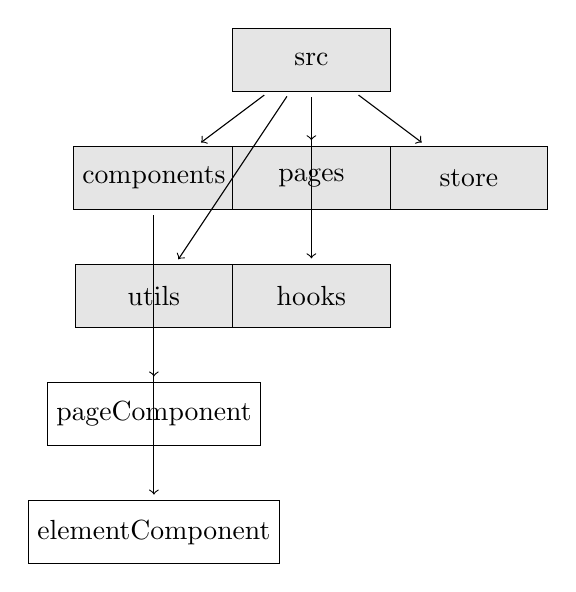
\begin{tikzpicture}[
    file/.style={draw, rectangle, minimum width=2cm, minimum height=0.8cm},
    folder/.style={draw, rectangle, minimum width=2cm, minimum height=0.8cm, fill=gray!20},
    arrow/.style={->, shorten >=2pt, shorten <=2pt}
]

% Folders
\node[folder] (src) at (0,0) {src};
\node[folder] (components) at (-2,-1.5) {components};
\node[folder] (pages) at (0,-1.5) {pages};
\node[folder] (store) at (2,-1.5) {store};
\node[folder] (utils) at (-2,-3) {utils};
\node[folder] (hooks) at (0,-3) {hooks};

% Files
\node[file] (pageComponent) at (-2,-4.5) {pageComponent};
\node[file] (elementComponent) at (-2,-6) {elementComponent};
% ... add more files

% Connections
\draw[arrow] (src) -- (components);
\draw[arrow] (src) -- (pages);
\draw[arrow] (src) -- (store);
\draw[arrow] (src) -- (utils);
\draw[arrow] (src) -- (hooks);
\draw[arrow] (components) -- (pageComponent);
\draw[arrow] (components) -- (elementComponent);
% ... add more connections

\end{tikzpicture}



\pagebreak
\subsubsection{Back-end}
The backend uses the dotNet framework. The development language using the C\# language.

In this project, the backend uses the Onion Architecture.
The Onion Architecture is a typically layered architecture, 
where each layer depends on the inner layer and provides interfaces to the outer layer.
The outer layer provides services to the outermost layer 
and other modules in the same layer based on the interfaces of the inner layer.

From inner to outer, the layers are: Domain, Application, Infrastructure, Presentation.
The Domain layer is the core layer and the innermost layer, used to define domain models, 
which are the business models.
It includes domain models and domain service interfaces.
Domain models are used to define the business models, 
which are the entities in the entity-relationship model and their attributes.
Domain service interfaces are used to define the business services, 
which are the relationships between entities in the entity-relationship model.

The Application layer is the application layer, 
used to define application services, which are the business logic.
It includes domain service implementations and application service interfaces.
Domain service implementations implement the methods of the inner layer's domain service 
interfaces and implement the business logic of the domain models.
Application service interfaces are used to define application services, 
which are the business logic.
It includes but is not limited to database interfaces, testing interfaces, 
HTTP API interfaces, MQTT interfaces, etc.

The Infrastructure layer is the infrastructure layer, used to define infrastructure.
It includes database implementations, testing implementations, 
HTTP API implementations, MQTT implementations, etc.
Database implementations implement the database interfaces 
and provide CRUD services for the database.
Testing implementations implement the testing interfaces 
and provide services for unit testing and integration testing.
HTTP API implementations implement the HTTP API interfaces 
and provide CRUD operations for HTTP APIs.
MQTT implementations implement the MQTT interfaces 
and provide CRUD operations for MQTT.

The Presentation layer is the presentation layer, used to define presentation logic, 
such as interfaces and pages. Since this is a backend project,
data presentation and control are handled by the frontend, 
so this layer is not needed.



\pagebreak
\subsubsection{Data communication and storage}
% 关于本项目的数据通信与数据存储的设计, 包括数据通信的协议, 数据存储的设计等
% 关于数据通信的设计:
% 1. 通信协议的选择
% 自前端向后端发送的数据, 有三种传输的数据类型, 
% 一种是普通的增删改查的请求, 对数据传输的时效性要求不高, 但是对数据的准确性, 完整性, 有序性, 安全性有一定的要求,
% 这种数据的传输, 采用 HTTP 协议, 以及 RESTful API 的设计. 可以有效的保证对数据传输的以上要求.
% 一种是对数据通道的创建和流媒体数据的传输, 对数据传输的时效性, 安全性要求较高, 这种数据的传输, 采用 WebRTC 协议, 以及 MQTT 协议.
% 配合可以快速解码的 flatbuffers 协议, 可以有效的保证对数据传输的以上要求.
% 最后一种是对设备的状态信息和操作信息的传输, 对完整性, 有序性, 安全性都有较高的要求, 这种数据的传输, 采用 MQTT 协议
% 同时也使用了 flatbuffers 协议.
% 
% 2. 数据通信的通信架构和通信流程
% 本项目的数据通信的通信架构, 是基于前后端分离的架构, 前端使用 React 框架, 后端使用 dotnet 框架.
% 当前端需要向后端发送数据的时候, 前端会向后端发送 HTTP 请求, 后端接收到 HTTP 请求之后, 会根据请求的数据类型,
% 选择不同的数据处理方式, 对于普通的增删改查的请求, 后端会根据 RESTful API 的设计, 对数据进行增删改查的操作,
% 对于对数据通道的创建和流媒体数据的传输, 后端会根据 WebRTC 协议, 对数据通道进行创建, 并且帮助前端和设备建立数据通道,
% 当数据通道建立后, 前端和设备之间则使用 flatbuffer 的数据格式对流媒体数据进行传输,
% 对于设备的状态信息和操作信息的传输, 前端会直接向 MQTT broker 发送 MQTT 请求, 
% 设备会在其自身的固件中监听相关的 MQTT 请求, 并且返回相关的数据.
% 
% 3. 数据通信的格式
% 本项目的数据通信的格式, 有三种, 
% 一种是 HTTP 协议, 
% 使用 json 格式对数据进行传输,
% 一种是 WebRTC 协议, 
% 使用 flatbuffers 格式对数据进行传输,
% 一种是 MQTT 协议.
% 使用 flatbuffers 格式对数据进行传输,
% 
% 关于数据存储的设计:
% 1. 数据存储的数据库的选择
% 本项目的数据存储的数据库的选择, 使用了轻量级的数据库 SQLite,
% SQLite 是一个进程内的库, 实现了自给自足的, 无服务器的, 零配置的, 事务性的 SQL 数据库引擎.
% 这是因为整个项目的目的是为了实现前端与设备之间的数据通信, 对于数据库数据的增删改查操作的要求不高,
% 数据量较小, 且对于数据库的数据的事务性要求不高, 所以选择了 SQLite 数据库.
% 2. 项目前后端的数据结构的设计
% 在本项目中, 前端由于使用了 React 框架, 所以前端的数据结构的设计, 使用了基于状态的数据结构的设计,
% 每个组件或者数据集都包含一个状态对象, 这个状态对象的属性就是组件的各个状态. 
% 使用状态对象的原因是, 可以方便的对状态进行管理, 采用对象-属性的形式, 可以方便的针对不同组件的同类状态进行区分,
% 由于跨组件的状态是由 redux 进行管理的, 这种状态对象的设计, 可以更搞笑的对状态进行更新和传递.
% 后端由于使用了 dotnet 框架, 所以后端的数据结构的设计, 使用了基于类的数据结构的设计,
% 采用了面向对象的编程思想, 对数据进行了封装, 使得数据的传输更加的安全, 有序, 完整.


\pagebreak

% \subsection{Domain model}
% \documentclass[]{article}
\usepackage{graphicx}
\usepackage{amsmath}
\usepackage{tikz}

% libaries
\usetikzlibrary{shapes,arrows}

%Define the listing package
\usepackage{listings} %code highlighter
\usepackage{color} %use color
\definecolor{mygreen}{rgb}{0,0.6,0}
\definecolor{mygray}{rgb}{0.5,0.5,0.5}
\definecolor{mymauve}{rgb}{0.58,0,0.82}

%Customize a bit the look
\lstset{ %
backgroundcolor=\color{white}, % choose the background color; you must add \usepackage{color} or \usepackage{xcolor}
basicstyle=\footnotesize, % the size of the fonts that are used for the code
breakatwhitespace=false, % sets if automatic breaks should only happen at whitespace
breaklines=true, % sets automatic line breaking
captionpos=b, % sets the caption-position to bottom
commentstyle=\color{mygreen}, % comment style
deletekeywords={...}, % if you want to delete keywords from the given language
escapeinside={\%*}{*)}, % if you want to add LaTeX within your code
extendedchars=true, % lets you use non-ASCII characters; for 8-bits encodings only, does not work with UTF-8
frame=single, % adds a frame around the code
keepspaces=true, % keeps spaces in text, useful for keeping indentation of code (possibly needs columns=flexible)
keywordstyle=\color{blue}, % keyword style
% language=Octave, % the language of the code
morekeywords={*,...}, % if you want to add more keywords to the set
numbers=left, % where to put the line-numbers; possible values are (none, left, right)
numbersep=5pt, % how far the line-numbers are from the code
numberstyle=\tiny\color{mygray}, % the style that is used for the line-numbers
rulecolor=\color{black}, % if not set, the frame-color may be changed on line-breaks within not-black text (e.g. comments (green here))
showspaces=false, % show spaces everywhere adding particular underscores; it overrides 'showstringspaces'
showstringspaces=false, % underline spaces within strings only
showtabs=false, % show tabs within strings adding particular underscores
stepnumber=1, % the step between two line-numbers. If it's 1, each line will be numbered
stringstyle=\color{mymauve}, % string literal style
tabsize=2, % sets default tabsize to 2 spaces
title=\lstname % show the filename of files included with \lstinputlisting; also try caption instead of title
}

\definecolor{darkgray}{rgb}{.4,.4,.4}
\definecolor{purple}{rgb}{0.65, 0.12, 0.82}

\lstdefinelanguage{React}{
keywords={const, typeof, new, true, false, catch, function, return, null, catch, switch, var, if, in, while, do, else, case, break},
keywordstyle=\color{blue}\bfseries,
ndkeywords={class, export, boolean, throw, implements, import, this},
ndkeywordstyle=\color{darkgray}\bfseries,
identifierstyle=\color{mygreen},
sensitive=false,
comment=[l]{//},
morecomment=[s]{/*}{*/},
commentstyle=\color{purple}\ttfamily,
string=[b]{"}{'}{`},
stringstyle=\color{red}\ttfamily,
morestring=[b]',
morestring=[b]",
morestring=[b]`',
}

\lstdefinelanguage{CSharp}{
keywords={const, typeof, new, true, false, catch, function, return, null, catch, switch, var, if, in, while, do, else, case, break},
keywordstyle=\color{blue}\bfseries,
ndkeywords={class, export, boolean, throw, implements, import, this},
ndkeywordstyle=\color{darkgray}\bfseries,
identifierstyle=\color{mygreen},
sensitive=false,
comment=[l]{//},
morecomment=[s]{/*}{*/},
commentstyle=\color{purple}\ttfamily,
string=[b]{"}{'}{`},
stringstyle=\color{red}\ttfamily,
morestring=[b]',
morestring=[b]",
morestring=[b]`',
}

\lstset{
language=React,
extendedchars=true,
basicstyle=\footnotesize\ttfamily,
showstringspaces=false,
showspaces=false,
numbers=left,
numberstyle=\footnotesize,
numbersep=9pt,
tabsize=2,
breaklines=true,
showtabs=false,
captionpos=b
}

\lstset{
language=CSharp,
extendedchars=true,
basicstyle=\footnotesize\ttfamily,
showstringspaces=false,
showspaces=false,
numbers=left,
numberstyle=\footnotesize,
numbersep=9pt,
tabsize=2,
breaklines=true,
showtabs=false,
captionpos=b
}

% \usepackage{cite} % Add this line for citation

% \bibliographystyle{plain}

\title{
The implementation of BifrostConnect Front-end scope, 
re-design and development with the relevant back-end support develop.
}
\author{
    Fei Gu \\
    Erhvervs Akademi Sydvest \\
    Computer Science 21\\
    }
\date{\today}

\begin{document}

% Front page
\maketitle
\begin{center}
    Supervisor: Henrik Boulund Meng Hansen \\
    Company: BifrostConnect \\
    Engineering Director: Jasper Wass \\
\end{center}
\tableofcontents
\pagebreak


% The introduction
\section{Introduction}
\subsection{Background}% 关于项目的类型和背景的介绍
% 项目是 EASV computer science 专业的毕业设计, 毕业设计的要求是充分的展现学生在两年半的学习中
% 能够获得的知识和技能, 并且能够在一个项目中充分的展现出来. 项目的类型是一个软件开发项目,
% 项目的背景是一个公司的项目, 项目的目的是为了解决公司的一个问题.

This project is the final project of the EASV computer science program. 
The purpose of the final project is to demonstrate the knowledge 
and skills by the student during the two and a half years of study,
and be able to fully demonstrate them in a project.

In this project, the student will work with a company 
to solve a problem of the company.
The student will use the knowledge and skills learned from the education
to solve the problem.

Which means this project will relavent to the company's business domain,
and using the software engineering methods and software development methods
to reconize the problem, analyze the problem, and solve the problem.


\subsection{The company}% 关于公司的介绍
% 公司的名字是 BifrostConnect, 是一个创业公司, 公司的主要业务是为了解决在严格的系统安全条件下, 
% 当客户的系统没有也不允许有互联网的情况下, 通过一个中继设备而不是第三方服务的条件下, 能够远程的
% 访问客户的系统. 公司的产品是一个硬件设备以及配套的网络应用. 以及相关的服务和一站式解决方案.

BifrostConnect is a startup company which established in 2018 
that has 10 to 12 employees and located in Copenhagen, Denmark.

During the five years of operation, the company has developed
a remote access solution for access the users remote system.
The solution  


The company's main business is to solve the problem of remote access 
to the customer's system when the customer's system does not have 
and is not allowed to have the Internet under strict system security conditions.

The company's product is a hardware device and a network application.
And related services and one-stop solutions.
\subsection{The project}% 关于项目的介绍
% 这个项目是在公司原有软件基础上, 对现有的前端软件进行重构和重新设计, 并且在后端提供相应的支持.

% This project is to re-design and re-develop the front-end software based on the company's original software,
% and provide corresponding support on the back-end.% Introduction to the project


% This project involves a comprehensive overhaul of the existing front-end software, building upon the company's original software. It also includes providing corresponding back-end support.

This project entails a thorough redesign and redevelopment of the existing front-end software, 
leveraging the foundation provided by the company's original software. 
Additionally, it involves enhancing the back-end to provide the necessary support 
for the new front-end.
\pagebreak

% The problem statement
\section{Problem Statement}
\subsection{Statement}
During this project the Remote Access Interface and Tunnel Interface should be integrated into the Device Mananger Application.
To achieve the one single page application with full functionality of the Remote Access and Tunnel Connection capabilities.

\subsection{Situation}
% 项目的背景
% 这一部分要详细的介绍关于项目的原始背景, 因为在之后要根据这些背景写明项目的意义和解决方案.
% 所以项目的现状, 项目的历史问题, 现有项目难以开发和维护的原因, 

% The current BifrostConnect front-end application consist of the Device Manager (DM) 
% and Remote Access Interface (RAI) two different user interface.
% Which means the user need to manage their devices and users in the one application, 
% and oprate their devices to use the bifrost product in other web application as well. 
% However, the RAI consists of two different user interfaces referred to as the Classic RAI and Tunnel RAI. 
% Those two user interfaces will leading the user to different web application 
% when user wish to create a different type of access solution.

% The reason for this situation occurred is because the bifrost product is developed focus on the device 
% and the application part was not considered as important as the device part. 
% Therefore, the application part was developed by different developers with different design logic.
% And the application functionality was not been properly through out the development process. 
% Which cause the design logic of this product is not scalable, leading to decreasing user experience, 
% and exponential growth of code complexity which makes it increasingly challenging to maintain and improve. 
% Also the product design style lacks scalability due to lack of modularity and code consistency, 
% and the operation logic is not clear.

The existing BifrostConnect front-end application is divided into two distinct user interfaces:
the Device Manager (DM) and the Remote Access Interface (RAI). 
This division requires users to manage their devices and users in one application, 
while operating their devices to use the Bifrost product in another web application. 
Moreover, the RAI is further split into two different user interfaces, 
known as the Classic RAI and Tunnel RAI. 
These interfaces direct users to different web applications 
depending on the type of access solution they wish to create.

This situation arose because the development of the Bifrost product was primarily focused 
on the device, with the application part not receiving as much attention. 
As a result, the application part was developed by different developers, 
each with their own design logic. 
This led to a lack of thorough planning for the application functionality 
during the development process. Consequently, 
the design logic of the product is not scalable, 
which has resulted in a diminished user experience 
and an exponential increase in code complexity, 
making it increasingly difficult to maintain and improve. 
Furthermore, the product design style lacks scalability due to a lack of modularity 
and code consistency, and the operation logic is unclear.
\subsection{Potential Solution}
% 项目的解决方案
% 根据之前的项目背景描述, 提出项目的解决方案, 也就是问题陈述的解决方案的详细说明. 
% 包括潜在的解决方案, 这个解决方案的优势和劣势.

To address those issue, there is a need to redesign and remake the front-end with
a focus on implementing a modular unified front-end management system that
encompasses all the necessary functionality. 

The goal is to provide users with seamless control, monitoring, and access to their devices from anywhere, 
enhancing their overall user experience and productivity while keeping code complexity as low as possible.

For the implementation to be successful, we also need to have a back-end
service, including an API and Database. The back-end server will contain the
necessary service for the front-end to reach the purpose. Such as the RESTful
API service, authentication service, MQTT service, Tunnel service and Database.

This project will follow the software design process. Therefore, it will also include
the Software Development method and DevOps on all process as well. 

This project is covered by NDA due to security and confidentiality reasons. Thus, the
project will initially not be publicly deployed, however, I will described the
deployment in my report as well.

%%%%%%%%%%%%%%%%%%%%%%%%%%%%%%%%%%%%%%%%%%%%%%%%%%%%%%%%%%%%%%%%%%%%%%%%%

% Project Solution
% Based on the previously described project background, this section presents a detailed explanation of the proposed solution to the problem statement. This includes potential solutions, as well as the advantages and disadvantages of the proposed solution.

% To address the issues identified, 
% a comprehensive redesign and redevelopment of the front-end is necessary. 
% The focus will be on creating a modular, 
% unified front-end management system that encompasses all required functionalities.

% The objective is to provide users with seamless control, 
% monitoring, and access to their devices from any location. 
% This will enhance their overall user experience 
% and productivity while keeping code complexity to a minimum.

% For successful implementation, a back-end service, 
% including an API and Database, is also required. 
% The back-end server will provide the necessary services for the front-end 
% to achieve its purpose. 
% These services include the RESTful API service, 
% authentication service, 
% MQTT service, 
% Tunnel service, 
% and Database.

% This project will adhere to the software design process, 
% incorporating Software Development methods 
% and DevOps throughout all stages.

% Due to security and confidentiality reasons, 
% this project is covered by a Non-Disclosure Agreement (NDA). 
% Therefore, the project will not initially be publicly deployed. 
% However, the deployment process will be described in detail in the final report.

%%%%%%%%%%%%%%%%%%%%%%%%%%%%%%%%%%%%%%%%%%%%%%%%%%%%%%%%%%%%%%%%%%%%%%%%%

In order to address the issues identified, 
a comprehensive overhaul of the front-end is necessary. 
This involves a complete redesign and redevelopment of the existing system, 
with a particular emphasis on creating a modular, 
unified front-end management system. 
This new system will incorporate all the necessary functionalities, 
thereby eliminating the need for multiple interfaces and improving the overall user experience.

The primary goal of this redesign is to provide users with seamless control, 
monitoring, and access to their devices, 
regardless of their location. 
By streamlining the user interface and integrating all necessary functionalities into a single, 
unified system, we aim to enhance the overall user experience and increase productivity. 
Furthermore, by focusing on modularity in the design, 
we aim to keep code complexity as low as possible, 
thereby improving maintainability and scalability of the system.

Successful implementation of this redesign requires a robust back-end service, which includes an API and a Database. The back-end server will house the necessary services for the front-end to fulfill its purpose. These services include the RESTful API service, which will handle requests and responses between the front-end and the server; an authentication service, which will ensure secure access to the system; an MQTT service, which will handle messaging between devices; a Tunnel service, which will manage the creation and maintenance of secure tunnels for remote access; and a Database, which will store and manage all necessary data.

This project will adhere to the software design process, incorporating best practices from Software Development methodologies and DevOps principles throughout all stages. This includes requirements gathering, system design, implementation, testing, deployment, and maintenance. By following this process, we aim to ensure the delivery of a high-quality, reliable, and scalable system.

Due to security and confidentiality reasons, this project is covered by a Non-Disclosure Agreement (NDA). As such, the project will not initially be publicly deployed. However, the deployment process, including the strategies used for continuous integration and continuous deployment, as well as the measures taken to ensure security and reliability, will be described in detail in the final report.
\pagebreak

% Requirement analysis
\section{Requirement Analysis}
\documentclass[]{article}
\usepackage{graphicx}
\usepackage{amsmath}
\usepackage{tikz}

% libaries
\usetikzlibrary{shapes,arrows}

%Define the listing package
\usepackage{listings} %code highlighter
\usepackage{color} %use color
\definecolor{mygreen}{rgb}{0,0.6,0}
\definecolor{mygray}{rgb}{0.5,0.5,0.5}
\definecolor{mymauve}{rgb}{0.58,0,0.82}

%Customize a bit the look
\lstset{ %
backgroundcolor=\color{white}, % choose the background color; you must add \usepackage{color} or \usepackage{xcolor}
basicstyle=\footnotesize, % the size of the fonts that are used for the code
breakatwhitespace=false, % sets if automatic breaks should only happen at whitespace
breaklines=true, % sets automatic line breaking
captionpos=b, % sets the caption-position to bottom
commentstyle=\color{mygreen}, % comment style
deletekeywords={...}, % if you want to delete keywords from the given language
escapeinside={\%*}{*)}, % if you want to add LaTeX within your code
extendedchars=true, % lets you use non-ASCII characters; for 8-bits encodings only, does not work with UTF-8
frame=single, % adds a frame around the code
keepspaces=true, % keeps spaces in text, useful for keeping indentation of code (possibly needs columns=flexible)
keywordstyle=\color{blue}, % keyword style
% language=Octave, % the language of the code
morekeywords={*,...}, % if you want to add more keywords to the set
numbers=left, % where to put the line-numbers; possible values are (none, left, right)
numbersep=5pt, % how far the line-numbers are from the code
numberstyle=\tiny\color{mygray}, % the style that is used for the line-numbers
rulecolor=\color{black}, % if not set, the frame-color may be changed on line-breaks within not-black text (e.g. comments (green here))
showspaces=false, % show spaces everywhere adding particular underscores; it overrides 'showstringspaces'
showstringspaces=false, % underline spaces within strings only
showtabs=false, % show tabs within strings adding particular underscores
stepnumber=1, % the step between two line-numbers. If it's 1, each line will be numbered
stringstyle=\color{mymauve}, % string literal style
tabsize=2, % sets default tabsize to 2 spaces
title=\lstname % show the filename of files included with \lstinputlisting; also try caption instead of title
}

\definecolor{darkgray}{rgb}{.4,.4,.4}
\definecolor{purple}{rgb}{0.65, 0.12, 0.82}

\lstdefinelanguage{React}{
keywords={const, typeof, new, true, false, catch, function, return, null, catch, switch, var, if, in, while, do, else, case, break},
keywordstyle=\color{blue}\bfseries,
ndkeywords={class, export, boolean, throw, implements, import, this},
ndkeywordstyle=\color{darkgray}\bfseries,
identifierstyle=\color{mygreen},
sensitive=false,
comment=[l]{//},
morecomment=[s]{/*}{*/},
commentstyle=\color{purple}\ttfamily,
string=[b]{"}{'}{`},
stringstyle=\color{red}\ttfamily,
morestring=[b]',
morestring=[b]",
morestring=[b]`',
}

\lstdefinelanguage{CSharp}{
keywords={const, typeof, new, true, false, catch, function, return, null, catch, switch, var, if, in, while, do, else, case, break},
keywordstyle=\color{blue}\bfseries,
ndkeywords={class, export, boolean, throw, implements, import, this},
ndkeywordstyle=\color{darkgray}\bfseries,
identifierstyle=\color{mygreen},
sensitive=false,
comment=[l]{//},
morecomment=[s]{/*}{*/},
commentstyle=\color{purple}\ttfamily,
string=[b]{"}{'}{`},
stringstyle=\color{red}\ttfamily,
morestring=[b]',
morestring=[b]",
morestring=[b]`',
}

\lstset{
language=React,
extendedchars=true,
basicstyle=\footnotesize\ttfamily,
showstringspaces=false,
showspaces=false,
numbers=left,
numberstyle=\footnotesize,
numbersep=9pt,
tabsize=2,
breaklines=true,
showtabs=false,
captionpos=b
}

\lstset{
language=CSharp,
extendedchars=true,
basicstyle=\footnotesize\ttfamily,
showstringspaces=false,
showspaces=false,
numbers=left,
numberstyle=\footnotesize,
numbersep=9pt,
tabsize=2,
breaklines=true,
showtabs=false,
captionpos=b
}

% \usepackage{cite} % Add this line for citation

% \bibliographystyle{plain}

\title{
The implementation of BifrostConnect Front-end scope, 
re-design and development with the relevant back-end support develop.
}
\author{
    Fei Gu \\
    Erhvervs Akademi Sydvest \\
    Computer Science 21\\
    }
\date{\today}

\begin{document}

% Front page
\maketitle
\begin{center}
    Supervisor: Henrik Boulund Meng Hansen \\
    Company: BifrostConnect \\
    Engineering Director: Jasper Wass \\
\end{center}
\tableofcontents
\pagebreak


% The introduction
\section{Introduction}
\subsection{Background}\input{sections/introduction/background.tex}
\subsection{The company}\input{sections/introduction/aboutCompany}
\subsection{The project}\input{sections/introduction/aboutProject}
\pagebreak

% The problem statement
\section{Problem Statement}
\subsection{Statement}
\input{sections/problemStatement/statement}
\subsection{Situation}
\input{sections/problemStatement/situation}
\subsection{Potential Solution}
\input{sections/problemStatement/potentialSolution}
\pagebreak

% Requirement analysis
\section{Requirement Analysis}
\input{sections/requirementAnalysis/index}

\subsection{Stakeholders}
\input{sections/requirementAnalysis/stakeholders/index}

\subsection{Business Domain}
\input{sections/requirementAnalysis/bussinesDomain/index}

\subsection{Scope}
\input{sections/requirementAnalysis/scope}

\subsection{Goals}
\input{sections/requirementAnalysis/goals}
\pagebreak

% Software Design
\section{Software Design}
% developement methods
\subsection{Software Development Methods}
\input{sections/softwareDevelopmentMethods/index}
\subsubsection{Agile Software Development}
\input{sections/softwareDevelopmentMethods/agileSoftwareDevelopment/index}
\subsubsection{Feature Driven Development}
\input{sections/softwareDevelopmentMethods/featureDrivenDevelopment/index}

\pagebreak

% Technology seslection
\subsection{Technology selection}
\input{sections/softwareDesign/technologySelection/index}
\subsubsection{Front-end}
\input{sections/softwareDesign/technologySelection/frontEnd}            
\subsubsection{Back-end}
\input{sections/softwareDesign/technologySelection/backEnd}            
\subsubsection{Database}
\input{sections/softwareDesign/technologySelection/database}
\subsubsection{Data communication}
\input{sections/softwareDesign/technologySelection/dataCommunication}            
\subsubsection{DevOps}
\input{sections/softwareDesign/technologySelection/devOps}
\pagebreak

% Architecture design
\subsection{Architecture design}
\input{sections/softwareDesign/architectureDesign/index}
\pagebreak
\subsubsection{Front-end}
\input{sections/softwareDesign/architectureDesign/frontEndArchitecture}
\pagebreak
\subsubsection{Back-end}
\input{sections/softwareDesign/architectureDesign/backEndArchitecture}
\pagebreak
\subsubsection{Data communication and storage}
\input{sections/softwareDesign/architectureDesign/dataCommunicationArchitecture}
\pagebreak

% \subsection{Domain model}
% \input{sections/softwareDesign/domainModel/index}
% \subsection{Database design}
% % 数据库领域模型 ER 图
% % 包括表和字段的设置.
% % 对于私有键和外键的设置.

% \subsection{Back-end design}
% % 后端对象模型
% % 以及对于对象模型的增删改查
% % 以及相关的其他服务的设计`'

% \subsection{Front-end design}
% % 对于前端的页面结构的设计 
% % 页面的状态的设计, 交互设计

% \subsection{FlatBuffers design}
% % schema 的设计

\subsection{DevOps CI/CD process design}
\input{sections/softwareDesign/devOpsDesign/index}
\subsubsection{Continuous Integration}
\input{sections/softwareDesign/devOpsDesign/continuousIntegration/index}
\subsubsection{Continuous Delivery}
\input{sections/softwareDesign/devOpsDesign/continuousDelivery/index}
\subsubsection{Continuous Deployment}
\input{sections/softwareDesign/devOpsDesign/continuousDeployment/index}
\pagebreak

\section{Software Development} 
\input{sections/softwareDevelopment/index}
\subsection{Overall development}
\input{sections/softwareDevelopment/overallDevelopement/index}
\subsubsection{Front-end}
\input{sections/softwareDevelopment/overallDevelopement/frontEnd/index}
\subsubsection{Back-end}
\input{sections/softwareDevelopment/overallDevelopement/backEnd/index}
\subsubsection{DevOps}
\input{sections/softwareDevelopment/overallDevelopement/devOps/index}
\subsection{Feature development} 
\input{sections/softwareDevelopment/featureDevelopment/index}
\subsubsection{Use Case 1}
\input{sections/softwareDevelopment/featureDevelopment/useCase1/index}
\subsubsection{Feature 1}
\input{sections/softwareDevelopment/featureDevelopment/feature/feature1.tex}
\pagebreak
\section{Conclusion} 
\subsection{Result}
Since the project is still in progress, the result is not available yet.
So far, basic structure of this project has been built. But the most features 
are not implemented yet. 
\subsection{Discussion}
As a single developer for this project, I am confident what I have done so far.
And I can say I understand the most of the knowledge I have used in this project, 
which also means I can explain all the part of the project. 
But this project also relevant some of the complex knowledge which I have to continue 
to study and practice.
\subsection{Future Work}
The future work is to implement the rest of the features. 
Including the most important part which is the 'create session' feature.
\pagebreak
% \bibliography{bibliography}
\pagebreak
% \begin{appendices}
%     \section{Appendix}
% \end{appendices} 
\end{document}

\subsection{Stakeholders}
\documentclass[]{article}
\usepackage{graphicx}
\usepackage{amsmath}
\usepackage{tikz}

% libaries
\usetikzlibrary{shapes,arrows}

%Define the listing package
\usepackage{listings} %code highlighter
\usepackage{color} %use color
\definecolor{mygreen}{rgb}{0,0.6,0}
\definecolor{mygray}{rgb}{0.5,0.5,0.5}
\definecolor{mymauve}{rgb}{0.58,0,0.82}

%Customize a bit the look
\lstset{ %
backgroundcolor=\color{white}, % choose the background color; you must add \usepackage{color} or \usepackage{xcolor}
basicstyle=\footnotesize, % the size of the fonts that are used for the code
breakatwhitespace=false, % sets if automatic breaks should only happen at whitespace
breaklines=true, % sets automatic line breaking
captionpos=b, % sets the caption-position to bottom
commentstyle=\color{mygreen}, % comment style
deletekeywords={...}, % if you want to delete keywords from the given language
escapeinside={\%*}{*)}, % if you want to add LaTeX within your code
extendedchars=true, % lets you use non-ASCII characters; for 8-bits encodings only, does not work with UTF-8
frame=single, % adds a frame around the code
keepspaces=true, % keeps spaces in text, useful for keeping indentation of code (possibly needs columns=flexible)
keywordstyle=\color{blue}, % keyword style
% language=Octave, % the language of the code
morekeywords={*,...}, % if you want to add more keywords to the set
numbers=left, % where to put the line-numbers; possible values are (none, left, right)
numbersep=5pt, % how far the line-numbers are from the code
numberstyle=\tiny\color{mygray}, % the style that is used for the line-numbers
rulecolor=\color{black}, % if not set, the frame-color may be changed on line-breaks within not-black text (e.g. comments (green here))
showspaces=false, % show spaces everywhere adding particular underscores; it overrides 'showstringspaces'
showstringspaces=false, % underline spaces within strings only
showtabs=false, % show tabs within strings adding particular underscores
stepnumber=1, % the step between two line-numbers. If it's 1, each line will be numbered
stringstyle=\color{mymauve}, % string literal style
tabsize=2, % sets default tabsize to 2 spaces
title=\lstname % show the filename of files included with \lstinputlisting; also try caption instead of title
}

\definecolor{darkgray}{rgb}{.4,.4,.4}
\definecolor{purple}{rgb}{0.65, 0.12, 0.82}

\lstdefinelanguage{React}{
keywords={const, typeof, new, true, false, catch, function, return, null, catch, switch, var, if, in, while, do, else, case, break},
keywordstyle=\color{blue}\bfseries,
ndkeywords={class, export, boolean, throw, implements, import, this},
ndkeywordstyle=\color{darkgray}\bfseries,
identifierstyle=\color{mygreen},
sensitive=false,
comment=[l]{//},
morecomment=[s]{/*}{*/},
commentstyle=\color{purple}\ttfamily,
string=[b]{"}{'}{`},
stringstyle=\color{red}\ttfamily,
morestring=[b]',
morestring=[b]",
morestring=[b]`',
}

\lstdefinelanguage{CSharp}{
keywords={const, typeof, new, true, false, catch, function, return, null, catch, switch, var, if, in, while, do, else, case, break},
keywordstyle=\color{blue}\bfseries,
ndkeywords={class, export, boolean, throw, implements, import, this},
ndkeywordstyle=\color{darkgray}\bfseries,
identifierstyle=\color{mygreen},
sensitive=false,
comment=[l]{//},
morecomment=[s]{/*}{*/},
commentstyle=\color{purple}\ttfamily,
string=[b]{"}{'}{`},
stringstyle=\color{red}\ttfamily,
morestring=[b]',
morestring=[b]",
morestring=[b]`',
}

\lstset{
language=React,
extendedchars=true,
basicstyle=\footnotesize\ttfamily,
showstringspaces=false,
showspaces=false,
numbers=left,
numberstyle=\footnotesize,
numbersep=9pt,
tabsize=2,
breaklines=true,
showtabs=false,
captionpos=b
}

\lstset{
language=CSharp,
extendedchars=true,
basicstyle=\footnotesize\ttfamily,
showstringspaces=false,
showspaces=false,
numbers=left,
numberstyle=\footnotesize,
numbersep=9pt,
tabsize=2,
breaklines=true,
showtabs=false,
captionpos=b
}

% \usepackage{cite} % Add this line for citation

% \bibliographystyle{plain}

\title{
The implementation of BifrostConnect Front-end scope, 
re-design and development with the relevant back-end support develop.
}
\author{
    Fei Gu \\
    Erhvervs Akademi Sydvest \\
    Computer Science 21\\
    }
\date{\today}

\begin{document}

% Front page
\maketitle
\begin{center}
    Supervisor: Henrik Boulund Meng Hansen \\
    Company: BifrostConnect \\
    Engineering Director: Jasper Wass \\
\end{center}
\tableofcontents
\pagebreak


% The introduction
\section{Introduction}
\subsection{Background}\input{sections/introduction/background.tex}
\subsection{The company}\input{sections/introduction/aboutCompany}
\subsection{The project}\input{sections/introduction/aboutProject}
\pagebreak

% The problem statement
\section{Problem Statement}
\subsection{Statement}
\input{sections/problemStatement/statement}
\subsection{Situation}
\input{sections/problemStatement/situation}
\subsection{Potential Solution}
\input{sections/problemStatement/potentialSolution}
\pagebreak

% Requirement analysis
\section{Requirement Analysis}
\input{sections/requirementAnalysis/index}

\subsection{Stakeholders}
\input{sections/requirementAnalysis/stakeholders/index}

\subsection{Business Domain}
\input{sections/requirementAnalysis/bussinesDomain/index}

\subsection{Scope}
\input{sections/requirementAnalysis/scope}

\subsection{Goals}
\input{sections/requirementAnalysis/goals}
\pagebreak

% Software Design
\section{Software Design}
% developement methods
\subsection{Software Development Methods}
\input{sections/softwareDevelopmentMethods/index}
\subsubsection{Agile Software Development}
\input{sections/softwareDevelopmentMethods/agileSoftwareDevelopment/index}
\subsubsection{Feature Driven Development}
\input{sections/softwareDevelopmentMethods/featureDrivenDevelopment/index}

\pagebreak

% Technology seslection
\subsection{Technology selection}
\input{sections/softwareDesign/technologySelection/index}
\subsubsection{Front-end}
\input{sections/softwareDesign/technologySelection/frontEnd}            
\subsubsection{Back-end}
\input{sections/softwareDesign/technologySelection/backEnd}            
\subsubsection{Database}
\input{sections/softwareDesign/technologySelection/database}
\subsubsection{Data communication}
\input{sections/softwareDesign/technologySelection/dataCommunication}            
\subsubsection{DevOps}
\input{sections/softwareDesign/technologySelection/devOps}
\pagebreak

% Architecture design
\subsection{Architecture design}
\input{sections/softwareDesign/architectureDesign/index}
\pagebreak
\subsubsection{Front-end}
\input{sections/softwareDesign/architectureDesign/frontEndArchitecture}
\pagebreak
\subsubsection{Back-end}
\input{sections/softwareDesign/architectureDesign/backEndArchitecture}
\pagebreak
\subsubsection{Data communication and storage}
\input{sections/softwareDesign/architectureDesign/dataCommunicationArchitecture}
\pagebreak

% \subsection{Domain model}
% \input{sections/softwareDesign/domainModel/index}
% \subsection{Database design}
% % 数据库领域模型 ER 图
% % 包括表和字段的设置.
% % 对于私有键和外键的设置.

% \subsection{Back-end design}
% % 后端对象模型
% % 以及对于对象模型的增删改查
% % 以及相关的其他服务的设计`'

% \subsection{Front-end design}
% % 对于前端的页面结构的设计 
% % 页面的状态的设计, 交互设计

% \subsection{FlatBuffers design}
% % schema 的设计

\subsection{DevOps CI/CD process design}
\input{sections/softwareDesign/devOpsDesign/index}
\subsubsection{Continuous Integration}
\input{sections/softwareDesign/devOpsDesign/continuousIntegration/index}
\subsubsection{Continuous Delivery}
\input{sections/softwareDesign/devOpsDesign/continuousDelivery/index}
\subsubsection{Continuous Deployment}
\input{sections/softwareDesign/devOpsDesign/continuousDeployment/index}
\pagebreak

\section{Software Development} 
\input{sections/softwareDevelopment/index}
\subsection{Overall development}
\input{sections/softwareDevelopment/overallDevelopement/index}
\subsubsection{Front-end}
\input{sections/softwareDevelopment/overallDevelopement/frontEnd/index}
\subsubsection{Back-end}
\input{sections/softwareDevelopment/overallDevelopement/backEnd/index}
\subsubsection{DevOps}
\input{sections/softwareDevelopment/overallDevelopement/devOps/index}
\subsection{Feature development} 
\input{sections/softwareDevelopment/featureDevelopment/index}
\subsubsection{Use Case 1}
\input{sections/softwareDevelopment/featureDevelopment/useCase1/index}
\subsubsection{Feature 1}
\input{sections/softwareDevelopment/featureDevelopment/feature/feature1.tex}
\pagebreak
\section{Conclusion} 
\subsection{Result}
Since the project is still in progress, the result is not available yet.
So far, basic structure of this project has been built. But the most features 
are not implemented yet. 
\subsection{Discussion}
As a single developer for this project, I am confident what I have done so far.
And I can say I understand the most of the knowledge I have used in this project, 
which also means I can explain all the part of the project. 
But this project also relevant some of the complex knowledge which I have to continue 
to study and practice.
\subsection{Future Work}
The future work is to implement the rest of the features. 
Including the most important part which is the 'create session' feature.
\pagebreak
% \bibliography{bibliography}
\pagebreak
% \begin{appendices}
%     \section{Appendix}
% \end{appendices} 
\end{document}

\subsection{Business Domain}
\documentclass[]{article}
\usepackage{graphicx}
\usepackage{amsmath}
\usepackage{tikz}

% libaries
\usetikzlibrary{shapes,arrows}

%Define the listing package
\usepackage{listings} %code highlighter
\usepackage{color} %use color
\definecolor{mygreen}{rgb}{0,0.6,0}
\definecolor{mygray}{rgb}{0.5,0.5,0.5}
\definecolor{mymauve}{rgb}{0.58,0,0.82}

%Customize a bit the look
\lstset{ %
backgroundcolor=\color{white}, % choose the background color; you must add \usepackage{color} or \usepackage{xcolor}
basicstyle=\footnotesize, % the size of the fonts that are used for the code
breakatwhitespace=false, % sets if automatic breaks should only happen at whitespace
breaklines=true, % sets automatic line breaking
captionpos=b, % sets the caption-position to bottom
commentstyle=\color{mygreen}, % comment style
deletekeywords={...}, % if you want to delete keywords from the given language
escapeinside={\%*}{*)}, % if you want to add LaTeX within your code
extendedchars=true, % lets you use non-ASCII characters; for 8-bits encodings only, does not work with UTF-8
frame=single, % adds a frame around the code
keepspaces=true, % keeps spaces in text, useful for keeping indentation of code (possibly needs columns=flexible)
keywordstyle=\color{blue}, % keyword style
% language=Octave, % the language of the code
morekeywords={*,...}, % if you want to add more keywords to the set
numbers=left, % where to put the line-numbers; possible values are (none, left, right)
numbersep=5pt, % how far the line-numbers are from the code
numberstyle=\tiny\color{mygray}, % the style that is used for the line-numbers
rulecolor=\color{black}, % if not set, the frame-color may be changed on line-breaks within not-black text (e.g. comments (green here))
showspaces=false, % show spaces everywhere adding particular underscores; it overrides 'showstringspaces'
showstringspaces=false, % underline spaces within strings only
showtabs=false, % show tabs within strings adding particular underscores
stepnumber=1, % the step between two line-numbers. If it's 1, each line will be numbered
stringstyle=\color{mymauve}, % string literal style
tabsize=2, % sets default tabsize to 2 spaces
title=\lstname % show the filename of files included with \lstinputlisting; also try caption instead of title
}

\definecolor{darkgray}{rgb}{.4,.4,.4}
\definecolor{purple}{rgb}{0.65, 0.12, 0.82}

\lstdefinelanguage{React}{
keywords={const, typeof, new, true, false, catch, function, return, null, catch, switch, var, if, in, while, do, else, case, break},
keywordstyle=\color{blue}\bfseries,
ndkeywords={class, export, boolean, throw, implements, import, this},
ndkeywordstyle=\color{darkgray}\bfseries,
identifierstyle=\color{mygreen},
sensitive=false,
comment=[l]{//},
morecomment=[s]{/*}{*/},
commentstyle=\color{purple}\ttfamily,
string=[b]{"}{'}{`},
stringstyle=\color{red}\ttfamily,
morestring=[b]',
morestring=[b]",
morestring=[b]`',
}

\lstdefinelanguage{CSharp}{
keywords={const, typeof, new, true, false, catch, function, return, null, catch, switch, var, if, in, while, do, else, case, break},
keywordstyle=\color{blue}\bfseries,
ndkeywords={class, export, boolean, throw, implements, import, this},
ndkeywordstyle=\color{darkgray}\bfseries,
identifierstyle=\color{mygreen},
sensitive=false,
comment=[l]{//},
morecomment=[s]{/*}{*/},
commentstyle=\color{purple}\ttfamily,
string=[b]{"}{'}{`},
stringstyle=\color{red}\ttfamily,
morestring=[b]',
morestring=[b]",
morestring=[b]`',
}

\lstset{
language=React,
extendedchars=true,
basicstyle=\footnotesize\ttfamily,
showstringspaces=false,
showspaces=false,
numbers=left,
numberstyle=\footnotesize,
numbersep=9pt,
tabsize=2,
breaklines=true,
showtabs=false,
captionpos=b
}

\lstset{
language=CSharp,
extendedchars=true,
basicstyle=\footnotesize\ttfamily,
showstringspaces=false,
showspaces=false,
numbers=left,
numberstyle=\footnotesize,
numbersep=9pt,
tabsize=2,
breaklines=true,
showtabs=false,
captionpos=b
}

% \usepackage{cite} % Add this line for citation

% \bibliographystyle{plain}

\title{
The implementation of BifrostConnect Front-end scope, 
re-design and development with the relevant back-end support develop.
}
\author{
    Fei Gu \\
    Erhvervs Akademi Sydvest \\
    Computer Science 21\\
    }
\date{\today}

\begin{document}

% Front page
\maketitle
\begin{center}
    Supervisor: Henrik Boulund Meng Hansen \\
    Company: BifrostConnect \\
    Engineering Director: Jasper Wass \\
\end{center}
\tableofcontents
\pagebreak


% The introduction
\section{Introduction}
\subsection{Background}\input{sections/introduction/background.tex}
\subsection{The company}\input{sections/introduction/aboutCompany}
\subsection{The project}\input{sections/introduction/aboutProject}
\pagebreak

% The problem statement
\section{Problem Statement}
\subsection{Statement}
\input{sections/problemStatement/statement}
\subsection{Situation}
\input{sections/problemStatement/situation}
\subsection{Potential Solution}
\input{sections/problemStatement/potentialSolution}
\pagebreak

% Requirement analysis
\section{Requirement Analysis}
\input{sections/requirementAnalysis/index}

\subsection{Stakeholders}
\input{sections/requirementAnalysis/stakeholders/index}

\subsection{Business Domain}
\input{sections/requirementAnalysis/bussinesDomain/index}

\subsection{Scope}
\input{sections/requirementAnalysis/scope}

\subsection{Goals}
\input{sections/requirementAnalysis/goals}
\pagebreak

% Software Design
\section{Software Design}
% developement methods
\subsection{Software Development Methods}
\input{sections/softwareDevelopmentMethods/index}
\subsubsection{Agile Software Development}
\input{sections/softwareDevelopmentMethods/agileSoftwareDevelopment/index}
\subsubsection{Feature Driven Development}
\input{sections/softwareDevelopmentMethods/featureDrivenDevelopment/index}

\pagebreak

% Technology seslection
\subsection{Technology selection}
\input{sections/softwareDesign/technologySelection/index}
\subsubsection{Front-end}
\input{sections/softwareDesign/technologySelection/frontEnd}            
\subsubsection{Back-end}
\input{sections/softwareDesign/technologySelection/backEnd}            
\subsubsection{Database}
\input{sections/softwareDesign/technologySelection/database}
\subsubsection{Data communication}
\input{sections/softwareDesign/technologySelection/dataCommunication}            
\subsubsection{DevOps}
\input{sections/softwareDesign/technologySelection/devOps}
\pagebreak

% Architecture design
\subsection{Architecture design}
\input{sections/softwareDesign/architectureDesign/index}
\pagebreak
\subsubsection{Front-end}
\input{sections/softwareDesign/architectureDesign/frontEndArchitecture}
\pagebreak
\subsubsection{Back-end}
\input{sections/softwareDesign/architectureDesign/backEndArchitecture}
\pagebreak
\subsubsection{Data communication and storage}
\input{sections/softwareDesign/architectureDesign/dataCommunicationArchitecture}
\pagebreak

% \subsection{Domain model}
% \input{sections/softwareDesign/domainModel/index}
% \subsection{Database design}
% % 数据库领域模型 ER 图
% % 包括表和字段的设置.
% % 对于私有键和外键的设置.

% \subsection{Back-end design}
% % 后端对象模型
% % 以及对于对象模型的增删改查
% % 以及相关的其他服务的设计`'

% \subsection{Front-end design}
% % 对于前端的页面结构的设计 
% % 页面的状态的设计, 交互设计

% \subsection{FlatBuffers design}
% % schema 的设计

\subsection{DevOps CI/CD process design}
\input{sections/softwareDesign/devOpsDesign/index}
\subsubsection{Continuous Integration}
\input{sections/softwareDesign/devOpsDesign/continuousIntegration/index}
\subsubsection{Continuous Delivery}
\input{sections/softwareDesign/devOpsDesign/continuousDelivery/index}
\subsubsection{Continuous Deployment}
\input{sections/softwareDesign/devOpsDesign/continuousDeployment/index}
\pagebreak

\section{Software Development} 
\input{sections/softwareDevelopment/index}
\subsection{Overall development}
\input{sections/softwareDevelopment/overallDevelopement/index}
\subsubsection{Front-end}
\input{sections/softwareDevelopment/overallDevelopement/frontEnd/index}
\subsubsection{Back-end}
\input{sections/softwareDevelopment/overallDevelopement/backEnd/index}
\subsubsection{DevOps}
\input{sections/softwareDevelopment/overallDevelopement/devOps/index}
\subsection{Feature development} 
\input{sections/softwareDevelopment/featureDevelopment/index}
\subsubsection{Use Case 1}
\input{sections/softwareDevelopment/featureDevelopment/useCase1/index}
\subsubsection{Feature 1}
\input{sections/softwareDevelopment/featureDevelopment/feature/feature1.tex}
\pagebreak
\section{Conclusion} 
\subsection{Result}
Since the project is still in progress, the result is not available yet.
So far, basic structure of this project has been built. But the most features 
are not implemented yet. 
\subsection{Discussion}
As a single developer for this project, I am confident what I have done so far.
And I can say I understand the most of the knowledge I have used in this project, 
which also means I can explain all the part of the project. 
But this project also relevant some of the complex knowledge which I have to continue 
to study and practice.
\subsection{Future Work}
The future work is to implement the rest of the features. 
Including the most important part which is the 'create session' feature.
\pagebreak
% \bibliography{bibliography}
\pagebreak
% \begin{appendices}
%     \section{Appendix}
% \end{appendices} 
\end{document}

\subsection{Scope}
% The scope of this project is to develop a web application 
% which can be used to manage the device and users, 
% and create the RAI and Tunnel.

% Because the device manager already exist, 
% the mean focus will be on the implementation of the RAI and Tunnel into the device manager.
% Which means we don't need to develop the device manager, 
% also there are no necceary to develop the new features for the RAI and Tunnel interface.

% Because the situation of the entire system was redudent and coupling, 
% we have to re-design the system components and identify the relationship between them.
% The re-design of the system will be the main focus of this project.

% Since the Device Manager is written in React framework, 
% we have to use the same framework to develop the RAI and Tunnel interface.

The scope of this project is to develop a web application 
that manages devices and users, and creates the RAI and Tunnel.

Since the device manager already exists, 
the main focus will be on implementing the RAI and Tunnel 
into the device manager.

Therefore, there is no need to develop the device manager 
or add new features to the RAI and Tunnel interface.

Due to the redundant and coupled nature of the entire system, 
we need to redesign the system components 
and establish their relationships.

As the Device Manager is built using the React framework, 
we will also use the same framework to develop the RAI and Tunnel interface.

The main focus of this project is to migramt the RAI and Tunnel interface, 
and re-design the UI, components, and the relavent methodologies.


\subsection{Goals}
The goal of this project is to develop a RAI and Tunnel interface in the Device Manager.
The RAI and Tunnel interface should be able to create, modify, delete and view the access connection.
Also can remote control the device and target equipment.
\pagebreak

% Software Design
\section{Software Design}
% developement methods
\subsection{Software Development Methods}
\documentclass[]{article}
\usepackage{graphicx}
\usepackage{amsmath}
\usepackage{tikz}

% libaries
\usetikzlibrary{shapes,arrows}

%Define the listing package
\usepackage{listings} %code highlighter
\usepackage{color} %use color
\definecolor{mygreen}{rgb}{0,0.6,0}
\definecolor{mygray}{rgb}{0.5,0.5,0.5}
\definecolor{mymauve}{rgb}{0.58,0,0.82}

%Customize a bit the look
\lstset{ %
backgroundcolor=\color{white}, % choose the background color; you must add \usepackage{color} or \usepackage{xcolor}
basicstyle=\footnotesize, % the size of the fonts that are used for the code
breakatwhitespace=false, % sets if automatic breaks should only happen at whitespace
breaklines=true, % sets automatic line breaking
captionpos=b, % sets the caption-position to bottom
commentstyle=\color{mygreen}, % comment style
deletekeywords={...}, % if you want to delete keywords from the given language
escapeinside={\%*}{*)}, % if you want to add LaTeX within your code
extendedchars=true, % lets you use non-ASCII characters; for 8-bits encodings only, does not work with UTF-8
frame=single, % adds a frame around the code
keepspaces=true, % keeps spaces in text, useful for keeping indentation of code (possibly needs columns=flexible)
keywordstyle=\color{blue}, % keyword style
% language=Octave, % the language of the code
morekeywords={*,...}, % if you want to add more keywords to the set
numbers=left, % where to put the line-numbers; possible values are (none, left, right)
numbersep=5pt, % how far the line-numbers are from the code
numberstyle=\tiny\color{mygray}, % the style that is used for the line-numbers
rulecolor=\color{black}, % if not set, the frame-color may be changed on line-breaks within not-black text (e.g. comments (green here))
showspaces=false, % show spaces everywhere adding particular underscores; it overrides 'showstringspaces'
showstringspaces=false, % underline spaces within strings only
showtabs=false, % show tabs within strings adding particular underscores
stepnumber=1, % the step between two line-numbers. If it's 1, each line will be numbered
stringstyle=\color{mymauve}, % string literal style
tabsize=2, % sets default tabsize to 2 spaces
title=\lstname % show the filename of files included with \lstinputlisting; also try caption instead of title
}

\definecolor{darkgray}{rgb}{.4,.4,.4}
\definecolor{purple}{rgb}{0.65, 0.12, 0.82}

\lstdefinelanguage{React}{
keywords={const, typeof, new, true, false, catch, function, return, null, catch, switch, var, if, in, while, do, else, case, break},
keywordstyle=\color{blue}\bfseries,
ndkeywords={class, export, boolean, throw, implements, import, this},
ndkeywordstyle=\color{darkgray}\bfseries,
identifierstyle=\color{mygreen},
sensitive=false,
comment=[l]{//},
morecomment=[s]{/*}{*/},
commentstyle=\color{purple}\ttfamily,
string=[b]{"}{'}{`},
stringstyle=\color{red}\ttfamily,
morestring=[b]',
morestring=[b]",
morestring=[b]`',
}

\lstdefinelanguage{CSharp}{
keywords={const, typeof, new, true, false, catch, function, return, null, catch, switch, var, if, in, while, do, else, case, break},
keywordstyle=\color{blue}\bfseries,
ndkeywords={class, export, boolean, throw, implements, import, this},
ndkeywordstyle=\color{darkgray}\bfseries,
identifierstyle=\color{mygreen},
sensitive=false,
comment=[l]{//},
morecomment=[s]{/*}{*/},
commentstyle=\color{purple}\ttfamily,
string=[b]{"}{'}{`},
stringstyle=\color{red}\ttfamily,
morestring=[b]',
morestring=[b]",
morestring=[b]`',
}

\lstset{
language=React,
extendedchars=true,
basicstyle=\footnotesize\ttfamily,
showstringspaces=false,
showspaces=false,
numbers=left,
numberstyle=\footnotesize,
numbersep=9pt,
tabsize=2,
breaklines=true,
showtabs=false,
captionpos=b
}

\lstset{
language=CSharp,
extendedchars=true,
basicstyle=\footnotesize\ttfamily,
showstringspaces=false,
showspaces=false,
numbers=left,
numberstyle=\footnotesize,
numbersep=9pt,
tabsize=2,
breaklines=true,
showtabs=false,
captionpos=b
}

% \usepackage{cite} % Add this line for citation

% \bibliographystyle{plain}

\title{
The implementation of BifrostConnect Front-end scope, 
re-design and development with the relevant back-end support develop.
}
\author{
    Fei Gu \\
    Erhvervs Akademi Sydvest \\
    Computer Science 21\\
    }
\date{\today}

\begin{document}

% Front page
\maketitle
\begin{center}
    Supervisor: Henrik Boulund Meng Hansen \\
    Company: BifrostConnect \\
    Engineering Director: Jasper Wass \\
\end{center}
\tableofcontents
\pagebreak


% The introduction
\section{Introduction}
\subsection{Background}\input{sections/introduction/background.tex}
\subsection{The company}\input{sections/introduction/aboutCompany}
\subsection{The project}\input{sections/introduction/aboutProject}
\pagebreak

% The problem statement
\section{Problem Statement}
\subsection{Statement}
\input{sections/problemStatement/statement}
\subsection{Situation}
\input{sections/problemStatement/situation}
\subsection{Potential Solution}
\input{sections/problemStatement/potentialSolution}
\pagebreak

% Requirement analysis
\section{Requirement Analysis}
\input{sections/requirementAnalysis/index}

\subsection{Stakeholders}
\input{sections/requirementAnalysis/stakeholders/index}

\subsection{Business Domain}
\input{sections/requirementAnalysis/bussinesDomain/index}

\subsection{Scope}
\input{sections/requirementAnalysis/scope}

\subsection{Goals}
\input{sections/requirementAnalysis/goals}
\pagebreak

% Software Design
\section{Software Design}
% developement methods
\subsection{Software Development Methods}
\input{sections/softwareDevelopmentMethods/index}
\subsubsection{Agile Software Development}
\input{sections/softwareDevelopmentMethods/agileSoftwareDevelopment/index}
\subsubsection{Feature Driven Development}
\input{sections/softwareDevelopmentMethods/featureDrivenDevelopment/index}

\pagebreak

% Technology seslection
\subsection{Technology selection}
\input{sections/softwareDesign/technologySelection/index}
\subsubsection{Front-end}
\input{sections/softwareDesign/technologySelection/frontEnd}            
\subsubsection{Back-end}
\input{sections/softwareDesign/technologySelection/backEnd}            
\subsubsection{Database}
\input{sections/softwareDesign/technologySelection/database}
\subsubsection{Data communication}
\input{sections/softwareDesign/technologySelection/dataCommunication}            
\subsubsection{DevOps}
\input{sections/softwareDesign/technologySelection/devOps}
\pagebreak

% Architecture design
\subsection{Architecture design}
\input{sections/softwareDesign/architectureDesign/index}
\pagebreak
\subsubsection{Front-end}
\input{sections/softwareDesign/architectureDesign/frontEndArchitecture}
\pagebreak
\subsubsection{Back-end}
\input{sections/softwareDesign/architectureDesign/backEndArchitecture}
\pagebreak
\subsubsection{Data communication and storage}
\input{sections/softwareDesign/architectureDesign/dataCommunicationArchitecture}
\pagebreak

% \subsection{Domain model}
% \input{sections/softwareDesign/domainModel/index}
% \subsection{Database design}
% % 数据库领域模型 ER 图
% % 包括表和字段的设置.
% % 对于私有键和外键的设置.

% \subsection{Back-end design}
% % 后端对象模型
% % 以及对于对象模型的增删改查
% % 以及相关的其他服务的设计`'

% \subsection{Front-end design}
% % 对于前端的页面结构的设计 
% % 页面的状态的设计, 交互设计

% \subsection{FlatBuffers design}
% % schema 的设计

\subsection{DevOps CI/CD process design}
\input{sections/softwareDesign/devOpsDesign/index}
\subsubsection{Continuous Integration}
\input{sections/softwareDesign/devOpsDesign/continuousIntegration/index}
\subsubsection{Continuous Delivery}
\input{sections/softwareDesign/devOpsDesign/continuousDelivery/index}
\subsubsection{Continuous Deployment}
\input{sections/softwareDesign/devOpsDesign/continuousDeployment/index}
\pagebreak

\section{Software Development} 
\input{sections/softwareDevelopment/index}
\subsection{Overall development}
\input{sections/softwareDevelopment/overallDevelopement/index}
\subsubsection{Front-end}
\input{sections/softwareDevelopment/overallDevelopement/frontEnd/index}
\subsubsection{Back-end}
\input{sections/softwareDevelopment/overallDevelopement/backEnd/index}
\subsubsection{DevOps}
\input{sections/softwareDevelopment/overallDevelopement/devOps/index}
\subsection{Feature development} 
\input{sections/softwareDevelopment/featureDevelopment/index}
\subsubsection{Use Case 1}
\input{sections/softwareDevelopment/featureDevelopment/useCase1/index}
\subsubsection{Feature 1}
\input{sections/softwareDevelopment/featureDevelopment/feature/feature1.tex}
\pagebreak
\section{Conclusion} 
\subsection{Result}
Since the project is still in progress, the result is not available yet.
So far, basic structure of this project has been built. But the most features 
are not implemented yet. 
\subsection{Discussion}
As a single developer for this project, I am confident what I have done so far.
And I can say I understand the most of the knowledge I have used in this project, 
which also means I can explain all the part of the project. 
But this project also relevant some of the complex knowledge which I have to continue 
to study and practice.
\subsection{Future Work}
The future work is to implement the rest of the features. 
Including the most important part which is the 'create session' feature.
\pagebreak
% \bibliography{bibliography}
\pagebreak
% \begin{appendices}
%     \section{Appendix}
% \end{appendices} 
\end{document}
\subsubsection{Agile Software Development}
\documentclass[]{article}
\usepackage{graphicx}
\usepackage{amsmath}
\usepackage{tikz}

% libaries
\usetikzlibrary{shapes,arrows}

%Define the listing package
\usepackage{listings} %code highlighter
\usepackage{color} %use color
\definecolor{mygreen}{rgb}{0,0.6,0}
\definecolor{mygray}{rgb}{0.5,0.5,0.5}
\definecolor{mymauve}{rgb}{0.58,0,0.82}

%Customize a bit the look
\lstset{ %
backgroundcolor=\color{white}, % choose the background color; you must add \usepackage{color} or \usepackage{xcolor}
basicstyle=\footnotesize, % the size of the fonts that are used for the code
breakatwhitespace=false, % sets if automatic breaks should only happen at whitespace
breaklines=true, % sets automatic line breaking
captionpos=b, % sets the caption-position to bottom
commentstyle=\color{mygreen}, % comment style
deletekeywords={...}, % if you want to delete keywords from the given language
escapeinside={\%*}{*)}, % if you want to add LaTeX within your code
extendedchars=true, % lets you use non-ASCII characters; for 8-bits encodings only, does not work with UTF-8
frame=single, % adds a frame around the code
keepspaces=true, % keeps spaces in text, useful for keeping indentation of code (possibly needs columns=flexible)
keywordstyle=\color{blue}, % keyword style
% language=Octave, % the language of the code
morekeywords={*,...}, % if you want to add more keywords to the set
numbers=left, % where to put the line-numbers; possible values are (none, left, right)
numbersep=5pt, % how far the line-numbers are from the code
numberstyle=\tiny\color{mygray}, % the style that is used for the line-numbers
rulecolor=\color{black}, % if not set, the frame-color may be changed on line-breaks within not-black text (e.g. comments (green here))
showspaces=false, % show spaces everywhere adding particular underscores; it overrides 'showstringspaces'
showstringspaces=false, % underline spaces within strings only
showtabs=false, % show tabs within strings adding particular underscores
stepnumber=1, % the step between two line-numbers. If it's 1, each line will be numbered
stringstyle=\color{mymauve}, % string literal style
tabsize=2, % sets default tabsize to 2 spaces
title=\lstname % show the filename of files included with \lstinputlisting; also try caption instead of title
}

\definecolor{darkgray}{rgb}{.4,.4,.4}
\definecolor{purple}{rgb}{0.65, 0.12, 0.82}

\lstdefinelanguage{React}{
keywords={const, typeof, new, true, false, catch, function, return, null, catch, switch, var, if, in, while, do, else, case, break},
keywordstyle=\color{blue}\bfseries,
ndkeywords={class, export, boolean, throw, implements, import, this},
ndkeywordstyle=\color{darkgray}\bfseries,
identifierstyle=\color{mygreen},
sensitive=false,
comment=[l]{//},
morecomment=[s]{/*}{*/},
commentstyle=\color{purple}\ttfamily,
string=[b]{"}{'}{`},
stringstyle=\color{red}\ttfamily,
morestring=[b]',
morestring=[b]",
morestring=[b]`',
}

\lstdefinelanguage{CSharp}{
keywords={const, typeof, new, true, false, catch, function, return, null, catch, switch, var, if, in, while, do, else, case, break},
keywordstyle=\color{blue}\bfseries,
ndkeywords={class, export, boolean, throw, implements, import, this},
ndkeywordstyle=\color{darkgray}\bfseries,
identifierstyle=\color{mygreen},
sensitive=false,
comment=[l]{//},
morecomment=[s]{/*}{*/},
commentstyle=\color{purple}\ttfamily,
string=[b]{"}{'}{`},
stringstyle=\color{red}\ttfamily,
morestring=[b]',
morestring=[b]",
morestring=[b]`',
}

\lstset{
language=React,
extendedchars=true,
basicstyle=\footnotesize\ttfamily,
showstringspaces=false,
showspaces=false,
numbers=left,
numberstyle=\footnotesize,
numbersep=9pt,
tabsize=2,
breaklines=true,
showtabs=false,
captionpos=b
}

\lstset{
language=CSharp,
extendedchars=true,
basicstyle=\footnotesize\ttfamily,
showstringspaces=false,
showspaces=false,
numbers=left,
numberstyle=\footnotesize,
numbersep=9pt,
tabsize=2,
breaklines=true,
showtabs=false,
captionpos=b
}

% \usepackage{cite} % Add this line for citation

% \bibliographystyle{plain}

\title{
The implementation of BifrostConnect Front-end scope, 
re-design and development with the relevant back-end support develop.
}
\author{
    Fei Gu \\
    Erhvervs Akademi Sydvest \\
    Computer Science 21\\
    }
\date{\today}

\begin{document}

% Front page
\maketitle
\begin{center}
    Supervisor: Henrik Boulund Meng Hansen \\
    Company: BifrostConnect \\
    Engineering Director: Jasper Wass \\
\end{center}
\tableofcontents
\pagebreak


% The introduction
\section{Introduction}
\subsection{Background}\input{sections/introduction/background.tex}
\subsection{The company}\input{sections/introduction/aboutCompany}
\subsection{The project}\input{sections/introduction/aboutProject}
\pagebreak

% The problem statement
\section{Problem Statement}
\subsection{Statement}
\input{sections/problemStatement/statement}
\subsection{Situation}
\input{sections/problemStatement/situation}
\subsection{Potential Solution}
\input{sections/problemStatement/potentialSolution}
\pagebreak

% Requirement analysis
\section{Requirement Analysis}
\input{sections/requirementAnalysis/index}

\subsection{Stakeholders}
\input{sections/requirementAnalysis/stakeholders/index}

\subsection{Business Domain}
\input{sections/requirementAnalysis/bussinesDomain/index}

\subsection{Scope}
\input{sections/requirementAnalysis/scope}

\subsection{Goals}
\input{sections/requirementAnalysis/goals}
\pagebreak

% Software Design
\section{Software Design}
% developement methods
\subsection{Software Development Methods}
\input{sections/softwareDevelopmentMethods/index}
\subsubsection{Agile Software Development}
\input{sections/softwareDevelopmentMethods/agileSoftwareDevelopment/index}
\subsubsection{Feature Driven Development}
\input{sections/softwareDevelopmentMethods/featureDrivenDevelopment/index}

\pagebreak

% Technology seslection
\subsection{Technology selection}
\input{sections/softwareDesign/technologySelection/index}
\subsubsection{Front-end}
\input{sections/softwareDesign/technologySelection/frontEnd}            
\subsubsection{Back-end}
\input{sections/softwareDesign/technologySelection/backEnd}            
\subsubsection{Database}
\input{sections/softwareDesign/technologySelection/database}
\subsubsection{Data communication}
\input{sections/softwareDesign/technologySelection/dataCommunication}            
\subsubsection{DevOps}
\input{sections/softwareDesign/technologySelection/devOps}
\pagebreak

% Architecture design
\subsection{Architecture design}
\input{sections/softwareDesign/architectureDesign/index}
\pagebreak
\subsubsection{Front-end}
\input{sections/softwareDesign/architectureDesign/frontEndArchitecture}
\pagebreak
\subsubsection{Back-end}
\input{sections/softwareDesign/architectureDesign/backEndArchitecture}
\pagebreak
\subsubsection{Data communication and storage}
\input{sections/softwareDesign/architectureDesign/dataCommunicationArchitecture}
\pagebreak

% \subsection{Domain model}
% \input{sections/softwareDesign/domainModel/index}
% \subsection{Database design}
% % 数据库领域模型 ER 图
% % 包括表和字段的设置.
% % 对于私有键和外键的设置.

% \subsection{Back-end design}
% % 后端对象模型
% % 以及对于对象模型的增删改查
% % 以及相关的其他服务的设计`'

% \subsection{Front-end design}
% % 对于前端的页面结构的设计 
% % 页面的状态的设计, 交互设计

% \subsection{FlatBuffers design}
% % schema 的设计

\subsection{DevOps CI/CD process design}
\input{sections/softwareDesign/devOpsDesign/index}
\subsubsection{Continuous Integration}
\input{sections/softwareDesign/devOpsDesign/continuousIntegration/index}
\subsubsection{Continuous Delivery}
\input{sections/softwareDesign/devOpsDesign/continuousDelivery/index}
\subsubsection{Continuous Deployment}
\input{sections/softwareDesign/devOpsDesign/continuousDeployment/index}
\pagebreak

\section{Software Development} 
\input{sections/softwareDevelopment/index}
\subsection{Overall development}
\input{sections/softwareDevelopment/overallDevelopement/index}
\subsubsection{Front-end}
\input{sections/softwareDevelopment/overallDevelopement/frontEnd/index}
\subsubsection{Back-end}
\input{sections/softwareDevelopment/overallDevelopement/backEnd/index}
\subsubsection{DevOps}
\input{sections/softwareDevelopment/overallDevelopement/devOps/index}
\subsection{Feature development} 
\input{sections/softwareDevelopment/featureDevelopment/index}
\subsubsection{Use Case 1}
\input{sections/softwareDevelopment/featureDevelopment/useCase1/index}
\subsubsection{Feature 1}
\input{sections/softwareDevelopment/featureDevelopment/feature/feature1.tex}
\pagebreak
\section{Conclusion} 
\subsection{Result}
Since the project is still in progress, the result is not available yet.
So far, basic structure of this project has been built. But the most features 
are not implemented yet. 
\subsection{Discussion}
As a single developer for this project, I am confident what I have done so far.
And I can say I understand the most of the knowledge I have used in this project, 
which also means I can explain all the part of the project. 
But this project also relevant some of the complex knowledge which I have to continue 
to study and practice.
\subsection{Future Work}
The future work is to implement the rest of the features. 
Including the most important part which is the 'create session' feature.
\pagebreak
% \bibliography{bibliography}
\pagebreak
% \begin{appendices}
%     \section{Appendix}
% \end{appendices} 
\end{document}
\subsubsection{Feature Driven Development}
\documentclass[]{article}
\usepackage{graphicx}
\usepackage{amsmath}
\usepackage{tikz}

% libaries
\usetikzlibrary{shapes,arrows}

%Define the listing package
\usepackage{listings} %code highlighter
\usepackage{color} %use color
\definecolor{mygreen}{rgb}{0,0.6,0}
\definecolor{mygray}{rgb}{0.5,0.5,0.5}
\definecolor{mymauve}{rgb}{0.58,0,0.82}

%Customize a bit the look
\lstset{ %
backgroundcolor=\color{white}, % choose the background color; you must add \usepackage{color} or \usepackage{xcolor}
basicstyle=\footnotesize, % the size of the fonts that are used for the code
breakatwhitespace=false, % sets if automatic breaks should only happen at whitespace
breaklines=true, % sets automatic line breaking
captionpos=b, % sets the caption-position to bottom
commentstyle=\color{mygreen}, % comment style
deletekeywords={...}, % if you want to delete keywords from the given language
escapeinside={\%*}{*)}, % if you want to add LaTeX within your code
extendedchars=true, % lets you use non-ASCII characters; for 8-bits encodings only, does not work with UTF-8
frame=single, % adds a frame around the code
keepspaces=true, % keeps spaces in text, useful for keeping indentation of code (possibly needs columns=flexible)
keywordstyle=\color{blue}, % keyword style
% language=Octave, % the language of the code
morekeywords={*,...}, % if you want to add more keywords to the set
numbers=left, % where to put the line-numbers; possible values are (none, left, right)
numbersep=5pt, % how far the line-numbers are from the code
numberstyle=\tiny\color{mygray}, % the style that is used for the line-numbers
rulecolor=\color{black}, % if not set, the frame-color may be changed on line-breaks within not-black text (e.g. comments (green here))
showspaces=false, % show spaces everywhere adding particular underscores; it overrides 'showstringspaces'
showstringspaces=false, % underline spaces within strings only
showtabs=false, % show tabs within strings adding particular underscores
stepnumber=1, % the step between two line-numbers. If it's 1, each line will be numbered
stringstyle=\color{mymauve}, % string literal style
tabsize=2, % sets default tabsize to 2 spaces
title=\lstname % show the filename of files included with \lstinputlisting; also try caption instead of title
}

\definecolor{darkgray}{rgb}{.4,.4,.4}
\definecolor{purple}{rgb}{0.65, 0.12, 0.82}

\lstdefinelanguage{React}{
keywords={const, typeof, new, true, false, catch, function, return, null, catch, switch, var, if, in, while, do, else, case, break},
keywordstyle=\color{blue}\bfseries,
ndkeywords={class, export, boolean, throw, implements, import, this},
ndkeywordstyle=\color{darkgray}\bfseries,
identifierstyle=\color{mygreen},
sensitive=false,
comment=[l]{//},
morecomment=[s]{/*}{*/},
commentstyle=\color{purple}\ttfamily,
string=[b]{"}{'}{`},
stringstyle=\color{red}\ttfamily,
morestring=[b]',
morestring=[b]",
morestring=[b]`',
}

\lstdefinelanguage{CSharp}{
keywords={const, typeof, new, true, false, catch, function, return, null, catch, switch, var, if, in, while, do, else, case, break},
keywordstyle=\color{blue}\bfseries,
ndkeywords={class, export, boolean, throw, implements, import, this},
ndkeywordstyle=\color{darkgray}\bfseries,
identifierstyle=\color{mygreen},
sensitive=false,
comment=[l]{//},
morecomment=[s]{/*}{*/},
commentstyle=\color{purple}\ttfamily,
string=[b]{"}{'}{`},
stringstyle=\color{red}\ttfamily,
morestring=[b]',
morestring=[b]",
morestring=[b]`',
}

\lstset{
language=React,
extendedchars=true,
basicstyle=\footnotesize\ttfamily,
showstringspaces=false,
showspaces=false,
numbers=left,
numberstyle=\footnotesize,
numbersep=9pt,
tabsize=2,
breaklines=true,
showtabs=false,
captionpos=b
}

\lstset{
language=CSharp,
extendedchars=true,
basicstyle=\footnotesize\ttfamily,
showstringspaces=false,
showspaces=false,
numbers=left,
numberstyle=\footnotesize,
numbersep=9pt,
tabsize=2,
breaklines=true,
showtabs=false,
captionpos=b
}

% \usepackage{cite} % Add this line for citation

% \bibliographystyle{plain}

\title{
The implementation of BifrostConnect Front-end scope, 
re-design and development with the relevant back-end support develop.
}
\author{
    Fei Gu \\
    Erhvervs Akademi Sydvest \\
    Computer Science 21\\
    }
\date{\today}

\begin{document}

% Front page
\maketitle
\begin{center}
    Supervisor: Henrik Boulund Meng Hansen \\
    Company: BifrostConnect \\
    Engineering Director: Jasper Wass \\
\end{center}
\tableofcontents
\pagebreak


% The introduction
\section{Introduction}
\subsection{Background}\input{sections/introduction/background.tex}
\subsection{The company}\input{sections/introduction/aboutCompany}
\subsection{The project}\input{sections/introduction/aboutProject}
\pagebreak

% The problem statement
\section{Problem Statement}
\subsection{Statement}
\input{sections/problemStatement/statement}
\subsection{Situation}
\input{sections/problemStatement/situation}
\subsection{Potential Solution}
\input{sections/problemStatement/potentialSolution}
\pagebreak

% Requirement analysis
\section{Requirement Analysis}
\input{sections/requirementAnalysis/index}

\subsection{Stakeholders}
\input{sections/requirementAnalysis/stakeholders/index}

\subsection{Business Domain}
\input{sections/requirementAnalysis/bussinesDomain/index}

\subsection{Scope}
\input{sections/requirementAnalysis/scope}

\subsection{Goals}
\input{sections/requirementAnalysis/goals}
\pagebreak

% Software Design
\section{Software Design}
% developement methods
\subsection{Software Development Methods}
\input{sections/softwareDevelopmentMethods/index}
\subsubsection{Agile Software Development}
\input{sections/softwareDevelopmentMethods/agileSoftwareDevelopment/index}
\subsubsection{Feature Driven Development}
\input{sections/softwareDevelopmentMethods/featureDrivenDevelopment/index}

\pagebreak

% Technology seslection
\subsection{Technology selection}
\input{sections/softwareDesign/technologySelection/index}
\subsubsection{Front-end}
\input{sections/softwareDesign/technologySelection/frontEnd}            
\subsubsection{Back-end}
\input{sections/softwareDesign/technologySelection/backEnd}            
\subsubsection{Database}
\input{sections/softwareDesign/technologySelection/database}
\subsubsection{Data communication}
\input{sections/softwareDesign/technologySelection/dataCommunication}            
\subsubsection{DevOps}
\input{sections/softwareDesign/technologySelection/devOps}
\pagebreak

% Architecture design
\subsection{Architecture design}
\input{sections/softwareDesign/architectureDesign/index}
\pagebreak
\subsubsection{Front-end}
\input{sections/softwareDesign/architectureDesign/frontEndArchitecture}
\pagebreak
\subsubsection{Back-end}
\input{sections/softwareDesign/architectureDesign/backEndArchitecture}
\pagebreak
\subsubsection{Data communication and storage}
\input{sections/softwareDesign/architectureDesign/dataCommunicationArchitecture}
\pagebreak

% \subsection{Domain model}
% \input{sections/softwareDesign/domainModel/index}
% \subsection{Database design}
% % 数据库领域模型 ER 图
% % 包括表和字段的设置.
% % 对于私有键和外键的设置.

% \subsection{Back-end design}
% % 后端对象模型
% % 以及对于对象模型的增删改查
% % 以及相关的其他服务的设计`'

% \subsection{Front-end design}
% % 对于前端的页面结构的设计 
% % 页面的状态的设计, 交互设计

% \subsection{FlatBuffers design}
% % schema 的设计

\subsection{DevOps CI/CD process design}
\input{sections/softwareDesign/devOpsDesign/index}
\subsubsection{Continuous Integration}
\input{sections/softwareDesign/devOpsDesign/continuousIntegration/index}
\subsubsection{Continuous Delivery}
\input{sections/softwareDesign/devOpsDesign/continuousDelivery/index}
\subsubsection{Continuous Deployment}
\input{sections/softwareDesign/devOpsDesign/continuousDeployment/index}
\pagebreak

\section{Software Development} 
\input{sections/softwareDevelopment/index}
\subsection{Overall development}
\input{sections/softwareDevelopment/overallDevelopement/index}
\subsubsection{Front-end}
\input{sections/softwareDevelopment/overallDevelopement/frontEnd/index}
\subsubsection{Back-end}
\input{sections/softwareDevelopment/overallDevelopement/backEnd/index}
\subsubsection{DevOps}
\input{sections/softwareDevelopment/overallDevelopement/devOps/index}
\subsection{Feature development} 
\input{sections/softwareDevelopment/featureDevelopment/index}
\subsubsection{Use Case 1}
\input{sections/softwareDevelopment/featureDevelopment/useCase1/index}
\subsubsection{Feature 1}
\input{sections/softwareDevelopment/featureDevelopment/feature/feature1.tex}
\pagebreak
\section{Conclusion} 
\subsection{Result}
Since the project is still in progress, the result is not available yet.
So far, basic structure of this project has been built. But the most features 
are not implemented yet. 
\subsection{Discussion}
As a single developer for this project, I am confident what I have done so far.
And I can say I understand the most of the knowledge I have used in this project, 
which also means I can explain all the part of the project. 
But this project also relevant some of the complex knowledge which I have to continue 
to study and practice.
\subsection{Future Work}
The future work is to implement the rest of the features. 
Including the most important part which is the 'create session' feature.
\pagebreak
% \bibliography{bibliography}
\pagebreak
% \begin{appendices}
%     \section{Appendix}
% \end{appendices} 
\end{document}

\pagebreak

% Technology seslection
\subsection{Technology selection}
\documentclass[]{article}
\usepackage{graphicx}
\usepackage{amsmath}
\usepackage{tikz}

% libaries
\usetikzlibrary{shapes,arrows}

%Define the listing package
\usepackage{listings} %code highlighter
\usepackage{color} %use color
\definecolor{mygreen}{rgb}{0,0.6,0}
\definecolor{mygray}{rgb}{0.5,0.5,0.5}
\definecolor{mymauve}{rgb}{0.58,0,0.82}

%Customize a bit the look
\lstset{ %
backgroundcolor=\color{white}, % choose the background color; you must add \usepackage{color} or \usepackage{xcolor}
basicstyle=\footnotesize, % the size of the fonts that are used for the code
breakatwhitespace=false, % sets if automatic breaks should only happen at whitespace
breaklines=true, % sets automatic line breaking
captionpos=b, % sets the caption-position to bottom
commentstyle=\color{mygreen}, % comment style
deletekeywords={...}, % if you want to delete keywords from the given language
escapeinside={\%*}{*)}, % if you want to add LaTeX within your code
extendedchars=true, % lets you use non-ASCII characters; for 8-bits encodings only, does not work with UTF-8
frame=single, % adds a frame around the code
keepspaces=true, % keeps spaces in text, useful for keeping indentation of code (possibly needs columns=flexible)
keywordstyle=\color{blue}, % keyword style
% language=Octave, % the language of the code
morekeywords={*,...}, % if you want to add more keywords to the set
numbers=left, % where to put the line-numbers; possible values are (none, left, right)
numbersep=5pt, % how far the line-numbers are from the code
numberstyle=\tiny\color{mygray}, % the style that is used for the line-numbers
rulecolor=\color{black}, % if not set, the frame-color may be changed on line-breaks within not-black text (e.g. comments (green here))
showspaces=false, % show spaces everywhere adding particular underscores; it overrides 'showstringspaces'
showstringspaces=false, % underline spaces within strings only
showtabs=false, % show tabs within strings adding particular underscores
stepnumber=1, % the step between two line-numbers. If it's 1, each line will be numbered
stringstyle=\color{mymauve}, % string literal style
tabsize=2, % sets default tabsize to 2 spaces
title=\lstname % show the filename of files included with \lstinputlisting; also try caption instead of title
}

\definecolor{darkgray}{rgb}{.4,.4,.4}
\definecolor{purple}{rgb}{0.65, 0.12, 0.82}

\lstdefinelanguage{React}{
keywords={const, typeof, new, true, false, catch, function, return, null, catch, switch, var, if, in, while, do, else, case, break},
keywordstyle=\color{blue}\bfseries,
ndkeywords={class, export, boolean, throw, implements, import, this},
ndkeywordstyle=\color{darkgray}\bfseries,
identifierstyle=\color{mygreen},
sensitive=false,
comment=[l]{//},
morecomment=[s]{/*}{*/},
commentstyle=\color{purple}\ttfamily,
string=[b]{"}{'}{`},
stringstyle=\color{red}\ttfamily,
morestring=[b]',
morestring=[b]",
morestring=[b]`',
}

\lstdefinelanguage{CSharp}{
keywords={const, typeof, new, true, false, catch, function, return, null, catch, switch, var, if, in, while, do, else, case, break},
keywordstyle=\color{blue}\bfseries,
ndkeywords={class, export, boolean, throw, implements, import, this},
ndkeywordstyle=\color{darkgray}\bfseries,
identifierstyle=\color{mygreen},
sensitive=false,
comment=[l]{//},
morecomment=[s]{/*}{*/},
commentstyle=\color{purple}\ttfamily,
string=[b]{"}{'}{`},
stringstyle=\color{red}\ttfamily,
morestring=[b]',
morestring=[b]",
morestring=[b]`',
}

\lstset{
language=React,
extendedchars=true,
basicstyle=\footnotesize\ttfamily,
showstringspaces=false,
showspaces=false,
numbers=left,
numberstyle=\footnotesize,
numbersep=9pt,
tabsize=2,
breaklines=true,
showtabs=false,
captionpos=b
}

\lstset{
language=CSharp,
extendedchars=true,
basicstyle=\footnotesize\ttfamily,
showstringspaces=false,
showspaces=false,
numbers=left,
numberstyle=\footnotesize,
numbersep=9pt,
tabsize=2,
breaklines=true,
showtabs=false,
captionpos=b
}

% \usepackage{cite} % Add this line for citation

% \bibliographystyle{plain}

\title{
The implementation of BifrostConnect Front-end scope, 
re-design and development with the relevant back-end support develop.
}
\author{
    Fei Gu \\
    Erhvervs Akademi Sydvest \\
    Computer Science 21\\
    }
\date{\today}

\begin{document}

% Front page
\maketitle
\begin{center}
    Supervisor: Henrik Boulund Meng Hansen \\
    Company: BifrostConnect \\
    Engineering Director: Jasper Wass \\
\end{center}
\tableofcontents
\pagebreak


% The introduction
\section{Introduction}
\subsection{Background}\input{sections/introduction/background.tex}
\subsection{The company}\input{sections/introduction/aboutCompany}
\subsection{The project}\input{sections/introduction/aboutProject}
\pagebreak

% The problem statement
\section{Problem Statement}
\subsection{Statement}
\input{sections/problemStatement/statement}
\subsection{Situation}
\input{sections/problemStatement/situation}
\subsection{Potential Solution}
\input{sections/problemStatement/potentialSolution}
\pagebreak

% Requirement analysis
\section{Requirement Analysis}
\input{sections/requirementAnalysis/index}

\subsection{Stakeholders}
\input{sections/requirementAnalysis/stakeholders/index}

\subsection{Business Domain}
\input{sections/requirementAnalysis/bussinesDomain/index}

\subsection{Scope}
\input{sections/requirementAnalysis/scope}

\subsection{Goals}
\input{sections/requirementAnalysis/goals}
\pagebreak

% Software Design
\section{Software Design}
% developement methods
\subsection{Software Development Methods}
\input{sections/softwareDevelopmentMethods/index}
\subsubsection{Agile Software Development}
\input{sections/softwareDevelopmentMethods/agileSoftwareDevelopment/index}
\subsubsection{Feature Driven Development}
\input{sections/softwareDevelopmentMethods/featureDrivenDevelopment/index}

\pagebreak

% Technology seslection
\subsection{Technology selection}
\input{sections/softwareDesign/technologySelection/index}
\subsubsection{Front-end}
\input{sections/softwareDesign/technologySelection/frontEnd}            
\subsubsection{Back-end}
\input{sections/softwareDesign/technologySelection/backEnd}            
\subsubsection{Database}
\input{sections/softwareDesign/technologySelection/database}
\subsubsection{Data communication}
\input{sections/softwareDesign/technologySelection/dataCommunication}            
\subsubsection{DevOps}
\input{sections/softwareDesign/technologySelection/devOps}
\pagebreak

% Architecture design
\subsection{Architecture design}
\input{sections/softwareDesign/architectureDesign/index}
\pagebreak
\subsubsection{Front-end}
\input{sections/softwareDesign/architectureDesign/frontEndArchitecture}
\pagebreak
\subsubsection{Back-end}
\input{sections/softwareDesign/architectureDesign/backEndArchitecture}
\pagebreak
\subsubsection{Data communication and storage}
\input{sections/softwareDesign/architectureDesign/dataCommunicationArchitecture}
\pagebreak

% \subsection{Domain model}
% \input{sections/softwareDesign/domainModel/index}
% \subsection{Database design}
% % 数据库领域模型 ER 图
% % 包括表和字段的设置.
% % 对于私有键和外键的设置.

% \subsection{Back-end design}
% % 后端对象模型
% % 以及对于对象模型的增删改查
% % 以及相关的其他服务的设计`'

% \subsection{Front-end design}
% % 对于前端的页面结构的设计 
% % 页面的状态的设计, 交互设计

% \subsection{FlatBuffers design}
% % schema 的设计

\subsection{DevOps CI/CD process design}
\input{sections/softwareDesign/devOpsDesign/index}
\subsubsection{Continuous Integration}
\input{sections/softwareDesign/devOpsDesign/continuousIntegration/index}
\subsubsection{Continuous Delivery}
\input{sections/softwareDesign/devOpsDesign/continuousDelivery/index}
\subsubsection{Continuous Deployment}
\input{sections/softwareDesign/devOpsDesign/continuousDeployment/index}
\pagebreak

\section{Software Development} 
\input{sections/softwareDevelopment/index}
\subsection{Overall development}
\input{sections/softwareDevelopment/overallDevelopement/index}
\subsubsection{Front-end}
\input{sections/softwareDevelopment/overallDevelopement/frontEnd/index}
\subsubsection{Back-end}
\input{sections/softwareDevelopment/overallDevelopement/backEnd/index}
\subsubsection{DevOps}
\input{sections/softwareDevelopment/overallDevelopement/devOps/index}
\subsection{Feature development} 
\input{sections/softwareDevelopment/featureDevelopment/index}
\subsubsection{Use Case 1}
\input{sections/softwareDevelopment/featureDevelopment/useCase1/index}
\subsubsection{Feature 1}
\input{sections/softwareDevelopment/featureDevelopment/feature/feature1.tex}
\pagebreak
\section{Conclusion} 
\subsection{Result}
Since the project is still in progress, the result is not available yet.
So far, basic structure of this project has been built. But the most features 
are not implemented yet. 
\subsection{Discussion}
As a single developer for this project, I am confident what I have done so far.
And I can say I understand the most of the knowledge I have used in this project, 
which also means I can explain all the part of the project. 
But this project also relevant some of the complex knowledge which I have to continue 
to study and practice.
\subsection{Future Work}
The future work is to implement the rest of the features. 
Including the most important part which is the 'create session' feature.
\pagebreak
% \bibliography{bibliography}
\pagebreak
% \begin{appendices}
%     \section{Appendix}
% \end{appendices} 
\end{document}
\subsubsection{Front-end}
\paragraph{JAVASCRIPTl}
JavaScript is the most popular language for the front-end development. 


\paragraph{React} 
is a JavaScript library for building user interfaces. 
It is maintained by Facebook and a community of individual developers and companies.
React can be used as a base in the development of single-page or mobile applications.
However, React is only concerned with state management and rendering that state to the DOM,
so creating React applications usually requires the use of additional libraries for routing,
as well as certain client-side functionality.
React Router is an example of such a library.


\paragraph{React-Router} is a routing library for React.
It abstracts away the details of server and client and allows developers to focus on building apps.
It offers a simple, declarative API to let you build URL (Uniform Resource Locator) routing with ease.
It supports server-side rendering and comes with routers for browsers and Node.js.


\paragraph{Redux} is a predictable state container for JavaScript apps.
It helps you write applications that behave consistently, run in different environments (client, server, and native),
and are easy to test.
On top of that, it provides a great developer experience, such as live code editing combined with a time traveling debugger.


\paragraph{RTK} is a powerful, opinionated Redux toolset for writing better reducers,
organizing and accessing state in components, and managing side effects.
It was originally created to help address three common concerns about Redux:


\paragraph{RTKQ} is a powerful data fetching and caching tool.
It is designed to simplify common cases for loading data in a web application, 
eliminating the need to hand-write data fetching \& caching logic yourself.


\paragraph{TailwindCSS} is a utility-first CSS framework for rapidly building custom user interfaces.
It is a highly customizable, low-level CSS framework that gives you all of the building blocks you need to build bespoke designs without any annoying opinionated styles you have to fight to override.


\paragraph{Semantic UI} is a development framework that helps create beautiful, responsive layouts using human-friendly HTML.
Semantic UI treats words and classes as exchangeable concepts.
Classes use syntax from natural languages like noun/modifier relationships, word order, and plurality to link concepts intuitively.


\paragraph{Jest} is a JavaScript testing framework maintained by Facebook, Inc.
designed and built by Christoph Nakazawa with a focus on simplicity and support for large web applications.
It works with projects using Babel, TypeScript, Node.js, React, Angular, Vue.js and Svelte.
Jest does not require a browser to run tests, and it runs tests in parallel - this makes Jest fast.
Jest is well-documented, requires little configuration and can be extended to match your requirements.
            
\subsubsection{Back-end}
\paragraph{C\#}
is a general-purpose, multi-paradigm programming language.
\paragraph{ASP.NET Core}
is a cross-platform, high-performance, open-source framework for building modern, cloud-based, Internet-connected applications.
\paragraph{Entity Framework Core}
is a modern object-database mapper for .NET.
It supports LINQ queries, change tracking, updates, and schema migrations.
EF Core works with SQL Server, Azure SQL Database, SQLite, Azure Cosmos DB, MySQL, PostgreSQL, and other databases through a provider plugin API.
            
\subsubsection{Database}
\paragraph{SQLite}
is a C-language library that implements a small, fast, self-contained, high-reliability, full-featured, SQL database engine.

\subsubsection{Data communication}
\paragraph{HTTP}
is an application-layer protocol for transmitting hypermedia documents, such as HTML.
It was designed for communication between web browsers and web servers, but it can also be used for other purposes.
HTTP follows a classical client-server model, with a client opening a connection to make a request,
then waiting until it receives a response.
HTTP is a stateless protocol, meaning that the server does not keep any data (state) between two requests.
Though often based on a TCP/IP layer, it can be used on any reliable transport layer;
that is, a protocol that doesn't lose messages silently, such as UDP.

\paragraph{Flatbuffers}
is an efficient cross platform serialization library for C++, C\#, C, Go, Java, JavaScript, Lobster, Lua, TypeScript, PHP, Python, and Rust.
It was originally created at Google for game development and other performance-critical applications.

\paragraph{MQTT}
is a machine-to-machine (M2M)/"Internet of Things" connectivity protocol.
It was designed as an extremely lightweight publish/subscribe messaging transport.
It is useful for connections with remote locations where a small code footprint is required and/or network bandwidth is at a premium.

\paragraph{webrtc}
is a free, open-source project that provides web browsers and mobile applications with real-time communication (RTC) via simple application programming interfaces (APIs).
It allows audio and video communication to work inside web pages by allowing direct peer-to-peer communication,
eliminating the need to install plugins or download native apps.

            
\subsubsection{DevOps}
\paragraph{Git}
Git is a distributed version-control system for tracking changes in source code during software development.
It is designed for coordinating work among programmers, but it can be used to track changes in any set of files.
Its goals include speed, data integrity, and support for distributed, non-linear workflows.

\paragraph{GitHub}
GitHub is a provider of Internet hosting for software development and version control using Git.
It offers the distributed version control and source code management (SCM) functionality of Git,
plus its own features.
It provides access control and several collaboration features such as bug tracking, feature requests, task management, and wikis for every project.

\paragraph{GitHub Actions}
GitHub Actions is an API for cause and effect on GitHub: orchestrate any workflow, based on any event, 
while GitHub manages the execution, provides rich feedback, and secures every step along the way.
With GitHub Actions, workflows and steps are just code in a repository, so you can create, share, reuse, and fork your software development practices.

\paragraph{Docker}
Docker is a set of platform as a service (PaaS) products that use OS-level virtualization to deliver software in packages called containers.
Containers are isolated from one another and bundle their own software, libraries and configuration files;
they can communicate with each other through well-defined channels.
All containers are run by a single operating system kernel and are thus more lightweight than virtual machines.
Containers are created from images that specify their precise contents.
Images are often created by combining and modifying standard images downloaded from public repositories.

\pagebreak

% Architecture design
\subsection{Architecture design}
\documentclass[]{article}
\usepackage{graphicx}
\usepackage{amsmath}
\usepackage{tikz}

% libaries
\usetikzlibrary{shapes,arrows}

%Define the listing package
\usepackage{listings} %code highlighter
\usepackage{color} %use color
\definecolor{mygreen}{rgb}{0,0.6,0}
\definecolor{mygray}{rgb}{0.5,0.5,0.5}
\definecolor{mymauve}{rgb}{0.58,0,0.82}

%Customize a bit the look
\lstset{ %
backgroundcolor=\color{white}, % choose the background color; you must add \usepackage{color} or \usepackage{xcolor}
basicstyle=\footnotesize, % the size of the fonts that are used for the code
breakatwhitespace=false, % sets if automatic breaks should only happen at whitespace
breaklines=true, % sets automatic line breaking
captionpos=b, % sets the caption-position to bottom
commentstyle=\color{mygreen}, % comment style
deletekeywords={...}, % if you want to delete keywords from the given language
escapeinside={\%*}{*)}, % if you want to add LaTeX within your code
extendedchars=true, % lets you use non-ASCII characters; for 8-bits encodings only, does not work with UTF-8
frame=single, % adds a frame around the code
keepspaces=true, % keeps spaces in text, useful for keeping indentation of code (possibly needs columns=flexible)
keywordstyle=\color{blue}, % keyword style
% language=Octave, % the language of the code
morekeywords={*,...}, % if you want to add more keywords to the set
numbers=left, % where to put the line-numbers; possible values are (none, left, right)
numbersep=5pt, % how far the line-numbers are from the code
numberstyle=\tiny\color{mygray}, % the style that is used for the line-numbers
rulecolor=\color{black}, % if not set, the frame-color may be changed on line-breaks within not-black text (e.g. comments (green here))
showspaces=false, % show spaces everywhere adding particular underscores; it overrides 'showstringspaces'
showstringspaces=false, % underline spaces within strings only
showtabs=false, % show tabs within strings adding particular underscores
stepnumber=1, % the step between two line-numbers. If it's 1, each line will be numbered
stringstyle=\color{mymauve}, % string literal style
tabsize=2, % sets default tabsize to 2 spaces
title=\lstname % show the filename of files included with \lstinputlisting; also try caption instead of title
}

\definecolor{darkgray}{rgb}{.4,.4,.4}
\definecolor{purple}{rgb}{0.65, 0.12, 0.82}

\lstdefinelanguage{React}{
keywords={const, typeof, new, true, false, catch, function, return, null, catch, switch, var, if, in, while, do, else, case, break},
keywordstyle=\color{blue}\bfseries,
ndkeywords={class, export, boolean, throw, implements, import, this},
ndkeywordstyle=\color{darkgray}\bfseries,
identifierstyle=\color{mygreen},
sensitive=false,
comment=[l]{//},
morecomment=[s]{/*}{*/},
commentstyle=\color{purple}\ttfamily,
string=[b]{"}{'}{`},
stringstyle=\color{red}\ttfamily,
morestring=[b]',
morestring=[b]",
morestring=[b]`',
}

\lstdefinelanguage{CSharp}{
keywords={const, typeof, new, true, false, catch, function, return, null, catch, switch, var, if, in, while, do, else, case, break},
keywordstyle=\color{blue}\bfseries,
ndkeywords={class, export, boolean, throw, implements, import, this},
ndkeywordstyle=\color{darkgray}\bfseries,
identifierstyle=\color{mygreen},
sensitive=false,
comment=[l]{//},
morecomment=[s]{/*}{*/},
commentstyle=\color{purple}\ttfamily,
string=[b]{"}{'}{`},
stringstyle=\color{red}\ttfamily,
morestring=[b]',
morestring=[b]",
morestring=[b]`',
}

\lstset{
language=React,
extendedchars=true,
basicstyle=\footnotesize\ttfamily,
showstringspaces=false,
showspaces=false,
numbers=left,
numberstyle=\footnotesize,
numbersep=9pt,
tabsize=2,
breaklines=true,
showtabs=false,
captionpos=b
}

\lstset{
language=CSharp,
extendedchars=true,
basicstyle=\footnotesize\ttfamily,
showstringspaces=false,
showspaces=false,
numbers=left,
numberstyle=\footnotesize,
numbersep=9pt,
tabsize=2,
breaklines=true,
showtabs=false,
captionpos=b
}

% \usepackage{cite} % Add this line for citation

% \bibliographystyle{plain}

\title{
The implementation of BifrostConnect Front-end scope, 
re-design and development with the relevant back-end support develop.
}
\author{
    Fei Gu \\
    Erhvervs Akademi Sydvest \\
    Computer Science 21\\
    }
\date{\today}

\begin{document}

% Front page
\maketitle
\begin{center}
    Supervisor: Henrik Boulund Meng Hansen \\
    Company: BifrostConnect \\
    Engineering Director: Jasper Wass \\
\end{center}
\tableofcontents
\pagebreak


% The introduction
\section{Introduction}
\subsection{Background}\input{sections/introduction/background.tex}
\subsection{The company}\input{sections/introduction/aboutCompany}
\subsection{The project}\input{sections/introduction/aboutProject}
\pagebreak

% The problem statement
\section{Problem Statement}
\subsection{Statement}
\input{sections/problemStatement/statement}
\subsection{Situation}
\input{sections/problemStatement/situation}
\subsection{Potential Solution}
\input{sections/problemStatement/potentialSolution}
\pagebreak

% Requirement analysis
\section{Requirement Analysis}
\input{sections/requirementAnalysis/index}

\subsection{Stakeholders}
\input{sections/requirementAnalysis/stakeholders/index}

\subsection{Business Domain}
\input{sections/requirementAnalysis/bussinesDomain/index}

\subsection{Scope}
\input{sections/requirementAnalysis/scope}

\subsection{Goals}
\input{sections/requirementAnalysis/goals}
\pagebreak

% Software Design
\section{Software Design}
% developement methods
\subsection{Software Development Methods}
\input{sections/softwareDevelopmentMethods/index}
\subsubsection{Agile Software Development}
\input{sections/softwareDevelopmentMethods/agileSoftwareDevelopment/index}
\subsubsection{Feature Driven Development}
\input{sections/softwareDevelopmentMethods/featureDrivenDevelopment/index}

\pagebreak

% Technology seslection
\subsection{Technology selection}
\input{sections/softwareDesign/technologySelection/index}
\subsubsection{Front-end}
\input{sections/softwareDesign/technologySelection/frontEnd}            
\subsubsection{Back-end}
\input{sections/softwareDesign/technologySelection/backEnd}            
\subsubsection{Database}
\input{sections/softwareDesign/technologySelection/database}
\subsubsection{Data communication}
\input{sections/softwareDesign/technologySelection/dataCommunication}            
\subsubsection{DevOps}
\input{sections/softwareDesign/technologySelection/devOps}
\pagebreak

% Architecture design
\subsection{Architecture design}
\input{sections/softwareDesign/architectureDesign/index}
\pagebreak
\subsubsection{Front-end}
\input{sections/softwareDesign/architectureDesign/frontEndArchitecture}
\pagebreak
\subsubsection{Back-end}
\input{sections/softwareDesign/architectureDesign/backEndArchitecture}
\pagebreak
\subsubsection{Data communication and storage}
\input{sections/softwareDesign/architectureDesign/dataCommunicationArchitecture}
\pagebreak

% \subsection{Domain model}
% \input{sections/softwareDesign/domainModel/index}
% \subsection{Database design}
% % 数据库领域模型 ER 图
% % 包括表和字段的设置.
% % 对于私有键和外键的设置.

% \subsection{Back-end design}
% % 后端对象模型
% % 以及对于对象模型的增删改查
% % 以及相关的其他服务的设计`'

% \subsection{Front-end design}
% % 对于前端的页面结构的设计 
% % 页面的状态的设计, 交互设计

% \subsection{FlatBuffers design}
% % schema 的设计

\subsection{DevOps CI/CD process design}
\input{sections/softwareDesign/devOpsDesign/index}
\subsubsection{Continuous Integration}
\input{sections/softwareDesign/devOpsDesign/continuousIntegration/index}
\subsubsection{Continuous Delivery}
\input{sections/softwareDesign/devOpsDesign/continuousDelivery/index}
\subsubsection{Continuous Deployment}
\input{sections/softwareDesign/devOpsDesign/continuousDeployment/index}
\pagebreak

\section{Software Development} 
\input{sections/softwareDevelopment/index}
\subsection{Overall development}
\input{sections/softwareDevelopment/overallDevelopement/index}
\subsubsection{Front-end}
\input{sections/softwareDevelopment/overallDevelopement/frontEnd/index}
\subsubsection{Back-end}
\input{sections/softwareDevelopment/overallDevelopement/backEnd/index}
\subsubsection{DevOps}
\input{sections/softwareDevelopment/overallDevelopement/devOps/index}
\subsection{Feature development} 
\input{sections/softwareDevelopment/featureDevelopment/index}
\subsubsection{Use Case 1}
\input{sections/softwareDevelopment/featureDevelopment/useCase1/index}
\subsubsection{Feature 1}
\input{sections/softwareDevelopment/featureDevelopment/feature/feature1.tex}
\pagebreak
\section{Conclusion} 
\subsection{Result}
Since the project is still in progress, the result is not available yet.
So far, basic structure of this project has been built. But the most features 
are not implemented yet. 
\subsection{Discussion}
As a single developer for this project, I am confident what I have done so far.
And I can say I understand the most of the knowledge I have used in this project, 
which also means I can explain all the part of the project. 
But this project also relevant some of the complex knowledge which I have to continue 
to study and practice.
\subsection{Future Work}
The future work is to implement the rest of the features. 
Including the most important part which is the 'create session' feature.
\pagebreak
% \bibliography{bibliography}
\pagebreak
% \begin{appendices}
%     \section{Appendix}
% \end{appendices} 
\end{document}
\pagebreak
\subsubsection{Front-end}

In the architecture design of the front-end,  
the goal is to meet the user's usage requirements, 
which includes intuitive operations for data manipulation (create, read, update, delete) 
and simple creation of data channels,as well as managing and visualizing data channels.

Therefore, the front-end utilizes the React framework based on view design 
and the Redux framework based on state and data flow.

The structure of the React framework divides the web page into multiple components 
based on modularity. Each component has its own state and properties.
Components are categorized into container components, presentational components, 
and functional components. 

Container components manage data and state, presentational components display data 
and state, and functional components implement specific functionalities.

In this project, following the structure of the React framework and adopting a component-based approach,
the entire project is divided into the following components:

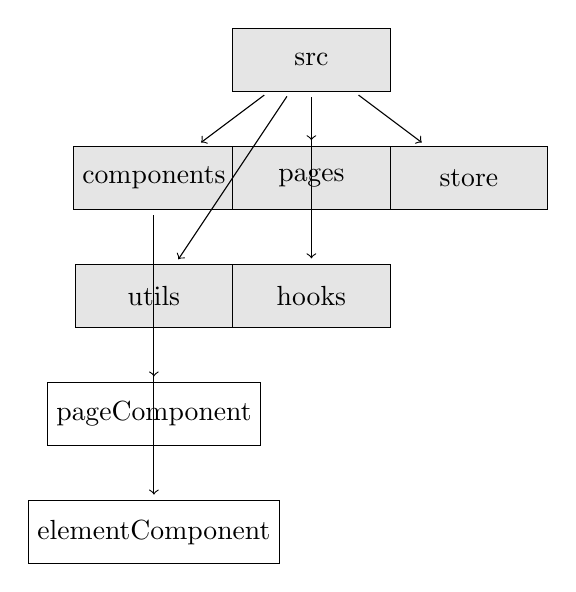
\begin{tikzpicture}[
    file/.style={draw, rectangle, minimum width=2cm, minimum height=0.8cm},
    folder/.style={draw, rectangle, minimum width=2cm, minimum height=0.8cm, fill=gray!20},
    arrow/.style={->, shorten >=2pt, shorten <=2pt}
]

% Folders
\node[folder] (src) at (0,0) {src};
\node[folder] (components) at (-2,-1.5) {components};
\node[folder] (pages) at (0,-1.5) {pages};
\node[folder] (store) at (2,-1.5) {store};
\node[folder] (utils) at (-2,-3) {utils};
\node[folder] (hooks) at (0,-3) {hooks};

% Files
\node[file] (pageComponent) at (-2,-4.5) {pageComponent};
\node[file] (elementComponent) at (-2,-6) {elementComponent};
% ... add more files

% Connections
\draw[arrow] (src) -- (components);
\draw[arrow] (src) -- (pages);
\draw[arrow] (src) -- (store);
\draw[arrow] (src) -- (utils);
\draw[arrow] (src) -- (hooks);
\draw[arrow] (components) -- (pageComponent);
\draw[arrow] (components) -- (elementComponent);
% ... add more connections

\end{tikzpicture}



\pagebreak
\subsubsection{Back-end}
The backend uses the dotNet framework. The development language using the C\# language.

In this project, the backend uses the Onion Architecture.
The Onion Architecture is a typically layered architecture, 
where each layer depends on the inner layer and provides interfaces to the outer layer.
The outer layer provides services to the outermost layer 
and other modules in the same layer based on the interfaces of the inner layer.

From inner to outer, the layers are: Domain, Application, Infrastructure, Presentation.
The Domain layer is the core layer and the innermost layer, used to define domain models, 
which are the business models.
It includes domain models and domain service interfaces.
Domain models are used to define the business models, 
which are the entities in the entity-relationship model and their attributes.
Domain service interfaces are used to define the business services, 
which are the relationships between entities in the entity-relationship model.

The Application layer is the application layer, 
used to define application services, which are the business logic.
It includes domain service implementations and application service interfaces.
Domain service implementations implement the methods of the inner layer's domain service 
interfaces and implement the business logic of the domain models.
Application service interfaces are used to define application services, 
which are the business logic.
It includes but is not limited to database interfaces, testing interfaces, 
HTTP API interfaces, MQTT interfaces, etc.

The Infrastructure layer is the infrastructure layer, used to define infrastructure.
It includes database implementations, testing implementations, 
HTTP API implementations, MQTT implementations, etc.
Database implementations implement the database interfaces 
and provide CRUD services for the database.
Testing implementations implement the testing interfaces 
and provide services for unit testing and integration testing.
HTTP API implementations implement the HTTP API interfaces 
and provide CRUD operations for HTTP APIs.
MQTT implementations implement the MQTT interfaces 
and provide CRUD operations for MQTT.

The Presentation layer is the presentation layer, used to define presentation logic, 
such as interfaces and pages. Since this is a backend project,
data presentation and control are handled by the frontend, 
so this layer is not needed.



\pagebreak
\subsubsection{Data communication and storage}
% 关于本项目的数据通信与数据存储的设计, 包括数据通信的协议, 数据存储的设计等
% 关于数据通信的设计:
% 1. 通信协议的选择
% 自前端向后端发送的数据, 有三种传输的数据类型, 
% 一种是普通的增删改查的请求, 对数据传输的时效性要求不高, 但是对数据的准确性, 完整性, 有序性, 安全性有一定的要求,
% 这种数据的传输, 采用 HTTP 协议, 以及 RESTful API 的设计. 可以有效的保证对数据传输的以上要求.
% 一种是对数据通道的创建和流媒体数据的传输, 对数据传输的时效性, 安全性要求较高, 这种数据的传输, 采用 WebRTC 协议, 以及 MQTT 协议.
% 配合可以快速解码的 flatbuffers 协议, 可以有效的保证对数据传输的以上要求.
% 最后一种是对设备的状态信息和操作信息的传输, 对完整性, 有序性, 安全性都有较高的要求, 这种数据的传输, 采用 MQTT 协议
% 同时也使用了 flatbuffers 协议.
% 
% 2. 数据通信的通信架构和通信流程
% 本项目的数据通信的通信架构, 是基于前后端分离的架构, 前端使用 React 框架, 后端使用 dotnet 框架.
% 当前端需要向后端发送数据的时候, 前端会向后端发送 HTTP 请求, 后端接收到 HTTP 请求之后, 会根据请求的数据类型,
% 选择不同的数据处理方式, 对于普通的增删改查的请求, 后端会根据 RESTful API 的设计, 对数据进行增删改查的操作,
% 对于对数据通道的创建和流媒体数据的传输, 后端会根据 WebRTC 协议, 对数据通道进行创建, 并且帮助前端和设备建立数据通道,
% 当数据通道建立后, 前端和设备之间则使用 flatbuffer 的数据格式对流媒体数据进行传输,
% 对于设备的状态信息和操作信息的传输, 前端会直接向 MQTT broker 发送 MQTT 请求, 
% 设备会在其自身的固件中监听相关的 MQTT 请求, 并且返回相关的数据.
% 
% 3. 数据通信的格式
% 本项目的数据通信的格式, 有三种, 
% 一种是 HTTP 协议, 
% 使用 json 格式对数据进行传输,
% 一种是 WebRTC 协议, 
% 使用 flatbuffers 格式对数据进行传输,
% 一种是 MQTT 协议.
% 使用 flatbuffers 格式对数据进行传输,
% 
% 关于数据存储的设计:
% 1. 数据存储的数据库的选择
% 本项目的数据存储的数据库的选择, 使用了轻量级的数据库 SQLite,
% SQLite 是一个进程内的库, 实现了自给自足的, 无服务器的, 零配置的, 事务性的 SQL 数据库引擎.
% 这是因为整个项目的目的是为了实现前端与设备之间的数据通信, 对于数据库数据的增删改查操作的要求不高,
% 数据量较小, 且对于数据库的数据的事务性要求不高, 所以选择了 SQLite 数据库.
% 2. 项目前后端的数据结构的设计
% 在本项目中, 前端由于使用了 React 框架, 所以前端的数据结构的设计, 使用了基于状态的数据结构的设计,
% 每个组件或者数据集都包含一个状态对象, 这个状态对象的属性就是组件的各个状态. 
% 使用状态对象的原因是, 可以方便的对状态进行管理, 采用对象-属性的形式, 可以方便的针对不同组件的同类状态进行区分,
% 由于跨组件的状态是由 redux 进行管理的, 这种状态对象的设计, 可以更搞笑的对状态进行更新和传递.
% 后端由于使用了 dotnet 框架, 所以后端的数据结构的设计, 使用了基于类的数据结构的设计,
% 采用了面向对象的编程思想, 对数据进行了封装, 使得数据的传输更加的安全, 有序, 完整.


\pagebreak

% \subsection{Domain model}
% \documentclass[]{article}
\usepackage{graphicx}
\usepackage{amsmath}
\usepackage{tikz}

% libaries
\usetikzlibrary{shapes,arrows}

%Define the listing package
\usepackage{listings} %code highlighter
\usepackage{color} %use color
\definecolor{mygreen}{rgb}{0,0.6,0}
\definecolor{mygray}{rgb}{0.5,0.5,0.5}
\definecolor{mymauve}{rgb}{0.58,0,0.82}

%Customize a bit the look
\lstset{ %
backgroundcolor=\color{white}, % choose the background color; you must add \usepackage{color} or \usepackage{xcolor}
basicstyle=\footnotesize, % the size of the fonts that are used for the code
breakatwhitespace=false, % sets if automatic breaks should only happen at whitespace
breaklines=true, % sets automatic line breaking
captionpos=b, % sets the caption-position to bottom
commentstyle=\color{mygreen}, % comment style
deletekeywords={...}, % if you want to delete keywords from the given language
escapeinside={\%*}{*)}, % if you want to add LaTeX within your code
extendedchars=true, % lets you use non-ASCII characters; for 8-bits encodings only, does not work with UTF-8
frame=single, % adds a frame around the code
keepspaces=true, % keeps spaces in text, useful for keeping indentation of code (possibly needs columns=flexible)
keywordstyle=\color{blue}, % keyword style
% language=Octave, % the language of the code
morekeywords={*,...}, % if you want to add more keywords to the set
numbers=left, % where to put the line-numbers; possible values are (none, left, right)
numbersep=5pt, % how far the line-numbers are from the code
numberstyle=\tiny\color{mygray}, % the style that is used for the line-numbers
rulecolor=\color{black}, % if not set, the frame-color may be changed on line-breaks within not-black text (e.g. comments (green here))
showspaces=false, % show spaces everywhere adding particular underscores; it overrides 'showstringspaces'
showstringspaces=false, % underline spaces within strings only
showtabs=false, % show tabs within strings adding particular underscores
stepnumber=1, % the step between two line-numbers. If it's 1, each line will be numbered
stringstyle=\color{mymauve}, % string literal style
tabsize=2, % sets default tabsize to 2 spaces
title=\lstname % show the filename of files included with \lstinputlisting; also try caption instead of title
}

\definecolor{darkgray}{rgb}{.4,.4,.4}
\definecolor{purple}{rgb}{0.65, 0.12, 0.82}

\lstdefinelanguage{React}{
keywords={const, typeof, new, true, false, catch, function, return, null, catch, switch, var, if, in, while, do, else, case, break},
keywordstyle=\color{blue}\bfseries,
ndkeywords={class, export, boolean, throw, implements, import, this},
ndkeywordstyle=\color{darkgray}\bfseries,
identifierstyle=\color{mygreen},
sensitive=false,
comment=[l]{//},
morecomment=[s]{/*}{*/},
commentstyle=\color{purple}\ttfamily,
string=[b]{"}{'}{`},
stringstyle=\color{red}\ttfamily,
morestring=[b]',
morestring=[b]",
morestring=[b]`',
}

\lstdefinelanguage{CSharp}{
keywords={const, typeof, new, true, false, catch, function, return, null, catch, switch, var, if, in, while, do, else, case, break},
keywordstyle=\color{blue}\bfseries,
ndkeywords={class, export, boolean, throw, implements, import, this},
ndkeywordstyle=\color{darkgray}\bfseries,
identifierstyle=\color{mygreen},
sensitive=false,
comment=[l]{//},
morecomment=[s]{/*}{*/},
commentstyle=\color{purple}\ttfamily,
string=[b]{"}{'}{`},
stringstyle=\color{red}\ttfamily,
morestring=[b]',
morestring=[b]",
morestring=[b]`',
}

\lstset{
language=React,
extendedchars=true,
basicstyle=\footnotesize\ttfamily,
showstringspaces=false,
showspaces=false,
numbers=left,
numberstyle=\footnotesize,
numbersep=9pt,
tabsize=2,
breaklines=true,
showtabs=false,
captionpos=b
}

\lstset{
language=CSharp,
extendedchars=true,
basicstyle=\footnotesize\ttfamily,
showstringspaces=false,
showspaces=false,
numbers=left,
numberstyle=\footnotesize,
numbersep=9pt,
tabsize=2,
breaklines=true,
showtabs=false,
captionpos=b
}

% \usepackage{cite} % Add this line for citation

% \bibliographystyle{plain}

\title{
The implementation of BifrostConnect Front-end scope, 
re-design and development with the relevant back-end support develop.
}
\author{
    Fei Gu \\
    Erhvervs Akademi Sydvest \\
    Computer Science 21\\
    }
\date{\today}

\begin{document}

% Front page
\maketitle
\begin{center}
    Supervisor: Henrik Boulund Meng Hansen \\
    Company: BifrostConnect \\
    Engineering Director: Jasper Wass \\
\end{center}
\tableofcontents
\pagebreak


% The introduction
\section{Introduction}
\subsection{Background}\input{sections/introduction/background.tex}
\subsection{The company}\input{sections/introduction/aboutCompany}
\subsection{The project}\input{sections/introduction/aboutProject}
\pagebreak

% The problem statement
\section{Problem Statement}
\subsection{Statement}
\input{sections/problemStatement/statement}
\subsection{Situation}
\input{sections/problemStatement/situation}
\subsection{Potential Solution}
\input{sections/problemStatement/potentialSolution}
\pagebreak

% Requirement analysis
\section{Requirement Analysis}
\input{sections/requirementAnalysis/index}

\subsection{Stakeholders}
\input{sections/requirementAnalysis/stakeholders/index}

\subsection{Business Domain}
\input{sections/requirementAnalysis/bussinesDomain/index}

\subsection{Scope}
\input{sections/requirementAnalysis/scope}

\subsection{Goals}
\input{sections/requirementAnalysis/goals}
\pagebreak

% Software Design
\section{Software Design}
% developement methods
\subsection{Software Development Methods}
\input{sections/softwareDevelopmentMethods/index}
\subsubsection{Agile Software Development}
\input{sections/softwareDevelopmentMethods/agileSoftwareDevelopment/index}
\subsubsection{Feature Driven Development}
\input{sections/softwareDevelopmentMethods/featureDrivenDevelopment/index}

\pagebreak

% Technology seslection
\subsection{Technology selection}
\input{sections/softwareDesign/technologySelection/index}
\subsubsection{Front-end}
\input{sections/softwareDesign/technologySelection/frontEnd}            
\subsubsection{Back-end}
\input{sections/softwareDesign/technologySelection/backEnd}            
\subsubsection{Database}
\input{sections/softwareDesign/technologySelection/database}
\subsubsection{Data communication}
\input{sections/softwareDesign/technologySelection/dataCommunication}            
\subsubsection{DevOps}
\input{sections/softwareDesign/technologySelection/devOps}
\pagebreak

% Architecture design
\subsection{Architecture design}
\input{sections/softwareDesign/architectureDesign/index}
\pagebreak
\subsubsection{Front-end}
\input{sections/softwareDesign/architectureDesign/frontEndArchitecture}
\pagebreak
\subsubsection{Back-end}
\input{sections/softwareDesign/architectureDesign/backEndArchitecture}
\pagebreak
\subsubsection{Data communication and storage}
\input{sections/softwareDesign/architectureDesign/dataCommunicationArchitecture}
\pagebreak

% \subsection{Domain model}
% \input{sections/softwareDesign/domainModel/index}
% \subsection{Database design}
% % 数据库领域模型 ER 图
% % 包括表和字段的设置.
% % 对于私有键和外键的设置.

% \subsection{Back-end design}
% % 后端对象模型
% % 以及对于对象模型的增删改查
% % 以及相关的其他服务的设计`'

% \subsection{Front-end design}
% % 对于前端的页面结构的设计 
% % 页面的状态的设计, 交互设计

% \subsection{FlatBuffers design}
% % schema 的设计

\subsection{DevOps CI/CD process design}
\input{sections/softwareDesign/devOpsDesign/index}
\subsubsection{Continuous Integration}
\input{sections/softwareDesign/devOpsDesign/continuousIntegration/index}
\subsubsection{Continuous Delivery}
\input{sections/softwareDesign/devOpsDesign/continuousDelivery/index}
\subsubsection{Continuous Deployment}
\input{sections/softwareDesign/devOpsDesign/continuousDeployment/index}
\pagebreak

\section{Software Development} 
\input{sections/softwareDevelopment/index}
\subsection{Overall development}
\input{sections/softwareDevelopment/overallDevelopement/index}
\subsubsection{Front-end}
\input{sections/softwareDevelopment/overallDevelopement/frontEnd/index}
\subsubsection{Back-end}
\input{sections/softwareDevelopment/overallDevelopement/backEnd/index}
\subsubsection{DevOps}
\input{sections/softwareDevelopment/overallDevelopement/devOps/index}
\subsection{Feature development} 
\input{sections/softwareDevelopment/featureDevelopment/index}
\subsubsection{Use Case 1}
\input{sections/softwareDevelopment/featureDevelopment/useCase1/index}
\subsubsection{Feature 1}
\input{sections/softwareDevelopment/featureDevelopment/feature/feature1.tex}
\pagebreak
\section{Conclusion} 
\subsection{Result}
Since the project is still in progress, the result is not available yet.
So far, basic structure of this project has been built. But the most features 
are not implemented yet. 
\subsection{Discussion}
As a single developer for this project, I am confident what I have done so far.
And I can say I understand the most of the knowledge I have used in this project, 
which also means I can explain all the part of the project. 
But this project also relevant some of the complex knowledge which I have to continue 
to study and practice.
\subsection{Future Work}
The future work is to implement the rest of the features. 
Including the most important part which is the 'create session' feature.
\pagebreak
% \bibliography{bibliography}
\pagebreak
% \begin{appendices}
%     \section{Appendix}
% \end{appendices} 
\end{document}
% \subsection{Database design}
% % 数据库领域模型 ER 图
% % 包括表和字段的设置.
% % 对于私有键和外键的设置.

% \subsection{Back-end design}
% % 后端对象模型
% % 以及对于对象模型的增删改查
% % 以及相关的其他服务的设计`'

% \subsection{Front-end design}
% % 对于前端的页面结构的设计 
% % 页面的状态的设计, 交互设计

% \subsection{FlatBuffers design}
% % schema 的设计

\subsection{DevOps CI/CD process design}
\documentclass[]{article}
\usepackage{graphicx}
\usepackage{amsmath}
\usepackage{tikz}

% libaries
\usetikzlibrary{shapes,arrows}

%Define the listing package
\usepackage{listings} %code highlighter
\usepackage{color} %use color
\definecolor{mygreen}{rgb}{0,0.6,0}
\definecolor{mygray}{rgb}{0.5,0.5,0.5}
\definecolor{mymauve}{rgb}{0.58,0,0.82}

%Customize a bit the look
\lstset{ %
backgroundcolor=\color{white}, % choose the background color; you must add \usepackage{color} or \usepackage{xcolor}
basicstyle=\footnotesize, % the size of the fonts that are used for the code
breakatwhitespace=false, % sets if automatic breaks should only happen at whitespace
breaklines=true, % sets automatic line breaking
captionpos=b, % sets the caption-position to bottom
commentstyle=\color{mygreen}, % comment style
deletekeywords={...}, % if you want to delete keywords from the given language
escapeinside={\%*}{*)}, % if you want to add LaTeX within your code
extendedchars=true, % lets you use non-ASCII characters; for 8-bits encodings only, does not work with UTF-8
frame=single, % adds a frame around the code
keepspaces=true, % keeps spaces in text, useful for keeping indentation of code (possibly needs columns=flexible)
keywordstyle=\color{blue}, % keyword style
% language=Octave, % the language of the code
morekeywords={*,...}, % if you want to add more keywords to the set
numbers=left, % where to put the line-numbers; possible values are (none, left, right)
numbersep=5pt, % how far the line-numbers are from the code
numberstyle=\tiny\color{mygray}, % the style that is used for the line-numbers
rulecolor=\color{black}, % if not set, the frame-color may be changed on line-breaks within not-black text (e.g. comments (green here))
showspaces=false, % show spaces everywhere adding particular underscores; it overrides 'showstringspaces'
showstringspaces=false, % underline spaces within strings only
showtabs=false, % show tabs within strings adding particular underscores
stepnumber=1, % the step between two line-numbers. If it's 1, each line will be numbered
stringstyle=\color{mymauve}, % string literal style
tabsize=2, % sets default tabsize to 2 spaces
title=\lstname % show the filename of files included with \lstinputlisting; also try caption instead of title
}

\definecolor{darkgray}{rgb}{.4,.4,.4}
\definecolor{purple}{rgb}{0.65, 0.12, 0.82}

\lstdefinelanguage{React}{
keywords={const, typeof, new, true, false, catch, function, return, null, catch, switch, var, if, in, while, do, else, case, break},
keywordstyle=\color{blue}\bfseries,
ndkeywords={class, export, boolean, throw, implements, import, this},
ndkeywordstyle=\color{darkgray}\bfseries,
identifierstyle=\color{mygreen},
sensitive=false,
comment=[l]{//},
morecomment=[s]{/*}{*/},
commentstyle=\color{purple}\ttfamily,
string=[b]{"}{'}{`},
stringstyle=\color{red}\ttfamily,
morestring=[b]',
morestring=[b]",
morestring=[b]`',
}

\lstdefinelanguage{CSharp}{
keywords={const, typeof, new, true, false, catch, function, return, null, catch, switch, var, if, in, while, do, else, case, break},
keywordstyle=\color{blue}\bfseries,
ndkeywords={class, export, boolean, throw, implements, import, this},
ndkeywordstyle=\color{darkgray}\bfseries,
identifierstyle=\color{mygreen},
sensitive=false,
comment=[l]{//},
morecomment=[s]{/*}{*/},
commentstyle=\color{purple}\ttfamily,
string=[b]{"}{'}{`},
stringstyle=\color{red}\ttfamily,
morestring=[b]',
morestring=[b]",
morestring=[b]`',
}

\lstset{
language=React,
extendedchars=true,
basicstyle=\footnotesize\ttfamily,
showstringspaces=false,
showspaces=false,
numbers=left,
numberstyle=\footnotesize,
numbersep=9pt,
tabsize=2,
breaklines=true,
showtabs=false,
captionpos=b
}

\lstset{
language=CSharp,
extendedchars=true,
basicstyle=\footnotesize\ttfamily,
showstringspaces=false,
showspaces=false,
numbers=left,
numberstyle=\footnotesize,
numbersep=9pt,
tabsize=2,
breaklines=true,
showtabs=false,
captionpos=b
}

% \usepackage{cite} % Add this line for citation

% \bibliographystyle{plain}

\title{
The implementation of BifrostConnect Front-end scope, 
re-design and development with the relevant back-end support develop.
}
\author{
    Fei Gu \\
    Erhvervs Akademi Sydvest \\
    Computer Science 21\\
    }
\date{\today}

\begin{document}

% Front page
\maketitle
\begin{center}
    Supervisor: Henrik Boulund Meng Hansen \\
    Company: BifrostConnect \\
    Engineering Director: Jasper Wass \\
\end{center}
\tableofcontents
\pagebreak


% The introduction
\section{Introduction}
\subsection{Background}\input{sections/introduction/background.tex}
\subsection{The company}\input{sections/introduction/aboutCompany}
\subsection{The project}\input{sections/introduction/aboutProject}
\pagebreak

% The problem statement
\section{Problem Statement}
\subsection{Statement}
\input{sections/problemStatement/statement}
\subsection{Situation}
\input{sections/problemStatement/situation}
\subsection{Potential Solution}
\input{sections/problemStatement/potentialSolution}
\pagebreak

% Requirement analysis
\section{Requirement Analysis}
\input{sections/requirementAnalysis/index}

\subsection{Stakeholders}
\input{sections/requirementAnalysis/stakeholders/index}

\subsection{Business Domain}
\input{sections/requirementAnalysis/bussinesDomain/index}

\subsection{Scope}
\input{sections/requirementAnalysis/scope}

\subsection{Goals}
\input{sections/requirementAnalysis/goals}
\pagebreak

% Software Design
\section{Software Design}
% developement methods
\subsection{Software Development Methods}
\input{sections/softwareDevelopmentMethods/index}
\subsubsection{Agile Software Development}
\input{sections/softwareDevelopmentMethods/agileSoftwareDevelopment/index}
\subsubsection{Feature Driven Development}
\input{sections/softwareDevelopmentMethods/featureDrivenDevelopment/index}

\pagebreak

% Technology seslection
\subsection{Technology selection}
\input{sections/softwareDesign/technologySelection/index}
\subsubsection{Front-end}
\input{sections/softwareDesign/technologySelection/frontEnd}            
\subsubsection{Back-end}
\input{sections/softwareDesign/technologySelection/backEnd}            
\subsubsection{Database}
\input{sections/softwareDesign/technologySelection/database}
\subsubsection{Data communication}
\input{sections/softwareDesign/technologySelection/dataCommunication}            
\subsubsection{DevOps}
\input{sections/softwareDesign/technologySelection/devOps}
\pagebreak

% Architecture design
\subsection{Architecture design}
\input{sections/softwareDesign/architectureDesign/index}
\pagebreak
\subsubsection{Front-end}
\input{sections/softwareDesign/architectureDesign/frontEndArchitecture}
\pagebreak
\subsubsection{Back-end}
\input{sections/softwareDesign/architectureDesign/backEndArchitecture}
\pagebreak
\subsubsection{Data communication and storage}
\input{sections/softwareDesign/architectureDesign/dataCommunicationArchitecture}
\pagebreak

% \subsection{Domain model}
% \input{sections/softwareDesign/domainModel/index}
% \subsection{Database design}
% % 数据库领域模型 ER 图
% % 包括表和字段的设置.
% % 对于私有键和外键的设置.

% \subsection{Back-end design}
% % 后端对象模型
% % 以及对于对象模型的增删改查
% % 以及相关的其他服务的设计`'

% \subsection{Front-end design}
% % 对于前端的页面结构的设计 
% % 页面的状态的设计, 交互设计

% \subsection{FlatBuffers design}
% % schema 的设计

\subsection{DevOps CI/CD process design}
\input{sections/softwareDesign/devOpsDesign/index}
\subsubsection{Continuous Integration}
\input{sections/softwareDesign/devOpsDesign/continuousIntegration/index}
\subsubsection{Continuous Delivery}
\input{sections/softwareDesign/devOpsDesign/continuousDelivery/index}
\subsubsection{Continuous Deployment}
\input{sections/softwareDesign/devOpsDesign/continuousDeployment/index}
\pagebreak

\section{Software Development} 
\input{sections/softwareDevelopment/index}
\subsection{Overall development}
\input{sections/softwareDevelopment/overallDevelopement/index}
\subsubsection{Front-end}
\input{sections/softwareDevelopment/overallDevelopement/frontEnd/index}
\subsubsection{Back-end}
\input{sections/softwareDevelopment/overallDevelopement/backEnd/index}
\subsubsection{DevOps}
\input{sections/softwareDevelopment/overallDevelopement/devOps/index}
\subsection{Feature development} 
\input{sections/softwareDevelopment/featureDevelopment/index}
\subsubsection{Use Case 1}
\input{sections/softwareDevelopment/featureDevelopment/useCase1/index}
\subsubsection{Feature 1}
\input{sections/softwareDevelopment/featureDevelopment/feature/feature1.tex}
\pagebreak
\section{Conclusion} 
\subsection{Result}
Since the project is still in progress, the result is not available yet.
So far, basic structure of this project has been built. But the most features 
are not implemented yet. 
\subsection{Discussion}
As a single developer for this project, I am confident what I have done so far.
And I can say I understand the most of the knowledge I have used in this project, 
which also means I can explain all the part of the project. 
But this project also relevant some of the complex knowledge which I have to continue 
to study and practice.
\subsection{Future Work}
The future work is to implement the rest of the features. 
Including the most important part which is the 'create session' feature.
\pagebreak
% \bibliography{bibliography}
\pagebreak
% \begin{appendices}
%     \section{Appendix}
% \end{appendices} 
\end{document}
\subsubsection{Continuous Integration}
\documentclass[]{article}
\usepackage{graphicx}
\usepackage{amsmath}
\usepackage{tikz}

% libaries
\usetikzlibrary{shapes,arrows}

%Define the listing package
\usepackage{listings} %code highlighter
\usepackage{color} %use color
\definecolor{mygreen}{rgb}{0,0.6,0}
\definecolor{mygray}{rgb}{0.5,0.5,0.5}
\definecolor{mymauve}{rgb}{0.58,0,0.82}

%Customize a bit the look
\lstset{ %
backgroundcolor=\color{white}, % choose the background color; you must add \usepackage{color} or \usepackage{xcolor}
basicstyle=\footnotesize, % the size of the fonts that are used for the code
breakatwhitespace=false, % sets if automatic breaks should only happen at whitespace
breaklines=true, % sets automatic line breaking
captionpos=b, % sets the caption-position to bottom
commentstyle=\color{mygreen}, % comment style
deletekeywords={...}, % if you want to delete keywords from the given language
escapeinside={\%*}{*)}, % if you want to add LaTeX within your code
extendedchars=true, % lets you use non-ASCII characters; for 8-bits encodings only, does not work with UTF-8
frame=single, % adds a frame around the code
keepspaces=true, % keeps spaces in text, useful for keeping indentation of code (possibly needs columns=flexible)
keywordstyle=\color{blue}, % keyword style
% language=Octave, % the language of the code
morekeywords={*,...}, % if you want to add more keywords to the set
numbers=left, % where to put the line-numbers; possible values are (none, left, right)
numbersep=5pt, % how far the line-numbers are from the code
numberstyle=\tiny\color{mygray}, % the style that is used for the line-numbers
rulecolor=\color{black}, % if not set, the frame-color may be changed on line-breaks within not-black text (e.g. comments (green here))
showspaces=false, % show spaces everywhere adding particular underscores; it overrides 'showstringspaces'
showstringspaces=false, % underline spaces within strings only
showtabs=false, % show tabs within strings adding particular underscores
stepnumber=1, % the step between two line-numbers. If it's 1, each line will be numbered
stringstyle=\color{mymauve}, % string literal style
tabsize=2, % sets default tabsize to 2 spaces
title=\lstname % show the filename of files included with \lstinputlisting; also try caption instead of title
}

\definecolor{darkgray}{rgb}{.4,.4,.4}
\definecolor{purple}{rgb}{0.65, 0.12, 0.82}

\lstdefinelanguage{React}{
keywords={const, typeof, new, true, false, catch, function, return, null, catch, switch, var, if, in, while, do, else, case, break},
keywordstyle=\color{blue}\bfseries,
ndkeywords={class, export, boolean, throw, implements, import, this},
ndkeywordstyle=\color{darkgray}\bfseries,
identifierstyle=\color{mygreen},
sensitive=false,
comment=[l]{//},
morecomment=[s]{/*}{*/},
commentstyle=\color{purple}\ttfamily,
string=[b]{"}{'}{`},
stringstyle=\color{red}\ttfamily,
morestring=[b]',
morestring=[b]",
morestring=[b]`',
}

\lstdefinelanguage{CSharp}{
keywords={const, typeof, new, true, false, catch, function, return, null, catch, switch, var, if, in, while, do, else, case, break},
keywordstyle=\color{blue}\bfseries,
ndkeywords={class, export, boolean, throw, implements, import, this},
ndkeywordstyle=\color{darkgray}\bfseries,
identifierstyle=\color{mygreen},
sensitive=false,
comment=[l]{//},
morecomment=[s]{/*}{*/},
commentstyle=\color{purple}\ttfamily,
string=[b]{"}{'}{`},
stringstyle=\color{red}\ttfamily,
morestring=[b]',
morestring=[b]",
morestring=[b]`',
}

\lstset{
language=React,
extendedchars=true,
basicstyle=\footnotesize\ttfamily,
showstringspaces=false,
showspaces=false,
numbers=left,
numberstyle=\footnotesize,
numbersep=9pt,
tabsize=2,
breaklines=true,
showtabs=false,
captionpos=b
}

\lstset{
language=CSharp,
extendedchars=true,
basicstyle=\footnotesize\ttfamily,
showstringspaces=false,
showspaces=false,
numbers=left,
numberstyle=\footnotesize,
numbersep=9pt,
tabsize=2,
breaklines=true,
showtabs=false,
captionpos=b
}

% \usepackage{cite} % Add this line for citation

% \bibliographystyle{plain}

\title{
The implementation of BifrostConnect Front-end scope, 
re-design and development with the relevant back-end support develop.
}
\author{
    Fei Gu \\
    Erhvervs Akademi Sydvest \\
    Computer Science 21\\
    }
\date{\today}

\begin{document}

% Front page
\maketitle
\begin{center}
    Supervisor: Henrik Boulund Meng Hansen \\
    Company: BifrostConnect \\
    Engineering Director: Jasper Wass \\
\end{center}
\tableofcontents
\pagebreak


% The introduction
\section{Introduction}
\subsection{Background}\input{sections/introduction/background.tex}
\subsection{The company}\input{sections/introduction/aboutCompany}
\subsection{The project}\input{sections/introduction/aboutProject}
\pagebreak

% The problem statement
\section{Problem Statement}
\subsection{Statement}
\input{sections/problemStatement/statement}
\subsection{Situation}
\input{sections/problemStatement/situation}
\subsection{Potential Solution}
\input{sections/problemStatement/potentialSolution}
\pagebreak

% Requirement analysis
\section{Requirement Analysis}
\input{sections/requirementAnalysis/index}

\subsection{Stakeholders}
\input{sections/requirementAnalysis/stakeholders/index}

\subsection{Business Domain}
\input{sections/requirementAnalysis/bussinesDomain/index}

\subsection{Scope}
\input{sections/requirementAnalysis/scope}

\subsection{Goals}
\input{sections/requirementAnalysis/goals}
\pagebreak

% Software Design
\section{Software Design}
% developement methods
\subsection{Software Development Methods}
\input{sections/softwareDevelopmentMethods/index}
\subsubsection{Agile Software Development}
\input{sections/softwareDevelopmentMethods/agileSoftwareDevelopment/index}
\subsubsection{Feature Driven Development}
\input{sections/softwareDevelopmentMethods/featureDrivenDevelopment/index}

\pagebreak

% Technology seslection
\subsection{Technology selection}
\input{sections/softwareDesign/technologySelection/index}
\subsubsection{Front-end}
\input{sections/softwareDesign/technologySelection/frontEnd}            
\subsubsection{Back-end}
\input{sections/softwareDesign/technologySelection/backEnd}            
\subsubsection{Database}
\input{sections/softwareDesign/technologySelection/database}
\subsubsection{Data communication}
\input{sections/softwareDesign/technologySelection/dataCommunication}            
\subsubsection{DevOps}
\input{sections/softwareDesign/technologySelection/devOps}
\pagebreak

% Architecture design
\subsection{Architecture design}
\input{sections/softwareDesign/architectureDesign/index}
\pagebreak
\subsubsection{Front-end}
\input{sections/softwareDesign/architectureDesign/frontEndArchitecture}
\pagebreak
\subsubsection{Back-end}
\input{sections/softwareDesign/architectureDesign/backEndArchitecture}
\pagebreak
\subsubsection{Data communication and storage}
\input{sections/softwareDesign/architectureDesign/dataCommunicationArchitecture}
\pagebreak

% \subsection{Domain model}
% \input{sections/softwareDesign/domainModel/index}
% \subsection{Database design}
% % 数据库领域模型 ER 图
% % 包括表和字段的设置.
% % 对于私有键和外键的设置.

% \subsection{Back-end design}
% % 后端对象模型
% % 以及对于对象模型的增删改查
% % 以及相关的其他服务的设计`'

% \subsection{Front-end design}
% % 对于前端的页面结构的设计 
% % 页面的状态的设计, 交互设计

% \subsection{FlatBuffers design}
% % schema 的设计

\subsection{DevOps CI/CD process design}
\input{sections/softwareDesign/devOpsDesign/index}
\subsubsection{Continuous Integration}
\input{sections/softwareDesign/devOpsDesign/continuousIntegration/index}
\subsubsection{Continuous Delivery}
\input{sections/softwareDesign/devOpsDesign/continuousDelivery/index}
\subsubsection{Continuous Deployment}
\input{sections/softwareDesign/devOpsDesign/continuousDeployment/index}
\pagebreak

\section{Software Development} 
\input{sections/softwareDevelopment/index}
\subsection{Overall development}
\input{sections/softwareDevelopment/overallDevelopement/index}
\subsubsection{Front-end}
\input{sections/softwareDevelopment/overallDevelopement/frontEnd/index}
\subsubsection{Back-end}
\input{sections/softwareDevelopment/overallDevelopement/backEnd/index}
\subsubsection{DevOps}
\input{sections/softwareDevelopment/overallDevelopement/devOps/index}
\subsection{Feature development} 
\input{sections/softwareDevelopment/featureDevelopment/index}
\subsubsection{Use Case 1}
\input{sections/softwareDevelopment/featureDevelopment/useCase1/index}
\subsubsection{Feature 1}
\input{sections/softwareDevelopment/featureDevelopment/feature/feature1.tex}
\pagebreak
\section{Conclusion} 
\subsection{Result}
Since the project is still in progress, the result is not available yet.
So far, basic structure of this project has been built. But the most features 
are not implemented yet. 
\subsection{Discussion}
As a single developer for this project, I am confident what I have done so far.
And I can say I understand the most of the knowledge I have used in this project, 
which also means I can explain all the part of the project. 
But this project also relevant some of the complex knowledge which I have to continue 
to study and practice.
\subsection{Future Work}
The future work is to implement the rest of the features. 
Including the most important part which is the 'create session' feature.
\pagebreak
% \bibliography{bibliography}
\pagebreak
% \begin{appendices}
%     \section{Appendix}
% \end{appendices} 
\end{document}
\subsubsection{Continuous Delivery}
\documentclass[]{article}
\usepackage{graphicx}
\usepackage{amsmath}
\usepackage{tikz}

% libaries
\usetikzlibrary{shapes,arrows}

%Define the listing package
\usepackage{listings} %code highlighter
\usepackage{color} %use color
\definecolor{mygreen}{rgb}{0,0.6,0}
\definecolor{mygray}{rgb}{0.5,0.5,0.5}
\definecolor{mymauve}{rgb}{0.58,0,0.82}

%Customize a bit the look
\lstset{ %
backgroundcolor=\color{white}, % choose the background color; you must add \usepackage{color} or \usepackage{xcolor}
basicstyle=\footnotesize, % the size of the fonts that are used for the code
breakatwhitespace=false, % sets if automatic breaks should only happen at whitespace
breaklines=true, % sets automatic line breaking
captionpos=b, % sets the caption-position to bottom
commentstyle=\color{mygreen}, % comment style
deletekeywords={...}, % if you want to delete keywords from the given language
escapeinside={\%*}{*)}, % if you want to add LaTeX within your code
extendedchars=true, % lets you use non-ASCII characters; for 8-bits encodings only, does not work with UTF-8
frame=single, % adds a frame around the code
keepspaces=true, % keeps spaces in text, useful for keeping indentation of code (possibly needs columns=flexible)
keywordstyle=\color{blue}, % keyword style
% language=Octave, % the language of the code
morekeywords={*,...}, % if you want to add more keywords to the set
numbers=left, % where to put the line-numbers; possible values are (none, left, right)
numbersep=5pt, % how far the line-numbers are from the code
numberstyle=\tiny\color{mygray}, % the style that is used for the line-numbers
rulecolor=\color{black}, % if not set, the frame-color may be changed on line-breaks within not-black text (e.g. comments (green here))
showspaces=false, % show spaces everywhere adding particular underscores; it overrides 'showstringspaces'
showstringspaces=false, % underline spaces within strings only
showtabs=false, % show tabs within strings adding particular underscores
stepnumber=1, % the step between two line-numbers. If it's 1, each line will be numbered
stringstyle=\color{mymauve}, % string literal style
tabsize=2, % sets default tabsize to 2 spaces
title=\lstname % show the filename of files included with \lstinputlisting; also try caption instead of title
}

\definecolor{darkgray}{rgb}{.4,.4,.4}
\definecolor{purple}{rgb}{0.65, 0.12, 0.82}

\lstdefinelanguage{React}{
keywords={const, typeof, new, true, false, catch, function, return, null, catch, switch, var, if, in, while, do, else, case, break},
keywordstyle=\color{blue}\bfseries,
ndkeywords={class, export, boolean, throw, implements, import, this},
ndkeywordstyle=\color{darkgray}\bfseries,
identifierstyle=\color{mygreen},
sensitive=false,
comment=[l]{//},
morecomment=[s]{/*}{*/},
commentstyle=\color{purple}\ttfamily,
string=[b]{"}{'}{`},
stringstyle=\color{red}\ttfamily,
morestring=[b]',
morestring=[b]",
morestring=[b]`',
}

\lstdefinelanguage{CSharp}{
keywords={const, typeof, new, true, false, catch, function, return, null, catch, switch, var, if, in, while, do, else, case, break},
keywordstyle=\color{blue}\bfseries,
ndkeywords={class, export, boolean, throw, implements, import, this},
ndkeywordstyle=\color{darkgray}\bfseries,
identifierstyle=\color{mygreen},
sensitive=false,
comment=[l]{//},
morecomment=[s]{/*}{*/},
commentstyle=\color{purple}\ttfamily,
string=[b]{"}{'}{`},
stringstyle=\color{red}\ttfamily,
morestring=[b]',
morestring=[b]",
morestring=[b]`',
}

\lstset{
language=React,
extendedchars=true,
basicstyle=\footnotesize\ttfamily,
showstringspaces=false,
showspaces=false,
numbers=left,
numberstyle=\footnotesize,
numbersep=9pt,
tabsize=2,
breaklines=true,
showtabs=false,
captionpos=b
}

\lstset{
language=CSharp,
extendedchars=true,
basicstyle=\footnotesize\ttfamily,
showstringspaces=false,
showspaces=false,
numbers=left,
numberstyle=\footnotesize,
numbersep=9pt,
tabsize=2,
breaklines=true,
showtabs=false,
captionpos=b
}

% \usepackage{cite} % Add this line for citation

% \bibliographystyle{plain}

\title{
The implementation of BifrostConnect Front-end scope, 
re-design and development with the relevant back-end support develop.
}
\author{
    Fei Gu \\
    Erhvervs Akademi Sydvest \\
    Computer Science 21\\
    }
\date{\today}

\begin{document}

% Front page
\maketitle
\begin{center}
    Supervisor: Henrik Boulund Meng Hansen \\
    Company: BifrostConnect \\
    Engineering Director: Jasper Wass \\
\end{center}
\tableofcontents
\pagebreak


% The introduction
\section{Introduction}
\subsection{Background}\input{sections/introduction/background.tex}
\subsection{The company}\input{sections/introduction/aboutCompany}
\subsection{The project}\input{sections/introduction/aboutProject}
\pagebreak

% The problem statement
\section{Problem Statement}
\subsection{Statement}
\input{sections/problemStatement/statement}
\subsection{Situation}
\input{sections/problemStatement/situation}
\subsection{Potential Solution}
\input{sections/problemStatement/potentialSolution}
\pagebreak

% Requirement analysis
\section{Requirement Analysis}
\input{sections/requirementAnalysis/index}

\subsection{Stakeholders}
\input{sections/requirementAnalysis/stakeholders/index}

\subsection{Business Domain}
\input{sections/requirementAnalysis/bussinesDomain/index}

\subsection{Scope}
\input{sections/requirementAnalysis/scope}

\subsection{Goals}
\input{sections/requirementAnalysis/goals}
\pagebreak

% Software Design
\section{Software Design}
% developement methods
\subsection{Software Development Methods}
\input{sections/softwareDevelopmentMethods/index}
\subsubsection{Agile Software Development}
\input{sections/softwareDevelopmentMethods/agileSoftwareDevelopment/index}
\subsubsection{Feature Driven Development}
\input{sections/softwareDevelopmentMethods/featureDrivenDevelopment/index}

\pagebreak

% Technology seslection
\subsection{Technology selection}
\input{sections/softwareDesign/technologySelection/index}
\subsubsection{Front-end}
\input{sections/softwareDesign/technologySelection/frontEnd}            
\subsubsection{Back-end}
\input{sections/softwareDesign/technologySelection/backEnd}            
\subsubsection{Database}
\input{sections/softwareDesign/technologySelection/database}
\subsubsection{Data communication}
\input{sections/softwareDesign/technologySelection/dataCommunication}            
\subsubsection{DevOps}
\input{sections/softwareDesign/technologySelection/devOps}
\pagebreak

% Architecture design
\subsection{Architecture design}
\input{sections/softwareDesign/architectureDesign/index}
\pagebreak
\subsubsection{Front-end}
\input{sections/softwareDesign/architectureDesign/frontEndArchitecture}
\pagebreak
\subsubsection{Back-end}
\input{sections/softwareDesign/architectureDesign/backEndArchitecture}
\pagebreak
\subsubsection{Data communication and storage}
\input{sections/softwareDesign/architectureDesign/dataCommunicationArchitecture}
\pagebreak

% \subsection{Domain model}
% \input{sections/softwareDesign/domainModel/index}
% \subsection{Database design}
% % 数据库领域模型 ER 图
% % 包括表和字段的设置.
% % 对于私有键和外键的设置.

% \subsection{Back-end design}
% % 后端对象模型
% % 以及对于对象模型的增删改查
% % 以及相关的其他服务的设计`'

% \subsection{Front-end design}
% % 对于前端的页面结构的设计 
% % 页面的状态的设计, 交互设计

% \subsection{FlatBuffers design}
% % schema 的设计

\subsection{DevOps CI/CD process design}
\input{sections/softwareDesign/devOpsDesign/index}
\subsubsection{Continuous Integration}
\input{sections/softwareDesign/devOpsDesign/continuousIntegration/index}
\subsubsection{Continuous Delivery}
\input{sections/softwareDesign/devOpsDesign/continuousDelivery/index}
\subsubsection{Continuous Deployment}
\input{sections/softwareDesign/devOpsDesign/continuousDeployment/index}
\pagebreak

\section{Software Development} 
\input{sections/softwareDevelopment/index}
\subsection{Overall development}
\input{sections/softwareDevelopment/overallDevelopement/index}
\subsubsection{Front-end}
\input{sections/softwareDevelopment/overallDevelopement/frontEnd/index}
\subsubsection{Back-end}
\input{sections/softwareDevelopment/overallDevelopement/backEnd/index}
\subsubsection{DevOps}
\input{sections/softwareDevelopment/overallDevelopement/devOps/index}
\subsection{Feature development} 
\input{sections/softwareDevelopment/featureDevelopment/index}
\subsubsection{Use Case 1}
\input{sections/softwareDevelopment/featureDevelopment/useCase1/index}
\subsubsection{Feature 1}
\input{sections/softwareDevelopment/featureDevelopment/feature/feature1.tex}
\pagebreak
\section{Conclusion} 
\subsection{Result}
Since the project is still in progress, the result is not available yet.
So far, basic structure of this project has been built. But the most features 
are not implemented yet. 
\subsection{Discussion}
As a single developer for this project, I am confident what I have done so far.
And I can say I understand the most of the knowledge I have used in this project, 
which also means I can explain all the part of the project. 
But this project also relevant some of the complex knowledge which I have to continue 
to study and practice.
\subsection{Future Work}
The future work is to implement the rest of the features. 
Including the most important part which is the 'create session' feature.
\pagebreak
% \bibliography{bibliography}
\pagebreak
% \begin{appendices}
%     \section{Appendix}
% \end{appendices} 
\end{document}
\subsubsection{Continuous Deployment}
\documentclass[]{article}
\usepackage{graphicx}
\usepackage{amsmath}
\usepackage{tikz}

% libaries
\usetikzlibrary{shapes,arrows}

%Define the listing package
\usepackage{listings} %code highlighter
\usepackage{color} %use color
\definecolor{mygreen}{rgb}{0,0.6,0}
\definecolor{mygray}{rgb}{0.5,0.5,0.5}
\definecolor{mymauve}{rgb}{0.58,0,0.82}

%Customize a bit the look
\lstset{ %
backgroundcolor=\color{white}, % choose the background color; you must add \usepackage{color} or \usepackage{xcolor}
basicstyle=\footnotesize, % the size of the fonts that are used for the code
breakatwhitespace=false, % sets if automatic breaks should only happen at whitespace
breaklines=true, % sets automatic line breaking
captionpos=b, % sets the caption-position to bottom
commentstyle=\color{mygreen}, % comment style
deletekeywords={...}, % if you want to delete keywords from the given language
escapeinside={\%*}{*)}, % if you want to add LaTeX within your code
extendedchars=true, % lets you use non-ASCII characters; for 8-bits encodings only, does not work with UTF-8
frame=single, % adds a frame around the code
keepspaces=true, % keeps spaces in text, useful for keeping indentation of code (possibly needs columns=flexible)
keywordstyle=\color{blue}, % keyword style
% language=Octave, % the language of the code
morekeywords={*,...}, % if you want to add more keywords to the set
numbers=left, % where to put the line-numbers; possible values are (none, left, right)
numbersep=5pt, % how far the line-numbers are from the code
numberstyle=\tiny\color{mygray}, % the style that is used for the line-numbers
rulecolor=\color{black}, % if not set, the frame-color may be changed on line-breaks within not-black text (e.g. comments (green here))
showspaces=false, % show spaces everywhere adding particular underscores; it overrides 'showstringspaces'
showstringspaces=false, % underline spaces within strings only
showtabs=false, % show tabs within strings adding particular underscores
stepnumber=1, % the step between two line-numbers. If it's 1, each line will be numbered
stringstyle=\color{mymauve}, % string literal style
tabsize=2, % sets default tabsize to 2 spaces
title=\lstname % show the filename of files included with \lstinputlisting; also try caption instead of title
}

\definecolor{darkgray}{rgb}{.4,.4,.4}
\definecolor{purple}{rgb}{0.65, 0.12, 0.82}

\lstdefinelanguage{React}{
keywords={const, typeof, new, true, false, catch, function, return, null, catch, switch, var, if, in, while, do, else, case, break},
keywordstyle=\color{blue}\bfseries,
ndkeywords={class, export, boolean, throw, implements, import, this},
ndkeywordstyle=\color{darkgray}\bfseries,
identifierstyle=\color{mygreen},
sensitive=false,
comment=[l]{//},
morecomment=[s]{/*}{*/},
commentstyle=\color{purple}\ttfamily,
string=[b]{"}{'}{`},
stringstyle=\color{red}\ttfamily,
morestring=[b]',
morestring=[b]",
morestring=[b]`',
}

\lstdefinelanguage{CSharp}{
keywords={const, typeof, new, true, false, catch, function, return, null, catch, switch, var, if, in, while, do, else, case, break},
keywordstyle=\color{blue}\bfseries,
ndkeywords={class, export, boolean, throw, implements, import, this},
ndkeywordstyle=\color{darkgray}\bfseries,
identifierstyle=\color{mygreen},
sensitive=false,
comment=[l]{//},
morecomment=[s]{/*}{*/},
commentstyle=\color{purple}\ttfamily,
string=[b]{"}{'}{`},
stringstyle=\color{red}\ttfamily,
morestring=[b]',
morestring=[b]",
morestring=[b]`',
}

\lstset{
language=React,
extendedchars=true,
basicstyle=\footnotesize\ttfamily,
showstringspaces=false,
showspaces=false,
numbers=left,
numberstyle=\footnotesize,
numbersep=9pt,
tabsize=2,
breaklines=true,
showtabs=false,
captionpos=b
}

\lstset{
language=CSharp,
extendedchars=true,
basicstyle=\footnotesize\ttfamily,
showstringspaces=false,
showspaces=false,
numbers=left,
numberstyle=\footnotesize,
numbersep=9pt,
tabsize=2,
breaklines=true,
showtabs=false,
captionpos=b
}

% \usepackage{cite} % Add this line for citation

% \bibliographystyle{plain}

\title{
The implementation of BifrostConnect Front-end scope, 
re-design and development with the relevant back-end support develop.
}
\author{
    Fei Gu \\
    Erhvervs Akademi Sydvest \\
    Computer Science 21\\
    }
\date{\today}

\begin{document}

% Front page
\maketitle
\begin{center}
    Supervisor: Henrik Boulund Meng Hansen \\
    Company: BifrostConnect \\
    Engineering Director: Jasper Wass \\
\end{center}
\tableofcontents
\pagebreak


% The introduction
\section{Introduction}
\subsection{Background}\input{sections/introduction/background.tex}
\subsection{The company}\input{sections/introduction/aboutCompany}
\subsection{The project}\input{sections/introduction/aboutProject}
\pagebreak

% The problem statement
\section{Problem Statement}
\subsection{Statement}
\input{sections/problemStatement/statement}
\subsection{Situation}
\input{sections/problemStatement/situation}
\subsection{Potential Solution}
\input{sections/problemStatement/potentialSolution}
\pagebreak

% Requirement analysis
\section{Requirement Analysis}
\input{sections/requirementAnalysis/index}

\subsection{Stakeholders}
\input{sections/requirementAnalysis/stakeholders/index}

\subsection{Business Domain}
\input{sections/requirementAnalysis/bussinesDomain/index}

\subsection{Scope}
\input{sections/requirementAnalysis/scope}

\subsection{Goals}
\input{sections/requirementAnalysis/goals}
\pagebreak

% Software Design
\section{Software Design}
% developement methods
\subsection{Software Development Methods}
\input{sections/softwareDevelopmentMethods/index}
\subsubsection{Agile Software Development}
\input{sections/softwareDevelopmentMethods/agileSoftwareDevelopment/index}
\subsubsection{Feature Driven Development}
\input{sections/softwareDevelopmentMethods/featureDrivenDevelopment/index}

\pagebreak

% Technology seslection
\subsection{Technology selection}
\input{sections/softwareDesign/technologySelection/index}
\subsubsection{Front-end}
\input{sections/softwareDesign/technologySelection/frontEnd}            
\subsubsection{Back-end}
\input{sections/softwareDesign/technologySelection/backEnd}            
\subsubsection{Database}
\input{sections/softwareDesign/technologySelection/database}
\subsubsection{Data communication}
\input{sections/softwareDesign/technologySelection/dataCommunication}            
\subsubsection{DevOps}
\input{sections/softwareDesign/technologySelection/devOps}
\pagebreak

% Architecture design
\subsection{Architecture design}
\input{sections/softwareDesign/architectureDesign/index}
\pagebreak
\subsubsection{Front-end}
\input{sections/softwareDesign/architectureDesign/frontEndArchitecture}
\pagebreak
\subsubsection{Back-end}
\input{sections/softwareDesign/architectureDesign/backEndArchitecture}
\pagebreak
\subsubsection{Data communication and storage}
\input{sections/softwareDesign/architectureDesign/dataCommunicationArchitecture}
\pagebreak

% \subsection{Domain model}
% \input{sections/softwareDesign/domainModel/index}
% \subsection{Database design}
% % 数据库领域模型 ER 图
% % 包括表和字段的设置.
% % 对于私有键和外键的设置.

% \subsection{Back-end design}
% % 后端对象模型
% % 以及对于对象模型的增删改查
% % 以及相关的其他服务的设计`'

% \subsection{Front-end design}
% % 对于前端的页面结构的设计 
% % 页面的状态的设计, 交互设计

% \subsection{FlatBuffers design}
% % schema 的设计

\subsection{DevOps CI/CD process design}
\input{sections/softwareDesign/devOpsDesign/index}
\subsubsection{Continuous Integration}
\input{sections/softwareDesign/devOpsDesign/continuousIntegration/index}
\subsubsection{Continuous Delivery}
\input{sections/softwareDesign/devOpsDesign/continuousDelivery/index}
\subsubsection{Continuous Deployment}
\input{sections/softwareDesign/devOpsDesign/continuousDeployment/index}
\pagebreak

\section{Software Development} 
\input{sections/softwareDevelopment/index}
\subsection{Overall development}
\input{sections/softwareDevelopment/overallDevelopement/index}
\subsubsection{Front-end}
\input{sections/softwareDevelopment/overallDevelopement/frontEnd/index}
\subsubsection{Back-end}
\input{sections/softwareDevelopment/overallDevelopement/backEnd/index}
\subsubsection{DevOps}
\input{sections/softwareDevelopment/overallDevelopement/devOps/index}
\subsection{Feature development} 
\input{sections/softwareDevelopment/featureDevelopment/index}
\subsubsection{Use Case 1}
\input{sections/softwareDevelopment/featureDevelopment/useCase1/index}
\subsubsection{Feature 1}
\input{sections/softwareDevelopment/featureDevelopment/feature/feature1.tex}
\pagebreak
\section{Conclusion} 
\subsection{Result}
Since the project is still in progress, the result is not available yet.
So far, basic structure of this project has been built. But the most features 
are not implemented yet. 
\subsection{Discussion}
As a single developer for this project, I am confident what I have done so far.
And I can say I understand the most of the knowledge I have used in this project, 
which also means I can explain all the part of the project. 
But this project also relevant some of the complex knowledge which I have to continue 
to study and practice.
\subsection{Future Work}
The future work is to implement the rest of the features. 
Including the most important part which is the 'create session' feature.
\pagebreak
% \bibliography{bibliography}
\pagebreak
% \begin{appendices}
%     \section{Appendix}
% \end{appendices} 
\end{document}
\pagebreak

\section{Software Development} 
\documentclass[]{article}
\usepackage{graphicx}
\usepackage{amsmath}
\usepackage{tikz}

% libaries
\usetikzlibrary{shapes,arrows}

%Define the listing package
\usepackage{listings} %code highlighter
\usepackage{color} %use color
\definecolor{mygreen}{rgb}{0,0.6,0}
\definecolor{mygray}{rgb}{0.5,0.5,0.5}
\definecolor{mymauve}{rgb}{0.58,0,0.82}

%Customize a bit the look
\lstset{ %
backgroundcolor=\color{white}, % choose the background color; you must add \usepackage{color} or \usepackage{xcolor}
basicstyle=\footnotesize, % the size of the fonts that are used for the code
breakatwhitespace=false, % sets if automatic breaks should only happen at whitespace
breaklines=true, % sets automatic line breaking
captionpos=b, % sets the caption-position to bottom
commentstyle=\color{mygreen}, % comment style
deletekeywords={...}, % if you want to delete keywords from the given language
escapeinside={\%*}{*)}, % if you want to add LaTeX within your code
extendedchars=true, % lets you use non-ASCII characters; for 8-bits encodings only, does not work with UTF-8
frame=single, % adds a frame around the code
keepspaces=true, % keeps spaces in text, useful for keeping indentation of code (possibly needs columns=flexible)
keywordstyle=\color{blue}, % keyword style
% language=Octave, % the language of the code
morekeywords={*,...}, % if you want to add more keywords to the set
numbers=left, % where to put the line-numbers; possible values are (none, left, right)
numbersep=5pt, % how far the line-numbers are from the code
numberstyle=\tiny\color{mygray}, % the style that is used for the line-numbers
rulecolor=\color{black}, % if not set, the frame-color may be changed on line-breaks within not-black text (e.g. comments (green here))
showspaces=false, % show spaces everywhere adding particular underscores; it overrides 'showstringspaces'
showstringspaces=false, % underline spaces within strings only
showtabs=false, % show tabs within strings adding particular underscores
stepnumber=1, % the step between two line-numbers. If it's 1, each line will be numbered
stringstyle=\color{mymauve}, % string literal style
tabsize=2, % sets default tabsize to 2 spaces
title=\lstname % show the filename of files included with \lstinputlisting; also try caption instead of title
}

\definecolor{darkgray}{rgb}{.4,.4,.4}
\definecolor{purple}{rgb}{0.65, 0.12, 0.82}

\lstdefinelanguage{React}{
keywords={const, typeof, new, true, false, catch, function, return, null, catch, switch, var, if, in, while, do, else, case, break},
keywordstyle=\color{blue}\bfseries,
ndkeywords={class, export, boolean, throw, implements, import, this},
ndkeywordstyle=\color{darkgray}\bfseries,
identifierstyle=\color{mygreen},
sensitive=false,
comment=[l]{//},
morecomment=[s]{/*}{*/},
commentstyle=\color{purple}\ttfamily,
string=[b]{"}{'}{`},
stringstyle=\color{red}\ttfamily,
morestring=[b]',
morestring=[b]",
morestring=[b]`',
}

\lstdefinelanguage{CSharp}{
keywords={const, typeof, new, true, false, catch, function, return, null, catch, switch, var, if, in, while, do, else, case, break},
keywordstyle=\color{blue}\bfseries,
ndkeywords={class, export, boolean, throw, implements, import, this},
ndkeywordstyle=\color{darkgray}\bfseries,
identifierstyle=\color{mygreen},
sensitive=false,
comment=[l]{//},
morecomment=[s]{/*}{*/},
commentstyle=\color{purple}\ttfamily,
string=[b]{"}{'}{`},
stringstyle=\color{red}\ttfamily,
morestring=[b]',
morestring=[b]",
morestring=[b]`',
}

\lstset{
language=React,
extendedchars=true,
basicstyle=\footnotesize\ttfamily,
showstringspaces=false,
showspaces=false,
numbers=left,
numberstyle=\footnotesize,
numbersep=9pt,
tabsize=2,
breaklines=true,
showtabs=false,
captionpos=b
}

\lstset{
language=CSharp,
extendedchars=true,
basicstyle=\footnotesize\ttfamily,
showstringspaces=false,
showspaces=false,
numbers=left,
numberstyle=\footnotesize,
numbersep=9pt,
tabsize=2,
breaklines=true,
showtabs=false,
captionpos=b
}

% \usepackage{cite} % Add this line for citation

% \bibliographystyle{plain}

\title{
The implementation of BifrostConnect Front-end scope, 
re-design and development with the relevant back-end support develop.
}
\author{
    Fei Gu \\
    Erhvervs Akademi Sydvest \\
    Computer Science 21\\
    }
\date{\today}

\begin{document}

% Front page
\maketitle
\begin{center}
    Supervisor: Henrik Boulund Meng Hansen \\
    Company: BifrostConnect \\
    Engineering Director: Jasper Wass \\
\end{center}
\tableofcontents
\pagebreak


% The introduction
\section{Introduction}
\subsection{Background}\input{sections/introduction/background.tex}
\subsection{The company}\input{sections/introduction/aboutCompany}
\subsection{The project}\input{sections/introduction/aboutProject}
\pagebreak

% The problem statement
\section{Problem Statement}
\subsection{Statement}
\input{sections/problemStatement/statement}
\subsection{Situation}
\input{sections/problemStatement/situation}
\subsection{Potential Solution}
\input{sections/problemStatement/potentialSolution}
\pagebreak

% Requirement analysis
\section{Requirement Analysis}
\input{sections/requirementAnalysis/index}

\subsection{Stakeholders}
\input{sections/requirementAnalysis/stakeholders/index}

\subsection{Business Domain}
\input{sections/requirementAnalysis/bussinesDomain/index}

\subsection{Scope}
\input{sections/requirementAnalysis/scope}

\subsection{Goals}
\input{sections/requirementAnalysis/goals}
\pagebreak

% Software Design
\section{Software Design}
% developement methods
\subsection{Software Development Methods}
\input{sections/softwareDevelopmentMethods/index}
\subsubsection{Agile Software Development}
\input{sections/softwareDevelopmentMethods/agileSoftwareDevelopment/index}
\subsubsection{Feature Driven Development}
\input{sections/softwareDevelopmentMethods/featureDrivenDevelopment/index}

\pagebreak

% Technology seslection
\subsection{Technology selection}
\input{sections/softwareDesign/technologySelection/index}
\subsubsection{Front-end}
\input{sections/softwareDesign/technologySelection/frontEnd}            
\subsubsection{Back-end}
\input{sections/softwareDesign/technologySelection/backEnd}            
\subsubsection{Database}
\input{sections/softwareDesign/technologySelection/database}
\subsubsection{Data communication}
\input{sections/softwareDesign/technologySelection/dataCommunication}            
\subsubsection{DevOps}
\input{sections/softwareDesign/technologySelection/devOps}
\pagebreak

% Architecture design
\subsection{Architecture design}
\input{sections/softwareDesign/architectureDesign/index}
\pagebreak
\subsubsection{Front-end}
\input{sections/softwareDesign/architectureDesign/frontEndArchitecture}
\pagebreak
\subsubsection{Back-end}
\input{sections/softwareDesign/architectureDesign/backEndArchitecture}
\pagebreak
\subsubsection{Data communication and storage}
\input{sections/softwareDesign/architectureDesign/dataCommunicationArchitecture}
\pagebreak

% \subsection{Domain model}
% \input{sections/softwareDesign/domainModel/index}
% \subsection{Database design}
% % 数据库领域模型 ER 图
% % 包括表和字段的设置.
% % 对于私有键和外键的设置.

% \subsection{Back-end design}
% % 后端对象模型
% % 以及对于对象模型的增删改查
% % 以及相关的其他服务的设计`'

% \subsection{Front-end design}
% % 对于前端的页面结构的设计 
% % 页面的状态的设计, 交互设计

% \subsection{FlatBuffers design}
% % schema 的设计

\subsection{DevOps CI/CD process design}
\input{sections/softwareDesign/devOpsDesign/index}
\subsubsection{Continuous Integration}
\input{sections/softwareDesign/devOpsDesign/continuousIntegration/index}
\subsubsection{Continuous Delivery}
\input{sections/softwareDesign/devOpsDesign/continuousDelivery/index}
\subsubsection{Continuous Deployment}
\input{sections/softwareDesign/devOpsDesign/continuousDeployment/index}
\pagebreak

\section{Software Development} 
\input{sections/softwareDevelopment/index}
\subsection{Overall development}
\input{sections/softwareDevelopment/overallDevelopement/index}
\subsubsection{Front-end}
\input{sections/softwareDevelopment/overallDevelopement/frontEnd/index}
\subsubsection{Back-end}
\input{sections/softwareDevelopment/overallDevelopement/backEnd/index}
\subsubsection{DevOps}
\input{sections/softwareDevelopment/overallDevelopement/devOps/index}
\subsection{Feature development} 
\input{sections/softwareDevelopment/featureDevelopment/index}
\subsubsection{Use Case 1}
\input{sections/softwareDevelopment/featureDevelopment/useCase1/index}
\subsubsection{Feature 1}
\input{sections/softwareDevelopment/featureDevelopment/feature/feature1.tex}
\pagebreak
\section{Conclusion} 
\subsection{Result}
Since the project is still in progress, the result is not available yet.
So far, basic structure of this project has been built. But the most features 
are not implemented yet. 
\subsection{Discussion}
As a single developer for this project, I am confident what I have done so far.
And I can say I understand the most of the knowledge I have used in this project, 
which also means I can explain all the part of the project. 
But this project also relevant some of the complex knowledge which I have to continue 
to study and practice.
\subsection{Future Work}
The future work is to implement the rest of the features. 
Including the most important part which is the 'create session' feature.
\pagebreak
% \bibliography{bibliography}
\pagebreak
% \begin{appendices}
%     \section{Appendix}
% \end{appendices} 
\end{document}
\subsection{Overall development}
\documentclass[]{article}
\usepackage{graphicx}
\usepackage{amsmath}
\usepackage{tikz}

% libaries
\usetikzlibrary{shapes,arrows}

%Define the listing package
\usepackage{listings} %code highlighter
\usepackage{color} %use color
\definecolor{mygreen}{rgb}{0,0.6,0}
\definecolor{mygray}{rgb}{0.5,0.5,0.5}
\definecolor{mymauve}{rgb}{0.58,0,0.82}

%Customize a bit the look
\lstset{ %
backgroundcolor=\color{white}, % choose the background color; you must add \usepackage{color} or \usepackage{xcolor}
basicstyle=\footnotesize, % the size of the fonts that are used for the code
breakatwhitespace=false, % sets if automatic breaks should only happen at whitespace
breaklines=true, % sets automatic line breaking
captionpos=b, % sets the caption-position to bottom
commentstyle=\color{mygreen}, % comment style
deletekeywords={...}, % if you want to delete keywords from the given language
escapeinside={\%*}{*)}, % if you want to add LaTeX within your code
extendedchars=true, % lets you use non-ASCII characters; for 8-bits encodings only, does not work with UTF-8
frame=single, % adds a frame around the code
keepspaces=true, % keeps spaces in text, useful for keeping indentation of code (possibly needs columns=flexible)
keywordstyle=\color{blue}, % keyword style
% language=Octave, % the language of the code
morekeywords={*,...}, % if you want to add more keywords to the set
numbers=left, % where to put the line-numbers; possible values are (none, left, right)
numbersep=5pt, % how far the line-numbers are from the code
numberstyle=\tiny\color{mygray}, % the style that is used for the line-numbers
rulecolor=\color{black}, % if not set, the frame-color may be changed on line-breaks within not-black text (e.g. comments (green here))
showspaces=false, % show spaces everywhere adding particular underscores; it overrides 'showstringspaces'
showstringspaces=false, % underline spaces within strings only
showtabs=false, % show tabs within strings adding particular underscores
stepnumber=1, % the step between two line-numbers. If it's 1, each line will be numbered
stringstyle=\color{mymauve}, % string literal style
tabsize=2, % sets default tabsize to 2 spaces
title=\lstname % show the filename of files included with \lstinputlisting; also try caption instead of title
}

\definecolor{darkgray}{rgb}{.4,.4,.4}
\definecolor{purple}{rgb}{0.65, 0.12, 0.82}

\lstdefinelanguage{React}{
keywords={const, typeof, new, true, false, catch, function, return, null, catch, switch, var, if, in, while, do, else, case, break},
keywordstyle=\color{blue}\bfseries,
ndkeywords={class, export, boolean, throw, implements, import, this},
ndkeywordstyle=\color{darkgray}\bfseries,
identifierstyle=\color{mygreen},
sensitive=false,
comment=[l]{//},
morecomment=[s]{/*}{*/},
commentstyle=\color{purple}\ttfamily,
string=[b]{"}{'}{`},
stringstyle=\color{red}\ttfamily,
morestring=[b]',
morestring=[b]",
morestring=[b]`',
}

\lstdefinelanguage{CSharp}{
keywords={const, typeof, new, true, false, catch, function, return, null, catch, switch, var, if, in, while, do, else, case, break},
keywordstyle=\color{blue}\bfseries,
ndkeywords={class, export, boolean, throw, implements, import, this},
ndkeywordstyle=\color{darkgray}\bfseries,
identifierstyle=\color{mygreen},
sensitive=false,
comment=[l]{//},
morecomment=[s]{/*}{*/},
commentstyle=\color{purple}\ttfamily,
string=[b]{"}{'}{`},
stringstyle=\color{red}\ttfamily,
morestring=[b]',
morestring=[b]",
morestring=[b]`',
}

\lstset{
language=React,
extendedchars=true,
basicstyle=\footnotesize\ttfamily,
showstringspaces=false,
showspaces=false,
numbers=left,
numberstyle=\footnotesize,
numbersep=9pt,
tabsize=2,
breaklines=true,
showtabs=false,
captionpos=b
}

\lstset{
language=CSharp,
extendedchars=true,
basicstyle=\footnotesize\ttfamily,
showstringspaces=false,
showspaces=false,
numbers=left,
numberstyle=\footnotesize,
numbersep=9pt,
tabsize=2,
breaklines=true,
showtabs=false,
captionpos=b
}

% \usepackage{cite} % Add this line for citation

% \bibliographystyle{plain}

\title{
The implementation of BifrostConnect Front-end scope, 
re-design and development with the relevant back-end support develop.
}
\author{
    Fei Gu \\
    Erhvervs Akademi Sydvest \\
    Computer Science 21\\
    }
\date{\today}

\begin{document}

% Front page
\maketitle
\begin{center}
    Supervisor: Henrik Boulund Meng Hansen \\
    Company: BifrostConnect \\
    Engineering Director: Jasper Wass \\
\end{center}
\tableofcontents
\pagebreak


% The introduction
\section{Introduction}
\subsection{Background}\input{sections/introduction/background.tex}
\subsection{The company}\input{sections/introduction/aboutCompany}
\subsection{The project}\input{sections/introduction/aboutProject}
\pagebreak

% The problem statement
\section{Problem Statement}
\subsection{Statement}
\input{sections/problemStatement/statement}
\subsection{Situation}
\input{sections/problemStatement/situation}
\subsection{Potential Solution}
\input{sections/problemStatement/potentialSolution}
\pagebreak

% Requirement analysis
\section{Requirement Analysis}
\input{sections/requirementAnalysis/index}

\subsection{Stakeholders}
\input{sections/requirementAnalysis/stakeholders/index}

\subsection{Business Domain}
\input{sections/requirementAnalysis/bussinesDomain/index}

\subsection{Scope}
\input{sections/requirementAnalysis/scope}

\subsection{Goals}
\input{sections/requirementAnalysis/goals}
\pagebreak

% Software Design
\section{Software Design}
% developement methods
\subsection{Software Development Methods}
\input{sections/softwareDevelopmentMethods/index}
\subsubsection{Agile Software Development}
\input{sections/softwareDevelopmentMethods/agileSoftwareDevelopment/index}
\subsubsection{Feature Driven Development}
\input{sections/softwareDevelopmentMethods/featureDrivenDevelopment/index}

\pagebreak

% Technology seslection
\subsection{Technology selection}
\input{sections/softwareDesign/technologySelection/index}
\subsubsection{Front-end}
\input{sections/softwareDesign/technologySelection/frontEnd}            
\subsubsection{Back-end}
\input{sections/softwareDesign/technologySelection/backEnd}            
\subsubsection{Database}
\input{sections/softwareDesign/technologySelection/database}
\subsubsection{Data communication}
\input{sections/softwareDesign/technologySelection/dataCommunication}            
\subsubsection{DevOps}
\input{sections/softwareDesign/technologySelection/devOps}
\pagebreak

% Architecture design
\subsection{Architecture design}
\input{sections/softwareDesign/architectureDesign/index}
\pagebreak
\subsubsection{Front-end}
\input{sections/softwareDesign/architectureDesign/frontEndArchitecture}
\pagebreak
\subsubsection{Back-end}
\input{sections/softwareDesign/architectureDesign/backEndArchitecture}
\pagebreak
\subsubsection{Data communication and storage}
\input{sections/softwareDesign/architectureDesign/dataCommunicationArchitecture}
\pagebreak

% \subsection{Domain model}
% \input{sections/softwareDesign/domainModel/index}
% \subsection{Database design}
% % 数据库领域模型 ER 图
% % 包括表和字段的设置.
% % 对于私有键和外键的设置.

% \subsection{Back-end design}
% % 后端对象模型
% % 以及对于对象模型的增删改查
% % 以及相关的其他服务的设计`'

% \subsection{Front-end design}
% % 对于前端的页面结构的设计 
% % 页面的状态的设计, 交互设计

% \subsection{FlatBuffers design}
% % schema 的设计

\subsection{DevOps CI/CD process design}
\input{sections/softwareDesign/devOpsDesign/index}
\subsubsection{Continuous Integration}
\input{sections/softwareDesign/devOpsDesign/continuousIntegration/index}
\subsubsection{Continuous Delivery}
\input{sections/softwareDesign/devOpsDesign/continuousDelivery/index}
\subsubsection{Continuous Deployment}
\input{sections/softwareDesign/devOpsDesign/continuousDeployment/index}
\pagebreak

\section{Software Development} 
\input{sections/softwareDevelopment/index}
\subsection{Overall development}
\input{sections/softwareDevelopment/overallDevelopement/index}
\subsubsection{Front-end}
\input{sections/softwareDevelopment/overallDevelopement/frontEnd/index}
\subsubsection{Back-end}
\input{sections/softwareDevelopment/overallDevelopement/backEnd/index}
\subsubsection{DevOps}
\input{sections/softwareDevelopment/overallDevelopement/devOps/index}
\subsection{Feature development} 
\input{sections/softwareDevelopment/featureDevelopment/index}
\subsubsection{Use Case 1}
\input{sections/softwareDevelopment/featureDevelopment/useCase1/index}
\subsubsection{Feature 1}
\input{sections/softwareDevelopment/featureDevelopment/feature/feature1.tex}
\pagebreak
\section{Conclusion} 
\subsection{Result}
Since the project is still in progress, the result is not available yet.
So far, basic structure of this project has been built. But the most features 
are not implemented yet. 
\subsection{Discussion}
As a single developer for this project, I am confident what I have done so far.
And I can say I understand the most of the knowledge I have used in this project, 
which also means I can explain all the part of the project. 
But this project also relevant some of the complex knowledge which I have to continue 
to study and practice.
\subsection{Future Work}
The future work is to implement the rest of the features. 
Including the most important part which is the 'create session' feature.
\pagebreak
% \bibliography{bibliography}
\pagebreak
% \begin{appendices}
%     \section{Appendix}
% \end{appendices} 
\end{document}
\subsubsection{Front-end}
\documentclass[]{article}
\usepackage{graphicx}
\usepackage{amsmath}
\usepackage{tikz}

% libaries
\usetikzlibrary{shapes,arrows}

%Define the listing package
\usepackage{listings} %code highlighter
\usepackage{color} %use color
\definecolor{mygreen}{rgb}{0,0.6,0}
\definecolor{mygray}{rgb}{0.5,0.5,0.5}
\definecolor{mymauve}{rgb}{0.58,0,0.82}

%Customize a bit the look
\lstset{ %
backgroundcolor=\color{white}, % choose the background color; you must add \usepackage{color} or \usepackage{xcolor}
basicstyle=\footnotesize, % the size of the fonts that are used for the code
breakatwhitespace=false, % sets if automatic breaks should only happen at whitespace
breaklines=true, % sets automatic line breaking
captionpos=b, % sets the caption-position to bottom
commentstyle=\color{mygreen}, % comment style
deletekeywords={...}, % if you want to delete keywords from the given language
escapeinside={\%*}{*)}, % if you want to add LaTeX within your code
extendedchars=true, % lets you use non-ASCII characters; for 8-bits encodings only, does not work with UTF-8
frame=single, % adds a frame around the code
keepspaces=true, % keeps spaces in text, useful for keeping indentation of code (possibly needs columns=flexible)
keywordstyle=\color{blue}, % keyword style
% language=Octave, % the language of the code
morekeywords={*,...}, % if you want to add more keywords to the set
numbers=left, % where to put the line-numbers; possible values are (none, left, right)
numbersep=5pt, % how far the line-numbers are from the code
numberstyle=\tiny\color{mygray}, % the style that is used for the line-numbers
rulecolor=\color{black}, % if not set, the frame-color may be changed on line-breaks within not-black text (e.g. comments (green here))
showspaces=false, % show spaces everywhere adding particular underscores; it overrides 'showstringspaces'
showstringspaces=false, % underline spaces within strings only
showtabs=false, % show tabs within strings adding particular underscores
stepnumber=1, % the step between two line-numbers. If it's 1, each line will be numbered
stringstyle=\color{mymauve}, % string literal style
tabsize=2, % sets default tabsize to 2 spaces
title=\lstname % show the filename of files included with \lstinputlisting; also try caption instead of title
}

\definecolor{darkgray}{rgb}{.4,.4,.4}
\definecolor{purple}{rgb}{0.65, 0.12, 0.82}

\lstdefinelanguage{React}{
keywords={const, typeof, new, true, false, catch, function, return, null, catch, switch, var, if, in, while, do, else, case, break},
keywordstyle=\color{blue}\bfseries,
ndkeywords={class, export, boolean, throw, implements, import, this},
ndkeywordstyle=\color{darkgray}\bfseries,
identifierstyle=\color{mygreen},
sensitive=false,
comment=[l]{//},
morecomment=[s]{/*}{*/},
commentstyle=\color{purple}\ttfamily,
string=[b]{"}{'}{`},
stringstyle=\color{red}\ttfamily,
morestring=[b]',
morestring=[b]",
morestring=[b]`',
}

\lstdefinelanguage{CSharp}{
keywords={const, typeof, new, true, false, catch, function, return, null, catch, switch, var, if, in, while, do, else, case, break},
keywordstyle=\color{blue}\bfseries,
ndkeywords={class, export, boolean, throw, implements, import, this},
ndkeywordstyle=\color{darkgray}\bfseries,
identifierstyle=\color{mygreen},
sensitive=false,
comment=[l]{//},
morecomment=[s]{/*}{*/},
commentstyle=\color{purple}\ttfamily,
string=[b]{"}{'}{`},
stringstyle=\color{red}\ttfamily,
morestring=[b]',
morestring=[b]",
morestring=[b]`',
}

\lstset{
language=React,
extendedchars=true,
basicstyle=\footnotesize\ttfamily,
showstringspaces=false,
showspaces=false,
numbers=left,
numberstyle=\footnotesize,
numbersep=9pt,
tabsize=2,
breaklines=true,
showtabs=false,
captionpos=b
}

\lstset{
language=CSharp,
extendedchars=true,
basicstyle=\footnotesize\ttfamily,
showstringspaces=false,
showspaces=false,
numbers=left,
numberstyle=\footnotesize,
numbersep=9pt,
tabsize=2,
breaklines=true,
showtabs=false,
captionpos=b
}

% \usepackage{cite} % Add this line for citation

% \bibliographystyle{plain}

\title{
The implementation of BifrostConnect Front-end scope, 
re-design and development with the relevant back-end support develop.
}
\author{
    Fei Gu \\
    Erhvervs Akademi Sydvest \\
    Computer Science 21\\
    }
\date{\today}

\begin{document}

% Front page
\maketitle
\begin{center}
    Supervisor: Henrik Boulund Meng Hansen \\
    Company: BifrostConnect \\
    Engineering Director: Jasper Wass \\
\end{center}
\tableofcontents
\pagebreak


% The introduction
\section{Introduction}
\subsection{Background}\input{sections/introduction/background.tex}
\subsection{The company}\input{sections/introduction/aboutCompany}
\subsection{The project}\input{sections/introduction/aboutProject}
\pagebreak

% The problem statement
\section{Problem Statement}
\subsection{Statement}
\input{sections/problemStatement/statement}
\subsection{Situation}
\input{sections/problemStatement/situation}
\subsection{Potential Solution}
\input{sections/problemStatement/potentialSolution}
\pagebreak

% Requirement analysis
\section{Requirement Analysis}
\input{sections/requirementAnalysis/index}

\subsection{Stakeholders}
\input{sections/requirementAnalysis/stakeholders/index}

\subsection{Business Domain}
\input{sections/requirementAnalysis/bussinesDomain/index}

\subsection{Scope}
\input{sections/requirementAnalysis/scope}

\subsection{Goals}
\input{sections/requirementAnalysis/goals}
\pagebreak

% Software Design
\section{Software Design}
% developement methods
\subsection{Software Development Methods}
\input{sections/softwareDevelopmentMethods/index}
\subsubsection{Agile Software Development}
\input{sections/softwareDevelopmentMethods/agileSoftwareDevelopment/index}
\subsubsection{Feature Driven Development}
\input{sections/softwareDevelopmentMethods/featureDrivenDevelopment/index}

\pagebreak

% Technology seslection
\subsection{Technology selection}
\input{sections/softwareDesign/technologySelection/index}
\subsubsection{Front-end}
\input{sections/softwareDesign/technologySelection/frontEnd}            
\subsubsection{Back-end}
\input{sections/softwareDesign/technologySelection/backEnd}            
\subsubsection{Database}
\input{sections/softwareDesign/technologySelection/database}
\subsubsection{Data communication}
\input{sections/softwareDesign/technologySelection/dataCommunication}            
\subsubsection{DevOps}
\input{sections/softwareDesign/technologySelection/devOps}
\pagebreak

% Architecture design
\subsection{Architecture design}
\input{sections/softwareDesign/architectureDesign/index}
\pagebreak
\subsubsection{Front-end}
\input{sections/softwareDesign/architectureDesign/frontEndArchitecture}
\pagebreak
\subsubsection{Back-end}
\input{sections/softwareDesign/architectureDesign/backEndArchitecture}
\pagebreak
\subsubsection{Data communication and storage}
\input{sections/softwareDesign/architectureDesign/dataCommunicationArchitecture}
\pagebreak

% \subsection{Domain model}
% \input{sections/softwareDesign/domainModel/index}
% \subsection{Database design}
% % 数据库领域模型 ER 图
% % 包括表和字段的设置.
% % 对于私有键和外键的设置.

% \subsection{Back-end design}
% % 后端对象模型
% % 以及对于对象模型的增删改查
% % 以及相关的其他服务的设计`'

% \subsection{Front-end design}
% % 对于前端的页面结构的设计 
% % 页面的状态的设计, 交互设计

% \subsection{FlatBuffers design}
% % schema 的设计

\subsection{DevOps CI/CD process design}
\input{sections/softwareDesign/devOpsDesign/index}
\subsubsection{Continuous Integration}
\input{sections/softwareDesign/devOpsDesign/continuousIntegration/index}
\subsubsection{Continuous Delivery}
\input{sections/softwareDesign/devOpsDesign/continuousDelivery/index}
\subsubsection{Continuous Deployment}
\input{sections/softwareDesign/devOpsDesign/continuousDeployment/index}
\pagebreak

\section{Software Development} 
\input{sections/softwareDevelopment/index}
\subsection{Overall development}
\input{sections/softwareDevelopment/overallDevelopement/index}
\subsubsection{Front-end}
\input{sections/softwareDevelopment/overallDevelopement/frontEnd/index}
\subsubsection{Back-end}
\input{sections/softwareDevelopment/overallDevelopement/backEnd/index}
\subsubsection{DevOps}
\input{sections/softwareDevelopment/overallDevelopement/devOps/index}
\subsection{Feature development} 
\input{sections/softwareDevelopment/featureDevelopment/index}
\subsubsection{Use Case 1}
\input{sections/softwareDevelopment/featureDevelopment/useCase1/index}
\subsubsection{Feature 1}
\input{sections/softwareDevelopment/featureDevelopment/feature/feature1.tex}
\pagebreak
\section{Conclusion} 
\subsection{Result}
Since the project is still in progress, the result is not available yet.
So far, basic structure of this project has been built. But the most features 
are not implemented yet. 
\subsection{Discussion}
As a single developer for this project, I am confident what I have done so far.
And I can say I understand the most of the knowledge I have used in this project, 
which also means I can explain all the part of the project. 
But this project also relevant some of the complex knowledge which I have to continue 
to study and practice.
\subsection{Future Work}
The future work is to implement the rest of the features. 
Including the most important part which is the 'create session' feature.
\pagebreak
% \bibliography{bibliography}
\pagebreak
% \begin{appendices}
%     \section{Appendix}
% \end{appendices} 
\end{document}
\subsubsection{Back-end}
\documentclass[]{article}
\usepackage{graphicx}
\usepackage{amsmath}
\usepackage{tikz}

% libaries
\usetikzlibrary{shapes,arrows}

%Define the listing package
\usepackage{listings} %code highlighter
\usepackage{color} %use color
\definecolor{mygreen}{rgb}{0,0.6,0}
\definecolor{mygray}{rgb}{0.5,0.5,0.5}
\definecolor{mymauve}{rgb}{0.58,0,0.82}

%Customize a bit the look
\lstset{ %
backgroundcolor=\color{white}, % choose the background color; you must add \usepackage{color} or \usepackage{xcolor}
basicstyle=\footnotesize, % the size of the fonts that are used for the code
breakatwhitespace=false, % sets if automatic breaks should only happen at whitespace
breaklines=true, % sets automatic line breaking
captionpos=b, % sets the caption-position to bottom
commentstyle=\color{mygreen}, % comment style
deletekeywords={...}, % if you want to delete keywords from the given language
escapeinside={\%*}{*)}, % if you want to add LaTeX within your code
extendedchars=true, % lets you use non-ASCII characters; for 8-bits encodings only, does not work with UTF-8
frame=single, % adds a frame around the code
keepspaces=true, % keeps spaces in text, useful for keeping indentation of code (possibly needs columns=flexible)
keywordstyle=\color{blue}, % keyword style
% language=Octave, % the language of the code
morekeywords={*,...}, % if you want to add more keywords to the set
numbers=left, % where to put the line-numbers; possible values are (none, left, right)
numbersep=5pt, % how far the line-numbers are from the code
numberstyle=\tiny\color{mygray}, % the style that is used for the line-numbers
rulecolor=\color{black}, % if not set, the frame-color may be changed on line-breaks within not-black text (e.g. comments (green here))
showspaces=false, % show spaces everywhere adding particular underscores; it overrides 'showstringspaces'
showstringspaces=false, % underline spaces within strings only
showtabs=false, % show tabs within strings adding particular underscores
stepnumber=1, % the step between two line-numbers. If it's 1, each line will be numbered
stringstyle=\color{mymauve}, % string literal style
tabsize=2, % sets default tabsize to 2 spaces
title=\lstname % show the filename of files included with \lstinputlisting; also try caption instead of title
}

\definecolor{darkgray}{rgb}{.4,.4,.4}
\definecolor{purple}{rgb}{0.65, 0.12, 0.82}

\lstdefinelanguage{React}{
keywords={const, typeof, new, true, false, catch, function, return, null, catch, switch, var, if, in, while, do, else, case, break},
keywordstyle=\color{blue}\bfseries,
ndkeywords={class, export, boolean, throw, implements, import, this},
ndkeywordstyle=\color{darkgray}\bfseries,
identifierstyle=\color{mygreen},
sensitive=false,
comment=[l]{//},
morecomment=[s]{/*}{*/},
commentstyle=\color{purple}\ttfamily,
string=[b]{"}{'}{`},
stringstyle=\color{red}\ttfamily,
morestring=[b]',
morestring=[b]",
morestring=[b]`',
}

\lstdefinelanguage{CSharp}{
keywords={const, typeof, new, true, false, catch, function, return, null, catch, switch, var, if, in, while, do, else, case, break},
keywordstyle=\color{blue}\bfseries,
ndkeywords={class, export, boolean, throw, implements, import, this},
ndkeywordstyle=\color{darkgray}\bfseries,
identifierstyle=\color{mygreen},
sensitive=false,
comment=[l]{//},
morecomment=[s]{/*}{*/},
commentstyle=\color{purple}\ttfamily,
string=[b]{"}{'}{`},
stringstyle=\color{red}\ttfamily,
morestring=[b]',
morestring=[b]",
morestring=[b]`',
}

\lstset{
language=React,
extendedchars=true,
basicstyle=\footnotesize\ttfamily,
showstringspaces=false,
showspaces=false,
numbers=left,
numberstyle=\footnotesize,
numbersep=9pt,
tabsize=2,
breaklines=true,
showtabs=false,
captionpos=b
}

\lstset{
language=CSharp,
extendedchars=true,
basicstyle=\footnotesize\ttfamily,
showstringspaces=false,
showspaces=false,
numbers=left,
numberstyle=\footnotesize,
numbersep=9pt,
tabsize=2,
breaklines=true,
showtabs=false,
captionpos=b
}

% \usepackage{cite} % Add this line for citation

% \bibliographystyle{plain}

\title{
The implementation of BifrostConnect Front-end scope, 
re-design and development with the relevant back-end support develop.
}
\author{
    Fei Gu \\
    Erhvervs Akademi Sydvest \\
    Computer Science 21\\
    }
\date{\today}

\begin{document}

% Front page
\maketitle
\begin{center}
    Supervisor: Henrik Boulund Meng Hansen \\
    Company: BifrostConnect \\
    Engineering Director: Jasper Wass \\
\end{center}
\tableofcontents
\pagebreak


% The introduction
\section{Introduction}
\subsection{Background}\input{sections/introduction/background.tex}
\subsection{The company}\input{sections/introduction/aboutCompany}
\subsection{The project}\input{sections/introduction/aboutProject}
\pagebreak

% The problem statement
\section{Problem Statement}
\subsection{Statement}
\input{sections/problemStatement/statement}
\subsection{Situation}
\input{sections/problemStatement/situation}
\subsection{Potential Solution}
\input{sections/problemStatement/potentialSolution}
\pagebreak

% Requirement analysis
\section{Requirement Analysis}
\input{sections/requirementAnalysis/index}

\subsection{Stakeholders}
\input{sections/requirementAnalysis/stakeholders/index}

\subsection{Business Domain}
\input{sections/requirementAnalysis/bussinesDomain/index}

\subsection{Scope}
\input{sections/requirementAnalysis/scope}

\subsection{Goals}
\input{sections/requirementAnalysis/goals}
\pagebreak

% Software Design
\section{Software Design}
% developement methods
\subsection{Software Development Methods}
\input{sections/softwareDevelopmentMethods/index}
\subsubsection{Agile Software Development}
\input{sections/softwareDevelopmentMethods/agileSoftwareDevelopment/index}
\subsubsection{Feature Driven Development}
\input{sections/softwareDevelopmentMethods/featureDrivenDevelopment/index}

\pagebreak

% Technology seslection
\subsection{Technology selection}
\input{sections/softwareDesign/technologySelection/index}
\subsubsection{Front-end}
\input{sections/softwareDesign/technologySelection/frontEnd}            
\subsubsection{Back-end}
\input{sections/softwareDesign/technologySelection/backEnd}            
\subsubsection{Database}
\input{sections/softwareDesign/technologySelection/database}
\subsubsection{Data communication}
\input{sections/softwareDesign/technologySelection/dataCommunication}            
\subsubsection{DevOps}
\input{sections/softwareDesign/technologySelection/devOps}
\pagebreak

% Architecture design
\subsection{Architecture design}
\input{sections/softwareDesign/architectureDesign/index}
\pagebreak
\subsubsection{Front-end}
\input{sections/softwareDesign/architectureDesign/frontEndArchitecture}
\pagebreak
\subsubsection{Back-end}
\input{sections/softwareDesign/architectureDesign/backEndArchitecture}
\pagebreak
\subsubsection{Data communication and storage}
\input{sections/softwareDesign/architectureDesign/dataCommunicationArchitecture}
\pagebreak

% \subsection{Domain model}
% \input{sections/softwareDesign/domainModel/index}
% \subsection{Database design}
% % 数据库领域模型 ER 图
% % 包括表和字段的设置.
% % 对于私有键和外键的设置.

% \subsection{Back-end design}
% % 后端对象模型
% % 以及对于对象模型的增删改查
% % 以及相关的其他服务的设计`'

% \subsection{Front-end design}
% % 对于前端的页面结构的设计 
% % 页面的状态的设计, 交互设计

% \subsection{FlatBuffers design}
% % schema 的设计

\subsection{DevOps CI/CD process design}
\input{sections/softwareDesign/devOpsDesign/index}
\subsubsection{Continuous Integration}
\input{sections/softwareDesign/devOpsDesign/continuousIntegration/index}
\subsubsection{Continuous Delivery}
\input{sections/softwareDesign/devOpsDesign/continuousDelivery/index}
\subsubsection{Continuous Deployment}
\input{sections/softwareDesign/devOpsDesign/continuousDeployment/index}
\pagebreak

\section{Software Development} 
\input{sections/softwareDevelopment/index}
\subsection{Overall development}
\input{sections/softwareDevelopment/overallDevelopement/index}
\subsubsection{Front-end}
\input{sections/softwareDevelopment/overallDevelopement/frontEnd/index}
\subsubsection{Back-end}
\input{sections/softwareDevelopment/overallDevelopement/backEnd/index}
\subsubsection{DevOps}
\input{sections/softwareDevelopment/overallDevelopement/devOps/index}
\subsection{Feature development} 
\input{sections/softwareDevelopment/featureDevelopment/index}
\subsubsection{Use Case 1}
\input{sections/softwareDevelopment/featureDevelopment/useCase1/index}
\subsubsection{Feature 1}
\input{sections/softwareDevelopment/featureDevelopment/feature/feature1.tex}
\pagebreak
\section{Conclusion} 
\subsection{Result}
Since the project is still in progress, the result is not available yet.
So far, basic structure of this project has been built. But the most features 
are not implemented yet. 
\subsection{Discussion}
As a single developer for this project, I am confident what I have done so far.
And I can say I understand the most of the knowledge I have used in this project, 
which also means I can explain all the part of the project. 
But this project also relevant some of the complex knowledge which I have to continue 
to study and practice.
\subsection{Future Work}
The future work is to implement the rest of the features. 
Including the most important part which is the 'create session' feature.
\pagebreak
% \bibliography{bibliography}
\pagebreak
% \begin{appendices}
%     \section{Appendix}
% \end{appendices} 
\end{document}
\subsubsection{DevOps}
\documentclass[]{article}
\usepackage{graphicx}
\usepackage{amsmath}
\usepackage{tikz}

% libaries
\usetikzlibrary{shapes,arrows}

%Define the listing package
\usepackage{listings} %code highlighter
\usepackage{color} %use color
\definecolor{mygreen}{rgb}{0,0.6,0}
\definecolor{mygray}{rgb}{0.5,0.5,0.5}
\definecolor{mymauve}{rgb}{0.58,0,0.82}

%Customize a bit the look
\lstset{ %
backgroundcolor=\color{white}, % choose the background color; you must add \usepackage{color} or \usepackage{xcolor}
basicstyle=\footnotesize, % the size of the fonts that are used for the code
breakatwhitespace=false, % sets if automatic breaks should only happen at whitespace
breaklines=true, % sets automatic line breaking
captionpos=b, % sets the caption-position to bottom
commentstyle=\color{mygreen}, % comment style
deletekeywords={...}, % if you want to delete keywords from the given language
escapeinside={\%*}{*)}, % if you want to add LaTeX within your code
extendedchars=true, % lets you use non-ASCII characters; for 8-bits encodings only, does not work with UTF-8
frame=single, % adds a frame around the code
keepspaces=true, % keeps spaces in text, useful for keeping indentation of code (possibly needs columns=flexible)
keywordstyle=\color{blue}, % keyword style
% language=Octave, % the language of the code
morekeywords={*,...}, % if you want to add more keywords to the set
numbers=left, % where to put the line-numbers; possible values are (none, left, right)
numbersep=5pt, % how far the line-numbers are from the code
numberstyle=\tiny\color{mygray}, % the style that is used for the line-numbers
rulecolor=\color{black}, % if not set, the frame-color may be changed on line-breaks within not-black text (e.g. comments (green here))
showspaces=false, % show spaces everywhere adding particular underscores; it overrides 'showstringspaces'
showstringspaces=false, % underline spaces within strings only
showtabs=false, % show tabs within strings adding particular underscores
stepnumber=1, % the step between two line-numbers. If it's 1, each line will be numbered
stringstyle=\color{mymauve}, % string literal style
tabsize=2, % sets default tabsize to 2 spaces
title=\lstname % show the filename of files included with \lstinputlisting; also try caption instead of title
}

\definecolor{darkgray}{rgb}{.4,.4,.4}
\definecolor{purple}{rgb}{0.65, 0.12, 0.82}

\lstdefinelanguage{React}{
keywords={const, typeof, new, true, false, catch, function, return, null, catch, switch, var, if, in, while, do, else, case, break},
keywordstyle=\color{blue}\bfseries,
ndkeywords={class, export, boolean, throw, implements, import, this},
ndkeywordstyle=\color{darkgray}\bfseries,
identifierstyle=\color{mygreen},
sensitive=false,
comment=[l]{//},
morecomment=[s]{/*}{*/},
commentstyle=\color{purple}\ttfamily,
string=[b]{"}{'}{`},
stringstyle=\color{red}\ttfamily,
morestring=[b]',
morestring=[b]",
morestring=[b]`',
}

\lstdefinelanguage{CSharp}{
keywords={const, typeof, new, true, false, catch, function, return, null, catch, switch, var, if, in, while, do, else, case, break},
keywordstyle=\color{blue}\bfseries,
ndkeywords={class, export, boolean, throw, implements, import, this},
ndkeywordstyle=\color{darkgray}\bfseries,
identifierstyle=\color{mygreen},
sensitive=false,
comment=[l]{//},
morecomment=[s]{/*}{*/},
commentstyle=\color{purple}\ttfamily,
string=[b]{"}{'}{`},
stringstyle=\color{red}\ttfamily,
morestring=[b]',
morestring=[b]",
morestring=[b]`',
}

\lstset{
language=React,
extendedchars=true,
basicstyle=\footnotesize\ttfamily,
showstringspaces=false,
showspaces=false,
numbers=left,
numberstyle=\footnotesize,
numbersep=9pt,
tabsize=2,
breaklines=true,
showtabs=false,
captionpos=b
}

\lstset{
language=CSharp,
extendedchars=true,
basicstyle=\footnotesize\ttfamily,
showstringspaces=false,
showspaces=false,
numbers=left,
numberstyle=\footnotesize,
numbersep=9pt,
tabsize=2,
breaklines=true,
showtabs=false,
captionpos=b
}

% \usepackage{cite} % Add this line for citation

% \bibliographystyle{plain}

\title{
The implementation of BifrostConnect Front-end scope, 
re-design and development with the relevant back-end support develop.
}
\author{
    Fei Gu \\
    Erhvervs Akademi Sydvest \\
    Computer Science 21\\
    }
\date{\today}

\begin{document}

% Front page
\maketitle
\begin{center}
    Supervisor: Henrik Boulund Meng Hansen \\
    Company: BifrostConnect \\
    Engineering Director: Jasper Wass \\
\end{center}
\tableofcontents
\pagebreak


% The introduction
\section{Introduction}
\subsection{Background}\input{sections/introduction/background.tex}
\subsection{The company}\input{sections/introduction/aboutCompany}
\subsection{The project}\input{sections/introduction/aboutProject}
\pagebreak

% The problem statement
\section{Problem Statement}
\subsection{Statement}
\input{sections/problemStatement/statement}
\subsection{Situation}
\input{sections/problemStatement/situation}
\subsection{Potential Solution}
\input{sections/problemStatement/potentialSolution}
\pagebreak

% Requirement analysis
\section{Requirement Analysis}
\input{sections/requirementAnalysis/index}

\subsection{Stakeholders}
\input{sections/requirementAnalysis/stakeholders/index}

\subsection{Business Domain}
\input{sections/requirementAnalysis/bussinesDomain/index}

\subsection{Scope}
\input{sections/requirementAnalysis/scope}

\subsection{Goals}
\input{sections/requirementAnalysis/goals}
\pagebreak

% Software Design
\section{Software Design}
% developement methods
\subsection{Software Development Methods}
\input{sections/softwareDevelopmentMethods/index}
\subsubsection{Agile Software Development}
\input{sections/softwareDevelopmentMethods/agileSoftwareDevelopment/index}
\subsubsection{Feature Driven Development}
\input{sections/softwareDevelopmentMethods/featureDrivenDevelopment/index}

\pagebreak

% Technology seslection
\subsection{Technology selection}
\input{sections/softwareDesign/technologySelection/index}
\subsubsection{Front-end}
\input{sections/softwareDesign/technologySelection/frontEnd}            
\subsubsection{Back-end}
\input{sections/softwareDesign/technologySelection/backEnd}            
\subsubsection{Database}
\input{sections/softwareDesign/technologySelection/database}
\subsubsection{Data communication}
\input{sections/softwareDesign/technologySelection/dataCommunication}            
\subsubsection{DevOps}
\input{sections/softwareDesign/technologySelection/devOps}
\pagebreak

% Architecture design
\subsection{Architecture design}
\input{sections/softwareDesign/architectureDesign/index}
\pagebreak
\subsubsection{Front-end}
\input{sections/softwareDesign/architectureDesign/frontEndArchitecture}
\pagebreak
\subsubsection{Back-end}
\input{sections/softwareDesign/architectureDesign/backEndArchitecture}
\pagebreak
\subsubsection{Data communication and storage}
\input{sections/softwareDesign/architectureDesign/dataCommunicationArchitecture}
\pagebreak

% \subsection{Domain model}
% \input{sections/softwareDesign/domainModel/index}
% \subsection{Database design}
% % 数据库领域模型 ER 图
% % 包括表和字段的设置.
% % 对于私有键和外键的设置.

% \subsection{Back-end design}
% % 后端对象模型
% % 以及对于对象模型的增删改查
% % 以及相关的其他服务的设计`'

% \subsection{Front-end design}
% % 对于前端的页面结构的设计 
% % 页面的状态的设计, 交互设计

% \subsection{FlatBuffers design}
% % schema 的设计

\subsection{DevOps CI/CD process design}
\input{sections/softwareDesign/devOpsDesign/index}
\subsubsection{Continuous Integration}
\input{sections/softwareDesign/devOpsDesign/continuousIntegration/index}
\subsubsection{Continuous Delivery}
\input{sections/softwareDesign/devOpsDesign/continuousDelivery/index}
\subsubsection{Continuous Deployment}
\input{sections/softwareDesign/devOpsDesign/continuousDeployment/index}
\pagebreak

\section{Software Development} 
\input{sections/softwareDevelopment/index}
\subsection{Overall development}
\input{sections/softwareDevelopment/overallDevelopement/index}
\subsubsection{Front-end}
\input{sections/softwareDevelopment/overallDevelopement/frontEnd/index}
\subsubsection{Back-end}
\input{sections/softwareDevelopment/overallDevelopement/backEnd/index}
\subsubsection{DevOps}
\input{sections/softwareDevelopment/overallDevelopement/devOps/index}
\subsection{Feature development} 
\input{sections/softwareDevelopment/featureDevelopment/index}
\subsubsection{Use Case 1}
\input{sections/softwareDevelopment/featureDevelopment/useCase1/index}
\subsubsection{Feature 1}
\input{sections/softwareDevelopment/featureDevelopment/feature/feature1.tex}
\pagebreak
\section{Conclusion} 
\subsection{Result}
Since the project is still in progress, the result is not available yet.
So far, basic structure of this project has been built. But the most features 
are not implemented yet. 
\subsection{Discussion}
As a single developer for this project, I am confident what I have done so far.
And I can say I understand the most of the knowledge I have used in this project, 
which also means I can explain all the part of the project. 
But this project also relevant some of the complex knowledge which I have to continue 
to study and practice.
\subsection{Future Work}
The future work is to implement the rest of the features. 
Including the most important part which is the 'create session' feature.
\pagebreak
% \bibliography{bibliography}
\pagebreak
% \begin{appendices}
%     \section{Appendix}
% \end{appendices} 
\end{document}
\subsection{Feature development} 
\documentclass[]{article}
\usepackage{graphicx}
\usepackage{amsmath}
\usepackage{tikz}

% libaries
\usetikzlibrary{shapes,arrows}

%Define the listing package
\usepackage{listings} %code highlighter
\usepackage{color} %use color
\definecolor{mygreen}{rgb}{0,0.6,0}
\definecolor{mygray}{rgb}{0.5,0.5,0.5}
\definecolor{mymauve}{rgb}{0.58,0,0.82}

%Customize a bit the look
\lstset{ %
backgroundcolor=\color{white}, % choose the background color; you must add \usepackage{color} or \usepackage{xcolor}
basicstyle=\footnotesize, % the size of the fonts that are used for the code
breakatwhitespace=false, % sets if automatic breaks should only happen at whitespace
breaklines=true, % sets automatic line breaking
captionpos=b, % sets the caption-position to bottom
commentstyle=\color{mygreen}, % comment style
deletekeywords={...}, % if you want to delete keywords from the given language
escapeinside={\%*}{*)}, % if you want to add LaTeX within your code
extendedchars=true, % lets you use non-ASCII characters; for 8-bits encodings only, does not work with UTF-8
frame=single, % adds a frame around the code
keepspaces=true, % keeps spaces in text, useful for keeping indentation of code (possibly needs columns=flexible)
keywordstyle=\color{blue}, % keyword style
% language=Octave, % the language of the code
morekeywords={*,...}, % if you want to add more keywords to the set
numbers=left, % where to put the line-numbers; possible values are (none, left, right)
numbersep=5pt, % how far the line-numbers are from the code
numberstyle=\tiny\color{mygray}, % the style that is used for the line-numbers
rulecolor=\color{black}, % if not set, the frame-color may be changed on line-breaks within not-black text (e.g. comments (green here))
showspaces=false, % show spaces everywhere adding particular underscores; it overrides 'showstringspaces'
showstringspaces=false, % underline spaces within strings only
showtabs=false, % show tabs within strings adding particular underscores
stepnumber=1, % the step between two line-numbers. If it's 1, each line will be numbered
stringstyle=\color{mymauve}, % string literal style
tabsize=2, % sets default tabsize to 2 spaces
title=\lstname % show the filename of files included with \lstinputlisting; also try caption instead of title
}

\definecolor{darkgray}{rgb}{.4,.4,.4}
\definecolor{purple}{rgb}{0.65, 0.12, 0.82}

\lstdefinelanguage{React}{
keywords={const, typeof, new, true, false, catch, function, return, null, catch, switch, var, if, in, while, do, else, case, break},
keywordstyle=\color{blue}\bfseries,
ndkeywords={class, export, boolean, throw, implements, import, this},
ndkeywordstyle=\color{darkgray}\bfseries,
identifierstyle=\color{mygreen},
sensitive=false,
comment=[l]{//},
morecomment=[s]{/*}{*/},
commentstyle=\color{purple}\ttfamily,
string=[b]{"}{'}{`},
stringstyle=\color{red}\ttfamily,
morestring=[b]',
morestring=[b]",
morestring=[b]`',
}

\lstdefinelanguage{CSharp}{
keywords={const, typeof, new, true, false, catch, function, return, null, catch, switch, var, if, in, while, do, else, case, break},
keywordstyle=\color{blue}\bfseries,
ndkeywords={class, export, boolean, throw, implements, import, this},
ndkeywordstyle=\color{darkgray}\bfseries,
identifierstyle=\color{mygreen},
sensitive=false,
comment=[l]{//},
morecomment=[s]{/*}{*/},
commentstyle=\color{purple}\ttfamily,
string=[b]{"}{'}{`},
stringstyle=\color{red}\ttfamily,
morestring=[b]',
morestring=[b]",
morestring=[b]`',
}

\lstset{
language=React,
extendedchars=true,
basicstyle=\footnotesize\ttfamily,
showstringspaces=false,
showspaces=false,
numbers=left,
numberstyle=\footnotesize,
numbersep=9pt,
tabsize=2,
breaklines=true,
showtabs=false,
captionpos=b
}

\lstset{
language=CSharp,
extendedchars=true,
basicstyle=\footnotesize\ttfamily,
showstringspaces=false,
showspaces=false,
numbers=left,
numberstyle=\footnotesize,
numbersep=9pt,
tabsize=2,
breaklines=true,
showtabs=false,
captionpos=b
}

% \usepackage{cite} % Add this line for citation

% \bibliographystyle{plain}

\title{
The implementation of BifrostConnect Front-end scope, 
re-design and development with the relevant back-end support develop.
}
\author{
    Fei Gu \\
    Erhvervs Akademi Sydvest \\
    Computer Science 21\\
    }
\date{\today}

\begin{document}

% Front page
\maketitle
\begin{center}
    Supervisor: Henrik Boulund Meng Hansen \\
    Company: BifrostConnect \\
    Engineering Director: Jasper Wass \\
\end{center}
\tableofcontents
\pagebreak


% The introduction
\section{Introduction}
\subsection{Background}\input{sections/introduction/background.tex}
\subsection{The company}\input{sections/introduction/aboutCompany}
\subsection{The project}\input{sections/introduction/aboutProject}
\pagebreak

% The problem statement
\section{Problem Statement}
\subsection{Statement}
\input{sections/problemStatement/statement}
\subsection{Situation}
\input{sections/problemStatement/situation}
\subsection{Potential Solution}
\input{sections/problemStatement/potentialSolution}
\pagebreak

% Requirement analysis
\section{Requirement Analysis}
\input{sections/requirementAnalysis/index}

\subsection{Stakeholders}
\input{sections/requirementAnalysis/stakeholders/index}

\subsection{Business Domain}
\input{sections/requirementAnalysis/bussinesDomain/index}

\subsection{Scope}
\input{sections/requirementAnalysis/scope}

\subsection{Goals}
\input{sections/requirementAnalysis/goals}
\pagebreak

% Software Design
\section{Software Design}
% developement methods
\subsection{Software Development Methods}
\input{sections/softwareDevelopmentMethods/index}
\subsubsection{Agile Software Development}
\input{sections/softwareDevelopmentMethods/agileSoftwareDevelopment/index}
\subsubsection{Feature Driven Development}
\input{sections/softwareDevelopmentMethods/featureDrivenDevelopment/index}

\pagebreak

% Technology seslection
\subsection{Technology selection}
\input{sections/softwareDesign/technologySelection/index}
\subsubsection{Front-end}
\input{sections/softwareDesign/technologySelection/frontEnd}            
\subsubsection{Back-end}
\input{sections/softwareDesign/technologySelection/backEnd}            
\subsubsection{Database}
\input{sections/softwareDesign/technologySelection/database}
\subsubsection{Data communication}
\input{sections/softwareDesign/technologySelection/dataCommunication}            
\subsubsection{DevOps}
\input{sections/softwareDesign/technologySelection/devOps}
\pagebreak

% Architecture design
\subsection{Architecture design}
\input{sections/softwareDesign/architectureDesign/index}
\pagebreak
\subsubsection{Front-end}
\input{sections/softwareDesign/architectureDesign/frontEndArchitecture}
\pagebreak
\subsubsection{Back-end}
\input{sections/softwareDesign/architectureDesign/backEndArchitecture}
\pagebreak
\subsubsection{Data communication and storage}
\input{sections/softwareDesign/architectureDesign/dataCommunicationArchitecture}
\pagebreak

% \subsection{Domain model}
% \input{sections/softwareDesign/domainModel/index}
% \subsection{Database design}
% % 数据库领域模型 ER 图
% % 包括表和字段的设置.
% % 对于私有键和外键的设置.

% \subsection{Back-end design}
% % 后端对象模型
% % 以及对于对象模型的增删改查
% % 以及相关的其他服务的设计`'

% \subsection{Front-end design}
% % 对于前端的页面结构的设计 
% % 页面的状态的设计, 交互设计

% \subsection{FlatBuffers design}
% % schema 的设计

\subsection{DevOps CI/CD process design}
\input{sections/softwareDesign/devOpsDesign/index}
\subsubsection{Continuous Integration}
\input{sections/softwareDesign/devOpsDesign/continuousIntegration/index}
\subsubsection{Continuous Delivery}
\input{sections/softwareDesign/devOpsDesign/continuousDelivery/index}
\subsubsection{Continuous Deployment}
\input{sections/softwareDesign/devOpsDesign/continuousDeployment/index}
\pagebreak

\section{Software Development} 
\input{sections/softwareDevelopment/index}
\subsection{Overall development}
\input{sections/softwareDevelopment/overallDevelopement/index}
\subsubsection{Front-end}
\input{sections/softwareDevelopment/overallDevelopement/frontEnd/index}
\subsubsection{Back-end}
\input{sections/softwareDevelopment/overallDevelopement/backEnd/index}
\subsubsection{DevOps}
\input{sections/softwareDevelopment/overallDevelopement/devOps/index}
\subsection{Feature development} 
\input{sections/softwareDevelopment/featureDevelopment/index}
\subsubsection{Use Case 1}
\input{sections/softwareDevelopment/featureDevelopment/useCase1/index}
\subsubsection{Feature 1}
\input{sections/softwareDevelopment/featureDevelopment/feature/feature1.tex}
\pagebreak
\section{Conclusion} 
\subsection{Result}
Since the project is still in progress, the result is not available yet.
So far, basic structure of this project has been built. But the most features 
are not implemented yet. 
\subsection{Discussion}
As a single developer for this project, I am confident what I have done so far.
And I can say I understand the most of the knowledge I have used in this project, 
which also means I can explain all the part of the project. 
But this project also relevant some of the complex knowledge which I have to continue 
to study and practice.
\subsection{Future Work}
The future work is to implement the rest of the features. 
Including the most important part which is the 'create session' feature.
\pagebreak
% \bibliography{bibliography}
\pagebreak
% \begin{appendices}
%     \section{Appendix}
% \end{appendices} 
\end{document}
\subsubsection{Use Case 1}
\documentclass[]{article}
\usepackage{graphicx}
\usepackage{amsmath}
\usepackage{tikz}

% libaries
\usetikzlibrary{shapes,arrows}

%Define the listing package
\usepackage{listings} %code highlighter
\usepackage{color} %use color
\definecolor{mygreen}{rgb}{0,0.6,0}
\definecolor{mygray}{rgb}{0.5,0.5,0.5}
\definecolor{mymauve}{rgb}{0.58,0,0.82}

%Customize a bit the look
\lstset{ %
backgroundcolor=\color{white}, % choose the background color; you must add \usepackage{color} or \usepackage{xcolor}
basicstyle=\footnotesize, % the size of the fonts that are used for the code
breakatwhitespace=false, % sets if automatic breaks should only happen at whitespace
breaklines=true, % sets automatic line breaking
captionpos=b, % sets the caption-position to bottom
commentstyle=\color{mygreen}, % comment style
deletekeywords={...}, % if you want to delete keywords from the given language
escapeinside={\%*}{*)}, % if you want to add LaTeX within your code
extendedchars=true, % lets you use non-ASCII characters; for 8-bits encodings only, does not work with UTF-8
frame=single, % adds a frame around the code
keepspaces=true, % keeps spaces in text, useful for keeping indentation of code (possibly needs columns=flexible)
keywordstyle=\color{blue}, % keyword style
% language=Octave, % the language of the code
morekeywords={*,...}, % if you want to add more keywords to the set
numbers=left, % where to put the line-numbers; possible values are (none, left, right)
numbersep=5pt, % how far the line-numbers are from the code
numberstyle=\tiny\color{mygray}, % the style that is used for the line-numbers
rulecolor=\color{black}, % if not set, the frame-color may be changed on line-breaks within not-black text (e.g. comments (green here))
showspaces=false, % show spaces everywhere adding particular underscores; it overrides 'showstringspaces'
showstringspaces=false, % underline spaces within strings only
showtabs=false, % show tabs within strings adding particular underscores
stepnumber=1, % the step between two line-numbers. If it's 1, each line will be numbered
stringstyle=\color{mymauve}, % string literal style
tabsize=2, % sets default tabsize to 2 spaces
title=\lstname % show the filename of files included with \lstinputlisting; also try caption instead of title
}

\definecolor{darkgray}{rgb}{.4,.4,.4}
\definecolor{purple}{rgb}{0.65, 0.12, 0.82}

\lstdefinelanguage{React}{
keywords={const, typeof, new, true, false, catch, function, return, null, catch, switch, var, if, in, while, do, else, case, break},
keywordstyle=\color{blue}\bfseries,
ndkeywords={class, export, boolean, throw, implements, import, this},
ndkeywordstyle=\color{darkgray}\bfseries,
identifierstyle=\color{mygreen},
sensitive=false,
comment=[l]{//},
morecomment=[s]{/*}{*/},
commentstyle=\color{purple}\ttfamily,
string=[b]{"}{'}{`},
stringstyle=\color{red}\ttfamily,
morestring=[b]',
morestring=[b]",
morestring=[b]`',
}

\lstdefinelanguage{CSharp}{
keywords={const, typeof, new, true, false, catch, function, return, null, catch, switch, var, if, in, while, do, else, case, break},
keywordstyle=\color{blue}\bfseries,
ndkeywords={class, export, boolean, throw, implements, import, this},
ndkeywordstyle=\color{darkgray}\bfseries,
identifierstyle=\color{mygreen},
sensitive=false,
comment=[l]{//},
morecomment=[s]{/*}{*/},
commentstyle=\color{purple}\ttfamily,
string=[b]{"}{'}{`},
stringstyle=\color{red}\ttfamily,
morestring=[b]',
morestring=[b]",
morestring=[b]`',
}

\lstset{
language=React,
extendedchars=true,
basicstyle=\footnotesize\ttfamily,
showstringspaces=false,
showspaces=false,
numbers=left,
numberstyle=\footnotesize,
numbersep=9pt,
tabsize=2,
breaklines=true,
showtabs=false,
captionpos=b
}

\lstset{
language=CSharp,
extendedchars=true,
basicstyle=\footnotesize\ttfamily,
showstringspaces=false,
showspaces=false,
numbers=left,
numberstyle=\footnotesize,
numbersep=9pt,
tabsize=2,
breaklines=true,
showtabs=false,
captionpos=b
}

% \usepackage{cite} % Add this line for citation

% \bibliographystyle{plain}

\title{
The implementation of BifrostConnect Front-end scope, 
re-design and development with the relevant back-end support develop.
}
\author{
    Fei Gu \\
    Erhvervs Akademi Sydvest \\
    Computer Science 21\\
    }
\date{\today}

\begin{document}

% Front page
\maketitle
\begin{center}
    Supervisor: Henrik Boulund Meng Hansen \\
    Company: BifrostConnect \\
    Engineering Director: Jasper Wass \\
\end{center}
\tableofcontents
\pagebreak


% The introduction
\section{Introduction}
\subsection{Background}\input{sections/introduction/background.tex}
\subsection{The company}\input{sections/introduction/aboutCompany}
\subsection{The project}\input{sections/introduction/aboutProject}
\pagebreak

% The problem statement
\section{Problem Statement}
\subsection{Statement}
\input{sections/problemStatement/statement}
\subsection{Situation}
\input{sections/problemStatement/situation}
\subsection{Potential Solution}
\input{sections/problemStatement/potentialSolution}
\pagebreak

% Requirement analysis
\section{Requirement Analysis}
\input{sections/requirementAnalysis/index}

\subsection{Stakeholders}
\input{sections/requirementAnalysis/stakeholders/index}

\subsection{Business Domain}
\input{sections/requirementAnalysis/bussinesDomain/index}

\subsection{Scope}
\input{sections/requirementAnalysis/scope}

\subsection{Goals}
\input{sections/requirementAnalysis/goals}
\pagebreak

% Software Design
\section{Software Design}
% developement methods
\subsection{Software Development Methods}
\input{sections/softwareDevelopmentMethods/index}
\subsubsection{Agile Software Development}
\input{sections/softwareDevelopmentMethods/agileSoftwareDevelopment/index}
\subsubsection{Feature Driven Development}
\input{sections/softwareDevelopmentMethods/featureDrivenDevelopment/index}

\pagebreak

% Technology seslection
\subsection{Technology selection}
\input{sections/softwareDesign/technologySelection/index}
\subsubsection{Front-end}
\input{sections/softwareDesign/technologySelection/frontEnd}            
\subsubsection{Back-end}
\input{sections/softwareDesign/technologySelection/backEnd}            
\subsubsection{Database}
\input{sections/softwareDesign/technologySelection/database}
\subsubsection{Data communication}
\input{sections/softwareDesign/technologySelection/dataCommunication}            
\subsubsection{DevOps}
\input{sections/softwareDesign/technologySelection/devOps}
\pagebreak

% Architecture design
\subsection{Architecture design}
\input{sections/softwareDesign/architectureDesign/index}
\pagebreak
\subsubsection{Front-end}
\input{sections/softwareDesign/architectureDesign/frontEndArchitecture}
\pagebreak
\subsubsection{Back-end}
\input{sections/softwareDesign/architectureDesign/backEndArchitecture}
\pagebreak
\subsubsection{Data communication and storage}
\input{sections/softwareDesign/architectureDesign/dataCommunicationArchitecture}
\pagebreak

% \subsection{Domain model}
% \input{sections/softwareDesign/domainModel/index}
% \subsection{Database design}
% % 数据库领域模型 ER 图
% % 包括表和字段的设置.
% % 对于私有键和外键的设置.

% \subsection{Back-end design}
% % 后端对象模型
% % 以及对于对象模型的增删改查
% % 以及相关的其他服务的设计`'

% \subsection{Front-end design}
% % 对于前端的页面结构的设计 
% % 页面的状态的设计, 交互设计

% \subsection{FlatBuffers design}
% % schema 的设计

\subsection{DevOps CI/CD process design}
\input{sections/softwareDesign/devOpsDesign/index}
\subsubsection{Continuous Integration}
\input{sections/softwareDesign/devOpsDesign/continuousIntegration/index}
\subsubsection{Continuous Delivery}
\input{sections/softwareDesign/devOpsDesign/continuousDelivery/index}
\subsubsection{Continuous Deployment}
\input{sections/softwareDesign/devOpsDesign/continuousDeployment/index}
\pagebreak

\section{Software Development} 
\input{sections/softwareDevelopment/index}
\subsection{Overall development}
\input{sections/softwareDevelopment/overallDevelopement/index}
\subsubsection{Front-end}
\input{sections/softwareDevelopment/overallDevelopement/frontEnd/index}
\subsubsection{Back-end}
\input{sections/softwareDevelopment/overallDevelopement/backEnd/index}
\subsubsection{DevOps}
\input{sections/softwareDevelopment/overallDevelopement/devOps/index}
\subsection{Feature development} 
\input{sections/softwareDevelopment/featureDevelopment/index}
\subsubsection{Use Case 1}
\input{sections/softwareDevelopment/featureDevelopment/useCase1/index}
\subsubsection{Feature 1}
\input{sections/softwareDevelopment/featureDevelopment/feature/feature1.tex}
\pagebreak
\section{Conclusion} 
\subsection{Result}
Since the project is still in progress, the result is not available yet.
So far, basic structure of this project has been built. But the most features 
are not implemented yet. 
\subsection{Discussion}
As a single developer for this project, I am confident what I have done so far.
And I can say I understand the most of the knowledge I have used in this project, 
which also means I can explain all the part of the project. 
But this project also relevant some of the complex knowledge which I have to continue 
to study and practice.
\subsection{Future Work}
The future work is to implement the rest of the features. 
Including the most important part which is the 'create session' feature.
\pagebreak
% \bibliography{bibliography}
\pagebreak
% \begin{appendices}
%     \section{Appendix}
% \end{appendices} 
\end{document}
\subsubsection{Feature 1}
\paragraph{Front-end}
To be able to display the data from the back-end, we need to make a request to
the back-end. The request is made by using the \texttt{fetch} API. 

In the \texttt{deviceComponet} we need use the customer hook \texttt{useGetAllDevices}
to get the device list from the back-end. 

After the request is made, we need to handle the response from the back-end.
The response is a JSON object, we need to parse the JSON object to the DOM object.

And then, we need to display the device list on the device page.

\paragraph{Back-end}

To be able to response the request from the front-end, we need to implement the webAPI controller
to handle the request.

And then, the webAPI controller will call the service to get the device list from the domain service.

The domain service will invoke the repository to get the device list from the database.

After the device list is got from the database, the domain service will return the device list to the webAPI controller.

The webAPI controller will return the device list to the front-end.

\pagebreak
\section{Conclusion} 
\subsection{Result}
Since the project is still in progress, the result is not available yet.
So far, basic structure of this project has been built. But the most features 
are not implemented yet. 
\subsection{Discussion}
As a single developer for this project, I am confident what I have done so far.
And I can say I understand the most of the knowledge I have used in this project, 
which also means I can explain all the part of the project. 
But this project also relevant some of the complex knowledge which I have to continue 
to study and practice.
\subsection{Future Work}
The future work is to implement the rest of the features. 
Including the most important part which is the 'create session' feature.
\pagebreak
% \bibliography{bibliography}
\pagebreak
% \begin{appendices}
%     \section{Appendix}
% \end{appendices} 
\end{document}
% \subsection{Database design}
% % 数据库领域模型 ER 图
% % 包括表和字段的设置.
% % 对于私有键和外键的设置.

% \subsection{Back-end design}
% % 后端对象模型
% % 以及对于对象模型的增删改查
% % 以及相关的其他服务的设计`'

% \subsection{Front-end design}
% % 对于前端的页面结构的设计 
% % 页面的状态的设计, 交互设计

% \subsection{FlatBuffers design}
% % schema 的设计

\subsection{DevOps CI/CD process design}
\documentclass[]{article}
\usepackage{graphicx}
\usepackage{amsmath}
\usepackage{tikz}

% libaries
\usetikzlibrary{shapes,arrows}

%Define the listing package
\usepackage{listings} %code highlighter
\usepackage{color} %use color
\definecolor{mygreen}{rgb}{0,0.6,0}
\definecolor{mygray}{rgb}{0.5,0.5,0.5}
\definecolor{mymauve}{rgb}{0.58,0,0.82}

%Customize a bit the look
\lstset{ %
backgroundcolor=\color{white}, % choose the background color; you must add \usepackage{color} or \usepackage{xcolor}
basicstyle=\footnotesize, % the size of the fonts that are used for the code
breakatwhitespace=false, % sets if automatic breaks should only happen at whitespace
breaklines=true, % sets automatic line breaking
captionpos=b, % sets the caption-position to bottom
commentstyle=\color{mygreen}, % comment style
deletekeywords={...}, % if you want to delete keywords from the given language
escapeinside={\%*}{*)}, % if you want to add LaTeX within your code
extendedchars=true, % lets you use non-ASCII characters; for 8-bits encodings only, does not work with UTF-8
frame=single, % adds a frame around the code
keepspaces=true, % keeps spaces in text, useful for keeping indentation of code (possibly needs columns=flexible)
keywordstyle=\color{blue}, % keyword style
% language=Octave, % the language of the code
morekeywords={*,...}, % if you want to add more keywords to the set
numbers=left, % where to put the line-numbers; possible values are (none, left, right)
numbersep=5pt, % how far the line-numbers are from the code
numberstyle=\tiny\color{mygray}, % the style that is used for the line-numbers
rulecolor=\color{black}, % if not set, the frame-color may be changed on line-breaks within not-black text (e.g. comments (green here))
showspaces=false, % show spaces everywhere adding particular underscores; it overrides 'showstringspaces'
showstringspaces=false, % underline spaces within strings only
showtabs=false, % show tabs within strings adding particular underscores
stepnumber=1, % the step between two line-numbers. If it's 1, each line will be numbered
stringstyle=\color{mymauve}, % string literal style
tabsize=2, % sets default tabsize to 2 spaces
title=\lstname % show the filename of files included with \lstinputlisting; also try caption instead of title
}

\definecolor{darkgray}{rgb}{.4,.4,.4}
\definecolor{purple}{rgb}{0.65, 0.12, 0.82}

\lstdefinelanguage{React}{
keywords={const, typeof, new, true, false, catch, function, return, null, catch, switch, var, if, in, while, do, else, case, break},
keywordstyle=\color{blue}\bfseries,
ndkeywords={class, export, boolean, throw, implements, import, this},
ndkeywordstyle=\color{darkgray}\bfseries,
identifierstyle=\color{mygreen},
sensitive=false,
comment=[l]{//},
morecomment=[s]{/*}{*/},
commentstyle=\color{purple}\ttfamily,
string=[b]{"}{'}{`},
stringstyle=\color{red}\ttfamily,
morestring=[b]',
morestring=[b]",
morestring=[b]`',
}

\lstdefinelanguage{CSharp}{
keywords={const, typeof, new, true, false, catch, function, return, null, catch, switch, var, if, in, while, do, else, case, break},
keywordstyle=\color{blue}\bfseries,
ndkeywords={class, export, boolean, throw, implements, import, this},
ndkeywordstyle=\color{darkgray}\bfseries,
identifierstyle=\color{mygreen},
sensitive=false,
comment=[l]{//},
morecomment=[s]{/*}{*/},
commentstyle=\color{purple}\ttfamily,
string=[b]{"}{'}{`},
stringstyle=\color{red}\ttfamily,
morestring=[b]',
morestring=[b]",
morestring=[b]`',
}

\lstset{
language=React,
extendedchars=true,
basicstyle=\footnotesize\ttfamily,
showstringspaces=false,
showspaces=false,
numbers=left,
numberstyle=\footnotesize,
numbersep=9pt,
tabsize=2,
breaklines=true,
showtabs=false,
captionpos=b
}

\lstset{
language=CSharp,
extendedchars=true,
basicstyle=\footnotesize\ttfamily,
showstringspaces=false,
showspaces=false,
numbers=left,
numberstyle=\footnotesize,
numbersep=9pt,
tabsize=2,
breaklines=true,
showtabs=false,
captionpos=b
}

% \usepackage{cite} % Add this line for citation

% \bibliographystyle{plain}

\title{
The implementation of BifrostConnect Front-end scope, 
re-design and development with the relevant back-end support develop.
}
\author{
    Fei Gu \\
    Erhvervs Akademi Sydvest \\
    Computer Science 21\\
    }
\date{\today}

\begin{document}

% Front page
\maketitle
\begin{center}
    Supervisor: Henrik Boulund Meng Hansen \\
    Company: BifrostConnect \\
    Engineering Director: Jasper Wass \\
\end{center}
\tableofcontents
\pagebreak


% The introduction
\section{Introduction}
\subsection{Background}% 关于项目的类型和背景的介绍
% 项目是 EASV computer science 专业的毕业设计, 毕业设计的要求是充分的展现学生在两年半的学习中
% 能够获得的知识和技能, 并且能够在一个项目中充分的展现出来. 项目的类型是一个软件开发项目,
% 项目的背景是一个公司的项目, 项目的目的是为了解决公司的一个问题.

This project is the final project of the EASV computer science program. 
The purpose of the final project is to demonstrate the knowledge 
and skills by the student during the two and a half years of study,
and be able to fully demonstrate them in a project.

In this project, the student will work with a company 
to solve a problem of the company.
The student will use the knowledge and skills learned from the education
to solve the problem.

Which means this project will relavent to the company's business domain,
and using the software engineering methods and software development methods
to reconize the problem, analyze the problem, and solve the problem.


\subsection{The company}% 关于公司的介绍
% 公司的名字是 BifrostConnect, 是一个创业公司, 公司的主要业务是为了解决在严格的系统安全条件下, 
% 当客户的系统没有也不允许有互联网的情况下, 通过一个中继设备而不是第三方服务的条件下, 能够远程的
% 访问客户的系统. 公司的产品是一个硬件设备以及配套的网络应用. 以及相关的服务和一站式解决方案.

BifrostConnect is a startup company which established in 2018 
that has 10 to 12 employees and located in Copenhagen, Denmark.

During the five years of operation, the company has developed
a remote access solution for access the users remote system.
The solution  


The company's main business is to solve the problem of remote access 
to the customer's system when the customer's system does not have 
and is not allowed to have the Internet under strict system security conditions.

The company's product is a hardware device and a network application.
And related services and one-stop solutions.
\subsection{The project}% 关于项目的介绍
% 这个项目是在公司原有软件基础上, 对现有的前端软件进行重构和重新设计, 并且在后端提供相应的支持.

% This project is to re-design and re-develop the front-end software based on the company's original software,
% and provide corresponding support on the back-end.% Introduction to the project


% This project involves a comprehensive overhaul of the existing front-end software, building upon the company's original software. It also includes providing corresponding back-end support.

This project entails a thorough redesign and redevelopment of the existing front-end software, 
leveraging the foundation provided by the company's original software. 
Additionally, it involves enhancing the back-end to provide the necessary support 
for the new front-end.
\pagebreak

% The problem statement
\section{Problem Statement}
\subsection{Statement}
During this project the Remote Access Interface and Tunnel Interface should be integrated into the Device Mananger Application.
To achieve the one single page application with full functionality of the Remote Access and Tunnel Connection capabilities.

\subsection{Situation}
% 项目的背景
% 这一部分要详细的介绍关于项目的原始背景, 因为在之后要根据这些背景写明项目的意义和解决方案.
% 所以项目的现状, 项目的历史问题, 现有项目难以开发和维护的原因, 

% The current BifrostConnect front-end application consist of the Device Manager (DM) 
% and Remote Access Interface (RAI) two different user interface.
% Which means the user need to manage their devices and users in the one application, 
% and oprate their devices to use the bifrost product in other web application as well. 
% However, the RAI consists of two different user interfaces referred to as the Classic RAI and Tunnel RAI. 
% Those two user interfaces will leading the user to different web application 
% when user wish to create a different type of access solution.

% The reason for this situation occurred is because the bifrost product is developed focus on the device 
% and the application part was not considered as important as the device part. 
% Therefore, the application part was developed by different developers with different design logic.
% And the application functionality was not been properly through out the development process. 
% Which cause the design logic of this product is not scalable, leading to decreasing user experience, 
% and exponential growth of code complexity which makes it increasingly challenging to maintain and improve. 
% Also the product design style lacks scalability due to lack of modularity and code consistency, 
% and the operation logic is not clear.

The existing BifrostConnect front-end application is divided into two distinct user interfaces:
the Device Manager (DM) and the Remote Access Interface (RAI). 
This division requires users to manage their devices and users in one application, 
while operating their devices to use the Bifrost product in another web application. 
Moreover, the RAI is further split into two different user interfaces, 
known as the Classic RAI and Tunnel RAI. 
These interfaces direct users to different web applications 
depending on the type of access solution they wish to create.

This situation arose because the development of the Bifrost product was primarily focused 
on the device, with the application part not receiving as much attention. 
As a result, the application part was developed by different developers, 
each with their own design logic. 
This led to a lack of thorough planning for the application functionality 
during the development process. Consequently, 
the design logic of the product is not scalable, 
which has resulted in a diminished user experience 
and an exponential increase in code complexity, 
making it increasingly difficult to maintain and improve. 
Furthermore, the product design style lacks scalability due to a lack of modularity 
and code consistency, and the operation logic is unclear.
\subsection{Potential Solution}
% 项目的解决方案
% 根据之前的项目背景描述, 提出项目的解决方案, 也就是问题陈述的解决方案的详细说明. 
% 包括潜在的解决方案, 这个解决方案的优势和劣势.

To address those issue, there is a need to redesign and remake the front-end with
a focus on implementing a modular unified front-end management system that
encompasses all the necessary functionality. 

The goal is to provide users with seamless control, monitoring, and access to their devices from anywhere, 
enhancing their overall user experience and productivity while keeping code complexity as low as possible.

For the implementation to be successful, we also need to have a back-end
service, including an API and Database. The back-end server will contain the
necessary service for the front-end to reach the purpose. Such as the RESTful
API service, authentication service, MQTT service, Tunnel service and Database.

This project will follow the software design process. Therefore, it will also include
the Software Development method and DevOps on all process as well. 

This project is covered by NDA due to security and confidentiality reasons. Thus, the
project will initially not be publicly deployed, however, I will described the
deployment in my report as well.

%%%%%%%%%%%%%%%%%%%%%%%%%%%%%%%%%%%%%%%%%%%%%%%%%%%%%%%%%%%%%%%%%%%%%%%%%

% Project Solution
% Based on the previously described project background, this section presents a detailed explanation of the proposed solution to the problem statement. This includes potential solutions, as well as the advantages and disadvantages of the proposed solution.

% To address the issues identified, 
% a comprehensive redesign and redevelopment of the front-end is necessary. 
% The focus will be on creating a modular, 
% unified front-end management system that encompasses all required functionalities.

% The objective is to provide users with seamless control, 
% monitoring, and access to their devices from any location. 
% This will enhance their overall user experience 
% and productivity while keeping code complexity to a minimum.

% For successful implementation, a back-end service, 
% including an API and Database, is also required. 
% The back-end server will provide the necessary services for the front-end 
% to achieve its purpose. 
% These services include the RESTful API service, 
% authentication service, 
% MQTT service, 
% Tunnel service, 
% and Database.

% This project will adhere to the software design process, 
% incorporating Software Development methods 
% and DevOps throughout all stages.

% Due to security and confidentiality reasons, 
% this project is covered by a Non-Disclosure Agreement (NDA). 
% Therefore, the project will not initially be publicly deployed. 
% However, the deployment process will be described in detail in the final report.

%%%%%%%%%%%%%%%%%%%%%%%%%%%%%%%%%%%%%%%%%%%%%%%%%%%%%%%%%%%%%%%%%%%%%%%%%

In order to address the issues identified, 
a comprehensive overhaul of the front-end is necessary. 
This involves a complete redesign and redevelopment of the existing system, 
with a particular emphasis on creating a modular, 
unified front-end management system. 
This new system will incorporate all the necessary functionalities, 
thereby eliminating the need for multiple interfaces and improving the overall user experience.

The primary goal of this redesign is to provide users with seamless control, 
monitoring, and access to their devices, 
regardless of their location. 
By streamlining the user interface and integrating all necessary functionalities into a single, 
unified system, we aim to enhance the overall user experience and increase productivity. 
Furthermore, by focusing on modularity in the design, 
we aim to keep code complexity as low as possible, 
thereby improving maintainability and scalability of the system.

Successful implementation of this redesign requires a robust back-end service, which includes an API and a Database. The back-end server will house the necessary services for the front-end to fulfill its purpose. These services include the RESTful API service, which will handle requests and responses between the front-end and the server; an authentication service, which will ensure secure access to the system; an MQTT service, which will handle messaging between devices; a Tunnel service, which will manage the creation and maintenance of secure tunnels for remote access; and a Database, which will store and manage all necessary data.

This project will adhere to the software design process, incorporating best practices from Software Development methodologies and DevOps principles throughout all stages. This includes requirements gathering, system design, implementation, testing, deployment, and maintenance. By following this process, we aim to ensure the delivery of a high-quality, reliable, and scalable system.

Due to security and confidentiality reasons, this project is covered by a Non-Disclosure Agreement (NDA). As such, the project will not initially be publicly deployed. However, the deployment process, including the strategies used for continuous integration and continuous deployment, as well as the measures taken to ensure security and reliability, will be described in detail in the final report.
\pagebreak

% Requirement analysis
\section{Requirement Analysis}
\documentclass[]{article}
\usepackage{graphicx}
\usepackage{amsmath}
\usepackage{tikz}

% libaries
\usetikzlibrary{shapes,arrows}

%Define the listing package
\usepackage{listings} %code highlighter
\usepackage{color} %use color
\definecolor{mygreen}{rgb}{0,0.6,0}
\definecolor{mygray}{rgb}{0.5,0.5,0.5}
\definecolor{mymauve}{rgb}{0.58,0,0.82}

%Customize a bit the look
\lstset{ %
backgroundcolor=\color{white}, % choose the background color; you must add \usepackage{color} or \usepackage{xcolor}
basicstyle=\footnotesize, % the size of the fonts that are used for the code
breakatwhitespace=false, % sets if automatic breaks should only happen at whitespace
breaklines=true, % sets automatic line breaking
captionpos=b, % sets the caption-position to bottom
commentstyle=\color{mygreen}, % comment style
deletekeywords={...}, % if you want to delete keywords from the given language
escapeinside={\%*}{*)}, % if you want to add LaTeX within your code
extendedchars=true, % lets you use non-ASCII characters; for 8-bits encodings only, does not work with UTF-8
frame=single, % adds a frame around the code
keepspaces=true, % keeps spaces in text, useful for keeping indentation of code (possibly needs columns=flexible)
keywordstyle=\color{blue}, % keyword style
% language=Octave, % the language of the code
morekeywords={*,...}, % if you want to add more keywords to the set
numbers=left, % where to put the line-numbers; possible values are (none, left, right)
numbersep=5pt, % how far the line-numbers are from the code
numberstyle=\tiny\color{mygray}, % the style that is used for the line-numbers
rulecolor=\color{black}, % if not set, the frame-color may be changed on line-breaks within not-black text (e.g. comments (green here))
showspaces=false, % show spaces everywhere adding particular underscores; it overrides 'showstringspaces'
showstringspaces=false, % underline spaces within strings only
showtabs=false, % show tabs within strings adding particular underscores
stepnumber=1, % the step between two line-numbers. If it's 1, each line will be numbered
stringstyle=\color{mymauve}, % string literal style
tabsize=2, % sets default tabsize to 2 spaces
title=\lstname % show the filename of files included with \lstinputlisting; also try caption instead of title
}

\definecolor{darkgray}{rgb}{.4,.4,.4}
\definecolor{purple}{rgb}{0.65, 0.12, 0.82}

\lstdefinelanguage{React}{
keywords={const, typeof, new, true, false, catch, function, return, null, catch, switch, var, if, in, while, do, else, case, break},
keywordstyle=\color{blue}\bfseries,
ndkeywords={class, export, boolean, throw, implements, import, this},
ndkeywordstyle=\color{darkgray}\bfseries,
identifierstyle=\color{mygreen},
sensitive=false,
comment=[l]{//},
morecomment=[s]{/*}{*/},
commentstyle=\color{purple}\ttfamily,
string=[b]{"}{'}{`},
stringstyle=\color{red}\ttfamily,
morestring=[b]',
morestring=[b]",
morestring=[b]`',
}

\lstdefinelanguage{CSharp}{
keywords={const, typeof, new, true, false, catch, function, return, null, catch, switch, var, if, in, while, do, else, case, break},
keywordstyle=\color{blue}\bfseries,
ndkeywords={class, export, boolean, throw, implements, import, this},
ndkeywordstyle=\color{darkgray}\bfseries,
identifierstyle=\color{mygreen},
sensitive=false,
comment=[l]{//},
morecomment=[s]{/*}{*/},
commentstyle=\color{purple}\ttfamily,
string=[b]{"}{'}{`},
stringstyle=\color{red}\ttfamily,
morestring=[b]',
morestring=[b]",
morestring=[b]`',
}

\lstset{
language=React,
extendedchars=true,
basicstyle=\footnotesize\ttfamily,
showstringspaces=false,
showspaces=false,
numbers=left,
numberstyle=\footnotesize,
numbersep=9pt,
tabsize=2,
breaklines=true,
showtabs=false,
captionpos=b
}

\lstset{
language=CSharp,
extendedchars=true,
basicstyle=\footnotesize\ttfamily,
showstringspaces=false,
showspaces=false,
numbers=left,
numberstyle=\footnotesize,
numbersep=9pt,
tabsize=2,
breaklines=true,
showtabs=false,
captionpos=b
}

% \usepackage{cite} % Add this line for citation

% \bibliographystyle{plain}

\title{
The implementation of BifrostConnect Front-end scope, 
re-design and development with the relevant back-end support develop.
}
\author{
    Fei Gu \\
    Erhvervs Akademi Sydvest \\
    Computer Science 21\\
    }
\date{\today}

\begin{document}

% Front page
\maketitle
\begin{center}
    Supervisor: Henrik Boulund Meng Hansen \\
    Company: BifrostConnect \\
    Engineering Director: Jasper Wass \\
\end{center}
\tableofcontents
\pagebreak


% The introduction
\section{Introduction}
\subsection{Background}\input{sections/introduction/background.tex}
\subsection{The company}\input{sections/introduction/aboutCompany}
\subsection{The project}\input{sections/introduction/aboutProject}
\pagebreak

% The problem statement
\section{Problem Statement}
\subsection{Statement}
\input{sections/problemStatement/statement}
\subsection{Situation}
\input{sections/problemStatement/situation}
\subsection{Potential Solution}
\input{sections/problemStatement/potentialSolution}
\pagebreak

% Requirement analysis
\section{Requirement Analysis}
\input{sections/requirementAnalysis/index}

\subsection{Stakeholders}
\input{sections/requirementAnalysis/stakeholders/index}

\subsection{Business Domain}
\input{sections/requirementAnalysis/bussinesDomain/index}

\subsection{Scope}
\input{sections/requirementAnalysis/scope}

\subsection{Goals}
\input{sections/requirementAnalysis/goals}
\pagebreak

% Software Design
\section{Software Design}
% developement methods
\subsection{Software Development Methods}
\input{sections/softwareDevelopmentMethods/index}
\subsubsection{Agile Software Development}
\input{sections/softwareDevelopmentMethods/agileSoftwareDevelopment/index}
\subsubsection{Feature Driven Development}
\input{sections/softwareDevelopmentMethods/featureDrivenDevelopment/index}

\pagebreak

% Technology seslection
\subsection{Technology selection}
\input{sections/softwareDesign/technologySelection/index}
\subsubsection{Front-end}
\input{sections/softwareDesign/technologySelection/frontEnd}            
\subsubsection{Back-end}
\input{sections/softwareDesign/technologySelection/backEnd}            
\subsubsection{Database}
\input{sections/softwareDesign/technologySelection/database}
\subsubsection{Data communication}
\input{sections/softwareDesign/technologySelection/dataCommunication}            
\subsubsection{DevOps}
\input{sections/softwareDesign/technologySelection/devOps}
\pagebreak

% Architecture design
\subsection{Architecture design}
\input{sections/softwareDesign/architectureDesign/index}
\pagebreak
\subsubsection{Front-end}
\input{sections/softwareDesign/architectureDesign/frontEndArchitecture}
\pagebreak
\subsubsection{Back-end}
\input{sections/softwareDesign/architectureDesign/backEndArchitecture}
\pagebreak
\subsubsection{Data communication and storage}
\input{sections/softwareDesign/architectureDesign/dataCommunicationArchitecture}
\pagebreak

% \subsection{Domain model}
% \input{sections/softwareDesign/domainModel/index}
% \subsection{Database design}
% % 数据库领域模型 ER 图
% % 包括表和字段的设置.
% % 对于私有键和外键的设置.

% \subsection{Back-end design}
% % 后端对象模型
% % 以及对于对象模型的增删改查
% % 以及相关的其他服务的设计`'

% \subsection{Front-end design}
% % 对于前端的页面结构的设计 
% % 页面的状态的设计, 交互设计

% \subsection{FlatBuffers design}
% % schema 的设计

\subsection{DevOps CI/CD process design}
\input{sections/softwareDesign/devOpsDesign/index}
\subsubsection{Continuous Integration}
\input{sections/softwareDesign/devOpsDesign/continuousIntegration/index}
\subsubsection{Continuous Delivery}
\input{sections/softwareDesign/devOpsDesign/continuousDelivery/index}
\subsubsection{Continuous Deployment}
\input{sections/softwareDesign/devOpsDesign/continuousDeployment/index}
\pagebreak

\section{Software Development} 
\input{sections/softwareDevelopment/index}
\subsection{Overall development}
\input{sections/softwareDevelopment/overallDevelopement/index}
\subsubsection{Front-end}
\input{sections/softwareDevelopment/overallDevelopement/frontEnd/index}
\subsubsection{Back-end}
\input{sections/softwareDevelopment/overallDevelopement/backEnd/index}
\subsubsection{DevOps}
\input{sections/softwareDevelopment/overallDevelopement/devOps/index}
\subsection{Feature development} 
\input{sections/softwareDevelopment/featureDevelopment/index}
\subsubsection{Use Case 1}
\input{sections/softwareDevelopment/featureDevelopment/useCase1/index}
\subsubsection{Feature 1}
\input{sections/softwareDevelopment/featureDevelopment/feature/feature1.tex}
\pagebreak
\section{Conclusion} 
\subsection{Result}
Since the project is still in progress, the result is not available yet.
So far, basic structure of this project has been built. But the most features 
are not implemented yet. 
\subsection{Discussion}
As a single developer for this project, I am confident what I have done so far.
And I can say I understand the most of the knowledge I have used in this project, 
which also means I can explain all the part of the project. 
But this project also relevant some of the complex knowledge which I have to continue 
to study and practice.
\subsection{Future Work}
The future work is to implement the rest of the features. 
Including the most important part which is the 'create session' feature.
\pagebreak
% \bibliography{bibliography}
\pagebreak
% \begin{appendices}
%     \section{Appendix}
% \end{appendices} 
\end{document}

\subsection{Stakeholders}
\documentclass[]{article}
\usepackage{graphicx}
\usepackage{amsmath}
\usepackage{tikz}

% libaries
\usetikzlibrary{shapes,arrows}

%Define the listing package
\usepackage{listings} %code highlighter
\usepackage{color} %use color
\definecolor{mygreen}{rgb}{0,0.6,0}
\definecolor{mygray}{rgb}{0.5,0.5,0.5}
\definecolor{mymauve}{rgb}{0.58,0,0.82}

%Customize a bit the look
\lstset{ %
backgroundcolor=\color{white}, % choose the background color; you must add \usepackage{color} or \usepackage{xcolor}
basicstyle=\footnotesize, % the size of the fonts that are used for the code
breakatwhitespace=false, % sets if automatic breaks should only happen at whitespace
breaklines=true, % sets automatic line breaking
captionpos=b, % sets the caption-position to bottom
commentstyle=\color{mygreen}, % comment style
deletekeywords={...}, % if you want to delete keywords from the given language
escapeinside={\%*}{*)}, % if you want to add LaTeX within your code
extendedchars=true, % lets you use non-ASCII characters; for 8-bits encodings only, does not work with UTF-8
frame=single, % adds a frame around the code
keepspaces=true, % keeps spaces in text, useful for keeping indentation of code (possibly needs columns=flexible)
keywordstyle=\color{blue}, % keyword style
% language=Octave, % the language of the code
morekeywords={*,...}, % if you want to add more keywords to the set
numbers=left, % where to put the line-numbers; possible values are (none, left, right)
numbersep=5pt, % how far the line-numbers are from the code
numberstyle=\tiny\color{mygray}, % the style that is used for the line-numbers
rulecolor=\color{black}, % if not set, the frame-color may be changed on line-breaks within not-black text (e.g. comments (green here))
showspaces=false, % show spaces everywhere adding particular underscores; it overrides 'showstringspaces'
showstringspaces=false, % underline spaces within strings only
showtabs=false, % show tabs within strings adding particular underscores
stepnumber=1, % the step between two line-numbers. If it's 1, each line will be numbered
stringstyle=\color{mymauve}, % string literal style
tabsize=2, % sets default tabsize to 2 spaces
title=\lstname % show the filename of files included with \lstinputlisting; also try caption instead of title
}

\definecolor{darkgray}{rgb}{.4,.4,.4}
\definecolor{purple}{rgb}{0.65, 0.12, 0.82}

\lstdefinelanguage{React}{
keywords={const, typeof, new, true, false, catch, function, return, null, catch, switch, var, if, in, while, do, else, case, break},
keywordstyle=\color{blue}\bfseries,
ndkeywords={class, export, boolean, throw, implements, import, this},
ndkeywordstyle=\color{darkgray}\bfseries,
identifierstyle=\color{mygreen},
sensitive=false,
comment=[l]{//},
morecomment=[s]{/*}{*/},
commentstyle=\color{purple}\ttfamily,
string=[b]{"}{'}{`},
stringstyle=\color{red}\ttfamily,
morestring=[b]',
morestring=[b]",
morestring=[b]`',
}

\lstdefinelanguage{CSharp}{
keywords={const, typeof, new, true, false, catch, function, return, null, catch, switch, var, if, in, while, do, else, case, break},
keywordstyle=\color{blue}\bfseries,
ndkeywords={class, export, boolean, throw, implements, import, this},
ndkeywordstyle=\color{darkgray}\bfseries,
identifierstyle=\color{mygreen},
sensitive=false,
comment=[l]{//},
morecomment=[s]{/*}{*/},
commentstyle=\color{purple}\ttfamily,
string=[b]{"}{'}{`},
stringstyle=\color{red}\ttfamily,
morestring=[b]',
morestring=[b]",
morestring=[b]`',
}

\lstset{
language=React,
extendedchars=true,
basicstyle=\footnotesize\ttfamily,
showstringspaces=false,
showspaces=false,
numbers=left,
numberstyle=\footnotesize,
numbersep=9pt,
tabsize=2,
breaklines=true,
showtabs=false,
captionpos=b
}

\lstset{
language=CSharp,
extendedchars=true,
basicstyle=\footnotesize\ttfamily,
showstringspaces=false,
showspaces=false,
numbers=left,
numberstyle=\footnotesize,
numbersep=9pt,
tabsize=2,
breaklines=true,
showtabs=false,
captionpos=b
}

% \usepackage{cite} % Add this line for citation

% \bibliographystyle{plain}

\title{
The implementation of BifrostConnect Front-end scope, 
re-design and development with the relevant back-end support develop.
}
\author{
    Fei Gu \\
    Erhvervs Akademi Sydvest \\
    Computer Science 21\\
    }
\date{\today}

\begin{document}

% Front page
\maketitle
\begin{center}
    Supervisor: Henrik Boulund Meng Hansen \\
    Company: BifrostConnect \\
    Engineering Director: Jasper Wass \\
\end{center}
\tableofcontents
\pagebreak


% The introduction
\section{Introduction}
\subsection{Background}\input{sections/introduction/background.tex}
\subsection{The company}\input{sections/introduction/aboutCompany}
\subsection{The project}\input{sections/introduction/aboutProject}
\pagebreak

% The problem statement
\section{Problem Statement}
\subsection{Statement}
\input{sections/problemStatement/statement}
\subsection{Situation}
\input{sections/problemStatement/situation}
\subsection{Potential Solution}
\input{sections/problemStatement/potentialSolution}
\pagebreak

% Requirement analysis
\section{Requirement Analysis}
\input{sections/requirementAnalysis/index}

\subsection{Stakeholders}
\input{sections/requirementAnalysis/stakeholders/index}

\subsection{Business Domain}
\input{sections/requirementAnalysis/bussinesDomain/index}

\subsection{Scope}
\input{sections/requirementAnalysis/scope}

\subsection{Goals}
\input{sections/requirementAnalysis/goals}
\pagebreak

% Software Design
\section{Software Design}
% developement methods
\subsection{Software Development Methods}
\input{sections/softwareDevelopmentMethods/index}
\subsubsection{Agile Software Development}
\input{sections/softwareDevelopmentMethods/agileSoftwareDevelopment/index}
\subsubsection{Feature Driven Development}
\input{sections/softwareDevelopmentMethods/featureDrivenDevelopment/index}

\pagebreak

% Technology seslection
\subsection{Technology selection}
\input{sections/softwareDesign/technologySelection/index}
\subsubsection{Front-end}
\input{sections/softwareDesign/technologySelection/frontEnd}            
\subsubsection{Back-end}
\input{sections/softwareDesign/technologySelection/backEnd}            
\subsubsection{Database}
\input{sections/softwareDesign/technologySelection/database}
\subsubsection{Data communication}
\input{sections/softwareDesign/technologySelection/dataCommunication}            
\subsubsection{DevOps}
\input{sections/softwareDesign/technologySelection/devOps}
\pagebreak

% Architecture design
\subsection{Architecture design}
\input{sections/softwareDesign/architectureDesign/index}
\pagebreak
\subsubsection{Front-end}
\input{sections/softwareDesign/architectureDesign/frontEndArchitecture}
\pagebreak
\subsubsection{Back-end}
\input{sections/softwareDesign/architectureDesign/backEndArchitecture}
\pagebreak
\subsubsection{Data communication and storage}
\input{sections/softwareDesign/architectureDesign/dataCommunicationArchitecture}
\pagebreak

% \subsection{Domain model}
% \input{sections/softwareDesign/domainModel/index}
% \subsection{Database design}
% % 数据库领域模型 ER 图
% % 包括表和字段的设置.
% % 对于私有键和外键的设置.

% \subsection{Back-end design}
% % 后端对象模型
% % 以及对于对象模型的增删改查
% % 以及相关的其他服务的设计`'

% \subsection{Front-end design}
% % 对于前端的页面结构的设计 
% % 页面的状态的设计, 交互设计

% \subsection{FlatBuffers design}
% % schema 的设计

\subsection{DevOps CI/CD process design}
\input{sections/softwareDesign/devOpsDesign/index}
\subsubsection{Continuous Integration}
\input{sections/softwareDesign/devOpsDesign/continuousIntegration/index}
\subsubsection{Continuous Delivery}
\input{sections/softwareDesign/devOpsDesign/continuousDelivery/index}
\subsubsection{Continuous Deployment}
\input{sections/softwareDesign/devOpsDesign/continuousDeployment/index}
\pagebreak

\section{Software Development} 
\input{sections/softwareDevelopment/index}
\subsection{Overall development}
\input{sections/softwareDevelopment/overallDevelopement/index}
\subsubsection{Front-end}
\input{sections/softwareDevelopment/overallDevelopement/frontEnd/index}
\subsubsection{Back-end}
\input{sections/softwareDevelopment/overallDevelopement/backEnd/index}
\subsubsection{DevOps}
\input{sections/softwareDevelopment/overallDevelopement/devOps/index}
\subsection{Feature development} 
\input{sections/softwareDevelopment/featureDevelopment/index}
\subsubsection{Use Case 1}
\input{sections/softwareDevelopment/featureDevelopment/useCase1/index}
\subsubsection{Feature 1}
\input{sections/softwareDevelopment/featureDevelopment/feature/feature1.tex}
\pagebreak
\section{Conclusion} 
\subsection{Result}
Since the project is still in progress, the result is not available yet.
So far, basic structure of this project has been built. But the most features 
are not implemented yet. 
\subsection{Discussion}
As a single developer for this project, I am confident what I have done so far.
And I can say I understand the most of the knowledge I have used in this project, 
which also means I can explain all the part of the project. 
But this project also relevant some of the complex knowledge which I have to continue 
to study and practice.
\subsection{Future Work}
The future work is to implement the rest of the features. 
Including the most important part which is the 'create session' feature.
\pagebreak
% \bibliography{bibliography}
\pagebreak
% \begin{appendices}
%     \section{Appendix}
% \end{appendices} 
\end{document}

\subsection{Business Domain}
\documentclass[]{article}
\usepackage{graphicx}
\usepackage{amsmath}
\usepackage{tikz}

% libaries
\usetikzlibrary{shapes,arrows}

%Define the listing package
\usepackage{listings} %code highlighter
\usepackage{color} %use color
\definecolor{mygreen}{rgb}{0,0.6,0}
\definecolor{mygray}{rgb}{0.5,0.5,0.5}
\definecolor{mymauve}{rgb}{0.58,0,0.82}

%Customize a bit the look
\lstset{ %
backgroundcolor=\color{white}, % choose the background color; you must add \usepackage{color} or \usepackage{xcolor}
basicstyle=\footnotesize, % the size of the fonts that are used for the code
breakatwhitespace=false, % sets if automatic breaks should only happen at whitespace
breaklines=true, % sets automatic line breaking
captionpos=b, % sets the caption-position to bottom
commentstyle=\color{mygreen}, % comment style
deletekeywords={...}, % if you want to delete keywords from the given language
escapeinside={\%*}{*)}, % if you want to add LaTeX within your code
extendedchars=true, % lets you use non-ASCII characters; for 8-bits encodings only, does not work with UTF-8
frame=single, % adds a frame around the code
keepspaces=true, % keeps spaces in text, useful for keeping indentation of code (possibly needs columns=flexible)
keywordstyle=\color{blue}, % keyword style
% language=Octave, % the language of the code
morekeywords={*,...}, % if you want to add more keywords to the set
numbers=left, % where to put the line-numbers; possible values are (none, left, right)
numbersep=5pt, % how far the line-numbers are from the code
numberstyle=\tiny\color{mygray}, % the style that is used for the line-numbers
rulecolor=\color{black}, % if not set, the frame-color may be changed on line-breaks within not-black text (e.g. comments (green here))
showspaces=false, % show spaces everywhere adding particular underscores; it overrides 'showstringspaces'
showstringspaces=false, % underline spaces within strings only
showtabs=false, % show tabs within strings adding particular underscores
stepnumber=1, % the step between two line-numbers. If it's 1, each line will be numbered
stringstyle=\color{mymauve}, % string literal style
tabsize=2, % sets default tabsize to 2 spaces
title=\lstname % show the filename of files included with \lstinputlisting; also try caption instead of title
}

\definecolor{darkgray}{rgb}{.4,.4,.4}
\definecolor{purple}{rgb}{0.65, 0.12, 0.82}

\lstdefinelanguage{React}{
keywords={const, typeof, new, true, false, catch, function, return, null, catch, switch, var, if, in, while, do, else, case, break},
keywordstyle=\color{blue}\bfseries,
ndkeywords={class, export, boolean, throw, implements, import, this},
ndkeywordstyle=\color{darkgray}\bfseries,
identifierstyle=\color{mygreen},
sensitive=false,
comment=[l]{//},
morecomment=[s]{/*}{*/},
commentstyle=\color{purple}\ttfamily,
string=[b]{"}{'}{`},
stringstyle=\color{red}\ttfamily,
morestring=[b]',
morestring=[b]",
morestring=[b]`',
}

\lstdefinelanguage{CSharp}{
keywords={const, typeof, new, true, false, catch, function, return, null, catch, switch, var, if, in, while, do, else, case, break},
keywordstyle=\color{blue}\bfseries,
ndkeywords={class, export, boolean, throw, implements, import, this},
ndkeywordstyle=\color{darkgray}\bfseries,
identifierstyle=\color{mygreen},
sensitive=false,
comment=[l]{//},
morecomment=[s]{/*}{*/},
commentstyle=\color{purple}\ttfamily,
string=[b]{"}{'}{`},
stringstyle=\color{red}\ttfamily,
morestring=[b]',
morestring=[b]",
morestring=[b]`',
}

\lstset{
language=React,
extendedchars=true,
basicstyle=\footnotesize\ttfamily,
showstringspaces=false,
showspaces=false,
numbers=left,
numberstyle=\footnotesize,
numbersep=9pt,
tabsize=2,
breaklines=true,
showtabs=false,
captionpos=b
}

\lstset{
language=CSharp,
extendedchars=true,
basicstyle=\footnotesize\ttfamily,
showstringspaces=false,
showspaces=false,
numbers=left,
numberstyle=\footnotesize,
numbersep=9pt,
tabsize=2,
breaklines=true,
showtabs=false,
captionpos=b
}

% \usepackage{cite} % Add this line for citation

% \bibliographystyle{plain}

\title{
The implementation of BifrostConnect Front-end scope, 
re-design and development with the relevant back-end support develop.
}
\author{
    Fei Gu \\
    Erhvervs Akademi Sydvest \\
    Computer Science 21\\
    }
\date{\today}

\begin{document}

% Front page
\maketitle
\begin{center}
    Supervisor: Henrik Boulund Meng Hansen \\
    Company: BifrostConnect \\
    Engineering Director: Jasper Wass \\
\end{center}
\tableofcontents
\pagebreak


% The introduction
\section{Introduction}
\subsection{Background}\input{sections/introduction/background.tex}
\subsection{The company}\input{sections/introduction/aboutCompany}
\subsection{The project}\input{sections/introduction/aboutProject}
\pagebreak

% The problem statement
\section{Problem Statement}
\subsection{Statement}
\input{sections/problemStatement/statement}
\subsection{Situation}
\input{sections/problemStatement/situation}
\subsection{Potential Solution}
\input{sections/problemStatement/potentialSolution}
\pagebreak

% Requirement analysis
\section{Requirement Analysis}
\input{sections/requirementAnalysis/index}

\subsection{Stakeholders}
\input{sections/requirementAnalysis/stakeholders/index}

\subsection{Business Domain}
\input{sections/requirementAnalysis/bussinesDomain/index}

\subsection{Scope}
\input{sections/requirementAnalysis/scope}

\subsection{Goals}
\input{sections/requirementAnalysis/goals}
\pagebreak

% Software Design
\section{Software Design}
% developement methods
\subsection{Software Development Methods}
\input{sections/softwareDevelopmentMethods/index}
\subsubsection{Agile Software Development}
\input{sections/softwareDevelopmentMethods/agileSoftwareDevelopment/index}
\subsubsection{Feature Driven Development}
\input{sections/softwareDevelopmentMethods/featureDrivenDevelopment/index}

\pagebreak

% Technology seslection
\subsection{Technology selection}
\input{sections/softwareDesign/technologySelection/index}
\subsubsection{Front-end}
\input{sections/softwareDesign/technologySelection/frontEnd}            
\subsubsection{Back-end}
\input{sections/softwareDesign/technologySelection/backEnd}            
\subsubsection{Database}
\input{sections/softwareDesign/technologySelection/database}
\subsubsection{Data communication}
\input{sections/softwareDesign/technologySelection/dataCommunication}            
\subsubsection{DevOps}
\input{sections/softwareDesign/technologySelection/devOps}
\pagebreak

% Architecture design
\subsection{Architecture design}
\input{sections/softwareDesign/architectureDesign/index}
\pagebreak
\subsubsection{Front-end}
\input{sections/softwareDesign/architectureDesign/frontEndArchitecture}
\pagebreak
\subsubsection{Back-end}
\input{sections/softwareDesign/architectureDesign/backEndArchitecture}
\pagebreak
\subsubsection{Data communication and storage}
\input{sections/softwareDesign/architectureDesign/dataCommunicationArchitecture}
\pagebreak

% \subsection{Domain model}
% \input{sections/softwareDesign/domainModel/index}
% \subsection{Database design}
% % 数据库领域模型 ER 图
% % 包括表和字段的设置.
% % 对于私有键和外键的设置.

% \subsection{Back-end design}
% % 后端对象模型
% % 以及对于对象模型的增删改查
% % 以及相关的其他服务的设计`'

% \subsection{Front-end design}
% % 对于前端的页面结构的设计 
% % 页面的状态的设计, 交互设计

% \subsection{FlatBuffers design}
% % schema 的设计

\subsection{DevOps CI/CD process design}
\input{sections/softwareDesign/devOpsDesign/index}
\subsubsection{Continuous Integration}
\input{sections/softwareDesign/devOpsDesign/continuousIntegration/index}
\subsubsection{Continuous Delivery}
\input{sections/softwareDesign/devOpsDesign/continuousDelivery/index}
\subsubsection{Continuous Deployment}
\input{sections/softwareDesign/devOpsDesign/continuousDeployment/index}
\pagebreak

\section{Software Development} 
\input{sections/softwareDevelopment/index}
\subsection{Overall development}
\input{sections/softwareDevelopment/overallDevelopement/index}
\subsubsection{Front-end}
\input{sections/softwareDevelopment/overallDevelopement/frontEnd/index}
\subsubsection{Back-end}
\input{sections/softwareDevelopment/overallDevelopement/backEnd/index}
\subsubsection{DevOps}
\input{sections/softwareDevelopment/overallDevelopement/devOps/index}
\subsection{Feature development} 
\input{sections/softwareDevelopment/featureDevelopment/index}
\subsubsection{Use Case 1}
\input{sections/softwareDevelopment/featureDevelopment/useCase1/index}
\subsubsection{Feature 1}
\input{sections/softwareDevelopment/featureDevelopment/feature/feature1.tex}
\pagebreak
\section{Conclusion} 
\subsection{Result}
Since the project is still in progress, the result is not available yet.
So far, basic structure of this project has been built. But the most features 
are not implemented yet. 
\subsection{Discussion}
As a single developer for this project, I am confident what I have done so far.
And I can say I understand the most of the knowledge I have used in this project, 
which also means I can explain all the part of the project. 
But this project also relevant some of the complex knowledge which I have to continue 
to study and practice.
\subsection{Future Work}
The future work is to implement the rest of the features. 
Including the most important part which is the 'create session' feature.
\pagebreak
% \bibliography{bibliography}
\pagebreak
% \begin{appendices}
%     \section{Appendix}
% \end{appendices} 
\end{document}

\subsection{Scope}
% The scope of this project is to develop a web application 
% which can be used to manage the device and users, 
% and create the RAI and Tunnel.

% Because the device manager already exist, 
% the mean focus will be on the implementation of the RAI and Tunnel into the device manager.
% Which means we don't need to develop the device manager, 
% also there are no necceary to develop the new features for the RAI and Tunnel interface.

% Because the situation of the entire system was redudent and coupling, 
% we have to re-design the system components and identify the relationship between them.
% The re-design of the system will be the main focus of this project.

% Since the Device Manager is written in React framework, 
% we have to use the same framework to develop the RAI and Tunnel interface.

The scope of this project is to develop a web application 
that manages devices and users, and creates the RAI and Tunnel.

Since the device manager already exists, 
the main focus will be on implementing the RAI and Tunnel 
into the device manager.

Therefore, there is no need to develop the device manager 
or add new features to the RAI and Tunnel interface.

Due to the redundant and coupled nature of the entire system, 
we need to redesign the system components 
and establish their relationships.

As the Device Manager is built using the React framework, 
we will also use the same framework to develop the RAI and Tunnel interface.

The main focus of this project is to migramt the RAI and Tunnel interface, 
and re-design the UI, components, and the relavent methodologies.


\subsection{Goals}
The goal of this project is to develop a RAI and Tunnel interface in the Device Manager.
The RAI and Tunnel interface should be able to create, modify, delete and view the access connection.
Also can remote control the device and target equipment.
\pagebreak

% Software Design
\section{Software Design}
% developement methods
\subsection{Software Development Methods}
\documentclass[]{article}
\usepackage{graphicx}
\usepackage{amsmath}
\usepackage{tikz}

% libaries
\usetikzlibrary{shapes,arrows}

%Define the listing package
\usepackage{listings} %code highlighter
\usepackage{color} %use color
\definecolor{mygreen}{rgb}{0,0.6,0}
\definecolor{mygray}{rgb}{0.5,0.5,0.5}
\definecolor{mymauve}{rgb}{0.58,0,0.82}

%Customize a bit the look
\lstset{ %
backgroundcolor=\color{white}, % choose the background color; you must add \usepackage{color} or \usepackage{xcolor}
basicstyle=\footnotesize, % the size of the fonts that are used for the code
breakatwhitespace=false, % sets if automatic breaks should only happen at whitespace
breaklines=true, % sets automatic line breaking
captionpos=b, % sets the caption-position to bottom
commentstyle=\color{mygreen}, % comment style
deletekeywords={...}, % if you want to delete keywords from the given language
escapeinside={\%*}{*)}, % if you want to add LaTeX within your code
extendedchars=true, % lets you use non-ASCII characters; for 8-bits encodings only, does not work with UTF-8
frame=single, % adds a frame around the code
keepspaces=true, % keeps spaces in text, useful for keeping indentation of code (possibly needs columns=flexible)
keywordstyle=\color{blue}, % keyword style
% language=Octave, % the language of the code
morekeywords={*,...}, % if you want to add more keywords to the set
numbers=left, % where to put the line-numbers; possible values are (none, left, right)
numbersep=5pt, % how far the line-numbers are from the code
numberstyle=\tiny\color{mygray}, % the style that is used for the line-numbers
rulecolor=\color{black}, % if not set, the frame-color may be changed on line-breaks within not-black text (e.g. comments (green here))
showspaces=false, % show spaces everywhere adding particular underscores; it overrides 'showstringspaces'
showstringspaces=false, % underline spaces within strings only
showtabs=false, % show tabs within strings adding particular underscores
stepnumber=1, % the step between two line-numbers. If it's 1, each line will be numbered
stringstyle=\color{mymauve}, % string literal style
tabsize=2, % sets default tabsize to 2 spaces
title=\lstname % show the filename of files included with \lstinputlisting; also try caption instead of title
}

\definecolor{darkgray}{rgb}{.4,.4,.4}
\definecolor{purple}{rgb}{0.65, 0.12, 0.82}

\lstdefinelanguage{React}{
keywords={const, typeof, new, true, false, catch, function, return, null, catch, switch, var, if, in, while, do, else, case, break},
keywordstyle=\color{blue}\bfseries,
ndkeywords={class, export, boolean, throw, implements, import, this},
ndkeywordstyle=\color{darkgray}\bfseries,
identifierstyle=\color{mygreen},
sensitive=false,
comment=[l]{//},
morecomment=[s]{/*}{*/},
commentstyle=\color{purple}\ttfamily,
string=[b]{"}{'}{`},
stringstyle=\color{red}\ttfamily,
morestring=[b]',
morestring=[b]",
morestring=[b]`',
}

\lstdefinelanguage{CSharp}{
keywords={const, typeof, new, true, false, catch, function, return, null, catch, switch, var, if, in, while, do, else, case, break},
keywordstyle=\color{blue}\bfseries,
ndkeywords={class, export, boolean, throw, implements, import, this},
ndkeywordstyle=\color{darkgray}\bfseries,
identifierstyle=\color{mygreen},
sensitive=false,
comment=[l]{//},
morecomment=[s]{/*}{*/},
commentstyle=\color{purple}\ttfamily,
string=[b]{"}{'}{`},
stringstyle=\color{red}\ttfamily,
morestring=[b]',
morestring=[b]",
morestring=[b]`',
}

\lstset{
language=React,
extendedchars=true,
basicstyle=\footnotesize\ttfamily,
showstringspaces=false,
showspaces=false,
numbers=left,
numberstyle=\footnotesize,
numbersep=9pt,
tabsize=2,
breaklines=true,
showtabs=false,
captionpos=b
}

\lstset{
language=CSharp,
extendedchars=true,
basicstyle=\footnotesize\ttfamily,
showstringspaces=false,
showspaces=false,
numbers=left,
numberstyle=\footnotesize,
numbersep=9pt,
tabsize=2,
breaklines=true,
showtabs=false,
captionpos=b
}

% \usepackage{cite} % Add this line for citation

% \bibliographystyle{plain}

\title{
The implementation of BifrostConnect Front-end scope, 
re-design and development with the relevant back-end support develop.
}
\author{
    Fei Gu \\
    Erhvervs Akademi Sydvest \\
    Computer Science 21\\
    }
\date{\today}

\begin{document}

% Front page
\maketitle
\begin{center}
    Supervisor: Henrik Boulund Meng Hansen \\
    Company: BifrostConnect \\
    Engineering Director: Jasper Wass \\
\end{center}
\tableofcontents
\pagebreak


% The introduction
\section{Introduction}
\subsection{Background}\input{sections/introduction/background.tex}
\subsection{The company}\input{sections/introduction/aboutCompany}
\subsection{The project}\input{sections/introduction/aboutProject}
\pagebreak

% The problem statement
\section{Problem Statement}
\subsection{Statement}
\input{sections/problemStatement/statement}
\subsection{Situation}
\input{sections/problemStatement/situation}
\subsection{Potential Solution}
\input{sections/problemStatement/potentialSolution}
\pagebreak

% Requirement analysis
\section{Requirement Analysis}
\input{sections/requirementAnalysis/index}

\subsection{Stakeholders}
\input{sections/requirementAnalysis/stakeholders/index}

\subsection{Business Domain}
\input{sections/requirementAnalysis/bussinesDomain/index}

\subsection{Scope}
\input{sections/requirementAnalysis/scope}

\subsection{Goals}
\input{sections/requirementAnalysis/goals}
\pagebreak

% Software Design
\section{Software Design}
% developement methods
\subsection{Software Development Methods}
\input{sections/softwareDevelopmentMethods/index}
\subsubsection{Agile Software Development}
\input{sections/softwareDevelopmentMethods/agileSoftwareDevelopment/index}
\subsubsection{Feature Driven Development}
\input{sections/softwareDevelopmentMethods/featureDrivenDevelopment/index}

\pagebreak

% Technology seslection
\subsection{Technology selection}
\input{sections/softwareDesign/technologySelection/index}
\subsubsection{Front-end}
\input{sections/softwareDesign/technologySelection/frontEnd}            
\subsubsection{Back-end}
\input{sections/softwareDesign/technologySelection/backEnd}            
\subsubsection{Database}
\input{sections/softwareDesign/technologySelection/database}
\subsubsection{Data communication}
\input{sections/softwareDesign/technologySelection/dataCommunication}            
\subsubsection{DevOps}
\input{sections/softwareDesign/technologySelection/devOps}
\pagebreak

% Architecture design
\subsection{Architecture design}
\input{sections/softwareDesign/architectureDesign/index}
\pagebreak
\subsubsection{Front-end}
\input{sections/softwareDesign/architectureDesign/frontEndArchitecture}
\pagebreak
\subsubsection{Back-end}
\input{sections/softwareDesign/architectureDesign/backEndArchitecture}
\pagebreak
\subsubsection{Data communication and storage}
\input{sections/softwareDesign/architectureDesign/dataCommunicationArchitecture}
\pagebreak

% \subsection{Domain model}
% \input{sections/softwareDesign/domainModel/index}
% \subsection{Database design}
% % 数据库领域模型 ER 图
% % 包括表和字段的设置.
% % 对于私有键和外键的设置.

% \subsection{Back-end design}
% % 后端对象模型
% % 以及对于对象模型的增删改查
% % 以及相关的其他服务的设计`'

% \subsection{Front-end design}
% % 对于前端的页面结构的设计 
% % 页面的状态的设计, 交互设计

% \subsection{FlatBuffers design}
% % schema 的设计

\subsection{DevOps CI/CD process design}
\input{sections/softwareDesign/devOpsDesign/index}
\subsubsection{Continuous Integration}
\input{sections/softwareDesign/devOpsDesign/continuousIntegration/index}
\subsubsection{Continuous Delivery}
\input{sections/softwareDesign/devOpsDesign/continuousDelivery/index}
\subsubsection{Continuous Deployment}
\input{sections/softwareDesign/devOpsDesign/continuousDeployment/index}
\pagebreak

\section{Software Development} 
\input{sections/softwareDevelopment/index}
\subsection{Overall development}
\input{sections/softwareDevelopment/overallDevelopement/index}
\subsubsection{Front-end}
\input{sections/softwareDevelopment/overallDevelopement/frontEnd/index}
\subsubsection{Back-end}
\input{sections/softwareDevelopment/overallDevelopement/backEnd/index}
\subsubsection{DevOps}
\input{sections/softwareDevelopment/overallDevelopement/devOps/index}
\subsection{Feature development} 
\input{sections/softwareDevelopment/featureDevelopment/index}
\subsubsection{Use Case 1}
\input{sections/softwareDevelopment/featureDevelopment/useCase1/index}
\subsubsection{Feature 1}
\input{sections/softwareDevelopment/featureDevelopment/feature/feature1.tex}
\pagebreak
\section{Conclusion} 
\subsection{Result}
Since the project is still in progress, the result is not available yet.
So far, basic structure of this project has been built. But the most features 
are not implemented yet. 
\subsection{Discussion}
As a single developer for this project, I am confident what I have done so far.
And I can say I understand the most of the knowledge I have used in this project, 
which also means I can explain all the part of the project. 
But this project also relevant some of the complex knowledge which I have to continue 
to study and practice.
\subsection{Future Work}
The future work is to implement the rest of the features. 
Including the most important part which is the 'create session' feature.
\pagebreak
% \bibliography{bibliography}
\pagebreak
% \begin{appendices}
%     \section{Appendix}
% \end{appendices} 
\end{document}
\subsubsection{Agile Software Development}
\documentclass[]{article}
\usepackage{graphicx}
\usepackage{amsmath}
\usepackage{tikz}

% libaries
\usetikzlibrary{shapes,arrows}

%Define the listing package
\usepackage{listings} %code highlighter
\usepackage{color} %use color
\definecolor{mygreen}{rgb}{0,0.6,0}
\definecolor{mygray}{rgb}{0.5,0.5,0.5}
\definecolor{mymauve}{rgb}{0.58,0,0.82}

%Customize a bit the look
\lstset{ %
backgroundcolor=\color{white}, % choose the background color; you must add \usepackage{color} or \usepackage{xcolor}
basicstyle=\footnotesize, % the size of the fonts that are used for the code
breakatwhitespace=false, % sets if automatic breaks should only happen at whitespace
breaklines=true, % sets automatic line breaking
captionpos=b, % sets the caption-position to bottom
commentstyle=\color{mygreen}, % comment style
deletekeywords={...}, % if you want to delete keywords from the given language
escapeinside={\%*}{*)}, % if you want to add LaTeX within your code
extendedchars=true, % lets you use non-ASCII characters; for 8-bits encodings only, does not work with UTF-8
frame=single, % adds a frame around the code
keepspaces=true, % keeps spaces in text, useful for keeping indentation of code (possibly needs columns=flexible)
keywordstyle=\color{blue}, % keyword style
% language=Octave, % the language of the code
morekeywords={*,...}, % if you want to add more keywords to the set
numbers=left, % where to put the line-numbers; possible values are (none, left, right)
numbersep=5pt, % how far the line-numbers are from the code
numberstyle=\tiny\color{mygray}, % the style that is used for the line-numbers
rulecolor=\color{black}, % if not set, the frame-color may be changed on line-breaks within not-black text (e.g. comments (green here))
showspaces=false, % show spaces everywhere adding particular underscores; it overrides 'showstringspaces'
showstringspaces=false, % underline spaces within strings only
showtabs=false, % show tabs within strings adding particular underscores
stepnumber=1, % the step between two line-numbers. If it's 1, each line will be numbered
stringstyle=\color{mymauve}, % string literal style
tabsize=2, % sets default tabsize to 2 spaces
title=\lstname % show the filename of files included with \lstinputlisting; also try caption instead of title
}

\definecolor{darkgray}{rgb}{.4,.4,.4}
\definecolor{purple}{rgb}{0.65, 0.12, 0.82}

\lstdefinelanguage{React}{
keywords={const, typeof, new, true, false, catch, function, return, null, catch, switch, var, if, in, while, do, else, case, break},
keywordstyle=\color{blue}\bfseries,
ndkeywords={class, export, boolean, throw, implements, import, this},
ndkeywordstyle=\color{darkgray}\bfseries,
identifierstyle=\color{mygreen},
sensitive=false,
comment=[l]{//},
morecomment=[s]{/*}{*/},
commentstyle=\color{purple}\ttfamily,
string=[b]{"}{'}{`},
stringstyle=\color{red}\ttfamily,
morestring=[b]',
morestring=[b]",
morestring=[b]`',
}

\lstdefinelanguage{CSharp}{
keywords={const, typeof, new, true, false, catch, function, return, null, catch, switch, var, if, in, while, do, else, case, break},
keywordstyle=\color{blue}\bfseries,
ndkeywords={class, export, boolean, throw, implements, import, this},
ndkeywordstyle=\color{darkgray}\bfseries,
identifierstyle=\color{mygreen},
sensitive=false,
comment=[l]{//},
morecomment=[s]{/*}{*/},
commentstyle=\color{purple}\ttfamily,
string=[b]{"}{'}{`},
stringstyle=\color{red}\ttfamily,
morestring=[b]',
morestring=[b]",
morestring=[b]`',
}

\lstset{
language=React,
extendedchars=true,
basicstyle=\footnotesize\ttfamily,
showstringspaces=false,
showspaces=false,
numbers=left,
numberstyle=\footnotesize,
numbersep=9pt,
tabsize=2,
breaklines=true,
showtabs=false,
captionpos=b
}

\lstset{
language=CSharp,
extendedchars=true,
basicstyle=\footnotesize\ttfamily,
showstringspaces=false,
showspaces=false,
numbers=left,
numberstyle=\footnotesize,
numbersep=9pt,
tabsize=2,
breaklines=true,
showtabs=false,
captionpos=b
}

% \usepackage{cite} % Add this line for citation

% \bibliographystyle{plain}

\title{
The implementation of BifrostConnect Front-end scope, 
re-design and development with the relevant back-end support develop.
}
\author{
    Fei Gu \\
    Erhvervs Akademi Sydvest \\
    Computer Science 21\\
    }
\date{\today}

\begin{document}

% Front page
\maketitle
\begin{center}
    Supervisor: Henrik Boulund Meng Hansen \\
    Company: BifrostConnect \\
    Engineering Director: Jasper Wass \\
\end{center}
\tableofcontents
\pagebreak


% The introduction
\section{Introduction}
\subsection{Background}\input{sections/introduction/background.tex}
\subsection{The company}\input{sections/introduction/aboutCompany}
\subsection{The project}\input{sections/introduction/aboutProject}
\pagebreak

% The problem statement
\section{Problem Statement}
\subsection{Statement}
\input{sections/problemStatement/statement}
\subsection{Situation}
\input{sections/problemStatement/situation}
\subsection{Potential Solution}
\input{sections/problemStatement/potentialSolution}
\pagebreak

% Requirement analysis
\section{Requirement Analysis}
\input{sections/requirementAnalysis/index}

\subsection{Stakeholders}
\input{sections/requirementAnalysis/stakeholders/index}

\subsection{Business Domain}
\input{sections/requirementAnalysis/bussinesDomain/index}

\subsection{Scope}
\input{sections/requirementAnalysis/scope}

\subsection{Goals}
\input{sections/requirementAnalysis/goals}
\pagebreak

% Software Design
\section{Software Design}
% developement methods
\subsection{Software Development Methods}
\input{sections/softwareDevelopmentMethods/index}
\subsubsection{Agile Software Development}
\input{sections/softwareDevelopmentMethods/agileSoftwareDevelopment/index}
\subsubsection{Feature Driven Development}
\input{sections/softwareDevelopmentMethods/featureDrivenDevelopment/index}

\pagebreak

% Technology seslection
\subsection{Technology selection}
\input{sections/softwareDesign/technologySelection/index}
\subsubsection{Front-end}
\input{sections/softwareDesign/technologySelection/frontEnd}            
\subsubsection{Back-end}
\input{sections/softwareDesign/technologySelection/backEnd}            
\subsubsection{Database}
\input{sections/softwareDesign/technologySelection/database}
\subsubsection{Data communication}
\input{sections/softwareDesign/technologySelection/dataCommunication}            
\subsubsection{DevOps}
\input{sections/softwareDesign/technologySelection/devOps}
\pagebreak

% Architecture design
\subsection{Architecture design}
\input{sections/softwareDesign/architectureDesign/index}
\pagebreak
\subsubsection{Front-end}
\input{sections/softwareDesign/architectureDesign/frontEndArchitecture}
\pagebreak
\subsubsection{Back-end}
\input{sections/softwareDesign/architectureDesign/backEndArchitecture}
\pagebreak
\subsubsection{Data communication and storage}
\input{sections/softwareDesign/architectureDesign/dataCommunicationArchitecture}
\pagebreak

% \subsection{Domain model}
% \input{sections/softwareDesign/domainModel/index}
% \subsection{Database design}
% % 数据库领域模型 ER 图
% % 包括表和字段的设置.
% % 对于私有键和外键的设置.

% \subsection{Back-end design}
% % 后端对象模型
% % 以及对于对象模型的增删改查
% % 以及相关的其他服务的设计`'

% \subsection{Front-end design}
% % 对于前端的页面结构的设计 
% % 页面的状态的设计, 交互设计

% \subsection{FlatBuffers design}
% % schema 的设计

\subsection{DevOps CI/CD process design}
\input{sections/softwareDesign/devOpsDesign/index}
\subsubsection{Continuous Integration}
\input{sections/softwareDesign/devOpsDesign/continuousIntegration/index}
\subsubsection{Continuous Delivery}
\input{sections/softwareDesign/devOpsDesign/continuousDelivery/index}
\subsubsection{Continuous Deployment}
\input{sections/softwareDesign/devOpsDesign/continuousDeployment/index}
\pagebreak

\section{Software Development} 
\input{sections/softwareDevelopment/index}
\subsection{Overall development}
\input{sections/softwareDevelopment/overallDevelopement/index}
\subsubsection{Front-end}
\input{sections/softwareDevelopment/overallDevelopement/frontEnd/index}
\subsubsection{Back-end}
\input{sections/softwareDevelopment/overallDevelopement/backEnd/index}
\subsubsection{DevOps}
\input{sections/softwareDevelopment/overallDevelopement/devOps/index}
\subsection{Feature development} 
\input{sections/softwareDevelopment/featureDevelopment/index}
\subsubsection{Use Case 1}
\input{sections/softwareDevelopment/featureDevelopment/useCase1/index}
\subsubsection{Feature 1}
\input{sections/softwareDevelopment/featureDevelopment/feature/feature1.tex}
\pagebreak
\section{Conclusion} 
\subsection{Result}
Since the project is still in progress, the result is not available yet.
So far, basic structure of this project has been built. But the most features 
are not implemented yet. 
\subsection{Discussion}
As a single developer for this project, I am confident what I have done so far.
And I can say I understand the most of the knowledge I have used in this project, 
which also means I can explain all the part of the project. 
But this project also relevant some of the complex knowledge which I have to continue 
to study and practice.
\subsection{Future Work}
The future work is to implement the rest of the features. 
Including the most important part which is the 'create session' feature.
\pagebreak
% \bibliography{bibliography}
\pagebreak
% \begin{appendices}
%     \section{Appendix}
% \end{appendices} 
\end{document}
\subsubsection{Feature Driven Development}
\documentclass[]{article}
\usepackage{graphicx}
\usepackage{amsmath}
\usepackage{tikz}

% libaries
\usetikzlibrary{shapes,arrows}

%Define the listing package
\usepackage{listings} %code highlighter
\usepackage{color} %use color
\definecolor{mygreen}{rgb}{0,0.6,0}
\definecolor{mygray}{rgb}{0.5,0.5,0.5}
\definecolor{mymauve}{rgb}{0.58,0,0.82}

%Customize a bit the look
\lstset{ %
backgroundcolor=\color{white}, % choose the background color; you must add \usepackage{color} or \usepackage{xcolor}
basicstyle=\footnotesize, % the size of the fonts that are used for the code
breakatwhitespace=false, % sets if automatic breaks should only happen at whitespace
breaklines=true, % sets automatic line breaking
captionpos=b, % sets the caption-position to bottom
commentstyle=\color{mygreen}, % comment style
deletekeywords={...}, % if you want to delete keywords from the given language
escapeinside={\%*}{*)}, % if you want to add LaTeX within your code
extendedchars=true, % lets you use non-ASCII characters; for 8-bits encodings only, does not work with UTF-8
frame=single, % adds a frame around the code
keepspaces=true, % keeps spaces in text, useful for keeping indentation of code (possibly needs columns=flexible)
keywordstyle=\color{blue}, % keyword style
% language=Octave, % the language of the code
morekeywords={*,...}, % if you want to add more keywords to the set
numbers=left, % where to put the line-numbers; possible values are (none, left, right)
numbersep=5pt, % how far the line-numbers are from the code
numberstyle=\tiny\color{mygray}, % the style that is used for the line-numbers
rulecolor=\color{black}, % if not set, the frame-color may be changed on line-breaks within not-black text (e.g. comments (green here))
showspaces=false, % show spaces everywhere adding particular underscores; it overrides 'showstringspaces'
showstringspaces=false, % underline spaces within strings only
showtabs=false, % show tabs within strings adding particular underscores
stepnumber=1, % the step between two line-numbers. If it's 1, each line will be numbered
stringstyle=\color{mymauve}, % string literal style
tabsize=2, % sets default tabsize to 2 spaces
title=\lstname % show the filename of files included with \lstinputlisting; also try caption instead of title
}

\definecolor{darkgray}{rgb}{.4,.4,.4}
\definecolor{purple}{rgb}{0.65, 0.12, 0.82}

\lstdefinelanguage{React}{
keywords={const, typeof, new, true, false, catch, function, return, null, catch, switch, var, if, in, while, do, else, case, break},
keywordstyle=\color{blue}\bfseries,
ndkeywords={class, export, boolean, throw, implements, import, this},
ndkeywordstyle=\color{darkgray}\bfseries,
identifierstyle=\color{mygreen},
sensitive=false,
comment=[l]{//},
morecomment=[s]{/*}{*/},
commentstyle=\color{purple}\ttfamily,
string=[b]{"}{'}{`},
stringstyle=\color{red}\ttfamily,
morestring=[b]',
morestring=[b]",
morestring=[b]`',
}

\lstdefinelanguage{CSharp}{
keywords={const, typeof, new, true, false, catch, function, return, null, catch, switch, var, if, in, while, do, else, case, break},
keywordstyle=\color{blue}\bfseries,
ndkeywords={class, export, boolean, throw, implements, import, this},
ndkeywordstyle=\color{darkgray}\bfseries,
identifierstyle=\color{mygreen},
sensitive=false,
comment=[l]{//},
morecomment=[s]{/*}{*/},
commentstyle=\color{purple}\ttfamily,
string=[b]{"}{'}{`},
stringstyle=\color{red}\ttfamily,
morestring=[b]',
morestring=[b]",
morestring=[b]`',
}

\lstset{
language=React,
extendedchars=true,
basicstyle=\footnotesize\ttfamily,
showstringspaces=false,
showspaces=false,
numbers=left,
numberstyle=\footnotesize,
numbersep=9pt,
tabsize=2,
breaklines=true,
showtabs=false,
captionpos=b
}

\lstset{
language=CSharp,
extendedchars=true,
basicstyle=\footnotesize\ttfamily,
showstringspaces=false,
showspaces=false,
numbers=left,
numberstyle=\footnotesize,
numbersep=9pt,
tabsize=2,
breaklines=true,
showtabs=false,
captionpos=b
}

% \usepackage{cite} % Add this line for citation

% \bibliographystyle{plain}

\title{
The implementation of BifrostConnect Front-end scope, 
re-design and development with the relevant back-end support develop.
}
\author{
    Fei Gu \\
    Erhvervs Akademi Sydvest \\
    Computer Science 21\\
    }
\date{\today}

\begin{document}

% Front page
\maketitle
\begin{center}
    Supervisor: Henrik Boulund Meng Hansen \\
    Company: BifrostConnect \\
    Engineering Director: Jasper Wass \\
\end{center}
\tableofcontents
\pagebreak


% The introduction
\section{Introduction}
\subsection{Background}\input{sections/introduction/background.tex}
\subsection{The company}\input{sections/introduction/aboutCompany}
\subsection{The project}\input{sections/introduction/aboutProject}
\pagebreak

% The problem statement
\section{Problem Statement}
\subsection{Statement}
\input{sections/problemStatement/statement}
\subsection{Situation}
\input{sections/problemStatement/situation}
\subsection{Potential Solution}
\input{sections/problemStatement/potentialSolution}
\pagebreak

% Requirement analysis
\section{Requirement Analysis}
\input{sections/requirementAnalysis/index}

\subsection{Stakeholders}
\input{sections/requirementAnalysis/stakeholders/index}

\subsection{Business Domain}
\input{sections/requirementAnalysis/bussinesDomain/index}

\subsection{Scope}
\input{sections/requirementAnalysis/scope}

\subsection{Goals}
\input{sections/requirementAnalysis/goals}
\pagebreak

% Software Design
\section{Software Design}
% developement methods
\subsection{Software Development Methods}
\input{sections/softwareDevelopmentMethods/index}
\subsubsection{Agile Software Development}
\input{sections/softwareDevelopmentMethods/agileSoftwareDevelopment/index}
\subsubsection{Feature Driven Development}
\input{sections/softwareDevelopmentMethods/featureDrivenDevelopment/index}

\pagebreak

% Technology seslection
\subsection{Technology selection}
\input{sections/softwareDesign/technologySelection/index}
\subsubsection{Front-end}
\input{sections/softwareDesign/technologySelection/frontEnd}            
\subsubsection{Back-end}
\input{sections/softwareDesign/technologySelection/backEnd}            
\subsubsection{Database}
\input{sections/softwareDesign/technologySelection/database}
\subsubsection{Data communication}
\input{sections/softwareDesign/technologySelection/dataCommunication}            
\subsubsection{DevOps}
\input{sections/softwareDesign/technologySelection/devOps}
\pagebreak

% Architecture design
\subsection{Architecture design}
\input{sections/softwareDesign/architectureDesign/index}
\pagebreak
\subsubsection{Front-end}
\input{sections/softwareDesign/architectureDesign/frontEndArchitecture}
\pagebreak
\subsubsection{Back-end}
\input{sections/softwareDesign/architectureDesign/backEndArchitecture}
\pagebreak
\subsubsection{Data communication and storage}
\input{sections/softwareDesign/architectureDesign/dataCommunicationArchitecture}
\pagebreak

% \subsection{Domain model}
% \input{sections/softwareDesign/domainModel/index}
% \subsection{Database design}
% % 数据库领域模型 ER 图
% % 包括表和字段的设置.
% % 对于私有键和外键的设置.

% \subsection{Back-end design}
% % 后端对象模型
% % 以及对于对象模型的增删改查
% % 以及相关的其他服务的设计`'

% \subsection{Front-end design}
% % 对于前端的页面结构的设计 
% % 页面的状态的设计, 交互设计

% \subsection{FlatBuffers design}
% % schema 的设计

\subsection{DevOps CI/CD process design}
\input{sections/softwareDesign/devOpsDesign/index}
\subsubsection{Continuous Integration}
\input{sections/softwareDesign/devOpsDesign/continuousIntegration/index}
\subsubsection{Continuous Delivery}
\input{sections/softwareDesign/devOpsDesign/continuousDelivery/index}
\subsubsection{Continuous Deployment}
\input{sections/softwareDesign/devOpsDesign/continuousDeployment/index}
\pagebreak

\section{Software Development} 
\input{sections/softwareDevelopment/index}
\subsection{Overall development}
\input{sections/softwareDevelopment/overallDevelopement/index}
\subsubsection{Front-end}
\input{sections/softwareDevelopment/overallDevelopement/frontEnd/index}
\subsubsection{Back-end}
\input{sections/softwareDevelopment/overallDevelopement/backEnd/index}
\subsubsection{DevOps}
\input{sections/softwareDevelopment/overallDevelopement/devOps/index}
\subsection{Feature development} 
\input{sections/softwareDevelopment/featureDevelopment/index}
\subsubsection{Use Case 1}
\input{sections/softwareDevelopment/featureDevelopment/useCase1/index}
\subsubsection{Feature 1}
\input{sections/softwareDevelopment/featureDevelopment/feature/feature1.tex}
\pagebreak
\section{Conclusion} 
\subsection{Result}
Since the project is still in progress, the result is not available yet.
So far, basic structure of this project has been built. But the most features 
are not implemented yet. 
\subsection{Discussion}
As a single developer for this project, I am confident what I have done so far.
And I can say I understand the most of the knowledge I have used in this project, 
which also means I can explain all the part of the project. 
But this project also relevant some of the complex knowledge which I have to continue 
to study and practice.
\subsection{Future Work}
The future work is to implement the rest of the features. 
Including the most important part which is the 'create session' feature.
\pagebreak
% \bibliography{bibliography}
\pagebreak
% \begin{appendices}
%     \section{Appendix}
% \end{appendices} 
\end{document}

\pagebreak

% Technology seslection
\subsection{Technology selection}
\documentclass[]{article}
\usepackage{graphicx}
\usepackage{amsmath}
\usepackage{tikz}

% libaries
\usetikzlibrary{shapes,arrows}

%Define the listing package
\usepackage{listings} %code highlighter
\usepackage{color} %use color
\definecolor{mygreen}{rgb}{0,0.6,0}
\definecolor{mygray}{rgb}{0.5,0.5,0.5}
\definecolor{mymauve}{rgb}{0.58,0,0.82}

%Customize a bit the look
\lstset{ %
backgroundcolor=\color{white}, % choose the background color; you must add \usepackage{color} or \usepackage{xcolor}
basicstyle=\footnotesize, % the size of the fonts that are used for the code
breakatwhitespace=false, % sets if automatic breaks should only happen at whitespace
breaklines=true, % sets automatic line breaking
captionpos=b, % sets the caption-position to bottom
commentstyle=\color{mygreen}, % comment style
deletekeywords={...}, % if you want to delete keywords from the given language
escapeinside={\%*}{*)}, % if you want to add LaTeX within your code
extendedchars=true, % lets you use non-ASCII characters; for 8-bits encodings only, does not work with UTF-8
frame=single, % adds a frame around the code
keepspaces=true, % keeps spaces in text, useful for keeping indentation of code (possibly needs columns=flexible)
keywordstyle=\color{blue}, % keyword style
% language=Octave, % the language of the code
morekeywords={*,...}, % if you want to add more keywords to the set
numbers=left, % where to put the line-numbers; possible values are (none, left, right)
numbersep=5pt, % how far the line-numbers are from the code
numberstyle=\tiny\color{mygray}, % the style that is used for the line-numbers
rulecolor=\color{black}, % if not set, the frame-color may be changed on line-breaks within not-black text (e.g. comments (green here))
showspaces=false, % show spaces everywhere adding particular underscores; it overrides 'showstringspaces'
showstringspaces=false, % underline spaces within strings only
showtabs=false, % show tabs within strings adding particular underscores
stepnumber=1, % the step between two line-numbers. If it's 1, each line will be numbered
stringstyle=\color{mymauve}, % string literal style
tabsize=2, % sets default tabsize to 2 spaces
title=\lstname % show the filename of files included with \lstinputlisting; also try caption instead of title
}

\definecolor{darkgray}{rgb}{.4,.4,.4}
\definecolor{purple}{rgb}{0.65, 0.12, 0.82}

\lstdefinelanguage{React}{
keywords={const, typeof, new, true, false, catch, function, return, null, catch, switch, var, if, in, while, do, else, case, break},
keywordstyle=\color{blue}\bfseries,
ndkeywords={class, export, boolean, throw, implements, import, this},
ndkeywordstyle=\color{darkgray}\bfseries,
identifierstyle=\color{mygreen},
sensitive=false,
comment=[l]{//},
morecomment=[s]{/*}{*/},
commentstyle=\color{purple}\ttfamily,
string=[b]{"}{'}{`},
stringstyle=\color{red}\ttfamily,
morestring=[b]',
morestring=[b]",
morestring=[b]`',
}

\lstdefinelanguage{CSharp}{
keywords={const, typeof, new, true, false, catch, function, return, null, catch, switch, var, if, in, while, do, else, case, break},
keywordstyle=\color{blue}\bfseries,
ndkeywords={class, export, boolean, throw, implements, import, this},
ndkeywordstyle=\color{darkgray}\bfseries,
identifierstyle=\color{mygreen},
sensitive=false,
comment=[l]{//},
morecomment=[s]{/*}{*/},
commentstyle=\color{purple}\ttfamily,
string=[b]{"}{'}{`},
stringstyle=\color{red}\ttfamily,
morestring=[b]',
morestring=[b]",
morestring=[b]`',
}

\lstset{
language=React,
extendedchars=true,
basicstyle=\footnotesize\ttfamily,
showstringspaces=false,
showspaces=false,
numbers=left,
numberstyle=\footnotesize,
numbersep=9pt,
tabsize=2,
breaklines=true,
showtabs=false,
captionpos=b
}

\lstset{
language=CSharp,
extendedchars=true,
basicstyle=\footnotesize\ttfamily,
showstringspaces=false,
showspaces=false,
numbers=left,
numberstyle=\footnotesize,
numbersep=9pt,
tabsize=2,
breaklines=true,
showtabs=false,
captionpos=b
}

% \usepackage{cite} % Add this line for citation

% \bibliographystyle{plain}

\title{
The implementation of BifrostConnect Front-end scope, 
re-design and development with the relevant back-end support develop.
}
\author{
    Fei Gu \\
    Erhvervs Akademi Sydvest \\
    Computer Science 21\\
    }
\date{\today}

\begin{document}

% Front page
\maketitle
\begin{center}
    Supervisor: Henrik Boulund Meng Hansen \\
    Company: BifrostConnect \\
    Engineering Director: Jasper Wass \\
\end{center}
\tableofcontents
\pagebreak


% The introduction
\section{Introduction}
\subsection{Background}\input{sections/introduction/background.tex}
\subsection{The company}\input{sections/introduction/aboutCompany}
\subsection{The project}\input{sections/introduction/aboutProject}
\pagebreak

% The problem statement
\section{Problem Statement}
\subsection{Statement}
\input{sections/problemStatement/statement}
\subsection{Situation}
\input{sections/problemStatement/situation}
\subsection{Potential Solution}
\input{sections/problemStatement/potentialSolution}
\pagebreak

% Requirement analysis
\section{Requirement Analysis}
\input{sections/requirementAnalysis/index}

\subsection{Stakeholders}
\input{sections/requirementAnalysis/stakeholders/index}

\subsection{Business Domain}
\input{sections/requirementAnalysis/bussinesDomain/index}

\subsection{Scope}
\input{sections/requirementAnalysis/scope}

\subsection{Goals}
\input{sections/requirementAnalysis/goals}
\pagebreak

% Software Design
\section{Software Design}
% developement methods
\subsection{Software Development Methods}
\input{sections/softwareDevelopmentMethods/index}
\subsubsection{Agile Software Development}
\input{sections/softwareDevelopmentMethods/agileSoftwareDevelopment/index}
\subsubsection{Feature Driven Development}
\input{sections/softwareDevelopmentMethods/featureDrivenDevelopment/index}

\pagebreak

% Technology seslection
\subsection{Technology selection}
\input{sections/softwareDesign/technologySelection/index}
\subsubsection{Front-end}
\input{sections/softwareDesign/technologySelection/frontEnd}            
\subsubsection{Back-end}
\input{sections/softwareDesign/technologySelection/backEnd}            
\subsubsection{Database}
\input{sections/softwareDesign/technologySelection/database}
\subsubsection{Data communication}
\input{sections/softwareDesign/technologySelection/dataCommunication}            
\subsubsection{DevOps}
\input{sections/softwareDesign/technologySelection/devOps}
\pagebreak

% Architecture design
\subsection{Architecture design}
\input{sections/softwareDesign/architectureDesign/index}
\pagebreak
\subsubsection{Front-end}
\input{sections/softwareDesign/architectureDesign/frontEndArchitecture}
\pagebreak
\subsubsection{Back-end}
\input{sections/softwareDesign/architectureDesign/backEndArchitecture}
\pagebreak
\subsubsection{Data communication and storage}
\input{sections/softwareDesign/architectureDesign/dataCommunicationArchitecture}
\pagebreak

% \subsection{Domain model}
% \input{sections/softwareDesign/domainModel/index}
% \subsection{Database design}
% % 数据库领域模型 ER 图
% % 包括表和字段的设置.
% % 对于私有键和外键的设置.

% \subsection{Back-end design}
% % 后端对象模型
% % 以及对于对象模型的增删改查
% % 以及相关的其他服务的设计`'

% \subsection{Front-end design}
% % 对于前端的页面结构的设计 
% % 页面的状态的设计, 交互设计

% \subsection{FlatBuffers design}
% % schema 的设计

\subsection{DevOps CI/CD process design}
\input{sections/softwareDesign/devOpsDesign/index}
\subsubsection{Continuous Integration}
\input{sections/softwareDesign/devOpsDesign/continuousIntegration/index}
\subsubsection{Continuous Delivery}
\input{sections/softwareDesign/devOpsDesign/continuousDelivery/index}
\subsubsection{Continuous Deployment}
\input{sections/softwareDesign/devOpsDesign/continuousDeployment/index}
\pagebreak

\section{Software Development} 
\input{sections/softwareDevelopment/index}
\subsection{Overall development}
\input{sections/softwareDevelopment/overallDevelopement/index}
\subsubsection{Front-end}
\input{sections/softwareDevelopment/overallDevelopement/frontEnd/index}
\subsubsection{Back-end}
\input{sections/softwareDevelopment/overallDevelopement/backEnd/index}
\subsubsection{DevOps}
\input{sections/softwareDevelopment/overallDevelopement/devOps/index}
\subsection{Feature development} 
\input{sections/softwareDevelopment/featureDevelopment/index}
\subsubsection{Use Case 1}
\input{sections/softwareDevelopment/featureDevelopment/useCase1/index}
\subsubsection{Feature 1}
\input{sections/softwareDevelopment/featureDevelopment/feature/feature1.tex}
\pagebreak
\section{Conclusion} 
\subsection{Result}
Since the project is still in progress, the result is not available yet.
So far, basic structure of this project has been built. But the most features 
are not implemented yet. 
\subsection{Discussion}
As a single developer for this project, I am confident what I have done so far.
And I can say I understand the most of the knowledge I have used in this project, 
which also means I can explain all the part of the project. 
But this project also relevant some of the complex knowledge which I have to continue 
to study and practice.
\subsection{Future Work}
The future work is to implement the rest of the features. 
Including the most important part which is the 'create session' feature.
\pagebreak
% \bibliography{bibliography}
\pagebreak
% \begin{appendices}
%     \section{Appendix}
% \end{appendices} 
\end{document}
\subsubsection{Front-end}
\paragraph{JAVASCRIPTl}
JavaScript is the most popular language for the front-end development. 


\paragraph{React} 
is a JavaScript library for building user interfaces. 
It is maintained by Facebook and a community of individual developers and companies.
React can be used as a base in the development of single-page or mobile applications.
However, React is only concerned with state management and rendering that state to the DOM,
so creating React applications usually requires the use of additional libraries for routing,
as well as certain client-side functionality.
React Router is an example of such a library.


\paragraph{React-Router} is a routing library for React.
It abstracts away the details of server and client and allows developers to focus on building apps.
It offers a simple, declarative API to let you build URL (Uniform Resource Locator) routing with ease.
It supports server-side rendering and comes with routers for browsers and Node.js.


\paragraph{Redux} is a predictable state container for JavaScript apps.
It helps you write applications that behave consistently, run in different environments (client, server, and native),
and are easy to test.
On top of that, it provides a great developer experience, such as live code editing combined with a time traveling debugger.


\paragraph{RTK} is a powerful, opinionated Redux toolset for writing better reducers,
organizing and accessing state in components, and managing side effects.
It was originally created to help address three common concerns about Redux:


\paragraph{RTKQ} is a powerful data fetching and caching tool.
It is designed to simplify common cases for loading data in a web application, 
eliminating the need to hand-write data fetching \& caching logic yourself.


\paragraph{TailwindCSS} is a utility-first CSS framework for rapidly building custom user interfaces.
It is a highly customizable, low-level CSS framework that gives you all of the building blocks you need to build bespoke designs without any annoying opinionated styles you have to fight to override.


\paragraph{Semantic UI} is a development framework that helps create beautiful, responsive layouts using human-friendly HTML.
Semantic UI treats words and classes as exchangeable concepts.
Classes use syntax from natural languages like noun/modifier relationships, word order, and plurality to link concepts intuitively.


\paragraph{Jest} is a JavaScript testing framework maintained by Facebook, Inc.
designed and built by Christoph Nakazawa with a focus on simplicity and support for large web applications.
It works with projects using Babel, TypeScript, Node.js, React, Angular, Vue.js and Svelte.
Jest does not require a browser to run tests, and it runs tests in parallel - this makes Jest fast.
Jest is well-documented, requires little configuration and can be extended to match your requirements.
            
\subsubsection{Back-end}
\paragraph{C\#}
is a general-purpose, multi-paradigm programming language.
\paragraph{ASP.NET Core}
is a cross-platform, high-performance, open-source framework for building modern, cloud-based, Internet-connected applications.
\paragraph{Entity Framework Core}
is a modern object-database mapper for .NET.
It supports LINQ queries, change tracking, updates, and schema migrations.
EF Core works with SQL Server, Azure SQL Database, SQLite, Azure Cosmos DB, MySQL, PostgreSQL, and other databases through a provider plugin API.
            
\subsubsection{Database}
\paragraph{SQLite}
is a C-language library that implements a small, fast, self-contained, high-reliability, full-featured, SQL database engine.

\subsubsection{Data communication}
\paragraph{HTTP}
is an application-layer protocol for transmitting hypermedia documents, such as HTML.
It was designed for communication between web browsers and web servers, but it can also be used for other purposes.
HTTP follows a classical client-server model, with a client opening a connection to make a request,
then waiting until it receives a response.
HTTP is a stateless protocol, meaning that the server does not keep any data (state) between two requests.
Though often based on a TCP/IP layer, it can be used on any reliable transport layer;
that is, a protocol that doesn't lose messages silently, such as UDP.

\paragraph{Flatbuffers}
is an efficient cross platform serialization library for C++, C\#, C, Go, Java, JavaScript, Lobster, Lua, TypeScript, PHP, Python, and Rust.
It was originally created at Google for game development and other performance-critical applications.

\paragraph{MQTT}
is a machine-to-machine (M2M)/"Internet of Things" connectivity protocol.
It was designed as an extremely lightweight publish/subscribe messaging transport.
It is useful for connections with remote locations where a small code footprint is required and/or network bandwidth is at a premium.

\paragraph{webrtc}
is a free, open-source project that provides web browsers and mobile applications with real-time communication (RTC) via simple application programming interfaces (APIs).
It allows audio and video communication to work inside web pages by allowing direct peer-to-peer communication,
eliminating the need to install plugins or download native apps.

            
\subsubsection{DevOps}
\paragraph{Git}
Git is a distributed version-control system for tracking changes in source code during software development.
It is designed for coordinating work among programmers, but it can be used to track changes in any set of files.
Its goals include speed, data integrity, and support for distributed, non-linear workflows.

\paragraph{GitHub}
GitHub is a provider of Internet hosting for software development and version control using Git.
It offers the distributed version control and source code management (SCM) functionality of Git,
plus its own features.
It provides access control and several collaboration features such as bug tracking, feature requests, task management, and wikis for every project.

\paragraph{GitHub Actions}
GitHub Actions is an API for cause and effect on GitHub: orchestrate any workflow, based on any event, 
while GitHub manages the execution, provides rich feedback, and secures every step along the way.
With GitHub Actions, workflows and steps are just code in a repository, so you can create, share, reuse, and fork your software development practices.

\paragraph{Docker}
Docker is a set of platform as a service (PaaS) products that use OS-level virtualization to deliver software in packages called containers.
Containers are isolated from one another and bundle their own software, libraries and configuration files;
they can communicate with each other through well-defined channels.
All containers are run by a single operating system kernel and are thus more lightweight than virtual machines.
Containers are created from images that specify their precise contents.
Images are often created by combining and modifying standard images downloaded from public repositories.

\pagebreak

% Architecture design
\subsection{Architecture design}
\documentclass[]{article}
\usepackage{graphicx}
\usepackage{amsmath}
\usepackage{tikz}

% libaries
\usetikzlibrary{shapes,arrows}

%Define the listing package
\usepackage{listings} %code highlighter
\usepackage{color} %use color
\definecolor{mygreen}{rgb}{0,0.6,0}
\definecolor{mygray}{rgb}{0.5,0.5,0.5}
\definecolor{mymauve}{rgb}{0.58,0,0.82}

%Customize a bit the look
\lstset{ %
backgroundcolor=\color{white}, % choose the background color; you must add \usepackage{color} or \usepackage{xcolor}
basicstyle=\footnotesize, % the size of the fonts that are used for the code
breakatwhitespace=false, % sets if automatic breaks should only happen at whitespace
breaklines=true, % sets automatic line breaking
captionpos=b, % sets the caption-position to bottom
commentstyle=\color{mygreen}, % comment style
deletekeywords={...}, % if you want to delete keywords from the given language
escapeinside={\%*}{*)}, % if you want to add LaTeX within your code
extendedchars=true, % lets you use non-ASCII characters; for 8-bits encodings only, does not work with UTF-8
frame=single, % adds a frame around the code
keepspaces=true, % keeps spaces in text, useful for keeping indentation of code (possibly needs columns=flexible)
keywordstyle=\color{blue}, % keyword style
% language=Octave, % the language of the code
morekeywords={*,...}, % if you want to add more keywords to the set
numbers=left, % where to put the line-numbers; possible values are (none, left, right)
numbersep=5pt, % how far the line-numbers are from the code
numberstyle=\tiny\color{mygray}, % the style that is used for the line-numbers
rulecolor=\color{black}, % if not set, the frame-color may be changed on line-breaks within not-black text (e.g. comments (green here))
showspaces=false, % show spaces everywhere adding particular underscores; it overrides 'showstringspaces'
showstringspaces=false, % underline spaces within strings only
showtabs=false, % show tabs within strings adding particular underscores
stepnumber=1, % the step between two line-numbers. If it's 1, each line will be numbered
stringstyle=\color{mymauve}, % string literal style
tabsize=2, % sets default tabsize to 2 spaces
title=\lstname % show the filename of files included with \lstinputlisting; also try caption instead of title
}

\definecolor{darkgray}{rgb}{.4,.4,.4}
\definecolor{purple}{rgb}{0.65, 0.12, 0.82}

\lstdefinelanguage{React}{
keywords={const, typeof, new, true, false, catch, function, return, null, catch, switch, var, if, in, while, do, else, case, break},
keywordstyle=\color{blue}\bfseries,
ndkeywords={class, export, boolean, throw, implements, import, this},
ndkeywordstyle=\color{darkgray}\bfseries,
identifierstyle=\color{mygreen},
sensitive=false,
comment=[l]{//},
morecomment=[s]{/*}{*/},
commentstyle=\color{purple}\ttfamily,
string=[b]{"}{'}{`},
stringstyle=\color{red}\ttfamily,
morestring=[b]',
morestring=[b]",
morestring=[b]`',
}

\lstdefinelanguage{CSharp}{
keywords={const, typeof, new, true, false, catch, function, return, null, catch, switch, var, if, in, while, do, else, case, break},
keywordstyle=\color{blue}\bfseries,
ndkeywords={class, export, boolean, throw, implements, import, this},
ndkeywordstyle=\color{darkgray}\bfseries,
identifierstyle=\color{mygreen},
sensitive=false,
comment=[l]{//},
morecomment=[s]{/*}{*/},
commentstyle=\color{purple}\ttfamily,
string=[b]{"}{'}{`},
stringstyle=\color{red}\ttfamily,
morestring=[b]',
morestring=[b]",
morestring=[b]`',
}

\lstset{
language=React,
extendedchars=true,
basicstyle=\footnotesize\ttfamily,
showstringspaces=false,
showspaces=false,
numbers=left,
numberstyle=\footnotesize,
numbersep=9pt,
tabsize=2,
breaklines=true,
showtabs=false,
captionpos=b
}

\lstset{
language=CSharp,
extendedchars=true,
basicstyle=\footnotesize\ttfamily,
showstringspaces=false,
showspaces=false,
numbers=left,
numberstyle=\footnotesize,
numbersep=9pt,
tabsize=2,
breaklines=true,
showtabs=false,
captionpos=b
}

% \usepackage{cite} % Add this line for citation

% \bibliographystyle{plain}

\title{
The implementation of BifrostConnect Front-end scope, 
re-design and development with the relevant back-end support develop.
}
\author{
    Fei Gu \\
    Erhvervs Akademi Sydvest \\
    Computer Science 21\\
    }
\date{\today}

\begin{document}

% Front page
\maketitle
\begin{center}
    Supervisor: Henrik Boulund Meng Hansen \\
    Company: BifrostConnect \\
    Engineering Director: Jasper Wass \\
\end{center}
\tableofcontents
\pagebreak


% The introduction
\section{Introduction}
\subsection{Background}\input{sections/introduction/background.tex}
\subsection{The company}\input{sections/introduction/aboutCompany}
\subsection{The project}\input{sections/introduction/aboutProject}
\pagebreak

% The problem statement
\section{Problem Statement}
\subsection{Statement}
\input{sections/problemStatement/statement}
\subsection{Situation}
\input{sections/problemStatement/situation}
\subsection{Potential Solution}
\input{sections/problemStatement/potentialSolution}
\pagebreak

% Requirement analysis
\section{Requirement Analysis}
\input{sections/requirementAnalysis/index}

\subsection{Stakeholders}
\input{sections/requirementAnalysis/stakeholders/index}

\subsection{Business Domain}
\input{sections/requirementAnalysis/bussinesDomain/index}

\subsection{Scope}
\input{sections/requirementAnalysis/scope}

\subsection{Goals}
\input{sections/requirementAnalysis/goals}
\pagebreak

% Software Design
\section{Software Design}
% developement methods
\subsection{Software Development Methods}
\input{sections/softwareDevelopmentMethods/index}
\subsubsection{Agile Software Development}
\input{sections/softwareDevelopmentMethods/agileSoftwareDevelopment/index}
\subsubsection{Feature Driven Development}
\input{sections/softwareDevelopmentMethods/featureDrivenDevelopment/index}

\pagebreak

% Technology seslection
\subsection{Technology selection}
\input{sections/softwareDesign/technologySelection/index}
\subsubsection{Front-end}
\input{sections/softwareDesign/technologySelection/frontEnd}            
\subsubsection{Back-end}
\input{sections/softwareDesign/technologySelection/backEnd}            
\subsubsection{Database}
\input{sections/softwareDesign/technologySelection/database}
\subsubsection{Data communication}
\input{sections/softwareDesign/technologySelection/dataCommunication}            
\subsubsection{DevOps}
\input{sections/softwareDesign/technologySelection/devOps}
\pagebreak

% Architecture design
\subsection{Architecture design}
\input{sections/softwareDesign/architectureDesign/index}
\pagebreak
\subsubsection{Front-end}
\input{sections/softwareDesign/architectureDesign/frontEndArchitecture}
\pagebreak
\subsubsection{Back-end}
\input{sections/softwareDesign/architectureDesign/backEndArchitecture}
\pagebreak
\subsubsection{Data communication and storage}
\input{sections/softwareDesign/architectureDesign/dataCommunicationArchitecture}
\pagebreak

% \subsection{Domain model}
% \input{sections/softwareDesign/domainModel/index}
% \subsection{Database design}
% % 数据库领域模型 ER 图
% % 包括表和字段的设置.
% % 对于私有键和外键的设置.

% \subsection{Back-end design}
% % 后端对象模型
% % 以及对于对象模型的增删改查
% % 以及相关的其他服务的设计`'

% \subsection{Front-end design}
% % 对于前端的页面结构的设计 
% % 页面的状态的设计, 交互设计

% \subsection{FlatBuffers design}
% % schema 的设计

\subsection{DevOps CI/CD process design}
\input{sections/softwareDesign/devOpsDesign/index}
\subsubsection{Continuous Integration}
\input{sections/softwareDesign/devOpsDesign/continuousIntegration/index}
\subsubsection{Continuous Delivery}
\input{sections/softwareDesign/devOpsDesign/continuousDelivery/index}
\subsubsection{Continuous Deployment}
\input{sections/softwareDesign/devOpsDesign/continuousDeployment/index}
\pagebreak

\section{Software Development} 
\input{sections/softwareDevelopment/index}
\subsection{Overall development}
\input{sections/softwareDevelopment/overallDevelopement/index}
\subsubsection{Front-end}
\input{sections/softwareDevelopment/overallDevelopement/frontEnd/index}
\subsubsection{Back-end}
\input{sections/softwareDevelopment/overallDevelopement/backEnd/index}
\subsubsection{DevOps}
\input{sections/softwareDevelopment/overallDevelopement/devOps/index}
\subsection{Feature development} 
\input{sections/softwareDevelopment/featureDevelopment/index}
\subsubsection{Use Case 1}
\input{sections/softwareDevelopment/featureDevelopment/useCase1/index}
\subsubsection{Feature 1}
\input{sections/softwareDevelopment/featureDevelopment/feature/feature1.tex}
\pagebreak
\section{Conclusion} 
\subsection{Result}
Since the project is still in progress, the result is not available yet.
So far, basic structure of this project has been built. But the most features 
are not implemented yet. 
\subsection{Discussion}
As a single developer for this project, I am confident what I have done so far.
And I can say I understand the most of the knowledge I have used in this project, 
which also means I can explain all the part of the project. 
But this project also relevant some of the complex knowledge which I have to continue 
to study and practice.
\subsection{Future Work}
The future work is to implement the rest of the features. 
Including the most important part which is the 'create session' feature.
\pagebreak
% \bibliography{bibliography}
\pagebreak
% \begin{appendices}
%     \section{Appendix}
% \end{appendices} 
\end{document}
\pagebreak
\subsubsection{Front-end}

In the architecture design of the front-end,  
the goal is to meet the user's usage requirements, 
which includes intuitive operations for data manipulation (create, read, update, delete) 
and simple creation of data channels,as well as managing and visualizing data channels.

Therefore, the front-end utilizes the React framework based on view design 
and the Redux framework based on state and data flow.

The structure of the React framework divides the web page into multiple components 
based on modularity. Each component has its own state and properties.
Components are categorized into container components, presentational components, 
and functional components. 

Container components manage data and state, presentational components display data 
and state, and functional components implement specific functionalities.

In this project, following the structure of the React framework and adopting a component-based approach,
the entire project is divided into the following components:

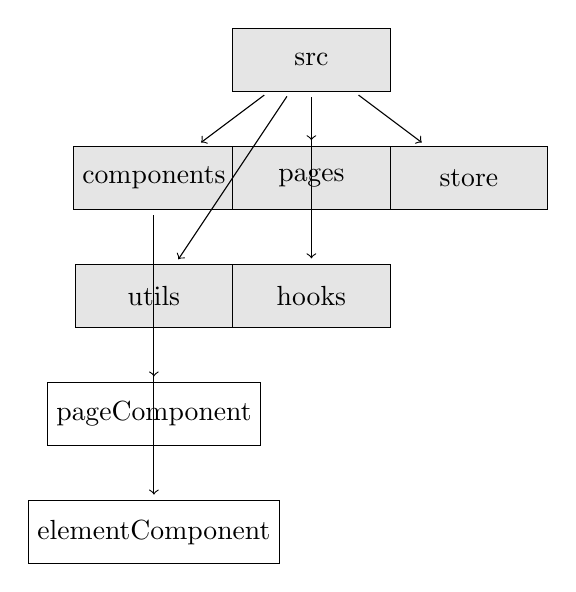
\begin{tikzpicture}[
    file/.style={draw, rectangle, minimum width=2cm, minimum height=0.8cm},
    folder/.style={draw, rectangle, minimum width=2cm, minimum height=0.8cm, fill=gray!20},
    arrow/.style={->, shorten >=2pt, shorten <=2pt}
]

% Folders
\node[folder] (src) at (0,0) {src};
\node[folder] (components) at (-2,-1.5) {components};
\node[folder] (pages) at (0,-1.5) {pages};
\node[folder] (store) at (2,-1.5) {store};
\node[folder] (utils) at (-2,-3) {utils};
\node[folder] (hooks) at (0,-3) {hooks};

% Files
\node[file] (pageComponent) at (-2,-4.5) {pageComponent};
\node[file] (elementComponent) at (-2,-6) {elementComponent};
% ... add more files

% Connections
\draw[arrow] (src) -- (components);
\draw[arrow] (src) -- (pages);
\draw[arrow] (src) -- (store);
\draw[arrow] (src) -- (utils);
\draw[arrow] (src) -- (hooks);
\draw[arrow] (components) -- (pageComponent);
\draw[arrow] (components) -- (elementComponent);
% ... add more connections

\end{tikzpicture}



\pagebreak
\subsubsection{Back-end}
The backend uses the dotNet framework. The development language using the C\# language.

In this project, the backend uses the Onion Architecture.
The Onion Architecture is a typically layered architecture, 
where each layer depends on the inner layer and provides interfaces to the outer layer.
The outer layer provides services to the outermost layer 
and other modules in the same layer based on the interfaces of the inner layer.

From inner to outer, the layers are: Domain, Application, Infrastructure, Presentation.
The Domain layer is the core layer and the innermost layer, used to define domain models, 
which are the business models.
It includes domain models and domain service interfaces.
Domain models are used to define the business models, 
which are the entities in the entity-relationship model and their attributes.
Domain service interfaces are used to define the business services, 
which are the relationships between entities in the entity-relationship model.

The Application layer is the application layer, 
used to define application services, which are the business logic.
It includes domain service implementations and application service interfaces.
Domain service implementations implement the methods of the inner layer's domain service 
interfaces and implement the business logic of the domain models.
Application service interfaces are used to define application services, 
which are the business logic.
It includes but is not limited to database interfaces, testing interfaces, 
HTTP API interfaces, MQTT interfaces, etc.

The Infrastructure layer is the infrastructure layer, used to define infrastructure.
It includes database implementations, testing implementations, 
HTTP API implementations, MQTT implementations, etc.
Database implementations implement the database interfaces 
and provide CRUD services for the database.
Testing implementations implement the testing interfaces 
and provide services for unit testing and integration testing.
HTTP API implementations implement the HTTP API interfaces 
and provide CRUD operations for HTTP APIs.
MQTT implementations implement the MQTT interfaces 
and provide CRUD operations for MQTT.

The Presentation layer is the presentation layer, used to define presentation logic, 
such as interfaces and pages. Since this is a backend project,
data presentation and control are handled by the frontend, 
so this layer is not needed.



\pagebreak
\subsubsection{Data communication and storage}
% 关于本项目的数据通信与数据存储的设计, 包括数据通信的协议, 数据存储的设计等
% 关于数据通信的设计:
% 1. 通信协议的选择
% 自前端向后端发送的数据, 有三种传输的数据类型, 
% 一种是普通的增删改查的请求, 对数据传输的时效性要求不高, 但是对数据的准确性, 完整性, 有序性, 安全性有一定的要求,
% 这种数据的传输, 采用 HTTP 协议, 以及 RESTful API 的设计. 可以有效的保证对数据传输的以上要求.
% 一种是对数据通道的创建和流媒体数据的传输, 对数据传输的时效性, 安全性要求较高, 这种数据的传输, 采用 WebRTC 协议, 以及 MQTT 协议.
% 配合可以快速解码的 flatbuffers 协议, 可以有效的保证对数据传输的以上要求.
% 最后一种是对设备的状态信息和操作信息的传输, 对完整性, 有序性, 安全性都有较高的要求, 这种数据的传输, 采用 MQTT 协议
% 同时也使用了 flatbuffers 协议.
% 
% 2. 数据通信的通信架构和通信流程
% 本项目的数据通信的通信架构, 是基于前后端分离的架构, 前端使用 React 框架, 后端使用 dotnet 框架.
% 当前端需要向后端发送数据的时候, 前端会向后端发送 HTTP 请求, 后端接收到 HTTP 请求之后, 会根据请求的数据类型,
% 选择不同的数据处理方式, 对于普通的增删改查的请求, 后端会根据 RESTful API 的设计, 对数据进行增删改查的操作,
% 对于对数据通道的创建和流媒体数据的传输, 后端会根据 WebRTC 协议, 对数据通道进行创建, 并且帮助前端和设备建立数据通道,
% 当数据通道建立后, 前端和设备之间则使用 flatbuffer 的数据格式对流媒体数据进行传输,
% 对于设备的状态信息和操作信息的传输, 前端会直接向 MQTT broker 发送 MQTT 请求, 
% 设备会在其自身的固件中监听相关的 MQTT 请求, 并且返回相关的数据.
% 
% 3. 数据通信的格式
% 本项目的数据通信的格式, 有三种, 
% 一种是 HTTP 协议, 
% 使用 json 格式对数据进行传输,
% 一种是 WebRTC 协议, 
% 使用 flatbuffers 格式对数据进行传输,
% 一种是 MQTT 协议.
% 使用 flatbuffers 格式对数据进行传输,
% 
% 关于数据存储的设计:
% 1. 数据存储的数据库的选择
% 本项目的数据存储的数据库的选择, 使用了轻量级的数据库 SQLite,
% SQLite 是一个进程内的库, 实现了自给自足的, 无服务器的, 零配置的, 事务性的 SQL 数据库引擎.
% 这是因为整个项目的目的是为了实现前端与设备之间的数据通信, 对于数据库数据的增删改查操作的要求不高,
% 数据量较小, 且对于数据库的数据的事务性要求不高, 所以选择了 SQLite 数据库.
% 2. 项目前后端的数据结构的设计
% 在本项目中, 前端由于使用了 React 框架, 所以前端的数据结构的设计, 使用了基于状态的数据结构的设计,
% 每个组件或者数据集都包含一个状态对象, 这个状态对象的属性就是组件的各个状态. 
% 使用状态对象的原因是, 可以方便的对状态进行管理, 采用对象-属性的形式, 可以方便的针对不同组件的同类状态进行区分,
% 由于跨组件的状态是由 redux 进行管理的, 这种状态对象的设计, 可以更搞笑的对状态进行更新和传递.
% 后端由于使用了 dotnet 框架, 所以后端的数据结构的设计, 使用了基于类的数据结构的设计,
% 采用了面向对象的编程思想, 对数据进行了封装, 使得数据的传输更加的安全, 有序, 完整.


\pagebreak

% \subsection{Domain model}
% \documentclass[]{article}
\usepackage{graphicx}
\usepackage{amsmath}
\usepackage{tikz}

% libaries
\usetikzlibrary{shapes,arrows}

%Define the listing package
\usepackage{listings} %code highlighter
\usepackage{color} %use color
\definecolor{mygreen}{rgb}{0,0.6,0}
\definecolor{mygray}{rgb}{0.5,0.5,0.5}
\definecolor{mymauve}{rgb}{0.58,0,0.82}

%Customize a bit the look
\lstset{ %
backgroundcolor=\color{white}, % choose the background color; you must add \usepackage{color} or \usepackage{xcolor}
basicstyle=\footnotesize, % the size of the fonts that are used for the code
breakatwhitespace=false, % sets if automatic breaks should only happen at whitespace
breaklines=true, % sets automatic line breaking
captionpos=b, % sets the caption-position to bottom
commentstyle=\color{mygreen}, % comment style
deletekeywords={...}, % if you want to delete keywords from the given language
escapeinside={\%*}{*)}, % if you want to add LaTeX within your code
extendedchars=true, % lets you use non-ASCII characters; for 8-bits encodings only, does not work with UTF-8
frame=single, % adds a frame around the code
keepspaces=true, % keeps spaces in text, useful for keeping indentation of code (possibly needs columns=flexible)
keywordstyle=\color{blue}, % keyword style
% language=Octave, % the language of the code
morekeywords={*,...}, % if you want to add more keywords to the set
numbers=left, % where to put the line-numbers; possible values are (none, left, right)
numbersep=5pt, % how far the line-numbers are from the code
numberstyle=\tiny\color{mygray}, % the style that is used for the line-numbers
rulecolor=\color{black}, % if not set, the frame-color may be changed on line-breaks within not-black text (e.g. comments (green here))
showspaces=false, % show spaces everywhere adding particular underscores; it overrides 'showstringspaces'
showstringspaces=false, % underline spaces within strings only
showtabs=false, % show tabs within strings adding particular underscores
stepnumber=1, % the step between two line-numbers. If it's 1, each line will be numbered
stringstyle=\color{mymauve}, % string literal style
tabsize=2, % sets default tabsize to 2 spaces
title=\lstname % show the filename of files included with \lstinputlisting; also try caption instead of title
}

\definecolor{darkgray}{rgb}{.4,.4,.4}
\definecolor{purple}{rgb}{0.65, 0.12, 0.82}

\lstdefinelanguage{React}{
keywords={const, typeof, new, true, false, catch, function, return, null, catch, switch, var, if, in, while, do, else, case, break},
keywordstyle=\color{blue}\bfseries,
ndkeywords={class, export, boolean, throw, implements, import, this},
ndkeywordstyle=\color{darkgray}\bfseries,
identifierstyle=\color{mygreen},
sensitive=false,
comment=[l]{//},
morecomment=[s]{/*}{*/},
commentstyle=\color{purple}\ttfamily,
string=[b]{"}{'}{`},
stringstyle=\color{red}\ttfamily,
morestring=[b]',
morestring=[b]",
morestring=[b]`',
}

\lstdefinelanguage{CSharp}{
keywords={const, typeof, new, true, false, catch, function, return, null, catch, switch, var, if, in, while, do, else, case, break},
keywordstyle=\color{blue}\bfseries,
ndkeywords={class, export, boolean, throw, implements, import, this},
ndkeywordstyle=\color{darkgray}\bfseries,
identifierstyle=\color{mygreen},
sensitive=false,
comment=[l]{//},
morecomment=[s]{/*}{*/},
commentstyle=\color{purple}\ttfamily,
string=[b]{"}{'}{`},
stringstyle=\color{red}\ttfamily,
morestring=[b]',
morestring=[b]",
morestring=[b]`',
}

\lstset{
language=React,
extendedchars=true,
basicstyle=\footnotesize\ttfamily,
showstringspaces=false,
showspaces=false,
numbers=left,
numberstyle=\footnotesize,
numbersep=9pt,
tabsize=2,
breaklines=true,
showtabs=false,
captionpos=b
}

\lstset{
language=CSharp,
extendedchars=true,
basicstyle=\footnotesize\ttfamily,
showstringspaces=false,
showspaces=false,
numbers=left,
numberstyle=\footnotesize,
numbersep=9pt,
tabsize=2,
breaklines=true,
showtabs=false,
captionpos=b
}

% \usepackage{cite} % Add this line for citation

% \bibliographystyle{plain}

\title{
The implementation of BifrostConnect Front-end scope, 
re-design and development with the relevant back-end support develop.
}
\author{
    Fei Gu \\
    Erhvervs Akademi Sydvest \\
    Computer Science 21\\
    }
\date{\today}

\begin{document}

% Front page
\maketitle
\begin{center}
    Supervisor: Henrik Boulund Meng Hansen \\
    Company: BifrostConnect \\
    Engineering Director: Jasper Wass \\
\end{center}
\tableofcontents
\pagebreak


% The introduction
\section{Introduction}
\subsection{Background}\input{sections/introduction/background.tex}
\subsection{The company}\input{sections/introduction/aboutCompany}
\subsection{The project}\input{sections/introduction/aboutProject}
\pagebreak

% The problem statement
\section{Problem Statement}
\subsection{Statement}
\input{sections/problemStatement/statement}
\subsection{Situation}
\input{sections/problemStatement/situation}
\subsection{Potential Solution}
\input{sections/problemStatement/potentialSolution}
\pagebreak

% Requirement analysis
\section{Requirement Analysis}
\input{sections/requirementAnalysis/index}

\subsection{Stakeholders}
\input{sections/requirementAnalysis/stakeholders/index}

\subsection{Business Domain}
\input{sections/requirementAnalysis/bussinesDomain/index}

\subsection{Scope}
\input{sections/requirementAnalysis/scope}

\subsection{Goals}
\input{sections/requirementAnalysis/goals}
\pagebreak

% Software Design
\section{Software Design}
% developement methods
\subsection{Software Development Methods}
\input{sections/softwareDevelopmentMethods/index}
\subsubsection{Agile Software Development}
\input{sections/softwareDevelopmentMethods/agileSoftwareDevelopment/index}
\subsubsection{Feature Driven Development}
\input{sections/softwareDevelopmentMethods/featureDrivenDevelopment/index}

\pagebreak

% Technology seslection
\subsection{Technology selection}
\input{sections/softwareDesign/technologySelection/index}
\subsubsection{Front-end}
\input{sections/softwareDesign/technologySelection/frontEnd}            
\subsubsection{Back-end}
\input{sections/softwareDesign/technologySelection/backEnd}            
\subsubsection{Database}
\input{sections/softwareDesign/technologySelection/database}
\subsubsection{Data communication}
\input{sections/softwareDesign/technologySelection/dataCommunication}            
\subsubsection{DevOps}
\input{sections/softwareDesign/technologySelection/devOps}
\pagebreak

% Architecture design
\subsection{Architecture design}
\input{sections/softwareDesign/architectureDesign/index}
\pagebreak
\subsubsection{Front-end}
\input{sections/softwareDesign/architectureDesign/frontEndArchitecture}
\pagebreak
\subsubsection{Back-end}
\input{sections/softwareDesign/architectureDesign/backEndArchitecture}
\pagebreak
\subsubsection{Data communication and storage}
\input{sections/softwareDesign/architectureDesign/dataCommunicationArchitecture}
\pagebreak

% \subsection{Domain model}
% \input{sections/softwareDesign/domainModel/index}
% \subsection{Database design}
% % 数据库领域模型 ER 图
% % 包括表和字段的设置.
% % 对于私有键和外键的设置.

% \subsection{Back-end design}
% % 后端对象模型
% % 以及对于对象模型的增删改查
% % 以及相关的其他服务的设计`'

% \subsection{Front-end design}
% % 对于前端的页面结构的设计 
% % 页面的状态的设计, 交互设计

% \subsection{FlatBuffers design}
% % schema 的设计

\subsection{DevOps CI/CD process design}
\input{sections/softwareDesign/devOpsDesign/index}
\subsubsection{Continuous Integration}
\input{sections/softwareDesign/devOpsDesign/continuousIntegration/index}
\subsubsection{Continuous Delivery}
\input{sections/softwareDesign/devOpsDesign/continuousDelivery/index}
\subsubsection{Continuous Deployment}
\input{sections/softwareDesign/devOpsDesign/continuousDeployment/index}
\pagebreak

\section{Software Development} 
\input{sections/softwareDevelopment/index}
\subsection{Overall development}
\input{sections/softwareDevelopment/overallDevelopement/index}
\subsubsection{Front-end}
\input{sections/softwareDevelopment/overallDevelopement/frontEnd/index}
\subsubsection{Back-end}
\input{sections/softwareDevelopment/overallDevelopement/backEnd/index}
\subsubsection{DevOps}
\input{sections/softwareDevelopment/overallDevelopement/devOps/index}
\subsection{Feature development} 
\input{sections/softwareDevelopment/featureDevelopment/index}
\subsubsection{Use Case 1}
\input{sections/softwareDevelopment/featureDevelopment/useCase1/index}
\subsubsection{Feature 1}
\input{sections/softwareDevelopment/featureDevelopment/feature/feature1.tex}
\pagebreak
\section{Conclusion} 
\subsection{Result}
Since the project is still in progress, the result is not available yet.
So far, basic structure of this project has been built. But the most features 
are not implemented yet. 
\subsection{Discussion}
As a single developer for this project, I am confident what I have done so far.
And I can say I understand the most of the knowledge I have used in this project, 
which also means I can explain all the part of the project. 
But this project also relevant some of the complex knowledge which I have to continue 
to study and practice.
\subsection{Future Work}
The future work is to implement the rest of the features. 
Including the most important part which is the 'create session' feature.
\pagebreak
% \bibliography{bibliography}
\pagebreak
% \begin{appendices}
%     \section{Appendix}
% \end{appendices} 
\end{document}
% \subsection{Database design}
% % 数据库领域模型 ER 图
% % 包括表和字段的设置.
% % 对于私有键和外键的设置.

% \subsection{Back-end design}
% % 后端对象模型
% % 以及对于对象模型的增删改查
% % 以及相关的其他服务的设计`'

% \subsection{Front-end design}
% % 对于前端的页面结构的设计 
% % 页面的状态的设计, 交互设计

% \subsection{FlatBuffers design}
% % schema 的设计

\subsection{DevOps CI/CD process design}
\documentclass[]{article}
\usepackage{graphicx}
\usepackage{amsmath}
\usepackage{tikz}

% libaries
\usetikzlibrary{shapes,arrows}

%Define the listing package
\usepackage{listings} %code highlighter
\usepackage{color} %use color
\definecolor{mygreen}{rgb}{0,0.6,0}
\definecolor{mygray}{rgb}{0.5,0.5,0.5}
\definecolor{mymauve}{rgb}{0.58,0,0.82}

%Customize a bit the look
\lstset{ %
backgroundcolor=\color{white}, % choose the background color; you must add \usepackage{color} or \usepackage{xcolor}
basicstyle=\footnotesize, % the size of the fonts that are used for the code
breakatwhitespace=false, % sets if automatic breaks should only happen at whitespace
breaklines=true, % sets automatic line breaking
captionpos=b, % sets the caption-position to bottom
commentstyle=\color{mygreen}, % comment style
deletekeywords={...}, % if you want to delete keywords from the given language
escapeinside={\%*}{*)}, % if you want to add LaTeX within your code
extendedchars=true, % lets you use non-ASCII characters; for 8-bits encodings only, does not work with UTF-8
frame=single, % adds a frame around the code
keepspaces=true, % keeps spaces in text, useful for keeping indentation of code (possibly needs columns=flexible)
keywordstyle=\color{blue}, % keyword style
% language=Octave, % the language of the code
morekeywords={*,...}, % if you want to add more keywords to the set
numbers=left, % where to put the line-numbers; possible values are (none, left, right)
numbersep=5pt, % how far the line-numbers are from the code
numberstyle=\tiny\color{mygray}, % the style that is used for the line-numbers
rulecolor=\color{black}, % if not set, the frame-color may be changed on line-breaks within not-black text (e.g. comments (green here))
showspaces=false, % show spaces everywhere adding particular underscores; it overrides 'showstringspaces'
showstringspaces=false, % underline spaces within strings only
showtabs=false, % show tabs within strings adding particular underscores
stepnumber=1, % the step between two line-numbers. If it's 1, each line will be numbered
stringstyle=\color{mymauve}, % string literal style
tabsize=2, % sets default tabsize to 2 spaces
title=\lstname % show the filename of files included with \lstinputlisting; also try caption instead of title
}

\definecolor{darkgray}{rgb}{.4,.4,.4}
\definecolor{purple}{rgb}{0.65, 0.12, 0.82}

\lstdefinelanguage{React}{
keywords={const, typeof, new, true, false, catch, function, return, null, catch, switch, var, if, in, while, do, else, case, break},
keywordstyle=\color{blue}\bfseries,
ndkeywords={class, export, boolean, throw, implements, import, this},
ndkeywordstyle=\color{darkgray}\bfseries,
identifierstyle=\color{mygreen},
sensitive=false,
comment=[l]{//},
morecomment=[s]{/*}{*/},
commentstyle=\color{purple}\ttfamily,
string=[b]{"}{'}{`},
stringstyle=\color{red}\ttfamily,
morestring=[b]',
morestring=[b]",
morestring=[b]`',
}

\lstdefinelanguage{CSharp}{
keywords={const, typeof, new, true, false, catch, function, return, null, catch, switch, var, if, in, while, do, else, case, break},
keywordstyle=\color{blue}\bfseries,
ndkeywords={class, export, boolean, throw, implements, import, this},
ndkeywordstyle=\color{darkgray}\bfseries,
identifierstyle=\color{mygreen},
sensitive=false,
comment=[l]{//},
morecomment=[s]{/*}{*/},
commentstyle=\color{purple}\ttfamily,
string=[b]{"}{'}{`},
stringstyle=\color{red}\ttfamily,
morestring=[b]',
morestring=[b]",
morestring=[b]`',
}

\lstset{
language=React,
extendedchars=true,
basicstyle=\footnotesize\ttfamily,
showstringspaces=false,
showspaces=false,
numbers=left,
numberstyle=\footnotesize,
numbersep=9pt,
tabsize=2,
breaklines=true,
showtabs=false,
captionpos=b
}

\lstset{
language=CSharp,
extendedchars=true,
basicstyle=\footnotesize\ttfamily,
showstringspaces=false,
showspaces=false,
numbers=left,
numberstyle=\footnotesize,
numbersep=9pt,
tabsize=2,
breaklines=true,
showtabs=false,
captionpos=b
}

% \usepackage{cite} % Add this line for citation

% \bibliographystyle{plain}

\title{
The implementation of BifrostConnect Front-end scope, 
re-design and development with the relevant back-end support develop.
}
\author{
    Fei Gu \\
    Erhvervs Akademi Sydvest \\
    Computer Science 21\\
    }
\date{\today}

\begin{document}

% Front page
\maketitle
\begin{center}
    Supervisor: Henrik Boulund Meng Hansen \\
    Company: BifrostConnect \\
    Engineering Director: Jasper Wass \\
\end{center}
\tableofcontents
\pagebreak


% The introduction
\section{Introduction}
\subsection{Background}\input{sections/introduction/background.tex}
\subsection{The company}\input{sections/introduction/aboutCompany}
\subsection{The project}\input{sections/introduction/aboutProject}
\pagebreak

% The problem statement
\section{Problem Statement}
\subsection{Statement}
\input{sections/problemStatement/statement}
\subsection{Situation}
\input{sections/problemStatement/situation}
\subsection{Potential Solution}
\input{sections/problemStatement/potentialSolution}
\pagebreak

% Requirement analysis
\section{Requirement Analysis}
\input{sections/requirementAnalysis/index}

\subsection{Stakeholders}
\input{sections/requirementAnalysis/stakeholders/index}

\subsection{Business Domain}
\input{sections/requirementAnalysis/bussinesDomain/index}

\subsection{Scope}
\input{sections/requirementAnalysis/scope}

\subsection{Goals}
\input{sections/requirementAnalysis/goals}
\pagebreak

% Software Design
\section{Software Design}
% developement methods
\subsection{Software Development Methods}
\input{sections/softwareDevelopmentMethods/index}
\subsubsection{Agile Software Development}
\input{sections/softwareDevelopmentMethods/agileSoftwareDevelopment/index}
\subsubsection{Feature Driven Development}
\input{sections/softwareDevelopmentMethods/featureDrivenDevelopment/index}

\pagebreak

% Technology seslection
\subsection{Technology selection}
\input{sections/softwareDesign/technologySelection/index}
\subsubsection{Front-end}
\input{sections/softwareDesign/technologySelection/frontEnd}            
\subsubsection{Back-end}
\input{sections/softwareDesign/technologySelection/backEnd}            
\subsubsection{Database}
\input{sections/softwareDesign/technologySelection/database}
\subsubsection{Data communication}
\input{sections/softwareDesign/technologySelection/dataCommunication}            
\subsubsection{DevOps}
\input{sections/softwareDesign/technologySelection/devOps}
\pagebreak

% Architecture design
\subsection{Architecture design}
\input{sections/softwareDesign/architectureDesign/index}
\pagebreak
\subsubsection{Front-end}
\input{sections/softwareDesign/architectureDesign/frontEndArchitecture}
\pagebreak
\subsubsection{Back-end}
\input{sections/softwareDesign/architectureDesign/backEndArchitecture}
\pagebreak
\subsubsection{Data communication and storage}
\input{sections/softwareDesign/architectureDesign/dataCommunicationArchitecture}
\pagebreak

% \subsection{Domain model}
% \input{sections/softwareDesign/domainModel/index}
% \subsection{Database design}
% % 数据库领域模型 ER 图
% % 包括表和字段的设置.
% % 对于私有键和外键的设置.

% \subsection{Back-end design}
% % 后端对象模型
% % 以及对于对象模型的增删改查
% % 以及相关的其他服务的设计`'

% \subsection{Front-end design}
% % 对于前端的页面结构的设计 
% % 页面的状态的设计, 交互设计

% \subsection{FlatBuffers design}
% % schema 的设计

\subsection{DevOps CI/CD process design}
\input{sections/softwareDesign/devOpsDesign/index}
\subsubsection{Continuous Integration}
\input{sections/softwareDesign/devOpsDesign/continuousIntegration/index}
\subsubsection{Continuous Delivery}
\input{sections/softwareDesign/devOpsDesign/continuousDelivery/index}
\subsubsection{Continuous Deployment}
\input{sections/softwareDesign/devOpsDesign/continuousDeployment/index}
\pagebreak

\section{Software Development} 
\input{sections/softwareDevelopment/index}
\subsection{Overall development}
\input{sections/softwareDevelopment/overallDevelopement/index}
\subsubsection{Front-end}
\input{sections/softwareDevelopment/overallDevelopement/frontEnd/index}
\subsubsection{Back-end}
\input{sections/softwareDevelopment/overallDevelopement/backEnd/index}
\subsubsection{DevOps}
\input{sections/softwareDevelopment/overallDevelopement/devOps/index}
\subsection{Feature development} 
\input{sections/softwareDevelopment/featureDevelopment/index}
\subsubsection{Use Case 1}
\input{sections/softwareDevelopment/featureDevelopment/useCase1/index}
\subsubsection{Feature 1}
\input{sections/softwareDevelopment/featureDevelopment/feature/feature1.tex}
\pagebreak
\section{Conclusion} 
\subsection{Result}
Since the project is still in progress, the result is not available yet.
So far, basic structure of this project has been built. But the most features 
are not implemented yet. 
\subsection{Discussion}
As a single developer for this project, I am confident what I have done so far.
And I can say I understand the most of the knowledge I have used in this project, 
which also means I can explain all the part of the project. 
But this project also relevant some of the complex knowledge which I have to continue 
to study and practice.
\subsection{Future Work}
The future work is to implement the rest of the features. 
Including the most important part which is the 'create session' feature.
\pagebreak
% \bibliography{bibliography}
\pagebreak
% \begin{appendices}
%     \section{Appendix}
% \end{appendices} 
\end{document}
\subsubsection{Continuous Integration}
\documentclass[]{article}
\usepackage{graphicx}
\usepackage{amsmath}
\usepackage{tikz}

% libaries
\usetikzlibrary{shapes,arrows}

%Define the listing package
\usepackage{listings} %code highlighter
\usepackage{color} %use color
\definecolor{mygreen}{rgb}{0,0.6,0}
\definecolor{mygray}{rgb}{0.5,0.5,0.5}
\definecolor{mymauve}{rgb}{0.58,0,0.82}

%Customize a bit the look
\lstset{ %
backgroundcolor=\color{white}, % choose the background color; you must add \usepackage{color} or \usepackage{xcolor}
basicstyle=\footnotesize, % the size of the fonts that are used for the code
breakatwhitespace=false, % sets if automatic breaks should only happen at whitespace
breaklines=true, % sets automatic line breaking
captionpos=b, % sets the caption-position to bottom
commentstyle=\color{mygreen}, % comment style
deletekeywords={...}, % if you want to delete keywords from the given language
escapeinside={\%*}{*)}, % if you want to add LaTeX within your code
extendedchars=true, % lets you use non-ASCII characters; for 8-bits encodings only, does not work with UTF-8
frame=single, % adds a frame around the code
keepspaces=true, % keeps spaces in text, useful for keeping indentation of code (possibly needs columns=flexible)
keywordstyle=\color{blue}, % keyword style
% language=Octave, % the language of the code
morekeywords={*,...}, % if you want to add more keywords to the set
numbers=left, % where to put the line-numbers; possible values are (none, left, right)
numbersep=5pt, % how far the line-numbers are from the code
numberstyle=\tiny\color{mygray}, % the style that is used for the line-numbers
rulecolor=\color{black}, % if not set, the frame-color may be changed on line-breaks within not-black text (e.g. comments (green here))
showspaces=false, % show spaces everywhere adding particular underscores; it overrides 'showstringspaces'
showstringspaces=false, % underline spaces within strings only
showtabs=false, % show tabs within strings adding particular underscores
stepnumber=1, % the step between two line-numbers. If it's 1, each line will be numbered
stringstyle=\color{mymauve}, % string literal style
tabsize=2, % sets default tabsize to 2 spaces
title=\lstname % show the filename of files included with \lstinputlisting; also try caption instead of title
}

\definecolor{darkgray}{rgb}{.4,.4,.4}
\definecolor{purple}{rgb}{0.65, 0.12, 0.82}

\lstdefinelanguage{React}{
keywords={const, typeof, new, true, false, catch, function, return, null, catch, switch, var, if, in, while, do, else, case, break},
keywordstyle=\color{blue}\bfseries,
ndkeywords={class, export, boolean, throw, implements, import, this},
ndkeywordstyle=\color{darkgray}\bfseries,
identifierstyle=\color{mygreen},
sensitive=false,
comment=[l]{//},
morecomment=[s]{/*}{*/},
commentstyle=\color{purple}\ttfamily,
string=[b]{"}{'}{`},
stringstyle=\color{red}\ttfamily,
morestring=[b]',
morestring=[b]",
morestring=[b]`',
}

\lstdefinelanguage{CSharp}{
keywords={const, typeof, new, true, false, catch, function, return, null, catch, switch, var, if, in, while, do, else, case, break},
keywordstyle=\color{blue}\bfseries,
ndkeywords={class, export, boolean, throw, implements, import, this},
ndkeywordstyle=\color{darkgray}\bfseries,
identifierstyle=\color{mygreen},
sensitive=false,
comment=[l]{//},
morecomment=[s]{/*}{*/},
commentstyle=\color{purple}\ttfamily,
string=[b]{"}{'}{`},
stringstyle=\color{red}\ttfamily,
morestring=[b]',
morestring=[b]",
morestring=[b]`',
}

\lstset{
language=React,
extendedchars=true,
basicstyle=\footnotesize\ttfamily,
showstringspaces=false,
showspaces=false,
numbers=left,
numberstyle=\footnotesize,
numbersep=9pt,
tabsize=2,
breaklines=true,
showtabs=false,
captionpos=b
}

\lstset{
language=CSharp,
extendedchars=true,
basicstyle=\footnotesize\ttfamily,
showstringspaces=false,
showspaces=false,
numbers=left,
numberstyle=\footnotesize,
numbersep=9pt,
tabsize=2,
breaklines=true,
showtabs=false,
captionpos=b
}

% \usepackage{cite} % Add this line for citation

% \bibliographystyle{plain}

\title{
The implementation of BifrostConnect Front-end scope, 
re-design and development with the relevant back-end support develop.
}
\author{
    Fei Gu \\
    Erhvervs Akademi Sydvest \\
    Computer Science 21\\
    }
\date{\today}

\begin{document}

% Front page
\maketitle
\begin{center}
    Supervisor: Henrik Boulund Meng Hansen \\
    Company: BifrostConnect \\
    Engineering Director: Jasper Wass \\
\end{center}
\tableofcontents
\pagebreak


% The introduction
\section{Introduction}
\subsection{Background}\input{sections/introduction/background.tex}
\subsection{The company}\input{sections/introduction/aboutCompany}
\subsection{The project}\input{sections/introduction/aboutProject}
\pagebreak

% The problem statement
\section{Problem Statement}
\subsection{Statement}
\input{sections/problemStatement/statement}
\subsection{Situation}
\input{sections/problemStatement/situation}
\subsection{Potential Solution}
\input{sections/problemStatement/potentialSolution}
\pagebreak

% Requirement analysis
\section{Requirement Analysis}
\input{sections/requirementAnalysis/index}

\subsection{Stakeholders}
\input{sections/requirementAnalysis/stakeholders/index}

\subsection{Business Domain}
\input{sections/requirementAnalysis/bussinesDomain/index}

\subsection{Scope}
\input{sections/requirementAnalysis/scope}

\subsection{Goals}
\input{sections/requirementAnalysis/goals}
\pagebreak

% Software Design
\section{Software Design}
% developement methods
\subsection{Software Development Methods}
\input{sections/softwareDevelopmentMethods/index}
\subsubsection{Agile Software Development}
\input{sections/softwareDevelopmentMethods/agileSoftwareDevelopment/index}
\subsubsection{Feature Driven Development}
\input{sections/softwareDevelopmentMethods/featureDrivenDevelopment/index}

\pagebreak

% Technology seslection
\subsection{Technology selection}
\input{sections/softwareDesign/technologySelection/index}
\subsubsection{Front-end}
\input{sections/softwareDesign/technologySelection/frontEnd}            
\subsubsection{Back-end}
\input{sections/softwareDesign/technologySelection/backEnd}            
\subsubsection{Database}
\input{sections/softwareDesign/technologySelection/database}
\subsubsection{Data communication}
\input{sections/softwareDesign/technologySelection/dataCommunication}            
\subsubsection{DevOps}
\input{sections/softwareDesign/technologySelection/devOps}
\pagebreak

% Architecture design
\subsection{Architecture design}
\input{sections/softwareDesign/architectureDesign/index}
\pagebreak
\subsubsection{Front-end}
\input{sections/softwareDesign/architectureDesign/frontEndArchitecture}
\pagebreak
\subsubsection{Back-end}
\input{sections/softwareDesign/architectureDesign/backEndArchitecture}
\pagebreak
\subsubsection{Data communication and storage}
\input{sections/softwareDesign/architectureDesign/dataCommunicationArchitecture}
\pagebreak

% \subsection{Domain model}
% \input{sections/softwareDesign/domainModel/index}
% \subsection{Database design}
% % 数据库领域模型 ER 图
% % 包括表和字段的设置.
% % 对于私有键和外键的设置.

% \subsection{Back-end design}
% % 后端对象模型
% % 以及对于对象模型的增删改查
% % 以及相关的其他服务的设计`'

% \subsection{Front-end design}
% % 对于前端的页面结构的设计 
% % 页面的状态的设计, 交互设计

% \subsection{FlatBuffers design}
% % schema 的设计

\subsection{DevOps CI/CD process design}
\input{sections/softwareDesign/devOpsDesign/index}
\subsubsection{Continuous Integration}
\input{sections/softwareDesign/devOpsDesign/continuousIntegration/index}
\subsubsection{Continuous Delivery}
\input{sections/softwareDesign/devOpsDesign/continuousDelivery/index}
\subsubsection{Continuous Deployment}
\input{sections/softwareDesign/devOpsDesign/continuousDeployment/index}
\pagebreak

\section{Software Development} 
\input{sections/softwareDevelopment/index}
\subsection{Overall development}
\input{sections/softwareDevelopment/overallDevelopement/index}
\subsubsection{Front-end}
\input{sections/softwareDevelopment/overallDevelopement/frontEnd/index}
\subsubsection{Back-end}
\input{sections/softwareDevelopment/overallDevelopement/backEnd/index}
\subsubsection{DevOps}
\input{sections/softwareDevelopment/overallDevelopement/devOps/index}
\subsection{Feature development} 
\input{sections/softwareDevelopment/featureDevelopment/index}
\subsubsection{Use Case 1}
\input{sections/softwareDevelopment/featureDevelopment/useCase1/index}
\subsubsection{Feature 1}
\input{sections/softwareDevelopment/featureDevelopment/feature/feature1.tex}
\pagebreak
\section{Conclusion} 
\subsection{Result}
Since the project is still in progress, the result is not available yet.
So far, basic structure of this project has been built. But the most features 
are not implemented yet. 
\subsection{Discussion}
As a single developer for this project, I am confident what I have done so far.
And I can say I understand the most of the knowledge I have used in this project, 
which also means I can explain all the part of the project. 
But this project also relevant some of the complex knowledge which I have to continue 
to study and practice.
\subsection{Future Work}
The future work is to implement the rest of the features. 
Including the most important part which is the 'create session' feature.
\pagebreak
% \bibliography{bibliography}
\pagebreak
% \begin{appendices}
%     \section{Appendix}
% \end{appendices} 
\end{document}
\subsubsection{Continuous Delivery}
\documentclass[]{article}
\usepackage{graphicx}
\usepackage{amsmath}
\usepackage{tikz}

% libaries
\usetikzlibrary{shapes,arrows}

%Define the listing package
\usepackage{listings} %code highlighter
\usepackage{color} %use color
\definecolor{mygreen}{rgb}{0,0.6,0}
\definecolor{mygray}{rgb}{0.5,0.5,0.5}
\definecolor{mymauve}{rgb}{0.58,0,0.82}

%Customize a bit the look
\lstset{ %
backgroundcolor=\color{white}, % choose the background color; you must add \usepackage{color} or \usepackage{xcolor}
basicstyle=\footnotesize, % the size of the fonts that are used for the code
breakatwhitespace=false, % sets if automatic breaks should only happen at whitespace
breaklines=true, % sets automatic line breaking
captionpos=b, % sets the caption-position to bottom
commentstyle=\color{mygreen}, % comment style
deletekeywords={...}, % if you want to delete keywords from the given language
escapeinside={\%*}{*)}, % if you want to add LaTeX within your code
extendedchars=true, % lets you use non-ASCII characters; for 8-bits encodings only, does not work with UTF-8
frame=single, % adds a frame around the code
keepspaces=true, % keeps spaces in text, useful for keeping indentation of code (possibly needs columns=flexible)
keywordstyle=\color{blue}, % keyword style
% language=Octave, % the language of the code
morekeywords={*,...}, % if you want to add more keywords to the set
numbers=left, % where to put the line-numbers; possible values are (none, left, right)
numbersep=5pt, % how far the line-numbers are from the code
numberstyle=\tiny\color{mygray}, % the style that is used for the line-numbers
rulecolor=\color{black}, % if not set, the frame-color may be changed on line-breaks within not-black text (e.g. comments (green here))
showspaces=false, % show spaces everywhere adding particular underscores; it overrides 'showstringspaces'
showstringspaces=false, % underline spaces within strings only
showtabs=false, % show tabs within strings adding particular underscores
stepnumber=1, % the step between two line-numbers. If it's 1, each line will be numbered
stringstyle=\color{mymauve}, % string literal style
tabsize=2, % sets default tabsize to 2 spaces
title=\lstname % show the filename of files included with \lstinputlisting; also try caption instead of title
}

\definecolor{darkgray}{rgb}{.4,.4,.4}
\definecolor{purple}{rgb}{0.65, 0.12, 0.82}

\lstdefinelanguage{React}{
keywords={const, typeof, new, true, false, catch, function, return, null, catch, switch, var, if, in, while, do, else, case, break},
keywordstyle=\color{blue}\bfseries,
ndkeywords={class, export, boolean, throw, implements, import, this},
ndkeywordstyle=\color{darkgray}\bfseries,
identifierstyle=\color{mygreen},
sensitive=false,
comment=[l]{//},
morecomment=[s]{/*}{*/},
commentstyle=\color{purple}\ttfamily,
string=[b]{"}{'}{`},
stringstyle=\color{red}\ttfamily,
morestring=[b]',
morestring=[b]",
morestring=[b]`',
}

\lstdefinelanguage{CSharp}{
keywords={const, typeof, new, true, false, catch, function, return, null, catch, switch, var, if, in, while, do, else, case, break},
keywordstyle=\color{blue}\bfseries,
ndkeywords={class, export, boolean, throw, implements, import, this},
ndkeywordstyle=\color{darkgray}\bfseries,
identifierstyle=\color{mygreen},
sensitive=false,
comment=[l]{//},
morecomment=[s]{/*}{*/},
commentstyle=\color{purple}\ttfamily,
string=[b]{"}{'}{`},
stringstyle=\color{red}\ttfamily,
morestring=[b]',
morestring=[b]",
morestring=[b]`',
}

\lstset{
language=React,
extendedchars=true,
basicstyle=\footnotesize\ttfamily,
showstringspaces=false,
showspaces=false,
numbers=left,
numberstyle=\footnotesize,
numbersep=9pt,
tabsize=2,
breaklines=true,
showtabs=false,
captionpos=b
}

\lstset{
language=CSharp,
extendedchars=true,
basicstyle=\footnotesize\ttfamily,
showstringspaces=false,
showspaces=false,
numbers=left,
numberstyle=\footnotesize,
numbersep=9pt,
tabsize=2,
breaklines=true,
showtabs=false,
captionpos=b
}

% \usepackage{cite} % Add this line for citation

% \bibliographystyle{plain}

\title{
The implementation of BifrostConnect Front-end scope, 
re-design and development with the relevant back-end support develop.
}
\author{
    Fei Gu \\
    Erhvervs Akademi Sydvest \\
    Computer Science 21\\
    }
\date{\today}

\begin{document}

% Front page
\maketitle
\begin{center}
    Supervisor: Henrik Boulund Meng Hansen \\
    Company: BifrostConnect \\
    Engineering Director: Jasper Wass \\
\end{center}
\tableofcontents
\pagebreak


% The introduction
\section{Introduction}
\subsection{Background}\input{sections/introduction/background.tex}
\subsection{The company}\input{sections/introduction/aboutCompany}
\subsection{The project}\input{sections/introduction/aboutProject}
\pagebreak

% The problem statement
\section{Problem Statement}
\subsection{Statement}
\input{sections/problemStatement/statement}
\subsection{Situation}
\input{sections/problemStatement/situation}
\subsection{Potential Solution}
\input{sections/problemStatement/potentialSolution}
\pagebreak

% Requirement analysis
\section{Requirement Analysis}
\input{sections/requirementAnalysis/index}

\subsection{Stakeholders}
\input{sections/requirementAnalysis/stakeholders/index}

\subsection{Business Domain}
\input{sections/requirementAnalysis/bussinesDomain/index}

\subsection{Scope}
\input{sections/requirementAnalysis/scope}

\subsection{Goals}
\input{sections/requirementAnalysis/goals}
\pagebreak

% Software Design
\section{Software Design}
% developement methods
\subsection{Software Development Methods}
\input{sections/softwareDevelopmentMethods/index}
\subsubsection{Agile Software Development}
\input{sections/softwareDevelopmentMethods/agileSoftwareDevelopment/index}
\subsubsection{Feature Driven Development}
\input{sections/softwareDevelopmentMethods/featureDrivenDevelopment/index}

\pagebreak

% Technology seslection
\subsection{Technology selection}
\input{sections/softwareDesign/technologySelection/index}
\subsubsection{Front-end}
\input{sections/softwareDesign/technologySelection/frontEnd}            
\subsubsection{Back-end}
\input{sections/softwareDesign/technologySelection/backEnd}            
\subsubsection{Database}
\input{sections/softwareDesign/technologySelection/database}
\subsubsection{Data communication}
\input{sections/softwareDesign/technologySelection/dataCommunication}            
\subsubsection{DevOps}
\input{sections/softwareDesign/technologySelection/devOps}
\pagebreak

% Architecture design
\subsection{Architecture design}
\input{sections/softwareDesign/architectureDesign/index}
\pagebreak
\subsubsection{Front-end}
\input{sections/softwareDesign/architectureDesign/frontEndArchitecture}
\pagebreak
\subsubsection{Back-end}
\input{sections/softwareDesign/architectureDesign/backEndArchitecture}
\pagebreak
\subsubsection{Data communication and storage}
\input{sections/softwareDesign/architectureDesign/dataCommunicationArchitecture}
\pagebreak

% \subsection{Domain model}
% \input{sections/softwareDesign/domainModel/index}
% \subsection{Database design}
% % 数据库领域模型 ER 图
% % 包括表和字段的设置.
% % 对于私有键和外键的设置.

% \subsection{Back-end design}
% % 后端对象模型
% % 以及对于对象模型的增删改查
% % 以及相关的其他服务的设计`'

% \subsection{Front-end design}
% % 对于前端的页面结构的设计 
% % 页面的状态的设计, 交互设计

% \subsection{FlatBuffers design}
% % schema 的设计

\subsection{DevOps CI/CD process design}
\input{sections/softwareDesign/devOpsDesign/index}
\subsubsection{Continuous Integration}
\input{sections/softwareDesign/devOpsDesign/continuousIntegration/index}
\subsubsection{Continuous Delivery}
\input{sections/softwareDesign/devOpsDesign/continuousDelivery/index}
\subsubsection{Continuous Deployment}
\input{sections/softwareDesign/devOpsDesign/continuousDeployment/index}
\pagebreak

\section{Software Development} 
\input{sections/softwareDevelopment/index}
\subsection{Overall development}
\input{sections/softwareDevelopment/overallDevelopement/index}
\subsubsection{Front-end}
\input{sections/softwareDevelopment/overallDevelopement/frontEnd/index}
\subsubsection{Back-end}
\input{sections/softwareDevelopment/overallDevelopement/backEnd/index}
\subsubsection{DevOps}
\input{sections/softwareDevelopment/overallDevelopement/devOps/index}
\subsection{Feature development} 
\input{sections/softwareDevelopment/featureDevelopment/index}
\subsubsection{Use Case 1}
\input{sections/softwareDevelopment/featureDevelopment/useCase1/index}
\subsubsection{Feature 1}
\input{sections/softwareDevelopment/featureDevelopment/feature/feature1.tex}
\pagebreak
\section{Conclusion} 
\subsection{Result}
Since the project is still in progress, the result is not available yet.
So far, basic structure of this project has been built. But the most features 
are not implemented yet. 
\subsection{Discussion}
As a single developer for this project, I am confident what I have done so far.
And I can say I understand the most of the knowledge I have used in this project, 
which also means I can explain all the part of the project. 
But this project also relevant some of the complex knowledge which I have to continue 
to study and practice.
\subsection{Future Work}
The future work is to implement the rest of the features. 
Including the most important part which is the 'create session' feature.
\pagebreak
% \bibliography{bibliography}
\pagebreak
% \begin{appendices}
%     \section{Appendix}
% \end{appendices} 
\end{document}
\subsubsection{Continuous Deployment}
\documentclass[]{article}
\usepackage{graphicx}
\usepackage{amsmath}
\usepackage{tikz}

% libaries
\usetikzlibrary{shapes,arrows}

%Define the listing package
\usepackage{listings} %code highlighter
\usepackage{color} %use color
\definecolor{mygreen}{rgb}{0,0.6,0}
\definecolor{mygray}{rgb}{0.5,0.5,0.5}
\definecolor{mymauve}{rgb}{0.58,0,0.82}

%Customize a bit the look
\lstset{ %
backgroundcolor=\color{white}, % choose the background color; you must add \usepackage{color} or \usepackage{xcolor}
basicstyle=\footnotesize, % the size of the fonts that are used for the code
breakatwhitespace=false, % sets if automatic breaks should only happen at whitespace
breaklines=true, % sets automatic line breaking
captionpos=b, % sets the caption-position to bottom
commentstyle=\color{mygreen}, % comment style
deletekeywords={...}, % if you want to delete keywords from the given language
escapeinside={\%*}{*)}, % if you want to add LaTeX within your code
extendedchars=true, % lets you use non-ASCII characters; for 8-bits encodings only, does not work with UTF-8
frame=single, % adds a frame around the code
keepspaces=true, % keeps spaces in text, useful for keeping indentation of code (possibly needs columns=flexible)
keywordstyle=\color{blue}, % keyword style
% language=Octave, % the language of the code
morekeywords={*,...}, % if you want to add more keywords to the set
numbers=left, % where to put the line-numbers; possible values are (none, left, right)
numbersep=5pt, % how far the line-numbers are from the code
numberstyle=\tiny\color{mygray}, % the style that is used for the line-numbers
rulecolor=\color{black}, % if not set, the frame-color may be changed on line-breaks within not-black text (e.g. comments (green here))
showspaces=false, % show spaces everywhere adding particular underscores; it overrides 'showstringspaces'
showstringspaces=false, % underline spaces within strings only
showtabs=false, % show tabs within strings adding particular underscores
stepnumber=1, % the step between two line-numbers. If it's 1, each line will be numbered
stringstyle=\color{mymauve}, % string literal style
tabsize=2, % sets default tabsize to 2 spaces
title=\lstname % show the filename of files included with \lstinputlisting; also try caption instead of title
}

\definecolor{darkgray}{rgb}{.4,.4,.4}
\definecolor{purple}{rgb}{0.65, 0.12, 0.82}

\lstdefinelanguage{React}{
keywords={const, typeof, new, true, false, catch, function, return, null, catch, switch, var, if, in, while, do, else, case, break},
keywordstyle=\color{blue}\bfseries,
ndkeywords={class, export, boolean, throw, implements, import, this},
ndkeywordstyle=\color{darkgray}\bfseries,
identifierstyle=\color{mygreen},
sensitive=false,
comment=[l]{//},
morecomment=[s]{/*}{*/},
commentstyle=\color{purple}\ttfamily,
string=[b]{"}{'}{`},
stringstyle=\color{red}\ttfamily,
morestring=[b]',
morestring=[b]",
morestring=[b]`',
}

\lstdefinelanguage{CSharp}{
keywords={const, typeof, new, true, false, catch, function, return, null, catch, switch, var, if, in, while, do, else, case, break},
keywordstyle=\color{blue}\bfseries,
ndkeywords={class, export, boolean, throw, implements, import, this},
ndkeywordstyle=\color{darkgray}\bfseries,
identifierstyle=\color{mygreen},
sensitive=false,
comment=[l]{//},
morecomment=[s]{/*}{*/},
commentstyle=\color{purple}\ttfamily,
string=[b]{"}{'}{`},
stringstyle=\color{red}\ttfamily,
morestring=[b]',
morestring=[b]",
morestring=[b]`',
}

\lstset{
language=React,
extendedchars=true,
basicstyle=\footnotesize\ttfamily,
showstringspaces=false,
showspaces=false,
numbers=left,
numberstyle=\footnotesize,
numbersep=9pt,
tabsize=2,
breaklines=true,
showtabs=false,
captionpos=b
}

\lstset{
language=CSharp,
extendedchars=true,
basicstyle=\footnotesize\ttfamily,
showstringspaces=false,
showspaces=false,
numbers=left,
numberstyle=\footnotesize,
numbersep=9pt,
tabsize=2,
breaklines=true,
showtabs=false,
captionpos=b
}

% \usepackage{cite} % Add this line for citation

% \bibliographystyle{plain}

\title{
The implementation of BifrostConnect Front-end scope, 
re-design and development with the relevant back-end support develop.
}
\author{
    Fei Gu \\
    Erhvervs Akademi Sydvest \\
    Computer Science 21\\
    }
\date{\today}

\begin{document}

% Front page
\maketitle
\begin{center}
    Supervisor: Henrik Boulund Meng Hansen \\
    Company: BifrostConnect \\
    Engineering Director: Jasper Wass \\
\end{center}
\tableofcontents
\pagebreak


% The introduction
\section{Introduction}
\subsection{Background}\input{sections/introduction/background.tex}
\subsection{The company}\input{sections/introduction/aboutCompany}
\subsection{The project}\input{sections/introduction/aboutProject}
\pagebreak

% The problem statement
\section{Problem Statement}
\subsection{Statement}
\input{sections/problemStatement/statement}
\subsection{Situation}
\input{sections/problemStatement/situation}
\subsection{Potential Solution}
\input{sections/problemStatement/potentialSolution}
\pagebreak

% Requirement analysis
\section{Requirement Analysis}
\input{sections/requirementAnalysis/index}

\subsection{Stakeholders}
\input{sections/requirementAnalysis/stakeholders/index}

\subsection{Business Domain}
\input{sections/requirementAnalysis/bussinesDomain/index}

\subsection{Scope}
\input{sections/requirementAnalysis/scope}

\subsection{Goals}
\input{sections/requirementAnalysis/goals}
\pagebreak

% Software Design
\section{Software Design}
% developement methods
\subsection{Software Development Methods}
\input{sections/softwareDevelopmentMethods/index}
\subsubsection{Agile Software Development}
\input{sections/softwareDevelopmentMethods/agileSoftwareDevelopment/index}
\subsubsection{Feature Driven Development}
\input{sections/softwareDevelopmentMethods/featureDrivenDevelopment/index}

\pagebreak

% Technology seslection
\subsection{Technology selection}
\input{sections/softwareDesign/technologySelection/index}
\subsubsection{Front-end}
\input{sections/softwareDesign/technologySelection/frontEnd}            
\subsubsection{Back-end}
\input{sections/softwareDesign/technologySelection/backEnd}            
\subsubsection{Database}
\input{sections/softwareDesign/technologySelection/database}
\subsubsection{Data communication}
\input{sections/softwareDesign/technologySelection/dataCommunication}            
\subsubsection{DevOps}
\input{sections/softwareDesign/technologySelection/devOps}
\pagebreak

% Architecture design
\subsection{Architecture design}
\input{sections/softwareDesign/architectureDesign/index}
\pagebreak
\subsubsection{Front-end}
\input{sections/softwareDesign/architectureDesign/frontEndArchitecture}
\pagebreak
\subsubsection{Back-end}
\input{sections/softwareDesign/architectureDesign/backEndArchitecture}
\pagebreak
\subsubsection{Data communication and storage}
\input{sections/softwareDesign/architectureDesign/dataCommunicationArchitecture}
\pagebreak

% \subsection{Domain model}
% \input{sections/softwareDesign/domainModel/index}
% \subsection{Database design}
% % 数据库领域模型 ER 图
% % 包括表和字段的设置.
% % 对于私有键和外键的设置.

% \subsection{Back-end design}
% % 后端对象模型
% % 以及对于对象模型的增删改查
% % 以及相关的其他服务的设计`'

% \subsection{Front-end design}
% % 对于前端的页面结构的设计 
% % 页面的状态的设计, 交互设计

% \subsection{FlatBuffers design}
% % schema 的设计

\subsection{DevOps CI/CD process design}
\input{sections/softwareDesign/devOpsDesign/index}
\subsubsection{Continuous Integration}
\input{sections/softwareDesign/devOpsDesign/continuousIntegration/index}
\subsubsection{Continuous Delivery}
\input{sections/softwareDesign/devOpsDesign/continuousDelivery/index}
\subsubsection{Continuous Deployment}
\input{sections/softwareDesign/devOpsDesign/continuousDeployment/index}
\pagebreak

\section{Software Development} 
\input{sections/softwareDevelopment/index}
\subsection{Overall development}
\input{sections/softwareDevelopment/overallDevelopement/index}
\subsubsection{Front-end}
\input{sections/softwareDevelopment/overallDevelopement/frontEnd/index}
\subsubsection{Back-end}
\input{sections/softwareDevelopment/overallDevelopement/backEnd/index}
\subsubsection{DevOps}
\input{sections/softwareDevelopment/overallDevelopement/devOps/index}
\subsection{Feature development} 
\input{sections/softwareDevelopment/featureDevelopment/index}
\subsubsection{Use Case 1}
\input{sections/softwareDevelopment/featureDevelopment/useCase1/index}
\subsubsection{Feature 1}
\input{sections/softwareDevelopment/featureDevelopment/feature/feature1.tex}
\pagebreak
\section{Conclusion} 
\subsection{Result}
Since the project is still in progress, the result is not available yet.
So far, basic structure of this project has been built. But the most features 
are not implemented yet. 
\subsection{Discussion}
As a single developer for this project, I am confident what I have done so far.
And I can say I understand the most of the knowledge I have used in this project, 
which also means I can explain all the part of the project. 
But this project also relevant some of the complex knowledge which I have to continue 
to study and practice.
\subsection{Future Work}
The future work is to implement the rest of the features. 
Including the most important part which is the 'create session' feature.
\pagebreak
% \bibliography{bibliography}
\pagebreak
% \begin{appendices}
%     \section{Appendix}
% \end{appendices} 
\end{document}
\pagebreak

\section{Software Development} 
\documentclass[]{article}
\usepackage{graphicx}
\usepackage{amsmath}
\usepackage{tikz}

% libaries
\usetikzlibrary{shapes,arrows}

%Define the listing package
\usepackage{listings} %code highlighter
\usepackage{color} %use color
\definecolor{mygreen}{rgb}{0,0.6,0}
\definecolor{mygray}{rgb}{0.5,0.5,0.5}
\definecolor{mymauve}{rgb}{0.58,0,0.82}

%Customize a bit the look
\lstset{ %
backgroundcolor=\color{white}, % choose the background color; you must add \usepackage{color} or \usepackage{xcolor}
basicstyle=\footnotesize, % the size of the fonts that are used for the code
breakatwhitespace=false, % sets if automatic breaks should only happen at whitespace
breaklines=true, % sets automatic line breaking
captionpos=b, % sets the caption-position to bottom
commentstyle=\color{mygreen}, % comment style
deletekeywords={...}, % if you want to delete keywords from the given language
escapeinside={\%*}{*)}, % if you want to add LaTeX within your code
extendedchars=true, % lets you use non-ASCII characters; for 8-bits encodings only, does not work with UTF-8
frame=single, % adds a frame around the code
keepspaces=true, % keeps spaces in text, useful for keeping indentation of code (possibly needs columns=flexible)
keywordstyle=\color{blue}, % keyword style
% language=Octave, % the language of the code
morekeywords={*,...}, % if you want to add more keywords to the set
numbers=left, % where to put the line-numbers; possible values are (none, left, right)
numbersep=5pt, % how far the line-numbers are from the code
numberstyle=\tiny\color{mygray}, % the style that is used for the line-numbers
rulecolor=\color{black}, % if not set, the frame-color may be changed on line-breaks within not-black text (e.g. comments (green here))
showspaces=false, % show spaces everywhere adding particular underscores; it overrides 'showstringspaces'
showstringspaces=false, % underline spaces within strings only
showtabs=false, % show tabs within strings adding particular underscores
stepnumber=1, % the step between two line-numbers. If it's 1, each line will be numbered
stringstyle=\color{mymauve}, % string literal style
tabsize=2, % sets default tabsize to 2 spaces
title=\lstname % show the filename of files included with \lstinputlisting; also try caption instead of title
}

\definecolor{darkgray}{rgb}{.4,.4,.4}
\definecolor{purple}{rgb}{0.65, 0.12, 0.82}

\lstdefinelanguage{React}{
keywords={const, typeof, new, true, false, catch, function, return, null, catch, switch, var, if, in, while, do, else, case, break},
keywordstyle=\color{blue}\bfseries,
ndkeywords={class, export, boolean, throw, implements, import, this},
ndkeywordstyle=\color{darkgray}\bfseries,
identifierstyle=\color{mygreen},
sensitive=false,
comment=[l]{//},
morecomment=[s]{/*}{*/},
commentstyle=\color{purple}\ttfamily,
string=[b]{"}{'}{`},
stringstyle=\color{red}\ttfamily,
morestring=[b]',
morestring=[b]",
morestring=[b]`',
}

\lstdefinelanguage{CSharp}{
keywords={const, typeof, new, true, false, catch, function, return, null, catch, switch, var, if, in, while, do, else, case, break},
keywordstyle=\color{blue}\bfseries,
ndkeywords={class, export, boolean, throw, implements, import, this},
ndkeywordstyle=\color{darkgray}\bfseries,
identifierstyle=\color{mygreen},
sensitive=false,
comment=[l]{//},
morecomment=[s]{/*}{*/},
commentstyle=\color{purple}\ttfamily,
string=[b]{"}{'}{`},
stringstyle=\color{red}\ttfamily,
morestring=[b]',
morestring=[b]",
morestring=[b]`',
}

\lstset{
language=React,
extendedchars=true,
basicstyle=\footnotesize\ttfamily,
showstringspaces=false,
showspaces=false,
numbers=left,
numberstyle=\footnotesize,
numbersep=9pt,
tabsize=2,
breaklines=true,
showtabs=false,
captionpos=b
}

\lstset{
language=CSharp,
extendedchars=true,
basicstyle=\footnotesize\ttfamily,
showstringspaces=false,
showspaces=false,
numbers=left,
numberstyle=\footnotesize,
numbersep=9pt,
tabsize=2,
breaklines=true,
showtabs=false,
captionpos=b
}

% \usepackage{cite} % Add this line for citation

% \bibliographystyle{plain}

\title{
The implementation of BifrostConnect Front-end scope, 
re-design and development with the relevant back-end support develop.
}
\author{
    Fei Gu \\
    Erhvervs Akademi Sydvest \\
    Computer Science 21\\
    }
\date{\today}

\begin{document}

% Front page
\maketitle
\begin{center}
    Supervisor: Henrik Boulund Meng Hansen \\
    Company: BifrostConnect \\
    Engineering Director: Jasper Wass \\
\end{center}
\tableofcontents
\pagebreak


% The introduction
\section{Introduction}
\subsection{Background}\input{sections/introduction/background.tex}
\subsection{The company}\input{sections/introduction/aboutCompany}
\subsection{The project}\input{sections/introduction/aboutProject}
\pagebreak

% The problem statement
\section{Problem Statement}
\subsection{Statement}
\input{sections/problemStatement/statement}
\subsection{Situation}
\input{sections/problemStatement/situation}
\subsection{Potential Solution}
\input{sections/problemStatement/potentialSolution}
\pagebreak

% Requirement analysis
\section{Requirement Analysis}
\input{sections/requirementAnalysis/index}

\subsection{Stakeholders}
\input{sections/requirementAnalysis/stakeholders/index}

\subsection{Business Domain}
\input{sections/requirementAnalysis/bussinesDomain/index}

\subsection{Scope}
\input{sections/requirementAnalysis/scope}

\subsection{Goals}
\input{sections/requirementAnalysis/goals}
\pagebreak

% Software Design
\section{Software Design}
% developement methods
\subsection{Software Development Methods}
\input{sections/softwareDevelopmentMethods/index}
\subsubsection{Agile Software Development}
\input{sections/softwareDevelopmentMethods/agileSoftwareDevelopment/index}
\subsubsection{Feature Driven Development}
\input{sections/softwareDevelopmentMethods/featureDrivenDevelopment/index}

\pagebreak

% Technology seslection
\subsection{Technology selection}
\input{sections/softwareDesign/technologySelection/index}
\subsubsection{Front-end}
\input{sections/softwareDesign/technologySelection/frontEnd}            
\subsubsection{Back-end}
\input{sections/softwareDesign/technologySelection/backEnd}            
\subsubsection{Database}
\input{sections/softwareDesign/technologySelection/database}
\subsubsection{Data communication}
\input{sections/softwareDesign/technologySelection/dataCommunication}            
\subsubsection{DevOps}
\input{sections/softwareDesign/technologySelection/devOps}
\pagebreak

% Architecture design
\subsection{Architecture design}
\input{sections/softwareDesign/architectureDesign/index}
\pagebreak
\subsubsection{Front-end}
\input{sections/softwareDesign/architectureDesign/frontEndArchitecture}
\pagebreak
\subsubsection{Back-end}
\input{sections/softwareDesign/architectureDesign/backEndArchitecture}
\pagebreak
\subsubsection{Data communication and storage}
\input{sections/softwareDesign/architectureDesign/dataCommunicationArchitecture}
\pagebreak

% \subsection{Domain model}
% \input{sections/softwareDesign/domainModel/index}
% \subsection{Database design}
% % 数据库领域模型 ER 图
% % 包括表和字段的设置.
% % 对于私有键和外键的设置.

% \subsection{Back-end design}
% % 后端对象模型
% % 以及对于对象模型的增删改查
% % 以及相关的其他服务的设计`'

% \subsection{Front-end design}
% % 对于前端的页面结构的设计 
% % 页面的状态的设计, 交互设计

% \subsection{FlatBuffers design}
% % schema 的设计

\subsection{DevOps CI/CD process design}
\input{sections/softwareDesign/devOpsDesign/index}
\subsubsection{Continuous Integration}
\input{sections/softwareDesign/devOpsDesign/continuousIntegration/index}
\subsubsection{Continuous Delivery}
\input{sections/softwareDesign/devOpsDesign/continuousDelivery/index}
\subsubsection{Continuous Deployment}
\input{sections/softwareDesign/devOpsDesign/continuousDeployment/index}
\pagebreak

\section{Software Development} 
\input{sections/softwareDevelopment/index}
\subsection{Overall development}
\input{sections/softwareDevelopment/overallDevelopement/index}
\subsubsection{Front-end}
\input{sections/softwareDevelopment/overallDevelopement/frontEnd/index}
\subsubsection{Back-end}
\input{sections/softwareDevelopment/overallDevelopement/backEnd/index}
\subsubsection{DevOps}
\input{sections/softwareDevelopment/overallDevelopement/devOps/index}
\subsection{Feature development} 
\input{sections/softwareDevelopment/featureDevelopment/index}
\subsubsection{Use Case 1}
\input{sections/softwareDevelopment/featureDevelopment/useCase1/index}
\subsubsection{Feature 1}
\input{sections/softwareDevelopment/featureDevelopment/feature/feature1.tex}
\pagebreak
\section{Conclusion} 
\subsection{Result}
Since the project is still in progress, the result is not available yet.
So far, basic structure of this project has been built. But the most features 
are not implemented yet. 
\subsection{Discussion}
As a single developer for this project, I am confident what I have done so far.
And I can say I understand the most of the knowledge I have used in this project, 
which also means I can explain all the part of the project. 
But this project also relevant some of the complex knowledge which I have to continue 
to study and practice.
\subsection{Future Work}
The future work is to implement the rest of the features. 
Including the most important part which is the 'create session' feature.
\pagebreak
% \bibliography{bibliography}
\pagebreak
% \begin{appendices}
%     \section{Appendix}
% \end{appendices} 
\end{document}
\subsection{Overall development}
\documentclass[]{article}
\usepackage{graphicx}
\usepackage{amsmath}
\usepackage{tikz}

% libaries
\usetikzlibrary{shapes,arrows}

%Define the listing package
\usepackage{listings} %code highlighter
\usepackage{color} %use color
\definecolor{mygreen}{rgb}{0,0.6,0}
\definecolor{mygray}{rgb}{0.5,0.5,0.5}
\definecolor{mymauve}{rgb}{0.58,0,0.82}

%Customize a bit the look
\lstset{ %
backgroundcolor=\color{white}, % choose the background color; you must add \usepackage{color} or \usepackage{xcolor}
basicstyle=\footnotesize, % the size of the fonts that are used for the code
breakatwhitespace=false, % sets if automatic breaks should only happen at whitespace
breaklines=true, % sets automatic line breaking
captionpos=b, % sets the caption-position to bottom
commentstyle=\color{mygreen}, % comment style
deletekeywords={...}, % if you want to delete keywords from the given language
escapeinside={\%*}{*)}, % if you want to add LaTeX within your code
extendedchars=true, % lets you use non-ASCII characters; for 8-bits encodings only, does not work with UTF-8
frame=single, % adds a frame around the code
keepspaces=true, % keeps spaces in text, useful for keeping indentation of code (possibly needs columns=flexible)
keywordstyle=\color{blue}, % keyword style
% language=Octave, % the language of the code
morekeywords={*,...}, % if you want to add more keywords to the set
numbers=left, % where to put the line-numbers; possible values are (none, left, right)
numbersep=5pt, % how far the line-numbers are from the code
numberstyle=\tiny\color{mygray}, % the style that is used for the line-numbers
rulecolor=\color{black}, % if not set, the frame-color may be changed on line-breaks within not-black text (e.g. comments (green here))
showspaces=false, % show spaces everywhere adding particular underscores; it overrides 'showstringspaces'
showstringspaces=false, % underline spaces within strings only
showtabs=false, % show tabs within strings adding particular underscores
stepnumber=1, % the step between two line-numbers. If it's 1, each line will be numbered
stringstyle=\color{mymauve}, % string literal style
tabsize=2, % sets default tabsize to 2 spaces
title=\lstname % show the filename of files included with \lstinputlisting; also try caption instead of title
}

\definecolor{darkgray}{rgb}{.4,.4,.4}
\definecolor{purple}{rgb}{0.65, 0.12, 0.82}

\lstdefinelanguage{React}{
keywords={const, typeof, new, true, false, catch, function, return, null, catch, switch, var, if, in, while, do, else, case, break},
keywordstyle=\color{blue}\bfseries,
ndkeywords={class, export, boolean, throw, implements, import, this},
ndkeywordstyle=\color{darkgray}\bfseries,
identifierstyle=\color{mygreen},
sensitive=false,
comment=[l]{//},
morecomment=[s]{/*}{*/},
commentstyle=\color{purple}\ttfamily,
string=[b]{"}{'}{`},
stringstyle=\color{red}\ttfamily,
morestring=[b]',
morestring=[b]",
morestring=[b]`',
}

\lstdefinelanguage{CSharp}{
keywords={const, typeof, new, true, false, catch, function, return, null, catch, switch, var, if, in, while, do, else, case, break},
keywordstyle=\color{blue}\bfseries,
ndkeywords={class, export, boolean, throw, implements, import, this},
ndkeywordstyle=\color{darkgray}\bfseries,
identifierstyle=\color{mygreen},
sensitive=false,
comment=[l]{//},
morecomment=[s]{/*}{*/},
commentstyle=\color{purple}\ttfamily,
string=[b]{"}{'}{`},
stringstyle=\color{red}\ttfamily,
morestring=[b]',
morestring=[b]",
morestring=[b]`',
}

\lstset{
language=React,
extendedchars=true,
basicstyle=\footnotesize\ttfamily,
showstringspaces=false,
showspaces=false,
numbers=left,
numberstyle=\footnotesize,
numbersep=9pt,
tabsize=2,
breaklines=true,
showtabs=false,
captionpos=b
}

\lstset{
language=CSharp,
extendedchars=true,
basicstyle=\footnotesize\ttfamily,
showstringspaces=false,
showspaces=false,
numbers=left,
numberstyle=\footnotesize,
numbersep=9pt,
tabsize=2,
breaklines=true,
showtabs=false,
captionpos=b
}

% \usepackage{cite} % Add this line for citation

% \bibliographystyle{plain}

\title{
The implementation of BifrostConnect Front-end scope, 
re-design and development with the relevant back-end support develop.
}
\author{
    Fei Gu \\
    Erhvervs Akademi Sydvest \\
    Computer Science 21\\
    }
\date{\today}

\begin{document}

% Front page
\maketitle
\begin{center}
    Supervisor: Henrik Boulund Meng Hansen \\
    Company: BifrostConnect \\
    Engineering Director: Jasper Wass \\
\end{center}
\tableofcontents
\pagebreak


% The introduction
\section{Introduction}
\subsection{Background}\input{sections/introduction/background.tex}
\subsection{The company}\input{sections/introduction/aboutCompany}
\subsection{The project}\input{sections/introduction/aboutProject}
\pagebreak

% The problem statement
\section{Problem Statement}
\subsection{Statement}
\input{sections/problemStatement/statement}
\subsection{Situation}
\input{sections/problemStatement/situation}
\subsection{Potential Solution}
\input{sections/problemStatement/potentialSolution}
\pagebreak

% Requirement analysis
\section{Requirement Analysis}
\input{sections/requirementAnalysis/index}

\subsection{Stakeholders}
\input{sections/requirementAnalysis/stakeholders/index}

\subsection{Business Domain}
\input{sections/requirementAnalysis/bussinesDomain/index}

\subsection{Scope}
\input{sections/requirementAnalysis/scope}

\subsection{Goals}
\input{sections/requirementAnalysis/goals}
\pagebreak

% Software Design
\section{Software Design}
% developement methods
\subsection{Software Development Methods}
\input{sections/softwareDevelopmentMethods/index}
\subsubsection{Agile Software Development}
\input{sections/softwareDevelopmentMethods/agileSoftwareDevelopment/index}
\subsubsection{Feature Driven Development}
\input{sections/softwareDevelopmentMethods/featureDrivenDevelopment/index}

\pagebreak

% Technology seslection
\subsection{Technology selection}
\input{sections/softwareDesign/technologySelection/index}
\subsubsection{Front-end}
\input{sections/softwareDesign/technologySelection/frontEnd}            
\subsubsection{Back-end}
\input{sections/softwareDesign/technologySelection/backEnd}            
\subsubsection{Database}
\input{sections/softwareDesign/technologySelection/database}
\subsubsection{Data communication}
\input{sections/softwareDesign/technologySelection/dataCommunication}            
\subsubsection{DevOps}
\input{sections/softwareDesign/technologySelection/devOps}
\pagebreak

% Architecture design
\subsection{Architecture design}
\input{sections/softwareDesign/architectureDesign/index}
\pagebreak
\subsubsection{Front-end}
\input{sections/softwareDesign/architectureDesign/frontEndArchitecture}
\pagebreak
\subsubsection{Back-end}
\input{sections/softwareDesign/architectureDesign/backEndArchitecture}
\pagebreak
\subsubsection{Data communication and storage}
\input{sections/softwareDesign/architectureDesign/dataCommunicationArchitecture}
\pagebreak

% \subsection{Domain model}
% \input{sections/softwareDesign/domainModel/index}
% \subsection{Database design}
% % 数据库领域模型 ER 图
% % 包括表和字段的设置.
% % 对于私有键和外键的设置.

% \subsection{Back-end design}
% % 后端对象模型
% % 以及对于对象模型的增删改查
% % 以及相关的其他服务的设计`'

% \subsection{Front-end design}
% % 对于前端的页面结构的设计 
% % 页面的状态的设计, 交互设计

% \subsection{FlatBuffers design}
% % schema 的设计

\subsection{DevOps CI/CD process design}
\input{sections/softwareDesign/devOpsDesign/index}
\subsubsection{Continuous Integration}
\input{sections/softwareDesign/devOpsDesign/continuousIntegration/index}
\subsubsection{Continuous Delivery}
\input{sections/softwareDesign/devOpsDesign/continuousDelivery/index}
\subsubsection{Continuous Deployment}
\input{sections/softwareDesign/devOpsDesign/continuousDeployment/index}
\pagebreak

\section{Software Development} 
\input{sections/softwareDevelopment/index}
\subsection{Overall development}
\input{sections/softwareDevelopment/overallDevelopement/index}
\subsubsection{Front-end}
\input{sections/softwareDevelopment/overallDevelopement/frontEnd/index}
\subsubsection{Back-end}
\input{sections/softwareDevelopment/overallDevelopement/backEnd/index}
\subsubsection{DevOps}
\input{sections/softwareDevelopment/overallDevelopement/devOps/index}
\subsection{Feature development} 
\input{sections/softwareDevelopment/featureDevelopment/index}
\subsubsection{Use Case 1}
\input{sections/softwareDevelopment/featureDevelopment/useCase1/index}
\subsubsection{Feature 1}
\input{sections/softwareDevelopment/featureDevelopment/feature/feature1.tex}
\pagebreak
\section{Conclusion} 
\subsection{Result}
Since the project is still in progress, the result is not available yet.
So far, basic structure of this project has been built. But the most features 
are not implemented yet. 
\subsection{Discussion}
As a single developer for this project, I am confident what I have done so far.
And I can say I understand the most of the knowledge I have used in this project, 
which also means I can explain all the part of the project. 
But this project also relevant some of the complex knowledge which I have to continue 
to study and practice.
\subsection{Future Work}
The future work is to implement the rest of the features. 
Including the most important part which is the 'create session' feature.
\pagebreak
% \bibliography{bibliography}
\pagebreak
% \begin{appendices}
%     \section{Appendix}
% \end{appendices} 
\end{document}
\subsubsection{Front-end}
\documentclass[]{article}
\usepackage{graphicx}
\usepackage{amsmath}
\usepackage{tikz}

% libaries
\usetikzlibrary{shapes,arrows}

%Define the listing package
\usepackage{listings} %code highlighter
\usepackage{color} %use color
\definecolor{mygreen}{rgb}{0,0.6,0}
\definecolor{mygray}{rgb}{0.5,0.5,0.5}
\definecolor{mymauve}{rgb}{0.58,0,0.82}

%Customize a bit the look
\lstset{ %
backgroundcolor=\color{white}, % choose the background color; you must add \usepackage{color} or \usepackage{xcolor}
basicstyle=\footnotesize, % the size of the fonts that are used for the code
breakatwhitespace=false, % sets if automatic breaks should only happen at whitespace
breaklines=true, % sets automatic line breaking
captionpos=b, % sets the caption-position to bottom
commentstyle=\color{mygreen}, % comment style
deletekeywords={...}, % if you want to delete keywords from the given language
escapeinside={\%*}{*)}, % if you want to add LaTeX within your code
extendedchars=true, % lets you use non-ASCII characters; for 8-bits encodings only, does not work with UTF-8
frame=single, % adds a frame around the code
keepspaces=true, % keeps spaces in text, useful for keeping indentation of code (possibly needs columns=flexible)
keywordstyle=\color{blue}, % keyword style
% language=Octave, % the language of the code
morekeywords={*,...}, % if you want to add more keywords to the set
numbers=left, % where to put the line-numbers; possible values are (none, left, right)
numbersep=5pt, % how far the line-numbers are from the code
numberstyle=\tiny\color{mygray}, % the style that is used for the line-numbers
rulecolor=\color{black}, % if not set, the frame-color may be changed on line-breaks within not-black text (e.g. comments (green here))
showspaces=false, % show spaces everywhere adding particular underscores; it overrides 'showstringspaces'
showstringspaces=false, % underline spaces within strings only
showtabs=false, % show tabs within strings adding particular underscores
stepnumber=1, % the step between two line-numbers. If it's 1, each line will be numbered
stringstyle=\color{mymauve}, % string literal style
tabsize=2, % sets default tabsize to 2 spaces
title=\lstname % show the filename of files included with \lstinputlisting; also try caption instead of title
}

\definecolor{darkgray}{rgb}{.4,.4,.4}
\definecolor{purple}{rgb}{0.65, 0.12, 0.82}

\lstdefinelanguage{React}{
keywords={const, typeof, new, true, false, catch, function, return, null, catch, switch, var, if, in, while, do, else, case, break},
keywordstyle=\color{blue}\bfseries,
ndkeywords={class, export, boolean, throw, implements, import, this},
ndkeywordstyle=\color{darkgray}\bfseries,
identifierstyle=\color{mygreen},
sensitive=false,
comment=[l]{//},
morecomment=[s]{/*}{*/},
commentstyle=\color{purple}\ttfamily,
string=[b]{"}{'}{`},
stringstyle=\color{red}\ttfamily,
morestring=[b]',
morestring=[b]",
morestring=[b]`',
}

\lstdefinelanguage{CSharp}{
keywords={const, typeof, new, true, false, catch, function, return, null, catch, switch, var, if, in, while, do, else, case, break},
keywordstyle=\color{blue}\bfseries,
ndkeywords={class, export, boolean, throw, implements, import, this},
ndkeywordstyle=\color{darkgray}\bfseries,
identifierstyle=\color{mygreen},
sensitive=false,
comment=[l]{//},
morecomment=[s]{/*}{*/},
commentstyle=\color{purple}\ttfamily,
string=[b]{"}{'}{`},
stringstyle=\color{red}\ttfamily,
morestring=[b]',
morestring=[b]",
morestring=[b]`',
}

\lstset{
language=React,
extendedchars=true,
basicstyle=\footnotesize\ttfamily,
showstringspaces=false,
showspaces=false,
numbers=left,
numberstyle=\footnotesize,
numbersep=9pt,
tabsize=2,
breaklines=true,
showtabs=false,
captionpos=b
}

\lstset{
language=CSharp,
extendedchars=true,
basicstyle=\footnotesize\ttfamily,
showstringspaces=false,
showspaces=false,
numbers=left,
numberstyle=\footnotesize,
numbersep=9pt,
tabsize=2,
breaklines=true,
showtabs=false,
captionpos=b
}

% \usepackage{cite} % Add this line for citation

% \bibliographystyle{plain}

\title{
The implementation of BifrostConnect Front-end scope, 
re-design and development with the relevant back-end support develop.
}
\author{
    Fei Gu \\
    Erhvervs Akademi Sydvest \\
    Computer Science 21\\
    }
\date{\today}

\begin{document}

% Front page
\maketitle
\begin{center}
    Supervisor: Henrik Boulund Meng Hansen \\
    Company: BifrostConnect \\
    Engineering Director: Jasper Wass \\
\end{center}
\tableofcontents
\pagebreak


% The introduction
\section{Introduction}
\subsection{Background}\input{sections/introduction/background.tex}
\subsection{The company}\input{sections/introduction/aboutCompany}
\subsection{The project}\input{sections/introduction/aboutProject}
\pagebreak

% The problem statement
\section{Problem Statement}
\subsection{Statement}
\input{sections/problemStatement/statement}
\subsection{Situation}
\input{sections/problemStatement/situation}
\subsection{Potential Solution}
\input{sections/problemStatement/potentialSolution}
\pagebreak

% Requirement analysis
\section{Requirement Analysis}
\input{sections/requirementAnalysis/index}

\subsection{Stakeholders}
\input{sections/requirementAnalysis/stakeholders/index}

\subsection{Business Domain}
\input{sections/requirementAnalysis/bussinesDomain/index}

\subsection{Scope}
\input{sections/requirementAnalysis/scope}

\subsection{Goals}
\input{sections/requirementAnalysis/goals}
\pagebreak

% Software Design
\section{Software Design}
% developement methods
\subsection{Software Development Methods}
\input{sections/softwareDevelopmentMethods/index}
\subsubsection{Agile Software Development}
\input{sections/softwareDevelopmentMethods/agileSoftwareDevelopment/index}
\subsubsection{Feature Driven Development}
\input{sections/softwareDevelopmentMethods/featureDrivenDevelopment/index}

\pagebreak

% Technology seslection
\subsection{Technology selection}
\input{sections/softwareDesign/technologySelection/index}
\subsubsection{Front-end}
\input{sections/softwareDesign/technologySelection/frontEnd}            
\subsubsection{Back-end}
\input{sections/softwareDesign/technologySelection/backEnd}            
\subsubsection{Database}
\input{sections/softwareDesign/technologySelection/database}
\subsubsection{Data communication}
\input{sections/softwareDesign/technologySelection/dataCommunication}            
\subsubsection{DevOps}
\input{sections/softwareDesign/technologySelection/devOps}
\pagebreak

% Architecture design
\subsection{Architecture design}
\input{sections/softwareDesign/architectureDesign/index}
\pagebreak
\subsubsection{Front-end}
\input{sections/softwareDesign/architectureDesign/frontEndArchitecture}
\pagebreak
\subsubsection{Back-end}
\input{sections/softwareDesign/architectureDesign/backEndArchitecture}
\pagebreak
\subsubsection{Data communication and storage}
\input{sections/softwareDesign/architectureDesign/dataCommunicationArchitecture}
\pagebreak

% \subsection{Domain model}
% \input{sections/softwareDesign/domainModel/index}
% \subsection{Database design}
% % 数据库领域模型 ER 图
% % 包括表和字段的设置.
% % 对于私有键和外键的设置.

% \subsection{Back-end design}
% % 后端对象模型
% % 以及对于对象模型的增删改查
% % 以及相关的其他服务的设计`'

% \subsection{Front-end design}
% % 对于前端的页面结构的设计 
% % 页面的状态的设计, 交互设计

% \subsection{FlatBuffers design}
% % schema 的设计

\subsection{DevOps CI/CD process design}
\input{sections/softwareDesign/devOpsDesign/index}
\subsubsection{Continuous Integration}
\input{sections/softwareDesign/devOpsDesign/continuousIntegration/index}
\subsubsection{Continuous Delivery}
\input{sections/softwareDesign/devOpsDesign/continuousDelivery/index}
\subsubsection{Continuous Deployment}
\input{sections/softwareDesign/devOpsDesign/continuousDeployment/index}
\pagebreak

\section{Software Development} 
\input{sections/softwareDevelopment/index}
\subsection{Overall development}
\input{sections/softwareDevelopment/overallDevelopement/index}
\subsubsection{Front-end}
\input{sections/softwareDevelopment/overallDevelopement/frontEnd/index}
\subsubsection{Back-end}
\input{sections/softwareDevelopment/overallDevelopement/backEnd/index}
\subsubsection{DevOps}
\input{sections/softwareDevelopment/overallDevelopement/devOps/index}
\subsection{Feature development} 
\input{sections/softwareDevelopment/featureDevelopment/index}
\subsubsection{Use Case 1}
\input{sections/softwareDevelopment/featureDevelopment/useCase1/index}
\subsubsection{Feature 1}
\input{sections/softwareDevelopment/featureDevelopment/feature/feature1.tex}
\pagebreak
\section{Conclusion} 
\subsection{Result}
Since the project is still in progress, the result is not available yet.
So far, basic structure of this project has been built. But the most features 
are not implemented yet. 
\subsection{Discussion}
As a single developer for this project, I am confident what I have done so far.
And I can say I understand the most of the knowledge I have used in this project, 
which also means I can explain all the part of the project. 
But this project also relevant some of the complex knowledge which I have to continue 
to study and practice.
\subsection{Future Work}
The future work is to implement the rest of the features. 
Including the most important part which is the 'create session' feature.
\pagebreak
% \bibliography{bibliography}
\pagebreak
% \begin{appendices}
%     \section{Appendix}
% \end{appendices} 
\end{document}
\subsubsection{Back-end}
\documentclass[]{article}
\usepackage{graphicx}
\usepackage{amsmath}
\usepackage{tikz}

% libaries
\usetikzlibrary{shapes,arrows}

%Define the listing package
\usepackage{listings} %code highlighter
\usepackage{color} %use color
\definecolor{mygreen}{rgb}{0,0.6,0}
\definecolor{mygray}{rgb}{0.5,0.5,0.5}
\definecolor{mymauve}{rgb}{0.58,0,0.82}

%Customize a bit the look
\lstset{ %
backgroundcolor=\color{white}, % choose the background color; you must add \usepackage{color} or \usepackage{xcolor}
basicstyle=\footnotesize, % the size of the fonts that are used for the code
breakatwhitespace=false, % sets if automatic breaks should only happen at whitespace
breaklines=true, % sets automatic line breaking
captionpos=b, % sets the caption-position to bottom
commentstyle=\color{mygreen}, % comment style
deletekeywords={...}, % if you want to delete keywords from the given language
escapeinside={\%*}{*)}, % if you want to add LaTeX within your code
extendedchars=true, % lets you use non-ASCII characters; for 8-bits encodings only, does not work with UTF-8
frame=single, % adds a frame around the code
keepspaces=true, % keeps spaces in text, useful for keeping indentation of code (possibly needs columns=flexible)
keywordstyle=\color{blue}, % keyword style
% language=Octave, % the language of the code
morekeywords={*,...}, % if you want to add more keywords to the set
numbers=left, % where to put the line-numbers; possible values are (none, left, right)
numbersep=5pt, % how far the line-numbers are from the code
numberstyle=\tiny\color{mygray}, % the style that is used for the line-numbers
rulecolor=\color{black}, % if not set, the frame-color may be changed on line-breaks within not-black text (e.g. comments (green here))
showspaces=false, % show spaces everywhere adding particular underscores; it overrides 'showstringspaces'
showstringspaces=false, % underline spaces within strings only
showtabs=false, % show tabs within strings adding particular underscores
stepnumber=1, % the step between two line-numbers. If it's 1, each line will be numbered
stringstyle=\color{mymauve}, % string literal style
tabsize=2, % sets default tabsize to 2 spaces
title=\lstname % show the filename of files included with \lstinputlisting; also try caption instead of title
}

\definecolor{darkgray}{rgb}{.4,.4,.4}
\definecolor{purple}{rgb}{0.65, 0.12, 0.82}

\lstdefinelanguage{React}{
keywords={const, typeof, new, true, false, catch, function, return, null, catch, switch, var, if, in, while, do, else, case, break},
keywordstyle=\color{blue}\bfseries,
ndkeywords={class, export, boolean, throw, implements, import, this},
ndkeywordstyle=\color{darkgray}\bfseries,
identifierstyle=\color{mygreen},
sensitive=false,
comment=[l]{//},
morecomment=[s]{/*}{*/},
commentstyle=\color{purple}\ttfamily,
string=[b]{"}{'}{`},
stringstyle=\color{red}\ttfamily,
morestring=[b]',
morestring=[b]",
morestring=[b]`',
}

\lstdefinelanguage{CSharp}{
keywords={const, typeof, new, true, false, catch, function, return, null, catch, switch, var, if, in, while, do, else, case, break},
keywordstyle=\color{blue}\bfseries,
ndkeywords={class, export, boolean, throw, implements, import, this},
ndkeywordstyle=\color{darkgray}\bfseries,
identifierstyle=\color{mygreen},
sensitive=false,
comment=[l]{//},
morecomment=[s]{/*}{*/},
commentstyle=\color{purple}\ttfamily,
string=[b]{"}{'}{`},
stringstyle=\color{red}\ttfamily,
morestring=[b]',
morestring=[b]",
morestring=[b]`',
}

\lstset{
language=React,
extendedchars=true,
basicstyle=\footnotesize\ttfamily,
showstringspaces=false,
showspaces=false,
numbers=left,
numberstyle=\footnotesize,
numbersep=9pt,
tabsize=2,
breaklines=true,
showtabs=false,
captionpos=b
}

\lstset{
language=CSharp,
extendedchars=true,
basicstyle=\footnotesize\ttfamily,
showstringspaces=false,
showspaces=false,
numbers=left,
numberstyle=\footnotesize,
numbersep=9pt,
tabsize=2,
breaklines=true,
showtabs=false,
captionpos=b
}

% \usepackage{cite} % Add this line for citation

% \bibliographystyle{plain}

\title{
The implementation of BifrostConnect Front-end scope, 
re-design and development with the relevant back-end support develop.
}
\author{
    Fei Gu \\
    Erhvervs Akademi Sydvest \\
    Computer Science 21\\
    }
\date{\today}

\begin{document}

% Front page
\maketitle
\begin{center}
    Supervisor: Henrik Boulund Meng Hansen \\
    Company: BifrostConnect \\
    Engineering Director: Jasper Wass \\
\end{center}
\tableofcontents
\pagebreak


% The introduction
\section{Introduction}
\subsection{Background}\input{sections/introduction/background.tex}
\subsection{The company}\input{sections/introduction/aboutCompany}
\subsection{The project}\input{sections/introduction/aboutProject}
\pagebreak

% The problem statement
\section{Problem Statement}
\subsection{Statement}
\input{sections/problemStatement/statement}
\subsection{Situation}
\input{sections/problemStatement/situation}
\subsection{Potential Solution}
\input{sections/problemStatement/potentialSolution}
\pagebreak

% Requirement analysis
\section{Requirement Analysis}
\input{sections/requirementAnalysis/index}

\subsection{Stakeholders}
\input{sections/requirementAnalysis/stakeholders/index}

\subsection{Business Domain}
\input{sections/requirementAnalysis/bussinesDomain/index}

\subsection{Scope}
\input{sections/requirementAnalysis/scope}

\subsection{Goals}
\input{sections/requirementAnalysis/goals}
\pagebreak

% Software Design
\section{Software Design}
% developement methods
\subsection{Software Development Methods}
\input{sections/softwareDevelopmentMethods/index}
\subsubsection{Agile Software Development}
\input{sections/softwareDevelopmentMethods/agileSoftwareDevelopment/index}
\subsubsection{Feature Driven Development}
\input{sections/softwareDevelopmentMethods/featureDrivenDevelopment/index}

\pagebreak

% Technology seslection
\subsection{Technology selection}
\input{sections/softwareDesign/technologySelection/index}
\subsubsection{Front-end}
\input{sections/softwareDesign/technologySelection/frontEnd}            
\subsubsection{Back-end}
\input{sections/softwareDesign/technologySelection/backEnd}            
\subsubsection{Database}
\input{sections/softwareDesign/technologySelection/database}
\subsubsection{Data communication}
\input{sections/softwareDesign/technologySelection/dataCommunication}            
\subsubsection{DevOps}
\input{sections/softwareDesign/technologySelection/devOps}
\pagebreak

% Architecture design
\subsection{Architecture design}
\input{sections/softwareDesign/architectureDesign/index}
\pagebreak
\subsubsection{Front-end}
\input{sections/softwareDesign/architectureDesign/frontEndArchitecture}
\pagebreak
\subsubsection{Back-end}
\input{sections/softwareDesign/architectureDesign/backEndArchitecture}
\pagebreak
\subsubsection{Data communication and storage}
\input{sections/softwareDesign/architectureDesign/dataCommunicationArchitecture}
\pagebreak

% \subsection{Domain model}
% \input{sections/softwareDesign/domainModel/index}
% \subsection{Database design}
% % 数据库领域模型 ER 图
% % 包括表和字段的设置.
% % 对于私有键和外键的设置.

% \subsection{Back-end design}
% % 后端对象模型
% % 以及对于对象模型的增删改查
% % 以及相关的其他服务的设计`'

% \subsection{Front-end design}
% % 对于前端的页面结构的设计 
% % 页面的状态的设计, 交互设计

% \subsection{FlatBuffers design}
% % schema 的设计

\subsection{DevOps CI/CD process design}
\input{sections/softwareDesign/devOpsDesign/index}
\subsubsection{Continuous Integration}
\input{sections/softwareDesign/devOpsDesign/continuousIntegration/index}
\subsubsection{Continuous Delivery}
\input{sections/softwareDesign/devOpsDesign/continuousDelivery/index}
\subsubsection{Continuous Deployment}
\input{sections/softwareDesign/devOpsDesign/continuousDeployment/index}
\pagebreak

\section{Software Development} 
\input{sections/softwareDevelopment/index}
\subsection{Overall development}
\input{sections/softwareDevelopment/overallDevelopement/index}
\subsubsection{Front-end}
\input{sections/softwareDevelopment/overallDevelopement/frontEnd/index}
\subsubsection{Back-end}
\input{sections/softwareDevelopment/overallDevelopement/backEnd/index}
\subsubsection{DevOps}
\input{sections/softwareDevelopment/overallDevelopement/devOps/index}
\subsection{Feature development} 
\input{sections/softwareDevelopment/featureDevelopment/index}
\subsubsection{Use Case 1}
\input{sections/softwareDevelopment/featureDevelopment/useCase1/index}
\subsubsection{Feature 1}
\input{sections/softwareDevelopment/featureDevelopment/feature/feature1.tex}
\pagebreak
\section{Conclusion} 
\subsection{Result}
Since the project is still in progress, the result is not available yet.
So far, basic structure of this project has been built. But the most features 
are not implemented yet. 
\subsection{Discussion}
As a single developer for this project, I am confident what I have done so far.
And I can say I understand the most of the knowledge I have used in this project, 
which also means I can explain all the part of the project. 
But this project also relevant some of the complex knowledge which I have to continue 
to study and practice.
\subsection{Future Work}
The future work is to implement the rest of the features. 
Including the most important part which is the 'create session' feature.
\pagebreak
% \bibliography{bibliography}
\pagebreak
% \begin{appendices}
%     \section{Appendix}
% \end{appendices} 
\end{document}
\subsubsection{DevOps}
\documentclass[]{article}
\usepackage{graphicx}
\usepackage{amsmath}
\usepackage{tikz}

% libaries
\usetikzlibrary{shapes,arrows}

%Define the listing package
\usepackage{listings} %code highlighter
\usepackage{color} %use color
\definecolor{mygreen}{rgb}{0,0.6,0}
\definecolor{mygray}{rgb}{0.5,0.5,0.5}
\definecolor{mymauve}{rgb}{0.58,0,0.82}

%Customize a bit the look
\lstset{ %
backgroundcolor=\color{white}, % choose the background color; you must add \usepackage{color} or \usepackage{xcolor}
basicstyle=\footnotesize, % the size of the fonts that are used for the code
breakatwhitespace=false, % sets if automatic breaks should only happen at whitespace
breaklines=true, % sets automatic line breaking
captionpos=b, % sets the caption-position to bottom
commentstyle=\color{mygreen}, % comment style
deletekeywords={...}, % if you want to delete keywords from the given language
escapeinside={\%*}{*)}, % if you want to add LaTeX within your code
extendedchars=true, % lets you use non-ASCII characters; for 8-bits encodings only, does not work with UTF-8
frame=single, % adds a frame around the code
keepspaces=true, % keeps spaces in text, useful for keeping indentation of code (possibly needs columns=flexible)
keywordstyle=\color{blue}, % keyword style
% language=Octave, % the language of the code
morekeywords={*,...}, % if you want to add more keywords to the set
numbers=left, % where to put the line-numbers; possible values are (none, left, right)
numbersep=5pt, % how far the line-numbers are from the code
numberstyle=\tiny\color{mygray}, % the style that is used for the line-numbers
rulecolor=\color{black}, % if not set, the frame-color may be changed on line-breaks within not-black text (e.g. comments (green here))
showspaces=false, % show spaces everywhere adding particular underscores; it overrides 'showstringspaces'
showstringspaces=false, % underline spaces within strings only
showtabs=false, % show tabs within strings adding particular underscores
stepnumber=1, % the step between two line-numbers. If it's 1, each line will be numbered
stringstyle=\color{mymauve}, % string literal style
tabsize=2, % sets default tabsize to 2 spaces
title=\lstname % show the filename of files included with \lstinputlisting; also try caption instead of title
}

\definecolor{darkgray}{rgb}{.4,.4,.4}
\definecolor{purple}{rgb}{0.65, 0.12, 0.82}

\lstdefinelanguage{React}{
keywords={const, typeof, new, true, false, catch, function, return, null, catch, switch, var, if, in, while, do, else, case, break},
keywordstyle=\color{blue}\bfseries,
ndkeywords={class, export, boolean, throw, implements, import, this},
ndkeywordstyle=\color{darkgray}\bfseries,
identifierstyle=\color{mygreen},
sensitive=false,
comment=[l]{//},
morecomment=[s]{/*}{*/},
commentstyle=\color{purple}\ttfamily,
string=[b]{"}{'}{`},
stringstyle=\color{red}\ttfamily,
morestring=[b]',
morestring=[b]",
morestring=[b]`',
}

\lstdefinelanguage{CSharp}{
keywords={const, typeof, new, true, false, catch, function, return, null, catch, switch, var, if, in, while, do, else, case, break},
keywordstyle=\color{blue}\bfseries,
ndkeywords={class, export, boolean, throw, implements, import, this},
ndkeywordstyle=\color{darkgray}\bfseries,
identifierstyle=\color{mygreen},
sensitive=false,
comment=[l]{//},
morecomment=[s]{/*}{*/},
commentstyle=\color{purple}\ttfamily,
string=[b]{"}{'}{`},
stringstyle=\color{red}\ttfamily,
morestring=[b]',
morestring=[b]",
morestring=[b]`',
}

\lstset{
language=React,
extendedchars=true,
basicstyle=\footnotesize\ttfamily,
showstringspaces=false,
showspaces=false,
numbers=left,
numberstyle=\footnotesize,
numbersep=9pt,
tabsize=2,
breaklines=true,
showtabs=false,
captionpos=b
}

\lstset{
language=CSharp,
extendedchars=true,
basicstyle=\footnotesize\ttfamily,
showstringspaces=false,
showspaces=false,
numbers=left,
numberstyle=\footnotesize,
numbersep=9pt,
tabsize=2,
breaklines=true,
showtabs=false,
captionpos=b
}

% \usepackage{cite} % Add this line for citation

% \bibliographystyle{plain}

\title{
The implementation of BifrostConnect Front-end scope, 
re-design and development with the relevant back-end support develop.
}
\author{
    Fei Gu \\
    Erhvervs Akademi Sydvest \\
    Computer Science 21\\
    }
\date{\today}

\begin{document}

% Front page
\maketitle
\begin{center}
    Supervisor: Henrik Boulund Meng Hansen \\
    Company: BifrostConnect \\
    Engineering Director: Jasper Wass \\
\end{center}
\tableofcontents
\pagebreak


% The introduction
\section{Introduction}
\subsection{Background}\input{sections/introduction/background.tex}
\subsection{The company}\input{sections/introduction/aboutCompany}
\subsection{The project}\input{sections/introduction/aboutProject}
\pagebreak

% The problem statement
\section{Problem Statement}
\subsection{Statement}
\input{sections/problemStatement/statement}
\subsection{Situation}
\input{sections/problemStatement/situation}
\subsection{Potential Solution}
\input{sections/problemStatement/potentialSolution}
\pagebreak

% Requirement analysis
\section{Requirement Analysis}
\input{sections/requirementAnalysis/index}

\subsection{Stakeholders}
\input{sections/requirementAnalysis/stakeholders/index}

\subsection{Business Domain}
\input{sections/requirementAnalysis/bussinesDomain/index}

\subsection{Scope}
\input{sections/requirementAnalysis/scope}

\subsection{Goals}
\input{sections/requirementAnalysis/goals}
\pagebreak

% Software Design
\section{Software Design}
% developement methods
\subsection{Software Development Methods}
\input{sections/softwareDevelopmentMethods/index}
\subsubsection{Agile Software Development}
\input{sections/softwareDevelopmentMethods/agileSoftwareDevelopment/index}
\subsubsection{Feature Driven Development}
\input{sections/softwareDevelopmentMethods/featureDrivenDevelopment/index}

\pagebreak

% Technology seslection
\subsection{Technology selection}
\input{sections/softwareDesign/technologySelection/index}
\subsubsection{Front-end}
\input{sections/softwareDesign/technologySelection/frontEnd}            
\subsubsection{Back-end}
\input{sections/softwareDesign/technologySelection/backEnd}            
\subsubsection{Database}
\input{sections/softwareDesign/technologySelection/database}
\subsubsection{Data communication}
\input{sections/softwareDesign/technologySelection/dataCommunication}            
\subsubsection{DevOps}
\input{sections/softwareDesign/technologySelection/devOps}
\pagebreak

% Architecture design
\subsection{Architecture design}
\input{sections/softwareDesign/architectureDesign/index}
\pagebreak
\subsubsection{Front-end}
\input{sections/softwareDesign/architectureDesign/frontEndArchitecture}
\pagebreak
\subsubsection{Back-end}
\input{sections/softwareDesign/architectureDesign/backEndArchitecture}
\pagebreak
\subsubsection{Data communication and storage}
\input{sections/softwareDesign/architectureDesign/dataCommunicationArchitecture}
\pagebreak

% \subsection{Domain model}
% \input{sections/softwareDesign/domainModel/index}
% \subsection{Database design}
% % 数据库领域模型 ER 图
% % 包括表和字段的设置.
% % 对于私有键和外键的设置.

% \subsection{Back-end design}
% % 后端对象模型
% % 以及对于对象模型的增删改查
% % 以及相关的其他服务的设计`'

% \subsection{Front-end design}
% % 对于前端的页面结构的设计 
% % 页面的状态的设计, 交互设计

% \subsection{FlatBuffers design}
% % schema 的设计

\subsection{DevOps CI/CD process design}
\input{sections/softwareDesign/devOpsDesign/index}
\subsubsection{Continuous Integration}
\input{sections/softwareDesign/devOpsDesign/continuousIntegration/index}
\subsubsection{Continuous Delivery}
\input{sections/softwareDesign/devOpsDesign/continuousDelivery/index}
\subsubsection{Continuous Deployment}
\input{sections/softwareDesign/devOpsDesign/continuousDeployment/index}
\pagebreak

\section{Software Development} 
\input{sections/softwareDevelopment/index}
\subsection{Overall development}
\input{sections/softwareDevelopment/overallDevelopement/index}
\subsubsection{Front-end}
\input{sections/softwareDevelopment/overallDevelopement/frontEnd/index}
\subsubsection{Back-end}
\input{sections/softwareDevelopment/overallDevelopement/backEnd/index}
\subsubsection{DevOps}
\input{sections/softwareDevelopment/overallDevelopement/devOps/index}
\subsection{Feature development} 
\input{sections/softwareDevelopment/featureDevelopment/index}
\subsubsection{Use Case 1}
\input{sections/softwareDevelopment/featureDevelopment/useCase1/index}
\subsubsection{Feature 1}
\input{sections/softwareDevelopment/featureDevelopment/feature/feature1.tex}
\pagebreak
\section{Conclusion} 
\subsection{Result}
Since the project is still in progress, the result is not available yet.
So far, basic structure of this project has been built. But the most features 
are not implemented yet. 
\subsection{Discussion}
As a single developer for this project, I am confident what I have done so far.
And I can say I understand the most of the knowledge I have used in this project, 
which also means I can explain all the part of the project. 
But this project also relevant some of the complex knowledge which I have to continue 
to study and practice.
\subsection{Future Work}
The future work is to implement the rest of the features. 
Including the most important part which is the 'create session' feature.
\pagebreak
% \bibliography{bibliography}
\pagebreak
% \begin{appendices}
%     \section{Appendix}
% \end{appendices} 
\end{document}
\subsection{Feature development} 
\documentclass[]{article}
\usepackage{graphicx}
\usepackage{amsmath}
\usepackage{tikz}

% libaries
\usetikzlibrary{shapes,arrows}

%Define the listing package
\usepackage{listings} %code highlighter
\usepackage{color} %use color
\definecolor{mygreen}{rgb}{0,0.6,0}
\definecolor{mygray}{rgb}{0.5,0.5,0.5}
\definecolor{mymauve}{rgb}{0.58,0,0.82}

%Customize a bit the look
\lstset{ %
backgroundcolor=\color{white}, % choose the background color; you must add \usepackage{color} or \usepackage{xcolor}
basicstyle=\footnotesize, % the size of the fonts that are used for the code
breakatwhitespace=false, % sets if automatic breaks should only happen at whitespace
breaklines=true, % sets automatic line breaking
captionpos=b, % sets the caption-position to bottom
commentstyle=\color{mygreen}, % comment style
deletekeywords={...}, % if you want to delete keywords from the given language
escapeinside={\%*}{*)}, % if you want to add LaTeX within your code
extendedchars=true, % lets you use non-ASCII characters; for 8-bits encodings only, does not work with UTF-8
frame=single, % adds a frame around the code
keepspaces=true, % keeps spaces in text, useful for keeping indentation of code (possibly needs columns=flexible)
keywordstyle=\color{blue}, % keyword style
% language=Octave, % the language of the code
morekeywords={*,...}, % if you want to add more keywords to the set
numbers=left, % where to put the line-numbers; possible values are (none, left, right)
numbersep=5pt, % how far the line-numbers are from the code
numberstyle=\tiny\color{mygray}, % the style that is used for the line-numbers
rulecolor=\color{black}, % if not set, the frame-color may be changed on line-breaks within not-black text (e.g. comments (green here))
showspaces=false, % show spaces everywhere adding particular underscores; it overrides 'showstringspaces'
showstringspaces=false, % underline spaces within strings only
showtabs=false, % show tabs within strings adding particular underscores
stepnumber=1, % the step between two line-numbers. If it's 1, each line will be numbered
stringstyle=\color{mymauve}, % string literal style
tabsize=2, % sets default tabsize to 2 spaces
title=\lstname % show the filename of files included with \lstinputlisting; also try caption instead of title
}

\definecolor{darkgray}{rgb}{.4,.4,.4}
\definecolor{purple}{rgb}{0.65, 0.12, 0.82}

\lstdefinelanguage{React}{
keywords={const, typeof, new, true, false, catch, function, return, null, catch, switch, var, if, in, while, do, else, case, break},
keywordstyle=\color{blue}\bfseries,
ndkeywords={class, export, boolean, throw, implements, import, this},
ndkeywordstyle=\color{darkgray}\bfseries,
identifierstyle=\color{mygreen},
sensitive=false,
comment=[l]{//},
morecomment=[s]{/*}{*/},
commentstyle=\color{purple}\ttfamily,
string=[b]{"}{'}{`},
stringstyle=\color{red}\ttfamily,
morestring=[b]',
morestring=[b]",
morestring=[b]`',
}

\lstdefinelanguage{CSharp}{
keywords={const, typeof, new, true, false, catch, function, return, null, catch, switch, var, if, in, while, do, else, case, break},
keywordstyle=\color{blue}\bfseries,
ndkeywords={class, export, boolean, throw, implements, import, this},
ndkeywordstyle=\color{darkgray}\bfseries,
identifierstyle=\color{mygreen},
sensitive=false,
comment=[l]{//},
morecomment=[s]{/*}{*/},
commentstyle=\color{purple}\ttfamily,
string=[b]{"}{'}{`},
stringstyle=\color{red}\ttfamily,
morestring=[b]',
morestring=[b]",
morestring=[b]`',
}

\lstset{
language=React,
extendedchars=true,
basicstyle=\footnotesize\ttfamily,
showstringspaces=false,
showspaces=false,
numbers=left,
numberstyle=\footnotesize,
numbersep=9pt,
tabsize=2,
breaklines=true,
showtabs=false,
captionpos=b
}

\lstset{
language=CSharp,
extendedchars=true,
basicstyle=\footnotesize\ttfamily,
showstringspaces=false,
showspaces=false,
numbers=left,
numberstyle=\footnotesize,
numbersep=9pt,
tabsize=2,
breaklines=true,
showtabs=false,
captionpos=b
}

% \usepackage{cite} % Add this line for citation

% \bibliographystyle{plain}

\title{
The implementation of BifrostConnect Front-end scope, 
re-design and development with the relevant back-end support develop.
}
\author{
    Fei Gu \\
    Erhvervs Akademi Sydvest \\
    Computer Science 21\\
    }
\date{\today}

\begin{document}

% Front page
\maketitle
\begin{center}
    Supervisor: Henrik Boulund Meng Hansen \\
    Company: BifrostConnect \\
    Engineering Director: Jasper Wass \\
\end{center}
\tableofcontents
\pagebreak


% The introduction
\section{Introduction}
\subsection{Background}\input{sections/introduction/background.tex}
\subsection{The company}\input{sections/introduction/aboutCompany}
\subsection{The project}\input{sections/introduction/aboutProject}
\pagebreak

% The problem statement
\section{Problem Statement}
\subsection{Statement}
\input{sections/problemStatement/statement}
\subsection{Situation}
\input{sections/problemStatement/situation}
\subsection{Potential Solution}
\input{sections/problemStatement/potentialSolution}
\pagebreak

% Requirement analysis
\section{Requirement Analysis}
\input{sections/requirementAnalysis/index}

\subsection{Stakeholders}
\input{sections/requirementAnalysis/stakeholders/index}

\subsection{Business Domain}
\input{sections/requirementAnalysis/bussinesDomain/index}

\subsection{Scope}
\input{sections/requirementAnalysis/scope}

\subsection{Goals}
\input{sections/requirementAnalysis/goals}
\pagebreak

% Software Design
\section{Software Design}
% developement methods
\subsection{Software Development Methods}
\input{sections/softwareDevelopmentMethods/index}
\subsubsection{Agile Software Development}
\input{sections/softwareDevelopmentMethods/agileSoftwareDevelopment/index}
\subsubsection{Feature Driven Development}
\input{sections/softwareDevelopmentMethods/featureDrivenDevelopment/index}

\pagebreak

% Technology seslection
\subsection{Technology selection}
\input{sections/softwareDesign/technologySelection/index}
\subsubsection{Front-end}
\input{sections/softwareDesign/technologySelection/frontEnd}            
\subsubsection{Back-end}
\input{sections/softwareDesign/technologySelection/backEnd}            
\subsubsection{Database}
\input{sections/softwareDesign/technologySelection/database}
\subsubsection{Data communication}
\input{sections/softwareDesign/technologySelection/dataCommunication}            
\subsubsection{DevOps}
\input{sections/softwareDesign/technologySelection/devOps}
\pagebreak

% Architecture design
\subsection{Architecture design}
\input{sections/softwareDesign/architectureDesign/index}
\pagebreak
\subsubsection{Front-end}
\input{sections/softwareDesign/architectureDesign/frontEndArchitecture}
\pagebreak
\subsubsection{Back-end}
\input{sections/softwareDesign/architectureDesign/backEndArchitecture}
\pagebreak
\subsubsection{Data communication and storage}
\input{sections/softwareDesign/architectureDesign/dataCommunicationArchitecture}
\pagebreak

% \subsection{Domain model}
% \input{sections/softwareDesign/domainModel/index}
% \subsection{Database design}
% % 数据库领域模型 ER 图
% % 包括表和字段的设置.
% % 对于私有键和外键的设置.

% \subsection{Back-end design}
% % 后端对象模型
% % 以及对于对象模型的增删改查
% % 以及相关的其他服务的设计`'

% \subsection{Front-end design}
% % 对于前端的页面结构的设计 
% % 页面的状态的设计, 交互设计

% \subsection{FlatBuffers design}
% % schema 的设计

\subsection{DevOps CI/CD process design}
\input{sections/softwareDesign/devOpsDesign/index}
\subsubsection{Continuous Integration}
\input{sections/softwareDesign/devOpsDesign/continuousIntegration/index}
\subsubsection{Continuous Delivery}
\input{sections/softwareDesign/devOpsDesign/continuousDelivery/index}
\subsubsection{Continuous Deployment}
\input{sections/softwareDesign/devOpsDesign/continuousDeployment/index}
\pagebreak

\section{Software Development} 
\input{sections/softwareDevelopment/index}
\subsection{Overall development}
\input{sections/softwareDevelopment/overallDevelopement/index}
\subsubsection{Front-end}
\input{sections/softwareDevelopment/overallDevelopement/frontEnd/index}
\subsubsection{Back-end}
\input{sections/softwareDevelopment/overallDevelopement/backEnd/index}
\subsubsection{DevOps}
\input{sections/softwareDevelopment/overallDevelopement/devOps/index}
\subsection{Feature development} 
\input{sections/softwareDevelopment/featureDevelopment/index}
\subsubsection{Use Case 1}
\input{sections/softwareDevelopment/featureDevelopment/useCase1/index}
\subsubsection{Feature 1}
\input{sections/softwareDevelopment/featureDevelopment/feature/feature1.tex}
\pagebreak
\section{Conclusion} 
\subsection{Result}
Since the project is still in progress, the result is not available yet.
So far, basic structure of this project has been built. But the most features 
are not implemented yet. 
\subsection{Discussion}
As a single developer for this project, I am confident what I have done so far.
And I can say I understand the most of the knowledge I have used in this project, 
which also means I can explain all the part of the project. 
But this project also relevant some of the complex knowledge which I have to continue 
to study and practice.
\subsection{Future Work}
The future work is to implement the rest of the features. 
Including the most important part which is the 'create session' feature.
\pagebreak
% \bibliography{bibliography}
\pagebreak
% \begin{appendices}
%     \section{Appendix}
% \end{appendices} 
\end{document}
\subsubsection{Use Case 1}
\documentclass[]{article}
\usepackage{graphicx}
\usepackage{amsmath}
\usepackage{tikz}

% libaries
\usetikzlibrary{shapes,arrows}

%Define the listing package
\usepackage{listings} %code highlighter
\usepackage{color} %use color
\definecolor{mygreen}{rgb}{0,0.6,0}
\definecolor{mygray}{rgb}{0.5,0.5,0.5}
\definecolor{mymauve}{rgb}{0.58,0,0.82}

%Customize a bit the look
\lstset{ %
backgroundcolor=\color{white}, % choose the background color; you must add \usepackage{color} or \usepackage{xcolor}
basicstyle=\footnotesize, % the size of the fonts that are used for the code
breakatwhitespace=false, % sets if automatic breaks should only happen at whitespace
breaklines=true, % sets automatic line breaking
captionpos=b, % sets the caption-position to bottom
commentstyle=\color{mygreen}, % comment style
deletekeywords={...}, % if you want to delete keywords from the given language
escapeinside={\%*}{*)}, % if you want to add LaTeX within your code
extendedchars=true, % lets you use non-ASCII characters; for 8-bits encodings only, does not work with UTF-8
frame=single, % adds a frame around the code
keepspaces=true, % keeps spaces in text, useful for keeping indentation of code (possibly needs columns=flexible)
keywordstyle=\color{blue}, % keyword style
% language=Octave, % the language of the code
morekeywords={*,...}, % if you want to add more keywords to the set
numbers=left, % where to put the line-numbers; possible values are (none, left, right)
numbersep=5pt, % how far the line-numbers are from the code
numberstyle=\tiny\color{mygray}, % the style that is used for the line-numbers
rulecolor=\color{black}, % if not set, the frame-color may be changed on line-breaks within not-black text (e.g. comments (green here))
showspaces=false, % show spaces everywhere adding particular underscores; it overrides 'showstringspaces'
showstringspaces=false, % underline spaces within strings only
showtabs=false, % show tabs within strings adding particular underscores
stepnumber=1, % the step between two line-numbers. If it's 1, each line will be numbered
stringstyle=\color{mymauve}, % string literal style
tabsize=2, % sets default tabsize to 2 spaces
title=\lstname % show the filename of files included with \lstinputlisting; also try caption instead of title
}

\definecolor{darkgray}{rgb}{.4,.4,.4}
\definecolor{purple}{rgb}{0.65, 0.12, 0.82}

\lstdefinelanguage{React}{
keywords={const, typeof, new, true, false, catch, function, return, null, catch, switch, var, if, in, while, do, else, case, break},
keywordstyle=\color{blue}\bfseries,
ndkeywords={class, export, boolean, throw, implements, import, this},
ndkeywordstyle=\color{darkgray}\bfseries,
identifierstyle=\color{mygreen},
sensitive=false,
comment=[l]{//},
morecomment=[s]{/*}{*/},
commentstyle=\color{purple}\ttfamily,
string=[b]{"}{'}{`},
stringstyle=\color{red}\ttfamily,
morestring=[b]',
morestring=[b]",
morestring=[b]`',
}

\lstdefinelanguage{CSharp}{
keywords={const, typeof, new, true, false, catch, function, return, null, catch, switch, var, if, in, while, do, else, case, break},
keywordstyle=\color{blue}\bfseries,
ndkeywords={class, export, boolean, throw, implements, import, this},
ndkeywordstyle=\color{darkgray}\bfseries,
identifierstyle=\color{mygreen},
sensitive=false,
comment=[l]{//},
morecomment=[s]{/*}{*/},
commentstyle=\color{purple}\ttfamily,
string=[b]{"}{'}{`},
stringstyle=\color{red}\ttfamily,
morestring=[b]',
morestring=[b]",
morestring=[b]`',
}

\lstset{
language=React,
extendedchars=true,
basicstyle=\footnotesize\ttfamily,
showstringspaces=false,
showspaces=false,
numbers=left,
numberstyle=\footnotesize,
numbersep=9pt,
tabsize=2,
breaklines=true,
showtabs=false,
captionpos=b
}

\lstset{
language=CSharp,
extendedchars=true,
basicstyle=\footnotesize\ttfamily,
showstringspaces=false,
showspaces=false,
numbers=left,
numberstyle=\footnotesize,
numbersep=9pt,
tabsize=2,
breaklines=true,
showtabs=false,
captionpos=b
}

% \usepackage{cite} % Add this line for citation

% \bibliographystyle{plain}

\title{
The implementation of BifrostConnect Front-end scope, 
re-design and development with the relevant back-end support develop.
}
\author{
    Fei Gu \\
    Erhvervs Akademi Sydvest \\
    Computer Science 21\\
    }
\date{\today}

\begin{document}

% Front page
\maketitle
\begin{center}
    Supervisor: Henrik Boulund Meng Hansen \\
    Company: BifrostConnect \\
    Engineering Director: Jasper Wass \\
\end{center}
\tableofcontents
\pagebreak


% The introduction
\section{Introduction}
\subsection{Background}\input{sections/introduction/background.tex}
\subsection{The company}\input{sections/introduction/aboutCompany}
\subsection{The project}\input{sections/introduction/aboutProject}
\pagebreak

% The problem statement
\section{Problem Statement}
\subsection{Statement}
\input{sections/problemStatement/statement}
\subsection{Situation}
\input{sections/problemStatement/situation}
\subsection{Potential Solution}
\input{sections/problemStatement/potentialSolution}
\pagebreak

% Requirement analysis
\section{Requirement Analysis}
\input{sections/requirementAnalysis/index}

\subsection{Stakeholders}
\input{sections/requirementAnalysis/stakeholders/index}

\subsection{Business Domain}
\input{sections/requirementAnalysis/bussinesDomain/index}

\subsection{Scope}
\input{sections/requirementAnalysis/scope}

\subsection{Goals}
\input{sections/requirementAnalysis/goals}
\pagebreak

% Software Design
\section{Software Design}
% developement methods
\subsection{Software Development Methods}
\input{sections/softwareDevelopmentMethods/index}
\subsubsection{Agile Software Development}
\input{sections/softwareDevelopmentMethods/agileSoftwareDevelopment/index}
\subsubsection{Feature Driven Development}
\input{sections/softwareDevelopmentMethods/featureDrivenDevelopment/index}

\pagebreak

% Technology seslection
\subsection{Technology selection}
\input{sections/softwareDesign/technologySelection/index}
\subsubsection{Front-end}
\input{sections/softwareDesign/technologySelection/frontEnd}            
\subsubsection{Back-end}
\input{sections/softwareDesign/technologySelection/backEnd}            
\subsubsection{Database}
\input{sections/softwareDesign/technologySelection/database}
\subsubsection{Data communication}
\input{sections/softwareDesign/technologySelection/dataCommunication}            
\subsubsection{DevOps}
\input{sections/softwareDesign/technologySelection/devOps}
\pagebreak

% Architecture design
\subsection{Architecture design}
\input{sections/softwareDesign/architectureDesign/index}
\pagebreak
\subsubsection{Front-end}
\input{sections/softwareDesign/architectureDesign/frontEndArchitecture}
\pagebreak
\subsubsection{Back-end}
\input{sections/softwareDesign/architectureDesign/backEndArchitecture}
\pagebreak
\subsubsection{Data communication and storage}
\input{sections/softwareDesign/architectureDesign/dataCommunicationArchitecture}
\pagebreak

% \subsection{Domain model}
% \input{sections/softwareDesign/domainModel/index}
% \subsection{Database design}
% % 数据库领域模型 ER 图
% % 包括表和字段的设置.
% % 对于私有键和外键的设置.

% \subsection{Back-end design}
% % 后端对象模型
% % 以及对于对象模型的增删改查
% % 以及相关的其他服务的设计`'

% \subsection{Front-end design}
% % 对于前端的页面结构的设计 
% % 页面的状态的设计, 交互设计

% \subsection{FlatBuffers design}
% % schema 的设计

\subsection{DevOps CI/CD process design}
\input{sections/softwareDesign/devOpsDesign/index}
\subsubsection{Continuous Integration}
\input{sections/softwareDesign/devOpsDesign/continuousIntegration/index}
\subsubsection{Continuous Delivery}
\input{sections/softwareDesign/devOpsDesign/continuousDelivery/index}
\subsubsection{Continuous Deployment}
\input{sections/softwareDesign/devOpsDesign/continuousDeployment/index}
\pagebreak

\section{Software Development} 
\input{sections/softwareDevelopment/index}
\subsection{Overall development}
\input{sections/softwareDevelopment/overallDevelopement/index}
\subsubsection{Front-end}
\input{sections/softwareDevelopment/overallDevelopement/frontEnd/index}
\subsubsection{Back-end}
\input{sections/softwareDevelopment/overallDevelopement/backEnd/index}
\subsubsection{DevOps}
\input{sections/softwareDevelopment/overallDevelopement/devOps/index}
\subsection{Feature development} 
\input{sections/softwareDevelopment/featureDevelopment/index}
\subsubsection{Use Case 1}
\input{sections/softwareDevelopment/featureDevelopment/useCase1/index}
\subsubsection{Feature 1}
\input{sections/softwareDevelopment/featureDevelopment/feature/feature1.tex}
\pagebreak
\section{Conclusion} 
\subsection{Result}
Since the project is still in progress, the result is not available yet.
So far, basic structure of this project has been built. But the most features 
are not implemented yet. 
\subsection{Discussion}
As a single developer for this project, I am confident what I have done so far.
And I can say I understand the most of the knowledge I have used in this project, 
which also means I can explain all the part of the project. 
But this project also relevant some of the complex knowledge which I have to continue 
to study and practice.
\subsection{Future Work}
The future work is to implement the rest of the features. 
Including the most important part which is the 'create session' feature.
\pagebreak
% \bibliography{bibliography}
\pagebreak
% \begin{appendices}
%     \section{Appendix}
% \end{appendices} 
\end{document}
\subsubsection{Feature 1}
\paragraph{Front-end}
To be able to display the data from the back-end, we need to make a request to
the back-end. The request is made by using the \texttt{fetch} API. 

In the \texttt{deviceComponet} we need use the customer hook \texttt{useGetAllDevices}
to get the device list from the back-end. 

After the request is made, we need to handle the response from the back-end.
The response is a JSON object, we need to parse the JSON object to the DOM object.

And then, we need to display the device list on the device page.

\paragraph{Back-end}

To be able to response the request from the front-end, we need to implement the webAPI controller
to handle the request.

And then, the webAPI controller will call the service to get the device list from the domain service.

The domain service will invoke the repository to get the device list from the database.

After the device list is got from the database, the domain service will return the device list to the webAPI controller.

The webAPI controller will return the device list to the front-end.

\pagebreak
\section{Conclusion} 
\subsection{Result}
Since the project is still in progress, the result is not available yet.
So far, basic structure of this project has been built. But the most features 
are not implemented yet. 
\subsection{Discussion}
As a single developer for this project, I am confident what I have done so far.
And I can say I understand the most of the knowledge I have used in this project, 
which also means I can explain all the part of the project. 
But this project also relevant some of the complex knowledge which I have to continue 
to study and practice.
\subsection{Future Work}
The future work is to implement the rest of the features. 
Including the most important part which is the 'create session' feature.
\pagebreak
% \bibliography{bibliography}
\pagebreak
% \begin{appendices}
%     \section{Appendix}
% \end{appendices} 
\end{document}
\subsubsection{Continuous Integration}
\documentclass[]{article}
\usepackage{graphicx}
\usepackage{amsmath}
\usepackage{tikz}

% libaries
\usetikzlibrary{shapes,arrows}

%Define the listing package
\usepackage{listings} %code highlighter
\usepackage{color} %use color
\definecolor{mygreen}{rgb}{0,0.6,0}
\definecolor{mygray}{rgb}{0.5,0.5,0.5}
\definecolor{mymauve}{rgb}{0.58,0,0.82}

%Customize a bit the look
\lstset{ %
backgroundcolor=\color{white}, % choose the background color; you must add \usepackage{color} or \usepackage{xcolor}
basicstyle=\footnotesize, % the size of the fonts that are used for the code
breakatwhitespace=false, % sets if automatic breaks should only happen at whitespace
breaklines=true, % sets automatic line breaking
captionpos=b, % sets the caption-position to bottom
commentstyle=\color{mygreen}, % comment style
deletekeywords={...}, % if you want to delete keywords from the given language
escapeinside={\%*}{*)}, % if you want to add LaTeX within your code
extendedchars=true, % lets you use non-ASCII characters; for 8-bits encodings only, does not work with UTF-8
frame=single, % adds a frame around the code
keepspaces=true, % keeps spaces in text, useful for keeping indentation of code (possibly needs columns=flexible)
keywordstyle=\color{blue}, % keyword style
% language=Octave, % the language of the code
morekeywords={*,...}, % if you want to add more keywords to the set
numbers=left, % where to put the line-numbers; possible values are (none, left, right)
numbersep=5pt, % how far the line-numbers are from the code
numberstyle=\tiny\color{mygray}, % the style that is used for the line-numbers
rulecolor=\color{black}, % if not set, the frame-color may be changed on line-breaks within not-black text (e.g. comments (green here))
showspaces=false, % show spaces everywhere adding particular underscores; it overrides 'showstringspaces'
showstringspaces=false, % underline spaces within strings only
showtabs=false, % show tabs within strings adding particular underscores
stepnumber=1, % the step between two line-numbers. If it's 1, each line will be numbered
stringstyle=\color{mymauve}, % string literal style
tabsize=2, % sets default tabsize to 2 spaces
title=\lstname % show the filename of files included with \lstinputlisting; also try caption instead of title
}

\definecolor{darkgray}{rgb}{.4,.4,.4}
\definecolor{purple}{rgb}{0.65, 0.12, 0.82}

\lstdefinelanguage{React}{
keywords={const, typeof, new, true, false, catch, function, return, null, catch, switch, var, if, in, while, do, else, case, break},
keywordstyle=\color{blue}\bfseries,
ndkeywords={class, export, boolean, throw, implements, import, this},
ndkeywordstyle=\color{darkgray}\bfseries,
identifierstyle=\color{mygreen},
sensitive=false,
comment=[l]{//},
morecomment=[s]{/*}{*/},
commentstyle=\color{purple}\ttfamily,
string=[b]{"}{'}{`},
stringstyle=\color{red}\ttfamily,
morestring=[b]',
morestring=[b]",
morestring=[b]`',
}

\lstdefinelanguage{CSharp}{
keywords={const, typeof, new, true, false, catch, function, return, null, catch, switch, var, if, in, while, do, else, case, break},
keywordstyle=\color{blue}\bfseries,
ndkeywords={class, export, boolean, throw, implements, import, this},
ndkeywordstyle=\color{darkgray}\bfseries,
identifierstyle=\color{mygreen},
sensitive=false,
comment=[l]{//},
morecomment=[s]{/*}{*/},
commentstyle=\color{purple}\ttfamily,
string=[b]{"}{'}{`},
stringstyle=\color{red}\ttfamily,
morestring=[b]',
morestring=[b]",
morestring=[b]`',
}

\lstset{
language=React,
extendedchars=true,
basicstyle=\footnotesize\ttfamily,
showstringspaces=false,
showspaces=false,
numbers=left,
numberstyle=\footnotesize,
numbersep=9pt,
tabsize=2,
breaklines=true,
showtabs=false,
captionpos=b
}

\lstset{
language=CSharp,
extendedchars=true,
basicstyle=\footnotesize\ttfamily,
showstringspaces=false,
showspaces=false,
numbers=left,
numberstyle=\footnotesize,
numbersep=9pt,
tabsize=2,
breaklines=true,
showtabs=false,
captionpos=b
}

% \usepackage{cite} % Add this line for citation

% \bibliographystyle{plain}

\title{
The implementation of BifrostConnect Front-end scope, 
re-design and development with the relevant back-end support develop.
}
\author{
    Fei Gu \\
    Erhvervs Akademi Sydvest \\
    Computer Science 21\\
    }
\date{\today}

\begin{document}

% Front page
\maketitle
\begin{center}
    Supervisor: Henrik Boulund Meng Hansen \\
    Company: BifrostConnect \\
    Engineering Director: Jasper Wass \\
\end{center}
\tableofcontents
\pagebreak


% The introduction
\section{Introduction}
\subsection{Background}% 关于项目的类型和背景的介绍
% 项目是 EASV computer science 专业的毕业设计, 毕业设计的要求是充分的展现学生在两年半的学习中
% 能够获得的知识和技能, 并且能够在一个项目中充分的展现出来. 项目的类型是一个软件开发项目,
% 项目的背景是一个公司的项目, 项目的目的是为了解决公司的一个问题.

This project is the final project of the EASV computer science program. 
The purpose of the final project is to demonstrate the knowledge 
and skills by the student during the two and a half years of study,
and be able to fully demonstrate them in a project.

In this project, the student will work with a company 
to solve a problem of the company.
The student will use the knowledge and skills learned from the education
to solve the problem.

Which means this project will relavent to the company's business domain,
and using the software engineering methods and software development methods
to reconize the problem, analyze the problem, and solve the problem.


\subsection{The company}% 关于公司的介绍
% 公司的名字是 BifrostConnect, 是一个创业公司, 公司的主要业务是为了解决在严格的系统安全条件下, 
% 当客户的系统没有也不允许有互联网的情况下, 通过一个中继设备而不是第三方服务的条件下, 能够远程的
% 访问客户的系统. 公司的产品是一个硬件设备以及配套的网络应用. 以及相关的服务和一站式解决方案.

BifrostConnect is a startup company which established in 2018 
that has 10 to 12 employees and located in Copenhagen, Denmark.

During the five years of operation, the company has developed
a remote access solution for access the users remote system.
The solution  


The company's main business is to solve the problem of remote access 
to the customer's system when the customer's system does not have 
and is not allowed to have the Internet under strict system security conditions.

The company's product is a hardware device and a network application.
And related services and one-stop solutions.
\subsection{The project}% 关于项目的介绍
% 这个项目是在公司原有软件基础上, 对现有的前端软件进行重构和重新设计, 并且在后端提供相应的支持.

% This project is to re-design and re-develop the front-end software based on the company's original software,
% and provide corresponding support on the back-end.% Introduction to the project


% This project involves a comprehensive overhaul of the existing front-end software, building upon the company's original software. It also includes providing corresponding back-end support.

This project entails a thorough redesign and redevelopment of the existing front-end software, 
leveraging the foundation provided by the company's original software. 
Additionally, it involves enhancing the back-end to provide the necessary support 
for the new front-end.
\pagebreak

% The problem statement
\section{Problem Statement}
\subsection{Statement}
During this project the Remote Access Interface and Tunnel Interface should be integrated into the Device Mananger Application.
To achieve the one single page application with full functionality of the Remote Access and Tunnel Connection capabilities.

\subsection{Situation}
% 项目的背景
% 这一部分要详细的介绍关于项目的原始背景, 因为在之后要根据这些背景写明项目的意义和解决方案.
% 所以项目的现状, 项目的历史问题, 现有项目难以开发和维护的原因, 

% The current BifrostConnect front-end application consist of the Device Manager (DM) 
% and Remote Access Interface (RAI) two different user interface.
% Which means the user need to manage their devices and users in the one application, 
% and oprate their devices to use the bifrost product in other web application as well. 
% However, the RAI consists of two different user interfaces referred to as the Classic RAI and Tunnel RAI. 
% Those two user interfaces will leading the user to different web application 
% when user wish to create a different type of access solution.

% The reason for this situation occurred is because the bifrost product is developed focus on the device 
% and the application part was not considered as important as the device part. 
% Therefore, the application part was developed by different developers with different design logic.
% And the application functionality was not been properly through out the development process. 
% Which cause the design logic of this product is not scalable, leading to decreasing user experience, 
% and exponential growth of code complexity which makes it increasingly challenging to maintain and improve. 
% Also the product design style lacks scalability due to lack of modularity and code consistency, 
% and the operation logic is not clear.

The existing BifrostConnect front-end application is divided into two distinct user interfaces:
the Device Manager (DM) and the Remote Access Interface (RAI). 
This division requires users to manage their devices and users in one application, 
while operating their devices to use the Bifrost product in another web application. 
Moreover, the RAI is further split into two different user interfaces, 
known as the Classic RAI and Tunnel RAI. 
These interfaces direct users to different web applications 
depending on the type of access solution they wish to create.

This situation arose because the development of the Bifrost product was primarily focused 
on the device, with the application part not receiving as much attention. 
As a result, the application part was developed by different developers, 
each with their own design logic. 
This led to a lack of thorough planning for the application functionality 
during the development process. Consequently, 
the design logic of the product is not scalable, 
which has resulted in a diminished user experience 
and an exponential increase in code complexity, 
making it increasingly difficult to maintain and improve. 
Furthermore, the product design style lacks scalability due to a lack of modularity 
and code consistency, and the operation logic is unclear.
\subsection{Potential Solution}
% 项目的解决方案
% 根据之前的项目背景描述, 提出项目的解决方案, 也就是问题陈述的解决方案的详细说明. 
% 包括潜在的解决方案, 这个解决方案的优势和劣势.

To address those issue, there is a need to redesign and remake the front-end with
a focus on implementing a modular unified front-end management system that
encompasses all the necessary functionality. 

The goal is to provide users with seamless control, monitoring, and access to their devices from anywhere, 
enhancing their overall user experience and productivity while keeping code complexity as low as possible.

For the implementation to be successful, we also need to have a back-end
service, including an API and Database. The back-end server will contain the
necessary service for the front-end to reach the purpose. Such as the RESTful
API service, authentication service, MQTT service, Tunnel service and Database.

This project will follow the software design process. Therefore, it will also include
the Software Development method and DevOps on all process as well. 

This project is covered by NDA due to security and confidentiality reasons. Thus, the
project will initially not be publicly deployed, however, I will described the
deployment in my report as well.

%%%%%%%%%%%%%%%%%%%%%%%%%%%%%%%%%%%%%%%%%%%%%%%%%%%%%%%%%%%%%%%%%%%%%%%%%

% Project Solution
% Based on the previously described project background, this section presents a detailed explanation of the proposed solution to the problem statement. This includes potential solutions, as well as the advantages and disadvantages of the proposed solution.

% To address the issues identified, 
% a comprehensive redesign and redevelopment of the front-end is necessary. 
% The focus will be on creating a modular, 
% unified front-end management system that encompasses all required functionalities.

% The objective is to provide users with seamless control, 
% monitoring, and access to their devices from any location. 
% This will enhance their overall user experience 
% and productivity while keeping code complexity to a minimum.

% For successful implementation, a back-end service, 
% including an API and Database, is also required. 
% The back-end server will provide the necessary services for the front-end 
% to achieve its purpose. 
% These services include the RESTful API service, 
% authentication service, 
% MQTT service, 
% Tunnel service, 
% and Database.

% This project will adhere to the software design process, 
% incorporating Software Development methods 
% and DevOps throughout all stages.

% Due to security and confidentiality reasons, 
% this project is covered by a Non-Disclosure Agreement (NDA). 
% Therefore, the project will not initially be publicly deployed. 
% However, the deployment process will be described in detail in the final report.

%%%%%%%%%%%%%%%%%%%%%%%%%%%%%%%%%%%%%%%%%%%%%%%%%%%%%%%%%%%%%%%%%%%%%%%%%

In order to address the issues identified, 
a comprehensive overhaul of the front-end is necessary. 
This involves a complete redesign and redevelopment of the existing system, 
with a particular emphasis on creating a modular, 
unified front-end management system. 
This new system will incorporate all the necessary functionalities, 
thereby eliminating the need for multiple interfaces and improving the overall user experience.

The primary goal of this redesign is to provide users with seamless control, 
monitoring, and access to their devices, 
regardless of their location. 
By streamlining the user interface and integrating all necessary functionalities into a single, 
unified system, we aim to enhance the overall user experience and increase productivity. 
Furthermore, by focusing on modularity in the design, 
we aim to keep code complexity as low as possible, 
thereby improving maintainability and scalability of the system.

Successful implementation of this redesign requires a robust back-end service, which includes an API and a Database. The back-end server will house the necessary services for the front-end to fulfill its purpose. These services include the RESTful API service, which will handle requests and responses between the front-end and the server; an authentication service, which will ensure secure access to the system; an MQTT service, which will handle messaging between devices; a Tunnel service, which will manage the creation and maintenance of secure tunnels for remote access; and a Database, which will store and manage all necessary data.

This project will adhere to the software design process, incorporating best practices from Software Development methodologies and DevOps principles throughout all stages. This includes requirements gathering, system design, implementation, testing, deployment, and maintenance. By following this process, we aim to ensure the delivery of a high-quality, reliable, and scalable system.

Due to security and confidentiality reasons, this project is covered by a Non-Disclosure Agreement (NDA). As such, the project will not initially be publicly deployed. However, the deployment process, including the strategies used for continuous integration and continuous deployment, as well as the measures taken to ensure security and reliability, will be described in detail in the final report.
\pagebreak

% Requirement analysis
\section{Requirement Analysis}
\documentclass[]{article}
\usepackage{graphicx}
\usepackage{amsmath}
\usepackage{tikz}

% libaries
\usetikzlibrary{shapes,arrows}

%Define the listing package
\usepackage{listings} %code highlighter
\usepackage{color} %use color
\definecolor{mygreen}{rgb}{0,0.6,0}
\definecolor{mygray}{rgb}{0.5,0.5,0.5}
\definecolor{mymauve}{rgb}{0.58,0,0.82}

%Customize a bit the look
\lstset{ %
backgroundcolor=\color{white}, % choose the background color; you must add \usepackage{color} or \usepackage{xcolor}
basicstyle=\footnotesize, % the size of the fonts that are used for the code
breakatwhitespace=false, % sets if automatic breaks should only happen at whitespace
breaklines=true, % sets automatic line breaking
captionpos=b, % sets the caption-position to bottom
commentstyle=\color{mygreen}, % comment style
deletekeywords={...}, % if you want to delete keywords from the given language
escapeinside={\%*}{*)}, % if you want to add LaTeX within your code
extendedchars=true, % lets you use non-ASCII characters; for 8-bits encodings only, does not work with UTF-8
frame=single, % adds a frame around the code
keepspaces=true, % keeps spaces in text, useful for keeping indentation of code (possibly needs columns=flexible)
keywordstyle=\color{blue}, % keyword style
% language=Octave, % the language of the code
morekeywords={*,...}, % if you want to add more keywords to the set
numbers=left, % where to put the line-numbers; possible values are (none, left, right)
numbersep=5pt, % how far the line-numbers are from the code
numberstyle=\tiny\color{mygray}, % the style that is used for the line-numbers
rulecolor=\color{black}, % if not set, the frame-color may be changed on line-breaks within not-black text (e.g. comments (green here))
showspaces=false, % show spaces everywhere adding particular underscores; it overrides 'showstringspaces'
showstringspaces=false, % underline spaces within strings only
showtabs=false, % show tabs within strings adding particular underscores
stepnumber=1, % the step between two line-numbers. If it's 1, each line will be numbered
stringstyle=\color{mymauve}, % string literal style
tabsize=2, % sets default tabsize to 2 spaces
title=\lstname % show the filename of files included with \lstinputlisting; also try caption instead of title
}

\definecolor{darkgray}{rgb}{.4,.4,.4}
\definecolor{purple}{rgb}{0.65, 0.12, 0.82}

\lstdefinelanguage{React}{
keywords={const, typeof, new, true, false, catch, function, return, null, catch, switch, var, if, in, while, do, else, case, break},
keywordstyle=\color{blue}\bfseries,
ndkeywords={class, export, boolean, throw, implements, import, this},
ndkeywordstyle=\color{darkgray}\bfseries,
identifierstyle=\color{mygreen},
sensitive=false,
comment=[l]{//},
morecomment=[s]{/*}{*/},
commentstyle=\color{purple}\ttfamily,
string=[b]{"}{'}{`},
stringstyle=\color{red}\ttfamily,
morestring=[b]',
morestring=[b]",
morestring=[b]`',
}

\lstdefinelanguage{CSharp}{
keywords={const, typeof, new, true, false, catch, function, return, null, catch, switch, var, if, in, while, do, else, case, break},
keywordstyle=\color{blue}\bfseries,
ndkeywords={class, export, boolean, throw, implements, import, this},
ndkeywordstyle=\color{darkgray}\bfseries,
identifierstyle=\color{mygreen},
sensitive=false,
comment=[l]{//},
morecomment=[s]{/*}{*/},
commentstyle=\color{purple}\ttfamily,
string=[b]{"}{'}{`},
stringstyle=\color{red}\ttfamily,
morestring=[b]',
morestring=[b]",
morestring=[b]`',
}

\lstset{
language=React,
extendedchars=true,
basicstyle=\footnotesize\ttfamily,
showstringspaces=false,
showspaces=false,
numbers=left,
numberstyle=\footnotesize,
numbersep=9pt,
tabsize=2,
breaklines=true,
showtabs=false,
captionpos=b
}

\lstset{
language=CSharp,
extendedchars=true,
basicstyle=\footnotesize\ttfamily,
showstringspaces=false,
showspaces=false,
numbers=left,
numberstyle=\footnotesize,
numbersep=9pt,
tabsize=2,
breaklines=true,
showtabs=false,
captionpos=b
}

% \usepackage{cite} % Add this line for citation

% \bibliographystyle{plain}

\title{
The implementation of BifrostConnect Front-end scope, 
re-design and development with the relevant back-end support develop.
}
\author{
    Fei Gu \\
    Erhvervs Akademi Sydvest \\
    Computer Science 21\\
    }
\date{\today}

\begin{document}

% Front page
\maketitle
\begin{center}
    Supervisor: Henrik Boulund Meng Hansen \\
    Company: BifrostConnect \\
    Engineering Director: Jasper Wass \\
\end{center}
\tableofcontents
\pagebreak


% The introduction
\section{Introduction}
\subsection{Background}\input{sections/introduction/background.tex}
\subsection{The company}\input{sections/introduction/aboutCompany}
\subsection{The project}\input{sections/introduction/aboutProject}
\pagebreak

% The problem statement
\section{Problem Statement}
\subsection{Statement}
\input{sections/problemStatement/statement}
\subsection{Situation}
\input{sections/problemStatement/situation}
\subsection{Potential Solution}
\input{sections/problemStatement/potentialSolution}
\pagebreak

% Requirement analysis
\section{Requirement Analysis}
\input{sections/requirementAnalysis/index}

\subsection{Stakeholders}
\input{sections/requirementAnalysis/stakeholders/index}

\subsection{Business Domain}
\input{sections/requirementAnalysis/bussinesDomain/index}

\subsection{Scope}
\input{sections/requirementAnalysis/scope}

\subsection{Goals}
\input{sections/requirementAnalysis/goals}
\pagebreak

% Software Design
\section{Software Design}
% developement methods
\subsection{Software Development Methods}
\input{sections/softwareDevelopmentMethods/index}
\subsubsection{Agile Software Development}
\input{sections/softwareDevelopmentMethods/agileSoftwareDevelopment/index}
\subsubsection{Feature Driven Development}
\input{sections/softwareDevelopmentMethods/featureDrivenDevelopment/index}

\pagebreak

% Technology seslection
\subsection{Technology selection}
\input{sections/softwareDesign/technologySelection/index}
\subsubsection{Front-end}
\input{sections/softwareDesign/technologySelection/frontEnd}            
\subsubsection{Back-end}
\input{sections/softwareDesign/technologySelection/backEnd}            
\subsubsection{Database}
\input{sections/softwareDesign/technologySelection/database}
\subsubsection{Data communication}
\input{sections/softwareDesign/technologySelection/dataCommunication}            
\subsubsection{DevOps}
\input{sections/softwareDesign/technologySelection/devOps}
\pagebreak

% Architecture design
\subsection{Architecture design}
\input{sections/softwareDesign/architectureDesign/index}
\pagebreak
\subsubsection{Front-end}
\input{sections/softwareDesign/architectureDesign/frontEndArchitecture}
\pagebreak
\subsubsection{Back-end}
\input{sections/softwareDesign/architectureDesign/backEndArchitecture}
\pagebreak
\subsubsection{Data communication and storage}
\input{sections/softwareDesign/architectureDesign/dataCommunicationArchitecture}
\pagebreak

% \subsection{Domain model}
% \input{sections/softwareDesign/domainModel/index}
% \subsection{Database design}
% % 数据库领域模型 ER 图
% % 包括表和字段的设置.
% % 对于私有键和外键的设置.

% \subsection{Back-end design}
% % 后端对象模型
% % 以及对于对象模型的增删改查
% % 以及相关的其他服务的设计`'

% \subsection{Front-end design}
% % 对于前端的页面结构的设计 
% % 页面的状态的设计, 交互设计

% \subsection{FlatBuffers design}
% % schema 的设计

\subsection{DevOps CI/CD process design}
\input{sections/softwareDesign/devOpsDesign/index}
\subsubsection{Continuous Integration}
\input{sections/softwareDesign/devOpsDesign/continuousIntegration/index}
\subsubsection{Continuous Delivery}
\input{sections/softwareDesign/devOpsDesign/continuousDelivery/index}
\subsubsection{Continuous Deployment}
\input{sections/softwareDesign/devOpsDesign/continuousDeployment/index}
\pagebreak

\section{Software Development} 
\input{sections/softwareDevelopment/index}
\subsection{Overall development}
\input{sections/softwareDevelopment/overallDevelopement/index}
\subsubsection{Front-end}
\input{sections/softwareDevelopment/overallDevelopement/frontEnd/index}
\subsubsection{Back-end}
\input{sections/softwareDevelopment/overallDevelopement/backEnd/index}
\subsubsection{DevOps}
\input{sections/softwareDevelopment/overallDevelopement/devOps/index}
\subsection{Feature development} 
\input{sections/softwareDevelopment/featureDevelopment/index}
\subsubsection{Use Case 1}
\input{sections/softwareDevelopment/featureDevelopment/useCase1/index}
\subsubsection{Feature 1}
\input{sections/softwareDevelopment/featureDevelopment/feature/feature1.tex}
\pagebreak
\section{Conclusion} 
\subsection{Result}
Since the project is still in progress, the result is not available yet.
So far, basic structure of this project has been built. But the most features 
are not implemented yet. 
\subsection{Discussion}
As a single developer for this project, I am confident what I have done so far.
And I can say I understand the most of the knowledge I have used in this project, 
which also means I can explain all the part of the project. 
But this project also relevant some of the complex knowledge which I have to continue 
to study and practice.
\subsection{Future Work}
The future work is to implement the rest of the features. 
Including the most important part which is the 'create session' feature.
\pagebreak
% \bibliography{bibliography}
\pagebreak
% \begin{appendices}
%     \section{Appendix}
% \end{appendices} 
\end{document}

\subsection{Stakeholders}
\documentclass[]{article}
\usepackage{graphicx}
\usepackage{amsmath}
\usepackage{tikz}

% libaries
\usetikzlibrary{shapes,arrows}

%Define the listing package
\usepackage{listings} %code highlighter
\usepackage{color} %use color
\definecolor{mygreen}{rgb}{0,0.6,0}
\definecolor{mygray}{rgb}{0.5,0.5,0.5}
\definecolor{mymauve}{rgb}{0.58,0,0.82}

%Customize a bit the look
\lstset{ %
backgroundcolor=\color{white}, % choose the background color; you must add \usepackage{color} or \usepackage{xcolor}
basicstyle=\footnotesize, % the size of the fonts that are used for the code
breakatwhitespace=false, % sets if automatic breaks should only happen at whitespace
breaklines=true, % sets automatic line breaking
captionpos=b, % sets the caption-position to bottom
commentstyle=\color{mygreen}, % comment style
deletekeywords={...}, % if you want to delete keywords from the given language
escapeinside={\%*}{*)}, % if you want to add LaTeX within your code
extendedchars=true, % lets you use non-ASCII characters; for 8-bits encodings only, does not work with UTF-8
frame=single, % adds a frame around the code
keepspaces=true, % keeps spaces in text, useful for keeping indentation of code (possibly needs columns=flexible)
keywordstyle=\color{blue}, % keyword style
% language=Octave, % the language of the code
morekeywords={*,...}, % if you want to add more keywords to the set
numbers=left, % where to put the line-numbers; possible values are (none, left, right)
numbersep=5pt, % how far the line-numbers are from the code
numberstyle=\tiny\color{mygray}, % the style that is used for the line-numbers
rulecolor=\color{black}, % if not set, the frame-color may be changed on line-breaks within not-black text (e.g. comments (green here))
showspaces=false, % show spaces everywhere adding particular underscores; it overrides 'showstringspaces'
showstringspaces=false, % underline spaces within strings only
showtabs=false, % show tabs within strings adding particular underscores
stepnumber=1, % the step between two line-numbers. If it's 1, each line will be numbered
stringstyle=\color{mymauve}, % string literal style
tabsize=2, % sets default tabsize to 2 spaces
title=\lstname % show the filename of files included with \lstinputlisting; also try caption instead of title
}

\definecolor{darkgray}{rgb}{.4,.4,.4}
\definecolor{purple}{rgb}{0.65, 0.12, 0.82}

\lstdefinelanguage{React}{
keywords={const, typeof, new, true, false, catch, function, return, null, catch, switch, var, if, in, while, do, else, case, break},
keywordstyle=\color{blue}\bfseries,
ndkeywords={class, export, boolean, throw, implements, import, this},
ndkeywordstyle=\color{darkgray}\bfseries,
identifierstyle=\color{mygreen},
sensitive=false,
comment=[l]{//},
morecomment=[s]{/*}{*/},
commentstyle=\color{purple}\ttfamily,
string=[b]{"}{'}{`},
stringstyle=\color{red}\ttfamily,
morestring=[b]',
morestring=[b]",
morestring=[b]`',
}

\lstdefinelanguage{CSharp}{
keywords={const, typeof, new, true, false, catch, function, return, null, catch, switch, var, if, in, while, do, else, case, break},
keywordstyle=\color{blue}\bfseries,
ndkeywords={class, export, boolean, throw, implements, import, this},
ndkeywordstyle=\color{darkgray}\bfseries,
identifierstyle=\color{mygreen},
sensitive=false,
comment=[l]{//},
morecomment=[s]{/*}{*/},
commentstyle=\color{purple}\ttfamily,
string=[b]{"}{'}{`},
stringstyle=\color{red}\ttfamily,
morestring=[b]',
morestring=[b]",
morestring=[b]`',
}

\lstset{
language=React,
extendedchars=true,
basicstyle=\footnotesize\ttfamily,
showstringspaces=false,
showspaces=false,
numbers=left,
numberstyle=\footnotesize,
numbersep=9pt,
tabsize=2,
breaklines=true,
showtabs=false,
captionpos=b
}

\lstset{
language=CSharp,
extendedchars=true,
basicstyle=\footnotesize\ttfamily,
showstringspaces=false,
showspaces=false,
numbers=left,
numberstyle=\footnotesize,
numbersep=9pt,
tabsize=2,
breaklines=true,
showtabs=false,
captionpos=b
}

% \usepackage{cite} % Add this line for citation

% \bibliographystyle{plain}

\title{
The implementation of BifrostConnect Front-end scope, 
re-design and development with the relevant back-end support develop.
}
\author{
    Fei Gu \\
    Erhvervs Akademi Sydvest \\
    Computer Science 21\\
    }
\date{\today}

\begin{document}

% Front page
\maketitle
\begin{center}
    Supervisor: Henrik Boulund Meng Hansen \\
    Company: BifrostConnect \\
    Engineering Director: Jasper Wass \\
\end{center}
\tableofcontents
\pagebreak


% The introduction
\section{Introduction}
\subsection{Background}\input{sections/introduction/background.tex}
\subsection{The company}\input{sections/introduction/aboutCompany}
\subsection{The project}\input{sections/introduction/aboutProject}
\pagebreak

% The problem statement
\section{Problem Statement}
\subsection{Statement}
\input{sections/problemStatement/statement}
\subsection{Situation}
\input{sections/problemStatement/situation}
\subsection{Potential Solution}
\input{sections/problemStatement/potentialSolution}
\pagebreak

% Requirement analysis
\section{Requirement Analysis}
\input{sections/requirementAnalysis/index}

\subsection{Stakeholders}
\input{sections/requirementAnalysis/stakeholders/index}

\subsection{Business Domain}
\input{sections/requirementAnalysis/bussinesDomain/index}

\subsection{Scope}
\input{sections/requirementAnalysis/scope}

\subsection{Goals}
\input{sections/requirementAnalysis/goals}
\pagebreak

% Software Design
\section{Software Design}
% developement methods
\subsection{Software Development Methods}
\input{sections/softwareDevelopmentMethods/index}
\subsubsection{Agile Software Development}
\input{sections/softwareDevelopmentMethods/agileSoftwareDevelopment/index}
\subsubsection{Feature Driven Development}
\input{sections/softwareDevelopmentMethods/featureDrivenDevelopment/index}

\pagebreak

% Technology seslection
\subsection{Technology selection}
\input{sections/softwareDesign/technologySelection/index}
\subsubsection{Front-end}
\input{sections/softwareDesign/technologySelection/frontEnd}            
\subsubsection{Back-end}
\input{sections/softwareDesign/technologySelection/backEnd}            
\subsubsection{Database}
\input{sections/softwareDesign/technologySelection/database}
\subsubsection{Data communication}
\input{sections/softwareDesign/technologySelection/dataCommunication}            
\subsubsection{DevOps}
\input{sections/softwareDesign/technologySelection/devOps}
\pagebreak

% Architecture design
\subsection{Architecture design}
\input{sections/softwareDesign/architectureDesign/index}
\pagebreak
\subsubsection{Front-end}
\input{sections/softwareDesign/architectureDesign/frontEndArchitecture}
\pagebreak
\subsubsection{Back-end}
\input{sections/softwareDesign/architectureDesign/backEndArchitecture}
\pagebreak
\subsubsection{Data communication and storage}
\input{sections/softwareDesign/architectureDesign/dataCommunicationArchitecture}
\pagebreak

% \subsection{Domain model}
% \input{sections/softwareDesign/domainModel/index}
% \subsection{Database design}
% % 数据库领域模型 ER 图
% % 包括表和字段的设置.
% % 对于私有键和外键的设置.

% \subsection{Back-end design}
% % 后端对象模型
% % 以及对于对象模型的增删改查
% % 以及相关的其他服务的设计`'

% \subsection{Front-end design}
% % 对于前端的页面结构的设计 
% % 页面的状态的设计, 交互设计

% \subsection{FlatBuffers design}
% % schema 的设计

\subsection{DevOps CI/CD process design}
\input{sections/softwareDesign/devOpsDesign/index}
\subsubsection{Continuous Integration}
\input{sections/softwareDesign/devOpsDesign/continuousIntegration/index}
\subsubsection{Continuous Delivery}
\input{sections/softwareDesign/devOpsDesign/continuousDelivery/index}
\subsubsection{Continuous Deployment}
\input{sections/softwareDesign/devOpsDesign/continuousDeployment/index}
\pagebreak

\section{Software Development} 
\input{sections/softwareDevelopment/index}
\subsection{Overall development}
\input{sections/softwareDevelopment/overallDevelopement/index}
\subsubsection{Front-end}
\input{sections/softwareDevelopment/overallDevelopement/frontEnd/index}
\subsubsection{Back-end}
\input{sections/softwareDevelopment/overallDevelopement/backEnd/index}
\subsubsection{DevOps}
\input{sections/softwareDevelopment/overallDevelopement/devOps/index}
\subsection{Feature development} 
\input{sections/softwareDevelopment/featureDevelopment/index}
\subsubsection{Use Case 1}
\input{sections/softwareDevelopment/featureDevelopment/useCase1/index}
\subsubsection{Feature 1}
\input{sections/softwareDevelopment/featureDevelopment/feature/feature1.tex}
\pagebreak
\section{Conclusion} 
\subsection{Result}
Since the project is still in progress, the result is not available yet.
So far, basic structure of this project has been built. But the most features 
are not implemented yet. 
\subsection{Discussion}
As a single developer for this project, I am confident what I have done so far.
And I can say I understand the most of the knowledge I have used in this project, 
which also means I can explain all the part of the project. 
But this project also relevant some of the complex knowledge which I have to continue 
to study and practice.
\subsection{Future Work}
The future work is to implement the rest of the features. 
Including the most important part which is the 'create session' feature.
\pagebreak
% \bibliography{bibliography}
\pagebreak
% \begin{appendices}
%     \section{Appendix}
% \end{appendices} 
\end{document}

\subsection{Business Domain}
\documentclass[]{article}
\usepackage{graphicx}
\usepackage{amsmath}
\usepackage{tikz}

% libaries
\usetikzlibrary{shapes,arrows}

%Define the listing package
\usepackage{listings} %code highlighter
\usepackage{color} %use color
\definecolor{mygreen}{rgb}{0,0.6,0}
\definecolor{mygray}{rgb}{0.5,0.5,0.5}
\definecolor{mymauve}{rgb}{0.58,0,0.82}

%Customize a bit the look
\lstset{ %
backgroundcolor=\color{white}, % choose the background color; you must add \usepackage{color} or \usepackage{xcolor}
basicstyle=\footnotesize, % the size of the fonts that are used for the code
breakatwhitespace=false, % sets if automatic breaks should only happen at whitespace
breaklines=true, % sets automatic line breaking
captionpos=b, % sets the caption-position to bottom
commentstyle=\color{mygreen}, % comment style
deletekeywords={...}, % if you want to delete keywords from the given language
escapeinside={\%*}{*)}, % if you want to add LaTeX within your code
extendedchars=true, % lets you use non-ASCII characters; for 8-bits encodings only, does not work with UTF-8
frame=single, % adds a frame around the code
keepspaces=true, % keeps spaces in text, useful for keeping indentation of code (possibly needs columns=flexible)
keywordstyle=\color{blue}, % keyword style
% language=Octave, % the language of the code
morekeywords={*,...}, % if you want to add more keywords to the set
numbers=left, % where to put the line-numbers; possible values are (none, left, right)
numbersep=5pt, % how far the line-numbers are from the code
numberstyle=\tiny\color{mygray}, % the style that is used for the line-numbers
rulecolor=\color{black}, % if not set, the frame-color may be changed on line-breaks within not-black text (e.g. comments (green here))
showspaces=false, % show spaces everywhere adding particular underscores; it overrides 'showstringspaces'
showstringspaces=false, % underline spaces within strings only
showtabs=false, % show tabs within strings adding particular underscores
stepnumber=1, % the step between two line-numbers. If it's 1, each line will be numbered
stringstyle=\color{mymauve}, % string literal style
tabsize=2, % sets default tabsize to 2 spaces
title=\lstname % show the filename of files included with \lstinputlisting; also try caption instead of title
}

\definecolor{darkgray}{rgb}{.4,.4,.4}
\definecolor{purple}{rgb}{0.65, 0.12, 0.82}

\lstdefinelanguage{React}{
keywords={const, typeof, new, true, false, catch, function, return, null, catch, switch, var, if, in, while, do, else, case, break},
keywordstyle=\color{blue}\bfseries,
ndkeywords={class, export, boolean, throw, implements, import, this},
ndkeywordstyle=\color{darkgray}\bfseries,
identifierstyle=\color{mygreen},
sensitive=false,
comment=[l]{//},
morecomment=[s]{/*}{*/},
commentstyle=\color{purple}\ttfamily,
string=[b]{"}{'}{`},
stringstyle=\color{red}\ttfamily,
morestring=[b]',
morestring=[b]",
morestring=[b]`',
}

\lstdefinelanguage{CSharp}{
keywords={const, typeof, new, true, false, catch, function, return, null, catch, switch, var, if, in, while, do, else, case, break},
keywordstyle=\color{blue}\bfseries,
ndkeywords={class, export, boolean, throw, implements, import, this},
ndkeywordstyle=\color{darkgray}\bfseries,
identifierstyle=\color{mygreen},
sensitive=false,
comment=[l]{//},
morecomment=[s]{/*}{*/},
commentstyle=\color{purple}\ttfamily,
string=[b]{"}{'}{`},
stringstyle=\color{red}\ttfamily,
morestring=[b]',
morestring=[b]",
morestring=[b]`',
}

\lstset{
language=React,
extendedchars=true,
basicstyle=\footnotesize\ttfamily,
showstringspaces=false,
showspaces=false,
numbers=left,
numberstyle=\footnotesize,
numbersep=9pt,
tabsize=2,
breaklines=true,
showtabs=false,
captionpos=b
}

\lstset{
language=CSharp,
extendedchars=true,
basicstyle=\footnotesize\ttfamily,
showstringspaces=false,
showspaces=false,
numbers=left,
numberstyle=\footnotesize,
numbersep=9pt,
tabsize=2,
breaklines=true,
showtabs=false,
captionpos=b
}

% \usepackage{cite} % Add this line for citation

% \bibliographystyle{plain}

\title{
The implementation of BifrostConnect Front-end scope, 
re-design and development with the relevant back-end support develop.
}
\author{
    Fei Gu \\
    Erhvervs Akademi Sydvest \\
    Computer Science 21\\
    }
\date{\today}

\begin{document}

% Front page
\maketitle
\begin{center}
    Supervisor: Henrik Boulund Meng Hansen \\
    Company: BifrostConnect \\
    Engineering Director: Jasper Wass \\
\end{center}
\tableofcontents
\pagebreak


% The introduction
\section{Introduction}
\subsection{Background}\input{sections/introduction/background.tex}
\subsection{The company}\input{sections/introduction/aboutCompany}
\subsection{The project}\input{sections/introduction/aboutProject}
\pagebreak

% The problem statement
\section{Problem Statement}
\subsection{Statement}
\input{sections/problemStatement/statement}
\subsection{Situation}
\input{sections/problemStatement/situation}
\subsection{Potential Solution}
\input{sections/problemStatement/potentialSolution}
\pagebreak

% Requirement analysis
\section{Requirement Analysis}
\input{sections/requirementAnalysis/index}

\subsection{Stakeholders}
\input{sections/requirementAnalysis/stakeholders/index}

\subsection{Business Domain}
\input{sections/requirementAnalysis/bussinesDomain/index}

\subsection{Scope}
\input{sections/requirementAnalysis/scope}

\subsection{Goals}
\input{sections/requirementAnalysis/goals}
\pagebreak

% Software Design
\section{Software Design}
% developement methods
\subsection{Software Development Methods}
\input{sections/softwareDevelopmentMethods/index}
\subsubsection{Agile Software Development}
\input{sections/softwareDevelopmentMethods/agileSoftwareDevelopment/index}
\subsubsection{Feature Driven Development}
\input{sections/softwareDevelopmentMethods/featureDrivenDevelopment/index}

\pagebreak

% Technology seslection
\subsection{Technology selection}
\input{sections/softwareDesign/technologySelection/index}
\subsubsection{Front-end}
\input{sections/softwareDesign/technologySelection/frontEnd}            
\subsubsection{Back-end}
\input{sections/softwareDesign/technologySelection/backEnd}            
\subsubsection{Database}
\input{sections/softwareDesign/technologySelection/database}
\subsubsection{Data communication}
\input{sections/softwareDesign/technologySelection/dataCommunication}            
\subsubsection{DevOps}
\input{sections/softwareDesign/technologySelection/devOps}
\pagebreak

% Architecture design
\subsection{Architecture design}
\input{sections/softwareDesign/architectureDesign/index}
\pagebreak
\subsubsection{Front-end}
\input{sections/softwareDesign/architectureDesign/frontEndArchitecture}
\pagebreak
\subsubsection{Back-end}
\input{sections/softwareDesign/architectureDesign/backEndArchitecture}
\pagebreak
\subsubsection{Data communication and storage}
\input{sections/softwareDesign/architectureDesign/dataCommunicationArchitecture}
\pagebreak

% \subsection{Domain model}
% \input{sections/softwareDesign/domainModel/index}
% \subsection{Database design}
% % 数据库领域模型 ER 图
% % 包括表和字段的设置.
% % 对于私有键和外键的设置.

% \subsection{Back-end design}
% % 后端对象模型
% % 以及对于对象模型的增删改查
% % 以及相关的其他服务的设计`'

% \subsection{Front-end design}
% % 对于前端的页面结构的设计 
% % 页面的状态的设计, 交互设计

% \subsection{FlatBuffers design}
% % schema 的设计

\subsection{DevOps CI/CD process design}
\input{sections/softwareDesign/devOpsDesign/index}
\subsubsection{Continuous Integration}
\input{sections/softwareDesign/devOpsDesign/continuousIntegration/index}
\subsubsection{Continuous Delivery}
\input{sections/softwareDesign/devOpsDesign/continuousDelivery/index}
\subsubsection{Continuous Deployment}
\input{sections/softwareDesign/devOpsDesign/continuousDeployment/index}
\pagebreak

\section{Software Development} 
\input{sections/softwareDevelopment/index}
\subsection{Overall development}
\input{sections/softwareDevelopment/overallDevelopement/index}
\subsubsection{Front-end}
\input{sections/softwareDevelopment/overallDevelopement/frontEnd/index}
\subsubsection{Back-end}
\input{sections/softwareDevelopment/overallDevelopement/backEnd/index}
\subsubsection{DevOps}
\input{sections/softwareDevelopment/overallDevelopement/devOps/index}
\subsection{Feature development} 
\input{sections/softwareDevelopment/featureDevelopment/index}
\subsubsection{Use Case 1}
\input{sections/softwareDevelopment/featureDevelopment/useCase1/index}
\subsubsection{Feature 1}
\input{sections/softwareDevelopment/featureDevelopment/feature/feature1.tex}
\pagebreak
\section{Conclusion} 
\subsection{Result}
Since the project is still in progress, the result is not available yet.
So far, basic structure of this project has been built. But the most features 
are not implemented yet. 
\subsection{Discussion}
As a single developer for this project, I am confident what I have done so far.
And I can say I understand the most of the knowledge I have used in this project, 
which also means I can explain all the part of the project. 
But this project also relevant some of the complex knowledge which I have to continue 
to study and practice.
\subsection{Future Work}
The future work is to implement the rest of the features. 
Including the most important part which is the 'create session' feature.
\pagebreak
% \bibliography{bibliography}
\pagebreak
% \begin{appendices}
%     \section{Appendix}
% \end{appendices} 
\end{document}

\subsection{Scope}
% The scope of this project is to develop a web application 
% which can be used to manage the device and users, 
% and create the RAI and Tunnel.

% Because the device manager already exist, 
% the mean focus will be on the implementation of the RAI and Tunnel into the device manager.
% Which means we don't need to develop the device manager, 
% also there are no necceary to develop the new features for the RAI and Tunnel interface.

% Because the situation of the entire system was redudent and coupling, 
% we have to re-design the system components and identify the relationship between them.
% The re-design of the system will be the main focus of this project.

% Since the Device Manager is written in React framework, 
% we have to use the same framework to develop the RAI and Tunnel interface.

The scope of this project is to develop a web application 
that manages devices and users, and creates the RAI and Tunnel.

Since the device manager already exists, 
the main focus will be on implementing the RAI and Tunnel 
into the device manager.

Therefore, there is no need to develop the device manager 
or add new features to the RAI and Tunnel interface.

Due to the redundant and coupled nature of the entire system, 
we need to redesign the system components 
and establish their relationships.

As the Device Manager is built using the React framework, 
we will also use the same framework to develop the RAI and Tunnel interface.

The main focus of this project is to migramt the RAI and Tunnel interface, 
and re-design the UI, components, and the relavent methodologies.


\subsection{Goals}
The goal of this project is to develop a RAI and Tunnel interface in the Device Manager.
The RAI and Tunnel interface should be able to create, modify, delete and view the access connection.
Also can remote control the device and target equipment.
\pagebreak

% Software Design
\section{Software Design}
% developement methods
\subsection{Software Development Methods}
\documentclass[]{article}
\usepackage{graphicx}
\usepackage{amsmath}
\usepackage{tikz}

% libaries
\usetikzlibrary{shapes,arrows}

%Define the listing package
\usepackage{listings} %code highlighter
\usepackage{color} %use color
\definecolor{mygreen}{rgb}{0,0.6,0}
\definecolor{mygray}{rgb}{0.5,0.5,0.5}
\definecolor{mymauve}{rgb}{0.58,0,0.82}

%Customize a bit the look
\lstset{ %
backgroundcolor=\color{white}, % choose the background color; you must add \usepackage{color} or \usepackage{xcolor}
basicstyle=\footnotesize, % the size of the fonts that are used for the code
breakatwhitespace=false, % sets if automatic breaks should only happen at whitespace
breaklines=true, % sets automatic line breaking
captionpos=b, % sets the caption-position to bottom
commentstyle=\color{mygreen}, % comment style
deletekeywords={...}, % if you want to delete keywords from the given language
escapeinside={\%*}{*)}, % if you want to add LaTeX within your code
extendedchars=true, % lets you use non-ASCII characters; for 8-bits encodings only, does not work with UTF-8
frame=single, % adds a frame around the code
keepspaces=true, % keeps spaces in text, useful for keeping indentation of code (possibly needs columns=flexible)
keywordstyle=\color{blue}, % keyword style
% language=Octave, % the language of the code
morekeywords={*,...}, % if you want to add more keywords to the set
numbers=left, % where to put the line-numbers; possible values are (none, left, right)
numbersep=5pt, % how far the line-numbers are from the code
numberstyle=\tiny\color{mygray}, % the style that is used for the line-numbers
rulecolor=\color{black}, % if not set, the frame-color may be changed on line-breaks within not-black text (e.g. comments (green here))
showspaces=false, % show spaces everywhere adding particular underscores; it overrides 'showstringspaces'
showstringspaces=false, % underline spaces within strings only
showtabs=false, % show tabs within strings adding particular underscores
stepnumber=1, % the step between two line-numbers. If it's 1, each line will be numbered
stringstyle=\color{mymauve}, % string literal style
tabsize=2, % sets default tabsize to 2 spaces
title=\lstname % show the filename of files included with \lstinputlisting; also try caption instead of title
}

\definecolor{darkgray}{rgb}{.4,.4,.4}
\definecolor{purple}{rgb}{0.65, 0.12, 0.82}

\lstdefinelanguage{React}{
keywords={const, typeof, new, true, false, catch, function, return, null, catch, switch, var, if, in, while, do, else, case, break},
keywordstyle=\color{blue}\bfseries,
ndkeywords={class, export, boolean, throw, implements, import, this},
ndkeywordstyle=\color{darkgray}\bfseries,
identifierstyle=\color{mygreen},
sensitive=false,
comment=[l]{//},
morecomment=[s]{/*}{*/},
commentstyle=\color{purple}\ttfamily,
string=[b]{"}{'}{`},
stringstyle=\color{red}\ttfamily,
morestring=[b]',
morestring=[b]",
morestring=[b]`',
}

\lstdefinelanguage{CSharp}{
keywords={const, typeof, new, true, false, catch, function, return, null, catch, switch, var, if, in, while, do, else, case, break},
keywordstyle=\color{blue}\bfseries,
ndkeywords={class, export, boolean, throw, implements, import, this},
ndkeywordstyle=\color{darkgray}\bfseries,
identifierstyle=\color{mygreen},
sensitive=false,
comment=[l]{//},
morecomment=[s]{/*}{*/},
commentstyle=\color{purple}\ttfamily,
string=[b]{"}{'}{`},
stringstyle=\color{red}\ttfamily,
morestring=[b]',
morestring=[b]",
morestring=[b]`',
}

\lstset{
language=React,
extendedchars=true,
basicstyle=\footnotesize\ttfamily,
showstringspaces=false,
showspaces=false,
numbers=left,
numberstyle=\footnotesize,
numbersep=9pt,
tabsize=2,
breaklines=true,
showtabs=false,
captionpos=b
}

\lstset{
language=CSharp,
extendedchars=true,
basicstyle=\footnotesize\ttfamily,
showstringspaces=false,
showspaces=false,
numbers=left,
numberstyle=\footnotesize,
numbersep=9pt,
tabsize=2,
breaklines=true,
showtabs=false,
captionpos=b
}

% \usepackage{cite} % Add this line for citation

% \bibliographystyle{plain}

\title{
The implementation of BifrostConnect Front-end scope, 
re-design and development with the relevant back-end support develop.
}
\author{
    Fei Gu \\
    Erhvervs Akademi Sydvest \\
    Computer Science 21\\
    }
\date{\today}

\begin{document}

% Front page
\maketitle
\begin{center}
    Supervisor: Henrik Boulund Meng Hansen \\
    Company: BifrostConnect \\
    Engineering Director: Jasper Wass \\
\end{center}
\tableofcontents
\pagebreak


% The introduction
\section{Introduction}
\subsection{Background}\input{sections/introduction/background.tex}
\subsection{The company}\input{sections/introduction/aboutCompany}
\subsection{The project}\input{sections/introduction/aboutProject}
\pagebreak

% The problem statement
\section{Problem Statement}
\subsection{Statement}
\input{sections/problemStatement/statement}
\subsection{Situation}
\input{sections/problemStatement/situation}
\subsection{Potential Solution}
\input{sections/problemStatement/potentialSolution}
\pagebreak

% Requirement analysis
\section{Requirement Analysis}
\input{sections/requirementAnalysis/index}

\subsection{Stakeholders}
\input{sections/requirementAnalysis/stakeholders/index}

\subsection{Business Domain}
\input{sections/requirementAnalysis/bussinesDomain/index}

\subsection{Scope}
\input{sections/requirementAnalysis/scope}

\subsection{Goals}
\input{sections/requirementAnalysis/goals}
\pagebreak

% Software Design
\section{Software Design}
% developement methods
\subsection{Software Development Methods}
\input{sections/softwareDevelopmentMethods/index}
\subsubsection{Agile Software Development}
\input{sections/softwareDevelopmentMethods/agileSoftwareDevelopment/index}
\subsubsection{Feature Driven Development}
\input{sections/softwareDevelopmentMethods/featureDrivenDevelopment/index}

\pagebreak

% Technology seslection
\subsection{Technology selection}
\input{sections/softwareDesign/technologySelection/index}
\subsubsection{Front-end}
\input{sections/softwareDesign/technologySelection/frontEnd}            
\subsubsection{Back-end}
\input{sections/softwareDesign/technologySelection/backEnd}            
\subsubsection{Database}
\input{sections/softwareDesign/technologySelection/database}
\subsubsection{Data communication}
\input{sections/softwareDesign/technologySelection/dataCommunication}            
\subsubsection{DevOps}
\input{sections/softwareDesign/technologySelection/devOps}
\pagebreak

% Architecture design
\subsection{Architecture design}
\input{sections/softwareDesign/architectureDesign/index}
\pagebreak
\subsubsection{Front-end}
\input{sections/softwareDesign/architectureDesign/frontEndArchitecture}
\pagebreak
\subsubsection{Back-end}
\input{sections/softwareDesign/architectureDesign/backEndArchitecture}
\pagebreak
\subsubsection{Data communication and storage}
\input{sections/softwareDesign/architectureDesign/dataCommunicationArchitecture}
\pagebreak

% \subsection{Domain model}
% \input{sections/softwareDesign/domainModel/index}
% \subsection{Database design}
% % 数据库领域模型 ER 图
% % 包括表和字段的设置.
% % 对于私有键和外键的设置.

% \subsection{Back-end design}
% % 后端对象模型
% % 以及对于对象模型的增删改查
% % 以及相关的其他服务的设计`'

% \subsection{Front-end design}
% % 对于前端的页面结构的设计 
% % 页面的状态的设计, 交互设计

% \subsection{FlatBuffers design}
% % schema 的设计

\subsection{DevOps CI/CD process design}
\input{sections/softwareDesign/devOpsDesign/index}
\subsubsection{Continuous Integration}
\input{sections/softwareDesign/devOpsDesign/continuousIntegration/index}
\subsubsection{Continuous Delivery}
\input{sections/softwareDesign/devOpsDesign/continuousDelivery/index}
\subsubsection{Continuous Deployment}
\input{sections/softwareDesign/devOpsDesign/continuousDeployment/index}
\pagebreak

\section{Software Development} 
\input{sections/softwareDevelopment/index}
\subsection{Overall development}
\input{sections/softwareDevelopment/overallDevelopement/index}
\subsubsection{Front-end}
\input{sections/softwareDevelopment/overallDevelopement/frontEnd/index}
\subsubsection{Back-end}
\input{sections/softwareDevelopment/overallDevelopement/backEnd/index}
\subsubsection{DevOps}
\input{sections/softwareDevelopment/overallDevelopement/devOps/index}
\subsection{Feature development} 
\input{sections/softwareDevelopment/featureDevelopment/index}
\subsubsection{Use Case 1}
\input{sections/softwareDevelopment/featureDevelopment/useCase1/index}
\subsubsection{Feature 1}
\input{sections/softwareDevelopment/featureDevelopment/feature/feature1.tex}
\pagebreak
\section{Conclusion} 
\subsection{Result}
Since the project is still in progress, the result is not available yet.
So far, basic structure of this project has been built. But the most features 
are not implemented yet. 
\subsection{Discussion}
As a single developer for this project, I am confident what I have done so far.
And I can say I understand the most of the knowledge I have used in this project, 
which also means I can explain all the part of the project. 
But this project also relevant some of the complex knowledge which I have to continue 
to study and practice.
\subsection{Future Work}
The future work is to implement the rest of the features. 
Including the most important part which is the 'create session' feature.
\pagebreak
% \bibliography{bibliography}
\pagebreak
% \begin{appendices}
%     \section{Appendix}
% \end{appendices} 
\end{document}
\subsubsection{Agile Software Development}
\documentclass[]{article}
\usepackage{graphicx}
\usepackage{amsmath}
\usepackage{tikz}

% libaries
\usetikzlibrary{shapes,arrows}

%Define the listing package
\usepackage{listings} %code highlighter
\usepackage{color} %use color
\definecolor{mygreen}{rgb}{0,0.6,0}
\definecolor{mygray}{rgb}{0.5,0.5,0.5}
\definecolor{mymauve}{rgb}{0.58,0,0.82}

%Customize a bit the look
\lstset{ %
backgroundcolor=\color{white}, % choose the background color; you must add \usepackage{color} or \usepackage{xcolor}
basicstyle=\footnotesize, % the size of the fonts that are used for the code
breakatwhitespace=false, % sets if automatic breaks should only happen at whitespace
breaklines=true, % sets automatic line breaking
captionpos=b, % sets the caption-position to bottom
commentstyle=\color{mygreen}, % comment style
deletekeywords={...}, % if you want to delete keywords from the given language
escapeinside={\%*}{*)}, % if you want to add LaTeX within your code
extendedchars=true, % lets you use non-ASCII characters; for 8-bits encodings only, does not work with UTF-8
frame=single, % adds a frame around the code
keepspaces=true, % keeps spaces in text, useful for keeping indentation of code (possibly needs columns=flexible)
keywordstyle=\color{blue}, % keyword style
% language=Octave, % the language of the code
morekeywords={*,...}, % if you want to add more keywords to the set
numbers=left, % where to put the line-numbers; possible values are (none, left, right)
numbersep=5pt, % how far the line-numbers are from the code
numberstyle=\tiny\color{mygray}, % the style that is used for the line-numbers
rulecolor=\color{black}, % if not set, the frame-color may be changed on line-breaks within not-black text (e.g. comments (green here))
showspaces=false, % show spaces everywhere adding particular underscores; it overrides 'showstringspaces'
showstringspaces=false, % underline spaces within strings only
showtabs=false, % show tabs within strings adding particular underscores
stepnumber=1, % the step between two line-numbers. If it's 1, each line will be numbered
stringstyle=\color{mymauve}, % string literal style
tabsize=2, % sets default tabsize to 2 spaces
title=\lstname % show the filename of files included with \lstinputlisting; also try caption instead of title
}

\definecolor{darkgray}{rgb}{.4,.4,.4}
\definecolor{purple}{rgb}{0.65, 0.12, 0.82}

\lstdefinelanguage{React}{
keywords={const, typeof, new, true, false, catch, function, return, null, catch, switch, var, if, in, while, do, else, case, break},
keywordstyle=\color{blue}\bfseries,
ndkeywords={class, export, boolean, throw, implements, import, this},
ndkeywordstyle=\color{darkgray}\bfseries,
identifierstyle=\color{mygreen},
sensitive=false,
comment=[l]{//},
morecomment=[s]{/*}{*/},
commentstyle=\color{purple}\ttfamily,
string=[b]{"}{'}{`},
stringstyle=\color{red}\ttfamily,
morestring=[b]',
morestring=[b]",
morestring=[b]`',
}

\lstdefinelanguage{CSharp}{
keywords={const, typeof, new, true, false, catch, function, return, null, catch, switch, var, if, in, while, do, else, case, break},
keywordstyle=\color{blue}\bfseries,
ndkeywords={class, export, boolean, throw, implements, import, this},
ndkeywordstyle=\color{darkgray}\bfseries,
identifierstyle=\color{mygreen},
sensitive=false,
comment=[l]{//},
morecomment=[s]{/*}{*/},
commentstyle=\color{purple}\ttfamily,
string=[b]{"}{'}{`},
stringstyle=\color{red}\ttfamily,
morestring=[b]',
morestring=[b]",
morestring=[b]`',
}

\lstset{
language=React,
extendedchars=true,
basicstyle=\footnotesize\ttfamily,
showstringspaces=false,
showspaces=false,
numbers=left,
numberstyle=\footnotesize,
numbersep=9pt,
tabsize=2,
breaklines=true,
showtabs=false,
captionpos=b
}

\lstset{
language=CSharp,
extendedchars=true,
basicstyle=\footnotesize\ttfamily,
showstringspaces=false,
showspaces=false,
numbers=left,
numberstyle=\footnotesize,
numbersep=9pt,
tabsize=2,
breaklines=true,
showtabs=false,
captionpos=b
}

% \usepackage{cite} % Add this line for citation

% \bibliographystyle{plain}

\title{
The implementation of BifrostConnect Front-end scope, 
re-design and development with the relevant back-end support develop.
}
\author{
    Fei Gu \\
    Erhvervs Akademi Sydvest \\
    Computer Science 21\\
    }
\date{\today}

\begin{document}

% Front page
\maketitle
\begin{center}
    Supervisor: Henrik Boulund Meng Hansen \\
    Company: BifrostConnect \\
    Engineering Director: Jasper Wass \\
\end{center}
\tableofcontents
\pagebreak


% The introduction
\section{Introduction}
\subsection{Background}\input{sections/introduction/background.tex}
\subsection{The company}\input{sections/introduction/aboutCompany}
\subsection{The project}\input{sections/introduction/aboutProject}
\pagebreak

% The problem statement
\section{Problem Statement}
\subsection{Statement}
\input{sections/problemStatement/statement}
\subsection{Situation}
\input{sections/problemStatement/situation}
\subsection{Potential Solution}
\input{sections/problemStatement/potentialSolution}
\pagebreak

% Requirement analysis
\section{Requirement Analysis}
\input{sections/requirementAnalysis/index}

\subsection{Stakeholders}
\input{sections/requirementAnalysis/stakeholders/index}

\subsection{Business Domain}
\input{sections/requirementAnalysis/bussinesDomain/index}

\subsection{Scope}
\input{sections/requirementAnalysis/scope}

\subsection{Goals}
\input{sections/requirementAnalysis/goals}
\pagebreak

% Software Design
\section{Software Design}
% developement methods
\subsection{Software Development Methods}
\input{sections/softwareDevelopmentMethods/index}
\subsubsection{Agile Software Development}
\input{sections/softwareDevelopmentMethods/agileSoftwareDevelopment/index}
\subsubsection{Feature Driven Development}
\input{sections/softwareDevelopmentMethods/featureDrivenDevelopment/index}

\pagebreak

% Technology seslection
\subsection{Technology selection}
\input{sections/softwareDesign/technologySelection/index}
\subsubsection{Front-end}
\input{sections/softwareDesign/technologySelection/frontEnd}            
\subsubsection{Back-end}
\input{sections/softwareDesign/technologySelection/backEnd}            
\subsubsection{Database}
\input{sections/softwareDesign/technologySelection/database}
\subsubsection{Data communication}
\input{sections/softwareDesign/technologySelection/dataCommunication}            
\subsubsection{DevOps}
\input{sections/softwareDesign/technologySelection/devOps}
\pagebreak

% Architecture design
\subsection{Architecture design}
\input{sections/softwareDesign/architectureDesign/index}
\pagebreak
\subsubsection{Front-end}
\input{sections/softwareDesign/architectureDesign/frontEndArchitecture}
\pagebreak
\subsubsection{Back-end}
\input{sections/softwareDesign/architectureDesign/backEndArchitecture}
\pagebreak
\subsubsection{Data communication and storage}
\input{sections/softwareDesign/architectureDesign/dataCommunicationArchitecture}
\pagebreak

% \subsection{Domain model}
% \input{sections/softwareDesign/domainModel/index}
% \subsection{Database design}
% % 数据库领域模型 ER 图
% % 包括表和字段的设置.
% % 对于私有键和外键的设置.

% \subsection{Back-end design}
% % 后端对象模型
% % 以及对于对象模型的增删改查
% % 以及相关的其他服务的设计`'

% \subsection{Front-end design}
% % 对于前端的页面结构的设计 
% % 页面的状态的设计, 交互设计

% \subsection{FlatBuffers design}
% % schema 的设计

\subsection{DevOps CI/CD process design}
\input{sections/softwareDesign/devOpsDesign/index}
\subsubsection{Continuous Integration}
\input{sections/softwareDesign/devOpsDesign/continuousIntegration/index}
\subsubsection{Continuous Delivery}
\input{sections/softwareDesign/devOpsDesign/continuousDelivery/index}
\subsubsection{Continuous Deployment}
\input{sections/softwareDesign/devOpsDesign/continuousDeployment/index}
\pagebreak

\section{Software Development} 
\input{sections/softwareDevelopment/index}
\subsection{Overall development}
\input{sections/softwareDevelopment/overallDevelopement/index}
\subsubsection{Front-end}
\input{sections/softwareDevelopment/overallDevelopement/frontEnd/index}
\subsubsection{Back-end}
\input{sections/softwareDevelopment/overallDevelopement/backEnd/index}
\subsubsection{DevOps}
\input{sections/softwareDevelopment/overallDevelopement/devOps/index}
\subsection{Feature development} 
\input{sections/softwareDevelopment/featureDevelopment/index}
\subsubsection{Use Case 1}
\input{sections/softwareDevelopment/featureDevelopment/useCase1/index}
\subsubsection{Feature 1}
\input{sections/softwareDevelopment/featureDevelopment/feature/feature1.tex}
\pagebreak
\section{Conclusion} 
\subsection{Result}
Since the project is still in progress, the result is not available yet.
So far, basic structure of this project has been built. But the most features 
are not implemented yet. 
\subsection{Discussion}
As a single developer for this project, I am confident what I have done so far.
And I can say I understand the most of the knowledge I have used in this project, 
which also means I can explain all the part of the project. 
But this project also relevant some of the complex knowledge which I have to continue 
to study and practice.
\subsection{Future Work}
The future work is to implement the rest of the features. 
Including the most important part which is the 'create session' feature.
\pagebreak
% \bibliography{bibliography}
\pagebreak
% \begin{appendices}
%     \section{Appendix}
% \end{appendices} 
\end{document}
\subsubsection{Feature Driven Development}
\documentclass[]{article}
\usepackage{graphicx}
\usepackage{amsmath}
\usepackage{tikz}

% libaries
\usetikzlibrary{shapes,arrows}

%Define the listing package
\usepackage{listings} %code highlighter
\usepackage{color} %use color
\definecolor{mygreen}{rgb}{0,0.6,0}
\definecolor{mygray}{rgb}{0.5,0.5,0.5}
\definecolor{mymauve}{rgb}{0.58,0,0.82}

%Customize a bit the look
\lstset{ %
backgroundcolor=\color{white}, % choose the background color; you must add \usepackage{color} or \usepackage{xcolor}
basicstyle=\footnotesize, % the size of the fonts that are used for the code
breakatwhitespace=false, % sets if automatic breaks should only happen at whitespace
breaklines=true, % sets automatic line breaking
captionpos=b, % sets the caption-position to bottom
commentstyle=\color{mygreen}, % comment style
deletekeywords={...}, % if you want to delete keywords from the given language
escapeinside={\%*}{*)}, % if you want to add LaTeX within your code
extendedchars=true, % lets you use non-ASCII characters; for 8-bits encodings only, does not work with UTF-8
frame=single, % adds a frame around the code
keepspaces=true, % keeps spaces in text, useful for keeping indentation of code (possibly needs columns=flexible)
keywordstyle=\color{blue}, % keyword style
% language=Octave, % the language of the code
morekeywords={*,...}, % if you want to add more keywords to the set
numbers=left, % where to put the line-numbers; possible values are (none, left, right)
numbersep=5pt, % how far the line-numbers are from the code
numberstyle=\tiny\color{mygray}, % the style that is used for the line-numbers
rulecolor=\color{black}, % if not set, the frame-color may be changed on line-breaks within not-black text (e.g. comments (green here))
showspaces=false, % show spaces everywhere adding particular underscores; it overrides 'showstringspaces'
showstringspaces=false, % underline spaces within strings only
showtabs=false, % show tabs within strings adding particular underscores
stepnumber=1, % the step between two line-numbers. If it's 1, each line will be numbered
stringstyle=\color{mymauve}, % string literal style
tabsize=2, % sets default tabsize to 2 spaces
title=\lstname % show the filename of files included with \lstinputlisting; also try caption instead of title
}

\definecolor{darkgray}{rgb}{.4,.4,.4}
\definecolor{purple}{rgb}{0.65, 0.12, 0.82}

\lstdefinelanguage{React}{
keywords={const, typeof, new, true, false, catch, function, return, null, catch, switch, var, if, in, while, do, else, case, break},
keywordstyle=\color{blue}\bfseries,
ndkeywords={class, export, boolean, throw, implements, import, this},
ndkeywordstyle=\color{darkgray}\bfseries,
identifierstyle=\color{mygreen},
sensitive=false,
comment=[l]{//},
morecomment=[s]{/*}{*/},
commentstyle=\color{purple}\ttfamily,
string=[b]{"}{'}{`},
stringstyle=\color{red}\ttfamily,
morestring=[b]',
morestring=[b]",
morestring=[b]`',
}

\lstdefinelanguage{CSharp}{
keywords={const, typeof, new, true, false, catch, function, return, null, catch, switch, var, if, in, while, do, else, case, break},
keywordstyle=\color{blue}\bfseries,
ndkeywords={class, export, boolean, throw, implements, import, this},
ndkeywordstyle=\color{darkgray}\bfseries,
identifierstyle=\color{mygreen},
sensitive=false,
comment=[l]{//},
morecomment=[s]{/*}{*/},
commentstyle=\color{purple}\ttfamily,
string=[b]{"}{'}{`},
stringstyle=\color{red}\ttfamily,
morestring=[b]',
morestring=[b]",
morestring=[b]`',
}

\lstset{
language=React,
extendedchars=true,
basicstyle=\footnotesize\ttfamily,
showstringspaces=false,
showspaces=false,
numbers=left,
numberstyle=\footnotesize,
numbersep=9pt,
tabsize=2,
breaklines=true,
showtabs=false,
captionpos=b
}

\lstset{
language=CSharp,
extendedchars=true,
basicstyle=\footnotesize\ttfamily,
showstringspaces=false,
showspaces=false,
numbers=left,
numberstyle=\footnotesize,
numbersep=9pt,
tabsize=2,
breaklines=true,
showtabs=false,
captionpos=b
}

% \usepackage{cite} % Add this line for citation

% \bibliographystyle{plain}

\title{
The implementation of BifrostConnect Front-end scope, 
re-design and development with the relevant back-end support develop.
}
\author{
    Fei Gu \\
    Erhvervs Akademi Sydvest \\
    Computer Science 21\\
    }
\date{\today}

\begin{document}

% Front page
\maketitle
\begin{center}
    Supervisor: Henrik Boulund Meng Hansen \\
    Company: BifrostConnect \\
    Engineering Director: Jasper Wass \\
\end{center}
\tableofcontents
\pagebreak


% The introduction
\section{Introduction}
\subsection{Background}\input{sections/introduction/background.tex}
\subsection{The company}\input{sections/introduction/aboutCompany}
\subsection{The project}\input{sections/introduction/aboutProject}
\pagebreak

% The problem statement
\section{Problem Statement}
\subsection{Statement}
\input{sections/problemStatement/statement}
\subsection{Situation}
\input{sections/problemStatement/situation}
\subsection{Potential Solution}
\input{sections/problemStatement/potentialSolution}
\pagebreak

% Requirement analysis
\section{Requirement Analysis}
\input{sections/requirementAnalysis/index}

\subsection{Stakeholders}
\input{sections/requirementAnalysis/stakeholders/index}

\subsection{Business Domain}
\input{sections/requirementAnalysis/bussinesDomain/index}

\subsection{Scope}
\input{sections/requirementAnalysis/scope}

\subsection{Goals}
\input{sections/requirementAnalysis/goals}
\pagebreak

% Software Design
\section{Software Design}
% developement methods
\subsection{Software Development Methods}
\input{sections/softwareDevelopmentMethods/index}
\subsubsection{Agile Software Development}
\input{sections/softwareDevelopmentMethods/agileSoftwareDevelopment/index}
\subsubsection{Feature Driven Development}
\input{sections/softwareDevelopmentMethods/featureDrivenDevelopment/index}

\pagebreak

% Technology seslection
\subsection{Technology selection}
\input{sections/softwareDesign/technologySelection/index}
\subsubsection{Front-end}
\input{sections/softwareDesign/technologySelection/frontEnd}            
\subsubsection{Back-end}
\input{sections/softwareDesign/technologySelection/backEnd}            
\subsubsection{Database}
\input{sections/softwareDesign/technologySelection/database}
\subsubsection{Data communication}
\input{sections/softwareDesign/technologySelection/dataCommunication}            
\subsubsection{DevOps}
\input{sections/softwareDesign/technologySelection/devOps}
\pagebreak

% Architecture design
\subsection{Architecture design}
\input{sections/softwareDesign/architectureDesign/index}
\pagebreak
\subsubsection{Front-end}
\input{sections/softwareDesign/architectureDesign/frontEndArchitecture}
\pagebreak
\subsubsection{Back-end}
\input{sections/softwareDesign/architectureDesign/backEndArchitecture}
\pagebreak
\subsubsection{Data communication and storage}
\input{sections/softwareDesign/architectureDesign/dataCommunicationArchitecture}
\pagebreak

% \subsection{Domain model}
% \input{sections/softwareDesign/domainModel/index}
% \subsection{Database design}
% % 数据库领域模型 ER 图
% % 包括表和字段的设置.
% % 对于私有键和外键的设置.

% \subsection{Back-end design}
% % 后端对象模型
% % 以及对于对象模型的增删改查
% % 以及相关的其他服务的设计`'

% \subsection{Front-end design}
% % 对于前端的页面结构的设计 
% % 页面的状态的设计, 交互设计

% \subsection{FlatBuffers design}
% % schema 的设计

\subsection{DevOps CI/CD process design}
\input{sections/softwareDesign/devOpsDesign/index}
\subsubsection{Continuous Integration}
\input{sections/softwareDesign/devOpsDesign/continuousIntegration/index}
\subsubsection{Continuous Delivery}
\input{sections/softwareDesign/devOpsDesign/continuousDelivery/index}
\subsubsection{Continuous Deployment}
\input{sections/softwareDesign/devOpsDesign/continuousDeployment/index}
\pagebreak

\section{Software Development} 
\input{sections/softwareDevelopment/index}
\subsection{Overall development}
\input{sections/softwareDevelopment/overallDevelopement/index}
\subsubsection{Front-end}
\input{sections/softwareDevelopment/overallDevelopement/frontEnd/index}
\subsubsection{Back-end}
\input{sections/softwareDevelopment/overallDevelopement/backEnd/index}
\subsubsection{DevOps}
\input{sections/softwareDevelopment/overallDevelopement/devOps/index}
\subsection{Feature development} 
\input{sections/softwareDevelopment/featureDevelopment/index}
\subsubsection{Use Case 1}
\input{sections/softwareDevelopment/featureDevelopment/useCase1/index}
\subsubsection{Feature 1}
\input{sections/softwareDevelopment/featureDevelopment/feature/feature1.tex}
\pagebreak
\section{Conclusion} 
\subsection{Result}
Since the project is still in progress, the result is not available yet.
So far, basic structure of this project has been built. But the most features 
are not implemented yet. 
\subsection{Discussion}
As a single developer for this project, I am confident what I have done so far.
And I can say I understand the most of the knowledge I have used in this project, 
which also means I can explain all the part of the project. 
But this project also relevant some of the complex knowledge which I have to continue 
to study and practice.
\subsection{Future Work}
The future work is to implement the rest of the features. 
Including the most important part which is the 'create session' feature.
\pagebreak
% \bibliography{bibliography}
\pagebreak
% \begin{appendices}
%     \section{Appendix}
% \end{appendices} 
\end{document}

\pagebreak

% Technology seslection
\subsection{Technology selection}
\documentclass[]{article}
\usepackage{graphicx}
\usepackage{amsmath}
\usepackage{tikz}

% libaries
\usetikzlibrary{shapes,arrows}

%Define the listing package
\usepackage{listings} %code highlighter
\usepackage{color} %use color
\definecolor{mygreen}{rgb}{0,0.6,0}
\definecolor{mygray}{rgb}{0.5,0.5,0.5}
\definecolor{mymauve}{rgb}{0.58,0,0.82}

%Customize a bit the look
\lstset{ %
backgroundcolor=\color{white}, % choose the background color; you must add \usepackage{color} or \usepackage{xcolor}
basicstyle=\footnotesize, % the size of the fonts that are used for the code
breakatwhitespace=false, % sets if automatic breaks should only happen at whitespace
breaklines=true, % sets automatic line breaking
captionpos=b, % sets the caption-position to bottom
commentstyle=\color{mygreen}, % comment style
deletekeywords={...}, % if you want to delete keywords from the given language
escapeinside={\%*}{*)}, % if you want to add LaTeX within your code
extendedchars=true, % lets you use non-ASCII characters; for 8-bits encodings only, does not work with UTF-8
frame=single, % adds a frame around the code
keepspaces=true, % keeps spaces in text, useful for keeping indentation of code (possibly needs columns=flexible)
keywordstyle=\color{blue}, % keyword style
% language=Octave, % the language of the code
morekeywords={*,...}, % if you want to add more keywords to the set
numbers=left, % where to put the line-numbers; possible values are (none, left, right)
numbersep=5pt, % how far the line-numbers are from the code
numberstyle=\tiny\color{mygray}, % the style that is used for the line-numbers
rulecolor=\color{black}, % if not set, the frame-color may be changed on line-breaks within not-black text (e.g. comments (green here))
showspaces=false, % show spaces everywhere adding particular underscores; it overrides 'showstringspaces'
showstringspaces=false, % underline spaces within strings only
showtabs=false, % show tabs within strings adding particular underscores
stepnumber=1, % the step between two line-numbers. If it's 1, each line will be numbered
stringstyle=\color{mymauve}, % string literal style
tabsize=2, % sets default tabsize to 2 spaces
title=\lstname % show the filename of files included with \lstinputlisting; also try caption instead of title
}

\definecolor{darkgray}{rgb}{.4,.4,.4}
\definecolor{purple}{rgb}{0.65, 0.12, 0.82}

\lstdefinelanguage{React}{
keywords={const, typeof, new, true, false, catch, function, return, null, catch, switch, var, if, in, while, do, else, case, break},
keywordstyle=\color{blue}\bfseries,
ndkeywords={class, export, boolean, throw, implements, import, this},
ndkeywordstyle=\color{darkgray}\bfseries,
identifierstyle=\color{mygreen},
sensitive=false,
comment=[l]{//},
morecomment=[s]{/*}{*/},
commentstyle=\color{purple}\ttfamily,
string=[b]{"}{'}{`},
stringstyle=\color{red}\ttfamily,
morestring=[b]',
morestring=[b]",
morestring=[b]`',
}

\lstdefinelanguage{CSharp}{
keywords={const, typeof, new, true, false, catch, function, return, null, catch, switch, var, if, in, while, do, else, case, break},
keywordstyle=\color{blue}\bfseries,
ndkeywords={class, export, boolean, throw, implements, import, this},
ndkeywordstyle=\color{darkgray}\bfseries,
identifierstyle=\color{mygreen},
sensitive=false,
comment=[l]{//},
morecomment=[s]{/*}{*/},
commentstyle=\color{purple}\ttfamily,
string=[b]{"}{'}{`},
stringstyle=\color{red}\ttfamily,
morestring=[b]',
morestring=[b]",
morestring=[b]`',
}

\lstset{
language=React,
extendedchars=true,
basicstyle=\footnotesize\ttfamily,
showstringspaces=false,
showspaces=false,
numbers=left,
numberstyle=\footnotesize,
numbersep=9pt,
tabsize=2,
breaklines=true,
showtabs=false,
captionpos=b
}

\lstset{
language=CSharp,
extendedchars=true,
basicstyle=\footnotesize\ttfamily,
showstringspaces=false,
showspaces=false,
numbers=left,
numberstyle=\footnotesize,
numbersep=9pt,
tabsize=2,
breaklines=true,
showtabs=false,
captionpos=b
}

% \usepackage{cite} % Add this line for citation

% \bibliographystyle{plain}

\title{
The implementation of BifrostConnect Front-end scope, 
re-design and development with the relevant back-end support develop.
}
\author{
    Fei Gu \\
    Erhvervs Akademi Sydvest \\
    Computer Science 21\\
    }
\date{\today}

\begin{document}

% Front page
\maketitle
\begin{center}
    Supervisor: Henrik Boulund Meng Hansen \\
    Company: BifrostConnect \\
    Engineering Director: Jasper Wass \\
\end{center}
\tableofcontents
\pagebreak


% The introduction
\section{Introduction}
\subsection{Background}\input{sections/introduction/background.tex}
\subsection{The company}\input{sections/introduction/aboutCompany}
\subsection{The project}\input{sections/introduction/aboutProject}
\pagebreak

% The problem statement
\section{Problem Statement}
\subsection{Statement}
\input{sections/problemStatement/statement}
\subsection{Situation}
\input{sections/problemStatement/situation}
\subsection{Potential Solution}
\input{sections/problemStatement/potentialSolution}
\pagebreak

% Requirement analysis
\section{Requirement Analysis}
\input{sections/requirementAnalysis/index}

\subsection{Stakeholders}
\input{sections/requirementAnalysis/stakeholders/index}

\subsection{Business Domain}
\input{sections/requirementAnalysis/bussinesDomain/index}

\subsection{Scope}
\input{sections/requirementAnalysis/scope}

\subsection{Goals}
\input{sections/requirementAnalysis/goals}
\pagebreak

% Software Design
\section{Software Design}
% developement methods
\subsection{Software Development Methods}
\input{sections/softwareDevelopmentMethods/index}
\subsubsection{Agile Software Development}
\input{sections/softwareDevelopmentMethods/agileSoftwareDevelopment/index}
\subsubsection{Feature Driven Development}
\input{sections/softwareDevelopmentMethods/featureDrivenDevelopment/index}

\pagebreak

% Technology seslection
\subsection{Technology selection}
\input{sections/softwareDesign/technologySelection/index}
\subsubsection{Front-end}
\input{sections/softwareDesign/technologySelection/frontEnd}            
\subsubsection{Back-end}
\input{sections/softwareDesign/technologySelection/backEnd}            
\subsubsection{Database}
\input{sections/softwareDesign/technologySelection/database}
\subsubsection{Data communication}
\input{sections/softwareDesign/technologySelection/dataCommunication}            
\subsubsection{DevOps}
\input{sections/softwareDesign/technologySelection/devOps}
\pagebreak

% Architecture design
\subsection{Architecture design}
\input{sections/softwareDesign/architectureDesign/index}
\pagebreak
\subsubsection{Front-end}
\input{sections/softwareDesign/architectureDesign/frontEndArchitecture}
\pagebreak
\subsubsection{Back-end}
\input{sections/softwareDesign/architectureDesign/backEndArchitecture}
\pagebreak
\subsubsection{Data communication and storage}
\input{sections/softwareDesign/architectureDesign/dataCommunicationArchitecture}
\pagebreak

% \subsection{Domain model}
% \input{sections/softwareDesign/domainModel/index}
% \subsection{Database design}
% % 数据库领域模型 ER 图
% % 包括表和字段的设置.
% % 对于私有键和外键的设置.

% \subsection{Back-end design}
% % 后端对象模型
% % 以及对于对象模型的增删改查
% % 以及相关的其他服务的设计`'

% \subsection{Front-end design}
% % 对于前端的页面结构的设计 
% % 页面的状态的设计, 交互设计

% \subsection{FlatBuffers design}
% % schema 的设计

\subsection{DevOps CI/CD process design}
\input{sections/softwareDesign/devOpsDesign/index}
\subsubsection{Continuous Integration}
\input{sections/softwareDesign/devOpsDesign/continuousIntegration/index}
\subsubsection{Continuous Delivery}
\input{sections/softwareDesign/devOpsDesign/continuousDelivery/index}
\subsubsection{Continuous Deployment}
\input{sections/softwareDesign/devOpsDesign/continuousDeployment/index}
\pagebreak

\section{Software Development} 
\input{sections/softwareDevelopment/index}
\subsection{Overall development}
\input{sections/softwareDevelopment/overallDevelopement/index}
\subsubsection{Front-end}
\input{sections/softwareDevelopment/overallDevelopement/frontEnd/index}
\subsubsection{Back-end}
\input{sections/softwareDevelopment/overallDevelopement/backEnd/index}
\subsubsection{DevOps}
\input{sections/softwareDevelopment/overallDevelopement/devOps/index}
\subsection{Feature development} 
\input{sections/softwareDevelopment/featureDevelopment/index}
\subsubsection{Use Case 1}
\input{sections/softwareDevelopment/featureDevelopment/useCase1/index}
\subsubsection{Feature 1}
\input{sections/softwareDevelopment/featureDevelopment/feature/feature1.tex}
\pagebreak
\section{Conclusion} 
\subsection{Result}
Since the project is still in progress, the result is not available yet.
So far, basic structure of this project has been built. But the most features 
are not implemented yet. 
\subsection{Discussion}
As a single developer for this project, I am confident what I have done so far.
And I can say I understand the most of the knowledge I have used in this project, 
which also means I can explain all the part of the project. 
But this project also relevant some of the complex knowledge which I have to continue 
to study and practice.
\subsection{Future Work}
The future work is to implement the rest of the features. 
Including the most important part which is the 'create session' feature.
\pagebreak
% \bibliography{bibliography}
\pagebreak
% \begin{appendices}
%     \section{Appendix}
% \end{appendices} 
\end{document}
\subsubsection{Front-end}
\paragraph{JAVASCRIPTl}
JavaScript is the most popular language for the front-end development. 


\paragraph{React} 
is a JavaScript library for building user interfaces. 
It is maintained by Facebook and a community of individual developers and companies.
React can be used as a base in the development of single-page or mobile applications.
However, React is only concerned with state management and rendering that state to the DOM,
so creating React applications usually requires the use of additional libraries for routing,
as well as certain client-side functionality.
React Router is an example of such a library.


\paragraph{React-Router} is a routing library for React.
It abstracts away the details of server and client and allows developers to focus on building apps.
It offers a simple, declarative API to let you build URL (Uniform Resource Locator) routing with ease.
It supports server-side rendering and comes with routers for browsers and Node.js.


\paragraph{Redux} is a predictable state container for JavaScript apps.
It helps you write applications that behave consistently, run in different environments (client, server, and native),
and are easy to test.
On top of that, it provides a great developer experience, such as live code editing combined with a time traveling debugger.


\paragraph{RTK} is a powerful, opinionated Redux toolset for writing better reducers,
organizing and accessing state in components, and managing side effects.
It was originally created to help address three common concerns about Redux:


\paragraph{RTKQ} is a powerful data fetching and caching tool.
It is designed to simplify common cases for loading data in a web application, 
eliminating the need to hand-write data fetching \& caching logic yourself.


\paragraph{TailwindCSS} is a utility-first CSS framework for rapidly building custom user interfaces.
It is a highly customizable, low-level CSS framework that gives you all of the building blocks you need to build bespoke designs without any annoying opinionated styles you have to fight to override.


\paragraph{Semantic UI} is a development framework that helps create beautiful, responsive layouts using human-friendly HTML.
Semantic UI treats words and classes as exchangeable concepts.
Classes use syntax from natural languages like noun/modifier relationships, word order, and plurality to link concepts intuitively.


\paragraph{Jest} is a JavaScript testing framework maintained by Facebook, Inc.
designed and built by Christoph Nakazawa with a focus on simplicity and support for large web applications.
It works with projects using Babel, TypeScript, Node.js, React, Angular, Vue.js and Svelte.
Jest does not require a browser to run tests, and it runs tests in parallel - this makes Jest fast.
Jest is well-documented, requires little configuration and can be extended to match your requirements.
            
\subsubsection{Back-end}
\paragraph{C\#}
is a general-purpose, multi-paradigm programming language.
\paragraph{ASP.NET Core}
is a cross-platform, high-performance, open-source framework for building modern, cloud-based, Internet-connected applications.
\paragraph{Entity Framework Core}
is a modern object-database mapper for .NET.
It supports LINQ queries, change tracking, updates, and schema migrations.
EF Core works with SQL Server, Azure SQL Database, SQLite, Azure Cosmos DB, MySQL, PostgreSQL, and other databases through a provider plugin API.
            
\subsubsection{Database}
\paragraph{SQLite}
is a C-language library that implements a small, fast, self-contained, high-reliability, full-featured, SQL database engine.

\subsubsection{Data communication}
\paragraph{HTTP}
is an application-layer protocol for transmitting hypermedia documents, such as HTML.
It was designed for communication between web browsers and web servers, but it can also be used for other purposes.
HTTP follows a classical client-server model, with a client opening a connection to make a request,
then waiting until it receives a response.
HTTP is a stateless protocol, meaning that the server does not keep any data (state) between two requests.
Though often based on a TCP/IP layer, it can be used on any reliable transport layer;
that is, a protocol that doesn't lose messages silently, such as UDP.

\paragraph{Flatbuffers}
is an efficient cross platform serialization library for C++, C\#, C, Go, Java, JavaScript, Lobster, Lua, TypeScript, PHP, Python, and Rust.
It was originally created at Google for game development and other performance-critical applications.

\paragraph{MQTT}
is a machine-to-machine (M2M)/"Internet of Things" connectivity protocol.
It was designed as an extremely lightweight publish/subscribe messaging transport.
It is useful for connections with remote locations where a small code footprint is required and/or network bandwidth is at a premium.

\paragraph{webrtc}
is a free, open-source project that provides web browsers and mobile applications with real-time communication (RTC) via simple application programming interfaces (APIs).
It allows audio and video communication to work inside web pages by allowing direct peer-to-peer communication,
eliminating the need to install plugins or download native apps.

            
\subsubsection{DevOps}
\paragraph{Git}
Git is a distributed version-control system for tracking changes in source code during software development.
It is designed for coordinating work among programmers, but it can be used to track changes in any set of files.
Its goals include speed, data integrity, and support for distributed, non-linear workflows.

\paragraph{GitHub}
GitHub is a provider of Internet hosting for software development and version control using Git.
It offers the distributed version control and source code management (SCM) functionality of Git,
plus its own features.
It provides access control and several collaboration features such as bug tracking, feature requests, task management, and wikis for every project.

\paragraph{GitHub Actions}
GitHub Actions is an API for cause and effect on GitHub: orchestrate any workflow, based on any event, 
while GitHub manages the execution, provides rich feedback, and secures every step along the way.
With GitHub Actions, workflows and steps are just code in a repository, so you can create, share, reuse, and fork your software development practices.

\paragraph{Docker}
Docker is a set of platform as a service (PaaS) products that use OS-level virtualization to deliver software in packages called containers.
Containers are isolated from one another and bundle their own software, libraries and configuration files;
they can communicate with each other through well-defined channels.
All containers are run by a single operating system kernel and are thus more lightweight than virtual machines.
Containers are created from images that specify their precise contents.
Images are often created by combining and modifying standard images downloaded from public repositories.

\pagebreak

% Architecture design
\subsection{Architecture design}
\documentclass[]{article}
\usepackage{graphicx}
\usepackage{amsmath}
\usepackage{tikz}

% libaries
\usetikzlibrary{shapes,arrows}

%Define the listing package
\usepackage{listings} %code highlighter
\usepackage{color} %use color
\definecolor{mygreen}{rgb}{0,0.6,0}
\definecolor{mygray}{rgb}{0.5,0.5,0.5}
\definecolor{mymauve}{rgb}{0.58,0,0.82}

%Customize a bit the look
\lstset{ %
backgroundcolor=\color{white}, % choose the background color; you must add \usepackage{color} or \usepackage{xcolor}
basicstyle=\footnotesize, % the size of the fonts that are used for the code
breakatwhitespace=false, % sets if automatic breaks should only happen at whitespace
breaklines=true, % sets automatic line breaking
captionpos=b, % sets the caption-position to bottom
commentstyle=\color{mygreen}, % comment style
deletekeywords={...}, % if you want to delete keywords from the given language
escapeinside={\%*}{*)}, % if you want to add LaTeX within your code
extendedchars=true, % lets you use non-ASCII characters; for 8-bits encodings only, does not work with UTF-8
frame=single, % adds a frame around the code
keepspaces=true, % keeps spaces in text, useful for keeping indentation of code (possibly needs columns=flexible)
keywordstyle=\color{blue}, % keyword style
% language=Octave, % the language of the code
morekeywords={*,...}, % if you want to add more keywords to the set
numbers=left, % where to put the line-numbers; possible values are (none, left, right)
numbersep=5pt, % how far the line-numbers are from the code
numberstyle=\tiny\color{mygray}, % the style that is used for the line-numbers
rulecolor=\color{black}, % if not set, the frame-color may be changed on line-breaks within not-black text (e.g. comments (green here))
showspaces=false, % show spaces everywhere adding particular underscores; it overrides 'showstringspaces'
showstringspaces=false, % underline spaces within strings only
showtabs=false, % show tabs within strings adding particular underscores
stepnumber=1, % the step between two line-numbers. If it's 1, each line will be numbered
stringstyle=\color{mymauve}, % string literal style
tabsize=2, % sets default tabsize to 2 spaces
title=\lstname % show the filename of files included with \lstinputlisting; also try caption instead of title
}

\definecolor{darkgray}{rgb}{.4,.4,.4}
\definecolor{purple}{rgb}{0.65, 0.12, 0.82}

\lstdefinelanguage{React}{
keywords={const, typeof, new, true, false, catch, function, return, null, catch, switch, var, if, in, while, do, else, case, break},
keywordstyle=\color{blue}\bfseries,
ndkeywords={class, export, boolean, throw, implements, import, this},
ndkeywordstyle=\color{darkgray}\bfseries,
identifierstyle=\color{mygreen},
sensitive=false,
comment=[l]{//},
morecomment=[s]{/*}{*/},
commentstyle=\color{purple}\ttfamily,
string=[b]{"}{'}{`},
stringstyle=\color{red}\ttfamily,
morestring=[b]',
morestring=[b]",
morestring=[b]`',
}

\lstdefinelanguage{CSharp}{
keywords={const, typeof, new, true, false, catch, function, return, null, catch, switch, var, if, in, while, do, else, case, break},
keywordstyle=\color{blue}\bfseries,
ndkeywords={class, export, boolean, throw, implements, import, this},
ndkeywordstyle=\color{darkgray}\bfseries,
identifierstyle=\color{mygreen},
sensitive=false,
comment=[l]{//},
morecomment=[s]{/*}{*/},
commentstyle=\color{purple}\ttfamily,
string=[b]{"}{'}{`},
stringstyle=\color{red}\ttfamily,
morestring=[b]',
morestring=[b]",
morestring=[b]`',
}

\lstset{
language=React,
extendedchars=true,
basicstyle=\footnotesize\ttfamily,
showstringspaces=false,
showspaces=false,
numbers=left,
numberstyle=\footnotesize,
numbersep=9pt,
tabsize=2,
breaklines=true,
showtabs=false,
captionpos=b
}

\lstset{
language=CSharp,
extendedchars=true,
basicstyle=\footnotesize\ttfamily,
showstringspaces=false,
showspaces=false,
numbers=left,
numberstyle=\footnotesize,
numbersep=9pt,
tabsize=2,
breaklines=true,
showtabs=false,
captionpos=b
}

% \usepackage{cite} % Add this line for citation

% \bibliographystyle{plain}

\title{
The implementation of BifrostConnect Front-end scope, 
re-design and development with the relevant back-end support develop.
}
\author{
    Fei Gu \\
    Erhvervs Akademi Sydvest \\
    Computer Science 21\\
    }
\date{\today}

\begin{document}

% Front page
\maketitle
\begin{center}
    Supervisor: Henrik Boulund Meng Hansen \\
    Company: BifrostConnect \\
    Engineering Director: Jasper Wass \\
\end{center}
\tableofcontents
\pagebreak


% The introduction
\section{Introduction}
\subsection{Background}\input{sections/introduction/background.tex}
\subsection{The company}\input{sections/introduction/aboutCompany}
\subsection{The project}\input{sections/introduction/aboutProject}
\pagebreak

% The problem statement
\section{Problem Statement}
\subsection{Statement}
\input{sections/problemStatement/statement}
\subsection{Situation}
\input{sections/problemStatement/situation}
\subsection{Potential Solution}
\input{sections/problemStatement/potentialSolution}
\pagebreak

% Requirement analysis
\section{Requirement Analysis}
\input{sections/requirementAnalysis/index}

\subsection{Stakeholders}
\input{sections/requirementAnalysis/stakeholders/index}

\subsection{Business Domain}
\input{sections/requirementAnalysis/bussinesDomain/index}

\subsection{Scope}
\input{sections/requirementAnalysis/scope}

\subsection{Goals}
\input{sections/requirementAnalysis/goals}
\pagebreak

% Software Design
\section{Software Design}
% developement methods
\subsection{Software Development Methods}
\input{sections/softwareDevelopmentMethods/index}
\subsubsection{Agile Software Development}
\input{sections/softwareDevelopmentMethods/agileSoftwareDevelopment/index}
\subsubsection{Feature Driven Development}
\input{sections/softwareDevelopmentMethods/featureDrivenDevelopment/index}

\pagebreak

% Technology seslection
\subsection{Technology selection}
\input{sections/softwareDesign/technologySelection/index}
\subsubsection{Front-end}
\input{sections/softwareDesign/technologySelection/frontEnd}            
\subsubsection{Back-end}
\input{sections/softwareDesign/technologySelection/backEnd}            
\subsubsection{Database}
\input{sections/softwareDesign/technologySelection/database}
\subsubsection{Data communication}
\input{sections/softwareDesign/technologySelection/dataCommunication}            
\subsubsection{DevOps}
\input{sections/softwareDesign/technologySelection/devOps}
\pagebreak

% Architecture design
\subsection{Architecture design}
\input{sections/softwareDesign/architectureDesign/index}
\pagebreak
\subsubsection{Front-end}
\input{sections/softwareDesign/architectureDesign/frontEndArchitecture}
\pagebreak
\subsubsection{Back-end}
\input{sections/softwareDesign/architectureDesign/backEndArchitecture}
\pagebreak
\subsubsection{Data communication and storage}
\input{sections/softwareDesign/architectureDesign/dataCommunicationArchitecture}
\pagebreak

% \subsection{Domain model}
% \input{sections/softwareDesign/domainModel/index}
% \subsection{Database design}
% % 数据库领域模型 ER 图
% % 包括表和字段的设置.
% % 对于私有键和外键的设置.

% \subsection{Back-end design}
% % 后端对象模型
% % 以及对于对象模型的增删改查
% % 以及相关的其他服务的设计`'

% \subsection{Front-end design}
% % 对于前端的页面结构的设计 
% % 页面的状态的设计, 交互设计

% \subsection{FlatBuffers design}
% % schema 的设计

\subsection{DevOps CI/CD process design}
\input{sections/softwareDesign/devOpsDesign/index}
\subsubsection{Continuous Integration}
\input{sections/softwareDesign/devOpsDesign/continuousIntegration/index}
\subsubsection{Continuous Delivery}
\input{sections/softwareDesign/devOpsDesign/continuousDelivery/index}
\subsubsection{Continuous Deployment}
\input{sections/softwareDesign/devOpsDesign/continuousDeployment/index}
\pagebreak

\section{Software Development} 
\input{sections/softwareDevelopment/index}
\subsection{Overall development}
\input{sections/softwareDevelopment/overallDevelopement/index}
\subsubsection{Front-end}
\input{sections/softwareDevelopment/overallDevelopement/frontEnd/index}
\subsubsection{Back-end}
\input{sections/softwareDevelopment/overallDevelopement/backEnd/index}
\subsubsection{DevOps}
\input{sections/softwareDevelopment/overallDevelopement/devOps/index}
\subsection{Feature development} 
\input{sections/softwareDevelopment/featureDevelopment/index}
\subsubsection{Use Case 1}
\input{sections/softwareDevelopment/featureDevelopment/useCase1/index}
\subsubsection{Feature 1}
\input{sections/softwareDevelopment/featureDevelopment/feature/feature1.tex}
\pagebreak
\section{Conclusion} 
\subsection{Result}
Since the project is still in progress, the result is not available yet.
So far, basic structure of this project has been built. But the most features 
are not implemented yet. 
\subsection{Discussion}
As a single developer for this project, I am confident what I have done so far.
And I can say I understand the most of the knowledge I have used in this project, 
which also means I can explain all the part of the project. 
But this project also relevant some of the complex knowledge which I have to continue 
to study and practice.
\subsection{Future Work}
The future work is to implement the rest of the features. 
Including the most important part which is the 'create session' feature.
\pagebreak
% \bibliography{bibliography}
\pagebreak
% \begin{appendices}
%     \section{Appendix}
% \end{appendices} 
\end{document}
\pagebreak
\subsubsection{Front-end}

In the architecture design of the front-end,  
the goal is to meet the user's usage requirements, 
which includes intuitive operations for data manipulation (create, read, update, delete) 
and simple creation of data channels,as well as managing and visualizing data channels.

Therefore, the front-end utilizes the React framework based on view design 
and the Redux framework based on state and data flow.

The structure of the React framework divides the web page into multiple components 
based on modularity. Each component has its own state and properties.
Components are categorized into container components, presentational components, 
and functional components. 

Container components manage data and state, presentational components display data 
and state, and functional components implement specific functionalities.

In this project, following the structure of the React framework and adopting a component-based approach,
the entire project is divided into the following components:

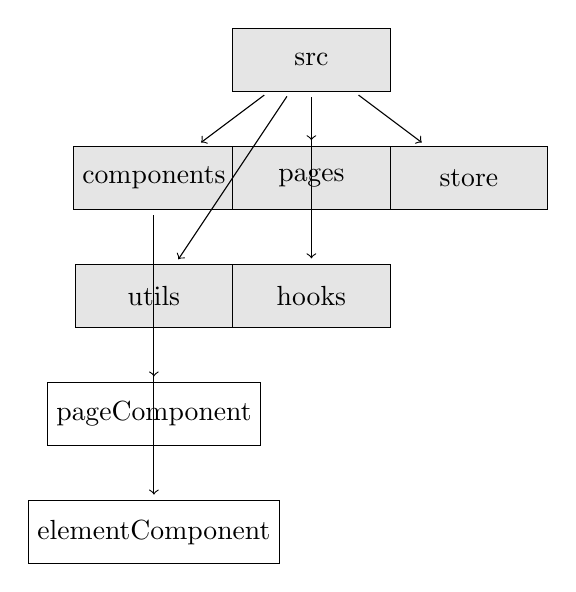
\begin{tikzpicture}[
    file/.style={draw, rectangle, minimum width=2cm, minimum height=0.8cm},
    folder/.style={draw, rectangle, minimum width=2cm, minimum height=0.8cm, fill=gray!20},
    arrow/.style={->, shorten >=2pt, shorten <=2pt}
]

% Folders
\node[folder] (src) at (0,0) {src};
\node[folder] (components) at (-2,-1.5) {components};
\node[folder] (pages) at (0,-1.5) {pages};
\node[folder] (store) at (2,-1.5) {store};
\node[folder] (utils) at (-2,-3) {utils};
\node[folder] (hooks) at (0,-3) {hooks};

% Files
\node[file] (pageComponent) at (-2,-4.5) {pageComponent};
\node[file] (elementComponent) at (-2,-6) {elementComponent};
% ... add more files

% Connections
\draw[arrow] (src) -- (components);
\draw[arrow] (src) -- (pages);
\draw[arrow] (src) -- (store);
\draw[arrow] (src) -- (utils);
\draw[arrow] (src) -- (hooks);
\draw[arrow] (components) -- (pageComponent);
\draw[arrow] (components) -- (elementComponent);
% ... add more connections

\end{tikzpicture}



\pagebreak
\subsubsection{Back-end}
The backend uses the dotNet framework. The development language using the C\# language.

In this project, the backend uses the Onion Architecture.
The Onion Architecture is a typically layered architecture, 
where each layer depends on the inner layer and provides interfaces to the outer layer.
The outer layer provides services to the outermost layer 
and other modules in the same layer based on the interfaces of the inner layer.

From inner to outer, the layers are: Domain, Application, Infrastructure, Presentation.
The Domain layer is the core layer and the innermost layer, used to define domain models, 
which are the business models.
It includes domain models and domain service interfaces.
Domain models are used to define the business models, 
which are the entities in the entity-relationship model and their attributes.
Domain service interfaces are used to define the business services, 
which are the relationships between entities in the entity-relationship model.

The Application layer is the application layer, 
used to define application services, which are the business logic.
It includes domain service implementations and application service interfaces.
Domain service implementations implement the methods of the inner layer's domain service 
interfaces and implement the business logic of the domain models.
Application service interfaces are used to define application services, 
which are the business logic.
It includes but is not limited to database interfaces, testing interfaces, 
HTTP API interfaces, MQTT interfaces, etc.

The Infrastructure layer is the infrastructure layer, used to define infrastructure.
It includes database implementations, testing implementations, 
HTTP API implementations, MQTT implementations, etc.
Database implementations implement the database interfaces 
and provide CRUD services for the database.
Testing implementations implement the testing interfaces 
and provide services for unit testing and integration testing.
HTTP API implementations implement the HTTP API interfaces 
and provide CRUD operations for HTTP APIs.
MQTT implementations implement the MQTT interfaces 
and provide CRUD operations for MQTT.

The Presentation layer is the presentation layer, used to define presentation logic, 
such as interfaces and pages. Since this is a backend project,
data presentation and control are handled by the frontend, 
so this layer is not needed.



\pagebreak
\subsubsection{Data communication and storage}
% 关于本项目的数据通信与数据存储的设计, 包括数据通信的协议, 数据存储的设计等
% 关于数据通信的设计:
% 1. 通信协议的选择
% 自前端向后端发送的数据, 有三种传输的数据类型, 
% 一种是普通的增删改查的请求, 对数据传输的时效性要求不高, 但是对数据的准确性, 完整性, 有序性, 安全性有一定的要求,
% 这种数据的传输, 采用 HTTP 协议, 以及 RESTful API 的设计. 可以有效的保证对数据传输的以上要求.
% 一种是对数据通道的创建和流媒体数据的传输, 对数据传输的时效性, 安全性要求较高, 这种数据的传输, 采用 WebRTC 协议, 以及 MQTT 协议.
% 配合可以快速解码的 flatbuffers 协议, 可以有效的保证对数据传输的以上要求.
% 最后一种是对设备的状态信息和操作信息的传输, 对完整性, 有序性, 安全性都有较高的要求, 这种数据的传输, 采用 MQTT 协议
% 同时也使用了 flatbuffers 协议.
% 
% 2. 数据通信的通信架构和通信流程
% 本项目的数据通信的通信架构, 是基于前后端分离的架构, 前端使用 React 框架, 后端使用 dotnet 框架.
% 当前端需要向后端发送数据的时候, 前端会向后端发送 HTTP 请求, 后端接收到 HTTP 请求之后, 会根据请求的数据类型,
% 选择不同的数据处理方式, 对于普通的增删改查的请求, 后端会根据 RESTful API 的设计, 对数据进行增删改查的操作,
% 对于对数据通道的创建和流媒体数据的传输, 后端会根据 WebRTC 协议, 对数据通道进行创建, 并且帮助前端和设备建立数据通道,
% 当数据通道建立后, 前端和设备之间则使用 flatbuffer 的数据格式对流媒体数据进行传输,
% 对于设备的状态信息和操作信息的传输, 前端会直接向 MQTT broker 发送 MQTT 请求, 
% 设备会在其自身的固件中监听相关的 MQTT 请求, 并且返回相关的数据.
% 
% 3. 数据通信的格式
% 本项目的数据通信的格式, 有三种, 
% 一种是 HTTP 协议, 
% 使用 json 格式对数据进行传输,
% 一种是 WebRTC 协议, 
% 使用 flatbuffers 格式对数据进行传输,
% 一种是 MQTT 协议.
% 使用 flatbuffers 格式对数据进行传输,
% 
% 关于数据存储的设计:
% 1. 数据存储的数据库的选择
% 本项目的数据存储的数据库的选择, 使用了轻量级的数据库 SQLite,
% SQLite 是一个进程内的库, 实现了自给自足的, 无服务器的, 零配置的, 事务性的 SQL 数据库引擎.
% 这是因为整个项目的目的是为了实现前端与设备之间的数据通信, 对于数据库数据的增删改查操作的要求不高,
% 数据量较小, 且对于数据库的数据的事务性要求不高, 所以选择了 SQLite 数据库.
% 2. 项目前后端的数据结构的设计
% 在本项目中, 前端由于使用了 React 框架, 所以前端的数据结构的设计, 使用了基于状态的数据结构的设计,
% 每个组件或者数据集都包含一个状态对象, 这个状态对象的属性就是组件的各个状态. 
% 使用状态对象的原因是, 可以方便的对状态进行管理, 采用对象-属性的形式, 可以方便的针对不同组件的同类状态进行区分,
% 由于跨组件的状态是由 redux 进行管理的, 这种状态对象的设计, 可以更搞笑的对状态进行更新和传递.
% 后端由于使用了 dotnet 框架, 所以后端的数据结构的设计, 使用了基于类的数据结构的设计,
% 采用了面向对象的编程思想, 对数据进行了封装, 使得数据的传输更加的安全, 有序, 完整.


\pagebreak

% \subsection{Domain model}
% \documentclass[]{article}
\usepackage{graphicx}
\usepackage{amsmath}
\usepackage{tikz}

% libaries
\usetikzlibrary{shapes,arrows}

%Define the listing package
\usepackage{listings} %code highlighter
\usepackage{color} %use color
\definecolor{mygreen}{rgb}{0,0.6,0}
\definecolor{mygray}{rgb}{0.5,0.5,0.5}
\definecolor{mymauve}{rgb}{0.58,0,0.82}

%Customize a bit the look
\lstset{ %
backgroundcolor=\color{white}, % choose the background color; you must add \usepackage{color} or \usepackage{xcolor}
basicstyle=\footnotesize, % the size of the fonts that are used for the code
breakatwhitespace=false, % sets if automatic breaks should only happen at whitespace
breaklines=true, % sets automatic line breaking
captionpos=b, % sets the caption-position to bottom
commentstyle=\color{mygreen}, % comment style
deletekeywords={...}, % if you want to delete keywords from the given language
escapeinside={\%*}{*)}, % if you want to add LaTeX within your code
extendedchars=true, % lets you use non-ASCII characters; for 8-bits encodings only, does not work with UTF-8
frame=single, % adds a frame around the code
keepspaces=true, % keeps spaces in text, useful for keeping indentation of code (possibly needs columns=flexible)
keywordstyle=\color{blue}, % keyword style
% language=Octave, % the language of the code
morekeywords={*,...}, % if you want to add more keywords to the set
numbers=left, % where to put the line-numbers; possible values are (none, left, right)
numbersep=5pt, % how far the line-numbers are from the code
numberstyle=\tiny\color{mygray}, % the style that is used for the line-numbers
rulecolor=\color{black}, % if not set, the frame-color may be changed on line-breaks within not-black text (e.g. comments (green here))
showspaces=false, % show spaces everywhere adding particular underscores; it overrides 'showstringspaces'
showstringspaces=false, % underline spaces within strings only
showtabs=false, % show tabs within strings adding particular underscores
stepnumber=1, % the step between two line-numbers. If it's 1, each line will be numbered
stringstyle=\color{mymauve}, % string literal style
tabsize=2, % sets default tabsize to 2 spaces
title=\lstname % show the filename of files included with \lstinputlisting; also try caption instead of title
}

\definecolor{darkgray}{rgb}{.4,.4,.4}
\definecolor{purple}{rgb}{0.65, 0.12, 0.82}

\lstdefinelanguage{React}{
keywords={const, typeof, new, true, false, catch, function, return, null, catch, switch, var, if, in, while, do, else, case, break},
keywordstyle=\color{blue}\bfseries,
ndkeywords={class, export, boolean, throw, implements, import, this},
ndkeywordstyle=\color{darkgray}\bfseries,
identifierstyle=\color{mygreen},
sensitive=false,
comment=[l]{//},
morecomment=[s]{/*}{*/},
commentstyle=\color{purple}\ttfamily,
string=[b]{"}{'}{`},
stringstyle=\color{red}\ttfamily,
morestring=[b]',
morestring=[b]",
morestring=[b]`',
}

\lstdefinelanguage{CSharp}{
keywords={const, typeof, new, true, false, catch, function, return, null, catch, switch, var, if, in, while, do, else, case, break},
keywordstyle=\color{blue}\bfseries,
ndkeywords={class, export, boolean, throw, implements, import, this},
ndkeywordstyle=\color{darkgray}\bfseries,
identifierstyle=\color{mygreen},
sensitive=false,
comment=[l]{//},
morecomment=[s]{/*}{*/},
commentstyle=\color{purple}\ttfamily,
string=[b]{"}{'}{`},
stringstyle=\color{red}\ttfamily,
morestring=[b]',
morestring=[b]",
morestring=[b]`',
}

\lstset{
language=React,
extendedchars=true,
basicstyle=\footnotesize\ttfamily,
showstringspaces=false,
showspaces=false,
numbers=left,
numberstyle=\footnotesize,
numbersep=9pt,
tabsize=2,
breaklines=true,
showtabs=false,
captionpos=b
}

\lstset{
language=CSharp,
extendedchars=true,
basicstyle=\footnotesize\ttfamily,
showstringspaces=false,
showspaces=false,
numbers=left,
numberstyle=\footnotesize,
numbersep=9pt,
tabsize=2,
breaklines=true,
showtabs=false,
captionpos=b
}

% \usepackage{cite} % Add this line for citation

% \bibliographystyle{plain}

\title{
The implementation of BifrostConnect Front-end scope, 
re-design and development with the relevant back-end support develop.
}
\author{
    Fei Gu \\
    Erhvervs Akademi Sydvest \\
    Computer Science 21\\
    }
\date{\today}

\begin{document}

% Front page
\maketitle
\begin{center}
    Supervisor: Henrik Boulund Meng Hansen \\
    Company: BifrostConnect \\
    Engineering Director: Jasper Wass \\
\end{center}
\tableofcontents
\pagebreak


% The introduction
\section{Introduction}
\subsection{Background}\input{sections/introduction/background.tex}
\subsection{The company}\input{sections/introduction/aboutCompany}
\subsection{The project}\input{sections/introduction/aboutProject}
\pagebreak

% The problem statement
\section{Problem Statement}
\subsection{Statement}
\input{sections/problemStatement/statement}
\subsection{Situation}
\input{sections/problemStatement/situation}
\subsection{Potential Solution}
\input{sections/problemStatement/potentialSolution}
\pagebreak

% Requirement analysis
\section{Requirement Analysis}
\input{sections/requirementAnalysis/index}

\subsection{Stakeholders}
\input{sections/requirementAnalysis/stakeholders/index}

\subsection{Business Domain}
\input{sections/requirementAnalysis/bussinesDomain/index}

\subsection{Scope}
\input{sections/requirementAnalysis/scope}

\subsection{Goals}
\input{sections/requirementAnalysis/goals}
\pagebreak

% Software Design
\section{Software Design}
% developement methods
\subsection{Software Development Methods}
\input{sections/softwareDevelopmentMethods/index}
\subsubsection{Agile Software Development}
\input{sections/softwareDevelopmentMethods/agileSoftwareDevelopment/index}
\subsubsection{Feature Driven Development}
\input{sections/softwareDevelopmentMethods/featureDrivenDevelopment/index}

\pagebreak

% Technology seslection
\subsection{Technology selection}
\input{sections/softwareDesign/technologySelection/index}
\subsubsection{Front-end}
\input{sections/softwareDesign/technologySelection/frontEnd}            
\subsubsection{Back-end}
\input{sections/softwareDesign/technologySelection/backEnd}            
\subsubsection{Database}
\input{sections/softwareDesign/technologySelection/database}
\subsubsection{Data communication}
\input{sections/softwareDesign/technologySelection/dataCommunication}            
\subsubsection{DevOps}
\input{sections/softwareDesign/technologySelection/devOps}
\pagebreak

% Architecture design
\subsection{Architecture design}
\input{sections/softwareDesign/architectureDesign/index}
\pagebreak
\subsubsection{Front-end}
\input{sections/softwareDesign/architectureDesign/frontEndArchitecture}
\pagebreak
\subsubsection{Back-end}
\input{sections/softwareDesign/architectureDesign/backEndArchitecture}
\pagebreak
\subsubsection{Data communication and storage}
\input{sections/softwareDesign/architectureDesign/dataCommunicationArchitecture}
\pagebreak

% \subsection{Domain model}
% \input{sections/softwareDesign/domainModel/index}
% \subsection{Database design}
% % 数据库领域模型 ER 图
% % 包括表和字段的设置.
% % 对于私有键和外键的设置.

% \subsection{Back-end design}
% % 后端对象模型
% % 以及对于对象模型的增删改查
% % 以及相关的其他服务的设计`'

% \subsection{Front-end design}
% % 对于前端的页面结构的设计 
% % 页面的状态的设计, 交互设计

% \subsection{FlatBuffers design}
% % schema 的设计

\subsection{DevOps CI/CD process design}
\input{sections/softwareDesign/devOpsDesign/index}
\subsubsection{Continuous Integration}
\input{sections/softwareDesign/devOpsDesign/continuousIntegration/index}
\subsubsection{Continuous Delivery}
\input{sections/softwareDesign/devOpsDesign/continuousDelivery/index}
\subsubsection{Continuous Deployment}
\input{sections/softwareDesign/devOpsDesign/continuousDeployment/index}
\pagebreak

\section{Software Development} 
\input{sections/softwareDevelopment/index}
\subsection{Overall development}
\input{sections/softwareDevelopment/overallDevelopement/index}
\subsubsection{Front-end}
\input{sections/softwareDevelopment/overallDevelopement/frontEnd/index}
\subsubsection{Back-end}
\input{sections/softwareDevelopment/overallDevelopement/backEnd/index}
\subsubsection{DevOps}
\input{sections/softwareDevelopment/overallDevelopement/devOps/index}
\subsection{Feature development} 
\input{sections/softwareDevelopment/featureDevelopment/index}
\subsubsection{Use Case 1}
\input{sections/softwareDevelopment/featureDevelopment/useCase1/index}
\subsubsection{Feature 1}
\input{sections/softwareDevelopment/featureDevelopment/feature/feature1.tex}
\pagebreak
\section{Conclusion} 
\subsection{Result}
Since the project is still in progress, the result is not available yet.
So far, basic structure of this project has been built. But the most features 
are not implemented yet. 
\subsection{Discussion}
As a single developer for this project, I am confident what I have done so far.
And I can say I understand the most of the knowledge I have used in this project, 
which also means I can explain all the part of the project. 
But this project also relevant some of the complex knowledge which I have to continue 
to study and practice.
\subsection{Future Work}
The future work is to implement the rest of the features. 
Including the most important part which is the 'create session' feature.
\pagebreak
% \bibliography{bibliography}
\pagebreak
% \begin{appendices}
%     \section{Appendix}
% \end{appendices} 
\end{document}
% \subsection{Database design}
% % 数据库领域模型 ER 图
% % 包括表和字段的设置.
% % 对于私有键和外键的设置.

% \subsection{Back-end design}
% % 后端对象模型
% % 以及对于对象模型的增删改查
% % 以及相关的其他服务的设计`'

% \subsection{Front-end design}
% % 对于前端的页面结构的设计 
% % 页面的状态的设计, 交互设计

% \subsection{FlatBuffers design}
% % schema 的设计

\subsection{DevOps CI/CD process design}
\documentclass[]{article}
\usepackage{graphicx}
\usepackage{amsmath}
\usepackage{tikz}

% libaries
\usetikzlibrary{shapes,arrows}

%Define the listing package
\usepackage{listings} %code highlighter
\usepackage{color} %use color
\definecolor{mygreen}{rgb}{0,0.6,0}
\definecolor{mygray}{rgb}{0.5,0.5,0.5}
\definecolor{mymauve}{rgb}{0.58,0,0.82}

%Customize a bit the look
\lstset{ %
backgroundcolor=\color{white}, % choose the background color; you must add \usepackage{color} or \usepackage{xcolor}
basicstyle=\footnotesize, % the size of the fonts that are used for the code
breakatwhitespace=false, % sets if automatic breaks should only happen at whitespace
breaklines=true, % sets automatic line breaking
captionpos=b, % sets the caption-position to bottom
commentstyle=\color{mygreen}, % comment style
deletekeywords={...}, % if you want to delete keywords from the given language
escapeinside={\%*}{*)}, % if you want to add LaTeX within your code
extendedchars=true, % lets you use non-ASCII characters; for 8-bits encodings only, does not work with UTF-8
frame=single, % adds a frame around the code
keepspaces=true, % keeps spaces in text, useful for keeping indentation of code (possibly needs columns=flexible)
keywordstyle=\color{blue}, % keyword style
% language=Octave, % the language of the code
morekeywords={*,...}, % if you want to add more keywords to the set
numbers=left, % where to put the line-numbers; possible values are (none, left, right)
numbersep=5pt, % how far the line-numbers are from the code
numberstyle=\tiny\color{mygray}, % the style that is used for the line-numbers
rulecolor=\color{black}, % if not set, the frame-color may be changed on line-breaks within not-black text (e.g. comments (green here))
showspaces=false, % show spaces everywhere adding particular underscores; it overrides 'showstringspaces'
showstringspaces=false, % underline spaces within strings only
showtabs=false, % show tabs within strings adding particular underscores
stepnumber=1, % the step between two line-numbers. If it's 1, each line will be numbered
stringstyle=\color{mymauve}, % string literal style
tabsize=2, % sets default tabsize to 2 spaces
title=\lstname % show the filename of files included with \lstinputlisting; also try caption instead of title
}

\definecolor{darkgray}{rgb}{.4,.4,.4}
\definecolor{purple}{rgb}{0.65, 0.12, 0.82}

\lstdefinelanguage{React}{
keywords={const, typeof, new, true, false, catch, function, return, null, catch, switch, var, if, in, while, do, else, case, break},
keywordstyle=\color{blue}\bfseries,
ndkeywords={class, export, boolean, throw, implements, import, this},
ndkeywordstyle=\color{darkgray}\bfseries,
identifierstyle=\color{mygreen},
sensitive=false,
comment=[l]{//},
morecomment=[s]{/*}{*/},
commentstyle=\color{purple}\ttfamily,
string=[b]{"}{'}{`},
stringstyle=\color{red}\ttfamily,
morestring=[b]',
morestring=[b]",
morestring=[b]`',
}

\lstdefinelanguage{CSharp}{
keywords={const, typeof, new, true, false, catch, function, return, null, catch, switch, var, if, in, while, do, else, case, break},
keywordstyle=\color{blue}\bfseries,
ndkeywords={class, export, boolean, throw, implements, import, this},
ndkeywordstyle=\color{darkgray}\bfseries,
identifierstyle=\color{mygreen},
sensitive=false,
comment=[l]{//},
morecomment=[s]{/*}{*/},
commentstyle=\color{purple}\ttfamily,
string=[b]{"}{'}{`},
stringstyle=\color{red}\ttfamily,
morestring=[b]',
morestring=[b]",
morestring=[b]`',
}

\lstset{
language=React,
extendedchars=true,
basicstyle=\footnotesize\ttfamily,
showstringspaces=false,
showspaces=false,
numbers=left,
numberstyle=\footnotesize,
numbersep=9pt,
tabsize=2,
breaklines=true,
showtabs=false,
captionpos=b
}

\lstset{
language=CSharp,
extendedchars=true,
basicstyle=\footnotesize\ttfamily,
showstringspaces=false,
showspaces=false,
numbers=left,
numberstyle=\footnotesize,
numbersep=9pt,
tabsize=2,
breaklines=true,
showtabs=false,
captionpos=b
}

% \usepackage{cite} % Add this line for citation

% \bibliographystyle{plain}

\title{
The implementation of BifrostConnect Front-end scope, 
re-design and development with the relevant back-end support develop.
}
\author{
    Fei Gu \\
    Erhvervs Akademi Sydvest \\
    Computer Science 21\\
    }
\date{\today}

\begin{document}

% Front page
\maketitle
\begin{center}
    Supervisor: Henrik Boulund Meng Hansen \\
    Company: BifrostConnect \\
    Engineering Director: Jasper Wass \\
\end{center}
\tableofcontents
\pagebreak


% The introduction
\section{Introduction}
\subsection{Background}\input{sections/introduction/background.tex}
\subsection{The company}\input{sections/introduction/aboutCompany}
\subsection{The project}\input{sections/introduction/aboutProject}
\pagebreak

% The problem statement
\section{Problem Statement}
\subsection{Statement}
\input{sections/problemStatement/statement}
\subsection{Situation}
\input{sections/problemStatement/situation}
\subsection{Potential Solution}
\input{sections/problemStatement/potentialSolution}
\pagebreak

% Requirement analysis
\section{Requirement Analysis}
\input{sections/requirementAnalysis/index}

\subsection{Stakeholders}
\input{sections/requirementAnalysis/stakeholders/index}

\subsection{Business Domain}
\input{sections/requirementAnalysis/bussinesDomain/index}

\subsection{Scope}
\input{sections/requirementAnalysis/scope}

\subsection{Goals}
\input{sections/requirementAnalysis/goals}
\pagebreak

% Software Design
\section{Software Design}
% developement methods
\subsection{Software Development Methods}
\input{sections/softwareDevelopmentMethods/index}
\subsubsection{Agile Software Development}
\input{sections/softwareDevelopmentMethods/agileSoftwareDevelopment/index}
\subsubsection{Feature Driven Development}
\input{sections/softwareDevelopmentMethods/featureDrivenDevelopment/index}

\pagebreak

% Technology seslection
\subsection{Technology selection}
\input{sections/softwareDesign/technologySelection/index}
\subsubsection{Front-end}
\input{sections/softwareDesign/technologySelection/frontEnd}            
\subsubsection{Back-end}
\input{sections/softwareDesign/technologySelection/backEnd}            
\subsubsection{Database}
\input{sections/softwareDesign/technologySelection/database}
\subsubsection{Data communication}
\input{sections/softwareDesign/technologySelection/dataCommunication}            
\subsubsection{DevOps}
\input{sections/softwareDesign/technologySelection/devOps}
\pagebreak

% Architecture design
\subsection{Architecture design}
\input{sections/softwareDesign/architectureDesign/index}
\pagebreak
\subsubsection{Front-end}
\input{sections/softwareDesign/architectureDesign/frontEndArchitecture}
\pagebreak
\subsubsection{Back-end}
\input{sections/softwareDesign/architectureDesign/backEndArchitecture}
\pagebreak
\subsubsection{Data communication and storage}
\input{sections/softwareDesign/architectureDesign/dataCommunicationArchitecture}
\pagebreak

% \subsection{Domain model}
% \input{sections/softwareDesign/domainModel/index}
% \subsection{Database design}
% % 数据库领域模型 ER 图
% % 包括表和字段的设置.
% % 对于私有键和外键的设置.

% \subsection{Back-end design}
% % 后端对象模型
% % 以及对于对象模型的增删改查
% % 以及相关的其他服务的设计`'

% \subsection{Front-end design}
% % 对于前端的页面结构的设计 
% % 页面的状态的设计, 交互设计

% \subsection{FlatBuffers design}
% % schema 的设计

\subsection{DevOps CI/CD process design}
\input{sections/softwareDesign/devOpsDesign/index}
\subsubsection{Continuous Integration}
\input{sections/softwareDesign/devOpsDesign/continuousIntegration/index}
\subsubsection{Continuous Delivery}
\input{sections/softwareDesign/devOpsDesign/continuousDelivery/index}
\subsubsection{Continuous Deployment}
\input{sections/softwareDesign/devOpsDesign/continuousDeployment/index}
\pagebreak

\section{Software Development} 
\input{sections/softwareDevelopment/index}
\subsection{Overall development}
\input{sections/softwareDevelopment/overallDevelopement/index}
\subsubsection{Front-end}
\input{sections/softwareDevelopment/overallDevelopement/frontEnd/index}
\subsubsection{Back-end}
\input{sections/softwareDevelopment/overallDevelopement/backEnd/index}
\subsubsection{DevOps}
\input{sections/softwareDevelopment/overallDevelopement/devOps/index}
\subsection{Feature development} 
\input{sections/softwareDevelopment/featureDevelopment/index}
\subsubsection{Use Case 1}
\input{sections/softwareDevelopment/featureDevelopment/useCase1/index}
\subsubsection{Feature 1}
\input{sections/softwareDevelopment/featureDevelopment/feature/feature1.tex}
\pagebreak
\section{Conclusion} 
\subsection{Result}
Since the project is still in progress, the result is not available yet.
So far, basic structure of this project has been built. But the most features 
are not implemented yet. 
\subsection{Discussion}
As a single developer for this project, I am confident what I have done so far.
And I can say I understand the most of the knowledge I have used in this project, 
which also means I can explain all the part of the project. 
But this project also relevant some of the complex knowledge which I have to continue 
to study and practice.
\subsection{Future Work}
The future work is to implement the rest of the features. 
Including the most important part which is the 'create session' feature.
\pagebreak
% \bibliography{bibliography}
\pagebreak
% \begin{appendices}
%     \section{Appendix}
% \end{appendices} 
\end{document}
\subsubsection{Continuous Integration}
\documentclass[]{article}
\usepackage{graphicx}
\usepackage{amsmath}
\usepackage{tikz}

% libaries
\usetikzlibrary{shapes,arrows}

%Define the listing package
\usepackage{listings} %code highlighter
\usepackage{color} %use color
\definecolor{mygreen}{rgb}{0,0.6,0}
\definecolor{mygray}{rgb}{0.5,0.5,0.5}
\definecolor{mymauve}{rgb}{0.58,0,0.82}

%Customize a bit the look
\lstset{ %
backgroundcolor=\color{white}, % choose the background color; you must add \usepackage{color} or \usepackage{xcolor}
basicstyle=\footnotesize, % the size of the fonts that are used for the code
breakatwhitespace=false, % sets if automatic breaks should only happen at whitespace
breaklines=true, % sets automatic line breaking
captionpos=b, % sets the caption-position to bottom
commentstyle=\color{mygreen}, % comment style
deletekeywords={...}, % if you want to delete keywords from the given language
escapeinside={\%*}{*)}, % if you want to add LaTeX within your code
extendedchars=true, % lets you use non-ASCII characters; for 8-bits encodings only, does not work with UTF-8
frame=single, % adds a frame around the code
keepspaces=true, % keeps spaces in text, useful for keeping indentation of code (possibly needs columns=flexible)
keywordstyle=\color{blue}, % keyword style
% language=Octave, % the language of the code
morekeywords={*,...}, % if you want to add more keywords to the set
numbers=left, % where to put the line-numbers; possible values are (none, left, right)
numbersep=5pt, % how far the line-numbers are from the code
numberstyle=\tiny\color{mygray}, % the style that is used for the line-numbers
rulecolor=\color{black}, % if not set, the frame-color may be changed on line-breaks within not-black text (e.g. comments (green here))
showspaces=false, % show spaces everywhere adding particular underscores; it overrides 'showstringspaces'
showstringspaces=false, % underline spaces within strings only
showtabs=false, % show tabs within strings adding particular underscores
stepnumber=1, % the step between two line-numbers. If it's 1, each line will be numbered
stringstyle=\color{mymauve}, % string literal style
tabsize=2, % sets default tabsize to 2 spaces
title=\lstname % show the filename of files included with \lstinputlisting; also try caption instead of title
}

\definecolor{darkgray}{rgb}{.4,.4,.4}
\definecolor{purple}{rgb}{0.65, 0.12, 0.82}

\lstdefinelanguage{React}{
keywords={const, typeof, new, true, false, catch, function, return, null, catch, switch, var, if, in, while, do, else, case, break},
keywordstyle=\color{blue}\bfseries,
ndkeywords={class, export, boolean, throw, implements, import, this},
ndkeywordstyle=\color{darkgray}\bfseries,
identifierstyle=\color{mygreen},
sensitive=false,
comment=[l]{//},
morecomment=[s]{/*}{*/},
commentstyle=\color{purple}\ttfamily,
string=[b]{"}{'}{`},
stringstyle=\color{red}\ttfamily,
morestring=[b]',
morestring=[b]",
morestring=[b]`',
}

\lstdefinelanguage{CSharp}{
keywords={const, typeof, new, true, false, catch, function, return, null, catch, switch, var, if, in, while, do, else, case, break},
keywordstyle=\color{blue}\bfseries,
ndkeywords={class, export, boolean, throw, implements, import, this},
ndkeywordstyle=\color{darkgray}\bfseries,
identifierstyle=\color{mygreen},
sensitive=false,
comment=[l]{//},
morecomment=[s]{/*}{*/},
commentstyle=\color{purple}\ttfamily,
string=[b]{"}{'}{`},
stringstyle=\color{red}\ttfamily,
morestring=[b]',
morestring=[b]",
morestring=[b]`',
}

\lstset{
language=React,
extendedchars=true,
basicstyle=\footnotesize\ttfamily,
showstringspaces=false,
showspaces=false,
numbers=left,
numberstyle=\footnotesize,
numbersep=9pt,
tabsize=2,
breaklines=true,
showtabs=false,
captionpos=b
}

\lstset{
language=CSharp,
extendedchars=true,
basicstyle=\footnotesize\ttfamily,
showstringspaces=false,
showspaces=false,
numbers=left,
numberstyle=\footnotesize,
numbersep=9pt,
tabsize=2,
breaklines=true,
showtabs=false,
captionpos=b
}

% \usepackage{cite} % Add this line for citation

% \bibliographystyle{plain}

\title{
The implementation of BifrostConnect Front-end scope, 
re-design and development with the relevant back-end support develop.
}
\author{
    Fei Gu \\
    Erhvervs Akademi Sydvest \\
    Computer Science 21\\
    }
\date{\today}

\begin{document}

% Front page
\maketitle
\begin{center}
    Supervisor: Henrik Boulund Meng Hansen \\
    Company: BifrostConnect \\
    Engineering Director: Jasper Wass \\
\end{center}
\tableofcontents
\pagebreak


% The introduction
\section{Introduction}
\subsection{Background}\input{sections/introduction/background.tex}
\subsection{The company}\input{sections/introduction/aboutCompany}
\subsection{The project}\input{sections/introduction/aboutProject}
\pagebreak

% The problem statement
\section{Problem Statement}
\subsection{Statement}
\input{sections/problemStatement/statement}
\subsection{Situation}
\input{sections/problemStatement/situation}
\subsection{Potential Solution}
\input{sections/problemStatement/potentialSolution}
\pagebreak

% Requirement analysis
\section{Requirement Analysis}
\input{sections/requirementAnalysis/index}

\subsection{Stakeholders}
\input{sections/requirementAnalysis/stakeholders/index}

\subsection{Business Domain}
\input{sections/requirementAnalysis/bussinesDomain/index}

\subsection{Scope}
\input{sections/requirementAnalysis/scope}

\subsection{Goals}
\input{sections/requirementAnalysis/goals}
\pagebreak

% Software Design
\section{Software Design}
% developement methods
\subsection{Software Development Methods}
\input{sections/softwareDevelopmentMethods/index}
\subsubsection{Agile Software Development}
\input{sections/softwareDevelopmentMethods/agileSoftwareDevelopment/index}
\subsubsection{Feature Driven Development}
\input{sections/softwareDevelopmentMethods/featureDrivenDevelopment/index}

\pagebreak

% Technology seslection
\subsection{Technology selection}
\input{sections/softwareDesign/technologySelection/index}
\subsubsection{Front-end}
\input{sections/softwareDesign/technologySelection/frontEnd}            
\subsubsection{Back-end}
\input{sections/softwareDesign/technologySelection/backEnd}            
\subsubsection{Database}
\input{sections/softwareDesign/technologySelection/database}
\subsubsection{Data communication}
\input{sections/softwareDesign/technologySelection/dataCommunication}            
\subsubsection{DevOps}
\input{sections/softwareDesign/technologySelection/devOps}
\pagebreak

% Architecture design
\subsection{Architecture design}
\input{sections/softwareDesign/architectureDesign/index}
\pagebreak
\subsubsection{Front-end}
\input{sections/softwareDesign/architectureDesign/frontEndArchitecture}
\pagebreak
\subsubsection{Back-end}
\input{sections/softwareDesign/architectureDesign/backEndArchitecture}
\pagebreak
\subsubsection{Data communication and storage}
\input{sections/softwareDesign/architectureDesign/dataCommunicationArchitecture}
\pagebreak

% \subsection{Domain model}
% \input{sections/softwareDesign/domainModel/index}
% \subsection{Database design}
% % 数据库领域模型 ER 图
% % 包括表和字段的设置.
% % 对于私有键和外键的设置.

% \subsection{Back-end design}
% % 后端对象模型
% % 以及对于对象模型的增删改查
% % 以及相关的其他服务的设计`'

% \subsection{Front-end design}
% % 对于前端的页面结构的设计 
% % 页面的状态的设计, 交互设计

% \subsection{FlatBuffers design}
% % schema 的设计

\subsection{DevOps CI/CD process design}
\input{sections/softwareDesign/devOpsDesign/index}
\subsubsection{Continuous Integration}
\input{sections/softwareDesign/devOpsDesign/continuousIntegration/index}
\subsubsection{Continuous Delivery}
\input{sections/softwareDesign/devOpsDesign/continuousDelivery/index}
\subsubsection{Continuous Deployment}
\input{sections/softwareDesign/devOpsDesign/continuousDeployment/index}
\pagebreak

\section{Software Development} 
\input{sections/softwareDevelopment/index}
\subsection{Overall development}
\input{sections/softwareDevelopment/overallDevelopement/index}
\subsubsection{Front-end}
\input{sections/softwareDevelopment/overallDevelopement/frontEnd/index}
\subsubsection{Back-end}
\input{sections/softwareDevelopment/overallDevelopement/backEnd/index}
\subsubsection{DevOps}
\input{sections/softwareDevelopment/overallDevelopement/devOps/index}
\subsection{Feature development} 
\input{sections/softwareDevelopment/featureDevelopment/index}
\subsubsection{Use Case 1}
\input{sections/softwareDevelopment/featureDevelopment/useCase1/index}
\subsubsection{Feature 1}
\input{sections/softwareDevelopment/featureDevelopment/feature/feature1.tex}
\pagebreak
\section{Conclusion} 
\subsection{Result}
Since the project is still in progress, the result is not available yet.
So far, basic structure of this project has been built. But the most features 
are not implemented yet. 
\subsection{Discussion}
As a single developer for this project, I am confident what I have done so far.
And I can say I understand the most of the knowledge I have used in this project, 
which also means I can explain all the part of the project. 
But this project also relevant some of the complex knowledge which I have to continue 
to study and practice.
\subsection{Future Work}
The future work is to implement the rest of the features. 
Including the most important part which is the 'create session' feature.
\pagebreak
% \bibliography{bibliography}
\pagebreak
% \begin{appendices}
%     \section{Appendix}
% \end{appendices} 
\end{document}
\subsubsection{Continuous Delivery}
\documentclass[]{article}
\usepackage{graphicx}
\usepackage{amsmath}
\usepackage{tikz}

% libaries
\usetikzlibrary{shapes,arrows}

%Define the listing package
\usepackage{listings} %code highlighter
\usepackage{color} %use color
\definecolor{mygreen}{rgb}{0,0.6,0}
\definecolor{mygray}{rgb}{0.5,0.5,0.5}
\definecolor{mymauve}{rgb}{0.58,0,0.82}

%Customize a bit the look
\lstset{ %
backgroundcolor=\color{white}, % choose the background color; you must add \usepackage{color} or \usepackage{xcolor}
basicstyle=\footnotesize, % the size of the fonts that are used for the code
breakatwhitespace=false, % sets if automatic breaks should only happen at whitespace
breaklines=true, % sets automatic line breaking
captionpos=b, % sets the caption-position to bottom
commentstyle=\color{mygreen}, % comment style
deletekeywords={...}, % if you want to delete keywords from the given language
escapeinside={\%*}{*)}, % if you want to add LaTeX within your code
extendedchars=true, % lets you use non-ASCII characters; for 8-bits encodings only, does not work with UTF-8
frame=single, % adds a frame around the code
keepspaces=true, % keeps spaces in text, useful for keeping indentation of code (possibly needs columns=flexible)
keywordstyle=\color{blue}, % keyword style
% language=Octave, % the language of the code
morekeywords={*,...}, % if you want to add more keywords to the set
numbers=left, % where to put the line-numbers; possible values are (none, left, right)
numbersep=5pt, % how far the line-numbers are from the code
numberstyle=\tiny\color{mygray}, % the style that is used for the line-numbers
rulecolor=\color{black}, % if not set, the frame-color may be changed on line-breaks within not-black text (e.g. comments (green here))
showspaces=false, % show spaces everywhere adding particular underscores; it overrides 'showstringspaces'
showstringspaces=false, % underline spaces within strings only
showtabs=false, % show tabs within strings adding particular underscores
stepnumber=1, % the step between two line-numbers. If it's 1, each line will be numbered
stringstyle=\color{mymauve}, % string literal style
tabsize=2, % sets default tabsize to 2 spaces
title=\lstname % show the filename of files included with \lstinputlisting; also try caption instead of title
}

\definecolor{darkgray}{rgb}{.4,.4,.4}
\definecolor{purple}{rgb}{0.65, 0.12, 0.82}

\lstdefinelanguage{React}{
keywords={const, typeof, new, true, false, catch, function, return, null, catch, switch, var, if, in, while, do, else, case, break},
keywordstyle=\color{blue}\bfseries,
ndkeywords={class, export, boolean, throw, implements, import, this},
ndkeywordstyle=\color{darkgray}\bfseries,
identifierstyle=\color{mygreen},
sensitive=false,
comment=[l]{//},
morecomment=[s]{/*}{*/},
commentstyle=\color{purple}\ttfamily,
string=[b]{"}{'}{`},
stringstyle=\color{red}\ttfamily,
morestring=[b]',
morestring=[b]",
morestring=[b]`',
}

\lstdefinelanguage{CSharp}{
keywords={const, typeof, new, true, false, catch, function, return, null, catch, switch, var, if, in, while, do, else, case, break},
keywordstyle=\color{blue}\bfseries,
ndkeywords={class, export, boolean, throw, implements, import, this},
ndkeywordstyle=\color{darkgray}\bfseries,
identifierstyle=\color{mygreen},
sensitive=false,
comment=[l]{//},
morecomment=[s]{/*}{*/},
commentstyle=\color{purple}\ttfamily,
string=[b]{"}{'}{`},
stringstyle=\color{red}\ttfamily,
morestring=[b]',
morestring=[b]",
morestring=[b]`',
}

\lstset{
language=React,
extendedchars=true,
basicstyle=\footnotesize\ttfamily,
showstringspaces=false,
showspaces=false,
numbers=left,
numberstyle=\footnotesize,
numbersep=9pt,
tabsize=2,
breaklines=true,
showtabs=false,
captionpos=b
}

\lstset{
language=CSharp,
extendedchars=true,
basicstyle=\footnotesize\ttfamily,
showstringspaces=false,
showspaces=false,
numbers=left,
numberstyle=\footnotesize,
numbersep=9pt,
tabsize=2,
breaklines=true,
showtabs=false,
captionpos=b
}

% \usepackage{cite} % Add this line for citation

% \bibliographystyle{plain}

\title{
The implementation of BifrostConnect Front-end scope, 
re-design and development with the relevant back-end support develop.
}
\author{
    Fei Gu \\
    Erhvervs Akademi Sydvest \\
    Computer Science 21\\
    }
\date{\today}

\begin{document}

% Front page
\maketitle
\begin{center}
    Supervisor: Henrik Boulund Meng Hansen \\
    Company: BifrostConnect \\
    Engineering Director: Jasper Wass \\
\end{center}
\tableofcontents
\pagebreak


% The introduction
\section{Introduction}
\subsection{Background}\input{sections/introduction/background.tex}
\subsection{The company}\input{sections/introduction/aboutCompany}
\subsection{The project}\input{sections/introduction/aboutProject}
\pagebreak

% The problem statement
\section{Problem Statement}
\subsection{Statement}
\input{sections/problemStatement/statement}
\subsection{Situation}
\input{sections/problemStatement/situation}
\subsection{Potential Solution}
\input{sections/problemStatement/potentialSolution}
\pagebreak

% Requirement analysis
\section{Requirement Analysis}
\input{sections/requirementAnalysis/index}

\subsection{Stakeholders}
\input{sections/requirementAnalysis/stakeholders/index}

\subsection{Business Domain}
\input{sections/requirementAnalysis/bussinesDomain/index}

\subsection{Scope}
\input{sections/requirementAnalysis/scope}

\subsection{Goals}
\input{sections/requirementAnalysis/goals}
\pagebreak

% Software Design
\section{Software Design}
% developement methods
\subsection{Software Development Methods}
\input{sections/softwareDevelopmentMethods/index}
\subsubsection{Agile Software Development}
\input{sections/softwareDevelopmentMethods/agileSoftwareDevelopment/index}
\subsubsection{Feature Driven Development}
\input{sections/softwareDevelopmentMethods/featureDrivenDevelopment/index}

\pagebreak

% Technology seslection
\subsection{Technology selection}
\input{sections/softwareDesign/technologySelection/index}
\subsubsection{Front-end}
\input{sections/softwareDesign/technologySelection/frontEnd}            
\subsubsection{Back-end}
\input{sections/softwareDesign/technologySelection/backEnd}            
\subsubsection{Database}
\input{sections/softwareDesign/technologySelection/database}
\subsubsection{Data communication}
\input{sections/softwareDesign/technologySelection/dataCommunication}            
\subsubsection{DevOps}
\input{sections/softwareDesign/technologySelection/devOps}
\pagebreak

% Architecture design
\subsection{Architecture design}
\input{sections/softwareDesign/architectureDesign/index}
\pagebreak
\subsubsection{Front-end}
\input{sections/softwareDesign/architectureDesign/frontEndArchitecture}
\pagebreak
\subsubsection{Back-end}
\input{sections/softwareDesign/architectureDesign/backEndArchitecture}
\pagebreak
\subsubsection{Data communication and storage}
\input{sections/softwareDesign/architectureDesign/dataCommunicationArchitecture}
\pagebreak

% \subsection{Domain model}
% \input{sections/softwareDesign/domainModel/index}
% \subsection{Database design}
% % 数据库领域模型 ER 图
% % 包括表和字段的设置.
% % 对于私有键和外键的设置.

% \subsection{Back-end design}
% % 后端对象模型
% % 以及对于对象模型的增删改查
% % 以及相关的其他服务的设计`'

% \subsection{Front-end design}
% % 对于前端的页面结构的设计 
% % 页面的状态的设计, 交互设计

% \subsection{FlatBuffers design}
% % schema 的设计

\subsection{DevOps CI/CD process design}
\input{sections/softwareDesign/devOpsDesign/index}
\subsubsection{Continuous Integration}
\input{sections/softwareDesign/devOpsDesign/continuousIntegration/index}
\subsubsection{Continuous Delivery}
\input{sections/softwareDesign/devOpsDesign/continuousDelivery/index}
\subsubsection{Continuous Deployment}
\input{sections/softwareDesign/devOpsDesign/continuousDeployment/index}
\pagebreak

\section{Software Development} 
\input{sections/softwareDevelopment/index}
\subsection{Overall development}
\input{sections/softwareDevelopment/overallDevelopement/index}
\subsubsection{Front-end}
\input{sections/softwareDevelopment/overallDevelopement/frontEnd/index}
\subsubsection{Back-end}
\input{sections/softwareDevelopment/overallDevelopement/backEnd/index}
\subsubsection{DevOps}
\input{sections/softwareDevelopment/overallDevelopement/devOps/index}
\subsection{Feature development} 
\input{sections/softwareDevelopment/featureDevelopment/index}
\subsubsection{Use Case 1}
\input{sections/softwareDevelopment/featureDevelopment/useCase1/index}
\subsubsection{Feature 1}
\input{sections/softwareDevelopment/featureDevelopment/feature/feature1.tex}
\pagebreak
\section{Conclusion} 
\subsection{Result}
Since the project is still in progress, the result is not available yet.
So far, basic structure of this project has been built. But the most features 
are not implemented yet. 
\subsection{Discussion}
As a single developer for this project, I am confident what I have done so far.
And I can say I understand the most of the knowledge I have used in this project, 
which also means I can explain all the part of the project. 
But this project also relevant some of the complex knowledge which I have to continue 
to study and practice.
\subsection{Future Work}
The future work is to implement the rest of the features. 
Including the most important part which is the 'create session' feature.
\pagebreak
% \bibliography{bibliography}
\pagebreak
% \begin{appendices}
%     \section{Appendix}
% \end{appendices} 
\end{document}
\subsubsection{Continuous Deployment}
\documentclass[]{article}
\usepackage{graphicx}
\usepackage{amsmath}
\usepackage{tikz}

% libaries
\usetikzlibrary{shapes,arrows}

%Define the listing package
\usepackage{listings} %code highlighter
\usepackage{color} %use color
\definecolor{mygreen}{rgb}{0,0.6,0}
\definecolor{mygray}{rgb}{0.5,0.5,0.5}
\definecolor{mymauve}{rgb}{0.58,0,0.82}

%Customize a bit the look
\lstset{ %
backgroundcolor=\color{white}, % choose the background color; you must add \usepackage{color} or \usepackage{xcolor}
basicstyle=\footnotesize, % the size of the fonts that are used for the code
breakatwhitespace=false, % sets if automatic breaks should only happen at whitespace
breaklines=true, % sets automatic line breaking
captionpos=b, % sets the caption-position to bottom
commentstyle=\color{mygreen}, % comment style
deletekeywords={...}, % if you want to delete keywords from the given language
escapeinside={\%*}{*)}, % if you want to add LaTeX within your code
extendedchars=true, % lets you use non-ASCII characters; for 8-bits encodings only, does not work with UTF-8
frame=single, % adds a frame around the code
keepspaces=true, % keeps spaces in text, useful for keeping indentation of code (possibly needs columns=flexible)
keywordstyle=\color{blue}, % keyword style
% language=Octave, % the language of the code
morekeywords={*,...}, % if you want to add more keywords to the set
numbers=left, % where to put the line-numbers; possible values are (none, left, right)
numbersep=5pt, % how far the line-numbers are from the code
numberstyle=\tiny\color{mygray}, % the style that is used for the line-numbers
rulecolor=\color{black}, % if not set, the frame-color may be changed on line-breaks within not-black text (e.g. comments (green here))
showspaces=false, % show spaces everywhere adding particular underscores; it overrides 'showstringspaces'
showstringspaces=false, % underline spaces within strings only
showtabs=false, % show tabs within strings adding particular underscores
stepnumber=1, % the step between two line-numbers. If it's 1, each line will be numbered
stringstyle=\color{mymauve}, % string literal style
tabsize=2, % sets default tabsize to 2 spaces
title=\lstname % show the filename of files included with \lstinputlisting; also try caption instead of title
}

\definecolor{darkgray}{rgb}{.4,.4,.4}
\definecolor{purple}{rgb}{0.65, 0.12, 0.82}

\lstdefinelanguage{React}{
keywords={const, typeof, new, true, false, catch, function, return, null, catch, switch, var, if, in, while, do, else, case, break},
keywordstyle=\color{blue}\bfseries,
ndkeywords={class, export, boolean, throw, implements, import, this},
ndkeywordstyle=\color{darkgray}\bfseries,
identifierstyle=\color{mygreen},
sensitive=false,
comment=[l]{//},
morecomment=[s]{/*}{*/},
commentstyle=\color{purple}\ttfamily,
string=[b]{"}{'}{`},
stringstyle=\color{red}\ttfamily,
morestring=[b]',
morestring=[b]",
morestring=[b]`',
}

\lstdefinelanguage{CSharp}{
keywords={const, typeof, new, true, false, catch, function, return, null, catch, switch, var, if, in, while, do, else, case, break},
keywordstyle=\color{blue}\bfseries,
ndkeywords={class, export, boolean, throw, implements, import, this},
ndkeywordstyle=\color{darkgray}\bfseries,
identifierstyle=\color{mygreen},
sensitive=false,
comment=[l]{//},
morecomment=[s]{/*}{*/},
commentstyle=\color{purple}\ttfamily,
string=[b]{"}{'}{`},
stringstyle=\color{red}\ttfamily,
morestring=[b]',
morestring=[b]",
morestring=[b]`',
}

\lstset{
language=React,
extendedchars=true,
basicstyle=\footnotesize\ttfamily,
showstringspaces=false,
showspaces=false,
numbers=left,
numberstyle=\footnotesize,
numbersep=9pt,
tabsize=2,
breaklines=true,
showtabs=false,
captionpos=b
}

\lstset{
language=CSharp,
extendedchars=true,
basicstyle=\footnotesize\ttfamily,
showstringspaces=false,
showspaces=false,
numbers=left,
numberstyle=\footnotesize,
numbersep=9pt,
tabsize=2,
breaklines=true,
showtabs=false,
captionpos=b
}

% \usepackage{cite} % Add this line for citation

% \bibliographystyle{plain}

\title{
The implementation of BifrostConnect Front-end scope, 
re-design and development with the relevant back-end support develop.
}
\author{
    Fei Gu \\
    Erhvervs Akademi Sydvest \\
    Computer Science 21\\
    }
\date{\today}

\begin{document}

% Front page
\maketitle
\begin{center}
    Supervisor: Henrik Boulund Meng Hansen \\
    Company: BifrostConnect \\
    Engineering Director: Jasper Wass \\
\end{center}
\tableofcontents
\pagebreak


% The introduction
\section{Introduction}
\subsection{Background}\input{sections/introduction/background.tex}
\subsection{The company}\input{sections/introduction/aboutCompany}
\subsection{The project}\input{sections/introduction/aboutProject}
\pagebreak

% The problem statement
\section{Problem Statement}
\subsection{Statement}
\input{sections/problemStatement/statement}
\subsection{Situation}
\input{sections/problemStatement/situation}
\subsection{Potential Solution}
\input{sections/problemStatement/potentialSolution}
\pagebreak

% Requirement analysis
\section{Requirement Analysis}
\input{sections/requirementAnalysis/index}

\subsection{Stakeholders}
\input{sections/requirementAnalysis/stakeholders/index}

\subsection{Business Domain}
\input{sections/requirementAnalysis/bussinesDomain/index}

\subsection{Scope}
\input{sections/requirementAnalysis/scope}

\subsection{Goals}
\input{sections/requirementAnalysis/goals}
\pagebreak

% Software Design
\section{Software Design}
% developement methods
\subsection{Software Development Methods}
\input{sections/softwareDevelopmentMethods/index}
\subsubsection{Agile Software Development}
\input{sections/softwareDevelopmentMethods/agileSoftwareDevelopment/index}
\subsubsection{Feature Driven Development}
\input{sections/softwareDevelopmentMethods/featureDrivenDevelopment/index}

\pagebreak

% Technology seslection
\subsection{Technology selection}
\input{sections/softwareDesign/technologySelection/index}
\subsubsection{Front-end}
\input{sections/softwareDesign/technologySelection/frontEnd}            
\subsubsection{Back-end}
\input{sections/softwareDesign/technologySelection/backEnd}            
\subsubsection{Database}
\input{sections/softwareDesign/technologySelection/database}
\subsubsection{Data communication}
\input{sections/softwareDesign/technologySelection/dataCommunication}            
\subsubsection{DevOps}
\input{sections/softwareDesign/technologySelection/devOps}
\pagebreak

% Architecture design
\subsection{Architecture design}
\input{sections/softwareDesign/architectureDesign/index}
\pagebreak
\subsubsection{Front-end}
\input{sections/softwareDesign/architectureDesign/frontEndArchitecture}
\pagebreak
\subsubsection{Back-end}
\input{sections/softwareDesign/architectureDesign/backEndArchitecture}
\pagebreak
\subsubsection{Data communication and storage}
\input{sections/softwareDesign/architectureDesign/dataCommunicationArchitecture}
\pagebreak

% \subsection{Domain model}
% \input{sections/softwareDesign/domainModel/index}
% \subsection{Database design}
% % 数据库领域模型 ER 图
% % 包括表和字段的设置.
% % 对于私有键和外键的设置.

% \subsection{Back-end design}
% % 后端对象模型
% % 以及对于对象模型的增删改查
% % 以及相关的其他服务的设计`'

% \subsection{Front-end design}
% % 对于前端的页面结构的设计 
% % 页面的状态的设计, 交互设计

% \subsection{FlatBuffers design}
% % schema 的设计

\subsection{DevOps CI/CD process design}
\input{sections/softwareDesign/devOpsDesign/index}
\subsubsection{Continuous Integration}
\input{sections/softwareDesign/devOpsDesign/continuousIntegration/index}
\subsubsection{Continuous Delivery}
\input{sections/softwareDesign/devOpsDesign/continuousDelivery/index}
\subsubsection{Continuous Deployment}
\input{sections/softwareDesign/devOpsDesign/continuousDeployment/index}
\pagebreak

\section{Software Development} 
\input{sections/softwareDevelopment/index}
\subsection{Overall development}
\input{sections/softwareDevelopment/overallDevelopement/index}
\subsubsection{Front-end}
\input{sections/softwareDevelopment/overallDevelopement/frontEnd/index}
\subsubsection{Back-end}
\input{sections/softwareDevelopment/overallDevelopement/backEnd/index}
\subsubsection{DevOps}
\input{sections/softwareDevelopment/overallDevelopement/devOps/index}
\subsection{Feature development} 
\input{sections/softwareDevelopment/featureDevelopment/index}
\subsubsection{Use Case 1}
\input{sections/softwareDevelopment/featureDevelopment/useCase1/index}
\subsubsection{Feature 1}
\input{sections/softwareDevelopment/featureDevelopment/feature/feature1.tex}
\pagebreak
\section{Conclusion} 
\subsection{Result}
Since the project is still in progress, the result is not available yet.
So far, basic structure of this project has been built. But the most features 
are not implemented yet. 
\subsection{Discussion}
As a single developer for this project, I am confident what I have done so far.
And I can say I understand the most of the knowledge I have used in this project, 
which also means I can explain all the part of the project. 
But this project also relevant some of the complex knowledge which I have to continue 
to study and practice.
\subsection{Future Work}
The future work is to implement the rest of the features. 
Including the most important part which is the 'create session' feature.
\pagebreak
% \bibliography{bibliography}
\pagebreak
% \begin{appendices}
%     \section{Appendix}
% \end{appendices} 
\end{document}
\pagebreak

\section{Software Development} 
\documentclass[]{article}
\usepackage{graphicx}
\usepackage{amsmath}
\usepackage{tikz}

% libaries
\usetikzlibrary{shapes,arrows}

%Define the listing package
\usepackage{listings} %code highlighter
\usepackage{color} %use color
\definecolor{mygreen}{rgb}{0,0.6,0}
\definecolor{mygray}{rgb}{0.5,0.5,0.5}
\definecolor{mymauve}{rgb}{0.58,0,0.82}

%Customize a bit the look
\lstset{ %
backgroundcolor=\color{white}, % choose the background color; you must add \usepackage{color} or \usepackage{xcolor}
basicstyle=\footnotesize, % the size of the fonts that are used for the code
breakatwhitespace=false, % sets if automatic breaks should only happen at whitespace
breaklines=true, % sets automatic line breaking
captionpos=b, % sets the caption-position to bottom
commentstyle=\color{mygreen}, % comment style
deletekeywords={...}, % if you want to delete keywords from the given language
escapeinside={\%*}{*)}, % if you want to add LaTeX within your code
extendedchars=true, % lets you use non-ASCII characters; for 8-bits encodings only, does not work with UTF-8
frame=single, % adds a frame around the code
keepspaces=true, % keeps spaces in text, useful for keeping indentation of code (possibly needs columns=flexible)
keywordstyle=\color{blue}, % keyword style
% language=Octave, % the language of the code
morekeywords={*,...}, % if you want to add more keywords to the set
numbers=left, % where to put the line-numbers; possible values are (none, left, right)
numbersep=5pt, % how far the line-numbers are from the code
numberstyle=\tiny\color{mygray}, % the style that is used for the line-numbers
rulecolor=\color{black}, % if not set, the frame-color may be changed on line-breaks within not-black text (e.g. comments (green here))
showspaces=false, % show spaces everywhere adding particular underscores; it overrides 'showstringspaces'
showstringspaces=false, % underline spaces within strings only
showtabs=false, % show tabs within strings adding particular underscores
stepnumber=1, % the step between two line-numbers. If it's 1, each line will be numbered
stringstyle=\color{mymauve}, % string literal style
tabsize=2, % sets default tabsize to 2 spaces
title=\lstname % show the filename of files included with \lstinputlisting; also try caption instead of title
}

\definecolor{darkgray}{rgb}{.4,.4,.4}
\definecolor{purple}{rgb}{0.65, 0.12, 0.82}

\lstdefinelanguage{React}{
keywords={const, typeof, new, true, false, catch, function, return, null, catch, switch, var, if, in, while, do, else, case, break},
keywordstyle=\color{blue}\bfseries,
ndkeywords={class, export, boolean, throw, implements, import, this},
ndkeywordstyle=\color{darkgray}\bfseries,
identifierstyle=\color{mygreen},
sensitive=false,
comment=[l]{//},
morecomment=[s]{/*}{*/},
commentstyle=\color{purple}\ttfamily,
string=[b]{"}{'}{`},
stringstyle=\color{red}\ttfamily,
morestring=[b]',
morestring=[b]",
morestring=[b]`',
}

\lstdefinelanguage{CSharp}{
keywords={const, typeof, new, true, false, catch, function, return, null, catch, switch, var, if, in, while, do, else, case, break},
keywordstyle=\color{blue}\bfseries,
ndkeywords={class, export, boolean, throw, implements, import, this},
ndkeywordstyle=\color{darkgray}\bfseries,
identifierstyle=\color{mygreen},
sensitive=false,
comment=[l]{//},
morecomment=[s]{/*}{*/},
commentstyle=\color{purple}\ttfamily,
string=[b]{"}{'}{`},
stringstyle=\color{red}\ttfamily,
morestring=[b]',
morestring=[b]",
morestring=[b]`',
}

\lstset{
language=React,
extendedchars=true,
basicstyle=\footnotesize\ttfamily,
showstringspaces=false,
showspaces=false,
numbers=left,
numberstyle=\footnotesize,
numbersep=9pt,
tabsize=2,
breaklines=true,
showtabs=false,
captionpos=b
}

\lstset{
language=CSharp,
extendedchars=true,
basicstyle=\footnotesize\ttfamily,
showstringspaces=false,
showspaces=false,
numbers=left,
numberstyle=\footnotesize,
numbersep=9pt,
tabsize=2,
breaklines=true,
showtabs=false,
captionpos=b
}

% \usepackage{cite} % Add this line for citation

% \bibliographystyle{plain}

\title{
The implementation of BifrostConnect Front-end scope, 
re-design and development with the relevant back-end support develop.
}
\author{
    Fei Gu \\
    Erhvervs Akademi Sydvest \\
    Computer Science 21\\
    }
\date{\today}

\begin{document}

% Front page
\maketitle
\begin{center}
    Supervisor: Henrik Boulund Meng Hansen \\
    Company: BifrostConnect \\
    Engineering Director: Jasper Wass \\
\end{center}
\tableofcontents
\pagebreak


% The introduction
\section{Introduction}
\subsection{Background}\input{sections/introduction/background.tex}
\subsection{The company}\input{sections/introduction/aboutCompany}
\subsection{The project}\input{sections/introduction/aboutProject}
\pagebreak

% The problem statement
\section{Problem Statement}
\subsection{Statement}
\input{sections/problemStatement/statement}
\subsection{Situation}
\input{sections/problemStatement/situation}
\subsection{Potential Solution}
\input{sections/problemStatement/potentialSolution}
\pagebreak

% Requirement analysis
\section{Requirement Analysis}
\input{sections/requirementAnalysis/index}

\subsection{Stakeholders}
\input{sections/requirementAnalysis/stakeholders/index}

\subsection{Business Domain}
\input{sections/requirementAnalysis/bussinesDomain/index}

\subsection{Scope}
\input{sections/requirementAnalysis/scope}

\subsection{Goals}
\input{sections/requirementAnalysis/goals}
\pagebreak

% Software Design
\section{Software Design}
% developement methods
\subsection{Software Development Methods}
\input{sections/softwareDevelopmentMethods/index}
\subsubsection{Agile Software Development}
\input{sections/softwareDevelopmentMethods/agileSoftwareDevelopment/index}
\subsubsection{Feature Driven Development}
\input{sections/softwareDevelopmentMethods/featureDrivenDevelopment/index}

\pagebreak

% Technology seslection
\subsection{Technology selection}
\input{sections/softwareDesign/technologySelection/index}
\subsubsection{Front-end}
\input{sections/softwareDesign/technologySelection/frontEnd}            
\subsubsection{Back-end}
\input{sections/softwareDesign/technologySelection/backEnd}            
\subsubsection{Database}
\input{sections/softwareDesign/technologySelection/database}
\subsubsection{Data communication}
\input{sections/softwareDesign/technologySelection/dataCommunication}            
\subsubsection{DevOps}
\input{sections/softwareDesign/technologySelection/devOps}
\pagebreak

% Architecture design
\subsection{Architecture design}
\input{sections/softwareDesign/architectureDesign/index}
\pagebreak
\subsubsection{Front-end}
\input{sections/softwareDesign/architectureDesign/frontEndArchitecture}
\pagebreak
\subsubsection{Back-end}
\input{sections/softwareDesign/architectureDesign/backEndArchitecture}
\pagebreak
\subsubsection{Data communication and storage}
\input{sections/softwareDesign/architectureDesign/dataCommunicationArchitecture}
\pagebreak

% \subsection{Domain model}
% \input{sections/softwareDesign/domainModel/index}
% \subsection{Database design}
% % 数据库领域模型 ER 图
% % 包括表和字段的设置.
% % 对于私有键和外键的设置.

% \subsection{Back-end design}
% % 后端对象模型
% % 以及对于对象模型的增删改查
% % 以及相关的其他服务的设计`'

% \subsection{Front-end design}
% % 对于前端的页面结构的设计 
% % 页面的状态的设计, 交互设计

% \subsection{FlatBuffers design}
% % schema 的设计

\subsection{DevOps CI/CD process design}
\input{sections/softwareDesign/devOpsDesign/index}
\subsubsection{Continuous Integration}
\input{sections/softwareDesign/devOpsDesign/continuousIntegration/index}
\subsubsection{Continuous Delivery}
\input{sections/softwareDesign/devOpsDesign/continuousDelivery/index}
\subsubsection{Continuous Deployment}
\input{sections/softwareDesign/devOpsDesign/continuousDeployment/index}
\pagebreak

\section{Software Development} 
\input{sections/softwareDevelopment/index}
\subsection{Overall development}
\input{sections/softwareDevelopment/overallDevelopement/index}
\subsubsection{Front-end}
\input{sections/softwareDevelopment/overallDevelopement/frontEnd/index}
\subsubsection{Back-end}
\input{sections/softwareDevelopment/overallDevelopement/backEnd/index}
\subsubsection{DevOps}
\input{sections/softwareDevelopment/overallDevelopement/devOps/index}
\subsection{Feature development} 
\input{sections/softwareDevelopment/featureDevelopment/index}
\subsubsection{Use Case 1}
\input{sections/softwareDevelopment/featureDevelopment/useCase1/index}
\subsubsection{Feature 1}
\input{sections/softwareDevelopment/featureDevelopment/feature/feature1.tex}
\pagebreak
\section{Conclusion} 
\subsection{Result}
Since the project is still in progress, the result is not available yet.
So far, basic structure of this project has been built. But the most features 
are not implemented yet. 
\subsection{Discussion}
As a single developer for this project, I am confident what I have done so far.
And I can say I understand the most of the knowledge I have used in this project, 
which also means I can explain all the part of the project. 
But this project also relevant some of the complex knowledge which I have to continue 
to study and practice.
\subsection{Future Work}
The future work is to implement the rest of the features. 
Including the most important part which is the 'create session' feature.
\pagebreak
% \bibliography{bibliography}
\pagebreak
% \begin{appendices}
%     \section{Appendix}
% \end{appendices} 
\end{document}
\subsection{Overall development}
\documentclass[]{article}
\usepackage{graphicx}
\usepackage{amsmath}
\usepackage{tikz}

% libaries
\usetikzlibrary{shapes,arrows}

%Define the listing package
\usepackage{listings} %code highlighter
\usepackage{color} %use color
\definecolor{mygreen}{rgb}{0,0.6,0}
\definecolor{mygray}{rgb}{0.5,0.5,0.5}
\definecolor{mymauve}{rgb}{0.58,0,0.82}

%Customize a bit the look
\lstset{ %
backgroundcolor=\color{white}, % choose the background color; you must add \usepackage{color} or \usepackage{xcolor}
basicstyle=\footnotesize, % the size of the fonts that are used for the code
breakatwhitespace=false, % sets if automatic breaks should only happen at whitespace
breaklines=true, % sets automatic line breaking
captionpos=b, % sets the caption-position to bottom
commentstyle=\color{mygreen}, % comment style
deletekeywords={...}, % if you want to delete keywords from the given language
escapeinside={\%*}{*)}, % if you want to add LaTeX within your code
extendedchars=true, % lets you use non-ASCII characters; for 8-bits encodings only, does not work with UTF-8
frame=single, % adds a frame around the code
keepspaces=true, % keeps spaces in text, useful for keeping indentation of code (possibly needs columns=flexible)
keywordstyle=\color{blue}, % keyword style
% language=Octave, % the language of the code
morekeywords={*,...}, % if you want to add more keywords to the set
numbers=left, % where to put the line-numbers; possible values are (none, left, right)
numbersep=5pt, % how far the line-numbers are from the code
numberstyle=\tiny\color{mygray}, % the style that is used for the line-numbers
rulecolor=\color{black}, % if not set, the frame-color may be changed on line-breaks within not-black text (e.g. comments (green here))
showspaces=false, % show spaces everywhere adding particular underscores; it overrides 'showstringspaces'
showstringspaces=false, % underline spaces within strings only
showtabs=false, % show tabs within strings adding particular underscores
stepnumber=1, % the step between two line-numbers. If it's 1, each line will be numbered
stringstyle=\color{mymauve}, % string literal style
tabsize=2, % sets default tabsize to 2 spaces
title=\lstname % show the filename of files included with \lstinputlisting; also try caption instead of title
}

\definecolor{darkgray}{rgb}{.4,.4,.4}
\definecolor{purple}{rgb}{0.65, 0.12, 0.82}

\lstdefinelanguage{React}{
keywords={const, typeof, new, true, false, catch, function, return, null, catch, switch, var, if, in, while, do, else, case, break},
keywordstyle=\color{blue}\bfseries,
ndkeywords={class, export, boolean, throw, implements, import, this},
ndkeywordstyle=\color{darkgray}\bfseries,
identifierstyle=\color{mygreen},
sensitive=false,
comment=[l]{//},
morecomment=[s]{/*}{*/},
commentstyle=\color{purple}\ttfamily,
string=[b]{"}{'}{`},
stringstyle=\color{red}\ttfamily,
morestring=[b]',
morestring=[b]",
morestring=[b]`',
}

\lstdefinelanguage{CSharp}{
keywords={const, typeof, new, true, false, catch, function, return, null, catch, switch, var, if, in, while, do, else, case, break},
keywordstyle=\color{blue}\bfseries,
ndkeywords={class, export, boolean, throw, implements, import, this},
ndkeywordstyle=\color{darkgray}\bfseries,
identifierstyle=\color{mygreen},
sensitive=false,
comment=[l]{//},
morecomment=[s]{/*}{*/},
commentstyle=\color{purple}\ttfamily,
string=[b]{"}{'}{`},
stringstyle=\color{red}\ttfamily,
morestring=[b]',
morestring=[b]",
morestring=[b]`',
}

\lstset{
language=React,
extendedchars=true,
basicstyle=\footnotesize\ttfamily,
showstringspaces=false,
showspaces=false,
numbers=left,
numberstyle=\footnotesize,
numbersep=9pt,
tabsize=2,
breaklines=true,
showtabs=false,
captionpos=b
}

\lstset{
language=CSharp,
extendedchars=true,
basicstyle=\footnotesize\ttfamily,
showstringspaces=false,
showspaces=false,
numbers=left,
numberstyle=\footnotesize,
numbersep=9pt,
tabsize=2,
breaklines=true,
showtabs=false,
captionpos=b
}

% \usepackage{cite} % Add this line for citation

% \bibliographystyle{plain}

\title{
The implementation of BifrostConnect Front-end scope, 
re-design and development with the relevant back-end support develop.
}
\author{
    Fei Gu \\
    Erhvervs Akademi Sydvest \\
    Computer Science 21\\
    }
\date{\today}

\begin{document}

% Front page
\maketitle
\begin{center}
    Supervisor: Henrik Boulund Meng Hansen \\
    Company: BifrostConnect \\
    Engineering Director: Jasper Wass \\
\end{center}
\tableofcontents
\pagebreak


% The introduction
\section{Introduction}
\subsection{Background}\input{sections/introduction/background.tex}
\subsection{The company}\input{sections/introduction/aboutCompany}
\subsection{The project}\input{sections/introduction/aboutProject}
\pagebreak

% The problem statement
\section{Problem Statement}
\subsection{Statement}
\input{sections/problemStatement/statement}
\subsection{Situation}
\input{sections/problemStatement/situation}
\subsection{Potential Solution}
\input{sections/problemStatement/potentialSolution}
\pagebreak

% Requirement analysis
\section{Requirement Analysis}
\input{sections/requirementAnalysis/index}

\subsection{Stakeholders}
\input{sections/requirementAnalysis/stakeholders/index}

\subsection{Business Domain}
\input{sections/requirementAnalysis/bussinesDomain/index}

\subsection{Scope}
\input{sections/requirementAnalysis/scope}

\subsection{Goals}
\input{sections/requirementAnalysis/goals}
\pagebreak

% Software Design
\section{Software Design}
% developement methods
\subsection{Software Development Methods}
\input{sections/softwareDevelopmentMethods/index}
\subsubsection{Agile Software Development}
\input{sections/softwareDevelopmentMethods/agileSoftwareDevelopment/index}
\subsubsection{Feature Driven Development}
\input{sections/softwareDevelopmentMethods/featureDrivenDevelopment/index}

\pagebreak

% Technology seslection
\subsection{Technology selection}
\input{sections/softwareDesign/technologySelection/index}
\subsubsection{Front-end}
\input{sections/softwareDesign/technologySelection/frontEnd}            
\subsubsection{Back-end}
\input{sections/softwareDesign/technologySelection/backEnd}            
\subsubsection{Database}
\input{sections/softwareDesign/technologySelection/database}
\subsubsection{Data communication}
\input{sections/softwareDesign/technologySelection/dataCommunication}            
\subsubsection{DevOps}
\input{sections/softwareDesign/technologySelection/devOps}
\pagebreak

% Architecture design
\subsection{Architecture design}
\input{sections/softwareDesign/architectureDesign/index}
\pagebreak
\subsubsection{Front-end}
\input{sections/softwareDesign/architectureDesign/frontEndArchitecture}
\pagebreak
\subsubsection{Back-end}
\input{sections/softwareDesign/architectureDesign/backEndArchitecture}
\pagebreak
\subsubsection{Data communication and storage}
\input{sections/softwareDesign/architectureDesign/dataCommunicationArchitecture}
\pagebreak

% \subsection{Domain model}
% \input{sections/softwareDesign/domainModel/index}
% \subsection{Database design}
% % 数据库领域模型 ER 图
% % 包括表和字段的设置.
% % 对于私有键和外键的设置.

% \subsection{Back-end design}
% % 后端对象模型
% % 以及对于对象模型的增删改查
% % 以及相关的其他服务的设计`'

% \subsection{Front-end design}
% % 对于前端的页面结构的设计 
% % 页面的状态的设计, 交互设计

% \subsection{FlatBuffers design}
% % schema 的设计

\subsection{DevOps CI/CD process design}
\input{sections/softwareDesign/devOpsDesign/index}
\subsubsection{Continuous Integration}
\input{sections/softwareDesign/devOpsDesign/continuousIntegration/index}
\subsubsection{Continuous Delivery}
\input{sections/softwareDesign/devOpsDesign/continuousDelivery/index}
\subsubsection{Continuous Deployment}
\input{sections/softwareDesign/devOpsDesign/continuousDeployment/index}
\pagebreak

\section{Software Development} 
\input{sections/softwareDevelopment/index}
\subsection{Overall development}
\input{sections/softwareDevelopment/overallDevelopement/index}
\subsubsection{Front-end}
\input{sections/softwareDevelopment/overallDevelopement/frontEnd/index}
\subsubsection{Back-end}
\input{sections/softwareDevelopment/overallDevelopement/backEnd/index}
\subsubsection{DevOps}
\input{sections/softwareDevelopment/overallDevelopement/devOps/index}
\subsection{Feature development} 
\input{sections/softwareDevelopment/featureDevelopment/index}
\subsubsection{Use Case 1}
\input{sections/softwareDevelopment/featureDevelopment/useCase1/index}
\subsubsection{Feature 1}
\input{sections/softwareDevelopment/featureDevelopment/feature/feature1.tex}
\pagebreak
\section{Conclusion} 
\subsection{Result}
Since the project is still in progress, the result is not available yet.
So far, basic structure of this project has been built. But the most features 
are not implemented yet. 
\subsection{Discussion}
As a single developer for this project, I am confident what I have done so far.
And I can say I understand the most of the knowledge I have used in this project, 
which also means I can explain all the part of the project. 
But this project also relevant some of the complex knowledge which I have to continue 
to study and practice.
\subsection{Future Work}
The future work is to implement the rest of the features. 
Including the most important part which is the 'create session' feature.
\pagebreak
% \bibliography{bibliography}
\pagebreak
% \begin{appendices}
%     \section{Appendix}
% \end{appendices} 
\end{document}
\subsubsection{Front-end}
\documentclass[]{article}
\usepackage{graphicx}
\usepackage{amsmath}
\usepackage{tikz}

% libaries
\usetikzlibrary{shapes,arrows}

%Define the listing package
\usepackage{listings} %code highlighter
\usepackage{color} %use color
\definecolor{mygreen}{rgb}{0,0.6,0}
\definecolor{mygray}{rgb}{0.5,0.5,0.5}
\definecolor{mymauve}{rgb}{0.58,0,0.82}

%Customize a bit the look
\lstset{ %
backgroundcolor=\color{white}, % choose the background color; you must add \usepackage{color} or \usepackage{xcolor}
basicstyle=\footnotesize, % the size of the fonts that are used for the code
breakatwhitespace=false, % sets if automatic breaks should only happen at whitespace
breaklines=true, % sets automatic line breaking
captionpos=b, % sets the caption-position to bottom
commentstyle=\color{mygreen}, % comment style
deletekeywords={...}, % if you want to delete keywords from the given language
escapeinside={\%*}{*)}, % if you want to add LaTeX within your code
extendedchars=true, % lets you use non-ASCII characters; for 8-bits encodings only, does not work with UTF-8
frame=single, % adds a frame around the code
keepspaces=true, % keeps spaces in text, useful for keeping indentation of code (possibly needs columns=flexible)
keywordstyle=\color{blue}, % keyword style
% language=Octave, % the language of the code
morekeywords={*,...}, % if you want to add more keywords to the set
numbers=left, % where to put the line-numbers; possible values are (none, left, right)
numbersep=5pt, % how far the line-numbers are from the code
numberstyle=\tiny\color{mygray}, % the style that is used for the line-numbers
rulecolor=\color{black}, % if not set, the frame-color may be changed on line-breaks within not-black text (e.g. comments (green here))
showspaces=false, % show spaces everywhere adding particular underscores; it overrides 'showstringspaces'
showstringspaces=false, % underline spaces within strings only
showtabs=false, % show tabs within strings adding particular underscores
stepnumber=1, % the step between two line-numbers. If it's 1, each line will be numbered
stringstyle=\color{mymauve}, % string literal style
tabsize=2, % sets default tabsize to 2 spaces
title=\lstname % show the filename of files included with \lstinputlisting; also try caption instead of title
}

\definecolor{darkgray}{rgb}{.4,.4,.4}
\definecolor{purple}{rgb}{0.65, 0.12, 0.82}

\lstdefinelanguage{React}{
keywords={const, typeof, new, true, false, catch, function, return, null, catch, switch, var, if, in, while, do, else, case, break},
keywordstyle=\color{blue}\bfseries,
ndkeywords={class, export, boolean, throw, implements, import, this},
ndkeywordstyle=\color{darkgray}\bfseries,
identifierstyle=\color{mygreen},
sensitive=false,
comment=[l]{//},
morecomment=[s]{/*}{*/},
commentstyle=\color{purple}\ttfamily,
string=[b]{"}{'}{`},
stringstyle=\color{red}\ttfamily,
morestring=[b]',
morestring=[b]",
morestring=[b]`',
}

\lstdefinelanguage{CSharp}{
keywords={const, typeof, new, true, false, catch, function, return, null, catch, switch, var, if, in, while, do, else, case, break},
keywordstyle=\color{blue}\bfseries,
ndkeywords={class, export, boolean, throw, implements, import, this},
ndkeywordstyle=\color{darkgray}\bfseries,
identifierstyle=\color{mygreen},
sensitive=false,
comment=[l]{//},
morecomment=[s]{/*}{*/},
commentstyle=\color{purple}\ttfamily,
string=[b]{"}{'}{`},
stringstyle=\color{red}\ttfamily,
morestring=[b]',
morestring=[b]",
morestring=[b]`',
}

\lstset{
language=React,
extendedchars=true,
basicstyle=\footnotesize\ttfamily,
showstringspaces=false,
showspaces=false,
numbers=left,
numberstyle=\footnotesize,
numbersep=9pt,
tabsize=2,
breaklines=true,
showtabs=false,
captionpos=b
}

\lstset{
language=CSharp,
extendedchars=true,
basicstyle=\footnotesize\ttfamily,
showstringspaces=false,
showspaces=false,
numbers=left,
numberstyle=\footnotesize,
numbersep=9pt,
tabsize=2,
breaklines=true,
showtabs=false,
captionpos=b
}

% \usepackage{cite} % Add this line for citation

% \bibliographystyle{plain}

\title{
The implementation of BifrostConnect Front-end scope, 
re-design and development with the relevant back-end support develop.
}
\author{
    Fei Gu \\
    Erhvervs Akademi Sydvest \\
    Computer Science 21\\
    }
\date{\today}

\begin{document}

% Front page
\maketitle
\begin{center}
    Supervisor: Henrik Boulund Meng Hansen \\
    Company: BifrostConnect \\
    Engineering Director: Jasper Wass \\
\end{center}
\tableofcontents
\pagebreak


% The introduction
\section{Introduction}
\subsection{Background}\input{sections/introduction/background.tex}
\subsection{The company}\input{sections/introduction/aboutCompany}
\subsection{The project}\input{sections/introduction/aboutProject}
\pagebreak

% The problem statement
\section{Problem Statement}
\subsection{Statement}
\input{sections/problemStatement/statement}
\subsection{Situation}
\input{sections/problemStatement/situation}
\subsection{Potential Solution}
\input{sections/problemStatement/potentialSolution}
\pagebreak

% Requirement analysis
\section{Requirement Analysis}
\input{sections/requirementAnalysis/index}

\subsection{Stakeholders}
\input{sections/requirementAnalysis/stakeholders/index}

\subsection{Business Domain}
\input{sections/requirementAnalysis/bussinesDomain/index}

\subsection{Scope}
\input{sections/requirementAnalysis/scope}

\subsection{Goals}
\input{sections/requirementAnalysis/goals}
\pagebreak

% Software Design
\section{Software Design}
% developement methods
\subsection{Software Development Methods}
\input{sections/softwareDevelopmentMethods/index}
\subsubsection{Agile Software Development}
\input{sections/softwareDevelopmentMethods/agileSoftwareDevelopment/index}
\subsubsection{Feature Driven Development}
\input{sections/softwareDevelopmentMethods/featureDrivenDevelopment/index}

\pagebreak

% Technology seslection
\subsection{Technology selection}
\input{sections/softwareDesign/technologySelection/index}
\subsubsection{Front-end}
\input{sections/softwareDesign/technologySelection/frontEnd}            
\subsubsection{Back-end}
\input{sections/softwareDesign/technologySelection/backEnd}            
\subsubsection{Database}
\input{sections/softwareDesign/technologySelection/database}
\subsubsection{Data communication}
\input{sections/softwareDesign/technologySelection/dataCommunication}            
\subsubsection{DevOps}
\input{sections/softwareDesign/technologySelection/devOps}
\pagebreak

% Architecture design
\subsection{Architecture design}
\input{sections/softwareDesign/architectureDesign/index}
\pagebreak
\subsubsection{Front-end}
\input{sections/softwareDesign/architectureDesign/frontEndArchitecture}
\pagebreak
\subsubsection{Back-end}
\input{sections/softwareDesign/architectureDesign/backEndArchitecture}
\pagebreak
\subsubsection{Data communication and storage}
\input{sections/softwareDesign/architectureDesign/dataCommunicationArchitecture}
\pagebreak

% \subsection{Domain model}
% \input{sections/softwareDesign/domainModel/index}
% \subsection{Database design}
% % 数据库领域模型 ER 图
% % 包括表和字段的设置.
% % 对于私有键和外键的设置.

% \subsection{Back-end design}
% % 后端对象模型
% % 以及对于对象模型的增删改查
% % 以及相关的其他服务的设计`'

% \subsection{Front-end design}
% % 对于前端的页面结构的设计 
% % 页面的状态的设计, 交互设计

% \subsection{FlatBuffers design}
% % schema 的设计

\subsection{DevOps CI/CD process design}
\input{sections/softwareDesign/devOpsDesign/index}
\subsubsection{Continuous Integration}
\input{sections/softwareDesign/devOpsDesign/continuousIntegration/index}
\subsubsection{Continuous Delivery}
\input{sections/softwareDesign/devOpsDesign/continuousDelivery/index}
\subsubsection{Continuous Deployment}
\input{sections/softwareDesign/devOpsDesign/continuousDeployment/index}
\pagebreak

\section{Software Development} 
\input{sections/softwareDevelopment/index}
\subsection{Overall development}
\input{sections/softwareDevelopment/overallDevelopement/index}
\subsubsection{Front-end}
\input{sections/softwareDevelopment/overallDevelopement/frontEnd/index}
\subsubsection{Back-end}
\input{sections/softwareDevelopment/overallDevelopement/backEnd/index}
\subsubsection{DevOps}
\input{sections/softwareDevelopment/overallDevelopement/devOps/index}
\subsection{Feature development} 
\input{sections/softwareDevelopment/featureDevelopment/index}
\subsubsection{Use Case 1}
\input{sections/softwareDevelopment/featureDevelopment/useCase1/index}
\subsubsection{Feature 1}
\input{sections/softwareDevelopment/featureDevelopment/feature/feature1.tex}
\pagebreak
\section{Conclusion} 
\subsection{Result}
Since the project is still in progress, the result is not available yet.
So far, basic structure of this project has been built. But the most features 
are not implemented yet. 
\subsection{Discussion}
As a single developer for this project, I am confident what I have done so far.
And I can say I understand the most of the knowledge I have used in this project, 
which also means I can explain all the part of the project. 
But this project also relevant some of the complex knowledge which I have to continue 
to study and practice.
\subsection{Future Work}
The future work is to implement the rest of the features. 
Including the most important part which is the 'create session' feature.
\pagebreak
% \bibliography{bibliography}
\pagebreak
% \begin{appendices}
%     \section{Appendix}
% \end{appendices} 
\end{document}
\subsubsection{Back-end}
\documentclass[]{article}
\usepackage{graphicx}
\usepackage{amsmath}
\usepackage{tikz}

% libaries
\usetikzlibrary{shapes,arrows}

%Define the listing package
\usepackage{listings} %code highlighter
\usepackage{color} %use color
\definecolor{mygreen}{rgb}{0,0.6,0}
\definecolor{mygray}{rgb}{0.5,0.5,0.5}
\definecolor{mymauve}{rgb}{0.58,0,0.82}

%Customize a bit the look
\lstset{ %
backgroundcolor=\color{white}, % choose the background color; you must add \usepackage{color} or \usepackage{xcolor}
basicstyle=\footnotesize, % the size of the fonts that are used for the code
breakatwhitespace=false, % sets if automatic breaks should only happen at whitespace
breaklines=true, % sets automatic line breaking
captionpos=b, % sets the caption-position to bottom
commentstyle=\color{mygreen}, % comment style
deletekeywords={...}, % if you want to delete keywords from the given language
escapeinside={\%*}{*)}, % if you want to add LaTeX within your code
extendedchars=true, % lets you use non-ASCII characters; for 8-bits encodings only, does not work with UTF-8
frame=single, % adds a frame around the code
keepspaces=true, % keeps spaces in text, useful for keeping indentation of code (possibly needs columns=flexible)
keywordstyle=\color{blue}, % keyword style
% language=Octave, % the language of the code
morekeywords={*,...}, % if you want to add more keywords to the set
numbers=left, % where to put the line-numbers; possible values are (none, left, right)
numbersep=5pt, % how far the line-numbers are from the code
numberstyle=\tiny\color{mygray}, % the style that is used for the line-numbers
rulecolor=\color{black}, % if not set, the frame-color may be changed on line-breaks within not-black text (e.g. comments (green here))
showspaces=false, % show spaces everywhere adding particular underscores; it overrides 'showstringspaces'
showstringspaces=false, % underline spaces within strings only
showtabs=false, % show tabs within strings adding particular underscores
stepnumber=1, % the step between two line-numbers. If it's 1, each line will be numbered
stringstyle=\color{mymauve}, % string literal style
tabsize=2, % sets default tabsize to 2 spaces
title=\lstname % show the filename of files included with \lstinputlisting; also try caption instead of title
}

\definecolor{darkgray}{rgb}{.4,.4,.4}
\definecolor{purple}{rgb}{0.65, 0.12, 0.82}

\lstdefinelanguage{React}{
keywords={const, typeof, new, true, false, catch, function, return, null, catch, switch, var, if, in, while, do, else, case, break},
keywordstyle=\color{blue}\bfseries,
ndkeywords={class, export, boolean, throw, implements, import, this},
ndkeywordstyle=\color{darkgray}\bfseries,
identifierstyle=\color{mygreen},
sensitive=false,
comment=[l]{//},
morecomment=[s]{/*}{*/},
commentstyle=\color{purple}\ttfamily,
string=[b]{"}{'}{`},
stringstyle=\color{red}\ttfamily,
morestring=[b]',
morestring=[b]",
morestring=[b]`',
}

\lstdefinelanguage{CSharp}{
keywords={const, typeof, new, true, false, catch, function, return, null, catch, switch, var, if, in, while, do, else, case, break},
keywordstyle=\color{blue}\bfseries,
ndkeywords={class, export, boolean, throw, implements, import, this},
ndkeywordstyle=\color{darkgray}\bfseries,
identifierstyle=\color{mygreen},
sensitive=false,
comment=[l]{//},
morecomment=[s]{/*}{*/},
commentstyle=\color{purple}\ttfamily,
string=[b]{"}{'}{`},
stringstyle=\color{red}\ttfamily,
morestring=[b]',
morestring=[b]",
morestring=[b]`',
}

\lstset{
language=React,
extendedchars=true,
basicstyle=\footnotesize\ttfamily,
showstringspaces=false,
showspaces=false,
numbers=left,
numberstyle=\footnotesize,
numbersep=9pt,
tabsize=2,
breaklines=true,
showtabs=false,
captionpos=b
}

\lstset{
language=CSharp,
extendedchars=true,
basicstyle=\footnotesize\ttfamily,
showstringspaces=false,
showspaces=false,
numbers=left,
numberstyle=\footnotesize,
numbersep=9pt,
tabsize=2,
breaklines=true,
showtabs=false,
captionpos=b
}

% \usepackage{cite} % Add this line for citation

% \bibliographystyle{plain}

\title{
The implementation of BifrostConnect Front-end scope, 
re-design and development with the relevant back-end support develop.
}
\author{
    Fei Gu \\
    Erhvervs Akademi Sydvest \\
    Computer Science 21\\
    }
\date{\today}

\begin{document}

% Front page
\maketitle
\begin{center}
    Supervisor: Henrik Boulund Meng Hansen \\
    Company: BifrostConnect \\
    Engineering Director: Jasper Wass \\
\end{center}
\tableofcontents
\pagebreak


% The introduction
\section{Introduction}
\subsection{Background}\input{sections/introduction/background.tex}
\subsection{The company}\input{sections/introduction/aboutCompany}
\subsection{The project}\input{sections/introduction/aboutProject}
\pagebreak

% The problem statement
\section{Problem Statement}
\subsection{Statement}
\input{sections/problemStatement/statement}
\subsection{Situation}
\input{sections/problemStatement/situation}
\subsection{Potential Solution}
\input{sections/problemStatement/potentialSolution}
\pagebreak

% Requirement analysis
\section{Requirement Analysis}
\input{sections/requirementAnalysis/index}

\subsection{Stakeholders}
\input{sections/requirementAnalysis/stakeholders/index}

\subsection{Business Domain}
\input{sections/requirementAnalysis/bussinesDomain/index}

\subsection{Scope}
\input{sections/requirementAnalysis/scope}

\subsection{Goals}
\input{sections/requirementAnalysis/goals}
\pagebreak

% Software Design
\section{Software Design}
% developement methods
\subsection{Software Development Methods}
\input{sections/softwareDevelopmentMethods/index}
\subsubsection{Agile Software Development}
\input{sections/softwareDevelopmentMethods/agileSoftwareDevelopment/index}
\subsubsection{Feature Driven Development}
\input{sections/softwareDevelopmentMethods/featureDrivenDevelopment/index}

\pagebreak

% Technology seslection
\subsection{Technology selection}
\input{sections/softwareDesign/technologySelection/index}
\subsubsection{Front-end}
\input{sections/softwareDesign/technologySelection/frontEnd}            
\subsubsection{Back-end}
\input{sections/softwareDesign/technologySelection/backEnd}            
\subsubsection{Database}
\input{sections/softwareDesign/technologySelection/database}
\subsubsection{Data communication}
\input{sections/softwareDesign/technologySelection/dataCommunication}            
\subsubsection{DevOps}
\input{sections/softwareDesign/technologySelection/devOps}
\pagebreak

% Architecture design
\subsection{Architecture design}
\input{sections/softwareDesign/architectureDesign/index}
\pagebreak
\subsubsection{Front-end}
\input{sections/softwareDesign/architectureDesign/frontEndArchitecture}
\pagebreak
\subsubsection{Back-end}
\input{sections/softwareDesign/architectureDesign/backEndArchitecture}
\pagebreak
\subsubsection{Data communication and storage}
\input{sections/softwareDesign/architectureDesign/dataCommunicationArchitecture}
\pagebreak

% \subsection{Domain model}
% \input{sections/softwareDesign/domainModel/index}
% \subsection{Database design}
% % 数据库领域模型 ER 图
% % 包括表和字段的设置.
% % 对于私有键和外键的设置.

% \subsection{Back-end design}
% % 后端对象模型
% % 以及对于对象模型的增删改查
% % 以及相关的其他服务的设计`'

% \subsection{Front-end design}
% % 对于前端的页面结构的设计 
% % 页面的状态的设计, 交互设计

% \subsection{FlatBuffers design}
% % schema 的设计

\subsection{DevOps CI/CD process design}
\input{sections/softwareDesign/devOpsDesign/index}
\subsubsection{Continuous Integration}
\input{sections/softwareDesign/devOpsDesign/continuousIntegration/index}
\subsubsection{Continuous Delivery}
\input{sections/softwareDesign/devOpsDesign/continuousDelivery/index}
\subsubsection{Continuous Deployment}
\input{sections/softwareDesign/devOpsDesign/continuousDeployment/index}
\pagebreak

\section{Software Development} 
\input{sections/softwareDevelopment/index}
\subsection{Overall development}
\input{sections/softwareDevelopment/overallDevelopement/index}
\subsubsection{Front-end}
\input{sections/softwareDevelopment/overallDevelopement/frontEnd/index}
\subsubsection{Back-end}
\input{sections/softwareDevelopment/overallDevelopement/backEnd/index}
\subsubsection{DevOps}
\input{sections/softwareDevelopment/overallDevelopement/devOps/index}
\subsection{Feature development} 
\input{sections/softwareDevelopment/featureDevelopment/index}
\subsubsection{Use Case 1}
\input{sections/softwareDevelopment/featureDevelopment/useCase1/index}
\subsubsection{Feature 1}
\input{sections/softwareDevelopment/featureDevelopment/feature/feature1.tex}
\pagebreak
\section{Conclusion} 
\subsection{Result}
Since the project is still in progress, the result is not available yet.
So far, basic structure of this project has been built. But the most features 
are not implemented yet. 
\subsection{Discussion}
As a single developer for this project, I am confident what I have done so far.
And I can say I understand the most of the knowledge I have used in this project, 
which also means I can explain all the part of the project. 
But this project also relevant some of the complex knowledge which I have to continue 
to study and practice.
\subsection{Future Work}
The future work is to implement the rest of the features. 
Including the most important part which is the 'create session' feature.
\pagebreak
% \bibliography{bibliography}
\pagebreak
% \begin{appendices}
%     \section{Appendix}
% \end{appendices} 
\end{document}
\subsubsection{DevOps}
\documentclass[]{article}
\usepackage{graphicx}
\usepackage{amsmath}
\usepackage{tikz}

% libaries
\usetikzlibrary{shapes,arrows}

%Define the listing package
\usepackage{listings} %code highlighter
\usepackage{color} %use color
\definecolor{mygreen}{rgb}{0,0.6,0}
\definecolor{mygray}{rgb}{0.5,0.5,0.5}
\definecolor{mymauve}{rgb}{0.58,0,0.82}

%Customize a bit the look
\lstset{ %
backgroundcolor=\color{white}, % choose the background color; you must add \usepackage{color} or \usepackage{xcolor}
basicstyle=\footnotesize, % the size of the fonts that are used for the code
breakatwhitespace=false, % sets if automatic breaks should only happen at whitespace
breaklines=true, % sets automatic line breaking
captionpos=b, % sets the caption-position to bottom
commentstyle=\color{mygreen}, % comment style
deletekeywords={...}, % if you want to delete keywords from the given language
escapeinside={\%*}{*)}, % if you want to add LaTeX within your code
extendedchars=true, % lets you use non-ASCII characters; for 8-bits encodings only, does not work with UTF-8
frame=single, % adds a frame around the code
keepspaces=true, % keeps spaces in text, useful for keeping indentation of code (possibly needs columns=flexible)
keywordstyle=\color{blue}, % keyword style
% language=Octave, % the language of the code
morekeywords={*,...}, % if you want to add more keywords to the set
numbers=left, % where to put the line-numbers; possible values are (none, left, right)
numbersep=5pt, % how far the line-numbers are from the code
numberstyle=\tiny\color{mygray}, % the style that is used for the line-numbers
rulecolor=\color{black}, % if not set, the frame-color may be changed on line-breaks within not-black text (e.g. comments (green here))
showspaces=false, % show spaces everywhere adding particular underscores; it overrides 'showstringspaces'
showstringspaces=false, % underline spaces within strings only
showtabs=false, % show tabs within strings adding particular underscores
stepnumber=1, % the step between two line-numbers. If it's 1, each line will be numbered
stringstyle=\color{mymauve}, % string literal style
tabsize=2, % sets default tabsize to 2 spaces
title=\lstname % show the filename of files included with \lstinputlisting; also try caption instead of title
}

\definecolor{darkgray}{rgb}{.4,.4,.4}
\definecolor{purple}{rgb}{0.65, 0.12, 0.82}

\lstdefinelanguage{React}{
keywords={const, typeof, new, true, false, catch, function, return, null, catch, switch, var, if, in, while, do, else, case, break},
keywordstyle=\color{blue}\bfseries,
ndkeywords={class, export, boolean, throw, implements, import, this},
ndkeywordstyle=\color{darkgray}\bfseries,
identifierstyle=\color{mygreen},
sensitive=false,
comment=[l]{//},
morecomment=[s]{/*}{*/},
commentstyle=\color{purple}\ttfamily,
string=[b]{"}{'}{`},
stringstyle=\color{red}\ttfamily,
morestring=[b]',
morestring=[b]",
morestring=[b]`',
}

\lstdefinelanguage{CSharp}{
keywords={const, typeof, new, true, false, catch, function, return, null, catch, switch, var, if, in, while, do, else, case, break},
keywordstyle=\color{blue}\bfseries,
ndkeywords={class, export, boolean, throw, implements, import, this},
ndkeywordstyle=\color{darkgray}\bfseries,
identifierstyle=\color{mygreen},
sensitive=false,
comment=[l]{//},
morecomment=[s]{/*}{*/},
commentstyle=\color{purple}\ttfamily,
string=[b]{"}{'}{`},
stringstyle=\color{red}\ttfamily,
morestring=[b]',
morestring=[b]",
morestring=[b]`',
}

\lstset{
language=React,
extendedchars=true,
basicstyle=\footnotesize\ttfamily,
showstringspaces=false,
showspaces=false,
numbers=left,
numberstyle=\footnotesize,
numbersep=9pt,
tabsize=2,
breaklines=true,
showtabs=false,
captionpos=b
}

\lstset{
language=CSharp,
extendedchars=true,
basicstyle=\footnotesize\ttfamily,
showstringspaces=false,
showspaces=false,
numbers=left,
numberstyle=\footnotesize,
numbersep=9pt,
tabsize=2,
breaklines=true,
showtabs=false,
captionpos=b
}

% \usepackage{cite} % Add this line for citation

% \bibliographystyle{plain}

\title{
The implementation of BifrostConnect Front-end scope, 
re-design and development with the relevant back-end support develop.
}
\author{
    Fei Gu \\
    Erhvervs Akademi Sydvest \\
    Computer Science 21\\
    }
\date{\today}

\begin{document}

% Front page
\maketitle
\begin{center}
    Supervisor: Henrik Boulund Meng Hansen \\
    Company: BifrostConnect \\
    Engineering Director: Jasper Wass \\
\end{center}
\tableofcontents
\pagebreak


% The introduction
\section{Introduction}
\subsection{Background}\input{sections/introduction/background.tex}
\subsection{The company}\input{sections/introduction/aboutCompany}
\subsection{The project}\input{sections/introduction/aboutProject}
\pagebreak

% The problem statement
\section{Problem Statement}
\subsection{Statement}
\input{sections/problemStatement/statement}
\subsection{Situation}
\input{sections/problemStatement/situation}
\subsection{Potential Solution}
\input{sections/problemStatement/potentialSolution}
\pagebreak

% Requirement analysis
\section{Requirement Analysis}
\input{sections/requirementAnalysis/index}

\subsection{Stakeholders}
\input{sections/requirementAnalysis/stakeholders/index}

\subsection{Business Domain}
\input{sections/requirementAnalysis/bussinesDomain/index}

\subsection{Scope}
\input{sections/requirementAnalysis/scope}

\subsection{Goals}
\input{sections/requirementAnalysis/goals}
\pagebreak

% Software Design
\section{Software Design}
% developement methods
\subsection{Software Development Methods}
\input{sections/softwareDevelopmentMethods/index}
\subsubsection{Agile Software Development}
\input{sections/softwareDevelopmentMethods/agileSoftwareDevelopment/index}
\subsubsection{Feature Driven Development}
\input{sections/softwareDevelopmentMethods/featureDrivenDevelopment/index}

\pagebreak

% Technology seslection
\subsection{Technology selection}
\input{sections/softwareDesign/technologySelection/index}
\subsubsection{Front-end}
\input{sections/softwareDesign/technologySelection/frontEnd}            
\subsubsection{Back-end}
\input{sections/softwareDesign/technologySelection/backEnd}            
\subsubsection{Database}
\input{sections/softwareDesign/technologySelection/database}
\subsubsection{Data communication}
\input{sections/softwareDesign/technologySelection/dataCommunication}            
\subsubsection{DevOps}
\input{sections/softwareDesign/technologySelection/devOps}
\pagebreak

% Architecture design
\subsection{Architecture design}
\input{sections/softwareDesign/architectureDesign/index}
\pagebreak
\subsubsection{Front-end}
\input{sections/softwareDesign/architectureDesign/frontEndArchitecture}
\pagebreak
\subsubsection{Back-end}
\input{sections/softwareDesign/architectureDesign/backEndArchitecture}
\pagebreak
\subsubsection{Data communication and storage}
\input{sections/softwareDesign/architectureDesign/dataCommunicationArchitecture}
\pagebreak

% \subsection{Domain model}
% \input{sections/softwareDesign/domainModel/index}
% \subsection{Database design}
% % 数据库领域模型 ER 图
% % 包括表和字段的设置.
% % 对于私有键和外键的设置.

% \subsection{Back-end design}
% % 后端对象模型
% % 以及对于对象模型的增删改查
% % 以及相关的其他服务的设计`'

% \subsection{Front-end design}
% % 对于前端的页面结构的设计 
% % 页面的状态的设计, 交互设计

% \subsection{FlatBuffers design}
% % schema 的设计

\subsection{DevOps CI/CD process design}
\input{sections/softwareDesign/devOpsDesign/index}
\subsubsection{Continuous Integration}
\input{sections/softwareDesign/devOpsDesign/continuousIntegration/index}
\subsubsection{Continuous Delivery}
\input{sections/softwareDesign/devOpsDesign/continuousDelivery/index}
\subsubsection{Continuous Deployment}
\input{sections/softwareDesign/devOpsDesign/continuousDeployment/index}
\pagebreak

\section{Software Development} 
\input{sections/softwareDevelopment/index}
\subsection{Overall development}
\input{sections/softwareDevelopment/overallDevelopement/index}
\subsubsection{Front-end}
\input{sections/softwareDevelopment/overallDevelopement/frontEnd/index}
\subsubsection{Back-end}
\input{sections/softwareDevelopment/overallDevelopement/backEnd/index}
\subsubsection{DevOps}
\input{sections/softwareDevelopment/overallDevelopement/devOps/index}
\subsection{Feature development} 
\input{sections/softwareDevelopment/featureDevelopment/index}
\subsubsection{Use Case 1}
\input{sections/softwareDevelopment/featureDevelopment/useCase1/index}
\subsubsection{Feature 1}
\input{sections/softwareDevelopment/featureDevelopment/feature/feature1.tex}
\pagebreak
\section{Conclusion} 
\subsection{Result}
Since the project is still in progress, the result is not available yet.
So far, basic structure of this project has been built. But the most features 
are not implemented yet. 
\subsection{Discussion}
As a single developer for this project, I am confident what I have done so far.
And I can say I understand the most of the knowledge I have used in this project, 
which also means I can explain all the part of the project. 
But this project also relevant some of the complex knowledge which I have to continue 
to study and practice.
\subsection{Future Work}
The future work is to implement the rest of the features. 
Including the most important part which is the 'create session' feature.
\pagebreak
% \bibliography{bibliography}
\pagebreak
% \begin{appendices}
%     \section{Appendix}
% \end{appendices} 
\end{document}
\subsection{Feature development} 
\documentclass[]{article}
\usepackage{graphicx}
\usepackage{amsmath}
\usepackage{tikz}

% libaries
\usetikzlibrary{shapes,arrows}

%Define the listing package
\usepackage{listings} %code highlighter
\usepackage{color} %use color
\definecolor{mygreen}{rgb}{0,0.6,0}
\definecolor{mygray}{rgb}{0.5,0.5,0.5}
\definecolor{mymauve}{rgb}{0.58,0,0.82}

%Customize a bit the look
\lstset{ %
backgroundcolor=\color{white}, % choose the background color; you must add \usepackage{color} or \usepackage{xcolor}
basicstyle=\footnotesize, % the size of the fonts that are used for the code
breakatwhitespace=false, % sets if automatic breaks should only happen at whitespace
breaklines=true, % sets automatic line breaking
captionpos=b, % sets the caption-position to bottom
commentstyle=\color{mygreen}, % comment style
deletekeywords={...}, % if you want to delete keywords from the given language
escapeinside={\%*}{*)}, % if you want to add LaTeX within your code
extendedchars=true, % lets you use non-ASCII characters; for 8-bits encodings only, does not work with UTF-8
frame=single, % adds a frame around the code
keepspaces=true, % keeps spaces in text, useful for keeping indentation of code (possibly needs columns=flexible)
keywordstyle=\color{blue}, % keyword style
% language=Octave, % the language of the code
morekeywords={*,...}, % if you want to add more keywords to the set
numbers=left, % where to put the line-numbers; possible values are (none, left, right)
numbersep=5pt, % how far the line-numbers are from the code
numberstyle=\tiny\color{mygray}, % the style that is used for the line-numbers
rulecolor=\color{black}, % if not set, the frame-color may be changed on line-breaks within not-black text (e.g. comments (green here))
showspaces=false, % show spaces everywhere adding particular underscores; it overrides 'showstringspaces'
showstringspaces=false, % underline spaces within strings only
showtabs=false, % show tabs within strings adding particular underscores
stepnumber=1, % the step between two line-numbers. If it's 1, each line will be numbered
stringstyle=\color{mymauve}, % string literal style
tabsize=2, % sets default tabsize to 2 spaces
title=\lstname % show the filename of files included with \lstinputlisting; also try caption instead of title
}

\definecolor{darkgray}{rgb}{.4,.4,.4}
\definecolor{purple}{rgb}{0.65, 0.12, 0.82}

\lstdefinelanguage{React}{
keywords={const, typeof, new, true, false, catch, function, return, null, catch, switch, var, if, in, while, do, else, case, break},
keywordstyle=\color{blue}\bfseries,
ndkeywords={class, export, boolean, throw, implements, import, this},
ndkeywordstyle=\color{darkgray}\bfseries,
identifierstyle=\color{mygreen},
sensitive=false,
comment=[l]{//},
morecomment=[s]{/*}{*/},
commentstyle=\color{purple}\ttfamily,
string=[b]{"}{'}{`},
stringstyle=\color{red}\ttfamily,
morestring=[b]',
morestring=[b]",
morestring=[b]`',
}

\lstdefinelanguage{CSharp}{
keywords={const, typeof, new, true, false, catch, function, return, null, catch, switch, var, if, in, while, do, else, case, break},
keywordstyle=\color{blue}\bfseries,
ndkeywords={class, export, boolean, throw, implements, import, this},
ndkeywordstyle=\color{darkgray}\bfseries,
identifierstyle=\color{mygreen},
sensitive=false,
comment=[l]{//},
morecomment=[s]{/*}{*/},
commentstyle=\color{purple}\ttfamily,
string=[b]{"}{'}{`},
stringstyle=\color{red}\ttfamily,
morestring=[b]',
morestring=[b]",
morestring=[b]`',
}

\lstset{
language=React,
extendedchars=true,
basicstyle=\footnotesize\ttfamily,
showstringspaces=false,
showspaces=false,
numbers=left,
numberstyle=\footnotesize,
numbersep=9pt,
tabsize=2,
breaklines=true,
showtabs=false,
captionpos=b
}

\lstset{
language=CSharp,
extendedchars=true,
basicstyle=\footnotesize\ttfamily,
showstringspaces=false,
showspaces=false,
numbers=left,
numberstyle=\footnotesize,
numbersep=9pt,
tabsize=2,
breaklines=true,
showtabs=false,
captionpos=b
}

% \usepackage{cite} % Add this line for citation

% \bibliographystyle{plain}

\title{
The implementation of BifrostConnect Front-end scope, 
re-design and development with the relevant back-end support develop.
}
\author{
    Fei Gu \\
    Erhvervs Akademi Sydvest \\
    Computer Science 21\\
    }
\date{\today}

\begin{document}

% Front page
\maketitle
\begin{center}
    Supervisor: Henrik Boulund Meng Hansen \\
    Company: BifrostConnect \\
    Engineering Director: Jasper Wass \\
\end{center}
\tableofcontents
\pagebreak


% The introduction
\section{Introduction}
\subsection{Background}\input{sections/introduction/background.tex}
\subsection{The company}\input{sections/introduction/aboutCompany}
\subsection{The project}\input{sections/introduction/aboutProject}
\pagebreak

% The problem statement
\section{Problem Statement}
\subsection{Statement}
\input{sections/problemStatement/statement}
\subsection{Situation}
\input{sections/problemStatement/situation}
\subsection{Potential Solution}
\input{sections/problemStatement/potentialSolution}
\pagebreak

% Requirement analysis
\section{Requirement Analysis}
\input{sections/requirementAnalysis/index}

\subsection{Stakeholders}
\input{sections/requirementAnalysis/stakeholders/index}

\subsection{Business Domain}
\input{sections/requirementAnalysis/bussinesDomain/index}

\subsection{Scope}
\input{sections/requirementAnalysis/scope}

\subsection{Goals}
\input{sections/requirementAnalysis/goals}
\pagebreak

% Software Design
\section{Software Design}
% developement methods
\subsection{Software Development Methods}
\input{sections/softwareDevelopmentMethods/index}
\subsubsection{Agile Software Development}
\input{sections/softwareDevelopmentMethods/agileSoftwareDevelopment/index}
\subsubsection{Feature Driven Development}
\input{sections/softwareDevelopmentMethods/featureDrivenDevelopment/index}

\pagebreak

% Technology seslection
\subsection{Technology selection}
\input{sections/softwareDesign/technologySelection/index}
\subsubsection{Front-end}
\input{sections/softwareDesign/technologySelection/frontEnd}            
\subsubsection{Back-end}
\input{sections/softwareDesign/technologySelection/backEnd}            
\subsubsection{Database}
\input{sections/softwareDesign/technologySelection/database}
\subsubsection{Data communication}
\input{sections/softwareDesign/technologySelection/dataCommunication}            
\subsubsection{DevOps}
\input{sections/softwareDesign/technologySelection/devOps}
\pagebreak

% Architecture design
\subsection{Architecture design}
\input{sections/softwareDesign/architectureDesign/index}
\pagebreak
\subsubsection{Front-end}
\input{sections/softwareDesign/architectureDesign/frontEndArchitecture}
\pagebreak
\subsubsection{Back-end}
\input{sections/softwareDesign/architectureDesign/backEndArchitecture}
\pagebreak
\subsubsection{Data communication and storage}
\input{sections/softwareDesign/architectureDesign/dataCommunicationArchitecture}
\pagebreak

% \subsection{Domain model}
% \input{sections/softwareDesign/domainModel/index}
% \subsection{Database design}
% % 数据库领域模型 ER 图
% % 包括表和字段的设置.
% % 对于私有键和外键的设置.

% \subsection{Back-end design}
% % 后端对象模型
% % 以及对于对象模型的增删改查
% % 以及相关的其他服务的设计`'

% \subsection{Front-end design}
% % 对于前端的页面结构的设计 
% % 页面的状态的设计, 交互设计

% \subsection{FlatBuffers design}
% % schema 的设计

\subsection{DevOps CI/CD process design}
\input{sections/softwareDesign/devOpsDesign/index}
\subsubsection{Continuous Integration}
\input{sections/softwareDesign/devOpsDesign/continuousIntegration/index}
\subsubsection{Continuous Delivery}
\input{sections/softwareDesign/devOpsDesign/continuousDelivery/index}
\subsubsection{Continuous Deployment}
\input{sections/softwareDesign/devOpsDesign/continuousDeployment/index}
\pagebreak

\section{Software Development} 
\input{sections/softwareDevelopment/index}
\subsection{Overall development}
\input{sections/softwareDevelopment/overallDevelopement/index}
\subsubsection{Front-end}
\input{sections/softwareDevelopment/overallDevelopement/frontEnd/index}
\subsubsection{Back-end}
\input{sections/softwareDevelopment/overallDevelopement/backEnd/index}
\subsubsection{DevOps}
\input{sections/softwareDevelopment/overallDevelopement/devOps/index}
\subsection{Feature development} 
\input{sections/softwareDevelopment/featureDevelopment/index}
\subsubsection{Use Case 1}
\input{sections/softwareDevelopment/featureDevelopment/useCase1/index}
\subsubsection{Feature 1}
\input{sections/softwareDevelopment/featureDevelopment/feature/feature1.tex}
\pagebreak
\section{Conclusion} 
\subsection{Result}
Since the project is still in progress, the result is not available yet.
So far, basic structure of this project has been built. But the most features 
are not implemented yet. 
\subsection{Discussion}
As a single developer for this project, I am confident what I have done so far.
And I can say I understand the most of the knowledge I have used in this project, 
which also means I can explain all the part of the project. 
But this project also relevant some of the complex knowledge which I have to continue 
to study and practice.
\subsection{Future Work}
The future work is to implement the rest of the features. 
Including the most important part which is the 'create session' feature.
\pagebreak
% \bibliography{bibliography}
\pagebreak
% \begin{appendices}
%     \section{Appendix}
% \end{appendices} 
\end{document}
\subsubsection{Use Case 1}
\documentclass[]{article}
\usepackage{graphicx}
\usepackage{amsmath}
\usepackage{tikz}

% libaries
\usetikzlibrary{shapes,arrows}

%Define the listing package
\usepackage{listings} %code highlighter
\usepackage{color} %use color
\definecolor{mygreen}{rgb}{0,0.6,0}
\definecolor{mygray}{rgb}{0.5,0.5,0.5}
\definecolor{mymauve}{rgb}{0.58,0,0.82}

%Customize a bit the look
\lstset{ %
backgroundcolor=\color{white}, % choose the background color; you must add \usepackage{color} or \usepackage{xcolor}
basicstyle=\footnotesize, % the size of the fonts that are used for the code
breakatwhitespace=false, % sets if automatic breaks should only happen at whitespace
breaklines=true, % sets automatic line breaking
captionpos=b, % sets the caption-position to bottom
commentstyle=\color{mygreen}, % comment style
deletekeywords={...}, % if you want to delete keywords from the given language
escapeinside={\%*}{*)}, % if you want to add LaTeX within your code
extendedchars=true, % lets you use non-ASCII characters; for 8-bits encodings only, does not work with UTF-8
frame=single, % adds a frame around the code
keepspaces=true, % keeps spaces in text, useful for keeping indentation of code (possibly needs columns=flexible)
keywordstyle=\color{blue}, % keyword style
% language=Octave, % the language of the code
morekeywords={*,...}, % if you want to add more keywords to the set
numbers=left, % where to put the line-numbers; possible values are (none, left, right)
numbersep=5pt, % how far the line-numbers are from the code
numberstyle=\tiny\color{mygray}, % the style that is used for the line-numbers
rulecolor=\color{black}, % if not set, the frame-color may be changed on line-breaks within not-black text (e.g. comments (green here))
showspaces=false, % show spaces everywhere adding particular underscores; it overrides 'showstringspaces'
showstringspaces=false, % underline spaces within strings only
showtabs=false, % show tabs within strings adding particular underscores
stepnumber=1, % the step between two line-numbers. If it's 1, each line will be numbered
stringstyle=\color{mymauve}, % string literal style
tabsize=2, % sets default tabsize to 2 spaces
title=\lstname % show the filename of files included with \lstinputlisting; also try caption instead of title
}

\definecolor{darkgray}{rgb}{.4,.4,.4}
\definecolor{purple}{rgb}{0.65, 0.12, 0.82}

\lstdefinelanguage{React}{
keywords={const, typeof, new, true, false, catch, function, return, null, catch, switch, var, if, in, while, do, else, case, break},
keywordstyle=\color{blue}\bfseries,
ndkeywords={class, export, boolean, throw, implements, import, this},
ndkeywordstyle=\color{darkgray}\bfseries,
identifierstyle=\color{mygreen},
sensitive=false,
comment=[l]{//},
morecomment=[s]{/*}{*/},
commentstyle=\color{purple}\ttfamily,
string=[b]{"}{'}{`},
stringstyle=\color{red}\ttfamily,
morestring=[b]',
morestring=[b]",
morestring=[b]`',
}

\lstdefinelanguage{CSharp}{
keywords={const, typeof, new, true, false, catch, function, return, null, catch, switch, var, if, in, while, do, else, case, break},
keywordstyle=\color{blue}\bfseries,
ndkeywords={class, export, boolean, throw, implements, import, this},
ndkeywordstyle=\color{darkgray}\bfseries,
identifierstyle=\color{mygreen},
sensitive=false,
comment=[l]{//},
morecomment=[s]{/*}{*/},
commentstyle=\color{purple}\ttfamily,
string=[b]{"}{'}{`},
stringstyle=\color{red}\ttfamily,
morestring=[b]',
morestring=[b]",
morestring=[b]`',
}

\lstset{
language=React,
extendedchars=true,
basicstyle=\footnotesize\ttfamily,
showstringspaces=false,
showspaces=false,
numbers=left,
numberstyle=\footnotesize,
numbersep=9pt,
tabsize=2,
breaklines=true,
showtabs=false,
captionpos=b
}

\lstset{
language=CSharp,
extendedchars=true,
basicstyle=\footnotesize\ttfamily,
showstringspaces=false,
showspaces=false,
numbers=left,
numberstyle=\footnotesize,
numbersep=9pt,
tabsize=2,
breaklines=true,
showtabs=false,
captionpos=b
}

% \usepackage{cite} % Add this line for citation

% \bibliographystyle{plain}

\title{
The implementation of BifrostConnect Front-end scope, 
re-design and development with the relevant back-end support develop.
}
\author{
    Fei Gu \\
    Erhvervs Akademi Sydvest \\
    Computer Science 21\\
    }
\date{\today}

\begin{document}

% Front page
\maketitle
\begin{center}
    Supervisor: Henrik Boulund Meng Hansen \\
    Company: BifrostConnect \\
    Engineering Director: Jasper Wass \\
\end{center}
\tableofcontents
\pagebreak


% The introduction
\section{Introduction}
\subsection{Background}\input{sections/introduction/background.tex}
\subsection{The company}\input{sections/introduction/aboutCompany}
\subsection{The project}\input{sections/introduction/aboutProject}
\pagebreak

% The problem statement
\section{Problem Statement}
\subsection{Statement}
\input{sections/problemStatement/statement}
\subsection{Situation}
\input{sections/problemStatement/situation}
\subsection{Potential Solution}
\input{sections/problemStatement/potentialSolution}
\pagebreak

% Requirement analysis
\section{Requirement Analysis}
\input{sections/requirementAnalysis/index}

\subsection{Stakeholders}
\input{sections/requirementAnalysis/stakeholders/index}

\subsection{Business Domain}
\input{sections/requirementAnalysis/bussinesDomain/index}

\subsection{Scope}
\input{sections/requirementAnalysis/scope}

\subsection{Goals}
\input{sections/requirementAnalysis/goals}
\pagebreak

% Software Design
\section{Software Design}
% developement methods
\subsection{Software Development Methods}
\input{sections/softwareDevelopmentMethods/index}
\subsubsection{Agile Software Development}
\input{sections/softwareDevelopmentMethods/agileSoftwareDevelopment/index}
\subsubsection{Feature Driven Development}
\input{sections/softwareDevelopmentMethods/featureDrivenDevelopment/index}

\pagebreak

% Technology seslection
\subsection{Technology selection}
\input{sections/softwareDesign/technologySelection/index}
\subsubsection{Front-end}
\input{sections/softwareDesign/technologySelection/frontEnd}            
\subsubsection{Back-end}
\input{sections/softwareDesign/technologySelection/backEnd}            
\subsubsection{Database}
\input{sections/softwareDesign/technologySelection/database}
\subsubsection{Data communication}
\input{sections/softwareDesign/technologySelection/dataCommunication}            
\subsubsection{DevOps}
\input{sections/softwareDesign/technologySelection/devOps}
\pagebreak

% Architecture design
\subsection{Architecture design}
\input{sections/softwareDesign/architectureDesign/index}
\pagebreak
\subsubsection{Front-end}
\input{sections/softwareDesign/architectureDesign/frontEndArchitecture}
\pagebreak
\subsubsection{Back-end}
\input{sections/softwareDesign/architectureDesign/backEndArchitecture}
\pagebreak
\subsubsection{Data communication and storage}
\input{sections/softwareDesign/architectureDesign/dataCommunicationArchitecture}
\pagebreak

% \subsection{Domain model}
% \input{sections/softwareDesign/domainModel/index}
% \subsection{Database design}
% % 数据库领域模型 ER 图
% % 包括表和字段的设置.
% % 对于私有键和外键的设置.

% \subsection{Back-end design}
% % 后端对象模型
% % 以及对于对象模型的增删改查
% % 以及相关的其他服务的设计`'

% \subsection{Front-end design}
% % 对于前端的页面结构的设计 
% % 页面的状态的设计, 交互设计

% \subsection{FlatBuffers design}
% % schema 的设计

\subsection{DevOps CI/CD process design}
\input{sections/softwareDesign/devOpsDesign/index}
\subsubsection{Continuous Integration}
\input{sections/softwareDesign/devOpsDesign/continuousIntegration/index}
\subsubsection{Continuous Delivery}
\input{sections/softwareDesign/devOpsDesign/continuousDelivery/index}
\subsubsection{Continuous Deployment}
\input{sections/softwareDesign/devOpsDesign/continuousDeployment/index}
\pagebreak

\section{Software Development} 
\input{sections/softwareDevelopment/index}
\subsection{Overall development}
\input{sections/softwareDevelopment/overallDevelopement/index}
\subsubsection{Front-end}
\input{sections/softwareDevelopment/overallDevelopement/frontEnd/index}
\subsubsection{Back-end}
\input{sections/softwareDevelopment/overallDevelopement/backEnd/index}
\subsubsection{DevOps}
\input{sections/softwareDevelopment/overallDevelopement/devOps/index}
\subsection{Feature development} 
\input{sections/softwareDevelopment/featureDevelopment/index}
\subsubsection{Use Case 1}
\input{sections/softwareDevelopment/featureDevelopment/useCase1/index}
\subsubsection{Feature 1}
\input{sections/softwareDevelopment/featureDevelopment/feature/feature1.tex}
\pagebreak
\section{Conclusion} 
\subsection{Result}
Since the project is still in progress, the result is not available yet.
So far, basic structure of this project has been built. But the most features 
are not implemented yet. 
\subsection{Discussion}
As a single developer for this project, I am confident what I have done so far.
And I can say I understand the most of the knowledge I have used in this project, 
which also means I can explain all the part of the project. 
But this project also relevant some of the complex knowledge which I have to continue 
to study and practice.
\subsection{Future Work}
The future work is to implement the rest of the features. 
Including the most important part which is the 'create session' feature.
\pagebreak
% \bibliography{bibliography}
\pagebreak
% \begin{appendices}
%     \section{Appendix}
% \end{appendices} 
\end{document}
\subsubsection{Feature 1}
\paragraph{Front-end}
To be able to display the data from the back-end, we need to make a request to
the back-end. The request is made by using the \texttt{fetch} API. 

In the \texttt{deviceComponet} we need use the customer hook \texttt{useGetAllDevices}
to get the device list from the back-end. 

After the request is made, we need to handle the response from the back-end.
The response is a JSON object, we need to parse the JSON object to the DOM object.

And then, we need to display the device list on the device page.

\paragraph{Back-end}

To be able to response the request from the front-end, we need to implement the webAPI controller
to handle the request.

And then, the webAPI controller will call the service to get the device list from the domain service.

The domain service will invoke the repository to get the device list from the database.

After the device list is got from the database, the domain service will return the device list to the webAPI controller.

The webAPI controller will return the device list to the front-end.

\pagebreak
\section{Conclusion} 
\subsection{Result}
Since the project is still in progress, the result is not available yet.
So far, basic structure of this project has been built. But the most features 
are not implemented yet. 
\subsection{Discussion}
As a single developer for this project, I am confident what I have done so far.
And I can say I understand the most of the knowledge I have used in this project, 
which also means I can explain all the part of the project. 
But this project also relevant some of the complex knowledge which I have to continue 
to study and practice.
\subsection{Future Work}
The future work is to implement the rest of the features. 
Including the most important part which is the 'create session' feature.
\pagebreak
% \bibliography{bibliography}
\pagebreak
% \begin{appendices}
%     \section{Appendix}
% \end{appendices} 
\end{document}
\subsubsection{Continuous Delivery}
\documentclass[]{article}
\usepackage{graphicx}
\usepackage{amsmath}
\usepackage{tikz}

% libaries
\usetikzlibrary{shapes,arrows}

%Define the listing package
\usepackage{listings} %code highlighter
\usepackage{color} %use color
\definecolor{mygreen}{rgb}{0,0.6,0}
\definecolor{mygray}{rgb}{0.5,0.5,0.5}
\definecolor{mymauve}{rgb}{0.58,0,0.82}

%Customize a bit the look
\lstset{ %
backgroundcolor=\color{white}, % choose the background color; you must add \usepackage{color} or \usepackage{xcolor}
basicstyle=\footnotesize, % the size of the fonts that are used for the code
breakatwhitespace=false, % sets if automatic breaks should only happen at whitespace
breaklines=true, % sets automatic line breaking
captionpos=b, % sets the caption-position to bottom
commentstyle=\color{mygreen}, % comment style
deletekeywords={...}, % if you want to delete keywords from the given language
escapeinside={\%*}{*)}, % if you want to add LaTeX within your code
extendedchars=true, % lets you use non-ASCII characters; for 8-bits encodings only, does not work with UTF-8
frame=single, % adds a frame around the code
keepspaces=true, % keeps spaces in text, useful for keeping indentation of code (possibly needs columns=flexible)
keywordstyle=\color{blue}, % keyword style
% language=Octave, % the language of the code
morekeywords={*,...}, % if you want to add more keywords to the set
numbers=left, % where to put the line-numbers; possible values are (none, left, right)
numbersep=5pt, % how far the line-numbers are from the code
numberstyle=\tiny\color{mygray}, % the style that is used for the line-numbers
rulecolor=\color{black}, % if not set, the frame-color may be changed on line-breaks within not-black text (e.g. comments (green here))
showspaces=false, % show spaces everywhere adding particular underscores; it overrides 'showstringspaces'
showstringspaces=false, % underline spaces within strings only
showtabs=false, % show tabs within strings adding particular underscores
stepnumber=1, % the step between two line-numbers. If it's 1, each line will be numbered
stringstyle=\color{mymauve}, % string literal style
tabsize=2, % sets default tabsize to 2 spaces
title=\lstname % show the filename of files included with \lstinputlisting; also try caption instead of title
}

\definecolor{darkgray}{rgb}{.4,.4,.4}
\definecolor{purple}{rgb}{0.65, 0.12, 0.82}

\lstdefinelanguage{React}{
keywords={const, typeof, new, true, false, catch, function, return, null, catch, switch, var, if, in, while, do, else, case, break},
keywordstyle=\color{blue}\bfseries,
ndkeywords={class, export, boolean, throw, implements, import, this},
ndkeywordstyle=\color{darkgray}\bfseries,
identifierstyle=\color{mygreen},
sensitive=false,
comment=[l]{//},
morecomment=[s]{/*}{*/},
commentstyle=\color{purple}\ttfamily,
string=[b]{"}{'}{`},
stringstyle=\color{red}\ttfamily,
morestring=[b]',
morestring=[b]",
morestring=[b]`',
}

\lstdefinelanguage{CSharp}{
keywords={const, typeof, new, true, false, catch, function, return, null, catch, switch, var, if, in, while, do, else, case, break},
keywordstyle=\color{blue}\bfseries,
ndkeywords={class, export, boolean, throw, implements, import, this},
ndkeywordstyle=\color{darkgray}\bfseries,
identifierstyle=\color{mygreen},
sensitive=false,
comment=[l]{//},
morecomment=[s]{/*}{*/},
commentstyle=\color{purple}\ttfamily,
string=[b]{"}{'}{`},
stringstyle=\color{red}\ttfamily,
morestring=[b]',
morestring=[b]",
morestring=[b]`',
}

\lstset{
language=React,
extendedchars=true,
basicstyle=\footnotesize\ttfamily,
showstringspaces=false,
showspaces=false,
numbers=left,
numberstyle=\footnotesize,
numbersep=9pt,
tabsize=2,
breaklines=true,
showtabs=false,
captionpos=b
}

\lstset{
language=CSharp,
extendedchars=true,
basicstyle=\footnotesize\ttfamily,
showstringspaces=false,
showspaces=false,
numbers=left,
numberstyle=\footnotesize,
numbersep=9pt,
tabsize=2,
breaklines=true,
showtabs=false,
captionpos=b
}

% \usepackage{cite} % Add this line for citation

% \bibliographystyle{plain}

\title{
The implementation of BifrostConnect Front-end scope, 
re-design and development with the relevant back-end support develop.
}
\author{
    Fei Gu \\
    Erhvervs Akademi Sydvest \\
    Computer Science 21\\
    }
\date{\today}

\begin{document}

% Front page
\maketitle
\begin{center}
    Supervisor: Henrik Boulund Meng Hansen \\
    Company: BifrostConnect \\
    Engineering Director: Jasper Wass \\
\end{center}
\tableofcontents
\pagebreak


% The introduction
\section{Introduction}
\subsection{Background}% 关于项目的类型和背景的介绍
% 项目是 EASV computer science 专业的毕业设计, 毕业设计的要求是充分的展现学生在两年半的学习中
% 能够获得的知识和技能, 并且能够在一个项目中充分的展现出来. 项目的类型是一个软件开发项目,
% 项目的背景是一个公司的项目, 项目的目的是为了解决公司的一个问题.

This project is the final project of the EASV computer science program. 
The purpose of the final project is to demonstrate the knowledge 
and skills by the student during the two and a half years of study,
and be able to fully demonstrate them in a project.

In this project, the student will work with a company 
to solve a problem of the company.
The student will use the knowledge and skills learned from the education
to solve the problem.

Which means this project will relavent to the company's business domain,
and using the software engineering methods and software development methods
to reconize the problem, analyze the problem, and solve the problem.


\subsection{The company}% 关于公司的介绍
% 公司的名字是 BifrostConnect, 是一个创业公司, 公司的主要业务是为了解决在严格的系统安全条件下, 
% 当客户的系统没有也不允许有互联网的情况下, 通过一个中继设备而不是第三方服务的条件下, 能够远程的
% 访问客户的系统. 公司的产品是一个硬件设备以及配套的网络应用. 以及相关的服务和一站式解决方案.

BifrostConnect is a startup company which established in 2018 
that has 10 to 12 employees and located in Copenhagen, Denmark.

During the five years of operation, the company has developed
a remote access solution for access the users remote system.
The solution  


The company's main business is to solve the problem of remote access 
to the customer's system when the customer's system does not have 
and is not allowed to have the Internet under strict system security conditions.

The company's product is a hardware device and a network application.
And related services and one-stop solutions.
\subsection{The project}% 关于项目的介绍
% 这个项目是在公司原有软件基础上, 对现有的前端软件进行重构和重新设计, 并且在后端提供相应的支持.

% This project is to re-design and re-develop the front-end software based on the company's original software,
% and provide corresponding support on the back-end.% Introduction to the project


% This project involves a comprehensive overhaul of the existing front-end software, building upon the company's original software. It also includes providing corresponding back-end support.

This project entails a thorough redesign and redevelopment of the existing front-end software, 
leveraging the foundation provided by the company's original software. 
Additionally, it involves enhancing the back-end to provide the necessary support 
for the new front-end.
\pagebreak

% The problem statement
\section{Problem Statement}
\subsection{Statement}
During this project the Remote Access Interface and Tunnel Interface should be integrated into the Device Mananger Application.
To achieve the one single page application with full functionality of the Remote Access and Tunnel Connection capabilities.

\subsection{Situation}
% 项目的背景
% 这一部分要详细的介绍关于项目的原始背景, 因为在之后要根据这些背景写明项目的意义和解决方案.
% 所以项目的现状, 项目的历史问题, 现有项目难以开发和维护的原因, 

% The current BifrostConnect front-end application consist of the Device Manager (DM) 
% and Remote Access Interface (RAI) two different user interface.
% Which means the user need to manage their devices and users in the one application, 
% and oprate their devices to use the bifrost product in other web application as well. 
% However, the RAI consists of two different user interfaces referred to as the Classic RAI and Tunnel RAI. 
% Those two user interfaces will leading the user to different web application 
% when user wish to create a different type of access solution.

% The reason for this situation occurred is because the bifrost product is developed focus on the device 
% and the application part was not considered as important as the device part. 
% Therefore, the application part was developed by different developers with different design logic.
% And the application functionality was not been properly through out the development process. 
% Which cause the design logic of this product is not scalable, leading to decreasing user experience, 
% and exponential growth of code complexity which makes it increasingly challenging to maintain and improve. 
% Also the product design style lacks scalability due to lack of modularity and code consistency, 
% and the operation logic is not clear.

The existing BifrostConnect front-end application is divided into two distinct user interfaces:
the Device Manager (DM) and the Remote Access Interface (RAI). 
This division requires users to manage their devices and users in one application, 
while operating their devices to use the Bifrost product in another web application. 
Moreover, the RAI is further split into two different user interfaces, 
known as the Classic RAI and Tunnel RAI. 
These interfaces direct users to different web applications 
depending on the type of access solution they wish to create.

This situation arose because the development of the Bifrost product was primarily focused 
on the device, with the application part not receiving as much attention. 
As a result, the application part was developed by different developers, 
each with their own design logic. 
This led to a lack of thorough planning for the application functionality 
during the development process. Consequently, 
the design logic of the product is not scalable, 
which has resulted in a diminished user experience 
and an exponential increase in code complexity, 
making it increasingly difficult to maintain and improve. 
Furthermore, the product design style lacks scalability due to a lack of modularity 
and code consistency, and the operation logic is unclear.
\subsection{Potential Solution}
% 项目的解决方案
% 根据之前的项目背景描述, 提出项目的解决方案, 也就是问题陈述的解决方案的详细说明. 
% 包括潜在的解决方案, 这个解决方案的优势和劣势.

To address those issue, there is a need to redesign and remake the front-end with
a focus on implementing a modular unified front-end management system that
encompasses all the necessary functionality. 

The goal is to provide users with seamless control, monitoring, and access to their devices from anywhere, 
enhancing their overall user experience and productivity while keeping code complexity as low as possible.

For the implementation to be successful, we also need to have a back-end
service, including an API and Database. The back-end server will contain the
necessary service for the front-end to reach the purpose. Such as the RESTful
API service, authentication service, MQTT service, Tunnel service and Database.

This project will follow the software design process. Therefore, it will also include
the Software Development method and DevOps on all process as well. 

This project is covered by NDA due to security and confidentiality reasons. Thus, the
project will initially not be publicly deployed, however, I will described the
deployment in my report as well.

%%%%%%%%%%%%%%%%%%%%%%%%%%%%%%%%%%%%%%%%%%%%%%%%%%%%%%%%%%%%%%%%%%%%%%%%%

% Project Solution
% Based on the previously described project background, this section presents a detailed explanation of the proposed solution to the problem statement. This includes potential solutions, as well as the advantages and disadvantages of the proposed solution.

% To address the issues identified, 
% a comprehensive redesign and redevelopment of the front-end is necessary. 
% The focus will be on creating a modular, 
% unified front-end management system that encompasses all required functionalities.

% The objective is to provide users with seamless control, 
% monitoring, and access to their devices from any location. 
% This will enhance their overall user experience 
% and productivity while keeping code complexity to a minimum.

% For successful implementation, a back-end service, 
% including an API and Database, is also required. 
% The back-end server will provide the necessary services for the front-end 
% to achieve its purpose. 
% These services include the RESTful API service, 
% authentication service, 
% MQTT service, 
% Tunnel service, 
% and Database.

% This project will adhere to the software design process, 
% incorporating Software Development methods 
% and DevOps throughout all stages.

% Due to security and confidentiality reasons, 
% this project is covered by a Non-Disclosure Agreement (NDA). 
% Therefore, the project will not initially be publicly deployed. 
% However, the deployment process will be described in detail in the final report.

%%%%%%%%%%%%%%%%%%%%%%%%%%%%%%%%%%%%%%%%%%%%%%%%%%%%%%%%%%%%%%%%%%%%%%%%%

In order to address the issues identified, 
a comprehensive overhaul of the front-end is necessary. 
This involves a complete redesign and redevelopment of the existing system, 
with a particular emphasis on creating a modular, 
unified front-end management system. 
This new system will incorporate all the necessary functionalities, 
thereby eliminating the need for multiple interfaces and improving the overall user experience.

The primary goal of this redesign is to provide users with seamless control, 
monitoring, and access to their devices, 
regardless of their location. 
By streamlining the user interface and integrating all necessary functionalities into a single, 
unified system, we aim to enhance the overall user experience and increase productivity. 
Furthermore, by focusing on modularity in the design, 
we aim to keep code complexity as low as possible, 
thereby improving maintainability and scalability of the system.

Successful implementation of this redesign requires a robust back-end service, which includes an API and a Database. The back-end server will house the necessary services for the front-end to fulfill its purpose. These services include the RESTful API service, which will handle requests and responses between the front-end and the server; an authentication service, which will ensure secure access to the system; an MQTT service, which will handle messaging between devices; a Tunnel service, which will manage the creation and maintenance of secure tunnels for remote access; and a Database, which will store and manage all necessary data.

This project will adhere to the software design process, incorporating best practices from Software Development methodologies and DevOps principles throughout all stages. This includes requirements gathering, system design, implementation, testing, deployment, and maintenance. By following this process, we aim to ensure the delivery of a high-quality, reliable, and scalable system.

Due to security and confidentiality reasons, this project is covered by a Non-Disclosure Agreement (NDA). As such, the project will not initially be publicly deployed. However, the deployment process, including the strategies used for continuous integration and continuous deployment, as well as the measures taken to ensure security and reliability, will be described in detail in the final report.
\pagebreak

% Requirement analysis
\section{Requirement Analysis}
\documentclass[]{article}
\usepackage{graphicx}
\usepackage{amsmath}
\usepackage{tikz}

% libaries
\usetikzlibrary{shapes,arrows}

%Define the listing package
\usepackage{listings} %code highlighter
\usepackage{color} %use color
\definecolor{mygreen}{rgb}{0,0.6,0}
\definecolor{mygray}{rgb}{0.5,0.5,0.5}
\definecolor{mymauve}{rgb}{0.58,0,0.82}

%Customize a bit the look
\lstset{ %
backgroundcolor=\color{white}, % choose the background color; you must add \usepackage{color} or \usepackage{xcolor}
basicstyle=\footnotesize, % the size of the fonts that are used for the code
breakatwhitespace=false, % sets if automatic breaks should only happen at whitespace
breaklines=true, % sets automatic line breaking
captionpos=b, % sets the caption-position to bottom
commentstyle=\color{mygreen}, % comment style
deletekeywords={...}, % if you want to delete keywords from the given language
escapeinside={\%*}{*)}, % if you want to add LaTeX within your code
extendedchars=true, % lets you use non-ASCII characters; for 8-bits encodings only, does not work with UTF-8
frame=single, % adds a frame around the code
keepspaces=true, % keeps spaces in text, useful for keeping indentation of code (possibly needs columns=flexible)
keywordstyle=\color{blue}, % keyword style
% language=Octave, % the language of the code
morekeywords={*,...}, % if you want to add more keywords to the set
numbers=left, % where to put the line-numbers; possible values are (none, left, right)
numbersep=5pt, % how far the line-numbers are from the code
numberstyle=\tiny\color{mygray}, % the style that is used for the line-numbers
rulecolor=\color{black}, % if not set, the frame-color may be changed on line-breaks within not-black text (e.g. comments (green here))
showspaces=false, % show spaces everywhere adding particular underscores; it overrides 'showstringspaces'
showstringspaces=false, % underline spaces within strings only
showtabs=false, % show tabs within strings adding particular underscores
stepnumber=1, % the step between two line-numbers. If it's 1, each line will be numbered
stringstyle=\color{mymauve}, % string literal style
tabsize=2, % sets default tabsize to 2 spaces
title=\lstname % show the filename of files included with \lstinputlisting; also try caption instead of title
}

\definecolor{darkgray}{rgb}{.4,.4,.4}
\definecolor{purple}{rgb}{0.65, 0.12, 0.82}

\lstdefinelanguage{React}{
keywords={const, typeof, new, true, false, catch, function, return, null, catch, switch, var, if, in, while, do, else, case, break},
keywordstyle=\color{blue}\bfseries,
ndkeywords={class, export, boolean, throw, implements, import, this},
ndkeywordstyle=\color{darkgray}\bfseries,
identifierstyle=\color{mygreen},
sensitive=false,
comment=[l]{//},
morecomment=[s]{/*}{*/},
commentstyle=\color{purple}\ttfamily,
string=[b]{"}{'}{`},
stringstyle=\color{red}\ttfamily,
morestring=[b]',
morestring=[b]",
morestring=[b]`',
}

\lstdefinelanguage{CSharp}{
keywords={const, typeof, new, true, false, catch, function, return, null, catch, switch, var, if, in, while, do, else, case, break},
keywordstyle=\color{blue}\bfseries,
ndkeywords={class, export, boolean, throw, implements, import, this},
ndkeywordstyle=\color{darkgray}\bfseries,
identifierstyle=\color{mygreen},
sensitive=false,
comment=[l]{//},
morecomment=[s]{/*}{*/},
commentstyle=\color{purple}\ttfamily,
string=[b]{"}{'}{`},
stringstyle=\color{red}\ttfamily,
morestring=[b]',
morestring=[b]",
morestring=[b]`',
}

\lstset{
language=React,
extendedchars=true,
basicstyle=\footnotesize\ttfamily,
showstringspaces=false,
showspaces=false,
numbers=left,
numberstyle=\footnotesize,
numbersep=9pt,
tabsize=2,
breaklines=true,
showtabs=false,
captionpos=b
}

\lstset{
language=CSharp,
extendedchars=true,
basicstyle=\footnotesize\ttfamily,
showstringspaces=false,
showspaces=false,
numbers=left,
numberstyle=\footnotesize,
numbersep=9pt,
tabsize=2,
breaklines=true,
showtabs=false,
captionpos=b
}

% \usepackage{cite} % Add this line for citation

% \bibliographystyle{plain}

\title{
The implementation of BifrostConnect Front-end scope, 
re-design and development with the relevant back-end support develop.
}
\author{
    Fei Gu \\
    Erhvervs Akademi Sydvest \\
    Computer Science 21\\
    }
\date{\today}

\begin{document}

% Front page
\maketitle
\begin{center}
    Supervisor: Henrik Boulund Meng Hansen \\
    Company: BifrostConnect \\
    Engineering Director: Jasper Wass \\
\end{center}
\tableofcontents
\pagebreak


% The introduction
\section{Introduction}
\subsection{Background}\input{sections/introduction/background.tex}
\subsection{The company}\input{sections/introduction/aboutCompany}
\subsection{The project}\input{sections/introduction/aboutProject}
\pagebreak

% The problem statement
\section{Problem Statement}
\subsection{Statement}
\input{sections/problemStatement/statement}
\subsection{Situation}
\input{sections/problemStatement/situation}
\subsection{Potential Solution}
\input{sections/problemStatement/potentialSolution}
\pagebreak

% Requirement analysis
\section{Requirement Analysis}
\input{sections/requirementAnalysis/index}

\subsection{Stakeholders}
\input{sections/requirementAnalysis/stakeholders/index}

\subsection{Business Domain}
\input{sections/requirementAnalysis/bussinesDomain/index}

\subsection{Scope}
\input{sections/requirementAnalysis/scope}

\subsection{Goals}
\input{sections/requirementAnalysis/goals}
\pagebreak

% Software Design
\section{Software Design}
% developement methods
\subsection{Software Development Methods}
\input{sections/softwareDevelopmentMethods/index}
\subsubsection{Agile Software Development}
\input{sections/softwareDevelopmentMethods/agileSoftwareDevelopment/index}
\subsubsection{Feature Driven Development}
\input{sections/softwareDevelopmentMethods/featureDrivenDevelopment/index}

\pagebreak

% Technology seslection
\subsection{Technology selection}
\input{sections/softwareDesign/technologySelection/index}
\subsubsection{Front-end}
\input{sections/softwareDesign/technologySelection/frontEnd}            
\subsubsection{Back-end}
\input{sections/softwareDesign/technologySelection/backEnd}            
\subsubsection{Database}
\input{sections/softwareDesign/technologySelection/database}
\subsubsection{Data communication}
\input{sections/softwareDesign/technologySelection/dataCommunication}            
\subsubsection{DevOps}
\input{sections/softwareDesign/technologySelection/devOps}
\pagebreak

% Architecture design
\subsection{Architecture design}
\input{sections/softwareDesign/architectureDesign/index}
\pagebreak
\subsubsection{Front-end}
\input{sections/softwareDesign/architectureDesign/frontEndArchitecture}
\pagebreak
\subsubsection{Back-end}
\input{sections/softwareDesign/architectureDesign/backEndArchitecture}
\pagebreak
\subsubsection{Data communication and storage}
\input{sections/softwareDesign/architectureDesign/dataCommunicationArchitecture}
\pagebreak

% \subsection{Domain model}
% \input{sections/softwareDesign/domainModel/index}
% \subsection{Database design}
% % 数据库领域模型 ER 图
% % 包括表和字段的设置.
% % 对于私有键和外键的设置.

% \subsection{Back-end design}
% % 后端对象模型
% % 以及对于对象模型的增删改查
% % 以及相关的其他服务的设计`'

% \subsection{Front-end design}
% % 对于前端的页面结构的设计 
% % 页面的状态的设计, 交互设计

% \subsection{FlatBuffers design}
% % schema 的设计

\subsection{DevOps CI/CD process design}
\input{sections/softwareDesign/devOpsDesign/index}
\subsubsection{Continuous Integration}
\input{sections/softwareDesign/devOpsDesign/continuousIntegration/index}
\subsubsection{Continuous Delivery}
\input{sections/softwareDesign/devOpsDesign/continuousDelivery/index}
\subsubsection{Continuous Deployment}
\input{sections/softwareDesign/devOpsDesign/continuousDeployment/index}
\pagebreak

\section{Software Development} 
\input{sections/softwareDevelopment/index}
\subsection{Overall development}
\input{sections/softwareDevelopment/overallDevelopement/index}
\subsubsection{Front-end}
\input{sections/softwareDevelopment/overallDevelopement/frontEnd/index}
\subsubsection{Back-end}
\input{sections/softwareDevelopment/overallDevelopement/backEnd/index}
\subsubsection{DevOps}
\input{sections/softwareDevelopment/overallDevelopement/devOps/index}
\subsection{Feature development} 
\input{sections/softwareDevelopment/featureDevelopment/index}
\subsubsection{Use Case 1}
\input{sections/softwareDevelopment/featureDevelopment/useCase1/index}
\subsubsection{Feature 1}
\input{sections/softwareDevelopment/featureDevelopment/feature/feature1.tex}
\pagebreak
\section{Conclusion} 
\subsection{Result}
Since the project is still in progress, the result is not available yet.
So far, basic structure of this project has been built. But the most features 
are not implemented yet. 
\subsection{Discussion}
As a single developer for this project, I am confident what I have done so far.
And I can say I understand the most of the knowledge I have used in this project, 
which also means I can explain all the part of the project. 
But this project also relevant some of the complex knowledge which I have to continue 
to study and practice.
\subsection{Future Work}
The future work is to implement the rest of the features. 
Including the most important part which is the 'create session' feature.
\pagebreak
% \bibliography{bibliography}
\pagebreak
% \begin{appendices}
%     \section{Appendix}
% \end{appendices} 
\end{document}

\subsection{Stakeholders}
\documentclass[]{article}
\usepackage{graphicx}
\usepackage{amsmath}
\usepackage{tikz}

% libaries
\usetikzlibrary{shapes,arrows}

%Define the listing package
\usepackage{listings} %code highlighter
\usepackage{color} %use color
\definecolor{mygreen}{rgb}{0,0.6,0}
\definecolor{mygray}{rgb}{0.5,0.5,0.5}
\definecolor{mymauve}{rgb}{0.58,0,0.82}

%Customize a bit the look
\lstset{ %
backgroundcolor=\color{white}, % choose the background color; you must add \usepackage{color} or \usepackage{xcolor}
basicstyle=\footnotesize, % the size of the fonts that are used for the code
breakatwhitespace=false, % sets if automatic breaks should only happen at whitespace
breaklines=true, % sets automatic line breaking
captionpos=b, % sets the caption-position to bottom
commentstyle=\color{mygreen}, % comment style
deletekeywords={...}, % if you want to delete keywords from the given language
escapeinside={\%*}{*)}, % if you want to add LaTeX within your code
extendedchars=true, % lets you use non-ASCII characters; for 8-bits encodings only, does not work with UTF-8
frame=single, % adds a frame around the code
keepspaces=true, % keeps spaces in text, useful for keeping indentation of code (possibly needs columns=flexible)
keywordstyle=\color{blue}, % keyword style
% language=Octave, % the language of the code
morekeywords={*,...}, % if you want to add more keywords to the set
numbers=left, % where to put the line-numbers; possible values are (none, left, right)
numbersep=5pt, % how far the line-numbers are from the code
numberstyle=\tiny\color{mygray}, % the style that is used for the line-numbers
rulecolor=\color{black}, % if not set, the frame-color may be changed on line-breaks within not-black text (e.g. comments (green here))
showspaces=false, % show spaces everywhere adding particular underscores; it overrides 'showstringspaces'
showstringspaces=false, % underline spaces within strings only
showtabs=false, % show tabs within strings adding particular underscores
stepnumber=1, % the step between two line-numbers. If it's 1, each line will be numbered
stringstyle=\color{mymauve}, % string literal style
tabsize=2, % sets default tabsize to 2 spaces
title=\lstname % show the filename of files included with \lstinputlisting; also try caption instead of title
}

\definecolor{darkgray}{rgb}{.4,.4,.4}
\definecolor{purple}{rgb}{0.65, 0.12, 0.82}

\lstdefinelanguage{React}{
keywords={const, typeof, new, true, false, catch, function, return, null, catch, switch, var, if, in, while, do, else, case, break},
keywordstyle=\color{blue}\bfseries,
ndkeywords={class, export, boolean, throw, implements, import, this},
ndkeywordstyle=\color{darkgray}\bfseries,
identifierstyle=\color{mygreen},
sensitive=false,
comment=[l]{//},
morecomment=[s]{/*}{*/},
commentstyle=\color{purple}\ttfamily,
string=[b]{"}{'}{`},
stringstyle=\color{red}\ttfamily,
morestring=[b]',
morestring=[b]",
morestring=[b]`',
}

\lstdefinelanguage{CSharp}{
keywords={const, typeof, new, true, false, catch, function, return, null, catch, switch, var, if, in, while, do, else, case, break},
keywordstyle=\color{blue}\bfseries,
ndkeywords={class, export, boolean, throw, implements, import, this},
ndkeywordstyle=\color{darkgray}\bfseries,
identifierstyle=\color{mygreen},
sensitive=false,
comment=[l]{//},
morecomment=[s]{/*}{*/},
commentstyle=\color{purple}\ttfamily,
string=[b]{"}{'}{`},
stringstyle=\color{red}\ttfamily,
morestring=[b]',
morestring=[b]",
morestring=[b]`',
}

\lstset{
language=React,
extendedchars=true,
basicstyle=\footnotesize\ttfamily,
showstringspaces=false,
showspaces=false,
numbers=left,
numberstyle=\footnotesize,
numbersep=9pt,
tabsize=2,
breaklines=true,
showtabs=false,
captionpos=b
}

\lstset{
language=CSharp,
extendedchars=true,
basicstyle=\footnotesize\ttfamily,
showstringspaces=false,
showspaces=false,
numbers=left,
numberstyle=\footnotesize,
numbersep=9pt,
tabsize=2,
breaklines=true,
showtabs=false,
captionpos=b
}

% \usepackage{cite} % Add this line for citation

% \bibliographystyle{plain}

\title{
The implementation of BifrostConnect Front-end scope, 
re-design and development with the relevant back-end support develop.
}
\author{
    Fei Gu \\
    Erhvervs Akademi Sydvest \\
    Computer Science 21\\
    }
\date{\today}

\begin{document}

% Front page
\maketitle
\begin{center}
    Supervisor: Henrik Boulund Meng Hansen \\
    Company: BifrostConnect \\
    Engineering Director: Jasper Wass \\
\end{center}
\tableofcontents
\pagebreak


% The introduction
\section{Introduction}
\subsection{Background}\input{sections/introduction/background.tex}
\subsection{The company}\input{sections/introduction/aboutCompany}
\subsection{The project}\input{sections/introduction/aboutProject}
\pagebreak

% The problem statement
\section{Problem Statement}
\subsection{Statement}
\input{sections/problemStatement/statement}
\subsection{Situation}
\input{sections/problemStatement/situation}
\subsection{Potential Solution}
\input{sections/problemStatement/potentialSolution}
\pagebreak

% Requirement analysis
\section{Requirement Analysis}
\input{sections/requirementAnalysis/index}

\subsection{Stakeholders}
\input{sections/requirementAnalysis/stakeholders/index}

\subsection{Business Domain}
\input{sections/requirementAnalysis/bussinesDomain/index}

\subsection{Scope}
\input{sections/requirementAnalysis/scope}

\subsection{Goals}
\input{sections/requirementAnalysis/goals}
\pagebreak

% Software Design
\section{Software Design}
% developement methods
\subsection{Software Development Methods}
\input{sections/softwareDevelopmentMethods/index}
\subsubsection{Agile Software Development}
\input{sections/softwareDevelopmentMethods/agileSoftwareDevelopment/index}
\subsubsection{Feature Driven Development}
\input{sections/softwareDevelopmentMethods/featureDrivenDevelopment/index}

\pagebreak

% Technology seslection
\subsection{Technology selection}
\input{sections/softwareDesign/technologySelection/index}
\subsubsection{Front-end}
\input{sections/softwareDesign/technologySelection/frontEnd}            
\subsubsection{Back-end}
\input{sections/softwareDesign/technologySelection/backEnd}            
\subsubsection{Database}
\input{sections/softwareDesign/technologySelection/database}
\subsubsection{Data communication}
\input{sections/softwareDesign/technologySelection/dataCommunication}            
\subsubsection{DevOps}
\input{sections/softwareDesign/technologySelection/devOps}
\pagebreak

% Architecture design
\subsection{Architecture design}
\input{sections/softwareDesign/architectureDesign/index}
\pagebreak
\subsubsection{Front-end}
\input{sections/softwareDesign/architectureDesign/frontEndArchitecture}
\pagebreak
\subsubsection{Back-end}
\input{sections/softwareDesign/architectureDesign/backEndArchitecture}
\pagebreak
\subsubsection{Data communication and storage}
\input{sections/softwareDesign/architectureDesign/dataCommunicationArchitecture}
\pagebreak

% \subsection{Domain model}
% \input{sections/softwareDesign/domainModel/index}
% \subsection{Database design}
% % 数据库领域模型 ER 图
% % 包括表和字段的设置.
% % 对于私有键和外键的设置.

% \subsection{Back-end design}
% % 后端对象模型
% % 以及对于对象模型的增删改查
% % 以及相关的其他服务的设计`'

% \subsection{Front-end design}
% % 对于前端的页面结构的设计 
% % 页面的状态的设计, 交互设计

% \subsection{FlatBuffers design}
% % schema 的设计

\subsection{DevOps CI/CD process design}
\input{sections/softwareDesign/devOpsDesign/index}
\subsubsection{Continuous Integration}
\input{sections/softwareDesign/devOpsDesign/continuousIntegration/index}
\subsubsection{Continuous Delivery}
\input{sections/softwareDesign/devOpsDesign/continuousDelivery/index}
\subsubsection{Continuous Deployment}
\input{sections/softwareDesign/devOpsDesign/continuousDeployment/index}
\pagebreak

\section{Software Development} 
\input{sections/softwareDevelopment/index}
\subsection{Overall development}
\input{sections/softwareDevelopment/overallDevelopement/index}
\subsubsection{Front-end}
\input{sections/softwareDevelopment/overallDevelopement/frontEnd/index}
\subsubsection{Back-end}
\input{sections/softwareDevelopment/overallDevelopement/backEnd/index}
\subsubsection{DevOps}
\input{sections/softwareDevelopment/overallDevelopement/devOps/index}
\subsection{Feature development} 
\input{sections/softwareDevelopment/featureDevelopment/index}
\subsubsection{Use Case 1}
\input{sections/softwareDevelopment/featureDevelopment/useCase1/index}
\subsubsection{Feature 1}
\input{sections/softwareDevelopment/featureDevelopment/feature/feature1.tex}
\pagebreak
\section{Conclusion} 
\subsection{Result}
Since the project is still in progress, the result is not available yet.
So far, basic structure of this project has been built. But the most features 
are not implemented yet. 
\subsection{Discussion}
As a single developer for this project, I am confident what I have done so far.
And I can say I understand the most of the knowledge I have used in this project, 
which also means I can explain all the part of the project. 
But this project also relevant some of the complex knowledge which I have to continue 
to study and practice.
\subsection{Future Work}
The future work is to implement the rest of the features. 
Including the most important part which is the 'create session' feature.
\pagebreak
% \bibliography{bibliography}
\pagebreak
% \begin{appendices}
%     \section{Appendix}
% \end{appendices} 
\end{document}

\subsection{Business Domain}
\documentclass[]{article}
\usepackage{graphicx}
\usepackage{amsmath}
\usepackage{tikz}

% libaries
\usetikzlibrary{shapes,arrows}

%Define the listing package
\usepackage{listings} %code highlighter
\usepackage{color} %use color
\definecolor{mygreen}{rgb}{0,0.6,0}
\definecolor{mygray}{rgb}{0.5,0.5,0.5}
\definecolor{mymauve}{rgb}{0.58,0,0.82}

%Customize a bit the look
\lstset{ %
backgroundcolor=\color{white}, % choose the background color; you must add \usepackage{color} or \usepackage{xcolor}
basicstyle=\footnotesize, % the size of the fonts that are used for the code
breakatwhitespace=false, % sets if automatic breaks should only happen at whitespace
breaklines=true, % sets automatic line breaking
captionpos=b, % sets the caption-position to bottom
commentstyle=\color{mygreen}, % comment style
deletekeywords={...}, % if you want to delete keywords from the given language
escapeinside={\%*}{*)}, % if you want to add LaTeX within your code
extendedchars=true, % lets you use non-ASCII characters; for 8-bits encodings only, does not work with UTF-8
frame=single, % adds a frame around the code
keepspaces=true, % keeps spaces in text, useful for keeping indentation of code (possibly needs columns=flexible)
keywordstyle=\color{blue}, % keyword style
% language=Octave, % the language of the code
morekeywords={*,...}, % if you want to add more keywords to the set
numbers=left, % where to put the line-numbers; possible values are (none, left, right)
numbersep=5pt, % how far the line-numbers are from the code
numberstyle=\tiny\color{mygray}, % the style that is used for the line-numbers
rulecolor=\color{black}, % if not set, the frame-color may be changed on line-breaks within not-black text (e.g. comments (green here))
showspaces=false, % show spaces everywhere adding particular underscores; it overrides 'showstringspaces'
showstringspaces=false, % underline spaces within strings only
showtabs=false, % show tabs within strings adding particular underscores
stepnumber=1, % the step between two line-numbers. If it's 1, each line will be numbered
stringstyle=\color{mymauve}, % string literal style
tabsize=2, % sets default tabsize to 2 spaces
title=\lstname % show the filename of files included with \lstinputlisting; also try caption instead of title
}

\definecolor{darkgray}{rgb}{.4,.4,.4}
\definecolor{purple}{rgb}{0.65, 0.12, 0.82}

\lstdefinelanguage{React}{
keywords={const, typeof, new, true, false, catch, function, return, null, catch, switch, var, if, in, while, do, else, case, break},
keywordstyle=\color{blue}\bfseries,
ndkeywords={class, export, boolean, throw, implements, import, this},
ndkeywordstyle=\color{darkgray}\bfseries,
identifierstyle=\color{mygreen},
sensitive=false,
comment=[l]{//},
morecomment=[s]{/*}{*/},
commentstyle=\color{purple}\ttfamily,
string=[b]{"}{'}{`},
stringstyle=\color{red}\ttfamily,
morestring=[b]',
morestring=[b]",
morestring=[b]`',
}

\lstdefinelanguage{CSharp}{
keywords={const, typeof, new, true, false, catch, function, return, null, catch, switch, var, if, in, while, do, else, case, break},
keywordstyle=\color{blue}\bfseries,
ndkeywords={class, export, boolean, throw, implements, import, this},
ndkeywordstyle=\color{darkgray}\bfseries,
identifierstyle=\color{mygreen},
sensitive=false,
comment=[l]{//},
morecomment=[s]{/*}{*/},
commentstyle=\color{purple}\ttfamily,
string=[b]{"}{'}{`},
stringstyle=\color{red}\ttfamily,
morestring=[b]',
morestring=[b]",
morestring=[b]`',
}

\lstset{
language=React,
extendedchars=true,
basicstyle=\footnotesize\ttfamily,
showstringspaces=false,
showspaces=false,
numbers=left,
numberstyle=\footnotesize,
numbersep=9pt,
tabsize=2,
breaklines=true,
showtabs=false,
captionpos=b
}

\lstset{
language=CSharp,
extendedchars=true,
basicstyle=\footnotesize\ttfamily,
showstringspaces=false,
showspaces=false,
numbers=left,
numberstyle=\footnotesize,
numbersep=9pt,
tabsize=2,
breaklines=true,
showtabs=false,
captionpos=b
}

% \usepackage{cite} % Add this line for citation

% \bibliographystyle{plain}

\title{
The implementation of BifrostConnect Front-end scope, 
re-design and development with the relevant back-end support develop.
}
\author{
    Fei Gu \\
    Erhvervs Akademi Sydvest \\
    Computer Science 21\\
    }
\date{\today}

\begin{document}

% Front page
\maketitle
\begin{center}
    Supervisor: Henrik Boulund Meng Hansen \\
    Company: BifrostConnect \\
    Engineering Director: Jasper Wass \\
\end{center}
\tableofcontents
\pagebreak


% The introduction
\section{Introduction}
\subsection{Background}\input{sections/introduction/background.tex}
\subsection{The company}\input{sections/introduction/aboutCompany}
\subsection{The project}\input{sections/introduction/aboutProject}
\pagebreak

% The problem statement
\section{Problem Statement}
\subsection{Statement}
\input{sections/problemStatement/statement}
\subsection{Situation}
\input{sections/problemStatement/situation}
\subsection{Potential Solution}
\input{sections/problemStatement/potentialSolution}
\pagebreak

% Requirement analysis
\section{Requirement Analysis}
\input{sections/requirementAnalysis/index}

\subsection{Stakeholders}
\input{sections/requirementAnalysis/stakeholders/index}

\subsection{Business Domain}
\input{sections/requirementAnalysis/bussinesDomain/index}

\subsection{Scope}
\input{sections/requirementAnalysis/scope}

\subsection{Goals}
\input{sections/requirementAnalysis/goals}
\pagebreak

% Software Design
\section{Software Design}
% developement methods
\subsection{Software Development Methods}
\input{sections/softwareDevelopmentMethods/index}
\subsubsection{Agile Software Development}
\input{sections/softwareDevelopmentMethods/agileSoftwareDevelopment/index}
\subsubsection{Feature Driven Development}
\input{sections/softwareDevelopmentMethods/featureDrivenDevelopment/index}

\pagebreak

% Technology seslection
\subsection{Technology selection}
\input{sections/softwareDesign/technologySelection/index}
\subsubsection{Front-end}
\input{sections/softwareDesign/technologySelection/frontEnd}            
\subsubsection{Back-end}
\input{sections/softwareDesign/technologySelection/backEnd}            
\subsubsection{Database}
\input{sections/softwareDesign/technologySelection/database}
\subsubsection{Data communication}
\input{sections/softwareDesign/technologySelection/dataCommunication}            
\subsubsection{DevOps}
\input{sections/softwareDesign/technologySelection/devOps}
\pagebreak

% Architecture design
\subsection{Architecture design}
\input{sections/softwareDesign/architectureDesign/index}
\pagebreak
\subsubsection{Front-end}
\input{sections/softwareDesign/architectureDesign/frontEndArchitecture}
\pagebreak
\subsubsection{Back-end}
\input{sections/softwareDesign/architectureDesign/backEndArchitecture}
\pagebreak
\subsubsection{Data communication and storage}
\input{sections/softwareDesign/architectureDesign/dataCommunicationArchitecture}
\pagebreak

% \subsection{Domain model}
% \input{sections/softwareDesign/domainModel/index}
% \subsection{Database design}
% % 数据库领域模型 ER 图
% % 包括表和字段的设置.
% % 对于私有键和外键的设置.

% \subsection{Back-end design}
% % 后端对象模型
% % 以及对于对象模型的增删改查
% % 以及相关的其他服务的设计`'

% \subsection{Front-end design}
% % 对于前端的页面结构的设计 
% % 页面的状态的设计, 交互设计

% \subsection{FlatBuffers design}
% % schema 的设计

\subsection{DevOps CI/CD process design}
\input{sections/softwareDesign/devOpsDesign/index}
\subsubsection{Continuous Integration}
\input{sections/softwareDesign/devOpsDesign/continuousIntegration/index}
\subsubsection{Continuous Delivery}
\input{sections/softwareDesign/devOpsDesign/continuousDelivery/index}
\subsubsection{Continuous Deployment}
\input{sections/softwareDesign/devOpsDesign/continuousDeployment/index}
\pagebreak

\section{Software Development} 
\input{sections/softwareDevelopment/index}
\subsection{Overall development}
\input{sections/softwareDevelopment/overallDevelopement/index}
\subsubsection{Front-end}
\input{sections/softwareDevelopment/overallDevelopement/frontEnd/index}
\subsubsection{Back-end}
\input{sections/softwareDevelopment/overallDevelopement/backEnd/index}
\subsubsection{DevOps}
\input{sections/softwareDevelopment/overallDevelopement/devOps/index}
\subsection{Feature development} 
\input{sections/softwareDevelopment/featureDevelopment/index}
\subsubsection{Use Case 1}
\input{sections/softwareDevelopment/featureDevelopment/useCase1/index}
\subsubsection{Feature 1}
\input{sections/softwareDevelopment/featureDevelopment/feature/feature1.tex}
\pagebreak
\section{Conclusion} 
\subsection{Result}
Since the project is still in progress, the result is not available yet.
So far, basic structure of this project has been built. But the most features 
are not implemented yet. 
\subsection{Discussion}
As a single developer for this project, I am confident what I have done so far.
And I can say I understand the most of the knowledge I have used in this project, 
which also means I can explain all the part of the project. 
But this project also relevant some of the complex knowledge which I have to continue 
to study and practice.
\subsection{Future Work}
The future work is to implement the rest of the features. 
Including the most important part which is the 'create session' feature.
\pagebreak
% \bibliography{bibliography}
\pagebreak
% \begin{appendices}
%     \section{Appendix}
% \end{appendices} 
\end{document}

\subsection{Scope}
% The scope of this project is to develop a web application 
% which can be used to manage the device and users, 
% and create the RAI and Tunnel.

% Because the device manager already exist, 
% the mean focus will be on the implementation of the RAI and Tunnel into the device manager.
% Which means we don't need to develop the device manager, 
% also there are no necceary to develop the new features for the RAI and Tunnel interface.

% Because the situation of the entire system was redudent and coupling, 
% we have to re-design the system components and identify the relationship between them.
% The re-design of the system will be the main focus of this project.

% Since the Device Manager is written in React framework, 
% we have to use the same framework to develop the RAI and Tunnel interface.

The scope of this project is to develop a web application 
that manages devices and users, and creates the RAI and Tunnel.

Since the device manager already exists, 
the main focus will be on implementing the RAI and Tunnel 
into the device manager.

Therefore, there is no need to develop the device manager 
or add new features to the RAI and Tunnel interface.

Due to the redundant and coupled nature of the entire system, 
we need to redesign the system components 
and establish their relationships.

As the Device Manager is built using the React framework, 
we will also use the same framework to develop the RAI and Tunnel interface.

The main focus of this project is to migramt the RAI and Tunnel interface, 
and re-design the UI, components, and the relavent methodologies.


\subsection{Goals}
The goal of this project is to develop a RAI and Tunnel interface in the Device Manager.
The RAI and Tunnel interface should be able to create, modify, delete and view the access connection.
Also can remote control the device and target equipment.
\pagebreak

% Software Design
\section{Software Design}
% developement methods
\subsection{Software Development Methods}
\documentclass[]{article}
\usepackage{graphicx}
\usepackage{amsmath}
\usepackage{tikz}

% libaries
\usetikzlibrary{shapes,arrows}

%Define the listing package
\usepackage{listings} %code highlighter
\usepackage{color} %use color
\definecolor{mygreen}{rgb}{0,0.6,0}
\definecolor{mygray}{rgb}{0.5,0.5,0.5}
\definecolor{mymauve}{rgb}{0.58,0,0.82}

%Customize a bit the look
\lstset{ %
backgroundcolor=\color{white}, % choose the background color; you must add \usepackage{color} or \usepackage{xcolor}
basicstyle=\footnotesize, % the size of the fonts that are used for the code
breakatwhitespace=false, % sets if automatic breaks should only happen at whitespace
breaklines=true, % sets automatic line breaking
captionpos=b, % sets the caption-position to bottom
commentstyle=\color{mygreen}, % comment style
deletekeywords={...}, % if you want to delete keywords from the given language
escapeinside={\%*}{*)}, % if you want to add LaTeX within your code
extendedchars=true, % lets you use non-ASCII characters; for 8-bits encodings only, does not work with UTF-8
frame=single, % adds a frame around the code
keepspaces=true, % keeps spaces in text, useful for keeping indentation of code (possibly needs columns=flexible)
keywordstyle=\color{blue}, % keyword style
% language=Octave, % the language of the code
morekeywords={*,...}, % if you want to add more keywords to the set
numbers=left, % where to put the line-numbers; possible values are (none, left, right)
numbersep=5pt, % how far the line-numbers are from the code
numberstyle=\tiny\color{mygray}, % the style that is used for the line-numbers
rulecolor=\color{black}, % if not set, the frame-color may be changed on line-breaks within not-black text (e.g. comments (green here))
showspaces=false, % show spaces everywhere adding particular underscores; it overrides 'showstringspaces'
showstringspaces=false, % underline spaces within strings only
showtabs=false, % show tabs within strings adding particular underscores
stepnumber=1, % the step between two line-numbers. If it's 1, each line will be numbered
stringstyle=\color{mymauve}, % string literal style
tabsize=2, % sets default tabsize to 2 spaces
title=\lstname % show the filename of files included with \lstinputlisting; also try caption instead of title
}

\definecolor{darkgray}{rgb}{.4,.4,.4}
\definecolor{purple}{rgb}{0.65, 0.12, 0.82}

\lstdefinelanguage{React}{
keywords={const, typeof, new, true, false, catch, function, return, null, catch, switch, var, if, in, while, do, else, case, break},
keywordstyle=\color{blue}\bfseries,
ndkeywords={class, export, boolean, throw, implements, import, this},
ndkeywordstyle=\color{darkgray}\bfseries,
identifierstyle=\color{mygreen},
sensitive=false,
comment=[l]{//},
morecomment=[s]{/*}{*/},
commentstyle=\color{purple}\ttfamily,
string=[b]{"}{'}{`},
stringstyle=\color{red}\ttfamily,
morestring=[b]',
morestring=[b]",
morestring=[b]`',
}

\lstdefinelanguage{CSharp}{
keywords={const, typeof, new, true, false, catch, function, return, null, catch, switch, var, if, in, while, do, else, case, break},
keywordstyle=\color{blue}\bfseries,
ndkeywords={class, export, boolean, throw, implements, import, this},
ndkeywordstyle=\color{darkgray}\bfseries,
identifierstyle=\color{mygreen},
sensitive=false,
comment=[l]{//},
morecomment=[s]{/*}{*/},
commentstyle=\color{purple}\ttfamily,
string=[b]{"}{'}{`},
stringstyle=\color{red}\ttfamily,
morestring=[b]',
morestring=[b]",
morestring=[b]`',
}

\lstset{
language=React,
extendedchars=true,
basicstyle=\footnotesize\ttfamily,
showstringspaces=false,
showspaces=false,
numbers=left,
numberstyle=\footnotesize,
numbersep=9pt,
tabsize=2,
breaklines=true,
showtabs=false,
captionpos=b
}

\lstset{
language=CSharp,
extendedchars=true,
basicstyle=\footnotesize\ttfamily,
showstringspaces=false,
showspaces=false,
numbers=left,
numberstyle=\footnotesize,
numbersep=9pt,
tabsize=2,
breaklines=true,
showtabs=false,
captionpos=b
}

% \usepackage{cite} % Add this line for citation

% \bibliographystyle{plain}

\title{
The implementation of BifrostConnect Front-end scope, 
re-design and development with the relevant back-end support develop.
}
\author{
    Fei Gu \\
    Erhvervs Akademi Sydvest \\
    Computer Science 21\\
    }
\date{\today}

\begin{document}

% Front page
\maketitle
\begin{center}
    Supervisor: Henrik Boulund Meng Hansen \\
    Company: BifrostConnect \\
    Engineering Director: Jasper Wass \\
\end{center}
\tableofcontents
\pagebreak


% The introduction
\section{Introduction}
\subsection{Background}\input{sections/introduction/background.tex}
\subsection{The company}\input{sections/introduction/aboutCompany}
\subsection{The project}\input{sections/introduction/aboutProject}
\pagebreak

% The problem statement
\section{Problem Statement}
\subsection{Statement}
\input{sections/problemStatement/statement}
\subsection{Situation}
\input{sections/problemStatement/situation}
\subsection{Potential Solution}
\input{sections/problemStatement/potentialSolution}
\pagebreak

% Requirement analysis
\section{Requirement Analysis}
\input{sections/requirementAnalysis/index}

\subsection{Stakeholders}
\input{sections/requirementAnalysis/stakeholders/index}

\subsection{Business Domain}
\input{sections/requirementAnalysis/bussinesDomain/index}

\subsection{Scope}
\input{sections/requirementAnalysis/scope}

\subsection{Goals}
\input{sections/requirementAnalysis/goals}
\pagebreak

% Software Design
\section{Software Design}
% developement methods
\subsection{Software Development Methods}
\input{sections/softwareDevelopmentMethods/index}
\subsubsection{Agile Software Development}
\input{sections/softwareDevelopmentMethods/agileSoftwareDevelopment/index}
\subsubsection{Feature Driven Development}
\input{sections/softwareDevelopmentMethods/featureDrivenDevelopment/index}

\pagebreak

% Technology seslection
\subsection{Technology selection}
\input{sections/softwareDesign/technologySelection/index}
\subsubsection{Front-end}
\input{sections/softwareDesign/technologySelection/frontEnd}            
\subsubsection{Back-end}
\input{sections/softwareDesign/technologySelection/backEnd}            
\subsubsection{Database}
\input{sections/softwareDesign/technologySelection/database}
\subsubsection{Data communication}
\input{sections/softwareDesign/technologySelection/dataCommunication}            
\subsubsection{DevOps}
\input{sections/softwareDesign/technologySelection/devOps}
\pagebreak

% Architecture design
\subsection{Architecture design}
\input{sections/softwareDesign/architectureDesign/index}
\pagebreak
\subsubsection{Front-end}
\input{sections/softwareDesign/architectureDesign/frontEndArchitecture}
\pagebreak
\subsubsection{Back-end}
\input{sections/softwareDesign/architectureDesign/backEndArchitecture}
\pagebreak
\subsubsection{Data communication and storage}
\input{sections/softwareDesign/architectureDesign/dataCommunicationArchitecture}
\pagebreak

% \subsection{Domain model}
% \input{sections/softwareDesign/domainModel/index}
% \subsection{Database design}
% % 数据库领域模型 ER 图
% % 包括表和字段的设置.
% % 对于私有键和外键的设置.

% \subsection{Back-end design}
% % 后端对象模型
% % 以及对于对象模型的增删改查
% % 以及相关的其他服务的设计`'

% \subsection{Front-end design}
% % 对于前端的页面结构的设计 
% % 页面的状态的设计, 交互设计

% \subsection{FlatBuffers design}
% % schema 的设计

\subsection{DevOps CI/CD process design}
\input{sections/softwareDesign/devOpsDesign/index}
\subsubsection{Continuous Integration}
\input{sections/softwareDesign/devOpsDesign/continuousIntegration/index}
\subsubsection{Continuous Delivery}
\input{sections/softwareDesign/devOpsDesign/continuousDelivery/index}
\subsubsection{Continuous Deployment}
\input{sections/softwareDesign/devOpsDesign/continuousDeployment/index}
\pagebreak

\section{Software Development} 
\input{sections/softwareDevelopment/index}
\subsection{Overall development}
\input{sections/softwareDevelopment/overallDevelopement/index}
\subsubsection{Front-end}
\input{sections/softwareDevelopment/overallDevelopement/frontEnd/index}
\subsubsection{Back-end}
\input{sections/softwareDevelopment/overallDevelopement/backEnd/index}
\subsubsection{DevOps}
\input{sections/softwareDevelopment/overallDevelopement/devOps/index}
\subsection{Feature development} 
\input{sections/softwareDevelopment/featureDevelopment/index}
\subsubsection{Use Case 1}
\input{sections/softwareDevelopment/featureDevelopment/useCase1/index}
\subsubsection{Feature 1}
\input{sections/softwareDevelopment/featureDevelopment/feature/feature1.tex}
\pagebreak
\section{Conclusion} 
\subsection{Result}
Since the project is still in progress, the result is not available yet.
So far, basic structure of this project has been built. But the most features 
are not implemented yet. 
\subsection{Discussion}
As a single developer for this project, I am confident what I have done so far.
And I can say I understand the most of the knowledge I have used in this project, 
which also means I can explain all the part of the project. 
But this project also relevant some of the complex knowledge which I have to continue 
to study and practice.
\subsection{Future Work}
The future work is to implement the rest of the features. 
Including the most important part which is the 'create session' feature.
\pagebreak
% \bibliography{bibliography}
\pagebreak
% \begin{appendices}
%     \section{Appendix}
% \end{appendices} 
\end{document}
\subsubsection{Agile Software Development}
\documentclass[]{article}
\usepackage{graphicx}
\usepackage{amsmath}
\usepackage{tikz}

% libaries
\usetikzlibrary{shapes,arrows}

%Define the listing package
\usepackage{listings} %code highlighter
\usepackage{color} %use color
\definecolor{mygreen}{rgb}{0,0.6,0}
\definecolor{mygray}{rgb}{0.5,0.5,0.5}
\definecolor{mymauve}{rgb}{0.58,0,0.82}

%Customize a bit the look
\lstset{ %
backgroundcolor=\color{white}, % choose the background color; you must add \usepackage{color} or \usepackage{xcolor}
basicstyle=\footnotesize, % the size of the fonts that are used for the code
breakatwhitespace=false, % sets if automatic breaks should only happen at whitespace
breaklines=true, % sets automatic line breaking
captionpos=b, % sets the caption-position to bottom
commentstyle=\color{mygreen}, % comment style
deletekeywords={...}, % if you want to delete keywords from the given language
escapeinside={\%*}{*)}, % if you want to add LaTeX within your code
extendedchars=true, % lets you use non-ASCII characters; for 8-bits encodings only, does not work with UTF-8
frame=single, % adds a frame around the code
keepspaces=true, % keeps spaces in text, useful for keeping indentation of code (possibly needs columns=flexible)
keywordstyle=\color{blue}, % keyword style
% language=Octave, % the language of the code
morekeywords={*,...}, % if you want to add more keywords to the set
numbers=left, % where to put the line-numbers; possible values are (none, left, right)
numbersep=5pt, % how far the line-numbers are from the code
numberstyle=\tiny\color{mygray}, % the style that is used for the line-numbers
rulecolor=\color{black}, % if not set, the frame-color may be changed on line-breaks within not-black text (e.g. comments (green here))
showspaces=false, % show spaces everywhere adding particular underscores; it overrides 'showstringspaces'
showstringspaces=false, % underline spaces within strings only
showtabs=false, % show tabs within strings adding particular underscores
stepnumber=1, % the step between two line-numbers. If it's 1, each line will be numbered
stringstyle=\color{mymauve}, % string literal style
tabsize=2, % sets default tabsize to 2 spaces
title=\lstname % show the filename of files included with \lstinputlisting; also try caption instead of title
}

\definecolor{darkgray}{rgb}{.4,.4,.4}
\definecolor{purple}{rgb}{0.65, 0.12, 0.82}

\lstdefinelanguage{React}{
keywords={const, typeof, new, true, false, catch, function, return, null, catch, switch, var, if, in, while, do, else, case, break},
keywordstyle=\color{blue}\bfseries,
ndkeywords={class, export, boolean, throw, implements, import, this},
ndkeywordstyle=\color{darkgray}\bfseries,
identifierstyle=\color{mygreen},
sensitive=false,
comment=[l]{//},
morecomment=[s]{/*}{*/},
commentstyle=\color{purple}\ttfamily,
string=[b]{"}{'}{`},
stringstyle=\color{red}\ttfamily,
morestring=[b]',
morestring=[b]",
morestring=[b]`',
}

\lstdefinelanguage{CSharp}{
keywords={const, typeof, new, true, false, catch, function, return, null, catch, switch, var, if, in, while, do, else, case, break},
keywordstyle=\color{blue}\bfseries,
ndkeywords={class, export, boolean, throw, implements, import, this},
ndkeywordstyle=\color{darkgray}\bfseries,
identifierstyle=\color{mygreen},
sensitive=false,
comment=[l]{//},
morecomment=[s]{/*}{*/},
commentstyle=\color{purple}\ttfamily,
string=[b]{"}{'}{`},
stringstyle=\color{red}\ttfamily,
morestring=[b]',
morestring=[b]",
morestring=[b]`',
}

\lstset{
language=React,
extendedchars=true,
basicstyle=\footnotesize\ttfamily,
showstringspaces=false,
showspaces=false,
numbers=left,
numberstyle=\footnotesize,
numbersep=9pt,
tabsize=2,
breaklines=true,
showtabs=false,
captionpos=b
}

\lstset{
language=CSharp,
extendedchars=true,
basicstyle=\footnotesize\ttfamily,
showstringspaces=false,
showspaces=false,
numbers=left,
numberstyle=\footnotesize,
numbersep=9pt,
tabsize=2,
breaklines=true,
showtabs=false,
captionpos=b
}

% \usepackage{cite} % Add this line for citation

% \bibliographystyle{plain}

\title{
The implementation of BifrostConnect Front-end scope, 
re-design and development with the relevant back-end support develop.
}
\author{
    Fei Gu \\
    Erhvervs Akademi Sydvest \\
    Computer Science 21\\
    }
\date{\today}

\begin{document}

% Front page
\maketitle
\begin{center}
    Supervisor: Henrik Boulund Meng Hansen \\
    Company: BifrostConnect \\
    Engineering Director: Jasper Wass \\
\end{center}
\tableofcontents
\pagebreak


% The introduction
\section{Introduction}
\subsection{Background}\input{sections/introduction/background.tex}
\subsection{The company}\input{sections/introduction/aboutCompany}
\subsection{The project}\input{sections/introduction/aboutProject}
\pagebreak

% The problem statement
\section{Problem Statement}
\subsection{Statement}
\input{sections/problemStatement/statement}
\subsection{Situation}
\input{sections/problemStatement/situation}
\subsection{Potential Solution}
\input{sections/problemStatement/potentialSolution}
\pagebreak

% Requirement analysis
\section{Requirement Analysis}
\input{sections/requirementAnalysis/index}

\subsection{Stakeholders}
\input{sections/requirementAnalysis/stakeholders/index}

\subsection{Business Domain}
\input{sections/requirementAnalysis/bussinesDomain/index}

\subsection{Scope}
\input{sections/requirementAnalysis/scope}

\subsection{Goals}
\input{sections/requirementAnalysis/goals}
\pagebreak

% Software Design
\section{Software Design}
% developement methods
\subsection{Software Development Methods}
\input{sections/softwareDevelopmentMethods/index}
\subsubsection{Agile Software Development}
\input{sections/softwareDevelopmentMethods/agileSoftwareDevelopment/index}
\subsubsection{Feature Driven Development}
\input{sections/softwareDevelopmentMethods/featureDrivenDevelopment/index}

\pagebreak

% Technology seslection
\subsection{Technology selection}
\input{sections/softwareDesign/technologySelection/index}
\subsubsection{Front-end}
\input{sections/softwareDesign/technologySelection/frontEnd}            
\subsubsection{Back-end}
\input{sections/softwareDesign/technologySelection/backEnd}            
\subsubsection{Database}
\input{sections/softwareDesign/technologySelection/database}
\subsubsection{Data communication}
\input{sections/softwareDesign/technologySelection/dataCommunication}            
\subsubsection{DevOps}
\input{sections/softwareDesign/technologySelection/devOps}
\pagebreak

% Architecture design
\subsection{Architecture design}
\input{sections/softwareDesign/architectureDesign/index}
\pagebreak
\subsubsection{Front-end}
\input{sections/softwareDesign/architectureDesign/frontEndArchitecture}
\pagebreak
\subsubsection{Back-end}
\input{sections/softwareDesign/architectureDesign/backEndArchitecture}
\pagebreak
\subsubsection{Data communication and storage}
\input{sections/softwareDesign/architectureDesign/dataCommunicationArchitecture}
\pagebreak

% \subsection{Domain model}
% \input{sections/softwareDesign/domainModel/index}
% \subsection{Database design}
% % 数据库领域模型 ER 图
% % 包括表和字段的设置.
% % 对于私有键和外键的设置.

% \subsection{Back-end design}
% % 后端对象模型
% % 以及对于对象模型的增删改查
% % 以及相关的其他服务的设计`'

% \subsection{Front-end design}
% % 对于前端的页面结构的设计 
% % 页面的状态的设计, 交互设计

% \subsection{FlatBuffers design}
% % schema 的设计

\subsection{DevOps CI/CD process design}
\input{sections/softwareDesign/devOpsDesign/index}
\subsubsection{Continuous Integration}
\input{sections/softwareDesign/devOpsDesign/continuousIntegration/index}
\subsubsection{Continuous Delivery}
\input{sections/softwareDesign/devOpsDesign/continuousDelivery/index}
\subsubsection{Continuous Deployment}
\input{sections/softwareDesign/devOpsDesign/continuousDeployment/index}
\pagebreak

\section{Software Development} 
\input{sections/softwareDevelopment/index}
\subsection{Overall development}
\input{sections/softwareDevelopment/overallDevelopement/index}
\subsubsection{Front-end}
\input{sections/softwareDevelopment/overallDevelopement/frontEnd/index}
\subsubsection{Back-end}
\input{sections/softwareDevelopment/overallDevelopement/backEnd/index}
\subsubsection{DevOps}
\input{sections/softwareDevelopment/overallDevelopement/devOps/index}
\subsection{Feature development} 
\input{sections/softwareDevelopment/featureDevelopment/index}
\subsubsection{Use Case 1}
\input{sections/softwareDevelopment/featureDevelopment/useCase1/index}
\subsubsection{Feature 1}
\input{sections/softwareDevelopment/featureDevelopment/feature/feature1.tex}
\pagebreak
\section{Conclusion} 
\subsection{Result}
Since the project is still in progress, the result is not available yet.
So far, basic structure of this project has been built. But the most features 
are not implemented yet. 
\subsection{Discussion}
As a single developer for this project, I am confident what I have done so far.
And I can say I understand the most of the knowledge I have used in this project, 
which also means I can explain all the part of the project. 
But this project also relevant some of the complex knowledge which I have to continue 
to study and practice.
\subsection{Future Work}
The future work is to implement the rest of the features. 
Including the most important part which is the 'create session' feature.
\pagebreak
% \bibliography{bibliography}
\pagebreak
% \begin{appendices}
%     \section{Appendix}
% \end{appendices} 
\end{document}
\subsubsection{Feature Driven Development}
\documentclass[]{article}
\usepackage{graphicx}
\usepackage{amsmath}
\usepackage{tikz}

% libaries
\usetikzlibrary{shapes,arrows}

%Define the listing package
\usepackage{listings} %code highlighter
\usepackage{color} %use color
\definecolor{mygreen}{rgb}{0,0.6,0}
\definecolor{mygray}{rgb}{0.5,0.5,0.5}
\definecolor{mymauve}{rgb}{0.58,0,0.82}

%Customize a bit the look
\lstset{ %
backgroundcolor=\color{white}, % choose the background color; you must add \usepackage{color} or \usepackage{xcolor}
basicstyle=\footnotesize, % the size of the fonts that are used for the code
breakatwhitespace=false, % sets if automatic breaks should only happen at whitespace
breaklines=true, % sets automatic line breaking
captionpos=b, % sets the caption-position to bottom
commentstyle=\color{mygreen}, % comment style
deletekeywords={...}, % if you want to delete keywords from the given language
escapeinside={\%*}{*)}, % if you want to add LaTeX within your code
extendedchars=true, % lets you use non-ASCII characters; for 8-bits encodings only, does not work with UTF-8
frame=single, % adds a frame around the code
keepspaces=true, % keeps spaces in text, useful for keeping indentation of code (possibly needs columns=flexible)
keywordstyle=\color{blue}, % keyword style
% language=Octave, % the language of the code
morekeywords={*,...}, % if you want to add more keywords to the set
numbers=left, % where to put the line-numbers; possible values are (none, left, right)
numbersep=5pt, % how far the line-numbers are from the code
numberstyle=\tiny\color{mygray}, % the style that is used for the line-numbers
rulecolor=\color{black}, % if not set, the frame-color may be changed on line-breaks within not-black text (e.g. comments (green here))
showspaces=false, % show spaces everywhere adding particular underscores; it overrides 'showstringspaces'
showstringspaces=false, % underline spaces within strings only
showtabs=false, % show tabs within strings adding particular underscores
stepnumber=1, % the step between two line-numbers. If it's 1, each line will be numbered
stringstyle=\color{mymauve}, % string literal style
tabsize=2, % sets default tabsize to 2 spaces
title=\lstname % show the filename of files included with \lstinputlisting; also try caption instead of title
}

\definecolor{darkgray}{rgb}{.4,.4,.4}
\definecolor{purple}{rgb}{0.65, 0.12, 0.82}

\lstdefinelanguage{React}{
keywords={const, typeof, new, true, false, catch, function, return, null, catch, switch, var, if, in, while, do, else, case, break},
keywordstyle=\color{blue}\bfseries,
ndkeywords={class, export, boolean, throw, implements, import, this},
ndkeywordstyle=\color{darkgray}\bfseries,
identifierstyle=\color{mygreen},
sensitive=false,
comment=[l]{//},
morecomment=[s]{/*}{*/},
commentstyle=\color{purple}\ttfamily,
string=[b]{"}{'}{`},
stringstyle=\color{red}\ttfamily,
morestring=[b]',
morestring=[b]",
morestring=[b]`',
}

\lstdefinelanguage{CSharp}{
keywords={const, typeof, new, true, false, catch, function, return, null, catch, switch, var, if, in, while, do, else, case, break},
keywordstyle=\color{blue}\bfseries,
ndkeywords={class, export, boolean, throw, implements, import, this},
ndkeywordstyle=\color{darkgray}\bfseries,
identifierstyle=\color{mygreen},
sensitive=false,
comment=[l]{//},
morecomment=[s]{/*}{*/},
commentstyle=\color{purple}\ttfamily,
string=[b]{"}{'}{`},
stringstyle=\color{red}\ttfamily,
morestring=[b]',
morestring=[b]",
morestring=[b]`',
}

\lstset{
language=React,
extendedchars=true,
basicstyle=\footnotesize\ttfamily,
showstringspaces=false,
showspaces=false,
numbers=left,
numberstyle=\footnotesize,
numbersep=9pt,
tabsize=2,
breaklines=true,
showtabs=false,
captionpos=b
}

\lstset{
language=CSharp,
extendedchars=true,
basicstyle=\footnotesize\ttfamily,
showstringspaces=false,
showspaces=false,
numbers=left,
numberstyle=\footnotesize,
numbersep=9pt,
tabsize=2,
breaklines=true,
showtabs=false,
captionpos=b
}

% \usepackage{cite} % Add this line for citation

% \bibliographystyle{plain}

\title{
The implementation of BifrostConnect Front-end scope, 
re-design and development with the relevant back-end support develop.
}
\author{
    Fei Gu \\
    Erhvervs Akademi Sydvest \\
    Computer Science 21\\
    }
\date{\today}

\begin{document}

% Front page
\maketitle
\begin{center}
    Supervisor: Henrik Boulund Meng Hansen \\
    Company: BifrostConnect \\
    Engineering Director: Jasper Wass \\
\end{center}
\tableofcontents
\pagebreak


% The introduction
\section{Introduction}
\subsection{Background}\input{sections/introduction/background.tex}
\subsection{The company}\input{sections/introduction/aboutCompany}
\subsection{The project}\input{sections/introduction/aboutProject}
\pagebreak

% The problem statement
\section{Problem Statement}
\subsection{Statement}
\input{sections/problemStatement/statement}
\subsection{Situation}
\input{sections/problemStatement/situation}
\subsection{Potential Solution}
\input{sections/problemStatement/potentialSolution}
\pagebreak

% Requirement analysis
\section{Requirement Analysis}
\input{sections/requirementAnalysis/index}

\subsection{Stakeholders}
\input{sections/requirementAnalysis/stakeholders/index}

\subsection{Business Domain}
\input{sections/requirementAnalysis/bussinesDomain/index}

\subsection{Scope}
\input{sections/requirementAnalysis/scope}

\subsection{Goals}
\input{sections/requirementAnalysis/goals}
\pagebreak

% Software Design
\section{Software Design}
% developement methods
\subsection{Software Development Methods}
\input{sections/softwareDevelopmentMethods/index}
\subsubsection{Agile Software Development}
\input{sections/softwareDevelopmentMethods/agileSoftwareDevelopment/index}
\subsubsection{Feature Driven Development}
\input{sections/softwareDevelopmentMethods/featureDrivenDevelopment/index}

\pagebreak

% Technology seslection
\subsection{Technology selection}
\input{sections/softwareDesign/technologySelection/index}
\subsubsection{Front-end}
\input{sections/softwareDesign/technologySelection/frontEnd}            
\subsubsection{Back-end}
\input{sections/softwareDesign/technologySelection/backEnd}            
\subsubsection{Database}
\input{sections/softwareDesign/technologySelection/database}
\subsubsection{Data communication}
\input{sections/softwareDesign/technologySelection/dataCommunication}            
\subsubsection{DevOps}
\input{sections/softwareDesign/technologySelection/devOps}
\pagebreak

% Architecture design
\subsection{Architecture design}
\input{sections/softwareDesign/architectureDesign/index}
\pagebreak
\subsubsection{Front-end}
\input{sections/softwareDesign/architectureDesign/frontEndArchitecture}
\pagebreak
\subsubsection{Back-end}
\input{sections/softwareDesign/architectureDesign/backEndArchitecture}
\pagebreak
\subsubsection{Data communication and storage}
\input{sections/softwareDesign/architectureDesign/dataCommunicationArchitecture}
\pagebreak

% \subsection{Domain model}
% \input{sections/softwareDesign/domainModel/index}
% \subsection{Database design}
% % 数据库领域模型 ER 图
% % 包括表和字段的设置.
% % 对于私有键和外键的设置.

% \subsection{Back-end design}
% % 后端对象模型
% % 以及对于对象模型的增删改查
% % 以及相关的其他服务的设计`'

% \subsection{Front-end design}
% % 对于前端的页面结构的设计 
% % 页面的状态的设计, 交互设计

% \subsection{FlatBuffers design}
% % schema 的设计

\subsection{DevOps CI/CD process design}
\input{sections/softwareDesign/devOpsDesign/index}
\subsubsection{Continuous Integration}
\input{sections/softwareDesign/devOpsDesign/continuousIntegration/index}
\subsubsection{Continuous Delivery}
\input{sections/softwareDesign/devOpsDesign/continuousDelivery/index}
\subsubsection{Continuous Deployment}
\input{sections/softwareDesign/devOpsDesign/continuousDeployment/index}
\pagebreak

\section{Software Development} 
\input{sections/softwareDevelopment/index}
\subsection{Overall development}
\input{sections/softwareDevelopment/overallDevelopement/index}
\subsubsection{Front-end}
\input{sections/softwareDevelopment/overallDevelopement/frontEnd/index}
\subsubsection{Back-end}
\input{sections/softwareDevelopment/overallDevelopement/backEnd/index}
\subsubsection{DevOps}
\input{sections/softwareDevelopment/overallDevelopement/devOps/index}
\subsection{Feature development} 
\input{sections/softwareDevelopment/featureDevelopment/index}
\subsubsection{Use Case 1}
\input{sections/softwareDevelopment/featureDevelopment/useCase1/index}
\subsubsection{Feature 1}
\input{sections/softwareDevelopment/featureDevelopment/feature/feature1.tex}
\pagebreak
\section{Conclusion} 
\subsection{Result}
Since the project is still in progress, the result is not available yet.
So far, basic structure of this project has been built. But the most features 
are not implemented yet. 
\subsection{Discussion}
As a single developer for this project, I am confident what I have done so far.
And I can say I understand the most of the knowledge I have used in this project, 
which also means I can explain all the part of the project. 
But this project also relevant some of the complex knowledge which I have to continue 
to study and practice.
\subsection{Future Work}
The future work is to implement the rest of the features. 
Including the most important part which is the 'create session' feature.
\pagebreak
% \bibliography{bibliography}
\pagebreak
% \begin{appendices}
%     \section{Appendix}
% \end{appendices} 
\end{document}

\pagebreak

% Technology seslection
\subsection{Technology selection}
\documentclass[]{article}
\usepackage{graphicx}
\usepackage{amsmath}
\usepackage{tikz}

% libaries
\usetikzlibrary{shapes,arrows}

%Define the listing package
\usepackage{listings} %code highlighter
\usepackage{color} %use color
\definecolor{mygreen}{rgb}{0,0.6,0}
\definecolor{mygray}{rgb}{0.5,0.5,0.5}
\definecolor{mymauve}{rgb}{0.58,0,0.82}

%Customize a bit the look
\lstset{ %
backgroundcolor=\color{white}, % choose the background color; you must add \usepackage{color} or \usepackage{xcolor}
basicstyle=\footnotesize, % the size of the fonts that are used for the code
breakatwhitespace=false, % sets if automatic breaks should only happen at whitespace
breaklines=true, % sets automatic line breaking
captionpos=b, % sets the caption-position to bottom
commentstyle=\color{mygreen}, % comment style
deletekeywords={...}, % if you want to delete keywords from the given language
escapeinside={\%*}{*)}, % if you want to add LaTeX within your code
extendedchars=true, % lets you use non-ASCII characters; for 8-bits encodings only, does not work with UTF-8
frame=single, % adds a frame around the code
keepspaces=true, % keeps spaces in text, useful for keeping indentation of code (possibly needs columns=flexible)
keywordstyle=\color{blue}, % keyword style
% language=Octave, % the language of the code
morekeywords={*,...}, % if you want to add more keywords to the set
numbers=left, % where to put the line-numbers; possible values are (none, left, right)
numbersep=5pt, % how far the line-numbers are from the code
numberstyle=\tiny\color{mygray}, % the style that is used for the line-numbers
rulecolor=\color{black}, % if not set, the frame-color may be changed on line-breaks within not-black text (e.g. comments (green here))
showspaces=false, % show spaces everywhere adding particular underscores; it overrides 'showstringspaces'
showstringspaces=false, % underline spaces within strings only
showtabs=false, % show tabs within strings adding particular underscores
stepnumber=1, % the step between two line-numbers. If it's 1, each line will be numbered
stringstyle=\color{mymauve}, % string literal style
tabsize=2, % sets default tabsize to 2 spaces
title=\lstname % show the filename of files included with \lstinputlisting; also try caption instead of title
}

\definecolor{darkgray}{rgb}{.4,.4,.4}
\definecolor{purple}{rgb}{0.65, 0.12, 0.82}

\lstdefinelanguage{React}{
keywords={const, typeof, new, true, false, catch, function, return, null, catch, switch, var, if, in, while, do, else, case, break},
keywordstyle=\color{blue}\bfseries,
ndkeywords={class, export, boolean, throw, implements, import, this},
ndkeywordstyle=\color{darkgray}\bfseries,
identifierstyle=\color{mygreen},
sensitive=false,
comment=[l]{//},
morecomment=[s]{/*}{*/},
commentstyle=\color{purple}\ttfamily,
string=[b]{"}{'}{`},
stringstyle=\color{red}\ttfamily,
morestring=[b]',
morestring=[b]",
morestring=[b]`',
}

\lstdefinelanguage{CSharp}{
keywords={const, typeof, new, true, false, catch, function, return, null, catch, switch, var, if, in, while, do, else, case, break},
keywordstyle=\color{blue}\bfseries,
ndkeywords={class, export, boolean, throw, implements, import, this},
ndkeywordstyle=\color{darkgray}\bfseries,
identifierstyle=\color{mygreen},
sensitive=false,
comment=[l]{//},
morecomment=[s]{/*}{*/},
commentstyle=\color{purple}\ttfamily,
string=[b]{"}{'}{`},
stringstyle=\color{red}\ttfamily,
morestring=[b]',
morestring=[b]",
morestring=[b]`',
}

\lstset{
language=React,
extendedchars=true,
basicstyle=\footnotesize\ttfamily,
showstringspaces=false,
showspaces=false,
numbers=left,
numberstyle=\footnotesize,
numbersep=9pt,
tabsize=2,
breaklines=true,
showtabs=false,
captionpos=b
}

\lstset{
language=CSharp,
extendedchars=true,
basicstyle=\footnotesize\ttfamily,
showstringspaces=false,
showspaces=false,
numbers=left,
numberstyle=\footnotesize,
numbersep=9pt,
tabsize=2,
breaklines=true,
showtabs=false,
captionpos=b
}

% \usepackage{cite} % Add this line for citation

% \bibliographystyle{plain}

\title{
The implementation of BifrostConnect Front-end scope, 
re-design and development with the relevant back-end support develop.
}
\author{
    Fei Gu \\
    Erhvervs Akademi Sydvest \\
    Computer Science 21\\
    }
\date{\today}

\begin{document}

% Front page
\maketitle
\begin{center}
    Supervisor: Henrik Boulund Meng Hansen \\
    Company: BifrostConnect \\
    Engineering Director: Jasper Wass \\
\end{center}
\tableofcontents
\pagebreak


% The introduction
\section{Introduction}
\subsection{Background}\input{sections/introduction/background.tex}
\subsection{The company}\input{sections/introduction/aboutCompany}
\subsection{The project}\input{sections/introduction/aboutProject}
\pagebreak

% The problem statement
\section{Problem Statement}
\subsection{Statement}
\input{sections/problemStatement/statement}
\subsection{Situation}
\input{sections/problemStatement/situation}
\subsection{Potential Solution}
\input{sections/problemStatement/potentialSolution}
\pagebreak

% Requirement analysis
\section{Requirement Analysis}
\input{sections/requirementAnalysis/index}

\subsection{Stakeholders}
\input{sections/requirementAnalysis/stakeholders/index}

\subsection{Business Domain}
\input{sections/requirementAnalysis/bussinesDomain/index}

\subsection{Scope}
\input{sections/requirementAnalysis/scope}

\subsection{Goals}
\input{sections/requirementAnalysis/goals}
\pagebreak

% Software Design
\section{Software Design}
% developement methods
\subsection{Software Development Methods}
\input{sections/softwareDevelopmentMethods/index}
\subsubsection{Agile Software Development}
\input{sections/softwareDevelopmentMethods/agileSoftwareDevelopment/index}
\subsubsection{Feature Driven Development}
\input{sections/softwareDevelopmentMethods/featureDrivenDevelopment/index}

\pagebreak

% Technology seslection
\subsection{Technology selection}
\input{sections/softwareDesign/technologySelection/index}
\subsubsection{Front-end}
\input{sections/softwareDesign/technologySelection/frontEnd}            
\subsubsection{Back-end}
\input{sections/softwareDesign/technologySelection/backEnd}            
\subsubsection{Database}
\input{sections/softwareDesign/technologySelection/database}
\subsubsection{Data communication}
\input{sections/softwareDesign/technologySelection/dataCommunication}            
\subsubsection{DevOps}
\input{sections/softwareDesign/technologySelection/devOps}
\pagebreak

% Architecture design
\subsection{Architecture design}
\input{sections/softwareDesign/architectureDesign/index}
\pagebreak
\subsubsection{Front-end}
\input{sections/softwareDesign/architectureDesign/frontEndArchitecture}
\pagebreak
\subsubsection{Back-end}
\input{sections/softwareDesign/architectureDesign/backEndArchitecture}
\pagebreak
\subsubsection{Data communication and storage}
\input{sections/softwareDesign/architectureDesign/dataCommunicationArchitecture}
\pagebreak

% \subsection{Domain model}
% \input{sections/softwareDesign/domainModel/index}
% \subsection{Database design}
% % 数据库领域模型 ER 图
% % 包括表和字段的设置.
% % 对于私有键和外键的设置.

% \subsection{Back-end design}
% % 后端对象模型
% % 以及对于对象模型的增删改查
% % 以及相关的其他服务的设计`'

% \subsection{Front-end design}
% % 对于前端的页面结构的设计 
% % 页面的状态的设计, 交互设计

% \subsection{FlatBuffers design}
% % schema 的设计

\subsection{DevOps CI/CD process design}
\input{sections/softwareDesign/devOpsDesign/index}
\subsubsection{Continuous Integration}
\input{sections/softwareDesign/devOpsDesign/continuousIntegration/index}
\subsubsection{Continuous Delivery}
\input{sections/softwareDesign/devOpsDesign/continuousDelivery/index}
\subsubsection{Continuous Deployment}
\input{sections/softwareDesign/devOpsDesign/continuousDeployment/index}
\pagebreak

\section{Software Development} 
\input{sections/softwareDevelopment/index}
\subsection{Overall development}
\input{sections/softwareDevelopment/overallDevelopement/index}
\subsubsection{Front-end}
\input{sections/softwareDevelopment/overallDevelopement/frontEnd/index}
\subsubsection{Back-end}
\input{sections/softwareDevelopment/overallDevelopement/backEnd/index}
\subsubsection{DevOps}
\input{sections/softwareDevelopment/overallDevelopement/devOps/index}
\subsection{Feature development} 
\input{sections/softwareDevelopment/featureDevelopment/index}
\subsubsection{Use Case 1}
\input{sections/softwareDevelopment/featureDevelopment/useCase1/index}
\subsubsection{Feature 1}
\input{sections/softwareDevelopment/featureDevelopment/feature/feature1.tex}
\pagebreak
\section{Conclusion} 
\subsection{Result}
Since the project is still in progress, the result is not available yet.
So far, basic structure of this project has been built. But the most features 
are not implemented yet. 
\subsection{Discussion}
As a single developer for this project, I am confident what I have done so far.
And I can say I understand the most of the knowledge I have used in this project, 
which also means I can explain all the part of the project. 
But this project also relevant some of the complex knowledge which I have to continue 
to study and practice.
\subsection{Future Work}
The future work is to implement the rest of the features. 
Including the most important part which is the 'create session' feature.
\pagebreak
% \bibliography{bibliography}
\pagebreak
% \begin{appendices}
%     \section{Appendix}
% \end{appendices} 
\end{document}
\subsubsection{Front-end}
\paragraph{JAVASCRIPTl}
JavaScript is the most popular language for the front-end development. 


\paragraph{React} 
is a JavaScript library for building user interfaces. 
It is maintained by Facebook and a community of individual developers and companies.
React can be used as a base in the development of single-page or mobile applications.
However, React is only concerned with state management and rendering that state to the DOM,
so creating React applications usually requires the use of additional libraries for routing,
as well as certain client-side functionality.
React Router is an example of such a library.


\paragraph{React-Router} is a routing library for React.
It abstracts away the details of server and client and allows developers to focus on building apps.
It offers a simple, declarative API to let you build URL (Uniform Resource Locator) routing with ease.
It supports server-side rendering and comes with routers for browsers and Node.js.


\paragraph{Redux} is a predictable state container for JavaScript apps.
It helps you write applications that behave consistently, run in different environments (client, server, and native),
and are easy to test.
On top of that, it provides a great developer experience, such as live code editing combined with a time traveling debugger.


\paragraph{RTK} is a powerful, opinionated Redux toolset for writing better reducers,
organizing and accessing state in components, and managing side effects.
It was originally created to help address three common concerns about Redux:


\paragraph{RTKQ} is a powerful data fetching and caching tool.
It is designed to simplify common cases for loading data in a web application, 
eliminating the need to hand-write data fetching \& caching logic yourself.


\paragraph{TailwindCSS} is a utility-first CSS framework for rapidly building custom user interfaces.
It is a highly customizable, low-level CSS framework that gives you all of the building blocks you need to build bespoke designs without any annoying opinionated styles you have to fight to override.


\paragraph{Semantic UI} is a development framework that helps create beautiful, responsive layouts using human-friendly HTML.
Semantic UI treats words and classes as exchangeable concepts.
Classes use syntax from natural languages like noun/modifier relationships, word order, and plurality to link concepts intuitively.


\paragraph{Jest} is a JavaScript testing framework maintained by Facebook, Inc.
designed and built by Christoph Nakazawa with a focus on simplicity and support for large web applications.
It works with projects using Babel, TypeScript, Node.js, React, Angular, Vue.js and Svelte.
Jest does not require a browser to run tests, and it runs tests in parallel - this makes Jest fast.
Jest is well-documented, requires little configuration and can be extended to match your requirements.
            
\subsubsection{Back-end}
\paragraph{C\#}
is a general-purpose, multi-paradigm programming language.
\paragraph{ASP.NET Core}
is a cross-platform, high-performance, open-source framework for building modern, cloud-based, Internet-connected applications.
\paragraph{Entity Framework Core}
is a modern object-database mapper for .NET.
It supports LINQ queries, change tracking, updates, and schema migrations.
EF Core works with SQL Server, Azure SQL Database, SQLite, Azure Cosmos DB, MySQL, PostgreSQL, and other databases through a provider plugin API.
            
\subsubsection{Database}
\paragraph{SQLite}
is a C-language library that implements a small, fast, self-contained, high-reliability, full-featured, SQL database engine.

\subsubsection{Data communication}
\paragraph{HTTP}
is an application-layer protocol for transmitting hypermedia documents, such as HTML.
It was designed for communication between web browsers and web servers, but it can also be used for other purposes.
HTTP follows a classical client-server model, with a client opening a connection to make a request,
then waiting until it receives a response.
HTTP is a stateless protocol, meaning that the server does not keep any data (state) between two requests.
Though often based on a TCP/IP layer, it can be used on any reliable transport layer;
that is, a protocol that doesn't lose messages silently, such as UDP.

\paragraph{Flatbuffers}
is an efficient cross platform serialization library for C++, C\#, C, Go, Java, JavaScript, Lobster, Lua, TypeScript, PHP, Python, and Rust.
It was originally created at Google for game development and other performance-critical applications.

\paragraph{MQTT}
is a machine-to-machine (M2M)/"Internet of Things" connectivity protocol.
It was designed as an extremely lightweight publish/subscribe messaging transport.
It is useful for connections with remote locations where a small code footprint is required and/or network bandwidth is at a premium.

\paragraph{webrtc}
is a free, open-source project that provides web browsers and mobile applications with real-time communication (RTC) via simple application programming interfaces (APIs).
It allows audio and video communication to work inside web pages by allowing direct peer-to-peer communication,
eliminating the need to install plugins or download native apps.

            
\subsubsection{DevOps}
\paragraph{Git}
Git is a distributed version-control system for tracking changes in source code during software development.
It is designed for coordinating work among programmers, but it can be used to track changes in any set of files.
Its goals include speed, data integrity, and support for distributed, non-linear workflows.

\paragraph{GitHub}
GitHub is a provider of Internet hosting for software development and version control using Git.
It offers the distributed version control and source code management (SCM) functionality of Git,
plus its own features.
It provides access control and several collaboration features such as bug tracking, feature requests, task management, and wikis for every project.

\paragraph{GitHub Actions}
GitHub Actions is an API for cause and effect on GitHub: orchestrate any workflow, based on any event, 
while GitHub manages the execution, provides rich feedback, and secures every step along the way.
With GitHub Actions, workflows and steps are just code in a repository, so you can create, share, reuse, and fork your software development practices.

\paragraph{Docker}
Docker is a set of platform as a service (PaaS) products that use OS-level virtualization to deliver software in packages called containers.
Containers are isolated from one another and bundle their own software, libraries and configuration files;
they can communicate with each other through well-defined channels.
All containers are run by a single operating system kernel and are thus more lightweight than virtual machines.
Containers are created from images that specify their precise contents.
Images are often created by combining and modifying standard images downloaded from public repositories.

\pagebreak

% Architecture design
\subsection{Architecture design}
\documentclass[]{article}
\usepackage{graphicx}
\usepackage{amsmath}
\usepackage{tikz}

% libaries
\usetikzlibrary{shapes,arrows}

%Define the listing package
\usepackage{listings} %code highlighter
\usepackage{color} %use color
\definecolor{mygreen}{rgb}{0,0.6,0}
\definecolor{mygray}{rgb}{0.5,0.5,0.5}
\definecolor{mymauve}{rgb}{0.58,0,0.82}

%Customize a bit the look
\lstset{ %
backgroundcolor=\color{white}, % choose the background color; you must add \usepackage{color} or \usepackage{xcolor}
basicstyle=\footnotesize, % the size of the fonts that are used for the code
breakatwhitespace=false, % sets if automatic breaks should only happen at whitespace
breaklines=true, % sets automatic line breaking
captionpos=b, % sets the caption-position to bottom
commentstyle=\color{mygreen}, % comment style
deletekeywords={...}, % if you want to delete keywords from the given language
escapeinside={\%*}{*)}, % if you want to add LaTeX within your code
extendedchars=true, % lets you use non-ASCII characters; for 8-bits encodings only, does not work with UTF-8
frame=single, % adds a frame around the code
keepspaces=true, % keeps spaces in text, useful for keeping indentation of code (possibly needs columns=flexible)
keywordstyle=\color{blue}, % keyword style
% language=Octave, % the language of the code
morekeywords={*,...}, % if you want to add more keywords to the set
numbers=left, % where to put the line-numbers; possible values are (none, left, right)
numbersep=5pt, % how far the line-numbers are from the code
numberstyle=\tiny\color{mygray}, % the style that is used for the line-numbers
rulecolor=\color{black}, % if not set, the frame-color may be changed on line-breaks within not-black text (e.g. comments (green here))
showspaces=false, % show spaces everywhere adding particular underscores; it overrides 'showstringspaces'
showstringspaces=false, % underline spaces within strings only
showtabs=false, % show tabs within strings adding particular underscores
stepnumber=1, % the step between two line-numbers. If it's 1, each line will be numbered
stringstyle=\color{mymauve}, % string literal style
tabsize=2, % sets default tabsize to 2 spaces
title=\lstname % show the filename of files included with \lstinputlisting; also try caption instead of title
}

\definecolor{darkgray}{rgb}{.4,.4,.4}
\definecolor{purple}{rgb}{0.65, 0.12, 0.82}

\lstdefinelanguage{React}{
keywords={const, typeof, new, true, false, catch, function, return, null, catch, switch, var, if, in, while, do, else, case, break},
keywordstyle=\color{blue}\bfseries,
ndkeywords={class, export, boolean, throw, implements, import, this},
ndkeywordstyle=\color{darkgray}\bfseries,
identifierstyle=\color{mygreen},
sensitive=false,
comment=[l]{//},
morecomment=[s]{/*}{*/},
commentstyle=\color{purple}\ttfamily,
string=[b]{"}{'}{`},
stringstyle=\color{red}\ttfamily,
morestring=[b]',
morestring=[b]",
morestring=[b]`',
}

\lstdefinelanguage{CSharp}{
keywords={const, typeof, new, true, false, catch, function, return, null, catch, switch, var, if, in, while, do, else, case, break},
keywordstyle=\color{blue}\bfseries,
ndkeywords={class, export, boolean, throw, implements, import, this},
ndkeywordstyle=\color{darkgray}\bfseries,
identifierstyle=\color{mygreen},
sensitive=false,
comment=[l]{//},
morecomment=[s]{/*}{*/},
commentstyle=\color{purple}\ttfamily,
string=[b]{"}{'}{`},
stringstyle=\color{red}\ttfamily,
morestring=[b]',
morestring=[b]",
morestring=[b]`',
}

\lstset{
language=React,
extendedchars=true,
basicstyle=\footnotesize\ttfamily,
showstringspaces=false,
showspaces=false,
numbers=left,
numberstyle=\footnotesize,
numbersep=9pt,
tabsize=2,
breaklines=true,
showtabs=false,
captionpos=b
}

\lstset{
language=CSharp,
extendedchars=true,
basicstyle=\footnotesize\ttfamily,
showstringspaces=false,
showspaces=false,
numbers=left,
numberstyle=\footnotesize,
numbersep=9pt,
tabsize=2,
breaklines=true,
showtabs=false,
captionpos=b
}

% \usepackage{cite} % Add this line for citation

% \bibliographystyle{plain}

\title{
The implementation of BifrostConnect Front-end scope, 
re-design and development with the relevant back-end support develop.
}
\author{
    Fei Gu \\
    Erhvervs Akademi Sydvest \\
    Computer Science 21\\
    }
\date{\today}

\begin{document}

% Front page
\maketitle
\begin{center}
    Supervisor: Henrik Boulund Meng Hansen \\
    Company: BifrostConnect \\
    Engineering Director: Jasper Wass \\
\end{center}
\tableofcontents
\pagebreak


% The introduction
\section{Introduction}
\subsection{Background}\input{sections/introduction/background.tex}
\subsection{The company}\input{sections/introduction/aboutCompany}
\subsection{The project}\input{sections/introduction/aboutProject}
\pagebreak

% The problem statement
\section{Problem Statement}
\subsection{Statement}
\input{sections/problemStatement/statement}
\subsection{Situation}
\input{sections/problemStatement/situation}
\subsection{Potential Solution}
\input{sections/problemStatement/potentialSolution}
\pagebreak

% Requirement analysis
\section{Requirement Analysis}
\input{sections/requirementAnalysis/index}

\subsection{Stakeholders}
\input{sections/requirementAnalysis/stakeholders/index}

\subsection{Business Domain}
\input{sections/requirementAnalysis/bussinesDomain/index}

\subsection{Scope}
\input{sections/requirementAnalysis/scope}

\subsection{Goals}
\input{sections/requirementAnalysis/goals}
\pagebreak

% Software Design
\section{Software Design}
% developement methods
\subsection{Software Development Methods}
\input{sections/softwareDevelopmentMethods/index}
\subsubsection{Agile Software Development}
\input{sections/softwareDevelopmentMethods/agileSoftwareDevelopment/index}
\subsubsection{Feature Driven Development}
\input{sections/softwareDevelopmentMethods/featureDrivenDevelopment/index}

\pagebreak

% Technology seslection
\subsection{Technology selection}
\input{sections/softwareDesign/technologySelection/index}
\subsubsection{Front-end}
\input{sections/softwareDesign/technologySelection/frontEnd}            
\subsubsection{Back-end}
\input{sections/softwareDesign/technologySelection/backEnd}            
\subsubsection{Database}
\input{sections/softwareDesign/technologySelection/database}
\subsubsection{Data communication}
\input{sections/softwareDesign/technologySelection/dataCommunication}            
\subsubsection{DevOps}
\input{sections/softwareDesign/technologySelection/devOps}
\pagebreak

% Architecture design
\subsection{Architecture design}
\input{sections/softwareDesign/architectureDesign/index}
\pagebreak
\subsubsection{Front-end}
\input{sections/softwareDesign/architectureDesign/frontEndArchitecture}
\pagebreak
\subsubsection{Back-end}
\input{sections/softwareDesign/architectureDesign/backEndArchitecture}
\pagebreak
\subsubsection{Data communication and storage}
\input{sections/softwareDesign/architectureDesign/dataCommunicationArchitecture}
\pagebreak

% \subsection{Domain model}
% \input{sections/softwareDesign/domainModel/index}
% \subsection{Database design}
% % 数据库领域模型 ER 图
% % 包括表和字段的设置.
% % 对于私有键和外键的设置.

% \subsection{Back-end design}
% % 后端对象模型
% % 以及对于对象模型的增删改查
% % 以及相关的其他服务的设计`'

% \subsection{Front-end design}
% % 对于前端的页面结构的设计 
% % 页面的状态的设计, 交互设计

% \subsection{FlatBuffers design}
% % schema 的设计

\subsection{DevOps CI/CD process design}
\input{sections/softwareDesign/devOpsDesign/index}
\subsubsection{Continuous Integration}
\input{sections/softwareDesign/devOpsDesign/continuousIntegration/index}
\subsubsection{Continuous Delivery}
\input{sections/softwareDesign/devOpsDesign/continuousDelivery/index}
\subsubsection{Continuous Deployment}
\input{sections/softwareDesign/devOpsDesign/continuousDeployment/index}
\pagebreak

\section{Software Development} 
\input{sections/softwareDevelopment/index}
\subsection{Overall development}
\input{sections/softwareDevelopment/overallDevelopement/index}
\subsubsection{Front-end}
\input{sections/softwareDevelopment/overallDevelopement/frontEnd/index}
\subsubsection{Back-end}
\input{sections/softwareDevelopment/overallDevelopement/backEnd/index}
\subsubsection{DevOps}
\input{sections/softwareDevelopment/overallDevelopement/devOps/index}
\subsection{Feature development} 
\input{sections/softwareDevelopment/featureDevelopment/index}
\subsubsection{Use Case 1}
\input{sections/softwareDevelopment/featureDevelopment/useCase1/index}
\subsubsection{Feature 1}
\input{sections/softwareDevelopment/featureDevelopment/feature/feature1.tex}
\pagebreak
\section{Conclusion} 
\subsection{Result}
Since the project is still in progress, the result is not available yet.
So far, basic structure of this project has been built. But the most features 
are not implemented yet. 
\subsection{Discussion}
As a single developer for this project, I am confident what I have done so far.
And I can say I understand the most of the knowledge I have used in this project, 
which also means I can explain all the part of the project. 
But this project also relevant some of the complex knowledge which I have to continue 
to study and practice.
\subsection{Future Work}
The future work is to implement the rest of the features. 
Including the most important part which is the 'create session' feature.
\pagebreak
% \bibliography{bibliography}
\pagebreak
% \begin{appendices}
%     \section{Appendix}
% \end{appendices} 
\end{document}
\pagebreak
\subsubsection{Front-end}

In the architecture design of the front-end,  
the goal is to meet the user's usage requirements, 
which includes intuitive operations for data manipulation (create, read, update, delete) 
and simple creation of data channels,as well as managing and visualizing data channels.

Therefore, the front-end utilizes the React framework based on view design 
and the Redux framework based on state and data flow.

The structure of the React framework divides the web page into multiple components 
based on modularity. Each component has its own state and properties.
Components are categorized into container components, presentational components, 
and functional components. 

Container components manage data and state, presentational components display data 
and state, and functional components implement specific functionalities.

In this project, following the structure of the React framework and adopting a component-based approach,
the entire project is divided into the following components:

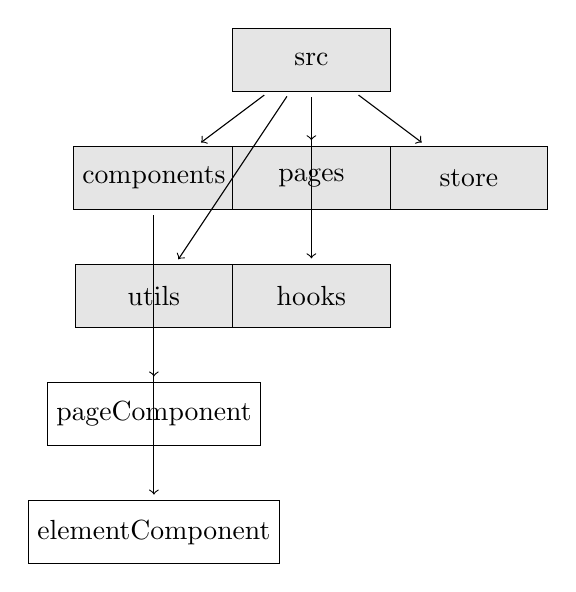
\begin{tikzpicture}[
    file/.style={draw, rectangle, minimum width=2cm, minimum height=0.8cm},
    folder/.style={draw, rectangle, minimum width=2cm, minimum height=0.8cm, fill=gray!20},
    arrow/.style={->, shorten >=2pt, shorten <=2pt}
]

% Folders
\node[folder] (src) at (0,0) {src};
\node[folder] (components) at (-2,-1.5) {components};
\node[folder] (pages) at (0,-1.5) {pages};
\node[folder] (store) at (2,-1.5) {store};
\node[folder] (utils) at (-2,-3) {utils};
\node[folder] (hooks) at (0,-3) {hooks};

% Files
\node[file] (pageComponent) at (-2,-4.5) {pageComponent};
\node[file] (elementComponent) at (-2,-6) {elementComponent};
% ... add more files

% Connections
\draw[arrow] (src) -- (components);
\draw[arrow] (src) -- (pages);
\draw[arrow] (src) -- (store);
\draw[arrow] (src) -- (utils);
\draw[arrow] (src) -- (hooks);
\draw[arrow] (components) -- (pageComponent);
\draw[arrow] (components) -- (elementComponent);
% ... add more connections

\end{tikzpicture}



\pagebreak
\subsubsection{Back-end}
The backend uses the dotNet framework. The development language using the C\# language.

In this project, the backend uses the Onion Architecture.
The Onion Architecture is a typically layered architecture, 
where each layer depends on the inner layer and provides interfaces to the outer layer.
The outer layer provides services to the outermost layer 
and other modules in the same layer based on the interfaces of the inner layer.

From inner to outer, the layers are: Domain, Application, Infrastructure, Presentation.
The Domain layer is the core layer and the innermost layer, used to define domain models, 
which are the business models.
It includes domain models and domain service interfaces.
Domain models are used to define the business models, 
which are the entities in the entity-relationship model and their attributes.
Domain service interfaces are used to define the business services, 
which are the relationships between entities in the entity-relationship model.

The Application layer is the application layer, 
used to define application services, which are the business logic.
It includes domain service implementations and application service interfaces.
Domain service implementations implement the methods of the inner layer's domain service 
interfaces and implement the business logic of the domain models.
Application service interfaces are used to define application services, 
which are the business logic.
It includes but is not limited to database interfaces, testing interfaces, 
HTTP API interfaces, MQTT interfaces, etc.

The Infrastructure layer is the infrastructure layer, used to define infrastructure.
It includes database implementations, testing implementations, 
HTTP API implementations, MQTT implementations, etc.
Database implementations implement the database interfaces 
and provide CRUD services for the database.
Testing implementations implement the testing interfaces 
and provide services for unit testing and integration testing.
HTTP API implementations implement the HTTP API interfaces 
and provide CRUD operations for HTTP APIs.
MQTT implementations implement the MQTT interfaces 
and provide CRUD operations for MQTT.

The Presentation layer is the presentation layer, used to define presentation logic, 
such as interfaces and pages. Since this is a backend project,
data presentation and control are handled by the frontend, 
so this layer is not needed.



\pagebreak
\subsubsection{Data communication and storage}
% 关于本项目的数据通信与数据存储的设计, 包括数据通信的协议, 数据存储的设计等
% 关于数据通信的设计:
% 1. 通信协议的选择
% 自前端向后端发送的数据, 有三种传输的数据类型, 
% 一种是普通的增删改查的请求, 对数据传输的时效性要求不高, 但是对数据的准确性, 完整性, 有序性, 安全性有一定的要求,
% 这种数据的传输, 采用 HTTP 协议, 以及 RESTful API 的设计. 可以有效的保证对数据传输的以上要求.
% 一种是对数据通道的创建和流媒体数据的传输, 对数据传输的时效性, 安全性要求较高, 这种数据的传输, 采用 WebRTC 协议, 以及 MQTT 协议.
% 配合可以快速解码的 flatbuffers 协议, 可以有效的保证对数据传输的以上要求.
% 最后一种是对设备的状态信息和操作信息的传输, 对完整性, 有序性, 安全性都有较高的要求, 这种数据的传输, 采用 MQTT 协议
% 同时也使用了 flatbuffers 协议.
% 
% 2. 数据通信的通信架构和通信流程
% 本项目的数据通信的通信架构, 是基于前后端分离的架构, 前端使用 React 框架, 后端使用 dotnet 框架.
% 当前端需要向后端发送数据的时候, 前端会向后端发送 HTTP 请求, 后端接收到 HTTP 请求之后, 会根据请求的数据类型,
% 选择不同的数据处理方式, 对于普通的增删改查的请求, 后端会根据 RESTful API 的设计, 对数据进行增删改查的操作,
% 对于对数据通道的创建和流媒体数据的传输, 后端会根据 WebRTC 协议, 对数据通道进行创建, 并且帮助前端和设备建立数据通道,
% 当数据通道建立后, 前端和设备之间则使用 flatbuffer 的数据格式对流媒体数据进行传输,
% 对于设备的状态信息和操作信息的传输, 前端会直接向 MQTT broker 发送 MQTT 请求, 
% 设备会在其自身的固件中监听相关的 MQTT 请求, 并且返回相关的数据.
% 
% 3. 数据通信的格式
% 本项目的数据通信的格式, 有三种, 
% 一种是 HTTP 协议, 
% 使用 json 格式对数据进行传输,
% 一种是 WebRTC 协议, 
% 使用 flatbuffers 格式对数据进行传输,
% 一种是 MQTT 协议.
% 使用 flatbuffers 格式对数据进行传输,
% 
% 关于数据存储的设计:
% 1. 数据存储的数据库的选择
% 本项目的数据存储的数据库的选择, 使用了轻量级的数据库 SQLite,
% SQLite 是一个进程内的库, 实现了自给自足的, 无服务器的, 零配置的, 事务性的 SQL 数据库引擎.
% 这是因为整个项目的目的是为了实现前端与设备之间的数据通信, 对于数据库数据的增删改查操作的要求不高,
% 数据量较小, 且对于数据库的数据的事务性要求不高, 所以选择了 SQLite 数据库.
% 2. 项目前后端的数据结构的设计
% 在本项目中, 前端由于使用了 React 框架, 所以前端的数据结构的设计, 使用了基于状态的数据结构的设计,
% 每个组件或者数据集都包含一个状态对象, 这个状态对象的属性就是组件的各个状态. 
% 使用状态对象的原因是, 可以方便的对状态进行管理, 采用对象-属性的形式, 可以方便的针对不同组件的同类状态进行区分,
% 由于跨组件的状态是由 redux 进行管理的, 这种状态对象的设计, 可以更搞笑的对状态进行更新和传递.
% 后端由于使用了 dotnet 框架, 所以后端的数据结构的设计, 使用了基于类的数据结构的设计,
% 采用了面向对象的编程思想, 对数据进行了封装, 使得数据的传输更加的安全, 有序, 完整.


\pagebreak

% \subsection{Domain model}
% \documentclass[]{article}
\usepackage{graphicx}
\usepackage{amsmath}
\usepackage{tikz}

% libaries
\usetikzlibrary{shapes,arrows}

%Define the listing package
\usepackage{listings} %code highlighter
\usepackage{color} %use color
\definecolor{mygreen}{rgb}{0,0.6,0}
\definecolor{mygray}{rgb}{0.5,0.5,0.5}
\definecolor{mymauve}{rgb}{0.58,0,0.82}

%Customize a bit the look
\lstset{ %
backgroundcolor=\color{white}, % choose the background color; you must add \usepackage{color} or \usepackage{xcolor}
basicstyle=\footnotesize, % the size of the fonts that are used for the code
breakatwhitespace=false, % sets if automatic breaks should only happen at whitespace
breaklines=true, % sets automatic line breaking
captionpos=b, % sets the caption-position to bottom
commentstyle=\color{mygreen}, % comment style
deletekeywords={...}, % if you want to delete keywords from the given language
escapeinside={\%*}{*)}, % if you want to add LaTeX within your code
extendedchars=true, % lets you use non-ASCII characters; for 8-bits encodings only, does not work with UTF-8
frame=single, % adds a frame around the code
keepspaces=true, % keeps spaces in text, useful for keeping indentation of code (possibly needs columns=flexible)
keywordstyle=\color{blue}, % keyword style
% language=Octave, % the language of the code
morekeywords={*,...}, % if you want to add more keywords to the set
numbers=left, % where to put the line-numbers; possible values are (none, left, right)
numbersep=5pt, % how far the line-numbers are from the code
numberstyle=\tiny\color{mygray}, % the style that is used for the line-numbers
rulecolor=\color{black}, % if not set, the frame-color may be changed on line-breaks within not-black text (e.g. comments (green here))
showspaces=false, % show spaces everywhere adding particular underscores; it overrides 'showstringspaces'
showstringspaces=false, % underline spaces within strings only
showtabs=false, % show tabs within strings adding particular underscores
stepnumber=1, % the step between two line-numbers. If it's 1, each line will be numbered
stringstyle=\color{mymauve}, % string literal style
tabsize=2, % sets default tabsize to 2 spaces
title=\lstname % show the filename of files included with \lstinputlisting; also try caption instead of title
}

\definecolor{darkgray}{rgb}{.4,.4,.4}
\definecolor{purple}{rgb}{0.65, 0.12, 0.82}

\lstdefinelanguage{React}{
keywords={const, typeof, new, true, false, catch, function, return, null, catch, switch, var, if, in, while, do, else, case, break},
keywordstyle=\color{blue}\bfseries,
ndkeywords={class, export, boolean, throw, implements, import, this},
ndkeywordstyle=\color{darkgray}\bfseries,
identifierstyle=\color{mygreen},
sensitive=false,
comment=[l]{//},
morecomment=[s]{/*}{*/},
commentstyle=\color{purple}\ttfamily,
string=[b]{"}{'}{`},
stringstyle=\color{red}\ttfamily,
morestring=[b]',
morestring=[b]",
morestring=[b]`',
}

\lstdefinelanguage{CSharp}{
keywords={const, typeof, new, true, false, catch, function, return, null, catch, switch, var, if, in, while, do, else, case, break},
keywordstyle=\color{blue}\bfseries,
ndkeywords={class, export, boolean, throw, implements, import, this},
ndkeywordstyle=\color{darkgray}\bfseries,
identifierstyle=\color{mygreen},
sensitive=false,
comment=[l]{//},
morecomment=[s]{/*}{*/},
commentstyle=\color{purple}\ttfamily,
string=[b]{"}{'}{`},
stringstyle=\color{red}\ttfamily,
morestring=[b]',
morestring=[b]",
morestring=[b]`',
}

\lstset{
language=React,
extendedchars=true,
basicstyle=\footnotesize\ttfamily,
showstringspaces=false,
showspaces=false,
numbers=left,
numberstyle=\footnotesize,
numbersep=9pt,
tabsize=2,
breaklines=true,
showtabs=false,
captionpos=b
}

\lstset{
language=CSharp,
extendedchars=true,
basicstyle=\footnotesize\ttfamily,
showstringspaces=false,
showspaces=false,
numbers=left,
numberstyle=\footnotesize,
numbersep=9pt,
tabsize=2,
breaklines=true,
showtabs=false,
captionpos=b
}

% \usepackage{cite} % Add this line for citation

% \bibliographystyle{plain}

\title{
The implementation of BifrostConnect Front-end scope, 
re-design and development with the relevant back-end support develop.
}
\author{
    Fei Gu \\
    Erhvervs Akademi Sydvest \\
    Computer Science 21\\
    }
\date{\today}

\begin{document}

% Front page
\maketitle
\begin{center}
    Supervisor: Henrik Boulund Meng Hansen \\
    Company: BifrostConnect \\
    Engineering Director: Jasper Wass \\
\end{center}
\tableofcontents
\pagebreak


% The introduction
\section{Introduction}
\subsection{Background}\input{sections/introduction/background.tex}
\subsection{The company}\input{sections/introduction/aboutCompany}
\subsection{The project}\input{sections/introduction/aboutProject}
\pagebreak

% The problem statement
\section{Problem Statement}
\subsection{Statement}
\input{sections/problemStatement/statement}
\subsection{Situation}
\input{sections/problemStatement/situation}
\subsection{Potential Solution}
\input{sections/problemStatement/potentialSolution}
\pagebreak

% Requirement analysis
\section{Requirement Analysis}
\input{sections/requirementAnalysis/index}

\subsection{Stakeholders}
\input{sections/requirementAnalysis/stakeholders/index}

\subsection{Business Domain}
\input{sections/requirementAnalysis/bussinesDomain/index}

\subsection{Scope}
\input{sections/requirementAnalysis/scope}

\subsection{Goals}
\input{sections/requirementAnalysis/goals}
\pagebreak

% Software Design
\section{Software Design}
% developement methods
\subsection{Software Development Methods}
\input{sections/softwareDevelopmentMethods/index}
\subsubsection{Agile Software Development}
\input{sections/softwareDevelopmentMethods/agileSoftwareDevelopment/index}
\subsubsection{Feature Driven Development}
\input{sections/softwareDevelopmentMethods/featureDrivenDevelopment/index}

\pagebreak

% Technology seslection
\subsection{Technology selection}
\input{sections/softwareDesign/technologySelection/index}
\subsubsection{Front-end}
\input{sections/softwareDesign/technologySelection/frontEnd}            
\subsubsection{Back-end}
\input{sections/softwareDesign/technologySelection/backEnd}            
\subsubsection{Database}
\input{sections/softwareDesign/technologySelection/database}
\subsubsection{Data communication}
\input{sections/softwareDesign/technologySelection/dataCommunication}            
\subsubsection{DevOps}
\input{sections/softwareDesign/technologySelection/devOps}
\pagebreak

% Architecture design
\subsection{Architecture design}
\input{sections/softwareDesign/architectureDesign/index}
\pagebreak
\subsubsection{Front-end}
\input{sections/softwareDesign/architectureDesign/frontEndArchitecture}
\pagebreak
\subsubsection{Back-end}
\input{sections/softwareDesign/architectureDesign/backEndArchitecture}
\pagebreak
\subsubsection{Data communication and storage}
\input{sections/softwareDesign/architectureDesign/dataCommunicationArchitecture}
\pagebreak

% \subsection{Domain model}
% \input{sections/softwareDesign/domainModel/index}
% \subsection{Database design}
% % 数据库领域模型 ER 图
% % 包括表和字段的设置.
% % 对于私有键和外键的设置.

% \subsection{Back-end design}
% % 后端对象模型
% % 以及对于对象模型的增删改查
% % 以及相关的其他服务的设计`'

% \subsection{Front-end design}
% % 对于前端的页面结构的设计 
% % 页面的状态的设计, 交互设计

% \subsection{FlatBuffers design}
% % schema 的设计

\subsection{DevOps CI/CD process design}
\input{sections/softwareDesign/devOpsDesign/index}
\subsubsection{Continuous Integration}
\input{sections/softwareDesign/devOpsDesign/continuousIntegration/index}
\subsubsection{Continuous Delivery}
\input{sections/softwareDesign/devOpsDesign/continuousDelivery/index}
\subsubsection{Continuous Deployment}
\input{sections/softwareDesign/devOpsDesign/continuousDeployment/index}
\pagebreak

\section{Software Development} 
\input{sections/softwareDevelopment/index}
\subsection{Overall development}
\input{sections/softwareDevelopment/overallDevelopement/index}
\subsubsection{Front-end}
\input{sections/softwareDevelopment/overallDevelopement/frontEnd/index}
\subsubsection{Back-end}
\input{sections/softwareDevelopment/overallDevelopement/backEnd/index}
\subsubsection{DevOps}
\input{sections/softwareDevelopment/overallDevelopement/devOps/index}
\subsection{Feature development} 
\input{sections/softwareDevelopment/featureDevelopment/index}
\subsubsection{Use Case 1}
\input{sections/softwareDevelopment/featureDevelopment/useCase1/index}
\subsubsection{Feature 1}
\input{sections/softwareDevelopment/featureDevelopment/feature/feature1.tex}
\pagebreak
\section{Conclusion} 
\subsection{Result}
Since the project is still in progress, the result is not available yet.
So far, basic structure of this project has been built. But the most features 
are not implemented yet. 
\subsection{Discussion}
As a single developer for this project, I am confident what I have done so far.
And I can say I understand the most of the knowledge I have used in this project, 
which also means I can explain all the part of the project. 
But this project also relevant some of the complex knowledge which I have to continue 
to study and practice.
\subsection{Future Work}
The future work is to implement the rest of the features. 
Including the most important part which is the 'create session' feature.
\pagebreak
% \bibliography{bibliography}
\pagebreak
% \begin{appendices}
%     \section{Appendix}
% \end{appendices} 
\end{document}
% \subsection{Database design}
% % 数据库领域模型 ER 图
% % 包括表和字段的设置.
% % 对于私有键和外键的设置.

% \subsection{Back-end design}
% % 后端对象模型
% % 以及对于对象模型的增删改查
% % 以及相关的其他服务的设计`'

% \subsection{Front-end design}
% % 对于前端的页面结构的设计 
% % 页面的状态的设计, 交互设计

% \subsection{FlatBuffers design}
% % schema 的设计

\subsection{DevOps CI/CD process design}
\documentclass[]{article}
\usepackage{graphicx}
\usepackage{amsmath}
\usepackage{tikz}

% libaries
\usetikzlibrary{shapes,arrows}

%Define the listing package
\usepackage{listings} %code highlighter
\usepackage{color} %use color
\definecolor{mygreen}{rgb}{0,0.6,0}
\definecolor{mygray}{rgb}{0.5,0.5,0.5}
\definecolor{mymauve}{rgb}{0.58,0,0.82}

%Customize a bit the look
\lstset{ %
backgroundcolor=\color{white}, % choose the background color; you must add \usepackage{color} or \usepackage{xcolor}
basicstyle=\footnotesize, % the size of the fonts that are used for the code
breakatwhitespace=false, % sets if automatic breaks should only happen at whitespace
breaklines=true, % sets automatic line breaking
captionpos=b, % sets the caption-position to bottom
commentstyle=\color{mygreen}, % comment style
deletekeywords={...}, % if you want to delete keywords from the given language
escapeinside={\%*}{*)}, % if you want to add LaTeX within your code
extendedchars=true, % lets you use non-ASCII characters; for 8-bits encodings only, does not work with UTF-8
frame=single, % adds a frame around the code
keepspaces=true, % keeps spaces in text, useful for keeping indentation of code (possibly needs columns=flexible)
keywordstyle=\color{blue}, % keyword style
% language=Octave, % the language of the code
morekeywords={*,...}, % if you want to add more keywords to the set
numbers=left, % where to put the line-numbers; possible values are (none, left, right)
numbersep=5pt, % how far the line-numbers are from the code
numberstyle=\tiny\color{mygray}, % the style that is used for the line-numbers
rulecolor=\color{black}, % if not set, the frame-color may be changed on line-breaks within not-black text (e.g. comments (green here))
showspaces=false, % show spaces everywhere adding particular underscores; it overrides 'showstringspaces'
showstringspaces=false, % underline spaces within strings only
showtabs=false, % show tabs within strings adding particular underscores
stepnumber=1, % the step between two line-numbers. If it's 1, each line will be numbered
stringstyle=\color{mymauve}, % string literal style
tabsize=2, % sets default tabsize to 2 spaces
title=\lstname % show the filename of files included with \lstinputlisting; also try caption instead of title
}

\definecolor{darkgray}{rgb}{.4,.4,.4}
\definecolor{purple}{rgb}{0.65, 0.12, 0.82}

\lstdefinelanguage{React}{
keywords={const, typeof, new, true, false, catch, function, return, null, catch, switch, var, if, in, while, do, else, case, break},
keywordstyle=\color{blue}\bfseries,
ndkeywords={class, export, boolean, throw, implements, import, this},
ndkeywordstyle=\color{darkgray}\bfseries,
identifierstyle=\color{mygreen},
sensitive=false,
comment=[l]{//},
morecomment=[s]{/*}{*/},
commentstyle=\color{purple}\ttfamily,
string=[b]{"}{'}{`},
stringstyle=\color{red}\ttfamily,
morestring=[b]',
morestring=[b]",
morestring=[b]`',
}

\lstdefinelanguage{CSharp}{
keywords={const, typeof, new, true, false, catch, function, return, null, catch, switch, var, if, in, while, do, else, case, break},
keywordstyle=\color{blue}\bfseries,
ndkeywords={class, export, boolean, throw, implements, import, this},
ndkeywordstyle=\color{darkgray}\bfseries,
identifierstyle=\color{mygreen},
sensitive=false,
comment=[l]{//},
morecomment=[s]{/*}{*/},
commentstyle=\color{purple}\ttfamily,
string=[b]{"}{'}{`},
stringstyle=\color{red}\ttfamily,
morestring=[b]',
morestring=[b]",
morestring=[b]`',
}

\lstset{
language=React,
extendedchars=true,
basicstyle=\footnotesize\ttfamily,
showstringspaces=false,
showspaces=false,
numbers=left,
numberstyle=\footnotesize,
numbersep=9pt,
tabsize=2,
breaklines=true,
showtabs=false,
captionpos=b
}

\lstset{
language=CSharp,
extendedchars=true,
basicstyle=\footnotesize\ttfamily,
showstringspaces=false,
showspaces=false,
numbers=left,
numberstyle=\footnotesize,
numbersep=9pt,
tabsize=2,
breaklines=true,
showtabs=false,
captionpos=b
}

% \usepackage{cite} % Add this line for citation

% \bibliographystyle{plain}

\title{
The implementation of BifrostConnect Front-end scope, 
re-design and development with the relevant back-end support develop.
}
\author{
    Fei Gu \\
    Erhvervs Akademi Sydvest \\
    Computer Science 21\\
    }
\date{\today}

\begin{document}

% Front page
\maketitle
\begin{center}
    Supervisor: Henrik Boulund Meng Hansen \\
    Company: BifrostConnect \\
    Engineering Director: Jasper Wass \\
\end{center}
\tableofcontents
\pagebreak


% The introduction
\section{Introduction}
\subsection{Background}\input{sections/introduction/background.tex}
\subsection{The company}\input{sections/introduction/aboutCompany}
\subsection{The project}\input{sections/introduction/aboutProject}
\pagebreak

% The problem statement
\section{Problem Statement}
\subsection{Statement}
\input{sections/problemStatement/statement}
\subsection{Situation}
\input{sections/problemStatement/situation}
\subsection{Potential Solution}
\input{sections/problemStatement/potentialSolution}
\pagebreak

% Requirement analysis
\section{Requirement Analysis}
\input{sections/requirementAnalysis/index}

\subsection{Stakeholders}
\input{sections/requirementAnalysis/stakeholders/index}

\subsection{Business Domain}
\input{sections/requirementAnalysis/bussinesDomain/index}

\subsection{Scope}
\input{sections/requirementAnalysis/scope}

\subsection{Goals}
\input{sections/requirementAnalysis/goals}
\pagebreak

% Software Design
\section{Software Design}
% developement methods
\subsection{Software Development Methods}
\input{sections/softwareDevelopmentMethods/index}
\subsubsection{Agile Software Development}
\input{sections/softwareDevelopmentMethods/agileSoftwareDevelopment/index}
\subsubsection{Feature Driven Development}
\input{sections/softwareDevelopmentMethods/featureDrivenDevelopment/index}

\pagebreak

% Technology seslection
\subsection{Technology selection}
\input{sections/softwareDesign/technologySelection/index}
\subsubsection{Front-end}
\input{sections/softwareDesign/technologySelection/frontEnd}            
\subsubsection{Back-end}
\input{sections/softwareDesign/technologySelection/backEnd}            
\subsubsection{Database}
\input{sections/softwareDesign/technologySelection/database}
\subsubsection{Data communication}
\input{sections/softwareDesign/technologySelection/dataCommunication}            
\subsubsection{DevOps}
\input{sections/softwareDesign/technologySelection/devOps}
\pagebreak

% Architecture design
\subsection{Architecture design}
\input{sections/softwareDesign/architectureDesign/index}
\pagebreak
\subsubsection{Front-end}
\input{sections/softwareDesign/architectureDesign/frontEndArchitecture}
\pagebreak
\subsubsection{Back-end}
\input{sections/softwareDesign/architectureDesign/backEndArchitecture}
\pagebreak
\subsubsection{Data communication and storage}
\input{sections/softwareDesign/architectureDesign/dataCommunicationArchitecture}
\pagebreak

% \subsection{Domain model}
% \input{sections/softwareDesign/domainModel/index}
% \subsection{Database design}
% % 数据库领域模型 ER 图
% % 包括表和字段的设置.
% % 对于私有键和外键的设置.

% \subsection{Back-end design}
% % 后端对象模型
% % 以及对于对象模型的增删改查
% % 以及相关的其他服务的设计`'

% \subsection{Front-end design}
% % 对于前端的页面结构的设计 
% % 页面的状态的设计, 交互设计

% \subsection{FlatBuffers design}
% % schema 的设计

\subsection{DevOps CI/CD process design}
\input{sections/softwareDesign/devOpsDesign/index}
\subsubsection{Continuous Integration}
\input{sections/softwareDesign/devOpsDesign/continuousIntegration/index}
\subsubsection{Continuous Delivery}
\input{sections/softwareDesign/devOpsDesign/continuousDelivery/index}
\subsubsection{Continuous Deployment}
\input{sections/softwareDesign/devOpsDesign/continuousDeployment/index}
\pagebreak

\section{Software Development} 
\input{sections/softwareDevelopment/index}
\subsection{Overall development}
\input{sections/softwareDevelopment/overallDevelopement/index}
\subsubsection{Front-end}
\input{sections/softwareDevelopment/overallDevelopement/frontEnd/index}
\subsubsection{Back-end}
\input{sections/softwareDevelopment/overallDevelopement/backEnd/index}
\subsubsection{DevOps}
\input{sections/softwareDevelopment/overallDevelopement/devOps/index}
\subsection{Feature development} 
\input{sections/softwareDevelopment/featureDevelopment/index}
\subsubsection{Use Case 1}
\input{sections/softwareDevelopment/featureDevelopment/useCase1/index}
\subsubsection{Feature 1}
\input{sections/softwareDevelopment/featureDevelopment/feature/feature1.tex}
\pagebreak
\section{Conclusion} 
\subsection{Result}
Since the project is still in progress, the result is not available yet.
So far, basic structure of this project has been built. But the most features 
are not implemented yet. 
\subsection{Discussion}
As a single developer for this project, I am confident what I have done so far.
And I can say I understand the most of the knowledge I have used in this project, 
which also means I can explain all the part of the project. 
But this project also relevant some of the complex knowledge which I have to continue 
to study and practice.
\subsection{Future Work}
The future work is to implement the rest of the features. 
Including the most important part which is the 'create session' feature.
\pagebreak
% \bibliography{bibliography}
\pagebreak
% \begin{appendices}
%     \section{Appendix}
% \end{appendices} 
\end{document}
\subsubsection{Continuous Integration}
\documentclass[]{article}
\usepackage{graphicx}
\usepackage{amsmath}
\usepackage{tikz}

% libaries
\usetikzlibrary{shapes,arrows}

%Define the listing package
\usepackage{listings} %code highlighter
\usepackage{color} %use color
\definecolor{mygreen}{rgb}{0,0.6,0}
\definecolor{mygray}{rgb}{0.5,0.5,0.5}
\definecolor{mymauve}{rgb}{0.58,0,0.82}

%Customize a bit the look
\lstset{ %
backgroundcolor=\color{white}, % choose the background color; you must add \usepackage{color} or \usepackage{xcolor}
basicstyle=\footnotesize, % the size of the fonts that are used for the code
breakatwhitespace=false, % sets if automatic breaks should only happen at whitespace
breaklines=true, % sets automatic line breaking
captionpos=b, % sets the caption-position to bottom
commentstyle=\color{mygreen}, % comment style
deletekeywords={...}, % if you want to delete keywords from the given language
escapeinside={\%*}{*)}, % if you want to add LaTeX within your code
extendedchars=true, % lets you use non-ASCII characters; for 8-bits encodings only, does not work with UTF-8
frame=single, % adds a frame around the code
keepspaces=true, % keeps spaces in text, useful for keeping indentation of code (possibly needs columns=flexible)
keywordstyle=\color{blue}, % keyword style
% language=Octave, % the language of the code
morekeywords={*,...}, % if you want to add more keywords to the set
numbers=left, % where to put the line-numbers; possible values are (none, left, right)
numbersep=5pt, % how far the line-numbers are from the code
numberstyle=\tiny\color{mygray}, % the style that is used for the line-numbers
rulecolor=\color{black}, % if not set, the frame-color may be changed on line-breaks within not-black text (e.g. comments (green here))
showspaces=false, % show spaces everywhere adding particular underscores; it overrides 'showstringspaces'
showstringspaces=false, % underline spaces within strings only
showtabs=false, % show tabs within strings adding particular underscores
stepnumber=1, % the step between two line-numbers. If it's 1, each line will be numbered
stringstyle=\color{mymauve}, % string literal style
tabsize=2, % sets default tabsize to 2 spaces
title=\lstname % show the filename of files included with \lstinputlisting; also try caption instead of title
}

\definecolor{darkgray}{rgb}{.4,.4,.4}
\definecolor{purple}{rgb}{0.65, 0.12, 0.82}

\lstdefinelanguage{React}{
keywords={const, typeof, new, true, false, catch, function, return, null, catch, switch, var, if, in, while, do, else, case, break},
keywordstyle=\color{blue}\bfseries,
ndkeywords={class, export, boolean, throw, implements, import, this},
ndkeywordstyle=\color{darkgray}\bfseries,
identifierstyle=\color{mygreen},
sensitive=false,
comment=[l]{//},
morecomment=[s]{/*}{*/},
commentstyle=\color{purple}\ttfamily,
string=[b]{"}{'}{`},
stringstyle=\color{red}\ttfamily,
morestring=[b]',
morestring=[b]",
morestring=[b]`',
}

\lstdefinelanguage{CSharp}{
keywords={const, typeof, new, true, false, catch, function, return, null, catch, switch, var, if, in, while, do, else, case, break},
keywordstyle=\color{blue}\bfseries,
ndkeywords={class, export, boolean, throw, implements, import, this},
ndkeywordstyle=\color{darkgray}\bfseries,
identifierstyle=\color{mygreen},
sensitive=false,
comment=[l]{//},
morecomment=[s]{/*}{*/},
commentstyle=\color{purple}\ttfamily,
string=[b]{"}{'}{`},
stringstyle=\color{red}\ttfamily,
morestring=[b]',
morestring=[b]",
morestring=[b]`',
}

\lstset{
language=React,
extendedchars=true,
basicstyle=\footnotesize\ttfamily,
showstringspaces=false,
showspaces=false,
numbers=left,
numberstyle=\footnotesize,
numbersep=9pt,
tabsize=2,
breaklines=true,
showtabs=false,
captionpos=b
}

\lstset{
language=CSharp,
extendedchars=true,
basicstyle=\footnotesize\ttfamily,
showstringspaces=false,
showspaces=false,
numbers=left,
numberstyle=\footnotesize,
numbersep=9pt,
tabsize=2,
breaklines=true,
showtabs=false,
captionpos=b
}

% \usepackage{cite} % Add this line for citation

% \bibliographystyle{plain}

\title{
The implementation of BifrostConnect Front-end scope, 
re-design and development with the relevant back-end support develop.
}
\author{
    Fei Gu \\
    Erhvervs Akademi Sydvest \\
    Computer Science 21\\
    }
\date{\today}

\begin{document}

% Front page
\maketitle
\begin{center}
    Supervisor: Henrik Boulund Meng Hansen \\
    Company: BifrostConnect \\
    Engineering Director: Jasper Wass \\
\end{center}
\tableofcontents
\pagebreak


% The introduction
\section{Introduction}
\subsection{Background}\input{sections/introduction/background.tex}
\subsection{The company}\input{sections/introduction/aboutCompany}
\subsection{The project}\input{sections/introduction/aboutProject}
\pagebreak

% The problem statement
\section{Problem Statement}
\subsection{Statement}
\input{sections/problemStatement/statement}
\subsection{Situation}
\input{sections/problemStatement/situation}
\subsection{Potential Solution}
\input{sections/problemStatement/potentialSolution}
\pagebreak

% Requirement analysis
\section{Requirement Analysis}
\input{sections/requirementAnalysis/index}

\subsection{Stakeholders}
\input{sections/requirementAnalysis/stakeholders/index}

\subsection{Business Domain}
\input{sections/requirementAnalysis/bussinesDomain/index}

\subsection{Scope}
\input{sections/requirementAnalysis/scope}

\subsection{Goals}
\input{sections/requirementAnalysis/goals}
\pagebreak

% Software Design
\section{Software Design}
% developement methods
\subsection{Software Development Methods}
\input{sections/softwareDevelopmentMethods/index}
\subsubsection{Agile Software Development}
\input{sections/softwareDevelopmentMethods/agileSoftwareDevelopment/index}
\subsubsection{Feature Driven Development}
\input{sections/softwareDevelopmentMethods/featureDrivenDevelopment/index}

\pagebreak

% Technology seslection
\subsection{Technology selection}
\input{sections/softwareDesign/technologySelection/index}
\subsubsection{Front-end}
\input{sections/softwareDesign/technologySelection/frontEnd}            
\subsubsection{Back-end}
\input{sections/softwareDesign/technologySelection/backEnd}            
\subsubsection{Database}
\input{sections/softwareDesign/technologySelection/database}
\subsubsection{Data communication}
\input{sections/softwareDesign/technologySelection/dataCommunication}            
\subsubsection{DevOps}
\input{sections/softwareDesign/technologySelection/devOps}
\pagebreak

% Architecture design
\subsection{Architecture design}
\input{sections/softwareDesign/architectureDesign/index}
\pagebreak
\subsubsection{Front-end}
\input{sections/softwareDesign/architectureDesign/frontEndArchitecture}
\pagebreak
\subsubsection{Back-end}
\input{sections/softwareDesign/architectureDesign/backEndArchitecture}
\pagebreak
\subsubsection{Data communication and storage}
\input{sections/softwareDesign/architectureDesign/dataCommunicationArchitecture}
\pagebreak

% \subsection{Domain model}
% \input{sections/softwareDesign/domainModel/index}
% \subsection{Database design}
% % 数据库领域模型 ER 图
% % 包括表和字段的设置.
% % 对于私有键和外键的设置.

% \subsection{Back-end design}
% % 后端对象模型
% % 以及对于对象模型的增删改查
% % 以及相关的其他服务的设计`'

% \subsection{Front-end design}
% % 对于前端的页面结构的设计 
% % 页面的状态的设计, 交互设计

% \subsection{FlatBuffers design}
% % schema 的设计

\subsection{DevOps CI/CD process design}
\input{sections/softwareDesign/devOpsDesign/index}
\subsubsection{Continuous Integration}
\input{sections/softwareDesign/devOpsDesign/continuousIntegration/index}
\subsubsection{Continuous Delivery}
\input{sections/softwareDesign/devOpsDesign/continuousDelivery/index}
\subsubsection{Continuous Deployment}
\input{sections/softwareDesign/devOpsDesign/continuousDeployment/index}
\pagebreak

\section{Software Development} 
\input{sections/softwareDevelopment/index}
\subsection{Overall development}
\input{sections/softwareDevelopment/overallDevelopement/index}
\subsubsection{Front-end}
\input{sections/softwareDevelopment/overallDevelopement/frontEnd/index}
\subsubsection{Back-end}
\input{sections/softwareDevelopment/overallDevelopement/backEnd/index}
\subsubsection{DevOps}
\input{sections/softwareDevelopment/overallDevelopement/devOps/index}
\subsection{Feature development} 
\input{sections/softwareDevelopment/featureDevelopment/index}
\subsubsection{Use Case 1}
\input{sections/softwareDevelopment/featureDevelopment/useCase1/index}
\subsubsection{Feature 1}
\input{sections/softwareDevelopment/featureDevelopment/feature/feature1.tex}
\pagebreak
\section{Conclusion} 
\subsection{Result}
Since the project is still in progress, the result is not available yet.
So far, basic structure of this project has been built. But the most features 
are not implemented yet. 
\subsection{Discussion}
As a single developer for this project, I am confident what I have done so far.
And I can say I understand the most of the knowledge I have used in this project, 
which also means I can explain all the part of the project. 
But this project also relevant some of the complex knowledge which I have to continue 
to study and practice.
\subsection{Future Work}
The future work is to implement the rest of the features. 
Including the most important part which is the 'create session' feature.
\pagebreak
% \bibliography{bibliography}
\pagebreak
% \begin{appendices}
%     \section{Appendix}
% \end{appendices} 
\end{document}
\subsubsection{Continuous Delivery}
\documentclass[]{article}
\usepackage{graphicx}
\usepackage{amsmath}
\usepackage{tikz}

% libaries
\usetikzlibrary{shapes,arrows}

%Define the listing package
\usepackage{listings} %code highlighter
\usepackage{color} %use color
\definecolor{mygreen}{rgb}{0,0.6,0}
\definecolor{mygray}{rgb}{0.5,0.5,0.5}
\definecolor{mymauve}{rgb}{0.58,0,0.82}

%Customize a bit the look
\lstset{ %
backgroundcolor=\color{white}, % choose the background color; you must add \usepackage{color} or \usepackage{xcolor}
basicstyle=\footnotesize, % the size of the fonts that are used for the code
breakatwhitespace=false, % sets if automatic breaks should only happen at whitespace
breaklines=true, % sets automatic line breaking
captionpos=b, % sets the caption-position to bottom
commentstyle=\color{mygreen}, % comment style
deletekeywords={...}, % if you want to delete keywords from the given language
escapeinside={\%*}{*)}, % if you want to add LaTeX within your code
extendedchars=true, % lets you use non-ASCII characters; for 8-bits encodings only, does not work with UTF-8
frame=single, % adds a frame around the code
keepspaces=true, % keeps spaces in text, useful for keeping indentation of code (possibly needs columns=flexible)
keywordstyle=\color{blue}, % keyword style
% language=Octave, % the language of the code
morekeywords={*,...}, % if you want to add more keywords to the set
numbers=left, % where to put the line-numbers; possible values are (none, left, right)
numbersep=5pt, % how far the line-numbers are from the code
numberstyle=\tiny\color{mygray}, % the style that is used for the line-numbers
rulecolor=\color{black}, % if not set, the frame-color may be changed on line-breaks within not-black text (e.g. comments (green here))
showspaces=false, % show spaces everywhere adding particular underscores; it overrides 'showstringspaces'
showstringspaces=false, % underline spaces within strings only
showtabs=false, % show tabs within strings adding particular underscores
stepnumber=1, % the step between two line-numbers. If it's 1, each line will be numbered
stringstyle=\color{mymauve}, % string literal style
tabsize=2, % sets default tabsize to 2 spaces
title=\lstname % show the filename of files included with \lstinputlisting; also try caption instead of title
}

\definecolor{darkgray}{rgb}{.4,.4,.4}
\definecolor{purple}{rgb}{0.65, 0.12, 0.82}

\lstdefinelanguage{React}{
keywords={const, typeof, new, true, false, catch, function, return, null, catch, switch, var, if, in, while, do, else, case, break},
keywordstyle=\color{blue}\bfseries,
ndkeywords={class, export, boolean, throw, implements, import, this},
ndkeywordstyle=\color{darkgray}\bfseries,
identifierstyle=\color{mygreen},
sensitive=false,
comment=[l]{//},
morecomment=[s]{/*}{*/},
commentstyle=\color{purple}\ttfamily,
string=[b]{"}{'}{`},
stringstyle=\color{red}\ttfamily,
morestring=[b]',
morestring=[b]",
morestring=[b]`',
}

\lstdefinelanguage{CSharp}{
keywords={const, typeof, new, true, false, catch, function, return, null, catch, switch, var, if, in, while, do, else, case, break},
keywordstyle=\color{blue}\bfseries,
ndkeywords={class, export, boolean, throw, implements, import, this},
ndkeywordstyle=\color{darkgray}\bfseries,
identifierstyle=\color{mygreen},
sensitive=false,
comment=[l]{//},
morecomment=[s]{/*}{*/},
commentstyle=\color{purple}\ttfamily,
string=[b]{"}{'}{`},
stringstyle=\color{red}\ttfamily,
morestring=[b]',
morestring=[b]",
morestring=[b]`',
}

\lstset{
language=React,
extendedchars=true,
basicstyle=\footnotesize\ttfamily,
showstringspaces=false,
showspaces=false,
numbers=left,
numberstyle=\footnotesize,
numbersep=9pt,
tabsize=2,
breaklines=true,
showtabs=false,
captionpos=b
}

\lstset{
language=CSharp,
extendedchars=true,
basicstyle=\footnotesize\ttfamily,
showstringspaces=false,
showspaces=false,
numbers=left,
numberstyle=\footnotesize,
numbersep=9pt,
tabsize=2,
breaklines=true,
showtabs=false,
captionpos=b
}

% \usepackage{cite} % Add this line for citation

% \bibliographystyle{plain}

\title{
The implementation of BifrostConnect Front-end scope, 
re-design and development with the relevant back-end support develop.
}
\author{
    Fei Gu \\
    Erhvervs Akademi Sydvest \\
    Computer Science 21\\
    }
\date{\today}

\begin{document}

% Front page
\maketitle
\begin{center}
    Supervisor: Henrik Boulund Meng Hansen \\
    Company: BifrostConnect \\
    Engineering Director: Jasper Wass \\
\end{center}
\tableofcontents
\pagebreak


% The introduction
\section{Introduction}
\subsection{Background}\input{sections/introduction/background.tex}
\subsection{The company}\input{sections/introduction/aboutCompany}
\subsection{The project}\input{sections/introduction/aboutProject}
\pagebreak

% The problem statement
\section{Problem Statement}
\subsection{Statement}
\input{sections/problemStatement/statement}
\subsection{Situation}
\input{sections/problemStatement/situation}
\subsection{Potential Solution}
\input{sections/problemStatement/potentialSolution}
\pagebreak

% Requirement analysis
\section{Requirement Analysis}
\input{sections/requirementAnalysis/index}

\subsection{Stakeholders}
\input{sections/requirementAnalysis/stakeholders/index}

\subsection{Business Domain}
\input{sections/requirementAnalysis/bussinesDomain/index}

\subsection{Scope}
\input{sections/requirementAnalysis/scope}

\subsection{Goals}
\input{sections/requirementAnalysis/goals}
\pagebreak

% Software Design
\section{Software Design}
% developement methods
\subsection{Software Development Methods}
\input{sections/softwareDevelopmentMethods/index}
\subsubsection{Agile Software Development}
\input{sections/softwareDevelopmentMethods/agileSoftwareDevelopment/index}
\subsubsection{Feature Driven Development}
\input{sections/softwareDevelopmentMethods/featureDrivenDevelopment/index}

\pagebreak

% Technology seslection
\subsection{Technology selection}
\input{sections/softwareDesign/technologySelection/index}
\subsubsection{Front-end}
\input{sections/softwareDesign/technologySelection/frontEnd}            
\subsubsection{Back-end}
\input{sections/softwareDesign/technologySelection/backEnd}            
\subsubsection{Database}
\input{sections/softwareDesign/technologySelection/database}
\subsubsection{Data communication}
\input{sections/softwareDesign/technologySelection/dataCommunication}            
\subsubsection{DevOps}
\input{sections/softwareDesign/technologySelection/devOps}
\pagebreak

% Architecture design
\subsection{Architecture design}
\input{sections/softwareDesign/architectureDesign/index}
\pagebreak
\subsubsection{Front-end}
\input{sections/softwareDesign/architectureDesign/frontEndArchitecture}
\pagebreak
\subsubsection{Back-end}
\input{sections/softwareDesign/architectureDesign/backEndArchitecture}
\pagebreak
\subsubsection{Data communication and storage}
\input{sections/softwareDesign/architectureDesign/dataCommunicationArchitecture}
\pagebreak

% \subsection{Domain model}
% \input{sections/softwareDesign/domainModel/index}
% \subsection{Database design}
% % 数据库领域模型 ER 图
% % 包括表和字段的设置.
% % 对于私有键和外键的设置.

% \subsection{Back-end design}
% % 后端对象模型
% % 以及对于对象模型的增删改查
% % 以及相关的其他服务的设计`'

% \subsection{Front-end design}
% % 对于前端的页面结构的设计 
% % 页面的状态的设计, 交互设计

% \subsection{FlatBuffers design}
% % schema 的设计

\subsection{DevOps CI/CD process design}
\input{sections/softwareDesign/devOpsDesign/index}
\subsubsection{Continuous Integration}
\input{sections/softwareDesign/devOpsDesign/continuousIntegration/index}
\subsubsection{Continuous Delivery}
\input{sections/softwareDesign/devOpsDesign/continuousDelivery/index}
\subsubsection{Continuous Deployment}
\input{sections/softwareDesign/devOpsDesign/continuousDeployment/index}
\pagebreak

\section{Software Development} 
\input{sections/softwareDevelopment/index}
\subsection{Overall development}
\input{sections/softwareDevelopment/overallDevelopement/index}
\subsubsection{Front-end}
\input{sections/softwareDevelopment/overallDevelopement/frontEnd/index}
\subsubsection{Back-end}
\input{sections/softwareDevelopment/overallDevelopement/backEnd/index}
\subsubsection{DevOps}
\input{sections/softwareDevelopment/overallDevelopement/devOps/index}
\subsection{Feature development} 
\input{sections/softwareDevelopment/featureDevelopment/index}
\subsubsection{Use Case 1}
\input{sections/softwareDevelopment/featureDevelopment/useCase1/index}
\subsubsection{Feature 1}
\input{sections/softwareDevelopment/featureDevelopment/feature/feature1.tex}
\pagebreak
\section{Conclusion} 
\subsection{Result}
Since the project is still in progress, the result is not available yet.
So far, basic structure of this project has been built. But the most features 
are not implemented yet. 
\subsection{Discussion}
As a single developer for this project, I am confident what I have done so far.
And I can say I understand the most of the knowledge I have used in this project, 
which also means I can explain all the part of the project. 
But this project also relevant some of the complex knowledge which I have to continue 
to study and practice.
\subsection{Future Work}
The future work is to implement the rest of the features. 
Including the most important part which is the 'create session' feature.
\pagebreak
% \bibliography{bibliography}
\pagebreak
% \begin{appendices}
%     \section{Appendix}
% \end{appendices} 
\end{document}
\subsubsection{Continuous Deployment}
\documentclass[]{article}
\usepackage{graphicx}
\usepackage{amsmath}
\usepackage{tikz}

% libaries
\usetikzlibrary{shapes,arrows}

%Define the listing package
\usepackage{listings} %code highlighter
\usepackage{color} %use color
\definecolor{mygreen}{rgb}{0,0.6,0}
\definecolor{mygray}{rgb}{0.5,0.5,0.5}
\definecolor{mymauve}{rgb}{0.58,0,0.82}

%Customize a bit the look
\lstset{ %
backgroundcolor=\color{white}, % choose the background color; you must add \usepackage{color} or \usepackage{xcolor}
basicstyle=\footnotesize, % the size of the fonts that are used for the code
breakatwhitespace=false, % sets if automatic breaks should only happen at whitespace
breaklines=true, % sets automatic line breaking
captionpos=b, % sets the caption-position to bottom
commentstyle=\color{mygreen}, % comment style
deletekeywords={...}, % if you want to delete keywords from the given language
escapeinside={\%*}{*)}, % if you want to add LaTeX within your code
extendedchars=true, % lets you use non-ASCII characters; for 8-bits encodings only, does not work with UTF-8
frame=single, % adds a frame around the code
keepspaces=true, % keeps spaces in text, useful for keeping indentation of code (possibly needs columns=flexible)
keywordstyle=\color{blue}, % keyword style
% language=Octave, % the language of the code
morekeywords={*,...}, % if you want to add more keywords to the set
numbers=left, % where to put the line-numbers; possible values are (none, left, right)
numbersep=5pt, % how far the line-numbers are from the code
numberstyle=\tiny\color{mygray}, % the style that is used for the line-numbers
rulecolor=\color{black}, % if not set, the frame-color may be changed on line-breaks within not-black text (e.g. comments (green here))
showspaces=false, % show spaces everywhere adding particular underscores; it overrides 'showstringspaces'
showstringspaces=false, % underline spaces within strings only
showtabs=false, % show tabs within strings adding particular underscores
stepnumber=1, % the step between two line-numbers. If it's 1, each line will be numbered
stringstyle=\color{mymauve}, % string literal style
tabsize=2, % sets default tabsize to 2 spaces
title=\lstname % show the filename of files included with \lstinputlisting; also try caption instead of title
}

\definecolor{darkgray}{rgb}{.4,.4,.4}
\definecolor{purple}{rgb}{0.65, 0.12, 0.82}

\lstdefinelanguage{React}{
keywords={const, typeof, new, true, false, catch, function, return, null, catch, switch, var, if, in, while, do, else, case, break},
keywordstyle=\color{blue}\bfseries,
ndkeywords={class, export, boolean, throw, implements, import, this},
ndkeywordstyle=\color{darkgray}\bfseries,
identifierstyle=\color{mygreen},
sensitive=false,
comment=[l]{//},
morecomment=[s]{/*}{*/},
commentstyle=\color{purple}\ttfamily,
string=[b]{"}{'}{`},
stringstyle=\color{red}\ttfamily,
morestring=[b]',
morestring=[b]",
morestring=[b]`',
}

\lstdefinelanguage{CSharp}{
keywords={const, typeof, new, true, false, catch, function, return, null, catch, switch, var, if, in, while, do, else, case, break},
keywordstyle=\color{blue}\bfseries,
ndkeywords={class, export, boolean, throw, implements, import, this},
ndkeywordstyle=\color{darkgray}\bfseries,
identifierstyle=\color{mygreen},
sensitive=false,
comment=[l]{//},
morecomment=[s]{/*}{*/},
commentstyle=\color{purple}\ttfamily,
string=[b]{"}{'}{`},
stringstyle=\color{red}\ttfamily,
morestring=[b]',
morestring=[b]",
morestring=[b]`',
}

\lstset{
language=React,
extendedchars=true,
basicstyle=\footnotesize\ttfamily,
showstringspaces=false,
showspaces=false,
numbers=left,
numberstyle=\footnotesize,
numbersep=9pt,
tabsize=2,
breaklines=true,
showtabs=false,
captionpos=b
}

\lstset{
language=CSharp,
extendedchars=true,
basicstyle=\footnotesize\ttfamily,
showstringspaces=false,
showspaces=false,
numbers=left,
numberstyle=\footnotesize,
numbersep=9pt,
tabsize=2,
breaklines=true,
showtabs=false,
captionpos=b
}

% \usepackage{cite} % Add this line for citation

% \bibliographystyle{plain}

\title{
The implementation of BifrostConnect Front-end scope, 
re-design and development with the relevant back-end support develop.
}
\author{
    Fei Gu \\
    Erhvervs Akademi Sydvest \\
    Computer Science 21\\
    }
\date{\today}

\begin{document}

% Front page
\maketitle
\begin{center}
    Supervisor: Henrik Boulund Meng Hansen \\
    Company: BifrostConnect \\
    Engineering Director: Jasper Wass \\
\end{center}
\tableofcontents
\pagebreak


% The introduction
\section{Introduction}
\subsection{Background}\input{sections/introduction/background.tex}
\subsection{The company}\input{sections/introduction/aboutCompany}
\subsection{The project}\input{sections/introduction/aboutProject}
\pagebreak

% The problem statement
\section{Problem Statement}
\subsection{Statement}
\input{sections/problemStatement/statement}
\subsection{Situation}
\input{sections/problemStatement/situation}
\subsection{Potential Solution}
\input{sections/problemStatement/potentialSolution}
\pagebreak

% Requirement analysis
\section{Requirement Analysis}
\input{sections/requirementAnalysis/index}

\subsection{Stakeholders}
\input{sections/requirementAnalysis/stakeholders/index}

\subsection{Business Domain}
\input{sections/requirementAnalysis/bussinesDomain/index}

\subsection{Scope}
\input{sections/requirementAnalysis/scope}

\subsection{Goals}
\input{sections/requirementAnalysis/goals}
\pagebreak

% Software Design
\section{Software Design}
% developement methods
\subsection{Software Development Methods}
\input{sections/softwareDevelopmentMethods/index}
\subsubsection{Agile Software Development}
\input{sections/softwareDevelopmentMethods/agileSoftwareDevelopment/index}
\subsubsection{Feature Driven Development}
\input{sections/softwareDevelopmentMethods/featureDrivenDevelopment/index}

\pagebreak

% Technology seslection
\subsection{Technology selection}
\input{sections/softwareDesign/technologySelection/index}
\subsubsection{Front-end}
\input{sections/softwareDesign/technologySelection/frontEnd}            
\subsubsection{Back-end}
\input{sections/softwareDesign/technologySelection/backEnd}            
\subsubsection{Database}
\input{sections/softwareDesign/technologySelection/database}
\subsubsection{Data communication}
\input{sections/softwareDesign/technologySelection/dataCommunication}            
\subsubsection{DevOps}
\input{sections/softwareDesign/technologySelection/devOps}
\pagebreak

% Architecture design
\subsection{Architecture design}
\input{sections/softwareDesign/architectureDesign/index}
\pagebreak
\subsubsection{Front-end}
\input{sections/softwareDesign/architectureDesign/frontEndArchitecture}
\pagebreak
\subsubsection{Back-end}
\input{sections/softwareDesign/architectureDesign/backEndArchitecture}
\pagebreak
\subsubsection{Data communication and storage}
\input{sections/softwareDesign/architectureDesign/dataCommunicationArchitecture}
\pagebreak

% \subsection{Domain model}
% \input{sections/softwareDesign/domainModel/index}
% \subsection{Database design}
% % 数据库领域模型 ER 图
% % 包括表和字段的设置.
% % 对于私有键和外键的设置.

% \subsection{Back-end design}
% % 后端对象模型
% % 以及对于对象模型的增删改查
% % 以及相关的其他服务的设计`'

% \subsection{Front-end design}
% % 对于前端的页面结构的设计 
% % 页面的状态的设计, 交互设计

% \subsection{FlatBuffers design}
% % schema 的设计

\subsection{DevOps CI/CD process design}
\input{sections/softwareDesign/devOpsDesign/index}
\subsubsection{Continuous Integration}
\input{sections/softwareDesign/devOpsDesign/continuousIntegration/index}
\subsubsection{Continuous Delivery}
\input{sections/softwareDesign/devOpsDesign/continuousDelivery/index}
\subsubsection{Continuous Deployment}
\input{sections/softwareDesign/devOpsDesign/continuousDeployment/index}
\pagebreak

\section{Software Development} 
\input{sections/softwareDevelopment/index}
\subsection{Overall development}
\input{sections/softwareDevelopment/overallDevelopement/index}
\subsubsection{Front-end}
\input{sections/softwareDevelopment/overallDevelopement/frontEnd/index}
\subsubsection{Back-end}
\input{sections/softwareDevelopment/overallDevelopement/backEnd/index}
\subsubsection{DevOps}
\input{sections/softwareDevelopment/overallDevelopement/devOps/index}
\subsection{Feature development} 
\input{sections/softwareDevelopment/featureDevelopment/index}
\subsubsection{Use Case 1}
\input{sections/softwareDevelopment/featureDevelopment/useCase1/index}
\subsubsection{Feature 1}
\input{sections/softwareDevelopment/featureDevelopment/feature/feature1.tex}
\pagebreak
\section{Conclusion} 
\subsection{Result}
Since the project is still in progress, the result is not available yet.
So far, basic structure of this project has been built. But the most features 
are not implemented yet. 
\subsection{Discussion}
As a single developer for this project, I am confident what I have done so far.
And I can say I understand the most of the knowledge I have used in this project, 
which also means I can explain all the part of the project. 
But this project also relevant some of the complex knowledge which I have to continue 
to study and practice.
\subsection{Future Work}
The future work is to implement the rest of the features. 
Including the most important part which is the 'create session' feature.
\pagebreak
% \bibliography{bibliography}
\pagebreak
% \begin{appendices}
%     \section{Appendix}
% \end{appendices} 
\end{document}
\pagebreak

\section{Software Development} 
\documentclass[]{article}
\usepackage{graphicx}
\usepackage{amsmath}
\usepackage{tikz}

% libaries
\usetikzlibrary{shapes,arrows}

%Define the listing package
\usepackage{listings} %code highlighter
\usepackage{color} %use color
\definecolor{mygreen}{rgb}{0,0.6,0}
\definecolor{mygray}{rgb}{0.5,0.5,0.5}
\definecolor{mymauve}{rgb}{0.58,0,0.82}

%Customize a bit the look
\lstset{ %
backgroundcolor=\color{white}, % choose the background color; you must add \usepackage{color} or \usepackage{xcolor}
basicstyle=\footnotesize, % the size of the fonts that are used for the code
breakatwhitespace=false, % sets if automatic breaks should only happen at whitespace
breaklines=true, % sets automatic line breaking
captionpos=b, % sets the caption-position to bottom
commentstyle=\color{mygreen}, % comment style
deletekeywords={...}, % if you want to delete keywords from the given language
escapeinside={\%*}{*)}, % if you want to add LaTeX within your code
extendedchars=true, % lets you use non-ASCII characters; for 8-bits encodings only, does not work with UTF-8
frame=single, % adds a frame around the code
keepspaces=true, % keeps spaces in text, useful for keeping indentation of code (possibly needs columns=flexible)
keywordstyle=\color{blue}, % keyword style
% language=Octave, % the language of the code
morekeywords={*,...}, % if you want to add more keywords to the set
numbers=left, % where to put the line-numbers; possible values are (none, left, right)
numbersep=5pt, % how far the line-numbers are from the code
numberstyle=\tiny\color{mygray}, % the style that is used for the line-numbers
rulecolor=\color{black}, % if not set, the frame-color may be changed on line-breaks within not-black text (e.g. comments (green here))
showspaces=false, % show spaces everywhere adding particular underscores; it overrides 'showstringspaces'
showstringspaces=false, % underline spaces within strings only
showtabs=false, % show tabs within strings adding particular underscores
stepnumber=1, % the step between two line-numbers. If it's 1, each line will be numbered
stringstyle=\color{mymauve}, % string literal style
tabsize=2, % sets default tabsize to 2 spaces
title=\lstname % show the filename of files included with \lstinputlisting; also try caption instead of title
}

\definecolor{darkgray}{rgb}{.4,.4,.4}
\definecolor{purple}{rgb}{0.65, 0.12, 0.82}

\lstdefinelanguage{React}{
keywords={const, typeof, new, true, false, catch, function, return, null, catch, switch, var, if, in, while, do, else, case, break},
keywordstyle=\color{blue}\bfseries,
ndkeywords={class, export, boolean, throw, implements, import, this},
ndkeywordstyle=\color{darkgray}\bfseries,
identifierstyle=\color{mygreen},
sensitive=false,
comment=[l]{//},
morecomment=[s]{/*}{*/},
commentstyle=\color{purple}\ttfamily,
string=[b]{"}{'}{`},
stringstyle=\color{red}\ttfamily,
morestring=[b]',
morestring=[b]",
morestring=[b]`',
}

\lstdefinelanguage{CSharp}{
keywords={const, typeof, new, true, false, catch, function, return, null, catch, switch, var, if, in, while, do, else, case, break},
keywordstyle=\color{blue}\bfseries,
ndkeywords={class, export, boolean, throw, implements, import, this},
ndkeywordstyle=\color{darkgray}\bfseries,
identifierstyle=\color{mygreen},
sensitive=false,
comment=[l]{//},
morecomment=[s]{/*}{*/},
commentstyle=\color{purple}\ttfamily,
string=[b]{"}{'}{`},
stringstyle=\color{red}\ttfamily,
morestring=[b]',
morestring=[b]",
morestring=[b]`',
}

\lstset{
language=React,
extendedchars=true,
basicstyle=\footnotesize\ttfamily,
showstringspaces=false,
showspaces=false,
numbers=left,
numberstyle=\footnotesize,
numbersep=9pt,
tabsize=2,
breaklines=true,
showtabs=false,
captionpos=b
}

\lstset{
language=CSharp,
extendedchars=true,
basicstyle=\footnotesize\ttfamily,
showstringspaces=false,
showspaces=false,
numbers=left,
numberstyle=\footnotesize,
numbersep=9pt,
tabsize=2,
breaklines=true,
showtabs=false,
captionpos=b
}

% \usepackage{cite} % Add this line for citation

% \bibliographystyle{plain}

\title{
The implementation of BifrostConnect Front-end scope, 
re-design and development with the relevant back-end support develop.
}
\author{
    Fei Gu \\
    Erhvervs Akademi Sydvest \\
    Computer Science 21\\
    }
\date{\today}

\begin{document}

% Front page
\maketitle
\begin{center}
    Supervisor: Henrik Boulund Meng Hansen \\
    Company: BifrostConnect \\
    Engineering Director: Jasper Wass \\
\end{center}
\tableofcontents
\pagebreak


% The introduction
\section{Introduction}
\subsection{Background}\input{sections/introduction/background.tex}
\subsection{The company}\input{sections/introduction/aboutCompany}
\subsection{The project}\input{sections/introduction/aboutProject}
\pagebreak

% The problem statement
\section{Problem Statement}
\subsection{Statement}
\input{sections/problemStatement/statement}
\subsection{Situation}
\input{sections/problemStatement/situation}
\subsection{Potential Solution}
\input{sections/problemStatement/potentialSolution}
\pagebreak

% Requirement analysis
\section{Requirement Analysis}
\input{sections/requirementAnalysis/index}

\subsection{Stakeholders}
\input{sections/requirementAnalysis/stakeholders/index}

\subsection{Business Domain}
\input{sections/requirementAnalysis/bussinesDomain/index}

\subsection{Scope}
\input{sections/requirementAnalysis/scope}

\subsection{Goals}
\input{sections/requirementAnalysis/goals}
\pagebreak

% Software Design
\section{Software Design}
% developement methods
\subsection{Software Development Methods}
\input{sections/softwareDevelopmentMethods/index}
\subsubsection{Agile Software Development}
\input{sections/softwareDevelopmentMethods/agileSoftwareDevelopment/index}
\subsubsection{Feature Driven Development}
\input{sections/softwareDevelopmentMethods/featureDrivenDevelopment/index}

\pagebreak

% Technology seslection
\subsection{Technology selection}
\input{sections/softwareDesign/technologySelection/index}
\subsubsection{Front-end}
\input{sections/softwareDesign/technologySelection/frontEnd}            
\subsubsection{Back-end}
\input{sections/softwareDesign/technologySelection/backEnd}            
\subsubsection{Database}
\input{sections/softwareDesign/technologySelection/database}
\subsubsection{Data communication}
\input{sections/softwareDesign/technologySelection/dataCommunication}            
\subsubsection{DevOps}
\input{sections/softwareDesign/technologySelection/devOps}
\pagebreak

% Architecture design
\subsection{Architecture design}
\input{sections/softwareDesign/architectureDesign/index}
\pagebreak
\subsubsection{Front-end}
\input{sections/softwareDesign/architectureDesign/frontEndArchitecture}
\pagebreak
\subsubsection{Back-end}
\input{sections/softwareDesign/architectureDesign/backEndArchitecture}
\pagebreak
\subsubsection{Data communication and storage}
\input{sections/softwareDesign/architectureDesign/dataCommunicationArchitecture}
\pagebreak

% \subsection{Domain model}
% \input{sections/softwareDesign/domainModel/index}
% \subsection{Database design}
% % 数据库领域模型 ER 图
% % 包括表和字段的设置.
% % 对于私有键和外键的设置.

% \subsection{Back-end design}
% % 后端对象模型
% % 以及对于对象模型的增删改查
% % 以及相关的其他服务的设计`'

% \subsection{Front-end design}
% % 对于前端的页面结构的设计 
% % 页面的状态的设计, 交互设计

% \subsection{FlatBuffers design}
% % schema 的设计

\subsection{DevOps CI/CD process design}
\input{sections/softwareDesign/devOpsDesign/index}
\subsubsection{Continuous Integration}
\input{sections/softwareDesign/devOpsDesign/continuousIntegration/index}
\subsubsection{Continuous Delivery}
\input{sections/softwareDesign/devOpsDesign/continuousDelivery/index}
\subsubsection{Continuous Deployment}
\input{sections/softwareDesign/devOpsDesign/continuousDeployment/index}
\pagebreak

\section{Software Development} 
\input{sections/softwareDevelopment/index}
\subsection{Overall development}
\input{sections/softwareDevelopment/overallDevelopement/index}
\subsubsection{Front-end}
\input{sections/softwareDevelopment/overallDevelopement/frontEnd/index}
\subsubsection{Back-end}
\input{sections/softwareDevelopment/overallDevelopement/backEnd/index}
\subsubsection{DevOps}
\input{sections/softwareDevelopment/overallDevelopement/devOps/index}
\subsection{Feature development} 
\input{sections/softwareDevelopment/featureDevelopment/index}
\subsubsection{Use Case 1}
\input{sections/softwareDevelopment/featureDevelopment/useCase1/index}
\subsubsection{Feature 1}
\input{sections/softwareDevelopment/featureDevelopment/feature/feature1.tex}
\pagebreak
\section{Conclusion} 
\subsection{Result}
Since the project is still in progress, the result is not available yet.
So far, basic structure of this project has been built. But the most features 
are not implemented yet. 
\subsection{Discussion}
As a single developer for this project, I am confident what I have done so far.
And I can say I understand the most of the knowledge I have used in this project, 
which also means I can explain all the part of the project. 
But this project also relevant some of the complex knowledge which I have to continue 
to study and practice.
\subsection{Future Work}
The future work is to implement the rest of the features. 
Including the most important part which is the 'create session' feature.
\pagebreak
% \bibliography{bibliography}
\pagebreak
% \begin{appendices}
%     \section{Appendix}
% \end{appendices} 
\end{document}
\subsection{Overall development}
\documentclass[]{article}
\usepackage{graphicx}
\usepackage{amsmath}
\usepackage{tikz}

% libaries
\usetikzlibrary{shapes,arrows}

%Define the listing package
\usepackage{listings} %code highlighter
\usepackage{color} %use color
\definecolor{mygreen}{rgb}{0,0.6,0}
\definecolor{mygray}{rgb}{0.5,0.5,0.5}
\definecolor{mymauve}{rgb}{0.58,0,0.82}

%Customize a bit the look
\lstset{ %
backgroundcolor=\color{white}, % choose the background color; you must add \usepackage{color} or \usepackage{xcolor}
basicstyle=\footnotesize, % the size of the fonts that are used for the code
breakatwhitespace=false, % sets if automatic breaks should only happen at whitespace
breaklines=true, % sets automatic line breaking
captionpos=b, % sets the caption-position to bottom
commentstyle=\color{mygreen}, % comment style
deletekeywords={...}, % if you want to delete keywords from the given language
escapeinside={\%*}{*)}, % if you want to add LaTeX within your code
extendedchars=true, % lets you use non-ASCII characters; for 8-bits encodings only, does not work with UTF-8
frame=single, % adds a frame around the code
keepspaces=true, % keeps spaces in text, useful for keeping indentation of code (possibly needs columns=flexible)
keywordstyle=\color{blue}, % keyword style
% language=Octave, % the language of the code
morekeywords={*,...}, % if you want to add more keywords to the set
numbers=left, % where to put the line-numbers; possible values are (none, left, right)
numbersep=5pt, % how far the line-numbers are from the code
numberstyle=\tiny\color{mygray}, % the style that is used for the line-numbers
rulecolor=\color{black}, % if not set, the frame-color may be changed on line-breaks within not-black text (e.g. comments (green here))
showspaces=false, % show spaces everywhere adding particular underscores; it overrides 'showstringspaces'
showstringspaces=false, % underline spaces within strings only
showtabs=false, % show tabs within strings adding particular underscores
stepnumber=1, % the step between two line-numbers. If it's 1, each line will be numbered
stringstyle=\color{mymauve}, % string literal style
tabsize=2, % sets default tabsize to 2 spaces
title=\lstname % show the filename of files included with \lstinputlisting; also try caption instead of title
}

\definecolor{darkgray}{rgb}{.4,.4,.4}
\definecolor{purple}{rgb}{0.65, 0.12, 0.82}

\lstdefinelanguage{React}{
keywords={const, typeof, new, true, false, catch, function, return, null, catch, switch, var, if, in, while, do, else, case, break},
keywordstyle=\color{blue}\bfseries,
ndkeywords={class, export, boolean, throw, implements, import, this},
ndkeywordstyle=\color{darkgray}\bfseries,
identifierstyle=\color{mygreen},
sensitive=false,
comment=[l]{//},
morecomment=[s]{/*}{*/},
commentstyle=\color{purple}\ttfamily,
string=[b]{"}{'}{`},
stringstyle=\color{red}\ttfamily,
morestring=[b]',
morestring=[b]",
morestring=[b]`',
}

\lstdefinelanguage{CSharp}{
keywords={const, typeof, new, true, false, catch, function, return, null, catch, switch, var, if, in, while, do, else, case, break},
keywordstyle=\color{blue}\bfseries,
ndkeywords={class, export, boolean, throw, implements, import, this},
ndkeywordstyle=\color{darkgray}\bfseries,
identifierstyle=\color{mygreen},
sensitive=false,
comment=[l]{//},
morecomment=[s]{/*}{*/},
commentstyle=\color{purple}\ttfamily,
string=[b]{"}{'}{`},
stringstyle=\color{red}\ttfamily,
morestring=[b]',
morestring=[b]",
morestring=[b]`',
}

\lstset{
language=React,
extendedchars=true,
basicstyle=\footnotesize\ttfamily,
showstringspaces=false,
showspaces=false,
numbers=left,
numberstyle=\footnotesize,
numbersep=9pt,
tabsize=2,
breaklines=true,
showtabs=false,
captionpos=b
}

\lstset{
language=CSharp,
extendedchars=true,
basicstyle=\footnotesize\ttfamily,
showstringspaces=false,
showspaces=false,
numbers=left,
numberstyle=\footnotesize,
numbersep=9pt,
tabsize=2,
breaklines=true,
showtabs=false,
captionpos=b
}

% \usepackage{cite} % Add this line for citation

% \bibliographystyle{plain}

\title{
The implementation of BifrostConnect Front-end scope, 
re-design and development with the relevant back-end support develop.
}
\author{
    Fei Gu \\
    Erhvervs Akademi Sydvest \\
    Computer Science 21\\
    }
\date{\today}

\begin{document}

% Front page
\maketitle
\begin{center}
    Supervisor: Henrik Boulund Meng Hansen \\
    Company: BifrostConnect \\
    Engineering Director: Jasper Wass \\
\end{center}
\tableofcontents
\pagebreak


% The introduction
\section{Introduction}
\subsection{Background}\input{sections/introduction/background.tex}
\subsection{The company}\input{sections/introduction/aboutCompany}
\subsection{The project}\input{sections/introduction/aboutProject}
\pagebreak

% The problem statement
\section{Problem Statement}
\subsection{Statement}
\input{sections/problemStatement/statement}
\subsection{Situation}
\input{sections/problemStatement/situation}
\subsection{Potential Solution}
\input{sections/problemStatement/potentialSolution}
\pagebreak

% Requirement analysis
\section{Requirement Analysis}
\input{sections/requirementAnalysis/index}

\subsection{Stakeholders}
\input{sections/requirementAnalysis/stakeholders/index}

\subsection{Business Domain}
\input{sections/requirementAnalysis/bussinesDomain/index}

\subsection{Scope}
\input{sections/requirementAnalysis/scope}

\subsection{Goals}
\input{sections/requirementAnalysis/goals}
\pagebreak

% Software Design
\section{Software Design}
% developement methods
\subsection{Software Development Methods}
\input{sections/softwareDevelopmentMethods/index}
\subsubsection{Agile Software Development}
\input{sections/softwareDevelopmentMethods/agileSoftwareDevelopment/index}
\subsubsection{Feature Driven Development}
\input{sections/softwareDevelopmentMethods/featureDrivenDevelopment/index}

\pagebreak

% Technology seslection
\subsection{Technology selection}
\input{sections/softwareDesign/technologySelection/index}
\subsubsection{Front-end}
\input{sections/softwareDesign/technologySelection/frontEnd}            
\subsubsection{Back-end}
\input{sections/softwareDesign/technologySelection/backEnd}            
\subsubsection{Database}
\input{sections/softwareDesign/technologySelection/database}
\subsubsection{Data communication}
\input{sections/softwareDesign/technologySelection/dataCommunication}            
\subsubsection{DevOps}
\input{sections/softwareDesign/technologySelection/devOps}
\pagebreak

% Architecture design
\subsection{Architecture design}
\input{sections/softwareDesign/architectureDesign/index}
\pagebreak
\subsubsection{Front-end}
\input{sections/softwareDesign/architectureDesign/frontEndArchitecture}
\pagebreak
\subsubsection{Back-end}
\input{sections/softwareDesign/architectureDesign/backEndArchitecture}
\pagebreak
\subsubsection{Data communication and storage}
\input{sections/softwareDesign/architectureDesign/dataCommunicationArchitecture}
\pagebreak

% \subsection{Domain model}
% \input{sections/softwareDesign/domainModel/index}
% \subsection{Database design}
% % 数据库领域模型 ER 图
% % 包括表和字段的设置.
% % 对于私有键和外键的设置.

% \subsection{Back-end design}
% % 后端对象模型
% % 以及对于对象模型的增删改查
% % 以及相关的其他服务的设计`'

% \subsection{Front-end design}
% % 对于前端的页面结构的设计 
% % 页面的状态的设计, 交互设计

% \subsection{FlatBuffers design}
% % schema 的设计

\subsection{DevOps CI/CD process design}
\input{sections/softwareDesign/devOpsDesign/index}
\subsubsection{Continuous Integration}
\input{sections/softwareDesign/devOpsDesign/continuousIntegration/index}
\subsubsection{Continuous Delivery}
\input{sections/softwareDesign/devOpsDesign/continuousDelivery/index}
\subsubsection{Continuous Deployment}
\input{sections/softwareDesign/devOpsDesign/continuousDeployment/index}
\pagebreak

\section{Software Development} 
\input{sections/softwareDevelopment/index}
\subsection{Overall development}
\input{sections/softwareDevelopment/overallDevelopement/index}
\subsubsection{Front-end}
\input{sections/softwareDevelopment/overallDevelopement/frontEnd/index}
\subsubsection{Back-end}
\input{sections/softwareDevelopment/overallDevelopement/backEnd/index}
\subsubsection{DevOps}
\input{sections/softwareDevelopment/overallDevelopement/devOps/index}
\subsection{Feature development} 
\input{sections/softwareDevelopment/featureDevelopment/index}
\subsubsection{Use Case 1}
\input{sections/softwareDevelopment/featureDevelopment/useCase1/index}
\subsubsection{Feature 1}
\input{sections/softwareDevelopment/featureDevelopment/feature/feature1.tex}
\pagebreak
\section{Conclusion} 
\subsection{Result}
Since the project is still in progress, the result is not available yet.
So far, basic structure of this project has been built. But the most features 
are not implemented yet. 
\subsection{Discussion}
As a single developer for this project, I am confident what I have done so far.
And I can say I understand the most of the knowledge I have used in this project, 
which also means I can explain all the part of the project. 
But this project also relevant some of the complex knowledge which I have to continue 
to study and practice.
\subsection{Future Work}
The future work is to implement the rest of the features. 
Including the most important part which is the 'create session' feature.
\pagebreak
% \bibliography{bibliography}
\pagebreak
% \begin{appendices}
%     \section{Appendix}
% \end{appendices} 
\end{document}
\subsubsection{Front-end}
\documentclass[]{article}
\usepackage{graphicx}
\usepackage{amsmath}
\usepackage{tikz}

% libaries
\usetikzlibrary{shapes,arrows}

%Define the listing package
\usepackage{listings} %code highlighter
\usepackage{color} %use color
\definecolor{mygreen}{rgb}{0,0.6,0}
\definecolor{mygray}{rgb}{0.5,0.5,0.5}
\definecolor{mymauve}{rgb}{0.58,0,0.82}

%Customize a bit the look
\lstset{ %
backgroundcolor=\color{white}, % choose the background color; you must add \usepackage{color} or \usepackage{xcolor}
basicstyle=\footnotesize, % the size of the fonts that are used for the code
breakatwhitespace=false, % sets if automatic breaks should only happen at whitespace
breaklines=true, % sets automatic line breaking
captionpos=b, % sets the caption-position to bottom
commentstyle=\color{mygreen}, % comment style
deletekeywords={...}, % if you want to delete keywords from the given language
escapeinside={\%*}{*)}, % if you want to add LaTeX within your code
extendedchars=true, % lets you use non-ASCII characters; for 8-bits encodings only, does not work with UTF-8
frame=single, % adds a frame around the code
keepspaces=true, % keeps spaces in text, useful for keeping indentation of code (possibly needs columns=flexible)
keywordstyle=\color{blue}, % keyword style
% language=Octave, % the language of the code
morekeywords={*,...}, % if you want to add more keywords to the set
numbers=left, % where to put the line-numbers; possible values are (none, left, right)
numbersep=5pt, % how far the line-numbers are from the code
numberstyle=\tiny\color{mygray}, % the style that is used for the line-numbers
rulecolor=\color{black}, % if not set, the frame-color may be changed on line-breaks within not-black text (e.g. comments (green here))
showspaces=false, % show spaces everywhere adding particular underscores; it overrides 'showstringspaces'
showstringspaces=false, % underline spaces within strings only
showtabs=false, % show tabs within strings adding particular underscores
stepnumber=1, % the step between two line-numbers. If it's 1, each line will be numbered
stringstyle=\color{mymauve}, % string literal style
tabsize=2, % sets default tabsize to 2 spaces
title=\lstname % show the filename of files included with \lstinputlisting; also try caption instead of title
}

\definecolor{darkgray}{rgb}{.4,.4,.4}
\definecolor{purple}{rgb}{0.65, 0.12, 0.82}

\lstdefinelanguage{React}{
keywords={const, typeof, new, true, false, catch, function, return, null, catch, switch, var, if, in, while, do, else, case, break},
keywordstyle=\color{blue}\bfseries,
ndkeywords={class, export, boolean, throw, implements, import, this},
ndkeywordstyle=\color{darkgray}\bfseries,
identifierstyle=\color{mygreen},
sensitive=false,
comment=[l]{//},
morecomment=[s]{/*}{*/},
commentstyle=\color{purple}\ttfamily,
string=[b]{"}{'}{`},
stringstyle=\color{red}\ttfamily,
morestring=[b]',
morestring=[b]",
morestring=[b]`',
}

\lstdefinelanguage{CSharp}{
keywords={const, typeof, new, true, false, catch, function, return, null, catch, switch, var, if, in, while, do, else, case, break},
keywordstyle=\color{blue}\bfseries,
ndkeywords={class, export, boolean, throw, implements, import, this},
ndkeywordstyle=\color{darkgray}\bfseries,
identifierstyle=\color{mygreen},
sensitive=false,
comment=[l]{//},
morecomment=[s]{/*}{*/},
commentstyle=\color{purple}\ttfamily,
string=[b]{"}{'}{`},
stringstyle=\color{red}\ttfamily,
morestring=[b]',
morestring=[b]",
morestring=[b]`',
}

\lstset{
language=React,
extendedchars=true,
basicstyle=\footnotesize\ttfamily,
showstringspaces=false,
showspaces=false,
numbers=left,
numberstyle=\footnotesize,
numbersep=9pt,
tabsize=2,
breaklines=true,
showtabs=false,
captionpos=b
}

\lstset{
language=CSharp,
extendedchars=true,
basicstyle=\footnotesize\ttfamily,
showstringspaces=false,
showspaces=false,
numbers=left,
numberstyle=\footnotesize,
numbersep=9pt,
tabsize=2,
breaklines=true,
showtabs=false,
captionpos=b
}

% \usepackage{cite} % Add this line for citation

% \bibliographystyle{plain}

\title{
The implementation of BifrostConnect Front-end scope, 
re-design and development with the relevant back-end support develop.
}
\author{
    Fei Gu \\
    Erhvervs Akademi Sydvest \\
    Computer Science 21\\
    }
\date{\today}

\begin{document}

% Front page
\maketitle
\begin{center}
    Supervisor: Henrik Boulund Meng Hansen \\
    Company: BifrostConnect \\
    Engineering Director: Jasper Wass \\
\end{center}
\tableofcontents
\pagebreak


% The introduction
\section{Introduction}
\subsection{Background}\input{sections/introduction/background.tex}
\subsection{The company}\input{sections/introduction/aboutCompany}
\subsection{The project}\input{sections/introduction/aboutProject}
\pagebreak

% The problem statement
\section{Problem Statement}
\subsection{Statement}
\input{sections/problemStatement/statement}
\subsection{Situation}
\input{sections/problemStatement/situation}
\subsection{Potential Solution}
\input{sections/problemStatement/potentialSolution}
\pagebreak

% Requirement analysis
\section{Requirement Analysis}
\input{sections/requirementAnalysis/index}

\subsection{Stakeholders}
\input{sections/requirementAnalysis/stakeholders/index}

\subsection{Business Domain}
\input{sections/requirementAnalysis/bussinesDomain/index}

\subsection{Scope}
\input{sections/requirementAnalysis/scope}

\subsection{Goals}
\input{sections/requirementAnalysis/goals}
\pagebreak

% Software Design
\section{Software Design}
% developement methods
\subsection{Software Development Methods}
\input{sections/softwareDevelopmentMethods/index}
\subsubsection{Agile Software Development}
\input{sections/softwareDevelopmentMethods/agileSoftwareDevelopment/index}
\subsubsection{Feature Driven Development}
\input{sections/softwareDevelopmentMethods/featureDrivenDevelopment/index}

\pagebreak

% Technology seslection
\subsection{Technology selection}
\input{sections/softwareDesign/technologySelection/index}
\subsubsection{Front-end}
\input{sections/softwareDesign/technologySelection/frontEnd}            
\subsubsection{Back-end}
\input{sections/softwareDesign/technologySelection/backEnd}            
\subsubsection{Database}
\input{sections/softwareDesign/technologySelection/database}
\subsubsection{Data communication}
\input{sections/softwareDesign/technologySelection/dataCommunication}            
\subsubsection{DevOps}
\input{sections/softwareDesign/technologySelection/devOps}
\pagebreak

% Architecture design
\subsection{Architecture design}
\input{sections/softwareDesign/architectureDesign/index}
\pagebreak
\subsubsection{Front-end}
\input{sections/softwareDesign/architectureDesign/frontEndArchitecture}
\pagebreak
\subsubsection{Back-end}
\input{sections/softwareDesign/architectureDesign/backEndArchitecture}
\pagebreak
\subsubsection{Data communication and storage}
\input{sections/softwareDesign/architectureDesign/dataCommunicationArchitecture}
\pagebreak

% \subsection{Domain model}
% \input{sections/softwareDesign/domainModel/index}
% \subsection{Database design}
% % 数据库领域模型 ER 图
% % 包括表和字段的设置.
% % 对于私有键和外键的设置.

% \subsection{Back-end design}
% % 后端对象模型
% % 以及对于对象模型的增删改查
% % 以及相关的其他服务的设计`'

% \subsection{Front-end design}
% % 对于前端的页面结构的设计 
% % 页面的状态的设计, 交互设计

% \subsection{FlatBuffers design}
% % schema 的设计

\subsection{DevOps CI/CD process design}
\input{sections/softwareDesign/devOpsDesign/index}
\subsubsection{Continuous Integration}
\input{sections/softwareDesign/devOpsDesign/continuousIntegration/index}
\subsubsection{Continuous Delivery}
\input{sections/softwareDesign/devOpsDesign/continuousDelivery/index}
\subsubsection{Continuous Deployment}
\input{sections/softwareDesign/devOpsDesign/continuousDeployment/index}
\pagebreak

\section{Software Development} 
\input{sections/softwareDevelopment/index}
\subsection{Overall development}
\input{sections/softwareDevelopment/overallDevelopement/index}
\subsubsection{Front-end}
\input{sections/softwareDevelopment/overallDevelopement/frontEnd/index}
\subsubsection{Back-end}
\input{sections/softwareDevelopment/overallDevelopement/backEnd/index}
\subsubsection{DevOps}
\input{sections/softwareDevelopment/overallDevelopement/devOps/index}
\subsection{Feature development} 
\input{sections/softwareDevelopment/featureDevelopment/index}
\subsubsection{Use Case 1}
\input{sections/softwareDevelopment/featureDevelopment/useCase1/index}
\subsubsection{Feature 1}
\input{sections/softwareDevelopment/featureDevelopment/feature/feature1.tex}
\pagebreak
\section{Conclusion} 
\subsection{Result}
Since the project is still in progress, the result is not available yet.
So far, basic structure of this project has been built. But the most features 
are not implemented yet. 
\subsection{Discussion}
As a single developer for this project, I am confident what I have done so far.
And I can say I understand the most of the knowledge I have used in this project, 
which also means I can explain all the part of the project. 
But this project also relevant some of the complex knowledge which I have to continue 
to study and practice.
\subsection{Future Work}
The future work is to implement the rest of the features. 
Including the most important part which is the 'create session' feature.
\pagebreak
% \bibliography{bibliography}
\pagebreak
% \begin{appendices}
%     \section{Appendix}
% \end{appendices} 
\end{document}
\subsubsection{Back-end}
\documentclass[]{article}
\usepackage{graphicx}
\usepackage{amsmath}
\usepackage{tikz}

% libaries
\usetikzlibrary{shapes,arrows}

%Define the listing package
\usepackage{listings} %code highlighter
\usepackage{color} %use color
\definecolor{mygreen}{rgb}{0,0.6,0}
\definecolor{mygray}{rgb}{0.5,0.5,0.5}
\definecolor{mymauve}{rgb}{0.58,0,0.82}

%Customize a bit the look
\lstset{ %
backgroundcolor=\color{white}, % choose the background color; you must add \usepackage{color} or \usepackage{xcolor}
basicstyle=\footnotesize, % the size of the fonts that are used for the code
breakatwhitespace=false, % sets if automatic breaks should only happen at whitespace
breaklines=true, % sets automatic line breaking
captionpos=b, % sets the caption-position to bottom
commentstyle=\color{mygreen}, % comment style
deletekeywords={...}, % if you want to delete keywords from the given language
escapeinside={\%*}{*)}, % if you want to add LaTeX within your code
extendedchars=true, % lets you use non-ASCII characters; for 8-bits encodings only, does not work with UTF-8
frame=single, % adds a frame around the code
keepspaces=true, % keeps spaces in text, useful for keeping indentation of code (possibly needs columns=flexible)
keywordstyle=\color{blue}, % keyword style
% language=Octave, % the language of the code
morekeywords={*,...}, % if you want to add more keywords to the set
numbers=left, % where to put the line-numbers; possible values are (none, left, right)
numbersep=5pt, % how far the line-numbers are from the code
numberstyle=\tiny\color{mygray}, % the style that is used for the line-numbers
rulecolor=\color{black}, % if not set, the frame-color may be changed on line-breaks within not-black text (e.g. comments (green here))
showspaces=false, % show spaces everywhere adding particular underscores; it overrides 'showstringspaces'
showstringspaces=false, % underline spaces within strings only
showtabs=false, % show tabs within strings adding particular underscores
stepnumber=1, % the step between two line-numbers. If it's 1, each line will be numbered
stringstyle=\color{mymauve}, % string literal style
tabsize=2, % sets default tabsize to 2 spaces
title=\lstname % show the filename of files included with \lstinputlisting; also try caption instead of title
}

\definecolor{darkgray}{rgb}{.4,.4,.4}
\definecolor{purple}{rgb}{0.65, 0.12, 0.82}

\lstdefinelanguage{React}{
keywords={const, typeof, new, true, false, catch, function, return, null, catch, switch, var, if, in, while, do, else, case, break},
keywordstyle=\color{blue}\bfseries,
ndkeywords={class, export, boolean, throw, implements, import, this},
ndkeywordstyle=\color{darkgray}\bfseries,
identifierstyle=\color{mygreen},
sensitive=false,
comment=[l]{//},
morecomment=[s]{/*}{*/},
commentstyle=\color{purple}\ttfamily,
string=[b]{"}{'}{`},
stringstyle=\color{red}\ttfamily,
morestring=[b]',
morestring=[b]",
morestring=[b]`',
}

\lstdefinelanguage{CSharp}{
keywords={const, typeof, new, true, false, catch, function, return, null, catch, switch, var, if, in, while, do, else, case, break},
keywordstyle=\color{blue}\bfseries,
ndkeywords={class, export, boolean, throw, implements, import, this},
ndkeywordstyle=\color{darkgray}\bfseries,
identifierstyle=\color{mygreen},
sensitive=false,
comment=[l]{//},
morecomment=[s]{/*}{*/},
commentstyle=\color{purple}\ttfamily,
string=[b]{"}{'}{`},
stringstyle=\color{red}\ttfamily,
morestring=[b]',
morestring=[b]",
morestring=[b]`',
}

\lstset{
language=React,
extendedchars=true,
basicstyle=\footnotesize\ttfamily,
showstringspaces=false,
showspaces=false,
numbers=left,
numberstyle=\footnotesize,
numbersep=9pt,
tabsize=2,
breaklines=true,
showtabs=false,
captionpos=b
}

\lstset{
language=CSharp,
extendedchars=true,
basicstyle=\footnotesize\ttfamily,
showstringspaces=false,
showspaces=false,
numbers=left,
numberstyle=\footnotesize,
numbersep=9pt,
tabsize=2,
breaklines=true,
showtabs=false,
captionpos=b
}

% \usepackage{cite} % Add this line for citation

% \bibliographystyle{plain}

\title{
The implementation of BifrostConnect Front-end scope, 
re-design and development with the relevant back-end support develop.
}
\author{
    Fei Gu \\
    Erhvervs Akademi Sydvest \\
    Computer Science 21\\
    }
\date{\today}

\begin{document}

% Front page
\maketitle
\begin{center}
    Supervisor: Henrik Boulund Meng Hansen \\
    Company: BifrostConnect \\
    Engineering Director: Jasper Wass \\
\end{center}
\tableofcontents
\pagebreak


% The introduction
\section{Introduction}
\subsection{Background}\input{sections/introduction/background.tex}
\subsection{The company}\input{sections/introduction/aboutCompany}
\subsection{The project}\input{sections/introduction/aboutProject}
\pagebreak

% The problem statement
\section{Problem Statement}
\subsection{Statement}
\input{sections/problemStatement/statement}
\subsection{Situation}
\input{sections/problemStatement/situation}
\subsection{Potential Solution}
\input{sections/problemStatement/potentialSolution}
\pagebreak

% Requirement analysis
\section{Requirement Analysis}
\input{sections/requirementAnalysis/index}

\subsection{Stakeholders}
\input{sections/requirementAnalysis/stakeholders/index}

\subsection{Business Domain}
\input{sections/requirementAnalysis/bussinesDomain/index}

\subsection{Scope}
\input{sections/requirementAnalysis/scope}

\subsection{Goals}
\input{sections/requirementAnalysis/goals}
\pagebreak

% Software Design
\section{Software Design}
% developement methods
\subsection{Software Development Methods}
\input{sections/softwareDevelopmentMethods/index}
\subsubsection{Agile Software Development}
\input{sections/softwareDevelopmentMethods/agileSoftwareDevelopment/index}
\subsubsection{Feature Driven Development}
\input{sections/softwareDevelopmentMethods/featureDrivenDevelopment/index}

\pagebreak

% Technology seslection
\subsection{Technology selection}
\input{sections/softwareDesign/technologySelection/index}
\subsubsection{Front-end}
\input{sections/softwareDesign/technologySelection/frontEnd}            
\subsubsection{Back-end}
\input{sections/softwareDesign/technologySelection/backEnd}            
\subsubsection{Database}
\input{sections/softwareDesign/technologySelection/database}
\subsubsection{Data communication}
\input{sections/softwareDesign/technologySelection/dataCommunication}            
\subsubsection{DevOps}
\input{sections/softwareDesign/technologySelection/devOps}
\pagebreak

% Architecture design
\subsection{Architecture design}
\input{sections/softwareDesign/architectureDesign/index}
\pagebreak
\subsubsection{Front-end}
\input{sections/softwareDesign/architectureDesign/frontEndArchitecture}
\pagebreak
\subsubsection{Back-end}
\input{sections/softwareDesign/architectureDesign/backEndArchitecture}
\pagebreak
\subsubsection{Data communication and storage}
\input{sections/softwareDesign/architectureDesign/dataCommunicationArchitecture}
\pagebreak

% \subsection{Domain model}
% \input{sections/softwareDesign/domainModel/index}
% \subsection{Database design}
% % 数据库领域模型 ER 图
% % 包括表和字段的设置.
% % 对于私有键和外键的设置.

% \subsection{Back-end design}
% % 后端对象模型
% % 以及对于对象模型的增删改查
% % 以及相关的其他服务的设计`'

% \subsection{Front-end design}
% % 对于前端的页面结构的设计 
% % 页面的状态的设计, 交互设计

% \subsection{FlatBuffers design}
% % schema 的设计

\subsection{DevOps CI/CD process design}
\input{sections/softwareDesign/devOpsDesign/index}
\subsubsection{Continuous Integration}
\input{sections/softwareDesign/devOpsDesign/continuousIntegration/index}
\subsubsection{Continuous Delivery}
\input{sections/softwareDesign/devOpsDesign/continuousDelivery/index}
\subsubsection{Continuous Deployment}
\input{sections/softwareDesign/devOpsDesign/continuousDeployment/index}
\pagebreak

\section{Software Development} 
\input{sections/softwareDevelopment/index}
\subsection{Overall development}
\input{sections/softwareDevelopment/overallDevelopement/index}
\subsubsection{Front-end}
\input{sections/softwareDevelopment/overallDevelopement/frontEnd/index}
\subsubsection{Back-end}
\input{sections/softwareDevelopment/overallDevelopement/backEnd/index}
\subsubsection{DevOps}
\input{sections/softwareDevelopment/overallDevelopement/devOps/index}
\subsection{Feature development} 
\input{sections/softwareDevelopment/featureDevelopment/index}
\subsubsection{Use Case 1}
\input{sections/softwareDevelopment/featureDevelopment/useCase1/index}
\subsubsection{Feature 1}
\input{sections/softwareDevelopment/featureDevelopment/feature/feature1.tex}
\pagebreak
\section{Conclusion} 
\subsection{Result}
Since the project is still in progress, the result is not available yet.
So far, basic structure of this project has been built. But the most features 
are not implemented yet. 
\subsection{Discussion}
As a single developer for this project, I am confident what I have done so far.
And I can say I understand the most of the knowledge I have used in this project, 
which also means I can explain all the part of the project. 
But this project also relevant some of the complex knowledge which I have to continue 
to study and practice.
\subsection{Future Work}
The future work is to implement the rest of the features. 
Including the most important part which is the 'create session' feature.
\pagebreak
% \bibliography{bibliography}
\pagebreak
% \begin{appendices}
%     \section{Appendix}
% \end{appendices} 
\end{document}
\subsubsection{DevOps}
\documentclass[]{article}
\usepackage{graphicx}
\usepackage{amsmath}
\usepackage{tikz}

% libaries
\usetikzlibrary{shapes,arrows}

%Define the listing package
\usepackage{listings} %code highlighter
\usepackage{color} %use color
\definecolor{mygreen}{rgb}{0,0.6,0}
\definecolor{mygray}{rgb}{0.5,0.5,0.5}
\definecolor{mymauve}{rgb}{0.58,0,0.82}

%Customize a bit the look
\lstset{ %
backgroundcolor=\color{white}, % choose the background color; you must add \usepackage{color} or \usepackage{xcolor}
basicstyle=\footnotesize, % the size of the fonts that are used for the code
breakatwhitespace=false, % sets if automatic breaks should only happen at whitespace
breaklines=true, % sets automatic line breaking
captionpos=b, % sets the caption-position to bottom
commentstyle=\color{mygreen}, % comment style
deletekeywords={...}, % if you want to delete keywords from the given language
escapeinside={\%*}{*)}, % if you want to add LaTeX within your code
extendedchars=true, % lets you use non-ASCII characters; for 8-bits encodings only, does not work with UTF-8
frame=single, % adds a frame around the code
keepspaces=true, % keeps spaces in text, useful for keeping indentation of code (possibly needs columns=flexible)
keywordstyle=\color{blue}, % keyword style
% language=Octave, % the language of the code
morekeywords={*,...}, % if you want to add more keywords to the set
numbers=left, % where to put the line-numbers; possible values are (none, left, right)
numbersep=5pt, % how far the line-numbers are from the code
numberstyle=\tiny\color{mygray}, % the style that is used for the line-numbers
rulecolor=\color{black}, % if not set, the frame-color may be changed on line-breaks within not-black text (e.g. comments (green here))
showspaces=false, % show spaces everywhere adding particular underscores; it overrides 'showstringspaces'
showstringspaces=false, % underline spaces within strings only
showtabs=false, % show tabs within strings adding particular underscores
stepnumber=1, % the step between two line-numbers. If it's 1, each line will be numbered
stringstyle=\color{mymauve}, % string literal style
tabsize=2, % sets default tabsize to 2 spaces
title=\lstname % show the filename of files included with \lstinputlisting; also try caption instead of title
}

\definecolor{darkgray}{rgb}{.4,.4,.4}
\definecolor{purple}{rgb}{0.65, 0.12, 0.82}

\lstdefinelanguage{React}{
keywords={const, typeof, new, true, false, catch, function, return, null, catch, switch, var, if, in, while, do, else, case, break},
keywordstyle=\color{blue}\bfseries,
ndkeywords={class, export, boolean, throw, implements, import, this},
ndkeywordstyle=\color{darkgray}\bfseries,
identifierstyle=\color{mygreen},
sensitive=false,
comment=[l]{//},
morecomment=[s]{/*}{*/},
commentstyle=\color{purple}\ttfamily,
string=[b]{"}{'}{`},
stringstyle=\color{red}\ttfamily,
morestring=[b]',
morestring=[b]",
morestring=[b]`',
}

\lstdefinelanguage{CSharp}{
keywords={const, typeof, new, true, false, catch, function, return, null, catch, switch, var, if, in, while, do, else, case, break},
keywordstyle=\color{blue}\bfseries,
ndkeywords={class, export, boolean, throw, implements, import, this},
ndkeywordstyle=\color{darkgray}\bfseries,
identifierstyle=\color{mygreen},
sensitive=false,
comment=[l]{//},
morecomment=[s]{/*}{*/},
commentstyle=\color{purple}\ttfamily,
string=[b]{"}{'}{`},
stringstyle=\color{red}\ttfamily,
morestring=[b]',
morestring=[b]",
morestring=[b]`',
}

\lstset{
language=React,
extendedchars=true,
basicstyle=\footnotesize\ttfamily,
showstringspaces=false,
showspaces=false,
numbers=left,
numberstyle=\footnotesize,
numbersep=9pt,
tabsize=2,
breaklines=true,
showtabs=false,
captionpos=b
}

\lstset{
language=CSharp,
extendedchars=true,
basicstyle=\footnotesize\ttfamily,
showstringspaces=false,
showspaces=false,
numbers=left,
numberstyle=\footnotesize,
numbersep=9pt,
tabsize=2,
breaklines=true,
showtabs=false,
captionpos=b
}

% \usepackage{cite} % Add this line for citation

% \bibliographystyle{plain}

\title{
The implementation of BifrostConnect Front-end scope, 
re-design and development with the relevant back-end support develop.
}
\author{
    Fei Gu \\
    Erhvervs Akademi Sydvest \\
    Computer Science 21\\
    }
\date{\today}

\begin{document}

% Front page
\maketitle
\begin{center}
    Supervisor: Henrik Boulund Meng Hansen \\
    Company: BifrostConnect \\
    Engineering Director: Jasper Wass \\
\end{center}
\tableofcontents
\pagebreak


% The introduction
\section{Introduction}
\subsection{Background}\input{sections/introduction/background.tex}
\subsection{The company}\input{sections/introduction/aboutCompany}
\subsection{The project}\input{sections/introduction/aboutProject}
\pagebreak

% The problem statement
\section{Problem Statement}
\subsection{Statement}
\input{sections/problemStatement/statement}
\subsection{Situation}
\input{sections/problemStatement/situation}
\subsection{Potential Solution}
\input{sections/problemStatement/potentialSolution}
\pagebreak

% Requirement analysis
\section{Requirement Analysis}
\input{sections/requirementAnalysis/index}

\subsection{Stakeholders}
\input{sections/requirementAnalysis/stakeholders/index}

\subsection{Business Domain}
\input{sections/requirementAnalysis/bussinesDomain/index}

\subsection{Scope}
\input{sections/requirementAnalysis/scope}

\subsection{Goals}
\input{sections/requirementAnalysis/goals}
\pagebreak

% Software Design
\section{Software Design}
% developement methods
\subsection{Software Development Methods}
\input{sections/softwareDevelopmentMethods/index}
\subsubsection{Agile Software Development}
\input{sections/softwareDevelopmentMethods/agileSoftwareDevelopment/index}
\subsubsection{Feature Driven Development}
\input{sections/softwareDevelopmentMethods/featureDrivenDevelopment/index}

\pagebreak

% Technology seslection
\subsection{Technology selection}
\input{sections/softwareDesign/technologySelection/index}
\subsubsection{Front-end}
\input{sections/softwareDesign/technologySelection/frontEnd}            
\subsubsection{Back-end}
\input{sections/softwareDesign/technologySelection/backEnd}            
\subsubsection{Database}
\input{sections/softwareDesign/technologySelection/database}
\subsubsection{Data communication}
\input{sections/softwareDesign/technologySelection/dataCommunication}            
\subsubsection{DevOps}
\input{sections/softwareDesign/technologySelection/devOps}
\pagebreak

% Architecture design
\subsection{Architecture design}
\input{sections/softwareDesign/architectureDesign/index}
\pagebreak
\subsubsection{Front-end}
\input{sections/softwareDesign/architectureDesign/frontEndArchitecture}
\pagebreak
\subsubsection{Back-end}
\input{sections/softwareDesign/architectureDesign/backEndArchitecture}
\pagebreak
\subsubsection{Data communication and storage}
\input{sections/softwareDesign/architectureDesign/dataCommunicationArchitecture}
\pagebreak

% \subsection{Domain model}
% \input{sections/softwareDesign/domainModel/index}
% \subsection{Database design}
% % 数据库领域模型 ER 图
% % 包括表和字段的设置.
% % 对于私有键和外键的设置.

% \subsection{Back-end design}
% % 后端对象模型
% % 以及对于对象模型的增删改查
% % 以及相关的其他服务的设计`'

% \subsection{Front-end design}
% % 对于前端的页面结构的设计 
% % 页面的状态的设计, 交互设计

% \subsection{FlatBuffers design}
% % schema 的设计

\subsection{DevOps CI/CD process design}
\input{sections/softwareDesign/devOpsDesign/index}
\subsubsection{Continuous Integration}
\input{sections/softwareDesign/devOpsDesign/continuousIntegration/index}
\subsubsection{Continuous Delivery}
\input{sections/softwareDesign/devOpsDesign/continuousDelivery/index}
\subsubsection{Continuous Deployment}
\input{sections/softwareDesign/devOpsDesign/continuousDeployment/index}
\pagebreak

\section{Software Development} 
\input{sections/softwareDevelopment/index}
\subsection{Overall development}
\input{sections/softwareDevelopment/overallDevelopement/index}
\subsubsection{Front-end}
\input{sections/softwareDevelopment/overallDevelopement/frontEnd/index}
\subsubsection{Back-end}
\input{sections/softwareDevelopment/overallDevelopement/backEnd/index}
\subsubsection{DevOps}
\input{sections/softwareDevelopment/overallDevelopement/devOps/index}
\subsection{Feature development} 
\input{sections/softwareDevelopment/featureDevelopment/index}
\subsubsection{Use Case 1}
\input{sections/softwareDevelopment/featureDevelopment/useCase1/index}
\subsubsection{Feature 1}
\input{sections/softwareDevelopment/featureDevelopment/feature/feature1.tex}
\pagebreak
\section{Conclusion} 
\subsection{Result}
Since the project is still in progress, the result is not available yet.
So far, basic structure of this project has been built. But the most features 
are not implemented yet. 
\subsection{Discussion}
As a single developer for this project, I am confident what I have done so far.
And I can say I understand the most of the knowledge I have used in this project, 
which also means I can explain all the part of the project. 
But this project also relevant some of the complex knowledge which I have to continue 
to study and practice.
\subsection{Future Work}
The future work is to implement the rest of the features. 
Including the most important part which is the 'create session' feature.
\pagebreak
% \bibliography{bibliography}
\pagebreak
% \begin{appendices}
%     \section{Appendix}
% \end{appendices} 
\end{document}
\subsection{Feature development} 
\documentclass[]{article}
\usepackage{graphicx}
\usepackage{amsmath}
\usepackage{tikz}

% libaries
\usetikzlibrary{shapes,arrows}

%Define the listing package
\usepackage{listings} %code highlighter
\usepackage{color} %use color
\definecolor{mygreen}{rgb}{0,0.6,0}
\definecolor{mygray}{rgb}{0.5,0.5,0.5}
\definecolor{mymauve}{rgb}{0.58,0,0.82}

%Customize a bit the look
\lstset{ %
backgroundcolor=\color{white}, % choose the background color; you must add \usepackage{color} or \usepackage{xcolor}
basicstyle=\footnotesize, % the size of the fonts that are used for the code
breakatwhitespace=false, % sets if automatic breaks should only happen at whitespace
breaklines=true, % sets automatic line breaking
captionpos=b, % sets the caption-position to bottom
commentstyle=\color{mygreen}, % comment style
deletekeywords={...}, % if you want to delete keywords from the given language
escapeinside={\%*}{*)}, % if you want to add LaTeX within your code
extendedchars=true, % lets you use non-ASCII characters; for 8-bits encodings only, does not work with UTF-8
frame=single, % adds a frame around the code
keepspaces=true, % keeps spaces in text, useful for keeping indentation of code (possibly needs columns=flexible)
keywordstyle=\color{blue}, % keyword style
% language=Octave, % the language of the code
morekeywords={*,...}, % if you want to add more keywords to the set
numbers=left, % where to put the line-numbers; possible values are (none, left, right)
numbersep=5pt, % how far the line-numbers are from the code
numberstyle=\tiny\color{mygray}, % the style that is used for the line-numbers
rulecolor=\color{black}, % if not set, the frame-color may be changed on line-breaks within not-black text (e.g. comments (green here))
showspaces=false, % show spaces everywhere adding particular underscores; it overrides 'showstringspaces'
showstringspaces=false, % underline spaces within strings only
showtabs=false, % show tabs within strings adding particular underscores
stepnumber=1, % the step between two line-numbers. If it's 1, each line will be numbered
stringstyle=\color{mymauve}, % string literal style
tabsize=2, % sets default tabsize to 2 spaces
title=\lstname % show the filename of files included with \lstinputlisting; also try caption instead of title
}

\definecolor{darkgray}{rgb}{.4,.4,.4}
\definecolor{purple}{rgb}{0.65, 0.12, 0.82}

\lstdefinelanguage{React}{
keywords={const, typeof, new, true, false, catch, function, return, null, catch, switch, var, if, in, while, do, else, case, break},
keywordstyle=\color{blue}\bfseries,
ndkeywords={class, export, boolean, throw, implements, import, this},
ndkeywordstyle=\color{darkgray}\bfseries,
identifierstyle=\color{mygreen},
sensitive=false,
comment=[l]{//},
morecomment=[s]{/*}{*/},
commentstyle=\color{purple}\ttfamily,
string=[b]{"}{'}{`},
stringstyle=\color{red}\ttfamily,
morestring=[b]',
morestring=[b]",
morestring=[b]`',
}

\lstdefinelanguage{CSharp}{
keywords={const, typeof, new, true, false, catch, function, return, null, catch, switch, var, if, in, while, do, else, case, break},
keywordstyle=\color{blue}\bfseries,
ndkeywords={class, export, boolean, throw, implements, import, this},
ndkeywordstyle=\color{darkgray}\bfseries,
identifierstyle=\color{mygreen},
sensitive=false,
comment=[l]{//},
morecomment=[s]{/*}{*/},
commentstyle=\color{purple}\ttfamily,
string=[b]{"}{'}{`},
stringstyle=\color{red}\ttfamily,
morestring=[b]',
morestring=[b]",
morestring=[b]`',
}

\lstset{
language=React,
extendedchars=true,
basicstyle=\footnotesize\ttfamily,
showstringspaces=false,
showspaces=false,
numbers=left,
numberstyle=\footnotesize,
numbersep=9pt,
tabsize=2,
breaklines=true,
showtabs=false,
captionpos=b
}

\lstset{
language=CSharp,
extendedchars=true,
basicstyle=\footnotesize\ttfamily,
showstringspaces=false,
showspaces=false,
numbers=left,
numberstyle=\footnotesize,
numbersep=9pt,
tabsize=2,
breaklines=true,
showtabs=false,
captionpos=b
}

% \usepackage{cite} % Add this line for citation

% \bibliographystyle{plain}

\title{
The implementation of BifrostConnect Front-end scope, 
re-design and development with the relevant back-end support develop.
}
\author{
    Fei Gu \\
    Erhvervs Akademi Sydvest \\
    Computer Science 21\\
    }
\date{\today}

\begin{document}

% Front page
\maketitle
\begin{center}
    Supervisor: Henrik Boulund Meng Hansen \\
    Company: BifrostConnect \\
    Engineering Director: Jasper Wass \\
\end{center}
\tableofcontents
\pagebreak


% The introduction
\section{Introduction}
\subsection{Background}\input{sections/introduction/background.tex}
\subsection{The company}\input{sections/introduction/aboutCompany}
\subsection{The project}\input{sections/introduction/aboutProject}
\pagebreak

% The problem statement
\section{Problem Statement}
\subsection{Statement}
\input{sections/problemStatement/statement}
\subsection{Situation}
\input{sections/problemStatement/situation}
\subsection{Potential Solution}
\input{sections/problemStatement/potentialSolution}
\pagebreak

% Requirement analysis
\section{Requirement Analysis}
\input{sections/requirementAnalysis/index}

\subsection{Stakeholders}
\input{sections/requirementAnalysis/stakeholders/index}

\subsection{Business Domain}
\input{sections/requirementAnalysis/bussinesDomain/index}

\subsection{Scope}
\input{sections/requirementAnalysis/scope}

\subsection{Goals}
\input{sections/requirementAnalysis/goals}
\pagebreak

% Software Design
\section{Software Design}
% developement methods
\subsection{Software Development Methods}
\input{sections/softwareDevelopmentMethods/index}
\subsubsection{Agile Software Development}
\input{sections/softwareDevelopmentMethods/agileSoftwareDevelopment/index}
\subsubsection{Feature Driven Development}
\input{sections/softwareDevelopmentMethods/featureDrivenDevelopment/index}

\pagebreak

% Technology seslection
\subsection{Technology selection}
\input{sections/softwareDesign/technologySelection/index}
\subsubsection{Front-end}
\input{sections/softwareDesign/technologySelection/frontEnd}            
\subsubsection{Back-end}
\input{sections/softwareDesign/technologySelection/backEnd}            
\subsubsection{Database}
\input{sections/softwareDesign/technologySelection/database}
\subsubsection{Data communication}
\input{sections/softwareDesign/technologySelection/dataCommunication}            
\subsubsection{DevOps}
\input{sections/softwareDesign/technologySelection/devOps}
\pagebreak

% Architecture design
\subsection{Architecture design}
\input{sections/softwareDesign/architectureDesign/index}
\pagebreak
\subsubsection{Front-end}
\input{sections/softwareDesign/architectureDesign/frontEndArchitecture}
\pagebreak
\subsubsection{Back-end}
\input{sections/softwareDesign/architectureDesign/backEndArchitecture}
\pagebreak
\subsubsection{Data communication and storage}
\input{sections/softwareDesign/architectureDesign/dataCommunicationArchitecture}
\pagebreak

% \subsection{Domain model}
% \input{sections/softwareDesign/domainModel/index}
% \subsection{Database design}
% % 数据库领域模型 ER 图
% % 包括表和字段的设置.
% % 对于私有键和外键的设置.

% \subsection{Back-end design}
% % 后端对象模型
% % 以及对于对象模型的增删改查
% % 以及相关的其他服务的设计`'

% \subsection{Front-end design}
% % 对于前端的页面结构的设计 
% % 页面的状态的设计, 交互设计

% \subsection{FlatBuffers design}
% % schema 的设计

\subsection{DevOps CI/CD process design}
\input{sections/softwareDesign/devOpsDesign/index}
\subsubsection{Continuous Integration}
\input{sections/softwareDesign/devOpsDesign/continuousIntegration/index}
\subsubsection{Continuous Delivery}
\input{sections/softwareDesign/devOpsDesign/continuousDelivery/index}
\subsubsection{Continuous Deployment}
\input{sections/softwareDesign/devOpsDesign/continuousDeployment/index}
\pagebreak

\section{Software Development} 
\input{sections/softwareDevelopment/index}
\subsection{Overall development}
\input{sections/softwareDevelopment/overallDevelopement/index}
\subsubsection{Front-end}
\input{sections/softwareDevelopment/overallDevelopement/frontEnd/index}
\subsubsection{Back-end}
\input{sections/softwareDevelopment/overallDevelopement/backEnd/index}
\subsubsection{DevOps}
\input{sections/softwareDevelopment/overallDevelopement/devOps/index}
\subsection{Feature development} 
\input{sections/softwareDevelopment/featureDevelopment/index}
\subsubsection{Use Case 1}
\input{sections/softwareDevelopment/featureDevelopment/useCase1/index}
\subsubsection{Feature 1}
\input{sections/softwareDevelopment/featureDevelopment/feature/feature1.tex}
\pagebreak
\section{Conclusion} 
\subsection{Result}
Since the project is still in progress, the result is not available yet.
So far, basic structure of this project has been built. But the most features 
are not implemented yet. 
\subsection{Discussion}
As a single developer for this project, I am confident what I have done so far.
And I can say I understand the most of the knowledge I have used in this project, 
which also means I can explain all the part of the project. 
But this project also relevant some of the complex knowledge which I have to continue 
to study and practice.
\subsection{Future Work}
The future work is to implement the rest of the features. 
Including the most important part which is the 'create session' feature.
\pagebreak
% \bibliography{bibliography}
\pagebreak
% \begin{appendices}
%     \section{Appendix}
% \end{appendices} 
\end{document}
\subsubsection{Use Case 1}
\documentclass[]{article}
\usepackage{graphicx}
\usepackage{amsmath}
\usepackage{tikz}

% libaries
\usetikzlibrary{shapes,arrows}

%Define the listing package
\usepackage{listings} %code highlighter
\usepackage{color} %use color
\definecolor{mygreen}{rgb}{0,0.6,0}
\definecolor{mygray}{rgb}{0.5,0.5,0.5}
\definecolor{mymauve}{rgb}{0.58,0,0.82}

%Customize a bit the look
\lstset{ %
backgroundcolor=\color{white}, % choose the background color; you must add \usepackage{color} or \usepackage{xcolor}
basicstyle=\footnotesize, % the size of the fonts that are used for the code
breakatwhitespace=false, % sets if automatic breaks should only happen at whitespace
breaklines=true, % sets automatic line breaking
captionpos=b, % sets the caption-position to bottom
commentstyle=\color{mygreen}, % comment style
deletekeywords={...}, % if you want to delete keywords from the given language
escapeinside={\%*}{*)}, % if you want to add LaTeX within your code
extendedchars=true, % lets you use non-ASCII characters; for 8-bits encodings only, does not work with UTF-8
frame=single, % adds a frame around the code
keepspaces=true, % keeps spaces in text, useful for keeping indentation of code (possibly needs columns=flexible)
keywordstyle=\color{blue}, % keyword style
% language=Octave, % the language of the code
morekeywords={*,...}, % if you want to add more keywords to the set
numbers=left, % where to put the line-numbers; possible values are (none, left, right)
numbersep=5pt, % how far the line-numbers are from the code
numberstyle=\tiny\color{mygray}, % the style that is used for the line-numbers
rulecolor=\color{black}, % if not set, the frame-color may be changed on line-breaks within not-black text (e.g. comments (green here))
showspaces=false, % show spaces everywhere adding particular underscores; it overrides 'showstringspaces'
showstringspaces=false, % underline spaces within strings only
showtabs=false, % show tabs within strings adding particular underscores
stepnumber=1, % the step between two line-numbers. If it's 1, each line will be numbered
stringstyle=\color{mymauve}, % string literal style
tabsize=2, % sets default tabsize to 2 spaces
title=\lstname % show the filename of files included with \lstinputlisting; also try caption instead of title
}

\definecolor{darkgray}{rgb}{.4,.4,.4}
\definecolor{purple}{rgb}{0.65, 0.12, 0.82}

\lstdefinelanguage{React}{
keywords={const, typeof, new, true, false, catch, function, return, null, catch, switch, var, if, in, while, do, else, case, break},
keywordstyle=\color{blue}\bfseries,
ndkeywords={class, export, boolean, throw, implements, import, this},
ndkeywordstyle=\color{darkgray}\bfseries,
identifierstyle=\color{mygreen},
sensitive=false,
comment=[l]{//},
morecomment=[s]{/*}{*/},
commentstyle=\color{purple}\ttfamily,
string=[b]{"}{'}{`},
stringstyle=\color{red}\ttfamily,
morestring=[b]',
morestring=[b]",
morestring=[b]`',
}

\lstdefinelanguage{CSharp}{
keywords={const, typeof, new, true, false, catch, function, return, null, catch, switch, var, if, in, while, do, else, case, break},
keywordstyle=\color{blue}\bfseries,
ndkeywords={class, export, boolean, throw, implements, import, this},
ndkeywordstyle=\color{darkgray}\bfseries,
identifierstyle=\color{mygreen},
sensitive=false,
comment=[l]{//},
morecomment=[s]{/*}{*/},
commentstyle=\color{purple}\ttfamily,
string=[b]{"}{'}{`},
stringstyle=\color{red}\ttfamily,
morestring=[b]',
morestring=[b]",
morestring=[b]`',
}

\lstset{
language=React,
extendedchars=true,
basicstyle=\footnotesize\ttfamily,
showstringspaces=false,
showspaces=false,
numbers=left,
numberstyle=\footnotesize,
numbersep=9pt,
tabsize=2,
breaklines=true,
showtabs=false,
captionpos=b
}

\lstset{
language=CSharp,
extendedchars=true,
basicstyle=\footnotesize\ttfamily,
showstringspaces=false,
showspaces=false,
numbers=left,
numberstyle=\footnotesize,
numbersep=9pt,
tabsize=2,
breaklines=true,
showtabs=false,
captionpos=b
}

% \usepackage{cite} % Add this line for citation

% \bibliographystyle{plain}

\title{
The implementation of BifrostConnect Front-end scope, 
re-design and development with the relevant back-end support develop.
}
\author{
    Fei Gu \\
    Erhvervs Akademi Sydvest \\
    Computer Science 21\\
    }
\date{\today}

\begin{document}

% Front page
\maketitle
\begin{center}
    Supervisor: Henrik Boulund Meng Hansen \\
    Company: BifrostConnect \\
    Engineering Director: Jasper Wass \\
\end{center}
\tableofcontents
\pagebreak


% The introduction
\section{Introduction}
\subsection{Background}\input{sections/introduction/background.tex}
\subsection{The company}\input{sections/introduction/aboutCompany}
\subsection{The project}\input{sections/introduction/aboutProject}
\pagebreak

% The problem statement
\section{Problem Statement}
\subsection{Statement}
\input{sections/problemStatement/statement}
\subsection{Situation}
\input{sections/problemStatement/situation}
\subsection{Potential Solution}
\input{sections/problemStatement/potentialSolution}
\pagebreak

% Requirement analysis
\section{Requirement Analysis}
\input{sections/requirementAnalysis/index}

\subsection{Stakeholders}
\input{sections/requirementAnalysis/stakeholders/index}

\subsection{Business Domain}
\input{sections/requirementAnalysis/bussinesDomain/index}

\subsection{Scope}
\input{sections/requirementAnalysis/scope}

\subsection{Goals}
\input{sections/requirementAnalysis/goals}
\pagebreak

% Software Design
\section{Software Design}
% developement methods
\subsection{Software Development Methods}
\input{sections/softwareDevelopmentMethods/index}
\subsubsection{Agile Software Development}
\input{sections/softwareDevelopmentMethods/agileSoftwareDevelopment/index}
\subsubsection{Feature Driven Development}
\input{sections/softwareDevelopmentMethods/featureDrivenDevelopment/index}

\pagebreak

% Technology seslection
\subsection{Technology selection}
\input{sections/softwareDesign/technologySelection/index}
\subsubsection{Front-end}
\input{sections/softwareDesign/technologySelection/frontEnd}            
\subsubsection{Back-end}
\input{sections/softwareDesign/technologySelection/backEnd}            
\subsubsection{Database}
\input{sections/softwareDesign/technologySelection/database}
\subsubsection{Data communication}
\input{sections/softwareDesign/technologySelection/dataCommunication}            
\subsubsection{DevOps}
\input{sections/softwareDesign/technologySelection/devOps}
\pagebreak

% Architecture design
\subsection{Architecture design}
\input{sections/softwareDesign/architectureDesign/index}
\pagebreak
\subsubsection{Front-end}
\input{sections/softwareDesign/architectureDesign/frontEndArchitecture}
\pagebreak
\subsubsection{Back-end}
\input{sections/softwareDesign/architectureDesign/backEndArchitecture}
\pagebreak
\subsubsection{Data communication and storage}
\input{sections/softwareDesign/architectureDesign/dataCommunicationArchitecture}
\pagebreak

% \subsection{Domain model}
% \input{sections/softwareDesign/domainModel/index}
% \subsection{Database design}
% % 数据库领域模型 ER 图
% % 包括表和字段的设置.
% % 对于私有键和外键的设置.

% \subsection{Back-end design}
% % 后端对象模型
% % 以及对于对象模型的增删改查
% % 以及相关的其他服务的设计`'

% \subsection{Front-end design}
% % 对于前端的页面结构的设计 
% % 页面的状态的设计, 交互设计

% \subsection{FlatBuffers design}
% % schema 的设计

\subsection{DevOps CI/CD process design}
\input{sections/softwareDesign/devOpsDesign/index}
\subsubsection{Continuous Integration}
\input{sections/softwareDesign/devOpsDesign/continuousIntegration/index}
\subsubsection{Continuous Delivery}
\input{sections/softwareDesign/devOpsDesign/continuousDelivery/index}
\subsubsection{Continuous Deployment}
\input{sections/softwareDesign/devOpsDesign/continuousDeployment/index}
\pagebreak

\section{Software Development} 
\input{sections/softwareDevelopment/index}
\subsection{Overall development}
\input{sections/softwareDevelopment/overallDevelopement/index}
\subsubsection{Front-end}
\input{sections/softwareDevelopment/overallDevelopement/frontEnd/index}
\subsubsection{Back-end}
\input{sections/softwareDevelopment/overallDevelopement/backEnd/index}
\subsubsection{DevOps}
\input{sections/softwareDevelopment/overallDevelopement/devOps/index}
\subsection{Feature development} 
\input{sections/softwareDevelopment/featureDevelopment/index}
\subsubsection{Use Case 1}
\input{sections/softwareDevelopment/featureDevelopment/useCase1/index}
\subsubsection{Feature 1}
\input{sections/softwareDevelopment/featureDevelopment/feature/feature1.tex}
\pagebreak
\section{Conclusion} 
\subsection{Result}
Since the project is still in progress, the result is not available yet.
So far, basic structure of this project has been built. But the most features 
are not implemented yet. 
\subsection{Discussion}
As a single developer for this project, I am confident what I have done so far.
And I can say I understand the most of the knowledge I have used in this project, 
which also means I can explain all the part of the project. 
But this project also relevant some of the complex knowledge which I have to continue 
to study and practice.
\subsection{Future Work}
The future work is to implement the rest of the features. 
Including the most important part which is the 'create session' feature.
\pagebreak
% \bibliography{bibliography}
\pagebreak
% \begin{appendices}
%     \section{Appendix}
% \end{appendices} 
\end{document}
\subsubsection{Feature 1}
\paragraph{Front-end}
To be able to display the data from the back-end, we need to make a request to
the back-end. The request is made by using the \texttt{fetch} API. 

In the \texttt{deviceComponet} we need use the customer hook \texttt{useGetAllDevices}
to get the device list from the back-end. 

After the request is made, we need to handle the response from the back-end.
The response is a JSON object, we need to parse the JSON object to the DOM object.

And then, we need to display the device list on the device page.

\paragraph{Back-end}

To be able to response the request from the front-end, we need to implement the webAPI controller
to handle the request.

And then, the webAPI controller will call the service to get the device list from the domain service.

The domain service will invoke the repository to get the device list from the database.

After the device list is got from the database, the domain service will return the device list to the webAPI controller.

The webAPI controller will return the device list to the front-end.

\pagebreak
\section{Conclusion} 
\subsection{Result}
Since the project is still in progress, the result is not available yet.
So far, basic structure of this project has been built. But the most features 
are not implemented yet. 
\subsection{Discussion}
As a single developer for this project, I am confident what I have done so far.
And I can say I understand the most of the knowledge I have used in this project, 
which also means I can explain all the part of the project. 
But this project also relevant some of the complex knowledge which I have to continue 
to study and practice.
\subsection{Future Work}
The future work is to implement the rest of the features. 
Including the most important part which is the 'create session' feature.
\pagebreak
% \bibliography{bibliography}
\pagebreak
% \begin{appendices}
%     \section{Appendix}
% \end{appendices} 
\end{document}
\subsubsection{Continuous Deployment}
\documentclass[]{article}
\usepackage{graphicx}
\usepackage{amsmath}
\usepackage{tikz}

% libaries
\usetikzlibrary{shapes,arrows}

%Define the listing package
\usepackage{listings} %code highlighter
\usepackage{color} %use color
\definecolor{mygreen}{rgb}{0,0.6,0}
\definecolor{mygray}{rgb}{0.5,0.5,0.5}
\definecolor{mymauve}{rgb}{0.58,0,0.82}

%Customize a bit the look
\lstset{ %
backgroundcolor=\color{white}, % choose the background color; you must add \usepackage{color} or \usepackage{xcolor}
basicstyle=\footnotesize, % the size of the fonts that are used for the code
breakatwhitespace=false, % sets if automatic breaks should only happen at whitespace
breaklines=true, % sets automatic line breaking
captionpos=b, % sets the caption-position to bottom
commentstyle=\color{mygreen}, % comment style
deletekeywords={...}, % if you want to delete keywords from the given language
escapeinside={\%*}{*)}, % if you want to add LaTeX within your code
extendedchars=true, % lets you use non-ASCII characters; for 8-bits encodings only, does not work with UTF-8
frame=single, % adds a frame around the code
keepspaces=true, % keeps spaces in text, useful for keeping indentation of code (possibly needs columns=flexible)
keywordstyle=\color{blue}, % keyword style
% language=Octave, % the language of the code
morekeywords={*,...}, % if you want to add more keywords to the set
numbers=left, % where to put the line-numbers; possible values are (none, left, right)
numbersep=5pt, % how far the line-numbers are from the code
numberstyle=\tiny\color{mygray}, % the style that is used for the line-numbers
rulecolor=\color{black}, % if not set, the frame-color may be changed on line-breaks within not-black text (e.g. comments (green here))
showspaces=false, % show spaces everywhere adding particular underscores; it overrides 'showstringspaces'
showstringspaces=false, % underline spaces within strings only
showtabs=false, % show tabs within strings adding particular underscores
stepnumber=1, % the step between two line-numbers. If it's 1, each line will be numbered
stringstyle=\color{mymauve}, % string literal style
tabsize=2, % sets default tabsize to 2 spaces
title=\lstname % show the filename of files included with \lstinputlisting; also try caption instead of title
}

\definecolor{darkgray}{rgb}{.4,.4,.4}
\definecolor{purple}{rgb}{0.65, 0.12, 0.82}

\lstdefinelanguage{React}{
keywords={const, typeof, new, true, false, catch, function, return, null, catch, switch, var, if, in, while, do, else, case, break},
keywordstyle=\color{blue}\bfseries,
ndkeywords={class, export, boolean, throw, implements, import, this},
ndkeywordstyle=\color{darkgray}\bfseries,
identifierstyle=\color{mygreen},
sensitive=false,
comment=[l]{//},
morecomment=[s]{/*}{*/},
commentstyle=\color{purple}\ttfamily,
string=[b]{"}{'}{`},
stringstyle=\color{red}\ttfamily,
morestring=[b]',
morestring=[b]",
morestring=[b]`',
}

\lstdefinelanguage{CSharp}{
keywords={const, typeof, new, true, false, catch, function, return, null, catch, switch, var, if, in, while, do, else, case, break},
keywordstyle=\color{blue}\bfseries,
ndkeywords={class, export, boolean, throw, implements, import, this},
ndkeywordstyle=\color{darkgray}\bfseries,
identifierstyle=\color{mygreen},
sensitive=false,
comment=[l]{//},
morecomment=[s]{/*}{*/},
commentstyle=\color{purple}\ttfamily,
string=[b]{"}{'}{`},
stringstyle=\color{red}\ttfamily,
morestring=[b]',
morestring=[b]",
morestring=[b]`',
}

\lstset{
language=React,
extendedchars=true,
basicstyle=\footnotesize\ttfamily,
showstringspaces=false,
showspaces=false,
numbers=left,
numberstyle=\footnotesize,
numbersep=9pt,
tabsize=2,
breaklines=true,
showtabs=false,
captionpos=b
}

\lstset{
language=CSharp,
extendedchars=true,
basicstyle=\footnotesize\ttfamily,
showstringspaces=false,
showspaces=false,
numbers=left,
numberstyle=\footnotesize,
numbersep=9pt,
tabsize=2,
breaklines=true,
showtabs=false,
captionpos=b
}

% \usepackage{cite} % Add this line for citation

% \bibliographystyle{plain}

\title{
The implementation of BifrostConnect Front-end scope, 
re-design and development with the relevant back-end support develop.
}
\author{
    Fei Gu \\
    Erhvervs Akademi Sydvest \\
    Computer Science 21\\
    }
\date{\today}

\begin{document}

% Front page
\maketitle
\begin{center}
    Supervisor: Henrik Boulund Meng Hansen \\
    Company: BifrostConnect \\
    Engineering Director: Jasper Wass \\
\end{center}
\tableofcontents
\pagebreak


% The introduction
\section{Introduction}
\subsection{Background}% 关于项目的类型和背景的介绍
% 项目是 EASV computer science 专业的毕业设计, 毕业设计的要求是充分的展现学生在两年半的学习中
% 能够获得的知识和技能, 并且能够在一个项目中充分的展现出来. 项目的类型是一个软件开发项目,
% 项目的背景是一个公司的项目, 项目的目的是为了解决公司的一个问题.

This project is the final project of the EASV computer science program. 
The purpose of the final project is to demonstrate the knowledge 
and skills by the student during the two and a half years of study,
and be able to fully demonstrate them in a project.

In this project, the student will work with a company 
to solve a problem of the company.
The student will use the knowledge and skills learned from the education
to solve the problem.

Which means this project will relavent to the company's business domain,
and using the software engineering methods and software development methods
to reconize the problem, analyze the problem, and solve the problem.


\subsection{The company}% 关于公司的介绍
% 公司的名字是 BifrostConnect, 是一个创业公司, 公司的主要业务是为了解决在严格的系统安全条件下, 
% 当客户的系统没有也不允许有互联网的情况下, 通过一个中继设备而不是第三方服务的条件下, 能够远程的
% 访问客户的系统. 公司的产品是一个硬件设备以及配套的网络应用. 以及相关的服务和一站式解决方案.

BifrostConnect is a startup company which established in 2018 
that has 10 to 12 employees and located in Copenhagen, Denmark.

During the five years of operation, the company has developed
a remote access solution for access the users remote system.
The solution  


The company's main business is to solve the problem of remote access 
to the customer's system when the customer's system does not have 
and is not allowed to have the Internet under strict system security conditions.

The company's product is a hardware device and a network application.
And related services and one-stop solutions.
\subsection{The project}% 关于项目的介绍
% 这个项目是在公司原有软件基础上, 对现有的前端软件进行重构和重新设计, 并且在后端提供相应的支持.

% This project is to re-design and re-develop the front-end software based on the company's original software,
% and provide corresponding support on the back-end.% Introduction to the project


% This project involves a comprehensive overhaul of the existing front-end software, building upon the company's original software. It also includes providing corresponding back-end support.

This project entails a thorough redesign and redevelopment of the existing front-end software, 
leveraging the foundation provided by the company's original software. 
Additionally, it involves enhancing the back-end to provide the necessary support 
for the new front-end.
\pagebreak

% The problem statement
\section{Problem Statement}
\subsection{Statement}
During this project the Remote Access Interface and Tunnel Interface should be integrated into the Device Mananger Application.
To achieve the one single page application with full functionality of the Remote Access and Tunnel Connection capabilities.

\subsection{Situation}
% 项目的背景
% 这一部分要详细的介绍关于项目的原始背景, 因为在之后要根据这些背景写明项目的意义和解决方案.
% 所以项目的现状, 项目的历史问题, 现有项目难以开发和维护的原因, 

% The current BifrostConnect front-end application consist of the Device Manager (DM) 
% and Remote Access Interface (RAI) two different user interface.
% Which means the user need to manage their devices and users in the one application, 
% and oprate their devices to use the bifrost product in other web application as well. 
% However, the RAI consists of two different user interfaces referred to as the Classic RAI and Tunnel RAI. 
% Those two user interfaces will leading the user to different web application 
% when user wish to create a different type of access solution.

% The reason for this situation occurred is because the bifrost product is developed focus on the device 
% and the application part was not considered as important as the device part. 
% Therefore, the application part was developed by different developers with different design logic.
% And the application functionality was not been properly through out the development process. 
% Which cause the design logic of this product is not scalable, leading to decreasing user experience, 
% and exponential growth of code complexity which makes it increasingly challenging to maintain and improve. 
% Also the product design style lacks scalability due to lack of modularity and code consistency, 
% and the operation logic is not clear.

The existing BifrostConnect front-end application is divided into two distinct user interfaces:
the Device Manager (DM) and the Remote Access Interface (RAI). 
This division requires users to manage their devices and users in one application, 
while operating their devices to use the Bifrost product in another web application. 
Moreover, the RAI is further split into two different user interfaces, 
known as the Classic RAI and Tunnel RAI. 
These interfaces direct users to different web applications 
depending on the type of access solution they wish to create.

This situation arose because the development of the Bifrost product was primarily focused 
on the device, with the application part not receiving as much attention. 
As a result, the application part was developed by different developers, 
each with their own design logic. 
This led to a lack of thorough planning for the application functionality 
during the development process. Consequently, 
the design logic of the product is not scalable, 
which has resulted in a diminished user experience 
and an exponential increase in code complexity, 
making it increasingly difficult to maintain and improve. 
Furthermore, the product design style lacks scalability due to a lack of modularity 
and code consistency, and the operation logic is unclear.
\subsection{Potential Solution}
% 项目的解决方案
% 根据之前的项目背景描述, 提出项目的解决方案, 也就是问题陈述的解决方案的详细说明. 
% 包括潜在的解决方案, 这个解决方案的优势和劣势.

To address those issue, there is a need to redesign and remake the front-end with
a focus on implementing a modular unified front-end management system that
encompasses all the necessary functionality. 

The goal is to provide users with seamless control, monitoring, and access to their devices from anywhere, 
enhancing their overall user experience and productivity while keeping code complexity as low as possible.

For the implementation to be successful, we also need to have a back-end
service, including an API and Database. The back-end server will contain the
necessary service for the front-end to reach the purpose. Such as the RESTful
API service, authentication service, MQTT service, Tunnel service and Database.

This project will follow the software design process. Therefore, it will also include
the Software Development method and DevOps on all process as well. 

This project is covered by NDA due to security and confidentiality reasons. Thus, the
project will initially not be publicly deployed, however, I will described the
deployment in my report as well.

%%%%%%%%%%%%%%%%%%%%%%%%%%%%%%%%%%%%%%%%%%%%%%%%%%%%%%%%%%%%%%%%%%%%%%%%%

% Project Solution
% Based on the previously described project background, this section presents a detailed explanation of the proposed solution to the problem statement. This includes potential solutions, as well as the advantages and disadvantages of the proposed solution.

% To address the issues identified, 
% a comprehensive redesign and redevelopment of the front-end is necessary. 
% The focus will be on creating a modular, 
% unified front-end management system that encompasses all required functionalities.

% The objective is to provide users with seamless control, 
% monitoring, and access to their devices from any location. 
% This will enhance their overall user experience 
% and productivity while keeping code complexity to a minimum.

% For successful implementation, a back-end service, 
% including an API and Database, is also required. 
% The back-end server will provide the necessary services for the front-end 
% to achieve its purpose. 
% These services include the RESTful API service, 
% authentication service, 
% MQTT service, 
% Tunnel service, 
% and Database.

% This project will adhere to the software design process, 
% incorporating Software Development methods 
% and DevOps throughout all stages.

% Due to security and confidentiality reasons, 
% this project is covered by a Non-Disclosure Agreement (NDA). 
% Therefore, the project will not initially be publicly deployed. 
% However, the deployment process will be described in detail in the final report.

%%%%%%%%%%%%%%%%%%%%%%%%%%%%%%%%%%%%%%%%%%%%%%%%%%%%%%%%%%%%%%%%%%%%%%%%%

In order to address the issues identified, 
a comprehensive overhaul of the front-end is necessary. 
This involves a complete redesign and redevelopment of the existing system, 
with a particular emphasis on creating a modular, 
unified front-end management system. 
This new system will incorporate all the necessary functionalities, 
thereby eliminating the need for multiple interfaces and improving the overall user experience.

The primary goal of this redesign is to provide users with seamless control, 
monitoring, and access to their devices, 
regardless of their location. 
By streamlining the user interface and integrating all necessary functionalities into a single, 
unified system, we aim to enhance the overall user experience and increase productivity. 
Furthermore, by focusing on modularity in the design, 
we aim to keep code complexity as low as possible, 
thereby improving maintainability and scalability of the system.

Successful implementation of this redesign requires a robust back-end service, which includes an API and a Database. The back-end server will house the necessary services for the front-end to fulfill its purpose. These services include the RESTful API service, which will handle requests and responses between the front-end and the server; an authentication service, which will ensure secure access to the system; an MQTT service, which will handle messaging between devices; a Tunnel service, which will manage the creation and maintenance of secure tunnels for remote access; and a Database, which will store and manage all necessary data.

This project will adhere to the software design process, incorporating best practices from Software Development methodologies and DevOps principles throughout all stages. This includes requirements gathering, system design, implementation, testing, deployment, and maintenance. By following this process, we aim to ensure the delivery of a high-quality, reliable, and scalable system.

Due to security and confidentiality reasons, this project is covered by a Non-Disclosure Agreement (NDA). As such, the project will not initially be publicly deployed. However, the deployment process, including the strategies used for continuous integration and continuous deployment, as well as the measures taken to ensure security and reliability, will be described in detail in the final report.
\pagebreak

% Requirement analysis
\section{Requirement Analysis}
\documentclass[]{article}
\usepackage{graphicx}
\usepackage{amsmath}
\usepackage{tikz}

% libaries
\usetikzlibrary{shapes,arrows}

%Define the listing package
\usepackage{listings} %code highlighter
\usepackage{color} %use color
\definecolor{mygreen}{rgb}{0,0.6,0}
\definecolor{mygray}{rgb}{0.5,0.5,0.5}
\definecolor{mymauve}{rgb}{0.58,0,0.82}

%Customize a bit the look
\lstset{ %
backgroundcolor=\color{white}, % choose the background color; you must add \usepackage{color} or \usepackage{xcolor}
basicstyle=\footnotesize, % the size of the fonts that are used for the code
breakatwhitespace=false, % sets if automatic breaks should only happen at whitespace
breaklines=true, % sets automatic line breaking
captionpos=b, % sets the caption-position to bottom
commentstyle=\color{mygreen}, % comment style
deletekeywords={...}, % if you want to delete keywords from the given language
escapeinside={\%*}{*)}, % if you want to add LaTeX within your code
extendedchars=true, % lets you use non-ASCII characters; for 8-bits encodings only, does not work with UTF-8
frame=single, % adds a frame around the code
keepspaces=true, % keeps spaces in text, useful for keeping indentation of code (possibly needs columns=flexible)
keywordstyle=\color{blue}, % keyword style
% language=Octave, % the language of the code
morekeywords={*,...}, % if you want to add more keywords to the set
numbers=left, % where to put the line-numbers; possible values are (none, left, right)
numbersep=5pt, % how far the line-numbers are from the code
numberstyle=\tiny\color{mygray}, % the style that is used for the line-numbers
rulecolor=\color{black}, % if not set, the frame-color may be changed on line-breaks within not-black text (e.g. comments (green here))
showspaces=false, % show spaces everywhere adding particular underscores; it overrides 'showstringspaces'
showstringspaces=false, % underline spaces within strings only
showtabs=false, % show tabs within strings adding particular underscores
stepnumber=1, % the step between two line-numbers. If it's 1, each line will be numbered
stringstyle=\color{mymauve}, % string literal style
tabsize=2, % sets default tabsize to 2 spaces
title=\lstname % show the filename of files included with \lstinputlisting; also try caption instead of title
}

\definecolor{darkgray}{rgb}{.4,.4,.4}
\definecolor{purple}{rgb}{0.65, 0.12, 0.82}

\lstdefinelanguage{React}{
keywords={const, typeof, new, true, false, catch, function, return, null, catch, switch, var, if, in, while, do, else, case, break},
keywordstyle=\color{blue}\bfseries,
ndkeywords={class, export, boolean, throw, implements, import, this},
ndkeywordstyle=\color{darkgray}\bfseries,
identifierstyle=\color{mygreen},
sensitive=false,
comment=[l]{//},
morecomment=[s]{/*}{*/},
commentstyle=\color{purple}\ttfamily,
string=[b]{"}{'}{`},
stringstyle=\color{red}\ttfamily,
morestring=[b]',
morestring=[b]",
morestring=[b]`',
}

\lstdefinelanguage{CSharp}{
keywords={const, typeof, new, true, false, catch, function, return, null, catch, switch, var, if, in, while, do, else, case, break},
keywordstyle=\color{blue}\bfseries,
ndkeywords={class, export, boolean, throw, implements, import, this},
ndkeywordstyle=\color{darkgray}\bfseries,
identifierstyle=\color{mygreen},
sensitive=false,
comment=[l]{//},
morecomment=[s]{/*}{*/},
commentstyle=\color{purple}\ttfamily,
string=[b]{"}{'}{`},
stringstyle=\color{red}\ttfamily,
morestring=[b]',
morestring=[b]",
morestring=[b]`',
}

\lstset{
language=React,
extendedchars=true,
basicstyle=\footnotesize\ttfamily,
showstringspaces=false,
showspaces=false,
numbers=left,
numberstyle=\footnotesize,
numbersep=9pt,
tabsize=2,
breaklines=true,
showtabs=false,
captionpos=b
}

\lstset{
language=CSharp,
extendedchars=true,
basicstyle=\footnotesize\ttfamily,
showstringspaces=false,
showspaces=false,
numbers=left,
numberstyle=\footnotesize,
numbersep=9pt,
tabsize=2,
breaklines=true,
showtabs=false,
captionpos=b
}

% \usepackage{cite} % Add this line for citation

% \bibliographystyle{plain}

\title{
The implementation of BifrostConnect Front-end scope, 
re-design and development with the relevant back-end support develop.
}
\author{
    Fei Gu \\
    Erhvervs Akademi Sydvest \\
    Computer Science 21\\
    }
\date{\today}

\begin{document}

% Front page
\maketitle
\begin{center}
    Supervisor: Henrik Boulund Meng Hansen \\
    Company: BifrostConnect \\
    Engineering Director: Jasper Wass \\
\end{center}
\tableofcontents
\pagebreak


% The introduction
\section{Introduction}
\subsection{Background}\input{sections/introduction/background.tex}
\subsection{The company}\input{sections/introduction/aboutCompany}
\subsection{The project}\input{sections/introduction/aboutProject}
\pagebreak

% The problem statement
\section{Problem Statement}
\subsection{Statement}
\input{sections/problemStatement/statement}
\subsection{Situation}
\input{sections/problemStatement/situation}
\subsection{Potential Solution}
\input{sections/problemStatement/potentialSolution}
\pagebreak

% Requirement analysis
\section{Requirement Analysis}
\input{sections/requirementAnalysis/index}

\subsection{Stakeholders}
\input{sections/requirementAnalysis/stakeholders/index}

\subsection{Business Domain}
\input{sections/requirementAnalysis/bussinesDomain/index}

\subsection{Scope}
\input{sections/requirementAnalysis/scope}

\subsection{Goals}
\input{sections/requirementAnalysis/goals}
\pagebreak

% Software Design
\section{Software Design}
% developement methods
\subsection{Software Development Methods}
\input{sections/softwareDevelopmentMethods/index}
\subsubsection{Agile Software Development}
\input{sections/softwareDevelopmentMethods/agileSoftwareDevelopment/index}
\subsubsection{Feature Driven Development}
\input{sections/softwareDevelopmentMethods/featureDrivenDevelopment/index}

\pagebreak

% Technology seslection
\subsection{Technology selection}
\input{sections/softwareDesign/technologySelection/index}
\subsubsection{Front-end}
\input{sections/softwareDesign/technologySelection/frontEnd}            
\subsubsection{Back-end}
\input{sections/softwareDesign/technologySelection/backEnd}            
\subsubsection{Database}
\input{sections/softwareDesign/technologySelection/database}
\subsubsection{Data communication}
\input{sections/softwareDesign/technologySelection/dataCommunication}            
\subsubsection{DevOps}
\input{sections/softwareDesign/technologySelection/devOps}
\pagebreak

% Architecture design
\subsection{Architecture design}
\input{sections/softwareDesign/architectureDesign/index}
\pagebreak
\subsubsection{Front-end}
\input{sections/softwareDesign/architectureDesign/frontEndArchitecture}
\pagebreak
\subsubsection{Back-end}
\input{sections/softwareDesign/architectureDesign/backEndArchitecture}
\pagebreak
\subsubsection{Data communication and storage}
\input{sections/softwareDesign/architectureDesign/dataCommunicationArchitecture}
\pagebreak

% \subsection{Domain model}
% \input{sections/softwareDesign/domainModel/index}
% \subsection{Database design}
% % 数据库领域模型 ER 图
% % 包括表和字段的设置.
% % 对于私有键和外键的设置.

% \subsection{Back-end design}
% % 后端对象模型
% % 以及对于对象模型的增删改查
% % 以及相关的其他服务的设计`'

% \subsection{Front-end design}
% % 对于前端的页面结构的设计 
% % 页面的状态的设计, 交互设计

% \subsection{FlatBuffers design}
% % schema 的设计

\subsection{DevOps CI/CD process design}
\input{sections/softwareDesign/devOpsDesign/index}
\subsubsection{Continuous Integration}
\input{sections/softwareDesign/devOpsDesign/continuousIntegration/index}
\subsubsection{Continuous Delivery}
\input{sections/softwareDesign/devOpsDesign/continuousDelivery/index}
\subsubsection{Continuous Deployment}
\input{sections/softwareDesign/devOpsDesign/continuousDeployment/index}
\pagebreak

\section{Software Development} 
\input{sections/softwareDevelopment/index}
\subsection{Overall development}
\input{sections/softwareDevelopment/overallDevelopement/index}
\subsubsection{Front-end}
\input{sections/softwareDevelopment/overallDevelopement/frontEnd/index}
\subsubsection{Back-end}
\input{sections/softwareDevelopment/overallDevelopement/backEnd/index}
\subsubsection{DevOps}
\input{sections/softwareDevelopment/overallDevelopement/devOps/index}
\subsection{Feature development} 
\input{sections/softwareDevelopment/featureDevelopment/index}
\subsubsection{Use Case 1}
\input{sections/softwareDevelopment/featureDevelopment/useCase1/index}
\subsubsection{Feature 1}
\input{sections/softwareDevelopment/featureDevelopment/feature/feature1.tex}
\pagebreak
\section{Conclusion} 
\subsection{Result}
Since the project is still in progress, the result is not available yet.
So far, basic structure of this project has been built. But the most features 
are not implemented yet. 
\subsection{Discussion}
As a single developer for this project, I am confident what I have done so far.
And I can say I understand the most of the knowledge I have used in this project, 
which also means I can explain all the part of the project. 
But this project also relevant some of the complex knowledge which I have to continue 
to study and practice.
\subsection{Future Work}
The future work is to implement the rest of the features. 
Including the most important part which is the 'create session' feature.
\pagebreak
% \bibliography{bibliography}
\pagebreak
% \begin{appendices}
%     \section{Appendix}
% \end{appendices} 
\end{document}

\subsection{Stakeholders}
\documentclass[]{article}
\usepackage{graphicx}
\usepackage{amsmath}
\usepackage{tikz}

% libaries
\usetikzlibrary{shapes,arrows}

%Define the listing package
\usepackage{listings} %code highlighter
\usepackage{color} %use color
\definecolor{mygreen}{rgb}{0,0.6,0}
\definecolor{mygray}{rgb}{0.5,0.5,0.5}
\definecolor{mymauve}{rgb}{0.58,0,0.82}

%Customize a bit the look
\lstset{ %
backgroundcolor=\color{white}, % choose the background color; you must add \usepackage{color} or \usepackage{xcolor}
basicstyle=\footnotesize, % the size of the fonts that are used for the code
breakatwhitespace=false, % sets if automatic breaks should only happen at whitespace
breaklines=true, % sets automatic line breaking
captionpos=b, % sets the caption-position to bottom
commentstyle=\color{mygreen}, % comment style
deletekeywords={...}, % if you want to delete keywords from the given language
escapeinside={\%*}{*)}, % if you want to add LaTeX within your code
extendedchars=true, % lets you use non-ASCII characters; for 8-bits encodings only, does not work with UTF-8
frame=single, % adds a frame around the code
keepspaces=true, % keeps spaces in text, useful for keeping indentation of code (possibly needs columns=flexible)
keywordstyle=\color{blue}, % keyword style
% language=Octave, % the language of the code
morekeywords={*,...}, % if you want to add more keywords to the set
numbers=left, % where to put the line-numbers; possible values are (none, left, right)
numbersep=5pt, % how far the line-numbers are from the code
numberstyle=\tiny\color{mygray}, % the style that is used for the line-numbers
rulecolor=\color{black}, % if not set, the frame-color may be changed on line-breaks within not-black text (e.g. comments (green here))
showspaces=false, % show spaces everywhere adding particular underscores; it overrides 'showstringspaces'
showstringspaces=false, % underline spaces within strings only
showtabs=false, % show tabs within strings adding particular underscores
stepnumber=1, % the step between two line-numbers. If it's 1, each line will be numbered
stringstyle=\color{mymauve}, % string literal style
tabsize=2, % sets default tabsize to 2 spaces
title=\lstname % show the filename of files included with \lstinputlisting; also try caption instead of title
}

\definecolor{darkgray}{rgb}{.4,.4,.4}
\definecolor{purple}{rgb}{0.65, 0.12, 0.82}

\lstdefinelanguage{React}{
keywords={const, typeof, new, true, false, catch, function, return, null, catch, switch, var, if, in, while, do, else, case, break},
keywordstyle=\color{blue}\bfseries,
ndkeywords={class, export, boolean, throw, implements, import, this},
ndkeywordstyle=\color{darkgray}\bfseries,
identifierstyle=\color{mygreen},
sensitive=false,
comment=[l]{//},
morecomment=[s]{/*}{*/},
commentstyle=\color{purple}\ttfamily,
string=[b]{"}{'}{`},
stringstyle=\color{red}\ttfamily,
morestring=[b]',
morestring=[b]",
morestring=[b]`',
}

\lstdefinelanguage{CSharp}{
keywords={const, typeof, new, true, false, catch, function, return, null, catch, switch, var, if, in, while, do, else, case, break},
keywordstyle=\color{blue}\bfseries,
ndkeywords={class, export, boolean, throw, implements, import, this},
ndkeywordstyle=\color{darkgray}\bfseries,
identifierstyle=\color{mygreen},
sensitive=false,
comment=[l]{//},
morecomment=[s]{/*}{*/},
commentstyle=\color{purple}\ttfamily,
string=[b]{"}{'}{`},
stringstyle=\color{red}\ttfamily,
morestring=[b]',
morestring=[b]",
morestring=[b]`',
}

\lstset{
language=React,
extendedchars=true,
basicstyle=\footnotesize\ttfamily,
showstringspaces=false,
showspaces=false,
numbers=left,
numberstyle=\footnotesize,
numbersep=9pt,
tabsize=2,
breaklines=true,
showtabs=false,
captionpos=b
}

\lstset{
language=CSharp,
extendedchars=true,
basicstyle=\footnotesize\ttfamily,
showstringspaces=false,
showspaces=false,
numbers=left,
numberstyle=\footnotesize,
numbersep=9pt,
tabsize=2,
breaklines=true,
showtabs=false,
captionpos=b
}

% \usepackage{cite} % Add this line for citation

% \bibliographystyle{plain}

\title{
The implementation of BifrostConnect Front-end scope, 
re-design and development with the relevant back-end support develop.
}
\author{
    Fei Gu \\
    Erhvervs Akademi Sydvest \\
    Computer Science 21\\
    }
\date{\today}

\begin{document}

% Front page
\maketitle
\begin{center}
    Supervisor: Henrik Boulund Meng Hansen \\
    Company: BifrostConnect \\
    Engineering Director: Jasper Wass \\
\end{center}
\tableofcontents
\pagebreak


% The introduction
\section{Introduction}
\subsection{Background}\input{sections/introduction/background.tex}
\subsection{The company}\input{sections/introduction/aboutCompany}
\subsection{The project}\input{sections/introduction/aboutProject}
\pagebreak

% The problem statement
\section{Problem Statement}
\subsection{Statement}
\input{sections/problemStatement/statement}
\subsection{Situation}
\input{sections/problemStatement/situation}
\subsection{Potential Solution}
\input{sections/problemStatement/potentialSolution}
\pagebreak

% Requirement analysis
\section{Requirement Analysis}
\input{sections/requirementAnalysis/index}

\subsection{Stakeholders}
\input{sections/requirementAnalysis/stakeholders/index}

\subsection{Business Domain}
\input{sections/requirementAnalysis/bussinesDomain/index}

\subsection{Scope}
\input{sections/requirementAnalysis/scope}

\subsection{Goals}
\input{sections/requirementAnalysis/goals}
\pagebreak

% Software Design
\section{Software Design}
% developement methods
\subsection{Software Development Methods}
\input{sections/softwareDevelopmentMethods/index}
\subsubsection{Agile Software Development}
\input{sections/softwareDevelopmentMethods/agileSoftwareDevelopment/index}
\subsubsection{Feature Driven Development}
\input{sections/softwareDevelopmentMethods/featureDrivenDevelopment/index}

\pagebreak

% Technology seslection
\subsection{Technology selection}
\input{sections/softwareDesign/technologySelection/index}
\subsubsection{Front-end}
\input{sections/softwareDesign/technologySelection/frontEnd}            
\subsubsection{Back-end}
\input{sections/softwareDesign/technologySelection/backEnd}            
\subsubsection{Database}
\input{sections/softwareDesign/technologySelection/database}
\subsubsection{Data communication}
\input{sections/softwareDesign/technologySelection/dataCommunication}            
\subsubsection{DevOps}
\input{sections/softwareDesign/technologySelection/devOps}
\pagebreak

% Architecture design
\subsection{Architecture design}
\input{sections/softwareDesign/architectureDesign/index}
\pagebreak
\subsubsection{Front-end}
\input{sections/softwareDesign/architectureDesign/frontEndArchitecture}
\pagebreak
\subsubsection{Back-end}
\input{sections/softwareDesign/architectureDesign/backEndArchitecture}
\pagebreak
\subsubsection{Data communication and storage}
\input{sections/softwareDesign/architectureDesign/dataCommunicationArchitecture}
\pagebreak

% \subsection{Domain model}
% \input{sections/softwareDesign/domainModel/index}
% \subsection{Database design}
% % 数据库领域模型 ER 图
% % 包括表和字段的设置.
% % 对于私有键和外键的设置.

% \subsection{Back-end design}
% % 后端对象模型
% % 以及对于对象模型的增删改查
% % 以及相关的其他服务的设计`'

% \subsection{Front-end design}
% % 对于前端的页面结构的设计 
% % 页面的状态的设计, 交互设计

% \subsection{FlatBuffers design}
% % schema 的设计

\subsection{DevOps CI/CD process design}
\input{sections/softwareDesign/devOpsDesign/index}
\subsubsection{Continuous Integration}
\input{sections/softwareDesign/devOpsDesign/continuousIntegration/index}
\subsubsection{Continuous Delivery}
\input{sections/softwareDesign/devOpsDesign/continuousDelivery/index}
\subsubsection{Continuous Deployment}
\input{sections/softwareDesign/devOpsDesign/continuousDeployment/index}
\pagebreak

\section{Software Development} 
\input{sections/softwareDevelopment/index}
\subsection{Overall development}
\input{sections/softwareDevelopment/overallDevelopement/index}
\subsubsection{Front-end}
\input{sections/softwareDevelopment/overallDevelopement/frontEnd/index}
\subsubsection{Back-end}
\input{sections/softwareDevelopment/overallDevelopement/backEnd/index}
\subsubsection{DevOps}
\input{sections/softwareDevelopment/overallDevelopement/devOps/index}
\subsection{Feature development} 
\input{sections/softwareDevelopment/featureDevelopment/index}
\subsubsection{Use Case 1}
\input{sections/softwareDevelopment/featureDevelopment/useCase1/index}
\subsubsection{Feature 1}
\input{sections/softwareDevelopment/featureDevelopment/feature/feature1.tex}
\pagebreak
\section{Conclusion} 
\subsection{Result}
Since the project is still in progress, the result is not available yet.
So far, basic structure of this project has been built. But the most features 
are not implemented yet. 
\subsection{Discussion}
As a single developer for this project, I am confident what I have done so far.
And I can say I understand the most of the knowledge I have used in this project, 
which also means I can explain all the part of the project. 
But this project also relevant some of the complex knowledge which I have to continue 
to study and practice.
\subsection{Future Work}
The future work is to implement the rest of the features. 
Including the most important part which is the 'create session' feature.
\pagebreak
% \bibliography{bibliography}
\pagebreak
% \begin{appendices}
%     \section{Appendix}
% \end{appendices} 
\end{document}

\subsection{Business Domain}
\documentclass[]{article}
\usepackage{graphicx}
\usepackage{amsmath}
\usepackage{tikz}

% libaries
\usetikzlibrary{shapes,arrows}

%Define the listing package
\usepackage{listings} %code highlighter
\usepackage{color} %use color
\definecolor{mygreen}{rgb}{0,0.6,0}
\definecolor{mygray}{rgb}{0.5,0.5,0.5}
\definecolor{mymauve}{rgb}{0.58,0,0.82}

%Customize a bit the look
\lstset{ %
backgroundcolor=\color{white}, % choose the background color; you must add \usepackage{color} or \usepackage{xcolor}
basicstyle=\footnotesize, % the size of the fonts that are used for the code
breakatwhitespace=false, % sets if automatic breaks should only happen at whitespace
breaklines=true, % sets automatic line breaking
captionpos=b, % sets the caption-position to bottom
commentstyle=\color{mygreen}, % comment style
deletekeywords={...}, % if you want to delete keywords from the given language
escapeinside={\%*}{*)}, % if you want to add LaTeX within your code
extendedchars=true, % lets you use non-ASCII characters; for 8-bits encodings only, does not work with UTF-8
frame=single, % adds a frame around the code
keepspaces=true, % keeps spaces in text, useful for keeping indentation of code (possibly needs columns=flexible)
keywordstyle=\color{blue}, % keyword style
% language=Octave, % the language of the code
morekeywords={*,...}, % if you want to add more keywords to the set
numbers=left, % where to put the line-numbers; possible values are (none, left, right)
numbersep=5pt, % how far the line-numbers are from the code
numberstyle=\tiny\color{mygray}, % the style that is used for the line-numbers
rulecolor=\color{black}, % if not set, the frame-color may be changed on line-breaks within not-black text (e.g. comments (green here))
showspaces=false, % show spaces everywhere adding particular underscores; it overrides 'showstringspaces'
showstringspaces=false, % underline spaces within strings only
showtabs=false, % show tabs within strings adding particular underscores
stepnumber=1, % the step between two line-numbers. If it's 1, each line will be numbered
stringstyle=\color{mymauve}, % string literal style
tabsize=2, % sets default tabsize to 2 spaces
title=\lstname % show the filename of files included with \lstinputlisting; also try caption instead of title
}

\definecolor{darkgray}{rgb}{.4,.4,.4}
\definecolor{purple}{rgb}{0.65, 0.12, 0.82}

\lstdefinelanguage{React}{
keywords={const, typeof, new, true, false, catch, function, return, null, catch, switch, var, if, in, while, do, else, case, break},
keywordstyle=\color{blue}\bfseries,
ndkeywords={class, export, boolean, throw, implements, import, this},
ndkeywordstyle=\color{darkgray}\bfseries,
identifierstyle=\color{mygreen},
sensitive=false,
comment=[l]{//},
morecomment=[s]{/*}{*/},
commentstyle=\color{purple}\ttfamily,
string=[b]{"}{'}{`},
stringstyle=\color{red}\ttfamily,
morestring=[b]',
morestring=[b]",
morestring=[b]`',
}

\lstdefinelanguage{CSharp}{
keywords={const, typeof, new, true, false, catch, function, return, null, catch, switch, var, if, in, while, do, else, case, break},
keywordstyle=\color{blue}\bfseries,
ndkeywords={class, export, boolean, throw, implements, import, this},
ndkeywordstyle=\color{darkgray}\bfseries,
identifierstyle=\color{mygreen},
sensitive=false,
comment=[l]{//},
morecomment=[s]{/*}{*/},
commentstyle=\color{purple}\ttfamily,
string=[b]{"}{'}{`},
stringstyle=\color{red}\ttfamily,
morestring=[b]',
morestring=[b]",
morestring=[b]`',
}

\lstset{
language=React,
extendedchars=true,
basicstyle=\footnotesize\ttfamily,
showstringspaces=false,
showspaces=false,
numbers=left,
numberstyle=\footnotesize,
numbersep=9pt,
tabsize=2,
breaklines=true,
showtabs=false,
captionpos=b
}

\lstset{
language=CSharp,
extendedchars=true,
basicstyle=\footnotesize\ttfamily,
showstringspaces=false,
showspaces=false,
numbers=left,
numberstyle=\footnotesize,
numbersep=9pt,
tabsize=2,
breaklines=true,
showtabs=false,
captionpos=b
}

% \usepackage{cite} % Add this line for citation

% \bibliographystyle{plain}

\title{
The implementation of BifrostConnect Front-end scope, 
re-design and development with the relevant back-end support develop.
}
\author{
    Fei Gu \\
    Erhvervs Akademi Sydvest \\
    Computer Science 21\\
    }
\date{\today}

\begin{document}

% Front page
\maketitle
\begin{center}
    Supervisor: Henrik Boulund Meng Hansen \\
    Company: BifrostConnect \\
    Engineering Director: Jasper Wass \\
\end{center}
\tableofcontents
\pagebreak


% The introduction
\section{Introduction}
\subsection{Background}\input{sections/introduction/background.tex}
\subsection{The company}\input{sections/introduction/aboutCompany}
\subsection{The project}\input{sections/introduction/aboutProject}
\pagebreak

% The problem statement
\section{Problem Statement}
\subsection{Statement}
\input{sections/problemStatement/statement}
\subsection{Situation}
\input{sections/problemStatement/situation}
\subsection{Potential Solution}
\input{sections/problemStatement/potentialSolution}
\pagebreak

% Requirement analysis
\section{Requirement Analysis}
\input{sections/requirementAnalysis/index}

\subsection{Stakeholders}
\input{sections/requirementAnalysis/stakeholders/index}

\subsection{Business Domain}
\input{sections/requirementAnalysis/bussinesDomain/index}

\subsection{Scope}
\input{sections/requirementAnalysis/scope}

\subsection{Goals}
\input{sections/requirementAnalysis/goals}
\pagebreak

% Software Design
\section{Software Design}
% developement methods
\subsection{Software Development Methods}
\input{sections/softwareDevelopmentMethods/index}
\subsubsection{Agile Software Development}
\input{sections/softwareDevelopmentMethods/agileSoftwareDevelopment/index}
\subsubsection{Feature Driven Development}
\input{sections/softwareDevelopmentMethods/featureDrivenDevelopment/index}

\pagebreak

% Technology seslection
\subsection{Technology selection}
\input{sections/softwareDesign/technologySelection/index}
\subsubsection{Front-end}
\input{sections/softwareDesign/technologySelection/frontEnd}            
\subsubsection{Back-end}
\input{sections/softwareDesign/technologySelection/backEnd}            
\subsubsection{Database}
\input{sections/softwareDesign/technologySelection/database}
\subsubsection{Data communication}
\input{sections/softwareDesign/technologySelection/dataCommunication}            
\subsubsection{DevOps}
\input{sections/softwareDesign/technologySelection/devOps}
\pagebreak

% Architecture design
\subsection{Architecture design}
\input{sections/softwareDesign/architectureDesign/index}
\pagebreak
\subsubsection{Front-end}
\input{sections/softwareDesign/architectureDesign/frontEndArchitecture}
\pagebreak
\subsubsection{Back-end}
\input{sections/softwareDesign/architectureDesign/backEndArchitecture}
\pagebreak
\subsubsection{Data communication and storage}
\input{sections/softwareDesign/architectureDesign/dataCommunicationArchitecture}
\pagebreak

% \subsection{Domain model}
% \input{sections/softwareDesign/domainModel/index}
% \subsection{Database design}
% % 数据库领域模型 ER 图
% % 包括表和字段的设置.
% % 对于私有键和外键的设置.

% \subsection{Back-end design}
% % 后端对象模型
% % 以及对于对象模型的增删改查
% % 以及相关的其他服务的设计`'

% \subsection{Front-end design}
% % 对于前端的页面结构的设计 
% % 页面的状态的设计, 交互设计

% \subsection{FlatBuffers design}
% % schema 的设计

\subsection{DevOps CI/CD process design}
\input{sections/softwareDesign/devOpsDesign/index}
\subsubsection{Continuous Integration}
\input{sections/softwareDesign/devOpsDesign/continuousIntegration/index}
\subsubsection{Continuous Delivery}
\input{sections/softwareDesign/devOpsDesign/continuousDelivery/index}
\subsubsection{Continuous Deployment}
\input{sections/softwareDesign/devOpsDesign/continuousDeployment/index}
\pagebreak

\section{Software Development} 
\input{sections/softwareDevelopment/index}
\subsection{Overall development}
\input{sections/softwareDevelopment/overallDevelopement/index}
\subsubsection{Front-end}
\input{sections/softwareDevelopment/overallDevelopement/frontEnd/index}
\subsubsection{Back-end}
\input{sections/softwareDevelopment/overallDevelopement/backEnd/index}
\subsubsection{DevOps}
\input{sections/softwareDevelopment/overallDevelopement/devOps/index}
\subsection{Feature development} 
\input{sections/softwareDevelopment/featureDevelopment/index}
\subsubsection{Use Case 1}
\input{sections/softwareDevelopment/featureDevelopment/useCase1/index}
\subsubsection{Feature 1}
\input{sections/softwareDevelopment/featureDevelopment/feature/feature1.tex}
\pagebreak
\section{Conclusion} 
\subsection{Result}
Since the project is still in progress, the result is not available yet.
So far, basic structure of this project has been built. But the most features 
are not implemented yet. 
\subsection{Discussion}
As a single developer for this project, I am confident what I have done so far.
And I can say I understand the most of the knowledge I have used in this project, 
which also means I can explain all the part of the project. 
But this project also relevant some of the complex knowledge which I have to continue 
to study and practice.
\subsection{Future Work}
The future work is to implement the rest of the features. 
Including the most important part which is the 'create session' feature.
\pagebreak
% \bibliography{bibliography}
\pagebreak
% \begin{appendices}
%     \section{Appendix}
% \end{appendices} 
\end{document}

\subsection{Scope}
% The scope of this project is to develop a web application 
% which can be used to manage the device and users, 
% and create the RAI and Tunnel.

% Because the device manager already exist, 
% the mean focus will be on the implementation of the RAI and Tunnel into the device manager.
% Which means we don't need to develop the device manager, 
% also there are no necceary to develop the new features for the RAI and Tunnel interface.

% Because the situation of the entire system was redudent and coupling, 
% we have to re-design the system components and identify the relationship between them.
% The re-design of the system will be the main focus of this project.

% Since the Device Manager is written in React framework, 
% we have to use the same framework to develop the RAI and Tunnel interface.

The scope of this project is to develop a web application 
that manages devices and users, and creates the RAI and Tunnel.

Since the device manager already exists, 
the main focus will be on implementing the RAI and Tunnel 
into the device manager.

Therefore, there is no need to develop the device manager 
or add new features to the RAI and Tunnel interface.

Due to the redundant and coupled nature of the entire system, 
we need to redesign the system components 
and establish their relationships.

As the Device Manager is built using the React framework, 
we will also use the same framework to develop the RAI and Tunnel interface.

The main focus of this project is to migramt the RAI and Tunnel interface, 
and re-design the UI, components, and the relavent methodologies.


\subsection{Goals}
The goal of this project is to develop a RAI and Tunnel interface in the Device Manager.
The RAI and Tunnel interface should be able to create, modify, delete and view the access connection.
Also can remote control the device and target equipment.
\pagebreak

% Software Design
\section{Software Design}
% developement methods
\subsection{Software Development Methods}
\documentclass[]{article}
\usepackage{graphicx}
\usepackage{amsmath}
\usepackage{tikz}

% libaries
\usetikzlibrary{shapes,arrows}

%Define the listing package
\usepackage{listings} %code highlighter
\usepackage{color} %use color
\definecolor{mygreen}{rgb}{0,0.6,0}
\definecolor{mygray}{rgb}{0.5,0.5,0.5}
\definecolor{mymauve}{rgb}{0.58,0,0.82}

%Customize a bit the look
\lstset{ %
backgroundcolor=\color{white}, % choose the background color; you must add \usepackage{color} or \usepackage{xcolor}
basicstyle=\footnotesize, % the size of the fonts that are used for the code
breakatwhitespace=false, % sets if automatic breaks should only happen at whitespace
breaklines=true, % sets automatic line breaking
captionpos=b, % sets the caption-position to bottom
commentstyle=\color{mygreen}, % comment style
deletekeywords={...}, % if you want to delete keywords from the given language
escapeinside={\%*}{*)}, % if you want to add LaTeX within your code
extendedchars=true, % lets you use non-ASCII characters; for 8-bits encodings only, does not work with UTF-8
frame=single, % adds a frame around the code
keepspaces=true, % keeps spaces in text, useful for keeping indentation of code (possibly needs columns=flexible)
keywordstyle=\color{blue}, % keyword style
% language=Octave, % the language of the code
morekeywords={*,...}, % if you want to add more keywords to the set
numbers=left, % where to put the line-numbers; possible values are (none, left, right)
numbersep=5pt, % how far the line-numbers are from the code
numberstyle=\tiny\color{mygray}, % the style that is used for the line-numbers
rulecolor=\color{black}, % if not set, the frame-color may be changed on line-breaks within not-black text (e.g. comments (green here))
showspaces=false, % show spaces everywhere adding particular underscores; it overrides 'showstringspaces'
showstringspaces=false, % underline spaces within strings only
showtabs=false, % show tabs within strings adding particular underscores
stepnumber=1, % the step between two line-numbers. If it's 1, each line will be numbered
stringstyle=\color{mymauve}, % string literal style
tabsize=2, % sets default tabsize to 2 spaces
title=\lstname % show the filename of files included with \lstinputlisting; also try caption instead of title
}

\definecolor{darkgray}{rgb}{.4,.4,.4}
\definecolor{purple}{rgb}{0.65, 0.12, 0.82}

\lstdefinelanguage{React}{
keywords={const, typeof, new, true, false, catch, function, return, null, catch, switch, var, if, in, while, do, else, case, break},
keywordstyle=\color{blue}\bfseries,
ndkeywords={class, export, boolean, throw, implements, import, this},
ndkeywordstyle=\color{darkgray}\bfseries,
identifierstyle=\color{mygreen},
sensitive=false,
comment=[l]{//},
morecomment=[s]{/*}{*/},
commentstyle=\color{purple}\ttfamily,
string=[b]{"}{'}{`},
stringstyle=\color{red}\ttfamily,
morestring=[b]',
morestring=[b]",
morestring=[b]`',
}

\lstdefinelanguage{CSharp}{
keywords={const, typeof, new, true, false, catch, function, return, null, catch, switch, var, if, in, while, do, else, case, break},
keywordstyle=\color{blue}\bfseries,
ndkeywords={class, export, boolean, throw, implements, import, this},
ndkeywordstyle=\color{darkgray}\bfseries,
identifierstyle=\color{mygreen},
sensitive=false,
comment=[l]{//},
morecomment=[s]{/*}{*/},
commentstyle=\color{purple}\ttfamily,
string=[b]{"}{'}{`},
stringstyle=\color{red}\ttfamily,
morestring=[b]',
morestring=[b]",
morestring=[b]`',
}

\lstset{
language=React,
extendedchars=true,
basicstyle=\footnotesize\ttfamily,
showstringspaces=false,
showspaces=false,
numbers=left,
numberstyle=\footnotesize,
numbersep=9pt,
tabsize=2,
breaklines=true,
showtabs=false,
captionpos=b
}

\lstset{
language=CSharp,
extendedchars=true,
basicstyle=\footnotesize\ttfamily,
showstringspaces=false,
showspaces=false,
numbers=left,
numberstyle=\footnotesize,
numbersep=9pt,
tabsize=2,
breaklines=true,
showtabs=false,
captionpos=b
}

% \usepackage{cite} % Add this line for citation

% \bibliographystyle{plain}

\title{
The implementation of BifrostConnect Front-end scope, 
re-design and development with the relevant back-end support develop.
}
\author{
    Fei Gu \\
    Erhvervs Akademi Sydvest \\
    Computer Science 21\\
    }
\date{\today}

\begin{document}

% Front page
\maketitle
\begin{center}
    Supervisor: Henrik Boulund Meng Hansen \\
    Company: BifrostConnect \\
    Engineering Director: Jasper Wass \\
\end{center}
\tableofcontents
\pagebreak


% The introduction
\section{Introduction}
\subsection{Background}\input{sections/introduction/background.tex}
\subsection{The company}\input{sections/introduction/aboutCompany}
\subsection{The project}\input{sections/introduction/aboutProject}
\pagebreak

% The problem statement
\section{Problem Statement}
\subsection{Statement}
\input{sections/problemStatement/statement}
\subsection{Situation}
\input{sections/problemStatement/situation}
\subsection{Potential Solution}
\input{sections/problemStatement/potentialSolution}
\pagebreak

% Requirement analysis
\section{Requirement Analysis}
\input{sections/requirementAnalysis/index}

\subsection{Stakeholders}
\input{sections/requirementAnalysis/stakeholders/index}

\subsection{Business Domain}
\input{sections/requirementAnalysis/bussinesDomain/index}

\subsection{Scope}
\input{sections/requirementAnalysis/scope}

\subsection{Goals}
\input{sections/requirementAnalysis/goals}
\pagebreak

% Software Design
\section{Software Design}
% developement methods
\subsection{Software Development Methods}
\input{sections/softwareDevelopmentMethods/index}
\subsubsection{Agile Software Development}
\input{sections/softwareDevelopmentMethods/agileSoftwareDevelopment/index}
\subsubsection{Feature Driven Development}
\input{sections/softwareDevelopmentMethods/featureDrivenDevelopment/index}

\pagebreak

% Technology seslection
\subsection{Technology selection}
\input{sections/softwareDesign/technologySelection/index}
\subsubsection{Front-end}
\input{sections/softwareDesign/technologySelection/frontEnd}            
\subsubsection{Back-end}
\input{sections/softwareDesign/technologySelection/backEnd}            
\subsubsection{Database}
\input{sections/softwareDesign/technologySelection/database}
\subsubsection{Data communication}
\input{sections/softwareDesign/technologySelection/dataCommunication}            
\subsubsection{DevOps}
\input{sections/softwareDesign/technologySelection/devOps}
\pagebreak

% Architecture design
\subsection{Architecture design}
\input{sections/softwareDesign/architectureDesign/index}
\pagebreak
\subsubsection{Front-end}
\input{sections/softwareDesign/architectureDesign/frontEndArchitecture}
\pagebreak
\subsubsection{Back-end}
\input{sections/softwareDesign/architectureDesign/backEndArchitecture}
\pagebreak
\subsubsection{Data communication and storage}
\input{sections/softwareDesign/architectureDesign/dataCommunicationArchitecture}
\pagebreak

% \subsection{Domain model}
% \input{sections/softwareDesign/domainModel/index}
% \subsection{Database design}
% % 数据库领域模型 ER 图
% % 包括表和字段的设置.
% % 对于私有键和外键的设置.

% \subsection{Back-end design}
% % 后端对象模型
% % 以及对于对象模型的增删改查
% % 以及相关的其他服务的设计`'

% \subsection{Front-end design}
% % 对于前端的页面结构的设计 
% % 页面的状态的设计, 交互设计

% \subsection{FlatBuffers design}
% % schema 的设计

\subsection{DevOps CI/CD process design}
\input{sections/softwareDesign/devOpsDesign/index}
\subsubsection{Continuous Integration}
\input{sections/softwareDesign/devOpsDesign/continuousIntegration/index}
\subsubsection{Continuous Delivery}
\input{sections/softwareDesign/devOpsDesign/continuousDelivery/index}
\subsubsection{Continuous Deployment}
\input{sections/softwareDesign/devOpsDesign/continuousDeployment/index}
\pagebreak

\section{Software Development} 
\input{sections/softwareDevelopment/index}
\subsection{Overall development}
\input{sections/softwareDevelopment/overallDevelopement/index}
\subsubsection{Front-end}
\input{sections/softwareDevelopment/overallDevelopement/frontEnd/index}
\subsubsection{Back-end}
\input{sections/softwareDevelopment/overallDevelopement/backEnd/index}
\subsubsection{DevOps}
\input{sections/softwareDevelopment/overallDevelopement/devOps/index}
\subsection{Feature development} 
\input{sections/softwareDevelopment/featureDevelopment/index}
\subsubsection{Use Case 1}
\input{sections/softwareDevelopment/featureDevelopment/useCase1/index}
\subsubsection{Feature 1}
\input{sections/softwareDevelopment/featureDevelopment/feature/feature1.tex}
\pagebreak
\section{Conclusion} 
\subsection{Result}
Since the project is still in progress, the result is not available yet.
So far, basic structure of this project has been built. But the most features 
are not implemented yet. 
\subsection{Discussion}
As a single developer for this project, I am confident what I have done so far.
And I can say I understand the most of the knowledge I have used in this project, 
which also means I can explain all the part of the project. 
But this project also relevant some of the complex knowledge which I have to continue 
to study and practice.
\subsection{Future Work}
The future work is to implement the rest of the features. 
Including the most important part which is the 'create session' feature.
\pagebreak
% \bibliography{bibliography}
\pagebreak
% \begin{appendices}
%     \section{Appendix}
% \end{appendices} 
\end{document}
\subsubsection{Agile Software Development}
\documentclass[]{article}
\usepackage{graphicx}
\usepackage{amsmath}
\usepackage{tikz}

% libaries
\usetikzlibrary{shapes,arrows}

%Define the listing package
\usepackage{listings} %code highlighter
\usepackage{color} %use color
\definecolor{mygreen}{rgb}{0,0.6,0}
\definecolor{mygray}{rgb}{0.5,0.5,0.5}
\definecolor{mymauve}{rgb}{0.58,0,0.82}

%Customize a bit the look
\lstset{ %
backgroundcolor=\color{white}, % choose the background color; you must add \usepackage{color} or \usepackage{xcolor}
basicstyle=\footnotesize, % the size of the fonts that are used for the code
breakatwhitespace=false, % sets if automatic breaks should only happen at whitespace
breaklines=true, % sets automatic line breaking
captionpos=b, % sets the caption-position to bottom
commentstyle=\color{mygreen}, % comment style
deletekeywords={...}, % if you want to delete keywords from the given language
escapeinside={\%*}{*)}, % if you want to add LaTeX within your code
extendedchars=true, % lets you use non-ASCII characters; for 8-bits encodings only, does not work with UTF-8
frame=single, % adds a frame around the code
keepspaces=true, % keeps spaces in text, useful for keeping indentation of code (possibly needs columns=flexible)
keywordstyle=\color{blue}, % keyword style
% language=Octave, % the language of the code
morekeywords={*,...}, % if you want to add more keywords to the set
numbers=left, % where to put the line-numbers; possible values are (none, left, right)
numbersep=5pt, % how far the line-numbers are from the code
numberstyle=\tiny\color{mygray}, % the style that is used for the line-numbers
rulecolor=\color{black}, % if not set, the frame-color may be changed on line-breaks within not-black text (e.g. comments (green here))
showspaces=false, % show spaces everywhere adding particular underscores; it overrides 'showstringspaces'
showstringspaces=false, % underline spaces within strings only
showtabs=false, % show tabs within strings adding particular underscores
stepnumber=1, % the step between two line-numbers. If it's 1, each line will be numbered
stringstyle=\color{mymauve}, % string literal style
tabsize=2, % sets default tabsize to 2 spaces
title=\lstname % show the filename of files included with \lstinputlisting; also try caption instead of title
}

\definecolor{darkgray}{rgb}{.4,.4,.4}
\definecolor{purple}{rgb}{0.65, 0.12, 0.82}

\lstdefinelanguage{React}{
keywords={const, typeof, new, true, false, catch, function, return, null, catch, switch, var, if, in, while, do, else, case, break},
keywordstyle=\color{blue}\bfseries,
ndkeywords={class, export, boolean, throw, implements, import, this},
ndkeywordstyle=\color{darkgray}\bfseries,
identifierstyle=\color{mygreen},
sensitive=false,
comment=[l]{//},
morecomment=[s]{/*}{*/},
commentstyle=\color{purple}\ttfamily,
string=[b]{"}{'}{`},
stringstyle=\color{red}\ttfamily,
morestring=[b]',
morestring=[b]",
morestring=[b]`',
}

\lstdefinelanguage{CSharp}{
keywords={const, typeof, new, true, false, catch, function, return, null, catch, switch, var, if, in, while, do, else, case, break},
keywordstyle=\color{blue}\bfseries,
ndkeywords={class, export, boolean, throw, implements, import, this},
ndkeywordstyle=\color{darkgray}\bfseries,
identifierstyle=\color{mygreen},
sensitive=false,
comment=[l]{//},
morecomment=[s]{/*}{*/},
commentstyle=\color{purple}\ttfamily,
string=[b]{"}{'}{`},
stringstyle=\color{red}\ttfamily,
morestring=[b]',
morestring=[b]",
morestring=[b]`',
}

\lstset{
language=React,
extendedchars=true,
basicstyle=\footnotesize\ttfamily,
showstringspaces=false,
showspaces=false,
numbers=left,
numberstyle=\footnotesize,
numbersep=9pt,
tabsize=2,
breaklines=true,
showtabs=false,
captionpos=b
}

\lstset{
language=CSharp,
extendedchars=true,
basicstyle=\footnotesize\ttfamily,
showstringspaces=false,
showspaces=false,
numbers=left,
numberstyle=\footnotesize,
numbersep=9pt,
tabsize=2,
breaklines=true,
showtabs=false,
captionpos=b
}

% \usepackage{cite} % Add this line for citation

% \bibliographystyle{plain}

\title{
The implementation of BifrostConnect Front-end scope, 
re-design and development with the relevant back-end support develop.
}
\author{
    Fei Gu \\
    Erhvervs Akademi Sydvest \\
    Computer Science 21\\
    }
\date{\today}

\begin{document}

% Front page
\maketitle
\begin{center}
    Supervisor: Henrik Boulund Meng Hansen \\
    Company: BifrostConnect \\
    Engineering Director: Jasper Wass \\
\end{center}
\tableofcontents
\pagebreak


% The introduction
\section{Introduction}
\subsection{Background}\input{sections/introduction/background.tex}
\subsection{The company}\input{sections/introduction/aboutCompany}
\subsection{The project}\input{sections/introduction/aboutProject}
\pagebreak

% The problem statement
\section{Problem Statement}
\subsection{Statement}
\input{sections/problemStatement/statement}
\subsection{Situation}
\input{sections/problemStatement/situation}
\subsection{Potential Solution}
\input{sections/problemStatement/potentialSolution}
\pagebreak

% Requirement analysis
\section{Requirement Analysis}
\input{sections/requirementAnalysis/index}

\subsection{Stakeholders}
\input{sections/requirementAnalysis/stakeholders/index}

\subsection{Business Domain}
\input{sections/requirementAnalysis/bussinesDomain/index}

\subsection{Scope}
\input{sections/requirementAnalysis/scope}

\subsection{Goals}
\input{sections/requirementAnalysis/goals}
\pagebreak

% Software Design
\section{Software Design}
% developement methods
\subsection{Software Development Methods}
\input{sections/softwareDevelopmentMethods/index}
\subsubsection{Agile Software Development}
\input{sections/softwareDevelopmentMethods/agileSoftwareDevelopment/index}
\subsubsection{Feature Driven Development}
\input{sections/softwareDevelopmentMethods/featureDrivenDevelopment/index}

\pagebreak

% Technology seslection
\subsection{Technology selection}
\input{sections/softwareDesign/technologySelection/index}
\subsubsection{Front-end}
\input{sections/softwareDesign/technologySelection/frontEnd}            
\subsubsection{Back-end}
\input{sections/softwareDesign/technologySelection/backEnd}            
\subsubsection{Database}
\input{sections/softwareDesign/technologySelection/database}
\subsubsection{Data communication}
\input{sections/softwareDesign/technologySelection/dataCommunication}            
\subsubsection{DevOps}
\input{sections/softwareDesign/technologySelection/devOps}
\pagebreak

% Architecture design
\subsection{Architecture design}
\input{sections/softwareDesign/architectureDesign/index}
\pagebreak
\subsubsection{Front-end}
\input{sections/softwareDesign/architectureDesign/frontEndArchitecture}
\pagebreak
\subsubsection{Back-end}
\input{sections/softwareDesign/architectureDesign/backEndArchitecture}
\pagebreak
\subsubsection{Data communication and storage}
\input{sections/softwareDesign/architectureDesign/dataCommunicationArchitecture}
\pagebreak

% \subsection{Domain model}
% \input{sections/softwareDesign/domainModel/index}
% \subsection{Database design}
% % 数据库领域模型 ER 图
% % 包括表和字段的设置.
% % 对于私有键和外键的设置.

% \subsection{Back-end design}
% % 后端对象模型
% % 以及对于对象模型的增删改查
% % 以及相关的其他服务的设计`'

% \subsection{Front-end design}
% % 对于前端的页面结构的设计 
% % 页面的状态的设计, 交互设计

% \subsection{FlatBuffers design}
% % schema 的设计

\subsection{DevOps CI/CD process design}
\input{sections/softwareDesign/devOpsDesign/index}
\subsubsection{Continuous Integration}
\input{sections/softwareDesign/devOpsDesign/continuousIntegration/index}
\subsubsection{Continuous Delivery}
\input{sections/softwareDesign/devOpsDesign/continuousDelivery/index}
\subsubsection{Continuous Deployment}
\input{sections/softwareDesign/devOpsDesign/continuousDeployment/index}
\pagebreak

\section{Software Development} 
\input{sections/softwareDevelopment/index}
\subsection{Overall development}
\input{sections/softwareDevelopment/overallDevelopement/index}
\subsubsection{Front-end}
\input{sections/softwareDevelopment/overallDevelopement/frontEnd/index}
\subsubsection{Back-end}
\input{sections/softwareDevelopment/overallDevelopement/backEnd/index}
\subsubsection{DevOps}
\input{sections/softwareDevelopment/overallDevelopement/devOps/index}
\subsection{Feature development} 
\input{sections/softwareDevelopment/featureDevelopment/index}
\subsubsection{Use Case 1}
\input{sections/softwareDevelopment/featureDevelopment/useCase1/index}
\subsubsection{Feature 1}
\input{sections/softwareDevelopment/featureDevelopment/feature/feature1.tex}
\pagebreak
\section{Conclusion} 
\subsection{Result}
Since the project is still in progress, the result is not available yet.
So far, basic structure of this project has been built. But the most features 
are not implemented yet. 
\subsection{Discussion}
As a single developer for this project, I am confident what I have done so far.
And I can say I understand the most of the knowledge I have used in this project, 
which also means I can explain all the part of the project. 
But this project also relevant some of the complex knowledge which I have to continue 
to study and practice.
\subsection{Future Work}
The future work is to implement the rest of the features. 
Including the most important part which is the 'create session' feature.
\pagebreak
% \bibliography{bibliography}
\pagebreak
% \begin{appendices}
%     \section{Appendix}
% \end{appendices} 
\end{document}
\subsubsection{Feature Driven Development}
\documentclass[]{article}
\usepackage{graphicx}
\usepackage{amsmath}
\usepackage{tikz}

% libaries
\usetikzlibrary{shapes,arrows}

%Define the listing package
\usepackage{listings} %code highlighter
\usepackage{color} %use color
\definecolor{mygreen}{rgb}{0,0.6,0}
\definecolor{mygray}{rgb}{0.5,0.5,0.5}
\definecolor{mymauve}{rgb}{0.58,0,0.82}

%Customize a bit the look
\lstset{ %
backgroundcolor=\color{white}, % choose the background color; you must add \usepackage{color} or \usepackage{xcolor}
basicstyle=\footnotesize, % the size of the fonts that are used for the code
breakatwhitespace=false, % sets if automatic breaks should only happen at whitespace
breaklines=true, % sets automatic line breaking
captionpos=b, % sets the caption-position to bottom
commentstyle=\color{mygreen}, % comment style
deletekeywords={...}, % if you want to delete keywords from the given language
escapeinside={\%*}{*)}, % if you want to add LaTeX within your code
extendedchars=true, % lets you use non-ASCII characters; for 8-bits encodings only, does not work with UTF-8
frame=single, % adds a frame around the code
keepspaces=true, % keeps spaces in text, useful for keeping indentation of code (possibly needs columns=flexible)
keywordstyle=\color{blue}, % keyword style
% language=Octave, % the language of the code
morekeywords={*,...}, % if you want to add more keywords to the set
numbers=left, % where to put the line-numbers; possible values are (none, left, right)
numbersep=5pt, % how far the line-numbers are from the code
numberstyle=\tiny\color{mygray}, % the style that is used for the line-numbers
rulecolor=\color{black}, % if not set, the frame-color may be changed on line-breaks within not-black text (e.g. comments (green here))
showspaces=false, % show spaces everywhere adding particular underscores; it overrides 'showstringspaces'
showstringspaces=false, % underline spaces within strings only
showtabs=false, % show tabs within strings adding particular underscores
stepnumber=1, % the step between two line-numbers. If it's 1, each line will be numbered
stringstyle=\color{mymauve}, % string literal style
tabsize=2, % sets default tabsize to 2 spaces
title=\lstname % show the filename of files included with \lstinputlisting; also try caption instead of title
}

\definecolor{darkgray}{rgb}{.4,.4,.4}
\definecolor{purple}{rgb}{0.65, 0.12, 0.82}

\lstdefinelanguage{React}{
keywords={const, typeof, new, true, false, catch, function, return, null, catch, switch, var, if, in, while, do, else, case, break},
keywordstyle=\color{blue}\bfseries,
ndkeywords={class, export, boolean, throw, implements, import, this},
ndkeywordstyle=\color{darkgray}\bfseries,
identifierstyle=\color{mygreen},
sensitive=false,
comment=[l]{//},
morecomment=[s]{/*}{*/},
commentstyle=\color{purple}\ttfamily,
string=[b]{"}{'}{`},
stringstyle=\color{red}\ttfamily,
morestring=[b]',
morestring=[b]",
morestring=[b]`',
}

\lstdefinelanguage{CSharp}{
keywords={const, typeof, new, true, false, catch, function, return, null, catch, switch, var, if, in, while, do, else, case, break},
keywordstyle=\color{blue}\bfseries,
ndkeywords={class, export, boolean, throw, implements, import, this},
ndkeywordstyle=\color{darkgray}\bfseries,
identifierstyle=\color{mygreen},
sensitive=false,
comment=[l]{//},
morecomment=[s]{/*}{*/},
commentstyle=\color{purple}\ttfamily,
string=[b]{"}{'}{`},
stringstyle=\color{red}\ttfamily,
morestring=[b]',
morestring=[b]",
morestring=[b]`',
}

\lstset{
language=React,
extendedchars=true,
basicstyle=\footnotesize\ttfamily,
showstringspaces=false,
showspaces=false,
numbers=left,
numberstyle=\footnotesize,
numbersep=9pt,
tabsize=2,
breaklines=true,
showtabs=false,
captionpos=b
}

\lstset{
language=CSharp,
extendedchars=true,
basicstyle=\footnotesize\ttfamily,
showstringspaces=false,
showspaces=false,
numbers=left,
numberstyle=\footnotesize,
numbersep=9pt,
tabsize=2,
breaklines=true,
showtabs=false,
captionpos=b
}

% \usepackage{cite} % Add this line for citation

% \bibliographystyle{plain}

\title{
The implementation of BifrostConnect Front-end scope, 
re-design and development with the relevant back-end support develop.
}
\author{
    Fei Gu \\
    Erhvervs Akademi Sydvest \\
    Computer Science 21\\
    }
\date{\today}

\begin{document}

% Front page
\maketitle
\begin{center}
    Supervisor: Henrik Boulund Meng Hansen \\
    Company: BifrostConnect \\
    Engineering Director: Jasper Wass \\
\end{center}
\tableofcontents
\pagebreak


% The introduction
\section{Introduction}
\subsection{Background}\input{sections/introduction/background.tex}
\subsection{The company}\input{sections/introduction/aboutCompany}
\subsection{The project}\input{sections/introduction/aboutProject}
\pagebreak

% The problem statement
\section{Problem Statement}
\subsection{Statement}
\input{sections/problemStatement/statement}
\subsection{Situation}
\input{sections/problemStatement/situation}
\subsection{Potential Solution}
\input{sections/problemStatement/potentialSolution}
\pagebreak

% Requirement analysis
\section{Requirement Analysis}
\input{sections/requirementAnalysis/index}

\subsection{Stakeholders}
\input{sections/requirementAnalysis/stakeholders/index}

\subsection{Business Domain}
\input{sections/requirementAnalysis/bussinesDomain/index}

\subsection{Scope}
\input{sections/requirementAnalysis/scope}

\subsection{Goals}
\input{sections/requirementAnalysis/goals}
\pagebreak

% Software Design
\section{Software Design}
% developement methods
\subsection{Software Development Methods}
\input{sections/softwareDevelopmentMethods/index}
\subsubsection{Agile Software Development}
\input{sections/softwareDevelopmentMethods/agileSoftwareDevelopment/index}
\subsubsection{Feature Driven Development}
\input{sections/softwareDevelopmentMethods/featureDrivenDevelopment/index}

\pagebreak

% Technology seslection
\subsection{Technology selection}
\input{sections/softwareDesign/technologySelection/index}
\subsubsection{Front-end}
\input{sections/softwareDesign/technologySelection/frontEnd}            
\subsubsection{Back-end}
\input{sections/softwareDesign/technologySelection/backEnd}            
\subsubsection{Database}
\input{sections/softwareDesign/technologySelection/database}
\subsubsection{Data communication}
\input{sections/softwareDesign/technologySelection/dataCommunication}            
\subsubsection{DevOps}
\input{sections/softwareDesign/technologySelection/devOps}
\pagebreak

% Architecture design
\subsection{Architecture design}
\input{sections/softwareDesign/architectureDesign/index}
\pagebreak
\subsubsection{Front-end}
\input{sections/softwareDesign/architectureDesign/frontEndArchitecture}
\pagebreak
\subsubsection{Back-end}
\input{sections/softwareDesign/architectureDesign/backEndArchitecture}
\pagebreak
\subsubsection{Data communication and storage}
\input{sections/softwareDesign/architectureDesign/dataCommunicationArchitecture}
\pagebreak

% \subsection{Domain model}
% \input{sections/softwareDesign/domainModel/index}
% \subsection{Database design}
% % 数据库领域模型 ER 图
% % 包括表和字段的设置.
% % 对于私有键和外键的设置.

% \subsection{Back-end design}
% % 后端对象模型
% % 以及对于对象模型的增删改查
% % 以及相关的其他服务的设计`'

% \subsection{Front-end design}
% % 对于前端的页面结构的设计 
% % 页面的状态的设计, 交互设计

% \subsection{FlatBuffers design}
% % schema 的设计

\subsection{DevOps CI/CD process design}
\input{sections/softwareDesign/devOpsDesign/index}
\subsubsection{Continuous Integration}
\input{sections/softwareDesign/devOpsDesign/continuousIntegration/index}
\subsubsection{Continuous Delivery}
\input{sections/softwareDesign/devOpsDesign/continuousDelivery/index}
\subsubsection{Continuous Deployment}
\input{sections/softwareDesign/devOpsDesign/continuousDeployment/index}
\pagebreak

\section{Software Development} 
\input{sections/softwareDevelopment/index}
\subsection{Overall development}
\input{sections/softwareDevelopment/overallDevelopement/index}
\subsubsection{Front-end}
\input{sections/softwareDevelopment/overallDevelopement/frontEnd/index}
\subsubsection{Back-end}
\input{sections/softwareDevelopment/overallDevelopement/backEnd/index}
\subsubsection{DevOps}
\input{sections/softwareDevelopment/overallDevelopement/devOps/index}
\subsection{Feature development} 
\input{sections/softwareDevelopment/featureDevelopment/index}
\subsubsection{Use Case 1}
\input{sections/softwareDevelopment/featureDevelopment/useCase1/index}
\subsubsection{Feature 1}
\input{sections/softwareDevelopment/featureDevelopment/feature/feature1.tex}
\pagebreak
\section{Conclusion} 
\subsection{Result}
Since the project is still in progress, the result is not available yet.
So far, basic structure of this project has been built. But the most features 
are not implemented yet. 
\subsection{Discussion}
As a single developer for this project, I am confident what I have done so far.
And I can say I understand the most of the knowledge I have used in this project, 
which also means I can explain all the part of the project. 
But this project also relevant some of the complex knowledge which I have to continue 
to study and practice.
\subsection{Future Work}
The future work is to implement the rest of the features. 
Including the most important part which is the 'create session' feature.
\pagebreak
% \bibliography{bibliography}
\pagebreak
% \begin{appendices}
%     \section{Appendix}
% \end{appendices} 
\end{document}

\pagebreak

% Technology seslection
\subsection{Technology selection}
\documentclass[]{article}
\usepackage{graphicx}
\usepackage{amsmath}
\usepackage{tikz}

% libaries
\usetikzlibrary{shapes,arrows}

%Define the listing package
\usepackage{listings} %code highlighter
\usepackage{color} %use color
\definecolor{mygreen}{rgb}{0,0.6,0}
\definecolor{mygray}{rgb}{0.5,0.5,0.5}
\definecolor{mymauve}{rgb}{0.58,0,0.82}

%Customize a bit the look
\lstset{ %
backgroundcolor=\color{white}, % choose the background color; you must add \usepackage{color} or \usepackage{xcolor}
basicstyle=\footnotesize, % the size of the fonts that are used for the code
breakatwhitespace=false, % sets if automatic breaks should only happen at whitespace
breaklines=true, % sets automatic line breaking
captionpos=b, % sets the caption-position to bottom
commentstyle=\color{mygreen}, % comment style
deletekeywords={...}, % if you want to delete keywords from the given language
escapeinside={\%*}{*)}, % if you want to add LaTeX within your code
extendedchars=true, % lets you use non-ASCII characters; for 8-bits encodings only, does not work with UTF-8
frame=single, % adds a frame around the code
keepspaces=true, % keeps spaces in text, useful for keeping indentation of code (possibly needs columns=flexible)
keywordstyle=\color{blue}, % keyword style
% language=Octave, % the language of the code
morekeywords={*,...}, % if you want to add more keywords to the set
numbers=left, % where to put the line-numbers; possible values are (none, left, right)
numbersep=5pt, % how far the line-numbers are from the code
numberstyle=\tiny\color{mygray}, % the style that is used for the line-numbers
rulecolor=\color{black}, % if not set, the frame-color may be changed on line-breaks within not-black text (e.g. comments (green here))
showspaces=false, % show spaces everywhere adding particular underscores; it overrides 'showstringspaces'
showstringspaces=false, % underline spaces within strings only
showtabs=false, % show tabs within strings adding particular underscores
stepnumber=1, % the step between two line-numbers. If it's 1, each line will be numbered
stringstyle=\color{mymauve}, % string literal style
tabsize=2, % sets default tabsize to 2 spaces
title=\lstname % show the filename of files included with \lstinputlisting; also try caption instead of title
}

\definecolor{darkgray}{rgb}{.4,.4,.4}
\definecolor{purple}{rgb}{0.65, 0.12, 0.82}

\lstdefinelanguage{React}{
keywords={const, typeof, new, true, false, catch, function, return, null, catch, switch, var, if, in, while, do, else, case, break},
keywordstyle=\color{blue}\bfseries,
ndkeywords={class, export, boolean, throw, implements, import, this},
ndkeywordstyle=\color{darkgray}\bfseries,
identifierstyle=\color{mygreen},
sensitive=false,
comment=[l]{//},
morecomment=[s]{/*}{*/},
commentstyle=\color{purple}\ttfamily,
string=[b]{"}{'}{`},
stringstyle=\color{red}\ttfamily,
morestring=[b]',
morestring=[b]",
morestring=[b]`',
}

\lstdefinelanguage{CSharp}{
keywords={const, typeof, new, true, false, catch, function, return, null, catch, switch, var, if, in, while, do, else, case, break},
keywordstyle=\color{blue}\bfseries,
ndkeywords={class, export, boolean, throw, implements, import, this},
ndkeywordstyle=\color{darkgray}\bfseries,
identifierstyle=\color{mygreen},
sensitive=false,
comment=[l]{//},
morecomment=[s]{/*}{*/},
commentstyle=\color{purple}\ttfamily,
string=[b]{"}{'}{`},
stringstyle=\color{red}\ttfamily,
morestring=[b]',
morestring=[b]",
morestring=[b]`',
}

\lstset{
language=React,
extendedchars=true,
basicstyle=\footnotesize\ttfamily,
showstringspaces=false,
showspaces=false,
numbers=left,
numberstyle=\footnotesize,
numbersep=9pt,
tabsize=2,
breaklines=true,
showtabs=false,
captionpos=b
}

\lstset{
language=CSharp,
extendedchars=true,
basicstyle=\footnotesize\ttfamily,
showstringspaces=false,
showspaces=false,
numbers=left,
numberstyle=\footnotesize,
numbersep=9pt,
tabsize=2,
breaklines=true,
showtabs=false,
captionpos=b
}

% \usepackage{cite} % Add this line for citation

% \bibliographystyle{plain}

\title{
The implementation of BifrostConnect Front-end scope, 
re-design and development with the relevant back-end support develop.
}
\author{
    Fei Gu \\
    Erhvervs Akademi Sydvest \\
    Computer Science 21\\
    }
\date{\today}

\begin{document}

% Front page
\maketitle
\begin{center}
    Supervisor: Henrik Boulund Meng Hansen \\
    Company: BifrostConnect \\
    Engineering Director: Jasper Wass \\
\end{center}
\tableofcontents
\pagebreak


% The introduction
\section{Introduction}
\subsection{Background}\input{sections/introduction/background.tex}
\subsection{The company}\input{sections/introduction/aboutCompany}
\subsection{The project}\input{sections/introduction/aboutProject}
\pagebreak

% The problem statement
\section{Problem Statement}
\subsection{Statement}
\input{sections/problemStatement/statement}
\subsection{Situation}
\input{sections/problemStatement/situation}
\subsection{Potential Solution}
\input{sections/problemStatement/potentialSolution}
\pagebreak

% Requirement analysis
\section{Requirement Analysis}
\input{sections/requirementAnalysis/index}

\subsection{Stakeholders}
\input{sections/requirementAnalysis/stakeholders/index}

\subsection{Business Domain}
\input{sections/requirementAnalysis/bussinesDomain/index}

\subsection{Scope}
\input{sections/requirementAnalysis/scope}

\subsection{Goals}
\input{sections/requirementAnalysis/goals}
\pagebreak

% Software Design
\section{Software Design}
% developement methods
\subsection{Software Development Methods}
\input{sections/softwareDevelopmentMethods/index}
\subsubsection{Agile Software Development}
\input{sections/softwareDevelopmentMethods/agileSoftwareDevelopment/index}
\subsubsection{Feature Driven Development}
\input{sections/softwareDevelopmentMethods/featureDrivenDevelopment/index}

\pagebreak

% Technology seslection
\subsection{Technology selection}
\input{sections/softwareDesign/technologySelection/index}
\subsubsection{Front-end}
\input{sections/softwareDesign/technologySelection/frontEnd}            
\subsubsection{Back-end}
\input{sections/softwareDesign/technologySelection/backEnd}            
\subsubsection{Database}
\input{sections/softwareDesign/technologySelection/database}
\subsubsection{Data communication}
\input{sections/softwareDesign/technologySelection/dataCommunication}            
\subsubsection{DevOps}
\input{sections/softwareDesign/technologySelection/devOps}
\pagebreak

% Architecture design
\subsection{Architecture design}
\input{sections/softwareDesign/architectureDesign/index}
\pagebreak
\subsubsection{Front-end}
\input{sections/softwareDesign/architectureDesign/frontEndArchitecture}
\pagebreak
\subsubsection{Back-end}
\input{sections/softwareDesign/architectureDesign/backEndArchitecture}
\pagebreak
\subsubsection{Data communication and storage}
\input{sections/softwareDesign/architectureDesign/dataCommunicationArchitecture}
\pagebreak

% \subsection{Domain model}
% \input{sections/softwareDesign/domainModel/index}
% \subsection{Database design}
% % 数据库领域模型 ER 图
% % 包括表和字段的设置.
% % 对于私有键和外键的设置.

% \subsection{Back-end design}
% % 后端对象模型
% % 以及对于对象模型的增删改查
% % 以及相关的其他服务的设计`'

% \subsection{Front-end design}
% % 对于前端的页面结构的设计 
% % 页面的状态的设计, 交互设计

% \subsection{FlatBuffers design}
% % schema 的设计

\subsection{DevOps CI/CD process design}
\input{sections/softwareDesign/devOpsDesign/index}
\subsubsection{Continuous Integration}
\input{sections/softwareDesign/devOpsDesign/continuousIntegration/index}
\subsubsection{Continuous Delivery}
\input{sections/softwareDesign/devOpsDesign/continuousDelivery/index}
\subsubsection{Continuous Deployment}
\input{sections/softwareDesign/devOpsDesign/continuousDeployment/index}
\pagebreak

\section{Software Development} 
\input{sections/softwareDevelopment/index}
\subsection{Overall development}
\input{sections/softwareDevelopment/overallDevelopement/index}
\subsubsection{Front-end}
\input{sections/softwareDevelopment/overallDevelopement/frontEnd/index}
\subsubsection{Back-end}
\input{sections/softwareDevelopment/overallDevelopement/backEnd/index}
\subsubsection{DevOps}
\input{sections/softwareDevelopment/overallDevelopement/devOps/index}
\subsection{Feature development} 
\input{sections/softwareDevelopment/featureDevelopment/index}
\subsubsection{Use Case 1}
\input{sections/softwareDevelopment/featureDevelopment/useCase1/index}
\subsubsection{Feature 1}
\input{sections/softwareDevelopment/featureDevelopment/feature/feature1.tex}
\pagebreak
\section{Conclusion} 
\subsection{Result}
Since the project is still in progress, the result is not available yet.
So far, basic structure of this project has been built. But the most features 
are not implemented yet. 
\subsection{Discussion}
As a single developer for this project, I am confident what I have done so far.
And I can say I understand the most of the knowledge I have used in this project, 
which also means I can explain all the part of the project. 
But this project also relevant some of the complex knowledge which I have to continue 
to study and practice.
\subsection{Future Work}
The future work is to implement the rest of the features. 
Including the most important part which is the 'create session' feature.
\pagebreak
% \bibliography{bibliography}
\pagebreak
% \begin{appendices}
%     \section{Appendix}
% \end{appendices} 
\end{document}
\subsubsection{Front-end}
\paragraph{JAVASCRIPTl}
JavaScript is the most popular language for the front-end development. 


\paragraph{React} 
is a JavaScript library for building user interfaces. 
It is maintained by Facebook and a community of individual developers and companies.
React can be used as a base in the development of single-page or mobile applications.
However, React is only concerned with state management and rendering that state to the DOM,
so creating React applications usually requires the use of additional libraries for routing,
as well as certain client-side functionality.
React Router is an example of such a library.


\paragraph{React-Router} is a routing library for React.
It abstracts away the details of server and client and allows developers to focus on building apps.
It offers a simple, declarative API to let you build URL (Uniform Resource Locator) routing with ease.
It supports server-side rendering and comes with routers for browsers and Node.js.


\paragraph{Redux} is a predictable state container for JavaScript apps.
It helps you write applications that behave consistently, run in different environments (client, server, and native),
and are easy to test.
On top of that, it provides a great developer experience, such as live code editing combined with a time traveling debugger.


\paragraph{RTK} is a powerful, opinionated Redux toolset for writing better reducers,
organizing and accessing state in components, and managing side effects.
It was originally created to help address three common concerns about Redux:


\paragraph{RTKQ} is a powerful data fetching and caching tool.
It is designed to simplify common cases for loading data in a web application, 
eliminating the need to hand-write data fetching \& caching logic yourself.


\paragraph{TailwindCSS} is a utility-first CSS framework for rapidly building custom user interfaces.
It is a highly customizable, low-level CSS framework that gives you all of the building blocks you need to build bespoke designs without any annoying opinionated styles you have to fight to override.


\paragraph{Semantic UI} is a development framework that helps create beautiful, responsive layouts using human-friendly HTML.
Semantic UI treats words and classes as exchangeable concepts.
Classes use syntax from natural languages like noun/modifier relationships, word order, and plurality to link concepts intuitively.


\paragraph{Jest} is a JavaScript testing framework maintained by Facebook, Inc.
designed and built by Christoph Nakazawa with a focus on simplicity and support for large web applications.
It works with projects using Babel, TypeScript, Node.js, React, Angular, Vue.js and Svelte.
Jest does not require a browser to run tests, and it runs tests in parallel - this makes Jest fast.
Jest is well-documented, requires little configuration and can be extended to match your requirements.
            
\subsubsection{Back-end}
\paragraph{C\#}
is a general-purpose, multi-paradigm programming language.
\paragraph{ASP.NET Core}
is a cross-platform, high-performance, open-source framework for building modern, cloud-based, Internet-connected applications.
\paragraph{Entity Framework Core}
is a modern object-database mapper for .NET.
It supports LINQ queries, change tracking, updates, and schema migrations.
EF Core works with SQL Server, Azure SQL Database, SQLite, Azure Cosmos DB, MySQL, PostgreSQL, and other databases through a provider plugin API.
            
\subsubsection{Database}
\paragraph{SQLite}
is a C-language library that implements a small, fast, self-contained, high-reliability, full-featured, SQL database engine.

\subsubsection{Data communication}
\paragraph{HTTP}
is an application-layer protocol for transmitting hypermedia documents, such as HTML.
It was designed for communication between web browsers and web servers, but it can also be used for other purposes.
HTTP follows a classical client-server model, with a client opening a connection to make a request,
then waiting until it receives a response.
HTTP is a stateless protocol, meaning that the server does not keep any data (state) between two requests.
Though often based on a TCP/IP layer, it can be used on any reliable transport layer;
that is, a protocol that doesn't lose messages silently, such as UDP.

\paragraph{Flatbuffers}
is an efficient cross platform serialization library for C++, C\#, C, Go, Java, JavaScript, Lobster, Lua, TypeScript, PHP, Python, and Rust.
It was originally created at Google for game development and other performance-critical applications.

\paragraph{MQTT}
is a machine-to-machine (M2M)/"Internet of Things" connectivity protocol.
It was designed as an extremely lightweight publish/subscribe messaging transport.
It is useful for connections with remote locations where a small code footprint is required and/or network bandwidth is at a premium.

\paragraph{webrtc}
is a free, open-source project that provides web browsers and mobile applications with real-time communication (RTC) via simple application programming interfaces (APIs).
It allows audio and video communication to work inside web pages by allowing direct peer-to-peer communication,
eliminating the need to install plugins or download native apps.

            
\subsubsection{DevOps}
\paragraph{Git}
Git is a distributed version-control system for tracking changes in source code during software development.
It is designed for coordinating work among programmers, but it can be used to track changes in any set of files.
Its goals include speed, data integrity, and support for distributed, non-linear workflows.

\paragraph{GitHub}
GitHub is a provider of Internet hosting for software development and version control using Git.
It offers the distributed version control and source code management (SCM) functionality of Git,
plus its own features.
It provides access control and several collaboration features such as bug tracking, feature requests, task management, and wikis for every project.

\paragraph{GitHub Actions}
GitHub Actions is an API for cause and effect on GitHub: orchestrate any workflow, based on any event, 
while GitHub manages the execution, provides rich feedback, and secures every step along the way.
With GitHub Actions, workflows and steps are just code in a repository, so you can create, share, reuse, and fork your software development practices.

\paragraph{Docker}
Docker is a set of platform as a service (PaaS) products that use OS-level virtualization to deliver software in packages called containers.
Containers are isolated from one another and bundle their own software, libraries and configuration files;
they can communicate with each other through well-defined channels.
All containers are run by a single operating system kernel and are thus more lightweight than virtual machines.
Containers are created from images that specify their precise contents.
Images are often created by combining and modifying standard images downloaded from public repositories.

\pagebreak

% Architecture design
\subsection{Architecture design}
\documentclass[]{article}
\usepackage{graphicx}
\usepackage{amsmath}
\usepackage{tikz}

% libaries
\usetikzlibrary{shapes,arrows}

%Define the listing package
\usepackage{listings} %code highlighter
\usepackage{color} %use color
\definecolor{mygreen}{rgb}{0,0.6,0}
\definecolor{mygray}{rgb}{0.5,0.5,0.5}
\definecolor{mymauve}{rgb}{0.58,0,0.82}

%Customize a bit the look
\lstset{ %
backgroundcolor=\color{white}, % choose the background color; you must add \usepackage{color} or \usepackage{xcolor}
basicstyle=\footnotesize, % the size of the fonts that are used for the code
breakatwhitespace=false, % sets if automatic breaks should only happen at whitespace
breaklines=true, % sets automatic line breaking
captionpos=b, % sets the caption-position to bottom
commentstyle=\color{mygreen}, % comment style
deletekeywords={...}, % if you want to delete keywords from the given language
escapeinside={\%*}{*)}, % if you want to add LaTeX within your code
extendedchars=true, % lets you use non-ASCII characters; for 8-bits encodings only, does not work with UTF-8
frame=single, % adds a frame around the code
keepspaces=true, % keeps spaces in text, useful for keeping indentation of code (possibly needs columns=flexible)
keywordstyle=\color{blue}, % keyword style
% language=Octave, % the language of the code
morekeywords={*,...}, % if you want to add more keywords to the set
numbers=left, % where to put the line-numbers; possible values are (none, left, right)
numbersep=5pt, % how far the line-numbers are from the code
numberstyle=\tiny\color{mygray}, % the style that is used for the line-numbers
rulecolor=\color{black}, % if not set, the frame-color may be changed on line-breaks within not-black text (e.g. comments (green here))
showspaces=false, % show spaces everywhere adding particular underscores; it overrides 'showstringspaces'
showstringspaces=false, % underline spaces within strings only
showtabs=false, % show tabs within strings adding particular underscores
stepnumber=1, % the step between two line-numbers. If it's 1, each line will be numbered
stringstyle=\color{mymauve}, % string literal style
tabsize=2, % sets default tabsize to 2 spaces
title=\lstname % show the filename of files included with \lstinputlisting; also try caption instead of title
}

\definecolor{darkgray}{rgb}{.4,.4,.4}
\definecolor{purple}{rgb}{0.65, 0.12, 0.82}

\lstdefinelanguage{React}{
keywords={const, typeof, new, true, false, catch, function, return, null, catch, switch, var, if, in, while, do, else, case, break},
keywordstyle=\color{blue}\bfseries,
ndkeywords={class, export, boolean, throw, implements, import, this},
ndkeywordstyle=\color{darkgray}\bfseries,
identifierstyle=\color{mygreen},
sensitive=false,
comment=[l]{//},
morecomment=[s]{/*}{*/},
commentstyle=\color{purple}\ttfamily,
string=[b]{"}{'}{`},
stringstyle=\color{red}\ttfamily,
morestring=[b]',
morestring=[b]",
morestring=[b]`',
}

\lstdefinelanguage{CSharp}{
keywords={const, typeof, new, true, false, catch, function, return, null, catch, switch, var, if, in, while, do, else, case, break},
keywordstyle=\color{blue}\bfseries,
ndkeywords={class, export, boolean, throw, implements, import, this},
ndkeywordstyle=\color{darkgray}\bfseries,
identifierstyle=\color{mygreen},
sensitive=false,
comment=[l]{//},
morecomment=[s]{/*}{*/},
commentstyle=\color{purple}\ttfamily,
string=[b]{"}{'}{`},
stringstyle=\color{red}\ttfamily,
morestring=[b]',
morestring=[b]",
morestring=[b]`',
}

\lstset{
language=React,
extendedchars=true,
basicstyle=\footnotesize\ttfamily,
showstringspaces=false,
showspaces=false,
numbers=left,
numberstyle=\footnotesize,
numbersep=9pt,
tabsize=2,
breaklines=true,
showtabs=false,
captionpos=b
}

\lstset{
language=CSharp,
extendedchars=true,
basicstyle=\footnotesize\ttfamily,
showstringspaces=false,
showspaces=false,
numbers=left,
numberstyle=\footnotesize,
numbersep=9pt,
tabsize=2,
breaklines=true,
showtabs=false,
captionpos=b
}

% \usepackage{cite} % Add this line for citation

% \bibliographystyle{plain}

\title{
The implementation of BifrostConnect Front-end scope, 
re-design and development with the relevant back-end support develop.
}
\author{
    Fei Gu \\
    Erhvervs Akademi Sydvest \\
    Computer Science 21\\
    }
\date{\today}

\begin{document}

% Front page
\maketitle
\begin{center}
    Supervisor: Henrik Boulund Meng Hansen \\
    Company: BifrostConnect \\
    Engineering Director: Jasper Wass \\
\end{center}
\tableofcontents
\pagebreak


% The introduction
\section{Introduction}
\subsection{Background}\input{sections/introduction/background.tex}
\subsection{The company}\input{sections/introduction/aboutCompany}
\subsection{The project}\input{sections/introduction/aboutProject}
\pagebreak

% The problem statement
\section{Problem Statement}
\subsection{Statement}
\input{sections/problemStatement/statement}
\subsection{Situation}
\input{sections/problemStatement/situation}
\subsection{Potential Solution}
\input{sections/problemStatement/potentialSolution}
\pagebreak

% Requirement analysis
\section{Requirement Analysis}
\input{sections/requirementAnalysis/index}

\subsection{Stakeholders}
\input{sections/requirementAnalysis/stakeholders/index}

\subsection{Business Domain}
\input{sections/requirementAnalysis/bussinesDomain/index}

\subsection{Scope}
\input{sections/requirementAnalysis/scope}

\subsection{Goals}
\input{sections/requirementAnalysis/goals}
\pagebreak

% Software Design
\section{Software Design}
% developement methods
\subsection{Software Development Methods}
\input{sections/softwareDevelopmentMethods/index}
\subsubsection{Agile Software Development}
\input{sections/softwareDevelopmentMethods/agileSoftwareDevelopment/index}
\subsubsection{Feature Driven Development}
\input{sections/softwareDevelopmentMethods/featureDrivenDevelopment/index}

\pagebreak

% Technology seslection
\subsection{Technology selection}
\input{sections/softwareDesign/technologySelection/index}
\subsubsection{Front-end}
\input{sections/softwareDesign/technologySelection/frontEnd}            
\subsubsection{Back-end}
\input{sections/softwareDesign/technologySelection/backEnd}            
\subsubsection{Database}
\input{sections/softwareDesign/technologySelection/database}
\subsubsection{Data communication}
\input{sections/softwareDesign/technologySelection/dataCommunication}            
\subsubsection{DevOps}
\input{sections/softwareDesign/technologySelection/devOps}
\pagebreak

% Architecture design
\subsection{Architecture design}
\input{sections/softwareDesign/architectureDesign/index}
\pagebreak
\subsubsection{Front-end}
\input{sections/softwareDesign/architectureDesign/frontEndArchitecture}
\pagebreak
\subsubsection{Back-end}
\input{sections/softwareDesign/architectureDesign/backEndArchitecture}
\pagebreak
\subsubsection{Data communication and storage}
\input{sections/softwareDesign/architectureDesign/dataCommunicationArchitecture}
\pagebreak

% \subsection{Domain model}
% \input{sections/softwareDesign/domainModel/index}
% \subsection{Database design}
% % 数据库领域模型 ER 图
% % 包括表和字段的设置.
% % 对于私有键和外键的设置.

% \subsection{Back-end design}
% % 后端对象模型
% % 以及对于对象模型的增删改查
% % 以及相关的其他服务的设计`'

% \subsection{Front-end design}
% % 对于前端的页面结构的设计 
% % 页面的状态的设计, 交互设计

% \subsection{FlatBuffers design}
% % schema 的设计

\subsection{DevOps CI/CD process design}
\input{sections/softwareDesign/devOpsDesign/index}
\subsubsection{Continuous Integration}
\input{sections/softwareDesign/devOpsDesign/continuousIntegration/index}
\subsubsection{Continuous Delivery}
\input{sections/softwareDesign/devOpsDesign/continuousDelivery/index}
\subsubsection{Continuous Deployment}
\input{sections/softwareDesign/devOpsDesign/continuousDeployment/index}
\pagebreak

\section{Software Development} 
\input{sections/softwareDevelopment/index}
\subsection{Overall development}
\input{sections/softwareDevelopment/overallDevelopement/index}
\subsubsection{Front-end}
\input{sections/softwareDevelopment/overallDevelopement/frontEnd/index}
\subsubsection{Back-end}
\input{sections/softwareDevelopment/overallDevelopement/backEnd/index}
\subsubsection{DevOps}
\input{sections/softwareDevelopment/overallDevelopement/devOps/index}
\subsection{Feature development} 
\input{sections/softwareDevelopment/featureDevelopment/index}
\subsubsection{Use Case 1}
\input{sections/softwareDevelopment/featureDevelopment/useCase1/index}
\subsubsection{Feature 1}
\input{sections/softwareDevelopment/featureDevelopment/feature/feature1.tex}
\pagebreak
\section{Conclusion} 
\subsection{Result}
Since the project is still in progress, the result is not available yet.
So far, basic structure of this project has been built. But the most features 
are not implemented yet. 
\subsection{Discussion}
As a single developer for this project, I am confident what I have done so far.
And I can say I understand the most of the knowledge I have used in this project, 
which also means I can explain all the part of the project. 
But this project also relevant some of the complex knowledge which I have to continue 
to study and practice.
\subsection{Future Work}
The future work is to implement the rest of the features. 
Including the most important part which is the 'create session' feature.
\pagebreak
% \bibliography{bibliography}
\pagebreak
% \begin{appendices}
%     \section{Appendix}
% \end{appendices} 
\end{document}
\pagebreak
\subsubsection{Front-end}

In the architecture design of the front-end,  
the goal is to meet the user's usage requirements, 
which includes intuitive operations for data manipulation (create, read, update, delete) 
and simple creation of data channels,as well as managing and visualizing data channels.

Therefore, the front-end utilizes the React framework based on view design 
and the Redux framework based on state and data flow.

The structure of the React framework divides the web page into multiple components 
based on modularity. Each component has its own state and properties.
Components are categorized into container components, presentational components, 
and functional components. 

Container components manage data and state, presentational components display data 
and state, and functional components implement specific functionalities.

In this project, following the structure of the React framework and adopting a component-based approach,
the entire project is divided into the following components:

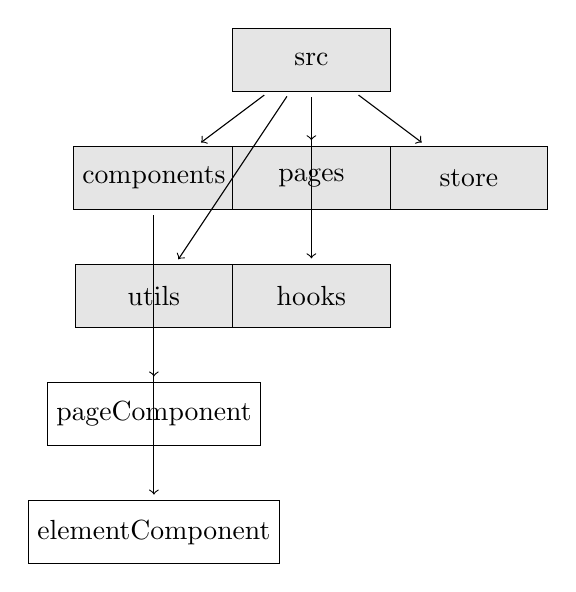
\begin{tikzpicture}[
    file/.style={draw, rectangle, minimum width=2cm, minimum height=0.8cm},
    folder/.style={draw, rectangle, minimum width=2cm, minimum height=0.8cm, fill=gray!20},
    arrow/.style={->, shorten >=2pt, shorten <=2pt}
]

% Folders
\node[folder] (src) at (0,0) {src};
\node[folder] (components) at (-2,-1.5) {components};
\node[folder] (pages) at (0,-1.5) {pages};
\node[folder] (store) at (2,-1.5) {store};
\node[folder] (utils) at (-2,-3) {utils};
\node[folder] (hooks) at (0,-3) {hooks};

% Files
\node[file] (pageComponent) at (-2,-4.5) {pageComponent};
\node[file] (elementComponent) at (-2,-6) {elementComponent};
% ... add more files

% Connections
\draw[arrow] (src) -- (components);
\draw[arrow] (src) -- (pages);
\draw[arrow] (src) -- (store);
\draw[arrow] (src) -- (utils);
\draw[arrow] (src) -- (hooks);
\draw[arrow] (components) -- (pageComponent);
\draw[arrow] (components) -- (elementComponent);
% ... add more connections

\end{tikzpicture}



\pagebreak
\subsubsection{Back-end}
The backend uses the dotNet framework. The development language using the C\# language.

In this project, the backend uses the Onion Architecture.
The Onion Architecture is a typically layered architecture, 
where each layer depends on the inner layer and provides interfaces to the outer layer.
The outer layer provides services to the outermost layer 
and other modules in the same layer based on the interfaces of the inner layer.

From inner to outer, the layers are: Domain, Application, Infrastructure, Presentation.
The Domain layer is the core layer and the innermost layer, used to define domain models, 
which are the business models.
It includes domain models and domain service interfaces.
Domain models are used to define the business models, 
which are the entities in the entity-relationship model and their attributes.
Domain service interfaces are used to define the business services, 
which are the relationships between entities in the entity-relationship model.

The Application layer is the application layer, 
used to define application services, which are the business logic.
It includes domain service implementations and application service interfaces.
Domain service implementations implement the methods of the inner layer's domain service 
interfaces and implement the business logic of the domain models.
Application service interfaces are used to define application services, 
which are the business logic.
It includes but is not limited to database interfaces, testing interfaces, 
HTTP API interfaces, MQTT interfaces, etc.

The Infrastructure layer is the infrastructure layer, used to define infrastructure.
It includes database implementations, testing implementations, 
HTTP API implementations, MQTT implementations, etc.
Database implementations implement the database interfaces 
and provide CRUD services for the database.
Testing implementations implement the testing interfaces 
and provide services for unit testing and integration testing.
HTTP API implementations implement the HTTP API interfaces 
and provide CRUD operations for HTTP APIs.
MQTT implementations implement the MQTT interfaces 
and provide CRUD operations for MQTT.

The Presentation layer is the presentation layer, used to define presentation logic, 
such as interfaces and pages. Since this is a backend project,
data presentation and control are handled by the frontend, 
so this layer is not needed.



\pagebreak
\subsubsection{Data communication and storage}
% 关于本项目的数据通信与数据存储的设计, 包括数据通信的协议, 数据存储的设计等
% 关于数据通信的设计:
% 1. 通信协议的选择
% 自前端向后端发送的数据, 有三种传输的数据类型, 
% 一种是普通的增删改查的请求, 对数据传输的时效性要求不高, 但是对数据的准确性, 完整性, 有序性, 安全性有一定的要求,
% 这种数据的传输, 采用 HTTP 协议, 以及 RESTful API 的设计. 可以有效的保证对数据传输的以上要求.
% 一种是对数据通道的创建和流媒体数据的传输, 对数据传输的时效性, 安全性要求较高, 这种数据的传输, 采用 WebRTC 协议, 以及 MQTT 协议.
% 配合可以快速解码的 flatbuffers 协议, 可以有效的保证对数据传输的以上要求.
% 最后一种是对设备的状态信息和操作信息的传输, 对完整性, 有序性, 安全性都有较高的要求, 这种数据的传输, 采用 MQTT 协议
% 同时也使用了 flatbuffers 协议.
% 
% 2. 数据通信的通信架构和通信流程
% 本项目的数据通信的通信架构, 是基于前后端分离的架构, 前端使用 React 框架, 后端使用 dotnet 框架.
% 当前端需要向后端发送数据的时候, 前端会向后端发送 HTTP 请求, 后端接收到 HTTP 请求之后, 会根据请求的数据类型,
% 选择不同的数据处理方式, 对于普通的增删改查的请求, 后端会根据 RESTful API 的设计, 对数据进行增删改查的操作,
% 对于对数据通道的创建和流媒体数据的传输, 后端会根据 WebRTC 协议, 对数据通道进行创建, 并且帮助前端和设备建立数据通道,
% 当数据通道建立后, 前端和设备之间则使用 flatbuffer 的数据格式对流媒体数据进行传输,
% 对于设备的状态信息和操作信息的传输, 前端会直接向 MQTT broker 发送 MQTT 请求, 
% 设备会在其自身的固件中监听相关的 MQTT 请求, 并且返回相关的数据.
% 
% 3. 数据通信的格式
% 本项目的数据通信的格式, 有三种, 
% 一种是 HTTP 协议, 
% 使用 json 格式对数据进行传输,
% 一种是 WebRTC 协议, 
% 使用 flatbuffers 格式对数据进行传输,
% 一种是 MQTT 协议.
% 使用 flatbuffers 格式对数据进行传输,
% 
% 关于数据存储的设计:
% 1. 数据存储的数据库的选择
% 本项目的数据存储的数据库的选择, 使用了轻量级的数据库 SQLite,
% SQLite 是一个进程内的库, 实现了自给自足的, 无服务器的, 零配置的, 事务性的 SQL 数据库引擎.
% 这是因为整个项目的目的是为了实现前端与设备之间的数据通信, 对于数据库数据的增删改查操作的要求不高,
% 数据量较小, 且对于数据库的数据的事务性要求不高, 所以选择了 SQLite 数据库.
% 2. 项目前后端的数据结构的设计
% 在本项目中, 前端由于使用了 React 框架, 所以前端的数据结构的设计, 使用了基于状态的数据结构的设计,
% 每个组件或者数据集都包含一个状态对象, 这个状态对象的属性就是组件的各个状态. 
% 使用状态对象的原因是, 可以方便的对状态进行管理, 采用对象-属性的形式, 可以方便的针对不同组件的同类状态进行区分,
% 由于跨组件的状态是由 redux 进行管理的, 这种状态对象的设计, 可以更搞笑的对状态进行更新和传递.
% 后端由于使用了 dotnet 框架, 所以后端的数据结构的设计, 使用了基于类的数据结构的设计,
% 采用了面向对象的编程思想, 对数据进行了封装, 使得数据的传输更加的安全, 有序, 完整.


\pagebreak

% \subsection{Domain model}
% \documentclass[]{article}
\usepackage{graphicx}
\usepackage{amsmath}
\usepackage{tikz}

% libaries
\usetikzlibrary{shapes,arrows}

%Define the listing package
\usepackage{listings} %code highlighter
\usepackage{color} %use color
\definecolor{mygreen}{rgb}{0,0.6,0}
\definecolor{mygray}{rgb}{0.5,0.5,0.5}
\definecolor{mymauve}{rgb}{0.58,0,0.82}

%Customize a bit the look
\lstset{ %
backgroundcolor=\color{white}, % choose the background color; you must add \usepackage{color} or \usepackage{xcolor}
basicstyle=\footnotesize, % the size of the fonts that are used for the code
breakatwhitespace=false, % sets if automatic breaks should only happen at whitespace
breaklines=true, % sets automatic line breaking
captionpos=b, % sets the caption-position to bottom
commentstyle=\color{mygreen}, % comment style
deletekeywords={...}, % if you want to delete keywords from the given language
escapeinside={\%*}{*)}, % if you want to add LaTeX within your code
extendedchars=true, % lets you use non-ASCII characters; for 8-bits encodings only, does not work with UTF-8
frame=single, % adds a frame around the code
keepspaces=true, % keeps spaces in text, useful for keeping indentation of code (possibly needs columns=flexible)
keywordstyle=\color{blue}, % keyword style
% language=Octave, % the language of the code
morekeywords={*,...}, % if you want to add more keywords to the set
numbers=left, % where to put the line-numbers; possible values are (none, left, right)
numbersep=5pt, % how far the line-numbers are from the code
numberstyle=\tiny\color{mygray}, % the style that is used for the line-numbers
rulecolor=\color{black}, % if not set, the frame-color may be changed on line-breaks within not-black text (e.g. comments (green here))
showspaces=false, % show spaces everywhere adding particular underscores; it overrides 'showstringspaces'
showstringspaces=false, % underline spaces within strings only
showtabs=false, % show tabs within strings adding particular underscores
stepnumber=1, % the step between two line-numbers. If it's 1, each line will be numbered
stringstyle=\color{mymauve}, % string literal style
tabsize=2, % sets default tabsize to 2 spaces
title=\lstname % show the filename of files included with \lstinputlisting; also try caption instead of title
}

\definecolor{darkgray}{rgb}{.4,.4,.4}
\definecolor{purple}{rgb}{0.65, 0.12, 0.82}

\lstdefinelanguage{React}{
keywords={const, typeof, new, true, false, catch, function, return, null, catch, switch, var, if, in, while, do, else, case, break},
keywordstyle=\color{blue}\bfseries,
ndkeywords={class, export, boolean, throw, implements, import, this},
ndkeywordstyle=\color{darkgray}\bfseries,
identifierstyle=\color{mygreen},
sensitive=false,
comment=[l]{//},
morecomment=[s]{/*}{*/},
commentstyle=\color{purple}\ttfamily,
string=[b]{"}{'}{`},
stringstyle=\color{red}\ttfamily,
morestring=[b]',
morestring=[b]",
morestring=[b]`',
}

\lstdefinelanguage{CSharp}{
keywords={const, typeof, new, true, false, catch, function, return, null, catch, switch, var, if, in, while, do, else, case, break},
keywordstyle=\color{blue}\bfseries,
ndkeywords={class, export, boolean, throw, implements, import, this},
ndkeywordstyle=\color{darkgray}\bfseries,
identifierstyle=\color{mygreen},
sensitive=false,
comment=[l]{//},
morecomment=[s]{/*}{*/},
commentstyle=\color{purple}\ttfamily,
string=[b]{"}{'}{`},
stringstyle=\color{red}\ttfamily,
morestring=[b]',
morestring=[b]",
morestring=[b]`',
}

\lstset{
language=React,
extendedchars=true,
basicstyle=\footnotesize\ttfamily,
showstringspaces=false,
showspaces=false,
numbers=left,
numberstyle=\footnotesize,
numbersep=9pt,
tabsize=2,
breaklines=true,
showtabs=false,
captionpos=b
}

\lstset{
language=CSharp,
extendedchars=true,
basicstyle=\footnotesize\ttfamily,
showstringspaces=false,
showspaces=false,
numbers=left,
numberstyle=\footnotesize,
numbersep=9pt,
tabsize=2,
breaklines=true,
showtabs=false,
captionpos=b
}

% \usepackage{cite} % Add this line for citation

% \bibliographystyle{plain}

\title{
The implementation of BifrostConnect Front-end scope, 
re-design and development with the relevant back-end support develop.
}
\author{
    Fei Gu \\
    Erhvervs Akademi Sydvest \\
    Computer Science 21\\
    }
\date{\today}

\begin{document}

% Front page
\maketitle
\begin{center}
    Supervisor: Henrik Boulund Meng Hansen \\
    Company: BifrostConnect \\
    Engineering Director: Jasper Wass \\
\end{center}
\tableofcontents
\pagebreak


% The introduction
\section{Introduction}
\subsection{Background}\input{sections/introduction/background.tex}
\subsection{The company}\input{sections/introduction/aboutCompany}
\subsection{The project}\input{sections/introduction/aboutProject}
\pagebreak

% The problem statement
\section{Problem Statement}
\subsection{Statement}
\input{sections/problemStatement/statement}
\subsection{Situation}
\input{sections/problemStatement/situation}
\subsection{Potential Solution}
\input{sections/problemStatement/potentialSolution}
\pagebreak

% Requirement analysis
\section{Requirement Analysis}
\input{sections/requirementAnalysis/index}

\subsection{Stakeholders}
\input{sections/requirementAnalysis/stakeholders/index}

\subsection{Business Domain}
\input{sections/requirementAnalysis/bussinesDomain/index}

\subsection{Scope}
\input{sections/requirementAnalysis/scope}

\subsection{Goals}
\input{sections/requirementAnalysis/goals}
\pagebreak

% Software Design
\section{Software Design}
% developement methods
\subsection{Software Development Methods}
\input{sections/softwareDevelopmentMethods/index}
\subsubsection{Agile Software Development}
\input{sections/softwareDevelopmentMethods/agileSoftwareDevelopment/index}
\subsubsection{Feature Driven Development}
\input{sections/softwareDevelopmentMethods/featureDrivenDevelopment/index}

\pagebreak

% Technology seslection
\subsection{Technology selection}
\input{sections/softwareDesign/technologySelection/index}
\subsubsection{Front-end}
\input{sections/softwareDesign/technologySelection/frontEnd}            
\subsubsection{Back-end}
\input{sections/softwareDesign/technologySelection/backEnd}            
\subsubsection{Database}
\input{sections/softwareDesign/technologySelection/database}
\subsubsection{Data communication}
\input{sections/softwareDesign/technologySelection/dataCommunication}            
\subsubsection{DevOps}
\input{sections/softwareDesign/technologySelection/devOps}
\pagebreak

% Architecture design
\subsection{Architecture design}
\input{sections/softwareDesign/architectureDesign/index}
\pagebreak
\subsubsection{Front-end}
\input{sections/softwareDesign/architectureDesign/frontEndArchitecture}
\pagebreak
\subsubsection{Back-end}
\input{sections/softwareDesign/architectureDesign/backEndArchitecture}
\pagebreak
\subsubsection{Data communication and storage}
\input{sections/softwareDesign/architectureDesign/dataCommunicationArchitecture}
\pagebreak

% \subsection{Domain model}
% \input{sections/softwareDesign/domainModel/index}
% \subsection{Database design}
% % 数据库领域模型 ER 图
% % 包括表和字段的设置.
% % 对于私有键和外键的设置.

% \subsection{Back-end design}
% % 后端对象模型
% % 以及对于对象模型的增删改查
% % 以及相关的其他服务的设计`'

% \subsection{Front-end design}
% % 对于前端的页面结构的设计 
% % 页面的状态的设计, 交互设计

% \subsection{FlatBuffers design}
% % schema 的设计

\subsection{DevOps CI/CD process design}
\input{sections/softwareDesign/devOpsDesign/index}
\subsubsection{Continuous Integration}
\input{sections/softwareDesign/devOpsDesign/continuousIntegration/index}
\subsubsection{Continuous Delivery}
\input{sections/softwareDesign/devOpsDesign/continuousDelivery/index}
\subsubsection{Continuous Deployment}
\input{sections/softwareDesign/devOpsDesign/continuousDeployment/index}
\pagebreak

\section{Software Development} 
\input{sections/softwareDevelopment/index}
\subsection{Overall development}
\input{sections/softwareDevelopment/overallDevelopement/index}
\subsubsection{Front-end}
\input{sections/softwareDevelopment/overallDevelopement/frontEnd/index}
\subsubsection{Back-end}
\input{sections/softwareDevelopment/overallDevelopement/backEnd/index}
\subsubsection{DevOps}
\input{sections/softwareDevelopment/overallDevelopement/devOps/index}
\subsection{Feature development} 
\input{sections/softwareDevelopment/featureDevelopment/index}
\subsubsection{Use Case 1}
\input{sections/softwareDevelopment/featureDevelopment/useCase1/index}
\subsubsection{Feature 1}
\input{sections/softwareDevelopment/featureDevelopment/feature/feature1.tex}
\pagebreak
\section{Conclusion} 
\subsection{Result}
Since the project is still in progress, the result is not available yet.
So far, basic structure of this project has been built. But the most features 
are not implemented yet. 
\subsection{Discussion}
As a single developer for this project, I am confident what I have done so far.
And I can say I understand the most of the knowledge I have used in this project, 
which also means I can explain all the part of the project. 
But this project also relevant some of the complex knowledge which I have to continue 
to study and practice.
\subsection{Future Work}
The future work is to implement the rest of the features. 
Including the most important part which is the 'create session' feature.
\pagebreak
% \bibliography{bibliography}
\pagebreak
% \begin{appendices}
%     \section{Appendix}
% \end{appendices} 
\end{document}
% \subsection{Database design}
% % 数据库领域模型 ER 图
% % 包括表和字段的设置.
% % 对于私有键和外键的设置.

% \subsection{Back-end design}
% % 后端对象模型
% % 以及对于对象模型的增删改查
% % 以及相关的其他服务的设计`'

% \subsection{Front-end design}
% % 对于前端的页面结构的设计 
% % 页面的状态的设计, 交互设计

% \subsection{FlatBuffers design}
% % schema 的设计

\subsection{DevOps CI/CD process design}
\documentclass[]{article}
\usepackage{graphicx}
\usepackage{amsmath}
\usepackage{tikz}

% libaries
\usetikzlibrary{shapes,arrows}

%Define the listing package
\usepackage{listings} %code highlighter
\usepackage{color} %use color
\definecolor{mygreen}{rgb}{0,0.6,0}
\definecolor{mygray}{rgb}{0.5,0.5,0.5}
\definecolor{mymauve}{rgb}{0.58,0,0.82}

%Customize a bit the look
\lstset{ %
backgroundcolor=\color{white}, % choose the background color; you must add \usepackage{color} or \usepackage{xcolor}
basicstyle=\footnotesize, % the size of the fonts that are used for the code
breakatwhitespace=false, % sets if automatic breaks should only happen at whitespace
breaklines=true, % sets automatic line breaking
captionpos=b, % sets the caption-position to bottom
commentstyle=\color{mygreen}, % comment style
deletekeywords={...}, % if you want to delete keywords from the given language
escapeinside={\%*}{*)}, % if you want to add LaTeX within your code
extendedchars=true, % lets you use non-ASCII characters; for 8-bits encodings only, does not work with UTF-8
frame=single, % adds a frame around the code
keepspaces=true, % keeps spaces in text, useful for keeping indentation of code (possibly needs columns=flexible)
keywordstyle=\color{blue}, % keyword style
% language=Octave, % the language of the code
morekeywords={*,...}, % if you want to add more keywords to the set
numbers=left, % where to put the line-numbers; possible values are (none, left, right)
numbersep=5pt, % how far the line-numbers are from the code
numberstyle=\tiny\color{mygray}, % the style that is used for the line-numbers
rulecolor=\color{black}, % if not set, the frame-color may be changed on line-breaks within not-black text (e.g. comments (green here))
showspaces=false, % show spaces everywhere adding particular underscores; it overrides 'showstringspaces'
showstringspaces=false, % underline spaces within strings only
showtabs=false, % show tabs within strings adding particular underscores
stepnumber=1, % the step between two line-numbers. If it's 1, each line will be numbered
stringstyle=\color{mymauve}, % string literal style
tabsize=2, % sets default tabsize to 2 spaces
title=\lstname % show the filename of files included with \lstinputlisting; also try caption instead of title
}

\definecolor{darkgray}{rgb}{.4,.4,.4}
\definecolor{purple}{rgb}{0.65, 0.12, 0.82}

\lstdefinelanguage{React}{
keywords={const, typeof, new, true, false, catch, function, return, null, catch, switch, var, if, in, while, do, else, case, break},
keywordstyle=\color{blue}\bfseries,
ndkeywords={class, export, boolean, throw, implements, import, this},
ndkeywordstyle=\color{darkgray}\bfseries,
identifierstyle=\color{mygreen},
sensitive=false,
comment=[l]{//},
morecomment=[s]{/*}{*/},
commentstyle=\color{purple}\ttfamily,
string=[b]{"}{'}{`},
stringstyle=\color{red}\ttfamily,
morestring=[b]',
morestring=[b]",
morestring=[b]`',
}

\lstdefinelanguage{CSharp}{
keywords={const, typeof, new, true, false, catch, function, return, null, catch, switch, var, if, in, while, do, else, case, break},
keywordstyle=\color{blue}\bfseries,
ndkeywords={class, export, boolean, throw, implements, import, this},
ndkeywordstyle=\color{darkgray}\bfseries,
identifierstyle=\color{mygreen},
sensitive=false,
comment=[l]{//},
morecomment=[s]{/*}{*/},
commentstyle=\color{purple}\ttfamily,
string=[b]{"}{'}{`},
stringstyle=\color{red}\ttfamily,
morestring=[b]',
morestring=[b]",
morestring=[b]`',
}

\lstset{
language=React,
extendedchars=true,
basicstyle=\footnotesize\ttfamily,
showstringspaces=false,
showspaces=false,
numbers=left,
numberstyle=\footnotesize,
numbersep=9pt,
tabsize=2,
breaklines=true,
showtabs=false,
captionpos=b
}

\lstset{
language=CSharp,
extendedchars=true,
basicstyle=\footnotesize\ttfamily,
showstringspaces=false,
showspaces=false,
numbers=left,
numberstyle=\footnotesize,
numbersep=9pt,
tabsize=2,
breaklines=true,
showtabs=false,
captionpos=b
}

% \usepackage{cite} % Add this line for citation

% \bibliographystyle{plain}

\title{
The implementation of BifrostConnect Front-end scope, 
re-design and development with the relevant back-end support develop.
}
\author{
    Fei Gu \\
    Erhvervs Akademi Sydvest \\
    Computer Science 21\\
    }
\date{\today}

\begin{document}

% Front page
\maketitle
\begin{center}
    Supervisor: Henrik Boulund Meng Hansen \\
    Company: BifrostConnect \\
    Engineering Director: Jasper Wass \\
\end{center}
\tableofcontents
\pagebreak


% The introduction
\section{Introduction}
\subsection{Background}\input{sections/introduction/background.tex}
\subsection{The company}\input{sections/introduction/aboutCompany}
\subsection{The project}\input{sections/introduction/aboutProject}
\pagebreak

% The problem statement
\section{Problem Statement}
\subsection{Statement}
\input{sections/problemStatement/statement}
\subsection{Situation}
\input{sections/problemStatement/situation}
\subsection{Potential Solution}
\input{sections/problemStatement/potentialSolution}
\pagebreak

% Requirement analysis
\section{Requirement Analysis}
\input{sections/requirementAnalysis/index}

\subsection{Stakeholders}
\input{sections/requirementAnalysis/stakeholders/index}

\subsection{Business Domain}
\input{sections/requirementAnalysis/bussinesDomain/index}

\subsection{Scope}
\input{sections/requirementAnalysis/scope}

\subsection{Goals}
\input{sections/requirementAnalysis/goals}
\pagebreak

% Software Design
\section{Software Design}
% developement methods
\subsection{Software Development Methods}
\input{sections/softwareDevelopmentMethods/index}
\subsubsection{Agile Software Development}
\input{sections/softwareDevelopmentMethods/agileSoftwareDevelopment/index}
\subsubsection{Feature Driven Development}
\input{sections/softwareDevelopmentMethods/featureDrivenDevelopment/index}

\pagebreak

% Technology seslection
\subsection{Technology selection}
\input{sections/softwareDesign/technologySelection/index}
\subsubsection{Front-end}
\input{sections/softwareDesign/technologySelection/frontEnd}            
\subsubsection{Back-end}
\input{sections/softwareDesign/technologySelection/backEnd}            
\subsubsection{Database}
\input{sections/softwareDesign/technologySelection/database}
\subsubsection{Data communication}
\input{sections/softwareDesign/technologySelection/dataCommunication}            
\subsubsection{DevOps}
\input{sections/softwareDesign/technologySelection/devOps}
\pagebreak

% Architecture design
\subsection{Architecture design}
\input{sections/softwareDesign/architectureDesign/index}
\pagebreak
\subsubsection{Front-end}
\input{sections/softwareDesign/architectureDesign/frontEndArchitecture}
\pagebreak
\subsubsection{Back-end}
\input{sections/softwareDesign/architectureDesign/backEndArchitecture}
\pagebreak
\subsubsection{Data communication and storage}
\input{sections/softwareDesign/architectureDesign/dataCommunicationArchitecture}
\pagebreak

% \subsection{Domain model}
% \input{sections/softwareDesign/domainModel/index}
% \subsection{Database design}
% % 数据库领域模型 ER 图
% % 包括表和字段的设置.
% % 对于私有键和外键的设置.

% \subsection{Back-end design}
% % 后端对象模型
% % 以及对于对象模型的增删改查
% % 以及相关的其他服务的设计`'

% \subsection{Front-end design}
% % 对于前端的页面结构的设计 
% % 页面的状态的设计, 交互设计

% \subsection{FlatBuffers design}
% % schema 的设计

\subsection{DevOps CI/CD process design}
\input{sections/softwareDesign/devOpsDesign/index}
\subsubsection{Continuous Integration}
\input{sections/softwareDesign/devOpsDesign/continuousIntegration/index}
\subsubsection{Continuous Delivery}
\input{sections/softwareDesign/devOpsDesign/continuousDelivery/index}
\subsubsection{Continuous Deployment}
\input{sections/softwareDesign/devOpsDesign/continuousDeployment/index}
\pagebreak

\section{Software Development} 
\input{sections/softwareDevelopment/index}
\subsection{Overall development}
\input{sections/softwareDevelopment/overallDevelopement/index}
\subsubsection{Front-end}
\input{sections/softwareDevelopment/overallDevelopement/frontEnd/index}
\subsubsection{Back-end}
\input{sections/softwareDevelopment/overallDevelopement/backEnd/index}
\subsubsection{DevOps}
\input{sections/softwareDevelopment/overallDevelopement/devOps/index}
\subsection{Feature development} 
\input{sections/softwareDevelopment/featureDevelopment/index}
\subsubsection{Use Case 1}
\input{sections/softwareDevelopment/featureDevelopment/useCase1/index}
\subsubsection{Feature 1}
\input{sections/softwareDevelopment/featureDevelopment/feature/feature1.tex}
\pagebreak
\section{Conclusion} 
\subsection{Result}
Since the project is still in progress, the result is not available yet.
So far, basic structure of this project has been built. But the most features 
are not implemented yet. 
\subsection{Discussion}
As a single developer for this project, I am confident what I have done so far.
And I can say I understand the most of the knowledge I have used in this project, 
which also means I can explain all the part of the project. 
But this project also relevant some of the complex knowledge which I have to continue 
to study and practice.
\subsection{Future Work}
The future work is to implement the rest of the features. 
Including the most important part which is the 'create session' feature.
\pagebreak
% \bibliography{bibliography}
\pagebreak
% \begin{appendices}
%     \section{Appendix}
% \end{appendices} 
\end{document}
\subsubsection{Continuous Integration}
\documentclass[]{article}
\usepackage{graphicx}
\usepackage{amsmath}
\usepackage{tikz}

% libaries
\usetikzlibrary{shapes,arrows}

%Define the listing package
\usepackage{listings} %code highlighter
\usepackage{color} %use color
\definecolor{mygreen}{rgb}{0,0.6,0}
\definecolor{mygray}{rgb}{0.5,0.5,0.5}
\definecolor{mymauve}{rgb}{0.58,0,0.82}

%Customize a bit the look
\lstset{ %
backgroundcolor=\color{white}, % choose the background color; you must add \usepackage{color} or \usepackage{xcolor}
basicstyle=\footnotesize, % the size of the fonts that are used for the code
breakatwhitespace=false, % sets if automatic breaks should only happen at whitespace
breaklines=true, % sets automatic line breaking
captionpos=b, % sets the caption-position to bottom
commentstyle=\color{mygreen}, % comment style
deletekeywords={...}, % if you want to delete keywords from the given language
escapeinside={\%*}{*)}, % if you want to add LaTeX within your code
extendedchars=true, % lets you use non-ASCII characters; for 8-bits encodings only, does not work with UTF-8
frame=single, % adds a frame around the code
keepspaces=true, % keeps spaces in text, useful for keeping indentation of code (possibly needs columns=flexible)
keywordstyle=\color{blue}, % keyword style
% language=Octave, % the language of the code
morekeywords={*,...}, % if you want to add more keywords to the set
numbers=left, % where to put the line-numbers; possible values are (none, left, right)
numbersep=5pt, % how far the line-numbers are from the code
numberstyle=\tiny\color{mygray}, % the style that is used for the line-numbers
rulecolor=\color{black}, % if not set, the frame-color may be changed on line-breaks within not-black text (e.g. comments (green here))
showspaces=false, % show spaces everywhere adding particular underscores; it overrides 'showstringspaces'
showstringspaces=false, % underline spaces within strings only
showtabs=false, % show tabs within strings adding particular underscores
stepnumber=1, % the step between two line-numbers. If it's 1, each line will be numbered
stringstyle=\color{mymauve}, % string literal style
tabsize=2, % sets default tabsize to 2 spaces
title=\lstname % show the filename of files included with \lstinputlisting; also try caption instead of title
}

\definecolor{darkgray}{rgb}{.4,.4,.4}
\definecolor{purple}{rgb}{0.65, 0.12, 0.82}

\lstdefinelanguage{React}{
keywords={const, typeof, new, true, false, catch, function, return, null, catch, switch, var, if, in, while, do, else, case, break},
keywordstyle=\color{blue}\bfseries,
ndkeywords={class, export, boolean, throw, implements, import, this},
ndkeywordstyle=\color{darkgray}\bfseries,
identifierstyle=\color{mygreen},
sensitive=false,
comment=[l]{//},
morecomment=[s]{/*}{*/},
commentstyle=\color{purple}\ttfamily,
string=[b]{"}{'}{`},
stringstyle=\color{red}\ttfamily,
morestring=[b]',
morestring=[b]",
morestring=[b]`',
}

\lstdefinelanguage{CSharp}{
keywords={const, typeof, new, true, false, catch, function, return, null, catch, switch, var, if, in, while, do, else, case, break},
keywordstyle=\color{blue}\bfseries,
ndkeywords={class, export, boolean, throw, implements, import, this},
ndkeywordstyle=\color{darkgray}\bfseries,
identifierstyle=\color{mygreen},
sensitive=false,
comment=[l]{//},
morecomment=[s]{/*}{*/},
commentstyle=\color{purple}\ttfamily,
string=[b]{"}{'}{`},
stringstyle=\color{red}\ttfamily,
morestring=[b]',
morestring=[b]",
morestring=[b]`',
}

\lstset{
language=React,
extendedchars=true,
basicstyle=\footnotesize\ttfamily,
showstringspaces=false,
showspaces=false,
numbers=left,
numberstyle=\footnotesize,
numbersep=9pt,
tabsize=2,
breaklines=true,
showtabs=false,
captionpos=b
}

\lstset{
language=CSharp,
extendedchars=true,
basicstyle=\footnotesize\ttfamily,
showstringspaces=false,
showspaces=false,
numbers=left,
numberstyle=\footnotesize,
numbersep=9pt,
tabsize=2,
breaklines=true,
showtabs=false,
captionpos=b
}

% \usepackage{cite} % Add this line for citation

% \bibliographystyle{plain}

\title{
The implementation of BifrostConnect Front-end scope, 
re-design and development with the relevant back-end support develop.
}
\author{
    Fei Gu \\
    Erhvervs Akademi Sydvest \\
    Computer Science 21\\
    }
\date{\today}

\begin{document}

% Front page
\maketitle
\begin{center}
    Supervisor: Henrik Boulund Meng Hansen \\
    Company: BifrostConnect \\
    Engineering Director: Jasper Wass \\
\end{center}
\tableofcontents
\pagebreak


% The introduction
\section{Introduction}
\subsection{Background}\input{sections/introduction/background.tex}
\subsection{The company}\input{sections/introduction/aboutCompany}
\subsection{The project}\input{sections/introduction/aboutProject}
\pagebreak

% The problem statement
\section{Problem Statement}
\subsection{Statement}
\input{sections/problemStatement/statement}
\subsection{Situation}
\input{sections/problemStatement/situation}
\subsection{Potential Solution}
\input{sections/problemStatement/potentialSolution}
\pagebreak

% Requirement analysis
\section{Requirement Analysis}
\input{sections/requirementAnalysis/index}

\subsection{Stakeholders}
\input{sections/requirementAnalysis/stakeholders/index}

\subsection{Business Domain}
\input{sections/requirementAnalysis/bussinesDomain/index}

\subsection{Scope}
\input{sections/requirementAnalysis/scope}

\subsection{Goals}
\input{sections/requirementAnalysis/goals}
\pagebreak

% Software Design
\section{Software Design}
% developement methods
\subsection{Software Development Methods}
\input{sections/softwareDevelopmentMethods/index}
\subsubsection{Agile Software Development}
\input{sections/softwareDevelopmentMethods/agileSoftwareDevelopment/index}
\subsubsection{Feature Driven Development}
\input{sections/softwareDevelopmentMethods/featureDrivenDevelopment/index}

\pagebreak

% Technology seslection
\subsection{Technology selection}
\input{sections/softwareDesign/technologySelection/index}
\subsubsection{Front-end}
\input{sections/softwareDesign/technologySelection/frontEnd}            
\subsubsection{Back-end}
\input{sections/softwareDesign/technologySelection/backEnd}            
\subsubsection{Database}
\input{sections/softwareDesign/technologySelection/database}
\subsubsection{Data communication}
\input{sections/softwareDesign/technologySelection/dataCommunication}            
\subsubsection{DevOps}
\input{sections/softwareDesign/technologySelection/devOps}
\pagebreak

% Architecture design
\subsection{Architecture design}
\input{sections/softwareDesign/architectureDesign/index}
\pagebreak
\subsubsection{Front-end}
\input{sections/softwareDesign/architectureDesign/frontEndArchitecture}
\pagebreak
\subsubsection{Back-end}
\input{sections/softwareDesign/architectureDesign/backEndArchitecture}
\pagebreak
\subsubsection{Data communication and storage}
\input{sections/softwareDesign/architectureDesign/dataCommunicationArchitecture}
\pagebreak

% \subsection{Domain model}
% \input{sections/softwareDesign/domainModel/index}
% \subsection{Database design}
% % 数据库领域模型 ER 图
% % 包括表和字段的设置.
% % 对于私有键和外键的设置.

% \subsection{Back-end design}
% % 后端对象模型
% % 以及对于对象模型的增删改查
% % 以及相关的其他服务的设计`'

% \subsection{Front-end design}
% % 对于前端的页面结构的设计 
% % 页面的状态的设计, 交互设计

% \subsection{FlatBuffers design}
% % schema 的设计

\subsection{DevOps CI/CD process design}
\input{sections/softwareDesign/devOpsDesign/index}
\subsubsection{Continuous Integration}
\input{sections/softwareDesign/devOpsDesign/continuousIntegration/index}
\subsubsection{Continuous Delivery}
\input{sections/softwareDesign/devOpsDesign/continuousDelivery/index}
\subsubsection{Continuous Deployment}
\input{sections/softwareDesign/devOpsDesign/continuousDeployment/index}
\pagebreak

\section{Software Development} 
\input{sections/softwareDevelopment/index}
\subsection{Overall development}
\input{sections/softwareDevelopment/overallDevelopement/index}
\subsubsection{Front-end}
\input{sections/softwareDevelopment/overallDevelopement/frontEnd/index}
\subsubsection{Back-end}
\input{sections/softwareDevelopment/overallDevelopement/backEnd/index}
\subsubsection{DevOps}
\input{sections/softwareDevelopment/overallDevelopement/devOps/index}
\subsection{Feature development} 
\input{sections/softwareDevelopment/featureDevelopment/index}
\subsubsection{Use Case 1}
\input{sections/softwareDevelopment/featureDevelopment/useCase1/index}
\subsubsection{Feature 1}
\input{sections/softwareDevelopment/featureDevelopment/feature/feature1.tex}
\pagebreak
\section{Conclusion} 
\subsection{Result}
Since the project is still in progress, the result is not available yet.
So far, basic structure of this project has been built. But the most features 
are not implemented yet. 
\subsection{Discussion}
As a single developer for this project, I am confident what I have done so far.
And I can say I understand the most of the knowledge I have used in this project, 
which also means I can explain all the part of the project. 
But this project also relevant some of the complex knowledge which I have to continue 
to study and practice.
\subsection{Future Work}
The future work is to implement the rest of the features. 
Including the most important part which is the 'create session' feature.
\pagebreak
% \bibliography{bibliography}
\pagebreak
% \begin{appendices}
%     \section{Appendix}
% \end{appendices} 
\end{document}
\subsubsection{Continuous Delivery}
\documentclass[]{article}
\usepackage{graphicx}
\usepackage{amsmath}
\usepackage{tikz}

% libaries
\usetikzlibrary{shapes,arrows}

%Define the listing package
\usepackage{listings} %code highlighter
\usepackage{color} %use color
\definecolor{mygreen}{rgb}{0,0.6,0}
\definecolor{mygray}{rgb}{0.5,0.5,0.5}
\definecolor{mymauve}{rgb}{0.58,0,0.82}

%Customize a bit the look
\lstset{ %
backgroundcolor=\color{white}, % choose the background color; you must add \usepackage{color} or \usepackage{xcolor}
basicstyle=\footnotesize, % the size of the fonts that are used for the code
breakatwhitespace=false, % sets if automatic breaks should only happen at whitespace
breaklines=true, % sets automatic line breaking
captionpos=b, % sets the caption-position to bottom
commentstyle=\color{mygreen}, % comment style
deletekeywords={...}, % if you want to delete keywords from the given language
escapeinside={\%*}{*)}, % if you want to add LaTeX within your code
extendedchars=true, % lets you use non-ASCII characters; for 8-bits encodings only, does not work with UTF-8
frame=single, % adds a frame around the code
keepspaces=true, % keeps spaces in text, useful for keeping indentation of code (possibly needs columns=flexible)
keywordstyle=\color{blue}, % keyword style
% language=Octave, % the language of the code
morekeywords={*,...}, % if you want to add more keywords to the set
numbers=left, % where to put the line-numbers; possible values are (none, left, right)
numbersep=5pt, % how far the line-numbers are from the code
numberstyle=\tiny\color{mygray}, % the style that is used for the line-numbers
rulecolor=\color{black}, % if not set, the frame-color may be changed on line-breaks within not-black text (e.g. comments (green here))
showspaces=false, % show spaces everywhere adding particular underscores; it overrides 'showstringspaces'
showstringspaces=false, % underline spaces within strings only
showtabs=false, % show tabs within strings adding particular underscores
stepnumber=1, % the step between two line-numbers. If it's 1, each line will be numbered
stringstyle=\color{mymauve}, % string literal style
tabsize=2, % sets default tabsize to 2 spaces
title=\lstname % show the filename of files included with \lstinputlisting; also try caption instead of title
}

\definecolor{darkgray}{rgb}{.4,.4,.4}
\definecolor{purple}{rgb}{0.65, 0.12, 0.82}

\lstdefinelanguage{React}{
keywords={const, typeof, new, true, false, catch, function, return, null, catch, switch, var, if, in, while, do, else, case, break},
keywordstyle=\color{blue}\bfseries,
ndkeywords={class, export, boolean, throw, implements, import, this},
ndkeywordstyle=\color{darkgray}\bfseries,
identifierstyle=\color{mygreen},
sensitive=false,
comment=[l]{//},
morecomment=[s]{/*}{*/},
commentstyle=\color{purple}\ttfamily,
string=[b]{"}{'}{`},
stringstyle=\color{red}\ttfamily,
morestring=[b]',
morestring=[b]",
morestring=[b]`',
}

\lstdefinelanguage{CSharp}{
keywords={const, typeof, new, true, false, catch, function, return, null, catch, switch, var, if, in, while, do, else, case, break},
keywordstyle=\color{blue}\bfseries,
ndkeywords={class, export, boolean, throw, implements, import, this},
ndkeywordstyle=\color{darkgray}\bfseries,
identifierstyle=\color{mygreen},
sensitive=false,
comment=[l]{//},
morecomment=[s]{/*}{*/},
commentstyle=\color{purple}\ttfamily,
string=[b]{"}{'}{`},
stringstyle=\color{red}\ttfamily,
morestring=[b]',
morestring=[b]",
morestring=[b]`',
}

\lstset{
language=React,
extendedchars=true,
basicstyle=\footnotesize\ttfamily,
showstringspaces=false,
showspaces=false,
numbers=left,
numberstyle=\footnotesize,
numbersep=9pt,
tabsize=2,
breaklines=true,
showtabs=false,
captionpos=b
}

\lstset{
language=CSharp,
extendedchars=true,
basicstyle=\footnotesize\ttfamily,
showstringspaces=false,
showspaces=false,
numbers=left,
numberstyle=\footnotesize,
numbersep=9pt,
tabsize=2,
breaklines=true,
showtabs=false,
captionpos=b
}

% \usepackage{cite} % Add this line for citation

% \bibliographystyle{plain}

\title{
The implementation of BifrostConnect Front-end scope, 
re-design and development with the relevant back-end support develop.
}
\author{
    Fei Gu \\
    Erhvervs Akademi Sydvest \\
    Computer Science 21\\
    }
\date{\today}

\begin{document}

% Front page
\maketitle
\begin{center}
    Supervisor: Henrik Boulund Meng Hansen \\
    Company: BifrostConnect \\
    Engineering Director: Jasper Wass \\
\end{center}
\tableofcontents
\pagebreak


% The introduction
\section{Introduction}
\subsection{Background}\input{sections/introduction/background.tex}
\subsection{The company}\input{sections/introduction/aboutCompany}
\subsection{The project}\input{sections/introduction/aboutProject}
\pagebreak

% The problem statement
\section{Problem Statement}
\subsection{Statement}
\input{sections/problemStatement/statement}
\subsection{Situation}
\input{sections/problemStatement/situation}
\subsection{Potential Solution}
\input{sections/problemStatement/potentialSolution}
\pagebreak

% Requirement analysis
\section{Requirement Analysis}
\input{sections/requirementAnalysis/index}

\subsection{Stakeholders}
\input{sections/requirementAnalysis/stakeholders/index}

\subsection{Business Domain}
\input{sections/requirementAnalysis/bussinesDomain/index}

\subsection{Scope}
\input{sections/requirementAnalysis/scope}

\subsection{Goals}
\input{sections/requirementAnalysis/goals}
\pagebreak

% Software Design
\section{Software Design}
% developement methods
\subsection{Software Development Methods}
\input{sections/softwareDevelopmentMethods/index}
\subsubsection{Agile Software Development}
\input{sections/softwareDevelopmentMethods/agileSoftwareDevelopment/index}
\subsubsection{Feature Driven Development}
\input{sections/softwareDevelopmentMethods/featureDrivenDevelopment/index}

\pagebreak

% Technology seslection
\subsection{Technology selection}
\input{sections/softwareDesign/technologySelection/index}
\subsubsection{Front-end}
\input{sections/softwareDesign/technologySelection/frontEnd}            
\subsubsection{Back-end}
\input{sections/softwareDesign/technologySelection/backEnd}            
\subsubsection{Database}
\input{sections/softwareDesign/technologySelection/database}
\subsubsection{Data communication}
\input{sections/softwareDesign/technologySelection/dataCommunication}            
\subsubsection{DevOps}
\input{sections/softwareDesign/technologySelection/devOps}
\pagebreak

% Architecture design
\subsection{Architecture design}
\input{sections/softwareDesign/architectureDesign/index}
\pagebreak
\subsubsection{Front-end}
\input{sections/softwareDesign/architectureDesign/frontEndArchitecture}
\pagebreak
\subsubsection{Back-end}
\input{sections/softwareDesign/architectureDesign/backEndArchitecture}
\pagebreak
\subsubsection{Data communication and storage}
\input{sections/softwareDesign/architectureDesign/dataCommunicationArchitecture}
\pagebreak

% \subsection{Domain model}
% \input{sections/softwareDesign/domainModel/index}
% \subsection{Database design}
% % 数据库领域模型 ER 图
% % 包括表和字段的设置.
% % 对于私有键和外键的设置.

% \subsection{Back-end design}
% % 后端对象模型
% % 以及对于对象模型的增删改查
% % 以及相关的其他服务的设计`'

% \subsection{Front-end design}
% % 对于前端的页面结构的设计 
% % 页面的状态的设计, 交互设计

% \subsection{FlatBuffers design}
% % schema 的设计

\subsection{DevOps CI/CD process design}
\input{sections/softwareDesign/devOpsDesign/index}
\subsubsection{Continuous Integration}
\input{sections/softwareDesign/devOpsDesign/continuousIntegration/index}
\subsubsection{Continuous Delivery}
\input{sections/softwareDesign/devOpsDesign/continuousDelivery/index}
\subsubsection{Continuous Deployment}
\input{sections/softwareDesign/devOpsDesign/continuousDeployment/index}
\pagebreak

\section{Software Development} 
\input{sections/softwareDevelopment/index}
\subsection{Overall development}
\input{sections/softwareDevelopment/overallDevelopement/index}
\subsubsection{Front-end}
\input{sections/softwareDevelopment/overallDevelopement/frontEnd/index}
\subsubsection{Back-end}
\input{sections/softwareDevelopment/overallDevelopement/backEnd/index}
\subsubsection{DevOps}
\input{sections/softwareDevelopment/overallDevelopement/devOps/index}
\subsection{Feature development} 
\input{sections/softwareDevelopment/featureDevelopment/index}
\subsubsection{Use Case 1}
\input{sections/softwareDevelopment/featureDevelopment/useCase1/index}
\subsubsection{Feature 1}
\input{sections/softwareDevelopment/featureDevelopment/feature/feature1.tex}
\pagebreak
\section{Conclusion} 
\subsection{Result}
Since the project is still in progress, the result is not available yet.
So far, basic structure of this project has been built. But the most features 
are not implemented yet. 
\subsection{Discussion}
As a single developer for this project, I am confident what I have done so far.
And I can say I understand the most of the knowledge I have used in this project, 
which also means I can explain all the part of the project. 
But this project also relevant some of the complex knowledge which I have to continue 
to study and practice.
\subsection{Future Work}
The future work is to implement the rest of the features. 
Including the most important part which is the 'create session' feature.
\pagebreak
% \bibliography{bibliography}
\pagebreak
% \begin{appendices}
%     \section{Appendix}
% \end{appendices} 
\end{document}
\subsubsection{Continuous Deployment}
\documentclass[]{article}
\usepackage{graphicx}
\usepackage{amsmath}
\usepackage{tikz}

% libaries
\usetikzlibrary{shapes,arrows}

%Define the listing package
\usepackage{listings} %code highlighter
\usepackage{color} %use color
\definecolor{mygreen}{rgb}{0,0.6,0}
\definecolor{mygray}{rgb}{0.5,0.5,0.5}
\definecolor{mymauve}{rgb}{0.58,0,0.82}

%Customize a bit the look
\lstset{ %
backgroundcolor=\color{white}, % choose the background color; you must add \usepackage{color} or \usepackage{xcolor}
basicstyle=\footnotesize, % the size of the fonts that are used for the code
breakatwhitespace=false, % sets if automatic breaks should only happen at whitespace
breaklines=true, % sets automatic line breaking
captionpos=b, % sets the caption-position to bottom
commentstyle=\color{mygreen}, % comment style
deletekeywords={...}, % if you want to delete keywords from the given language
escapeinside={\%*}{*)}, % if you want to add LaTeX within your code
extendedchars=true, % lets you use non-ASCII characters; for 8-bits encodings only, does not work with UTF-8
frame=single, % adds a frame around the code
keepspaces=true, % keeps spaces in text, useful for keeping indentation of code (possibly needs columns=flexible)
keywordstyle=\color{blue}, % keyword style
% language=Octave, % the language of the code
morekeywords={*,...}, % if you want to add more keywords to the set
numbers=left, % where to put the line-numbers; possible values are (none, left, right)
numbersep=5pt, % how far the line-numbers are from the code
numberstyle=\tiny\color{mygray}, % the style that is used for the line-numbers
rulecolor=\color{black}, % if not set, the frame-color may be changed on line-breaks within not-black text (e.g. comments (green here))
showspaces=false, % show spaces everywhere adding particular underscores; it overrides 'showstringspaces'
showstringspaces=false, % underline spaces within strings only
showtabs=false, % show tabs within strings adding particular underscores
stepnumber=1, % the step between two line-numbers. If it's 1, each line will be numbered
stringstyle=\color{mymauve}, % string literal style
tabsize=2, % sets default tabsize to 2 spaces
title=\lstname % show the filename of files included with \lstinputlisting; also try caption instead of title
}

\definecolor{darkgray}{rgb}{.4,.4,.4}
\definecolor{purple}{rgb}{0.65, 0.12, 0.82}

\lstdefinelanguage{React}{
keywords={const, typeof, new, true, false, catch, function, return, null, catch, switch, var, if, in, while, do, else, case, break},
keywordstyle=\color{blue}\bfseries,
ndkeywords={class, export, boolean, throw, implements, import, this},
ndkeywordstyle=\color{darkgray}\bfseries,
identifierstyle=\color{mygreen},
sensitive=false,
comment=[l]{//},
morecomment=[s]{/*}{*/},
commentstyle=\color{purple}\ttfamily,
string=[b]{"}{'}{`},
stringstyle=\color{red}\ttfamily,
morestring=[b]',
morestring=[b]",
morestring=[b]`',
}

\lstdefinelanguage{CSharp}{
keywords={const, typeof, new, true, false, catch, function, return, null, catch, switch, var, if, in, while, do, else, case, break},
keywordstyle=\color{blue}\bfseries,
ndkeywords={class, export, boolean, throw, implements, import, this},
ndkeywordstyle=\color{darkgray}\bfseries,
identifierstyle=\color{mygreen},
sensitive=false,
comment=[l]{//},
morecomment=[s]{/*}{*/},
commentstyle=\color{purple}\ttfamily,
string=[b]{"}{'}{`},
stringstyle=\color{red}\ttfamily,
morestring=[b]',
morestring=[b]",
morestring=[b]`',
}

\lstset{
language=React,
extendedchars=true,
basicstyle=\footnotesize\ttfamily,
showstringspaces=false,
showspaces=false,
numbers=left,
numberstyle=\footnotesize,
numbersep=9pt,
tabsize=2,
breaklines=true,
showtabs=false,
captionpos=b
}

\lstset{
language=CSharp,
extendedchars=true,
basicstyle=\footnotesize\ttfamily,
showstringspaces=false,
showspaces=false,
numbers=left,
numberstyle=\footnotesize,
numbersep=9pt,
tabsize=2,
breaklines=true,
showtabs=false,
captionpos=b
}

% \usepackage{cite} % Add this line for citation

% \bibliographystyle{plain}

\title{
The implementation of BifrostConnect Front-end scope, 
re-design and development with the relevant back-end support develop.
}
\author{
    Fei Gu \\
    Erhvervs Akademi Sydvest \\
    Computer Science 21\\
    }
\date{\today}

\begin{document}

% Front page
\maketitle
\begin{center}
    Supervisor: Henrik Boulund Meng Hansen \\
    Company: BifrostConnect \\
    Engineering Director: Jasper Wass \\
\end{center}
\tableofcontents
\pagebreak


% The introduction
\section{Introduction}
\subsection{Background}\input{sections/introduction/background.tex}
\subsection{The company}\input{sections/introduction/aboutCompany}
\subsection{The project}\input{sections/introduction/aboutProject}
\pagebreak

% The problem statement
\section{Problem Statement}
\subsection{Statement}
\input{sections/problemStatement/statement}
\subsection{Situation}
\input{sections/problemStatement/situation}
\subsection{Potential Solution}
\input{sections/problemStatement/potentialSolution}
\pagebreak

% Requirement analysis
\section{Requirement Analysis}
\input{sections/requirementAnalysis/index}

\subsection{Stakeholders}
\input{sections/requirementAnalysis/stakeholders/index}

\subsection{Business Domain}
\input{sections/requirementAnalysis/bussinesDomain/index}

\subsection{Scope}
\input{sections/requirementAnalysis/scope}

\subsection{Goals}
\input{sections/requirementAnalysis/goals}
\pagebreak

% Software Design
\section{Software Design}
% developement methods
\subsection{Software Development Methods}
\input{sections/softwareDevelopmentMethods/index}
\subsubsection{Agile Software Development}
\input{sections/softwareDevelopmentMethods/agileSoftwareDevelopment/index}
\subsubsection{Feature Driven Development}
\input{sections/softwareDevelopmentMethods/featureDrivenDevelopment/index}

\pagebreak

% Technology seslection
\subsection{Technology selection}
\input{sections/softwareDesign/technologySelection/index}
\subsubsection{Front-end}
\input{sections/softwareDesign/technologySelection/frontEnd}            
\subsubsection{Back-end}
\input{sections/softwareDesign/technologySelection/backEnd}            
\subsubsection{Database}
\input{sections/softwareDesign/technologySelection/database}
\subsubsection{Data communication}
\input{sections/softwareDesign/technologySelection/dataCommunication}            
\subsubsection{DevOps}
\input{sections/softwareDesign/technologySelection/devOps}
\pagebreak

% Architecture design
\subsection{Architecture design}
\input{sections/softwareDesign/architectureDesign/index}
\pagebreak
\subsubsection{Front-end}
\input{sections/softwareDesign/architectureDesign/frontEndArchitecture}
\pagebreak
\subsubsection{Back-end}
\input{sections/softwareDesign/architectureDesign/backEndArchitecture}
\pagebreak
\subsubsection{Data communication and storage}
\input{sections/softwareDesign/architectureDesign/dataCommunicationArchitecture}
\pagebreak

% \subsection{Domain model}
% \input{sections/softwareDesign/domainModel/index}
% \subsection{Database design}
% % 数据库领域模型 ER 图
% % 包括表和字段的设置.
% % 对于私有键和外键的设置.

% \subsection{Back-end design}
% % 后端对象模型
% % 以及对于对象模型的增删改查
% % 以及相关的其他服务的设计`'

% \subsection{Front-end design}
% % 对于前端的页面结构的设计 
% % 页面的状态的设计, 交互设计

% \subsection{FlatBuffers design}
% % schema 的设计

\subsection{DevOps CI/CD process design}
\input{sections/softwareDesign/devOpsDesign/index}
\subsubsection{Continuous Integration}
\input{sections/softwareDesign/devOpsDesign/continuousIntegration/index}
\subsubsection{Continuous Delivery}
\input{sections/softwareDesign/devOpsDesign/continuousDelivery/index}
\subsubsection{Continuous Deployment}
\input{sections/softwareDesign/devOpsDesign/continuousDeployment/index}
\pagebreak

\section{Software Development} 
\input{sections/softwareDevelopment/index}
\subsection{Overall development}
\input{sections/softwareDevelopment/overallDevelopement/index}
\subsubsection{Front-end}
\input{sections/softwareDevelopment/overallDevelopement/frontEnd/index}
\subsubsection{Back-end}
\input{sections/softwareDevelopment/overallDevelopement/backEnd/index}
\subsubsection{DevOps}
\input{sections/softwareDevelopment/overallDevelopement/devOps/index}
\subsection{Feature development} 
\input{sections/softwareDevelopment/featureDevelopment/index}
\subsubsection{Use Case 1}
\input{sections/softwareDevelopment/featureDevelopment/useCase1/index}
\subsubsection{Feature 1}
\input{sections/softwareDevelopment/featureDevelopment/feature/feature1.tex}
\pagebreak
\section{Conclusion} 
\subsection{Result}
Since the project is still in progress, the result is not available yet.
So far, basic structure of this project has been built. But the most features 
are not implemented yet. 
\subsection{Discussion}
As a single developer for this project, I am confident what I have done so far.
And I can say I understand the most of the knowledge I have used in this project, 
which also means I can explain all the part of the project. 
But this project also relevant some of the complex knowledge which I have to continue 
to study and practice.
\subsection{Future Work}
The future work is to implement the rest of the features. 
Including the most important part which is the 'create session' feature.
\pagebreak
% \bibliography{bibliography}
\pagebreak
% \begin{appendices}
%     \section{Appendix}
% \end{appendices} 
\end{document}
\pagebreak

\section{Software Development} 
\documentclass[]{article}
\usepackage{graphicx}
\usepackage{amsmath}
\usepackage{tikz}

% libaries
\usetikzlibrary{shapes,arrows}

%Define the listing package
\usepackage{listings} %code highlighter
\usepackage{color} %use color
\definecolor{mygreen}{rgb}{0,0.6,0}
\definecolor{mygray}{rgb}{0.5,0.5,0.5}
\definecolor{mymauve}{rgb}{0.58,0,0.82}

%Customize a bit the look
\lstset{ %
backgroundcolor=\color{white}, % choose the background color; you must add \usepackage{color} or \usepackage{xcolor}
basicstyle=\footnotesize, % the size of the fonts that are used for the code
breakatwhitespace=false, % sets if automatic breaks should only happen at whitespace
breaklines=true, % sets automatic line breaking
captionpos=b, % sets the caption-position to bottom
commentstyle=\color{mygreen}, % comment style
deletekeywords={...}, % if you want to delete keywords from the given language
escapeinside={\%*}{*)}, % if you want to add LaTeX within your code
extendedchars=true, % lets you use non-ASCII characters; for 8-bits encodings only, does not work with UTF-8
frame=single, % adds a frame around the code
keepspaces=true, % keeps spaces in text, useful for keeping indentation of code (possibly needs columns=flexible)
keywordstyle=\color{blue}, % keyword style
% language=Octave, % the language of the code
morekeywords={*,...}, % if you want to add more keywords to the set
numbers=left, % where to put the line-numbers; possible values are (none, left, right)
numbersep=5pt, % how far the line-numbers are from the code
numberstyle=\tiny\color{mygray}, % the style that is used for the line-numbers
rulecolor=\color{black}, % if not set, the frame-color may be changed on line-breaks within not-black text (e.g. comments (green here))
showspaces=false, % show spaces everywhere adding particular underscores; it overrides 'showstringspaces'
showstringspaces=false, % underline spaces within strings only
showtabs=false, % show tabs within strings adding particular underscores
stepnumber=1, % the step between two line-numbers. If it's 1, each line will be numbered
stringstyle=\color{mymauve}, % string literal style
tabsize=2, % sets default tabsize to 2 spaces
title=\lstname % show the filename of files included with \lstinputlisting; also try caption instead of title
}

\definecolor{darkgray}{rgb}{.4,.4,.4}
\definecolor{purple}{rgb}{0.65, 0.12, 0.82}

\lstdefinelanguage{React}{
keywords={const, typeof, new, true, false, catch, function, return, null, catch, switch, var, if, in, while, do, else, case, break},
keywordstyle=\color{blue}\bfseries,
ndkeywords={class, export, boolean, throw, implements, import, this},
ndkeywordstyle=\color{darkgray}\bfseries,
identifierstyle=\color{mygreen},
sensitive=false,
comment=[l]{//},
morecomment=[s]{/*}{*/},
commentstyle=\color{purple}\ttfamily,
string=[b]{"}{'}{`},
stringstyle=\color{red}\ttfamily,
morestring=[b]',
morestring=[b]",
morestring=[b]`',
}

\lstdefinelanguage{CSharp}{
keywords={const, typeof, new, true, false, catch, function, return, null, catch, switch, var, if, in, while, do, else, case, break},
keywordstyle=\color{blue}\bfseries,
ndkeywords={class, export, boolean, throw, implements, import, this},
ndkeywordstyle=\color{darkgray}\bfseries,
identifierstyle=\color{mygreen},
sensitive=false,
comment=[l]{//},
morecomment=[s]{/*}{*/},
commentstyle=\color{purple}\ttfamily,
string=[b]{"}{'}{`},
stringstyle=\color{red}\ttfamily,
morestring=[b]',
morestring=[b]",
morestring=[b]`',
}

\lstset{
language=React,
extendedchars=true,
basicstyle=\footnotesize\ttfamily,
showstringspaces=false,
showspaces=false,
numbers=left,
numberstyle=\footnotesize,
numbersep=9pt,
tabsize=2,
breaklines=true,
showtabs=false,
captionpos=b
}

\lstset{
language=CSharp,
extendedchars=true,
basicstyle=\footnotesize\ttfamily,
showstringspaces=false,
showspaces=false,
numbers=left,
numberstyle=\footnotesize,
numbersep=9pt,
tabsize=2,
breaklines=true,
showtabs=false,
captionpos=b
}

% \usepackage{cite} % Add this line for citation

% \bibliographystyle{plain}

\title{
The implementation of BifrostConnect Front-end scope, 
re-design and development with the relevant back-end support develop.
}
\author{
    Fei Gu \\
    Erhvervs Akademi Sydvest \\
    Computer Science 21\\
    }
\date{\today}

\begin{document}

% Front page
\maketitle
\begin{center}
    Supervisor: Henrik Boulund Meng Hansen \\
    Company: BifrostConnect \\
    Engineering Director: Jasper Wass \\
\end{center}
\tableofcontents
\pagebreak


% The introduction
\section{Introduction}
\subsection{Background}\input{sections/introduction/background.tex}
\subsection{The company}\input{sections/introduction/aboutCompany}
\subsection{The project}\input{sections/introduction/aboutProject}
\pagebreak

% The problem statement
\section{Problem Statement}
\subsection{Statement}
\input{sections/problemStatement/statement}
\subsection{Situation}
\input{sections/problemStatement/situation}
\subsection{Potential Solution}
\input{sections/problemStatement/potentialSolution}
\pagebreak

% Requirement analysis
\section{Requirement Analysis}
\input{sections/requirementAnalysis/index}

\subsection{Stakeholders}
\input{sections/requirementAnalysis/stakeholders/index}

\subsection{Business Domain}
\input{sections/requirementAnalysis/bussinesDomain/index}

\subsection{Scope}
\input{sections/requirementAnalysis/scope}

\subsection{Goals}
\input{sections/requirementAnalysis/goals}
\pagebreak

% Software Design
\section{Software Design}
% developement methods
\subsection{Software Development Methods}
\input{sections/softwareDevelopmentMethods/index}
\subsubsection{Agile Software Development}
\input{sections/softwareDevelopmentMethods/agileSoftwareDevelopment/index}
\subsubsection{Feature Driven Development}
\input{sections/softwareDevelopmentMethods/featureDrivenDevelopment/index}

\pagebreak

% Technology seslection
\subsection{Technology selection}
\input{sections/softwareDesign/technologySelection/index}
\subsubsection{Front-end}
\input{sections/softwareDesign/technologySelection/frontEnd}            
\subsubsection{Back-end}
\input{sections/softwareDesign/technologySelection/backEnd}            
\subsubsection{Database}
\input{sections/softwareDesign/technologySelection/database}
\subsubsection{Data communication}
\input{sections/softwareDesign/technologySelection/dataCommunication}            
\subsubsection{DevOps}
\input{sections/softwareDesign/technologySelection/devOps}
\pagebreak

% Architecture design
\subsection{Architecture design}
\input{sections/softwareDesign/architectureDesign/index}
\pagebreak
\subsubsection{Front-end}
\input{sections/softwareDesign/architectureDesign/frontEndArchitecture}
\pagebreak
\subsubsection{Back-end}
\input{sections/softwareDesign/architectureDesign/backEndArchitecture}
\pagebreak
\subsubsection{Data communication and storage}
\input{sections/softwareDesign/architectureDesign/dataCommunicationArchitecture}
\pagebreak

% \subsection{Domain model}
% \input{sections/softwareDesign/domainModel/index}
% \subsection{Database design}
% % 数据库领域模型 ER 图
% % 包括表和字段的设置.
% % 对于私有键和外键的设置.

% \subsection{Back-end design}
% % 后端对象模型
% % 以及对于对象模型的增删改查
% % 以及相关的其他服务的设计`'

% \subsection{Front-end design}
% % 对于前端的页面结构的设计 
% % 页面的状态的设计, 交互设计

% \subsection{FlatBuffers design}
% % schema 的设计

\subsection{DevOps CI/CD process design}
\input{sections/softwareDesign/devOpsDesign/index}
\subsubsection{Continuous Integration}
\input{sections/softwareDesign/devOpsDesign/continuousIntegration/index}
\subsubsection{Continuous Delivery}
\input{sections/softwareDesign/devOpsDesign/continuousDelivery/index}
\subsubsection{Continuous Deployment}
\input{sections/softwareDesign/devOpsDesign/continuousDeployment/index}
\pagebreak

\section{Software Development} 
\input{sections/softwareDevelopment/index}
\subsection{Overall development}
\input{sections/softwareDevelopment/overallDevelopement/index}
\subsubsection{Front-end}
\input{sections/softwareDevelopment/overallDevelopement/frontEnd/index}
\subsubsection{Back-end}
\input{sections/softwareDevelopment/overallDevelopement/backEnd/index}
\subsubsection{DevOps}
\input{sections/softwareDevelopment/overallDevelopement/devOps/index}
\subsection{Feature development} 
\input{sections/softwareDevelopment/featureDevelopment/index}
\subsubsection{Use Case 1}
\input{sections/softwareDevelopment/featureDevelopment/useCase1/index}
\subsubsection{Feature 1}
\input{sections/softwareDevelopment/featureDevelopment/feature/feature1.tex}
\pagebreak
\section{Conclusion} 
\subsection{Result}
Since the project is still in progress, the result is not available yet.
So far, basic structure of this project has been built. But the most features 
are not implemented yet. 
\subsection{Discussion}
As a single developer for this project, I am confident what I have done so far.
And I can say I understand the most of the knowledge I have used in this project, 
which also means I can explain all the part of the project. 
But this project also relevant some of the complex knowledge which I have to continue 
to study and practice.
\subsection{Future Work}
The future work is to implement the rest of the features. 
Including the most important part which is the 'create session' feature.
\pagebreak
% \bibliography{bibliography}
\pagebreak
% \begin{appendices}
%     \section{Appendix}
% \end{appendices} 
\end{document}
\subsection{Overall development}
\documentclass[]{article}
\usepackage{graphicx}
\usepackage{amsmath}
\usepackage{tikz}

% libaries
\usetikzlibrary{shapes,arrows}

%Define the listing package
\usepackage{listings} %code highlighter
\usepackage{color} %use color
\definecolor{mygreen}{rgb}{0,0.6,0}
\definecolor{mygray}{rgb}{0.5,0.5,0.5}
\definecolor{mymauve}{rgb}{0.58,0,0.82}

%Customize a bit the look
\lstset{ %
backgroundcolor=\color{white}, % choose the background color; you must add \usepackage{color} or \usepackage{xcolor}
basicstyle=\footnotesize, % the size of the fonts that are used for the code
breakatwhitespace=false, % sets if automatic breaks should only happen at whitespace
breaklines=true, % sets automatic line breaking
captionpos=b, % sets the caption-position to bottom
commentstyle=\color{mygreen}, % comment style
deletekeywords={...}, % if you want to delete keywords from the given language
escapeinside={\%*}{*)}, % if you want to add LaTeX within your code
extendedchars=true, % lets you use non-ASCII characters; for 8-bits encodings only, does not work with UTF-8
frame=single, % adds a frame around the code
keepspaces=true, % keeps spaces in text, useful for keeping indentation of code (possibly needs columns=flexible)
keywordstyle=\color{blue}, % keyword style
% language=Octave, % the language of the code
morekeywords={*,...}, % if you want to add more keywords to the set
numbers=left, % where to put the line-numbers; possible values are (none, left, right)
numbersep=5pt, % how far the line-numbers are from the code
numberstyle=\tiny\color{mygray}, % the style that is used for the line-numbers
rulecolor=\color{black}, % if not set, the frame-color may be changed on line-breaks within not-black text (e.g. comments (green here))
showspaces=false, % show spaces everywhere adding particular underscores; it overrides 'showstringspaces'
showstringspaces=false, % underline spaces within strings only
showtabs=false, % show tabs within strings adding particular underscores
stepnumber=1, % the step between two line-numbers. If it's 1, each line will be numbered
stringstyle=\color{mymauve}, % string literal style
tabsize=2, % sets default tabsize to 2 spaces
title=\lstname % show the filename of files included with \lstinputlisting; also try caption instead of title
}

\definecolor{darkgray}{rgb}{.4,.4,.4}
\definecolor{purple}{rgb}{0.65, 0.12, 0.82}

\lstdefinelanguage{React}{
keywords={const, typeof, new, true, false, catch, function, return, null, catch, switch, var, if, in, while, do, else, case, break},
keywordstyle=\color{blue}\bfseries,
ndkeywords={class, export, boolean, throw, implements, import, this},
ndkeywordstyle=\color{darkgray}\bfseries,
identifierstyle=\color{mygreen},
sensitive=false,
comment=[l]{//},
morecomment=[s]{/*}{*/},
commentstyle=\color{purple}\ttfamily,
string=[b]{"}{'}{`},
stringstyle=\color{red}\ttfamily,
morestring=[b]',
morestring=[b]",
morestring=[b]`',
}

\lstdefinelanguage{CSharp}{
keywords={const, typeof, new, true, false, catch, function, return, null, catch, switch, var, if, in, while, do, else, case, break},
keywordstyle=\color{blue}\bfseries,
ndkeywords={class, export, boolean, throw, implements, import, this},
ndkeywordstyle=\color{darkgray}\bfseries,
identifierstyle=\color{mygreen},
sensitive=false,
comment=[l]{//},
morecomment=[s]{/*}{*/},
commentstyle=\color{purple}\ttfamily,
string=[b]{"}{'}{`},
stringstyle=\color{red}\ttfamily,
morestring=[b]',
morestring=[b]",
morestring=[b]`',
}

\lstset{
language=React,
extendedchars=true,
basicstyle=\footnotesize\ttfamily,
showstringspaces=false,
showspaces=false,
numbers=left,
numberstyle=\footnotesize,
numbersep=9pt,
tabsize=2,
breaklines=true,
showtabs=false,
captionpos=b
}

\lstset{
language=CSharp,
extendedchars=true,
basicstyle=\footnotesize\ttfamily,
showstringspaces=false,
showspaces=false,
numbers=left,
numberstyle=\footnotesize,
numbersep=9pt,
tabsize=2,
breaklines=true,
showtabs=false,
captionpos=b
}

% \usepackage{cite} % Add this line for citation

% \bibliographystyle{plain}

\title{
The implementation of BifrostConnect Front-end scope, 
re-design and development with the relevant back-end support develop.
}
\author{
    Fei Gu \\
    Erhvervs Akademi Sydvest \\
    Computer Science 21\\
    }
\date{\today}

\begin{document}

% Front page
\maketitle
\begin{center}
    Supervisor: Henrik Boulund Meng Hansen \\
    Company: BifrostConnect \\
    Engineering Director: Jasper Wass \\
\end{center}
\tableofcontents
\pagebreak


% The introduction
\section{Introduction}
\subsection{Background}\input{sections/introduction/background.tex}
\subsection{The company}\input{sections/introduction/aboutCompany}
\subsection{The project}\input{sections/introduction/aboutProject}
\pagebreak

% The problem statement
\section{Problem Statement}
\subsection{Statement}
\input{sections/problemStatement/statement}
\subsection{Situation}
\input{sections/problemStatement/situation}
\subsection{Potential Solution}
\input{sections/problemStatement/potentialSolution}
\pagebreak

% Requirement analysis
\section{Requirement Analysis}
\input{sections/requirementAnalysis/index}

\subsection{Stakeholders}
\input{sections/requirementAnalysis/stakeholders/index}

\subsection{Business Domain}
\input{sections/requirementAnalysis/bussinesDomain/index}

\subsection{Scope}
\input{sections/requirementAnalysis/scope}

\subsection{Goals}
\input{sections/requirementAnalysis/goals}
\pagebreak

% Software Design
\section{Software Design}
% developement methods
\subsection{Software Development Methods}
\input{sections/softwareDevelopmentMethods/index}
\subsubsection{Agile Software Development}
\input{sections/softwareDevelopmentMethods/agileSoftwareDevelopment/index}
\subsubsection{Feature Driven Development}
\input{sections/softwareDevelopmentMethods/featureDrivenDevelopment/index}

\pagebreak

% Technology seslection
\subsection{Technology selection}
\input{sections/softwareDesign/technologySelection/index}
\subsubsection{Front-end}
\input{sections/softwareDesign/technologySelection/frontEnd}            
\subsubsection{Back-end}
\input{sections/softwareDesign/technologySelection/backEnd}            
\subsubsection{Database}
\input{sections/softwareDesign/technologySelection/database}
\subsubsection{Data communication}
\input{sections/softwareDesign/technologySelection/dataCommunication}            
\subsubsection{DevOps}
\input{sections/softwareDesign/technologySelection/devOps}
\pagebreak

% Architecture design
\subsection{Architecture design}
\input{sections/softwareDesign/architectureDesign/index}
\pagebreak
\subsubsection{Front-end}
\input{sections/softwareDesign/architectureDesign/frontEndArchitecture}
\pagebreak
\subsubsection{Back-end}
\input{sections/softwareDesign/architectureDesign/backEndArchitecture}
\pagebreak
\subsubsection{Data communication and storage}
\input{sections/softwareDesign/architectureDesign/dataCommunicationArchitecture}
\pagebreak

% \subsection{Domain model}
% \input{sections/softwareDesign/domainModel/index}
% \subsection{Database design}
% % 数据库领域模型 ER 图
% % 包括表和字段的设置.
% % 对于私有键和外键的设置.

% \subsection{Back-end design}
% % 后端对象模型
% % 以及对于对象模型的增删改查
% % 以及相关的其他服务的设计`'

% \subsection{Front-end design}
% % 对于前端的页面结构的设计 
% % 页面的状态的设计, 交互设计

% \subsection{FlatBuffers design}
% % schema 的设计

\subsection{DevOps CI/CD process design}
\input{sections/softwareDesign/devOpsDesign/index}
\subsubsection{Continuous Integration}
\input{sections/softwareDesign/devOpsDesign/continuousIntegration/index}
\subsubsection{Continuous Delivery}
\input{sections/softwareDesign/devOpsDesign/continuousDelivery/index}
\subsubsection{Continuous Deployment}
\input{sections/softwareDesign/devOpsDesign/continuousDeployment/index}
\pagebreak

\section{Software Development} 
\input{sections/softwareDevelopment/index}
\subsection{Overall development}
\input{sections/softwareDevelopment/overallDevelopement/index}
\subsubsection{Front-end}
\input{sections/softwareDevelopment/overallDevelopement/frontEnd/index}
\subsubsection{Back-end}
\input{sections/softwareDevelopment/overallDevelopement/backEnd/index}
\subsubsection{DevOps}
\input{sections/softwareDevelopment/overallDevelopement/devOps/index}
\subsection{Feature development} 
\input{sections/softwareDevelopment/featureDevelopment/index}
\subsubsection{Use Case 1}
\input{sections/softwareDevelopment/featureDevelopment/useCase1/index}
\subsubsection{Feature 1}
\input{sections/softwareDevelopment/featureDevelopment/feature/feature1.tex}
\pagebreak
\section{Conclusion} 
\subsection{Result}
Since the project is still in progress, the result is not available yet.
So far, basic structure of this project has been built. But the most features 
are not implemented yet. 
\subsection{Discussion}
As a single developer for this project, I am confident what I have done so far.
And I can say I understand the most of the knowledge I have used in this project, 
which also means I can explain all the part of the project. 
But this project also relevant some of the complex knowledge which I have to continue 
to study and practice.
\subsection{Future Work}
The future work is to implement the rest of the features. 
Including the most important part which is the 'create session' feature.
\pagebreak
% \bibliography{bibliography}
\pagebreak
% \begin{appendices}
%     \section{Appendix}
% \end{appendices} 
\end{document}
\subsubsection{Front-end}
\documentclass[]{article}
\usepackage{graphicx}
\usepackage{amsmath}
\usepackage{tikz}

% libaries
\usetikzlibrary{shapes,arrows}

%Define the listing package
\usepackage{listings} %code highlighter
\usepackage{color} %use color
\definecolor{mygreen}{rgb}{0,0.6,0}
\definecolor{mygray}{rgb}{0.5,0.5,0.5}
\definecolor{mymauve}{rgb}{0.58,0,0.82}

%Customize a bit the look
\lstset{ %
backgroundcolor=\color{white}, % choose the background color; you must add \usepackage{color} or \usepackage{xcolor}
basicstyle=\footnotesize, % the size of the fonts that are used for the code
breakatwhitespace=false, % sets if automatic breaks should only happen at whitespace
breaklines=true, % sets automatic line breaking
captionpos=b, % sets the caption-position to bottom
commentstyle=\color{mygreen}, % comment style
deletekeywords={...}, % if you want to delete keywords from the given language
escapeinside={\%*}{*)}, % if you want to add LaTeX within your code
extendedchars=true, % lets you use non-ASCII characters; for 8-bits encodings only, does not work with UTF-8
frame=single, % adds a frame around the code
keepspaces=true, % keeps spaces in text, useful for keeping indentation of code (possibly needs columns=flexible)
keywordstyle=\color{blue}, % keyword style
% language=Octave, % the language of the code
morekeywords={*,...}, % if you want to add more keywords to the set
numbers=left, % where to put the line-numbers; possible values are (none, left, right)
numbersep=5pt, % how far the line-numbers are from the code
numberstyle=\tiny\color{mygray}, % the style that is used for the line-numbers
rulecolor=\color{black}, % if not set, the frame-color may be changed on line-breaks within not-black text (e.g. comments (green here))
showspaces=false, % show spaces everywhere adding particular underscores; it overrides 'showstringspaces'
showstringspaces=false, % underline spaces within strings only
showtabs=false, % show tabs within strings adding particular underscores
stepnumber=1, % the step between two line-numbers. If it's 1, each line will be numbered
stringstyle=\color{mymauve}, % string literal style
tabsize=2, % sets default tabsize to 2 spaces
title=\lstname % show the filename of files included with \lstinputlisting; also try caption instead of title
}

\definecolor{darkgray}{rgb}{.4,.4,.4}
\definecolor{purple}{rgb}{0.65, 0.12, 0.82}

\lstdefinelanguage{React}{
keywords={const, typeof, new, true, false, catch, function, return, null, catch, switch, var, if, in, while, do, else, case, break},
keywordstyle=\color{blue}\bfseries,
ndkeywords={class, export, boolean, throw, implements, import, this},
ndkeywordstyle=\color{darkgray}\bfseries,
identifierstyle=\color{mygreen},
sensitive=false,
comment=[l]{//},
morecomment=[s]{/*}{*/},
commentstyle=\color{purple}\ttfamily,
string=[b]{"}{'}{`},
stringstyle=\color{red}\ttfamily,
morestring=[b]',
morestring=[b]",
morestring=[b]`',
}

\lstdefinelanguage{CSharp}{
keywords={const, typeof, new, true, false, catch, function, return, null, catch, switch, var, if, in, while, do, else, case, break},
keywordstyle=\color{blue}\bfseries,
ndkeywords={class, export, boolean, throw, implements, import, this},
ndkeywordstyle=\color{darkgray}\bfseries,
identifierstyle=\color{mygreen},
sensitive=false,
comment=[l]{//},
morecomment=[s]{/*}{*/},
commentstyle=\color{purple}\ttfamily,
string=[b]{"}{'}{`},
stringstyle=\color{red}\ttfamily,
morestring=[b]',
morestring=[b]",
morestring=[b]`',
}

\lstset{
language=React,
extendedchars=true,
basicstyle=\footnotesize\ttfamily,
showstringspaces=false,
showspaces=false,
numbers=left,
numberstyle=\footnotesize,
numbersep=9pt,
tabsize=2,
breaklines=true,
showtabs=false,
captionpos=b
}

\lstset{
language=CSharp,
extendedchars=true,
basicstyle=\footnotesize\ttfamily,
showstringspaces=false,
showspaces=false,
numbers=left,
numberstyle=\footnotesize,
numbersep=9pt,
tabsize=2,
breaklines=true,
showtabs=false,
captionpos=b
}

% \usepackage{cite} % Add this line for citation

% \bibliographystyle{plain}

\title{
The implementation of BifrostConnect Front-end scope, 
re-design and development with the relevant back-end support develop.
}
\author{
    Fei Gu \\
    Erhvervs Akademi Sydvest \\
    Computer Science 21\\
    }
\date{\today}

\begin{document}

% Front page
\maketitle
\begin{center}
    Supervisor: Henrik Boulund Meng Hansen \\
    Company: BifrostConnect \\
    Engineering Director: Jasper Wass \\
\end{center}
\tableofcontents
\pagebreak


% The introduction
\section{Introduction}
\subsection{Background}\input{sections/introduction/background.tex}
\subsection{The company}\input{sections/introduction/aboutCompany}
\subsection{The project}\input{sections/introduction/aboutProject}
\pagebreak

% The problem statement
\section{Problem Statement}
\subsection{Statement}
\input{sections/problemStatement/statement}
\subsection{Situation}
\input{sections/problemStatement/situation}
\subsection{Potential Solution}
\input{sections/problemStatement/potentialSolution}
\pagebreak

% Requirement analysis
\section{Requirement Analysis}
\input{sections/requirementAnalysis/index}

\subsection{Stakeholders}
\input{sections/requirementAnalysis/stakeholders/index}

\subsection{Business Domain}
\input{sections/requirementAnalysis/bussinesDomain/index}

\subsection{Scope}
\input{sections/requirementAnalysis/scope}

\subsection{Goals}
\input{sections/requirementAnalysis/goals}
\pagebreak

% Software Design
\section{Software Design}
% developement methods
\subsection{Software Development Methods}
\input{sections/softwareDevelopmentMethods/index}
\subsubsection{Agile Software Development}
\input{sections/softwareDevelopmentMethods/agileSoftwareDevelopment/index}
\subsubsection{Feature Driven Development}
\input{sections/softwareDevelopmentMethods/featureDrivenDevelopment/index}

\pagebreak

% Technology seslection
\subsection{Technology selection}
\input{sections/softwareDesign/technologySelection/index}
\subsubsection{Front-end}
\input{sections/softwareDesign/technologySelection/frontEnd}            
\subsubsection{Back-end}
\input{sections/softwareDesign/technologySelection/backEnd}            
\subsubsection{Database}
\input{sections/softwareDesign/technologySelection/database}
\subsubsection{Data communication}
\input{sections/softwareDesign/technologySelection/dataCommunication}            
\subsubsection{DevOps}
\input{sections/softwareDesign/technologySelection/devOps}
\pagebreak

% Architecture design
\subsection{Architecture design}
\input{sections/softwareDesign/architectureDesign/index}
\pagebreak
\subsubsection{Front-end}
\input{sections/softwareDesign/architectureDesign/frontEndArchitecture}
\pagebreak
\subsubsection{Back-end}
\input{sections/softwareDesign/architectureDesign/backEndArchitecture}
\pagebreak
\subsubsection{Data communication and storage}
\input{sections/softwareDesign/architectureDesign/dataCommunicationArchitecture}
\pagebreak

% \subsection{Domain model}
% \input{sections/softwareDesign/domainModel/index}
% \subsection{Database design}
% % 数据库领域模型 ER 图
% % 包括表和字段的设置.
% % 对于私有键和外键的设置.

% \subsection{Back-end design}
% % 后端对象模型
% % 以及对于对象模型的增删改查
% % 以及相关的其他服务的设计`'

% \subsection{Front-end design}
% % 对于前端的页面结构的设计 
% % 页面的状态的设计, 交互设计

% \subsection{FlatBuffers design}
% % schema 的设计

\subsection{DevOps CI/CD process design}
\input{sections/softwareDesign/devOpsDesign/index}
\subsubsection{Continuous Integration}
\input{sections/softwareDesign/devOpsDesign/continuousIntegration/index}
\subsubsection{Continuous Delivery}
\input{sections/softwareDesign/devOpsDesign/continuousDelivery/index}
\subsubsection{Continuous Deployment}
\input{sections/softwareDesign/devOpsDesign/continuousDeployment/index}
\pagebreak

\section{Software Development} 
\input{sections/softwareDevelopment/index}
\subsection{Overall development}
\input{sections/softwareDevelopment/overallDevelopement/index}
\subsubsection{Front-end}
\input{sections/softwareDevelopment/overallDevelopement/frontEnd/index}
\subsubsection{Back-end}
\input{sections/softwareDevelopment/overallDevelopement/backEnd/index}
\subsubsection{DevOps}
\input{sections/softwareDevelopment/overallDevelopement/devOps/index}
\subsection{Feature development} 
\input{sections/softwareDevelopment/featureDevelopment/index}
\subsubsection{Use Case 1}
\input{sections/softwareDevelopment/featureDevelopment/useCase1/index}
\subsubsection{Feature 1}
\input{sections/softwareDevelopment/featureDevelopment/feature/feature1.tex}
\pagebreak
\section{Conclusion} 
\subsection{Result}
Since the project is still in progress, the result is not available yet.
So far, basic structure of this project has been built. But the most features 
are not implemented yet. 
\subsection{Discussion}
As a single developer for this project, I am confident what I have done so far.
And I can say I understand the most of the knowledge I have used in this project, 
which also means I can explain all the part of the project. 
But this project also relevant some of the complex knowledge which I have to continue 
to study and practice.
\subsection{Future Work}
The future work is to implement the rest of the features. 
Including the most important part which is the 'create session' feature.
\pagebreak
% \bibliography{bibliography}
\pagebreak
% \begin{appendices}
%     \section{Appendix}
% \end{appendices} 
\end{document}
\subsubsection{Back-end}
\documentclass[]{article}
\usepackage{graphicx}
\usepackage{amsmath}
\usepackage{tikz}

% libaries
\usetikzlibrary{shapes,arrows}

%Define the listing package
\usepackage{listings} %code highlighter
\usepackage{color} %use color
\definecolor{mygreen}{rgb}{0,0.6,0}
\definecolor{mygray}{rgb}{0.5,0.5,0.5}
\definecolor{mymauve}{rgb}{0.58,0,0.82}

%Customize a bit the look
\lstset{ %
backgroundcolor=\color{white}, % choose the background color; you must add \usepackage{color} or \usepackage{xcolor}
basicstyle=\footnotesize, % the size of the fonts that are used for the code
breakatwhitespace=false, % sets if automatic breaks should only happen at whitespace
breaklines=true, % sets automatic line breaking
captionpos=b, % sets the caption-position to bottom
commentstyle=\color{mygreen}, % comment style
deletekeywords={...}, % if you want to delete keywords from the given language
escapeinside={\%*}{*)}, % if you want to add LaTeX within your code
extendedchars=true, % lets you use non-ASCII characters; for 8-bits encodings only, does not work with UTF-8
frame=single, % adds a frame around the code
keepspaces=true, % keeps spaces in text, useful for keeping indentation of code (possibly needs columns=flexible)
keywordstyle=\color{blue}, % keyword style
% language=Octave, % the language of the code
morekeywords={*,...}, % if you want to add more keywords to the set
numbers=left, % where to put the line-numbers; possible values are (none, left, right)
numbersep=5pt, % how far the line-numbers are from the code
numberstyle=\tiny\color{mygray}, % the style that is used for the line-numbers
rulecolor=\color{black}, % if not set, the frame-color may be changed on line-breaks within not-black text (e.g. comments (green here))
showspaces=false, % show spaces everywhere adding particular underscores; it overrides 'showstringspaces'
showstringspaces=false, % underline spaces within strings only
showtabs=false, % show tabs within strings adding particular underscores
stepnumber=1, % the step between two line-numbers. If it's 1, each line will be numbered
stringstyle=\color{mymauve}, % string literal style
tabsize=2, % sets default tabsize to 2 spaces
title=\lstname % show the filename of files included with \lstinputlisting; also try caption instead of title
}

\definecolor{darkgray}{rgb}{.4,.4,.4}
\definecolor{purple}{rgb}{0.65, 0.12, 0.82}

\lstdefinelanguage{React}{
keywords={const, typeof, new, true, false, catch, function, return, null, catch, switch, var, if, in, while, do, else, case, break},
keywordstyle=\color{blue}\bfseries,
ndkeywords={class, export, boolean, throw, implements, import, this},
ndkeywordstyle=\color{darkgray}\bfseries,
identifierstyle=\color{mygreen},
sensitive=false,
comment=[l]{//},
morecomment=[s]{/*}{*/},
commentstyle=\color{purple}\ttfamily,
string=[b]{"}{'}{`},
stringstyle=\color{red}\ttfamily,
morestring=[b]',
morestring=[b]",
morestring=[b]`',
}

\lstdefinelanguage{CSharp}{
keywords={const, typeof, new, true, false, catch, function, return, null, catch, switch, var, if, in, while, do, else, case, break},
keywordstyle=\color{blue}\bfseries,
ndkeywords={class, export, boolean, throw, implements, import, this},
ndkeywordstyle=\color{darkgray}\bfseries,
identifierstyle=\color{mygreen},
sensitive=false,
comment=[l]{//},
morecomment=[s]{/*}{*/},
commentstyle=\color{purple}\ttfamily,
string=[b]{"}{'}{`},
stringstyle=\color{red}\ttfamily,
morestring=[b]',
morestring=[b]",
morestring=[b]`',
}

\lstset{
language=React,
extendedchars=true,
basicstyle=\footnotesize\ttfamily,
showstringspaces=false,
showspaces=false,
numbers=left,
numberstyle=\footnotesize,
numbersep=9pt,
tabsize=2,
breaklines=true,
showtabs=false,
captionpos=b
}

\lstset{
language=CSharp,
extendedchars=true,
basicstyle=\footnotesize\ttfamily,
showstringspaces=false,
showspaces=false,
numbers=left,
numberstyle=\footnotesize,
numbersep=9pt,
tabsize=2,
breaklines=true,
showtabs=false,
captionpos=b
}

% \usepackage{cite} % Add this line for citation

% \bibliographystyle{plain}

\title{
The implementation of BifrostConnect Front-end scope, 
re-design and development with the relevant back-end support develop.
}
\author{
    Fei Gu \\
    Erhvervs Akademi Sydvest \\
    Computer Science 21\\
    }
\date{\today}

\begin{document}

% Front page
\maketitle
\begin{center}
    Supervisor: Henrik Boulund Meng Hansen \\
    Company: BifrostConnect \\
    Engineering Director: Jasper Wass \\
\end{center}
\tableofcontents
\pagebreak


% The introduction
\section{Introduction}
\subsection{Background}\input{sections/introduction/background.tex}
\subsection{The company}\input{sections/introduction/aboutCompany}
\subsection{The project}\input{sections/introduction/aboutProject}
\pagebreak

% The problem statement
\section{Problem Statement}
\subsection{Statement}
\input{sections/problemStatement/statement}
\subsection{Situation}
\input{sections/problemStatement/situation}
\subsection{Potential Solution}
\input{sections/problemStatement/potentialSolution}
\pagebreak

% Requirement analysis
\section{Requirement Analysis}
\input{sections/requirementAnalysis/index}

\subsection{Stakeholders}
\input{sections/requirementAnalysis/stakeholders/index}

\subsection{Business Domain}
\input{sections/requirementAnalysis/bussinesDomain/index}

\subsection{Scope}
\input{sections/requirementAnalysis/scope}

\subsection{Goals}
\input{sections/requirementAnalysis/goals}
\pagebreak

% Software Design
\section{Software Design}
% developement methods
\subsection{Software Development Methods}
\input{sections/softwareDevelopmentMethods/index}
\subsubsection{Agile Software Development}
\input{sections/softwareDevelopmentMethods/agileSoftwareDevelopment/index}
\subsubsection{Feature Driven Development}
\input{sections/softwareDevelopmentMethods/featureDrivenDevelopment/index}

\pagebreak

% Technology seslection
\subsection{Technology selection}
\input{sections/softwareDesign/technologySelection/index}
\subsubsection{Front-end}
\input{sections/softwareDesign/technologySelection/frontEnd}            
\subsubsection{Back-end}
\input{sections/softwareDesign/technologySelection/backEnd}            
\subsubsection{Database}
\input{sections/softwareDesign/technologySelection/database}
\subsubsection{Data communication}
\input{sections/softwareDesign/technologySelection/dataCommunication}            
\subsubsection{DevOps}
\input{sections/softwareDesign/technologySelection/devOps}
\pagebreak

% Architecture design
\subsection{Architecture design}
\input{sections/softwareDesign/architectureDesign/index}
\pagebreak
\subsubsection{Front-end}
\input{sections/softwareDesign/architectureDesign/frontEndArchitecture}
\pagebreak
\subsubsection{Back-end}
\input{sections/softwareDesign/architectureDesign/backEndArchitecture}
\pagebreak
\subsubsection{Data communication and storage}
\input{sections/softwareDesign/architectureDesign/dataCommunicationArchitecture}
\pagebreak

% \subsection{Domain model}
% \input{sections/softwareDesign/domainModel/index}
% \subsection{Database design}
% % 数据库领域模型 ER 图
% % 包括表和字段的设置.
% % 对于私有键和外键的设置.

% \subsection{Back-end design}
% % 后端对象模型
% % 以及对于对象模型的增删改查
% % 以及相关的其他服务的设计`'

% \subsection{Front-end design}
% % 对于前端的页面结构的设计 
% % 页面的状态的设计, 交互设计

% \subsection{FlatBuffers design}
% % schema 的设计

\subsection{DevOps CI/CD process design}
\input{sections/softwareDesign/devOpsDesign/index}
\subsubsection{Continuous Integration}
\input{sections/softwareDesign/devOpsDesign/continuousIntegration/index}
\subsubsection{Continuous Delivery}
\input{sections/softwareDesign/devOpsDesign/continuousDelivery/index}
\subsubsection{Continuous Deployment}
\input{sections/softwareDesign/devOpsDesign/continuousDeployment/index}
\pagebreak

\section{Software Development} 
\input{sections/softwareDevelopment/index}
\subsection{Overall development}
\input{sections/softwareDevelopment/overallDevelopement/index}
\subsubsection{Front-end}
\input{sections/softwareDevelopment/overallDevelopement/frontEnd/index}
\subsubsection{Back-end}
\input{sections/softwareDevelopment/overallDevelopement/backEnd/index}
\subsubsection{DevOps}
\input{sections/softwareDevelopment/overallDevelopement/devOps/index}
\subsection{Feature development} 
\input{sections/softwareDevelopment/featureDevelopment/index}
\subsubsection{Use Case 1}
\input{sections/softwareDevelopment/featureDevelopment/useCase1/index}
\subsubsection{Feature 1}
\input{sections/softwareDevelopment/featureDevelopment/feature/feature1.tex}
\pagebreak
\section{Conclusion} 
\subsection{Result}
Since the project is still in progress, the result is not available yet.
So far, basic structure of this project has been built. But the most features 
are not implemented yet. 
\subsection{Discussion}
As a single developer for this project, I am confident what I have done so far.
And I can say I understand the most of the knowledge I have used in this project, 
which also means I can explain all the part of the project. 
But this project also relevant some of the complex knowledge which I have to continue 
to study and practice.
\subsection{Future Work}
The future work is to implement the rest of the features. 
Including the most important part which is the 'create session' feature.
\pagebreak
% \bibliography{bibliography}
\pagebreak
% \begin{appendices}
%     \section{Appendix}
% \end{appendices} 
\end{document}
\subsubsection{DevOps}
\documentclass[]{article}
\usepackage{graphicx}
\usepackage{amsmath}
\usepackage{tikz}

% libaries
\usetikzlibrary{shapes,arrows}

%Define the listing package
\usepackage{listings} %code highlighter
\usepackage{color} %use color
\definecolor{mygreen}{rgb}{0,0.6,0}
\definecolor{mygray}{rgb}{0.5,0.5,0.5}
\definecolor{mymauve}{rgb}{0.58,0,0.82}

%Customize a bit the look
\lstset{ %
backgroundcolor=\color{white}, % choose the background color; you must add \usepackage{color} or \usepackage{xcolor}
basicstyle=\footnotesize, % the size of the fonts that are used for the code
breakatwhitespace=false, % sets if automatic breaks should only happen at whitespace
breaklines=true, % sets automatic line breaking
captionpos=b, % sets the caption-position to bottom
commentstyle=\color{mygreen}, % comment style
deletekeywords={...}, % if you want to delete keywords from the given language
escapeinside={\%*}{*)}, % if you want to add LaTeX within your code
extendedchars=true, % lets you use non-ASCII characters; for 8-bits encodings only, does not work with UTF-8
frame=single, % adds a frame around the code
keepspaces=true, % keeps spaces in text, useful for keeping indentation of code (possibly needs columns=flexible)
keywordstyle=\color{blue}, % keyword style
% language=Octave, % the language of the code
morekeywords={*,...}, % if you want to add more keywords to the set
numbers=left, % where to put the line-numbers; possible values are (none, left, right)
numbersep=5pt, % how far the line-numbers are from the code
numberstyle=\tiny\color{mygray}, % the style that is used for the line-numbers
rulecolor=\color{black}, % if not set, the frame-color may be changed on line-breaks within not-black text (e.g. comments (green here))
showspaces=false, % show spaces everywhere adding particular underscores; it overrides 'showstringspaces'
showstringspaces=false, % underline spaces within strings only
showtabs=false, % show tabs within strings adding particular underscores
stepnumber=1, % the step between two line-numbers. If it's 1, each line will be numbered
stringstyle=\color{mymauve}, % string literal style
tabsize=2, % sets default tabsize to 2 spaces
title=\lstname % show the filename of files included with \lstinputlisting; also try caption instead of title
}

\definecolor{darkgray}{rgb}{.4,.4,.4}
\definecolor{purple}{rgb}{0.65, 0.12, 0.82}

\lstdefinelanguage{React}{
keywords={const, typeof, new, true, false, catch, function, return, null, catch, switch, var, if, in, while, do, else, case, break},
keywordstyle=\color{blue}\bfseries,
ndkeywords={class, export, boolean, throw, implements, import, this},
ndkeywordstyle=\color{darkgray}\bfseries,
identifierstyle=\color{mygreen},
sensitive=false,
comment=[l]{//},
morecomment=[s]{/*}{*/},
commentstyle=\color{purple}\ttfamily,
string=[b]{"}{'}{`},
stringstyle=\color{red}\ttfamily,
morestring=[b]',
morestring=[b]",
morestring=[b]`',
}

\lstdefinelanguage{CSharp}{
keywords={const, typeof, new, true, false, catch, function, return, null, catch, switch, var, if, in, while, do, else, case, break},
keywordstyle=\color{blue}\bfseries,
ndkeywords={class, export, boolean, throw, implements, import, this},
ndkeywordstyle=\color{darkgray}\bfseries,
identifierstyle=\color{mygreen},
sensitive=false,
comment=[l]{//},
morecomment=[s]{/*}{*/},
commentstyle=\color{purple}\ttfamily,
string=[b]{"}{'}{`},
stringstyle=\color{red}\ttfamily,
morestring=[b]',
morestring=[b]",
morestring=[b]`',
}

\lstset{
language=React,
extendedchars=true,
basicstyle=\footnotesize\ttfamily,
showstringspaces=false,
showspaces=false,
numbers=left,
numberstyle=\footnotesize,
numbersep=9pt,
tabsize=2,
breaklines=true,
showtabs=false,
captionpos=b
}

\lstset{
language=CSharp,
extendedchars=true,
basicstyle=\footnotesize\ttfamily,
showstringspaces=false,
showspaces=false,
numbers=left,
numberstyle=\footnotesize,
numbersep=9pt,
tabsize=2,
breaklines=true,
showtabs=false,
captionpos=b
}

% \usepackage{cite} % Add this line for citation

% \bibliographystyle{plain}

\title{
The implementation of BifrostConnect Front-end scope, 
re-design and development with the relevant back-end support develop.
}
\author{
    Fei Gu \\
    Erhvervs Akademi Sydvest \\
    Computer Science 21\\
    }
\date{\today}

\begin{document}

% Front page
\maketitle
\begin{center}
    Supervisor: Henrik Boulund Meng Hansen \\
    Company: BifrostConnect \\
    Engineering Director: Jasper Wass \\
\end{center}
\tableofcontents
\pagebreak


% The introduction
\section{Introduction}
\subsection{Background}\input{sections/introduction/background.tex}
\subsection{The company}\input{sections/introduction/aboutCompany}
\subsection{The project}\input{sections/introduction/aboutProject}
\pagebreak

% The problem statement
\section{Problem Statement}
\subsection{Statement}
\input{sections/problemStatement/statement}
\subsection{Situation}
\input{sections/problemStatement/situation}
\subsection{Potential Solution}
\input{sections/problemStatement/potentialSolution}
\pagebreak

% Requirement analysis
\section{Requirement Analysis}
\input{sections/requirementAnalysis/index}

\subsection{Stakeholders}
\input{sections/requirementAnalysis/stakeholders/index}

\subsection{Business Domain}
\input{sections/requirementAnalysis/bussinesDomain/index}

\subsection{Scope}
\input{sections/requirementAnalysis/scope}

\subsection{Goals}
\input{sections/requirementAnalysis/goals}
\pagebreak

% Software Design
\section{Software Design}
% developement methods
\subsection{Software Development Methods}
\input{sections/softwareDevelopmentMethods/index}
\subsubsection{Agile Software Development}
\input{sections/softwareDevelopmentMethods/agileSoftwareDevelopment/index}
\subsubsection{Feature Driven Development}
\input{sections/softwareDevelopmentMethods/featureDrivenDevelopment/index}

\pagebreak

% Technology seslection
\subsection{Technology selection}
\input{sections/softwareDesign/technologySelection/index}
\subsubsection{Front-end}
\input{sections/softwareDesign/technologySelection/frontEnd}            
\subsubsection{Back-end}
\input{sections/softwareDesign/technologySelection/backEnd}            
\subsubsection{Database}
\input{sections/softwareDesign/technologySelection/database}
\subsubsection{Data communication}
\input{sections/softwareDesign/technologySelection/dataCommunication}            
\subsubsection{DevOps}
\input{sections/softwareDesign/technologySelection/devOps}
\pagebreak

% Architecture design
\subsection{Architecture design}
\input{sections/softwareDesign/architectureDesign/index}
\pagebreak
\subsubsection{Front-end}
\input{sections/softwareDesign/architectureDesign/frontEndArchitecture}
\pagebreak
\subsubsection{Back-end}
\input{sections/softwareDesign/architectureDesign/backEndArchitecture}
\pagebreak
\subsubsection{Data communication and storage}
\input{sections/softwareDesign/architectureDesign/dataCommunicationArchitecture}
\pagebreak

% \subsection{Domain model}
% \input{sections/softwareDesign/domainModel/index}
% \subsection{Database design}
% % 数据库领域模型 ER 图
% % 包括表和字段的设置.
% % 对于私有键和外键的设置.

% \subsection{Back-end design}
% % 后端对象模型
% % 以及对于对象模型的增删改查
% % 以及相关的其他服务的设计`'

% \subsection{Front-end design}
% % 对于前端的页面结构的设计 
% % 页面的状态的设计, 交互设计

% \subsection{FlatBuffers design}
% % schema 的设计

\subsection{DevOps CI/CD process design}
\input{sections/softwareDesign/devOpsDesign/index}
\subsubsection{Continuous Integration}
\input{sections/softwareDesign/devOpsDesign/continuousIntegration/index}
\subsubsection{Continuous Delivery}
\input{sections/softwareDesign/devOpsDesign/continuousDelivery/index}
\subsubsection{Continuous Deployment}
\input{sections/softwareDesign/devOpsDesign/continuousDeployment/index}
\pagebreak

\section{Software Development} 
\input{sections/softwareDevelopment/index}
\subsection{Overall development}
\input{sections/softwareDevelopment/overallDevelopement/index}
\subsubsection{Front-end}
\input{sections/softwareDevelopment/overallDevelopement/frontEnd/index}
\subsubsection{Back-end}
\input{sections/softwareDevelopment/overallDevelopement/backEnd/index}
\subsubsection{DevOps}
\input{sections/softwareDevelopment/overallDevelopement/devOps/index}
\subsection{Feature development} 
\input{sections/softwareDevelopment/featureDevelopment/index}
\subsubsection{Use Case 1}
\input{sections/softwareDevelopment/featureDevelopment/useCase1/index}
\subsubsection{Feature 1}
\input{sections/softwareDevelopment/featureDevelopment/feature/feature1.tex}
\pagebreak
\section{Conclusion} 
\subsection{Result}
Since the project is still in progress, the result is not available yet.
So far, basic structure of this project has been built. But the most features 
are not implemented yet. 
\subsection{Discussion}
As a single developer for this project, I am confident what I have done so far.
And I can say I understand the most of the knowledge I have used in this project, 
which also means I can explain all the part of the project. 
But this project also relevant some of the complex knowledge which I have to continue 
to study and practice.
\subsection{Future Work}
The future work is to implement the rest of the features. 
Including the most important part which is the 'create session' feature.
\pagebreak
% \bibliography{bibliography}
\pagebreak
% \begin{appendices}
%     \section{Appendix}
% \end{appendices} 
\end{document}
\subsection{Feature development} 
\documentclass[]{article}
\usepackage{graphicx}
\usepackage{amsmath}
\usepackage{tikz}

% libaries
\usetikzlibrary{shapes,arrows}

%Define the listing package
\usepackage{listings} %code highlighter
\usepackage{color} %use color
\definecolor{mygreen}{rgb}{0,0.6,0}
\definecolor{mygray}{rgb}{0.5,0.5,0.5}
\definecolor{mymauve}{rgb}{0.58,0,0.82}

%Customize a bit the look
\lstset{ %
backgroundcolor=\color{white}, % choose the background color; you must add \usepackage{color} or \usepackage{xcolor}
basicstyle=\footnotesize, % the size of the fonts that are used for the code
breakatwhitespace=false, % sets if automatic breaks should only happen at whitespace
breaklines=true, % sets automatic line breaking
captionpos=b, % sets the caption-position to bottom
commentstyle=\color{mygreen}, % comment style
deletekeywords={...}, % if you want to delete keywords from the given language
escapeinside={\%*}{*)}, % if you want to add LaTeX within your code
extendedchars=true, % lets you use non-ASCII characters; for 8-bits encodings only, does not work with UTF-8
frame=single, % adds a frame around the code
keepspaces=true, % keeps spaces in text, useful for keeping indentation of code (possibly needs columns=flexible)
keywordstyle=\color{blue}, % keyword style
% language=Octave, % the language of the code
morekeywords={*,...}, % if you want to add more keywords to the set
numbers=left, % where to put the line-numbers; possible values are (none, left, right)
numbersep=5pt, % how far the line-numbers are from the code
numberstyle=\tiny\color{mygray}, % the style that is used for the line-numbers
rulecolor=\color{black}, % if not set, the frame-color may be changed on line-breaks within not-black text (e.g. comments (green here))
showspaces=false, % show spaces everywhere adding particular underscores; it overrides 'showstringspaces'
showstringspaces=false, % underline spaces within strings only
showtabs=false, % show tabs within strings adding particular underscores
stepnumber=1, % the step between two line-numbers. If it's 1, each line will be numbered
stringstyle=\color{mymauve}, % string literal style
tabsize=2, % sets default tabsize to 2 spaces
title=\lstname % show the filename of files included with \lstinputlisting; also try caption instead of title
}

\definecolor{darkgray}{rgb}{.4,.4,.4}
\definecolor{purple}{rgb}{0.65, 0.12, 0.82}

\lstdefinelanguage{React}{
keywords={const, typeof, new, true, false, catch, function, return, null, catch, switch, var, if, in, while, do, else, case, break},
keywordstyle=\color{blue}\bfseries,
ndkeywords={class, export, boolean, throw, implements, import, this},
ndkeywordstyle=\color{darkgray}\bfseries,
identifierstyle=\color{mygreen},
sensitive=false,
comment=[l]{//},
morecomment=[s]{/*}{*/},
commentstyle=\color{purple}\ttfamily,
string=[b]{"}{'}{`},
stringstyle=\color{red}\ttfamily,
morestring=[b]',
morestring=[b]",
morestring=[b]`',
}

\lstdefinelanguage{CSharp}{
keywords={const, typeof, new, true, false, catch, function, return, null, catch, switch, var, if, in, while, do, else, case, break},
keywordstyle=\color{blue}\bfseries,
ndkeywords={class, export, boolean, throw, implements, import, this},
ndkeywordstyle=\color{darkgray}\bfseries,
identifierstyle=\color{mygreen},
sensitive=false,
comment=[l]{//},
morecomment=[s]{/*}{*/},
commentstyle=\color{purple}\ttfamily,
string=[b]{"}{'}{`},
stringstyle=\color{red}\ttfamily,
morestring=[b]',
morestring=[b]",
morestring=[b]`',
}

\lstset{
language=React,
extendedchars=true,
basicstyle=\footnotesize\ttfamily,
showstringspaces=false,
showspaces=false,
numbers=left,
numberstyle=\footnotesize,
numbersep=9pt,
tabsize=2,
breaklines=true,
showtabs=false,
captionpos=b
}

\lstset{
language=CSharp,
extendedchars=true,
basicstyle=\footnotesize\ttfamily,
showstringspaces=false,
showspaces=false,
numbers=left,
numberstyle=\footnotesize,
numbersep=9pt,
tabsize=2,
breaklines=true,
showtabs=false,
captionpos=b
}

% \usepackage{cite} % Add this line for citation

% \bibliographystyle{plain}

\title{
The implementation of BifrostConnect Front-end scope, 
re-design and development with the relevant back-end support develop.
}
\author{
    Fei Gu \\
    Erhvervs Akademi Sydvest \\
    Computer Science 21\\
    }
\date{\today}

\begin{document}

% Front page
\maketitle
\begin{center}
    Supervisor: Henrik Boulund Meng Hansen \\
    Company: BifrostConnect \\
    Engineering Director: Jasper Wass \\
\end{center}
\tableofcontents
\pagebreak


% The introduction
\section{Introduction}
\subsection{Background}\input{sections/introduction/background.tex}
\subsection{The company}\input{sections/introduction/aboutCompany}
\subsection{The project}\input{sections/introduction/aboutProject}
\pagebreak

% The problem statement
\section{Problem Statement}
\subsection{Statement}
\input{sections/problemStatement/statement}
\subsection{Situation}
\input{sections/problemStatement/situation}
\subsection{Potential Solution}
\input{sections/problemStatement/potentialSolution}
\pagebreak

% Requirement analysis
\section{Requirement Analysis}
\input{sections/requirementAnalysis/index}

\subsection{Stakeholders}
\input{sections/requirementAnalysis/stakeholders/index}

\subsection{Business Domain}
\input{sections/requirementAnalysis/bussinesDomain/index}

\subsection{Scope}
\input{sections/requirementAnalysis/scope}

\subsection{Goals}
\input{sections/requirementAnalysis/goals}
\pagebreak

% Software Design
\section{Software Design}
% developement methods
\subsection{Software Development Methods}
\input{sections/softwareDevelopmentMethods/index}
\subsubsection{Agile Software Development}
\input{sections/softwareDevelopmentMethods/agileSoftwareDevelopment/index}
\subsubsection{Feature Driven Development}
\input{sections/softwareDevelopmentMethods/featureDrivenDevelopment/index}

\pagebreak

% Technology seslection
\subsection{Technology selection}
\input{sections/softwareDesign/technologySelection/index}
\subsubsection{Front-end}
\input{sections/softwareDesign/technologySelection/frontEnd}            
\subsubsection{Back-end}
\input{sections/softwareDesign/technologySelection/backEnd}            
\subsubsection{Database}
\input{sections/softwareDesign/technologySelection/database}
\subsubsection{Data communication}
\input{sections/softwareDesign/technologySelection/dataCommunication}            
\subsubsection{DevOps}
\input{sections/softwareDesign/technologySelection/devOps}
\pagebreak

% Architecture design
\subsection{Architecture design}
\input{sections/softwareDesign/architectureDesign/index}
\pagebreak
\subsubsection{Front-end}
\input{sections/softwareDesign/architectureDesign/frontEndArchitecture}
\pagebreak
\subsubsection{Back-end}
\input{sections/softwareDesign/architectureDesign/backEndArchitecture}
\pagebreak
\subsubsection{Data communication and storage}
\input{sections/softwareDesign/architectureDesign/dataCommunicationArchitecture}
\pagebreak

% \subsection{Domain model}
% \input{sections/softwareDesign/domainModel/index}
% \subsection{Database design}
% % 数据库领域模型 ER 图
% % 包括表和字段的设置.
% % 对于私有键和外键的设置.

% \subsection{Back-end design}
% % 后端对象模型
% % 以及对于对象模型的增删改查
% % 以及相关的其他服务的设计`'

% \subsection{Front-end design}
% % 对于前端的页面结构的设计 
% % 页面的状态的设计, 交互设计

% \subsection{FlatBuffers design}
% % schema 的设计

\subsection{DevOps CI/CD process design}
\input{sections/softwareDesign/devOpsDesign/index}
\subsubsection{Continuous Integration}
\input{sections/softwareDesign/devOpsDesign/continuousIntegration/index}
\subsubsection{Continuous Delivery}
\input{sections/softwareDesign/devOpsDesign/continuousDelivery/index}
\subsubsection{Continuous Deployment}
\input{sections/softwareDesign/devOpsDesign/continuousDeployment/index}
\pagebreak

\section{Software Development} 
\input{sections/softwareDevelopment/index}
\subsection{Overall development}
\input{sections/softwareDevelopment/overallDevelopement/index}
\subsubsection{Front-end}
\input{sections/softwareDevelopment/overallDevelopement/frontEnd/index}
\subsubsection{Back-end}
\input{sections/softwareDevelopment/overallDevelopement/backEnd/index}
\subsubsection{DevOps}
\input{sections/softwareDevelopment/overallDevelopement/devOps/index}
\subsection{Feature development} 
\input{sections/softwareDevelopment/featureDevelopment/index}
\subsubsection{Use Case 1}
\input{sections/softwareDevelopment/featureDevelopment/useCase1/index}
\subsubsection{Feature 1}
\input{sections/softwareDevelopment/featureDevelopment/feature/feature1.tex}
\pagebreak
\section{Conclusion} 
\subsection{Result}
Since the project is still in progress, the result is not available yet.
So far, basic structure of this project has been built. But the most features 
are not implemented yet. 
\subsection{Discussion}
As a single developer for this project, I am confident what I have done so far.
And I can say I understand the most of the knowledge I have used in this project, 
which also means I can explain all the part of the project. 
But this project also relevant some of the complex knowledge which I have to continue 
to study and practice.
\subsection{Future Work}
The future work is to implement the rest of the features. 
Including the most important part which is the 'create session' feature.
\pagebreak
% \bibliography{bibliography}
\pagebreak
% \begin{appendices}
%     \section{Appendix}
% \end{appendices} 
\end{document}
\subsubsection{Use Case 1}
\documentclass[]{article}
\usepackage{graphicx}
\usepackage{amsmath}
\usepackage{tikz}

% libaries
\usetikzlibrary{shapes,arrows}

%Define the listing package
\usepackage{listings} %code highlighter
\usepackage{color} %use color
\definecolor{mygreen}{rgb}{0,0.6,0}
\definecolor{mygray}{rgb}{0.5,0.5,0.5}
\definecolor{mymauve}{rgb}{0.58,0,0.82}

%Customize a bit the look
\lstset{ %
backgroundcolor=\color{white}, % choose the background color; you must add \usepackage{color} or \usepackage{xcolor}
basicstyle=\footnotesize, % the size of the fonts that are used for the code
breakatwhitespace=false, % sets if automatic breaks should only happen at whitespace
breaklines=true, % sets automatic line breaking
captionpos=b, % sets the caption-position to bottom
commentstyle=\color{mygreen}, % comment style
deletekeywords={...}, % if you want to delete keywords from the given language
escapeinside={\%*}{*)}, % if you want to add LaTeX within your code
extendedchars=true, % lets you use non-ASCII characters; for 8-bits encodings only, does not work with UTF-8
frame=single, % adds a frame around the code
keepspaces=true, % keeps spaces in text, useful for keeping indentation of code (possibly needs columns=flexible)
keywordstyle=\color{blue}, % keyword style
% language=Octave, % the language of the code
morekeywords={*,...}, % if you want to add more keywords to the set
numbers=left, % where to put the line-numbers; possible values are (none, left, right)
numbersep=5pt, % how far the line-numbers are from the code
numberstyle=\tiny\color{mygray}, % the style that is used for the line-numbers
rulecolor=\color{black}, % if not set, the frame-color may be changed on line-breaks within not-black text (e.g. comments (green here))
showspaces=false, % show spaces everywhere adding particular underscores; it overrides 'showstringspaces'
showstringspaces=false, % underline spaces within strings only
showtabs=false, % show tabs within strings adding particular underscores
stepnumber=1, % the step between two line-numbers. If it's 1, each line will be numbered
stringstyle=\color{mymauve}, % string literal style
tabsize=2, % sets default tabsize to 2 spaces
title=\lstname % show the filename of files included with \lstinputlisting; also try caption instead of title
}

\definecolor{darkgray}{rgb}{.4,.4,.4}
\definecolor{purple}{rgb}{0.65, 0.12, 0.82}

\lstdefinelanguage{React}{
keywords={const, typeof, new, true, false, catch, function, return, null, catch, switch, var, if, in, while, do, else, case, break},
keywordstyle=\color{blue}\bfseries,
ndkeywords={class, export, boolean, throw, implements, import, this},
ndkeywordstyle=\color{darkgray}\bfseries,
identifierstyle=\color{mygreen},
sensitive=false,
comment=[l]{//},
morecomment=[s]{/*}{*/},
commentstyle=\color{purple}\ttfamily,
string=[b]{"}{'}{`},
stringstyle=\color{red}\ttfamily,
morestring=[b]',
morestring=[b]",
morestring=[b]`',
}

\lstdefinelanguage{CSharp}{
keywords={const, typeof, new, true, false, catch, function, return, null, catch, switch, var, if, in, while, do, else, case, break},
keywordstyle=\color{blue}\bfseries,
ndkeywords={class, export, boolean, throw, implements, import, this},
ndkeywordstyle=\color{darkgray}\bfseries,
identifierstyle=\color{mygreen},
sensitive=false,
comment=[l]{//},
morecomment=[s]{/*}{*/},
commentstyle=\color{purple}\ttfamily,
string=[b]{"}{'}{`},
stringstyle=\color{red}\ttfamily,
morestring=[b]',
morestring=[b]",
morestring=[b]`',
}

\lstset{
language=React,
extendedchars=true,
basicstyle=\footnotesize\ttfamily,
showstringspaces=false,
showspaces=false,
numbers=left,
numberstyle=\footnotesize,
numbersep=9pt,
tabsize=2,
breaklines=true,
showtabs=false,
captionpos=b
}

\lstset{
language=CSharp,
extendedchars=true,
basicstyle=\footnotesize\ttfamily,
showstringspaces=false,
showspaces=false,
numbers=left,
numberstyle=\footnotesize,
numbersep=9pt,
tabsize=2,
breaklines=true,
showtabs=false,
captionpos=b
}

% \usepackage{cite} % Add this line for citation

% \bibliographystyle{plain}

\title{
The implementation of BifrostConnect Front-end scope, 
re-design and development with the relevant back-end support develop.
}
\author{
    Fei Gu \\
    Erhvervs Akademi Sydvest \\
    Computer Science 21\\
    }
\date{\today}

\begin{document}

% Front page
\maketitle
\begin{center}
    Supervisor: Henrik Boulund Meng Hansen \\
    Company: BifrostConnect \\
    Engineering Director: Jasper Wass \\
\end{center}
\tableofcontents
\pagebreak


% The introduction
\section{Introduction}
\subsection{Background}\input{sections/introduction/background.tex}
\subsection{The company}\input{sections/introduction/aboutCompany}
\subsection{The project}\input{sections/introduction/aboutProject}
\pagebreak

% The problem statement
\section{Problem Statement}
\subsection{Statement}
\input{sections/problemStatement/statement}
\subsection{Situation}
\input{sections/problemStatement/situation}
\subsection{Potential Solution}
\input{sections/problemStatement/potentialSolution}
\pagebreak

% Requirement analysis
\section{Requirement Analysis}
\input{sections/requirementAnalysis/index}

\subsection{Stakeholders}
\input{sections/requirementAnalysis/stakeholders/index}

\subsection{Business Domain}
\input{sections/requirementAnalysis/bussinesDomain/index}

\subsection{Scope}
\input{sections/requirementAnalysis/scope}

\subsection{Goals}
\input{sections/requirementAnalysis/goals}
\pagebreak

% Software Design
\section{Software Design}
% developement methods
\subsection{Software Development Methods}
\input{sections/softwareDevelopmentMethods/index}
\subsubsection{Agile Software Development}
\input{sections/softwareDevelopmentMethods/agileSoftwareDevelopment/index}
\subsubsection{Feature Driven Development}
\input{sections/softwareDevelopmentMethods/featureDrivenDevelopment/index}

\pagebreak

% Technology seslection
\subsection{Technology selection}
\input{sections/softwareDesign/technologySelection/index}
\subsubsection{Front-end}
\input{sections/softwareDesign/technologySelection/frontEnd}            
\subsubsection{Back-end}
\input{sections/softwareDesign/technologySelection/backEnd}            
\subsubsection{Database}
\input{sections/softwareDesign/technologySelection/database}
\subsubsection{Data communication}
\input{sections/softwareDesign/technologySelection/dataCommunication}            
\subsubsection{DevOps}
\input{sections/softwareDesign/technologySelection/devOps}
\pagebreak

% Architecture design
\subsection{Architecture design}
\input{sections/softwareDesign/architectureDesign/index}
\pagebreak
\subsubsection{Front-end}
\input{sections/softwareDesign/architectureDesign/frontEndArchitecture}
\pagebreak
\subsubsection{Back-end}
\input{sections/softwareDesign/architectureDesign/backEndArchitecture}
\pagebreak
\subsubsection{Data communication and storage}
\input{sections/softwareDesign/architectureDesign/dataCommunicationArchitecture}
\pagebreak

% \subsection{Domain model}
% \input{sections/softwareDesign/domainModel/index}
% \subsection{Database design}
% % 数据库领域模型 ER 图
% % 包括表和字段的设置.
% % 对于私有键和外键的设置.

% \subsection{Back-end design}
% % 后端对象模型
% % 以及对于对象模型的增删改查
% % 以及相关的其他服务的设计`'

% \subsection{Front-end design}
% % 对于前端的页面结构的设计 
% % 页面的状态的设计, 交互设计

% \subsection{FlatBuffers design}
% % schema 的设计

\subsection{DevOps CI/CD process design}
\input{sections/softwareDesign/devOpsDesign/index}
\subsubsection{Continuous Integration}
\input{sections/softwareDesign/devOpsDesign/continuousIntegration/index}
\subsubsection{Continuous Delivery}
\input{sections/softwareDesign/devOpsDesign/continuousDelivery/index}
\subsubsection{Continuous Deployment}
\input{sections/softwareDesign/devOpsDesign/continuousDeployment/index}
\pagebreak

\section{Software Development} 
\input{sections/softwareDevelopment/index}
\subsection{Overall development}
\input{sections/softwareDevelopment/overallDevelopement/index}
\subsubsection{Front-end}
\input{sections/softwareDevelopment/overallDevelopement/frontEnd/index}
\subsubsection{Back-end}
\input{sections/softwareDevelopment/overallDevelopement/backEnd/index}
\subsubsection{DevOps}
\input{sections/softwareDevelopment/overallDevelopement/devOps/index}
\subsection{Feature development} 
\input{sections/softwareDevelopment/featureDevelopment/index}
\subsubsection{Use Case 1}
\input{sections/softwareDevelopment/featureDevelopment/useCase1/index}
\subsubsection{Feature 1}
\input{sections/softwareDevelopment/featureDevelopment/feature/feature1.tex}
\pagebreak
\section{Conclusion} 
\subsection{Result}
Since the project is still in progress, the result is not available yet.
So far, basic structure of this project has been built. But the most features 
are not implemented yet. 
\subsection{Discussion}
As a single developer for this project, I am confident what I have done so far.
And I can say I understand the most of the knowledge I have used in this project, 
which also means I can explain all the part of the project. 
But this project also relevant some of the complex knowledge which I have to continue 
to study and practice.
\subsection{Future Work}
The future work is to implement the rest of the features. 
Including the most important part which is the 'create session' feature.
\pagebreak
% \bibliography{bibliography}
\pagebreak
% \begin{appendices}
%     \section{Appendix}
% \end{appendices} 
\end{document}
\subsubsection{Feature 1}
\paragraph{Front-end}
To be able to display the data from the back-end, we need to make a request to
the back-end. The request is made by using the \texttt{fetch} API. 

In the \texttt{deviceComponet} we need use the customer hook \texttt{useGetAllDevices}
to get the device list from the back-end. 

After the request is made, we need to handle the response from the back-end.
The response is a JSON object, we need to parse the JSON object to the DOM object.

And then, we need to display the device list on the device page.

\paragraph{Back-end}

To be able to response the request from the front-end, we need to implement the webAPI controller
to handle the request.

And then, the webAPI controller will call the service to get the device list from the domain service.

The domain service will invoke the repository to get the device list from the database.

After the device list is got from the database, the domain service will return the device list to the webAPI controller.

The webAPI controller will return the device list to the front-end.

\pagebreak
\section{Conclusion} 
\subsection{Result}
Since the project is still in progress, the result is not available yet.
So far, basic structure of this project has been built. But the most features 
are not implemented yet. 
\subsection{Discussion}
As a single developer for this project, I am confident what I have done so far.
And I can say I understand the most of the knowledge I have used in this project, 
which also means I can explain all the part of the project. 
But this project also relevant some of the complex knowledge which I have to continue 
to study and practice.
\subsection{Future Work}
The future work is to implement the rest of the features. 
Including the most important part which is the 'create session' feature.
\pagebreak
% \bibliography{bibliography}
\pagebreak
% \begin{appendices}
%     \section{Appendix}
% \end{appendices} 
\end{document}
\pagebreak

\section{Software Development} 
\documentclass[]{article}
\usepackage{graphicx}
\usepackage{amsmath}
\usepackage{tikz}

% libaries
\usetikzlibrary{shapes,arrows}

%Define the listing package
\usepackage{listings} %code highlighter
\usepackage{color} %use color
\definecolor{mygreen}{rgb}{0,0.6,0}
\definecolor{mygray}{rgb}{0.5,0.5,0.5}
\definecolor{mymauve}{rgb}{0.58,0,0.82}

%Customize a bit the look
\lstset{ %
backgroundcolor=\color{white}, % choose the background color; you must add \usepackage{color} or \usepackage{xcolor}
basicstyle=\footnotesize, % the size of the fonts that are used for the code
breakatwhitespace=false, % sets if automatic breaks should only happen at whitespace
breaklines=true, % sets automatic line breaking
captionpos=b, % sets the caption-position to bottom
commentstyle=\color{mygreen}, % comment style
deletekeywords={...}, % if you want to delete keywords from the given language
escapeinside={\%*}{*)}, % if you want to add LaTeX within your code
extendedchars=true, % lets you use non-ASCII characters; for 8-bits encodings only, does not work with UTF-8
frame=single, % adds a frame around the code
keepspaces=true, % keeps spaces in text, useful for keeping indentation of code (possibly needs columns=flexible)
keywordstyle=\color{blue}, % keyword style
% language=Octave, % the language of the code
morekeywords={*,...}, % if you want to add more keywords to the set
numbers=left, % where to put the line-numbers; possible values are (none, left, right)
numbersep=5pt, % how far the line-numbers are from the code
numberstyle=\tiny\color{mygray}, % the style that is used for the line-numbers
rulecolor=\color{black}, % if not set, the frame-color may be changed on line-breaks within not-black text (e.g. comments (green here))
showspaces=false, % show spaces everywhere adding particular underscores; it overrides 'showstringspaces'
showstringspaces=false, % underline spaces within strings only
showtabs=false, % show tabs within strings adding particular underscores
stepnumber=1, % the step between two line-numbers. If it's 1, each line will be numbered
stringstyle=\color{mymauve}, % string literal style
tabsize=2, % sets default tabsize to 2 spaces
title=\lstname % show the filename of files included with \lstinputlisting; also try caption instead of title
}

\definecolor{darkgray}{rgb}{.4,.4,.4}
\definecolor{purple}{rgb}{0.65, 0.12, 0.82}

\lstdefinelanguage{React}{
keywords={const, typeof, new, true, false, catch, function, return, null, catch, switch, var, if, in, while, do, else, case, break},
keywordstyle=\color{blue}\bfseries,
ndkeywords={class, export, boolean, throw, implements, import, this},
ndkeywordstyle=\color{darkgray}\bfseries,
identifierstyle=\color{mygreen},
sensitive=false,
comment=[l]{//},
morecomment=[s]{/*}{*/},
commentstyle=\color{purple}\ttfamily,
string=[b]{"}{'}{`},
stringstyle=\color{red}\ttfamily,
morestring=[b]',
morestring=[b]",
morestring=[b]`',
}

\lstdefinelanguage{CSharp}{
keywords={const, typeof, new, true, false, catch, function, return, null, catch, switch, var, if, in, while, do, else, case, break},
keywordstyle=\color{blue}\bfseries,
ndkeywords={class, export, boolean, throw, implements, import, this},
ndkeywordstyle=\color{darkgray}\bfseries,
identifierstyle=\color{mygreen},
sensitive=false,
comment=[l]{//},
morecomment=[s]{/*}{*/},
commentstyle=\color{purple}\ttfamily,
string=[b]{"}{'}{`},
stringstyle=\color{red}\ttfamily,
morestring=[b]',
morestring=[b]",
morestring=[b]`',
}

\lstset{
language=React,
extendedchars=true,
basicstyle=\footnotesize\ttfamily,
showstringspaces=false,
showspaces=false,
numbers=left,
numberstyle=\footnotesize,
numbersep=9pt,
tabsize=2,
breaklines=true,
showtabs=false,
captionpos=b
}

\lstset{
language=CSharp,
extendedchars=true,
basicstyle=\footnotesize\ttfamily,
showstringspaces=false,
showspaces=false,
numbers=left,
numberstyle=\footnotesize,
numbersep=9pt,
tabsize=2,
breaklines=true,
showtabs=false,
captionpos=b
}

% \usepackage{cite} % Add this line for citation

% \bibliographystyle{plain}

\title{
The implementation of BifrostConnect Front-end scope, 
re-design and development with the relevant back-end support develop.
}
\author{
    Fei Gu \\
    Erhvervs Akademi Sydvest \\
    Computer Science 21\\
    }
\date{\today}

\begin{document}

% Front page
\maketitle
\begin{center}
    Supervisor: Henrik Boulund Meng Hansen \\
    Company: BifrostConnect \\
    Engineering Director: Jasper Wass \\
\end{center}
\tableofcontents
\pagebreak


% The introduction
\section{Introduction}
\subsection{Background}% 关于项目的类型和背景的介绍
% 项目是 EASV computer science 专业的毕业设计, 毕业设计的要求是充分的展现学生在两年半的学习中
% 能够获得的知识和技能, 并且能够在一个项目中充分的展现出来. 项目的类型是一个软件开发项目,
% 项目的背景是一个公司的项目, 项目的目的是为了解决公司的一个问题.

This project is the final project of the EASV computer science program. 
The purpose of the final project is to demonstrate the knowledge 
and skills by the student during the two and a half years of study,
and be able to fully demonstrate them in a project.

In this project, the student will work with a company 
to solve a problem of the company.
The student will use the knowledge and skills learned from the education
to solve the problem.

Which means this project will relavent to the company's business domain,
and using the software engineering methods and software development methods
to reconize the problem, analyze the problem, and solve the problem.


\subsection{The company}% 关于公司的介绍
% 公司的名字是 BifrostConnect, 是一个创业公司, 公司的主要业务是为了解决在严格的系统安全条件下, 
% 当客户的系统没有也不允许有互联网的情况下, 通过一个中继设备而不是第三方服务的条件下, 能够远程的
% 访问客户的系统. 公司的产品是一个硬件设备以及配套的网络应用. 以及相关的服务和一站式解决方案.

BifrostConnect is a startup company which established in 2018 
that has 10 to 12 employees and located in Copenhagen, Denmark.

During the five years of operation, the company has developed
a remote access solution for access the users remote system.
The solution  


The company's main business is to solve the problem of remote access 
to the customer's system when the customer's system does not have 
and is not allowed to have the Internet under strict system security conditions.

The company's product is a hardware device and a network application.
And related services and one-stop solutions.
\subsection{The project}% 关于项目的介绍
% 这个项目是在公司原有软件基础上, 对现有的前端软件进行重构和重新设计, 并且在后端提供相应的支持.

% This project is to re-design and re-develop the front-end software based on the company's original software,
% and provide corresponding support on the back-end.% Introduction to the project


% This project involves a comprehensive overhaul of the existing front-end software, building upon the company's original software. It also includes providing corresponding back-end support.

This project entails a thorough redesign and redevelopment of the existing front-end software, 
leveraging the foundation provided by the company's original software. 
Additionally, it involves enhancing the back-end to provide the necessary support 
for the new front-end.
\pagebreak

% The problem statement
\section{Problem Statement}
\subsection{Statement}
During this project the Remote Access Interface and Tunnel Interface should be integrated into the Device Mananger Application.
To achieve the one single page application with full functionality of the Remote Access and Tunnel Connection capabilities.

\subsection{Situation}
% 项目的背景
% 这一部分要详细的介绍关于项目的原始背景, 因为在之后要根据这些背景写明项目的意义和解决方案.
% 所以项目的现状, 项目的历史问题, 现有项目难以开发和维护的原因, 

% The current BifrostConnect front-end application consist of the Device Manager (DM) 
% and Remote Access Interface (RAI) two different user interface.
% Which means the user need to manage their devices and users in the one application, 
% and oprate their devices to use the bifrost product in other web application as well. 
% However, the RAI consists of two different user interfaces referred to as the Classic RAI and Tunnel RAI. 
% Those two user interfaces will leading the user to different web application 
% when user wish to create a different type of access solution.

% The reason for this situation occurred is because the bifrost product is developed focus on the device 
% and the application part was not considered as important as the device part. 
% Therefore, the application part was developed by different developers with different design logic.
% And the application functionality was not been properly through out the development process. 
% Which cause the design logic of this product is not scalable, leading to decreasing user experience, 
% and exponential growth of code complexity which makes it increasingly challenging to maintain and improve. 
% Also the product design style lacks scalability due to lack of modularity and code consistency, 
% and the operation logic is not clear.

The existing BifrostConnect front-end application is divided into two distinct user interfaces:
the Device Manager (DM) and the Remote Access Interface (RAI). 
This division requires users to manage their devices and users in one application, 
while operating their devices to use the Bifrost product in another web application. 
Moreover, the RAI is further split into two different user interfaces, 
known as the Classic RAI and Tunnel RAI. 
These interfaces direct users to different web applications 
depending on the type of access solution they wish to create.

This situation arose because the development of the Bifrost product was primarily focused 
on the device, with the application part not receiving as much attention. 
As a result, the application part was developed by different developers, 
each with their own design logic. 
This led to a lack of thorough planning for the application functionality 
during the development process. Consequently, 
the design logic of the product is not scalable, 
which has resulted in a diminished user experience 
and an exponential increase in code complexity, 
making it increasingly difficult to maintain and improve. 
Furthermore, the product design style lacks scalability due to a lack of modularity 
and code consistency, and the operation logic is unclear.
\subsection{Potential Solution}
% 项目的解决方案
% 根据之前的项目背景描述, 提出项目的解决方案, 也就是问题陈述的解决方案的详细说明. 
% 包括潜在的解决方案, 这个解决方案的优势和劣势.

To address those issue, there is a need to redesign and remake the front-end with
a focus on implementing a modular unified front-end management system that
encompasses all the necessary functionality. 

The goal is to provide users with seamless control, monitoring, and access to their devices from anywhere, 
enhancing their overall user experience and productivity while keeping code complexity as low as possible.

For the implementation to be successful, we also need to have a back-end
service, including an API and Database. The back-end server will contain the
necessary service for the front-end to reach the purpose. Such as the RESTful
API service, authentication service, MQTT service, Tunnel service and Database.

This project will follow the software design process. Therefore, it will also include
the Software Development method and DevOps on all process as well. 

This project is covered by NDA due to security and confidentiality reasons. Thus, the
project will initially not be publicly deployed, however, I will described the
deployment in my report as well.

%%%%%%%%%%%%%%%%%%%%%%%%%%%%%%%%%%%%%%%%%%%%%%%%%%%%%%%%%%%%%%%%%%%%%%%%%

% Project Solution
% Based on the previously described project background, this section presents a detailed explanation of the proposed solution to the problem statement. This includes potential solutions, as well as the advantages and disadvantages of the proposed solution.

% To address the issues identified, 
% a comprehensive redesign and redevelopment of the front-end is necessary. 
% The focus will be on creating a modular, 
% unified front-end management system that encompasses all required functionalities.

% The objective is to provide users with seamless control, 
% monitoring, and access to their devices from any location. 
% This will enhance their overall user experience 
% and productivity while keeping code complexity to a minimum.

% For successful implementation, a back-end service, 
% including an API and Database, is also required. 
% The back-end server will provide the necessary services for the front-end 
% to achieve its purpose. 
% These services include the RESTful API service, 
% authentication service, 
% MQTT service, 
% Tunnel service, 
% and Database.

% This project will adhere to the software design process, 
% incorporating Software Development methods 
% and DevOps throughout all stages.

% Due to security and confidentiality reasons, 
% this project is covered by a Non-Disclosure Agreement (NDA). 
% Therefore, the project will not initially be publicly deployed. 
% However, the deployment process will be described in detail in the final report.

%%%%%%%%%%%%%%%%%%%%%%%%%%%%%%%%%%%%%%%%%%%%%%%%%%%%%%%%%%%%%%%%%%%%%%%%%

In order to address the issues identified, 
a comprehensive overhaul of the front-end is necessary. 
This involves a complete redesign and redevelopment of the existing system, 
with a particular emphasis on creating a modular, 
unified front-end management system. 
This new system will incorporate all the necessary functionalities, 
thereby eliminating the need for multiple interfaces and improving the overall user experience.

The primary goal of this redesign is to provide users with seamless control, 
monitoring, and access to their devices, 
regardless of their location. 
By streamlining the user interface and integrating all necessary functionalities into a single, 
unified system, we aim to enhance the overall user experience and increase productivity. 
Furthermore, by focusing on modularity in the design, 
we aim to keep code complexity as low as possible, 
thereby improving maintainability and scalability of the system.

Successful implementation of this redesign requires a robust back-end service, which includes an API and a Database. The back-end server will house the necessary services for the front-end to fulfill its purpose. These services include the RESTful API service, which will handle requests and responses between the front-end and the server; an authentication service, which will ensure secure access to the system; an MQTT service, which will handle messaging between devices; a Tunnel service, which will manage the creation and maintenance of secure tunnels for remote access; and a Database, which will store and manage all necessary data.

This project will adhere to the software design process, incorporating best practices from Software Development methodologies and DevOps principles throughout all stages. This includes requirements gathering, system design, implementation, testing, deployment, and maintenance. By following this process, we aim to ensure the delivery of a high-quality, reliable, and scalable system.

Due to security and confidentiality reasons, this project is covered by a Non-Disclosure Agreement (NDA). As such, the project will not initially be publicly deployed. However, the deployment process, including the strategies used for continuous integration and continuous deployment, as well as the measures taken to ensure security and reliability, will be described in detail in the final report.
\pagebreak

% Requirement analysis
\section{Requirement Analysis}
\documentclass[]{article}
\usepackage{graphicx}
\usepackage{amsmath}
\usepackage{tikz}

% libaries
\usetikzlibrary{shapes,arrows}

%Define the listing package
\usepackage{listings} %code highlighter
\usepackage{color} %use color
\definecolor{mygreen}{rgb}{0,0.6,0}
\definecolor{mygray}{rgb}{0.5,0.5,0.5}
\definecolor{mymauve}{rgb}{0.58,0,0.82}

%Customize a bit the look
\lstset{ %
backgroundcolor=\color{white}, % choose the background color; you must add \usepackage{color} or \usepackage{xcolor}
basicstyle=\footnotesize, % the size of the fonts that are used for the code
breakatwhitespace=false, % sets if automatic breaks should only happen at whitespace
breaklines=true, % sets automatic line breaking
captionpos=b, % sets the caption-position to bottom
commentstyle=\color{mygreen}, % comment style
deletekeywords={...}, % if you want to delete keywords from the given language
escapeinside={\%*}{*)}, % if you want to add LaTeX within your code
extendedchars=true, % lets you use non-ASCII characters; for 8-bits encodings only, does not work with UTF-8
frame=single, % adds a frame around the code
keepspaces=true, % keeps spaces in text, useful for keeping indentation of code (possibly needs columns=flexible)
keywordstyle=\color{blue}, % keyword style
% language=Octave, % the language of the code
morekeywords={*,...}, % if you want to add more keywords to the set
numbers=left, % where to put the line-numbers; possible values are (none, left, right)
numbersep=5pt, % how far the line-numbers are from the code
numberstyle=\tiny\color{mygray}, % the style that is used for the line-numbers
rulecolor=\color{black}, % if not set, the frame-color may be changed on line-breaks within not-black text (e.g. comments (green here))
showspaces=false, % show spaces everywhere adding particular underscores; it overrides 'showstringspaces'
showstringspaces=false, % underline spaces within strings only
showtabs=false, % show tabs within strings adding particular underscores
stepnumber=1, % the step between two line-numbers. If it's 1, each line will be numbered
stringstyle=\color{mymauve}, % string literal style
tabsize=2, % sets default tabsize to 2 spaces
title=\lstname % show the filename of files included with \lstinputlisting; also try caption instead of title
}

\definecolor{darkgray}{rgb}{.4,.4,.4}
\definecolor{purple}{rgb}{0.65, 0.12, 0.82}

\lstdefinelanguage{React}{
keywords={const, typeof, new, true, false, catch, function, return, null, catch, switch, var, if, in, while, do, else, case, break},
keywordstyle=\color{blue}\bfseries,
ndkeywords={class, export, boolean, throw, implements, import, this},
ndkeywordstyle=\color{darkgray}\bfseries,
identifierstyle=\color{mygreen},
sensitive=false,
comment=[l]{//},
morecomment=[s]{/*}{*/},
commentstyle=\color{purple}\ttfamily,
string=[b]{"}{'}{`},
stringstyle=\color{red}\ttfamily,
morestring=[b]',
morestring=[b]",
morestring=[b]`',
}

\lstdefinelanguage{CSharp}{
keywords={const, typeof, new, true, false, catch, function, return, null, catch, switch, var, if, in, while, do, else, case, break},
keywordstyle=\color{blue}\bfseries,
ndkeywords={class, export, boolean, throw, implements, import, this},
ndkeywordstyle=\color{darkgray}\bfseries,
identifierstyle=\color{mygreen},
sensitive=false,
comment=[l]{//},
morecomment=[s]{/*}{*/},
commentstyle=\color{purple}\ttfamily,
string=[b]{"}{'}{`},
stringstyle=\color{red}\ttfamily,
morestring=[b]',
morestring=[b]",
morestring=[b]`',
}

\lstset{
language=React,
extendedchars=true,
basicstyle=\footnotesize\ttfamily,
showstringspaces=false,
showspaces=false,
numbers=left,
numberstyle=\footnotesize,
numbersep=9pt,
tabsize=2,
breaklines=true,
showtabs=false,
captionpos=b
}

\lstset{
language=CSharp,
extendedchars=true,
basicstyle=\footnotesize\ttfamily,
showstringspaces=false,
showspaces=false,
numbers=left,
numberstyle=\footnotesize,
numbersep=9pt,
tabsize=2,
breaklines=true,
showtabs=false,
captionpos=b
}

% \usepackage{cite} % Add this line for citation

% \bibliographystyle{plain}

\title{
The implementation of BifrostConnect Front-end scope, 
re-design and development with the relevant back-end support develop.
}
\author{
    Fei Gu \\
    Erhvervs Akademi Sydvest \\
    Computer Science 21\\
    }
\date{\today}

\begin{document}

% Front page
\maketitle
\begin{center}
    Supervisor: Henrik Boulund Meng Hansen \\
    Company: BifrostConnect \\
    Engineering Director: Jasper Wass \\
\end{center}
\tableofcontents
\pagebreak


% The introduction
\section{Introduction}
\subsection{Background}\input{sections/introduction/background.tex}
\subsection{The company}\input{sections/introduction/aboutCompany}
\subsection{The project}\input{sections/introduction/aboutProject}
\pagebreak

% The problem statement
\section{Problem Statement}
\subsection{Statement}
\input{sections/problemStatement/statement}
\subsection{Situation}
\input{sections/problemStatement/situation}
\subsection{Potential Solution}
\input{sections/problemStatement/potentialSolution}
\pagebreak

% Requirement analysis
\section{Requirement Analysis}
\input{sections/requirementAnalysis/index}

\subsection{Stakeholders}
\input{sections/requirementAnalysis/stakeholders/index}

\subsection{Business Domain}
\input{sections/requirementAnalysis/bussinesDomain/index}

\subsection{Scope}
\input{sections/requirementAnalysis/scope}

\subsection{Goals}
\input{sections/requirementAnalysis/goals}
\pagebreak

% Software Design
\section{Software Design}
% developement methods
\subsection{Software Development Methods}
\input{sections/softwareDevelopmentMethods/index}
\subsubsection{Agile Software Development}
\input{sections/softwareDevelopmentMethods/agileSoftwareDevelopment/index}
\subsubsection{Feature Driven Development}
\input{sections/softwareDevelopmentMethods/featureDrivenDevelopment/index}

\pagebreak

% Technology seslection
\subsection{Technology selection}
\input{sections/softwareDesign/technologySelection/index}
\subsubsection{Front-end}
\input{sections/softwareDesign/technologySelection/frontEnd}            
\subsubsection{Back-end}
\input{sections/softwareDesign/technologySelection/backEnd}            
\subsubsection{Database}
\input{sections/softwareDesign/technologySelection/database}
\subsubsection{Data communication}
\input{sections/softwareDesign/technologySelection/dataCommunication}            
\subsubsection{DevOps}
\input{sections/softwareDesign/technologySelection/devOps}
\pagebreak

% Architecture design
\subsection{Architecture design}
\input{sections/softwareDesign/architectureDesign/index}
\pagebreak
\subsubsection{Front-end}
\input{sections/softwareDesign/architectureDesign/frontEndArchitecture}
\pagebreak
\subsubsection{Back-end}
\input{sections/softwareDesign/architectureDesign/backEndArchitecture}
\pagebreak
\subsubsection{Data communication and storage}
\input{sections/softwareDesign/architectureDesign/dataCommunicationArchitecture}
\pagebreak

% \subsection{Domain model}
% \input{sections/softwareDesign/domainModel/index}
% \subsection{Database design}
% % 数据库领域模型 ER 图
% % 包括表和字段的设置.
% % 对于私有键和外键的设置.

% \subsection{Back-end design}
% % 后端对象模型
% % 以及对于对象模型的增删改查
% % 以及相关的其他服务的设计`'

% \subsection{Front-end design}
% % 对于前端的页面结构的设计 
% % 页面的状态的设计, 交互设计

% \subsection{FlatBuffers design}
% % schema 的设计

\subsection{DevOps CI/CD process design}
\input{sections/softwareDesign/devOpsDesign/index}
\subsubsection{Continuous Integration}
\input{sections/softwareDesign/devOpsDesign/continuousIntegration/index}
\subsubsection{Continuous Delivery}
\input{sections/softwareDesign/devOpsDesign/continuousDelivery/index}
\subsubsection{Continuous Deployment}
\input{sections/softwareDesign/devOpsDesign/continuousDeployment/index}
\pagebreak

\section{Software Development} 
\input{sections/softwareDevelopment/index}
\subsection{Overall development}
\input{sections/softwareDevelopment/overallDevelopement/index}
\subsubsection{Front-end}
\input{sections/softwareDevelopment/overallDevelopement/frontEnd/index}
\subsubsection{Back-end}
\input{sections/softwareDevelopment/overallDevelopement/backEnd/index}
\subsubsection{DevOps}
\input{sections/softwareDevelopment/overallDevelopement/devOps/index}
\subsection{Feature development} 
\input{sections/softwareDevelopment/featureDevelopment/index}
\subsubsection{Use Case 1}
\input{sections/softwareDevelopment/featureDevelopment/useCase1/index}
\subsubsection{Feature 1}
\input{sections/softwareDevelopment/featureDevelopment/feature/feature1.tex}
\pagebreak
\section{Conclusion} 
\subsection{Result}
Since the project is still in progress, the result is not available yet.
So far, basic structure of this project has been built. But the most features 
are not implemented yet. 
\subsection{Discussion}
As a single developer for this project, I am confident what I have done so far.
And I can say I understand the most of the knowledge I have used in this project, 
which also means I can explain all the part of the project. 
But this project also relevant some of the complex knowledge which I have to continue 
to study and practice.
\subsection{Future Work}
The future work is to implement the rest of the features. 
Including the most important part which is the 'create session' feature.
\pagebreak
% \bibliography{bibliography}
\pagebreak
% \begin{appendices}
%     \section{Appendix}
% \end{appendices} 
\end{document}

\subsection{Stakeholders}
\documentclass[]{article}
\usepackage{graphicx}
\usepackage{amsmath}
\usepackage{tikz}

% libaries
\usetikzlibrary{shapes,arrows}

%Define the listing package
\usepackage{listings} %code highlighter
\usepackage{color} %use color
\definecolor{mygreen}{rgb}{0,0.6,0}
\definecolor{mygray}{rgb}{0.5,0.5,0.5}
\definecolor{mymauve}{rgb}{0.58,0,0.82}

%Customize a bit the look
\lstset{ %
backgroundcolor=\color{white}, % choose the background color; you must add \usepackage{color} or \usepackage{xcolor}
basicstyle=\footnotesize, % the size of the fonts that are used for the code
breakatwhitespace=false, % sets if automatic breaks should only happen at whitespace
breaklines=true, % sets automatic line breaking
captionpos=b, % sets the caption-position to bottom
commentstyle=\color{mygreen}, % comment style
deletekeywords={...}, % if you want to delete keywords from the given language
escapeinside={\%*}{*)}, % if you want to add LaTeX within your code
extendedchars=true, % lets you use non-ASCII characters; for 8-bits encodings only, does not work with UTF-8
frame=single, % adds a frame around the code
keepspaces=true, % keeps spaces in text, useful for keeping indentation of code (possibly needs columns=flexible)
keywordstyle=\color{blue}, % keyword style
% language=Octave, % the language of the code
morekeywords={*,...}, % if you want to add more keywords to the set
numbers=left, % where to put the line-numbers; possible values are (none, left, right)
numbersep=5pt, % how far the line-numbers are from the code
numberstyle=\tiny\color{mygray}, % the style that is used for the line-numbers
rulecolor=\color{black}, % if not set, the frame-color may be changed on line-breaks within not-black text (e.g. comments (green here))
showspaces=false, % show spaces everywhere adding particular underscores; it overrides 'showstringspaces'
showstringspaces=false, % underline spaces within strings only
showtabs=false, % show tabs within strings adding particular underscores
stepnumber=1, % the step between two line-numbers. If it's 1, each line will be numbered
stringstyle=\color{mymauve}, % string literal style
tabsize=2, % sets default tabsize to 2 spaces
title=\lstname % show the filename of files included with \lstinputlisting; also try caption instead of title
}

\definecolor{darkgray}{rgb}{.4,.4,.4}
\definecolor{purple}{rgb}{0.65, 0.12, 0.82}

\lstdefinelanguage{React}{
keywords={const, typeof, new, true, false, catch, function, return, null, catch, switch, var, if, in, while, do, else, case, break},
keywordstyle=\color{blue}\bfseries,
ndkeywords={class, export, boolean, throw, implements, import, this},
ndkeywordstyle=\color{darkgray}\bfseries,
identifierstyle=\color{mygreen},
sensitive=false,
comment=[l]{//},
morecomment=[s]{/*}{*/},
commentstyle=\color{purple}\ttfamily,
string=[b]{"}{'}{`},
stringstyle=\color{red}\ttfamily,
morestring=[b]',
morestring=[b]",
morestring=[b]`',
}

\lstdefinelanguage{CSharp}{
keywords={const, typeof, new, true, false, catch, function, return, null, catch, switch, var, if, in, while, do, else, case, break},
keywordstyle=\color{blue}\bfseries,
ndkeywords={class, export, boolean, throw, implements, import, this},
ndkeywordstyle=\color{darkgray}\bfseries,
identifierstyle=\color{mygreen},
sensitive=false,
comment=[l]{//},
morecomment=[s]{/*}{*/},
commentstyle=\color{purple}\ttfamily,
string=[b]{"}{'}{`},
stringstyle=\color{red}\ttfamily,
morestring=[b]',
morestring=[b]",
morestring=[b]`',
}

\lstset{
language=React,
extendedchars=true,
basicstyle=\footnotesize\ttfamily,
showstringspaces=false,
showspaces=false,
numbers=left,
numberstyle=\footnotesize,
numbersep=9pt,
tabsize=2,
breaklines=true,
showtabs=false,
captionpos=b
}

\lstset{
language=CSharp,
extendedchars=true,
basicstyle=\footnotesize\ttfamily,
showstringspaces=false,
showspaces=false,
numbers=left,
numberstyle=\footnotesize,
numbersep=9pt,
tabsize=2,
breaklines=true,
showtabs=false,
captionpos=b
}

% \usepackage{cite} % Add this line for citation

% \bibliographystyle{plain}

\title{
The implementation of BifrostConnect Front-end scope, 
re-design and development with the relevant back-end support develop.
}
\author{
    Fei Gu \\
    Erhvervs Akademi Sydvest \\
    Computer Science 21\\
    }
\date{\today}

\begin{document}

% Front page
\maketitle
\begin{center}
    Supervisor: Henrik Boulund Meng Hansen \\
    Company: BifrostConnect \\
    Engineering Director: Jasper Wass \\
\end{center}
\tableofcontents
\pagebreak


% The introduction
\section{Introduction}
\subsection{Background}\input{sections/introduction/background.tex}
\subsection{The company}\input{sections/introduction/aboutCompany}
\subsection{The project}\input{sections/introduction/aboutProject}
\pagebreak

% The problem statement
\section{Problem Statement}
\subsection{Statement}
\input{sections/problemStatement/statement}
\subsection{Situation}
\input{sections/problemStatement/situation}
\subsection{Potential Solution}
\input{sections/problemStatement/potentialSolution}
\pagebreak

% Requirement analysis
\section{Requirement Analysis}
\input{sections/requirementAnalysis/index}

\subsection{Stakeholders}
\input{sections/requirementAnalysis/stakeholders/index}

\subsection{Business Domain}
\input{sections/requirementAnalysis/bussinesDomain/index}

\subsection{Scope}
\input{sections/requirementAnalysis/scope}

\subsection{Goals}
\input{sections/requirementAnalysis/goals}
\pagebreak

% Software Design
\section{Software Design}
% developement methods
\subsection{Software Development Methods}
\input{sections/softwareDevelopmentMethods/index}
\subsubsection{Agile Software Development}
\input{sections/softwareDevelopmentMethods/agileSoftwareDevelopment/index}
\subsubsection{Feature Driven Development}
\input{sections/softwareDevelopmentMethods/featureDrivenDevelopment/index}

\pagebreak

% Technology seslection
\subsection{Technology selection}
\input{sections/softwareDesign/technologySelection/index}
\subsubsection{Front-end}
\input{sections/softwareDesign/technologySelection/frontEnd}            
\subsubsection{Back-end}
\input{sections/softwareDesign/technologySelection/backEnd}            
\subsubsection{Database}
\input{sections/softwareDesign/technologySelection/database}
\subsubsection{Data communication}
\input{sections/softwareDesign/technologySelection/dataCommunication}            
\subsubsection{DevOps}
\input{sections/softwareDesign/technologySelection/devOps}
\pagebreak

% Architecture design
\subsection{Architecture design}
\input{sections/softwareDesign/architectureDesign/index}
\pagebreak
\subsubsection{Front-end}
\input{sections/softwareDesign/architectureDesign/frontEndArchitecture}
\pagebreak
\subsubsection{Back-end}
\input{sections/softwareDesign/architectureDesign/backEndArchitecture}
\pagebreak
\subsubsection{Data communication and storage}
\input{sections/softwareDesign/architectureDesign/dataCommunicationArchitecture}
\pagebreak

% \subsection{Domain model}
% \input{sections/softwareDesign/domainModel/index}
% \subsection{Database design}
% % 数据库领域模型 ER 图
% % 包括表和字段的设置.
% % 对于私有键和外键的设置.

% \subsection{Back-end design}
% % 后端对象模型
% % 以及对于对象模型的增删改查
% % 以及相关的其他服务的设计`'

% \subsection{Front-end design}
% % 对于前端的页面结构的设计 
% % 页面的状态的设计, 交互设计

% \subsection{FlatBuffers design}
% % schema 的设计

\subsection{DevOps CI/CD process design}
\input{sections/softwareDesign/devOpsDesign/index}
\subsubsection{Continuous Integration}
\input{sections/softwareDesign/devOpsDesign/continuousIntegration/index}
\subsubsection{Continuous Delivery}
\input{sections/softwareDesign/devOpsDesign/continuousDelivery/index}
\subsubsection{Continuous Deployment}
\input{sections/softwareDesign/devOpsDesign/continuousDeployment/index}
\pagebreak

\section{Software Development} 
\input{sections/softwareDevelopment/index}
\subsection{Overall development}
\input{sections/softwareDevelopment/overallDevelopement/index}
\subsubsection{Front-end}
\input{sections/softwareDevelopment/overallDevelopement/frontEnd/index}
\subsubsection{Back-end}
\input{sections/softwareDevelopment/overallDevelopement/backEnd/index}
\subsubsection{DevOps}
\input{sections/softwareDevelopment/overallDevelopement/devOps/index}
\subsection{Feature development} 
\input{sections/softwareDevelopment/featureDevelopment/index}
\subsubsection{Use Case 1}
\input{sections/softwareDevelopment/featureDevelopment/useCase1/index}
\subsubsection{Feature 1}
\input{sections/softwareDevelopment/featureDevelopment/feature/feature1.tex}
\pagebreak
\section{Conclusion} 
\subsection{Result}
Since the project is still in progress, the result is not available yet.
So far, basic structure of this project has been built. But the most features 
are not implemented yet. 
\subsection{Discussion}
As a single developer for this project, I am confident what I have done so far.
And I can say I understand the most of the knowledge I have used in this project, 
which also means I can explain all the part of the project. 
But this project also relevant some of the complex knowledge which I have to continue 
to study and practice.
\subsection{Future Work}
The future work is to implement the rest of the features. 
Including the most important part which is the 'create session' feature.
\pagebreak
% \bibliography{bibliography}
\pagebreak
% \begin{appendices}
%     \section{Appendix}
% \end{appendices} 
\end{document}

\subsection{Business Domain}
\documentclass[]{article}
\usepackage{graphicx}
\usepackage{amsmath}
\usepackage{tikz}

% libaries
\usetikzlibrary{shapes,arrows}

%Define the listing package
\usepackage{listings} %code highlighter
\usepackage{color} %use color
\definecolor{mygreen}{rgb}{0,0.6,0}
\definecolor{mygray}{rgb}{0.5,0.5,0.5}
\definecolor{mymauve}{rgb}{0.58,0,0.82}

%Customize a bit the look
\lstset{ %
backgroundcolor=\color{white}, % choose the background color; you must add \usepackage{color} or \usepackage{xcolor}
basicstyle=\footnotesize, % the size of the fonts that are used for the code
breakatwhitespace=false, % sets if automatic breaks should only happen at whitespace
breaklines=true, % sets automatic line breaking
captionpos=b, % sets the caption-position to bottom
commentstyle=\color{mygreen}, % comment style
deletekeywords={...}, % if you want to delete keywords from the given language
escapeinside={\%*}{*)}, % if you want to add LaTeX within your code
extendedchars=true, % lets you use non-ASCII characters; for 8-bits encodings only, does not work with UTF-8
frame=single, % adds a frame around the code
keepspaces=true, % keeps spaces in text, useful for keeping indentation of code (possibly needs columns=flexible)
keywordstyle=\color{blue}, % keyword style
% language=Octave, % the language of the code
morekeywords={*,...}, % if you want to add more keywords to the set
numbers=left, % where to put the line-numbers; possible values are (none, left, right)
numbersep=5pt, % how far the line-numbers are from the code
numberstyle=\tiny\color{mygray}, % the style that is used for the line-numbers
rulecolor=\color{black}, % if not set, the frame-color may be changed on line-breaks within not-black text (e.g. comments (green here))
showspaces=false, % show spaces everywhere adding particular underscores; it overrides 'showstringspaces'
showstringspaces=false, % underline spaces within strings only
showtabs=false, % show tabs within strings adding particular underscores
stepnumber=1, % the step between two line-numbers. If it's 1, each line will be numbered
stringstyle=\color{mymauve}, % string literal style
tabsize=2, % sets default tabsize to 2 spaces
title=\lstname % show the filename of files included with \lstinputlisting; also try caption instead of title
}

\definecolor{darkgray}{rgb}{.4,.4,.4}
\definecolor{purple}{rgb}{0.65, 0.12, 0.82}

\lstdefinelanguage{React}{
keywords={const, typeof, new, true, false, catch, function, return, null, catch, switch, var, if, in, while, do, else, case, break},
keywordstyle=\color{blue}\bfseries,
ndkeywords={class, export, boolean, throw, implements, import, this},
ndkeywordstyle=\color{darkgray}\bfseries,
identifierstyle=\color{mygreen},
sensitive=false,
comment=[l]{//},
morecomment=[s]{/*}{*/},
commentstyle=\color{purple}\ttfamily,
string=[b]{"}{'}{`},
stringstyle=\color{red}\ttfamily,
morestring=[b]',
morestring=[b]",
morestring=[b]`',
}

\lstdefinelanguage{CSharp}{
keywords={const, typeof, new, true, false, catch, function, return, null, catch, switch, var, if, in, while, do, else, case, break},
keywordstyle=\color{blue}\bfseries,
ndkeywords={class, export, boolean, throw, implements, import, this},
ndkeywordstyle=\color{darkgray}\bfseries,
identifierstyle=\color{mygreen},
sensitive=false,
comment=[l]{//},
morecomment=[s]{/*}{*/},
commentstyle=\color{purple}\ttfamily,
string=[b]{"}{'}{`},
stringstyle=\color{red}\ttfamily,
morestring=[b]',
morestring=[b]",
morestring=[b]`',
}

\lstset{
language=React,
extendedchars=true,
basicstyle=\footnotesize\ttfamily,
showstringspaces=false,
showspaces=false,
numbers=left,
numberstyle=\footnotesize,
numbersep=9pt,
tabsize=2,
breaklines=true,
showtabs=false,
captionpos=b
}

\lstset{
language=CSharp,
extendedchars=true,
basicstyle=\footnotesize\ttfamily,
showstringspaces=false,
showspaces=false,
numbers=left,
numberstyle=\footnotesize,
numbersep=9pt,
tabsize=2,
breaklines=true,
showtabs=false,
captionpos=b
}

% \usepackage{cite} % Add this line for citation

% \bibliographystyle{plain}

\title{
The implementation of BifrostConnect Front-end scope, 
re-design and development with the relevant back-end support develop.
}
\author{
    Fei Gu \\
    Erhvervs Akademi Sydvest \\
    Computer Science 21\\
    }
\date{\today}

\begin{document}

% Front page
\maketitle
\begin{center}
    Supervisor: Henrik Boulund Meng Hansen \\
    Company: BifrostConnect \\
    Engineering Director: Jasper Wass \\
\end{center}
\tableofcontents
\pagebreak


% The introduction
\section{Introduction}
\subsection{Background}\input{sections/introduction/background.tex}
\subsection{The company}\input{sections/introduction/aboutCompany}
\subsection{The project}\input{sections/introduction/aboutProject}
\pagebreak

% The problem statement
\section{Problem Statement}
\subsection{Statement}
\input{sections/problemStatement/statement}
\subsection{Situation}
\input{sections/problemStatement/situation}
\subsection{Potential Solution}
\input{sections/problemStatement/potentialSolution}
\pagebreak

% Requirement analysis
\section{Requirement Analysis}
\input{sections/requirementAnalysis/index}

\subsection{Stakeholders}
\input{sections/requirementAnalysis/stakeholders/index}

\subsection{Business Domain}
\input{sections/requirementAnalysis/bussinesDomain/index}

\subsection{Scope}
\input{sections/requirementAnalysis/scope}

\subsection{Goals}
\input{sections/requirementAnalysis/goals}
\pagebreak

% Software Design
\section{Software Design}
% developement methods
\subsection{Software Development Methods}
\input{sections/softwareDevelopmentMethods/index}
\subsubsection{Agile Software Development}
\input{sections/softwareDevelopmentMethods/agileSoftwareDevelopment/index}
\subsubsection{Feature Driven Development}
\input{sections/softwareDevelopmentMethods/featureDrivenDevelopment/index}

\pagebreak

% Technology seslection
\subsection{Technology selection}
\input{sections/softwareDesign/technologySelection/index}
\subsubsection{Front-end}
\input{sections/softwareDesign/technologySelection/frontEnd}            
\subsubsection{Back-end}
\input{sections/softwareDesign/technologySelection/backEnd}            
\subsubsection{Database}
\input{sections/softwareDesign/technologySelection/database}
\subsubsection{Data communication}
\input{sections/softwareDesign/technologySelection/dataCommunication}            
\subsubsection{DevOps}
\input{sections/softwareDesign/technologySelection/devOps}
\pagebreak

% Architecture design
\subsection{Architecture design}
\input{sections/softwareDesign/architectureDesign/index}
\pagebreak
\subsubsection{Front-end}
\input{sections/softwareDesign/architectureDesign/frontEndArchitecture}
\pagebreak
\subsubsection{Back-end}
\input{sections/softwareDesign/architectureDesign/backEndArchitecture}
\pagebreak
\subsubsection{Data communication and storage}
\input{sections/softwareDesign/architectureDesign/dataCommunicationArchitecture}
\pagebreak

% \subsection{Domain model}
% \input{sections/softwareDesign/domainModel/index}
% \subsection{Database design}
% % 数据库领域模型 ER 图
% % 包括表和字段的设置.
% % 对于私有键和外键的设置.

% \subsection{Back-end design}
% % 后端对象模型
% % 以及对于对象模型的增删改查
% % 以及相关的其他服务的设计`'

% \subsection{Front-end design}
% % 对于前端的页面结构的设计 
% % 页面的状态的设计, 交互设计

% \subsection{FlatBuffers design}
% % schema 的设计

\subsection{DevOps CI/CD process design}
\input{sections/softwareDesign/devOpsDesign/index}
\subsubsection{Continuous Integration}
\input{sections/softwareDesign/devOpsDesign/continuousIntegration/index}
\subsubsection{Continuous Delivery}
\input{sections/softwareDesign/devOpsDesign/continuousDelivery/index}
\subsubsection{Continuous Deployment}
\input{sections/softwareDesign/devOpsDesign/continuousDeployment/index}
\pagebreak

\section{Software Development} 
\input{sections/softwareDevelopment/index}
\subsection{Overall development}
\input{sections/softwareDevelopment/overallDevelopement/index}
\subsubsection{Front-end}
\input{sections/softwareDevelopment/overallDevelopement/frontEnd/index}
\subsubsection{Back-end}
\input{sections/softwareDevelopment/overallDevelopement/backEnd/index}
\subsubsection{DevOps}
\input{sections/softwareDevelopment/overallDevelopement/devOps/index}
\subsection{Feature development} 
\input{sections/softwareDevelopment/featureDevelopment/index}
\subsubsection{Use Case 1}
\input{sections/softwareDevelopment/featureDevelopment/useCase1/index}
\subsubsection{Feature 1}
\input{sections/softwareDevelopment/featureDevelopment/feature/feature1.tex}
\pagebreak
\section{Conclusion} 
\subsection{Result}
Since the project is still in progress, the result is not available yet.
So far, basic structure of this project has been built. But the most features 
are not implemented yet. 
\subsection{Discussion}
As a single developer for this project, I am confident what I have done so far.
And I can say I understand the most of the knowledge I have used in this project, 
which also means I can explain all the part of the project. 
But this project also relevant some of the complex knowledge which I have to continue 
to study and practice.
\subsection{Future Work}
The future work is to implement the rest of the features. 
Including the most important part which is the 'create session' feature.
\pagebreak
% \bibliography{bibliography}
\pagebreak
% \begin{appendices}
%     \section{Appendix}
% \end{appendices} 
\end{document}

\subsection{Scope}
% The scope of this project is to develop a web application 
% which can be used to manage the device and users, 
% and create the RAI and Tunnel.

% Because the device manager already exist, 
% the mean focus will be on the implementation of the RAI and Tunnel into the device manager.
% Which means we don't need to develop the device manager, 
% also there are no necceary to develop the new features for the RAI and Tunnel interface.

% Because the situation of the entire system was redudent and coupling, 
% we have to re-design the system components and identify the relationship between them.
% The re-design of the system will be the main focus of this project.

% Since the Device Manager is written in React framework, 
% we have to use the same framework to develop the RAI and Tunnel interface.

The scope of this project is to develop a web application 
that manages devices and users, and creates the RAI and Tunnel.

Since the device manager already exists, 
the main focus will be on implementing the RAI and Tunnel 
into the device manager.

Therefore, there is no need to develop the device manager 
or add new features to the RAI and Tunnel interface.

Due to the redundant and coupled nature of the entire system, 
we need to redesign the system components 
and establish their relationships.

As the Device Manager is built using the React framework, 
we will also use the same framework to develop the RAI and Tunnel interface.

The main focus of this project is to migramt the RAI and Tunnel interface, 
and re-design the UI, components, and the relavent methodologies.


\subsection{Goals}
The goal of this project is to develop a RAI and Tunnel interface in the Device Manager.
The RAI and Tunnel interface should be able to create, modify, delete and view the access connection.
Also can remote control the device and target equipment.
\pagebreak

% Software Design
\section{Software Design}
% developement methods
\subsection{Software Development Methods}
\documentclass[]{article}
\usepackage{graphicx}
\usepackage{amsmath}
\usepackage{tikz}

% libaries
\usetikzlibrary{shapes,arrows}

%Define the listing package
\usepackage{listings} %code highlighter
\usepackage{color} %use color
\definecolor{mygreen}{rgb}{0,0.6,0}
\definecolor{mygray}{rgb}{0.5,0.5,0.5}
\definecolor{mymauve}{rgb}{0.58,0,0.82}

%Customize a bit the look
\lstset{ %
backgroundcolor=\color{white}, % choose the background color; you must add \usepackage{color} or \usepackage{xcolor}
basicstyle=\footnotesize, % the size of the fonts that are used for the code
breakatwhitespace=false, % sets if automatic breaks should only happen at whitespace
breaklines=true, % sets automatic line breaking
captionpos=b, % sets the caption-position to bottom
commentstyle=\color{mygreen}, % comment style
deletekeywords={...}, % if you want to delete keywords from the given language
escapeinside={\%*}{*)}, % if you want to add LaTeX within your code
extendedchars=true, % lets you use non-ASCII characters; for 8-bits encodings only, does not work with UTF-8
frame=single, % adds a frame around the code
keepspaces=true, % keeps spaces in text, useful for keeping indentation of code (possibly needs columns=flexible)
keywordstyle=\color{blue}, % keyword style
% language=Octave, % the language of the code
morekeywords={*,...}, % if you want to add more keywords to the set
numbers=left, % where to put the line-numbers; possible values are (none, left, right)
numbersep=5pt, % how far the line-numbers are from the code
numberstyle=\tiny\color{mygray}, % the style that is used for the line-numbers
rulecolor=\color{black}, % if not set, the frame-color may be changed on line-breaks within not-black text (e.g. comments (green here))
showspaces=false, % show spaces everywhere adding particular underscores; it overrides 'showstringspaces'
showstringspaces=false, % underline spaces within strings only
showtabs=false, % show tabs within strings adding particular underscores
stepnumber=1, % the step between two line-numbers. If it's 1, each line will be numbered
stringstyle=\color{mymauve}, % string literal style
tabsize=2, % sets default tabsize to 2 spaces
title=\lstname % show the filename of files included with \lstinputlisting; also try caption instead of title
}

\definecolor{darkgray}{rgb}{.4,.4,.4}
\definecolor{purple}{rgb}{0.65, 0.12, 0.82}

\lstdefinelanguage{React}{
keywords={const, typeof, new, true, false, catch, function, return, null, catch, switch, var, if, in, while, do, else, case, break},
keywordstyle=\color{blue}\bfseries,
ndkeywords={class, export, boolean, throw, implements, import, this},
ndkeywordstyle=\color{darkgray}\bfseries,
identifierstyle=\color{mygreen},
sensitive=false,
comment=[l]{//},
morecomment=[s]{/*}{*/},
commentstyle=\color{purple}\ttfamily,
string=[b]{"}{'}{`},
stringstyle=\color{red}\ttfamily,
morestring=[b]',
morestring=[b]",
morestring=[b]`',
}

\lstdefinelanguage{CSharp}{
keywords={const, typeof, new, true, false, catch, function, return, null, catch, switch, var, if, in, while, do, else, case, break},
keywordstyle=\color{blue}\bfseries,
ndkeywords={class, export, boolean, throw, implements, import, this},
ndkeywordstyle=\color{darkgray}\bfseries,
identifierstyle=\color{mygreen},
sensitive=false,
comment=[l]{//},
morecomment=[s]{/*}{*/},
commentstyle=\color{purple}\ttfamily,
string=[b]{"}{'}{`},
stringstyle=\color{red}\ttfamily,
morestring=[b]',
morestring=[b]",
morestring=[b]`',
}

\lstset{
language=React,
extendedchars=true,
basicstyle=\footnotesize\ttfamily,
showstringspaces=false,
showspaces=false,
numbers=left,
numberstyle=\footnotesize,
numbersep=9pt,
tabsize=2,
breaklines=true,
showtabs=false,
captionpos=b
}

\lstset{
language=CSharp,
extendedchars=true,
basicstyle=\footnotesize\ttfamily,
showstringspaces=false,
showspaces=false,
numbers=left,
numberstyle=\footnotesize,
numbersep=9pt,
tabsize=2,
breaklines=true,
showtabs=false,
captionpos=b
}

% \usepackage{cite} % Add this line for citation

% \bibliographystyle{plain}

\title{
The implementation of BifrostConnect Front-end scope, 
re-design and development with the relevant back-end support develop.
}
\author{
    Fei Gu \\
    Erhvervs Akademi Sydvest \\
    Computer Science 21\\
    }
\date{\today}

\begin{document}

% Front page
\maketitle
\begin{center}
    Supervisor: Henrik Boulund Meng Hansen \\
    Company: BifrostConnect \\
    Engineering Director: Jasper Wass \\
\end{center}
\tableofcontents
\pagebreak


% The introduction
\section{Introduction}
\subsection{Background}\input{sections/introduction/background.tex}
\subsection{The company}\input{sections/introduction/aboutCompany}
\subsection{The project}\input{sections/introduction/aboutProject}
\pagebreak

% The problem statement
\section{Problem Statement}
\subsection{Statement}
\input{sections/problemStatement/statement}
\subsection{Situation}
\input{sections/problemStatement/situation}
\subsection{Potential Solution}
\input{sections/problemStatement/potentialSolution}
\pagebreak

% Requirement analysis
\section{Requirement Analysis}
\input{sections/requirementAnalysis/index}

\subsection{Stakeholders}
\input{sections/requirementAnalysis/stakeholders/index}

\subsection{Business Domain}
\input{sections/requirementAnalysis/bussinesDomain/index}

\subsection{Scope}
\input{sections/requirementAnalysis/scope}

\subsection{Goals}
\input{sections/requirementAnalysis/goals}
\pagebreak

% Software Design
\section{Software Design}
% developement methods
\subsection{Software Development Methods}
\input{sections/softwareDevelopmentMethods/index}
\subsubsection{Agile Software Development}
\input{sections/softwareDevelopmentMethods/agileSoftwareDevelopment/index}
\subsubsection{Feature Driven Development}
\input{sections/softwareDevelopmentMethods/featureDrivenDevelopment/index}

\pagebreak

% Technology seslection
\subsection{Technology selection}
\input{sections/softwareDesign/technologySelection/index}
\subsubsection{Front-end}
\input{sections/softwareDesign/technologySelection/frontEnd}            
\subsubsection{Back-end}
\input{sections/softwareDesign/technologySelection/backEnd}            
\subsubsection{Database}
\input{sections/softwareDesign/technologySelection/database}
\subsubsection{Data communication}
\input{sections/softwareDesign/technologySelection/dataCommunication}            
\subsubsection{DevOps}
\input{sections/softwareDesign/technologySelection/devOps}
\pagebreak

% Architecture design
\subsection{Architecture design}
\input{sections/softwareDesign/architectureDesign/index}
\pagebreak
\subsubsection{Front-end}
\input{sections/softwareDesign/architectureDesign/frontEndArchitecture}
\pagebreak
\subsubsection{Back-end}
\input{sections/softwareDesign/architectureDesign/backEndArchitecture}
\pagebreak
\subsubsection{Data communication and storage}
\input{sections/softwareDesign/architectureDesign/dataCommunicationArchitecture}
\pagebreak

% \subsection{Domain model}
% \input{sections/softwareDesign/domainModel/index}
% \subsection{Database design}
% % 数据库领域模型 ER 图
% % 包括表和字段的设置.
% % 对于私有键和外键的设置.

% \subsection{Back-end design}
% % 后端对象模型
% % 以及对于对象模型的增删改查
% % 以及相关的其他服务的设计`'

% \subsection{Front-end design}
% % 对于前端的页面结构的设计 
% % 页面的状态的设计, 交互设计

% \subsection{FlatBuffers design}
% % schema 的设计

\subsection{DevOps CI/CD process design}
\input{sections/softwareDesign/devOpsDesign/index}
\subsubsection{Continuous Integration}
\input{sections/softwareDesign/devOpsDesign/continuousIntegration/index}
\subsubsection{Continuous Delivery}
\input{sections/softwareDesign/devOpsDesign/continuousDelivery/index}
\subsubsection{Continuous Deployment}
\input{sections/softwareDesign/devOpsDesign/continuousDeployment/index}
\pagebreak

\section{Software Development} 
\input{sections/softwareDevelopment/index}
\subsection{Overall development}
\input{sections/softwareDevelopment/overallDevelopement/index}
\subsubsection{Front-end}
\input{sections/softwareDevelopment/overallDevelopement/frontEnd/index}
\subsubsection{Back-end}
\input{sections/softwareDevelopment/overallDevelopement/backEnd/index}
\subsubsection{DevOps}
\input{sections/softwareDevelopment/overallDevelopement/devOps/index}
\subsection{Feature development} 
\input{sections/softwareDevelopment/featureDevelopment/index}
\subsubsection{Use Case 1}
\input{sections/softwareDevelopment/featureDevelopment/useCase1/index}
\subsubsection{Feature 1}
\input{sections/softwareDevelopment/featureDevelopment/feature/feature1.tex}
\pagebreak
\section{Conclusion} 
\subsection{Result}
Since the project is still in progress, the result is not available yet.
So far, basic structure of this project has been built. But the most features 
are not implemented yet. 
\subsection{Discussion}
As a single developer for this project, I am confident what I have done so far.
And I can say I understand the most of the knowledge I have used in this project, 
which also means I can explain all the part of the project. 
But this project also relevant some of the complex knowledge which I have to continue 
to study and practice.
\subsection{Future Work}
The future work is to implement the rest of the features. 
Including the most important part which is the 'create session' feature.
\pagebreak
% \bibliography{bibliography}
\pagebreak
% \begin{appendices}
%     \section{Appendix}
% \end{appendices} 
\end{document}
\subsubsection{Agile Software Development}
\documentclass[]{article}
\usepackage{graphicx}
\usepackage{amsmath}
\usepackage{tikz}

% libaries
\usetikzlibrary{shapes,arrows}

%Define the listing package
\usepackage{listings} %code highlighter
\usepackage{color} %use color
\definecolor{mygreen}{rgb}{0,0.6,0}
\definecolor{mygray}{rgb}{0.5,0.5,0.5}
\definecolor{mymauve}{rgb}{0.58,0,0.82}

%Customize a bit the look
\lstset{ %
backgroundcolor=\color{white}, % choose the background color; you must add \usepackage{color} or \usepackage{xcolor}
basicstyle=\footnotesize, % the size of the fonts that are used for the code
breakatwhitespace=false, % sets if automatic breaks should only happen at whitespace
breaklines=true, % sets automatic line breaking
captionpos=b, % sets the caption-position to bottom
commentstyle=\color{mygreen}, % comment style
deletekeywords={...}, % if you want to delete keywords from the given language
escapeinside={\%*}{*)}, % if you want to add LaTeX within your code
extendedchars=true, % lets you use non-ASCII characters; for 8-bits encodings only, does not work with UTF-8
frame=single, % adds a frame around the code
keepspaces=true, % keeps spaces in text, useful for keeping indentation of code (possibly needs columns=flexible)
keywordstyle=\color{blue}, % keyword style
% language=Octave, % the language of the code
morekeywords={*,...}, % if you want to add more keywords to the set
numbers=left, % where to put the line-numbers; possible values are (none, left, right)
numbersep=5pt, % how far the line-numbers are from the code
numberstyle=\tiny\color{mygray}, % the style that is used for the line-numbers
rulecolor=\color{black}, % if not set, the frame-color may be changed on line-breaks within not-black text (e.g. comments (green here))
showspaces=false, % show spaces everywhere adding particular underscores; it overrides 'showstringspaces'
showstringspaces=false, % underline spaces within strings only
showtabs=false, % show tabs within strings adding particular underscores
stepnumber=1, % the step between two line-numbers. If it's 1, each line will be numbered
stringstyle=\color{mymauve}, % string literal style
tabsize=2, % sets default tabsize to 2 spaces
title=\lstname % show the filename of files included with \lstinputlisting; also try caption instead of title
}

\definecolor{darkgray}{rgb}{.4,.4,.4}
\definecolor{purple}{rgb}{0.65, 0.12, 0.82}

\lstdefinelanguage{React}{
keywords={const, typeof, new, true, false, catch, function, return, null, catch, switch, var, if, in, while, do, else, case, break},
keywordstyle=\color{blue}\bfseries,
ndkeywords={class, export, boolean, throw, implements, import, this},
ndkeywordstyle=\color{darkgray}\bfseries,
identifierstyle=\color{mygreen},
sensitive=false,
comment=[l]{//},
morecomment=[s]{/*}{*/},
commentstyle=\color{purple}\ttfamily,
string=[b]{"}{'}{`},
stringstyle=\color{red}\ttfamily,
morestring=[b]',
morestring=[b]",
morestring=[b]`',
}

\lstdefinelanguage{CSharp}{
keywords={const, typeof, new, true, false, catch, function, return, null, catch, switch, var, if, in, while, do, else, case, break},
keywordstyle=\color{blue}\bfseries,
ndkeywords={class, export, boolean, throw, implements, import, this},
ndkeywordstyle=\color{darkgray}\bfseries,
identifierstyle=\color{mygreen},
sensitive=false,
comment=[l]{//},
morecomment=[s]{/*}{*/},
commentstyle=\color{purple}\ttfamily,
string=[b]{"}{'}{`},
stringstyle=\color{red}\ttfamily,
morestring=[b]',
morestring=[b]",
morestring=[b]`',
}

\lstset{
language=React,
extendedchars=true,
basicstyle=\footnotesize\ttfamily,
showstringspaces=false,
showspaces=false,
numbers=left,
numberstyle=\footnotesize,
numbersep=9pt,
tabsize=2,
breaklines=true,
showtabs=false,
captionpos=b
}

\lstset{
language=CSharp,
extendedchars=true,
basicstyle=\footnotesize\ttfamily,
showstringspaces=false,
showspaces=false,
numbers=left,
numberstyle=\footnotesize,
numbersep=9pt,
tabsize=2,
breaklines=true,
showtabs=false,
captionpos=b
}

% \usepackage{cite} % Add this line for citation

% \bibliographystyle{plain}

\title{
The implementation of BifrostConnect Front-end scope, 
re-design and development with the relevant back-end support develop.
}
\author{
    Fei Gu \\
    Erhvervs Akademi Sydvest \\
    Computer Science 21\\
    }
\date{\today}

\begin{document}

% Front page
\maketitle
\begin{center}
    Supervisor: Henrik Boulund Meng Hansen \\
    Company: BifrostConnect \\
    Engineering Director: Jasper Wass \\
\end{center}
\tableofcontents
\pagebreak


% The introduction
\section{Introduction}
\subsection{Background}\input{sections/introduction/background.tex}
\subsection{The company}\input{sections/introduction/aboutCompany}
\subsection{The project}\input{sections/introduction/aboutProject}
\pagebreak

% The problem statement
\section{Problem Statement}
\subsection{Statement}
\input{sections/problemStatement/statement}
\subsection{Situation}
\input{sections/problemStatement/situation}
\subsection{Potential Solution}
\input{sections/problemStatement/potentialSolution}
\pagebreak

% Requirement analysis
\section{Requirement Analysis}
\input{sections/requirementAnalysis/index}

\subsection{Stakeholders}
\input{sections/requirementAnalysis/stakeholders/index}

\subsection{Business Domain}
\input{sections/requirementAnalysis/bussinesDomain/index}

\subsection{Scope}
\input{sections/requirementAnalysis/scope}

\subsection{Goals}
\input{sections/requirementAnalysis/goals}
\pagebreak

% Software Design
\section{Software Design}
% developement methods
\subsection{Software Development Methods}
\input{sections/softwareDevelopmentMethods/index}
\subsubsection{Agile Software Development}
\input{sections/softwareDevelopmentMethods/agileSoftwareDevelopment/index}
\subsubsection{Feature Driven Development}
\input{sections/softwareDevelopmentMethods/featureDrivenDevelopment/index}

\pagebreak

% Technology seslection
\subsection{Technology selection}
\input{sections/softwareDesign/technologySelection/index}
\subsubsection{Front-end}
\input{sections/softwareDesign/technologySelection/frontEnd}            
\subsubsection{Back-end}
\input{sections/softwareDesign/technologySelection/backEnd}            
\subsubsection{Database}
\input{sections/softwareDesign/technologySelection/database}
\subsubsection{Data communication}
\input{sections/softwareDesign/technologySelection/dataCommunication}            
\subsubsection{DevOps}
\input{sections/softwareDesign/technologySelection/devOps}
\pagebreak

% Architecture design
\subsection{Architecture design}
\input{sections/softwareDesign/architectureDesign/index}
\pagebreak
\subsubsection{Front-end}
\input{sections/softwareDesign/architectureDesign/frontEndArchitecture}
\pagebreak
\subsubsection{Back-end}
\input{sections/softwareDesign/architectureDesign/backEndArchitecture}
\pagebreak
\subsubsection{Data communication and storage}
\input{sections/softwareDesign/architectureDesign/dataCommunicationArchitecture}
\pagebreak

% \subsection{Domain model}
% \input{sections/softwareDesign/domainModel/index}
% \subsection{Database design}
% % 数据库领域模型 ER 图
% % 包括表和字段的设置.
% % 对于私有键和外键的设置.

% \subsection{Back-end design}
% % 后端对象模型
% % 以及对于对象模型的增删改查
% % 以及相关的其他服务的设计`'

% \subsection{Front-end design}
% % 对于前端的页面结构的设计 
% % 页面的状态的设计, 交互设计

% \subsection{FlatBuffers design}
% % schema 的设计

\subsection{DevOps CI/CD process design}
\input{sections/softwareDesign/devOpsDesign/index}
\subsubsection{Continuous Integration}
\input{sections/softwareDesign/devOpsDesign/continuousIntegration/index}
\subsubsection{Continuous Delivery}
\input{sections/softwareDesign/devOpsDesign/continuousDelivery/index}
\subsubsection{Continuous Deployment}
\input{sections/softwareDesign/devOpsDesign/continuousDeployment/index}
\pagebreak

\section{Software Development} 
\input{sections/softwareDevelopment/index}
\subsection{Overall development}
\input{sections/softwareDevelopment/overallDevelopement/index}
\subsubsection{Front-end}
\input{sections/softwareDevelopment/overallDevelopement/frontEnd/index}
\subsubsection{Back-end}
\input{sections/softwareDevelopment/overallDevelopement/backEnd/index}
\subsubsection{DevOps}
\input{sections/softwareDevelopment/overallDevelopement/devOps/index}
\subsection{Feature development} 
\input{sections/softwareDevelopment/featureDevelopment/index}
\subsubsection{Use Case 1}
\input{sections/softwareDevelopment/featureDevelopment/useCase1/index}
\subsubsection{Feature 1}
\input{sections/softwareDevelopment/featureDevelopment/feature/feature1.tex}
\pagebreak
\section{Conclusion} 
\subsection{Result}
Since the project is still in progress, the result is not available yet.
So far, basic structure of this project has been built. But the most features 
are not implemented yet. 
\subsection{Discussion}
As a single developer for this project, I am confident what I have done so far.
And I can say I understand the most of the knowledge I have used in this project, 
which also means I can explain all the part of the project. 
But this project also relevant some of the complex knowledge which I have to continue 
to study and practice.
\subsection{Future Work}
The future work is to implement the rest of the features. 
Including the most important part which is the 'create session' feature.
\pagebreak
% \bibliography{bibliography}
\pagebreak
% \begin{appendices}
%     \section{Appendix}
% \end{appendices} 
\end{document}
\subsubsection{Feature Driven Development}
\documentclass[]{article}
\usepackage{graphicx}
\usepackage{amsmath}
\usepackage{tikz}

% libaries
\usetikzlibrary{shapes,arrows}

%Define the listing package
\usepackage{listings} %code highlighter
\usepackage{color} %use color
\definecolor{mygreen}{rgb}{0,0.6,0}
\definecolor{mygray}{rgb}{0.5,0.5,0.5}
\definecolor{mymauve}{rgb}{0.58,0,0.82}

%Customize a bit the look
\lstset{ %
backgroundcolor=\color{white}, % choose the background color; you must add \usepackage{color} or \usepackage{xcolor}
basicstyle=\footnotesize, % the size of the fonts that are used for the code
breakatwhitespace=false, % sets if automatic breaks should only happen at whitespace
breaklines=true, % sets automatic line breaking
captionpos=b, % sets the caption-position to bottom
commentstyle=\color{mygreen}, % comment style
deletekeywords={...}, % if you want to delete keywords from the given language
escapeinside={\%*}{*)}, % if you want to add LaTeX within your code
extendedchars=true, % lets you use non-ASCII characters; for 8-bits encodings only, does not work with UTF-8
frame=single, % adds a frame around the code
keepspaces=true, % keeps spaces in text, useful for keeping indentation of code (possibly needs columns=flexible)
keywordstyle=\color{blue}, % keyword style
% language=Octave, % the language of the code
morekeywords={*,...}, % if you want to add more keywords to the set
numbers=left, % where to put the line-numbers; possible values are (none, left, right)
numbersep=5pt, % how far the line-numbers are from the code
numberstyle=\tiny\color{mygray}, % the style that is used for the line-numbers
rulecolor=\color{black}, % if not set, the frame-color may be changed on line-breaks within not-black text (e.g. comments (green here))
showspaces=false, % show spaces everywhere adding particular underscores; it overrides 'showstringspaces'
showstringspaces=false, % underline spaces within strings only
showtabs=false, % show tabs within strings adding particular underscores
stepnumber=1, % the step between two line-numbers. If it's 1, each line will be numbered
stringstyle=\color{mymauve}, % string literal style
tabsize=2, % sets default tabsize to 2 spaces
title=\lstname % show the filename of files included with \lstinputlisting; also try caption instead of title
}

\definecolor{darkgray}{rgb}{.4,.4,.4}
\definecolor{purple}{rgb}{0.65, 0.12, 0.82}

\lstdefinelanguage{React}{
keywords={const, typeof, new, true, false, catch, function, return, null, catch, switch, var, if, in, while, do, else, case, break},
keywordstyle=\color{blue}\bfseries,
ndkeywords={class, export, boolean, throw, implements, import, this},
ndkeywordstyle=\color{darkgray}\bfseries,
identifierstyle=\color{mygreen},
sensitive=false,
comment=[l]{//},
morecomment=[s]{/*}{*/},
commentstyle=\color{purple}\ttfamily,
string=[b]{"}{'}{`},
stringstyle=\color{red}\ttfamily,
morestring=[b]',
morestring=[b]",
morestring=[b]`',
}

\lstdefinelanguage{CSharp}{
keywords={const, typeof, new, true, false, catch, function, return, null, catch, switch, var, if, in, while, do, else, case, break},
keywordstyle=\color{blue}\bfseries,
ndkeywords={class, export, boolean, throw, implements, import, this},
ndkeywordstyle=\color{darkgray}\bfseries,
identifierstyle=\color{mygreen},
sensitive=false,
comment=[l]{//},
morecomment=[s]{/*}{*/},
commentstyle=\color{purple}\ttfamily,
string=[b]{"}{'}{`},
stringstyle=\color{red}\ttfamily,
morestring=[b]',
morestring=[b]",
morestring=[b]`',
}

\lstset{
language=React,
extendedchars=true,
basicstyle=\footnotesize\ttfamily,
showstringspaces=false,
showspaces=false,
numbers=left,
numberstyle=\footnotesize,
numbersep=9pt,
tabsize=2,
breaklines=true,
showtabs=false,
captionpos=b
}

\lstset{
language=CSharp,
extendedchars=true,
basicstyle=\footnotesize\ttfamily,
showstringspaces=false,
showspaces=false,
numbers=left,
numberstyle=\footnotesize,
numbersep=9pt,
tabsize=2,
breaklines=true,
showtabs=false,
captionpos=b
}

% \usepackage{cite} % Add this line for citation

% \bibliographystyle{plain}

\title{
The implementation of BifrostConnect Front-end scope, 
re-design and development with the relevant back-end support develop.
}
\author{
    Fei Gu \\
    Erhvervs Akademi Sydvest \\
    Computer Science 21\\
    }
\date{\today}

\begin{document}

% Front page
\maketitle
\begin{center}
    Supervisor: Henrik Boulund Meng Hansen \\
    Company: BifrostConnect \\
    Engineering Director: Jasper Wass \\
\end{center}
\tableofcontents
\pagebreak


% The introduction
\section{Introduction}
\subsection{Background}\input{sections/introduction/background.tex}
\subsection{The company}\input{sections/introduction/aboutCompany}
\subsection{The project}\input{sections/introduction/aboutProject}
\pagebreak

% The problem statement
\section{Problem Statement}
\subsection{Statement}
\input{sections/problemStatement/statement}
\subsection{Situation}
\input{sections/problemStatement/situation}
\subsection{Potential Solution}
\input{sections/problemStatement/potentialSolution}
\pagebreak

% Requirement analysis
\section{Requirement Analysis}
\input{sections/requirementAnalysis/index}

\subsection{Stakeholders}
\input{sections/requirementAnalysis/stakeholders/index}

\subsection{Business Domain}
\input{sections/requirementAnalysis/bussinesDomain/index}

\subsection{Scope}
\input{sections/requirementAnalysis/scope}

\subsection{Goals}
\input{sections/requirementAnalysis/goals}
\pagebreak

% Software Design
\section{Software Design}
% developement methods
\subsection{Software Development Methods}
\input{sections/softwareDevelopmentMethods/index}
\subsubsection{Agile Software Development}
\input{sections/softwareDevelopmentMethods/agileSoftwareDevelopment/index}
\subsubsection{Feature Driven Development}
\input{sections/softwareDevelopmentMethods/featureDrivenDevelopment/index}

\pagebreak

% Technology seslection
\subsection{Technology selection}
\input{sections/softwareDesign/technologySelection/index}
\subsubsection{Front-end}
\input{sections/softwareDesign/technologySelection/frontEnd}            
\subsubsection{Back-end}
\input{sections/softwareDesign/technologySelection/backEnd}            
\subsubsection{Database}
\input{sections/softwareDesign/technologySelection/database}
\subsubsection{Data communication}
\input{sections/softwareDesign/technologySelection/dataCommunication}            
\subsubsection{DevOps}
\input{sections/softwareDesign/technologySelection/devOps}
\pagebreak

% Architecture design
\subsection{Architecture design}
\input{sections/softwareDesign/architectureDesign/index}
\pagebreak
\subsubsection{Front-end}
\input{sections/softwareDesign/architectureDesign/frontEndArchitecture}
\pagebreak
\subsubsection{Back-end}
\input{sections/softwareDesign/architectureDesign/backEndArchitecture}
\pagebreak
\subsubsection{Data communication and storage}
\input{sections/softwareDesign/architectureDesign/dataCommunicationArchitecture}
\pagebreak

% \subsection{Domain model}
% \input{sections/softwareDesign/domainModel/index}
% \subsection{Database design}
% % 数据库领域模型 ER 图
% % 包括表和字段的设置.
% % 对于私有键和外键的设置.

% \subsection{Back-end design}
% % 后端对象模型
% % 以及对于对象模型的增删改查
% % 以及相关的其他服务的设计`'

% \subsection{Front-end design}
% % 对于前端的页面结构的设计 
% % 页面的状态的设计, 交互设计

% \subsection{FlatBuffers design}
% % schema 的设计

\subsection{DevOps CI/CD process design}
\input{sections/softwareDesign/devOpsDesign/index}
\subsubsection{Continuous Integration}
\input{sections/softwareDesign/devOpsDesign/continuousIntegration/index}
\subsubsection{Continuous Delivery}
\input{sections/softwareDesign/devOpsDesign/continuousDelivery/index}
\subsubsection{Continuous Deployment}
\input{sections/softwareDesign/devOpsDesign/continuousDeployment/index}
\pagebreak

\section{Software Development} 
\input{sections/softwareDevelopment/index}
\subsection{Overall development}
\input{sections/softwareDevelopment/overallDevelopement/index}
\subsubsection{Front-end}
\input{sections/softwareDevelopment/overallDevelopement/frontEnd/index}
\subsubsection{Back-end}
\input{sections/softwareDevelopment/overallDevelopement/backEnd/index}
\subsubsection{DevOps}
\input{sections/softwareDevelopment/overallDevelopement/devOps/index}
\subsection{Feature development} 
\input{sections/softwareDevelopment/featureDevelopment/index}
\subsubsection{Use Case 1}
\input{sections/softwareDevelopment/featureDevelopment/useCase1/index}
\subsubsection{Feature 1}
\input{sections/softwareDevelopment/featureDevelopment/feature/feature1.tex}
\pagebreak
\section{Conclusion} 
\subsection{Result}
Since the project is still in progress, the result is not available yet.
So far, basic structure of this project has been built. But the most features 
are not implemented yet. 
\subsection{Discussion}
As a single developer for this project, I am confident what I have done so far.
And I can say I understand the most of the knowledge I have used in this project, 
which also means I can explain all the part of the project. 
But this project also relevant some of the complex knowledge which I have to continue 
to study and practice.
\subsection{Future Work}
The future work is to implement the rest of the features. 
Including the most important part which is the 'create session' feature.
\pagebreak
% \bibliography{bibliography}
\pagebreak
% \begin{appendices}
%     \section{Appendix}
% \end{appendices} 
\end{document}

\pagebreak

% Technology seslection
\subsection{Technology selection}
\documentclass[]{article}
\usepackage{graphicx}
\usepackage{amsmath}
\usepackage{tikz}

% libaries
\usetikzlibrary{shapes,arrows}

%Define the listing package
\usepackage{listings} %code highlighter
\usepackage{color} %use color
\definecolor{mygreen}{rgb}{0,0.6,0}
\definecolor{mygray}{rgb}{0.5,0.5,0.5}
\definecolor{mymauve}{rgb}{0.58,0,0.82}

%Customize a bit the look
\lstset{ %
backgroundcolor=\color{white}, % choose the background color; you must add \usepackage{color} or \usepackage{xcolor}
basicstyle=\footnotesize, % the size of the fonts that are used for the code
breakatwhitespace=false, % sets if automatic breaks should only happen at whitespace
breaklines=true, % sets automatic line breaking
captionpos=b, % sets the caption-position to bottom
commentstyle=\color{mygreen}, % comment style
deletekeywords={...}, % if you want to delete keywords from the given language
escapeinside={\%*}{*)}, % if you want to add LaTeX within your code
extendedchars=true, % lets you use non-ASCII characters; for 8-bits encodings only, does not work with UTF-8
frame=single, % adds a frame around the code
keepspaces=true, % keeps spaces in text, useful for keeping indentation of code (possibly needs columns=flexible)
keywordstyle=\color{blue}, % keyword style
% language=Octave, % the language of the code
morekeywords={*,...}, % if you want to add more keywords to the set
numbers=left, % where to put the line-numbers; possible values are (none, left, right)
numbersep=5pt, % how far the line-numbers are from the code
numberstyle=\tiny\color{mygray}, % the style that is used for the line-numbers
rulecolor=\color{black}, % if not set, the frame-color may be changed on line-breaks within not-black text (e.g. comments (green here))
showspaces=false, % show spaces everywhere adding particular underscores; it overrides 'showstringspaces'
showstringspaces=false, % underline spaces within strings only
showtabs=false, % show tabs within strings adding particular underscores
stepnumber=1, % the step between two line-numbers. If it's 1, each line will be numbered
stringstyle=\color{mymauve}, % string literal style
tabsize=2, % sets default tabsize to 2 spaces
title=\lstname % show the filename of files included with \lstinputlisting; also try caption instead of title
}

\definecolor{darkgray}{rgb}{.4,.4,.4}
\definecolor{purple}{rgb}{0.65, 0.12, 0.82}

\lstdefinelanguage{React}{
keywords={const, typeof, new, true, false, catch, function, return, null, catch, switch, var, if, in, while, do, else, case, break},
keywordstyle=\color{blue}\bfseries,
ndkeywords={class, export, boolean, throw, implements, import, this},
ndkeywordstyle=\color{darkgray}\bfseries,
identifierstyle=\color{mygreen},
sensitive=false,
comment=[l]{//},
morecomment=[s]{/*}{*/},
commentstyle=\color{purple}\ttfamily,
string=[b]{"}{'}{`},
stringstyle=\color{red}\ttfamily,
morestring=[b]',
morestring=[b]",
morestring=[b]`',
}

\lstdefinelanguage{CSharp}{
keywords={const, typeof, new, true, false, catch, function, return, null, catch, switch, var, if, in, while, do, else, case, break},
keywordstyle=\color{blue}\bfseries,
ndkeywords={class, export, boolean, throw, implements, import, this},
ndkeywordstyle=\color{darkgray}\bfseries,
identifierstyle=\color{mygreen},
sensitive=false,
comment=[l]{//},
morecomment=[s]{/*}{*/},
commentstyle=\color{purple}\ttfamily,
string=[b]{"}{'}{`},
stringstyle=\color{red}\ttfamily,
morestring=[b]',
morestring=[b]",
morestring=[b]`',
}

\lstset{
language=React,
extendedchars=true,
basicstyle=\footnotesize\ttfamily,
showstringspaces=false,
showspaces=false,
numbers=left,
numberstyle=\footnotesize,
numbersep=9pt,
tabsize=2,
breaklines=true,
showtabs=false,
captionpos=b
}

\lstset{
language=CSharp,
extendedchars=true,
basicstyle=\footnotesize\ttfamily,
showstringspaces=false,
showspaces=false,
numbers=left,
numberstyle=\footnotesize,
numbersep=9pt,
tabsize=2,
breaklines=true,
showtabs=false,
captionpos=b
}

% \usepackage{cite} % Add this line for citation

% \bibliographystyle{plain}

\title{
The implementation of BifrostConnect Front-end scope, 
re-design and development with the relevant back-end support develop.
}
\author{
    Fei Gu \\
    Erhvervs Akademi Sydvest \\
    Computer Science 21\\
    }
\date{\today}

\begin{document}

% Front page
\maketitle
\begin{center}
    Supervisor: Henrik Boulund Meng Hansen \\
    Company: BifrostConnect \\
    Engineering Director: Jasper Wass \\
\end{center}
\tableofcontents
\pagebreak


% The introduction
\section{Introduction}
\subsection{Background}\input{sections/introduction/background.tex}
\subsection{The company}\input{sections/introduction/aboutCompany}
\subsection{The project}\input{sections/introduction/aboutProject}
\pagebreak

% The problem statement
\section{Problem Statement}
\subsection{Statement}
\input{sections/problemStatement/statement}
\subsection{Situation}
\input{sections/problemStatement/situation}
\subsection{Potential Solution}
\input{sections/problemStatement/potentialSolution}
\pagebreak

% Requirement analysis
\section{Requirement Analysis}
\input{sections/requirementAnalysis/index}

\subsection{Stakeholders}
\input{sections/requirementAnalysis/stakeholders/index}

\subsection{Business Domain}
\input{sections/requirementAnalysis/bussinesDomain/index}

\subsection{Scope}
\input{sections/requirementAnalysis/scope}

\subsection{Goals}
\input{sections/requirementAnalysis/goals}
\pagebreak

% Software Design
\section{Software Design}
% developement methods
\subsection{Software Development Methods}
\input{sections/softwareDevelopmentMethods/index}
\subsubsection{Agile Software Development}
\input{sections/softwareDevelopmentMethods/agileSoftwareDevelopment/index}
\subsubsection{Feature Driven Development}
\input{sections/softwareDevelopmentMethods/featureDrivenDevelopment/index}

\pagebreak

% Technology seslection
\subsection{Technology selection}
\input{sections/softwareDesign/technologySelection/index}
\subsubsection{Front-end}
\input{sections/softwareDesign/technologySelection/frontEnd}            
\subsubsection{Back-end}
\input{sections/softwareDesign/technologySelection/backEnd}            
\subsubsection{Database}
\input{sections/softwareDesign/technologySelection/database}
\subsubsection{Data communication}
\input{sections/softwareDesign/technologySelection/dataCommunication}            
\subsubsection{DevOps}
\input{sections/softwareDesign/technologySelection/devOps}
\pagebreak

% Architecture design
\subsection{Architecture design}
\input{sections/softwareDesign/architectureDesign/index}
\pagebreak
\subsubsection{Front-end}
\input{sections/softwareDesign/architectureDesign/frontEndArchitecture}
\pagebreak
\subsubsection{Back-end}
\input{sections/softwareDesign/architectureDesign/backEndArchitecture}
\pagebreak
\subsubsection{Data communication and storage}
\input{sections/softwareDesign/architectureDesign/dataCommunicationArchitecture}
\pagebreak

% \subsection{Domain model}
% \input{sections/softwareDesign/domainModel/index}
% \subsection{Database design}
% % 数据库领域模型 ER 图
% % 包括表和字段的设置.
% % 对于私有键和外键的设置.

% \subsection{Back-end design}
% % 后端对象模型
% % 以及对于对象模型的增删改查
% % 以及相关的其他服务的设计`'

% \subsection{Front-end design}
% % 对于前端的页面结构的设计 
% % 页面的状态的设计, 交互设计

% \subsection{FlatBuffers design}
% % schema 的设计

\subsection{DevOps CI/CD process design}
\input{sections/softwareDesign/devOpsDesign/index}
\subsubsection{Continuous Integration}
\input{sections/softwareDesign/devOpsDesign/continuousIntegration/index}
\subsubsection{Continuous Delivery}
\input{sections/softwareDesign/devOpsDesign/continuousDelivery/index}
\subsubsection{Continuous Deployment}
\input{sections/softwareDesign/devOpsDesign/continuousDeployment/index}
\pagebreak

\section{Software Development} 
\input{sections/softwareDevelopment/index}
\subsection{Overall development}
\input{sections/softwareDevelopment/overallDevelopement/index}
\subsubsection{Front-end}
\input{sections/softwareDevelopment/overallDevelopement/frontEnd/index}
\subsubsection{Back-end}
\input{sections/softwareDevelopment/overallDevelopement/backEnd/index}
\subsubsection{DevOps}
\input{sections/softwareDevelopment/overallDevelopement/devOps/index}
\subsection{Feature development} 
\input{sections/softwareDevelopment/featureDevelopment/index}
\subsubsection{Use Case 1}
\input{sections/softwareDevelopment/featureDevelopment/useCase1/index}
\subsubsection{Feature 1}
\input{sections/softwareDevelopment/featureDevelopment/feature/feature1.tex}
\pagebreak
\section{Conclusion} 
\subsection{Result}
Since the project is still in progress, the result is not available yet.
So far, basic structure of this project has been built. But the most features 
are not implemented yet. 
\subsection{Discussion}
As a single developer for this project, I am confident what I have done so far.
And I can say I understand the most of the knowledge I have used in this project, 
which also means I can explain all the part of the project. 
But this project also relevant some of the complex knowledge which I have to continue 
to study and practice.
\subsection{Future Work}
The future work is to implement the rest of the features. 
Including the most important part which is the 'create session' feature.
\pagebreak
% \bibliography{bibliography}
\pagebreak
% \begin{appendices}
%     \section{Appendix}
% \end{appendices} 
\end{document}
\subsubsection{Front-end}
\paragraph{JAVASCRIPTl}
JavaScript is the most popular language for the front-end development. 


\paragraph{React} 
is a JavaScript library for building user interfaces. 
It is maintained by Facebook and a community of individual developers and companies.
React can be used as a base in the development of single-page or mobile applications.
However, React is only concerned with state management and rendering that state to the DOM,
so creating React applications usually requires the use of additional libraries for routing,
as well as certain client-side functionality.
React Router is an example of such a library.


\paragraph{React-Router} is a routing library for React.
It abstracts away the details of server and client and allows developers to focus on building apps.
It offers a simple, declarative API to let you build URL (Uniform Resource Locator) routing with ease.
It supports server-side rendering and comes with routers for browsers and Node.js.


\paragraph{Redux} is a predictable state container for JavaScript apps.
It helps you write applications that behave consistently, run in different environments (client, server, and native),
and are easy to test.
On top of that, it provides a great developer experience, such as live code editing combined with a time traveling debugger.


\paragraph{RTK} is a powerful, opinionated Redux toolset for writing better reducers,
organizing and accessing state in components, and managing side effects.
It was originally created to help address three common concerns about Redux:


\paragraph{RTKQ} is a powerful data fetching and caching tool.
It is designed to simplify common cases for loading data in a web application, 
eliminating the need to hand-write data fetching \& caching logic yourself.


\paragraph{TailwindCSS} is a utility-first CSS framework for rapidly building custom user interfaces.
It is a highly customizable, low-level CSS framework that gives you all of the building blocks you need to build bespoke designs without any annoying opinionated styles you have to fight to override.


\paragraph{Semantic UI} is a development framework that helps create beautiful, responsive layouts using human-friendly HTML.
Semantic UI treats words and classes as exchangeable concepts.
Classes use syntax from natural languages like noun/modifier relationships, word order, and plurality to link concepts intuitively.


\paragraph{Jest} is a JavaScript testing framework maintained by Facebook, Inc.
designed and built by Christoph Nakazawa with a focus on simplicity and support for large web applications.
It works with projects using Babel, TypeScript, Node.js, React, Angular, Vue.js and Svelte.
Jest does not require a browser to run tests, and it runs tests in parallel - this makes Jest fast.
Jest is well-documented, requires little configuration and can be extended to match your requirements.
            
\subsubsection{Back-end}
\paragraph{C\#}
is a general-purpose, multi-paradigm programming language.
\paragraph{ASP.NET Core}
is a cross-platform, high-performance, open-source framework for building modern, cloud-based, Internet-connected applications.
\paragraph{Entity Framework Core}
is a modern object-database mapper for .NET.
It supports LINQ queries, change tracking, updates, and schema migrations.
EF Core works with SQL Server, Azure SQL Database, SQLite, Azure Cosmos DB, MySQL, PostgreSQL, and other databases through a provider plugin API.
            
\subsubsection{Database}
\paragraph{SQLite}
is a C-language library that implements a small, fast, self-contained, high-reliability, full-featured, SQL database engine.

\subsubsection{Data communication}
\paragraph{HTTP}
is an application-layer protocol for transmitting hypermedia documents, such as HTML.
It was designed for communication between web browsers and web servers, but it can also be used for other purposes.
HTTP follows a classical client-server model, with a client opening a connection to make a request,
then waiting until it receives a response.
HTTP is a stateless protocol, meaning that the server does not keep any data (state) between two requests.
Though often based on a TCP/IP layer, it can be used on any reliable transport layer;
that is, a protocol that doesn't lose messages silently, such as UDP.

\paragraph{Flatbuffers}
is an efficient cross platform serialization library for C++, C\#, C, Go, Java, JavaScript, Lobster, Lua, TypeScript, PHP, Python, and Rust.
It was originally created at Google for game development and other performance-critical applications.

\paragraph{MQTT}
is a machine-to-machine (M2M)/"Internet of Things" connectivity protocol.
It was designed as an extremely lightweight publish/subscribe messaging transport.
It is useful for connections with remote locations where a small code footprint is required and/or network bandwidth is at a premium.

\paragraph{webrtc}
is a free, open-source project that provides web browsers and mobile applications with real-time communication (RTC) via simple application programming interfaces (APIs).
It allows audio and video communication to work inside web pages by allowing direct peer-to-peer communication,
eliminating the need to install plugins or download native apps.

            
\subsubsection{DevOps}
\paragraph{Git}
Git is a distributed version-control system for tracking changes in source code during software development.
It is designed for coordinating work among programmers, but it can be used to track changes in any set of files.
Its goals include speed, data integrity, and support for distributed, non-linear workflows.

\paragraph{GitHub}
GitHub is a provider of Internet hosting for software development and version control using Git.
It offers the distributed version control and source code management (SCM) functionality of Git,
plus its own features.
It provides access control and several collaboration features such as bug tracking, feature requests, task management, and wikis for every project.

\paragraph{GitHub Actions}
GitHub Actions is an API for cause and effect on GitHub: orchestrate any workflow, based on any event, 
while GitHub manages the execution, provides rich feedback, and secures every step along the way.
With GitHub Actions, workflows and steps are just code in a repository, so you can create, share, reuse, and fork your software development practices.

\paragraph{Docker}
Docker is a set of platform as a service (PaaS) products that use OS-level virtualization to deliver software in packages called containers.
Containers are isolated from one another and bundle their own software, libraries and configuration files;
they can communicate with each other through well-defined channels.
All containers are run by a single operating system kernel and are thus more lightweight than virtual machines.
Containers are created from images that specify their precise contents.
Images are often created by combining and modifying standard images downloaded from public repositories.

\pagebreak

% Architecture design
\subsection{Architecture design}
\documentclass[]{article}
\usepackage{graphicx}
\usepackage{amsmath}
\usepackage{tikz}

% libaries
\usetikzlibrary{shapes,arrows}

%Define the listing package
\usepackage{listings} %code highlighter
\usepackage{color} %use color
\definecolor{mygreen}{rgb}{0,0.6,0}
\definecolor{mygray}{rgb}{0.5,0.5,0.5}
\definecolor{mymauve}{rgb}{0.58,0,0.82}

%Customize a bit the look
\lstset{ %
backgroundcolor=\color{white}, % choose the background color; you must add \usepackage{color} or \usepackage{xcolor}
basicstyle=\footnotesize, % the size of the fonts that are used for the code
breakatwhitespace=false, % sets if automatic breaks should only happen at whitespace
breaklines=true, % sets automatic line breaking
captionpos=b, % sets the caption-position to bottom
commentstyle=\color{mygreen}, % comment style
deletekeywords={...}, % if you want to delete keywords from the given language
escapeinside={\%*}{*)}, % if you want to add LaTeX within your code
extendedchars=true, % lets you use non-ASCII characters; for 8-bits encodings only, does not work with UTF-8
frame=single, % adds a frame around the code
keepspaces=true, % keeps spaces in text, useful for keeping indentation of code (possibly needs columns=flexible)
keywordstyle=\color{blue}, % keyword style
% language=Octave, % the language of the code
morekeywords={*,...}, % if you want to add more keywords to the set
numbers=left, % where to put the line-numbers; possible values are (none, left, right)
numbersep=5pt, % how far the line-numbers are from the code
numberstyle=\tiny\color{mygray}, % the style that is used for the line-numbers
rulecolor=\color{black}, % if not set, the frame-color may be changed on line-breaks within not-black text (e.g. comments (green here))
showspaces=false, % show spaces everywhere adding particular underscores; it overrides 'showstringspaces'
showstringspaces=false, % underline spaces within strings only
showtabs=false, % show tabs within strings adding particular underscores
stepnumber=1, % the step between two line-numbers. If it's 1, each line will be numbered
stringstyle=\color{mymauve}, % string literal style
tabsize=2, % sets default tabsize to 2 spaces
title=\lstname % show the filename of files included with \lstinputlisting; also try caption instead of title
}

\definecolor{darkgray}{rgb}{.4,.4,.4}
\definecolor{purple}{rgb}{0.65, 0.12, 0.82}

\lstdefinelanguage{React}{
keywords={const, typeof, new, true, false, catch, function, return, null, catch, switch, var, if, in, while, do, else, case, break},
keywordstyle=\color{blue}\bfseries,
ndkeywords={class, export, boolean, throw, implements, import, this},
ndkeywordstyle=\color{darkgray}\bfseries,
identifierstyle=\color{mygreen},
sensitive=false,
comment=[l]{//},
morecomment=[s]{/*}{*/},
commentstyle=\color{purple}\ttfamily,
string=[b]{"}{'}{`},
stringstyle=\color{red}\ttfamily,
morestring=[b]',
morestring=[b]",
morestring=[b]`',
}

\lstdefinelanguage{CSharp}{
keywords={const, typeof, new, true, false, catch, function, return, null, catch, switch, var, if, in, while, do, else, case, break},
keywordstyle=\color{blue}\bfseries,
ndkeywords={class, export, boolean, throw, implements, import, this},
ndkeywordstyle=\color{darkgray}\bfseries,
identifierstyle=\color{mygreen},
sensitive=false,
comment=[l]{//},
morecomment=[s]{/*}{*/},
commentstyle=\color{purple}\ttfamily,
string=[b]{"}{'}{`},
stringstyle=\color{red}\ttfamily,
morestring=[b]',
morestring=[b]",
morestring=[b]`',
}

\lstset{
language=React,
extendedchars=true,
basicstyle=\footnotesize\ttfamily,
showstringspaces=false,
showspaces=false,
numbers=left,
numberstyle=\footnotesize,
numbersep=9pt,
tabsize=2,
breaklines=true,
showtabs=false,
captionpos=b
}

\lstset{
language=CSharp,
extendedchars=true,
basicstyle=\footnotesize\ttfamily,
showstringspaces=false,
showspaces=false,
numbers=left,
numberstyle=\footnotesize,
numbersep=9pt,
tabsize=2,
breaklines=true,
showtabs=false,
captionpos=b
}

% \usepackage{cite} % Add this line for citation

% \bibliographystyle{plain}

\title{
The implementation of BifrostConnect Front-end scope, 
re-design and development with the relevant back-end support develop.
}
\author{
    Fei Gu \\
    Erhvervs Akademi Sydvest \\
    Computer Science 21\\
    }
\date{\today}

\begin{document}

% Front page
\maketitle
\begin{center}
    Supervisor: Henrik Boulund Meng Hansen \\
    Company: BifrostConnect \\
    Engineering Director: Jasper Wass \\
\end{center}
\tableofcontents
\pagebreak


% The introduction
\section{Introduction}
\subsection{Background}\input{sections/introduction/background.tex}
\subsection{The company}\input{sections/introduction/aboutCompany}
\subsection{The project}\input{sections/introduction/aboutProject}
\pagebreak

% The problem statement
\section{Problem Statement}
\subsection{Statement}
\input{sections/problemStatement/statement}
\subsection{Situation}
\input{sections/problemStatement/situation}
\subsection{Potential Solution}
\input{sections/problemStatement/potentialSolution}
\pagebreak

% Requirement analysis
\section{Requirement Analysis}
\input{sections/requirementAnalysis/index}

\subsection{Stakeholders}
\input{sections/requirementAnalysis/stakeholders/index}

\subsection{Business Domain}
\input{sections/requirementAnalysis/bussinesDomain/index}

\subsection{Scope}
\input{sections/requirementAnalysis/scope}

\subsection{Goals}
\input{sections/requirementAnalysis/goals}
\pagebreak

% Software Design
\section{Software Design}
% developement methods
\subsection{Software Development Methods}
\input{sections/softwareDevelopmentMethods/index}
\subsubsection{Agile Software Development}
\input{sections/softwareDevelopmentMethods/agileSoftwareDevelopment/index}
\subsubsection{Feature Driven Development}
\input{sections/softwareDevelopmentMethods/featureDrivenDevelopment/index}

\pagebreak

% Technology seslection
\subsection{Technology selection}
\input{sections/softwareDesign/technologySelection/index}
\subsubsection{Front-end}
\input{sections/softwareDesign/technologySelection/frontEnd}            
\subsubsection{Back-end}
\input{sections/softwareDesign/technologySelection/backEnd}            
\subsubsection{Database}
\input{sections/softwareDesign/technologySelection/database}
\subsubsection{Data communication}
\input{sections/softwareDesign/technologySelection/dataCommunication}            
\subsubsection{DevOps}
\input{sections/softwareDesign/technologySelection/devOps}
\pagebreak

% Architecture design
\subsection{Architecture design}
\input{sections/softwareDesign/architectureDesign/index}
\pagebreak
\subsubsection{Front-end}
\input{sections/softwareDesign/architectureDesign/frontEndArchitecture}
\pagebreak
\subsubsection{Back-end}
\input{sections/softwareDesign/architectureDesign/backEndArchitecture}
\pagebreak
\subsubsection{Data communication and storage}
\input{sections/softwareDesign/architectureDesign/dataCommunicationArchitecture}
\pagebreak

% \subsection{Domain model}
% \input{sections/softwareDesign/domainModel/index}
% \subsection{Database design}
% % 数据库领域模型 ER 图
% % 包括表和字段的设置.
% % 对于私有键和外键的设置.

% \subsection{Back-end design}
% % 后端对象模型
% % 以及对于对象模型的增删改查
% % 以及相关的其他服务的设计`'

% \subsection{Front-end design}
% % 对于前端的页面结构的设计 
% % 页面的状态的设计, 交互设计

% \subsection{FlatBuffers design}
% % schema 的设计

\subsection{DevOps CI/CD process design}
\input{sections/softwareDesign/devOpsDesign/index}
\subsubsection{Continuous Integration}
\input{sections/softwareDesign/devOpsDesign/continuousIntegration/index}
\subsubsection{Continuous Delivery}
\input{sections/softwareDesign/devOpsDesign/continuousDelivery/index}
\subsubsection{Continuous Deployment}
\input{sections/softwareDesign/devOpsDesign/continuousDeployment/index}
\pagebreak

\section{Software Development} 
\input{sections/softwareDevelopment/index}
\subsection{Overall development}
\input{sections/softwareDevelopment/overallDevelopement/index}
\subsubsection{Front-end}
\input{sections/softwareDevelopment/overallDevelopement/frontEnd/index}
\subsubsection{Back-end}
\input{sections/softwareDevelopment/overallDevelopement/backEnd/index}
\subsubsection{DevOps}
\input{sections/softwareDevelopment/overallDevelopement/devOps/index}
\subsection{Feature development} 
\input{sections/softwareDevelopment/featureDevelopment/index}
\subsubsection{Use Case 1}
\input{sections/softwareDevelopment/featureDevelopment/useCase1/index}
\subsubsection{Feature 1}
\input{sections/softwareDevelopment/featureDevelopment/feature/feature1.tex}
\pagebreak
\section{Conclusion} 
\subsection{Result}
Since the project is still in progress, the result is not available yet.
So far, basic structure of this project has been built. But the most features 
are not implemented yet. 
\subsection{Discussion}
As a single developer for this project, I am confident what I have done so far.
And I can say I understand the most of the knowledge I have used in this project, 
which also means I can explain all the part of the project. 
But this project also relevant some of the complex knowledge which I have to continue 
to study and practice.
\subsection{Future Work}
The future work is to implement the rest of the features. 
Including the most important part which is the 'create session' feature.
\pagebreak
% \bibliography{bibliography}
\pagebreak
% \begin{appendices}
%     \section{Appendix}
% \end{appendices} 
\end{document}
\pagebreak
\subsubsection{Front-end}

In the architecture design of the front-end,  
the goal is to meet the user's usage requirements, 
which includes intuitive operations for data manipulation (create, read, update, delete) 
and simple creation of data channels,as well as managing and visualizing data channels.

Therefore, the front-end utilizes the React framework based on view design 
and the Redux framework based on state and data flow.

The structure of the React framework divides the web page into multiple components 
based on modularity. Each component has its own state and properties.
Components are categorized into container components, presentational components, 
and functional components. 

Container components manage data and state, presentational components display data 
and state, and functional components implement specific functionalities.

In this project, following the structure of the React framework and adopting a component-based approach,
the entire project is divided into the following components:

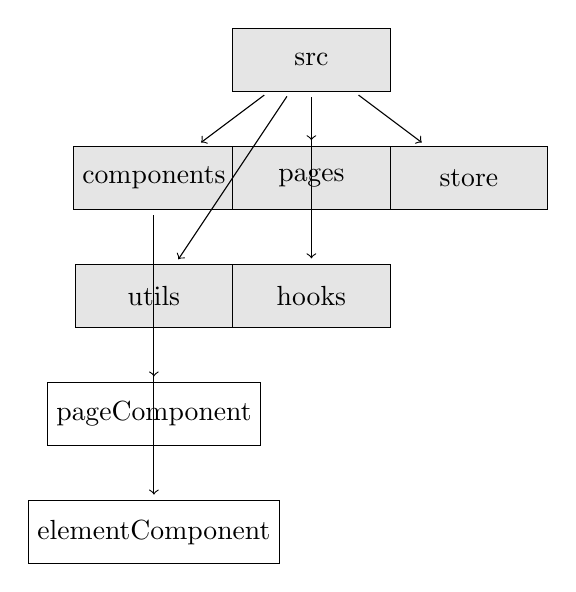
\begin{tikzpicture}[
    file/.style={draw, rectangle, minimum width=2cm, minimum height=0.8cm},
    folder/.style={draw, rectangle, minimum width=2cm, minimum height=0.8cm, fill=gray!20},
    arrow/.style={->, shorten >=2pt, shorten <=2pt}
]

% Folders
\node[folder] (src) at (0,0) {src};
\node[folder] (components) at (-2,-1.5) {components};
\node[folder] (pages) at (0,-1.5) {pages};
\node[folder] (store) at (2,-1.5) {store};
\node[folder] (utils) at (-2,-3) {utils};
\node[folder] (hooks) at (0,-3) {hooks};

% Files
\node[file] (pageComponent) at (-2,-4.5) {pageComponent};
\node[file] (elementComponent) at (-2,-6) {elementComponent};
% ... add more files

% Connections
\draw[arrow] (src) -- (components);
\draw[arrow] (src) -- (pages);
\draw[arrow] (src) -- (store);
\draw[arrow] (src) -- (utils);
\draw[arrow] (src) -- (hooks);
\draw[arrow] (components) -- (pageComponent);
\draw[arrow] (components) -- (elementComponent);
% ... add more connections

\end{tikzpicture}



\pagebreak
\subsubsection{Back-end}
The backend uses the dotNet framework. The development language using the C\# language.

In this project, the backend uses the Onion Architecture.
The Onion Architecture is a typically layered architecture, 
where each layer depends on the inner layer and provides interfaces to the outer layer.
The outer layer provides services to the outermost layer 
and other modules in the same layer based on the interfaces of the inner layer.

From inner to outer, the layers are: Domain, Application, Infrastructure, Presentation.
The Domain layer is the core layer and the innermost layer, used to define domain models, 
which are the business models.
It includes domain models and domain service interfaces.
Domain models are used to define the business models, 
which are the entities in the entity-relationship model and their attributes.
Domain service interfaces are used to define the business services, 
which are the relationships between entities in the entity-relationship model.

The Application layer is the application layer, 
used to define application services, which are the business logic.
It includes domain service implementations and application service interfaces.
Domain service implementations implement the methods of the inner layer's domain service 
interfaces and implement the business logic of the domain models.
Application service interfaces are used to define application services, 
which are the business logic.
It includes but is not limited to database interfaces, testing interfaces, 
HTTP API interfaces, MQTT interfaces, etc.

The Infrastructure layer is the infrastructure layer, used to define infrastructure.
It includes database implementations, testing implementations, 
HTTP API implementations, MQTT implementations, etc.
Database implementations implement the database interfaces 
and provide CRUD services for the database.
Testing implementations implement the testing interfaces 
and provide services for unit testing and integration testing.
HTTP API implementations implement the HTTP API interfaces 
and provide CRUD operations for HTTP APIs.
MQTT implementations implement the MQTT interfaces 
and provide CRUD operations for MQTT.

The Presentation layer is the presentation layer, used to define presentation logic, 
such as interfaces and pages. Since this is a backend project,
data presentation and control are handled by the frontend, 
so this layer is not needed.



\pagebreak
\subsubsection{Data communication and storage}
% 关于本项目的数据通信与数据存储的设计, 包括数据通信的协议, 数据存储的设计等
% 关于数据通信的设计:
% 1. 通信协议的选择
% 自前端向后端发送的数据, 有三种传输的数据类型, 
% 一种是普通的增删改查的请求, 对数据传输的时效性要求不高, 但是对数据的准确性, 完整性, 有序性, 安全性有一定的要求,
% 这种数据的传输, 采用 HTTP 协议, 以及 RESTful API 的设计. 可以有效的保证对数据传输的以上要求.
% 一种是对数据通道的创建和流媒体数据的传输, 对数据传输的时效性, 安全性要求较高, 这种数据的传输, 采用 WebRTC 协议, 以及 MQTT 协议.
% 配合可以快速解码的 flatbuffers 协议, 可以有效的保证对数据传输的以上要求.
% 最后一种是对设备的状态信息和操作信息的传输, 对完整性, 有序性, 安全性都有较高的要求, 这种数据的传输, 采用 MQTT 协议
% 同时也使用了 flatbuffers 协议.
% 
% 2. 数据通信的通信架构和通信流程
% 本项目的数据通信的通信架构, 是基于前后端分离的架构, 前端使用 React 框架, 后端使用 dotnet 框架.
% 当前端需要向后端发送数据的时候, 前端会向后端发送 HTTP 请求, 后端接收到 HTTP 请求之后, 会根据请求的数据类型,
% 选择不同的数据处理方式, 对于普通的增删改查的请求, 后端会根据 RESTful API 的设计, 对数据进行增删改查的操作,
% 对于对数据通道的创建和流媒体数据的传输, 后端会根据 WebRTC 协议, 对数据通道进行创建, 并且帮助前端和设备建立数据通道,
% 当数据通道建立后, 前端和设备之间则使用 flatbuffer 的数据格式对流媒体数据进行传输,
% 对于设备的状态信息和操作信息的传输, 前端会直接向 MQTT broker 发送 MQTT 请求, 
% 设备会在其自身的固件中监听相关的 MQTT 请求, 并且返回相关的数据.
% 
% 3. 数据通信的格式
% 本项目的数据通信的格式, 有三种, 
% 一种是 HTTP 协议, 
% 使用 json 格式对数据进行传输,
% 一种是 WebRTC 协议, 
% 使用 flatbuffers 格式对数据进行传输,
% 一种是 MQTT 协议.
% 使用 flatbuffers 格式对数据进行传输,
% 
% 关于数据存储的设计:
% 1. 数据存储的数据库的选择
% 本项目的数据存储的数据库的选择, 使用了轻量级的数据库 SQLite,
% SQLite 是一个进程内的库, 实现了自给自足的, 无服务器的, 零配置的, 事务性的 SQL 数据库引擎.
% 这是因为整个项目的目的是为了实现前端与设备之间的数据通信, 对于数据库数据的增删改查操作的要求不高,
% 数据量较小, 且对于数据库的数据的事务性要求不高, 所以选择了 SQLite 数据库.
% 2. 项目前后端的数据结构的设计
% 在本项目中, 前端由于使用了 React 框架, 所以前端的数据结构的设计, 使用了基于状态的数据结构的设计,
% 每个组件或者数据集都包含一个状态对象, 这个状态对象的属性就是组件的各个状态. 
% 使用状态对象的原因是, 可以方便的对状态进行管理, 采用对象-属性的形式, 可以方便的针对不同组件的同类状态进行区分,
% 由于跨组件的状态是由 redux 进行管理的, 这种状态对象的设计, 可以更搞笑的对状态进行更新和传递.
% 后端由于使用了 dotnet 框架, 所以后端的数据结构的设计, 使用了基于类的数据结构的设计,
% 采用了面向对象的编程思想, 对数据进行了封装, 使得数据的传输更加的安全, 有序, 完整.


\pagebreak

% \subsection{Domain model}
% \documentclass[]{article}
\usepackage{graphicx}
\usepackage{amsmath}
\usepackage{tikz}

% libaries
\usetikzlibrary{shapes,arrows}

%Define the listing package
\usepackage{listings} %code highlighter
\usepackage{color} %use color
\definecolor{mygreen}{rgb}{0,0.6,0}
\definecolor{mygray}{rgb}{0.5,0.5,0.5}
\definecolor{mymauve}{rgb}{0.58,0,0.82}

%Customize a bit the look
\lstset{ %
backgroundcolor=\color{white}, % choose the background color; you must add \usepackage{color} or \usepackage{xcolor}
basicstyle=\footnotesize, % the size of the fonts that are used for the code
breakatwhitespace=false, % sets if automatic breaks should only happen at whitespace
breaklines=true, % sets automatic line breaking
captionpos=b, % sets the caption-position to bottom
commentstyle=\color{mygreen}, % comment style
deletekeywords={...}, % if you want to delete keywords from the given language
escapeinside={\%*}{*)}, % if you want to add LaTeX within your code
extendedchars=true, % lets you use non-ASCII characters; for 8-bits encodings only, does not work with UTF-8
frame=single, % adds a frame around the code
keepspaces=true, % keeps spaces in text, useful for keeping indentation of code (possibly needs columns=flexible)
keywordstyle=\color{blue}, % keyword style
% language=Octave, % the language of the code
morekeywords={*,...}, % if you want to add more keywords to the set
numbers=left, % where to put the line-numbers; possible values are (none, left, right)
numbersep=5pt, % how far the line-numbers are from the code
numberstyle=\tiny\color{mygray}, % the style that is used for the line-numbers
rulecolor=\color{black}, % if not set, the frame-color may be changed on line-breaks within not-black text (e.g. comments (green here))
showspaces=false, % show spaces everywhere adding particular underscores; it overrides 'showstringspaces'
showstringspaces=false, % underline spaces within strings only
showtabs=false, % show tabs within strings adding particular underscores
stepnumber=1, % the step between two line-numbers. If it's 1, each line will be numbered
stringstyle=\color{mymauve}, % string literal style
tabsize=2, % sets default tabsize to 2 spaces
title=\lstname % show the filename of files included with \lstinputlisting; also try caption instead of title
}

\definecolor{darkgray}{rgb}{.4,.4,.4}
\definecolor{purple}{rgb}{0.65, 0.12, 0.82}

\lstdefinelanguage{React}{
keywords={const, typeof, new, true, false, catch, function, return, null, catch, switch, var, if, in, while, do, else, case, break},
keywordstyle=\color{blue}\bfseries,
ndkeywords={class, export, boolean, throw, implements, import, this},
ndkeywordstyle=\color{darkgray}\bfseries,
identifierstyle=\color{mygreen},
sensitive=false,
comment=[l]{//},
morecomment=[s]{/*}{*/},
commentstyle=\color{purple}\ttfamily,
string=[b]{"}{'}{`},
stringstyle=\color{red}\ttfamily,
morestring=[b]',
morestring=[b]",
morestring=[b]`',
}

\lstdefinelanguage{CSharp}{
keywords={const, typeof, new, true, false, catch, function, return, null, catch, switch, var, if, in, while, do, else, case, break},
keywordstyle=\color{blue}\bfseries,
ndkeywords={class, export, boolean, throw, implements, import, this},
ndkeywordstyle=\color{darkgray}\bfseries,
identifierstyle=\color{mygreen},
sensitive=false,
comment=[l]{//},
morecomment=[s]{/*}{*/},
commentstyle=\color{purple}\ttfamily,
string=[b]{"}{'}{`},
stringstyle=\color{red}\ttfamily,
morestring=[b]',
morestring=[b]",
morestring=[b]`',
}

\lstset{
language=React,
extendedchars=true,
basicstyle=\footnotesize\ttfamily,
showstringspaces=false,
showspaces=false,
numbers=left,
numberstyle=\footnotesize,
numbersep=9pt,
tabsize=2,
breaklines=true,
showtabs=false,
captionpos=b
}

\lstset{
language=CSharp,
extendedchars=true,
basicstyle=\footnotesize\ttfamily,
showstringspaces=false,
showspaces=false,
numbers=left,
numberstyle=\footnotesize,
numbersep=9pt,
tabsize=2,
breaklines=true,
showtabs=false,
captionpos=b
}

% \usepackage{cite} % Add this line for citation

% \bibliographystyle{plain}

\title{
The implementation of BifrostConnect Front-end scope, 
re-design and development with the relevant back-end support develop.
}
\author{
    Fei Gu \\
    Erhvervs Akademi Sydvest \\
    Computer Science 21\\
    }
\date{\today}

\begin{document}

% Front page
\maketitle
\begin{center}
    Supervisor: Henrik Boulund Meng Hansen \\
    Company: BifrostConnect \\
    Engineering Director: Jasper Wass \\
\end{center}
\tableofcontents
\pagebreak


% The introduction
\section{Introduction}
\subsection{Background}\input{sections/introduction/background.tex}
\subsection{The company}\input{sections/introduction/aboutCompany}
\subsection{The project}\input{sections/introduction/aboutProject}
\pagebreak

% The problem statement
\section{Problem Statement}
\subsection{Statement}
\input{sections/problemStatement/statement}
\subsection{Situation}
\input{sections/problemStatement/situation}
\subsection{Potential Solution}
\input{sections/problemStatement/potentialSolution}
\pagebreak

% Requirement analysis
\section{Requirement Analysis}
\input{sections/requirementAnalysis/index}

\subsection{Stakeholders}
\input{sections/requirementAnalysis/stakeholders/index}

\subsection{Business Domain}
\input{sections/requirementAnalysis/bussinesDomain/index}

\subsection{Scope}
\input{sections/requirementAnalysis/scope}

\subsection{Goals}
\input{sections/requirementAnalysis/goals}
\pagebreak

% Software Design
\section{Software Design}
% developement methods
\subsection{Software Development Methods}
\input{sections/softwareDevelopmentMethods/index}
\subsubsection{Agile Software Development}
\input{sections/softwareDevelopmentMethods/agileSoftwareDevelopment/index}
\subsubsection{Feature Driven Development}
\input{sections/softwareDevelopmentMethods/featureDrivenDevelopment/index}

\pagebreak

% Technology seslection
\subsection{Technology selection}
\input{sections/softwareDesign/technologySelection/index}
\subsubsection{Front-end}
\input{sections/softwareDesign/technologySelection/frontEnd}            
\subsubsection{Back-end}
\input{sections/softwareDesign/technologySelection/backEnd}            
\subsubsection{Database}
\input{sections/softwareDesign/technologySelection/database}
\subsubsection{Data communication}
\input{sections/softwareDesign/technologySelection/dataCommunication}            
\subsubsection{DevOps}
\input{sections/softwareDesign/technologySelection/devOps}
\pagebreak

% Architecture design
\subsection{Architecture design}
\input{sections/softwareDesign/architectureDesign/index}
\pagebreak
\subsubsection{Front-end}
\input{sections/softwareDesign/architectureDesign/frontEndArchitecture}
\pagebreak
\subsubsection{Back-end}
\input{sections/softwareDesign/architectureDesign/backEndArchitecture}
\pagebreak
\subsubsection{Data communication and storage}
\input{sections/softwareDesign/architectureDesign/dataCommunicationArchitecture}
\pagebreak

% \subsection{Domain model}
% \input{sections/softwareDesign/domainModel/index}
% \subsection{Database design}
% % 数据库领域模型 ER 图
% % 包括表和字段的设置.
% % 对于私有键和外键的设置.

% \subsection{Back-end design}
% % 后端对象模型
% % 以及对于对象模型的增删改查
% % 以及相关的其他服务的设计`'

% \subsection{Front-end design}
% % 对于前端的页面结构的设计 
% % 页面的状态的设计, 交互设计

% \subsection{FlatBuffers design}
% % schema 的设计

\subsection{DevOps CI/CD process design}
\input{sections/softwareDesign/devOpsDesign/index}
\subsubsection{Continuous Integration}
\input{sections/softwareDesign/devOpsDesign/continuousIntegration/index}
\subsubsection{Continuous Delivery}
\input{sections/softwareDesign/devOpsDesign/continuousDelivery/index}
\subsubsection{Continuous Deployment}
\input{sections/softwareDesign/devOpsDesign/continuousDeployment/index}
\pagebreak

\section{Software Development} 
\input{sections/softwareDevelopment/index}
\subsection{Overall development}
\input{sections/softwareDevelopment/overallDevelopement/index}
\subsubsection{Front-end}
\input{sections/softwareDevelopment/overallDevelopement/frontEnd/index}
\subsubsection{Back-end}
\input{sections/softwareDevelopment/overallDevelopement/backEnd/index}
\subsubsection{DevOps}
\input{sections/softwareDevelopment/overallDevelopement/devOps/index}
\subsection{Feature development} 
\input{sections/softwareDevelopment/featureDevelopment/index}
\subsubsection{Use Case 1}
\input{sections/softwareDevelopment/featureDevelopment/useCase1/index}
\subsubsection{Feature 1}
\input{sections/softwareDevelopment/featureDevelopment/feature/feature1.tex}
\pagebreak
\section{Conclusion} 
\subsection{Result}
Since the project is still in progress, the result is not available yet.
So far, basic structure of this project has been built. But the most features 
are not implemented yet. 
\subsection{Discussion}
As a single developer for this project, I am confident what I have done so far.
And I can say I understand the most of the knowledge I have used in this project, 
which also means I can explain all the part of the project. 
But this project also relevant some of the complex knowledge which I have to continue 
to study and practice.
\subsection{Future Work}
The future work is to implement the rest of the features. 
Including the most important part which is the 'create session' feature.
\pagebreak
% \bibliography{bibliography}
\pagebreak
% \begin{appendices}
%     \section{Appendix}
% \end{appendices} 
\end{document}
% \subsection{Database design}
% % 数据库领域模型 ER 图
% % 包括表和字段的设置.
% % 对于私有键和外键的设置.

% \subsection{Back-end design}
% % 后端对象模型
% % 以及对于对象模型的增删改查
% % 以及相关的其他服务的设计`'

% \subsection{Front-end design}
% % 对于前端的页面结构的设计 
% % 页面的状态的设计, 交互设计

% \subsection{FlatBuffers design}
% % schema 的设计

\subsection{DevOps CI/CD process design}
\documentclass[]{article}
\usepackage{graphicx}
\usepackage{amsmath}
\usepackage{tikz}

% libaries
\usetikzlibrary{shapes,arrows}

%Define the listing package
\usepackage{listings} %code highlighter
\usepackage{color} %use color
\definecolor{mygreen}{rgb}{0,0.6,0}
\definecolor{mygray}{rgb}{0.5,0.5,0.5}
\definecolor{mymauve}{rgb}{0.58,0,0.82}

%Customize a bit the look
\lstset{ %
backgroundcolor=\color{white}, % choose the background color; you must add \usepackage{color} or \usepackage{xcolor}
basicstyle=\footnotesize, % the size of the fonts that are used for the code
breakatwhitespace=false, % sets if automatic breaks should only happen at whitespace
breaklines=true, % sets automatic line breaking
captionpos=b, % sets the caption-position to bottom
commentstyle=\color{mygreen}, % comment style
deletekeywords={...}, % if you want to delete keywords from the given language
escapeinside={\%*}{*)}, % if you want to add LaTeX within your code
extendedchars=true, % lets you use non-ASCII characters; for 8-bits encodings only, does not work with UTF-8
frame=single, % adds a frame around the code
keepspaces=true, % keeps spaces in text, useful for keeping indentation of code (possibly needs columns=flexible)
keywordstyle=\color{blue}, % keyword style
% language=Octave, % the language of the code
morekeywords={*,...}, % if you want to add more keywords to the set
numbers=left, % where to put the line-numbers; possible values are (none, left, right)
numbersep=5pt, % how far the line-numbers are from the code
numberstyle=\tiny\color{mygray}, % the style that is used for the line-numbers
rulecolor=\color{black}, % if not set, the frame-color may be changed on line-breaks within not-black text (e.g. comments (green here))
showspaces=false, % show spaces everywhere adding particular underscores; it overrides 'showstringspaces'
showstringspaces=false, % underline spaces within strings only
showtabs=false, % show tabs within strings adding particular underscores
stepnumber=1, % the step between two line-numbers. If it's 1, each line will be numbered
stringstyle=\color{mymauve}, % string literal style
tabsize=2, % sets default tabsize to 2 spaces
title=\lstname % show the filename of files included with \lstinputlisting; also try caption instead of title
}

\definecolor{darkgray}{rgb}{.4,.4,.4}
\definecolor{purple}{rgb}{0.65, 0.12, 0.82}

\lstdefinelanguage{React}{
keywords={const, typeof, new, true, false, catch, function, return, null, catch, switch, var, if, in, while, do, else, case, break},
keywordstyle=\color{blue}\bfseries,
ndkeywords={class, export, boolean, throw, implements, import, this},
ndkeywordstyle=\color{darkgray}\bfseries,
identifierstyle=\color{mygreen},
sensitive=false,
comment=[l]{//},
morecomment=[s]{/*}{*/},
commentstyle=\color{purple}\ttfamily,
string=[b]{"}{'}{`},
stringstyle=\color{red}\ttfamily,
morestring=[b]',
morestring=[b]",
morestring=[b]`',
}

\lstdefinelanguage{CSharp}{
keywords={const, typeof, new, true, false, catch, function, return, null, catch, switch, var, if, in, while, do, else, case, break},
keywordstyle=\color{blue}\bfseries,
ndkeywords={class, export, boolean, throw, implements, import, this},
ndkeywordstyle=\color{darkgray}\bfseries,
identifierstyle=\color{mygreen},
sensitive=false,
comment=[l]{//},
morecomment=[s]{/*}{*/},
commentstyle=\color{purple}\ttfamily,
string=[b]{"}{'}{`},
stringstyle=\color{red}\ttfamily,
morestring=[b]',
morestring=[b]",
morestring=[b]`',
}

\lstset{
language=React,
extendedchars=true,
basicstyle=\footnotesize\ttfamily,
showstringspaces=false,
showspaces=false,
numbers=left,
numberstyle=\footnotesize,
numbersep=9pt,
tabsize=2,
breaklines=true,
showtabs=false,
captionpos=b
}

\lstset{
language=CSharp,
extendedchars=true,
basicstyle=\footnotesize\ttfamily,
showstringspaces=false,
showspaces=false,
numbers=left,
numberstyle=\footnotesize,
numbersep=9pt,
tabsize=2,
breaklines=true,
showtabs=false,
captionpos=b
}

% \usepackage{cite} % Add this line for citation

% \bibliographystyle{plain}

\title{
The implementation of BifrostConnect Front-end scope, 
re-design and development with the relevant back-end support develop.
}
\author{
    Fei Gu \\
    Erhvervs Akademi Sydvest \\
    Computer Science 21\\
    }
\date{\today}

\begin{document}

% Front page
\maketitle
\begin{center}
    Supervisor: Henrik Boulund Meng Hansen \\
    Company: BifrostConnect \\
    Engineering Director: Jasper Wass \\
\end{center}
\tableofcontents
\pagebreak


% The introduction
\section{Introduction}
\subsection{Background}\input{sections/introduction/background.tex}
\subsection{The company}\input{sections/introduction/aboutCompany}
\subsection{The project}\input{sections/introduction/aboutProject}
\pagebreak

% The problem statement
\section{Problem Statement}
\subsection{Statement}
\input{sections/problemStatement/statement}
\subsection{Situation}
\input{sections/problemStatement/situation}
\subsection{Potential Solution}
\input{sections/problemStatement/potentialSolution}
\pagebreak

% Requirement analysis
\section{Requirement Analysis}
\input{sections/requirementAnalysis/index}

\subsection{Stakeholders}
\input{sections/requirementAnalysis/stakeholders/index}

\subsection{Business Domain}
\input{sections/requirementAnalysis/bussinesDomain/index}

\subsection{Scope}
\input{sections/requirementAnalysis/scope}

\subsection{Goals}
\input{sections/requirementAnalysis/goals}
\pagebreak

% Software Design
\section{Software Design}
% developement methods
\subsection{Software Development Methods}
\input{sections/softwareDevelopmentMethods/index}
\subsubsection{Agile Software Development}
\input{sections/softwareDevelopmentMethods/agileSoftwareDevelopment/index}
\subsubsection{Feature Driven Development}
\input{sections/softwareDevelopmentMethods/featureDrivenDevelopment/index}

\pagebreak

% Technology seslection
\subsection{Technology selection}
\input{sections/softwareDesign/technologySelection/index}
\subsubsection{Front-end}
\input{sections/softwareDesign/technologySelection/frontEnd}            
\subsubsection{Back-end}
\input{sections/softwareDesign/technologySelection/backEnd}            
\subsubsection{Database}
\input{sections/softwareDesign/technologySelection/database}
\subsubsection{Data communication}
\input{sections/softwareDesign/technologySelection/dataCommunication}            
\subsubsection{DevOps}
\input{sections/softwareDesign/technologySelection/devOps}
\pagebreak

% Architecture design
\subsection{Architecture design}
\input{sections/softwareDesign/architectureDesign/index}
\pagebreak
\subsubsection{Front-end}
\input{sections/softwareDesign/architectureDesign/frontEndArchitecture}
\pagebreak
\subsubsection{Back-end}
\input{sections/softwareDesign/architectureDesign/backEndArchitecture}
\pagebreak
\subsubsection{Data communication and storage}
\input{sections/softwareDesign/architectureDesign/dataCommunicationArchitecture}
\pagebreak

% \subsection{Domain model}
% \input{sections/softwareDesign/domainModel/index}
% \subsection{Database design}
% % 数据库领域模型 ER 图
% % 包括表和字段的设置.
% % 对于私有键和外键的设置.

% \subsection{Back-end design}
% % 后端对象模型
% % 以及对于对象模型的增删改查
% % 以及相关的其他服务的设计`'

% \subsection{Front-end design}
% % 对于前端的页面结构的设计 
% % 页面的状态的设计, 交互设计

% \subsection{FlatBuffers design}
% % schema 的设计

\subsection{DevOps CI/CD process design}
\input{sections/softwareDesign/devOpsDesign/index}
\subsubsection{Continuous Integration}
\input{sections/softwareDesign/devOpsDesign/continuousIntegration/index}
\subsubsection{Continuous Delivery}
\input{sections/softwareDesign/devOpsDesign/continuousDelivery/index}
\subsubsection{Continuous Deployment}
\input{sections/softwareDesign/devOpsDesign/continuousDeployment/index}
\pagebreak

\section{Software Development} 
\input{sections/softwareDevelopment/index}
\subsection{Overall development}
\input{sections/softwareDevelopment/overallDevelopement/index}
\subsubsection{Front-end}
\input{sections/softwareDevelopment/overallDevelopement/frontEnd/index}
\subsubsection{Back-end}
\input{sections/softwareDevelopment/overallDevelopement/backEnd/index}
\subsubsection{DevOps}
\input{sections/softwareDevelopment/overallDevelopement/devOps/index}
\subsection{Feature development} 
\input{sections/softwareDevelopment/featureDevelopment/index}
\subsubsection{Use Case 1}
\input{sections/softwareDevelopment/featureDevelopment/useCase1/index}
\subsubsection{Feature 1}
\input{sections/softwareDevelopment/featureDevelopment/feature/feature1.tex}
\pagebreak
\section{Conclusion} 
\subsection{Result}
Since the project is still in progress, the result is not available yet.
So far, basic structure of this project has been built. But the most features 
are not implemented yet. 
\subsection{Discussion}
As a single developer for this project, I am confident what I have done so far.
And I can say I understand the most of the knowledge I have used in this project, 
which also means I can explain all the part of the project. 
But this project also relevant some of the complex knowledge which I have to continue 
to study and practice.
\subsection{Future Work}
The future work is to implement the rest of the features. 
Including the most important part which is the 'create session' feature.
\pagebreak
% \bibliography{bibliography}
\pagebreak
% \begin{appendices}
%     \section{Appendix}
% \end{appendices} 
\end{document}
\subsubsection{Continuous Integration}
\documentclass[]{article}
\usepackage{graphicx}
\usepackage{amsmath}
\usepackage{tikz}

% libaries
\usetikzlibrary{shapes,arrows}

%Define the listing package
\usepackage{listings} %code highlighter
\usepackage{color} %use color
\definecolor{mygreen}{rgb}{0,0.6,0}
\definecolor{mygray}{rgb}{0.5,0.5,0.5}
\definecolor{mymauve}{rgb}{0.58,0,0.82}

%Customize a bit the look
\lstset{ %
backgroundcolor=\color{white}, % choose the background color; you must add \usepackage{color} or \usepackage{xcolor}
basicstyle=\footnotesize, % the size of the fonts that are used for the code
breakatwhitespace=false, % sets if automatic breaks should only happen at whitespace
breaklines=true, % sets automatic line breaking
captionpos=b, % sets the caption-position to bottom
commentstyle=\color{mygreen}, % comment style
deletekeywords={...}, % if you want to delete keywords from the given language
escapeinside={\%*}{*)}, % if you want to add LaTeX within your code
extendedchars=true, % lets you use non-ASCII characters; for 8-bits encodings only, does not work with UTF-8
frame=single, % adds a frame around the code
keepspaces=true, % keeps spaces in text, useful for keeping indentation of code (possibly needs columns=flexible)
keywordstyle=\color{blue}, % keyword style
% language=Octave, % the language of the code
morekeywords={*,...}, % if you want to add more keywords to the set
numbers=left, % where to put the line-numbers; possible values are (none, left, right)
numbersep=5pt, % how far the line-numbers are from the code
numberstyle=\tiny\color{mygray}, % the style that is used for the line-numbers
rulecolor=\color{black}, % if not set, the frame-color may be changed on line-breaks within not-black text (e.g. comments (green here))
showspaces=false, % show spaces everywhere adding particular underscores; it overrides 'showstringspaces'
showstringspaces=false, % underline spaces within strings only
showtabs=false, % show tabs within strings adding particular underscores
stepnumber=1, % the step between two line-numbers. If it's 1, each line will be numbered
stringstyle=\color{mymauve}, % string literal style
tabsize=2, % sets default tabsize to 2 spaces
title=\lstname % show the filename of files included with \lstinputlisting; also try caption instead of title
}

\definecolor{darkgray}{rgb}{.4,.4,.4}
\definecolor{purple}{rgb}{0.65, 0.12, 0.82}

\lstdefinelanguage{React}{
keywords={const, typeof, new, true, false, catch, function, return, null, catch, switch, var, if, in, while, do, else, case, break},
keywordstyle=\color{blue}\bfseries,
ndkeywords={class, export, boolean, throw, implements, import, this},
ndkeywordstyle=\color{darkgray}\bfseries,
identifierstyle=\color{mygreen},
sensitive=false,
comment=[l]{//},
morecomment=[s]{/*}{*/},
commentstyle=\color{purple}\ttfamily,
string=[b]{"}{'}{`},
stringstyle=\color{red}\ttfamily,
morestring=[b]',
morestring=[b]",
morestring=[b]`',
}

\lstdefinelanguage{CSharp}{
keywords={const, typeof, new, true, false, catch, function, return, null, catch, switch, var, if, in, while, do, else, case, break},
keywordstyle=\color{blue}\bfseries,
ndkeywords={class, export, boolean, throw, implements, import, this},
ndkeywordstyle=\color{darkgray}\bfseries,
identifierstyle=\color{mygreen},
sensitive=false,
comment=[l]{//},
morecomment=[s]{/*}{*/},
commentstyle=\color{purple}\ttfamily,
string=[b]{"}{'}{`},
stringstyle=\color{red}\ttfamily,
morestring=[b]',
morestring=[b]",
morestring=[b]`',
}

\lstset{
language=React,
extendedchars=true,
basicstyle=\footnotesize\ttfamily,
showstringspaces=false,
showspaces=false,
numbers=left,
numberstyle=\footnotesize,
numbersep=9pt,
tabsize=2,
breaklines=true,
showtabs=false,
captionpos=b
}

\lstset{
language=CSharp,
extendedchars=true,
basicstyle=\footnotesize\ttfamily,
showstringspaces=false,
showspaces=false,
numbers=left,
numberstyle=\footnotesize,
numbersep=9pt,
tabsize=2,
breaklines=true,
showtabs=false,
captionpos=b
}

% \usepackage{cite} % Add this line for citation

% \bibliographystyle{plain}

\title{
The implementation of BifrostConnect Front-end scope, 
re-design and development with the relevant back-end support develop.
}
\author{
    Fei Gu \\
    Erhvervs Akademi Sydvest \\
    Computer Science 21\\
    }
\date{\today}

\begin{document}

% Front page
\maketitle
\begin{center}
    Supervisor: Henrik Boulund Meng Hansen \\
    Company: BifrostConnect \\
    Engineering Director: Jasper Wass \\
\end{center}
\tableofcontents
\pagebreak


% The introduction
\section{Introduction}
\subsection{Background}\input{sections/introduction/background.tex}
\subsection{The company}\input{sections/introduction/aboutCompany}
\subsection{The project}\input{sections/introduction/aboutProject}
\pagebreak

% The problem statement
\section{Problem Statement}
\subsection{Statement}
\input{sections/problemStatement/statement}
\subsection{Situation}
\input{sections/problemStatement/situation}
\subsection{Potential Solution}
\input{sections/problemStatement/potentialSolution}
\pagebreak

% Requirement analysis
\section{Requirement Analysis}
\input{sections/requirementAnalysis/index}

\subsection{Stakeholders}
\input{sections/requirementAnalysis/stakeholders/index}

\subsection{Business Domain}
\input{sections/requirementAnalysis/bussinesDomain/index}

\subsection{Scope}
\input{sections/requirementAnalysis/scope}

\subsection{Goals}
\input{sections/requirementAnalysis/goals}
\pagebreak

% Software Design
\section{Software Design}
% developement methods
\subsection{Software Development Methods}
\input{sections/softwareDevelopmentMethods/index}
\subsubsection{Agile Software Development}
\input{sections/softwareDevelopmentMethods/agileSoftwareDevelopment/index}
\subsubsection{Feature Driven Development}
\input{sections/softwareDevelopmentMethods/featureDrivenDevelopment/index}

\pagebreak

% Technology seslection
\subsection{Technology selection}
\input{sections/softwareDesign/technologySelection/index}
\subsubsection{Front-end}
\input{sections/softwareDesign/technologySelection/frontEnd}            
\subsubsection{Back-end}
\input{sections/softwareDesign/technologySelection/backEnd}            
\subsubsection{Database}
\input{sections/softwareDesign/technologySelection/database}
\subsubsection{Data communication}
\input{sections/softwareDesign/technologySelection/dataCommunication}            
\subsubsection{DevOps}
\input{sections/softwareDesign/technologySelection/devOps}
\pagebreak

% Architecture design
\subsection{Architecture design}
\input{sections/softwareDesign/architectureDesign/index}
\pagebreak
\subsubsection{Front-end}
\input{sections/softwareDesign/architectureDesign/frontEndArchitecture}
\pagebreak
\subsubsection{Back-end}
\input{sections/softwareDesign/architectureDesign/backEndArchitecture}
\pagebreak
\subsubsection{Data communication and storage}
\input{sections/softwareDesign/architectureDesign/dataCommunicationArchitecture}
\pagebreak

% \subsection{Domain model}
% \input{sections/softwareDesign/domainModel/index}
% \subsection{Database design}
% % 数据库领域模型 ER 图
% % 包括表和字段的设置.
% % 对于私有键和外键的设置.

% \subsection{Back-end design}
% % 后端对象模型
% % 以及对于对象模型的增删改查
% % 以及相关的其他服务的设计`'

% \subsection{Front-end design}
% % 对于前端的页面结构的设计 
% % 页面的状态的设计, 交互设计

% \subsection{FlatBuffers design}
% % schema 的设计

\subsection{DevOps CI/CD process design}
\input{sections/softwareDesign/devOpsDesign/index}
\subsubsection{Continuous Integration}
\input{sections/softwareDesign/devOpsDesign/continuousIntegration/index}
\subsubsection{Continuous Delivery}
\input{sections/softwareDesign/devOpsDesign/continuousDelivery/index}
\subsubsection{Continuous Deployment}
\input{sections/softwareDesign/devOpsDesign/continuousDeployment/index}
\pagebreak

\section{Software Development} 
\input{sections/softwareDevelopment/index}
\subsection{Overall development}
\input{sections/softwareDevelopment/overallDevelopement/index}
\subsubsection{Front-end}
\input{sections/softwareDevelopment/overallDevelopement/frontEnd/index}
\subsubsection{Back-end}
\input{sections/softwareDevelopment/overallDevelopement/backEnd/index}
\subsubsection{DevOps}
\input{sections/softwareDevelopment/overallDevelopement/devOps/index}
\subsection{Feature development} 
\input{sections/softwareDevelopment/featureDevelopment/index}
\subsubsection{Use Case 1}
\input{sections/softwareDevelopment/featureDevelopment/useCase1/index}
\subsubsection{Feature 1}
\input{sections/softwareDevelopment/featureDevelopment/feature/feature1.tex}
\pagebreak
\section{Conclusion} 
\subsection{Result}
Since the project is still in progress, the result is not available yet.
So far, basic structure of this project has been built. But the most features 
are not implemented yet. 
\subsection{Discussion}
As a single developer for this project, I am confident what I have done so far.
And I can say I understand the most of the knowledge I have used in this project, 
which also means I can explain all the part of the project. 
But this project also relevant some of the complex knowledge which I have to continue 
to study and practice.
\subsection{Future Work}
The future work is to implement the rest of the features. 
Including the most important part which is the 'create session' feature.
\pagebreak
% \bibliography{bibliography}
\pagebreak
% \begin{appendices}
%     \section{Appendix}
% \end{appendices} 
\end{document}
\subsubsection{Continuous Delivery}
\documentclass[]{article}
\usepackage{graphicx}
\usepackage{amsmath}
\usepackage{tikz}

% libaries
\usetikzlibrary{shapes,arrows}

%Define the listing package
\usepackage{listings} %code highlighter
\usepackage{color} %use color
\definecolor{mygreen}{rgb}{0,0.6,0}
\definecolor{mygray}{rgb}{0.5,0.5,0.5}
\definecolor{mymauve}{rgb}{0.58,0,0.82}

%Customize a bit the look
\lstset{ %
backgroundcolor=\color{white}, % choose the background color; you must add \usepackage{color} or \usepackage{xcolor}
basicstyle=\footnotesize, % the size of the fonts that are used for the code
breakatwhitespace=false, % sets if automatic breaks should only happen at whitespace
breaklines=true, % sets automatic line breaking
captionpos=b, % sets the caption-position to bottom
commentstyle=\color{mygreen}, % comment style
deletekeywords={...}, % if you want to delete keywords from the given language
escapeinside={\%*}{*)}, % if you want to add LaTeX within your code
extendedchars=true, % lets you use non-ASCII characters; for 8-bits encodings only, does not work with UTF-8
frame=single, % adds a frame around the code
keepspaces=true, % keeps spaces in text, useful for keeping indentation of code (possibly needs columns=flexible)
keywordstyle=\color{blue}, % keyword style
% language=Octave, % the language of the code
morekeywords={*,...}, % if you want to add more keywords to the set
numbers=left, % where to put the line-numbers; possible values are (none, left, right)
numbersep=5pt, % how far the line-numbers are from the code
numberstyle=\tiny\color{mygray}, % the style that is used for the line-numbers
rulecolor=\color{black}, % if not set, the frame-color may be changed on line-breaks within not-black text (e.g. comments (green here))
showspaces=false, % show spaces everywhere adding particular underscores; it overrides 'showstringspaces'
showstringspaces=false, % underline spaces within strings only
showtabs=false, % show tabs within strings adding particular underscores
stepnumber=1, % the step between two line-numbers. If it's 1, each line will be numbered
stringstyle=\color{mymauve}, % string literal style
tabsize=2, % sets default tabsize to 2 spaces
title=\lstname % show the filename of files included with \lstinputlisting; also try caption instead of title
}

\definecolor{darkgray}{rgb}{.4,.4,.4}
\definecolor{purple}{rgb}{0.65, 0.12, 0.82}

\lstdefinelanguage{React}{
keywords={const, typeof, new, true, false, catch, function, return, null, catch, switch, var, if, in, while, do, else, case, break},
keywordstyle=\color{blue}\bfseries,
ndkeywords={class, export, boolean, throw, implements, import, this},
ndkeywordstyle=\color{darkgray}\bfseries,
identifierstyle=\color{mygreen},
sensitive=false,
comment=[l]{//},
morecomment=[s]{/*}{*/},
commentstyle=\color{purple}\ttfamily,
string=[b]{"}{'}{`},
stringstyle=\color{red}\ttfamily,
morestring=[b]',
morestring=[b]",
morestring=[b]`',
}

\lstdefinelanguage{CSharp}{
keywords={const, typeof, new, true, false, catch, function, return, null, catch, switch, var, if, in, while, do, else, case, break},
keywordstyle=\color{blue}\bfseries,
ndkeywords={class, export, boolean, throw, implements, import, this},
ndkeywordstyle=\color{darkgray}\bfseries,
identifierstyle=\color{mygreen},
sensitive=false,
comment=[l]{//},
morecomment=[s]{/*}{*/},
commentstyle=\color{purple}\ttfamily,
string=[b]{"}{'}{`},
stringstyle=\color{red}\ttfamily,
morestring=[b]',
morestring=[b]",
morestring=[b]`',
}

\lstset{
language=React,
extendedchars=true,
basicstyle=\footnotesize\ttfamily,
showstringspaces=false,
showspaces=false,
numbers=left,
numberstyle=\footnotesize,
numbersep=9pt,
tabsize=2,
breaklines=true,
showtabs=false,
captionpos=b
}

\lstset{
language=CSharp,
extendedchars=true,
basicstyle=\footnotesize\ttfamily,
showstringspaces=false,
showspaces=false,
numbers=left,
numberstyle=\footnotesize,
numbersep=9pt,
tabsize=2,
breaklines=true,
showtabs=false,
captionpos=b
}

% \usepackage{cite} % Add this line for citation

% \bibliographystyle{plain}

\title{
The implementation of BifrostConnect Front-end scope, 
re-design and development with the relevant back-end support develop.
}
\author{
    Fei Gu \\
    Erhvervs Akademi Sydvest \\
    Computer Science 21\\
    }
\date{\today}

\begin{document}

% Front page
\maketitle
\begin{center}
    Supervisor: Henrik Boulund Meng Hansen \\
    Company: BifrostConnect \\
    Engineering Director: Jasper Wass \\
\end{center}
\tableofcontents
\pagebreak


% The introduction
\section{Introduction}
\subsection{Background}\input{sections/introduction/background.tex}
\subsection{The company}\input{sections/introduction/aboutCompany}
\subsection{The project}\input{sections/introduction/aboutProject}
\pagebreak

% The problem statement
\section{Problem Statement}
\subsection{Statement}
\input{sections/problemStatement/statement}
\subsection{Situation}
\input{sections/problemStatement/situation}
\subsection{Potential Solution}
\input{sections/problemStatement/potentialSolution}
\pagebreak

% Requirement analysis
\section{Requirement Analysis}
\input{sections/requirementAnalysis/index}

\subsection{Stakeholders}
\input{sections/requirementAnalysis/stakeholders/index}

\subsection{Business Domain}
\input{sections/requirementAnalysis/bussinesDomain/index}

\subsection{Scope}
\input{sections/requirementAnalysis/scope}

\subsection{Goals}
\input{sections/requirementAnalysis/goals}
\pagebreak

% Software Design
\section{Software Design}
% developement methods
\subsection{Software Development Methods}
\input{sections/softwareDevelopmentMethods/index}
\subsubsection{Agile Software Development}
\input{sections/softwareDevelopmentMethods/agileSoftwareDevelopment/index}
\subsubsection{Feature Driven Development}
\input{sections/softwareDevelopmentMethods/featureDrivenDevelopment/index}

\pagebreak

% Technology seslection
\subsection{Technology selection}
\input{sections/softwareDesign/technologySelection/index}
\subsubsection{Front-end}
\input{sections/softwareDesign/technologySelection/frontEnd}            
\subsubsection{Back-end}
\input{sections/softwareDesign/technologySelection/backEnd}            
\subsubsection{Database}
\input{sections/softwareDesign/technologySelection/database}
\subsubsection{Data communication}
\input{sections/softwareDesign/technologySelection/dataCommunication}            
\subsubsection{DevOps}
\input{sections/softwareDesign/technologySelection/devOps}
\pagebreak

% Architecture design
\subsection{Architecture design}
\input{sections/softwareDesign/architectureDesign/index}
\pagebreak
\subsubsection{Front-end}
\input{sections/softwareDesign/architectureDesign/frontEndArchitecture}
\pagebreak
\subsubsection{Back-end}
\input{sections/softwareDesign/architectureDesign/backEndArchitecture}
\pagebreak
\subsubsection{Data communication and storage}
\input{sections/softwareDesign/architectureDesign/dataCommunicationArchitecture}
\pagebreak

% \subsection{Domain model}
% \input{sections/softwareDesign/domainModel/index}
% \subsection{Database design}
% % 数据库领域模型 ER 图
% % 包括表和字段的设置.
% % 对于私有键和外键的设置.

% \subsection{Back-end design}
% % 后端对象模型
% % 以及对于对象模型的增删改查
% % 以及相关的其他服务的设计`'

% \subsection{Front-end design}
% % 对于前端的页面结构的设计 
% % 页面的状态的设计, 交互设计

% \subsection{FlatBuffers design}
% % schema 的设计

\subsection{DevOps CI/CD process design}
\input{sections/softwareDesign/devOpsDesign/index}
\subsubsection{Continuous Integration}
\input{sections/softwareDesign/devOpsDesign/continuousIntegration/index}
\subsubsection{Continuous Delivery}
\input{sections/softwareDesign/devOpsDesign/continuousDelivery/index}
\subsubsection{Continuous Deployment}
\input{sections/softwareDesign/devOpsDesign/continuousDeployment/index}
\pagebreak

\section{Software Development} 
\input{sections/softwareDevelopment/index}
\subsection{Overall development}
\input{sections/softwareDevelopment/overallDevelopement/index}
\subsubsection{Front-end}
\input{sections/softwareDevelopment/overallDevelopement/frontEnd/index}
\subsubsection{Back-end}
\input{sections/softwareDevelopment/overallDevelopement/backEnd/index}
\subsubsection{DevOps}
\input{sections/softwareDevelopment/overallDevelopement/devOps/index}
\subsection{Feature development} 
\input{sections/softwareDevelopment/featureDevelopment/index}
\subsubsection{Use Case 1}
\input{sections/softwareDevelopment/featureDevelopment/useCase1/index}
\subsubsection{Feature 1}
\input{sections/softwareDevelopment/featureDevelopment/feature/feature1.tex}
\pagebreak
\section{Conclusion} 
\subsection{Result}
Since the project is still in progress, the result is not available yet.
So far, basic structure of this project has been built. But the most features 
are not implemented yet. 
\subsection{Discussion}
As a single developer for this project, I am confident what I have done so far.
And I can say I understand the most of the knowledge I have used in this project, 
which also means I can explain all the part of the project. 
But this project also relevant some of the complex knowledge which I have to continue 
to study and practice.
\subsection{Future Work}
The future work is to implement the rest of the features. 
Including the most important part which is the 'create session' feature.
\pagebreak
% \bibliography{bibliography}
\pagebreak
% \begin{appendices}
%     \section{Appendix}
% \end{appendices} 
\end{document}
\subsubsection{Continuous Deployment}
\documentclass[]{article}
\usepackage{graphicx}
\usepackage{amsmath}
\usepackage{tikz}

% libaries
\usetikzlibrary{shapes,arrows}

%Define the listing package
\usepackage{listings} %code highlighter
\usepackage{color} %use color
\definecolor{mygreen}{rgb}{0,0.6,0}
\definecolor{mygray}{rgb}{0.5,0.5,0.5}
\definecolor{mymauve}{rgb}{0.58,0,0.82}

%Customize a bit the look
\lstset{ %
backgroundcolor=\color{white}, % choose the background color; you must add \usepackage{color} or \usepackage{xcolor}
basicstyle=\footnotesize, % the size of the fonts that are used for the code
breakatwhitespace=false, % sets if automatic breaks should only happen at whitespace
breaklines=true, % sets automatic line breaking
captionpos=b, % sets the caption-position to bottom
commentstyle=\color{mygreen}, % comment style
deletekeywords={...}, % if you want to delete keywords from the given language
escapeinside={\%*}{*)}, % if you want to add LaTeX within your code
extendedchars=true, % lets you use non-ASCII characters; for 8-bits encodings only, does not work with UTF-8
frame=single, % adds a frame around the code
keepspaces=true, % keeps spaces in text, useful for keeping indentation of code (possibly needs columns=flexible)
keywordstyle=\color{blue}, % keyword style
% language=Octave, % the language of the code
morekeywords={*,...}, % if you want to add more keywords to the set
numbers=left, % where to put the line-numbers; possible values are (none, left, right)
numbersep=5pt, % how far the line-numbers are from the code
numberstyle=\tiny\color{mygray}, % the style that is used for the line-numbers
rulecolor=\color{black}, % if not set, the frame-color may be changed on line-breaks within not-black text (e.g. comments (green here))
showspaces=false, % show spaces everywhere adding particular underscores; it overrides 'showstringspaces'
showstringspaces=false, % underline spaces within strings only
showtabs=false, % show tabs within strings adding particular underscores
stepnumber=1, % the step between two line-numbers. If it's 1, each line will be numbered
stringstyle=\color{mymauve}, % string literal style
tabsize=2, % sets default tabsize to 2 spaces
title=\lstname % show the filename of files included with \lstinputlisting; also try caption instead of title
}

\definecolor{darkgray}{rgb}{.4,.4,.4}
\definecolor{purple}{rgb}{0.65, 0.12, 0.82}

\lstdefinelanguage{React}{
keywords={const, typeof, new, true, false, catch, function, return, null, catch, switch, var, if, in, while, do, else, case, break},
keywordstyle=\color{blue}\bfseries,
ndkeywords={class, export, boolean, throw, implements, import, this},
ndkeywordstyle=\color{darkgray}\bfseries,
identifierstyle=\color{mygreen},
sensitive=false,
comment=[l]{//},
morecomment=[s]{/*}{*/},
commentstyle=\color{purple}\ttfamily,
string=[b]{"}{'}{`},
stringstyle=\color{red}\ttfamily,
morestring=[b]',
morestring=[b]",
morestring=[b]`',
}

\lstdefinelanguage{CSharp}{
keywords={const, typeof, new, true, false, catch, function, return, null, catch, switch, var, if, in, while, do, else, case, break},
keywordstyle=\color{blue}\bfseries,
ndkeywords={class, export, boolean, throw, implements, import, this},
ndkeywordstyle=\color{darkgray}\bfseries,
identifierstyle=\color{mygreen},
sensitive=false,
comment=[l]{//},
morecomment=[s]{/*}{*/},
commentstyle=\color{purple}\ttfamily,
string=[b]{"}{'}{`},
stringstyle=\color{red}\ttfamily,
morestring=[b]',
morestring=[b]",
morestring=[b]`',
}

\lstset{
language=React,
extendedchars=true,
basicstyle=\footnotesize\ttfamily,
showstringspaces=false,
showspaces=false,
numbers=left,
numberstyle=\footnotesize,
numbersep=9pt,
tabsize=2,
breaklines=true,
showtabs=false,
captionpos=b
}

\lstset{
language=CSharp,
extendedchars=true,
basicstyle=\footnotesize\ttfamily,
showstringspaces=false,
showspaces=false,
numbers=left,
numberstyle=\footnotesize,
numbersep=9pt,
tabsize=2,
breaklines=true,
showtabs=false,
captionpos=b
}

% \usepackage{cite} % Add this line for citation

% \bibliographystyle{plain}

\title{
The implementation of BifrostConnect Front-end scope, 
re-design and development with the relevant back-end support develop.
}
\author{
    Fei Gu \\
    Erhvervs Akademi Sydvest \\
    Computer Science 21\\
    }
\date{\today}

\begin{document}

% Front page
\maketitle
\begin{center}
    Supervisor: Henrik Boulund Meng Hansen \\
    Company: BifrostConnect \\
    Engineering Director: Jasper Wass \\
\end{center}
\tableofcontents
\pagebreak


% The introduction
\section{Introduction}
\subsection{Background}\input{sections/introduction/background.tex}
\subsection{The company}\input{sections/introduction/aboutCompany}
\subsection{The project}\input{sections/introduction/aboutProject}
\pagebreak

% The problem statement
\section{Problem Statement}
\subsection{Statement}
\input{sections/problemStatement/statement}
\subsection{Situation}
\input{sections/problemStatement/situation}
\subsection{Potential Solution}
\input{sections/problemStatement/potentialSolution}
\pagebreak

% Requirement analysis
\section{Requirement Analysis}
\input{sections/requirementAnalysis/index}

\subsection{Stakeholders}
\input{sections/requirementAnalysis/stakeholders/index}

\subsection{Business Domain}
\input{sections/requirementAnalysis/bussinesDomain/index}

\subsection{Scope}
\input{sections/requirementAnalysis/scope}

\subsection{Goals}
\input{sections/requirementAnalysis/goals}
\pagebreak

% Software Design
\section{Software Design}
% developement methods
\subsection{Software Development Methods}
\input{sections/softwareDevelopmentMethods/index}
\subsubsection{Agile Software Development}
\input{sections/softwareDevelopmentMethods/agileSoftwareDevelopment/index}
\subsubsection{Feature Driven Development}
\input{sections/softwareDevelopmentMethods/featureDrivenDevelopment/index}

\pagebreak

% Technology seslection
\subsection{Technology selection}
\input{sections/softwareDesign/technologySelection/index}
\subsubsection{Front-end}
\input{sections/softwareDesign/technologySelection/frontEnd}            
\subsubsection{Back-end}
\input{sections/softwareDesign/technologySelection/backEnd}            
\subsubsection{Database}
\input{sections/softwareDesign/technologySelection/database}
\subsubsection{Data communication}
\input{sections/softwareDesign/technologySelection/dataCommunication}            
\subsubsection{DevOps}
\input{sections/softwareDesign/technologySelection/devOps}
\pagebreak

% Architecture design
\subsection{Architecture design}
\input{sections/softwareDesign/architectureDesign/index}
\pagebreak
\subsubsection{Front-end}
\input{sections/softwareDesign/architectureDesign/frontEndArchitecture}
\pagebreak
\subsubsection{Back-end}
\input{sections/softwareDesign/architectureDesign/backEndArchitecture}
\pagebreak
\subsubsection{Data communication and storage}
\input{sections/softwareDesign/architectureDesign/dataCommunicationArchitecture}
\pagebreak

% \subsection{Domain model}
% \input{sections/softwareDesign/domainModel/index}
% \subsection{Database design}
% % 数据库领域模型 ER 图
% % 包括表和字段的设置.
% % 对于私有键和外键的设置.

% \subsection{Back-end design}
% % 后端对象模型
% % 以及对于对象模型的增删改查
% % 以及相关的其他服务的设计`'

% \subsection{Front-end design}
% % 对于前端的页面结构的设计 
% % 页面的状态的设计, 交互设计

% \subsection{FlatBuffers design}
% % schema 的设计

\subsection{DevOps CI/CD process design}
\input{sections/softwareDesign/devOpsDesign/index}
\subsubsection{Continuous Integration}
\input{sections/softwareDesign/devOpsDesign/continuousIntegration/index}
\subsubsection{Continuous Delivery}
\input{sections/softwareDesign/devOpsDesign/continuousDelivery/index}
\subsubsection{Continuous Deployment}
\input{sections/softwareDesign/devOpsDesign/continuousDeployment/index}
\pagebreak

\section{Software Development} 
\input{sections/softwareDevelopment/index}
\subsection{Overall development}
\input{sections/softwareDevelopment/overallDevelopement/index}
\subsubsection{Front-end}
\input{sections/softwareDevelopment/overallDevelopement/frontEnd/index}
\subsubsection{Back-end}
\input{sections/softwareDevelopment/overallDevelopement/backEnd/index}
\subsubsection{DevOps}
\input{sections/softwareDevelopment/overallDevelopement/devOps/index}
\subsection{Feature development} 
\input{sections/softwareDevelopment/featureDevelopment/index}
\subsubsection{Use Case 1}
\input{sections/softwareDevelopment/featureDevelopment/useCase1/index}
\subsubsection{Feature 1}
\input{sections/softwareDevelopment/featureDevelopment/feature/feature1.tex}
\pagebreak
\section{Conclusion} 
\subsection{Result}
Since the project is still in progress, the result is not available yet.
So far, basic structure of this project has been built. But the most features 
are not implemented yet. 
\subsection{Discussion}
As a single developer for this project, I am confident what I have done so far.
And I can say I understand the most of the knowledge I have used in this project, 
which also means I can explain all the part of the project. 
But this project also relevant some of the complex knowledge which I have to continue 
to study and practice.
\subsection{Future Work}
The future work is to implement the rest of the features. 
Including the most important part which is the 'create session' feature.
\pagebreak
% \bibliography{bibliography}
\pagebreak
% \begin{appendices}
%     \section{Appendix}
% \end{appendices} 
\end{document}
\pagebreak

\section{Software Development} 
\documentclass[]{article}
\usepackage{graphicx}
\usepackage{amsmath}
\usepackage{tikz}

% libaries
\usetikzlibrary{shapes,arrows}

%Define the listing package
\usepackage{listings} %code highlighter
\usepackage{color} %use color
\definecolor{mygreen}{rgb}{0,0.6,0}
\definecolor{mygray}{rgb}{0.5,0.5,0.5}
\definecolor{mymauve}{rgb}{0.58,0,0.82}

%Customize a bit the look
\lstset{ %
backgroundcolor=\color{white}, % choose the background color; you must add \usepackage{color} or \usepackage{xcolor}
basicstyle=\footnotesize, % the size of the fonts that are used for the code
breakatwhitespace=false, % sets if automatic breaks should only happen at whitespace
breaklines=true, % sets automatic line breaking
captionpos=b, % sets the caption-position to bottom
commentstyle=\color{mygreen}, % comment style
deletekeywords={...}, % if you want to delete keywords from the given language
escapeinside={\%*}{*)}, % if you want to add LaTeX within your code
extendedchars=true, % lets you use non-ASCII characters; for 8-bits encodings only, does not work with UTF-8
frame=single, % adds a frame around the code
keepspaces=true, % keeps spaces in text, useful for keeping indentation of code (possibly needs columns=flexible)
keywordstyle=\color{blue}, % keyword style
% language=Octave, % the language of the code
morekeywords={*,...}, % if you want to add more keywords to the set
numbers=left, % where to put the line-numbers; possible values are (none, left, right)
numbersep=5pt, % how far the line-numbers are from the code
numberstyle=\tiny\color{mygray}, % the style that is used for the line-numbers
rulecolor=\color{black}, % if not set, the frame-color may be changed on line-breaks within not-black text (e.g. comments (green here))
showspaces=false, % show spaces everywhere adding particular underscores; it overrides 'showstringspaces'
showstringspaces=false, % underline spaces within strings only
showtabs=false, % show tabs within strings adding particular underscores
stepnumber=1, % the step between two line-numbers. If it's 1, each line will be numbered
stringstyle=\color{mymauve}, % string literal style
tabsize=2, % sets default tabsize to 2 spaces
title=\lstname % show the filename of files included with \lstinputlisting; also try caption instead of title
}

\definecolor{darkgray}{rgb}{.4,.4,.4}
\definecolor{purple}{rgb}{0.65, 0.12, 0.82}

\lstdefinelanguage{React}{
keywords={const, typeof, new, true, false, catch, function, return, null, catch, switch, var, if, in, while, do, else, case, break},
keywordstyle=\color{blue}\bfseries,
ndkeywords={class, export, boolean, throw, implements, import, this},
ndkeywordstyle=\color{darkgray}\bfseries,
identifierstyle=\color{mygreen},
sensitive=false,
comment=[l]{//},
morecomment=[s]{/*}{*/},
commentstyle=\color{purple}\ttfamily,
string=[b]{"}{'}{`},
stringstyle=\color{red}\ttfamily,
morestring=[b]',
morestring=[b]",
morestring=[b]`',
}

\lstdefinelanguage{CSharp}{
keywords={const, typeof, new, true, false, catch, function, return, null, catch, switch, var, if, in, while, do, else, case, break},
keywordstyle=\color{blue}\bfseries,
ndkeywords={class, export, boolean, throw, implements, import, this},
ndkeywordstyle=\color{darkgray}\bfseries,
identifierstyle=\color{mygreen},
sensitive=false,
comment=[l]{//},
morecomment=[s]{/*}{*/},
commentstyle=\color{purple}\ttfamily,
string=[b]{"}{'}{`},
stringstyle=\color{red}\ttfamily,
morestring=[b]',
morestring=[b]",
morestring=[b]`',
}

\lstset{
language=React,
extendedchars=true,
basicstyle=\footnotesize\ttfamily,
showstringspaces=false,
showspaces=false,
numbers=left,
numberstyle=\footnotesize,
numbersep=9pt,
tabsize=2,
breaklines=true,
showtabs=false,
captionpos=b
}

\lstset{
language=CSharp,
extendedchars=true,
basicstyle=\footnotesize\ttfamily,
showstringspaces=false,
showspaces=false,
numbers=left,
numberstyle=\footnotesize,
numbersep=9pt,
tabsize=2,
breaklines=true,
showtabs=false,
captionpos=b
}

% \usepackage{cite} % Add this line for citation

% \bibliographystyle{plain}

\title{
The implementation of BifrostConnect Front-end scope, 
re-design and development with the relevant back-end support develop.
}
\author{
    Fei Gu \\
    Erhvervs Akademi Sydvest \\
    Computer Science 21\\
    }
\date{\today}

\begin{document}

% Front page
\maketitle
\begin{center}
    Supervisor: Henrik Boulund Meng Hansen \\
    Company: BifrostConnect \\
    Engineering Director: Jasper Wass \\
\end{center}
\tableofcontents
\pagebreak


% The introduction
\section{Introduction}
\subsection{Background}\input{sections/introduction/background.tex}
\subsection{The company}\input{sections/introduction/aboutCompany}
\subsection{The project}\input{sections/introduction/aboutProject}
\pagebreak

% The problem statement
\section{Problem Statement}
\subsection{Statement}
\input{sections/problemStatement/statement}
\subsection{Situation}
\input{sections/problemStatement/situation}
\subsection{Potential Solution}
\input{sections/problemStatement/potentialSolution}
\pagebreak

% Requirement analysis
\section{Requirement Analysis}
\input{sections/requirementAnalysis/index}

\subsection{Stakeholders}
\input{sections/requirementAnalysis/stakeholders/index}

\subsection{Business Domain}
\input{sections/requirementAnalysis/bussinesDomain/index}

\subsection{Scope}
\input{sections/requirementAnalysis/scope}

\subsection{Goals}
\input{sections/requirementAnalysis/goals}
\pagebreak

% Software Design
\section{Software Design}
% developement methods
\subsection{Software Development Methods}
\input{sections/softwareDevelopmentMethods/index}
\subsubsection{Agile Software Development}
\input{sections/softwareDevelopmentMethods/agileSoftwareDevelopment/index}
\subsubsection{Feature Driven Development}
\input{sections/softwareDevelopmentMethods/featureDrivenDevelopment/index}

\pagebreak

% Technology seslection
\subsection{Technology selection}
\input{sections/softwareDesign/technologySelection/index}
\subsubsection{Front-end}
\input{sections/softwareDesign/technologySelection/frontEnd}            
\subsubsection{Back-end}
\input{sections/softwareDesign/technologySelection/backEnd}            
\subsubsection{Database}
\input{sections/softwareDesign/technologySelection/database}
\subsubsection{Data communication}
\input{sections/softwareDesign/technologySelection/dataCommunication}            
\subsubsection{DevOps}
\input{sections/softwareDesign/technologySelection/devOps}
\pagebreak

% Architecture design
\subsection{Architecture design}
\input{sections/softwareDesign/architectureDesign/index}
\pagebreak
\subsubsection{Front-end}
\input{sections/softwareDesign/architectureDesign/frontEndArchitecture}
\pagebreak
\subsubsection{Back-end}
\input{sections/softwareDesign/architectureDesign/backEndArchitecture}
\pagebreak
\subsubsection{Data communication and storage}
\input{sections/softwareDesign/architectureDesign/dataCommunicationArchitecture}
\pagebreak

% \subsection{Domain model}
% \input{sections/softwareDesign/domainModel/index}
% \subsection{Database design}
% % 数据库领域模型 ER 图
% % 包括表和字段的设置.
% % 对于私有键和外键的设置.

% \subsection{Back-end design}
% % 后端对象模型
% % 以及对于对象模型的增删改查
% % 以及相关的其他服务的设计`'

% \subsection{Front-end design}
% % 对于前端的页面结构的设计 
% % 页面的状态的设计, 交互设计

% \subsection{FlatBuffers design}
% % schema 的设计

\subsection{DevOps CI/CD process design}
\input{sections/softwareDesign/devOpsDesign/index}
\subsubsection{Continuous Integration}
\input{sections/softwareDesign/devOpsDesign/continuousIntegration/index}
\subsubsection{Continuous Delivery}
\input{sections/softwareDesign/devOpsDesign/continuousDelivery/index}
\subsubsection{Continuous Deployment}
\input{sections/softwareDesign/devOpsDesign/continuousDeployment/index}
\pagebreak

\section{Software Development} 
\input{sections/softwareDevelopment/index}
\subsection{Overall development}
\input{sections/softwareDevelopment/overallDevelopement/index}
\subsubsection{Front-end}
\input{sections/softwareDevelopment/overallDevelopement/frontEnd/index}
\subsubsection{Back-end}
\input{sections/softwareDevelopment/overallDevelopement/backEnd/index}
\subsubsection{DevOps}
\input{sections/softwareDevelopment/overallDevelopement/devOps/index}
\subsection{Feature development} 
\input{sections/softwareDevelopment/featureDevelopment/index}
\subsubsection{Use Case 1}
\input{sections/softwareDevelopment/featureDevelopment/useCase1/index}
\subsubsection{Feature 1}
\input{sections/softwareDevelopment/featureDevelopment/feature/feature1.tex}
\pagebreak
\section{Conclusion} 
\subsection{Result}
Since the project is still in progress, the result is not available yet.
So far, basic structure of this project has been built. But the most features 
are not implemented yet. 
\subsection{Discussion}
As a single developer for this project, I am confident what I have done so far.
And I can say I understand the most of the knowledge I have used in this project, 
which also means I can explain all the part of the project. 
But this project also relevant some of the complex knowledge which I have to continue 
to study and practice.
\subsection{Future Work}
The future work is to implement the rest of the features. 
Including the most important part which is the 'create session' feature.
\pagebreak
% \bibliography{bibliography}
\pagebreak
% \begin{appendices}
%     \section{Appendix}
% \end{appendices} 
\end{document}
\subsection{Overall development}
\documentclass[]{article}
\usepackage{graphicx}
\usepackage{amsmath}
\usepackage{tikz}

% libaries
\usetikzlibrary{shapes,arrows}

%Define the listing package
\usepackage{listings} %code highlighter
\usepackage{color} %use color
\definecolor{mygreen}{rgb}{0,0.6,0}
\definecolor{mygray}{rgb}{0.5,0.5,0.5}
\definecolor{mymauve}{rgb}{0.58,0,0.82}

%Customize a bit the look
\lstset{ %
backgroundcolor=\color{white}, % choose the background color; you must add \usepackage{color} or \usepackage{xcolor}
basicstyle=\footnotesize, % the size of the fonts that are used for the code
breakatwhitespace=false, % sets if automatic breaks should only happen at whitespace
breaklines=true, % sets automatic line breaking
captionpos=b, % sets the caption-position to bottom
commentstyle=\color{mygreen}, % comment style
deletekeywords={...}, % if you want to delete keywords from the given language
escapeinside={\%*}{*)}, % if you want to add LaTeX within your code
extendedchars=true, % lets you use non-ASCII characters; for 8-bits encodings only, does not work with UTF-8
frame=single, % adds a frame around the code
keepspaces=true, % keeps spaces in text, useful for keeping indentation of code (possibly needs columns=flexible)
keywordstyle=\color{blue}, % keyword style
% language=Octave, % the language of the code
morekeywords={*,...}, % if you want to add more keywords to the set
numbers=left, % where to put the line-numbers; possible values are (none, left, right)
numbersep=5pt, % how far the line-numbers are from the code
numberstyle=\tiny\color{mygray}, % the style that is used for the line-numbers
rulecolor=\color{black}, % if not set, the frame-color may be changed on line-breaks within not-black text (e.g. comments (green here))
showspaces=false, % show spaces everywhere adding particular underscores; it overrides 'showstringspaces'
showstringspaces=false, % underline spaces within strings only
showtabs=false, % show tabs within strings adding particular underscores
stepnumber=1, % the step between two line-numbers. If it's 1, each line will be numbered
stringstyle=\color{mymauve}, % string literal style
tabsize=2, % sets default tabsize to 2 spaces
title=\lstname % show the filename of files included with \lstinputlisting; also try caption instead of title
}

\definecolor{darkgray}{rgb}{.4,.4,.4}
\definecolor{purple}{rgb}{0.65, 0.12, 0.82}

\lstdefinelanguage{React}{
keywords={const, typeof, new, true, false, catch, function, return, null, catch, switch, var, if, in, while, do, else, case, break},
keywordstyle=\color{blue}\bfseries,
ndkeywords={class, export, boolean, throw, implements, import, this},
ndkeywordstyle=\color{darkgray}\bfseries,
identifierstyle=\color{mygreen},
sensitive=false,
comment=[l]{//},
morecomment=[s]{/*}{*/},
commentstyle=\color{purple}\ttfamily,
string=[b]{"}{'}{`},
stringstyle=\color{red}\ttfamily,
morestring=[b]',
morestring=[b]",
morestring=[b]`',
}

\lstdefinelanguage{CSharp}{
keywords={const, typeof, new, true, false, catch, function, return, null, catch, switch, var, if, in, while, do, else, case, break},
keywordstyle=\color{blue}\bfseries,
ndkeywords={class, export, boolean, throw, implements, import, this},
ndkeywordstyle=\color{darkgray}\bfseries,
identifierstyle=\color{mygreen},
sensitive=false,
comment=[l]{//},
morecomment=[s]{/*}{*/},
commentstyle=\color{purple}\ttfamily,
string=[b]{"}{'}{`},
stringstyle=\color{red}\ttfamily,
morestring=[b]',
morestring=[b]",
morestring=[b]`',
}

\lstset{
language=React,
extendedchars=true,
basicstyle=\footnotesize\ttfamily,
showstringspaces=false,
showspaces=false,
numbers=left,
numberstyle=\footnotesize,
numbersep=9pt,
tabsize=2,
breaklines=true,
showtabs=false,
captionpos=b
}

\lstset{
language=CSharp,
extendedchars=true,
basicstyle=\footnotesize\ttfamily,
showstringspaces=false,
showspaces=false,
numbers=left,
numberstyle=\footnotesize,
numbersep=9pt,
tabsize=2,
breaklines=true,
showtabs=false,
captionpos=b
}

% \usepackage{cite} % Add this line for citation

% \bibliographystyle{plain}

\title{
The implementation of BifrostConnect Front-end scope, 
re-design and development with the relevant back-end support develop.
}
\author{
    Fei Gu \\
    Erhvervs Akademi Sydvest \\
    Computer Science 21\\
    }
\date{\today}

\begin{document}

% Front page
\maketitle
\begin{center}
    Supervisor: Henrik Boulund Meng Hansen \\
    Company: BifrostConnect \\
    Engineering Director: Jasper Wass \\
\end{center}
\tableofcontents
\pagebreak


% The introduction
\section{Introduction}
\subsection{Background}\input{sections/introduction/background.tex}
\subsection{The company}\input{sections/introduction/aboutCompany}
\subsection{The project}\input{sections/introduction/aboutProject}
\pagebreak

% The problem statement
\section{Problem Statement}
\subsection{Statement}
\input{sections/problemStatement/statement}
\subsection{Situation}
\input{sections/problemStatement/situation}
\subsection{Potential Solution}
\input{sections/problemStatement/potentialSolution}
\pagebreak

% Requirement analysis
\section{Requirement Analysis}
\input{sections/requirementAnalysis/index}

\subsection{Stakeholders}
\input{sections/requirementAnalysis/stakeholders/index}

\subsection{Business Domain}
\input{sections/requirementAnalysis/bussinesDomain/index}

\subsection{Scope}
\input{sections/requirementAnalysis/scope}

\subsection{Goals}
\input{sections/requirementAnalysis/goals}
\pagebreak

% Software Design
\section{Software Design}
% developement methods
\subsection{Software Development Methods}
\input{sections/softwareDevelopmentMethods/index}
\subsubsection{Agile Software Development}
\input{sections/softwareDevelopmentMethods/agileSoftwareDevelopment/index}
\subsubsection{Feature Driven Development}
\input{sections/softwareDevelopmentMethods/featureDrivenDevelopment/index}

\pagebreak

% Technology seslection
\subsection{Technology selection}
\input{sections/softwareDesign/technologySelection/index}
\subsubsection{Front-end}
\input{sections/softwareDesign/technologySelection/frontEnd}            
\subsubsection{Back-end}
\input{sections/softwareDesign/technologySelection/backEnd}            
\subsubsection{Database}
\input{sections/softwareDesign/technologySelection/database}
\subsubsection{Data communication}
\input{sections/softwareDesign/technologySelection/dataCommunication}            
\subsubsection{DevOps}
\input{sections/softwareDesign/technologySelection/devOps}
\pagebreak

% Architecture design
\subsection{Architecture design}
\input{sections/softwareDesign/architectureDesign/index}
\pagebreak
\subsubsection{Front-end}
\input{sections/softwareDesign/architectureDesign/frontEndArchitecture}
\pagebreak
\subsubsection{Back-end}
\input{sections/softwareDesign/architectureDesign/backEndArchitecture}
\pagebreak
\subsubsection{Data communication and storage}
\input{sections/softwareDesign/architectureDesign/dataCommunicationArchitecture}
\pagebreak

% \subsection{Domain model}
% \input{sections/softwareDesign/domainModel/index}
% \subsection{Database design}
% % 数据库领域模型 ER 图
% % 包括表和字段的设置.
% % 对于私有键和外键的设置.

% \subsection{Back-end design}
% % 后端对象模型
% % 以及对于对象模型的增删改查
% % 以及相关的其他服务的设计`'

% \subsection{Front-end design}
% % 对于前端的页面结构的设计 
% % 页面的状态的设计, 交互设计

% \subsection{FlatBuffers design}
% % schema 的设计

\subsection{DevOps CI/CD process design}
\input{sections/softwareDesign/devOpsDesign/index}
\subsubsection{Continuous Integration}
\input{sections/softwareDesign/devOpsDesign/continuousIntegration/index}
\subsubsection{Continuous Delivery}
\input{sections/softwareDesign/devOpsDesign/continuousDelivery/index}
\subsubsection{Continuous Deployment}
\input{sections/softwareDesign/devOpsDesign/continuousDeployment/index}
\pagebreak

\section{Software Development} 
\input{sections/softwareDevelopment/index}
\subsection{Overall development}
\input{sections/softwareDevelopment/overallDevelopement/index}
\subsubsection{Front-end}
\input{sections/softwareDevelopment/overallDevelopement/frontEnd/index}
\subsubsection{Back-end}
\input{sections/softwareDevelopment/overallDevelopement/backEnd/index}
\subsubsection{DevOps}
\input{sections/softwareDevelopment/overallDevelopement/devOps/index}
\subsection{Feature development} 
\input{sections/softwareDevelopment/featureDevelopment/index}
\subsubsection{Use Case 1}
\input{sections/softwareDevelopment/featureDevelopment/useCase1/index}
\subsubsection{Feature 1}
\input{sections/softwareDevelopment/featureDevelopment/feature/feature1.tex}
\pagebreak
\section{Conclusion} 
\subsection{Result}
Since the project is still in progress, the result is not available yet.
So far, basic structure of this project has been built. But the most features 
are not implemented yet. 
\subsection{Discussion}
As a single developer for this project, I am confident what I have done so far.
And I can say I understand the most of the knowledge I have used in this project, 
which also means I can explain all the part of the project. 
But this project also relevant some of the complex knowledge which I have to continue 
to study and practice.
\subsection{Future Work}
The future work is to implement the rest of the features. 
Including the most important part which is the 'create session' feature.
\pagebreak
% \bibliography{bibliography}
\pagebreak
% \begin{appendices}
%     \section{Appendix}
% \end{appendices} 
\end{document}
\subsubsection{Front-end}
\documentclass[]{article}
\usepackage{graphicx}
\usepackage{amsmath}
\usepackage{tikz}

% libaries
\usetikzlibrary{shapes,arrows}

%Define the listing package
\usepackage{listings} %code highlighter
\usepackage{color} %use color
\definecolor{mygreen}{rgb}{0,0.6,0}
\definecolor{mygray}{rgb}{0.5,0.5,0.5}
\definecolor{mymauve}{rgb}{0.58,0,0.82}

%Customize a bit the look
\lstset{ %
backgroundcolor=\color{white}, % choose the background color; you must add \usepackage{color} or \usepackage{xcolor}
basicstyle=\footnotesize, % the size of the fonts that are used for the code
breakatwhitespace=false, % sets if automatic breaks should only happen at whitespace
breaklines=true, % sets automatic line breaking
captionpos=b, % sets the caption-position to bottom
commentstyle=\color{mygreen}, % comment style
deletekeywords={...}, % if you want to delete keywords from the given language
escapeinside={\%*}{*)}, % if you want to add LaTeX within your code
extendedchars=true, % lets you use non-ASCII characters; for 8-bits encodings only, does not work with UTF-8
frame=single, % adds a frame around the code
keepspaces=true, % keeps spaces in text, useful for keeping indentation of code (possibly needs columns=flexible)
keywordstyle=\color{blue}, % keyword style
% language=Octave, % the language of the code
morekeywords={*,...}, % if you want to add more keywords to the set
numbers=left, % where to put the line-numbers; possible values are (none, left, right)
numbersep=5pt, % how far the line-numbers are from the code
numberstyle=\tiny\color{mygray}, % the style that is used for the line-numbers
rulecolor=\color{black}, % if not set, the frame-color may be changed on line-breaks within not-black text (e.g. comments (green here))
showspaces=false, % show spaces everywhere adding particular underscores; it overrides 'showstringspaces'
showstringspaces=false, % underline spaces within strings only
showtabs=false, % show tabs within strings adding particular underscores
stepnumber=1, % the step between two line-numbers. If it's 1, each line will be numbered
stringstyle=\color{mymauve}, % string literal style
tabsize=2, % sets default tabsize to 2 spaces
title=\lstname % show the filename of files included with \lstinputlisting; also try caption instead of title
}

\definecolor{darkgray}{rgb}{.4,.4,.4}
\definecolor{purple}{rgb}{0.65, 0.12, 0.82}

\lstdefinelanguage{React}{
keywords={const, typeof, new, true, false, catch, function, return, null, catch, switch, var, if, in, while, do, else, case, break},
keywordstyle=\color{blue}\bfseries,
ndkeywords={class, export, boolean, throw, implements, import, this},
ndkeywordstyle=\color{darkgray}\bfseries,
identifierstyle=\color{mygreen},
sensitive=false,
comment=[l]{//},
morecomment=[s]{/*}{*/},
commentstyle=\color{purple}\ttfamily,
string=[b]{"}{'}{`},
stringstyle=\color{red}\ttfamily,
morestring=[b]',
morestring=[b]",
morestring=[b]`',
}

\lstdefinelanguage{CSharp}{
keywords={const, typeof, new, true, false, catch, function, return, null, catch, switch, var, if, in, while, do, else, case, break},
keywordstyle=\color{blue}\bfseries,
ndkeywords={class, export, boolean, throw, implements, import, this},
ndkeywordstyle=\color{darkgray}\bfseries,
identifierstyle=\color{mygreen},
sensitive=false,
comment=[l]{//},
morecomment=[s]{/*}{*/},
commentstyle=\color{purple}\ttfamily,
string=[b]{"}{'}{`},
stringstyle=\color{red}\ttfamily,
morestring=[b]',
morestring=[b]",
morestring=[b]`',
}

\lstset{
language=React,
extendedchars=true,
basicstyle=\footnotesize\ttfamily,
showstringspaces=false,
showspaces=false,
numbers=left,
numberstyle=\footnotesize,
numbersep=9pt,
tabsize=2,
breaklines=true,
showtabs=false,
captionpos=b
}

\lstset{
language=CSharp,
extendedchars=true,
basicstyle=\footnotesize\ttfamily,
showstringspaces=false,
showspaces=false,
numbers=left,
numberstyle=\footnotesize,
numbersep=9pt,
tabsize=2,
breaklines=true,
showtabs=false,
captionpos=b
}

% \usepackage{cite} % Add this line for citation

% \bibliographystyle{plain}

\title{
The implementation of BifrostConnect Front-end scope, 
re-design and development with the relevant back-end support develop.
}
\author{
    Fei Gu \\
    Erhvervs Akademi Sydvest \\
    Computer Science 21\\
    }
\date{\today}

\begin{document}

% Front page
\maketitle
\begin{center}
    Supervisor: Henrik Boulund Meng Hansen \\
    Company: BifrostConnect \\
    Engineering Director: Jasper Wass \\
\end{center}
\tableofcontents
\pagebreak


% The introduction
\section{Introduction}
\subsection{Background}\input{sections/introduction/background.tex}
\subsection{The company}\input{sections/introduction/aboutCompany}
\subsection{The project}\input{sections/introduction/aboutProject}
\pagebreak

% The problem statement
\section{Problem Statement}
\subsection{Statement}
\input{sections/problemStatement/statement}
\subsection{Situation}
\input{sections/problemStatement/situation}
\subsection{Potential Solution}
\input{sections/problemStatement/potentialSolution}
\pagebreak

% Requirement analysis
\section{Requirement Analysis}
\input{sections/requirementAnalysis/index}

\subsection{Stakeholders}
\input{sections/requirementAnalysis/stakeholders/index}

\subsection{Business Domain}
\input{sections/requirementAnalysis/bussinesDomain/index}

\subsection{Scope}
\input{sections/requirementAnalysis/scope}

\subsection{Goals}
\input{sections/requirementAnalysis/goals}
\pagebreak

% Software Design
\section{Software Design}
% developement methods
\subsection{Software Development Methods}
\input{sections/softwareDevelopmentMethods/index}
\subsubsection{Agile Software Development}
\input{sections/softwareDevelopmentMethods/agileSoftwareDevelopment/index}
\subsubsection{Feature Driven Development}
\input{sections/softwareDevelopmentMethods/featureDrivenDevelopment/index}

\pagebreak

% Technology seslection
\subsection{Technology selection}
\input{sections/softwareDesign/technologySelection/index}
\subsubsection{Front-end}
\input{sections/softwareDesign/technologySelection/frontEnd}            
\subsubsection{Back-end}
\input{sections/softwareDesign/technologySelection/backEnd}            
\subsubsection{Database}
\input{sections/softwareDesign/technologySelection/database}
\subsubsection{Data communication}
\input{sections/softwareDesign/technologySelection/dataCommunication}            
\subsubsection{DevOps}
\input{sections/softwareDesign/technologySelection/devOps}
\pagebreak

% Architecture design
\subsection{Architecture design}
\input{sections/softwareDesign/architectureDesign/index}
\pagebreak
\subsubsection{Front-end}
\input{sections/softwareDesign/architectureDesign/frontEndArchitecture}
\pagebreak
\subsubsection{Back-end}
\input{sections/softwareDesign/architectureDesign/backEndArchitecture}
\pagebreak
\subsubsection{Data communication and storage}
\input{sections/softwareDesign/architectureDesign/dataCommunicationArchitecture}
\pagebreak

% \subsection{Domain model}
% \input{sections/softwareDesign/domainModel/index}
% \subsection{Database design}
% % 数据库领域模型 ER 图
% % 包括表和字段的设置.
% % 对于私有键和外键的设置.

% \subsection{Back-end design}
% % 后端对象模型
% % 以及对于对象模型的增删改查
% % 以及相关的其他服务的设计`'

% \subsection{Front-end design}
% % 对于前端的页面结构的设计 
% % 页面的状态的设计, 交互设计

% \subsection{FlatBuffers design}
% % schema 的设计

\subsection{DevOps CI/CD process design}
\input{sections/softwareDesign/devOpsDesign/index}
\subsubsection{Continuous Integration}
\input{sections/softwareDesign/devOpsDesign/continuousIntegration/index}
\subsubsection{Continuous Delivery}
\input{sections/softwareDesign/devOpsDesign/continuousDelivery/index}
\subsubsection{Continuous Deployment}
\input{sections/softwareDesign/devOpsDesign/continuousDeployment/index}
\pagebreak

\section{Software Development} 
\input{sections/softwareDevelopment/index}
\subsection{Overall development}
\input{sections/softwareDevelopment/overallDevelopement/index}
\subsubsection{Front-end}
\input{sections/softwareDevelopment/overallDevelopement/frontEnd/index}
\subsubsection{Back-end}
\input{sections/softwareDevelopment/overallDevelopement/backEnd/index}
\subsubsection{DevOps}
\input{sections/softwareDevelopment/overallDevelopement/devOps/index}
\subsection{Feature development} 
\input{sections/softwareDevelopment/featureDevelopment/index}
\subsubsection{Use Case 1}
\input{sections/softwareDevelopment/featureDevelopment/useCase1/index}
\subsubsection{Feature 1}
\input{sections/softwareDevelopment/featureDevelopment/feature/feature1.tex}
\pagebreak
\section{Conclusion} 
\subsection{Result}
Since the project is still in progress, the result is not available yet.
So far, basic structure of this project has been built. But the most features 
are not implemented yet. 
\subsection{Discussion}
As a single developer for this project, I am confident what I have done so far.
And I can say I understand the most of the knowledge I have used in this project, 
which also means I can explain all the part of the project. 
But this project also relevant some of the complex knowledge which I have to continue 
to study and practice.
\subsection{Future Work}
The future work is to implement the rest of the features. 
Including the most important part which is the 'create session' feature.
\pagebreak
% \bibliography{bibliography}
\pagebreak
% \begin{appendices}
%     \section{Appendix}
% \end{appendices} 
\end{document}
\subsubsection{Back-end}
\documentclass[]{article}
\usepackage{graphicx}
\usepackage{amsmath}
\usepackage{tikz}

% libaries
\usetikzlibrary{shapes,arrows}

%Define the listing package
\usepackage{listings} %code highlighter
\usepackage{color} %use color
\definecolor{mygreen}{rgb}{0,0.6,0}
\definecolor{mygray}{rgb}{0.5,0.5,0.5}
\definecolor{mymauve}{rgb}{0.58,0,0.82}

%Customize a bit the look
\lstset{ %
backgroundcolor=\color{white}, % choose the background color; you must add \usepackage{color} or \usepackage{xcolor}
basicstyle=\footnotesize, % the size of the fonts that are used for the code
breakatwhitespace=false, % sets if automatic breaks should only happen at whitespace
breaklines=true, % sets automatic line breaking
captionpos=b, % sets the caption-position to bottom
commentstyle=\color{mygreen}, % comment style
deletekeywords={...}, % if you want to delete keywords from the given language
escapeinside={\%*}{*)}, % if you want to add LaTeX within your code
extendedchars=true, % lets you use non-ASCII characters; for 8-bits encodings only, does not work with UTF-8
frame=single, % adds a frame around the code
keepspaces=true, % keeps spaces in text, useful for keeping indentation of code (possibly needs columns=flexible)
keywordstyle=\color{blue}, % keyword style
% language=Octave, % the language of the code
morekeywords={*,...}, % if you want to add more keywords to the set
numbers=left, % where to put the line-numbers; possible values are (none, left, right)
numbersep=5pt, % how far the line-numbers are from the code
numberstyle=\tiny\color{mygray}, % the style that is used for the line-numbers
rulecolor=\color{black}, % if not set, the frame-color may be changed on line-breaks within not-black text (e.g. comments (green here))
showspaces=false, % show spaces everywhere adding particular underscores; it overrides 'showstringspaces'
showstringspaces=false, % underline spaces within strings only
showtabs=false, % show tabs within strings adding particular underscores
stepnumber=1, % the step between two line-numbers. If it's 1, each line will be numbered
stringstyle=\color{mymauve}, % string literal style
tabsize=2, % sets default tabsize to 2 spaces
title=\lstname % show the filename of files included with \lstinputlisting; also try caption instead of title
}

\definecolor{darkgray}{rgb}{.4,.4,.4}
\definecolor{purple}{rgb}{0.65, 0.12, 0.82}

\lstdefinelanguage{React}{
keywords={const, typeof, new, true, false, catch, function, return, null, catch, switch, var, if, in, while, do, else, case, break},
keywordstyle=\color{blue}\bfseries,
ndkeywords={class, export, boolean, throw, implements, import, this},
ndkeywordstyle=\color{darkgray}\bfseries,
identifierstyle=\color{mygreen},
sensitive=false,
comment=[l]{//},
morecomment=[s]{/*}{*/},
commentstyle=\color{purple}\ttfamily,
string=[b]{"}{'}{`},
stringstyle=\color{red}\ttfamily,
morestring=[b]',
morestring=[b]",
morestring=[b]`',
}

\lstdefinelanguage{CSharp}{
keywords={const, typeof, new, true, false, catch, function, return, null, catch, switch, var, if, in, while, do, else, case, break},
keywordstyle=\color{blue}\bfseries,
ndkeywords={class, export, boolean, throw, implements, import, this},
ndkeywordstyle=\color{darkgray}\bfseries,
identifierstyle=\color{mygreen},
sensitive=false,
comment=[l]{//},
morecomment=[s]{/*}{*/},
commentstyle=\color{purple}\ttfamily,
string=[b]{"}{'}{`},
stringstyle=\color{red}\ttfamily,
morestring=[b]',
morestring=[b]",
morestring=[b]`',
}

\lstset{
language=React,
extendedchars=true,
basicstyle=\footnotesize\ttfamily,
showstringspaces=false,
showspaces=false,
numbers=left,
numberstyle=\footnotesize,
numbersep=9pt,
tabsize=2,
breaklines=true,
showtabs=false,
captionpos=b
}

\lstset{
language=CSharp,
extendedchars=true,
basicstyle=\footnotesize\ttfamily,
showstringspaces=false,
showspaces=false,
numbers=left,
numberstyle=\footnotesize,
numbersep=9pt,
tabsize=2,
breaklines=true,
showtabs=false,
captionpos=b
}

% \usepackage{cite} % Add this line for citation

% \bibliographystyle{plain}

\title{
The implementation of BifrostConnect Front-end scope, 
re-design and development with the relevant back-end support develop.
}
\author{
    Fei Gu \\
    Erhvervs Akademi Sydvest \\
    Computer Science 21\\
    }
\date{\today}

\begin{document}

% Front page
\maketitle
\begin{center}
    Supervisor: Henrik Boulund Meng Hansen \\
    Company: BifrostConnect \\
    Engineering Director: Jasper Wass \\
\end{center}
\tableofcontents
\pagebreak


% The introduction
\section{Introduction}
\subsection{Background}\input{sections/introduction/background.tex}
\subsection{The company}\input{sections/introduction/aboutCompany}
\subsection{The project}\input{sections/introduction/aboutProject}
\pagebreak

% The problem statement
\section{Problem Statement}
\subsection{Statement}
\input{sections/problemStatement/statement}
\subsection{Situation}
\input{sections/problemStatement/situation}
\subsection{Potential Solution}
\input{sections/problemStatement/potentialSolution}
\pagebreak

% Requirement analysis
\section{Requirement Analysis}
\input{sections/requirementAnalysis/index}

\subsection{Stakeholders}
\input{sections/requirementAnalysis/stakeholders/index}

\subsection{Business Domain}
\input{sections/requirementAnalysis/bussinesDomain/index}

\subsection{Scope}
\input{sections/requirementAnalysis/scope}

\subsection{Goals}
\input{sections/requirementAnalysis/goals}
\pagebreak

% Software Design
\section{Software Design}
% developement methods
\subsection{Software Development Methods}
\input{sections/softwareDevelopmentMethods/index}
\subsubsection{Agile Software Development}
\input{sections/softwareDevelopmentMethods/agileSoftwareDevelopment/index}
\subsubsection{Feature Driven Development}
\input{sections/softwareDevelopmentMethods/featureDrivenDevelopment/index}

\pagebreak

% Technology seslection
\subsection{Technology selection}
\input{sections/softwareDesign/technologySelection/index}
\subsubsection{Front-end}
\input{sections/softwareDesign/technologySelection/frontEnd}            
\subsubsection{Back-end}
\input{sections/softwareDesign/technologySelection/backEnd}            
\subsubsection{Database}
\input{sections/softwareDesign/technologySelection/database}
\subsubsection{Data communication}
\input{sections/softwareDesign/technologySelection/dataCommunication}            
\subsubsection{DevOps}
\input{sections/softwareDesign/technologySelection/devOps}
\pagebreak

% Architecture design
\subsection{Architecture design}
\input{sections/softwareDesign/architectureDesign/index}
\pagebreak
\subsubsection{Front-end}
\input{sections/softwareDesign/architectureDesign/frontEndArchitecture}
\pagebreak
\subsubsection{Back-end}
\input{sections/softwareDesign/architectureDesign/backEndArchitecture}
\pagebreak
\subsubsection{Data communication and storage}
\input{sections/softwareDesign/architectureDesign/dataCommunicationArchitecture}
\pagebreak

% \subsection{Domain model}
% \input{sections/softwareDesign/domainModel/index}
% \subsection{Database design}
% % 数据库领域模型 ER 图
% % 包括表和字段的设置.
% % 对于私有键和外键的设置.

% \subsection{Back-end design}
% % 后端对象模型
% % 以及对于对象模型的增删改查
% % 以及相关的其他服务的设计`'

% \subsection{Front-end design}
% % 对于前端的页面结构的设计 
% % 页面的状态的设计, 交互设计

% \subsection{FlatBuffers design}
% % schema 的设计

\subsection{DevOps CI/CD process design}
\input{sections/softwareDesign/devOpsDesign/index}
\subsubsection{Continuous Integration}
\input{sections/softwareDesign/devOpsDesign/continuousIntegration/index}
\subsubsection{Continuous Delivery}
\input{sections/softwareDesign/devOpsDesign/continuousDelivery/index}
\subsubsection{Continuous Deployment}
\input{sections/softwareDesign/devOpsDesign/continuousDeployment/index}
\pagebreak

\section{Software Development} 
\input{sections/softwareDevelopment/index}
\subsection{Overall development}
\input{sections/softwareDevelopment/overallDevelopement/index}
\subsubsection{Front-end}
\input{sections/softwareDevelopment/overallDevelopement/frontEnd/index}
\subsubsection{Back-end}
\input{sections/softwareDevelopment/overallDevelopement/backEnd/index}
\subsubsection{DevOps}
\input{sections/softwareDevelopment/overallDevelopement/devOps/index}
\subsection{Feature development} 
\input{sections/softwareDevelopment/featureDevelopment/index}
\subsubsection{Use Case 1}
\input{sections/softwareDevelopment/featureDevelopment/useCase1/index}
\subsubsection{Feature 1}
\input{sections/softwareDevelopment/featureDevelopment/feature/feature1.tex}
\pagebreak
\section{Conclusion} 
\subsection{Result}
Since the project is still in progress, the result is not available yet.
So far, basic structure of this project has been built. But the most features 
are not implemented yet. 
\subsection{Discussion}
As a single developer for this project, I am confident what I have done so far.
And I can say I understand the most of the knowledge I have used in this project, 
which also means I can explain all the part of the project. 
But this project also relevant some of the complex knowledge which I have to continue 
to study and practice.
\subsection{Future Work}
The future work is to implement the rest of the features. 
Including the most important part which is the 'create session' feature.
\pagebreak
% \bibliography{bibliography}
\pagebreak
% \begin{appendices}
%     \section{Appendix}
% \end{appendices} 
\end{document}
\subsubsection{DevOps}
\documentclass[]{article}
\usepackage{graphicx}
\usepackage{amsmath}
\usepackage{tikz}

% libaries
\usetikzlibrary{shapes,arrows}

%Define the listing package
\usepackage{listings} %code highlighter
\usepackage{color} %use color
\definecolor{mygreen}{rgb}{0,0.6,0}
\definecolor{mygray}{rgb}{0.5,0.5,0.5}
\definecolor{mymauve}{rgb}{0.58,0,0.82}

%Customize a bit the look
\lstset{ %
backgroundcolor=\color{white}, % choose the background color; you must add \usepackage{color} or \usepackage{xcolor}
basicstyle=\footnotesize, % the size of the fonts that are used for the code
breakatwhitespace=false, % sets if automatic breaks should only happen at whitespace
breaklines=true, % sets automatic line breaking
captionpos=b, % sets the caption-position to bottom
commentstyle=\color{mygreen}, % comment style
deletekeywords={...}, % if you want to delete keywords from the given language
escapeinside={\%*}{*)}, % if you want to add LaTeX within your code
extendedchars=true, % lets you use non-ASCII characters; for 8-bits encodings only, does not work with UTF-8
frame=single, % adds a frame around the code
keepspaces=true, % keeps spaces in text, useful for keeping indentation of code (possibly needs columns=flexible)
keywordstyle=\color{blue}, % keyword style
% language=Octave, % the language of the code
morekeywords={*,...}, % if you want to add more keywords to the set
numbers=left, % where to put the line-numbers; possible values are (none, left, right)
numbersep=5pt, % how far the line-numbers are from the code
numberstyle=\tiny\color{mygray}, % the style that is used for the line-numbers
rulecolor=\color{black}, % if not set, the frame-color may be changed on line-breaks within not-black text (e.g. comments (green here))
showspaces=false, % show spaces everywhere adding particular underscores; it overrides 'showstringspaces'
showstringspaces=false, % underline spaces within strings only
showtabs=false, % show tabs within strings adding particular underscores
stepnumber=1, % the step between two line-numbers. If it's 1, each line will be numbered
stringstyle=\color{mymauve}, % string literal style
tabsize=2, % sets default tabsize to 2 spaces
title=\lstname % show the filename of files included with \lstinputlisting; also try caption instead of title
}

\definecolor{darkgray}{rgb}{.4,.4,.4}
\definecolor{purple}{rgb}{0.65, 0.12, 0.82}

\lstdefinelanguage{React}{
keywords={const, typeof, new, true, false, catch, function, return, null, catch, switch, var, if, in, while, do, else, case, break},
keywordstyle=\color{blue}\bfseries,
ndkeywords={class, export, boolean, throw, implements, import, this},
ndkeywordstyle=\color{darkgray}\bfseries,
identifierstyle=\color{mygreen},
sensitive=false,
comment=[l]{//},
morecomment=[s]{/*}{*/},
commentstyle=\color{purple}\ttfamily,
string=[b]{"}{'}{`},
stringstyle=\color{red}\ttfamily,
morestring=[b]',
morestring=[b]",
morestring=[b]`',
}

\lstdefinelanguage{CSharp}{
keywords={const, typeof, new, true, false, catch, function, return, null, catch, switch, var, if, in, while, do, else, case, break},
keywordstyle=\color{blue}\bfseries,
ndkeywords={class, export, boolean, throw, implements, import, this},
ndkeywordstyle=\color{darkgray}\bfseries,
identifierstyle=\color{mygreen},
sensitive=false,
comment=[l]{//},
morecomment=[s]{/*}{*/},
commentstyle=\color{purple}\ttfamily,
string=[b]{"}{'}{`},
stringstyle=\color{red}\ttfamily,
morestring=[b]',
morestring=[b]",
morestring=[b]`',
}

\lstset{
language=React,
extendedchars=true,
basicstyle=\footnotesize\ttfamily,
showstringspaces=false,
showspaces=false,
numbers=left,
numberstyle=\footnotesize,
numbersep=9pt,
tabsize=2,
breaklines=true,
showtabs=false,
captionpos=b
}

\lstset{
language=CSharp,
extendedchars=true,
basicstyle=\footnotesize\ttfamily,
showstringspaces=false,
showspaces=false,
numbers=left,
numberstyle=\footnotesize,
numbersep=9pt,
tabsize=2,
breaklines=true,
showtabs=false,
captionpos=b
}

% \usepackage{cite} % Add this line for citation

% \bibliographystyle{plain}

\title{
The implementation of BifrostConnect Front-end scope, 
re-design and development with the relevant back-end support develop.
}
\author{
    Fei Gu \\
    Erhvervs Akademi Sydvest \\
    Computer Science 21\\
    }
\date{\today}

\begin{document}

% Front page
\maketitle
\begin{center}
    Supervisor: Henrik Boulund Meng Hansen \\
    Company: BifrostConnect \\
    Engineering Director: Jasper Wass \\
\end{center}
\tableofcontents
\pagebreak


% The introduction
\section{Introduction}
\subsection{Background}\input{sections/introduction/background.tex}
\subsection{The company}\input{sections/introduction/aboutCompany}
\subsection{The project}\input{sections/introduction/aboutProject}
\pagebreak

% The problem statement
\section{Problem Statement}
\subsection{Statement}
\input{sections/problemStatement/statement}
\subsection{Situation}
\input{sections/problemStatement/situation}
\subsection{Potential Solution}
\input{sections/problemStatement/potentialSolution}
\pagebreak

% Requirement analysis
\section{Requirement Analysis}
\input{sections/requirementAnalysis/index}

\subsection{Stakeholders}
\input{sections/requirementAnalysis/stakeholders/index}

\subsection{Business Domain}
\input{sections/requirementAnalysis/bussinesDomain/index}

\subsection{Scope}
\input{sections/requirementAnalysis/scope}

\subsection{Goals}
\input{sections/requirementAnalysis/goals}
\pagebreak

% Software Design
\section{Software Design}
% developement methods
\subsection{Software Development Methods}
\input{sections/softwareDevelopmentMethods/index}
\subsubsection{Agile Software Development}
\input{sections/softwareDevelopmentMethods/agileSoftwareDevelopment/index}
\subsubsection{Feature Driven Development}
\input{sections/softwareDevelopmentMethods/featureDrivenDevelopment/index}

\pagebreak

% Technology seslection
\subsection{Technology selection}
\input{sections/softwareDesign/technologySelection/index}
\subsubsection{Front-end}
\input{sections/softwareDesign/technologySelection/frontEnd}            
\subsubsection{Back-end}
\input{sections/softwareDesign/technologySelection/backEnd}            
\subsubsection{Database}
\input{sections/softwareDesign/technologySelection/database}
\subsubsection{Data communication}
\input{sections/softwareDesign/technologySelection/dataCommunication}            
\subsubsection{DevOps}
\input{sections/softwareDesign/technologySelection/devOps}
\pagebreak

% Architecture design
\subsection{Architecture design}
\input{sections/softwareDesign/architectureDesign/index}
\pagebreak
\subsubsection{Front-end}
\input{sections/softwareDesign/architectureDesign/frontEndArchitecture}
\pagebreak
\subsubsection{Back-end}
\input{sections/softwareDesign/architectureDesign/backEndArchitecture}
\pagebreak
\subsubsection{Data communication and storage}
\input{sections/softwareDesign/architectureDesign/dataCommunicationArchitecture}
\pagebreak

% \subsection{Domain model}
% \input{sections/softwareDesign/domainModel/index}
% \subsection{Database design}
% % 数据库领域模型 ER 图
% % 包括表和字段的设置.
% % 对于私有键和外键的设置.

% \subsection{Back-end design}
% % 后端对象模型
% % 以及对于对象模型的增删改查
% % 以及相关的其他服务的设计`'

% \subsection{Front-end design}
% % 对于前端的页面结构的设计 
% % 页面的状态的设计, 交互设计

% \subsection{FlatBuffers design}
% % schema 的设计

\subsection{DevOps CI/CD process design}
\input{sections/softwareDesign/devOpsDesign/index}
\subsubsection{Continuous Integration}
\input{sections/softwareDesign/devOpsDesign/continuousIntegration/index}
\subsubsection{Continuous Delivery}
\input{sections/softwareDesign/devOpsDesign/continuousDelivery/index}
\subsubsection{Continuous Deployment}
\input{sections/softwareDesign/devOpsDesign/continuousDeployment/index}
\pagebreak

\section{Software Development} 
\input{sections/softwareDevelopment/index}
\subsection{Overall development}
\input{sections/softwareDevelopment/overallDevelopement/index}
\subsubsection{Front-end}
\input{sections/softwareDevelopment/overallDevelopement/frontEnd/index}
\subsubsection{Back-end}
\input{sections/softwareDevelopment/overallDevelopement/backEnd/index}
\subsubsection{DevOps}
\input{sections/softwareDevelopment/overallDevelopement/devOps/index}
\subsection{Feature development} 
\input{sections/softwareDevelopment/featureDevelopment/index}
\subsubsection{Use Case 1}
\input{sections/softwareDevelopment/featureDevelopment/useCase1/index}
\subsubsection{Feature 1}
\input{sections/softwareDevelopment/featureDevelopment/feature/feature1.tex}
\pagebreak
\section{Conclusion} 
\subsection{Result}
Since the project is still in progress, the result is not available yet.
So far, basic structure of this project has been built. But the most features 
are not implemented yet. 
\subsection{Discussion}
As a single developer for this project, I am confident what I have done so far.
And I can say I understand the most of the knowledge I have used in this project, 
which also means I can explain all the part of the project. 
But this project also relevant some of the complex knowledge which I have to continue 
to study and practice.
\subsection{Future Work}
The future work is to implement the rest of the features. 
Including the most important part which is the 'create session' feature.
\pagebreak
% \bibliography{bibliography}
\pagebreak
% \begin{appendices}
%     \section{Appendix}
% \end{appendices} 
\end{document}
\subsection{Feature development} 
\documentclass[]{article}
\usepackage{graphicx}
\usepackage{amsmath}
\usepackage{tikz}

% libaries
\usetikzlibrary{shapes,arrows}

%Define the listing package
\usepackage{listings} %code highlighter
\usepackage{color} %use color
\definecolor{mygreen}{rgb}{0,0.6,0}
\definecolor{mygray}{rgb}{0.5,0.5,0.5}
\definecolor{mymauve}{rgb}{0.58,0,0.82}

%Customize a bit the look
\lstset{ %
backgroundcolor=\color{white}, % choose the background color; you must add \usepackage{color} or \usepackage{xcolor}
basicstyle=\footnotesize, % the size of the fonts that are used for the code
breakatwhitespace=false, % sets if automatic breaks should only happen at whitespace
breaklines=true, % sets automatic line breaking
captionpos=b, % sets the caption-position to bottom
commentstyle=\color{mygreen}, % comment style
deletekeywords={...}, % if you want to delete keywords from the given language
escapeinside={\%*}{*)}, % if you want to add LaTeX within your code
extendedchars=true, % lets you use non-ASCII characters; for 8-bits encodings only, does not work with UTF-8
frame=single, % adds a frame around the code
keepspaces=true, % keeps spaces in text, useful for keeping indentation of code (possibly needs columns=flexible)
keywordstyle=\color{blue}, % keyword style
% language=Octave, % the language of the code
morekeywords={*,...}, % if you want to add more keywords to the set
numbers=left, % where to put the line-numbers; possible values are (none, left, right)
numbersep=5pt, % how far the line-numbers are from the code
numberstyle=\tiny\color{mygray}, % the style that is used for the line-numbers
rulecolor=\color{black}, % if not set, the frame-color may be changed on line-breaks within not-black text (e.g. comments (green here))
showspaces=false, % show spaces everywhere adding particular underscores; it overrides 'showstringspaces'
showstringspaces=false, % underline spaces within strings only
showtabs=false, % show tabs within strings adding particular underscores
stepnumber=1, % the step between two line-numbers. If it's 1, each line will be numbered
stringstyle=\color{mymauve}, % string literal style
tabsize=2, % sets default tabsize to 2 spaces
title=\lstname % show the filename of files included with \lstinputlisting; also try caption instead of title
}

\definecolor{darkgray}{rgb}{.4,.4,.4}
\definecolor{purple}{rgb}{0.65, 0.12, 0.82}

\lstdefinelanguage{React}{
keywords={const, typeof, new, true, false, catch, function, return, null, catch, switch, var, if, in, while, do, else, case, break},
keywordstyle=\color{blue}\bfseries,
ndkeywords={class, export, boolean, throw, implements, import, this},
ndkeywordstyle=\color{darkgray}\bfseries,
identifierstyle=\color{mygreen},
sensitive=false,
comment=[l]{//},
morecomment=[s]{/*}{*/},
commentstyle=\color{purple}\ttfamily,
string=[b]{"}{'}{`},
stringstyle=\color{red}\ttfamily,
morestring=[b]',
morestring=[b]",
morestring=[b]`',
}

\lstdefinelanguage{CSharp}{
keywords={const, typeof, new, true, false, catch, function, return, null, catch, switch, var, if, in, while, do, else, case, break},
keywordstyle=\color{blue}\bfseries,
ndkeywords={class, export, boolean, throw, implements, import, this},
ndkeywordstyle=\color{darkgray}\bfseries,
identifierstyle=\color{mygreen},
sensitive=false,
comment=[l]{//},
morecomment=[s]{/*}{*/},
commentstyle=\color{purple}\ttfamily,
string=[b]{"}{'}{`},
stringstyle=\color{red}\ttfamily,
morestring=[b]',
morestring=[b]",
morestring=[b]`',
}

\lstset{
language=React,
extendedchars=true,
basicstyle=\footnotesize\ttfamily,
showstringspaces=false,
showspaces=false,
numbers=left,
numberstyle=\footnotesize,
numbersep=9pt,
tabsize=2,
breaklines=true,
showtabs=false,
captionpos=b
}

\lstset{
language=CSharp,
extendedchars=true,
basicstyle=\footnotesize\ttfamily,
showstringspaces=false,
showspaces=false,
numbers=left,
numberstyle=\footnotesize,
numbersep=9pt,
tabsize=2,
breaklines=true,
showtabs=false,
captionpos=b
}

% \usepackage{cite} % Add this line for citation

% \bibliographystyle{plain}

\title{
The implementation of BifrostConnect Front-end scope, 
re-design and development with the relevant back-end support develop.
}
\author{
    Fei Gu \\
    Erhvervs Akademi Sydvest \\
    Computer Science 21\\
    }
\date{\today}

\begin{document}

% Front page
\maketitle
\begin{center}
    Supervisor: Henrik Boulund Meng Hansen \\
    Company: BifrostConnect \\
    Engineering Director: Jasper Wass \\
\end{center}
\tableofcontents
\pagebreak


% The introduction
\section{Introduction}
\subsection{Background}\input{sections/introduction/background.tex}
\subsection{The company}\input{sections/introduction/aboutCompany}
\subsection{The project}\input{sections/introduction/aboutProject}
\pagebreak

% The problem statement
\section{Problem Statement}
\subsection{Statement}
\input{sections/problemStatement/statement}
\subsection{Situation}
\input{sections/problemStatement/situation}
\subsection{Potential Solution}
\input{sections/problemStatement/potentialSolution}
\pagebreak

% Requirement analysis
\section{Requirement Analysis}
\input{sections/requirementAnalysis/index}

\subsection{Stakeholders}
\input{sections/requirementAnalysis/stakeholders/index}

\subsection{Business Domain}
\input{sections/requirementAnalysis/bussinesDomain/index}

\subsection{Scope}
\input{sections/requirementAnalysis/scope}

\subsection{Goals}
\input{sections/requirementAnalysis/goals}
\pagebreak

% Software Design
\section{Software Design}
% developement methods
\subsection{Software Development Methods}
\input{sections/softwareDevelopmentMethods/index}
\subsubsection{Agile Software Development}
\input{sections/softwareDevelopmentMethods/agileSoftwareDevelopment/index}
\subsubsection{Feature Driven Development}
\input{sections/softwareDevelopmentMethods/featureDrivenDevelopment/index}

\pagebreak

% Technology seslection
\subsection{Technology selection}
\input{sections/softwareDesign/technologySelection/index}
\subsubsection{Front-end}
\input{sections/softwareDesign/technologySelection/frontEnd}            
\subsubsection{Back-end}
\input{sections/softwareDesign/technologySelection/backEnd}            
\subsubsection{Database}
\input{sections/softwareDesign/technologySelection/database}
\subsubsection{Data communication}
\input{sections/softwareDesign/technologySelection/dataCommunication}            
\subsubsection{DevOps}
\input{sections/softwareDesign/technologySelection/devOps}
\pagebreak

% Architecture design
\subsection{Architecture design}
\input{sections/softwareDesign/architectureDesign/index}
\pagebreak
\subsubsection{Front-end}
\input{sections/softwareDesign/architectureDesign/frontEndArchitecture}
\pagebreak
\subsubsection{Back-end}
\input{sections/softwareDesign/architectureDesign/backEndArchitecture}
\pagebreak
\subsubsection{Data communication and storage}
\input{sections/softwareDesign/architectureDesign/dataCommunicationArchitecture}
\pagebreak

% \subsection{Domain model}
% \input{sections/softwareDesign/domainModel/index}
% \subsection{Database design}
% % 数据库领域模型 ER 图
% % 包括表和字段的设置.
% % 对于私有键和外键的设置.

% \subsection{Back-end design}
% % 后端对象模型
% % 以及对于对象模型的增删改查
% % 以及相关的其他服务的设计`'

% \subsection{Front-end design}
% % 对于前端的页面结构的设计 
% % 页面的状态的设计, 交互设计

% \subsection{FlatBuffers design}
% % schema 的设计

\subsection{DevOps CI/CD process design}
\input{sections/softwareDesign/devOpsDesign/index}
\subsubsection{Continuous Integration}
\input{sections/softwareDesign/devOpsDesign/continuousIntegration/index}
\subsubsection{Continuous Delivery}
\input{sections/softwareDesign/devOpsDesign/continuousDelivery/index}
\subsubsection{Continuous Deployment}
\input{sections/softwareDesign/devOpsDesign/continuousDeployment/index}
\pagebreak

\section{Software Development} 
\input{sections/softwareDevelopment/index}
\subsection{Overall development}
\input{sections/softwareDevelopment/overallDevelopement/index}
\subsubsection{Front-end}
\input{sections/softwareDevelopment/overallDevelopement/frontEnd/index}
\subsubsection{Back-end}
\input{sections/softwareDevelopment/overallDevelopement/backEnd/index}
\subsubsection{DevOps}
\input{sections/softwareDevelopment/overallDevelopement/devOps/index}
\subsection{Feature development} 
\input{sections/softwareDevelopment/featureDevelopment/index}
\subsubsection{Use Case 1}
\input{sections/softwareDevelopment/featureDevelopment/useCase1/index}
\subsubsection{Feature 1}
\input{sections/softwareDevelopment/featureDevelopment/feature/feature1.tex}
\pagebreak
\section{Conclusion} 
\subsection{Result}
Since the project is still in progress, the result is not available yet.
So far, basic structure of this project has been built. But the most features 
are not implemented yet. 
\subsection{Discussion}
As a single developer for this project, I am confident what I have done so far.
And I can say I understand the most of the knowledge I have used in this project, 
which also means I can explain all the part of the project. 
But this project also relevant some of the complex knowledge which I have to continue 
to study and practice.
\subsection{Future Work}
The future work is to implement the rest of the features. 
Including the most important part which is the 'create session' feature.
\pagebreak
% \bibliography{bibliography}
\pagebreak
% \begin{appendices}
%     \section{Appendix}
% \end{appendices} 
\end{document}
\subsubsection{Use Case 1}
\documentclass[]{article}
\usepackage{graphicx}
\usepackage{amsmath}
\usepackage{tikz}

% libaries
\usetikzlibrary{shapes,arrows}

%Define the listing package
\usepackage{listings} %code highlighter
\usepackage{color} %use color
\definecolor{mygreen}{rgb}{0,0.6,0}
\definecolor{mygray}{rgb}{0.5,0.5,0.5}
\definecolor{mymauve}{rgb}{0.58,0,0.82}

%Customize a bit the look
\lstset{ %
backgroundcolor=\color{white}, % choose the background color; you must add \usepackage{color} or \usepackage{xcolor}
basicstyle=\footnotesize, % the size of the fonts that are used for the code
breakatwhitespace=false, % sets if automatic breaks should only happen at whitespace
breaklines=true, % sets automatic line breaking
captionpos=b, % sets the caption-position to bottom
commentstyle=\color{mygreen}, % comment style
deletekeywords={...}, % if you want to delete keywords from the given language
escapeinside={\%*}{*)}, % if you want to add LaTeX within your code
extendedchars=true, % lets you use non-ASCII characters; for 8-bits encodings only, does not work with UTF-8
frame=single, % adds a frame around the code
keepspaces=true, % keeps spaces in text, useful for keeping indentation of code (possibly needs columns=flexible)
keywordstyle=\color{blue}, % keyword style
% language=Octave, % the language of the code
morekeywords={*,...}, % if you want to add more keywords to the set
numbers=left, % where to put the line-numbers; possible values are (none, left, right)
numbersep=5pt, % how far the line-numbers are from the code
numberstyle=\tiny\color{mygray}, % the style that is used for the line-numbers
rulecolor=\color{black}, % if not set, the frame-color may be changed on line-breaks within not-black text (e.g. comments (green here))
showspaces=false, % show spaces everywhere adding particular underscores; it overrides 'showstringspaces'
showstringspaces=false, % underline spaces within strings only
showtabs=false, % show tabs within strings adding particular underscores
stepnumber=1, % the step between two line-numbers. If it's 1, each line will be numbered
stringstyle=\color{mymauve}, % string literal style
tabsize=2, % sets default tabsize to 2 spaces
title=\lstname % show the filename of files included with \lstinputlisting; also try caption instead of title
}

\definecolor{darkgray}{rgb}{.4,.4,.4}
\definecolor{purple}{rgb}{0.65, 0.12, 0.82}

\lstdefinelanguage{React}{
keywords={const, typeof, new, true, false, catch, function, return, null, catch, switch, var, if, in, while, do, else, case, break},
keywordstyle=\color{blue}\bfseries,
ndkeywords={class, export, boolean, throw, implements, import, this},
ndkeywordstyle=\color{darkgray}\bfseries,
identifierstyle=\color{mygreen},
sensitive=false,
comment=[l]{//},
morecomment=[s]{/*}{*/},
commentstyle=\color{purple}\ttfamily,
string=[b]{"}{'}{`},
stringstyle=\color{red}\ttfamily,
morestring=[b]',
morestring=[b]",
morestring=[b]`',
}

\lstdefinelanguage{CSharp}{
keywords={const, typeof, new, true, false, catch, function, return, null, catch, switch, var, if, in, while, do, else, case, break},
keywordstyle=\color{blue}\bfseries,
ndkeywords={class, export, boolean, throw, implements, import, this},
ndkeywordstyle=\color{darkgray}\bfseries,
identifierstyle=\color{mygreen},
sensitive=false,
comment=[l]{//},
morecomment=[s]{/*}{*/},
commentstyle=\color{purple}\ttfamily,
string=[b]{"}{'}{`},
stringstyle=\color{red}\ttfamily,
morestring=[b]',
morestring=[b]",
morestring=[b]`',
}

\lstset{
language=React,
extendedchars=true,
basicstyle=\footnotesize\ttfamily,
showstringspaces=false,
showspaces=false,
numbers=left,
numberstyle=\footnotesize,
numbersep=9pt,
tabsize=2,
breaklines=true,
showtabs=false,
captionpos=b
}

\lstset{
language=CSharp,
extendedchars=true,
basicstyle=\footnotesize\ttfamily,
showstringspaces=false,
showspaces=false,
numbers=left,
numberstyle=\footnotesize,
numbersep=9pt,
tabsize=2,
breaklines=true,
showtabs=false,
captionpos=b
}

% \usepackage{cite} % Add this line for citation

% \bibliographystyle{plain}

\title{
The implementation of BifrostConnect Front-end scope, 
re-design and development with the relevant back-end support develop.
}
\author{
    Fei Gu \\
    Erhvervs Akademi Sydvest \\
    Computer Science 21\\
    }
\date{\today}

\begin{document}

% Front page
\maketitle
\begin{center}
    Supervisor: Henrik Boulund Meng Hansen \\
    Company: BifrostConnect \\
    Engineering Director: Jasper Wass \\
\end{center}
\tableofcontents
\pagebreak


% The introduction
\section{Introduction}
\subsection{Background}\input{sections/introduction/background.tex}
\subsection{The company}\input{sections/introduction/aboutCompany}
\subsection{The project}\input{sections/introduction/aboutProject}
\pagebreak

% The problem statement
\section{Problem Statement}
\subsection{Statement}
\input{sections/problemStatement/statement}
\subsection{Situation}
\input{sections/problemStatement/situation}
\subsection{Potential Solution}
\input{sections/problemStatement/potentialSolution}
\pagebreak

% Requirement analysis
\section{Requirement Analysis}
\input{sections/requirementAnalysis/index}

\subsection{Stakeholders}
\input{sections/requirementAnalysis/stakeholders/index}

\subsection{Business Domain}
\input{sections/requirementAnalysis/bussinesDomain/index}

\subsection{Scope}
\input{sections/requirementAnalysis/scope}

\subsection{Goals}
\input{sections/requirementAnalysis/goals}
\pagebreak

% Software Design
\section{Software Design}
% developement methods
\subsection{Software Development Methods}
\input{sections/softwareDevelopmentMethods/index}
\subsubsection{Agile Software Development}
\input{sections/softwareDevelopmentMethods/agileSoftwareDevelopment/index}
\subsubsection{Feature Driven Development}
\input{sections/softwareDevelopmentMethods/featureDrivenDevelopment/index}

\pagebreak

% Technology seslection
\subsection{Technology selection}
\input{sections/softwareDesign/technologySelection/index}
\subsubsection{Front-end}
\input{sections/softwareDesign/technologySelection/frontEnd}            
\subsubsection{Back-end}
\input{sections/softwareDesign/technologySelection/backEnd}            
\subsubsection{Database}
\input{sections/softwareDesign/technologySelection/database}
\subsubsection{Data communication}
\input{sections/softwareDesign/technologySelection/dataCommunication}            
\subsubsection{DevOps}
\input{sections/softwareDesign/technologySelection/devOps}
\pagebreak

% Architecture design
\subsection{Architecture design}
\input{sections/softwareDesign/architectureDesign/index}
\pagebreak
\subsubsection{Front-end}
\input{sections/softwareDesign/architectureDesign/frontEndArchitecture}
\pagebreak
\subsubsection{Back-end}
\input{sections/softwareDesign/architectureDesign/backEndArchitecture}
\pagebreak
\subsubsection{Data communication and storage}
\input{sections/softwareDesign/architectureDesign/dataCommunicationArchitecture}
\pagebreak

% \subsection{Domain model}
% \input{sections/softwareDesign/domainModel/index}
% \subsection{Database design}
% % 数据库领域模型 ER 图
% % 包括表和字段的设置.
% % 对于私有键和外键的设置.

% \subsection{Back-end design}
% % 后端对象模型
% % 以及对于对象模型的增删改查
% % 以及相关的其他服务的设计`'

% \subsection{Front-end design}
% % 对于前端的页面结构的设计 
% % 页面的状态的设计, 交互设计

% \subsection{FlatBuffers design}
% % schema 的设计

\subsection{DevOps CI/CD process design}
\input{sections/softwareDesign/devOpsDesign/index}
\subsubsection{Continuous Integration}
\input{sections/softwareDesign/devOpsDesign/continuousIntegration/index}
\subsubsection{Continuous Delivery}
\input{sections/softwareDesign/devOpsDesign/continuousDelivery/index}
\subsubsection{Continuous Deployment}
\input{sections/softwareDesign/devOpsDesign/continuousDeployment/index}
\pagebreak

\section{Software Development} 
\input{sections/softwareDevelopment/index}
\subsection{Overall development}
\input{sections/softwareDevelopment/overallDevelopement/index}
\subsubsection{Front-end}
\input{sections/softwareDevelopment/overallDevelopement/frontEnd/index}
\subsubsection{Back-end}
\input{sections/softwareDevelopment/overallDevelopement/backEnd/index}
\subsubsection{DevOps}
\input{sections/softwareDevelopment/overallDevelopement/devOps/index}
\subsection{Feature development} 
\input{sections/softwareDevelopment/featureDevelopment/index}
\subsubsection{Use Case 1}
\input{sections/softwareDevelopment/featureDevelopment/useCase1/index}
\subsubsection{Feature 1}
\input{sections/softwareDevelopment/featureDevelopment/feature/feature1.tex}
\pagebreak
\section{Conclusion} 
\subsection{Result}
Since the project is still in progress, the result is not available yet.
So far, basic structure of this project has been built. But the most features 
are not implemented yet. 
\subsection{Discussion}
As a single developer for this project, I am confident what I have done so far.
And I can say I understand the most of the knowledge I have used in this project, 
which also means I can explain all the part of the project. 
But this project also relevant some of the complex knowledge which I have to continue 
to study and practice.
\subsection{Future Work}
The future work is to implement the rest of the features. 
Including the most important part which is the 'create session' feature.
\pagebreak
% \bibliography{bibliography}
\pagebreak
% \begin{appendices}
%     \section{Appendix}
% \end{appendices} 
\end{document}
\subsubsection{Feature 1}
\paragraph{Front-end}
To be able to display the data from the back-end, we need to make a request to
the back-end. The request is made by using the \texttt{fetch} API. 

In the \texttt{deviceComponet} we need use the customer hook \texttt{useGetAllDevices}
to get the device list from the back-end. 

After the request is made, we need to handle the response from the back-end.
The response is a JSON object, we need to parse the JSON object to the DOM object.

And then, we need to display the device list on the device page.

\paragraph{Back-end}

To be able to response the request from the front-end, we need to implement the webAPI controller
to handle the request.

And then, the webAPI controller will call the service to get the device list from the domain service.

The domain service will invoke the repository to get the device list from the database.

After the device list is got from the database, the domain service will return the device list to the webAPI controller.

The webAPI controller will return the device list to the front-end.

\pagebreak
\section{Conclusion} 
\subsection{Result}
Since the project is still in progress, the result is not available yet.
So far, basic structure of this project has been built. But the most features 
are not implemented yet. 
\subsection{Discussion}
As a single developer for this project, I am confident what I have done so far.
And I can say I understand the most of the knowledge I have used in this project, 
which also means I can explain all the part of the project. 
But this project also relevant some of the complex knowledge which I have to continue 
to study and practice.
\subsection{Future Work}
The future work is to implement the rest of the features. 
Including the most important part which is the 'create session' feature.
\pagebreak
% \bibliography{bibliography}
\pagebreak
% \begin{appendices}
%     \section{Appendix}
% \end{appendices} 
\end{document}
\subsection{Overall development}
\documentclass[]{article}
\usepackage{graphicx}
\usepackage{amsmath}
\usepackage{tikz}

% libaries
\usetikzlibrary{shapes,arrows}

%Define the listing package
\usepackage{listings} %code highlighter
\usepackage{color} %use color
\definecolor{mygreen}{rgb}{0,0.6,0}
\definecolor{mygray}{rgb}{0.5,0.5,0.5}
\definecolor{mymauve}{rgb}{0.58,0,0.82}

%Customize a bit the look
\lstset{ %
backgroundcolor=\color{white}, % choose the background color; you must add \usepackage{color} or \usepackage{xcolor}
basicstyle=\footnotesize, % the size of the fonts that are used for the code
breakatwhitespace=false, % sets if automatic breaks should only happen at whitespace
breaklines=true, % sets automatic line breaking
captionpos=b, % sets the caption-position to bottom
commentstyle=\color{mygreen}, % comment style
deletekeywords={...}, % if you want to delete keywords from the given language
escapeinside={\%*}{*)}, % if you want to add LaTeX within your code
extendedchars=true, % lets you use non-ASCII characters; for 8-bits encodings only, does not work with UTF-8
frame=single, % adds a frame around the code
keepspaces=true, % keeps spaces in text, useful for keeping indentation of code (possibly needs columns=flexible)
keywordstyle=\color{blue}, % keyword style
% language=Octave, % the language of the code
morekeywords={*,...}, % if you want to add more keywords to the set
numbers=left, % where to put the line-numbers; possible values are (none, left, right)
numbersep=5pt, % how far the line-numbers are from the code
numberstyle=\tiny\color{mygray}, % the style that is used for the line-numbers
rulecolor=\color{black}, % if not set, the frame-color may be changed on line-breaks within not-black text (e.g. comments (green here))
showspaces=false, % show spaces everywhere adding particular underscores; it overrides 'showstringspaces'
showstringspaces=false, % underline spaces within strings only
showtabs=false, % show tabs within strings adding particular underscores
stepnumber=1, % the step between two line-numbers. If it's 1, each line will be numbered
stringstyle=\color{mymauve}, % string literal style
tabsize=2, % sets default tabsize to 2 spaces
title=\lstname % show the filename of files included with \lstinputlisting; also try caption instead of title
}

\definecolor{darkgray}{rgb}{.4,.4,.4}
\definecolor{purple}{rgb}{0.65, 0.12, 0.82}

\lstdefinelanguage{React}{
keywords={const, typeof, new, true, false, catch, function, return, null, catch, switch, var, if, in, while, do, else, case, break},
keywordstyle=\color{blue}\bfseries,
ndkeywords={class, export, boolean, throw, implements, import, this},
ndkeywordstyle=\color{darkgray}\bfseries,
identifierstyle=\color{mygreen},
sensitive=false,
comment=[l]{//},
morecomment=[s]{/*}{*/},
commentstyle=\color{purple}\ttfamily,
string=[b]{"}{'}{`},
stringstyle=\color{red}\ttfamily,
morestring=[b]',
morestring=[b]",
morestring=[b]`',
}

\lstdefinelanguage{CSharp}{
keywords={const, typeof, new, true, false, catch, function, return, null, catch, switch, var, if, in, while, do, else, case, break},
keywordstyle=\color{blue}\bfseries,
ndkeywords={class, export, boolean, throw, implements, import, this},
ndkeywordstyle=\color{darkgray}\bfseries,
identifierstyle=\color{mygreen},
sensitive=false,
comment=[l]{//},
morecomment=[s]{/*}{*/},
commentstyle=\color{purple}\ttfamily,
string=[b]{"}{'}{`},
stringstyle=\color{red}\ttfamily,
morestring=[b]',
morestring=[b]",
morestring=[b]`',
}

\lstset{
language=React,
extendedchars=true,
basicstyle=\footnotesize\ttfamily,
showstringspaces=false,
showspaces=false,
numbers=left,
numberstyle=\footnotesize,
numbersep=9pt,
tabsize=2,
breaklines=true,
showtabs=false,
captionpos=b
}

\lstset{
language=CSharp,
extendedchars=true,
basicstyle=\footnotesize\ttfamily,
showstringspaces=false,
showspaces=false,
numbers=left,
numberstyle=\footnotesize,
numbersep=9pt,
tabsize=2,
breaklines=true,
showtabs=false,
captionpos=b
}

% \usepackage{cite} % Add this line for citation

% \bibliographystyle{plain}

\title{
The implementation of BifrostConnect Front-end scope, 
re-design and development with the relevant back-end support develop.
}
\author{
    Fei Gu \\
    Erhvervs Akademi Sydvest \\
    Computer Science 21\\
    }
\date{\today}

\begin{document}

% Front page
\maketitle
\begin{center}
    Supervisor: Henrik Boulund Meng Hansen \\
    Company: BifrostConnect \\
    Engineering Director: Jasper Wass \\
\end{center}
\tableofcontents
\pagebreak


% The introduction
\section{Introduction}
\subsection{Background}% 关于项目的类型和背景的介绍
% 项目是 EASV computer science 专业的毕业设计, 毕业设计的要求是充分的展现学生在两年半的学习中
% 能够获得的知识和技能, 并且能够在一个项目中充分的展现出来. 项目的类型是一个软件开发项目,
% 项目的背景是一个公司的项目, 项目的目的是为了解决公司的一个问题.

This project is the final project of the EASV computer science program. 
The purpose of the final project is to demonstrate the knowledge 
and skills by the student during the two and a half years of study,
and be able to fully demonstrate them in a project.

In this project, the student will work with a company 
to solve a problem of the company.
The student will use the knowledge and skills learned from the education
to solve the problem.

Which means this project will relavent to the company's business domain,
and using the software engineering methods and software development methods
to reconize the problem, analyze the problem, and solve the problem.


\subsection{The company}% 关于公司的介绍
% 公司的名字是 BifrostConnect, 是一个创业公司, 公司的主要业务是为了解决在严格的系统安全条件下, 
% 当客户的系统没有也不允许有互联网的情况下, 通过一个中继设备而不是第三方服务的条件下, 能够远程的
% 访问客户的系统. 公司的产品是一个硬件设备以及配套的网络应用. 以及相关的服务和一站式解决方案.

BifrostConnect is a startup company which established in 2018 
that has 10 to 12 employees and located in Copenhagen, Denmark.

During the five years of operation, the company has developed
a remote access solution for access the users remote system.
The solution  


The company's main business is to solve the problem of remote access 
to the customer's system when the customer's system does not have 
and is not allowed to have the Internet under strict system security conditions.

The company's product is a hardware device and a network application.
And related services and one-stop solutions.
\subsection{The project}% 关于项目的介绍
% 这个项目是在公司原有软件基础上, 对现有的前端软件进行重构和重新设计, 并且在后端提供相应的支持.

% This project is to re-design and re-develop the front-end software based on the company's original software,
% and provide corresponding support on the back-end.% Introduction to the project


% This project involves a comprehensive overhaul of the existing front-end software, building upon the company's original software. It also includes providing corresponding back-end support.

This project entails a thorough redesign and redevelopment of the existing front-end software, 
leveraging the foundation provided by the company's original software. 
Additionally, it involves enhancing the back-end to provide the necessary support 
for the new front-end.
\pagebreak

% The problem statement
\section{Problem Statement}
\subsection{Statement}
During this project the Remote Access Interface and Tunnel Interface should be integrated into the Device Mananger Application.
To achieve the one single page application with full functionality of the Remote Access and Tunnel Connection capabilities.

\subsection{Situation}
% 项目的背景
% 这一部分要详细的介绍关于项目的原始背景, 因为在之后要根据这些背景写明项目的意义和解决方案.
% 所以项目的现状, 项目的历史问题, 现有项目难以开发和维护的原因, 

% The current BifrostConnect front-end application consist of the Device Manager (DM) 
% and Remote Access Interface (RAI) two different user interface.
% Which means the user need to manage their devices and users in the one application, 
% and oprate their devices to use the bifrost product in other web application as well. 
% However, the RAI consists of two different user interfaces referred to as the Classic RAI and Tunnel RAI. 
% Those two user interfaces will leading the user to different web application 
% when user wish to create a different type of access solution.

% The reason for this situation occurred is because the bifrost product is developed focus on the device 
% and the application part was not considered as important as the device part. 
% Therefore, the application part was developed by different developers with different design logic.
% And the application functionality was not been properly through out the development process. 
% Which cause the design logic of this product is not scalable, leading to decreasing user experience, 
% and exponential growth of code complexity which makes it increasingly challenging to maintain and improve. 
% Also the product design style lacks scalability due to lack of modularity and code consistency, 
% and the operation logic is not clear.

The existing BifrostConnect front-end application is divided into two distinct user interfaces:
the Device Manager (DM) and the Remote Access Interface (RAI). 
This division requires users to manage their devices and users in one application, 
while operating their devices to use the Bifrost product in another web application. 
Moreover, the RAI is further split into two different user interfaces, 
known as the Classic RAI and Tunnel RAI. 
These interfaces direct users to different web applications 
depending on the type of access solution they wish to create.

This situation arose because the development of the Bifrost product was primarily focused 
on the device, with the application part not receiving as much attention. 
As a result, the application part was developed by different developers, 
each with their own design logic. 
This led to a lack of thorough planning for the application functionality 
during the development process. Consequently, 
the design logic of the product is not scalable, 
which has resulted in a diminished user experience 
and an exponential increase in code complexity, 
making it increasingly difficult to maintain and improve. 
Furthermore, the product design style lacks scalability due to a lack of modularity 
and code consistency, and the operation logic is unclear.
\subsection{Potential Solution}
% 项目的解决方案
% 根据之前的项目背景描述, 提出项目的解决方案, 也就是问题陈述的解决方案的详细说明. 
% 包括潜在的解决方案, 这个解决方案的优势和劣势.

To address those issue, there is a need to redesign and remake the front-end with
a focus on implementing a modular unified front-end management system that
encompasses all the necessary functionality. 

The goal is to provide users with seamless control, monitoring, and access to their devices from anywhere, 
enhancing their overall user experience and productivity while keeping code complexity as low as possible.

For the implementation to be successful, we also need to have a back-end
service, including an API and Database. The back-end server will contain the
necessary service for the front-end to reach the purpose. Such as the RESTful
API service, authentication service, MQTT service, Tunnel service and Database.

This project will follow the software design process. Therefore, it will also include
the Software Development method and DevOps on all process as well. 

This project is covered by NDA due to security and confidentiality reasons. Thus, the
project will initially not be publicly deployed, however, I will described the
deployment in my report as well.

%%%%%%%%%%%%%%%%%%%%%%%%%%%%%%%%%%%%%%%%%%%%%%%%%%%%%%%%%%%%%%%%%%%%%%%%%

% Project Solution
% Based on the previously described project background, this section presents a detailed explanation of the proposed solution to the problem statement. This includes potential solutions, as well as the advantages and disadvantages of the proposed solution.

% To address the issues identified, 
% a comprehensive redesign and redevelopment of the front-end is necessary. 
% The focus will be on creating a modular, 
% unified front-end management system that encompasses all required functionalities.

% The objective is to provide users with seamless control, 
% monitoring, and access to their devices from any location. 
% This will enhance their overall user experience 
% and productivity while keeping code complexity to a minimum.

% For successful implementation, a back-end service, 
% including an API and Database, is also required. 
% The back-end server will provide the necessary services for the front-end 
% to achieve its purpose. 
% These services include the RESTful API service, 
% authentication service, 
% MQTT service, 
% Tunnel service, 
% and Database.

% This project will adhere to the software design process, 
% incorporating Software Development methods 
% and DevOps throughout all stages.

% Due to security and confidentiality reasons, 
% this project is covered by a Non-Disclosure Agreement (NDA). 
% Therefore, the project will not initially be publicly deployed. 
% However, the deployment process will be described in detail in the final report.

%%%%%%%%%%%%%%%%%%%%%%%%%%%%%%%%%%%%%%%%%%%%%%%%%%%%%%%%%%%%%%%%%%%%%%%%%

In order to address the issues identified, 
a comprehensive overhaul of the front-end is necessary. 
This involves a complete redesign and redevelopment of the existing system, 
with a particular emphasis on creating a modular, 
unified front-end management system. 
This new system will incorporate all the necessary functionalities, 
thereby eliminating the need for multiple interfaces and improving the overall user experience.

The primary goal of this redesign is to provide users with seamless control, 
monitoring, and access to their devices, 
regardless of their location. 
By streamlining the user interface and integrating all necessary functionalities into a single, 
unified system, we aim to enhance the overall user experience and increase productivity. 
Furthermore, by focusing on modularity in the design, 
we aim to keep code complexity as low as possible, 
thereby improving maintainability and scalability of the system.

Successful implementation of this redesign requires a robust back-end service, which includes an API and a Database. The back-end server will house the necessary services for the front-end to fulfill its purpose. These services include the RESTful API service, which will handle requests and responses between the front-end and the server; an authentication service, which will ensure secure access to the system; an MQTT service, which will handle messaging between devices; a Tunnel service, which will manage the creation and maintenance of secure tunnels for remote access; and a Database, which will store and manage all necessary data.

This project will adhere to the software design process, incorporating best practices from Software Development methodologies and DevOps principles throughout all stages. This includes requirements gathering, system design, implementation, testing, deployment, and maintenance. By following this process, we aim to ensure the delivery of a high-quality, reliable, and scalable system.

Due to security and confidentiality reasons, this project is covered by a Non-Disclosure Agreement (NDA). As such, the project will not initially be publicly deployed. However, the deployment process, including the strategies used for continuous integration and continuous deployment, as well as the measures taken to ensure security and reliability, will be described in detail in the final report.
\pagebreak

% Requirement analysis
\section{Requirement Analysis}
\documentclass[]{article}
\usepackage{graphicx}
\usepackage{amsmath}
\usepackage{tikz}

% libaries
\usetikzlibrary{shapes,arrows}

%Define the listing package
\usepackage{listings} %code highlighter
\usepackage{color} %use color
\definecolor{mygreen}{rgb}{0,0.6,0}
\definecolor{mygray}{rgb}{0.5,0.5,0.5}
\definecolor{mymauve}{rgb}{0.58,0,0.82}

%Customize a bit the look
\lstset{ %
backgroundcolor=\color{white}, % choose the background color; you must add \usepackage{color} or \usepackage{xcolor}
basicstyle=\footnotesize, % the size of the fonts that are used for the code
breakatwhitespace=false, % sets if automatic breaks should only happen at whitespace
breaklines=true, % sets automatic line breaking
captionpos=b, % sets the caption-position to bottom
commentstyle=\color{mygreen}, % comment style
deletekeywords={...}, % if you want to delete keywords from the given language
escapeinside={\%*}{*)}, % if you want to add LaTeX within your code
extendedchars=true, % lets you use non-ASCII characters; for 8-bits encodings only, does not work with UTF-8
frame=single, % adds a frame around the code
keepspaces=true, % keeps spaces in text, useful for keeping indentation of code (possibly needs columns=flexible)
keywordstyle=\color{blue}, % keyword style
% language=Octave, % the language of the code
morekeywords={*,...}, % if you want to add more keywords to the set
numbers=left, % where to put the line-numbers; possible values are (none, left, right)
numbersep=5pt, % how far the line-numbers are from the code
numberstyle=\tiny\color{mygray}, % the style that is used for the line-numbers
rulecolor=\color{black}, % if not set, the frame-color may be changed on line-breaks within not-black text (e.g. comments (green here))
showspaces=false, % show spaces everywhere adding particular underscores; it overrides 'showstringspaces'
showstringspaces=false, % underline spaces within strings only
showtabs=false, % show tabs within strings adding particular underscores
stepnumber=1, % the step between two line-numbers. If it's 1, each line will be numbered
stringstyle=\color{mymauve}, % string literal style
tabsize=2, % sets default tabsize to 2 spaces
title=\lstname % show the filename of files included with \lstinputlisting; also try caption instead of title
}

\definecolor{darkgray}{rgb}{.4,.4,.4}
\definecolor{purple}{rgb}{0.65, 0.12, 0.82}

\lstdefinelanguage{React}{
keywords={const, typeof, new, true, false, catch, function, return, null, catch, switch, var, if, in, while, do, else, case, break},
keywordstyle=\color{blue}\bfseries,
ndkeywords={class, export, boolean, throw, implements, import, this},
ndkeywordstyle=\color{darkgray}\bfseries,
identifierstyle=\color{mygreen},
sensitive=false,
comment=[l]{//},
morecomment=[s]{/*}{*/},
commentstyle=\color{purple}\ttfamily,
string=[b]{"}{'}{`},
stringstyle=\color{red}\ttfamily,
morestring=[b]',
morestring=[b]",
morestring=[b]`',
}

\lstdefinelanguage{CSharp}{
keywords={const, typeof, new, true, false, catch, function, return, null, catch, switch, var, if, in, while, do, else, case, break},
keywordstyle=\color{blue}\bfseries,
ndkeywords={class, export, boolean, throw, implements, import, this},
ndkeywordstyle=\color{darkgray}\bfseries,
identifierstyle=\color{mygreen},
sensitive=false,
comment=[l]{//},
morecomment=[s]{/*}{*/},
commentstyle=\color{purple}\ttfamily,
string=[b]{"}{'}{`},
stringstyle=\color{red}\ttfamily,
morestring=[b]',
morestring=[b]",
morestring=[b]`',
}

\lstset{
language=React,
extendedchars=true,
basicstyle=\footnotesize\ttfamily,
showstringspaces=false,
showspaces=false,
numbers=left,
numberstyle=\footnotesize,
numbersep=9pt,
tabsize=2,
breaklines=true,
showtabs=false,
captionpos=b
}

\lstset{
language=CSharp,
extendedchars=true,
basicstyle=\footnotesize\ttfamily,
showstringspaces=false,
showspaces=false,
numbers=left,
numberstyle=\footnotesize,
numbersep=9pt,
tabsize=2,
breaklines=true,
showtabs=false,
captionpos=b
}

% \usepackage{cite} % Add this line for citation

% \bibliographystyle{plain}

\title{
The implementation of BifrostConnect Front-end scope, 
re-design and development with the relevant back-end support develop.
}
\author{
    Fei Gu \\
    Erhvervs Akademi Sydvest \\
    Computer Science 21\\
    }
\date{\today}

\begin{document}

% Front page
\maketitle
\begin{center}
    Supervisor: Henrik Boulund Meng Hansen \\
    Company: BifrostConnect \\
    Engineering Director: Jasper Wass \\
\end{center}
\tableofcontents
\pagebreak


% The introduction
\section{Introduction}
\subsection{Background}\input{sections/introduction/background.tex}
\subsection{The company}\input{sections/introduction/aboutCompany}
\subsection{The project}\input{sections/introduction/aboutProject}
\pagebreak

% The problem statement
\section{Problem Statement}
\subsection{Statement}
\input{sections/problemStatement/statement}
\subsection{Situation}
\input{sections/problemStatement/situation}
\subsection{Potential Solution}
\input{sections/problemStatement/potentialSolution}
\pagebreak

% Requirement analysis
\section{Requirement Analysis}
\input{sections/requirementAnalysis/index}

\subsection{Stakeholders}
\input{sections/requirementAnalysis/stakeholders/index}

\subsection{Business Domain}
\input{sections/requirementAnalysis/bussinesDomain/index}

\subsection{Scope}
\input{sections/requirementAnalysis/scope}

\subsection{Goals}
\input{sections/requirementAnalysis/goals}
\pagebreak

% Software Design
\section{Software Design}
% developement methods
\subsection{Software Development Methods}
\input{sections/softwareDevelopmentMethods/index}
\subsubsection{Agile Software Development}
\input{sections/softwareDevelopmentMethods/agileSoftwareDevelopment/index}
\subsubsection{Feature Driven Development}
\input{sections/softwareDevelopmentMethods/featureDrivenDevelopment/index}

\pagebreak

% Technology seslection
\subsection{Technology selection}
\input{sections/softwareDesign/technologySelection/index}
\subsubsection{Front-end}
\input{sections/softwareDesign/technologySelection/frontEnd}            
\subsubsection{Back-end}
\input{sections/softwareDesign/technologySelection/backEnd}            
\subsubsection{Database}
\input{sections/softwareDesign/technologySelection/database}
\subsubsection{Data communication}
\input{sections/softwareDesign/technologySelection/dataCommunication}            
\subsubsection{DevOps}
\input{sections/softwareDesign/technologySelection/devOps}
\pagebreak

% Architecture design
\subsection{Architecture design}
\input{sections/softwareDesign/architectureDesign/index}
\pagebreak
\subsubsection{Front-end}
\input{sections/softwareDesign/architectureDesign/frontEndArchitecture}
\pagebreak
\subsubsection{Back-end}
\input{sections/softwareDesign/architectureDesign/backEndArchitecture}
\pagebreak
\subsubsection{Data communication and storage}
\input{sections/softwareDesign/architectureDesign/dataCommunicationArchitecture}
\pagebreak

% \subsection{Domain model}
% \input{sections/softwareDesign/domainModel/index}
% \subsection{Database design}
% % 数据库领域模型 ER 图
% % 包括表和字段的设置.
% % 对于私有键和外键的设置.

% \subsection{Back-end design}
% % 后端对象模型
% % 以及对于对象模型的增删改查
% % 以及相关的其他服务的设计`'

% \subsection{Front-end design}
% % 对于前端的页面结构的设计 
% % 页面的状态的设计, 交互设计

% \subsection{FlatBuffers design}
% % schema 的设计

\subsection{DevOps CI/CD process design}
\input{sections/softwareDesign/devOpsDesign/index}
\subsubsection{Continuous Integration}
\input{sections/softwareDesign/devOpsDesign/continuousIntegration/index}
\subsubsection{Continuous Delivery}
\input{sections/softwareDesign/devOpsDesign/continuousDelivery/index}
\subsubsection{Continuous Deployment}
\input{sections/softwareDesign/devOpsDesign/continuousDeployment/index}
\pagebreak

\section{Software Development} 
\input{sections/softwareDevelopment/index}
\subsection{Overall development}
\input{sections/softwareDevelopment/overallDevelopement/index}
\subsubsection{Front-end}
\input{sections/softwareDevelopment/overallDevelopement/frontEnd/index}
\subsubsection{Back-end}
\input{sections/softwareDevelopment/overallDevelopement/backEnd/index}
\subsubsection{DevOps}
\input{sections/softwareDevelopment/overallDevelopement/devOps/index}
\subsection{Feature development} 
\input{sections/softwareDevelopment/featureDevelopment/index}
\subsubsection{Use Case 1}
\input{sections/softwareDevelopment/featureDevelopment/useCase1/index}
\subsubsection{Feature 1}
\input{sections/softwareDevelopment/featureDevelopment/feature/feature1.tex}
\pagebreak
\section{Conclusion} 
\subsection{Result}
Since the project is still in progress, the result is not available yet.
So far, basic structure of this project has been built. But the most features 
are not implemented yet. 
\subsection{Discussion}
As a single developer for this project, I am confident what I have done so far.
And I can say I understand the most of the knowledge I have used in this project, 
which also means I can explain all the part of the project. 
But this project also relevant some of the complex knowledge which I have to continue 
to study and practice.
\subsection{Future Work}
The future work is to implement the rest of the features. 
Including the most important part which is the 'create session' feature.
\pagebreak
% \bibliography{bibliography}
\pagebreak
% \begin{appendices}
%     \section{Appendix}
% \end{appendices} 
\end{document}

\subsection{Stakeholders}
\documentclass[]{article}
\usepackage{graphicx}
\usepackage{amsmath}
\usepackage{tikz}

% libaries
\usetikzlibrary{shapes,arrows}

%Define the listing package
\usepackage{listings} %code highlighter
\usepackage{color} %use color
\definecolor{mygreen}{rgb}{0,0.6,0}
\definecolor{mygray}{rgb}{0.5,0.5,0.5}
\definecolor{mymauve}{rgb}{0.58,0,0.82}

%Customize a bit the look
\lstset{ %
backgroundcolor=\color{white}, % choose the background color; you must add \usepackage{color} or \usepackage{xcolor}
basicstyle=\footnotesize, % the size of the fonts that are used for the code
breakatwhitespace=false, % sets if automatic breaks should only happen at whitespace
breaklines=true, % sets automatic line breaking
captionpos=b, % sets the caption-position to bottom
commentstyle=\color{mygreen}, % comment style
deletekeywords={...}, % if you want to delete keywords from the given language
escapeinside={\%*}{*)}, % if you want to add LaTeX within your code
extendedchars=true, % lets you use non-ASCII characters; for 8-bits encodings only, does not work with UTF-8
frame=single, % adds a frame around the code
keepspaces=true, % keeps spaces in text, useful for keeping indentation of code (possibly needs columns=flexible)
keywordstyle=\color{blue}, % keyword style
% language=Octave, % the language of the code
morekeywords={*,...}, % if you want to add more keywords to the set
numbers=left, % where to put the line-numbers; possible values are (none, left, right)
numbersep=5pt, % how far the line-numbers are from the code
numberstyle=\tiny\color{mygray}, % the style that is used for the line-numbers
rulecolor=\color{black}, % if not set, the frame-color may be changed on line-breaks within not-black text (e.g. comments (green here))
showspaces=false, % show spaces everywhere adding particular underscores; it overrides 'showstringspaces'
showstringspaces=false, % underline spaces within strings only
showtabs=false, % show tabs within strings adding particular underscores
stepnumber=1, % the step between two line-numbers. If it's 1, each line will be numbered
stringstyle=\color{mymauve}, % string literal style
tabsize=2, % sets default tabsize to 2 spaces
title=\lstname % show the filename of files included with \lstinputlisting; also try caption instead of title
}

\definecolor{darkgray}{rgb}{.4,.4,.4}
\definecolor{purple}{rgb}{0.65, 0.12, 0.82}

\lstdefinelanguage{React}{
keywords={const, typeof, new, true, false, catch, function, return, null, catch, switch, var, if, in, while, do, else, case, break},
keywordstyle=\color{blue}\bfseries,
ndkeywords={class, export, boolean, throw, implements, import, this},
ndkeywordstyle=\color{darkgray}\bfseries,
identifierstyle=\color{mygreen},
sensitive=false,
comment=[l]{//},
morecomment=[s]{/*}{*/},
commentstyle=\color{purple}\ttfamily,
string=[b]{"}{'}{`},
stringstyle=\color{red}\ttfamily,
morestring=[b]',
morestring=[b]",
morestring=[b]`',
}

\lstdefinelanguage{CSharp}{
keywords={const, typeof, new, true, false, catch, function, return, null, catch, switch, var, if, in, while, do, else, case, break},
keywordstyle=\color{blue}\bfseries,
ndkeywords={class, export, boolean, throw, implements, import, this},
ndkeywordstyle=\color{darkgray}\bfseries,
identifierstyle=\color{mygreen},
sensitive=false,
comment=[l]{//},
morecomment=[s]{/*}{*/},
commentstyle=\color{purple}\ttfamily,
string=[b]{"}{'}{`},
stringstyle=\color{red}\ttfamily,
morestring=[b]',
morestring=[b]",
morestring=[b]`',
}

\lstset{
language=React,
extendedchars=true,
basicstyle=\footnotesize\ttfamily,
showstringspaces=false,
showspaces=false,
numbers=left,
numberstyle=\footnotesize,
numbersep=9pt,
tabsize=2,
breaklines=true,
showtabs=false,
captionpos=b
}

\lstset{
language=CSharp,
extendedchars=true,
basicstyle=\footnotesize\ttfamily,
showstringspaces=false,
showspaces=false,
numbers=left,
numberstyle=\footnotesize,
numbersep=9pt,
tabsize=2,
breaklines=true,
showtabs=false,
captionpos=b
}

% \usepackage{cite} % Add this line for citation

% \bibliographystyle{plain}

\title{
The implementation of BifrostConnect Front-end scope, 
re-design and development with the relevant back-end support develop.
}
\author{
    Fei Gu \\
    Erhvervs Akademi Sydvest \\
    Computer Science 21\\
    }
\date{\today}

\begin{document}

% Front page
\maketitle
\begin{center}
    Supervisor: Henrik Boulund Meng Hansen \\
    Company: BifrostConnect \\
    Engineering Director: Jasper Wass \\
\end{center}
\tableofcontents
\pagebreak


% The introduction
\section{Introduction}
\subsection{Background}\input{sections/introduction/background.tex}
\subsection{The company}\input{sections/introduction/aboutCompany}
\subsection{The project}\input{sections/introduction/aboutProject}
\pagebreak

% The problem statement
\section{Problem Statement}
\subsection{Statement}
\input{sections/problemStatement/statement}
\subsection{Situation}
\input{sections/problemStatement/situation}
\subsection{Potential Solution}
\input{sections/problemStatement/potentialSolution}
\pagebreak

% Requirement analysis
\section{Requirement Analysis}
\input{sections/requirementAnalysis/index}

\subsection{Stakeholders}
\input{sections/requirementAnalysis/stakeholders/index}

\subsection{Business Domain}
\input{sections/requirementAnalysis/bussinesDomain/index}

\subsection{Scope}
\input{sections/requirementAnalysis/scope}

\subsection{Goals}
\input{sections/requirementAnalysis/goals}
\pagebreak

% Software Design
\section{Software Design}
% developement methods
\subsection{Software Development Methods}
\input{sections/softwareDevelopmentMethods/index}
\subsubsection{Agile Software Development}
\input{sections/softwareDevelopmentMethods/agileSoftwareDevelopment/index}
\subsubsection{Feature Driven Development}
\input{sections/softwareDevelopmentMethods/featureDrivenDevelopment/index}

\pagebreak

% Technology seslection
\subsection{Technology selection}
\input{sections/softwareDesign/technologySelection/index}
\subsubsection{Front-end}
\input{sections/softwareDesign/technologySelection/frontEnd}            
\subsubsection{Back-end}
\input{sections/softwareDesign/technologySelection/backEnd}            
\subsubsection{Database}
\input{sections/softwareDesign/technologySelection/database}
\subsubsection{Data communication}
\input{sections/softwareDesign/technologySelection/dataCommunication}            
\subsubsection{DevOps}
\input{sections/softwareDesign/technologySelection/devOps}
\pagebreak

% Architecture design
\subsection{Architecture design}
\input{sections/softwareDesign/architectureDesign/index}
\pagebreak
\subsubsection{Front-end}
\input{sections/softwareDesign/architectureDesign/frontEndArchitecture}
\pagebreak
\subsubsection{Back-end}
\input{sections/softwareDesign/architectureDesign/backEndArchitecture}
\pagebreak
\subsubsection{Data communication and storage}
\input{sections/softwareDesign/architectureDesign/dataCommunicationArchitecture}
\pagebreak

% \subsection{Domain model}
% \input{sections/softwareDesign/domainModel/index}
% \subsection{Database design}
% % 数据库领域模型 ER 图
% % 包括表和字段的设置.
% % 对于私有键和外键的设置.

% \subsection{Back-end design}
% % 后端对象模型
% % 以及对于对象模型的增删改查
% % 以及相关的其他服务的设计`'

% \subsection{Front-end design}
% % 对于前端的页面结构的设计 
% % 页面的状态的设计, 交互设计

% \subsection{FlatBuffers design}
% % schema 的设计

\subsection{DevOps CI/CD process design}
\input{sections/softwareDesign/devOpsDesign/index}
\subsubsection{Continuous Integration}
\input{sections/softwareDesign/devOpsDesign/continuousIntegration/index}
\subsubsection{Continuous Delivery}
\input{sections/softwareDesign/devOpsDesign/continuousDelivery/index}
\subsubsection{Continuous Deployment}
\input{sections/softwareDesign/devOpsDesign/continuousDeployment/index}
\pagebreak

\section{Software Development} 
\input{sections/softwareDevelopment/index}
\subsection{Overall development}
\input{sections/softwareDevelopment/overallDevelopement/index}
\subsubsection{Front-end}
\input{sections/softwareDevelopment/overallDevelopement/frontEnd/index}
\subsubsection{Back-end}
\input{sections/softwareDevelopment/overallDevelopement/backEnd/index}
\subsubsection{DevOps}
\input{sections/softwareDevelopment/overallDevelopement/devOps/index}
\subsection{Feature development} 
\input{sections/softwareDevelopment/featureDevelopment/index}
\subsubsection{Use Case 1}
\input{sections/softwareDevelopment/featureDevelopment/useCase1/index}
\subsubsection{Feature 1}
\input{sections/softwareDevelopment/featureDevelopment/feature/feature1.tex}
\pagebreak
\section{Conclusion} 
\subsection{Result}
Since the project is still in progress, the result is not available yet.
So far, basic structure of this project has been built. But the most features 
are not implemented yet. 
\subsection{Discussion}
As a single developer for this project, I am confident what I have done so far.
And I can say I understand the most of the knowledge I have used in this project, 
which also means I can explain all the part of the project. 
But this project also relevant some of the complex knowledge which I have to continue 
to study and practice.
\subsection{Future Work}
The future work is to implement the rest of the features. 
Including the most important part which is the 'create session' feature.
\pagebreak
% \bibliography{bibliography}
\pagebreak
% \begin{appendices}
%     \section{Appendix}
% \end{appendices} 
\end{document}

\subsection{Business Domain}
\documentclass[]{article}
\usepackage{graphicx}
\usepackage{amsmath}
\usepackage{tikz}

% libaries
\usetikzlibrary{shapes,arrows}

%Define the listing package
\usepackage{listings} %code highlighter
\usepackage{color} %use color
\definecolor{mygreen}{rgb}{0,0.6,0}
\definecolor{mygray}{rgb}{0.5,0.5,0.5}
\definecolor{mymauve}{rgb}{0.58,0,0.82}

%Customize a bit the look
\lstset{ %
backgroundcolor=\color{white}, % choose the background color; you must add \usepackage{color} or \usepackage{xcolor}
basicstyle=\footnotesize, % the size of the fonts that are used for the code
breakatwhitespace=false, % sets if automatic breaks should only happen at whitespace
breaklines=true, % sets automatic line breaking
captionpos=b, % sets the caption-position to bottom
commentstyle=\color{mygreen}, % comment style
deletekeywords={...}, % if you want to delete keywords from the given language
escapeinside={\%*}{*)}, % if you want to add LaTeX within your code
extendedchars=true, % lets you use non-ASCII characters; for 8-bits encodings only, does not work with UTF-8
frame=single, % adds a frame around the code
keepspaces=true, % keeps spaces in text, useful for keeping indentation of code (possibly needs columns=flexible)
keywordstyle=\color{blue}, % keyword style
% language=Octave, % the language of the code
morekeywords={*,...}, % if you want to add more keywords to the set
numbers=left, % where to put the line-numbers; possible values are (none, left, right)
numbersep=5pt, % how far the line-numbers are from the code
numberstyle=\tiny\color{mygray}, % the style that is used for the line-numbers
rulecolor=\color{black}, % if not set, the frame-color may be changed on line-breaks within not-black text (e.g. comments (green here))
showspaces=false, % show spaces everywhere adding particular underscores; it overrides 'showstringspaces'
showstringspaces=false, % underline spaces within strings only
showtabs=false, % show tabs within strings adding particular underscores
stepnumber=1, % the step between two line-numbers. If it's 1, each line will be numbered
stringstyle=\color{mymauve}, % string literal style
tabsize=2, % sets default tabsize to 2 spaces
title=\lstname % show the filename of files included with \lstinputlisting; also try caption instead of title
}

\definecolor{darkgray}{rgb}{.4,.4,.4}
\definecolor{purple}{rgb}{0.65, 0.12, 0.82}

\lstdefinelanguage{React}{
keywords={const, typeof, new, true, false, catch, function, return, null, catch, switch, var, if, in, while, do, else, case, break},
keywordstyle=\color{blue}\bfseries,
ndkeywords={class, export, boolean, throw, implements, import, this},
ndkeywordstyle=\color{darkgray}\bfseries,
identifierstyle=\color{mygreen},
sensitive=false,
comment=[l]{//},
morecomment=[s]{/*}{*/},
commentstyle=\color{purple}\ttfamily,
string=[b]{"}{'}{`},
stringstyle=\color{red}\ttfamily,
morestring=[b]',
morestring=[b]",
morestring=[b]`',
}

\lstdefinelanguage{CSharp}{
keywords={const, typeof, new, true, false, catch, function, return, null, catch, switch, var, if, in, while, do, else, case, break},
keywordstyle=\color{blue}\bfseries,
ndkeywords={class, export, boolean, throw, implements, import, this},
ndkeywordstyle=\color{darkgray}\bfseries,
identifierstyle=\color{mygreen},
sensitive=false,
comment=[l]{//},
morecomment=[s]{/*}{*/},
commentstyle=\color{purple}\ttfamily,
string=[b]{"}{'}{`},
stringstyle=\color{red}\ttfamily,
morestring=[b]',
morestring=[b]",
morestring=[b]`',
}

\lstset{
language=React,
extendedchars=true,
basicstyle=\footnotesize\ttfamily,
showstringspaces=false,
showspaces=false,
numbers=left,
numberstyle=\footnotesize,
numbersep=9pt,
tabsize=2,
breaklines=true,
showtabs=false,
captionpos=b
}

\lstset{
language=CSharp,
extendedchars=true,
basicstyle=\footnotesize\ttfamily,
showstringspaces=false,
showspaces=false,
numbers=left,
numberstyle=\footnotesize,
numbersep=9pt,
tabsize=2,
breaklines=true,
showtabs=false,
captionpos=b
}

% \usepackage{cite} % Add this line for citation

% \bibliographystyle{plain}

\title{
The implementation of BifrostConnect Front-end scope, 
re-design and development with the relevant back-end support develop.
}
\author{
    Fei Gu \\
    Erhvervs Akademi Sydvest \\
    Computer Science 21\\
    }
\date{\today}

\begin{document}

% Front page
\maketitle
\begin{center}
    Supervisor: Henrik Boulund Meng Hansen \\
    Company: BifrostConnect \\
    Engineering Director: Jasper Wass \\
\end{center}
\tableofcontents
\pagebreak


% The introduction
\section{Introduction}
\subsection{Background}\input{sections/introduction/background.tex}
\subsection{The company}\input{sections/introduction/aboutCompany}
\subsection{The project}\input{sections/introduction/aboutProject}
\pagebreak

% The problem statement
\section{Problem Statement}
\subsection{Statement}
\input{sections/problemStatement/statement}
\subsection{Situation}
\input{sections/problemStatement/situation}
\subsection{Potential Solution}
\input{sections/problemStatement/potentialSolution}
\pagebreak

% Requirement analysis
\section{Requirement Analysis}
\input{sections/requirementAnalysis/index}

\subsection{Stakeholders}
\input{sections/requirementAnalysis/stakeholders/index}

\subsection{Business Domain}
\input{sections/requirementAnalysis/bussinesDomain/index}

\subsection{Scope}
\input{sections/requirementAnalysis/scope}

\subsection{Goals}
\input{sections/requirementAnalysis/goals}
\pagebreak

% Software Design
\section{Software Design}
% developement methods
\subsection{Software Development Methods}
\input{sections/softwareDevelopmentMethods/index}
\subsubsection{Agile Software Development}
\input{sections/softwareDevelopmentMethods/agileSoftwareDevelopment/index}
\subsubsection{Feature Driven Development}
\input{sections/softwareDevelopmentMethods/featureDrivenDevelopment/index}

\pagebreak

% Technology seslection
\subsection{Technology selection}
\input{sections/softwareDesign/technologySelection/index}
\subsubsection{Front-end}
\input{sections/softwareDesign/technologySelection/frontEnd}            
\subsubsection{Back-end}
\input{sections/softwareDesign/technologySelection/backEnd}            
\subsubsection{Database}
\input{sections/softwareDesign/technologySelection/database}
\subsubsection{Data communication}
\input{sections/softwareDesign/technologySelection/dataCommunication}            
\subsubsection{DevOps}
\input{sections/softwareDesign/technologySelection/devOps}
\pagebreak

% Architecture design
\subsection{Architecture design}
\input{sections/softwareDesign/architectureDesign/index}
\pagebreak
\subsubsection{Front-end}
\input{sections/softwareDesign/architectureDesign/frontEndArchitecture}
\pagebreak
\subsubsection{Back-end}
\input{sections/softwareDesign/architectureDesign/backEndArchitecture}
\pagebreak
\subsubsection{Data communication and storage}
\input{sections/softwareDesign/architectureDesign/dataCommunicationArchitecture}
\pagebreak

% \subsection{Domain model}
% \input{sections/softwareDesign/domainModel/index}
% \subsection{Database design}
% % 数据库领域模型 ER 图
% % 包括表和字段的设置.
% % 对于私有键和外键的设置.

% \subsection{Back-end design}
% % 后端对象模型
% % 以及对于对象模型的增删改查
% % 以及相关的其他服务的设计`'

% \subsection{Front-end design}
% % 对于前端的页面结构的设计 
% % 页面的状态的设计, 交互设计

% \subsection{FlatBuffers design}
% % schema 的设计

\subsection{DevOps CI/CD process design}
\input{sections/softwareDesign/devOpsDesign/index}
\subsubsection{Continuous Integration}
\input{sections/softwareDesign/devOpsDesign/continuousIntegration/index}
\subsubsection{Continuous Delivery}
\input{sections/softwareDesign/devOpsDesign/continuousDelivery/index}
\subsubsection{Continuous Deployment}
\input{sections/softwareDesign/devOpsDesign/continuousDeployment/index}
\pagebreak

\section{Software Development} 
\input{sections/softwareDevelopment/index}
\subsection{Overall development}
\input{sections/softwareDevelopment/overallDevelopement/index}
\subsubsection{Front-end}
\input{sections/softwareDevelopment/overallDevelopement/frontEnd/index}
\subsubsection{Back-end}
\input{sections/softwareDevelopment/overallDevelopement/backEnd/index}
\subsubsection{DevOps}
\input{sections/softwareDevelopment/overallDevelopement/devOps/index}
\subsection{Feature development} 
\input{sections/softwareDevelopment/featureDevelopment/index}
\subsubsection{Use Case 1}
\input{sections/softwareDevelopment/featureDevelopment/useCase1/index}
\subsubsection{Feature 1}
\input{sections/softwareDevelopment/featureDevelopment/feature/feature1.tex}
\pagebreak
\section{Conclusion} 
\subsection{Result}
Since the project is still in progress, the result is not available yet.
So far, basic structure of this project has been built. But the most features 
are not implemented yet. 
\subsection{Discussion}
As a single developer for this project, I am confident what I have done so far.
And I can say I understand the most of the knowledge I have used in this project, 
which also means I can explain all the part of the project. 
But this project also relevant some of the complex knowledge which I have to continue 
to study and practice.
\subsection{Future Work}
The future work is to implement the rest of the features. 
Including the most important part which is the 'create session' feature.
\pagebreak
% \bibliography{bibliography}
\pagebreak
% \begin{appendices}
%     \section{Appendix}
% \end{appendices} 
\end{document}

\subsection{Scope}
% The scope of this project is to develop a web application 
% which can be used to manage the device and users, 
% and create the RAI and Tunnel.

% Because the device manager already exist, 
% the mean focus will be on the implementation of the RAI and Tunnel into the device manager.
% Which means we don't need to develop the device manager, 
% also there are no necceary to develop the new features for the RAI and Tunnel interface.

% Because the situation of the entire system was redudent and coupling, 
% we have to re-design the system components and identify the relationship between them.
% The re-design of the system will be the main focus of this project.

% Since the Device Manager is written in React framework, 
% we have to use the same framework to develop the RAI and Tunnel interface.

The scope of this project is to develop a web application 
that manages devices and users, and creates the RAI and Tunnel.

Since the device manager already exists, 
the main focus will be on implementing the RAI and Tunnel 
into the device manager.

Therefore, there is no need to develop the device manager 
or add new features to the RAI and Tunnel interface.

Due to the redundant and coupled nature of the entire system, 
we need to redesign the system components 
and establish their relationships.

As the Device Manager is built using the React framework, 
we will also use the same framework to develop the RAI and Tunnel interface.

The main focus of this project is to migramt the RAI and Tunnel interface, 
and re-design the UI, components, and the relavent methodologies.


\subsection{Goals}
The goal of this project is to develop a RAI and Tunnel interface in the Device Manager.
The RAI and Tunnel interface should be able to create, modify, delete and view the access connection.
Also can remote control the device and target equipment.
\pagebreak

% Software Design
\section{Software Design}
% developement methods
\subsection{Software Development Methods}
\documentclass[]{article}
\usepackage{graphicx}
\usepackage{amsmath}
\usepackage{tikz}

% libaries
\usetikzlibrary{shapes,arrows}

%Define the listing package
\usepackage{listings} %code highlighter
\usepackage{color} %use color
\definecolor{mygreen}{rgb}{0,0.6,0}
\definecolor{mygray}{rgb}{0.5,0.5,0.5}
\definecolor{mymauve}{rgb}{0.58,0,0.82}

%Customize a bit the look
\lstset{ %
backgroundcolor=\color{white}, % choose the background color; you must add \usepackage{color} or \usepackage{xcolor}
basicstyle=\footnotesize, % the size of the fonts that are used for the code
breakatwhitespace=false, % sets if automatic breaks should only happen at whitespace
breaklines=true, % sets automatic line breaking
captionpos=b, % sets the caption-position to bottom
commentstyle=\color{mygreen}, % comment style
deletekeywords={...}, % if you want to delete keywords from the given language
escapeinside={\%*}{*)}, % if you want to add LaTeX within your code
extendedchars=true, % lets you use non-ASCII characters; for 8-bits encodings only, does not work with UTF-8
frame=single, % adds a frame around the code
keepspaces=true, % keeps spaces in text, useful for keeping indentation of code (possibly needs columns=flexible)
keywordstyle=\color{blue}, % keyword style
% language=Octave, % the language of the code
morekeywords={*,...}, % if you want to add more keywords to the set
numbers=left, % where to put the line-numbers; possible values are (none, left, right)
numbersep=5pt, % how far the line-numbers are from the code
numberstyle=\tiny\color{mygray}, % the style that is used for the line-numbers
rulecolor=\color{black}, % if not set, the frame-color may be changed on line-breaks within not-black text (e.g. comments (green here))
showspaces=false, % show spaces everywhere adding particular underscores; it overrides 'showstringspaces'
showstringspaces=false, % underline spaces within strings only
showtabs=false, % show tabs within strings adding particular underscores
stepnumber=1, % the step between two line-numbers. If it's 1, each line will be numbered
stringstyle=\color{mymauve}, % string literal style
tabsize=2, % sets default tabsize to 2 spaces
title=\lstname % show the filename of files included with \lstinputlisting; also try caption instead of title
}

\definecolor{darkgray}{rgb}{.4,.4,.4}
\definecolor{purple}{rgb}{0.65, 0.12, 0.82}

\lstdefinelanguage{React}{
keywords={const, typeof, new, true, false, catch, function, return, null, catch, switch, var, if, in, while, do, else, case, break},
keywordstyle=\color{blue}\bfseries,
ndkeywords={class, export, boolean, throw, implements, import, this},
ndkeywordstyle=\color{darkgray}\bfseries,
identifierstyle=\color{mygreen},
sensitive=false,
comment=[l]{//},
morecomment=[s]{/*}{*/},
commentstyle=\color{purple}\ttfamily,
string=[b]{"}{'}{`},
stringstyle=\color{red}\ttfamily,
morestring=[b]',
morestring=[b]",
morestring=[b]`',
}

\lstdefinelanguage{CSharp}{
keywords={const, typeof, new, true, false, catch, function, return, null, catch, switch, var, if, in, while, do, else, case, break},
keywordstyle=\color{blue}\bfseries,
ndkeywords={class, export, boolean, throw, implements, import, this},
ndkeywordstyle=\color{darkgray}\bfseries,
identifierstyle=\color{mygreen},
sensitive=false,
comment=[l]{//},
morecomment=[s]{/*}{*/},
commentstyle=\color{purple}\ttfamily,
string=[b]{"}{'}{`},
stringstyle=\color{red}\ttfamily,
morestring=[b]',
morestring=[b]",
morestring=[b]`',
}

\lstset{
language=React,
extendedchars=true,
basicstyle=\footnotesize\ttfamily,
showstringspaces=false,
showspaces=false,
numbers=left,
numberstyle=\footnotesize,
numbersep=9pt,
tabsize=2,
breaklines=true,
showtabs=false,
captionpos=b
}

\lstset{
language=CSharp,
extendedchars=true,
basicstyle=\footnotesize\ttfamily,
showstringspaces=false,
showspaces=false,
numbers=left,
numberstyle=\footnotesize,
numbersep=9pt,
tabsize=2,
breaklines=true,
showtabs=false,
captionpos=b
}

% \usepackage{cite} % Add this line for citation

% \bibliographystyle{plain}

\title{
The implementation of BifrostConnect Front-end scope, 
re-design and development with the relevant back-end support develop.
}
\author{
    Fei Gu \\
    Erhvervs Akademi Sydvest \\
    Computer Science 21\\
    }
\date{\today}

\begin{document}

% Front page
\maketitle
\begin{center}
    Supervisor: Henrik Boulund Meng Hansen \\
    Company: BifrostConnect \\
    Engineering Director: Jasper Wass \\
\end{center}
\tableofcontents
\pagebreak


% The introduction
\section{Introduction}
\subsection{Background}\input{sections/introduction/background.tex}
\subsection{The company}\input{sections/introduction/aboutCompany}
\subsection{The project}\input{sections/introduction/aboutProject}
\pagebreak

% The problem statement
\section{Problem Statement}
\subsection{Statement}
\input{sections/problemStatement/statement}
\subsection{Situation}
\input{sections/problemStatement/situation}
\subsection{Potential Solution}
\input{sections/problemStatement/potentialSolution}
\pagebreak

% Requirement analysis
\section{Requirement Analysis}
\input{sections/requirementAnalysis/index}

\subsection{Stakeholders}
\input{sections/requirementAnalysis/stakeholders/index}

\subsection{Business Domain}
\input{sections/requirementAnalysis/bussinesDomain/index}

\subsection{Scope}
\input{sections/requirementAnalysis/scope}

\subsection{Goals}
\input{sections/requirementAnalysis/goals}
\pagebreak

% Software Design
\section{Software Design}
% developement methods
\subsection{Software Development Methods}
\input{sections/softwareDevelopmentMethods/index}
\subsubsection{Agile Software Development}
\input{sections/softwareDevelopmentMethods/agileSoftwareDevelopment/index}
\subsubsection{Feature Driven Development}
\input{sections/softwareDevelopmentMethods/featureDrivenDevelopment/index}

\pagebreak

% Technology seslection
\subsection{Technology selection}
\input{sections/softwareDesign/technologySelection/index}
\subsubsection{Front-end}
\input{sections/softwareDesign/technologySelection/frontEnd}            
\subsubsection{Back-end}
\input{sections/softwareDesign/technologySelection/backEnd}            
\subsubsection{Database}
\input{sections/softwareDesign/technologySelection/database}
\subsubsection{Data communication}
\input{sections/softwareDesign/technologySelection/dataCommunication}            
\subsubsection{DevOps}
\input{sections/softwareDesign/technologySelection/devOps}
\pagebreak

% Architecture design
\subsection{Architecture design}
\input{sections/softwareDesign/architectureDesign/index}
\pagebreak
\subsubsection{Front-end}
\input{sections/softwareDesign/architectureDesign/frontEndArchitecture}
\pagebreak
\subsubsection{Back-end}
\input{sections/softwareDesign/architectureDesign/backEndArchitecture}
\pagebreak
\subsubsection{Data communication and storage}
\input{sections/softwareDesign/architectureDesign/dataCommunicationArchitecture}
\pagebreak

% \subsection{Domain model}
% \input{sections/softwareDesign/domainModel/index}
% \subsection{Database design}
% % 数据库领域模型 ER 图
% % 包括表和字段的设置.
% % 对于私有键和外键的设置.

% \subsection{Back-end design}
% % 后端对象模型
% % 以及对于对象模型的增删改查
% % 以及相关的其他服务的设计`'

% \subsection{Front-end design}
% % 对于前端的页面结构的设计 
% % 页面的状态的设计, 交互设计

% \subsection{FlatBuffers design}
% % schema 的设计

\subsection{DevOps CI/CD process design}
\input{sections/softwareDesign/devOpsDesign/index}
\subsubsection{Continuous Integration}
\input{sections/softwareDesign/devOpsDesign/continuousIntegration/index}
\subsubsection{Continuous Delivery}
\input{sections/softwareDesign/devOpsDesign/continuousDelivery/index}
\subsubsection{Continuous Deployment}
\input{sections/softwareDesign/devOpsDesign/continuousDeployment/index}
\pagebreak

\section{Software Development} 
\input{sections/softwareDevelopment/index}
\subsection{Overall development}
\input{sections/softwareDevelopment/overallDevelopement/index}
\subsubsection{Front-end}
\input{sections/softwareDevelopment/overallDevelopement/frontEnd/index}
\subsubsection{Back-end}
\input{sections/softwareDevelopment/overallDevelopement/backEnd/index}
\subsubsection{DevOps}
\input{sections/softwareDevelopment/overallDevelopement/devOps/index}
\subsection{Feature development} 
\input{sections/softwareDevelopment/featureDevelopment/index}
\subsubsection{Use Case 1}
\input{sections/softwareDevelopment/featureDevelopment/useCase1/index}
\subsubsection{Feature 1}
\input{sections/softwareDevelopment/featureDevelopment/feature/feature1.tex}
\pagebreak
\section{Conclusion} 
\subsection{Result}
Since the project is still in progress, the result is not available yet.
So far, basic structure of this project has been built. But the most features 
are not implemented yet. 
\subsection{Discussion}
As a single developer for this project, I am confident what I have done so far.
And I can say I understand the most of the knowledge I have used in this project, 
which also means I can explain all the part of the project. 
But this project also relevant some of the complex knowledge which I have to continue 
to study and practice.
\subsection{Future Work}
The future work is to implement the rest of the features. 
Including the most important part which is the 'create session' feature.
\pagebreak
% \bibliography{bibliography}
\pagebreak
% \begin{appendices}
%     \section{Appendix}
% \end{appendices} 
\end{document}
\subsubsection{Agile Software Development}
\documentclass[]{article}
\usepackage{graphicx}
\usepackage{amsmath}
\usepackage{tikz}

% libaries
\usetikzlibrary{shapes,arrows}

%Define the listing package
\usepackage{listings} %code highlighter
\usepackage{color} %use color
\definecolor{mygreen}{rgb}{0,0.6,0}
\definecolor{mygray}{rgb}{0.5,0.5,0.5}
\definecolor{mymauve}{rgb}{0.58,0,0.82}

%Customize a bit the look
\lstset{ %
backgroundcolor=\color{white}, % choose the background color; you must add \usepackage{color} or \usepackage{xcolor}
basicstyle=\footnotesize, % the size of the fonts that are used for the code
breakatwhitespace=false, % sets if automatic breaks should only happen at whitespace
breaklines=true, % sets automatic line breaking
captionpos=b, % sets the caption-position to bottom
commentstyle=\color{mygreen}, % comment style
deletekeywords={...}, % if you want to delete keywords from the given language
escapeinside={\%*}{*)}, % if you want to add LaTeX within your code
extendedchars=true, % lets you use non-ASCII characters; for 8-bits encodings only, does not work with UTF-8
frame=single, % adds a frame around the code
keepspaces=true, % keeps spaces in text, useful for keeping indentation of code (possibly needs columns=flexible)
keywordstyle=\color{blue}, % keyword style
% language=Octave, % the language of the code
morekeywords={*,...}, % if you want to add more keywords to the set
numbers=left, % where to put the line-numbers; possible values are (none, left, right)
numbersep=5pt, % how far the line-numbers are from the code
numberstyle=\tiny\color{mygray}, % the style that is used for the line-numbers
rulecolor=\color{black}, % if not set, the frame-color may be changed on line-breaks within not-black text (e.g. comments (green here))
showspaces=false, % show spaces everywhere adding particular underscores; it overrides 'showstringspaces'
showstringspaces=false, % underline spaces within strings only
showtabs=false, % show tabs within strings adding particular underscores
stepnumber=1, % the step between two line-numbers. If it's 1, each line will be numbered
stringstyle=\color{mymauve}, % string literal style
tabsize=2, % sets default tabsize to 2 spaces
title=\lstname % show the filename of files included with \lstinputlisting; also try caption instead of title
}

\definecolor{darkgray}{rgb}{.4,.4,.4}
\definecolor{purple}{rgb}{0.65, 0.12, 0.82}

\lstdefinelanguage{React}{
keywords={const, typeof, new, true, false, catch, function, return, null, catch, switch, var, if, in, while, do, else, case, break},
keywordstyle=\color{blue}\bfseries,
ndkeywords={class, export, boolean, throw, implements, import, this},
ndkeywordstyle=\color{darkgray}\bfseries,
identifierstyle=\color{mygreen},
sensitive=false,
comment=[l]{//},
morecomment=[s]{/*}{*/},
commentstyle=\color{purple}\ttfamily,
string=[b]{"}{'}{`},
stringstyle=\color{red}\ttfamily,
morestring=[b]',
morestring=[b]",
morestring=[b]`',
}

\lstdefinelanguage{CSharp}{
keywords={const, typeof, new, true, false, catch, function, return, null, catch, switch, var, if, in, while, do, else, case, break},
keywordstyle=\color{blue}\bfseries,
ndkeywords={class, export, boolean, throw, implements, import, this},
ndkeywordstyle=\color{darkgray}\bfseries,
identifierstyle=\color{mygreen},
sensitive=false,
comment=[l]{//},
morecomment=[s]{/*}{*/},
commentstyle=\color{purple}\ttfamily,
string=[b]{"}{'}{`},
stringstyle=\color{red}\ttfamily,
morestring=[b]',
morestring=[b]",
morestring=[b]`',
}

\lstset{
language=React,
extendedchars=true,
basicstyle=\footnotesize\ttfamily,
showstringspaces=false,
showspaces=false,
numbers=left,
numberstyle=\footnotesize,
numbersep=9pt,
tabsize=2,
breaklines=true,
showtabs=false,
captionpos=b
}

\lstset{
language=CSharp,
extendedchars=true,
basicstyle=\footnotesize\ttfamily,
showstringspaces=false,
showspaces=false,
numbers=left,
numberstyle=\footnotesize,
numbersep=9pt,
tabsize=2,
breaklines=true,
showtabs=false,
captionpos=b
}

% \usepackage{cite} % Add this line for citation

% \bibliographystyle{plain}

\title{
The implementation of BifrostConnect Front-end scope, 
re-design and development with the relevant back-end support develop.
}
\author{
    Fei Gu \\
    Erhvervs Akademi Sydvest \\
    Computer Science 21\\
    }
\date{\today}

\begin{document}

% Front page
\maketitle
\begin{center}
    Supervisor: Henrik Boulund Meng Hansen \\
    Company: BifrostConnect \\
    Engineering Director: Jasper Wass \\
\end{center}
\tableofcontents
\pagebreak


% The introduction
\section{Introduction}
\subsection{Background}\input{sections/introduction/background.tex}
\subsection{The company}\input{sections/introduction/aboutCompany}
\subsection{The project}\input{sections/introduction/aboutProject}
\pagebreak

% The problem statement
\section{Problem Statement}
\subsection{Statement}
\input{sections/problemStatement/statement}
\subsection{Situation}
\input{sections/problemStatement/situation}
\subsection{Potential Solution}
\input{sections/problemStatement/potentialSolution}
\pagebreak

% Requirement analysis
\section{Requirement Analysis}
\input{sections/requirementAnalysis/index}

\subsection{Stakeholders}
\input{sections/requirementAnalysis/stakeholders/index}

\subsection{Business Domain}
\input{sections/requirementAnalysis/bussinesDomain/index}

\subsection{Scope}
\input{sections/requirementAnalysis/scope}

\subsection{Goals}
\input{sections/requirementAnalysis/goals}
\pagebreak

% Software Design
\section{Software Design}
% developement methods
\subsection{Software Development Methods}
\input{sections/softwareDevelopmentMethods/index}
\subsubsection{Agile Software Development}
\input{sections/softwareDevelopmentMethods/agileSoftwareDevelopment/index}
\subsubsection{Feature Driven Development}
\input{sections/softwareDevelopmentMethods/featureDrivenDevelopment/index}

\pagebreak

% Technology seslection
\subsection{Technology selection}
\input{sections/softwareDesign/technologySelection/index}
\subsubsection{Front-end}
\input{sections/softwareDesign/technologySelection/frontEnd}            
\subsubsection{Back-end}
\input{sections/softwareDesign/technologySelection/backEnd}            
\subsubsection{Database}
\input{sections/softwareDesign/technologySelection/database}
\subsubsection{Data communication}
\input{sections/softwareDesign/technologySelection/dataCommunication}            
\subsubsection{DevOps}
\input{sections/softwareDesign/technologySelection/devOps}
\pagebreak

% Architecture design
\subsection{Architecture design}
\input{sections/softwareDesign/architectureDesign/index}
\pagebreak
\subsubsection{Front-end}
\input{sections/softwareDesign/architectureDesign/frontEndArchitecture}
\pagebreak
\subsubsection{Back-end}
\input{sections/softwareDesign/architectureDesign/backEndArchitecture}
\pagebreak
\subsubsection{Data communication and storage}
\input{sections/softwareDesign/architectureDesign/dataCommunicationArchitecture}
\pagebreak

% \subsection{Domain model}
% \input{sections/softwareDesign/domainModel/index}
% \subsection{Database design}
% % 数据库领域模型 ER 图
% % 包括表和字段的设置.
% % 对于私有键和外键的设置.

% \subsection{Back-end design}
% % 后端对象模型
% % 以及对于对象模型的增删改查
% % 以及相关的其他服务的设计`'

% \subsection{Front-end design}
% % 对于前端的页面结构的设计 
% % 页面的状态的设计, 交互设计

% \subsection{FlatBuffers design}
% % schema 的设计

\subsection{DevOps CI/CD process design}
\input{sections/softwareDesign/devOpsDesign/index}
\subsubsection{Continuous Integration}
\input{sections/softwareDesign/devOpsDesign/continuousIntegration/index}
\subsubsection{Continuous Delivery}
\input{sections/softwareDesign/devOpsDesign/continuousDelivery/index}
\subsubsection{Continuous Deployment}
\input{sections/softwareDesign/devOpsDesign/continuousDeployment/index}
\pagebreak

\section{Software Development} 
\input{sections/softwareDevelopment/index}
\subsection{Overall development}
\input{sections/softwareDevelopment/overallDevelopement/index}
\subsubsection{Front-end}
\input{sections/softwareDevelopment/overallDevelopement/frontEnd/index}
\subsubsection{Back-end}
\input{sections/softwareDevelopment/overallDevelopement/backEnd/index}
\subsubsection{DevOps}
\input{sections/softwareDevelopment/overallDevelopement/devOps/index}
\subsection{Feature development} 
\input{sections/softwareDevelopment/featureDevelopment/index}
\subsubsection{Use Case 1}
\input{sections/softwareDevelopment/featureDevelopment/useCase1/index}
\subsubsection{Feature 1}
\input{sections/softwareDevelopment/featureDevelopment/feature/feature1.tex}
\pagebreak
\section{Conclusion} 
\subsection{Result}
Since the project is still in progress, the result is not available yet.
So far, basic structure of this project has been built. But the most features 
are not implemented yet. 
\subsection{Discussion}
As a single developer for this project, I am confident what I have done so far.
And I can say I understand the most of the knowledge I have used in this project, 
which also means I can explain all the part of the project. 
But this project also relevant some of the complex knowledge which I have to continue 
to study and practice.
\subsection{Future Work}
The future work is to implement the rest of the features. 
Including the most important part which is the 'create session' feature.
\pagebreak
% \bibliography{bibliography}
\pagebreak
% \begin{appendices}
%     \section{Appendix}
% \end{appendices} 
\end{document}
\subsubsection{Feature Driven Development}
\documentclass[]{article}
\usepackage{graphicx}
\usepackage{amsmath}
\usepackage{tikz}

% libaries
\usetikzlibrary{shapes,arrows}

%Define the listing package
\usepackage{listings} %code highlighter
\usepackage{color} %use color
\definecolor{mygreen}{rgb}{0,0.6,0}
\definecolor{mygray}{rgb}{0.5,0.5,0.5}
\definecolor{mymauve}{rgb}{0.58,0,0.82}

%Customize a bit the look
\lstset{ %
backgroundcolor=\color{white}, % choose the background color; you must add \usepackage{color} or \usepackage{xcolor}
basicstyle=\footnotesize, % the size of the fonts that are used for the code
breakatwhitespace=false, % sets if automatic breaks should only happen at whitespace
breaklines=true, % sets automatic line breaking
captionpos=b, % sets the caption-position to bottom
commentstyle=\color{mygreen}, % comment style
deletekeywords={...}, % if you want to delete keywords from the given language
escapeinside={\%*}{*)}, % if you want to add LaTeX within your code
extendedchars=true, % lets you use non-ASCII characters; for 8-bits encodings only, does not work with UTF-8
frame=single, % adds a frame around the code
keepspaces=true, % keeps spaces in text, useful for keeping indentation of code (possibly needs columns=flexible)
keywordstyle=\color{blue}, % keyword style
% language=Octave, % the language of the code
morekeywords={*,...}, % if you want to add more keywords to the set
numbers=left, % where to put the line-numbers; possible values are (none, left, right)
numbersep=5pt, % how far the line-numbers are from the code
numberstyle=\tiny\color{mygray}, % the style that is used for the line-numbers
rulecolor=\color{black}, % if not set, the frame-color may be changed on line-breaks within not-black text (e.g. comments (green here))
showspaces=false, % show spaces everywhere adding particular underscores; it overrides 'showstringspaces'
showstringspaces=false, % underline spaces within strings only
showtabs=false, % show tabs within strings adding particular underscores
stepnumber=1, % the step between two line-numbers. If it's 1, each line will be numbered
stringstyle=\color{mymauve}, % string literal style
tabsize=2, % sets default tabsize to 2 spaces
title=\lstname % show the filename of files included with \lstinputlisting; also try caption instead of title
}

\definecolor{darkgray}{rgb}{.4,.4,.4}
\definecolor{purple}{rgb}{0.65, 0.12, 0.82}

\lstdefinelanguage{React}{
keywords={const, typeof, new, true, false, catch, function, return, null, catch, switch, var, if, in, while, do, else, case, break},
keywordstyle=\color{blue}\bfseries,
ndkeywords={class, export, boolean, throw, implements, import, this},
ndkeywordstyle=\color{darkgray}\bfseries,
identifierstyle=\color{mygreen},
sensitive=false,
comment=[l]{//},
morecomment=[s]{/*}{*/},
commentstyle=\color{purple}\ttfamily,
string=[b]{"}{'}{`},
stringstyle=\color{red}\ttfamily,
morestring=[b]',
morestring=[b]",
morestring=[b]`',
}

\lstdefinelanguage{CSharp}{
keywords={const, typeof, new, true, false, catch, function, return, null, catch, switch, var, if, in, while, do, else, case, break},
keywordstyle=\color{blue}\bfseries,
ndkeywords={class, export, boolean, throw, implements, import, this},
ndkeywordstyle=\color{darkgray}\bfseries,
identifierstyle=\color{mygreen},
sensitive=false,
comment=[l]{//},
morecomment=[s]{/*}{*/},
commentstyle=\color{purple}\ttfamily,
string=[b]{"}{'}{`},
stringstyle=\color{red}\ttfamily,
morestring=[b]',
morestring=[b]",
morestring=[b]`',
}

\lstset{
language=React,
extendedchars=true,
basicstyle=\footnotesize\ttfamily,
showstringspaces=false,
showspaces=false,
numbers=left,
numberstyle=\footnotesize,
numbersep=9pt,
tabsize=2,
breaklines=true,
showtabs=false,
captionpos=b
}

\lstset{
language=CSharp,
extendedchars=true,
basicstyle=\footnotesize\ttfamily,
showstringspaces=false,
showspaces=false,
numbers=left,
numberstyle=\footnotesize,
numbersep=9pt,
tabsize=2,
breaklines=true,
showtabs=false,
captionpos=b
}

% \usepackage{cite} % Add this line for citation

% \bibliographystyle{plain}

\title{
The implementation of BifrostConnect Front-end scope, 
re-design and development with the relevant back-end support develop.
}
\author{
    Fei Gu \\
    Erhvervs Akademi Sydvest \\
    Computer Science 21\\
    }
\date{\today}

\begin{document}

% Front page
\maketitle
\begin{center}
    Supervisor: Henrik Boulund Meng Hansen \\
    Company: BifrostConnect \\
    Engineering Director: Jasper Wass \\
\end{center}
\tableofcontents
\pagebreak


% The introduction
\section{Introduction}
\subsection{Background}\input{sections/introduction/background.tex}
\subsection{The company}\input{sections/introduction/aboutCompany}
\subsection{The project}\input{sections/introduction/aboutProject}
\pagebreak

% The problem statement
\section{Problem Statement}
\subsection{Statement}
\input{sections/problemStatement/statement}
\subsection{Situation}
\input{sections/problemStatement/situation}
\subsection{Potential Solution}
\input{sections/problemStatement/potentialSolution}
\pagebreak

% Requirement analysis
\section{Requirement Analysis}
\input{sections/requirementAnalysis/index}

\subsection{Stakeholders}
\input{sections/requirementAnalysis/stakeholders/index}

\subsection{Business Domain}
\input{sections/requirementAnalysis/bussinesDomain/index}

\subsection{Scope}
\input{sections/requirementAnalysis/scope}

\subsection{Goals}
\input{sections/requirementAnalysis/goals}
\pagebreak

% Software Design
\section{Software Design}
% developement methods
\subsection{Software Development Methods}
\input{sections/softwareDevelopmentMethods/index}
\subsubsection{Agile Software Development}
\input{sections/softwareDevelopmentMethods/agileSoftwareDevelopment/index}
\subsubsection{Feature Driven Development}
\input{sections/softwareDevelopmentMethods/featureDrivenDevelopment/index}

\pagebreak

% Technology seslection
\subsection{Technology selection}
\input{sections/softwareDesign/technologySelection/index}
\subsubsection{Front-end}
\input{sections/softwareDesign/technologySelection/frontEnd}            
\subsubsection{Back-end}
\input{sections/softwareDesign/technologySelection/backEnd}            
\subsubsection{Database}
\input{sections/softwareDesign/technologySelection/database}
\subsubsection{Data communication}
\input{sections/softwareDesign/technologySelection/dataCommunication}            
\subsubsection{DevOps}
\input{sections/softwareDesign/technologySelection/devOps}
\pagebreak

% Architecture design
\subsection{Architecture design}
\input{sections/softwareDesign/architectureDesign/index}
\pagebreak
\subsubsection{Front-end}
\input{sections/softwareDesign/architectureDesign/frontEndArchitecture}
\pagebreak
\subsubsection{Back-end}
\input{sections/softwareDesign/architectureDesign/backEndArchitecture}
\pagebreak
\subsubsection{Data communication and storage}
\input{sections/softwareDesign/architectureDesign/dataCommunicationArchitecture}
\pagebreak

% \subsection{Domain model}
% \input{sections/softwareDesign/domainModel/index}
% \subsection{Database design}
% % 数据库领域模型 ER 图
% % 包括表和字段的设置.
% % 对于私有键和外键的设置.

% \subsection{Back-end design}
% % 后端对象模型
% % 以及对于对象模型的增删改查
% % 以及相关的其他服务的设计`'

% \subsection{Front-end design}
% % 对于前端的页面结构的设计 
% % 页面的状态的设计, 交互设计

% \subsection{FlatBuffers design}
% % schema 的设计

\subsection{DevOps CI/CD process design}
\input{sections/softwareDesign/devOpsDesign/index}
\subsubsection{Continuous Integration}
\input{sections/softwareDesign/devOpsDesign/continuousIntegration/index}
\subsubsection{Continuous Delivery}
\input{sections/softwareDesign/devOpsDesign/continuousDelivery/index}
\subsubsection{Continuous Deployment}
\input{sections/softwareDesign/devOpsDesign/continuousDeployment/index}
\pagebreak

\section{Software Development} 
\input{sections/softwareDevelopment/index}
\subsection{Overall development}
\input{sections/softwareDevelopment/overallDevelopement/index}
\subsubsection{Front-end}
\input{sections/softwareDevelopment/overallDevelopement/frontEnd/index}
\subsubsection{Back-end}
\input{sections/softwareDevelopment/overallDevelopement/backEnd/index}
\subsubsection{DevOps}
\input{sections/softwareDevelopment/overallDevelopement/devOps/index}
\subsection{Feature development} 
\input{sections/softwareDevelopment/featureDevelopment/index}
\subsubsection{Use Case 1}
\input{sections/softwareDevelopment/featureDevelopment/useCase1/index}
\subsubsection{Feature 1}
\input{sections/softwareDevelopment/featureDevelopment/feature/feature1.tex}
\pagebreak
\section{Conclusion} 
\subsection{Result}
Since the project is still in progress, the result is not available yet.
So far, basic structure of this project has been built. But the most features 
are not implemented yet. 
\subsection{Discussion}
As a single developer for this project, I am confident what I have done so far.
And I can say I understand the most of the knowledge I have used in this project, 
which also means I can explain all the part of the project. 
But this project also relevant some of the complex knowledge which I have to continue 
to study and practice.
\subsection{Future Work}
The future work is to implement the rest of the features. 
Including the most important part which is the 'create session' feature.
\pagebreak
% \bibliography{bibliography}
\pagebreak
% \begin{appendices}
%     \section{Appendix}
% \end{appendices} 
\end{document}

\pagebreak

% Technology seslection
\subsection{Technology selection}
\documentclass[]{article}
\usepackage{graphicx}
\usepackage{amsmath}
\usepackage{tikz}

% libaries
\usetikzlibrary{shapes,arrows}

%Define the listing package
\usepackage{listings} %code highlighter
\usepackage{color} %use color
\definecolor{mygreen}{rgb}{0,0.6,0}
\definecolor{mygray}{rgb}{0.5,0.5,0.5}
\definecolor{mymauve}{rgb}{0.58,0,0.82}

%Customize a bit the look
\lstset{ %
backgroundcolor=\color{white}, % choose the background color; you must add \usepackage{color} or \usepackage{xcolor}
basicstyle=\footnotesize, % the size of the fonts that are used for the code
breakatwhitespace=false, % sets if automatic breaks should only happen at whitespace
breaklines=true, % sets automatic line breaking
captionpos=b, % sets the caption-position to bottom
commentstyle=\color{mygreen}, % comment style
deletekeywords={...}, % if you want to delete keywords from the given language
escapeinside={\%*}{*)}, % if you want to add LaTeX within your code
extendedchars=true, % lets you use non-ASCII characters; for 8-bits encodings only, does not work with UTF-8
frame=single, % adds a frame around the code
keepspaces=true, % keeps spaces in text, useful for keeping indentation of code (possibly needs columns=flexible)
keywordstyle=\color{blue}, % keyword style
% language=Octave, % the language of the code
morekeywords={*,...}, % if you want to add more keywords to the set
numbers=left, % where to put the line-numbers; possible values are (none, left, right)
numbersep=5pt, % how far the line-numbers are from the code
numberstyle=\tiny\color{mygray}, % the style that is used for the line-numbers
rulecolor=\color{black}, % if not set, the frame-color may be changed on line-breaks within not-black text (e.g. comments (green here))
showspaces=false, % show spaces everywhere adding particular underscores; it overrides 'showstringspaces'
showstringspaces=false, % underline spaces within strings only
showtabs=false, % show tabs within strings adding particular underscores
stepnumber=1, % the step between two line-numbers. If it's 1, each line will be numbered
stringstyle=\color{mymauve}, % string literal style
tabsize=2, % sets default tabsize to 2 spaces
title=\lstname % show the filename of files included with \lstinputlisting; also try caption instead of title
}

\definecolor{darkgray}{rgb}{.4,.4,.4}
\definecolor{purple}{rgb}{0.65, 0.12, 0.82}

\lstdefinelanguage{React}{
keywords={const, typeof, new, true, false, catch, function, return, null, catch, switch, var, if, in, while, do, else, case, break},
keywordstyle=\color{blue}\bfseries,
ndkeywords={class, export, boolean, throw, implements, import, this},
ndkeywordstyle=\color{darkgray}\bfseries,
identifierstyle=\color{mygreen},
sensitive=false,
comment=[l]{//},
morecomment=[s]{/*}{*/},
commentstyle=\color{purple}\ttfamily,
string=[b]{"}{'}{`},
stringstyle=\color{red}\ttfamily,
morestring=[b]',
morestring=[b]",
morestring=[b]`',
}

\lstdefinelanguage{CSharp}{
keywords={const, typeof, new, true, false, catch, function, return, null, catch, switch, var, if, in, while, do, else, case, break},
keywordstyle=\color{blue}\bfseries,
ndkeywords={class, export, boolean, throw, implements, import, this},
ndkeywordstyle=\color{darkgray}\bfseries,
identifierstyle=\color{mygreen},
sensitive=false,
comment=[l]{//},
morecomment=[s]{/*}{*/},
commentstyle=\color{purple}\ttfamily,
string=[b]{"}{'}{`},
stringstyle=\color{red}\ttfamily,
morestring=[b]',
morestring=[b]",
morestring=[b]`',
}

\lstset{
language=React,
extendedchars=true,
basicstyle=\footnotesize\ttfamily,
showstringspaces=false,
showspaces=false,
numbers=left,
numberstyle=\footnotesize,
numbersep=9pt,
tabsize=2,
breaklines=true,
showtabs=false,
captionpos=b
}

\lstset{
language=CSharp,
extendedchars=true,
basicstyle=\footnotesize\ttfamily,
showstringspaces=false,
showspaces=false,
numbers=left,
numberstyle=\footnotesize,
numbersep=9pt,
tabsize=2,
breaklines=true,
showtabs=false,
captionpos=b
}

% \usepackage{cite} % Add this line for citation

% \bibliographystyle{plain}

\title{
The implementation of BifrostConnect Front-end scope, 
re-design and development with the relevant back-end support develop.
}
\author{
    Fei Gu \\
    Erhvervs Akademi Sydvest \\
    Computer Science 21\\
    }
\date{\today}

\begin{document}

% Front page
\maketitle
\begin{center}
    Supervisor: Henrik Boulund Meng Hansen \\
    Company: BifrostConnect \\
    Engineering Director: Jasper Wass \\
\end{center}
\tableofcontents
\pagebreak


% The introduction
\section{Introduction}
\subsection{Background}\input{sections/introduction/background.tex}
\subsection{The company}\input{sections/introduction/aboutCompany}
\subsection{The project}\input{sections/introduction/aboutProject}
\pagebreak

% The problem statement
\section{Problem Statement}
\subsection{Statement}
\input{sections/problemStatement/statement}
\subsection{Situation}
\input{sections/problemStatement/situation}
\subsection{Potential Solution}
\input{sections/problemStatement/potentialSolution}
\pagebreak

% Requirement analysis
\section{Requirement Analysis}
\input{sections/requirementAnalysis/index}

\subsection{Stakeholders}
\input{sections/requirementAnalysis/stakeholders/index}

\subsection{Business Domain}
\input{sections/requirementAnalysis/bussinesDomain/index}

\subsection{Scope}
\input{sections/requirementAnalysis/scope}

\subsection{Goals}
\input{sections/requirementAnalysis/goals}
\pagebreak

% Software Design
\section{Software Design}
% developement methods
\subsection{Software Development Methods}
\input{sections/softwareDevelopmentMethods/index}
\subsubsection{Agile Software Development}
\input{sections/softwareDevelopmentMethods/agileSoftwareDevelopment/index}
\subsubsection{Feature Driven Development}
\input{sections/softwareDevelopmentMethods/featureDrivenDevelopment/index}

\pagebreak

% Technology seslection
\subsection{Technology selection}
\input{sections/softwareDesign/technologySelection/index}
\subsubsection{Front-end}
\input{sections/softwareDesign/technologySelection/frontEnd}            
\subsubsection{Back-end}
\input{sections/softwareDesign/technologySelection/backEnd}            
\subsubsection{Database}
\input{sections/softwareDesign/technologySelection/database}
\subsubsection{Data communication}
\input{sections/softwareDesign/technologySelection/dataCommunication}            
\subsubsection{DevOps}
\input{sections/softwareDesign/technologySelection/devOps}
\pagebreak

% Architecture design
\subsection{Architecture design}
\input{sections/softwareDesign/architectureDesign/index}
\pagebreak
\subsubsection{Front-end}
\input{sections/softwareDesign/architectureDesign/frontEndArchitecture}
\pagebreak
\subsubsection{Back-end}
\input{sections/softwareDesign/architectureDesign/backEndArchitecture}
\pagebreak
\subsubsection{Data communication and storage}
\input{sections/softwareDesign/architectureDesign/dataCommunicationArchitecture}
\pagebreak

% \subsection{Domain model}
% \input{sections/softwareDesign/domainModel/index}
% \subsection{Database design}
% % 数据库领域模型 ER 图
% % 包括表和字段的设置.
% % 对于私有键和外键的设置.

% \subsection{Back-end design}
% % 后端对象模型
% % 以及对于对象模型的增删改查
% % 以及相关的其他服务的设计`'

% \subsection{Front-end design}
% % 对于前端的页面结构的设计 
% % 页面的状态的设计, 交互设计

% \subsection{FlatBuffers design}
% % schema 的设计

\subsection{DevOps CI/CD process design}
\input{sections/softwareDesign/devOpsDesign/index}
\subsubsection{Continuous Integration}
\input{sections/softwareDesign/devOpsDesign/continuousIntegration/index}
\subsubsection{Continuous Delivery}
\input{sections/softwareDesign/devOpsDesign/continuousDelivery/index}
\subsubsection{Continuous Deployment}
\input{sections/softwareDesign/devOpsDesign/continuousDeployment/index}
\pagebreak

\section{Software Development} 
\input{sections/softwareDevelopment/index}
\subsection{Overall development}
\input{sections/softwareDevelopment/overallDevelopement/index}
\subsubsection{Front-end}
\input{sections/softwareDevelopment/overallDevelopement/frontEnd/index}
\subsubsection{Back-end}
\input{sections/softwareDevelopment/overallDevelopement/backEnd/index}
\subsubsection{DevOps}
\input{sections/softwareDevelopment/overallDevelopement/devOps/index}
\subsection{Feature development} 
\input{sections/softwareDevelopment/featureDevelopment/index}
\subsubsection{Use Case 1}
\input{sections/softwareDevelopment/featureDevelopment/useCase1/index}
\subsubsection{Feature 1}
\input{sections/softwareDevelopment/featureDevelopment/feature/feature1.tex}
\pagebreak
\section{Conclusion} 
\subsection{Result}
Since the project is still in progress, the result is not available yet.
So far, basic structure of this project has been built. But the most features 
are not implemented yet. 
\subsection{Discussion}
As a single developer for this project, I am confident what I have done so far.
And I can say I understand the most of the knowledge I have used in this project, 
which also means I can explain all the part of the project. 
But this project also relevant some of the complex knowledge which I have to continue 
to study and practice.
\subsection{Future Work}
The future work is to implement the rest of the features. 
Including the most important part which is the 'create session' feature.
\pagebreak
% \bibliography{bibliography}
\pagebreak
% \begin{appendices}
%     \section{Appendix}
% \end{appendices} 
\end{document}
\subsubsection{Front-end}
\paragraph{JAVASCRIPTl}
JavaScript is the most popular language for the front-end development. 


\paragraph{React} 
is a JavaScript library for building user interfaces. 
It is maintained by Facebook and a community of individual developers and companies.
React can be used as a base in the development of single-page or mobile applications.
However, React is only concerned with state management and rendering that state to the DOM,
so creating React applications usually requires the use of additional libraries for routing,
as well as certain client-side functionality.
React Router is an example of such a library.


\paragraph{React-Router} is a routing library for React.
It abstracts away the details of server and client and allows developers to focus on building apps.
It offers a simple, declarative API to let you build URL (Uniform Resource Locator) routing with ease.
It supports server-side rendering and comes with routers for browsers and Node.js.


\paragraph{Redux} is a predictable state container for JavaScript apps.
It helps you write applications that behave consistently, run in different environments (client, server, and native),
and are easy to test.
On top of that, it provides a great developer experience, such as live code editing combined with a time traveling debugger.


\paragraph{RTK} is a powerful, opinionated Redux toolset for writing better reducers,
organizing and accessing state in components, and managing side effects.
It was originally created to help address three common concerns about Redux:


\paragraph{RTKQ} is a powerful data fetching and caching tool.
It is designed to simplify common cases for loading data in a web application, 
eliminating the need to hand-write data fetching \& caching logic yourself.


\paragraph{TailwindCSS} is a utility-first CSS framework for rapidly building custom user interfaces.
It is a highly customizable, low-level CSS framework that gives you all of the building blocks you need to build bespoke designs without any annoying opinionated styles you have to fight to override.


\paragraph{Semantic UI} is a development framework that helps create beautiful, responsive layouts using human-friendly HTML.
Semantic UI treats words and classes as exchangeable concepts.
Classes use syntax from natural languages like noun/modifier relationships, word order, and plurality to link concepts intuitively.


\paragraph{Jest} is a JavaScript testing framework maintained by Facebook, Inc.
designed and built by Christoph Nakazawa with a focus on simplicity and support for large web applications.
It works with projects using Babel, TypeScript, Node.js, React, Angular, Vue.js and Svelte.
Jest does not require a browser to run tests, and it runs tests in parallel - this makes Jest fast.
Jest is well-documented, requires little configuration and can be extended to match your requirements.
            
\subsubsection{Back-end}
\paragraph{C\#}
is a general-purpose, multi-paradigm programming language.
\paragraph{ASP.NET Core}
is a cross-platform, high-performance, open-source framework for building modern, cloud-based, Internet-connected applications.
\paragraph{Entity Framework Core}
is a modern object-database mapper for .NET.
It supports LINQ queries, change tracking, updates, and schema migrations.
EF Core works with SQL Server, Azure SQL Database, SQLite, Azure Cosmos DB, MySQL, PostgreSQL, and other databases through a provider plugin API.
            
\subsubsection{Database}
\paragraph{SQLite}
is a C-language library that implements a small, fast, self-contained, high-reliability, full-featured, SQL database engine.

\subsubsection{Data communication}
\paragraph{HTTP}
is an application-layer protocol for transmitting hypermedia documents, such as HTML.
It was designed for communication between web browsers and web servers, but it can also be used for other purposes.
HTTP follows a classical client-server model, with a client opening a connection to make a request,
then waiting until it receives a response.
HTTP is a stateless protocol, meaning that the server does not keep any data (state) between two requests.
Though often based on a TCP/IP layer, it can be used on any reliable transport layer;
that is, a protocol that doesn't lose messages silently, such as UDP.

\paragraph{Flatbuffers}
is an efficient cross platform serialization library for C++, C\#, C, Go, Java, JavaScript, Lobster, Lua, TypeScript, PHP, Python, and Rust.
It was originally created at Google for game development and other performance-critical applications.

\paragraph{MQTT}
is a machine-to-machine (M2M)/"Internet of Things" connectivity protocol.
It was designed as an extremely lightweight publish/subscribe messaging transport.
It is useful for connections with remote locations where a small code footprint is required and/or network bandwidth is at a premium.

\paragraph{webrtc}
is a free, open-source project that provides web browsers and mobile applications with real-time communication (RTC) via simple application programming interfaces (APIs).
It allows audio and video communication to work inside web pages by allowing direct peer-to-peer communication,
eliminating the need to install plugins or download native apps.

            
\subsubsection{DevOps}
\paragraph{Git}
Git is a distributed version-control system for tracking changes in source code during software development.
It is designed for coordinating work among programmers, but it can be used to track changes in any set of files.
Its goals include speed, data integrity, and support for distributed, non-linear workflows.

\paragraph{GitHub}
GitHub is a provider of Internet hosting for software development and version control using Git.
It offers the distributed version control and source code management (SCM) functionality of Git,
plus its own features.
It provides access control and several collaboration features such as bug tracking, feature requests, task management, and wikis for every project.

\paragraph{GitHub Actions}
GitHub Actions is an API for cause and effect on GitHub: orchestrate any workflow, based on any event, 
while GitHub manages the execution, provides rich feedback, and secures every step along the way.
With GitHub Actions, workflows and steps are just code in a repository, so you can create, share, reuse, and fork your software development practices.

\paragraph{Docker}
Docker is a set of platform as a service (PaaS) products that use OS-level virtualization to deliver software in packages called containers.
Containers are isolated from one another and bundle their own software, libraries and configuration files;
they can communicate with each other through well-defined channels.
All containers are run by a single operating system kernel and are thus more lightweight than virtual machines.
Containers are created from images that specify their precise contents.
Images are often created by combining and modifying standard images downloaded from public repositories.

\pagebreak

% Architecture design
\subsection{Architecture design}
\documentclass[]{article}
\usepackage{graphicx}
\usepackage{amsmath}
\usepackage{tikz}

% libaries
\usetikzlibrary{shapes,arrows}

%Define the listing package
\usepackage{listings} %code highlighter
\usepackage{color} %use color
\definecolor{mygreen}{rgb}{0,0.6,0}
\definecolor{mygray}{rgb}{0.5,0.5,0.5}
\definecolor{mymauve}{rgb}{0.58,0,0.82}

%Customize a bit the look
\lstset{ %
backgroundcolor=\color{white}, % choose the background color; you must add \usepackage{color} or \usepackage{xcolor}
basicstyle=\footnotesize, % the size of the fonts that are used for the code
breakatwhitespace=false, % sets if automatic breaks should only happen at whitespace
breaklines=true, % sets automatic line breaking
captionpos=b, % sets the caption-position to bottom
commentstyle=\color{mygreen}, % comment style
deletekeywords={...}, % if you want to delete keywords from the given language
escapeinside={\%*}{*)}, % if you want to add LaTeX within your code
extendedchars=true, % lets you use non-ASCII characters; for 8-bits encodings only, does not work with UTF-8
frame=single, % adds a frame around the code
keepspaces=true, % keeps spaces in text, useful for keeping indentation of code (possibly needs columns=flexible)
keywordstyle=\color{blue}, % keyword style
% language=Octave, % the language of the code
morekeywords={*,...}, % if you want to add more keywords to the set
numbers=left, % where to put the line-numbers; possible values are (none, left, right)
numbersep=5pt, % how far the line-numbers are from the code
numberstyle=\tiny\color{mygray}, % the style that is used for the line-numbers
rulecolor=\color{black}, % if not set, the frame-color may be changed on line-breaks within not-black text (e.g. comments (green here))
showspaces=false, % show spaces everywhere adding particular underscores; it overrides 'showstringspaces'
showstringspaces=false, % underline spaces within strings only
showtabs=false, % show tabs within strings adding particular underscores
stepnumber=1, % the step between two line-numbers. If it's 1, each line will be numbered
stringstyle=\color{mymauve}, % string literal style
tabsize=2, % sets default tabsize to 2 spaces
title=\lstname % show the filename of files included with \lstinputlisting; also try caption instead of title
}

\definecolor{darkgray}{rgb}{.4,.4,.4}
\definecolor{purple}{rgb}{0.65, 0.12, 0.82}

\lstdefinelanguage{React}{
keywords={const, typeof, new, true, false, catch, function, return, null, catch, switch, var, if, in, while, do, else, case, break},
keywordstyle=\color{blue}\bfseries,
ndkeywords={class, export, boolean, throw, implements, import, this},
ndkeywordstyle=\color{darkgray}\bfseries,
identifierstyle=\color{mygreen},
sensitive=false,
comment=[l]{//},
morecomment=[s]{/*}{*/},
commentstyle=\color{purple}\ttfamily,
string=[b]{"}{'}{`},
stringstyle=\color{red}\ttfamily,
morestring=[b]',
morestring=[b]",
morestring=[b]`',
}

\lstdefinelanguage{CSharp}{
keywords={const, typeof, new, true, false, catch, function, return, null, catch, switch, var, if, in, while, do, else, case, break},
keywordstyle=\color{blue}\bfseries,
ndkeywords={class, export, boolean, throw, implements, import, this},
ndkeywordstyle=\color{darkgray}\bfseries,
identifierstyle=\color{mygreen},
sensitive=false,
comment=[l]{//},
morecomment=[s]{/*}{*/},
commentstyle=\color{purple}\ttfamily,
string=[b]{"}{'}{`},
stringstyle=\color{red}\ttfamily,
morestring=[b]',
morestring=[b]",
morestring=[b]`',
}

\lstset{
language=React,
extendedchars=true,
basicstyle=\footnotesize\ttfamily,
showstringspaces=false,
showspaces=false,
numbers=left,
numberstyle=\footnotesize,
numbersep=9pt,
tabsize=2,
breaklines=true,
showtabs=false,
captionpos=b
}

\lstset{
language=CSharp,
extendedchars=true,
basicstyle=\footnotesize\ttfamily,
showstringspaces=false,
showspaces=false,
numbers=left,
numberstyle=\footnotesize,
numbersep=9pt,
tabsize=2,
breaklines=true,
showtabs=false,
captionpos=b
}

% \usepackage{cite} % Add this line for citation

% \bibliographystyle{plain}

\title{
The implementation of BifrostConnect Front-end scope, 
re-design and development with the relevant back-end support develop.
}
\author{
    Fei Gu \\
    Erhvervs Akademi Sydvest \\
    Computer Science 21\\
    }
\date{\today}

\begin{document}

% Front page
\maketitle
\begin{center}
    Supervisor: Henrik Boulund Meng Hansen \\
    Company: BifrostConnect \\
    Engineering Director: Jasper Wass \\
\end{center}
\tableofcontents
\pagebreak


% The introduction
\section{Introduction}
\subsection{Background}\input{sections/introduction/background.tex}
\subsection{The company}\input{sections/introduction/aboutCompany}
\subsection{The project}\input{sections/introduction/aboutProject}
\pagebreak

% The problem statement
\section{Problem Statement}
\subsection{Statement}
\input{sections/problemStatement/statement}
\subsection{Situation}
\input{sections/problemStatement/situation}
\subsection{Potential Solution}
\input{sections/problemStatement/potentialSolution}
\pagebreak

% Requirement analysis
\section{Requirement Analysis}
\input{sections/requirementAnalysis/index}

\subsection{Stakeholders}
\input{sections/requirementAnalysis/stakeholders/index}

\subsection{Business Domain}
\input{sections/requirementAnalysis/bussinesDomain/index}

\subsection{Scope}
\input{sections/requirementAnalysis/scope}

\subsection{Goals}
\input{sections/requirementAnalysis/goals}
\pagebreak

% Software Design
\section{Software Design}
% developement methods
\subsection{Software Development Methods}
\input{sections/softwareDevelopmentMethods/index}
\subsubsection{Agile Software Development}
\input{sections/softwareDevelopmentMethods/agileSoftwareDevelopment/index}
\subsubsection{Feature Driven Development}
\input{sections/softwareDevelopmentMethods/featureDrivenDevelopment/index}

\pagebreak

% Technology seslection
\subsection{Technology selection}
\input{sections/softwareDesign/technologySelection/index}
\subsubsection{Front-end}
\input{sections/softwareDesign/technologySelection/frontEnd}            
\subsubsection{Back-end}
\input{sections/softwareDesign/technologySelection/backEnd}            
\subsubsection{Database}
\input{sections/softwareDesign/technologySelection/database}
\subsubsection{Data communication}
\input{sections/softwareDesign/technologySelection/dataCommunication}            
\subsubsection{DevOps}
\input{sections/softwareDesign/technologySelection/devOps}
\pagebreak

% Architecture design
\subsection{Architecture design}
\input{sections/softwareDesign/architectureDesign/index}
\pagebreak
\subsubsection{Front-end}
\input{sections/softwareDesign/architectureDesign/frontEndArchitecture}
\pagebreak
\subsubsection{Back-end}
\input{sections/softwareDesign/architectureDesign/backEndArchitecture}
\pagebreak
\subsubsection{Data communication and storage}
\input{sections/softwareDesign/architectureDesign/dataCommunicationArchitecture}
\pagebreak

% \subsection{Domain model}
% \input{sections/softwareDesign/domainModel/index}
% \subsection{Database design}
% % 数据库领域模型 ER 图
% % 包括表和字段的设置.
% % 对于私有键和外键的设置.

% \subsection{Back-end design}
% % 后端对象模型
% % 以及对于对象模型的增删改查
% % 以及相关的其他服务的设计`'

% \subsection{Front-end design}
% % 对于前端的页面结构的设计 
% % 页面的状态的设计, 交互设计

% \subsection{FlatBuffers design}
% % schema 的设计

\subsection{DevOps CI/CD process design}
\input{sections/softwareDesign/devOpsDesign/index}
\subsubsection{Continuous Integration}
\input{sections/softwareDesign/devOpsDesign/continuousIntegration/index}
\subsubsection{Continuous Delivery}
\input{sections/softwareDesign/devOpsDesign/continuousDelivery/index}
\subsubsection{Continuous Deployment}
\input{sections/softwareDesign/devOpsDesign/continuousDeployment/index}
\pagebreak

\section{Software Development} 
\input{sections/softwareDevelopment/index}
\subsection{Overall development}
\input{sections/softwareDevelopment/overallDevelopement/index}
\subsubsection{Front-end}
\input{sections/softwareDevelopment/overallDevelopement/frontEnd/index}
\subsubsection{Back-end}
\input{sections/softwareDevelopment/overallDevelopement/backEnd/index}
\subsubsection{DevOps}
\input{sections/softwareDevelopment/overallDevelopement/devOps/index}
\subsection{Feature development} 
\input{sections/softwareDevelopment/featureDevelopment/index}
\subsubsection{Use Case 1}
\input{sections/softwareDevelopment/featureDevelopment/useCase1/index}
\subsubsection{Feature 1}
\input{sections/softwareDevelopment/featureDevelopment/feature/feature1.tex}
\pagebreak
\section{Conclusion} 
\subsection{Result}
Since the project is still in progress, the result is not available yet.
So far, basic structure of this project has been built. But the most features 
are not implemented yet. 
\subsection{Discussion}
As a single developer for this project, I am confident what I have done so far.
And I can say I understand the most of the knowledge I have used in this project, 
which also means I can explain all the part of the project. 
But this project also relevant some of the complex knowledge which I have to continue 
to study and practice.
\subsection{Future Work}
The future work is to implement the rest of the features. 
Including the most important part which is the 'create session' feature.
\pagebreak
% \bibliography{bibliography}
\pagebreak
% \begin{appendices}
%     \section{Appendix}
% \end{appendices} 
\end{document}
\pagebreak
\subsubsection{Front-end}

In the architecture design of the front-end,  
the goal is to meet the user's usage requirements, 
which includes intuitive operations for data manipulation (create, read, update, delete) 
and simple creation of data channels,as well as managing and visualizing data channels.

Therefore, the front-end utilizes the React framework based on view design 
and the Redux framework based on state and data flow.

The structure of the React framework divides the web page into multiple components 
based on modularity. Each component has its own state and properties.
Components are categorized into container components, presentational components, 
and functional components. 

Container components manage data and state, presentational components display data 
and state, and functional components implement specific functionalities.

In this project, following the structure of the React framework and adopting a component-based approach,
the entire project is divided into the following components:

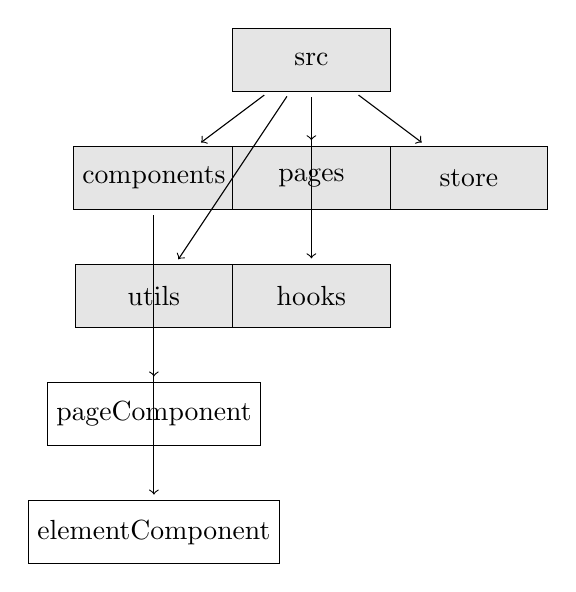
\begin{tikzpicture}[
    file/.style={draw, rectangle, minimum width=2cm, minimum height=0.8cm},
    folder/.style={draw, rectangle, minimum width=2cm, minimum height=0.8cm, fill=gray!20},
    arrow/.style={->, shorten >=2pt, shorten <=2pt}
]

% Folders
\node[folder] (src) at (0,0) {src};
\node[folder] (components) at (-2,-1.5) {components};
\node[folder] (pages) at (0,-1.5) {pages};
\node[folder] (store) at (2,-1.5) {store};
\node[folder] (utils) at (-2,-3) {utils};
\node[folder] (hooks) at (0,-3) {hooks};

% Files
\node[file] (pageComponent) at (-2,-4.5) {pageComponent};
\node[file] (elementComponent) at (-2,-6) {elementComponent};
% ... add more files

% Connections
\draw[arrow] (src) -- (components);
\draw[arrow] (src) -- (pages);
\draw[arrow] (src) -- (store);
\draw[arrow] (src) -- (utils);
\draw[arrow] (src) -- (hooks);
\draw[arrow] (components) -- (pageComponent);
\draw[arrow] (components) -- (elementComponent);
% ... add more connections

\end{tikzpicture}



\pagebreak
\subsubsection{Back-end}
The backend uses the dotNet framework. The development language using the C\# language.

In this project, the backend uses the Onion Architecture.
The Onion Architecture is a typically layered architecture, 
where each layer depends on the inner layer and provides interfaces to the outer layer.
The outer layer provides services to the outermost layer 
and other modules in the same layer based on the interfaces of the inner layer.

From inner to outer, the layers are: Domain, Application, Infrastructure, Presentation.
The Domain layer is the core layer and the innermost layer, used to define domain models, 
which are the business models.
It includes domain models and domain service interfaces.
Domain models are used to define the business models, 
which are the entities in the entity-relationship model and their attributes.
Domain service interfaces are used to define the business services, 
which are the relationships between entities in the entity-relationship model.

The Application layer is the application layer, 
used to define application services, which are the business logic.
It includes domain service implementations and application service interfaces.
Domain service implementations implement the methods of the inner layer's domain service 
interfaces and implement the business logic of the domain models.
Application service interfaces are used to define application services, 
which are the business logic.
It includes but is not limited to database interfaces, testing interfaces, 
HTTP API interfaces, MQTT interfaces, etc.

The Infrastructure layer is the infrastructure layer, used to define infrastructure.
It includes database implementations, testing implementations, 
HTTP API implementations, MQTT implementations, etc.
Database implementations implement the database interfaces 
and provide CRUD services for the database.
Testing implementations implement the testing interfaces 
and provide services for unit testing and integration testing.
HTTP API implementations implement the HTTP API interfaces 
and provide CRUD operations for HTTP APIs.
MQTT implementations implement the MQTT interfaces 
and provide CRUD operations for MQTT.

The Presentation layer is the presentation layer, used to define presentation logic, 
such as interfaces and pages. Since this is a backend project,
data presentation and control are handled by the frontend, 
so this layer is not needed.



\pagebreak
\subsubsection{Data communication and storage}
% 关于本项目的数据通信与数据存储的设计, 包括数据通信的协议, 数据存储的设计等
% 关于数据通信的设计:
% 1. 通信协议的选择
% 自前端向后端发送的数据, 有三种传输的数据类型, 
% 一种是普通的增删改查的请求, 对数据传输的时效性要求不高, 但是对数据的准确性, 完整性, 有序性, 安全性有一定的要求,
% 这种数据的传输, 采用 HTTP 协议, 以及 RESTful API 的设计. 可以有效的保证对数据传输的以上要求.
% 一种是对数据通道的创建和流媒体数据的传输, 对数据传输的时效性, 安全性要求较高, 这种数据的传输, 采用 WebRTC 协议, 以及 MQTT 协议.
% 配合可以快速解码的 flatbuffers 协议, 可以有效的保证对数据传输的以上要求.
% 最后一种是对设备的状态信息和操作信息的传输, 对完整性, 有序性, 安全性都有较高的要求, 这种数据的传输, 采用 MQTT 协议
% 同时也使用了 flatbuffers 协议.
% 
% 2. 数据通信的通信架构和通信流程
% 本项目的数据通信的通信架构, 是基于前后端分离的架构, 前端使用 React 框架, 后端使用 dotnet 框架.
% 当前端需要向后端发送数据的时候, 前端会向后端发送 HTTP 请求, 后端接收到 HTTP 请求之后, 会根据请求的数据类型,
% 选择不同的数据处理方式, 对于普通的增删改查的请求, 后端会根据 RESTful API 的设计, 对数据进行增删改查的操作,
% 对于对数据通道的创建和流媒体数据的传输, 后端会根据 WebRTC 协议, 对数据通道进行创建, 并且帮助前端和设备建立数据通道,
% 当数据通道建立后, 前端和设备之间则使用 flatbuffer 的数据格式对流媒体数据进行传输,
% 对于设备的状态信息和操作信息的传输, 前端会直接向 MQTT broker 发送 MQTT 请求, 
% 设备会在其自身的固件中监听相关的 MQTT 请求, 并且返回相关的数据.
% 
% 3. 数据通信的格式
% 本项目的数据通信的格式, 有三种, 
% 一种是 HTTP 协议, 
% 使用 json 格式对数据进行传输,
% 一种是 WebRTC 协议, 
% 使用 flatbuffers 格式对数据进行传输,
% 一种是 MQTT 协议.
% 使用 flatbuffers 格式对数据进行传输,
% 
% 关于数据存储的设计:
% 1. 数据存储的数据库的选择
% 本项目的数据存储的数据库的选择, 使用了轻量级的数据库 SQLite,
% SQLite 是一个进程内的库, 实现了自给自足的, 无服务器的, 零配置的, 事务性的 SQL 数据库引擎.
% 这是因为整个项目的目的是为了实现前端与设备之间的数据通信, 对于数据库数据的增删改查操作的要求不高,
% 数据量较小, 且对于数据库的数据的事务性要求不高, 所以选择了 SQLite 数据库.
% 2. 项目前后端的数据结构的设计
% 在本项目中, 前端由于使用了 React 框架, 所以前端的数据结构的设计, 使用了基于状态的数据结构的设计,
% 每个组件或者数据集都包含一个状态对象, 这个状态对象的属性就是组件的各个状态. 
% 使用状态对象的原因是, 可以方便的对状态进行管理, 采用对象-属性的形式, 可以方便的针对不同组件的同类状态进行区分,
% 由于跨组件的状态是由 redux 进行管理的, 这种状态对象的设计, 可以更搞笑的对状态进行更新和传递.
% 后端由于使用了 dotnet 框架, 所以后端的数据结构的设计, 使用了基于类的数据结构的设计,
% 采用了面向对象的编程思想, 对数据进行了封装, 使得数据的传输更加的安全, 有序, 完整.


\pagebreak

% \subsection{Domain model}
% \documentclass[]{article}
\usepackage{graphicx}
\usepackage{amsmath}
\usepackage{tikz}

% libaries
\usetikzlibrary{shapes,arrows}

%Define the listing package
\usepackage{listings} %code highlighter
\usepackage{color} %use color
\definecolor{mygreen}{rgb}{0,0.6,0}
\definecolor{mygray}{rgb}{0.5,0.5,0.5}
\definecolor{mymauve}{rgb}{0.58,0,0.82}

%Customize a bit the look
\lstset{ %
backgroundcolor=\color{white}, % choose the background color; you must add \usepackage{color} or \usepackage{xcolor}
basicstyle=\footnotesize, % the size of the fonts that are used for the code
breakatwhitespace=false, % sets if automatic breaks should only happen at whitespace
breaklines=true, % sets automatic line breaking
captionpos=b, % sets the caption-position to bottom
commentstyle=\color{mygreen}, % comment style
deletekeywords={...}, % if you want to delete keywords from the given language
escapeinside={\%*}{*)}, % if you want to add LaTeX within your code
extendedchars=true, % lets you use non-ASCII characters; for 8-bits encodings only, does not work with UTF-8
frame=single, % adds a frame around the code
keepspaces=true, % keeps spaces in text, useful for keeping indentation of code (possibly needs columns=flexible)
keywordstyle=\color{blue}, % keyword style
% language=Octave, % the language of the code
morekeywords={*,...}, % if you want to add more keywords to the set
numbers=left, % where to put the line-numbers; possible values are (none, left, right)
numbersep=5pt, % how far the line-numbers are from the code
numberstyle=\tiny\color{mygray}, % the style that is used for the line-numbers
rulecolor=\color{black}, % if not set, the frame-color may be changed on line-breaks within not-black text (e.g. comments (green here))
showspaces=false, % show spaces everywhere adding particular underscores; it overrides 'showstringspaces'
showstringspaces=false, % underline spaces within strings only
showtabs=false, % show tabs within strings adding particular underscores
stepnumber=1, % the step between two line-numbers. If it's 1, each line will be numbered
stringstyle=\color{mymauve}, % string literal style
tabsize=2, % sets default tabsize to 2 spaces
title=\lstname % show the filename of files included with \lstinputlisting; also try caption instead of title
}

\definecolor{darkgray}{rgb}{.4,.4,.4}
\definecolor{purple}{rgb}{0.65, 0.12, 0.82}

\lstdefinelanguage{React}{
keywords={const, typeof, new, true, false, catch, function, return, null, catch, switch, var, if, in, while, do, else, case, break},
keywordstyle=\color{blue}\bfseries,
ndkeywords={class, export, boolean, throw, implements, import, this},
ndkeywordstyle=\color{darkgray}\bfseries,
identifierstyle=\color{mygreen},
sensitive=false,
comment=[l]{//},
morecomment=[s]{/*}{*/},
commentstyle=\color{purple}\ttfamily,
string=[b]{"}{'}{`},
stringstyle=\color{red}\ttfamily,
morestring=[b]',
morestring=[b]",
morestring=[b]`',
}

\lstdefinelanguage{CSharp}{
keywords={const, typeof, new, true, false, catch, function, return, null, catch, switch, var, if, in, while, do, else, case, break},
keywordstyle=\color{blue}\bfseries,
ndkeywords={class, export, boolean, throw, implements, import, this},
ndkeywordstyle=\color{darkgray}\bfseries,
identifierstyle=\color{mygreen},
sensitive=false,
comment=[l]{//},
morecomment=[s]{/*}{*/},
commentstyle=\color{purple}\ttfamily,
string=[b]{"}{'}{`},
stringstyle=\color{red}\ttfamily,
morestring=[b]',
morestring=[b]",
morestring=[b]`',
}

\lstset{
language=React,
extendedchars=true,
basicstyle=\footnotesize\ttfamily,
showstringspaces=false,
showspaces=false,
numbers=left,
numberstyle=\footnotesize,
numbersep=9pt,
tabsize=2,
breaklines=true,
showtabs=false,
captionpos=b
}

\lstset{
language=CSharp,
extendedchars=true,
basicstyle=\footnotesize\ttfamily,
showstringspaces=false,
showspaces=false,
numbers=left,
numberstyle=\footnotesize,
numbersep=9pt,
tabsize=2,
breaklines=true,
showtabs=false,
captionpos=b
}

% \usepackage{cite} % Add this line for citation

% \bibliographystyle{plain}

\title{
The implementation of BifrostConnect Front-end scope, 
re-design and development with the relevant back-end support develop.
}
\author{
    Fei Gu \\
    Erhvervs Akademi Sydvest \\
    Computer Science 21\\
    }
\date{\today}

\begin{document}

% Front page
\maketitle
\begin{center}
    Supervisor: Henrik Boulund Meng Hansen \\
    Company: BifrostConnect \\
    Engineering Director: Jasper Wass \\
\end{center}
\tableofcontents
\pagebreak


% The introduction
\section{Introduction}
\subsection{Background}\input{sections/introduction/background.tex}
\subsection{The company}\input{sections/introduction/aboutCompany}
\subsection{The project}\input{sections/introduction/aboutProject}
\pagebreak

% The problem statement
\section{Problem Statement}
\subsection{Statement}
\input{sections/problemStatement/statement}
\subsection{Situation}
\input{sections/problemStatement/situation}
\subsection{Potential Solution}
\input{sections/problemStatement/potentialSolution}
\pagebreak

% Requirement analysis
\section{Requirement Analysis}
\input{sections/requirementAnalysis/index}

\subsection{Stakeholders}
\input{sections/requirementAnalysis/stakeholders/index}

\subsection{Business Domain}
\input{sections/requirementAnalysis/bussinesDomain/index}

\subsection{Scope}
\input{sections/requirementAnalysis/scope}

\subsection{Goals}
\input{sections/requirementAnalysis/goals}
\pagebreak

% Software Design
\section{Software Design}
% developement methods
\subsection{Software Development Methods}
\input{sections/softwareDevelopmentMethods/index}
\subsubsection{Agile Software Development}
\input{sections/softwareDevelopmentMethods/agileSoftwareDevelopment/index}
\subsubsection{Feature Driven Development}
\input{sections/softwareDevelopmentMethods/featureDrivenDevelopment/index}

\pagebreak

% Technology seslection
\subsection{Technology selection}
\input{sections/softwareDesign/technologySelection/index}
\subsubsection{Front-end}
\input{sections/softwareDesign/technologySelection/frontEnd}            
\subsubsection{Back-end}
\input{sections/softwareDesign/technologySelection/backEnd}            
\subsubsection{Database}
\input{sections/softwareDesign/technologySelection/database}
\subsubsection{Data communication}
\input{sections/softwareDesign/technologySelection/dataCommunication}            
\subsubsection{DevOps}
\input{sections/softwareDesign/technologySelection/devOps}
\pagebreak

% Architecture design
\subsection{Architecture design}
\input{sections/softwareDesign/architectureDesign/index}
\pagebreak
\subsubsection{Front-end}
\input{sections/softwareDesign/architectureDesign/frontEndArchitecture}
\pagebreak
\subsubsection{Back-end}
\input{sections/softwareDesign/architectureDesign/backEndArchitecture}
\pagebreak
\subsubsection{Data communication and storage}
\input{sections/softwareDesign/architectureDesign/dataCommunicationArchitecture}
\pagebreak

% \subsection{Domain model}
% \input{sections/softwareDesign/domainModel/index}
% \subsection{Database design}
% % 数据库领域模型 ER 图
% % 包括表和字段的设置.
% % 对于私有键和外键的设置.

% \subsection{Back-end design}
% % 后端对象模型
% % 以及对于对象模型的增删改查
% % 以及相关的其他服务的设计`'

% \subsection{Front-end design}
% % 对于前端的页面结构的设计 
% % 页面的状态的设计, 交互设计

% \subsection{FlatBuffers design}
% % schema 的设计

\subsection{DevOps CI/CD process design}
\input{sections/softwareDesign/devOpsDesign/index}
\subsubsection{Continuous Integration}
\input{sections/softwareDesign/devOpsDesign/continuousIntegration/index}
\subsubsection{Continuous Delivery}
\input{sections/softwareDesign/devOpsDesign/continuousDelivery/index}
\subsubsection{Continuous Deployment}
\input{sections/softwareDesign/devOpsDesign/continuousDeployment/index}
\pagebreak

\section{Software Development} 
\input{sections/softwareDevelopment/index}
\subsection{Overall development}
\input{sections/softwareDevelopment/overallDevelopement/index}
\subsubsection{Front-end}
\input{sections/softwareDevelopment/overallDevelopement/frontEnd/index}
\subsubsection{Back-end}
\input{sections/softwareDevelopment/overallDevelopement/backEnd/index}
\subsubsection{DevOps}
\input{sections/softwareDevelopment/overallDevelopement/devOps/index}
\subsection{Feature development} 
\input{sections/softwareDevelopment/featureDevelopment/index}
\subsubsection{Use Case 1}
\input{sections/softwareDevelopment/featureDevelopment/useCase1/index}
\subsubsection{Feature 1}
\input{sections/softwareDevelopment/featureDevelopment/feature/feature1.tex}
\pagebreak
\section{Conclusion} 
\subsection{Result}
Since the project is still in progress, the result is not available yet.
So far, basic structure of this project has been built. But the most features 
are not implemented yet. 
\subsection{Discussion}
As a single developer for this project, I am confident what I have done so far.
And I can say I understand the most of the knowledge I have used in this project, 
which also means I can explain all the part of the project. 
But this project also relevant some of the complex knowledge which I have to continue 
to study and practice.
\subsection{Future Work}
The future work is to implement the rest of the features. 
Including the most important part which is the 'create session' feature.
\pagebreak
% \bibliography{bibliography}
\pagebreak
% \begin{appendices}
%     \section{Appendix}
% \end{appendices} 
\end{document}
% \subsection{Database design}
% % 数据库领域模型 ER 图
% % 包括表和字段的设置.
% % 对于私有键和外键的设置.

% \subsection{Back-end design}
% % 后端对象模型
% % 以及对于对象模型的增删改查
% % 以及相关的其他服务的设计`'

% \subsection{Front-end design}
% % 对于前端的页面结构的设计 
% % 页面的状态的设计, 交互设计

% \subsection{FlatBuffers design}
% % schema 的设计

\subsection{DevOps CI/CD process design}
\documentclass[]{article}
\usepackage{graphicx}
\usepackage{amsmath}
\usepackage{tikz}

% libaries
\usetikzlibrary{shapes,arrows}

%Define the listing package
\usepackage{listings} %code highlighter
\usepackage{color} %use color
\definecolor{mygreen}{rgb}{0,0.6,0}
\definecolor{mygray}{rgb}{0.5,0.5,0.5}
\definecolor{mymauve}{rgb}{0.58,0,0.82}

%Customize a bit the look
\lstset{ %
backgroundcolor=\color{white}, % choose the background color; you must add \usepackage{color} or \usepackage{xcolor}
basicstyle=\footnotesize, % the size of the fonts that are used for the code
breakatwhitespace=false, % sets if automatic breaks should only happen at whitespace
breaklines=true, % sets automatic line breaking
captionpos=b, % sets the caption-position to bottom
commentstyle=\color{mygreen}, % comment style
deletekeywords={...}, % if you want to delete keywords from the given language
escapeinside={\%*}{*)}, % if you want to add LaTeX within your code
extendedchars=true, % lets you use non-ASCII characters; for 8-bits encodings only, does not work with UTF-8
frame=single, % adds a frame around the code
keepspaces=true, % keeps spaces in text, useful for keeping indentation of code (possibly needs columns=flexible)
keywordstyle=\color{blue}, % keyword style
% language=Octave, % the language of the code
morekeywords={*,...}, % if you want to add more keywords to the set
numbers=left, % where to put the line-numbers; possible values are (none, left, right)
numbersep=5pt, % how far the line-numbers are from the code
numberstyle=\tiny\color{mygray}, % the style that is used for the line-numbers
rulecolor=\color{black}, % if not set, the frame-color may be changed on line-breaks within not-black text (e.g. comments (green here))
showspaces=false, % show spaces everywhere adding particular underscores; it overrides 'showstringspaces'
showstringspaces=false, % underline spaces within strings only
showtabs=false, % show tabs within strings adding particular underscores
stepnumber=1, % the step between two line-numbers. If it's 1, each line will be numbered
stringstyle=\color{mymauve}, % string literal style
tabsize=2, % sets default tabsize to 2 spaces
title=\lstname % show the filename of files included with \lstinputlisting; also try caption instead of title
}

\definecolor{darkgray}{rgb}{.4,.4,.4}
\definecolor{purple}{rgb}{0.65, 0.12, 0.82}

\lstdefinelanguage{React}{
keywords={const, typeof, new, true, false, catch, function, return, null, catch, switch, var, if, in, while, do, else, case, break},
keywordstyle=\color{blue}\bfseries,
ndkeywords={class, export, boolean, throw, implements, import, this},
ndkeywordstyle=\color{darkgray}\bfseries,
identifierstyle=\color{mygreen},
sensitive=false,
comment=[l]{//},
morecomment=[s]{/*}{*/},
commentstyle=\color{purple}\ttfamily,
string=[b]{"}{'}{`},
stringstyle=\color{red}\ttfamily,
morestring=[b]',
morestring=[b]",
morestring=[b]`',
}

\lstdefinelanguage{CSharp}{
keywords={const, typeof, new, true, false, catch, function, return, null, catch, switch, var, if, in, while, do, else, case, break},
keywordstyle=\color{blue}\bfseries,
ndkeywords={class, export, boolean, throw, implements, import, this},
ndkeywordstyle=\color{darkgray}\bfseries,
identifierstyle=\color{mygreen},
sensitive=false,
comment=[l]{//},
morecomment=[s]{/*}{*/},
commentstyle=\color{purple}\ttfamily,
string=[b]{"}{'}{`},
stringstyle=\color{red}\ttfamily,
morestring=[b]',
morestring=[b]",
morestring=[b]`',
}

\lstset{
language=React,
extendedchars=true,
basicstyle=\footnotesize\ttfamily,
showstringspaces=false,
showspaces=false,
numbers=left,
numberstyle=\footnotesize,
numbersep=9pt,
tabsize=2,
breaklines=true,
showtabs=false,
captionpos=b
}

\lstset{
language=CSharp,
extendedchars=true,
basicstyle=\footnotesize\ttfamily,
showstringspaces=false,
showspaces=false,
numbers=left,
numberstyle=\footnotesize,
numbersep=9pt,
tabsize=2,
breaklines=true,
showtabs=false,
captionpos=b
}

% \usepackage{cite} % Add this line for citation

% \bibliographystyle{plain}

\title{
The implementation of BifrostConnect Front-end scope, 
re-design and development with the relevant back-end support develop.
}
\author{
    Fei Gu \\
    Erhvervs Akademi Sydvest \\
    Computer Science 21\\
    }
\date{\today}

\begin{document}

% Front page
\maketitle
\begin{center}
    Supervisor: Henrik Boulund Meng Hansen \\
    Company: BifrostConnect \\
    Engineering Director: Jasper Wass \\
\end{center}
\tableofcontents
\pagebreak


% The introduction
\section{Introduction}
\subsection{Background}\input{sections/introduction/background.tex}
\subsection{The company}\input{sections/introduction/aboutCompany}
\subsection{The project}\input{sections/introduction/aboutProject}
\pagebreak

% The problem statement
\section{Problem Statement}
\subsection{Statement}
\input{sections/problemStatement/statement}
\subsection{Situation}
\input{sections/problemStatement/situation}
\subsection{Potential Solution}
\input{sections/problemStatement/potentialSolution}
\pagebreak

% Requirement analysis
\section{Requirement Analysis}
\input{sections/requirementAnalysis/index}

\subsection{Stakeholders}
\input{sections/requirementAnalysis/stakeholders/index}

\subsection{Business Domain}
\input{sections/requirementAnalysis/bussinesDomain/index}

\subsection{Scope}
\input{sections/requirementAnalysis/scope}

\subsection{Goals}
\input{sections/requirementAnalysis/goals}
\pagebreak

% Software Design
\section{Software Design}
% developement methods
\subsection{Software Development Methods}
\input{sections/softwareDevelopmentMethods/index}
\subsubsection{Agile Software Development}
\input{sections/softwareDevelopmentMethods/agileSoftwareDevelopment/index}
\subsubsection{Feature Driven Development}
\input{sections/softwareDevelopmentMethods/featureDrivenDevelopment/index}

\pagebreak

% Technology seslection
\subsection{Technology selection}
\input{sections/softwareDesign/technologySelection/index}
\subsubsection{Front-end}
\input{sections/softwareDesign/technologySelection/frontEnd}            
\subsubsection{Back-end}
\input{sections/softwareDesign/technologySelection/backEnd}            
\subsubsection{Database}
\input{sections/softwareDesign/technologySelection/database}
\subsubsection{Data communication}
\input{sections/softwareDesign/technologySelection/dataCommunication}            
\subsubsection{DevOps}
\input{sections/softwareDesign/technologySelection/devOps}
\pagebreak

% Architecture design
\subsection{Architecture design}
\input{sections/softwareDesign/architectureDesign/index}
\pagebreak
\subsubsection{Front-end}
\input{sections/softwareDesign/architectureDesign/frontEndArchitecture}
\pagebreak
\subsubsection{Back-end}
\input{sections/softwareDesign/architectureDesign/backEndArchitecture}
\pagebreak
\subsubsection{Data communication and storage}
\input{sections/softwareDesign/architectureDesign/dataCommunicationArchitecture}
\pagebreak

% \subsection{Domain model}
% \input{sections/softwareDesign/domainModel/index}
% \subsection{Database design}
% % 数据库领域模型 ER 图
% % 包括表和字段的设置.
% % 对于私有键和外键的设置.

% \subsection{Back-end design}
% % 后端对象模型
% % 以及对于对象模型的增删改查
% % 以及相关的其他服务的设计`'

% \subsection{Front-end design}
% % 对于前端的页面结构的设计 
% % 页面的状态的设计, 交互设计

% \subsection{FlatBuffers design}
% % schema 的设计

\subsection{DevOps CI/CD process design}
\input{sections/softwareDesign/devOpsDesign/index}
\subsubsection{Continuous Integration}
\input{sections/softwareDesign/devOpsDesign/continuousIntegration/index}
\subsubsection{Continuous Delivery}
\input{sections/softwareDesign/devOpsDesign/continuousDelivery/index}
\subsubsection{Continuous Deployment}
\input{sections/softwareDesign/devOpsDesign/continuousDeployment/index}
\pagebreak

\section{Software Development} 
\input{sections/softwareDevelopment/index}
\subsection{Overall development}
\input{sections/softwareDevelopment/overallDevelopement/index}
\subsubsection{Front-end}
\input{sections/softwareDevelopment/overallDevelopement/frontEnd/index}
\subsubsection{Back-end}
\input{sections/softwareDevelopment/overallDevelopement/backEnd/index}
\subsubsection{DevOps}
\input{sections/softwareDevelopment/overallDevelopement/devOps/index}
\subsection{Feature development} 
\input{sections/softwareDevelopment/featureDevelopment/index}
\subsubsection{Use Case 1}
\input{sections/softwareDevelopment/featureDevelopment/useCase1/index}
\subsubsection{Feature 1}
\input{sections/softwareDevelopment/featureDevelopment/feature/feature1.tex}
\pagebreak
\section{Conclusion} 
\subsection{Result}
Since the project is still in progress, the result is not available yet.
So far, basic structure of this project has been built. But the most features 
are not implemented yet. 
\subsection{Discussion}
As a single developer for this project, I am confident what I have done so far.
And I can say I understand the most of the knowledge I have used in this project, 
which also means I can explain all the part of the project. 
But this project also relevant some of the complex knowledge which I have to continue 
to study and practice.
\subsection{Future Work}
The future work is to implement the rest of the features. 
Including the most important part which is the 'create session' feature.
\pagebreak
% \bibliography{bibliography}
\pagebreak
% \begin{appendices}
%     \section{Appendix}
% \end{appendices} 
\end{document}
\subsubsection{Continuous Integration}
\documentclass[]{article}
\usepackage{graphicx}
\usepackage{amsmath}
\usepackage{tikz}

% libaries
\usetikzlibrary{shapes,arrows}

%Define the listing package
\usepackage{listings} %code highlighter
\usepackage{color} %use color
\definecolor{mygreen}{rgb}{0,0.6,0}
\definecolor{mygray}{rgb}{0.5,0.5,0.5}
\definecolor{mymauve}{rgb}{0.58,0,0.82}

%Customize a bit the look
\lstset{ %
backgroundcolor=\color{white}, % choose the background color; you must add \usepackage{color} or \usepackage{xcolor}
basicstyle=\footnotesize, % the size of the fonts that are used for the code
breakatwhitespace=false, % sets if automatic breaks should only happen at whitespace
breaklines=true, % sets automatic line breaking
captionpos=b, % sets the caption-position to bottom
commentstyle=\color{mygreen}, % comment style
deletekeywords={...}, % if you want to delete keywords from the given language
escapeinside={\%*}{*)}, % if you want to add LaTeX within your code
extendedchars=true, % lets you use non-ASCII characters; for 8-bits encodings only, does not work with UTF-8
frame=single, % adds a frame around the code
keepspaces=true, % keeps spaces in text, useful for keeping indentation of code (possibly needs columns=flexible)
keywordstyle=\color{blue}, % keyword style
% language=Octave, % the language of the code
morekeywords={*,...}, % if you want to add more keywords to the set
numbers=left, % where to put the line-numbers; possible values are (none, left, right)
numbersep=5pt, % how far the line-numbers are from the code
numberstyle=\tiny\color{mygray}, % the style that is used for the line-numbers
rulecolor=\color{black}, % if not set, the frame-color may be changed on line-breaks within not-black text (e.g. comments (green here))
showspaces=false, % show spaces everywhere adding particular underscores; it overrides 'showstringspaces'
showstringspaces=false, % underline spaces within strings only
showtabs=false, % show tabs within strings adding particular underscores
stepnumber=1, % the step between two line-numbers. If it's 1, each line will be numbered
stringstyle=\color{mymauve}, % string literal style
tabsize=2, % sets default tabsize to 2 spaces
title=\lstname % show the filename of files included with \lstinputlisting; also try caption instead of title
}

\definecolor{darkgray}{rgb}{.4,.4,.4}
\definecolor{purple}{rgb}{0.65, 0.12, 0.82}

\lstdefinelanguage{React}{
keywords={const, typeof, new, true, false, catch, function, return, null, catch, switch, var, if, in, while, do, else, case, break},
keywordstyle=\color{blue}\bfseries,
ndkeywords={class, export, boolean, throw, implements, import, this},
ndkeywordstyle=\color{darkgray}\bfseries,
identifierstyle=\color{mygreen},
sensitive=false,
comment=[l]{//},
morecomment=[s]{/*}{*/},
commentstyle=\color{purple}\ttfamily,
string=[b]{"}{'}{`},
stringstyle=\color{red}\ttfamily,
morestring=[b]',
morestring=[b]",
morestring=[b]`',
}

\lstdefinelanguage{CSharp}{
keywords={const, typeof, new, true, false, catch, function, return, null, catch, switch, var, if, in, while, do, else, case, break},
keywordstyle=\color{blue}\bfseries,
ndkeywords={class, export, boolean, throw, implements, import, this},
ndkeywordstyle=\color{darkgray}\bfseries,
identifierstyle=\color{mygreen},
sensitive=false,
comment=[l]{//},
morecomment=[s]{/*}{*/},
commentstyle=\color{purple}\ttfamily,
string=[b]{"}{'}{`},
stringstyle=\color{red}\ttfamily,
morestring=[b]',
morestring=[b]",
morestring=[b]`',
}

\lstset{
language=React,
extendedchars=true,
basicstyle=\footnotesize\ttfamily,
showstringspaces=false,
showspaces=false,
numbers=left,
numberstyle=\footnotesize,
numbersep=9pt,
tabsize=2,
breaklines=true,
showtabs=false,
captionpos=b
}

\lstset{
language=CSharp,
extendedchars=true,
basicstyle=\footnotesize\ttfamily,
showstringspaces=false,
showspaces=false,
numbers=left,
numberstyle=\footnotesize,
numbersep=9pt,
tabsize=2,
breaklines=true,
showtabs=false,
captionpos=b
}

% \usepackage{cite} % Add this line for citation

% \bibliographystyle{plain}

\title{
The implementation of BifrostConnect Front-end scope, 
re-design and development with the relevant back-end support develop.
}
\author{
    Fei Gu \\
    Erhvervs Akademi Sydvest \\
    Computer Science 21\\
    }
\date{\today}

\begin{document}

% Front page
\maketitle
\begin{center}
    Supervisor: Henrik Boulund Meng Hansen \\
    Company: BifrostConnect \\
    Engineering Director: Jasper Wass \\
\end{center}
\tableofcontents
\pagebreak


% The introduction
\section{Introduction}
\subsection{Background}\input{sections/introduction/background.tex}
\subsection{The company}\input{sections/introduction/aboutCompany}
\subsection{The project}\input{sections/introduction/aboutProject}
\pagebreak

% The problem statement
\section{Problem Statement}
\subsection{Statement}
\input{sections/problemStatement/statement}
\subsection{Situation}
\input{sections/problemStatement/situation}
\subsection{Potential Solution}
\input{sections/problemStatement/potentialSolution}
\pagebreak

% Requirement analysis
\section{Requirement Analysis}
\input{sections/requirementAnalysis/index}

\subsection{Stakeholders}
\input{sections/requirementAnalysis/stakeholders/index}

\subsection{Business Domain}
\input{sections/requirementAnalysis/bussinesDomain/index}

\subsection{Scope}
\input{sections/requirementAnalysis/scope}

\subsection{Goals}
\input{sections/requirementAnalysis/goals}
\pagebreak

% Software Design
\section{Software Design}
% developement methods
\subsection{Software Development Methods}
\input{sections/softwareDevelopmentMethods/index}
\subsubsection{Agile Software Development}
\input{sections/softwareDevelopmentMethods/agileSoftwareDevelopment/index}
\subsubsection{Feature Driven Development}
\input{sections/softwareDevelopmentMethods/featureDrivenDevelopment/index}

\pagebreak

% Technology seslection
\subsection{Technology selection}
\input{sections/softwareDesign/technologySelection/index}
\subsubsection{Front-end}
\input{sections/softwareDesign/technologySelection/frontEnd}            
\subsubsection{Back-end}
\input{sections/softwareDesign/technologySelection/backEnd}            
\subsubsection{Database}
\input{sections/softwareDesign/technologySelection/database}
\subsubsection{Data communication}
\input{sections/softwareDesign/technologySelection/dataCommunication}            
\subsubsection{DevOps}
\input{sections/softwareDesign/technologySelection/devOps}
\pagebreak

% Architecture design
\subsection{Architecture design}
\input{sections/softwareDesign/architectureDesign/index}
\pagebreak
\subsubsection{Front-end}
\input{sections/softwareDesign/architectureDesign/frontEndArchitecture}
\pagebreak
\subsubsection{Back-end}
\input{sections/softwareDesign/architectureDesign/backEndArchitecture}
\pagebreak
\subsubsection{Data communication and storage}
\input{sections/softwareDesign/architectureDesign/dataCommunicationArchitecture}
\pagebreak

% \subsection{Domain model}
% \input{sections/softwareDesign/domainModel/index}
% \subsection{Database design}
% % 数据库领域模型 ER 图
% % 包括表和字段的设置.
% % 对于私有键和外键的设置.

% \subsection{Back-end design}
% % 后端对象模型
% % 以及对于对象模型的增删改查
% % 以及相关的其他服务的设计`'

% \subsection{Front-end design}
% % 对于前端的页面结构的设计 
% % 页面的状态的设计, 交互设计

% \subsection{FlatBuffers design}
% % schema 的设计

\subsection{DevOps CI/CD process design}
\input{sections/softwareDesign/devOpsDesign/index}
\subsubsection{Continuous Integration}
\input{sections/softwareDesign/devOpsDesign/continuousIntegration/index}
\subsubsection{Continuous Delivery}
\input{sections/softwareDesign/devOpsDesign/continuousDelivery/index}
\subsubsection{Continuous Deployment}
\input{sections/softwareDesign/devOpsDesign/continuousDeployment/index}
\pagebreak

\section{Software Development} 
\input{sections/softwareDevelopment/index}
\subsection{Overall development}
\input{sections/softwareDevelopment/overallDevelopement/index}
\subsubsection{Front-end}
\input{sections/softwareDevelopment/overallDevelopement/frontEnd/index}
\subsubsection{Back-end}
\input{sections/softwareDevelopment/overallDevelopement/backEnd/index}
\subsubsection{DevOps}
\input{sections/softwareDevelopment/overallDevelopement/devOps/index}
\subsection{Feature development} 
\input{sections/softwareDevelopment/featureDevelopment/index}
\subsubsection{Use Case 1}
\input{sections/softwareDevelopment/featureDevelopment/useCase1/index}
\subsubsection{Feature 1}
\input{sections/softwareDevelopment/featureDevelopment/feature/feature1.tex}
\pagebreak
\section{Conclusion} 
\subsection{Result}
Since the project is still in progress, the result is not available yet.
So far, basic structure of this project has been built. But the most features 
are not implemented yet. 
\subsection{Discussion}
As a single developer for this project, I am confident what I have done so far.
And I can say I understand the most of the knowledge I have used in this project, 
which also means I can explain all the part of the project. 
But this project also relevant some of the complex knowledge which I have to continue 
to study and practice.
\subsection{Future Work}
The future work is to implement the rest of the features. 
Including the most important part which is the 'create session' feature.
\pagebreak
% \bibliography{bibliography}
\pagebreak
% \begin{appendices}
%     \section{Appendix}
% \end{appendices} 
\end{document}
\subsubsection{Continuous Delivery}
\documentclass[]{article}
\usepackage{graphicx}
\usepackage{amsmath}
\usepackage{tikz}

% libaries
\usetikzlibrary{shapes,arrows}

%Define the listing package
\usepackage{listings} %code highlighter
\usepackage{color} %use color
\definecolor{mygreen}{rgb}{0,0.6,0}
\definecolor{mygray}{rgb}{0.5,0.5,0.5}
\definecolor{mymauve}{rgb}{0.58,0,0.82}

%Customize a bit the look
\lstset{ %
backgroundcolor=\color{white}, % choose the background color; you must add \usepackage{color} or \usepackage{xcolor}
basicstyle=\footnotesize, % the size of the fonts that are used for the code
breakatwhitespace=false, % sets if automatic breaks should only happen at whitespace
breaklines=true, % sets automatic line breaking
captionpos=b, % sets the caption-position to bottom
commentstyle=\color{mygreen}, % comment style
deletekeywords={...}, % if you want to delete keywords from the given language
escapeinside={\%*}{*)}, % if you want to add LaTeX within your code
extendedchars=true, % lets you use non-ASCII characters; for 8-bits encodings only, does not work with UTF-8
frame=single, % adds a frame around the code
keepspaces=true, % keeps spaces in text, useful for keeping indentation of code (possibly needs columns=flexible)
keywordstyle=\color{blue}, % keyword style
% language=Octave, % the language of the code
morekeywords={*,...}, % if you want to add more keywords to the set
numbers=left, % where to put the line-numbers; possible values are (none, left, right)
numbersep=5pt, % how far the line-numbers are from the code
numberstyle=\tiny\color{mygray}, % the style that is used for the line-numbers
rulecolor=\color{black}, % if not set, the frame-color may be changed on line-breaks within not-black text (e.g. comments (green here))
showspaces=false, % show spaces everywhere adding particular underscores; it overrides 'showstringspaces'
showstringspaces=false, % underline spaces within strings only
showtabs=false, % show tabs within strings adding particular underscores
stepnumber=1, % the step between two line-numbers. If it's 1, each line will be numbered
stringstyle=\color{mymauve}, % string literal style
tabsize=2, % sets default tabsize to 2 spaces
title=\lstname % show the filename of files included with \lstinputlisting; also try caption instead of title
}

\definecolor{darkgray}{rgb}{.4,.4,.4}
\definecolor{purple}{rgb}{0.65, 0.12, 0.82}

\lstdefinelanguage{React}{
keywords={const, typeof, new, true, false, catch, function, return, null, catch, switch, var, if, in, while, do, else, case, break},
keywordstyle=\color{blue}\bfseries,
ndkeywords={class, export, boolean, throw, implements, import, this},
ndkeywordstyle=\color{darkgray}\bfseries,
identifierstyle=\color{mygreen},
sensitive=false,
comment=[l]{//},
morecomment=[s]{/*}{*/},
commentstyle=\color{purple}\ttfamily,
string=[b]{"}{'}{`},
stringstyle=\color{red}\ttfamily,
morestring=[b]',
morestring=[b]",
morestring=[b]`',
}

\lstdefinelanguage{CSharp}{
keywords={const, typeof, new, true, false, catch, function, return, null, catch, switch, var, if, in, while, do, else, case, break},
keywordstyle=\color{blue}\bfseries,
ndkeywords={class, export, boolean, throw, implements, import, this},
ndkeywordstyle=\color{darkgray}\bfseries,
identifierstyle=\color{mygreen},
sensitive=false,
comment=[l]{//},
morecomment=[s]{/*}{*/},
commentstyle=\color{purple}\ttfamily,
string=[b]{"}{'}{`},
stringstyle=\color{red}\ttfamily,
morestring=[b]',
morestring=[b]",
morestring=[b]`',
}

\lstset{
language=React,
extendedchars=true,
basicstyle=\footnotesize\ttfamily,
showstringspaces=false,
showspaces=false,
numbers=left,
numberstyle=\footnotesize,
numbersep=9pt,
tabsize=2,
breaklines=true,
showtabs=false,
captionpos=b
}

\lstset{
language=CSharp,
extendedchars=true,
basicstyle=\footnotesize\ttfamily,
showstringspaces=false,
showspaces=false,
numbers=left,
numberstyle=\footnotesize,
numbersep=9pt,
tabsize=2,
breaklines=true,
showtabs=false,
captionpos=b
}

% \usepackage{cite} % Add this line for citation

% \bibliographystyle{plain}

\title{
The implementation of BifrostConnect Front-end scope, 
re-design and development with the relevant back-end support develop.
}
\author{
    Fei Gu \\
    Erhvervs Akademi Sydvest \\
    Computer Science 21\\
    }
\date{\today}

\begin{document}

% Front page
\maketitle
\begin{center}
    Supervisor: Henrik Boulund Meng Hansen \\
    Company: BifrostConnect \\
    Engineering Director: Jasper Wass \\
\end{center}
\tableofcontents
\pagebreak


% The introduction
\section{Introduction}
\subsection{Background}\input{sections/introduction/background.tex}
\subsection{The company}\input{sections/introduction/aboutCompany}
\subsection{The project}\input{sections/introduction/aboutProject}
\pagebreak

% The problem statement
\section{Problem Statement}
\subsection{Statement}
\input{sections/problemStatement/statement}
\subsection{Situation}
\input{sections/problemStatement/situation}
\subsection{Potential Solution}
\input{sections/problemStatement/potentialSolution}
\pagebreak

% Requirement analysis
\section{Requirement Analysis}
\input{sections/requirementAnalysis/index}

\subsection{Stakeholders}
\input{sections/requirementAnalysis/stakeholders/index}

\subsection{Business Domain}
\input{sections/requirementAnalysis/bussinesDomain/index}

\subsection{Scope}
\input{sections/requirementAnalysis/scope}

\subsection{Goals}
\input{sections/requirementAnalysis/goals}
\pagebreak

% Software Design
\section{Software Design}
% developement methods
\subsection{Software Development Methods}
\input{sections/softwareDevelopmentMethods/index}
\subsubsection{Agile Software Development}
\input{sections/softwareDevelopmentMethods/agileSoftwareDevelopment/index}
\subsubsection{Feature Driven Development}
\input{sections/softwareDevelopmentMethods/featureDrivenDevelopment/index}

\pagebreak

% Technology seslection
\subsection{Technology selection}
\input{sections/softwareDesign/technologySelection/index}
\subsubsection{Front-end}
\input{sections/softwareDesign/technologySelection/frontEnd}            
\subsubsection{Back-end}
\input{sections/softwareDesign/technologySelection/backEnd}            
\subsubsection{Database}
\input{sections/softwareDesign/technologySelection/database}
\subsubsection{Data communication}
\input{sections/softwareDesign/technologySelection/dataCommunication}            
\subsubsection{DevOps}
\input{sections/softwareDesign/technologySelection/devOps}
\pagebreak

% Architecture design
\subsection{Architecture design}
\input{sections/softwareDesign/architectureDesign/index}
\pagebreak
\subsubsection{Front-end}
\input{sections/softwareDesign/architectureDesign/frontEndArchitecture}
\pagebreak
\subsubsection{Back-end}
\input{sections/softwareDesign/architectureDesign/backEndArchitecture}
\pagebreak
\subsubsection{Data communication and storage}
\input{sections/softwareDesign/architectureDesign/dataCommunicationArchitecture}
\pagebreak

% \subsection{Domain model}
% \input{sections/softwareDesign/domainModel/index}
% \subsection{Database design}
% % 数据库领域模型 ER 图
% % 包括表和字段的设置.
% % 对于私有键和外键的设置.

% \subsection{Back-end design}
% % 后端对象模型
% % 以及对于对象模型的增删改查
% % 以及相关的其他服务的设计`'

% \subsection{Front-end design}
% % 对于前端的页面结构的设计 
% % 页面的状态的设计, 交互设计

% \subsection{FlatBuffers design}
% % schema 的设计

\subsection{DevOps CI/CD process design}
\input{sections/softwareDesign/devOpsDesign/index}
\subsubsection{Continuous Integration}
\input{sections/softwareDesign/devOpsDesign/continuousIntegration/index}
\subsubsection{Continuous Delivery}
\input{sections/softwareDesign/devOpsDesign/continuousDelivery/index}
\subsubsection{Continuous Deployment}
\input{sections/softwareDesign/devOpsDesign/continuousDeployment/index}
\pagebreak

\section{Software Development} 
\input{sections/softwareDevelopment/index}
\subsection{Overall development}
\input{sections/softwareDevelopment/overallDevelopement/index}
\subsubsection{Front-end}
\input{sections/softwareDevelopment/overallDevelopement/frontEnd/index}
\subsubsection{Back-end}
\input{sections/softwareDevelopment/overallDevelopement/backEnd/index}
\subsubsection{DevOps}
\input{sections/softwareDevelopment/overallDevelopement/devOps/index}
\subsection{Feature development} 
\input{sections/softwareDevelopment/featureDevelopment/index}
\subsubsection{Use Case 1}
\input{sections/softwareDevelopment/featureDevelopment/useCase1/index}
\subsubsection{Feature 1}
\input{sections/softwareDevelopment/featureDevelopment/feature/feature1.tex}
\pagebreak
\section{Conclusion} 
\subsection{Result}
Since the project is still in progress, the result is not available yet.
So far, basic structure of this project has been built. But the most features 
are not implemented yet. 
\subsection{Discussion}
As a single developer for this project, I am confident what I have done so far.
And I can say I understand the most of the knowledge I have used in this project, 
which also means I can explain all the part of the project. 
But this project also relevant some of the complex knowledge which I have to continue 
to study and practice.
\subsection{Future Work}
The future work is to implement the rest of the features. 
Including the most important part which is the 'create session' feature.
\pagebreak
% \bibliography{bibliography}
\pagebreak
% \begin{appendices}
%     \section{Appendix}
% \end{appendices} 
\end{document}
\subsubsection{Continuous Deployment}
\documentclass[]{article}
\usepackage{graphicx}
\usepackage{amsmath}
\usepackage{tikz}

% libaries
\usetikzlibrary{shapes,arrows}

%Define the listing package
\usepackage{listings} %code highlighter
\usepackage{color} %use color
\definecolor{mygreen}{rgb}{0,0.6,0}
\definecolor{mygray}{rgb}{0.5,0.5,0.5}
\definecolor{mymauve}{rgb}{0.58,0,0.82}

%Customize a bit the look
\lstset{ %
backgroundcolor=\color{white}, % choose the background color; you must add \usepackage{color} or \usepackage{xcolor}
basicstyle=\footnotesize, % the size of the fonts that are used for the code
breakatwhitespace=false, % sets if automatic breaks should only happen at whitespace
breaklines=true, % sets automatic line breaking
captionpos=b, % sets the caption-position to bottom
commentstyle=\color{mygreen}, % comment style
deletekeywords={...}, % if you want to delete keywords from the given language
escapeinside={\%*}{*)}, % if you want to add LaTeX within your code
extendedchars=true, % lets you use non-ASCII characters; for 8-bits encodings only, does not work with UTF-8
frame=single, % adds a frame around the code
keepspaces=true, % keeps spaces in text, useful for keeping indentation of code (possibly needs columns=flexible)
keywordstyle=\color{blue}, % keyword style
% language=Octave, % the language of the code
morekeywords={*,...}, % if you want to add more keywords to the set
numbers=left, % where to put the line-numbers; possible values are (none, left, right)
numbersep=5pt, % how far the line-numbers are from the code
numberstyle=\tiny\color{mygray}, % the style that is used for the line-numbers
rulecolor=\color{black}, % if not set, the frame-color may be changed on line-breaks within not-black text (e.g. comments (green here))
showspaces=false, % show spaces everywhere adding particular underscores; it overrides 'showstringspaces'
showstringspaces=false, % underline spaces within strings only
showtabs=false, % show tabs within strings adding particular underscores
stepnumber=1, % the step between two line-numbers. If it's 1, each line will be numbered
stringstyle=\color{mymauve}, % string literal style
tabsize=2, % sets default tabsize to 2 spaces
title=\lstname % show the filename of files included with \lstinputlisting; also try caption instead of title
}

\definecolor{darkgray}{rgb}{.4,.4,.4}
\definecolor{purple}{rgb}{0.65, 0.12, 0.82}

\lstdefinelanguage{React}{
keywords={const, typeof, new, true, false, catch, function, return, null, catch, switch, var, if, in, while, do, else, case, break},
keywordstyle=\color{blue}\bfseries,
ndkeywords={class, export, boolean, throw, implements, import, this},
ndkeywordstyle=\color{darkgray}\bfseries,
identifierstyle=\color{mygreen},
sensitive=false,
comment=[l]{//},
morecomment=[s]{/*}{*/},
commentstyle=\color{purple}\ttfamily,
string=[b]{"}{'}{`},
stringstyle=\color{red}\ttfamily,
morestring=[b]',
morestring=[b]",
morestring=[b]`',
}

\lstdefinelanguage{CSharp}{
keywords={const, typeof, new, true, false, catch, function, return, null, catch, switch, var, if, in, while, do, else, case, break},
keywordstyle=\color{blue}\bfseries,
ndkeywords={class, export, boolean, throw, implements, import, this},
ndkeywordstyle=\color{darkgray}\bfseries,
identifierstyle=\color{mygreen},
sensitive=false,
comment=[l]{//},
morecomment=[s]{/*}{*/},
commentstyle=\color{purple}\ttfamily,
string=[b]{"}{'}{`},
stringstyle=\color{red}\ttfamily,
morestring=[b]',
morestring=[b]",
morestring=[b]`',
}

\lstset{
language=React,
extendedchars=true,
basicstyle=\footnotesize\ttfamily,
showstringspaces=false,
showspaces=false,
numbers=left,
numberstyle=\footnotesize,
numbersep=9pt,
tabsize=2,
breaklines=true,
showtabs=false,
captionpos=b
}

\lstset{
language=CSharp,
extendedchars=true,
basicstyle=\footnotesize\ttfamily,
showstringspaces=false,
showspaces=false,
numbers=left,
numberstyle=\footnotesize,
numbersep=9pt,
tabsize=2,
breaklines=true,
showtabs=false,
captionpos=b
}

% \usepackage{cite} % Add this line for citation

% \bibliographystyle{plain}

\title{
The implementation of BifrostConnect Front-end scope, 
re-design and development with the relevant back-end support develop.
}
\author{
    Fei Gu \\
    Erhvervs Akademi Sydvest \\
    Computer Science 21\\
    }
\date{\today}

\begin{document}

% Front page
\maketitle
\begin{center}
    Supervisor: Henrik Boulund Meng Hansen \\
    Company: BifrostConnect \\
    Engineering Director: Jasper Wass \\
\end{center}
\tableofcontents
\pagebreak


% The introduction
\section{Introduction}
\subsection{Background}\input{sections/introduction/background.tex}
\subsection{The company}\input{sections/introduction/aboutCompany}
\subsection{The project}\input{sections/introduction/aboutProject}
\pagebreak

% The problem statement
\section{Problem Statement}
\subsection{Statement}
\input{sections/problemStatement/statement}
\subsection{Situation}
\input{sections/problemStatement/situation}
\subsection{Potential Solution}
\input{sections/problemStatement/potentialSolution}
\pagebreak

% Requirement analysis
\section{Requirement Analysis}
\input{sections/requirementAnalysis/index}

\subsection{Stakeholders}
\input{sections/requirementAnalysis/stakeholders/index}

\subsection{Business Domain}
\input{sections/requirementAnalysis/bussinesDomain/index}

\subsection{Scope}
\input{sections/requirementAnalysis/scope}

\subsection{Goals}
\input{sections/requirementAnalysis/goals}
\pagebreak

% Software Design
\section{Software Design}
% developement methods
\subsection{Software Development Methods}
\input{sections/softwareDevelopmentMethods/index}
\subsubsection{Agile Software Development}
\input{sections/softwareDevelopmentMethods/agileSoftwareDevelopment/index}
\subsubsection{Feature Driven Development}
\input{sections/softwareDevelopmentMethods/featureDrivenDevelopment/index}

\pagebreak

% Technology seslection
\subsection{Technology selection}
\input{sections/softwareDesign/technologySelection/index}
\subsubsection{Front-end}
\input{sections/softwareDesign/technologySelection/frontEnd}            
\subsubsection{Back-end}
\input{sections/softwareDesign/technologySelection/backEnd}            
\subsubsection{Database}
\input{sections/softwareDesign/technologySelection/database}
\subsubsection{Data communication}
\input{sections/softwareDesign/technologySelection/dataCommunication}            
\subsubsection{DevOps}
\input{sections/softwareDesign/technologySelection/devOps}
\pagebreak

% Architecture design
\subsection{Architecture design}
\input{sections/softwareDesign/architectureDesign/index}
\pagebreak
\subsubsection{Front-end}
\input{sections/softwareDesign/architectureDesign/frontEndArchitecture}
\pagebreak
\subsubsection{Back-end}
\input{sections/softwareDesign/architectureDesign/backEndArchitecture}
\pagebreak
\subsubsection{Data communication and storage}
\input{sections/softwareDesign/architectureDesign/dataCommunicationArchitecture}
\pagebreak

% \subsection{Domain model}
% \input{sections/softwareDesign/domainModel/index}
% \subsection{Database design}
% % 数据库领域模型 ER 图
% % 包括表和字段的设置.
% % 对于私有键和外键的设置.

% \subsection{Back-end design}
% % 后端对象模型
% % 以及对于对象模型的增删改查
% % 以及相关的其他服务的设计`'

% \subsection{Front-end design}
% % 对于前端的页面结构的设计 
% % 页面的状态的设计, 交互设计

% \subsection{FlatBuffers design}
% % schema 的设计

\subsection{DevOps CI/CD process design}
\input{sections/softwareDesign/devOpsDesign/index}
\subsubsection{Continuous Integration}
\input{sections/softwareDesign/devOpsDesign/continuousIntegration/index}
\subsubsection{Continuous Delivery}
\input{sections/softwareDesign/devOpsDesign/continuousDelivery/index}
\subsubsection{Continuous Deployment}
\input{sections/softwareDesign/devOpsDesign/continuousDeployment/index}
\pagebreak

\section{Software Development} 
\input{sections/softwareDevelopment/index}
\subsection{Overall development}
\input{sections/softwareDevelopment/overallDevelopement/index}
\subsubsection{Front-end}
\input{sections/softwareDevelopment/overallDevelopement/frontEnd/index}
\subsubsection{Back-end}
\input{sections/softwareDevelopment/overallDevelopement/backEnd/index}
\subsubsection{DevOps}
\input{sections/softwareDevelopment/overallDevelopement/devOps/index}
\subsection{Feature development} 
\input{sections/softwareDevelopment/featureDevelopment/index}
\subsubsection{Use Case 1}
\input{sections/softwareDevelopment/featureDevelopment/useCase1/index}
\subsubsection{Feature 1}
\input{sections/softwareDevelopment/featureDevelopment/feature/feature1.tex}
\pagebreak
\section{Conclusion} 
\subsection{Result}
Since the project is still in progress, the result is not available yet.
So far, basic structure of this project has been built. But the most features 
are not implemented yet. 
\subsection{Discussion}
As a single developer for this project, I am confident what I have done so far.
And I can say I understand the most of the knowledge I have used in this project, 
which also means I can explain all the part of the project. 
But this project also relevant some of the complex knowledge which I have to continue 
to study and practice.
\subsection{Future Work}
The future work is to implement the rest of the features. 
Including the most important part which is the 'create session' feature.
\pagebreak
% \bibliography{bibliography}
\pagebreak
% \begin{appendices}
%     \section{Appendix}
% \end{appendices} 
\end{document}
\pagebreak

\section{Software Development} 
\documentclass[]{article}
\usepackage{graphicx}
\usepackage{amsmath}
\usepackage{tikz}

% libaries
\usetikzlibrary{shapes,arrows}

%Define the listing package
\usepackage{listings} %code highlighter
\usepackage{color} %use color
\definecolor{mygreen}{rgb}{0,0.6,0}
\definecolor{mygray}{rgb}{0.5,0.5,0.5}
\definecolor{mymauve}{rgb}{0.58,0,0.82}

%Customize a bit the look
\lstset{ %
backgroundcolor=\color{white}, % choose the background color; you must add \usepackage{color} or \usepackage{xcolor}
basicstyle=\footnotesize, % the size of the fonts that are used for the code
breakatwhitespace=false, % sets if automatic breaks should only happen at whitespace
breaklines=true, % sets automatic line breaking
captionpos=b, % sets the caption-position to bottom
commentstyle=\color{mygreen}, % comment style
deletekeywords={...}, % if you want to delete keywords from the given language
escapeinside={\%*}{*)}, % if you want to add LaTeX within your code
extendedchars=true, % lets you use non-ASCII characters; for 8-bits encodings only, does not work with UTF-8
frame=single, % adds a frame around the code
keepspaces=true, % keeps spaces in text, useful for keeping indentation of code (possibly needs columns=flexible)
keywordstyle=\color{blue}, % keyword style
% language=Octave, % the language of the code
morekeywords={*,...}, % if you want to add more keywords to the set
numbers=left, % where to put the line-numbers; possible values are (none, left, right)
numbersep=5pt, % how far the line-numbers are from the code
numberstyle=\tiny\color{mygray}, % the style that is used for the line-numbers
rulecolor=\color{black}, % if not set, the frame-color may be changed on line-breaks within not-black text (e.g. comments (green here))
showspaces=false, % show spaces everywhere adding particular underscores; it overrides 'showstringspaces'
showstringspaces=false, % underline spaces within strings only
showtabs=false, % show tabs within strings adding particular underscores
stepnumber=1, % the step between two line-numbers. If it's 1, each line will be numbered
stringstyle=\color{mymauve}, % string literal style
tabsize=2, % sets default tabsize to 2 spaces
title=\lstname % show the filename of files included with \lstinputlisting; also try caption instead of title
}

\definecolor{darkgray}{rgb}{.4,.4,.4}
\definecolor{purple}{rgb}{0.65, 0.12, 0.82}

\lstdefinelanguage{React}{
keywords={const, typeof, new, true, false, catch, function, return, null, catch, switch, var, if, in, while, do, else, case, break},
keywordstyle=\color{blue}\bfseries,
ndkeywords={class, export, boolean, throw, implements, import, this},
ndkeywordstyle=\color{darkgray}\bfseries,
identifierstyle=\color{mygreen},
sensitive=false,
comment=[l]{//},
morecomment=[s]{/*}{*/},
commentstyle=\color{purple}\ttfamily,
string=[b]{"}{'}{`},
stringstyle=\color{red}\ttfamily,
morestring=[b]',
morestring=[b]",
morestring=[b]`',
}

\lstdefinelanguage{CSharp}{
keywords={const, typeof, new, true, false, catch, function, return, null, catch, switch, var, if, in, while, do, else, case, break},
keywordstyle=\color{blue}\bfseries,
ndkeywords={class, export, boolean, throw, implements, import, this},
ndkeywordstyle=\color{darkgray}\bfseries,
identifierstyle=\color{mygreen},
sensitive=false,
comment=[l]{//},
morecomment=[s]{/*}{*/},
commentstyle=\color{purple}\ttfamily,
string=[b]{"}{'}{`},
stringstyle=\color{red}\ttfamily,
morestring=[b]',
morestring=[b]",
morestring=[b]`',
}

\lstset{
language=React,
extendedchars=true,
basicstyle=\footnotesize\ttfamily,
showstringspaces=false,
showspaces=false,
numbers=left,
numberstyle=\footnotesize,
numbersep=9pt,
tabsize=2,
breaklines=true,
showtabs=false,
captionpos=b
}

\lstset{
language=CSharp,
extendedchars=true,
basicstyle=\footnotesize\ttfamily,
showstringspaces=false,
showspaces=false,
numbers=left,
numberstyle=\footnotesize,
numbersep=9pt,
tabsize=2,
breaklines=true,
showtabs=false,
captionpos=b
}

% \usepackage{cite} % Add this line for citation

% \bibliographystyle{plain}

\title{
The implementation of BifrostConnect Front-end scope, 
re-design and development with the relevant back-end support develop.
}
\author{
    Fei Gu \\
    Erhvervs Akademi Sydvest \\
    Computer Science 21\\
    }
\date{\today}

\begin{document}

% Front page
\maketitle
\begin{center}
    Supervisor: Henrik Boulund Meng Hansen \\
    Company: BifrostConnect \\
    Engineering Director: Jasper Wass \\
\end{center}
\tableofcontents
\pagebreak


% The introduction
\section{Introduction}
\subsection{Background}\input{sections/introduction/background.tex}
\subsection{The company}\input{sections/introduction/aboutCompany}
\subsection{The project}\input{sections/introduction/aboutProject}
\pagebreak

% The problem statement
\section{Problem Statement}
\subsection{Statement}
\input{sections/problemStatement/statement}
\subsection{Situation}
\input{sections/problemStatement/situation}
\subsection{Potential Solution}
\input{sections/problemStatement/potentialSolution}
\pagebreak

% Requirement analysis
\section{Requirement Analysis}
\input{sections/requirementAnalysis/index}

\subsection{Stakeholders}
\input{sections/requirementAnalysis/stakeholders/index}

\subsection{Business Domain}
\input{sections/requirementAnalysis/bussinesDomain/index}

\subsection{Scope}
\input{sections/requirementAnalysis/scope}

\subsection{Goals}
\input{sections/requirementAnalysis/goals}
\pagebreak

% Software Design
\section{Software Design}
% developement methods
\subsection{Software Development Methods}
\input{sections/softwareDevelopmentMethods/index}
\subsubsection{Agile Software Development}
\input{sections/softwareDevelopmentMethods/agileSoftwareDevelopment/index}
\subsubsection{Feature Driven Development}
\input{sections/softwareDevelopmentMethods/featureDrivenDevelopment/index}

\pagebreak

% Technology seslection
\subsection{Technology selection}
\input{sections/softwareDesign/technologySelection/index}
\subsubsection{Front-end}
\input{sections/softwareDesign/technologySelection/frontEnd}            
\subsubsection{Back-end}
\input{sections/softwareDesign/technologySelection/backEnd}            
\subsubsection{Database}
\input{sections/softwareDesign/technologySelection/database}
\subsubsection{Data communication}
\input{sections/softwareDesign/technologySelection/dataCommunication}            
\subsubsection{DevOps}
\input{sections/softwareDesign/technologySelection/devOps}
\pagebreak

% Architecture design
\subsection{Architecture design}
\input{sections/softwareDesign/architectureDesign/index}
\pagebreak
\subsubsection{Front-end}
\input{sections/softwareDesign/architectureDesign/frontEndArchitecture}
\pagebreak
\subsubsection{Back-end}
\input{sections/softwareDesign/architectureDesign/backEndArchitecture}
\pagebreak
\subsubsection{Data communication and storage}
\input{sections/softwareDesign/architectureDesign/dataCommunicationArchitecture}
\pagebreak

% \subsection{Domain model}
% \input{sections/softwareDesign/domainModel/index}
% \subsection{Database design}
% % 数据库领域模型 ER 图
% % 包括表和字段的设置.
% % 对于私有键和外键的设置.

% \subsection{Back-end design}
% % 后端对象模型
% % 以及对于对象模型的增删改查
% % 以及相关的其他服务的设计`'

% \subsection{Front-end design}
% % 对于前端的页面结构的设计 
% % 页面的状态的设计, 交互设计

% \subsection{FlatBuffers design}
% % schema 的设计

\subsection{DevOps CI/CD process design}
\input{sections/softwareDesign/devOpsDesign/index}
\subsubsection{Continuous Integration}
\input{sections/softwareDesign/devOpsDesign/continuousIntegration/index}
\subsubsection{Continuous Delivery}
\input{sections/softwareDesign/devOpsDesign/continuousDelivery/index}
\subsubsection{Continuous Deployment}
\input{sections/softwareDesign/devOpsDesign/continuousDeployment/index}
\pagebreak

\section{Software Development} 
\input{sections/softwareDevelopment/index}
\subsection{Overall development}
\input{sections/softwareDevelopment/overallDevelopement/index}
\subsubsection{Front-end}
\input{sections/softwareDevelopment/overallDevelopement/frontEnd/index}
\subsubsection{Back-end}
\input{sections/softwareDevelopment/overallDevelopement/backEnd/index}
\subsubsection{DevOps}
\input{sections/softwareDevelopment/overallDevelopement/devOps/index}
\subsection{Feature development} 
\input{sections/softwareDevelopment/featureDevelopment/index}
\subsubsection{Use Case 1}
\input{sections/softwareDevelopment/featureDevelopment/useCase1/index}
\subsubsection{Feature 1}
\input{sections/softwareDevelopment/featureDevelopment/feature/feature1.tex}
\pagebreak
\section{Conclusion} 
\subsection{Result}
Since the project is still in progress, the result is not available yet.
So far, basic structure of this project has been built. But the most features 
are not implemented yet. 
\subsection{Discussion}
As a single developer for this project, I am confident what I have done so far.
And I can say I understand the most of the knowledge I have used in this project, 
which also means I can explain all the part of the project. 
But this project also relevant some of the complex knowledge which I have to continue 
to study and practice.
\subsection{Future Work}
The future work is to implement the rest of the features. 
Including the most important part which is the 'create session' feature.
\pagebreak
% \bibliography{bibliography}
\pagebreak
% \begin{appendices}
%     \section{Appendix}
% \end{appendices} 
\end{document}
\subsection{Overall development}
\documentclass[]{article}
\usepackage{graphicx}
\usepackage{amsmath}
\usepackage{tikz}

% libaries
\usetikzlibrary{shapes,arrows}

%Define the listing package
\usepackage{listings} %code highlighter
\usepackage{color} %use color
\definecolor{mygreen}{rgb}{0,0.6,0}
\definecolor{mygray}{rgb}{0.5,0.5,0.5}
\definecolor{mymauve}{rgb}{0.58,0,0.82}

%Customize a bit the look
\lstset{ %
backgroundcolor=\color{white}, % choose the background color; you must add \usepackage{color} or \usepackage{xcolor}
basicstyle=\footnotesize, % the size of the fonts that are used for the code
breakatwhitespace=false, % sets if automatic breaks should only happen at whitespace
breaklines=true, % sets automatic line breaking
captionpos=b, % sets the caption-position to bottom
commentstyle=\color{mygreen}, % comment style
deletekeywords={...}, % if you want to delete keywords from the given language
escapeinside={\%*}{*)}, % if you want to add LaTeX within your code
extendedchars=true, % lets you use non-ASCII characters; for 8-bits encodings only, does not work with UTF-8
frame=single, % adds a frame around the code
keepspaces=true, % keeps spaces in text, useful for keeping indentation of code (possibly needs columns=flexible)
keywordstyle=\color{blue}, % keyword style
% language=Octave, % the language of the code
morekeywords={*,...}, % if you want to add more keywords to the set
numbers=left, % where to put the line-numbers; possible values are (none, left, right)
numbersep=5pt, % how far the line-numbers are from the code
numberstyle=\tiny\color{mygray}, % the style that is used for the line-numbers
rulecolor=\color{black}, % if not set, the frame-color may be changed on line-breaks within not-black text (e.g. comments (green here))
showspaces=false, % show spaces everywhere adding particular underscores; it overrides 'showstringspaces'
showstringspaces=false, % underline spaces within strings only
showtabs=false, % show tabs within strings adding particular underscores
stepnumber=1, % the step between two line-numbers. If it's 1, each line will be numbered
stringstyle=\color{mymauve}, % string literal style
tabsize=2, % sets default tabsize to 2 spaces
title=\lstname % show the filename of files included with \lstinputlisting; also try caption instead of title
}

\definecolor{darkgray}{rgb}{.4,.4,.4}
\definecolor{purple}{rgb}{0.65, 0.12, 0.82}

\lstdefinelanguage{React}{
keywords={const, typeof, new, true, false, catch, function, return, null, catch, switch, var, if, in, while, do, else, case, break},
keywordstyle=\color{blue}\bfseries,
ndkeywords={class, export, boolean, throw, implements, import, this},
ndkeywordstyle=\color{darkgray}\bfseries,
identifierstyle=\color{mygreen},
sensitive=false,
comment=[l]{//},
morecomment=[s]{/*}{*/},
commentstyle=\color{purple}\ttfamily,
string=[b]{"}{'}{`},
stringstyle=\color{red}\ttfamily,
morestring=[b]',
morestring=[b]",
morestring=[b]`',
}

\lstdefinelanguage{CSharp}{
keywords={const, typeof, new, true, false, catch, function, return, null, catch, switch, var, if, in, while, do, else, case, break},
keywordstyle=\color{blue}\bfseries,
ndkeywords={class, export, boolean, throw, implements, import, this},
ndkeywordstyle=\color{darkgray}\bfseries,
identifierstyle=\color{mygreen},
sensitive=false,
comment=[l]{//},
morecomment=[s]{/*}{*/},
commentstyle=\color{purple}\ttfamily,
string=[b]{"}{'}{`},
stringstyle=\color{red}\ttfamily,
morestring=[b]',
morestring=[b]",
morestring=[b]`',
}

\lstset{
language=React,
extendedchars=true,
basicstyle=\footnotesize\ttfamily,
showstringspaces=false,
showspaces=false,
numbers=left,
numberstyle=\footnotesize,
numbersep=9pt,
tabsize=2,
breaklines=true,
showtabs=false,
captionpos=b
}

\lstset{
language=CSharp,
extendedchars=true,
basicstyle=\footnotesize\ttfamily,
showstringspaces=false,
showspaces=false,
numbers=left,
numberstyle=\footnotesize,
numbersep=9pt,
tabsize=2,
breaklines=true,
showtabs=false,
captionpos=b
}

% \usepackage{cite} % Add this line for citation

% \bibliographystyle{plain}

\title{
The implementation of BifrostConnect Front-end scope, 
re-design and development with the relevant back-end support develop.
}
\author{
    Fei Gu \\
    Erhvervs Akademi Sydvest \\
    Computer Science 21\\
    }
\date{\today}

\begin{document}

% Front page
\maketitle
\begin{center}
    Supervisor: Henrik Boulund Meng Hansen \\
    Company: BifrostConnect \\
    Engineering Director: Jasper Wass \\
\end{center}
\tableofcontents
\pagebreak


% The introduction
\section{Introduction}
\subsection{Background}\input{sections/introduction/background.tex}
\subsection{The company}\input{sections/introduction/aboutCompany}
\subsection{The project}\input{sections/introduction/aboutProject}
\pagebreak

% The problem statement
\section{Problem Statement}
\subsection{Statement}
\input{sections/problemStatement/statement}
\subsection{Situation}
\input{sections/problemStatement/situation}
\subsection{Potential Solution}
\input{sections/problemStatement/potentialSolution}
\pagebreak

% Requirement analysis
\section{Requirement Analysis}
\input{sections/requirementAnalysis/index}

\subsection{Stakeholders}
\input{sections/requirementAnalysis/stakeholders/index}

\subsection{Business Domain}
\input{sections/requirementAnalysis/bussinesDomain/index}

\subsection{Scope}
\input{sections/requirementAnalysis/scope}

\subsection{Goals}
\input{sections/requirementAnalysis/goals}
\pagebreak

% Software Design
\section{Software Design}
% developement methods
\subsection{Software Development Methods}
\input{sections/softwareDevelopmentMethods/index}
\subsubsection{Agile Software Development}
\input{sections/softwareDevelopmentMethods/agileSoftwareDevelopment/index}
\subsubsection{Feature Driven Development}
\input{sections/softwareDevelopmentMethods/featureDrivenDevelopment/index}

\pagebreak

% Technology seslection
\subsection{Technology selection}
\input{sections/softwareDesign/technologySelection/index}
\subsubsection{Front-end}
\input{sections/softwareDesign/technologySelection/frontEnd}            
\subsubsection{Back-end}
\input{sections/softwareDesign/technologySelection/backEnd}            
\subsubsection{Database}
\input{sections/softwareDesign/technologySelection/database}
\subsubsection{Data communication}
\input{sections/softwareDesign/technologySelection/dataCommunication}            
\subsubsection{DevOps}
\input{sections/softwareDesign/technologySelection/devOps}
\pagebreak

% Architecture design
\subsection{Architecture design}
\input{sections/softwareDesign/architectureDesign/index}
\pagebreak
\subsubsection{Front-end}
\input{sections/softwareDesign/architectureDesign/frontEndArchitecture}
\pagebreak
\subsubsection{Back-end}
\input{sections/softwareDesign/architectureDesign/backEndArchitecture}
\pagebreak
\subsubsection{Data communication and storage}
\input{sections/softwareDesign/architectureDesign/dataCommunicationArchitecture}
\pagebreak

% \subsection{Domain model}
% \input{sections/softwareDesign/domainModel/index}
% \subsection{Database design}
% % 数据库领域模型 ER 图
% % 包括表和字段的设置.
% % 对于私有键和外键的设置.

% \subsection{Back-end design}
% % 后端对象模型
% % 以及对于对象模型的增删改查
% % 以及相关的其他服务的设计`'

% \subsection{Front-end design}
% % 对于前端的页面结构的设计 
% % 页面的状态的设计, 交互设计

% \subsection{FlatBuffers design}
% % schema 的设计

\subsection{DevOps CI/CD process design}
\input{sections/softwareDesign/devOpsDesign/index}
\subsubsection{Continuous Integration}
\input{sections/softwareDesign/devOpsDesign/continuousIntegration/index}
\subsubsection{Continuous Delivery}
\input{sections/softwareDesign/devOpsDesign/continuousDelivery/index}
\subsubsection{Continuous Deployment}
\input{sections/softwareDesign/devOpsDesign/continuousDeployment/index}
\pagebreak

\section{Software Development} 
\input{sections/softwareDevelopment/index}
\subsection{Overall development}
\input{sections/softwareDevelopment/overallDevelopement/index}
\subsubsection{Front-end}
\input{sections/softwareDevelopment/overallDevelopement/frontEnd/index}
\subsubsection{Back-end}
\input{sections/softwareDevelopment/overallDevelopement/backEnd/index}
\subsubsection{DevOps}
\input{sections/softwareDevelopment/overallDevelopement/devOps/index}
\subsection{Feature development} 
\input{sections/softwareDevelopment/featureDevelopment/index}
\subsubsection{Use Case 1}
\input{sections/softwareDevelopment/featureDevelopment/useCase1/index}
\subsubsection{Feature 1}
\input{sections/softwareDevelopment/featureDevelopment/feature/feature1.tex}
\pagebreak
\section{Conclusion} 
\subsection{Result}
Since the project is still in progress, the result is not available yet.
So far, basic structure of this project has been built. But the most features 
are not implemented yet. 
\subsection{Discussion}
As a single developer for this project, I am confident what I have done so far.
And I can say I understand the most of the knowledge I have used in this project, 
which also means I can explain all the part of the project. 
But this project also relevant some of the complex knowledge which I have to continue 
to study and practice.
\subsection{Future Work}
The future work is to implement the rest of the features. 
Including the most important part which is the 'create session' feature.
\pagebreak
% \bibliography{bibliography}
\pagebreak
% \begin{appendices}
%     \section{Appendix}
% \end{appendices} 
\end{document}
\subsubsection{Front-end}
\documentclass[]{article}
\usepackage{graphicx}
\usepackage{amsmath}
\usepackage{tikz}

% libaries
\usetikzlibrary{shapes,arrows}

%Define the listing package
\usepackage{listings} %code highlighter
\usepackage{color} %use color
\definecolor{mygreen}{rgb}{0,0.6,0}
\definecolor{mygray}{rgb}{0.5,0.5,0.5}
\definecolor{mymauve}{rgb}{0.58,0,0.82}

%Customize a bit the look
\lstset{ %
backgroundcolor=\color{white}, % choose the background color; you must add \usepackage{color} or \usepackage{xcolor}
basicstyle=\footnotesize, % the size of the fonts that are used for the code
breakatwhitespace=false, % sets if automatic breaks should only happen at whitespace
breaklines=true, % sets automatic line breaking
captionpos=b, % sets the caption-position to bottom
commentstyle=\color{mygreen}, % comment style
deletekeywords={...}, % if you want to delete keywords from the given language
escapeinside={\%*}{*)}, % if you want to add LaTeX within your code
extendedchars=true, % lets you use non-ASCII characters; for 8-bits encodings only, does not work with UTF-8
frame=single, % adds a frame around the code
keepspaces=true, % keeps spaces in text, useful for keeping indentation of code (possibly needs columns=flexible)
keywordstyle=\color{blue}, % keyword style
% language=Octave, % the language of the code
morekeywords={*,...}, % if you want to add more keywords to the set
numbers=left, % where to put the line-numbers; possible values are (none, left, right)
numbersep=5pt, % how far the line-numbers are from the code
numberstyle=\tiny\color{mygray}, % the style that is used for the line-numbers
rulecolor=\color{black}, % if not set, the frame-color may be changed on line-breaks within not-black text (e.g. comments (green here))
showspaces=false, % show spaces everywhere adding particular underscores; it overrides 'showstringspaces'
showstringspaces=false, % underline spaces within strings only
showtabs=false, % show tabs within strings adding particular underscores
stepnumber=1, % the step between two line-numbers. If it's 1, each line will be numbered
stringstyle=\color{mymauve}, % string literal style
tabsize=2, % sets default tabsize to 2 spaces
title=\lstname % show the filename of files included with \lstinputlisting; also try caption instead of title
}

\definecolor{darkgray}{rgb}{.4,.4,.4}
\definecolor{purple}{rgb}{0.65, 0.12, 0.82}

\lstdefinelanguage{React}{
keywords={const, typeof, new, true, false, catch, function, return, null, catch, switch, var, if, in, while, do, else, case, break},
keywordstyle=\color{blue}\bfseries,
ndkeywords={class, export, boolean, throw, implements, import, this},
ndkeywordstyle=\color{darkgray}\bfseries,
identifierstyle=\color{mygreen},
sensitive=false,
comment=[l]{//},
morecomment=[s]{/*}{*/},
commentstyle=\color{purple}\ttfamily,
string=[b]{"}{'}{`},
stringstyle=\color{red}\ttfamily,
morestring=[b]',
morestring=[b]",
morestring=[b]`',
}

\lstdefinelanguage{CSharp}{
keywords={const, typeof, new, true, false, catch, function, return, null, catch, switch, var, if, in, while, do, else, case, break},
keywordstyle=\color{blue}\bfseries,
ndkeywords={class, export, boolean, throw, implements, import, this},
ndkeywordstyle=\color{darkgray}\bfseries,
identifierstyle=\color{mygreen},
sensitive=false,
comment=[l]{//},
morecomment=[s]{/*}{*/},
commentstyle=\color{purple}\ttfamily,
string=[b]{"}{'}{`},
stringstyle=\color{red}\ttfamily,
morestring=[b]',
morestring=[b]",
morestring=[b]`',
}

\lstset{
language=React,
extendedchars=true,
basicstyle=\footnotesize\ttfamily,
showstringspaces=false,
showspaces=false,
numbers=left,
numberstyle=\footnotesize,
numbersep=9pt,
tabsize=2,
breaklines=true,
showtabs=false,
captionpos=b
}

\lstset{
language=CSharp,
extendedchars=true,
basicstyle=\footnotesize\ttfamily,
showstringspaces=false,
showspaces=false,
numbers=left,
numberstyle=\footnotesize,
numbersep=9pt,
tabsize=2,
breaklines=true,
showtabs=false,
captionpos=b
}

% \usepackage{cite} % Add this line for citation

% \bibliographystyle{plain}

\title{
The implementation of BifrostConnect Front-end scope, 
re-design and development with the relevant back-end support develop.
}
\author{
    Fei Gu \\
    Erhvervs Akademi Sydvest \\
    Computer Science 21\\
    }
\date{\today}

\begin{document}

% Front page
\maketitle
\begin{center}
    Supervisor: Henrik Boulund Meng Hansen \\
    Company: BifrostConnect \\
    Engineering Director: Jasper Wass \\
\end{center}
\tableofcontents
\pagebreak


% The introduction
\section{Introduction}
\subsection{Background}\input{sections/introduction/background.tex}
\subsection{The company}\input{sections/introduction/aboutCompany}
\subsection{The project}\input{sections/introduction/aboutProject}
\pagebreak

% The problem statement
\section{Problem Statement}
\subsection{Statement}
\input{sections/problemStatement/statement}
\subsection{Situation}
\input{sections/problemStatement/situation}
\subsection{Potential Solution}
\input{sections/problemStatement/potentialSolution}
\pagebreak

% Requirement analysis
\section{Requirement Analysis}
\input{sections/requirementAnalysis/index}

\subsection{Stakeholders}
\input{sections/requirementAnalysis/stakeholders/index}

\subsection{Business Domain}
\input{sections/requirementAnalysis/bussinesDomain/index}

\subsection{Scope}
\input{sections/requirementAnalysis/scope}

\subsection{Goals}
\input{sections/requirementAnalysis/goals}
\pagebreak

% Software Design
\section{Software Design}
% developement methods
\subsection{Software Development Methods}
\input{sections/softwareDevelopmentMethods/index}
\subsubsection{Agile Software Development}
\input{sections/softwareDevelopmentMethods/agileSoftwareDevelopment/index}
\subsubsection{Feature Driven Development}
\input{sections/softwareDevelopmentMethods/featureDrivenDevelopment/index}

\pagebreak

% Technology seslection
\subsection{Technology selection}
\input{sections/softwareDesign/technologySelection/index}
\subsubsection{Front-end}
\input{sections/softwareDesign/technologySelection/frontEnd}            
\subsubsection{Back-end}
\input{sections/softwareDesign/technologySelection/backEnd}            
\subsubsection{Database}
\input{sections/softwareDesign/technologySelection/database}
\subsubsection{Data communication}
\input{sections/softwareDesign/technologySelection/dataCommunication}            
\subsubsection{DevOps}
\input{sections/softwareDesign/technologySelection/devOps}
\pagebreak

% Architecture design
\subsection{Architecture design}
\input{sections/softwareDesign/architectureDesign/index}
\pagebreak
\subsubsection{Front-end}
\input{sections/softwareDesign/architectureDesign/frontEndArchitecture}
\pagebreak
\subsubsection{Back-end}
\input{sections/softwareDesign/architectureDesign/backEndArchitecture}
\pagebreak
\subsubsection{Data communication and storage}
\input{sections/softwareDesign/architectureDesign/dataCommunicationArchitecture}
\pagebreak

% \subsection{Domain model}
% \input{sections/softwareDesign/domainModel/index}
% \subsection{Database design}
% % 数据库领域模型 ER 图
% % 包括表和字段的设置.
% % 对于私有键和外键的设置.

% \subsection{Back-end design}
% % 后端对象模型
% % 以及对于对象模型的增删改查
% % 以及相关的其他服务的设计`'

% \subsection{Front-end design}
% % 对于前端的页面结构的设计 
% % 页面的状态的设计, 交互设计

% \subsection{FlatBuffers design}
% % schema 的设计

\subsection{DevOps CI/CD process design}
\input{sections/softwareDesign/devOpsDesign/index}
\subsubsection{Continuous Integration}
\input{sections/softwareDesign/devOpsDesign/continuousIntegration/index}
\subsubsection{Continuous Delivery}
\input{sections/softwareDesign/devOpsDesign/continuousDelivery/index}
\subsubsection{Continuous Deployment}
\input{sections/softwareDesign/devOpsDesign/continuousDeployment/index}
\pagebreak

\section{Software Development} 
\input{sections/softwareDevelopment/index}
\subsection{Overall development}
\input{sections/softwareDevelopment/overallDevelopement/index}
\subsubsection{Front-end}
\input{sections/softwareDevelopment/overallDevelopement/frontEnd/index}
\subsubsection{Back-end}
\input{sections/softwareDevelopment/overallDevelopement/backEnd/index}
\subsubsection{DevOps}
\input{sections/softwareDevelopment/overallDevelopement/devOps/index}
\subsection{Feature development} 
\input{sections/softwareDevelopment/featureDevelopment/index}
\subsubsection{Use Case 1}
\input{sections/softwareDevelopment/featureDevelopment/useCase1/index}
\subsubsection{Feature 1}
\input{sections/softwareDevelopment/featureDevelopment/feature/feature1.tex}
\pagebreak
\section{Conclusion} 
\subsection{Result}
Since the project is still in progress, the result is not available yet.
So far, basic structure of this project has been built. But the most features 
are not implemented yet. 
\subsection{Discussion}
As a single developer for this project, I am confident what I have done so far.
And I can say I understand the most of the knowledge I have used in this project, 
which also means I can explain all the part of the project. 
But this project also relevant some of the complex knowledge which I have to continue 
to study and practice.
\subsection{Future Work}
The future work is to implement the rest of the features. 
Including the most important part which is the 'create session' feature.
\pagebreak
% \bibliography{bibliography}
\pagebreak
% \begin{appendices}
%     \section{Appendix}
% \end{appendices} 
\end{document}
\subsubsection{Back-end}
\documentclass[]{article}
\usepackage{graphicx}
\usepackage{amsmath}
\usepackage{tikz}

% libaries
\usetikzlibrary{shapes,arrows}

%Define the listing package
\usepackage{listings} %code highlighter
\usepackage{color} %use color
\definecolor{mygreen}{rgb}{0,0.6,0}
\definecolor{mygray}{rgb}{0.5,0.5,0.5}
\definecolor{mymauve}{rgb}{0.58,0,0.82}

%Customize a bit the look
\lstset{ %
backgroundcolor=\color{white}, % choose the background color; you must add \usepackage{color} or \usepackage{xcolor}
basicstyle=\footnotesize, % the size of the fonts that are used for the code
breakatwhitespace=false, % sets if automatic breaks should only happen at whitespace
breaklines=true, % sets automatic line breaking
captionpos=b, % sets the caption-position to bottom
commentstyle=\color{mygreen}, % comment style
deletekeywords={...}, % if you want to delete keywords from the given language
escapeinside={\%*}{*)}, % if you want to add LaTeX within your code
extendedchars=true, % lets you use non-ASCII characters; for 8-bits encodings only, does not work with UTF-8
frame=single, % adds a frame around the code
keepspaces=true, % keeps spaces in text, useful for keeping indentation of code (possibly needs columns=flexible)
keywordstyle=\color{blue}, % keyword style
% language=Octave, % the language of the code
morekeywords={*,...}, % if you want to add more keywords to the set
numbers=left, % where to put the line-numbers; possible values are (none, left, right)
numbersep=5pt, % how far the line-numbers are from the code
numberstyle=\tiny\color{mygray}, % the style that is used for the line-numbers
rulecolor=\color{black}, % if not set, the frame-color may be changed on line-breaks within not-black text (e.g. comments (green here))
showspaces=false, % show spaces everywhere adding particular underscores; it overrides 'showstringspaces'
showstringspaces=false, % underline spaces within strings only
showtabs=false, % show tabs within strings adding particular underscores
stepnumber=1, % the step between two line-numbers. If it's 1, each line will be numbered
stringstyle=\color{mymauve}, % string literal style
tabsize=2, % sets default tabsize to 2 spaces
title=\lstname % show the filename of files included with \lstinputlisting; also try caption instead of title
}

\definecolor{darkgray}{rgb}{.4,.4,.4}
\definecolor{purple}{rgb}{0.65, 0.12, 0.82}

\lstdefinelanguage{React}{
keywords={const, typeof, new, true, false, catch, function, return, null, catch, switch, var, if, in, while, do, else, case, break},
keywordstyle=\color{blue}\bfseries,
ndkeywords={class, export, boolean, throw, implements, import, this},
ndkeywordstyle=\color{darkgray}\bfseries,
identifierstyle=\color{mygreen},
sensitive=false,
comment=[l]{//},
morecomment=[s]{/*}{*/},
commentstyle=\color{purple}\ttfamily,
string=[b]{"}{'}{`},
stringstyle=\color{red}\ttfamily,
morestring=[b]',
morestring=[b]",
morestring=[b]`',
}

\lstdefinelanguage{CSharp}{
keywords={const, typeof, new, true, false, catch, function, return, null, catch, switch, var, if, in, while, do, else, case, break},
keywordstyle=\color{blue}\bfseries,
ndkeywords={class, export, boolean, throw, implements, import, this},
ndkeywordstyle=\color{darkgray}\bfseries,
identifierstyle=\color{mygreen},
sensitive=false,
comment=[l]{//},
morecomment=[s]{/*}{*/},
commentstyle=\color{purple}\ttfamily,
string=[b]{"}{'}{`},
stringstyle=\color{red}\ttfamily,
morestring=[b]',
morestring=[b]",
morestring=[b]`',
}

\lstset{
language=React,
extendedchars=true,
basicstyle=\footnotesize\ttfamily,
showstringspaces=false,
showspaces=false,
numbers=left,
numberstyle=\footnotesize,
numbersep=9pt,
tabsize=2,
breaklines=true,
showtabs=false,
captionpos=b
}

\lstset{
language=CSharp,
extendedchars=true,
basicstyle=\footnotesize\ttfamily,
showstringspaces=false,
showspaces=false,
numbers=left,
numberstyle=\footnotesize,
numbersep=9pt,
tabsize=2,
breaklines=true,
showtabs=false,
captionpos=b
}

% \usepackage{cite} % Add this line for citation

% \bibliographystyle{plain}

\title{
The implementation of BifrostConnect Front-end scope, 
re-design and development with the relevant back-end support develop.
}
\author{
    Fei Gu \\
    Erhvervs Akademi Sydvest \\
    Computer Science 21\\
    }
\date{\today}

\begin{document}

% Front page
\maketitle
\begin{center}
    Supervisor: Henrik Boulund Meng Hansen \\
    Company: BifrostConnect \\
    Engineering Director: Jasper Wass \\
\end{center}
\tableofcontents
\pagebreak


% The introduction
\section{Introduction}
\subsection{Background}\input{sections/introduction/background.tex}
\subsection{The company}\input{sections/introduction/aboutCompany}
\subsection{The project}\input{sections/introduction/aboutProject}
\pagebreak

% The problem statement
\section{Problem Statement}
\subsection{Statement}
\input{sections/problemStatement/statement}
\subsection{Situation}
\input{sections/problemStatement/situation}
\subsection{Potential Solution}
\input{sections/problemStatement/potentialSolution}
\pagebreak

% Requirement analysis
\section{Requirement Analysis}
\input{sections/requirementAnalysis/index}

\subsection{Stakeholders}
\input{sections/requirementAnalysis/stakeholders/index}

\subsection{Business Domain}
\input{sections/requirementAnalysis/bussinesDomain/index}

\subsection{Scope}
\input{sections/requirementAnalysis/scope}

\subsection{Goals}
\input{sections/requirementAnalysis/goals}
\pagebreak

% Software Design
\section{Software Design}
% developement methods
\subsection{Software Development Methods}
\input{sections/softwareDevelopmentMethods/index}
\subsubsection{Agile Software Development}
\input{sections/softwareDevelopmentMethods/agileSoftwareDevelopment/index}
\subsubsection{Feature Driven Development}
\input{sections/softwareDevelopmentMethods/featureDrivenDevelopment/index}

\pagebreak

% Technology seslection
\subsection{Technology selection}
\input{sections/softwareDesign/technologySelection/index}
\subsubsection{Front-end}
\input{sections/softwareDesign/technologySelection/frontEnd}            
\subsubsection{Back-end}
\input{sections/softwareDesign/technologySelection/backEnd}            
\subsubsection{Database}
\input{sections/softwareDesign/technologySelection/database}
\subsubsection{Data communication}
\input{sections/softwareDesign/technologySelection/dataCommunication}            
\subsubsection{DevOps}
\input{sections/softwareDesign/technologySelection/devOps}
\pagebreak

% Architecture design
\subsection{Architecture design}
\input{sections/softwareDesign/architectureDesign/index}
\pagebreak
\subsubsection{Front-end}
\input{sections/softwareDesign/architectureDesign/frontEndArchitecture}
\pagebreak
\subsubsection{Back-end}
\input{sections/softwareDesign/architectureDesign/backEndArchitecture}
\pagebreak
\subsubsection{Data communication and storage}
\input{sections/softwareDesign/architectureDesign/dataCommunicationArchitecture}
\pagebreak

% \subsection{Domain model}
% \input{sections/softwareDesign/domainModel/index}
% \subsection{Database design}
% % 数据库领域模型 ER 图
% % 包括表和字段的设置.
% % 对于私有键和外键的设置.

% \subsection{Back-end design}
% % 后端对象模型
% % 以及对于对象模型的增删改查
% % 以及相关的其他服务的设计`'

% \subsection{Front-end design}
% % 对于前端的页面结构的设计 
% % 页面的状态的设计, 交互设计

% \subsection{FlatBuffers design}
% % schema 的设计

\subsection{DevOps CI/CD process design}
\input{sections/softwareDesign/devOpsDesign/index}
\subsubsection{Continuous Integration}
\input{sections/softwareDesign/devOpsDesign/continuousIntegration/index}
\subsubsection{Continuous Delivery}
\input{sections/softwareDesign/devOpsDesign/continuousDelivery/index}
\subsubsection{Continuous Deployment}
\input{sections/softwareDesign/devOpsDesign/continuousDeployment/index}
\pagebreak

\section{Software Development} 
\input{sections/softwareDevelopment/index}
\subsection{Overall development}
\input{sections/softwareDevelopment/overallDevelopement/index}
\subsubsection{Front-end}
\input{sections/softwareDevelopment/overallDevelopement/frontEnd/index}
\subsubsection{Back-end}
\input{sections/softwareDevelopment/overallDevelopement/backEnd/index}
\subsubsection{DevOps}
\input{sections/softwareDevelopment/overallDevelopement/devOps/index}
\subsection{Feature development} 
\input{sections/softwareDevelopment/featureDevelopment/index}
\subsubsection{Use Case 1}
\input{sections/softwareDevelopment/featureDevelopment/useCase1/index}
\subsubsection{Feature 1}
\input{sections/softwareDevelopment/featureDevelopment/feature/feature1.tex}
\pagebreak
\section{Conclusion} 
\subsection{Result}
Since the project is still in progress, the result is not available yet.
So far, basic structure of this project has been built. But the most features 
are not implemented yet. 
\subsection{Discussion}
As a single developer for this project, I am confident what I have done so far.
And I can say I understand the most of the knowledge I have used in this project, 
which also means I can explain all the part of the project. 
But this project also relevant some of the complex knowledge which I have to continue 
to study and practice.
\subsection{Future Work}
The future work is to implement the rest of the features. 
Including the most important part which is the 'create session' feature.
\pagebreak
% \bibliography{bibliography}
\pagebreak
% \begin{appendices}
%     \section{Appendix}
% \end{appendices} 
\end{document}
\subsubsection{DevOps}
\documentclass[]{article}
\usepackage{graphicx}
\usepackage{amsmath}
\usepackage{tikz}

% libaries
\usetikzlibrary{shapes,arrows}

%Define the listing package
\usepackage{listings} %code highlighter
\usepackage{color} %use color
\definecolor{mygreen}{rgb}{0,0.6,0}
\definecolor{mygray}{rgb}{0.5,0.5,0.5}
\definecolor{mymauve}{rgb}{0.58,0,0.82}

%Customize a bit the look
\lstset{ %
backgroundcolor=\color{white}, % choose the background color; you must add \usepackage{color} or \usepackage{xcolor}
basicstyle=\footnotesize, % the size of the fonts that are used for the code
breakatwhitespace=false, % sets if automatic breaks should only happen at whitespace
breaklines=true, % sets automatic line breaking
captionpos=b, % sets the caption-position to bottom
commentstyle=\color{mygreen}, % comment style
deletekeywords={...}, % if you want to delete keywords from the given language
escapeinside={\%*}{*)}, % if you want to add LaTeX within your code
extendedchars=true, % lets you use non-ASCII characters; for 8-bits encodings only, does not work with UTF-8
frame=single, % adds a frame around the code
keepspaces=true, % keeps spaces in text, useful for keeping indentation of code (possibly needs columns=flexible)
keywordstyle=\color{blue}, % keyword style
% language=Octave, % the language of the code
morekeywords={*,...}, % if you want to add more keywords to the set
numbers=left, % where to put the line-numbers; possible values are (none, left, right)
numbersep=5pt, % how far the line-numbers are from the code
numberstyle=\tiny\color{mygray}, % the style that is used for the line-numbers
rulecolor=\color{black}, % if not set, the frame-color may be changed on line-breaks within not-black text (e.g. comments (green here))
showspaces=false, % show spaces everywhere adding particular underscores; it overrides 'showstringspaces'
showstringspaces=false, % underline spaces within strings only
showtabs=false, % show tabs within strings adding particular underscores
stepnumber=1, % the step between two line-numbers. If it's 1, each line will be numbered
stringstyle=\color{mymauve}, % string literal style
tabsize=2, % sets default tabsize to 2 spaces
title=\lstname % show the filename of files included with \lstinputlisting; also try caption instead of title
}

\definecolor{darkgray}{rgb}{.4,.4,.4}
\definecolor{purple}{rgb}{0.65, 0.12, 0.82}

\lstdefinelanguage{React}{
keywords={const, typeof, new, true, false, catch, function, return, null, catch, switch, var, if, in, while, do, else, case, break},
keywordstyle=\color{blue}\bfseries,
ndkeywords={class, export, boolean, throw, implements, import, this},
ndkeywordstyle=\color{darkgray}\bfseries,
identifierstyle=\color{mygreen},
sensitive=false,
comment=[l]{//},
morecomment=[s]{/*}{*/},
commentstyle=\color{purple}\ttfamily,
string=[b]{"}{'}{`},
stringstyle=\color{red}\ttfamily,
morestring=[b]',
morestring=[b]",
morestring=[b]`',
}

\lstdefinelanguage{CSharp}{
keywords={const, typeof, new, true, false, catch, function, return, null, catch, switch, var, if, in, while, do, else, case, break},
keywordstyle=\color{blue}\bfseries,
ndkeywords={class, export, boolean, throw, implements, import, this},
ndkeywordstyle=\color{darkgray}\bfseries,
identifierstyle=\color{mygreen},
sensitive=false,
comment=[l]{//},
morecomment=[s]{/*}{*/},
commentstyle=\color{purple}\ttfamily,
string=[b]{"}{'}{`},
stringstyle=\color{red}\ttfamily,
morestring=[b]',
morestring=[b]",
morestring=[b]`',
}

\lstset{
language=React,
extendedchars=true,
basicstyle=\footnotesize\ttfamily,
showstringspaces=false,
showspaces=false,
numbers=left,
numberstyle=\footnotesize,
numbersep=9pt,
tabsize=2,
breaklines=true,
showtabs=false,
captionpos=b
}

\lstset{
language=CSharp,
extendedchars=true,
basicstyle=\footnotesize\ttfamily,
showstringspaces=false,
showspaces=false,
numbers=left,
numberstyle=\footnotesize,
numbersep=9pt,
tabsize=2,
breaklines=true,
showtabs=false,
captionpos=b
}

% \usepackage{cite} % Add this line for citation

% \bibliographystyle{plain}

\title{
The implementation of BifrostConnect Front-end scope, 
re-design and development with the relevant back-end support develop.
}
\author{
    Fei Gu \\
    Erhvervs Akademi Sydvest \\
    Computer Science 21\\
    }
\date{\today}

\begin{document}

% Front page
\maketitle
\begin{center}
    Supervisor: Henrik Boulund Meng Hansen \\
    Company: BifrostConnect \\
    Engineering Director: Jasper Wass \\
\end{center}
\tableofcontents
\pagebreak


% The introduction
\section{Introduction}
\subsection{Background}\input{sections/introduction/background.tex}
\subsection{The company}\input{sections/introduction/aboutCompany}
\subsection{The project}\input{sections/introduction/aboutProject}
\pagebreak

% The problem statement
\section{Problem Statement}
\subsection{Statement}
\input{sections/problemStatement/statement}
\subsection{Situation}
\input{sections/problemStatement/situation}
\subsection{Potential Solution}
\input{sections/problemStatement/potentialSolution}
\pagebreak

% Requirement analysis
\section{Requirement Analysis}
\input{sections/requirementAnalysis/index}

\subsection{Stakeholders}
\input{sections/requirementAnalysis/stakeholders/index}

\subsection{Business Domain}
\input{sections/requirementAnalysis/bussinesDomain/index}

\subsection{Scope}
\input{sections/requirementAnalysis/scope}

\subsection{Goals}
\input{sections/requirementAnalysis/goals}
\pagebreak

% Software Design
\section{Software Design}
% developement methods
\subsection{Software Development Methods}
\input{sections/softwareDevelopmentMethods/index}
\subsubsection{Agile Software Development}
\input{sections/softwareDevelopmentMethods/agileSoftwareDevelopment/index}
\subsubsection{Feature Driven Development}
\input{sections/softwareDevelopmentMethods/featureDrivenDevelopment/index}

\pagebreak

% Technology seslection
\subsection{Technology selection}
\input{sections/softwareDesign/technologySelection/index}
\subsubsection{Front-end}
\input{sections/softwareDesign/technologySelection/frontEnd}            
\subsubsection{Back-end}
\input{sections/softwareDesign/technologySelection/backEnd}            
\subsubsection{Database}
\input{sections/softwareDesign/technologySelection/database}
\subsubsection{Data communication}
\input{sections/softwareDesign/technologySelection/dataCommunication}            
\subsubsection{DevOps}
\input{sections/softwareDesign/technologySelection/devOps}
\pagebreak

% Architecture design
\subsection{Architecture design}
\input{sections/softwareDesign/architectureDesign/index}
\pagebreak
\subsubsection{Front-end}
\input{sections/softwareDesign/architectureDesign/frontEndArchitecture}
\pagebreak
\subsubsection{Back-end}
\input{sections/softwareDesign/architectureDesign/backEndArchitecture}
\pagebreak
\subsubsection{Data communication and storage}
\input{sections/softwareDesign/architectureDesign/dataCommunicationArchitecture}
\pagebreak

% \subsection{Domain model}
% \input{sections/softwareDesign/domainModel/index}
% \subsection{Database design}
% % 数据库领域模型 ER 图
% % 包括表和字段的设置.
% % 对于私有键和外键的设置.

% \subsection{Back-end design}
% % 后端对象模型
% % 以及对于对象模型的增删改查
% % 以及相关的其他服务的设计`'

% \subsection{Front-end design}
% % 对于前端的页面结构的设计 
% % 页面的状态的设计, 交互设计

% \subsection{FlatBuffers design}
% % schema 的设计

\subsection{DevOps CI/CD process design}
\input{sections/softwareDesign/devOpsDesign/index}
\subsubsection{Continuous Integration}
\input{sections/softwareDesign/devOpsDesign/continuousIntegration/index}
\subsubsection{Continuous Delivery}
\input{sections/softwareDesign/devOpsDesign/continuousDelivery/index}
\subsubsection{Continuous Deployment}
\input{sections/softwareDesign/devOpsDesign/continuousDeployment/index}
\pagebreak

\section{Software Development} 
\input{sections/softwareDevelopment/index}
\subsection{Overall development}
\input{sections/softwareDevelopment/overallDevelopement/index}
\subsubsection{Front-end}
\input{sections/softwareDevelopment/overallDevelopement/frontEnd/index}
\subsubsection{Back-end}
\input{sections/softwareDevelopment/overallDevelopement/backEnd/index}
\subsubsection{DevOps}
\input{sections/softwareDevelopment/overallDevelopement/devOps/index}
\subsection{Feature development} 
\input{sections/softwareDevelopment/featureDevelopment/index}
\subsubsection{Use Case 1}
\input{sections/softwareDevelopment/featureDevelopment/useCase1/index}
\subsubsection{Feature 1}
\input{sections/softwareDevelopment/featureDevelopment/feature/feature1.tex}
\pagebreak
\section{Conclusion} 
\subsection{Result}
Since the project is still in progress, the result is not available yet.
So far, basic structure of this project has been built. But the most features 
are not implemented yet. 
\subsection{Discussion}
As a single developer for this project, I am confident what I have done so far.
And I can say I understand the most of the knowledge I have used in this project, 
which also means I can explain all the part of the project. 
But this project also relevant some of the complex knowledge which I have to continue 
to study and practice.
\subsection{Future Work}
The future work is to implement the rest of the features. 
Including the most important part which is the 'create session' feature.
\pagebreak
% \bibliography{bibliography}
\pagebreak
% \begin{appendices}
%     \section{Appendix}
% \end{appendices} 
\end{document}
\subsection{Feature development} 
\documentclass[]{article}
\usepackage{graphicx}
\usepackage{amsmath}
\usepackage{tikz}

% libaries
\usetikzlibrary{shapes,arrows}

%Define the listing package
\usepackage{listings} %code highlighter
\usepackage{color} %use color
\definecolor{mygreen}{rgb}{0,0.6,0}
\definecolor{mygray}{rgb}{0.5,0.5,0.5}
\definecolor{mymauve}{rgb}{0.58,0,0.82}

%Customize a bit the look
\lstset{ %
backgroundcolor=\color{white}, % choose the background color; you must add \usepackage{color} or \usepackage{xcolor}
basicstyle=\footnotesize, % the size of the fonts that are used for the code
breakatwhitespace=false, % sets if automatic breaks should only happen at whitespace
breaklines=true, % sets automatic line breaking
captionpos=b, % sets the caption-position to bottom
commentstyle=\color{mygreen}, % comment style
deletekeywords={...}, % if you want to delete keywords from the given language
escapeinside={\%*}{*)}, % if you want to add LaTeX within your code
extendedchars=true, % lets you use non-ASCII characters; for 8-bits encodings only, does not work with UTF-8
frame=single, % adds a frame around the code
keepspaces=true, % keeps spaces in text, useful for keeping indentation of code (possibly needs columns=flexible)
keywordstyle=\color{blue}, % keyword style
% language=Octave, % the language of the code
morekeywords={*,...}, % if you want to add more keywords to the set
numbers=left, % where to put the line-numbers; possible values are (none, left, right)
numbersep=5pt, % how far the line-numbers are from the code
numberstyle=\tiny\color{mygray}, % the style that is used for the line-numbers
rulecolor=\color{black}, % if not set, the frame-color may be changed on line-breaks within not-black text (e.g. comments (green here))
showspaces=false, % show spaces everywhere adding particular underscores; it overrides 'showstringspaces'
showstringspaces=false, % underline spaces within strings only
showtabs=false, % show tabs within strings adding particular underscores
stepnumber=1, % the step between two line-numbers. If it's 1, each line will be numbered
stringstyle=\color{mymauve}, % string literal style
tabsize=2, % sets default tabsize to 2 spaces
title=\lstname % show the filename of files included with \lstinputlisting; also try caption instead of title
}

\definecolor{darkgray}{rgb}{.4,.4,.4}
\definecolor{purple}{rgb}{0.65, 0.12, 0.82}

\lstdefinelanguage{React}{
keywords={const, typeof, new, true, false, catch, function, return, null, catch, switch, var, if, in, while, do, else, case, break},
keywordstyle=\color{blue}\bfseries,
ndkeywords={class, export, boolean, throw, implements, import, this},
ndkeywordstyle=\color{darkgray}\bfseries,
identifierstyle=\color{mygreen},
sensitive=false,
comment=[l]{//},
morecomment=[s]{/*}{*/},
commentstyle=\color{purple}\ttfamily,
string=[b]{"}{'}{`},
stringstyle=\color{red}\ttfamily,
morestring=[b]',
morestring=[b]",
morestring=[b]`',
}

\lstdefinelanguage{CSharp}{
keywords={const, typeof, new, true, false, catch, function, return, null, catch, switch, var, if, in, while, do, else, case, break},
keywordstyle=\color{blue}\bfseries,
ndkeywords={class, export, boolean, throw, implements, import, this},
ndkeywordstyle=\color{darkgray}\bfseries,
identifierstyle=\color{mygreen},
sensitive=false,
comment=[l]{//},
morecomment=[s]{/*}{*/},
commentstyle=\color{purple}\ttfamily,
string=[b]{"}{'}{`},
stringstyle=\color{red}\ttfamily,
morestring=[b]',
morestring=[b]",
morestring=[b]`',
}

\lstset{
language=React,
extendedchars=true,
basicstyle=\footnotesize\ttfamily,
showstringspaces=false,
showspaces=false,
numbers=left,
numberstyle=\footnotesize,
numbersep=9pt,
tabsize=2,
breaklines=true,
showtabs=false,
captionpos=b
}

\lstset{
language=CSharp,
extendedchars=true,
basicstyle=\footnotesize\ttfamily,
showstringspaces=false,
showspaces=false,
numbers=left,
numberstyle=\footnotesize,
numbersep=9pt,
tabsize=2,
breaklines=true,
showtabs=false,
captionpos=b
}

% \usepackage{cite} % Add this line for citation

% \bibliographystyle{plain}

\title{
The implementation of BifrostConnect Front-end scope, 
re-design and development with the relevant back-end support develop.
}
\author{
    Fei Gu \\
    Erhvervs Akademi Sydvest \\
    Computer Science 21\\
    }
\date{\today}

\begin{document}

% Front page
\maketitle
\begin{center}
    Supervisor: Henrik Boulund Meng Hansen \\
    Company: BifrostConnect \\
    Engineering Director: Jasper Wass \\
\end{center}
\tableofcontents
\pagebreak


% The introduction
\section{Introduction}
\subsection{Background}\input{sections/introduction/background.tex}
\subsection{The company}\input{sections/introduction/aboutCompany}
\subsection{The project}\input{sections/introduction/aboutProject}
\pagebreak

% The problem statement
\section{Problem Statement}
\subsection{Statement}
\input{sections/problemStatement/statement}
\subsection{Situation}
\input{sections/problemStatement/situation}
\subsection{Potential Solution}
\input{sections/problemStatement/potentialSolution}
\pagebreak

% Requirement analysis
\section{Requirement Analysis}
\input{sections/requirementAnalysis/index}

\subsection{Stakeholders}
\input{sections/requirementAnalysis/stakeholders/index}

\subsection{Business Domain}
\input{sections/requirementAnalysis/bussinesDomain/index}

\subsection{Scope}
\input{sections/requirementAnalysis/scope}

\subsection{Goals}
\input{sections/requirementAnalysis/goals}
\pagebreak

% Software Design
\section{Software Design}
% developement methods
\subsection{Software Development Methods}
\input{sections/softwareDevelopmentMethods/index}
\subsubsection{Agile Software Development}
\input{sections/softwareDevelopmentMethods/agileSoftwareDevelopment/index}
\subsubsection{Feature Driven Development}
\input{sections/softwareDevelopmentMethods/featureDrivenDevelopment/index}

\pagebreak

% Technology seslection
\subsection{Technology selection}
\input{sections/softwareDesign/technologySelection/index}
\subsubsection{Front-end}
\input{sections/softwareDesign/technologySelection/frontEnd}            
\subsubsection{Back-end}
\input{sections/softwareDesign/technologySelection/backEnd}            
\subsubsection{Database}
\input{sections/softwareDesign/technologySelection/database}
\subsubsection{Data communication}
\input{sections/softwareDesign/technologySelection/dataCommunication}            
\subsubsection{DevOps}
\input{sections/softwareDesign/technologySelection/devOps}
\pagebreak

% Architecture design
\subsection{Architecture design}
\input{sections/softwareDesign/architectureDesign/index}
\pagebreak
\subsubsection{Front-end}
\input{sections/softwareDesign/architectureDesign/frontEndArchitecture}
\pagebreak
\subsubsection{Back-end}
\input{sections/softwareDesign/architectureDesign/backEndArchitecture}
\pagebreak
\subsubsection{Data communication and storage}
\input{sections/softwareDesign/architectureDesign/dataCommunicationArchitecture}
\pagebreak

% \subsection{Domain model}
% \input{sections/softwareDesign/domainModel/index}
% \subsection{Database design}
% % 数据库领域模型 ER 图
% % 包括表和字段的设置.
% % 对于私有键和外键的设置.

% \subsection{Back-end design}
% % 后端对象模型
% % 以及对于对象模型的增删改查
% % 以及相关的其他服务的设计`'

% \subsection{Front-end design}
% % 对于前端的页面结构的设计 
% % 页面的状态的设计, 交互设计

% \subsection{FlatBuffers design}
% % schema 的设计

\subsection{DevOps CI/CD process design}
\input{sections/softwareDesign/devOpsDesign/index}
\subsubsection{Continuous Integration}
\input{sections/softwareDesign/devOpsDesign/continuousIntegration/index}
\subsubsection{Continuous Delivery}
\input{sections/softwareDesign/devOpsDesign/continuousDelivery/index}
\subsubsection{Continuous Deployment}
\input{sections/softwareDesign/devOpsDesign/continuousDeployment/index}
\pagebreak

\section{Software Development} 
\input{sections/softwareDevelopment/index}
\subsection{Overall development}
\input{sections/softwareDevelopment/overallDevelopement/index}
\subsubsection{Front-end}
\input{sections/softwareDevelopment/overallDevelopement/frontEnd/index}
\subsubsection{Back-end}
\input{sections/softwareDevelopment/overallDevelopement/backEnd/index}
\subsubsection{DevOps}
\input{sections/softwareDevelopment/overallDevelopement/devOps/index}
\subsection{Feature development} 
\input{sections/softwareDevelopment/featureDevelopment/index}
\subsubsection{Use Case 1}
\input{sections/softwareDevelopment/featureDevelopment/useCase1/index}
\subsubsection{Feature 1}
\input{sections/softwareDevelopment/featureDevelopment/feature/feature1.tex}
\pagebreak
\section{Conclusion} 
\subsection{Result}
Since the project is still in progress, the result is not available yet.
So far, basic structure of this project has been built. But the most features 
are not implemented yet. 
\subsection{Discussion}
As a single developer for this project, I am confident what I have done so far.
And I can say I understand the most of the knowledge I have used in this project, 
which also means I can explain all the part of the project. 
But this project also relevant some of the complex knowledge which I have to continue 
to study and practice.
\subsection{Future Work}
The future work is to implement the rest of the features. 
Including the most important part which is the 'create session' feature.
\pagebreak
% \bibliography{bibliography}
\pagebreak
% \begin{appendices}
%     \section{Appendix}
% \end{appendices} 
\end{document}
\subsubsection{Use Case 1}
\documentclass[]{article}
\usepackage{graphicx}
\usepackage{amsmath}
\usepackage{tikz}

% libaries
\usetikzlibrary{shapes,arrows}

%Define the listing package
\usepackage{listings} %code highlighter
\usepackage{color} %use color
\definecolor{mygreen}{rgb}{0,0.6,0}
\definecolor{mygray}{rgb}{0.5,0.5,0.5}
\definecolor{mymauve}{rgb}{0.58,0,0.82}

%Customize a bit the look
\lstset{ %
backgroundcolor=\color{white}, % choose the background color; you must add \usepackage{color} or \usepackage{xcolor}
basicstyle=\footnotesize, % the size of the fonts that are used for the code
breakatwhitespace=false, % sets if automatic breaks should only happen at whitespace
breaklines=true, % sets automatic line breaking
captionpos=b, % sets the caption-position to bottom
commentstyle=\color{mygreen}, % comment style
deletekeywords={...}, % if you want to delete keywords from the given language
escapeinside={\%*}{*)}, % if you want to add LaTeX within your code
extendedchars=true, % lets you use non-ASCII characters; for 8-bits encodings only, does not work with UTF-8
frame=single, % adds a frame around the code
keepspaces=true, % keeps spaces in text, useful for keeping indentation of code (possibly needs columns=flexible)
keywordstyle=\color{blue}, % keyword style
% language=Octave, % the language of the code
morekeywords={*,...}, % if you want to add more keywords to the set
numbers=left, % where to put the line-numbers; possible values are (none, left, right)
numbersep=5pt, % how far the line-numbers are from the code
numberstyle=\tiny\color{mygray}, % the style that is used for the line-numbers
rulecolor=\color{black}, % if not set, the frame-color may be changed on line-breaks within not-black text (e.g. comments (green here))
showspaces=false, % show spaces everywhere adding particular underscores; it overrides 'showstringspaces'
showstringspaces=false, % underline spaces within strings only
showtabs=false, % show tabs within strings adding particular underscores
stepnumber=1, % the step between two line-numbers. If it's 1, each line will be numbered
stringstyle=\color{mymauve}, % string literal style
tabsize=2, % sets default tabsize to 2 spaces
title=\lstname % show the filename of files included with \lstinputlisting; also try caption instead of title
}

\definecolor{darkgray}{rgb}{.4,.4,.4}
\definecolor{purple}{rgb}{0.65, 0.12, 0.82}

\lstdefinelanguage{React}{
keywords={const, typeof, new, true, false, catch, function, return, null, catch, switch, var, if, in, while, do, else, case, break},
keywordstyle=\color{blue}\bfseries,
ndkeywords={class, export, boolean, throw, implements, import, this},
ndkeywordstyle=\color{darkgray}\bfseries,
identifierstyle=\color{mygreen},
sensitive=false,
comment=[l]{//},
morecomment=[s]{/*}{*/},
commentstyle=\color{purple}\ttfamily,
string=[b]{"}{'}{`},
stringstyle=\color{red}\ttfamily,
morestring=[b]',
morestring=[b]",
morestring=[b]`',
}

\lstdefinelanguage{CSharp}{
keywords={const, typeof, new, true, false, catch, function, return, null, catch, switch, var, if, in, while, do, else, case, break},
keywordstyle=\color{blue}\bfseries,
ndkeywords={class, export, boolean, throw, implements, import, this},
ndkeywordstyle=\color{darkgray}\bfseries,
identifierstyle=\color{mygreen},
sensitive=false,
comment=[l]{//},
morecomment=[s]{/*}{*/},
commentstyle=\color{purple}\ttfamily,
string=[b]{"}{'}{`},
stringstyle=\color{red}\ttfamily,
morestring=[b]',
morestring=[b]",
morestring=[b]`',
}

\lstset{
language=React,
extendedchars=true,
basicstyle=\footnotesize\ttfamily,
showstringspaces=false,
showspaces=false,
numbers=left,
numberstyle=\footnotesize,
numbersep=9pt,
tabsize=2,
breaklines=true,
showtabs=false,
captionpos=b
}

\lstset{
language=CSharp,
extendedchars=true,
basicstyle=\footnotesize\ttfamily,
showstringspaces=false,
showspaces=false,
numbers=left,
numberstyle=\footnotesize,
numbersep=9pt,
tabsize=2,
breaklines=true,
showtabs=false,
captionpos=b
}

% \usepackage{cite} % Add this line for citation

% \bibliographystyle{plain}

\title{
The implementation of BifrostConnect Front-end scope, 
re-design and development with the relevant back-end support develop.
}
\author{
    Fei Gu \\
    Erhvervs Akademi Sydvest \\
    Computer Science 21\\
    }
\date{\today}

\begin{document}

% Front page
\maketitle
\begin{center}
    Supervisor: Henrik Boulund Meng Hansen \\
    Company: BifrostConnect \\
    Engineering Director: Jasper Wass \\
\end{center}
\tableofcontents
\pagebreak


% The introduction
\section{Introduction}
\subsection{Background}\input{sections/introduction/background.tex}
\subsection{The company}\input{sections/introduction/aboutCompany}
\subsection{The project}\input{sections/introduction/aboutProject}
\pagebreak

% The problem statement
\section{Problem Statement}
\subsection{Statement}
\input{sections/problemStatement/statement}
\subsection{Situation}
\input{sections/problemStatement/situation}
\subsection{Potential Solution}
\input{sections/problemStatement/potentialSolution}
\pagebreak

% Requirement analysis
\section{Requirement Analysis}
\input{sections/requirementAnalysis/index}

\subsection{Stakeholders}
\input{sections/requirementAnalysis/stakeholders/index}

\subsection{Business Domain}
\input{sections/requirementAnalysis/bussinesDomain/index}

\subsection{Scope}
\input{sections/requirementAnalysis/scope}

\subsection{Goals}
\input{sections/requirementAnalysis/goals}
\pagebreak

% Software Design
\section{Software Design}
% developement methods
\subsection{Software Development Methods}
\input{sections/softwareDevelopmentMethods/index}
\subsubsection{Agile Software Development}
\input{sections/softwareDevelopmentMethods/agileSoftwareDevelopment/index}
\subsubsection{Feature Driven Development}
\input{sections/softwareDevelopmentMethods/featureDrivenDevelopment/index}

\pagebreak

% Technology seslection
\subsection{Technology selection}
\input{sections/softwareDesign/technologySelection/index}
\subsubsection{Front-end}
\input{sections/softwareDesign/technologySelection/frontEnd}            
\subsubsection{Back-end}
\input{sections/softwareDesign/technologySelection/backEnd}            
\subsubsection{Database}
\input{sections/softwareDesign/technologySelection/database}
\subsubsection{Data communication}
\input{sections/softwareDesign/technologySelection/dataCommunication}            
\subsubsection{DevOps}
\input{sections/softwareDesign/technologySelection/devOps}
\pagebreak

% Architecture design
\subsection{Architecture design}
\input{sections/softwareDesign/architectureDesign/index}
\pagebreak
\subsubsection{Front-end}
\input{sections/softwareDesign/architectureDesign/frontEndArchitecture}
\pagebreak
\subsubsection{Back-end}
\input{sections/softwareDesign/architectureDesign/backEndArchitecture}
\pagebreak
\subsubsection{Data communication and storage}
\input{sections/softwareDesign/architectureDesign/dataCommunicationArchitecture}
\pagebreak

% \subsection{Domain model}
% \input{sections/softwareDesign/domainModel/index}
% \subsection{Database design}
% % 数据库领域模型 ER 图
% % 包括表和字段的设置.
% % 对于私有键和外键的设置.

% \subsection{Back-end design}
% % 后端对象模型
% % 以及对于对象模型的增删改查
% % 以及相关的其他服务的设计`'

% \subsection{Front-end design}
% % 对于前端的页面结构的设计 
% % 页面的状态的设计, 交互设计

% \subsection{FlatBuffers design}
% % schema 的设计

\subsection{DevOps CI/CD process design}
\input{sections/softwareDesign/devOpsDesign/index}
\subsubsection{Continuous Integration}
\input{sections/softwareDesign/devOpsDesign/continuousIntegration/index}
\subsubsection{Continuous Delivery}
\input{sections/softwareDesign/devOpsDesign/continuousDelivery/index}
\subsubsection{Continuous Deployment}
\input{sections/softwareDesign/devOpsDesign/continuousDeployment/index}
\pagebreak

\section{Software Development} 
\input{sections/softwareDevelopment/index}
\subsection{Overall development}
\input{sections/softwareDevelopment/overallDevelopement/index}
\subsubsection{Front-end}
\input{sections/softwareDevelopment/overallDevelopement/frontEnd/index}
\subsubsection{Back-end}
\input{sections/softwareDevelopment/overallDevelopement/backEnd/index}
\subsubsection{DevOps}
\input{sections/softwareDevelopment/overallDevelopement/devOps/index}
\subsection{Feature development} 
\input{sections/softwareDevelopment/featureDevelopment/index}
\subsubsection{Use Case 1}
\input{sections/softwareDevelopment/featureDevelopment/useCase1/index}
\subsubsection{Feature 1}
\input{sections/softwareDevelopment/featureDevelopment/feature/feature1.tex}
\pagebreak
\section{Conclusion} 
\subsection{Result}
Since the project is still in progress, the result is not available yet.
So far, basic structure of this project has been built. But the most features 
are not implemented yet. 
\subsection{Discussion}
As a single developer for this project, I am confident what I have done so far.
And I can say I understand the most of the knowledge I have used in this project, 
which also means I can explain all the part of the project. 
But this project also relevant some of the complex knowledge which I have to continue 
to study and practice.
\subsection{Future Work}
The future work is to implement the rest of the features. 
Including the most important part which is the 'create session' feature.
\pagebreak
% \bibliography{bibliography}
\pagebreak
% \begin{appendices}
%     \section{Appendix}
% \end{appendices} 
\end{document}
\subsubsection{Feature 1}
\paragraph{Front-end}
To be able to display the data from the back-end, we need to make a request to
the back-end. The request is made by using the \texttt{fetch} API. 

In the \texttt{deviceComponet} we need use the customer hook \texttt{useGetAllDevices}
to get the device list from the back-end. 

After the request is made, we need to handle the response from the back-end.
The response is a JSON object, we need to parse the JSON object to the DOM object.

And then, we need to display the device list on the device page.

\paragraph{Back-end}

To be able to response the request from the front-end, we need to implement the webAPI controller
to handle the request.

And then, the webAPI controller will call the service to get the device list from the domain service.

The domain service will invoke the repository to get the device list from the database.

After the device list is got from the database, the domain service will return the device list to the webAPI controller.

The webAPI controller will return the device list to the front-end.

\pagebreak
\section{Conclusion} 
\subsection{Result}
Since the project is still in progress, the result is not available yet.
So far, basic structure of this project has been built. But the most features 
are not implemented yet. 
\subsection{Discussion}
As a single developer for this project, I am confident what I have done so far.
And I can say I understand the most of the knowledge I have used in this project, 
which also means I can explain all the part of the project. 
But this project also relevant some of the complex knowledge which I have to continue 
to study and practice.
\subsection{Future Work}
The future work is to implement the rest of the features. 
Including the most important part which is the 'create session' feature.
\pagebreak
% \bibliography{bibliography}
\pagebreak
% \begin{appendices}
%     \section{Appendix}
% \end{appendices} 
\end{document}
\subsubsection{Front-end}
\documentclass[]{article}
\usepackage{graphicx}
\usepackage{amsmath}
\usepackage{tikz}

% libaries
\usetikzlibrary{shapes,arrows}

%Define the listing package
\usepackage{listings} %code highlighter
\usepackage{color} %use color
\definecolor{mygreen}{rgb}{0,0.6,0}
\definecolor{mygray}{rgb}{0.5,0.5,0.5}
\definecolor{mymauve}{rgb}{0.58,0,0.82}

%Customize a bit the look
\lstset{ %
backgroundcolor=\color{white}, % choose the background color; you must add \usepackage{color} or \usepackage{xcolor}
basicstyle=\footnotesize, % the size of the fonts that are used for the code
breakatwhitespace=false, % sets if automatic breaks should only happen at whitespace
breaklines=true, % sets automatic line breaking
captionpos=b, % sets the caption-position to bottom
commentstyle=\color{mygreen}, % comment style
deletekeywords={...}, % if you want to delete keywords from the given language
escapeinside={\%*}{*)}, % if you want to add LaTeX within your code
extendedchars=true, % lets you use non-ASCII characters; for 8-bits encodings only, does not work with UTF-8
frame=single, % adds a frame around the code
keepspaces=true, % keeps spaces in text, useful for keeping indentation of code (possibly needs columns=flexible)
keywordstyle=\color{blue}, % keyword style
% language=Octave, % the language of the code
morekeywords={*,...}, % if you want to add more keywords to the set
numbers=left, % where to put the line-numbers; possible values are (none, left, right)
numbersep=5pt, % how far the line-numbers are from the code
numberstyle=\tiny\color{mygray}, % the style that is used for the line-numbers
rulecolor=\color{black}, % if not set, the frame-color may be changed on line-breaks within not-black text (e.g. comments (green here))
showspaces=false, % show spaces everywhere adding particular underscores; it overrides 'showstringspaces'
showstringspaces=false, % underline spaces within strings only
showtabs=false, % show tabs within strings adding particular underscores
stepnumber=1, % the step between two line-numbers. If it's 1, each line will be numbered
stringstyle=\color{mymauve}, % string literal style
tabsize=2, % sets default tabsize to 2 spaces
title=\lstname % show the filename of files included with \lstinputlisting; also try caption instead of title
}

\definecolor{darkgray}{rgb}{.4,.4,.4}
\definecolor{purple}{rgb}{0.65, 0.12, 0.82}

\lstdefinelanguage{React}{
keywords={const, typeof, new, true, false, catch, function, return, null, catch, switch, var, if, in, while, do, else, case, break},
keywordstyle=\color{blue}\bfseries,
ndkeywords={class, export, boolean, throw, implements, import, this},
ndkeywordstyle=\color{darkgray}\bfseries,
identifierstyle=\color{mygreen},
sensitive=false,
comment=[l]{//},
morecomment=[s]{/*}{*/},
commentstyle=\color{purple}\ttfamily,
string=[b]{"}{'}{`},
stringstyle=\color{red}\ttfamily,
morestring=[b]',
morestring=[b]",
morestring=[b]`',
}

\lstdefinelanguage{CSharp}{
keywords={const, typeof, new, true, false, catch, function, return, null, catch, switch, var, if, in, while, do, else, case, break},
keywordstyle=\color{blue}\bfseries,
ndkeywords={class, export, boolean, throw, implements, import, this},
ndkeywordstyle=\color{darkgray}\bfseries,
identifierstyle=\color{mygreen},
sensitive=false,
comment=[l]{//},
morecomment=[s]{/*}{*/},
commentstyle=\color{purple}\ttfamily,
string=[b]{"}{'}{`},
stringstyle=\color{red}\ttfamily,
morestring=[b]',
morestring=[b]",
morestring=[b]`',
}

\lstset{
language=React,
extendedchars=true,
basicstyle=\footnotesize\ttfamily,
showstringspaces=false,
showspaces=false,
numbers=left,
numberstyle=\footnotesize,
numbersep=9pt,
tabsize=2,
breaklines=true,
showtabs=false,
captionpos=b
}

\lstset{
language=CSharp,
extendedchars=true,
basicstyle=\footnotesize\ttfamily,
showstringspaces=false,
showspaces=false,
numbers=left,
numberstyle=\footnotesize,
numbersep=9pt,
tabsize=2,
breaklines=true,
showtabs=false,
captionpos=b
}

% \usepackage{cite} % Add this line for citation

% \bibliographystyle{plain}

\title{
The implementation of BifrostConnect Front-end scope, 
re-design and development with the relevant back-end support develop.
}
\author{
    Fei Gu \\
    Erhvervs Akademi Sydvest \\
    Computer Science 21\\
    }
\date{\today}

\begin{document}

% Front page
\maketitle
\begin{center}
    Supervisor: Henrik Boulund Meng Hansen \\
    Company: BifrostConnect \\
    Engineering Director: Jasper Wass \\
\end{center}
\tableofcontents
\pagebreak


% The introduction
\section{Introduction}
\subsection{Background}% 关于项目的类型和背景的介绍
% 项目是 EASV computer science 专业的毕业设计, 毕业设计的要求是充分的展现学生在两年半的学习中
% 能够获得的知识和技能, 并且能够在一个项目中充分的展现出来. 项目的类型是一个软件开发项目,
% 项目的背景是一个公司的项目, 项目的目的是为了解决公司的一个问题.

This project is the final project of the EASV computer science program. 
The purpose of the final project is to demonstrate the knowledge 
and skills by the student during the two and a half years of study,
and be able to fully demonstrate them in a project.

In this project, the student will work with a company 
to solve a problem of the company.
The student will use the knowledge and skills learned from the education
to solve the problem.

Which means this project will relavent to the company's business domain,
and using the software engineering methods and software development methods
to reconize the problem, analyze the problem, and solve the problem.


\subsection{The company}% 关于公司的介绍
% 公司的名字是 BifrostConnect, 是一个创业公司, 公司的主要业务是为了解决在严格的系统安全条件下, 
% 当客户的系统没有也不允许有互联网的情况下, 通过一个中继设备而不是第三方服务的条件下, 能够远程的
% 访问客户的系统. 公司的产品是一个硬件设备以及配套的网络应用. 以及相关的服务和一站式解决方案.

BifrostConnect is a startup company which established in 2018 
that has 10 to 12 employees and located in Copenhagen, Denmark.

During the five years of operation, the company has developed
a remote access solution for access the users remote system.
The solution  


The company's main business is to solve the problem of remote access 
to the customer's system when the customer's system does not have 
and is not allowed to have the Internet under strict system security conditions.

The company's product is a hardware device and a network application.
And related services and one-stop solutions.
\subsection{The project}% 关于项目的介绍
% 这个项目是在公司原有软件基础上, 对现有的前端软件进行重构和重新设计, 并且在后端提供相应的支持.

% This project is to re-design and re-develop the front-end software based on the company's original software,
% and provide corresponding support on the back-end.% Introduction to the project


% This project involves a comprehensive overhaul of the existing front-end software, building upon the company's original software. It also includes providing corresponding back-end support.

This project entails a thorough redesign and redevelopment of the existing front-end software, 
leveraging the foundation provided by the company's original software. 
Additionally, it involves enhancing the back-end to provide the necessary support 
for the new front-end.
\pagebreak

% The problem statement
\section{Problem Statement}
\subsection{Statement}
During this project the Remote Access Interface and Tunnel Interface should be integrated into the Device Mananger Application.
To achieve the one single page application with full functionality of the Remote Access and Tunnel Connection capabilities.

\subsection{Situation}
% 项目的背景
% 这一部分要详细的介绍关于项目的原始背景, 因为在之后要根据这些背景写明项目的意义和解决方案.
% 所以项目的现状, 项目的历史问题, 现有项目难以开发和维护的原因, 

% The current BifrostConnect front-end application consist of the Device Manager (DM) 
% and Remote Access Interface (RAI) two different user interface.
% Which means the user need to manage their devices and users in the one application, 
% and oprate their devices to use the bifrost product in other web application as well. 
% However, the RAI consists of two different user interfaces referred to as the Classic RAI and Tunnel RAI. 
% Those two user interfaces will leading the user to different web application 
% when user wish to create a different type of access solution.

% The reason for this situation occurred is because the bifrost product is developed focus on the device 
% and the application part was not considered as important as the device part. 
% Therefore, the application part was developed by different developers with different design logic.
% And the application functionality was not been properly through out the development process. 
% Which cause the design logic of this product is not scalable, leading to decreasing user experience, 
% and exponential growth of code complexity which makes it increasingly challenging to maintain and improve. 
% Also the product design style lacks scalability due to lack of modularity and code consistency, 
% and the operation logic is not clear.

The existing BifrostConnect front-end application is divided into two distinct user interfaces:
the Device Manager (DM) and the Remote Access Interface (RAI). 
This division requires users to manage their devices and users in one application, 
while operating their devices to use the Bifrost product in another web application. 
Moreover, the RAI is further split into two different user interfaces, 
known as the Classic RAI and Tunnel RAI. 
These interfaces direct users to different web applications 
depending on the type of access solution they wish to create.

This situation arose because the development of the Bifrost product was primarily focused 
on the device, with the application part not receiving as much attention. 
As a result, the application part was developed by different developers, 
each with their own design logic. 
This led to a lack of thorough planning for the application functionality 
during the development process. Consequently, 
the design logic of the product is not scalable, 
which has resulted in a diminished user experience 
and an exponential increase in code complexity, 
making it increasingly difficult to maintain and improve. 
Furthermore, the product design style lacks scalability due to a lack of modularity 
and code consistency, and the operation logic is unclear.
\subsection{Potential Solution}
% 项目的解决方案
% 根据之前的项目背景描述, 提出项目的解决方案, 也就是问题陈述的解决方案的详细说明. 
% 包括潜在的解决方案, 这个解决方案的优势和劣势.

To address those issue, there is a need to redesign and remake the front-end with
a focus on implementing a modular unified front-end management system that
encompasses all the necessary functionality. 

The goal is to provide users with seamless control, monitoring, and access to their devices from anywhere, 
enhancing their overall user experience and productivity while keeping code complexity as low as possible.

For the implementation to be successful, we also need to have a back-end
service, including an API and Database. The back-end server will contain the
necessary service for the front-end to reach the purpose. Such as the RESTful
API service, authentication service, MQTT service, Tunnel service and Database.

This project will follow the software design process. Therefore, it will also include
the Software Development method and DevOps on all process as well. 

This project is covered by NDA due to security and confidentiality reasons. Thus, the
project will initially not be publicly deployed, however, I will described the
deployment in my report as well.

%%%%%%%%%%%%%%%%%%%%%%%%%%%%%%%%%%%%%%%%%%%%%%%%%%%%%%%%%%%%%%%%%%%%%%%%%

% Project Solution
% Based on the previously described project background, this section presents a detailed explanation of the proposed solution to the problem statement. This includes potential solutions, as well as the advantages and disadvantages of the proposed solution.

% To address the issues identified, 
% a comprehensive redesign and redevelopment of the front-end is necessary. 
% The focus will be on creating a modular, 
% unified front-end management system that encompasses all required functionalities.

% The objective is to provide users with seamless control, 
% monitoring, and access to their devices from any location. 
% This will enhance their overall user experience 
% and productivity while keeping code complexity to a minimum.

% For successful implementation, a back-end service, 
% including an API and Database, is also required. 
% The back-end server will provide the necessary services for the front-end 
% to achieve its purpose. 
% These services include the RESTful API service, 
% authentication service, 
% MQTT service, 
% Tunnel service, 
% and Database.

% This project will adhere to the software design process, 
% incorporating Software Development methods 
% and DevOps throughout all stages.

% Due to security and confidentiality reasons, 
% this project is covered by a Non-Disclosure Agreement (NDA). 
% Therefore, the project will not initially be publicly deployed. 
% However, the deployment process will be described in detail in the final report.

%%%%%%%%%%%%%%%%%%%%%%%%%%%%%%%%%%%%%%%%%%%%%%%%%%%%%%%%%%%%%%%%%%%%%%%%%

In order to address the issues identified, 
a comprehensive overhaul of the front-end is necessary. 
This involves a complete redesign and redevelopment of the existing system, 
with a particular emphasis on creating a modular, 
unified front-end management system. 
This new system will incorporate all the necessary functionalities, 
thereby eliminating the need for multiple interfaces and improving the overall user experience.

The primary goal of this redesign is to provide users with seamless control, 
monitoring, and access to their devices, 
regardless of their location. 
By streamlining the user interface and integrating all necessary functionalities into a single, 
unified system, we aim to enhance the overall user experience and increase productivity. 
Furthermore, by focusing on modularity in the design, 
we aim to keep code complexity as low as possible, 
thereby improving maintainability and scalability of the system.

Successful implementation of this redesign requires a robust back-end service, which includes an API and a Database. The back-end server will house the necessary services for the front-end to fulfill its purpose. These services include the RESTful API service, which will handle requests and responses between the front-end and the server; an authentication service, which will ensure secure access to the system; an MQTT service, which will handle messaging between devices; a Tunnel service, which will manage the creation and maintenance of secure tunnels for remote access; and a Database, which will store and manage all necessary data.

This project will adhere to the software design process, incorporating best practices from Software Development methodologies and DevOps principles throughout all stages. This includes requirements gathering, system design, implementation, testing, deployment, and maintenance. By following this process, we aim to ensure the delivery of a high-quality, reliable, and scalable system.

Due to security and confidentiality reasons, this project is covered by a Non-Disclosure Agreement (NDA). As such, the project will not initially be publicly deployed. However, the deployment process, including the strategies used for continuous integration and continuous deployment, as well as the measures taken to ensure security and reliability, will be described in detail in the final report.
\pagebreak

% Requirement analysis
\section{Requirement Analysis}
\documentclass[]{article}
\usepackage{graphicx}
\usepackage{amsmath}
\usepackage{tikz}

% libaries
\usetikzlibrary{shapes,arrows}

%Define the listing package
\usepackage{listings} %code highlighter
\usepackage{color} %use color
\definecolor{mygreen}{rgb}{0,0.6,0}
\definecolor{mygray}{rgb}{0.5,0.5,0.5}
\definecolor{mymauve}{rgb}{0.58,0,0.82}

%Customize a bit the look
\lstset{ %
backgroundcolor=\color{white}, % choose the background color; you must add \usepackage{color} or \usepackage{xcolor}
basicstyle=\footnotesize, % the size of the fonts that are used for the code
breakatwhitespace=false, % sets if automatic breaks should only happen at whitespace
breaklines=true, % sets automatic line breaking
captionpos=b, % sets the caption-position to bottom
commentstyle=\color{mygreen}, % comment style
deletekeywords={...}, % if you want to delete keywords from the given language
escapeinside={\%*}{*)}, % if you want to add LaTeX within your code
extendedchars=true, % lets you use non-ASCII characters; for 8-bits encodings only, does not work with UTF-8
frame=single, % adds a frame around the code
keepspaces=true, % keeps spaces in text, useful for keeping indentation of code (possibly needs columns=flexible)
keywordstyle=\color{blue}, % keyword style
% language=Octave, % the language of the code
morekeywords={*,...}, % if you want to add more keywords to the set
numbers=left, % where to put the line-numbers; possible values are (none, left, right)
numbersep=5pt, % how far the line-numbers are from the code
numberstyle=\tiny\color{mygray}, % the style that is used for the line-numbers
rulecolor=\color{black}, % if not set, the frame-color may be changed on line-breaks within not-black text (e.g. comments (green here))
showspaces=false, % show spaces everywhere adding particular underscores; it overrides 'showstringspaces'
showstringspaces=false, % underline spaces within strings only
showtabs=false, % show tabs within strings adding particular underscores
stepnumber=1, % the step between two line-numbers. If it's 1, each line will be numbered
stringstyle=\color{mymauve}, % string literal style
tabsize=2, % sets default tabsize to 2 spaces
title=\lstname % show the filename of files included with \lstinputlisting; also try caption instead of title
}

\definecolor{darkgray}{rgb}{.4,.4,.4}
\definecolor{purple}{rgb}{0.65, 0.12, 0.82}

\lstdefinelanguage{React}{
keywords={const, typeof, new, true, false, catch, function, return, null, catch, switch, var, if, in, while, do, else, case, break},
keywordstyle=\color{blue}\bfseries,
ndkeywords={class, export, boolean, throw, implements, import, this},
ndkeywordstyle=\color{darkgray}\bfseries,
identifierstyle=\color{mygreen},
sensitive=false,
comment=[l]{//},
morecomment=[s]{/*}{*/},
commentstyle=\color{purple}\ttfamily,
string=[b]{"}{'}{`},
stringstyle=\color{red}\ttfamily,
morestring=[b]',
morestring=[b]",
morestring=[b]`',
}

\lstdefinelanguage{CSharp}{
keywords={const, typeof, new, true, false, catch, function, return, null, catch, switch, var, if, in, while, do, else, case, break},
keywordstyle=\color{blue}\bfseries,
ndkeywords={class, export, boolean, throw, implements, import, this},
ndkeywordstyle=\color{darkgray}\bfseries,
identifierstyle=\color{mygreen},
sensitive=false,
comment=[l]{//},
morecomment=[s]{/*}{*/},
commentstyle=\color{purple}\ttfamily,
string=[b]{"}{'}{`},
stringstyle=\color{red}\ttfamily,
morestring=[b]',
morestring=[b]",
morestring=[b]`',
}

\lstset{
language=React,
extendedchars=true,
basicstyle=\footnotesize\ttfamily,
showstringspaces=false,
showspaces=false,
numbers=left,
numberstyle=\footnotesize,
numbersep=9pt,
tabsize=2,
breaklines=true,
showtabs=false,
captionpos=b
}

\lstset{
language=CSharp,
extendedchars=true,
basicstyle=\footnotesize\ttfamily,
showstringspaces=false,
showspaces=false,
numbers=left,
numberstyle=\footnotesize,
numbersep=9pt,
tabsize=2,
breaklines=true,
showtabs=false,
captionpos=b
}

% \usepackage{cite} % Add this line for citation

% \bibliographystyle{plain}

\title{
The implementation of BifrostConnect Front-end scope, 
re-design and development with the relevant back-end support develop.
}
\author{
    Fei Gu \\
    Erhvervs Akademi Sydvest \\
    Computer Science 21\\
    }
\date{\today}

\begin{document}

% Front page
\maketitle
\begin{center}
    Supervisor: Henrik Boulund Meng Hansen \\
    Company: BifrostConnect \\
    Engineering Director: Jasper Wass \\
\end{center}
\tableofcontents
\pagebreak


% The introduction
\section{Introduction}
\subsection{Background}\input{sections/introduction/background.tex}
\subsection{The company}\input{sections/introduction/aboutCompany}
\subsection{The project}\input{sections/introduction/aboutProject}
\pagebreak

% The problem statement
\section{Problem Statement}
\subsection{Statement}
\input{sections/problemStatement/statement}
\subsection{Situation}
\input{sections/problemStatement/situation}
\subsection{Potential Solution}
\input{sections/problemStatement/potentialSolution}
\pagebreak

% Requirement analysis
\section{Requirement Analysis}
\input{sections/requirementAnalysis/index}

\subsection{Stakeholders}
\input{sections/requirementAnalysis/stakeholders/index}

\subsection{Business Domain}
\input{sections/requirementAnalysis/bussinesDomain/index}

\subsection{Scope}
\input{sections/requirementAnalysis/scope}

\subsection{Goals}
\input{sections/requirementAnalysis/goals}
\pagebreak

% Software Design
\section{Software Design}
% developement methods
\subsection{Software Development Methods}
\input{sections/softwareDevelopmentMethods/index}
\subsubsection{Agile Software Development}
\input{sections/softwareDevelopmentMethods/agileSoftwareDevelopment/index}
\subsubsection{Feature Driven Development}
\input{sections/softwareDevelopmentMethods/featureDrivenDevelopment/index}

\pagebreak

% Technology seslection
\subsection{Technology selection}
\input{sections/softwareDesign/technologySelection/index}
\subsubsection{Front-end}
\input{sections/softwareDesign/technologySelection/frontEnd}            
\subsubsection{Back-end}
\input{sections/softwareDesign/technologySelection/backEnd}            
\subsubsection{Database}
\input{sections/softwareDesign/technologySelection/database}
\subsubsection{Data communication}
\input{sections/softwareDesign/technologySelection/dataCommunication}            
\subsubsection{DevOps}
\input{sections/softwareDesign/technologySelection/devOps}
\pagebreak

% Architecture design
\subsection{Architecture design}
\input{sections/softwareDesign/architectureDesign/index}
\pagebreak
\subsubsection{Front-end}
\input{sections/softwareDesign/architectureDesign/frontEndArchitecture}
\pagebreak
\subsubsection{Back-end}
\input{sections/softwareDesign/architectureDesign/backEndArchitecture}
\pagebreak
\subsubsection{Data communication and storage}
\input{sections/softwareDesign/architectureDesign/dataCommunicationArchitecture}
\pagebreak

% \subsection{Domain model}
% \input{sections/softwareDesign/domainModel/index}
% \subsection{Database design}
% % 数据库领域模型 ER 图
% % 包括表和字段的设置.
% % 对于私有键和外键的设置.

% \subsection{Back-end design}
% % 后端对象模型
% % 以及对于对象模型的增删改查
% % 以及相关的其他服务的设计`'

% \subsection{Front-end design}
% % 对于前端的页面结构的设计 
% % 页面的状态的设计, 交互设计

% \subsection{FlatBuffers design}
% % schema 的设计

\subsection{DevOps CI/CD process design}
\input{sections/softwareDesign/devOpsDesign/index}
\subsubsection{Continuous Integration}
\input{sections/softwareDesign/devOpsDesign/continuousIntegration/index}
\subsubsection{Continuous Delivery}
\input{sections/softwareDesign/devOpsDesign/continuousDelivery/index}
\subsubsection{Continuous Deployment}
\input{sections/softwareDesign/devOpsDesign/continuousDeployment/index}
\pagebreak

\section{Software Development} 
\input{sections/softwareDevelopment/index}
\subsection{Overall development}
\input{sections/softwareDevelopment/overallDevelopement/index}
\subsubsection{Front-end}
\input{sections/softwareDevelopment/overallDevelopement/frontEnd/index}
\subsubsection{Back-end}
\input{sections/softwareDevelopment/overallDevelopement/backEnd/index}
\subsubsection{DevOps}
\input{sections/softwareDevelopment/overallDevelopement/devOps/index}
\subsection{Feature development} 
\input{sections/softwareDevelopment/featureDevelopment/index}
\subsubsection{Use Case 1}
\input{sections/softwareDevelopment/featureDevelopment/useCase1/index}
\subsubsection{Feature 1}
\input{sections/softwareDevelopment/featureDevelopment/feature/feature1.tex}
\pagebreak
\section{Conclusion} 
\subsection{Result}
Since the project is still in progress, the result is not available yet.
So far, basic structure of this project has been built. But the most features 
are not implemented yet. 
\subsection{Discussion}
As a single developer for this project, I am confident what I have done so far.
And I can say I understand the most of the knowledge I have used in this project, 
which also means I can explain all the part of the project. 
But this project also relevant some of the complex knowledge which I have to continue 
to study and practice.
\subsection{Future Work}
The future work is to implement the rest of the features. 
Including the most important part which is the 'create session' feature.
\pagebreak
% \bibliography{bibliography}
\pagebreak
% \begin{appendices}
%     \section{Appendix}
% \end{appendices} 
\end{document}

\subsection{Stakeholders}
\documentclass[]{article}
\usepackage{graphicx}
\usepackage{amsmath}
\usepackage{tikz}

% libaries
\usetikzlibrary{shapes,arrows}

%Define the listing package
\usepackage{listings} %code highlighter
\usepackage{color} %use color
\definecolor{mygreen}{rgb}{0,0.6,0}
\definecolor{mygray}{rgb}{0.5,0.5,0.5}
\definecolor{mymauve}{rgb}{0.58,0,0.82}

%Customize a bit the look
\lstset{ %
backgroundcolor=\color{white}, % choose the background color; you must add \usepackage{color} or \usepackage{xcolor}
basicstyle=\footnotesize, % the size of the fonts that are used for the code
breakatwhitespace=false, % sets if automatic breaks should only happen at whitespace
breaklines=true, % sets automatic line breaking
captionpos=b, % sets the caption-position to bottom
commentstyle=\color{mygreen}, % comment style
deletekeywords={...}, % if you want to delete keywords from the given language
escapeinside={\%*}{*)}, % if you want to add LaTeX within your code
extendedchars=true, % lets you use non-ASCII characters; for 8-bits encodings only, does not work with UTF-8
frame=single, % adds a frame around the code
keepspaces=true, % keeps spaces in text, useful for keeping indentation of code (possibly needs columns=flexible)
keywordstyle=\color{blue}, % keyword style
% language=Octave, % the language of the code
morekeywords={*,...}, % if you want to add more keywords to the set
numbers=left, % where to put the line-numbers; possible values are (none, left, right)
numbersep=5pt, % how far the line-numbers are from the code
numberstyle=\tiny\color{mygray}, % the style that is used for the line-numbers
rulecolor=\color{black}, % if not set, the frame-color may be changed on line-breaks within not-black text (e.g. comments (green here))
showspaces=false, % show spaces everywhere adding particular underscores; it overrides 'showstringspaces'
showstringspaces=false, % underline spaces within strings only
showtabs=false, % show tabs within strings adding particular underscores
stepnumber=1, % the step between two line-numbers. If it's 1, each line will be numbered
stringstyle=\color{mymauve}, % string literal style
tabsize=2, % sets default tabsize to 2 spaces
title=\lstname % show the filename of files included with \lstinputlisting; also try caption instead of title
}

\definecolor{darkgray}{rgb}{.4,.4,.4}
\definecolor{purple}{rgb}{0.65, 0.12, 0.82}

\lstdefinelanguage{React}{
keywords={const, typeof, new, true, false, catch, function, return, null, catch, switch, var, if, in, while, do, else, case, break},
keywordstyle=\color{blue}\bfseries,
ndkeywords={class, export, boolean, throw, implements, import, this},
ndkeywordstyle=\color{darkgray}\bfseries,
identifierstyle=\color{mygreen},
sensitive=false,
comment=[l]{//},
morecomment=[s]{/*}{*/},
commentstyle=\color{purple}\ttfamily,
string=[b]{"}{'}{`},
stringstyle=\color{red}\ttfamily,
morestring=[b]',
morestring=[b]",
morestring=[b]`',
}

\lstdefinelanguage{CSharp}{
keywords={const, typeof, new, true, false, catch, function, return, null, catch, switch, var, if, in, while, do, else, case, break},
keywordstyle=\color{blue}\bfseries,
ndkeywords={class, export, boolean, throw, implements, import, this},
ndkeywordstyle=\color{darkgray}\bfseries,
identifierstyle=\color{mygreen},
sensitive=false,
comment=[l]{//},
morecomment=[s]{/*}{*/},
commentstyle=\color{purple}\ttfamily,
string=[b]{"}{'}{`},
stringstyle=\color{red}\ttfamily,
morestring=[b]',
morestring=[b]",
morestring=[b]`',
}

\lstset{
language=React,
extendedchars=true,
basicstyle=\footnotesize\ttfamily,
showstringspaces=false,
showspaces=false,
numbers=left,
numberstyle=\footnotesize,
numbersep=9pt,
tabsize=2,
breaklines=true,
showtabs=false,
captionpos=b
}

\lstset{
language=CSharp,
extendedchars=true,
basicstyle=\footnotesize\ttfamily,
showstringspaces=false,
showspaces=false,
numbers=left,
numberstyle=\footnotesize,
numbersep=9pt,
tabsize=2,
breaklines=true,
showtabs=false,
captionpos=b
}

% \usepackage{cite} % Add this line for citation

% \bibliographystyle{plain}

\title{
The implementation of BifrostConnect Front-end scope, 
re-design and development with the relevant back-end support develop.
}
\author{
    Fei Gu \\
    Erhvervs Akademi Sydvest \\
    Computer Science 21\\
    }
\date{\today}

\begin{document}

% Front page
\maketitle
\begin{center}
    Supervisor: Henrik Boulund Meng Hansen \\
    Company: BifrostConnect \\
    Engineering Director: Jasper Wass \\
\end{center}
\tableofcontents
\pagebreak


% The introduction
\section{Introduction}
\subsection{Background}\input{sections/introduction/background.tex}
\subsection{The company}\input{sections/introduction/aboutCompany}
\subsection{The project}\input{sections/introduction/aboutProject}
\pagebreak

% The problem statement
\section{Problem Statement}
\subsection{Statement}
\input{sections/problemStatement/statement}
\subsection{Situation}
\input{sections/problemStatement/situation}
\subsection{Potential Solution}
\input{sections/problemStatement/potentialSolution}
\pagebreak

% Requirement analysis
\section{Requirement Analysis}
\input{sections/requirementAnalysis/index}

\subsection{Stakeholders}
\input{sections/requirementAnalysis/stakeholders/index}

\subsection{Business Domain}
\input{sections/requirementAnalysis/bussinesDomain/index}

\subsection{Scope}
\input{sections/requirementAnalysis/scope}

\subsection{Goals}
\input{sections/requirementAnalysis/goals}
\pagebreak

% Software Design
\section{Software Design}
% developement methods
\subsection{Software Development Methods}
\input{sections/softwareDevelopmentMethods/index}
\subsubsection{Agile Software Development}
\input{sections/softwareDevelopmentMethods/agileSoftwareDevelopment/index}
\subsubsection{Feature Driven Development}
\input{sections/softwareDevelopmentMethods/featureDrivenDevelopment/index}

\pagebreak

% Technology seslection
\subsection{Technology selection}
\input{sections/softwareDesign/technologySelection/index}
\subsubsection{Front-end}
\input{sections/softwareDesign/technologySelection/frontEnd}            
\subsubsection{Back-end}
\input{sections/softwareDesign/technologySelection/backEnd}            
\subsubsection{Database}
\input{sections/softwareDesign/technologySelection/database}
\subsubsection{Data communication}
\input{sections/softwareDesign/technologySelection/dataCommunication}            
\subsubsection{DevOps}
\input{sections/softwareDesign/technologySelection/devOps}
\pagebreak

% Architecture design
\subsection{Architecture design}
\input{sections/softwareDesign/architectureDesign/index}
\pagebreak
\subsubsection{Front-end}
\input{sections/softwareDesign/architectureDesign/frontEndArchitecture}
\pagebreak
\subsubsection{Back-end}
\input{sections/softwareDesign/architectureDesign/backEndArchitecture}
\pagebreak
\subsubsection{Data communication and storage}
\input{sections/softwareDesign/architectureDesign/dataCommunicationArchitecture}
\pagebreak

% \subsection{Domain model}
% \input{sections/softwareDesign/domainModel/index}
% \subsection{Database design}
% % 数据库领域模型 ER 图
% % 包括表和字段的设置.
% % 对于私有键和外键的设置.

% \subsection{Back-end design}
% % 后端对象模型
% % 以及对于对象模型的增删改查
% % 以及相关的其他服务的设计`'

% \subsection{Front-end design}
% % 对于前端的页面结构的设计 
% % 页面的状态的设计, 交互设计

% \subsection{FlatBuffers design}
% % schema 的设计

\subsection{DevOps CI/CD process design}
\input{sections/softwareDesign/devOpsDesign/index}
\subsubsection{Continuous Integration}
\input{sections/softwareDesign/devOpsDesign/continuousIntegration/index}
\subsubsection{Continuous Delivery}
\input{sections/softwareDesign/devOpsDesign/continuousDelivery/index}
\subsubsection{Continuous Deployment}
\input{sections/softwareDesign/devOpsDesign/continuousDeployment/index}
\pagebreak

\section{Software Development} 
\input{sections/softwareDevelopment/index}
\subsection{Overall development}
\input{sections/softwareDevelopment/overallDevelopement/index}
\subsubsection{Front-end}
\input{sections/softwareDevelopment/overallDevelopement/frontEnd/index}
\subsubsection{Back-end}
\input{sections/softwareDevelopment/overallDevelopement/backEnd/index}
\subsubsection{DevOps}
\input{sections/softwareDevelopment/overallDevelopement/devOps/index}
\subsection{Feature development} 
\input{sections/softwareDevelopment/featureDevelopment/index}
\subsubsection{Use Case 1}
\input{sections/softwareDevelopment/featureDevelopment/useCase1/index}
\subsubsection{Feature 1}
\input{sections/softwareDevelopment/featureDevelopment/feature/feature1.tex}
\pagebreak
\section{Conclusion} 
\subsection{Result}
Since the project is still in progress, the result is not available yet.
So far, basic structure of this project has been built. But the most features 
are not implemented yet. 
\subsection{Discussion}
As a single developer for this project, I am confident what I have done so far.
And I can say I understand the most of the knowledge I have used in this project, 
which also means I can explain all the part of the project. 
But this project also relevant some of the complex knowledge which I have to continue 
to study and practice.
\subsection{Future Work}
The future work is to implement the rest of the features. 
Including the most important part which is the 'create session' feature.
\pagebreak
% \bibliography{bibliography}
\pagebreak
% \begin{appendices}
%     \section{Appendix}
% \end{appendices} 
\end{document}

\subsection{Business Domain}
\documentclass[]{article}
\usepackage{graphicx}
\usepackage{amsmath}
\usepackage{tikz}

% libaries
\usetikzlibrary{shapes,arrows}

%Define the listing package
\usepackage{listings} %code highlighter
\usepackage{color} %use color
\definecolor{mygreen}{rgb}{0,0.6,0}
\definecolor{mygray}{rgb}{0.5,0.5,0.5}
\definecolor{mymauve}{rgb}{0.58,0,0.82}

%Customize a bit the look
\lstset{ %
backgroundcolor=\color{white}, % choose the background color; you must add \usepackage{color} or \usepackage{xcolor}
basicstyle=\footnotesize, % the size of the fonts that are used for the code
breakatwhitespace=false, % sets if automatic breaks should only happen at whitespace
breaklines=true, % sets automatic line breaking
captionpos=b, % sets the caption-position to bottom
commentstyle=\color{mygreen}, % comment style
deletekeywords={...}, % if you want to delete keywords from the given language
escapeinside={\%*}{*)}, % if you want to add LaTeX within your code
extendedchars=true, % lets you use non-ASCII characters; for 8-bits encodings only, does not work with UTF-8
frame=single, % adds a frame around the code
keepspaces=true, % keeps spaces in text, useful for keeping indentation of code (possibly needs columns=flexible)
keywordstyle=\color{blue}, % keyword style
% language=Octave, % the language of the code
morekeywords={*,...}, % if you want to add more keywords to the set
numbers=left, % where to put the line-numbers; possible values are (none, left, right)
numbersep=5pt, % how far the line-numbers are from the code
numberstyle=\tiny\color{mygray}, % the style that is used for the line-numbers
rulecolor=\color{black}, % if not set, the frame-color may be changed on line-breaks within not-black text (e.g. comments (green here))
showspaces=false, % show spaces everywhere adding particular underscores; it overrides 'showstringspaces'
showstringspaces=false, % underline spaces within strings only
showtabs=false, % show tabs within strings adding particular underscores
stepnumber=1, % the step between two line-numbers. If it's 1, each line will be numbered
stringstyle=\color{mymauve}, % string literal style
tabsize=2, % sets default tabsize to 2 spaces
title=\lstname % show the filename of files included with \lstinputlisting; also try caption instead of title
}

\definecolor{darkgray}{rgb}{.4,.4,.4}
\definecolor{purple}{rgb}{0.65, 0.12, 0.82}

\lstdefinelanguage{React}{
keywords={const, typeof, new, true, false, catch, function, return, null, catch, switch, var, if, in, while, do, else, case, break},
keywordstyle=\color{blue}\bfseries,
ndkeywords={class, export, boolean, throw, implements, import, this},
ndkeywordstyle=\color{darkgray}\bfseries,
identifierstyle=\color{mygreen},
sensitive=false,
comment=[l]{//},
morecomment=[s]{/*}{*/},
commentstyle=\color{purple}\ttfamily,
string=[b]{"}{'}{`},
stringstyle=\color{red}\ttfamily,
morestring=[b]',
morestring=[b]",
morestring=[b]`',
}

\lstdefinelanguage{CSharp}{
keywords={const, typeof, new, true, false, catch, function, return, null, catch, switch, var, if, in, while, do, else, case, break},
keywordstyle=\color{blue}\bfseries,
ndkeywords={class, export, boolean, throw, implements, import, this},
ndkeywordstyle=\color{darkgray}\bfseries,
identifierstyle=\color{mygreen},
sensitive=false,
comment=[l]{//},
morecomment=[s]{/*}{*/},
commentstyle=\color{purple}\ttfamily,
string=[b]{"}{'}{`},
stringstyle=\color{red}\ttfamily,
morestring=[b]',
morestring=[b]",
morestring=[b]`',
}

\lstset{
language=React,
extendedchars=true,
basicstyle=\footnotesize\ttfamily,
showstringspaces=false,
showspaces=false,
numbers=left,
numberstyle=\footnotesize,
numbersep=9pt,
tabsize=2,
breaklines=true,
showtabs=false,
captionpos=b
}

\lstset{
language=CSharp,
extendedchars=true,
basicstyle=\footnotesize\ttfamily,
showstringspaces=false,
showspaces=false,
numbers=left,
numberstyle=\footnotesize,
numbersep=9pt,
tabsize=2,
breaklines=true,
showtabs=false,
captionpos=b
}

% \usepackage{cite} % Add this line for citation

% \bibliographystyle{plain}

\title{
The implementation of BifrostConnect Front-end scope, 
re-design and development with the relevant back-end support develop.
}
\author{
    Fei Gu \\
    Erhvervs Akademi Sydvest \\
    Computer Science 21\\
    }
\date{\today}

\begin{document}

% Front page
\maketitle
\begin{center}
    Supervisor: Henrik Boulund Meng Hansen \\
    Company: BifrostConnect \\
    Engineering Director: Jasper Wass \\
\end{center}
\tableofcontents
\pagebreak


% The introduction
\section{Introduction}
\subsection{Background}\input{sections/introduction/background.tex}
\subsection{The company}\input{sections/introduction/aboutCompany}
\subsection{The project}\input{sections/introduction/aboutProject}
\pagebreak

% The problem statement
\section{Problem Statement}
\subsection{Statement}
\input{sections/problemStatement/statement}
\subsection{Situation}
\input{sections/problemStatement/situation}
\subsection{Potential Solution}
\input{sections/problemStatement/potentialSolution}
\pagebreak

% Requirement analysis
\section{Requirement Analysis}
\input{sections/requirementAnalysis/index}

\subsection{Stakeholders}
\input{sections/requirementAnalysis/stakeholders/index}

\subsection{Business Domain}
\input{sections/requirementAnalysis/bussinesDomain/index}

\subsection{Scope}
\input{sections/requirementAnalysis/scope}

\subsection{Goals}
\input{sections/requirementAnalysis/goals}
\pagebreak

% Software Design
\section{Software Design}
% developement methods
\subsection{Software Development Methods}
\input{sections/softwareDevelopmentMethods/index}
\subsubsection{Agile Software Development}
\input{sections/softwareDevelopmentMethods/agileSoftwareDevelopment/index}
\subsubsection{Feature Driven Development}
\input{sections/softwareDevelopmentMethods/featureDrivenDevelopment/index}

\pagebreak

% Technology seslection
\subsection{Technology selection}
\input{sections/softwareDesign/technologySelection/index}
\subsubsection{Front-end}
\input{sections/softwareDesign/technologySelection/frontEnd}            
\subsubsection{Back-end}
\input{sections/softwareDesign/technologySelection/backEnd}            
\subsubsection{Database}
\input{sections/softwareDesign/technologySelection/database}
\subsubsection{Data communication}
\input{sections/softwareDesign/technologySelection/dataCommunication}            
\subsubsection{DevOps}
\input{sections/softwareDesign/technologySelection/devOps}
\pagebreak

% Architecture design
\subsection{Architecture design}
\input{sections/softwareDesign/architectureDesign/index}
\pagebreak
\subsubsection{Front-end}
\input{sections/softwareDesign/architectureDesign/frontEndArchitecture}
\pagebreak
\subsubsection{Back-end}
\input{sections/softwareDesign/architectureDesign/backEndArchitecture}
\pagebreak
\subsubsection{Data communication and storage}
\input{sections/softwareDesign/architectureDesign/dataCommunicationArchitecture}
\pagebreak

% \subsection{Domain model}
% \input{sections/softwareDesign/domainModel/index}
% \subsection{Database design}
% % 数据库领域模型 ER 图
% % 包括表和字段的设置.
% % 对于私有键和外键的设置.

% \subsection{Back-end design}
% % 后端对象模型
% % 以及对于对象模型的增删改查
% % 以及相关的其他服务的设计`'

% \subsection{Front-end design}
% % 对于前端的页面结构的设计 
% % 页面的状态的设计, 交互设计

% \subsection{FlatBuffers design}
% % schema 的设计

\subsection{DevOps CI/CD process design}
\input{sections/softwareDesign/devOpsDesign/index}
\subsubsection{Continuous Integration}
\input{sections/softwareDesign/devOpsDesign/continuousIntegration/index}
\subsubsection{Continuous Delivery}
\input{sections/softwareDesign/devOpsDesign/continuousDelivery/index}
\subsubsection{Continuous Deployment}
\input{sections/softwareDesign/devOpsDesign/continuousDeployment/index}
\pagebreak

\section{Software Development} 
\input{sections/softwareDevelopment/index}
\subsection{Overall development}
\input{sections/softwareDevelopment/overallDevelopement/index}
\subsubsection{Front-end}
\input{sections/softwareDevelopment/overallDevelopement/frontEnd/index}
\subsubsection{Back-end}
\input{sections/softwareDevelopment/overallDevelopement/backEnd/index}
\subsubsection{DevOps}
\input{sections/softwareDevelopment/overallDevelopement/devOps/index}
\subsection{Feature development} 
\input{sections/softwareDevelopment/featureDevelopment/index}
\subsubsection{Use Case 1}
\input{sections/softwareDevelopment/featureDevelopment/useCase1/index}
\subsubsection{Feature 1}
\input{sections/softwareDevelopment/featureDevelopment/feature/feature1.tex}
\pagebreak
\section{Conclusion} 
\subsection{Result}
Since the project is still in progress, the result is not available yet.
So far, basic structure of this project has been built. But the most features 
are not implemented yet. 
\subsection{Discussion}
As a single developer for this project, I am confident what I have done so far.
And I can say I understand the most of the knowledge I have used in this project, 
which also means I can explain all the part of the project. 
But this project also relevant some of the complex knowledge which I have to continue 
to study and practice.
\subsection{Future Work}
The future work is to implement the rest of the features. 
Including the most important part which is the 'create session' feature.
\pagebreak
% \bibliography{bibliography}
\pagebreak
% \begin{appendices}
%     \section{Appendix}
% \end{appendices} 
\end{document}

\subsection{Scope}
% The scope of this project is to develop a web application 
% which can be used to manage the device and users, 
% and create the RAI and Tunnel.

% Because the device manager already exist, 
% the mean focus will be on the implementation of the RAI and Tunnel into the device manager.
% Which means we don't need to develop the device manager, 
% also there are no necceary to develop the new features for the RAI and Tunnel interface.

% Because the situation of the entire system was redudent and coupling, 
% we have to re-design the system components and identify the relationship between them.
% The re-design of the system will be the main focus of this project.

% Since the Device Manager is written in React framework, 
% we have to use the same framework to develop the RAI and Tunnel interface.

The scope of this project is to develop a web application 
that manages devices and users, and creates the RAI and Tunnel.

Since the device manager already exists, 
the main focus will be on implementing the RAI and Tunnel 
into the device manager.

Therefore, there is no need to develop the device manager 
or add new features to the RAI and Tunnel interface.

Due to the redundant and coupled nature of the entire system, 
we need to redesign the system components 
and establish their relationships.

As the Device Manager is built using the React framework, 
we will also use the same framework to develop the RAI and Tunnel interface.

The main focus of this project is to migramt the RAI and Tunnel interface, 
and re-design the UI, components, and the relavent methodologies.


\subsection{Goals}
The goal of this project is to develop a RAI and Tunnel interface in the Device Manager.
The RAI and Tunnel interface should be able to create, modify, delete and view the access connection.
Also can remote control the device and target equipment.
\pagebreak

% Software Design
\section{Software Design}
% developement methods
\subsection{Software Development Methods}
\documentclass[]{article}
\usepackage{graphicx}
\usepackage{amsmath}
\usepackage{tikz}

% libaries
\usetikzlibrary{shapes,arrows}

%Define the listing package
\usepackage{listings} %code highlighter
\usepackage{color} %use color
\definecolor{mygreen}{rgb}{0,0.6,0}
\definecolor{mygray}{rgb}{0.5,0.5,0.5}
\definecolor{mymauve}{rgb}{0.58,0,0.82}

%Customize a bit the look
\lstset{ %
backgroundcolor=\color{white}, % choose the background color; you must add \usepackage{color} or \usepackage{xcolor}
basicstyle=\footnotesize, % the size of the fonts that are used for the code
breakatwhitespace=false, % sets if automatic breaks should only happen at whitespace
breaklines=true, % sets automatic line breaking
captionpos=b, % sets the caption-position to bottom
commentstyle=\color{mygreen}, % comment style
deletekeywords={...}, % if you want to delete keywords from the given language
escapeinside={\%*}{*)}, % if you want to add LaTeX within your code
extendedchars=true, % lets you use non-ASCII characters; for 8-bits encodings only, does not work with UTF-8
frame=single, % adds a frame around the code
keepspaces=true, % keeps spaces in text, useful for keeping indentation of code (possibly needs columns=flexible)
keywordstyle=\color{blue}, % keyword style
% language=Octave, % the language of the code
morekeywords={*,...}, % if you want to add more keywords to the set
numbers=left, % where to put the line-numbers; possible values are (none, left, right)
numbersep=5pt, % how far the line-numbers are from the code
numberstyle=\tiny\color{mygray}, % the style that is used for the line-numbers
rulecolor=\color{black}, % if not set, the frame-color may be changed on line-breaks within not-black text (e.g. comments (green here))
showspaces=false, % show spaces everywhere adding particular underscores; it overrides 'showstringspaces'
showstringspaces=false, % underline spaces within strings only
showtabs=false, % show tabs within strings adding particular underscores
stepnumber=1, % the step between two line-numbers. If it's 1, each line will be numbered
stringstyle=\color{mymauve}, % string literal style
tabsize=2, % sets default tabsize to 2 spaces
title=\lstname % show the filename of files included with \lstinputlisting; also try caption instead of title
}

\definecolor{darkgray}{rgb}{.4,.4,.4}
\definecolor{purple}{rgb}{0.65, 0.12, 0.82}

\lstdefinelanguage{React}{
keywords={const, typeof, new, true, false, catch, function, return, null, catch, switch, var, if, in, while, do, else, case, break},
keywordstyle=\color{blue}\bfseries,
ndkeywords={class, export, boolean, throw, implements, import, this},
ndkeywordstyle=\color{darkgray}\bfseries,
identifierstyle=\color{mygreen},
sensitive=false,
comment=[l]{//},
morecomment=[s]{/*}{*/},
commentstyle=\color{purple}\ttfamily,
string=[b]{"}{'}{`},
stringstyle=\color{red}\ttfamily,
morestring=[b]',
morestring=[b]",
morestring=[b]`',
}

\lstdefinelanguage{CSharp}{
keywords={const, typeof, new, true, false, catch, function, return, null, catch, switch, var, if, in, while, do, else, case, break},
keywordstyle=\color{blue}\bfseries,
ndkeywords={class, export, boolean, throw, implements, import, this},
ndkeywordstyle=\color{darkgray}\bfseries,
identifierstyle=\color{mygreen},
sensitive=false,
comment=[l]{//},
morecomment=[s]{/*}{*/},
commentstyle=\color{purple}\ttfamily,
string=[b]{"}{'}{`},
stringstyle=\color{red}\ttfamily,
morestring=[b]',
morestring=[b]",
morestring=[b]`',
}

\lstset{
language=React,
extendedchars=true,
basicstyle=\footnotesize\ttfamily,
showstringspaces=false,
showspaces=false,
numbers=left,
numberstyle=\footnotesize,
numbersep=9pt,
tabsize=2,
breaklines=true,
showtabs=false,
captionpos=b
}

\lstset{
language=CSharp,
extendedchars=true,
basicstyle=\footnotesize\ttfamily,
showstringspaces=false,
showspaces=false,
numbers=left,
numberstyle=\footnotesize,
numbersep=9pt,
tabsize=2,
breaklines=true,
showtabs=false,
captionpos=b
}

% \usepackage{cite} % Add this line for citation

% \bibliographystyle{plain}

\title{
The implementation of BifrostConnect Front-end scope, 
re-design and development with the relevant back-end support develop.
}
\author{
    Fei Gu \\
    Erhvervs Akademi Sydvest \\
    Computer Science 21\\
    }
\date{\today}

\begin{document}

% Front page
\maketitle
\begin{center}
    Supervisor: Henrik Boulund Meng Hansen \\
    Company: BifrostConnect \\
    Engineering Director: Jasper Wass \\
\end{center}
\tableofcontents
\pagebreak


% The introduction
\section{Introduction}
\subsection{Background}\input{sections/introduction/background.tex}
\subsection{The company}\input{sections/introduction/aboutCompany}
\subsection{The project}\input{sections/introduction/aboutProject}
\pagebreak

% The problem statement
\section{Problem Statement}
\subsection{Statement}
\input{sections/problemStatement/statement}
\subsection{Situation}
\input{sections/problemStatement/situation}
\subsection{Potential Solution}
\input{sections/problemStatement/potentialSolution}
\pagebreak

% Requirement analysis
\section{Requirement Analysis}
\input{sections/requirementAnalysis/index}

\subsection{Stakeholders}
\input{sections/requirementAnalysis/stakeholders/index}

\subsection{Business Domain}
\input{sections/requirementAnalysis/bussinesDomain/index}

\subsection{Scope}
\input{sections/requirementAnalysis/scope}

\subsection{Goals}
\input{sections/requirementAnalysis/goals}
\pagebreak

% Software Design
\section{Software Design}
% developement methods
\subsection{Software Development Methods}
\input{sections/softwareDevelopmentMethods/index}
\subsubsection{Agile Software Development}
\input{sections/softwareDevelopmentMethods/agileSoftwareDevelopment/index}
\subsubsection{Feature Driven Development}
\input{sections/softwareDevelopmentMethods/featureDrivenDevelopment/index}

\pagebreak

% Technology seslection
\subsection{Technology selection}
\input{sections/softwareDesign/technologySelection/index}
\subsubsection{Front-end}
\input{sections/softwareDesign/technologySelection/frontEnd}            
\subsubsection{Back-end}
\input{sections/softwareDesign/technologySelection/backEnd}            
\subsubsection{Database}
\input{sections/softwareDesign/technologySelection/database}
\subsubsection{Data communication}
\input{sections/softwareDesign/technologySelection/dataCommunication}            
\subsubsection{DevOps}
\input{sections/softwareDesign/technologySelection/devOps}
\pagebreak

% Architecture design
\subsection{Architecture design}
\input{sections/softwareDesign/architectureDesign/index}
\pagebreak
\subsubsection{Front-end}
\input{sections/softwareDesign/architectureDesign/frontEndArchitecture}
\pagebreak
\subsubsection{Back-end}
\input{sections/softwareDesign/architectureDesign/backEndArchitecture}
\pagebreak
\subsubsection{Data communication and storage}
\input{sections/softwareDesign/architectureDesign/dataCommunicationArchitecture}
\pagebreak

% \subsection{Domain model}
% \input{sections/softwareDesign/domainModel/index}
% \subsection{Database design}
% % 数据库领域模型 ER 图
% % 包括表和字段的设置.
% % 对于私有键和外键的设置.

% \subsection{Back-end design}
% % 后端对象模型
% % 以及对于对象模型的增删改查
% % 以及相关的其他服务的设计`'

% \subsection{Front-end design}
% % 对于前端的页面结构的设计 
% % 页面的状态的设计, 交互设计

% \subsection{FlatBuffers design}
% % schema 的设计

\subsection{DevOps CI/CD process design}
\input{sections/softwareDesign/devOpsDesign/index}
\subsubsection{Continuous Integration}
\input{sections/softwareDesign/devOpsDesign/continuousIntegration/index}
\subsubsection{Continuous Delivery}
\input{sections/softwareDesign/devOpsDesign/continuousDelivery/index}
\subsubsection{Continuous Deployment}
\input{sections/softwareDesign/devOpsDesign/continuousDeployment/index}
\pagebreak

\section{Software Development} 
\input{sections/softwareDevelopment/index}
\subsection{Overall development}
\input{sections/softwareDevelopment/overallDevelopement/index}
\subsubsection{Front-end}
\input{sections/softwareDevelopment/overallDevelopement/frontEnd/index}
\subsubsection{Back-end}
\input{sections/softwareDevelopment/overallDevelopement/backEnd/index}
\subsubsection{DevOps}
\input{sections/softwareDevelopment/overallDevelopement/devOps/index}
\subsection{Feature development} 
\input{sections/softwareDevelopment/featureDevelopment/index}
\subsubsection{Use Case 1}
\input{sections/softwareDevelopment/featureDevelopment/useCase1/index}
\subsubsection{Feature 1}
\input{sections/softwareDevelopment/featureDevelopment/feature/feature1.tex}
\pagebreak
\section{Conclusion} 
\subsection{Result}
Since the project is still in progress, the result is not available yet.
So far, basic structure of this project has been built. But the most features 
are not implemented yet. 
\subsection{Discussion}
As a single developer for this project, I am confident what I have done so far.
And I can say I understand the most of the knowledge I have used in this project, 
which also means I can explain all the part of the project. 
But this project also relevant some of the complex knowledge which I have to continue 
to study and practice.
\subsection{Future Work}
The future work is to implement the rest of the features. 
Including the most important part which is the 'create session' feature.
\pagebreak
% \bibliography{bibliography}
\pagebreak
% \begin{appendices}
%     \section{Appendix}
% \end{appendices} 
\end{document}
\subsubsection{Agile Software Development}
\documentclass[]{article}
\usepackage{graphicx}
\usepackage{amsmath}
\usepackage{tikz}

% libaries
\usetikzlibrary{shapes,arrows}

%Define the listing package
\usepackage{listings} %code highlighter
\usepackage{color} %use color
\definecolor{mygreen}{rgb}{0,0.6,0}
\definecolor{mygray}{rgb}{0.5,0.5,0.5}
\definecolor{mymauve}{rgb}{0.58,0,0.82}

%Customize a bit the look
\lstset{ %
backgroundcolor=\color{white}, % choose the background color; you must add \usepackage{color} or \usepackage{xcolor}
basicstyle=\footnotesize, % the size of the fonts that are used for the code
breakatwhitespace=false, % sets if automatic breaks should only happen at whitespace
breaklines=true, % sets automatic line breaking
captionpos=b, % sets the caption-position to bottom
commentstyle=\color{mygreen}, % comment style
deletekeywords={...}, % if you want to delete keywords from the given language
escapeinside={\%*}{*)}, % if you want to add LaTeX within your code
extendedchars=true, % lets you use non-ASCII characters; for 8-bits encodings only, does not work with UTF-8
frame=single, % adds a frame around the code
keepspaces=true, % keeps spaces in text, useful for keeping indentation of code (possibly needs columns=flexible)
keywordstyle=\color{blue}, % keyword style
% language=Octave, % the language of the code
morekeywords={*,...}, % if you want to add more keywords to the set
numbers=left, % where to put the line-numbers; possible values are (none, left, right)
numbersep=5pt, % how far the line-numbers are from the code
numberstyle=\tiny\color{mygray}, % the style that is used for the line-numbers
rulecolor=\color{black}, % if not set, the frame-color may be changed on line-breaks within not-black text (e.g. comments (green here))
showspaces=false, % show spaces everywhere adding particular underscores; it overrides 'showstringspaces'
showstringspaces=false, % underline spaces within strings only
showtabs=false, % show tabs within strings adding particular underscores
stepnumber=1, % the step between two line-numbers. If it's 1, each line will be numbered
stringstyle=\color{mymauve}, % string literal style
tabsize=2, % sets default tabsize to 2 spaces
title=\lstname % show the filename of files included with \lstinputlisting; also try caption instead of title
}

\definecolor{darkgray}{rgb}{.4,.4,.4}
\definecolor{purple}{rgb}{0.65, 0.12, 0.82}

\lstdefinelanguage{React}{
keywords={const, typeof, new, true, false, catch, function, return, null, catch, switch, var, if, in, while, do, else, case, break},
keywordstyle=\color{blue}\bfseries,
ndkeywords={class, export, boolean, throw, implements, import, this},
ndkeywordstyle=\color{darkgray}\bfseries,
identifierstyle=\color{mygreen},
sensitive=false,
comment=[l]{//},
morecomment=[s]{/*}{*/},
commentstyle=\color{purple}\ttfamily,
string=[b]{"}{'}{`},
stringstyle=\color{red}\ttfamily,
morestring=[b]',
morestring=[b]",
morestring=[b]`',
}

\lstdefinelanguage{CSharp}{
keywords={const, typeof, new, true, false, catch, function, return, null, catch, switch, var, if, in, while, do, else, case, break},
keywordstyle=\color{blue}\bfseries,
ndkeywords={class, export, boolean, throw, implements, import, this},
ndkeywordstyle=\color{darkgray}\bfseries,
identifierstyle=\color{mygreen},
sensitive=false,
comment=[l]{//},
morecomment=[s]{/*}{*/},
commentstyle=\color{purple}\ttfamily,
string=[b]{"}{'}{`},
stringstyle=\color{red}\ttfamily,
morestring=[b]',
morestring=[b]",
morestring=[b]`',
}

\lstset{
language=React,
extendedchars=true,
basicstyle=\footnotesize\ttfamily,
showstringspaces=false,
showspaces=false,
numbers=left,
numberstyle=\footnotesize,
numbersep=9pt,
tabsize=2,
breaklines=true,
showtabs=false,
captionpos=b
}

\lstset{
language=CSharp,
extendedchars=true,
basicstyle=\footnotesize\ttfamily,
showstringspaces=false,
showspaces=false,
numbers=left,
numberstyle=\footnotesize,
numbersep=9pt,
tabsize=2,
breaklines=true,
showtabs=false,
captionpos=b
}

% \usepackage{cite} % Add this line for citation

% \bibliographystyle{plain}

\title{
The implementation of BifrostConnect Front-end scope, 
re-design and development with the relevant back-end support develop.
}
\author{
    Fei Gu \\
    Erhvervs Akademi Sydvest \\
    Computer Science 21\\
    }
\date{\today}

\begin{document}

% Front page
\maketitle
\begin{center}
    Supervisor: Henrik Boulund Meng Hansen \\
    Company: BifrostConnect \\
    Engineering Director: Jasper Wass \\
\end{center}
\tableofcontents
\pagebreak


% The introduction
\section{Introduction}
\subsection{Background}\input{sections/introduction/background.tex}
\subsection{The company}\input{sections/introduction/aboutCompany}
\subsection{The project}\input{sections/introduction/aboutProject}
\pagebreak

% The problem statement
\section{Problem Statement}
\subsection{Statement}
\input{sections/problemStatement/statement}
\subsection{Situation}
\input{sections/problemStatement/situation}
\subsection{Potential Solution}
\input{sections/problemStatement/potentialSolution}
\pagebreak

% Requirement analysis
\section{Requirement Analysis}
\input{sections/requirementAnalysis/index}

\subsection{Stakeholders}
\input{sections/requirementAnalysis/stakeholders/index}

\subsection{Business Domain}
\input{sections/requirementAnalysis/bussinesDomain/index}

\subsection{Scope}
\input{sections/requirementAnalysis/scope}

\subsection{Goals}
\input{sections/requirementAnalysis/goals}
\pagebreak

% Software Design
\section{Software Design}
% developement methods
\subsection{Software Development Methods}
\input{sections/softwareDevelopmentMethods/index}
\subsubsection{Agile Software Development}
\input{sections/softwareDevelopmentMethods/agileSoftwareDevelopment/index}
\subsubsection{Feature Driven Development}
\input{sections/softwareDevelopmentMethods/featureDrivenDevelopment/index}

\pagebreak

% Technology seslection
\subsection{Technology selection}
\input{sections/softwareDesign/technologySelection/index}
\subsubsection{Front-end}
\input{sections/softwareDesign/technologySelection/frontEnd}            
\subsubsection{Back-end}
\input{sections/softwareDesign/technologySelection/backEnd}            
\subsubsection{Database}
\input{sections/softwareDesign/technologySelection/database}
\subsubsection{Data communication}
\input{sections/softwareDesign/technologySelection/dataCommunication}            
\subsubsection{DevOps}
\input{sections/softwareDesign/technologySelection/devOps}
\pagebreak

% Architecture design
\subsection{Architecture design}
\input{sections/softwareDesign/architectureDesign/index}
\pagebreak
\subsubsection{Front-end}
\input{sections/softwareDesign/architectureDesign/frontEndArchitecture}
\pagebreak
\subsubsection{Back-end}
\input{sections/softwareDesign/architectureDesign/backEndArchitecture}
\pagebreak
\subsubsection{Data communication and storage}
\input{sections/softwareDesign/architectureDesign/dataCommunicationArchitecture}
\pagebreak

% \subsection{Domain model}
% \input{sections/softwareDesign/domainModel/index}
% \subsection{Database design}
% % 数据库领域模型 ER 图
% % 包括表和字段的设置.
% % 对于私有键和外键的设置.

% \subsection{Back-end design}
% % 后端对象模型
% % 以及对于对象模型的增删改查
% % 以及相关的其他服务的设计`'

% \subsection{Front-end design}
% % 对于前端的页面结构的设计 
% % 页面的状态的设计, 交互设计

% \subsection{FlatBuffers design}
% % schema 的设计

\subsection{DevOps CI/CD process design}
\input{sections/softwareDesign/devOpsDesign/index}
\subsubsection{Continuous Integration}
\input{sections/softwareDesign/devOpsDesign/continuousIntegration/index}
\subsubsection{Continuous Delivery}
\input{sections/softwareDesign/devOpsDesign/continuousDelivery/index}
\subsubsection{Continuous Deployment}
\input{sections/softwareDesign/devOpsDesign/continuousDeployment/index}
\pagebreak

\section{Software Development} 
\input{sections/softwareDevelopment/index}
\subsection{Overall development}
\input{sections/softwareDevelopment/overallDevelopement/index}
\subsubsection{Front-end}
\input{sections/softwareDevelopment/overallDevelopement/frontEnd/index}
\subsubsection{Back-end}
\input{sections/softwareDevelopment/overallDevelopement/backEnd/index}
\subsubsection{DevOps}
\input{sections/softwareDevelopment/overallDevelopement/devOps/index}
\subsection{Feature development} 
\input{sections/softwareDevelopment/featureDevelopment/index}
\subsubsection{Use Case 1}
\input{sections/softwareDevelopment/featureDevelopment/useCase1/index}
\subsubsection{Feature 1}
\input{sections/softwareDevelopment/featureDevelopment/feature/feature1.tex}
\pagebreak
\section{Conclusion} 
\subsection{Result}
Since the project is still in progress, the result is not available yet.
So far, basic structure of this project has been built. But the most features 
are not implemented yet. 
\subsection{Discussion}
As a single developer for this project, I am confident what I have done so far.
And I can say I understand the most of the knowledge I have used in this project, 
which also means I can explain all the part of the project. 
But this project also relevant some of the complex knowledge which I have to continue 
to study and practice.
\subsection{Future Work}
The future work is to implement the rest of the features. 
Including the most important part which is the 'create session' feature.
\pagebreak
% \bibliography{bibliography}
\pagebreak
% \begin{appendices}
%     \section{Appendix}
% \end{appendices} 
\end{document}
\subsubsection{Feature Driven Development}
\documentclass[]{article}
\usepackage{graphicx}
\usepackage{amsmath}
\usepackage{tikz}

% libaries
\usetikzlibrary{shapes,arrows}

%Define the listing package
\usepackage{listings} %code highlighter
\usepackage{color} %use color
\definecolor{mygreen}{rgb}{0,0.6,0}
\definecolor{mygray}{rgb}{0.5,0.5,0.5}
\definecolor{mymauve}{rgb}{0.58,0,0.82}

%Customize a bit the look
\lstset{ %
backgroundcolor=\color{white}, % choose the background color; you must add \usepackage{color} or \usepackage{xcolor}
basicstyle=\footnotesize, % the size of the fonts that are used for the code
breakatwhitespace=false, % sets if automatic breaks should only happen at whitespace
breaklines=true, % sets automatic line breaking
captionpos=b, % sets the caption-position to bottom
commentstyle=\color{mygreen}, % comment style
deletekeywords={...}, % if you want to delete keywords from the given language
escapeinside={\%*}{*)}, % if you want to add LaTeX within your code
extendedchars=true, % lets you use non-ASCII characters; for 8-bits encodings only, does not work with UTF-8
frame=single, % adds a frame around the code
keepspaces=true, % keeps spaces in text, useful for keeping indentation of code (possibly needs columns=flexible)
keywordstyle=\color{blue}, % keyword style
% language=Octave, % the language of the code
morekeywords={*,...}, % if you want to add more keywords to the set
numbers=left, % where to put the line-numbers; possible values are (none, left, right)
numbersep=5pt, % how far the line-numbers are from the code
numberstyle=\tiny\color{mygray}, % the style that is used for the line-numbers
rulecolor=\color{black}, % if not set, the frame-color may be changed on line-breaks within not-black text (e.g. comments (green here))
showspaces=false, % show spaces everywhere adding particular underscores; it overrides 'showstringspaces'
showstringspaces=false, % underline spaces within strings only
showtabs=false, % show tabs within strings adding particular underscores
stepnumber=1, % the step between two line-numbers. If it's 1, each line will be numbered
stringstyle=\color{mymauve}, % string literal style
tabsize=2, % sets default tabsize to 2 spaces
title=\lstname % show the filename of files included with \lstinputlisting; also try caption instead of title
}

\definecolor{darkgray}{rgb}{.4,.4,.4}
\definecolor{purple}{rgb}{0.65, 0.12, 0.82}

\lstdefinelanguage{React}{
keywords={const, typeof, new, true, false, catch, function, return, null, catch, switch, var, if, in, while, do, else, case, break},
keywordstyle=\color{blue}\bfseries,
ndkeywords={class, export, boolean, throw, implements, import, this},
ndkeywordstyle=\color{darkgray}\bfseries,
identifierstyle=\color{mygreen},
sensitive=false,
comment=[l]{//},
morecomment=[s]{/*}{*/},
commentstyle=\color{purple}\ttfamily,
string=[b]{"}{'}{`},
stringstyle=\color{red}\ttfamily,
morestring=[b]',
morestring=[b]",
morestring=[b]`',
}

\lstdefinelanguage{CSharp}{
keywords={const, typeof, new, true, false, catch, function, return, null, catch, switch, var, if, in, while, do, else, case, break},
keywordstyle=\color{blue}\bfseries,
ndkeywords={class, export, boolean, throw, implements, import, this},
ndkeywordstyle=\color{darkgray}\bfseries,
identifierstyle=\color{mygreen},
sensitive=false,
comment=[l]{//},
morecomment=[s]{/*}{*/},
commentstyle=\color{purple}\ttfamily,
string=[b]{"}{'}{`},
stringstyle=\color{red}\ttfamily,
morestring=[b]',
morestring=[b]",
morestring=[b]`',
}

\lstset{
language=React,
extendedchars=true,
basicstyle=\footnotesize\ttfamily,
showstringspaces=false,
showspaces=false,
numbers=left,
numberstyle=\footnotesize,
numbersep=9pt,
tabsize=2,
breaklines=true,
showtabs=false,
captionpos=b
}

\lstset{
language=CSharp,
extendedchars=true,
basicstyle=\footnotesize\ttfamily,
showstringspaces=false,
showspaces=false,
numbers=left,
numberstyle=\footnotesize,
numbersep=9pt,
tabsize=2,
breaklines=true,
showtabs=false,
captionpos=b
}

% \usepackage{cite} % Add this line for citation

% \bibliographystyle{plain}

\title{
The implementation of BifrostConnect Front-end scope, 
re-design and development with the relevant back-end support develop.
}
\author{
    Fei Gu \\
    Erhvervs Akademi Sydvest \\
    Computer Science 21\\
    }
\date{\today}

\begin{document}

% Front page
\maketitle
\begin{center}
    Supervisor: Henrik Boulund Meng Hansen \\
    Company: BifrostConnect \\
    Engineering Director: Jasper Wass \\
\end{center}
\tableofcontents
\pagebreak


% The introduction
\section{Introduction}
\subsection{Background}\input{sections/introduction/background.tex}
\subsection{The company}\input{sections/introduction/aboutCompany}
\subsection{The project}\input{sections/introduction/aboutProject}
\pagebreak

% The problem statement
\section{Problem Statement}
\subsection{Statement}
\input{sections/problemStatement/statement}
\subsection{Situation}
\input{sections/problemStatement/situation}
\subsection{Potential Solution}
\input{sections/problemStatement/potentialSolution}
\pagebreak

% Requirement analysis
\section{Requirement Analysis}
\input{sections/requirementAnalysis/index}

\subsection{Stakeholders}
\input{sections/requirementAnalysis/stakeholders/index}

\subsection{Business Domain}
\input{sections/requirementAnalysis/bussinesDomain/index}

\subsection{Scope}
\input{sections/requirementAnalysis/scope}

\subsection{Goals}
\input{sections/requirementAnalysis/goals}
\pagebreak

% Software Design
\section{Software Design}
% developement methods
\subsection{Software Development Methods}
\input{sections/softwareDevelopmentMethods/index}
\subsubsection{Agile Software Development}
\input{sections/softwareDevelopmentMethods/agileSoftwareDevelopment/index}
\subsubsection{Feature Driven Development}
\input{sections/softwareDevelopmentMethods/featureDrivenDevelopment/index}

\pagebreak

% Technology seslection
\subsection{Technology selection}
\input{sections/softwareDesign/technologySelection/index}
\subsubsection{Front-end}
\input{sections/softwareDesign/technologySelection/frontEnd}            
\subsubsection{Back-end}
\input{sections/softwareDesign/technologySelection/backEnd}            
\subsubsection{Database}
\input{sections/softwareDesign/technologySelection/database}
\subsubsection{Data communication}
\input{sections/softwareDesign/technologySelection/dataCommunication}            
\subsubsection{DevOps}
\input{sections/softwareDesign/technologySelection/devOps}
\pagebreak

% Architecture design
\subsection{Architecture design}
\input{sections/softwareDesign/architectureDesign/index}
\pagebreak
\subsubsection{Front-end}
\input{sections/softwareDesign/architectureDesign/frontEndArchitecture}
\pagebreak
\subsubsection{Back-end}
\input{sections/softwareDesign/architectureDesign/backEndArchitecture}
\pagebreak
\subsubsection{Data communication and storage}
\input{sections/softwareDesign/architectureDesign/dataCommunicationArchitecture}
\pagebreak

% \subsection{Domain model}
% \input{sections/softwareDesign/domainModel/index}
% \subsection{Database design}
% % 数据库领域模型 ER 图
% % 包括表和字段的设置.
% % 对于私有键和外键的设置.

% \subsection{Back-end design}
% % 后端对象模型
% % 以及对于对象模型的增删改查
% % 以及相关的其他服务的设计`'

% \subsection{Front-end design}
% % 对于前端的页面结构的设计 
% % 页面的状态的设计, 交互设计

% \subsection{FlatBuffers design}
% % schema 的设计

\subsection{DevOps CI/CD process design}
\input{sections/softwareDesign/devOpsDesign/index}
\subsubsection{Continuous Integration}
\input{sections/softwareDesign/devOpsDesign/continuousIntegration/index}
\subsubsection{Continuous Delivery}
\input{sections/softwareDesign/devOpsDesign/continuousDelivery/index}
\subsubsection{Continuous Deployment}
\input{sections/softwareDesign/devOpsDesign/continuousDeployment/index}
\pagebreak

\section{Software Development} 
\input{sections/softwareDevelopment/index}
\subsection{Overall development}
\input{sections/softwareDevelopment/overallDevelopement/index}
\subsubsection{Front-end}
\input{sections/softwareDevelopment/overallDevelopement/frontEnd/index}
\subsubsection{Back-end}
\input{sections/softwareDevelopment/overallDevelopement/backEnd/index}
\subsubsection{DevOps}
\input{sections/softwareDevelopment/overallDevelopement/devOps/index}
\subsection{Feature development} 
\input{sections/softwareDevelopment/featureDevelopment/index}
\subsubsection{Use Case 1}
\input{sections/softwareDevelopment/featureDevelopment/useCase1/index}
\subsubsection{Feature 1}
\input{sections/softwareDevelopment/featureDevelopment/feature/feature1.tex}
\pagebreak
\section{Conclusion} 
\subsection{Result}
Since the project is still in progress, the result is not available yet.
So far, basic structure of this project has been built. But the most features 
are not implemented yet. 
\subsection{Discussion}
As a single developer for this project, I am confident what I have done so far.
And I can say I understand the most of the knowledge I have used in this project, 
which also means I can explain all the part of the project. 
But this project also relevant some of the complex knowledge which I have to continue 
to study and practice.
\subsection{Future Work}
The future work is to implement the rest of the features. 
Including the most important part which is the 'create session' feature.
\pagebreak
% \bibliography{bibliography}
\pagebreak
% \begin{appendices}
%     \section{Appendix}
% \end{appendices} 
\end{document}

\pagebreak

% Technology seslection
\subsection{Technology selection}
\documentclass[]{article}
\usepackage{graphicx}
\usepackage{amsmath}
\usepackage{tikz}

% libaries
\usetikzlibrary{shapes,arrows}

%Define the listing package
\usepackage{listings} %code highlighter
\usepackage{color} %use color
\definecolor{mygreen}{rgb}{0,0.6,0}
\definecolor{mygray}{rgb}{0.5,0.5,0.5}
\definecolor{mymauve}{rgb}{0.58,0,0.82}

%Customize a bit the look
\lstset{ %
backgroundcolor=\color{white}, % choose the background color; you must add \usepackage{color} or \usepackage{xcolor}
basicstyle=\footnotesize, % the size of the fonts that are used for the code
breakatwhitespace=false, % sets if automatic breaks should only happen at whitespace
breaklines=true, % sets automatic line breaking
captionpos=b, % sets the caption-position to bottom
commentstyle=\color{mygreen}, % comment style
deletekeywords={...}, % if you want to delete keywords from the given language
escapeinside={\%*}{*)}, % if you want to add LaTeX within your code
extendedchars=true, % lets you use non-ASCII characters; for 8-bits encodings only, does not work with UTF-8
frame=single, % adds a frame around the code
keepspaces=true, % keeps spaces in text, useful for keeping indentation of code (possibly needs columns=flexible)
keywordstyle=\color{blue}, % keyword style
% language=Octave, % the language of the code
morekeywords={*,...}, % if you want to add more keywords to the set
numbers=left, % where to put the line-numbers; possible values are (none, left, right)
numbersep=5pt, % how far the line-numbers are from the code
numberstyle=\tiny\color{mygray}, % the style that is used for the line-numbers
rulecolor=\color{black}, % if not set, the frame-color may be changed on line-breaks within not-black text (e.g. comments (green here))
showspaces=false, % show spaces everywhere adding particular underscores; it overrides 'showstringspaces'
showstringspaces=false, % underline spaces within strings only
showtabs=false, % show tabs within strings adding particular underscores
stepnumber=1, % the step between two line-numbers. If it's 1, each line will be numbered
stringstyle=\color{mymauve}, % string literal style
tabsize=2, % sets default tabsize to 2 spaces
title=\lstname % show the filename of files included with \lstinputlisting; also try caption instead of title
}

\definecolor{darkgray}{rgb}{.4,.4,.4}
\definecolor{purple}{rgb}{0.65, 0.12, 0.82}

\lstdefinelanguage{React}{
keywords={const, typeof, new, true, false, catch, function, return, null, catch, switch, var, if, in, while, do, else, case, break},
keywordstyle=\color{blue}\bfseries,
ndkeywords={class, export, boolean, throw, implements, import, this},
ndkeywordstyle=\color{darkgray}\bfseries,
identifierstyle=\color{mygreen},
sensitive=false,
comment=[l]{//},
morecomment=[s]{/*}{*/},
commentstyle=\color{purple}\ttfamily,
string=[b]{"}{'}{`},
stringstyle=\color{red}\ttfamily,
morestring=[b]',
morestring=[b]",
morestring=[b]`',
}

\lstdefinelanguage{CSharp}{
keywords={const, typeof, new, true, false, catch, function, return, null, catch, switch, var, if, in, while, do, else, case, break},
keywordstyle=\color{blue}\bfseries,
ndkeywords={class, export, boolean, throw, implements, import, this},
ndkeywordstyle=\color{darkgray}\bfseries,
identifierstyle=\color{mygreen},
sensitive=false,
comment=[l]{//},
morecomment=[s]{/*}{*/},
commentstyle=\color{purple}\ttfamily,
string=[b]{"}{'}{`},
stringstyle=\color{red}\ttfamily,
morestring=[b]',
morestring=[b]",
morestring=[b]`',
}

\lstset{
language=React,
extendedchars=true,
basicstyle=\footnotesize\ttfamily,
showstringspaces=false,
showspaces=false,
numbers=left,
numberstyle=\footnotesize,
numbersep=9pt,
tabsize=2,
breaklines=true,
showtabs=false,
captionpos=b
}

\lstset{
language=CSharp,
extendedchars=true,
basicstyle=\footnotesize\ttfamily,
showstringspaces=false,
showspaces=false,
numbers=left,
numberstyle=\footnotesize,
numbersep=9pt,
tabsize=2,
breaklines=true,
showtabs=false,
captionpos=b
}

% \usepackage{cite} % Add this line for citation

% \bibliographystyle{plain}

\title{
The implementation of BifrostConnect Front-end scope, 
re-design and development with the relevant back-end support develop.
}
\author{
    Fei Gu \\
    Erhvervs Akademi Sydvest \\
    Computer Science 21\\
    }
\date{\today}

\begin{document}

% Front page
\maketitle
\begin{center}
    Supervisor: Henrik Boulund Meng Hansen \\
    Company: BifrostConnect \\
    Engineering Director: Jasper Wass \\
\end{center}
\tableofcontents
\pagebreak


% The introduction
\section{Introduction}
\subsection{Background}\input{sections/introduction/background.tex}
\subsection{The company}\input{sections/introduction/aboutCompany}
\subsection{The project}\input{sections/introduction/aboutProject}
\pagebreak

% The problem statement
\section{Problem Statement}
\subsection{Statement}
\input{sections/problemStatement/statement}
\subsection{Situation}
\input{sections/problemStatement/situation}
\subsection{Potential Solution}
\input{sections/problemStatement/potentialSolution}
\pagebreak

% Requirement analysis
\section{Requirement Analysis}
\input{sections/requirementAnalysis/index}

\subsection{Stakeholders}
\input{sections/requirementAnalysis/stakeholders/index}

\subsection{Business Domain}
\input{sections/requirementAnalysis/bussinesDomain/index}

\subsection{Scope}
\input{sections/requirementAnalysis/scope}

\subsection{Goals}
\input{sections/requirementAnalysis/goals}
\pagebreak

% Software Design
\section{Software Design}
% developement methods
\subsection{Software Development Methods}
\input{sections/softwareDevelopmentMethods/index}
\subsubsection{Agile Software Development}
\input{sections/softwareDevelopmentMethods/agileSoftwareDevelopment/index}
\subsubsection{Feature Driven Development}
\input{sections/softwareDevelopmentMethods/featureDrivenDevelopment/index}

\pagebreak

% Technology seslection
\subsection{Technology selection}
\input{sections/softwareDesign/technologySelection/index}
\subsubsection{Front-end}
\input{sections/softwareDesign/technologySelection/frontEnd}            
\subsubsection{Back-end}
\input{sections/softwareDesign/technologySelection/backEnd}            
\subsubsection{Database}
\input{sections/softwareDesign/technologySelection/database}
\subsubsection{Data communication}
\input{sections/softwareDesign/technologySelection/dataCommunication}            
\subsubsection{DevOps}
\input{sections/softwareDesign/technologySelection/devOps}
\pagebreak

% Architecture design
\subsection{Architecture design}
\input{sections/softwareDesign/architectureDesign/index}
\pagebreak
\subsubsection{Front-end}
\input{sections/softwareDesign/architectureDesign/frontEndArchitecture}
\pagebreak
\subsubsection{Back-end}
\input{sections/softwareDesign/architectureDesign/backEndArchitecture}
\pagebreak
\subsubsection{Data communication and storage}
\input{sections/softwareDesign/architectureDesign/dataCommunicationArchitecture}
\pagebreak

% \subsection{Domain model}
% \input{sections/softwareDesign/domainModel/index}
% \subsection{Database design}
% % 数据库领域模型 ER 图
% % 包括表和字段的设置.
% % 对于私有键和外键的设置.

% \subsection{Back-end design}
% % 后端对象模型
% % 以及对于对象模型的增删改查
% % 以及相关的其他服务的设计`'

% \subsection{Front-end design}
% % 对于前端的页面结构的设计 
% % 页面的状态的设计, 交互设计

% \subsection{FlatBuffers design}
% % schema 的设计

\subsection{DevOps CI/CD process design}
\input{sections/softwareDesign/devOpsDesign/index}
\subsubsection{Continuous Integration}
\input{sections/softwareDesign/devOpsDesign/continuousIntegration/index}
\subsubsection{Continuous Delivery}
\input{sections/softwareDesign/devOpsDesign/continuousDelivery/index}
\subsubsection{Continuous Deployment}
\input{sections/softwareDesign/devOpsDesign/continuousDeployment/index}
\pagebreak

\section{Software Development} 
\input{sections/softwareDevelopment/index}
\subsection{Overall development}
\input{sections/softwareDevelopment/overallDevelopement/index}
\subsubsection{Front-end}
\input{sections/softwareDevelopment/overallDevelopement/frontEnd/index}
\subsubsection{Back-end}
\input{sections/softwareDevelopment/overallDevelopement/backEnd/index}
\subsubsection{DevOps}
\input{sections/softwareDevelopment/overallDevelopement/devOps/index}
\subsection{Feature development} 
\input{sections/softwareDevelopment/featureDevelopment/index}
\subsubsection{Use Case 1}
\input{sections/softwareDevelopment/featureDevelopment/useCase1/index}
\subsubsection{Feature 1}
\input{sections/softwareDevelopment/featureDevelopment/feature/feature1.tex}
\pagebreak
\section{Conclusion} 
\subsection{Result}
Since the project is still in progress, the result is not available yet.
So far, basic structure of this project has been built. But the most features 
are not implemented yet. 
\subsection{Discussion}
As a single developer for this project, I am confident what I have done so far.
And I can say I understand the most of the knowledge I have used in this project, 
which also means I can explain all the part of the project. 
But this project also relevant some of the complex knowledge which I have to continue 
to study and practice.
\subsection{Future Work}
The future work is to implement the rest of the features. 
Including the most important part which is the 'create session' feature.
\pagebreak
% \bibliography{bibliography}
\pagebreak
% \begin{appendices}
%     \section{Appendix}
% \end{appendices} 
\end{document}
\subsubsection{Front-end}
\paragraph{JAVASCRIPTl}
JavaScript is the most popular language for the front-end development. 


\paragraph{React} 
is a JavaScript library for building user interfaces. 
It is maintained by Facebook and a community of individual developers and companies.
React can be used as a base in the development of single-page or mobile applications.
However, React is only concerned with state management and rendering that state to the DOM,
so creating React applications usually requires the use of additional libraries for routing,
as well as certain client-side functionality.
React Router is an example of such a library.


\paragraph{React-Router} is a routing library for React.
It abstracts away the details of server and client and allows developers to focus on building apps.
It offers a simple, declarative API to let you build URL (Uniform Resource Locator) routing with ease.
It supports server-side rendering and comes with routers for browsers and Node.js.


\paragraph{Redux} is a predictable state container for JavaScript apps.
It helps you write applications that behave consistently, run in different environments (client, server, and native),
and are easy to test.
On top of that, it provides a great developer experience, such as live code editing combined with a time traveling debugger.


\paragraph{RTK} is a powerful, opinionated Redux toolset for writing better reducers,
organizing and accessing state in components, and managing side effects.
It was originally created to help address three common concerns about Redux:


\paragraph{RTKQ} is a powerful data fetching and caching tool.
It is designed to simplify common cases for loading data in a web application, 
eliminating the need to hand-write data fetching \& caching logic yourself.


\paragraph{TailwindCSS} is a utility-first CSS framework for rapidly building custom user interfaces.
It is a highly customizable, low-level CSS framework that gives you all of the building blocks you need to build bespoke designs without any annoying opinionated styles you have to fight to override.


\paragraph{Semantic UI} is a development framework that helps create beautiful, responsive layouts using human-friendly HTML.
Semantic UI treats words and classes as exchangeable concepts.
Classes use syntax from natural languages like noun/modifier relationships, word order, and plurality to link concepts intuitively.


\paragraph{Jest} is a JavaScript testing framework maintained by Facebook, Inc.
designed and built by Christoph Nakazawa with a focus on simplicity and support for large web applications.
It works with projects using Babel, TypeScript, Node.js, React, Angular, Vue.js and Svelte.
Jest does not require a browser to run tests, and it runs tests in parallel - this makes Jest fast.
Jest is well-documented, requires little configuration and can be extended to match your requirements.
            
\subsubsection{Back-end}
\paragraph{C\#}
is a general-purpose, multi-paradigm programming language.
\paragraph{ASP.NET Core}
is a cross-platform, high-performance, open-source framework for building modern, cloud-based, Internet-connected applications.
\paragraph{Entity Framework Core}
is a modern object-database mapper for .NET.
It supports LINQ queries, change tracking, updates, and schema migrations.
EF Core works with SQL Server, Azure SQL Database, SQLite, Azure Cosmos DB, MySQL, PostgreSQL, and other databases through a provider plugin API.
            
\subsubsection{Database}
\paragraph{SQLite}
is a C-language library that implements a small, fast, self-contained, high-reliability, full-featured, SQL database engine.

\subsubsection{Data communication}
\paragraph{HTTP}
is an application-layer protocol for transmitting hypermedia documents, such as HTML.
It was designed for communication between web browsers and web servers, but it can also be used for other purposes.
HTTP follows a classical client-server model, with a client opening a connection to make a request,
then waiting until it receives a response.
HTTP is a stateless protocol, meaning that the server does not keep any data (state) between two requests.
Though often based on a TCP/IP layer, it can be used on any reliable transport layer;
that is, a protocol that doesn't lose messages silently, such as UDP.

\paragraph{Flatbuffers}
is an efficient cross platform serialization library for C++, C\#, C, Go, Java, JavaScript, Lobster, Lua, TypeScript, PHP, Python, and Rust.
It was originally created at Google for game development and other performance-critical applications.

\paragraph{MQTT}
is a machine-to-machine (M2M)/"Internet of Things" connectivity protocol.
It was designed as an extremely lightweight publish/subscribe messaging transport.
It is useful for connections with remote locations where a small code footprint is required and/or network bandwidth is at a premium.

\paragraph{webrtc}
is a free, open-source project that provides web browsers and mobile applications with real-time communication (RTC) via simple application programming interfaces (APIs).
It allows audio and video communication to work inside web pages by allowing direct peer-to-peer communication,
eliminating the need to install plugins or download native apps.

            
\subsubsection{DevOps}
\paragraph{Git}
Git is a distributed version-control system for tracking changes in source code during software development.
It is designed for coordinating work among programmers, but it can be used to track changes in any set of files.
Its goals include speed, data integrity, and support for distributed, non-linear workflows.

\paragraph{GitHub}
GitHub is a provider of Internet hosting for software development and version control using Git.
It offers the distributed version control and source code management (SCM) functionality of Git,
plus its own features.
It provides access control and several collaboration features such as bug tracking, feature requests, task management, and wikis for every project.

\paragraph{GitHub Actions}
GitHub Actions is an API for cause and effect on GitHub: orchestrate any workflow, based on any event, 
while GitHub manages the execution, provides rich feedback, and secures every step along the way.
With GitHub Actions, workflows and steps are just code in a repository, so you can create, share, reuse, and fork your software development practices.

\paragraph{Docker}
Docker is a set of platform as a service (PaaS) products that use OS-level virtualization to deliver software in packages called containers.
Containers are isolated from one another and bundle their own software, libraries and configuration files;
they can communicate with each other through well-defined channels.
All containers are run by a single operating system kernel and are thus more lightweight than virtual machines.
Containers are created from images that specify their precise contents.
Images are often created by combining and modifying standard images downloaded from public repositories.

\pagebreak

% Architecture design
\subsection{Architecture design}
\documentclass[]{article}
\usepackage{graphicx}
\usepackage{amsmath}
\usepackage{tikz}

% libaries
\usetikzlibrary{shapes,arrows}

%Define the listing package
\usepackage{listings} %code highlighter
\usepackage{color} %use color
\definecolor{mygreen}{rgb}{0,0.6,0}
\definecolor{mygray}{rgb}{0.5,0.5,0.5}
\definecolor{mymauve}{rgb}{0.58,0,0.82}

%Customize a bit the look
\lstset{ %
backgroundcolor=\color{white}, % choose the background color; you must add \usepackage{color} or \usepackage{xcolor}
basicstyle=\footnotesize, % the size of the fonts that are used for the code
breakatwhitespace=false, % sets if automatic breaks should only happen at whitespace
breaklines=true, % sets automatic line breaking
captionpos=b, % sets the caption-position to bottom
commentstyle=\color{mygreen}, % comment style
deletekeywords={...}, % if you want to delete keywords from the given language
escapeinside={\%*}{*)}, % if you want to add LaTeX within your code
extendedchars=true, % lets you use non-ASCII characters; for 8-bits encodings only, does not work with UTF-8
frame=single, % adds a frame around the code
keepspaces=true, % keeps spaces in text, useful for keeping indentation of code (possibly needs columns=flexible)
keywordstyle=\color{blue}, % keyword style
% language=Octave, % the language of the code
morekeywords={*,...}, % if you want to add more keywords to the set
numbers=left, % where to put the line-numbers; possible values are (none, left, right)
numbersep=5pt, % how far the line-numbers are from the code
numberstyle=\tiny\color{mygray}, % the style that is used for the line-numbers
rulecolor=\color{black}, % if not set, the frame-color may be changed on line-breaks within not-black text (e.g. comments (green here))
showspaces=false, % show spaces everywhere adding particular underscores; it overrides 'showstringspaces'
showstringspaces=false, % underline spaces within strings only
showtabs=false, % show tabs within strings adding particular underscores
stepnumber=1, % the step between two line-numbers. If it's 1, each line will be numbered
stringstyle=\color{mymauve}, % string literal style
tabsize=2, % sets default tabsize to 2 spaces
title=\lstname % show the filename of files included with \lstinputlisting; also try caption instead of title
}

\definecolor{darkgray}{rgb}{.4,.4,.4}
\definecolor{purple}{rgb}{0.65, 0.12, 0.82}

\lstdefinelanguage{React}{
keywords={const, typeof, new, true, false, catch, function, return, null, catch, switch, var, if, in, while, do, else, case, break},
keywordstyle=\color{blue}\bfseries,
ndkeywords={class, export, boolean, throw, implements, import, this},
ndkeywordstyle=\color{darkgray}\bfseries,
identifierstyle=\color{mygreen},
sensitive=false,
comment=[l]{//},
morecomment=[s]{/*}{*/},
commentstyle=\color{purple}\ttfamily,
string=[b]{"}{'}{`},
stringstyle=\color{red}\ttfamily,
morestring=[b]',
morestring=[b]",
morestring=[b]`',
}

\lstdefinelanguage{CSharp}{
keywords={const, typeof, new, true, false, catch, function, return, null, catch, switch, var, if, in, while, do, else, case, break},
keywordstyle=\color{blue}\bfseries,
ndkeywords={class, export, boolean, throw, implements, import, this},
ndkeywordstyle=\color{darkgray}\bfseries,
identifierstyle=\color{mygreen},
sensitive=false,
comment=[l]{//},
morecomment=[s]{/*}{*/},
commentstyle=\color{purple}\ttfamily,
string=[b]{"}{'}{`},
stringstyle=\color{red}\ttfamily,
morestring=[b]',
morestring=[b]",
morestring=[b]`',
}

\lstset{
language=React,
extendedchars=true,
basicstyle=\footnotesize\ttfamily,
showstringspaces=false,
showspaces=false,
numbers=left,
numberstyle=\footnotesize,
numbersep=9pt,
tabsize=2,
breaklines=true,
showtabs=false,
captionpos=b
}

\lstset{
language=CSharp,
extendedchars=true,
basicstyle=\footnotesize\ttfamily,
showstringspaces=false,
showspaces=false,
numbers=left,
numberstyle=\footnotesize,
numbersep=9pt,
tabsize=2,
breaklines=true,
showtabs=false,
captionpos=b
}

% \usepackage{cite} % Add this line for citation

% \bibliographystyle{plain}

\title{
The implementation of BifrostConnect Front-end scope, 
re-design and development with the relevant back-end support develop.
}
\author{
    Fei Gu \\
    Erhvervs Akademi Sydvest \\
    Computer Science 21\\
    }
\date{\today}

\begin{document}

% Front page
\maketitle
\begin{center}
    Supervisor: Henrik Boulund Meng Hansen \\
    Company: BifrostConnect \\
    Engineering Director: Jasper Wass \\
\end{center}
\tableofcontents
\pagebreak


% The introduction
\section{Introduction}
\subsection{Background}\input{sections/introduction/background.tex}
\subsection{The company}\input{sections/introduction/aboutCompany}
\subsection{The project}\input{sections/introduction/aboutProject}
\pagebreak

% The problem statement
\section{Problem Statement}
\subsection{Statement}
\input{sections/problemStatement/statement}
\subsection{Situation}
\input{sections/problemStatement/situation}
\subsection{Potential Solution}
\input{sections/problemStatement/potentialSolution}
\pagebreak

% Requirement analysis
\section{Requirement Analysis}
\input{sections/requirementAnalysis/index}

\subsection{Stakeholders}
\input{sections/requirementAnalysis/stakeholders/index}

\subsection{Business Domain}
\input{sections/requirementAnalysis/bussinesDomain/index}

\subsection{Scope}
\input{sections/requirementAnalysis/scope}

\subsection{Goals}
\input{sections/requirementAnalysis/goals}
\pagebreak

% Software Design
\section{Software Design}
% developement methods
\subsection{Software Development Methods}
\input{sections/softwareDevelopmentMethods/index}
\subsubsection{Agile Software Development}
\input{sections/softwareDevelopmentMethods/agileSoftwareDevelopment/index}
\subsubsection{Feature Driven Development}
\input{sections/softwareDevelopmentMethods/featureDrivenDevelopment/index}

\pagebreak

% Technology seslection
\subsection{Technology selection}
\input{sections/softwareDesign/technologySelection/index}
\subsubsection{Front-end}
\input{sections/softwareDesign/technologySelection/frontEnd}            
\subsubsection{Back-end}
\input{sections/softwareDesign/technologySelection/backEnd}            
\subsubsection{Database}
\input{sections/softwareDesign/technologySelection/database}
\subsubsection{Data communication}
\input{sections/softwareDesign/technologySelection/dataCommunication}            
\subsubsection{DevOps}
\input{sections/softwareDesign/technologySelection/devOps}
\pagebreak

% Architecture design
\subsection{Architecture design}
\input{sections/softwareDesign/architectureDesign/index}
\pagebreak
\subsubsection{Front-end}
\input{sections/softwareDesign/architectureDesign/frontEndArchitecture}
\pagebreak
\subsubsection{Back-end}
\input{sections/softwareDesign/architectureDesign/backEndArchitecture}
\pagebreak
\subsubsection{Data communication and storage}
\input{sections/softwareDesign/architectureDesign/dataCommunicationArchitecture}
\pagebreak

% \subsection{Domain model}
% \input{sections/softwareDesign/domainModel/index}
% \subsection{Database design}
% % 数据库领域模型 ER 图
% % 包括表和字段的设置.
% % 对于私有键和外键的设置.

% \subsection{Back-end design}
% % 后端对象模型
% % 以及对于对象模型的增删改查
% % 以及相关的其他服务的设计`'

% \subsection{Front-end design}
% % 对于前端的页面结构的设计 
% % 页面的状态的设计, 交互设计

% \subsection{FlatBuffers design}
% % schema 的设计

\subsection{DevOps CI/CD process design}
\input{sections/softwareDesign/devOpsDesign/index}
\subsubsection{Continuous Integration}
\input{sections/softwareDesign/devOpsDesign/continuousIntegration/index}
\subsubsection{Continuous Delivery}
\input{sections/softwareDesign/devOpsDesign/continuousDelivery/index}
\subsubsection{Continuous Deployment}
\input{sections/softwareDesign/devOpsDesign/continuousDeployment/index}
\pagebreak

\section{Software Development} 
\input{sections/softwareDevelopment/index}
\subsection{Overall development}
\input{sections/softwareDevelopment/overallDevelopement/index}
\subsubsection{Front-end}
\input{sections/softwareDevelopment/overallDevelopement/frontEnd/index}
\subsubsection{Back-end}
\input{sections/softwareDevelopment/overallDevelopement/backEnd/index}
\subsubsection{DevOps}
\input{sections/softwareDevelopment/overallDevelopement/devOps/index}
\subsection{Feature development} 
\input{sections/softwareDevelopment/featureDevelopment/index}
\subsubsection{Use Case 1}
\input{sections/softwareDevelopment/featureDevelopment/useCase1/index}
\subsubsection{Feature 1}
\input{sections/softwareDevelopment/featureDevelopment/feature/feature1.tex}
\pagebreak
\section{Conclusion} 
\subsection{Result}
Since the project is still in progress, the result is not available yet.
So far, basic structure of this project has been built. But the most features 
are not implemented yet. 
\subsection{Discussion}
As a single developer for this project, I am confident what I have done so far.
And I can say I understand the most of the knowledge I have used in this project, 
which also means I can explain all the part of the project. 
But this project also relevant some of the complex knowledge which I have to continue 
to study and practice.
\subsection{Future Work}
The future work is to implement the rest of the features. 
Including the most important part which is the 'create session' feature.
\pagebreak
% \bibliography{bibliography}
\pagebreak
% \begin{appendices}
%     \section{Appendix}
% \end{appendices} 
\end{document}
\pagebreak
\subsubsection{Front-end}

In the architecture design of the front-end,  
the goal is to meet the user's usage requirements, 
which includes intuitive operations for data manipulation (create, read, update, delete) 
and simple creation of data channels,as well as managing and visualizing data channels.

Therefore, the front-end utilizes the React framework based on view design 
and the Redux framework based on state and data flow.

The structure of the React framework divides the web page into multiple components 
based on modularity. Each component has its own state and properties.
Components are categorized into container components, presentational components, 
and functional components. 

Container components manage data and state, presentational components display data 
and state, and functional components implement specific functionalities.

In this project, following the structure of the React framework and adopting a component-based approach,
the entire project is divided into the following components:

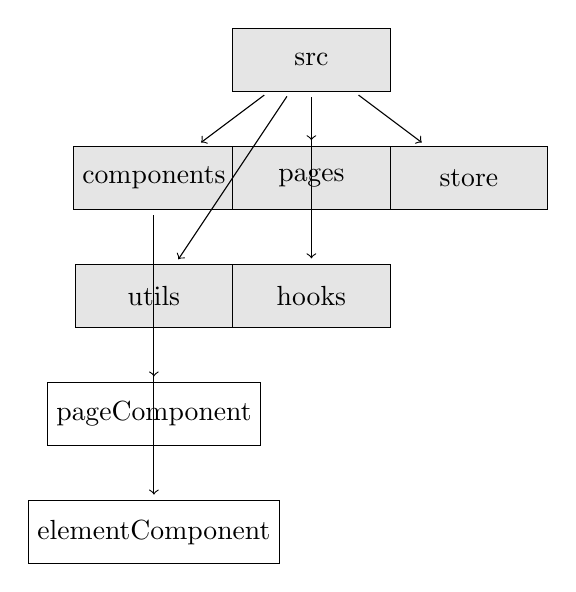
\begin{tikzpicture}[
    file/.style={draw, rectangle, minimum width=2cm, minimum height=0.8cm},
    folder/.style={draw, rectangle, minimum width=2cm, minimum height=0.8cm, fill=gray!20},
    arrow/.style={->, shorten >=2pt, shorten <=2pt}
]

% Folders
\node[folder] (src) at (0,0) {src};
\node[folder] (components) at (-2,-1.5) {components};
\node[folder] (pages) at (0,-1.5) {pages};
\node[folder] (store) at (2,-1.5) {store};
\node[folder] (utils) at (-2,-3) {utils};
\node[folder] (hooks) at (0,-3) {hooks};

% Files
\node[file] (pageComponent) at (-2,-4.5) {pageComponent};
\node[file] (elementComponent) at (-2,-6) {elementComponent};
% ... add more files

% Connections
\draw[arrow] (src) -- (components);
\draw[arrow] (src) -- (pages);
\draw[arrow] (src) -- (store);
\draw[arrow] (src) -- (utils);
\draw[arrow] (src) -- (hooks);
\draw[arrow] (components) -- (pageComponent);
\draw[arrow] (components) -- (elementComponent);
% ... add more connections

\end{tikzpicture}



\pagebreak
\subsubsection{Back-end}
The backend uses the dotNet framework. The development language using the C\# language.

In this project, the backend uses the Onion Architecture.
The Onion Architecture is a typically layered architecture, 
where each layer depends on the inner layer and provides interfaces to the outer layer.
The outer layer provides services to the outermost layer 
and other modules in the same layer based on the interfaces of the inner layer.

From inner to outer, the layers are: Domain, Application, Infrastructure, Presentation.
The Domain layer is the core layer and the innermost layer, used to define domain models, 
which are the business models.
It includes domain models and domain service interfaces.
Domain models are used to define the business models, 
which are the entities in the entity-relationship model and their attributes.
Domain service interfaces are used to define the business services, 
which are the relationships between entities in the entity-relationship model.

The Application layer is the application layer, 
used to define application services, which are the business logic.
It includes domain service implementations and application service interfaces.
Domain service implementations implement the methods of the inner layer's domain service 
interfaces and implement the business logic of the domain models.
Application service interfaces are used to define application services, 
which are the business logic.
It includes but is not limited to database interfaces, testing interfaces, 
HTTP API interfaces, MQTT interfaces, etc.

The Infrastructure layer is the infrastructure layer, used to define infrastructure.
It includes database implementations, testing implementations, 
HTTP API implementations, MQTT implementations, etc.
Database implementations implement the database interfaces 
and provide CRUD services for the database.
Testing implementations implement the testing interfaces 
and provide services for unit testing and integration testing.
HTTP API implementations implement the HTTP API interfaces 
and provide CRUD operations for HTTP APIs.
MQTT implementations implement the MQTT interfaces 
and provide CRUD operations for MQTT.

The Presentation layer is the presentation layer, used to define presentation logic, 
such as interfaces and pages. Since this is a backend project,
data presentation and control are handled by the frontend, 
so this layer is not needed.



\pagebreak
\subsubsection{Data communication and storage}
% 关于本项目的数据通信与数据存储的设计, 包括数据通信的协议, 数据存储的设计等
% 关于数据通信的设计:
% 1. 通信协议的选择
% 自前端向后端发送的数据, 有三种传输的数据类型, 
% 一种是普通的增删改查的请求, 对数据传输的时效性要求不高, 但是对数据的准确性, 完整性, 有序性, 安全性有一定的要求,
% 这种数据的传输, 采用 HTTP 协议, 以及 RESTful API 的设计. 可以有效的保证对数据传输的以上要求.
% 一种是对数据通道的创建和流媒体数据的传输, 对数据传输的时效性, 安全性要求较高, 这种数据的传输, 采用 WebRTC 协议, 以及 MQTT 协议.
% 配合可以快速解码的 flatbuffers 协议, 可以有效的保证对数据传输的以上要求.
% 最后一种是对设备的状态信息和操作信息的传输, 对完整性, 有序性, 安全性都有较高的要求, 这种数据的传输, 采用 MQTT 协议
% 同时也使用了 flatbuffers 协议.
% 
% 2. 数据通信的通信架构和通信流程
% 本项目的数据通信的通信架构, 是基于前后端分离的架构, 前端使用 React 框架, 后端使用 dotnet 框架.
% 当前端需要向后端发送数据的时候, 前端会向后端发送 HTTP 请求, 后端接收到 HTTP 请求之后, 会根据请求的数据类型,
% 选择不同的数据处理方式, 对于普通的增删改查的请求, 后端会根据 RESTful API 的设计, 对数据进行增删改查的操作,
% 对于对数据通道的创建和流媒体数据的传输, 后端会根据 WebRTC 协议, 对数据通道进行创建, 并且帮助前端和设备建立数据通道,
% 当数据通道建立后, 前端和设备之间则使用 flatbuffer 的数据格式对流媒体数据进行传输,
% 对于设备的状态信息和操作信息的传输, 前端会直接向 MQTT broker 发送 MQTT 请求, 
% 设备会在其自身的固件中监听相关的 MQTT 请求, 并且返回相关的数据.
% 
% 3. 数据通信的格式
% 本项目的数据通信的格式, 有三种, 
% 一种是 HTTP 协议, 
% 使用 json 格式对数据进行传输,
% 一种是 WebRTC 协议, 
% 使用 flatbuffers 格式对数据进行传输,
% 一种是 MQTT 协议.
% 使用 flatbuffers 格式对数据进行传输,
% 
% 关于数据存储的设计:
% 1. 数据存储的数据库的选择
% 本项目的数据存储的数据库的选择, 使用了轻量级的数据库 SQLite,
% SQLite 是一个进程内的库, 实现了自给自足的, 无服务器的, 零配置的, 事务性的 SQL 数据库引擎.
% 这是因为整个项目的目的是为了实现前端与设备之间的数据通信, 对于数据库数据的增删改查操作的要求不高,
% 数据量较小, 且对于数据库的数据的事务性要求不高, 所以选择了 SQLite 数据库.
% 2. 项目前后端的数据结构的设计
% 在本项目中, 前端由于使用了 React 框架, 所以前端的数据结构的设计, 使用了基于状态的数据结构的设计,
% 每个组件或者数据集都包含一个状态对象, 这个状态对象的属性就是组件的各个状态. 
% 使用状态对象的原因是, 可以方便的对状态进行管理, 采用对象-属性的形式, 可以方便的针对不同组件的同类状态进行区分,
% 由于跨组件的状态是由 redux 进行管理的, 这种状态对象的设计, 可以更搞笑的对状态进行更新和传递.
% 后端由于使用了 dotnet 框架, 所以后端的数据结构的设计, 使用了基于类的数据结构的设计,
% 采用了面向对象的编程思想, 对数据进行了封装, 使得数据的传输更加的安全, 有序, 完整.


\pagebreak

% \subsection{Domain model}
% \documentclass[]{article}
\usepackage{graphicx}
\usepackage{amsmath}
\usepackage{tikz}

% libaries
\usetikzlibrary{shapes,arrows}

%Define the listing package
\usepackage{listings} %code highlighter
\usepackage{color} %use color
\definecolor{mygreen}{rgb}{0,0.6,0}
\definecolor{mygray}{rgb}{0.5,0.5,0.5}
\definecolor{mymauve}{rgb}{0.58,0,0.82}

%Customize a bit the look
\lstset{ %
backgroundcolor=\color{white}, % choose the background color; you must add \usepackage{color} or \usepackage{xcolor}
basicstyle=\footnotesize, % the size of the fonts that are used for the code
breakatwhitespace=false, % sets if automatic breaks should only happen at whitespace
breaklines=true, % sets automatic line breaking
captionpos=b, % sets the caption-position to bottom
commentstyle=\color{mygreen}, % comment style
deletekeywords={...}, % if you want to delete keywords from the given language
escapeinside={\%*}{*)}, % if you want to add LaTeX within your code
extendedchars=true, % lets you use non-ASCII characters; for 8-bits encodings only, does not work with UTF-8
frame=single, % adds a frame around the code
keepspaces=true, % keeps spaces in text, useful for keeping indentation of code (possibly needs columns=flexible)
keywordstyle=\color{blue}, % keyword style
% language=Octave, % the language of the code
morekeywords={*,...}, % if you want to add more keywords to the set
numbers=left, % where to put the line-numbers; possible values are (none, left, right)
numbersep=5pt, % how far the line-numbers are from the code
numberstyle=\tiny\color{mygray}, % the style that is used for the line-numbers
rulecolor=\color{black}, % if not set, the frame-color may be changed on line-breaks within not-black text (e.g. comments (green here))
showspaces=false, % show spaces everywhere adding particular underscores; it overrides 'showstringspaces'
showstringspaces=false, % underline spaces within strings only
showtabs=false, % show tabs within strings adding particular underscores
stepnumber=1, % the step between two line-numbers. If it's 1, each line will be numbered
stringstyle=\color{mymauve}, % string literal style
tabsize=2, % sets default tabsize to 2 spaces
title=\lstname % show the filename of files included with \lstinputlisting; also try caption instead of title
}

\definecolor{darkgray}{rgb}{.4,.4,.4}
\definecolor{purple}{rgb}{0.65, 0.12, 0.82}

\lstdefinelanguage{React}{
keywords={const, typeof, new, true, false, catch, function, return, null, catch, switch, var, if, in, while, do, else, case, break},
keywordstyle=\color{blue}\bfseries,
ndkeywords={class, export, boolean, throw, implements, import, this},
ndkeywordstyle=\color{darkgray}\bfseries,
identifierstyle=\color{mygreen},
sensitive=false,
comment=[l]{//},
morecomment=[s]{/*}{*/},
commentstyle=\color{purple}\ttfamily,
string=[b]{"}{'}{`},
stringstyle=\color{red}\ttfamily,
morestring=[b]',
morestring=[b]",
morestring=[b]`',
}

\lstdefinelanguage{CSharp}{
keywords={const, typeof, new, true, false, catch, function, return, null, catch, switch, var, if, in, while, do, else, case, break},
keywordstyle=\color{blue}\bfseries,
ndkeywords={class, export, boolean, throw, implements, import, this},
ndkeywordstyle=\color{darkgray}\bfseries,
identifierstyle=\color{mygreen},
sensitive=false,
comment=[l]{//},
morecomment=[s]{/*}{*/},
commentstyle=\color{purple}\ttfamily,
string=[b]{"}{'}{`},
stringstyle=\color{red}\ttfamily,
morestring=[b]',
morestring=[b]",
morestring=[b]`',
}

\lstset{
language=React,
extendedchars=true,
basicstyle=\footnotesize\ttfamily,
showstringspaces=false,
showspaces=false,
numbers=left,
numberstyle=\footnotesize,
numbersep=9pt,
tabsize=2,
breaklines=true,
showtabs=false,
captionpos=b
}

\lstset{
language=CSharp,
extendedchars=true,
basicstyle=\footnotesize\ttfamily,
showstringspaces=false,
showspaces=false,
numbers=left,
numberstyle=\footnotesize,
numbersep=9pt,
tabsize=2,
breaklines=true,
showtabs=false,
captionpos=b
}

% \usepackage{cite} % Add this line for citation

% \bibliographystyle{plain}

\title{
The implementation of BifrostConnect Front-end scope, 
re-design and development with the relevant back-end support develop.
}
\author{
    Fei Gu \\
    Erhvervs Akademi Sydvest \\
    Computer Science 21\\
    }
\date{\today}

\begin{document}

% Front page
\maketitle
\begin{center}
    Supervisor: Henrik Boulund Meng Hansen \\
    Company: BifrostConnect \\
    Engineering Director: Jasper Wass \\
\end{center}
\tableofcontents
\pagebreak


% The introduction
\section{Introduction}
\subsection{Background}\input{sections/introduction/background.tex}
\subsection{The company}\input{sections/introduction/aboutCompany}
\subsection{The project}\input{sections/introduction/aboutProject}
\pagebreak

% The problem statement
\section{Problem Statement}
\subsection{Statement}
\input{sections/problemStatement/statement}
\subsection{Situation}
\input{sections/problemStatement/situation}
\subsection{Potential Solution}
\input{sections/problemStatement/potentialSolution}
\pagebreak

% Requirement analysis
\section{Requirement Analysis}
\input{sections/requirementAnalysis/index}

\subsection{Stakeholders}
\input{sections/requirementAnalysis/stakeholders/index}

\subsection{Business Domain}
\input{sections/requirementAnalysis/bussinesDomain/index}

\subsection{Scope}
\input{sections/requirementAnalysis/scope}

\subsection{Goals}
\input{sections/requirementAnalysis/goals}
\pagebreak

% Software Design
\section{Software Design}
% developement methods
\subsection{Software Development Methods}
\input{sections/softwareDevelopmentMethods/index}
\subsubsection{Agile Software Development}
\input{sections/softwareDevelopmentMethods/agileSoftwareDevelopment/index}
\subsubsection{Feature Driven Development}
\input{sections/softwareDevelopmentMethods/featureDrivenDevelopment/index}

\pagebreak

% Technology seslection
\subsection{Technology selection}
\input{sections/softwareDesign/technologySelection/index}
\subsubsection{Front-end}
\input{sections/softwareDesign/technologySelection/frontEnd}            
\subsubsection{Back-end}
\input{sections/softwareDesign/technologySelection/backEnd}            
\subsubsection{Database}
\input{sections/softwareDesign/technologySelection/database}
\subsubsection{Data communication}
\input{sections/softwareDesign/technologySelection/dataCommunication}            
\subsubsection{DevOps}
\input{sections/softwareDesign/technologySelection/devOps}
\pagebreak

% Architecture design
\subsection{Architecture design}
\input{sections/softwareDesign/architectureDesign/index}
\pagebreak
\subsubsection{Front-end}
\input{sections/softwareDesign/architectureDesign/frontEndArchitecture}
\pagebreak
\subsubsection{Back-end}
\input{sections/softwareDesign/architectureDesign/backEndArchitecture}
\pagebreak
\subsubsection{Data communication and storage}
\input{sections/softwareDesign/architectureDesign/dataCommunicationArchitecture}
\pagebreak

% \subsection{Domain model}
% \input{sections/softwareDesign/domainModel/index}
% \subsection{Database design}
% % 数据库领域模型 ER 图
% % 包括表和字段的设置.
% % 对于私有键和外键的设置.

% \subsection{Back-end design}
% % 后端对象模型
% % 以及对于对象模型的增删改查
% % 以及相关的其他服务的设计`'

% \subsection{Front-end design}
% % 对于前端的页面结构的设计 
% % 页面的状态的设计, 交互设计

% \subsection{FlatBuffers design}
% % schema 的设计

\subsection{DevOps CI/CD process design}
\input{sections/softwareDesign/devOpsDesign/index}
\subsubsection{Continuous Integration}
\input{sections/softwareDesign/devOpsDesign/continuousIntegration/index}
\subsubsection{Continuous Delivery}
\input{sections/softwareDesign/devOpsDesign/continuousDelivery/index}
\subsubsection{Continuous Deployment}
\input{sections/softwareDesign/devOpsDesign/continuousDeployment/index}
\pagebreak

\section{Software Development} 
\input{sections/softwareDevelopment/index}
\subsection{Overall development}
\input{sections/softwareDevelopment/overallDevelopement/index}
\subsubsection{Front-end}
\input{sections/softwareDevelopment/overallDevelopement/frontEnd/index}
\subsubsection{Back-end}
\input{sections/softwareDevelopment/overallDevelopement/backEnd/index}
\subsubsection{DevOps}
\input{sections/softwareDevelopment/overallDevelopement/devOps/index}
\subsection{Feature development} 
\input{sections/softwareDevelopment/featureDevelopment/index}
\subsubsection{Use Case 1}
\input{sections/softwareDevelopment/featureDevelopment/useCase1/index}
\subsubsection{Feature 1}
\input{sections/softwareDevelopment/featureDevelopment/feature/feature1.tex}
\pagebreak
\section{Conclusion} 
\subsection{Result}
Since the project is still in progress, the result is not available yet.
So far, basic structure of this project has been built. But the most features 
are not implemented yet. 
\subsection{Discussion}
As a single developer for this project, I am confident what I have done so far.
And I can say I understand the most of the knowledge I have used in this project, 
which also means I can explain all the part of the project. 
But this project also relevant some of the complex knowledge which I have to continue 
to study and practice.
\subsection{Future Work}
The future work is to implement the rest of the features. 
Including the most important part which is the 'create session' feature.
\pagebreak
% \bibliography{bibliography}
\pagebreak
% \begin{appendices}
%     \section{Appendix}
% \end{appendices} 
\end{document}
% \subsection{Database design}
% % 数据库领域模型 ER 图
% % 包括表和字段的设置.
% % 对于私有键和外键的设置.

% \subsection{Back-end design}
% % 后端对象模型
% % 以及对于对象模型的增删改查
% % 以及相关的其他服务的设计`'

% \subsection{Front-end design}
% % 对于前端的页面结构的设计 
% % 页面的状态的设计, 交互设计

% \subsection{FlatBuffers design}
% % schema 的设计

\subsection{DevOps CI/CD process design}
\documentclass[]{article}
\usepackage{graphicx}
\usepackage{amsmath}
\usepackage{tikz}

% libaries
\usetikzlibrary{shapes,arrows}

%Define the listing package
\usepackage{listings} %code highlighter
\usepackage{color} %use color
\definecolor{mygreen}{rgb}{0,0.6,0}
\definecolor{mygray}{rgb}{0.5,0.5,0.5}
\definecolor{mymauve}{rgb}{0.58,0,0.82}

%Customize a bit the look
\lstset{ %
backgroundcolor=\color{white}, % choose the background color; you must add \usepackage{color} or \usepackage{xcolor}
basicstyle=\footnotesize, % the size of the fonts that are used for the code
breakatwhitespace=false, % sets if automatic breaks should only happen at whitespace
breaklines=true, % sets automatic line breaking
captionpos=b, % sets the caption-position to bottom
commentstyle=\color{mygreen}, % comment style
deletekeywords={...}, % if you want to delete keywords from the given language
escapeinside={\%*}{*)}, % if you want to add LaTeX within your code
extendedchars=true, % lets you use non-ASCII characters; for 8-bits encodings only, does not work with UTF-8
frame=single, % adds a frame around the code
keepspaces=true, % keeps spaces in text, useful for keeping indentation of code (possibly needs columns=flexible)
keywordstyle=\color{blue}, % keyword style
% language=Octave, % the language of the code
morekeywords={*,...}, % if you want to add more keywords to the set
numbers=left, % where to put the line-numbers; possible values are (none, left, right)
numbersep=5pt, % how far the line-numbers are from the code
numberstyle=\tiny\color{mygray}, % the style that is used for the line-numbers
rulecolor=\color{black}, % if not set, the frame-color may be changed on line-breaks within not-black text (e.g. comments (green here))
showspaces=false, % show spaces everywhere adding particular underscores; it overrides 'showstringspaces'
showstringspaces=false, % underline spaces within strings only
showtabs=false, % show tabs within strings adding particular underscores
stepnumber=1, % the step between two line-numbers. If it's 1, each line will be numbered
stringstyle=\color{mymauve}, % string literal style
tabsize=2, % sets default tabsize to 2 spaces
title=\lstname % show the filename of files included with \lstinputlisting; also try caption instead of title
}

\definecolor{darkgray}{rgb}{.4,.4,.4}
\definecolor{purple}{rgb}{0.65, 0.12, 0.82}

\lstdefinelanguage{React}{
keywords={const, typeof, new, true, false, catch, function, return, null, catch, switch, var, if, in, while, do, else, case, break},
keywordstyle=\color{blue}\bfseries,
ndkeywords={class, export, boolean, throw, implements, import, this},
ndkeywordstyle=\color{darkgray}\bfseries,
identifierstyle=\color{mygreen},
sensitive=false,
comment=[l]{//},
morecomment=[s]{/*}{*/},
commentstyle=\color{purple}\ttfamily,
string=[b]{"}{'}{`},
stringstyle=\color{red}\ttfamily,
morestring=[b]',
morestring=[b]",
morestring=[b]`',
}

\lstdefinelanguage{CSharp}{
keywords={const, typeof, new, true, false, catch, function, return, null, catch, switch, var, if, in, while, do, else, case, break},
keywordstyle=\color{blue}\bfseries,
ndkeywords={class, export, boolean, throw, implements, import, this},
ndkeywordstyle=\color{darkgray}\bfseries,
identifierstyle=\color{mygreen},
sensitive=false,
comment=[l]{//},
morecomment=[s]{/*}{*/},
commentstyle=\color{purple}\ttfamily,
string=[b]{"}{'}{`},
stringstyle=\color{red}\ttfamily,
morestring=[b]',
morestring=[b]",
morestring=[b]`',
}

\lstset{
language=React,
extendedchars=true,
basicstyle=\footnotesize\ttfamily,
showstringspaces=false,
showspaces=false,
numbers=left,
numberstyle=\footnotesize,
numbersep=9pt,
tabsize=2,
breaklines=true,
showtabs=false,
captionpos=b
}

\lstset{
language=CSharp,
extendedchars=true,
basicstyle=\footnotesize\ttfamily,
showstringspaces=false,
showspaces=false,
numbers=left,
numberstyle=\footnotesize,
numbersep=9pt,
tabsize=2,
breaklines=true,
showtabs=false,
captionpos=b
}

% \usepackage{cite} % Add this line for citation

% \bibliographystyle{plain}

\title{
The implementation of BifrostConnect Front-end scope, 
re-design and development with the relevant back-end support develop.
}
\author{
    Fei Gu \\
    Erhvervs Akademi Sydvest \\
    Computer Science 21\\
    }
\date{\today}

\begin{document}

% Front page
\maketitle
\begin{center}
    Supervisor: Henrik Boulund Meng Hansen \\
    Company: BifrostConnect \\
    Engineering Director: Jasper Wass \\
\end{center}
\tableofcontents
\pagebreak


% The introduction
\section{Introduction}
\subsection{Background}\input{sections/introduction/background.tex}
\subsection{The company}\input{sections/introduction/aboutCompany}
\subsection{The project}\input{sections/introduction/aboutProject}
\pagebreak

% The problem statement
\section{Problem Statement}
\subsection{Statement}
\input{sections/problemStatement/statement}
\subsection{Situation}
\input{sections/problemStatement/situation}
\subsection{Potential Solution}
\input{sections/problemStatement/potentialSolution}
\pagebreak

% Requirement analysis
\section{Requirement Analysis}
\input{sections/requirementAnalysis/index}

\subsection{Stakeholders}
\input{sections/requirementAnalysis/stakeholders/index}

\subsection{Business Domain}
\input{sections/requirementAnalysis/bussinesDomain/index}

\subsection{Scope}
\input{sections/requirementAnalysis/scope}

\subsection{Goals}
\input{sections/requirementAnalysis/goals}
\pagebreak

% Software Design
\section{Software Design}
% developement methods
\subsection{Software Development Methods}
\input{sections/softwareDevelopmentMethods/index}
\subsubsection{Agile Software Development}
\input{sections/softwareDevelopmentMethods/agileSoftwareDevelopment/index}
\subsubsection{Feature Driven Development}
\input{sections/softwareDevelopmentMethods/featureDrivenDevelopment/index}

\pagebreak

% Technology seslection
\subsection{Technology selection}
\input{sections/softwareDesign/technologySelection/index}
\subsubsection{Front-end}
\input{sections/softwareDesign/technologySelection/frontEnd}            
\subsubsection{Back-end}
\input{sections/softwareDesign/technologySelection/backEnd}            
\subsubsection{Database}
\input{sections/softwareDesign/technologySelection/database}
\subsubsection{Data communication}
\input{sections/softwareDesign/technologySelection/dataCommunication}            
\subsubsection{DevOps}
\input{sections/softwareDesign/technologySelection/devOps}
\pagebreak

% Architecture design
\subsection{Architecture design}
\input{sections/softwareDesign/architectureDesign/index}
\pagebreak
\subsubsection{Front-end}
\input{sections/softwareDesign/architectureDesign/frontEndArchitecture}
\pagebreak
\subsubsection{Back-end}
\input{sections/softwareDesign/architectureDesign/backEndArchitecture}
\pagebreak
\subsubsection{Data communication and storage}
\input{sections/softwareDesign/architectureDesign/dataCommunicationArchitecture}
\pagebreak

% \subsection{Domain model}
% \input{sections/softwareDesign/domainModel/index}
% \subsection{Database design}
% % 数据库领域模型 ER 图
% % 包括表和字段的设置.
% % 对于私有键和外键的设置.

% \subsection{Back-end design}
% % 后端对象模型
% % 以及对于对象模型的增删改查
% % 以及相关的其他服务的设计`'

% \subsection{Front-end design}
% % 对于前端的页面结构的设计 
% % 页面的状态的设计, 交互设计

% \subsection{FlatBuffers design}
% % schema 的设计

\subsection{DevOps CI/CD process design}
\input{sections/softwareDesign/devOpsDesign/index}
\subsubsection{Continuous Integration}
\input{sections/softwareDesign/devOpsDesign/continuousIntegration/index}
\subsubsection{Continuous Delivery}
\input{sections/softwareDesign/devOpsDesign/continuousDelivery/index}
\subsubsection{Continuous Deployment}
\input{sections/softwareDesign/devOpsDesign/continuousDeployment/index}
\pagebreak

\section{Software Development} 
\input{sections/softwareDevelopment/index}
\subsection{Overall development}
\input{sections/softwareDevelopment/overallDevelopement/index}
\subsubsection{Front-end}
\input{sections/softwareDevelopment/overallDevelopement/frontEnd/index}
\subsubsection{Back-end}
\input{sections/softwareDevelopment/overallDevelopement/backEnd/index}
\subsubsection{DevOps}
\input{sections/softwareDevelopment/overallDevelopement/devOps/index}
\subsection{Feature development} 
\input{sections/softwareDevelopment/featureDevelopment/index}
\subsubsection{Use Case 1}
\input{sections/softwareDevelopment/featureDevelopment/useCase1/index}
\subsubsection{Feature 1}
\input{sections/softwareDevelopment/featureDevelopment/feature/feature1.tex}
\pagebreak
\section{Conclusion} 
\subsection{Result}
Since the project is still in progress, the result is not available yet.
So far, basic structure of this project has been built. But the most features 
are not implemented yet. 
\subsection{Discussion}
As a single developer for this project, I am confident what I have done so far.
And I can say I understand the most of the knowledge I have used in this project, 
which also means I can explain all the part of the project. 
But this project also relevant some of the complex knowledge which I have to continue 
to study and practice.
\subsection{Future Work}
The future work is to implement the rest of the features. 
Including the most important part which is the 'create session' feature.
\pagebreak
% \bibliography{bibliography}
\pagebreak
% \begin{appendices}
%     \section{Appendix}
% \end{appendices} 
\end{document}
\subsubsection{Continuous Integration}
\documentclass[]{article}
\usepackage{graphicx}
\usepackage{amsmath}
\usepackage{tikz}

% libaries
\usetikzlibrary{shapes,arrows}

%Define the listing package
\usepackage{listings} %code highlighter
\usepackage{color} %use color
\definecolor{mygreen}{rgb}{0,0.6,0}
\definecolor{mygray}{rgb}{0.5,0.5,0.5}
\definecolor{mymauve}{rgb}{0.58,0,0.82}

%Customize a bit the look
\lstset{ %
backgroundcolor=\color{white}, % choose the background color; you must add \usepackage{color} or \usepackage{xcolor}
basicstyle=\footnotesize, % the size of the fonts that are used for the code
breakatwhitespace=false, % sets if automatic breaks should only happen at whitespace
breaklines=true, % sets automatic line breaking
captionpos=b, % sets the caption-position to bottom
commentstyle=\color{mygreen}, % comment style
deletekeywords={...}, % if you want to delete keywords from the given language
escapeinside={\%*}{*)}, % if you want to add LaTeX within your code
extendedchars=true, % lets you use non-ASCII characters; for 8-bits encodings only, does not work with UTF-8
frame=single, % adds a frame around the code
keepspaces=true, % keeps spaces in text, useful for keeping indentation of code (possibly needs columns=flexible)
keywordstyle=\color{blue}, % keyword style
% language=Octave, % the language of the code
morekeywords={*,...}, % if you want to add more keywords to the set
numbers=left, % where to put the line-numbers; possible values are (none, left, right)
numbersep=5pt, % how far the line-numbers are from the code
numberstyle=\tiny\color{mygray}, % the style that is used for the line-numbers
rulecolor=\color{black}, % if not set, the frame-color may be changed on line-breaks within not-black text (e.g. comments (green here))
showspaces=false, % show spaces everywhere adding particular underscores; it overrides 'showstringspaces'
showstringspaces=false, % underline spaces within strings only
showtabs=false, % show tabs within strings adding particular underscores
stepnumber=1, % the step between two line-numbers. If it's 1, each line will be numbered
stringstyle=\color{mymauve}, % string literal style
tabsize=2, % sets default tabsize to 2 spaces
title=\lstname % show the filename of files included with \lstinputlisting; also try caption instead of title
}

\definecolor{darkgray}{rgb}{.4,.4,.4}
\definecolor{purple}{rgb}{0.65, 0.12, 0.82}

\lstdefinelanguage{React}{
keywords={const, typeof, new, true, false, catch, function, return, null, catch, switch, var, if, in, while, do, else, case, break},
keywordstyle=\color{blue}\bfseries,
ndkeywords={class, export, boolean, throw, implements, import, this},
ndkeywordstyle=\color{darkgray}\bfseries,
identifierstyle=\color{mygreen},
sensitive=false,
comment=[l]{//},
morecomment=[s]{/*}{*/},
commentstyle=\color{purple}\ttfamily,
string=[b]{"}{'}{`},
stringstyle=\color{red}\ttfamily,
morestring=[b]',
morestring=[b]",
morestring=[b]`',
}

\lstdefinelanguage{CSharp}{
keywords={const, typeof, new, true, false, catch, function, return, null, catch, switch, var, if, in, while, do, else, case, break},
keywordstyle=\color{blue}\bfseries,
ndkeywords={class, export, boolean, throw, implements, import, this},
ndkeywordstyle=\color{darkgray}\bfseries,
identifierstyle=\color{mygreen},
sensitive=false,
comment=[l]{//},
morecomment=[s]{/*}{*/},
commentstyle=\color{purple}\ttfamily,
string=[b]{"}{'}{`},
stringstyle=\color{red}\ttfamily,
morestring=[b]',
morestring=[b]",
morestring=[b]`',
}

\lstset{
language=React,
extendedchars=true,
basicstyle=\footnotesize\ttfamily,
showstringspaces=false,
showspaces=false,
numbers=left,
numberstyle=\footnotesize,
numbersep=9pt,
tabsize=2,
breaklines=true,
showtabs=false,
captionpos=b
}

\lstset{
language=CSharp,
extendedchars=true,
basicstyle=\footnotesize\ttfamily,
showstringspaces=false,
showspaces=false,
numbers=left,
numberstyle=\footnotesize,
numbersep=9pt,
tabsize=2,
breaklines=true,
showtabs=false,
captionpos=b
}

% \usepackage{cite} % Add this line for citation

% \bibliographystyle{plain}

\title{
The implementation of BifrostConnect Front-end scope, 
re-design and development with the relevant back-end support develop.
}
\author{
    Fei Gu \\
    Erhvervs Akademi Sydvest \\
    Computer Science 21\\
    }
\date{\today}

\begin{document}

% Front page
\maketitle
\begin{center}
    Supervisor: Henrik Boulund Meng Hansen \\
    Company: BifrostConnect \\
    Engineering Director: Jasper Wass \\
\end{center}
\tableofcontents
\pagebreak


% The introduction
\section{Introduction}
\subsection{Background}\input{sections/introduction/background.tex}
\subsection{The company}\input{sections/introduction/aboutCompany}
\subsection{The project}\input{sections/introduction/aboutProject}
\pagebreak

% The problem statement
\section{Problem Statement}
\subsection{Statement}
\input{sections/problemStatement/statement}
\subsection{Situation}
\input{sections/problemStatement/situation}
\subsection{Potential Solution}
\input{sections/problemStatement/potentialSolution}
\pagebreak

% Requirement analysis
\section{Requirement Analysis}
\input{sections/requirementAnalysis/index}

\subsection{Stakeholders}
\input{sections/requirementAnalysis/stakeholders/index}

\subsection{Business Domain}
\input{sections/requirementAnalysis/bussinesDomain/index}

\subsection{Scope}
\input{sections/requirementAnalysis/scope}

\subsection{Goals}
\input{sections/requirementAnalysis/goals}
\pagebreak

% Software Design
\section{Software Design}
% developement methods
\subsection{Software Development Methods}
\input{sections/softwareDevelopmentMethods/index}
\subsubsection{Agile Software Development}
\input{sections/softwareDevelopmentMethods/agileSoftwareDevelopment/index}
\subsubsection{Feature Driven Development}
\input{sections/softwareDevelopmentMethods/featureDrivenDevelopment/index}

\pagebreak

% Technology seslection
\subsection{Technology selection}
\input{sections/softwareDesign/technologySelection/index}
\subsubsection{Front-end}
\input{sections/softwareDesign/technologySelection/frontEnd}            
\subsubsection{Back-end}
\input{sections/softwareDesign/technologySelection/backEnd}            
\subsubsection{Database}
\input{sections/softwareDesign/technologySelection/database}
\subsubsection{Data communication}
\input{sections/softwareDesign/technologySelection/dataCommunication}            
\subsubsection{DevOps}
\input{sections/softwareDesign/technologySelection/devOps}
\pagebreak

% Architecture design
\subsection{Architecture design}
\input{sections/softwareDesign/architectureDesign/index}
\pagebreak
\subsubsection{Front-end}
\input{sections/softwareDesign/architectureDesign/frontEndArchitecture}
\pagebreak
\subsubsection{Back-end}
\input{sections/softwareDesign/architectureDesign/backEndArchitecture}
\pagebreak
\subsubsection{Data communication and storage}
\input{sections/softwareDesign/architectureDesign/dataCommunicationArchitecture}
\pagebreak

% \subsection{Domain model}
% \input{sections/softwareDesign/domainModel/index}
% \subsection{Database design}
% % 数据库领域模型 ER 图
% % 包括表和字段的设置.
% % 对于私有键和外键的设置.

% \subsection{Back-end design}
% % 后端对象模型
% % 以及对于对象模型的增删改查
% % 以及相关的其他服务的设计`'

% \subsection{Front-end design}
% % 对于前端的页面结构的设计 
% % 页面的状态的设计, 交互设计

% \subsection{FlatBuffers design}
% % schema 的设计

\subsection{DevOps CI/CD process design}
\input{sections/softwareDesign/devOpsDesign/index}
\subsubsection{Continuous Integration}
\input{sections/softwareDesign/devOpsDesign/continuousIntegration/index}
\subsubsection{Continuous Delivery}
\input{sections/softwareDesign/devOpsDesign/continuousDelivery/index}
\subsubsection{Continuous Deployment}
\input{sections/softwareDesign/devOpsDesign/continuousDeployment/index}
\pagebreak

\section{Software Development} 
\input{sections/softwareDevelopment/index}
\subsection{Overall development}
\input{sections/softwareDevelopment/overallDevelopement/index}
\subsubsection{Front-end}
\input{sections/softwareDevelopment/overallDevelopement/frontEnd/index}
\subsubsection{Back-end}
\input{sections/softwareDevelopment/overallDevelopement/backEnd/index}
\subsubsection{DevOps}
\input{sections/softwareDevelopment/overallDevelopement/devOps/index}
\subsection{Feature development} 
\input{sections/softwareDevelopment/featureDevelopment/index}
\subsubsection{Use Case 1}
\input{sections/softwareDevelopment/featureDevelopment/useCase1/index}
\subsubsection{Feature 1}
\input{sections/softwareDevelopment/featureDevelopment/feature/feature1.tex}
\pagebreak
\section{Conclusion} 
\subsection{Result}
Since the project is still in progress, the result is not available yet.
So far, basic structure of this project has been built. But the most features 
are not implemented yet. 
\subsection{Discussion}
As a single developer for this project, I am confident what I have done so far.
And I can say I understand the most of the knowledge I have used in this project, 
which also means I can explain all the part of the project. 
But this project also relevant some of the complex knowledge which I have to continue 
to study and practice.
\subsection{Future Work}
The future work is to implement the rest of the features. 
Including the most important part which is the 'create session' feature.
\pagebreak
% \bibliography{bibliography}
\pagebreak
% \begin{appendices}
%     \section{Appendix}
% \end{appendices} 
\end{document}
\subsubsection{Continuous Delivery}
\documentclass[]{article}
\usepackage{graphicx}
\usepackage{amsmath}
\usepackage{tikz}

% libaries
\usetikzlibrary{shapes,arrows}

%Define the listing package
\usepackage{listings} %code highlighter
\usepackage{color} %use color
\definecolor{mygreen}{rgb}{0,0.6,0}
\definecolor{mygray}{rgb}{0.5,0.5,0.5}
\definecolor{mymauve}{rgb}{0.58,0,0.82}

%Customize a bit the look
\lstset{ %
backgroundcolor=\color{white}, % choose the background color; you must add \usepackage{color} or \usepackage{xcolor}
basicstyle=\footnotesize, % the size of the fonts that are used for the code
breakatwhitespace=false, % sets if automatic breaks should only happen at whitespace
breaklines=true, % sets automatic line breaking
captionpos=b, % sets the caption-position to bottom
commentstyle=\color{mygreen}, % comment style
deletekeywords={...}, % if you want to delete keywords from the given language
escapeinside={\%*}{*)}, % if you want to add LaTeX within your code
extendedchars=true, % lets you use non-ASCII characters; for 8-bits encodings only, does not work with UTF-8
frame=single, % adds a frame around the code
keepspaces=true, % keeps spaces in text, useful for keeping indentation of code (possibly needs columns=flexible)
keywordstyle=\color{blue}, % keyword style
% language=Octave, % the language of the code
morekeywords={*,...}, % if you want to add more keywords to the set
numbers=left, % where to put the line-numbers; possible values are (none, left, right)
numbersep=5pt, % how far the line-numbers are from the code
numberstyle=\tiny\color{mygray}, % the style that is used for the line-numbers
rulecolor=\color{black}, % if not set, the frame-color may be changed on line-breaks within not-black text (e.g. comments (green here))
showspaces=false, % show spaces everywhere adding particular underscores; it overrides 'showstringspaces'
showstringspaces=false, % underline spaces within strings only
showtabs=false, % show tabs within strings adding particular underscores
stepnumber=1, % the step between two line-numbers. If it's 1, each line will be numbered
stringstyle=\color{mymauve}, % string literal style
tabsize=2, % sets default tabsize to 2 spaces
title=\lstname % show the filename of files included with \lstinputlisting; also try caption instead of title
}

\definecolor{darkgray}{rgb}{.4,.4,.4}
\definecolor{purple}{rgb}{0.65, 0.12, 0.82}

\lstdefinelanguage{React}{
keywords={const, typeof, new, true, false, catch, function, return, null, catch, switch, var, if, in, while, do, else, case, break},
keywordstyle=\color{blue}\bfseries,
ndkeywords={class, export, boolean, throw, implements, import, this},
ndkeywordstyle=\color{darkgray}\bfseries,
identifierstyle=\color{mygreen},
sensitive=false,
comment=[l]{//},
morecomment=[s]{/*}{*/},
commentstyle=\color{purple}\ttfamily,
string=[b]{"}{'}{`},
stringstyle=\color{red}\ttfamily,
morestring=[b]',
morestring=[b]",
morestring=[b]`',
}

\lstdefinelanguage{CSharp}{
keywords={const, typeof, new, true, false, catch, function, return, null, catch, switch, var, if, in, while, do, else, case, break},
keywordstyle=\color{blue}\bfseries,
ndkeywords={class, export, boolean, throw, implements, import, this},
ndkeywordstyle=\color{darkgray}\bfseries,
identifierstyle=\color{mygreen},
sensitive=false,
comment=[l]{//},
morecomment=[s]{/*}{*/},
commentstyle=\color{purple}\ttfamily,
string=[b]{"}{'}{`},
stringstyle=\color{red}\ttfamily,
morestring=[b]',
morestring=[b]",
morestring=[b]`',
}

\lstset{
language=React,
extendedchars=true,
basicstyle=\footnotesize\ttfamily,
showstringspaces=false,
showspaces=false,
numbers=left,
numberstyle=\footnotesize,
numbersep=9pt,
tabsize=2,
breaklines=true,
showtabs=false,
captionpos=b
}

\lstset{
language=CSharp,
extendedchars=true,
basicstyle=\footnotesize\ttfamily,
showstringspaces=false,
showspaces=false,
numbers=left,
numberstyle=\footnotesize,
numbersep=9pt,
tabsize=2,
breaklines=true,
showtabs=false,
captionpos=b
}

% \usepackage{cite} % Add this line for citation

% \bibliographystyle{plain}

\title{
The implementation of BifrostConnect Front-end scope, 
re-design and development with the relevant back-end support develop.
}
\author{
    Fei Gu \\
    Erhvervs Akademi Sydvest \\
    Computer Science 21\\
    }
\date{\today}

\begin{document}

% Front page
\maketitle
\begin{center}
    Supervisor: Henrik Boulund Meng Hansen \\
    Company: BifrostConnect \\
    Engineering Director: Jasper Wass \\
\end{center}
\tableofcontents
\pagebreak


% The introduction
\section{Introduction}
\subsection{Background}\input{sections/introduction/background.tex}
\subsection{The company}\input{sections/introduction/aboutCompany}
\subsection{The project}\input{sections/introduction/aboutProject}
\pagebreak

% The problem statement
\section{Problem Statement}
\subsection{Statement}
\input{sections/problemStatement/statement}
\subsection{Situation}
\input{sections/problemStatement/situation}
\subsection{Potential Solution}
\input{sections/problemStatement/potentialSolution}
\pagebreak

% Requirement analysis
\section{Requirement Analysis}
\input{sections/requirementAnalysis/index}

\subsection{Stakeholders}
\input{sections/requirementAnalysis/stakeholders/index}

\subsection{Business Domain}
\input{sections/requirementAnalysis/bussinesDomain/index}

\subsection{Scope}
\input{sections/requirementAnalysis/scope}

\subsection{Goals}
\input{sections/requirementAnalysis/goals}
\pagebreak

% Software Design
\section{Software Design}
% developement methods
\subsection{Software Development Methods}
\input{sections/softwareDevelopmentMethods/index}
\subsubsection{Agile Software Development}
\input{sections/softwareDevelopmentMethods/agileSoftwareDevelopment/index}
\subsubsection{Feature Driven Development}
\input{sections/softwareDevelopmentMethods/featureDrivenDevelopment/index}

\pagebreak

% Technology seslection
\subsection{Technology selection}
\input{sections/softwareDesign/technologySelection/index}
\subsubsection{Front-end}
\input{sections/softwareDesign/technologySelection/frontEnd}            
\subsubsection{Back-end}
\input{sections/softwareDesign/technologySelection/backEnd}            
\subsubsection{Database}
\input{sections/softwareDesign/technologySelection/database}
\subsubsection{Data communication}
\input{sections/softwareDesign/technologySelection/dataCommunication}            
\subsubsection{DevOps}
\input{sections/softwareDesign/technologySelection/devOps}
\pagebreak

% Architecture design
\subsection{Architecture design}
\input{sections/softwareDesign/architectureDesign/index}
\pagebreak
\subsubsection{Front-end}
\input{sections/softwareDesign/architectureDesign/frontEndArchitecture}
\pagebreak
\subsubsection{Back-end}
\input{sections/softwareDesign/architectureDesign/backEndArchitecture}
\pagebreak
\subsubsection{Data communication and storage}
\input{sections/softwareDesign/architectureDesign/dataCommunicationArchitecture}
\pagebreak

% \subsection{Domain model}
% \input{sections/softwareDesign/domainModel/index}
% \subsection{Database design}
% % 数据库领域模型 ER 图
% % 包括表和字段的设置.
% % 对于私有键和外键的设置.

% \subsection{Back-end design}
% % 后端对象模型
% % 以及对于对象模型的增删改查
% % 以及相关的其他服务的设计`'

% \subsection{Front-end design}
% % 对于前端的页面结构的设计 
% % 页面的状态的设计, 交互设计

% \subsection{FlatBuffers design}
% % schema 的设计

\subsection{DevOps CI/CD process design}
\input{sections/softwareDesign/devOpsDesign/index}
\subsubsection{Continuous Integration}
\input{sections/softwareDesign/devOpsDesign/continuousIntegration/index}
\subsubsection{Continuous Delivery}
\input{sections/softwareDesign/devOpsDesign/continuousDelivery/index}
\subsubsection{Continuous Deployment}
\input{sections/softwareDesign/devOpsDesign/continuousDeployment/index}
\pagebreak

\section{Software Development} 
\input{sections/softwareDevelopment/index}
\subsection{Overall development}
\input{sections/softwareDevelopment/overallDevelopement/index}
\subsubsection{Front-end}
\input{sections/softwareDevelopment/overallDevelopement/frontEnd/index}
\subsubsection{Back-end}
\input{sections/softwareDevelopment/overallDevelopement/backEnd/index}
\subsubsection{DevOps}
\input{sections/softwareDevelopment/overallDevelopement/devOps/index}
\subsection{Feature development} 
\input{sections/softwareDevelopment/featureDevelopment/index}
\subsubsection{Use Case 1}
\input{sections/softwareDevelopment/featureDevelopment/useCase1/index}
\subsubsection{Feature 1}
\input{sections/softwareDevelopment/featureDevelopment/feature/feature1.tex}
\pagebreak
\section{Conclusion} 
\subsection{Result}
Since the project is still in progress, the result is not available yet.
So far, basic structure of this project has been built. But the most features 
are not implemented yet. 
\subsection{Discussion}
As a single developer for this project, I am confident what I have done so far.
And I can say I understand the most of the knowledge I have used in this project, 
which also means I can explain all the part of the project. 
But this project also relevant some of the complex knowledge which I have to continue 
to study and practice.
\subsection{Future Work}
The future work is to implement the rest of the features. 
Including the most important part which is the 'create session' feature.
\pagebreak
% \bibliography{bibliography}
\pagebreak
% \begin{appendices}
%     \section{Appendix}
% \end{appendices} 
\end{document}
\subsubsection{Continuous Deployment}
\documentclass[]{article}
\usepackage{graphicx}
\usepackage{amsmath}
\usepackage{tikz}

% libaries
\usetikzlibrary{shapes,arrows}

%Define the listing package
\usepackage{listings} %code highlighter
\usepackage{color} %use color
\definecolor{mygreen}{rgb}{0,0.6,0}
\definecolor{mygray}{rgb}{0.5,0.5,0.5}
\definecolor{mymauve}{rgb}{0.58,0,0.82}

%Customize a bit the look
\lstset{ %
backgroundcolor=\color{white}, % choose the background color; you must add \usepackage{color} or \usepackage{xcolor}
basicstyle=\footnotesize, % the size of the fonts that are used for the code
breakatwhitespace=false, % sets if automatic breaks should only happen at whitespace
breaklines=true, % sets automatic line breaking
captionpos=b, % sets the caption-position to bottom
commentstyle=\color{mygreen}, % comment style
deletekeywords={...}, % if you want to delete keywords from the given language
escapeinside={\%*}{*)}, % if you want to add LaTeX within your code
extendedchars=true, % lets you use non-ASCII characters; for 8-bits encodings only, does not work with UTF-8
frame=single, % adds a frame around the code
keepspaces=true, % keeps spaces in text, useful for keeping indentation of code (possibly needs columns=flexible)
keywordstyle=\color{blue}, % keyword style
% language=Octave, % the language of the code
morekeywords={*,...}, % if you want to add more keywords to the set
numbers=left, % where to put the line-numbers; possible values are (none, left, right)
numbersep=5pt, % how far the line-numbers are from the code
numberstyle=\tiny\color{mygray}, % the style that is used for the line-numbers
rulecolor=\color{black}, % if not set, the frame-color may be changed on line-breaks within not-black text (e.g. comments (green here))
showspaces=false, % show spaces everywhere adding particular underscores; it overrides 'showstringspaces'
showstringspaces=false, % underline spaces within strings only
showtabs=false, % show tabs within strings adding particular underscores
stepnumber=1, % the step between two line-numbers. If it's 1, each line will be numbered
stringstyle=\color{mymauve}, % string literal style
tabsize=2, % sets default tabsize to 2 spaces
title=\lstname % show the filename of files included with \lstinputlisting; also try caption instead of title
}

\definecolor{darkgray}{rgb}{.4,.4,.4}
\definecolor{purple}{rgb}{0.65, 0.12, 0.82}

\lstdefinelanguage{React}{
keywords={const, typeof, new, true, false, catch, function, return, null, catch, switch, var, if, in, while, do, else, case, break},
keywordstyle=\color{blue}\bfseries,
ndkeywords={class, export, boolean, throw, implements, import, this},
ndkeywordstyle=\color{darkgray}\bfseries,
identifierstyle=\color{mygreen},
sensitive=false,
comment=[l]{//},
morecomment=[s]{/*}{*/},
commentstyle=\color{purple}\ttfamily,
string=[b]{"}{'}{`},
stringstyle=\color{red}\ttfamily,
morestring=[b]',
morestring=[b]",
morestring=[b]`',
}

\lstdefinelanguage{CSharp}{
keywords={const, typeof, new, true, false, catch, function, return, null, catch, switch, var, if, in, while, do, else, case, break},
keywordstyle=\color{blue}\bfseries,
ndkeywords={class, export, boolean, throw, implements, import, this},
ndkeywordstyle=\color{darkgray}\bfseries,
identifierstyle=\color{mygreen},
sensitive=false,
comment=[l]{//},
morecomment=[s]{/*}{*/},
commentstyle=\color{purple}\ttfamily,
string=[b]{"}{'}{`},
stringstyle=\color{red}\ttfamily,
morestring=[b]',
morestring=[b]",
morestring=[b]`',
}

\lstset{
language=React,
extendedchars=true,
basicstyle=\footnotesize\ttfamily,
showstringspaces=false,
showspaces=false,
numbers=left,
numberstyle=\footnotesize,
numbersep=9pt,
tabsize=2,
breaklines=true,
showtabs=false,
captionpos=b
}

\lstset{
language=CSharp,
extendedchars=true,
basicstyle=\footnotesize\ttfamily,
showstringspaces=false,
showspaces=false,
numbers=left,
numberstyle=\footnotesize,
numbersep=9pt,
tabsize=2,
breaklines=true,
showtabs=false,
captionpos=b
}

% \usepackage{cite} % Add this line for citation

% \bibliographystyle{plain}

\title{
The implementation of BifrostConnect Front-end scope, 
re-design and development with the relevant back-end support develop.
}
\author{
    Fei Gu \\
    Erhvervs Akademi Sydvest \\
    Computer Science 21\\
    }
\date{\today}

\begin{document}

% Front page
\maketitle
\begin{center}
    Supervisor: Henrik Boulund Meng Hansen \\
    Company: BifrostConnect \\
    Engineering Director: Jasper Wass \\
\end{center}
\tableofcontents
\pagebreak


% The introduction
\section{Introduction}
\subsection{Background}\input{sections/introduction/background.tex}
\subsection{The company}\input{sections/introduction/aboutCompany}
\subsection{The project}\input{sections/introduction/aboutProject}
\pagebreak

% The problem statement
\section{Problem Statement}
\subsection{Statement}
\input{sections/problemStatement/statement}
\subsection{Situation}
\input{sections/problemStatement/situation}
\subsection{Potential Solution}
\input{sections/problemStatement/potentialSolution}
\pagebreak

% Requirement analysis
\section{Requirement Analysis}
\input{sections/requirementAnalysis/index}

\subsection{Stakeholders}
\input{sections/requirementAnalysis/stakeholders/index}

\subsection{Business Domain}
\input{sections/requirementAnalysis/bussinesDomain/index}

\subsection{Scope}
\input{sections/requirementAnalysis/scope}

\subsection{Goals}
\input{sections/requirementAnalysis/goals}
\pagebreak

% Software Design
\section{Software Design}
% developement methods
\subsection{Software Development Methods}
\input{sections/softwareDevelopmentMethods/index}
\subsubsection{Agile Software Development}
\input{sections/softwareDevelopmentMethods/agileSoftwareDevelopment/index}
\subsubsection{Feature Driven Development}
\input{sections/softwareDevelopmentMethods/featureDrivenDevelopment/index}

\pagebreak

% Technology seslection
\subsection{Technology selection}
\input{sections/softwareDesign/technologySelection/index}
\subsubsection{Front-end}
\input{sections/softwareDesign/technologySelection/frontEnd}            
\subsubsection{Back-end}
\input{sections/softwareDesign/technologySelection/backEnd}            
\subsubsection{Database}
\input{sections/softwareDesign/technologySelection/database}
\subsubsection{Data communication}
\input{sections/softwareDesign/technologySelection/dataCommunication}            
\subsubsection{DevOps}
\input{sections/softwareDesign/technologySelection/devOps}
\pagebreak

% Architecture design
\subsection{Architecture design}
\input{sections/softwareDesign/architectureDesign/index}
\pagebreak
\subsubsection{Front-end}
\input{sections/softwareDesign/architectureDesign/frontEndArchitecture}
\pagebreak
\subsubsection{Back-end}
\input{sections/softwareDesign/architectureDesign/backEndArchitecture}
\pagebreak
\subsubsection{Data communication and storage}
\input{sections/softwareDesign/architectureDesign/dataCommunicationArchitecture}
\pagebreak

% \subsection{Domain model}
% \input{sections/softwareDesign/domainModel/index}
% \subsection{Database design}
% % 数据库领域模型 ER 图
% % 包括表和字段的设置.
% % 对于私有键和外键的设置.

% \subsection{Back-end design}
% % 后端对象模型
% % 以及对于对象模型的增删改查
% % 以及相关的其他服务的设计`'

% \subsection{Front-end design}
% % 对于前端的页面结构的设计 
% % 页面的状态的设计, 交互设计

% \subsection{FlatBuffers design}
% % schema 的设计

\subsection{DevOps CI/CD process design}
\input{sections/softwareDesign/devOpsDesign/index}
\subsubsection{Continuous Integration}
\input{sections/softwareDesign/devOpsDesign/continuousIntegration/index}
\subsubsection{Continuous Delivery}
\input{sections/softwareDesign/devOpsDesign/continuousDelivery/index}
\subsubsection{Continuous Deployment}
\input{sections/softwareDesign/devOpsDesign/continuousDeployment/index}
\pagebreak

\section{Software Development} 
\input{sections/softwareDevelopment/index}
\subsection{Overall development}
\input{sections/softwareDevelopment/overallDevelopement/index}
\subsubsection{Front-end}
\input{sections/softwareDevelopment/overallDevelopement/frontEnd/index}
\subsubsection{Back-end}
\input{sections/softwareDevelopment/overallDevelopement/backEnd/index}
\subsubsection{DevOps}
\input{sections/softwareDevelopment/overallDevelopement/devOps/index}
\subsection{Feature development} 
\input{sections/softwareDevelopment/featureDevelopment/index}
\subsubsection{Use Case 1}
\input{sections/softwareDevelopment/featureDevelopment/useCase1/index}
\subsubsection{Feature 1}
\input{sections/softwareDevelopment/featureDevelopment/feature/feature1.tex}
\pagebreak
\section{Conclusion} 
\subsection{Result}
Since the project is still in progress, the result is not available yet.
So far, basic structure of this project has been built. But the most features 
are not implemented yet. 
\subsection{Discussion}
As a single developer for this project, I am confident what I have done so far.
And I can say I understand the most of the knowledge I have used in this project, 
which also means I can explain all the part of the project. 
But this project also relevant some of the complex knowledge which I have to continue 
to study and practice.
\subsection{Future Work}
The future work is to implement the rest of the features. 
Including the most important part which is the 'create session' feature.
\pagebreak
% \bibliography{bibliography}
\pagebreak
% \begin{appendices}
%     \section{Appendix}
% \end{appendices} 
\end{document}
\pagebreak

\section{Software Development} 
\documentclass[]{article}
\usepackage{graphicx}
\usepackage{amsmath}
\usepackage{tikz}

% libaries
\usetikzlibrary{shapes,arrows}

%Define the listing package
\usepackage{listings} %code highlighter
\usepackage{color} %use color
\definecolor{mygreen}{rgb}{0,0.6,0}
\definecolor{mygray}{rgb}{0.5,0.5,0.5}
\definecolor{mymauve}{rgb}{0.58,0,0.82}

%Customize a bit the look
\lstset{ %
backgroundcolor=\color{white}, % choose the background color; you must add \usepackage{color} or \usepackage{xcolor}
basicstyle=\footnotesize, % the size of the fonts that are used for the code
breakatwhitespace=false, % sets if automatic breaks should only happen at whitespace
breaklines=true, % sets automatic line breaking
captionpos=b, % sets the caption-position to bottom
commentstyle=\color{mygreen}, % comment style
deletekeywords={...}, % if you want to delete keywords from the given language
escapeinside={\%*}{*)}, % if you want to add LaTeX within your code
extendedchars=true, % lets you use non-ASCII characters; for 8-bits encodings only, does not work with UTF-8
frame=single, % adds a frame around the code
keepspaces=true, % keeps spaces in text, useful for keeping indentation of code (possibly needs columns=flexible)
keywordstyle=\color{blue}, % keyword style
% language=Octave, % the language of the code
morekeywords={*,...}, % if you want to add more keywords to the set
numbers=left, % where to put the line-numbers; possible values are (none, left, right)
numbersep=5pt, % how far the line-numbers are from the code
numberstyle=\tiny\color{mygray}, % the style that is used for the line-numbers
rulecolor=\color{black}, % if not set, the frame-color may be changed on line-breaks within not-black text (e.g. comments (green here))
showspaces=false, % show spaces everywhere adding particular underscores; it overrides 'showstringspaces'
showstringspaces=false, % underline spaces within strings only
showtabs=false, % show tabs within strings adding particular underscores
stepnumber=1, % the step between two line-numbers. If it's 1, each line will be numbered
stringstyle=\color{mymauve}, % string literal style
tabsize=2, % sets default tabsize to 2 spaces
title=\lstname % show the filename of files included with \lstinputlisting; also try caption instead of title
}

\definecolor{darkgray}{rgb}{.4,.4,.4}
\definecolor{purple}{rgb}{0.65, 0.12, 0.82}

\lstdefinelanguage{React}{
keywords={const, typeof, new, true, false, catch, function, return, null, catch, switch, var, if, in, while, do, else, case, break},
keywordstyle=\color{blue}\bfseries,
ndkeywords={class, export, boolean, throw, implements, import, this},
ndkeywordstyle=\color{darkgray}\bfseries,
identifierstyle=\color{mygreen},
sensitive=false,
comment=[l]{//},
morecomment=[s]{/*}{*/},
commentstyle=\color{purple}\ttfamily,
string=[b]{"}{'}{`},
stringstyle=\color{red}\ttfamily,
morestring=[b]',
morestring=[b]",
morestring=[b]`',
}

\lstdefinelanguage{CSharp}{
keywords={const, typeof, new, true, false, catch, function, return, null, catch, switch, var, if, in, while, do, else, case, break},
keywordstyle=\color{blue}\bfseries,
ndkeywords={class, export, boolean, throw, implements, import, this},
ndkeywordstyle=\color{darkgray}\bfseries,
identifierstyle=\color{mygreen},
sensitive=false,
comment=[l]{//},
morecomment=[s]{/*}{*/},
commentstyle=\color{purple}\ttfamily,
string=[b]{"}{'}{`},
stringstyle=\color{red}\ttfamily,
morestring=[b]',
morestring=[b]",
morestring=[b]`',
}

\lstset{
language=React,
extendedchars=true,
basicstyle=\footnotesize\ttfamily,
showstringspaces=false,
showspaces=false,
numbers=left,
numberstyle=\footnotesize,
numbersep=9pt,
tabsize=2,
breaklines=true,
showtabs=false,
captionpos=b
}

\lstset{
language=CSharp,
extendedchars=true,
basicstyle=\footnotesize\ttfamily,
showstringspaces=false,
showspaces=false,
numbers=left,
numberstyle=\footnotesize,
numbersep=9pt,
tabsize=2,
breaklines=true,
showtabs=false,
captionpos=b
}

% \usepackage{cite} % Add this line for citation

% \bibliographystyle{plain}

\title{
The implementation of BifrostConnect Front-end scope, 
re-design and development with the relevant back-end support develop.
}
\author{
    Fei Gu \\
    Erhvervs Akademi Sydvest \\
    Computer Science 21\\
    }
\date{\today}

\begin{document}

% Front page
\maketitle
\begin{center}
    Supervisor: Henrik Boulund Meng Hansen \\
    Company: BifrostConnect \\
    Engineering Director: Jasper Wass \\
\end{center}
\tableofcontents
\pagebreak


% The introduction
\section{Introduction}
\subsection{Background}\input{sections/introduction/background.tex}
\subsection{The company}\input{sections/introduction/aboutCompany}
\subsection{The project}\input{sections/introduction/aboutProject}
\pagebreak

% The problem statement
\section{Problem Statement}
\subsection{Statement}
\input{sections/problemStatement/statement}
\subsection{Situation}
\input{sections/problemStatement/situation}
\subsection{Potential Solution}
\input{sections/problemStatement/potentialSolution}
\pagebreak

% Requirement analysis
\section{Requirement Analysis}
\input{sections/requirementAnalysis/index}

\subsection{Stakeholders}
\input{sections/requirementAnalysis/stakeholders/index}

\subsection{Business Domain}
\input{sections/requirementAnalysis/bussinesDomain/index}

\subsection{Scope}
\input{sections/requirementAnalysis/scope}

\subsection{Goals}
\input{sections/requirementAnalysis/goals}
\pagebreak

% Software Design
\section{Software Design}
% developement methods
\subsection{Software Development Methods}
\input{sections/softwareDevelopmentMethods/index}
\subsubsection{Agile Software Development}
\input{sections/softwareDevelopmentMethods/agileSoftwareDevelopment/index}
\subsubsection{Feature Driven Development}
\input{sections/softwareDevelopmentMethods/featureDrivenDevelopment/index}

\pagebreak

% Technology seslection
\subsection{Technology selection}
\input{sections/softwareDesign/technologySelection/index}
\subsubsection{Front-end}
\input{sections/softwareDesign/technologySelection/frontEnd}            
\subsubsection{Back-end}
\input{sections/softwareDesign/technologySelection/backEnd}            
\subsubsection{Database}
\input{sections/softwareDesign/technologySelection/database}
\subsubsection{Data communication}
\input{sections/softwareDesign/technologySelection/dataCommunication}            
\subsubsection{DevOps}
\input{sections/softwareDesign/technologySelection/devOps}
\pagebreak

% Architecture design
\subsection{Architecture design}
\input{sections/softwareDesign/architectureDesign/index}
\pagebreak
\subsubsection{Front-end}
\input{sections/softwareDesign/architectureDesign/frontEndArchitecture}
\pagebreak
\subsubsection{Back-end}
\input{sections/softwareDesign/architectureDesign/backEndArchitecture}
\pagebreak
\subsubsection{Data communication and storage}
\input{sections/softwareDesign/architectureDesign/dataCommunicationArchitecture}
\pagebreak

% \subsection{Domain model}
% \input{sections/softwareDesign/domainModel/index}
% \subsection{Database design}
% % 数据库领域模型 ER 图
% % 包括表和字段的设置.
% % 对于私有键和外键的设置.

% \subsection{Back-end design}
% % 后端对象模型
% % 以及对于对象模型的增删改查
% % 以及相关的其他服务的设计`'

% \subsection{Front-end design}
% % 对于前端的页面结构的设计 
% % 页面的状态的设计, 交互设计

% \subsection{FlatBuffers design}
% % schema 的设计

\subsection{DevOps CI/CD process design}
\input{sections/softwareDesign/devOpsDesign/index}
\subsubsection{Continuous Integration}
\input{sections/softwareDesign/devOpsDesign/continuousIntegration/index}
\subsubsection{Continuous Delivery}
\input{sections/softwareDesign/devOpsDesign/continuousDelivery/index}
\subsubsection{Continuous Deployment}
\input{sections/softwareDesign/devOpsDesign/continuousDeployment/index}
\pagebreak

\section{Software Development} 
\input{sections/softwareDevelopment/index}
\subsection{Overall development}
\input{sections/softwareDevelopment/overallDevelopement/index}
\subsubsection{Front-end}
\input{sections/softwareDevelopment/overallDevelopement/frontEnd/index}
\subsubsection{Back-end}
\input{sections/softwareDevelopment/overallDevelopement/backEnd/index}
\subsubsection{DevOps}
\input{sections/softwareDevelopment/overallDevelopement/devOps/index}
\subsection{Feature development} 
\input{sections/softwareDevelopment/featureDevelopment/index}
\subsubsection{Use Case 1}
\input{sections/softwareDevelopment/featureDevelopment/useCase1/index}
\subsubsection{Feature 1}
\input{sections/softwareDevelopment/featureDevelopment/feature/feature1.tex}
\pagebreak
\section{Conclusion} 
\subsection{Result}
Since the project is still in progress, the result is not available yet.
So far, basic structure of this project has been built. But the most features 
are not implemented yet. 
\subsection{Discussion}
As a single developer for this project, I am confident what I have done so far.
And I can say I understand the most of the knowledge I have used in this project, 
which also means I can explain all the part of the project. 
But this project also relevant some of the complex knowledge which I have to continue 
to study and practice.
\subsection{Future Work}
The future work is to implement the rest of the features. 
Including the most important part which is the 'create session' feature.
\pagebreak
% \bibliography{bibliography}
\pagebreak
% \begin{appendices}
%     \section{Appendix}
% \end{appendices} 
\end{document}
\subsection{Overall development}
\documentclass[]{article}
\usepackage{graphicx}
\usepackage{amsmath}
\usepackage{tikz}

% libaries
\usetikzlibrary{shapes,arrows}

%Define the listing package
\usepackage{listings} %code highlighter
\usepackage{color} %use color
\definecolor{mygreen}{rgb}{0,0.6,0}
\definecolor{mygray}{rgb}{0.5,0.5,0.5}
\definecolor{mymauve}{rgb}{0.58,0,0.82}

%Customize a bit the look
\lstset{ %
backgroundcolor=\color{white}, % choose the background color; you must add \usepackage{color} or \usepackage{xcolor}
basicstyle=\footnotesize, % the size of the fonts that are used for the code
breakatwhitespace=false, % sets if automatic breaks should only happen at whitespace
breaklines=true, % sets automatic line breaking
captionpos=b, % sets the caption-position to bottom
commentstyle=\color{mygreen}, % comment style
deletekeywords={...}, % if you want to delete keywords from the given language
escapeinside={\%*}{*)}, % if you want to add LaTeX within your code
extendedchars=true, % lets you use non-ASCII characters; for 8-bits encodings only, does not work with UTF-8
frame=single, % adds a frame around the code
keepspaces=true, % keeps spaces in text, useful for keeping indentation of code (possibly needs columns=flexible)
keywordstyle=\color{blue}, % keyword style
% language=Octave, % the language of the code
morekeywords={*,...}, % if you want to add more keywords to the set
numbers=left, % where to put the line-numbers; possible values are (none, left, right)
numbersep=5pt, % how far the line-numbers are from the code
numberstyle=\tiny\color{mygray}, % the style that is used for the line-numbers
rulecolor=\color{black}, % if not set, the frame-color may be changed on line-breaks within not-black text (e.g. comments (green here))
showspaces=false, % show spaces everywhere adding particular underscores; it overrides 'showstringspaces'
showstringspaces=false, % underline spaces within strings only
showtabs=false, % show tabs within strings adding particular underscores
stepnumber=1, % the step between two line-numbers. If it's 1, each line will be numbered
stringstyle=\color{mymauve}, % string literal style
tabsize=2, % sets default tabsize to 2 spaces
title=\lstname % show the filename of files included with \lstinputlisting; also try caption instead of title
}

\definecolor{darkgray}{rgb}{.4,.4,.4}
\definecolor{purple}{rgb}{0.65, 0.12, 0.82}

\lstdefinelanguage{React}{
keywords={const, typeof, new, true, false, catch, function, return, null, catch, switch, var, if, in, while, do, else, case, break},
keywordstyle=\color{blue}\bfseries,
ndkeywords={class, export, boolean, throw, implements, import, this},
ndkeywordstyle=\color{darkgray}\bfseries,
identifierstyle=\color{mygreen},
sensitive=false,
comment=[l]{//},
morecomment=[s]{/*}{*/},
commentstyle=\color{purple}\ttfamily,
string=[b]{"}{'}{`},
stringstyle=\color{red}\ttfamily,
morestring=[b]',
morestring=[b]",
morestring=[b]`',
}

\lstdefinelanguage{CSharp}{
keywords={const, typeof, new, true, false, catch, function, return, null, catch, switch, var, if, in, while, do, else, case, break},
keywordstyle=\color{blue}\bfseries,
ndkeywords={class, export, boolean, throw, implements, import, this},
ndkeywordstyle=\color{darkgray}\bfseries,
identifierstyle=\color{mygreen},
sensitive=false,
comment=[l]{//},
morecomment=[s]{/*}{*/},
commentstyle=\color{purple}\ttfamily,
string=[b]{"}{'}{`},
stringstyle=\color{red}\ttfamily,
morestring=[b]',
morestring=[b]",
morestring=[b]`',
}

\lstset{
language=React,
extendedchars=true,
basicstyle=\footnotesize\ttfamily,
showstringspaces=false,
showspaces=false,
numbers=left,
numberstyle=\footnotesize,
numbersep=9pt,
tabsize=2,
breaklines=true,
showtabs=false,
captionpos=b
}

\lstset{
language=CSharp,
extendedchars=true,
basicstyle=\footnotesize\ttfamily,
showstringspaces=false,
showspaces=false,
numbers=left,
numberstyle=\footnotesize,
numbersep=9pt,
tabsize=2,
breaklines=true,
showtabs=false,
captionpos=b
}

% \usepackage{cite} % Add this line for citation

% \bibliographystyle{plain}

\title{
The implementation of BifrostConnect Front-end scope, 
re-design and development with the relevant back-end support develop.
}
\author{
    Fei Gu \\
    Erhvervs Akademi Sydvest \\
    Computer Science 21\\
    }
\date{\today}

\begin{document}

% Front page
\maketitle
\begin{center}
    Supervisor: Henrik Boulund Meng Hansen \\
    Company: BifrostConnect \\
    Engineering Director: Jasper Wass \\
\end{center}
\tableofcontents
\pagebreak


% The introduction
\section{Introduction}
\subsection{Background}\input{sections/introduction/background.tex}
\subsection{The company}\input{sections/introduction/aboutCompany}
\subsection{The project}\input{sections/introduction/aboutProject}
\pagebreak

% The problem statement
\section{Problem Statement}
\subsection{Statement}
\input{sections/problemStatement/statement}
\subsection{Situation}
\input{sections/problemStatement/situation}
\subsection{Potential Solution}
\input{sections/problemStatement/potentialSolution}
\pagebreak

% Requirement analysis
\section{Requirement Analysis}
\input{sections/requirementAnalysis/index}

\subsection{Stakeholders}
\input{sections/requirementAnalysis/stakeholders/index}

\subsection{Business Domain}
\input{sections/requirementAnalysis/bussinesDomain/index}

\subsection{Scope}
\input{sections/requirementAnalysis/scope}

\subsection{Goals}
\input{sections/requirementAnalysis/goals}
\pagebreak

% Software Design
\section{Software Design}
% developement methods
\subsection{Software Development Methods}
\input{sections/softwareDevelopmentMethods/index}
\subsubsection{Agile Software Development}
\input{sections/softwareDevelopmentMethods/agileSoftwareDevelopment/index}
\subsubsection{Feature Driven Development}
\input{sections/softwareDevelopmentMethods/featureDrivenDevelopment/index}

\pagebreak

% Technology seslection
\subsection{Technology selection}
\input{sections/softwareDesign/technologySelection/index}
\subsubsection{Front-end}
\input{sections/softwareDesign/technologySelection/frontEnd}            
\subsubsection{Back-end}
\input{sections/softwareDesign/technologySelection/backEnd}            
\subsubsection{Database}
\input{sections/softwareDesign/technologySelection/database}
\subsubsection{Data communication}
\input{sections/softwareDesign/technologySelection/dataCommunication}            
\subsubsection{DevOps}
\input{sections/softwareDesign/technologySelection/devOps}
\pagebreak

% Architecture design
\subsection{Architecture design}
\input{sections/softwareDesign/architectureDesign/index}
\pagebreak
\subsubsection{Front-end}
\input{sections/softwareDesign/architectureDesign/frontEndArchitecture}
\pagebreak
\subsubsection{Back-end}
\input{sections/softwareDesign/architectureDesign/backEndArchitecture}
\pagebreak
\subsubsection{Data communication and storage}
\input{sections/softwareDesign/architectureDesign/dataCommunicationArchitecture}
\pagebreak

% \subsection{Domain model}
% \input{sections/softwareDesign/domainModel/index}
% \subsection{Database design}
% % 数据库领域模型 ER 图
% % 包括表和字段的设置.
% % 对于私有键和外键的设置.

% \subsection{Back-end design}
% % 后端对象模型
% % 以及对于对象模型的增删改查
% % 以及相关的其他服务的设计`'

% \subsection{Front-end design}
% % 对于前端的页面结构的设计 
% % 页面的状态的设计, 交互设计

% \subsection{FlatBuffers design}
% % schema 的设计

\subsection{DevOps CI/CD process design}
\input{sections/softwareDesign/devOpsDesign/index}
\subsubsection{Continuous Integration}
\input{sections/softwareDesign/devOpsDesign/continuousIntegration/index}
\subsubsection{Continuous Delivery}
\input{sections/softwareDesign/devOpsDesign/continuousDelivery/index}
\subsubsection{Continuous Deployment}
\input{sections/softwareDesign/devOpsDesign/continuousDeployment/index}
\pagebreak

\section{Software Development} 
\input{sections/softwareDevelopment/index}
\subsection{Overall development}
\input{sections/softwareDevelopment/overallDevelopement/index}
\subsubsection{Front-end}
\input{sections/softwareDevelopment/overallDevelopement/frontEnd/index}
\subsubsection{Back-end}
\input{sections/softwareDevelopment/overallDevelopement/backEnd/index}
\subsubsection{DevOps}
\input{sections/softwareDevelopment/overallDevelopement/devOps/index}
\subsection{Feature development} 
\input{sections/softwareDevelopment/featureDevelopment/index}
\subsubsection{Use Case 1}
\input{sections/softwareDevelopment/featureDevelopment/useCase1/index}
\subsubsection{Feature 1}
\input{sections/softwareDevelopment/featureDevelopment/feature/feature1.tex}
\pagebreak
\section{Conclusion} 
\subsection{Result}
Since the project is still in progress, the result is not available yet.
So far, basic structure of this project has been built. But the most features 
are not implemented yet. 
\subsection{Discussion}
As a single developer for this project, I am confident what I have done so far.
And I can say I understand the most of the knowledge I have used in this project, 
which also means I can explain all the part of the project. 
But this project also relevant some of the complex knowledge which I have to continue 
to study and practice.
\subsection{Future Work}
The future work is to implement the rest of the features. 
Including the most important part which is the 'create session' feature.
\pagebreak
% \bibliography{bibliography}
\pagebreak
% \begin{appendices}
%     \section{Appendix}
% \end{appendices} 
\end{document}
\subsubsection{Front-end}
\documentclass[]{article}
\usepackage{graphicx}
\usepackage{amsmath}
\usepackage{tikz}

% libaries
\usetikzlibrary{shapes,arrows}

%Define the listing package
\usepackage{listings} %code highlighter
\usepackage{color} %use color
\definecolor{mygreen}{rgb}{0,0.6,0}
\definecolor{mygray}{rgb}{0.5,0.5,0.5}
\definecolor{mymauve}{rgb}{0.58,0,0.82}

%Customize a bit the look
\lstset{ %
backgroundcolor=\color{white}, % choose the background color; you must add \usepackage{color} or \usepackage{xcolor}
basicstyle=\footnotesize, % the size of the fonts that are used for the code
breakatwhitespace=false, % sets if automatic breaks should only happen at whitespace
breaklines=true, % sets automatic line breaking
captionpos=b, % sets the caption-position to bottom
commentstyle=\color{mygreen}, % comment style
deletekeywords={...}, % if you want to delete keywords from the given language
escapeinside={\%*}{*)}, % if you want to add LaTeX within your code
extendedchars=true, % lets you use non-ASCII characters; for 8-bits encodings only, does not work with UTF-8
frame=single, % adds a frame around the code
keepspaces=true, % keeps spaces in text, useful for keeping indentation of code (possibly needs columns=flexible)
keywordstyle=\color{blue}, % keyword style
% language=Octave, % the language of the code
morekeywords={*,...}, % if you want to add more keywords to the set
numbers=left, % where to put the line-numbers; possible values are (none, left, right)
numbersep=5pt, % how far the line-numbers are from the code
numberstyle=\tiny\color{mygray}, % the style that is used for the line-numbers
rulecolor=\color{black}, % if not set, the frame-color may be changed on line-breaks within not-black text (e.g. comments (green here))
showspaces=false, % show spaces everywhere adding particular underscores; it overrides 'showstringspaces'
showstringspaces=false, % underline spaces within strings only
showtabs=false, % show tabs within strings adding particular underscores
stepnumber=1, % the step between two line-numbers. If it's 1, each line will be numbered
stringstyle=\color{mymauve}, % string literal style
tabsize=2, % sets default tabsize to 2 spaces
title=\lstname % show the filename of files included with \lstinputlisting; also try caption instead of title
}

\definecolor{darkgray}{rgb}{.4,.4,.4}
\definecolor{purple}{rgb}{0.65, 0.12, 0.82}

\lstdefinelanguage{React}{
keywords={const, typeof, new, true, false, catch, function, return, null, catch, switch, var, if, in, while, do, else, case, break},
keywordstyle=\color{blue}\bfseries,
ndkeywords={class, export, boolean, throw, implements, import, this},
ndkeywordstyle=\color{darkgray}\bfseries,
identifierstyle=\color{mygreen},
sensitive=false,
comment=[l]{//},
morecomment=[s]{/*}{*/},
commentstyle=\color{purple}\ttfamily,
string=[b]{"}{'}{`},
stringstyle=\color{red}\ttfamily,
morestring=[b]',
morestring=[b]",
morestring=[b]`',
}

\lstdefinelanguage{CSharp}{
keywords={const, typeof, new, true, false, catch, function, return, null, catch, switch, var, if, in, while, do, else, case, break},
keywordstyle=\color{blue}\bfseries,
ndkeywords={class, export, boolean, throw, implements, import, this},
ndkeywordstyle=\color{darkgray}\bfseries,
identifierstyle=\color{mygreen},
sensitive=false,
comment=[l]{//},
morecomment=[s]{/*}{*/},
commentstyle=\color{purple}\ttfamily,
string=[b]{"}{'}{`},
stringstyle=\color{red}\ttfamily,
morestring=[b]',
morestring=[b]",
morestring=[b]`',
}

\lstset{
language=React,
extendedchars=true,
basicstyle=\footnotesize\ttfamily,
showstringspaces=false,
showspaces=false,
numbers=left,
numberstyle=\footnotesize,
numbersep=9pt,
tabsize=2,
breaklines=true,
showtabs=false,
captionpos=b
}

\lstset{
language=CSharp,
extendedchars=true,
basicstyle=\footnotesize\ttfamily,
showstringspaces=false,
showspaces=false,
numbers=left,
numberstyle=\footnotesize,
numbersep=9pt,
tabsize=2,
breaklines=true,
showtabs=false,
captionpos=b
}

% \usepackage{cite} % Add this line for citation

% \bibliographystyle{plain}

\title{
The implementation of BifrostConnect Front-end scope, 
re-design and development with the relevant back-end support develop.
}
\author{
    Fei Gu \\
    Erhvervs Akademi Sydvest \\
    Computer Science 21\\
    }
\date{\today}

\begin{document}

% Front page
\maketitle
\begin{center}
    Supervisor: Henrik Boulund Meng Hansen \\
    Company: BifrostConnect \\
    Engineering Director: Jasper Wass \\
\end{center}
\tableofcontents
\pagebreak


% The introduction
\section{Introduction}
\subsection{Background}\input{sections/introduction/background.tex}
\subsection{The company}\input{sections/introduction/aboutCompany}
\subsection{The project}\input{sections/introduction/aboutProject}
\pagebreak

% The problem statement
\section{Problem Statement}
\subsection{Statement}
\input{sections/problemStatement/statement}
\subsection{Situation}
\input{sections/problemStatement/situation}
\subsection{Potential Solution}
\input{sections/problemStatement/potentialSolution}
\pagebreak

% Requirement analysis
\section{Requirement Analysis}
\input{sections/requirementAnalysis/index}

\subsection{Stakeholders}
\input{sections/requirementAnalysis/stakeholders/index}

\subsection{Business Domain}
\input{sections/requirementAnalysis/bussinesDomain/index}

\subsection{Scope}
\input{sections/requirementAnalysis/scope}

\subsection{Goals}
\input{sections/requirementAnalysis/goals}
\pagebreak

% Software Design
\section{Software Design}
% developement methods
\subsection{Software Development Methods}
\input{sections/softwareDevelopmentMethods/index}
\subsubsection{Agile Software Development}
\input{sections/softwareDevelopmentMethods/agileSoftwareDevelopment/index}
\subsubsection{Feature Driven Development}
\input{sections/softwareDevelopmentMethods/featureDrivenDevelopment/index}

\pagebreak

% Technology seslection
\subsection{Technology selection}
\input{sections/softwareDesign/technologySelection/index}
\subsubsection{Front-end}
\input{sections/softwareDesign/technologySelection/frontEnd}            
\subsubsection{Back-end}
\input{sections/softwareDesign/technologySelection/backEnd}            
\subsubsection{Database}
\input{sections/softwareDesign/technologySelection/database}
\subsubsection{Data communication}
\input{sections/softwareDesign/technologySelection/dataCommunication}            
\subsubsection{DevOps}
\input{sections/softwareDesign/technologySelection/devOps}
\pagebreak

% Architecture design
\subsection{Architecture design}
\input{sections/softwareDesign/architectureDesign/index}
\pagebreak
\subsubsection{Front-end}
\input{sections/softwareDesign/architectureDesign/frontEndArchitecture}
\pagebreak
\subsubsection{Back-end}
\input{sections/softwareDesign/architectureDesign/backEndArchitecture}
\pagebreak
\subsubsection{Data communication and storage}
\input{sections/softwareDesign/architectureDesign/dataCommunicationArchitecture}
\pagebreak

% \subsection{Domain model}
% \input{sections/softwareDesign/domainModel/index}
% \subsection{Database design}
% % 数据库领域模型 ER 图
% % 包括表和字段的设置.
% % 对于私有键和外键的设置.

% \subsection{Back-end design}
% % 后端对象模型
% % 以及对于对象模型的增删改查
% % 以及相关的其他服务的设计`'

% \subsection{Front-end design}
% % 对于前端的页面结构的设计 
% % 页面的状态的设计, 交互设计

% \subsection{FlatBuffers design}
% % schema 的设计

\subsection{DevOps CI/CD process design}
\input{sections/softwareDesign/devOpsDesign/index}
\subsubsection{Continuous Integration}
\input{sections/softwareDesign/devOpsDesign/continuousIntegration/index}
\subsubsection{Continuous Delivery}
\input{sections/softwareDesign/devOpsDesign/continuousDelivery/index}
\subsubsection{Continuous Deployment}
\input{sections/softwareDesign/devOpsDesign/continuousDeployment/index}
\pagebreak

\section{Software Development} 
\input{sections/softwareDevelopment/index}
\subsection{Overall development}
\input{sections/softwareDevelopment/overallDevelopement/index}
\subsubsection{Front-end}
\input{sections/softwareDevelopment/overallDevelopement/frontEnd/index}
\subsubsection{Back-end}
\input{sections/softwareDevelopment/overallDevelopement/backEnd/index}
\subsubsection{DevOps}
\input{sections/softwareDevelopment/overallDevelopement/devOps/index}
\subsection{Feature development} 
\input{sections/softwareDevelopment/featureDevelopment/index}
\subsubsection{Use Case 1}
\input{sections/softwareDevelopment/featureDevelopment/useCase1/index}
\subsubsection{Feature 1}
\input{sections/softwareDevelopment/featureDevelopment/feature/feature1.tex}
\pagebreak
\section{Conclusion} 
\subsection{Result}
Since the project is still in progress, the result is not available yet.
So far, basic structure of this project has been built. But the most features 
are not implemented yet. 
\subsection{Discussion}
As a single developer for this project, I am confident what I have done so far.
And I can say I understand the most of the knowledge I have used in this project, 
which also means I can explain all the part of the project. 
But this project also relevant some of the complex knowledge which I have to continue 
to study and practice.
\subsection{Future Work}
The future work is to implement the rest of the features. 
Including the most important part which is the 'create session' feature.
\pagebreak
% \bibliography{bibliography}
\pagebreak
% \begin{appendices}
%     \section{Appendix}
% \end{appendices} 
\end{document}
\subsubsection{Back-end}
\documentclass[]{article}
\usepackage{graphicx}
\usepackage{amsmath}
\usepackage{tikz}

% libaries
\usetikzlibrary{shapes,arrows}

%Define the listing package
\usepackage{listings} %code highlighter
\usepackage{color} %use color
\definecolor{mygreen}{rgb}{0,0.6,0}
\definecolor{mygray}{rgb}{0.5,0.5,0.5}
\definecolor{mymauve}{rgb}{0.58,0,0.82}

%Customize a bit the look
\lstset{ %
backgroundcolor=\color{white}, % choose the background color; you must add \usepackage{color} or \usepackage{xcolor}
basicstyle=\footnotesize, % the size of the fonts that are used for the code
breakatwhitespace=false, % sets if automatic breaks should only happen at whitespace
breaklines=true, % sets automatic line breaking
captionpos=b, % sets the caption-position to bottom
commentstyle=\color{mygreen}, % comment style
deletekeywords={...}, % if you want to delete keywords from the given language
escapeinside={\%*}{*)}, % if you want to add LaTeX within your code
extendedchars=true, % lets you use non-ASCII characters; for 8-bits encodings only, does not work with UTF-8
frame=single, % adds a frame around the code
keepspaces=true, % keeps spaces in text, useful for keeping indentation of code (possibly needs columns=flexible)
keywordstyle=\color{blue}, % keyword style
% language=Octave, % the language of the code
morekeywords={*,...}, % if you want to add more keywords to the set
numbers=left, % where to put the line-numbers; possible values are (none, left, right)
numbersep=5pt, % how far the line-numbers are from the code
numberstyle=\tiny\color{mygray}, % the style that is used for the line-numbers
rulecolor=\color{black}, % if not set, the frame-color may be changed on line-breaks within not-black text (e.g. comments (green here))
showspaces=false, % show spaces everywhere adding particular underscores; it overrides 'showstringspaces'
showstringspaces=false, % underline spaces within strings only
showtabs=false, % show tabs within strings adding particular underscores
stepnumber=1, % the step between two line-numbers. If it's 1, each line will be numbered
stringstyle=\color{mymauve}, % string literal style
tabsize=2, % sets default tabsize to 2 spaces
title=\lstname % show the filename of files included with \lstinputlisting; also try caption instead of title
}

\definecolor{darkgray}{rgb}{.4,.4,.4}
\definecolor{purple}{rgb}{0.65, 0.12, 0.82}

\lstdefinelanguage{React}{
keywords={const, typeof, new, true, false, catch, function, return, null, catch, switch, var, if, in, while, do, else, case, break},
keywordstyle=\color{blue}\bfseries,
ndkeywords={class, export, boolean, throw, implements, import, this},
ndkeywordstyle=\color{darkgray}\bfseries,
identifierstyle=\color{mygreen},
sensitive=false,
comment=[l]{//},
morecomment=[s]{/*}{*/},
commentstyle=\color{purple}\ttfamily,
string=[b]{"}{'}{`},
stringstyle=\color{red}\ttfamily,
morestring=[b]',
morestring=[b]",
morestring=[b]`',
}

\lstdefinelanguage{CSharp}{
keywords={const, typeof, new, true, false, catch, function, return, null, catch, switch, var, if, in, while, do, else, case, break},
keywordstyle=\color{blue}\bfseries,
ndkeywords={class, export, boolean, throw, implements, import, this},
ndkeywordstyle=\color{darkgray}\bfseries,
identifierstyle=\color{mygreen},
sensitive=false,
comment=[l]{//},
morecomment=[s]{/*}{*/},
commentstyle=\color{purple}\ttfamily,
string=[b]{"}{'}{`},
stringstyle=\color{red}\ttfamily,
morestring=[b]',
morestring=[b]",
morestring=[b]`',
}

\lstset{
language=React,
extendedchars=true,
basicstyle=\footnotesize\ttfamily,
showstringspaces=false,
showspaces=false,
numbers=left,
numberstyle=\footnotesize,
numbersep=9pt,
tabsize=2,
breaklines=true,
showtabs=false,
captionpos=b
}

\lstset{
language=CSharp,
extendedchars=true,
basicstyle=\footnotesize\ttfamily,
showstringspaces=false,
showspaces=false,
numbers=left,
numberstyle=\footnotesize,
numbersep=9pt,
tabsize=2,
breaklines=true,
showtabs=false,
captionpos=b
}

% \usepackage{cite} % Add this line for citation

% \bibliographystyle{plain}

\title{
The implementation of BifrostConnect Front-end scope, 
re-design and development with the relevant back-end support develop.
}
\author{
    Fei Gu \\
    Erhvervs Akademi Sydvest \\
    Computer Science 21\\
    }
\date{\today}

\begin{document}

% Front page
\maketitle
\begin{center}
    Supervisor: Henrik Boulund Meng Hansen \\
    Company: BifrostConnect \\
    Engineering Director: Jasper Wass \\
\end{center}
\tableofcontents
\pagebreak


% The introduction
\section{Introduction}
\subsection{Background}\input{sections/introduction/background.tex}
\subsection{The company}\input{sections/introduction/aboutCompany}
\subsection{The project}\input{sections/introduction/aboutProject}
\pagebreak

% The problem statement
\section{Problem Statement}
\subsection{Statement}
\input{sections/problemStatement/statement}
\subsection{Situation}
\input{sections/problemStatement/situation}
\subsection{Potential Solution}
\input{sections/problemStatement/potentialSolution}
\pagebreak

% Requirement analysis
\section{Requirement Analysis}
\input{sections/requirementAnalysis/index}

\subsection{Stakeholders}
\input{sections/requirementAnalysis/stakeholders/index}

\subsection{Business Domain}
\input{sections/requirementAnalysis/bussinesDomain/index}

\subsection{Scope}
\input{sections/requirementAnalysis/scope}

\subsection{Goals}
\input{sections/requirementAnalysis/goals}
\pagebreak

% Software Design
\section{Software Design}
% developement methods
\subsection{Software Development Methods}
\input{sections/softwareDevelopmentMethods/index}
\subsubsection{Agile Software Development}
\input{sections/softwareDevelopmentMethods/agileSoftwareDevelopment/index}
\subsubsection{Feature Driven Development}
\input{sections/softwareDevelopmentMethods/featureDrivenDevelopment/index}

\pagebreak

% Technology seslection
\subsection{Technology selection}
\input{sections/softwareDesign/technologySelection/index}
\subsubsection{Front-end}
\input{sections/softwareDesign/technologySelection/frontEnd}            
\subsubsection{Back-end}
\input{sections/softwareDesign/technologySelection/backEnd}            
\subsubsection{Database}
\input{sections/softwareDesign/technologySelection/database}
\subsubsection{Data communication}
\input{sections/softwareDesign/technologySelection/dataCommunication}            
\subsubsection{DevOps}
\input{sections/softwareDesign/technologySelection/devOps}
\pagebreak

% Architecture design
\subsection{Architecture design}
\input{sections/softwareDesign/architectureDesign/index}
\pagebreak
\subsubsection{Front-end}
\input{sections/softwareDesign/architectureDesign/frontEndArchitecture}
\pagebreak
\subsubsection{Back-end}
\input{sections/softwareDesign/architectureDesign/backEndArchitecture}
\pagebreak
\subsubsection{Data communication and storage}
\input{sections/softwareDesign/architectureDesign/dataCommunicationArchitecture}
\pagebreak

% \subsection{Domain model}
% \input{sections/softwareDesign/domainModel/index}
% \subsection{Database design}
% % 数据库领域模型 ER 图
% % 包括表和字段的设置.
% % 对于私有键和外键的设置.

% \subsection{Back-end design}
% % 后端对象模型
% % 以及对于对象模型的增删改查
% % 以及相关的其他服务的设计`'

% \subsection{Front-end design}
% % 对于前端的页面结构的设计 
% % 页面的状态的设计, 交互设计

% \subsection{FlatBuffers design}
% % schema 的设计

\subsection{DevOps CI/CD process design}
\input{sections/softwareDesign/devOpsDesign/index}
\subsubsection{Continuous Integration}
\input{sections/softwareDesign/devOpsDesign/continuousIntegration/index}
\subsubsection{Continuous Delivery}
\input{sections/softwareDesign/devOpsDesign/continuousDelivery/index}
\subsubsection{Continuous Deployment}
\input{sections/softwareDesign/devOpsDesign/continuousDeployment/index}
\pagebreak

\section{Software Development} 
\input{sections/softwareDevelopment/index}
\subsection{Overall development}
\input{sections/softwareDevelopment/overallDevelopement/index}
\subsubsection{Front-end}
\input{sections/softwareDevelopment/overallDevelopement/frontEnd/index}
\subsubsection{Back-end}
\input{sections/softwareDevelopment/overallDevelopement/backEnd/index}
\subsubsection{DevOps}
\input{sections/softwareDevelopment/overallDevelopement/devOps/index}
\subsection{Feature development} 
\input{sections/softwareDevelopment/featureDevelopment/index}
\subsubsection{Use Case 1}
\input{sections/softwareDevelopment/featureDevelopment/useCase1/index}
\subsubsection{Feature 1}
\input{sections/softwareDevelopment/featureDevelopment/feature/feature1.tex}
\pagebreak
\section{Conclusion} 
\subsection{Result}
Since the project is still in progress, the result is not available yet.
So far, basic structure of this project has been built. But the most features 
are not implemented yet. 
\subsection{Discussion}
As a single developer for this project, I am confident what I have done so far.
And I can say I understand the most of the knowledge I have used in this project, 
which also means I can explain all the part of the project. 
But this project also relevant some of the complex knowledge which I have to continue 
to study and practice.
\subsection{Future Work}
The future work is to implement the rest of the features. 
Including the most important part which is the 'create session' feature.
\pagebreak
% \bibliography{bibliography}
\pagebreak
% \begin{appendices}
%     \section{Appendix}
% \end{appendices} 
\end{document}
\subsubsection{DevOps}
\documentclass[]{article}
\usepackage{graphicx}
\usepackage{amsmath}
\usepackage{tikz}

% libaries
\usetikzlibrary{shapes,arrows}

%Define the listing package
\usepackage{listings} %code highlighter
\usepackage{color} %use color
\definecolor{mygreen}{rgb}{0,0.6,0}
\definecolor{mygray}{rgb}{0.5,0.5,0.5}
\definecolor{mymauve}{rgb}{0.58,0,0.82}

%Customize a bit the look
\lstset{ %
backgroundcolor=\color{white}, % choose the background color; you must add \usepackage{color} or \usepackage{xcolor}
basicstyle=\footnotesize, % the size of the fonts that are used for the code
breakatwhitespace=false, % sets if automatic breaks should only happen at whitespace
breaklines=true, % sets automatic line breaking
captionpos=b, % sets the caption-position to bottom
commentstyle=\color{mygreen}, % comment style
deletekeywords={...}, % if you want to delete keywords from the given language
escapeinside={\%*}{*)}, % if you want to add LaTeX within your code
extendedchars=true, % lets you use non-ASCII characters; for 8-bits encodings only, does not work with UTF-8
frame=single, % adds a frame around the code
keepspaces=true, % keeps spaces in text, useful for keeping indentation of code (possibly needs columns=flexible)
keywordstyle=\color{blue}, % keyword style
% language=Octave, % the language of the code
morekeywords={*,...}, % if you want to add more keywords to the set
numbers=left, % where to put the line-numbers; possible values are (none, left, right)
numbersep=5pt, % how far the line-numbers are from the code
numberstyle=\tiny\color{mygray}, % the style that is used for the line-numbers
rulecolor=\color{black}, % if not set, the frame-color may be changed on line-breaks within not-black text (e.g. comments (green here))
showspaces=false, % show spaces everywhere adding particular underscores; it overrides 'showstringspaces'
showstringspaces=false, % underline spaces within strings only
showtabs=false, % show tabs within strings adding particular underscores
stepnumber=1, % the step between two line-numbers. If it's 1, each line will be numbered
stringstyle=\color{mymauve}, % string literal style
tabsize=2, % sets default tabsize to 2 spaces
title=\lstname % show the filename of files included with \lstinputlisting; also try caption instead of title
}

\definecolor{darkgray}{rgb}{.4,.4,.4}
\definecolor{purple}{rgb}{0.65, 0.12, 0.82}

\lstdefinelanguage{React}{
keywords={const, typeof, new, true, false, catch, function, return, null, catch, switch, var, if, in, while, do, else, case, break},
keywordstyle=\color{blue}\bfseries,
ndkeywords={class, export, boolean, throw, implements, import, this},
ndkeywordstyle=\color{darkgray}\bfseries,
identifierstyle=\color{mygreen},
sensitive=false,
comment=[l]{//},
morecomment=[s]{/*}{*/},
commentstyle=\color{purple}\ttfamily,
string=[b]{"}{'}{`},
stringstyle=\color{red}\ttfamily,
morestring=[b]',
morestring=[b]",
morestring=[b]`',
}

\lstdefinelanguage{CSharp}{
keywords={const, typeof, new, true, false, catch, function, return, null, catch, switch, var, if, in, while, do, else, case, break},
keywordstyle=\color{blue}\bfseries,
ndkeywords={class, export, boolean, throw, implements, import, this},
ndkeywordstyle=\color{darkgray}\bfseries,
identifierstyle=\color{mygreen},
sensitive=false,
comment=[l]{//},
morecomment=[s]{/*}{*/},
commentstyle=\color{purple}\ttfamily,
string=[b]{"}{'}{`},
stringstyle=\color{red}\ttfamily,
morestring=[b]',
morestring=[b]",
morestring=[b]`',
}

\lstset{
language=React,
extendedchars=true,
basicstyle=\footnotesize\ttfamily,
showstringspaces=false,
showspaces=false,
numbers=left,
numberstyle=\footnotesize,
numbersep=9pt,
tabsize=2,
breaklines=true,
showtabs=false,
captionpos=b
}

\lstset{
language=CSharp,
extendedchars=true,
basicstyle=\footnotesize\ttfamily,
showstringspaces=false,
showspaces=false,
numbers=left,
numberstyle=\footnotesize,
numbersep=9pt,
tabsize=2,
breaklines=true,
showtabs=false,
captionpos=b
}

% \usepackage{cite} % Add this line for citation

% \bibliographystyle{plain}

\title{
The implementation of BifrostConnect Front-end scope, 
re-design and development with the relevant back-end support develop.
}
\author{
    Fei Gu \\
    Erhvervs Akademi Sydvest \\
    Computer Science 21\\
    }
\date{\today}

\begin{document}

% Front page
\maketitle
\begin{center}
    Supervisor: Henrik Boulund Meng Hansen \\
    Company: BifrostConnect \\
    Engineering Director: Jasper Wass \\
\end{center}
\tableofcontents
\pagebreak


% The introduction
\section{Introduction}
\subsection{Background}\input{sections/introduction/background.tex}
\subsection{The company}\input{sections/introduction/aboutCompany}
\subsection{The project}\input{sections/introduction/aboutProject}
\pagebreak

% The problem statement
\section{Problem Statement}
\subsection{Statement}
\input{sections/problemStatement/statement}
\subsection{Situation}
\input{sections/problemStatement/situation}
\subsection{Potential Solution}
\input{sections/problemStatement/potentialSolution}
\pagebreak

% Requirement analysis
\section{Requirement Analysis}
\input{sections/requirementAnalysis/index}

\subsection{Stakeholders}
\input{sections/requirementAnalysis/stakeholders/index}

\subsection{Business Domain}
\input{sections/requirementAnalysis/bussinesDomain/index}

\subsection{Scope}
\input{sections/requirementAnalysis/scope}

\subsection{Goals}
\input{sections/requirementAnalysis/goals}
\pagebreak

% Software Design
\section{Software Design}
% developement methods
\subsection{Software Development Methods}
\input{sections/softwareDevelopmentMethods/index}
\subsubsection{Agile Software Development}
\input{sections/softwareDevelopmentMethods/agileSoftwareDevelopment/index}
\subsubsection{Feature Driven Development}
\input{sections/softwareDevelopmentMethods/featureDrivenDevelopment/index}

\pagebreak

% Technology seslection
\subsection{Technology selection}
\input{sections/softwareDesign/technologySelection/index}
\subsubsection{Front-end}
\input{sections/softwareDesign/technologySelection/frontEnd}            
\subsubsection{Back-end}
\input{sections/softwareDesign/technologySelection/backEnd}            
\subsubsection{Database}
\input{sections/softwareDesign/technologySelection/database}
\subsubsection{Data communication}
\input{sections/softwareDesign/technologySelection/dataCommunication}            
\subsubsection{DevOps}
\input{sections/softwareDesign/technologySelection/devOps}
\pagebreak

% Architecture design
\subsection{Architecture design}
\input{sections/softwareDesign/architectureDesign/index}
\pagebreak
\subsubsection{Front-end}
\input{sections/softwareDesign/architectureDesign/frontEndArchitecture}
\pagebreak
\subsubsection{Back-end}
\input{sections/softwareDesign/architectureDesign/backEndArchitecture}
\pagebreak
\subsubsection{Data communication and storage}
\input{sections/softwareDesign/architectureDesign/dataCommunicationArchitecture}
\pagebreak

% \subsection{Domain model}
% \input{sections/softwareDesign/domainModel/index}
% \subsection{Database design}
% % 数据库领域模型 ER 图
% % 包括表和字段的设置.
% % 对于私有键和外键的设置.

% \subsection{Back-end design}
% % 后端对象模型
% % 以及对于对象模型的增删改查
% % 以及相关的其他服务的设计`'

% \subsection{Front-end design}
% % 对于前端的页面结构的设计 
% % 页面的状态的设计, 交互设计

% \subsection{FlatBuffers design}
% % schema 的设计

\subsection{DevOps CI/CD process design}
\input{sections/softwareDesign/devOpsDesign/index}
\subsubsection{Continuous Integration}
\input{sections/softwareDesign/devOpsDesign/continuousIntegration/index}
\subsubsection{Continuous Delivery}
\input{sections/softwareDesign/devOpsDesign/continuousDelivery/index}
\subsubsection{Continuous Deployment}
\input{sections/softwareDesign/devOpsDesign/continuousDeployment/index}
\pagebreak

\section{Software Development} 
\input{sections/softwareDevelopment/index}
\subsection{Overall development}
\input{sections/softwareDevelopment/overallDevelopement/index}
\subsubsection{Front-end}
\input{sections/softwareDevelopment/overallDevelopement/frontEnd/index}
\subsubsection{Back-end}
\input{sections/softwareDevelopment/overallDevelopement/backEnd/index}
\subsubsection{DevOps}
\input{sections/softwareDevelopment/overallDevelopement/devOps/index}
\subsection{Feature development} 
\input{sections/softwareDevelopment/featureDevelopment/index}
\subsubsection{Use Case 1}
\input{sections/softwareDevelopment/featureDevelopment/useCase1/index}
\subsubsection{Feature 1}
\input{sections/softwareDevelopment/featureDevelopment/feature/feature1.tex}
\pagebreak
\section{Conclusion} 
\subsection{Result}
Since the project is still in progress, the result is not available yet.
So far, basic structure of this project has been built. But the most features 
are not implemented yet. 
\subsection{Discussion}
As a single developer for this project, I am confident what I have done so far.
And I can say I understand the most of the knowledge I have used in this project, 
which also means I can explain all the part of the project. 
But this project also relevant some of the complex knowledge which I have to continue 
to study and practice.
\subsection{Future Work}
The future work is to implement the rest of the features. 
Including the most important part which is the 'create session' feature.
\pagebreak
% \bibliography{bibliography}
\pagebreak
% \begin{appendices}
%     \section{Appendix}
% \end{appendices} 
\end{document}
\subsection{Feature development} 
\documentclass[]{article}
\usepackage{graphicx}
\usepackage{amsmath}
\usepackage{tikz}

% libaries
\usetikzlibrary{shapes,arrows}

%Define the listing package
\usepackage{listings} %code highlighter
\usepackage{color} %use color
\definecolor{mygreen}{rgb}{0,0.6,0}
\definecolor{mygray}{rgb}{0.5,0.5,0.5}
\definecolor{mymauve}{rgb}{0.58,0,0.82}

%Customize a bit the look
\lstset{ %
backgroundcolor=\color{white}, % choose the background color; you must add \usepackage{color} or \usepackage{xcolor}
basicstyle=\footnotesize, % the size of the fonts that are used for the code
breakatwhitespace=false, % sets if automatic breaks should only happen at whitespace
breaklines=true, % sets automatic line breaking
captionpos=b, % sets the caption-position to bottom
commentstyle=\color{mygreen}, % comment style
deletekeywords={...}, % if you want to delete keywords from the given language
escapeinside={\%*}{*)}, % if you want to add LaTeX within your code
extendedchars=true, % lets you use non-ASCII characters; for 8-bits encodings only, does not work with UTF-8
frame=single, % adds a frame around the code
keepspaces=true, % keeps spaces in text, useful for keeping indentation of code (possibly needs columns=flexible)
keywordstyle=\color{blue}, % keyword style
% language=Octave, % the language of the code
morekeywords={*,...}, % if you want to add more keywords to the set
numbers=left, % where to put the line-numbers; possible values are (none, left, right)
numbersep=5pt, % how far the line-numbers are from the code
numberstyle=\tiny\color{mygray}, % the style that is used for the line-numbers
rulecolor=\color{black}, % if not set, the frame-color may be changed on line-breaks within not-black text (e.g. comments (green here))
showspaces=false, % show spaces everywhere adding particular underscores; it overrides 'showstringspaces'
showstringspaces=false, % underline spaces within strings only
showtabs=false, % show tabs within strings adding particular underscores
stepnumber=1, % the step between two line-numbers. If it's 1, each line will be numbered
stringstyle=\color{mymauve}, % string literal style
tabsize=2, % sets default tabsize to 2 spaces
title=\lstname % show the filename of files included with \lstinputlisting; also try caption instead of title
}

\definecolor{darkgray}{rgb}{.4,.4,.4}
\definecolor{purple}{rgb}{0.65, 0.12, 0.82}

\lstdefinelanguage{React}{
keywords={const, typeof, new, true, false, catch, function, return, null, catch, switch, var, if, in, while, do, else, case, break},
keywordstyle=\color{blue}\bfseries,
ndkeywords={class, export, boolean, throw, implements, import, this},
ndkeywordstyle=\color{darkgray}\bfseries,
identifierstyle=\color{mygreen},
sensitive=false,
comment=[l]{//},
morecomment=[s]{/*}{*/},
commentstyle=\color{purple}\ttfamily,
string=[b]{"}{'}{`},
stringstyle=\color{red}\ttfamily,
morestring=[b]',
morestring=[b]",
morestring=[b]`',
}

\lstdefinelanguage{CSharp}{
keywords={const, typeof, new, true, false, catch, function, return, null, catch, switch, var, if, in, while, do, else, case, break},
keywordstyle=\color{blue}\bfseries,
ndkeywords={class, export, boolean, throw, implements, import, this},
ndkeywordstyle=\color{darkgray}\bfseries,
identifierstyle=\color{mygreen},
sensitive=false,
comment=[l]{//},
morecomment=[s]{/*}{*/},
commentstyle=\color{purple}\ttfamily,
string=[b]{"}{'}{`},
stringstyle=\color{red}\ttfamily,
morestring=[b]',
morestring=[b]",
morestring=[b]`',
}

\lstset{
language=React,
extendedchars=true,
basicstyle=\footnotesize\ttfamily,
showstringspaces=false,
showspaces=false,
numbers=left,
numberstyle=\footnotesize,
numbersep=9pt,
tabsize=2,
breaklines=true,
showtabs=false,
captionpos=b
}

\lstset{
language=CSharp,
extendedchars=true,
basicstyle=\footnotesize\ttfamily,
showstringspaces=false,
showspaces=false,
numbers=left,
numberstyle=\footnotesize,
numbersep=9pt,
tabsize=2,
breaklines=true,
showtabs=false,
captionpos=b
}

% \usepackage{cite} % Add this line for citation

% \bibliographystyle{plain}

\title{
The implementation of BifrostConnect Front-end scope, 
re-design and development with the relevant back-end support develop.
}
\author{
    Fei Gu \\
    Erhvervs Akademi Sydvest \\
    Computer Science 21\\
    }
\date{\today}

\begin{document}

% Front page
\maketitle
\begin{center}
    Supervisor: Henrik Boulund Meng Hansen \\
    Company: BifrostConnect \\
    Engineering Director: Jasper Wass \\
\end{center}
\tableofcontents
\pagebreak


% The introduction
\section{Introduction}
\subsection{Background}\input{sections/introduction/background.tex}
\subsection{The company}\input{sections/introduction/aboutCompany}
\subsection{The project}\input{sections/introduction/aboutProject}
\pagebreak

% The problem statement
\section{Problem Statement}
\subsection{Statement}
\input{sections/problemStatement/statement}
\subsection{Situation}
\input{sections/problemStatement/situation}
\subsection{Potential Solution}
\input{sections/problemStatement/potentialSolution}
\pagebreak

% Requirement analysis
\section{Requirement Analysis}
\input{sections/requirementAnalysis/index}

\subsection{Stakeholders}
\input{sections/requirementAnalysis/stakeholders/index}

\subsection{Business Domain}
\input{sections/requirementAnalysis/bussinesDomain/index}

\subsection{Scope}
\input{sections/requirementAnalysis/scope}

\subsection{Goals}
\input{sections/requirementAnalysis/goals}
\pagebreak

% Software Design
\section{Software Design}
% developement methods
\subsection{Software Development Methods}
\input{sections/softwareDevelopmentMethods/index}
\subsubsection{Agile Software Development}
\input{sections/softwareDevelopmentMethods/agileSoftwareDevelopment/index}
\subsubsection{Feature Driven Development}
\input{sections/softwareDevelopmentMethods/featureDrivenDevelopment/index}

\pagebreak

% Technology seslection
\subsection{Technology selection}
\input{sections/softwareDesign/technologySelection/index}
\subsubsection{Front-end}
\input{sections/softwareDesign/technologySelection/frontEnd}            
\subsubsection{Back-end}
\input{sections/softwareDesign/technologySelection/backEnd}            
\subsubsection{Database}
\input{sections/softwareDesign/technologySelection/database}
\subsubsection{Data communication}
\input{sections/softwareDesign/technologySelection/dataCommunication}            
\subsubsection{DevOps}
\input{sections/softwareDesign/technologySelection/devOps}
\pagebreak

% Architecture design
\subsection{Architecture design}
\input{sections/softwareDesign/architectureDesign/index}
\pagebreak
\subsubsection{Front-end}
\input{sections/softwareDesign/architectureDesign/frontEndArchitecture}
\pagebreak
\subsubsection{Back-end}
\input{sections/softwareDesign/architectureDesign/backEndArchitecture}
\pagebreak
\subsubsection{Data communication and storage}
\input{sections/softwareDesign/architectureDesign/dataCommunicationArchitecture}
\pagebreak

% \subsection{Domain model}
% \input{sections/softwareDesign/domainModel/index}
% \subsection{Database design}
% % 数据库领域模型 ER 图
% % 包括表和字段的设置.
% % 对于私有键和外键的设置.

% \subsection{Back-end design}
% % 后端对象模型
% % 以及对于对象模型的增删改查
% % 以及相关的其他服务的设计`'

% \subsection{Front-end design}
% % 对于前端的页面结构的设计 
% % 页面的状态的设计, 交互设计

% \subsection{FlatBuffers design}
% % schema 的设计

\subsection{DevOps CI/CD process design}
\input{sections/softwareDesign/devOpsDesign/index}
\subsubsection{Continuous Integration}
\input{sections/softwareDesign/devOpsDesign/continuousIntegration/index}
\subsubsection{Continuous Delivery}
\input{sections/softwareDesign/devOpsDesign/continuousDelivery/index}
\subsubsection{Continuous Deployment}
\input{sections/softwareDesign/devOpsDesign/continuousDeployment/index}
\pagebreak

\section{Software Development} 
\input{sections/softwareDevelopment/index}
\subsection{Overall development}
\input{sections/softwareDevelopment/overallDevelopement/index}
\subsubsection{Front-end}
\input{sections/softwareDevelopment/overallDevelopement/frontEnd/index}
\subsubsection{Back-end}
\input{sections/softwareDevelopment/overallDevelopement/backEnd/index}
\subsubsection{DevOps}
\input{sections/softwareDevelopment/overallDevelopement/devOps/index}
\subsection{Feature development} 
\input{sections/softwareDevelopment/featureDevelopment/index}
\subsubsection{Use Case 1}
\input{sections/softwareDevelopment/featureDevelopment/useCase1/index}
\subsubsection{Feature 1}
\input{sections/softwareDevelopment/featureDevelopment/feature/feature1.tex}
\pagebreak
\section{Conclusion} 
\subsection{Result}
Since the project is still in progress, the result is not available yet.
So far, basic structure of this project has been built. But the most features 
are not implemented yet. 
\subsection{Discussion}
As a single developer for this project, I am confident what I have done so far.
And I can say I understand the most of the knowledge I have used in this project, 
which also means I can explain all the part of the project. 
But this project also relevant some of the complex knowledge which I have to continue 
to study and practice.
\subsection{Future Work}
The future work is to implement the rest of the features. 
Including the most important part which is the 'create session' feature.
\pagebreak
% \bibliography{bibliography}
\pagebreak
% \begin{appendices}
%     \section{Appendix}
% \end{appendices} 
\end{document}
\subsubsection{Use Case 1}
\documentclass[]{article}
\usepackage{graphicx}
\usepackage{amsmath}
\usepackage{tikz}

% libaries
\usetikzlibrary{shapes,arrows}

%Define the listing package
\usepackage{listings} %code highlighter
\usepackage{color} %use color
\definecolor{mygreen}{rgb}{0,0.6,0}
\definecolor{mygray}{rgb}{0.5,0.5,0.5}
\definecolor{mymauve}{rgb}{0.58,0,0.82}

%Customize a bit the look
\lstset{ %
backgroundcolor=\color{white}, % choose the background color; you must add \usepackage{color} or \usepackage{xcolor}
basicstyle=\footnotesize, % the size of the fonts that are used for the code
breakatwhitespace=false, % sets if automatic breaks should only happen at whitespace
breaklines=true, % sets automatic line breaking
captionpos=b, % sets the caption-position to bottom
commentstyle=\color{mygreen}, % comment style
deletekeywords={...}, % if you want to delete keywords from the given language
escapeinside={\%*}{*)}, % if you want to add LaTeX within your code
extendedchars=true, % lets you use non-ASCII characters; for 8-bits encodings only, does not work with UTF-8
frame=single, % adds a frame around the code
keepspaces=true, % keeps spaces in text, useful for keeping indentation of code (possibly needs columns=flexible)
keywordstyle=\color{blue}, % keyword style
% language=Octave, % the language of the code
morekeywords={*,...}, % if you want to add more keywords to the set
numbers=left, % where to put the line-numbers; possible values are (none, left, right)
numbersep=5pt, % how far the line-numbers are from the code
numberstyle=\tiny\color{mygray}, % the style that is used for the line-numbers
rulecolor=\color{black}, % if not set, the frame-color may be changed on line-breaks within not-black text (e.g. comments (green here))
showspaces=false, % show spaces everywhere adding particular underscores; it overrides 'showstringspaces'
showstringspaces=false, % underline spaces within strings only
showtabs=false, % show tabs within strings adding particular underscores
stepnumber=1, % the step between two line-numbers. If it's 1, each line will be numbered
stringstyle=\color{mymauve}, % string literal style
tabsize=2, % sets default tabsize to 2 spaces
title=\lstname % show the filename of files included with \lstinputlisting; also try caption instead of title
}

\definecolor{darkgray}{rgb}{.4,.4,.4}
\definecolor{purple}{rgb}{0.65, 0.12, 0.82}

\lstdefinelanguage{React}{
keywords={const, typeof, new, true, false, catch, function, return, null, catch, switch, var, if, in, while, do, else, case, break},
keywordstyle=\color{blue}\bfseries,
ndkeywords={class, export, boolean, throw, implements, import, this},
ndkeywordstyle=\color{darkgray}\bfseries,
identifierstyle=\color{mygreen},
sensitive=false,
comment=[l]{//},
morecomment=[s]{/*}{*/},
commentstyle=\color{purple}\ttfamily,
string=[b]{"}{'}{`},
stringstyle=\color{red}\ttfamily,
morestring=[b]',
morestring=[b]",
morestring=[b]`',
}

\lstdefinelanguage{CSharp}{
keywords={const, typeof, new, true, false, catch, function, return, null, catch, switch, var, if, in, while, do, else, case, break},
keywordstyle=\color{blue}\bfseries,
ndkeywords={class, export, boolean, throw, implements, import, this},
ndkeywordstyle=\color{darkgray}\bfseries,
identifierstyle=\color{mygreen},
sensitive=false,
comment=[l]{//},
morecomment=[s]{/*}{*/},
commentstyle=\color{purple}\ttfamily,
string=[b]{"}{'}{`},
stringstyle=\color{red}\ttfamily,
morestring=[b]',
morestring=[b]",
morestring=[b]`',
}

\lstset{
language=React,
extendedchars=true,
basicstyle=\footnotesize\ttfamily,
showstringspaces=false,
showspaces=false,
numbers=left,
numberstyle=\footnotesize,
numbersep=9pt,
tabsize=2,
breaklines=true,
showtabs=false,
captionpos=b
}

\lstset{
language=CSharp,
extendedchars=true,
basicstyle=\footnotesize\ttfamily,
showstringspaces=false,
showspaces=false,
numbers=left,
numberstyle=\footnotesize,
numbersep=9pt,
tabsize=2,
breaklines=true,
showtabs=false,
captionpos=b
}

% \usepackage{cite} % Add this line for citation

% \bibliographystyle{plain}

\title{
The implementation of BifrostConnect Front-end scope, 
re-design and development with the relevant back-end support develop.
}
\author{
    Fei Gu \\
    Erhvervs Akademi Sydvest \\
    Computer Science 21\\
    }
\date{\today}

\begin{document}

% Front page
\maketitle
\begin{center}
    Supervisor: Henrik Boulund Meng Hansen \\
    Company: BifrostConnect \\
    Engineering Director: Jasper Wass \\
\end{center}
\tableofcontents
\pagebreak


% The introduction
\section{Introduction}
\subsection{Background}\input{sections/introduction/background.tex}
\subsection{The company}\input{sections/introduction/aboutCompany}
\subsection{The project}\input{sections/introduction/aboutProject}
\pagebreak

% The problem statement
\section{Problem Statement}
\subsection{Statement}
\input{sections/problemStatement/statement}
\subsection{Situation}
\input{sections/problemStatement/situation}
\subsection{Potential Solution}
\input{sections/problemStatement/potentialSolution}
\pagebreak

% Requirement analysis
\section{Requirement Analysis}
\input{sections/requirementAnalysis/index}

\subsection{Stakeholders}
\input{sections/requirementAnalysis/stakeholders/index}

\subsection{Business Domain}
\input{sections/requirementAnalysis/bussinesDomain/index}

\subsection{Scope}
\input{sections/requirementAnalysis/scope}

\subsection{Goals}
\input{sections/requirementAnalysis/goals}
\pagebreak

% Software Design
\section{Software Design}
% developement methods
\subsection{Software Development Methods}
\input{sections/softwareDevelopmentMethods/index}
\subsubsection{Agile Software Development}
\input{sections/softwareDevelopmentMethods/agileSoftwareDevelopment/index}
\subsubsection{Feature Driven Development}
\input{sections/softwareDevelopmentMethods/featureDrivenDevelopment/index}

\pagebreak

% Technology seslection
\subsection{Technology selection}
\input{sections/softwareDesign/technologySelection/index}
\subsubsection{Front-end}
\input{sections/softwareDesign/technologySelection/frontEnd}            
\subsubsection{Back-end}
\input{sections/softwareDesign/technologySelection/backEnd}            
\subsubsection{Database}
\input{sections/softwareDesign/technologySelection/database}
\subsubsection{Data communication}
\input{sections/softwareDesign/technologySelection/dataCommunication}            
\subsubsection{DevOps}
\input{sections/softwareDesign/technologySelection/devOps}
\pagebreak

% Architecture design
\subsection{Architecture design}
\input{sections/softwareDesign/architectureDesign/index}
\pagebreak
\subsubsection{Front-end}
\input{sections/softwareDesign/architectureDesign/frontEndArchitecture}
\pagebreak
\subsubsection{Back-end}
\input{sections/softwareDesign/architectureDesign/backEndArchitecture}
\pagebreak
\subsubsection{Data communication and storage}
\input{sections/softwareDesign/architectureDesign/dataCommunicationArchitecture}
\pagebreak

% \subsection{Domain model}
% \input{sections/softwareDesign/domainModel/index}
% \subsection{Database design}
% % 数据库领域模型 ER 图
% % 包括表和字段的设置.
% % 对于私有键和外键的设置.

% \subsection{Back-end design}
% % 后端对象模型
% % 以及对于对象模型的增删改查
% % 以及相关的其他服务的设计`'

% \subsection{Front-end design}
% % 对于前端的页面结构的设计 
% % 页面的状态的设计, 交互设计

% \subsection{FlatBuffers design}
% % schema 的设计

\subsection{DevOps CI/CD process design}
\input{sections/softwareDesign/devOpsDesign/index}
\subsubsection{Continuous Integration}
\input{sections/softwareDesign/devOpsDesign/continuousIntegration/index}
\subsubsection{Continuous Delivery}
\input{sections/softwareDesign/devOpsDesign/continuousDelivery/index}
\subsubsection{Continuous Deployment}
\input{sections/softwareDesign/devOpsDesign/continuousDeployment/index}
\pagebreak

\section{Software Development} 
\input{sections/softwareDevelopment/index}
\subsection{Overall development}
\input{sections/softwareDevelopment/overallDevelopement/index}
\subsubsection{Front-end}
\input{sections/softwareDevelopment/overallDevelopement/frontEnd/index}
\subsubsection{Back-end}
\input{sections/softwareDevelopment/overallDevelopement/backEnd/index}
\subsubsection{DevOps}
\input{sections/softwareDevelopment/overallDevelopement/devOps/index}
\subsection{Feature development} 
\input{sections/softwareDevelopment/featureDevelopment/index}
\subsubsection{Use Case 1}
\input{sections/softwareDevelopment/featureDevelopment/useCase1/index}
\subsubsection{Feature 1}
\input{sections/softwareDevelopment/featureDevelopment/feature/feature1.tex}
\pagebreak
\section{Conclusion} 
\subsection{Result}
Since the project is still in progress, the result is not available yet.
So far, basic structure of this project has been built. But the most features 
are not implemented yet. 
\subsection{Discussion}
As a single developer for this project, I am confident what I have done so far.
And I can say I understand the most of the knowledge I have used in this project, 
which also means I can explain all the part of the project. 
But this project also relevant some of the complex knowledge which I have to continue 
to study and practice.
\subsection{Future Work}
The future work is to implement the rest of the features. 
Including the most important part which is the 'create session' feature.
\pagebreak
% \bibliography{bibliography}
\pagebreak
% \begin{appendices}
%     \section{Appendix}
% \end{appendices} 
\end{document}
\subsubsection{Feature 1}
\paragraph{Front-end}
To be able to display the data from the back-end, we need to make a request to
the back-end. The request is made by using the \texttt{fetch} API. 

In the \texttt{deviceComponet} we need use the customer hook \texttt{useGetAllDevices}
to get the device list from the back-end. 

After the request is made, we need to handle the response from the back-end.
The response is a JSON object, we need to parse the JSON object to the DOM object.

And then, we need to display the device list on the device page.

\paragraph{Back-end}

To be able to response the request from the front-end, we need to implement the webAPI controller
to handle the request.

And then, the webAPI controller will call the service to get the device list from the domain service.

The domain service will invoke the repository to get the device list from the database.

After the device list is got from the database, the domain service will return the device list to the webAPI controller.

The webAPI controller will return the device list to the front-end.

\pagebreak
\section{Conclusion} 
\subsection{Result}
Since the project is still in progress, the result is not available yet.
So far, basic structure of this project has been built. But the most features 
are not implemented yet. 
\subsection{Discussion}
As a single developer for this project, I am confident what I have done so far.
And I can say I understand the most of the knowledge I have used in this project, 
which also means I can explain all the part of the project. 
But this project also relevant some of the complex knowledge which I have to continue 
to study and practice.
\subsection{Future Work}
The future work is to implement the rest of the features. 
Including the most important part which is the 'create session' feature.
\pagebreak
% \bibliography{bibliography}
\pagebreak
% \begin{appendices}
%     \section{Appendix}
% \end{appendices} 
\end{document}
\subsubsection{Back-end}
\documentclass[]{article}
\usepackage{graphicx}
\usepackage{amsmath}
\usepackage{tikz}

% libaries
\usetikzlibrary{shapes,arrows}

%Define the listing package
\usepackage{listings} %code highlighter
\usepackage{color} %use color
\definecolor{mygreen}{rgb}{0,0.6,0}
\definecolor{mygray}{rgb}{0.5,0.5,0.5}
\definecolor{mymauve}{rgb}{0.58,0,0.82}

%Customize a bit the look
\lstset{ %
backgroundcolor=\color{white}, % choose the background color; you must add \usepackage{color} or \usepackage{xcolor}
basicstyle=\footnotesize, % the size of the fonts that are used for the code
breakatwhitespace=false, % sets if automatic breaks should only happen at whitespace
breaklines=true, % sets automatic line breaking
captionpos=b, % sets the caption-position to bottom
commentstyle=\color{mygreen}, % comment style
deletekeywords={...}, % if you want to delete keywords from the given language
escapeinside={\%*}{*)}, % if you want to add LaTeX within your code
extendedchars=true, % lets you use non-ASCII characters; for 8-bits encodings only, does not work with UTF-8
frame=single, % adds a frame around the code
keepspaces=true, % keeps spaces in text, useful for keeping indentation of code (possibly needs columns=flexible)
keywordstyle=\color{blue}, % keyword style
% language=Octave, % the language of the code
morekeywords={*,...}, % if you want to add more keywords to the set
numbers=left, % where to put the line-numbers; possible values are (none, left, right)
numbersep=5pt, % how far the line-numbers are from the code
numberstyle=\tiny\color{mygray}, % the style that is used for the line-numbers
rulecolor=\color{black}, % if not set, the frame-color may be changed on line-breaks within not-black text (e.g. comments (green here))
showspaces=false, % show spaces everywhere adding particular underscores; it overrides 'showstringspaces'
showstringspaces=false, % underline spaces within strings only
showtabs=false, % show tabs within strings adding particular underscores
stepnumber=1, % the step between two line-numbers. If it's 1, each line will be numbered
stringstyle=\color{mymauve}, % string literal style
tabsize=2, % sets default tabsize to 2 spaces
title=\lstname % show the filename of files included with \lstinputlisting; also try caption instead of title
}

\definecolor{darkgray}{rgb}{.4,.4,.4}
\definecolor{purple}{rgb}{0.65, 0.12, 0.82}

\lstdefinelanguage{React}{
keywords={const, typeof, new, true, false, catch, function, return, null, catch, switch, var, if, in, while, do, else, case, break},
keywordstyle=\color{blue}\bfseries,
ndkeywords={class, export, boolean, throw, implements, import, this},
ndkeywordstyle=\color{darkgray}\bfseries,
identifierstyle=\color{mygreen},
sensitive=false,
comment=[l]{//},
morecomment=[s]{/*}{*/},
commentstyle=\color{purple}\ttfamily,
string=[b]{"}{'}{`},
stringstyle=\color{red}\ttfamily,
morestring=[b]',
morestring=[b]",
morestring=[b]`',
}

\lstdefinelanguage{CSharp}{
keywords={const, typeof, new, true, false, catch, function, return, null, catch, switch, var, if, in, while, do, else, case, break},
keywordstyle=\color{blue}\bfseries,
ndkeywords={class, export, boolean, throw, implements, import, this},
ndkeywordstyle=\color{darkgray}\bfseries,
identifierstyle=\color{mygreen},
sensitive=false,
comment=[l]{//},
morecomment=[s]{/*}{*/},
commentstyle=\color{purple}\ttfamily,
string=[b]{"}{'}{`},
stringstyle=\color{red}\ttfamily,
morestring=[b]',
morestring=[b]",
morestring=[b]`',
}

\lstset{
language=React,
extendedchars=true,
basicstyle=\footnotesize\ttfamily,
showstringspaces=false,
showspaces=false,
numbers=left,
numberstyle=\footnotesize,
numbersep=9pt,
tabsize=2,
breaklines=true,
showtabs=false,
captionpos=b
}

\lstset{
language=CSharp,
extendedchars=true,
basicstyle=\footnotesize\ttfamily,
showstringspaces=false,
showspaces=false,
numbers=left,
numberstyle=\footnotesize,
numbersep=9pt,
tabsize=2,
breaklines=true,
showtabs=false,
captionpos=b
}

% \usepackage{cite} % Add this line for citation

% \bibliographystyle{plain}

\title{
The implementation of BifrostConnect Front-end scope, 
re-design and development with the relevant back-end support develop.
}
\author{
    Fei Gu \\
    Erhvervs Akademi Sydvest \\
    Computer Science 21\\
    }
\date{\today}

\begin{document}

% Front page
\maketitle
\begin{center}
    Supervisor: Henrik Boulund Meng Hansen \\
    Company: BifrostConnect \\
    Engineering Director: Jasper Wass \\
\end{center}
\tableofcontents
\pagebreak


% The introduction
\section{Introduction}
\subsection{Background}% 关于项目的类型和背景的介绍
% 项目是 EASV computer science 专业的毕业设计, 毕业设计的要求是充分的展现学生在两年半的学习中
% 能够获得的知识和技能, 并且能够在一个项目中充分的展现出来. 项目的类型是一个软件开发项目,
% 项目的背景是一个公司的项目, 项目的目的是为了解决公司的一个问题.

This project is the final project of the EASV computer science program. 
The purpose of the final project is to demonstrate the knowledge 
and skills by the student during the two and a half years of study,
and be able to fully demonstrate them in a project.

In this project, the student will work with a company 
to solve a problem of the company.
The student will use the knowledge and skills learned from the education
to solve the problem.

Which means this project will relavent to the company's business domain,
and using the software engineering methods and software development methods
to reconize the problem, analyze the problem, and solve the problem.


\subsection{The company}% 关于公司的介绍
% 公司的名字是 BifrostConnect, 是一个创业公司, 公司的主要业务是为了解决在严格的系统安全条件下, 
% 当客户的系统没有也不允许有互联网的情况下, 通过一个中继设备而不是第三方服务的条件下, 能够远程的
% 访问客户的系统. 公司的产品是一个硬件设备以及配套的网络应用. 以及相关的服务和一站式解决方案.

BifrostConnect is a startup company which established in 2018 
that has 10 to 12 employees and located in Copenhagen, Denmark.

During the five years of operation, the company has developed
a remote access solution for access the users remote system.
The solution  


The company's main business is to solve the problem of remote access 
to the customer's system when the customer's system does not have 
and is not allowed to have the Internet under strict system security conditions.

The company's product is a hardware device and a network application.
And related services and one-stop solutions.
\subsection{The project}% 关于项目的介绍
% 这个项目是在公司原有软件基础上, 对现有的前端软件进行重构和重新设计, 并且在后端提供相应的支持.

% This project is to re-design and re-develop the front-end software based on the company's original software,
% and provide corresponding support on the back-end.% Introduction to the project


% This project involves a comprehensive overhaul of the existing front-end software, building upon the company's original software. It also includes providing corresponding back-end support.

This project entails a thorough redesign and redevelopment of the existing front-end software, 
leveraging the foundation provided by the company's original software. 
Additionally, it involves enhancing the back-end to provide the necessary support 
for the new front-end.
\pagebreak

% The problem statement
\section{Problem Statement}
\subsection{Statement}
During this project the Remote Access Interface and Tunnel Interface should be integrated into the Device Mananger Application.
To achieve the one single page application with full functionality of the Remote Access and Tunnel Connection capabilities.

\subsection{Situation}
% 项目的背景
% 这一部分要详细的介绍关于项目的原始背景, 因为在之后要根据这些背景写明项目的意义和解决方案.
% 所以项目的现状, 项目的历史问题, 现有项目难以开发和维护的原因, 

% The current BifrostConnect front-end application consist of the Device Manager (DM) 
% and Remote Access Interface (RAI) two different user interface.
% Which means the user need to manage their devices and users in the one application, 
% and oprate their devices to use the bifrost product in other web application as well. 
% However, the RAI consists of two different user interfaces referred to as the Classic RAI and Tunnel RAI. 
% Those two user interfaces will leading the user to different web application 
% when user wish to create a different type of access solution.

% The reason for this situation occurred is because the bifrost product is developed focus on the device 
% and the application part was not considered as important as the device part. 
% Therefore, the application part was developed by different developers with different design logic.
% And the application functionality was not been properly through out the development process. 
% Which cause the design logic of this product is not scalable, leading to decreasing user experience, 
% and exponential growth of code complexity which makes it increasingly challenging to maintain and improve. 
% Also the product design style lacks scalability due to lack of modularity and code consistency, 
% and the operation logic is not clear.

The existing BifrostConnect front-end application is divided into two distinct user interfaces:
the Device Manager (DM) and the Remote Access Interface (RAI). 
This division requires users to manage their devices and users in one application, 
while operating their devices to use the Bifrost product in another web application. 
Moreover, the RAI is further split into two different user interfaces, 
known as the Classic RAI and Tunnel RAI. 
These interfaces direct users to different web applications 
depending on the type of access solution they wish to create.

This situation arose because the development of the Bifrost product was primarily focused 
on the device, with the application part not receiving as much attention. 
As a result, the application part was developed by different developers, 
each with their own design logic. 
This led to a lack of thorough planning for the application functionality 
during the development process. Consequently, 
the design logic of the product is not scalable, 
which has resulted in a diminished user experience 
and an exponential increase in code complexity, 
making it increasingly difficult to maintain and improve. 
Furthermore, the product design style lacks scalability due to a lack of modularity 
and code consistency, and the operation logic is unclear.
\subsection{Potential Solution}
% 项目的解决方案
% 根据之前的项目背景描述, 提出项目的解决方案, 也就是问题陈述的解决方案的详细说明. 
% 包括潜在的解决方案, 这个解决方案的优势和劣势.

To address those issue, there is a need to redesign and remake the front-end with
a focus on implementing a modular unified front-end management system that
encompasses all the necessary functionality. 

The goal is to provide users with seamless control, monitoring, and access to their devices from anywhere, 
enhancing their overall user experience and productivity while keeping code complexity as low as possible.

For the implementation to be successful, we also need to have a back-end
service, including an API and Database. The back-end server will contain the
necessary service for the front-end to reach the purpose. Such as the RESTful
API service, authentication service, MQTT service, Tunnel service and Database.

This project will follow the software design process. Therefore, it will also include
the Software Development method and DevOps on all process as well. 

This project is covered by NDA due to security and confidentiality reasons. Thus, the
project will initially not be publicly deployed, however, I will described the
deployment in my report as well.

%%%%%%%%%%%%%%%%%%%%%%%%%%%%%%%%%%%%%%%%%%%%%%%%%%%%%%%%%%%%%%%%%%%%%%%%%

% Project Solution
% Based on the previously described project background, this section presents a detailed explanation of the proposed solution to the problem statement. This includes potential solutions, as well as the advantages and disadvantages of the proposed solution.

% To address the issues identified, 
% a comprehensive redesign and redevelopment of the front-end is necessary. 
% The focus will be on creating a modular, 
% unified front-end management system that encompasses all required functionalities.

% The objective is to provide users with seamless control, 
% monitoring, and access to their devices from any location. 
% This will enhance their overall user experience 
% and productivity while keeping code complexity to a minimum.

% For successful implementation, a back-end service, 
% including an API and Database, is also required. 
% The back-end server will provide the necessary services for the front-end 
% to achieve its purpose. 
% These services include the RESTful API service, 
% authentication service, 
% MQTT service, 
% Tunnel service, 
% and Database.

% This project will adhere to the software design process, 
% incorporating Software Development methods 
% and DevOps throughout all stages.

% Due to security and confidentiality reasons, 
% this project is covered by a Non-Disclosure Agreement (NDA). 
% Therefore, the project will not initially be publicly deployed. 
% However, the deployment process will be described in detail in the final report.

%%%%%%%%%%%%%%%%%%%%%%%%%%%%%%%%%%%%%%%%%%%%%%%%%%%%%%%%%%%%%%%%%%%%%%%%%

In order to address the issues identified, 
a comprehensive overhaul of the front-end is necessary. 
This involves a complete redesign and redevelopment of the existing system, 
with a particular emphasis on creating a modular, 
unified front-end management system. 
This new system will incorporate all the necessary functionalities, 
thereby eliminating the need for multiple interfaces and improving the overall user experience.

The primary goal of this redesign is to provide users with seamless control, 
monitoring, and access to their devices, 
regardless of their location. 
By streamlining the user interface and integrating all necessary functionalities into a single, 
unified system, we aim to enhance the overall user experience and increase productivity. 
Furthermore, by focusing on modularity in the design, 
we aim to keep code complexity as low as possible, 
thereby improving maintainability and scalability of the system.

Successful implementation of this redesign requires a robust back-end service, which includes an API and a Database. The back-end server will house the necessary services for the front-end to fulfill its purpose. These services include the RESTful API service, which will handle requests and responses between the front-end and the server; an authentication service, which will ensure secure access to the system; an MQTT service, which will handle messaging between devices; a Tunnel service, which will manage the creation and maintenance of secure tunnels for remote access; and a Database, which will store and manage all necessary data.

This project will adhere to the software design process, incorporating best practices from Software Development methodologies and DevOps principles throughout all stages. This includes requirements gathering, system design, implementation, testing, deployment, and maintenance. By following this process, we aim to ensure the delivery of a high-quality, reliable, and scalable system.

Due to security and confidentiality reasons, this project is covered by a Non-Disclosure Agreement (NDA). As such, the project will not initially be publicly deployed. However, the deployment process, including the strategies used for continuous integration and continuous deployment, as well as the measures taken to ensure security and reliability, will be described in detail in the final report.
\pagebreak

% Requirement analysis
\section{Requirement Analysis}
\documentclass[]{article}
\usepackage{graphicx}
\usepackage{amsmath}
\usepackage{tikz}

% libaries
\usetikzlibrary{shapes,arrows}

%Define the listing package
\usepackage{listings} %code highlighter
\usepackage{color} %use color
\definecolor{mygreen}{rgb}{0,0.6,0}
\definecolor{mygray}{rgb}{0.5,0.5,0.5}
\definecolor{mymauve}{rgb}{0.58,0,0.82}

%Customize a bit the look
\lstset{ %
backgroundcolor=\color{white}, % choose the background color; you must add \usepackage{color} or \usepackage{xcolor}
basicstyle=\footnotesize, % the size of the fonts that are used for the code
breakatwhitespace=false, % sets if automatic breaks should only happen at whitespace
breaklines=true, % sets automatic line breaking
captionpos=b, % sets the caption-position to bottom
commentstyle=\color{mygreen}, % comment style
deletekeywords={...}, % if you want to delete keywords from the given language
escapeinside={\%*}{*)}, % if you want to add LaTeX within your code
extendedchars=true, % lets you use non-ASCII characters; for 8-bits encodings only, does not work with UTF-8
frame=single, % adds a frame around the code
keepspaces=true, % keeps spaces in text, useful for keeping indentation of code (possibly needs columns=flexible)
keywordstyle=\color{blue}, % keyword style
% language=Octave, % the language of the code
morekeywords={*,...}, % if you want to add more keywords to the set
numbers=left, % where to put the line-numbers; possible values are (none, left, right)
numbersep=5pt, % how far the line-numbers are from the code
numberstyle=\tiny\color{mygray}, % the style that is used for the line-numbers
rulecolor=\color{black}, % if not set, the frame-color may be changed on line-breaks within not-black text (e.g. comments (green here))
showspaces=false, % show spaces everywhere adding particular underscores; it overrides 'showstringspaces'
showstringspaces=false, % underline spaces within strings only
showtabs=false, % show tabs within strings adding particular underscores
stepnumber=1, % the step between two line-numbers. If it's 1, each line will be numbered
stringstyle=\color{mymauve}, % string literal style
tabsize=2, % sets default tabsize to 2 spaces
title=\lstname % show the filename of files included with \lstinputlisting; also try caption instead of title
}

\definecolor{darkgray}{rgb}{.4,.4,.4}
\definecolor{purple}{rgb}{0.65, 0.12, 0.82}

\lstdefinelanguage{React}{
keywords={const, typeof, new, true, false, catch, function, return, null, catch, switch, var, if, in, while, do, else, case, break},
keywordstyle=\color{blue}\bfseries,
ndkeywords={class, export, boolean, throw, implements, import, this},
ndkeywordstyle=\color{darkgray}\bfseries,
identifierstyle=\color{mygreen},
sensitive=false,
comment=[l]{//},
morecomment=[s]{/*}{*/},
commentstyle=\color{purple}\ttfamily,
string=[b]{"}{'}{`},
stringstyle=\color{red}\ttfamily,
morestring=[b]',
morestring=[b]",
morestring=[b]`',
}

\lstdefinelanguage{CSharp}{
keywords={const, typeof, new, true, false, catch, function, return, null, catch, switch, var, if, in, while, do, else, case, break},
keywordstyle=\color{blue}\bfseries,
ndkeywords={class, export, boolean, throw, implements, import, this},
ndkeywordstyle=\color{darkgray}\bfseries,
identifierstyle=\color{mygreen},
sensitive=false,
comment=[l]{//},
morecomment=[s]{/*}{*/},
commentstyle=\color{purple}\ttfamily,
string=[b]{"}{'}{`},
stringstyle=\color{red}\ttfamily,
morestring=[b]',
morestring=[b]",
morestring=[b]`',
}

\lstset{
language=React,
extendedchars=true,
basicstyle=\footnotesize\ttfamily,
showstringspaces=false,
showspaces=false,
numbers=left,
numberstyle=\footnotesize,
numbersep=9pt,
tabsize=2,
breaklines=true,
showtabs=false,
captionpos=b
}

\lstset{
language=CSharp,
extendedchars=true,
basicstyle=\footnotesize\ttfamily,
showstringspaces=false,
showspaces=false,
numbers=left,
numberstyle=\footnotesize,
numbersep=9pt,
tabsize=2,
breaklines=true,
showtabs=false,
captionpos=b
}

% \usepackage{cite} % Add this line for citation

% \bibliographystyle{plain}

\title{
The implementation of BifrostConnect Front-end scope, 
re-design and development with the relevant back-end support develop.
}
\author{
    Fei Gu \\
    Erhvervs Akademi Sydvest \\
    Computer Science 21\\
    }
\date{\today}

\begin{document}

% Front page
\maketitle
\begin{center}
    Supervisor: Henrik Boulund Meng Hansen \\
    Company: BifrostConnect \\
    Engineering Director: Jasper Wass \\
\end{center}
\tableofcontents
\pagebreak


% The introduction
\section{Introduction}
\subsection{Background}\input{sections/introduction/background.tex}
\subsection{The company}\input{sections/introduction/aboutCompany}
\subsection{The project}\input{sections/introduction/aboutProject}
\pagebreak

% The problem statement
\section{Problem Statement}
\subsection{Statement}
\input{sections/problemStatement/statement}
\subsection{Situation}
\input{sections/problemStatement/situation}
\subsection{Potential Solution}
\input{sections/problemStatement/potentialSolution}
\pagebreak

% Requirement analysis
\section{Requirement Analysis}
\input{sections/requirementAnalysis/index}

\subsection{Stakeholders}
\input{sections/requirementAnalysis/stakeholders/index}

\subsection{Business Domain}
\input{sections/requirementAnalysis/bussinesDomain/index}

\subsection{Scope}
\input{sections/requirementAnalysis/scope}

\subsection{Goals}
\input{sections/requirementAnalysis/goals}
\pagebreak

% Software Design
\section{Software Design}
% developement methods
\subsection{Software Development Methods}
\input{sections/softwareDevelopmentMethods/index}
\subsubsection{Agile Software Development}
\input{sections/softwareDevelopmentMethods/agileSoftwareDevelopment/index}
\subsubsection{Feature Driven Development}
\input{sections/softwareDevelopmentMethods/featureDrivenDevelopment/index}

\pagebreak

% Technology seslection
\subsection{Technology selection}
\input{sections/softwareDesign/technologySelection/index}
\subsubsection{Front-end}
\input{sections/softwareDesign/technologySelection/frontEnd}            
\subsubsection{Back-end}
\input{sections/softwareDesign/technologySelection/backEnd}            
\subsubsection{Database}
\input{sections/softwareDesign/technologySelection/database}
\subsubsection{Data communication}
\input{sections/softwareDesign/technologySelection/dataCommunication}            
\subsubsection{DevOps}
\input{sections/softwareDesign/technologySelection/devOps}
\pagebreak

% Architecture design
\subsection{Architecture design}
\input{sections/softwareDesign/architectureDesign/index}
\pagebreak
\subsubsection{Front-end}
\input{sections/softwareDesign/architectureDesign/frontEndArchitecture}
\pagebreak
\subsubsection{Back-end}
\input{sections/softwareDesign/architectureDesign/backEndArchitecture}
\pagebreak
\subsubsection{Data communication and storage}
\input{sections/softwareDesign/architectureDesign/dataCommunicationArchitecture}
\pagebreak

% \subsection{Domain model}
% \input{sections/softwareDesign/domainModel/index}
% \subsection{Database design}
% % 数据库领域模型 ER 图
% % 包括表和字段的设置.
% % 对于私有键和外键的设置.

% \subsection{Back-end design}
% % 后端对象模型
% % 以及对于对象模型的增删改查
% % 以及相关的其他服务的设计`'

% \subsection{Front-end design}
% % 对于前端的页面结构的设计 
% % 页面的状态的设计, 交互设计

% \subsection{FlatBuffers design}
% % schema 的设计

\subsection{DevOps CI/CD process design}
\input{sections/softwareDesign/devOpsDesign/index}
\subsubsection{Continuous Integration}
\input{sections/softwareDesign/devOpsDesign/continuousIntegration/index}
\subsubsection{Continuous Delivery}
\input{sections/softwareDesign/devOpsDesign/continuousDelivery/index}
\subsubsection{Continuous Deployment}
\input{sections/softwareDesign/devOpsDesign/continuousDeployment/index}
\pagebreak

\section{Software Development} 
\input{sections/softwareDevelopment/index}
\subsection{Overall development}
\input{sections/softwareDevelopment/overallDevelopement/index}
\subsubsection{Front-end}
\input{sections/softwareDevelopment/overallDevelopement/frontEnd/index}
\subsubsection{Back-end}
\input{sections/softwareDevelopment/overallDevelopement/backEnd/index}
\subsubsection{DevOps}
\input{sections/softwareDevelopment/overallDevelopement/devOps/index}
\subsection{Feature development} 
\input{sections/softwareDevelopment/featureDevelopment/index}
\subsubsection{Use Case 1}
\input{sections/softwareDevelopment/featureDevelopment/useCase1/index}
\subsubsection{Feature 1}
\input{sections/softwareDevelopment/featureDevelopment/feature/feature1.tex}
\pagebreak
\section{Conclusion} 
\subsection{Result}
Since the project is still in progress, the result is not available yet.
So far, basic structure of this project has been built. But the most features 
are not implemented yet. 
\subsection{Discussion}
As a single developer for this project, I am confident what I have done so far.
And I can say I understand the most of the knowledge I have used in this project, 
which also means I can explain all the part of the project. 
But this project also relevant some of the complex knowledge which I have to continue 
to study and practice.
\subsection{Future Work}
The future work is to implement the rest of the features. 
Including the most important part which is the 'create session' feature.
\pagebreak
% \bibliography{bibliography}
\pagebreak
% \begin{appendices}
%     \section{Appendix}
% \end{appendices} 
\end{document}

\subsection{Stakeholders}
\documentclass[]{article}
\usepackage{graphicx}
\usepackage{amsmath}
\usepackage{tikz}

% libaries
\usetikzlibrary{shapes,arrows}

%Define the listing package
\usepackage{listings} %code highlighter
\usepackage{color} %use color
\definecolor{mygreen}{rgb}{0,0.6,0}
\definecolor{mygray}{rgb}{0.5,0.5,0.5}
\definecolor{mymauve}{rgb}{0.58,0,0.82}

%Customize a bit the look
\lstset{ %
backgroundcolor=\color{white}, % choose the background color; you must add \usepackage{color} or \usepackage{xcolor}
basicstyle=\footnotesize, % the size of the fonts that are used for the code
breakatwhitespace=false, % sets if automatic breaks should only happen at whitespace
breaklines=true, % sets automatic line breaking
captionpos=b, % sets the caption-position to bottom
commentstyle=\color{mygreen}, % comment style
deletekeywords={...}, % if you want to delete keywords from the given language
escapeinside={\%*}{*)}, % if you want to add LaTeX within your code
extendedchars=true, % lets you use non-ASCII characters; for 8-bits encodings only, does not work with UTF-8
frame=single, % adds a frame around the code
keepspaces=true, % keeps spaces in text, useful for keeping indentation of code (possibly needs columns=flexible)
keywordstyle=\color{blue}, % keyword style
% language=Octave, % the language of the code
morekeywords={*,...}, % if you want to add more keywords to the set
numbers=left, % where to put the line-numbers; possible values are (none, left, right)
numbersep=5pt, % how far the line-numbers are from the code
numberstyle=\tiny\color{mygray}, % the style that is used for the line-numbers
rulecolor=\color{black}, % if not set, the frame-color may be changed on line-breaks within not-black text (e.g. comments (green here))
showspaces=false, % show spaces everywhere adding particular underscores; it overrides 'showstringspaces'
showstringspaces=false, % underline spaces within strings only
showtabs=false, % show tabs within strings adding particular underscores
stepnumber=1, % the step between two line-numbers. If it's 1, each line will be numbered
stringstyle=\color{mymauve}, % string literal style
tabsize=2, % sets default tabsize to 2 spaces
title=\lstname % show the filename of files included with \lstinputlisting; also try caption instead of title
}

\definecolor{darkgray}{rgb}{.4,.4,.4}
\definecolor{purple}{rgb}{0.65, 0.12, 0.82}

\lstdefinelanguage{React}{
keywords={const, typeof, new, true, false, catch, function, return, null, catch, switch, var, if, in, while, do, else, case, break},
keywordstyle=\color{blue}\bfseries,
ndkeywords={class, export, boolean, throw, implements, import, this},
ndkeywordstyle=\color{darkgray}\bfseries,
identifierstyle=\color{mygreen},
sensitive=false,
comment=[l]{//},
morecomment=[s]{/*}{*/},
commentstyle=\color{purple}\ttfamily,
string=[b]{"}{'}{`},
stringstyle=\color{red}\ttfamily,
morestring=[b]',
morestring=[b]",
morestring=[b]`',
}

\lstdefinelanguage{CSharp}{
keywords={const, typeof, new, true, false, catch, function, return, null, catch, switch, var, if, in, while, do, else, case, break},
keywordstyle=\color{blue}\bfseries,
ndkeywords={class, export, boolean, throw, implements, import, this},
ndkeywordstyle=\color{darkgray}\bfseries,
identifierstyle=\color{mygreen},
sensitive=false,
comment=[l]{//},
morecomment=[s]{/*}{*/},
commentstyle=\color{purple}\ttfamily,
string=[b]{"}{'}{`},
stringstyle=\color{red}\ttfamily,
morestring=[b]',
morestring=[b]",
morestring=[b]`',
}

\lstset{
language=React,
extendedchars=true,
basicstyle=\footnotesize\ttfamily,
showstringspaces=false,
showspaces=false,
numbers=left,
numberstyle=\footnotesize,
numbersep=9pt,
tabsize=2,
breaklines=true,
showtabs=false,
captionpos=b
}

\lstset{
language=CSharp,
extendedchars=true,
basicstyle=\footnotesize\ttfamily,
showstringspaces=false,
showspaces=false,
numbers=left,
numberstyle=\footnotesize,
numbersep=9pt,
tabsize=2,
breaklines=true,
showtabs=false,
captionpos=b
}

% \usepackage{cite} % Add this line for citation

% \bibliographystyle{plain}

\title{
The implementation of BifrostConnect Front-end scope, 
re-design and development with the relevant back-end support develop.
}
\author{
    Fei Gu \\
    Erhvervs Akademi Sydvest \\
    Computer Science 21\\
    }
\date{\today}

\begin{document}

% Front page
\maketitle
\begin{center}
    Supervisor: Henrik Boulund Meng Hansen \\
    Company: BifrostConnect \\
    Engineering Director: Jasper Wass \\
\end{center}
\tableofcontents
\pagebreak


% The introduction
\section{Introduction}
\subsection{Background}\input{sections/introduction/background.tex}
\subsection{The company}\input{sections/introduction/aboutCompany}
\subsection{The project}\input{sections/introduction/aboutProject}
\pagebreak

% The problem statement
\section{Problem Statement}
\subsection{Statement}
\input{sections/problemStatement/statement}
\subsection{Situation}
\input{sections/problemStatement/situation}
\subsection{Potential Solution}
\input{sections/problemStatement/potentialSolution}
\pagebreak

% Requirement analysis
\section{Requirement Analysis}
\input{sections/requirementAnalysis/index}

\subsection{Stakeholders}
\input{sections/requirementAnalysis/stakeholders/index}

\subsection{Business Domain}
\input{sections/requirementAnalysis/bussinesDomain/index}

\subsection{Scope}
\input{sections/requirementAnalysis/scope}

\subsection{Goals}
\input{sections/requirementAnalysis/goals}
\pagebreak

% Software Design
\section{Software Design}
% developement methods
\subsection{Software Development Methods}
\input{sections/softwareDevelopmentMethods/index}
\subsubsection{Agile Software Development}
\input{sections/softwareDevelopmentMethods/agileSoftwareDevelopment/index}
\subsubsection{Feature Driven Development}
\input{sections/softwareDevelopmentMethods/featureDrivenDevelopment/index}

\pagebreak

% Technology seslection
\subsection{Technology selection}
\input{sections/softwareDesign/technologySelection/index}
\subsubsection{Front-end}
\input{sections/softwareDesign/technologySelection/frontEnd}            
\subsubsection{Back-end}
\input{sections/softwareDesign/technologySelection/backEnd}            
\subsubsection{Database}
\input{sections/softwareDesign/technologySelection/database}
\subsubsection{Data communication}
\input{sections/softwareDesign/technologySelection/dataCommunication}            
\subsubsection{DevOps}
\input{sections/softwareDesign/technologySelection/devOps}
\pagebreak

% Architecture design
\subsection{Architecture design}
\input{sections/softwareDesign/architectureDesign/index}
\pagebreak
\subsubsection{Front-end}
\input{sections/softwareDesign/architectureDesign/frontEndArchitecture}
\pagebreak
\subsubsection{Back-end}
\input{sections/softwareDesign/architectureDesign/backEndArchitecture}
\pagebreak
\subsubsection{Data communication and storage}
\input{sections/softwareDesign/architectureDesign/dataCommunicationArchitecture}
\pagebreak

% \subsection{Domain model}
% \input{sections/softwareDesign/domainModel/index}
% \subsection{Database design}
% % 数据库领域模型 ER 图
% % 包括表和字段的设置.
% % 对于私有键和外键的设置.

% \subsection{Back-end design}
% % 后端对象模型
% % 以及对于对象模型的增删改查
% % 以及相关的其他服务的设计`'

% \subsection{Front-end design}
% % 对于前端的页面结构的设计 
% % 页面的状态的设计, 交互设计

% \subsection{FlatBuffers design}
% % schema 的设计

\subsection{DevOps CI/CD process design}
\input{sections/softwareDesign/devOpsDesign/index}
\subsubsection{Continuous Integration}
\input{sections/softwareDesign/devOpsDesign/continuousIntegration/index}
\subsubsection{Continuous Delivery}
\input{sections/softwareDesign/devOpsDesign/continuousDelivery/index}
\subsubsection{Continuous Deployment}
\input{sections/softwareDesign/devOpsDesign/continuousDeployment/index}
\pagebreak

\section{Software Development} 
\input{sections/softwareDevelopment/index}
\subsection{Overall development}
\input{sections/softwareDevelopment/overallDevelopement/index}
\subsubsection{Front-end}
\input{sections/softwareDevelopment/overallDevelopement/frontEnd/index}
\subsubsection{Back-end}
\input{sections/softwareDevelopment/overallDevelopement/backEnd/index}
\subsubsection{DevOps}
\input{sections/softwareDevelopment/overallDevelopement/devOps/index}
\subsection{Feature development} 
\input{sections/softwareDevelopment/featureDevelopment/index}
\subsubsection{Use Case 1}
\input{sections/softwareDevelopment/featureDevelopment/useCase1/index}
\subsubsection{Feature 1}
\input{sections/softwareDevelopment/featureDevelopment/feature/feature1.tex}
\pagebreak
\section{Conclusion} 
\subsection{Result}
Since the project is still in progress, the result is not available yet.
So far, basic structure of this project has been built. But the most features 
are not implemented yet. 
\subsection{Discussion}
As a single developer for this project, I am confident what I have done so far.
And I can say I understand the most of the knowledge I have used in this project, 
which also means I can explain all the part of the project. 
But this project also relevant some of the complex knowledge which I have to continue 
to study and practice.
\subsection{Future Work}
The future work is to implement the rest of the features. 
Including the most important part which is the 'create session' feature.
\pagebreak
% \bibliography{bibliography}
\pagebreak
% \begin{appendices}
%     \section{Appendix}
% \end{appendices} 
\end{document}

\subsection{Business Domain}
\documentclass[]{article}
\usepackage{graphicx}
\usepackage{amsmath}
\usepackage{tikz}

% libaries
\usetikzlibrary{shapes,arrows}

%Define the listing package
\usepackage{listings} %code highlighter
\usepackage{color} %use color
\definecolor{mygreen}{rgb}{0,0.6,0}
\definecolor{mygray}{rgb}{0.5,0.5,0.5}
\definecolor{mymauve}{rgb}{0.58,0,0.82}

%Customize a bit the look
\lstset{ %
backgroundcolor=\color{white}, % choose the background color; you must add \usepackage{color} or \usepackage{xcolor}
basicstyle=\footnotesize, % the size of the fonts that are used for the code
breakatwhitespace=false, % sets if automatic breaks should only happen at whitespace
breaklines=true, % sets automatic line breaking
captionpos=b, % sets the caption-position to bottom
commentstyle=\color{mygreen}, % comment style
deletekeywords={...}, % if you want to delete keywords from the given language
escapeinside={\%*}{*)}, % if you want to add LaTeX within your code
extendedchars=true, % lets you use non-ASCII characters; for 8-bits encodings only, does not work with UTF-8
frame=single, % adds a frame around the code
keepspaces=true, % keeps spaces in text, useful for keeping indentation of code (possibly needs columns=flexible)
keywordstyle=\color{blue}, % keyword style
% language=Octave, % the language of the code
morekeywords={*,...}, % if you want to add more keywords to the set
numbers=left, % where to put the line-numbers; possible values are (none, left, right)
numbersep=5pt, % how far the line-numbers are from the code
numberstyle=\tiny\color{mygray}, % the style that is used for the line-numbers
rulecolor=\color{black}, % if not set, the frame-color may be changed on line-breaks within not-black text (e.g. comments (green here))
showspaces=false, % show spaces everywhere adding particular underscores; it overrides 'showstringspaces'
showstringspaces=false, % underline spaces within strings only
showtabs=false, % show tabs within strings adding particular underscores
stepnumber=1, % the step between two line-numbers. If it's 1, each line will be numbered
stringstyle=\color{mymauve}, % string literal style
tabsize=2, % sets default tabsize to 2 spaces
title=\lstname % show the filename of files included with \lstinputlisting; also try caption instead of title
}

\definecolor{darkgray}{rgb}{.4,.4,.4}
\definecolor{purple}{rgb}{0.65, 0.12, 0.82}

\lstdefinelanguage{React}{
keywords={const, typeof, new, true, false, catch, function, return, null, catch, switch, var, if, in, while, do, else, case, break},
keywordstyle=\color{blue}\bfseries,
ndkeywords={class, export, boolean, throw, implements, import, this},
ndkeywordstyle=\color{darkgray}\bfseries,
identifierstyle=\color{mygreen},
sensitive=false,
comment=[l]{//},
morecomment=[s]{/*}{*/},
commentstyle=\color{purple}\ttfamily,
string=[b]{"}{'}{`},
stringstyle=\color{red}\ttfamily,
morestring=[b]',
morestring=[b]",
morestring=[b]`',
}

\lstdefinelanguage{CSharp}{
keywords={const, typeof, new, true, false, catch, function, return, null, catch, switch, var, if, in, while, do, else, case, break},
keywordstyle=\color{blue}\bfseries,
ndkeywords={class, export, boolean, throw, implements, import, this},
ndkeywordstyle=\color{darkgray}\bfseries,
identifierstyle=\color{mygreen},
sensitive=false,
comment=[l]{//},
morecomment=[s]{/*}{*/},
commentstyle=\color{purple}\ttfamily,
string=[b]{"}{'}{`},
stringstyle=\color{red}\ttfamily,
morestring=[b]',
morestring=[b]",
morestring=[b]`',
}

\lstset{
language=React,
extendedchars=true,
basicstyle=\footnotesize\ttfamily,
showstringspaces=false,
showspaces=false,
numbers=left,
numberstyle=\footnotesize,
numbersep=9pt,
tabsize=2,
breaklines=true,
showtabs=false,
captionpos=b
}

\lstset{
language=CSharp,
extendedchars=true,
basicstyle=\footnotesize\ttfamily,
showstringspaces=false,
showspaces=false,
numbers=left,
numberstyle=\footnotesize,
numbersep=9pt,
tabsize=2,
breaklines=true,
showtabs=false,
captionpos=b
}

% \usepackage{cite} % Add this line for citation

% \bibliographystyle{plain}

\title{
The implementation of BifrostConnect Front-end scope, 
re-design and development with the relevant back-end support develop.
}
\author{
    Fei Gu \\
    Erhvervs Akademi Sydvest \\
    Computer Science 21\\
    }
\date{\today}

\begin{document}

% Front page
\maketitle
\begin{center}
    Supervisor: Henrik Boulund Meng Hansen \\
    Company: BifrostConnect \\
    Engineering Director: Jasper Wass \\
\end{center}
\tableofcontents
\pagebreak


% The introduction
\section{Introduction}
\subsection{Background}\input{sections/introduction/background.tex}
\subsection{The company}\input{sections/introduction/aboutCompany}
\subsection{The project}\input{sections/introduction/aboutProject}
\pagebreak

% The problem statement
\section{Problem Statement}
\subsection{Statement}
\input{sections/problemStatement/statement}
\subsection{Situation}
\input{sections/problemStatement/situation}
\subsection{Potential Solution}
\input{sections/problemStatement/potentialSolution}
\pagebreak

% Requirement analysis
\section{Requirement Analysis}
\input{sections/requirementAnalysis/index}

\subsection{Stakeholders}
\input{sections/requirementAnalysis/stakeholders/index}

\subsection{Business Domain}
\input{sections/requirementAnalysis/bussinesDomain/index}

\subsection{Scope}
\input{sections/requirementAnalysis/scope}

\subsection{Goals}
\input{sections/requirementAnalysis/goals}
\pagebreak

% Software Design
\section{Software Design}
% developement methods
\subsection{Software Development Methods}
\input{sections/softwareDevelopmentMethods/index}
\subsubsection{Agile Software Development}
\input{sections/softwareDevelopmentMethods/agileSoftwareDevelopment/index}
\subsubsection{Feature Driven Development}
\input{sections/softwareDevelopmentMethods/featureDrivenDevelopment/index}

\pagebreak

% Technology seslection
\subsection{Technology selection}
\input{sections/softwareDesign/technologySelection/index}
\subsubsection{Front-end}
\input{sections/softwareDesign/technologySelection/frontEnd}            
\subsubsection{Back-end}
\input{sections/softwareDesign/technologySelection/backEnd}            
\subsubsection{Database}
\input{sections/softwareDesign/technologySelection/database}
\subsubsection{Data communication}
\input{sections/softwareDesign/technologySelection/dataCommunication}            
\subsubsection{DevOps}
\input{sections/softwareDesign/technologySelection/devOps}
\pagebreak

% Architecture design
\subsection{Architecture design}
\input{sections/softwareDesign/architectureDesign/index}
\pagebreak
\subsubsection{Front-end}
\input{sections/softwareDesign/architectureDesign/frontEndArchitecture}
\pagebreak
\subsubsection{Back-end}
\input{sections/softwareDesign/architectureDesign/backEndArchitecture}
\pagebreak
\subsubsection{Data communication and storage}
\input{sections/softwareDesign/architectureDesign/dataCommunicationArchitecture}
\pagebreak

% \subsection{Domain model}
% \input{sections/softwareDesign/domainModel/index}
% \subsection{Database design}
% % 数据库领域模型 ER 图
% % 包括表和字段的设置.
% % 对于私有键和外键的设置.

% \subsection{Back-end design}
% % 后端对象模型
% % 以及对于对象模型的增删改查
% % 以及相关的其他服务的设计`'

% \subsection{Front-end design}
% % 对于前端的页面结构的设计 
% % 页面的状态的设计, 交互设计

% \subsection{FlatBuffers design}
% % schema 的设计

\subsection{DevOps CI/CD process design}
\input{sections/softwareDesign/devOpsDesign/index}
\subsubsection{Continuous Integration}
\input{sections/softwareDesign/devOpsDesign/continuousIntegration/index}
\subsubsection{Continuous Delivery}
\input{sections/softwareDesign/devOpsDesign/continuousDelivery/index}
\subsubsection{Continuous Deployment}
\input{sections/softwareDesign/devOpsDesign/continuousDeployment/index}
\pagebreak

\section{Software Development} 
\input{sections/softwareDevelopment/index}
\subsection{Overall development}
\input{sections/softwareDevelopment/overallDevelopement/index}
\subsubsection{Front-end}
\input{sections/softwareDevelopment/overallDevelopement/frontEnd/index}
\subsubsection{Back-end}
\input{sections/softwareDevelopment/overallDevelopement/backEnd/index}
\subsubsection{DevOps}
\input{sections/softwareDevelopment/overallDevelopement/devOps/index}
\subsection{Feature development} 
\input{sections/softwareDevelopment/featureDevelopment/index}
\subsubsection{Use Case 1}
\input{sections/softwareDevelopment/featureDevelopment/useCase1/index}
\subsubsection{Feature 1}
\input{sections/softwareDevelopment/featureDevelopment/feature/feature1.tex}
\pagebreak
\section{Conclusion} 
\subsection{Result}
Since the project is still in progress, the result is not available yet.
So far, basic structure of this project has been built. But the most features 
are not implemented yet. 
\subsection{Discussion}
As a single developer for this project, I am confident what I have done so far.
And I can say I understand the most of the knowledge I have used in this project, 
which also means I can explain all the part of the project. 
But this project also relevant some of the complex knowledge which I have to continue 
to study and practice.
\subsection{Future Work}
The future work is to implement the rest of the features. 
Including the most important part which is the 'create session' feature.
\pagebreak
% \bibliography{bibliography}
\pagebreak
% \begin{appendices}
%     \section{Appendix}
% \end{appendices} 
\end{document}

\subsection{Scope}
% The scope of this project is to develop a web application 
% which can be used to manage the device and users, 
% and create the RAI and Tunnel.

% Because the device manager already exist, 
% the mean focus will be on the implementation of the RAI and Tunnel into the device manager.
% Which means we don't need to develop the device manager, 
% also there are no necceary to develop the new features for the RAI and Tunnel interface.

% Because the situation of the entire system was redudent and coupling, 
% we have to re-design the system components and identify the relationship between them.
% The re-design of the system will be the main focus of this project.

% Since the Device Manager is written in React framework, 
% we have to use the same framework to develop the RAI and Tunnel interface.

The scope of this project is to develop a web application 
that manages devices and users, and creates the RAI and Tunnel.

Since the device manager already exists, 
the main focus will be on implementing the RAI and Tunnel 
into the device manager.

Therefore, there is no need to develop the device manager 
or add new features to the RAI and Tunnel interface.

Due to the redundant and coupled nature of the entire system, 
we need to redesign the system components 
and establish their relationships.

As the Device Manager is built using the React framework, 
we will also use the same framework to develop the RAI and Tunnel interface.

The main focus of this project is to migramt the RAI and Tunnel interface, 
and re-design the UI, components, and the relavent methodologies.


\subsection{Goals}
The goal of this project is to develop a RAI and Tunnel interface in the Device Manager.
The RAI and Tunnel interface should be able to create, modify, delete and view the access connection.
Also can remote control the device and target equipment.
\pagebreak

% Software Design
\section{Software Design}
% developement methods
\subsection{Software Development Methods}
\documentclass[]{article}
\usepackage{graphicx}
\usepackage{amsmath}
\usepackage{tikz}

% libaries
\usetikzlibrary{shapes,arrows}

%Define the listing package
\usepackage{listings} %code highlighter
\usepackage{color} %use color
\definecolor{mygreen}{rgb}{0,0.6,0}
\definecolor{mygray}{rgb}{0.5,0.5,0.5}
\definecolor{mymauve}{rgb}{0.58,0,0.82}

%Customize a bit the look
\lstset{ %
backgroundcolor=\color{white}, % choose the background color; you must add \usepackage{color} or \usepackage{xcolor}
basicstyle=\footnotesize, % the size of the fonts that are used for the code
breakatwhitespace=false, % sets if automatic breaks should only happen at whitespace
breaklines=true, % sets automatic line breaking
captionpos=b, % sets the caption-position to bottom
commentstyle=\color{mygreen}, % comment style
deletekeywords={...}, % if you want to delete keywords from the given language
escapeinside={\%*}{*)}, % if you want to add LaTeX within your code
extendedchars=true, % lets you use non-ASCII characters; for 8-bits encodings only, does not work with UTF-8
frame=single, % adds a frame around the code
keepspaces=true, % keeps spaces in text, useful for keeping indentation of code (possibly needs columns=flexible)
keywordstyle=\color{blue}, % keyword style
% language=Octave, % the language of the code
morekeywords={*,...}, % if you want to add more keywords to the set
numbers=left, % where to put the line-numbers; possible values are (none, left, right)
numbersep=5pt, % how far the line-numbers are from the code
numberstyle=\tiny\color{mygray}, % the style that is used for the line-numbers
rulecolor=\color{black}, % if not set, the frame-color may be changed on line-breaks within not-black text (e.g. comments (green here))
showspaces=false, % show spaces everywhere adding particular underscores; it overrides 'showstringspaces'
showstringspaces=false, % underline spaces within strings only
showtabs=false, % show tabs within strings adding particular underscores
stepnumber=1, % the step between two line-numbers. If it's 1, each line will be numbered
stringstyle=\color{mymauve}, % string literal style
tabsize=2, % sets default tabsize to 2 spaces
title=\lstname % show the filename of files included with \lstinputlisting; also try caption instead of title
}

\definecolor{darkgray}{rgb}{.4,.4,.4}
\definecolor{purple}{rgb}{0.65, 0.12, 0.82}

\lstdefinelanguage{React}{
keywords={const, typeof, new, true, false, catch, function, return, null, catch, switch, var, if, in, while, do, else, case, break},
keywordstyle=\color{blue}\bfseries,
ndkeywords={class, export, boolean, throw, implements, import, this},
ndkeywordstyle=\color{darkgray}\bfseries,
identifierstyle=\color{mygreen},
sensitive=false,
comment=[l]{//},
morecomment=[s]{/*}{*/},
commentstyle=\color{purple}\ttfamily,
string=[b]{"}{'}{`},
stringstyle=\color{red}\ttfamily,
morestring=[b]',
morestring=[b]",
morestring=[b]`',
}

\lstdefinelanguage{CSharp}{
keywords={const, typeof, new, true, false, catch, function, return, null, catch, switch, var, if, in, while, do, else, case, break},
keywordstyle=\color{blue}\bfseries,
ndkeywords={class, export, boolean, throw, implements, import, this},
ndkeywordstyle=\color{darkgray}\bfseries,
identifierstyle=\color{mygreen},
sensitive=false,
comment=[l]{//},
morecomment=[s]{/*}{*/},
commentstyle=\color{purple}\ttfamily,
string=[b]{"}{'}{`},
stringstyle=\color{red}\ttfamily,
morestring=[b]',
morestring=[b]",
morestring=[b]`',
}

\lstset{
language=React,
extendedchars=true,
basicstyle=\footnotesize\ttfamily,
showstringspaces=false,
showspaces=false,
numbers=left,
numberstyle=\footnotesize,
numbersep=9pt,
tabsize=2,
breaklines=true,
showtabs=false,
captionpos=b
}

\lstset{
language=CSharp,
extendedchars=true,
basicstyle=\footnotesize\ttfamily,
showstringspaces=false,
showspaces=false,
numbers=left,
numberstyle=\footnotesize,
numbersep=9pt,
tabsize=2,
breaklines=true,
showtabs=false,
captionpos=b
}

% \usepackage{cite} % Add this line for citation

% \bibliographystyle{plain}

\title{
The implementation of BifrostConnect Front-end scope, 
re-design and development with the relevant back-end support develop.
}
\author{
    Fei Gu \\
    Erhvervs Akademi Sydvest \\
    Computer Science 21\\
    }
\date{\today}

\begin{document}

% Front page
\maketitle
\begin{center}
    Supervisor: Henrik Boulund Meng Hansen \\
    Company: BifrostConnect \\
    Engineering Director: Jasper Wass \\
\end{center}
\tableofcontents
\pagebreak


% The introduction
\section{Introduction}
\subsection{Background}\input{sections/introduction/background.tex}
\subsection{The company}\input{sections/introduction/aboutCompany}
\subsection{The project}\input{sections/introduction/aboutProject}
\pagebreak

% The problem statement
\section{Problem Statement}
\subsection{Statement}
\input{sections/problemStatement/statement}
\subsection{Situation}
\input{sections/problemStatement/situation}
\subsection{Potential Solution}
\input{sections/problemStatement/potentialSolution}
\pagebreak

% Requirement analysis
\section{Requirement Analysis}
\input{sections/requirementAnalysis/index}

\subsection{Stakeholders}
\input{sections/requirementAnalysis/stakeholders/index}

\subsection{Business Domain}
\input{sections/requirementAnalysis/bussinesDomain/index}

\subsection{Scope}
\input{sections/requirementAnalysis/scope}

\subsection{Goals}
\input{sections/requirementAnalysis/goals}
\pagebreak

% Software Design
\section{Software Design}
% developement methods
\subsection{Software Development Methods}
\input{sections/softwareDevelopmentMethods/index}
\subsubsection{Agile Software Development}
\input{sections/softwareDevelopmentMethods/agileSoftwareDevelopment/index}
\subsubsection{Feature Driven Development}
\input{sections/softwareDevelopmentMethods/featureDrivenDevelopment/index}

\pagebreak

% Technology seslection
\subsection{Technology selection}
\input{sections/softwareDesign/technologySelection/index}
\subsubsection{Front-end}
\input{sections/softwareDesign/technologySelection/frontEnd}            
\subsubsection{Back-end}
\input{sections/softwareDesign/technologySelection/backEnd}            
\subsubsection{Database}
\input{sections/softwareDesign/technologySelection/database}
\subsubsection{Data communication}
\input{sections/softwareDesign/technologySelection/dataCommunication}            
\subsubsection{DevOps}
\input{sections/softwareDesign/technologySelection/devOps}
\pagebreak

% Architecture design
\subsection{Architecture design}
\input{sections/softwareDesign/architectureDesign/index}
\pagebreak
\subsubsection{Front-end}
\input{sections/softwareDesign/architectureDesign/frontEndArchitecture}
\pagebreak
\subsubsection{Back-end}
\input{sections/softwareDesign/architectureDesign/backEndArchitecture}
\pagebreak
\subsubsection{Data communication and storage}
\input{sections/softwareDesign/architectureDesign/dataCommunicationArchitecture}
\pagebreak

% \subsection{Domain model}
% \input{sections/softwareDesign/domainModel/index}
% \subsection{Database design}
% % 数据库领域模型 ER 图
% % 包括表和字段的设置.
% % 对于私有键和外键的设置.

% \subsection{Back-end design}
% % 后端对象模型
% % 以及对于对象模型的增删改查
% % 以及相关的其他服务的设计`'

% \subsection{Front-end design}
% % 对于前端的页面结构的设计 
% % 页面的状态的设计, 交互设计

% \subsection{FlatBuffers design}
% % schema 的设计

\subsection{DevOps CI/CD process design}
\input{sections/softwareDesign/devOpsDesign/index}
\subsubsection{Continuous Integration}
\input{sections/softwareDesign/devOpsDesign/continuousIntegration/index}
\subsubsection{Continuous Delivery}
\input{sections/softwareDesign/devOpsDesign/continuousDelivery/index}
\subsubsection{Continuous Deployment}
\input{sections/softwareDesign/devOpsDesign/continuousDeployment/index}
\pagebreak

\section{Software Development} 
\input{sections/softwareDevelopment/index}
\subsection{Overall development}
\input{sections/softwareDevelopment/overallDevelopement/index}
\subsubsection{Front-end}
\input{sections/softwareDevelopment/overallDevelopement/frontEnd/index}
\subsubsection{Back-end}
\input{sections/softwareDevelopment/overallDevelopement/backEnd/index}
\subsubsection{DevOps}
\input{sections/softwareDevelopment/overallDevelopement/devOps/index}
\subsection{Feature development} 
\input{sections/softwareDevelopment/featureDevelopment/index}
\subsubsection{Use Case 1}
\input{sections/softwareDevelopment/featureDevelopment/useCase1/index}
\subsubsection{Feature 1}
\input{sections/softwareDevelopment/featureDevelopment/feature/feature1.tex}
\pagebreak
\section{Conclusion} 
\subsection{Result}
Since the project is still in progress, the result is not available yet.
So far, basic structure of this project has been built. But the most features 
are not implemented yet. 
\subsection{Discussion}
As a single developer for this project, I am confident what I have done so far.
And I can say I understand the most of the knowledge I have used in this project, 
which also means I can explain all the part of the project. 
But this project also relevant some of the complex knowledge which I have to continue 
to study and practice.
\subsection{Future Work}
The future work is to implement the rest of the features. 
Including the most important part which is the 'create session' feature.
\pagebreak
% \bibliography{bibliography}
\pagebreak
% \begin{appendices}
%     \section{Appendix}
% \end{appendices} 
\end{document}
\subsubsection{Agile Software Development}
\documentclass[]{article}
\usepackage{graphicx}
\usepackage{amsmath}
\usepackage{tikz}

% libaries
\usetikzlibrary{shapes,arrows}

%Define the listing package
\usepackage{listings} %code highlighter
\usepackage{color} %use color
\definecolor{mygreen}{rgb}{0,0.6,0}
\definecolor{mygray}{rgb}{0.5,0.5,0.5}
\definecolor{mymauve}{rgb}{0.58,0,0.82}

%Customize a bit the look
\lstset{ %
backgroundcolor=\color{white}, % choose the background color; you must add \usepackage{color} or \usepackage{xcolor}
basicstyle=\footnotesize, % the size of the fonts that are used for the code
breakatwhitespace=false, % sets if automatic breaks should only happen at whitespace
breaklines=true, % sets automatic line breaking
captionpos=b, % sets the caption-position to bottom
commentstyle=\color{mygreen}, % comment style
deletekeywords={...}, % if you want to delete keywords from the given language
escapeinside={\%*}{*)}, % if you want to add LaTeX within your code
extendedchars=true, % lets you use non-ASCII characters; for 8-bits encodings only, does not work with UTF-8
frame=single, % adds a frame around the code
keepspaces=true, % keeps spaces in text, useful for keeping indentation of code (possibly needs columns=flexible)
keywordstyle=\color{blue}, % keyword style
% language=Octave, % the language of the code
morekeywords={*,...}, % if you want to add more keywords to the set
numbers=left, % where to put the line-numbers; possible values are (none, left, right)
numbersep=5pt, % how far the line-numbers are from the code
numberstyle=\tiny\color{mygray}, % the style that is used for the line-numbers
rulecolor=\color{black}, % if not set, the frame-color may be changed on line-breaks within not-black text (e.g. comments (green here))
showspaces=false, % show spaces everywhere adding particular underscores; it overrides 'showstringspaces'
showstringspaces=false, % underline spaces within strings only
showtabs=false, % show tabs within strings adding particular underscores
stepnumber=1, % the step between two line-numbers. If it's 1, each line will be numbered
stringstyle=\color{mymauve}, % string literal style
tabsize=2, % sets default tabsize to 2 spaces
title=\lstname % show the filename of files included with \lstinputlisting; also try caption instead of title
}

\definecolor{darkgray}{rgb}{.4,.4,.4}
\definecolor{purple}{rgb}{0.65, 0.12, 0.82}

\lstdefinelanguage{React}{
keywords={const, typeof, new, true, false, catch, function, return, null, catch, switch, var, if, in, while, do, else, case, break},
keywordstyle=\color{blue}\bfseries,
ndkeywords={class, export, boolean, throw, implements, import, this},
ndkeywordstyle=\color{darkgray}\bfseries,
identifierstyle=\color{mygreen},
sensitive=false,
comment=[l]{//},
morecomment=[s]{/*}{*/},
commentstyle=\color{purple}\ttfamily,
string=[b]{"}{'}{`},
stringstyle=\color{red}\ttfamily,
morestring=[b]',
morestring=[b]",
morestring=[b]`',
}

\lstdefinelanguage{CSharp}{
keywords={const, typeof, new, true, false, catch, function, return, null, catch, switch, var, if, in, while, do, else, case, break},
keywordstyle=\color{blue}\bfseries,
ndkeywords={class, export, boolean, throw, implements, import, this},
ndkeywordstyle=\color{darkgray}\bfseries,
identifierstyle=\color{mygreen},
sensitive=false,
comment=[l]{//},
morecomment=[s]{/*}{*/},
commentstyle=\color{purple}\ttfamily,
string=[b]{"}{'}{`},
stringstyle=\color{red}\ttfamily,
morestring=[b]',
morestring=[b]",
morestring=[b]`',
}

\lstset{
language=React,
extendedchars=true,
basicstyle=\footnotesize\ttfamily,
showstringspaces=false,
showspaces=false,
numbers=left,
numberstyle=\footnotesize,
numbersep=9pt,
tabsize=2,
breaklines=true,
showtabs=false,
captionpos=b
}

\lstset{
language=CSharp,
extendedchars=true,
basicstyle=\footnotesize\ttfamily,
showstringspaces=false,
showspaces=false,
numbers=left,
numberstyle=\footnotesize,
numbersep=9pt,
tabsize=2,
breaklines=true,
showtabs=false,
captionpos=b
}

% \usepackage{cite} % Add this line for citation

% \bibliographystyle{plain}

\title{
The implementation of BifrostConnect Front-end scope, 
re-design and development with the relevant back-end support develop.
}
\author{
    Fei Gu \\
    Erhvervs Akademi Sydvest \\
    Computer Science 21\\
    }
\date{\today}

\begin{document}

% Front page
\maketitle
\begin{center}
    Supervisor: Henrik Boulund Meng Hansen \\
    Company: BifrostConnect \\
    Engineering Director: Jasper Wass \\
\end{center}
\tableofcontents
\pagebreak


% The introduction
\section{Introduction}
\subsection{Background}\input{sections/introduction/background.tex}
\subsection{The company}\input{sections/introduction/aboutCompany}
\subsection{The project}\input{sections/introduction/aboutProject}
\pagebreak

% The problem statement
\section{Problem Statement}
\subsection{Statement}
\input{sections/problemStatement/statement}
\subsection{Situation}
\input{sections/problemStatement/situation}
\subsection{Potential Solution}
\input{sections/problemStatement/potentialSolution}
\pagebreak

% Requirement analysis
\section{Requirement Analysis}
\input{sections/requirementAnalysis/index}

\subsection{Stakeholders}
\input{sections/requirementAnalysis/stakeholders/index}

\subsection{Business Domain}
\input{sections/requirementAnalysis/bussinesDomain/index}

\subsection{Scope}
\input{sections/requirementAnalysis/scope}

\subsection{Goals}
\input{sections/requirementAnalysis/goals}
\pagebreak

% Software Design
\section{Software Design}
% developement methods
\subsection{Software Development Methods}
\input{sections/softwareDevelopmentMethods/index}
\subsubsection{Agile Software Development}
\input{sections/softwareDevelopmentMethods/agileSoftwareDevelopment/index}
\subsubsection{Feature Driven Development}
\input{sections/softwareDevelopmentMethods/featureDrivenDevelopment/index}

\pagebreak

% Technology seslection
\subsection{Technology selection}
\input{sections/softwareDesign/technologySelection/index}
\subsubsection{Front-end}
\input{sections/softwareDesign/technologySelection/frontEnd}            
\subsubsection{Back-end}
\input{sections/softwareDesign/technologySelection/backEnd}            
\subsubsection{Database}
\input{sections/softwareDesign/technologySelection/database}
\subsubsection{Data communication}
\input{sections/softwareDesign/technologySelection/dataCommunication}            
\subsubsection{DevOps}
\input{sections/softwareDesign/technologySelection/devOps}
\pagebreak

% Architecture design
\subsection{Architecture design}
\input{sections/softwareDesign/architectureDesign/index}
\pagebreak
\subsubsection{Front-end}
\input{sections/softwareDesign/architectureDesign/frontEndArchitecture}
\pagebreak
\subsubsection{Back-end}
\input{sections/softwareDesign/architectureDesign/backEndArchitecture}
\pagebreak
\subsubsection{Data communication and storage}
\input{sections/softwareDesign/architectureDesign/dataCommunicationArchitecture}
\pagebreak

% \subsection{Domain model}
% \input{sections/softwareDesign/domainModel/index}
% \subsection{Database design}
% % 数据库领域模型 ER 图
% % 包括表和字段的设置.
% % 对于私有键和外键的设置.

% \subsection{Back-end design}
% % 后端对象模型
% % 以及对于对象模型的增删改查
% % 以及相关的其他服务的设计`'

% \subsection{Front-end design}
% % 对于前端的页面结构的设计 
% % 页面的状态的设计, 交互设计

% \subsection{FlatBuffers design}
% % schema 的设计

\subsection{DevOps CI/CD process design}
\input{sections/softwareDesign/devOpsDesign/index}
\subsubsection{Continuous Integration}
\input{sections/softwareDesign/devOpsDesign/continuousIntegration/index}
\subsubsection{Continuous Delivery}
\input{sections/softwareDesign/devOpsDesign/continuousDelivery/index}
\subsubsection{Continuous Deployment}
\input{sections/softwareDesign/devOpsDesign/continuousDeployment/index}
\pagebreak

\section{Software Development} 
\input{sections/softwareDevelopment/index}
\subsection{Overall development}
\input{sections/softwareDevelopment/overallDevelopement/index}
\subsubsection{Front-end}
\input{sections/softwareDevelopment/overallDevelopement/frontEnd/index}
\subsubsection{Back-end}
\input{sections/softwareDevelopment/overallDevelopement/backEnd/index}
\subsubsection{DevOps}
\input{sections/softwareDevelopment/overallDevelopement/devOps/index}
\subsection{Feature development} 
\input{sections/softwareDevelopment/featureDevelopment/index}
\subsubsection{Use Case 1}
\input{sections/softwareDevelopment/featureDevelopment/useCase1/index}
\subsubsection{Feature 1}
\input{sections/softwareDevelopment/featureDevelopment/feature/feature1.tex}
\pagebreak
\section{Conclusion} 
\subsection{Result}
Since the project is still in progress, the result is not available yet.
So far, basic structure of this project has been built. But the most features 
are not implemented yet. 
\subsection{Discussion}
As a single developer for this project, I am confident what I have done so far.
And I can say I understand the most of the knowledge I have used in this project, 
which also means I can explain all the part of the project. 
But this project also relevant some of the complex knowledge which I have to continue 
to study and practice.
\subsection{Future Work}
The future work is to implement the rest of the features. 
Including the most important part which is the 'create session' feature.
\pagebreak
% \bibliography{bibliography}
\pagebreak
% \begin{appendices}
%     \section{Appendix}
% \end{appendices} 
\end{document}
\subsubsection{Feature Driven Development}
\documentclass[]{article}
\usepackage{graphicx}
\usepackage{amsmath}
\usepackage{tikz}

% libaries
\usetikzlibrary{shapes,arrows}

%Define the listing package
\usepackage{listings} %code highlighter
\usepackage{color} %use color
\definecolor{mygreen}{rgb}{0,0.6,0}
\definecolor{mygray}{rgb}{0.5,0.5,0.5}
\definecolor{mymauve}{rgb}{0.58,0,0.82}

%Customize a bit the look
\lstset{ %
backgroundcolor=\color{white}, % choose the background color; you must add \usepackage{color} or \usepackage{xcolor}
basicstyle=\footnotesize, % the size of the fonts that are used for the code
breakatwhitespace=false, % sets if automatic breaks should only happen at whitespace
breaklines=true, % sets automatic line breaking
captionpos=b, % sets the caption-position to bottom
commentstyle=\color{mygreen}, % comment style
deletekeywords={...}, % if you want to delete keywords from the given language
escapeinside={\%*}{*)}, % if you want to add LaTeX within your code
extendedchars=true, % lets you use non-ASCII characters; for 8-bits encodings only, does not work with UTF-8
frame=single, % adds a frame around the code
keepspaces=true, % keeps spaces in text, useful for keeping indentation of code (possibly needs columns=flexible)
keywordstyle=\color{blue}, % keyword style
% language=Octave, % the language of the code
morekeywords={*,...}, % if you want to add more keywords to the set
numbers=left, % where to put the line-numbers; possible values are (none, left, right)
numbersep=5pt, % how far the line-numbers are from the code
numberstyle=\tiny\color{mygray}, % the style that is used for the line-numbers
rulecolor=\color{black}, % if not set, the frame-color may be changed on line-breaks within not-black text (e.g. comments (green here))
showspaces=false, % show spaces everywhere adding particular underscores; it overrides 'showstringspaces'
showstringspaces=false, % underline spaces within strings only
showtabs=false, % show tabs within strings adding particular underscores
stepnumber=1, % the step between two line-numbers. If it's 1, each line will be numbered
stringstyle=\color{mymauve}, % string literal style
tabsize=2, % sets default tabsize to 2 spaces
title=\lstname % show the filename of files included with \lstinputlisting; also try caption instead of title
}

\definecolor{darkgray}{rgb}{.4,.4,.4}
\definecolor{purple}{rgb}{0.65, 0.12, 0.82}

\lstdefinelanguage{React}{
keywords={const, typeof, new, true, false, catch, function, return, null, catch, switch, var, if, in, while, do, else, case, break},
keywordstyle=\color{blue}\bfseries,
ndkeywords={class, export, boolean, throw, implements, import, this},
ndkeywordstyle=\color{darkgray}\bfseries,
identifierstyle=\color{mygreen},
sensitive=false,
comment=[l]{//},
morecomment=[s]{/*}{*/},
commentstyle=\color{purple}\ttfamily,
string=[b]{"}{'}{`},
stringstyle=\color{red}\ttfamily,
morestring=[b]',
morestring=[b]",
morestring=[b]`',
}

\lstdefinelanguage{CSharp}{
keywords={const, typeof, new, true, false, catch, function, return, null, catch, switch, var, if, in, while, do, else, case, break},
keywordstyle=\color{blue}\bfseries,
ndkeywords={class, export, boolean, throw, implements, import, this},
ndkeywordstyle=\color{darkgray}\bfseries,
identifierstyle=\color{mygreen},
sensitive=false,
comment=[l]{//},
morecomment=[s]{/*}{*/},
commentstyle=\color{purple}\ttfamily,
string=[b]{"}{'}{`},
stringstyle=\color{red}\ttfamily,
morestring=[b]',
morestring=[b]",
morestring=[b]`',
}

\lstset{
language=React,
extendedchars=true,
basicstyle=\footnotesize\ttfamily,
showstringspaces=false,
showspaces=false,
numbers=left,
numberstyle=\footnotesize,
numbersep=9pt,
tabsize=2,
breaklines=true,
showtabs=false,
captionpos=b
}

\lstset{
language=CSharp,
extendedchars=true,
basicstyle=\footnotesize\ttfamily,
showstringspaces=false,
showspaces=false,
numbers=left,
numberstyle=\footnotesize,
numbersep=9pt,
tabsize=2,
breaklines=true,
showtabs=false,
captionpos=b
}

% \usepackage{cite} % Add this line for citation

% \bibliographystyle{plain}

\title{
The implementation of BifrostConnect Front-end scope, 
re-design and development with the relevant back-end support develop.
}
\author{
    Fei Gu \\
    Erhvervs Akademi Sydvest \\
    Computer Science 21\\
    }
\date{\today}

\begin{document}

% Front page
\maketitle
\begin{center}
    Supervisor: Henrik Boulund Meng Hansen \\
    Company: BifrostConnect \\
    Engineering Director: Jasper Wass \\
\end{center}
\tableofcontents
\pagebreak


% The introduction
\section{Introduction}
\subsection{Background}\input{sections/introduction/background.tex}
\subsection{The company}\input{sections/introduction/aboutCompany}
\subsection{The project}\input{sections/introduction/aboutProject}
\pagebreak

% The problem statement
\section{Problem Statement}
\subsection{Statement}
\input{sections/problemStatement/statement}
\subsection{Situation}
\input{sections/problemStatement/situation}
\subsection{Potential Solution}
\input{sections/problemStatement/potentialSolution}
\pagebreak

% Requirement analysis
\section{Requirement Analysis}
\input{sections/requirementAnalysis/index}

\subsection{Stakeholders}
\input{sections/requirementAnalysis/stakeholders/index}

\subsection{Business Domain}
\input{sections/requirementAnalysis/bussinesDomain/index}

\subsection{Scope}
\input{sections/requirementAnalysis/scope}

\subsection{Goals}
\input{sections/requirementAnalysis/goals}
\pagebreak

% Software Design
\section{Software Design}
% developement methods
\subsection{Software Development Methods}
\input{sections/softwareDevelopmentMethods/index}
\subsubsection{Agile Software Development}
\input{sections/softwareDevelopmentMethods/agileSoftwareDevelopment/index}
\subsubsection{Feature Driven Development}
\input{sections/softwareDevelopmentMethods/featureDrivenDevelopment/index}

\pagebreak

% Technology seslection
\subsection{Technology selection}
\input{sections/softwareDesign/technologySelection/index}
\subsubsection{Front-end}
\input{sections/softwareDesign/technologySelection/frontEnd}            
\subsubsection{Back-end}
\input{sections/softwareDesign/technologySelection/backEnd}            
\subsubsection{Database}
\input{sections/softwareDesign/technologySelection/database}
\subsubsection{Data communication}
\input{sections/softwareDesign/technologySelection/dataCommunication}            
\subsubsection{DevOps}
\input{sections/softwareDesign/technologySelection/devOps}
\pagebreak

% Architecture design
\subsection{Architecture design}
\input{sections/softwareDesign/architectureDesign/index}
\pagebreak
\subsubsection{Front-end}
\input{sections/softwareDesign/architectureDesign/frontEndArchitecture}
\pagebreak
\subsubsection{Back-end}
\input{sections/softwareDesign/architectureDesign/backEndArchitecture}
\pagebreak
\subsubsection{Data communication and storage}
\input{sections/softwareDesign/architectureDesign/dataCommunicationArchitecture}
\pagebreak

% \subsection{Domain model}
% \input{sections/softwareDesign/domainModel/index}
% \subsection{Database design}
% % 数据库领域模型 ER 图
% % 包括表和字段的设置.
% % 对于私有键和外键的设置.

% \subsection{Back-end design}
% % 后端对象模型
% % 以及对于对象模型的增删改查
% % 以及相关的其他服务的设计`'

% \subsection{Front-end design}
% % 对于前端的页面结构的设计 
% % 页面的状态的设计, 交互设计

% \subsection{FlatBuffers design}
% % schema 的设计

\subsection{DevOps CI/CD process design}
\input{sections/softwareDesign/devOpsDesign/index}
\subsubsection{Continuous Integration}
\input{sections/softwareDesign/devOpsDesign/continuousIntegration/index}
\subsubsection{Continuous Delivery}
\input{sections/softwareDesign/devOpsDesign/continuousDelivery/index}
\subsubsection{Continuous Deployment}
\input{sections/softwareDesign/devOpsDesign/continuousDeployment/index}
\pagebreak

\section{Software Development} 
\input{sections/softwareDevelopment/index}
\subsection{Overall development}
\input{sections/softwareDevelopment/overallDevelopement/index}
\subsubsection{Front-end}
\input{sections/softwareDevelopment/overallDevelopement/frontEnd/index}
\subsubsection{Back-end}
\input{sections/softwareDevelopment/overallDevelopement/backEnd/index}
\subsubsection{DevOps}
\input{sections/softwareDevelopment/overallDevelopement/devOps/index}
\subsection{Feature development} 
\input{sections/softwareDevelopment/featureDevelopment/index}
\subsubsection{Use Case 1}
\input{sections/softwareDevelopment/featureDevelopment/useCase1/index}
\subsubsection{Feature 1}
\input{sections/softwareDevelopment/featureDevelopment/feature/feature1.tex}
\pagebreak
\section{Conclusion} 
\subsection{Result}
Since the project is still in progress, the result is not available yet.
So far, basic structure of this project has been built. But the most features 
are not implemented yet. 
\subsection{Discussion}
As a single developer for this project, I am confident what I have done so far.
And I can say I understand the most of the knowledge I have used in this project, 
which also means I can explain all the part of the project. 
But this project also relevant some of the complex knowledge which I have to continue 
to study and practice.
\subsection{Future Work}
The future work is to implement the rest of the features. 
Including the most important part which is the 'create session' feature.
\pagebreak
% \bibliography{bibliography}
\pagebreak
% \begin{appendices}
%     \section{Appendix}
% \end{appendices} 
\end{document}

\pagebreak

% Technology seslection
\subsection{Technology selection}
\documentclass[]{article}
\usepackage{graphicx}
\usepackage{amsmath}
\usepackage{tikz}

% libaries
\usetikzlibrary{shapes,arrows}

%Define the listing package
\usepackage{listings} %code highlighter
\usepackage{color} %use color
\definecolor{mygreen}{rgb}{0,0.6,0}
\definecolor{mygray}{rgb}{0.5,0.5,0.5}
\definecolor{mymauve}{rgb}{0.58,0,0.82}

%Customize a bit the look
\lstset{ %
backgroundcolor=\color{white}, % choose the background color; you must add \usepackage{color} or \usepackage{xcolor}
basicstyle=\footnotesize, % the size of the fonts that are used for the code
breakatwhitespace=false, % sets if automatic breaks should only happen at whitespace
breaklines=true, % sets automatic line breaking
captionpos=b, % sets the caption-position to bottom
commentstyle=\color{mygreen}, % comment style
deletekeywords={...}, % if you want to delete keywords from the given language
escapeinside={\%*}{*)}, % if you want to add LaTeX within your code
extendedchars=true, % lets you use non-ASCII characters; for 8-bits encodings only, does not work with UTF-8
frame=single, % adds a frame around the code
keepspaces=true, % keeps spaces in text, useful for keeping indentation of code (possibly needs columns=flexible)
keywordstyle=\color{blue}, % keyword style
% language=Octave, % the language of the code
morekeywords={*,...}, % if you want to add more keywords to the set
numbers=left, % where to put the line-numbers; possible values are (none, left, right)
numbersep=5pt, % how far the line-numbers are from the code
numberstyle=\tiny\color{mygray}, % the style that is used for the line-numbers
rulecolor=\color{black}, % if not set, the frame-color may be changed on line-breaks within not-black text (e.g. comments (green here))
showspaces=false, % show spaces everywhere adding particular underscores; it overrides 'showstringspaces'
showstringspaces=false, % underline spaces within strings only
showtabs=false, % show tabs within strings adding particular underscores
stepnumber=1, % the step between two line-numbers. If it's 1, each line will be numbered
stringstyle=\color{mymauve}, % string literal style
tabsize=2, % sets default tabsize to 2 spaces
title=\lstname % show the filename of files included with \lstinputlisting; also try caption instead of title
}

\definecolor{darkgray}{rgb}{.4,.4,.4}
\definecolor{purple}{rgb}{0.65, 0.12, 0.82}

\lstdefinelanguage{React}{
keywords={const, typeof, new, true, false, catch, function, return, null, catch, switch, var, if, in, while, do, else, case, break},
keywordstyle=\color{blue}\bfseries,
ndkeywords={class, export, boolean, throw, implements, import, this},
ndkeywordstyle=\color{darkgray}\bfseries,
identifierstyle=\color{mygreen},
sensitive=false,
comment=[l]{//},
morecomment=[s]{/*}{*/},
commentstyle=\color{purple}\ttfamily,
string=[b]{"}{'}{`},
stringstyle=\color{red}\ttfamily,
morestring=[b]',
morestring=[b]",
morestring=[b]`',
}

\lstdefinelanguage{CSharp}{
keywords={const, typeof, new, true, false, catch, function, return, null, catch, switch, var, if, in, while, do, else, case, break},
keywordstyle=\color{blue}\bfseries,
ndkeywords={class, export, boolean, throw, implements, import, this},
ndkeywordstyle=\color{darkgray}\bfseries,
identifierstyle=\color{mygreen},
sensitive=false,
comment=[l]{//},
morecomment=[s]{/*}{*/},
commentstyle=\color{purple}\ttfamily,
string=[b]{"}{'}{`},
stringstyle=\color{red}\ttfamily,
morestring=[b]',
morestring=[b]",
morestring=[b]`',
}

\lstset{
language=React,
extendedchars=true,
basicstyle=\footnotesize\ttfamily,
showstringspaces=false,
showspaces=false,
numbers=left,
numberstyle=\footnotesize,
numbersep=9pt,
tabsize=2,
breaklines=true,
showtabs=false,
captionpos=b
}

\lstset{
language=CSharp,
extendedchars=true,
basicstyle=\footnotesize\ttfamily,
showstringspaces=false,
showspaces=false,
numbers=left,
numberstyle=\footnotesize,
numbersep=9pt,
tabsize=2,
breaklines=true,
showtabs=false,
captionpos=b
}

% \usepackage{cite} % Add this line for citation

% \bibliographystyle{plain}

\title{
The implementation of BifrostConnect Front-end scope, 
re-design and development with the relevant back-end support develop.
}
\author{
    Fei Gu \\
    Erhvervs Akademi Sydvest \\
    Computer Science 21\\
    }
\date{\today}

\begin{document}

% Front page
\maketitle
\begin{center}
    Supervisor: Henrik Boulund Meng Hansen \\
    Company: BifrostConnect \\
    Engineering Director: Jasper Wass \\
\end{center}
\tableofcontents
\pagebreak


% The introduction
\section{Introduction}
\subsection{Background}\input{sections/introduction/background.tex}
\subsection{The company}\input{sections/introduction/aboutCompany}
\subsection{The project}\input{sections/introduction/aboutProject}
\pagebreak

% The problem statement
\section{Problem Statement}
\subsection{Statement}
\input{sections/problemStatement/statement}
\subsection{Situation}
\input{sections/problemStatement/situation}
\subsection{Potential Solution}
\input{sections/problemStatement/potentialSolution}
\pagebreak

% Requirement analysis
\section{Requirement Analysis}
\input{sections/requirementAnalysis/index}

\subsection{Stakeholders}
\input{sections/requirementAnalysis/stakeholders/index}

\subsection{Business Domain}
\input{sections/requirementAnalysis/bussinesDomain/index}

\subsection{Scope}
\input{sections/requirementAnalysis/scope}

\subsection{Goals}
\input{sections/requirementAnalysis/goals}
\pagebreak

% Software Design
\section{Software Design}
% developement methods
\subsection{Software Development Methods}
\input{sections/softwareDevelopmentMethods/index}
\subsubsection{Agile Software Development}
\input{sections/softwareDevelopmentMethods/agileSoftwareDevelopment/index}
\subsubsection{Feature Driven Development}
\input{sections/softwareDevelopmentMethods/featureDrivenDevelopment/index}

\pagebreak

% Technology seslection
\subsection{Technology selection}
\input{sections/softwareDesign/technologySelection/index}
\subsubsection{Front-end}
\input{sections/softwareDesign/technologySelection/frontEnd}            
\subsubsection{Back-end}
\input{sections/softwareDesign/technologySelection/backEnd}            
\subsubsection{Database}
\input{sections/softwareDesign/technologySelection/database}
\subsubsection{Data communication}
\input{sections/softwareDesign/technologySelection/dataCommunication}            
\subsubsection{DevOps}
\input{sections/softwareDesign/technologySelection/devOps}
\pagebreak

% Architecture design
\subsection{Architecture design}
\input{sections/softwareDesign/architectureDesign/index}
\pagebreak
\subsubsection{Front-end}
\input{sections/softwareDesign/architectureDesign/frontEndArchitecture}
\pagebreak
\subsubsection{Back-end}
\input{sections/softwareDesign/architectureDesign/backEndArchitecture}
\pagebreak
\subsubsection{Data communication and storage}
\input{sections/softwareDesign/architectureDesign/dataCommunicationArchitecture}
\pagebreak

% \subsection{Domain model}
% \input{sections/softwareDesign/domainModel/index}
% \subsection{Database design}
% % 数据库领域模型 ER 图
% % 包括表和字段的设置.
% % 对于私有键和外键的设置.

% \subsection{Back-end design}
% % 后端对象模型
% % 以及对于对象模型的增删改查
% % 以及相关的其他服务的设计`'

% \subsection{Front-end design}
% % 对于前端的页面结构的设计 
% % 页面的状态的设计, 交互设计

% \subsection{FlatBuffers design}
% % schema 的设计

\subsection{DevOps CI/CD process design}
\input{sections/softwareDesign/devOpsDesign/index}
\subsubsection{Continuous Integration}
\input{sections/softwareDesign/devOpsDesign/continuousIntegration/index}
\subsubsection{Continuous Delivery}
\input{sections/softwareDesign/devOpsDesign/continuousDelivery/index}
\subsubsection{Continuous Deployment}
\input{sections/softwareDesign/devOpsDesign/continuousDeployment/index}
\pagebreak

\section{Software Development} 
\input{sections/softwareDevelopment/index}
\subsection{Overall development}
\input{sections/softwareDevelopment/overallDevelopement/index}
\subsubsection{Front-end}
\input{sections/softwareDevelopment/overallDevelopement/frontEnd/index}
\subsubsection{Back-end}
\input{sections/softwareDevelopment/overallDevelopement/backEnd/index}
\subsubsection{DevOps}
\input{sections/softwareDevelopment/overallDevelopement/devOps/index}
\subsection{Feature development} 
\input{sections/softwareDevelopment/featureDevelopment/index}
\subsubsection{Use Case 1}
\input{sections/softwareDevelopment/featureDevelopment/useCase1/index}
\subsubsection{Feature 1}
\input{sections/softwareDevelopment/featureDevelopment/feature/feature1.tex}
\pagebreak
\section{Conclusion} 
\subsection{Result}
Since the project is still in progress, the result is not available yet.
So far, basic structure of this project has been built. But the most features 
are not implemented yet. 
\subsection{Discussion}
As a single developer for this project, I am confident what I have done so far.
And I can say I understand the most of the knowledge I have used in this project, 
which also means I can explain all the part of the project. 
But this project also relevant some of the complex knowledge which I have to continue 
to study and practice.
\subsection{Future Work}
The future work is to implement the rest of the features. 
Including the most important part which is the 'create session' feature.
\pagebreak
% \bibliography{bibliography}
\pagebreak
% \begin{appendices}
%     \section{Appendix}
% \end{appendices} 
\end{document}
\subsubsection{Front-end}
\paragraph{JAVASCRIPTl}
JavaScript is the most popular language for the front-end development. 


\paragraph{React} 
is a JavaScript library for building user interfaces. 
It is maintained by Facebook and a community of individual developers and companies.
React can be used as a base in the development of single-page or mobile applications.
However, React is only concerned with state management and rendering that state to the DOM,
so creating React applications usually requires the use of additional libraries for routing,
as well as certain client-side functionality.
React Router is an example of such a library.


\paragraph{React-Router} is a routing library for React.
It abstracts away the details of server and client and allows developers to focus on building apps.
It offers a simple, declarative API to let you build URL (Uniform Resource Locator) routing with ease.
It supports server-side rendering and comes with routers for browsers and Node.js.


\paragraph{Redux} is a predictable state container for JavaScript apps.
It helps you write applications that behave consistently, run in different environments (client, server, and native),
and are easy to test.
On top of that, it provides a great developer experience, such as live code editing combined with a time traveling debugger.


\paragraph{RTK} is a powerful, opinionated Redux toolset for writing better reducers,
organizing and accessing state in components, and managing side effects.
It was originally created to help address three common concerns about Redux:


\paragraph{RTKQ} is a powerful data fetching and caching tool.
It is designed to simplify common cases for loading data in a web application, 
eliminating the need to hand-write data fetching \& caching logic yourself.


\paragraph{TailwindCSS} is a utility-first CSS framework for rapidly building custom user interfaces.
It is a highly customizable, low-level CSS framework that gives you all of the building blocks you need to build bespoke designs without any annoying opinionated styles you have to fight to override.


\paragraph{Semantic UI} is a development framework that helps create beautiful, responsive layouts using human-friendly HTML.
Semantic UI treats words and classes as exchangeable concepts.
Classes use syntax from natural languages like noun/modifier relationships, word order, and plurality to link concepts intuitively.


\paragraph{Jest} is a JavaScript testing framework maintained by Facebook, Inc.
designed and built by Christoph Nakazawa with a focus on simplicity and support for large web applications.
It works with projects using Babel, TypeScript, Node.js, React, Angular, Vue.js and Svelte.
Jest does not require a browser to run tests, and it runs tests in parallel - this makes Jest fast.
Jest is well-documented, requires little configuration and can be extended to match your requirements.
            
\subsubsection{Back-end}
\paragraph{C\#}
is a general-purpose, multi-paradigm programming language.
\paragraph{ASP.NET Core}
is a cross-platform, high-performance, open-source framework for building modern, cloud-based, Internet-connected applications.
\paragraph{Entity Framework Core}
is a modern object-database mapper for .NET.
It supports LINQ queries, change tracking, updates, and schema migrations.
EF Core works with SQL Server, Azure SQL Database, SQLite, Azure Cosmos DB, MySQL, PostgreSQL, and other databases through a provider plugin API.
            
\subsubsection{Database}
\paragraph{SQLite}
is a C-language library that implements a small, fast, self-contained, high-reliability, full-featured, SQL database engine.

\subsubsection{Data communication}
\paragraph{HTTP}
is an application-layer protocol for transmitting hypermedia documents, such as HTML.
It was designed for communication between web browsers and web servers, but it can also be used for other purposes.
HTTP follows a classical client-server model, with a client opening a connection to make a request,
then waiting until it receives a response.
HTTP is a stateless protocol, meaning that the server does not keep any data (state) between two requests.
Though often based on a TCP/IP layer, it can be used on any reliable transport layer;
that is, a protocol that doesn't lose messages silently, such as UDP.

\paragraph{Flatbuffers}
is an efficient cross platform serialization library for C++, C\#, C, Go, Java, JavaScript, Lobster, Lua, TypeScript, PHP, Python, and Rust.
It was originally created at Google for game development and other performance-critical applications.

\paragraph{MQTT}
is a machine-to-machine (M2M)/"Internet of Things" connectivity protocol.
It was designed as an extremely lightweight publish/subscribe messaging transport.
It is useful for connections with remote locations where a small code footprint is required and/or network bandwidth is at a premium.

\paragraph{webrtc}
is a free, open-source project that provides web browsers and mobile applications with real-time communication (RTC) via simple application programming interfaces (APIs).
It allows audio and video communication to work inside web pages by allowing direct peer-to-peer communication,
eliminating the need to install plugins or download native apps.

            
\subsubsection{DevOps}
\paragraph{Git}
Git is a distributed version-control system for tracking changes in source code during software development.
It is designed for coordinating work among programmers, but it can be used to track changes in any set of files.
Its goals include speed, data integrity, and support for distributed, non-linear workflows.

\paragraph{GitHub}
GitHub is a provider of Internet hosting for software development and version control using Git.
It offers the distributed version control and source code management (SCM) functionality of Git,
plus its own features.
It provides access control and several collaboration features such as bug tracking, feature requests, task management, and wikis for every project.

\paragraph{GitHub Actions}
GitHub Actions is an API for cause and effect on GitHub: orchestrate any workflow, based on any event, 
while GitHub manages the execution, provides rich feedback, and secures every step along the way.
With GitHub Actions, workflows and steps are just code in a repository, so you can create, share, reuse, and fork your software development practices.

\paragraph{Docker}
Docker is a set of platform as a service (PaaS) products that use OS-level virtualization to deliver software in packages called containers.
Containers are isolated from one another and bundle their own software, libraries and configuration files;
they can communicate with each other through well-defined channels.
All containers are run by a single operating system kernel and are thus more lightweight than virtual machines.
Containers are created from images that specify their precise contents.
Images are often created by combining and modifying standard images downloaded from public repositories.

\pagebreak

% Architecture design
\subsection{Architecture design}
\documentclass[]{article}
\usepackage{graphicx}
\usepackage{amsmath}
\usepackage{tikz}

% libaries
\usetikzlibrary{shapes,arrows}

%Define the listing package
\usepackage{listings} %code highlighter
\usepackage{color} %use color
\definecolor{mygreen}{rgb}{0,0.6,0}
\definecolor{mygray}{rgb}{0.5,0.5,0.5}
\definecolor{mymauve}{rgb}{0.58,0,0.82}

%Customize a bit the look
\lstset{ %
backgroundcolor=\color{white}, % choose the background color; you must add \usepackage{color} or \usepackage{xcolor}
basicstyle=\footnotesize, % the size of the fonts that are used for the code
breakatwhitespace=false, % sets if automatic breaks should only happen at whitespace
breaklines=true, % sets automatic line breaking
captionpos=b, % sets the caption-position to bottom
commentstyle=\color{mygreen}, % comment style
deletekeywords={...}, % if you want to delete keywords from the given language
escapeinside={\%*}{*)}, % if you want to add LaTeX within your code
extendedchars=true, % lets you use non-ASCII characters; for 8-bits encodings only, does not work with UTF-8
frame=single, % adds a frame around the code
keepspaces=true, % keeps spaces in text, useful for keeping indentation of code (possibly needs columns=flexible)
keywordstyle=\color{blue}, % keyword style
% language=Octave, % the language of the code
morekeywords={*,...}, % if you want to add more keywords to the set
numbers=left, % where to put the line-numbers; possible values are (none, left, right)
numbersep=5pt, % how far the line-numbers are from the code
numberstyle=\tiny\color{mygray}, % the style that is used for the line-numbers
rulecolor=\color{black}, % if not set, the frame-color may be changed on line-breaks within not-black text (e.g. comments (green here))
showspaces=false, % show spaces everywhere adding particular underscores; it overrides 'showstringspaces'
showstringspaces=false, % underline spaces within strings only
showtabs=false, % show tabs within strings adding particular underscores
stepnumber=1, % the step between two line-numbers. If it's 1, each line will be numbered
stringstyle=\color{mymauve}, % string literal style
tabsize=2, % sets default tabsize to 2 spaces
title=\lstname % show the filename of files included with \lstinputlisting; also try caption instead of title
}

\definecolor{darkgray}{rgb}{.4,.4,.4}
\definecolor{purple}{rgb}{0.65, 0.12, 0.82}

\lstdefinelanguage{React}{
keywords={const, typeof, new, true, false, catch, function, return, null, catch, switch, var, if, in, while, do, else, case, break},
keywordstyle=\color{blue}\bfseries,
ndkeywords={class, export, boolean, throw, implements, import, this},
ndkeywordstyle=\color{darkgray}\bfseries,
identifierstyle=\color{mygreen},
sensitive=false,
comment=[l]{//},
morecomment=[s]{/*}{*/},
commentstyle=\color{purple}\ttfamily,
string=[b]{"}{'}{`},
stringstyle=\color{red}\ttfamily,
morestring=[b]',
morestring=[b]",
morestring=[b]`',
}

\lstdefinelanguage{CSharp}{
keywords={const, typeof, new, true, false, catch, function, return, null, catch, switch, var, if, in, while, do, else, case, break},
keywordstyle=\color{blue}\bfseries,
ndkeywords={class, export, boolean, throw, implements, import, this},
ndkeywordstyle=\color{darkgray}\bfseries,
identifierstyle=\color{mygreen},
sensitive=false,
comment=[l]{//},
morecomment=[s]{/*}{*/},
commentstyle=\color{purple}\ttfamily,
string=[b]{"}{'}{`},
stringstyle=\color{red}\ttfamily,
morestring=[b]',
morestring=[b]",
morestring=[b]`',
}

\lstset{
language=React,
extendedchars=true,
basicstyle=\footnotesize\ttfamily,
showstringspaces=false,
showspaces=false,
numbers=left,
numberstyle=\footnotesize,
numbersep=9pt,
tabsize=2,
breaklines=true,
showtabs=false,
captionpos=b
}

\lstset{
language=CSharp,
extendedchars=true,
basicstyle=\footnotesize\ttfamily,
showstringspaces=false,
showspaces=false,
numbers=left,
numberstyle=\footnotesize,
numbersep=9pt,
tabsize=2,
breaklines=true,
showtabs=false,
captionpos=b
}

% \usepackage{cite} % Add this line for citation

% \bibliographystyle{plain}

\title{
The implementation of BifrostConnect Front-end scope, 
re-design and development with the relevant back-end support develop.
}
\author{
    Fei Gu \\
    Erhvervs Akademi Sydvest \\
    Computer Science 21\\
    }
\date{\today}

\begin{document}

% Front page
\maketitle
\begin{center}
    Supervisor: Henrik Boulund Meng Hansen \\
    Company: BifrostConnect \\
    Engineering Director: Jasper Wass \\
\end{center}
\tableofcontents
\pagebreak


% The introduction
\section{Introduction}
\subsection{Background}\input{sections/introduction/background.tex}
\subsection{The company}\input{sections/introduction/aboutCompany}
\subsection{The project}\input{sections/introduction/aboutProject}
\pagebreak

% The problem statement
\section{Problem Statement}
\subsection{Statement}
\input{sections/problemStatement/statement}
\subsection{Situation}
\input{sections/problemStatement/situation}
\subsection{Potential Solution}
\input{sections/problemStatement/potentialSolution}
\pagebreak

% Requirement analysis
\section{Requirement Analysis}
\input{sections/requirementAnalysis/index}

\subsection{Stakeholders}
\input{sections/requirementAnalysis/stakeholders/index}

\subsection{Business Domain}
\input{sections/requirementAnalysis/bussinesDomain/index}

\subsection{Scope}
\input{sections/requirementAnalysis/scope}

\subsection{Goals}
\input{sections/requirementAnalysis/goals}
\pagebreak

% Software Design
\section{Software Design}
% developement methods
\subsection{Software Development Methods}
\input{sections/softwareDevelopmentMethods/index}
\subsubsection{Agile Software Development}
\input{sections/softwareDevelopmentMethods/agileSoftwareDevelopment/index}
\subsubsection{Feature Driven Development}
\input{sections/softwareDevelopmentMethods/featureDrivenDevelopment/index}

\pagebreak

% Technology seslection
\subsection{Technology selection}
\input{sections/softwareDesign/technologySelection/index}
\subsubsection{Front-end}
\input{sections/softwareDesign/technologySelection/frontEnd}            
\subsubsection{Back-end}
\input{sections/softwareDesign/technologySelection/backEnd}            
\subsubsection{Database}
\input{sections/softwareDesign/technologySelection/database}
\subsubsection{Data communication}
\input{sections/softwareDesign/technologySelection/dataCommunication}            
\subsubsection{DevOps}
\input{sections/softwareDesign/technologySelection/devOps}
\pagebreak

% Architecture design
\subsection{Architecture design}
\input{sections/softwareDesign/architectureDesign/index}
\pagebreak
\subsubsection{Front-end}
\input{sections/softwareDesign/architectureDesign/frontEndArchitecture}
\pagebreak
\subsubsection{Back-end}
\input{sections/softwareDesign/architectureDesign/backEndArchitecture}
\pagebreak
\subsubsection{Data communication and storage}
\input{sections/softwareDesign/architectureDesign/dataCommunicationArchitecture}
\pagebreak

% \subsection{Domain model}
% \input{sections/softwareDesign/domainModel/index}
% \subsection{Database design}
% % 数据库领域模型 ER 图
% % 包括表和字段的设置.
% % 对于私有键和外键的设置.

% \subsection{Back-end design}
% % 后端对象模型
% % 以及对于对象模型的增删改查
% % 以及相关的其他服务的设计`'

% \subsection{Front-end design}
% % 对于前端的页面结构的设计 
% % 页面的状态的设计, 交互设计

% \subsection{FlatBuffers design}
% % schema 的设计

\subsection{DevOps CI/CD process design}
\input{sections/softwareDesign/devOpsDesign/index}
\subsubsection{Continuous Integration}
\input{sections/softwareDesign/devOpsDesign/continuousIntegration/index}
\subsubsection{Continuous Delivery}
\input{sections/softwareDesign/devOpsDesign/continuousDelivery/index}
\subsubsection{Continuous Deployment}
\input{sections/softwareDesign/devOpsDesign/continuousDeployment/index}
\pagebreak

\section{Software Development} 
\input{sections/softwareDevelopment/index}
\subsection{Overall development}
\input{sections/softwareDevelopment/overallDevelopement/index}
\subsubsection{Front-end}
\input{sections/softwareDevelopment/overallDevelopement/frontEnd/index}
\subsubsection{Back-end}
\input{sections/softwareDevelopment/overallDevelopement/backEnd/index}
\subsubsection{DevOps}
\input{sections/softwareDevelopment/overallDevelopement/devOps/index}
\subsection{Feature development} 
\input{sections/softwareDevelopment/featureDevelopment/index}
\subsubsection{Use Case 1}
\input{sections/softwareDevelopment/featureDevelopment/useCase1/index}
\subsubsection{Feature 1}
\input{sections/softwareDevelopment/featureDevelopment/feature/feature1.tex}
\pagebreak
\section{Conclusion} 
\subsection{Result}
Since the project is still in progress, the result is not available yet.
So far, basic structure of this project has been built. But the most features 
are not implemented yet. 
\subsection{Discussion}
As a single developer for this project, I am confident what I have done so far.
And I can say I understand the most of the knowledge I have used in this project, 
which also means I can explain all the part of the project. 
But this project also relevant some of the complex knowledge which I have to continue 
to study and practice.
\subsection{Future Work}
The future work is to implement the rest of the features. 
Including the most important part which is the 'create session' feature.
\pagebreak
% \bibliography{bibliography}
\pagebreak
% \begin{appendices}
%     \section{Appendix}
% \end{appendices} 
\end{document}
\pagebreak
\subsubsection{Front-end}

In the architecture design of the front-end,  
the goal is to meet the user's usage requirements, 
which includes intuitive operations for data manipulation (create, read, update, delete) 
and simple creation of data channels,as well as managing and visualizing data channels.

Therefore, the front-end utilizes the React framework based on view design 
and the Redux framework based on state and data flow.

The structure of the React framework divides the web page into multiple components 
based on modularity. Each component has its own state and properties.
Components are categorized into container components, presentational components, 
and functional components. 

Container components manage data and state, presentational components display data 
and state, and functional components implement specific functionalities.

In this project, following the structure of the React framework and adopting a component-based approach,
the entire project is divided into the following components:

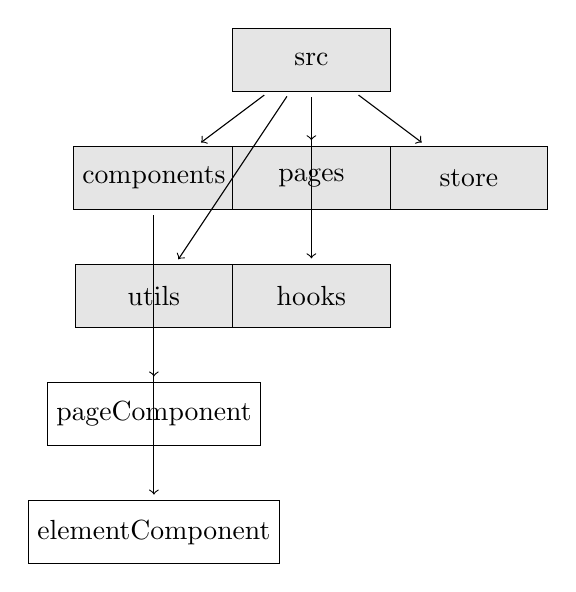
\begin{tikzpicture}[
    file/.style={draw, rectangle, minimum width=2cm, minimum height=0.8cm},
    folder/.style={draw, rectangle, minimum width=2cm, minimum height=0.8cm, fill=gray!20},
    arrow/.style={->, shorten >=2pt, shorten <=2pt}
]

% Folders
\node[folder] (src) at (0,0) {src};
\node[folder] (components) at (-2,-1.5) {components};
\node[folder] (pages) at (0,-1.5) {pages};
\node[folder] (store) at (2,-1.5) {store};
\node[folder] (utils) at (-2,-3) {utils};
\node[folder] (hooks) at (0,-3) {hooks};

% Files
\node[file] (pageComponent) at (-2,-4.5) {pageComponent};
\node[file] (elementComponent) at (-2,-6) {elementComponent};
% ... add more files

% Connections
\draw[arrow] (src) -- (components);
\draw[arrow] (src) -- (pages);
\draw[arrow] (src) -- (store);
\draw[arrow] (src) -- (utils);
\draw[arrow] (src) -- (hooks);
\draw[arrow] (components) -- (pageComponent);
\draw[arrow] (components) -- (elementComponent);
% ... add more connections

\end{tikzpicture}



\pagebreak
\subsubsection{Back-end}
The backend uses the dotNet framework. The development language using the C\# language.

In this project, the backend uses the Onion Architecture.
The Onion Architecture is a typically layered architecture, 
where each layer depends on the inner layer and provides interfaces to the outer layer.
The outer layer provides services to the outermost layer 
and other modules in the same layer based on the interfaces of the inner layer.

From inner to outer, the layers are: Domain, Application, Infrastructure, Presentation.
The Domain layer is the core layer and the innermost layer, used to define domain models, 
which are the business models.
It includes domain models and domain service interfaces.
Domain models are used to define the business models, 
which are the entities in the entity-relationship model and their attributes.
Domain service interfaces are used to define the business services, 
which are the relationships between entities in the entity-relationship model.

The Application layer is the application layer, 
used to define application services, which are the business logic.
It includes domain service implementations and application service interfaces.
Domain service implementations implement the methods of the inner layer's domain service 
interfaces and implement the business logic of the domain models.
Application service interfaces are used to define application services, 
which are the business logic.
It includes but is not limited to database interfaces, testing interfaces, 
HTTP API interfaces, MQTT interfaces, etc.

The Infrastructure layer is the infrastructure layer, used to define infrastructure.
It includes database implementations, testing implementations, 
HTTP API implementations, MQTT implementations, etc.
Database implementations implement the database interfaces 
and provide CRUD services for the database.
Testing implementations implement the testing interfaces 
and provide services for unit testing and integration testing.
HTTP API implementations implement the HTTP API interfaces 
and provide CRUD operations for HTTP APIs.
MQTT implementations implement the MQTT interfaces 
and provide CRUD operations for MQTT.

The Presentation layer is the presentation layer, used to define presentation logic, 
such as interfaces and pages. Since this is a backend project,
data presentation and control are handled by the frontend, 
so this layer is not needed.



\pagebreak
\subsubsection{Data communication and storage}
% 关于本项目的数据通信与数据存储的设计, 包括数据通信的协议, 数据存储的设计等
% 关于数据通信的设计:
% 1. 通信协议的选择
% 自前端向后端发送的数据, 有三种传输的数据类型, 
% 一种是普通的增删改查的请求, 对数据传输的时效性要求不高, 但是对数据的准确性, 完整性, 有序性, 安全性有一定的要求,
% 这种数据的传输, 采用 HTTP 协议, 以及 RESTful API 的设计. 可以有效的保证对数据传输的以上要求.
% 一种是对数据通道的创建和流媒体数据的传输, 对数据传输的时效性, 安全性要求较高, 这种数据的传输, 采用 WebRTC 协议, 以及 MQTT 协议.
% 配合可以快速解码的 flatbuffers 协议, 可以有效的保证对数据传输的以上要求.
% 最后一种是对设备的状态信息和操作信息的传输, 对完整性, 有序性, 安全性都有较高的要求, 这种数据的传输, 采用 MQTT 协议
% 同时也使用了 flatbuffers 协议.
% 
% 2. 数据通信的通信架构和通信流程
% 本项目的数据通信的通信架构, 是基于前后端分离的架构, 前端使用 React 框架, 后端使用 dotnet 框架.
% 当前端需要向后端发送数据的时候, 前端会向后端发送 HTTP 请求, 后端接收到 HTTP 请求之后, 会根据请求的数据类型,
% 选择不同的数据处理方式, 对于普通的增删改查的请求, 后端会根据 RESTful API 的设计, 对数据进行增删改查的操作,
% 对于对数据通道的创建和流媒体数据的传输, 后端会根据 WebRTC 协议, 对数据通道进行创建, 并且帮助前端和设备建立数据通道,
% 当数据通道建立后, 前端和设备之间则使用 flatbuffer 的数据格式对流媒体数据进行传输,
% 对于设备的状态信息和操作信息的传输, 前端会直接向 MQTT broker 发送 MQTT 请求, 
% 设备会在其自身的固件中监听相关的 MQTT 请求, 并且返回相关的数据.
% 
% 3. 数据通信的格式
% 本项目的数据通信的格式, 有三种, 
% 一种是 HTTP 协议, 
% 使用 json 格式对数据进行传输,
% 一种是 WebRTC 协议, 
% 使用 flatbuffers 格式对数据进行传输,
% 一种是 MQTT 协议.
% 使用 flatbuffers 格式对数据进行传输,
% 
% 关于数据存储的设计:
% 1. 数据存储的数据库的选择
% 本项目的数据存储的数据库的选择, 使用了轻量级的数据库 SQLite,
% SQLite 是一个进程内的库, 实现了自给自足的, 无服务器的, 零配置的, 事务性的 SQL 数据库引擎.
% 这是因为整个项目的目的是为了实现前端与设备之间的数据通信, 对于数据库数据的增删改查操作的要求不高,
% 数据量较小, 且对于数据库的数据的事务性要求不高, 所以选择了 SQLite 数据库.
% 2. 项目前后端的数据结构的设计
% 在本项目中, 前端由于使用了 React 框架, 所以前端的数据结构的设计, 使用了基于状态的数据结构的设计,
% 每个组件或者数据集都包含一个状态对象, 这个状态对象的属性就是组件的各个状态. 
% 使用状态对象的原因是, 可以方便的对状态进行管理, 采用对象-属性的形式, 可以方便的针对不同组件的同类状态进行区分,
% 由于跨组件的状态是由 redux 进行管理的, 这种状态对象的设计, 可以更搞笑的对状态进行更新和传递.
% 后端由于使用了 dotnet 框架, 所以后端的数据结构的设计, 使用了基于类的数据结构的设计,
% 采用了面向对象的编程思想, 对数据进行了封装, 使得数据的传输更加的安全, 有序, 完整.


\pagebreak

% \subsection{Domain model}
% \documentclass[]{article}
\usepackage{graphicx}
\usepackage{amsmath}
\usepackage{tikz}

% libaries
\usetikzlibrary{shapes,arrows}

%Define the listing package
\usepackage{listings} %code highlighter
\usepackage{color} %use color
\definecolor{mygreen}{rgb}{0,0.6,0}
\definecolor{mygray}{rgb}{0.5,0.5,0.5}
\definecolor{mymauve}{rgb}{0.58,0,0.82}

%Customize a bit the look
\lstset{ %
backgroundcolor=\color{white}, % choose the background color; you must add \usepackage{color} or \usepackage{xcolor}
basicstyle=\footnotesize, % the size of the fonts that are used for the code
breakatwhitespace=false, % sets if automatic breaks should only happen at whitespace
breaklines=true, % sets automatic line breaking
captionpos=b, % sets the caption-position to bottom
commentstyle=\color{mygreen}, % comment style
deletekeywords={...}, % if you want to delete keywords from the given language
escapeinside={\%*}{*)}, % if you want to add LaTeX within your code
extendedchars=true, % lets you use non-ASCII characters; for 8-bits encodings only, does not work with UTF-8
frame=single, % adds a frame around the code
keepspaces=true, % keeps spaces in text, useful for keeping indentation of code (possibly needs columns=flexible)
keywordstyle=\color{blue}, % keyword style
% language=Octave, % the language of the code
morekeywords={*,...}, % if you want to add more keywords to the set
numbers=left, % where to put the line-numbers; possible values are (none, left, right)
numbersep=5pt, % how far the line-numbers are from the code
numberstyle=\tiny\color{mygray}, % the style that is used for the line-numbers
rulecolor=\color{black}, % if not set, the frame-color may be changed on line-breaks within not-black text (e.g. comments (green here))
showspaces=false, % show spaces everywhere adding particular underscores; it overrides 'showstringspaces'
showstringspaces=false, % underline spaces within strings only
showtabs=false, % show tabs within strings adding particular underscores
stepnumber=1, % the step between two line-numbers. If it's 1, each line will be numbered
stringstyle=\color{mymauve}, % string literal style
tabsize=2, % sets default tabsize to 2 spaces
title=\lstname % show the filename of files included with \lstinputlisting; also try caption instead of title
}

\definecolor{darkgray}{rgb}{.4,.4,.4}
\definecolor{purple}{rgb}{0.65, 0.12, 0.82}

\lstdefinelanguage{React}{
keywords={const, typeof, new, true, false, catch, function, return, null, catch, switch, var, if, in, while, do, else, case, break},
keywordstyle=\color{blue}\bfseries,
ndkeywords={class, export, boolean, throw, implements, import, this},
ndkeywordstyle=\color{darkgray}\bfseries,
identifierstyle=\color{mygreen},
sensitive=false,
comment=[l]{//},
morecomment=[s]{/*}{*/},
commentstyle=\color{purple}\ttfamily,
string=[b]{"}{'}{`},
stringstyle=\color{red}\ttfamily,
morestring=[b]',
morestring=[b]",
morestring=[b]`',
}

\lstdefinelanguage{CSharp}{
keywords={const, typeof, new, true, false, catch, function, return, null, catch, switch, var, if, in, while, do, else, case, break},
keywordstyle=\color{blue}\bfseries,
ndkeywords={class, export, boolean, throw, implements, import, this},
ndkeywordstyle=\color{darkgray}\bfseries,
identifierstyle=\color{mygreen},
sensitive=false,
comment=[l]{//},
morecomment=[s]{/*}{*/},
commentstyle=\color{purple}\ttfamily,
string=[b]{"}{'}{`},
stringstyle=\color{red}\ttfamily,
morestring=[b]',
morestring=[b]",
morestring=[b]`',
}

\lstset{
language=React,
extendedchars=true,
basicstyle=\footnotesize\ttfamily,
showstringspaces=false,
showspaces=false,
numbers=left,
numberstyle=\footnotesize,
numbersep=9pt,
tabsize=2,
breaklines=true,
showtabs=false,
captionpos=b
}

\lstset{
language=CSharp,
extendedchars=true,
basicstyle=\footnotesize\ttfamily,
showstringspaces=false,
showspaces=false,
numbers=left,
numberstyle=\footnotesize,
numbersep=9pt,
tabsize=2,
breaklines=true,
showtabs=false,
captionpos=b
}

% \usepackage{cite} % Add this line for citation

% \bibliographystyle{plain}

\title{
The implementation of BifrostConnect Front-end scope, 
re-design and development with the relevant back-end support develop.
}
\author{
    Fei Gu \\
    Erhvervs Akademi Sydvest \\
    Computer Science 21\\
    }
\date{\today}

\begin{document}

% Front page
\maketitle
\begin{center}
    Supervisor: Henrik Boulund Meng Hansen \\
    Company: BifrostConnect \\
    Engineering Director: Jasper Wass \\
\end{center}
\tableofcontents
\pagebreak


% The introduction
\section{Introduction}
\subsection{Background}\input{sections/introduction/background.tex}
\subsection{The company}\input{sections/introduction/aboutCompany}
\subsection{The project}\input{sections/introduction/aboutProject}
\pagebreak

% The problem statement
\section{Problem Statement}
\subsection{Statement}
\input{sections/problemStatement/statement}
\subsection{Situation}
\input{sections/problemStatement/situation}
\subsection{Potential Solution}
\input{sections/problemStatement/potentialSolution}
\pagebreak

% Requirement analysis
\section{Requirement Analysis}
\input{sections/requirementAnalysis/index}

\subsection{Stakeholders}
\input{sections/requirementAnalysis/stakeholders/index}

\subsection{Business Domain}
\input{sections/requirementAnalysis/bussinesDomain/index}

\subsection{Scope}
\input{sections/requirementAnalysis/scope}

\subsection{Goals}
\input{sections/requirementAnalysis/goals}
\pagebreak

% Software Design
\section{Software Design}
% developement methods
\subsection{Software Development Methods}
\input{sections/softwareDevelopmentMethods/index}
\subsubsection{Agile Software Development}
\input{sections/softwareDevelopmentMethods/agileSoftwareDevelopment/index}
\subsubsection{Feature Driven Development}
\input{sections/softwareDevelopmentMethods/featureDrivenDevelopment/index}

\pagebreak

% Technology seslection
\subsection{Technology selection}
\input{sections/softwareDesign/technologySelection/index}
\subsubsection{Front-end}
\input{sections/softwareDesign/technologySelection/frontEnd}            
\subsubsection{Back-end}
\input{sections/softwareDesign/technologySelection/backEnd}            
\subsubsection{Database}
\input{sections/softwareDesign/technologySelection/database}
\subsubsection{Data communication}
\input{sections/softwareDesign/technologySelection/dataCommunication}            
\subsubsection{DevOps}
\input{sections/softwareDesign/technologySelection/devOps}
\pagebreak

% Architecture design
\subsection{Architecture design}
\input{sections/softwareDesign/architectureDesign/index}
\pagebreak
\subsubsection{Front-end}
\input{sections/softwareDesign/architectureDesign/frontEndArchitecture}
\pagebreak
\subsubsection{Back-end}
\input{sections/softwareDesign/architectureDesign/backEndArchitecture}
\pagebreak
\subsubsection{Data communication and storage}
\input{sections/softwareDesign/architectureDesign/dataCommunicationArchitecture}
\pagebreak

% \subsection{Domain model}
% \input{sections/softwareDesign/domainModel/index}
% \subsection{Database design}
% % 数据库领域模型 ER 图
% % 包括表和字段的设置.
% % 对于私有键和外键的设置.

% \subsection{Back-end design}
% % 后端对象模型
% % 以及对于对象模型的增删改查
% % 以及相关的其他服务的设计`'

% \subsection{Front-end design}
% % 对于前端的页面结构的设计 
% % 页面的状态的设计, 交互设计

% \subsection{FlatBuffers design}
% % schema 的设计

\subsection{DevOps CI/CD process design}
\input{sections/softwareDesign/devOpsDesign/index}
\subsubsection{Continuous Integration}
\input{sections/softwareDesign/devOpsDesign/continuousIntegration/index}
\subsubsection{Continuous Delivery}
\input{sections/softwareDesign/devOpsDesign/continuousDelivery/index}
\subsubsection{Continuous Deployment}
\input{sections/softwareDesign/devOpsDesign/continuousDeployment/index}
\pagebreak

\section{Software Development} 
\input{sections/softwareDevelopment/index}
\subsection{Overall development}
\input{sections/softwareDevelopment/overallDevelopement/index}
\subsubsection{Front-end}
\input{sections/softwareDevelopment/overallDevelopement/frontEnd/index}
\subsubsection{Back-end}
\input{sections/softwareDevelopment/overallDevelopement/backEnd/index}
\subsubsection{DevOps}
\input{sections/softwareDevelopment/overallDevelopement/devOps/index}
\subsection{Feature development} 
\input{sections/softwareDevelopment/featureDevelopment/index}
\subsubsection{Use Case 1}
\input{sections/softwareDevelopment/featureDevelopment/useCase1/index}
\subsubsection{Feature 1}
\input{sections/softwareDevelopment/featureDevelopment/feature/feature1.tex}
\pagebreak
\section{Conclusion} 
\subsection{Result}
Since the project is still in progress, the result is not available yet.
So far, basic structure of this project has been built. But the most features 
are not implemented yet. 
\subsection{Discussion}
As a single developer for this project, I am confident what I have done so far.
And I can say I understand the most of the knowledge I have used in this project, 
which also means I can explain all the part of the project. 
But this project also relevant some of the complex knowledge which I have to continue 
to study and practice.
\subsection{Future Work}
The future work is to implement the rest of the features. 
Including the most important part which is the 'create session' feature.
\pagebreak
% \bibliography{bibliography}
\pagebreak
% \begin{appendices}
%     \section{Appendix}
% \end{appendices} 
\end{document}
% \subsection{Database design}
% % 数据库领域模型 ER 图
% % 包括表和字段的设置.
% % 对于私有键和外键的设置.

% \subsection{Back-end design}
% % 后端对象模型
% % 以及对于对象模型的增删改查
% % 以及相关的其他服务的设计`'

% \subsection{Front-end design}
% % 对于前端的页面结构的设计 
% % 页面的状态的设计, 交互设计

% \subsection{FlatBuffers design}
% % schema 的设计

\subsection{DevOps CI/CD process design}
\documentclass[]{article}
\usepackage{graphicx}
\usepackage{amsmath}
\usepackage{tikz}

% libaries
\usetikzlibrary{shapes,arrows}

%Define the listing package
\usepackage{listings} %code highlighter
\usepackage{color} %use color
\definecolor{mygreen}{rgb}{0,0.6,0}
\definecolor{mygray}{rgb}{0.5,0.5,0.5}
\definecolor{mymauve}{rgb}{0.58,0,0.82}

%Customize a bit the look
\lstset{ %
backgroundcolor=\color{white}, % choose the background color; you must add \usepackage{color} or \usepackage{xcolor}
basicstyle=\footnotesize, % the size of the fonts that are used for the code
breakatwhitespace=false, % sets if automatic breaks should only happen at whitespace
breaklines=true, % sets automatic line breaking
captionpos=b, % sets the caption-position to bottom
commentstyle=\color{mygreen}, % comment style
deletekeywords={...}, % if you want to delete keywords from the given language
escapeinside={\%*}{*)}, % if you want to add LaTeX within your code
extendedchars=true, % lets you use non-ASCII characters; for 8-bits encodings only, does not work with UTF-8
frame=single, % adds a frame around the code
keepspaces=true, % keeps spaces in text, useful for keeping indentation of code (possibly needs columns=flexible)
keywordstyle=\color{blue}, % keyword style
% language=Octave, % the language of the code
morekeywords={*,...}, % if you want to add more keywords to the set
numbers=left, % where to put the line-numbers; possible values are (none, left, right)
numbersep=5pt, % how far the line-numbers are from the code
numberstyle=\tiny\color{mygray}, % the style that is used for the line-numbers
rulecolor=\color{black}, % if not set, the frame-color may be changed on line-breaks within not-black text (e.g. comments (green here))
showspaces=false, % show spaces everywhere adding particular underscores; it overrides 'showstringspaces'
showstringspaces=false, % underline spaces within strings only
showtabs=false, % show tabs within strings adding particular underscores
stepnumber=1, % the step between two line-numbers. If it's 1, each line will be numbered
stringstyle=\color{mymauve}, % string literal style
tabsize=2, % sets default tabsize to 2 spaces
title=\lstname % show the filename of files included with \lstinputlisting; also try caption instead of title
}

\definecolor{darkgray}{rgb}{.4,.4,.4}
\definecolor{purple}{rgb}{0.65, 0.12, 0.82}

\lstdefinelanguage{React}{
keywords={const, typeof, new, true, false, catch, function, return, null, catch, switch, var, if, in, while, do, else, case, break},
keywordstyle=\color{blue}\bfseries,
ndkeywords={class, export, boolean, throw, implements, import, this},
ndkeywordstyle=\color{darkgray}\bfseries,
identifierstyle=\color{mygreen},
sensitive=false,
comment=[l]{//},
morecomment=[s]{/*}{*/},
commentstyle=\color{purple}\ttfamily,
string=[b]{"}{'}{`},
stringstyle=\color{red}\ttfamily,
morestring=[b]',
morestring=[b]",
morestring=[b]`',
}

\lstdefinelanguage{CSharp}{
keywords={const, typeof, new, true, false, catch, function, return, null, catch, switch, var, if, in, while, do, else, case, break},
keywordstyle=\color{blue}\bfseries,
ndkeywords={class, export, boolean, throw, implements, import, this},
ndkeywordstyle=\color{darkgray}\bfseries,
identifierstyle=\color{mygreen},
sensitive=false,
comment=[l]{//},
morecomment=[s]{/*}{*/},
commentstyle=\color{purple}\ttfamily,
string=[b]{"}{'}{`},
stringstyle=\color{red}\ttfamily,
morestring=[b]',
morestring=[b]",
morestring=[b]`',
}

\lstset{
language=React,
extendedchars=true,
basicstyle=\footnotesize\ttfamily,
showstringspaces=false,
showspaces=false,
numbers=left,
numberstyle=\footnotesize,
numbersep=9pt,
tabsize=2,
breaklines=true,
showtabs=false,
captionpos=b
}

\lstset{
language=CSharp,
extendedchars=true,
basicstyle=\footnotesize\ttfamily,
showstringspaces=false,
showspaces=false,
numbers=left,
numberstyle=\footnotesize,
numbersep=9pt,
tabsize=2,
breaklines=true,
showtabs=false,
captionpos=b
}

% \usepackage{cite} % Add this line for citation

% \bibliographystyle{plain}

\title{
The implementation of BifrostConnect Front-end scope, 
re-design and development with the relevant back-end support develop.
}
\author{
    Fei Gu \\
    Erhvervs Akademi Sydvest \\
    Computer Science 21\\
    }
\date{\today}

\begin{document}

% Front page
\maketitle
\begin{center}
    Supervisor: Henrik Boulund Meng Hansen \\
    Company: BifrostConnect \\
    Engineering Director: Jasper Wass \\
\end{center}
\tableofcontents
\pagebreak


% The introduction
\section{Introduction}
\subsection{Background}\input{sections/introduction/background.tex}
\subsection{The company}\input{sections/introduction/aboutCompany}
\subsection{The project}\input{sections/introduction/aboutProject}
\pagebreak

% The problem statement
\section{Problem Statement}
\subsection{Statement}
\input{sections/problemStatement/statement}
\subsection{Situation}
\input{sections/problemStatement/situation}
\subsection{Potential Solution}
\input{sections/problemStatement/potentialSolution}
\pagebreak

% Requirement analysis
\section{Requirement Analysis}
\input{sections/requirementAnalysis/index}

\subsection{Stakeholders}
\input{sections/requirementAnalysis/stakeholders/index}

\subsection{Business Domain}
\input{sections/requirementAnalysis/bussinesDomain/index}

\subsection{Scope}
\input{sections/requirementAnalysis/scope}

\subsection{Goals}
\input{sections/requirementAnalysis/goals}
\pagebreak

% Software Design
\section{Software Design}
% developement methods
\subsection{Software Development Methods}
\input{sections/softwareDevelopmentMethods/index}
\subsubsection{Agile Software Development}
\input{sections/softwareDevelopmentMethods/agileSoftwareDevelopment/index}
\subsubsection{Feature Driven Development}
\input{sections/softwareDevelopmentMethods/featureDrivenDevelopment/index}

\pagebreak

% Technology seslection
\subsection{Technology selection}
\input{sections/softwareDesign/technologySelection/index}
\subsubsection{Front-end}
\input{sections/softwareDesign/technologySelection/frontEnd}            
\subsubsection{Back-end}
\input{sections/softwareDesign/technologySelection/backEnd}            
\subsubsection{Database}
\input{sections/softwareDesign/technologySelection/database}
\subsubsection{Data communication}
\input{sections/softwareDesign/technologySelection/dataCommunication}            
\subsubsection{DevOps}
\input{sections/softwareDesign/technologySelection/devOps}
\pagebreak

% Architecture design
\subsection{Architecture design}
\input{sections/softwareDesign/architectureDesign/index}
\pagebreak
\subsubsection{Front-end}
\input{sections/softwareDesign/architectureDesign/frontEndArchitecture}
\pagebreak
\subsubsection{Back-end}
\input{sections/softwareDesign/architectureDesign/backEndArchitecture}
\pagebreak
\subsubsection{Data communication and storage}
\input{sections/softwareDesign/architectureDesign/dataCommunicationArchitecture}
\pagebreak

% \subsection{Domain model}
% \input{sections/softwareDesign/domainModel/index}
% \subsection{Database design}
% % 数据库领域模型 ER 图
% % 包括表和字段的设置.
% % 对于私有键和外键的设置.

% \subsection{Back-end design}
% % 后端对象模型
% % 以及对于对象模型的增删改查
% % 以及相关的其他服务的设计`'

% \subsection{Front-end design}
% % 对于前端的页面结构的设计 
% % 页面的状态的设计, 交互设计

% \subsection{FlatBuffers design}
% % schema 的设计

\subsection{DevOps CI/CD process design}
\input{sections/softwareDesign/devOpsDesign/index}
\subsubsection{Continuous Integration}
\input{sections/softwareDesign/devOpsDesign/continuousIntegration/index}
\subsubsection{Continuous Delivery}
\input{sections/softwareDesign/devOpsDesign/continuousDelivery/index}
\subsubsection{Continuous Deployment}
\input{sections/softwareDesign/devOpsDesign/continuousDeployment/index}
\pagebreak

\section{Software Development} 
\input{sections/softwareDevelopment/index}
\subsection{Overall development}
\input{sections/softwareDevelopment/overallDevelopement/index}
\subsubsection{Front-end}
\input{sections/softwareDevelopment/overallDevelopement/frontEnd/index}
\subsubsection{Back-end}
\input{sections/softwareDevelopment/overallDevelopement/backEnd/index}
\subsubsection{DevOps}
\input{sections/softwareDevelopment/overallDevelopement/devOps/index}
\subsection{Feature development} 
\input{sections/softwareDevelopment/featureDevelopment/index}
\subsubsection{Use Case 1}
\input{sections/softwareDevelopment/featureDevelopment/useCase1/index}
\subsubsection{Feature 1}
\input{sections/softwareDevelopment/featureDevelopment/feature/feature1.tex}
\pagebreak
\section{Conclusion} 
\subsection{Result}
Since the project is still in progress, the result is not available yet.
So far, basic structure of this project has been built. But the most features 
are not implemented yet. 
\subsection{Discussion}
As a single developer for this project, I am confident what I have done so far.
And I can say I understand the most of the knowledge I have used in this project, 
which also means I can explain all the part of the project. 
But this project also relevant some of the complex knowledge which I have to continue 
to study and practice.
\subsection{Future Work}
The future work is to implement the rest of the features. 
Including the most important part which is the 'create session' feature.
\pagebreak
% \bibliography{bibliography}
\pagebreak
% \begin{appendices}
%     \section{Appendix}
% \end{appendices} 
\end{document}
\subsubsection{Continuous Integration}
\documentclass[]{article}
\usepackage{graphicx}
\usepackage{amsmath}
\usepackage{tikz}

% libaries
\usetikzlibrary{shapes,arrows}

%Define the listing package
\usepackage{listings} %code highlighter
\usepackage{color} %use color
\definecolor{mygreen}{rgb}{0,0.6,0}
\definecolor{mygray}{rgb}{0.5,0.5,0.5}
\definecolor{mymauve}{rgb}{0.58,0,0.82}

%Customize a bit the look
\lstset{ %
backgroundcolor=\color{white}, % choose the background color; you must add \usepackage{color} or \usepackage{xcolor}
basicstyle=\footnotesize, % the size of the fonts that are used for the code
breakatwhitespace=false, % sets if automatic breaks should only happen at whitespace
breaklines=true, % sets automatic line breaking
captionpos=b, % sets the caption-position to bottom
commentstyle=\color{mygreen}, % comment style
deletekeywords={...}, % if you want to delete keywords from the given language
escapeinside={\%*}{*)}, % if you want to add LaTeX within your code
extendedchars=true, % lets you use non-ASCII characters; for 8-bits encodings only, does not work with UTF-8
frame=single, % adds a frame around the code
keepspaces=true, % keeps spaces in text, useful for keeping indentation of code (possibly needs columns=flexible)
keywordstyle=\color{blue}, % keyword style
% language=Octave, % the language of the code
morekeywords={*,...}, % if you want to add more keywords to the set
numbers=left, % where to put the line-numbers; possible values are (none, left, right)
numbersep=5pt, % how far the line-numbers are from the code
numberstyle=\tiny\color{mygray}, % the style that is used for the line-numbers
rulecolor=\color{black}, % if not set, the frame-color may be changed on line-breaks within not-black text (e.g. comments (green here))
showspaces=false, % show spaces everywhere adding particular underscores; it overrides 'showstringspaces'
showstringspaces=false, % underline spaces within strings only
showtabs=false, % show tabs within strings adding particular underscores
stepnumber=1, % the step between two line-numbers. If it's 1, each line will be numbered
stringstyle=\color{mymauve}, % string literal style
tabsize=2, % sets default tabsize to 2 spaces
title=\lstname % show the filename of files included with \lstinputlisting; also try caption instead of title
}

\definecolor{darkgray}{rgb}{.4,.4,.4}
\definecolor{purple}{rgb}{0.65, 0.12, 0.82}

\lstdefinelanguage{React}{
keywords={const, typeof, new, true, false, catch, function, return, null, catch, switch, var, if, in, while, do, else, case, break},
keywordstyle=\color{blue}\bfseries,
ndkeywords={class, export, boolean, throw, implements, import, this},
ndkeywordstyle=\color{darkgray}\bfseries,
identifierstyle=\color{mygreen},
sensitive=false,
comment=[l]{//},
morecomment=[s]{/*}{*/},
commentstyle=\color{purple}\ttfamily,
string=[b]{"}{'}{`},
stringstyle=\color{red}\ttfamily,
morestring=[b]',
morestring=[b]",
morestring=[b]`',
}

\lstdefinelanguage{CSharp}{
keywords={const, typeof, new, true, false, catch, function, return, null, catch, switch, var, if, in, while, do, else, case, break},
keywordstyle=\color{blue}\bfseries,
ndkeywords={class, export, boolean, throw, implements, import, this},
ndkeywordstyle=\color{darkgray}\bfseries,
identifierstyle=\color{mygreen},
sensitive=false,
comment=[l]{//},
morecomment=[s]{/*}{*/},
commentstyle=\color{purple}\ttfamily,
string=[b]{"}{'}{`},
stringstyle=\color{red}\ttfamily,
morestring=[b]',
morestring=[b]",
morestring=[b]`',
}

\lstset{
language=React,
extendedchars=true,
basicstyle=\footnotesize\ttfamily,
showstringspaces=false,
showspaces=false,
numbers=left,
numberstyle=\footnotesize,
numbersep=9pt,
tabsize=2,
breaklines=true,
showtabs=false,
captionpos=b
}

\lstset{
language=CSharp,
extendedchars=true,
basicstyle=\footnotesize\ttfamily,
showstringspaces=false,
showspaces=false,
numbers=left,
numberstyle=\footnotesize,
numbersep=9pt,
tabsize=2,
breaklines=true,
showtabs=false,
captionpos=b
}

% \usepackage{cite} % Add this line for citation

% \bibliographystyle{plain}

\title{
The implementation of BifrostConnect Front-end scope, 
re-design and development with the relevant back-end support develop.
}
\author{
    Fei Gu \\
    Erhvervs Akademi Sydvest \\
    Computer Science 21\\
    }
\date{\today}

\begin{document}

% Front page
\maketitle
\begin{center}
    Supervisor: Henrik Boulund Meng Hansen \\
    Company: BifrostConnect \\
    Engineering Director: Jasper Wass \\
\end{center}
\tableofcontents
\pagebreak


% The introduction
\section{Introduction}
\subsection{Background}\input{sections/introduction/background.tex}
\subsection{The company}\input{sections/introduction/aboutCompany}
\subsection{The project}\input{sections/introduction/aboutProject}
\pagebreak

% The problem statement
\section{Problem Statement}
\subsection{Statement}
\input{sections/problemStatement/statement}
\subsection{Situation}
\input{sections/problemStatement/situation}
\subsection{Potential Solution}
\input{sections/problemStatement/potentialSolution}
\pagebreak

% Requirement analysis
\section{Requirement Analysis}
\input{sections/requirementAnalysis/index}

\subsection{Stakeholders}
\input{sections/requirementAnalysis/stakeholders/index}

\subsection{Business Domain}
\input{sections/requirementAnalysis/bussinesDomain/index}

\subsection{Scope}
\input{sections/requirementAnalysis/scope}

\subsection{Goals}
\input{sections/requirementAnalysis/goals}
\pagebreak

% Software Design
\section{Software Design}
% developement methods
\subsection{Software Development Methods}
\input{sections/softwareDevelopmentMethods/index}
\subsubsection{Agile Software Development}
\input{sections/softwareDevelopmentMethods/agileSoftwareDevelopment/index}
\subsubsection{Feature Driven Development}
\input{sections/softwareDevelopmentMethods/featureDrivenDevelopment/index}

\pagebreak

% Technology seslection
\subsection{Technology selection}
\input{sections/softwareDesign/technologySelection/index}
\subsubsection{Front-end}
\input{sections/softwareDesign/technologySelection/frontEnd}            
\subsubsection{Back-end}
\input{sections/softwareDesign/technologySelection/backEnd}            
\subsubsection{Database}
\input{sections/softwareDesign/technologySelection/database}
\subsubsection{Data communication}
\input{sections/softwareDesign/technologySelection/dataCommunication}            
\subsubsection{DevOps}
\input{sections/softwareDesign/technologySelection/devOps}
\pagebreak

% Architecture design
\subsection{Architecture design}
\input{sections/softwareDesign/architectureDesign/index}
\pagebreak
\subsubsection{Front-end}
\input{sections/softwareDesign/architectureDesign/frontEndArchitecture}
\pagebreak
\subsubsection{Back-end}
\input{sections/softwareDesign/architectureDesign/backEndArchitecture}
\pagebreak
\subsubsection{Data communication and storage}
\input{sections/softwareDesign/architectureDesign/dataCommunicationArchitecture}
\pagebreak

% \subsection{Domain model}
% \input{sections/softwareDesign/domainModel/index}
% \subsection{Database design}
% % 数据库领域模型 ER 图
% % 包括表和字段的设置.
% % 对于私有键和外键的设置.

% \subsection{Back-end design}
% % 后端对象模型
% % 以及对于对象模型的增删改查
% % 以及相关的其他服务的设计`'

% \subsection{Front-end design}
% % 对于前端的页面结构的设计 
% % 页面的状态的设计, 交互设计

% \subsection{FlatBuffers design}
% % schema 的设计

\subsection{DevOps CI/CD process design}
\input{sections/softwareDesign/devOpsDesign/index}
\subsubsection{Continuous Integration}
\input{sections/softwareDesign/devOpsDesign/continuousIntegration/index}
\subsubsection{Continuous Delivery}
\input{sections/softwareDesign/devOpsDesign/continuousDelivery/index}
\subsubsection{Continuous Deployment}
\input{sections/softwareDesign/devOpsDesign/continuousDeployment/index}
\pagebreak

\section{Software Development} 
\input{sections/softwareDevelopment/index}
\subsection{Overall development}
\input{sections/softwareDevelopment/overallDevelopement/index}
\subsubsection{Front-end}
\input{sections/softwareDevelopment/overallDevelopement/frontEnd/index}
\subsubsection{Back-end}
\input{sections/softwareDevelopment/overallDevelopement/backEnd/index}
\subsubsection{DevOps}
\input{sections/softwareDevelopment/overallDevelopement/devOps/index}
\subsection{Feature development} 
\input{sections/softwareDevelopment/featureDevelopment/index}
\subsubsection{Use Case 1}
\input{sections/softwareDevelopment/featureDevelopment/useCase1/index}
\subsubsection{Feature 1}
\input{sections/softwareDevelopment/featureDevelopment/feature/feature1.tex}
\pagebreak
\section{Conclusion} 
\subsection{Result}
Since the project is still in progress, the result is not available yet.
So far, basic structure of this project has been built. But the most features 
are not implemented yet. 
\subsection{Discussion}
As a single developer for this project, I am confident what I have done so far.
And I can say I understand the most of the knowledge I have used in this project, 
which also means I can explain all the part of the project. 
But this project also relevant some of the complex knowledge which I have to continue 
to study and practice.
\subsection{Future Work}
The future work is to implement the rest of the features. 
Including the most important part which is the 'create session' feature.
\pagebreak
% \bibliography{bibliography}
\pagebreak
% \begin{appendices}
%     \section{Appendix}
% \end{appendices} 
\end{document}
\subsubsection{Continuous Delivery}
\documentclass[]{article}
\usepackage{graphicx}
\usepackage{amsmath}
\usepackage{tikz}

% libaries
\usetikzlibrary{shapes,arrows}

%Define the listing package
\usepackage{listings} %code highlighter
\usepackage{color} %use color
\definecolor{mygreen}{rgb}{0,0.6,0}
\definecolor{mygray}{rgb}{0.5,0.5,0.5}
\definecolor{mymauve}{rgb}{0.58,0,0.82}

%Customize a bit the look
\lstset{ %
backgroundcolor=\color{white}, % choose the background color; you must add \usepackage{color} or \usepackage{xcolor}
basicstyle=\footnotesize, % the size of the fonts that are used for the code
breakatwhitespace=false, % sets if automatic breaks should only happen at whitespace
breaklines=true, % sets automatic line breaking
captionpos=b, % sets the caption-position to bottom
commentstyle=\color{mygreen}, % comment style
deletekeywords={...}, % if you want to delete keywords from the given language
escapeinside={\%*}{*)}, % if you want to add LaTeX within your code
extendedchars=true, % lets you use non-ASCII characters; for 8-bits encodings only, does not work with UTF-8
frame=single, % adds a frame around the code
keepspaces=true, % keeps spaces in text, useful for keeping indentation of code (possibly needs columns=flexible)
keywordstyle=\color{blue}, % keyword style
% language=Octave, % the language of the code
morekeywords={*,...}, % if you want to add more keywords to the set
numbers=left, % where to put the line-numbers; possible values are (none, left, right)
numbersep=5pt, % how far the line-numbers are from the code
numberstyle=\tiny\color{mygray}, % the style that is used for the line-numbers
rulecolor=\color{black}, % if not set, the frame-color may be changed on line-breaks within not-black text (e.g. comments (green here))
showspaces=false, % show spaces everywhere adding particular underscores; it overrides 'showstringspaces'
showstringspaces=false, % underline spaces within strings only
showtabs=false, % show tabs within strings adding particular underscores
stepnumber=1, % the step between two line-numbers. If it's 1, each line will be numbered
stringstyle=\color{mymauve}, % string literal style
tabsize=2, % sets default tabsize to 2 spaces
title=\lstname % show the filename of files included with \lstinputlisting; also try caption instead of title
}

\definecolor{darkgray}{rgb}{.4,.4,.4}
\definecolor{purple}{rgb}{0.65, 0.12, 0.82}

\lstdefinelanguage{React}{
keywords={const, typeof, new, true, false, catch, function, return, null, catch, switch, var, if, in, while, do, else, case, break},
keywordstyle=\color{blue}\bfseries,
ndkeywords={class, export, boolean, throw, implements, import, this},
ndkeywordstyle=\color{darkgray}\bfseries,
identifierstyle=\color{mygreen},
sensitive=false,
comment=[l]{//},
morecomment=[s]{/*}{*/},
commentstyle=\color{purple}\ttfamily,
string=[b]{"}{'}{`},
stringstyle=\color{red}\ttfamily,
morestring=[b]',
morestring=[b]",
morestring=[b]`',
}

\lstdefinelanguage{CSharp}{
keywords={const, typeof, new, true, false, catch, function, return, null, catch, switch, var, if, in, while, do, else, case, break},
keywordstyle=\color{blue}\bfseries,
ndkeywords={class, export, boolean, throw, implements, import, this},
ndkeywordstyle=\color{darkgray}\bfseries,
identifierstyle=\color{mygreen},
sensitive=false,
comment=[l]{//},
morecomment=[s]{/*}{*/},
commentstyle=\color{purple}\ttfamily,
string=[b]{"}{'}{`},
stringstyle=\color{red}\ttfamily,
morestring=[b]',
morestring=[b]",
morestring=[b]`',
}

\lstset{
language=React,
extendedchars=true,
basicstyle=\footnotesize\ttfamily,
showstringspaces=false,
showspaces=false,
numbers=left,
numberstyle=\footnotesize,
numbersep=9pt,
tabsize=2,
breaklines=true,
showtabs=false,
captionpos=b
}

\lstset{
language=CSharp,
extendedchars=true,
basicstyle=\footnotesize\ttfamily,
showstringspaces=false,
showspaces=false,
numbers=left,
numberstyle=\footnotesize,
numbersep=9pt,
tabsize=2,
breaklines=true,
showtabs=false,
captionpos=b
}

% \usepackage{cite} % Add this line for citation

% \bibliographystyle{plain}

\title{
The implementation of BifrostConnect Front-end scope, 
re-design and development with the relevant back-end support develop.
}
\author{
    Fei Gu \\
    Erhvervs Akademi Sydvest \\
    Computer Science 21\\
    }
\date{\today}

\begin{document}

% Front page
\maketitle
\begin{center}
    Supervisor: Henrik Boulund Meng Hansen \\
    Company: BifrostConnect \\
    Engineering Director: Jasper Wass \\
\end{center}
\tableofcontents
\pagebreak


% The introduction
\section{Introduction}
\subsection{Background}\input{sections/introduction/background.tex}
\subsection{The company}\input{sections/introduction/aboutCompany}
\subsection{The project}\input{sections/introduction/aboutProject}
\pagebreak

% The problem statement
\section{Problem Statement}
\subsection{Statement}
\input{sections/problemStatement/statement}
\subsection{Situation}
\input{sections/problemStatement/situation}
\subsection{Potential Solution}
\input{sections/problemStatement/potentialSolution}
\pagebreak

% Requirement analysis
\section{Requirement Analysis}
\input{sections/requirementAnalysis/index}

\subsection{Stakeholders}
\input{sections/requirementAnalysis/stakeholders/index}

\subsection{Business Domain}
\input{sections/requirementAnalysis/bussinesDomain/index}

\subsection{Scope}
\input{sections/requirementAnalysis/scope}

\subsection{Goals}
\input{sections/requirementAnalysis/goals}
\pagebreak

% Software Design
\section{Software Design}
% developement methods
\subsection{Software Development Methods}
\input{sections/softwareDevelopmentMethods/index}
\subsubsection{Agile Software Development}
\input{sections/softwareDevelopmentMethods/agileSoftwareDevelopment/index}
\subsubsection{Feature Driven Development}
\input{sections/softwareDevelopmentMethods/featureDrivenDevelopment/index}

\pagebreak

% Technology seslection
\subsection{Technology selection}
\input{sections/softwareDesign/technologySelection/index}
\subsubsection{Front-end}
\input{sections/softwareDesign/technologySelection/frontEnd}            
\subsubsection{Back-end}
\input{sections/softwareDesign/technologySelection/backEnd}            
\subsubsection{Database}
\input{sections/softwareDesign/technologySelection/database}
\subsubsection{Data communication}
\input{sections/softwareDesign/technologySelection/dataCommunication}            
\subsubsection{DevOps}
\input{sections/softwareDesign/technologySelection/devOps}
\pagebreak

% Architecture design
\subsection{Architecture design}
\input{sections/softwareDesign/architectureDesign/index}
\pagebreak
\subsubsection{Front-end}
\input{sections/softwareDesign/architectureDesign/frontEndArchitecture}
\pagebreak
\subsubsection{Back-end}
\input{sections/softwareDesign/architectureDesign/backEndArchitecture}
\pagebreak
\subsubsection{Data communication and storage}
\input{sections/softwareDesign/architectureDesign/dataCommunicationArchitecture}
\pagebreak

% \subsection{Domain model}
% \input{sections/softwareDesign/domainModel/index}
% \subsection{Database design}
% % 数据库领域模型 ER 图
% % 包括表和字段的设置.
% % 对于私有键和外键的设置.

% \subsection{Back-end design}
% % 后端对象模型
% % 以及对于对象模型的增删改查
% % 以及相关的其他服务的设计`'

% \subsection{Front-end design}
% % 对于前端的页面结构的设计 
% % 页面的状态的设计, 交互设计

% \subsection{FlatBuffers design}
% % schema 的设计

\subsection{DevOps CI/CD process design}
\input{sections/softwareDesign/devOpsDesign/index}
\subsubsection{Continuous Integration}
\input{sections/softwareDesign/devOpsDesign/continuousIntegration/index}
\subsubsection{Continuous Delivery}
\input{sections/softwareDesign/devOpsDesign/continuousDelivery/index}
\subsubsection{Continuous Deployment}
\input{sections/softwareDesign/devOpsDesign/continuousDeployment/index}
\pagebreak

\section{Software Development} 
\input{sections/softwareDevelopment/index}
\subsection{Overall development}
\input{sections/softwareDevelopment/overallDevelopement/index}
\subsubsection{Front-end}
\input{sections/softwareDevelopment/overallDevelopement/frontEnd/index}
\subsubsection{Back-end}
\input{sections/softwareDevelopment/overallDevelopement/backEnd/index}
\subsubsection{DevOps}
\input{sections/softwareDevelopment/overallDevelopement/devOps/index}
\subsection{Feature development} 
\input{sections/softwareDevelopment/featureDevelopment/index}
\subsubsection{Use Case 1}
\input{sections/softwareDevelopment/featureDevelopment/useCase1/index}
\subsubsection{Feature 1}
\input{sections/softwareDevelopment/featureDevelopment/feature/feature1.tex}
\pagebreak
\section{Conclusion} 
\subsection{Result}
Since the project is still in progress, the result is not available yet.
So far, basic structure of this project has been built. But the most features 
are not implemented yet. 
\subsection{Discussion}
As a single developer for this project, I am confident what I have done so far.
And I can say I understand the most of the knowledge I have used in this project, 
which also means I can explain all the part of the project. 
But this project also relevant some of the complex knowledge which I have to continue 
to study and practice.
\subsection{Future Work}
The future work is to implement the rest of the features. 
Including the most important part which is the 'create session' feature.
\pagebreak
% \bibliography{bibliography}
\pagebreak
% \begin{appendices}
%     \section{Appendix}
% \end{appendices} 
\end{document}
\subsubsection{Continuous Deployment}
\documentclass[]{article}
\usepackage{graphicx}
\usepackage{amsmath}
\usepackage{tikz}

% libaries
\usetikzlibrary{shapes,arrows}

%Define the listing package
\usepackage{listings} %code highlighter
\usepackage{color} %use color
\definecolor{mygreen}{rgb}{0,0.6,0}
\definecolor{mygray}{rgb}{0.5,0.5,0.5}
\definecolor{mymauve}{rgb}{0.58,0,0.82}

%Customize a bit the look
\lstset{ %
backgroundcolor=\color{white}, % choose the background color; you must add \usepackage{color} or \usepackage{xcolor}
basicstyle=\footnotesize, % the size of the fonts that are used for the code
breakatwhitespace=false, % sets if automatic breaks should only happen at whitespace
breaklines=true, % sets automatic line breaking
captionpos=b, % sets the caption-position to bottom
commentstyle=\color{mygreen}, % comment style
deletekeywords={...}, % if you want to delete keywords from the given language
escapeinside={\%*}{*)}, % if you want to add LaTeX within your code
extendedchars=true, % lets you use non-ASCII characters; for 8-bits encodings only, does not work with UTF-8
frame=single, % adds a frame around the code
keepspaces=true, % keeps spaces in text, useful for keeping indentation of code (possibly needs columns=flexible)
keywordstyle=\color{blue}, % keyword style
% language=Octave, % the language of the code
morekeywords={*,...}, % if you want to add more keywords to the set
numbers=left, % where to put the line-numbers; possible values are (none, left, right)
numbersep=5pt, % how far the line-numbers are from the code
numberstyle=\tiny\color{mygray}, % the style that is used for the line-numbers
rulecolor=\color{black}, % if not set, the frame-color may be changed on line-breaks within not-black text (e.g. comments (green here))
showspaces=false, % show spaces everywhere adding particular underscores; it overrides 'showstringspaces'
showstringspaces=false, % underline spaces within strings only
showtabs=false, % show tabs within strings adding particular underscores
stepnumber=1, % the step between two line-numbers. If it's 1, each line will be numbered
stringstyle=\color{mymauve}, % string literal style
tabsize=2, % sets default tabsize to 2 spaces
title=\lstname % show the filename of files included with \lstinputlisting; also try caption instead of title
}

\definecolor{darkgray}{rgb}{.4,.4,.4}
\definecolor{purple}{rgb}{0.65, 0.12, 0.82}

\lstdefinelanguage{React}{
keywords={const, typeof, new, true, false, catch, function, return, null, catch, switch, var, if, in, while, do, else, case, break},
keywordstyle=\color{blue}\bfseries,
ndkeywords={class, export, boolean, throw, implements, import, this},
ndkeywordstyle=\color{darkgray}\bfseries,
identifierstyle=\color{mygreen},
sensitive=false,
comment=[l]{//},
morecomment=[s]{/*}{*/},
commentstyle=\color{purple}\ttfamily,
string=[b]{"}{'}{`},
stringstyle=\color{red}\ttfamily,
morestring=[b]',
morestring=[b]",
morestring=[b]`',
}

\lstdefinelanguage{CSharp}{
keywords={const, typeof, new, true, false, catch, function, return, null, catch, switch, var, if, in, while, do, else, case, break},
keywordstyle=\color{blue}\bfseries,
ndkeywords={class, export, boolean, throw, implements, import, this},
ndkeywordstyle=\color{darkgray}\bfseries,
identifierstyle=\color{mygreen},
sensitive=false,
comment=[l]{//},
morecomment=[s]{/*}{*/},
commentstyle=\color{purple}\ttfamily,
string=[b]{"}{'}{`},
stringstyle=\color{red}\ttfamily,
morestring=[b]',
morestring=[b]",
morestring=[b]`',
}

\lstset{
language=React,
extendedchars=true,
basicstyle=\footnotesize\ttfamily,
showstringspaces=false,
showspaces=false,
numbers=left,
numberstyle=\footnotesize,
numbersep=9pt,
tabsize=2,
breaklines=true,
showtabs=false,
captionpos=b
}

\lstset{
language=CSharp,
extendedchars=true,
basicstyle=\footnotesize\ttfamily,
showstringspaces=false,
showspaces=false,
numbers=left,
numberstyle=\footnotesize,
numbersep=9pt,
tabsize=2,
breaklines=true,
showtabs=false,
captionpos=b
}

% \usepackage{cite} % Add this line for citation

% \bibliographystyle{plain}

\title{
The implementation of BifrostConnect Front-end scope, 
re-design and development with the relevant back-end support develop.
}
\author{
    Fei Gu \\
    Erhvervs Akademi Sydvest \\
    Computer Science 21\\
    }
\date{\today}

\begin{document}

% Front page
\maketitle
\begin{center}
    Supervisor: Henrik Boulund Meng Hansen \\
    Company: BifrostConnect \\
    Engineering Director: Jasper Wass \\
\end{center}
\tableofcontents
\pagebreak


% The introduction
\section{Introduction}
\subsection{Background}\input{sections/introduction/background.tex}
\subsection{The company}\input{sections/introduction/aboutCompany}
\subsection{The project}\input{sections/introduction/aboutProject}
\pagebreak

% The problem statement
\section{Problem Statement}
\subsection{Statement}
\input{sections/problemStatement/statement}
\subsection{Situation}
\input{sections/problemStatement/situation}
\subsection{Potential Solution}
\input{sections/problemStatement/potentialSolution}
\pagebreak

% Requirement analysis
\section{Requirement Analysis}
\input{sections/requirementAnalysis/index}

\subsection{Stakeholders}
\input{sections/requirementAnalysis/stakeholders/index}

\subsection{Business Domain}
\input{sections/requirementAnalysis/bussinesDomain/index}

\subsection{Scope}
\input{sections/requirementAnalysis/scope}

\subsection{Goals}
\input{sections/requirementAnalysis/goals}
\pagebreak

% Software Design
\section{Software Design}
% developement methods
\subsection{Software Development Methods}
\input{sections/softwareDevelopmentMethods/index}
\subsubsection{Agile Software Development}
\input{sections/softwareDevelopmentMethods/agileSoftwareDevelopment/index}
\subsubsection{Feature Driven Development}
\input{sections/softwareDevelopmentMethods/featureDrivenDevelopment/index}

\pagebreak

% Technology seslection
\subsection{Technology selection}
\input{sections/softwareDesign/technologySelection/index}
\subsubsection{Front-end}
\input{sections/softwareDesign/technologySelection/frontEnd}            
\subsubsection{Back-end}
\input{sections/softwareDesign/technologySelection/backEnd}            
\subsubsection{Database}
\input{sections/softwareDesign/technologySelection/database}
\subsubsection{Data communication}
\input{sections/softwareDesign/technologySelection/dataCommunication}            
\subsubsection{DevOps}
\input{sections/softwareDesign/technologySelection/devOps}
\pagebreak

% Architecture design
\subsection{Architecture design}
\input{sections/softwareDesign/architectureDesign/index}
\pagebreak
\subsubsection{Front-end}
\input{sections/softwareDesign/architectureDesign/frontEndArchitecture}
\pagebreak
\subsubsection{Back-end}
\input{sections/softwareDesign/architectureDesign/backEndArchitecture}
\pagebreak
\subsubsection{Data communication and storage}
\input{sections/softwareDesign/architectureDesign/dataCommunicationArchitecture}
\pagebreak

% \subsection{Domain model}
% \input{sections/softwareDesign/domainModel/index}
% \subsection{Database design}
% % 数据库领域模型 ER 图
% % 包括表和字段的设置.
% % 对于私有键和外键的设置.

% \subsection{Back-end design}
% % 后端对象模型
% % 以及对于对象模型的增删改查
% % 以及相关的其他服务的设计`'

% \subsection{Front-end design}
% % 对于前端的页面结构的设计 
% % 页面的状态的设计, 交互设计

% \subsection{FlatBuffers design}
% % schema 的设计

\subsection{DevOps CI/CD process design}
\input{sections/softwareDesign/devOpsDesign/index}
\subsubsection{Continuous Integration}
\input{sections/softwareDesign/devOpsDesign/continuousIntegration/index}
\subsubsection{Continuous Delivery}
\input{sections/softwareDesign/devOpsDesign/continuousDelivery/index}
\subsubsection{Continuous Deployment}
\input{sections/softwareDesign/devOpsDesign/continuousDeployment/index}
\pagebreak

\section{Software Development} 
\input{sections/softwareDevelopment/index}
\subsection{Overall development}
\input{sections/softwareDevelopment/overallDevelopement/index}
\subsubsection{Front-end}
\input{sections/softwareDevelopment/overallDevelopement/frontEnd/index}
\subsubsection{Back-end}
\input{sections/softwareDevelopment/overallDevelopement/backEnd/index}
\subsubsection{DevOps}
\input{sections/softwareDevelopment/overallDevelopement/devOps/index}
\subsection{Feature development} 
\input{sections/softwareDevelopment/featureDevelopment/index}
\subsubsection{Use Case 1}
\input{sections/softwareDevelopment/featureDevelopment/useCase1/index}
\subsubsection{Feature 1}
\input{sections/softwareDevelopment/featureDevelopment/feature/feature1.tex}
\pagebreak
\section{Conclusion} 
\subsection{Result}
Since the project is still in progress, the result is not available yet.
So far, basic structure of this project has been built. But the most features 
are not implemented yet. 
\subsection{Discussion}
As a single developer for this project, I am confident what I have done so far.
And I can say I understand the most of the knowledge I have used in this project, 
which also means I can explain all the part of the project. 
But this project also relevant some of the complex knowledge which I have to continue 
to study and practice.
\subsection{Future Work}
The future work is to implement the rest of the features. 
Including the most important part which is the 'create session' feature.
\pagebreak
% \bibliography{bibliography}
\pagebreak
% \begin{appendices}
%     \section{Appendix}
% \end{appendices} 
\end{document}
\pagebreak

\section{Software Development} 
\documentclass[]{article}
\usepackage{graphicx}
\usepackage{amsmath}
\usepackage{tikz}

% libaries
\usetikzlibrary{shapes,arrows}

%Define the listing package
\usepackage{listings} %code highlighter
\usepackage{color} %use color
\definecolor{mygreen}{rgb}{0,0.6,0}
\definecolor{mygray}{rgb}{0.5,0.5,0.5}
\definecolor{mymauve}{rgb}{0.58,0,0.82}

%Customize a bit the look
\lstset{ %
backgroundcolor=\color{white}, % choose the background color; you must add \usepackage{color} or \usepackage{xcolor}
basicstyle=\footnotesize, % the size of the fonts that are used for the code
breakatwhitespace=false, % sets if automatic breaks should only happen at whitespace
breaklines=true, % sets automatic line breaking
captionpos=b, % sets the caption-position to bottom
commentstyle=\color{mygreen}, % comment style
deletekeywords={...}, % if you want to delete keywords from the given language
escapeinside={\%*}{*)}, % if you want to add LaTeX within your code
extendedchars=true, % lets you use non-ASCII characters; for 8-bits encodings only, does not work with UTF-8
frame=single, % adds a frame around the code
keepspaces=true, % keeps spaces in text, useful for keeping indentation of code (possibly needs columns=flexible)
keywordstyle=\color{blue}, % keyword style
% language=Octave, % the language of the code
morekeywords={*,...}, % if you want to add more keywords to the set
numbers=left, % where to put the line-numbers; possible values are (none, left, right)
numbersep=5pt, % how far the line-numbers are from the code
numberstyle=\tiny\color{mygray}, % the style that is used for the line-numbers
rulecolor=\color{black}, % if not set, the frame-color may be changed on line-breaks within not-black text (e.g. comments (green here))
showspaces=false, % show spaces everywhere adding particular underscores; it overrides 'showstringspaces'
showstringspaces=false, % underline spaces within strings only
showtabs=false, % show tabs within strings adding particular underscores
stepnumber=1, % the step between two line-numbers. If it's 1, each line will be numbered
stringstyle=\color{mymauve}, % string literal style
tabsize=2, % sets default tabsize to 2 spaces
title=\lstname % show the filename of files included with \lstinputlisting; also try caption instead of title
}

\definecolor{darkgray}{rgb}{.4,.4,.4}
\definecolor{purple}{rgb}{0.65, 0.12, 0.82}

\lstdefinelanguage{React}{
keywords={const, typeof, new, true, false, catch, function, return, null, catch, switch, var, if, in, while, do, else, case, break},
keywordstyle=\color{blue}\bfseries,
ndkeywords={class, export, boolean, throw, implements, import, this},
ndkeywordstyle=\color{darkgray}\bfseries,
identifierstyle=\color{mygreen},
sensitive=false,
comment=[l]{//},
morecomment=[s]{/*}{*/},
commentstyle=\color{purple}\ttfamily,
string=[b]{"}{'}{`},
stringstyle=\color{red}\ttfamily,
morestring=[b]',
morestring=[b]",
morestring=[b]`',
}

\lstdefinelanguage{CSharp}{
keywords={const, typeof, new, true, false, catch, function, return, null, catch, switch, var, if, in, while, do, else, case, break},
keywordstyle=\color{blue}\bfseries,
ndkeywords={class, export, boolean, throw, implements, import, this},
ndkeywordstyle=\color{darkgray}\bfseries,
identifierstyle=\color{mygreen},
sensitive=false,
comment=[l]{//},
morecomment=[s]{/*}{*/},
commentstyle=\color{purple}\ttfamily,
string=[b]{"}{'}{`},
stringstyle=\color{red}\ttfamily,
morestring=[b]',
morestring=[b]",
morestring=[b]`',
}

\lstset{
language=React,
extendedchars=true,
basicstyle=\footnotesize\ttfamily,
showstringspaces=false,
showspaces=false,
numbers=left,
numberstyle=\footnotesize,
numbersep=9pt,
tabsize=2,
breaklines=true,
showtabs=false,
captionpos=b
}

\lstset{
language=CSharp,
extendedchars=true,
basicstyle=\footnotesize\ttfamily,
showstringspaces=false,
showspaces=false,
numbers=left,
numberstyle=\footnotesize,
numbersep=9pt,
tabsize=2,
breaklines=true,
showtabs=false,
captionpos=b
}

% \usepackage{cite} % Add this line for citation

% \bibliographystyle{plain}

\title{
The implementation of BifrostConnect Front-end scope, 
re-design and development with the relevant back-end support develop.
}
\author{
    Fei Gu \\
    Erhvervs Akademi Sydvest \\
    Computer Science 21\\
    }
\date{\today}

\begin{document}

% Front page
\maketitle
\begin{center}
    Supervisor: Henrik Boulund Meng Hansen \\
    Company: BifrostConnect \\
    Engineering Director: Jasper Wass \\
\end{center}
\tableofcontents
\pagebreak


% The introduction
\section{Introduction}
\subsection{Background}\input{sections/introduction/background.tex}
\subsection{The company}\input{sections/introduction/aboutCompany}
\subsection{The project}\input{sections/introduction/aboutProject}
\pagebreak

% The problem statement
\section{Problem Statement}
\subsection{Statement}
\input{sections/problemStatement/statement}
\subsection{Situation}
\input{sections/problemStatement/situation}
\subsection{Potential Solution}
\input{sections/problemStatement/potentialSolution}
\pagebreak

% Requirement analysis
\section{Requirement Analysis}
\input{sections/requirementAnalysis/index}

\subsection{Stakeholders}
\input{sections/requirementAnalysis/stakeholders/index}

\subsection{Business Domain}
\input{sections/requirementAnalysis/bussinesDomain/index}

\subsection{Scope}
\input{sections/requirementAnalysis/scope}

\subsection{Goals}
\input{sections/requirementAnalysis/goals}
\pagebreak

% Software Design
\section{Software Design}
% developement methods
\subsection{Software Development Methods}
\input{sections/softwareDevelopmentMethods/index}
\subsubsection{Agile Software Development}
\input{sections/softwareDevelopmentMethods/agileSoftwareDevelopment/index}
\subsubsection{Feature Driven Development}
\input{sections/softwareDevelopmentMethods/featureDrivenDevelopment/index}

\pagebreak

% Technology seslection
\subsection{Technology selection}
\input{sections/softwareDesign/technologySelection/index}
\subsubsection{Front-end}
\input{sections/softwareDesign/technologySelection/frontEnd}            
\subsubsection{Back-end}
\input{sections/softwareDesign/technologySelection/backEnd}            
\subsubsection{Database}
\input{sections/softwareDesign/technologySelection/database}
\subsubsection{Data communication}
\input{sections/softwareDesign/technologySelection/dataCommunication}            
\subsubsection{DevOps}
\input{sections/softwareDesign/technologySelection/devOps}
\pagebreak

% Architecture design
\subsection{Architecture design}
\input{sections/softwareDesign/architectureDesign/index}
\pagebreak
\subsubsection{Front-end}
\input{sections/softwareDesign/architectureDesign/frontEndArchitecture}
\pagebreak
\subsubsection{Back-end}
\input{sections/softwareDesign/architectureDesign/backEndArchitecture}
\pagebreak
\subsubsection{Data communication and storage}
\input{sections/softwareDesign/architectureDesign/dataCommunicationArchitecture}
\pagebreak

% \subsection{Domain model}
% \input{sections/softwareDesign/domainModel/index}
% \subsection{Database design}
% % 数据库领域模型 ER 图
% % 包括表和字段的设置.
% % 对于私有键和外键的设置.

% \subsection{Back-end design}
% % 后端对象模型
% % 以及对于对象模型的增删改查
% % 以及相关的其他服务的设计`'

% \subsection{Front-end design}
% % 对于前端的页面结构的设计 
% % 页面的状态的设计, 交互设计

% \subsection{FlatBuffers design}
% % schema 的设计

\subsection{DevOps CI/CD process design}
\input{sections/softwareDesign/devOpsDesign/index}
\subsubsection{Continuous Integration}
\input{sections/softwareDesign/devOpsDesign/continuousIntegration/index}
\subsubsection{Continuous Delivery}
\input{sections/softwareDesign/devOpsDesign/continuousDelivery/index}
\subsubsection{Continuous Deployment}
\input{sections/softwareDesign/devOpsDesign/continuousDeployment/index}
\pagebreak

\section{Software Development} 
\input{sections/softwareDevelopment/index}
\subsection{Overall development}
\input{sections/softwareDevelopment/overallDevelopement/index}
\subsubsection{Front-end}
\input{sections/softwareDevelopment/overallDevelopement/frontEnd/index}
\subsubsection{Back-end}
\input{sections/softwareDevelopment/overallDevelopement/backEnd/index}
\subsubsection{DevOps}
\input{sections/softwareDevelopment/overallDevelopement/devOps/index}
\subsection{Feature development} 
\input{sections/softwareDevelopment/featureDevelopment/index}
\subsubsection{Use Case 1}
\input{sections/softwareDevelopment/featureDevelopment/useCase1/index}
\subsubsection{Feature 1}
\input{sections/softwareDevelopment/featureDevelopment/feature/feature1.tex}
\pagebreak
\section{Conclusion} 
\subsection{Result}
Since the project is still in progress, the result is not available yet.
So far, basic structure of this project has been built. But the most features 
are not implemented yet. 
\subsection{Discussion}
As a single developer for this project, I am confident what I have done so far.
And I can say I understand the most of the knowledge I have used in this project, 
which also means I can explain all the part of the project. 
But this project also relevant some of the complex knowledge which I have to continue 
to study and practice.
\subsection{Future Work}
The future work is to implement the rest of the features. 
Including the most important part which is the 'create session' feature.
\pagebreak
% \bibliography{bibliography}
\pagebreak
% \begin{appendices}
%     \section{Appendix}
% \end{appendices} 
\end{document}
\subsection{Overall development}
\documentclass[]{article}
\usepackage{graphicx}
\usepackage{amsmath}
\usepackage{tikz}

% libaries
\usetikzlibrary{shapes,arrows}

%Define the listing package
\usepackage{listings} %code highlighter
\usepackage{color} %use color
\definecolor{mygreen}{rgb}{0,0.6,0}
\definecolor{mygray}{rgb}{0.5,0.5,0.5}
\definecolor{mymauve}{rgb}{0.58,0,0.82}

%Customize a bit the look
\lstset{ %
backgroundcolor=\color{white}, % choose the background color; you must add \usepackage{color} or \usepackage{xcolor}
basicstyle=\footnotesize, % the size of the fonts that are used for the code
breakatwhitespace=false, % sets if automatic breaks should only happen at whitespace
breaklines=true, % sets automatic line breaking
captionpos=b, % sets the caption-position to bottom
commentstyle=\color{mygreen}, % comment style
deletekeywords={...}, % if you want to delete keywords from the given language
escapeinside={\%*}{*)}, % if you want to add LaTeX within your code
extendedchars=true, % lets you use non-ASCII characters; for 8-bits encodings only, does not work with UTF-8
frame=single, % adds a frame around the code
keepspaces=true, % keeps spaces in text, useful for keeping indentation of code (possibly needs columns=flexible)
keywordstyle=\color{blue}, % keyword style
% language=Octave, % the language of the code
morekeywords={*,...}, % if you want to add more keywords to the set
numbers=left, % where to put the line-numbers; possible values are (none, left, right)
numbersep=5pt, % how far the line-numbers are from the code
numberstyle=\tiny\color{mygray}, % the style that is used for the line-numbers
rulecolor=\color{black}, % if not set, the frame-color may be changed on line-breaks within not-black text (e.g. comments (green here))
showspaces=false, % show spaces everywhere adding particular underscores; it overrides 'showstringspaces'
showstringspaces=false, % underline spaces within strings only
showtabs=false, % show tabs within strings adding particular underscores
stepnumber=1, % the step between two line-numbers. If it's 1, each line will be numbered
stringstyle=\color{mymauve}, % string literal style
tabsize=2, % sets default tabsize to 2 spaces
title=\lstname % show the filename of files included with \lstinputlisting; also try caption instead of title
}

\definecolor{darkgray}{rgb}{.4,.4,.4}
\definecolor{purple}{rgb}{0.65, 0.12, 0.82}

\lstdefinelanguage{React}{
keywords={const, typeof, new, true, false, catch, function, return, null, catch, switch, var, if, in, while, do, else, case, break},
keywordstyle=\color{blue}\bfseries,
ndkeywords={class, export, boolean, throw, implements, import, this},
ndkeywordstyle=\color{darkgray}\bfseries,
identifierstyle=\color{mygreen},
sensitive=false,
comment=[l]{//},
morecomment=[s]{/*}{*/},
commentstyle=\color{purple}\ttfamily,
string=[b]{"}{'}{`},
stringstyle=\color{red}\ttfamily,
morestring=[b]',
morestring=[b]",
morestring=[b]`',
}

\lstdefinelanguage{CSharp}{
keywords={const, typeof, new, true, false, catch, function, return, null, catch, switch, var, if, in, while, do, else, case, break},
keywordstyle=\color{blue}\bfseries,
ndkeywords={class, export, boolean, throw, implements, import, this},
ndkeywordstyle=\color{darkgray}\bfseries,
identifierstyle=\color{mygreen},
sensitive=false,
comment=[l]{//},
morecomment=[s]{/*}{*/},
commentstyle=\color{purple}\ttfamily,
string=[b]{"}{'}{`},
stringstyle=\color{red}\ttfamily,
morestring=[b]',
morestring=[b]",
morestring=[b]`',
}

\lstset{
language=React,
extendedchars=true,
basicstyle=\footnotesize\ttfamily,
showstringspaces=false,
showspaces=false,
numbers=left,
numberstyle=\footnotesize,
numbersep=9pt,
tabsize=2,
breaklines=true,
showtabs=false,
captionpos=b
}

\lstset{
language=CSharp,
extendedchars=true,
basicstyle=\footnotesize\ttfamily,
showstringspaces=false,
showspaces=false,
numbers=left,
numberstyle=\footnotesize,
numbersep=9pt,
tabsize=2,
breaklines=true,
showtabs=false,
captionpos=b
}

% \usepackage{cite} % Add this line for citation

% \bibliographystyle{plain}

\title{
The implementation of BifrostConnect Front-end scope, 
re-design and development with the relevant back-end support develop.
}
\author{
    Fei Gu \\
    Erhvervs Akademi Sydvest \\
    Computer Science 21\\
    }
\date{\today}

\begin{document}

% Front page
\maketitle
\begin{center}
    Supervisor: Henrik Boulund Meng Hansen \\
    Company: BifrostConnect \\
    Engineering Director: Jasper Wass \\
\end{center}
\tableofcontents
\pagebreak


% The introduction
\section{Introduction}
\subsection{Background}\input{sections/introduction/background.tex}
\subsection{The company}\input{sections/introduction/aboutCompany}
\subsection{The project}\input{sections/introduction/aboutProject}
\pagebreak

% The problem statement
\section{Problem Statement}
\subsection{Statement}
\input{sections/problemStatement/statement}
\subsection{Situation}
\input{sections/problemStatement/situation}
\subsection{Potential Solution}
\input{sections/problemStatement/potentialSolution}
\pagebreak

% Requirement analysis
\section{Requirement Analysis}
\input{sections/requirementAnalysis/index}

\subsection{Stakeholders}
\input{sections/requirementAnalysis/stakeholders/index}

\subsection{Business Domain}
\input{sections/requirementAnalysis/bussinesDomain/index}

\subsection{Scope}
\input{sections/requirementAnalysis/scope}

\subsection{Goals}
\input{sections/requirementAnalysis/goals}
\pagebreak

% Software Design
\section{Software Design}
% developement methods
\subsection{Software Development Methods}
\input{sections/softwareDevelopmentMethods/index}
\subsubsection{Agile Software Development}
\input{sections/softwareDevelopmentMethods/agileSoftwareDevelopment/index}
\subsubsection{Feature Driven Development}
\input{sections/softwareDevelopmentMethods/featureDrivenDevelopment/index}

\pagebreak

% Technology seslection
\subsection{Technology selection}
\input{sections/softwareDesign/technologySelection/index}
\subsubsection{Front-end}
\input{sections/softwareDesign/technologySelection/frontEnd}            
\subsubsection{Back-end}
\input{sections/softwareDesign/technologySelection/backEnd}            
\subsubsection{Database}
\input{sections/softwareDesign/technologySelection/database}
\subsubsection{Data communication}
\input{sections/softwareDesign/technologySelection/dataCommunication}            
\subsubsection{DevOps}
\input{sections/softwareDesign/technologySelection/devOps}
\pagebreak

% Architecture design
\subsection{Architecture design}
\input{sections/softwareDesign/architectureDesign/index}
\pagebreak
\subsubsection{Front-end}
\input{sections/softwareDesign/architectureDesign/frontEndArchitecture}
\pagebreak
\subsubsection{Back-end}
\input{sections/softwareDesign/architectureDesign/backEndArchitecture}
\pagebreak
\subsubsection{Data communication and storage}
\input{sections/softwareDesign/architectureDesign/dataCommunicationArchitecture}
\pagebreak

% \subsection{Domain model}
% \input{sections/softwareDesign/domainModel/index}
% \subsection{Database design}
% % 数据库领域模型 ER 图
% % 包括表和字段的设置.
% % 对于私有键和外键的设置.

% \subsection{Back-end design}
% % 后端对象模型
% % 以及对于对象模型的增删改查
% % 以及相关的其他服务的设计`'

% \subsection{Front-end design}
% % 对于前端的页面结构的设计 
% % 页面的状态的设计, 交互设计

% \subsection{FlatBuffers design}
% % schema 的设计

\subsection{DevOps CI/CD process design}
\input{sections/softwareDesign/devOpsDesign/index}
\subsubsection{Continuous Integration}
\input{sections/softwareDesign/devOpsDesign/continuousIntegration/index}
\subsubsection{Continuous Delivery}
\input{sections/softwareDesign/devOpsDesign/continuousDelivery/index}
\subsubsection{Continuous Deployment}
\input{sections/softwareDesign/devOpsDesign/continuousDeployment/index}
\pagebreak

\section{Software Development} 
\input{sections/softwareDevelopment/index}
\subsection{Overall development}
\input{sections/softwareDevelopment/overallDevelopement/index}
\subsubsection{Front-end}
\input{sections/softwareDevelopment/overallDevelopement/frontEnd/index}
\subsubsection{Back-end}
\input{sections/softwareDevelopment/overallDevelopement/backEnd/index}
\subsubsection{DevOps}
\input{sections/softwareDevelopment/overallDevelopement/devOps/index}
\subsection{Feature development} 
\input{sections/softwareDevelopment/featureDevelopment/index}
\subsubsection{Use Case 1}
\input{sections/softwareDevelopment/featureDevelopment/useCase1/index}
\subsubsection{Feature 1}
\input{sections/softwareDevelopment/featureDevelopment/feature/feature1.tex}
\pagebreak
\section{Conclusion} 
\subsection{Result}
Since the project is still in progress, the result is not available yet.
So far, basic structure of this project has been built. But the most features 
are not implemented yet. 
\subsection{Discussion}
As a single developer for this project, I am confident what I have done so far.
And I can say I understand the most of the knowledge I have used in this project, 
which also means I can explain all the part of the project. 
But this project also relevant some of the complex knowledge which I have to continue 
to study and practice.
\subsection{Future Work}
The future work is to implement the rest of the features. 
Including the most important part which is the 'create session' feature.
\pagebreak
% \bibliography{bibliography}
\pagebreak
% \begin{appendices}
%     \section{Appendix}
% \end{appendices} 
\end{document}
\subsubsection{Front-end}
\documentclass[]{article}
\usepackage{graphicx}
\usepackage{amsmath}
\usepackage{tikz}

% libaries
\usetikzlibrary{shapes,arrows}

%Define the listing package
\usepackage{listings} %code highlighter
\usepackage{color} %use color
\definecolor{mygreen}{rgb}{0,0.6,0}
\definecolor{mygray}{rgb}{0.5,0.5,0.5}
\definecolor{mymauve}{rgb}{0.58,0,0.82}

%Customize a bit the look
\lstset{ %
backgroundcolor=\color{white}, % choose the background color; you must add \usepackage{color} or \usepackage{xcolor}
basicstyle=\footnotesize, % the size of the fonts that are used for the code
breakatwhitespace=false, % sets if automatic breaks should only happen at whitespace
breaklines=true, % sets automatic line breaking
captionpos=b, % sets the caption-position to bottom
commentstyle=\color{mygreen}, % comment style
deletekeywords={...}, % if you want to delete keywords from the given language
escapeinside={\%*}{*)}, % if you want to add LaTeX within your code
extendedchars=true, % lets you use non-ASCII characters; for 8-bits encodings only, does not work with UTF-8
frame=single, % adds a frame around the code
keepspaces=true, % keeps spaces in text, useful for keeping indentation of code (possibly needs columns=flexible)
keywordstyle=\color{blue}, % keyword style
% language=Octave, % the language of the code
morekeywords={*,...}, % if you want to add more keywords to the set
numbers=left, % where to put the line-numbers; possible values are (none, left, right)
numbersep=5pt, % how far the line-numbers are from the code
numberstyle=\tiny\color{mygray}, % the style that is used for the line-numbers
rulecolor=\color{black}, % if not set, the frame-color may be changed on line-breaks within not-black text (e.g. comments (green here))
showspaces=false, % show spaces everywhere adding particular underscores; it overrides 'showstringspaces'
showstringspaces=false, % underline spaces within strings only
showtabs=false, % show tabs within strings adding particular underscores
stepnumber=1, % the step between two line-numbers. If it's 1, each line will be numbered
stringstyle=\color{mymauve}, % string literal style
tabsize=2, % sets default tabsize to 2 spaces
title=\lstname % show the filename of files included with \lstinputlisting; also try caption instead of title
}

\definecolor{darkgray}{rgb}{.4,.4,.4}
\definecolor{purple}{rgb}{0.65, 0.12, 0.82}

\lstdefinelanguage{React}{
keywords={const, typeof, new, true, false, catch, function, return, null, catch, switch, var, if, in, while, do, else, case, break},
keywordstyle=\color{blue}\bfseries,
ndkeywords={class, export, boolean, throw, implements, import, this},
ndkeywordstyle=\color{darkgray}\bfseries,
identifierstyle=\color{mygreen},
sensitive=false,
comment=[l]{//},
morecomment=[s]{/*}{*/},
commentstyle=\color{purple}\ttfamily,
string=[b]{"}{'}{`},
stringstyle=\color{red}\ttfamily,
morestring=[b]',
morestring=[b]",
morestring=[b]`',
}

\lstdefinelanguage{CSharp}{
keywords={const, typeof, new, true, false, catch, function, return, null, catch, switch, var, if, in, while, do, else, case, break},
keywordstyle=\color{blue}\bfseries,
ndkeywords={class, export, boolean, throw, implements, import, this},
ndkeywordstyle=\color{darkgray}\bfseries,
identifierstyle=\color{mygreen},
sensitive=false,
comment=[l]{//},
morecomment=[s]{/*}{*/},
commentstyle=\color{purple}\ttfamily,
string=[b]{"}{'}{`},
stringstyle=\color{red}\ttfamily,
morestring=[b]',
morestring=[b]",
morestring=[b]`',
}

\lstset{
language=React,
extendedchars=true,
basicstyle=\footnotesize\ttfamily,
showstringspaces=false,
showspaces=false,
numbers=left,
numberstyle=\footnotesize,
numbersep=9pt,
tabsize=2,
breaklines=true,
showtabs=false,
captionpos=b
}

\lstset{
language=CSharp,
extendedchars=true,
basicstyle=\footnotesize\ttfamily,
showstringspaces=false,
showspaces=false,
numbers=left,
numberstyle=\footnotesize,
numbersep=9pt,
tabsize=2,
breaklines=true,
showtabs=false,
captionpos=b
}

% \usepackage{cite} % Add this line for citation

% \bibliographystyle{plain}

\title{
The implementation of BifrostConnect Front-end scope, 
re-design and development with the relevant back-end support develop.
}
\author{
    Fei Gu \\
    Erhvervs Akademi Sydvest \\
    Computer Science 21\\
    }
\date{\today}

\begin{document}

% Front page
\maketitle
\begin{center}
    Supervisor: Henrik Boulund Meng Hansen \\
    Company: BifrostConnect \\
    Engineering Director: Jasper Wass \\
\end{center}
\tableofcontents
\pagebreak


% The introduction
\section{Introduction}
\subsection{Background}\input{sections/introduction/background.tex}
\subsection{The company}\input{sections/introduction/aboutCompany}
\subsection{The project}\input{sections/introduction/aboutProject}
\pagebreak

% The problem statement
\section{Problem Statement}
\subsection{Statement}
\input{sections/problemStatement/statement}
\subsection{Situation}
\input{sections/problemStatement/situation}
\subsection{Potential Solution}
\input{sections/problemStatement/potentialSolution}
\pagebreak

% Requirement analysis
\section{Requirement Analysis}
\input{sections/requirementAnalysis/index}

\subsection{Stakeholders}
\input{sections/requirementAnalysis/stakeholders/index}

\subsection{Business Domain}
\input{sections/requirementAnalysis/bussinesDomain/index}

\subsection{Scope}
\input{sections/requirementAnalysis/scope}

\subsection{Goals}
\input{sections/requirementAnalysis/goals}
\pagebreak

% Software Design
\section{Software Design}
% developement methods
\subsection{Software Development Methods}
\input{sections/softwareDevelopmentMethods/index}
\subsubsection{Agile Software Development}
\input{sections/softwareDevelopmentMethods/agileSoftwareDevelopment/index}
\subsubsection{Feature Driven Development}
\input{sections/softwareDevelopmentMethods/featureDrivenDevelopment/index}

\pagebreak

% Technology seslection
\subsection{Technology selection}
\input{sections/softwareDesign/technologySelection/index}
\subsubsection{Front-end}
\input{sections/softwareDesign/technologySelection/frontEnd}            
\subsubsection{Back-end}
\input{sections/softwareDesign/technologySelection/backEnd}            
\subsubsection{Database}
\input{sections/softwareDesign/technologySelection/database}
\subsubsection{Data communication}
\input{sections/softwareDesign/technologySelection/dataCommunication}            
\subsubsection{DevOps}
\input{sections/softwareDesign/technologySelection/devOps}
\pagebreak

% Architecture design
\subsection{Architecture design}
\input{sections/softwareDesign/architectureDesign/index}
\pagebreak
\subsubsection{Front-end}
\input{sections/softwareDesign/architectureDesign/frontEndArchitecture}
\pagebreak
\subsubsection{Back-end}
\input{sections/softwareDesign/architectureDesign/backEndArchitecture}
\pagebreak
\subsubsection{Data communication and storage}
\input{sections/softwareDesign/architectureDesign/dataCommunicationArchitecture}
\pagebreak

% \subsection{Domain model}
% \input{sections/softwareDesign/domainModel/index}
% \subsection{Database design}
% % 数据库领域模型 ER 图
% % 包括表和字段的设置.
% % 对于私有键和外键的设置.

% \subsection{Back-end design}
% % 后端对象模型
% % 以及对于对象模型的增删改查
% % 以及相关的其他服务的设计`'

% \subsection{Front-end design}
% % 对于前端的页面结构的设计 
% % 页面的状态的设计, 交互设计

% \subsection{FlatBuffers design}
% % schema 的设计

\subsection{DevOps CI/CD process design}
\input{sections/softwareDesign/devOpsDesign/index}
\subsubsection{Continuous Integration}
\input{sections/softwareDesign/devOpsDesign/continuousIntegration/index}
\subsubsection{Continuous Delivery}
\input{sections/softwareDesign/devOpsDesign/continuousDelivery/index}
\subsubsection{Continuous Deployment}
\input{sections/softwareDesign/devOpsDesign/continuousDeployment/index}
\pagebreak

\section{Software Development} 
\input{sections/softwareDevelopment/index}
\subsection{Overall development}
\input{sections/softwareDevelopment/overallDevelopement/index}
\subsubsection{Front-end}
\input{sections/softwareDevelopment/overallDevelopement/frontEnd/index}
\subsubsection{Back-end}
\input{sections/softwareDevelopment/overallDevelopement/backEnd/index}
\subsubsection{DevOps}
\input{sections/softwareDevelopment/overallDevelopement/devOps/index}
\subsection{Feature development} 
\input{sections/softwareDevelopment/featureDevelopment/index}
\subsubsection{Use Case 1}
\input{sections/softwareDevelopment/featureDevelopment/useCase1/index}
\subsubsection{Feature 1}
\input{sections/softwareDevelopment/featureDevelopment/feature/feature1.tex}
\pagebreak
\section{Conclusion} 
\subsection{Result}
Since the project is still in progress, the result is not available yet.
So far, basic structure of this project has been built. But the most features 
are not implemented yet. 
\subsection{Discussion}
As a single developer for this project, I am confident what I have done so far.
And I can say I understand the most of the knowledge I have used in this project, 
which also means I can explain all the part of the project. 
But this project also relevant some of the complex knowledge which I have to continue 
to study and practice.
\subsection{Future Work}
The future work is to implement the rest of the features. 
Including the most important part which is the 'create session' feature.
\pagebreak
% \bibliography{bibliography}
\pagebreak
% \begin{appendices}
%     \section{Appendix}
% \end{appendices} 
\end{document}
\subsubsection{Back-end}
\documentclass[]{article}
\usepackage{graphicx}
\usepackage{amsmath}
\usepackage{tikz}

% libaries
\usetikzlibrary{shapes,arrows}

%Define the listing package
\usepackage{listings} %code highlighter
\usepackage{color} %use color
\definecolor{mygreen}{rgb}{0,0.6,0}
\definecolor{mygray}{rgb}{0.5,0.5,0.5}
\definecolor{mymauve}{rgb}{0.58,0,0.82}

%Customize a bit the look
\lstset{ %
backgroundcolor=\color{white}, % choose the background color; you must add \usepackage{color} or \usepackage{xcolor}
basicstyle=\footnotesize, % the size of the fonts that are used for the code
breakatwhitespace=false, % sets if automatic breaks should only happen at whitespace
breaklines=true, % sets automatic line breaking
captionpos=b, % sets the caption-position to bottom
commentstyle=\color{mygreen}, % comment style
deletekeywords={...}, % if you want to delete keywords from the given language
escapeinside={\%*}{*)}, % if you want to add LaTeX within your code
extendedchars=true, % lets you use non-ASCII characters; for 8-bits encodings only, does not work with UTF-8
frame=single, % adds a frame around the code
keepspaces=true, % keeps spaces in text, useful for keeping indentation of code (possibly needs columns=flexible)
keywordstyle=\color{blue}, % keyword style
% language=Octave, % the language of the code
morekeywords={*,...}, % if you want to add more keywords to the set
numbers=left, % where to put the line-numbers; possible values are (none, left, right)
numbersep=5pt, % how far the line-numbers are from the code
numberstyle=\tiny\color{mygray}, % the style that is used for the line-numbers
rulecolor=\color{black}, % if not set, the frame-color may be changed on line-breaks within not-black text (e.g. comments (green here))
showspaces=false, % show spaces everywhere adding particular underscores; it overrides 'showstringspaces'
showstringspaces=false, % underline spaces within strings only
showtabs=false, % show tabs within strings adding particular underscores
stepnumber=1, % the step between two line-numbers. If it's 1, each line will be numbered
stringstyle=\color{mymauve}, % string literal style
tabsize=2, % sets default tabsize to 2 spaces
title=\lstname % show the filename of files included with \lstinputlisting; also try caption instead of title
}

\definecolor{darkgray}{rgb}{.4,.4,.4}
\definecolor{purple}{rgb}{0.65, 0.12, 0.82}

\lstdefinelanguage{React}{
keywords={const, typeof, new, true, false, catch, function, return, null, catch, switch, var, if, in, while, do, else, case, break},
keywordstyle=\color{blue}\bfseries,
ndkeywords={class, export, boolean, throw, implements, import, this},
ndkeywordstyle=\color{darkgray}\bfseries,
identifierstyle=\color{mygreen},
sensitive=false,
comment=[l]{//},
morecomment=[s]{/*}{*/},
commentstyle=\color{purple}\ttfamily,
string=[b]{"}{'}{`},
stringstyle=\color{red}\ttfamily,
morestring=[b]',
morestring=[b]",
morestring=[b]`',
}

\lstdefinelanguage{CSharp}{
keywords={const, typeof, new, true, false, catch, function, return, null, catch, switch, var, if, in, while, do, else, case, break},
keywordstyle=\color{blue}\bfseries,
ndkeywords={class, export, boolean, throw, implements, import, this},
ndkeywordstyle=\color{darkgray}\bfseries,
identifierstyle=\color{mygreen},
sensitive=false,
comment=[l]{//},
morecomment=[s]{/*}{*/},
commentstyle=\color{purple}\ttfamily,
string=[b]{"}{'}{`},
stringstyle=\color{red}\ttfamily,
morestring=[b]',
morestring=[b]",
morestring=[b]`',
}

\lstset{
language=React,
extendedchars=true,
basicstyle=\footnotesize\ttfamily,
showstringspaces=false,
showspaces=false,
numbers=left,
numberstyle=\footnotesize,
numbersep=9pt,
tabsize=2,
breaklines=true,
showtabs=false,
captionpos=b
}

\lstset{
language=CSharp,
extendedchars=true,
basicstyle=\footnotesize\ttfamily,
showstringspaces=false,
showspaces=false,
numbers=left,
numberstyle=\footnotesize,
numbersep=9pt,
tabsize=2,
breaklines=true,
showtabs=false,
captionpos=b
}

% \usepackage{cite} % Add this line for citation

% \bibliographystyle{plain}

\title{
The implementation of BifrostConnect Front-end scope, 
re-design and development with the relevant back-end support develop.
}
\author{
    Fei Gu \\
    Erhvervs Akademi Sydvest \\
    Computer Science 21\\
    }
\date{\today}

\begin{document}

% Front page
\maketitle
\begin{center}
    Supervisor: Henrik Boulund Meng Hansen \\
    Company: BifrostConnect \\
    Engineering Director: Jasper Wass \\
\end{center}
\tableofcontents
\pagebreak


% The introduction
\section{Introduction}
\subsection{Background}\input{sections/introduction/background.tex}
\subsection{The company}\input{sections/introduction/aboutCompany}
\subsection{The project}\input{sections/introduction/aboutProject}
\pagebreak

% The problem statement
\section{Problem Statement}
\subsection{Statement}
\input{sections/problemStatement/statement}
\subsection{Situation}
\input{sections/problemStatement/situation}
\subsection{Potential Solution}
\input{sections/problemStatement/potentialSolution}
\pagebreak

% Requirement analysis
\section{Requirement Analysis}
\input{sections/requirementAnalysis/index}

\subsection{Stakeholders}
\input{sections/requirementAnalysis/stakeholders/index}

\subsection{Business Domain}
\input{sections/requirementAnalysis/bussinesDomain/index}

\subsection{Scope}
\input{sections/requirementAnalysis/scope}

\subsection{Goals}
\input{sections/requirementAnalysis/goals}
\pagebreak

% Software Design
\section{Software Design}
% developement methods
\subsection{Software Development Methods}
\input{sections/softwareDevelopmentMethods/index}
\subsubsection{Agile Software Development}
\input{sections/softwareDevelopmentMethods/agileSoftwareDevelopment/index}
\subsubsection{Feature Driven Development}
\input{sections/softwareDevelopmentMethods/featureDrivenDevelopment/index}

\pagebreak

% Technology seslection
\subsection{Technology selection}
\input{sections/softwareDesign/technologySelection/index}
\subsubsection{Front-end}
\input{sections/softwareDesign/technologySelection/frontEnd}            
\subsubsection{Back-end}
\input{sections/softwareDesign/technologySelection/backEnd}            
\subsubsection{Database}
\input{sections/softwareDesign/technologySelection/database}
\subsubsection{Data communication}
\input{sections/softwareDesign/technologySelection/dataCommunication}            
\subsubsection{DevOps}
\input{sections/softwareDesign/technologySelection/devOps}
\pagebreak

% Architecture design
\subsection{Architecture design}
\input{sections/softwareDesign/architectureDesign/index}
\pagebreak
\subsubsection{Front-end}
\input{sections/softwareDesign/architectureDesign/frontEndArchitecture}
\pagebreak
\subsubsection{Back-end}
\input{sections/softwareDesign/architectureDesign/backEndArchitecture}
\pagebreak
\subsubsection{Data communication and storage}
\input{sections/softwareDesign/architectureDesign/dataCommunicationArchitecture}
\pagebreak

% \subsection{Domain model}
% \input{sections/softwareDesign/domainModel/index}
% \subsection{Database design}
% % 数据库领域模型 ER 图
% % 包括表和字段的设置.
% % 对于私有键和外键的设置.

% \subsection{Back-end design}
% % 后端对象模型
% % 以及对于对象模型的增删改查
% % 以及相关的其他服务的设计`'

% \subsection{Front-end design}
% % 对于前端的页面结构的设计 
% % 页面的状态的设计, 交互设计

% \subsection{FlatBuffers design}
% % schema 的设计

\subsection{DevOps CI/CD process design}
\input{sections/softwareDesign/devOpsDesign/index}
\subsubsection{Continuous Integration}
\input{sections/softwareDesign/devOpsDesign/continuousIntegration/index}
\subsubsection{Continuous Delivery}
\input{sections/softwareDesign/devOpsDesign/continuousDelivery/index}
\subsubsection{Continuous Deployment}
\input{sections/softwareDesign/devOpsDesign/continuousDeployment/index}
\pagebreak

\section{Software Development} 
\input{sections/softwareDevelopment/index}
\subsection{Overall development}
\input{sections/softwareDevelopment/overallDevelopement/index}
\subsubsection{Front-end}
\input{sections/softwareDevelopment/overallDevelopement/frontEnd/index}
\subsubsection{Back-end}
\input{sections/softwareDevelopment/overallDevelopement/backEnd/index}
\subsubsection{DevOps}
\input{sections/softwareDevelopment/overallDevelopement/devOps/index}
\subsection{Feature development} 
\input{sections/softwareDevelopment/featureDevelopment/index}
\subsubsection{Use Case 1}
\input{sections/softwareDevelopment/featureDevelopment/useCase1/index}
\subsubsection{Feature 1}
\input{sections/softwareDevelopment/featureDevelopment/feature/feature1.tex}
\pagebreak
\section{Conclusion} 
\subsection{Result}
Since the project is still in progress, the result is not available yet.
So far, basic structure of this project has been built. But the most features 
are not implemented yet. 
\subsection{Discussion}
As a single developer for this project, I am confident what I have done so far.
And I can say I understand the most of the knowledge I have used in this project, 
which also means I can explain all the part of the project. 
But this project also relevant some of the complex knowledge which I have to continue 
to study and practice.
\subsection{Future Work}
The future work is to implement the rest of the features. 
Including the most important part which is the 'create session' feature.
\pagebreak
% \bibliography{bibliography}
\pagebreak
% \begin{appendices}
%     \section{Appendix}
% \end{appendices} 
\end{document}
\subsubsection{DevOps}
\documentclass[]{article}
\usepackage{graphicx}
\usepackage{amsmath}
\usepackage{tikz}

% libaries
\usetikzlibrary{shapes,arrows}

%Define the listing package
\usepackage{listings} %code highlighter
\usepackage{color} %use color
\definecolor{mygreen}{rgb}{0,0.6,0}
\definecolor{mygray}{rgb}{0.5,0.5,0.5}
\definecolor{mymauve}{rgb}{0.58,0,0.82}

%Customize a bit the look
\lstset{ %
backgroundcolor=\color{white}, % choose the background color; you must add \usepackage{color} or \usepackage{xcolor}
basicstyle=\footnotesize, % the size of the fonts that are used for the code
breakatwhitespace=false, % sets if automatic breaks should only happen at whitespace
breaklines=true, % sets automatic line breaking
captionpos=b, % sets the caption-position to bottom
commentstyle=\color{mygreen}, % comment style
deletekeywords={...}, % if you want to delete keywords from the given language
escapeinside={\%*}{*)}, % if you want to add LaTeX within your code
extendedchars=true, % lets you use non-ASCII characters; for 8-bits encodings only, does not work with UTF-8
frame=single, % adds a frame around the code
keepspaces=true, % keeps spaces in text, useful for keeping indentation of code (possibly needs columns=flexible)
keywordstyle=\color{blue}, % keyword style
% language=Octave, % the language of the code
morekeywords={*,...}, % if you want to add more keywords to the set
numbers=left, % where to put the line-numbers; possible values are (none, left, right)
numbersep=5pt, % how far the line-numbers are from the code
numberstyle=\tiny\color{mygray}, % the style that is used for the line-numbers
rulecolor=\color{black}, % if not set, the frame-color may be changed on line-breaks within not-black text (e.g. comments (green here))
showspaces=false, % show spaces everywhere adding particular underscores; it overrides 'showstringspaces'
showstringspaces=false, % underline spaces within strings only
showtabs=false, % show tabs within strings adding particular underscores
stepnumber=1, % the step between two line-numbers. If it's 1, each line will be numbered
stringstyle=\color{mymauve}, % string literal style
tabsize=2, % sets default tabsize to 2 spaces
title=\lstname % show the filename of files included with \lstinputlisting; also try caption instead of title
}

\definecolor{darkgray}{rgb}{.4,.4,.4}
\definecolor{purple}{rgb}{0.65, 0.12, 0.82}

\lstdefinelanguage{React}{
keywords={const, typeof, new, true, false, catch, function, return, null, catch, switch, var, if, in, while, do, else, case, break},
keywordstyle=\color{blue}\bfseries,
ndkeywords={class, export, boolean, throw, implements, import, this},
ndkeywordstyle=\color{darkgray}\bfseries,
identifierstyle=\color{mygreen},
sensitive=false,
comment=[l]{//},
morecomment=[s]{/*}{*/},
commentstyle=\color{purple}\ttfamily,
string=[b]{"}{'}{`},
stringstyle=\color{red}\ttfamily,
morestring=[b]',
morestring=[b]",
morestring=[b]`',
}

\lstdefinelanguage{CSharp}{
keywords={const, typeof, new, true, false, catch, function, return, null, catch, switch, var, if, in, while, do, else, case, break},
keywordstyle=\color{blue}\bfseries,
ndkeywords={class, export, boolean, throw, implements, import, this},
ndkeywordstyle=\color{darkgray}\bfseries,
identifierstyle=\color{mygreen},
sensitive=false,
comment=[l]{//},
morecomment=[s]{/*}{*/},
commentstyle=\color{purple}\ttfamily,
string=[b]{"}{'}{`},
stringstyle=\color{red}\ttfamily,
morestring=[b]',
morestring=[b]",
morestring=[b]`',
}

\lstset{
language=React,
extendedchars=true,
basicstyle=\footnotesize\ttfamily,
showstringspaces=false,
showspaces=false,
numbers=left,
numberstyle=\footnotesize,
numbersep=9pt,
tabsize=2,
breaklines=true,
showtabs=false,
captionpos=b
}

\lstset{
language=CSharp,
extendedchars=true,
basicstyle=\footnotesize\ttfamily,
showstringspaces=false,
showspaces=false,
numbers=left,
numberstyle=\footnotesize,
numbersep=9pt,
tabsize=2,
breaklines=true,
showtabs=false,
captionpos=b
}

% \usepackage{cite} % Add this line for citation

% \bibliographystyle{plain}

\title{
The implementation of BifrostConnect Front-end scope, 
re-design and development with the relevant back-end support develop.
}
\author{
    Fei Gu \\
    Erhvervs Akademi Sydvest \\
    Computer Science 21\\
    }
\date{\today}

\begin{document}

% Front page
\maketitle
\begin{center}
    Supervisor: Henrik Boulund Meng Hansen \\
    Company: BifrostConnect \\
    Engineering Director: Jasper Wass \\
\end{center}
\tableofcontents
\pagebreak


% The introduction
\section{Introduction}
\subsection{Background}\input{sections/introduction/background.tex}
\subsection{The company}\input{sections/introduction/aboutCompany}
\subsection{The project}\input{sections/introduction/aboutProject}
\pagebreak

% The problem statement
\section{Problem Statement}
\subsection{Statement}
\input{sections/problemStatement/statement}
\subsection{Situation}
\input{sections/problemStatement/situation}
\subsection{Potential Solution}
\input{sections/problemStatement/potentialSolution}
\pagebreak

% Requirement analysis
\section{Requirement Analysis}
\input{sections/requirementAnalysis/index}

\subsection{Stakeholders}
\input{sections/requirementAnalysis/stakeholders/index}

\subsection{Business Domain}
\input{sections/requirementAnalysis/bussinesDomain/index}

\subsection{Scope}
\input{sections/requirementAnalysis/scope}

\subsection{Goals}
\input{sections/requirementAnalysis/goals}
\pagebreak

% Software Design
\section{Software Design}
% developement methods
\subsection{Software Development Methods}
\input{sections/softwareDevelopmentMethods/index}
\subsubsection{Agile Software Development}
\input{sections/softwareDevelopmentMethods/agileSoftwareDevelopment/index}
\subsubsection{Feature Driven Development}
\input{sections/softwareDevelopmentMethods/featureDrivenDevelopment/index}

\pagebreak

% Technology seslection
\subsection{Technology selection}
\input{sections/softwareDesign/technologySelection/index}
\subsubsection{Front-end}
\input{sections/softwareDesign/technologySelection/frontEnd}            
\subsubsection{Back-end}
\input{sections/softwareDesign/technologySelection/backEnd}            
\subsubsection{Database}
\input{sections/softwareDesign/technologySelection/database}
\subsubsection{Data communication}
\input{sections/softwareDesign/technologySelection/dataCommunication}            
\subsubsection{DevOps}
\input{sections/softwareDesign/technologySelection/devOps}
\pagebreak

% Architecture design
\subsection{Architecture design}
\input{sections/softwareDesign/architectureDesign/index}
\pagebreak
\subsubsection{Front-end}
\input{sections/softwareDesign/architectureDesign/frontEndArchitecture}
\pagebreak
\subsubsection{Back-end}
\input{sections/softwareDesign/architectureDesign/backEndArchitecture}
\pagebreak
\subsubsection{Data communication and storage}
\input{sections/softwareDesign/architectureDesign/dataCommunicationArchitecture}
\pagebreak

% \subsection{Domain model}
% \input{sections/softwareDesign/domainModel/index}
% \subsection{Database design}
% % 数据库领域模型 ER 图
% % 包括表和字段的设置.
% % 对于私有键和外键的设置.

% \subsection{Back-end design}
% % 后端对象模型
% % 以及对于对象模型的增删改查
% % 以及相关的其他服务的设计`'

% \subsection{Front-end design}
% % 对于前端的页面结构的设计 
% % 页面的状态的设计, 交互设计

% \subsection{FlatBuffers design}
% % schema 的设计

\subsection{DevOps CI/CD process design}
\input{sections/softwareDesign/devOpsDesign/index}
\subsubsection{Continuous Integration}
\input{sections/softwareDesign/devOpsDesign/continuousIntegration/index}
\subsubsection{Continuous Delivery}
\input{sections/softwareDesign/devOpsDesign/continuousDelivery/index}
\subsubsection{Continuous Deployment}
\input{sections/softwareDesign/devOpsDesign/continuousDeployment/index}
\pagebreak

\section{Software Development} 
\input{sections/softwareDevelopment/index}
\subsection{Overall development}
\input{sections/softwareDevelopment/overallDevelopement/index}
\subsubsection{Front-end}
\input{sections/softwareDevelopment/overallDevelopement/frontEnd/index}
\subsubsection{Back-end}
\input{sections/softwareDevelopment/overallDevelopement/backEnd/index}
\subsubsection{DevOps}
\input{sections/softwareDevelopment/overallDevelopement/devOps/index}
\subsection{Feature development} 
\input{sections/softwareDevelopment/featureDevelopment/index}
\subsubsection{Use Case 1}
\input{sections/softwareDevelopment/featureDevelopment/useCase1/index}
\subsubsection{Feature 1}
\input{sections/softwareDevelopment/featureDevelopment/feature/feature1.tex}
\pagebreak
\section{Conclusion} 
\subsection{Result}
Since the project is still in progress, the result is not available yet.
So far, basic structure of this project has been built. But the most features 
are not implemented yet. 
\subsection{Discussion}
As a single developer for this project, I am confident what I have done so far.
And I can say I understand the most of the knowledge I have used in this project, 
which also means I can explain all the part of the project. 
But this project also relevant some of the complex knowledge which I have to continue 
to study and practice.
\subsection{Future Work}
The future work is to implement the rest of the features. 
Including the most important part which is the 'create session' feature.
\pagebreak
% \bibliography{bibliography}
\pagebreak
% \begin{appendices}
%     \section{Appendix}
% \end{appendices} 
\end{document}
\subsection{Feature development} 
\documentclass[]{article}
\usepackage{graphicx}
\usepackage{amsmath}
\usepackage{tikz}

% libaries
\usetikzlibrary{shapes,arrows}

%Define the listing package
\usepackage{listings} %code highlighter
\usepackage{color} %use color
\definecolor{mygreen}{rgb}{0,0.6,0}
\definecolor{mygray}{rgb}{0.5,0.5,0.5}
\definecolor{mymauve}{rgb}{0.58,0,0.82}

%Customize a bit the look
\lstset{ %
backgroundcolor=\color{white}, % choose the background color; you must add \usepackage{color} or \usepackage{xcolor}
basicstyle=\footnotesize, % the size of the fonts that are used for the code
breakatwhitespace=false, % sets if automatic breaks should only happen at whitespace
breaklines=true, % sets automatic line breaking
captionpos=b, % sets the caption-position to bottom
commentstyle=\color{mygreen}, % comment style
deletekeywords={...}, % if you want to delete keywords from the given language
escapeinside={\%*}{*)}, % if you want to add LaTeX within your code
extendedchars=true, % lets you use non-ASCII characters; for 8-bits encodings only, does not work with UTF-8
frame=single, % adds a frame around the code
keepspaces=true, % keeps spaces in text, useful for keeping indentation of code (possibly needs columns=flexible)
keywordstyle=\color{blue}, % keyword style
% language=Octave, % the language of the code
morekeywords={*,...}, % if you want to add more keywords to the set
numbers=left, % where to put the line-numbers; possible values are (none, left, right)
numbersep=5pt, % how far the line-numbers are from the code
numberstyle=\tiny\color{mygray}, % the style that is used for the line-numbers
rulecolor=\color{black}, % if not set, the frame-color may be changed on line-breaks within not-black text (e.g. comments (green here))
showspaces=false, % show spaces everywhere adding particular underscores; it overrides 'showstringspaces'
showstringspaces=false, % underline spaces within strings only
showtabs=false, % show tabs within strings adding particular underscores
stepnumber=1, % the step between two line-numbers. If it's 1, each line will be numbered
stringstyle=\color{mymauve}, % string literal style
tabsize=2, % sets default tabsize to 2 spaces
title=\lstname % show the filename of files included with \lstinputlisting; also try caption instead of title
}

\definecolor{darkgray}{rgb}{.4,.4,.4}
\definecolor{purple}{rgb}{0.65, 0.12, 0.82}

\lstdefinelanguage{React}{
keywords={const, typeof, new, true, false, catch, function, return, null, catch, switch, var, if, in, while, do, else, case, break},
keywordstyle=\color{blue}\bfseries,
ndkeywords={class, export, boolean, throw, implements, import, this},
ndkeywordstyle=\color{darkgray}\bfseries,
identifierstyle=\color{mygreen},
sensitive=false,
comment=[l]{//},
morecomment=[s]{/*}{*/},
commentstyle=\color{purple}\ttfamily,
string=[b]{"}{'}{`},
stringstyle=\color{red}\ttfamily,
morestring=[b]',
morestring=[b]",
morestring=[b]`',
}

\lstdefinelanguage{CSharp}{
keywords={const, typeof, new, true, false, catch, function, return, null, catch, switch, var, if, in, while, do, else, case, break},
keywordstyle=\color{blue}\bfseries,
ndkeywords={class, export, boolean, throw, implements, import, this},
ndkeywordstyle=\color{darkgray}\bfseries,
identifierstyle=\color{mygreen},
sensitive=false,
comment=[l]{//},
morecomment=[s]{/*}{*/},
commentstyle=\color{purple}\ttfamily,
string=[b]{"}{'}{`},
stringstyle=\color{red}\ttfamily,
morestring=[b]',
morestring=[b]",
morestring=[b]`',
}

\lstset{
language=React,
extendedchars=true,
basicstyle=\footnotesize\ttfamily,
showstringspaces=false,
showspaces=false,
numbers=left,
numberstyle=\footnotesize,
numbersep=9pt,
tabsize=2,
breaklines=true,
showtabs=false,
captionpos=b
}

\lstset{
language=CSharp,
extendedchars=true,
basicstyle=\footnotesize\ttfamily,
showstringspaces=false,
showspaces=false,
numbers=left,
numberstyle=\footnotesize,
numbersep=9pt,
tabsize=2,
breaklines=true,
showtabs=false,
captionpos=b
}

% \usepackage{cite} % Add this line for citation

% \bibliographystyle{plain}

\title{
The implementation of BifrostConnect Front-end scope, 
re-design and development with the relevant back-end support develop.
}
\author{
    Fei Gu \\
    Erhvervs Akademi Sydvest \\
    Computer Science 21\\
    }
\date{\today}

\begin{document}

% Front page
\maketitle
\begin{center}
    Supervisor: Henrik Boulund Meng Hansen \\
    Company: BifrostConnect \\
    Engineering Director: Jasper Wass \\
\end{center}
\tableofcontents
\pagebreak


% The introduction
\section{Introduction}
\subsection{Background}\input{sections/introduction/background.tex}
\subsection{The company}\input{sections/introduction/aboutCompany}
\subsection{The project}\input{sections/introduction/aboutProject}
\pagebreak

% The problem statement
\section{Problem Statement}
\subsection{Statement}
\input{sections/problemStatement/statement}
\subsection{Situation}
\input{sections/problemStatement/situation}
\subsection{Potential Solution}
\input{sections/problemStatement/potentialSolution}
\pagebreak

% Requirement analysis
\section{Requirement Analysis}
\input{sections/requirementAnalysis/index}

\subsection{Stakeholders}
\input{sections/requirementAnalysis/stakeholders/index}

\subsection{Business Domain}
\input{sections/requirementAnalysis/bussinesDomain/index}

\subsection{Scope}
\input{sections/requirementAnalysis/scope}

\subsection{Goals}
\input{sections/requirementAnalysis/goals}
\pagebreak

% Software Design
\section{Software Design}
% developement methods
\subsection{Software Development Methods}
\input{sections/softwareDevelopmentMethods/index}
\subsubsection{Agile Software Development}
\input{sections/softwareDevelopmentMethods/agileSoftwareDevelopment/index}
\subsubsection{Feature Driven Development}
\input{sections/softwareDevelopmentMethods/featureDrivenDevelopment/index}

\pagebreak

% Technology seslection
\subsection{Technology selection}
\input{sections/softwareDesign/technologySelection/index}
\subsubsection{Front-end}
\input{sections/softwareDesign/technologySelection/frontEnd}            
\subsubsection{Back-end}
\input{sections/softwareDesign/technologySelection/backEnd}            
\subsubsection{Database}
\input{sections/softwareDesign/technologySelection/database}
\subsubsection{Data communication}
\input{sections/softwareDesign/technologySelection/dataCommunication}            
\subsubsection{DevOps}
\input{sections/softwareDesign/technologySelection/devOps}
\pagebreak

% Architecture design
\subsection{Architecture design}
\input{sections/softwareDesign/architectureDesign/index}
\pagebreak
\subsubsection{Front-end}
\input{sections/softwareDesign/architectureDesign/frontEndArchitecture}
\pagebreak
\subsubsection{Back-end}
\input{sections/softwareDesign/architectureDesign/backEndArchitecture}
\pagebreak
\subsubsection{Data communication and storage}
\input{sections/softwareDesign/architectureDesign/dataCommunicationArchitecture}
\pagebreak

% \subsection{Domain model}
% \input{sections/softwareDesign/domainModel/index}
% \subsection{Database design}
% % 数据库领域模型 ER 图
% % 包括表和字段的设置.
% % 对于私有键和外键的设置.

% \subsection{Back-end design}
% % 后端对象模型
% % 以及对于对象模型的增删改查
% % 以及相关的其他服务的设计`'

% \subsection{Front-end design}
% % 对于前端的页面结构的设计 
% % 页面的状态的设计, 交互设计

% \subsection{FlatBuffers design}
% % schema 的设计

\subsection{DevOps CI/CD process design}
\input{sections/softwareDesign/devOpsDesign/index}
\subsubsection{Continuous Integration}
\input{sections/softwareDesign/devOpsDesign/continuousIntegration/index}
\subsubsection{Continuous Delivery}
\input{sections/softwareDesign/devOpsDesign/continuousDelivery/index}
\subsubsection{Continuous Deployment}
\input{sections/softwareDesign/devOpsDesign/continuousDeployment/index}
\pagebreak

\section{Software Development} 
\input{sections/softwareDevelopment/index}
\subsection{Overall development}
\input{sections/softwareDevelopment/overallDevelopement/index}
\subsubsection{Front-end}
\input{sections/softwareDevelopment/overallDevelopement/frontEnd/index}
\subsubsection{Back-end}
\input{sections/softwareDevelopment/overallDevelopement/backEnd/index}
\subsubsection{DevOps}
\input{sections/softwareDevelopment/overallDevelopement/devOps/index}
\subsection{Feature development} 
\input{sections/softwareDevelopment/featureDevelopment/index}
\subsubsection{Use Case 1}
\input{sections/softwareDevelopment/featureDevelopment/useCase1/index}
\subsubsection{Feature 1}
\input{sections/softwareDevelopment/featureDevelopment/feature/feature1.tex}
\pagebreak
\section{Conclusion} 
\subsection{Result}
Since the project is still in progress, the result is not available yet.
So far, basic structure of this project has been built. But the most features 
are not implemented yet. 
\subsection{Discussion}
As a single developer for this project, I am confident what I have done so far.
And I can say I understand the most of the knowledge I have used in this project, 
which also means I can explain all the part of the project. 
But this project also relevant some of the complex knowledge which I have to continue 
to study and practice.
\subsection{Future Work}
The future work is to implement the rest of the features. 
Including the most important part which is the 'create session' feature.
\pagebreak
% \bibliography{bibliography}
\pagebreak
% \begin{appendices}
%     \section{Appendix}
% \end{appendices} 
\end{document}
\subsubsection{Use Case 1}
\documentclass[]{article}
\usepackage{graphicx}
\usepackage{amsmath}
\usepackage{tikz}

% libaries
\usetikzlibrary{shapes,arrows}

%Define the listing package
\usepackage{listings} %code highlighter
\usepackage{color} %use color
\definecolor{mygreen}{rgb}{0,0.6,0}
\definecolor{mygray}{rgb}{0.5,0.5,0.5}
\definecolor{mymauve}{rgb}{0.58,0,0.82}

%Customize a bit the look
\lstset{ %
backgroundcolor=\color{white}, % choose the background color; you must add \usepackage{color} or \usepackage{xcolor}
basicstyle=\footnotesize, % the size of the fonts that are used for the code
breakatwhitespace=false, % sets if automatic breaks should only happen at whitespace
breaklines=true, % sets automatic line breaking
captionpos=b, % sets the caption-position to bottom
commentstyle=\color{mygreen}, % comment style
deletekeywords={...}, % if you want to delete keywords from the given language
escapeinside={\%*}{*)}, % if you want to add LaTeX within your code
extendedchars=true, % lets you use non-ASCII characters; for 8-bits encodings only, does not work with UTF-8
frame=single, % adds a frame around the code
keepspaces=true, % keeps spaces in text, useful for keeping indentation of code (possibly needs columns=flexible)
keywordstyle=\color{blue}, % keyword style
% language=Octave, % the language of the code
morekeywords={*,...}, % if you want to add more keywords to the set
numbers=left, % where to put the line-numbers; possible values are (none, left, right)
numbersep=5pt, % how far the line-numbers are from the code
numberstyle=\tiny\color{mygray}, % the style that is used for the line-numbers
rulecolor=\color{black}, % if not set, the frame-color may be changed on line-breaks within not-black text (e.g. comments (green here))
showspaces=false, % show spaces everywhere adding particular underscores; it overrides 'showstringspaces'
showstringspaces=false, % underline spaces within strings only
showtabs=false, % show tabs within strings adding particular underscores
stepnumber=1, % the step between two line-numbers. If it's 1, each line will be numbered
stringstyle=\color{mymauve}, % string literal style
tabsize=2, % sets default tabsize to 2 spaces
title=\lstname % show the filename of files included with \lstinputlisting; also try caption instead of title
}

\definecolor{darkgray}{rgb}{.4,.4,.4}
\definecolor{purple}{rgb}{0.65, 0.12, 0.82}

\lstdefinelanguage{React}{
keywords={const, typeof, new, true, false, catch, function, return, null, catch, switch, var, if, in, while, do, else, case, break},
keywordstyle=\color{blue}\bfseries,
ndkeywords={class, export, boolean, throw, implements, import, this},
ndkeywordstyle=\color{darkgray}\bfseries,
identifierstyle=\color{mygreen},
sensitive=false,
comment=[l]{//},
morecomment=[s]{/*}{*/},
commentstyle=\color{purple}\ttfamily,
string=[b]{"}{'}{`},
stringstyle=\color{red}\ttfamily,
morestring=[b]',
morestring=[b]",
morestring=[b]`',
}

\lstdefinelanguage{CSharp}{
keywords={const, typeof, new, true, false, catch, function, return, null, catch, switch, var, if, in, while, do, else, case, break},
keywordstyle=\color{blue}\bfseries,
ndkeywords={class, export, boolean, throw, implements, import, this},
ndkeywordstyle=\color{darkgray}\bfseries,
identifierstyle=\color{mygreen},
sensitive=false,
comment=[l]{//},
morecomment=[s]{/*}{*/},
commentstyle=\color{purple}\ttfamily,
string=[b]{"}{'}{`},
stringstyle=\color{red}\ttfamily,
morestring=[b]',
morestring=[b]",
morestring=[b]`',
}

\lstset{
language=React,
extendedchars=true,
basicstyle=\footnotesize\ttfamily,
showstringspaces=false,
showspaces=false,
numbers=left,
numberstyle=\footnotesize,
numbersep=9pt,
tabsize=2,
breaklines=true,
showtabs=false,
captionpos=b
}

\lstset{
language=CSharp,
extendedchars=true,
basicstyle=\footnotesize\ttfamily,
showstringspaces=false,
showspaces=false,
numbers=left,
numberstyle=\footnotesize,
numbersep=9pt,
tabsize=2,
breaklines=true,
showtabs=false,
captionpos=b
}

% \usepackage{cite} % Add this line for citation

% \bibliographystyle{plain}

\title{
The implementation of BifrostConnect Front-end scope, 
re-design and development with the relevant back-end support develop.
}
\author{
    Fei Gu \\
    Erhvervs Akademi Sydvest \\
    Computer Science 21\\
    }
\date{\today}

\begin{document}

% Front page
\maketitle
\begin{center}
    Supervisor: Henrik Boulund Meng Hansen \\
    Company: BifrostConnect \\
    Engineering Director: Jasper Wass \\
\end{center}
\tableofcontents
\pagebreak


% The introduction
\section{Introduction}
\subsection{Background}\input{sections/introduction/background.tex}
\subsection{The company}\input{sections/introduction/aboutCompany}
\subsection{The project}\input{sections/introduction/aboutProject}
\pagebreak

% The problem statement
\section{Problem Statement}
\subsection{Statement}
\input{sections/problemStatement/statement}
\subsection{Situation}
\input{sections/problemStatement/situation}
\subsection{Potential Solution}
\input{sections/problemStatement/potentialSolution}
\pagebreak

% Requirement analysis
\section{Requirement Analysis}
\input{sections/requirementAnalysis/index}

\subsection{Stakeholders}
\input{sections/requirementAnalysis/stakeholders/index}

\subsection{Business Domain}
\input{sections/requirementAnalysis/bussinesDomain/index}

\subsection{Scope}
\input{sections/requirementAnalysis/scope}

\subsection{Goals}
\input{sections/requirementAnalysis/goals}
\pagebreak

% Software Design
\section{Software Design}
% developement methods
\subsection{Software Development Methods}
\input{sections/softwareDevelopmentMethods/index}
\subsubsection{Agile Software Development}
\input{sections/softwareDevelopmentMethods/agileSoftwareDevelopment/index}
\subsubsection{Feature Driven Development}
\input{sections/softwareDevelopmentMethods/featureDrivenDevelopment/index}

\pagebreak

% Technology seslection
\subsection{Technology selection}
\input{sections/softwareDesign/technologySelection/index}
\subsubsection{Front-end}
\input{sections/softwareDesign/technologySelection/frontEnd}            
\subsubsection{Back-end}
\input{sections/softwareDesign/technologySelection/backEnd}            
\subsubsection{Database}
\input{sections/softwareDesign/technologySelection/database}
\subsubsection{Data communication}
\input{sections/softwareDesign/technologySelection/dataCommunication}            
\subsubsection{DevOps}
\input{sections/softwareDesign/technologySelection/devOps}
\pagebreak

% Architecture design
\subsection{Architecture design}
\input{sections/softwareDesign/architectureDesign/index}
\pagebreak
\subsubsection{Front-end}
\input{sections/softwareDesign/architectureDesign/frontEndArchitecture}
\pagebreak
\subsubsection{Back-end}
\input{sections/softwareDesign/architectureDesign/backEndArchitecture}
\pagebreak
\subsubsection{Data communication and storage}
\input{sections/softwareDesign/architectureDesign/dataCommunicationArchitecture}
\pagebreak

% \subsection{Domain model}
% \input{sections/softwareDesign/domainModel/index}
% \subsection{Database design}
% % 数据库领域模型 ER 图
% % 包括表和字段的设置.
% % 对于私有键和外键的设置.

% \subsection{Back-end design}
% % 后端对象模型
% % 以及对于对象模型的增删改查
% % 以及相关的其他服务的设计`'

% \subsection{Front-end design}
% % 对于前端的页面结构的设计 
% % 页面的状态的设计, 交互设计

% \subsection{FlatBuffers design}
% % schema 的设计

\subsection{DevOps CI/CD process design}
\input{sections/softwareDesign/devOpsDesign/index}
\subsubsection{Continuous Integration}
\input{sections/softwareDesign/devOpsDesign/continuousIntegration/index}
\subsubsection{Continuous Delivery}
\input{sections/softwareDesign/devOpsDesign/continuousDelivery/index}
\subsubsection{Continuous Deployment}
\input{sections/softwareDesign/devOpsDesign/continuousDeployment/index}
\pagebreak

\section{Software Development} 
\input{sections/softwareDevelopment/index}
\subsection{Overall development}
\input{sections/softwareDevelopment/overallDevelopement/index}
\subsubsection{Front-end}
\input{sections/softwareDevelopment/overallDevelopement/frontEnd/index}
\subsubsection{Back-end}
\input{sections/softwareDevelopment/overallDevelopement/backEnd/index}
\subsubsection{DevOps}
\input{sections/softwareDevelopment/overallDevelopement/devOps/index}
\subsection{Feature development} 
\input{sections/softwareDevelopment/featureDevelopment/index}
\subsubsection{Use Case 1}
\input{sections/softwareDevelopment/featureDevelopment/useCase1/index}
\subsubsection{Feature 1}
\input{sections/softwareDevelopment/featureDevelopment/feature/feature1.tex}
\pagebreak
\section{Conclusion} 
\subsection{Result}
Since the project is still in progress, the result is not available yet.
So far, basic structure of this project has been built. But the most features 
are not implemented yet. 
\subsection{Discussion}
As a single developer for this project, I am confident what I have done so far.
And I can say I understand the most of the knowledge I have used in this project, 
which also means I can explain all the part of the project. 
But this project also relevant some of the complex knowledge which I have to continue 
to study and practice.
\subsection{Future Work}
The future work is to implement the rest of the features. 
Including the most important part which is the 'create session' feature.
\pagebreak
% \bibliography{bibliography}
\pagebreak
% \begin{appendices}
%     \section{Appendix}
% \end{appendices} 
\end{document}
\subsubsection{Feature 1}
\paragraph{Front-end}
To be able to display the data from the back-end, we need to make a request to
the back-end. The request is made by using the \texttt{fetch} API. 

In the \texttt{deviceComponet} we need use the customer hook \texttt{useGetAllDevices}
to get the device list from the back-end. 

After the request is made, we need to handle the response from the back-end.
The response is a JSON object, we need to parse the JSON object to the DOM object.

And then, we need to display the device list on the device page.

\paragraph{Back-end}

To be able to response the request from the front-end, we need to implement the webAPI controller
to handle the request.

And then, the webAPI controller will call the service to get the device list from the domain service.

The domain service will invoke the repository to get the device list from the database.

After the device list is got from the database, the domain service will return the device list to the webAPI controller.

The webAPI controller will return the device list to the front-end.

\pagebreak
\section{Conclusion} 
\subsection{Result}
Since the project is still in progress, the result is not available yet.
So far, basic structure of this project has been built. But the most features 
are not implemented yet. 
\subsection{Discussion}
As a single developer for this project, I am confident what I have done so far.
And I can say I understand the most of the knowledge I have used in this project, 
which also means I can explain all the part of the project. 
But this project also relevant some of the complex knowledge which I have to continue 
to study and practice.
\subsection{Future Work}
The future work is to implement the rest of the features. 
Including the most important part which is the 'create session' feature.
\pagebreak
% \bibliography{bibliography}
\pagebreak
% \begin{appendices}
%     \section{Appendix}
% \end{appendices} 
\end{document}
\subsubsection{DevOps}
\documentclass[]{article}
\usepackage{graphicx}
\usepackage{amsmath}
\usepackage{tikz}

% libaries
\usetikzlibrary{shapes,arrows}

%Define the listing package
\usepackage{listings} %code highlighter
\usepackage{color} %use color
\definecolor{mygreen}{rgb}{0,0.6,0}
\definecolor{mygray}{rgb}{0.5,0.5,0.5}
\definecolor{mymauve}{rgb}{0.58,0,0.82}

%Customize a bit the look
\lstset{ %
backgroundcolor=\color{white}, % choose the background color; you must add \usepackage{color} or \usepackage{xcolor}
basicstyle=\footnotesize, % the size of the fonts that are used for the code
breakatwhitespace=false, % sets if automatic breaks should only happen at whitespace
breaklines=true, % sets automatic line breaking
captionpos=b, % sets the caption-position to bottom
commentstyle=\color{mygreen}, % comment style
deletekeywords={...}, % if you want to delete keywords from the given language
escapeinside={\%*}{*)}, % if you want to add LaTeX within your code
extendedchars=true, % lets you use non-ASCII characters; for 8-bits encodings only, does not work with UTF-8
frame=single, % adds a frame around the code
keepspaces=true, % keeps spaces in text, useful for keeping indentation of code (possibly needs columns=flexible)
keywordstyle=\color{blue}, % keyword style
% language=Octave, % the language of the code
morekeywords={*,...}, % if you want to add more keywords to the set
numbers=left, % where to put the line-numbers; possible values are (none, left, right)
numbersep=5pt, % how far the line-numbers are from the code
numberstyle=\tiny\color{mygray}, % the style that is used for the line-numbers
rulecolor=\color{black}, % if not set, the frame-color may be changed on line-breaks within not-black text (e.g. comments (green here))
showspaces=false, % show spaces everywhere adding particular underscores; it overrides 'showstringspaces'
showstringspaces=false, % underline spaces within strings only
showtabs=false, % show tabs within strings adding particular underscores
stepnumber=1, % the step between two line-numbers. If it's 1, each line will be numbered
stringstyle=\color{mymauve}, % string literal style
tabsize=2, % sets default tabsize to 2 spaces
title=\lstname % show the filename of files included with \lstinputlisting; also try caption instead of title
}

\definecolor{darkgray}{rgb}{.4,.4,.4}
\definecolor{purple}{rgb}{0.65, 0.12, 0.82}

\lstdefinelanguage{React}{
keywords={const, typeof, new, true, false, catch, function, return, null, catch, switch, var, if, in, while, do, else, case, break},
keywordstyle=\color{blue}\bfseries,
ndkeywords={class, export, boolean, throw, implements, import, this},
ndkeywordstyle=\color{darkgray}\bfseries,
identifierstyle=\color{mygreen},
sensitive=false,
comment=[l]{//},
morecomment=[s]{/*}{*/},
commentstyle=\color{purple}\ttfamily,
string=[b]{"}{'}{`},
stringstyle=\color{red}\ttfamily,
morestring=[b]',
morestring=[b]",
morestring=[b]`',
}

\lstdefinelanguage{CSharp}{
keywords={const, typeof, new, true, false, catch, function, return, null, catch, switch, var, if, in, while, do, else, case, break},
keywordstyle=\color{blue}\bfseries,
ndkeywords={class, export, boolean, throw, implements, import, this},
ndkeywordstyle=\color{darkgray}\bfseries,
identifierstyle=\color{mygreen},
sensitive=false,
comment=[l]{//},
morecomment=[s]{/*}{*/},
commentstyle=\color{purple}\ttfamily,
string=[b]{"}{'}{`},
stringstyle=\color{red}\ttfamily,
morestring=[b]',
morestring=[b]",
morestring=[b]`',
}

\lstset{
language=React,
extendedchars=true,
basicstyle=\footnotesize\ttfamily,
showstringspaces=false,
showspaces=false,
numbers=left,
numberstyle=\footnotesize,
numbersep=9pt,
tabsize=2,
breaklines=true,
showtabs=false,
captionpos=b
}

\lstset{
language=CSharp,
extendedchars=true,
basicstyle=\footnotesize\ttfamily,
showstringspaces=false,
showspaces=false,
numbers=left,
numberstyle=\footnotesize,
numbersep=9pt,
tabsize=2,
breaklines=true,
showtabs=false,
captionpos=b
}

% \usepackage{cite} % Add this line for citation

% \bibliographystyle{plain}

\title{
The implementation of BifrostConnect Front-end scope, 
re-design and development with the relevant back-end support develop.
}
\author{
    Fei Gu \\
    Erhvervs Akademi Sydvest \\
    Computer Science 21\\
    }
\date{\today}

\begin{document}

% Front page
\maketitle
\begin{center}
    Supervisor: Henrik Boulund Meng Hansen \\
    Company: BifrostConnect \\
    Engineering Director: Jasper Wass \\
\end{center}
\tableofcontents
\pagebreak


% The introduction
\section{Introduction}
\subsection{Background}% 关于项目的类型和背景的介绍
% 项目是 EASV computer science 专业的毕业设计, 毕业设计的要求是充分的展现学生在两年半的学习中
% 能够获得的知识和技能, 并且能够在一个项目中充分的展现出来. 项目的类型是一个软件开发项目,
% 项目的背景是一个公司的项目, 项目的目的是为了解决公司的一个问题.

This project is the final project of the EASV computer science program. 
The purpose of the final project is to demonstrate the knowledge 
and skills by the student during the two and a half years of study,
and be able to fully demonstrate them in a project.

In this project, the student will work with a company 
to solve a problem of the company.
The student will use the knowledge and skills learned from the education
to solve the problem.

Which means this project will relavent to the company's business domain,
and using the software engineering methods and software development methods
to reconize the problem, analyze the problem, and solve the problem.


\subsection{The company}% 关于公司的介绍
% 公司的名字是 BifrostConnect, 是一个创业公司, 公司的主要业务是为了解决在严格的系统安全条件下, 
% 当客户的系统没有也不允许有互联网的情况下, 通过一个中继设备而不是第三方服务的条件下, 能够远程的
% 访问客户的系统. 公司的产品是一个硬件设备以及配套的网络应用. 以及相关的服务和一站式解决方案.

BifrostConnect is a startup company which established in 2018 
that has 10 to 12 employees and located in Copenhagen, Denmark.

During the five years of operation, the company has developed
a remote access solution for access the users remote system.
The solution  


The company's main business is to solve the problem of remote access 
to the customer's system when the customer's system does not have 
and is not allowed to have the Internet under strict system security conditions.

The company's product is a hardware device and a network application.
And related services and one-stop solutions.
\subsection{The project}% 关于项目的介绍
% 这个项目是在公司原有软件基础上, 对现有的前端软件进行重构和重新设计, 并且在后端提供相应的支持.

% This project is to re-design and re-develop the front-end software based on the company's original software,
% and provide corresponding support on the back-end.% Introduction to the project


% This project involves a comprehensive overhaul of the existing front-end software, building upon the company's original software. It also includes providing corresponding back-end support.

This project entails a thorough redesign and redevelopment of the existing front-end software, 
leveraging the foundation provided by the company's original software. 
Additionally, it involves enhancing the back-end to provide the necessary support 
for the new front-end.
\pagebreak

% The problem statement
\section{Problem Statement}
\subsection{Statement}
During this project the Remote Access Interface and Tunnel Interface should be integrated into the Device Mananger Application.
To achieve the one single page application with full functionality of the Remote Access and Tunnel Connection capabilities.

\subsection{Situation}
% 项目的背景
% 这一部分要详细的介绍关于项目的原始背景, 因为在之后要根据这些背景写明项目的意义和解决方案.
% 所以项目的现状, 项目的历史问题, 现有项目难以开发和维护的原因, 

% The current BifrostConnect front-end application consist of the Device Manager (DM) 
% and Remote Access Interface (RAI) two different user interface.
% Which means the user need to manage their devices and users in the one application, 
% and oprate their devices to use the bifrost product in other web application as well. 
% However, the RAI consists of two different user interfaces referred to as the Classic RAI and Tunnel RAI. 
% Those two user interfaces will leading the user to different web application 
% when user wish to create a different type of access solution.

% The reason for this situation occurred is because the bifrost product is developed focus on the device 
% and the application part was not considered as important as the device part. 
% Therefore, the application part was developed by different developers with different design logic.
% And the application functionality was not been properly through out the development process. 
% Which cause the design logic of this product is not scalable, leading to decreasing user experience, 
% and exponential growth of code complexity which makes it increasingly challenging to maintain and improve. 
% Also the product design style lacks scalability due to lack of modularity and code consistency, 
% and the operation logic is not clear.

The existing BifrostConnect front-end application is divided into two distinct user interfaces:
the Device Manager (DM) and the Remote Access Interface (RAI). 
This division requires users to manage their devices and users in one application, 
while operating their devices to use the Bifrost product in another web application. 
Moreover, the RAI is further split into two different user interfaces, 
known as the Classic RAI and Tunnel RAI. 
These interfaces direct users to different web applications 
depending on the type of access solution they wish to create.

This situation arose because the development of the Bifrost product was primarily focused 
on the device, with the application part not receiving as much attention. 
As a result, the application part was developed by different developers, 
each with their own design logic. 
This led to a lack of thorough planning for the application functionality 
during the development process. Consequently, 
the design logic of the product is not scalable, 
which has resulted in a diminished user experience 
and an exponential increase in code complexity, 
making it increasingly difficult to maintain and improve. 
Furthermore, the product design style lacks scalability due to a lack of modularity 
and code consistency, and the operation logic is unclear.
\subsection{Potential Solution}
% 项目的解决方案
% 根据之前的项目背景描述, 提出项目的解决方案, 也就是问题陈述的解决方案的详细说明. 
% 包括潜在的解决方案, 这个解决方案的优势和劣势.

To address those issue, there is a need to redesign and remake the front-end with
a focus on implementing a modular unified front-end management system that
encompasses all the necessary functionality. 

The goal is to provide users with seamless control, monitoring, and access to their devices from anywhere, 
enhancing their overall user experience and productivity while keeping code complexity as low as possible.

For the implementation to be successful, we also need to have a back-end
service, including an API and Database. The back-end server will contain the
necessary service for the front-end to reach the purpose. Such as the RESTful
API service, authentication service, MQTT service, Tunnel service and Database.

This project will follow the software design process. Therefore, it will also include
the Software Development method and DevOps on all process as well. 

This project is covered by NDA due to security and confidentiality reasons. Thus, the
project will initially not be publicly deployed, however, I will described the
deployment in my report as well.

%%%%%%%%%%%%%%%%%%%%%%%%%%%%%%%%%%%%%%%%%%%%%%%%%%%%%%%%%%%%%%%%%%%%%%%%%

% Project Solution
% Based on the previously described project background, this section presents a detailed explanation of the proposed solution to the problem statement. This includes potential solutions, as well as the advantages and disadvantages of the proposed solution.

% To address the issues identified, 
% a comprehensive redesign and redevelopment of the front-end is necessary. 
% The focus will be on creating a modular, 
% unified front-end management system that encompasses all required functionalities.

% The objective is to provide users with seamless control, 
% monitoring, and access to their devices from any location. 
% This will enhance their overall user experience 
% and productivity while keeping code complexity to a minimum.

% For successful implementation, a back-end service, 
% including an API and Database, is also required. 
% The back-end server will provide the necessary services for the front-end 
% to achieve its purpose. 
% These services include the RESTful API service, 
% authentication service, 
% MQTT service, 
% Tunnel service, 
% and Database.

% This project will adhere to the software design process, 
% incorporating Software Development methods 
% and DevOps throughout all stages.

% Due to security and confidentiality reasons, 
% this project is covered by a Non-Disclosure Agreement (NDA). 
% Therefore, the project will not initially be publicly deployed. 
% However, the deployment process will be described in detail in the final report.

%%%%%%%%%%%%%%%%%%%%%%%%%%%%%%%%%%%%%%%%%%%%%%%%%%%%%%%%%%%%%%%%%%%%%%%%%

In order to address the issues identified, 
a comprehensive overhaul of the front-end is necessary. 
This involves a complete redesign and redevelopment of the existing system, 
with a particular emphasis on creating a modular, 
unified front-end management system. 
This new system will incorporate all the necessary functionalities, 
thereby eliminating the need for multiple interfaces and improving the overall user experience.

The primary goal of this redesign is to provide users with seamless control, 
monitoring, and access to their devices, 
regardless of their location. 
By streamlining the user interface and integrating all necessary functionalities into a single, 
unified system, we aim to enhance the overall user experience and increase productivity. 
Furthermore, by focusing on modularity in the design, 
we aim to keep code complexity as low as possible, 
thereby improving maintainability and scalability of the system.

Successful implementation of this redesign requires a robust back-end service, which includes an API and a Database. The back-end server will house the necessary services for the front-end to fulfill its purpose. These services include the RESTful API service, which will handle requests and responses between the front-end and the server; an authentication service, which will ensure secure access to the system; an MQTT service, which will handle messaging between devices; a Tunnel service, which will manage the creation and maintenance of secure tunnels for remote access; and a Database, which will store and manage all necessary data.

This project will adhere to the software design process, incorporating best practices from Software Development methodologies and DevOps principles throughout all stages. This includes requirements gathering, system design, implementation, testing, deployment, and maintenance. By following this process, we aim to ensure the delivery of a high-quality, reliable, and scalable system.

Due to security and confidentiality reasons, this project is covered by a Non-Disclosure Agreement (NDA). As such, the project will not initially be publicly deployed. However, the deployment process, including the strategies used for continuous integration and continuous deployment, as well as the measures taken to ensure security and reliability, will be described in detail in the final report.
\pagebreak

% Requirement analysis
\section{Requirement Analysis}
\documentclass[]{article}
\usepackage{graphicx}
\usepackage{amsmath}
\usepackage{tikz}

% libaries
\usetikzlibrary{shapes,arrows}

%Define the listing package
\usepackage{listings} %code highlighter
\usepackage{color} %use color
\definecolor{mygreen}{rgb}{0,0.6,0}
\definecolor{mygray}{rgb}{0.5,0.5,0.5}
\definecolor{mymauve}{rgb}{0.58,0,0.82}

%Customize a bit the look
\lstset{ %
backgroundcolor=\color{white}, % choose the background color; you must add \usepackage{color} or \usepackage{xcolor}
basicstyle=\footnotesize, % the size of the fonts that are used for the code
breakatwhitespace=false, % sets if automatic breaks should only happen at whitespace
breaklines=true, % sets automatic line breaking
captionpos=b, % sets the caption-position to bottom
commentstyle=\color{mygreen}, % comment style
deletekeywords={...}, % if you want to delete keywords from the given language
escapeinside={\%*}{*)}, % if you want to add LaTeX within your code
extendedchars=true, % lets you use non-ASCII characters; for 8-bits encodings only, does not work with UTF-8
frame=single, % adds a frame around the code
keepspaces=true, % keeps spaces in text, useful for keeping indentation of code (possibly needs columns=flexible)
keywordstyle=\color{blue}, % keyword style
% language=Octave, % the language of the code
morekeywords={*,...}, % if you want to add more keywords to the set
numbers=left, % where to put the line-numbers; possible values are (none, left, right)
numbersep=5pt, % how far the line-numbers are from the code
numberstyle=\tiny\color{mygray}, % the style that is used for the line-numbers
rulecolor=\color{black}, % if not set, the frame-color may be changed on line-breaks within not-black text (e.g. comments (green here))
showspaces=false, % show spaces everywhere adding particular underscores; it overrides 'showstringspaces'
showstringspaces=false, % underline spaces within strings only
showtabs=false, % show tabs within strings adding particular underscores
stepnumber=1, % the step between two line-numbers. If it's 1, each line will be numbered
stringstyle=\color{mymauve}, % string literal style
tabsize=2, % sets default tabsize to 2 spaces
title=\lstname % show the filename of files included with \lstinputlisting; also try caption instead of title
}

\definecolor{darkgray}{rgb}{.4,.4,.4}
\definecolor{purple}{rgb}{0.65, 0.12, 0.82}

\lstdefinelanguage{React}{
keywords={const, typeof, new, true, false, catch, function, return, null, catch, switch, var, if, in, while, do, else, case, break},
keywordstyle=\color{blue}\bfseries,
ndkeywords={class, export, boolean, throw, implements, import, this},
ndkeywordstyle=\color{darkgray}\bfseries,
identifierstyle=\color{mygreen},
sensitive=false,
comment=[l]{//},
morecomment=[s]{/*}{*/},
commentstyle=\color{purple}\ttfamily,
string=[b]{"}{'}{`},
stringstyle=\color{red}\ttfamily,
morestring=[b]',
morestring=[b]",
morestring=[b]`',
}

\lstdefinelanguage{CSharp}{
keywords={const, typeof, new, true, false, catch, function, return, null, catch, switch, var, if, in, while, do, else, case, break},
keywordstyle=\color{blue}\bfseries,
ndkeywords={class, export, boolean, throw, implements, import, this},
ndkeywordstyle=\color{darkgray}\bfseries,
identifierstyle=\color{mygreen},
sensitive=false,
comment=[l]{//},
morecomment=[s]{/*}{*/},
commentstyle=\color{purple}\ttfamily,
string=[b]{"}{'}{`},
stringstyle=\color{red}\ttfamily,
morestring=[b]',
morestring=[b]",
morestring=[b]`',
}

\lstset{
language=React,
extendedchars=true,
basicstyle=\footnotesize\ttfamily,
showstringspaces=false,
showspaces=false,
numbers=left,
numberstyle=\footnotesize,
numbersep=9pt,
tabsize=2,
breaklines=true,
showtabs=false,
captionpos=b
}

\lstset{
language=CSharp,
extendedchars=true,
basicstyle=\footnotesize\ttfamily,
showstringspaces=false,
showspaces=false,
numbers=left,
numberstyle=\footnotesize,
numbersep=9pt,
tabsize=2,
breaklines=true,
showtabs=false,
captionpos=b
}

% \usepackage{cite} % Add this line for citation

% \bibliographystyle{plain}

\title{
The implementation of BifrostConnect Front-end scope, 
re-design and development with the relevant back-end support develop.
}
\author{
    Fei Gu \\
    Erhvervs Akademi Sydvest \\
    Computer Science 21\\
    }
\date{\today}

\begin{document}

% Front page
\maketitle
\begin{center}
    Supervisor: Henrik Boulund Meng Hansen \\
    Company: BifrostConnect \\
    Engineering Director: Jasper Wass \\
\end{center}
\tableofcontents
\pagebreak


% The introduction
\section{Introduction}
\subsection{Background}\input{sections/introduction/background.tex}
\subsection{The company}\input{sections/introduction/aboutCompany}
\subsection{The project}\input{sections/introduction/aboutProject}
\pagebreak

% The problem statement
\section{Problem Statement}
\subsection{Statement}
\input{sections/problemStatement/statement}
\subsection{Situation}
\input{sections/problemStatement/situation}
\subsection{Potential Solution}
\input{sections/problemStatement/potentialSolution}
\pagebreak

% Requirement analysis
\section{Requirement Analysis}
\input{sections/requirementAnalysis/index}

\subsection{Stakeholders}
\input{sections/requirementAnalysis/stakeholders/index}

\subsection{Business Domain}
\input{sections/requirementAnalysis/bussinesDomain/index}

\subsection{Scope}
\input{sections/requirementAnalysis/scope}

\subsection{Goals}
\input{sections/requirementAnalysis/goals}
\pagebreak

% Software Design
\section{Software Design}
% developement methods
\subsection{Software Development Methods}
\input{sections/softwareDevelopmentMethods/index}
\subsubsection{Agile Software Development}
\input{sections/softwareDevelopmentMethods/agileSoftwareDevelopment/index}
\subsubsection{Feature Driven Development}
\input{sections/softwareDevelopmentMethods/featureDrivenDevelopment/index}

\pagebreak

% Technology seslection
\subsection{Technology selection}
\input{sections/softwareDesign/technologySelection/index}
\subsubsection{Front-end}
\input{sections/softwareDesign/technologySelection/frontEnd}            
\subsubsection{Back-end}
\input{sections/softwareDesign/technologySelection/backEnd}            
\subsubsection{Database}
\input{sections/softwareDesign/technologySelection/database}
\subsubsection{Data communication}
\input{sections/softwareDesign/technologySelection/dataCommunication}            
\subsubsection{DevOps}
\input{sections/softwareDesign/technologySelection/devOps}
\pagebreak

% Architecture design
\subsection{Architecture design}
\input{sections/softwareDesign/architectureDesign/index}
\pagebreak
\subsubsection{Front-end}
\input{sections/softwareDesign/architectureDesign/frontEndArchitecture}
\pagebreak
\subsubsection{Back-end}
\input{sections/softwareDesign/architectureDesign/backEndArchitecture}
\pagebreak
\subsubsection{Data communication and storage}
\input{sections/softwareDesign/architectureDesign/dataCommunicationArchitecture}
\pagebreak

% \subsection{Domain model}
% \input{sections/softwareDesign/domainModel/index}
% \subsection{Database design}
% % 数据库领域模型 ER 图
% % 包括表和字段的设置.
% % 对于私有键和外键的设置.

% \subsection{Back-end design}
% % 后端对象模型
% % 以及对于对象模型的增删改查
% % 以及相关的其他服务的设计`'

% \subsection{Front-end design}
% % 对于前端的页面结构的设计 
% % 页面的状态的设计, 交互设计

% \subsection{FlatBuffers design}
% % schema 的设计

\subsection{DevOps CI/CD process design}
\input{sections/softwareDesign/devOpsDesign/index}
\subsubsection{Continuous Integration}
\input{sections/softwareDesign/devOpsDesign/continuousIntegration/index}
\subsubsection{Continuous Delivery}
\input{sections/softwareDesign/devOpsDesign/continuousDelivery/index}
\subsubsection{Continuous Deployment}
\input{sections/softwareDesign/devOpsDesign/continuousDeployment/index}
\pagebreak

\section{Software Development} 
\input{sections/softwareDevelopment/index}
\subsection{Overall development}
\input{sections/softwareDevelopment/overallDevelopement/index}
\subsubsection{Front-end}
\input{sections/softwareDevelopment/overallDevelopement/frontEnd/index}
\subsubsection{Back-end}
\input{sections/softwareDevelopment/overallDevelopement/backEnd/index}
\subsubsection{DevOps}
\input{sections/softwareDevelopment/overallDevelopement/devOps/index}
\subsection{Feature development} 
\input{sections/softwareDevelopment/featureDevelopment/index}
\subsubsection{Use Case 1}
\input{sections/softwareDevelopment/featureDevelopment/useCase1/index}
\subsubsection{Feature 1}
\input{sections/softwareDevelopment/featureDevelopment/feature/feature1.tex}
\pagebreak
\section{Conclusion} 
\subsection{Result}
Since the project is still in progress, the result is not available yet.
So far, basic structure of this project has been built. But the most features 
are not implemented yet. 
\subsection{Discussion}
As a single developer for this project, I am confident what I have done so far.
And I can say I understand the most of the knowledge I have used in this project, 
which also means I can explain all the part of the project. 
But this project also relevant some of the complex knowledge which I have to continue 
to study and practice.
\subsection{Future Work}
The future work is to implement the rest of the features. 
Including the most important part which is the 'create session' feature.
\pagebreak
% \bibliography{bibliography}
\pagebreak
% \begin{appendices}
%     \section{Appendix}
% \end{appendices} 
\end{document}

\subsection{Stakeholders}
\documentclass[]{article}
\usepackage{graphicx}
\usepackage{amsmath}
\usepackage{tikz}

% libaries
\usetikzlibrary{shapes,arrows}

%Define the listing package
\usepackage{listings} %code highlighter
\usepackage{color} %use color
\definecolor{mygreen}{rgb}{0,0.6,0}
\definecolor{mygray}{rgb}{0.5,0.5,0.5}
\definecolor{mymauve}{rgb}{0.58,0,0.82}

%Customize a bit the look
\lstset{ %
backgroundcolor=\color{white}, % choose the background color; you must add \usepackage{color} or \usepackage{xcolor}
basicstyle=\footnotesize, % the size of the fonts that are used for the code
breakatwhitespace=false, % sets if automatic breaks should only happen at whitespace
breaklines=true, % sets automatic line breaking
captionpos=b, % sets the caption-position to bottom
commentstyle=\color{mygreen}, % comment style
deletekeywords={...}, % if you want to delete keywords from the given language
escapeinside={\%*}{*)}, % if you want to add LaTeX within your code
extendedchars=true, % lets you use non-ASCII characters; for 8-bits encodings only, does not work with UTF-8
frame=single, % adds a frame around the code
keepspaces=true, % keeps spaces in text, useful for keeping indentation of code (possibly needs columns=flexible)
keywordstyle=\color{blue}, % keyword style
% language=Octave, % the language of the code
morekeywords={*,...}, % if you want to add more keywords to the set
numbers=left, % where to put the line-numbers; possible values are (none, left, right)
numbersep=5pt, % how far the line-numbers are from the code
numberstyle=\tiny\color{mygray}, % the style that is used for the line-numbers
rulecolor=\color{black}, % if not set, the frame-color may be changed on line-breaks within not-black text (e.g. comments (green here))
showspaces=false, % show spaces everywhere adding particular underscores; it overrides 'showstringspaces'
showstringspaces=false, % underline spaces within strings only
showtabs=false, % show tabs within strings adding particular underscores
stepnumber=1, % the step between two line-numbers. If it's 1, each line will be numbered
stringstyle=\color{mymauve}, % string literal style
tabsize=2, % sets default tabsize to 2 spaces
title=\lstname % show the filename of files included with \lstinputlisting; also try caption instead of title
}

\definecolor{darkgray}{rgb}{.4,.4,.4}
\definecolor{purple}{rgb}{0.65, 0.12, 0.82}

\lstdefinelanguage{React}{
keywords={const, typeof, new, true, false, catch, function, return, null, catch, switch, var, if, in, while, do, else, case, break},
keywordstyle=\color{blue}\bfseries,
ndkeywords={class, export, boolean, throw, implements, import, this},
ndkeywordstyle=\color{darkgray}\bfseries,
identifierstyle=\color{mygreen},
sensitive=false,
comment=[l]{//},
morecomment=[s]{/*}{*/},
commentstyle=\color{purple}\ttfamily,
string=[b]{"}{'}{`},
stringstyle=\color{red}\ttfamily,
morestring=[b]',
morestring=[b]",
morestring=[b]`',
}

\lstdefinelanguage{CSharp}{
keywords={const, typeof, new, true, false, catch, function, return, null, catch, switch, var, if, in, while, do, else, case, break},
keywordstyle=\color{blue}\bfseries,
ndkeywords={class, export, boolean, throw, implements, import, this},
ndkeywordstyle=\color{darkgray}\bfseries,
identifierstyle=\color{mygreen},
sensitive=false,
comment=[l]{//},
morecomment=[s]{/*}{*/},
commentstyle=\color{purple}\ttfamily,
string=[b]{"}{'}{`},
stringstyle=\color{red}\ttfamily,
morestring=[b]',
morestring=[b]",
morestring=[b]`',
}

\lstset{
language=React,
extendedchars=true,
basicstyle=\footnotesize\ttfamily,
showstringspaces=false,
showspaces=false,
numbers=left,
numberstyle=\footnotesize,
numbersep=9pt,
tabsize=2,
breaklines=true,
showtabs=false,
captionpos=b
}

\lstset{
language=CSharp,
extendedchars=true,
basicstyle=\footnotesize\ttfamily,
showstringspaces=false,
showspaces=false,
numbers=left,
numberstyle=\footnotesize,
numbersep=9pt,
tabsize=2,
breaklines=true,
showtabs=false,
captionpos=b
}

% \usepackage{cite} % Add this line for citation

% \bibliographystyle{plain}

\title{
The implementation of BifrostConnect Front-end scope, 
re-design and development with the relevant back-end support develop.
}
\author{
    Fei Gu \\
    Erhvervs Akademi Sydvest \\
    Computer Science 21\\
    }
\date{\today}

\begin{document}

% Front page
\maketitle
\begin{center}
    Supervisor: Henrik Boulund Meng Hansen \\
    Company: BifrostConnect \\
    Engineering Director: Jasper Wass \\
\end{center}
\tableofcontents
\pagebreak


% The introduction
\section{Introduction}
\subsection{Background}\input{sections/introduction/background.tex}
\subsection{The company}\input{sections/introduction/aboutCompany}
\subsection{The project}\input{sections/introduction/aboutProject}
\pagebreak

% The problem statement
\section{Problem Statement}
\subsection{Statement}
\input{sections/problemStatement/statement}
\subsection{Situation}
\input{sections/problemStatement/situation}
\subsection{Potential Solution}
\input{sections/problemStatement/potentialSolution}
\pagebreak

% Requirement analysis
\section{Requirement Analysis}
\input{sections/requirementAnalysis/index}

\subsection{Stakeholders}
\input{sections/requirementAnalysis/stakeholders/index}

\subsection{Business Domain}
\input{sections/requirementAnalysis/bussinesDomain/index}

\subsection{Scope}
\input{sections/requirementAnalysis/scope}

\subsection{Goals}
\input{sections/requirementAnalysis/goals}
\pagebreak

% Software Design
\section{Software Design}
% developement methods
\subsection{Software Development Methods}
\input{sections/softwareDevelopmentMethods/index}
\subsubsection{Agile Software Development}
\input{sections/softwareDevelopmentMethods/agileSoftwareDevelopment/index}
\subsubsection{Feature Driven Development}
\input{sections/softwareDevelopmentMethods/featureDrivenDevelopment/index}

\pagebreak

% Technology seslection
\subsection{Technology selection}
\input{sections/softwareDesign/technologySelection/index}
\subsubsection{Front-end}
\input{sections/softwareDesign/technologySelection/frontEnd}            
\subsubsection{Back-end}
\input{sections/softwareDesign/technologySelection/backEnd}            
\subsubsection{Database}
\input{sections/softwareDesign/technologySelection/database}
\subsubsection{Data communication}
\input{sections/softwareDesign/technologySelection/dataCommunication}            
\subsubsection{DevOps}
\input{sections/softwareDesign/technologySelection/devOps}
\pagebreak

% Architecture design
\subsection{Architecture design}
\input{sections/softwareDesign/architectureDesign/index}
\pagebreak
\subsubsection{Front-end}
\input{sections/softwareDesign/architectureDesign/frontEndArchitecture}
\pagebreak
\subsubsection{Back-end}
\input{sections/softwareDesign/architectureDesign/backEndArchitecture}
\pagebreak
\subsubsection{Data communication and storage}
\input{sections/softwareDesign/architectureDesign/dataCommunicationArchitecture}
\pagebreak

% \subsection{Domain model}
% \input{sections/softwareDesign/domainModel/index}
% \subsection{Database design}
% % 数据库领域模型 ER 图
% % 包括表和字段的设置.
% % 对于私有键和外键的设置.

% \subsection{Back-end design}
% % 后端对象模型
% % 以及对于对象模型的增删改查
% % 以及相关的其他服务的设计`'

% \subsection{Front-end design}
% % 对于前端的页面结构的设计 
% % 页面的状态的设计, 交互设计

% \subsection{FlatBuffers design}
% % schema 的设计

\subsection{DevOps CI/CD process design}
\input{sections/softwareDesign/devOpsDesign/index}
\subsubsection{Continuous Integration}
\input{sections/softwareDesign/devOpsDesign/continuousIntegration/index}
\subsubsection{Continuous Delivery}
\input{sections/softwareDesign/devOpsDesign/continuousDelivery/index}
\subsubsection{Continuous Deployment}
\input{sections/softwareDesign/devOpsDesign/continuousDeployment/index}
\pagebreak

\section{Software Development} 
\input{sections/softwareDevelopment/index}
\subsection{Overall development}
\input{sections/softwareDevelopment/overallDevelopement/index}
\subsubsection{Front-end}
\input{sections/softwareDevelopment/overallDevelopement/frontEnd/index}
\subsubsection{Back-end}
\input{sections/softwareDevelopment/overallDevelopement/backEnd/index}
\subsubsection{DevOps}
\input{sections/softwareDevelopment/overallDevelopement/devOps/index}
\subsection{Feature development} 
\input{sections/softwareDevelopment/featureDevelopment/index}
\subsubsection{Use Case 1}
\input{sections/softwareDevelopment/featureDevelopment/useCase1/index}
\subsubsection{Feature 1}
\input{sections/softwareDevelopment/featureDevelopment/feature/feature1.tex}
\pagebreak
\section{Conclusion} 
\subsection{Result}
Since the project is still in progress, the result is not available yet.
So far, basic structure of this project has been built. But the most features 
are not implemented yet. 
\subsection{Discussion}
As a single developer for this project, I am confident what I have done so far.
And I can say I understand the most of the knowledge I have used in this project, 
which also means I can explain all the part of the project. 
But this project also relevant some of the complex knowledge which I have to continue 
to study and practice.
\subsection{Future Work}
The future work is to implement the rest of the features. 
Including the most important part which is the 'create session' feature.
\pagebreak
% \bibliography{bibliography}
\pagebreak
% \begin{appendices}
%     \section{Appendix}
% \end{appendices} 
\end{document}

\subsection{Business Domain}
\documentclass[]{article}
\usepackage{graphicx}
\usepackage{amsmath}
\usepackage{tikz}

% libaries
\usetikzlibrary{shapes,arrows}

%Define the listing package
\usepackage{listings} %code highlighter
\usepackage{color} %use color
\definecolor{mygreen}{rgb}{0,0.6,0}
\definecolor{mygray}{rgb}{0.5,0.5,0.5}
\definecolor{mymauve}{rgb}{0.58,0,0.82}

%Customize a bit the look
\lstset{ %
backgroundcolor=\color{white}, % choose the background color; you must add \usepackage{color} or \usepackage{xcolor}
basicstyle=\footnotesize, % the size of the fonts that are used for the code
breakatwhitespace=false, % sets if automatic breaks should only happen at whitespace
breaklines=true, % sets automatic line breaking
captionpos=b, % sets the caption-position to bottom
commentstyle=\color{mygreen}, % comment style
deletekeywords={...}, % if you want to delete keywords from the given language
escapeinside={\%*}{*)}, % if you want to add LaTeX within your code
extendedchars=true, % lets you use non-ASCII characters; for 8-bits encodings only, does not work with UTF-8
frame=single, % adds a frame around the code
keepspaces=true, % keeps spaces in text, useful for keeping indentation of code (possibly needs columns=flexible)
keywordstyle=\color{blue}, % keyword style
% language=Octave, % the language of the code
morekeywords={*,...}, % if you want to add more keywords to the set
numbers=left, % where to put the line-numbers; possible values are (none, left, right)
numbersep=5pt, % how far the line-numbers are from the code
numberstyle=\tiny\color{mygray}, % the style that is used for the line-numbers
rulecolor=\color{black}, % if not set, the frame-color may be changed on line-breaks within not-black text (e.g. comments (green here))
showspaces=false, % show spaces everywhere adding particular underscores; it overrides 'showstringspaces'
showstringspaces=false, % underline spaces within strings only
showtabs=false, % show tabs within strings adding particular underscores
stepnumber=1, % the step between two line-numbers. If it's 1, each line will be numbered
stringstyle=\color{mymauve}, % string literal style
tabsize=2, % sets default tabsize to 2 spaces
title=\lstname % show the filename of files included with \lstinputlisting; also try caption instead of title
}

\definecolor{darkgray}{rgb}{.4,.4,.4}
\definecolor{purple}{rgb}{0.65, 0.12, 0.82}

\lstdefinelanguage{React}{
keywords={const, typeof, new, true, false, catch, function, return, null, catch, switch, var, if, in, while, do, else, case, break},
keywordstyle=\color{blue}\bfseries,
ndkeywords={class, export, boolean, throw, implements, import, this},
ndkeywordstyle=\color{darkgray}\bfseries,
identifierstyle=\color{mygreen},
sensitive=false,
comment=[l]{//},
morecomment=[s]{/*}{*/},
commentstyle=\color{purple}\ttfamily,
string=[b]{"}{'}{`},
stringstyle=\color{red}\ttfamily,
morestring=[b]',
morestring=[b]",
morestring=[b]`',
}

\lstdefinelanguage{CSharp}{
keywords={const, typeof, new, true, false, catch, function, return, null, catch, switch, var, if, in, while, do, else, case, break},
keywordstyle=\color{blue}\bfseries,
ndkeywords={class, export, boolean, throw, implements, import, this},
ndkeywordstyle=\color{darkgray}\bfseries,
identifierstyle=\color{mygreen},
sensitive=false,
comment=[l]{//},
morecomment=[s]{/*}{*/},
commentstyle=\color{purple}\ttfamily,
string=[b]{"}{'}{`},
stringstyle=\color{red}\ttfamily,
morestring=[b]',
morestring=[b]",
morestring=[b]`',
}

\lstset{
language=React,
extendedchars=true,
basicstyle=\footnotesize\ttfamily,
showstringspaces=false,
showspaces=false,
numbers=left,
numberstyle=\footnotesize,
numbersep=9pt,
tabsize=2,
breaklines=true,
showtabs=false,
captionpos=b
}

\lstset{
language=CSharp,
extendedchars=true,
basicstyle=\footnotesize\ttfamily,
showstringspaces=false,
showspaces=false,
numbers=left,
numberstyle=\footnotesize,
numbersep=9pt,
tabsize=2,
breaklines=true,
showtabs=false,
captionpos=b
}

% \usepackage{cite} % Add this line for citation

% \bibliographystyle{plain}

\title{
The implementation of BifrostConnect Front-end scope, 
re-design and development with the relevant back-end support develop.
}
\author{
    Fei Gu \\
    Erhvervs Akademi Sydvest \\
    Computer Science 21\\
    }
\date{\today}

\begin{document}

% Front page
\maketitle
\begin{center}
    Supervisor: Henrik Boulund Meng Hansen \\
    Company: BifrostConnect \\
    Engineering Director: Jasper Wass \\
\end{center}
\tableofcontents
\pagebreak


% The introduction
\section{Introduction}
\subsection{Background}\input{sections/introduction/background.tex}
\subsection{The company}\input{sections/introduction/aboutCompany}
\subsection{The project}\input{sections/introduction/aboutProject}
\pagebreak

% The problem statement
\section{Problem Statement}
\subsection{Statement}
\input{sections/problemStatement/statement}
\subsection{Situation}
\input{sections/problemStatement/situation}
\subsection{Potential Solution}
\input{sections/problemStatement/potentialSolution}
\pagebreak

% Requirement analysis
\section{Requirement Analysis}
\input{sections/requirementAnalysis/index}

\subsection{Stakeholders}
\input{sections/requirementAnalysis/stakeholders/index}

\subsection{Business Domain}
\input{sections/requirementAnalysis/bussinesDomain/index}

\subsection{Scope}
\input{sections/requirementAnalysis/scope}

\subsection{Goals}
\input{sections/requirementAnalysis/goals}
\pagebreak

% Software Design
\section{Software Design}
% developement methods
\subsection{Software Development Methods}
\input{sections/softwareDevelopmentMethods/index}
\subsubsection{Agile Software Development}
\input{sections/softwareDevelopmentMethods/agileSoftwareDevelopment/index}
\subsubsection{Feature Driven Development}
\input{sections/softwareDevelopmentMethods/featureDrivenDevelopment/index}

\pagebreak

% Technology seslection
\subsection{Technology selection}
\input{sections/softwareDesign/technologySelection/index}
\subsubsection{Front-end}
\input{sections/softwareDesign/technologySelection/frontEnd}            
\subsubsection{Back-end}
\input{sections/softwareDesign/technologySelection/backEnd}            
\subsubsection{Database}
\input{sections/softwareDesign/technologySelection/database}
\subsubsection{Data communication}
\input{sections/softwareDesign/technologySelection/dataCommunication}            
\subsubsection{DevOps}
\input{sections/softwareDesign/technologySelection/devOps}
\pagebreak

% Architecture design
\subsection{Architecture design}
\input{sections/softwareDesign/architectureDesign/index}
\pagebreak
\subsubsection{Front-end}
\input{sections/softwareDesign/architectureDesign/frontEndArchitecture}
\pagebreak
\subsubsection{Back-end}
\input{sections/softwareDesign/architectureDesign/backEndArchitecture}
\pagebreak
\subsubsection{Data communication and storage}
\input{sections/softwareDesign/architectureDesign/dataCommunicationArchitecture}
\pagebreak

% \subsection{Domain model}
% \input{sections/softwareDesign/domainModel/index}
% \subsection{Database design}
% % 数据库领域模型 ER 图
% % 包括表和字段的设置.
% % 对于私有键和外键的设置.

% \subsection{Back-end design}
% % 后端对象模型
% % 以及对于对象模型的增删改查
% % 以及相关的其他服务的设计`'

% \subsection{Front-end design}
% % 对于前端的页面结构的设计 
% % 页面的状态的设计, 交互设计

% \subsection{FlatBuffers design}
% % schema 的设计

\subsection{DevOps CI/CD process design}
\input{sections/softwareDesign/devOpsDesign/index}
\subsubsection{Continuous Integration}
\input{sections/softwareDesign/devOpsDesign/continuousIntegration/index}
\subsubsection{Continuous Delivery}
\input{sections/softwareDesign/devOpsDesign/continuousDelivery/index}
\subsubsection{Continuous Deployment}
\input{sections/softwareDesign/devOpsDesign/continuousDeployment/index}
\pagebreak

\section{Software Development} 
\input{sections/softwareDevelopment/index}
\subsection{Overall development}
\input{sections/softwareDevelopment/overallDevelopement/index}
\subsubsection{Front-end}
\input{sections/softwareDevelopment/overallDevelopement/frontEnd/index}
\subsubsection{Back-end}
\input{sections/softwareDevelopment/overallDevelopement/backEnd/index}
\subsubsection{DevOps}
\input{sections/softwareDevelopment/overallDevelopement/devOps/index}
\subsection{Feature development} 
\input{sections/softwareDevelopment/featureDevelopment/index}
\subsubsection{Use Case 1}
\input{sections/softwareDevelopment/featureDevelopment/useCase1/index}
\subsubsection{Feature 1}
\input{sections/softwareDevelopment/featureDevelopment/feature/feature1.tex}
\pagebreak
\section{Conclusion} 
\subsection{Result}
Since the project is still in progress, the result is not available yet.
So far, basic structure of this project has been built. But the most features 
are not implemented yet. 
\subsection{Discussion}
As a single developer for this project, I am confident what I have done so far.
And I can say I understand the most of the knowledge I have used in this project, 
which also means I can explain all the part of the project. 
But this project also relevant some of the complex knowledge which I have to continue 
to study and practice.
\subsection{Future Work}
The future work is to implement the rest of the features. 
Including the most important part which is the 'create session' feature.
\pagebreak
% \bibliography{bibliography}
\pagebreak
% \begin{appendices}
%     \section{Appendix}
% \end{appendices} 
\end{document}

\subsection{Scope}
% The scope of this project is to develop a web application 
% which can be used to manage the device and users, 
% and create the RAI and Tunnel.

% Because the device manager already exist, 
% the mean focus will be on the implementation of the RAI and Tunnel into the device manager.
% Which means we don't need to develop the device manager, 
% also there are no necceary to develop the new features for the RAI and Tunnel interface.

% Because the situation of the entire system was redudent and coupling, 
% we have to re-design the system components and identify the relationship between them.
% The re-design of the system will be the main focus of this project.

% Since the Device Manager is written in React framework, 
% we have to use the same framework to develop the RAI and Tunnel interface.

The scope of this project is to develop a web application 
that manages devices and users, and creates the RAI and Tunnel.

Since the device manager already exists, 
the main focus will be on implementing the RAI and Tunnel 
into the device manager.

Therefore, there is no need to develop the device manager 
or add new features to the RAI and Tunnel interface.

Due to the redundant and coupled nature of the entire system, 
we need to redesign the system components 
and establish their relationships.

As the Device Manager is built using the React framework, 
we will also use the same framework to develop the RAI and Tunnel interface.

The main focus of this project is to migramt the RAI and Tunnel interface, 
and re-design the UI, components, and the relavent methodologies.


\subsection{Goals}
The goal of this project is to develop a RAI and Tunnel interface in the Device Manager.
The RAI and Tunnel interface should be able to create, modify, delete and view the access connection.
Also can remote control the device and target equipment.
\pagebreak

% Software Design
\section{Software Design}
% developement methods
\subsection{Software Development Methods}
\documentclass[]{article}
\usepackage{graphicx}
\usepackage{amsmath}
\usepackage{tikz}

% libaries
\usetikzlibrary{shapes,arrows}

%Define the listing package
\usepackage{listings} %code highlighter
\usepackage{color} %use color
\definecolor{mygreen}{rgb}{0,0.6,0}
\definecolor{mygray}{rgb}{0.5,0.5,0.5}
\definecolor{mymauve}{rgb}{0.58,0,0.82}

%Customize a bit the look
\lstset{ %
backgroundcolor=\color{white}, % choose the background color; you must add \usepackage{color} or \usepackage{xcolor}
basicstyle=\footnotesize, % the size of the fonts that are used for the code
breakatwhitespace=false, % sets if automatic breaks should only happen at whitespace
breaklines=true, % sets automatic line breaking
captionpos=b, % sets the caption-position to bottom
commentstyle=\color{mygreen}, % comment style
deletekeywords={...}, % if you want to delete keywords from the given language
escapeinside={\%*}{*)}, % if you want to add LaTeX within your code
extendedchars=true, % lets you use non-ASCII characters; for 8-bits encodings only, does not work with UTF-8
frame=single, % adds a frame around the code
keepspaces=true, % keeps spaces in text, useful for keeping indentation of code (possibly needs columns=flexible)
keywordstyle=\color{blue}, % keyword style
% language=Octave, % the language of the code
morekeywords={*,...}, % if you want to add more keywords to the set
numbers=left, % where to put the line-numbers; possible values are (none, left, right)
numbersep=5pt, % how far the line-numbers are from the code
numberstyle=\tiny\color{mygray}, % the style that is used for the line-numbers
rulecolor=\color{black}, % if not set, the frame-color may be changed on line-breaks within not-black text (e.g. comments (green here))
showspaces=false, % show spaces everywhere adding particular underscores; it overrides 'showstringspaces'
showstringspaces=false, % underline spaces within strings only
showtabs=false, % show tabs within strings adding particular underscores
stepnumber=1, % the step between two line-numbers. If it's 1, each line will be numbered
stringstyle=\color{mymauve}, % string literal style
tabsize=2, % sets default tabsize to 2 spaces
title=\lstname % show the filename of files included with \lstinputlisting; also try caption instead of title
}

\definecolor{darkgray}{rgb}{.4,.4,.4}
\definecolor{purple}{rgb}{0.65, 0.12, 0.82}

\lstdefinelanguage{React}{
keywords={const, typeof, new, true, false, catch, function, return, null, catch, switch, var, if, in, while, do, else, case, break},
keywordstyle=\color{blue}\bfseries,
ndkeywords={class, export, boolean, throw, implements, import, this},
ndkeywordstyle=\color{darkgray}\bfseries,
identifierstyle=\color{mygreen},
sensitive=false,
comment=[l]{//},
morecomment=[s]{/*}{*/},
commentstyle=\color{purple}\ttfamily,
string=[b]{"}{'}{`},
stringstyle=\color{red}\ttfamily,
morestring=[b]',
morestring=[b]",
morestring=[b]`',
}

\lstdefinelanguage{CSharp}{
keywords={const, typeof, new, true, false, catch, function, return, null, catch, switch, var, if, in, while, do, else, case, break},
keywordstyle=\color{blue}\bfseries,
ndkeywords={class, export, boolean, throw, implements, import, this},
ndkeywordstyle=\color{darkgray}\bfseries,
identifierstyle=\color{mygreen},
sensitive=false,
comment=[l]{//},
morecomment=[s]{/*}{*/},
commentstyle=\color{purple}\ttfamily,
string=[b]{"}{'}{`},
stringstyle=\color{red}\ttfamily,
morestring=[b]',
morestring=[b]",
morestring=[b]`',
}

\lstset{
language=React,
extendedchars=true,
basicstyle=\footnotesize\ttfamily,
showstringspaces=false,
showspaces=false,
numbers=left,
numberstyle=\footnotesize,
numbersep=9pt,
tabsize=2,
breaklines=true,
showtabs=false,
captionpos=b
}

\lstset{
language=CSharp,
extendedchars=true,
basicstyle=\footnotesize\ttfamily,
showstringspaces=false,
showspaces=false,
numbers=left,
numberstyle=\footnotesize,
numbersep=9pt,
tabsize=2,
breaklines=true,
showtabs=false,
captionpos=b
}

% \usepackage{cite} % Add this line for citation

% \bibliographystyle{plain}

\title{
The implementation of BifrostConnect Front-end scope, 
re-design and development with the relevant back-end support develop.
}
\author{
    Fei Gu \\
    Erhvervs Akademi Sydvest \\
    Computer Science 21\\
    }
\date{\today}

\begin{document}

% Front page
\maketitle
\begin{center}
    Supervisor: Henrik Boulund Meng Hansen \\
    Company: BifrostConnect \\
    Engineering Director: Jasper Wass \\
\end{center}
\tableofcontents
\pagebreak


% The introduction
\section{Introduction}
\subsection{Background}\input{sections/introduction/background.tex}
\subsection{The company}\input{sections/introduction/aboutCompany}
\subsection{The project}\input{sections/introduction/aboutProject}
\pagebreak

% The problem statement
\section{Problem Statement}
\subsection{Statement}
\input{sections/problemStatement/statement}
\subsection{Situation}
\input{sections/problemStatement/situation}
\subsection{Potential Solution}
\input{sections/problemStatement/potentialSolution}
\pagebreak

% Requirement analysis
\section{Requirement Analysis}
\input{sections/requirementAnalysis/index}

\subsection{Stakeholders}
\input{sections/requirementAnalysis/stakeholders/index}

\subsection{Business Domain}
\input{sections/requirementAnalysis/bussinesDomain/index}

\subsection{Scope}
\input{sections/requirementAnalysis/scope}

\subsection{Goals}
\input{sections/requirementAnalysis/goals}
\pagebreak

% Software Design
\section{Software Design}
% developement methods
\subsection{Software Development Methods}
\input{sections/softwareDevelopmentMethods/index}
\subsubsection{Agile Software Development}
\input{sections/softwareDevelopmentMethods/agileSoftwareDevelopment/index}
\subsubsection{Feature Driven Development}
\input{sections/softwareDevelopmentMethods/featureDrivenDevelopment/index}

\pagebreak

% Technology seslection
\subsection{Technology selection}
\input{sections/softwareDesign/technologySelection/index}
\subsubsection{Front-end}
\input{sections/softwareDesign/technologySelection/frontEnd}            
\subsubsection{Back-end}
\input{sections/softwareDesign/technologySelection/backEnd}            
\subsubsection{Database}
\input{sections/softwareDesign/technologySelection/database}
\subsubsection{Data communication}
\input{sections/softwareDesign/technologySelection/dataCommunication}            
\subsubsection{DevOps}
\input{sections/softwareDesign/technologySelection/devOps}
\pagebreak

% Architecture design
\subsection{Architecture design}
\input{sections/softwareDesign/architectureDesign/index}
\pagebreak
\subsubsection{Front-end}
\input{sections/softwareDesign/architectureDesign/frontEndArchitecture}
\pagebreak
\subsubsection{Back-end}
\input{sections/softwareDesign/architectureDesign/backEndArchitecture}
\pagebreak
\subsubsection{Data communication and storage}
\input{sections/softwareDesign/architectureDesign/dataCommunicationArchitecture}
\pagebreak

% \subsection{Domain model}
% \input{sections/softwareDesign/domainModel/index}
% \subsection{Database design}
% % 数据库领域模型 ER 图
% % 包括表和字段的设置.
% % 对于私有键和外键的设置.

% \subsection{Back-end design}
% % 后端对象模型
% % 以及对于对象模型的增删改查
% % 以及相关的其他服务的设计`'

% \subsection{Front-end design}
% % 对于前端的页面结构的设计 
% % 页面的状态的设计, 交互设计

% \subsection{FlatBuffers design}
% % schema 的设计

\subsection{DevOps CI/CD process design}
\input{sections/softwareDesign/devOpsDesign/index}
\subsubsection{Continuous Integration}
\input{sections/softwareDesign/devOpsDesign/continuousIntegration/index}
\subsubsection{Continuous Delivery}
\input{sections/softwareDesign/devOpsDesign/continuousDelivery/index}
\subsubsection{Continuous Deployment}
\input{sections/softwareDesign/devOpsDesign/continuousDeployment/index}
\pagebreak

\section{Software Development} 
\input{sections/softwareDevelopment/index}
\subsection{Overall development}
\input{sections/softwareDevelopment/overallDevelopement/index}
\subsubsection{Front-end}
\input{sections/softwareDevelopment/overallDevelopement/frontEnd/index}
\subsubsection{Back-end}
\input{sections/softwareDevelopment/overallDevelopement/backEnd/index}
\subsubsection{DevOps}
\input{sections/softwareDevelopment/overallDevelopement/devOps/index}
\subsection{Feature development} 
\input{sections/softwareDevelopment/featureDevelopment/index}
\subsubsection{Use Case 1}
\input{sections/softwareDevelopment/featureDevelopment/useCase1/index}
\subsubsection{Feature 1}
\input{sections/softwareDevelopment/featureDevelopment/feature/feature1.tex}
\pagebreak
\section{Conclusion} 
\subsection{Result}
Since the project is still in progress, the result is not available yet.
So far, basic structure of this project has been built. But the most features 
are not implemented yet. 
\subsection{Discussion}
As a single developer for this project, I am confident what I have done so far.
And I can say I understand the most of the knowledge I have used in this project, 
which also means I can explain all the part of the project. 
But this project also relevant some of the complex knowledge which I have to continue 
to study and practice.
\subsection{Future Work}
The future work is to implement the rest of the features. 
Including the most important part which is the 'create session' feature.
\pagebreak
% \bibliography{bibliography}
\pagebreak
% \begin{appendices}
%     \section{Appendix}
% \end{appendices} 
\end{document}
\subsubsection{Agile Software Development}
\documentclass[]{article}
\usepackage{graphicx}
\usepackage{amsmath}
\usepackage{tikz}

% libaries
\usetikzlibrary{shapes,arrows}

%Define the listing package
\usepackage{listings} %code highlighter
\usepackage{color} %use color
\definecolor{mygreen}{rgb}{0,0.6,0}
\definecolor{mygray}{rgb}{0.5,0.5,0.5}
\definecolor{mymauve}{rgb}{0.58,0,0.82}

%Customize a bit the look
\lstset{ %
backgroundcolor=\color{white}, % choose the background color; you must add \usepackage{color} or \usepackage{xcolor}
basicstyle=\footnotesize, % the size of the fonts that are used for the code
breakatwhitespace=false, % sets if automatic breaks should only happen at whitespace
breaklines=true, % sets automatic line breaking
captionpos=b, % sets the caption-position to bottom
commentstyle=\color{mygreen}, % comment style
deletekeywords={...}, % if you want to delete keywords from the given language
escapeinside={\%*}{*)}, % if you want to add LaTeX within your code
extendedchars=true, % lets you use non-ASCII characters; for 8-bits encodings only, does not work with UTF-8
frame=single, % adds a frame around the code
keepspaces=true, % keeps spaces in text, useful for keeping indentation of code (possibly needs columns=flexible)
keywordstyle=\color{blue}, % keyword style
% language=Octave, % the language of the code
morekeywords={*,...}, % if you want to add more keywords to the set
numbers=left, % where to put the line-numbers; possible values are (none, left, right)
numbersep=5pt, % how far the line-numbers are from the code
numberstyle=\tiny\color{mygray}, % the style that is used for the line-numbers
rulecolor=\color{black}, % if not set, the frame-color may be changed on line-breaks within not-black text (e.g. comments (green here))
showspaces=false, % show spaces everywhere adding particular underscores; it overrides 'showstringspaces'
showstringspaces=false, % underline spaces within strings only
showtabs=false, % show tabs within strings adding particular underscores
stepnumber=1, % the step between two line-numbers. If it's 1, each line will be numbered
stringstyle=\color{mymauve}, % string literal style
tabsize=2, % sets default tabsize to 2 spaces
title=\lstname % show the filename of files included with \lstinputlisting; also try caption instead of title
}

\definecolor{darkgray}{rgb}{.4,.4,.4}
\definecolor{purple}{rgb}{0.65, 0.12, 0.82}

\lstdefinelanguage{React}{
keywords={const, typeof, new, true, false, catch, function, return, null, catch, switch, var, if, in, while, do, else, case, break},
keywordstyle=\color{blue}\bfseries,
ndkeywords={class, export, boolean, throw, implements, import, this},
ndkeywordstyle=\color{darkgray}\bfseries,
identifierstyle=\color{mygreen},
sensitive=false,
comment=[l]{//},
morecomment=[s]{/*}{*/},
commentstyle=\color{purple}\ttfamily,
string=[b]{"}{'}{`},
stringstyle=\color{red}\ttfamily,
morestring=[b]',
morestring=[b]",
morestring=[b]`',
}

\lstdefinelanguage{CSharp}{
keywords={const, typeof, new, true, false, catch, function, return, null, catch, switch, var, if, in, while, do, else, case, break},
keywordstyle=\color{blue}\bfseries,
ndkeywords={class, export, boolean, throw, implements, import, this},
ndkeywordstyle=\color{darkgray}\bfseries,
identifierstyle=\color{mygreen},
sensitive=false,
comment=[l]{//},
morecomment=[s]{/*}{*/},
commentstyle=\color{purple}\ttfamily,
string=[b]{"}{'}{`},
stringstyle=\color{red}\ttfamily,
morestring=[b]',
morestring=[b]",
morestring=[b]`',
}

\lstset{
language=React,
extendedchars=true,
basicstyle=\footnotesize\ttfamily,
showstringspaces=false,
showspaces=false,
numbers=left,
numberstyle=\footnotesize,
numbersep=9pt,
tabsize=2,
breaklines=true,
showtabs=false,
captionpos=b
}

\lstset{
language=CSharp,
extendedchars=true,
basicstyle=\footnotesize\ttfamily,
showstringspaces=false,
showspaces=false,
numbers=left,
numberstyle=\footnotesize,
numbersep=9pt,
tabsize=2,
breaklines=true,
showtabs=false,
captionpos=b
}

% \usepackage{cite} % Add this line for citation

% \bibliographystyle{plain}

\title{
The implementation of BifrostConnect Front-end scope, 
re-design and development with the relevant back-end support develop.
}
\author{
    Fei Gu \\
    Erhvervs Akademi Sydvest \\
    Computer Science 21\\
    }
\date{\today}

\begin{document}

% Front page
\maketitle
\begin{center}
    Supervisor: Henrik Boulund Meng Hansen \\
    Company: BifrostConnect \\
    Engineering Director: Jasper Wass \\
\end{center}
\tableofcontents
\pagebreak


% The introduction
\section{Introduction}
\subsection{Background}\input{sections/introduction/background.tex}
\subsection{The company}\input{sections/introduction/aboutCompany}
\subsection{The project}\input{sections/introduction/aboutProject}
\pagebreak

% The problem statement
\section{Problem Statement}
\subsection{Statement}
\input{sections/problemStatement/statement}
\subsection{Situation}
\input{sections/problemStatement/situation}
\subsection{Potential Solution}
\input{sections/problemStatement/potentialSolution}
\pagebreak

% Requirement analysis
\section{Requirement Analysis}
\input{sections/requirementAnalysis/index}

\subsection{Stakeholders}
\input{sections/requirementAnalysis/stakeholders/index}

\subsection{Business Domain}
\input{sections/requirementAnalysis/bussinesDomain/index}

\subsection{Scope}
\input{sections/requirementAnalysis/scope}

\subsection{Goals}
\input{sections/requirementAnalysis/goals}
\pagebreak

% Software Design
\section{Software Design}
% developement methods
\subsection{Software Development Methods}
\input{sections/softwareDevelopmentMethods/index}
\subsubsection{Agile Software Development}
\input{sections/softwareDevelopmentMethods/agileSoftwareDevelopment/index}
\subsubsection{Feature Driven Development}
\input{sections/softwareDevelopmentMethods/featureDrivenDevelopment/index}

\pagebreak

% Technology seslection
\subsection{Technology selection}
\input{sections/softwareDesign/technologySelection/index}
\subsubsection{Front-end}
\input{sections/softwareDesign/technologySelection/frontEnd}            
\subsubsection{Back-end}
\input{sections/softwareDesign/technologySelection/backEnd}            
\subsubsection{Database}
\input{sections/softwareDesign/technologySelection/database}
\subsubsection{Data communication}
\input{sections/softwareDesign/technologySelection/dataCommunication}            
\subsubsection{DevOps}
\input{sections/softwareDesign/technologySelection/devOps}
\pagebreak

% Architecture design
\subsection{Architecture design}
\input{sections/softwareDesign/architectureDesign/index}
\pagebreak
\subsubsection{Front-end}
\input{sections/softwareDesign/architectureDesign/frontEndArchitecture}
\pagebreak
\subsubsection{Back-end}
\input{sections/softwareDesign/architectureDesign/backEndArchitecture}
\pagebreak
\subsubsection{Data communication and storage}
\input{sections/softwareDesign/architectureDesign/dataCommunicationArchitecture}
\pagebreak

% \subsection{Domain model}
% \input{sections/softwareDesign/domainModel/index}
% \subsection{Database design}
% % 数据库领域模型 ER 图
% % 包括表和字段的设置.
% % 对于私有键和外键的设置.

% \subsection{Back-end design}
% % 后端对象模型
% % 以及对于对象模型的增删改查
% % 以及相关的其他服务的设计`'

% \subsection{Front-end design}
% % 对于前端的页面结构的设计 
% % 页面的状态的设计, 交互设计

% \subsection{FlatBuffers design}
% % schema 的设计

\subsection{DevOps CI/CD process design}
\input{sections/softwareDesign/devOpsDesign/index}
\subsubsection{Continuous Integration}
\input{sections/softwareDesign/devOpsDesign/continuousIntegration/index}
\subsubsection{Continuous Delivery}
\input{sections/softwareDesign/devOpsDesign/continuousDelivery/index}
\subsubsection{Continuous Deployment}
\input{sections/softwareDesign/devOpsDesign/continuousDeployment/index}
\pagebreak

\section{Software Development} 
\input{sections/softwareDevelopment/index}
\subsection{Overall development}
\input{sections/softwareDevelopment/overallDevelopement/index}
\subsubsection{Front-end}
\input{sections/softwareDevelopment/overallDevelopement/frontEnd/index}
\subsubsection{Back-end}
\input{sections/softwareDevelopment/overallDevelopement/backEnd/index}
\subsubsection{DevOps}
\input{sections/softwareDevelopment/overallDevelopement/devOps/index}
\subsection{Feature development} 
\input{sections/softwareDevelopment/featureDevelopment/index}
\subsubsection{Use Case 1}
\input{sections/softwareDevelopment/featureDevelopment/useCase1/index}
\subsubsection{Feature 1}
\input{sections/softwareDevelopment/featureDevelopment/feature/feature1.tex}
\pagebreak
\section{Conclusion} 
\subsection{Result}
Since the project is still in progress, the result is not available yet.
So far, basic structure of this project has been built. But the most features 
are not implemented yet. 
\subsection{Discussion}
As a single developer for this project, I am confident what I have done so far.
And I can say I understand the most of the knowledge I have used in this project, 
which also means I can explain all the part of the project. 
But this project also relevant some of the complex knowledge which I have to continue 
to study and practice.
\subsection{Future Work}
The future work is to implement the rest of the features. 
Including the most important part which is the 'create session' feature.
\pagebreak
% \bibliography{bibliography}
\pagebreak
% \begin{appendices}
%     \section{Appendix}
% \end{appendices} 
\end{document}
\subsubsection{Feature Driven Development}
\documentclass[]{article}
\usepackage{graphicx}
\usepackage{amsmath}
\usepackage{tikz}

% libaries
\usetikzlibrary{shapes,arrows}

%Define the listing package
\usepackage{listings} %code highlighter
\usepackage{color} %use color
\definecolor{mygreen}{rgb}{0,0.6,0}
\definecolor{mygray}{rgb}{0.5,0.5,0.5}
\definecolor{mymauve}{rgb}{0.58,0,0.82}

%Customize a bit the look
\lstset{ %
backgroundcolor=\color{white}, % choose the background color; you must add \usepackage{color} or \usepackage{xcolor}
basicstyle=\footnotesize, % the size of the fonts that are used for the code
breakatwhitespace=false, % sets if automatic breaks should only happen at whitespace
breaklines=true, % sets automatic line breaking
captionpos=b, % sets the caption-position to bottom
commentstyle=\color{mygreen}, % comment style
deletekeywords={...}, % if you want to delete keywords from the given language
escapeinside={\%*}{*)}, % if you want to add LaTeX within your code
extendedchars=true, % lets you use non-ASCII characters; for 8-bits encodings only, does not work with UTF-8
frame=single, % adds a frame around the code
keepspaces=true, % keeps spaces in text, useful for keeping indentation of code (possibly needs columns=flexible)
keywordstyle=\color{blue}, % keyword style
% language=Octave, % the language of the code
morekeywords={*,...}, % if you want to add more keywords to the set
numbers=left, % where to put the line-numbers; possible values are (none, left, right)
numbersep=5pt, % how far the line-numbers are from the code
numberstyle=\tiny\color{mygray}, % the style that is used for the line-numbers
rulecolor=\color{black}, % if not set, the frame-color may be changed on line-breaks within not-black text (e.g. comments (green here))
showspaces=false, % show spaces everywhere adding particular underscores; it overrides 'showstringspaces'
showstringspaces=false, % underline spaces within strings only
showtabs=false, % show tabs within strings adding particular underscores
stepnumber=1, % the step between two line-numbers. If it's 1, each line will be numbered
stringstyle=\color{mymauve}, % string literal style
tabsize=2, % sets default tabsize to 2 spaces
title=\lstname % show the filename of files included with \lstinputlisting; also try caption instead of title
}

\definecolor{darkgray}{rgb}{.4,.4,.4}
\definecolor{purple}{rgb}{0.65, 0.12, 0.82}

\lstdefinelanguage{React}{
keywords={const, typeof, new, true, false, catch, function, return, null, catch, switch, var, if, in, while, do, else, case, break},
keywordstyle=\color{blue}\bfseries,
ndkeywords={class, export, boolean, throw, implements, import, this},
ndkeywordstyle=\color{darkgray}\bfseries,
identifierstyle=\color{mygreen},
sensitive=false,
comment=[l]{//},
morecomment=[s]{/*}{*/},
commentstyle=\color{purple}\ttfamily,
string=[b]{"}{'}{`},
stringstyle=\color{red}\ttfamily,
morestring=[b]',
morestring=[b]",
morestring=[b]`',
}

\lstdefinelanguage{CSharp}{
keywords={const, typeof, new, true, false, catch, function, return, null, catch, switch, var, if, in, while, do, else, case, break},
keywordstyle=\color{blue}\bfseries,
ndkeywords={class, export, boolean, throw, implements, import, this},
ndkeywordstyle=\color{darkgray}\bfseries,
identifierstyle=\color{mygreen},
sensitive=false,
comment=[l]{//},
morecomment=[s]{/*}{*/},
commentstyle=\color{purple}\ttfamily,
string=[b]{"}{'}{`},
stringstyle=\color{red}\ttfamily,
morestring=[b]',
morestring=[b]",
morestring=[b]`',
}

\lstset{
language=React,
extendedchars=true,
basicstyle=\footnotesize\ttfamily,
showstringspaces=false,
showspaces=false,
numbers=left,
numberstyle=\footnotesize,
numbersep=9pt,
tabsize=2,
breaklines=true,
showtabs=false,
captionpos=b
}

\lstset{
language=CSharp,
extendedchars=true,
basicstyle=\footnotesize\ttfamily,
showstringspaces=false,
showspaces=false,
numbers=left,
numberstyle=\footnotesize,
numbersep=9pt,
tabsize=2,
breaklines=true,
showtabs=false,
captionpos=b
}

% \usepackage{cite} % Add this line for citation

% \bibliographystyle{plain}

\title{
The implementation of BifrostConnect Front-end scope, 
re-design and development with the relevant back-end support develop.
}
\author{
    Fei Gu \\
    Erhvervs Akademi Sydvest \\
    Computer Science 21\\
    }
\date{\today}

\begin{document}

% Front page
\maketitle
\begin{center}
    Supervisor: Henrik Boulund Meng Hansen \\
    Company: BifrostConnect \\
    Engineering Director: Jasper Wass \\
\end{center}
\tableofcontents
\pagebreak


% The introduction
\section{Introduction}
\subsection{Background}\input{sections/introduction/background.tex}
\subsection{The company}\input{sections/introduction/aboutCompany}
\subsection{The project}\input{sections/introduction/aboutProject}
\pagebreak

% The problem statement
\section{Problem Statement}
\subsection{Statement}
\input{sections/problemStatement/statement}
\subsection{Situation}
\input{sections/problemStatement/situation}
\subsection{Potential Solution}
\input{sections/problemStatement/potentialSolution}
\pagebreak

% Requirement analysis
\section{Requirement Analysis}
\input{sections/requirementAnalysis/index}

\subsection{Stakeholders}
\input{sections/requirementAnalysis/stakeholders/index}

\subsection{Business Domain}
\input{sections/requirementAnalysis/bussinesDomain/index}

\subsection{Scope}
\input{sections/requirementAnalysis/scope}

\subsection{Goals}
\input{sections/requirementAnalysis/goals}
\pagebreak

% Software Design
\section{Software Design}
% developement methods
\subsection{Software Development Methods}
\input{sections/softwareDevelopmentMethods/index}
\subsubsection{Agile Software Development}
\input{sections/softwareDevelopmentMethods/agileSoftwareDevelopment/index}
\subsubsection{Feature Driven Development}
\input{sections/softwareDevelopmentMethods/featureDrivenDevelopment/index}

\pagebreak

% Technology seslection
\subsection{Technology selection}
\input{sections/softwareDesign/technologySelection/index}
\subsubsection{Front-end}
\input{sections/softwareDesign/technologySelection/frontEnd}            
\subsubsection{Back-end}
\input{sections/softwareDesign/technologySelection/backEnd}            
\subsubsection{Database}
\input{sections/softwareDesign/technologySelection/database}
\subsubsection{Data communication}
\input{sections/softwareDesign/technologySelection/dataCommunication}            
\subsubsection{DevOps}
\input{sections/softwareDesign/technologySelection/devOps}
\pagebreak

% Architecture design
\subsection{Architecture design}
\input{sections/softwareDesign/architectureDesign/index}
\pagebreak
\subsubsection{Front-end}
\input{sections/softwareDesign/architectureDesign/frontEndArchitecture}
\pagebreak
\subsubsection{Back-end}
\input{sections/softwareDesign/architectureDesign/backEndArchitecture}
\pagebreak
\subsubsection{Data communication and storage}
\input{sections/softwareDesign/architectureDesign/dataCommunicationArchitecture}
\pagebreak

% \subsection{Domain model}
% \input{sections/softwareDesign/domainModel/index}
% \subsection{Database design}
% % 数据库领域模型 ER 图
% % 包括表和字段的设置.
% % 对于私有键和外键的设置.

% \subsection{Back-end design}
% % 后端对象模型
% % 以及对于对象模型的增删改查
% % 以及相关的其他服务的设计`'

% \subsection{Front-end design}
% % 对于前端的页面结构的设计 
% % 页面的状态的设计, 交互设计

% \subsection{FlatBuffers design}
% % schema 的设计

\subsection{DevOps CI/CD process design}
\input{sections/softwareDesign/devOpsDesign/index}
\subsubsection{Continuous Integration}
\input{sections/softwareDesign/devOpsDesign/continuousIntegration/index}
\subsubsection{Continuous Delivery}
\input{sections/softwareDesign/devOpsDesign/continuousDelivery/index}
\subsubsection{Continuous Deployment}
\input{sections/softwareDesign/devOpsDesign/continuousDeployment/index}
\pagebreak

\section{Software Development} 
\input{sections/softwareDevelopment/index}
\subsection{Overall development}
\input{sections/softwareDevelopment/overallDevelopement/index}
\subsubsection{Front-end}
\input{sections/softwareDevelopment/overallDevelopement/frontEnd/index}
\subsubsection{Back-end}
\input{sections/softwareDevelopment/overallDevelopement/backEnd/index}
\subsubsection{DevOps}
\input{sections/softwareDevelopment/overallDevelopement/devOps/index}
\subsection{Feature development} 
\input{sections/softwareDevelopment/featureDevelopment/index}
\subsubsection{Use Case 1}
\input{sections/softwareDevelopment/featureDevelopment/useCase1/index}
\subsubsection{Feature 1}
\input{sections/softwareDevelopment/featureDevelopment/feature/feature1.tex}
\pagebreak
\section{Conclusion} 
\subsection{Result}
Since the project is still in progress, the result is not available yet.
So far, basic structure of this project has been built. But the most features 
are not implemented yet. 
\subsection{Discussion}
As a single developer for this project, I am confident what I have done so far.
And I can say I understand the most of the knowledge I have used in this project, 
which also means I can explain all the part of the project. 
But this project also relevant some of the complex knowledge which I have to continue 
to study and practice.
\subsection{Future Work}
The future work is to implement the rest of the features. 
Including the most important part which is the 'create session' feature.
\pagebreak
% \bibliography{bibliography}
\pagebreak
% \begin{appendices}
%     \section{Appendix}
% \end{appendices} 
\end{document}

\pagebreak

% Technology seslection
\subsection{Technology selection}
\documentclass[]{article}
\usepackage{graphicx}
\usepackage{amsmath}
\usepackage{tikz}

% libaries
\usetikzlibrary{shapes,arrows}

%Define the listing package
\usepackage{listings} %code highlighter
\usepackage{color} %use color
\definecolor{mygreen}{rgb}{0,0.6,0}
\definecolor{mygray}{rgb}{0.5,0.5,0.5}
\definecolor{mymauve}{rgb}{0.58,0,0.82}

%Customize a bit the look
\lstset{ %
backgroundcolor=\color{white}, % choose the background color; you must add \usepackage{color} or \usepackage{xcolor}
basicstyle=\footnotesize, % the size of the fonts that are used for the code
breakatwhitespace=false, % sets if automatic breaks should only happen at whitespace
breaklines=true, % sets automatic line breaking
captionpos=b, % sets the caption-position to bottom
commentstyle=\color{mygreen}, % comment style
deletekeywords={...}, % if you want to delete keywords from the given language
escapeinside={\%*}{*)}, % if you want to add LaTeX within your code
extendedchars=true, % lets you use non-ASCII characters; for 8-bits encodings only, does not work with UTF-8
frame=single, % adds a frame around the code
keepspaces=true, % keeps spaces in text, useful for keeping indentation of code (possibly needs columns=flexible)
keywordstyle=\color{blue}, % keyword style
% language=Octave, % the language of the code
morekeywords={*,...}, % if you want to add more keywords to the set
numbers=left, % where to put the line-numbers; possible values are (none, left, right)
numbersep=5pt, % how far the line-numbers are from the code
numberstyle=\tiny\color{mygray}, % the style that is used for the line-numbers
rulecolor=\color{black}, % if not set, the frame-color may be changed on line-breaks within not-black text (e.g. comments (green here))
showspaces=false, % show spaces everywhere adding particular underscores; it overrides 'showstringspaces'
showstringspaces=false, % underline spaces within strings only
showtabs=false, % show tabs within strings adding particular underscores
stepnumber=1, % the step between two line-numbers. If it's 1, each line will be numbered
stringstyle=\color{mymauve}, % string literal style
tabsize=2, % sets default tabsize to 2 spaces
title=\lstname % show the filename of files included with \lstinputlisting; also try caption instead of title
}

\definecolor{darkgray}{rgb}{.4,.4,.4}
\definecolor{purple}{rgb}{0.65, 0.12, 0.82}

\lstdefinelanguage{React}{
keywords={const, typeof, new, true, false, catch, function, return, null, catch, switch, var, if, in, while, do, else, case, break},
keywordstyle=\color{blue}\bfseries,
ndkeywords={class, export, boolean, throw, implements, import, this},
ndkeywordstyle=\color{darkgray}\bfseries,
identifierstyle=\color{mygreen},
sensitive=false,
comment=[l]{//},
morecomment=[s]{/*}{*/},
commentstyle=\color{purple}\ttfamily,
string=[b]{"}{'}{`},
stringstyle=\color{red}\ttfamily,
morestring=[b]',
morestring=[b]",
morestring=[b]`',
}

\lstdefinelanguage{CSharp}{
keywords={const, typeof, new, true, false, catch, function, return, null, catch, switch, var, if, in, while, do, else, case, break},
keywordstyle=\color{blue}\bfseries,
ndkeywords={class, export, boolean, throw, implements, import, this},
ndkeywordstyle=\color{darkgray}\bfseries,
identifierstyle=\color{mygreen},
sensitive=false,
comment=[l]{//},
morecomment=[s]{/*}{*/},
commentstyle=\color{purple}\ttfamily,
string=[b]{"}{'}{`},
stringstyle=\color{red}\ttfamily,
morestring=[b]',
morestring=[b]",
morestring=[b]`',
}

\lstset{
language=React,
extendedchars=true,
basicstyle=\footnotesize\ttfamily,
showstringspaces=false,
showspaces=false,
numbers=left,
numberstyle=\footnotesize,
numbersep=9pt,
tabsize=2,
breaklines=true,
showtabs=false,
captionpos=b
}

\lstset{
language=CSharp,
extendedchars=true,
basicstyle=\footnotesize\ttfamily,
showstringspaces=false,
showspaces=false,
numbers=left,
numberstyle=\footnotesize,
numbersep=9pt,
tabsize=2,
breaklines=true,
showtabs=false,
captionpos=b
}

% \usepackage{cite} % Add this line for citation

% \bibliographystyle{plain}

\title{
The implementation of BifrostConnect Front-end scope, 
re-design and development with the relevant back-end support develop.
}
\author{
    Fei Gu \\
    Erhvervs Akademi Sydvest \\
    Computer Science 21\\
    }
\date{\today}

\begin{document}

% Front page
\maketitle
\begin{center}
    Supervisor: Henrik Boulund Meng Hansen \\
    Company: BifrostConnect \\
    Engineering Director: Jasper Wass \\
\end{center}
\tableofcontents
\pagebreak


% The introduction
\section{Introduction}
\subsection{Background}\input{sections/introduction/background.tex}
\subsection{The company}\input{sections/introduction/aboutCompany}
\subsection{The project}\input{sections/introduction/aboutProject}
\pagebreak

% The problem statement
\section{Problem Statement}
\subsection{Statement}
\input{sections/problemStatement/statement}
\subsection{Situation}
\input{sections/problemStatement/situation}
\subsection{Potential Solution}
\input{sections/problemStatement/potentialSolution}
\pagebreak

% Requirement analysis
\section{Requirement Analysis}
\input{sections/requirementAnalysis/index}

\subsection{Stakeholders}
\input{sections/requirementAnalysis/stakeholders/index}

\subsection{Business Domain}
\input{sections/requirementAnalysis/bussinesDomain/index}

\subsection{Scope}
\input{sections/requirementAnalysis/scope}

\subsection{Goals}
\input{sections/requirementAnalysis/goals}
\pagebreak

% Software Design
\section{Software Design}
% developement methods
\subsection{Software Development Methods}
\input{sections/softwareDevelopmentMethods/index}
\subsubsection{Agile Software Development}
\input{sections/softwareDevelopmentMethods/agileSoftwareDevelopment/index}
\subsubsection{Feature Driven Development}
\input{sections/softwareDevelopmentMethods/featureDrivenDevelopment/index}

\pagebreak

% Technology seslection
\subsection{Technology selection}
\input{sections/softwareDesign/technologySelection/index}
\subsubsection{Front-end}
\input{sections/softwareDesign/technologySelection/frontEnd}            
\subsubsection{Back-end}
\input{sections/softwareDesign/technologySelection/backEnd}            
\subsubsection{Database}
\input{sections/softwareDesign/technologySelection/database}
\subsubsection{Data communication}
\input{sections/softwareDesign/technologySelection/dataCommunication}            
\subsubsection{DevOps}
\input{sections/softwareDesign/technologySelection/devOps}
\pagebreak

% Architecture design
\subsection{Architecture design}
\input{sections/softwareDesign/architectureDesign/index}
\pagebreak
\subsubsection{Front-end}
\input{sections/softwareDesign/architectureDesign/frontEndArchitecture}
\pagebreak
\subsubsection{Back-end}
\input{sections/softwareDesign/architectureDesign/backEndArchitecture}
\pagebreak
\subsubsection{Data communication and storage}
\input{sections/softwareDesign/architectureDesign/dataCommunicationArchitecture}
\pagebreak

% \subsection{Domain model}
% \input{sections/softwareDesign/domainModel/index}
% \subsection{Database design}
% % 数据库领域模型 ER 图
% % 包括表和字段的设置.
% % 对于私有键和外键的设置.

% \subsection{Back-end design}
% % 后端对象模型
% % 以及对于对象模型的增删改查
% % 以及相关的其他服务的设计`'

% \subsection{Front-end design}
% % 对于前端的页面结构的设计 
% % 页面的状态的设计, 交互设计

% \subsection{FlatBuffers design}
% % schema 的设计

\subsection{DevOps CI/CD process design}
\input{sections/softwareDesign/devOpsDesign/index}
\subsubsection{Continuous Integration}
\input{sections/softwareDesign/devOpsDesign/continuousIntegration/index}
\subsubsection{Continuous Delivery}
\input{sections/softwareDesign/devOpsDesign/continuousDelivery/index}
\subsubsection{Continuous Deployment}
\input{sections/softwareDesign/devOpsDesign/continuousDeployment/index}
\pagebreak

\section{Software Development} 
\input{sections/softwareDevelopment/index}
\subsection{Overall development}
\input{sections/softwareDevelopment/overallDevelopement/index}
\subsubsection{Front-end}
\input{sections/softwareDevelopment/overallDevelopement/frontEnd/index}
\subsubsection{Back-end}
\input{sections/softwareDevelopment/overallDevelopement/backEnd/index}
\subsubsection{DevOps}
\input{sections/softwareDevelopment/overallDevelopement/devOps/index}
\subsection{Feature development} 
\input{sections/softwareDevelopment/featureDevelopment/index}
\subsubsection{Use Case 1}
\input{sections/softwareDevelopment/featureDevelopment/useCase1/index}
\subsubsection{Feature 1}
\input{sections/softwareDevelopment/featureDevelopment/feature/feature1.tex}
\pagebreak
\section{Conclusion} 
\subsection{Result}
Since the project is still in progress, the result is not available yet.
So far, basic structure of this project has been built. But the most features 
are not implemented yet. 
\subsection{Discussion}
As a single developer for this project, I am confident what I have done so far.
And I can say I understand the most of the knowledge I have used in this project, 
which also means I can explain all the part of the project. 
But this project also relevant some of the complex knowledge which I have to continue 
to study and practice.
\subsection{Future Work}
The future work is to implement the rest of the features. 
Including the most important part which is the 'create session' feature.
\pagebreak
% \bibliography{bibliography}
\pagebreak
% \begin{appendices}
%     \section{Appendix}
% \end{appendices} 
\end{document}
\subsubsection{Front-end}
\paragraph{JAVASCRIPTl}
JavaScript is the most popular language for the front-end development. 


\paragraph{React} 
is a JavaScript library for building user interfaces. 
It is maintained by Facebook and a community of individual developers and companies.
React can be used as a base in the development of single-page or mobile applications.
However, React is only concerned with state management and rendering that state to the DOM,
so creating React applications usually requires the use of additional libraries for routing,
as well as certain client-side functionality.
React Router is an example of such a library.


\paragraph{React-Router} is a routing library for React.
It abstracts away the details of server and client and allows developers to focus on building apps.
It offers a simple, declarative API to let you build URL (Uniform Resource Locator) routing with ease.
It supports server-side rendering and comes with routers for browsers and Node.js.


\paragraph{Redux} is a predictable state container for JavaScript apps.
It helps you write applications that behave consistently, run in different environments (client, server, and native),
and are easy to test.
On top of that, it provides a great developer experience, such as live code editing combined with a time traveling debugger.


\paragraph{RTK} is a powerful, opinionated Redux toolset for writing better reducers,
organizing and accessing state in components, and managing side effects.
It was originally created to help address three common concerns about Redux:


\paragraph{RTKQ} is a powerful data fetching and caching tool.
It is designed to simplify common cases for loading data in a web application, 
eliminating the need to hand-write data fetching \& caching logic yourself.


\paragraph{TailwindCSS} is a utility-first CSS framework for rapidly building custom user interfaces.
It is a highly customizable, low-level CSS framework that gives you all of the building blocks you need to build bespoke designs without any annoying opinionated styles you have to fight to override.


\paragraph{Semantic UI} is a development framework that helps create beautiful, responsive layouts using human-friendly HTML.
Semantic UI treats words and classes as exchangeable concepts.
Classes use syntax from natural languages like noun/modifier relationships, word order, and plurality to link concepts intuitively.


\paragraph{Jest} is a JavaScript testing framework maintained by Facebook, Inc.
designed and built by Christoph Nakazawa with a focus on simplicity and support for large web applications.
It works with projects using Babel, TypeScript, Node.js, React, Angular, Vue.js and Svelte.
Jest does not require a browser to run tests, and it runs tests in parallel - this makes Jest fast.
Jest is well-documented, requires little configuration and can be extended to match your requirements.
            
\subsubsection{Back-end}
\paragraph{C\#}
is a general-purpose, multi-paradigm programming language.
\paragraph{ASP.NET Core}
is a cross-platform, high-performance, open-source framework for building modern, cloud-based, Internet-connected applications.
\paragraph{Entity Framework Core}
is a modern object-database mapper for .NET.
It supports LINQ queries, change tracking, updates, and schema migrations.
EF Core works with SQL Server, Azure SQL Database, SQLite, Azure Cosmos DB, MySQL, PostgreSQL, and other databases through a provider plugin API.
            
\subsubsection{Database}
\paragraph{SQLite}
is a C-language library that implements a small, fast, self-contained, high-reliability, full-featured, SQL database engine.

\subsubsection{Data communication}
\paragraph{HTTP}
is an application-layer protocol for transmitting hypermedia documents, such as HTML.
It was designed for communication between web browsers and web servers, but it can also be used for other purposes.
HTTP follows a classical client-server model, with a client opening a connection to make a request,
then waiting until it receives a response.
HTTP is a stateless protocol, meaning that the server does not keep any data (state) between two requests.
Though often based on a TCP/IP layer, it can be used on any reliable transport layer;
that is, a protocol that doesn't lose messages silently, such as UDP.

\paragraph{Flatbuffers}
is an efficient cross platform serialization library for C++, C\#, C, Go, Java, JavaScript, Lobster, Lua, TypeScript, PHP, Python, and Rust.
It was originally created at Google for game development and other performance-critical applications.

\paragraph{MQTT}
is a machine-to-machine (M2M)/"Internet of Things" connectivity protocol.
It was designed as an extremely lightweight publish/subscribe messaging transport.
It is useful for connections with remote locations where a small code footprint is required and/or network bandwidth is at a premium.

\paragraph{webrtc}
is a free, open-source project that provides web browsers and mobile applications with real-time communication (RTC) via simple application programming interfaces (APIs).
It allows audio and video communication to work inside web pages by allowing direct peer-to-peer communication,
eliminating the need to install plugins or download native apps.

            
\subsubsection{DevOps}
\paragraph{Git}
Git is a distributed version-control system for tracking changes in source code during software development.
It is designed for coordinating work among programmers, but it can be used to track changes in any set of files.
Its goals include speed, data integrity, and support for distributed, non-linear workflows.

\paragraph{GitHub}
GitHub is a provider of Internet hosting for software development and version control using Git.
It offers the distributed version control and source code management (SCM) functionality of Git,
plus its own features.
It provides access control and several collaboration features such as bug tracking, feature requests, task management, and wikis for every project.

\paragraph{GitHub Actions}
GitHub Actions is an API for cause and effect on GitHub: orchestrate any workflow, based on any event, 
while GitHub manages the execution, provides rich feedback, and secures every step along the way.
With GitHub Actions, workflows and steps are just code in a repository, so you can create, share, reuse, and fork your software development practices.

\paragraph{Docker}
Docker is a set of platform as a service (PaaS) products that use OS-level virtualization to deliver software in packages called containers.
Containers are isolated from one another and bundle their own software, libraries and configuration files;
they can communicate with each other through well-defined channels.
All containers are run by a single operating system kernel and are thus more lightweight than virtual machines.
Containers are created from images that specify their precise contents.
Images are often created by combining and modifying standard images downloaded from public repositories.

\pagebreak

% Architecture design
\subsection{Architecture design}
\documentclass[]{article}
\usepackage{graphicx}
\usepackage{amsmath}
\usepackage{tikz}

% libaries
\usetikzlibrary{shapes,arrows}

%Define the listing package
\usepackage{listings} %code highlighter
\usepackage{color} %use color
\definecolor{mygreen}{rgb}{0,0.6,0}
\definecolor{mygray}{rgb}{0.5,0.5,0.5}
\definecolor{mymauve}{rgb}{0.58,0,0.82}

%Customize a bit the look
\lstset{ %
backgroundcolor=\color{white}, % choose the background color; you must add \usepackage{color} or \usepackage{xcolor}
basicstyle=\footnotesize, % the size of the fonts that are used for the code
breakatwhitespace=false, % sets if automatic breaks should only happen at whitespace
breaklines=true, % sets automatic line breaking
captionpos=b, % sets the caption-position to bottom
commentstyle=\color{mygreen}, % comment style
deletekeywords={...}, % if you want to delete keywords from the given language
escapeinside={\%*}{*)}, % if you want to add LaTeX within your code
extendedchars=true, % lets you use non-ASCII characters; for 8-bits encodings only, does not work with UTF-8
frame=single, % adds a frame around the code
keepspaces=true, % keeps spaces in text, useful for keeping indentation of code (possibly needs columns=flexible)
keywordstyle=\color{blue}, % keyword style
% language=Octave, % the language of the code
morekeywords={*,...}, % if you want to add more keywords to the set
numbers=left, % where to put the line-numbers; possible values are (none, left, right)
numbersep=5pt, % how far the line-numbers are from the code
numberstyle=\tiny\color{mygray}, % the style that is used for the line-numbers
rulecolor=\color{black}, % if not set, the frame-color may be changed on line-breaks within not-black text (e.g. comments (green here))
showspaces=false, % show spaces everywhere adding particular underscores; it overrides 'showstringspaces'
showstringspaces=false, % underline spaces within strings only
showtabs=false, % show tabs within strings adding particular underscores
stepnumber=1, % the step between two line-numbers. If it's 1, each line will be numbered
stringstyle=\color{mymauve}, % string literal style
tabsize=2, % sets default tabsize to 2 spaces
title=\lstname % show the filename of files included with \lstinputlisting; also try caption instead of title
}

\definecolor{darkgray}{rgb}{.4,.4,.4}
\definecolor{purple}{rgb}{0.65, 0.12, 0.82}

\lstdefinelanguage{React}{
keywords={const, typeof, new, true, false, catch, function, return, null, catch, switch, var, if, in, while, do, else, case, break},
keywordstyle=\color{blue}\bfseries,
ndkeywords={class, export, boolean, throw, implements, import, this},
ndkeywordstyle=\color{darkgray}\bfseries,
identifierstyle=\color{mygreen},
sensitive=false,
comment=[l]{//},
morecomment=[s]{/*}{*/},
commentstyle=\color{purple}\ttfamily,
string=[b]{"}{'}{`},
stringstyle=\color{red}\ttfamily,
morestring=[b]',
morestring=[b]",
morestring=[b]`',
}

\lstdefinelanguage{CSharp}{
keywords={const, typeof, new, true, false, catch, function, return, null, catch, switch, var, if, in, while, do, else, case, break},
keywordstyle=\color{blue}\bfseries,
ndkeywords={class, export, boolean, throw, implements, import, this},
ndkeywordstyle=\color{darkgray}\bfseries,
identifierstyle=\color{mygreen},
sensitive=false,
comment=[l]{//},
morecomment=[s]{/*}{*/},
commentstyle=\color{purple}\ttfamily,
string=[b]{"}{'}{`},
stringstyle=\color{red}\ttfamily,
morestring=[b]',
morestring=[b]",
morestring=[b]`',
}

\lstset{
language=React,
extendedchars=true,
basicstyle=\footnotesize\ttfamily,
showstringspaces=false,
showspaces=false,
numbers=left,
numberstyle=\footnotesize,
numbersep=9pt,
tabsize=2,
breaklines=true,
showtabs=false,
captionpos=b
}

\lstset{
language=CSharp,
extendedchars=true,
basicstyle=\footnotesize\ttfamily,
showstringspaces=false,
showspaces=false,
numbers=left,
numberstyle=\footnotesize,
numbersep=9pt,
tabsize=2,
breaklines=true,
showtabs=false,
captionpos=b
}

% \usepackage{cite} % Add this line for citation

% \bibliographystyle{plain}

\title{
The implementation of BifrostConnect Front-end scope, 
re-design and development with the relevant back-end support develop.
}
\author{
    Fei Gu \\
    Erhvervs Akademi Sydvest \\
    Computer Science 21\\
    }
\date{\today}

\begin{document}

% Front page
\maketitle
\begin{center}
    Supervisor: Henrik Boulund Meng Hansen \\
    Company: BifrostConnect \\
    Engineering Director: Jasper Wass \\
\end{center}
\tableofcontents
\pagebreak


% The introduction
\section{Introduction}
\subsection{Background}\input{sections/introduction/background.tex}
\subsection{The company}\input{sections/introduction/aboutCompany}
\subsection{The project}\input{sections/introduction/aboutProject}
\pagebreak

% The problem statement
\section{Problem Statement}
\subsection{Statement}
\input{sections/problemStatement/statement}
\subsection{Situation}
\input{sections/problemStatement/situation}
\subsection{Potential Solution}
\input{sections/problemStatement/potentialSolution}
\pagebreak

% Requirement analysis
\section{Requirement Analysis}
\input{sections/requirementAnalysis/index}

\subsection{Stakeholders}
\input{sections/requirementAnalysis/stakeholders/index}

\subsection{Business Domain}
\input{sections/requirementAnalysis/bussinesDomain/index}

\subsection{Scope}
\input{sections/requirementAnalysis/scope}

\subsection{Goals}
\input{sections/requirementAnalysis/goals}
\pagebreak

% Software Design
\section{Software Design}
% developement methods
\subsection{Software Development Methods}
\input{sections/softwareDevelopmentMethods/index}
\subsubsection{Agile Software Development}
\input{sections/softwareDevelopmentMethods/agileSoftwareDevelopment/index}
\subsubsection{Feature Driven Development}
\input{sections/softwareDevelopmentMethods/featureDrivenDevelopment/index}

\pagebreak

% Technology seslection
\subsection{Technology selection}
\input{sections/softwareDesign/technologySelection/index}
\subsubsection{Front-end}
\input{sections/softwareDesign/technologySelection/frontEnd}            
\subsubsection{Back-end}
\input{sections/softwareDesign/technologySelection/backEnd}            
\subsubsection{Database}
\input{sections/softwareDesign/technologySelection/database}
\subsubsection{Data communication}
\input{sections/softwareDesign/technologySelection/dataCommunication}            
\subsubsection{DevOps}
\input{sections/softwareDesign/technologySelection/devOps}
\pagebreak

% Architecture design
\subsection{Architecture design}
\input{sections/softwareDesign/architectureDesign/index}
\pagebreak
\subsubsection{Front-end}
\input{sections/softwareDesign/architectureDesign/frontEndArchitecture}
\pagebreak
\subsubsection{Back-end}
\input{sections/softwareDesign/architectureDesign/backEndArchitecture}
\pagebreak
\subsubsection{Data communication and storage}
\input{sections/softwareDesign/architectureDesign/dataCommunicationArchitecture}
\pagebreak

% \subsection{Domain model}
% \input{sections/softwareDesign/domainModel/index}
% \subsection{Database design}
% % 数据库领域模型 ER 图
% % 包括表和字段的设置.
% % 对于私有键和外键的设置.

% \subsection{Back-end design}
% % 后端对象模型
% % 以及对于对象模型的增删改查
% % 以及相关的其他服务的设计`'

% \subsection{Front-end design}
% % 对于前端的页面结构的设计 
% % 页面的状态的设计, 交互设计

% \subsection{FlatBuffers design}
% % schema 的设计

\subsection{DevOps CI/CD process design}
\input{sections/softwareDesign/devOpsDesign/index}
\subsubsection{Continuous Integration}
\input{sections/softwareDesign/devOpsDesign/continuousIntegration/index}
\subsubsection{Continuous Delivery}
\input{sections/softwareDesign/devOpsDesign/continuousDelivery/index}
\subsubsection{Continuous Deployment}
\input{sections/softwareDesign/devOpsDesign/continuousDeployment/index}
\pagebreak

\section{Software Development} 
\input{sections/softwareDevelopment/index}
\subsection{Overall development}
\input{sections/softwareDevelopment/overallDevelopement/index}
\subsubsection{Front-end}
\input{sections/softwareDevelopment/overallDevelopement/frontEnd/index}
\subsubsection{Back-end}
\input{sections/softwareDevelopment/overallDevelopement/backEnd/index}
\subsubsection{DevOps}
\input{sections/softwareDevelopment/overallDevelopement/devOps/index}
\subsection{Feature development} 
\input{sections/softwareDevelopment/featureDevelopment/index}
\subsubsection{Use Case 1}
\input{sections/softwareDevelopment/featureDevelopment/useCase1/index}
\subsubsection{Feature 1}
\input{sections/softwareDevelopment/featureDevelopment/feature/feature1.tex}
\pagebreak
\section{Conclusion} 
\subsection{Result}
Since the project is still in progress, the result is not available yet.
So far, basic structure of this project has been built. But the most features 
are not implemented yet. 
\subsection{Discussion}
As a single developer for this project, I am confident what I have done so far.
And I can say I understand the most of the knowledge I have used in this project, 
which also means I can explain all the part of the project. 
But this project also relevant some of the complex knowledge which I have to continue 
to study and practice.
\subsection{Future Work}
The future work is to implement the rest of the features. 
Including the most important part which is the 'create session' feature.
\pagebreak
% \bibliography{bibliography}
\pagebreak
% \begin{appendices}
%     \section{Appendix}
% \end{appendices} 
\end{document}
\pagebreak
\subsubsection{Front-end}

In the architecture design of the front-end,  
the goal is to meet the user's usage requirements, 
which includes intuitive operations for data manipulation (create, read, update, delete) 
and simple creation of data channels,as well as managing and visualizing data channels.

Therefore, the front-end utilizes the React framework based on view design 
and the Redux framework based on state and data flow.

The structure of the React framework divides the web page into multiple components 
based on modularity. Each component has its own state and properties.
Components are categorized into container components, presentational components, 
and functional components. 

Container components manage data and state, presentational components display data 
and state, and functional components implement specific functionalities.

In this project, following the structure of the React framework and adopting a component-based approach,
the entire project is divided into the following components:

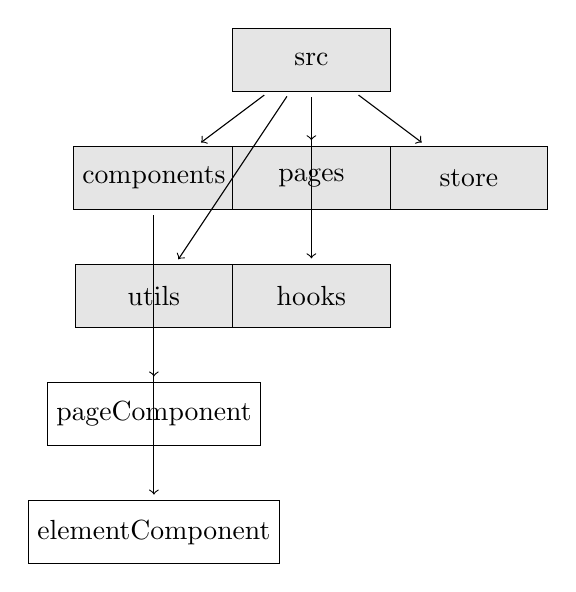
\begin{tikzpicture}[
    file/.style={draw, rectangle, minimum width=2cm, minimum height=0.8cm},
    folder/.style={draw, rectangle, minimum width=2cm, minimum height=0.8cm, fill=gray!20},
    arrow/.style={->, shorten >=2pt, shorten <=2pt}
]

% Folders
\node[folder] (src) at (0,0) {src};
\node[folder] (components) at (-2,-1.5) {components};
\node[folder] (pages) at (0,-1.5) {pages};
\node[folder] (store) at (2,-1.5) {store};
\node[folder] (utils) at (-2,-3) {utils};
\node[folder] (hooks) at (0,-3) {hooks};

% Files
\node[file] (pageComponent) at (-2,-4.5) {pageComponent};
\node[file] (elementComponent) at (-2,-6) {elementComponent};
% ... add more files

% Connections
\draw[arrow] (src) -- (components);
\draw[arrow] (src) -- (pages);
\draw[arrow] (src) -- (store);
\draw[arrow] (src) -- (utils);
\draw[arrow] (src) -- (hooks);
\draw[arrow] (components) -- (pageComponent);
\draw[arrow] (components) -- (elementComponent);
% ... add more connections

\end{tikzpicture}



\pagebreak
\subsubsection{Back-end}
The backend uses the dotNet framework. The development language using the C\# language.

In this project, the backend uses the Onion Architecture.
The Onion Architecture is a typically layered architecture, 
where each layer depends on the inner layer and provides interfaces to the outer layer.
The outer layer provides services to the outermost layer 
and other modules in the same layer based on the interfaces of the inner layer.

From inner to outer, the layers are: Domain, Application, Infrastructure, Presentation.
The Domain layer is the core layer and the innermost layer, used to define domain models, 
which are the business models.
It includes domain models and domain service interfaces.
Domain models are used to define the business models, 
which are the entities in the entity-relationship model and their attributes.
Domain service interfaces are used to define the business services, 
which are the relationships between entities in the entity-relationship model.

The Application layer is the application layer, 
used to define application services, which are the business logic.
It includes domain service implementations and application service interfaces.
Domain service implementations implement the methods of the inner layer's domain service 
interfaces and implement the business logic of the domain models.
Application service interfaces are used to define application services, 
which are the business logic.
It includes but is not limited to database interfaces, testing interfaces, 
HTTP API interfaces, MQTT interfaces, etc.

The Infrastructure layer is the infrastructure layer, used to define infrastructure.
It includes database implementations, testing implementations, 
HTTP API implementations, MQTT implementations, etc.
Database implementations implement the database interfaces 
and provide CRUD services for the database.
Testing implementations implement the testing interfaces 
and provide services for unit testing and integration testing.
HTTP API implementations implement the HTTP API interfaces 
and provide CRUD operations for HTTP APIs.
MQTT implementations implement the MQTT interfaces 
and provide CRUD operations for MQTT.

The Presentation layer is the presentation layer, used to define presentation logic, 
such as interfaces and pages. Since this is a backend project,
data presentation and control are handled by the frontend, 
so this layer is not needed.



\pagebreak
\subsubsection{Data communication and storage}
% 关于本项目的数据通信与数据存储的设计, 包括数据通信的协议, 数据存储的设计等
% 关于数据通信的设计:
% 1. 通信协议的选择
% 自前端向后端发送的数据, 有三种传输的数据类型, 
% 一种是普通的增删改查的请求, 对数据传输的时效性要求不高, 但是对数据的准确性, 完整性, 有序性, 安全性有一定的要求,
% 这种数据的传输, 采用 HTTP 协议, 以及 RESTful API 的设计. 可以有效的保证对数据传输的以上要求.
% 一种是对数据通道的创建和流媒体数据的传输, 对数据传输的时效性, 安全性要求较高, 这种数据的传输, 采用 WebRTC 协议, 以及 MQTT 协议.
% 配合可以快速解码的 flatbuffers 协议, 可以有效的保证对数据传输的以上要求.
% 最后一种是对设备的状态信息和操作信息的传输, 对完整性, 有序性, 安全性都有较高的要求, 这种数据的传输, 采用 MQTT 协议
% 同时也使用了 flatbuffers 协议.
% 
% 2. 数据通信的通信架构和通信流程
% 本项目的数据通信的通信架构, 是基于前后端分离的架构, 前端使用 React 框架, 后端使用 dotnet 框架.
% 当前端需要向后端发送数据的时候, 前端会向后端发送 HTTP 请求, 后端接收到 HTTP 请求之后, 会根据请求的数据类型,
% 选择不同的数据处理方式, 对于普通的增删改查的请求, 后端会根据 RESTful API 的设计, 对数据进行增删改查的操作,
% 对于对数据通道的创建和流媒体数据的传输, 后端会根据 WebRTC 协议, 对数据通道进行创建, 并且帮助前端和设备建立数据通道,
% 当数据通道建立后, 前端和设备之间则使用 flatbuffer 的数据格式对流媒体数据进行传输,
% 对于设备的状态信息和操作信息的传输, 前端会直接向 MQTT broker 发送 MQTT 请求, 
% 设备会在其自身的固件中监听相关的 MQTT 请求, 并且返回相关的数据.
% 
% 3. 数据通信的格式
% 本项目的数据通信的格式, 有三种, 
% 一种是 HTTP 协议, 
% 使用 json 格式对数据进行传输,
% 一种是 WebRTC 协议, 
% 使用 flatbuffers 格式对数据进行传输,
% 一种是 MQTT 协议.
% 使用 flatbuffers 格式对数据进行传输,
% 
% 关于数据存储的设计:
% 1. 数据存储的数据库的选择
% 本项目的数据存储的数据库的选择, 使用了轻量级的数据库 SQLite,
% SQLite 是一个进程内的库, 实现了自给自足的, 无服务器的, 零配置的, 事务性的 SQL 数据库引擎.
% 这是因为整个项目的目的是为了实现前端与设备之间的数据通信, 对于数据库数据的增删改查操作的要求不高,
% 数据量较小, 且对于数据库的数据的事务性要求不高, 所以选择了 SQLite 数据库.
% 2. 项目前后端的数据结构的设计
% 在本项目中, 前端由于使用了 React 框架, 所以前端的数据结构的设计, 使用了基于状态的数据结构的设计,
% 每个组件或者数据集都包含一个状态对象, 这个状态对象的属性就是组件的各个状态. 
% 使用状态对象的原因是, 可以方便的对状态进行管理, 采用对象-属性的形式, 可以方便的针对不同组件的同类状态进行区分,
% 由于跨组件的状态是由 redux 进行管理的, 这种状态对象的设计, 可以更搞笑的对状态进行更新和传递.
% 后端由于使用了 dotnet 框架, 所以后端的数据结构的设计, 使用了基于类的数据结构的设计,
% 采用了面向对象的编程思想, 对数据进行了封装, 使得数据的传输更加的安全, 有序, 完整.


\pagebreak

% \subsection{Domain model}
% \documentclass[]{article}
\usepackage{graphicx}
\usepackage{amsmath}
\usepackage{tikz}

% libaries
\usetikzlibrary{shapes,arrows}

%Define the listing package
\usepackage{listings} %code highlighter
\usepackage{color} %use color
\definecolor{mygreen}{rgb}{0,0.6,0}
\definecolor{mygray}{rgb}{0.5,0.5,0.5}
\definecolor{mymauve}{rgb}{0.58,0,0.82}

%Customize a bit the look
\lstset{ %
backgroundcolor=\color{white}, % choose the background color; you must add \usepackage{color} or \usepackage{xcolor}
basicstyle=\footnotesize, % the size of the fonts that are used for the code
breakatwhitespace=false, % sets if automatic breaks should only happen at whitespace
breaklines=true, % sets automatic line breaking
captionpos=b, % sets the caption-position to bottom
commentstyle=\color{mygreen}, % comment style
deletekeywords={...}, % if you want to delete keywords from the given language
escapeinside={\%*}{*)}, % if you want to add LaTeX within your code
extendedchars=true, % lets you use non-ASCII characters; for 8-bits encodings only, does not work with UTF-8
frame=single, % adds a frame around the code
keepspaces=true, % keeps spaces in text, useful for keeping indentation of code (possibly needs columns=flexible)
keywordstyle=\color{blue}, % keyword style
% language=Octave, % the language of the code
morekeywords={*,...}, % if you want to add more keywords to the set
numbers=left, % where to put the line-numbers; possible values are (none, left, right)
numbersep=5pt, % how far the line-numbers are from the code
numberstyle=\tiny\color{mygray}, % the style that is used for the line-numbers
rulecolor=\color{black}, % if not set, the frame-color may be changed on line-breaks within not-black text (e.g. comments (green here))
showspaces=false, % show spaces everywhere adding particular underscores; it overrides 'showstringspaces'
showstringspaces=false, % underline spaces within strings only
showtabs=false, % show tabs within strings adding particular underscores
stepnumber=1, % the step between two line-numbers. If it's 1, each line will be numbered
stringstyle=\color{mymauve}, % string literal style
tabsize=2, % sets default tabsize to 2 spaces
title=\lstname % show the filename of files included with \lstinputlisting; also try caption instead of title
}

\definecolor{darkgray}{rgb}{.4,.4,.4}
\definecolor{purple}{rgb}{0.65, 0.12, 0.82}

\lstdefinelanguage{React}{
keywords={const, typeof, new, true, false, catch, function, return, null, catch, switch, var, if, in, while, do, else, case, break},
keywordstyle=\color{blue}\bfseries,
ndkeywords={class, export, boolean, throw, implements, import, this},
ndkeywordstyle=\color{darkgray}\bfseries,
identifierstyle=\color{mygreen},
sensitive=false,
comment=[l]{//},
morecomment=[s]{/*}{*/},
commentstyle=\color{purple}\ttfamily,
string=[b]{"}{'}{`},
stringstyle=\color{red}\ttfamily,
morestring=[b]',
morestring=[b]",
morestring=[b]`',
}

\lstdefinelanguage{CSharp}{
keywords={const, typeof, new, true, false, catch, function, return, null, catch, switch, var, if, in, while, do, else, case, break},
keywordstyle=\color{blue}\bfseries,
ndkeywords={class, export, boolean, throw, implements, import, this},
ndkeywordstyle=\color{darkgray}\bfseries,
identifierstyle=\color{mygreen},
sensitive=false,
comment=[l]{//},
morecomment=[s]{/*}{*/},
commentstyle=\color{purple}\ttfamily,
string=[b]{"}{'}{`},
stringstyle=\color{red}\ttfamily,
morestring=[b]',
morestring=[b]",
morestring=[b]`',
}

\lstset{
language=React,
extendedchars=true,
basicstyle=\footnotesize\ttfamily,
showstringspaces=false,
showspaces=false,
numbers=left,
numberstyle=\footnotesize,
numbersep=9pt,
tabsize=2,
breaklines=true,
showtabs=false,
captionpos=b
}

\lstset{
language=CSharp,
extendedchars=true,
basicstyle=\footnotesize\ttfamily,
showstringspaces=false,
showspaces=false,
numbers=left,
numberstyle=\footnotesize,
numbersep=9pt,
tabsize=2,
breaklines=true,
showtabs=false,
captionpos=b
}

% \usepackage{cite} % Add this line for citation

% \bibliographystyle{plain}

\title{
The implementation of BifrostConnect Front-end scope, 
re-design and development with the relevant back-end support develop.
}
\author{
    Fei Gu \\
    Erhvervs Akademi Sydvest \\
    Computer Science 21\\
    }
\date{\today}

\begin{document}

% Front page
\maketitle
\begin{center}
    Supervisor: Henrik Boulund Meng Hansen \\
    Company: BifrostConnect \\
    Engineering Director: Jasper Wass \\
\end{center}
\tableofcontents
\pagebreak


% The introduction
\section{Introduction}
\subsection{Background}\input{sections/introduction/background.tex}
\subsection{The company}\input{sections/introduction/aboutCompany}
\subsection{The project}\input{sections/introduction/aboutProject}
\pagebreak

% The problem statement
\section{Problem Statement}
\subsection{Statement}
\input{sections/problemStatement/statement}
\subsection{Situation}
\input{sections/problemStatement/situation}
\subsection{Potential Solution}
\input{sections/problemStatement/potentialSolution}
\pagebreak

% Requirement analysis
\section{Requirement Analysis}
\input{sections/requirementAnalysis/index}

\subsection{Stakeholders}
\input{sections/requirementAnalysis/stakeholders/index}

\subsection{Business Domain}
\input{sections/requirementAnalysis/bussinesDomain/index}

\subsection{Scope}
\input{sections/requirementAnalysis/scope}

\subsection{Goals}
\input{sections/requirementAnalysis/goals}
\pagebreak

% Software Design
\section{Software Design}
% developement methods
\subsection{Software Development Methods}
\input{sections/softwareDevelopmentMethods/index}
\subsubsection{Agile Software Development}
\input{sections/softwareDevelopmentMethods/agileSoftwareDevelopment/index}
\subsubsection{Feature Driven Development}
\input{sections/softwareDevelopmentMethods/featureDrivenDevelopment/index}

\pagebreak

% Technology seslection
\subsection{Technology selection}
\input{sections/softwareDesign/technologySelection/index}
\subsubsection{Front-end}
\input{sections/softwareDesign/technologySelection/frontEnd}            
\subsubsection{Back-end}
\input{sections/softwareDesign/technologySelection/backEnd}            
\subsubsection{Database}
\input{sections/softwareDesign/technologySelection/database}
\subsubsection{Data communication}
\input{sections/softwareDesign/technologySelection/dataCommunication}            
\subsubsection{DevOps}
\input{sections/softwareDesign/technologySelection/devOps}
\pagebreak

% Architecture design
\subsection{Architecture design}
\input{sections/softwareDesign/architectureDesign/index}
\pagebreak
\subsubsection{Front-end}
\input{sections/softwareDesign/architectureDesign/frontEndArchitecture}
\pagebreak
\subsubsection{Back-end}
\input{sections/softwareDesign/architectureDesign/backEndArchitecture}
\pagebreak
\subsubsection{Data communication and storage}
\input{sections/softwareDesign/architectureDesign/dataCommunicationArchitecture}
\pagebreak

% \subsection{Domain model}
% \input{sections/softwareDesign/domainModel/index}
% \subsection{Database design}
% % 数据库领域模型 ER 图
% % 包括表和字段的设置.
% % 对于私有键和外键的设置.

% \subsection{Back-end design}
% % 后端对象模型
% % 以及对于对象模型的增删改查
% % 以及相关的其他服务的设计`'

% \subsection{Front-end design}
% % 对于前端的页面结构的设计 
% % 页面的状态的设计, 交互设计

% \subsection{FlatBuffers design}
% % schema 的设计

\subsection{DevOps CI/CD process design}
\input{sections/softwareDesign/devOpsDesign/index}
\subsubsection{Continuous Integration}
\input{sections/softwareDesign/devOpsDesign/continuousIntegration/index}
\subsubsection{Continuous Delivery}
\input{sections/softwareDesign/devOpsDesign/continuousDelivery/index}
\subsubsection{Continuous Deployment}
\input{sections/softwareDesign/devOpsDesign/continuousDeployment/index}
\pagebreak

\section{Software Development} 
\input{sections/softwareDevelopment/index}
\subsection{Overall development}
\input{sections/softwareDevelopment/overallDevelopement/index}
\subsubsection{Front-end}
\input{sections/softwareDevelopment/overallDevelopement/frontEnd/index}
\subsubsection{Back-end}
\input{sections/softwareDevelopment/overallDevelopement/backEnd/index}
\subsubsection{DevOps}
\input{sections/softwareDevelopment/overallDevelopement/devOps/index}
\subsection{Feature development} 
\input{sections/softwareDevelopment/featureDevelopment/index}
\subsubsection{Use Case 1}
\input{sections/softwareDevelopment/featureDevelopment/useCase1/index}
\subsubsection{Feature 1}
\input{sections/softwareDevelopment/featureDevelopment/feature/feature1.tex}
\pagebreak
\section{Conclusion} 
\subsection{Result}
Since the project is still in progress, the result is not available yet.
So far, basic structure of this project has been built. But the most features 
are not implemented yet. 
\subsection{Discussion}
As a single developer for this project, I am confident what I have done so far.
And I can say I understand the most of the knowledge I have used in this project, 
which also means I can explain all the part of the project. 
But this project also relevant some of the complex knowledge which I have to continue 
to study and practice.
\subsection{Future Work}
The future work is to implement the rest of the features. 
Including the most important part which is the 'create session' feature.
\pagebreak
% \bibliography{bibliography}
\pagebreak
% \begin{appendices}
%     \section{Appendix}
% \end{appendices} 
\end{document}
% \subsection{Database design}
% % 数据库领域模型 ER 图
% % 包括表和字段的设置.
% % 对于私有键和外键的设置.

% \subsection{Back-end design}
% % 后端对象模型
% % 以及对于对象模型的增删改查
% % 以及相关的其他服务的设计`'

% \subsection{Front-end design}
% % 对于前端的页面结构的设计 
% % 页面的状态的设计, 交互设计

% \subsection{FlatBuffers design}
% % schema 的设计

\subsection{DevOps CI/CD process design}
\documentclass[]{article}
\usepackage{graphicx}
\usepackage{amsmath}
\usepackage{tikz}

% libaries
\usetikzlibrary{shapes,arrows}

%Define the listing package
\usepackage{listings} %code highlighter
\usepackage{color} %use color
\definecolor{mygreen}{rgb}{0,0.6,0}
\definecolor{mygray}{rgb}{0.5,0.5,0.5}
\definecolor{mymauve}{rgb}{0.58,0,0.82}

%Customize a bit the look
\lstset{ %
backgroundcolor=\color{white}, % choose the background color; you must add \usepackage{color} or \usepackage{xcolor}
basicstyle=\footnotesize, % the size of the fonts that are used for the code
breakatwhitespace=false, % sets if automatic breaks should only happen at whitespace
breaklines=true, % sets automatic line breaking
captionpos=b, % sets the caption-position to bottom
commentstyle=\color{mygreen}, % comment style
deletekeywords={...}, % if you want to delete keywords from the given language
escapeinside={\%*}{*)}, % if you want to add LaTeX within your code
extendedchars=true, % lets you use non-ASCII characters; for 8-bits encodings only, does not work with UTF-8
frame=single, % adds a frame around the code
keepspaces=true, % keeps spaces in text, useful for keeping indentation of code (possibly needs columns=flexible)
keywordstyle=\color{blue}, % keyword style
% language=Octave, % the language of the code
morekeywords={*,...}, % if you want to add more keywords to the set
numbers=left, % where to put the line-numbers; possible values are (none, left, right)
numbersep=5pt, % how far the line-numbers are from the code
numberstyle=\tiny\color{mygray}, % the style that is used for the line-numbers
rulecolor=\color{black}, % if not set, the frame-color may be changed on line-breaks within not-black text (e.g. comments (green here))
showspaces=false, % show spaces everywhere adding particular underscores; it overrides 'showstringspaces'
showstringspaces=false, % underline spaces within strings only
showtabs=false, % show tabs within strings adding particular underscores
stepnumber=1, % the step between two line-numbers. If it's 1, each line will be numbered
stringstyle=\color{mymauve}, % string literal style
tabsize=2, % sets default tabsize to 2 spaces
title=\lstname % show the filename of files included with \lstinputlisting; also try caption instead of title
}

\definecolor{darkgray}{rgb}{.4,.4,.4}
\definecolor{purple}{rgb}{0.65, 0.12, 0.82}

\lstdefinelanguage{React}{
keywords={const, typeof, new, true, false, catch, function, return, null, catch, switch, var, if, in, while, do, else, case, break},
keywordstyle=\color{blue}\bfseries,
ndkeywords={class, export, boolean, throw, implements, import, this},
ndkeywordstyle=\color{darkgray}\bfseries,
identifierstyle=\color{mygreen},
sensitive=false,
comment=[l]{//},
morecomment=[s]{/*}{*/},
commentstyle=\color{purple}\ttfamily,
string=[b]{"}{'}{`},
stringstyle=\color{red}\ttfamily,
morestring=[b]',
morestring=[b]",
morestring=[b]`',
}

\lstdefinelanguage{CSharp}{
keywords={const, typeof, new, true, false, catch, function, return, null, catch, switch, var, if, in, while, do, else, case, break},
keywordstyle=\color{blue}\bfseries,
ndkeywords={class, export, boolean, throw, implements, import, this},
ndkeywordstyle=\color{darkgray}\bfseries,
identifierstyle=\color{mygreen},
sensitive=false,
comment=[l]{//},
morecomment=[s]{/*}{*/},
commentstyle=\color{purple}\ttfamily,
string=[b]{"}{'}{`},
stringstyle=\color{red}\ttfamily,
morestring=[b]',
morestring=[b]",
morestring=[b]`',
}

\lstset{
language=React,
extendedchars=true,
basicstyle=\footnotesize\ttfamily,
showstringspaces=false,
showspaces=false,
numbers=left,
numberstyle=\footnotesize,
numbersep=9pt,
tabsize=2,
breaklines=true,
showtabs=false,
captionpos=b
}

\lstset{
language=CSharp,
extendedchars=true,
basicstyle=\footnotesize\ttfamily,
showstringspaces=false,
showspaces=false,
numbers=left,
numberstyle=\footnotesize,
numbersep=9pt,
tabsize=2,
breaklines=true,
showtabs=false,
captionpos=b
}

% \usepackage{cite} % Add this line for citation

% \bibliographystyle{plain}

\title{
The implementation of BifrostConnect Front-end scope, 
re-design and development with the relevant back-end support develop.
}
\author{
    Fei Gu \\
    Erhvervs Akademi Sydvest \\
    Computer Science 21\\
    }
\date{\today}

\begin{document}

% Front page
\maketitle
\begin{center}
    Supervisor: Henrik Boulund Meng Hansen \\
    Company: BifrostConnect \\
    Engineering Director: Jasper Wass \\
\end{center}
\tableofcontents
\pagebreak


% The introduction
\section{Introduction}
\subsection{Background}\input{sections/introduction/background.tex}
\subsection{The company}\input{sections/introduction/aboutCompany}
\subsection{The project}\input{sections/introduction/aboutProject}
\pagebreak

% The problem statement
\section{Problem Statement}
\subsection{Statement}
\input{sections/problemStatement/statement}
\subsection{Situation}
\input{sections/problemStatement/situation}
\subsection{Potential Solution}
\input{sections/problemStatement/potentialSolution}
\pagebreak

% Requirement analysis
\section{Requirement Analysis}
\input{sections/requirementAnalysis/index}

\subsection{Stakeholders}
\input{sections/requirementAnalysis/stakeholders/index}

\subsection{Business Domain}
\input{sections/requirementAnalysis/bussinesDomain/index}

\subsection{Scope}
\input{sections/requirementAnalysis/scope}

\subsection{Goals}
\input{sections/requirementAnalysis/goals}
\pagebreak

% Software Design
\section{Software Design}
% developement methods
\subsection{Software Development Methods}
\input{sections/softwareDevelopmentMethods/index}
\subsubsection{Agile Software Development}
\input{sections/softwareDevelopmentMethods/agileSoftwareDevelopment/index}
\subsubsection{Feature Driven Development}
\input{sections/softwareDevelopmentMethods/featureDrivenDevelopment/index}

\pagebreak

% Technology seslection
\subsection{Technology selection}
\input{sections/softwareDesign/technologySelection/index}
\subsubsection{Front-end}
\input{sections/softwareDesign/technologySelection/frontEnd}            
\subsubsection{Back-end}
\input{sections/softwareDesign/technologySelection/backEnd}            
\subsubsection{Database}
\input{sections/softwareDesign/technologySelection/database}
\subsubsection{Data communication}
\input{sections/softwareDesign/technologySelection/dataCommunication}            
\subsubsection{DevOps}
\input{sections/softwareDesign/technologySelection/devOps}
\pagebreak

% Architecture design
\subsection{Architecture design}
\input{sections/softwareDesign/architectureDesign/index}
\pagebreak
\subsubsection{Front-end}
\input{sections/softwareDesign/architectureDesign/frontEndArchitecture}
\pagebreak
\subsubsection{Back-end}
\input{sections/softwareDesign/architectureDesign/backEndArchitecture}
\pagebreak
\subsubsection{Data communication and storage}
\input{sections/softwareDesign/architectureDesign/dataCommunicationArchitecture}
\pagebreak

% \subsection{Domain model}
% \input{sections/softwareDesign/domainModel/index}
% \subsection{Database design}
% % 数据库领域模型 ER 图
% % 包括表和字段的设置.
% % 对于私有键和外键的设置.

% \subsection{Back-end design}
% % 后端对象模型
% % 以及对于对象模型的增删改查
% % 以及相关的其他服务的设计`'

% \subsection{Front-end design}
% % 对于前端的页面结构的设计 
% % 页面的状态的设计, 交互设计

% \subsection{FlatBuffers design}
% % schema 的设计

\subsection{DevOps CI/CD process design}
\input{sections/softwareDesign/devOpsDesign/index}
\subsubsection{Continuous Integration}
\input{sections/softwareDesign/devOpsDesign/continuousIntegration/index}
\subsubsection{Continuous Delivery}
\input{sections/softwareDesign/devOpsDesign/continuousDelivery/index}
\subsubsection{Continuous Deployment}
\input{sections/softwareDesign/devOpsDesign/continuousDeployment/index}
\pagebreak

\section{Software Development} 
\input{sections/softwareDevelopment/index}
\subsection{Overall development}
\input{sections/softwareDevelopment/overallDevelopement/index}
\subsubsection{Front-end}
\input{sections/softwareDevelopment/overallDevelopement/frontEnd/index}
\subsubsection{Back-end}
\input{sections/softwareDevelopment/overallDevelopement/backEnd/index}
\subsubsection{DevOps}
\input{sections/softwareDevelopment/overallDevelopement/devOps/index}
\subsection{Feature development} 
\input{sections/softwareDevelopment/featureDevelopment/index}
\subsubsection{Use Case 1}
\input{sections/softwareDevelopment/featureDevelopment/useCase1/index}
\subsubsection{Feature 1}
\input{sections/softwareDevelopment/featureDevelopment/feature/feature1.tex}
\pagebreak
\section{Conclusion} 
\subsection{Result}
Since the project is still in progress, the result is not available yet.
So far, basic structure of this project has been built. But the most features 
are not implemented yet. 
\subsection{Discussion}
As a single developer for this project, I am confident what I have done so far.
And I can say I understand the most of the knowledge I have used in this project, 
which also means I can explain all the part of the project. 
But this project also relevant some of the complex knowledge which I have to continue 
to study and practice.
\subsection{Future Work}
The future work is to implement the rest of the features. 
Including the most important part which is the 'create session' feature.
\pagebreak
% \bibliography{bibliography}
\pagebreak
% \begin{appendices}
%     \section{Appendix}
% \end{appendices} 
\end{document}
\subsubsection{Continuous Integration}
\documentclass[]{article}
\usepackage{graphicx}
\usepackage{amsmath}
\usepackage{tikz}

% libaries
\usetikzlibrary{shapes,arrows}

%Define the listing package
\usepackage{listings} %code highlighter
\usepackage{color} %use color
\definecolor{mygreen}{rgb}{0,0.6,0}
\definecolor{mygray}{rgb}{0.5,0.5,0.5}
\definecolor{mymauve}{rgb}{0.58,0,0.82}

%Customize a bit the look
\lstset{ %
backgroundcolor=\color{white}, % choose the background color; you must add \usepackage{color} or \usepackage{xcolor}
basicstyle=\footnotesize, % the size of the fonts that are used for the code
breakatwhitespace=false, % sets if automatic breaks should only happen at whitespace
breaklines=true, % sets automatic line breaking
captionpos=b, % sets the caption-position to bottom
commentstyle=\color{mygreen}, % comment style
deletekeywords={...}, % if you want to delete keywords from the given language
escapeinside={\%*}{*)}, % if you want to add LaTeX within your code
extendedchars=true, % lets you use non-ASCII characters; for 8-bits encodings only, does not work with UTF-8
frame=single, % adds a frame around the code
keepspaces=true, % keeps spaces in text, useful for keeping indentation of code (possibly needs columns=flexible)
keywordstyle=\color{blue}, % keyword style
% language=Octave, % the language of the code
morekeywords={*,...}, % if you want to add more keywords to the set
numbers=left, % where to put the line-numbers; possible values are (none, left, right)
numbersep=5pt, % how far the line-numbers are from the code
numberstyle=\tiny\color{mygray}, % the style that is used for the line-numbers
rulecolor=\color{black}, % if not set, the frame-color may be changed on line-breaks within not-black text (e.g. comments (green here))
showspaces=false, % show spaces everywhere adding particular underscores; it overrides 'showstringspaces'
showstringspaces=false, % underline spaces within strings only
showtabs=false, % show tabs within strings adding particular underscores
stepnumber=1, % the step between two line-numbers. If it's 1, each line will be numbered
stringstyle=\color{mymauve}, % string literal style
tabsize=2, % sets default tabsize to 2 spaces
title=\lstname % show the filename of files included with \lstinputlisting; also try caption instead of title
}

\definecolor{darkgray}{rgb}{.4,.4,.4}
\definecolor{purple}{rgb}{0.65, 0.12, 0.82}

\lstdefinelanguage{React}{
keywords={const, typeof, new, true, false, catch, function, return, null, catch, switch, var, if, in, while, do, else, case, break},
keywordstyle=\color{blue}\bfseries,
ndkeywords={class, export, boolean, throw, implements, import, this},
ndkeywordstyle=\color{darkgray}\bfseries,
identifierstyle=\color{mygreen},
sensitive=false,
comment=[l]{//},
morecomment=[s]{/*}{*/},
commentstyle=\color{purple}\ttfamily,
string=[b]{"}{'}{`},
stringstyle=\color{red}\ttfamily,
morestring=[b]',
morestring=[b]",
morestring=[b]`',
}

\lstdefinelanguage{CSharp}{
keywords={const, typeof, new, true, false, catch, function, return, null, catch, switch, var, if, in, while, do, else, case, break},
keywordstyle=\color{blue}\bfseries,
ndkeywords={class, export, boolean, throw, implements, import, this},
ndkeywordstyle=\color{darkgray}\bfseries,
identifierstyle=\color{mygreen},
sensitive=false,
comment=[l]{//},
morecomment=[s]{/*}{*/},
commentstyle=\color{purple}\ttfamily,
string=[b]{"}{'}{`},
stringstyle=\color{red}\ttfamily,
morestring=[b]',
morestring=[b]",
morestring=[b]`',
}

\lstset{
language=React,
extendedchars=true,
basicstyle=\footnotesize\ttfamily,
showstringspaces=false,
showspaces=false,
numbers=left,
numberstyle=\footnotesize,
numbersep=9pt,
tabsize=2,
breaklines=true,
showtabs=false,
captionpos=b
}

\lstset{
language=CSharp,
extendedchars=true,
basicstyle=\footnotesize\ttfamily,
showstringspaces=false,
showspaces=false,
numbers=left,
numberstyle=\footnotesize,
numbersep=9pt,
tabsize=2,
breaklines=true,
showtabs=false,
captionpos=b
}

% \usepackage{cite} % Add this line for citation

% \bibliographystyle{plain}

\title{
The implementation of BifrostConnect Front-end scope, 
re-design and development with the relevant back-end support develop.
}
\author{
    Fei Gu \\
    Erhvervs Akademi Sydvest \\
    Computer Science 21\\
    }
\date{\today}

\begin{document}

% Front page
\maketitle
\begin{center}
    Supervisor: Henrik Boulund Meng Hansen \\
    Company: BifrostConnect \\
    Engineering Director: Jasper Wass \\
\end{center}
\tableofcontents
\pagebreak


% The introduction
\section{Introduction}
\subsection{Background}\input{sections/introduction/background.tex}
\subsection{The company}\input{sections/introduction/aboutCompany}
\subsection{The project}\input{sections/introduction/aboutProject}
\pagebreak

% The problem statement
\section{Problem Statement}
\subsection{Statement}
\input{sections/problemStatement/statement}
\subsection{Situation}
\input{sections/problemStatement/situation}
\subsection{Potential Solution}
\input{sections/problemStatement/potentialSolution}
\pagebreak

% Requirement analysis
\section{Requirement Analysis}
\input{sections/requirementAnalysis/index}

\subsection{Stakeholders}
\input{sections/requirementAnalysis/stakeholders/index}

\subsection{Business Domain}
\input{sections/requirementAnalysis/bussinesDomain/index}

\subsection{Scope}
\input{sections/requirementAnalysis/scope}

\subsection{Goals}
\input{sections/requirementAnalysis/goals}
\pagebreak

% Software Design
\section{Software Design}
% developement methods
\subsection{Software Development Methods}
\input{sections/softwareDevelopmentMethods/index}
\subsubsection{Agile Software Development}
\input{sections/softwareDevelopmentMethods/agileSoftwareDevelopment/index}
\subsubsection{Feature Driven Development}
\input{sections/softwareDevelopmentMethods/featureDrivenDevelopment/index}

\pagebreak

% Technology seslection
\subsection{Technology selection}
\input{sections/softwareDesign/technologySelection/index}
\subsubsection{Front-end}
\input{sections/softwareDesign/technologySelection/frontEnd}            
\subsubsection{Back-end}
\input{sections/softwareDesign/technologySelection/backEnd}            
\subsubsection{Database}
\input{sections/softwareDesign/technologySelection/database}
\subsubsection{Data communication}
\input{sections/softwareDesign/technologySelection/dataCommunication}            
\subsubsection{DevOps}
\input{sections/softwareDesign/technologySelection/devOps}
\pagebreak

% Architecture design
\subsection{Architecture design}
\input{sections/softwareDesign/architectureDesign/index}
\pagebreak
\subsubsection{Front-end}
\input{sections/softwareDesign/architectureDesign/frontEndArchitecture}
\pagebreak
\subsubsection{Back-end}
\input{sections/softwareDesign/architectureDesign/backEndArchitecture}
\pagebreak
\subsubsection{Data communication and storage}
\input{sections/softwareDesign/architectureDesign/dataCommunicationArchitecture}
\pagebreak

% \subsection{Domain model}
% \input{sections/softwareDesign/domainModel/index}
% \subsection{Database design}
% % 数据库领域模型 ER 图
% % 包括表和字段的设置.
% % 对于私有键和外键的设置.

% \subsection{Back-end design}
% % 后端对象模型
% % 以及对于对象模型的增删改查
% % 以及相关的其他服务的设计`'

% \subsection{Front-end design}
% % 对于前端的页面结构的设计 
% % 页面的状态的设计, 交互设计

% \subsection{FlatBuffers design}
% % schema 的设计

\subsection{DevOps CI/CD process design}
\input{sections/softwareDesign/devOpsDesign/index}
\subsubsection{Continuous Integration}
\input{sections/softwareDesign/devOpsDesign/continuousIntegration/index}
\subsubsection{Continuous Delivery}
\input{sections/softwareDesign/devOpsDesign/continuousDelivery/index}
\subsubsection{Continuous Deployment}
\input{sections/softwareDesign/devOpsDesign/continuousDeployment/index}
\pagebreak

\section{Software Development} 
\input{sections/softwareDevelopment/index}
\subsection{Overall development}
\input{sections/softwareDevelopment/overallDevelopement/index}
\subsubsection{Front-end}
\input{sections/softwareDevelopment/overallDevelopement/frontEnd/index}
\subsubsection{Back-end}
\input{sections/softwareDevelopment/overallDevelopement/backEnd/index}
\subsubsection{DevOps}
\input{sections/softwareDevelopment/overallDevelopement/devOps/index}
\subsection{Feature development} 
\input{sections/softwareDevelopment/featureDevelopment/index}
\subsubsection{Use Case 1}
\input{sections/softwareDevelopment/featureDevelopment/useCase1/index}
\subsubsection{Feature 1}
\input{sections/softwareDevelopment/featureDevelopment/feature/feature1.tex}
\pagebreak
\section{Conclusion} 
\subsection{Result}
Since the project is still in progress, the result is not available yet.
So far, basic structure of this project has been built. But the most features 
are not implemented yet. 
\subsection{Discussion}
As a single developer for this project, I am confident what I have done so far.
And I can say I understand the most of the knowledge I have used in this project, 
which also means I can explain all the part of the project. 
But this project also relevant some of the complex knowledge which I have to continue 
to study and practice.
\subsection{Future Work}
The future work is to implement the rest of the features. 
Including the most important part which is the 'create session' feature.
\pagebreak
% \bibliography{bibliography}
\pagebreak
% \begin{appendices}
%     \section{Appendix}
% \end{appendices} 
\end{document}
\subsubsection{Continuous Delivery}
\documentclass[]{article}
\usepackage{graphicx}
\usepackage{amsmath}
\usepackage{tikz}

% libaries
\usetikzlibrary{shapes,arrows}

%Define the listing package
\usepackage{listings} %code highlighter
\usepackage{color} %use color
\definecolor{mygreen}{rgb}{0,0.6,0}
\definecolor{mygray}{rgb}{0.5,0.5,0.5}
\definecolor{mymauve}{rgb}{0.58,0,0.82}

%Customize a bit the look
\lstset{ %
backgroundcolor=\color{white}, % choose the background color; you must add \usepackage{color} or \usepackage{xcolor}
basicstyle=\footnotesize, % the size of the fonts that are used for the code
breakatwhitespace=false, % sets if automatic breaks should only happen at whitespace
breaklines=true, % sets automatic line breaking
captionpos=b, % sets the caption-position to bottom
commentstyle=\color{mygreen}, % comment style
deletekeywords={...}, % if you want to delete keywords from the given language
escapeinside={\%*}{*)}, % if you want to add LaTeX within your code
extendedchars=true, % lets you use non-ASCII characters; for 8-bits encodings only, does not work with UTF-8
frame=single, % adds a frame around the code
keepspaces=true, % keeps spaces in text, useful for keeping indentation of code (possibly needs columns=flexible)
keywordstyle=\color{blue}, % keyword style
% language=Octave, % the language of the code
morekeywords={*,...}, % if you want to add more keywords to the set
numbers=left, % where to put the line-numbers; possible values are (none, left, right)
numbersep=5pt, % how far the line-numbers are from the code
numberstyle=\tiny\color{mygray}, % the style that is used for the line-numbers
rulecolor=\color{black}, % if not set, the frame-color may be changed on line-breaks within not-black text (e.g. comments (green here))
showspaces=false, % show spaces everywhere adding particular underscores; it overrides 'showstringspaces'
showstringspaces=false, % underline spaces within strings only
showtabs=false, % show tabs within strings adding particular underscores
stepnumber=1, % the step between two line-numbers. If it's 1, each line will be numbered
stringstyle=\color{mymauve}, % string literal style
tabsize=2, % sets default tabsize to 2 spaces
title=\lstname % show the filename of files included with \lstinputlisting; also try caption instead of title
}

\definecolor{darkgray}{rgb}{.4,.4,.4}
\definecolor{purple}{rgb}{0.65, 0.12, 0.82}

\lstdefinelanguage{React}{
keywords={const, typeof, new, true, false, catch, function, return, null, catch, switch, var, if, in, while, do, else, case, break},
keywordstyle=\color{blue}\bfseries,
ndkeywords={class, export, boolean, throw, implements, import, this},
ndkeywordstyle=\color{darkgray}\bfseries,
identifierstyle=\color{mygreen},
sensitive=false,
comment=[l]{//},
morecomment=[s]{/*}{*/},
commentstyle=\color{purple}\ttfamily,
string=[b]{"}{'}{`},
stringstyle=\color{red}\ttfamily,
morestring=[b]',
morestring=[b]",
morestring=[b]`',
}

\lstdefinelanguage{CSharp}{
keywords={const, typeof, new, true, false, catch, function, return, null, catch, switch, var, if, in, while, do, else, case, break},
keywordstyle=\color{blue}\bfseries,
ndkeywords={class, export, boolean, throw, implements, import, this},
ndkeywordstyle=\color{darkgray}\bfseries,
identifierstyle=\color{mygreen},
sensitive=false,
comment=[l]{//},
morecomment=[s]{/*}{*/},
commentstyle=\color{purple}\ttfamily,
string=[b]{"}{'}{`},
stringstyle=\color{red}\ttfamily,
morestring=[b]',
morestring=[b]",
morestring=[b]`',
}

\lstset{
language=React,
extendedchars=true,
basicstyle=\footnotesize\ttfamily,
showstringspaces=false,
showspaces=false,
numbers=left,
numberstyle=\footnotesize,
numbersep=9pt,
tabsize=2,
breaklines=true,
showtabs=false,
captionpos=b
}

\lstset{
language=CSharp,
extendedchars=true,
basicstyle=\footnotesize\ttfamily,
showstringspaces=false,
showspaces=false,
numbers=left,
numberstyle=\footnotesize,
numbersep=9pt,
tabsize=2,
breaklines=true,
showtabs=false,
captionpos=b
}

% \usepackage{cite} % Add this line for citation

% \bibliographystyle{plain}

\title{
The implementation of BifrostConnect Front-end scope, 
re-design and development with the relevant back-end support develop.
}
\author{
    Fei Gu \\
    Erhvervs Akademi Sydvest \\
    Computer Science 21\\
    }
\date{\today}

\begin{document}

% Front page
\maketitle
\begin{center}
    Supervisor: Henrik Boulund Meng Hansen \\
    Company: BifrostConnect \\
    Engineering Director: Jasper Wass \\
\end{center}
\tableofcontents
\pagebreak


% The introduction
\section{Introduction}
\subsection{Background}\input{sections/introduction/background.tex}
\subsection{The company}\input{sections/introduction/aboutCompany}
\subsection{The project}\input{sections/introduction/aboutProject}
\pagebreak

% The problem statement
\section{Problem Statement}
\subsection{Statement}
\input{sections/problemStatement/statement}
\subsection{Situation}
\input{sections/problemStatement/situation}
\subsection{Potential Solution}
\input{sections/problemStatement/potentialSolution}
\pagebreak

% Requirement analysis
\section{Requirement Analysis}
\input{sections/requirementAnalysis/index}

\subsection{Stakeholders}
\input{sections/requirementAnalysis/stakeholders/index}

\subsection{Business Domain}
\input{sections/requirementAnalysis/bussinesDomain/index}

\subsection{Scope}
\input{sections/requirementAnalysis/scope}

\subsection{Goals}
\input{sections/requirementAnalysis/goals}
\pagebreak

% Software Design
\section{Software Design}
% developement methods
\subsection{Software Development Methods}
\input{sections/softwareDevelopmentMethods/index}
\subsubsection{Agile Software Development}
\input{sections/softwareDevelopmentMethods/agileSoftwareDevelopment/index}
\subsubsection{Feature Driven Development}
\input{sections/softwareDevelopmentMethods/featureDrivenDevelopment/index}

\pagebreak

% Technology seslection
\subsection{Technology selection}
\input{sections/softwareDesign/technologySelection/index}
\subsubsection{Front-end}
\input{sections/softwareDesign/technologySelection/frontEnd}            
\subsubsection{Back-end}
\input{sections/softwareDesign/technologySelection/backEnd}            
\subsubsection{Database}
\input{sections/softwareDesign/technologySelection/database}
\subsubsection{Data communication}
\input{sections/softwareDesign/technologySelection/dataCommunication}            
\subsubsection{DevOps}
\input{sections/softwareDesign/technologySelection/devOps}
\pagebreak

% Architecture design
\subsection{Architecture design}
\input{sections/softwareDesign/architectureDesign/index}
\pagebreak
\subsubsection{Front-end}
\input{sections/softwareDesign/architectureDesign/frontEndArchitecture}
\pagebreak
\subsubsection{Back-end}
\input{sections/softwareDesign/architectureDesign/backEndArchitecture}
\pagebreak
\subsubsection{Data communication and storage}
\input{sections/softwareDesign/architectureDesign/dataCommunicationArchitecture}
\pagebreak

% \subsection{Domain model}
% \input{sections/softwareDesign/domainModel/index}
% \subsection{Database design}
% % 数据库领域模型 ER 图
% % 包括表和字段的设置.
% % 对于私有键和外键的设置.

% \subsection{Back-end design}
% % 后端对象模型
% % 以及对于对象模型的增删改查
% % 以及相关的其他服务的设计`'

% \subsection{Front-end design}
% % 对于前端的页面结构的设计 
% % 页面的状态的设计, 交互设计

% \subsection{FlatBuffers design}
% % schema 的设计

\subsection{DevOps CI/CD process design}
\input{sections/softwareDesign/devOpsDesign/index}
\subsubsection{Continuous Integration}
\input{sections/softwareDesign/devOpsDesign/continuousIntegration/index}
\subsubsection{Continuous Delivery}
\input{sections/softwareDesign/devOpsDesign/continuousDelivery/index}
\subsubsection{Continuous Deployment}
\input{sections/softwareDesign/devOpsDesign/continuousDeployment/index}
\pagebreak

\section{Software Development} 
\input{sections/softwareDevelopment/index}
\subsection{Overall development}
\input{sections/softwareDevelopment/overallDevelopement/index}
\subsubsection{Front-end}
\input{sections/softwareDevelopment/overallDevelopement/frontEnd/index}
\subsubsection{Back-end}
\input{sections/softwareDevelopment/overallDevelopement/backEnd/index}
\subsubsection{DevOps}
\input{sections/softwareDevelopment/overallDevelopement/devOps/index}
\subsection{Feature development} 
\input{sections/softwareDevelopment/featureDevelopment/index}
\subsubsection{Use Case 1}
\input{sections/softwareDevelopment/featureDevelopment/useCase1/index}
\subsubsection{Feature 1}
\input{sections/softwareDevelopment/featureDevelopment/feature/feature1.tex}
\pagebreak
\section{Conclusion} 
\subsection{Result}
Since the project is still in progress, the result is not available yet.
So far, basic structure of this project has been built. But the most features 
are not implemented yet. 
\subsection{Discussion}
As a single developer for this project, I am confident what I have done so far.
And I can say I understand the most of the knowledge I have used in this project, 
which also means I can explain all the part of the project. 
But this project also relevant some of the complex knowledge which I have to continue 
to study and practice.
\subsection{Future Work}
The future work is to implement the rest of the features. 
Including the most important part which is the 'create session' feature.
\pagebreak
% \bibliography{bibliography}
\pagebreak
% \begin{appendices}
%     \section{Appendix}
% \end{appendices} 
\end{document}
\subsubsection{Continuous Deployment}
\documentclass[]{article}
\usepackage{graphicx}
\usepackage{amsmath}
\usepackage{tikz}

% libaries
\usetikzlibrary{shapes,arrows}

%Define the listing package
\usepackage{listings} %code highlighter
\usepackage{color} %use color
\definecolor{mygreen}{rgb}{0,0.6,0}
\definecolor{mygray}{rgb}{0.5,0.5,0.5}
\definecolor{mymauve}{rgb}{0.58,0,0.82}

%Customize a bit the look
\lstset{ %
backgroundcolor=\color{white}, % choose the background color; you must add \usepackage{color} or \usepackage{xcolor}
basicstyle=\footnotesize, % the size of the fonts that are used for the code
breakatwhitespace=false, % sets if automatic breaks should only happen at whitespace
breaklines=true, % sets automatic line breaking
captionpos=b, % sets the caption-position to bottom
commentstyle=\color{mygreen}, % comment style
deletekeywords={...}, % if you want to delete keywords from the given language
escapeinside={\%*}{*)}, % if you want to add LaTeX within your code
extendedchars=true, % lets you use non-ASCII characters; for 8-bits encodings only, does not work with UTF-8
frame=single, % adds a frame around the code
keepspaces=true, % keeps spaces in text, useful for keeping indentation of code (possibly needs columns=flexible)
keywordstyle=\color{blue}, % keyword style
% language=Octave, % the language of the code
morekeywords={*,...}, % if you want to add more keywords to the set
numbers=left, % where to put the line-numbers; possible values are (none, left, right)
numbersep=5pt, % how far the line-numbers are from the code
numberstyle=\tiny\color{mygray}, % the style that is used for the line-numbers
rulecolor=\color{black}, % if not set, the frame-color may be changed on line-breaks within not-black text (e.g. comments (green here))
showspaces=false, % show spaces everywhere adding particular underscores; it overrides 'showstringspaces'
showstringspaces=false, % underline spaces within strings only
showtabs=false, % show tabs within strings adding particular underscores
stepnumber=1, % the step between two line-numbers. If it's 1, each line will be numbered
stringstyle=\color{mymauve}, % string literal style
tabsize=2, % sets default tabsize to 2 spaces
title=\lstname % show the filename of files included with \lstinputlisting; also try caption instead of title
}

\definecolor{darkgray}{rgb}{.4,.4,.4}
\definecolor{purple}{rgb}{0.65, 0.12, 0.82}

\lstdefinelanguage{React}{
keywords={const, typeof, new, true, false, catch, function, return, null, catch, switch, var, if, in, while, do, else, case, break},
keywordstyle=\color{blue}\bfseries,
ndkeywords={class, export, boolean, throw, implements, import, this},
ndkeywordstyle=\color{darkgray}\bfseries,
identifierstyle=\color{mygreen},
sensitive=false,
comment=[l]{//},
morecomment=[s]{/*}{*/},
commentstyle=\color{purple}\ttfamily,
string=[b]{"}{'}{`},
stringstyle=\color{red}\ttfamily,
morestring=[b]',
morestring=[b]",
morestring=[b]`',
}

\lstdefinelanguage{CSharp}{
keywords={const, typeof, new, true, false, catch, function, return, null, catch, switch, var, if, in, while, do, else, case, break},
keywordstyle=\color{blue}\bfseries,
ndkeywords={class, export, boolean, throw, implements, import, this},
ndkeywordstyle=\color{darkgray}\bfseries,
identifierstyle=\color{mygreen},
sensitive=false,
comment=[l]{//},
morecomment=[s]{/*}{*/},
commentstyle=\color{purple}\ttfamily,
string=[b]{"}{'}{`},
stringstyle=\color{red}\ttfamily,
morestring=[b]',
morestring=[b]",
morestring=[b]`',
}

\lstset{
language=React,
extendedchars=true,
basicstyle=\footnotesize\ttfamily,
showstringspaces=false,
showspaces=false,
numbers=left,
numberstyle=\footnotesize,
numbersep=9pt,
tabsize=2,
breaklines=true,
showtabs=false,
captionpos=b
}

\lstset{
language=CSharp,
extendedchars=true,
basicstyle=\footnotesize\ttfamily,
showstringspaces=false,
showspaces=false,
numbers=left,
numberstyle=\footnotesize,
numbersep=9pt,
tabsize=2,
breaklines=true,
showtabs=false,
captionpos=b
}

% \usepackage{cite} % Add this line for citation

% \bibliographystyle{plain}

\title{
The implementation of BifrostConnect Front-end scope, 
re-design and development with the relevant back-end support develop.
}
\author{
    Fei Gu \\
    Erhvervs Akademi Sydvest \\
    Computer Science 21\\
    }
\date{\today}

\begin{document}

% Front page
\maketitle
\begin{center}
    Supervisor: Henrik Boulund Meng Hansen \\
    Company: BifrostConnect \\
    Engineering Director: Jasper Wass \\
\end{center}
\tableofcontents
\pagebreak


% The introduction
\section{Introduction}
\subsection{Background}\input{sections/introduction/background.tex}
\subsection{The company}\input{sections/introduction/aboutCompany}
\subsection{The project}\input{sections/introduction/aboutProject}
\pagebreak

% The problem statement
\section{Problem Statement}
\subsection{Statement}
\input{sections/problemStatement/statement}
\subsection{Situation}
\input{sections/problemStatement/situation}
\subsection{Potential Solution}
\input{sections/problemStatement/potentialSolution}
\pagebreak

% Requirement analysis
\section{Requirement Analysis}
\input{sections/requirementAnalysis/index}

\subsection{Stakeholders}
\input{sections/requirementAnalysis/stakeholders/index}

\subsection{Business Domain}
\input{sections/requirementAnalysis/bussinesDomain/index}

\subsection{Scope}
\input{sections/requirementAnalysis/scope}

\subsection{Goals}
\input{sections/requirementAnalysis/goals}
\pagebreak

% Software Design
\section{Software Design}
% developement methods
\subsection{Software Development Methods}
\input{sections/softwareDevelopmentMethods/index}
\subsubsection{Agile Software Development}
\input{sections/softwareDevelopmentMethods/agileSoftwareDevelopment/index}
\subsubsection{Feature Driven Development}
\input{sections/softwareDevelopmentMethods/featureDrivenDevelopment/index}

\pagebreak

% Technology seslection
\subsection{Technology selection}
\input{sections/softwareDesign/technologySelection/index}
\subsubsection{Front-end}
\input{sections/softwareDesign/technologySelection/frontEnd}            
\subsubsection{Back-end}
\input{sections/softwareDesign/technologySelection/backEnd}            
\subsubsection{Database}
\input{sections/softwareDesign/technologySelection/database}
\subsubsection{Data communication}
\input{sections/softwareDesign/technologySelection/dataCommunication}            
\subsubsection{DevOps}
\input{sections/softwareDesign/technologySelection/devOps}
\pagebreak

% Architecture design
\subsection{Architecture design}
\input{sections/softwareDesign/architectureDesign/index}
\pagebreak
\subsubsection{Front-end}
\input{sections/softwareDesign/architectureDesign/frontEndArchitecture}
\pagebreak
\subsubsection{Back-end}
\input{sections/softwareDesign/architectureDesign/backEndArchitecture}
\pagebreak
\subsubsection{Data communication and storage}
\input{sections/softwareDesign/architectureDesign/dataCommunicationArchitecture}
\pagebreak

% \subsection{Domain model}
% \input{sections/softwareDesign/domainModel/index}
% \subsection{Database design}
% % 数据库领域模型 ER 图
% % 包括表和字段的设置.
% % 对于私有键和外键的设置.

% \subsection{Back-end design}
% % 后端对象模型
% % 以及对于对象模型的增删改查
% % 以及相关的其他服务的设计`'

% \subsection{Front-end design}
% % 对于前端的页面结构的设计 
% % 页面的状态的设计, 交互设计

% \subsection{FlatBuffers design}
% % schema 的设计

\subsection{DevOps CI/CD process design}
\input{sections/softwareDesign/devOpsDesign/index}
\subsubsection{Continuous Integration}
\input{sections/softwareDesign/devOpsDesign/continuousIntegration/index}
\subsubsection{Continuous Delivery}
\input{sections/softwareDesign/devOpsDesign/continuousDelivery/index}
\subsubsection{Continuous Deployment}
\input{sections/softwareDesign/devOpsDesign/continuousDeployment/index}
\pagebreak

\section{Software Development} 
\input{sections/softwareDevelopment/index}
\subsection{Overall development}
\input{sections/softwareDevelopment/overallDevelopement/index}
\subsubsection{Front-end}
\input{sections/softwareDevelopment/overallDevelopement/frontEnd/index}
\subsubsection{Back-end}
\input{sections/softwareDevelopment/overallDevelopement/backEnd/index}
\subsubsection{DevOps}
\input{sections/softwareDevelopment/overallDevelopement/devOps/index}
\subsection{Feature development} 
\input{sections/softwareDevelopment/featureDevelopment/index}
\subsubsection{Use Case 1}
\input{sections/softwareDevelopment/featureDevelopment/useCase1/index}
\subsubsection{Feature 1}
\input{sections/softwareDevelopment/featureDevelopment/feature/feature1.tex}
\pagebreak
\section{Conclusion} 
\subsection{Result}
Since the project is still in progress, the result is not available yet.
So far, basic structure of this project has been built. But the most features 
are not implemented yet. 
\subsection{Discussion}
As a single developer for this project, I am confident what I have done so far.
And I can say I understand the most of the knowledge I have used in this project, 
which also means I can explain all the part of the project. 
But this project also relevant some of the complex knowledge which I have to continue 
to study and practice.
\subsection{Future Work}
The future work is to implement the rest of the features. 
Including the most important part which is the 'create session' feature.
\pagebreak
% \bibliography{bibliography}
\pagebreak
% \begin{appendices}
%     \section{Appendix}
% \end{appendices} 
\end{document}
\pagebreak

\section{Software Development} 
\documentclass[]{article}
\usepackage{graphicx}
\usepackage{amsmath}
\usepackage{tikz}

% libaries
\usetikzlibrary{shapes,arrows}

%Define the listing package
\usepackage{listings} %code highlighter
\usepackage{color} %use color
\definecolor{mygreen}{rgb}{0,0.6,0}
\definecolor{mygray}{rgb}{0.5,0.5,0.5}
\definecolor{mymauve}{rgb}{0.58,0,0.82}

%Customize a bit the look
\lstset{ %
backgroundcolor=\color{white}, % choose the background color; you must add \usepackage{color} or \usepackage{xcolor}
basicstyle=\footnotesize, % the size of the fonts that are used for the code
breakatwhitespace=false, % sets if automatic breaks should only happen at whitespace
breaklines=true, % sets automatic line breaking
captionpos=b, % sets the caption-position to bottom
commentstyle=\color{mygreen}, % comment style
deletekeywords={...}, % if you want to delete keywords from the given language
escapeinside={\%*}{*)}, % if you want to add LaTeX within your code
extendedchars=true, % lets you use non-ASCII characters; for 8-bits encodings only, does not work with UTF-8
frame=single, % adds a frame around the code
keepspaces=true, % keeps spaces in text, useful for keeping indentation of code (possibly needs columns=flexible)
keywordstyle=\color{blue}, % keyword style
% language=Octave, % the language of the code
morekeywords={*,...}, % if you want to add more keywords to the set
numbers=left, % where to put the line-numbers; possible values are (none, left, right)
numbersep=5pt, % how far the line-numbers are from the code
numberstyle=\tiny\color{mygray}, % the style that is used for the line-numbers
rulecolor=\color{black}, % if not set, the frame-color may be changed on line-breaks within not-black text (e.g. comments (green here))
showspaces=false, % show spaces everywhere adding particular underscores; it overrides 'showstringspaces'
showstringspaces=false, % underline spaces within strings only
showtabs=false, % show tabs within strings adding particular underscores
stepnumber=1, % the step between two line-numbers. If it's 1, each line will be numbered
stringstyle=\color{mymauve}, % string literal style
tabsize=2, % sets default tabsize to 2 spaces
title=\lstname % show the filename of files included with \lstinputlisting; also try caption instead of title
}

\definecolor{darkgray}{rgb}{.4,.4,.4}
\definecolor{purple}{rgb}{0.65, 0.12, 0.82}

\lstdefinelanguage{React}{
keywords={const, typeof, new, true, false, catch, function, return, null, catch, switch, var, if, in, while, do, else, case, break},
keywordstyle=\color{blue}\bfseries,
ndkeywords={class, export, boolean, throw, implements, import, this},
ndkeywordstyle=\color{darkgray}\bfseries,
identifierstyle=\color{mygreen},
sensitive=false,
comment=[l]{//},
morecomment=[s]{/*}{*/},
commentstyle=\color{purple}\ttfamily,
string=[b]{"}{'}{`},
stringstyle=\color{red}\ttfamily,
morestring=[b]',
morestring=[b]",
morestring=[b]`',
}

\lstdefinelanguage{CSharp}{
keywords={const, typeof, new, true, false, catch, function, return, null, catch, switch, var, if, in, while, do, else, case, break},
keywordstyle=\color{blue}\bfseries,
ndkeywords={class, export, boolean, throw, implements, import, this},
ndkeywordstyle=\color{darkgray}\bfseries,
identifierstyle=\color{mygreen},
sensitive=false,
comment=[l]{//},
morecomment=[s]{/*}{*/},
commentstyle=\color{purple}\ttfamily,
string=[b]{"}{'}{`},
stringstyle=\color{red}\ttfamily,
morestring=[b]',
morestring=[b]",
morestring=[b]`',
}

\lstset{
language=React,
extendedchars=true,
basicstyle=\footnotesize\ttfamily,
showstringspaces=false,
showspaces=false,
numbers=left,
numberstyle=\footnotesize,
numbersep=9pt,
tabsize=2,
breaklines=true,
showtabs=false,
captionpos=b
}

\lstset{
language=CSharp,
extendedchars=true,
basicstyle=\footnotesize\ttfamily,
showstringspaces=false,
showspaces=false,
numbers=left,
numberstyle=\footnotesize,
numbersep=9pt,
tabsize=2,
breaklines=true,
showtabs=false,
captionpos=b
}

% \usepackage{cite} % Add this line for citation

% \bibliographystyle{plain}

\title{
The implementation of BifrostConnect Front-end scope, 
re-design and development with the relevant back-end support develop.
}
\author{
    Fei Gu \\
    Erhvervs Akademi Sydvest \\
    Computer Science 21\\
    }
\date{\today}

\begin{document}

% Front page
\maketitle
\begin{center}
    Supervisor: Henrik Boulund Meng Hansen \\
    Company: BifrostConnect \\
    Engineering Director: Jasper Wass \\
\end{center}
\tableofcontents
\pagebreak


% The introduction
\section{Introduction}
\subsection{Background}\input{sections/introduction/background.tex}
\subsection{The company}\input{sections/introduction/aboutCompany}
\subsection{The project}\input{sections/introduction/aboutProject}
\pagebreak

% The problem statement
\section{Problem Statement}
\subsection{Statement}
\input{sections/problemStatement/statement}
\subsection{Situation}
\input{sections/problemStatement/situation}
\subsection{Potential Solution}
\input{sections/problemStatement/potentialSolution}
\pagebreak

% Requirement analysis
\section{Requirement Analysis}
\input{sections/requirementAnalysis/index}

\subsection{Stakeholders}
\input{sections/requirementAnalysis/stakeholders/index}

\subsection{Business Domain}
\input{sections/requirementAnalysis/bussinesDomain/index}

\subsection{Scope}
\input{sections/requirementAnalysis/scope}

\subsection{Goals}
\input{sections/requirementAnalysis/goals}
\pagebreak

% Software Design
\section{Software Design}
% developement methods
\subsection{Software Development Methods}
\input{sections/softwareDevelopmentMethods/index}
\subsubsection{Agile Software Development}
\input{sections/softwareDevelopmentMethods/agileSoftwareDevelopment/index}
\subsubsection{Feature Driven Development}
\input{sections/softwareDevelopmentMethods/featureDrivenDevelopment/index}

\pagebreak

% Technology seslection
\subsection{Technology selection}
\input{sections/softwareDesign/technologySelection/index}
\subsubsection{Front-end}
\input{sections/softwareDesign/technologySelection/frontEnd}            
\subsubsection{Back-end}
\input{sections/softwareDesign/technologySelection/backEnd}            
\subsubsection{Database}
\input{sections/softwareDesign/technologySelection/database}
\subsubsection{Data communication}
\input{sections/softwareDesign/technologySelection/dataCommunication}            
\subsubsection{DevOps}
\input{sections/softwareDesign/technologySelection/devOps}
\pagebreak

% Architecture design
\subsection{Architecture design}
\input{sections/softwareDesign/architectureDesign/index}
\pagebreak
\subsubsection{Front-end}
\input{sections/softwareDesign/architectureDesign/frontEndArchitecture}
\pagebreak
\subsubsection{Back-end}
\input{sections/softwareDesign/architectureDesign/backEndArchitecture}
\pagebreak
\subsubsection{Data communication and storage}
\input{sections/softwareDesign/architectureDesign/dataCommunicationArchitecture}
\pagebreak

% \subsection{Domain model}
% \input{sections/softwareDesign/domainModel/index}
% \subsection{Database design}
% % 数据库领域模型 ER 图
% % 包括表和字段的设置.
% % 对于私有键和外键的设置.

% \subsection{Back-end design}
% % 后端对象模型
% % 以及对于对象模型的增删改查
% % 以及相关的其他服务的设计`'

% \subsection{Front-end design}
% % 对于前端的页面结构的设计 
% % 页面的状态的设计, 交互设计

% \subsection{FlatBuffers design}
% % schema 的设计

\subsection{DevOps CI/CD process design}
\input{sections/softwareDesign/devOpsDesign/index}
\subsubsection{Continuous Integration}
\input{sections/softwareDesign/devOpsDesign/continuousIntegration/index}
\subsubsection{Continuous Delivery}
\input{sections/softwareDesign/devOpsDesign/continuousDelivery/index}
\subsubsection{Continuous Deployment}
\input{sections/softwareDesign/devOpsDesign/continuousDeployment/index}
\pagebreak

\section{Software Development} 
\input{sections/softwareDevelopment/index}
\subsection{Overall development}
\input{sections/softwareDevelopment/overallDevelopement/index}
\subsubsection{Front-end}
\input{sections/softwareDevelopment/overallDevelopement/frontEnd/index}
\subsubsection{Back-end}
\input{sections/softwareDevelopment/overallDevelopement/backEnd/index}
\subsubsection{DevOps}
\input{sections/softwareDevelopment/overallDevelopement/devOps/index}
\subsection{Feature development} 
\input{sections/softwareDevelopment/featureDevelopment/index}
\subsubsection{Use Case 1}
\input{sections/softwareDevelopment/featureDevelopment/useCase1/index}
\subsubsection{Feature 1}
\input{sections/softwareDevelopment/featureDevelopment/feature/feature1.tex}
\pagebreak
\section{Conclusion} 
\subsection{Result}
Since the project is still in progress, the result is not available yet.
So far, basic structure of this project has been built. But the most features 
are not implemented yet. 
\subsection{Discussion}
As a single developer for this project, I am confident what I have done so far.
And I can say I understand the most of the knowledge I have used in this project, 
which also means I can explain all the part of the project. 
But this project also relevant some of the complex knowledge which I have to continue 
to study and practice.
\subsection{Future Work}
The future work is to implement the rest of the features. 
Including the most important part which is the 'create session' feature.
\pagebreak
% \bibliography{bibliography}
\pagebreak
% \begin{appendices}
%     \section{Appendix}
% \end{appendices} 
\end{document}
\subsection{Overall development}
\documentclass[]{article}
\usepackage{graphicx}
\usepackage{amsmath}
\usepackage{tikz}

% libaries
\usetikzlibrary{shapes,arrows}

%Define the listing package
\usepackage{listings} %code highlighter
\usepackage{color} %use color
\definecolor{mygreen}{rgb}{0,0.6,0}
\definecolor{mygray}{rgb}{0.5,0.5,0.5}
\definecolor{mymauve}{rgb}{0.58,0,0.82}

%Customize a bit the look
\lstset{ %
backgroundcolor=\color{white}, % choose the background color; you must add \usepackage{color} or \usepackage{xcolor}
basicstyle=\footnotesize, % the size of the fonts that are used for the code
breakatwhitespace=false, % sets if automatic breaks should only happen at whitespace
breaklines=true, % sets automatic line breaking
captionpos=b, % sets the caption-position to bottom
commentstyle=\color{mygreen}, % comment style
deletekeywords={...}, % if you want to delete keywords from the given language
escapeinside={\%*}{*)}, % if you want to add LaTeX within your code
extendedchars=true, % lets you use non-ASCII characters; for 8-bits encodings only, does not work with UTF-8
frame=single, % adds a frame around the code
keepspaces=true, % keeps spaces in text, useful for keeping indentation of code (possibly needs columns=flexible)
keywordstyle=\color{blue}, % keyword style
% language=Octave, % the language of the code
morekeywords={*,...}, % if you want to add more keywords to the set
numbers=left, % where to put the line-numbers; possible values are (none, left, right)
numbersep=5pt, % how far the line-numbers are from the code
numberstyle=\tiny\color{mygray}, % the style that is used for the line-numbers
rulecolor=\color{black}, % if not set, the frame-color may be changed on line-breaks within not-black text (e.g. comments (green here))
showspaces=false, % show spaces everywhere adding particular underscores; it overrides 'showstringspaces'
showstringspaces=false, % underline spaces within strings only
showtabs=false, % show tabs within strings adding particular underscores
stepnumber=1, % the step between two line-numbers. If it's 1, each line will be numbered
stringstyle=\color{mymauve}, % string literal style
tabsize=2, % sets default tabsize to 2 spaces
title=\lstname % show the filename of files included with \lstinputlisting; also try caption instead of title
}

\definecolor{darkgray}{rgb}{.4,.4,.4}
\definecolor{purple}{rgb}{0.65, 0.12, 0.82}

\lstdefinelanguage{React}{
keywords={const, typeof, new, true, false, catch, function, return, null, catch, switch, var, if, in, while, do, else, case, break},
keywordstyle=\color{blue}\bfseries,
ndkeywords={class, export, boolean, throw, implements, import, this},
ndkeywordstyle=\color{darkgray}\bfseries,
identifierstyle=\color{mygreen},
sensitive=false,
comment=[l]{//},
morecomment=[s]{/*}{*/},
commentstyle=\color{purple}\ttfamily,
string=[b]{"}{'}{`},
stringstyle=\color{red}\ttfamily,
morestring=[b]',
morestring=[b]",
morestring=[b]`',
}

\lstdefinelanguage{CSharp}{
keywords={const, typeof, new, true, false, catch, function, return, null, catch, switch, var, if, in, while, do, else, case, break},
keywordstyle=\color{blue}\bfseries,
ndkeywords={class, export, boolean, throw, implements, import, this},
ndkeywordstyle=\color{darkgray}\bfseries,
identifierstyle=\color{mygreen},
sensitive=false,
comment=[l]{//},
morecomment=[s]{/*}{*/},
commentstyle=\color{purple}\ttfamily,
string=[b]{"}{'}{`},
stringstyle=\color{red}\ttfamily,
morestring=[b]',
morestring=[b]",
morestring=[b]`',
}

\lstset{
language=React,
extendedchars=true,
basicstyle=\footnotesize\ttfamily,
showstringspaces=false,
showspaces=false,
numbers=left,
numberstyle=\footnotesize,
numbersep=9pt,
tabsize=2,
breaklines=true,
showtabs=false,
captionpos=b
}

\lstset{
language=CSharp,
extendedchars=true,
basicstyle=\footnotesize\ttfamily,
showstringspaces=false,
showspaces=false,
numbers=left,
numberstyle=\footnotesize,
numbersep=9pt,
tabsize=2,
breaklines=true,
showtabs=false,
captionpos=b
}

% \usepackage{cite} % Add this line for citation

% \bibliographystyle{plain}

\title{
The implementation of BifrostConnect Front-end scope, 
re-design and development with the relevant back-end support develop.
}
\author{
    Fei Gu \\
    Erhvervs Akademi Sydvest \\
    Computer Science 21\\
    }
\date{\today}

\begin{document}

% Front page
\maketitle
\begin{center}
    Supervisor: Henrik Boulund Meng Hansen \\
    Company: BifrostConnect \\
    Engineering Director: Jasper Wass \\
\end{center}
\tableofcontents
\pagebreak


% The introduction
\section{Introduction}
\subsection{Background}\input{sections/introduction/background.tex}
\subsection{The company}\input{sections/introduction/aboutCompany}
\subsection{The project}\input{sections/introduction/aboutProject}
\pagebreak

% The problem statement
\section{Problem Statement}
\subsection{Statement}
\input{sections/problemStatement/statement}
\subsection{Situation}
\input{sections/problemStatement/situation}
\subsection{Potential Solution}
\input{sections/problemStatement/potentialSolution}
\pagebreak

% Requirement analysis
\section{Requirement Analysis}
\input{sections/requirementAnalysis/index}

\subsection{Stakeholders}
\input{sections/requirementAnalysis/stakeholders/index}

\subsection{Business Domain}
\input{sections/requirementAnalysis/bussinesDomain/index}

\subsection{Scope}
\input{sections/requirementAnalysis/scope}

\subsection{Goals}
\input{sections/requirementAnalysis/goals}
\pagebreak

% Software Design
\section{Software Design}
% developement methods
\subsection{Software Development Methods}
\input{sections/softwareDevelopmentMethods/index}
\subsubsection{Agile Software Development}
\input{sections/softwareDevelopmentMethods/agileSoftwareDevelopment/index}
\subsubsection{Feature Driven Development}
\input{sections/softwareDevelopmentMethods/featureDrivenDevelopment/index}

\pagebreak

% Technology seslection
\subsection{Technology selection}
\input{sections/softwareDesign/technologySelection/index}
\subsubsection{Front-end}
\input{sections/softwareDesign/technologySelection/frontEnd}            
\subsubsection{Back-end}
\input{sections/softwareDesign/technologySelection/backEnd}            
\subsubsection{Database}
\input{sections/softwareDesign/technologySelection/database}
\subsubsection{Data communication}
\input{sections/softwareDesign/technologySelection/dataCommunication}            
\subsubsection{DevOps}
\input{sections/softwareDesign/technologySelection/devOps}
\pagebreak

% Architecture design
\subsection{Architecture design}
\input{sections/softwareDesign/architectureDesign/index}
\pagebreak
\subsubsection{Front-end}
\input{sections/softwareDesign/architectureDesign/frontEndArchitecture}
\pagebreak
\subsubsection{Back-end}
\input{sections/softwareDesign/architectureDesign/backEndArchitecture}
\pagebreak
\subsubsection{Data communication and storage}
\input{sections/softwareDesign/architectureDesign/dataCommunicationArchitecture}
\pagebreak

% \subsection{Domain model}
% \input{sections/softwareDesign/domainModel/index}
% \subsection{Database design}
% % 数据库领域模型 ER 图
% % 包括表和字段的设置.
% % 对于私有键和外键的设置.

% \subsection{Back-end design}
% % 后端对象模型
% % 以及对于对象模型的增删改查
% % 以及相关的其他服务的设计`'

% \subsection{Front-end design}
% % 对于前端的页面结构的设计 
% % 页面的状态的设计, 交互设计

% \subsection{FlatBuffers design}
% % schema 的设计

\subsection{DevOps CI/CD process design}
\input{sections/softwareDesign/devOpsDesign/index}
\subsubsection{Continuous Integration}
\input{sections/softwareDesign/devOpsDesign/continuousIntegration/index}
\subsubsection{Continuous Delivery}
\input{sections/softwareDesign/devOpsDesign/continuousDelivery/index}
\subsubsection{Continuous Deployment}
\input{sections/softwareDesign/devOpsDesign/continuousDeployment/index}
\pagebreak

\section{Software Development} 
\input{sections/softwareDevelopment/index}
\subsection{Overall development}
\input{sections/softwareDevelopment/overallDevelopement/index}
\subsubsection{Front-end}
\input{sections/softwareDevelopment/overallDevelopement/frontEnd/index}
\subsubsection{Back-end}
\input{sections/softwareDevelopment/overallDevelopement/backEnd/index}
\subsubsection{DevOps}
\input{sections/softwareDevelopment/overallDevelopement/devOps/index}
\subsection{Feature development} 
\input{sections/softwareDevelopment/featureDevelopment/index}
\subsubsection{Use Case 1}
\input{sections/softwareDevelopment/featureDevelopment/useCase1/index}
\subsubsection{Feature 1}
\input{sections/softwareDevelopment/featureDevelopment/feature/feature1.tex}
\pagebreak
\section{Conclusion} 
\subsection{Result}
Since the project is still in progress, the result is not available yet.
So far, basic structure of this project has been built. But the most features 
are not implemented yet. 
\subsection{Discussion}
As a single developer for this project, I am confident what I have done so far.
And I can say I understand the most of the knowledge I have used in this project, 
which also means I can explain all the part of the project. 
But this project also relevant some of the complex knowledge which I have to continue 
to study and practice.
\subsection{Future Work}
The future work is to implement the rest of the features. 
Including the most important part which is the 'create session' feature.
\pagebreak
% \bibliography{bibliography}
\pagebreak
% \begin{appendices}
%     \section{Appendix}
% \end{appendices} 
\end{document}
\subsubsection{Front-end}
\documentclass[]{article}
\usepackage{graphicx}
\usepackage{amsmath}
\usepackage{tikz}

% libaries
\usetikzlibrary{shapes,arrows}

%Define the listing package
\usepackage{listings} %code highlighter
\usepackage{color} %use color
\definecolor{mygreen}{rgb}{0,0.6,0}
\definecolor{mygray}{rgb}{0.5,0.5,0.5}
\definecolor{mymauve}{rgb}{0.58,0,0.82}

%Customize a bit the look
\lstset{ %
backgroundcolor=\color{white}, % choose the background color; you must add \usepackage{color} or \usepackage{xcolor}
basicstyle=\footnotesize, % the size of the fonts that are used for the code
breakatwhitespace=false, % sets if automatic breaks should only happen at whitespace
breaklines=true, % sets automatic line breaking
captionpos=b, % sets the caption-position to bottom
commentstyle=\color{mygreen}, % comment style
deletekeywords={...}, % if you want to delete keywords from the given language
escapeinside={\%*}{*)}, % if you want to add LaTeX within your code
extendedchars=true, % lets you use non-ASCII characters; for 8-bits encodings only, does not work with UTF-8
frame=single, % adds a frame around the code
keepspaces=true, % keeps spaces in text, useful for keeping indentation of code (possibly needs columns=flexible)
keywordstyle=\color{blue}, % keyword style
% language=Octave, % the language of the code
morekeywords={*,...}, % if you want to add more keywords to the set
numbers=left, % where to put the line-numbers; possible values are (none, left, right)
numbersep=5pt, % how far the line-numbers are from the code
numberstyle=\tiny\color{mygray}, % the style that is used for the line-numbers
rulecolor=\color{black}, % if not set, the frame-color may be changed on line-breaks within not-black text (e.g. comments (green here))
showspaces=false, % show spaces everywhere adding particular underscores; it overrides 'showstringspaces'
showstringspaces=false, % underline spaces within strings only
showtabs=false, % show tabs within strings adding particular underscores
stepnumber=1, % the step between two line-numbers. If it's 1, each line will be numbered
stringstyle=\color{mymauve}, % string literal style
tabsize=2, % sets default tabsize to 2 spaces
title=\lstname % show the filename of files included with \lstinputlisting; also try caption instead of title
}

\definecolor{darkgray}{rgb}{.4,.4,.4}
\definecolor{purple}{rgb}{0.65, 0.12, 0.82}

\lstdefinelanguage{React}{
keywords={const, typeof, new, true, false, catch, function, return, null, catch, switch, var, if, in, while, do, else, case, break},
keywordstyle=\color{blue}\bfseries,
ndkeywords={class, export, boolean, throw, implements, import, this},
ndkeywordstyle=\color{darkgray}\bfseries,
identifierstyle=\color{mygreen},
sensitive=false,
comment=[l]{//},
morecomment=[s]{/*}{*/},
commentstyle=\color{purple}\ttfamily,
string=[b]{"}{'}{`},
stringstyle=\color{red}\ttfamily,
morestring=[b]',
morestring=[b]",
morestring=[b]`',
}

\lstdefinelanguage{CSharp}{
keywords={const, typeof, new, true, false, catch, function, return, null, catch, switch, var, if, in, while, do, else, case, break},
keywordstyle=\color{blue}\bfseries,
ndkeywords={class, export, boolean, throw, implements, import, this},
ndkeywordstyle=\color{darkgray}\bfseries,
identifierstyle=\color{mygreen},
sensitive=false,
comment=[l]{//},
morecomment=[s]{/*}{*/},
commentstyle=\color{purple}\ttfamily,
string=[b]{"}{'}{`},
stringstyle=\color{red}\ttfamily,
morestring=[b]',
morestring=[b]",
morestring=[b]`',
}

\lstset{
language=React,
extendedchars=true,
basicstyle=\footnotesize\ttfamily,
showstringspaces=false,
showspaces=false,
numbers=left,
numberstyle=\footnotesize,
numbersep=9pt,
tabsize=2,
breaklines=true,
showtabs=false,
captionpos=b
}

\lstset{
language=CSharp,
extendedchars=true,
basicstyle=\footnotesize\ttfamily,
showstringspaces=false,
showspaces=false,
numbers=left,
numberstyle=\footnotesize,
numbersep=9pt,
tabsize=2,
breaklines=true,
showtabs=false,
captionpos=b
}

% \usepackage{cite} % Add this line for citation

% \bibliographystyle{plain}

\title{
The implementation of BifrostConnect Front-end scope, 
re-design and development with the relevant back-end support develop.
}
\author{
    Fei Gu \\
    Erhvervs Akademi Sydvest \\
    Computer Science 21\\
    }
\date{\today}

\begin{document}

% Front page
\maketitle
\begin{center}
    Supervisor: Henrik Boulund Meng Hansen \\
    Company: BifrostConnect \\
    Engineering Director: Jasper Wass \\
\end{center}
\tableofcontents
\pagebreak


% The introduction
\section{Introduction}
\subsection{Background}\input{sections/introduction/background.tex}
\subsection{The company}\input{sections/introduction/aboutCompany}
\subsection{The project}\input{sections/introduction/aboutProject}
\pagebreak

% The problem statement
\section{Problem Statement}
\subsection{Statement}
\input{sections/problemStatement/statement}
\subsection{Situation}
\input{sections/problemStatement/situation}
\subsection{Potential Solution}
\input{sections/problemStatement/potentialSolution}
\pagebreak

% Requirement analysis
\section{Requirement Analysis}
\input{sections/requirementAnalysis/index}

\subsection{Stakeholders}
\input{sections/requirementAnalysis/stakeholders/index}

\subsection{Business Domain}
\input{sections/requirementAnalysis/bussinesDomain/index}

\subsection{Scope}
\input{sections/requirementAnalysis/scope}

\subsection{Goals}
\input{sections/requirementAnalysis/goals}
\pagebreak

% Software Design
\section{Software Design}
% developement methods
\subsection{Software Development Methods}
\input{sections/softwareDevelopmentMethods/index}
\subsubsection{Agile Software Development}
\input{sections/softwareDevelopmentMethods/agileSoftwareDevelopment/index}
\subsubsection{Feature Driven Development}
\input{sections/softwareDevelopmentMethods/featureDrivenDevelopment/index}

\pagebreak

% Technology seslection
\subsection{Technology selection}
\input{sections/softwareDesign/technologySelection/index}
\subsubsection{Front-end}
\input{sections/softwareDesign/technologySelection/frontEnd}            
\subsubsection{Back-end}
\input{sections/softwareDesign/technologySelection/backEnd}            
\subsubsection{Database}
\input{sections/softwareDesign/technologySelection/database}
\subsubsection{Data communication}
\input{sections/softwareDesign/technologySelection/dataCommunication}            
\subsubsection{DevOps}
\input{sections/softwareDesign/technologySelection/devOps}
\pagebreak

% Architecture design
\subsection{Architecture design}
\input{sections/softwareDesign/architectureDesign/index}
\pagebreak
\subsubsection{Front-end}
\input{sections/softwareDesign/architectureDesign/frontEndArchitecture}
\pagebreak
\subsubsection{Back-end}
\input{sections/softwareDesign/architectureDesign/backEndArchitecture}
\pagebreak
\subsubsection{Data communication and storage}
\input{sections/softwareDesign/architectureDesign/dataCommunicationArchitecture}
\pagebreak

% \subsection{Domain model}
% \input{sections/softwareDesign/domainModel/index}
% \subsection{Database design}
% % 数据库领域模型 ER 图
% % 包括表和字段的设置.
% % 对于私有键和外键的设置.

% \subsection{Back-end design}
% % 后端对象模型
% % 以及对于对象模型的增删改查
% % 以及相关的其他服务的设计`'

% \subsection{Front-end design}
% % 对于前端的页面结构的设计 
% % 页面的状态的设计, 交互设计

% \subsection{FlatBuffers design}
% % schema 的设计

\subsection{DevOps CI/CD process design}
\input{sections/softwareDesign/devOpsDesign/index}
\subsubsection{Continuous Integration}
\input{sections/softwareDesign/devOpsDesign/continuousIntegration/index}
\subsubsection{Continuous Delivery}
\input{sections/softwareDesign/devOpsDesign/continuousDelivery/index}
\subsubsection{Continuous Deployment}
\input{sections/softwareDesign/devOpsDesign/continuousDeployment/index}
\pagebreak

\section{Software Development} 
\input{sections/softwareDevelopment/index}
\subsection{Overall development}
\input{sections/softwareDevelopment/overallDevelopement/index}
\subsubsection{Front-end}
\input{sections/softwareDevelopment/overallDevelopement/frontEnd/index}
\subsubsection{Back-end}
\input{sections/softwareDevelopment/overallDevelopement/backEnd/index}
\subsubsection{DevOps}
\input{sections/softwareDevelopment/overallDevelopement/devOps/index}
\subsection{Feature development} 
\input{sections/softwareDevelopment/featureDevelopment/index}
\subsubsection{Use Case 1}
\input{sections/softwareDevelopment/featureDevelopment/useCase1/index}
\subsubsection{Feature 1}
\input{sections/softwareDevelopment/featureDevelopment/feature/feature1.tex}
\pagebreak
\section{Conclusion} 
\subsection{Result}
Since the project is still in progress, the result is not available yet.
So far, basic structure of this project has been built. But the most features 
are not implemented yet. 
\subsection{Discussion}
As a single developer for this project, I am confident what I have done so far.
And I can say I understand the most of the knowledge I have used in this project, 
which also means I can explain all the part of the project. 
But this project also relevant some of the complex knowledge which I have to continue 
to study and practice.
\subsection{Future Work}
The future work is to implement the rest of the features. 
Including the most important part which is the 'create session' feature.
\pagebreak
% \bibliography{bibliography}
\pagebreak
% \begin{appendices}
%     \section{Appendix}
% \end{appendices} 
\end{document}
\subsubsection{Back-end}
\documentclass[]{article}
\usepackage{graphicx}
\usepackage{amsmath}
\usepackage{tikz}

% libaries
\usetikzlibrary{shapes,arrows}

%Define the listing package
\usepackage{listings} %code highlighter
\usepackage{color} %use color
\definecolor{mygreen}{rgb}{0,0.6,0}
\definecolor{mygray}{rgb}{0.5,0.5,0.5}
\definecolor{mymauve}{rgb}{0.58,0,0.82}

%Customize a bit the look
\lstset{ %
backgroundcolor=\color{white}, % choose the background color; you must add \usepackage{color} or \usepackage{xcolor}
basicstyle=\footnotesize, % the size of the fonts that are used for the code
breakatwhitespace=false, % sets if automatic breaks should only happen at whitespace
breaklines=true, % sets automatic line breaking
captionpos=b, % sets the caption-position to bottom
commentstyle=\color{mygreen}, % comment style
deletekeywords={...}, % if you want to delete keywords from the given language
escapeinside={\%*}{*)}, % if you want to add LaTeX within your code
extendedchars=true, % lets you use non-ASCII characters; for 8-bits encodings only, does not work with UTF-8
frame=single, % adds a frame around the code
keepspaces=true, % keeps spaces in text, useful for keeping indentation of code (possibly needs columns=flexible)
keywordstyle=\color{blue}, % keyword style
% language=Octave, % the language of the code
morekeywords={*,...}, % if you want to add more keywords to the set
numbers=left, % where to put the line-numbers; possible values are (none, left, right)
numbersep=5pt, % how far the line-numbers are from the code
numberstyle=\tiny\color{mygray}, % the style that is used for the line-numbers
rulecolor=\color{black}, % if not set, the frame-color may be changed on line-breaks within not-black text (e.g. comments (green here))
showspaces=false, % show spaces everywhere adding particular underscores; it overrides 'showstringspaces'
showstringspaces=false, % underline spaces within strings only
showtabs=false, % show tabs within strings adding particular underscores
stepnumber=1, % the step between two line-numbers. If it's 1, each line will be numbered
stringstyle=\color{mymauve}, % string literal style
tabsize=2, % sets default tabsize to 2 spaces
title=\lstname % show the filename of files included with \lstinputlisting; also try caption instead of title
}

\definecolor{darkgray}{rgb}{.4,.4,.4}
\definecolor{purple}{rgb}{0.65, 0.12, 0.82}

\lstdefinelanguage{React}{
keywords={const, typeof, new, true, false, catch, function, return, null, catch, switch, var, if, in, while, do, else, case, break},
keywordstyle=\color{blue}\bfseries,
ndkeywords={class, export, boolean, throw, implements, import, this},
ndkeywordstyle=\color{darkgray}\bfseries,
identifierstyle=\color{mygreen},
sensitive=false,
comment=[l]{//},
morecomment=[s]{/*}{*/},
commentstyle=\color{purple}\ttfamily,
string=[b]{"}{'}{`},
stringstyle=\color{red}\ttfamily,
morestring=[b]',
morestring=[b]",
morestring=[b]`',
}

\lstdefinelanguage{CSharp}{
keywords={const, typeof, new, true, false, catch, function, return, null, catch, switch, var, if, in, while, do, else, case, break},
keywordstyle=\color{blue}\bfseries,
ndkeywords={class, export, boolean, throw, implements, import, this},
ndkeywordstyle=\color{darkgray}\bfseries,
identifierstyle=\color{mygreen},
sensitive=false,
comment=[l]{//},
morecomment=[s]{/*}{*/},
commentstyle=\color{purple}\ttfamily,
string=[b]{"}{'}{`},
stringstyle=\color{red}\ttfamily,
morestring=[b]',
morestring=[b]",
morestring=[b]`',
}

\lstset{
language=React,
extendedchars=true,
basicstyle=\footnotesize\ttfamily,
showstringspaces=false,
showspaces=false,
numbers=left,
numberstyle=\footnotesize,
numbersep=9pt,
tabsize=2,
breaklines=true,
showtabs=false,
captionpos=b
}

\lstset{
language=CSharp,
extendedchars=true,
basicstyle=\footnotesize\ttfamily,
showstringspaces=false,
showspaces=false,
numbers=left,
numberstyle=\footnotesize,
numbersep=9pt,
tabsize=2,
breaklines=true,
showtabs=false,
captionpos=b
}

% \usepackage{cite} % Add this line for citation

% \bibliographystyle{plain}

\title{
The implementation of BifrostConnect Front-end scope, 
re-design and development with the relevant back-end support develop.
}
\author{
    Fei Gu \\
    Erhvervs Akademi Sydvest \\
    Computer Science 21\\
    }
\date{\today}

\begin{document}

% Front page
\maketitle
\begin{center}
    Supervisor: Henrik Boulund Meng Hansen \\
    Company: BifrostConnect \\
    Engineering Director: Jasper Wass \\
\end{center}
\tableofcontents
\pagebreak


% The introduction
\section{Introduction}
\subsection{Background}\input{sections/introduction/background.tex}
\subsection{The company}\input{sections/introduction/aboutCompany}
\subsection{The project}\input{sections/introduction/aboutProject}
\pagebreak

% The problem statement
\section{Problem Statement}
\subsection{Statement}
\input{sections/problemStatement/statement}
\subsection{Situation}
\input{sections/problemStatement/situation}
\subsection{Potential Solution}
\input{sections/problemStatement/potentialSolution}
\pagebreak

% Requirement analysis
\section{Requirement Analysis}
\input{sections/requirementAnalysis/index}

\subsection{Stakeholders}
\input{sections/requirementAnalysis/stakeholders/index}

\subsection{Business Domain}
\input{sections/requirementAnalysis/bussinesDomain/index}

\subsection{Scope}
\input{sections/requirementAnalysis/scope}

\subsection{Goals}
\input{sections/requirementAnalysis/goals}
\pagebreak

% Software Design
\section{Software Design}
% developement methods
\subsection{Software Development Methods}
\input{sections/softwareDevelopmentMethods/index}
\subsubsection{Agile Software Development}
\input{sections/softwareDevelopmentMethods/agileSoftwareDevelopment/index}
\subsubsection{Feature Driven Development}
\input{sections/softwareDevelopmentMethods/featureDrivenDevelopment/index}

\pagebreak

% Technology seslection
\subsection{Technology selection}
\input{sections/softwareDesign/technologySelection/index}
\subsubsection{Front-end}
\input{sections/softwareDesign/technologySelection/frontEnd}            
\subsubsection{Back-end}
\input{sections/softwareDesign/technologySelection/backEnd}            
\subsubsection{Database}
\input{sections/softwareDesign/technologySelection/database}
\subsubsection{Data communication}
\input{sections/softwareDesign/technologySelection/dataCommunication}            
\subsubsection{DevOps}
\input{sections/softwareDesign/technologySelection/devOps}
\pagebreak

% Architecture design
\subsection{Architecture design}
\input{sections/softwareDesign/architectureDesign/index}
\pagebreak
\subsubsection{Front-end}
\input{sections/softwareDesign/architectureDesign/frontEndArchitecture}
\pagebreak
\subsubsection{Back-end}
\input{sections/softwareDesign/architectureDesign/backEndArchitecture}
\pagebreak
\subsubsection{Data communication and storage}
\input{sections/softwareDesign/architectureDesign/dataCommunicationArchitecture}
\pagebreak

% \subsection{Domain model}
% \input{sections/softwareDesign/domainModel/index}
% \subsection{Database design}
% % 数据库领域模型 ER 图
% % 包括表和字段的设置.
% % 对于私有键和外键的设置.

% \subsection{Back-end design}
% % 后端对象模型
% % 以及对于对象模型的增删改查
% % 以及相关的其他服务的设计`'

% \subsection{Front-end design}
% % 对于前端的页面结构的设计 
% % 页面的状态的设计, 交互设计

% \subsection{FlatBuffers design}
% % schema 的设计

\subsection{DevOps CI/CD process design}
\input{sections/softwareDesign/devOpsDesign/index}
\subsubsection{Continuous Integration}
\input{sections/softwareDesign/devOpsDesign/continuousIntegration/index}
\subsubsection{Continuous Delivery}
\input{sections/softwareDesign/devOpsDesign/continuousDelivery/index}
\subsubsection{Continuous Deployment}
\input{sections/softwareDesign/devOpsDesign/continuousDeployment/index}
\pagebreak

\section{Software Development} 
\input{sections/softwareDevelopment/index}
\subsection{Overall development}
\input{sections/softwareDevelopment/overallDevelopement/index}
\subsubsection{Front-end}
\input{sections/softwareDevelopment/overallDevelopement/frontEnd/index}
\subsubsection{Back-end}
\input{sections/softwareDevelopment/overallDevelopement/backEnd/index}
\subsubsection{DevOps}
\input{sections/softwareDevelopment/overallDevelopement/devOps/index}
\subsection{Feature development} 
\input{sections/softwareDevelopment/featureDevelopment/index}
\subsubsection{Use Case 1}
\input{sections/softwareDevelopment/featureDevelopment/useCase1/index}
\subsubsection{Feature 1}
\input{sections/softwareDevelopment/featureDevelopment/feature/feature1.tex}
\pagebreak
\section{Conclusion} 
\subsection{Result}
Since the project is still in progress, the result is not available yet.
So far, basic structure of this project has been built. But the most features 
are not implemented yet. 
\subsection{Discussion}
As a single developer for this project, I am confident what I have done so far.
And I can say I understand the most of the knowledge I have used in this project, 
which also means I can explain all the part of the project. 
But this project also relevant some of the complex knowledge which I have to continue 
to study and practice.
\subsection{Future Work}
The future work is to implement the rest of the features. 
Including the most important part which is the 'create session' feature.
\pagebreak
% \bibliography{bibliography}
\pagebreak
% \begin{appendices}
%     \section{Appendix}
% \end{appendices} 
\end{document}
\subsubsection{DevOps}
\documentclass[]{article}
\usepackage{graphicx}
\usepackage{amsmath}
\usepackage{tikz}

% libaries
\usetikzlibrary{shapes,arrows}

%Define the listing package
\usepackage{listings} %code highlighter
\usepackage{color} %use color
\definecolor{mygreen}{rgb}{0,0.6,0}
\definecolor{mygray}{rgb}{0.5,0.5,0.5}
\definecolor{mymauve}{rgb}{0.58,0,0.82}

%Customize a bit the look
\lstset{ %
backgroundcolor=\color{white}, % choose the background color; you must add \usepackage{color} or \usepackage{xcolor}
basicstyle=\footnotesize, % the size of the fonts that are used for the code
breakatwhitespace=false, % sets if automatic breaks should only happen at whitespace
breaklines=true, % sets automatic line breaking
captionpos=b, % sets the caption-position to bottom
commentstyle=\color{mygreen}, % comment style
deletekeywords={...}, % if you want to delete keywords from the given language
escapeinside={\%*}{*)}, % if you want to add LaTeX within your code
extendedchars=true, % lets you use non-ASCII characters; for 8-bits encodings only, does not work with UTF-8
frame=single, % adds a frame around the code
keepspaces=true, % keeps spaces in text, useful for keeping indentation of code (possibly needs columns=flexible)
keywordstyle=\color{blue}, % keyword style
% language=Octave, % the language of the code
morekeywords={*,...}, % if you want to add more keywords to the set
numbers=left, % where to put the line-numbers; possible values are (none, left, right)
numbersep=5pt, % how far the line-numbers are from the code
numberstyle=\tiny\color{mygray}, % the style that is used for the line-numbers
rulecolor=\color{black}, % if not set, the frame-color may be changed on line-breaks within not-black text (e.g. comments (green here))
showspaces=false, % show spaces everywhere adding particular underscores; it overrides 'showstringspaces'
showstringspaces=false, % underline spaces within strings only
showtabs=false, % show tabs within strings adding particular underscores
stepnumber=1, % the step between two line-numbers. If it's 1, each line will be numbered
stringstyle=\color{mymauve}, % string literal style
tabsize=2, % sets default tabsize to 2 spaces
title=\lstname % show the filename of files included with \lstinputlisting; also try caption instead of title
}

\definecolor{darkgray}{rgb}{.4,.4,.4}
\definecolor{purple}{rgb}{0.65, 0.12, 0.82}

\lstdefinelanguage{React}{
keywords={const, typeof, new, true, false, catch, function, return, null, catch, switch, var, if, in, while, do, else, case, break},
keywordstyle=\color{blue}\bfseries,
ndkeywords={class, export, boolean, throw, implements, import, this},
ndkeywordstyle=\color{darkgray}\bfseries,
identifierstyle=\color{mygreen},
sensitive=false,
comment=[l]{//},
morecomment=[s]{/*}{*/},
commentstyle=\color{purple}\ttfamily,
string=[b]{"}{'}{`},
stringstyle=\color{red}\ttfamily,
morestring=[b]',
morestring=[b]",
morestring=[b]`',
}

\lstdefinelanguage{CSharp}{
keywords={const, typeof, new, true, false, catch, function, return, null, catch, switch, var, if, in, while, do, else, case, break},
keywordstyle=\color{blue}\bfseries,
ndkeywords={class, export, boolean, throw, implements, import, this},
ndkeywordstyle=\color{darkgray}\bfseries,
identifierstyle=\color{mygreen},
sensitive=false,
comment=[l]{//},
morecomment=[s]{/*}{*/},
commentstyle=\color{purple}\ttfamily,
string=[b]{"}{'}{`},
stringstyle=\color{red}\ttfamily,
morestring=[b]',
morestring=[b]",
morestring=[b]`',
}

\lstset{
language=React,
extendedchars=true,
basicstyle=\footnotesize\ttfamily,
showstringspaces=false,
showspaces=false,
numbers=left,
numberstyle=\footnotesize,
numbersep=9pt,
tabsize=2,
breaklines=true,
showtabs=false,
captionpos=b
}

\lstset{
language=CSharp,
extendedchars=true,
basicstyle=\footnotesize\ttfamily,
showstringspaces=false,
showspaces=false,
numbers=left,
numberstyle=\footnotesize,
numbersep=9pt,
tabsize=2,
breaklines=true,
showtabs=false,
captionpos=b
}

% \usepackage{cite} % Add this line for citation

% \bibliographystyle{plain}

\title{
The implementation of BifrostConnect Front-end scope, 
re-design and development with the relevant back-end support develop.
}
\author{
    Fei Gu \\
    Erhvervs Akademi Sydvest \\
    Computer Science 21\\
    }
\date{\today}

\begin{document}

% Front page
\maketitle
\begin{center}
    Supervisor: Henrik Boulund Meng Hansen \\
    Company: BifrostConnect \\
    Engineering Director: Jasper Wass \\
\end{center}
\tableofcontents
\pagebreak


% The introduction
\section{Introduction}
\subsection{Background}\input{sections/introduction/background.tex}
\subsection{The company}\input{sections/introduction/aboutCompany}
\subsection{The project}\input{sections/introduction/aboutProject}
\pagebreak

% The problem statement
\section{Problem Statement}
\subsection{Statement}
\input{sections/problemStatement/statement}
\subsection{Situation}
\input{sections/problemStatement/situation}
\subsection{Potential Solution}
\input{sections/problemStatement/potentialSolution}
\pagebreak

% Requirement analysis
\section{Requirement Analysis}
\input{sections/requirementAnalysis/index}

\subsection{Stakeholders}
\input{sections/requirementAnalysis/stakeholders/index}

\subsection{Business Domain}
\input{sections/requirementAnalysis/bussinesDomain/index}

\subsection{Scope}
\input{sections/requirementAnalysis/scope}

\subsection{Goals}
\input{sections/requirementAnalysis/goals}
\pagebreak

% Software Design
\section{Software Design}
% developement methods
\subsection{Software Development Methods}
\input{sections/softwareDevelopmentMethods/index}
\subsubsection{Agile Software Development}
\input{sections/softwareDevelopmentMethods/agileSoftwareDevelopment/index}
\subsubsection{Feature Driven Development}
\input{sections/softwareDevelopmentMethods/featureDrivenDevelopment/index}

\pagebreak

% Technology seslection
\subsection{Technology selection}
\input{sections/softwareDesign/technologySelection/index}
\subsubsection{Front-end}
\input{sections/softwareDesign/technologySelection/frontEnd}            
\subsubsection{Back-end}
\input{sections/softwareDesign/technologySelection/backEnd}            
\subsubsection{Database}
\input{sections/softwareDesign/technologySelection/database}
\subsubsection{Data communication}
\input{sections/softwareDesign/technologySelection/dataCommunication}            
\subsubsection{DevOps}
\input{sections/softwareDesign/technologySelection/devOps}
\pagebreak

% Architecture design
\subsection{Architecture design}
\input{sections/softwareDesign/architectureDesign/index}
\pagebreak
\subsubsection{Front-end}
\input{sections/softwareDesign/architectureDesign/frontEndArchitecture}
\pagebreak
\subsubsection{Back-end}
\input{sections/softwareDesign/architectureDesign/backEndArchitecture}
\pagebreak
\subsubsection{Data communication and storage}
\input{sections/softwareDesign/architectureDesign/dataCommunicationArchitecture}
\pagebreak

% \subsection{Domain model}
% \input{sections/softwareDesign/domainModel/index}
% \subsection{Database design}
% % 数据库领域模型 ER 图
% % 包括表和字段的设置.
% % 对于私有键和外键的设置.

% \subsection{Back-end design}
% % 后端对象模型
% % 以及对于对象模型的增删改查
% % 以及相关的其他服务的设计`'

% \subsection{Front-end design}
% % 对于前端的页面结构的设计 
% % 页面的状态的设计, 交互设计

% \subsection{FlatBuffers design}
% % schema 的设计

\subsection{DevOps CI/CD process design}
\input{sections/softwareDesign/devOpsDesign/index}
\subsubsection{Continuous Integration}
\input{sections/softwareDesign/devOpsDesign/continuousIntegration/index}
\subsubsection{Continuous Delivery}
\input{sections/softwareDesign/devOpsDesign/continuousDelivery/index}
\subsubsection{Continuous Deployment}
\input{sections/softwareDesign/devOpsDesign/continuousDeployment/index}
\pagebreak

\section{Software Development} 
\input{sections/softwareDevelopment/index}
\subsection{Overall development}
\input{sections/softwareDevelopment/overallDevelopement/index}
\subsubsection{Front-end}
\input{sections/softwareDevelopment/overallDevelopement/frontEnd/index}
\subsubsection{Back-end}
\input{sections/softwareDevelopment/overallDevelopement/backEnd/index}
\subsubsection{DevOps}
\input{sections/softwareDevelopment/overallDevelopement/devOps/index}
\subsection{Feature development} 
\input{sections/softwareDevelopment/featureDevelopment/index}
\subsubsection{Use Case 1}
\input{sections/softwareDevelopment/featureDevelopment/useCase1/index}
\subsubsection{Feature 1}
\input{sections/softwareDevelopment/featureDevelopment/feature/feature1.tex}
\pagebreak
\section{Conclusion} 
\subsection{Result}
Since the project is still in progress, the result is not available yet.
So far, basic structure of this project has been built. But the most features 
are not implemented yet. 
\subsection{Discussion}
As a single developer for this project, I am confident what I have done so far.
And I can say I understand the most of the knowledge I have used in this project, 
which also means I can explain all the part of the project. 
But this project also relevant some of the complex knowledge which I have to continue 
to study and practice.
\subsection{Future Work}
The future work is to implement the rest of the features. 
Including the most important part which is the 'create session' feature.
\pagebreak
% \bibliography{bibliography}
\pagebreak
% \begin{appendices}
%     \section{Appendix}
% \end{appendices} 
\end{document}
\subsection{Feature development} 
\documentclass[]{article}
\usepackage{graphicx}
\usepackage{amsmath}
\usepackage{tikz}

% libaries
\usetikzlibrary{shapes,arrows}

%Define the listing package
\usepackage{listings} %code highlighter
\usepackage{color} %use color
\definecolor{mygreen}{rgb}{0,0.6,0}
\definecolor{mygray}{rgb}{0.5,0.5,0.5}
\definecolor{mymauve}{rgb}{0.58,0,0.82}

%Customize a bit the look
\lstset{ %
backgroundcolor=\color{white}, % choose the background color; you must add \usepackage{color} or \usepackage{xcolor}
basicstyle=\footnotesize, % the size of the fonts that are used for the code
breakatwhitespace=false, % sets if automatic breaks should only happen at whitespace
breaklines=true, % sets automatic line breaking
captionpos=b, % sets the caption-position to bottom
commentstyle=\color{mygreen}, % comment style
deletekeywords={...}, % if you want to delete keywords from the given language
escapeinside={\%*}{*)}, % if you want to add LaTeX within your code
extendedchars=true, % lets you use non-ASCII characters; for 8-bits encodings only, does not work with UTF-8
frame=single, % adds a frame around the code
keepspaces=true, % keeps spaces in text, useful for keeping indentation of code (possibly needs columns=flexible)
keywordstyle=\color{blue}, % keyword style
% language=Octave, % the language of the code
morekeywords={*,...}, % if you want to add more keywords to the set
numbers=left, % where to put the line-numbers; possible values are (none, left, right)
numbersep=5pt, % how far the line-numbers are from the code
numberstyle=\tiny\color{mygray}, % the style that is used for the line-numbers
rulecolor=\color{black}, % if not set, the frame-color may be changed on line-breaks within not-black text (e.g. comments (green here))
showspaces=false, % show spaces everywhere adding particular underscores; it overrides 'showstringspaces'
showstringspaces=false, % underline spaces within strings only
showtabs=false, % show tabs within strings adding particular underscores
stepnumber=1, % the step between two line-numbers. If it's 1, each line will be numbered
stringstyle=\color{mymauve}, % string literal style
tabsize=2, % sets default tabsize to 2 spaces
title=\lstname % show the filename of files included with \lstinputlisting; also try caption instead of title
}

\definecolor{darkgray}{rgb}{.4,.4,.4}
\definecolor{purple}{rgb}{0.65, 0.12, 0.82}

\lstdefinelanguage{React}{
keywords={const, typeof, new, true, false, catch, function, return, null, catch, switch, var, if, in, while, do, else, case, break},
keywordstyle=\color{blue}\bfseries,
ndkeywords={class, export, boolean, throw, implements, import, this},
ndkeywordstyle=\color{darkgray}\bfseries,
identifierstyle=\color{mygreen},
sensitive=false,
comment=[l]{//},
morecomment=[s]{/*}{*/},
commentstyle=\color{purple}\ttfamily,
string=[b]{"}{'}{`},
stringstyle=\color{red}\ttfamily,
morestring=[b]',
morestring=[b]",
morestring=[b]`',
}

\lstdefinelanguage{CSharp}{
keywords={const, typeof, new, true, false, catch, function, return, null, catch, switch, var, if, in, while, do, else, case, break},
keywordstyle=\color{blue}\bfseries,
ndkeywords={class, export, boolean, throw, implements, import, this},
ndkeywordstyle=\color{darkgray}\bfseries,
identifierstyle=\color{mygreen},
sensitive=false,
comment=[l]{//},
morecomment=[s]{/*}{*/},
commentstyle=\color{purple}\ttfamily,
string=[b]{"}{'}{`},
stringstyle=\color{red}\ttfamily,
morestring=[b]',
morestring=[b]",
morestring=[b]`',
}

\lstset{
language=React,
extendedchars=true,
basicstyle=\footnotesize\ttfamily,
showstringspaces=false,
showspaces=false,
numbers=left,
numberstyle=\footnotesize,
numbersep=9pt,
tabsize=2,
breaklines=true,
showtabs=false,
captionpos=b
}

\lstset{
language=CSharp,
extendedchars=true,
basicstyle=\footnotesize\ttfamily,
showstringspaces=false,
showspaces=false,
numbers=left,
numberstyle=\footnotesize,
numbersep=9pt,
tabsize=2,
breaklines=true,
showtabs=false,
captionpos=b
}

% \usepackage{cite} % Add this line for citation

% \bibliographystyle{plain}

\title{
The implementation of BifrostConnect Front-end scope, 
re-design and development with the relevant back-end support develop.
}
\author{
    Fei Gu \\
    Erhvervs Akademi Sydvest \\
    Computer Science 21\\
    }
\date{\today}

\begin{document}

% Front page
\maketitle
\begin{center}
    Supervisor: Henrik Boulund Meng Hansen \\
    Company: BifrostConnect \\
    Engineering Director: Jasper Wass \\
\end{center}
\tableofcontents
\pagebreak


% The introduction
\section{Introduction}
\subsection{Background}\input{sections/introduction/background.tex}
\subsection{The company}\input{sections/introduction/aboutCompany}
\subsection{The project}\input{sections/introduction/aboutProject}
\pagebreak

% The problem statement
\section{Problem Statement}
\subsection{Statement}
\input{sections/problemStatement/statement}
\subsection{Situation}
\input{sections/problemStatement/situation}
\subsection{Potential Solution}
\input{sections/problemStatement/potentialSolution}
\pagebreak

% Requirement analysis
\section{Requirement Analysis}
\input{sections/requirementAnalysis/index}

\subsection{Stakeholders}
\input{sections/requirementAnalysis/stakeholders/index}

\subsection{Business Domain}
\input{sections/requirementAnalysis/bussinesDomain/index}

\subsection{Scope}
\input{sections/requirementAnalysis/scope}

\subsection{Goals}
\input{sections/requirementAnalysis/goals}
\pagebreak

% Software Design
\section{Software Design}
% developement methods
\subsection{Software Development Methods}
\input{sections/softwareDevelopmentMethods/index}
\subsubsection{Agile Software Development}
\input{sections/softwareDevelopmentMethods/agileSoftwareDevelopment/index}
\subsubsection{Feature Driven Development}
\input{sections/softwareDevelopmentMethods/featureDrivenDevelopment/index}

\pagebreak

% Technology seslection
\subsection{Technology selection}
\input{sections/softwareDesign/technologySelection/index}
\subsubsection{Front-end}
\input{sections/softwareDesign/technologySelection/frontEnd}            
\subsubsection{Back-end}
\input{sections/softwareDesign/technologySelection/backEnd}            
\subsubsection{Database}
\input{sections/softwareDesign/technologySelection/database}
\subsubsection{Data communication}
\input{sections/softwareDesign/technologySelection/dataCommunication}            
\subsubsection{DevOps}
\input{sections/softwareDesign/technologySelection/devOps}
\pagebreak

% Architecture design
\subsection{Architecture design}
\input{sections/softwareDesign/architectureDesign/index}
\pagebreak
\subsubsection{Front-end}
\input{sections/softwareDesign/architectureDesign/frontEndArchitecture}
\pagebreak
\subsubsection{Back-end}
\input{sections/softwareDesign/architectureDesign/backEndArchitecture}
\pagebreak
\subsubsection{Data communication and storage}
\input{sections/softwareDesign/architectureDesign/dataCommunicationArchitecture}
\pagebreak

% \subsection{Domain model}
% \input{sections/softwareDesign/domainModel/index}
% \subsection{Database design}
% % 数据库领域模型 ER 图
% % 包括表和字段的设置.
% % 对于私有键和外键的设置.

% \subsection{Back-end design}
% % 后端对象模型
% % 以及对于对象模型的增删改查
% % 以及相关的其他服务的设计`'

% \subsection{Front-end design}
% % 对于前端的页面结构的设计 
% % 页面的状态的设计, 交互设计

% \subsection{FlatBuffers design}
% % schema 的设计

\subsection{DevOps CI/CD process design}
\input{sections/softwareDesign/devOpsDesign/index}
\subsubsection{Continuous Integration}
\input{sections/softwareDesign/devOpsDesign/continuousIntegration/index}
\subsubsection{Continuous Delivery}
\input{sections/softwareDesign/devOpsDesign/continuousDelivery/index}
\subsubsection{Continuous Deployment}
\input{sections/softwareDesign/devOpsDesign/continuousDeployment/index}
\pagebreak

\section{Software Development} 
\input{sections/softwareDevelopment/index}
\subsection{Overall development}
\input{sections/softwareDevelopment/overallDevelopement/index}
\subsubsection{Front-end}
\input{sections/softwareDevelopment/overallDevelopement/frontEnd/index}
\subsubsection{Back-end}
\input{sections/softwareDevelopment/overallDevelopement/backEnd/index}
\subsubsection{DevOps}
\input{sections/softwareDevelopment/overallDevelopement/devOps/index}
\subsection{Feature development} 
\input{sections/softwareDevelopment/featureDevelopment/index}
\subsubsection{Use Case 1}
\input{sections/softwareDevelopment/featureDevelopment/useCase1/index}
\subsubsection{Feature 1}
\input{sections/softwareDevelopment/featureDevelopment/feature/feature1.tex}
\pagebreak
\section{Conclusion} 
\subsection{Result}
Since the project is still in progress, the result is not available yet.
So far, basic structure of this project has been built. But the most features 
are not implemented yet. 
\subsection{Discussion}
As a single developer for this project, I am confident what I have done so far.
And I can say I understand the most of the knowledge I have used in this project, 
which also means I can explain all the part of the project. 
But this project also relevant some of the complex knowledge which I have to continue 
to study and practice.
\subsection{Future Work}
The future work is to implement the rest of the features. 
Including the most important part which is the 'create session' feature.
\pagebreak
% \bibliography{bibliography}
\pagebreak
% \begin{appendices}
%     \section{Appendix}
% \end{appendices} 
\end{document}
\subsubsection{Use Case 1}
\documentclass[]{article}
\usepackage{graphicx}
\usepackage{amsmath}
\usepackage{tikz}

% libaries
\usetikzlibrary{shapes,arrows}

%Define the listing package
\usepackage{listings} %code highlighter
\usepackage{color} %use color
\definecolor{mygreen}{rgb}{0,0.6,0}
\definecolor{mygray}{rgb}{0.5,0.5,0.5}
\definecolor{mymauve}{rgb}{0.58,0,0.82}

%Customize a bit the look
\lstset{ %
backgroundcolor=\color{white}, % choose the background color; you must add \usepackage{color} or \usepackage{xcolor}
basicstyle=\footnotesize, % the size of the fonts that are used for the code
breakatwhitespace=false, % sets if automatic breaks should only happen at whitespace
breaklines=true, % sets automatic line breaking
captionpos=b, % sets the caption-position to bottom
commentstyle=\color{mygreen}, % comment style
deletekeywords={...}, % if you want to delete keywords from the given language
escapeinside={\%*}{*)}, % if you want to add LaTeX within your code
extendedchars=true, % lets you use non-ASCII characters; for 8-bits encodings only, does not work with UTF-8
frame=single, % adds a frame around the code
keepspaces=true, % keeps spaces in text, useful for keeping indentation of code (possibly needs columns=flexible)
keywordstyle=\color{blue}, % keyword style
% language=Octave, % the language of the code
morekeywords={*,...}, % if you want to add more keywords to the set
numbers=left, % where to put the line-numbers; possible values are (none, left, right)
numbersep=5pt, % how far the line-numbers are from the code
numberstyle=\tiny\color{mygray}, % the style that is used for the line-numbers
rulecolor=\color{black}, % if not set, the frame-color may be changed on line-breaks within not-black text (e.g. comments (green here))
showspaces=false, % show spaces everywhere adding particular underscores; it overrides 'showstringspaces'
showstringspaces=false, % underline spaces within strings only
showtabs=false, % show tabs within strings adding particular underscores
stepnumber=1, % the step between two line-numbers. If it's 1, each line will be numbered
stringstyle=\color{mymauve}, % string literal style
tabsize=2, % sets default tabsize to 2 spaces
title=\lstname % show the filename of files included with \lstinputlisting; also try caption instead of title
}

\definecolor{darkgray}{rgb}{.4,.4,.4}
\definecolor{purple}{rgb}{0.65, 0.12, 0.82}

\lstdefinelanguage{React}{
keywords={const, typeof, new, true, false, catch, function, return, null, catch, switch, var, if, in, while, do, else, case, break},
keywordstyle=\color{blue}\bfseries,
ndkeywords={class, export, boolean, throw, implements, import, this},
ndkeywordstyle=\color{darkgray}\bfseries,
identifierstyle=\color{mygreen},
sensitive=false,
comment=[l]{//},
morecomment=[s]{/*}{*/},
commentstyle=\color{purple}\ttfamily,
string=[b]{"}{'}{`},
stringstyle=\color{red}\ttfamily,
morestring=[b]',
morestring=[b]",
morestring=[b]`',
}

\lstdefinelanguage{CSharp}{
keywords={const, typeof, new, true, false, catch, function, return, null, catch, switch, var, if, in, while, do, else, case, break},
keywordstyle=\color{blue}\bfseries,
ndkeywords={class, export, boolean, throw, implements, import, this},
ndkeywordstyle=\color{darkgray}\bfseries,
identifierstyle=\color{mygreen},
sensitive=false,
comment=[l]{//},
morecomment=[s]{/*}{*/},
commentstyle=\color{purple}\ttfamily,
string=[b]{"}{'}{`},
stringstyle=\color{red}\ttfamily,
morestring=[b]',
morestring=[b]",
morestring=[b]`',
}

\lstset{
language=React,
extendedchars=true,
basicstyle=\footnotesize\ttfamily,
showstringspaces=false,
showspaces=false,
numbers=left,
numberstyle=\footnotesize,
numbersep=9pt,
tabsize=2,
breaklines=true,
showtabs=false,
captionpos=b
}

\lstset{
language=CSharp,
extendedchars=true,
basicstyle=\footnotesize\ttfamily,
showstringspaces=false,
showspaces=false,
numbers=left,
numberstyle=\footnotesize,
numbersep=9pt,
tabsize=2,
breaklines=true,
showtabs=false,
captionpos=b
}

% \usepackage{cite} % Add this line for citation

% \bibliographystyle{plain}

\title{
The implementation of BifrostConnect Front-end scope, 
re-design and development with the relevant back-end support develop.
}
\author{
    Fei Gu \\
    Erhvervs Akademi Sydvest \\
    Computer Science 21\\
    }
\date{\today}

\begin{document}

% Front page
\maketitle
\begin{center}
    Supervisor: Henrik Boulund Meng Hansen \\
    Company: BifrostConnect \\
    Engineering Director: Jasper Wass \\
\end{center}
\tableofcontents
\pagebreak


% The introduction
\section{Introduction}
\subsection{Background}\input{sections/introduction/background.tex}
\subsection{The company}\input{sections/introduction/aboutCompany}
\subsection{The project}\input{sections/introduction/aboutProject}
\pagebreak

% The problem statement
\section{Problem Statement}
\subsection{Statement}
\input{sections/problemStatement/statement}
\subsection{Situation}
\input{sections/problemStatement/situation}
\subsection{Potential Solution}
\input{sections/problemStatement/potentialSolution}
\pagebreak

% Requirement analysis
\section{Requirement Analysis}
\input{sections/requirementAnalysis/index}

\subsection{Stakeholders}
\input{sections/requirementAnalysis/stakeholders/index}

\subsection{Business Domain}
\input{sections/requirementAnalysis/bussinesDomain/index}

\subsection{Scope}
\input{sections/requirementAnalysis/scope}

\subsection{Goals}
\input{sections/requirementAnalysis/goals}
\pagebreak

% Software Design
\section{Software Design}
% developement methods
\subsection{Software Development Methods}
\input{sections/softwareDevelopmentMethods/index}
\subsubsection{Agile Software Development}
\input{sections/softwareDevelopmentMethods/agileSoftwareDevelopment/index}
\subsubsection{Feature Driven Development}
\input{sections/softwareDevelopmentMethods/featureDrivenDevelopment/index}

\pagebreak

% Technology seslection
\subsection{Technology selection}
\input{sections/softwareDesign/technologySelection/index}
\subsubsection{Front-end}
\input{sections/softwareDesign/technologySelection/frontEnd}            
\subsubsection{Back-end}
\input{sections/softwareDesign/technologySelection/backEnd}            
\subsubsection{Database}
\input{sections/softwareDesign/technologySelection/database}
\subsubsection{Data communication}
\input{sections/softwareDesign/technologySelection/dataCommunication}            
\subsubsection{DevOps}
\input{sections/softwareDesign/technologySelection/devOps}
\pagebreak

% Architecture design
\subsection{Architecture design}
\input{sections/softwareDesign/architectureDesign/index}
\pagebreak
\subsubsection{Front-end}
\input{sections/softwareDesign/architectureDesign/frontEndArchitecture}
\pagebreak
\subsubsection{Back-end}
\input{sections/softwareDesign/architectureDesign/backEndArchitecture}
\pagebreak
\subsubsection{Data communication and storage}
\input{sections/softwareDesign/architectureDesign/dataCommunicationArchitecture}
\pagebreak

% \subsection{Domain model}
% \input{sections/softwareDesign/domainModel/index}
% \subsection{Database design}
% % 数据库领域模型 ER 图
% % 包括表和字段的设置.
% % 对于私有键和外键的设置.

% \subsection{Back-end design}
% % 后端对象模型
% % 以及对于对象模型的增删改查
% % 以及相关的其他服务的设计`'

% \subsection{Front-end design}
% % 对于前端的页面结构的设计 
% % 页面的状态的设计, 交互设计

% \subsection{FlatBuffers design}
% % schema 的设计

\subsection{DevOps CI/CD process design}
\input{sections/softwareDesign/devOpsDesign/index}
\subsubsection{Continuous Integration}
\input{sections/softwareDesign/devOpsDesign/continuousIntegration/index}
\subsubsection{Continuous Delivery}
\input{sections/softwareDesign/devOpsDesign/continuousDelivery/index}
\subsubsection{Continuous Deployment}
\input{sections/softwareDesign/devOpsDesign/continuousDeployment/index}
\pagebreak

\section{Software Development} 
\input{sections/softwareDevelopment/index}
\subsection{Overall development}
\input{sections/softwareDevelopment/overallDevelopement/index}
\subsubsection{Front-end}
\input{sections/softwareDevelopment/overallDevelopement/frontEnd/index}
\subsubsection{Back-end}
\input{sections/softwareDevelopment/overallDevelopement/backEnd/index}
\subsubsection{DevOps}
\input{sections/softwareDevelopment/overallDevelopement/devOps/index}
\subsection{Feature development} 
\input{sections/softwareDevelopment/featureDevelopment/index}
\subsubsection{Use Case 1}
\input{sections/softwareDevelopment/featureDevelopment/useCase1/index}
\subsubsection{Feature 1}
\input{sections/softwareDevelopment/featureDevelopment/feature/feature1.tex}
\pagebreak
\section{Conclusion} 
\subsection{Result}
Since the project is still in progress, the result is not available yet.
So far, basic structure of this project has been built. But the most features 
are not implemented yet. 
\subsection{Discussion}
As a single developer for this project, I am confident what I have done so far.
And I can say I understand the most of the knowledge I have used in this project, 
which also means I can explain all the part of the project. 
But this project also relevant some of the complex knowledge which I have to continue 
to study and practice.
\subsection{Future Work}
The future work is to implement the rest of the features. 
Including the most important part which is the 'create session' feature.
\pagebreak
% \bibliography{bibliography}
\pagebreak
% \begin{appendices}
%     \section{Appendix}
% \end{appendices} 
\end{document}
\subsubsection{Feature 1}
\paragraph{Front-end}
To be able to display the data from the back-end, we need to make a request to
the back-end. The request is made by using the \texttt{fetch} API. 

In the \texttt{deviceComponet} we need use the customer hook \texttt{useGetAllDevices}
to get the device list from the back-end. 

After the request is made, we need to handle the response from the back-end.
The response is a JSON object, we need to parse the JSON object to the DOM object.

And then, we need to display the device list on the device page.

\paragraph{Back-end}

To be able to response the request from the front-end, we need to implement the webAPI controller
to handle the request.

And then, the webAPI controller will call the service to get the device list from the domain service.

The domain service will invoke the repository to get the device list from the database.

After the device list is got from the database, the domain service will return the device list to the webAPI controller.

The webAPI controller will return the device list to the front-end.

\pagebreak
\section{Conclusion} 
\subsection{Result}
Since the project is still in progress, the result is not available yet.
So far, basic structure of this project has been built. But the most features 
are not implemented yet. 
\subsection{Discussion}
As a single developer for this project, I am confident what I have done so far.
And I can say I understand the most of the knowledge I have used in this project, 
which also means I can explain all the part of the project. 
But this project also relevant some of the complex knowledge which I have to continue 
to study and practice.
\subsection{Future Work}
The future work is to implement the rest of the features. 
Including the most important part which is the 'create session' feature.
\pagebreak
% \bibliography{bibliography}
\pagebreak
% \begin{appendices}
%     \section{Appendix}
% \end{appendices} 
\end{document}
\subsection{Feature development} 
\documentclass[]{article}
\usepackage{graphicx}
\usepackage{amsmath}
\usepackage{tikz}

% libaries
\usetikzlibrary{shapes,arrows}

%Define the listing package
\usepackage{listings} %code highlighter
\usepackage{color} %use color
\definecolor{mygreen}{rgb}{0,0.6,0}
\definecolor{mygray}{rgb}{0.5,0.5,0.5}
\definecolor{mymauve}{rgb}{0.58,0,0.82}

%Customize a bit the look
\lstset{ %
backgroundcolor=\color{white}, % choose the background color; you must add \usepackage{color} or \usepackage{xcolor}
basicstyle=\footnotesize, % the size of the fonts that are used for the code
breakatwhitespace=false, % sets if automatic breaks should only happen at whitespace
breaklines=true, % sets automatic line breaking
captionpos=b, % sets the caption-position to bottom
commentstyle=\color{mygreen}, % comment style
deletekeywords={...}, % if you want to delete keywords from the given language
escapeinside={\%*}{*)}, % if you want to add LaTeX within your code
extendedchars=true, % lets you use non-ASCII characters; for 8-bits encodings only, does not work with UTF-8
frame=single, % adds a frame around the code
keepspaces=true, % keeps spaces in text, useful for keeping indentation of code (possibly needs columns=flexible)
keywordstyle=\color{blue}, % keyword style
% language=Octave, % the language of the code
morekeywords={*,...}, % if you want to add more keywords to the set
numbers=left, % where to put the line-numbers; possible values are (none, left, right)
numbersep=5pt, % how far the line-numbers are from the code
numberstyle=\tiny\color{mygray}, % the style that is used for the line-numbers
rulecolor=\color{black}, % if not set, the frame-color may be changed on line-breaks within not-black text (e.g. comments (green here))
showspaces=false, % show spaces everywhere adding particular underscores; it overrides 'showstringspaces'
showstringspaces=false, % underline spaces within strings only
showtabs=false, % show tabs within strings adding particular underscores
stepnumber=1, % the step between two line-numbers. If it's 1, each line will be numbered
stringstyle=\color{mymauve}, % string literal style
tabsize=2, % sets default tabsize to 2 spaces
title=\lstname % show the filename of files included with \lstinputlisting; also try caption instead of title
}

\definecolor{darkgray}{rgb}{.4,.4,.4}
\definecolor{purple}{rgb}{0.65, 0.12, 0.82}

\lstdefinelanguage{React}{
keywords={const, typeof, new, true, false, catch, function, return, null, catch, switch, var, if, in, while, do, else, case, break},
keywordstyle=\color{blue}\bfseries,
ndkeywords={class, export, boolean, throw, implements, import, this},
ndkeywordstyle=\color{darkgray}\bfseries,
identifierstyle=\color{mygreen},
sensitive=false,
comment=[l]{//},
morecomment=[s]{/*}{*/},
commentstyle=\color{purple}\ttfamily,
string=[b]{"}{'}{`},
stringstyle=\color{red}\ttfamily,
morestring=[b]',
morestring=[b]",
morestring=[b]`',
}

\lstdefinelanguage{CSharp}{
keywords={const, typeof, new, true, false, catch, function, return, null, catch, switch, var, if, in, while, do, else, case, break},
keywordstyle=\color{blue}\bfseries,
ndkeywords={class, export, boolean, throw, implements, import, this},
ndkeywordstyle=\color{darkgray}\bfseries,
identifierstyle=\color{mygreen},
sensitive=false,
comment=[l]{//},
morecomment=[s]{/*}{*/},
commentstyle=\color{purple}\ttfamily,
string=[b]{"}{'}{`},
stringstyle=\color{red}\ttfamily,
morestring=[b]',
morestring=[b]",
morestring=[b]`',
}

\lstset{
language=React,
extendedchars=true,
basicstyle=\footnotesize\ttfamily,
showstringspaces=false,
showspaces=false,
numbers=left,
numberstyle=\footnotesize,
numbersep=9pt,
tabsize=2,
breaklines=true,
showtabs=false,
captionpos=b
}

\lstset{
language=CSharp,
extendedchars=true,
basicstyle=\footnotesize\ttfamily,
showstringspaces=false,
showspaces=false,
numbers=left,
numberstyle=\footnotesize,
numbersep=9pt,
tabsize=2,
breaklines=true,
showtabs=false,
captionpos=b
}

% \usepackage{cite} % Add this line for citation

% \bibliographystyle{plain}

\title{
The implementation of BifrostConnect Front-end scope, 
re-design and development with the relevant back-end support develop.
}
\author{
    Fei Gu \\
    Erhvervs Akademi Sydvest \\
    Computer Science 21\\
    }
\date{\today}

\begin{document}

% Front page
\maketitle
\begin{center}
    Supervisor: Henrik Boulund Meng Hansen \\
    Company: BifrostConnect \\
    Engineering Director: Jasper Wass \\
\end{center}
\tableofcontents
\pagebreak


% The introduction
\section{Introduction}
\subsection{Background}% 关于项目的类型和背景的介绍
% 项目是 EASV computer science 专业的毕业设计, 毕业设计的要求是充分的展现学生在两年半的学习中
% 能够获得的知识和技能, 并且能够在一个项目中充分的展现出来. 项目的类型是一个软件开发项目,
% 项目的背景是一个公司的项目, 项目的目的是为了解决公司的一个问题.

This project is the final project of the EASV computer science program. 
The purpose of the final project is to demonstrate the knowledge 
and skills by the student during the two and a half years of study,
and be able to fully demonstrate them in a project.

In this project, the student will work with a company 
to solve a problem of the company.
The student will use the knowledge and skills learned from the education
to solve the problem.

Which means this project will relavent to the company's business domain,
and using the software engineering methods and software development methods
to reconize the problem, analyze the problem, and solve the problem.


\subsection{The company}% 关于公司的介绍
% 公司的名字是 BifrostConnect, 是一个创业公司, 公司的主要业务是为了解决在严格的系统安全条件下, 
% 当客户的系统没有也不允许有互联网的情况下, 通过一个中继设备而不是第三方服务的条件下, 能够远程的
% 访问客户的系统. 公司的产品是一个硬件设备以及配套的网络应用. 以及相关的服务和一站式解决方案.

BifrostConnect is a startup company which established in 2018 
that has 10 to 12 employees and located in Copenhagen, Denmark.

During the five years of operation, the company has developed
a remote access solution for access the users remote system.
The solution  


The company's main business is to solve the problem of remote access 
to the customer's system when the customer's system does not have 
and is not allowed to have the Internet under strict system security conditions.

The company's product is a hardware device and a network application.
And related services and one-stop solutions.
\subsection{The project}% 关于项目的介绍
% 这个项目是在公司原有软件基础上, 对现有的前端软件进行重构和重新设计, 并且在后端提供相应的支持.

% This project is to re-design and re-develop the front-end software based on the company's original software,
% and provide corresponding support on the back-end.% Introduction to the project


% This project involves a comprehensive overhaul of the existing front-end software, building upon the company's original software. It also includes providing corresponding back-end support.

This project entails a thorough redesign and redevelopment of the existing front-end software, 
leveraging the foundation provided by the company's original software. 
Additionally, it involves enhancing the back-end to provide the necessary support 
for the new front-end.
\pagebreak

% The problem statement
\section{Problem Statement}
\subsection{Statement}
During this project the Remote Access Interface and Tunnel Interface should be integrated into the Device Mananger Application.
To achieve the one single page application with full functionality of the Remote Access and Tunnel Connection capabilities.

\subsection{Situation}
% 项目的背景
% 这一部分要详细的介绍关于项目的原始背景, 因为在之后要根据这些背景写明项目的意义和解决方案.
% 所以项目的现状, 项目的历史问题, 现有项目难以开发和维护的原因, 

% The current BifrostConnect front-end application consist of the Device Manager (DM) 
% and Remote Access Interface (RAI) two different user interface.
% Which means the user need to manage their devices and users in the one application, 
% and oprate their devices to use the bifrost product in other web application as well. 
% However, the RAI consists of two different user interfaces referred to as the Classic RAI and Tunnel RAI. 
% Those two user interfaces will leading the user to different web application 
% when user wish to create a different type of access solution.

% The reason for this situation occurred is because the bifrost product is developed focus on the device 
% and the application part was not considered as important as the device part. 
% Therefore, the application part was developed by different developers with different design logic.
% And the application functionality was not been properly through out the development process. 
% Which cause the design logic of this product is not scalable, leading to decreasing user experience, 
% and exponential growth of code complexity which makes it increasingly challenging to maintain and improve. 
% Also the product design style lacks scalability due to lack of modularity and code consistency, 
% and the operation logic is not clear.

The existing BifrostConnect front-end application is divided into two distinct user interfaces:
the Device Manager (DM) and the Remote Access Interface (RAI). 
This division requires users to manage their devices and users in one application, 
while operating their devices to use the Bifrost product in another web application. 
Moreover, the RAI is further split into two different user interfaces, 
known as the Classic RAI and Tunnel RAI. 
These interfaces direct users to different web applications 
depending on the type of access solution they wish to create.

This situation arose because the development of the Bifrost product was primarily focused 
on the device, with the application part not receiving as much attention. 
As a result, the application part was developed by different developers, 
each with their own design logic. 
This led to a lack of thorough planning for the application functionality 
during the development process. Consequently, 
the design logic of the product is not scalable, 
which has resulted in a diminished user experience 
and an exponential increase in code complexity, 
making it increasingly difficult to maintain and improve. 
Furthermore, the product design style lacks scalability due to a lack of modularity 
and code consistency, and the operation logic is unclear.
\subsection{Potential Solution}
% 项目的解决方案
% 根据之前的项目背景描述, 提出项目的解决方案, 也就是问题陈述的解决方案的详细说明. 
% 包括潜在的解决方案, 这个解决方案的优势和劣势.

To address those issue, there is a need to redesign and remake the front-end with
a focus on implementing a modular unified front-end management system that
encompasses all the necessary functionality. 

The goal is to provide users with seamless control, monitoring, and access to their devices from anywhere, 
enhancing their overall user experience and productivity while keeping code complexity as low as possible.

For the implementation to be successful, we also need to have a back-end
service, including an API and Database. The back-end server will contain the
necessary service for the front-end to reach the purpose. Such as the RESTful
API service, authentication service, MQTT service, Tunnel service and Database.

This project will follow the software design process. Therefore, it will also include
the Software Development method and DevOps on all process as well. 

This project is covered by NDA due to security and confidentiality reasons. Thus, the
project will initially not be publicly deployed, however, I will described the
deployment in my report as well.

%%%%%%%%%%%%%%%%%%%%%%%%%%%%%%%%%%%%%%%%%%%%%%%%%%%%%%%%%%%%%%%%%%%%%%%%%

% Project Solution
% Based on the previously described project background, this section presents a detailed explanation of the proposed solution to the problem statement. This includes potential solutions, as well as the advantages and disadvantages of the proposed solution.

% To address the issues identified, 
% a comprehensive redesign and redevelopment of the front-end is necessary. 
% The focus will be on creating a modular, 
% unified front-end management system that encompasses all required functionalities.

% The objective is to provide users with seamless control, 
% monitoring, and access to their devices from any location. 
% This will enhance their overall user experience 
% and productivity while keeping code complexity to a minimum.

% For successful implementation, a back-end service, 
% including an API and Database, is also required. 
% The back-end server will provide the necessary services for the front-end 
% to achieve its purpose. 
% These services include the RESTful API service, 
% authentication service, 
% MQTT service, 
% Tunnel service, 
% and Database.

% This project will adhere to the software design process, 
% incorporating Software Development methods 
% and DevOps throughout all stages.

% Due to security and confidentiality reasons, 
% this project is covered by a Non-Disclosure Agreement (NDA). 
% Therefore, the project will not initially be publicly deployed. 
% However, the deployment process will be described in detail in the final report.

%%%%%%%%%%%%%%%%%%%%%%%%%%%%%%%%%%%%%%%%%%%%%%%%%%%%%%%%%%%%%%%%%%%%%%%%%

In order to address the issues identified, 
a comprehensive overhaul of the front-end is necessary. 
This involves a complete redesign and redevelopment of the existing system, 
with a particular emphasis on creating a modular, 
unified front-end management system. 
This new system will incorporate all the necessary functionalities, 
thereby eliminating the need for multiple interfaces and improving the overall user experience.

The primary goal of this redesign is to provide users with seamless control, 
monitoring, and access to their devices, 
regardless of their location. 
By streamlining the user interface and integrating all necessary functionalities into a single, 
unified system, we aim to enhance the overall user experience and increase productivity. 
Furthermore, by focusing on modularity in the design, 
we aim to keep code complexity as low as possible, 
thereby improving maintainability and scalability of the system.

Successful implementation of this redesign requires a robust back-end service, which includes an API and a Database. The back-end server will house the necessary services for the front-end to fulfill its purpose. These services include the RESTful API service, which will handle requests and responses between the front-end and the server; an authentication service, which will ensure secure access to the system; an MQTT service, which will handle messaging between devices; a Tunnel service, which will manage the creation and maintenance of secure tunnels for remote access; and a Database, which will store and manage all necessary data.

This project will adhere to the software design process, incorporating best practices from Software Development methodologies and DevOps principles throughout all stages. This includes requirements gathering, system design, implementation, testing, deployment, and maintenance. By following this process, we aim to ensure the delivery of a high-quality, reliable, and scalable system.

Due to security and confidentiality reasons, this project is covered by a Non-Disclosure Agreement (NDA). As such, the project will not initially be publicly deployed. However, the deployment process, including the strategies used for continuous integration and continuous deployment, as well as the measures taken to ensure security and reliability, will be described in detail in the final report.
\pagebreak

% Requirement analysis
\section{Requirement Analysis}
\documentclass[]{article}
\usepackage{graphicx}
\usepackage{amsmath}
\usepackage{tikz}

% libaries
\usetikzlibrary{shapes,arrows}

%Define the listing package
\usepackage{listings} %code highlighter
\usepackage{color} %use color
\definecolor{mygreen}{rgb}{0,0.6,0}
\definecolor{mygray}{rgb}{0.5,0.5,0.5}
\definecolor{mymauve}{rgb}{0.58,0,0.82}

%Customize a bit the look
\lstset{ %
backgroundcolor=\color{white}, % choose the background color; you must add \usepackage{color} or \usepackage{xcolor}
basicstyle=\footnotesize, % the size of the fonts that are used for the code
breakatwhitespace=false, % sets if automatic breaks should only happen at whitespace
breaklines=true, % sets automatic line breaking
captionpos=b, % sets the caption-position to bottom
commentstyle=\color{mygreen}, % comment style
deletekeywords={...}, % if you want to delete keywords from the given language
escapeinside={\%*}{*)}, % if you want to add LaTeX within your code
extendedchars=true, % lets you use non-ASCII characters; for 8-bits encodings only, does not work with UTF-8
frame=single, % adds a frame around the code
keepspaces=true, % keeps spaces in text, useful for keeping indentation of code (possibly needs columns=flexible)
keywordstyle=\color{blue}, % keyword style
% language=Octave, % the language of the code
morekeywords={*,...}, % if you want to add more keywords to the set
numbers=left, % where to put the line-numbers; possible values are (none, left, right)
numbersep=5pt, % how far the line-numbers are from the code
numberstyle=\tiny\color{mygray}, % the style that is used for the line-numbers
rulecolor=\color{black}, % if not set, the frame-color may be changed on line-breaks within not-black text (e.g. comments (green here))
showspaces=false, % show spaces everywhere adding particular underscores; it overrides 'showstringspaces'
showstringspaces=false, % underline spaces within strings only
showtabs=false, % show tabs within strings adding particular underscores
stepnumber=1, % the step between two line-numbers. If it's 1, each line will be numbered
stringstyle=\color{mymauve}, % string literal style
tabsize=2, % sets default tabsize to 2 spaces
title=\lstname % show the filename of files included with \lstinputlisting; also try caption instead of title
}

\definecolor{darkgray}{rgb}{.4,.4,.4}
\definecolor{purple}{rgb}{0.65, 0.12, 0.82}

\lstdefinelanguage{React}{
keywords={const, typeof, new, true, false, catch, function, return, null, catch, switch, var, if, in, while, do, else, case, break},
keywordstyle=\color{blue}\bfseries,
ndkeywords={class, export, boolean, throw, implements, import, this},
ndkeywordstyle=\color{darkgray}\bfseries,
identifierstyle=\color{mygreen},
sensitive=false,
comment=[l]{//},
morecomment=[s]{/*}{*/},
commentstyle=\color{purple}\ttfamily,
string=[b]{"}{'}{`},
stringstyle=\color{red}\ttfamily,
morestring=[b]',
morestring=[b]",
morestring=[b]`',
}

\lstdefinelanguage{CSharp}{
keywords={const, typeof, new, true, false, catch, function, return, null, catch, switch, var, if, in, while, do, else, case, break},
keywordstyle=\color{blue}\bfseries,
ndkeywords={class, export, boolean, throw, implements, import, this},
ndkeywordstyle=\color{darkgray}\bfseries,
identifierstyle=\color{mygreen},
sensitive=false,
comment=[l]{//},
morecomment=[s]{/*}{*/},
commentstyle=\color{purple}\ttfamily,
string=[b]{"}{'}{`},
stringstyle=\color{red}\ttfamily,
morestring=[b]',
morestring=[b]",
morestring=[b]`',
}

\lstset{
language=React,
extendedchars=true,
basicstyle=\footnotesize\ttfamily,
showstringspaces=false,
showspaces=false,
numbers=left,
numberstyle=\footnotesize,
numbersep=9pt,
tabsize=2,
breaklines=true,
showtabs=false,
captionpos=b
}

\lstset{
language=CSharp,
extendedchars=true,
basicstyle=\footnotesize\ttfamily,
showstringspaces=false,
showspaces=false,
numbers=left,
numberstyle=\footnotesize,
numbersep=9pt,
tabsize=2,
breaklines=true,
showtabs=false,
captionpos=b
}

% \usepackage{cite} % Add this line for citation

% \bibliographystyle{plain}

\title{
The implementation of BifrostConnect Front-end scope, 
re-design and development with the relevant back-end support develop.
}
\author{
    Fei Gu \\
    Erhvervs Akademi Sydvest \\
    Computer Science 21\\
    }
\date{\today}

\begin{document}

% Front page
\maketitle
\begin{center}
    Supervisor: Henrik Boulund Meng Hansen \\
    Company: BifrostConnect \\
    Engineering Director: Jasper Wass \\
\end{center}
\tableofcontents
\pagebreak


% The introduction
\section{Introduction}
\subsection{Background}\input{sections/introduction/background.tex}
\subsection{The company}\input{sections/introduction/aboutCompany}
\subsection{The project}\input{sections/introduction/aboutProject}
\pagebreak

% The problem statement
\section{Problem Statement}
\subsection{Statement}
\input{sections/problemStatement/statement}
\subsection{Situation}
\input{sections/problemStatement/situation}
\subsection{Potential Solution}
\input{sections/problemStatement/potentialSolution}
\pagebreak

% Requirement analysis
\section{Requirement Analysis}
\input{sections/requirementAnalysis/index}

\subsection{Stakeholders}
\input{sections/requirementAnalysis/stakeholders/index}

\subsection{Business Domain}
\input{sections/requirementAnalysis/bussinesDomain/index}

\subsection{Scope}
\input{sections/requirementAnalysis/scope}

\subsection{Goals}
\input{sections/requirementAnalysis/goals}
\pagebreak

% Software Design
\section{Software Design}
% developement methods
\subsection{Software Development Methods}
\input{sections/softwareDevelopmentMethods/index}
\subsubsection{Agile Software Development}
\input{sections/softwareDevelopmentMethods/agileSoftwareDevelopment/index}
\subsubsection{Feature Driven Development}
\input{sections/softwareDevelopmentMethods/featureDrivenDevelopment/index}

\pagebreak

% Technology seslection
\subsection{Technology selection}
\input{sections/softwareDesign/technologySelection/index}
\subsubsection{Front-end}
\input{sections/softwareDesign/technologySelection/frontEnd}            
\subsubsection{Back-end}
\input{sections/softwareDesign/technologySelection/backEnd}            
\subsubsection{Database}
\input{sections/softwareDesign/technologySelection/database}
\subsubsection{Data communication}
\input{sections/softwareDesign/technologySelection/dataCommunication}            
\subsubsection{DevOps}
\input{sections/softwareDesign/technologySelection/devOps}
\pagebreak

% Architecture design
\subsection{Architecture design}
\input{sections/softwareDesign/architectureDesign/index}
\pagebreak
\subsubsection{Front-end}
\input{sections/softwareDesign/architectureDesign/frontEndArchitecture}
\pagebreak
\subsubsection{Back-end}
\input{sections/softwareDesign/architectureDesign/backEndArchitecture}
\pagebreak
\subsubsection{Data communication and storage}
\input{sections/softwareDesign/architectureDesign/dataCommunicationArchitecture}
\pagebreak

% \subsection{Domain model}
% \input{sections/softwareDesign/domainModel/index}
% \subsection{Database design}
% % 数据库领域模型 ER 图
% % 包括表和字段的设置.
% % 对于私有键和外键的设置.

% \subsection{Back-end design}
% % 后端对象模型
% % 以及对于对象模型的增删改查
% % 以及相关的其他服务的设计`'

% \subsection{Front-end design}
% % 对于前端的页面结构的设计 
% % 页面的状态的设计, 交互设计

% \subsection{FlatBuffers design}
% % schema 的设计

\subsection{DevOps CI/CD process design}
\input{sections/softwareDesign/devOpsDesign/index}
\subsubsection{Continuous Integration}
\input{sections/softwareDesign/devOpsDesign/continuousIntegration/index}
\subsubsection{Continuous Delivery}
\input{sections/softwareDesign/devOpsDesign/continuousDelivery/index}
\subsubsection{Continuous Deployment}
\input{sections/softwareDesign/devOpsDesign/continuousDeployment/index}
\pagebreak

\section{Software Development} 
\input{sections/softwareDevelopment/index}
\subsection{Overall development}
\input{sections/softwareDevelopment/overallDevelopement/index}
\subsubsection{Front-end}
\input{sections/softwareDevelopment/overallDevelopement/frontEnd/index}
\subsubsection{Back-end}
\input{sections/softwareDevelopment/overallDevelopement/backEnd/index}
\subsubsection{DevOps}
\input{sections/softwareDevelopment/overallDevelopement/devOps/index}
\subsection{Feature development} 
\input{sections/softwareDevelopment/featureDevelopment/index}
\subsubsection{Use Case 1}
\input{sections/softwareDevelopment/featureDevelopment/useCase1/index}
\subsubsection{Feature 1}
\input{sections/softwareDevelopment/featureDevelopment/feature/feature1.tex}
\pagebreak
\section{Conclusion} 
\subsection{Result}
Since the project is still in progress, the result is not available yet.
So far, basic structure of this project has been built. But the most features 
are not implemented yet. 
\subsection{Discussion}
As a single developer for this project, I am confident what I have done so far.
And I can say I understand the most of the knowledge I have used in this project, 
which also means I can explain all the part of the project. 
But this project also relevant some of the complex knowledge which I have to continue 
to study and practice.
\subsection{Future Work}
The future work is to implement the rest of the features. 
Including the most important part which is the 'create session' feature.
\pagebreak
% \bibliography{bibliography}
\pagebreak
% \begin{appendices}
%     \section{Appendix}
% \end{appendices} 
\end{document}

\subsection{Stakeholders}
\documentclass[]{article}
\usepackage{graphicx}
\usepackage{amsmath}
\usepackage{tikz}

% libaries
\usetikzlibrary{shapes,arrows}

%Define the listing package
\usepackage{listings} %code highlighter
\usepackage{color} %use color
\definecolor{mygreen}{rgb}{0,0.6,0}
\definecolor{mygray}{rgb}{0.5,0.5,0.5}
\definecolor{mymauve}{rgb}{0.58,0,0.82}

%Customize a bit the look
\lstset{ %
backgroundcolor=\color{white}, % choose the background color; you must add \usepackage{color} or \usepackage{xcolor}
basicstyle=\footnotesize, % the size of the fonts that are used for the code
breakatwhitespace=false, % sets if automatic breaks should only happen at whitespace
breaklines=true, % sets automatic line breaking
captionpos=b, % sets the caption-position to bottom
commentstyle=\color{mygreen}, % comment style
deletekeywords={...}, % if you want to delete keywords from the given language
escapeinside={\%*}{*)}, % if you want to add LaTeX within your code
extendedchars=true, % lets you use non-ASCII characters; for 8-bits encodings only, does not work with UTF-8
frame=single, % adds a frame around the code
keepspaces=true, % keeps spaces in text, useful for keeping indentation of code (possibly needs columns=flexible)
keywordstyle=\color{blue}, % keyword style
% language=Octave, % the language of the code
morekeywords={*,...}, % if you want to add more keywords to the set
numbers=left, % where to put the line-numbers; possible values are (none, left, right)
numbersep=5pt, % how far the line-numbers are from the code
numberstyle=\tiny\color{mygray}, % the style that is used for the line-numbers
rulecolor=\color{black}, % if not set, the frame-color may be changed on line-breaks within not-black text (e.g. comments (green here))
showspaces=false, % show spaces everywhere adding particular underscores; it overrides 'showstringspaces'
showstringspaces=false, % underline spaces within strings only
showtabs=false, % show tabs within strings adding particular underscores
stepnumber=1, % the step between two line-numbers. If it's 1, each line will be numbered
stringstyle=\color{mymauve}, % string literal style
tabsize=2, % sets default tabsize to 2 spaces
title=\lstname % show the filename of files included with \lstinputlisting; also try caption instead of title
}

\definecolor{darkgray}{rgb}{.4,.4,.4}
\definecolor{purple}{rgb}{0.65, 0.12, 0.82}

\lstdefinelanguage{React}{
keywords={const, typeof, new, true, false, catch, function, return, null, catch, switch, var, if, in, while, do, else, case, break},
keywordstyle=\color{blue}\bfseries,
ndkeywords={class, export, boolean, throw, implements, import, this},
ndkeywordstyle=\color{darkgray}\bfseries,
identifierstyle=\color{mygreen},
sensitive=false,
comment=[l]{//},
morecomment=[s]{/*}{*/},
commentstyle=\color{purple}\ttfamily,
string=[b]{"}{'}{`},
stringstyle=\color{red}\ttfamily,
morestring=[b]',
morestring=[b]",
morestring=[b]`',
}

\lstdefinelanguage{CSharp}{
keywords={const, typeof, new, true, false, catch, function, return, null, catch, switch, var, if, in, while, do, else, case, break},
keywordstyle=\color{blue}\bfseries,
ndkeywords={class, export, boolean, throw, implements, import, this},
ndkeywordstyle=\color{darkgray}\bfseries,
identifierstyle=\color{mygreen},
sensitive=false,
comment=[l]{//},
morecomment=[s]{/*}{*/},
commentstyle=\color{purple}\ttfamily,
string=[b]{"}{'}{`},
stringstyle=\color{red}\ttfamily,
morestring=[b]',
morestring=[b]",
morestring=[b]`',
}

\lstset{
language=React,
extendedchars=true,
basicstyle=\footnotesize\ttfamily,
showstringspaces=false,
showspaces=false,
numbers=left,
numberstyle=\footnotesize,
numbersep=9pt,
tabsize=2,
breaklines=true,
showtabs=false,
captionpos=b
}

\lstset{
language=CSharp,
extendedchars=true,
basicstyle=\footnotesize\ttfamily,
showstringspaces=false,
showspaces=false,
numbers=left,
numberstyle=\footnotesize,
numbersep=9pt,
tabsize=2,
breaklines=true,
showtabs=false,
captionpos=b
}

% \usepackage{cite} % Add this line for citation

% \bibliographystyle{plain}

\title{
The implementation of BifrostConnect Front-end scope, 
re-design and development with the relevant back-end support develop.
}
\author{
    Fei Gu \\
    Erhvervs Akademi Sydvest \\
    Computer Science 21\\
    }
\date{\today}

\begin{document}

% Front page
\maketitle
\begin{center}
    Supervisor: Henrik Boulund Meng Hansen \\
    Company: BifrostConnect \\
    Engineering Director: Jasper Wass \\
\end{center}
\tableofcontents
\pagebreak


% The introduction
\section{Introduction}
\subsection{Background}\input{sections/introduction/background.tex}
\subsection{The company}\input{sections/introduction/aboutCompany}
\subsection{The project}\input{sections/introduction/aboutProject}
\pagebreak

% The problem statement
\section{Problem Statement}
\subsection{Statement}
\input{sections/problemStatement/statement}
\subsection{Situation}
\input{sections/problemStatement/situation}
\subsection{Potential Solution}
\input{sections/problemStatement/potentialSolution}
\pagebreak

% Requirement analysis
\section{Requirement Analysis}
\input{sections/requirementAnalysis/index}

\subsection{Stakeholders}
\input{sections/requirementAnalysis/stakeholders/index}

\subsection{Business Domain}
\input{sections/requirementAnalysis/bussinesDomain/index}

\subsection{Scope}
\input{sections/requirementAnalysis/scope}

\subsection{Goals}
\input{sections/requirementAnalysis/goals}
\pagebreak

% Software Design
\section{Software Design}
% developement methods
\subsection{Software Development Methods}
\input{sections/softwareDevelopmentMethods/index}
\subsubsection{Agile Software Development}
\input{sections/softwareDevelopmentMethods/agileSoftwareDevelopment/index}
\subsubsection{Feature Driven Development}
\input{sections/softwareDevelopmentMethods/featureDrivenDevelopment/index}

\pagebreak

% Technology seslection
\subsection{Technology selection}
\input{sections/softwareDesign/technologySelection/index}
\subsubsection{Front-end}
\input{sections/softwareDesign/technologySelection/frontEnd}            
\subsubsection{Back-end}
\input{sections/softwareDesign/technologySelection/backEnd}            
\subsubsection{Database}
\input{sections/softwareDesign/technologySelection/database}
\subsubsection{Data communication}
\input{sections/softwareDesign/technologySelection/dataCommunication}            
\subsubsection{DevOps}
\input{sections/softwareDesign/technologySelection/devOps}
\pagebreak

% Architecture design
\subsection{Architecture design}
\input{sections/softwareDesign/architectureDesign/index}
\pagebreak
\subsubsection{Front-end}
\input{sections/softwareDesign/architectureDesign/frontEndArchitecture}
\pagebreak
\subsubsection{Back-end}
\input{sections/softwareDesign/architectureDesign/backEndArchitecture}
\pagebreak
\subsubsection{Data communication and storage}
\input{sections/softwareDesign/architectureDesign/dataCommunicationArchitecture}
\pagebreak

% \subsection{Domain model}
% \input{sections/softwareDesign/domainModel/index}
% \subsection{Database design}
% % 数据库领域模型 ER 图
% % 包括表和字段的设置.
% % 对于私有键和外键的设置.

% \subsection{Back-end design}
% % 后端对象模型
% % 以及对于对象模型的增删改查
% % 以及相关的其他服务的设计`'

% \subsection{Front-end design}
% % 对于前端的页面结构的设计 
% % 页面的状态的设计, 交互设计

% \subsection{FlatBuffers design}
% % schema 的设计

\subsection{DevOps CI/CD process design}
\input{sections/softwareDesign/devOpsDesign/index}
\subsubsection{Continuous Integration}
\input{sections/softwareDesign/devOpsDesign/continuousIntegration/index}
\subsubsection{Continuous Delivery}
\input{sections/softwareDesign/devOpsDesign/continuousDelivery/index}
\subsubsection{Continuous Deployment}
\input{sections/softwareDesign/devOpsDesign/continuousDeployment/index}
\pagebreak

\section{Software Development} 
\input{sections/softwareDevelopment/index}
\subsection{Overall development}
\input{sections/softwareDevelopment/overallDevelopement/index}
\subsubsection{Front-end}
\input{sections/softwareDevelopment/overallDevelopement/frontEnd/index}
\subsubsection{Back-end}
\input{sections/softwareDevelopment/overallDevelopement/backEnd/index}
\subsubsection{DevOps}
\input{sections/softwareDevelopment/overallDevelopement/devOps/index}
\subsection{Feature development} 
\input{sections/softwareDevelopment/featureDevelopment/index}
\subsubsection{Use Case 1}
\input{sections/softwareDevelopment/featureDevelopment/useCase1/index}
\subsubsection{Feature 1}
\input{sections/softwareDevelopment/featureDevelopment/feature/feature1.tex}
\pagebreak
\section{Conclusion} 
\subsection{Result}
Since the project is still in progress, the result is not available yet.
So far, basic structure of this project has been built. But the most features 
are not implemented yet. 
\subsection{Discussion}
As a single developer for this project, I am confident what I have done so far.
And I can say I understand the most of the knowledge I have used in this project, 
which also means I can explain all the part of the project. 
But this project also relevant some of the complex knowledge which I have to continue 
to study and practice.
\subsection{Future Work}
The future work is to implement the rest of the features. 
Including the most important part which is the 'create session' feature.
\pagebreak
% \bibliography{bibliography}
\pagebreak
% \begin{appendices}
%     \section{Appendix}
% \end{appendices} 
\end{document}

\subsection{Business Domain}
\documentclass[]{article}
\usepackage{graphicx}
\usepackage{amsmath}
\usepackage{tikz}

% libaries
\usetikzlibrary{shapes,arrows}

%Define the listing package
\usepackage{listings} %code highlighter
\usepackage{color} %use color
\definecolor{mygreen}{rgb}{0,0.6,0}
\definecolor{mygray}{rgb}{0.5,0.5,0.5}
\definecolor{mymauve}{rgb}{0.58,0,0.82}

%Customize a bit the look
\lstset{ %
backgroundcolor=\color{white}, % choose the background color; you must add \usepackage{color} or \usepackage{xcolor}
basicstyle=\footnotesize, % the size of the fonts that are used for the code
breakatwhitespace=false, % sets if automatic breaks should only happen at whitespace
breaklines=true, % sets automatic line breaking
captionpos=b, % sets the caption-position to bottom
commentstyle=\color{mygreen}, % comment style
deletekeywords={...}, % if you want to delete keywords from the given language
escapeinside={\%*}{*)}, % if you want to add LaTeX within your code
extendedchars=true, % lets you use non-ASCII characters; for 8-bits encodings only, does not work with UTF-8
frame=single, % adds a frame around the code
keepspaces=true, % keeps spaces in text, useful for keeping indentation of code (possibly needs columns=flexible)
keywordstyle=\color{blue}, % keyword style
% language=Octave, % the language of the code
morekeywords={*,...}, % if you want to add more keywords to the set
numbers=left, % where to put the line-numbers; possible values are (none, left, right)
numbersep=5pt, % how far the line-numbers are from the code
numberstyle=\tiny\color{mygray}, % the style that is used for the line-numbers
rulecolor=\color{black}, % if not set, the frame-color may be changed on line-breaks within not-black text (e.g. comments (green here))
showspaces=false, % show spaces everywhere adding particular underscores; it overrides 'showstringspaces'
showstringspaces=false, % underline spaces within strings only
showtabs=false, % show tabs within strings adding particular underscores
stepnumber=1, % the step between two line-numbers. If it's 1, each line will be numbered
stringstyle=\color{mymauve}, % string literal style
tabsize=2, % sets default tabsize to 2 spaces
title=\lstname % show the filename of files included with \lstinputlisting; also try caption instead of title
}

\definecolor{darkgray}{rgb}{.4,.4,.4}
\definecolor{purple}{rgb}{0.65, 0.12, 0.82}

\lstdefinelanguage{React}{
keywords={const, typeof, new, true, false, catch, function, return, null, catch, switch, var, if, in, while, do, else, case, break},
keywordstyle=\color{blue}\bfseries,
ndkeywords={class, export, boolean, throw, implements, import, this},
ndkeywordstyle=\color{darkgray}\bfseries,
identifierstyle=\color{mygreen},
sensitive=false,
comment=[l]{//},
morecomment=[s]{/*}{*/},
commentstyle=\color{purple}\ttfamily,
string=[b]{"}{'}{`},
stringstyle=\color{red}\ttfamily,
morestring=[b]',
morestring=[b]",
morestring=[b]`',
}

\lstdefinelanguage{CSharp}{
keywords={const, typeof, new, true, false, catch, function, return, null, catch, switch, var, if, in, while, do, else, case, break},
keywordstyle=\color{blue}\bfseries,
ndkeywords={class, export, boolean, throw, implements, import, this},
ndkeywordstyle=\color{darkgray}\bfseries,
identifierstyle=\color{mygreen},
sensitive=false,
comment=[l]{//},
morecomment=[s]{/*}{*/},
commentstyle=\color{purple}\ttfamily,
string=[b]{"}{'}{`},
stringstyle=\color{red}\ttfamily,
morestring=[b]',
morestring=[b]",
morestring=[b]`',
}

\lstset{
language=React,
extendedchars=true,
basicstyle=\footnotesize\ttfamily,
showstringspaces=false,
showspaces=false,
numbers=left,
numberstyle=\footnotesize,
numbersep=9pt,
tabsize=2,
breaklines=true,
showtabs=false,
captionpos=b
}

\lstset{
language=CSharp,
extendedchars=true,
basicstyle=\footnotesize\ttfamily,
showstringspaces=false,
showspaces=false,
numbers=left,
numberstyle=\footnotesize,
numbersep=9pt,
tabsize=2,
breaklines=true,
showtabs=false,
captionpos=b
}

% \usepackage{cite} % Add this line for citation

% \bibliographystyle{plain}

\title{
The implementation of BifrostConnect Front-end scope, 
re-design and development with the relevant back-end support develop.
}
\author{
    Fei Gu \\
    Erhvervs Akademi Sydvest \\
    Computer Science 21\\
    }
\date{\today}

\begin{document}

% Front page
\maketitle
\begin{center}
    Supervisor: Henrik Boulund Meng Hansen \\
    Company: BifrostConnect \\
    Engineering Director: Jasper Wass \\
\end{center}
\tableofcontents
\pagebreak


% The introduction
\section{Introduction}
\subsection{Background}\input{sections/introduction/background.tex}
\subsection{The company}\input{sections/introduction/aboutCompany}
\subsection{The project}\input{sections/introduction/aboutProject}
\pagebreak

% The problem statement
\section{Problem Statement}
\subsection{Statement}
\input{sections/problemStatement/statement}
\subsection{Situation}
\input{sections/problemStatement/situation}
\subsection{Potential Solution}
\input{sections/problemStatement/potentialSolution}
\pagebreak

% Requirement analysis
\section{Requirement Analysis}
\input{sections/requirementAnalysis/index}

\subsection{Stakeholders}
\input{sections/requirementAnalysis/stakeholders/index}

\subsection{Business Domain}
\input{sections/requirementAnalysis/bussinesDomain/index}

\subsection{Scope}
\input{sections/requirementAnalysis/scope}

\subsection{Goals}
\input{sections/requirementAnalysis/goals}
\pagebreak

% Software Design
\section{Software Design}
% developement methods
\subsection{Software Development Methods}
\input{sections/softwareDevelopmentMethods/index}
\subsubsection{Agile Software Development}
\input{sections/softwareDevelopmentMethods/agileSoftwareDevelopment/index}
\subsubsection{Feature Driven Development}
\input{sections/softwareDevelopmentMethods/featureDrivenDevelopment/index}

\pagebreak

% Technology seslection
\subsection{Technology selection}
\input{sections/softwareDesign/technologySelection/index}
\subsubsection{Front-end}
\input{sections/softwareDesign/technologySelection/frontEnd}            
\subsubsection{Back-end}
\input{sections/softwareDesign/technologySelection/backEnd}            
\subsubsection{Database}
\input{sections/softwareDesign/technologySelection/database}
\subsubsection{Data communication}
\input{sections/softwareDesign/technologySelection/dataCommunication}            
\subsubsection{DevOps}
\input{sections/softwareDesign/technologySelection/devOps}
\pagebreak

% Architecture design
\subsection{Architecture design}
\input{sections/softwareDesign/architectureDesign/index}
\pagebreak
\subsubsection{Front-end}
\input{sections/softwareDesign/architectureDesign/frontEndArchitecture}
\pagebreak
\subsubsection{Back-end}
\input{sections/softwareDesign/architectureDesign/backEndArchitecture}
\pagebreak
\subsubsection{Data communication and storage}
\input{sections/softwareDesign/architectureDesign/dataCommunicationArchitecture}
\pagebreak

% \subsection{Domain model}
% \input{sections/softwareDesign/domainModel/index}
% \subsection{Database design}
% % 数据库领域模型 ER 图
% % 包括表和字段的设置.
% % 对于私有键和外键的设置.

% \subsection{Back-end design}
% % 后端对象模型
% % 以及对于对象模型的增删改查
% % 以及相关的其他服务的设计`'

% \subsection{Front-end design}
% % 对于前端的页面结构的设计 
% % 页面的状态的设计, 交互设计

% \subsection{FlatBuffers design}
% % schema 的设计

\subsection{DevOps CI/CD process design}
\input{sections/softwareDesign/devOpsDesign/index}
\subsubsection{Continuous Integration}
\input{sections/softwareDesign/devOpsDesign/continuousIntegration/index}
\subsubsection{Continuous Delivery}
\input{sections/softwareDesign/devOpsDesign/continuousDelivery/index}
\subsubsection{Continuous Deployment}
\input{sections/softwareDesign/devOpsDesign/continuousDeployment/index}
\pagebreak

\section{Software Development} 
\input{sections/softwareDevelopment/index}
\subsection{Overall development}
\input{sections/softwareDevelopment/overallDevelopement/index}
\subsubsection{Front-end}
\input{sections/softwareDevelopment/overallDevelopement/frontEnd/index}
\subsubsection{Back-end}
\input{sections/softwareDevelopment/overallDevelopement/backEnd/index}
\subsubsection{DevOps}
\input{sections/softwareDevelopment/overallDevelopement/devOps/index}
\subsection{Feature development} 
\input{sections/softwareDevelopment/featureDevelopment/index}
\subsubsection{Use Case 1}
\input{sections/softwareDevelopment/featureDevelopment/useCase1/index}
\subsubsection{Feature 1}
\input{sections/softwareDevelopment/featureDevelopment/feature/feature1.tex}
\pagebreak
\section{Conclusion} 
\subsection{Result}
Since the project is still in progress, the result is not available yet.
So far, basic structure of this project has been built. But the most features 
are not implemented yet. 
\subsection{Discussion}
As a single developer for this project, I am confident what I have done so far.
And I can say I understand the most of the knowledge I have used in this project, 
which also means I can explain all the part of the project. 
But this project also relevant some of the complex knowledge which I have to continue 
to study and practice.
\subsection{Future Work}
The future work is to implement the rest of the features. 
Including the most important part which is the 'create session' feature.
\pagebreak
% \bibliography{bibliography}
\pagebreak
% \begin{appendices}
%     \section{Appendix}
% \end{appendices} 
\end{document}

\subsection{Scope}
% The scope of this project is to develop a web application 
% which can be used to manage the device and users, 
% and create the RAI and Tunnel.

% Because the device manager already exist, 
% the mean focus will be on the implementation of the RAI and Tunnel into the device manager.
% Which means we don't need to develop the device manager, 
% also there are no necceary to develop the new features for the RAI and Tunnel interface.

% Because the situation of the entire system was redudent and coupling, 
% we have to re-design the system components and identify the relationship between them.
% The re-design of the system will be the main focus of this project.

% Since the Device Manager is written in React framework, 
% we have to use the same framework to develop the RAI and Tunnel interface.

The scope of this project is to develop a web application 
that manages devices and users, and creates the RAI and Tunnel.

Since the device manager already exists, 
the main focus will be on implementing the RAI and Tunnel 
into the device manager.

Therefore, there is no need to develop the device manager 
or add new features to the RAI and Tunnel interface.

Due to the redundant and coupled nature of the entire system, 
we need to redesign the system components 
and establish their relationships.

As the Device Manager is built using the React framework, 
we will also use the same framework to develop the RAI and Tunnel interface.

The main focus of this project is to migramt the RAI and Tunnel interface, 
and re-design the UI, components, and the relavent methodologies.


\subsection{Goals}
The goal of this project is to develop a RAI and Tunnel interface in the Device Manager.
The RAI and Tunnel interface should be able to create, modify, delete and view the access connection.
Also can remote control the device and target equipment.
\pagebreak

% Software Design
\section{Software Design}
% developement methods
\subsection{Software Development Methods}
\documentclass[]{article}
\usepackage{graphicx}
\usepackage{amsmath}
\usepackage{tikz}

% libaries
\usetikzlibrary{shapes,arrows}

%Define the listing package
\usepackage{listings} %code highlighter
\usepackage{color} %use color
\definecolor{mygreen}{rgb}{0,0.6,0}
\definecolor{mygray}{rgb}{0.5,0.5,0.5}
\definecolor{mymauve}{rgb}{0.58,0,0.82}

%Customize a bit the look
\lstset{ %
backgroundcolor=\color{white}, % choose the background color; you must add \usepackage{color} or \usepackage{xcolor}
basicstyle=\footnotesize, % the size of the fonts that are used for the code
breakatwhitespace=false, % sets if automatic breaks should only happen at whitespace
breaklines=true, % sets automatic line breaking
captionpos=b, % sets the caption-position to bottom
commentstyle=\color{mygreen}, % comment style
deletekeywords={...}, % if you want to delete keywords from the given language
escapeinside={\%*}{*)}, % if you want to add LaTeX within your code
extendedchars=true, % lets you use non-ASCII characters; for 8-bits encodings only, does not work with UTF-8
frame=single, % adds a frame around the code
keepspaces=true, % keeps spaces in text, useful for keeping indentation of code (possibly needs columns=flexible)
keywordstyle=\color{blue}, % keyword style
% language=Octave, % the language of the code
morekeywords={*,...}, % if you want to add more keywords to the set
numbers=left, % where to put the line-numbers; possible values are (none, left, right)
numbersep=5pt, % how far the line-numbers are from the code
numberstyle=\tiny\color{mygray}, % the style that is used for the line-numbers
rulecolor=\color{black}, % if not set, the frame-color may be changed on line-breaks within not-black text (e.g. comments (green here))
showspaces=false, % show spaces everywhere adding particular underscores; it overrides 'showstringspaces'
showstringspaces=false, % underline spaces within strings only
showtabs=false, % show tabs within strings adding particular underscores
stepnumber=1, % the step between two line-numbers. If it's 1, each line will be numbered
stringstyle=\color{mymauve}, % string literal style
tabsize=2, % sets default tabsize to 2 spaces
title=\lstname % show the filename of files included with \lstinputlisting; also try caption instead of title
}

\definecolor{darkgray}{rgb}{.4,.4,.4}
\definecolor{purple}{rgb}{0.65, 0.12, 0.82}

\lstdefinelanguage{React}{
keywords={const, typeof, new, true, false, catch, function, return, null, catch, switch, var, if, in, while, do, else, case, break},
keywordstyle=\color{blue}\bfseries,
ndkeywords={class, export, boolean, throw, implements, import, this},
ndkeywordstyle=\color{darkgray}\bfseries,
identifierstyle=\color{mygreen},
sensitive=false,
comment=[l]{//},
morecomment=[s]{/*}{*/},
commentstyle=\color{purple}\ttfamily,
string=[b]{"}{'}{`},
stringstyle=\color{red}\ttfamily,
morestring=[b]',
morestring=[b]",
morestring=[b]`',
}

\lstdefinelanguage{CSharp}{
keywords={const, typeof, new, true, false, catch, function, return, null, catch, switch, var, if, in, while, do, else, case, break},
keywordstyle=\color{blue}\bfseries,
ndkeywords={class, export, boolean, throw, implements, import, this},
ndkeywordstyle=\color{darkgray}\bfseries,
identifierstyle=\color{mygreen},
sensitive=false,
comment=[l]{//},
morecomment=[s]{/*}{*/},
commentstyle=\color{purple}\ttfamily,
string=[b]{"}{'}{`},
stringstyle=\color{red}\ttfamily,
morestring=[b]',
morestring=[b]",
morestring=[b]`',
}

\lstset{
language=React,
extendedchars=true,
basicstyle=\footnotesize\ttfamily,
showstringspaces=false,
showspaces=false,
numbers=left,
numberstyle=\footnotesize,
numbersep=9pt,
tabsize=2,
breaklines=true,
showtabs=false,
captionpos=b
}

\lstset{
language=CSharp,
extendedchars=true,
basicstyle=\footnotesize\ttfamily,
showstringspaces=false,
showspaces=false,
numbers=left,
numberstyle=\footnotesize,
numbersep=9pt,
tabsize=2,
breaklines=true,
showtabs=false,
captionpos=b
}

% \usepackage{cite} % Add this line for citation

% \bibliographystyle{plain}

\title{
The implementation of BifrostConnect Front-end scope, 
re-design and development with the relevant back-end support develop.
}
\author{
    Fei Gu \\
    Erhvervs Akademi Sydvest \\
    Computer Science 21\\
    }
\date{\today}

\begin{document}

% Front page
\maketitle
\begin{center}
    Supervisor: Henrik Boulund Meng Hansen \\
    Company: BifrostConnect \\
    Engineering Director: Jasper Wass \\
\end{center}
\tableofcontents
\pagebreak


% The introduction
\section{Introduction}
\subsection{Background}\input{sections/introduction/background.tex}
\subsection{The company}\input{sections/introduction/aboutCompany}
\subsection{The project}\input{sections/introduction/aboutProject}
\pagebreak

% The problem statement
\section{Problem Statement}
\subsection{Statement}
\input{sections/problemStatement/statement}
\subsection{Situation}
\input{sections/problemStatement/situation}
\subsection{Potential Solution}
\input{sections/problemStatement/potentialSolution}
\pagebreak

% Requirement analysis
\section{Requirement Analysis}
\input{sections/requirementAnalysis/index}

\subsection{Stakeholders}
\input{sections/requirementAnalysis/stakeholders/index}

\subsection{Business Domain}
\input{sections/requirementAnalysis/bussinesDomain/index}

\subsection{Scope}
\input{sections/requirementAnalysis/scope}

\subsection{Goals}
\input{sections/requirementAnalysis/goals}
\pagebreak

% Software Design
\section{Software Design}
% developement methods
\subsection{Software Development Methods}
\input{sections/softwareDevelopmentMethods/index}
\subsubsection{Agile Software Development}
\input{sections/softwareDevelopmentMethods/agileSoftwareDevelopment/index}
\subsubsection{Feature Driven Development}
\input{sections/softwareDevelopmentMethods/featureDrivenDevelopment/index}

\pagebreak

% Technology seslection
\subsection{Technology selection}
\input{sections/softwareDesign/technologySelection/index}
\subsubsection{Front-end}
\input{sections/softwareDesign/technologySelection/frontEnd}            
\subsubsection{Back-end}
\input{sections/softwareDesign/technologySelection/backEnd}            
\subsubsection{Database}
\input{sections/softwareDesign/technologySelection/database}
\subsubsection{Data communication}
\input{sections/softwareDesign/technologySelection/dataCommunication}            
\subsubsection{DevOps}
\input{sections/softwareDesign/technologySelection/devOps}
\pagebreak

% Architecture design
\subsection{Architecture design}
\input{sections/softwareDesign/architectureDesign/index}
\pagebreak
\subsubsection{Front-end}
\input{sections/softwareDesign/architectureDesign/frontEndArchitecture}
\pagebreak
\subsubsection{Back-end}
\input{sections/softwareDesign/architectureDesign/backEndArchitecture}
\pagebreak
\subsubsection{Data communication and storage}
\input{sections/softwareDesign/architectureDesign/dataCommunicationArchitecture}
\pagebreak

% \subsection{Domain model}
% \input{sections/softwareDesign/domainModel/index}
% \subsection{Database design}
% % 数据库领域模型 ER 图
% % 包括表和字段的设置.
% % 对于私有键和外键的设置.

% \subsection{Back-end design}
% % 后端对象模型
% % 以及对于对象模型的增删改查
% % 以及相关的其他服务的设计`'

% \subsection{Front-end design}
% % 对于前端的页面结构的设计 
% % 页面的状态的设计, 交互设计

% \subsection{FlatBuffers design}
% % schema 的设计

\subsection{DevOps CI/CD process design}
\input{sections/softwareDesign/devOpsDesign/index}
\subsubsection{Continuous Integration}
\input{sections/softwareDesign/devOpsDesign/continuousIntegration/index}
\subsubsection{Continuous Delivery}
\input{sections/softwareDesign/devOpsDesign/continuousDelivery/index}
\subsubsection{Continuous Deployment}
\input{sections/softwareDesign/devOpsDesign/continuousDeployment/index}
\pagebreak

\section{Software Development} 
\input{sections/softwareDevelopment/index}
\subsection{Overall development}
\input{sections/softwareDevelopment/overallDevelopement/index}
\subsubsection{Front-end}
\input{sections/softwareDevelopment/overallDevelopement/frontEnd/index}
\subsubsection{Back-end}
\input{sections/softwareDevelopment/overallDevelopement/backEnd/index}
\subsubsection{DevOps}
\input{sections/softwareDevelopment/overallDevelopement/devOps/index}
\subsection{Feature development} 
\input{sections/softwareDevelopment/featureDevelopment/index}
\subsubsection{Use Case 1}
\input{sections/softwareDevelopment/featureDevelopment/useCase1/index}
\subsubsection{Feature 1}
\input{sections/softwareDevelopment/featureDevelopment/feature/feature1.tex}
\pagebreak
\section{Conclusion} 
\subsection{Result}
Since the project is still in progress, the result is not available yet.
So far, basic structure of this project has been built. But the most features 
are not implemented yet. 
\subsection{Discussion}
As a single developer for this project, I am confident what I have done so far.
And I can say I understand the most of the knowledge I have used in this project, 
which also means I can explain all the part of the project. 
But this project also relevant some of the complex knowledge which I have to continue 
to study and practice.
\subsection{Future Work}
The future work is to implement the rest of the features. 
Including the most important part which is the 'create session' feature.
\pagebreak
% \bibliography{bibliography}
\pagebreak
% \begin{appendices}
%     \section{Appendix}
% \end{appendices} 
\end{document}
\subsubsection{Agile Software Development}
\documentclass[]{article}
\usepackage{graphicx}
\usepackage{amsmath}
\usepackage{tikz}

% libaries
\usetikzlibrary{shapes,arrows}

%Define the listing package
\usepackage{listings} %code highlighter
\usepackage{color} %use color
\definecolor{mygreen}{rgb}{0,0.6,0}
\definecolor{mygray}{rgb}{0.5,0.5,0.5}
\definecolor{mymauve}{rgb}{0.58,0,0.82}

%Customize a bit the look
\lstset{ %
backgroundcolor=\color{white}, % choose the background color; you must add \usepackage{color} or \usepackage{xcolor}
basicstyle=\footnotesize, % the size of the fonts that are used for the code
breakatwhitespace=false, % sets if automatic breaks should only happen at whitespace
breaklines=true, % sets automatic line breaking
captionpos=b, % sets the caption-position to bottom
commentstyle=\color{mygreen}, % comment style
deletekeywords={...}, % if you want to delete keywords from the given language
escapeinside={\%*}{*)}, % if you want to add LaTeX within your code
extendedchars=true, % lets you use non-ASCII characters; for 8-bits encodings only, does not work with UTF-8
frame=single, % adds a frame around the code
keepspaces=true, % keeps spaces in text, useful for keeping indentation of code (possibly needs columns=flexible)
keywordstyle=\color{blue}, % keyword style
% language=Octave, % the language of the code
morekeywords={*,...}, % if you want to add more keywords to the set
numbers=left, % where to put the line-numbers; possible values are (none, left, right)
numbersep=5pt, % how far the line-numbers are from the code
numberstyle=\tiny\color{mygray}, % the style that is used for the line-numbers
rulecolor=\color{black}, % if not set, the frame-color may be changed on line-breaks within not-black text (e.g. comments (green here))
showspaces=false, % show spaces everywhere adding particular underscores; it overrides 'showstringspaces'
showstringspaces=false, % underline spaces within strings only
showtabs=false, % show tabs within strings adding particular underscores
stepnumber=1, % the step between two line-numbers. If it's 1, each line will be numbered
stringstyle=\color{mymauve}, % string literal style
tabsize=2, % sets default tabsize to 2 spaces
title=\lstname % show the filename of files included with \lstinputlisting; also try caption instead of title
}

\definecolor{darkgray}{rgb}{.4,.4,.4}
\definecolor{purple}{rgb}{0.65, 0.12, 0.82}

\lstdefinelanguage{React}{
keywords={const, typeof, new, true, false, catch, function, return, null, catch, switch, var, if, in, while, do, else, case, break},
keywordstyle=\color{blue}\bfseries,
ndkeywords={class, export, boolean, throw, implements, import, this},
ndkeywordstyle=\color{darkgray}\bfseries,
identifierstyle=\color{mygreen},
sensitive=false,
comment=[l]{//},
morecomment=[s]{/*}{*/},
commentstyle=\color{purple}\ttfamily,
string=[b]{"}{'}{`},
stringstyle=\color{red}\ttfamily,
morestring=[b]',
morestring=[b]",
morestring=[b]`',
}

\lstdefinelanguage{CSharp}{
keywords={const, typeof, new, true, false, catch, function, return, null, catch, switch, var, if, in, while, do, else, case, break},
keywordstyle=\color{blue}\bfseries,
ndkeywords={class, export, boolean, throw, implements, import, this},
ndkeywordstyle=\color{darkgray}\bfseries,
identifierstyle=\color{mygreen},
sensitive=false,
comment=[l]{//},
morecomment=[s]{/*}{*/},
commentstyle=\color{purple}\ttfamily,
string=[b]{"}{'}{`},
stringstyle=\color{red}\ttfamily,
morestring=[b]',
morestring=[b]",
morestring=[b]`',
}

\lstset{
language=React,
extendedchars=true,
basicstyle=\footnotesize\ttfamily,
showstringspaces=false,
showspaces=false,
numbers=left,
numberstyle=\footnotesize,
numbersep=9pt,
tabsize=2,
breaklines=true,
showtabs=false,
captionpos=b
}

\lstset{
language=CSharp,
extendedchars=true,
basicstyle=\footnotesize\ttfamily,
showstringspaces=false,
showspaces=false,
numbers=left,
numberstyle=\footnotesize,
numbersep=9pt,
tabsize=2,
breaklines=true,
showtabs=false,
captionpos=b
}

% \usepackage{cite} % Add this line for citation

% \bibliographystyle{plain}

\title{
The implementation of BifrostConnect Front-end scope, 
re-design and development with the relevant back-end support develop.
}
\author{
    Fei Gu \\
    Erhvervs Akademi Sydvest \\
    Computer Science 21\\
    }
\date{\today}

\begin{document}

% Front page
\maketitle
\begin{center}
    Supervisor: Henrik Boulund Meng Hansen \\
    Company: BifrostConnect \\
    Engineering Director: Jasper Wass \\
\end{center}
\tableofcontents
\pagebreak


% The introduction
\section{Introduction}
\subsection{Background}\input{sections/introduction/background.tex}
\subsection{The company}\input{sections/introduction/aboutCompany}
\subsection{The project}\input{sections/introduction/aboutProject}
\pagebreak

% The problem statement
\section{Problem Statement}
\subsection{Statement}
\input{sections/problemStatement/statement}
\subsection{Situation}
\input{sections/problemStatement/situation}
\subsection{Potential Solution}
\input{sections/problemStatement/potentialSolution}
\pagebreak

% Requirement analysis
\section{Requirement Analysis}
\input{sections/requirementAnalysis/index}

\subsection{Stakeholders}
\input{sections/requirementAnalysis/stakeholders/index}

\subsection{Business Domain}
\input{sections/requirementAnalysis/bussinesDomain/index}

\subsection{Scope}
\input{sections/requirementAnalysis/scope}

\subsection{Goals}
\input{sections/requirementAnalysis/goals}
\pagebreak

% Software Design
\section{Software Design}
% developement methods
\subsection{Software Development Methods}
\input{sections/softwareDevelopmentMethods/index}
\subsubsection{Agile Software Development}
\input{sections/softwareDevelopmentMethods/agileSoftwareDevelopment/index}
\subsubsection{Feature Driven Development}
\input{sections/softwareDevelopmentMethods/featureDrivenDevelopment/index}

\pagebreak

% Technology seslection
\subsection{Technology selection}
\input{sections/softwareDesign/technologySelection/index}
\subsubsection{Front-end}
\input{sections/softwareDesign/technologySelection/frontEnd}            
\subsubsection{Back-end}
\input{sections/softwareDesign/technologySelection/backEnd}            
\subsubsection{Database}
\input{sections/softwareDesign/technologySelection/database}
\subsubsection{Data communication}
\input{sections/softwareDesign/technologySelection/dataCommunication}            
\subsubsection{DevOps}
\input{sections/softwareDesign/technologySelection/devOps}
\pagebreak

% Architecture design
\subsection{Architecture design}
\input{sections/softwareDesign/architectureDesign/index}
\pagebreak
\subsubsection{Front-end}
\input{sections/softwareDesign/architectureDesign/frontEndArchitecture}
\pagebreak
\subsubsection{Back-end}
\input{sections/softwareDesign/architectureDesign/backEndArchitecture}
\pagebreak
\subsubsection{Data communication and storage}
\input{sections/softwareDesign/architectureDesign/dataCommunicationArchitecture}
\pagebreak

% \subsection{Domain model}
% \input{sections/softwareDesign/domainModel/index}
% \subsection{Database design}
% % 数据库领域模型 ER 图
% % 包括表和字段的设置.
% % 对于私有键和外键的设置.

% \subsection{Back-end design}
% % 后端对象模型
% % 以及对于对象模型的增删改查
% % 以及相关的其他服务的设计`'

% \subsection{Front-end design}
% % 对于前端的页面结构的设计 
% % 页面的状态的设计, 交互设计

% \subsection{FlatBuffers design}
% % schema 的设计

\subsection{DevOps CI/CD process design}
\input{sections/softwareDesign/devOpsDesign/index}
\subsubsection{Continuous Integration}
\input{sections/softwareDesign/devOpsDesign/continuousIntegration/index}
\subsubsection{Continuous Delivery}
\input{sections/softwareDesign/devOpsDesign/continuousDelivery/index}
\subsubsection{Continuous Deployment}
\input{sections/softwareDesign/devOpsDesign/continuousDeployment/index}
\pagebreak

\section{Software Development} 
\input{sections/softwareDevelopment/index}
\subsection{Overall development}
\input{sections/softwareDevelopment/overallDevelopement/index}
\subsubsection{Front-end}
\input{sections/softwareDevelopment/overallDevelopement/frontEnd/index}
\subsubsection{Back-end}
\input{sections/softwareDevelopment/overallDevelopement/backEnd/index}
\subsubsection{DevOps}
\input{sections/softwareDevelopment/overallDevelopement/devOps/index}
\subsection{Feature development} 
\input{sections/softwareDevelopment/featureDevelopment/index}
\subsubsection{Use Case 1}
\input{sections/softwareDevelopment/featureDevelopment/useCase1/index}
\subsubsection{Feature 1}
\input{sections/softwareDevelopment/featureDevelopment/feature/feature1.tex}
\pagebreak
\section{Conclusion} 
\subsection{Result}
Since the project is still in progress, the result is not available yet.
So far, basic structure of this project has been built. But the most features 
are not implemented yet. 
\subsection{Discussion}
As a single developer for this project, I am confident what I have done so far.
And I can say I understand the most of the knowledge I have used in this project, 
which also means I can explain all the part of the project. 
But this project also relevant some of the complex knowledge which I have to continue 
to study and practice.
\subsection{Future Work}
The future work is to implement the rest of the features. 
Including the most important part which is the 'create session' feature.
\pagebreak
% \bibliography{bibliography}
\pagebreak
% \begin{appendices}
%     \section{Appendix}
% \end{appendices} 
\end{document}
\subsubsection{Feature Driven Development}
\documentclass[]{article}
\usepackage{graphicx}
\usepackage{amsmath}
\usepackage{tikz}

% libaries
\usetikzlibrary{shapes,arrows}

%Define the listing package
\usepackage{listings} %code highlighter
\usepackage{color} %use color
\definecolor{mygreen}{rgb}{0,0.6,0}
\definecolor{mygray}{rgb}{0.5,0.5,0.5}
\definecolor{mymauve}{rgb}{0.58,0,0.82}

%Customize a bit the look
\lstset{ %
backgroundcolor=\color{white}, % choose the background color; you must add \usepackage{color} or \usepackage{xcolor}
basicstyle=\footnotesize, % the size of the fonts that are used for the code
breakatwhitespace=false, % sets if automatic breaks should only happen at whitespace
breaklines=true, % sets automatic line breaking
captionpos=b, % sets the caption-position to bottom
commentstyle=\color{mygreen}, % comment style
deletekeywords={...}, % if you want to delete keywords from the given language
escapeinside={\%*}{*)}, % if you want to add LaTeX within your code
extendedchars=true, % lets you use non-ASCII characters; for 8-bits encodings only, does not work with UTF-8
frame=single, % adds a frame around the code
keepspaces=true, % keeps spaces in text, useful for keeping indentation of code (possibly needs columns=flexible)
keywordstyle=\color{blue}, % keyword style
% language=Octave, % the language of the code
morekeywords={*,...}, % if you want to add more keywords to the set
numbers=left, % where to put the line-numbers; possible values are (none, left, right)
numbersep=5pt, % how far the line-numbers are from the code
numberstyle=\tiny\color{mygray}, % the style that is used for the line-numbers
rulecolor=\color{black}, % if not set, the frame-color may be changed on line-breaks within not-black text (e.g. comments (green here))
showspaces=false, % show spaces everywhere adding particular underscores; it overrides 'showstringspaces'
showstringspaces=false, % underline spaces within strings only
showtabs=false, % show tabs within strings adding particular underscores
stepnumber=1, % the step between two line-numbers. If it's 1, each line will be numbered
stringstyle=\color{mymauve}, % string literal style
tabsize=2, % sets default tabsize to 2 spaces
title=\lstname % show the filename of files included with \lstinputlisting; also try caption instead of title
}

\definecolor{darkgray}{rgb}{.4,.4,.4}
\definecolor{purple}{rgb}{0.65, 0.12, 0.82}

\lstdefinelanguage{React}{
keywords={const, typeof, new, true, false, catch, function, return, null, catch, switch, var, if, in, while, do, else, case, break},
keywordstyle=\color{blue}\bfseries,
ndkeywords={class, export, boolean, throw, implements, import, this},
ndkeywordstyle=\color{darkgray}\bfseries,
identifierstyle=\color{mygreen},
sensitive=false,
comment=[l]{//},
morecomment=[s]{/*}{*/},
commentstyle=\color{purple}\ttfamily,
string=[b]{"}{'}{`},
stringstyle=\color{red}\ttfamily,
morestring=[b]',
morestring=[b]",
morestring=[b]`',
}

\lstdefinelanguage{CSharp}{
keywords={const, typeof, new, true, false, catch, function, return, null, catch, switch, var, if, in, while, do, else, case, break},
keywordstyle=\color{blue}\bfseries,
ndkeywords={class, export, boolean, throw, implements, import, this},
ndkeywordstyle=\color{darkgray}\bfseries,
identifierstyle=\color{mygreen},
sensitive=false,
comment=[l]{//},
morecomment=[s]{/*}{*/},
commentstyle=\color{purple}\ttfamily,
string=[b]{"}{'}{`},
stringstyle=\color{red}\ttfamily,
morestring=[b]',
morestring=[b]",
morestring=[b]`',
}

\lstset{
language=React,
extendedchars=true,
basicstyle=\footnotesize\ttfamily,
showstringspaces=false,
showspaces=false,
numbers=left,
numberstyle=\footnotesize,
numbersep=9pt,
tabsize=2,
breaklines=true,
showtabs=false,
captionpos=b
}

\lstset{
language=CSharp,
extendedchars=true,
basicstyle=\footnotesize\ttfamily,
showstringspaces=false,
showspaces=false,
numbers=left,
numberstyle=\footnotesize,
numbersep=9pt,
tabsize=2,
breaklines=true,
showtabs=false,
captionpos=b
}

% \usepackage{cite} % Add this line for citation

% \bibliographystyle{plain}

\title{
The implementation of BifrostConnect Front-end scope, 
re-design and development with the relevant back-end support develop.
}
\author{
    Fei Gu \\
    Erhvervs Akademi Sydvest \\
    Computer Science 21\\
    }
\date{\today}

\begin{document}

% Front page
\maketitle
\begin{center}
    Supervisor: Henrik Boulund Meng Hansen \\
    Company: BifrostConnect \\
    Engineering Director: Jasper Wass \\
\end{center}
\tableofcontents
\pagebreak


% The introduction
\section{Introduction}
\subsection{Background}\input{sections/introduction/background.tex}
\subsection{The company}\input{sections/introduction/aboutCompany}
\subsection{The project}\input{sections/introduction/aboutProject}
\pagebreak

% The problem statement
\section{Problem Statement}
\subsection{Statement}
\input{sections/problemStatement/statement}
\subsection{Situation}
\input{sections/problemStatement/situation}
\subsection{Potential Solution}
\input{sections/problemStatement/potentialSolution}
\pagebreak

% Requirement analysis
\section{Requirement Analysis}
\input{sections/requirementAnalysis/index}

\subsection{Stakeholders}
\input{sections/requirementAnalysis/stakeholders/index}

\subsection{Business Domain}
\input{sections/requirementAnalysis/bussinesDomain/index}

\subsection{Scope}
\input{sections/requirementAnalysis/scope}

\subsection{Goals}
\input{sections/requirementAnalysis/goals}
\pagebreak

% Software Design
\section{Software Design}
% developement methods
\subsection{Software Development Methods}
\input{sections/softwareDevelopmentMethods/index}
\subsubsection{Agile Software Development}
\input{sections/softwareDevelopmentMethods/agileSoftwareDevelopment/index}
\subsubsection{Feature Driven Development}
\input{sections/softwareDevelopmentMethods/featureDrivenDevelopment/index}

\pagebreak

% Technology seslection
\subsection{Technology selection}
\input{sections/softwareDesign/technologySelection/index}
\subsubsection{Front-end}
\input{sections/softwareDesign/technologySelection/frontEnd}            
\subsubsection{Back-end}
\input{sections/softwareDesign/technologySelection/backEnd}            
\subsubsection{Database}
\input{sections/softwareDesign/technologySelection/database}
\subsubsection{Data communication}
\input{sections/softwareDesign/technologySelection/dataCommunication}            
\subsubsection{DevOps}
\input{sections/softwareDesign/technologySelection/devOps}
\pagebreak

% Architecture design
\subsection{Architecture design}
\input{sections/softwareDesign/architectureDesign/index}
\pagebreak
\subsubsection{Front-end}
\input{sections/softwareDesign/architectureDesign/frontEndArchitecture}
\pagebreak
\subsubsection{Back-end}
\input{sections/softwareDesign/architectureDesign/backEndArchitecture}
\pagebreak
\subsubsection{Data communication and storage}
\input{sections/softwareDesign/architectureDesign/dataCommunicationArchitecture}
\pagebreak

% \subsection{Domain model}
% \input{sections/softwareDesign/domainModel/index}
% \subsection{Database design}
% % 数据库领域模型 ER 图
% % 包括表和字段的设置.
% % 对于私有键和外键的设置.

% \subsection{Back-end design}
% % 后端对象模型
% % 以及对于对象模型的增删改查
% % 以及相关的其他服务的设计`'

% \subsection{Front-end design}
% % 对于前端的页面结构的设计 
% % 页面的状态的设计, 交互设计

% \subsection{FlatBuffers design}
% % schema 的设计

\subsection{DevOps CI/CD process design}
\input{sections/softwareDesign/devOpsDesign/index}
\subsubsection{Continuous Integration}
\input{sections/softwareDesign/devOpsDesign/continuousIntegration/index}
\subsubsection{Continuous Delivery}
\input{sections/softwareDesign/devOpsDesign/continuousDelivery/index}
\subsubsection{Continuous Deployment}
\input{sections/softwareDesign/devOpsDesign/continuousDeployment/index}
\pagebreak

\section{Software Development} 
\input{sections/softwareDevelopment/index}
\subsection{Overall development}
\input{sections/softwareDevelopment/overallDevelopement/index}
\subsubsection{Front-end}
\input{sections/softwareDevelopment/overallDevelopement/frontEnd/index}
\subsubsection{Back-end}
\input{sections/softwareDevelopment/overallDevelopement/backEnd/index}
\subsubsection{DevOps}
\input{sections/softwareDevelopment/overallDevelopement/devOps/index}
\subsection{Feature development} 
\input{sections/softwareDevelopment/featureDevelopment/index}
\subsubsection{Use Case 1}
\input{sections/softwareDevelopment/featureDevelopment/useCase1/index}
\subsubsection{Feature 1}
\input{sections/softwareDevelopment/featureDevelopment/feature/feature1.tex}
\pagebreak
\section{Conclusion} 
\subsection{Result}
Since the project is still in progress, the result is not available yet.
So far, basic structure of this project has been built. But the most features 
are not implemented yet. 
\subsection{Discussion}
As a single developer for this project, I am confident what I have done so far.
And I can say I understand the most of the knowledge I have used in this project, 
which also means I can explain all the part of the project. 
But this project also relevant some of the complex knowledge which I have to continue 
to study and practice.
\subsection{Future Work}
The future work is to implement the rest of the features. 
Including the most important part which is the 'create session' feature.
\pagebreak
% \bibliography{bibliography}
\pagebreak
% \begin{appendices}
%     \section{Appendix}
% \end{appendices} 
\end{document}

\pagebreak

% Technology seslection
\subsection{Technology selection}
\documentclass[]{article}
\usepackage{graphicx}
\usepackage{amsmath}
\usepackage{tikz}

% libaries
\usetikzlibrary{shapes,arrows}

%Define the listing package
\usepackage{listings} %code highlighter
\usepackage{color} %use color
\definecolor{mygreen}{rgb}{0,0.6,0}
\definecolor{mygray}{rgb}{0.5,0.5,0.5}
\definecolor{mymauve}{rgb}{0.58,0,0.82}

%Customize a bit the look
\lstset{ %
backgroundcolor=\color{white}, % choose the background color; you must add \usepackage{color} or \usepackage{xcolor}
basicstyle=\footnotesize, % the size of the fonts that are used for the code
breakatwhitespace=false, % sets if automatic breaks should only happen at whitespace
breaklines=true, % sets automatic line breaking
captionpos=b, % sets the caption-position to bottom
commentstyle=\color{mygreen}, % comment style
deletekeywords={...}, % if you want to delete keywords from the given language
escapeinside={\%*}{*)}, % if you want to add LaTeX within your code
extendedchars=true, % lets you use non-ASCII characters; for 8-bits encodings only, does not work with UTF-8
frame=single, % adds a frame around the code
keepspaces=true, % keeps spaces in text, useful for keeping indentation of code (possibly needs columns=flexible)
keywordstyle=\color{blue}, % keyword style
% language=Octave, % the language of the code
morekeywords={*,...}, % if you want to add more keywords to the set
numbers=left, % where to put the line-numbers; possible values are (none, left, right)
numbersep=5pt, % how far the line-numbers are from the code
numberstyle=\tiny\color{mygray}, % the style that is used for the line-numbers
rulecolor=\color{black}, % if not set, the frame-color may be changed on line-breaks within not-black text (e.g. comments (green here))
showspaces=false, % show spaces everywhere adding particular underscores; it overrides 'showstringspaces'
showstringspaces=false, % underline spaces within strings only
showtabs=false, % show tabs within strings adding particular underscores
stepnumber=1, % the step between two line-numbers. If it's 1, each line will be numbered
stringstyle=\color{mymauve}, % string literal style
tabsize=2, % sets default tabsize to 2 spaces
title=\lstname % show the filename of files included with \lstinputlisting; also try caption instead of title
}

\definecolor{darkgray}{rgb}{.4,.4,.4}
\definecolor{purple}{rgb}{0.65, 0.12, 0.82}

\lstdefinelanguage{React}{
keywords={const, typeof, new, true, false, catch, function, return, null, catch, switch, var, if, in, while, do, else, case, break},
keywordstyle=\color{blue}\bfseries,
ndkeywords={class, export, boolean, throw, implements, import, this},
ndkeywordstyle=\color{darkgray}\bfseries,
identifierstyle=\color{mygreen},
sensitive=false,
comment=[l]{//},
morecomment=[s]{/*}{*/},
commentstyle=\color{purple}\ttfamily,
string=[b]{"}{'}{`},
stringstyle=\color{red}\ttfamily,
morestring=[b]',
morestring=[b]",
morestring=[b]`',
}

\lstdefinelanguage{CSharp}{
keywords={const, typeof, new, true, false, catch, function, return, null, catch, switch, var, if, in, while, do, else, case, break},
keywordstyle=\color{blue}\bfseries,
ndkeywords={class, export, boolean, throw, implements, import, this},
ndkeywordstyle=\color{darkgray}\bfseries,
identifierstyle=\color{mygreen},
sensitive=false,
comment=[l]{//},
morecomment=[s]{/*}{*/},
commentstyle=\color{purple}\ttfamily,
string=[b]{"}{'}{`},
stringstyle=\color{red}\ttfamily,
morestring=[b]',
morestring=[b]",
morestring=[b]`',
}

\lstset{
language=React,
extendedchars=true,
basicstyle=\footnotesize\ttfamily,
showstringspaces=false,
showspaces=false,
numbers=left,
numberstyle=\footnotesize,
numbersep=9pt,
tabsize=2,
breaklines=true,
showtabs=false,
captionpos=b
}

\lstset{
language=CSharp,
extendedchars=true,
basicstyle=\footnotesize\ttfamily,
showstringspaces=false,
showspaces=false,
numbers=left,
numberstyle=\footnotesize,
numbersep=9pt,
tabsize=2,
breaklines=true,
showtabs=false,
captionpos=b
}

% \usepackage{cite} % Add this line for citation

% \bibliographystyle{plain}

\title{
The implementation of BifrostConnect Front-end scope, 
re-design and development with the relevant back-end support develop.
}
\author{
    Fei Gu \\
    Erhvervs Akademi Sydvest \\
    Computer Science 21\\
    }
\date{\today}

\begin{document}

% Front page
\maketitle
\begin{center}
    Supervisor: Henrik Boulund Meng Hansen \\
    Company: BifrostConnect \\
    Engineering Director: Jasper Wass \\
\end{center}
\tableofcontents
\pagebreak


% The introduction
\section{Introduction}
\subsection{Background}\input{sections/introduction/background.tex}
\subsection{The company}\input{sections/introduction/aboutCompany}
\subsection{The project}\input{sections/introduction/aboutProject}
\pagebreak

% The problem statement
\section{Problem Statement}
\subsection{Statement}
\input{sections/problemStatement/statement}
\subsection{Situation}
\input{sections/problemStatement/situation}
\subsection{Potential Solution}
\input{sections/problemStatement/potentialSolution}
\pagebreak

% Requirement analysis
\section{Requirement Analysis}
\input{sections/requirementAnalysis/index}

\subsection{Stakeholders}
\input{sections/requirementAnalysis/stakeholders/index}

\subsection{Business Domain}
\input{sections/requirementAnalysis/bussinesDomain/index}

\subsection{Scope}
\input{sections/requirementAnalysis/scope}

\subsection{Goals}
\input{sections/requirementAnalysis/goals}
\pagebreak

% Software Design
\section{Software Design}
% developement methods
\subsection{Software Development Methods}
\input{sections/softwareDevelopmentMethods/index}
\subsubsection{Agile Software Development}
\input{sections/softwareDevelopmentMethods/agileSoftwareDevelopment/index}
\subsubsection{Feature Driven Development}
\input{sections/softwareDevelopmentMethods/featureDrivenDevelopment/index}

\pagebreak

% Technology seslection
\subsection{Technology selection}
\input{sections/softwareDesign/technologySelection/index}
\subsubsection{Front-end}
\input{sections/softwareDesign/technologySelection/frontEnd}            
\subsubsection{Back-end}
\input{sections/softwareDesign/technologySelection/backEnd}            
\subsubsection{Database}
\input{sections/softwareDesign/technologySelection/database}
\subsubsection{Data communication}
\input{sections/softwareDesign/technologySelection/dataCommunication}            
\subsubsection{DevOps}
\input{sections/softwareDesign/technologySelection/devOps}
\pagebreak

% Architecture design
\subsection{Architecture design}
\input{sections/softwareDesign/architectureDesign/index}
\pagebreak
\subsubsection{Front-end}
\input{sections/softwareDesign/architectureDesign/frontEndArchitecture}
\pagebreak
\subsubsection{Back-end}
\input{sections/softwareDesign/architectureDesign/backEndArchitecture}
\pagebreak
\subsubsection{Data communication and storage}
\input{sections/softwareDesign/architectureDesign/dataCommunicationArchitecture}
\pagebreak

% \subsection{Domain model}
% \input{sections/softwareDesign/domainModel/index}
% \subsection{Database design}
% % 数据库领域模型 ER 图
% % 包括表和字段的设置.
% % 对于私有键和外键的设置.

% \subsection{Back-end design}
% % 后端对象模型
% % 以及对于对象模型的增删改查
% % 以及相关的其他服务的设计`'

% \subsection{Front-end design}
% % 对于前端的页面结构的设计 
% % 页面的状态的设计, 交互设计

% \subsection{FlatBuffers design}
% % schema 的设计

\subsection{DevOps CI/CD process design}
\input{sections/softwareDesign/devOpsDesign/index}
\subsubsection{Continuous Integration}
\input{sections/softwareDesign/devOpsDesign/continuousIntegration/index}
\subsubsection{Continuous Delivery}
\input{sections/softwareDesign/devOpsDesign/continuousDelivery/index}
\subsubsection{Continuous Deployment}
\input{sections/softwareDesign/devOpsDesign/continuousDeployment/index}
\pagebreak

\section{Software Development} 
\input{sections/softwareDevelopment/index}
\subsection{Overall development}
\input{sections/softwareDevelopment/overallDevelopement/index}
\subsubsection{Front-end}
\input{sections/softwareDevelopment/overallDevelopement/frontEnd/index}
\subsubsection{Back-end}
\input{sections/softwareDevelopment/overallDevelopement/backEnd/index}
\subsubsection{DevOps}
\input{sections/softwareDevelopment/overallDevelopement/devOps/index}
\subsection{Feature development} 
\input{sections/softwareDevelopment/featureDevelopment/index}
\subsubsection{Use Case 1}
\input{sections/softwareDevelopment/featureDevelopment/useCase1/index}
\subsubsection{Feature 1}
\input{sections/softwareDevelopment/featureDevelopment/feature/feature1.tex}
\pagebreak
\section{Conclusion} 
\subsection{Result}
Since the project is still in progress, the result is not available yet.
So far, basic structure of this project has been built. But the most features 
are not implemented yet. 
\subsection{Discussion}
As a single developer for this project, I am confident what I have done so far.
And I can say I understand the most of the knowledge I have used in this project, 
which also means I can explain all the part of the project. 
But this project also relevant some of the complex knowledge which I have to continue 
to study and practice.
\subsection{Future Work}
The future work is to implement the rest of the features. 
Including the most important part which is the 'create session' feature.
\pagebreak
% \bibliography{bibliography}
\pagebreak
% \begin{appendices}
%     \section{Appendix}
% \end{appendices} 
\end{document}
\subsubsection{Front-end}
\paragraph{JAVASCRIPTl}
JavaScript is the most popular language for the front-end development. 


\paragraph{React} 
is a JavaScript library for building user interfaces. 
It is maintained by Facebook and a community of individual developers and companies.
React can be used as a base in the development of single-page or mobile applications.
However, React is only concerned with state management and rendering that state to the DOM,
so creating React applications usually requires the use of additional libraries for routing,
as well as certain client-side functionality.
React Router is an example of such a library.


\paragraph{React-Router} is a routing library for React.
It abstracts away the details of server and client and allows developers to focus on building apps.
It offers a simple, declarative API to let you build URL (Uniform Resource Locator) routing with ease.
It supports server-side rendering and comes with routers for browsers and Node.js.


\paragraph{Redux} is a predictable state container for JavaScript apps.
It helps you write applications that behave consistently, run in different environments (client, server, and native),
and are easy to test.
On top of that, it provides a great developer experience, such as live code editing combined with a time traveling debugger.


\paragraph{RTK} is a powerful, opinionated Redux toolset for writing better reducers,
organizing and accessing state in components, and managing side effects.
It was originally created to help address three common concerns about Redux:


\paragraph{RTKQ} is a powerful data fetching and caching tool.
It is designed to simplify common cases for loading data in a web application, 
eliminating the need to hand-write data fetching \& caching logic yourself.


\paragraph{TailwindCSS} is a utility-first CSS framework for rapidly building custom user interfaces.
It is a highly customizable, low-level CSS framework that gives you all of the building blocks you need to build bespoke designs without any annoying opinionated styles you have to fight to override.


\paragraph{Semantic UI} is a development framework that helps create beautiful, responsive layouts using human-friendly HTML.
Semantic UI treats words and classes as exchangeable concepts.
Classes use syntax from natural languages like noun/modifier relationships, word order, and plurality to link concepts intuitively.


\paragraph{Jest} is a JavaScript testing framework maintained by Facebook, Inc.
designed and built by Christoph Nakazawa with a focus on simplicity and support for large web applications.
It works with projects using Babel, TypeScript, Node.js, React, Angular, Vue.js and Svelte.
Jest does not require a browser to run tests, and it runs tests in parallel - this makes Jest fast.
Jest is well-documented, requires little configuration and can be extended to match your requirements.
            
\subsubsection{Back-end}
\paragraph{C\#}
is a general-purpose, multi-paradigm programming language.
\paragraph{ASP.NET Core}
is a cross-platform, high-performance, open-source framework for building modern, cloud-based, Internet-connected applications.
\paragraph{Entity Framework Core}
is a modern object-database mapper for .NET.
It supports LINQ queries, change tracking, updates, and schema migrations.
EF Core works with SQL Server, Azure SQL Database, SQLite, Azure Cosmos DB, MySQL, PostgreSQL, and other databases through a provider plugin API.
            
\subsubsection{Database}
\paragraph{SQLite}
is a C-language library that implements a small, fast, self-contained, high-reliability, full-featured, SQL database engine.

\subsubsection{Data communication}
\paragraph{HTTP}
is an application-layer protocol for transmitting hypermedia documents, such as HTML.
It was designed for communication between web browsers and web servers, but it can also be used for other purposes.
HTTP follows a classical client-server model, with a client opening a connection to make a request,
then waiting until it receives a response.
HTTP is a stateless protocol, meaning that the server does not keep any data (state) between two requests.
Though often based on a TCP/IP layer, it can be used on any reliable transport layer;
that is, a protocol that doesn't lose messages silently, such as UDP.

\paragraph{Flatbuffers}
is an efficient cross platform serialization library for C++, C\#, C, Go, Java, JavaScript, Lobster, Lua, TypeScript, PHP, Python, and Rust.
It was originally created at Google for game development and other performance-critical applications.

\paragraph{MQTT}
is a machine-to-machine (M2M)/"Internet of Things" connectivity protocol.
It was designed as an extremely lightweight publish/subscribe messaging transport.
It is useful for connections with remote locations where a small code footprint is required and/or network bandwidth is at a premium.

\paragraph{webrtc}
is a free, open-source project that provides web browsers and mobile applications with real-time communication (RTC) via simple application programming interfaces (APIs).
It allows audio and video communication to work inside web pages by allowing direct peer-to-peer communication,
eliminating the need to install plugins or download native apps.

            
\subsubsection{DevOps}
\paragraph{Git}
Git is a distributed version-control system for tracking changes in source code during software development.
It is designed for coordinating work among programmers, but it can be used to track changes in any set of files.
Its goals include speed, data integrity, and support for distributed, non-linear workflows.

\paragraph{GitHub}
GitHub is a provider of Internet hosting for software development and version control using Git.
It offers the distributed version control and source code management (SCM) functionality of Git,
plus its own features.
It provides access control and several collaboration features such as bug tracking, feature requests, task management, and wikis for every project.

\paragraph{GitHub Actions}
GitHub Actions is an API for cause and effect on GitHub: orchestrate any workflow, based on any event, 
while GitHub manages the execution, provides rich feedback, and secures every step along the way.
With GitHub Actions, workflows and steps are just code in a repository, so you can create, share, reuse, and fork your software development practices.

\paragraph{Docker}
Docker is a set of platform as a service (PaaS) products that use OS-level virtualization to deliver software in packages called containers.
Containers are isolated from one another and bundle their own software, libraries and configuration files;
they can communicate with each other through well-defined channels.
All containers are run by a single operating system kernel and are thus more lightweight than virtual machines.
Containers are created from images that specify their precise contents.
Images are often created by combining and modifying standard images downloaded from public repositories.

\pagebreak

% Architecture design
\subsection{Architecture design}
\documentclass[]{article}
\usepackage{graphicx}
\usepackage{amsmath}
\usepackage{tikz}

% libaries
\usetikzlibrary{shapes,arrows}

%Define the listing package
\usepackage{listings} %code highlighter
\usepackage{color} %use color
\definecolor{mygreen}{rgb}{0,0.6,0}
\definecolor{mygray}{rgb}{0.5,0.5,0.5}
\definecolor{mymauve}{rgb}{0.58,0,0.82}

%Customize a bit the look
\lstset{ %
backgroundcolor=\color{white}, % choose the background color; you must add \usepackage{color} or \usepackage{xcolor}
basicstyle=\footnotesize, % the size of the fonts that are used for the code
breakatwhitespace=false, % sets if automatic breaks should only happen at whitespace
breaklines=true, % sets automatic line breaking
captionpos=b, % sets the caption-position to bottom
commentstyle=\color{mygreen}, % comment style
deletekeywords={...}, % if you want to delete keywords from the given language
escapeinside={\%*}{*)}, % if you want to add LaTeX within your code
extendedchars=true, % lets you use non-ASCII characters; for 8-bits encodings only, does not work with UTF-8
frame=single, % adds a frame around the code
keepspaces=true, % keeps spaces in text, useful for keeping indentation of code (possibly needs columns=flexible)
keywordstyle=\color{blue}, % keyword style
% language=Octave, % the language of the code
morekeywords={*,...}, % if you want to add more keywords to the set
numbers=left, % where to put the line-numbers; possible values are (none, left, right)
numbersep=5pt, % how far the line-numbers are from the code
numberstyle=\tiny\color{mygray}, % the style that is used for the line-numbers
rulecolor=\color{black}, % if not set, the frame-color may be changed on line-breaks within not-black text (e.g. comments (green here))
showspaces=false, % show spaces everywhere adding particular underscores; it overrides 'showstringspaces'
showstringspaces=false, % underline spaces within strings only
showtabs=false, % show tabs within strings adding particular underscores
stepnumber=1, % the step between two line-numbers. If it's 1, each line will be numbered
stringstyle=\color{mymauve}, % string literal style
tabsize=2, % sets default tabsize to 2 spaces
title=\lstname % show the filename of files included with \lstinputlisting; also try caption instead of title
}

\definecolor{darkgray}{rgb}{.4,.4,.4}
\definecolor{purple}{rgb}{0.65, 0.12, 0.82}

\lstdefinelanguage{React}{
keywords={const, typeof, new, true, false, catch, function, return, null, catch, switch, var, if, in, while, do, else, case, break},
keywordstyle=\color{blue}\bfseries,
ndkeywords={class, export, boolean, throw, implements, import, this},
ndkeywordstyle=\color{darkgray}\bfseries,
identifierstyle=\color{mygreen},
sensitive=false,
comment=[l]{//},
morecomment=[s]{/*}{*/},
commentstyle=\color{purple}\ttfamily,
string=[b]{"}{'}{`},
stringstyle=\color{red}\ttfamily,
morestring=[b]',
morestring=[b]",
morestring=[b]`',
}

\lstdefinelanguage{CSharp}{
keywords={const, typeof, new, true, false, catch, function, return, null, catch, switch, var, if, in, while, do, else, case, break},
keywordstyle=\color{blue}\bfseries,
ndkeywords={class, export, boolean, throw, implements, import, this},
ndkeywordstyle=\color{darkgray}\bfseries,
identifierstyle=\color{mygreen},
sensitive=false,
comment=[l]{//},
morecomment=[s]{/*}{*/},
commentstyle=\color{purple}\ttfamily,
string=[b]{"}{'}{`},
stringstyle=\color{red}\ttfamily,
morestring=[b]',
morestring=[b]",
morestring=[b]`',
}

\lstset{
language=React,
extendedchars=true,
basicstyle=\footnotesize\ttfamily,
showstringspaces=false,
showspaces=false,
numbers=left,
numberstyle=\footnotesize,
numbersep=9pt,
tabsize=2,
breaklines=true,
showtabs=false,
captionpos=b
}

\lstset{
language=CSharp,
extendedchars=true,
basicstyle=\footnotesize\ttfamily,
showstringspaces=false,
showspaces=false,
numbers=left,
numberstyle=\footnotesize,
numbersep=9pt,
tabsize=2,
breaklines=true,
showtabs=false,
captionpos=b
}

% \usepackage{cite} % Add this line for citation

% \bibliographystyle{plain}

\title{
The implementation of BifrostConnect Front-end scope, 
re-design and development with the relevant back-end support develop.
}
\author{
    Fei Gu \\
    Erhvervs Akademi Sydvest \\
    Computer Science 21\\
    }
\date{\today}

\begin{document}

% Front page
\maketitle
\begin{center}
    Supervisor: Henrik Boulund Meng Hansen \\
    Company: BifrostConnect \\
    Engineering Director: Jasper Wass \\
\end{center}
\tableofcontents
\pagebreak


% The introduction
\section{Introduction}
\subsection{Background}\input{sections/introduction/background.tex}
\subsection{The company}\input{sections/introduction/aboutCompany}
\subsection{The project}\input{sections/introduction/aboutProject}
\pagebreak

% The problem statement
\section{Problem Statement}
\subsection{Statement}
\input{sections/problemStatement/statement}
\subsection{Situation}
\input{sections/problemStatement/situation}
\subsection{Potential Solution}
\input{sections/problemStatement/potentialSolution}
\pagebreak

% Requirement analysis
\section{Requirement Analysis}
\input{sections/requirementAnalysis/index}

\subsection{Stakeholders}
\input{sections/requirementAnalysis/stakeholders/index}

\subsection{Business Domain}
\input{sections/requirementAnalysis/bussinesDomain/index}

\subsection{Scope}
\input{sections/requirementAnalysis/scope}

\subsection{Goals}
\input{sections/requirementAnalysis/goals}
\pagebreak

% Software Design
\section{Software Design}
% developement methods
\subsection{Software Development Methods}
\input{sections/softwareDevelopmentMethods/index}
\subsubsection{Agile Software Development}
\input{sections/softwareDevelopmentMethods/agileSoftwareDevelopment/index}
\subsubsection{Feature Driven Development}
\input{sections/softwareDevelopmentMethods/featureDrivenDevelopment/index}

\pagebreak

% Technology seslection
\subsection{Technology selection}
\input{sections/softwareDesign/technologySelection/index}
\subsubsection{Front-end}
\input{sections/softwareDesign/technologySelection/frontEnd}            
\subsubsection{Back-end}
\input{sections/softwareDesign/technologySelection/backEnd}            
\subsubsection{Database}
\input{sections/softwareDesign/technologySelection/database}
\subsubsection{Data communication}
\input{sections/softwareDesign/technologySelection/dataCommunication}            
\subsubsection{DevOps}
\input{sections/softwareDesign/technologySelection/devOps}
\pagebreak

% Architecture design
\subsection{Architecture design}
\input{sections/softwareDesign/architectureDesign/index}
\pagebreak
\subsubsection{Front-end}
\input{sections/softwareDesign/architectureDesign/frontEndArchitecture}
\pagebreak
\subsubsection{Back-end}
\input{sections/softwareDesign/architectureDesign/backEndArchitecture}
\pagebreak
\subsubsection{Data communication and storage}
\input{sections/softwareDesign/architectureDesign/dataCommunicationArchitecture}
\pagebreak

% \subsection{Domain model}
% \input{sections/softwareDesign/domainModel/index}
% \subsection{Database design}
% % 数据库领域模型 ER 图
% % 包括表和字段的设置.
% % 对于私有键和外键的设置.

% \subsection{Back-end design}
% % 后端对象模型
% % 以及对于对象模型的增删改查
% % 以及相关的其他服务的设计`'

% \subsection{Front-end design}
% % 对于前端的页面结构的设计 
% % 页面的状态的设计, 交互设计

% \subsection{FlatBuffers design}
% % schema 的设计

\subsection{DevOps CI/CD process design}
\input{sections/softwareDesign/devOpsDesign/index}
\subsubsection{Continuous Integration}
\input{sections/softwareDesign/devOpsDesign/continuousIntegration/index}
\subsubsection{Continuous Delivery}
\input{sections/softwareDesign/devOpsDesign/continuousDelivery/index}
\subsubsection{Continuous Deployment}
\input{sections/softwareDesign/devOpsDesign/continuousDeployment/index}
\pagebreak

\section{Software Development} 
\input{sections/softwareDevelopment/index}
\subsection{Overall development}
\input{sections/softwareDevelopment/overallDevelopement/index}
\subsubsection{Front-end}
\input{sections/softwareDevelopment/overallDevelopement/frontEnd/index}
\subsubsection{Back-end}
\input{sections/softwareDevelopment/overallDevelopement/backEnd/index}
\subsubsection{DevOps}
\input{sections/softwareDevelopment/overallDevelopement/devOps/index}
\subsection{Feature development} 
\input{sections/softwareDevelopment/featureDevelopment/index}
\subsubsection{Use Case 1}
\input{sections/softwareDevelopment/featureDevelopment/useCase1/index}
\subsubsection{Feature 1}
\input{sections/softwareDevelopment/featureDevelopment/feature/feature1.tex}
\pagebreak
\section{Conclusion} 
\subsection{Result}
Since the project is still in progress, the result is not available yet.
So far, basic structure of this project has been built. But the most features 
are not implemented yet. 
\subsection{Discussion}
As a single developer for this project, I am confident what I have done so far.
And I can say I understand the most of the knowledge I have used in this project, 
which also means I can explain all the part of the project. 
But this project also relevant some of the complex knowledge which I have to continue 
to study and practice.
\subsection{Future Work}
The future work is to implement the rest of the features. 
Including the most important part which is the 'create session' feature.
\pagebreak
% \bibliography{bibliography}
\pagebreak
% \begin{appendices}
%     \section{Appendix}
% \end{appendices} 
\end{document}
\pagebreak
\subsubsection{Front-end}

In the architecture design of the front-end,  
the goal is to meet the user's usage requirements, 
which includes intuitive operations for data manipulation (create, read, update, delete) 
and simple creation of data channels,as well as managing and visualizing data channels.

Therefore, the front-end utilizes the React framework based on view design 
and the Redux framework based on state and data flow.

The structure of the React framework divides the web page into multiple components 
based on modularity. Each component has its own state and properties.
Components are categorized into container components, presentational components, 
and functional components. 

Container components manage data and state, presentational components display data 
and state, and functional components implement specific functionalities.

In this project, following the structure of the React framework and adopting a component-based approach,
the entire project is divided into the following components:

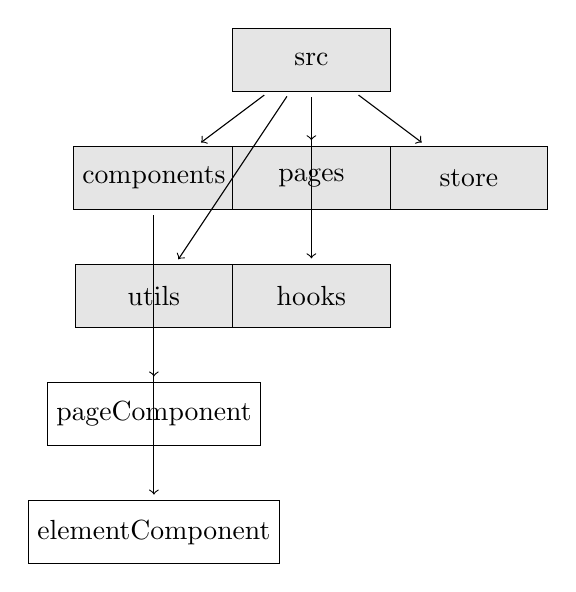
\begin{tikzpicture}[
    file/.style={draw, rectangle, minimum width=2cm, minimum height=0.8cm},
    folder/.style={draw, rectangle, minimum width=2cm, minimum height=0.8cm, fill=gray!20},
    arrow/.style={->, shorten >=2pt, shorten <=2pt}
]

% Folders
\node[folder] (src) at (0,0) {src};
\node[folder] (components) at (-2,-1.5) {components};
\node[folder] (pages) at (0,-1.5) {pages};
\node[folder] (store) at (2,-1.5) {store};
\node[folder] (utils) at (-2,-3) {utils};
\node[folder] (hooks) at (0,-3) {hooks};

% Files
\node[file] (pageComponent) at (-2,-4.5) {pageComponent};
\node[file] (elementComponent) at (-2,-6) {elementComponent};
% ... add more files

% Connections
\draw[arrow] (src) -- (components);
\draw[arrow] (src) -- (pages);
\draw[arrow] (src) -- (store);
\draw[arrow] (src) -- (utils);
\draw[arrow] (src) -- (hooks);
\draw[arrow] (components) -- (pageComponent);
\draw[arrow] (components) -- (elementComponent);
% ... add more connections

\end{tikzpicture}



\pagebreak
\subsubsection{Back-end}
The backend uses the dotNet framework. The development language using the C\# language.

In this project, the backend uses the Onion Architecture.
The Onion Architecture is a typically layered architecture, 
where each layer depends on the inner layer and provides interfaces to the outer layer.
The outer layer provides services to the outermost layer 
and other modules in the same layer based on the interfaces of the inner layer.

From inner to outer, the layers are: Domain, Application, Infrastructure, Presentation.
The Domain layer is the core layer and the innermost layer, used to define domain models, 
which are the business models.
It includes domain models and domain service interfaces.
Domain models are used to define the business models, 
which are the entities in the entity-relationship model and their attributes.
Domain service interfaces are used to define the business services, 
which are the relationships between entities in the entity-relationship model.

The Application layer is the application layer, 
used to define application services, which are the business logic.
It includes domain service implementations and application service interfaces.
Domain service implementations implement the methods of the inner layer's domain service 
interfaces and implement the business logic of the domain models.
Application service interfaces are used to define application services, 
which are the business logic.
It includes but is not limited to database interfaces, testing interfaces, 
HTTP API interfaces, MQTT interfaces, etc.

The Infrastructure layer is the infrastructure layer, used to define infrastructure.
It includes database implementations, testing implementations, 
HTTP API implementations, MQTT implementations, etc.
Database implementations implement the database interfaces 
and provide CRUD services for the database.
Testing implementations implement the testing interfaces 
and provide services for unit testing and integration testing.
HTTP API implementations implement the HTTP API interfaces 
and provide CRUD operations for HTTP APIs.
MQTT implementations implement the MQTT interfaces 
and provide CRUD operations for MQTT.

The Presentation layer is the presentation layer, used to define presentation logic, 
such as interfaces and pages. Since this is a backend project,
data presentation and control are handled by the frontend, 
so this layer is not needed.



\pagebreak
\subsubsection{Data communication and storage}
% 关于本项目的数据通信与数据存储的设计, 包括数据通信的协议, 数据存储的设计等
% 关于数据通信的设计:
% 1. 通信协议的选择
% 自前端向后端发送的数据, 有三种传输的数据类型, 
% 一种是普通的增删改查的请求, 对数据传输的时效性要求不高, 但是对数据的准确性, 完整性, 有序性, 安全性有一定的要求,
% 这种数据的传输, 采用 HTTP 协议, 以及 RESTful API 的设计. 可以有效的保证对数据传输的以上要求.
% 一种是对数据通道的创建和流媒体数据的传输, 对数据传输的时效性, 安全性要求较高, 这种数据的传输, 采用 WebRTC 协议, 以及 MQTT 协议.
% 配合可以快速解码的 flatbuffers 协议, 可以有效的保证对数据传输的以上要求.
% 最后一种是对设备的状态信息和操作信息的传输, 对完整性, 有序性, 安全性都有较高的要求, 这种数据的传输, 采用 MQTT 协议
% 同时也使用了 flatbuffers 协议.
% 
% 2. 数据通信的通信架构和通信流程
% 本项目的数据通信的通信架构, 是基于前后端分离的架构, 前端使用 React 框架, 后端使用 dotnet 框架.
% 当前端需要向后端发送数据的时候, 前端会向后端发送 HTTP 请求, 后端接收到 HTTP 请求之后, 会根据请求的数据类型,
% 选择不同的数据处理方式, 对于普通的增删改查的请求, 后端会根据 RESTful API 的设计, 对数据进行增删改查的操作,
% 对于对数据通道的创建和流媒体数据的传输, 后端会根据 WebRTC 协议, 对数据通道进行创建, 并且帮助前端和设备建立数据通道,
% 当数据通道建立后, 前端和设备之间则使用 flatbuffer 的数据格式对流媒体数据进行传输,
% 对于设备的状态信息和操作信息的传输, 前端会直接向 MQTT broker 发送 MQTT 请求, 
% 设备会在其自身的固件中监听相关的 MQTT 请求, 并且返回相关的数据.
% 
% 3. 数据通信的格式
% 本项目的数据通信的格式, 有三种, 
% 一种是 HTTP 协议, 
% 使用 json 格式对数据进行传输,
% 一种是 WebRTC 协议, 
% 使用 flatbuffers 格式对数据进行传输,
% 一种是 MQTT 协议.
% 使用 flatbuffers 格式对数据进行传输,
% 
% 关于数据存储的设计:
% 1. 数据存储的数据库的选择
% 本项目的数据存储的数据库的选择, 使用了轻量级的数据库 SQLite,
% SQLite 是一个进程内的库, 实现了自给自足的, 无服务器的, 零配置的, 事务性的 SQL 数据库引擎.
% 这是因为整个项目的目的是为了实现前端与设备之间的数据通信, 对于数据库数据的增删改查操作的要求不高,
% 数据量较小, 且对于数据库的数据的事务性要求不高, 所以选择了 SQLite 数据库.
% 2. 项目前后端的数据结构的设计
% 在本项目中, 前端由于使用了 React 框架, 所以前端的数据结构的设计, 使用了基于状态的数据结构的设计,
% 每个组件或者数据集都包含一个状态对象, 这个状态对象的属性就是组件的各个状态. 
% 使用状态对象的原因是, 可以方便的对状态进行管理, 采用对象-属性的形式, 可以方便的针对不同组件的同类状态进行区分,
% 由于跨组件的状态是由 redux 进行管理的, 这种状态对象的设计, 可以更搞笑的对状态进行更新和传递.
% 后端由于使用了 dotnet 框架, 所以后端的数据结构的设计, 使用了基于类的数据结构的设计,
% 采用了面向对象的编程思想, 对数据进行了封装, 使得数据的传输更加的安全, 有序, 完整.


\pagebreak

% \subsection{Domain model}
% \documentclass[]{article}
\usepackage{graphicx}
\usepackage{amsmath}
\usepackage{tikz}

% libaries
\usetikzlibrary{shapes,arrows}

%Define the listing package
\usepackage{listings} %code highlighter
\usepackage{color} %use color
\definecolor{mygreen}{rgb}{0,0.6,0}
\definecolor{mygray}{rgb}{0.5,0.5,0.5}
\definecolor{mymauve}{rgb}{0.58,0,0.82}

%Customize a bit the look
\lstset{ %
backgroundcolor=\color{white}, % choose the background color; you must add \usepackage{color} or \usepackage{xcolor}
basicstyle=\footnotesize, % the size of the fonts that are used for the code
breakatwhitespace=false, % sets if automatic breaks should only happen at whitespace
breaklines=true, % sets automatic line breaking
captionpos=b, % sets the caption-position to bottom
commentstyle=\color{mygreen}, % comment style
deletekeywords={...}, % if you want to delete keywords from the given language
escapeinside={\%*}{*)}, % if you want to add LaTeX within your code
extendedchars=true, % lets you use non-ASCII characters; for 8-bits encodings only, does not work with UTF-8
frame=single, % adds a frame around the code
keepspaces=true, % keeps spaces in text, useful for keeping indentation of code (possibly needs columns=flexible)
keywordstyle=\color{blue}, % keyword style
% language=Octave, % the language of the code
morekeywords={*,...}, % if you want to add more keywords to the set
numbers=left, % where to put the line-numbers; possible values are (none, left, right)
numbersep=5pt, % how far the line-numbers are from the code
numberstyle=\tiny\color{mygray}, % the style that is used for the line-numbers
rulecolor=\color{black}, % if not set, the frame-color may be changed on line-breaks within not-black text (e.g. comments (green here))
showspaces=false, % show spaces everywhere adding particular underscores; it overrides 'showstringspaces'
showstringspaces=false, % underline spaces within strings only
showtabs=false, % show tabs within strings adding particular underscores
stepnumber=1, % the step between two line-numbers. If it's 1, each line will be numbered
stringstyle=\color{mymauve}, % string literal style
tabsize=2, % sets default tabsize to 2 spaces
title=\lstname % show the filename of files included with \lstinputlisting; also try caption instead of title
}

\definecolor{darkgray}{rgb}{.4,.4,.4}
\definecolor{purple}{rgb}{0.65, 0.12, 0.82}

\lstdefinelanguage{React}{
keywords={const, typeof, new, true, false, catch, function, return, null, catch, switch, var, if, in, while, do, else, case, break},
keywordstyle=\color{blue}\bfseries,
ndkeywords={class, export, boolean, throw, implements, import, this},
ndkeywordstyle=\color{darkgray}\bfseries,
identifierstyle=\color{mygreen},
sensitive=false,
comment=[l]{//},
morecomment=[s]{/*}{*/},
commentstyle=\color{purple}\ttfamily,
string=[b]{"}{'}{`},
stringstyle=\color{red}\ttfamily,
morestring=[b]',
morestring=[b]",
morestring=[b]`',
}

\lstdefinelanguage{CSharp}{
keywords={const, typeof, new, true, false, catch, function, return, null, catch, switch, var, if, in, while, do, else, case, break},
keywordstyle=\color{blue}\bfseries,
ndkeywords={class, export, boolean, throw, implements, import, this},
ndkeywordstyle=\color{darkgray}\bfseries,
identifierstyle=\color{mygreen},
sensitive=false,
comment=[l]{//},
morecomment=[s]{/*}{*/},
commentstyle=\color{purple}\ttfamily,
string=[b]{"}{'}{`},
stringstyle=\color{red}\ttfamily,
morestring=[b]',
morestring=[b]",
morestring=[b]`',
}

\lstset{
language=React,
extendedchars=true,
basicstyle=\footnotesize\ttfamily,
showstringspaces=false,
showspaces=false,
numbers=left,
numberstyle=\footnotesize,
numbersep=9pt,
tabsize=2,
breaklines=true,
showtabs=false,
captionpos=b
}

\lstset{
language=CSharp,
extendedchars=true,
basicstyle=\footnotesize\ttfamily,
showstringspaces=false,
showspaces=false,
numbers=left,
numberstyle=\footnotesize,
numbersep=9pt,
tabsize=2,
breaklines=true,
showtabs=false,
captionpos=b
}

% \usepackage{cite} % Add this line for citation

% \bibliographystyle{plain}

\title{
The implementation of BifrostConnect Front-end scope, 
re-design and development with the relevant back-end support develop.
}
\author{
    Fei Gu \\
    Erhvervs Akademi Sydvest \\
    Computer Science 21\\
    }
\date{\today}

\begin{document}

% Front page
\maketitle
\begin{center}
    Supervisor: Henrik Boulund Meng Hansen \\
    Company: BifrostConnect \\
    Engineering Director: Jasper Wass \\
\end{center}
\tableofcontents
\pagebreak


% The introduction
\section{Introduction}
\subsection{Background}\input{sections/introduction/background.tex}
\subsection{The company}\input{sections/introduction/aboutCompany}
\subsection{The project}\input{sections/introduction/aboutProject}
\pagebreak

% The problem statement
\section{Problem Statement}
\subsection{Statement}
\input{sections/problemStatement/statement}
\subsection{Situation}
\input{sections/problemStatement/situation}
\subsection{Potential Solution}
\input{sections/problemStatement/potentialSolution}
\pagebreak

% Requirement analysis
\section{Requirement Analysis}
\input{sections/requirementAnalysis/index}

\subsection{Stakeholders}
\input{sections/requirementAnalysis/stakeholders/index}

\subsection{Business Domain}
\input{sections/requirementAnalysis/bussinesDomain/index}

\subsection{Scope}
\input{sections/requirementAnalysis/scope}

\subsection{Goals}
\input{sections/requirementAnalysis/goals}
\pagebreak

% Software Design
\section{Software Design}
% developement methods
\subsection{Software Development Methods}
\input{sections/softwareDevelopmentMethods/index}
\subsubsection{Agile Software Development}
\input{sections/softwareDevelopmentMethods/agileSoftwareDevelopment/index}
\subsubsection{Feature Driven Development}
\input{sections/softwareDevelopmentMethods/featureDrivenDevelopment/index}

\pagebreak

% Technology seslection
\subsection{Technology selection}
\input{sections/softwareDesign/technologySelection/index}
\subsubsection{Front-end}
\input{sections/softwareDesign/technologySelection/frontEnd}            
\subsubsection{Back-end}
\input{sections/softwareDesign/technologySelection/backEnd}            
\subsubsection{Database}
\input{sections/softwareDesign/technologySelection/database}
\subsubsection{Data communication}
\input{sections/softwareDesign/technologySelection/dataCommunication}            
\subsubsection{DevOps}
\input{sections/softwareDesign/technologySelection/devOps}
\pagebreak

% Architecture design
\subsection{Architecture design}
\input{sections/softwareDesign/architectureDesign/index}
\pagebreak
\subsubsection{Front-end}
\input{sections/softwareDesign/architectureDesign/frontEndArchitecture}
\pagebreak
\subsubsection{Back-end}
\input{sections/softwareDesign/architectureDesign/backEndArchitecture}
\pagebreak
\subsubsection{Data communication and storage}
\input{sections/softwareDesign/architectureDesign/dataCommunicationArchitecture}
\pagebreak

% \subsection{Domain model}
% \input{sections/softwareDesign/domainModel/index}
% \subsection{Database design}
% % 数据库领域模型 ER 图
% % 包括表和字段的设置.
% % 对于私有键和外键的设置.

% \subsection{Back-end design}
% % 后端对象模型
% % 以及对于对象模型的增删改查
% % 以及相关的其他服务的设计`'

% \subsection{Front-end design}
% % 对于前端的页面结构的设计 
% % 页面的状态的设计, 交互设计

% \subsection{FlatBuffers design}
% % schema 的设计

\subsection{DevOps CI/CD process design}
\input{sections/softwareDesign/devOpsDesign/index}
\subsubsection{Continuous Integration}
\input{sections/softwareDesign/devOpsDesign/continuousIntegration/index}
\subsubsection{Continuous Delivery}
\input{sections/softwareDesign/devOpsDesign/continuousDelivery/index}
\subsubsection{Continuous Deployment}
\input{sections/softwareDesign/devOpsDesign/continuousDeployment/index}
\pagebreak

\section{Software Development} 
\input{sections/softwareDevelopment/index}
\subsection{Overall development}
\input{sections/softwareDevelopment/overallDevelopement/index}
\subsubsection{Front-end}
\input{sections/softwareDevelopment/overallDevelopement/frontEnd/index}
\subsubsection{Back-end}
\input{sections/softwareDevelopment/overallDevelopement/backEnd/index}
\subsubsection{DevOps}
\input{sections/softwareDevelopment/overallDevelopement/devOps/index}
\subsection{Feature development} 
\input{sections/softwareDevelopment/featureDevelopment/index}
\subsubsection{Use Case 1}
\input{sections/softwareDevelopment/featureDevelopment/useCase1/index}
\subsubsection{Feature 1}
\input{sections/softwareDevelopment/featureDevelopment/feature/feature1.tex}
\pagebreak
\section{Conclusion} 
\subsection{Result}
Since the project is still in progress, the result is not available yet.
So far, basic structure of this project has been built. But the most features 
are not implemented yet. 
\subsection{Discussion}
As a single developer for this project, I am confident what I have done so far.
And I can say I understand the most of the knowledge I have used in this project, 
which also means I can explain all the part of the project. 
But this project also relevant some of the complex knowledge which I have to continue 
to study and practice.
\subsection{Future Work}
The future work is to implement the rest of the features. 
Including the most important part which is the 'create session' feature.
\pagebreak
% \bibliography{bibliography}
\pagebreak
% \begin{appendices}
%     \section{Appendix}
% \end{appendices} 
\end{document}
% \subsection{Database design}
% % 数据库领域模型 ER 图
% % 包括表和字段的设置.
% % 对于私有键和外键的设置.

% \subsection{Back-end design}
% % 后端对象模型
% % 以及对于对象模型的增删改查
% % 以及相关的其他服务的设计`'

% \subsection{Front-end design}
% % 对于前端的页面结构的设计 
% % 页面的状态的设计, 交互设计

% \subsection{FlatBuffers design}
% % schema 的设计

\subsection{DevOps CI/CD process design}
\documentclass[]{article}
\usepackage{graphicx}
\usepackage{amsmath}
\usepackage{tikz}

% libaries
\usetikzlibrary{shapes,arrows}

%Define the listing package
\usepackage{listings} %code highlighter
\usepackage{color} %use color
\definecolor{mygreen}{rgb}{0,0.6,0}
\definecolor{mygray}{rgb}{0.5,0.5,0.5}
\definecolor{mymauve}{rgb}{0.58,0,0.82}

%Customize a bit the look
\lstset{ %
backgroundcolor=\color{white}, % choose the background color; you must add \usepackage{color} or \usepackage{xcolor}
basicstyle=\footnotesize, % the size of the fonts that are used for the code
breakatwhitespace=false, % sets if automatic breaks should only happen at whitespace
breaklines=true, % sets automatic line breaking
captionpos=b, % sets the caption-position to bottom
commentstyle=\color{mygreen}, % comment style
deletekeywords={...}, % if you want to delete keywords from the given language
escapeinside={\%*}{*)}, % if you want to add LaTeX within your code
extendedchars=true, % lets you use non-ASCII characters; for 8-bits encodings only, does not work with UTF-8
frame=single, % adds a frame around the code
keepspaces=true, % keeps spaces in text, useful for keeping indentation of code (possibly needs columns=flexible)
keywordstyle=\color{blue}, % keyword style
% language=Octave, % the language of the code
morekeywords={*,...}, % if you want to add more keywords to the set
numbers=left, % where to put the line-numbers; possible values are (none, left, right)
numbersep=5pt, % how far the line-numbers are from the code
numberstyle=\tiny\color{mygray}, % the style that is used for the line-numbers
rulecolor=\color{black}, % if not set, the frame-color may be changed on line-breaks within not-black text (e.g. comments (green here))
showspaces=false, % show spaces everywhere adding particular underscores; it overrides 'showstringspaces'
showstringspaces=false, % underline spaces within strings only
showtabs=false, % show tabs within strings adding particular underscores
stepnumber=1, % the step between two line-numbers. If it's 1, each line will be numbered
stringstyle=\color{mymauve}, % string literal style
tabsize=2, % sets default tabsize to 2 spaces
title=\lstname % show the filename of files included with \lstinputlisting; also try caption instead of title
}

\definecolor{darkgray}{rgb}{.4,.4,.4}
\definecolor{purple}{rgb}{0.65, 0.12, 0.82}

\lstdefinelanguage{React}{
keywords={const, typeof, new, true, false, catch, function, return, null, catch, switch, var, if, in, while, do, else, case, break},
keywordstyle=\color{blue}\bfseries,
ndkeywords={class, export, boolean, throw, implements, import, this},
ndkeywordstyle=\color{darkgray}\bfseries,
identifierstyle=\color{mygreen},
sensitive=false,
comment=[l]{//},
morecomment=[s]{/*}{*/},
commentstyle=\color{purple}\ttfamily,
string=[b]{"}{'}{`},
stringstyle=\color{red}\ttfamily,
morestring=[b]',
morestring=[b]",
morestring=[b]`',
}

\lstdefinelanguage{CSharp}{
keywords={const, typeof, new, true, false, catch, function, return, null, catch, switch, var, if, in, while, do, else, case, break},
keywordstyle=\color{blue}\bfseries,
ndkeywords={class, export, boolean, throw, implements, import, this},
ndkeywordstyle=\color{darkgray}\bfseries,
identifierstyle=\color{mygreen},
sensitive=false,
comment=[l]{//},
morecomment=[s]{/*}{*/},
commentstyle=\color{purple}\ttfamily,
string=[b]{"}{'}{`},
stringstyle=\color{red}\ttfamily,
morestring=[b]',
morestring=[b]",
morestring=[b]`',
}

\lstset{
language=React,
extendedchars=true,
basicstyle=\footnotesize\ttfamily,
showstringspaces=false,
showspaces=false,
numbers=left,
numberstyle=\footnotesize,
numbersep=9pt,
tabsize=2,
breaklines=true,
showtabs=false,
captionpos=b
}

\lstset{
language=CSharp,
extendedchars=true,
basicstyle=\footnotesize\ttfamily,
showstringspaces=false,
showspaces=false,
numbers=left,
numberstyle=\footnotesize,
numbersep=9pt,
tabsize=2,
breaklines=true,
showtabs=false,
captionpos=b
}

% \usepackage{cite} % Add this line for citation

% \bibliographystyle{plain}

\title{
The implementation of BifrostConnect Front-end scope, 
re-design and development with the relevant back-end support develop.
}
\author{
    Fei Gu \\
    Erhvervs Akademi Sydvest \\
    Computer Science 21\\
    }
\date{\today}

\begin{document}

% Front page
\maketitle
\begin{center}
    Supervisor: Henrik Boulund Meng Hansen \\
    Company: BifrostConnect \\
    Engineering Director: Jasper Wass \\
\end{center}
\tableofcontents
\pagebreak


% The introduction
\section{Introduction}
\subsection{Background}\input{sections/introduction/background.tex}
\subsection{The company}\input{sections/introduction/aboutCompany}
\subsection{The project}\input{sections/introduction/aboutProject}
\pagebreak

% The problem statement
\section{Problem Statement}
\subsection{Statement}
\input{sections/problemStatement/statement}
\subsection{Situation}
\input{sections/problemStatement/situation}
\subsection{Potential Solution}
\input{sections/problemStatement/potentialSolution}
\pagebreak

% Requirement analysis
\section{Requirement Analysis}
\input{sections/requirementAnalysis/index}

\subsection{Stakeholders}
\input{sections/requirementAnalysis/stakeholders/index}

\subsection{Business Domain}
\input{sections/requirementAnalysis/bussinesDomain/index}

\subsection{Scope}
\input{sections/requirementAnalysis/scope}

\subsection{Goals}
\input{sections/requirementAnalysis/goals}
\pagebreak

% Software Design
\section{Software Design}
% developement methods
\subsection{Software Development Methods}
\input{sections/softwareDevelopmentMethods/index}
\subsubsection{Agile Software Development}
\input{sections/softwareDevelopmentMethods/agileSoftwareDevelopment/index}
\subsubsection{Feature Driven Development}
\input{sections/softwareDevelopmentMethods/featureDrivenDevelopment/index}

\pagebreak

% Technology seslection
\subsection{Technology selection}
\input{sections/softwareDesign/technologySelection/index}
\subsubsection{Front-end}
\input{sections/softwareDesign/technologySelection/frontEnd}            
\subsubsection{Back-end}
\input{sections/softwareDesign/technologySelection/backEnd}            
\subsubsection{Database}
\input{sections/softwareDesign/technologySelection/database}
\subsubsection{Data communication}
\input{sections/softwareDesign/technologySelection/dataCommunication}            
\subsubsection{DevOps}
\input{sections/softwareDesign/technologySelection/devOps}
\pagebreak

% Architecture design
\subsection{Architecture design}
\input{sections/softwareDesign/architectureDesign/index}
\pagebreak
\subsubsection{Front-end}
\input{sections/softwareDesign/architectureDesign/frontEndArchitecture}
\pagebreak
\subsubsection{Back-end}
\input{sections/softwareDesign/architectureDesign/backEndArchitecture}
\pagebreak
\subsubsection{Data communication and storage}
\input{sections/softwareDesign/architectureDesign/dataCommunicationArchitecture}
\pagebreak

% \subsection{Domain model}
% \input{sections/softwareDesign/domainModel/index}
% \subsection{Database design}
% % 数据库领域模型 ER 图
% % 包括表和字段的设置.
% % 对于私有键和外键的设置.

% \subsection{Back-end design}
% % 后端对象模型
% % 以及对于对象模型的增删改查
% % 以及相关的其他服务的设计`'

% \subsection{Front-end design}
% % 对于前端的页面结构的设计 
% % 页面的状态的设计, 交互设计

% \subsection{FlatBuffers design}
% % schema 的设计

\subsection{DevOps CI/CD process design}
\input{sections/softwareDesign/devOpsDesign/index}
\subsubsection{Continuous Integration}
\input{sections/softwareDesign/devOpsDesign/continuousIntegration/index}
\subsubsection{Continuous Delivery}
\input{sections/softwareDesign/devOpsDesign/continuousDelivery/index}
\subsubsection{Continuous Deployment}
\input{sections/softwareDesign/devOpsDesign/continuousDeployment/index}
\pagebreak

\section{Software Development} 
\input{sections/softwareDevelopment/index}
\subsection{Overall development}
\input{sections/softwareDevelopment/overallDevelopement/index}
\subsubsection{Front-end}
\input{sections/softwareDevelopment/overallDevelopement/frontEnd/index}
\subsubsection{Back-end}
\input{sections/softwareDevelopment/overallDevelopement/backEnd/index}
\subsubsection{DevOps}
\input{sections/softwareDevelopment/overallDevelopement/devOps/index}
\subsection{Feature development} 
\input{sections/softwareDevelopment/featureDevelopment/index}
\subsubsection{Use Case 1}
\input{sections/softwareDevelopment/featureDevelopment/useCase1/index}
\subsubsection{Feature 1}
\input{sections/softwareDevelopment/featureDevelopment/feature/feature1.tex}
\pagebreak
\section{Conclusion} 
\subsection{Result}
Since the project is still in progress, the result is not available yet.
So far, basic structure of this project has been built. But the most features 
are not implemented yet. 
\subsection{Discussion}
As a single developer for this project, I am confident what I have done so far.
And I can say I understand the most of the knowledge I have used in this project, 
which also means I can explain all the part of the project. 
But this project also relevant some of the complex knowledge which I have to continue 
to study and practice.
\subsection{Future Work}
The future work is to implement the rest of the features. 
Including the most important part which is the 'create session' feature.
\pagebreak
% \bibliography{bibliography}
\pagebreak
% \begin{appendices}
%     \section{Appendix}
% \end{appendices} 
\end{document}
\subsubsection{Continuous Integration}
\documentclass[]{article}
\usepackage{graphicx}
\usepackage{amsmath}
\usepackage{tikz}

% libaries
\usetikzlibrary{shapes,arrows}

%Define the listing package
\usepackage{listings} %code highlighter
\usepackage{color} %use color
\definecolor{mygreen}{rgb}{0,0.6,0}
\definecolor{mygray}{rgb}{0.5,0.5,0.5}
\definecolor{mymauve}{rgb}{0.58,0,0.82}

%Customize a bit the look
\lstset{ %
backgroundcolor=\color{white}, % choose the background color; you must add \usepackage{color} or \usepackage{xcolor}
basicstyle=\footnotesize, % the size of the fonts that are used for the code
breakatwhitespace=false, % sets if automatic breaks should only happen at whitespace
breaklines=true, % sets automatic line breaking
captionpos=b, % sets the caption-position to bottom
commentstyle=\color{mygreen}, % comment style
deletekeywords={...}, % if you want to delete keywords from the given language
escapeinside={\%*}{*)}, % if you want to add LaTeX within your code
extendedchars=true, % lets you use non-ASCII characters; for 8-bits encodings only, does not work with UTF-8
frame=single, % adds a frame around the code
keepspaces=true, % keeps spaces in text, useful for keeping indentation of code (possibly needs columns=flexible)
keywordstyle=\color{blue}, % keyword style
% language=Octave, % the language of the code
morekeywords={*,...}, % if you want to add more keywords to the set
numbers=left, % where to put the line-numbers; possible values are (none, left, right)
numbersep=5pt, % how far the line-numbers are from the code
numberstyle=\tiny\color{mygray}, % the style that is used for the line-numbers
rulecolor=\color{black}, % if not set, the frame-color may be changed on line-breaks within not-black text (e.g. comments (green here))
showspaces=false, % show spaces everywhere adding particular underscores; it overrides 'showstringspaces'
showstringspaces=false, % underline spaces within strings only
showtabs=false, % show tabs within strings adding particular underscores
stepnumber=1, % the step between two line-numbers. If it's 1, each line will be numbered
stringstyle=\color{mymauve}, % string literal style
tabsize=2, % sets default tabsize to 2 spaces
title=\lstname % show the filename of files included with \lstinputlisting; also try caption instead of title
}

\definecolor{darkgray}{rgb}{.4,.4,.4}
\definecolor{purple}{rgb}{0.65, 0.12, 0.82}

\lstdefinelanguage{React}{
keywords={const, typeof, new, true, false, catch, function, return, null, catch, switch, var, if, in, while, do, else, case, break},
keywordstyle=\color{blue}\bfseries,
ndkeywords={class, export, boolean, throw, implements, import, this},
ndkeywordstyle=\color{darkgray}\bfseries,
identifierstyle=\color{mygreen},
sensitive=false,
comment=[l]{//},
morecomment=[s]{/*}{*/},
commentstyle=\color{purple}\ttfamily,
string=[b]{"}{'}{`},
stringstyle=\color{red}\ttfamily,
morestring=[b]',
morestring=[b]",
morestring=[b]`',
}

\lstdefinelanguage{CSharp}{
keywords={const, typeof, new, true, false, catch, function, return, null, catch, switch, var, if, in, while, do, else, case, break},
keywordstyle=\color{blue}\bfseries,
ndkeywords={class, export, boolean, throw, implements, import, this},
ndkeywordstyle=\color{darkgray}\bfseries,
identifierstyle=\color{mygreen},
sensitive=false,
comment=[l]{//},
morecomment=[s]{/*}{*/},
commentstyle=\color{purple}\ttfamily,
string=[b]{"}{'}{`},
stringstyle=\color{red}\ttfamily,
morestring=[b]',
morestring=[b]",
morestring=[b]`',
}

\lstset{
language=React,
extendedchars=true,
basicstyle=\footnotesize\ttfamily,
showstringspaces=false,
showspaces=false,
numbers=left,
numberstyle=\footnotesize,
numbersep=9pt,
tabsize=2,
breaklines=true,
showtabs=false,
captionpos=b
}

\lstset{
language=CSharp,
extendedchars=true,
basicstyle=\footnotesize\ttfamily,
showstringspaces=false,
showspaces=false,
numbers=left,
numberstyle=\footnotesize,
numbersep=9pt,
tabsize=2,
breaklines=true,
showtabs=false,
captionpos=b
}

% \usepackage{cite} % Add this line for citation

% \bibliographystyle{plain}

\title{
The implementation of BifrostConnect Front-end scope, 
re-design and development with the relevant back-end support develop.
}
\author{
    Fei Gu \\
    Erhvervs Akademi Sydvest \\
    Computer Science 21\\
    }
\date{\today}

\begin{document}

% Front page
\maketitle
\begin{center}
    Supervisor: Henrik Boulund Meng Hansen \\
    Company: BifrostConnect \\
    Engineering Director: Jasper Wass \\
\end{center}
\tableofcontents
\pagebreak


% The introduction
\section{Introduction}
\subsection{Background}\input{sections/introduction/background.tex}
\subsection{The company}\input{sections/introduction/aboutCompany}
\subsection{The project}\input{sections/introduction/aboutProject}
\pagebreak

% The problem statement
\section{Problem Statement}
\subsection{Statement}
\input{sections/problemStatement/statement}
\subsection{Situation}
\input{sections/problemStatement/situation}
\subsection{Potential Solution}
\input{sections/problemStatement/potentialSolution}
\pagebreak

% Requirement analysis
\section{Requirement Analysis}
\input{sections/requirementAnalysis/index}

\subsection{Stakeholders}
\input{sections/requirementAnalysis/stakeholders/index}

\subsection{Business Domain}
\input{sections/requirementAnalysis/bussinesDomain/index}

\subsection{Scope}
\input{sections/requirementAnalysis/scope}

\subsection{Goals}
\input{sections/requirementAnalysis/goals}
\pagebreak

% Software Design
\section{Software Design}
% developement methods
\subsection{Software Development Methods}
\input{sections/softwareDevelopmentMethods/index}
\subsubsection{Agile Software Development}
\input{sections/softwareDevelopmentMethods/agileSoftwareDevelopment/index}
\subsubsection{Feature Driven Development}
\input{sections/softwareDevelopmentMethods/featureDrivenDevelopment/index}

\pagebreak

% Technology seslection
\subsection{Technology selection}
\input{sections/softwareDesign/technologySelection/index}
\subsubsection{Front-end}
\input{sections/softwareDesign/technologySelection/frontEnd}            
\subsubsection{Back-end}
\input{sections/softwareDesign/technologySelection/backEnd}            
\subsubsection{Database}
\input{sections/softwareDesign/technologySelection/database}
\subsubsection{Data communication}
\input{sections/softwareDesign/technologySelection/dataCommunication}            
\subsubsection{DevOps}
\input{sections/softwareDesign/technologySelection/devOps}
\pagebreak

% Architecture design
\subsection{Architecture design}
\input{sections/softwareDesign/architectureDesign/index}
\pagebreak
\subsubsection{Front-end}
\input{sections/softwareDesign/architectureDesign/frontEndArchitecture}
\pagebreak
\subsubsection{Back-end}
\input{sections/softwareDesign/architectureDesign/backEndArchitecture}
\pagebreak
\subsubsection{Data communication and storage}
\input{sections/softwareDesign/architectureDesign/dataCommunicationArchitecture}
\pagebreak

% \subsection{Domain model}
% \input{sections/softwareDesign/domainModel/index}
% \subsection{Database design}
% % 数据库领域模型 ER 图
% % 包括表和字段的设置.
% % 对于私有键和外键的设置.

% \subsection{Back-end design}
% % 后端对象模型
% % 以及对于对象模型的增删改查
% % 以及相关的其他服务的设计`'

% \subsection{Front-end design}
% % 对于前端的页面结构的设计 
% % 页面的状态的设计, 交互设计

% \subsection{FlatBuffers design}
% % schema 的设计

\subsection{DevOps CI/CD process design}
\input{sections/softwareDesign/devOpsDesign/index}
\subsubsection{Continuous Integration}
\input{sections/softwareDesign/devOpsDesign/continuousIntegration/index}
\subsubsection{Continuous Delivery}
\input{sections/softwareDesign/devOpsDesign/continuousDelivery/index}
\subsubsection{Continuous Deployment}
\input{sections/softwareDesign/devOpsDesign/continuousDeployment/index}
\pagebreak

\section{Software Development} 
\input{sections/softwareDevelopment/index}
\subsection{Overall development}
\input{sections/softwareDevelopment/overallDevelopement/index}
\subsubsection{Front-end}
\input{sections/softwareDevelopment/overallDevelopement/frontEnd/index}
\subsubsection{Back-end}
\input{sections/softwareDevelopment/overallDevelopement/backEnd/index}
\subsubsection{DevOps}
\input{sections/softwareDevelopment/overallDevelopement/devOps/index}
\subsection{Feature development} 
\input{sections/softwareDevelopment/featureDevelopment/index}
\subsubsection{Use Case 1}
\input{sections/softwareDevelopment/featureDevelopment/useCase1/index}
\subsubsection{Feature 1}
\input{sections/softwareDevelopment/featureDevelopment/feature/feature1.tex}
\pagebreak
\section{Conclusion} 
\subsection{Result}
Since the project is still in progress, the result is not available yet.
So far, basic structure of this project has been built. But the most features 
are not implemented yet. 
\subsection{Discussion}
As a single developer for this project, I am confident what I have done so far.
And I can say I understand the most of the knowledge I have used in this project, 
which also means I can explain all the part of the project. 
But this project also relevant some of the complex knowledge which I have to continue 
to study and practice.
\subsection{Future Work}
The future work is to implement the rest of the features. 
Including the most important part which is the 'create session' feature.
\pagebreak
% \bibliography{bibliography}
\pagebreak
% \begin{appendices}
%     \section{Appendix}
% \end{appendices} 
\end{document}
\subsubsection{Continuous Delivery}
\documentclass[]{article}
\usepackage{graphicx}
\usepackage{amsmath}
\usepackage{tikz}

% libaries
\usetikzlibrary{shapes,arrows}

%Define the listing package
\usepackage{listings} %code highlighter
\usepackage{color} %use color
\definecolor{mygreen}{rgb}{0,0.6,0}
\definecolor{mygray}{rgb}{0.5,0.5,0.5}
\definecolor{mymauve}{rgb}{0.58,0,0.82}

%Customize a bit the look
\lstset{ %
backgroundcolor=\color{white}, % choose the background color; you must add \usepackage{color} or \usepackage{xcolor}
basicstyle=\footnotesize, % the size of the fonts that are used for the code
breakatwhitespace=false, % sets if automatic breaks should only happen at whitespace
breaklines=true, % sets automatic line breaking
captionpos=b, % sets the caption-position to bottom
commentstyle=\color{mygreen}, % comment style
deletekeywords={...}, % if you want to delete keywords from the given language
escapeinside={\%*}{*)}, % if you want to add LaTeX within your code
extendedchars=true, % lets you use non-ASCII characters; for 8-bits encodings only, does not work with UTF-8
frame=single, % adds a frame around the code
keepspaces=true, % keeps spaces in text, useful for keeping indentation of code (possibly needs columns=flexible)
keywordstyle=\color{blue}, % keyword style
% language=Octave, % the language of the code
morekeywords={*,...}, % if you want to add more keywords to the set
numbers=left, % where to put the line-numbers; possible values are (none, left, right)
numbersep=5pt, % how far the line-numbers are from the code
numberstyle=\tiny\color{mygray}, % the style that is used for the line-numbers
rulecolor=\color{black}, % if not set, the frame-color may be changed on line-breaks within not-black text (e.g. comments (green here))
showspaces=false, % show spaces everywhere adding particular underscores; it overrides 'showstringspaces'
showstringspaces=false, % underline spaces within strings only
showtabs=false, % show tabs within strings adding particular underscores
stepnumber=1, % the step between two line-numbers. If it's 1, each line will be numbered
stringstyle=\color{mymauve}, % string literal style
tabsize=2, % sets default tabsize to 2 spaces
title=\lstname % show the filename of files included with \lstinputlisting; also try caption instead of title
}

\definecolor{darkgray}{rgb}{.4,.4,.4}
\definecolor{purple}{rgb}{0.65, 0.12, 0.82}

\lstdefinelanguage{React}{
keywords={const, typeof, new, true, false, catch, function, return, null, catch, switch, var, if, in, while, do, else, case, break},
keywordstyle=\color{blue}\bfseries,
ndkeywords={class, export, boolean, throw, implements, import, this},
ndkeywordstyle=\color{darkgray}\bfseries,
identifierstyle=\color{mygreen},
sensitive=false,
comment=[l]{//},
morecomment=[s]{/*}{*/},
commentstyle=\color{purple}\ttfamily,
string=[b]{"}{'}{`},
stringstyle=\color{red}\ttfamily,
morestring=[b]',
morestring=[b]",
morestring=[b]`',
}

\lstdefinelanguage{CSharp}{
keywords={const, typeof, new, true, false, catch, function, return, null, catch, switch, var, if, in, while, do, else, case, break},
keywordstyle=\color{blue}\bfseries,
ndkeywords={class, export, boolean, throw, implements, import, this},
ndkeywordstyle=\color{darkgray}\bfseries,
identifierstyle=\color{mygreen},
sensitive=false,
comment=[l]{//},
morecomment=[s]{/*}{*/},
commentstyle=\color{purple}\ttfamily,
string=[b]{"}{'}{`},
stringstyle=\color{red}\ttfamily,
morestring=[b]',
morestring=[b]",
morestring=[b]`',
}

\lstset{
language=React,
extendedchars=true,
basicstyle=\footnotesize\ttfamily,
showstringspaces=false,
showspaces=false,
numbers=left,
numberstyle=\footnotesize,
numbersep=9pt,
tabsize=2,
breaklines=true,
showtabs=false,
captionpos=b
}

\lstset{
language=CSharp,
extendedchars=true,
basicstyle=\footnotesize\ttfamily,
showstringspaces=false,
showspaces=false,
numbers=left,
numberstyle=\footnotesize,
numbersep=9pt,
tabsize=2,
breaklines=true,
showtabs=false,
captionpos=b
}

% \usepackage{cite} % Add this line for citation

% \bibliographystyle{plain}

\title{
The implementation of BifrostConnect Front-end scope, 
re-design and development with the relevant back-end support develop.
}
\author{
    Fei Gu \\
    Erhvervs Akademi Sydvest \\
    Computer Science 21\\
    }
\date{\today}

\begin{document}

% Front page
\maketitle
\begin{center}
    Supervisor: Henrik Boulund Meng Hansen \\
    Company: BifrostConnect \\
    Engineering Director: Jasper Wass \\
\end{center}
\tableofcontents
\pagebreak


% The introduction
\section{Introduction}
\subsection{Background}\input{sections/introduction/background.tex}
\subsection{The company}\input{sections/introduction/aboutCompany}
\subsection{The project}\input{sections/introduction/aboutProject}
\pagebreak

% The problem statement
\section{Problem Statement}
\subsection{Statement}
\input{sections/problemStatement/statement}
\subsection{Situation}
\input{sections/problemStatement/situation}
\subsection{Potential Solution}
\input{sections/problemStatement/potentialSolution}
\pagebreak

% Requirement analysis
\section{Requirement Analysis}
\input{sections/requirementAnalysis/index}

\subsection{Stakeholders}
\input{sections/requirementAnalysis/stakeholders/index}

\subsection{Business Domain}
\input{sections/requirementAnalysis/bussinesDomain/index}

\subsection{Scope}
\input{sections/requirementAnalysis/scope}

\subsection{Goals}
\input{sections/requirementAnalysis/goals}
\pagebreak

% Software Design
\section{Software Design}
% developement methods
\subsection{Software Development Methods}
\input{sections/softwareDevelopmentMethods/index}
\subsubsection{Agile Software Development}
\input{sections/softwareDevelopmentMethods/agileSoftwareDevelopment/index}
\subsubsection{Feature Driven Development}
\input{sections/softwareDevelopmentMethods/featureDrivenDevelopment/index}

\pagebreak

% Technology seslection
\subsection{Technology selection}
\input{sections/softwareDesign/technologySelection/index}
\subsubsection{Front-end}
\input{sections/softwareDesign/technologySelection/frontEnd}            
\subsubsection{Back-end}
\input{sections/softwareDesign/technologySelection/backEnd}            
\subsubsection{Database}
\input{sections/softwareDesign/technologySelection/database}
\subsubsection{Data communication}
\input{sections/softwareDesign/technologySelection/dataCommunication}            
\subsubsection{DevOps}
\input{sections/softwareDesign/technologySelection/devOps}
\pagebreak

% Architecture design
\subsection{Architecture design}
\input{sections/softwareDesign/architectureDesign/index}
\pagebreak
\subsubsection{Front-end}
\input{sections/softwareDesign/architectureDesign/frontEndArchitecture}
\pagebreak
\subsubsection{Back-end}
\input{sections/softwareDesign/architectureDesign/backEndArchitecture}
\pagebreak
\subsubsection{Data communication and storage}
\input{sections/softwareDesign/architectureDesign/dataCommunicationArchitecture}
\pagebreak

% \subsection{Domain model}
% \input{sections/softwareDesign/domainModel/index}
% \subsection{Database design}
% % 数据库领域模型 ER 图
% % 包括表和字段的设置.
% % 对于私有键和外键的设置.

% \subsection{Back-end design}
% % 后端对象模型
% % 以及对于对象模型的增删改查
% % 以及相关的其他服务的设计`'

% \subsection{Front-end design}
% % 对于前端的页面结构的设计 
% % 页面的状态的设计, 交互设计

% \subsection{FlatBuffers design}
% % schema 的设计

\subsection{DevOps CI/CD process design}
\input{sections/softwareDesign/devOpsDesign/index}
\subsubsection{Continuous Integration}
\input{sections/softwareDesign/devOpsDesign/continuousIntegration/index}
\subsubsection{Continuous Delivery}
\input{sections/softwareDesign/devOpsDesign/continuousDelivery/index}
\subsubsection{Continuous Deployment}
\input{sections/softwareDesign/devOpsDesign/continuousDeployment/index}
\pagebreak

\section{Software Development} 
\input{sections/softwareDevelopment/index}
\subsection{Overall development}
\input{sections/softwareDevelopment/overallDevelopement/index}
\subsubsection{Front-end}
\input{sections/softwareDevelopment/overallDevelopement/frontEnd/index}
\subsubsection{Back-end}
\input{sections/softwareDevelopment/overallDevelopement/backEnd/index}
\subsubsection{DevOps}
\input{sections/softwareDevelopment/overallDevelopement/devOps/index}
\subsection{Feature development} 
\input{sections/softwareDevelopment/featureDevelopment/index}
\subsubsection{Use Case 1}
\input{sections/softwareDevelopment/featureDevelopment/useCase1/index}
\subsubsection{Feature 1}
\input{sections/softwareDevelopment/featureDevelopment/feature/feature1.tex}
\pagebreak
\section{Conclusion} 
\subsection{Result}
Since the project is still in progress, the result is not available yet.
So far, basic structure of this project has been built. But the most features 
are not implemented yet. 
\subsection{Discussion}
As a single developer for this project, I am confident what I have done so far.
And I can say I understand the most of the knowledge I have used in this project, 
which also means I can explain all the part of the project. 
But this project also relevant some of the complex knowledge which I have to continue 
to study and practice.
\subsection{Future Work}
The future work is to implement the rest of the features. 
Including the most important part which is the 'create session' feature.
\pagebreak
% \bibliography{bibliography}
\pagebreak
% \begin{appendices}
%     \section{Appendix}
% \end{appendices} 
\end{document}
\subsubsection{Continuous Deployment}
\documentclass[]{article}
\usepackage{graphicx}
\usepackage{amsmath}
\usepackage{tikz}

% libaries
\usetikzlibrary{shapes,arrows}

%Define the listing package
\usepackage{listings} %code highlighter
\usepackage{color} %use color
\definecolor{mygreen}{rgb}{0,0.6,0}
\definecolor{mygray}{rgb}{0.5,0.5,0.5}
\definecolor{mymauve}{rgb}{0.58,0,0.82}

%Customize a bit the look
\lstset{ %
backgroundcolor=\color{white}, % choose the background color; you must add \usepackage{color} or \usepackage{xcolor}
basicstyle=\footnotesize, % the size of the fonts that are used for the code
breakatwhitespace=false, % sets if automatic breaks should only happen at whitespace
breaklines=true, % sets automatic line breaking
captionpos=b, % sets the caption-position to bottom
commentstyle=\color{mygreen}, % comment style
deletekeywords={...}, % if you want to delete keywords from the given language
escapeinside={\%*}{*)}, % if you want to add LaTeX within your code
extendedchars=true, % lets you use non-ASCII characters; for 8-bits encodings only, does not work with UTF-8
frame=single, % adds a frame around the code
keepspaces=true, % keeps spaces in text, useful for keeping indentation of code (possibly needs columns=flexible)
keywordstyle=\color{blue}, % keyword style
% language=Octave, % the language of the code
morekeywords={*,...}, % if you want to add more keywords to the set
numbers=left, % where to put the line-numbers; possible values are (none, left, right)
numbersep=5pt, % how far the line-numbers are from the code
numberstyle=\tiny\color{mygray}, % the style that is used for the line-numbers
rulecolor=\color{black}, % if not set, the frame-color may be changed on line-breaks within not-black text (e.g. comments (green here))
showspaces=false, % show spaces everywhere adding particular underscores; it overrides 'showstringspaces'
showstringspaces=false, % underline spaces within strings only
showtabs=false, % show tabs within strings adding particular underscores
stepnumber=1, % the step between two line-numbers. If it's 1, each line will be numbered
stringstyle=\color{mymauve}, % string literal style
tabsize=2, % sets default tabsize to 2 spaces
title=\lstname % show the filename of files included with \lstinputlisting; also try caption instead of title
}

\definecolor{darkgray}{rgb}{.4,.4,.4}
\definecolor{purple}{rgb}{0.65, 0.12, 0.82}

\lstdefinelanguage{React}{
keywords={const, typeof, new, true, false, catch, function, return, null, catch, switch, var, if, in, while, do, else, case, break},
keywordstyle=\color{blue}\bfseries,
ndkeywords={class, export, boolean, throw, implements, import, this},
ndkeywordstyle=\color{darkgray}\bfseries,
identifierstyle=\color{mygreen},
sensitive=false,
comment=[l]{//},
morecomment=[s]{/*}{*/},
commentstyle=\color{purple}\ttfamily,
string=[b]{"}{'}{`},
stringstyle=\color{red}\ttfamily,
morestring=[b]',
morestring=[b]",
morestring=[b]`',
}

\lstdefinelanguage{CSharp}{
keywords={const, typeof, new, true, false, catch, function, return, null, catch, switch, var, if, in, while, do, else, case, break},
keywordstyle=\color{blue}\bfseries,
ndkeywords={class, export, boolean, throw, implements, import, this},
ndkeywordstyle=\color{darkgray}\bfseries,
identifierstyle=\color{mygreen},
sensitive=false,
comment=[l]{//},
morecomment=[s]{/*}{*/},
commentstyle=\color{purple}\ttfamily,
string=[b]{"}{'}{`},
stringstyle=\color{red}\ttfamily,
morestring=[b]',
morestring=[b]",
morestring=[b]`',
}

\lstset{
language=React,
extendedchars=true,
basicstyle=\footnotesize\ttfamily,
showstringspaces=false,
showspaces=false,
numbers=left,
numberstyle=\footnotesize,
numbersep=9pt,
tabsize=2,
breaklines=true,
showtabs=false,
captionpos=b
}

\lstset{
language=CSharp,
extendedchars=true,
basicstyle=\footnotesize\ttfamily,
showstringspaces=false,
showspaces=false,
numbers=left,
numberstyle=\footnotesize,
numbersep=9pt,
tabsize=2,
breaklines=true,
showtabs=false,
captionpos=b
}

% \usepackage{cite} % Add this line for citation

% \bibliographystyle{plain}

\title{
The implementation of BifrostConnect Front-end scope, 
re-design and development with the relevant back-end support develop.
}
\author{
    Fei Gu \\
    Erhvervs Akademi Sydvest \\
    Computer Science 21\\
    }
\date{\today}

\begin{document}

% Front page
\maketitle
\begin{center}
    Supervisor: Henrik Boulund Meng Hansen \\
    Company: BifrostConnect \\
    Engineering Director: Jasper Wass \\
\end{center}
\tableofcontents
\pagebreak


% The introduction
\section{Introduction}
\subsection{Background}\input{sections/introduction/background.tex}
\subsection{The company}\input{sections/introduction/aboutCompany}
\subsection{The project}\input{sections/introduction/aboutProject}
\pagebreak

% The problem statement
\section{Problem Statement}
\subsection{Statement}
\input{sections/problemStatement/statement}
\subsection{Situation}
\input{sections/problemStatement/situation}
\subsection{Potential Solution}
\input{sections/problemStatement/potentialSolution}
\pagebreak

% Requirement analysis
\section{Requirement Analysis}
\input{sections/requirementAnalysis/index}

\subsection{Stakeholders}
\input{sections/requirementAnalysis/stakeholders/index}

\subsection{Business Domain}
\input{sections/requirementAnalysis/bussinesDomain/index}

\subsection{Scope}
\input{sections/requirementAnalysis/scope}

\subsection{Goals}
\input{sections/requirementAnalysis/goals}
\pagebreak

% Software Design
\section{Software Design}
% developement methods
\subsection{Software Development Methods}
\input{sections/softwareDevelopmentMethods/index}
\subsubsection{Agile Software Development}
\input{sections/softwareDevelopmentMethods/agileSoftwareDevelopment/index}
\subsubsection{Feature Driven Development}
\input{sections/softwareDevelopmentMethods/featureDrivenDevelopment/index}

\pagebreak

% Technology seslection
\subsection{Technology selection}
\input{sections/softwareDesign/technologySelection/index}
\subsubsection{Front-end}
\input{sections/softwareDesign/technologySelection/frontEnd}            
\subsubsection{Back-end}
\input{sections/softwareDesign/technologySelection/backEnd}            
\subsubsection{Database}
\input{sections/softwareDesign/technologySelection/database}
\subsubsection{Data communication}
\input{sections/softwareDesign/technologySelection/dataCommunication}            
\subsubsection{DevOps}
\input{sections/softwareDesign/technologySelection/devOps}
\pagebreak

% Architecture design
\subsection{Architecture design}
\input{sections/softwareDesign/architectureDesign/index}
\pagebreak
\subsubsection{Front-end}
\input{sections/softwareDesign/architectureDesign/frontEndArchitecture}
\pagebreak
\subsubsection{Back-end}
\input{sections/softwareDesign/architectureDesign/backEndArchitecture}
\pagebreak
\subsubsection{Data communication and storage}
\input{sections/softwareDesign/architectureDesign/dataCommunicationArchitecture}
\pagebreak

% \subsection{Domain model}
% \input{sections/softwareDesign/domainModel/index}
% \subsection{Database design}
% % 数据库领域模型 ER 图
% % 包括表和字段的设置.
% % 对于私有键和外键的设置.

% \subsection{Back-end design}
% % 后端对象模型
% % 以及对于对象模型的增删改查
% % 以及相关的其他服务的设计`'

% \subsection{Front-end design}
% % 对于前端的页面结构的设计 
% % 页面的状态的设计, 交互设计

% \subsection{FlatBuffers design}
% % schema 的设计

\subsection{DevOps CI/CD process design}
\input{sections/softwareDesign/devOpsDesign/index}
\subsubsection{Continuous Integration}
\input{sections/softwareDesign/devOpsDesign/continuousIntegration/index}
\subsubsection{Continuous Delivery}
\input{sections/softwareDesign/devOpsDesign/continuousDelivery/index}
\subsubsection{Continuous Deployment}
\input{sections/softwareDesign/devOpsDesign/continuousDeployment/index}
\pagebreak

\section{Software Development} 
\input{sections/softwareDevelopment/index}
\subsection{Overall development}
\input{sections/softwareDevelopment/overallDevelopement/index}
\subsubsection{Front-end}
\input{sections/softwareDevelopment/overallDevelopement/frontEnd/index}
\subsubsection{Back-end}
\input{sections/softwareDevelopment/overallDevelopement/backEnd/index}
\subsubsection{DevOps}
\input{sections/softwareDevelopment/overallDevelopement/devOps/index}
\subsection{Feature development} 
\input{sections/softwareDevelopment/featureDevelopment/index}
\subsubsection{Use Case 1}
\input{sections/softwareDevelopment/featureDevelopment/useCase1/index}
\subsubsection{Feature 1}
\input{sections/softwareDevelopment/featureDevelopment/feature/feature1.tex}
\pagebreak
\section{Conclusion} 
\subsection{Result}
Since the project is still in progress, the result is not available yet.
So far, basic structure of this project has been built. But the most features 
are not implemented yet. 
\subsection{Discussion}
As a single developer for this project, I am confident what I have done so far.
And I can say I understand the most of the knowledge I have used in this project, 
which also means I can explain all the part of the project. 
But this project also relevant some of the complex knowledge which I have to continue 
to study and practice.
\subsection{Future Work}
The future work is to implement the rest of the features. 
Including the most important part which is the 'create session' feature.
\pagebreak
% \bibliography{bibliography}
\pagebreak
% \begin{appendices}
%     \section{Appendix}
% \end{appendices} 
\end{document}
\pagebreak

\section{Software Development} 
\documentclass[]{article}
\usepackage{graphicx}
\usepackage{amsmath}
\usepackage{tikz}

% libaries
\usetikzlibrary{shapes,arrows}

%Define the listing package
\usepackage{listings} %code highlighter
\usepackage{color} %use color
\definecolor{mygreen}{rgb}{0,0.6,0}
\definecolor{mygray}{rgb}{0.5,0.5,0.5}
\definecolor{mymauve}{rgb}{0.58,0,0.82}

%Customize a bit the look
\lstset{ %
backgroundcolor=\color{white}, % choose the background color; you must add \usepackage{color} or \usepackage{xcolor}
basicstyle=\footnotesize, % the size of the fonts that are used for the code
breakatwhitespace=false, % sets if automatic breaks should only happen at whitespace
breaklines=true, % sets automatic line breaking
captionpos=b, % sets the caption-position to bottom
commentstyle=\color{mygreen}, % comment style
deletekeywords={...}, % if you want to delete keywords from the given language
escapeinside={\%*}{*)}, % if you want to add LaTeX within your code
extendedchars=true, % lets you use non-ASCII characters; for 8-bits encodings only, does not work with UTF-8
frame=single, % adds a frame around the code
keepspaces=true, % keeps spaces in text, useful for keeping indentation of code (possibly needs columns=flexible)
keywordstyle=\color{blue}, % keyword style
% language=Octave, % the language of the code
morekeywords={*,...}, % if you want to add more keywords to the set
numbers=left, % where to put the line-numbers; possible values are (none, left, right)
numbersep=5pt, % how far the line-numbers are from the code
numberstyle=\tiny\color{mygray}, % the style that is used for the line-numbers
rulecolor=\color{black}, % if not set, the frame-color may be changed on line-breaks within not-black text (e.g. comments (green here))
showspaces=false, % show spaces everywhere adding particular underscores; it overrides 'showstringspaces'
showstringspaces=false, % underline spaces within strings only
showtabs=false, % show tabs within strings adding particular underscores
stepnumber=1, % the step between two line-numbers. If it's 1, each line will be numbered
stringstyle=\color{mymauve}, % string literal style
tabsize=2, % sets default tabsize to 2 spaces
title=\lstname % show the filename of files included with \lstinputlisting; also try caption instead of title
}

\definecolor{darkgray}{rgb}{.4,.4,.4}
\definecolor{purple}{rgb}{0.65, 0.12, 0.82}

\lstdefinelanguage{React}{
keywords={const, typeof, new, true, false, catch, function, return, null, catch, switch, var, if, in, while, do, else, case, break},
keywordstyle=\color{blue}\bfseries,
ndkeywords={class, export, boolean, throw, implements, import, this},
ndkeywordstyle=\color{darkgray}\bfseries,
identifierstyle=\color{mygreen},
sensitive=false,
comment=[l]{//},
morecomment=[s]{/*}{*/},
commentstyle=\color{purple}\ttfamily,
string=[b]{"}{'}{`},
stringstyle=\color{red}\ttfamily,
morestring=[b]',
morestring=[b]",
morestring=[b]`',
}

\lstdefinelanguage{CSharp}{
keywords={const, typeof, new, true, false, catch, function, return, null, catch, switch, var, if, in, while, do, else, case, break},
keywordstyle=\color{blue}\bfseries,
ndkeywords={class, export, boolean, throw, implements, import, this},
ndkeywordstyle=\color{darkgray}\bfseries,
identifierstyle=\color{mygreen},
sensitive=false,
comment=[l]{//},
morecomment=[s]{/*}{*/},
commentstyle=\color{purple}\ttfamily,
string=[b]{"}{'}{`},
stringstyle=\color{red}\ttfamily,
morestring=[b]',
morestring=[b]",
morestring=[b]`',
}

\lstset{
language=React,
extendedchars=true,
basicstyle=\footnotesize\ttfamily,
showstringspaces=false,
showspaces=false,
numbers=left,
numberstyle=\footnotesize,
numbersep=9pt,
tabsize=2,
breaklines=true,
showtabs=false,
captionpos=b
}

\lstset{
language=CSharp,
extendedchars=true,
basicstyle=\footnotesize\ttfamily,
showstringspaces=false,
showspaces=false,
numbers=left,
numberstyle=\footnotesize,
numbersep=9pt,
tabsize=2,
breaklines=true,
showtabs=false,
captionpos=b
}

% \usepackage{cite} % Add this line for citation

% \bibliographystyle{plain}

\title{
The implementation of BifrostConnect Front-end scope, 
re-design and development with the relevant back-end support develop.
}
\author{
    Fei Gu \\
    Erhvervs Akademi Sydvest \\
    Computer Science 21\\
    }
\date{\today}

\begin{document}

% Front page
\maketitle
\begin{center}
    Supervisor: Henrik Boulund Meng Hansen \\
    Company: BifrostConnect \\
    Engineering Director: Jasper Wass \\
\end{center}
\tableofcontents
\pagebreak


% The introduction
\section{Introduction}
\subsection{Background}\input{sections/introduction/background.tex}
\subsection{The company}\input{sections/introduction/aboutCompany}
\subsection{The project}\input{sections/introduction/aboutProject}
\pagebreak

% The problem statement
\section{Problem Statement}
\subsection{Statement}
\input{sections/problemStatement/statement}
\subsection{Situation}
\input{sections/problemStatement/situation}
\subsection{Potential Solution}
\input{sections/problemStatement/potentialSolution}
\pagebreak

% Requirement analysis
\section{Requirement Analysis}
\input{sections/requirementAnalysis/index}

\subsection{Stakeholders}
\input{sections/requirementAnalysis/stakeholders/index}

\subsection{Business Domain}
\input{sections/requirementAnalysis/bussinesDomain/index}

\subsection{Scope}
\input{sections/requirementAnalysis/scope}

\subsection{Goals}
\input{sections/requirementAnalysis/goals}
\pagebreak

% Software Design
\section{Software Design}
% developement methods
\subsection{Software Development Methods}
\input{sections/softwareDevelopmentMethods/index}
\subsubsection{Agile Software Development}
\input{sections/softwareDevelopmentMethods/agileSoftwareDevelopment/index}
\subsubsection{Feature Driven Development}
\input{sections/softwareDevelopmentMethods/featureDrivenDevelopment/index}

\pagebreak

% Technology seslection
\subsection{Technology selection}
\input{sections/softwareDesign/technologySelection/index}
\subsubsection{Front-end}
\input{sections/softwareDesign/technologySelection/frontEnd}            
\subsubsection{Back-end}
\input{sections/softwareDesign/technologySelection/backEnd}            
\subsubsection{Database}
\input{sections/softwareDesign/technologySelection/database}
\subsubsection{Data communication}
\input{sections/softwareDesign/technologySelection/dataCommunication}            
\subsubsection{DevOps}
\input{sections/softwareDesign/technologySelection/devOps}
\pagebreak

% Architecture design
\subsection{Architecture design}
\input{sections/softwareDesign/architectureDesign/index}
\pagebreak
\subsubsection{Front-end}
\input{sections/softwareDesign/architectureDesign/frontEndArchitecture}
\pagebreak
\subsubsection{Back-end}
\input{sections/softwareDesign/architectureDesign/backEndArchitecture}
\pagebreak
\subsubsection{Data communication and storage}
\input{sections/softwareDesign/architectureDesign/dataCommunicationArchitecture}
\pagebreak

% \subsection{Domain model}
% \input{sections/softwareDesign/domainModel/index}
% \subsection{Database design}
% % 数据库领域模型 ER 图
% % 包括表和字段的设置.
% % 对于私有键和外键的设置.

% \subsection{Back-end design}
% % 后端对象模型
% % 以及对于对象模型的增删改查
% % 以及相关的其他服务的设计`'

% \subsection{Front-end design}
% % 对于前端的页面结构的设计 
% % 页面的状态的设计, 交互设计

% \subsection{FlatBuffers design}
% % schema 的设计

\subsection{DevOps CI/CD process design}
\input{sections/softwareDesign/devOpsDesign/index}
\subsubsection{Continuous Integration}
\input{sections/softwareDesign/devOpsDesign/continuousIntegration/index}
\subsubsection{Continuous Delivery}
\input{sections/softwareDesign/devOpsDesign/continuousDelivery/index}
\subsubsection{Continuous Deployment}
\input{sections/softwareDesign/devOpsDesign/continuousDeployment/index}
\pagebreak

\section{Software Development} 
\input{sections/softwareDevelopment/index}
\subsection{Overall development}
\input{sections/softwareDevelopment/overallDevelopement/index}
\subsubsection{Front-end}
\input{sections/softwareDevelopment/overallDevelopement/frontEnd/index}
\subsubsection{Back-end}
\input{sections/softwareDevelopment/overallDevelopement/backEnd/index}
\subsubsection{DevOps}
\input{sections/softwareDevelopment/overallDevelopement/devOps/index}
\subsection{Feature development} 
\input{sections/softwareDevelopment/featureDevelopment/index}
\subsubsection{Use Case 1}
\input{sections/softwareDevelopment/featureDevelopment/useCase1/index}
\subsubsection{Feature 1}
\input{sections/softwareDevelopment/featureDevelopment/feature/feature1.tex}
\pagebreak
\section{Conclusion} 
\subsection{Result}
Since the project is still in progress, the result is not available yet.
So far, basic structure of this project has been built. But the most features 
are not implemented yet. 
\subsection{Discussion}
As a single developer for this project, I am confident what I have done so far.
And I can say I understand the most of the knowledge I have used in this project, 
which also means I can explain all the part of the project. 
But this project also relevant some of the complex knowledge which I have to continue 
to study and practice.
\subsection{Future Work}
The future work is to implement the rest of the features. 
Including the most important part which is the 'create session' feature.
\pagebreak
% \bibliography{bibliography}
\pagebreak
% \begin{appendices}
%     \section{Appendix}
% \end{appendices} 
\end{document}
\subsection{Overall development}
\documentclass[]{article}
\usepackage{graphicx}
\usepackage{amsmath}
\usepackage{tikz}

% libaries
\usetikzlibrary{shapes,arrows}

%Define the listing package
\usepackage{listings} %code highlighter
\usepackage{color} %use color
\definecolor{mygreen}{rgb}{0,0.6,0}
\definecolor{mygray}{rgb}{0.5,0.5,0.5}
\definecolor{mymauve}{rgb}{0.58,0,0.82}

%Customize a bit the look
\lstset{ %
backgroundcolor=\color{white}, % choose the background color; you must add \usepackage{color} or \usepackage{xcolor}
basicstyle=\footnotesize, % the size of the fonts that are used for the code
breakatwhitespace=false, % sets if automatic breaks should only happen at whitespace
breaklines=true, % sets automatic line breaking
captionpos=b, % sets the caption-position to bottom
commentstyle=\color{mygreen}, % comment style
deletekeywords={...}, % if you want to delete keywords from the given language
escapeinside={\%*}{*)}, % if you want to add LaTeX within your code
extendedchars=true, % lets you use non-ASCII characters; for 8-bits encodings only, does not work with UTF-8
frame=single, % adds a frame around the code
keepspaces=true, % keeps spaces in text, useful for keeping indentation of code (possibly needs columns=flexible)
keywordstyle=\color{blue}, % keyword style
% language=Octave, % the language of the code
morekeywords={*,...}, % if you want to add more keywords to the set
numbers=left, % where to put the line-numbers; possible values are (none, left, right)
numbersep=5pt, % how far the line-numbers are from the code
numberstyle=\tiny\color{mygray}, % the style that is used for the line-numbers
rulecolor=\color{black}, % if not set, the frame-color may be changed on line-breaks within not-black text (e.g. comments (green here))
showspaces=false, % show spaces everywhere adding particular underscores; it overrides 'showstringspaces'
showstringspaces=false, % underline spaces within strings only
showtabs=false, % show tabs within strings adding particular underscores
stepnumber=1, % the step between two line-numbers. If it's 1, each line will be numbered
stringstyle=\color{mymauve}, % string literal style
tabsize=2, % sets default tabsize to 2 spaces
title=\lstname % show the filename of files included with \lstinputlisting; also try caption instead of title
}

\definecolor{darkgray}{rgb}{.4,.4,.4}
\definecolor{purple}{rgb}{0.65, 0.12, 0.82}

\lstdefinelanguage{React}{
keywords={const, typeof, new, true, false, catch, function, return, null, catch, switch, var, if, in, while, do, else, case, break},
keywordstyle=\color{blue}\bfseries,
ndkeywords={class, export, boolean, throw, implements, import, this},
ndkeywordstyle=\color{darkgray}\bfseries,
identifierstyle=\color{mygreen},
sensitive=false,
comment=[l]{//},
morecomment=[s]{/*}{*/},
commentstyle=\color{purple}\ttfamily,
string=[b]{"}{'}{`},
stringstyle=\color{red}\ttfamily,
morestring=[b]',
morestring=[b]",
morestring=[b]`',
}

\lstdefinelanguage{CSharp}{
keywords={const, typeof, new, true, false, catch, function, return, null, catch, switch, var, if, in, while, do, else, case, break},
keywordstyle=\color{blue}\bfseries,
ndkeywords={class, export, boolean, throw, implements, import, this},
ndkeywordstyle=\color{darkgray}\bfseries,
identifierstyle=\color{mygreen},
sensitive=false,
comment=[l]{//},
morecomment=[s]{/*}{*/},
commentstyle=\color{purple}\ttfamily,
string=[b]{"}{'}{`},
stringstyle=\color{red}\ttfamily,
morestring=[b]',
morestring=[b]",
morestring=[b]`',
}

\lstset{
language=React,
extendedchars=true,
basicstyle=\footnotesize\ttfamily,
showstringspaces=false,
showspaces=false,
numbers=left,
numberstyle=\footnotesize,
numbersep=9pt,
tabsize=2,
breaklines=true,
showtabs=false,
captionpos=b
}

\lstset{
language=CSharp,
extendedchars=true,
basicstyle=\footnotesize\ttfamily,
showstringspaces=false,
showspaces=false,
numbers=left,
numberstyle=\footnotesize,
numbersep=9pt,
tabsize=2,
breaklines=true,
showtabs=false,
captionpos=b
}

% \usepackage{cite} % Add this line for citation

% \bibliographystyle{plain}

\title{
The implementation of BifrostConnect Front-end scope, 
re-design and development with the relevant back-end support develop.
}
\author{
    Fei Gu \\
    Erhvervs Akademi Sydvest \\
    Computer Science 21\\
    }
\date{\today}

\begin{document}

% Front page
\maketitle
\begin{center}
    Supervisor: Henrik Boulund Meng Hansen \\
    Company: BifrostConnect \\
    Engineering Director: Jasper Wass \\
\end{center}
\tableofcontents
\pagebreak


% The introduction
\section{Introduction}
\subsection{Background}\input{sections/introduction/background.tex}
\subsection{The company}\input{sections/introduction/aboutCompany}
\subsection{The project}\input{sections/introduction/aboutProject}
\pagebreak

% The problem statement
\section{Problem Statement}
\subsection{Statement}
\input{sections/problemStatement/statement}
\subsection{Situation}
\input{sections/problemStatement/situation}
\subsection{Potential Solution}
\input{sections/problemStatement/potentialSolution}
\pagebreak

% Requirement analysis
\section{Requirement Analysis}
\input{sections/requirementAnalysis/index}

\subsection{Stakeholders}
\input{sections/requirementAnalysis/stakeholders/index}

\subsection{Business Domain}
\input{sections/requirementAnalysis/bussinesDomain/index}

\subsection{Scope}
\input{sections/requirementAnalysis/scope}

\subsection{Goals}
\input{sections/requirementAnalysis/goals}
\pagebreak

% Software Design
\section{Software Design}
% developement methods
\subsection{Software Development Methods}
\input{sections/softwareDevelopmentMethods/index}
\subsubsection{Agile Software Development}
\input{sections/softwareDevelopmentMethods/agileSoftwareDevelopment/index}
\subsubsection{Feature Driven Development}
\input{sections/softwareDevelopmentMethods/featureDrivenDevelopment/index}

\pagebreak

% Technology seslection
\subsection{Technology selection}
\input{sections/softwareDesign/technologySelection/index}
\subsubsection{Front-end}
\input{sections/softwareDesign/technologySelection/frontEnd}            
\subsubsection{Back-end}
\input{sections/softwareDesign/technologySelection/backEnd}            
\subsubsection{Database}
\input{sections/softwareDesign/technologySelection/database}
\subsubsection{Data communication}
\input{sections/softwareDesign/technologySelection/dataCommunication}            
\subsubsection{DevOps}
\input{sections/softwareDesign/technologySelection/devOps}
\pagebreak

% Architecture design
\subsection{Architecture design}
\input{sections/softwareDesign/architectureDesign/index}
\pagebreak
\subsubsection{Front-end}
\input{sections/softwareDesign/architectureDesign/frontEndArchitecture}
\pagebreak
\subsubsection{Back-end}
\input{sections/softwareDesign/architectureDesign/backEndArchitecture}
\pagebreak
\subsubsection{Data communication and storage}
\input{sections/softwareDesign/architectureDesign/dataCommunicationArchitecture}
\pagebreak

% \subsection{Domain model}
% \input{sections/softwareDesign/domainModel/index}
% \subsection{Database design}
% % 数据库领域模型 ER 图
% % 包括表和字段的设置.
% % 对于私有键和外键的设置.

% \subsection{Back-end design}
% % 后端对象模型
% % 以及对于对象模型的增删改查
% % 以及相关的其他服务的设计`'

% \subsection{Front-end design}
% % 对于前端的页面结构的设计 
% % 页面的状态的设计, 交互设计

% \subsection{FlatBuffers design}
% % schema 的设计

\subsection{DevOps CI/CD process design}
\input{sections/softwareDesign/devOpsDesign/index}
\subsubsection{Continuous Integration}
\input{sections/softwareDesign/devOpsDesign/continuousIntegration/index}
\subsubsection{Continuous Delivery}
\input{sections/softwareDesign/devOpsDesign/continuousDelivery/index}
\subsubsection{Continuous Deployment}
\input{sections/softwareDesign/devOpsDesign/continuousDeployment/index}
\pagebreak

\section{Software Development} 
\input{sections/softwareDevelopment/index}
\subsection{Overall development}
\input{sections/softwareDevelopment/overallDevelopement/index}
\subsubsection{Front-end}
\input{sections/softwareDevelopment/overallDevelopement/frontEnd/index}
\subsubsection{Back-end}
\input{sections/softwareDevelopment/overallDevelopement/backEnd/index}
\subsubsection{DevOps}
\input{sections/softwareDevelopment/overallDevelopement/devOps/index}
\subsection{Feature development} 
\input{sections/softwareDevelopment/featureDevelopment/index}
\subsubsection{Use Case 1}
\input{sections/softwareDevelopment/featureDevelopment/useCase1/index}
\subsubsection{Feature 1}
\input{sections/softwareDevelopment/featureDevelopment/feature/feature1.tex}
\pagebreak
\section{Conclusion} 
\subsection{Result}
Since the project is still in progress, the result is not available yet.
So far, basic structure of this project has been built. But the most features 
are not implemented yet. 
\subsection{Discussion}
As a single developer for this project, I am confident what I have done so far.
And I can say I understand the most of the knowledge I have used in this project, 
which also means I can explain all the part of the project. 
But this project also relevant some of the complex knowledge which I have to continue 
to study and practice.
\subsection{Future Work}
The future work is to implement the rest of the features. 
Including the most important part which is the 'create session' feature.
\pagebreak
% \bibliography{bibliography}
\pagebreak
% \begin{appendices}
%     \section{Appendix}
% \end{appendices} 
\end{document}
\subsubsection{Front-end}
\documentclass[]{article}
\usepackage{graphicx}
\usepackage{amsmath}
\usepackage{tikz}

% libaries
\usetikzlibrary{shapes,arrows}

%Define the listing package
\usepackage{listings} %code highlighter
\usepackage{color} %use color
\definecolor{mygreen}{rgb}{0,0.6,0}
\definecolor{mygray}{rgb}{0.5,0.5,0.5}
\definecolor{mymauve}{rgb}{0.58,0,0.82}

%Customize a bit the look
\lstset{ %
backgroundcolor=\color{white}, % choose the background color; you must add \usepackage{color} or \usepackage{xcolor}
basicstyle=\footnotesize, % the size of the fonts that are used for the code
breakatwhitespace=false, % sets if automatic breaks should only happen at whitespace
breaklines=true, % sets automatic line breaking
captionpos=b, % sets the caption-position to bottom
commentstyle=\color{mygreen}, % comment style
deletekeywords={...}, % if you want to delete keywords from the given language
escapeinside={\%*}{*)}, % if you want to add LaTeX within your code
extendedchars=true, % lets you use non-ASCII characters; for 8-bits encodings only, does not work with UTF-8
frame=single, % adds a frame around the code
keepspaces=true, % keeps spaces in text, useful for keeping indentation of code (possibly needs columns=flexible)
keywordstyle=\color{blue}, % keyword style
% language=Octave, % the language of the code
morekeywords={*,...}, % if you want to add more keywords to the set
numbers=left, % where to put the line-numbers; possible values are (none, left, right)
numbersep=5pt, % how far the line-numbers are from the code
numberstyle=\tiny\color{mygray}, % the style that is used for the line-numbers
rulecolor=\color{black}, % if not set, the frame-color may be changed on line-breaks within not-black text (e.g. comments (green here))
showspaces=false, % show spaces everywhere adding particular underscores; it overrides 'showstringspaces'
showstringspaces=false, % underline spaces within strings only
showtabs=false, % show tabs within strings adding particular underscores
stepnumber=1, % the step between two line-numbers. If it's 1, each line will be numbered
stringstyle=\color{mymauve}, % string literal style
tabsize=2, % sets default tabsize to 2 spaces
title=\lstname % show the filename of files included with \lstinputlisting; also try caption instead of title
}

\definecolor{darkgray}{rgb}{.4,.4,.4}
\definecolor{purple}{rgb}{0.65, 0.12, 0.82}

\lstdefinelanguage{React}{
keywords={const, typeof, new, true, false, catch, function, return, null, catch, switch, var, if, in, while, do, else, case, break},
keywordstyle=\color{blue}\bfseries,
ndkeywords={class, export, boolean, throw, implements, import, this},
ndkeywordstyle=\color{darkgray}\bfseries,
identifierstyle=\color{mygreen},
sensitive=false,
comment=[l]{//},
morecomment=[s]{/*}{*/},
commentstyle=\color{purple}\ttfamily,
string=[b]{"}{'}{`},
stringstyle=\color{red}\ttfamily,
morestring=[b]',
morestring=[b]",
morestring=[b]`',
}

\lstdefinelanguage{CSharp}{
keywords={const, typeof, new, true, false, catch, function, return, null, catch, switch, var, if, in, while, do, else, case, break},
keywordstyle=\color{blue}\bfseries,
ndkeywords={class, export, boolean, throw, implements, import, this},
ndkeywordstyle=\color{darkgray}\bfseries,
identifierstyle=\color{mygreen},
sensitive=false,
comment=[l]{//},
morecomment=[s]{/*}{*/},
commentstyle=\color{purple}\ttfamily,
string=[b]{"}{'}{`},
stringstyle=\color{red}\ttfamily,
morestring=[b]',
morestring=[b]",
morestring=[b]`',
}

\lstset{
language=React,
extendedchars=true,
basicstyle=\footnotesize\ttfamily,
showstringspaces=false,
showspaces=false,
numbers=left,
numberstyle=\footnotesize,
numbersep=9pt,
tabsize=2,
breaklines=true,
showtabs=false,
captionpos=b
}

\lstset{
language=CSharp,
extendedchars=true,
basicstyle=\footnotesize\ttfamily,
showstringspaces=false,
showspaces=false,
numbers=left,
numberstyle=\footnotesize,
numbersep=9pt,
tabsize=2,
breaklines=true,
showtabs=false,
captionpos=b
}

% \usepackage{cite} % Add this line for citation

% \bibliographystyle{plain}

\title{
The implementation of BifrostConnect Front-end scope, 
re-design and development with the relevant back-end support develop.
}
\author{
    Fei Gu \\
    Erhvervs Akademi Sydvest \\
    Computer Science 21\\
    }
\date{\today}

\begin{document}

% Front page
\maketitle
\begin{center}
    Supervisor: Henrik Boulund Meng Hansen \\
    Company: BifrostConnect \\
    Engineering Director: Jasper Wass \\
\end{center}
\tableofcontents
\pagebreak


% The introduction
\section{Introduction}
\subsection{Background}\input{sections/introduction/background.tex}
\subsection{The company}\input{sections/introduction/aboutCompany}
\subsection{The project}\input{sections/introduction/aboutProject}
\pagebreak

% The problem statement
\section{Problem Statement}
\subsection{Statement}
\input{sections/problemStatement/statement}
\subsection{Situation}
\input{sections/problemStatement/situation}
\subsection{Potential Solution}
\input{sections/problemStatement/potentialSolution}
\pagebreak

% Requirement analysis
\section{Requirement Analysis}
\input{sections/requirementAnalysis/index}

\subsection{Stakeholders}
\input{sections/requirementAnalysis/stakeholders/index}

\subsection{Business Domain}
\input{sections/requirementAnalysis/bussinesDomain/index}

\subsection{Scope}
\input{sections/requirementAnalysis/scope}

\subsection{Goals}
\input{sections/requirementAnalysis/goals}
\pagebreak

% Software Design
\section{Software Design}
% developement methods
\subsection{Software Development Methods}
\input{sections/softwareDevelopmentMethods/index}
\subsubsection{Agile Software Development}
\input{sections/softwareDevelopmentMethods/agileSoftwareDevelopment/index}
\subsubsection{Feature Driven Development}
\input{sections/softwareDevelopmentMethods/featureDrivenDevelopment/index}

\pagebreak

% Technology seslection
\subsection{Technology selection}
\input{sections/softwareDesign/technologySelection/index}
\subsubsection{Front-end}
\input{sections/softwareDesign/technologySelection/frontEnd}            
\subsubsection{Back-end}
\input{sections/softwareDesign/technologySelection/backEnd}            
\subsubsection{Database}
\input{sections/softwareDesign/technologySelection/database}
\subsubsection{Data communication}
\input{sections/softwareDesign/technologySelection/dataCommunication}            
\subsubsection{DevOps}
\input{sections/softwareDesign/technologySelection/devOps}
\pagebreak

% Architecture design
\subsection{Architecture design}
\input{sections/softwareDesign/architectureDesign/index}
\pagebreak
\subsubsection{Front-end}
\input{sections/softwareDesign/architectureDesign/frontEndArchitecture}
\pagebreak
\subsubsection{Back-end}
\input{sections/softwareDesign/architectureDesign/backEndArchitecture}
\pagebreak
\subsubsection{Data communication and storage}
\input{sections/softwareDesign/architectureDesign/dataCommunicationArchitecture}
\pagebreak

% \subsection{Domain model}
% \input{sections/softwareDesign/domainModel/index}
% \subsection{Database design}
% % 数据库领域模型 ER 图
% % 包括表和字段的设置.
% % 对于私有键和外键的设置.

% \subsection{Back-end design}
% % 后端对象模型
% % 以及对于对象模型的增删改查
% % 以及相关的其他服务的设计`'

% \subsection{Front-end design}
% % 对于前端的页面结构的设计 
% % 页面的状态的设计, 交互设计

% \subsection{FlatBuffers design}
% % schema 的设计

\subsection{DevOps CI/CD process design}
\input{sections/softwareDesign/devOpsDesign/index}
\subsubsection{Continuous Integration}
\input{sections/softwareDesign/devOpsDesign/continuousIntegration/index}
\subsubsection{Continuous Delivery}
\input{sections/softwareDesign/devOpsDesign/continuousDelivery/index}
\subsubsection{Continuous Deployment}
\input{sections/softwareDesign/devOpsDesign/continuousDeployment/index}
\pagebreak

\section{Software Development} 
\input{sections/softwareDevelopment/index}
\subsection{Overall development}
\input{sections/softwareDevelopment/overallDevelopement/index}
\subsubsection{Front-end}
\input{sections/softwareDevelopment/overallDevelopement/frontEnd/index}
\subsubsection{Back-end}
\input{sections/softwareDevelopment/overallDevelopement/backEnd/index}
\subsubsection{DevOps}
\input{sections/softwareDevelopment/overallDevelopement/devOps/index}
\subsection{Feature development} 
\input{sections/softwareDevelopment/featureDevelopment/index}
\subsubsection{Use Case 1}
\input{sections/softwareDevelopment/featureDevelopment/useCase1/index}
\subsubsection{Feature 1}
\input{sections/softwareDevelopment/featureDevelopment/feature/feature1.tex}
\pagebreak
\section{Conclusion} 
\subsection{Result}
Since the project is still in progress, the result is not available yet.
So far, basic structure of this project has been built. But the most features 
are not implemented yet. 
\subsection{Discussion}
As a single developer for this project, I am confident what I have done so far.
And I can say I understand the most of the knowledge I have used in this project, 
which also means I can explain all the part of the project. 
But this project also relevant some of the complex knowledge which I have to continue 
to study and practice.
\subsection{Future Work}
The future work is to implement the rest of the features. 
Including the most important part which is the 'create session' feature.
\pagebreak
% \bibliography{bibliography}
\pagebreak
% \begin{appendices}
%     \section{Appendix}
% \end{appendices} 
\end{document}
\subsubsection{Back-end}
\documentclass[]{article}
\usepackage{graphicx}
\usepackage{amsmath}
\usepackage{tikz}

% libaries
\usetikzlibrary{shapes,arrows}

%Define the listing package
\usepackage{listings} %code highlighter
\usepackage{color} %use color
\definecolor{mygreen}{rgb}{0,0.6,0}
\definecolor{mygray}{rgb}{0.5,0.5,0.5}
\definecolor{mymauve}{rgb}{0.58,0,0.82}

%Customize a bit the look
\lstset{ %
backgroundcolor=\color{white}, % choose the background color; you must add \usepackage{color} or \usepackage{xcolor}
basicstyle=\footnotesize, % the size of the fonts that are used for the code
breakatwhitespace=false, % sets if automatic breaks should only happen at whitespace
breaklines=true, % sets automatic line breaking
captionpos=b, % sets the caption-position to bottom
commentstyle=\color{mygreen}, % comment style
deletekeywords={...}, % if you want to delete keywords from the given language
escapeinside={\%*}{*)}, % if you want to add LaTeX within your code
extendedchars=true, % lets you use non-ASCII characters; for 8-bits encodings only, does not work with UTF-8
frame=single, % adds a frame around the code
keepspaces=true, % keeps spaces in text, useful for keeping indentation of code (possibly needs columns=flexible)
keywordstyle=\color{blue}, % keyword style
% language=Octave, % the language of the code
morekeywords={*,...}, % if you want to add more keywords to the set
numbers=left, % where to put the line-numbers; possible values are (none, left, right)
numbersep=5pt, % how far the line-numbers are from the code
numberstyle=\tiny\color{mygray}, % the style that is used for the line-numbers
rulecolor=\color{black}, % if not set, the frame-color may be changed on line-breaks within not-black text (e.g. comments (green here))
showspaces=false, % show spaces everywhere adding particular underscores; it overrides 'showstringspaces'
showstringspaces=false, % underline spaces within strings only
showtabs=false, % show tabs within strings adding particular underscores
stepnumber=1, % the step between two line-numbers. If it's 1, each line will be numbered
stringstyle=\color{mymauve}, % string literal style
tabsize=2, % sets default tabsize to 2 spaces
title=\lstname % show the filename of files included with \lstinputlisting; also try caption instead of title
}

\definecolor{darkgray}{rgb}{.4,.4,.4}
\definecolor{purple}{rgb}{0.65, 0.12, 0.82}

\lstdefinelanguage{React}{
keywords={const, typeof, new, true, false, catch, function, return, null, catch, switch, var, if, in, while, do, else, case, break},
keywordstyle=\color{blue}\bfseries,
ndkeywords={class, export, boolean, throw, implements, import, this},
ndkeywordstyle=\color{darkgray}\bfseries,
identifierstyle=\color{mygreen},
sensitive=false,
comment=[l]{//},
morecomment=[s]{/*}{*/},
commentstyle=\color{purple}\ttfamily,
string=[b]{"}{'}{`},
stringstyle=\color{red}\ttfamily,
morestring=[b]',
morestring=[b]",
morestring=[b]`',
}

\lstdefinelanguage{CSharp}{
keywords={const, typeof, new, true, false, catch, function, return, null, catch, switch, var, if, in, while, do, else, case, break},
keywordstyle=\color{blue}\bfseries,
ndkeywords={class, export, boolean, throw, implements, import, this},
ndkeywordstyle=\color{darkgray}\bfseries,
identifierstyle=\color{mygreen},
sensitive=false,
comment=[l]{//},
morecomment=[s]{/*}{*/},
commentstyle=\color{purple}\ttfamily,
string=[b]{"}{'}{`},
stringstyle=\color{red}\ttfamily,
morestring=[b]',
morestring=[b]",
morestring=[b]`',
}

\lstset{
language=React,
extendedchars=true,
basicstyle=\footnotesize\ttfamily,
showstringspaces=false,
showspaces=false,
numbers=left,
numberstyle=\footnotesize,
numbersep=9pt,
tabsize=2,
breaklines=true,
showtabs=false,
captionpos=b
}

\lstset{
language=CSharp,
extendedchars=true,
basicstyle=\footnotesize\ttfamily,
showstringspaces=false,
showspaces=false,
numbers=left,
numberstyle=\footnotesize,
numbersep=9pt,
tabsize=2,
breaklines=true,
showtabs=false,
captionpos=b
}

% \usepackage{cite} % Add this line for citation

% \bibliographystyle{plain}

\title{
The implementation of BifrostConnect Front-end scope, 
re-design and development with the relevant back-end support develop.
}
\author{
    Fei Gu \\
    Erhvervs Akademi Sydvest \\
    Computer Science 21\\
    }
\date{\today}

\begin{document}

% Front page
\maketitle
\begin{center}
    Supervisor: Henrik Boulund Meng Hansen \\
    Company: BifrostConnect \\
    Engineering Director: Jasper Wass \\
\end{center}
\tableofcontents
\pagebreak


% The introduction
\section{Introduction}
\subsection{Background}\input{sections/introduction/background.tex}
\subsection{The company}\input{sections/introduction/aboutCompany}
\subsection{The project}\input{sections/introduction/aboutProject}
\pagebreak

% The problem statement
\section{Problem Statement}
\subsection{Statement}
\input{sections/problemStatement/statement}
\subsection{Situation}
\input{sections/problemStatement/situation}
\subsection{Potential Solution}
\input{sections/problemStatement/potentialSolution}
\pagebreak

% Requirement analysis
\section{Requirement Analysis}
\input{sections/requirementAnalysis/index}

\subsection{Stakeholders}
\input{sections/requirementAnalysis/stakeholders/index}

\subsection{Business Domain}
\input{sections/requirementAnalysis/bussinesDomain/index}

\subsection{Scope}
\input{sections/requirementAnalysis/scope}

\subsection{Goals}
\input{sections/requirementAnalysis/goals}
\pagebreak

% Software Design
\section{Software Design}
% developement methods
\subsection{Software Development Methods}
\input{sections/softwareDevelopmentMethods/index}
\subsubsection{Agile Software Development}
\input{sections/softwareDevelopmentMethods/agileSoftwareDevelopment/index}
\subsubsection{Feature Driven Development}
\input{sections/softwareDevelopmentMethods/featureDrivenDevelopment/index}

\pagebreak

% Technology seslection
\subsection{Technology selection}
\input{sections/softwareDesign/technologySelection/index}
\subsubsection{Front-end}
\input{sections/softwareDesign/technologySelection/frontEnd}            
\subsubsection{Back-end}
\input{sections/softwareDesign/technologySelection/backEnd}            
\subsubsection{Database}
\input{sections/softwareDesign/technologySelection/database}
\subsubsection{Data communication}
\input{sections/softwareDesign/technologySelection/dataCommunication}            
\subsubsection{DevOps}
\input{sections/softwareDesign/technologySelection/devOps}
\pagebreak

% Architecture design
\subsection{Architecture design}
\input{sections/softwareDesign/architectureDesign/index}
\pagebreak
\subsubsection{Front-end}
\input{sections/softwareDesign/architectureDesign/frontEndArchitecture}
\pagebreak
\subsubsection{Back-end}
\input{sections/softwareDesign/architectureDesign/backEndArchitecture}
\pagebreak
\subsubsection{Data communication and storage}
\input{sections/softwareDesign/architectureDesign/dataCommunicationArchitecture}
\pagebreak

% \subsection{Domain model}
% \input{sections/softwareDesign/domainModel/index}
% \subsection{Database design}
% % 数据库领域模型 ER 图
% % 包括表和字段的设置.
% % 对于私有键和外键的设置.

% \subsection{Back-end design}
% % 后端对象模型
% % 以及对于对象模型的增删改查
% % 以及相关的其他服务的设计`'

% \subsection{Front-end design}
% % 对于前端的页面结构的设计 
% % 页面的状态的设计, 交互设计

% \subsection{FlatBuffers design}
% % schema 的设计

\subsection{DevOps CI/CD process design}
\input{sections/softwareDesign/devOpsDesign/index}
\subsubsection{Continuous Integration}
\input{sections/softwareDesign/devOpsDesign/continuousIntegration/index}
\subsubsection{Continuous Delivery}
\input{sections/softwareDesign/devOpsDesign/continuousDelivery/index}
\subsubsection{Continuous Deployment}
\input{sections/softwareDesign/devOpsDesign/continuousDeployment/index}
\pagebreak

\section{Software Development} 
\input{sections/softwareDevelopment/index}
\subsection{Overall development}
\input{sections/softwareDevelopment/overallDevelopement/index}
\subsubsection{Front-end}
\input{sections/softwareDevelopment/overallDevelopement/frontEnd/index}
\subsubsection{Back-end}
\input{sections/softwareDevelopment/overallDevelopement/backEnd/index}
\subsubsection{DevOps}
\input{sections/softwareDevelopment/overallDevelopement/devOps/index}
\subsection{Feature development} 
\input{sections/softwareDevelopment/featureDevelopment/index}
\subsubsection{Use Case 1}
\input{sections/softwareDevelopment/featureDevelopment/useCase1/index}
\subsubsection{Feature 1}
\input{sections/softwareDevelopment/featureDevelopment/feature/feature1.tex}
\pagebreak
\section{Conclusion} 
\subsection{Result}
Since the project is still in progress, the result is not available yet.
So far, basic structure of this project has been built. But the most features 
are not implemented yet. 
\subsection{Discussion}
As a single developer for this project, I am confident what I have done so far.
And I can say I understand the most of the knowledge I have used in this project, 
which also means I can explain all the part of the project. 
But this project also relevant some of the complex knowledge which I have to continue 
to study and practice.
\subsection{Future Work}
The future work is to implement the rest of the features. 
Including the most important part which is the 'create session' feature.
\pagebreak
% \bibliography{bibliography}
\pagebreak
% \begin{appendices}
%     \section{Appendix}
% \end{appendices} 
\end{document}
\subsubsection{DevOps}
\documentclass[]{article}
\usepackage{graphicx}
\usepackage{amsmath}
\usepackage{tikz}

% libaries
\usetikzlibrary{shapes,arrows}

%Define the listing package
\usepackage{listings} %code highlighter
\usepackage{color} %use color
\definecolor{mygreen}{rgb}{0,0.6,0}
\definecolor{mygray}{rgb}{0.5,0.5,0.5}
\definecolor{mymauve}{rgb}{0.58,0,0.82}

%Customize a bit the look
\lstset{ %
backgroundcolor=\color{white}, % choose the background color; you must add \usepackage{color} or \usepackage{xcolor}
basicstyle=\footnotesize, % the size of the fonts that are used for the code
breakatwhitespace=false, % sets if automatic breaks should only happen at whitespace
breaklines=true, % sets automatic line breaking
captionpos=b, % sets the caption-position to bottom
commentstyle=\color{mygreen}, % comment style
deletekeywords={...}, % if you want to delete keywords from the given language
escapeinside={\%*}{*)}, % if you want to add LaTeX within your code
extendedchars=true, % lets you use non-ASCII characters; for 8-bits encodings only, does not work with UTF-8
frame=single, % adds a frame around the code
keepspaces=true, % keeps spaces in text, useful for keeping indentation of code (possibly needs columns=flexible)
keywordstyle=\color{blue}, % keyword style
% language=Octave, % the language of the code
morekeywords={*,...}, % if you want to add more keywords to the set
numbers=left, % where to put the line-numbers; possible values are (none, left, right)
numbersep=5pt, % how far the line-numbers are from the code
numberstyle=\tiny\color{mygray}, % the style that is used for the line-numbers
rulecolor=\color{black}, % if not set, the frame-color may be changed on line-breaks within not-black text (e.g. comments (green here))
showspaces=false, % show spaces everywhere adding particular underscores; it overrides 'showstringspaces'
showstringspaces=false, % underline spaces within strings only
showtabs=false, % show tabs within strings adding particular underscores
stepnumber=1, % the step between two line-numbers. If it's 1, each line will be numbered
stringstyle=\color{mymauve}, % string literal style
tabsize=2, % sets default tabsize to 2 spaces
title=\lstname % show the filename of files included with \lstinputlisting; also try caption instead of title
}

\definecolor{darkgray}{rgb}{.4,.4,.4}
\definecolor{purple}{rgb}{0.65, 0.12, 0.82}

\lstdefinelanguage{React}{
keywords={const, typeof, new, true, false, catch, function, return, null, catch, switch, var, if, in, while, do, else, case, break},
keywordstyle=\color{blue}\bfseries,
ndkeywords={class, export, boolean, throw, implements, import, this},
ndkeywordstyle=\color{darkgray}\bfseries,
identifierstyle=\color{mygreen},
sensitive=false,
comment=[l]{//},
morecomment=[s]{/*}{*/},
commentstyle=\color{purple}\ttfamily,
string=[b]{"}{'}{`},
stringstyle=\color{red}\ttfamily,
morestring=[b]',
morestring=[b]",
morestring=[b]`',
}

\lstdefinelanguage{CSharp}{
keywords={const, typeof, new, true, false, catch, function, return, null, catch, switch, var, if, in, while, do, else, case, break},
keywordstyle=\color{blue}\bfseries,
ndkeywords={class, export, boolean, throw, implements, import, this},
ndkeywordstyle=\color{darkgray}\bfseries,
identifierstyle=\color{mygreen},
sensitive=false,
comment=[l]{//},
morecomment=[s]{/*}{*/},
commentstyle=\color{purple}\ttfamily,
string=[b]{"}{'}{`},
stringstyle=\color{red}\ttfamily,
morestring=[b]',
morestring=[b]",
morestring=[b]`',
}

\lstset{
language=React,
extendedchars=true,
basicstyle=\footnotesize\ttfamily,
showstringspaces=false,
showspaces=false,
numbers=left,
numberstyle=\footnotesize,
numbersep=9pt,
tabsize=2,
breaklines=true,
showtabs=false,
captionpos=b
}

\lstset{
language=CSharp,
extendedchars=true,
basicstyle=\footnotesize\ttfamily,
showstringspaces=false,
showspaces=false,
numbers=left,
numberstyle=\footnotesize,
numbersep=9pt,
tabsize=2,
breaklines=true,
showtabs=false,
captionpos=b
}

% \usepackage{cite} % Add this line for citation

% \bibliographystyle{plain}

\title{
The implementation of BifrostConnect Front-end scope, 
re-design and development with the relevant back-end support develop.
}
\author{
    Fei Gu \\
    Erhvervs Akademi Sydvest \\
    Computer Science 21\\
    }
\date{\today}

\begin{document}

% Front page
\maketitle
\begin{center}
    Supervisor: Henrik Boulund Meng Hansen \\
    Company: BifrostConnect \\
    Engineering Director: Jasper Wass \\
\end{center}
\tableofcontents
\pagebreak


% The introduction
\section{Introduction}
\subsection{Background}\input{sections/introduction/background.tex}
\subsection{The company}\input{sections/introduction/aboutCompany}
\subsection{The project}\input{sections/introduction/aboutProject}
\pagebreak

% The problem statement
\section{Problem Statement}
\subsection{Statement}
\input{sections/problemStatement/statement}
\subsection{Situation}
\input{sections/problemStatement/situation}
\subsection{Potential Solution}
\input{sections/problemStatement/potentialSolution}
\pagebreak

% Requirement analysis
\section{Requirement Analysis}
\input{sections/requirementAnalysis/index}

\subsection{Stakeholders}
\input{sections/requirementAnalysis/stakeholders/index}

\subsection{Business Domain}
\input{sections/requirementAnalysis/bussinesDomain/index}

\subsection{Scope}
\input{sections/requirementAnalysis/scope}

\subsection{Goals}
\input{sections/requirementAnalysis/goals}
\pagebreak

% Software Design
\section{Software Design}
% developement methods
\subsection{Software Development Methods}
\input{sections/softwareDevelopmentMethods/index}
\subsubsection{Agile Software Development}
\input{sections/softwareDevelopmentMethods/agileSoftwareDevelopment/index}
\subsubsection{Feature Driven Development}
\input{sections/softwareDevelopmentMethods/featureDrivenDevelopment/index}

\pagebreak

% Technology seslection
\subsection{Technology selection}
\input{sections/softwareDesign/technologySelection/index}
\subsubsection{Front-end}
\input{sections/softwareDesign/technologySelection/frontEnd}            
\subsubsection{Back-end}
\input{sections/softwareDesign/technologySelection/backEnd}            
\subsubsection{Database}
\input{sections/softwareDesign/technologySelection/database}
\subsubsection{Data communication}
\input{sections/softwareDesign/technologySelection/dataCommunication}            
\subsubsection{DevOps}
\input{sections/softwareDesign/technologySelection/devOps}
\pagebreak

% Architecture design
\subsection{Architecture design}
\input{sections/softwareDesign/architectureDesign/index}
\pagebreak
\subsubsection{Front-end}
\input{sections/softwareDesign/architectureDesign/frontEndArchitecture}
\pagebreak
\subsubsection{Back-end}
\input{sections/softwareDesign/architectureDesign/backEndArchitecture}
\pagebreak
\subsubsection{Data communication and storage}
\input{sections/softwareDesign/architectureDesign/dataCommunicationArchitecture}
\pagebreak

% \subsection{Domain model}
% \input{sections/softwareDesign/domainModel/index}
% \subsection{Database design}
% % 数据库领域模型 ER 图
% % 包括表和字段的设置.
% % 对于私有键和外键的设置.

% \subsection{Back-end design}
% % 后端对象模型
% % 以及对于对象模型的增删改查
% % 以及相关的其他服务的设计`'

% \subsection{Front-end design}
% % 对于前端的页面结构的设计 
% % 页面的状态的设计, 交互设计

% \subsection{FlatBuffers design}
% % schema 的设计

\subsection{DevOps CI/CD process design}
\input{sections/softwareDesign/devOpsDesign/index}
\subsubsection{Continuous Integration}
\input{sections/softwareDesign/devOpsDesign/continuousIntegration/index}
\subsubsection{Continuous Delivery}
\input{sections/softwareDesign/devOpsDesign/continuousDelivery/index}
\subsubsection{Continuous Deployment}
\input{sections/softwareDesign/devOpsDesign/continuousDeployment/index}
\pagebreak

\section{Software Development} 
\input{sections/softwareDevelopment/index}
\subsection{Overall development}
\input{sections/softwareDevelopment/overallDevelopement/index}
\subsubsection{Front-end}
\input{sections/softwareDevelopment/overallDevelopement/frontEnd/index}
\subsubsection{Back-end}
\input{sections/softwareDevelopment/overallDevelopement/backEnd/index}
\subsubsection{DevOps}
\input{sections/softwareDevelopment/overallDevelopement/devOps/index}
\subsection{Feature development} 
\input{sections/softwareDevelopment/featureDevelopment/index}
\subsubsection{Use Case 1}
\input{sections/softwareDevelopment/featureDevelopment/useCase1/index}
\subsubsection{Feature 1}
\input{sections/softwareDevelopment/featureDevelopment/feature/feature1.tex}
\pagebreak
\section{Conclusion} 
\subsection{Result}
Since the project is still in progress, the result is not available yet.
So far, basic structure of this project has been built. But the most features 
are not implemented yet. 
\subsection{Discussion}
As a single developer for this project, I am confident what I have done so far.
And I can say I understand the most of the knowledge I have used in this project, 
which also means I can explain all the part of the project. 
But this project also relevant some of the complex knowledge which I have to continue 
to study and practice.
\subsection{Future Work}
The future work is to implement the rest of the features. 
Including the most important part which is the 'create session' feature.
\pagebreak
% \bibliography{bibliography}
\pagebreak
% \begin{appendices}
%     \section{Appendix}
% \end{appendices} 
\end{document}
\subsection{Feature development} 
\documentclass[]{article}
\usepackage{graphicx}
\usepackage{amsmath}
\usepackage{tikz}

% libaries
\usetikzlibrary{shapes,arrows}

%Define the listing package
\usepackage{listings} %code highlighter
\usepackage{color} %use color
\definecolor{mygreen}{rgb}{0,0.6,0}
\definecolor{mygray}{rgb}{0.5,0.5,0.5}
\definecolor{mymauve}{rgb}{0.58,0,0.82}

%Customize a bit the look
\lstset{ %
backgroundcolor=\color{white}, % choose the background color; you must add \usepackage{color} or \usepackage{xcolor}
basicstyle=\footnotesize, % the size of the fonts that are used for the code
breakatwhitespace=false, % sets if automatic breaks should only happen at whitespace
breaklines=true, % sets automatic line breaking
captionpos=b, % sets the caption-position to bottom
commentstyle=\color{mygreen}, % comment style
deletekeywords={...}, % if you want to delete keywords from the given language
escapeinside={\%*}{*)}, % if you want to add LaTeX within your code
extendedchars=true, % lets you use non-ASCII characters; for 8-bits encodings only, does not work with UTF-8
frame=single, % adds a frame around the code
keepspaces=true, % keeps spaces in text, useful for keeping indentation of code (possibly needs columns=flexible)
keywordstyle=\color{blue}, % keyword style
% language=Octave, % the language of the code
morekeywords={*,...}, % if you want to add more keywords to the set
numbers=left, % where to put the line-numbers; possible values are (none, left, right)
numbersep=5pt, % how far the line-numbers are from the code
numberstyle=\tiny\color{mygray}, % the style that is used for the line-numbers
rulecolor=\color{black}, % if not set, the frame-color may be changed on line-breaks within not-black text (e.g. comments (green here))
showspaces=false, % show spaces everywhere adding particular underscores; it overrides 'showstringspaces'
showstringspaces=false, % underline spaces within strings only
showtabs=false, % show tabs within strings adding particular underscores
stepnumber=1, % the step between two line-numbers. If it's 1, each line will be numbered
stringstyle=\color{mymauve}, % string literal style
tabsize=2, % sets default tabsize to 2 spaces
title=\lstname % show the filename of files included with \lstinputlisting; also try caption instead of title
}

\definecolor{darkgray}{rgb}{.4,.4,.4}
\definecolor{purple}{rgb}{0.65, 0.12, 0.82}

\lstdefinelanguage{React}{
keywords={const, typeof, new, true, false, catch, function, return, null, catch, switch, var, if, in, while, do, else, case, break},
keywordstyle=\color{blue}\bfseries,
ndkeywords={class, export, boolean, throw, implements, import, this},
ndkeywordstyle=\color{darkgray}\bfseries,
identifierstyle=\color{mygreen},
sensitive=false,
comment=[l]{//},
morecomment=[s]{/*}{*/},
commentstyle=\color{purple}\ttfamily,
string=[b]{"}{'}{`},
stringstyle=\color{red}\ttfamily,
morestring=[b]',
morestring=[b]",
morestring=[b]`',
}

\lstdefinelanguage{CSharp}{
keywords={const, typeof, new, true, false, catch, function, return, null, catch, switch, var, if, in, while, do, else, case, break},
keywordstyle=\color{blue}\bfseries,
ndkeywords={class, export, boolean, throw, implements, import, this},
ndkeywordstyle=\color{darkgray}\bfseries,
identifierstyle=\color{mygreen},
sensitive=false,
comment=[l]{//},
morecomment=[s]{/*}{*/},
commentstyle=\color{purple}\ttfamily,
string=[b]{"}{'}{`},
stringstyle=\color{red}\ttfamily,
morestring=[b]',
morestring=[b]",
morestring=[b]`',
}

\lstset{
language=React,
extendedchars=true,
basicstyle=\footnotesize\ttfamily,
showstringspaces=false,
showspaces=false,
numbers=left,
numberstyle=\footnotesize,
numbersep=9pt,
tabsize=2,
breaklines=true,
showtabs=false,
captionpos=b
}

\lstset{
language=CSharp,
extendedchars=true,
basicstyle=\footnotesize\ttfamily,
showstringspaces=false,
showspaces=false,
numbers=left,
numberstyle=\footnotesize,
numbersep=9pt,
tabsize=2,
breaklines=true,
showtabs=false,
captionpos=b
}

% \usepackage{cite} % Add this line for citation

% \bibliographystyle{plain}

\title{
The implementation of BifrostConnect Front-end scope, 
re-design and development with the relevant back-end support develop.
}
\author{
    Fei Gu \\
    Erhvervs Akademi Sydvest \\
    Computer Science 21\\
    }
\date{\today}

\begin{document}

% Front page
\maketitle
\begin{center}
    Supervisor: Henrik Boulund Meng Hansen \\
    Company: BifrostConnect \\
    Engineering Director: Jasper Wass \\
\end{center}
\tableofcontents
\pagebreak


% The introduction
\section{Introduction}
\subsection{Background}\input{sections/introduction/background.tex}
\subsection{The company}\input{sections/introduction/aboutCompany}
\subsection{The project}\input{sections/introduction/aboutProject}
\pagebreak

% The problem statement
\section{Problem Statement}
\subsection{Statement}
\input{sections/problemStatement/statement}
\subsection{Situation}
\input{sections/problemStatement/situation}
\subsection{Potential Solution}
\input{sections/problemStatement/potentialSolution}
\pagebreak

% Requirement analysis
\section{Requirement Analysis}
\input{sections/requirementAnalysis/index}

\subsection{Stakeholders}
\input{sections/requirementAnalysis/stakeholders/index}

\subsection{Business Domain}
\input{sections/requirementAnalysis/bussinesDomain/index}

\subsection{Scope}
\input{sections/requirementAnalysis/scope}

\subsection{Goals}
\input{sections/requirementAnalysis/goals}
\pagebreak

% Software Design
\section{Software Design}
% developement methods
\subsection{Software Development Methods}
\input{sections/softwareDevelopmentMethods/index}
\subsubsection{Agile Software Development}
\input{sections/softwareDevelopmentMethods/agileSoftwareDevelopment/index}
\subsubsection{Feature Driven Development}
\input{sections/softwareDevelopmentMethods/featureDrivenDevelopment/index}

\pagebreak

% Technology seslection
\subsection{Technology selection}
\input{sections/softwareDesign/technologySelection/index}
\subsubsection{Front-end}
\input{sections/softwareDesign/technologySelection/frontEnd}            
\subsubsection{Back-end}
\input{sections/softwareDesign/technologySelection/backEnd}            
\subsubsection{Database}
\input{sections/softwareDesign/technologySelection/database}
\subsubsection{Data communication}
\input{sections/softwareDesign/technologySelection/dataCommunication}            
\subsubsection{DevOps}
\input{sections/softwareDesign/technologySelection/devOps}
\pagebreak

% Architecture design
\subsection{Architecture design}
\input{sections/softwareDesign/architectureDesign/index}
\pagebreak
\subsubsection{Front-end}
\input{sections/softwareDesign/architectureDesign/frontEndArchitecture}
\pagebreak
\subsubsection{Back-end}
\input{sections/softwareDesign/architectureDesign/backEndArchitecture}
\pagebreak
\subsubsection{Data communication and storage}
\input{sections/softwareDesign/architectureDesign/dataCommunicationArchitecture}
\pagebreak

% \subsection{Domain model}
% \input{sections/softwareDesign/domainModel/index}
% \subsection{Database design}
% % 数据库领域模型 ER 图
% % 包括表和字段的设置.
% % 对于私有键和外键的设置.

% \subsection{Back-end design}
% % 后端对象模型
% % 以及对于对象模型的增删改查
% % 以及相关的其他服务的设计`'

% \subsection{Front-end design}
% % 对于前端的页面结构的设计 
% % 页面的状态的设计, 交互设计

% \subsection{FlatBuffers design}
% % schema 的设计

\subsection{DevOps CI/CD process design}
\input{sections/softwareDesign/devOpsDesign/index}
\subsubsection{Continuous Integration}
\input{sections/softwareDesign/devOpsDesign/continuousIntegration/index}
\subsubsection{Continuous Delivery}
\input{sections/softwareDesign/devOpsDesign/continuousDelivery/index}
\subsubsection{Continuous Deployment}
\input{sections/softwareDesign/devOpsDesign/continuousDeployment/index}
\pagebreak

\section{Software Development} 
\input{sections/softwareDevelopment/index}
\subsection{Overall development}
\input{sections/softwareDevelopment/overallDevelopement/index}
\subsubsection{Front-end}
\input{sections/softwareDevelopment/overallDevelopement/frontEnd/index}
\subsubsection{Back-end}
\input{sections/softwareDevelopment/overallDevelopement/backEnd/index}
\subsubsection{DevOps}
\input{sections/softwareDevelopment/overallDevelopement/devOps/index}
\subsection{Feature development} 
\input{sections/softwareDevelopment/featureDevelopment/index}
\subsubsection{Use Case 1}
\input{sections/softwareDevelopment/featureDevelopment/useCase1/index}
\subsubsection{Feature 1}
\input{sections/softwareDevelopment/featureDevelopment/feature/feature1.tex}
\pagebreak
\section{Conclusion} 
\subsection{Result}
Since the project is still in progress, the result is not available yet.
So far, basic structure of this project has been built. But the most features 
are not implemented yet. 
\subsection{Discussion}
As a single developer for this project, I am confident what I have done so far.
And I can say I understand the most of the knowledge I have used in this project, 
which also means I can explain all the part of the project. 
But this project also relevant some of the complex knowledge which I have to continue 
to study and practice.
\subsection{Future Work}
The future work is to implement the rest of the features. 
Including the most important part which is the 'create session' feature.
\pagebreak
% \bibliography{bibliography}
\pagebreak
% \begin{appendices}
%     \section{Appendix}
% \end{appendices} 
\end{document}
\subsubsection{Use Case 1}
\documentclass[]{article}
\usepackage{graphicx}
\usepackage{amsmath}
\usepackage{tikz}

% libaries
\usetikzlibrary{shapes,arrows}

%Define the listing package
\usepackage{listings} %code highlighter
\usepackage{color} %use color
\definecolor{mygreen}{rgb}{0,0.6,0}
\definecolor{mygray}{rgb}{0.5,0.5,0.5}
\definecolor{mymauve}{rgb}{0.58,0,0.82}

%Customize a bit the look
\lstset{ %
backgroundcolor=\color{white}, % choose the background color; you must add \usepackage{color} or \usepackage{xcolor}
basicstyle=\footnotesize, % the size of the fonts that are used for the code
breakatwhitespace=false, % sets if automatic breaks should only happen at whitespace
breaklines=true, % sets automatic line breaking
captionpos=b, % sets the caption-position to bottom
commentstyle=\color{mygreen}, % comment style
deletekeywords={...}, % if you want to delete keywords from the given language
escapeinside={\%*}{*)}, % if you want to add LaTeX within your code
extendedchars=true, % lets you use non-ASCII characters; for 8-bits encodings only, does not work with UTF-8
frame=single, % adds a frame around the code
keepspaces=true, % keeps spaces in text, useful for keeping indentation of code (possibly needs columns=flexible)
keywordstyle=\color{blue}, % keyword style
% language=Octave, % the language of the code
morekeywords={*,...}, % if you want to add more keywords to the set
numbers=left, % where to put the line-numbers; possible values are (none, left, right)
numbersep=5pt, % how far the line-numbers are from the code
numberstyle=\tiny\color{mygray}, % the style that is used for the line-numbers
rulecolor=\color{black}, % if not set, the frame-color may be changed on line-breaks within not-black text (e.g. comments (green here))
showspaces=false, % show spaces everywhere adding particular underscores; it overrides 'showstringspaces'
showstringspaces=false, % underline spaces within strings only
showtabs=false, % show tabs within strings adding particular underscores
stepnumber=1, % the step between two line-numbers. If it's 1, each line will be numbered
stringstyle=\color{mymauve}, % string literal style
tabsize=2, % sets default tabsize to 2 spaces
title=\lstname % show the filename of files included with \lstinputlisting; also try caption instead of title
}

\definecolor{darkgray}{rgb}{.4,.4,.4}
\definecolor{purple}{rgb}{0.65, 0.12, 0.82}

\lstdefinelanguage{React}{
keywords={const, typeof, new, true, false, catch, function, return, null, catch, switch, var, if, in, while, do, else, case, break},
keywordstyle=\color{blue}\bfseries,
ndkeywords={class, export, boolean, throw, implements, import, this},
ndkeywordstyle=\color{darkgray}\bfseries,
identifierstyle=\color{mygreen},
sensitive=false,
comment=[l]{//},
morecomment=[s]{/*}{*/},
commentstyle=\color{purple}\ttfamily,
string=[b]{"}{'}{`},
stringstyle=\color{red}\ttfamily,
morestring=[b]',
morestring=[b]",
morestring=[b]`',
}

\lstdefinelanguage{CSharp}{
keywords={const, typeof, new, true, false, catch, function, return, null, catch, switch, var, if, in, while, do, else, case, break},
keywordstyle=\color{blue}\bfseries,
ndkeywords={class, export, boolean, throw, implements, import, this},
ndkeywordstyle=\color{darkgray}\bfseries,
identifierstyle=\color{mygreen},
sensitive=false,
comment=[l]{//},
morecomment=[s]{/*}{*/},
commentstyle=\color{purple}\ttfamily,
string=[b]{"}{'}{`},
stringstyle=\color{red}\ttfamily,
morestring=[b]',
morestring=[b]",
morestring=[b]`',
}

\lstset{
language=React,
extendedchars=true,
basicstyle=\footnotesize\ttfamily,
showstringspaces=false,
showspaces=false,
numbers=left,
numberstyle=\footnotesize,
numbersep=9pt,
tabsize=2,
breaklines=true,
showtabs=false,
captionpos=b
}

\lstset{
language=CSharp,
extendedchars=true,
basicstyle=\footnotesize\ttfamily,
showstringspaces=false,
showspaces=false,
numbers=left,
numberstyle=\footnotesize,
numbersep=9pt,
tabsize=2,
breaklines=true,
showtabs=false,
captionpos=b
}

% \usepackage{cite} % Add this line for citation

% \bibliographystyle{plain}

\title{
The implementation of BifrostConnect Front-end scope, 
re-design and development with the relevant back-end support develop.
}
\author{
    Fei Gu \\
    Erhvervs Akademi Sydvest \\
    Computer Science 21\\
    }
\date{\today}

\begin{document}

% Front page
\maketitle
\begin{center}
    Supervisor: Henrik Boulund Meng Hansen \\
    Company: BifrostConnect \\
    Engineering Director: Jasper Wass \\
\end{center}
\tableofcontents
\pagebreak


% The introduction
\section{Introduction}
\subsection{Background}\input{sections/introduction/background.tex}
\subsection{The company}\input{sections/introduction/aboutCompany}
\subsection{The project}\input{sections/introduction/aboutProject}
\pagebreak

% The problem statement
\section{Problem Statement}
\subsection{Statement}
\input{sections/problemStatement/statement}
\subsection{Situation}
\input{sections/problemStatement/situation}
\subsection{Potential Solution}
\input{sections/problemStatement/potentialSolution}
\pagebreak

% Requirement analysis
\section{Requirement Analysis}
\input{sections/requirementAnalysis/index}

\subsection{Stakeholders}
\input{sections/requirementAnalysis/stakeholders/index}

\subsection{Business Domain}
\input{sections/requirementAnalysis/bussinesDomain/index}

\subsection{Scope}
\input{sections/requirementAnalysis/scope}

\subsection{Goals}
\input{sections/requirementAnalysis/goals}
\pagebreak

% Software Design
\section{Software Design}
% developement methods
\subsection{Software Development Methods}
\input{sections/softwareDevelopmentMethods/index}
\subsubsection{Agile Software Development}
\input{sections/softwareDevelopmentMethods/agileSoftwareDevelopment/index}
\subsubsection{Feature Driven Development}
\input{sections/softwareDevelopmentMethods/featureDrivenDevelopment/index}

\pagebreak

% Technology seslection
\subsection{Technology selection}
\input{sections/softwareDesign/technologySelection/index}
\subsubsection{Front-end}
\input{sections/softwareDesign/technologySelection/frontEnd}            
\subsubsection{Back-end}
\input{sections/softwareDesign/technologySelection/backEnd}            
\subsubsection{Database}
\input{sections/softwareDesign/technologySelection/database}
\subsubsection{Data communication}
\input{sections/softwareDesign/technologySelection/dataCommunication}            
\subsubsection{DevOps}
\input{sections/softwareDesign/technologySelection/devOps}
\pagebreak

% Architecture design
\subsection{Architecture design}
\input{sections/softwareDesign/architectureDesign/index}
\pagebreak
\subsubsection{Front-end}
\input{sections/softwareDesign/architectureDesign/frontEndArchitecture}
\pagebreak
\subsubsection{Back-end}
\input{sections/softwareDesign/architectureDesign/backEndArchitecture}
\pagebreak
\subsubsection{Data communication and storage}
\input{sections/softwareDesign/architectureDesign/dataCommunicationArchitecture}
\pagebreak

% \subsection{Domain model}
% \input{sections/softwareDesign/domainModel/index}
% \subsection{Database design}
% % 数据库领域模型 ER 图
% % 包括表和字段的设置.
% % 对于私有键和外键的设置.

% \subsection{Back-end design}
% % 后端对象模型
% % 以及对于对象模型的增删改查
% % 以及相关的其他服务的设计`'

% \subsection{Front-end design}
% % 对于前端的页面结构的设计 
% % 页面的状态的设计, 交互设计

% \subsection{FlatBuffers design}
% % schema 的设计

\subsection{DevOps CI/CD process design}
\input{sections/softwareDesign/devOpsDesign/index}
\subsubsection{Continuous Integration}
\input{sections/softwareDesign/devOpsDesign/continuousIntegration/index}
\subsubsection{Continuous Delivery}
\input{sections/softwareDesign/devOpsDesign/continuousDelivery/index}
\subsubsection{Continuous Deployment}
\input{sections/softwareDesign/devOpsDesign/continuousDeployment/index}
\pagebreak

\section{Software Development} 
\input{sections/softwareDevelopment/index}
\subsection{Overall development}
\input{sections/softwareDevelopment/overallDevelopement/index}
\subsubsection{Front-end}
\input{sections/softwareDevelopment/overallDevelopement/frontEnd/index}
\subsubsection{Back-end}
\input{sections/softwareDevelopment/overallDevelopement/backEnd/index}
\subsubsection{DevOps}
\input{sections/softwareDevelopment/overallDevelopement/devOps/index}
\subsection{Feature development} 
\input{sections/softwareDevelopment/featureDevelopment/index}
\subsubsection{Use Case 1}
\input{sections/softwareDevelopment/featureDevelopment/useCase1/index}
\subsubsection{Feature 1}
\input{sections/softwareDevelopment/featureDevelopment/feature/feature1.tex}
\pagebreak
\section{Conclusion} 
\subsection{Result}
Since the project is still in progress, the result is not available yet.
So far, basic structure of this project has been built. But the most features 
are not implemented yet. 
\subsection{Discussion}
As a single developer for this project, I am confident what I have done so far.
And I can say I understand the most of the knowledge I have used in this project, 
which also means I can explain all the part of the project. 
But this project also relevant some of the complex knowledge which I have to continue 
to study and practice.
\subsection{Future Work}
The future work is to implement the rest of the features. 
Including the most important part which is the 'create session' feature.
\pagebreak
% \bibliography{bibliography}
\pagebreak
% \begin{appendices}
%     \section{Appendix}
% \end{appendices} 
\end{document}
\subsubsection{Feature 1}
\paragraph{Front-end}
To be able to display the data from the back-end, we need to make a request to
the back-end. The request is made by using the \texttt{fetch} API. 

In the \texttt{deviceComponet} we need use the customer hook \texttt{useGetAllDevices}
to get the device list from the back-end. 

After the request is made, we need to handle the response from the back-end.
The response is a JSON object, we need to parse the JSON object to the DOM object.

And then, we need to display the device list on the device page.

\paragraph{Back-end}

To be able to response the request from the front-end, we need to implement the webAPI controller
to handle the request.

And then, the webAPI controller will call the service to get the device list from the domain service.

The domain service will invoke the repository to get the device list from the database.

After the device list is got from the database, the domain service will return the device list to the webAPI controller.

The webAPI controller will return the device list to the front-end.

\pagebreak
\section{Conclusion} 
\subsection{Result}
Since the project is still in progress, the result is not available yet.
So far, basic structure of this project has been built. But the most features 
are not implemented yet. 
\subsection{Discussion}
As a single developer for this project, I am confident what I have done so far.
And I can say I understand the most of the knowledge I have used in this project, 
which also means I can explain all the part of the project. 
But this project also relevant some of the complex knowledge which I have to continue 
to study and practice.
\subsection{Future Work}
The future work is to implement the rest of the features. 
Including the most important part which is the 'create session' feature.
\pagebreak
% \bibliography{bibliography}
\pagebreak
% \begin{appendices}
%     \section{Appendix}
% \end{appendices} 
\end{document}
\subsubsection{Use Case 1}
\documentclass[]{article}
\usepackage{graphicx}
\usepackage{amsmath}
\usepackage{tikz}

% libaries
\usetikzlibrary{shapes,arrows}

%Define the listing package
\usepackage{listings} %code highlighter
\usepackage{color} %use color
\definecolor{mygreen}{rgb}{0,0.6,0}
\definecolor{mygray}{rgb}{0.5,0.5,0.5}
\definecolor{mymauve}{rgb}{0.58,0,0.82}

%Customize a bit the look
\lstset{ %
backgroundcolor=\color{white}, % choose the background color; you must add \usepackage{color} or \usepackage{xcolor}
basicstyle=\footnotesize, % the size of the fonts that are used for the code
breakatwhitespace=false, % sets if automatic breaks should only happen at whitespace
breaklines=true, % sets automatic line breaking
captionpos=b, % sets the caption-position to bottom
commentstyle=\color{mygreen}, % comment style
deletekeywords={...}, % if you want to delete keywords from the given language
escapeinside={\%*}{*)}, % if you want to add LaTeX within your code
extendedchars=true, % lets you use non-ASCII characters; for 8-bits encodings only, does not work with UTF-8
frame=single, % adds a frame around the code
keepspaces=true, % keeps spaces in text, useful for keeping indentation of code (possibly needs columns=flexible)
keywordstyle=\color{blue}, % keyword style
% language=Octave, % the language of the code
morekeywords={*,...}, % if you want to add more keywords to the set
numbers=left, % where to put the line-numbers; possible values are (none, left, right)
numbersep=5pt, % how far the line-numbers are from the code
numberstyle=\tiny\color{mygray}, % the style that is used for the line-numbers
rulecolor=\color{black}, % if not set, the frame-color may be changed on line-breaks within not-black text (e.g. comments (green here))
showspaces=false, % show spaces everywhere adding particular underscores; it overrides 'showstringspaces'
showstringspaces=false, % underline spaces within strings only
showtabs=false, % show tabs within strings adding particular underscores
stepnumber=1, % the step between two line-numbers. If it's 1, each line will be numbered
stringstyle=\color{mymauve}, % string literal style
tabsize=2, % sets default tabsize to 2 spaces
title=\lstname % show the filename of files included with \lstinputlisting; also try caption instead of title
}

\definecolor{darkgray}{rgb}{.4,.4,.4}
\definecolor{purple}{rgb}{0.65, 0.12, 0.82}

\lstdefinelanguage{React}{
keywords={const, typeof, new, true, false, catch, function, return, null, catch, switch, var, if, in, while, do, else, case, break},
keywordstyle=\color{blue}\bfseries,
ndkeywords={class, export, boolean, throw, implements, import, this},
ndkeywordstyle=\color{darkgray}\bfseries,
identifierstyle=\color{mygreen},
sensitive=false,
comment=[l]{//},
morecomment=[s]{/*}{*/},
commentstyle=\color{purple}\ttfamily,
string=[b]{"}{'}{`},
stringstyle=\color{red}\ttfamily,
morestring=[b]',
morestring=[b]",
morestring=[b]`',
}

\lstdefinelanguage{CSharp}{
keywords={const, typeof, new, true, false, catch, function, return, null, catch, switch, var, if, in, while, do, else, case, break},
keywordstyle=\color{blue}\bfseries,
ndkeywords={class, export, boolean, throw, implements, import, this},
ndkeywordstyle=\color{darkgray}\bfseries,
identifierstyle=\color{mygreen},
sensitive=false,
comment=[l]{//},
morecomment=[s]{/*}{*/},
commentstyle=\color{purple}\ttfamily,
string=[b]{"}{'}{`},
stringstyle=\color{red}\ttfamily,
morestring=[b]',
morestring=[b]",
morestring=[b]`',
}

\lstset{
language=React,
extendedchars=true,
basicstyle=\footnotesize\ttfamily,
showstringspaces=false,
showspaces=false,
numbers=left,
numberstyle=\footnotesize,
numbersep=9pt,
tabsize=2,
breaklines=true,
showtabs=false,
captionpos=b
}

\lstset{
language=CSharp,
extendedchars=true,
basicstyle=\footnotesize\ttfamily,
showstringspaces=false,
showspaces=false,
numbers=left,
numberstyle=\footnotesize,
numbersep=9pt,
tabsize=2,
breaklines=true,
showtabs=false,
captionpos=b
}

% \usepackage{cite} % Add this line for citation

% \bibliographystyle{plain}

\title{
The implementation of BifrostConnect Front-end scope, 
re-design and development with the relevant back-end support develop.
}
\author{
    Fei Gu \\
    Erhvervs Akademi Sydvest \\
    Computer Science 21\\
    }
\date{\today}

\begin{document}

% Front page
\maketitle
\begin{center}
    Supervisor: Henrik Boulund Meng Hansen \\
    Company: BifrostConnect \\
    Engineering Director: Jasper Wass \\
\end{center}
\tableofcontents
\pagebreak


% The introduction
\section{Introduction}
\subsection{Background}% 关于项目的类型和背景的介绍
% 项目是 EASV computer science 专业的毕业设计, 毕业设计的要求是充分的展现学生在两年半的学习中
% 能够获得的知识和技能, 并且能够在一个项目中充分的展现出来. 项目的类型是一个软件开发项目,
% 项目的背景是一个公司的项目, 项目的目的是为了解决公司的一个问题.

This project is the final project of the EASV computer science program. 
The purpose of the final project is to demonstrate the knowledge 
and skills by the student during the two and a half years of study,
and be able to fully demonstrate them in a project.

In this project, the student will work with a company 
to solve a problem of the company.
The student will use the knowledge and skills learned from the education
to solve the problem.

Which means this project will relavent to the company's business domain,
and using the software engineering methods and software development methods
to reconize the problem, analyze the problem, and solve the problem.


\subsection{The company}% 关于公司的介绍
% 公司的名字是 BifrostConnect, 是一个创业公司, 公司的主要业务是为了解决在严格的系统安全条件下, 
% 当客户的系统没有也不允许有互联网的情况下, 通过一个中继设备而不是第三方服务的条件下, 能够远程的
% 访问客户的系统. 公司的产品是一个硬件设备以及配套的网络应用. 以及相关的服务和一站式解决方案.

BifrostConnect is a startup company which established in 2018 
that has 10 to 12 employees and located in Copenhagen, Denmark.

During the five years of operation, the company has developed
a remote access solution for access the users remote system.
The solution  


The company's main business is to solve the problem of remote access 
to the customer's system when the customer's system does not have 
and is not allowed to have the Internet under strict system security conditions.

The company's product is a hardware device and a network application.
And related services and one-stop solutions.
\subsection{The project}% 关于项目的介绍
% 这个项目是在公司原有软件基础上, 对现有的前端软件进行重构和重新设计, 并且在后端提供相应的支持.

% This project is to re-design and re-develop the front-end software based on the company's original software,
% and provide corresponding support on the back-end.% Introduction to the project


% This project involves a comprehensive overhaul of the existing front-end software, building upon the company's original software. It also includes providing corresponding back-end support.

This project entails a thorough redesign and redevelopment of the existing front-end software, 
leveraging the foundation provided by the company's original software. 
Additionally, it involves enhancing the back-end to provide the necessary support 
for the new front-end.
\pagebreak

% The problem statement
\section{Problem Statement}
\subsection{Statement}
During this project the Remote Access Interface and Tunnel Interface should be integrated into the Device Mananger Application.
To achieve the one single page application with full functionality of the Remote Access and Tunnel Connection capabilities.

\subsection{Situation}
% 项目的背景
% 这一部分要详细的介绍关于项目的原始背景, 因为在之后要根据这些背景写明项目的意义和解决方案.
% 所以项目的现状, 项目的历史问题, 现有项目难以开发和维护的原因, 

% The current BifrostConnect front-end application consist of the Device Manager (DM) 
% and Remote Access Interface (RAI) two different user interface.
% Which means the user need to manage their devices and users in the one application, 
% and oprate their devices to use the bifrost product in other web application as well. 
% However, the RAI consists of two different user interfaces referred to as the Classic RAI and Tunnel RAI. 
% Those two user interfaces will leading the user to different web application 
% when user wish to create a different type of access solution.

% The reason for this situation occurred is because the bifrost product is developed focus on the device 
% and the application part was not considered as important as the device part. 
% Therefore, the application part was developed by different developers with different design logic.
% And the application functionality was not been properly through out the development process. 
% Which cause the design logic of this product is not scalable, leading to decreasing user experience, 
% and exponential growth of code complexity which makes it increasingly challenging to maintain and improve. 
% Also the product design style lacks scalability due to lack of modularity and code consistency, 
% and the operation logic is not clear.

The existing BifrostConnect front-end application is divided into two distinct user interfaces:
the Device Manager (DM) and the Remote Access Interface (RAI). 
This division requires users to manage their devices and users in one application, 
while operating their devices to use the Bifrost product in another web application. 
Moreover, the RAI is further split into two different user interfaces, 
known as the Classic RAI and Tunnel RAI. 
These interfaces direct users to different web applications 
depending on the type of access solution they wish to create.

This situation arose because the development of the Bifrost product was primarily focused 
on the device, with the application part not receiving as much attention. 
As a result, the application part was developed by different developers, 
each with their own design logic. 
This led to a lack of thorough planning for the application functionality 
during the development process. Consequently, 
the design logic of the product is not scalable, 
which has resulted in a diminished user experience 
and an exponential increase in code complexity, 
making it increasingly difficult to maintain and improve. 
Furthermore, the product design style lacks scalability due to a lack of modularity 
and code consistency, and the operation logic is unclear.
\subsection{Potential Solution}
% 项目的解决方案
% 根据之前的项目背景描述, 提出项目的解决方案, 也就是问题陈述的解决方案的详细说明. 
% 包括潜在的解决方案, 这个解决方案的优势和劣势.

To address those issue, there is a need to redesign and remake the front-end with
a focus on implementing a modular unified front-end management system that
encompasses all the necessary functionality. 

The goal is to provide users with seamless control, monitoring, and access to their devices from anywhere, 
enhancing their overall user experience and productivity while keeping code complexity as low as possible.

For the implementation to be successful, we also need to have a back-end
service, including an API and Database. The back-end server will contain the
necessary service for the front-end to reach the purpose. Such as the RESTful
API service, authentication service, MQTT service, Tunnel service and Database.

This project will follow the software design process. Therefore, it will also include
the Software Development method and DevOps on all process as well. 

This project is covered by NDA due to security and confidentiality reasons. Thus, the
project will initially not be publicly deployed, however, I will described the
deployment in my report as well.

%%%%%%%%%%%%%%%%%%%%%%%%%%%%%%%%%%%%%%%%%%%%%%%%%%%%%%%%%%%%%%%%%%%%%%%%%

% Project Solution
% Based on the previously described project background, this section presents a detailed explanation of the proposed solution to the problem statement. This includes potential solutions, as well as the advantages and disadvantages of the proposed solution.

% To address the issues identified, 
% a comprehensive redesign and redevelopment of the front-end is necessary. 
% The focus will be on creating a modular, 
% unified front-end management system that encompasses all required functionalities.

% The objective is to provide users with seamless control, 
% monitoring, and access to their devices from any location. 
% This will enhance their overall user experience 
% and productivity while keeping code complexity to a minimum.

% For successful implementation, a back-end service, 
% including an API and Database, is also required. 
% The back-end server will provide the necessary services for the front-end 
% to achieve its purpose. 
% These services include the RESTful API service, 
% authentication service, 
% MQTT service, 
% Tunnel service, 
% and Database.

% This project will adhere to the software design process, 
% incorporating Software Development methods 
% and DevOps throughout all stages.

% Due to security and confidentiality reasons, 
% this project is covered by a Non-Disclosure Agreement (NDA). 
% Therefore, the project will not initially be publicly deployed. 
% However, the deployment process will be described in detail in the final report.

%%%%%%%%%%%%%%%%%%%%%%%%%%%%%%%%%%%%%%%%%%%%%%%%%%%%%%%%%%%%%%%%%%%%%%%%%

In order to address the issues identified, 
a comprehensive overhaul of the front-end is necessary. 
This involves a complete redesign and redevelopment of the existing system, 
with a particular emphasis on creating a modular, 
unified front-end management system. 
This new system will incorporate all the necessary functionalities, 
thereby eliminating the need for multiple interfaces and improving the overall user experience.

The primary goal of this redesign is to provide users with seamless control, 
monitoring, and access to their devices, 
regardless of their location. 
By streamlining the user interface and integrating all necessary functionalities into a single, 
unified system, we aim to enhance the overall user experience and increase productivity. 
Furthermore, by focusing on modularity in the design, 
we aim to keep code complexity as low as possible, 
thereby improving maintainability and scalability of the system.

Successful implementation of this redesign requires a robust back-end service, which includes an API and a Database. The back-end server will house the necessary services for the front-end to fulfill its purpose. These services include the RESTful API service, which will handle requests and responses between the front-end and the server; an authentication service, which will ensure secure access to the system; an MQTT service, which will handle messaging between devices; a Tunnel service, which will manage the creation and maintenance of secure tunnels for remote access; and a Database, which will store and manage all necessary data.

This project will adhere to the software design process, incorporating best practices from Software Development methodologies and DevOps principles throughout all stages. This includes requirements gathering, system design, implementation, testing, deployment, and maintenance. By following this process, we aim to ensure the delivery of a high-quality, reliable, and scalable system.

Due to security and confidentiality reasons, this project is covered by a Non-Disclosure Agreement (NDA). As such, the project will not initially be publicly deployed. However, the deployment process, including the strategies used for continuous integration and continuous deployment, as well as the measures taken to ensure security and reliability, will be described in detail in the final report.
\pagebreak

% Requirement analysis
\section{Requirement Analysis}
\documentclass[]{article}
\usepackage{graphicx}
\usepackage{amsmath}
\usepackage{tikz}

% libaries
\usetikzlibrary{shapes,arrows}

%Define the listing package
\usepackage{listings} %code highlighter
\usepackage{color} %use color
\definecolor{mygreen}{rgb}{0,0.6,0}
\definecolor{mygray}{rgb}{0.5,0.5,0.5}
\definecolor{mymauve}{rgb}{0.58,0,0.82}

%Customize a bit the look
\lstset{ %
backgroundcolor=\color{white}, % choose the background color; you must add \usepackage{color} or \usepackage{xcolor}
basicstyle=\footnotesize, % the size of the fonts that are used for the code
breakatwhitespace=false, % sets if automatic breaks should only happen at whitespace
breaklines=true, % sets automatic line breaking
captionpos=b, % sets the caption-position to bottom
commentstyle=\color{mygreen}, % comment style
deletekeywords={...}, % if you want to delete keywords from the given language
escapeinside={\%*}{*)}, % if you want to add LaTeX within your code
extendedchars=true, % lets you use non-ASCII characters; for 8-bits encodings only, does not work with UTF-8
frame=single, % adds a frame around the code
keepspaces=true, % keeps spaces in text, useful for keeping indentation of code (possibly needs columns=flexible)
keywordstyle=\color{blue}, % keyword style
% language=Octave, % the language of the code
morekeywords={*,...}, % if you want to add more keywords to the set
numbers=left, % where to put the line-numbers; possible values are (none, left, right)
numbersep=5pt, % how far the line-numbers are from the code
numberstyle=\tiny\color{mygray}, % the style that is used for the line-numbers
rulecolor=\color{black}, % if not set, the frame-color may be changed on line-breaks within not-black text (e.g. comments (green here))
showspaces=false, % show spaces everywhere adding particular underscores; it overrides 'showstringspaces'
showstringspaces=false, % underline spaces within strings only
showtabs=false, % show tabs within strings adding particular underscores
stepnumber=1, % the step between two line-numbers. If it's 1, each line will be numbered
stringstyle=\color{mymauve}, % string literal style
tabsize=2, % sets default tabsize to 2 spaces
title=\lstname % show the filename of files included with \lstinputlisting; also try caption instead of title
}

\definecolor{darkgray}{rgb}{.4,.4,.4}
\definecolor{purple}{rgb}{0.65, 0.12, 0.82}

\lstdefinelanguage{React}{
keywords={const, typeof, new, true, false, catch, function, return, null, catch, switch, var, if, in, while, do, else, case, break},
keywordstyle=\color{blue}\bfseries,
ndkeywords={class, export, boolean, throw, implements, import, this},
ndkeywordstyle=\color{darkgray}\bfseries,
identifierstyle=\color{mygreen},
sensitive=false,
comment=[l]{//},
morecomment=[s]{/*}{*/},
commentstyle=\color{purple}\ttfamily,
string=[b]{"}{'}{`},
stringstyle=\color{red}\ttfamily,
morestring=[b]',
morestring=[b]",
morestring=[b]`',
}

\lstdefinelanguage{CSharp}{
keywords={const, typeof, new, true, false, catch, function, return, null, catch, switch, var, if, in, while, do, else, case, break},
keywordstyle=\color{blue}\bfseries,
ndkeywords={class, export, boolean, throw, implements, import, this},
ndkeywordstyle=\color{darkgray}\bfseries,
identifierstyle=\color{mygreen},
sensitive=false,
comment=[l]{//},
morecomment=[s]{/*}{*/},
commentstyle=\color{purple}\ttfamily,
string=[b]{"}{'}{`},
stringstyle=\color{red}\ttfamily,
morestring=[b]',
morestring=[b]",
morestring=[b]`',
}

\lstset{
language=React,
extendedchars=true,
basicstyle=\footnotesize\ttfamily,
showstringspaces=false,
showspaces=false,
numbers=left,
numberstyle=\footnotesize,
numbersep=9pt,
tabsize=2,
breaklines=true,
showtabs=false,
captionpos=b
}

\lstset{
language=CSharp,
extendedchars=true,
basicstyle=\footnotesize\ttfamily,
showstringspaces=false,
showspaces=false,
numbers=left,
numberstyle=\footnotesize,
numbersep=9pt,
tabsize=2,
breaklines=true,
showtabs=false,
captionpos=b
}

% \usepackage{cite} % Add this line for citation

% \bibliographystyle{plain}

\title{
The implementation of BifrostConnect Front-end scope, 
re-design and development with the relevant back-end support develop.
}
\author{
    Fei Gu \\
    Erhvervs Akademi Sydvest \\
    Computer Science 21\\
    }
\date{\today}

\begin{document}

% Front page
\maketitle
\begin{center}
    Supervisor: Henrik Boulund Meng Hansen \\
    Company: BifrostConnect \\
    Engineering Director: Jasper Wass \\
\end{center}
\tableofcontents
\pagebreak


% The introduction
\section{Introduction}
\subsection{Background}\input{sections/introduction/background.tex}
\subsection{The company}\input{sections/introduction/aboutCompany}
\subsection{The project}\input{sections/introduction/aboutProject}
\pagebreak

% The problem statement
\section{Problem Statement}
\subsection{Statement}
\input{sections/problemStatement/statement}
\subsection{Situation}
\input{sections/problemStatement/situation}
\subsection{Potential Solution}
\input{sections/problemStatement/potentialSolution}
\pagebreak

% Requirement analysis
\section{Requirement Analysis}
\input{sections/requirementAnalysis/index}

\subsection{Stakeholders}
\input{sections/requirementAnalysis/stakeholders/index}

\subsection{Business Domain}
\input{sections/requirementAnalysis/bussinesDomain/index}

\subsection{Scope}
\input{sections/requirementAnalysis/scope}

\subsection{Goals}
\input{sections/requirementAnalysis/goals}
\pagebreak

% Software Design
\section{Software Design}
% developement methods
\subsection{Software Development Methods}
\input{sections/softwareDevelopmentMethods/index}
\subsubsection{Agile Software Development}
\input{sections/softwareDevelopmentMethods/agileSoftwareDevelopment/index}
\subsubsection{Feature Driven Development}
\input{sections/softwareDevelopmentMethods/featureDrivenDevelopment/index}

\pagebreak

% Technology seslection
\subsection{Technology selection}
\input{sections/softwareDesign/technologySelection/index}
\subsubsection{Front-end}
\input{sections/softwareDesign/technologySelection/frontEnd}            
\subsubsection{Back-end}
\input{sections/softwareDesign/technologySelection/backEnd}            
\subsubsection{Database}
\input{sections/softwareDesign/technologySelection/database}
\subsubsection{Data communication}
\input{sections/softwareDesign/technologySelection/dataCommunication}            
\subsubsection{DevOps}
\input{sections/softwareDesign/technologySelection/devOps}
\pagebreak

% Architecture design
\subsection{Architecture design}
\input{sections/softwareDesign/architectureDesign/index}
\pagebreak
\subsubsection{Front-end}
\input{sections/softwareDesign/architectureDesign/frontEndArchitecture}
\pagebreak
\subsubsection{Back-end}
\input{sections/softwareDesign/architectureDesign/backEndArchitecture}
\pagebreak
\subsubsection{Data communication and storage}
\input{sections/softwareDesign/architectureDesign/dataCommunicationArchitecture}
\pagebreak

% \subsection{Domain model}
% \input{sections/softwareDesign/domainModel/index}
% \subsection{Database design}
% % 数据库领域模型 ER 图
% % 包括表和字段的设置.
% % 对于私有键和外键的设置.

% \subsection{Back-end design}
% % 后端对象模型
% % 以及对于对象模型的增删改查
% % 以及相关的其他服务的设计`'

% \subsection{Front-end design}
% % 对于前端的页面结构的设计 
% % 页面的状态的设计, 交互设计

% \subsection{FlatBuffers design}
% % schema 的设计

\subsection{DevOps CI/CD process design}
\input{sections/softwareDesign/devOpsDesign/index}
\subsubsection{Continuous Integration}
\input{sections/softwareDesign/devOpsDesign/continuousIntegration/index}
\subsubsection{Continuous Delivery}
\input{sections/softwareDesign/devOpsDesign/continuousDelivery/index}
\subsubsection{Continuous Deployment}
\input{sections/softwareDesign/devOpsDesign/continuousDeployment/index}
\pagebreak

\section{Software Development} 
\input{sections/softwareDevelopment/index}
\subsection{Overall development}
\input{sections/softwareDevelopment/overallDevelopement/index}
\subsubsection{Front-end}
\input{sections/softwareDevelopment/overallDevelopement/frontEnd/index}
\subsubsection{Back-end}
\input{sections/softwareDevelopment/overallDevelopement/backEnd/index}
\subsubsection{DevOps}
\input{sections/softwareDevelopment/overallDevelopement/devOps/index}
\subsection{Feature development} 
\input{sections/softwareDevelopment/featureDevelopment/index}
\subsubsection{Use Case 1}
\input{sections/softwareDevelopment/featureDevelopment/useCase1/index}
\subsubsection{Feature 1}
\input{sections/softwareDevelopment/featureDevelopment/feature/feature1.tex}
\pagebreak
\section{Conclusion} 
\subsection{Result}
Since the project is still in progress, the result is not available yet.
So far, basic structure of this project has been built. But the most features 
are not implemented yet. 
\subsection{Discussion}
As a single developer for this project, I am confident what I have done so far.
And I can say I understand the most of the knowledge I have used in this project, 
which also means I can explain all the part of the project. 
But this project also relevant some of the complex knowledge which I have to continue 
to study and practice.
\subsection{Future Work}
The future work is to implement the rest of the features. 
Including the most important part which is the 'create session' feature.
\pagebreak
% \bibliography{bibliography}
\pagebreak
% \begin{appendices}
%     \section{Appendix}
% \end{appendices} 
\end{document}

\subsection{Stakeholders}
\documentclass[]{article}
\usepackage{graphicx}
\usepackage{amsmath}
\usepackage{tikz}

% libaries
\usetikzlibrary{shapes,arrows}

%Define the listing package
\usepackage{listings} %code highlighter
\usepackage{color} %use color
\definecolor{mygreen}{rgb}{0,0.6,0}
\definecolor{mygray}{rgb}{0.5,0.5,0.5}
\definecolor{mymauve}{rgb}{0.58,0,0.82}

%Customize a bit the look
\lstset{ %
backgroundcolor=\color{white}, % choose the background color; you must add \usepackage{color} or \usepackage{xcolor}
basicstyle=\footnotesize, % the size of the fonts that are used for the code
breakatwhitespace=false, % sets if automatic breaks should only happen at whitespace
breaklines=true, % sets automatic line breaking
captionpos=b, % sets the caption-position to bottom
commentstyle=\color{mygreen}, % comment style
deletekeywords={...}, % if you want to delete keywords from the given language
escapeinside={\%*}{*)}, % if you want to add LaTeX within your code
extendedchars=true, % lets you use non-ASCII characters; for 8-bits encodings only, does not work with UTF-8
frame=single, % adds a frame around the code
keepspaces=true, % keeps spaces in text, useful for keeping indentation of code (possibly needs columns=flexible)
keywordstyle=\color{blue}, % keyword style
% language=Octave, % the language of the code
morekeywords={*,...}, % if you want to add more keywords to the set
numbers=left, % where to put the line-numbers; possible values are (none, left, right)
numbersep=5pt, % how far the line-numbers are from the code
numberstyle=\tiny\color{mygray}, % the style that is used for the line-numbers
rulecolor=\color{black}, % if not set, the frame-color may be changed on line-breaks within not-black text (e.g. comments (green here))
showspaces=false, % show spaces everywhere adding particular underscores; it overrides 'showstringspaces'
showstringspaces=false, % underline spaces within strings only
showtabs=false, % show tabs within strings adding particular underscores
stepnumber=1, % the step between two line-numbers. If it's 1, each line will be numbered
stringstyle=\color{mymauve}, % string literal style
tabsize=2, % sets default tabsize to 2 spaces
title=\lstname % show the filename of files included with \lstinputlisting; also try caption instead of title
}

\definecolor{darkgray}{rgb}{.4,.4,.4}
\definecolor{purple}{rgb}{0.65, 0.12, 0.82}

\lstdefinelanguage{React}{
keywords={const, typeof, new, true, false, catch, function, return, null, catch, switch, var, if, in, while, do, else, case, break},
keywordstyle=\color{blue}\bfseries,
ndkeywords={class, export, boolean, throw, implements, import, this},
ndkeywordstyle=\color{darkgray}\bfseries,
identifierstyle=\color{mygreen},
sensitive=false,
comment=[l]{//},
morecomment=[s]{/*}{*/},
commentstyle=\color{purple}\ttfamily,
string=[b]{"}{'}{`},
stringstyle=\color{red}\ttfamily,
morestring=[b]',
morestring=[b]",
morestring=[b]`',
}

\lstdefinelanguage{CSharp}{
keywords={const, typeof, new, true, false, catch, function, return, null, catch, switch, var, if, in, while, do, else, case, break},
keywordstyle=\color{blue}\bfseries,
ndkeywords={class, export, boolean, throw, implements, import, this},
ndkeywordstyle=\color{darkgray}\bfseries,
identifierstyle=\color{mygreen},
sensitive=false,
comment=[l]{//},
morecomment=[s]{/*}{*/},
commentstyle=\color{purple}\ttfamily,
string=[b]{"}{'}{`},
stringstyle=\color{red}\ttfamily,
morestring=[b]',
morestring=[b]",
morestring=[b]`',
}

\lstset{
language=React,
extendedchars=true,
basicstyle=\footnotesize\ttfamily,
showstringspaces=false,
showspaces=false,
numbers=left,
numberstyle=\footnotesize,
numbersep=9pt,
tabsize=2,
breaklines=true,
showtabs=false,
captionpos=b
}

\lstset{
language=CSharp,
extendedchars=true,
basicstyle=\footnotesize\ttfamily,
showstringspaces=false,
showspaces=false,
numbers=left,
numberstyle=\footnotesize,
numbersep=9pt,
tabsize=2,
breaklines=true,
showtabs=false,
captionpos=b
}

% \usepackage{cite} % Add this line for citation

% \bibliographystyle{plain}

\title{
The implementation of BifrostConnect Front-end scope, 
re-design and development with the relevant back-end support develop.
}
\author{
    Fei Gu \\
    Erhvervs Akademi Sydvest \\
    Computer Science 21\\
    }
\date{\today}

\begin{document}

% Front page
\maketitle
\begin{center}
    Supervisor: Henrik Boulund Meng Hansen \\
    Company: BifrostConnect \\
    Engineering Director: Jasper Wass \\
\end{center}
\tableofcontents
\pagebreak


% The introduction
\section{Introduction}
\subsection{Background}\input{sections/introduction/background.tex}
\subsection{The company}\input{sections/introduction/aboutCompany}
\subsection{The project}\input{sections/introduction/aboutProject}
\pagebreak

% The problem statement
\section{Problem Statement}
\subsection{Statement}
\input{sections/problemStatement/statement}
\subsection{Situation}
\input{sections/problemStatement/situation}
\subsection{Potential Solution}
\input{sections/problemStatement/potentialSolution}
\pagebreak

% Requirement analysis
\section{Requirement Analysis}
\input{sections/requirementAnalysis/index}

\subsection{Stakeholders}
\input{sections/requirementAnalysis/stakeholders/index}

\subsection{Business Domain}
\input{sections/requirementAnalysis/bussinesDomain/index}

\subsection{Scope}
\input{sections/requirementAnalysis/scope}

\subsection{Goals}
\input{sections/requirementAnalysis/goals}
\pagebreak

% Software Design
\section{Software Design}
% developement methods
\subsection{Software Development Methods}
\input{sections/softwareDevelopmentMethods/index}
\subsubsection{Agile Software Development}
\input{sections/softwareDevelopmentMethods/agileSoftwareDevelopment/index}
\subsubsection{Feature Driven Development}
\input{sections/softwareDevelopmentMethods/featureDrivenDevelopment/index}

\pagebreak

% Technology seslection
\subsection{Technology selection}
\input{sections/softwareDesign/technologySelection/index}
\subsubsection{Front-end}
\input{sections/softwareDesign/technologySelection/frontEnd}            
\subsubsection{Back-end}
\input{sections/softwareDesign/technologySelection/backEnd}            
\subsubsection{Database}
\input{sections/softwareDesign/technologySelection/database}
\subsubsection{Data communication}
\input{sections/softwareDesign/technologySelection/dataCommunication}            
\subsubsection{DevOps}
\input{sections/softwareDesign/technologySelection/devOps}
\pagebreak

% Architecture design
\subsection{Architecture design}
\input{sections/softwareDesign/architectureDesign/index}
\pagebreak
\subsubsection{Front-end}
\input{sections/softwareDesign/architectureDesign/frontEndArchitecture}
\pagebreak
\subsubsection{Back-end}
\input{sections/softwareDesign/architectureDesign/backEndArchitecture}
\pagebreak
\subsubsection{Data communication and storage}
\input{sections/softwareDesign/architectureDesign/dataCommunicationArchitecture}
\pagebreak

% \subsection{Domain model}
% \input{sections/softwareDesign/domainModel/index}
% \subsection{Database design}
% % 数据库领域模型 ER 图
% % 包括表和字段的设置.
% % 对于私有键和外键的设置.

% \subsection{Back-end design}
% % 后端对象模型
% % 以及对于对象模型的增删改查
% % 以及相关的其他服务的设计`'

% \subsection{Front-end design}
% % 对于前端的页面结构的设计 
% % 页面的状态的设计, 交互设计

% \subsection{FlatBuffers design}
% % schema 的设计

\subsection{DevOps CI/CD process design}
\input{sections/softwareDesign/devOpsDesign/index}
\subsubsection{Continuous Integration}
\input{sections/softwareDesign/devOpsDesign/continuousIntegration/index}
\subsubsection{Continuous Delivery}
\input{sections/softwareDesign/devOpsDesign/continuousDelivery/index}
\subsubsection{Continuous Deployment}
\input{sections/softwareDesign/devOpsDesign/continuousDeployment/index}
\pagebreak

\section{Software Development} 
\input{sections/softwareDevelopment/index}
\subsection{Overall development}
\input{sections/softwareDevelopment/overallDevelopement/index}
\subsubsection{Front-end}
\input{sections/softwareDevelopment/overallDevelopement/frontEnd/index}
\subsubsection{Back-end}
\input{sections/softwareDevelopment/overallDevelopement/backEnd/index}
\subsubsection{DevOps}
\input{sections/softwareDevelopment/overallDevelopement/devOps/index}
\subsection{Feature development} 
\input{sections/softwareDevelopment/featureDevelopment/index}
\subsubsection{Use Case 1}
\input{sections/softwareDevelopment/featureDevelopment/useCase1/index}
\subsubsection{Feature 1}
\input{sections/softwareDevelopment/featureDevelopment/feature/feature1.tex}
\pagebreak
\section{Conclusion} 
\subsection{Result}
Since the project is still in progress, the result is not available yet.
So far, basic structure of this project has been built. But the most features 
are not implemented yet. 
\subsection{Discussion}
As a single developer for this project, I am confident what I have done so far.
And I can say I understand the most of the knowledge I have used in this project, 
which also means I can explain all the part of the project. 
But this project also relevant some of the complex knowledge which I have to continue 
to study and practice.
\subsection{Future Work}
The future work is to implement the rest of the features. 
Including the most important part which is the 'create session' feature.
\pagebreak
% \bibliography{bibliography}
\pagebreak
% \begin{appendices}
%     \section{Appendix}
% \end{appendices} 
\end{document}

\subsection{Business Domain}
\documentclass[]{article}
\usepackage{graphicx}
\usepackage{amsmath}
\usepackage{tikz}

% libaries
\usetikzlibrary{shapes,arrows}

%Define the listing package
\usepackage{listings} %code highlighter
\usepackage{color} %use color
\definecolor{mygreen}{rgb}{0,0.6,0}
\definecolor{mygray}{rgb}{0.5,0.5,0.5}
\definecolor{mymauve}{rgb}{0.58,0,0.82}

%Customize a bit the look
\lstset{ %
backgroundcolor=\color{white}, % choose the background color; you must add \usepackage{color} or \usepackage{xcolor}
basicstyle=\footnotesize, % the size of the fonts that are used for the code
breakatwhitespace=false, % sets if automatic breaks should only happen at whitespace
breaklines=true, % sets automatic line breaking
captionpos=b, % sets the caption-position to bottom
commentstyle=\color{mygreen}, % comment style
deletekeywords={...}, % if you want to delete keywords from the given language
escapeinside={\%*}{*)}, % if you want to add LaTeX within your code
extendedchars=true, % lets you use non-ASCII characters; for 8-bits encodings only, does not work with UTF-8
frame=single, % adds a frame around the code
keepspaces=true, % keeps spaces in text, useful for keeping indentation of code (possibly needs columns=flexible)
keywordstyle=\color{blue}, % keyword style
% language=Octave, % the language of the code
morekeywords={*,...}, % if you want to add more keywords to the set
numbers=left, % where to put the line-numbers; possible values are (none, left, right)
numbersep=5pt, % how far the line-numbers are from the code
numberstyle=\tiny\color{mygray}, % the style that is used for the line-numbers
rulecolor=\color{black}, % if not set, the frame-color may be changed on line-breaks within not-black text (e.g. comments (green here))
showspaces=false, % show spaces everywhere adding particular underscores; it overrides 'showstringspaces'
showstringspaces=false, % underline spaces within strings only
showtabs=false, % show tabs within strings adding particular underscores
stepnumber=1, % the step between two line-numbers. If it's 1, each line will be numbered
stringstyle=\color{mymauve}, % string literal style
tabsize=2, % sets default tabsize to 2 spaces
title=\lstname % show the filename of files included with \lstinputlisting; also try caption instead of title
}

\definecolor{darkgray}{rgb}{.4,.4,.4}
\definecolor{purple}{rgb}{0.65, 0.12, 0.82}

\lstdefinelanguage{React}{
keywords={const, typeof, new, true, false, catch, function, return, null, catch, switch, var, if, in, while, do, else, case, break},
keywordstyle=\color{blue}\bfseries,
ndkeywords={class, export, boolean, throw, implements, import, this},
ndkeywordstyle=\color{darkgray}\bfseries,
identifierstyle=\color{mygreen},
sensitive=false,
comment=[l]{//},
morecomment=[s]{/*}{*/},
commentstyle=\color{purple}\ttfamily,
string=[b]{"}{'}{`},
stringstyle=\color{red}\ttfamily,
morestring=[b]',
morestring=[b]",
morestring=[b]`',
}

\lstdefinelanguage{CSharp}{
keywords={const, typeof, new, true, false, catch, function, return, null, catch, switch, var, if, in, while, do, else, case, break},
keywordstyle=\color{blue}\bfseries,
ndkeywords={class, export, boolean, throw, implements, import, this},
ndkeywordstyle=\color{darkgray}\bfseries,
identifierstyle=\color{mygreen},
sensitive=false,
comment=[l]{//},
morecomment=[s]{/*}{*/},
commentstyle=\color{purple}\ttfamily,
string=[b]{"}{'}{`},
stringstyle=\color{red}\ttfamily,
morestring=[b]',
morestring=[b]",
morestring=[b]`',
}

\lstset{
language=React,
extendedchars=true,
basicstyle=\footnotesize\ttfamily,
showstringspaces=false,
showspaces=false,
numbers=left,
numberstyle=\footnotesize,
numbersep=9pt,
tabsize=2,
breaklines=true,
showtabs=false,
captionpos=b
}

\lstset{
language=CSharp,
extendedchars=true,
basicstyle=\footnotesize\ttfamily,
showstringspaces=false,
showspaces=false,
numbers=left,
numberstyle=\footnotesize,
numbersep=9pt,
tabsize=2,
breaklines=true,
showtabs=false,
captionpos=b
}

% \usepackage{cite} % Add this line for citation

% \bibliographystyle{plain}

\title{
The implementation of BifrostConnect Front-end scope, 
re-design and development with the relevant back-end support develop.
}
\author{
    Fei Gu \\
    Erhvervs Akademi Sydvest \\
    Computer Science 21\\
    }
\date{\today}

\begin{document}

% Front page
\maketitle
\begin{center}
    Supervisor: Henrik Boulund Meng Hansen \\
    Company: BifrostConnect \\
    Engineering Director: Jasper Wass \\
\end{center}
\tableofcontents
\pagebreak


% The introduction
\section{Introduction}
\subsection{Background}\input{sections/introduction/background.tex}
\subsection{The company}\input{sections/introduction/aboutCompany}
\subsection{The project}\input{sections/introduction/aboutProject}
\pagebreak

% The problem statement
\section{Problem Statement}
\subsection{Statement}
\input{sections/problemStatement/statement}
\subsection{Situation}
\input{sections/problemStatement/situation}
\subsection{Potential Solution}
\input{sections/problemStatement/potentialSolution}
\pagebreak

% Requirement analysis
\section{Requirement Analysis}
\input{sections/requirementAnalysis/index}

\subsection{Stakeholders}
\input{sections/requirementAnalysis/stakeholders/index}

\subsection{Business Domain}
\input{sections/requirementAnalysis/bussinesDomain/index}

\subsection{Scope}
\input{sections/requirementAnalysis/scope}

\subsection{Goals}
\input{sections/requirementAnalysis/goals}
\pagebreak

% Software Design
\section{Software Design}
% developement methods
\subsection{Software Development Methods}
\input{sections/softwareDevelopmentMethods/index}
\subsubsection{Agile Software Development}
\input{sections/softwareDevelopmentMethods/agileSoftwareDevelopment/index}
\subsubsection{Feature Driven Development}
\input{sections/softwareDevelopmentMethods/featureDrivenDevelopment/index}

\pagebreak

% Technology seslection
\subsection{Technology selection}
\input{sections/softwareDesign/technologySelection/index}
\subsubsection{Front-end}
\input{sections/softwareDesign/technologySelection/frontEnd}            
\subsubsection{Back-end}
\input{sections/softwareDesign/technologySelection/backEnd}            
\subsubsection{Database}
\input{sections/softwareDesign/technologySelection/database}
\subsubsection{Data communication}
\input{sections/softwareDesign/technologySelection/dataCommunication}            
\subsubsection{DevOps}
\input{sections/softwareDesign/technologySelection/devOps}
\pagebreak

% Architecture design
\subsection{Architecture design}
\input{sections/softwareDesign/architectureDesign/index}
\pagebreak
\subsubsection{Front-end}
\input{sections/softwareDesign/architectureDesign/frontEndArchitecture}
\pagebreak
\subsubsection{Back-end}
\input{sections/softwareDesign/architectureDesign/backEndArchitecture}
\pagebreak
\subsubsection{Data communication and storage}
\input{sections/softwareDesign/architectureDesign/dataCommunicationArchitecture}
\pagebreak

% \subsection{Domain model}
% \input{sections/softwareDesign/domainModel/index}
% \subsection{Database design}
% % 数据库领域模型 ER 图
% % 包括表和字段的设置.
% % 对于私有键和外键的设置.

% \subsection{Back-end design}
% % 后端对象模型
% % 以及对于对象模型的增删改查
% % 以及相关的其他服务的设计`'

% \subsection{Front-end design}
% % 对于前端的页面结构的设计 
% % 页面的状态的设计, 交互设计

% \subsection{FlatBuffers design}
% % schema 的设计

\subsection{DevOps CI/CD process design}
\input{sections/softwareDesign/devOpsDesign/index}
\subsubsection{Continuous Integration}
\input{sections/softwareDesign/devOpsDesign/continuousIntegration/index}
\subsubsection{Continuous Delivery}
\input{sections/softwareDesign/devOpsDesign/continuousDelivery/index}
\subsubsection{Continuous Deployment}
\input{sections/softwareDesign/devOpsDesign/continuousDeployment/index}
\pagebreak

\section{Software Development} 
\input{sections/softwareDevelopment/index}
\subsection{Overall development}
\input{sections/softwareDevelopment/overallDevelopement/index}
\subsubsection{Front-end}
\input{sections/softwareDevelopment/overallDevelopement/frontEnd/index}
\subsubsection{Back-end}
\input{sections/softwareDevelopment/overallDevelopement/backEnd/index}
\subsubsection{DevOps}
\input{sections/softwareDevelopment/overallDevelopement/devOps/index}
\subsection{Feature development} 
\input{sections/softwareDevelopment/featureDevelopment/index}
\subsubsection{Use Case 1}
\input{sections/softwareDevelopment/featureDevelopment/useCase1/index}
\subsubsection{Feature 1}
\input{sections/softwareDevelopment/featureDevelopment/feature/feature1.tex}
\pagebreak
\section{Conclusion} 
\subsection{Result}
Since the project is still in progress, the result is not available yet.
So far, basic structure of this project has been built. But the most features 
are not implemented yet. 
\subsection{Discussion}
As a single developer for this project, I am confident what I have done so far.
And I can say I understand the most of the knowledge I have used in this project, 
which also means I can explain all the part of the project. 
But this project also relevant some of the complex knowledge which I have to continue 
to study and practice.
\subsection{Future Work}
The future work is to implement the rest of the features. 
Including the most important part which is the 'create session' feature.
\pagebreak
% \bibliography{bibliography}
\pagebreak
% \begin{appendices}
%     \section{Appendix}
% \end{appendices} 
\end{document}

\subsection{Scope}
% The scope of this project is to develop a web application 
% which can be used to manage the device and users, 
% and create the RAI and Tunnel.

% Because the device manager already exist, 
% the mean focus will be on the implementation of the RAI and Tunnel into the device manager.
% Which means we don't need to develop the device manager, 
% also there are no necceary to develop the new features for the RAI and Tunnel interface.

% Because the situation of the entire system was redudent and coupling, 
% we have to re-design the system components and identify the relationship between them.
% The re-design of the system will be the main focus of this project.

% Since the Device Manager is written in React framework, 
% we have to use the same framework to develop the RAI and Tunnel interface.

The scope of this project is to develop a web application 
that manages devices and users, and creates the RAI and Tunnel.

Since the device manager already exists, 
the main focus will be on implementing the RAI and Tunnel 
into the device manager.

Therefore, there is no need to develop the device manager 
or add new features to the RAI and Tunnel interface.

Due to the redundant and coupled nature of the entire system, 
we need to redesign the system components 
and establish their relationships.

As the Device Manager is built using the React framework, 
we will also use the same framework to develop the RAI and Tunnel interface.

The main focus of this project is to migramt the RAI and Tunnel interface, 
and re-design the UI, components, and the relavent methodologies.


\subsection{Goals}
The goal of this project is to develop a RAI and Tunnel interface in the Device Manager.
The RAI and Tunnel interface should be able to create, modify, delete and view the access connection.
Also can remote control the device and target equipment.
\pagebreak

% Software Design
\section{Software Design}
% developement methods
\subsection{Software Development Methods}
\documentclass[]{article}
\usepackage{graphicx}
\usepackage{amsmath}
\usepackage{tikz}

% libaries
\usetikzlibrary{shapes,arrows}

%Define the listing package
\usepackage{listings} %code highlighter
\usepackage{color} %use color
\definecolor{mygreen}{rgb}{0,0.6,0}
\definecolor{mygray}{rgb}{0.5,0.5,0.5}
\definecolor{mymauve}{rgb}{0.58,0,0.82}

%Customize a bit the look
\lstset{ %
backgroundcolor=\color{white}, % choose the background color; you must add \usepackage{color} or \usepackage{xcolor}
basicstyle=\footnotesize, % the size of the fonts that are used for the code
breakatwhitespace=false, % sets if automatic breaks should only happen at whitespace
breaklines=true, % sets automatic line breaking
captionpos=b, % sets the caption-position to bottom
commentstyle=\color{mygreen}, % comment style
deletekeywords={...}, % if you want to delete keywords from the given language
escapeinside={\%*}{*)}, % if you want to add LaTeX within your code
extendedchars=true, % lets you use non-ASCII characters; for 8-bits encodings only, does not work with UTF-8
frame=single, % adds a frame around the code
keepspaces=true, % keeps spaces in text, useful for keeping indentation of code (possibly needs columns=flexible)
keywordstyle=\color{blue}, % keyword style
% language=Octave, % the language of the code
morekeywords={*,...}, % if you want to add more keywords to the set
numbers=left, % where to put the line-numbers; possible values are (none, left, right)
numbersep=5pt, % how far the line-numbers are from the code
numberstyle=\tiny\color{mygray}, % the style that is used for the line-numbers
rulecolor=\color{black}, % if not set, the frame-color may be changed on line-breaks within not-black text (e.g. comments (green here))
showspaces=false, % show spaces everywhere adding particular underscores; it overrides 'showstringspaces'
showstringspaces=false, % underline spaces within strings only
showtabs=false, % show tabs within strings adding particular underscores
stepnumber=1, % the step between two line-numbers. If it's 1, each line will be numbered
stringstyle=\color{mymauve}, % string literal style
tabsize=2, % sets default tabsize to 2 spaces
title=\lstname % show the filename of files included with \lstinputlisting; also try caption instead of title
}

\definecolor{darkgray}{rgb}{.4,.4,.4}
\definecolor{purple}{rgb}{0.65, 0.12, 0.82}

\lstdefinelanguage{React}{
keywords={const, typeof, new, true, false, catch, function, return, null, catch, switch, var, if, in, while, do, else, case, break},
keywordstyle=\color{blue}\bfseries,
ndkeywords={class, export, boolean, throw, implements, import, this},
ndkeywordstyle=\color{darkgray}\bfseries,
identifierstyle=\color{mygreen},
sensitive=false,
comment=[l]{//},
morecomment=[s]{/*}{*/},
commentstyle=\color{purple}\ttfamily,
string=[b]{"}{'}{`},
stringstyle=\color{red}\ttfamily,
morestring=[b]',
morestring=[b]",
morestring=[b]`',
}

\lstdefinelanguage{CSharp}{
keywords={const, typeof, new, true, false, catch, function, return, null, catch, switch, var, if, in, while, do, else, case, break},
keywordstyle=\color{blue}\bfseries,
ndkeywords={class, export, boolean, throw, implements, import, this},
ndkeywordstyle=\color{darkgray}\bfseries,
identifierstyle=\color{mygreen},
sensitive=false,
comment=[l]{//},
morecomment=[s]{/*}{*/},
commentstyle=\color{purple}\ttfamily,
string=[b]{"}{'}{`},
stringstyle=\color{red}\ttfamily,
morestring=[b]',
morestring=[b]",
morestring=[b]`',
}

\lstset{
language=React,
extendedchars=true,
basicstyle=\footnotesize\ttfamily,
showstringspaces=false,
showspaces=false,
numbers=left,
numberstyle=\footnotesize,
numbersep=9pt,
tabsize=2,
breaklines=true,
showtabs=false,
captionpos=b
}

\lstset{
language=CSharp,
extendedchars=true,
basicstyle=\footnotesize\ttfamily,
showstringspaces=false,
showspaces=false,
numbers=left,
numberstyle=\footnotesize,
numbersep=9pt,
tabsize=2,
breaklines=true,
showtabs=false,
captionpos=b
}

% \usepackage{cite} % Add this line for citation

% \bibliographystyle{plain}

\title{
The implementation of BifrostConnect Front-end scope, 
re-design and development with the relevant back-end support develop.
}
\author{
    Fei Gu \\
    Erhvervs Akademi Sydvest \\
    Computer Science 21\\
    }
\date{\today}

\begin{document}

% Front page
\maketitle
\begin{center}
    Supervisor: Henrik Boulund Meng Hansen \\
    Company: BifrostConnect \\
    Engineering Director: Jasper Wass \\
\end{center}
\tableofcontents
\pagebreak


% The introduction
\section{Introduction}
\subsection{Background}\input{sections/introduction/background.tex}
\subsection{The company}\input{sections/introduction/aboutCompany}
\subsection{The project}\input{sections/introduction/aboutProject}
\pagebreak

% The problem statement
\section{Problem Statement}
\subsection{Statement}
\input{sections/problemStatement/statement}
\subsection{Situation}
\input{sections/problemStatement/situation}
\subsection{Potential Solution}
\input{sections/problemStatement/potentialSolution}
\pagebreak

% Requirement analysis
\section{Requirement Analysis}
\input{sections/requirementAnalysis/index}

\subsection{Stakeholders}
\input{sections/requirementAnalysis/stakeholders/index}

\subsection{Business Domain}
\input{sections/requirementAnalysis/bussinesDomain/index}

\subsection{Scope}
\input{sections/requirementAnalysis/scope}

\subsection{Goals}
\input{sections/requirementAnalysis/goals}
\pagebreak

% Software Design
\section{Software Design}
% developement methods
\subsection{Software Development Methods}
\input{sections/softwareDevelopmentMethods/index}
\subsubsection{Agile Software Development}
\input{sections/softwareDevelopmentMethods/agileSoftwareDevelopment/index}
\subsubsection{Feature Driven Development}
\input{sections/softwareDevelopmentMethods/featureDrivenDevelopment/index}

\pagebreak

% Technology seslection
\subsection{Technology selection}
\input{sections/softwareDesign/technologySelection/index}
\subsubsection{Front-end}
\input{sections/softwareDesign/technologySelection/frontEnd}            
\subsubsection{Back-end}
\input{sections/softwareDesign/technologySelection/backEnd}            
\subsubsection{Database}
\input{sections/softwareDesign/technologySelection/database}
\subsubsection{Data communication}
\input{sections/softwareDesign/technologySelection/dataCommunication}            
\subsubsection{DevOps}
\input{sections/softwareDesign/technologySelection/devOps}
\pagebreak

% Architecture design
\subsection{Architecture design}
\input{sections/softwareDesign/architectureDesign/index}
\pagebreak
\subsubsection{Front-end}
\input{sections/softwareDesign/architectureDesign/frontEndArchitecture}
\pagebreak
\subsubsection{Back-end}
\input{sections/softwareDesign/architectureDesign/backEndArchitecture}
\pagebreak
\subsubsection{Data communication and storage}
\input{sections/softwareDesign/architectureDesign/dataCommunicationArchitecture}
\pagebreak

% \subsection{Domain model}
% \input{sections/softwareDesign/domainModel/index}
% \subsection{Database design}
% % 数据库领域模型 ER 图
% % 包括表和字段的设置.
% % 对于私有键和外键的设置.

% \subsection{Back-end design}
% % 后端对象模型
% % 以及对于对象模型的增删改查
% % 以及相关的其他服务的设计`'

% \subsection{Front-end design}
% % 对于前端的页面结构的设计 
% % 页面的状态的设计, 交互设计

% \subsection{FlatBuffers design}
% % schema 的设计

\subsection{DevOps CI/CD process design}
\input{sections/softwareDesign/devOpsDesign/index}
\subsubsection{Continuous Integration}
\input{sections/softwareDesign/devOpsDesign/continuousIntegration/index}
\subsubsection{Continuous Delivery}
\input{sections/softwareDesign/devOpsDesign/continuousDelivery/index}
\subsubsection{Continuous Deployment}
\input{sections/softwareDesign/devOpsDesign/continuousDeployment/index}
\pagebreak

\section{Software Development} 
\input{sections/softwareDevelopment/index}
\subsection{Overall development}
\input{sections/softwareDevelopment/overallDevelopement/index}
\subsubsection{Front-end}
\input{sections/softwareDevelopment/overallDevelopement/frontEnd/index}
\subsubsection{Back-end}
\input{sections/softwareDevelopment/overallDevelopement/backEnd/index}
\subsubsection{DevOps}
\input{sections/softwareDevelopment/overallDevelopement/devOps/index}
\subsection{Feature development} 
\input{sections/softwareDevelopment/featureDevelopment/index}
\subsubsection{Use Case 1}
\input{sections/softwareDevelopment/featureDevelopment/useCase1/index}
\subsubsection{Feature 1}
\input{sections/softwareDevelopment/featureDevelopment/feature/feature1.tex}
\pagebreak
\section{Conclusion} 
\subsection{Result}
Since the project is still in progress, the result is not available yet.
So far, basic structure of this project has been built. But the most features 
are not implemented yet. 
\subsection{Discussion}
As a single developer for this project, I am confident what I have done so far.
And I can say I understand the most of the knowledge I have used in this project, 
which also means I can explain all the part of the project. 
But this project also relevant some of the complex knowledge which I have to continue 
to study and practice.
\subsection{Future Work}
The future work is to implement the rest of the features. 
Including the most important part which is the 'create session' feature.
\pagebreak
% \bibliography{bibliography}
\pagebreak
% \begin{appendices}
%     \section{Appendix}
% \end{appendices} 
\end{document}
\subsubsection{Agile Software Development}
\documentclass[]{article}
\usepackage{graphicx}
\usepackage{amsmath}
\usepackage{tikz}

% libaries
\usetikzlibrary{shapes,arrows}

%Define the listing package
\usepackage{listings} %code highlighter
\usepackage{color} %use color
\definecolor{mygreen}{rgb}{0,0.6,0}
\definecolor{mygray}{rgb}{0.5,0.5,0.5}
\definecolor{mymauve}{rgb}{0.58,0,0.82}

%Customize a bit the look
\lstset{ %
backgroundcolor=\color{white}, % choose the background color; you must add \usepackage{color} or \usepackage{xcolor}
basicstyle=\footnotesize, % the size of the fonts that are used for the code
breakatwhitespace=false, % sets if automatic breaks should only happen at whitespace
breaklines=true, % sets automatic line breaking
captionpos=b, % sets the caption-position to bottom
commentstyle=\color{mygreen}, % comment style
deletekeywords={...}, % if you want to delete keywords from the given language
escapeinside={\%*}{*)}, % if you want to add LaTeX within your code
extendedchars=true, % lets you use non-ASCII characters; for 8-bits encodings only, does not work with UTF-8
frame=single, % adds a frame around the code
keepspaces=true, % keeps spaces in text, useful for keeping indentation of code (possibly needs columns=flexible)
keywordstyle=\color{blue}, % keyword style
% language=Octave, % the language of the code
morekeywords={*,...}, % if you want to add more keywords to the set
numbers=left, % where to put the line-numbers; possible values are (none, left, right)
numbersep=5pt, % how far the line-numbers are from the code
numberstyle=\tiny\color{mygray}, % the style that is used for the line-numbers
rulecolor=\color{black}, % if not set, the frame-color may be changed on line-breaks within not-black text (e.g. comments (green here))
showspaces=false, % show spaces everywhere adding particular underscores; it overrides 'showstringspaces'
showstringspaces=false, % underline spaces within strings only
showtabs=false, % show tabs within strings adding particular underscores
stepnumber=1, % the step between two line-numbers. If it's 1, each line will be numbered
stringstyle=\color{mymauve}, % string literal style
tabsize=2, % sets default tabsize to 2 spaces
title=\lstname % show the filename of files included with \lstinputlisting; also try caption instead of title
}

\definecolor{darkgray}{rgb}{.4,.4,.4}
\definecolor{purple}{rgb}{0.65, 0.12, 0.82}

\lstdefinelanguage{React}{
keywords={const, typeof, new, true, false, catch, function, return, null, catch, switch, var, if, in, while, do, else, case, break},
keywordstyle=\color{blue}\bfseries,
ndkeywords={class, export, boolean, throw, implements, import, this},
ndkeywordstyle=\color{darkgray}\bfseries,
identifierstyle=\color{mygreen},
sensitive=false,
comment=[l]{//},
morecomment=[s]{/*}{*/},
commentstyle=\color{purple}\ttfamily,
string=[b]{"}{'}{`},
stringstyle=\color{red}\ttfamily,
morestring=[b]',
morestring=[b]",
morestring=[b]`',
}

\lstdefinelanguage{CSharp}{
keywords={const, typeof, new, true, false, catch, function, return, null, catch, switch, var, if, in, while, do, else, case, break},
keywordstyle=\color{blue}\bfseries,
ndkeywords={class, export, boolean, throw, implements, import, this},
ndkeywordstyle=\color{darkgray}\bfseries,
identifierstyle=\color{mygreen},
sensitive=false,
comment=[l]{//},
morecomment=[s]{/*}{*/},
commentstyle=\color{purple}\ttfamily,
string=[b]{"}{'}{`},
stringstyle=\color{red}\ttfamily,
morestring=[b]',
morestring=[b]",
morestring=[b]`',
}

\lstset{
language=React,
extendedchars=true,
basicstyle=\footnotesize\ttfamily,
showstringspaces=false,
showspaces=false,
numbers=left,
numberstyle=\footnotesize,
numbersep=9pt,
tabsize=2,
breaklines=true,
showtabs=false,
captionpos=b
}

\lstset{
language=CSharp,
extendedchars=true,
basicstyle=\footnotesize\ttfamily,
showstringspaces=false,
showspaces=false,
numbers=left,
numberstyle=\footnotesize,
numbersep=9pt,
tabsize=2,
breaklines=true,
showtabs=false,
captionpos=b
}

% \usepackage{cite} % Add this line for citation

% \bibliographystyle{plain}

\title{
The implementation of BifrostConnect Front-end scope, 
re-design and development with the relevant back-end support develop.
}
\author{
    Fei Gu \\
    Erhvervs Akademi Sydvest \\
    Computer Science 21\\
    }
\date{\today}

\begin{document}

% Front page
\maketitle
\begin{center}
    Supervisor: Henrik Boulund Meng Hansen \\
    Company: BifrostConnect \\
    Engineering Director: Jasper Wass \\
\end{center}
\tableofcontents
\pagebreak


% The introduction
\section{Introduction}
\subsection{Background}\input{sections/introduction/background.tex}
\subsection{The company}\input{sections/introduction/aboutCompany}
\subsection{The project}\input{sections/introduction/aboutProject}
\pagebreak

% The problem statement
\section{Problem Statement}
\subsection{Statement}
\input{sections/problemStatement/statement}
\subsection{Situation}
\input{sections/problemStatement/situation}
\subsection{Potential Solution}
\input{sections/problemStatement/potentialSolution}
\pagebreak

% Requirement analysis
\section{Requirement Analysis}
\input{sections/requirementAnalysis/index}

\subsection{Stakeholders}
\input{sections/requirementAnalysis/stakeholders/index}

\subsection{Business Domain}
\input{sections/requirementAnalysis/bussinesDomain/index}

\subsection{Scope}
\input{sections/requirementAnalysis/scope}

\subsection{Goals}
\input{sections/requirementAnalysis/goals}
\pagebreak

% Software Design
\section{Software Design}
% developement methods
\subsection{Software Development Methods}
\input{sections/softwareDevelopmentMethods/index}
\subsubsection{Agile Software Development}
\input{sections/softwareDevelopmentMethods/agileSoftwareDevelopment/index}
\subsubsection{Feature Driven Development}
\input{sections/softwareDevelopmentMethods/featureDrivenDevelopment/index}

\pagebreak

% Technology seslection
\subsection{Technology selection}
\input{sections/softwareDesign/technologySelection/index}
\subsubsection{Front-end}
\input{sections/softwareDesign/technologySelection/frontEnd}            
\subsubsection{Back-end}
\input{sections/softwareDesign/technologySelection/backEnd}            
\subsubsection{Database}
\input{sections/softwareDesign/technologySelection/database}
\subsubsection{Data communication}
\input{sections/softwareDesign/technologySelection/dataCommunication}            
\subsubsection{DevOps}
\input{sections/softwareDesign/technologySelection/devOps}
\pagebreak

% Architecture design
\subsection{Architecture design}
\input{sections/softwareDesign/architectureDesign/index}
\pagebreak
\subsubsection{Front-end}
\input{sections/softwareDesign/architectureDesign/frontEndArchitecture}
\pagebreak
\subsubsection{Back-end}
\input{sections/softwareDesign/architectureDesign/backEndArchitecture}
\pagebreak
\subsubsection{Data communication and storage}
\input{sections/softwareDesign/architectureDesign/dataCommunicationArchitecture}
\pagebreak

% \subsection{Domain model}
% \input{sections/softwareDesign/domainModel/index}
% \subsection{Database design}
% % 数据库领域模型 ER 图
% % 包括表和字段的设置.
% % 对于私有键和外键的设置.

% \subsection{Back-end design}
% % 后端对象模型
% % 以及对于对象模型的增删改查
% % 以及相关的其他服务的设计`'

% \subsection{Front-end design}
% % 对于前端的页面结构的设计 
% % 页面的状态的设计, 交互设计

% \subsection{FlatBuffers design}
% % schema 的设计

\subsection{DevOps CI/CD process design}
\input{sections/softwareDesign/devOpsDesign/index}
\subsubsection{Continuous Integration}
\input{sections/softwareDesign/devOpsDesign/continuousIntegration/index}
\subsubsection{Continuous Delivery}
\input{sections/softwareDesign/devOpsDesign/continuousDelivery/index}
\subsubsection{Continuous Deployment}
\input{sections/softwareDesign/devOpsDesign/continuousDeployment/index}
\pagebreak

\section{Software Development} 
\input{sections/softwareDevelopment/index}
\subsection{Overall development}
\input{sections/softwareDevelopment/overallDevelopement/index}
\subsubsection{Front-end}
\input{sections/softwareDevelopment/overallDevelopement/frontEnd/index}
\subsubsection{Back-end}
\input{sections/softwareDevelopment/overallDevelopement/backEnd/index}
\subsubsection{DevOps}
\input{sections/softwareDevelopment/overallDevelopement/devOps/index}
\subsection{Feature development} 
\input{sections/softwareDevelopment/featureDevelopment/index}
\subsubsection{Use Case 1}
\input{sections/softwareDevelopment/featureDevelopment/useCase1/index}
\subsubsection{Feature 1}
\input{sections/softwareDevelopment/featureDevelopment/feature/feature1.tex}
\pagebreak
\section{Conclusion} 
\subsection{Result}
Since the project is still in progress, the result is not available yet.
So far, basic structure of this project has been built. But the most features 
are not implemented yet. 
\subsection{Discussion}
As a single developer for this project, I am confident what I have done so far.
And I can say I understand the most of the knowledge I have used in this project, 
which also means I can explain all the part of the project. 
But this project also relevant some of the complex knowledge which I have to continue 
to study and practice.
\subsection{Future Work}
The future work is to implement the rest of the features. 
Including the most important part which is the 'create session' feature.
\pagebreak
% \bibliography{bibliography}
\pagebreak
% \begin{appendices}
%     \section{Appendix}
% \end{appendices} 
\end{document}
\subsubsection{Feature Driven Development}
\documentclass[]{article}
\usepackage{graphicx}
\usepackage{amsmath}
\usepackage{tikz}

% libaries
\usetikzlibrary{shapes,arrows}

%Define the listing package
\usepackage{listings} %code highlighter
\usepackage{color} %use color
\definecolor{mygreen}{rgb}{0,0.6,0}
\definecolor{mygray}{rgb}{0.5,0.5,0.5}
\definecolor{mymauve}{rgb}{0.58,0,0.82}

%Customize a bit the look
\lstset{ %
backgroundcolor=\color{white}, % choose the background color; you must add \usepackage{color} or \usepackage{xcolor}
basicstyle=\footnotesize, % the size of the fonts that are used for the code
breakatwhitespace=false, % sets if automatic breaks should only happen at whitespace
breaklines=true, % sets automatic line breaking
captionpos=b, % sets the caption-position to bottom
commentstyle=\color{mygreen}, % comment style
deletekeywords={...}, % if you want to delete keywords from the given language
escapeinside={\%*}{*)}, % if you want to add LaTeX within your code
extendedchars=true, % lets you use non-ASCII characters; for 8-bits encodings only, does not work with UTF-8
frame=single, % adds a frame around the code
keepspaces=true, % keeps spaces in text, useful for keeping indentation of code (possibly needs columns=flexible)
keywordstyle=\color{blue}, % keyword style
% language=Octave, % the language of the code
morekeywords={*,...}, % if you want to add more keywords to the set
numbers=left, % where to put the line-numbers; possible values are (none, left, right)
numbersep=5pt, % how far the line-numbers are from the code
numberstyle=\tiny\color{mygray}, % the style that is used for the line-numbers
rulecolor=\color{black}, % if not set, the frame-color may be changed on line-breaks within not-black text (e.g. comments (green here))
showspaces=false, % show spaces everywhere adding particular underscores; it overrides 'showstringspaces'
showstringspaces=false, % underline spaces within strings only
showtabs=false, % show tabs within strings adding particular underscores
stepnumber=1, % the step between two line-numbers. If it's 1, each line will be numbered
stringstyle=\color{mymauve}, % string literal style
tabsize=2, % sets default tabsize to 2 spaces
title=\lstname % show the filename of files included with \lstinputlisting; also try caption instead of title
}

\definecolor{darkgray}{rgb}{.4,.4,.4}
\definecolor{purple}{rgb}{0.65, 0.12, 0.82}

\lstdefinelanguage{React}{
keywords={const, typeof, new, true, false, catch, function, return, null, catch, switch, var, if, in, while, do, else, case, break},
keywordstyle=\color{blue}\bfseries,
ndkeywords={class, export, boolean, throw, implements, import, this},
ndkeywordstyle=\color{darkgray}\bfseries,
identifierstyle=\color{mygreen},
sensitive=false,
comment=[l]{//},
morecomment=[s]{/*}{*/},
commentstyle=\color{purple}\ttfamily,
string=[b]{"}{'}{`},
stringstyle=\color{red}\ttfamily,
morestring=[b]',
morestring=[b]",
morestring=[b]`',
}

\lstdefinelanguage{CSharp}{
keywords={const, typeof, new, true, false, catch, function, return, null, catch, switch, var, if, in, while, do, else, case, break},
keywordstyle=\color{blue}\bfseries,
ndkeywords={class, export, boolean, throw, implements, import, this},
ndkeywordstyle=\color{darkgray}\bfseries,
identifierstyle=\color{mygreen},
sensitive=false,
comment=[l]{//},
morecomment=[s]{/*}{*/},
commentstyle=\color{purple}\ttfamily,
string=[b]{"}{'}{`},
stringstyle=\color{red}\ttfamily,
morestring=[b]',
morestring=[b]",
morestring=[b]`',
}

\lstset{
language=React,
extendedchars=true,
basicstyle=\footnotesize\ttfamily,
showstringspaces=false,
showspaces=false,
numbers=left,
numberstyle=\footnotesize,
numbersep=9pt,
tabsize=2,
breaklines=true,
showtabs=false,
captionpos=b
}

\lstset{
language=CSharp,
extendedchars=true,
basicstyle=\footnotesize\ttfamily,
showstringspaces=false,
showspaces=false,
numbers=left,
numberstyle=\footnotesize,
numbersep=9pt,
tabsize=2,
breaklines=true,
showtabs=false,
captionpos=b
}

% \usepackage{cite} % Add this line for citation

% \bibliographystyle{plain}

\title{
The implementation of BifrostConnect Front-end scope, 
re-design and development with the relevant back-end support develop.
}
\author{
    Fei Gu \\
    Erhvervs Akademi Sydvest \\
    Computer Science 21\\
    }
\date{\today}

\begin{document}

% Front page
\maketitle
\begin{center}
    Supervisor: Henrik Boulund Meng Hansen \\
    Company: BifrostConnect \\
    Engineering Director: Jasper Wass \\
\end{center}
\tableofcontents
\pagebreak


% The introduction
\section{Introduction}
\subsection{Background}\input{sections/introduction/background.tex}
\subsection{The company}\input{sections/introduction/aboutCompany}
\subsection{The project}\input{sections/introduction/aboutProject}
\pagebreak

% The problem statement
\section{Problem Statement}
\subsection{Statement}
\input{sections/problemStatement/statement}
\subsection{Situation}
\input{sections/problemStatement/situation}
\subsection{Potential Solution}
\input{sections/problemStatement/potentialSolution}
\pagebreak

% Requirement analysis
\section{Requirement Analysis}
\input{sections/requirementAnalysis/index}

\subsection{Stakeholders}
\input{sections/requirementAnalysis/stakeholders/index}

\subsection{Business Domain}
\input{sections/requirementAnalysis/bussinesDomain/index}

\subsection{Scope}
\input{sections/requirementAnalysis/scope}

\subsection{Goals}
\input{sections/requirementAnalysis/goals}
\pagebreak

% Software Design
\section{Software Design}
% developement methods
\subsection{Software Development Methods}
\input{sections/softwareDevelopmentMethods/index}
\subsubsection{Agile Software Development}
\input{sections/softwareDevelopmentMethods/agileSoftwareDevelopment/index}
\subsubsection{Feature Driven Development}
\input{sections/softwareDevelopmentMethods/featureDrivenDevelopment/index}

\pagebreak

% Technology seslection
\subsection{Technology selection}
\input{sections/softwareDesign/technologySelection/index}
\subsubsection{Front-end}
\input{sections/softwareDesign/technologySelection/frontEnd}            
\subsubsection{Back-end}
\input{sections/softwareDesign/technologySelection/backEnd}            
\subsubsection{Database}
\input{sections/softwareDesign/technologySelection/database}
\subsubsection{Data communication}
\input{sections/softwareDesign/technologySelection/dataCommunication}            
\subsubsection{DevOps}
\input{sections/softwareDesign/technologySelection/devOps}
\pagebreak

% Architecture design
\subsection{Architecture design}
\input{sections/softwareDesign/architectureDesign/index}
\pagebreak
\subsubsection{Front-end}
\input{sections/softwareDesign/architectureDesign/frontEndArchitecture}
\pagebreak
\subsubsection{Back-end}
\input{sections/softwareDesign/architectureDesign/backEndArchitecture}
\pagebreak
\subsubsection{Data communication and storage}
\input{sections/softwareDesign/architectureDesign/dataCommunicationArchitecture}
\pagebreak

% \subsection{Domain model}
% \input{sections/softwareDesign/domainModel/index}
% \subsection{Database design}
% % 数据库领域模型 ER 图
% % 包括表和字段的设置.
% % 对于私有键和外键的设置.

% \subsection{Back-end design}
% % 后端对象模型
% % 以及对于对象模型的增删改查
% % 以及相关的其他服务的设计`'

% \subsection{Front-end design}
% % 对于前端的页面结构的设计 
% % 页面的状态的设计, 交互设计

% \subsection{FlatBuffers design}
% % schema 的设计

\subsection{DevOps CI/CD process design}
\input{sections/softwareDesign/devOpsDesign/index}
\subsubsection{Continuous Integration}
\input{sections/softwareDesign/devOpsDesign/continuousIntegration/index}
\subsubsection{Continuous Delivery}
\input{sections/softwareDesign/devOpsDesign/continuousDelivery/index}
\subsubsection{Continuous Deployment}
\input{sections/softwareDesign/devOpsDesign/continuousDeployment/index}
\pagebreak

\section{Software Development} 
\input{sections/softwareDevelopment/index}
\subsection{Overall development}
\input{sections/softwareDevelopment/overallDevelopement/index}
\subsubsection{Front-end}
\input{sections/softwareDevelopment/overallDevelopement/frontEnd/index}
\subsubsection{Back-end}
\input{sections/softwareDevelopment/overallDevelopement/backEnd/index}
\subsubsection{DevOps}
\input{sections/softwareDevelopment/overallDevelopement/devOps/index}
\subsection{Feature development} 
\input{sections/softwareDevelopment/featureDevelopment/index}
\subsubsection{Use Case 1}
\input{sections/softwareDevelopment/featureDevelopment/useCase1/index}
\subsubsection{Feature 1}
\input{sections/softwareDevelopment/featureDevelopment/feature/feature1.tex}
\pagebreak
\section{Conclusion} 
\subsection{Result}
Since the project is still in progress, the result is not available yet.
So far, basic structure of this project has been built. But the most features 
are not implemented yet. 
\subsection{Discussion}
As a single developer for this project, I am confident what I have done so far.
And I can say I understand the most of the knowledge I have used in this project, 
which also means I can explain all the part of the project. 
But this project also relevant some of the complex knowledge which I have to continue 
to study and practice.
\subsection{Future Work}
The future work is to implement the rest of the features. 
Including the most important part which is the 'create session' feature.
\pagebreak
% \bibliography{bibliography}
\pagebreak
% \begin{appendices}
%     \section{Appendix}
% \end{appendices} 
\end{document}

\pagebreak

% Technology seslection
\subsection{Technology selection}
\documentclass[]{article}
\usepackage{graphicx}
\usepackage{amsmath}
\usepackage{tikz}

% libaries
\usetikzlibrary{shapes,arrows}

%Define the listing package
\usepackage{listings} %code highlighter
\usepackage{color} %use color
\definecolor{mygreen}{rgb}{0,0.6,0}
\definecolor{mygray}{rgb}{0.5,0.5,0.5}
\definecolor{mymauve}{rgb}{0.58,0,0.82}

%Customize a bit the look
\lstset{ %
backgroundcolor=\color{white}, % choose the background color; you must add \usepackage{color} or \usepackage{xcolor}
basicstyle=\footnotesize, % the size of the fonts that are used for the code
breakatwhitespace=false, % sets if automatic breaks should only happen at whitespace
breaklines=true, % sets automatic line breaking
captionpos=b, % sets the caption-position to bottom
commentstyle=\color{mygreen}, % comment style
deletekeywords={...}, % if you want to delete keywords from the given language
escapeinside={\%*}{*)}, % if you want to add LaTeX within your code
extendedchars=true, % lets you use non-ASCII characters; for 8-bits encodings only, does not work with UTF-8
frame=single, % adds a frame around the code
keepspaces=true, % keeps spaces in text, useful for keeping indentation of code (possibly needs columns=flexible)
keywordstyle=\color{blue}, % keyword style
% language=Octave, % the language of the code
morekeywords={*,...}, % if you want to add more keywords to the set
numbers=left, % where to put the line-numbers; possible values are (none, left, right)
numbersep=5pt, % how far the line-numbers are from the code
numberstyle=\tiny\color{mygray}, % the style that is used for the line-numbers
rulecolor=\color{black}, % if not set, the frame-color may be changed on line-breaks within not-black text (e.g. comments (green here))
showspaces=false, % show spaces everywhere adding particular underscores; it overrides 'showstringspaces'
showstringspaces=false, % underline spaces within strings only
showtabs=false, % show tabs within strings adding particular underscores
stepnumber=1, % the step between two line-numbers. If it's 1, each line will be numbered
stringstyle=\color{mymauve}, % string literal style
tabsize=2, % sets default tabsize to 2 spaces
title=\lstname % show the filename of files included with \lstinputlisting; also try caption instead of title
}

\definecolor{darkgray}{rgb}{.4,.4,.4}
\definecolor{purple}{rgb}{0.65, 0.12, 0.82}

\lstdefinelanguage{React}{
keywords={const, typeof, new, true, false, catch, function, return, null, catch, switch, var, if, in, while, do, else, case, break},
keywordstyle=\color{blue}\bfseries,
ndkeywords={class, export, boolean, throw, implements, import, this},
ndkeywordstyle=\color{darkgray}\bfseries,
identifierstyle=\color{mygreen},
sensitive=false,
comment=[l]{//},
morecomment=[s]{/*}{*/},
commentstyle=\color{purple}\ttfamily,
string=[b]{"}{'}{`},
stringstyle=\color{red}\ttfamily,
morestring=[b]',
morestring=[b]",
morestring=[b]`',
}

\lstdefinelanguage{CSharp}{
keywords={const, typeof, new, true, false, catch, function, return, null, catch, switch, var, if, in, while, do, else, case, break},
keywordstyle=\color{blue}\bfseries,
ndkeywords={class, export, boolean, throw, implements, import, this},
ndkeywordstyle=\color{darkgray}\bfseries,
identifierstyle=\color{mygreen},
sensitive=false,
comment=[l]{//},
morecomment=[s]{/*}{*/},
commentstyle=\color{purple}\ttfamily,
string=[b]{"}{'}{`},
stringstyle=\color{red}\ttfamily,
morestring=[b]',
morestring=[b]",
morestring=[b]`',
}

\lstset{
language=React,
extendedchars=true,
basicstyle=\footnotesize\ttfamily,
showstringspaces=false,
showspaces=false,
numbers=left,
numberstyle=\footnotesize,
numbersep=9pt,
tabsize=2,
breaklines=true,
showtabs=false,
captionpos=b
}

\lstset{
language=CSharp,
extendedchars=true,
basicstyle=\footnotesize\ttfamily,
showstringspaces=false,
showspaces=false,
numbers=left,
numberstyle=\footnotesize,
numbersep=9pt,
tabsize=2,
breaklines=true,
showtabs=false,
captionpos=b
}

% \usepackage{cite} % Add this line for citation

% \bibliographystyle{plain}

\title{
The implementation of BifrostConnect Front-end scope, 
re-design and development with the relevant back-end support develop.
}
\author{
    Fei Gu \\
    Erhvervs Akademi Sydvest \\
    Computer Science 21\\
    }
\date{\today}

\begin{document}

% Front page
\maketitle
\begin{center}
    Supervisor: Henrik Boulund Meng Hansen \\
    Company: BifrostConnect \\
    Engineering Director: Jasper Wass \\
\end{center}
\tableofcontents
\pagebreak


% The introduction
\section{Introduction}
\subsection{Background}\input{sections/introduction/background.tex}
\subsection{The company}\input{sections/introduction/aboutCompany}
\subsection{The project}\input{sections/introduction/aboutProject}
\pagebreak

% The problem statement
\section{Problem Statement}
\subsection{Statement}
\input{sections/problemStatement/statement}
\subsection{Situation}
\input{sections/problemStatement/situation}
\subsection{Potential Solution}
\input{sections/problemStatement/potentialSolution}
\pagebreak

% Requirement analysis
\section{Requirement Analysis}
\input{sections/requirementAnalysis/index}

\subsection{Stakeholders}
\input{sections/requirementAnalysis/stakeholders/index}

\subsection{Business Domain}
\input{sections/requirementAnalysis/bussinesDomain/index}

\subsection{Scope}
\input{sections/requirementAnalysis/scope}

\subsection{Goals}
\input{sections/requirementAnalysis/goals}
\pagebreak

% Software Design
\section{Software Design}
% developement methods
\subsection{Software Development Methods}
\input{sections/softwareDevelopmentMethods/index}
\subsubsection{Agile Software Development}
\input{sections/softwareDevelopmentMethods/agileSoftwareDevelopment/index}
\subsubsection{Feature Driven Development}
\input{sections/softwareDevelopmentMethods/featureDrivenDevelopment/index}

\pagebreak

% Technology seslection
\subsection{Technology selection}
\input{sections/softwareDesign/technologySelection/index}
\subsubsection{Front-end}
\input{sections/softwareDesign/technologySelection/frontEnd}            
\subsubsection{Back-end}
\input{sections/softwareDesign/technologySelection/backEnd}            
\subsubsection{Database}
\input{sections/softwareDesign/technologySelection/database}
\subsubsection{Data communication}
\input{sections/softwareDesign/technologySelection/dataCommunication}            
\subsubsection{DevOps}
\input{sections/softwareDesign/technologySelection/devOps}
\pagebreak

% Architecture design
\subsection{Architecture design}
\input{sections/softwareDesign/architectureDesign/index}
\pagebreak
\subsubsection{Front-end}
\input{sections/softwareDesign/architectureDesign/frontEndArchitecture}
\pagebreak
\subsubsection{Back-end}
\input{sections/softwareDesign/architectureDesign/backEndArchitecture}
\pagebreak
\subsubsection{Data communication and storage}
\input{sections/softwareDesign/architectureDesign/dataCommunicationArchitecture}
\pagebreak

% \subsection{Domain model}
% \input{sections/softwareDesign/domainModel/index}
% \subsection{Database design}
% % 数据库领域模型 ER 图
% % 包括表和字段的设置.
% % 对于私有键和外键的设置.

% \subsection{Back-end design}
% % 后端对象模型
% % 以及对于对象模型的增删改查
% % 以及相关的其他服务的设计`'

% \subsection{Front-end design}
% % 对于前端的页面结构的设计 
% % 页面的状态的设计, 交互设计

% \subsection{FlatBuffers design}
% % schema 的设计

\subsection{DevOps CI/CD process design}
\input{sections/softwareDesign/devOpsDesign/index}
\subsubsection{Continuous Integration}
\input{sections/softwareDesign/devOpsDesign/continuousIntegration/index}
\subsubsection{Continuous Delivery}
\input{sections/softwareDesign/devOpsDesign/continuousDelivery/index}
\subsubsection{Continuous Deployment}
\input{sections/softwareDesign/devOpsDesign/continuousDeployment/index}
\pagebreak

\section{Software Development} 
\input{sections/softwareDevelopment/index}
\subsection{Overall development}
\input{sections/softwareDevelopment/overallDevelopement/index}
\subsubsection{Front-end}
\input{sections/softwareDevelopment/overallDevelopement/frontEnd/index}
\subsubsection{Back-end}
\input{sections/softwareDevelopment/overallDevelopement/backEnd/index}
\subsubsection{DevOps}
\input{sections/softwareDevelopment/overallDevelopement/devOps/index}
\subsection{Feature development} 
\input{sections/softwareDevelopment/featureDevelopment/index}
\subsubsection{Use Case 1}
\input{sections/softwareDevelopment/featureDevelopment/useCase1/index}
\subsubsection{Feature 1}
\input{sections/softwareDevelopment/featureDevelopment/feature/feature1.tex}
\pagebreak
\section{Conclusion} 
\subsection{Result}
Since the project is still in progress, the result is not available yet.
So far, basic structure of this project has been built. But the most features 
are not implemented yet. 
\subsection{Discussion}
As a single developer for this project, I am confident what I have done so far.
And I can say I understand the most of the knowledge I have used in this project, 
which also means I can explain all the part of the project. 
But this project also relevant some of the complex knowledge which I have to continue 
to study and practice.
\subsection{Future Work}
The future work is to implement the rest of the features. 
Including the most important part which is the 'create session' feature.
\pagebreak
% \bibliography{bibliography}
\pagebreak
% \begin{appendices}
%     \section{Appendix}
% \end{appendices} 
\end{document}
\subsubsection{Front-end}
\paragraph{JAVASCRIPTl}
JavaScript is the most popular language for the front-end development. 


\paragraph{React} 
is a JavaScript library for building user interfaces. 
It is maintained by Facebook and a community of individual developers and companies.
React can be used as a base in the development of single-page or mobile applications.
However, React is only concerned with state management and rendering that state to the DOM,
so creating React applications usually requires the use of additional libraries for routing,
as well as certain client-side functionality.
React Router is an example of such a library.


\paragraph{React-Router} is a routing library for React.
It abstracts away the details of server and client and allows developers to focus on building apps.
It offers a simple, declarative API to let you build URL (Uniform Resource Locator) routing with ease.
It supports server-side rendering and comes with routers for browsers and Node.js.


\paragraph{Redux} is a predictable state container for JavaScript apps.
It helps you write applications that behave consistently, run in different environments (client, server, and native),
and are easy to test.
On top of that, it provides a great developer experience, such as live code editing combined with a time traveling debugger.


\paragraph{RTK} is a powerful, opinionated Redux toolset for writing better reducers,
organizing and accessing state in components, and managing side effects.
It was originally created to help address three common concerns about Redux:


\paragraph{RTKQ} is a powerful data fetching and caching tool.
It is designed to simplify common cases for loading data in a web application, 
eliminating the need to hand-write data fetching \& caching logic yourself.


\paragraph{TailwindCSS} is a utility-first CSS framework for rapidly building custom user interfaces.
It is a highly customizable, low-level CSS framework that gives you all of the building blocks you need to build bespoke designs without any annoying opinionated styles you have to fight to override.


\paragraph{Semantic UI} is a development framework that helps create beautiful, responsive layouts using human-friendly HTML.
Semantic UI treats words and classes as exchangeable concepts.
Classes use syntax from natural languages like noun/modifier relationships, word order, and plurality to link concepts intuitively.


\paragraph{Jest} is a JavaScript testing framework maintained by Facebook, Inc.
designed and built by Christoph Nakazawa with a focus on simplicity and support for large web applications.
It works with projects using Babel, TypeScript, Node.js, React, Angular, Vue.js and Svelte.
Jest does not require a browser to run tests, and it runs tests in parallel - this makes Jest fast.
Jest is well-documented, requires little configuration and can be extended to match your requirements.
            
\subsubsection{Back-end}
\paragraph{C\#}
is a general-purpose, multi-paradigm programming language.
\paragraph{ASP.NET Core}
is a cross-platform, high-performance, open-source framework for building modern, cloud-based, Internet-connected applications.
\paragraph{Entity Framework Core}
is a modern object-database mapper for .NET.
It supports LINQ queries, change tracking, updates, and schema migrations.
EF Core works with SQL Server, Azure SQL Database, SQLite, Azure Cosmos DB, MySQL, PostgreSQL, and other databases through a provider plugin API.
            
\subsubsection{Database}
\paragraph{SQLite}
is a C-language library that implements a small, fast, self-contained, high-reliability, full-featured, SQL database engine.

\subsubsection{Data communication}
\paragraph{HTTP}
is an application-layer protocol for transmitting hypermedia documents, such as HTML.
It was designed for communication between web browsers and web servers, but it can also be used for other purposes.
HTTP follows a classical client-server model, with a client opening a connection to make a request,
then waiting until it receives a response.
HTTP is a stateless protocol, meaning that the server does not keep any data (state) between two requests.
Though often based on a TCP/IP layer, it can be used on any reliable transport layer;
that is, a protocol that doesn't lose messages silently, such as UDP.

\paragraph{Flatbuffers}
is an efficient cross platform serialization library for C++, C\#, C, Go, Java, JavaScript, Lobster, Lua, TypeScript, PHP, Python, and Rust.
It was originally created at Google for game development and other performance-critical applications.

\paragraph{MQTT}
is a machine-to-machine (M2M)/"Internet of Things" connectivity protocol.
It was designed as an extremely lightweight publish/subscribe messaging transport.
It is useful for connections with remote locations where a small code footprint is required and/or network bandwidth is at a premium.

\paragraph{webrtc}
is a free, open-source project that provides web browsers and mobile applications with real-time communication (RTC) via simple application programming interfaces (APIs).
It allows audio and video communication to work inside web pages by allowing direct peer-to-peer communication,
eliminating the need to install plugins or download native apps.

            
\subsubsection{DevOps}
\paragraph{Git}
Git is a distributed version-control system for tracking changes in source code during software development.
It is designed for coordinating work among programmers, but it can be used to track changes in any set of files.
Its goals include speed, data integrity, and support for distributed, non-linear workflows.

\paragraph{GitHub}
GitHub is a provider of Internet hosting for software development and version control using Git.
It offers the distributed version control and source code management (SCM) functionality of Git,
plus its own features.
It provides access control and several collaboration features such as bug tracking, feature requests, task management, and wikis for every project.

\paragraph{GitHub Actions}
GitHub Actions is an API for cause and effect on GitHub: orchestrate any workflow, based on any event, 
while GitHub manages the execution, provides rich feedback, and secures every step along the way.
With GitHub Actions, workflows and steps are just code in a repository, so you can create, share, reuse, and fork your software development practices.

\paragraph{Docker}
Docker is a set of platform as a service (PaaS) products that use OS-level virtualization to deliver software in packages called containers.
Containers are isolated from one another and bundle their own software, libraries and configuration files;
they can communicate with each other through well-defined channels.
All containers are run by a single operating system kernel and are thus more lightweight than virtual machines.
Containers are created from images that specify their precise contents.
Images are often created by combining and modifying standard images downloaded from public repositories.

\pagebreak

% Architecture design
\subsection{Architecture design}
\documentclass[]{article}
\usepackage{graphicx}
\usepackage{amsmath}
\usepackage{tikz}

% libaries
\usetikzlibrary{shapes,arrows}

%Define the listing package
\usepackage{listings} %code highlighter
\usepackage{color} %use color
\definecolor{mygreen}{rgb}{0,0.6,0}
\definecolor{mygray}{rgb}{0.5,0.5,0.5}
\definecolor{mymauve}{rgb}{0.58,0,0.82}

%Customize a bit the look
\lstset{ %
backgroundcolor=\color{white}, % choose the background color; you must add \usepackage{color} or \usepackage{xcolor}
basicstyle=\footnotesize, % the size of the fonts that are used for the code
breakatwhitespace=false, % sets if automatic breaks should only happen at whitespace
breaklines=true, % sets automatic line breaking
captionpos=b, % sets the caption-position to bottom
commentstyle=\color{mygreen}, % comment style
deletekeywords={...}, % if you want to delete keywords from the given language
escapeinside={\%*}{*)}, % if you want to add LaTeX within your code
extendedchars=true, % lets you use non-ASCII characters; for 8-bits encodings only, does not work with UTF-8
frame=single, % adds a frame around the code
keepspaces=true, % keeps spaces in text, useful for keeping indentation of code (possibly needs columns=flexible)
keywordstyle=\color{blue}, % keyword style
% language=Octave, % the language of the code
morekeywords={*,...}, % if you want to add more keywords to the set
numbers=left, % where to put the line-numbers; possible values are (none, left, right)
numbersep=5pt, % how far the line-numbers are from the code
numberstyle=\tiny\color{mygray}, % the style that is used for the line-numbers
rulecolor=\color{black}, % if not set, the frame-color may be changed on line-breaks within not-black text (e.g. comments (green here))
showspaces=false, % show spaces everywhere adding particular underscores; it overrides 'showstringspaces'
showstringspaces=false, % underline spaces within strings only
showtabs=false, % show tabs within strings adding particular underscores
stepnumber=1, % the step between two line-numbers. If it's 1, each line will be numbered
stringstyle=\color{mymauve}, % string literal style
tabsize=2, % sets default tabsize to 2 spaces
title=\lstname % show the filename of files included with \lstinputlisting; also try caption instead of title
}

\definecolor{darkgray}{rgb}{.4,.4,.4}
\definecolor{purple}{rgb}{0.65, 0.12, 0.82}

\lstdefinelanguage{React}{
keywords={const, typeof, new, true, false, catch, function, return, null, catch, switch, var, if, in, while, do, else, case, break},
keywordstyle=\color{blue}\bfseries,
ndkeywords={class, export, boolean, throw, implements, import, this},
ndkeywordstyle=\color{darkgray}\bfseries,
identifierstyle=\color{mygreen},
sensitive=false,
comment=[l]{//},
morecomment=[s]{/*}{*/},
commentstyle=\color{purple}\ttfamily,
string=[b]{"}{'}{`},
stringstyle=\color{red}\ttfamily,
morestring=[b]',
morestring=[b]",
morestring=[b]`',
}

\lstdefinelanguage{CSharp}{
keywords={const, typeof, new, true, false, catch, function, return, null, catch, switch, var, if, in, while, do, else, case, break},
keywordstyle=\color{blue}\bfseries,
ndkeywords={class, export, boolean, throw, implements, import, this},
ndkeywordstyle=\color{darkgray}\bfseries,
identifierstyle=\color{mygreen},
sensitive=false,
comment=[l]{//},
morecomment=[s]{/*}{*/},
commentstyle=\color{purple}\ttfamily,
string=[b]{"}{'}{`},
stringstyle=\color{red}\ttfamily,
morestring=[b]',
morestring=[b]",
morestring=[b]`',
}

\lstset{
language=React,
extendedchars=true,
basicstyle=\footnotesize\ttfamily,
showstringspaces=false,
showspaces=false,
numbers=left,
numberstyle=\footnotesize,
numbersep=9pt,
tabsize=2,
breaklines=true,
showtabs=false,
captionpos=b
}

\lstset{
language=CSharp,
extendedchars=true,
basicstyle=\footnotesize\ttfamily,
showstringspaces=false,
showspaces=false,
numbers=left,
numberstyle=\footnotesize,
numbersep=9pt,
tabsize=2,
breaklines=true,
showtabs=false,
captionpos=b
}

% \usepackage{cite} % Add this line for citation

% \bibliographystyle{plain}

\title{
The implementation of BifrostConnect Front-end scope, 
re-design and development with the relevant back-end support develop.
}
\author{
    Fei Gu \\
    Erhvervs Akademi Sydvest \\
    Computer Science 21\\
    }
\date{\today}

\begin{document}

% Front page
\maketitle
\begin{center}
    Supervisor: Henrik Boulund Meng Hansen \\
    Company: BifrostConnect \\
    Engineering Director: Jasper Wass \\
\end{center}
\tableofcontents
\pagebreak


% The introduction
\section{Introduction}
\subsection{Background}\input{sections/introduction/background.tex}
\subsection{The company}\input{sections/introduction/aboutCompany}
\subsection{The project}\input{sections/introduction/aboutProject}
\pagebreak

% The problem statement
\section{Problem Statement}
\subsection{Statement}
\input{sections/problemStatement/statement}
\subsection{Situation}
\input{sections/problemStatement/situation}
\subsection{Potential Solution}
\input{sections/problemStatement/potentialSolution}
\pagebreak

% Requirement analysis
\section{Requirement Analysis}
\input{sections/requirementAnalysis/index}

\subsection{Stakeholders}
\input{sections/requirementAnalysis/stakeholders/index}

\subsection{Business Domain}
\input{sections/requirementAnalysis/bussinesDomain/index}

\subsection{Scope}
\input{sections/requirementAnalysis/scope}

\subsection{Goals}
\input{sections/requirementAnalysis/goals}
\pagebreak

% Software Design
\section{Software Design}
% developement methods
\subsection{Software Development Methods}
\input{sections/softwareDevelopmentMethods/index}
\subsubsection{Agile Software Development}
\input{sections/softwareDevelopmentMethods/agileSoftwareDevelopment/index}
\subsubsection{Feature Driven Development}
\input{sections/softwareDevelopmentMethods/featureDrivenDevelopment/index}

\pagebreak

% Technology seslection
\subsection{Technology selection}
\input{sections/softwareDesign/technologySelection/index}
\subsubsection{Front-end}
\input{sections/softwareDesign/technologySelection/frontEnd}            
\subsubsection{Back-end}
\input{sections/softwareDesign/technologySelection/backEnd}            
\subsubsection{Database}
\input{sections/softwareDesign/technologySelection/database}
\subsubsection{Data communication}
\input{sections/softwareDesign/technologySelection/dataCommunication}            
\subsubsection{DevOps}
\input{sections/softwareDesign/technologySelection/devOps}
\pagebreak

% Architecture design
\subsection{Architecture design}
\input{sections/softwareDesign/architectureDesign/index}
\pagebreak
\subsubsection{Front-end}
\input{sections/softwareDesign/architectureDesign/frontEndArchitecture}
\pagebreak
\subsubsection{Back-end}
\input{sections/softwareDesign/architectureDesign/backEndArchitecture}
\pagebreak
\subsubsection{Data communication and storage}
\input{sections/softwareDesign/architectureDesign/dataCommunicationArchitecture}
\pagebreak

% \subsection{Domain model}
% \input{sections/softwareDesign/domainModel/index}
% \subsection{Database design}
% % 数据库领域模型 ER 图
% % 包括表和字段的设置.
% % 对于私有键和外键的设置.

% \subsection{Back-end design}
% % 后端对象模型
% % 以及对于对象模型的增删改查
% % 以及相关的其他服务的设计`'

% \subsection{Front-end design}
% % 对于前端的页面结构的设计 
% % 页面的状态的设计, 交互设计

% \subsection{FlatBuffers design}
% % schema 的设计

\subsection{DevOps CI/CD process design}
\input{sections/softwareDesign/devOpsDesign/index}
\subsubsection{Continuous Integration}
\input{sections/softwareDesign/devOpsDesign/continuousIntegration/index}
\subsubsection{Continuous Delivery}
\input{sections/softwareDesign/devOpsDesign/continuousDelivery/index}
\subsubsection{Continuous Deployment}
\input{sections/softwareDesign/devOpsDesign/continuousDeployment/index}
\pagebreak

\section{Software Development} 
\input{sections/softwareDevelopment/index}
\subsection{Overall development}
\input{sections/softwareDevelopment/overallDevelopement/index}
\subsubsection{Front-end}
\input{sections/softwareDevelopment/overallDevelopement/frontEnd/index}
\subsubsection{Back-end}
\input{sections/softwareDevelopment/overallDevelopement/backEnd/index}
\subsubsection{DevOps}
\input{sections/softwareDevelopment/overallDevelopement/devOps/index}
\subsection{Feature development} 
\input{sections/softwareDevelopment/featureDevelopment/index}
\subsubsection{Use Case 1}
\input{sections/softwareDevelopment/featureDevelopment/useCase1/index}
\subsubsection{Feature 1}
\input{sections/softwareDevelopment/featureDevelopment/feature/feature1.tex}
\pagebreak
\section{Conclusion} 
\subsection{Result}
Since the project is still in progress, the result is not available yet.
So far, basic structure of this project has been built. But the most features 
are not implemented yet. 
\subsection{Discussion}
As a single developer for this project, I am confident what I have done so far.
And I can say I understand the most of the knowledge I have used in this project, 
which also means I can explain all the part of the project. 
But this project also relevant some of the complex knowledge which I have to continue 
to study and practice.
\subsection{Future Work}
The future work is to implement the rest of the features. 
Including the most important part which is the 'create session' feature.
\pagebreak
% \bibliography{bibliography}
\pagebreak
% \begin{appendices}
%     \section{Appendix}
% \end{appendices} 
\end{document}
\pagebreak
\subsubsection{Front-end}

In the architecture design of the front-end,  
the goal is to meet the user's usage requirements, 
which includes intuitive operations for data manipulation (create, read, update, delete) 
and simple creation of data channels,as well as managing and visualizing data channels.

Therefore, the front-end utilizes the React framework based on view design 
and the Redux framework based on state and data flow.

The structure of the React framework divides the web page into multiple components 
based on modularity. Each component has its own state and properties.
Components are categorized into container components, presentational components, 
and functional components. 

Container components manage data and state, presentational components display data 
and state, and functional components implement specific functionalities.

In this project, following the structure of the React framework and adopting a component-based approach,
the entire project is divided into the following components:

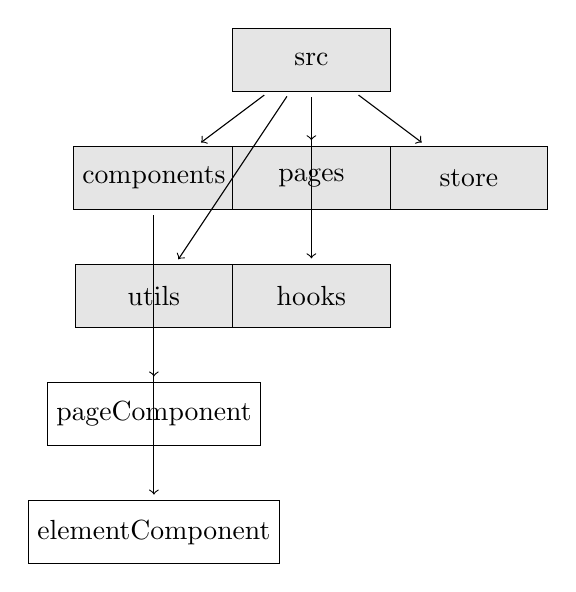
\begin{tikzpicture}[
    file/.style={draw, rectangle, minimum width=2cm, minimum height=0.8cm},
    folder/.style={draw, rectangle, minimum width=2cm, minimum height=0.8cm, fill=gray!20},
    arrow/.style={->, shorten >=2pt, shorten <=2pt}
]

% Folders
\node[folder] (src) at (0,0) {src};
\node[folder] (components) at (-2,-1.5) {components};
\node[folder] (pages) at (0,-1.5) {pages};
\node[folder] (store) at (2,-1.5) {store};
\node[folder] (utils) at (-2,-3) {utils};
\node[folder] (hooks) at (0,-3) {hooks};

% Files
\node[file] (pageComponent) at (-2,-4.5) {pageComponent};
\node[file] (elementComponent) at (-2,-6) {elementComponent};
% ... add more files

% Connections
\draw[arrow] (src) -- (components);
\draw[arrow] (src) -- (pages);
\draw[arrow] (src) -- (store);
\draw[arrow] (src) -- (utils);
\draw[arrow] (src) -- (hooks);
\draw[arrow] (components) -- (pageComponent);
\draw[arrow] (components) -- (elementComponent);
% ... add more connections

\end{tikzpicture}



\pagebreak
\subsubsection{Back-end}
The backend uses the dotNet framework. The development language using the C\# language.

In this project, the backend uses the Onion Architecture.
The Onion Architecture is a typically layered architecture, 
where each layer depends on the inner layer and provides interfaces to the outer layer.
The outer layer provides services to the outermost layer 
and other modules in the same layer based on the interfaces of the inner layer.

From inner to outer, the layers are: Domain, Application, Infrastructure, Presentation.
The Domain layer is the core layer and the innermost layer, used to define domain models, 
which are the business models.
It includes domain models and domain service interfaces.
Domain models are used to define the business models, 
which are the entities in the entity-relationship model and their attributes.
Domain service interfaces are used to define the business services, 
which are the relationships between entities in the entity-relationship model.

The Application layer is the application layer, 
used to define application services, which are the business logic.
It includes domain service implementations and application service interfaces.
Domain service implementations implement the methods of the inner layer's domain service 
interfaces and implement the business logic of the domain models.
Application service interfaces are used to define application services, 
which are the business logic.
It includes but is not limited to database interfaces, testing interfaces, 
HTTP API interfaces, MQTT interfaces, etc.

The Infrastructure layer is the infrastructure layer, used to define infrastructure.
It includes database implementations, testing implementations, 
HTTP API implementations, MQTT implementations, etc.
Database implementations implement the database interfaces 
and provide CRUD services for the database.
Testing implementations implement the testing interfaces 
and provide services for unit testing and integration testing.
HTTP API implementations implement the HTTP API interfaces 
and provide CRUD operations for HTTP APIs.
MQTT implementations implement the MQTT interfaces 
and provide CRUD operations for MQTT.

The Presentation layer is the presentation layer, used to define presentation logic, 
such as interfaces and pages. Since this is a backend project,
data presentation and control are handled by the frontend, 
so this layer is not needed.



\pagebreak
\subsubsection{Data communication and storage}
% 关于本项目的数据通信与数据存储的设计, 包括数据通信的协议, 数据存储的设计等
% 关于数据通信的设计:
% 1. 通信协议的选择
% 自前端向后端发送的数据, 有三种传输的数据类型, 
% 一种是普通的增删改查的请求, 对数据传输的时效性要求不高, 但是对数据的准确性, 完整性, 有序性, 安全性有一定的要求,
% 这种数据的传输, 采用 HTTP 协议, 以及 RESTful API 的设计. 可以有效的保证对数据传输的以上要求.
% 一种是对数据通道的创建和流媒体数据的传输, 对数据传输的时效性, 安全性要求较高, 这种数据的传输, 采用 WebRTC 协议, 以及 MQTT 协议.
% 配合可以快速解码的 flatbuffers 协议, 可以有效的保证对数据传输的以上要求.
% 最后一种是对设备的状态信息和操作信息的传输, 对完整性, 有序性, 安全性都有较高的要求, 这种数据的传输, 采用 MQTT 协议
% 同时也使用了 flatbuffers 协议.
% 
% 2. 数据通信的通信架构和通信流程
% 本项目的数据通信的通信架构, 是基于前后端分离的架构, 前端使用 React 框架, 后端使用 dotnet 框架.
% 当前端需要向后端发送数据的时候, 前端会向后端发送 HTTP 请求, 后端接收到 HTTP 请求之后, 会根据请求的数据类型,
% 选择不同的数据处理方式, 对于普通的增删改查的请求, 后端会根据 RESTful API 的设计, 对数据进行增删改查的操作,
% 对于对数据通道的创建和流媒体数据的传输, 后端会根据 WebRTC 协议, 对数据通道进行创建, 并且帮助前端和设备建立数据通道,
% 当数据通道建立后, 前端和设备之间则使用 flatbuffer 的数据格式对流媒体数据进行传输,
% 对于设备的状态信息和操作信息的传输, 前端会直接向 MQTT broker 发送 MQTT 请求, 
% 设备会在其自身的固件中监听相关的 MQTT 请求, 并且返回相关的数据.
% 
% 3. 数据通信的格式
% 本项目的数据通信的格式, 有三种, 
% 一种是 HTTP 协议, 
% 使用 json 格式对数据进行传输,
% 一种是 WebRTC 协议, 
% 使用 flatbuffers 格式对数据进行传输,
% 一种是 MQTT 协议.
% 使用 flatbuffers 格式对数据进行传输,
% 
% 关于数据存储的设计:
% 1. 数据存储的数据库的选择
% 本项目的数据存储的数据库的选择, 使用了轻量级的数据库 SQLite,
% SQLite 是一个进程内的库, 实现了自给自足的, 无服务器的, 零配置的, 事务性的 SQL 数据库引擎.
% 这是因为整个项目的目的是为了实现前端与设备之间的数据通信, 对于数据库数据的增删改查操作的要求不高,
% 数据量较小, 且对于数据库的数据的事务性要求不高, 所以选择了 SQLite 数据库.
% 2. 项目前后端的数据结构的设计
% 在本项目中, 前端由于使用了 React 框架, 所以前端的数据结构的设计, 使用了基于状态的数据结构的设计,
% 每个组件或者数据集都包含一个状态对象, 这个状态对象的属性就是组件的各个状态. 
% 使用状态对象的原因是, 可以方便的对状态进行管理, 采用对象-属性的形式, 可以方便的针对不同组件的同类状态进行区分,
% 由于跨组件的状态是由 redux 进行管理的, 这种状态对象的设计, 可以更搞笑的对状态进行更新和传递.
% 后端由于使用了 dotnet 框架, 所以后端的数据结构的设计, 使用了基于类的数据结构的设计,
% 采用了面向对象的编程思想, 对数据进行了封装, 使得数据的传输更加的安全, 有序, 完整.


\pagebreak

% \subsection{Domain model}
% \documentclass[]{article}
\usepackage{graphicx}
\usepackage{amsmath}
\usepackage{tikz}

% libaries
\usetikzlibrary{shapes,arrows}

%Define the listing package
\usepackage{listings} %code highlighter
\usepackage{color} %use color
\definecolor{mygreen}{rgb}{0,0.6,0}
\definecolor{mygray}{rgb}{0.5,0.5,0.5}
\definecolor{mymauve}{rgb}{0.58,0,0.82}

%Customize a bit the look
\lstset{ %
backgroundcolor=\color{white}, % choose the background color; you must add \usepackage{color} or \usepackage{xcolor}
basicstyle=\footnotesize, % the size of the fonts that are used for the code
breakatwhitespace=false, % sets if automatic breaks should only happen at whitespace
breaklines=true, % sets automatic line breaking
captionpos=b, % sets the caption-position to bottom
commentstyle=\color{mygreen}, % comment style
deletekeywords={...}, % if you want to delete keywords from the given language
escapeinside={\%*}{*)}, % if you want to add LaTeX within your code
extendedchars=true, % lets you use non-ASCII characters; for 8-bits encodings only, does not work with UTF-8
frame=single, % adds a frame around the code
keepspaces=true, % keeps spaces in text, useful for keeping indentation of code (possibly needs columns=flexible)
keywordstyle=\color{blue}, % keyword style
% language=Octave, % the language of the code
morekeywords={*,...}, % if you want to add more keywords to the set
numbers=left, % where to put the line-numbers; possible values are (none, left, right)
numbersep=5pt, % how far the line-numbers are from the code
numberstyle=\tiny\color{mygray}, % the style that is used for the line-numbers
rulecolor=\color{black}, % if not set, the frame-color may be changed on line-breaks within not-black text (e.g. comments (green here))
showspaces=false, % show spaces everywhere adding particular underscores; it overrides 'showstringspaces'
showstringspaces=false, % underline spaces within strings only
showtabs=false, % show tabs within strings adding particular underscores
stepnumber=1, % the step between two line-numbers. If it's 1, each line will be numbered
stringstyle=\color{mymauve}, % string literal style
tabsize=2, % sets default tabsize to 2 spaces
title=\lstname % show the filename of files included with \lstinputlisting; also try caption instead of title
}

\definecolor{darkgray}{rgb}{.4,.4,.4}
\definecolor{purple}{rgb}{0.65, 0.12, 0.82}

\lstdefinelanguage{React}{
keywords={const, typeof, new, true, false, catch, function, return, null, catch, switch, var, if, in, while, do, else, case, break},
keywordstyle=\color{blue}\bfseries,
ndkeywords={class, export, boolean, throw, implements, import, this},
ndkeywordstyle=\color{darkgray}\bfseries,
identifierstyle=\color{mygreen},
sensitive=false,
comment=[l]{//},
morecomment=[s]{/*}{*/},
commentstyle=\color{purple}\ttfamily,
string=[b]{"}{'}{`},
stringstyle=\color{red}\ttfamily,
morestring=[b]',
morestring=[b]",
morestring=[b]`',
}

\lstdefinelanguage{CSharp}{
keywords={const, typeof, new, true, false, catch, function, return, null, catch, switch, var, if, in, while, do, else, case, break},
keywordstyle=\color{blue}\bfseries,
ndkeywords={class, export, boolean, throw, implements, import, this},
ndkeywordstyle=\color{darkgray}\bfseries,
identifierstyle=\color{mygreen},
sensitive=false,
comment=[l]{//},
morecomment=[s]{/*}{*/},
commentstyle=\color{purple}\ttfamily,
string=[b]{"}{'}{`},
stringstyle=\color{red}\ttfamily,
morestring=[b]',
morestring=[b]",
morestring=[b]`',
}

\lstset{
language=React,
extendedchars=true,
basicstyle=\footnotesize\ttfamily,
showstringspaces=false,
showspaces=false,
numbers=left,
numberstyle=\footnotesize,
numbersep=9pt,
tabsize=2,
breaklines=true,
showtabs=false,
captionpos=b
}

\lstset{
language=CSharp,
extendedchars=true,
basicstyle=\footnotesize\ttfamily,
showstringspaces=false,
showspaces=false,
numbers=left,
numberstyle=\footnotesize,
numbersep=9pt,
tabsize=2,
breaklines=true,
showtabs=false,
captionpos=b
}

% \usepackage{cite} % Add this line for citation

% \bibliographystyle{plain}

\title{
The implementation of BifrostConnect Front-end scope, 
re-design and development with the relevant back-end support develop.
}
\author{
    Fei Gu \\
    Erhvervs Akademi Sydvest \\
    Computer Science 21\\
    }
\date{\today}

\begin{document}

% Front page
\maketitle
\begin{center}
    Supervisor: Henrik Boulund Meng Hansen \\
    Company: BifrostConnect \\
    Engineering Director: Jasper Wass \\
\end{center}
\tableofcontents
\pagebreak


% The introduction
\section{Introduction}
\subsection{Background}\input{sections/introduction/background.tex}
\subsection{The company}\input{sections/introduction/aboutCompany}
\subsection{The project}\input{sections/introduction/aboutProject}
\pagebreak

% The problem statement
\section{Problem Statement}
\subsection{Statement}
\input{sections/problemStatement/statement}
\subsection{Situation}
\input{sections/problemStatement/situation}
\subsection{Potential Solution}
\input{sections/problemStatement/potentialSolution}
\pagebreak

% Requirement analysis
\section{Requirement Analysis}
\input{sections/requirementAnalysis/index}

\subsection{Stakeholders}
\input{sections/requirementAnalysis/stakeholders/index}

\subsection{Business Domain}
\input{sections/requirementAnalysis/bussinesDomain/index}

\subsection{Scope}
\input{sections/requirementAnalysis/scope}

\subsection{Goals}
\input{sections/requirementAnalysis/goals}
\pagebreak

% Software Design
\section{Software Design}
% developement methods
\subsection{Software Development Methods}
\input{sections/softwareDevelopmentMethods/index}
\subsubsection{Agile Software Development}
\input{sections/softwareDevelopmentMethods/agileSoftwareDevelopment/index}
\subsubsection{Feature Driven Development}
\input{sections/softwareDevelopmentMethods/featureDrivenDevelopment/index}

\pagebreak

% Technology seslection
\subsection{Technology selection}
\input{sections/softwareDesign/technologySelection/index}
\subsubsection{Front-end}
\input{sections/softwareDesign/technologySelection/frontEnd}            
\subsubsection{Back-end}
\input{sections/softwareDesign/technologySelection/backEnd}            
\subsubsection{Database}
\input{sections/softwareDesign/technologySelection/database}
\subsubsection{Data communication}
\input{sections/softwareDesign/technologySelection/dataCommunication}            
\subsubsection{DevOps}
\input{sections/softwareDesign/technologySelection/devOps}
\pagebreak

% Architecture design
\subsection{Architecture design}
\input{sections/softwareDesign/architectureDesign/index}
\pagebreak
\subsubsection{Front-end}
\input{sections/softwareDesign/architectureDesign/frontEndArchitecture}
\pagebreak
\subsubsection{Back-end}
\input{sections/softwareDesign/architectureDesign/backEndArchitecture}
\pagebreak
\subsubsection{Data communication and storage}
\input{sections/softwareDesign/architectureDesign/dataCommunicationArchitecture}
\pagebreak

% \subsection{Domain model}
% \input{sections/softwareDesign/domainModel/index}
% \subsection{Database design}
% % 数据库领域模型 ER 图
% % 包括表和字段的设置.
% % 对于私有键和外键的设置.

% \subsection{Back-end design}
% % 后端对象模型
% % 以及对于对象模型的增删改查
% % 以及相关的其他服务的设计`'

% \subsection{Front-end design}
% % 对于前端的页面结构的设计 
% % 页面的状态的设计, 交互设计

% \subsection{FlatBuffers design}
% % schema 的设计

\subsection{DevOps CI/CD process design}
\input{sections/softwareDesign/devOpsDesign/index}
\subsubsection{Continuous Integration}
\input{sections/softwareDesign/devOpsDesign/continuousIntegration/index}
\subsubsection{Continuous Delivery}
\input{sections/softwareDesign/devOpsDesign/continuousDelivery/index}
\subsubsection{Continuous Deployment}
\input{sections/softwareDesign/devOpsDesign/continuousDeployment/index}
\pagebreak

\section{Software Development} 
\input{sections/softwareDevelopment/index}
\subsection{Overall development}
\input{sections/softwareDevelopment/overallDevelopement/index}
\subsubsection{Front-end}
\input{sections/softwareDevelopment/overallDevelopement/frontEnd/index}
\subsubsection{Back-end}
\input{sections/softwareDevelopment/overallDevelopement/backEnd/index}
\subsubsection{DevOps}
\input{sections/softwareDevelopment/overallDevelopement/devOps/index}
\subsection{Feature development} 
\input{sections/softwareDevelopment/featureDevelopment/index}
\subsubsection{Use Case 1}
\input{sections/softwareDevelopment/featureDevelopment/useCase1/index}
\subsubsection{Feature 1}
\input{sections/softwareDevelopment/featureDevelopment/feature/feature1.tex}
\pagebreak
\section{Conclusion} 
\subsection{Result}
Since the project is still in progress, the result is not available yet.
So far, basic structure of this project has been built. But the most features 
are not implemented yet. 
\subsection{Discussion}
As a single developer for this project, I am confident what I have done so far.
And I can say I understand the most of the knowledge I have used in this project, 
which also means I can explain all the part of the project. 
But this project also relevant some of the complex knowledge which I have to continue 
to study and practice.
\subsection{Future Work}
The future work is to implement the rest of the features. 
Including the most important part which is the 'create session' feature.
\pagebreak
% \bibliography{bibliography}
\pagebreak
% \begin{appendices}
%     \section{Appendix}
% \end{appendices} 
\end{document}
% \subsection{Database design}
% % 数据库领域模型 ER 图
% % 包括表和字段的设置.
% % 对于私有键和外键的设置.

% \subsection{Back-end design}
% % 后端对象模型
% % 以及对于对象模型的增删改查
% % 以及相关的其他服务的设计`'

% \subsection{Front-end design}
% % 对于前端的页面结构的设计 
% % 页面的状态的设计, 交互设计

% \subsection{FlatBuffers design}
% % schema 的设计

\subsection{DevOps CI/CD process design}
\documentclass[]{article}
\usepackage{graphicx}
\usepackage{amsmath}
\usepackage{tikz}

% libaries
\usetikzlibrary{shapes,arrows}

%Define the listing package
\usepackage{listings} %code highlighter
\usepackage{color} %use color
\definecolor{mygreen}{rgb}{0,0.6,0}
\definecolor{mygray}{rgb}{0.5,0.5,0.5}
\definecolor{mymauve}{rgb}{0.58,0,0.82}

%Customize a bit the look
\lstset{ %
backgroundcolor=\color{white}, % choose the background color; you must add \usepackage{color} or \usepackage{xcolor}
basicstyle=\footnotesize, % the size of the fonts that are used for the code
breakatwhitespace=false, % sets if automatic breaks should only happen at whitespace
breaklines=true, % sets automatic line breaking
captionpos=b, % sets the caption-position to bottom
commentstyle=\color{mygreen}, % comment style
deletekeywords={...}, % if you want to delete keywords from the given language
escapeinside={\%*}{*)}, % if you want to add LaTeX within your code
extendedchars=true, % lets you use non-ASCII characters; for 8-bits encodings only, does not work with UTF-8
frame=single, % adds a frame around the code
keepspaces=true, % keeps spaces in text, useful for keeping indentation of code (possibly needs columns=flexible)
keywordstyle=\color{blue}, % keyword style
% language=Octave, % the language of the code
morekeywords={*,...}, % if you want to add more keywords to the set
numbers=left, % where to put the line-numbers; possible values are (none, left, right)
numbersep=5pt, % how far the line-numbers are from the code
numberstyle=\tiny\color{mygray}, % the style that is used for the line-numbers
rulecolor=\color{black}, % if not set, the frame-color may be changed on line-breaks within not-black text (e.g. comments (green here))
showspaces=false, % show spaces everywhere adding particular underscores; it overrides 'showstringspaces'
showstringspaces=false, % underline spaces within strings only
showtabs=false, % show tabs within strings adding particular underscores
stepnumber=1, % the step between two line-numbers. If it's 1, each line will be numbered
stringstyle=\color{mymauve}, % string literal style
tabsize=2, % sets default tabsize to 2 spaces
title=\lstname % show the filename of files included with \lstinputlisting; also try caption instead of title
}

\definecolor{darkgray}{rgb}{.4,.4,.4}
\definecolor{purple}{rgb}{0.65, 0.12, 0.82}

\lstdefinelanguage{React}{
keywords={const, typeof, new, true, false, catch, function, return, null, catch, switch, var, if, in, while, do, else, case, break},
keywordstyle=\color{blue}\bfseries,
ndkeywords={class, export, boolean, throw, implements, import, this},
ndkeywordstyle=\color{darkgray}\bfseries,
identifierstyle=\color{mygreen},
sensitive=false,
comment=[l]{//},
morecomment=[s]{/*}{*/},
commentstyle=\color{purple}\ttfamily,
string=[b]{"}{'}{`},
stringstyle=\color{red}\ttfamily,
morestring=[b]',
morestring=[b]",
morestring=[b]`',
}

\lstdefinelanguage{CSharp}{
keywords={const, typeof, new, true, false, catch, function, return, null, catch, switch, var, if, in, while, do, else, case, break},
keywordstyle=\color{blue}\bfseries,
ndkeywords={class, export, boolean, throw, implements, import, this},
ndkeywordstyle=\color{darkgray}\bfseries,
identifierstyle=\color{mygreen},
sensitive=false,
comment=[l]{//},
morecomment=[s]{/*}{*/},
commentstyle=\color{purple}\ttfamily,
string=[b]{"}{'}{`},
stringstyle=\color{red}\ttfamily,
morestring=[b]',
morestring=[b]",
morestring=[b]`',
}

\lstset{
language=React,
extendedchars=true,
basicstyle=\footnotesize\ttfamily,
showstringspaces=false,
showspaces=false,
numbers=left,
numberstyle=\footnotesize,
numbersep=9pt,
tabsize=2,
breaklines=true,
showtabs=false,
captionpos=b
}

\lstset{
language=CSharp,
extendedchars=true,
basicstyle=\footnotesize\ttfamily,
showstringspaces=false,
showspaces=false,
numbers=left,
numberstyle=\footnotesize,
numbersep=9pt,
tabsize=2,
breaklines=true,
showtabs=false,
captionpos=b
}

% \usepackage{cite} % Add this line for citation

% \bibliographystyle{plain}

\title{
The implementation of BifrostConnect Front-end scope, 
re-design and development with the relevant back-end support develop.
}
\author{
    Fei Gu \\
    Erhvervs Akademi Sydvest \\
    Computer Science 21\\
    }
\date{\today}

\begin{document}

% Front page
\maketitle
\begin{center}
    Supervisor: Henrik Boulund Meng Hansen \\
    Company: BifrostConnect \\
    Engineering Director: Jasper Wass \\
\end{center}
\tableofcontents
\pagebreak


% The introduction
\section{Introduction}
\subsection{Background}\input{sections/introduction/background.tex}
\subsection{The company}\input{sections/introduction/aboutCompany}
\subsection{The project}\input{sections/introduction/aboutProject}
\pagebreak

% The problem statement
\section{Problem Statement}
\subsection{Statement}
\input{sections/problemStatement/statement}
\subsection{Situation}
\input{sections/problemStatement/situation}
\subsection{Potential Solution}
\input{sections/problemStatement/potentialSolution}
\pagebreak

% Requirement analysis
\section{Requirement Analysis}
\input{sections/requirementAnalysis/index}

\subsection{Stakeholders}
\input{sections/requirementAnalysis/stakeholders/index}

\subsection{Business Domain}
\input{sections/requirementAnalysis/bussinesDomain/index}

\subsection{Scope}
\input{sections/requirementAnalysis/scope}

\subsection{Goals}
\input{sections/requirementAnalysis/goals}
\pagebreak

% Software Design
\section{Software Design}
% developement methods
\subsection{Software Development Methods}
\input{sections/softwareDevelopmentMethods/index}
\subsubsection{Agile Software Development}
\input{sections/softwareDevelopmentMethods/agileSoftwareDevelopment/index}
\subsubsection{Feature Driven Development}
\input{sections/softwareDevelopmentMethods/featureDrivenDevelopment/index}

\pagebreak

% Technology seslection
\subsection{Technology selection}
\input{sections/softwareDesign/technologySelection/index}
\subsubsection{Front-end}
\input{sections/softwareDesign/technologySelection/frontEnd}            
\subsubsection{Back-end}
\input{sections/softwareDesign/technologySelection/backEnd}            
\subsubsection{Database}
\input{sections/softwareDesign/technologySelection/database}
\subsubsection{Data communication}
\input{sections/softwareDesign/technologySelection/dataCommunication}            
\subsubsection{DevOps}
\input{sections/softwareDesign/technologySelection/devOps}
\pagebreak

% Architecture design
\subsection{Architecture design}
\input{sections/softwareDesign/architectureDesign/index}
\pagebreak
\subsubsection{Front-end}
\input{sections/softwareDesign/architectureDesign/frontEndArchitecture}
\pagebreak
\subsubsection{Back-end}
\input{sections/softwareDesign/architectureDesign/backEndArchitecture}
\pagebreak
\subsubsection{Data communication and storage}
\input{sections/softwareDesign/architectureDesign/dataCommunicationArchitecture}
\pagebreak

% \subsection{Domain model}
% \input{sections/softwareDesign/domainModel/index}
% \subsection{Database design}
% % 数据库领域模型 ER 图
% % 包括表和字段的设置.
% % 对于私有键和外键的设置.

% \subsection{Back-end design}
% % 后端对象模型
% % 以及对于对象模型的增删改查
% % 以及相关的其他服务的设计`'

% \subsection{Front-end design}
% % 对于前端的页面结构的设计 
% % 页面的状态的设计, 交互设计

% \subsection{FlatBuffers design}
% % schema 的设计

\subsection{DevOps CI/CD process design}
\input{sections/softwareDesign/devOpsDesign/index}
\subsubsection{Continuous Integration}
\input{sections/softwareDesign/devOpsDesign/continuousIntegration/index}
\subsubsection{Continuous Delivery}
\input{sections/softwareDesign/devOpsDesign/continuousDelivery/index}
\subsubsection{Continuous Deployment}
\input{sections/softwareDesign/devOpsDesign/continuousDeployment/index}
\pagebreak

\section{Software Development} 
\input{sections/softwareDevelopment/index}
\subsection{Overall development}
\input{sections/softwareDevelopment/overallDevelopement/index}
\subsubsection{Front-end}
\input{sections/softwareDevelopment/overallDevelopement/frontEnd/index}
\subsubsection{Back-end}
\input{sections/softwareDevelopment/overallDevelopement/backEnd/index}
\subsubsection{DevOps}
\input{sections/softwareDevelopment/overallDevelopement/devOps/index}
\subsection{Feature development} 
\input{sections/softwareDevelopment/featureDevelopment/index}
\subsubsection{Use Case 1}
\input{sections/softwareDevelopment/featureDevelopment/useCase1/index}
\subsubsection{Feature 1}
\input{sections/softwareDevelopment/featureDevelopment/feature/feature1.tex}
\pagebreak
\section{Conclusion} 
\subsection{Result}
Since the project is still in progress, the result is not available yet.
So far, basic structure of this project has been built. But the most features 
are not implemented yet. 
\subsection{Discussion}
As a single developer for this project, I am confident what I have done so far.
And I can say I understand the most of the knowledge I have used in this project, 
which also means I can explain all the part of the project. 
But this project also relevant some of the complex knowledge which I have to continue 
to study and practice.
\subsection{Future Work}
The future work is to implement the rest of the features. 
Including the most important part which is the 'create session' feature.
\pagebreak
% \bibliography{bibliography}
\pagebreak
% \begin{appendices}
%     \section{Appendix}
% \end{appendices} 
\end{document}
\subsubsection{Continuous Integration}
\documentclass[]{article}
\usepackage{graphicx}
\usepackage{amsmath}
\usepackage{tikz}

% libaries
\usetikzlibrary{shapes,arrows}

%Define the listing package
\usepackage{listings} %code highlighter
\usepackage{color} %use color
\definecolor{mygreen}{rgb}{0,0.6,0}
\definecolor{mygray}{rgb}{0.5,0.5,0.5}
\definecolor{mymauve}{rgb}{0.58,0,0.82}

%Customize a bit the look
\lstset{ %
backgroundcolor=\color{white}, % choose the background color; you must add \usepackage{color} or \usepackage{xcolor}
basicstyle=\footnotesize, % the size of the fonts that are used for the code
breakatwhitespace=false, % sets if automatic breaks should only happen at whitespace
breaklines=true, % sets automatic line breaking
captionpos=b, % sets the caption-position to bottom
commentstyle=\color{mygreen}, % comment style
deletekeywords={...}, % if you want to delete keywords from the given language
escapeinside={\%*}{*)}, % if you want to add LaTeX within your code
extendedchars=true, % lets you use non-ASCII characters; for 8-bits encodings only, does not work with UTF-8
frame=single, % adds a frame around the code
keepspaces=true, % keeps spaces in text, useful for keeping indentation of code (possibly needs columns=flexible)
keywordstyle=\color{blue}, % keyword style
% language=Octave, % the language of the code
morekeywords={*,...}, % if you want to add more keywords to the set
numbers=left, % where to put the line-numbers; possible values are (none, left, right)
numbersep=5pt, % how far the line-numbers are from the code
numberstyle=\tiny\color{mygray}, % the style that is used for the line-numbers
rulecolor=\color{black}, % if not set, the frame-color may be changed on line-breaks within not-black text (e.g. comments (green here))
showspaces=false, % show spaces everywhere adding particular underscores; it overrides 'showstringspaces'
showstringspaces=false, % underline spaces within strings only
showtabs=false, % show tabs within strings adding particular underscores
stepnumber=1, % the step between two line-numbers. If it's 1, each line will be numbered
stringstyle=\color{mymauve}, % string literal style
tabsize=2, % sets default tabsize to 2 spaces
title=\lstname % show the filename of files included with \lstinputlisting; also try caption instead of title
}

\definecolor{darkgray}{rgb}{.4,.4,.4}
\definecolor{purple}{rgb}{0.65, 0.12, 0.82}

\lstdefinelanguage{React}{
keywords={const, typeof, new, true, false, catch, function, return, null, catch, switch, var, if, in, while, do, else, case, break},
keywordstyle=\color{blue}\bfseries,
ndkeywords={class, export, boolean, throw, implements, import, this},
ndkeywordstyle=\color{darkgray}\bfseries,
identifierstyle=\color{mygreen},
sensitive=false,
comment=[l]{//},
morecomment=[s]{/*}{*/},
commentstyle=\color{purple}\ttfamily,
string=[b]{"}{'}{`},
stringstyle=\color{red}\ttfamily,
morestring=[b]',
morestring=[b]",
morestring=[b]`',
}

\lstdefinelanguage{CSharp}{
keywords={const, typeof, new, true, false, catch, function, return, null, catch, switch, var, if, in, while, do, else, case, break},
keywordstyle=\color{blue}\bfseries,
ndkeywords={class, export, boolean, throw, implements, import, this},
ndkeywordstyle=\color{darkgray}\bfseries,
identifierstyle=\color{mygreen},
sensitive=false,
comment=[l]{//},
morecomment=[s]{/*}{*/},
commentstyle=\color{purple}\ttfamily,
string=[b]{"}{'}{`},
stringstyle=\color{red}\ttfamily,
morestring=[b]',
morestring=[b]",
morestring=[b]`',
}

\lstset{
language=React,
extendedchars=true,
basicstyle=\footnotesize\ttfamily,
showstringspaces=false,
showspaces=false,
numbers=left,
numberstyle=\footnotesize,
numbersep=9pt,
tabsize=2,
breaklines=true,
showtabs=false,
captionpos=b
}

\lstset{
language=CSharp,
extendedchars=true,
basicstyle=\footnotesize\ttfamily,
showstringspaces=false,
showspaces=false,
numbers=left,
numberstyle=\footnotesize,
numbersep=9pt,
tabsize=2,
breaklines=true,
showtabs=false,
captionpos=b
}

% \usepackage{cite} % Add this line for citation

% \bibliographystyle{plain}

\title{
The implementation of BifrostConnect Front-end scope, 
re-design and development with the relevant back-end support develop.
}
\author{
    Fei Gu \\
    Erhvervs Akademi Sydvest \\
    Computer Science 21\\
    }
\date{\today}

\begin{document}

% Front page
\maketitle
\begin{center}
    Supervisor: Henrik Boulund Meng Hansen \\
    Company: BifrostConnect \\
    Engineering Director: Jasper Wass \\
\end{center}
\tableofcontents
\pagebreak


% The introduction
\section{Introduction}
\subsection{Background}\input{sections/introduction/background.tex}
\subsection{The company}\input{sections/introduction/aboutCompany}
\subsection{The project}\input{sections/introduction/aboutProject}
\pagebreak

% The problem statement
\section{Problem Statement}
\subsection{Statement}
\input{sections/problemStatement/statement}
\subsection{Situation}
\input{sections/problemStatement/situation}
\subsection{Potential Solution}
\input{sections/problemStatement/potentialSolution}
\pagebreak

% Requirement analysis
\section{Requirement Analysis}
\input{sections/requirementAnalysis/index}

\subsection{Stakeholders}
\input{sections/requirementAnalysis/stakeholders/index}

\subsection{Business Domain}
\input{sections/requirementAnalysis/bussinesDomain/index}

\subsection{Scope}
\input{sections/requirementAnalysis/scope}

\subsection{Goals}
\input{sections/requirementAnalysis/goals}
\pagebreak

% Software Design
\section{Software Design}
% developement methods
\subsection{Software Development Methods}
\input{sections/softwareDevelopmentMethods/index}
\subsubsection{Agile Software Development}
\input{sections/softwareDevelopmentMethods/agileSoftwareDevelopment/index}
\subsubsection{Feature Driven Development}
\input{sections/softwareDevelopmentMethods/featureDrivenDevelopment/index}

\pagebreak

% Technology seslection
\subsection{Technology selection}
\input{sections/softwareDesign/technologySelection/index}
\subsubsection{Front-end}
\input{sections/softwareDesign/technologySelection/frontEnd}            
\subsubsection{Back-end}
\input{sections/softwareDesign/technologySelection/backEnd}            
\subsubsection{Database}
\input{sections/softwareDesign/technologySelection/database}
\subsubsection{Data communication}
\input{sections/softwareDesign/technologySelection/dataCommunication}            
\subsubsection{DevOps}
\input{sections/softwareDesign/technologySelection/devOps}
\pagebreak

% Architecture design
\subsection{Architecture design}
\input{sections/softwareDesign/architectureDesign/index}
\pagebreak
\subsubsection{Front-end}
\input{sections/softwareDesign/architectureDesign/frontEndArchitecture}
\pagebreak
\subsubsection{Back-end}
\input{sections/softwareDesign/architectureDesign/backEndArchitecture}
\pagebreak
\subsubsection{Data communication and storage}
\input{sections/softwareDesign/architectureDesign/dataCommunicationArchitecture}
\pagebreak

% \subsection{Domain model}
% \input{sections/softwareDesign/domainModel/index}
% \subsection{Database design}
% % 数据库领域模型 ER 图
% % 包括表和字段的设置.
% % 对于私有键和外键的设置.

% \subsection{Back-end design}
% % 后端对象模型
% % 以及对于对象模型的增删改查
% % 以及相关的其他服务的设计`'

% \subsection{Front-end design}
% % 对于前端的页面结构的设计 
% % 页面的状态的设计, 交互设计

% \subsection{FlatBuffers design}
% % schema 的设计

\subsection{DevOps CI/CD process design}
\input{sections/softwareDesign/devOpsDesign/index}
\subsubsection{Continuous Integration}
\input{sections/softwareDesign/devOpsDesign/continuousIntegration/index}
\subsubsection{Continuous Delivery}
\input{sections/softwareDesign/devOpsDesign/continuousDelivery/index}
\subsubsection{Continuous Deployment}
\input{sections/softwareDesign/devOpsDesign/continuousDeployment/index}
\pagebreak

\section{Software Development} 
\input{sections/softwareDevelopment/index}
\subsection{Overall development}
\input{sections/softwareDevelopment/overallDevelopement/index}
\subsubsection{Front-end}
\input{sections/softwareDevelopment/overallDevelopement/frontEnd/index}
\subsubsection{Back-end}
\input{sections/softwareDevelopment/overallDevelopement/backEnd/index}
\subsubsection{DevOps}
\input{sections/softwareDevelopment/overallDevelopement/devOps/index}
\subsection{Feature development} 
\input{sections/softwareDevelopment/featureDevelopment/index}
\subsubsection{Use Case 1}
\input{sections/softwareDevelopment/featureDevelopment/useCase1/index}
\subsubsection{Feature 1}
\input{sections/softwareDevelopment/featureDevelopment/feature/feature1.tex}
\pagebreak
\section{Conclusion} 
\subsection{Result}
Since the project is still in progress, the result is not available yet.
So far, basic structure of this project has been built. But the most features 
are not implemented yet. 
\subsection{Discussion}
As a single developer for this project, I am confident what I have done so far.
And I can say I understand the most of the knowledge I have used in this project, 
which also means I can explain all the part of the project. 
But this project also relevant some of the complex knowledge which I have to continue 
to study and practice.
\subsection{Future Work}
The future work is to implement the rest of the features. 
Including the most important part which is the 'create session' feature.
\pagebreak
% \bibliography{bibliography}
\pagebreak
% \begin{appendices}
%     \section{Appendix}
% \end{appendices} 
\end{document}
\subsubsection{Continuous Delivery}
\documentclass[]{article}
\usepackage{graphicx}
\usepackage{amsmath}
\usepackage{tikz}

% libaries
\usetikzlibrary{shapes,arrows}

%Define the listing package
\usepackage{listings} %code highlighter
\usepackage{color} %use color
\definecolor{mygreen}{rgb}{0,0.6,0}
\definecolor{mygray}{rgb}{0.5,0.5,0.5}
\definecolor{mymauve}{rgb}{0.58,0,0.82}

%Customize a bit the look
\lstset{ %
backgroundcolor=\color{white}, % choose the background color; you must add \usepackage{color} or \usepackage{xcolor}
basicstyle=\footnotesize, % the size of the fonts that are used for the code
breakatwhitespace=false, % sets if automatic breaks should only happen at whitespace
breaklines=true, % sets automatic line breaking
captionpos=b, % sets the caption-position to bottom
commentstyle=\color{mygreen}, % comment style
deletekeywords={...}, % if you want to delete keywords from the given language
escapeinside={\%*}{*)}, % if you want to add LaTeX within your code
extendedchars=true, % lets you use non-ASCII characters; for 8-bits encodings only, does not work with UTF-8
frame=single, % adds a frame around the code
keepspaces=true, % keeps spaces in text, useful for keeping indentation of code (possibly needs columns=flexible)
keywordstyle=\color{blue}, % keyword style
% language=Octave, % the language of the code
morekeywords={*,...}, % if you want to add more keywords to the set
numbers=left, % where to put the line-numbers; possible values are (none, left, right)
numbersep=5pt, % how far the line-numbers are from the code
numberstyle=\tiny\color{mygray}, % the style that is used for the line-numbers
rulecolor=\color{black}, % if not set, the frame-color may be changed on line-breaks within not-black text (e.g. comments (green here))
showspaces=false, % show spaces everywhere adding particular underscores; it overrides 'showstringspaces'
showstringspaces=false, % underline spaces within strings only
showtabs=false, % show tabs within strings adding particular underscores
stepnumber=1, % the step between two line-numbers. If it's 1, each line will be numbered
stringstyle=\color{mymauve}, % string literal style
tabsize=2, % sets default tabsize to 2 spaces
title=\lstname % show the filename of files included with \lstinputlisting; also try caption instead of title
}

\definecolor{darkgray}{rgb}{.4,.4,.4}
\definecolor{purple}{rgb}{0.65, 0.12, 0.82}

\lstdefinelanguage{React}{
keywords={const, typeof, new, true, false, catch, function, return, null, catch, switch, var, if, in, while, do, else, case, break},
keywordstyle=\color{blue}\bfseries,
ndkeywords={class, export, boolean, throw, implements, import, this},
ndkeywordstyle=\color{darkgray}\bfseries,
identifierstyle=\color{mygreen},
sensitive=false,
comment=[l]{//},
morecomment=[s]{/*}{*/},
commentstyle=\color{purple}\ttfamily,
string=[b]{"}{'}{`},
stringstyle=\color{red}\ttfamily,
morestring=[b]',
morestring=[b]",
morestring=[b]`',
}

\lstdefinelanguage{CSharp}{
keywords={const, typeof, new, true, false, catch, function, return, null, catch, switch, var, if, in, while, do, else, case, break},
keywordstyle=\color{blue}\bfseries,
ndkeywords={class, export, boolean, throw, implements, import, this},
ndkeywordstyle=\color{darkgray}\bfseries,
identifierstyle=\color{mygreen},
sensitive=false,
comment=[l]{//},
morecomment=[s]{/*}{*/},
commentstyle=\color{purple}\ttfamily,
string=[b]{"}{'}{`},
stringstyle=\color{red}\ttfamily,
morestring=[b]',
morestring=[b]",
morestring=[b]`',
}

\lstset{
language=React,
extendedchars=true,
basicstyle=\footnotesize\ttfamily,
showstringspaces=false,
showspaces=false,
numbers=left,
numberstyle=\footnotesize,
numbersep=9pt,
tabsize=2,
breaklines=true,
showtabs=false,
captionpos=b
}

\lstset{
language=CSharp,
extendedchars=true,
basicstyle=\footnotesize\ttfamily,
showstringspaces=false,
showspaces=false,
numbers=left,
numberstyle=\footnotesize,
numbersep=9pt,
tabsize=2,
breaklines=true,
showtabs=false,
captionpos=b
}

% \usepackage{cite} % Add this line for citation

% \bibliographystyle{plain}

\title{
The implementation of BifrostConnect Front-end scope, 
re-design and development with the relevant back-end support develop.
}
\author{
    Fei Gu \\
    Erhvervs Akademi Sydvest \\
    Computer Science 21\\
    }
\date{\today}

\begin{document}

% Front page
\maketitle
\begin{center}
    Supervisor: Henrik Boulund Meng Hansen \\
    Company: BifrostConnect \\
    Engineering Director: Jasper Wass \\
\end{center}
\tableofcontents
\pagebreak


% The introduction
\section{Introduction}
\subsection{Background}\input{sections/introduction/background.tex}
\subsection{The company}\input{sections/introduction/aboutCompany}
\subsection{The project}\input{sections/introduction/aboutProject}
\pagebreak

% The problem statement
\section{Problem Statement}
\subsection{Statement}
\input{sections/problemStatement/statement}
\subsection{Situation}
\input{sections/problemStatement/situation}
\subsection{Potential Solution}
\input{sections/problemStatement/potentialSolution}
\pagebreak

% Requirement analysis
\section{Requirement Analysis}
\input{sections/requirementAnalysis/index}

\subsection{Stakeholders}
\input{sections/requirementAnalysis/stakeholders/index}

\subsection{Business Domain}
\input{sections/requirementAnalysis/bussinesDomain/index}

\subsection{Scope}
\input{sections/requirementAnalysis/scope}

\subsection{Goals}
\input{sections/requirementAnalysis/goals}
\pagebreak

% Software Design
\section{Software Design}
% developement methods
\subsection{Software Development Methods}
\input{sections/softwareDevelopmentMethods/index}
\subsubsection{Agile Software Development}
\input{sections/softwareDevelopmentMethods/agileSoftwareDevelopment/index}
\subsubsection{Feature Driven Development}
\input{sections/softwareDevelopmentMethods/featureDrivenDevelopment/index}

\pagebreak

% Technology seslection
\subsection{Technology selection}
\input{sections/softwareDesign/technologySelection/index}
\subsubsection{Front-end}
\input{sections/softwareDesign/technologySelection/frontEnd}            
\subsubsection{Back-end}
\input{sections/softwareDesign/technologySelection/backEnd}            
\subsubsection{Database}
\input{sections/softwareDesign/technologySelection/database}
\subsubsection{Data communication}
\input{sections/softwareDesign/technologySelection/dataCommunication}            
\subsubsection{DevOps}
\input{sections/softwareDesign/technologySelection/devOps}
\pagebreak

% Architecture design
\subsection{Architecture design}
\input{sections/softwareDesign/architectureDesign/index}
\pagebreak
\subsubsection{Front-end}
\input{sections/softwareDesign/architectureDesign/frontEndArchitecture}
\pagebreak
\subsubsection{Back-end}
\input{sections/softwareDesign/architectureDesign/backEndArchitecture}
\pagebreak
\subsubsection{Data communication and storage}
\input{sections/softwareDesign/architectureDesign/dataCommunicationArchitecture}
\pagebreak

% \subsection{Domain model}
% \input{sections/softwareDesign/domainModel/index}
% \subsection{Database design}
% % 数据库领域模型 ER 图
% % 包括表和字段的设置.
% % 对于私有键和外键的设置.

% \subsection{Back-end design}
% % 后端对象模型
% % 以及对于对象模型的增删改查
% % 以及相关的其他服务的设计`'

% \subsection{Front-end design}
% % 对于前端的页面结构的设计 
% % 页面的状态的设计, 交互设计

% \subsection{FlatBuffers design}
% % schema 的设计

\subsection{DevOps CI/CD process design}
\input{sections/softwareDesign/devOpsDesign/index}
\subsubsection{Continuous Integration}
\input{sections/softwareDesign/devOpsDesign/continuousIntegration/index}
\subsubsection{Continuous Delivery}
\input{sections/softwareDesign/devOpsDesign/continuousDelivery/index}
\subsubsection{Continuous Deployment}
\input{sections/softwareDesign/devOpsDesign/continuousDeployment/index}
\pagebreak

\section{Software Development} 
\input{sections/softwareDevelopment/index}
\subsection{Overall development}
\input{sections/softwareDevelopment/overallDevelopement/index}
\subsubsection{Front-end}
\input{sections/softwareDevelopment/overallDevelopement/frontEnd/index}
\subsubsection{Back-end}
\input{sections/softwareDevelopment/overallDevelopement/backEnd/index}
\subsubsection{DevOps}
\input{sections/softwareDevelopment/overallDevelopement/devOps/index}
\subsection{Feature development} 
\input{sections/softwareDevelopment/featureDevelopment/index}
\subsubsection{Use Case 1}
\input{sections/softwareDevelopment/featureDevelopment/useCase1/index}
\subsubsection{Feature 1}
\input{sections/softwareDevelopment/featureDevelopment/feature/feature1.tex}
\pagebreak
\section{Conclusion} 
\subsection{Result}
Since the project is still in progress, the result is not available yet.
So far, basic structure of this project has been built. But the most features 
are not implemented yet. 
\subsection{Discussion}
As a single developer for this project, I am confident what I have done so far.
And I can say I understand the most of the knowledge I have used in this project, 
which also means I can explain all the part of the project. 
But this project also relevant some of the complex knowledge which I have to continue 
to study and practice.
\subsection{Future Work}
The future work is to implement the rest of the features. 
Including the most important part which is the 'create session' feature.
\pagebreak
% \bibliography{bibliography}
\pagebreak
% \begin{appendices}
%     \section{Appendix}
% \end{appendices} 
\end{document}
\subsubsection{Continuous Deployment}
\documentclass[]{article}
\usepackage{graphicx}
\usepackage{amsmath}
\usepackage{tikz}

% libaries
\usetikzlibrary{shapes,arrows}

%Define the listing package
\usepackage{listings} %code highlighter
\usepackage{color} %use color
\definecolor{mygreen}{rgb}{0,0.6,0}
\definecolor{mygray}{rgb}{0.5,0.5,0.5}
\definecolor{mymauve}{rgb}{0.58,0,0.82}

%Customize a bit the look
\lstset{ %
backgroundcolor=\color{white}, % choose the background color; you must add \usepackage{color} or \usepackage{xcolor}
basicstyle=\footnotesize, % the size of the fonts that are used for the code
breakatwhitespace=false, % sets if automatic breaks should only happen at whitespace
breaklines=true, % sets automatic line breaking
captionpos=b, % sets the caption-position to bottom
commentstyle=\color{mygreen}, % comment style
deletekeywords={...}, % if you want to delete keywords from the given language
escapeinside={\%*}{*)}, % if you want to add LaTeX within your code
extendedchars=true, % lets you use non-ASCII characters; for 8-bits encodings only, does not work with UTF-8
frame=single, % adds a frame around the code
keepspaces=true, % keeps spaces in text, useful for keeping indentation of code (possibly needs columns=flexible)
keywordstyle=\color{blue}, % keyword style
% language=Octave, % the language of the code
morekeywords={*,...}, % if you want to add more keywords to the set
numbers=left, % where to put the line-numbers; possible values are (none, left, right)
numbersep=5pt, % how far the line-numbers are from the code
numberstyle=\tiny\color{mygray}, % the style that is used for the line-numbers
rulecolor=\color{black}, % if not set, the frame-color may be changed on line-breaks within not-black text (e.g. comments (green here))
showspaces=false, % show spaces everywhere adding particular underscores; it overrides 'showstringspaces'
showstringspaces=false, % underline spaces within strings only
showtabs=false, % show tabs within strings adding particular underscores
stepnumber=1, % the step between two line-numbers. If it's 1, each line will be numbered
stringstyle=\color{mymauve}, % string literal style
tabsize=2, % sets default tabsize to 2 spaces
title=\lstname % show the filename of files included with \lstinputlisting; also try caption instead of title
}

\definecolor{darkgray}{rgb}{.4,.4,.4}
\definecolor{purple}{rgb}{0.65, 0.12, 0.82}

\lstdefinelanguage{React}{
keywords={const, typeof, new, true, false, catch, function, return, null, catch, switch, var, if, in, while, do, else, case, break},
keywordstyle=\color{blue}\bfseries,
ndkeywords={class, export, boolean, throw, implements, import, this},
ndkeywordstyle=\color{darkgray}\bfseries,
identifierstyle=\color{mygreen},
sensitive=false,
comment=[l]{//},
morecomment=[s]{/*}{*/},
commentstyle=\color{purple}\ttfamily,
string=[b]{"}{'}{`},
stringstyle=\color{red}\ttfamily,
morestring=[b]',
morestring=[b]",
morestring=[b]`',
}

\lstdefinelanguage{CSharp}{
keywords={const, typeof, new, true, false, catch, function, return, null, catch, switch, var, if, in, while, do, else, case, break},
keywordstyle=\color{blue}\bfseries,
ndkeywords={class, export, boolean, throw, implements, import, this},
ndkeywordstyle=\color{darkgray}\bfseries,
identifierstyle=\color{mygreen},
sensitive=false,
comment=[l]{//},
morecomment=[s]{/*}{*/},
commentstyle=\color{purple}\ttfamily,
string=[b]{"}{'}{`},
stringstyle=\color{red}\ttfamily,
morestring=[b]',
morestring=[b]",
morestring=[b]`',
}

\lstset{
language=React,
extendedchars=true,
basicstyle=\footnotesize\ttfamily,
showstringspaces=false,
showspaces=false,
numbers=left,
numberstyle=\footnotesize,
numbersep=9pt,
tabsize=2,
breaklines=true,
showtabs=false,
captionpos=b
}

\lstset{
language=CSharp,
extendedchars=true,
basicstyle=\footnotesize\ttfamily,
showstringspaces=false,
showspaces=false,
numbers=left,
numberstyle=\footnotesize,
numbersep=9pt,
tabsize=2,
breaklines=true,
showtabs=false,
captionpos=b
}

% \usepackage{cite} % Add this line for citation

% \bibliographystyle{plain}

\title{
The implementation of BifrostConnect Front-end scope, 
re-design and development with the relevant back-end support develop.
}
\author{
    Fei Gu \\
    Erhvervs Akademi Sydvest \\
    Computer Science 21\\
    }
\date{\today}

\begin{document}

% Front page
\maketitle
\begin{center}
    Supervisor: Henrik Boulund Meng Hansen \\
    Company: BifrostConnect \\
    Engineering Director: Jasper Wass \\
\end{center}
\tableofcontents
\pagebreak


% The introduction
\section{Introduction}
\subsection{Background}\input{sections/introduction/background.tex}
\subsection{The company}\input{sections/introduction/aboutCompany}
\subsection{The project}\input{sections/introduction/aboutProject}
\pagebreak

% The problem statement
\section{Problem Statement}
\subsection{Statement}
\input{sections/problemStatement/statement}
\subsection{Situation}
\input{sections/problemStatement/situation}
\subsection{Potential Solution}
\input{sections/problemStatement/potentialSolution}
\pagebreak

% Requirement analysis
\section{Requirement Analysis}
\input{sections/requirementAnalysis/index}

\subsection{Stakeholders}
\input{sections/requirementAnalysis/stakeholders/index}

\subsection{Business Domain}
\input{sections/requirementAnalysis/bussinesDomain/index}

\subsection{Scope}
\input{sections/requirementAnalysis/scope}

\subsection{Goals}
\input{sections/requirementAnalysis/goals}
\pagebreak

% Software Design
\section{Software Design}
% developement methods
\subsection{Software Development Methods}
\input{sections/softwareDevelopmentMethods/index}
\subsubsection{Agile Software Development}
\input{sections/softwareDevelopmentMethods/agileSoftwareDevelopment/index}
\subsubsection{Feature Driven Development}
\input{sections/softwareDevelopmentMethods/featureDrivenDevelopment/index}

\pagebreak

% Technology seslection
\subsection{Technology selection}
\input{sections/softwareDesign/technologySelection/index}
\subsubsection{Front-end}
\input{sections/softwareDesign/technologySelection/frontEnd}            
\subsubsection{Back-end}
\input{sections/softwareDesign/technologySelection/backEnd}            
\subsubsection{Database}
\input{sections/softwareDesign/technologySelection/database}
\subsubsection{Data communication}
\input{sections/softwareDesign/technologySelection/dataCommunication}            
\subsubsection{DevOps}
\input{sections/softwareDesign/technologySelection/devOps}
\pagebreak

% Architecture design
\subsection{Architecture design}
\input{sections/softwareDesign/architectureDesign/index}
\pagebreak
\subsubsection{Front-end}
\input{sections/softwareDesign/architectureDesign/frontEndArchitecture}
\pagebreak
\subsubsection{Back-end}
\input{sections/softwareDesign/architectureDesign/backEndArchitecture}
\pagebreak
\subsubsection{Data communication and storage}
\input{sections/softwareDesign/architectureDesign/dataCommunicationArchitecture}
\pagebreak

% \subsection{Domain model}
% \input{sections/softwareDesign/domainModel/index}
% \subsection{Database design}
% % 数据库领域模型 ER 图
% % 包括表和字段的设置.
% % 对于私有键和外键的设置.

% \subsection{Back-end design}
% % 后端对象模型
% % 以及对于对象模型的增删改查
% % 以及相关的其他服务的设计`'

% \subsection{Front-end design}
% % 对于前端的页面结构的设计 
% % 页面的状态的设计, 交互设计

% \subsection{FlatBuffers design}
% % schema 的设计

\subsection{DevOps CI/CD process design}
\input{sections/softwareDesign/devOpsDesign/index}
\subsubsection{Continuous Integration}
\input{sections/softwareDesign/devOpsDesign/continuousIntegration/index}
\subsubsection{Continuous Delivery}
\input{sections/softwareDesign/devOpsDesign/continuousDelivery/index}
\subsubsection{Continuous Deployment}
\input{sections/softwareDesign/devOpsDesign/continuousDeployment/index}
\pagebreak

\section{Software Development} 
\input{sections/softwareDevelopment/index}
\subsection{Overall development}
\input{sections/softwareDevelopment/overallDevelopement/index}
\subsubsection{Front-end}
\input{sections/softwareDevelopment/overallDevelopement/frontEnd/index}
\subsubsection{Back-end}
\input{sections/softwareDevelopment/overallDevelopement/backEnd/index}
\subsubsection{DevOps}
\input{sections/softwareDevelopment/overallDevelopement/devOps/index}
\subsection{Feature development} 
\input{sections/softwareDevelopment/featureDevelopment/index}
\subsubsection{Use Case 1}
\input{sections/softwareDevelopment/featureDevelopment/useCase1/index}
\subsubsection{Feature 1}
\input{sections/softwareDevelopment/featureDevelopment/feature/feature1.tex}
\pagebreak
\section{Conclusion} 
\subsection{Result}
Since the project is still in progress, the result is not available yet.
So far, basic structure of this project has been built. But the most features 
are not implemented yet. 
\subsection{Discussion}
As a single developer for this project, I am confident what I have done so far.
And I can say I understand the most of the knowledge I have used in this project, 
which also means I can explain all the part of the project. 
But this project also relevant some of the complex knowledge which I have to continue 
to study and practice.
\subsection{Future Work}
The future work is to implement the rest of the features. 
Including the most important part which is the 'create session' feature.
\pagebreak
% \bibliography{bibliography}
\pagebreak
% \begin{appendices}
%     \section{Appendix}
% \end{appendices} 
\end{document}
\pagebreak

\section{Software Development} 
\documentclass[]{article}
\usepackage{graphicx}
\usepackage{amsmath}
\usepackage{tikz}

% libaries
\usetikzlibrary{shapes,arrows}

%Define the listing package
\usepackage{listings} %code highlighter
\usepackage{color} %use color
\definecolor{mygreen}{rgb}{0,0.6,0}
\definecolor{mygray}{rgb}{0.5,0.5,0.5}
\definecolor{mymauve}{rgb}{0.58,0,0.82}

%Customize a bit the look
\lstset{ %
backgroundcolor=\color{white}, % choose the background color; you must add \usepackage{color} or \usepackage{xcolor}
basicstyle=\footnotesize, % the size of the fonts that are used for the code
breakatwhitespace=false, % sets if automatic breaks should only happen at whitespace
breaklines=true, % sets automatic line breaking
captionpos=b, % sets the caption-position to bottom
commentstyle=\color{mygreen}, % comment style
deletekeywords={...}, % if you want to delete keywords from the given language
escapeinside={\%*}{*)}, % if you want to add LaTeX within your code
extendedchars=true, % lets you use non-ASCII characters; for 8-bits encodings only, does not work with UTF-8
frame=single, % adds a frame around the code
keepspaces=true, % keeps spaces in text, useful for keeping indentation of code (possibly needs columns=flexible)
keywordstyle=\color{blue}, % keyword style
% language=Octave, % the language of the code
morekeywords={*,...}, % if you want to add more keywords to the set
numbers=left, % where to put the line-numbers; possible values are (none, left, right)
numbersep=5pt, % how far the line-numbers are from the code
numberstyle=\tiny\color{mygray}, % the style that is used for the line-numbers
rulecolor=\color{black}, % if not set, the frame-color may be changed on line-breaks within not-black text (e.g. comments (green here))
showspaces=false, % show spaces everywhere adding particular underscores; it overrides 'showstringspaces'
showstringspaces=false, % underline spaces within strings only
showtabs=false, % show tabs within strings adding particular underscores
stepnumber=1, % the step between two line-numbers. If it's 1, each line will be numbered
stringstyle=\color{mymauve}, % string literal style
tabsize=2, % sets default tabsize to 2 spaces
title=\lstname % show the filename of files included with \lstinputlisting; also try caption instead of title
}

\definecolor{darkgray}{rgb}{.4,.4,.4}
\definecolor{purple}{rgb}{0.65, 0.12, 0.82}

\lstdefinelanguage{React}{
keywords={const, typeof, new, true, false, catch, function, return, null, catch, switch, var, if, in, while, do, else, case, break},
keywordstyle=\color{blue}\bfseries,
ndkeywords={class, export, boolean, throw, implements, import, this},
ndkeywordstyle=\color{darkgray}\bfseries,
identifierstyle=\color{mygreen},
sensitive=false,
comment=[l]{//},
morecomment=[s]{/*}{*/},
commentstyle=\color{purple}\ttfamily,
string=[b]{"}{'}{`},
stringstyle=\color{red}\ttfamily,
morestring=[b]',
morestring=[b]",
morestring=[b]`',
}

\lstdefinelanguage{CSharp}{
keywords={const, typeof, new, true, false, catch, function, return, null, catch, switch, var, if, in, while, do, else, case, break},
keywordstyle=\color{blue}\bfseries,
ndkeywords={class, export, boolean, throw, implements, import, this},
ndkeywordstyle=\color{darkgray}\bfseries,
identifierstyle=\color{mygreen},
sensitive=false,
comment=[l]{//},
morecomment=[s]{/*}{*/},
commentstyle=\color{purple}\ttfamily,
string=[b]{"}{'}{`},
stringstyle=\color{red}\ttfamily,
morestring=[b]',
morestring=[b]",
morestring=[b]`',
}

\lstset{
language=React,
extendedchars=true,
basicstyle=\footnotesize\ttfamily,
showstringspaces=false,
showspaces=false,
numbers=left,
numberstyle=\footnotesize,
numbersep=9pt,
tabsize=2,
breaklines=true,
showtabs=false,
captionpos=b
}

\lstset{
language=CSharp,
extendedchars=true,
basicstyle=\footnotesize\ttfamily,
showstringspaces=false,
showspaces=false,
numbers=left,
numberstyle=\footnotesize,
numbersep=9pt,
tabsize=2,
breaklines=true,
showtabs=false,
captionpos=b
}

% \usepackage{cite} % Add this line for citation

% \bibliographystyle{plain}

\title{
The implementation of BifrostConnect Front-end scope, 
re-design and development with the relevant back-end support develop.
}
\author{
    Fei Gu \\
    Erhvervs Akademi Sydvest \\
    Computer Science 21\\
    }
\date{\today}

\begin{document}

% Front page
\maketitle
\begin{center}
    Supervisor: Henrik Boulund Meng Hansen \\
    Company: BifrostConnect \\
    Engineering Director: Jasper Wass \\
\end{center}
\tableofcontents
\pagebreak


% The introduction
\section{Introduction}
\subsection{Background}\input{sections/introduction/background.tex}
\subsection{The company}\input{sections/introduction/aboutCompany}
\subsection{The project}\input{sections/introduction/aboutProject}
\pagebreak

% The problem statement
\section{Problem Statement}
\subsection{Statement}
\input{sections/problemStatement/statement}
\subsection{Situation}
\input{sections/problemStatement/situation}
\subsection{Potential Solution}
\input{sections/problemStatement/potentialSolution}
\pagebreak

% Requirement analysis
\section{Requirement Analysis}
\input{sections/requirementAnalysis/index}

\subsection{Stakeholders}
\input{sections/requirementAnalysis/stakeholders/index}

\subsection{Business Domain}
\input{sections/requirementAnalysis/bussinesDomain/index}

\subsection{Scope}
\input{sections/requirementAnalysis/scope}

\subsection{Goals}
\input{sections/requirementAnalysis/goals}
\pagebreak

% Software Design
\section{Software Design}
% developement methods
\subsection{Software Development Methods}
\input{sections/softwareDevelopmentMethods/index}
\subsubsection{Agile Software Development}
\input{sections/softwareDevelopmentMethods/agileSoftwareDevelopment/index}
\subsubsection{Feature Driven Development}
\input{sections/softwareDevelopmentMethods/featureDrivenDevelopment/index}

\pagebreak

% Technology seslection
\subsection{Technology selection}
\input{sections/softwareDesign/technologySelection/index}
\subsubsection{Front-end}
\input{sections/softwareDesign/technologySelection/frontEnd}            
\subsubsection{Back-end}
\input{sections/softwareDesign/technologySelection/backEnd}            
\subsubsection{Database}
\input{sections/softwareDesign/technologySelection/database}
\subsubsection{Data communication}
\input{sections/softwareDesign/technologySelection/dataCommunication}            
\subsubsection{DevOps}
\input{sections/softwareDesign/technologySelection/devOps}
\pagebreak

% Architecture design
\subsection{Architecture design}
\input{sections/softwareDesign/architectureDesign/index}
\pagebreak
\subsubsection{Front-end}
\input{sections/softwareDesign/architectureDesign/frontEndArchitecture}
\pagebreak
\subsubsection{Back-end}
\input{sections/softwareDesign/architectureDesign/backEndArchitecture}
\pagebreak
\subsubsection{Data communication and storage}
\input{sections/softwareDesign/architectureDesign/dataCommunicationArchitecture}
\pagebreak

% \subsection{Domain model}
% \input{sections/softwareDesign/domainModel/index}
% \subsection{Database design}
% % 数据库领域模型 ER 图
% % 包括表和字段的设置.
% % 对于私有键和外键的设置.

% \subsection{Back-end design}
% % 后端对象模型
% % 以及对于对象模型的增删改查
% % 以及相关的其他服务的设计`'

% \subsection{Front-end design}
% % 对于前端的页面结构的设计 
% % 页面的状态的设计, 交互设计

% \subsection{FlatBuffers design}
% % schema 的设计

\subsection{DevOps CI/CD process design}
\input{sections/softwareDesign/devOpsDesign/index}
\subsubsection{Continuous Integration}
\input{sections/softwareDesign/devOpsDesign/continuousIntegration/index}
\subsubsection{Continuous Delivery}
\input{sections/softwareDesign/devOpsDesign/continuousDelivery/index}
\subsubsection{Continuous Deployment}
\input{sections/softwareDesign/devOpsDesign/continuousDeployment/index}
\pagebreak

\section{Software Development} 
\input{sections/softwareDevelopment/index}
\subsection{Overall development}
\input{sections/softwareDevelopment/overallDevelopement/index}
\subsubsection{Front-end}
\input{sections/softwareDevelopment/overallDevelopement/frontEnd/index}
\subsubsection{Back-end}
\input{sections/softwareDevelopment/overallDevelopement/backEnd/index}
\subsubsection{DevOps}
\input{sections/softwareDevelopment/overallDevelopement/devOps/index}
\subsection{Feature development} 
\input{sections/softwareDevelopment/featureDevelopment/index}
\subsubsection{Use Case 1}
\input{sections/softwareDevelopment/featureDevelopment/useCase1/index}
\subsubsection{Feature 1}
\input{sections/softwareDevelopment/featureDevelopment/feature/feature1.tex}
\pagebreak
\section{Conclusion} 
\subsection{Result}
Since the project is still in progress, the result is not available yet.
So far, basic structure of this project has been built. But the most features 
are not implemented yet. 
\subsection{Discussion}
As a single developer for this project, I am confident what I have done so far.
And I can say I understand the most of the knowledge I have used in this project, 
which also means I can explain all the part of the project. 
But this project also relevant some of the complex knowledge which I have to continue 
to study and practice.
\subsection{Future Work}
The future work is to implement the rest of the features. 
Including the most important part which is the 'create session' feature.
\pagebreak
% \bibliography{bibliography}
\pagebreak
% \begin{appendices}
%     \section{Appendix}
% \end{appendices} 
\end{document}
\subsection{Overall development}
\documentclass[]{article}
\usepackage{graphicx}
\usepackage{amsmath}
\usepackage{tikz}

% libaries
\usetikzlibrary{shapes,arrows}

%Define the listing package
\usepackage{listings} %code highlighter
\usepackage{color} %use color
\definecolor{mygreen}{rgb}{0,0.6,0}
\definecolor{mygray}{rgb}{0.5,0.5,0.5}
\definecolor{mymauve}{rgb}{0.58,0,0.82}

%Customize a bit the look
\lstset{ %
backgroundcolor=\color{white}, % choose the background color; you must add \usepackage{color} or \usepackage{xcolor}
basicstyle=\footnotesize, % the size of the fonts that are used for the code
breakatwhitespace=false, % sets if automatic breaks should only happen at whitespace
breaklines=true, % sets automatic line breaking
captionpos=b, % sets the caption-position to bottom
commentstyle=\color{mygreen}, % comment style
deletekeywords={...}, % if you want to delete keywords from the given language
escapeinside={\%*}{*)}, % if you want to add LaTeX within your code
extendedchars=true, % lets you use non-ASCII characters; for 8-bits encodings only, does not work with UTF-8
frame=single, % adds a frame around the code
keepspaces=true, % keeps spaces in text, useful for keeping indentation of code (possibly needs columns=flexible)
keywordstyle=\color{blue}, % keyword style
% language=Octave, % the language of the code
morekeywords={*,...}, % if you want to add more keywords to the set
numbers=left, % where to put the line-numbers; possible values are (none, left, right)
numbersep=5pt, % how far the line-numbers are from the code
numberstyle=\tiny\color{mygray}, % the style that is used for the line-numbers
rulecolor=\color{black}, % if not set, the frame-color may be changed on line-breaks within not-black text (e.g. comments (green here))
showspaces=false, % show spaces everywhere adding particular underscores; it overrides 'showstringspaces'
showstringspaces=false, % underline spaces within strings only
showtabs=false, % show tabs within strings adding particular underscores
stepnumber=1, % the step between two line-numbers. If it's 1, each line will be numbered
stringstyle=\color{mymauve}, % string literal style
tabsize=2, % sets default tabsize to 2 spaces
title=\lstname % show the filename of files included with \lstinputlisting; also try caption instead of title
}

\definecolor{darkgray}{rgb}{.4,.4,.4}
\definecolor{purple}{rgb}{0.65, 0.12, 0.82}

\lstdefinelanguage{React}{
keywords={const, typeof, new, true, false, catch, function, return, null, catch, switch, var, if, in, while, do, else, case, break},
keywordstyle=\color{blue}\bfseries,
ndkeywords={class, export, boolean, throw, implements, import, this},
ndkeywordstyle=\color{darkgray}\bfseries,
identifierstyle=\color{mygreen},
sensitive=false,
comment=[l]{//},
morecomment=[s]{/*}{*/},
commentstyle=\color{purple}\ttfamily,
string=[b]{"}{'}{`},
stringstyle=\color{red}\ttfamily,
morestring=[b]',
morestring=[b]",
morestring=[b]`',
}

\lstdefinelanguage{CSharp}{
keywords={const, typeof, new, true, false, catch, function, return, null, catch, switch, var, if, in, while, do, else, case, break},
keywordstyle=\color{blue}\bfseries,
ndkeywords={class, export, boolean, throw, implements, import, this},
ndkeywordstyle=\color{darkgray}\bfseries,
identifierstyle=\color{mygreen},
sensitive=false,
comment=[l]{//},
morecomment=[s]{/*}{*/},
commentstyle=\color{purple}\ttfamily,
string=[b]{"}{'}{`},
stringstyle=\color{red}\ttfamily,
morestring=[b]',
morestring=[b]",
morestring=[b]`',
}

\lstset{
language=React,
extendedchars=true,
basicstyle=\footnotesize\ttfamily,
showstringspaces=false,
showspaces=false,
numbers=left,
numberstyle=\footnotesize,
numbersep=9pt,
tabsize=2,
breaklines=true,
showtabs=false,
captionpos=b
}

\lstset{
language=CSharp,
extendedchars=true,
basicstyle=\footnotesize\ttfamily,
showstringspaces=false,
showspaces=false,
numbers=left,
numberstyle=\footnotesize,
numbersep=9pt,
tabsize=2,
breaklines=true,
showtabs=false,
captionpos=b
}

% \usepackage{cite} % Add this line for citation

% \bibliographystyle{plain}

\title{
The implementation of BifrostConnect Front-end scope, 
re-design and development with the relevant back-end support develop.
}
\author{
    Fei Gu \\
    Erhvervs Akademi Sydvest \\
    Computer Science 21\\
    }
\date{\today}

\begin{document}

% Front page
\maketitle
\begin{center}
    Supervisor: Henrik Boulund Meng Hansen \\
    Company: BifrostConnect \\
    Engineering Director: Jasper Wass \\
\end{center}
\tableofcontents
\pagebreak


% The introduction
\section{Introduction}
\subsection{Background}\input{sections/introduction/background.tex}
\subsection{The company}\input{sections/introduction/aboutCompany}
\subsection{The project}\input{sections/introduction/aboutProject}
\pagebreak

% The problem statement
\section{Problem Statement}
\subsection{Statement}
\input{sections/problemStatement/statement}
\subsection{Situation}
\input{sections/problemStatement/situation}
\subsection{Potential Solution}
\input{sections/problemStatement/potentialSolution}
\pagebreak

% Requirement analysis
\section{Requirement Analysis}
\input{sections/requirementAnalysis/index}

\subsection{Stakeholders}
\input{sections/requirementAnalysis/stakeholders/index}

\subsection{Business Domain}
\input{sections/requirementAnalysis/bussinesDomain/index}

\subsection{Scope}
\input{sections/requirementAnalysis/scope}

\subsection{Goals}
\input{sections/requirementAnalysis/goals}
\pagebreak

% Software Design
\section{Software Design}
% developement methods
\subsection{Software Development Methods}
\input{sections/softwareDevelopmentMethods/index}
\subsubsection{Agile Software Development}
\input{sections/softwareDevelopmentMethods/agileSoftwareDevelopment/index}
\subsubsection{Feature Driven Development}
\input{sections/softwareDevelopmentMethods/featureDrivenDevelopment/index}

\pagebreak

% Technology seslection
\subsection{Technology selection}
\input{sections/softwareDesign/technologySelection/index}
\subsubsection{Front-end}
\input{sections/softwareDesign/technologySelection/frontEnd}            
\subsubsection{Back-end}
\input{sections/softwareDesign/technologySelection/backEnd}            
\subsubsection{Database}
\input{sections/softwareDesign/technologySelection/database}
\subsubsection{Data communication}
\input{sections/softwareDesign/technologySelection/dataCommunication}            
\subsubsection{DevOps}
\input{sections/softwareDesign/technologySelection/devOps}
\pagebreak

% Architecture design
\subsection{Architecture design}
\input{sections/softwareDesign/architectureDesign/index}
\pagebreak
\subsubsection{Front-end}
\input{sections/softwareDesign/architectureDesign/frontEndArchitecture}
\pagebreak
\subsubsection{Back-end}
\input{sections/softwareDesign/architectureDesign/backEndArchitecture}
\pagebreak
\subsubsection{Data communication and storage}
\input{sections/softwareDesign/architectureDesign/dataCommunicationArchitecture}
\pagebreak

% \subsection{Domain model}
% \input{sections/softwareDesign/domainModel/index}
% \subsection{Database design}
% % 数据库领域模型 ER 图
% % 包括表和字段的设置.
% % 对于私有键和外键的设置.

% \subsection{Back-end design}
% % 后端对象模型
% % 以及对于对象模型的增删改查
% % 以及相关的其他服务的设计`'

% \subsection{Front-end design}
% % 对于前端的页面结构的设计 
% % 页面的状态的设计, 交互设计

% \subsection{FlatBuffers design}
% % schema 的设计

\subsection{DevOps CI/CD process design}
\input{sections/softwareDesign/devOpsDesign/index}
\subsubsection{Continuous Integration}
\input{sections/softwareDesign/devOpsDesign/continuousIntegration/index}
\subsubsection{Continuous Delivery}
\input{sections/softwareDesign/devOpsDesign/continuousDelivery/index}
\subsubsection{Continuous Deployment}
\input{sections/softwareDesign/devOpsDesign/continuousDeployment/index}
\pagebreak

\section{Software Development} 
\input{sections/softwareDevelopment/index}
\subsection{Overall development}
\input{sections/softwareDevelopment/overallDevelopement/index}
\subsubsection{Front-end}
\input{sections/softwareDevelopment/overallDevelopement/frontEnd/index}
\subsubsection{Back-end}
\input{sections/softwareDevelopment/overallDevelopement/backEnd/index}
\subsubsection{DevOps}
\input{sections/softwareDevelopment/overallDevelopement/devOps/index}
\subsection{Feature development} 
\input{sections/softwareDevelopment/featureDevelopment/index}
\subsubsection{Use Case 1}
\input{sections/softwareDevelopment/featureDevelopment/useCase1/index}
\subsubsection{Feature 1}
\input{sections/softwareDevelopment/featureDevelopment/feature/feature1.tex}
\pagebreak
\section{Conclusion} 
\subsection{Result}
Since the project is still in progress, the result is not available yet.
So far, basic structure of this project has been built. But the most features 
are not implemented yet. 
\subsection{Discussion}
As a single developer for this project, I am confident what I have done so far.
And I can say I understand the most of the knowledge I have used in this project, 
which also means I can explain all the part of the project. 
But this project also relevant some of the complex knowledge which I have to continue 
to study and practice.
\subsection{Future Work}
The future work is to implement the rest of the features. 
Including the most important part which is the 'create session' feature.
\pagebreak
% \bibliography{bibliography}
\pagebreak
% \begin{appendices}
%     \section{Appendix}
% \end{appendices} 
\end{document}
\subsubsection{Front-end}
\documentclass[]{article}
\usepackage{graphicx}
\usepackage{amsmath}
\usepackage{tikz}

% libaries
\usetikzlibrary{shapes,arrows}

%Define the listing package
\usepackage{listings} %code highlighter
\usepackage{color} %use color
\definecolor{mygreen}{rgb}{0,0.6,0}
\definecolor{mygray}{rgb}{0.5,0.5,0.5}
\definecolor{mymauve}{rgb}{0.58,0,0.82}

%Customize a bit the look
\lstset{ %
backgroundcolor=\color{white}, % choose the background color; you must add \usepackage{color} or \usepackage{xcolor}
basicstyle=\footnotesize, % the size of the fonts that are used for the code
breakatwhitespace=false, % sets if automatic breaks should only happen at whitespace
breaklines=true, % sets automatic line breaking
captionpos=b, % sets the caption-position to bottom
commentstyle=\color{mygreen}, % comment style
deletekeywords={...}, % if you want to delete keywords from the given language
escapeinside={\%*}{*)}, % if you want to add LaTeX within your code
extendedchars=true, % lets you use non-ASCII characters; for 8-bits encodings only, does not work with UTF-8
frame=single, % adds a frame around the code
keepspaces=true, % keeps spaces in text, useful for keeping indentation of code (possibly needs columns=flexible)
keywordstyle=\color{blue}, % keyword style
% language=Octave, % the language of the code
morekeywords={*,...}, % if you want to add more keywords to the set
numbers=left, % where to put the line-numbers; possible values are (none, left, right)
numbersep=5pt, % how far the line-numbers are from the code
numberstyle=\tiny\color{mygray}, % the style that is used for the line-numbers
rulecolor=\color{black}, % if not set, the frame-color may be changed on line-breaks within not-black text (e.g. comments (green here))
showspaces=false, % show spaces everywhere adding particular underscores; it overrides 'showstringspaces'
showstringspaces=false, % underline spaces within strings only
showtabs=false, % show tabs within strings adding particular underscores
stepnumber=1, % the step between two line-numbers. If it's 1, each line will be numbered
stringstyle=\color{mymauve}, % string literal style
tabsize=2, % sets default tabsize to 2 spaces
title=\lstname % show the filename of files included with \lstinputlisting; also try caption instead of title
}

\definecolor{darkgray}{rgb}{.4,.4,.4}
\definecolor{purple}{rgb}{0.65, 0.12, 0.82}

\lstdefinelanguage{React}{
keywords={const, typeof, new, true, false, catch, function, return, null, catch, switch, var, if, in, while, do, else, case, break},
keywordstyle=\color{blue}\bfseries,
ndkeywords={class, export, boolean, throw, implements, import, this},
ndkeywordstyle=\color{darkgray}\bfseries,
identifierstyle=\color{mygreen},
sensitive=false,
comment=[l]{//},
morecomment=[s]{/*}{*/},
commentstyle=\color{purple}\ttfamily,
string=[b]{"}{'}{`},
stringstyle=\color{red}\ttfamily,
morestring=[b]',
morestring=[b]",
morestring=[b]`',
}

\lstdefinelanguage{CSharp}{
keywords={const, typeof, new, true, false, catch, function, return, null, catch, switch, var, if, in, while, do, else, case, break},
keywordstyle=\color{blue}\bfseries,
ndkeywords={class, export, boolean, throw, implements, import, this},
ndkeywordstyle=\color{darkgray}\bfseries,
identifierstyle=\color{mygreen},
sensitive=false,
comment=[l]{//},
morecomment=[s]{/*}{*/},
commentstyle=\color{purple}\ttfamily,
string=[b]{"}{'}{`},
stringstyle=\color{red}\ttfamily,
morestring=[b]',
morestring=[b]",
morestring=[b]`',
}

\lstset{
language=React,
extendedchars=true,
basicstyle=\footnotesize\ttfamily,
showstringspaces=false,
showspaces=false,
numbers=left,
numberstyle=\footnotesize,
numbersep=9pt,
tabsize=2,
breaklines=true,
showtabs=false,
captionpos=b
}

\lstset{
language=CSharp,
extendedchars=true,
basicstyle=\footnotesize\ttfamily,
showstringspaces=false,
showspaces=false,
numbers=left,
numberstyle=\footnotesize,
numbersep=9pt,
tabsize=2,
breaklines=true,
showtabs=false,
captionpos=b
}

% \usepackage{cite} % Add this line for citation

% \bibliographystyle{plain}

\title{
The implementation of BifrostConnect Front-end scope, 
re-design and development with the relevant back-end support develop.
}
\author{
    Fei Gu \\
    Erhvervs Akademi Sydvest \\
    Computer Science 21\\
    }
\date{\today}

\begin{document}

% Front page
\maketitle
\begin{center}
    Supervisor: Henrik Boulund Meng Hansen \\
    Company: BifrostConnect \\
    Engineering Director: Jasper Wass \\
\end{center}
\tableofcontents
\pagebreak


% The introduction
\section{Introduction}
\subsection{Background}\input{sections/introduction/background.tex}
\subsection{The company}\input{sections/introduction/aboutCompany}
\subsection{The project}\input{sections/introduction/aboutProject}
\pagebreak

% The problem statement
\section{Problem Statement}
\subsection{Statement}
\input{sections/problemStatement/statement}
\subsection{Situation}
\input{sections/problemStatement/situation}
\subsection{Potential Solution}
\input{sections/problemStatement/potentialSolution}
\pagebreak

% Requirement analysis
\section{Requirement Analysis}
\input{sections/requirementAnalysis/index}

\subsection{Stakeholders}
\input{sections/requirementAnalysis/stakeholders/index}

\subsection{Business Domain}
\input{sections/requirementAnalysis/bussinesDomain/index}

\subsection{Scope}
\input{sections/requirementAnalysis/scope}

\subsection{Goals}
\input{sections/requirementAnalysis/goals}
\pagebreak

% Software Design
\section{Software Design}
% developement methods
\subsection{Software Development Methods}
\input{sections/softwareDevelopmentMethods/index}
\subsubsection{Agile Software Development}
\input{sections/softwareDevelopmentMethods/agileSoftwareDevelopment/index}
\subsubsection{Feature Driven Development}
\input{sections/softwareDevelopmentMethods/featureDrivenDevelopment/index}

\pagebreak

% Technology seslection
\subsection{Technology selection}
\input{sections/softwareDesign/technologySelection/index}
\subsubsection{Front-end}
\input{sections/softwareDesign/technologySelection/frontEnd}            
\subsubsection{Back-end}
\input{sections/softwareDesign/technologySelection/backEnd}            
\subsubsection{Database}
\input{sections/softwareDesign/technologySelection/database}
\subsubsection{Data communication}
\input{sections/softwareDesign/technologySelection/dataCommunication}            
\subsubsection{DevOps}
\input{sections/softwareDesign/technologySelection/devOps}
\pagebreak

% Architecture design
\subsection{Architecture design}
\input{sections/softwareDesign/architectureDesign/index}
\pagebreak
\subsubsection{Front-end}
\input{sections/softwareDesign/architectureDesign/frontEndArchitecture}
\pagebreak
\subsubsection{Back-end}
\input{sections/softwareDesign/architectureDesign/backEndArchitecture}
\pagebreak
\subsubsection{Data communication and storage}
\input{sections/softwareDesign/architectureDesign/dataCommunicationArchitecture}
\pagebreak

% \subsection{Domain model}
% \input{sections/softwareDesign/domainModel/index}
% \subsection{Database design}
% % 数据库领域模型 ER 图
% % 包括表和字段的设置.
% % 对于私有键和外键的设置.

% \subsection{Back-end design}
% % 后端对象模型
% % 以及对于对象模型的增删改查
% % 以及相关的其他服务的设计`'

% \subsection{Front-end design}
% % 对于前端的页面结构的设计 
% % 页面的状态的设计, 交互设计

% \subsection{FlatBuffers design}
% % schema 的设计

\subsection{DevOps CI/CD process design}
\input{sections/softwareDesign/devOpsDesign/index}
\subsubsection{Continuous Integration}
\input{sections/softwareDesign/devOpsDesign/continuousIntegration/index}
\subsubsection{Continuous Delivery}
\input{sections/softwareDesign/devOpsDesign/continuousDelivery/index}
\subsubsection{Continuous Deployment}
\input{sections/softwareDesign/devOpsDesign/continuousDeployment/index}
\pagebreak

\section{Software Development} 
\input{sections/softwareDevelopment/index}
\subsection{Overall development}
\input{sections/softwareDevelopment/overallDevelopement/index}
\subsubsection{Front-end}
\input{sections/softwareDevelopment/overallDevelopement/frontEnd/index}
\subsubsection{Back-end}
\input{sections/softwareDevelopment/overallDevelopement/backEnd/index}
\subsubsection{DevOps}
\input{sections/softwareDevelopment/overallDevelopement/devOps/index}
\subsection{Feature development} 
\input{sections/softwareDevelopment/featureDevelopment/index}
\subsubsection{Use Case 1}
\input{sections/softwareDevelopment/featureDevelopment/useCase1/index}
\subsubsection{Feature 1}
\input{sections/softwareDevelopment/featureDevelopment/feature/feature1.tex}
\pagebreak
\section{Conclusion} 
\subsection{Result}
Since the project is still in progress, the result is not available yet.
So far, basic structure of this project has been built. But the most features 
are not implemented yet. 
\subsection{Discussion}
As a single developer for this project, I am confident what I have done so far.
And I can say I understand the most of the knowledge I have used in this project, 
which also means I can explain all the part of the project. 
But this project also relevant some of the complex knowledge which I have to continue 
to study and practice.
\subsection{Future Work}
The future work is to implement the rest of the features. 
Including the most important part which is the 'create session' feature.
\pagebreak
% \bibliography{bibliography}
\pagebreak
% \begin{appendices}
%     \section{Appendix}
% \end{appendices} 
\end{document}
\subsubsection{Back-end}
\documentclass[]{article}
\usepackage{graphicx}
\usepackage{amsmath}
\usepackage{tikz}

% libaries
\usetikzlibrary{shapes,arrows}

%Define the listing package
\usepackage{listings} %code highlighter
\usepackage{color} %use color
\definecolor{mygreen}{rgb}{0,0.6,0}
\definecolor{mygray}{rgb}{0.5,0.5,0.5}
\definecolor{mymauve}{rgb}{0.58,0,0.82}

%Customize a bit the look
\lstset{ %
backgroundcolor=\color{white}, % choose the background color; you must add \usepackage{color} or \usepackage{xcolor}
basicstyle=\footnotesize, % the size of the fonts that are used for the code
breakatwhitespace=false, % sets if automatic breaks should only happen at whitespace
breaklines=true, % sets automatic line breaking
captionpos=b, % sets the caption-position to bottom
commentstyle=\color{mygreen}, % comment style
deletekeywords={...}, % if you want to delete keywords from the given language
escapeinside={\%*}{*)}, % if you want to add LaTeX within your code
extendedchars=true, % lets you use non-ASCII characters; for 8-bits encodings only, does not work with UTF-8
frame=single, % adds a frame around the code
keepspaces=true, % keeps spaces in text, useful for keeping indentation of code (possibly needs columns=flexible)
keywordstyle=\color{blue}, % keyword style
% language=Octave, % the language of the code
morekeywords={*,...}, % if you want to add more keywords to the set
numbers=left, % where to put the line-numbers; possible values are (none, left, right)
numbersep=5pt, % how far the line-numbers are from the code
numberstyle=\tiny\color{mygray}, % the style that is used for the line-numbers
rulecolor=\color{black}, % if not set, the frame-color may be changed on line-breaks within not-black text (e.g. comments (green here))
showspaces=false, % show spaces everywhere adding particular underscores; it overrides 'showstringspaces'
showstringspaces=false, % underline spaces within strings only
showtabs=false, % show tabs within strings adding particular underscores
stepnumber=1, % the step between two line-numbers. If it's 1, each line will be numbered
stringstyle=\color{mymauve}, % string literal style
tabsize=2, % sets default tabsize to 2 spaces
title=\lstname % show the filename of files included with \lstinputlisting; also try caption instead of title
}

\definecolor{darkgray}{rgb}{.4,.4,.4}
\definecolor{purple}{rgb}{0.65, 0.12, 0.82}

\lstdefinelanguage{React}{
keywords={const, typeof, new, true, false, catch, function, return, null, catch, switch, var, if, in, while, do, else, case, break},
keywordstyle=\color{blue}\bfseries,
ndkeywords={class, export, boolean, throw, implements, import, this},
ndkeywordstyle=\color{darkgray}\bfseries,
identifierstyle=\color{mygreen},
sensitive=false,
comment=[l]{//},
morecomment=[s]{/*}{*/},
commentstyle=\color{purple}\ttfamily,
string=[b]{"}{'}{`},
stringstyle=\color{red}\ttfamily,
morestring=[b]',
morestring=[b]",
morestring=[b]`',
}

\lstdefinelanguage{CSharp}{
keywords={const, typeof, new, true, false, catch, function, return, null, catch, switch, var, if, in, while, do, else, case, break},
keywordstyle=\color{blue}\bfseries,
ndkeywords={class, export, boolean, throw, implements, import, this},
ndkeywordstyle=\color{darkgray}\bfseries,
identifierstyle=\color{mygreen},
sensitive=false,
comment=[l]{//},
morecomment=[s]{/*}{*/},
commentstyle=\color{purple}\ttfamily,
string=[b]{"}{'}{`},
stringstyle=\color{red}\ttfamily,
morestring=[b]',
morestring=[b]",
morestring=[b]`',
}

\lstset{
language=React,
extendedchars=true,
basicstyle=\footnotesize\ttfamily,
showstringspaces=false,
showspaces=false,
numbers=left,
numberstyle=\footnotesize,
numbersep=9pt,
tabsize=2,
breaklines=true,
showtabs=false,
captionpos=b
}

\lstset{
language=CSharp,
extendedchars=true,
basicstyle=\footnotesize\ttfamily,
showstringspaces=false,
showspaces=false,
numbers=left,
numberstyle=\footnotesize,
numbersep=9pt,
tabsize=2,
breaklines=true,
showtabs=false,
captionpos=b
}

% \usepackage{cite} % Add this line for citation

% \bibliographystyle{plain}

\title{
The implementation of BifrostConnect Front-end scope, 
re-design and development with the relevant back-end support develop.
}
\author{
    Fei Gu \\
    Erhvervs Akademi Sydvest \\
    Computer Science 21\\
    }
\date{\today}

\begin{document}

% Front page
\maketitle
\begin{center}
    Supervisor: Henrik Boulund Meng Hansen \\
    Company: BifrostConnect \\
    Engineering Director: Jasper Wass \\
\end{center}
\tableofcontents
\pagebreak


% The introduction
\section{Introduction}
\subsection{Background}\input{sections/introduction/background.tex}
\subsection{The company}\input{sections/introduction/aboutCompany}
\subsection{The project}\input{sections/introduction/aboutProject}
\pagebreak

% The problem statement
\section{Problem Statement}
\subsection{Statement}
\input{sections/problemStatement/statement}
\subsection{Situation}
\input{sections/problemStatement/situation}
\subsection{Potential Solution}
\input{sections/problemStatement/potentialSolution}
\pagebreak

% Requirement analysis
\section{Requirement Analysis}
\input{sections/requirementAnalysis/index}

\subsection{Stakeholders}
\input{sections/requirementAnalysis/stakeholders/index}

\subsection{Business Domain}
\input{sections/requirementAnalysis/bussinesDomain/index}

\subsection{Scope}
\input{sections/requirementAnalysis/scope}

\subsection{Goals}
\input{sections/requirementAnalysis/goals}
\pagebreak

% Software Design
\section{Software Design}
% developement methods
\subsection{Software Development Methods}
\input{sections/softwareDevelopmentMethods/index}
\subsubsection{Agile Software Development}
\input{sections/softwareDevelopmentMethods/agileSoftwareDevelopment/index}
\subsubsection{Feature Driven Development}
\input{sections/softwareDevelopmentMethods/featureDrivenDevelopment/index}

\pagebreak

% Technology seslection
\subsection{Technology selection}
\input{sections/softwareDesign/technologySelection/index}
\subsubsection{Front-end}
\input{sections/softwareDesign/technologySelection/frontEnd}            
\subsubsection{Back-end}
\input{sections/softwareDesign/technologySelection/backEnd}            
\subsubsection{Database}
\input{sections/softwareDesign/technologySelection/database}
\subsubsection{Data communication}
\input{sections/softwareDesign/technologySelection/dataCommunication}            
\subsubsection{DevOps}
\input{sections/softwareDesign/technologySelection/devOps}
\pagebreak

% Architecture design
\subsection{Architecture design}
\input{sections/softwareDesign/architectureDesign/index}
\pagebreak
\subsubsection{Front-end}
\input{sections/softwareDesign/architectureDesign/frontEndArchitecture}
\pagebreak
\subsubsection{Back-end}
\input{sections/softwareDesign/architectureDesign/backEndArchitecture}
\pagebreak
\subsubsection{Data communication and storage}
\input{sections/softwareDesign/architectureDesign/dataCommunicationArchitecture}
\pagebreak

% \subsection{Domain model}
% \input{sections/softwareDesign/domainModel/index}
% \subsection{Database design}
% % 数据库领域模型 ER 图
% % 包括表和字段的设置.
% % 对于私有键和外键的设置.

% \subsection{Back-end design}
% % 后端对象模型
% % 以及对于对象模型的增删改查
% % 以及相关的其他服务的设计`'

% \subsection{Front-end design}
% % 对于前端的页面结构的设计 
% % 页面的状态的设计, 交互设计

% \subsection{FlatBuffers design}
% % schema 的设计

\subsection{DevOps CI/CD process design}
\input{sections/softwareDesign/devOpsDesign/index}
\subsubsection{Continuous Integration}
\input{sections/softwareDesign/devOpsDesign/continuousIntegration/index}
\subsubsection{Continuous Delivery}
\input{sections/softwareDesign/devOpsDesign/continuousDelivery/index}
\subsubsection{Continuous Deployment}
\input{sections/softwareDesign/devOpsDesign/continuousDeployment/index}
\pagebreak

\section{Software Development} 
\input{sections/softwareDevelopment/index}
\subsection{Overall development}
\input{sections/softwareDevelopment/overallDevelopement/index}
\subsubsection{Front-end}
\input{sections/softwareDevelopment/overallDevelopement/frontEnd/index}
\subsubsection{Back-end}
\input{sections/softwareDevelopment/overallDevelopement/backEnd/index}
\subsubsection{DevOps}
\input{sections/softwareDevelopment/overallDevelopement/devOps/index}
\subsection{Feature development} 
\input{sections/softwareDevelopment/featureDevelopment/index}
\subsubsection{Use Case 1}
\input{sections/softwareDevelopment/featureDevelopment/useCase1/index}
\subsubsection{Feature 1}
\input{sections/softwareDevelopment/featureDevelopment/feature/feature1.tex}
\pagebreak
\section{Conclusion} 
\subsection{Result}
Since the project is still in progress, the result is not available yet.
So far, basic structure of this project has been built. But the most features 
are not implemented yet. 
\subsection{Discussion}
As a single developer for this project, I am confident what I have done so far.
And I can say I understand the most of the knowledge I have used in this project, 
which also means I can explain all the part of the project. 
But this project also relevant some of the complex knowledge which I have to continue 
to study and practice.
\subsection{Future Work}
The future work is to implement the rest of the features. 
Including the most important part which is the 'create session' feature.
\pagebreak
% \bibliography{bibliography}
\pagebreak
% \begin{appendices}
%     \section{Appendix}
% \end{appendices} 
\end{document}
\subsubsection{DevOps}
\documentclass[]{article}
\usepackage{graphicx}
\usepackage{amsmath}
\usepackage{tikz}

% libaries
\usetikzlibrary{shapes,arrows}

%Define the listing package
\usepackage{listings} %code highlighter
\usepackage{color} %use color
\definecolor{mygreen}{rgb}{0,0.6,0}
\definecolor{mygray}{rgb}{0.5,0.5,0.5}
\definecolor{mymauve}{rgb}{0.58,0,0.82}

%Customize a bit the look
\lstset{ %
backgroundcolor=\color{white}, % choose the background color; you must add \usepackage{color} or \usepackage{xcolor}
basicstyle=\footnotesize, % the size of the fonts that are used for the code
breakatwhitespace=false, % sets if automatic breaks should only happen at whitespace
breaklines=true, % sets automatic line breaking
captionpos=b, % sets the caption-position to bottom
commentstyle=\color{mygreen}, % comment style
deletekeywords={...}, % if you want to delete keywords from the given language
escapeinside={\%*}{*)}, % if you want to add LaTeX within your code
extendedchars=true, % lets you use non-ASCII characters; for 8-bits encodings only, does not work with UTF-8
frame=single, % adds a frame around the code
keepspaces=true, % keeps spaces in text, useful for keeping indentation of code (possibly needs columns=flexible)
keywordstyle=\color{blue}, % keyword style
% language=Octave, % the language of the code
morekeywords={*,...}, % if you want to add more keywords to the set
numbers=left, % where to put the line-numbers; possible values are (none, left, right)
numbersep=5pt, % how far the line-numbers are from the code
numberstyle=\tiny\color{mygray}, % the style that is used for the line-numbers
rulecolor=\color{black}, % if not set, the frame-color may be changed on line-breaks within not-black text (e.g. comments (green here))
showspaces=false, % show spaces everywhere adding particular underscores; it overrides 'showstringspaces'
showstringspaces=false, % underline spaces within strings only
showtabs=false, % show tabs within strings adding particular underscores
stepnumber=1, % the step between two line-numbers. If it's 1, each line will be numbered
stringstyle=\color{mymauve}, % string literal style
tabsize=2, % sets default tabsize to 2 spaces
title=\lstname % show the filename of files included with \lstinputlisting; also try caption instead of title
}

\definecolor{darkgray}{rgb}{.4,.4,.4}
\definecolor{purple}{rgb}{0.65, 0.12, 0.82}

\lstdefinelanguage{React}{
keywords={const, typeof, new, true, false, catch, function, return, null, catch, switch, var, if, in, while, do, else, case, break},
keywordstyle=\color{blue}\bfseries,
ndkeywords={class, export, boolean, throw, implements, import, this},
ndkeywordstyle=\color{darkgray}\bfseries,
identifierstyle=\color{mygreen},
sensitive=false,
comment=[l]{//},
morecomment=[s]{/*}{*/},
commentstyle=\color{purple}\ttfamily,
string=[b]{"}{'}{`},
stringstyle=\color{red}\ttfamily,
morestring=[b]',
morestring=[b]",
morestring=[b]`',
}

\lstdefinelanguage{CSharp}{
keywords={const, typeof, new, true, false, catch, function, return, null, catch, switch, var, if, in, while, do, else, case, break},
keywordstyle=\color{blue}\bfseries,
ndkeywords={class, export, boolean, throw, implements, import, this},
ndkeywordstyle=\color{darkgray}\bfseries,
identifierstyle=\color{mygreen},
sensitive=false,
comment=[l]{//},
morecomment=[s]{/*}{*/},
commentstyle=\color{purple}\ttfamily,
string=[b]{"}{'}{`},
stringstyle=\color{red}\ttfamily,
morestring=[b]',
morestring=[b]",
morestring=[b]`',
}

\lstset{
language=React,
extendedchars=true,
basicstyle=\footnotesize\ttfamily,
showstringspaces=false,
showspaces=false,
numbers=left,
numberstyle=\footnotesize,
numbersep=9pt,
tabsize=2,
breaklines=true,
showtabs=false,
captionpos=b
}

\lstset{
language=CSharp,
extendedchars=true,
basicstyle=\footnotesize\ttfamily,
showstringspaces=false,
showspaces=false,
numbers=left,
numberstyle=\footnotesize,
numbersep=9pt,
tabsize=2,
breaklines=true,
showtabs=false,
captionpos=b
}

% \usepackage{cite} % Add this line for citation

% \bibliographystyle{plain}

\title{
The implementation of BifrostConnect Front-end scope, 
re-design and development with the relevant back-end support develop.
}
\author{
    Fei Gu \\
    Erhvervs Akademi Sydvest \\
    Computer Science 21\\
    }
\date{\today}

\begin{document}

% Front page
\maketitle
\begin{center}
    Supervisor: Henrik Boulund Meng Hansen \\
    Company: BifrostConnect \\
    Engineering Director: Jasper Wass \\
\end{center}
\tableofcontents
\pagebreak


% The introduction
\section{Introduction}
\subsection{Background}\input{sections/introduction/background.tex}
\subsection{The company}\input{sections/introduction/aboutCompany}
\subsection{The project}\input{sections/introduction/aboutProject}
\pagebreak

% The problem statement
\section{Problem Statement}
\subsection{Statement}
\input{sections/problemStatement/statement}
\subsection{Situation}
\input{sections/problemStatement/situation}
\subsection{Potential Solution}
\input{sections/problemStatement/potentialSolution}
\pagebreak

% Requirement analysis
\section{Requirement Analysis}
\input{sections/requirementAnalysis/index}

\subsection{Stakeholders}
\input{sections/requirementAnalysis/stakeholders/index}

\subsection{Business Domain}
\input{sections/requirementAnalysis/bussinesDomain/index}

\subsection{Scope}
\input{sections/requirementAnalysis/scope}

\subsection{Goals}
\input{sections/requirementAnalysis/goals}
\pagebreak

% Software Design
\section{Software Design}
% developement methods
\subsection{Software Development Methods}
\input{sections/softwareDevelopmentMethods/index}
\subsubsection{Agile Software Development}
\input{sections/softwareDevelopmentMethods/agileSoftwareDevelopment/index}
\subsubsection{Feature Driven Development}
\input{sections/softwareDevelopmentMethods/featureDrivenDevelopment/index}

\pagebreak

% Technology seslection
\subsection{Technology selection}
\input{sections/softwareDesign/technologySelection/index}
\subsubsection{Front-end}
\input{sections/softwareDesign/technologySelection/frontEnd}            
\subsubsection{Back-end}
\input{sections/softwareDesign/technologySelection/backEnd}            
\subsubsection{Database}
\input{sections/softwareDesign/technologySelection/database}
\subsubsection{Data communication}
\input{sections/softwareDesign/technologySelection/dataCommunication}            
\subsubsection{DevOps}
\input{sections/softwareDesign/technologySelection/devOps}
\pagebreak

% Architecture design
\subsection{Architecture design}
\input{sections/softwareDesign/architectureDesign/index}
\pagebreak
\subsubsection{Front-end}
\input{sections/softwareDesign/architectureDesign/frontEndArchitecture}
\pagebreak
\subsubsection{Back-end}
\input{sections/softwareDesign/architectureDesign/backEndArchitecture}
\pagebreak
\subsubsection{Data communication and storage}
\input{sections/softwareDesign/architectureDesign/dataCommunicationArchitecture}
\pagebreak

% \subsection{Domain model}
% \input{sections/softwareDesign/domainModel/index}
% \subsection{Database design}
% % 数据库领域模型 ER 图
% % 包括表和字段的设置.
% % 对于私有键和外键的设置.

% \subsection{Back-end design}
% % 后端对象模型
% % 以及对于对象模型的增删改查
% % 以及相关的其他服务的设计`'

% \subsection{Front-end design}
% % 对于前端的页面结构的设计 
% % 页面的状态的设计, 交互设计

% \subsection{FlatBuffers design}
% % schema 的设计

\subsection{DevOps CI/CD process design}
\input{sections/softwareDesign/devOpsDesign/index}
\subsubsection{Continuous Integration}
\input{sections/softwareDesign/devOpsDesign/continuousIntegration/index}
\subsubsection{Continuous Delivery}
\input{sections/softwareDesign/devOpsDesign/continuousDelivery/index}
\subsubsection{Continuous Deployment}
\input{sections/softwareDesign/devOpsDesign/continuousDeployment/index}
\pagebreak

\section{Software Development} 
\input{sections/softwareDevelopment/index}
\subsection{Overall development}
\input{sections/softwareDevelopment/overallDevelopement/index}
\subsubsection{Front-end}
\input{sections/softwareDevelopment/overallDevelopement/frontEnd/index}
\subsubsection{Back-end}
\input{sections/softwareDevelopment/overallDevelopement/backEnd/index}
\subsubsection{DevOps}
\input{sections/softwareDevelopment/overallDevelopement/devOps/index}
\subsection{Feature development} 
\input{sections/softwareDevelopment/featureDevelopment/index}
\subsubsection{Use Case 1}
\input{sections/softwareDevelopment/featureDevelopment/useCase1/index}
\subsubsection{Feature 1}
\input{sections/softwareDevelopment/featureDevelopment/feature/feature1.tex}
\pagebreak
\section{Conclusion} 
\subsection{Result}
Since the project is still in progress, the result is not available yet.
So far, basic structure of this project has been built. But the most features 
are not implemented yet. 
\subsection{Discussion}
As a single developer for this project, I am confident what I have done so far.
And I can say I understand the most of the knowledge I have used in this project, 
which also means I can explain all the part of the project. 
But this project also relevant some of the complex knowledge which I have to continue 
to study and practice.
\subsection{Future Work}
The future work is to implement the rest of the features. 
Including the most important part which is the 'create session' feature.
\pagebreak
% \bibliography{bibliography}
\pagebreak
% \begin{appendices}
%     \section{Appendix}
% \end{appendices} 
\end{document}
\subsection{Feature development} 
\documentclass[]{article}
\usepackage{graphicx}
\usepackage{amsmath}
\usepackage{tikz}

% libaries
\usetikzlibrary{shapes,arrows}

%Define the listing package
\usepackage{listings} %code highlighter
\usepackage{color} %use color
\definecolor{mygreen}{rgb}{0,0.6,0}
\definecolor{mygray}{rgb}{0.5,0.5,0.5}
\definecolor{mymauve}{rgb}{0.58,0,0.82}

%Customize a bit the look
\lstset{ %
backgroundcolor=\color{white}, % choose the background color; you must add \usepackage{color} or \usepackage{xcolor}
basicstyle=\footnotesize, % the size of the fonts that are used for the code
breakatwhitespace=false, % sets if automatic breaks should only happen at whitespace
breaklines=true, % sets automatic line breaking
captionpos=b, % sets the caption-position to bottom
commentstyle=\color{mygreen}, % comment style
deletekeywords={...}, % if you want to delete keywords from the given language
escapeinside={\%*}{*)}, % if you want to add LaTeX within your code
extendedchars=true, % lets you use non-ASCII characters; for 8-bits encodings only, does not work with UTF-8
frame=single, % adds a frame around the code
keepspaces=true, % keeps spaces in text, useful for keeping indentation of code (possibly needs columns=flexible)
keywordstyle=\color{blue}, % keyword style
% language=Octave, % the language of the code
morekeywords={*,...}, % if you want to add more keywords to the set
numbers=left, % where to put the line-numbers; possible values are (none, left, right)
numbersep=5pt, % how far the line-numbers are from the code
numberstyle=\tiny\color{mygray}, % the style that is used for the line-numbers
rulecolor=\color{black}, % if not set, the frame-color may be changed on line-breaks within not-black text (e.g. comments (green here))
showspaces=false, % show spaces everywhere adding particular underscores; it overrides 'showstringspaces'
showstringspaces=false, % underline spaces within strings only
showtabs=false, % show tabs within strings adding particular underscores
stepnumber=1, % the step between two line-numbers. If it's 1, each line will be numbered
stringstyle=\color{mymauve}, % string literal style
tabsize=2, % sets default tabsize to 2 spaces
title=\lstname % show the filename of files included with \lstinputlisting; also try caption instead of title
}

\definecolor{darkgray}{rgb}{.4,.4,.4}
\definecolor{purple}{rgb}{0.65, 0.12, 0.82}

\lstdefinelanguage{React}{
keywords={const, typeof, new, true, false, catch, function, return, null, catch, switch, var, if, in, while, do, else, case, break},
keywordstyle=\color{blue}\bfseries,
ndkeywords={class, export, boolean, throw, implements, import, this},
ndkeywordstyle=\color{darkgray}\bfseries,
identifierstyle=\color{mygreen},
sensitive=false,
comment=[l]{//},
morecomment=[s]{/*}{*/},
commentstyle=\color{purple}\ttfamily,
string=[b]{"}{'}{`},
stringstyle=\color{red}\ttfamily,
morestring=[b]',
morestring=[b]",
morestring=[b]`',
}

\lstdefinelanguage{CSharp}{
keywords={const, typeof, new, true, false, catch, function, return, null, catch, switch, var, if, in, while, do, else, case, break},
keywordstyle=\color{blue}\bfseries,
ndkeywords={class, export, boolean, throw, implements, import, this},
ndkeywordstyle=\color{darkgray}\bfseries,
identifierstyle=\color{mygreen},
sensitive=false,
comment=[l]{//},
morecomment=[s]{/*}{*/},
commentstyle=\color{purple}\ttfamily,
string=[b]{"}{'}{`},
stringstyle=\color{red}\ttfamily,
morestring=[b]',
morestring=[b]",
morestring=[b]`',
}

\lstset{
language=React,
extendedchars=true,
basicstyle=\footnotesize\ttfamily,
showstringspaces=false,
showspaces=false,
numbers=left,
numberstyle=\footnotesize,
numbersep=9pt,
tabsize=2,
breaklines=true,
showtabs=false,
captionpos=b
}

\lstset{
language=CSharp,
extendedchars=true,
basicstyle=\footnotesize\ttfamily,
showstringspaces=false,
showspaces=false,
numbers=left,
numberstyle=\footnotesize,
numbersep=9pt,
tabsize=2,
breaklines=true,
showtabs=false,
captionpos=b
}

% \usepackage{cite} % Add this line for citation

% \bibliographystyle{plain}

\title{
The implementation of BifrostConnect Front-end scope, 
re-design and development with the relevant back-end support develop.
}
\author{
    Fei Gu \\
    Erhvervs Akademi Sydvest \\
    Computer Science 21\\
    }
\date{\today}

\begin{document}

% Front page
\maketitle
\begin{center}
    Supervisor: Henrik Boulund Meng Hansen \\
    Company: BifrostConnect \\
    Engineering Director: Jasper Wass \\
\end{center}
\tableofcontents
\pagebreak


% The introduction
\section{Introduction}
\subsection{Background}\input{sections/introduction/background.tex}
\subsection{The company}\input{sections/introduction/aboutCompany}
\subsection{The project}\input{sections/introduction/aboutProject}
\pagebreak

% The problem statement
\section{Problem Statement}
\subsection{Statement}
\input{sections/problemStatement/statement}
\subsection{Situation}
\input{sections/problemStatement/situation}
\subsection{Potential Solution}
\input{sections/problemStatement/potentialSolution}
\pagebreak

% Requirement analysis
\section{Requirement Analysis}
\input{sections/requirementAnalysis/index}

\subsection{Stakeholders}
\input{sections/requirementAnalysis/stakeholders/index}

\subsection{Business Domain}
\input{sections/requirementAnalysis/bussinesDomain/index}

\subsection{Scope}
\input{sections/requirementAnalysis/scope}

\subsection{Goals}
\input{sections/requirementAnalysis/goals}
\pagebreak

% Software Design
\section{Software Design}
% developement methods
\subsection{Software Development Methods}
\input{sections/softwareDevelopmentMethods/index}
\subsubsection{Agile Software Development}
\input{sections/softwareDevelopmentMethods/agileSoftwareDevelopment/index}
\subsubsection{Feature Driven Development}
\input{sections/softwareDevelopmentMethods/featureDrivenDevelopment/index}

\pagebreak

% Technology seslection
\subsection{Technology selection}
\input{sections/softwareDesign/technologySelection/index}
\subsubsection{Front-end}
\input{sections/softwareDesign/technologySelection/frontEnd}            
\subsubsection{Back-end}
\input{sections/softwareDesign/technologySelection/backEnd}            
\subsubsection{Database}
\input{sections/softwareDesign/technologySelection/database}
\subsubsection{Data communication}
\input{sections/softwareDesign/technologySelection/dataCommunication}            
\subsubsection{DevOps}
\input{sections/softwareDesign/technologySelection/devOps}
\pagebreak

% Architecture design
\subsection{Architecture design}
\input{sections/softwareDesign/architectureDesign/index}
\pagebreak
\subsubsection{Front-end}
\input{sections/softwareDesign/architectureDesign/frontEndArchitecture}
\pagebreak
\subsubsection{Back-end}
\input{sections/softwareDesign/architectureDesign/backEndArchitecture}
\pagebreak
\subsubsection{Data communication and storage}
\input{sections/softwareDesign/architectureDesign/dataCommunicationArchitecture}
\pagebreak

% \subsection{Domain model}
% \input{sections/softwareDesign/domainModel/index}
% \subsection{Database design}
% % 数据库领域模型 ER 图
% % 包括表和字段的设置.
% % 对于私有键和外键的设置.

% \subsection{Back-end design}
% % 后端对象模型
% % 以及对于对象模型的增删改查
% % 以及相关的其他服务的设计`'

% \subsection{Front-end design}
% % 对于前端的页面结构的设计 
% % 页面的状态的设计, 交互设计

% \subsection{FlatBuffers design}
% % schema 的设计

\subsection{DevOps CI/CD process design}
\input{sections/softwareDesign/devOpsDesign/index}
\subsubsection{Continuous Integration}
\input{sections/softwareDesign/devOpsDesign/continuousIntegration/index}
\subsubsection{Continuous Delivery}
\input{sections/softwareDesign/devOpsDesign/continuousDelivery/index}
\subsubsection{Continuous Deployment}
\input{sections/softwareDesign/devOpsDesign/continuousDeployment/index}
\pagebreak

\section{Software Development} 
\input{sections/softwareDevelopment/index}
\subsection{Overall development}
\input{sections/softwareDevelopment/overallDevelopement/index}
\subsubsection{Front-end}
\input{sections/softwareDevelopment/overallDevelopement/frontEnd/index}
\subsubsection{Back-end}
\input{sections/softwareDevelopment/overallDevelopement/backEnd/index}
\subsubsection{DevOps}
\input{sections/softwareDevelopment/overallDevelopement/devOps/index}
\subsection{Feature development} 
\input{sections/softwareDevelopment/featureDevelopment/index}
\subsubsection{Use Case 1}
\input{sections/softwareDevelopment/featureDevelopment/useCase1/index}
\subsubsection{Feature 1}
\input{sections/softwareDevelopment/featureDevelopment/feature/feature1.tex}
\pagebreak
\section{Conclusion} 
\subsection{Result}
Since the project is still in progress, the result is not available yet.
So far, basic structure of this project has been built. But the most features 
are not implemented yet. 
\subsection{Discussion}
As a single developer for this project, I am confident what I have done so far.
And I can say I understand the most of the knowledge I have used in this project, 
which also means I can explain all the part of the project. 
But this project also relevant some of the complex knowledge which I have to continue 
to study and practice.
\subsection{Future Work}
The future work is to implement the rest of the features. 
Including the most important part which is the 'create session' feature.
\pagebreak
% \bibliography{bibliography}
\pagebreak
% \begin{appendices}
%     \section{Appendix}
% \end{appendices} 
\end{document}
\subsubsection{Use Case 1}
\documentclass[]{article}
\usepackage{graphicx}
\usepackage{amsmath}
\usepackage{tikz}

% libaries
\usetikzlibrary{shapes,arrows}

%Define the listing package
\usepackage{listings} %code highlighter
\usepackage{color} %use color
\definecolor{mygreen}{rgb}{0,0.6,0}
\definecolor{mygray}{rgb}{0.5,0.5,0.5}
\definecolor{mymauve}{rgb}{0.58,0,0.82}

%Customize a bit the look
\lstset{ %
backgroundcolor=\color{white}, % choose the background color; you must add \usepackage{color} or \usepackage{xcolor}
basicstyle=\footnotesize, % the size of the fonts that are used for the code
breakatwhitespace=false, % sets if automatic breaks should only happen at whitespace
breaklines=true, % sets automatic line breaking
captionpos=b, % sets the caption-position to bottom
commentstyle=\color{mygreen}, % comment style
deletekeywords={...}, % if you want to delete keywords from the given language
escapeinside={\%*}{*)}, % if you want to add LaTeX within your code
extendedchars=true, % lets you use non-ASCII characters; for 8-bits encodings only, does not work with UTF-8
frame=single, % adds a frame around the code
keepspaces=true, % keeps spaces in text, useful for keeping indentation of code (possibly needs columns=flexible)
keywordstyle=\color{blue}, % keyword style
% language=Octave, % the language of the code
morekeywords={*,...}, % if you want to add more keywords to the set
numbers=left, % where to put the line-numbers; possible values are (none, left, right)
numbersep=5pt, % how far the line-numbers are from the code
numberstyle=\tiny\color{mygray}, % the style that is used for the line-numbers
rulecolor=\color{black}, % if not set, the frame-color may be changed on line-breaks within not-black text (e.g. comments (green here))
showspaces=false, % show spaces everywhere adding particular underscores; it overrides 'showstringspaces'
showstringspaces=false, % underline spaces within strings only
showtabs=false, % show tabs within strings adding particular underscores
stepnumber=1, % the step between two line-numbers. If it's 1, each line will be numbered
stringstyle=\color{mymauve}, % string literal style
tabsize=2, % sets default tabsize to 2 spaces
title=\lstname % show the filename of files included with \lstinputlisting; also try caption instead of title
}

\definecolor{darkgray}{rgb}{.4,.4,.4}
\definecolor{purple}{rgb}{0.65, 0.12, 0.82}

\lstdefinelanguage{React}{
keywords={const, typeof, new, true, false, catch, function, return, null, catch, switch, var, if, in, while, do, else, case, break},
keywordstyle=\color{blue}\bfseries,
ndkeywords={class, export, boolean, throw, implements, import, this},
ndkeywordstyle=\color{darkgray}\bfseries,
identifierstyle=\color{mygreen},
sensitive=false,
comment=[l]{//},
morecomment=[s]{/*}{*/},
commentstyle=\color{purple}\ttfamily,
string=[b]{"}{'}{`},
stringstyle=\color{red}\ttfamily,
morestring=[b]',
morestring=[b]",
morestring=[b]`',
}

\lstdefinelanguage{CSharp}{
keywords={const, typeof, new, true, false, catch, function, return, null, catch, switch, var, if, in, while, do, else, case, break},
keywordstyle=\color{blue}\bfseries,
ndkeywords={class, export, boolean, throw, implements, import, this},
ndkeywordstyle=\color{darkgray}\bfseries,
identifierstyle=\color{mygreen},
sensitive=false,
comment=[l]{//},
morecomment=[s]{/*}{*/},
commentstyle=\color{purple}\ttfamily,
string=[b]{"}{'}{`},
stringstyle=\color{red}\ttfamily,
morestring=[b]',
morestring=[b]",
morestring=[b]`',
}

\lstset{
language=React,
extendedchars=true,
basicstyle=\footnotesize\ttfamily,
showstringspaces=false,
showspaces=false,
numbers=left,
numberstyle=\footnotesize,
numbersep=9pt,
tabsize=2,
breaklines=true,
showtabs=false,
captionpos=b
}

\lstset{
language=CSharp,
extendedchars=true,
basicstyle=\footnotesize\ttfamily,
showstringspaces=false,
showspaces=false,
numbers=left,
numberstyle=\footnotesize,
numbersep=9pt,
tabsize=2,
breaklines=true,
showtabs=false,
captionpos=b
}

% \usepackage{cite} % Add this line for citation

% \bibliographystyle{plain}

\title{
The implementation of BifrostConnect Front-end scope, 
re-design and development with the relevant back-end support develop.
}
\author{
    Fei Gu \\
    Erhvervs Akademi Sydvest \\
    Computer Science 21\\
    }
\date{\today}

\begin{document}

% Front page
\maketitle
\begin{center}
    Supervisor: Henrik Boulund Meng Hansen \\
    Company: BifrostConnect \\
    Engineering Director: Jasper Wass \\
\end{center}
\tableofcontents
\pagebreak


% The introduction
\section{Introduction}
\subsection{Background}\input{sections/introduction/background.tex}
\subsection{The company}\input{sections/introduction/aboutCompany}
\subsection{The project}\input{sections/introduction/aboutProject}
\pagebreak

% The problem statement
\section{Problem Statement}
\subsection{Statement}
\input{sections/problemStatement/statement}
\subsection{Situation}
\input{sections/problemStatement/situation}
\subsection{Potential Solution}
\input{sections/problemStatement/potentialSolution}
\pagebreak

% Requirement analysis
\section{Requirement Analysis}
\input{sections/requirementAnalysis/index}

\subsection{Stakeholders}
\input{sections/requirementAnalysis/stakeholders/index}

\subsection{Business Domain}
\input{sections/requirementAnalysis/bussinesDomain/index}

\subsection{Scope}
\input{sections/requirementAnalysis/scope}

\subsection{Goals}
\input{sections/requirementAnalysis/goals}
\pagebreak

% Software Design
\section{Software Design}
% developement methods
\subsection{Software Development Methods}
\input{sections/softwareDevelopmentMethods/index}
\subsubsection{Agile Software Development}
\input{sections/softwareDevelopmentMethods/agileSoftwareDevelopment/index}
\subsubsection{Feature Driven Development}
\input{sections/softwareDevelopmentMethods/featureDrivenDevelopment/index}

\pagebreak

% Technology seslection
\subsection{Technology selection}
\input{sections/softwareDesign/technologySelection/index}
\subsubsection{Front-end}
\input{sections/softwareDesign/technologySelection/frontEnd}            
\subsubsection{Back-end}
\input{sections/softwareDesign/technologySelection/backEnd}            
\subsubsection{Database}
\input{sections/softwareDesign/technologySelection/database}
\subsubsection{Data communication}
\input{sections/softwareDesign/technologySelection/dataCommunication}            
\subsubsection{DevOps}
\input{sections/softwareDesign/technologySelection/devOps}
\pagebreak

% Architecture design
\subsection{Architecture design}
\input{sections/softwareDesign/architectureDesign/index}
\pagebreak
\subsubsection{Front-end}
\input{sections/softwareDesign/architectureDesign/frontEndArchitecture}
\pagebreak
\subsubsection{Back-end}
\input{sections/softwareDesign/architectureDesign/backEndArchitecture}
\pagebreak
\subsubsection{Data communication and storage}
\input{sections/softwareDesign/architectureDesign/dataCommunicationArchitecture}
\pagebreak

% \subsection{Domain model}
% \input{sections/softwareDesign/domainModel/index}
% \subsection{Database design}
% % 数据库领域模型 ER 图
% % 包括表和字段的设置.
% % 对于私有键和外键的设置.

% \subsection{Back-end design}
% % 后端对象模型
% % 以及对于对象模型的增删改查
% % 以及相关的其他服务的设计`'

% \subsection{Front-end design}
% % 对于前端的页面结构的设计 
% % 页面的状态的设计, 交互设计

% \subsection{FlatBuffers design}
% % schema 的设计

\subsection{DevOps CI/CD process design}
\input{sections/softwareDesign/devOpsDesign/index}
\subsubsection{Continuous Integration}
\input{sections/softwareDesign/devOpsDesign/continuousIntegration/index}
\subsubsection{Continuous Delivery}
\input{sections/softwareDesign/devOpsDesign/continuousDelivery/index}
\subsubsection{Continuous Deployment}
\input{sections/softwareDesign/devOpsDesign/continuousDeployment/index}
\pagebreak

\section{Software Development} 
\input{sections/softwareDevelopment/index}
\subsection{Overall development}
\input{sections/softwareDevelopment/overallDevelopement/index}
\subsubsection{Front-end}
\input{sections/softwareDevelopment/overallDevelopement/frontEnd/index}
\subsubsection{Back-end}
\input{sections/softwareDevelopment/overallDevelopement/backEnd/index}
\subsubsection{DevOps}
\input{sections/softwareDevelopment/overallDevelopement/devOps/index}
\subsection{Feature development} 
\input{sections/softwareDevelopment/featureDevelopment/index}
\subsubsection{Use Case 1}
\input{sections/softwareDevelopment/featureDevelopment/useCase1/index}
\subsubsection{Feature 1}
\input{sections/softwareDevelopment/featureDevelopment/feature/feature1.tex}
\pagebreak
\section{Conclusion} 
\subsection{Result}
Since the project is still in progress, the result is not available yet.
So far, basic structure of this project has been built. But the most features 
are not implemented yet. 
\subsection{Discussion}
As a single developer for this project, I am confident what I have done so far.
And I can say I understand the most of the knowledge I have used in this project, 
which also means I can explain all the part of the project. 
But this project also relevant some of the complex knowledge which I have to continue 
to study and practice.
\subsection{Future Work}
The future work is to implement the rest of the features. 
Including the most important part which is the 'create session' feature.
\pagebreak
% \bibliography{bibliography}
\pagebreak
% \begin{appendices}
%     \section{Appendix}
% \end{appendices} 
\end{document}
\subsubsection{Feature 1}
\paragraph{Front-end}
To be able to display the data from the back-end, we need to make a request to
the back-end. The request is made by using the \texttt{fetch} API. 

In the \texttt{deviceComponet} we need use the customer hook \texttt{useGetAllDevices}
to get the device list from the back-end. 

After the request is made, we need to handle the response from the back-end.
The response is a JSON object, we need to parse the JSON object to the DOM object.

And then, we need to display the device list on the device page.

\paragraph{Back-end}

To be able to response the request from the front-end, we need to implement the webAPI controller
to handle the request.

And then, the webAPI controller will call the service to get the device list from the domain service.

The domain service will invoke the repository to get the device list from the database.

After the device list is got from the database, the domain service will return the device list to the webAPI controller.

The webAPI controller will return the device list to the front-end.

\pagebreak
\section{Conclusion} 
\subsection{Result}
Since the project is still in progress, the result is not available yet.
So far, basic structure of this project has been built. But the most features 
are not implemented yet. 
\subsection{Discussion}
As a single developer for this project, I am confident what I have done so far.
And I can say I understand the most of the knowledge I have used in this project, 
which also means I can explain all the part of the project. 
But this project also relevant some of the complex knowledge which I have to continue 
to study and practice.
\subsection{Future Work}
The future work is to implement the rest of the features. 
Including the most important part which is the 'create session' feature.
\pagebreak
% \bibliography{bibliography}
\pagebreak
% \begin{appendices}
%     \section{Appendix}
% \end{appendices} 
\end{document}
\subsubsection{Feature 1}
\paragraph{Front-end}
To be able to display the data from the back-end, we need to make a request to
the back-end. The request is made by using the \texttt{fetch} API. 

In the \texttt{deviceComponet} we need use the customer hook \texttt{useGetAllDevices}
to get the device list from the back-end. 

After the request is made, we need to handle the response from the back-end.
The response is a JSON object, we need to parse the JSON object to the DOM object.

And then, we need to display the device list on the device page.

\paragraph{Back-end}

To be able to response the request from the front-end, we need to implement the webAPI controller
to handle the request.

And then, the webAPI controller will call the service to get the device list from the domain service.

The domain service will invoke the repository to get the device list from the database.

After the device list is got from the database, the domain service will return the device list to the webAPI controller.

The webAPI controller will return the device list to the front-end.

\pagebreak
\section{Conclusion} 
\subsection{Result}
Since the project is still in progress, the result is not available yet.
So far, basic structure of this project has been built. But the most features 
are not implemented yet. 
\subsection{Discussion}
As a single developer for this project, I am confident what I have done so far.
And I can say I understand the most of the knowledge I have used in this project, 
which also means I can explain all the part of the project. 
But this project also relevant some of the complex knowledge which I have to continue 
to study and practice.
\subsection{Future Work}
The future work is to implement the rest of the features. 
Including the most important part which is the 'create session' feature.
\pagebreak
% \bibliography{bibliography}
\pagebreak
% \begin{appendices}
%     \section{Appendix}
% \end{appendices} 
\end{document}

\subsection{Business Domain}
\documentclass[]{article}
\usepackage{graphicx}
\usepackage{amsmath}
\usepackage{tikz}

% libaries
\usetikzlibrary{shapes,arrows}

%Define the listing package
\usepackage{listings} %code highlighter
\usepackage{color} %use color
\definecolor{mygreen}{rgb}{0,0.6,0}
\definecolor{mygray}{rgb}{0.5,0.5,0.5}
\definecolor{mymauve}{rgb}{0.58,0,0.82}

%Customize a bit the look
\lstset{ %
backgroundcolor=\color{white}, % choose the background color; you must add \usepackage{color} or \usepackage{xcolor}
basicstyle=\footnotesize, % the size of the fonts that are used for the code
breakatwhitespace=false, % sets if automatic breaks should only happen at whitespace
breaklines=true, % sets automatic line breaking
captionpos=b, % sets the caption-position to bottom
commentstyle=\color{mygreen}, % comment style
deletekeywords={...}, % if you want to delete keywords from the given language
escapeinside={\%*}{*)}, % if you want to add LaTeX within your code
extendedchars=true, % lets you use non-ASCII characters; for 8-bits encodings only, does not work with UTF-8
frame=single, % adds a frame around the code
keepspaces=true, % keeps spaces in text, useful for keeping indentation of code (possibly needs columns=flexible)
keywordstyle=\color{blue}, % keyword style
% language=Octave, % the language of the code
morekeywords={*,...}, % if you want to add more keywords to the set
numbers=left, % where to put the line-numbers; possible values are (none, left, right)
numbersep=5pt, % how far the line-numbers are from the code
numberstyle=\tiny\color{mygray}, % the style that is used for the line-numbers
rulecolor=\color{black}, % if not set, the frame-color may be changed on line-breaks within not-black text (e.g. comments (green here))
showspaces=false, % show spaces everywhere adding particular underscores; it overrides 'showstringspaces'
showstringspaces=false, % underline spaces within strings only
showtabs=false, % show tabs within strings adding particular underscores
stepnumber=1, % the step between two line-numbers. If it's 1, each line will be numbered
stringstyle=\color{mymauve}, % string literal style
tabsize=2, % sets default tabsize to 2 spaces
title=\lstname % show the filename of files included with \lstinputlisting; also try caption instead of title
}

\definecolor{darkgray}{rgb}{.4,.4,.4}
\definecolor{purple}{rgb}{0.65, 0.12, 0.82}

\lstdefinelanguage{React}{
keywords={const, typeof, new, true, false, catch, function, return, null, catch, switch, var, if, in, while, do, else, case, break},
keywordstyle=\color{blue}\bfseries,
ndkeywords={class, export, boolean, throw, implements, import, this},
ndkeywordstyle=\color{darkgray}\bfseries,
identifierstyle=\color{mygreen},
sensitive=false,
comment=[l]{//},
morecomment=[s]{/*}{*/},
commentstyle=\color{purple}\ttfamily,
string=[b]{"}{'}{`},
stringstyle=\color{red}\ttfamily,
morestring=[b]',
morestring=[b]",
morestring=[b]`',
}

\lstdefinelanguage{CSharp}{
keywords={const, typeof, new, true, false, catch, function, return, null, catch, switch, var, if, in, while, do, else, case, break},
keywordstyle=\color{blue}\bfseries,
ndkeywords={class, export, boolean, throw, implements, import, this},
ndkeywordstyle=\color{darkgray}\bfseries,
identifierstyle=\color{mygreen},
sensitive=false,
comment=[l]{//},
morecomment=[s]{/*}{*/},
commentstyle=\color{purple}\ttfamily,
string=[b]{"}{'}{`},
stringstyle=\color{red}\ttfamily,
morestring=[b]',
morestring=[b]",
morestring=[b]`',
}

\lstset{
language=React,
extendedchars=true,
basicstyle=\footnotesize\ttfamily,
showstringspaces=false,
showspaces=false,
numbers=left,
numberstyle=\footnotesize,
numbersep=9pt,
tabsize=2,
breaklines=true,
showtabs=false,
captionpos=b
}

\lstset{
language=CSharp,
extendedchars=true,
basicstyle=\footnotesize\ttfamily,
showstringspaces=false,
showspaces=false,
numbers=left,
numberstyle=\footnotesize,
numbersep=9pt,
tabsize=2,
breaklines=true,
showtabs=false,
captionpos=b
}

% \usepackage{cite} % Add this line for citation

% \bibliographystyle{plain}

\title{
The implementation of BifrostConnect Front-end scope, 
re-design and development with the relevant back-end support develop.
}
\author{
    Fei Gu \\
    Erhvervs Akademi Sydvest \\
    Computer Science 21\\
    }
\date{\today}

\begin{document}

% Front page
\maketitle
\begin{center}
    Supervisor: Henrik Boulund Meng Hansen \\
    Company: BifrostConnect \\
    Engineering Director: Jasper Wass \\
\end{center}
\tableofcontents
\pagebreak


% The introduction
\section{Introduction}
\subsection{Background}% 关于项目的类型和背景的介绍
% 项目是 EASV computer science 专业的毕业设计, 毕业设计的要求是充分的展现学生在两年半的学习中
% 能够获得的知识和技能, 并且能够在一个项目中充分的展现出来. 项目的类型是一个软件开发项目,
% 项目的背景是一个公司的项目, 项目的目的是为了解决公司的一个问题.

This project is the final project of the EASV computer science program. 
The purpose of the final project is to demonstrate the knowledge 
and skills by the student during the two and a half years of study,
and be able to fully demonstrate them in a project.

In this project, the student will work with a company 
to solve a problem of the company.
The student will use the knowledge and skills learned from the education
to solve the problem.

Which means this project will relavent to the company's business domain,
and using the software engineering methods and software development methods
to reconize the problem, analyze the problem, and solve the problem.


\subsection{The company}% 关于公司的介绍
% 公司的名字是 BifrostConnect, 是一个创业公司, 公司的主要业务是为了解决在严格的系统安全条件下, 
% 当客户的系统没有也不允许有互联网的情况下, 通过一个中继设备而不是第三方服务的条件下, 能够远程的
% 访问客户的系统. 公司的产品是一个硬件设备以及配套的网络应用. 以及相关的服务和一站式解决方案.

BifrostConnect is a startup company which established in 2018 
that has 10 to 12 employees and located in Copenhagen, Denmark.

During the five years of operation, the company has developed
a remote access solution for access the users remote system.
The solution  


The company's main business is to solve the problem of remote access 
to the customer's system when the customer's system does not have 
and is not allowed to have the Internet under strict system security conditions.

The company's product is a hardware device and a network application.
And related services and one-stop solutions.
\subsection{The project}% 关于项目的介绍
% 这个项目是在公司原有软件基础上, 对现有的前端软件进行重构和重新设计, 并且在后端提供相应的支持.

% This project is to re-design and re-develop the front-end software based on the company's original software,
% and provide corresponding support on the back-end.% Introduction to the project


% This project involves a comprehensive overhaul of the existing front-end software, building upon the company's original software. It also includes providing corresponding back-end support.

This project entails a thorough redesign and redevelopment of the existing front-end software, 
leveraging the foundation provided by the company's original software. 
Additionally, it involves enhancing the back-end to provide the necessary support 
for the new front-end.
\pagebreak

% The problem statement
\section{Problem Statement}
\subsection{Statement}
During this project the Remote Access Interface and Tunnel Interface should be integrated into the Device Mananger Application.
To achieve the one single page application with full functionality of the Remote Access and Tunnel Connection capabilities.

\subsection{Situation}
% 项目的背景
% 这一部分要详细的介绍关于项目的原始背景, 因为在之后要根据这些背景写明项目的意义和解决方案.
% 所以项目的现状, 项目的历史问题, 现有项目难以开发和维护的原因, 

% The current BifrostConnect front-end application consist of the Device Manager (DM) 
% and Remote Access Interface (RAI) two different user interface.
% Which means the user need to manage their devices and users in the one application, 
% and oprate their devices to use the bifrost product in other web application as well. 
% However, the RAI consists of two different user interfaces referred to as the Classic RAI and Tunnel RAI. 
% Those two user interfaces will leading the user to different web application 
% when user wish to create a different type of access solution.

% The reason for this situation occurred is because the bifrost product is developed focus on the device 
% and the application part was not considered as important as the device part. 
% Therefore, the application part was developed by different developers with different design logic.
% And the application functionality was not been properly through out the development process. 
% Which cause the design logic of this product is not scalable, leading to decreasing user experience, 
% and exponential growth of code complexity which makes it increasingly challenging to maintain and improve. 
% Also the product design style lacks scalability due to lack of modularity and code consistency, 
% and the operation logic is not clear.

The existing BifrostConnect front-end application is divided into two distinct user interfaces:
the Device Manager (DM) and the Remote Access Interface (RAI). 
This division requires users to manage their devices and users in one application, 
while operating their devices to use the Bifrost product in another web application. 
Moreover, the RAI is further split into two different user interfaces, 
known as the Classic RAI and Tunnel RAI. 
These interfaces direct users to different web applications 
depending on the type of access solution they wish to create.

This situation arose because the development of the Bifrost product was primarily focused 
on the device, with the application part not receiving as much attention. 
As a result, the application part was developed by different developers, 
each with their own design logic. 
This led to a lack of thorough planning for the application functionality 
during the development process. Consequently, 
the design logic of the product is not scalable, 
which has resulted in a diminished user experience 
and an exponential increase in code complexity, 
making it increasingly difficult to maintain and improve. 
Furthermore, the product design style lacks scalability due to a lack of modularity 
and code consistency, and the operation logic is unclear.
\subsection{Potential Solution}
% 项目的解决方案
% 根据之前的项目背景描述, 提出项目的解决方案, 也就是问题陈述的解决方案的详细说明. 
% 包括潜在的解决方案, 这个解决方案的优势和劣势.

To address those issue, there is a need to redesign and remake the front-end with
a focus on implementing a modular unified front-end management system that
encompasses all the necessary functionality. 

The goal is to provide users with seamless control, monitoring, and access to their devices from anywhere, 
enhancing their overall user experience and productivity while keeping code complexity as low as possible.

For the implementation to be successful, we also need to have a back-end
service, including an API and Database. The back-end server will contain the
necessary service for the front-end to reach the purpose. Such as the RESTful
API service, authentication service, MQTT service, Tunnel service and Database.

This project will follow the software design process. Therefore, it will also include
the Software Development method and DevOps on all process as well. 

This project is covered by NDA due to security and confidentiality reasons. Thus, the
project will initially not be publicly deployed, however, I will described the
deployment in my report as well.

%%%%%%%%%%%%%%%%%%%%%%%%%%%%%%%%%%%%%%%%%%%%%%%%%%%%%%%%%%%%%%%%%%%%%%%%%

% Project Solution
% Based on the previously described project background, this section presents a detailed explanation of the proposed solution to the problem statement. This includes potential solutions, as well as the advantages and disadvantages of the proposed solution.

% To address the issues identified, 
% a comprehensive redesign and redevelopment of the front-end is necessary. 
% The focus will be on creating a modular, 
% unified front-end management system that encompasses all required functionalities.

% The objective is to provide users with seamless control, 
% monitoring, and access to their devices from any location. 
% This will enhance their overall user experience 
% and productivity while keeping code complexity to a minimum.

% For successful implementation, a back-end service, 
% including an API and Database, is also required. 
% The back-end server will provide the necessary services for the front-end 
% to achieve its purpose. 
% These services include the RESTful API service, 
% authentication service, 
% MQTT service, 
% Tunnel service, 
% and Database.

% This project will adhere to the software design process, 
% incorporating Software Development methods 
% and DevOps throughout all stages.

% Due to security and confidentiality reasons, 
% this project is covered by a Non-Disclosure Agreement (NDA). 
% Therefore, the project will not initially be publicly deployed. 
% However, the deployment process will be described in detail in the final report.

%%%%%%%%%%%%%%%%%%%%%%%%%%%%%%%%%%%%%%%%%%%%%%%%%%%%%%%%%%%%%%%%%%%%%%%%%

In order to address the issues identified, 
a comprehensive overhaul of the front-end is necessary. 
This involves a complete redesign and redevelopment of the existing system, 
with a particular emphasis on creating a modular, 
unified front-end management system. 
This new system will incorporate all the necessary functionalities, 
thereby eliminating the need for multiple interfaces and improving the overall user experience.

The primary goal of this redesign is to provide users with seamless control, 
monitoring, and access to their devices, 
regardless of their location. 
By streamlining the user interface and integrating all necessary functionalities into a single, 
unified system, we aim to enhance the overall user experience and increase productivity. 
Furthermore, by focusing on modularity in the design, 
we aim to keep code complexity as low as possible, 
thereby improving maintainability and scalability of the system.

Successful implementation of this redesign requires a robust back-end service, which includes an API and a Database. The back-end server will house the necessary services for the front-end to fulfill its purpose. These services include the RESTful API service, which will handle requests and responses between the front-end and the server; an authentication service, which will ensure secure access to the system; an MQTT service, which will handle messaging between devices; a Tunnel service, which will manage the creation and maintenance of secure tunnels for remote access; and a Database, which will store and manage all necessary data.

This project will adhere to the software design process, incorporating best practices from Software Development methodologies and DevOps principles throughout all stages. This includes requirements gathering, system design, implementation, testing, deployment, and maintenance. By following this process, we aim to ensure the delivery of a high-quality, reliable, and scalable system.

Due to security and confidentiality reasons, this project is covered by a Non-Disclosure Agreement (NDA). As such, the project will not initially be publicly deployed. However, the deployment process, including the strategies used for continuous integration and continuous deployment, as well as the measures taken to ensure security and reliability, will be described in detail in the final report.
\pagebreak

% Requirement analysis
\section{Requirement Analysis}
\documentclass[]{article}
\usepackage{graphicx}
\usepackage{amsmath}
\usepackage{tikz}

% libaries
\usetikzlibrary{shapes,arrows}

%Define the listing package
\usepackage{listings} %code highlighter
\usepackage{color} %use color
\definecolor{mygreen}{rgb}{0,0.6,0}
\definecolor{mygray}{rgb}{0.5,0.5,0.5}
\definecolor{mymauve}{rgb}{0.58,0,0.82}

%Customize a bit the look
\lstset{ %
backgroundcolor=\color{white}, % choose the background color; you must add \usepackage{color} or \usepackage{xcolor}
basicstyle=\footnotesize, % the size of the fonts that are used for the code
breakatwhitespace=false, % sets if automatic breaks should only happen at whitespace
breaklines=true, % sets automatic line breaking
captionpos=b, % sets the caption-position to bottom
commentstyle=\color{mygreen}, % comment style
deletekeywords={...}, % if you want to delete keywords from the given language
escapeinside={\%*}{*)}, % if you want to add LaTeX within your code
extendedchars=true, % lets you use non-ASCII characters; for 8-bits encodings only, does not work with UTF-8
frame=single, % adds a frame around the code
keepspaces=true, % keeps spaces in text, useful for keeping indentation of code (possibly needs columns=flexible)
keywordstyle=\color{blue}, % keyword style
% language=Octave, % the language of the code
morekeywords={*,...}, % if you want to add more keywords to the set
numbers=left, % where to put the line-numbers; possible values are (none, left, right)
numbersep=5pt, % how far the line-numbers are from the code
numberstyle=\tiny\color{mygray}, % the style that is used for the line-numbers
rulecolor=\color{black}, % if not set, the frame-color may be changed on line-breaks within not-black text (e.g. comments (green here))
showspaces=false, % show spaces everywhere adding particular underscores; it overrides 'showstringspaces'
showstringspaces=false, % underline spaces within strings only
showtabs=false, % show tabs within strings adding particular underscores
stepnumber=1, % the step between two line-numbers. If it's 1, each line will be numbered
stringstyle=\color{mymauve}, % string literal style
tabsize=2, % sets default tabsize to 2 spaces
title=\lstname % show the filename of files included with \lstinputlisting; also try caption instead of title
}

\definecolor{darkgray}{rgb}{.4,.4,.4}
\definecolor{purple}{rgb}{0.65, 0.12, 0.82}

\lstdefinelanguage{React}{
keywords={const, typeof, new, true, false, catch, function, return, null, catch, switch, var, if, in, while, do, else, case, break},
keywordstyle=\color{blue}\bfseries,
ndkeywords={class, export, boolean, throw, implements, import, this},
ndkeywordstyle=\color{darkgray}\bfseries,
identifierstyle=\color{mygreen},
sensitive=false,
comment=[l]{//},
morecomment=[s]{/*}{*/},
commentstyle=\color{purple}\ttfamily,
string=[b]{"}{'}{`},
stringstyle=\color{red}\ttfamily,
morestring=[b]',
morestring=[b]",
morestring=[b]`',
}

\lstdefinelanguage{CSharp}{
keywords={const, typeof, new, true, false, catch, function, return, null, catch, switch, var, if, in, while, do, else, case, break},
keywordstyle=\color{blue}\bfseries,
ndkeywords={class, export, boolean, throw, implements, import, this},
ndkeywordstyle=\color{darkgray}\bfseries,
identifierstyle=\color{mygreen},
sensitive=false,
comment=[l]{//},
morecomment=[s]{/*}{*/},
commentstyle=\color{purple}\ttfamily,
string=[b]{"}{'}{`},
stringstyle=\color{red}\ttfamily,
morestring=[b]',
morestring=[b]",
morestring=[b]`',
}

\lstset{
language=React,
extendedchars=true,
basicstyle=\footnotesize\ttfamily,
showstringspaces=false,
showspaces=false,
numbers=left,
numberstyle=\footnotesize,
numbersep=9pt,
tabsize=2,
breaklines=true,
showtabs=false,
captionpos=b
}

\lstset{
language=CSharp,
extendedchars=true,
basicstyle=\footnotesize\ttfamily,
showstringspaces=false,
showspaces=false,
numbers=left,
numberstyle=\footnotesize,
numbersep=9pt,
tabsize=2,
breaklines=true,
showtabs=false,
captionpos=b
}

% \usepackage{cite} % Add this line for citation

% \bibliographystyle{plain}

\title{
The implementation of BifrostConnect Front-end scope, 
re-design and development with the relevant back-end support develop.
}
\author{
    Fei Gu \\
    Erhvervs Akademi Sydvest \\
    Computer Science 21\\
    }
\date{\today}

\begin{document}

% Front page
\maketitle
\begin{center}
    Supervisor: Henrik Boulund Meng Hansen \\
    Company: BifrostConnect \\
    Engineering Director: Jasper Wass \\
\end{center}
\tableofcontents
\pagebreak


% The introduction
\section{Introduction}
\subsection{Background}% 关于项目的类型和背景的介绍
% 项目是 EASV computer science 专业的毕业设计, 毕业设计的要求是充分的展现学生在两年半的学习中
% 能够获得的知识和技能, 并且能够在一个项目中充分的展现出来. 项目的类型是一个软件开发项目,
% 项目的背景是一个公司的项目, 项目的目的是为了解决公司的一个问题.

This project is the final project of the EASV computer science program. 
The purpose of the final project is to demonstrate the knowledge 
and skills by the student during the two and a half years of study,
and be able to fully demonstrate them in a project.

In this project, the student will work with a company 
to solve a problem of the company.
The student will use the knowledge and skills learned from the education
to solve the problem.

Which means this project will relavent to the company's business domain,
and using the software engineering methods and software development methods
to reconize the problem, analyze the problem, and solve the problem.


\subsection{The company}% 关于公司的介绍
% 公司的名字是 BifrostConnect, 是一个创业公司, 公司的主要业务是为了解决在严格的系统安全条件下, 
% 当客户的系统没有也不允许有互联网的情况下, 通过一个中继设备而不是第三方服务的条件下, 能够远程的
% 访问客户的系统. 公司的产品是一个硬件设备以及配套的网络应用. 以及相关的服务和一站式解决方案.

BifrostConnect is a startup company which established in 2018 
that has 10 to 12 employees and located in Copenhagen, Denmark.

During the five years of operation, the company has developed
a remote access solution for access the users remote system.
The solution  


The company's main business is to solve the problem of remote access 
to the customer's system when the customer's system does not have 
and is not allowed to have the Internet under strict system security conditions.

The company's product is a hardware device and a network application.
And related services and one-stop solutions.
\subsection{The project}% 关于项目的介绍
% 这个项目是在公司原有软件基础上, 对现有的前端软件进行重构和重新设计, 并且在后端提供相应的支持.

% This project is to re-design and re-develop the front-end software based on the company's original software,
% and provide corresponding support on the back-end.% Introduction to the project


% This project involves a comprehensive overhaul of the existing front-end software, building upon the company's original software. It also includes providing corresponding back-end support.

This project entails a thorough redesign and redevelopment of the existing front-end software, 
leveraging the foundation provided by the company's original software. 
Additionally, it involves enhancing the back-end to provide the necessary support 
for the new front-end.
\pagebreak

% The problem statement
\section{Problem Statement}
\subsection{Statement}
During this project the Remote Access Interface and Tunnel Interface should be integrated into the Device Mananger Application.
To achieve the one single page application with full functionality of the Remote Access and Tunnel Connection capabilities.

\subsection{Situation}
% 项目的背景
% 这一部分要详细的介绍关于项目的原始背景, 因为在之后要根据这些背景写明项目的意义和解决方案.
% 所以项目的现状, 项目的历史问题, 现有项目难以开发和维护的原因, 

% The current BifrostConnect front-end application consist of the Device Manager (DM) 
% and Remote Access Interface (RAI) two different user interface.
% Which means the user need to manage their devices and users in the one application, 
% and oprate their devices to use the bifrost product in other web application as well. 
% However, the RAI consists of two different user interfaces referred to as the Classic RAI and Tunnel RAI. 
% Those two user interfaces will leading the user to different web application 
% when user wish to create a different type of access solution.

% The reason for this situation occurred is because the bifrost product is developed focus on the device 
% and the application part was not considered as important as the device part. 
% Therefore, the application part was developed by different developers with different design logic.
% And the application functionality was not been properly through out the development process. 
% Which cause the design logic of this product is not scalable, leading to decreasing user experience, 
% and exponential growth of code complexity which makes it increasingly challenging to maintain and improve. 
% Also the product design style lacks scalability due to lack of modularity and code consistency, 
% and the operation logic is not clear.

The existing BifrostConnect front-end application is divided into two distinct user interfaces:
the Device Manager (DM) and the Remote Access Interface (RAI). 
This division requires users to manage their devices and users in one application, 
while operating their devices to use the Bifrost product in another web application. 
Moreover, the RAI is further split into two different user interfaces, 
known as the Classic RAI and Tunnel RAI. 
These interfaces direct users to different web applications 
depending on the type of access solution they wish to create.

This situation arose because the development of the Bifrost product was primarily focused 
on the device, with the application part not receiving as much attention. 
As a result, the application part was developed by different developers, 
each with their own design logic. 
This led to a lack of thorough planning for the application functionality 
during the development process. Consequently, 
the design logic of the product is not scalable, 
which has resulted in a diminished user experience 
and an exponential increase in code complexity, 
making it increasingly difficult to maintain and improve. 
Furthermore, the product design style lacks scalability due to a lack of modularity 
and code consistency, and the operation logic is unclear.
\subsection{Potential Solution}
% 项目的解决方案
% 根据之前的项目背景描述, 提出项目的解决方案, 也就是问题陈述的解决方案的详细说明. 
% 包括潜在的解决方案, 这个解决方案的优势和劣势.

To address those issue, there is a need to redesign and remake the front-end with
a focus on implementing a modular unified front-end management system that
encompasses all the necessary functionality. 

The goal is to provide users with seamless control, monitoring, and access to their devices from anywhere, 
enhancing their overall user experience and productivity while keeping code complexity as low as possible.

For the implementation to be successful, we also need to have a back-end
service, including an API and Database. The back-end server will contain the
necessary service for the front-end to reach the purpose. Such as the RESTful
API service, authentication service, MQTT service, Tunnel service and Database.

This project will follow the software design process. Therefore, it will also include
the Software Development method and DevOps on all process as well. 

This project is covered by NDA due to security and confidentiality reasons. Thus, the
project will initially not be publicly deployed, however, I will described the
deployment in my report as well.

%%%%%%%%%%%%%%%%%%%%%%%%%%%%%%%%%%%%%%%%%%%%%%%%%%%%%%%%%%%%%%%%%%%%%%%%%

% Project Solution
% Based on the previously described project background, this section presents a detailed explanation of the proposed solution to the problem statement. This includes potential solutions, as well as the advantages and disadvantages of the proposed solution.

% To address the issues identified, 
% a comprehensive redesign and redevelopment of the front-end is necessary. 
% The focus will be on creating a modular, 
% unified front-end management system that encompasses all required functionalities.

% The objective is to provide users with seamless control, 
% monitoring, and access to their devices from any location. 
% This will enhance their overall user experience 
% and productivity while keeping code complexity to a minimum.

% For successful implementation, a back-end service, 
% including an API and Database, is also required. 
% The back-end server will provide the necessary services for the front-end 
% to achieve its purpose. 
% These services include the RESTful API service, 
% authentication service, 
% MQTT service, 
% Tunnel service, 
% and Database.

% This project will adhere to the software design process, 
% incorporating Software Development methods 
% and DevOps throughout all stages.

% Due to security and confidentiality reasons, 
% this project is covered by a Non-Disclosure Agreement (NDA). 
% Therefore, the project will not initially be publicly deployed. 
% However, the deployment process will be described in detail in the final report.

%%%%%%%%%%%%%%%%%%%%%%%%%%%%%%%%%%%%%%%%%%%%%%%%%%%%%%%%%%%%%%%%%%%%%%%%%

In order to address the issues identified, 
a comprehensive overhaul of the front-end is necessary. 
This involves a complete redesign and redevelopment of the existing system, 
with a particular emphasis on creating a modular, 
unified front-end management system. 
This new system will incorporate all the necessary functionalities, 
thereby eliminating the need for multiple interfaces and improving the overall user experience.

The primary goal of this redesign is to provide users with seamless control, 
monitoring, and access to their devices, 
regardless of their location. 
By streamlining the user interface and integrating all necessary functionalities into a single, 
unified system, we aim to enhance the overall user experience and increase productivity. 
Furthermore, by focusing on modularity in the design, 
we aim to keep code complexity as low as possible, 
thereby improving maintainability and scalability of the system.

Successful implementation of this redesign requires a robust back-end service, which includes an API and a Database. The back-end server will house the necessary services for the front-end to fulfill its purpose. These services include the RESTful API service, which will handle requests and responses between the front-end and the server; an authentication service, which will ensure secure access to the system; an MQTT service, which will handle messaging between devices; a Tunnel service, which will manage the creation and maintenance of secure tunnels for remote access; and a Database, which will store and manage all necessary data.

This project will adhere to the software design process, incorporating best practices from Software Development methodologies and DevOps principles throughout all stages. This includes requirements gathering, system design, implementation, testing, deployment, and maintenance. By following this process, we aim to ensure the delivery of a high-quality, reliable, and scalable system.

Due to security and confidentiality reasons, this project is covered by a Non-Disclosure Agreement (NDA). As such, the project will not initially be publicly deployed. However, the deployment process, including the strategies used for continuous integration and continuous deployment, as well as the measures taken to ensure security and reliability, will be described in detail in the final report.
\pagebreak

% Requirement analysis
\section{Requirement Analysis}
\documentclass[]{article}
\usepackage{graphicx}
\usepackage{amsmath}
\usepackage{tikz}

% libaries
\usetikzlibrary{shapes,arrows}

%Define the listing package
\usepackage{listings} %code highlighter
\usepackage{color} %use color
\definecolor{mygreen}{rgb}{0,0.6,0}
\definecolor{mygray}{rgb}{0.5,0.5,0.5}
\definecolor{mymauve}{rgb}{0.58,0,0.82}

%Customize a bit the look
\lstset{ %
backgroundcolor=\color{white}, % choose the background color; you must add \usepackage{color} or \usepackage{xcolor}
basicstyle=\footnotesize, % the size of the fonts that are used for the code
breakatwhitespace=false, % sets if automatic breaks should only happen at whitespace
breaklines=true, % sets automatic line breaking
captionpos=b, % sets the caption-position to bottom
commentstyle=\color{mygreen}, % comment style
deletekeywords={...}, % if you want to delete keywords from the given language
escapeinside={\%*}{*)}, % if you want to add LaTeX within your code
extendedchars=true, % lets you use non-ASCII characters; for 8-bits encodings only, does not work with UTF-8
frame=single, % adds a frame around the code
keepspaces=true, % keeps spaces in text, useful for keeping indentation of code (possibly needs columns=flexible)
keywordstyle=\color{blue}, % keyword style
% language=Octave, % the language of the code
morekeywords={*,...}, % if you want to add more keywords to the set
numbers=left, % where to put the line-numbers; possible values are (none, left, right)
numbersep=5pt, % how far the line-numbers are from the code
numberstyle=\tiny\color{mygray}, % the style that is used for the line-numbers
rulecolor=\color{black}, % if not set, the frame-color may be changed on line-breaks within not-black text (e.g. comments (green here))
showspaces=false, % show spaces everywhere adding particular underscores; it overrides 'showstringspaces'
showstringspaces=false, % underline spaces within strings only
showtabs=false, % show tabs within strings adding particular underscores
stepnumber=1, % the step between two line-numbers. If it's 1, each line will be numbered
stringstyle=\color{mymauve}, % string literal style
tabsize=2, % sets default tabsize to 2 spaces
title=\lstname % show the filename of files included with \lstinputlisting; also try caption instead of title
}

\definecolor{darkgray}{rgb}{.4,.4,.4}
\definecolor{purple}{rgb}{0.65, 0.12, 0.82}

\lstdefinelanguage{React}{
keywords={const, typeof, new, true, false, catch, function, return, null, catch, switch, var, if, in, while, do, else, case, break},
keywordstyle=\color{blue}\bfseries,
ndkeywords={class, export, boolean, throw, implements, import, this},
ndkeywordstyle=\color{darkgray}\bfseries,
identifierstyle=\color{mygreen},
sensitive=false,
comment=[l]{//},
morecomment=[s]{/*}{*/},
commentstyle=\color{purple}\ttfamily,
string=[b]{"}{'}{`},
stringstyle=\color{red}\ttfamily,
morestring=[b]',
morestring=[b]",
morestring=[b]`',
}

\lstdefinelanguage{CSharp}{
keywords={const, typeof, new, true, false, catch, function, return, null, catch, switch, var, if, in, while, do, else, case, break},
keywordstyle=\color{blue}\bfseries,
ndkeywords={class, export, boolean, throw, implements, import, this},
ndkeywordstyle=\color{darkgray}\bfseries,
identifierstyle=\color{mygreen},
sensitive=false,
comment=[l]{//},
morecomment=[s]{/*}{*/},
commentstyle=\color{purple}\ttfamily,
string=[b]{"}{'}{`},
stringstyle=\color{red}\ttfamily,
morestring=[b]',
morestring=[b]",
morestring=[b]`',
}

\lstset{
language=React,
extendedchars=true,
basicstyle=\footnotesize\ttfamily,
showstringspaces=false,
showspaces=false,
numbers=left,
numberstyle=\footnotesize,
numbersep=9pt,
tabsize=2,
breaklines=true,
showtabs=false,
captionpos=b
}

\lstset{
language=CSharp,
extendedchars=true,
basicstyle=\footnotesize\ttfamily,
showstringspaces=false,
showspaces=false,
numbers=left,
numberstyle=\footnotesize,
numbersep=9pt,
tabsize=2,
breaklines=true,
showtabs=false,
captionpos=b
}

% \usepackage{cite} % Add this line for citation

% \bibliographystyle{plain}

\title{
The implementation of BifrostConnect Front-end scope, 
re-design and development with the relevant back-end support develop.
}
\author{
    Fei Gu \\
    Erhvervs Akademi Sydvest \\
    Computer Science 21\\
    }
\date{\today}

\begin{document}

% Front page
\maketitle
\begin{center}
    Supervisor: Henrik Boulund Meng Hansen \\
    Company: BifrostConnect \\
    Engineering Director: Jasper Wass \\
\end{center}
\tableofcontents
\pagebreak


% The introduction
\section{Introduction}
\subsection{Background}\input{sections/introduction/background.tex}
\subsection{The company}\input{sections/introduction/aboutCompany}
\subsection{The project}\input{sections/introduction/aboutProject}
\pagebreak

% The problem statement
\section{Problem Statement}
\subsection{Statement}
\input{sections/problemStatement/statement}
\subsection{Situation}
\input{sections/problemStatement/situation}
\subsection{Potential Solution}
\input{sections/problemStatement/potentialSolution}
\pagebreak

% Requirement analysis
\section{Requirement Analysis}
\input{sections/requirementAnalysis/index}

\subsection{Stakeholders}
\input{sections/requirementAnalysis/stakeholders/index}

\subsection{Business Domain}
\input{sections/requirementAnalysis/bussinesDomain/index}

\subsection{Scope}
\input{sections/requirementAnalysis/scope}

\subsection{Goals}
\input{sections/requirementAnalysis/goals}
\pagebreak

% Software Design
\section{Software Design}
% developement methods
\subsection{Software Development Methods}
\input{sections/softwareDevelopmentMethods/index}
\subsubsection{Agile Software Development}
\input{sections/softwareDevelopmentMethods/agileSoftwareDevelopment/index}
\subsubsection{Feature Driven Development}
\input{sections/softwareDevelopmentMethods/featureDrivenDevelopment/index}

\pagebreak

% Technology seslection
\subsection{Technology selection}
\input{sections/softwareDesign/technologySelection/index}
\subsubsection{Front-end}
\input{sections/softwareDesign/technologySelection/frontEnd}            
\subsubsection{Back-end}
\input{sections/softwareDesign/technologySelection/backEnd}            
\subsubsection{Database}
\input{sections/softwareDesign/technologySelection/database}
\subsubsection{Data communication}
\input{sections/softwareDesign/technologySelection/dataCommunication}            
\subsubsection{DevOps}
\input{sections/softwareDesign/technologySelection/devOps}
\pagebreak

% Architecture design
\subsection{Architecture design}
\input{sections/softwareDesign/architectureDesign/index}
\pagebreak
\subsubsection{Front-end}
\input{sections/softwareDesign/architectureDesign/frontEndArchitecture}
\pagebreak
\subsubsection{Back-end}
\input{sections/softwareDesign/architectureDesign/backEndArchitecture}
\pagebreak
\subsubsection{Data communication and storage}
\input{sections/softwareDesign/architectureDesign/dataCommunicationArchitecture}
\pagebreak

% \subsection{Domain model}
% \input{sections/softwareDesign/domainModel/index}
% \subsection{Database design}
% % 数据库领域模型 ER 图
% % 包括表和字段的设置.
% % 对于私有键和外键的设置.

% \subsection{Back-end design}
% % 后端对象模型
% % 以及对于对象模型的增删改查
% % 以及相关的其他服务的设计`'

% \subsection{Front-end design}
% % 对于前端的页面结构的设计 
% % 页面的状态的设计, 交互设计

% \subsection{FlatBuffers design}
% % schema 的设计

\subsection{DevOps CI/CD process design}
\input{sections/softwareDesign/devOpsDesign/index}
\subsubsection{Continuous Integration}
\input{sections/softwareDesign/devOpsDesign/continuousIntegration/index}
\subsubsection{Continuous Delivery}
\input{sections/softwareDesign/devOpsDesign/continuousDelivery/index}
\subsubsection{Continuous Deployment}
\input{sections/softwareDesign/devOpsDesign/continuousDeployment/index}
\pagebreak

\section{Software Development} 
\input{sections/softwareDevelopment/index}
\subsection{Overall development}
\input{sections/softwareDevelopment/overallDevelopement/index}
\subsubsection{Front-end}
\input{sections/softwareDevelopment/overallDevelopement/frontEnd/index}
\subsubsection{Back-end}
\input{sections/softwareDevelopment/overallDevelopement/backEnd/index}
\subsubsection{DevOps}
\input{sections/softwareDevelopment/overallDevelopement/devOps/index}
\subsection{Feature development} 
\input{sections/softwareDevelopment/featureDevelopment/index}
\subsubsection{Use Case 1}
\input{sections/softwareDevelopment/featureDevelopment/useCase1/index}
\subsubsection{Feature 1}
\input{sections/softwareDevelopment/featureDevelopment/feature/feature1.tex}
\pagebreak
\section{Conclusion} 
\subsection{Result}
Since the project is still in progress, the result is not available yet.
So far, basic structure of this project has been built. But the most features 
are not implemented yet. 
\subsection{Discussion}
As a single developer for this project, I am confident what I have done so far.
And I can say I understand the most of the knowledge I have used in this project, 
which also means I can explain all the part of the project. 
But this project also relevant some of the complex knowledge which I have to continue 
to study and practice.
\subsection{Future Work}
The future work is to implement the rest of the features. 
Including the most important part which is the 'create session' feature.
\pagebreak
% \bibliography{bibliography}
\pagebreak
% \begin{appendices}
%     \section{Appendix}
% \end{appendices} 
\end{document}

\subsection{Stakeholders}
\documentclass[]{article}
\usepackage{graphicx}
\usepackage{amsmath}
\usepackage{tikz}

% libaries
\usetikzlibrary{shapes,arrows}

%Define the listing package
\usepackage{listings} %code highlighter
\usepackage{color} %use color
\definecolor{mygreen}{rgb}{0,0.6,0}
\definecolor{mygray}{rgb}{0.5,0.5,0.5}
\definecolor{mymauve}{rgb}{0.58,0,0.82}

%Customize a bit the look
\lstset{ %
backgroundcolor=\color{white}, % choose the background color; you must add \usepackage{color} or \usepackage{xcolor}
basicstyle=\footnotesize, % the size of the fonts that are used for the code
breakatwhitespace=false, % sets if automatic breaks should only happen at whitespace
breaklines=true, % sets automatic line breaking
captionpos=b, % sets the caption-position to bottom
commentstyle=\color{mygreen}, % comment style
deletekeywords={...}, % if you want to delete keywords from the given language
escapeinside={\%*}{*)}, % if you want to add LaTeX within your code
extendedchars=true, % lets you use non-ASCII characters; for 8-bits encodings only, does not work with UTF-8
frame=single, % adds a frame around the code
keepspaces=true, % keeps spaces in text, useful for keeping indentation of code (possibly needs columns=flexible)
keywordstyle=\color{blue}, % keyword style
% language=Octave, % the language of the code
morekeywords={*,...}, % if you want to add more keywords to the set
numbers=left, % where to put the line-numbers; possible values are (none, left, right)
numbersep=5pt, % how far the line-numbers are from the code
numberstyle=\tiny\color{mygray}, % the style that is used for the line-numbers
rulecolor=\color{black}, % if not set, the frame-color may be changed on line-breaks within not-black text (e.g. comments (green here))
showspaces=false, % show spaces everywhere adding particular underscores; it overrides 'showstringspaces'
showstringspaces=false, % underline spaces within strings only
showtabs=false, % show tabs within strings adding particular underscores
stepnumber=1, % the step between two line-numbers. If it's 1, each line will be numbered
stringstyle=\color{mymauve}, % string literal style
tabsize=2, % sets default tabsize to 2 spaces
title=\lstname % show the filename of files included with \lstinputlisting; also try caption instead of title
}

\definecolor{darkgray}{rgb}{.4,.4,.4}
\definecolor{purple}{rgb}{0.65, 0.12, 0.82}

\lstdefinelanguage{React}{
keywords={const, typeof, new, true, false, catch, function, return, null, catch, switch, var, if, in, while, do, else, case, break},
keywordstyle=\color{blue}\bfseries,
ndkeywords={class, export, boolean, throw, implements, import, this},
ndkeywordstyle=\color{darkgray}\bfseries,
identifierstyle=\color{mygreen},
sensitive=false,
comment=[l]{//},
morecomment=[s]{/*}{*/},
commentstyle=\color{purple}\ttfamily,
string=[b]{"}{'}{`},
stringstyle=\color{red}\ttfamily,
morestring=[b]',
morestring=[b]",
morestring=[b]`',
}

\lstdefinelanguage{CSharp}{
keywords={const, typeof, new, true, false, catch, function, return, null, catch, switch, var, if, in, while, do, else, case, break},
keywordstyle=\color{blue}\bfseries,
ndkeywords={class, export, boolean, throw, implements, import, this},
ndkeywordstyle=\color{darkgray}\bfseries,
identifierstyle=\color{mygreen},
sensitive=false,
comment=[l]{//},
morecomment=[s]{/*}{*/},
commentstyle=\color{purple}\ttfamily,
string=[b]{"}{'}{`},
stringstyle=\color{red}\ttfamily,
morestring=[b]',
morestring=[b]",
morestring=[b]`',
}

\lstset{
language=React,
extendedchars=true,
basicstyle=\footnotesize\ttfamily,
showstringspaces=false,
showspaces=false,
numbers=left,
numberstyle=\footnotesize,
numbersep=9pt,
tabsize=2,
breaklines=true,
showtabs=false,
captionpos=b
}

\lstset{
language=CSharp,
extendedchars=true,
basicstyle=\footnotesize\ttfamily,
showstringspaces=false,
showspaces=false,
numbers=left,
numberstyle=\footnotesize,
numbersep=9pt,
tabsize=2,
breaklines=true,
showtabs=false,
captionpos=b
}

% \usepackage{cite} % Add this line for citation

% \bibliographystyle{plain}

\title{
The implementation of BifrostConnect Front-end scope, 
re-design and development with the relevant back-end support develop.
}
\author{
    Fei Gu \\
    Erhvervs Akademi Sydvest \\
    Computer Science 21\\
    }
\date{\today}

\begin{document}

% Front page
\maketitle
\begin{center}
    Supervisor: Henrik Boulund Meng Hansen \\
    Company: BifrostConnect \\
    Engineering Director: Jasper Wass \\
\end{center}
\tableofcontents
\pagebreak


% The introduction
\section{Introduction}
\subsection{Background}\input{sections/introduction/background.tex}
\subsection{The company}\input{sections/introduction/aboutCompany}
\subsection{The project}\input{sections/introduction/aboutProject}
\pagebreak

% The problem statement
\section{Problem Statement}
\subsection{Statement}
\input{sections/problemStatement/statement}
\subsection{Situation}
\input{sections/problemStatement/situation}
\subsection{Potential Solution}
\input{sections/problemStatement/potentialSolution}
\pagebreak

% Requirement analysis
\section{Requirement Analysis}
\input{sections/requirementAnalysis/index}

\subsection{Stakeholders}
\input{sections/requirementAnalysis/stakeholders/index}

\subsection{Business Domain}
\input{sections/requirementAnalysis/bussinesDomain/index}

\subsection{Scope}
\input{sections/requirementAnalysis/scope}

\subsection{Goals}
\input{sections/requirementAnalysis/goals}
\pagebreak

% Software Design
\section{Software Design}
% developement methods
\subsection{Software Development Methods}
\input{sections/softwareDevelopmentMethods/index}
\subsubsection{Agile Software Development}
\input{sections/softwareDevelopmentMethods/agileSoftwareDevelopment/index}
\subsubsection{Feature Driven Development}
\input{sections/softwareDevelopmentMethods/featureDrivenDevelopment/index}

\pagebreak

% Technology seslection
\subsection{Technology selection}
\input{sections/softwareDesign/technologySelection/index}
\subsubsection{Front-end}
\input{sections/softwareDesign/technologySelection/frontEnd}            
\subsubsection{Back-end}
\input{sections/softwareDesign/technologySelection/backEnd}            
\subsubsection{Database}
\input{sections/softwareDesign/technologySelection/database}
\subsubsection{Data communication}
\input{sections/softwareDesign/technologySelection/dataCommunication}            
\subsubsection{DevOps}
\input{sections/softwareDesign/technologySelection/devOps}
\pagebreak

% Architecture design
\subsection{Architecture design}
\input{sections/softwareDesign/architectureDesign/index}
\pagebreak
\subsubsection{Front-end}
\input{sections/softwareDesign/architectureDesign/frontEndArchitecture}
\pagebreak
\subsubsection{Back-end}
\input{sections/softwareDesign/architectureDesign/backEndArchitecture}
\pagebreak
\subsubsection{Data communication and storage}
\input{sections/softwareDesign/architectureDesign/dataCommunicationArchitecture}
\pagebreak

% \subsection{Domain model}
% \input{sections/softwareDesign/domainModel/index}
% \subsection{Database design}
% % 数据库领域模型 ER 图
% % 包括表和字段的设置.
% % 对于私有键和外键的设置.

% \subsection{Back-end design}
% % 后端对象模型
% % 以及对于对象模型的增删改查
% % 以及相关的其他服务的设计`'

% \subsection{Front-end design}
% % 对于前端的页面结构的设计 
% % 页面的状态的设计, 交互设计

% \subsection{FlatBuffers design}
% % schema 的设计

\subsection{DevOps CI/CD process design}
\input{sections/softwareDesign/devOpsDesign/index}
\subsubsection{Continuous Integration}
\input{sections/softwareDesign/devOpsDesign/continuousIntegration/index}
\subsubsection{Continuous Delivery}
\input{sections/softwareDesign/devOpsDesign/continuousDelivery/index}
\subsubsection{Continuous Deployment}
\input{sections/softwareDesign/devOpsDesign/continuousDeployment/index}
\pagebreak

\section{Software Development} 
\input{sections/softwareDevelopment/index}
\subsection{Overall development}
\input{sections/softwareDevelopment/overallDevelopement/index}
\subsubsection{Front-end}
\input{sections/softwareDevelopment/overallDevelopement/frontEnd/index}
\subsubsection{Back-end}
\input{sections/softwareDevelopment/overallDevelopement/backEnd/index}
\subsubsection{DevOps}
\input{sections/softwareDevelopment/overallDevelopement/devOps/index}
\subsection{Feature development} 
\input{sections/softwareDevelopment/featureDevelopment/index}
\subsubsection{Use Case 1}
\input{sections/softwareDevelopment/featureDevelopment/useCase1/index}
\subsubsection{Feature 1}
\input{sections/softwareDevelopment/featureDevelopment/feature/feature1.tex}
\pagebreak
\section{Conclusion} 
\subsection{Result}
Since the project is still in progress, the result is not available yet.
So far, basic structure of this project has been built. But the most features 
are not implemented yet. 
\subsection{Discussion}
As a single developer for this project, I am confident what I have done so far.
And I can say I understand the most of the knowledge I have used in this project, 
which also means I can explain all the part of the project. 
But this project also relevant some of the complex knowledge which I have to continue 
to study and practice.
\subsection{Future Work}
The future work is to implement the rest of the features. 
Including the most important part which is the 'create session' feature.
\pagebreak
% \bibliography{bibliography}
\pagebreak
% \begin{appendices}
%     \section{Appendix}
% \end{appendices} 
\end{document}

\subsection{Business Domain}
\documentclass[]{article}
\usepackage{graphicx}
\usepackage{amsmath}
\usepackage{tikz}

% libaries
\usetikzlibrary{shapes,arrows}

%Define the listing package
\usepackage{listings} %code highlighter
\usepackage{color} %use color
\definecolor{mygreen}{rgb}{0,0.6,0}
\definecolor{mygray}{rgb}{0.5,0.5,0.5}
\definecolor{mymauve}{rgb}{0.58,0,0.82}

%Customize a bit the look
\lstset{ %
backgroundcolor=\color{white}, % choose the background color; you must add \usepackage{color} or \usepackage{xcolor}
basicstyle=\footnotesize, % the size of the fonts that are used for the code
breakatwhitespace=false, % sets if automatic breaks should only happen at whitespace
breaklines=true, % sets automatic line breaking
captionpos=b, % sets the caption-position to bottom
commentstyle=\color{mygreen}, % comment style
deletekeywords={...}, % if you want to delete keywords from the given language
escapeinside={\%*}{*)}, % if you want to add LaTeX within your code
extendedchars=true, % lets you use non-ASCII characters; for 8-bits encodings only, does not work with UTF-8
frame=single, % adds a frame around the code
keepspaces=true, % keeps spaces in text, useful for keeping indentation of code (possibly needs columns=flexible)
keywordstyle=\color{blue}, % keyword style
% language=Octave, % the language of the code
morekeywords={*,...}, % if you want to add more keywords to the set
numbers=left, % where to put the line-numbers; possible values are (none, left, right)
numbersep=5pt, % how far the line-numbers are from the code
numberstyle=\tiny\color{mygray}, % the style that is used for the line-numbers
rulecolor=\color{black}, % if not set, the frame-color may be changed on line-breaks within not-black text (e.g. comments (green here))
showspaces=false, % show spaces everywhere adding particular underscores; it overrides 'showstringspaces'
showstringspaces=false, % underline spaces within strings only
showtabs=false, % show tabs within strings adding particular underscores
stepnumber=1, % the step between two line-numbers. If it's 1, each line will be numbered
stringstyle=\color{mymauve}, % string literal style
tabsize=2, % sets default tabsize to 2 spaces
title=\lstname % show the filename of files included with \lstinputlisting; also try caption instead of title
}

\definecolor{darkgray}{rgb}{.4,.4,.4}
\definecolor{purple}{rgb}{0.65, 0.12, 0.82}

\lstdefinelanguage{React}{
keywords={const, typeof, new, true, false, catch, function, return, null, catch, switch, var, if, in, while, do, else, case, break},
keywordstyle=\color{blue}\bfseries,
ndkeywords={class, export, boolean, throw, implements, import, this},
ndkeywordstyle=\color{darkgray}\bfseries,
identifierstyle=\color{mygreen},
sensitive=false,
comment=[l]{//},
morecomment=[s]{/*}{*/},
commentstyle=\color{purple}\ttfamily,
string=[b]{"}{'}{`},
stringstyle=\color{red}\ttfamily,
morestring=[b]',
morestring=[b]",
morestring=[b]`',
}

\lstdefinelanguage{CSharp}{
keywords={const, typeof, new, true, false, catch, function, return, null, catch, switch, var, if, in, while, do, else, case, break},
keywordstyle=\color{blue}\bfseries,
ndkeywords={class, export, boolean, throw, implements, import, this},
ndkeywordstyle=\color{darkgray}\bfseries,
identifierstyle=\color{mygreen},
sensitive=false,
comment=[l]{//},
morecomment=[s]{/*}{*/},
commentstyle=\color{purple}\ttfamily,
string=[b]{"}{'}{`},
stringstyle=\color{red}\ttfamily,
morestring=[b]',
morestring=[b]",
morestring=[b]`',
}

\lstset{
language=React,
extendedchars=true,
basicstyle=\footnotesize\ttfamily,
showstringspaces=false,
showspaces=false,
numbers=left,
numberstyle=\footnotesize,
numbersep=9pt,
tabsize=2,
breaklines=true,
showtabs=false,
captionpos=b
}

\lstset{
language=CSharp,
extendedchars=true,
basicstyle=\footnotesize\ttfamily,
showstringspaces=false,
showspaces=false,
numbers=left,
numberstyle=\footnotesize,
numbersep=9pt,
tabsize=2,
breaklines=true,
showtabs=false,
captionpos=b
}

% \usepackage{cite} % Add this line for citation

% \bibliographystyle{plain}

\title{
The implementation of BifrostConnect Front-end scope, 
re-design and development with the relevant back-end support develop.
}
\author{
    Fei Gu \\
    Erhvervs Akademi Sydvest \\
    Computer Science 21\\
    }
\date{\today}

\begin{document}

% Front page
\maketitle
\begin{center}
    Supervisor: Henrik Boulund Meng Hansen \\
    Company: BifrostConnect \\
    Engineering Director: Jasper Wass \\
\end{center}
\tableofcontents
\pagebreak


% The introduction
\section{Introduction}
\subsection{Background}\input{sections/introduction/background.tex}
\subsection{The company}\input{sections/introduction/aboutCompany}
\subsection{The project}\input{sections/introduction/aboutProject}
\pagebreak

% The problem statement
\section{Problem Statement}
\subsection{Statement}
\input{sections/problemStatement/statement}
\subsection{Situation}
\input{sections/problemStatement/situation}
\subsection{Potential Solution}
\input{sections/problemStatement/potentialSolution}
\pagebreak

% Requirement analysis
\section{Requirement Analysis}
\input{sections/requirementAnalysis/index}

\subsection{Stakeholders}
\input{sections/requirementAnalysis/stakeholders/index}

\subsection{Business Domain}
\input{sections/requirementAnalysis/bussinesDomain/index}

\subsection{Scope}
\input{sections/requirementAnalysis/scope}

\subsection{Goals}
\input{sections/requirementAnalysis/goals}
\pagebreak

% Software Design
\section{Software Design}
% developement methods
\subsection{Software Development Methods}
\input{sections/softwareDevelopmentMethods/index}
\subsubsection{Agile Software Development}
\input{sections/softwareDevelopmentMethods/agileSoftwareDevelopment/index}
\subsubsection{Feature Driven Development}
\input{sections/softwareDevelopmentMethods/featureDrivenDevelopment/index}

\pagebreak

% Technology seslection
\subsection{Technology selection}
\input{sections/softwareDesign/technologySelection/index}
\subsubsection{Front-end}
\input{sections/softwareDesign/technologySelection/frontEnd}            
\subsubsection{Back-end}
\input{sections/softwareDesign/technologySelection/backEnd}            
\subsubsection{Database}
\input{sections/softwareDesign/technologySelection/database}
\subsubsection{Data communication}
\input{sections/softwareDesign/technologySelection/dataCommunication}            
\subsubsection{DevOps}
\input{sections/softwareDesign/technologySelection/devOps}
\pagebreak

% Architecture design
\subsection{Architecture design}
\input{sections/softwareDesign/architectureDesign/index}
\pagebreak
\subsubsection{Front-end}
\input{sections/softwareDesign/architectureDesign/frontEndArchitecture}
\pagebreak
\subsubsection{Back-end}
\input{sections/softwareDesign/architectureDesign/backEndArchitecture}
\pagebreak
\subsubsection{Data communication and storage}
\input{sections/softwareDesign/architectureDesign/dataCommunicationArchitecture}
\pagebreak

% \subsection{Domain model}
% \input{sections/softwareDesign/domainModel/index}
% \subsection{Database design}
% % 数据库领域模型 ER 图
% % 包括表和字段的设置.
% % 对于私有键和外键的设置.

% \subsection{Back-end design}
% % 后端对象模型
% % 以及对于对象模型的增删改查
% % 以及相关的其他服务的设计`'

% \subsection{Front-end design}
% % 对于前端的页面结构的设计 
% % 页面的状态的设计, 交互设计

% \subsection{FlatBuffers design}
% % schema 的设计

\subsection{DevOps CI/CD process design}
\input{sections/softwareDesign/devOpsDesign/index}
\subsubsection{Continuous Integration}
\input{sections/softwareDesign/devOpsDesign/continuousIntegration/index}
\subsubsection{Continuous Delivery}
\input{sections/softwareDesign/devOpsDesign/continuousDelivery/index}
\subsubsection{Continuous Deployment}
\input{sections/softwareDesign/devOpsDesign/continuousDeployment/index}
\pagebreak

\section{Software Development} 
\input{sections/softwareDevelopment/index}
\subsection{Overall development}
\input{sections/softwareDevelopment/overallDevelopement/index}
\subsubsection{Front-end}
\input{sections/softwareDevelopment/overallDevelopement/frontEnd/index}
\subsubsection{Back-end}
\input{sections/softwareDevelopment/overallDevelopement/backEnd/index}
\subsubsection{DevOps}
\input{sections/softwareDevelopment/overallDevelopement/devOps/index}
\subsection{Feature development} 
\input{sections/softwareDevelopment/featureDevelopment/index}
\subsubsection{Use Case 1}
\input{sections/softwareDevelopment/featureDevelopment/useCase1/index}
\subsubsection{Feature 1}
\input{sections/softwareDevelopment/featureDevelopment/feature/feature1.tex}
\pagebreak
\section{Conclusion} 
\subsection{Result}
Since the project is still in progress, the result is not available yet.
So far, basic structure of this project has been built. But the most features 
are not implemented yet. 
\subsection{Discussion}
As a single developer for this project, I am confident what I have done so far.
And I can say I understand the most of the knowledge I have used in this project, 
which also means I can explain all the part of the project. 
But this project also relevant some of the complex knowledge which I have to continue 
to study and practice.
\subsection{Future Work}
The future work is to implement the rest of the features. 
Including the most important part which is the 'create session' feature.
\pagebreak
% \bibliography{bibliography}
\pagebreak
% \begin{appendices}
%     \section{Appendix}
% \end{appendices} 
\end{document}

\subsection{Scope}
% The scope of this project is to develop a web application 
% which can be used to manage the device and users, 
% and create the RAI and Tunnel.

% Because the device manager already exist, 
% the mean focus will be on the implementation of the RAI and Tunnel into the device manager.
% Which means we don't need to develop the device manager, 
% also there are no necceary to develop the new features for the RAI and Tunnel interface.

% Because the situation of the entire system was redudent and coupling, 
% we have to re-design the system components and identify the relationship between them.
% The re-design of the system will be the main focus of this project.

% Since the Device Manager is written in React framework, 
% we have to use the same framework to develop the RAI and Tunnel interface.

The scope of this project is to develop a web application 
that manages devices and users, and creates the RAI and Tunnel.

Since the device manager already exists, 
the main focus will be on implementing the RAI and Tunnel 
into the device manager.

Therefore, there is no need to develop the device manager 
or add new features to the RAI and Tunnel interface.

Due to the redundant and coupled nature of the entire system, 
we need to redesign the system components 
and establish their relationships.

As the Device Manager is built using the React framework, 
we will also use the same framework to develop the RAI and Tunnel interface.

The main focus of this project is to migramt the RAI and Tunnel interface, 
and re-design the UI, components, and the relavent methodologies.


\subsection{Goals}
The goal of this project is to develop a RAI and Tunnel interface in the Device Manager.
The RAI and Tunnel interface should be able to create, modify, delete and view the access connection.
Also can remote control the device and target equipment.
\pagebreak

% Software Design
\section{Software Design}
% developement methods
\subsection{Software Development Methods}
\documentclass[]{article}
\usepackage{graphicx}
\usepackage{amsmath}
\usepackage{tikz}

% libaries
\usetikzlibrary{shapes,arrows}

%Define the listing package
\usepackage{listings} %code highlighter
\usepackage{color} %use color
\definecolor{mygreen}{rgb}{0,0.6,0}
\definecolor{mygray}{rgb}{0.5,0.5,0.5}
\definecolor{mymauve}{rgb}{0.58,0,0.82}

%Customize a bit the look
\lstset{ %
backgroundcolor=\color{white}, % choose the background color; you must add \usepackage{color} or \usepackage{xcolor}
basicstyle=\footnotesize, % the size of the fonts that are used for the code
breakatwhitespace=false, % sets if automatic breaks should only happen at whitespace
breaklines=true, % sets automatic line breaking
captionpos=b, % sets the caption-position to bottom
commentstyle=\color{mygreen}, % comment style
deletekeywords={...}, % if you want to delete keywords from the given language
escapeinside={\%*}{*)}, % if you want to add LaTeX within your code
extendedchars=true, % lets you use non-ASCII characters; for 8-bits encodings only, does not work with UTF-8
frame=single, % adds a frame around the code
keepspaces=true, % keeps spaces in text, useful for keeping indentation of code (possibly needs columns=flexible)
keywordstyle=\color{blue}, % keyword style
% language=Octave, % the language of the code
morekeywords={*,...}, % if you want to add more keywords to the set
numbers=left, % where to put the line-numbers; possible values are (none, left, right)
numbersep=5pt, % how far the line-numbers are from the code
numberstyle=\tiny\color{mygray}, % the style that is used for the line-numbers
rulecolor=\color{black}, % if not set, the frame-color may be changed on line-breaks within not-black text (e.g. comments (green here))
showspaces=false, % show spaces everywhere adding particular underscores; it overrides 'showstringspaces'
showstringspaces=false, % underline spaces within strings only
showtabs=false, % show tabs within strings adding particular underscores
stepnumber=1, % the step between two line-numbers. If it's 1, each line will be numbered
stringstyle=\color{mymauve}, % string literal style
tabsize=2, % sets default tabsize to 2 spaces
title=\lstname % show the filename of files included with \lstinputlisting; also try caption instead of title
}

\definecolor{darkgray}{rgb}{.4,.4,.4}
\definecolor{purple}{rgb}{0.65, 0.12, 0.82}

\lstdefinelanguage{React}{
keywords={const, typeof, new, true, false, catch, function, return, null, catch, switch, var, if, in, while, do, else, case, break},
keywordstyle=\color{blue}\bfseries,
ndkeywords={class, export, boolean, throw, implements, import, this},
ndkeywordstyle=\color{darkgray}\bfseries,
identifierstyle=\color{mygreen},
sensitive=false,
comment=[l]{//},
morecomment=[s]{/*}{*/},
commentstyle=\color{purple}\ttfamily,
string=[b]{"}{'}{`},
stringstyle=\color{red}\ttfamily,
morestring=[b]',
morestring=[b]",
morestring=[b]`',
}

\lstdefinelanguage{CSharp}{
keywords={const, typeof, new, true, false, catch, function, return, null, catch, switch, var, if, in, while, do, else, case, break},
keywordstyle=\color{blue}\bfseries,
ndkeywords={class, export, boolean, throw, implements, import, this},
ndkeywordstyle=\color{darkgray}\bfseries,
identifierstyle=\color{mygreen},
sensitive=false,
comment=[l]{//},
morecomment=[s]{/*}{*/},
commentstyle=\color{purple}\ttfamily,
string=[b]{"}{'}{`},
stringstyle=\color{red}\ttfamily,
morestring=[b]',
morestring=[b]",
morestring=[b]`',
}

\lstset{
language=React,
extendedchars=true,
basicstyle=\footnotesize\ttfamily,
showstringspaces=false,
showspaces=false,
numbers=left,
numberstyle=\footnotesize,
numbersep=9pt,
tabsize=2,
breaklines=true,
showtabs=false,
captionpos=b
}

\lstset{
language=CSharp,
extendedchars=true,
basicstyle=\footnotesize\ttfamily,
showstringspaces=false,
showspaces=false,
numbers=left,
numberstyle=\footnotesize,
numbersep=9pt,
tabsize=2,
breaklines=true,
showtabs=false,
captionpos=b
}

% \usepackage{cite} % Add this line for citation

% \bibliographystyle{plain}

\title{
The implementation of BifrostConnect Front-end scope, 
re-design and development with the relevant back-end support develop.
}
\author{
    Fei Gu \\
    Erhvervs Akademi Sydvest \\
    Computer Science 21\\
    }
\date{\today}

\begin{document}

% Front page
\maketitle
\begin{center}
    Supervisor: Henrik Boulund Meng Hansen \\
    Company: BifrostConnect \\
    Engineering Director: Jasper Wass \\
\end{center}
\tableofcontents
\pagebreak


% The introduction
\section{Introduction}
\subsection{Background}\input{sections/introduction/background.tex}
\subsection{The company}\input{sections/introduction/aboutCompany}
\subsection{The project}\input{sections/introduction/aboutProject}
\pagebreak

% The problem statement
\section{Problem Statement}
\subsection{Statement}
\input{sections/problemStatement/statement}
\subsection{Situation}
\input{sections/problemStatement/situation}
\subsection{Potential Solution}
\input{sections/problemStatement/potentialSolution}
\pagebreak

% Requirement analysis
\section{Requirement Analysis}
\input{sections/requirementAnalysis/index}

\subsection{Stakeholders}
\input{sections/requirementAnalysis/stakeholders/index}

\subsection{Business Domain}
\input{sections/requirementAnalysis/bussinesDomain/index}

\subsection{Scope}
\input{sections/requirementAnalysis/scope}

\subsection{Goals}
\input{sections/requirementAnalysis/goals}
\pagebreak

% Software Design
\section{Software Design}
% developement methods
\subsection{Software Development Methods}
\input{sections/softwareDevelopmentMethods/index}
\subsubsection{Agile Software Development}
\input{sections/softwareDevelopmentMethods/agileSoftwareDevelopment/index}
\subsubsection{Feature Driven Development}
\input{sections/softwareDevelopmentMethods/featureDrivenDevelopment/index}

\pagebreak

% Technology seslection
\subsection{Technology selection}
\input{sections/softwareDesign/technologySelection/index}
\subsubsection{Front-end}
\input{sections/softwareDesign/technologySelection/frontEnd}            
\subsubsection{Back-end}
\input{sections/softwareDesign/technologySelection/backEnd}            
\subsubsection{Database}
\input{sections/softwareDesign/technologySelection/database}
\subsubsection{Data communication}
\input{sections/softwareDesign/technologySelection/dataCommunication}            
\subsubsection{DevOps}
\input{sections/softwareDesign/technologySelection/devOps}
\pagebreak

% Architecture design
\subsection{Architecture design}
\input{sections/softwareDesign/architectureDesign/index}
\pagebreak
\subsubsection{Front-end}
\input{sections/softwareDesign/architectureDesign/frontEndArchitecture}
\pagebreak
\subsubsection{Back-end}
\input{sections/softwareDesign/architectureDesign/backEndArchitecture}
\pagebreak
\subsubsection{Data communication and storage}
\input{sections/softwareDesign/architectureDesign/dataCommunicationArchitecture}
\pagebreak

% \subsection{Domain model}
% \input{sections/softwareDesign/domainModel/index}
% \subsection{Database design}
% % 数据库领域模型 ER 图
% % 包括表和字段的设置.
% % 对于私有键和外键的设置.

% \subsection{Back-end design}
% % 后端对象模型
% % 以及对于对象模型的增删改查
% % 以及相关的其他服务的设计`'

% \subsection{Front-end design}
% % 对于前端的页面结构的设计 
% % 页面的状态的设计, 交互设计

% \subsection{FlatBuffers design}
% % schema 的设计

\subsection{DevOps CI/CD process design}
\input{sections/softwareDesign/devOpsDesign/index}
\subsubsection{Continuous Integration}
\input{sections/softwareDesign/devOpsDesign/continuousIntegration/index}
\subsubsection{Continuous Delivery}
\input{sections/softwareDesign/devOpsDesign/continuousDelivery/index}
\subsubsection{Continuous Deployment}
\input{sections/softwareDesign/devOpsDesign/continuousDeployment/index}
\pagebreak

\section{Software Development} 
\input{sections/softwareDevelopment/index}
\subsection{Overall development}
\input{sections/softwareDevelopment/overallDevelopement/index}
\subsubsection{Front-end}
\input{sections/softwareDevelopment/overallDevelopement/frontEnd/index}
\subsubsection{Back-end}
\input{sections/softwareDevelopment/overallDevelopement/backEnd/index}
\subsubsection{DevOps}
\input{sections/softwareDevelopment/overallDevelopement/devOps/index}
\subsection{Feature development} 
\input{sections/softwareDevelopment/featureDevelopment/index}
\subsubsection{Use Case 1}
\input{sections/softwareDevelopment/featureDevelopment/useCase1/index}
\subsubsection{Feature 1}
\input{sections/softwareDevelopment/featureDevelopment/feature/feature1.tex}
\pagebreak
\section{Conclusion} 
\subsection{Result}
Since the project is still in progress, the result is not available yet.
So far, basic structure of this project has been built. But the most features 
are not implemented yet. 
\subsection{Discussion}
As a single developer for this project, I am confident what I have done so far.
And I can say I understand the most of the knowledge I have used in this project, 
which also means I can explain all the part of the project. 
But this project also relevant some of the complex knowledge which I have to continue 
to study and practice.
\subsection{Future Work}
The future work is to implement the rest of the features. 
Including the most important part which is the 'create session' feature.
\pagebreak
% \bibliography{bibliography}
\pagebreak
% \begin{appendices}
%     \section{Appendix}
% \end{appendices} 
\end{document}
\subsubsection{Agile Software Development}
\documentclass[]{article}
\usepackage{graphicx}
\usepackage{amsmath}
\usepackage{tikz}

% libaries
\usetikzlibrary{shapes,arrows}

%Define the listing package
\usepackage{listings} %code highlighter
\usepackage{color} %use color
\definecolor{mygreen}{rgb}{0,0.6,0}
\definecolor{mygray}{rgb}{0.5,0.5,0.5}
\definecolor{mymauve}{rgb}{0.58,0,0.82}

%Customize a bit the look
\lstset{ %
backgroundcolor=\color{white}, % choose the background color; you must add \usepackage{color} or \usepackage{xcolor}
basicstyle=\footnotesize, % the size of the fonts that are used for the code
breakatwhitespace=false, % sets if automatic breaks should only happen at whitespace
breaklines=true, % sets automatic line breaking
captionpos=b, % sets the caption-position to bottom
commentstyle=\color{mygreen}, % comment style
deletekeywords={...}, % if you want to delete keywords from the given language
escapeinside={\%*}{*)}, % if you want to add LaTeX within your code
extendedchars=true, % lets you use non-ASCII characters; for 8-bits encodings only, does not work with UTF-8
frame=single, % adds a frame around the code
keepspaces=true, % keeps spaces in text, useful for keeping indentation of code (possibly needs columns=flexible)
keywordstyle=\color{blue}, % keyword style
% language=Octave, % the language of the code
morekeywords={*,...}, % if you want to add more keywords to the set
numbers=left, % where to put the line-numbers; possible values are (none, left, right)
numbersep=5pt, % how far the line-numbers are from the code
numberstyle=\tiny\color{mygray}, % the style that is used for the line-numbers
rulecolor=\color{black}, % if not set, the frame-color may be changed on line-breaks within not-black text (e.g. comments (green here))
showspaces=false, % show spaces everywhere adding particular underscores; it overrides 'showstringspaces'
showstringspaces=false, % underline spaces within strings only
showtabs=false, % show tabs within strings adding particular underscores
stepnumber=1, % the step between two line-numbers. If it's 1, each line will be numbered
stringstyle=\color{mymauve}, % string literal style
tabsize=2, % sets default tabsize to 2 spaces
title=\lstname % show the filename of files included with \lstinputlisting; also try caption instead of title
}

\definecolor{darkgray}{rgb}{.4,.4,.4}
\definecolor{purple}{rgb}{0.65, 0.12, 0.82}

\lstdefinelanguage{React}{
keywords={const, typeof, new, true, false, catch, function, return, null, catch, switch, var, if, in, while, do, else, case, break},
keywordstyle=\color{blue}\bfseries,
ndkeywords={class, export, boolean, throw, implements, import, this},
ndkeywordstyle=\color{darkgray}\bfseries,
identifierstyle=\color{mygreen},
sensitive=false,
comment=[l]{//},
morecomment=[s]{/*}{*/},
commentstyle=\color{purple}\ttfamily,
string=[b]{"}{'}{`},
stringstyle=\color{red}\ttfamily,
morestring=[b]',
morestring=[b]",
morestring=[b]`',
}

\lstdefinelanguage{CSharp}{
keywords={const, typeof, new, true, false, catch, function, return, null, catch, switch, var, if, in, while, do, else, case, break},
keywordstyle=\color{blue}\bfseries,
ndkeywords={class, export, boolean, throw, implements, import, this},
ndkeywordstyle=\color{darkgray}\bfseries,
identifierstyle=\color{mygreen},
sensitive=false,
comment=[l]{//},
morecomment=[s]{/*}{*/},
commentstyle=\color{purple}\ttfamily,
string=[b]{"}{'}{`},
stringstyle=\color{red}\ttfamily,
morestring=[b]',
morestring=[b]",
morestring=[b]`',
}

\lstset{
language=React,
extendedchars=true,
basicstyle=\footnotesize\ttfamily,
showstringspaces=false,
showspaces=false,
numbers=left,
numberstyle=\footnotesize,
numbersep=9pt,
tabsize=2,
breaklines=true,
showtabs=false,
captionpos=b
}

\lstset{
language=CSharp,
extendedchars=true,
basicstyle=\footnotesize\ttfamily,
showstringspaces=false,
showspaces=false,
numbers=left,
numberstyle=\footnotesize,
numbersep=9pt,
tabsize=2,
breaklines=true,
showtabs=false,
captionpos=b
}

% \usepackage{cite} % Add this line for citation

% \bibliographystyle{plain}

\title{
The implementation of BifrostConnect Front-end scope, 
re-design and development with the relevant back-end support develop.
}
\author{
    Fei Gu \\
    Erhvervs Akademi Sydvest \\
    Computer Science 21\\
    }
\date{\today}

\begin{document}

% Front page
\maketitle
\begin{center}
    Supervisor: Henrik Boulund Meng Hansen \\
    Company: BifrostConnect \\
    Engineering Director: Jasper Wass \\
\end{center}
\tableofcontents
\pagebreak


% The introduction
\section{Introduction}
\subsection{Background}\input{sections/introduction/background.tex}
\subsection{The company}\input{sections/introduction/aboutCompany}
\subsection{The project}\input{sections/introduction/aboutProject}
\pagebreak

% The problem statement
\section{Problem Statement}
\subsection{Statement}
\input{sections/problemStatement/statement}
\subsection{Situation}
\input{sections/problemStatement/situation}
\subsection{Potential Solution}
\input{sections/problemStatement/potentialSolution}
\pagebreak

% Requirement analysis
\section{Requirement Analysis}
\input{sections/requirementAnalysis/index}

\subsection{Stakeholders}
\input{sections/requirementAnalysis/stakeholders/index}

\subsection{Business Domain}
\input{sections/requirementAnalysis/bussinesDomain/index}

\subsection{Scope}
\input{sections/requirementAnalysis/scope}

\subsection{Goals}
\input{sections/requirementAnalysis/goals}
\pagebreak

% Software Design
\section{Software Design}
% developement methods
\subsection{Software Development Methods}
\input{sections/softwareDevelopmentMethods/index}
\subsubsection{Agile Software Development}
\input{sections/softwareDevelopmentMethods/agileSoftwareDevelopment/index}
\subsubsection{Feature Driven Development}
\input{sections/softwareDevelopmentMethods/featureDrivenDevelopment/index}

\pagebreak

% Technology seslection
\subsection{Technology selection}
\input{sections/softwareDesign/technologySelection/index}
\subsubsection{Front-end}
\input{sections/softwareDesign/technologySelection/frontEnd}            
\subsubsection{Back-end}
\input{sections/softwareDesign/technologySelection/backEnd}            
\subsubsection{Database}
\input{sections/softwareDesign/technologySelection/database}
\subsubsection{Data communication}
\input{sections/softwareDesign/technologySelection/dataCommunication}            
\subsubsection{DevOps}
\input{sections/softwareDesign/technologySelection/devOps}
\pagebreak

% Architecture design
\subsection{Architecture design}
\input{sections/softwareDesign/architectureDesign/index}
\pagebreak
\subsubsection{Front-end}
\input{sections/softwareDesign/architectureDesign/frontEndArchitecture}
\pagebreak
\subsubsection{Back-end}
\input{sections/softwareDesign/architectureDesign/backEndArchitecture}
\pagebreak
\subsubsection{Data communication and storage}
\input{sections/softwareDesign/architectureDesign/dataCommunicationArchitecture}
\pagebreak

% \subsection{Domain model}
% \input{sections/softwareDesign/domainModel/index}
% \subsection{Database design}
% % 数据库领域模型 ER 图
% % 包括表和字段的设置.
% % 对于私有键和外键的设置.

% \subsection{Back-end design}
% % 后端对象模型
% % 以及对于对象模型的增删改查
% % 以及相关的其他服务的设计`'

% \subsection{Front-end design}
% % 对于前端的页面结构的设计 
% % 页面的状态的设计, 交互设计

% \subsection{FlatBuffers design}
% % schema 的设计

\subsection{DevOps CI/CD process design}
\input{sections/softwareDesign/devOpsDesign/index}
\subsubsection{Continuous Integration}
\input{sections/softwareDesign/devOpsDesign/continuousIntegration/index}
\subsubsection{Continuous Delivery}
\input{sections/softwareDesign/devOpsDesign/continuousDelivery/index}
\subsubsection{Continuous Deployment}
\input{sections/softwareDesign/devOpsDesign/continuousDeployment/index}
\pagebreak

\section{Software Development} 
\input{sections/softwareDevelopment/index}
\subsection{Overall development}
\input{sections/softwareDevelopment/overallDevelopement/index}
\subsubsection{Front-end}
\input{sections/softwareDevelopment/overallDevelopement/frontEnd/index}
\subsubsection{Back-end}
\input{sections/softwareDevelopment/overallDevelopement/backEnd/index}
\subsubsection{DevOps}
\input{sections/softwareDevelopment/overallDevelopement/devOps/index}
\subsection{Feature development} 
\input{sections/softwareDevelopment/featureDevelopment/index}
\subsubsection{Use Case 1}
\input{sections/softwareDevelopment/featureDevelopment/useCase1/index}
\subsubsection{Feature 1}
\input{sections/softwareDevelopment/featureDevelopment/feature/feature1.tex}
\pagebreak
\section{Conclusion} 
\subsection{Result}
Since the project is still in progress, the result is not available yet.
So far, basic structure of this project has been built. But the most features 
are not implemented yet. 
\subsection{Discussion}
As a single developer for this project, I am confident what I have done so far.
And I can say I understand the most of the knowledge I have used in this project, 
which also means I can explain all the part of the project. 
But this project also relevant some of the complex knowledge which I have to continue 
to study and practice.
\subsection{Future Work}
The future work is to implement the rest of the features. 
Including the most important part which is the 'create session' feature.
\pagebreak
% \bibliography{bibliography}
\pagebreak
% \begin{appendices}
%     \section{Appendix}
% \end{appendices} 
\end{document}
\subsubsection{Feature Driven Development}
\documentclass[]{article}
\usepackage{graphicx}
\usepackage{amsmath}
\usepackage{tikz}

% libaries
\usetikzlibrary{shapes,arrows}

%Define the listing package
\usepackage{listings} %code highlighter
\usepackage{color} %use color
\definecolor{mygreen}{rgb}{0,0.6,0}
\definecolor{mygray}{rgb}{0.5,0.5,0.5}
\definecolor{mymauve}{rgb}{0.58,0,0.82}

%Customize a bit the look
\lstset{ %
backgroundcolor=\color{white}, % choose the background color; you must add \usepackage{color} or \usepackage{xcolor}
basicstyle=\footnotesize, % the size of the fonts that are used for the code
breakatwhitespace=false, % sets if automatic breaks should only happen at whitespace
breaklines=true, % sets automatic line breaking
captionpos=b, % sets the caption-position to bottom
commentstyle=\color{mygreen}, % comment style
deletekeywords={...}, % if you want to delete keywords from the given language
escapeinside={\%*}{*)}, % if you want to add LaTeX within your code
extendedchars=true, % lets you use non-ASCII characters; for 8-bits encodings only, does not work with UTF-8
frame=single, % adds a frame around the code
keepspaces=true, % keeps spaces in text, useful for keeping indentation of code (possibly needs columns=flexible)
keywordstyle=\color{blue}, % keyword style
% language=Octave, % the language of the code
morekeywords={*,...}, % if you want to add more keywords to the set
numbers=left, % where to put the line-numbers; possible values are (none, left, right)
numbersep=5pt, % how far the line-numbers are from the code
numberstyle=\tiny\color{mygray}, % the style that is used for the line-numbers
rulecolor=\color{black}, % if not set, the frame-color may be changed on line-breaks within not-black text (e.g. comments (green here))
showspaces=false, % show spaces everywhere adding particular underscores; it overrides 'showstringspaces'
showstringspaces=false, % underline spaces within strings only
showtabs=false, % show tabs within strings adding particular underscores
stepnumber=1, % the step between two line-numbers. If it's 1, each line will be numbered
stringstyle=\color{mymauve}, % string literal style
tabsize=2, % sets default tabsize to 2 spaces
title=\lstname % show the filename of files included with \lstinputlisting; also try caption instead of title
}

\definecolor{darkgray}{rgb}{.4,.4,.4}
\definecolor{purple}{rgb}{0.65, 0.12, 0.82}

\lstdefinelanguage{React}{
keywords={const, typeof, new, true, false, catch, function, return, null, catch, switch, var, if, in, while, do, else, case, break},
keywordstyle=\color{blue}\bfseries,
ndkeywords={class, export, boolean, throw, implements, import, this},
ndkeywordstyle=\color{darkgray}\bfseries,
identifierstyle=\color{mygreen},
sensitive=false,
comment=[l]{//},
morecomment=[s]{/*}{*/},
commentstyle=\color{purple}\ttfamily,
string=[b]{"}{'}{`},
stringstyle=\color{red}\ttfamily,
morestring=[b]',
morestring=[b]",
morestring=[b]`',
}

\lstdefinelanguage{CSharp}{
keywords={const, typeof, new, true, false, catch, function, return, null, catch, switch, var, if, in, while, do, else, case, break},
keywordstyle=\color{blue}\bfseries,
ndkeywords={class, export, boolean, throw, implements, import, this},
ndkeywordstyle=\color{darkgray}\bfseries,
identifierstyle=\color{mygreen},
sensitive=false,
comment=[l]{//},
morecomment=[s]{/*}{*/},
commentstyle=\color{purple}\ttfamily,
string=[b]{"}{'}{`},
stringstyle=\color{red}\ttfamily,
morestring=[b]',
morestring=[b]",
morestring=[b]`',
}

\lstset{
language=React,
extendedchars=true,
basicstyle=\footnotesize\ttfamily,
showstringspaces=false,
showspaces=false,
numbers=left,
numberstyle=\footnotesize,
numbersep=9pt,
tabsize=2,
breaklines=true,
showtabs=false,
captionpos=b
}

\lstset{
language=CSharp,
extendedchars=true,
basicstyle=\footnotesize\ttfamily,
showstringspaces=false,
showspaces=false,
numbers=left,
numberstyle=\footnotesize,
numbersep=9pt,
tabsize=2,
breaklines=true,
showtabs=false,
captionpos=b
}

% \usepackage{cite} % Add this line for citation

% \bibliographystyle{plain}

\title{
The implementation of BifrostConnect Front-end scope, 
re-design and development with the relevant back-end support develop.
}
\author{
    Fei Gu \\
    Erhvervs Akademi Sydvest \\
    Computer Science 21\\
    }
\date{\today}

\begin{document}

% Front page
\maketitle
\begin{center}
    Supervisor: Henrik Boulund Meng Hansen \\
    Company: BifrostConnect \\
    Engineering Director: Jasper Wass \\
\end{center}
\tableofcontents
\pagebreak


% The introduction
\section{Introduction}
\subsection{Background}\input{sections/introduction/background.tex}
\subsection{The company}\input{sections/introduction/aboutCompany}
\subsection{The project}\input{sections/introduction/aboutProject}
\pagebreak

% The problem statement
\section{Problem Statement}
\subsection{Statement}
\input{sections/problemStatement/statement}
\subsection{Situation}
\input{sections/problemStatement/situation}
\subsection{Potential Solution}
\input{sections/problemStatement/potentialSolution}
\pagebreak

% Requirement analysis
\section{Requirement Analysis}
\input{sections/requirementAnalysis/index}

\subsection{Stakeholders}
\input{sections/requirementAnalysis/stakeholders/index}

\subsection{Business Domain}
\input{sections/requirementAnalysis/bussinesDomain/index}

\subsection{Scope}
\input{sections/requirementAnalysis/scope}

\subsection{Goals}
\input{sections/requirementAnalysis/goals}
\pagebreak

% Software Design
\section{Software Design}
% developement methods
\subsection{Software Development Methods}
\input{sections/softwareDevelopmentMethods/index}
\subsubsection{Agile Software Development}
\input{sections/softwareDevelopmentMethods/agileSoftwareDevelopment/index}
\subsubsection{Feature Driven Development}
\input{sections/softwareDevelopmentMethods/featureDrivenDevelopment/index}

\pagebreak

% Technology seslection
\subsection{Technology selection}
\input{sections/softwareDesign/technologySelection/index}
\subsubsection{Front-end}
\input{sections/softwareDesign/technologySelection/frontEnd}            
\subsubsection{Back-end}
\input{sections/softwareDesign/technologySelection/backEnd}            
\subsubsection{Database}
\input{sections/softwareDesign/technologySelection/database}
\subsubsection{Data communication}
\input{sections/softwareDesign/technologySelection/dataCommunication}            
\subsubsection{DevOps}
\input{sections/softwareDesign/technologySelection/devOps}
\pagebreak

% Architecture design
\subsection{Architecture design}
\input{sections/softwareDesign/architectureDesign/index}
\pagebreak
\subsubsection{Front-end}
\input{sections/softwareDesign/architectureDesign/frontEndArchitecture}
\pagebreak
\subsubsection{Back-end}
\input{sections/softwareDesign/architectureDesign/backEndArchitecture}
\pagebreak
\subsubsection{Data communication and storage}
\input{sections/softwareDesign/architectureDesign/dataCommunicationArchitecture}
\pagebreak

% \subsection{Domain model}
% \input{sections/softwareDesign/domainModel/index}
% \subsection{Database design}
% % 数据库领域模型 ER 图
% % 包括表和字段的设置.
% % 对于私有键和外键的设置.

% \subsection{Back-end design}
% % 后端对象模型
% % 以及对于对象模型的增删改查
% % 以及相关的其他服务的设计`'

% \subsection{Front-end design}
% % 对于前端的页面结构的设计 
% % 页面的状态的设计, 交互设计

% \subsection{FlatBuffers design}
% % schema 的设计

\subsection{DevOps CI/CD process design}
\input{sections/softwareDesign/devOpsDesign/index}
\subsubsection{Continuous Integration}
\input{sections/softwareDesign/devOpsDesign/continuousIntegration/index}
\subsubsection{Continuous Delivery}
\input{sections/softwareDesign/devOpsDesign/continuousDelivery/index}
\subsubsection{Continuous Deployment}
\input{sections/softwareDesign/devOpsDesign/continuousDeployment/index}
\pagebreak

\section{Software Development} 
\input{sections/softwareDevelopment/index}
\subsection{Overall development}
\input{sections/softwareDevelopment/overallDevelopement/index}
\subsubsection{Front-end}
\input{sections/softwareDevelopment/overallDevelopement/frontEnd/index}
\subsubsection{Back-end}
\input{sections/softwareDevelopment/overallDevelopement/backEnd/index}
\subsubsection{DevOps}
\input{sections/softwareDevelopment/overallDevelopement/devOps/index}
\subsection{Feature development} 
\input{sections/softwareDevelopment/featureDevelopment/index}
\subsubsection{Use Case 1}
\input{sections/softwareDevelopment/featureDevelopment/useCase1/index}
\subsubsection{Feature 1}
\input{sections/softwareDevelopment/featureDevelopment/feature/feature1.tex}
\pagebreak
\section{Conclusion} 
\subsection{Result}
Since the project is still in progress, the result is not available yet.
So far, basic structure of this project has been built. But the most features 
are not implemented yet. 
\subsection{Discussion}
As a single developer for this project, I am confident what I have done so far.
And I can say I understand the most of the knowledge I have used in this project, 
which also means I can explain all the part of the project. 
But this project also relevant some of the complex knowledge which I have to continue 
to study and practice.
\subsection{Future Work}
The future work is to implement the rest of the features. 
Including the most important part which is the 'create session' feature.
\pagebreak
% \bibliography{bibliography}
\pagebreak
% \begin{appendices}
%     \section{Appendix}
% \end{appendices} 
\end{document}

\pagebreak

% Technology seslection
\subsection{Technology selection}
\documentclass[]{article}
\usepackage{graphicx}
\usepackage{amsmath}
\usepackage{tikz}

% libaries
\usetikzlibrary{shapes,arrows}

%Define the listing package
\usepackage{listings} %code highlighter
\usepackage{color} %use color
\definecolor{mygreen}{rgb}{0,0.6,0}
\definecolor{mygray}{rgb}{0.5,0.5,0.5}
\definecolor{mymauve}{rgb}{0.58,0,0.82}

%Customize a bit the look
\lstset{ %
backgroundcolor=\color{white}, % choose the background color; you must add \usepackage{color} or \usepackage{xcolor}
basicstyle=\footnotesize, % the size of the fonts that are used for the code
breakatwhitespace=false, % sets if automatic breaks should only happen at whitespace
breaklines=true, % sets automatic line breaking
captionpos=b, % sets the caption-position to bottom
commentstyle=\color{mygreen}, % comment style
deletekeywords={...}, % if you want to delete keywords from the given language
escapeinside={\%*}{*)}, % if you want to add LaTeX within your code
extendedchars=true, % lets you use non-ASCII characters; for 8-bits encodings only, does not work with UTF-8
frame=single, % adds a frame around the code
keepspaces=true, % keeps spaces in text, useful for keeping indentation of code (possibly needs columns=flexible)
keywordstyle=\color{blue}, % keyword style
% language=Octave, % the language of the code
morekeywords={*,...}, % if you want to add more keywords to the set
numbers=left, % where to put the line-numbers; possible values are (none, left, right)
numbersep=5pt, % how far the line-numbers are from the code
numberstyle=\tiny\color{mygray}, % the style that is used for the line-numbers
rulecolor=\color{black}, % if not set, the frame-color may be changed on line-breaks within not-black text (e.g. comments (green here))
showspaces=false, % show spaces everywhere adding particular underscores; it overrides 'showstringspaces'
showstringspaces=false, % underline spaces within strings only
showtabs=false, % show tabs within strings adding particular underscores
stepnumber=1, % the step between two line-numbers. If it's 1, each line will be numbered
stringstyle=\color{mymauve}, % string literal style
tabsize=2, % sets default tabsize to 2 spaces
title=\lstname % show the filename of files included with \lstinputlisting; also try caption instead of title
}

\definecolor{darkgray}{rgb}{.4,.4,.4}
\definecolor{purple}{rgb}{0.65, 0.12, 0.82}

\lstdefinelanguage{React}{
keywords={const, typeof, new, true, false, catch, function, return, null, catch, switch, var, if, in, while, do, else, case, break},
keywordstyle=\color{blue}\bfseries,
ndkeywords={class, export, boolean, throw, implements, import, this},
ndkeywordstyle=\color{darkgray}\bfseries,
identifierstyle=\color{mygreen},
sensitive=false,
comment=[l]{//},
morecomment=[s]{/*}{*/},
commentstyle=\color{purple}\ttfamily,
string=[b]{"}{'}{`},
stringstyle=\color{red}\ttfamily,
morestring=[b]',
morestring=[b]",
morestring=[b]`',
}

\lstdefinelanguage{CSharp}{
keywords={const, typeof, new, true, false, catch, function, return, null, catch, switch, var, if, in, while, do, else, case, break},
keywordstyle=\color{blue}\bfseries,
ndkeywords={class, export, boolean, throw, implements, import, this},
ndkeywordstyle=\color{darkgray}\bfseries,
identifierstyle=\color{mygreen},
sensitive=false,
comment=[l]{//},
morecomment=[s]{/*}{*/},
commentstyle=\color{purple}\ttfamily,
string=[b]{"}{'}{`},
stringstyle=\color{red}\ttfamily,
morestring=[b]',
morestring=[b]",
morestring=[b]`',
}

\lstset{
language=React,
extendedchars=true,
basicstyle=\footnotesize\ttfamily,
showstringspaces=false,
showspaces=false,
numbers=left,
numberstyle=\footnotesize,
numbersep=9pt,
tabsize=2,
breaklines=true,
showtabs=false,
captionpos=b
}

\lstset{
language=CSharp,
extendedchars=true,
basicstyle=\footnotesize\ttfamily,
showstringspaces=false,
showspaces=false,
numbers=left,
numberstyle=\footnotesize,
numbersep=9pt,
tabsize=2,
breaklines=true,
showtabs=false,
captionpos=b
}

% \usepackage{cite} % Add this line for citation

% \bibliographystyle{plain}

\title{
The implementation of BifrostConnect Front-end scope, 
re-design and development with the relevant back-end support develop.
}
\author{
    Fei Gu \\
    Erhvervs Akademi Sydvest \\
    Computer Science 21\\
    }
\date{\today}

\begin{document}

% Front page
\maketitle
\begin{center}
    Supervisor: Henrik Boulund Meng Hansen \\
    Company: BifrostConnect \\
    Engineering Director: Jasper Wass \\
\end{center}
\tableofcontents
\pagebreak


% The introduction
\section{Introduction}
\subsection{Background}\input{sections/introduction/background.tex}
\subsection{The company}\input{sections/introduction/aboutCompany}
\subsection{The project}\input{sections/introduction/aboutProject}
\pagebreak

% The problem statement
\section{Problem Statement}
\subsection{Statement}
\input{sections/problemStatement/statement}
\subsection{Situation}
\input{sections/problemStatement/situation}
\subsection{Potential Solution}
\input{sections/problemStatement/potentialSolution}
\pagebreak

% Requirement analysis
\section{Requirement Analysis}
\input{sections/requirementAnalysis/index}

\subsection{Stakeholders}
\input{sections/requirementAnalysis/stakeholders/index}

\subsection{Business Domain}
\input{sections/requirementAnalysis/bussinesDomain/index}

\subsection{Scope}
\input{sections/requirementAnalysis/scope}

\subsection{Goals}
\input{sections/requirementAnalysis/goals}
\pagebreak

% Software Design
\section{Software Design}
% developement methods
\subsection{Software Development Methods}
\input{sections/softwareDevelopmentMethods/index}
\subsubsection{Agile Software Development}
\input{sections/softwareDevelopmentMethods/agileSoftwareDevelopment/index}
\subsubsection{Feature Driven Development}
\input{sections/softwareDevelopmentMethods/featureDrivenDevelopment/index}

\pagebreak

% Technology seslection
\subsection{Technology selection}
\input{sections/softwareDesign/technologySelection/index}
\subsubsection{Front-end}
\input{sections/softwareDesign/technologySelection/frontEnd}            
\subsubsection{Back-end}
\input{sections/softwareDesign/technologySelection/backEnd}            
\subsubsection{Database}
\input{sections/softwareDesign/technologySelection/database}
\subsubsection{Data communication}
\input{sections/softwareDesign/technologySelection/dataCommunication}            
\subsubsection{DevOps}
\input{sections/softwareDesign/technologySelection/devOps}
\pagebreak

% Architecture design
\subsection{Architecture design}
\input{sections/softwareDesign/architectureDesign/index}
\pagebreak
\subsubsection{Front-end}
\input{sections/softwareDesign/architectureDesign/frontEndArchitecture}
\pagebreak
\subsubsection{Back-end}
\input{sections/softwareDesign/architectureDesign/backEndArchitecture}
\pagebreak
\subsubsection{Data communication and storage}
\input{sections/softwareDesign/architectureDesign/dataCommunicationArchitecture}
\pagebreak

% \subsection{Domain model}
% \input{sections/softwareDesign/domainModel/index}
% \subsection{Database design}
% % 数据库领域模型 ER 图
% % 包括表和字段的设置.
% % 对于私有键和外键的设置.

% \subsection{Back-end design}
% % 后端对象模型
% % 以及对于对象模型的增删改查
% % 以及相关的其他服务的设计`'

% \subsection{Front-end design}
% % 对于前端的页面结构的设计 
% % 页面的状态的设计, 交互设计

% \subsection{FlatBuffers design}
% % schema 的设计

\subsection{DevOps CI/CD process design}
\input{sections/softwareDesign/devOpsDesign/index}
\subsubsection{Continuous Integration}
\input{sections/softwareDesign/devOpsDesign/continuousIntegration/index}
\subsubsection{Continuous Delivery}
\input{sections/softwareDesign/devOpsDesign/continuousDelivery/index}
\subsubsection{Continuous Deployment}
\input{sections/softwareDesign/devOpsDesign/continuousDeployment/index}
\pagebreak

\section{Software Development} 
\input{sections/softwareDevelopment/index}
\subsection{Overall development}
\input{sections/softwareDevelopment/overallDevelopement/index}
\subsubsection{Front-end}
\input{sections/softwareDevelopment/overallDevelopement/frontEnd/index}
\subsubsection{Back-end}
\input{sections/softwareDevelopment/overallDevelopement/backEnd/index}
\subsubsection{DevOps}
\input{sections/softwareDevelopment/overallDevelopement/devOps/index}
\subsection{Feature development} 
\input{sections/softwareDevelopment/featureDevelopment/index}
\subsubsection{Use Case 1}
\input{sections/softwareDevelopment/featureDevelopment/useCase1/index}
\subsubsection{Feature 1}
\input{sections/softwareDevelopment/featureDevelopment/feature/feature1.tex}
\pagebreak
\section{Conclusion} 
\subsection{Result}
Since the project is still in progress, the result is not available yet.
So far, basic structure of this project has been built. But the most features 
are not implemented yet. 
\subsection{Discussion}
As a single developer for this project, I am confident what I have done so far.
And I can say I understand the most of the knowledge I have used in this project, 
which also means I can explain all the part of the project. 
But this project also relevant some of the complex knowledge which I have to continue 
to study and practice.
\subsection{Future Work}
The future work is to implement the rest of the features. 
Including the most important part which is the 'create session' feature.
\pagebreak
% \bibliography{bibliography}
\pagebreak
% \begin{appendices}
%     \section{Appendix}
% \end{appendices} 
\end{document}
\subsubsection{Front-end}
\paragraph{JAVASCRIPTl}
JavaScript is the most popular language for the front-end development. 


\paragraph{React} 
is a JavaScript library for building user interfaces. 
It is maintained by Facebook and a community of individual developers and companies.
React can be used as a base in the development of single-page or mobile applications.
However, React is only concerned with state management and rendering that state to the DOM,
so creating React applications usually requires the use of additional libraries for routing,
as well as certain client-side functionality.
React Router is an example of such a library.


\paragraph{React-Router} is a routing library for React.
It abstracts away the details of server and client and allows developers to focus on building apps.
It offers a simple, declarative API to let you build URL (Uniform Resource Locator) routing with ease.
It supports server-side rendering and comes with routers for browsers and Node.js.


\paragraph{Redux} is a predictable state container for JavaScript apps.
It helps you write applications that behave consistently, run in different environments (client, server, and native),
and are easy to test.
On top of that, it provides a great developer experience, such as live code editing combined with a time traveling debugger.


\paragraph{RTK} is a powerful, opinionated Redux toolset for writing better reducers,
organizing and accessing state in components, and managing side effects.
It was originally created to help address three common concerns about Redux:


\paragraph{RTKQ} is a powerful data fetching and caching tool.
It is designed to simplify common cases for loading data in a web application, 
eliminating the need to hand-write data fetching \& caching logic yourself.


\paragraph{TailwindCSS} is a utility-first CSS framework for rapidly building custom user interfaces.
It is a highly customizable, low-level CSS framework that gives you all of the building blocks you need to build bespoke designs without any annoying opinionated styles you have to fight to override.


\paragraph{Semantic UI} is a development framework that helps create beautiful, responsive layouts using human-friendly HTML.
Semantic UI treats words and classes as exchangeable concepts.
Classes use syntax from natural languages like noun/modifier relationships, word order, and plurality to link concepts intuitively.


\paragraph{Jest} is a JavaScript testing framework maintained by Facebook, Inc.
designed and built by Christoph Nakazawa with a focus on simplicity and support for large web applications.
It works with projects using Babel, TypeScript, Node.js, React, Angular, Vue.js and Svelte.
Jest does not require a browser to run tests, and it runs tests in parallel - this makes Jest fast.
Jest is well-documented, requires little configuration and can be extended to match your requirements.
            
\subsubsection{Back-end}
\paragraph{C\#}
is a general-purpose, multi-paradigm programming language.
\paragraph{ASP.NET Core}
is a cross-platform, high-performance, open-source framework for building modern, cloud-based, Internet-connected applications.
\paragraph{Entity Framework Core}
is a modern object-database mapper for .NET.
It supports LINQ queries, change tracking, updates, and schema migrations.
EF Core works with SQL Server, Azure SQL Database, SQLite, Azure Cosmos DB, MySQL, PostgreSQL, and other databases through a provider plugin API.
            
\subsubsection{Database}
\paragraph{SQLite}
is a C-language library that implements a small, fast, self-contained, high-reliability, full-featured, SQL database engine.

\subsubsection{Data communication}
\paragraph{HTTP}
is an application-layer protocol for transmitting hypermedia documents, such as HTML.
It was designed for communication between web browsers and web servers, but it can also be used for other purposes.
HTTP follows a classical client-server model, with a client opening a connection to make a request,
then waiting until it receives a response.
HTTP is a stateless protocol, meaning that the server does not keep any data (state) between two requests.
Though often based on a TCP/IP layer, it can be used on any reliable transport layer;
that is, a protocol that doesn't lose messages silently, such as UDP.

\paragraph{Flatbuffers}
is an efficient cross platform serialization library for C++, C\#, C, Go, Java, JavaScript, Lobster, Lua, TypeScript, PHP, Python, and Rust.
It was originally created at Google for game development and other performance-critical applications.

\paragraph{MQTT}
is a machine-to-machine (M2M)/"Internet of Things" connectivity protocol.
It was designed as an extremely lightweight publish/subscribe messaging transport.
It is useful for connections with remote locations where a small code footprint is required and/or network bandwidth is at a premium.

\paragraph{webrtc}
is a free, open-source project that provides web browsers and mobile applications with real-time communication (RTC) via simple application programming interfaces (APIs).
It allows audio and video communication to work inside web pages by allowing direct peer-to-peer communication,
eliminating the need to install plugins or download native apps.

            
\subsubsection{DevOps}
\paragraph{Git}
Git is a distributed version-control system for tracking changes in source code during software development.
It is designed for coordinating work among programmers, but it can be used to track changes in any set of files.
Its goals include speed, data integrity, and support for distributed, non-linear workflows.

\paragraph{GitHub}
GitHub is a provider of Internet hosting for software development and version control using Git.
It offers the distributed version control and source code management (SCM) functionality of Git,
plus its own features.
It provides access control and several collaboration features such as bug tracking, feature requests, task management, and wikis for every project.

\paragraph{GitHub Actions}
GitHub Actions is an API for cause and effect on GitHub: orchestrate any workflow, based on any event, 
while GitHub manages the execution, provides rich feedback, and secures every step along the way.
With GitHub Actions, workflows and steps are just code in a repository, so you can create, share, reuse, and fork your software development practices.

\paragraph{Docker}
Docker is a set of platform as a service (PaaS) products that use OS-level virtualization to deliver software in packages called containers.
Containers are isolated from one another and bundle their own software, libraries and configuration files;
they can communicate with each other through well-defined channels.
All containers are run by a single operating system kernel and are thus more lightweight than virtual machines.
Containers are created from images that specify their precise contents.
Images are often created by combining and modifying standard images downloaded from public repositories.

\pagebreak

% Architecture design
\subsection{Architecture design}
\documentclass[]{article}
\usepackage{graphicx}
\usepackage{amsmath}
\usepackage{tikz}

% libaries
\usetikzlibrary{shapes,arrows}

%Define the listing package
\usepackage{listings} %code highlighter
\usepackage{color} %use color
\definecolor{mygreen}{rgb}{0,0.6,0}
\definecolor{mygray}{rgb}{0.5,0.5,0.5}
\definecolor{mymauve}{rgb}{0.58,0,0.82}

%Customize a bit the look
\lstset{ %
backgroundcolor=\color{white}, % choose the background color; you must add \usepackage{color} or \usepackage{xcolor}
basicstyle=\footnotesize, % the size of the fonts that are used for the code
breakatwhitespace=false, % sets if automatic breaks should only happen at whitespace
breaklines=true, % sets automatic line breaking
captionpos=b, % sets the caption-position to bottom
commentstyle=\color{mygreen}, % comment style
deletekeywords={...}, % if you want to delete keywords from the given language
escapeinside={\%*}{*)}, % if you want to add LaTeX within your code
extendedchars=true, % lets you use non-ASCII characters; for 8-bits encodings only, does not work with UTF-8
frame=single, % adds a frame around the code
keepspaces=true, % keeps spaces in text, useful for keeping indentation of code (possibly needs columns=flexible)
keywordstyle=\color{blue}, % keyword style
% language=Octave, % the language of the code
morekeywords={*,...}, % if you want to add more keywords to the set
numbers=left, % where to put the line-numbers; possible values are (none, left, right)
numbersep=5pt, % how far the line-numbers are from the code
numberstyle=\tiny\color{mygray}, % the style that is used for the line-numbers
rulecolor=\color{black}, % if not set, the frame-color may be changed on line-breaks within not-black text (e.g. comments (green here))
showspaces=false, % show spaces everywhere adding particular underscores; it overrides 'showstringspaces'
showstringspaces=false, % underline spaces within strings only
showtabs=false, % show tabs within strings adding particular underscores
stepnumber=1, % the step between two line-numbers. If it's 1, each line will be numbered
stringstyle=\color{mymauve}, % string literal style
tabsize=2, % sets default tabsize to 2 spaces
title=\lstname % show the filename of files included with \lstinputlisting; also try caption instead of title
}

\definecolor{darkgray}{rgb}{.4,.4,.4}
\definecolor{purple}{rgb}{0.65, 0.12, 0.82}

\lstdefinelanguage{React}{
keywords={const, typeof, new, true, false, catch, function, return, null, catch, switch, var, if, in, while, do, else, case, break},
keywordstyle=\color{blue}\bfseries,
ndkeywords={class, export, boolean, throw, implements, import, this},
ndkeywordstyle=\color{darkgray}\bfseries,
identifierstyle=\color{mygreen},
sensitive=false,
comment=[l]{//},
morecomment=[s]{/*}{*/},
commentstyle=\color{purple}\ttfamily,
string=[b]{"}{'}{`},
stringstyle=\color{red}\ttfamily,
morestring=[b]',
morestring=[b]",
morestring=[b]`',
}

\lstdefinelanguage{CSharp}{
keywords={const, typeof, new, true, false, catch, function, return, null, catch, switch, var, if, in, while, do, else, case, break},
keywordstyle=\color{blue}\bfseries,
ndkeywords={class, export, boolean, throw, implements, import, this},
ndkeywordstyle=\color{darkgray}\bfseries,
identifierstyle=\color{mygreen},
sensitive=false,
comment=[l]{//},
morecomment=[s]{/*}{*/},
commentstyle=\color{purple}\ttfamily,
string=[b]{"}{'}{`},
stringstyle=\color{red}\ttfamily,
morestring=[b]',
morestring=[b]",
morestring=[b]`',
}

\lstset{
language=React,
extendedchars=true,
basicstyle=\footnotesize\ttfamily,
showstringspaces=false,
showspaces=false,
numbers=left,
numberstyle=\footnotesize,
numbersep=9pt,
tabsize=2,
breaklines=true,
showtabs=false,
captionpos=b
}

\lstset{
language=CSharp,
extendedchars=true,
basicstyle=\footnotesize\ttfamily,
showstringspaces=false,
showspaces=false,
numbers=left,
numberstyle=\footnotesize,
numbersep=9pt,
tabsize=2,
breaklines=true,
showtabs=false,
captionpos=b
}

% \usepackage{cite} % Add this line for citation

% \bibliographystyle{plain}

\title{
The implementation of BifrostConnect Front-end scope, 
re-design and development with the relevant back-end support develop.
}
\author{
    Fei Gu \\
    Erhvervs Akademi Sydvest \\
    Computer Science 21\\
    }
\date{\today}

\begin{document}

% Front page
\maketitle
\begin{center}
    Supervisor: Henrik Boulund Meng Hansen \\
    Company: BifrostConnect \\
    Engineering Director: Jasper Wass \\
\end{center}
\tableofcontents
\pagebreak


% The introduction
\section{Introduction}
\subsection{Background}\input{sections/introduction/background.tex}
\subsection{The company}\input{sections/introduction/aboutCompany}
\subsection{The project}\input{sections/introduction/aboutProject}
\pagebreak

% The problem statement
\section{Problem Statement}
\subsection{Statement}
\input{sections/problemStatement/statement}
\subsection{Situation}
\input{sections/problemStatement/situation}
\subsection{Potential Solution}
\input{sections/problemStatement/potentialSolution}
\pagebreak

% Requirement analysis
\section{Requirement Analysis}
\input{sections/requirementAnalysis/index}

\subsection{Stakeholders}
\input{sections/requirementAnalysis/stakeholders/index}

\subsection{Business Domain}
\input{sections/requirementAnalysis/bussinesDomain/index}

\subsection{Scope}
\input{sections/requirementAnalysis/scope}

\subsection{Goals}
\input{sections/requirementAnalysis/goals}
\pagebreak

% Software Design
\section{Software Design}
% developement methods
\subsection{Software Development Methods}
\input{sections/softwareDevelopmentMethods/index}
\subsubsection{Agile Software Development}
\input{sections/softwareDevelopmentMethods/agileSoftwareDevelopment/index}
\subsubsection{Feature Driven Development}
\input{sections/softwareDevelopmentMethods/featureDrivenDevelopment/index}

\pagebreak

% Technology seslection
\subsection{Technology selection}
\input{sections/softwareDesign/technologySelection/index}
\subsubsection{Front-end}
\input{sections/softwareDesign/technologySelection/frontEnd}            
\subsubsection{Back-end}
\input{sections/softwareDesign/technologySelection/backEnd}            
\subsubsection{Database}
\input{sections/softwareDesign/technologySelection/database}
\subsubsection{Data communication}
\input{sections/softwareDesign/technologySelection/dataCommunication}            
\subsubsection{DevOps}
\input{sections/softwareDesign/technologySelection/devOps}
\pagebreak

% Architecture design
\subsection{Architecture design}
\input{sections/softwareDesign/architectureDesign/index}
\pagebreak
\subsubsection{Front-end}
\input{sections/softwareDesign/architectureDesign/frontEndArchitecture}
\pagebreak
\subsubsection{Back-end}
\input{sections/softwareDesign/architectureDesign/backEndArchitecture}
\pagebreak
\subsubsection{Data communication and storage}
\input{sections/softwareDesign/architectureDesign/dataCommunicationArchitecture}
\pagebreak

% \subsection{Domain model}
% \input{sections/softwareDesign/domainModel/index}
% \subsection{Database design}
% % 数据库领域模型 ER 图
% % 包括表和字段的设置.
% % 对于私有键和外键的设置.

% \subsection{Back-end design}
% % 后端对象模型
% % 以及对于对象模型的增删改查
% % 以及相关的其他服务的设计`'

% \subsection{Front-end design}
% % 对于前端的页面结构的设计 
% % 页面的状态的设计, 交互设计

% \subsection{FlatBuffers design}
% % schema 的设计

\subsection{DevOps CI/CD process design}
\input{sections/softwareDesign/devOpsDesign/index}
\subsubsection{Continuous Integration}
\input{sections/softwareDesign/devOpsDesign/continuousIntegration/index}
\subsubsection{Continuous Delivery}
\input{sections/softwareDesign/devOpsDesign/continuousDelivery/index}
\subsubsection{Continuous Deployment}
\input{sections/softwareDesign/devOpsDesign/continuousDeployment/index}
\pagebreak

\section{Software Development} 
\input{sections/softwareDevelopment/index}
\subsection{Overall development}
\input{sections/softwareDevelopment/overallDevelopement/index}
\subsubsection{Front-end}
\input{sections/softwareDevelopment/overallDevelopement/frontEnd/index}
\subsubsection{Back-end}
\input{sections/softwareDevelopment/overallDevelopement/backEnd/index}
\subsubsection{DevOps}
\input{sections/softwareDevelopment/overallDevelopement/devOps/index}
\subsection{Feature development} 
\input{sections/softwareDevelopment/featureDevelopment/index}
\subsubsection{Use Case 1}
\input{sections/softwareDevelopment/featureDevelopment/useCase1/index}
\subsubsection{Feature 1}
\input{sections/softwareDevelopment/featureDevelopment/feature/feature1.tex}
\pagebreak
\section{Conclusion} 
\subsection{Result}
Since the project is still in progress, the result is not available yet.
So far, basic structure of this project has been built. But the most features 
are not implemented yet. 
\subsection{Discussion}
As a single developer for this project, I am confident what I have done so far.
And I can say I understand the most of the knowledge I have used in this project, 
which also means I can explain all the part of the project. 
But this project also relevant some of the complex knowledge which I have to continue 
to study and practice.
\subsection{Future Work}
The future work is to implement the rest of the features. 
Including the most important part which is the 'create session' feature.
\pagebreak
% \bibliography{bibliography}
\pagebreak
% \begin{appendices}
%     \section{Appendix}
% \end{appendices} 
\end{document}
\pagebreak
\subsubsection{Front-end}

In the architecture design of the front-end,  
the goal is to meet the user's usage requirements, 
which includes intuitive operations for data manipulation (create, read, update, delete) 
and simple creation of data channels,as well as managing and visualizing data channels.

Therefore, the front-end utilizes the React framework based on view design 
and the Redux framework based on state and data flow.

The structure of the React framework divides the web page into multiple components 
based on modularity. Each component has its own state and properties.
Components are categorized into container components, presentational components, 
and functional components. 

Container components manage data and state, presentational components display data 
and state, and functional components implement specific functionalities.

In this project, following the structure of the React framework and adopting a component-based approach,
the entire project is divided into the following components:

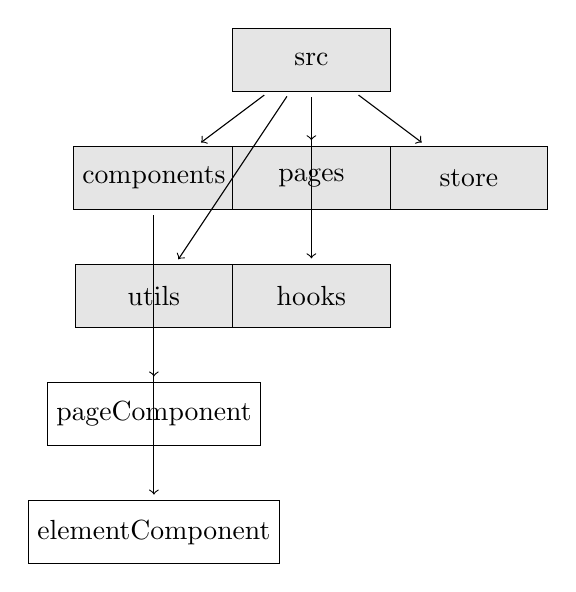
\begin{tikzpicture}[
    file/.style={draw, rectangle, minimum width=2cm, minimum height=0.8cm},
    folder/.style={draw, rectangle, minimum width=2cm, minimum height=0.8cm, fill=gray!20},
    arrow/.style={->, shorten >=2pt, shorten <=2pt}
]

% Folders
\node[folder] (src) at (0,0) {src};
\node[folder] (components) at (-2,-1.5) {components};
\node[folder] (pages) at (0,-1.5) {pages};
\node[folder] (store) at (2,-1.5) {store};
\node[folder] (utils) at (-2,-3) {utils};
\node[folder] (hooks) at (0,-3) {hooks};

% Files
\node[file] (pageComponent) at (-2,-4.5) {pageComponent};
\node[file] (elementComponent) at (-2,-6) {elementComponent};
% ... add more files

% Connections
\draw[arrow] (src) -- (components);
\draw[arrow] (src) -- (pages);
\draw[arrow] (src) -- (store);
\draw[arrow] (src) -- (utils);
\draw[arrow] (src) -- (hooks);
\draw[arrow] (components) -- (pageComponent);
\draw[arrow] (components) -- (elementComponent);
% ... add more connections

\end{tikzpicture}



\pagebreak
\subsubsection{Back-end}
The backend uses the dotNet framework. The development language using the C\# language.

In this project, the backend uses the Onion Architecture.
The Onion Architecture is a typically layered architecture, 
where each layer depends on the inner layer and provides interfaces to the outer layer.
The outer layer provides services to the outermost layer 
and other modules in the same layer based on the interfaces of the inner layer.

From inner to outer, the layers are: Domain, Application, Infrastructure, Presentation.
The Domain layer is the core layer and the innermost layer, used to define domain models, 
which are the business models.
It includes domain models and domain service interfaces.
Domain models are used to define the business models, 
which are the entities in the entity-relationship model and their attributes.
Domain service interfaces are used to define the business services, 
which are the relationships between entities in the entity-relationship model.

The Application layer is the application layer, 
used to define application services, which are the business logic.
It includes domain service implementations and application service interfaces.
Domain service implementations implement the methods of the inner layer's domain service 
interfaces and implement the business logic of the domain models.
Application service interfaces are used to define application services, 
which are the business logic.
It includes but is not limited to database interfaces, testing interfaces, 
HTTP API interfaces, MQTT interfaces, etc.

The Infrastructure layer is the infrastructure layer, used to define infrastructure.
It includes database implementations, testing implementations, 
HTTP API implementations, MQTT implementations, etc.
Database implementations implement the database interfaces 
and provide CRUD services for the database.
Testing implementations implement the testing interfaces 
and provide services for unit testing and integration testing.
HTTP API implementations implement the HTTP API interfaces 
and provide CRUD operations for HTTP APIs.
MQTT implementations implement the MQTT interfaces 
and provide CRUD operations for MQTT.

The Presentation layer is the presentation layer, used to define presentation logic, 
such as interfaces and pages. Since this is a backend project,
data presentation and control are handled by the frontend, 
so this layer is not needed.



\pagebreak
\subsubsection{Data communication and storage}
% 关于本项目的数据通信与数据存储的设计, 包括数据通信的协议, 数据存储的设计等
% 关于数据通信的设计:
% 1. 通信协议的选择
% 自前端向后端发送的数据, 有三种传输的数据类型, 
% 一种是普通的增删改查的请求, 对数据传输的时效性要求不高, 但是对数据的准确性, 完整性, 有序性, 安全性有一定的要求,
% 这种数据的传输, 采用 HTTP 协议, 以及 RESTful API 的设计. 可以有效的保证对数据传输的以上要求.
% 一种是对数据通道的创建和流媒体数据的传输, 对数据传输的时效性, 安全性要求较高, 这种数据的传输, 采用 WebRTC 协议, 以及 MQTT 协议.
% 配合可以快速解码的 flatbuffers 协议, 可以有效的保证对数据传输的以上要求.
% 最后一种是对设备的状态信息和操作信息的传输, 对完整性, 有序性, 安全性都有较高的要求, 这种数据的传输, 采用 MQTT 协议
% 同时也使用了 flatbuffers 协议.
% 
% 2. 数据通信的通信架构和通信流程
% 本项目的数据通信的通信架构, 是基于前后端分离的架构, 前端使用 React 框架, 后端使用 dotnet 框架.
% 当前端需要向后端发送数据的时候, 前端会向后端发送 HTTP 请求, 后端接收到 HTTP 请求之后, 会根据请求的数据类型,
% 选择不同的数据处理方式, 对于普通的增删改查的请求, 后端会根据 RESTful API 的设计, 对数据进行增删改查的操作,
% 对于对数据通道的创建和流媒体数据的传输, 后端会根据 WebRTC 协议, 对数据通道进行创建, 并且帮助前端和设备建立数据通道,
% 当数据通道建立后, 前端和设备之间则使用 flatbuffer 的数据格式对流媒体数据进行传输,
% 对于设备的状态信息和操作信息的传输, 前端会直接向 MQTT broker 发送 MQTT 请求, 
% 设备会在其自身的固件中监听相关的 MQTT 请求, 并且返回相关的数据.
% 
% 3. 数据通信的格式
% 本项目的数据通信的格式, 有三种, 
% 一种是 HTTP 协议, 
% 使用 json 格式对数据进行传输,
% 一种是 WebRTC 协议, 
% 使用 flatbuffers 格式对数据进行传输,
% 一种是 MQTT 协议.
% 使用 flatbuffers 格式对数据进行传输,
% 
% 关于数据存储的设计:
% 1. 数据存储的数据库的选择
% 本项目的数据存储的数据库的选择, 使用了轻量级的数据库 SQLite,
% SQLite 是一个进程内的库, 实现了自给自足的, 无服务器的, 零配置的, 事务性的 SQL 数据库引擎.
% 这是因为整个项目的目的是为了实现前端与设备之间的数据通信, 对于数据库数据的增删改查操作的要求不高,
% 数据量较小, 且对于数据库的数据的事务性要求不高, 所以选择了 SQLite 数据库.
% 2. 项目前后端的数据结构的设计
% 在本项目中, 前端由于使用了 React 框架, 所以前端的数据结构的设计, 使用了基于状态的数据结构的设计,
% 每个组件或者数据集都包含一个状态对象, 这个状态对象的属性就是组件的各个状态. 
% 使用状态对象的原因是, 可以方便的对状态进行管理, 采用对象-属性的形式, 可以方便的针对不同组件的同类状态进行区分,
% 由于跨组件的状态是由 redux 进行管理的, 这种状态对象的设计, 可以更搞笑的对状态进行更新和传递.
% 后端由于使用了 dotnet 框架, 所以后端的数据结构的设计, 使用了基于类的数据结构的设计,
% 采用了面向对象的编程思想, 对数据进行了封装, 使得数据的传输更加的安全, 有序, 完整.


\pagebreak

% \subsection{Domain model}
% \documentclass[]{article}
\usepackage{graphicx}
\usepackage{amsmath}
\usepackage{tikz}

% libaries
\usetikzlibrary{shapes,arrows}

%Define the listing package
\usepackage{listings} %code highlighter
\usepackage{color} %use color
\definecolor{mygreen}{rgb}{0,0.6,0}
\definecolor{mygray}{rgb}{0.5,0.5,0.5}
\definecolor{mymauve}{rgb}{0.58,0,0.82}

%Customize a bit the look
\lstset{ %
backgroundcolor=\color{white}, % choose the background color; you must add \usepackage{color} or \usepackage{xcolor}
basicstyle=\footnotesize, % the size of the fonts that are used for the code
breakatwhitespace=false, % sets if automatic breaks should only happen at whitespace
breaklines=true, % sets automatic line breaking
captionpos=b, % sets the caption-position to bottom
commentstyle=\color{mygreen}, % comment style
deletekeywords={...}, % if you want to delete keywords from the given language
escapeinside={\%*}{*)}, % if you want to add LaTeX within your code
extendedchars=true, % lets you use non-ASCII characters; for 8-bits encodings only, does not work with UTF-8
frame=single, % adds a frame around the code
keepspaces=true, % keeps spaces in text, useful for keeping indentation of code (possibly needs columns=flexible)
keywordstyle=\color{blue}, % keyword style
% language=Octave, % the language of the code
morekeywords={*,...}, % if you want to add more keywords to the set
numbers=left, % where to put the line-numbers; possible values are (none, left, right)
numbersep=5pt, % how far the line-numbers are from the code
numberstyle=\tiny\color{mygray}, % the style that is used for the line-numbers
rulecolor=\color{black}, % if not set, the frame-color may be changed on line-breaks within not-black text (e.g. comments (green here))
showspaces=false, % show spaces everywhere adding particular underscores; it overrides 'showstringspaces'
showstringspaces=false, % underline spaces within strings only
showtabs=false, % show tabs within strings adding particular underscores
stepnumber=1, % the step between two line-numbers. If it's 1, each line will be numbered
stringstyle=\color{mymauve}, % string literal style
tabsize=2, % sets default tabsize to 2 spaces
title=\lstname % show the filename of files included with \lstinputlisting; also try caption instead of title
}

\definecolor{darkgray}{rgb}{.4,.4,.4}
\definecolor{purple}{rgb}{0.65, 0.12, 0.82}

\lstdefinelanguage{React}{
keywords={const, typeof, new, true, false, catch, function, return, null, catch, switch, var, if, in, while, do, else, case, break},
keywordstyle=\color{blue}\bfseries,
ndkeywords={class, export, boolean, throw, implements, import, this},
ndkeywordstyle=\color{darkgray}\bfseries,
identifierstyle=\color{mygreen},
sensitive=false,
comment=[l]{//},
morecomment=[s]{/*}{*/},
commentstyle=\color{purple}\ttfamily,
string=[b]{"}{'}{`},
stringstyle=\color{red}\ttfamily,
morestring=[b]',
morestring=[b]",
morestring=[b]`',
}

\lstdefinelanguage{CSharp}{
keywords={const, typeof, new, true, false, catch, function, return, null, catch, switch, var, if, in, while, do, else, case, break},
keywordstyle=\color{blue}\bfseries,
ndkeywords={class, export, boolean, throw, implements, import, this},
ndkeywordstyle=\color{darkgray}\bfseries,
identifierstyle=\color{mygreen},
sensitive=false,
comment=[l]{//},
morecomment=[s]{/*}{*/},
commentstyle=\color{purple}\ttfamily,
string=[b]{"}{'}{`},
stringstyle=\color{red}\ttfamily,
morestring=[b]',
morestring=[b]",
morestring=[b]`',
}

\lstset{
language=React,
extendedchars=true,
basicstyle=\footnotesize\ttfamily,
showstringspaces=false,
showspaces=false,
numbers=left,
numberstyle=\footnotesize,
numbersep=9pt,
tabsize=2,
breaklines=true,
showtabs=false,
captionpos=b
}

\lstset{
language=CSharp,
extendedchars=true,
basicstyle=\footnotesize\ttfamily,
showstringspaces=false,
showspaces=false,
numbers=left,
numberstyle=\footnotesize,
numbersep=9pt,
tabsize=2,
breaklines=true,
showtabs=false,
captionpos=b
}

% \usepackage{cite} % Add this line for citation

% \bibliographystyle{plain}

\title{
The implementation of BifrostConnect Front-end scope, 
re-design and development with the relevant back-end support develop.
}
\author{
    Fei Gu \\
    Erhvervs Akademi Sydvest \\
    Computer Science 21\\
    }
\date{\today}

\begin{document}

% Front page
\maketitle
\begin{center}
    Supervisor: Henrik Boulund Meng Hansen \\
    Company: BifrostConnect \\
    Engineering Director: Jasper Wass \\
\end{center}
\tableofcontents
\pagebreak


% The introduction
\section{Introduction}
\subsection{Background}\input{sections/introduction/background.tex}
\subsection{The company}\input{sections/introduction/aboutCompany}
\subsection{The project}\input{sections/introduction/aboutProject}
\pagebreak

% The problem statement
\section{Problem Statement}
\subsection{Statement}
\input{sections/problemStatement/statement}
\subsection{Situation}
\input{sections/problemStatement/situation}
\subsection{Potential Solution}
\input{sections/problemStatement/potentialSolution}
\pagebreak

% Requirement analysis
\section{Requirement Analysis}
\input{sections/requirementAnalysis/index}

\subsection{Stakeholders}
\input{sections/requirementAnalysis/stakeholders/index}

\subsection{Business Domain}
\input{sections/requirementAnalysis/bussinesDomain/index}

\subsection{Scope}
\input{sections/requirementAnalysis/scope}

\subsection{Goals}
\input{sections/requirementAnalysis/goals}
\pagebreak

% Software Design
\section{Software Design}
% developement methods
\subsection{Software Development Methods}
\input{sections/softwareDevelopmentMethods/index}
\subsubsection{Agile Software Development}
\input{sections/softwareDevelopmentMethods/agileSoftwareDevelopment/index}
\subsubsection{Feature Driven Development}
\input{sections/softwareDevelopmentMethods/featureDrivenDevelopment/index}

\pagebreak

% Technology seslection
\subsection{Technology selection}
\input{sections/softwareDesign/technologySelection/index}
\subsubsection{Front-end}
\input{sections/softwareDesign/technologySelection/frontEnd}            
\subsubsection{Back-end}
\input{sections/softwareDesign/technologySelection/backEnd}            
\subsubsection{Database}
\input{sections/softwareDesign/technologySelection/database}
\subsubsection{Data communication}
\input{sections/softwareDesign/technologySelection/dataCommunication}            
\subsubsection{DevOps}
\input{sections/softwareDesign/technologySelection/devOps}
\pagebreak

% Architecture design
\subsection{Architecture design}
\input{sections/softwareDesign/architectureDesign/index}
\pagebreak
\subsubsection{Front-end}
\input{sections/softwareDesign/architectureDesign/frontEndArchitecture}
\pagebreak
\subsubsection{Back-end}
\input{sections/softwareDesign/architectureDesign/backEndArchitecture}
\pagebreak
\subsubsection{Data communication and storage}
\input{sections/softwareDesign/architectureDesign/dataCommunicationArchitecture}
\pagebreak

% \subsection{Domain model}
% \input{sections/softwareDesign/domainModel/index}
% \subsection{Database design}
% % 数据库领域模型 ER 图
% % 包括表和字段的设置.
% % 对于私有键和外键的设置.

% \subsection{Back-end design}
% % 后端对象模型
% % 以及对于对象模型的增删改查
% % 以及相关的其他服务的设计`'

% \subsection{Front-end design}
% % 对于前端的页面结构的设计 
% % 页面的状态的设计, 交互设计

% \subsection{FlatBuffers design}
% % schema 的设计

\subsection{DevOps CI/CD process design}
\input{sections/softwareDesign/devOpsDesign/index}
\subsubsection{Continuous Integration}
\input{sections/softwareDesign/devOpsDesign/continuousIntegration/index}
\subsubsection{Continuous Delivery}
\input{sections/softwareDesign/devOpsDesign/continuousDelivery/index}
\subsubsection{Continuous Deployment}
\input{sections/softwareDesign/devOpsDesign/continuousDeployment/index}
\pagebreak

\section{Software Development} 
\input{sections/softwareDevelopment/index}
\subsection{Overall development}
\input{sections/softwareDevelopment/overallDevelopement/index}
\subsubsection{Front-end}
\input{sections/softwareDevelopment/overallDevelopement/frontEnd/index}
\subsubsection{Back-end}
\input{sections/softwareDevelopment/overallDevelopement/backEnd/index}
\subsubsection{DevOps}
\input{sections/softwareDevelopment/overallDevelopement/devOps/index}
\subsection{Feature development} 
\input{sections/softwareDevelopment/featureDevelopment/index}
\subsubsection{Use Case 1}
\input{sections/softwareDevelopment/featureDevelopment/useCase1/index}
\subsubsection{Feature 1}
\input{sections/softwareDevelopment/featureDevelopment/feature/feature1.tex}
\pagebreak
\section{Conclusion} 
\subsection{Result}
Since the project is still in progress, the result is not available yet.
So far, basic structure of this project has been built. But the most features 
are not implemented yet. 
\subsection{Discussion}
As a single developer for this project, I am confident what I have done so far.
And I can say I understand the most of the knowledge I have used in this project, 
which also means I can explain all the part of the project. 
But this project also relevant some of the complex knowledge which I have to continue 
to study and practice.
\subsection{Future Work}
The future work is to implement the rest of the features. 
Including the most important part which is the 'create session' feature.
\pagebreak
% \bibliography{bibliography}
\pagebreak
% \begin{appendices}
%     \section{Appendix}
% \end{appendices} 
\end{document}
% \subsection{Database design}
% % 数据库领域模型 ER 图
% % 包括表和字段的设置.
% % 对于私有键和外键的设置.

% \subsection{Back-end design}
% % 后端对象模型
% % 以及对于对象模型的增删改查
% % 以及相关的其他服务的设计`'

% \subsection{Front-end design}
% % 对于前端的页面结构的设计 
% % 页面的状态的设计, 交互设计

% \subsection{FlatBuffers design}
% % schema 的设计

\subsection{DevOps CI/CD process design}
\documentclass[]{article}
\usepackage{graphicx}
\usepackage{amsmath}
\usepackage{tikz}

% libaries
\usetikzlibrary{shapes,arrows}

%Define the listing package
\usepackage{listings} %code highlighter
\usepackage{color} %use color
\definecolor{mygreen}{rgb}{0,0.6,0}
\definecolor{mygray}{rgb}{0.5,0.5,0.5}
\definecolor{mymauve}{rgb}{0.58,0,0.82}

%Customize a bit the look
\lstset{ %
backgroundcolor=\color{white}, % choose the background color; you must add \usepackage{color} or \usepackage{xcolor}
basicstyle=\footnotesize, % the size of the fonts that are used for the code
breakatwhitespace=false, % sets if automatic breaks should only happen at whitespace
breaklines=true, % sets automatic line breaking
captionpos=b, % sets the caption-position to bottom
commentstyle=\color{mygreen}, % comment style
deletekeywords={...}, % if you want to delete keywords from the given language
escapeinside={\%*}{*)}, % if you want to add LaTeX within your code
extendedchars=true, % lets you use non-ASCII characters; for 8-bits encodings only, does not work with UTF-8
frame=single, % adds a frame around the code
keepspaces=true, % keeps spaces in text, useful for keeping indentation of code (possibly needs columns=flexible)
keywordstyle=\color{blue}, % keyword style
% language=Octave, % the language of the code
morekeywords={*,...}, % if you want to add more keywords to the set
numbers=left, % where to put the line-numbers; possible values are (none, left, right)
numbersep=5pt, % how far the line-numbers are from the code
numberstyle=\tiny\color{mygray}, % the style that is used for the line-numbers
rulecolor=\color{black}, % if not set, the frame-color may be changed on line-breaks within not-black text (e.g. comments (green here))
showspaces=false, % show spaces everywhere adding particular underscores; it overrides 'showstringspaces'
showstringspaces=false, % underline spaces within strings only
showtabs=false, % show tabs within strings adding particular underscores
stepnumber=1, % the step between two line-numbers. If it's 1, each line will be numbered
stringstyle=\color{mymauve}, % string literal style
tabsize=2, % sets default tabsize to 2 spaces
title=\lstname % show the filename of files included with \lstinputlisting; also try caption instead of title
}

\definecolor{darkgray}{rgb}{.4,.4,.4}
\definecolor{purple}{rgb}{0.65, 0.12, 0.82}

\lstdefinelanguage{React}{
keywords={const, typeof, new, true, false, catch, function, return, null, catch, switch, var, if, in, while, do, else, case, break},
keywordstyle=\color{blue}\bfseries,
ndkeywords={class, export, boolean, throw, implements, import, this},
ndkeywordstyle=\color{darkgray}\bfseries,
identifierstyle=\color{mygreen},
sensitive=false,
comment=[l]{//},
morecomment=[s]{/*}{*/},
commentstyle=\color{purple}\ttfamily,
string=[b]{"}{'}{`},
stringstyle=\color{red}\ttfamily,
morestring=[b]',
morestring=[b]",
morestring=[b]`',
}

\lstdefinelanguage{CSharp}{
keywords={const, typeof, new, true, false, catch, function, return, null, catch, switch, var, if, in, while, do, else, case, break},
keywordstyle=\color{blue}\bfseries,
ndkeywords={class, export, boolean, throw, implements, import, this},
ndkeywordstyle=\color{darkgray}\bfseries,
identifierstyle=\color{mygreen},
sensitive=false,
comment=[l]{//},
morecomment=[s]{/*}{*/},
commentstyle=\color{purple}\ttfamily,
string=[b]{"}{'}{`},
stringstyle=\color{red}\ttfamily,
morestring=[b]',
morestring=[b]",
morestring=[b]`',
}

\lstset{
language=React,
extendedchars=true,
basicstyle=\footnotesize\ttfamily,
showstringspaces=false,
showspaces=false,
numbers=left,
numberstyle=\footnotesize,
numbersep=9pt,
tabsize=2,
breaklines=true,
showtabs=false,
captionpos=b
}

\lstset{
language=CSharp,
extendedchars=true,
basicstyle=\footnotesize\ttfamily,
showstringspaces=false,
showspaces=false,
numbers=left,
numberstyle=\footnotesize,
numbersep=9pt,
tabsize=2,
breaklines=true,
showtabs=false,
captionpos=b
}

% \usepackage{cite} % Add this line for citation

% \bibliographystyle{plain}

\title{
The implementation of BifrostConnect Front-end scope, 
re-design and development with the relevant back-end support develop.
}
\author{
    Fei Gu \\
    Erhvervs Akademi Sydvest \\
    Computer Science 21\\
    }
\date{\today}

\begin{document}

% Front page
\maketitle
\begin{center}
    Supervisor: Henrik Boulund Meng Hansen \\
    Company: BifrostConnect \\
    Engineering Director: Jasper Wass \\
\end{center}
\tableofcontents
\pagebreak


% The introduction
\section{Introduction}
\subsection{Background}\input{sections/introduction/background.tex}
\subsection{The company}\input{sections/introduction/aboutCompany}
\subsection{The project}\input{sections/introduction/aboutProject}
\pagebreak

% The problem statement
\section{Problem Statement}
\subsection{Statement}
\input{sections/problemStatement/statement}
\subsection{Situation}
\input{sections/problemStatement/situation}
\subsection{Potential Solution}
\input{sections/problemStatement/potentialSolution}
\pagebreak

% Requirement analysis
\section{Requirement Analysis}
\input{sections/requirementAnalysis/index}

\subsection{Stakeholders}
\input{sections/requirementAnalysis/stakeholders/index}

\subsection{Business Domain}
\input{sections/requirementAnalysis/bussinesDomain/index}

\subsection{Scope}
\input{sections/requirementAnalysis/scope}

\subsection{Goals}
\input{sections/requirementAnalysis/goals}
\pagebreak

% Software Design
\section{Software Design}
% developement methods
\subsection{Software Development Methods}
\input{sections/softwareDevelopmentMethods/index}
\subsubsection{Agile Software Development}
\input{sections/softwareDevelopmentMethods/agileSoftwareDevelopment/index}
\subsubsection{Feature Driven Development}
\input{sections/softwareDevelopmentMethods/featureDrivenDevelopment/index}

\pagebreak

% Technology seslection
\subsection{Technology selection}
\input{sections/softwareDesign/technologySelection/index}
\subsubsection{Front-end}
\input{sections/softwareDesign/technologySelection/frontEnd}            
\subsubsection{Back-end}
\input{sections/softwareDesign/technologySelection/backEnd}            
\subsubsection{Database}
\input{sections/softwareDesign/technologySelection/database}
\subsubsection{Data communication}
\input{sections/softwareDesign/technologySelection/dataCommunication}            
\subsubsection{DevOps}
\input{sections/softwareDesign/technologySelection/devOps}
\pagebreak

% Architecture design
\subsection{Architecture design}
\input{sections/softwareDesign/architectureDesign/index}
\pagebreak
\subsubsection{Front-end}
\input{sections/softwareDesign/architectureDesign/frontEndArchitecture}
\pagebreak
\subsubsection{Back-end}
\input{sections/softwareDesign/architectureDesign/backEndArchitecture}
\pagebreak
\subsubsection{Data communication and storage}
\input{sections/softwareDesign/architectureDesign/dataCommunicationArchitecture}
\pagebreak

% \subsection{Domain model}
% \input{sections/softwareDesign/domainModel/index}
% \subsection{Database design}
% % 数据库领域模型 ER 图
% % 包括表和字段的设置.
% % 对于私有键和外键的设置.

% \subsection{Back-end design}
% % 后端对象模型
% % 以及对于对象模型的增删改查
% % 以及相关的其他服务的设计`'

% \subsection{Front-end design}
% % 对于前端的页面结构的设计 
% % 页面的状态的设计, 交互设计

% \subsection{FlatBuffers design}
% % schema 的设计

\subsection{DevOps CI/CD process design}
\input{sections/softwareDesign/devOpsDesign/index}
\subsubsection{Continuous Integration}
\input{sections/softwareDesign/devOpsDesign/continuousIntegration/index}
\subsubsection{Continuous Delivery}
\input{sections/softwareDesign/devOpsDesign/continuousDelivery/index}
\subsubsection{Continuous Deployment}
\input{sections/softwareDesign/devOpsDesign/continuousDeployment/index}
\pagebreak

\section{Software Development} 
\input{sections/softwareDevelopment/index}
\subsection{Overall development}
\input{sections/softwareDevelopment/overallDevelopement/index}
\subsubsection{Front-end}
\input{sections/softwareDevelopment/overallDevelopement/frontEnd/index}
\subsubsection{Back-end}
\input{sections/softwareDevelopment/overallDevelopement/backEnd/index}
\subsubsection{DevOps}
\input{sections/softwareDevelopment/overallDevelopement/devOps/index}
\subsection{Feature development} 
\input{sections/softwareDevelopment/featureDevelopment/index}
\subsubsection{Use Case 1}
\input{sections/softwareDevelopment/featureDevelopment/useCase1/index}
\subsubsection{Feature 1}
\input{sections/softwareDevelopment/featureDevelopment/feature/feature1.tex}
\pagebreak
\section{Conclusion} 
\subsection{Result}
Since the project is still in progress, the result is not available yet.
So far, basic structure of this project has been built. But the most features 
are not implemented yet. 
\subsection{Discussion}
As a single developer for this project, I am confident what I have done so far.
And I can say I understand the most of the knowledge I have used in this project, 
which also means I can explain all the part of the project. 
But this project also relevant some of the complex knowledge which I have to continue 
to study and practice.
\subsection{Future Work}
The future work is to implement the rest of the features. 
Including the most important part which is the 'create session' feature.
\pagebreak
% \bibliography{bibliography}
\pagebreak
% \begin{appendices}
%     \section{Appendix}
% \end{appendices} 
\end{document}
\subsubsection{Continuous Integration}
\documentclass[]{article}
\usepackage{graphicx}
\usepackage{amsmath}
\usepackage{tikz}

% libaries
\usetikzlibrary{shapes,arrows}

%Define the listing package
\usepackage{listings} %code highlighter
\usepackage{color} %use color
\definecolor{mygreen}{rgb}{0,0.6,0}
\definecolor{mygray}{rgb}{0.5,0.5,0.5}
\definecolor{mymauve}{rgb}{0.58,0,0.82}

%Customize a bit the look
\lstset{ %
backgroundcolor=\color{white}, % choose the background color; you must add \usepackage{color} or \usepackage{xcolor}
basicstyle=\footnotesize, % the size of the fonts that are used for the code
breakatwhitespace=false, % sets if automatic breaks should only happen at whitespace
breaklines=true, % sets automatic line breaking
captionpos=b, % sets the caption-position to bottom
commentstyle=\color{mygreen}, % comment style
deletekeywords={...}, % if you want to delete keywords from the given language
escapeinside={\%*}{*)}, % if you want to add LaTeX within your code
extendedchars=true, % lets you use non-ASCII characters; for 8-bits encodings only, does not work with UTF-8
frame=single, % adds a frame around the code
keepspaces=true, % keeps spaces in text, useful for keeping indentation of code (possibly needs columns=flexible)
keywordstyle=\color{blue}, % keyword style
% language=Octave, % the language of the code
morekeywords={*,...}, % if you want to add more keywords to the set
numbers=left, % where to put the line-numbers; possible values are (none, left, right)
numbersep=5pt, % how far the line-numbers are from the code
numberstyle=\tiny\color{mygray}, % the style that is used for the line-numbers
rulecolor=\color{black}, % if not set, the frame-color may be changed on line-breaks within not-black text (e.g. comments (green here))
showspaces=false, % show spaces everywhere adding particular underscores; it overrides 'showstringspaces'
showstringspaces=false, % underline spaces within strings only
showtabs=false, % show tabs within strings adding particular underscores
stepnumber=1, % the step between two line-numbers. If it's 1, each line will be numbered
stringstyle=\color{mymauve}, % string literal style
tabsize=2, % sets default tabsize to 2 spaces
title=\lstname % show the filename of files included with \lstinputlisting; also try caption instead of title
}

\definecolor{darkgray}{rgb}{.4,.4,.4}
\definecolor{purple}{rgb}{0.65, 0.12, 0.82}

\lstdefinelanguage{React}{
keywords={const, typeof, new, true, false, catch, function, return, null, catch, switch, var, if, in, while, do, else, case, break},
keywordstyle=\color{blue}\bfseries,
ndkeywords={class, export, boolean, throw, implements, import, this},
ndkeywordstyle=\color{darkgray}\bfseries,
identifierstyle=\color{mygreen},
sensitive=false,
comment=[l]{//},
morecomment=[s]{/*}{*/},
commentstyle=\color{purple}\ttfamily,
string=[b]{"}{'}{`},
stringstyle=\color{red}\ttfamily,
morestring=[b]',
morestring=[b]",
morestring=[b]`',
}

\lstdefinelanguage{CSharp}{
keywords={const, typeof, new, true, false, catch, function, return, null, catch, switch, var, if, in, while, do, else, case, break},
keywordstyle=\color{blue}\bfseries,
ndkeywords={class, export, boolean, throw, implements, import, this},
ndkeywordstyle=\color{darkgray}\bfseries,
identifierstyle=\color{mygreen},
sensitive=false,
comment=[l]{//},
morecomment=[s]{/*}{*/},
commentstyle=\color{purple}\ttfamily,
string=[b]{"}{'}{`},
stringstyle=\color{red}\ttfamily,
morestring=[b]',
morestring=[b]",
morestring=[b]`',
}

\lstset{
language=React,
extendedchars=true,
basicstyle=\footnotesize\ttfamily,
showstringspaces=false,
showspaces=false,
numbers=left,
numberstyle=\footnotesize,
numbersep=9pt,
tabsize=2,
breaklines=true,
showtabs=false,
captionpos=b
}

\lstset{
language=CSharp,
extendedchars=true,
basicstyle=\footnotesize\ttfamily,
showstringspaces=false,
showspaces=false,
numbers=left,
numberstyle=\footnotesize,
numbersep=9pt,
tabsize=2,
breaklines=true,
showtabs=false,
captionpos=b
}

% \usepackage{cite} % Add this line for citation

% \bibliographystyle{plain}

\title{
The implementation of BifrostConnect Front-end scope, 
re-design and development with the relevant back-end support develop.
}
\author{
    Fei Gu \\
    Erhvervs Akademi Sydvest \\
    Computer Science 21\\
    }
\date{\today}

\begin{document}

% Front page
\maketitle
\begin{center}
    Supervisor: Henrik Boulund Meng Hansen \\
    Company: BifrostConnect \\
    Engineering Director: Jasper Wass \\
\end{center}
\tableofcontents
\pagebreak


% The introduction
\section{Introduction}
\subsection{Background}\input{sections/introduction/background.tex}
\subsection{The company}\input{sections/introduction/aboutCompany}
\subsection{The project}\input{sections/introduction/aboutProject}
\pagebreak

% The problem statement
\section{Problem Statement}
\subsection{Statement}
\input{sections/problemStatement/statement}
\subsection{Situation}
\input{sections/problemStatement/situation}
\subsection{Potential Solution}
\input{sections/problemStatement/potentialSolution}
\pagebreak

% Requirement analysis
\section{Requirement Analysis}
\input{sections/requirementAnalysis/index}

\subsection{Stakeholders}
\input{sections/requirementAnalysis/stakeholders/index}

\subsection{Business Domain}
\input{sections/requirementAnalysis/bussinesDomain/index}

\subsection{Scope}
\input{sections/requirementAnalysis/scope}

\subsection{Goals}
\input{sections/requirementAnalysis/goals}
\pagebreak

% Software Design
\section{Software Design}
% developement methods
\subsection{Software Development Methods}
\input{sections/softwareDevelopmentMethods/index}
\subsubsection{Agile Software Development}
\input{sections/softwareDevelopmentMethods/agileSoftwareDevelopment/index}
\subsubsection{Feature Driven Development}
\input{sections/softwareDevelopmentMethods/featureDrivenDevelopment/index}

\pagebreak

% Technology seslection
\subsection{Technology selection}
\input{sections/softwareDesign/technologySelection/index}
\subsubsection{Front-end}
\input{sections/softwareDesign/technologySelection/frontEnd}            
\subsubsection{Back-end}
\input{sections/softwareDesign/technologySelection/backEnd}            
\subsubsection{Database}
\input{sections/softwareDesign/technologySelection/database}
\subsubsection{Data communication}
\input{sections/softwareDesign/technologySelection/dataCommunication}            
\subsubsection{DevOps}
\input{sections/softwareDesign/technologySelection/devOps}
\pagebreak

% Architecture design
\subsection{Architecture design}
\input{sections/softwareDesign/architectureDesign/index}
\pagebreak
\subsubsection{Front-end}
\input{sections/softwareDesign/architectureDesign/frontEndArchitecture}
\pagebreak
\subsubsection{Back-end}
\input{sections/softwareDesign/architectureDesign/backEndArchitecture}
\pagebreak
\subsubsection{Data communication and storage}
\input{sections/softwareDesign/architectureDesign/dataCommunicationArchitecture}
\pagebreak

% \subsection{Domain model}
% \input{sections/softwareDesign/domainModel/index}
% \subsection{Database design}
% % 数据库领域模型 ER 图
% % 包括表和字段的设置.
% % 对于私有键和外键的设置.

% \subsection{Back-end design}
% % 后端对象模型
% % 以及对于对象模型的增删改查
% % 以及相关的其他服务的设计`'

% \subsection{Front-end design}
% % 对于前端的页面结构的设计 
% % 页面的状态的设计, 交互设计

% \subsection{FlatBuffers design}
% % schema 的设计

\subsection{DevOps CI/CD process design}
\input{sections/softwareDesign/devOpsDesign/index}
\subsubsection{Continuous Integration}
\input{sections/softwareDesign/devOpsDesign/continuousIntegration/index}
\subsubsection{Continuous Delivery}
\input{sections/softwareDesign/devOpsDesign/continuousDelivery/index}
\subsubsection{Continuous Deployment}
\input{sections/softwareDesign/devOpsDesign/continuousDeployment/index}
\pagebreak

\section{Software Development} 
\input{sections/softwareDevelopment/index}
\subsection{Overall development}
\input{sections/softwareDevelopment/overallDevelopement/index}
\subsubsection{Front-end}
\input{sections/softwareDevelopment/overallDevelopement/frontEnd/index}
\subsubsection{Back-end}
\input{sections/softwareDevelopment/overallDevelopement/backEnd/index}
\subsubsection{DevOps}
\input{sections/softwareDevelopment/overallDevelopement/devOps/index}
\subsection{Feature development} 
\input{sections/softwareDevelopment/featureDevelopment/index}
\subsubsection{Use Case 1}
\input{sections/softwareDevelopment/featureDevelopment/useCase1/index}
\subsubsection{Feature 1}
\input{sections/softwareDevelopment/featureDevelopment/feature/feature1.tex}
\pagebreak
\section{Conclusion} 
\subsection{Result}
Since the project is still in progress, the result is not available yet.
So far, basic structure of this project has been built. But the most features 
are not implemented yet. 
\subsection{Discussion}
As a single developer for this project, I am confident what I have done so far.
And I can say I understand the most of the knowledge I have used in this project, 
which also means I can explain all the part of the project. 
But this project also relevant some of the complex knowledge which I have to continue 
to study and practice.
\subsection{Future Work}
The future work is to implement the rest of the features. 
Including the most important part which is the 'create session' feature.
\pagebreak
% \bibliography{bibliography}
\pagebreak
% \begin{appendices}
%     \section{Appendix}
% \end{appendices} 
\end{document}
\subsubsection{Continuous Delivery}
\documentclass[]{article}
\usepackage{graphicx}
\usepackage{amsmath}
\usepackage{tikz}

% libaries
\usetikzlibrary{shapes,arrows}

%Define the listing package
\usepackage{listings} %code highlighter
\usepackage{color} %use color
\definecolor{mygreen}{rgb}{0,0.6,0}
\definecolor{mygray}{rgb}{0.5,0.5,0.5}
\definecolor{mymauve}{rgb}{0.58,0,0.82}

%Customize a bit the look
\lstset{ %
backgroundcolor=\color{white}, % choose the background color; you must add \usepackage{color} or \usepackage{xcolor}
basicstyle=\footnotesize, % the size of the fonts that are used for the code
breakatwhitespace=false, % sets if automatic breaks should only happen at whitespace
breaklines=true, % sets automatic line breaking
captionpos=b, % sets the caption-position to bottom
commentstyle=\color{mygreen}, % comment style
deletekeywords={...}, % if you want to delete keywords from the given language
escapeinside={\%*}{*)}, % if you want to add LaTeX within your code
extendedchars=true, % lets you use non-ASCII characters; for 8-bits encodings only, does not work with UTF-8
frame=single, % adds a frame around the code
keepspaces=true, % keeps spaces in text, useful for keeping indentation of code (possibly needs columns=flexible)
keywordstyle=\color{blue}, % keyword style
% language=Octave, % the language of the code
morekeywords={*,...}, % if you want to add more keywords to the set
numbers=left, % where to put the line-numbers; possible values are (none, left, right)
numbersep=5pt, % how far the line-numbers are from the code
numberstyle=\tiny\color{mygray}, % the style that is used for the line-numbers
rulecolor=\color{black}, % if not set, the frame-color may be changed on line-breaks within not-black text (e.g. comments (green here))
showspaces=false, % show spaces everywhere adding particular underscores; it overrides 'showstringspaces'
showstringspaces=false, % underline spaces within strings only
showtabs=false, % show tabs within strings adding particular underscores
stepnumber=1, % the step between two line-numbers. If it's 1, each line will be numbered
stringstyle=\color{mymauve}, % string literal style
tabsize=2, % sets default tabsize to 2 spaces
title=\lstname % show the filename of files included with \lstinputlisting; also try caption instead of title
}

\definecolor{darkgray}{rgb}{.4,.4,.4}
\definecolor{purple}{rgb}{0.65, 0.12, 0.82}

\lstdefinelanguage{React}{
keywords={const, typeof, new, true, false, catch, function, return, null, catch, switch, var, if, in, while, do, else, case, break},
keywordstyle=\color{blue}\bfseries,
ndkeywords={class, export, boolean, throw, implements, import, this},
ndkeywordstyle=\color{darkgray}\bfseries,
identifierstyle=\color{mygreen},
sensitive=false,
comment=[l]{//},
morecomment=[s]{/*}{*/},
commentstyle=\color{purple}\ttfamily,
string=[b]{"}{'}{`},
stringstyle=\color{red}\ttfamily,
morestring=[b]',
morestring=[b]",
morestring=[b]`',
}

\lstdefinelanguage{CSharp}{
keywords={const, typeof, new, true, false, catch, function, return, null, catch, switch, var, if, in, while, do, else, case, break},
keywordstyle=\color{blue}\bfseries,
ndkeywords={class, export, boolean, throw, implements, import, this},
ndkeywordstyle=\color{darkgray}\bfseries,
identifierstyle=\color{mygreen},
sensitive=false,
comment=[l]{//},
morecomment=[s]{/*}{*/},
commentstyle=\color{purple}\ttfamily,
string=[b]{"}{'}{`},
stringstyle=\color{red}\ttfamily,
morestring=[b]',
morestring=[b]",
morestring=[b]`',
}

\lstset{
language=React,
extendedchars=true,
basicstyle=\footnotesize\ttfamily,
showstringspaces=false,
showspaces=false,
numbers=left,
numberstyle=\footnotesize,
numbersep=9pt,
tabsize=2,
breaklines=true,
showtabs=false,
captionpos=b
}

\lstset{
language=CSharp,
extendedchars=true,
basicstyle=\footnotesize\ttfamily,
showstringspaces=false,
showspaces=false,
numbers=left,
numberstyle=\footnotesize,
numbersep=9pt,
tabsize=2,
breaklines=true,
showtabs=false,
captionpos=b
}

% \usepackage{cite} % Add this line for citation

% \bibliographystyle{plain}

\title{
The implementation of BifrostConnect Front-end scope, 
re-design and development with the relevant back-end support develop.
}
\author{
    Fei Gu \\
    Erhvervs Akademi Sydvest \\
    Computer Science 21\\
    }
\date{\today}

\begin{document}

% Front page
\maketitle
\begin{center}
    Supervisor: Henrik Boulund Meng Hansen \\
    Company: BifrostConnect \\
    Engineering Director: Jasper Wass \\
\end{center}
\tableofcontents
\pagebreak


% The introduction
\section{Introduction}
\subsection{Background}\input{sections/introduction/background.tex}
\subsection{The company}\input{sections/introduction/aboutCompany}
\subsection{The project}\input{sections/introduction/aboutProject}
\pagebreak

% The problem statement
\section{Problem Statement}
\subsection{Statement}
\input{sections/problemStatement/statement}
\subsection{Situation}
\input{sections/problemStatement/situation}
\subsection{Potential Solution}
\input{sections/problemStatement/potentialSolution}
\pagebreak

% Requirement analysis
\section{Requirement Analysis}
\input{sections/requirementAnalysis/index}

\subsection{Stakeholders}
\input{sections/requirementAnalysis/stakeholders/index}

\subsection{Business Domain}
\input{sections/requirementAnalysis/bussinesDomain/index}

\subsection{Scope}
\input{sections/requirementAnalysis/scope}

\subsection{Goals}
\input{sections/requirementAnalysis/goals}
\pagebreak

% Software Design
\section{Software Design}
% developement methods
\subsection{Software Development Methods}
\input{sections/softwareDevelopmentMethods/index}
\subsubsection{Agile Software Development}
\input{sections/softwareDevelopmentMethods/agileSoftwareDevelopment/index}
\subsubsection{Feature Driven Development}
\input{sections/softwareDevelopmentMethods/featureDrivenDevelopment/index}

\pagebreak

% Technology seslection
\subsection{Technology selection}
\input{sections/softwareDesign/technologySelection/index}
\subsubsection{Front-end}
\input{sections/softwareDesign/technologySelection/frontEnd}            
\subsubsection{Back-end}
\input{sections/softwareDesign/technologySelection/backEnd}            
\subsubsection{Database}
\input{sections/softwareDesign/technologySelection/database}
\subsubsection{Data communication}
\input{sections/softwareDesign/technologySelection/dataCommunication}            
\subsubsection{DevOps}
\input{sections/softwareDesign/technologySelection/devOps}
\pagebreak

% Architecture design
\subsection{Architecture design}
\input{sections/softwareDesign/architectureDesign/index}
\pagebreak
\subsubsection{Front-end}
\input{sections/softwareDesign/architectureDesign/frontEndArchitecture}
\pagebreak
\subsubsection{Back-end}
\input{sections/softwareDesign/architectureDesign/backEndArchitecture}
\pagebreak
\subsubsection{Data communication and storage}
\input{sections/softwareDesign/architectureDesign/dataCommunicationArchitecture}
\pagebreak

% \subsection{Domain model}
% \input{sections/softwareDesign/domainModel/index}
% \subsection{Database design}
% % 数据库领域模型 ER 图
% % 包括表和字段的设置.
% % 对于私有键和外键的设置.

% \subsection{Back-end design}
% % 后端对象模型
% % 以及对于对象模型的增删改查
% % 以及相关的其他服务的设计`'

% \subsection{Front-end design}
% % 对于前端的页面结构的设计 
% % 页面的状态的设计, 交互设计

% \subsection{FlatBuffers design}
% % schema 的设计

\subsection{DevOps CI/CD process design}
\input{sections/softwareDesign/devOpsDesign/index}
\subsubsection{Continuous Integration}
\input{sections/softwareDesign/devOpsDesign/continuousIntegration/index}
\subsubsection{Continuous Delivery}
\input{sections/softwareDesign/devOpsDesign/continuousDelivery/index}
\subsubsection{Continuous Deployment}
\input{sections/softwareDesign/devOpsDesign/continuousDeployment/index}
\pagebreak

\section{Software Development} 
\input{sections/softwareDevelopment/index}
\subsection{Overall development}
\input{sections/softwareDevelopment/overallDevelopement/index}
\subsubsection{Front-end}
\input{sections/softwareDevelopment/overallDevelopement/frontEnd/index}
\subsubsection{Back-end}
\input{sections/softwareDevelopment/overallDevelopement/backEnd/index}
\subsubsection{DevOps}
\input{sections/softwareDevelopment/overallDevelopement/devOps/index}
\subsection{Feature development} 
\input{sections/softwareDevelopment/featureDevelopment/index}
\subsubsection{Use Case 1}
\input{sections/softwareDevelopment/featureDevelopment/useCase1/index}
\subsubsection{Feature 1}
\input{sections/softwareDevelopment/featureDevelopment/feature/feature1.tex}
\pagebreak
\section{Conclusion} 
\subsection{Result}
Since the project is still in progress, the result is not available yet.
So far, basic structure of this project has been built. But the most features 
are not implemented yet. 
\subsection{Discussion}
As a single developer for this project, I am confident what I have done so far.
And I can say I understand the most of the knowledge I have used in this project, 
which also means I can explain all the part of the project. 
But this project also relevant some of the complex knowledge which I have to continue 
to study and practice.
\subsection{Future Work}
The future work is to implement the rest of the features. 
Including the most important part which is the 'create session' feature.
\pagebreak
% \bibliography{bibliography}
\pagebreak
% \begin{appendices}
%     \section{Appendix}
% \end{appendices} 
\end{document}
\subsubsection{Continuous Deployment}
\documentclass[]{article}
\usepackage{graphicx}
\usepackage{amsmath}
\usepackage{tikz}

% libaries
\usetikzlibrary{shapes,arrows}

%Define the listing package
\usepackage{listings} %code highlighter
\usepackage{color} %use color
\definecolor{mygreen}{rgb}{0,0.6,0}
\definecolor{mygray}{rgb}{0.5,0.5,0.5}
\definecolor{mymauve}{rgb}{0.58,0,0.82}

%Customize a bit the look
\lstset{ %
backgroundcolor=\color{white}, % choose the background color; you must add \usepackage{color} or \usepackage{xcolor}
basicstyle=\footnotesize, % the size of the fonts that are used for the code
breakatwhitespace=false, % sets if automatic breaks should only happen at whitespace
breaklines=true, % sets automatic line breaking
captionpos=b, % sets the caption-position to bottom
commentstyle=\color{mygreen}, % comment style
deletekeywords={...}, % if you want to delete keywords from the given language
escapeinside={\%*}{*)}, % if you want to add LaTeX within your code
extendedchars=true, % lets you use non-ASCII characters; for 8-bits encodings only, does not work with UTF-8
frame=single, % adds a frame around the code
keepspaces=true, % keeps spaces in text, useful for keeping indentation of code (possibly needs columns=flexible)
keywordstyle=\color{blue}, % keyword style
% language=Octave, % the language of the code
morekeywords={*,...}, % if you want to add more keywords to the set
numbers=left, % where to put the line-numbers; possible values are (none, left, right)
numbersep=5pt, % how far the line-numbers are from the code
numberstyle=\tiny\color{mygray}, % the style that is used for the line-numbers
rulecolor=\color{black}, % if not set, the frame-color may be changed on line-breaks within not-black text (e.g. comments (green here))
showspaces=false, % show spaces everywhere adding particular underscores; it overrides 'showstringspaces'
showstringspaces=false, % underline spaces within strings only
showtabs=false, % show tabs within strings adding particular underscores
stepnumber=1, % the step between two line-numbers. If it's 1, each line will be numbered
stringstyle=\color{mymauve}, % string literal style
tabsize=2, % sets default tabsize to 2 spaces
title=\lstname % show the filename of files included with \lstinputlisting; also try caption instead of title
}

\definecolor{darkgray}{rgb}{.4,.4,.4}
\definecolor{purple}{rgb}{0.65, 0.12, 0.82}

\lstdefinelanguage{React}{
keywords={const, typeof, new, true, false, catch, function, return, null, catch, switch, var, if, in, while, do, else, case, break},
keywordstyle=\color{blue}\bfseries,
ndkeywords={class, export, boolean, throw, implements, import, this},
ndkeywordstyle=\color{darkgray}\bfseries,
identifierstyle=\color{mygreen},
sensitive=false,
comment=[l]{//},
morecomment=[s]{/*}{*/},
commentstyle=\color{purple}\ttfamily,
string=[b]{"}{'}{`},
stringstyle=\color{red}\ttfamily,
morestring=[b]',
morestring=[b]",
morestring=[b]`',
}

\lstdefinelanguage{CSharp}{
keywords={const, typeof, new, true, false, catch, function, return, null, catch, switch, var, if, in, while, do, else, case, break},
keywordstyle=\color{blue}\bfseries,
ndkeywords={class, export, boolean, throw, implements, import, this},
ndkeywordstyle=\color{darkgray}\bfseries,
identifierstyle=\color{mygreen},
sensitive=false,
comment=[l]{//},
morecomment=[s]{/*}{*/},
commentstyle=\color{purple}\ttfamily,
string=[b]{"}{'}{`},
stringstyle=\color{red}\ttfamily,
morestring=[b]',
morestring=[b]",
morestring=[b]`',
}

\lstset{
language=React,
extendedchars=true,
basicstyle=\footnotesize\ttfamily,
showstringspaces=false,
showspaces=false,
numbers=left,
numberstyle=\footnotesize,
numbersep=9pt,
tabsize=2,
breaklines=true,
showtabs=false,
captionpos=b
}

\lstset{
language=CSharp,
extendedchars=true,
basicstyle=\footnotesize\ttfamily,
showstringspaces=false,
showspaces=false,
numbers=left,
numberstyle=\footnotesize,
numbersep=9pt,
tabsize=2,
breaklines=true,
showtabs=false,
captionpos=b
}

% \usepackage{cite} % Add this line for citation

% \bibliographystyle{plain}

\title{
The implementation of BifrostConnect Front-end scope, 
re-design and development with the relevant back-end support develop.
}
\author{
    Fei Gu \\
    Erhvervs Akademi Sydvest \\
    Computer Science 21\\
    }
\date{\today}

\begin{document}

% Front page
\maketitle
\begin{center}
    Supervisor: Henrik Boulund Meng Hansen \\
    Company: BifrostConnect \\
    Engineering Director: Jasper Wass \\
\end{center}
\tableofcontents
\pagebreak


% The introduction
\section{Introduction}
\subsection{Background}\input{sections/introduction/background.tex}
\subsection{The company}\input{sections/introduction/aboutCompany}
\subsection{The project}\input{sections/introduction/aboutProject}
\pagebreak

% The problem statement
\section{Problem Statement}
\subsection{Statement}
\input{sections/problemStatement/statement}
\subsection{Situation}
\input{sections/problemStatement/situation}
\subsection{Potential Solution}
\input{sections/problemStatement/potentialSolution}
\pagebreak

% Requirement analysis
\section{Requirement Analysis}
\input{sections/requirementAnalysis/index}

\subsection{Stakeholders}
\input{sections/requirementAnalysis/stakeholders/index}

\subsection{Business Domain}
\input{sections/requirementAnalysis/bussinesDomain/index}

\subsection{Scope}
\input{sections/requirementAnalysis/scope}

\subsection{Goals}
\input{sections/requirementAnalysis/goals}
\pagebreak

% Software Design
\section{Software Design}
% developement methods
\subsection{Software Development Methods}
\input{sections/softwareDevelopmentMethods/index}
\subsubsection{Agile Software Development}
\input{sections/softwareDevelopmentMethods/agileSoftwareDevelopment/index}
\subsubsection{Feature Driven Development}
\input{sections/softwareDevelopmentMethods/featureDrivenDevelopment/index}

\pagebreak

% Technology seslection
\subsection{Technology selection}
\input{sections/softwareDesign/technologySelection/index}
\subsubsection{Front-end}
\input{sections/softwareDesign/technologySelection/frontEnd}            
\subsubsection{Back-end}
\input{sections/softwareDesign/technologySelection/backEnd}            
\subsubsection{Database}
\input{sections/softwareDesign/technologySelection/database}
\subsubsection{Data communication}
\input{sections/softwareDesign/technologySelection/dataCommunication}            
\subsubsection{DevOps}
\input{sections/softwareDesign/technologySelection/devOps}
\pagebreak

% Architecture design
\subsection{Architecture design}
\input{sections/softwareDesign/architectureDesign/index}
\pagebreak
\subsubsection{Front-end}
\input{sections/softwareDesign/architectureDesign/frontEndArchitecture}
\pagebreak
\subsubsection{Back-end}
\input{sections/softwareDesign/architectureDesign/backEndArchitecture}
\pagebreak
\subsubsection{Data communication and storage}
\input{sections/softwareDesign/architectureDesign/dataCommunicationArchitecture}
\pagebreak

% \subsection{Domain model}
% \input{sections/softwareDesign/domainModel/index}
% \subsection{Database design}
% % 数据库领域模型 ER 图
% % 包括表和字段的设置.
% % 对于私有键和外键的设置.

% \subsection{Back-end design}
% % 后端对象模型
% % 以及对于对象模型的增删改查
% % 以及相关的其他服务的设计`'

% \subsection{Front-end design}
% % 对于前端的页面结构的设计 
% % 页面的状态的设计, 交互设计

% \subsection{FlatBuffers design}
% % schema 的设计

\subsection{DevOps CI/CD process design}
\input{sections/softwareDesign/devOpsDesign/index}
\subsubsection{Continuous Integration}
\input{sections/softwareDesign/devOpsDesign/continuousIntegration/index}
\subsubsection{Continuous Delivery}
\input{sections/softwareDesign/devOpsDesign/continuousDelivery/index}
\subsubsection{Continuous Deployment}
\input{sections/softwareDesign/devOpsDesign/continuousDeployment/index}
\pagebreak

\section{Software Development} 
\input{sections/softwareDevelopment/index}
\subsection{Overall development}
\input{sections/softwareDevelopment/overallDevelopement/index}
\subsubsection{Front-end}
\input{sections/softwareDevelopment/overallDevelopement/frontEnd/index}
\subsubsection{Back-end}
\input{sections/softwareDevelopment/overallDevelopement/backEnd/index}
\subsubsection{DevOps}
\input{sections/softwareDevelopment/overallDevelopement/devOps/index}
\subsection{Feature development} 
\input{sections/softwareDevelopment/featureDevelopment/index}
\subsubsection{Use Case 1}
\input{sections/softwareDevelopment/featureDevelopment/useCase1/index}
\subsubsection{Feature 1}
\input{sections/softwareDevelopment/featureDevelopment/feature/feature1.tex}
\pagebreak
\section{Conclusion} 
\subsection{Result}
Since the project is still in progress, the result is not available yet.
So far, basic structure of this project has been built. But the most features 
are not implemented yet. 
\subsection{Discussion}
As a single developer for this project, I am confident what I have done so far.
And I can say I understand the most of the knowledge I have used in this project, 
which also means I can explain all the part of the project. 
But this project also relevant some of the complex knowledge which I have to continue 
to study and practice.
\subsection{Future Work}
The future work is to implement the rest of the features. 
Including the most important part which is the 'create session' feature.
\pagebreak
% \bibliography{bibliography}
\pagebreak
% \begin{appendices}
%     \section{Appendix}
% \end{appendices} 
\end{document}
\pagebreak

\section{Software Development} 
\documentclass[]{article}
\usepackage{graphicx}
\usepackage{amsmath}
\usepackage{tikz}

% libaries
\usetikzlibrary{shapes,arrows}

%Define the listing package
\usepackage{listings} %code highlighter
\usepackage{color} %use color
\definecolor{mygreen}{rgb}{0,0.6,0}
\definecolor{mygray}{rgb}{0.5,0.5,0.5}
\definecolor{mymauve}{rgb}{0.58,0,0.82}

%Customize a bit the look
\lstset{ %
backgroundcolor=\color{white}, % choose the background color; you must add \usepackage{color} or \usepackage{xcolor}
basicstyle=\footnotesize, % the size of the fonts that are used for the code
breakatwhitespace=false, % sets if automatic breaks should only happen at whitespace
breaklines=true, % sets automatic line breaking
captionpos=b, % sets the caption-position to bottom
commentstyle=\color{mygreen}, % comment style
deletekeywords={...}, % if you want to delete keywords from the given language
escapeinside={\%*}{*)}, % if you want to add LaTeX within your code
extendedchars=true, % lets you use non-ASCII characters; for 8-bits encodings only, does not work with UTF-8
frame=single, % adds a frame around the code
keepspaces=true, % keeps spaces in text, useful for keeping indentation of code (possibly needs columns=flexible)
keywordstyle=\color{blue}, % keyword style
% language=Octave, % the language of the code
morekeywords={*,...}, % if you want to add more keywords to the set
numbers=left, % where to put the line-numbers; possible values are (none, left, right)
numbersep=5pt, % how far the line-numbers are from the code
numberstyle=\tiny\color{mygray}, % the style that is used for the line-numbers
rulecolor=\color{black}, % if not set, the frame-color may be changed on line-breaks within not-black text (e.g. comments (green here))
showspaces=false, % show spaces everywhere adding particular underscores; it overrides 'showstringspaces'
showstringspaces=false, % underline spaces within strings only
showtabs=false, % show tabs within strings adding particular underscores
stepnumber=1, % the step between two line-numbers. If it's 1, each line will be numbered
stringstyle=\color{mymauve}, % string literal style
tabsize=2, % sets default tabsize to 2 spaces
title=\lstname % show the filename of files included with \lstinputlisting; also try caption instead of title
}

\definecolor{darkgray}{rgb}{.4,.4,.4}
\definecolor{purple}{rgb}{0.65, 0.12, 0.82}

\lstdefinelanguage{React}{
keywords={const, typeof, new, true, false, catch, function, return, null, catch, switch, var, if, in, while, do, else, case, break},
keywordstyle=\color{blue}\bfseries,
ndkeywords={class, export, boolean, throw, implements, import, this},
ndkeywordstyle=\color{darkgray}\bfseries,
identifierstyle=\color{mygreen},
sensitive=false,
comment=[l]{//},
morecomment=[s]{/*}{*/},
commentstyle=\color{purple}\ttfamily,
string=[b]{"}{'}{`},
stringstyle=\color{red}\ttfamily,
morestring=[b]',
morestring=[b]",
morestring=[b]`',
}

\lstdefinelanguage{CSharp}{
keywords={const, typeof, new, true, false, catch, function, return, null, catch, switch, var, if, in, while, do, else, case, break},
keywordstyle=\color{blue}\bfseries,
ndkeywords={class, export, boolean, throw, implements, import, this},
ndkeywordstyle=\color{darkgray}\bfseries,
identifierstyle=\color{mygreen},
sensitive=false,
comment=[l]{//},
morecomment=[s]{/*}{*/},
commentstyle=\color{purple}\ttfamily,
string=[b]{"}{'}{`},
stringstyle=\color{red}\ttfamily,
morestring=[b]',
morestring=[b]",
morestring=[b]`',
}

\lstset{
language=React,
extendedchars=true,
basicstyle=\footnotesize\ttfamily,
showstringspaces=false,
showspaces=false,
numbers=left,
numberstyle=\footnotesize,
numbersep=9pt,
tabsize=2,
breaklines=true,
showtabs=false,
captionpos=b
}

\lstset{
language=CSharp,
extendedchars=true,
basicstyle=\footnotesize\ttfamily,
showstringspaces=false,
showspaces=false,
numbers=left,
numberstyle=\footnotesize,
numbersep=9pt,
tabsize=2,
breaklines=true,
showtabs=false,
captionpos=b
}

% \usepackage{cite} % Add this line for citation

% \bibliographystyle{plain}

\title{
The implementation of BifrostConnect Front-end scope, 
re-design and development with the relevant back-end support develop.
}
\author{
    Fei Gu \\
    Erhvervs Akademi Sydvest \\
    Computer Science 21\\
    }
\date{\today}

\begin{document}

% Front page
\maketitle
\begin{center}
    Supervisor: Henrik Boulund Meng Hansen \\
    Company: BifrostConnect \\
    Engineering Director: Jasper Wass \\
\end{center}
\tableofcontents
\pagebreak


% The introduction
\section{Introduction}
\subsection{Background}\input{sections/introduction/background.tex}
\subsection{The company}\input{sections/introduction/aboutCompany}
\subsection{The project}\input{sections/introduction/aboutProject}
\pagebreak

% The problem statement
\section{Problem Statement}
\subsection{Statement}
\input{sections/problemStatement/statement}
\subsection{Situation}
\input{sections/problemStatement/situation}
\subsection{Potential Solution}
\input{sections/problemStatement/potentialSolution}
\pagebreak

% Requirement analysis
\section{Requirement Analysis}
\input{sections/requirementAnalysis/index}

\subsection{Stakeholders}
\input{sections/requirementAnalysis/stakeholders/index}

\subsection{Business Domain}
\input{sections/requirementAnalysis/bussinesDomain/index}

\subsection{Scope}
\input{sections/requirementAnalysis/scope}

\subsection{Goals}
\input{sections/requirementAnalysis/goals}
\pagebreak

% Software Design
\section{Software Design}
% developement methods
\subsection{Software Development Methods}
\input{sections/softwareDevelopmentMethods/index}
\subsubsection{Agile Software Development}
\input{sections/softwareDevelopmentMethods/agileSoftwareDevelopment/index}
\subsubsection{Feature Driven Development}
\input{sections/softwareDevelopmentMethods/featureDrivenDevelopment/index}

\pagebreak

% Technology seslection
\subsection{Technology selection}
\input{sections/softwareDesign/technologySelection/index}
\subsubsection{Front-end}
\input{sections/softwareDesign/technologySelection/frontEnd}            
\subsubsection{Back-end}
\input{sections/softwareDesign/technologySelection/backEnd}            
\subsubsection{Database}
\input{sections/softwareDesign/technologySelection/database}
\subsubsection{Data communication}
\input{sections/softwareDesign/technologySelection/dataCommunication}            
\subsubsection{DevOps}
\input{sections/softwareDesign/technologySelection/devOps}
\pagebreak

% Architecture design
\subsection{Architecture design}
\input{sections/softwareDesign/architectureDesign/index}
\pagebreak
\subsubsection{Front-end}
\input{sections/softwareDesign/architectureDesign/frontEndArchitecture}
\pagebreak
\subsubsection{Back-end}
\input{sections/softwareDesign/architectureDesign/backEndArchitecture}
\pagebreak
\subsubsection{Data communication and storage}
\input{sections/softwareDesign/architectureDesign/dataCommunicationArchitecture}
\pagebreak

% \subsection{Domain model}
% \input{sections/softwareDesign/domainModel/index}
% \subsection{Database design}
% % 数据库领域模型 ER 图
% % 包括表和字段的设置.
% % 对于私有键和外键的设置.

% \subsection{Back-end design}
% % 后端对象模型
% % 以及对于对象模型的增删改查
% % 以及相关的其他服务的设计`'

% \subsection{Front-end design}
% % 对于前端的页面结构的设计 
% % 页面的状态的设计, 交互设计

% \subsection{FlatBuffers design}
% % schema 的设计

\subsection{DevOps CI/CD process design}
\input{sections/softwareDesign/devOpsDesign/index}
\subsubsection{Continuous Integration}
\input{sections/softwareDesign/devOpsDesign/continuousIntegration/index}
\subsubsection{Continuous Delivery}
\input{sections/softwareDesign/devOpsDesign/continuousDelivery/index}
\subsubsection{Continuous Deployment}
\input{sections/softwareDesign/devOpsDesign/continuousDeployment/index}
\pagebreak

\section{Software Development} 
\input{sections/softwareDevelopment/index}
\subsection{Overall development}
\input{sections/softwareDevelopment/overallDevelopement/index}
\subsubsection{Front-end}
\input{sections/softwareDevelopment/overallDevelopement/frontEnd/index}
\subsubsection{Back-end}
\input{sections/softwareDevelopment/overallDevelopement/backEnd/index}
\subsubsection{DevOps}
\input{sections/softwareDevelopment/overallDevelopement/devOps/index}
\subsection{Feature development} 
\input{sections/softwareDevelopment/featureDevelopment/index}
\subsubsection{Use Case 1}
\input{sections/softwareDevelopment/featureDevelopment/useCase1/index}
\subsubsection{Feature 1}
\input{sections/softwareDevelopment/featureDevelopment/feature/feature1.tex}
\pagebreak
\section{Conclusion} 
\subsection{Result}
Since the project is still in progress, the result is not available yet.
So far, basic structure of this project has been built. But the most features 
are not implemented yet. 
\subsection{Discussion}
As a single developer for this project, I am confident what I have done so far.
And I can say I understand the most of the knowledge I have used in this project, 
which also means I can explain all the part of the project. 
But this project also relevant some of the complex knowledge which I have to continue 
to study and practice.
\subsection{Future Work}
The future work is to implement the rest of the features. 
Including the most important part which is the 'create session' feature.
\pagebreak
% \bibliography{bibliography}
\pagebreak
% \begin{appendices}
%     \section{Appendix}
% \end{appendices} 
\end{document}
\subsection{Overall development}
\documentclass[]{article}
\usepackage{graphicx}
\usepackage{amsmath}
\usepackage{tikz}

% libaries
\usetikzlibrary{shapes,arrows}

%Define the listing package
\usepackage{listings} %code highlighter
\usepackage{color} %use color
\definecolor{mygreen}{rgb}{0,0.6,0}
\definecolor{mygray}{rgb}{0.5,0.5,0.5}
\definecolor{mymauve}{rgb}{0.58,0,0.82}

%Customize a bit the look
\lstset{ %
backgroundcolor=\color{white}, % choose the background color; you must add \usepackage{color} or \usepackage{xcolor}
basicstyle=\footnotesize, % the size of the fonts that are used for the code
breakatwhitespace=false, % sets if automatic breaks should only happen at whitespace
breaklines=true, % sets automatic line breaking
captionpos=b, % sets the caption-position to bottom
commentstyle=\color{mygreen}, % comment style
deletekeywords={...}, % if you want to delete keywords from the given language
escapeinside={\%*}{*)}, % if you want to add LaTeX within your code
extendedchars=true, % lets you use non-ASCII characters; for 8-bits encodings only, does not work with UTF-8
frame=single, % adds a frame around the code
keepspaces=true, % keeps spaces in text, useful for keeping indentation of code (possibly needs columns=flexible)
keywordstyle=\color{blue}, % keyword style
% language=Octave, % the language of the code
morekeywords={*,...}, % if you want to add more keywords to the set
numbers=left, % where to put the line-numbers; possible values are (none, left, right)
numbersep=5pt, % how far the line-numbers are from the code
numberstyle=\tiny\color{mygray}, % the style that is used for the line-numbers
rulecolor=\color{black}, % if not set, the frame-color may be changed on line-breaks within not-black text (e.g. comments (green here))
showspaces=false, % show spaces everywhere adding particular underscores; it overrides 'showstringspaces'
showstringspaces=false, % underline spaces within strings only
showtabs=false, % show tabs within strings adding particular underscores
stepnumber=1, % the step between two line-numbers. If it's 1, each line will be numbered
stringstyle=\color{mymauve}, % string literal style
tabsize=2, % sets default tabsize to 2 spaces
title=\lstname % show the filename of files included with \lstinputlisting; also try caption instead of title
}

\definecolor{darkgray}{rgb}{.4,.4,.4}
\definecolor{purple}{rgb}{0.65, 0.12, 0.82}

\lstdefinelanguage{React}{
keywords={const, typeof, new, true, false, catch, function, return, null, catch, switch, var, if, in, while, do, else, case, break},
keywordstyle=\color{blue}\bfseries,
ndkeywords={class, export, boolean, throw, implements, import, this},
ndkeywordstyle=\color{darkgray}\bfseries,
identifierstyle=\color{mygreen},
sensitive=false,
comment=[l]{//},
morecomment=[s]{/*}{*/},
commentstyle=\color{purple}\ttfamily,
string=[b]{"}{'}{`},
stringstyle=\color{red}\ttfamily,
morestring=[b]',
morestring=[b]",
morestring=[b]`',
}

\lstdefinelanguage{CSharp}{
keywords={const, typeof, new, true, false, catch, function, return, null, catch, switch, var, if, in, while, do, else, case, break},
keywordstyle=\color{blue}\bfseries,
ndkeywords={class, export, boolean, throw, implements, import, this},
ndkeywordstyle=\color{darkgray}\bfseries,
identifierstyle=\color{mygreen},
sensitive=false,
comment=[l]{//},
morecomment=[s]{/*}{*/},
commentstyle=\color{purple}\ttfamily,
string=[b]{"}{'}{`},
stringstyle=\color{red}\ttfamily,
morestring=[b]',
morestring=[b]",
morestring=[b]`',
}

\lstset{
language=React,
extendedchars=true,
basicstyle=\footnotesize\ttfamily,
showstringspaces=false,
showspaces=false,
numbers=left,
numberstyle=\footnotesize,
numbersep=9pt,
tabsize=2,
breaklines=true,
showtabs=false,
captionpos=b
}

\lstset{
language=CSharp,
extendedchars=true,
basicstyle=\footnotesize\ttfamily,
showstringspaces=false,
showspaces=false,
numbers=left,
numberstyle=\footnotesize,
numbersep=9pt,
tabsize=2,
breaklines=true,
showtabs=false,
captionpos=b
}

% \usepackage{cite} % Add this line for citation

% \bibliographystyle{plain}

\title{
The implementation of BifrostConnect Front-end scope, 
re-design and development with the relevant back-end support develop.
}
\author{
    Fei Gu \\
    Erhvervs Akademi Sydvest \\
    Computer Science 21\\
    }
\date{\today}

\begin{document}

% Front page
\maketitle
\begin{center}
    Supervisor: Henrik Boulund Meng Hansen \\
    Company: BifrostConnect \\
    Engineering Director: Jasper Wass \\
\end{center}
\tableofcontents
\pagebreak


% The introduction
\section{Introduction}
\subsection{Background}\input{sections/introduction/background.tex}
\subsection{The company}\input{sections/introduction/aboutCompany}
\subsection{The project}\input{sections/introduction/aboutProject}
\pagebreak

% The problem statement
\section{Problem Statement}
\subsection{Statement}
\input{sections/problemStatement/statement}
\subsection{Situation}
\input{sections/problemStatement/situation}
\subsection{Potential Solution}
\input{sections/problemStatement/potentialSolution}
\pagebreak

% Requirement analysis
\section{Requirement Analysis}
\input{sections/requirementAnalysis/index}

\subsection{Stakeholders}
\input{sections/requirementAnalysis/stakeholders/index}

\subsection{Business Domain}
\input{sections/requirementAnalysis/bussinesDomain/index}

\subsection{Scope}
\input{sections/requirementAnalysis/scope}

\subsection{Goals}
\input{sections/requirementAnalysis/goals}
\pagebreak

% Software Design
\section{Software Design}
% developement methods
\subsection{Software Development Methods}
\input{sections/softwareDevelopmentMethods/index}
\subsubsection{Agile Software Development}
\input{sections/softwareDevelopmentMethods/agileSoftwareDevelopment/index}
\subsubsection{Feature Driven Development}
\input{sections/softwareDevelopmentMethods/featureDrivenDevelopment/index}

\pagebreak

% Technology seslection
\subsection{Technology selection}
\input{sections/softwareDesign/technologySelection/index}
\subsubsection{Front-end}
\input{sections/softwareDesign/technologySelection/frontEnd}            
\subsubsection{Back-end}
\input{sections/softwareDesign/technologySelection/backEnd}            
\subsubsection{Database}
\input{sections/softwareDesign/technologySelection/database}
\subsubsection{Data communication}
\input{sections/softwareDesign/technologySelection/dataCommunication}            
\subsubsection{DevOps}
\input{sections/softwareDesign/technologySelection/devOps}
\pagebreak

% Architecture design
\subsection{Architecture design}
\input{sections/softwareDesign/architectureDesign/index}
\pagebreak
\subsubsection{Front-end}
\input{sections/softwareDesign/architectureDesign/frontEndArchitecture}
\pagebreak
\subsubsection{Back-end}
\input{sections/softwareDesign/architectureDesign/backEndArchitecture}
\pagebreak
\subsubsection{Data communication and storage}
\input{sections/softwareDesign/architectureDesign/dataCommunicationArchitecture}
\pagebreak

% \subsection{Domain model}
% \input{sections/softwareDesign/domainModel/index}
% \subsection{Database design}
% % 数据库领域模型 ER 图
% % 包括表和字段的设置.
% % 对于私有键和外键的设置.

% \subsection{Back-end design}
% % 后端对象模型
% % 以及对于对象模型的增删改查
% % 以及相关的其他服务的设计`'

% \subsection{Front-end design}
% % 对于前端的页面结构的设计 
% % 页面的状态的设计, 交互设计

% \subsection{FlatBuffers design}
% % schema 的设计

\subsection{DevOps CI/CD process design}
\input{sections/softwareDesign/devOpsDesign/index}
\subsubsection{Continuous Integration}
\input{sections/softwareDesign/devOpsDesign/continuousIntegration/index}
\subsubsection{Continuous Delivery}
\input{sections/softwareDesign/devOpsDesign/continuousDelivery/index}
\subsubsection{Continuous Deployment}
\input{sections/softwareDesign/devOpsDesign/continuousDeployment/index}
\pagebreak

\section{Software Development} 
\input{sections/softwareDevelopment/index}
\subsection{Overall development}
\input{sections/softwareDevelopment/overallDevelopement/index}
\subsubsection{Front-end}
\input{sections/softwareDevelopment/overallDevelopement/frontEnd/index}
\subsubsection{Back-end}
\input{sections/softwareDevelopment/overallDevelopement/backEnd/index}
\subsubsection{DevOps}
\input{sections/softwareDevelopment/overallDevelopement/devOps/index}
\subsection{Feature development} 
\input{sections/softwareDevelopment/featureDevelopment/index}
\subsubsection{Use Case 1}
\input{sections/softwareDevelopment/featureDevelopment/useCase1/index}
\subsubsection{Feature 1}
\input{sections/softwareDevelopment/featureDevelopment/feature/feature1.tex}
\pagebreak
\section{Conclusion} 
\subsection{Result}
Since the project is still in progress, the result is not available yet.
So far, basic structure of this project has been built. But the most features 
are not implemented yet. 
\subsection{Discussion}
As a single developer for this project, I am confident what I have done so far.
And I can say I understand the most of the knowledge I have used in this project, 
which also means I can explain all the part of the project. 
But this project also relevant some of the complex knowledge which I have to continue 
to study and practice.
\subsection{Future Work}
The future work is to implement the rest of the features. 
Including the most important part which is the 'create session' feature.
\pagebreak
% \bibliography{bibliography}
\pagebreak
% \begin{appendices}
%     \section{Appendix}
% \end{appendices} 
\end{document}
\subsubsection{Front-end}
\documentclass[]{article}
\usepackage{graphicx}
\usepackage{amsmath}
\usepackage{tikz}

% libaries
\usetikzlibrary{shapes,arrows}

%Define the listing package
\usepackage{listings} %code highlighter
\usepackage{color} %use color
\definecolor{mygreen}{rgb}{0,0.6,0}
\definecolor{mygray}{rgb}{0.5,0.5,0.5}
\definecolor{mymauve}{rgb}{0.58,0,0.82}

%Customize a bit the look
\lstset{ %
backgroundcolor=\color{white}, % choose the background color; you must add \usepackage{color} or \usepackage{xcolor}
basicstyle=\footnotesize, % the size of the fonts that are used for the code
breakatwhitespace=false, % sets if automatic breaks should only happen at whitespace
breaklines=true, % sets automatic line breaking
captionpos=b, % sets the caption-position to bottom
commentstyle=\color{mygreen}, % comment style
deletekeywords={...}, % if you want to delete keywords from the given language
escapeinside={\%*}{*)}, % if you want to add LaTeX within your code
extendedchars=true, % lets you use non-ASCII characters; for 8-bits encodings only, does not work with UTF-8
frame=single, % adds a frame around the code
keepspaces=true, % keeps spaces in text, useful for keeping indentation of code (possibly needs columns=flexible)
keywordstyle=\color{blue}, % keyword style
% language=Octave, % the language of the code
morekeywords={*,...}, % if you want to add more keywords to the set
numbers=left, % where to put the line-numbers; possible values are (none, left, right)
numbersep=5pt, % how far the line-numbers are from the code
numberstyle=\tiny\color{mygray}, % the style that is used for the line-numbers
rulecolor=\color{black}, % if not set, the frame-color may be changed on line-breaks within not-black text (e.g. comments (green here))
showspaces=false, % show spaces everywhere adding particular underscores; it overrides 'showstringspaces'
showstringspaces=false, % underline spaces within strings only
showtabs=false, % show tabs within strings adding particular underscores
stepnumber=1, % the step between two line-numbers. If it's 1, each line will be numbered
stringstyle=\color{mymauve}, % string literal style
tabsize=2, % sets default tabsize to 2 spaces
title=\lstname % show the filename of files included with \lstinputlisting; also try caption instead of title
}

\definecolor{darkgray}{rgb}{.4,.4,.4}
\definecolor{purple}{rgb}{0.65, 0.12, 0.82}

\lstdefinelanguage{React}{
keywords={const, typeof, new, true, false, catch, function, return, null, catch, switch, var, if, in, while, do, else, case, break},
keywordstyle=\color{blue}\bfseries,
ndkeywords={class, export, boolean, throw, implements, import, this},
ndkeywordstyle=\color{darkgray}\bfseries,
identifierstyle=\color{mygreen},
sensitive=false,
comment=[l]{//},
morecomment=[s]{/*}{*/},
commentstyle=\color{purple}\ttfamily,
string=[b]{"}{'}{`},
stringstyle=\color{red}\ttfamily,
morestring=[b]',
morestring=[b]",
morestring=[b]`',
}

\lstdefinelanguage{CSharp}{
keywords={const, typeof, new, true, false, catch, function, return, null, catch, switch, var, if, in, while, do, else, case, break},
keywordstyle=\color{blue}\bfseries,
ndkeywords={class, export, boolean, throw, implements, import, this},
ndkeywordstyle=\color{darkgray}\bfseries,
identifierstyle=\color{mygreen},
sensitive=false,
comment=[l]{//},
morecomment=[s]{/*}{*/},
commentstyle=\color{purple}\ttfamily,
string=[b]{"}{'}{`},
stringstyle=\color{red}\ttfamily,
morestring=[b]',
morestring=[b]",
morestring=[b]`',
}

\lstset{
language=React,
extendedchars=true,
basicstyle=\footnotesize\ttfamily,
showstringspaces=false,
showspaces=false,
numbers=left,
numberstyle=\footnotesize,
numbersep=9pt,
tabsize=2,
breaklines=true,
showtabs=false,
captionpos=b
}

\lstset{
language=CSharp,
extendedchars=true,
basicstyle=\footnotesize\ttfamily,
showstringspaces=false,
showspaces=false,
numbers=left,
numberstyle=\footnotesize,
numbersep=9pt,
tabsize=2,
breaklines=true,
showtabs=false,
captionpos=b
}

% \usepackage{cite} % Add this line for citation

% \bibliographystyle{plain}

\title{
The implementation of BifrostConnect Front-end scope, 
re-design and development with the relevant back-end support develop.
}
\author{
    Fei Gu \\
    Erhvervs Akademi Sydvest \\
    Computer Science 21\\
    }
\date{\today}

\begin{document}

% Front page
\maketitle
\begin{center}
    Supervisor: Henrik Boulund Meng Hansen \\
    Company: BifrostConnect \\
    Engineering Director: Jasper Wass \\
\end{center}
\tableofcontents
\pagebreak


% The introduction
\section{Introduction}
\subsection{Background}\input{sections/introduction/background.tex}
\subsection{The company}\input{sections/introduction/aboutCompany}
\subsection{The project}\input{sections/introduction/aboutProject}
\pagebreak

% The problem statement
\section{Problem Statement}
\subsection{Statement}
\input{sections/problemStatement/statement}
\subsection{Situation}
\input{sections/problemStatement/situation}
\subsection{Potential Solution}
\input{sections/problemStatement/potentialSolution}
\pagebreak

% Requirement analysis
\section{Requirement Analysis}
\input{sections/requirementAnalysis/index}

\subsection{Stakeholders}
\input{sections/requirementAnalysis/stakeholders/index}

\subsection{Business Domain}
\input{sections/requirementAnalysis/bussinesDomain/index}

\subsection{Scope}
\input{sections/requirementAnalysis/scope}

\subsection{Goals}
\input{sections/requirementAnalysis/goals}
\pagebreak

% Software Design
\section{Software Design}
% developement methods
\subsection{Software Development Methods}
\input{sections/softwareDevelopmentMethods/index}
\subsubsection{Agile Software Development}
\input{sections/softwareDevelopmentMethods/agileSoftwareDevelopment/index}
\subsubsection{Feature Driven Development}
\input{sections/softwareDevelopmentMethods/featureDrivenDevelopment/index}

\pagebreak

% Technology seslection
\subsection{Technology selection}
\input{sections/softwareDesign/technologySelection/index}
\subsubsection{Front-end}
\input{sections/softwareDesign/technologySelection/frontEnd}            
\subsubsection{Back-end}
\input{sections/softwareDesign/technologySelection/backEnd}            
\subsubsection{Database}
\input{sections/softwareDesign/technologySelection/database}
\subsubsection{Data communication}
\input{sections/softwareDesign/technologySelection/dataCommunication}            
\subsubsection{DevOps}
\input{sections/softwareDesign/technologySelection/devOps}
\pagebreak

% Architecture design
\subsection{Architecture design}
\input{sections/softwareDesign/architectureDesign/index}
\pagebreak
\subsubsection{Front-end}
\input{sections/softwareDesign/architectureDesign/frontEndArchitecture}
\pagebreak
\subsubsection{Back-end}
\input{sections/softwareDesign/architectureDesign/backEndArchitecture}
\pagebreak
\subsubsection{Data communication and storage}
\input{sections/softwareDesign/architectureDesign/dataCommunicationArchitecture}
\pagebreak

% \subsection{Domain model}
% \input{sections/softwareDesign/domainModel/index}
% \subsection{Database design}
% % 数据库领域模型 ER 图
% % 包括表和字段的设置.
% % 对于私有键和外键的设置.

% \subsection{Back-end design}
% % 后端对象模型
% % 以及对于对象模型的增删改查
% % 以及相关的其他服务的设计`'

% \subsection{Front-end design}
% % 对于前端的页面结构的设计 
% % 页面的状态的设计, 交互设计

% \subsection{FlatBuffers design}
% % schema 的设计

\subsection{DevOps CI/CD process design}
\input{sections/softwareDesign/devOpsDesign/index}
\subsubsection{Continuous Integration}
\input{sections/softwareDesign/devOpsDesign/continuousIntegration/index}
\subsubsection{Continuous Delivery}
\input{sections/softwareDesign/devOpsDesign/continuousDelivery/index}
\subsubsection{Continuous Deployment}
\input{sections/softwareDesign/devOpsDesign/continuousDeployment/index}
\pagebreak

\section{Software Development} 
\input{sections/softwareDevelopment/index}
\subsection{Overall development}
\input{sections/softwareDevelopment/overallDevelopement/index}
\subsubsection{Front-end}
\input{sections/softwareDevelopment/overallDevelopement/frontEnd/index}
\subsubsection{Back-end}
\input{sections/softwareDevelopment/overallDevelopement/backEnd/index}
\subsubsection{DevOps}
\input{sections/softwareDevelopment/overallDevelopement/devOps/index}
\subsection{Feature development} 
\input{sections/softwareDevelopment/featureDevelopment/index}
\subsubsection{Use Case 1}
\input{sections/softwareDevelopment/featureDevelopment/useCase1/index}
\subsubsection{Feature 1}
\input{sections/softwareDevelopment/featureDevelopment/feature/feature1.tex}
\pagebreak
\section{Conclusion} 
\subsection{Result}
Since the project is still in progress, the result is not available yet.
So far, basic structure of this project has been built. But the most features 
are not implemented yet. 
\subsection{Discussion}
As a single developer for this project, I am confident what I have done so far.
And I can say I understand the most of the knowledge I have used in this project, 
which also means I can explain all the part of the project. 
But this project also relevant some of the complex knowledge which I have to continue 
to study and practice.
\subsection{Future Work}
The future work is to implement the rest of the features. 
Including the most important part which is the 'create session' feature.
\pagebreak
% \bibliography{bibliography}
\pagebreak
% \begin{appendices}
%     \section{Appendix}
% \end{appendices} 
\end{document}
\subsubsection{Back-end}
\documentclass[]{article}
\usepackage{graphicx}
\usepackage{amsmath}
\usepackage{tikz}

% libaries
\usetikzlibrary{shapes,arrows}

%Define the listing package
\usepackage{listings} %code highlighter
\usepackage{color} %use color
\definecolor{mygreen}{rgb}{0,0.6,0}
\definecolor{mygray}{rgb}{0.5,0.5,0.5}
\definecolor{mymauve}{rgb}{0.58,0,0.82}

%Customize a bit the look
\lstset{ %
backgroundcolor=\color{white}, % choose the background color; you must add \usepackage{color} or \usepackage{xcolor}
basicstyle=\footnotesize, % the size of the fonts that are used for the code
breakatwhitespace=false, % sets if automatic breaks should only happen at whitespace
breaklines=true, % sets automatic line breaking
captionpos=b, % sets the caption-position to bottom
commentstyle=\color{mygreen}, % comment style
deletekeywords={...}, % if you want to delete keywords from the given language
escapeinside={\%*}{*)}, % if you want to add LaTeX within your code
extendedchars=true, % lets you use non-ASCII characters; for 8-bits encodings only, does not work with UTF-8
frame=single, % adds a frame around the code
keepspaces=true, % keeps spaces in text, useful for keeping indentation of code (possibly needs columns=flexible)
keywordstyle=\color{blue}, % keyword style
% language=Octave, % the language of the code
morekeywords={*,...}, % if you want to add more keywords to the set
numbers=left, % where to put the line-numbers; possible values are (none, left, right)
numbersep=5pt, % how far the line-numbers are from the code
numberstyle=\tiny\color{mygray}, % the style that is used for the line-numbers
rulecolor=\color{black}, % if not set, the frame-color may be changed on line-breaks within not-black text (e.g. comments (green here))
showspaces=false, % show spaces everywhere adding particular underscores; it overrides 'showstringspaces'
showstringspaces=false, % underline spaces within strings only
showtabs=false, % show tabs within strings adding particular underscores
stepnumber=1, % the step between two line-numbers. If it's 1, each line will be numbered
stringstyle=\color{mymauve}, % string literal style
tabsize=2, % sets default tabsize to 2 spaces
title=\lstname % show the filename of files included with \lstinputlisting; also try caption instead of title
}

\definecolor{darkgray}{rgb}{.4,.4,.4}
\definecolor{purple}{rgb}{0.65, 0.12, 0.82}

\lstdefinelanguage{React}{
keywords={const, typeof, new, true, false, catch, function, return, null, catch, switch, var, if, in, while, do, else, case, break},
keywordstyle=\color{blue}\bfseries,
ndkeywords={class, export, boolean, throw, implements, import, this},
ndkeywordstyle=\color{darkgray}\bfseries,
identifierstyle=\color{mygreen},
sensitive=false,
comment=[l]{//},
morecomment=[s]{/*}{*/},
commentstyle=\color{purple}\ttfamily,
string=[b]{"}{'}{`},
stringstyle=\color{red}\ttfamily,
morestring=[b]',
morestring=[b]",
morestring=[b]`',
}

\lstdefinelanguage{CSharp}{
keywords={const, typeof, new, true, false, catch, function, return, null, catch, switch, var, if, in, while, do, else, case, break},
keywordstyle=\color{blue}\bfseries,
ndkeywords={class, export, boolean, throw, implements, import, this},
ndkeywordstyle=\color{darkgray}\bfseries,
identifierstyle=\color{mygreen},
sensitive=false,
comment=[l]{//},
morecomment=[s]{/*}{*/},
commentstyle=\color{purple}\ttfamily,
string=[b]{"}{'}{`},
stringstyle=\color{red}\ttfamily,
morestring=[b]',
morestring=[b]",
morestring=[b]`',
}

\lstset{
language=React,
extendedchars=true,
basicstyle=\footnotesize\ttfamily,
showstringspaces=false,
showspaces=false,
numbers=left,
numberstyle=\footnotesize,
numbersep=9pt,
tabsize=2,
breaklines=true,
showtabs=false,
captionpos=b
}

\lstset{
language=CSharp,
extendedchars=true,
basicstyle=\footnotesize\ttfamily,
showstringspaces=false,
showspaces=false,
numbers=left,
numberstyle=\footnotesize,
numbersep=9pt,
tabsize=2,
breaklines=true,
showtabs=false,
captionpos=b
}

% \usepackage{cite} % Add this line for citation

% \bibliographystyle{plain}

\title{
The implementation of BifrostConnect Front-end scope, 
re-design and development with the relevant back-end support develop.
}
\author{
    Fei Gu \\
    Erhvervs Akademi Sydvest \\
    Computer Science 21\\
    }
\date{\today}

\begin{document}

% Front page
\maketitle
\begin{center}
    Supervisor: Henrik Boulund Meng Hansen \\
    Company: BifrostConnect \\
    Engineering Director: Jasper Wass \\
\end{center}
\tableofcontents
\pagebreak


% The introduction
\section{Introduction}
\subsection{Background}\input{sections/introduction/background.tex}
\subsection{The company}\input{sections/introduction/aboutCompany}
\subsection{The project}\input{sections/introduction/aboutProject}
\pagebreak

% The problem statement
\section{Problem Statement}
\subsection{Statement}
\input{sections/problemStatement/statement}
\subsection{Situation}
\input{sections/problemStatement/situation}
\subsection{Potential Solution}
\input{sections/problemStatement/potentialSolution}
\pagebreak

% Requirement analysis
\section{Requirement Analysis}
\input{sections/requirementAnalysis/index}

\subsection{Stakeholders}
\input{sections/requirementAnalysis/stakeholders/index}

\subsection{Business Domain}
\input{sections/requirementAnalysis/bussinesDomain/index}

\subsection{Scope}
\input{sections/requirementAnalysis/scope}

\subsection{Goals}
\input{sections/requirementAnalysis/goals}
\pagebreak

% Software Design
\section{Software Design}
% developement methods
\subsection{Software Development Methods}
\input{sections/softwareDevelopmentMethods/index}
\subsubsection{Agile Software Development}
\input{sections/softwareDevelopmentMethods/agileSoftwareDevelopment/index}
\subsubsection{Feature Driven Development}
\input{sections/softwareDevelopmentMethods/featureDrivenDevelopment/index}

\pagebreak

% Technology seslection
\subsection{Technology selection}
\input{sections/softwareDesign/technologySelection/index}
\subsubsection{Front-end}
\input{sections/softwareDesign/technologySelection/frontEnd}            
\subsubsection{Back-end}
\input{sections/softwareDesign/technologySelection/backEnd}            
\subsubsection{Database}
\input{sections/softwareDesign/technologySelection/database}
\subsubsection{Data communication}
\input{sections/softwareDesign/technologySelection/dataCommunication}            
\subsubsection{DevOps}
\input{sections/softwareDesign/technologySelection/devOps}
\pagebreak

% Architecture design
\subsection{Architecture design}
\input{sections/softwareDesign/architectureDesign/index}
\pagebreak
\subsubsection{Front-end}
\input{sections/softwareDesign/architectureDesign/frontEndArchitecture}
\pagebreak
\subsubsection{Back-end}
\input{sections/softwareDesign/architectureDesign/backEndArchitecture}
\pagebreak
\subsubsection{Data communication and storage}
\input{sections/softwareDesign/architectureDesign/dataCommunicationArchitecture}
\pagebreak

% \subsection{Domain model}
% \input{sections/softwareDesign/domainModel/index}
% \subsection{Database design}
% % 数据库领域模型 ER 图
% % 包括表和字段的设置.
% % 对于私有键和外键的设置.

% \subsection{Back-end design}
% % 后端对象模型
% % 以及对于对象模型的增删改查
% % 以及相关的其他服务的设计`'

% \subsection{Front-end design}
% % 对于前端的页面结构的设计 
% % 页面的状态的设计, 交互设计

% \subsection{FlatBuffers design}
% % schema 的设计

\subsection{DevOps CI/CD process design}
\input{sections/softwareDesign/devOpsDesign/index}
\subsubsection{Continuous Integration}
\input{sections/softwareDesign/devOpsDesign/continuousIntegration/index}
\subsubsection{Continuous Delivery}
\input{sections/softwareDesign/devOpsDesign/continuousDelivery/index}
\subsubsection{Continuous Deployment}
\input{sections/softwareDesign/devOpsDesign/continuousDeployment/index}
\pagebreak

\section{Software Development} 
\input{sections/softwareDevelopment/index}
\subsection{Overall development}
\input{sections/softwareDevelopment/overallDevelopement/index}
\subsubsection{Front-end}
\input{sections/softwareDevelopment/overallDevelopement/frontEnd/index}
\subsubsection{Back-end}
\input{sections/softwareDevelopment/overallDevelopement/backEnd/index}
\subsubsection{DevOps}
\input{sections/softwareDevelopment/overallDevelopement/devOps/index}
\subsection{Feature development} 
\input{sections/softwareDevelopment/featureDevelopment/index}
\subsubsection{Use Case 1}
\input{sections/softwareDevelopment/featureDevelopment/useCase1/index}
\subsubsection{Feature 1}
\input{sections/softwareDevelopment/featureDevelopment/feature/feature1.tex}
\pagebreak
\section{Conclusion} 
\subsection{Result}
Since the project is still in progress, the result is not available yet.
So far, basic structure of this project has been built. But the most features 
are not implemented yet. 
\subsection{Discussion}
As a single developer for this project, I am confident what I have done so far.
And I can say I understand the most of the knowledge I have used in this project, 
which also means I can explain all the part of the project. 
But this project also relevant some of the complex knowledge which I have to continue 
to study and practice.
\subsection{Future Work}
The future work is to implement the rest of the features. 
Including the most important part which is the 'create session' feature.
\pagebreak
% \bibliography{bibliography}
\pagebreak
% \begin{appendices}
%     \section{Appendix}
% \end{appendices} 
\end{document}
\subsubsection{DevOps}
\documentclass[]{article}
\usepackage{graphicx}
\usepackage{amsmath}
\usepackage{tikz}

% libaries
\usetikzlibrary{shapes,arrows}

%Define the listing package
\usepackage{listings} %code highlighter
\usepackage{color} %use color
\definecolor{mygreen}{rgb}{0,0.6,0}
\definecolor{mygray}{rgb}{0.5,0.5,0.5}
\definecolor{mymauve}{rgb}{0.58,0,0.82}

%Customize a bit the look
\lstset{ %
backgroundcolor=\color{white}, % choose the background color; you must add \usepackage{color} or \usepackage{xcolor}
basicstyle=\footnotesize, % the size of the fonts that are used for the code
breakatwhitespace=false, % sets if automatic breaks should only happen at whitespace
breaklines=true, % sets automatic line breaking
captionpos=b, % sets the caption-position to bottom
commentstyle=\color{mygreen}, % comment style
deletekeywords={...}, % if you want to delete keywords from the given language
escapeinside={\%*}{*)}, % if you want to add LaTeX within your code
extendedchars=true, % lets you use non-ASCII characters; for 8-bits encodings only, does not work with UTF-8
frame=single, % adds a frame around the code
keepspaces=true, % keeps spaces in text, useful for keeping indentation of code (possibly needs columns=flexible)
keywordstyle=\color{blue}, % keyword style
% language=Octave, % the language of the code
morekeywords={*,...}, % if you want to add more keywords to the set
numbers=left, % where to put the line-numbers; possible values are (none, left, right)
numbersep=5pt, % how far the line-numbers are from the code
numberstyle=\tiny\color{mygray}, % the style that is used for the line-numbers
rulecolor=\color{black}, % if not set, the frame-color may be changed on line-breaks within not-black text (e.g. comments (green here))
showspaces=false, % show spaces everywhere adding particular underscores; it overrides 'showstringspaces'
showstringspaces=false, % underline spaces within strings only
showtabs=false, % show tabs within strings adding particular underscores
stepnumber=1, % the step between two line-numbers. If it's 1, each line will be numbered
stringstyle=\color{mymauve}, % string literal style
tabsize=2, % sets default tabsize to 2 spaces
title=\lstname % show the filename of files included with \lstinputlisting; also try caption instead of title
}

\definecolor{darkgray}{rgb}{.4,.4,.4}
\definecolor{purple}{rgb}{0.65, 0.12, 0.82}

\lstdefinelanguage{React}{
keywords={const, typeof, new, true, false, catch, function, return, null, catch, switch, var, if, in, while, do, else, case, break},
keywordstyle=\color{blue}\bfseries,
ndkeywords={class, export, boolean, throw, implements, import, this},
ndkeywordstyle=\color{darkgray}\bfseries,
identifierstyle=\color{mygreen},
sensitive=false,
comment=[l]{//},
morecomment=[s]{/*}{*/},
commentstyle=\color{purple}\ttfamily,
string=[b]{"}{'}{`},
stringstyle=\color{red}\ttfamily,
morestring=[b]',
morestring=[b]",
morestring=[b]`',
}

\lstdefinelanguage{CSharp}{
keywords={const, typeof, new, true, false, catch, function, return, null, catch, switch, var, if, in, while, do, else, case, break},
keywordstyle=\color{blue}\bfseries,
ndkeywords={class, export, boolean, throw, implements, import, this},
ndkeywordstyle=\color{darkgray}\bfseries,
identifierstyle=\color{mygreen},
sensitive=false,
comment=[l]{//},
morecomment=[s]{/*}{*/},
commentstyle=\color{purple}\ttfamily,
string=[b]{"}{'}{`},
stringstyle=\color{red}\ttfamily,
morestring=[b]',
morestring=[b]",
morestring=[b]`',
}

\lstset{
language=React,
extendedchars=true,
basicstyle=\footnotesize\ttfamily,
showstringspaces=false,
showspaces=false,
numbers=left,
numberstyle=\footnotesize,
numbersep=9pt,
tabsize=2,
breaklines=true,
showtabs=false,
captionpos=b
}

\lstset{
language=CSharp,
extendedchars=true,
basicstyle=\footnotesize\ttfamily,
showstringspaces=false,
showspaces=false,
numbers=left,
numberstyle=\footnotesize,
numbersep=9pt,
tabsize=2,
breaklines=true,
showtabs=false,
captionpos=b
}

% \usepackage{cite} % Add this line for citation

% \bibliographystyle{plain}

\title{
The implementation of BifrostConnect Front-end scope, 
re-design and development with the relevant back-end support develop.
}
\author{
    Fei Gu \\
    Erhvervs Akademi Sydvest \\
    Computer Science 21\\
    }
\date{\today}

\begin{document}

% Front page
\maketitle
\begin{center}
    Supervisor: Henrik Boulund Meng Hansen \\
    Company: BifrostConnect \\
    Engineering Director: Jasper Wass \\
\end{center}
\tableofcontents
\pagebreak


% The introduction
\section{Introduction}
\subsection{Background}\input{sections/introduction/background.tex}
\subsection{The company}\input{sections/introduction/aboutCompany}
\subsection{The project}\input{sections/introduction/aboutProject}
\pagebreak

% The problem statement
\section{Problem Statement}
\subsection{Statement}
\input{sections/problemStatement/statement}
\subsection{Situation}
\input{sections/problemStatement/situation}
\subsection{Potential Solution}
\input{sections/problemStatement/potentialSolution}
\pagebreak

% Requirement analysis
\section{Requirement Analysis}
\input{sections/requirementAnalysis/index}

\subsection{Stakeholders}
\input{sections/requirementAnalysis/stakeholders/index}

\subsection{Business Domain}
\input{sections/requirementAnalysis/bussinesDomain/index}

\subsection{Scope}
\input{sections/requirementAnalysis/scope}

\subsection{Goals}
\input{sections/requirementAnalysis/goals}
\pagebreak

% Software Design
\section{Software Design}
% developement methods
\subsection{Software Development Methods}
\input{sections/softwareDevelopmentMethods/index}
\subsubsection{Agile Software Development}
\input{sections/softwareDevelopmentMethods/agileSoftwareDevelopment/index}
\subsubsection{Feature Driven Development}
\input{sections/softwareDevelopmentMethods/featureDrivenDevelopment/index}

\pagebreak

% Technology seslection
\subsection{Technology selection}
\input{sections/softwareDesign/technologySelection/index}
\subsubsection{Front-end}
\input{sections/softwareDesign/technologySelection/frontEnd}            
\subsubsection{Back-end}
\input{sections/softwareDesign/technologySelection/backEnd}            
\subsubsection{Database}
\input{sections/softwareDesign/technologySelection/database}
\subsubsection{Data communication}
\input{sections/softwareDesign/technologySelection/dataCommunication}            
\subsubsection{DevOps}
\input{sections/softwareDesign/technologySelection/devOps}
\pagebreak

% Architecture design
\subsection{Architecture design}
\input{sections/softwareDesign/architectureDesign/index}
\pagebreak
\subsubsection{Front-end}
\input{sections/softwareDesign/architectureDesign/frontEndArchitecture}
\pagebreak
\subsubsection{Back-end}
\input{sections/softwareDesign/architectureDesign/backEndArchitecture}
\pagebreak
\subsubsection{Data communication and storage}
\input{sections/softwareDesign/architectureDesign/dataCommunicationArchitecture}
\pagebreak

% \subsection{Domain model}
% \input{sections/softwareDesign/domainModel/index}
% \subsection{Database design}
% % 数据库领域模型 ER 图
% % 包括表和字段的设置.
% % 对于私有键和外键的设置.

% \subsection{Back-end design}
% % 后端对象模型
% % 以及对于对象模型的增删改查
% % 以及相关的其他服务的设计`'

% \subsection{Front-end design}
% % 对于前端的页面结构的设计 
% % 页面的状态的设计, 交互设计

% \subsection{FlatBuffers design}
% % schema 的设计

\subsection{DevOps CI/CD process design}
\input{sections/softwareDesign/devOpsDesign/index}
\subsubsection{Continuous Integration}
\input{sections/softwareDesign/devOpsDesign/continuousIntegration/index}
\subsubsection{Continuous Delivery}
\input{sections/softwareDesign/devOpsDesign/continuousDelivery/index}
\subsubsection{Continuous Deployment}
\input{sections/softwareDesign/devOpsDesign/continuousDeployment/index}
\pagebreak

\section{Software Development} 
\input{sections/softwareDevelopment/index}
\subsection{Overall development}
\input{sections/softwareDevelopment/overallDevelopement/index}
\subsubsection{Front-end}
\input{sections/softwareDevelopment/overallDevelopement/frontEnd/index}
\subsubsection{Back-end}
\input{sections/softwareDevelopment/overallDevelopement/backEnd/index}
\subsubsection{DevOps}
\input{sections/softwareDevelopment/overallDevelopement/devOps/index}
\subsection{Feature development} 
\input{sections/softwareDevelopment/featureDevelopment/index}
\subsubsection{Use Case 1}
\input{sections/softwareDevelopment/featureDevelopment/useCase1/index}
\subsubsection{Feature 1}
\input{sections/softwareDevelopment/featureDevelopment/feature/feature1.tex}
\pagebreak
\section{Conclusion} 
\subsection{Result}
Since the project is still in progress, the result is not available yet.
So far, basic structure of this project has been built. But the most features 
are not implemented yet. 
\subsection{Discussion}
As a single developer for this project, I am confident what I have done so far.
And I can say I understand the most of the knowledge I have used in this project, 
which also means I can explain all the part of the project. 
But this project also relevant some of the complex knowledge which I have to continue 
to study and practice.
\subsection{Future Work}
The future work is to implement the rest of the features. 
Including the most important part which is the 'create session' feature.
\pagebreak
% \bibliography{bibliography}
\pagebreak
% \begin{appendices}
%     \section{Appendix}
% \end{appendices} 
\end{document}
\subsection{Feature development} 
\documentclass[]{article}
\usepackage{graphicx}
\usepackage{amsmath}
\usepackage{tikz}

% libaries
\usetikzlibrary{shapes,arrows}

%Define the listing package
\usepackage{listings} %code highlighter
\usepackage{color} %use color
\definecolor{mygreen}{rgb}{0,0.6,0}
\definecolor{mygray}{rgb}{0.5,0.5,0.5}
\definecolor{mymauve}{rgb}{0.58,0,0.82}

%Customize a bit the look
\lstset{ %
backgroundcolor=\color{white}, % choose the background color; you must add \usepackage{color} or \usepackage{xcolor}
basicstyle=\footnotesize, % the size of the fonts that are used for the code
breakatwhitespace=false, % sets if automatic breaks should only happen at whitespace
breaklines=true, % sets automatic line breaking
captionpos=b, % sets the caption-position to bottom
commentstyle=\color{mygreen}, % comment style
deletekeywords={...}, % if you want to delete keywords from the given language
escapeinside={\%*}{*)}, % if you want to add LaTeX within your code
extendedchars=true, % lets you use non-ASCII characters; for 8-bits encodings only, does not work with UTF-8
frame=single, % adds a frame around the code
keepspaces=true, % keeps spaces in text, useful for keeping indentation of code (possibly needs columns=flexible)
keywordstyle=\color{blue}, % keyword style
% language=Octave, % the language of the code
morekeywords={*,...}, % if you want to add more keywords to the set
numbers=left, % where to put the line-numbers; possible values are (none, left, right)
numbersep=5pt, % how far the line-numbers are from the code
numberstyle=\tiny\color{mygray}, % the style that is used for the line-numbers
rulecolor=\color{black}, % if not set, the frame-color may be changed on line-breaks within not-black text (e.g. comments (green here))
showspaces=false, % show spaces everywhere adding particular underscores; it overrides 'showstringspaces'
showstringspaces=false, % underline spaces within strings only
showtabs=false, % show tabs within strings adding particular underscores
stepnumber=1, % the step between two line-numbers. If it's 1, each line will be numbered
stringstyle=\color{mymauve}, % string literal style
tabsize=2, % sets default tabsize to 2 spaces
title=\lstname % show the filename of files included with \lstinputlisting; also try caption instead of title
}

\definecolor{darkgray}{rgb}{.4,.4,.4}
\definecolor{purple}{rgb}{0.65, 0.12, 0.82}

\lstdefinelanguage{React}{
keywords={const, typeof, new, true, false, catch, function, return, null, catch, switch, var, if, in, while, do, else, case, break},
keywordstyle=\color{blue}\bfseries,
ndkeywords={class, export, boolean, throw, implements, import, this},
ndkeywordstyle=\color{darkgray}\bfseries,
identifierstyle=\color{mygreen},
sensitive=false,
comment=[l]{//},
morecomment=[s]{/*}{*/},
commentstyle=\color{purple}\ttfamily,
string=[b]{"}{'}{`},
stringstyle=\color{red}\ttfamily,
morestring=[b]',
morestring=[b]",
morestring=[b]`',
}

\lstdefinelanguage{CSharp}{
keywords={const, typeof, new, true, false, catch, function, return, null, catch, switch, var, if, in, while, do, else, case, break},
keywordstyle=\color{blue}\bfseries,
ndkeywords={class, export, boolean, throw, implements, import, this},
ndkeywordstyle=\color{darkgray}\bfseries,
identifierstyle=\color{mygreen},
sensitive=false,
comment=[l]{//},
morecomment=[s]{/*}{*/},
commentstyle=\color{purple}\ttfamily,
string=[b]{"}{'}{`},
stringstyle=\color{red}\ttfamily,
morestring=[b]',
morestring=[b]",
morestring=[b]`',
}

\lstset{
language=React,
extendedchars=true,
basicstyle=\footnotesize\ttfamily,
showstringspaces=false,
showspaces=false,
numbers=left,
numberstyle=\footnotesize,
numbersep=9pt,
tabsize=2,
breaklines=true,
showtabs=false,
captionpos=b
}

\lstset{
language=CSharp,
extendedchars=true,
basicstyle=\footnotesize\ttfamily,
showstringspaces=false,
showspaces=false,
numbers=left,
numberstyle=\footnotesize,
numbersep=9pt,
tabsize=2,
breaklines=true,
showtabs=false,
captionpos=b
}

% \usepackage{cite} % Add this line for citation

% \bibliographystyle{plain}

\title{
The implementation of BifrostConnect Front-end scope, 
re-design and development with the relevant back-end support develop.
}
\author{
    Fei Gu \\
    Erhvervs Akademi Sydvest \\
    Computer Science 21\\
    }
\date{\today}

\begin{document}

% Front page
\maketitle
\begin{center}
    Supervisor: Henrik Boulund Meng Hansen \\
    Company: BifrostConnect \\
    Engineering Director: Jasper Wass \\
\end{center}
\tableofcontents
\pagebreak


% The introduction
\section{Introduction}
\subsection{Background}\input{sections/introduction/background.tex}
\subsection{The company}\input{sections/introduction/aboutCompany}
\subsection{The project}\input{sections/introduction/aboutProject}
\pagebreak

% The problem statement
\section{Problem Statement}
\subsection{Statement}
\input{sections/problemStatement/statement}
\subsection{Situation}
\input{sections/problemStatement/situation}
\subsection{Potential Solution}
\input{sections/problemStatement/potentialSolution}
\pagebreak

% Requirement analysis
\section{Requirement Analysis}
\input{sections/requirementAnalysis/index}

\subsection{Stakeholders}
\input{sections/requirementAnalysis/stakeholders/index}

\subsection{Business Domain}
\input{sections/requirementAnalysis/bussinesDomain/index}

\subsection{Scope}
\input{sections/requirementAnalysis/scope}

\subsection{Goals}
\input{sections/requirementAnalysis/goals}
\pagebreak

% Software Design
\section{Software Design}
% developement methods
\subsection{Software Development Methods}
\input{sections/softwareDevelopmentMethods/index}
\subsubsection{Agile Software Development}
\input{sections/softwareDevelopmentMethods/agileSoftwareDevelopment/index}
\subsubsection{Feature Driven Development}
\input{sections/softwareDevelopmentMethods/featureDrivenDevelopment/index}

\pagebreak

% Technology seslection
\subsection{Technology selection}
\input{sections/softwareDesign/technologySelection/index}
\subsubsection{Front-end}
\input{sections/softwareDesign/technologySelection/frontEnd}            
\subsubsection{Back-end}
\input{sections/softwareDesign/technologySelection/backEnd}            
\subsubsection{Database}
\input{sections/softwareDesign/technologySelection/database}
\subsubsection{Data communication}
\input{sections/softwareDesign/technologySelection/dataCommunication}            
\subsubsection{DevOps}
\input{sections/softwareDesign/technologySelection/devOps}
\pagebreak

% Architecture design
\subsection{Architecture design}
\input{sections/softwareDesign/architectureDesign/index}
\pagebreak
\subsubsection{Front-end}
\input{sections/softwareDesign/architectureDesign/frontEndArchitecture}
\pagebreak
\subsubsection{Back-end}
\input{sections/softwareDesign/architectureDesign/backEndArchitecture}
\pagebreak
\subsubsection{Data communication and storage}
\input{sections/softwareDesign/architectureDesign/dataCommunicationArchitecture}
\pagebreak

% \subsection{Domain model}
% \input{sections/softwareDesign/domainModel/index}
% \subsection{Database design}
% % 数据库领域模型 ER 图
% % 包括表和字段的设置.
% % 对于私有键和外键的设置.

% \subsection{Back-end design}
% % 后端对象模型
% % 以及对于对象模型的增删改查
% % 以及相关的其他服务的设计`'

% \subsection{Front-end design}
% % 对于前端的页面结构的设计 
% % 页面的状态的设计, 交互设计

% \subsection{FlatBuffers design}
% % schema 的设计

\subsection{DevOps CI/CD process design}
\input{sections/softwareDesign/devOpsDesign/index}
\subsubsection{Continuous Integration}
\input{sections/softwareDesign/devOpsDesign/continuousIntegration/index}
\subsubsection{Continuous Delivery}
\input{sections/softwareDesign/devOpsDesign/continuousDelivery/index}
\subsubsection{Continuous Deployment}
\input{sections/softwareDesign/devOpsDesign/continuousDeployment/index}
\pagebreak

\section{Software Development} 
\input{sections/softwareDevelopment/index}
\subsection{Overall development}
\input{sections/softwareDevelopment/overallDevelopement/index}
\subsubsection{Front-end}
\input{sections/softwareDevelopment/overallDevelopement/frontEnd/index}
\subsubsection{Back-end}
\input{sections/softwareDevelopment/overallDevelopement/backEnd/index}
\subsubsection{DevOps}
\input{sections/softwareDevelopment/overallDevelopement/devOps/index}
\subsection{Feature development} 
\input{sections/softwareDevelopment/featureDevelopment/index}
\subsubsection{Use Case 1}
\input{sections/softwareDevelopment/featureDevelopment/useCase1/index}
\subsubsection{Feature 1}
\input{sections/softwareDevelopment/featureDevelopment/feature/feature1.tex}
\pagebreak
\section{Conclusion} 
\subsection{Result}
Since the project is still in progress, the result is not available yet.
So far, basic structure of this project has been built. But the most features 
are not implemented yet. 
\subsection{Discussion}
As a single developer for this project, I am confident what I have done so far.
And I can say I understand the most of the knowledge I have used in this project, 
which also means I can explain all the part of the project. 
But this project also relevant some of the complex knowledge which I have to continue 
to study and practice.
\subsection{Future Work}
The future work is to implement the rest of the features. 
Including the most important part which is the 'create session' feature.
\pagebreak
% \bibliography{bibliography}
\pagebreak
% \begin{appendices}
%     \section{Appendix}
% \end{appendices} 
\end{document}
\subsubsection{Use Case 1}
\documentclass[]{article}
\usepackage{graphicx}
\usepackage{amsmath}
\usepackage{tikz}

% libaries
\usetikzlibrary{shapes,arrows}

%Define the listing package
\usepackage{listings} %code highlighter
\usepackage{color} %use color
\definecolor{mygreen}{rgb}{0,0.6,0}
\definecolor{mygray}{rgb}{0.5,0.5,0.5}
\definecolor{mymauve}{rgb}{0.58,0,0.82}

%Customize a bit the look
\lstset{ %
backgroundcolor=\color{white}, % choose the background color; you must add \usepackage{color} or \usepackage{xcolor}
basicstyle=\footnotesize, % the size of the fonts that are used for the code
breakatwhitespace=false, % sets if automatic breaks should only happen at whitespace
breaklines=true, % sets automatic line breaking
captionpos=b, % sets the caption-position to bottom
commentstyle=\color{mygreen}, % comment style
deletekeywords={...}, % if you want to delete keywords from the given language
escapeinside={\%*}{*)}, % if you want to add LaTeX within your code
extendedchars=true, % lets you use non-ASCII characters; for 8-bits encodings only, does not work with UTF-8
frame=single, % adds a frame around the code
keepspaces=true, % keeps spaces in text, useful for keeping indentation of code (possibly needs columns=flexible)
keywordstyle=\color{blue}, % keyword style
% language=Octave, % the language of the code
morekeywords={*,...}, % if you want to add more keywords to the set
numbers=left, % where to put the line-numbers; possible values are (none, left, right)
numbersep=5pt, % how far the line-numbers are from the code
numberstyle=\tiny\color{mygray}, % the style that is used for the line-numbers
rulecolor=\color{black}, % if not set, the frame-color may be changed on line-breaks within not-black text (e.g. comments (green here))
showspaces=false, % show spaces everywhere adding particular underscores; it overrides 'showstringspaces'
showstringspaces=false, % underline spaces within strings only
showtabs=false, % show tabs within strings adding particular underscores
stepnumber=1, % the step between two line-numbers. If it's 1, each line will be numbered
stringstyle=\color{mymauve}, % string literal style
tabsize=2, % sets default tabsize to 2 spaces
title=\lstname % show the filename of files included with \lstinputlisting; also try caption instead of title
}

\definecolor{darkgray}{rgb}{.4,.4,.4}
\definecolor{purple}{rgb}{0.65, 0.12, 0.82}

\lstdefinelanguage{React}{
keywords={const, typeof, new, true, false, catch, function, return, null, catch, switch, var, if, in, while, do, else, case, break},
keywordstyle=\color{blue}\bfseries,
ndkeywords={class, export, boolean, throw, implements, import, this},
ndkeywordstyle=\color{darkgray}\bfseries,
identifierstyle=\color{mygreen},
sensitive=false,
comment=[l]{//},
morecomment=[s]{/*}{*/},
commentstyle=\color{purple}\ttfamily,
string=[b]{"}{'}{`},
stringstyle=\color{red}\ttfamily,
morestring=[b]',
morestring=[b]",
morestring=[b]`',
}

\lstdefinelanguage{CSharp}{
keywords={const, typeof, new, true, false, catch, function, return, null, catch, switch, var, if, in, while, do, else, case, break},
keywordstyle=\color{blue}\bfseries,
ndkeywords={class, export, boolean, throw, implements, import, this},
ndkeywordstyle=\color{darkgray}\bfseries,
identifierstyle=\color{mygreen},
sensitive=false,
comment=[l]{//},
morecomment=[s]{/*}{*/},
commentstyle=\color{purple}\ttfamily,
string=[b]{"}{'}{`},
stringstyle=\color{red}\ttfamily,
morestring=[b]',
morestring=[b]",
morestring=[b]`',
}

\lstset{
language=React,
extendedchars=true,
basicstyle=\footnotesize\ttfamily,
showstringspaces=false,
showspaces=false,
numbers=left,
numberstyle=\footnotesize,
numbersep=9pt,
tabsize=2,
breaklines=true,
showtabs=false,
captionpos=b
}

\lstset{
language=CSharp,
extendedchars=true,
basicstyle=\footnotesize\ttfamily,
showstringspaces=false,
showspaces=false,
numbers=left,
numberstyle=\footnotesize,
numbersep=9pt,
tabsize=2,
breaklines=true,
showtabs=false,
captionpos=b
}

% \usepackage{cite} % Add this line for citation

% \bibliographystyle{plain}

\title{
The implementation of BifrostConnect Front-end scope, 
re-design and development with the relevant back-end support develop.
}
\author{
    Fei Gu \\
    Erhvervs Akademi Sydvest \\
    Computer Science 21\\
    }
\date{\today}

\begin{document}

% Front page
\maketitle
\begin{center}
    Supervisor: Henrik Boulund Meng Hansen \\
    Company: BifrostConnect \\
    Engineering Director: Jasper Wass \\
\end{center}
\tableofcontents
\pagebreak


% The introduction
\section{Introduction}
\subsection{Background}\input{sections/introduction/background.tex}
\subsection{The company}\input{sections/introduction/aboutCompany}
\subsection{The project}\input{sections/introduction/aboutProject}
\pagebreak

% The problem statement
\section{Problem Statement}
\subsection{Statement}
\input{sections/problemStatement/statement}
\subsection{Situation}
\input{sections/problemStatement/situation}
\subsection{Potential Solution}
\input{sections/problemStatement/potentialSolution}
\pagebreak

% Requirement analysis
\section{Requirement Analysis}
\input{sections/requirementAnalysis/index}

\subsection{Stakeholders}
\input{sections/requirementAnalysis/stakeholders/index}

\subsection{Business Domain}
\input{sections/requirementAnalysis/bussinesDomain/index}

\subsection{Scope}
\input{sections/requirementAnalysis/scope}

\subsection{Goals}
\input{sections/requirementAnalysis/goals}
\pagebreak

% Software Design
\section{Software Design}
% developement methods
\subsection{Software Development Methods}
\input{sections/softwareDevelopmentMethods/index}
\subsubsection{Agile Software Development}
\input{sections/softwareDevelopmentMethods/agileSoftwareDevelopment/index}
\subsubsection{Feature Driven Development}
\input{sections/softwareDevelopmentMethods/featureDrivenDevelopment/index}

\pagebreak

% Technology seslection
\subsection{Technology selection}
\input{sections/softwareDesign/technologySelection/index}
\subsubsection{Front-end}
\input{sections/softwareDesign/technologySelection/frontEnd}            
\subsubsection{Back-end}
\input{sections/softwareDesign/technologySelection/backEnd}            
\subsubsection{Database}
\input{sections/softwareDesign/technologySelection/database}
\subsubsection{Data communication}
\input{sections/softwareDesign/technologySelection/dataCommunication}            
\subsubsection{DevOps}
\input{sections/softwareDesign/technologySelection/devOps}
\pagebreak

% Architecture design
\subsection{Architecture design}
\input{sections/softwareDesign/architectureDesign/index}
\pagebreak
\subsubsection{Front-end}
\input{sections/softwareDesign/architectureDesign/frontEndArchitecture}
\pagebreak
\subsubsection{Back-end}
\input{sections/softwareDesign/architectureDesign/backEndArchitecture}
\pagebreak
\subsubsection{Data communication and storage}
\input{sections/softwareDesign/architectureDesign/dataCommunicationArchitecture}
\pagebreak

% \subsection{Domain model}
% \input{sections/softwareDesign/domainModel/index}
% \subsection{Database design}
% % 数据库领域模型 ER 图
% % 包括表和字段的设置.
% % 对于私有键和外键的设置.

% \subsection{Back-end design}
% % 后端对象模型
% % 以及对于对象模型的增删改查
% % 以及相关的其他服务的设计`'

% \subsection{Front-end design}
% % 对于前端的页面结构的设计 
% % 页面的状态的设计, 交互设计

% \subsection{FlatBuffers design}
% % schema 的设计

\subsection{DevOps CI/CD process design}
\input{sections/softwareDesign/devOpsDesign/index}
\subsubsection{Continuous Integration}
\input{sections/softwareDesign/devOpsDesign/continuousIntegration/index}
\subsubsection{Continuous Delivery}
\input{sections/softwareDesign/devOpsDesign/continuousDelivery/index}
\subsubsection{Continuous Deployment}
\input{sections/softwareDesign/devOpsDesign/continuousDeployment/index}
\pagebreak

\section{Software Development} 
\input{sections/softwareDevelopment/index}
\subsection{Overall development}
\input{sections/softwareDevelopment/overallDevelopement/index}
\subsubsection{Front-end}
\input{sections/softwareDevelopment/overallDevelopement/frontEnd/index}
\subsubsection{Back-end}
\input{sections/softwareDevelopment/overallDevelopement/backEnd/index}
\subsubsection{DevOps}
\input{sections/softwareDevelopment/overallDevelopement/devOps/index}
\subsection{Feature development} 
\input{sections/softwareDevelopment/featureDevelopment/index}
\subsubsection{Use Case 1}
\input{sections/softwareDevelopment/featureDevelopment/useCase1/index}
\subsubsection{Feature 1}
\input{sections/softwareDevelopment/featureDevelopment/feature/feature1.tex}
\pagebreak
\section{Conclusion} 
\subsection{Result}
Since the project is still in progress, the result is not available yet.
So far, basic structure of this project has been built. But the most features 
are not implemented yet. 
\subsection{Discussion}
As a single developer for this project, I am confident what I have done so far.
And I can say I understand the most of the knowledge I have used in this project, 
which also means I can explain all the part of the project. 
But this project also relevant some of the complex knowledge which I have to continue 
to study and practice.
\subsection{Future Work}
The future work is to implement the rest of the features. 
Including the most important part which is the 'create session' feature.
\pagebreak
% \bibliography{bibliography}
\pagebreak
% \begin{appendices}
%     \section{Appendix}
% \end{appendices} 
\end{document}
\subsubsection{Feature 1}
\paragraph{Front-end}
To be able to display the data from the back-end, we need to make a request to
the back-end. The request is made by using the \texttt{fetch} API. 

In the \texttt{deviceComponet} we need use the customer hook \texttt{useGetAllDevices}
to get the device list from the back-end. 

After the request is made, we need to handle the response from the back-end.
The response is a JSON object, we need to parse the JSON object to the DOM object.

And then, we need to display the device list on the device page.

\paragraph{Back-end}

To be able to response the request from the front-end, we need to implement the webAPI controller
to handle the request.

And then, the webAPI controller will call the service to get the device list from the domain service.

The domain service will invoke the repository to get the device list from the database.

After the device list is got from the database, the domain service will return the device list to the webAPI controller.

The webAPI controller will return the device list to the front-end.

\pagebreak
\section{Conclusion} 
\subsection{Result}
Since the project is still in progress, the result is not available yet.
So far, basic structure of this project has been built. But the most features 
are not implemented yet. 
\subsection{Discussion}
As a single developer for this project, I am confident what I have done so far.
And I can say I understand the most of the knowledge I have used in this project, 
which also means I can explain all the part of the project. 
But this project also relevant some of the complex knowledge which I have to continue 
to study and practice.
\subsection{Future Work}
The future work is to implement the rest of the features. 
Including the most important part which is the 'create session' feature.
\pagebreak
% \bibliography{bibliography}
\pagebreak
% \begin{appendices}
%     \section{Appendix}
% \end{appendices} 
\end{document}

\subsection{Stakeholders}
\documentclass[]{article}
\usepackage{graphicx}
\usepackage{amsmath}
\usepackage{tikz}

% libaries
\usetikzlibrary{shapes,arrows}

%Define the listing package
\usepackage{listings} %code highlighter
\usepackage{color} %use color
\definecolor{mygreen}{rgb}{0,0.6,0}
\definecolor{mygray}{rgb}{0.5,0.5,0.5}
\definecolor{mymauve}{rgb}{0.58,0,0.82}

%Customize a bit the look
\lstset{ %
backgroundcolor=\color{white}, % choose the background color; you must add \usepackage{color} or \usepackage{xcolor}
basicstyle=\footnotesize, % the size of the fonts that are used for the code
breakatwhitespace=false, % sets if automatic breaks should only happen at whitespace
breaklines=true, % sets automatic line breaking
captionpos=b, % sets the caption-position to bottom
commentstyle=\color{mygreen}, % comment style
deletekeywords={...}, % if you want to delete keywords from the given language
escapeinside={\%*}{*)}, % if you want to add LaTeX within your code
extendedchars=true, % lets you use non-ASCII characters; for 8-bits encodings only, does not work with UTF-8
frame=single, % adds a frame around the code
keepspaces=true, % keeps spaces in text, useful for keeping indentation of code (possibly needs columns=flexible)
keywordstyle=\color{blue}, % keyword style
% language=Octave, % the language of the code
morekeywords={*,...}, % if you want to add more keywords to the set
numbers=left, % where to put the line-numbers; possible values are (none, left, right)
numbersep=5pt, % how far the line-numbers are from the code
numberstyle=\tiny\color{mygray}, % the style that is used for the line-numbers
rulecolor=\color{black}, % if not set, the frame-color may be changed on line-breaks within not-black text (e.g. comments (green here))
showspaces=false, % show spaces everywhere adding particular underscores; it overrides 'showstringspaces'
showstringspaces=false, % underline spaces within strings only
showtabs=false, % show tabs within strings adding particular underscores
stepnumber=1, % the step between two line-numbers. If it's 1, each line will be numbered
stringstyle=\color{mymauve}, % string literal style
tabsize=2, % sets default tabsize to 2 spaces
title=\lstname % show the filename of files included with \lstinputlisting; also try caption instead of title
}

\definecolor{darkgray}{rgb}{.4,.4,.4}
\definecolor{purple}{rgb}{0.65, 0.12, 0.82}

\lstdefinelanguage{React}{
keywords={const, typeof, new, true, false, catch, function, return, null, catch, switch, var, if, in, while, do, else, case, break},
keywordstyle=\color{blue}\bfseries,
ndkeywords={class, export, boolean, throw, implements, import, this},
ndkeywordstyle=\color{darkgray}\bfseries,
identifierstyle=\color{mygreen},
sensitive=false,
comment=[l]{//},
morecomment=[s]{/*}{*/},
commentstyle=\color{purple}\ttfamily,
string=[b]{"}{'}{`},
stringstyle=\color{red}\ttfamily,
morestring=[b]',
morestring=[b]",
morestring=[b]`',
}

\lstdefinelanguage{CSharp}{
keywords={const, typeof, new, true, false, catch, function, return, null, catch, switch, var, if, in, while, do, else, case, break},
keywordstyle=\color{blue}\bfseries,
ndkeywords={class, export, boolean, throw, implements, import, this},
ndkeywordstyle=\color{darkgray}\bfseries,
identifierstyle=\color{mygreen},
sensitive=false,
comment=[l]{//},
morecomment=[s]{/*}{*/},
commentstyle=\color{purple}\ttfamily,
string=[b]{"}{'}{`},
stringstyle=\color{red}\ttfamily,
morestring=[b]',
morestring=[b]",
morestring=[b]`',
}

\lstset{
language=React,
extendedchars=true,
basicstyle=\footnotesize\ttfamily,
showstringspaces=false,
showspaces=false,
numbers=left,
numberstyle=\footnotesize,
numbersep=9pt,
tabsize=2,
breaklines=true,
showtabs=false,
captionpos=b
}

\lstset{
language=CSharp,
extendedchars=true,
basicstyle=\footnotesize\ttfamily,
showstringspaces=false,
showspaces=false,
numbers=left,
numberstyle=\footnotesize,
numbersep=9pt,
tabsize=2,
breaklines=true,
showtabs=false,
captionpos=b
}

% \usepackage{cite} % Add this line for citation

% \bibliographystyle{plain}

\title{
The implementation of BifrostConnect Front-end scope, 
re-design and development with the relevant back-end support develop.
}
\author{
    Fei Gu \\
    Erhvervs Akademi Sydvest \\
    Computer Science 21\\
    }
\date{\today}

\begin{document}

% Front page
\maketitle
\begin{center}
    Supervisor: Henrik Boulund Meng Hansen \\
    Company: BifrostConnect \\
    Engineering Director: Jasper Wass \\
\end{center}
\tableofcontents
\pagebreak


% The introduction
\section{Introduction}
\subsection{Background}% 关于项目的类型和背景的介绍
% 项目是 EASV computer science 专业的毕业设计, 毕业设计的要求是充分的展现学生在两年半的学习中
% 能够获得的知识和技能, 并且能够在一个项目中充分的展现出来. 项目的类型是一个软件开发项目,
% 项目的背景是一个公司的项目, 项目的目的是为了解决公司的一个问题.

This project is the final project of the EASV computer science program. 
The purpose of the final project is to demonstrate the knowledge 
and skills by the student during the two and a half years of study,
and be able to fully demonstrate them in a project.

In this project, the student will work with a company 
to solve a problem of the company.
The student will use the knowledge and skills learned from the education
to solve the problem.

Which means this project will relavent to the company's business domain,
and using the software engineering methods and software development methods
to reconize the problem, analyze the problem, and solve the problem.


\subsection{The company}% 关于公司的介绍
% 公司的名字是 BifrostConnect, 是一个创业公司, 公司的主要业务是为了解决在严格的系统安全条件下, 
% 当客户的系统没有也不允许有互联网的情况下, 通过一个中继设备而不是第三方服务的条件下, 能够远程的
% 访问客户的系统. 公司的产品是一个硬件设备以及配套的网络应用. 以及相关的服务和一站式解决方案.

BifrostConnect is a startup company which established in 2018 
that has 10 to 12 employees and located in Copenhagen, Denmark.

During the five years of operation, the company has developed
a remote access solution for access the users remote system.
The solution  


The company's main business is to solve the problem of remote access 
to the customer's system when the customer's system does not have 
and is not allowed to have the Internet under strict system security conditions.

The company's product is a hardware device and a network application.
And related services and one-stop solutions.
\subsection{The project}% 关于项目的介绍
% 这个项目是在公司原有软件基础上, 对现有的前端软件进行重构和重新设计, 并且在后端提供相应的支持.

% This project is to re-design and re-develop the front-end software based on the company's original software,
% and provide corresponding support on the back-end.% Introduction to the project


% This project involves a comprehensive overhaul of the existing front-end software, building upon the company's original software. It also includes providing corresponding back-end support.

This project entails a thorough redesign and redevelopment of the existing front-end software, 
leveraging the foundation provided by the company's original software. 
Additionally, it involves enhancing the back-end to provide the necessary support 
for the new front-end.
\pagebreak

% The problem statement
\section{Problem Statement}
\subsection{Statement}
During this project the Remote Access Interface and Tunnel Interface should be integrated into the Device Mananger Application.
To achieve the one single page application with full functionality of the Remote Access and Tunnel Connection capabilities.

\subsection{Situation}
% 项目的背景
% 这一部分要详细的介绍关于项目的原始背景, 因为在之后要根据这些背景写明项目的意义和解决方案.
% 所以项目的现状, 项目的历史问题, 现有项目难以开发和维护的原因, 

% The current BifrostConnect front-end application consist of the Device Manager (DM) 
% and Remote Access Interface (RAI) two different user interface.
% Which means the user need to manage their devices and users in the one application, 
% and oprate their devices to use the bifrost product in other web application as well. 
% However, the RAI consists of two different user interfaces referred to as the Classic RAI and Tunnel RAI. 
% Those two user interfaces will leading the user to different web application 
% when user wish to create a different type of access solution.

% The reason for this situation occurred is because the bifrost product is developed focus on the device 
% and the application part was not considered as important as the device part. 
% Therefore, the application part was developed by different developers with different design logic.
% And the application functionality was not been properly through out the development process. 
% Which cause the design logic of this product is not scalable, leading to decreasing user experience, 
% and exponential growth of code complexity which makes it increasingly challenging to maintain and improve. 
% Also the product design style lacks scalability due to lack of modularity and code consistency, 
% and the operation logic is not clear.

The existing BifrostConnect front-end application is divided into two distinct user interfaces:
the Device Manager (DM) and the Remote Access Interface (RAI). 
This division requires users to manage their devices and users in one application, 
while operating their devices to use the Bifrost product in another web application. 
Moreover, the RAI is further split into two different user interfaces, 
known as the Classic RAI and Tunnel RAI. 
These interfaces direct users to different web applications 
depending on the type of access solution they wish to create.

This situation arose because the development of the Bifrost product was primarily focused 
on the device, with the application part not receiving as much attention. 
As a result, the application part was developed by different developers, 
each with their own design logic. 
This led to a lack of thorough planning for the application functionality 
during the development process. Consequently, 
the design logic of the product is not scalable, 
which has resulted in a diminished user experience 
and an exponential increase in code complexity, 
making it increasingly difficult to maintain and improve. 
Furthermore, the product design style lacks scalability due to a lack of modularity 
and code consistency, and the operation logic is unclear.
\subsection{Potential Solution}
% 项目的解决方案
% 根据之前的项目背景描述, 提出项目的解决方案, 也就是问题陈述的解决方案的详细说明. 
% 包括潜在的解决方案, 这个解决方案的优势和劣势.

To address those issue, there is a need to redesign and remake the front-end with
a focus on implementing a modular unified front-end management system that
encompasses all the necessary functionality. 

The goal is to provide users with seamless control, monitoring, and access to their devices from anywhere, 
enhancing their overall user experience and productivity while keeping code complexity as low as possible.

For the implementation to be successful, we also need to have a back-end
service, including an API and Database. The back-end server will contain the
necessary service for the front-end to reach the purpose. Such as the RESTful
API service, authentication service, MQTT service, Tunnel service and Database.

This project will follow the software design process. Therefore, it will also include
the Software Development method and DevOps on all process as well. 

This project is covered by NDA due to security and confidentiality reasons. Thus, the
project will initially not be publicly deployed, however, I will described the
deployment in my report as well.

%%%%%%%%%%%%%%%%%%%%%%%%%%%%%%%%%%%%%%%%%%%%%%%%%%%%%%%%%%%%%%%%%%%%%%%%%

% Project Solution
% Based on the previously described project background, this section presents a detailed explanation of the proposed solution to the problem statement. This includes potential solutions, as well as the advantages and disadvantages of the proposed solution.

% To address the issues identified, 
% a comprehensive redesign and redevelopment of the front-end is necessary. 
% The focus will be on creating a modular, 
% unified front-end management system that encompasses all required functionalities.

% The objective is to provide users with seamless control, 
% monitoring, and access to their devices from any location. 
% This will enhance their overall user experience 
% and productivity while keeping code complexity to a minimum.

% For successful implementation, a back-end service, 
% including an API and Database, is also required. 
% The back-end server will provide the necessary services for the front-end 
% to achieve its purpose. 
% These services include the RESTful API service, 
% authentication service, 
% MQTT service, 
% Tunnel service, 
% and Database.

% This project will adhere to the software design process, 
% incorporating Software Development methods 
% and DevOps throughout all stages.

% Due to security and confidentiality reasons, 
% this project is covered by a Non-Disclosure Agreement (NDA). 
% Therefore, the project will not initially be publicly deployed. 
% However, the deployment process will be described in detail in the final report.

%%%%%%%%%%%%%%%%%%%%%%%%%%%%%%%%%%%%%%%%%%%%%%%%%%%%%%%%%%%%%%%%%%%%%%%%%

In order to address the issues identified, 
a comprehensive overhaul of the front-end is necessary. 
This involves a complete redesign and redevelopment of the existing system, 
with a particular emphasis on creating a modular, 
unified front-end management system. 
This new system will incorporate all the necessary functionalities, 
thereby eliminating the need for multiple interfaces and improving the overall user experience.

The primary goal of this redesign is to provide users with seamless control, 
monitoring, and access to their devices, 
regardless of their location. 
By streamlining the user interface and integrating all necessary functionalities into a single, 
unified system, we aim to enhance the overall user experience and increase productivity. 
Furthermore, by focusing on modularity in the design, 
we aim to keep code complexity as low as possible, 
thereby improving maintainability and scalability of the system.

Successful implementation of this redesign requires a robust back-end service, which includes an API and a Database. The back-end server will house the necessary services for the front-end to fulfill its purpose. These services include the RESTful API service, which will handle requests and responses between the front-end and the server; an authentication service, which will ensure secure access to the system; an MQTT service, which will handle messaging between devices; a Tunnel service, which will manage the creation and maintenance of secure tunnels for remote access; and a Database, which will store and manage all necessary data.

This project will adhere to the software design process, incorporating best practices from Software Development methodologies and DevOps principles throughout all stages. This includes requirements gathering, system design, implementation, testing, deployment, and maintenance. By following this process, we aim to ensure the delivery of a high-quality, reliable, and scalable system.

Due to security and confidentiality reasons, this project is covered by a Non-Disclosure Agreement (NDA). As such, the project will not initially be publicly deployed. However, the deployment process, including the strategies used for continuous integration and continuous deployment, as well as the measures taken to ensure security and reliability, will be described in detail in the final report.
\pagebreak

% Requirement analysis
\section{Requirement Analysis}
\documentclass[]{article}
\usepackage{graphicx}
\usepackage{amsmath}
\usepackage{tikz}

% libaries
\usetikzlibrary{shapes,arrows}

%Define the listing package
\usepackage{listings} %code highlighter
\usepackage{color} %use color
\definecolor{mygreen}{rgb}{0,0.6,0}
\definecolor{mygray}{rgb}{0.5,0.5,0.5}
\definecolor{mymauve}{rgb}{0.58,0,0.82}

%Customize a bit the look
\lstset{ %
backgroundcolor=\color{white}, % choose the background color; you must add \usepackage{color} or \usepackage{xcolor}
basicstyle=\footnotesize, % the size of the fonts that are used for the code
breakatwhitespace=false, % sets if automatic breaks should only happen at whitespace
breaklines=true, % sets automatic line breaking
captionpos=b, % sets the caption-position to bottom
commentstyle=\color{mygreen}, % comment style
deletekeywords={...}, % if you want to delete keywords from the given language
escapeinside={\%*}{*)}, % if you want to add LaTeX within your code
extendedchars=true, % lets you use non-ASCII characters; for 8-bits encodings only, does not work with UTF-8
frame=single, % adds a frame around the code
keepspaces=true, % keeps spaces in text, useful for keeping indentation of code (possibly needs columns=flexible)
keywordstyle=\color{blue}, % keyword style
% language=Octave, % the language of the code
morekeywords={*,...}, % if you want to add more keywords to the set
numbers=left, % where to put the line-numbers; possible values are (none, left, right)
numbersep=5pt, % how far the line-numbers are from the code
numberstyle=\tiny\color{mygray}, % the style that is used for the line-numbers
rulecolor=\color{black}, % if not set, the frame-color may be changed on line-breaks within not-black text (e.g. comments (green here))
showspaces=false, % show spaces everywhere adding particular underscores; it overrides 'showstringspaces'
showstringspaces=false, % underline spaces within strings only
showtabs=false, % show tabs within strings adding particular underscores
stepnumber=1, % the step between two line-numbers. If it's 1, each line will be numbered
stringstyle=\color{mymauve}, % string literal style
tabsize=2, % sets default tabsize to 2 spaces
title=\lstname % show the filename of files included with \lstinputlisting; also try caption instead of title
}

\definecolor{darkgray}{rgb}{.4,.4,.4}
\definecolor{purple}{rgb}{0.65, 0.12, 0.82}

\lstdefinelanguage{React}{
keywords={const, typeof, new, true, false, catch, function, return, null, catch, switch, var, if, in, while, do, else, case, break},
keywordstyle=\color{blue}\bfseries,
ndkeywords={class, export, boolean, throw, implements, import, this},
ndkeywordstyle=\color{darkgray}\bfseries,
identifierstyle=\color{mygreen},
sensitive=false,
comment=[l]{//},
morecomment=[s]{/*}{*/},
commentstyle=\color{purple}\ttfamily,
string=[b]{"}{'}{`},
stringstyle=\color{red}\ttfamily,
morestring=[b]',
morestring=[b]",
morestring=[b]`',
}

\lstdefinelanguage{CSharp}{
keywords={const, typeof, new, true, false, catch, function, return, null, catch, switch, var, if, in, while, do, else, case, break},
keywordstyle=\color{blue}\bfseries,
ndkeywords={class, export, boolean, throw, implements, import, this},
ndkeywordstyle=\color{darkgray}\bfseries,
identifierstyle=\color{mygreen},
sensitive=false,
comment=[l]{//},
morecomment=[s]{/*}{*/},
commentstyle=\color{purple}\ttfamily,
string=[b]{"}{'}{`},
stringstyle=\color{red}\ttfamily,
morestring=[b]',
morestring=[b]",
morestring=[b]`',
}

\lstset{
language=React,
extendedchars=true,
basicstyle=\footnotesize\ttfamily,
showstringspaces=false,
showspaces=false,
numbers=left,
numberstyle=\footnotesize,
numbersep=9pt,
tabsize=2,
breaklines=true,
showtabs=false,
captionpos=b
}

\lstset{
language=CSharp,
extendedchars=true,
basicstyle=\footnotesize\ttfamily,
showstringspaces=false,
showspaces=false,
numbers=left,
numberstyle=\footnotesize,
numbersep=9pt,
tabsize=2,
breaklines=true,
showtabs=false,
captionpos=b
}

% \usepackage{cite} % Add this line for citation

% \bibliographystyle{plain}

\title{
The implementation of BifrostConnect Front-end scope, 
re-design and development with the relevant back-end support develop.
}
\author{
    Fei Gu \\
    Erhvervs Akademi Sydvest \\
    Computer Science 21\\
    }
\date{\today}

\begin{document}

% Front page
\maketitle
\begin{center}
    Supervisor: Henrik Boulund Meng Hansen \\
    Company: BifrostConnect \\
    Engineering Director: Jasper Wass \\
\end{center}
\tableofcontents
\pagebreak


% The introduction
\section{Introduction}
\subsection{Background}\input{sections/introduction/background.tex}
\subsection{The company}\input{sections/introduction/aboutCompany}
\subsection{The project}\input{sections/introduction/aboutProject}
\pagebreak

% The problem statement
\section{Problem Statement}
\subsection{Statement}
\input{sections/problemStatement/statement}
\subsection{Situation}
\input{sections/problemStatement/situation}
\subsection{Potential Solution}
\input{sections/problemStatement/potentialSolution}
\pagebreak

% Requirement analysis
\section{Requirement Analysis}
\input{sections/requirementAnalysis/index}

\subsection{Stakeholders}
\input{sections/requirementAnalysis/stakeholders/index}

\subsection{Business Domain}
\input{sections/requirementAnalysis/bussinesDomain/index}

\subsection{Scope}
\input{sections/requirementAnalysis/scope}

\subsection{Goals}
\input{sections/requirementAnalysis/goals}
\pagebreak

% Software Design
\section{Software Design}
% developement methods
\subsection{Software Development Methods}
\input{sections/softwareDevelopmentMethods/index}
\subsubsection{Agile Software Development}
\input{sections/softwareDevelopmentMethods/agileSoftwareDevelopment/index}
\subsubsection{Feature Driven Development}
\input{sections/softwareDevelopmentMethods/featureDrivenDevelopment/index}

\pagebreak

% Technology seslection
\subsection{Technology selection}
\input{sections/softwareDesign/technologySelection/index}
\subsubsection{Front-end}
\input{sections/softwareDesign/technologySelection/frontEnd}            
\subsubsection{Back-end}
\input{sections/softwareDesign/technologySelection/backEnd}            
\subsubsection{Database}
\input{sections/softwareDesign/technologySelection/database}
\subsubsection{Data communication}
\input{sections/softwareDesign/technologySelection/dataCommunication}            
\subsubsection{DevOps}
\input{sections/softwareDesign/technologySelection/devOps}
\pagebreak

% Architecture design
\subsection{Architecture design}
\input{sections/softwareDesign/architectureDesign/index}
\pagebreak
\subsubsection{Front-end}
\input{sections/softwareDesign/architectureDesign/frontEndArchitecture}
\pagebreak
\subsubsection{Back-end}
\input{sections/softwareDesign/architectureDesign/backEndArchitecture}
\pagebreak
\subsubsection{Data communication and storage}
\input{sections/softwareDesign/architectureDesign/dataCommunicationArchitecture}
\pagebreak

% \subsection{Domain model}
% \input{sections/softwareDesign/domainModel/index}
% \subsection{Database design}
% % 数据库领域模型 ER 图
% % 包括表和字段的设置.
% % 对于私有键和外键的设置.

% \subsection{Back-end design}
% % 后端对象模型
% % 以及对于对象模型的增删改查
% % 以及相关的其他服务的设计`'

% \subsection{Front-end design}
% % 对于前端的页面结构的设计 
% % 页面的状态的设计, 交互设计

% \subsection{FlatBuffers design}
% % schema 的设计

\subsection{DevOps CI/CD process design}
\input{sections/softwareDesign/devOpsDesign/index}
\subsubsection{Continuous Integration}
\input{sections/softwareDesign/devOpsDesign/continuousIntegration/index}
\subsubsection{Continuous Delivery}
\input{sections/softwareDesign/devOpsDesign/continuousDelivery/index}
\subsubsection{Continuous Deployment}
\input{sections/softwareDesign/devOpsDesign/continuousDeployment/index}
\pagebreak

\section{Software Development} 
\input{sections/softwareDevelopment/index}
\subsection{Overall development}
\input{sections/softwareDevelopment/overallDevelopement/index}
\subsubsection{Front-end}
\input{sections/softwareDevelopment/overallDevelopement/frontEnd/index}
\subsubsection{Back-end}
\input{sections/softwareDevelopment/overallDevelopement/backEnd/index}
\subsubsection{DevOps}
\input{sections/softwareDevelopment/overallDevelopement/devOps/index}
\subsection{Feature development} 
\input{sections/softwareDevelopment/featureDevelopment/index}
\subsubsection{Use Case 1}
\input{sections/softwareDevelopment/featureDevelopment/useCase1/index}
\subsubsection{Feature 1}
\input{sections/softwareDevelopment/featureDevelopment/feature/feature1.tex}
\pagebreak
\section{Conclusion} 
\subsection{Result}
Since the project is still in progress, the result is not available yet.
So far, basic structure of this project has been built. But the most features 
are not implemented yet. 
\subsection{Discussion}
As a single developer for this project, I am confident what I have done so far.
And I can say I understand the most of the knowledge I have used in this project, 
which also means I can explain all the part of the project. 
But this project also relevant some of the complex knowledge which I have to continue 
to study and practice.
\subsection{Future Work}
The future work is to implement the rest of the features. 
Including the most important part which is the 'create session' feature.
\pagebreak
% \bibliography{bibliography}
\pagebreak
% \begin{appendices}
%     \section{Appendix}
% \end{appendices} 
\end{document}

\subsection{Stakeholders}
\documentclass[]{article}
\usepackage{graphicx}
\usepackage{amsmath}
\usepackage{tikz}

% libaries
\usetikzlibrary{shapes,arrows}

%Define the listing package
\usepackage{listings} %code highlighter
\usepackage{color} %use color
\definecolor{mygreen}{rgb}{0,0.6,0}
\definecolor{mygray}{rgb}{0.5,0.5,0.5}
\definecolor{mymauve}{rgb}{0.58,0,0.82}

%Customize a bit the look
\lstset{ %
backgroundcolor=\color{white}, % choose the background color; you must add \usepackage{color} or \usepackage{xcolor}
basicstyle=\footnotesize, % the size of the fonts that are used for the code
breakatwhitespace=false, % sets if automatic breaks should only happen at whitespace
breaklines=true, % sets automatic line breaking
captionpos=b, % sets the caption-position to bottom
commentstyle=\color{mygreen}, % comment style
deletekeywords={...}, % if you want to delete keywords from the given language
escapeinside={\%*}{*)}, % if you want to add LaTeX within your code
extendedchars=true, % lets you use non-ASCII characters; for 8-bits encodings only, does not work with UTF-8
frame=single, % adds a frame around the code
keepspaces=true, % keeps spaces in text, useful for keeping indentation of code (possibly needs columns=flexible)
keywordstyle=\color{blue}, % keyword style
% language=Octave, % the language of the code
morekeywords={*,...}, % if you want to add more keywords to the set
numbers=left, % where to put the line-numbers; possible values are (none, left, right)
numbersep=5pt, % how far the line-numbers are from the code
numberstyle=\tiny\color{mygray}, % the style that is used for the line-numbers
rulecolor=\color{black}, % if not set, the frame-color may be changed on line-breaks within not-black text (e.g. comments (green here))
showspaces=false, % show spaces everywhere adding particular underscores; it overrides 'showstringspaces'
showstringspaces=false, % underline spaces within strings only
showtabs=false, % show tabs within strings adding particular underscores
stepnumber=1, % the step between two line-numbers. If it's 1, each line will be numbered
stringstyle=\color{mymauve}, % string literal style
tabsize=2, % sets default tabsize to 2 spaces
title=\lstname % show the filename of files included with \lstinputlisting; also try caption instead of title
}

\definecolor{darkgray}{rgb}{.4,.4,.4}
\definecolor{purple}{rgb}{0.65, 0.12, 0.82}

\lstdefinelanguage{React}{
keywords={const, typeof, new, true, false, catch, function, return, null, catch, switch, var, if, in, while, do, else, case, break},
keywordstyle=\color{blue}\bfseries,
ndkeywords={class, export, boolean, throw, implements, import, this},
ndkeywordstyle=\color{darkgray}\bfseries,
identifierstyle=\color{mygreen},
sensitive=false,
comment=[l]{//},
morecomment=[s]{/*}{*/},
commentstyle=\color{purple}\ttfamily,
string=[b]{"}{'}{`},
stringstyle=\color{red}\ttfamily,
morestring=[b]',
morestring=[b]",
morestring=[b]`',
}

\lstdefinelanguage{CSharp}{
keywords={const, typeof, new, true, false, catch, function, return, null, catch, switch, var, if, in, while, do, else, case, break},
keywordstyle=\color{blue}\bfseries,
ndkeywords={class, export, boolean, throw, implements, import, this},
ndkeywordstyle=\color{darkgray}\bfseries,
identifierstyle=\color{mygreen},
sensitive=false,
comment=[l]{//},
morecomment=[s]{/*}{*/},
commentstyle=\color{purple}\ttfamily,
string=[b]{"}{'}{`},
stringstyle=\color{red}\ttfamily,
morestring=[b]',
morestring=[b]",
morestring=[b]`',
}

\lstset{
language=React,
extendedchars=true,
basicstyle=\footnotesize\ttfamily,
showstringspaces=false,
showspaces=false,
numbers=left,
numberstyle=\footnotesize,
numbersep=9pt,
tabsize=2,
breaklines=true,
showtabs=false,
captionpos=b
}

\lstset{
language=CSharp,
extendedchars=true,
basicstyle=\footnotesize\ttfamily,
showstringspaces=false,
showspaces=false,
numbers=left,
numberstyle=\footnotesize,
numbersep=9pt,
tabsize=2,
breaklines=true,
showtabs=false,
captionpos=b
}

% \usepackage{cite} % Add this line for citation

% \bibliographystyle{plain}

\title{
The implementation of BifrostConnect Front-end scope, 
re-design and development with the relevant back-end support develop.
}
\author{
    Fei Gu \\
    Erhvervs Akademi Sydvest \\
    Computer Science 21\\
    }
\date{\today}

\begin{document}

% Front page
\maketitle
\begin{center}
    Supervisor: Henrik Boulund Meng Hansen \\
    Company: BifrostConnect \\
    Engineering Director: Jasper Wass \\
\end{center}
\tableofcontents
\pagebreak


% The introduction
\section{Introduction}
\subsection{Background}\input{sections/introduction/background.tex}
\subsection{The company}\input{sections/introduction/aboutCompany}
\subsection{The project}\input{sections/introduction/aboutProject}
\pagebreak

% The problem statement
\section{Problem Statement}
\subsection{Statement}
\input{sections/problemStatement/statement}
\subsection{Situation}
\input{sections/problemStatement/situation}
\subsection{Potential Solution}
\input{sections/problemStatement/potentialSolution}
\pagebreak

% Requirement analysis
\section{Requirement Analysis}
\input{sections/requirementAnalysis/index}

\subsection{Stakeholders}
\input{sections/requirementAnalysis/stakeholders/index}

\subsection{Business Domain}
\input{sections/requirementAnalysis/bussinesDomain/index}

\subsection{Scope}
\input{sections/requirementAnalysis/scope}

\subsection{Goals}
\input{sections/requirementAnalysis/goals}
\pagebreak

% Software Design
\section{Software Design}
% developement methods
\subsection{Software Development Methods}
\input{sections/softwareDevelopmentMethods/index}
\subsubsection{Agile Software Development}
\input{sections/softwareDevelopmentMethods/agileSoftwareDevelopment/index}
\subsubsection{Feature Driven Development}
\input{sections/softwareDevelopmentMethods/featureDrivenDevelopment/index}

\pagebreak

% Technology seslection
\subsection{Technology selection}
\input{sections/softwareDesign/technologySelection/index}
\subsubsection{Front-end}
\input{sections/softwareDesign/technologySelection/frontEnd}            
\subsubsection{Back-end}
\input{sections/softwareDesign/technologySelection/backEnd}            
\subsubsection{Database}
\input{sections/softwareDesign/technologySelection/database}
\subsubsection{Data communication}
\input{sections/softwareDesign/technologySelection/dataCommunication}            
\subsubsection{DevOps}
\input{sections/softwareDesign/technologySelection/devOps}
\pagebreak

% Architecture design
\subsection{Architecture design}
\input{sections/softwareDesign/architectureDesign/index}
\pagebreak
\subsubsection{Front-end}
\input{sections/softwareDesign/architectureDesign/frontEndArchitecture}
\pagebreak
\subsubsection{Back-end}
\input{sections/softwareDesign/architectureDesign/backEndArchitecture}
\pagebreak
\subsubsection{Data communication and storage}
\input{sections/softwareDesign/architectureDesign/dataCommunicationArchitecture}
\pagebreak

% \subsection{Domain model}
% \input{sections/softwareDesign/domainModel/index}
% \subsection{Database design}
% % 数据库领域模型 ER 图
% % 包括表和字段的设置.
% % 对于私有键和外键的设置.

% \subsection{Back-end design}
% % 后端对象模型
% % 以及对于对象模型的增删改查
% % 以及相关的其他服务的设计`'

% \subsection{Front-end design}
% % 对于前端的页面结构的设计 
% % 页面的状态的设计, 交互设计

% \subsection{FlatBuffers design}
% % schema 的设计

\subsection{DevOps CI/CD process design}
\input{sections/softwareDesign/devOpsDesign/index}
\subsubsection{Continuous Integration}
\input{sections/softwareDesign/devOpsDesign/continuousIntegration/index}
\subsubsection{Continuous Delivery}
\input{sections/softwareDesign/devOpsDesign/continuousDelivery/index}
\subsubsection{Continuous Deployment}
\input{sections/softwareDesign/devOpsDesign/continuousDeployment/index}
\pagebreak

\section{Software Development} 
\input{sections/softwareDevelopment/index}
\subsection{Overall development}
\input{sections/softwareDevelopment/overallDevelopement/index}
\subsubsection{Front-end}
\input{sections/softwareDevelopment/overallDevelopement/frontEnd/index}
\subsubsection{Back-end}
\input{sections/softwareDevelopment/overallDevelopement/backEnd/index}
\subsubsection{DevOps}
\input{sections/softwareDevelopment/overallDevelopement/devOps/index}
\subsection{Feature development} 
\input{sections/softwareDevelopment/featureDevelopment/index}
\subsubsection{Use Case 1}
\input{sections/softwareDevelopment/featureDevelopment/useCase1/index}
\subsubsection{Feature 1}
\input{sections/softwareDevelopment/featureDevelopment/feature/feature1.tex}
\pagebreak
\section{Conclusion} 
\subsection{Result}
Since the project is still in progress, the result is not available yet.
So far, basic structure of this project has been built. But the most features 
are not implemented yet. 
\subsection{Discussion}
As a single developer for this project, I am confident what I have done so far.
And I can say I understand the most of the knowledge I have used in this project, 
which also means I can explain all the part of the project. 
But this project also relevant some of the complex knowledge which I have to continue 
to study and practice.
\subsection{Future Work}
The future work is to implement the rest of the features. 
Including the most important part which is the 'create session' feature.
\pagebreak
% \bibliography{bibliography}
\pagebreak
% \begin{appendices}
%     \section{Appendix}
% \end{appendices} 
\end{document}

\subsection{Business Domain}
\documentclass[]{article}
\usepackage{graphicx}
\usepackage{amsmath}
\usepackage{tikz}

% libaries
\usetikzlibrary{shapes,arrows}

%Define the listing package
\usepackage{listings} %code highlighter
\usepackage{color} %use color
\definecolor{mygreen}{rgb}{0,0.6,0}
\definecolor{mygray}{rgb}{0.5,0.5,0.5}
\definecolor{mymauve}{rgb}{0.58,0,0.82}

%Customize a bit the look
\lstset{ %
backgroundcolor=\color{white}, % choose the background color; you must add \usepackage{color} or \usepackage{xcolor}
basicstyle=\footnotesize, % the size of the fonts that are used for the code
breakatwhitespace=false, % sets if automatic breaks should only happen at whitespace
breaklines=true, % sets automatic line breaking
captionpos=b, % sets the caption-position to bottom
commentstyle=\color{mygreen}, % comment style
deletekeywords={...}, % if you want to delete keywords from the given language
escapeinside={\%*}{*)}, % if you want to add LaTeX within your code
extendedchars=true, % lets you use non-ASCII characters; for 8-bits encodings only, does not work with UTF-8
frame=single, % adds a frame around the code
keepspaces=true, % keeps spaces in text, useful for keeping indentation of code (possibly needs columns=flexible)
keywordstyle=\color{blue}, % keyword style
% language=Octave, % the language of the code
morekeywords={*,...}, % if you want to add more keywords to the set
numbers=left, % where to put the line-numbers; possible values are (none, left, right)
numbersep=5pt, % how far the line-numbers are from the code
numberstyle=\tiny\color{mygray}, % the style that is used for the line-numbers
rulecolor=\color{black}, % if not set, the frame-color may be changed on line-breaks within not-black text (e.g. comments (green here))
showspaces=false, % show spaces everywhere adding particular underscores; it overrides 'showstringspaces'
showstringspaces=false, % underline spaces within strings only
showtabs=false, % show tabs within strings adding particular underscores
stepnumber=1, % the step between two line-numbers. If it's 1, each line will be numbered
stringstyle=\color{mymauve}, % string literal style
tabsize=2, % sets default tabsize to 2 spaces
title=\lstname % show the filename of files included with \lstinputlisting; also try caption instead of title
}

\definecolor{darkgray}{rgb}{.4,.4,.4}
\definecolor{purple}{rgb}{0.65, 0.12, 0.82}

\lstdefinelanguage{React}{
keywords={const, typeof, new, true, false, catch, function, return, null, catch, switch, var, if, in, while, do, else, case, break},
keywordstyle=\color{blue}\bfseries,
ndkeywords={class, export, boolean, throw, implements, import, this},
ndkeywordstyle=\color{darkgray}\bfseries,
identifierstyle=\color{mygreen},
sensitive=false,
comment=[l]{//},
morecomment=[s]{/*}{*/},
commentstyle=\color{purple}\ttfamily,
string=[b]{"}{'}{`},
stringstyle=\color{red}\ttfamily,
morestring=[b]',
morestring=[b]",
morestring=[b]`',
}

\lstdefinelanguage{CSharp}{
keywords={const, typeof, new, true, false, catch, function, return, null, catch, switch, var, if, in, while, do, else, case, break},
keywordstyle=\color{blue}\bfseries,
ndkeywords={class, export, boolean, throw, implements, import, this},
ndkeywordstyle=\color{darkgray}\bfseries,
identifierstyle=\color{mygreen},
sensitive=false,
comment=[l]{//},
morecomment=[s]{/*}{*/},
commentstyle=\color{purple}\ttfamily,
string=[b]{"}{'}{`},
stringstyle=\color{red}\ttfamily,
morestring=[b]',
morestring=[b]",
morestring=[b]`',
}

\lstset{
language=React,
extendedchars=true,
basicstyle=\footnotesize\ttfamily,
showstringspaces=false,
showspaces=false,
numbers=left,
numberstyle=\footnotesize,
numbersep=9pt,
tabsize=2,
breaklines=true,
showtabs=false,
captionpos=b
}

\lstset{
language=CSharp,
extendedchars=true,
basicstyle=\footnotesize\ttfamily,
showstringspaces=false,
showspaces=false,
numbers=left,
numberstyle=\footnotesize,
numbersep=9pt,
tabsize=2,
breaklines=true,
showtabs=false,
captionpos=b
}

% \usepackage{cite} % Add this line for citation

% \bibliographystyle{plain}

\title{
The implementation of BifrostConnect Front-end scope, 
re-design and development with the relevant back-end support develop.
}
\author{
    Fei Gu \\
    Erhvervs Akademi Sydvest \\
    Computer Science 21\\
    }
\date{\today}

\begin{document}

% Front page
\maketitle
\begin{center}
    Supervisor: Henrik Boulund Meng Hansen \\
    Company: BifrostConnect \\
    Engineering Director: Jasper Wass \\
\end{center}
\tableofcontents
\pagebreak


% The introduction
\section{Introduction}
\subsection{Background}\input{sections/introduction/background.tex}
\subsection{The company}\input{sections/introduction/aboutCompany}
\subsection{The project}\input{sections/introduction/aboutProject}
\pagebreak

% The problem statement
\section{Problem Statement}
\subsection{Statement}
\input{sections/problemStatement/statement}
\subsection{Situation}
\input{sections/problemStatement/situation}
\subsection{Potential Solution}
\input{sections/problemStatement/potentialSolution}
\pagebreak

% Requirement analysis
\section{Requirement Analysis}
\input{sections/requirementAnalysis/index}

\subsection{Stakeholders}
\input{sections/requirementAnalysis/stakeholders/index}

\subsection{Business Domain}
\input{sections/requirementAnalysis/bussinesDomain/index}

\subsection{Scope}
\input{sections/requirementAnalysis/scope}

\subsection{Goals}
\input{sections/requirementAnalysis/goals}
\pagebreak

% Software Design
\section{Software Design}
% developement methods
\subsection{Software Development Methods}
\input{sections/softwareDevelopmentMethods/index}
\subsubsection{Agile Software Development}
\input{sections/softwareDevelopmentMethods/agileSoftwareDevelopment/index}
\subsubsection{Feature Driven Development}
\input{sections/softwareDevelopmentMethods/featureDrivenDevelopment/index}

\pagebreak

% Technology seslection
\subsection{Technology selection}
\input{sections/softwareDesign/technologySelection/index}
\subsubsection{Front-end}
\input{sections/softwareDesign/technologySelection/frontEnd}            
\subsubsection{Back-end}
\input{sections/softwareDesign/technologySelection/backEnd}            
\subsubsection{Database}
\input{sections/softwareDesign/technologySelection/database}
\subsubsection{Data communication}
\input{sections/softwareDesign/technologySelection/dataCommunication}            
\subsubsection{DevOps}
\input{sections/softwareDesign/technologySelection/devOps}
\pagebreak

% Architecture design
\subsection{Architecture design}
\input{sections/softwareDesign/architectureDesign/index}
\pagebreak
\subsubsection{Front-end}
\input{sections/softwareDesign/architectureDesign/frontEndArchitecture}
\pagebreak
\subsubsection{Back-end}
\input{sections/softwareDesign/architectureDesign/backEndArchitecture}
\pagebreak
\subsubsection{Data communication and storage}
\input{sections/softwareDesign/architectureDesign/dataCommunicationArchitecture}
\pagebreak

% \subsection{Domain model}
% \input{sections/softwareDesign/domainModel/index}
% \subsection{Database design}
% % 数据库领域模型 ER 图
% % 包括表和字段的设置.
% % 对于私有键和外键的设置.

% \subsection{Back-end design}
% % 后端对象模型
% % 以及对于对象模型的增删改查
% % 以及相关的其他服务的设计`'

% \subsection{Front-end design}
% % 对于前端的页面结构的设计 
% % 页面的状态的设计, 交互设计

% \subsection{FlatBuffers design}
% % schema 的设计

\subsection{DevOps CI/CD process design}
\input{sections/softwareDesign/devOpsDesign/index}
\subsubsection{Continuous Integration}
\input{sections/softwareDesign/devOpsDesign/continuousIntegration/index}
\subsubsection{Continuous Delivery}
\input{sections/softwareDesign/devOpsDesign/continuousDelivery/index}
\subsubsection{Continuous Deployment}
\input{sections/softwareDesign/devOpsDesign/continuousDeployment/index}
\pagebreak

\section{Software Development} 
\input{sections/softwareDevelopment/index}
\subsection{Overall development}
\input{sections/softwareDevelopment/overallDevelopement/index}
\subsubsection{Front-end}
\input{sections/softwareDevelopment/overallDevelopement/frontEnd/index}
\subsubsection{Back-end}
\input{sections/softwareDevelopment/overallDevelopement/backEnd/index}
\subsubsection{DevOps}
\input{sections/softwareDevelopment/overallDevelopement/devOps/index}
\subsection{Feature development} 
\input{sections/softwareDevelopment/featureDevelopment/index}
\subsubsection{Use Case 1}
\input{sections/softwareDevelopment/featureDevelopment/useCase1/index}
\subsubsection{Feature 1}
\input{sections/softwareDevelopment/featureDevelopment/feature/feature1.tex}
\pagebreak
\section{Conclusion} 
\subsection{Result}
Since the project is still in progress, the result is not available yet.
So far, basic structure of this project has been built. But the most features 
are not implemented yet. 
\subsection{Discussion}
As a single developer for this project, I am confident what I have done so far.
And I can say I understand the most of the knowledge I have used in this project, 
which also means I can explain all the part of the project. 
But this project also relevant some of the complex knowledge which I have to continue 
to study and practice.
\subsection{Future Work}
The future work is to implement the rest of the features. 
Including the most important part which is the 'create session' feature.
\pagebreak
% \bibliography{bibliography}
\pagebreak
% \begin{appendices}
%     \section{Appendix}
% \end{appendices} 
\end{document}

\subsection{Scope}
% The scope of this project is to develop a web application 
% which can be used to manage the device and users, 
% and create the RAI and Tunnel.

% Because the device manager already exist, 
% the mean focus will be on the implementation of the RAI and Tunnel into the device manager.
% Which means we don't need to develop the device manager, 
% also there are no necceary to develop the new features for the RAI and Tunnel interface.

% Because the situation of the entire system was redudent and coupling, 
% we have to re-design the system components and identify the relationship between them.
% The re-design of the system will be the main focus of this project.

% Since the Device Manager is written in React framework, 
% we have to use the same framework to develop the RAI and Tunnel interface.

The scope of this project is to develop a web application 
that manages devices and users, and creates the RAI and Tunnel.

Since the device manager already exists, 
the main focus will be on implementing the RAI and Tunnel 
into the device manager.

Therefore, there is no need to develop the device manager 
or add new features to the RAI and Tunnel interface.

Due to the redundant and coupled nature of the entire system, 
we need to redesign the system components 
and establish their relationships.

As the Device Manager is built using the React framework, 
we will also use the same framework to develop the RAI and Tunnel interface.

The main focus of this project is to migramt the RAI and Tunnel interface, 
and re-design the UI, components, and the relavent methodologies.


\subsection{Goals}
The goal of this project is to develop a RAI and Tunnel interface in the Device Manager.
The RAI and Tunnel interface should be able to create, modify, delete and view the access connection.
Also can remote control the device and target equipment.
\pagebreak

% Software Design
\section{Software Design}
% developement methods
\subsection{Software Development Methods}
\documentclass[]{article}
\usepackage{graphicx}
\usepackage{amsmath}
\usepackage{tikz}

% libaries
\usetikzlibrary{shapes,arrows}

%Define the listing package
\usepackage{listings} %code highlighter
\usepackage{color} %use color
\definecolor{mygreen}{rgb}{0,0.6,0}
\definecolor{mygray}{rgb}{0.5,0.5,0.5}
\definecolor{mymauve}{rgb}{0.58,0,0.82}

%Customize a bit the look
\lstset{ %
backgroundcolor=\color{white}, % choose the background color; you must add \usepackage{color} or \usepackage{xcolor}
basicstyle=\footnotesize, % the size of the fonts that are used for the code
breakatwhitespace=false, % sets if automatic breaks should only happen at whitespace
breaklines=true, % sets automatic line breaking
captionpos=b, % sets the caption-position to bottom
commentstyle=\color{mygreen}, % comment style
deletekeywords={...}, % if you want to delete keywords from the given language
escapeinside={\%*}{*)}, % if you want to add LaTeX within your code
extendedchars=true, % lets you use non-ASCII characters; for 8-bits encodings only, does not work with UTF-8
frame=single, % adds a frame around the code
keepspaces=true, % keeps spaces in text, useful for keeping indentation of code (possibly needs columns=flexible)
keywordstyle=\color{blue}, % keyword style
% language=Octave, % the language of the code
morekeywords={*,...}, % if you want to add more keywords to the set
numbers=left, % where to put the line-numbers; possible values are (none, left, right)
numbersep=5pt, % how far the line-numbers are from the code
numberstyle=\tiny\color{mygray}, % the style that is used for the line-numbers
rulecolor=\color{black}, % if not set, the frame-color may be changed on line-breaks within not-black text (e.g. comments (green here))
showspaces=false, % show spaces everywhere adding particular underscores; it overrides 'showstringspaces'
showstringspaces=false, % underline spaces within strings only
showtabs=false, % show tabs within strings adding particular underscores
stepnumber=1, % the step between two line-numbers. If it's 1, each line will be numbered
stringstyle=\color{mymauve}, % string literal style
tabsize=2, % sets default tabsize to 2 spaces
title=\lstname % show the filename of files included with \lstinputlisting; also try caption instead of title
}

\definecolor{darkgray}{rgb}{.4,.4,.4}
\definecolor{purple}{rgb}{0.65, 0.12, 0.82}

\lstdefinelanguage{React}{
keywords={const, typeof, new, true, false, catch, function, return, null, catch, switch, var, if, in, while, do, else, case, break},
keywordstyle=\color{blue}\bfseries,
ndkeywords={class, export, boolean, throw, implements, import, this},
ndkeywordstyle=\color{darkgray}\bfseries,
identifierstyle=\color{mygreen},
sensitive=false,
comment=[l]{//},
morecomment=[s]{/*}{*/},
commentstyle=\color{purple}\ttfamily,
string=[b]{"}{'}{`},
stringstyle=\color{red}\ttfamily,
morestring=[b]',
morestring=[b]",
morestring=[b]`',
}

\lstdefinelanguage{CSharp}{
keywords={const, typeof, new, true, false, catch, function, return, null, catch, switch, var, if, in, while, do, else, case, break},
keywordstyle=\color{blue}\bfseries,
ndkeywords={class, export, boolean, throw, implements, import, this},
ndkeywordstyle=\color{darkgray}\bfseries,
identifierstyle=\color{mygreen},
sensitive=false,
comment=[l]{//},
morecomment=[s]{/*}{*/},
commentstyle=\color{purple}\ttfamily,
string=[b]{"}{'}{`},
stringstyle=\color{red}\ttfamily,
morestring=[b]',
morestring=[b]",
morestring=[b]`',
}

\lstset{
language=React,
extendedchars=true,
basicstyle=\footnotesize\ttfamily,
showstringspaces=false,
showspaces=false,
numbers=left,
numberstyle=\footnotesize,
numbersep=9pt,
tabsize=2,
breaklines=true,
showtabs=false,
captionpos=b
}

\lstset{
language=CSharp,
extendedchars=true,
basicstyle=\footnotesize\ttfamily,
showstringspaces=false,
showspaces=false,
numbers=left,
numberstyle=\footnotesize,
numbersep=9pt,
tabsize=2,
breaklines=true,
showtabs=false,
captionpos=b
}

% \usepackage{cite} % Add this line for citation

% \bibliographystyle{plain}

\title{
The implementation of BifrostConnect Front-end scope, 
re-design and development with the relevant back-end support develop.
}
\author{
    Fei Gu \\
    Erhvervs Akademi Sydvest \\
    Computer Science 21\\
    }
\date{\today}

\begin{document}

% Front page
\maketitle
\begin{center}
    Supervisor: Henrik Boulund Meng Hansen \\
    Company: BifrostConnect \\
    Engineering Director: Jasper Wass \\
\end{center}
\tableofcontents
\pagebreak


% The introduction
\section{Introduction}
\subsection{Background}\input{sections/introduction/background.tex}
\subsection{The company}\input{sections/introduction/aboutCompany}
\subsection{The project}\input{sections/introduction/aboutProject}
\pagebreak

% The problem statement
\section{Problem Statement}
\subsection{Statement}
\input{sections/problemStatement/statement}
\subsection{Situation}
\input{sections/problemStatement/situation}
\subsection{Potential Solution}
\input{sections/problemStatement/potentialSolution}
\pagebreak

% Requirement analysis
\section{Requirement Analysis}
\input{sections/requirementAnalysis/index}

\subsection{Stakeholders}
\input{sections/requirementAnalysis/stakeholders/index}

\subsection{Business Domain}
\input{sections/requirementAnalysis/bussinesDomain/index}

\subsection{Scope}
\input{sections/requirementAnalysis/scope}

\subsection{Goals}
\input{sections/requirementAnalysis/goals}
\pagebreak

% Software Design
\section{Software Design}
% developement methods
\subsection{Software Development Methods}
\input{sections/softwareDevelopmentMethods/index}
\subsubsection{Agile Software Development}
\input{sections/softwareDevelopmentMethods/agileSoftwareDevelopment/index}
\subsubsection{Feature Driven Development}
\input{sections/softwareDevelopmentMethods/featureDrivenDevelopment/index}

\pagebreak

% Technology seslection
\subsection{Technology selection}
\input{sections/softwareDesign/technologySelection/index}
\subsubsection{Front-end}
\input{sections/softwareDesign/technologySelection/frontEnd}            
\subsubsection{Back-end}
\input{sections/softwareDesign/technologySelection/backEnd}            
\subsubsection{Database}
\input{sections/softwareDesign/technologySelection/database}
\subsubsection{Data communication}
\input{sections/softwareDesign/technologySelection/dataCommunication}            
\subsubsection{DevOps}
\input{sections/softwareDesign/technologySelection/devOps}
\pagebreak

% Architecture design
\subsection{Architecture design}
\input{sections/softwareDesign/architectureDesign/index}
\pagebreak
\subsubsection{Front-end}
\input{sections/softwareDesign/architectureDesign/frontEndArchitecture}
\pagebreak
\subsubsection{Back-end}
\input{sections/softwareDesign/architectureDesign/backEndArchitecture}
\pagebreak
\subsubsection{Data communication and storage}
\input{sections/softwareDesign/architectureDesign/dataCommunicationArchitecture}
\pagebreak

% \subsection{Domain model}
% \input{sections/softwareDesign/domainModel/index}
% \subsection{Database design}
% % 数据库领域模型 ER 图
% % 包括表和字段的设置.
% % 对于私有键和外键的设置.

% \subsection{Back-end design}
% % 后端对象模型
% % 以及对于对象模型的增删改查
% % 以及相关的其他服务的设计`'

% \subsection{Front-end design}
% % 对于前端的页面结构的设计 
% % 页面的状态的设计, 交互设计

% \subsection{FlatBuffers design}
% % schema 的设计

\subsection{DevOps CI/CD process design}
\input{sections/softwareDesign/devOpsDesign/index}
\subsubsection{Continuous Integration}
\input{sections/softwareDesign/devOpsDesign/continuousIntegration/index}
\subsubsection{Continuous Delivery}
\input{sections/softwareDesign/devOpsDesign/continuousDelivery/index}
\subsubsection{Continuous Deployment}
\input{sections/softwareDesign/devOpsDesign/continuousDeployment/index}
\pagebreak

\section{Software Development} 
\input{sections/softwareDevelopment/index}
\subsection{Overall development}
\input{sections/softwareDevelopment/overallDevelopement/index}
\subsubsection{Front-end}
\input{sections/softwareDevelopment/overallDevelopement/frontEnd/index}
\subsubsection{Back-end}
\input{sections/softwareDevelopment/overallDevelopement/backEnd/index}
\subsubsection{DevOps}
\input{sections/softwareDevelopment/overallDevelopement/devOps/index}
\subsection{Feature development} 
\input{sections/softwareDevelopment/featureDevelopment/index}
\subsubsection{Use Case 1}
\input{sections/softwareDevelopment/featureDevelopment/useCase1/index}
\subsubsection{Feature 1}
\input{sections/softwareDevelopment/featureDevelopment/feature/feature1.tex}
\pagebreak
\section{Conclusion} 
\subsection{Result}
Since the project is still in progress, the result is not available yet.
So far, basic structure of this project has been built. But the most features 
are not implemented yet. 
\subsection{Discussion}
As a single developer for this project, I am confident what I have done so far.
And I can say I understand the most of the knowledge I have used in this project, 
which also means I can explain all the part of the project. 
But this project also relevant some of the complex knowledge which I have to continue 
to study and practice.
\subsection{Future Work}
The future work is to implement the rest of the features. 
Including the most important part which is the 'create session' feature.
\pagebreak
% \bibliography{bibliography}
\pagebreak
% \begin{appendices}
%     \section{Appendix}
% \end{appendices} 
\end{document}
\subsubsection{Agile Software Development}
\documentclass[]{article}
\usepackage{graphicx}
\usepackage{amsmath}
\usepackage{tikz}

% libaries
\usetikzlibrary{shapes,arrows}

%Define the listing package
\usepackage{listings} %code highlighter
\usepackage{color} %use color
\definecolor{mygreen}{rgb}{0,0.6,0}
\definecolor{mygray}{rgb}{0.5,0.5,0.5}
\definecolor{mymauve}{rgb}{0.58,0,0.82}

%Customize a bit the look
\lstset{ %
backgroundcolor=\color{white}, % choose the background color; you must add \usepackage{color} or \usepackage{xcolor}
basicstyle=\footnotesize, % the size of the fonts that are used for the code
breakatwhitespace=false, % sets if automatic breaks should only happen at whitespace
breaklines=true, % sets automatic line breaking
captionpos=b, % sets the caption-position to bottom
commentstyle=\color{mygreen}, % comment style
deletekeywords={...}, % if you want to delete keywords from the given language
escapeinside={\%*}{*)}, % if you want to add LaTeX within your code
extendedchars=true, % lets you use non-ASCII characters; for 8-bits encodings only, does not work with UTF-8
frame=single, % adds a frame around the code
keepspaces=true, % keeps spaces in text, useful for keeping indentation of code (possibly needs columns=flexible)
keywordstyle=\color{blue}, % keyword style
% language=Octave, % the language of the code
morekeywords={*,...}, % if you want to add more keywords to the set
numbers=left, % where to put the line-numbers; possible values are (none, left, right)
numbersep=5pt, % how far the line-numbers are from the code
numberstyle=\tiny\color{mygray}, % the style that is used for the line-numbers
rulecolor=\color{black}, % if not set, the frame-color may be changed on line-breaks within not-black text (e.g. comments (green here))
showspaces=false, % show spaces everywhere adding particular underscores; it overrides 'showstringspaces'
showstringspaces=false, % underline spaces within strings only
showtabs=false, % show tabs within strings adding particular underscores
stepnumber=1, % the step between two line-numbers. If it's 1, each line will be numbered
stringstyle=\color{mymauve}, % string literal style
tabsize=2, % sets default tabsize to 2 spaces
title=\lstname % show the filename of files included with \lstinputlisting; also try caption instead of title
}

\definecolor{darkgray}{rgb}{.4,.4,.4}
\definecolor{purple}{rgb}{0.65, 0.12, 0.82}

\lstdefinelanguage{React}{
keywords={const, typeof, new, true, false, catch, function, return, null, catch, switch, var, if, in, while, do, else, case, break},
keywordstyle=\color{blue}\bfseries,
ndkeywords={class, export, boolean, throw, implements, import, this},
ndkeywordstyle=\color{darkgray}\bfseries,
identifierstyle=\color{mygreen},
sensitive=false,
comment=[l]{//},
morecomment=[s]{/*}{*/},
commentstyle=\color{purple}\ttfamily,
string=[b]{"}{'}{`},
stringstyle=\color{red}\ttfamily,
morestring=[b]',
morestring=[b]",
morestring=[b]`',
}

\lstdefinelanguage{CSharp}{
keywords={const, typeof, new, true, false, catch, function, return, null, catch, switch, var, if, in, while, do, else, case, break},
keywordstyle=\color{blue}\bfseries,
ndkeywords={class, export, boolean, throw, implements, import, this},
ndkeywordstyle=\color{darkgray}\bfseries,
identifierstyle=\color{mygreen},
sensitive=false,
comment=[l]{//},
morecomment=[s]{/*}{*/},
commentstyle=\color{purple}\ttfamily,
string=[b]{"}{'}{`},
stringstyle=\color{red}\ttfamily,
morestring=[b]',
morestring=[b]",
morestring=[b]`',
}

\lstset{
language=React,
extendedchars=true,
basicstyle=\footnotesize\ttfamily,
showstringspaces=false,
showspaces=false,
numbers=left,
numberstyle=\footnotesize,
numbersep=9pt,
tabsize=2,
breaklines=true,
showtabs=false,
captionpos=b
}

\lstset{
language=CSharp,
extendedchars=true,
basicstyle=\footnotesize\ttfamily,
showstringspaces=false,
showspaces=false,
numbers=left,
numberstyle=\footnotesize,
numbersep=9pt,
tabsize=2,
breaklines=true,
showtabs=false,
captionpos=b
}

% \usepackage{cite} % Add this line for citation

% \bibliographystyle{plain}

\title{
The implementation of BifrostConnect Front-end scope, 
re-design and development with the relevant back-end support develop.
}
\author{
    Fei Gu \\
    Erhvervs Akademi Sydvest \\
    Computer Science 21\\
    }
\date{\today}

\begin{document}

% Front page
\maketitle
\begin{center}
    Supervisor: Henrik Boulund Meng Hansen \\
    Company: BifrostConnect \\
    Engineering Director: Jasper Wass \\
\end{center}
\tableofcontents
\pagebreak


% The introduction
\section{Introduction}
\subsection{Background}\input{sections/introduction/background.tex}
\subsection{The company}\input{sections/introduction/aboutCompany}
\subsection{The project}\input{sections/introduction/aboutProject}
\pagebreak

% The problem statement
\section{Problem Statement}
\subsection{Statement}
\input{sections/problemStatement/statement}
\subsection{Situation}
\input{sections/problemStatement/situation}
\subsection{Potential Solution}
\input{sections/problemStatement/potentialSolution}
\pagebreak

% Requirement analysis
\section{Requirement Analysis}
\input{sections/requirementAnalysis/index}

\subsection{Stakeholders}
\input{sections/requirementAnalysis/stakeholders/index}

\subsection{Business Domain}
\input{sections/requirementAnalysis/bussinesDomain/index}

\subsection{Scope}
\input{sections/requirementAnalysis/scope}

\subsection{Goals}
\input{sections/requirementAnalysis/goals}
\pagebreak

% Software Design
\section{Software Design}
% developement methods
\subsection{Software Development Methods}
\input{sections/softwareDevelopmentMethods/index}
\subsubsection{Agile Software Development}
\input{sections/softwareDevelopmentMethods/agileSoftwareDevelopment/index}
\subsubsection{Feature Driven Development}
\input{sections/softwareDevelopmentMethods/featureDrivenDevelopment/index}

\pagebreak

% Technology seslection
\subsection{Technology selection}
\input{sections/softwareDesign/technologySelection/index}
\subsubsection{Front-end}
\input{sections/softwareDesign/technologySelection/frontEnd}            
\subsubsection{Back-end}
\input{sections/softwareDesign/technologySelection/backEnd}            
\subsubsection{Database}
\input{sections/softwareDesign/technologySelection/database}
\subsubsection{Data communication}
\input{sections/softwareDesign/technologySelection/dataCommunication}            
\subsubsection{DevOps}
\input{sections/softwareDesign/technologySelection/devOps}
\pagebreak

% Architecture design
\subsection{Architecture design}
\input{sections/softwareDesign/architectureDesign/index}
\pagebreak
\subsubsection{Front-end}
\input{sections/softwareDesign/architectureDesign/frontEndArchitecture}
\pagebreak
\subsubsection{Back-end}
\input{sections/softwareDesign/architectureDesign/backEndArchitecture}
\pagebreak
\subsubsection{Data communication and storage}
\input{sections/softwareDesign/architectureDesign/dataCommunicationArchitecture}
\pagebreak

% \subsection{Domain model}
% \input{sections/softwareDesign/domainModel/index}
% \subsection{Database design}
% % 数据库领域模型 ER 图
% % 包括表和字段的设置.
% % 对于私有键和外键的设置.

% \subsection{Back-end design}
% % 后端对象模型
% % 以及对于对象模型的增删改查
% % 以及相关的其他服务的设计`'

% \subsection{Front-end design}
% % 对于前端的页面结构的设计 
% % 页面的状态的设计, 交互设计

% \subsection{FlatBuffers design}
% % schema 的设计

\subsection{DevOps CI/CD process design}
\input{sections/softwareDesign/devOpsDesign/index}
\subsubsection{Continuous Integration}
\input{sections/softwareDesign/devOpsDesign/continuousIntegration/index}
\subsubsection{Continuous Delivery}
\input{sections/softwareDesign/devOpsDesign/continuousDelivery/index}
\subsubsection{Continuous Deployment}
\input{sections/softwareDesign/devOpsDesign/continuousDeployment/index}
\pagebreak

\section{Software Development} 
\input{sections/softwareDevelopment/index}
\subsection{Overall development}
\input{sections/softwareDevelopment/overallDevelopement/index}
\subsubsection{Front-end}
\input{sections/softwareDevelopment/overallDevelopement/frontEnd/index}
\subsubsection{Back-end}
\input{sections/softwareDevelopment/overallDevelopement/backEnd/index}
\subsubsection{DevOps}
\input{sections/softwareDevelopment/overallDevelopement/devOps/index}
\subsection{Feature development} 
\input{sections/softwareDevelopment/featureDevelopment/index}
\subsubsection{Use Case 1}
\input{sections/softwareDevelopment/featureDevelopment/useCase1/index}
\subsubsection{Feature 1}
\input{sections/softwareDevelopment/featureDevelopment/feature/feature1.tex}
\pagebreak
\section{Conclusion} 
\subsection{Result}
Since the project is still in progress, the result is not available yet.
So far, basic structure of this project has been built. But the most features 
are not implemented yet. 
\subsection{Discussion}
As a single developer for this project, I am confident what I have done so far.
And I can say I understand the most of the knowledge I have used in this project, 
which also means I can explain all the part of the project. 
But this project also relevant some of the complex knowledge which I have to continue 
to study and practice.
\subsection{Future Work}
The future work is to implement the rest of the features. 
Including the most important part which is the 'create session' feature.
\pagebreak
% \bibliography{bibliography}
\pagebreak
% \begin{appendices}
%     \section{Appendix}
% \end{appendices} 
\end{document}
\subsubsection{Feature Driven Development}
\documentclass[]{article}
\usepackage{graphicx}
\usepackage{amsmath}
\usepackage{tikz}

% libaries
\usetikzlibrary{shapes,arrows}

%Define the listing package
\usepackage{listings} %code highlighter
\usepackage{color} %use color
\definecolor{mygreen}{rgb}{0,0.6,0}
\definecolor{mygray}{rgb}{0.5,0.5,0.5}
\definecolor{mymauve}{rgb}{0.58,0,0.82}

%Customize a bit the look
\lstset{ %
backgroundcolor=\color{white}, % choose the background color; you must add \usepackage{color} or \usepackage{xcolor}
basicstyle=\footnotesize, % the size of the fonts that are used for the code
breakatwhitespace=false, % sets if automatic breaks should only happen at whitespace
breaklines=true, % sets automatic line breaking
captionpos=b, % sets the caption-position to bottom
commentstyle=\color{mygreen}, % comment style
deletekeywords={...}, % if you want to delete keywords from the given language
escapeinside={\%*}{*)}, % if you want to add LaTeX within your code
extendedchars=true, % lets you use non-ASCII characters; for 8-bits encodings only, does not work with UTF-8
frame=single, % adds a frame around the code
keepspaces=true, % keeps spaces in text, useful for keeping indentation of code (possibly needs columns=flexible)
keywordstyle=\color{blue}, % keyword style
% language=Octave, % the language of the code
morekeywords={*,...}, % if you want to add more keywords to the set
numbers=left, % where to put the line-numbers; possible values are (none, left, right)
numbersep=5pt, % how far the line-numbers are from the code
numberstyle=\tiny\color{mygray}, % the style that is used for the line-numbers
rulecolor=\color{black}, % if not set, the frame-color may be changed on line-breaks within not-black text (e.g. comments (green here))
showspaces=false, % show spaces everywhere adding particular underscores; it overrides 'showstringspaces'
showstringspaces=false, % underline spaces within strings only
showtabs=false, % show tabs within strings adding particular underscores
stepnumber=1, % the step between two line-numbers. If it's 1, each line will be numbered
stringstyle=\color{mymauve}, % string literal style
tabsize=2, % sets default tabsize to 2 spaces
title=\lstname % show the filename of files included with \lstinputlisting; also try caption instead of title
}

\definecolor{darkgray}{rgb}{.4,.4,.4}
\definecolor{purple}{rgb}{0.65, 0.12, 0.82}

\lstdefinelanguage{React}{
keywords={const, typeof, new, true, false, catch, function, return, null, catch, switch, var, if, in, while, do, else, case, break},
keywordstyle=\color{blue}\bfseries,
ndkeywords={class, export, boolean, throw, implements, import, this},
ndkeywordstyle=\color{darkgray}\bfseries,
identifierstyle=\color{mygreen},
sensitive=false,
comment=[l]{//},
morecomment=[s]{/*}{*/},
commentstyle=\color{purple}\ttfamily,
string=[b]{"}{'}{`},
stringstyle=\color{red}\ttfamily,
morestring=[b]',
morestring=[b]",
morestring=[b]`',
}

\lstdefinelanguage{CSharp}{
keywords={const, typeof, new, true, false, catch, function, return, null, catch, switch, var, if, in, while, do, else, case, break},
keywordstyle=\color{blue}\bfseries,
ndkeywords={class, export, boolean, throw, implements, import, this},
ndkeywordstyle=\color{darkgray}\bfseries,
identifierstyle=\color{mygreen},
sensitive=false,
comment=[l]{//},
morecomment=[s]{/*}{*/},
commentstyle=\color{purple}\ttfamily,
string=[b]{"}{'}{`},
stringstyle=\color{red}\ttfamily,
morestring=[b]',
morestring=[b]",
morestring=[b]`',
}

\lstset{
language=React,
extendedchars=true,
basicstyle=\footnotesize\ttfamily,
showstringspaces=false,
showspaces=false,
numbers=left,
numberstyle=\footnotesize,
numbersep=9pt,
tabsize=2,
breaklines=true,
showtabs=false,
captionpos=b
}

\lstset{
language=CSharp,
extendedchars=true,
basicstyle=\footnotesize\ttfamily,
showstringspaces=false,
showspaces=false,
numbers=left,
numberstyle=\footnotesize,
numbersep=9pt,
tabsize=2,
breaklines=true,
showtabs=false,
captionpos=b
}

% \usepackage{cite} % Add this line for citation

% \bibliographystyle{plain}

\title{
The implementation of BifrostConnect Front-end scope, 
re-design and development with the relevant back-end support develop.
}
\author{
    Fei Gu \\
    Erhvervs Akademi Sydvest \\
    Computer Science 21\\
    }
\date{\today}

\begin{document}

% Front page
\maketitle
\begin{center}
    Supervisor: Henrik Boulund Meng Hansen \\
    Company: BifrostConnect \\
    Engineering Director: Jasper Wass \\
\end{center}
\tableofcontents
\pagebreak


% The introduction
\section{Introduction}
\subsection{Background}\input{sections/introduction/background.tex}
\subsection{The company}\input{sections/introduction/aboutCompany}
\subsection{The project}\input{sections/introduction/aboutProject}
\pagebreak

% The problem statement
\section{Problem Statement}
\subsection{Statement}
\input{sections/problemStatement/statement}
\subsection{Situation}
\input{sections/problemStatement/situation}
\subsection{Potential Solution}
\input{sections/problemStatement/potentialSolution}
\pagebreak

% Requirement analysis
\section{Requirement Analysis}
\input{sections/requirementAnalysis/index}

\subsection{Stakeholders}
\input{sections/requirementAnalysis/stakeholders/index}

\subsection{Business Domain}
\input{sections/requirementAnalysis/bussinesDomain/index}

\subsection{Scope}
\input{sections/requirementAnalysis/scope}

\subsection{Goals}
\input{sections/requirementAnalysis/goals}
\pagebreak

% Software Design
\section{Software Design}
% developement methods
\subsection{Software Development Methods}
\input{sections/softwareDevelopmentMethods/index}
\subsubsection{Agile Software Development}
\input{sections/softwareDevelopmentMethods/agileSoftwareDevelopment/index}
\subsubsection{Feature Driven Development}
\input{sections/softwareDevelopmentMethods/featureDrivenDevelopment/index}

\pagebreak

% Technology seslection
\subsection{Technology selection}
\input{sections/softwareDesign/technologySelection/index}
\subsubsection{Front-end}
\input{sections/softwareDesign/technologySelection/frontEnd}            
\subsubsection{Back-end}
\input{sections/softwareDesign/technologySelection/backEnd}            
\subsubsection{Database}
\input{sections/softwareDesign/technologySelection/database}
\subsubsection{Data communication}
\input{sections/softwareDesign/technologySelection/dataCommunication}            
\subsubsection{DevOps}
\input{sections/softwareDesign/technologySelection/devOps}
\pagebreak

% Architecture design
\subsection{Architecture design}
\input{sections/softwareDesign/architectureDesign/index}
\pagebreak
\subsubsection{Front-end}
\input{sections/softwareDesign/architectureDesign/frontEndArchitecture}
\pagebreak
\subsubsection{Back-end}
\input{sections/softwareDesign/architectureDesign/backEndArchitecture}
\pagebreak
\subsubsection{Data communication and storage}
\input{sections/softwareDesign/architectureDesign/dataCommunicationArchitecture}
\pagebreak

% \subsection{Domain model}
% \input{sections/softwareDesign/domainModel/index}
% \subsection{Database design}
% % 数据库领域模型 ER 图
% % 包括表和字段的设置.
% % 对于私有键和外键的设置.

% \subsection{Back-end design}
% % 后端对象模型
% % 以及对于对象模型的增删改查
% % 以及相关的其他服务的设计`'

% \subsection{Front-end design}
% % 对于前端的页面结构的设计 
% % 页面的状态的设计, 交互设计

% \subsection{FlatBuffers design}
% % schema 的设计

\subsection{DevOps CI/CD process design}
\input{sections/softwareDesign/devOpsDesign/index}
\subsubsection{Continuous Integration}
\input{sections/softwareDesign/devOpsDesign/continuousIntegration/index}
\subsubsection{Continuous Delivery}
\input{sections/softwareDesign/devOpsDesign/continuousDelivery/index}
\subsubsection{Continuous Deployment}
\input{sections/softwareDesign/devOpsDesign/continuousDeployment/index}
\pagebreak

\section{Software Development} 
\input{sections/softwareDevelopment/index}
\subsection{Overall development}
\input{sections/softwareDevelopment/overallDevelopement/index}
\subsubsection{Front-end}
\input{sections/softwareDevelopment/overallDevelopement/frontEnd/index}
\subsubsection{Back-end}
\input{sections/softwareDevelopment/overallDevelopement/backEnd/index}
\subsubsection{DevOps}
\input{sections/softwareDevelopment/overallDevelopement/devOps/index}
\subsection{Feature development} 
\input{sections/softwareDevelopment/featureDevelopment/index}
\subsubsection{Use Case 1}
\input{sections/softwareDevelopment/featureDevelopment/useCase1/index}
\subsubsection{Feature 1}
\input{sections/softwareDevelopment/featureDevelopment/feature/feature1.tex}
\pagebreak
\section{Conclusion} 
\subsection{Result}
Since the project is still in progress, the result is not available yet.
So far, basic structure of this project has been built. But the most features 
are not implemented yet. 
\subsection{Discussion}
As a single developer for this project, I am confident what I have done so far.
And I can say I understand the most of the knowledge I have used in this project, 
which also means I can explain all the part of the project. 
But this project also relevant some of the complex knowledge which I have to continue 
to study and practice.
\subsection{Future Work}
The future work is to implement the rest of the features. 
Including the most important part which is the 'create session' feature.
\pagebreak
% \bibliography{bibliography}
\pagebreak
% \begin{appendices}
%     \section{Appendix}
% \end{appendices} 
\end{document}

\pagebreak

% Technology seslection
\subsection{Technology selection}
\documentclass[]{article}
\usepackage{graphicx}
\usepackage{amsmath}
\usepackage{tikz}

% libaries
\usetikzlibrary{shapes,arrows}

%Define the listing package
\usepackage{listings} %code highlighter
\usepackage{color} %use color
\definecolor{mygreen}{rgb}{0,0.6,0}
\definecolor{mygray}{rgb}{0.5,0.5,0.5}
\definecolor{mymauve}{rgb}{0.58,0,0.82}

%Customize a bit the look
\lstset{ %
backgroundcolor=\color{white}, % choose the background color; you must add \usepackage{color} or \usepackage{xcolor}
basicstyle=\footnotesize, % the size of the fonts that are used for the code
breakatwhitespace=false, % sets if automatic breaks should only happen at whitespace
breaklines=true, % sets automatic line breaking
captionpos=b, % sets the caption-position to bottom
commentstyle=\color{mygreen}, % comment style
deletekeywords={...}, % if you want to delete keywords from the given language
escapeinside={\%*}{*)}, % if you want to add LaTeX within your code
extendedchars=true, % lets you use non-ASCII characters; for 8-bits encodings only, does not work with UTF-8
frame=single, % adds a frame around the code
keepspaces=true, % keeps spaces in text, useful for keeping indentation of code (possibly needs columns=flexible)
keywordstyle=\color{blue}, % keyword style
% language=Octave, % the language of the code
morekeywords={*,...}, % if you want to add more keywords to the set
numbers=left, % where to put the line-numbers; possible values are (none, left, right)
numbersep=5pt, % how far the line-numbers are from the code
numberstyle=\tiny\color{mygray}, % the style that is used for the line-numbers
rulecolor=\color{black}, % if not set, the frame-color may be changed on line-breaks within not-black text (e.g. comments (green here))
showspaces=false, % show spaces everywhere adding particular underscores; it overrides 'showstringspaces'
showstringspaces=false, % underline spaces within strings only
showtabs=false, % show tabs within strings adding particular underscores
stepnumber=1, % the step between two line-numbers. If it's 1, each line will be numbered
stringstyle=\color{mymauve}, % string literal style
tabsize=2, % sets default tabsize to 2 spaces
title=\lstname % show the filename of files included with \lstinputlisting; also try caption instead of title
}

\definecolor{darkgray}{rgb}{.4,.4,.4}
\definecolor{purple}{rgb}{0.65, 0.12, 0.82}

\lstdefinelanguage{React}{
keywords={const, typeof, new, true, false, catch, function, return, null, catch, switch, var, if, in, while, do, else, case, break},
keywordstyle=\color{blue}\bfseries,
ndkeywords={class, export, boolean, throw, implements, import, this},
ndkeywordstyle=\color{darkgray}\bfseries,
identifierstyle=\color{mygreen},
sensitive=false,
comment=[l]{//},
morecomment=[s]{/*}{*/},
commentstyle=\color{purple}\ttfamily,
string=[b]{"}{'}{`},
stringstyle=\color{red}\ttfamily,
morestring=[b]',
morestring=[b]",
morestring=[b]`',
}

\lstdefinelanguage{CSharp}{
keywords={const, typeof, new, true, false, catch, function, return, null, catch, switch, var, if, in, while, do, else, case, break},
keywordstyle=\color{blue}\bfseries,
ndkeywords={class, export, boolean, throw, implements, import, this},
ndkeywordstyle=\color{darkgray}\bfseries,
identifierstyle=\color{mygreen},
sensitive=false,
comment=[l]{//},
morecomment=[s]{/*}{*/},
commentstyle=\color{purple}\ttfamily,
string=[b]{"}{'}{`},
stringstyle=\color{red}\ttfamily,
morestring=[b]',
morestring=[b]",
morestring=[b]`',
}

\lstset{
language=React,
extendedchars=true,
basicstyle=\footnotesize\ttfamily,
showstringspaces=false,
showspaces=false,
numbers=left,
numberstyle=\footnotesize,
numbersep=9pt,
tabsize=2,
breaklines=true,
showtabs=false,
captionpos=b
}

\lstset{
language=CSharp,
extendedchars=true,
basicstyle=\footnotesize\ttfamily,
showstringspaces=false,
showspaces=false,
numbers=left,
numberstyle=\footnotesize,
numbersep=9pt,
tabsize=2,
breaklines=true,
showtabs=false,
captionpos=b
}

% \usepackage{cite} % Add this line for citation

% \bibliographystyle{plain}

\title{
The implementation of BifrostConnect Front-end scope, 
re-design and development with the relevant back-end support develop.
}
\author{
    Fei Gu \\
    Erhvervs Akademi Sydvest \\
    Computer Science 21\\
    }
\date{\today}

\begin{document}

% Front page
\maketitle
\begin{center}
    Supervisor: Henrik Boulund Meng Hansen \\
    Company: BifrostConnect \\
    Engineering Director: Jasper Wass \\
\end{center}
\tableofcontents
\pagebreak


% The introduction
\section{Introduction}
\subsection{Background}\input{sections/introduction/background.tex}
\subsection{The company}\input{sections/introduction/aboutCompany}
\subsection{The project}\input{sections/introduction/aboutProject}
\pagebreak

% The problem statement
\section{Problem Statement}
\subsection{Statement}
\input{sections/problemStatement/statement}
\subsection{Situation}
\input{sections/problemStatement/situation}
\subsection{Potential Solution}
\input{sections/problemStatement/potentialSolution}
\pagebreak

% Requirement analysis
\section{Requirement Analysis}
\input{sections/requirementAnalysis/index}

\subsection{Stakeholders}
\input{sections/requirementAnalysis/stakeholders/index}

\subsection{Business Domain}
\input{sections/requirementAnalysis/bussinesDomain/index}

\subsection{Scope}
\input{sections/requirementAnalysis/scope}

\subsection{Goals}
\input{sections/requirementAnalysis/goals}
\pagebreak

% Software Design
\section{Software Design}
% developement methods
\subsection{Software Development Methods}
\input{sections/softwareDevelopmentMethods/index}
\subsubsection{Agile Software Development}
\input{sections/softwareDevelopmentMethods/agileSoftwareDevelopment/index}
\subsubsection{Feature Driven Development}
\input{sections/softwareDevelopmentMethods/featureDrivenDevelopment/index}

\pagebreak

% Technology seslection
\subsection{Technology selection}
\input{sections/softwareDesign/technologySelection/index}
\subsubsection{Front-end}
\input{sections/softwareDesign/technologySelection/frontEnd}            
\subsubsection{Back-end}
\input{sections/softwareDesign/technologySelection/backEnd}            
\subsubsection{Database}
\input{sections/softwareDesign/technologySelection/database}
\subsubsection{Data communication}
\input{sections/softwareDesign/technologySelection/dataCommunication}            
\subsubsection{DevOps}
\input{sections/softwareDesign/technologySelection/devOps}
\pagebreak

% Architecture design
\subsection{Architecture design}
\input{sections/softwareDesign/architectureDesign/index}
\pagebreak
\subsubsection{Front-end}
\input{sections/softwareDesign/architectureDesign/frontEndArchitecture}
\pagebreak
\subsubsection{Back-end}
\input{sections/softwareDesign/architectureDesign/backEndArchitecture}
\pagebreak
\subsubsection{Data communication and storage}
\input{sections/softwareDesign/architectureDesign/dataCommunicationArchitecture}
\pagebreak

% \subsection{Domain model}
% \input{sections/softwareDesign/domainModel/index}
% \subsection{Database design}
% % 数据库领域模型 ER 图
% % 包括表和字段的设置.
% % 对于私有键和外键的设置.

% \subsection{Back-end design}
% % 后端对象模型
% % 以及对于对象模型的增删改查
% % 以及相关的其他服务的设计`'

% \subsection{Front-end design}
% % 对于前端的页面结构的设计 
% % 页面的状态的设计, 交互设计

% \subsection{FlatBuffers design}
% % schema 的设计

\subsection{DevOps CI/CD process design}
\input{sections/softwareDesign/devOpsDesign/index}
\subsubsection{Continuous Integration}
\input{sections/softwareDesign/devOpsDesign/continuousIntegration/index}
\subsubsection{Continuous Delivery}
\input{sections/softwareDesign/devOpsDesign/continuousDelivery/index}
\subsubsection{Continuous Deployment}
\input{sections/softwareDesign/devOpsDesign/continuousDeployment/index}
\pagebreak

\section{Software Development} 
\input{sections/softwareDevelopment/index}
\subsection{Overall development}
\input{sections/softwareDevelopment/overallDevelopement/index}
\subsubsection{Front-end}
\input{sections/softwareDevelopment/overallDevelopement/frontEnd/index}
\subsubsection{Back-end}
\input{sections/softwareDevelopment/overallDevelopement/backEnd/index}
\subsubsection{DevOps}
\input{sections/softwareDevelopment/overallDevelopement/devOps/index}
\subsection{Feature development} 
\input{sections/softwareDevelopment/featureDevelopment/index}
\subsubsection{Use Case 1}
\input{sections/softwareDevelopment/featureDevelopment/useCase1/index}
\subsubsection{Feature 1}
\input{sections/softwareDevelopment/featureDevelopment/feature/feature1.tex}
\pagebreak
\section{Conclusion} 
\subsection{Result}
Since the project is still in progress, the result is not available yet.
So far, basic structure of this project has been built. But the most features 
are not implemented yet. 
\subsection{Discussion}
As a single developer for this project, I am confident what I have done so far.
And I can say I understand the most of the knowledge I have used in this project, 
which also means I can explain all the part of the project. 
But this project also relevant some of the complex knowledge which I have to continue 
to study and practice.
\subsection{Future Work}
The future work is to implement the rest of the features. 
Including the most important part which is the 'create session' feature.
\pagebreak
% \bibliography{bibliography}
\pagebreak
% \begin{appendices}
%     \section{Appendix}
% \end{appendices} 
\end{document}
\subsubsection{Front-end}
\paragraph{JAVASCRIPTl}
JavaScript is the most popular language for the front-end development. 


\paragraph{React} 
is a JavaScript library for building user interfaces. 
It is maintained by Facebook and a community of individual developers and companies.
React can be used as a base in the development of single-page or mobile applications.
However, React is only concerned with state management and rendering that state to the DOM,
so creating React applications usually requires the use of additional libraries for routing,
as well as certain client-side functionality.
React Router is an example of such a library.


\paragraph{React-Router} is a routing library for React.
It abstracts away the details of server and client and allows developers to focus on building apps.
It offers a simple, declarative API to let you build URL (Uniform Resource Locator) routing with ease.
It supports server-side rendering and comes with routers for browsers and Node.js.


\paragraph{Redux} is a predictable state container for JavaScript apps.
It helps you write applications that behave consistently, run in different environments (client, server, and native),
and are easy to test.
On top of that, it provides a great developer experience, such as live code editing combined with a time traveling debugger.


\paragraph{RTK} is a powerful, opinionated Redux toolset for writing better reducers,
organizing and accessing state in components, and managing side effects.
It was originally created to help address three common concerns about Redux:


\paragraph{RTKQ} is a powerful data fetching and caching tool.
It is designed to simplify common cases for loading data in a web application, 
eliminating the need to hand-write data fetching \& caching logic yourself.


\paragraph{TailwindCSS} is a utility-first CSS framework for rapidly building custom user interfaces.
It is a highly customizable, low-level CSS framework that gives you all of the building blocks you need to build bespoke designs without any annoying opinionated styles you have to fight to override.


\paragraph{Semantic UI} is a development framework that helps create beautiful, responsive layouts using human-friendly HTML.
Semantic UI treats words and classes as exchangeable concepts.
Classes use syntax from natural languages like noun/modifier relationships, word order, and plurality to link concepts intuitively.


\paragraph{Jest} is a JavaScript testing framework maintained by Facebook, Inc.
designed and built by Christoph Nakazawa with a focus on simplicity and support for large web applications.
It works with projects using Babel, TypeScript, Node.js, React, Angular, Vue.js and Svelte.
Jest does not require a browser to run tests, and it runs tests in parallel - this makes Jest fast.
Jest is well-documented, requires little configuration and can be extended to match your requirements.
            
\subsubsection{Back-end}
\paragraph{C\#}
is a general-purpose, multi-paradigm programming language.
\paragraph{ASP.NET Core}
is a cross-platform, high-performance, open-source framework for building modern, cloud-based, Internet-connected applications.
\paragraph{Entity Framework Core}
is a modern object-database mapper for .NET.
It supports LINQ queries, change tracking, updates, and schema migrations.
EF Core works with SQL Server, Azure SQL Database, SQLite, Azure Cosmos DB, MySQL, PostgreSQL, and other databases through a provider plugin API.
            
\subsubsection{Database}
\paragraph{SQLite}
is a C-language library that implements a small, fast, self-contained, high-reliability, full-featured, SQL database engine.

\subsubsection{Data communication}
\paragraph{HTTP}
is an application-layer protocol for transmitting hypermedia documents, such as HTML.
It was designed for communication between web browsers and web servers, but it can also be used for other purposes.
HTTP follows a classical client-server model, with a client opening a connection to make a request,
then waiting until it receives a response.
HTTP is a stateless protocol, meaning that the server does not keep any data (state) between two requests.
Though often based on a TCP/IP layer, it can be used on any reliable transport layer;
that is, a protocol that doesn't lose messages silently, such as UDP.

\paragraph{Flatbuffers}
is an efficient cross platform serialization library for C++, C\#, C, Go, Java, JavaScript, Lobster, Lua, TypeScript, PHP, Python, and Rust.
It was originally created at Google for game development and other performance-critical applications.

\paragraph{MQTT}
is a machine-to-machine (M2M)/"Internet of Things" connectivity protocol.
It was designed as an extremely lightweight publish/subscribe messaging transport.
It is useful for connections with remote locations where a small code footprint is required and/or network bandwidth is at a premium.

\paragraph{webrtc}
is a free, open-source project that provides web browsers and mobile applications with real-time communication (RTC) via simple application programming interfaces (APIs).
It allows audio and video communication to work inside web pages by allowing direct peer-to-peer communication,
eliminating the need to install plugins or download native apps.

            
\subsubsection{DevOps}
\paragraph{Git}
Git is a distributed version-control system for tracking changes in source code during software development.
It is designed for coordinating work among programmers, but it can be used to track changes in any set of files.
Its goals include speed, data integrity, and support for distributed, non-linear workflows.

\paragraph{GitHub}
GitHub is a provider of Internet hosting for software development and version control using Git.
It offers the distributed version control and source code management (SCM) functionality of Git,
plus its own features.
It provides access control and several collaboration features such as bug tracking, feature requests, task management, and wikis for every project.

\paragraph{GitHub Actions}
GitHub Actions is an API for cause and effect on GitHub: orchestrate any workflow, based on any event, 
while GitHub manages the execution, provides rich feedback, and secures every step along the way.
With GitHub Actions, workflows and steps are just code in a repository, so you can create, share, reuse, and fork your software development practices.

\paragraph{Docker}
Docker is a set of platform as a service (PaaS) products that use OS-level virtualization to deliver software in packages called containers.
Containers are isolated from one another and bundle their own software, libraries and configuration files;
they can communicate with each other through well-defined channels.
All containers are run by a single operating system kernel and are thus more lightweight than virtual machines.
Containers are created from images that specify their precise contents.
Images are often created by combining and modifying standard images downloaded from public repositories.

\pagebreak

% Architecture design
\subsection{Architecture design}
\documentclass[]{article}
\usepackage{graphicx}
\usepackage{amsmath}
\usepackage{tikz}

% libaries
\usetikzlibrary{shapes,arrows}

%Define the listing package
\usepackage{listings} %code highlighter
\usepackage{color} %use color
\definecolor{mygreen}{rgb}{0,0.6,0}
\definecolor{mygray}{rgb}{0.5,0.5,0.5}
\definecolor{mymauve}{rgb}{0.58,0,0.82}

%Customize a bit the look
\lstset{ %
backgroundcolor=\color{white}, % choose the background color; you must add \usepackage{color} or \usepackage{xcolor}
basicstyle=\footnotesize, % the size of the fonts that are used for the code
breakatwhitespace=false, % sets if automatic breaks should only happen at whitespace
breaklines=true, % sets automatic line breaking
captionpos=b, % sets the caption-position to bottom
commentstyle=\color{mygreen}, % comment style
deletekeywords={...}, % if you want to delete keywords from the given language
escapeinside={\%*}{*)}, % if you want to add LaTeX within your code
extendedchars=true, % lets you use non-ASCII characters; for 8-bits encodings only, does not work with UTF-8
frame=single, % adds a frame around the code
keepspaces=true, % keeps spaces in text, useful for keeping indentation of code (possibly needs columns=flexible)
keywordstyle=\color{blue}, % keyword style
% language=Octave, % the language of the code
morekeywords={*,...}, % if you want to add more keywords to the set
numbers=left, % where to put the line-numbers; possible values are (none, left, right)
numbersep=5pt, % how far the line-numbers are from the code
numberstyle=\tiny\color{mygray}, % the style that is used for the line-numbers
rulecolor=\color{black}, % if not set, the frame-color may be changed on line-breaks within not-black text (e.g. comments (green here))
showspaces=false, % show spaces everywhere adding particular underscores; it overrides 'showstringspaces'
showstringspaces=false, % underline spaces within strings only
showtabs=false, % show tabs within strings adding particular underscores
stepnumber=1, % the step between two line-numbers. If it's 1, each line will be numbered
stringstyle=\color{mymauve}, % string literal style
tabsize=2, % sets default tabsize to 2 spaces
title=\lstname % show the filename of files included with \lstinputlisting; also try caption instead of title
}

\definecolor{darkgray}{rgb}{.4,.4,.4}
\definecolor{purple}{rgb}{0.65, 0.12, 0.82}

\lstdefinelanguage{React}{
keywords={const, typeof, new, true, false, catch, function, return, null, catch, switch, var, if, in, while, do, else, case, break},
keywordstyle=\color{blue}\bfseries,
ndkeywords={class, export, boolean, throw, implements, import, this},
ndkeywordstyle=\color{darkgray}\bfseries,
identifierstyle=\color{mygreen},
sensitive=false,
comment=[l]{//},
morecomment=[s]{/*}{*/},
commentstyle=\color{purple}\ttfamily,
string=[b]{"}{'}{`},
stringstyle=\color{red}\ttfamily,
morestring=[b]',
morestring=[b]",
morestring=[b]`',
}

\lstdefinelanguage{CSharp}{
keywords={const, typeof, new, true, false, catch, function, return, null, catch, switch, var, if, in, while, do, else, case, break},
keywordstyle=\color{blue}\bfseries,
ndkeywords={class, export, boolean, throw, implements, import, this},
ndkeywordstyle=\color{darkgray}\bfseries,
identifierstyle=\color{mygreen},
sensitive=false,
comment=[l]{//},
morecomment=[s]{/*}{*/},
commentstyle=\color{purple}\ttfamily,
string=[b]{"}{'}{`},
stringstyle=\color{red}\ttfamily,
morestring=[b]',
morestring=[b]",
morestring=[b]`',
}

\lstset{
language=React,
extendedchars=true,
basicstyle=\footnotesize\ttfamily,
showstringspaces=false,
showspaces=false,
numbers=left,
numberstyle=\footnotesize,
numbersep=9pt,
tabsize=2,
breaklines=true,
showtabs=false,
captionpos=b
}

\lstset{
language=CSharp,
extendedchars=true,
basicstyle=\footnotesize\ttfamily,
showstringspaces=false,
showspaces=false,
numbers=left,
numberstyle=\footnotesize,
numbersep=9pt,
tabsize=2,
breaklines=true,
showtabs=false,
captionpos=b
}

% \usepackage{cite} % Add this line for citation

% \bibliographystyle{plain}

\title{
The implementation of BifrostConnect Front-end scope, 
re-design and development with the relevant back-end support develop.
}
\author{
    Fei Gu \\
    Erhvervs Akademi Sydvest \\
    Computer Science 21\\
    }
\date{\today}

\begin{document}

% Front page
\maketitle
\begin{center}
    Supervisor: Henrik Boulund Meng Hansen \\
    Company: BifrostConnect \\
    Engineering Director: Jasper Wass \\
\end{center}
\tableofcontents
\pagebreak


% The introduction
\section{Introduction}
\subsection{Background}\input{sections/introduction/background.tex}
\subsection{The company}\input{sections/introduction/aboutCompany}
\subsection{The project}\input{sections/introduction/aboutProject}
\pagebreak

% The problem statement
\section{Problem Statement}
\subsection{Statement}
\input{sections/problemStatement/statement}
\subsection{Situation}
\input{sections/problemStatement/situation}
\subsection{Potential Solution}
\input{sections/problemStatement/potentialSolution}
\pagebreak

% Requirement analysis
\section{Requirement Analysis}
\input{sections/requirementAnalysis/index}

\subsection{Stakeholders}
\input{sections/requirementAnalysis/stakeholders/index}

\subsection{Business Domain}
\input{sections/requirementAnalysis/bussinesDomain/index}

\subsection{Scope}
\input{sections/requirementAnalysis/scope}

\subsection{Goals}
\input{sections/requirementAnalysis/goals}
\pagebreak

% Software Design
\section{Software Design}
% developement methods
\subsection{Software Development Methods}
\input{sections/softwareDevelopmentMethods/index}
\subsubsection{Agile Software Development}
\input{sections/softwareDevelopmentMethods/agileSoftwareDevelopment/index}
\subsubsection{Feature Driven Development}
\input{sections/softwareDevelopmentMethods/featureDrivenDevelopment/index}

\pagebreak

% Technology seslection
\subsection{Technology selection}
\input{sections/softwareDesign/technologySelection/index}
\subsubsection{Front-end}
\input{sections/softwareDesign/technologySelection/frontEnd}            
\subsubsection{Back-end}
\input{sections/softwareDesign/technologySelection/backEnd}            
\subsubsection{Database}
\input{sections/softwareDesign/technologySelection/database}
\subsubsection{Data communication}
\input{sections/softwareDesign/technologySelection/dataCommunication}            
\subsubsection{DevOps}
\input{sections/softwareDesign/technologySelection/devOps}
\pagebreak

% Architecture design
\subsection{Architecture design}
\input{sections/softwareDesign/architectureDesign/index}
\pagebreak
\subsubsection{Front-end}
\input{sections/softwareDesign/architectureDesign/frontEndArchitecture}
\pagebreak
\subsubsection{Back-end}
\input{sections/softwareDesign/architectureDesign/backEndArchitecture}
\pagebreak
\subsubsection{Data communication and storage}
\input{sections/softwareDesign/architectureDesign/dataCommunicationArchitecture}
\pagebreak

% \subsection{Domain model}
% \input{sections/softwareDesign/domainModel/index}
% \subsection{Database design}
% % 数据库领域模型 ER 图
% % 包括表和字段的设置.
% % 对于私有键和外键的设置.

% \subsection{Back-end design}
% % 后端对象模型
% % 以及对于对象模型的增删改查
% % 以及相关的其他服务的设计`'

% \subsection{Front-end design}
% % 对于前端的页面结构的设计 
% % 页面的状态的设计, 交互设计

% \subsection{FlatBuffers design}
% % schema 的设计

\subsection{DevOps CI/CD process design}
\input{sections/softwareDesign/devOpsDesign/index}
\subsubsection{Continuous Integration}
\input{sections/softwareDesign/devOpsDesign/continuousIntegration/index}
\subsubsection{Continuous Delivery}
\input{sections/softwareDesign/devOpsDesign/continuousDelivery/index}
\subsubsection{Continuous Deployment}
\input{sections/softwareDesign/devOpsDesign/continuousDeployment/index}
\pagebreak

\section{Software Development} 
\input{sections/softwareDevelopment/index}
\subsection{Overall development}
\input{sections/softwareDevelopment/overallDevelopement/index}
\subsubsection{Front-end}
\input{sections/softwareDevelopment/overallDevelopement/frontEnd/index}
\subsubsection{Back-end}
\input{sections/softwareDevelopment/overallDevelopement/backEnd/index}
\subsubsection{DevOps}
\input{sections/softwareDevelopment/overallDevelopement/devOps/index}
\subsection{Feature development} 
\input{sections/softwareDevelopment/featureDevelopment/index}
\subsubsection{Use Case 1}
\input{sections/softwareDevelopment/featureDevelopment/useCase1/index}
\subsubsection{Feature 1}
\input{sections/softwareDevelopment/featureDevelopment/feature/feature1.tex}
\pagebreak
\section{Conclusion} 
\subsection{Result}
Since the project is still in progress, the result is not available yet.
So far, basic structure of this project has been built. But the most features 
are not implemented yet. 
\subsection{Discussion}
As a single developer for this project, I am confident what I have done so far.
And I can say I understand the most of the knowledge I have used in this project, 
which also means I can explain all the part of the project. 
But this project also relevant some of the complex knowledge which I have to continue 
to study and practice.
\subsection{Future Work}
The future work is to implement the rest of the features. 
Including the most important part which is the 'create session' feature.
\pagebreak
% \bibliography{bibliography}
\pagebreak
% \begin{appendices}
%     \section{Appendix}
% \end{appendices} 
\end{document}
\pagebreak
\subsubsection{Front-end}

In the architecture design of the front-end,  
the goal is to meet the user's usage requirements, 
which includes intuitive operations for data manipulation (create, read, update, delete) 
and simple creation of data channels,as well as managing and visualizing data channels.

Therefore, the front-end utilizes the React framework based on view design 
and the Redux framework based on state and data flow.

The structure of the React framework divides the web page into multiple components 
based on modularity. Each component has its own state and properties.
Components are categorized into container components, presentational components, 
and functional components. 

Container components manage data and state, presentational components display data 
and state, and functional components implement specific functionalities.

In this project, following the structure of the React framework and adopting a component-based approach,
the entire project is divided into the following components:

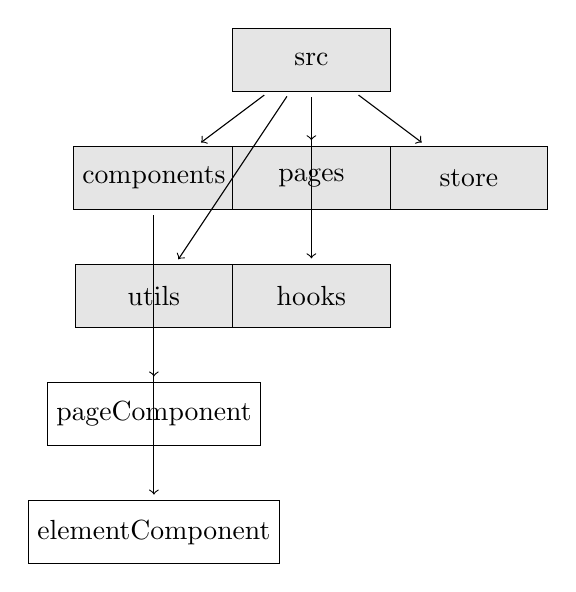
\begin{tikzpicture}[
    file/.style={draw, rectangle, minimum width=2cm, minimum height=0.8cm},
    folder/.style={draw, rectangle, minimum width=2cm, minimum height=0.8cm, fill=gray!20},
    arrow/.style={->, shorten >=2pt, shorten <=2pt}
]

% Folders
\node[folder] (src) at (0,0) {src};
\node[folder] (components) at (-2,-1.5) {components};
\node[folder] (pages) at (0,-1.5) {pages};
\node[folder] (store) at (2,-1.5) {store};
\node[folder] (utils) at (-2,-3) {utils};
\node[folder] (hooks) at (0,-3) {hooks};

% Files
\node[file] (pageComponent) at (-2,-4.5) {pageComponent};
\node[file] (elementComponent) at (-2,-6) {elementComponent};
% ... add more files

% Connections
\draw[arrow] (src) -- (components);
\draw[arrow] (src) -- (pages);
\draw[arrow] (src) -- (store);
\draw[arrow] (src) -- (utils);
\draw[arrow] (src) -- (hooks);
\draw[arrow] (components) -- (pageComponent);
\draw[arrow] (components) -- (elementComponent);
% ... add more connections

\end{tikzpicture}



\pagebreak
\subsubsection{Back-end}
The backend uses the dotNet framework. The development language using the C\# language.

In this project, the backend uses the Onion Architecture.
The Onion Architecture is a typically layered architecture, 
where each layer depends on the inner layer and provides interfaces to the outer layer.
The outer layer provides services to the outermost layer 
and other modules in the same layer based on the interfaces of the inner layer.

From inner to outer, the layers are: Domain, Application, Infrastructure, Presentation.
The Domain layer is the core layer and the innermost layer, used to define domain models, 
which are the business models.
It includes domain models and domain service interfaces.
Domain models are used to define the business models, 
which are the entities in the entity-relationship model and their attributes.
Domain service interfaces are used to define the business services, 
which are the relationships between entities in the entity-relationship model.

The Application layer is the application layer, 
used to define application services, which are the business logic.
It includes domain service implementations and application service interfaces.
Domain service implementations implement the methods of the inner layer's domain service 
interfaces and implement the business logic of the domain models.
Application service interfaces are used to define application services, 
which are the business logic.
It includes but is not limited to database interfaces, testing interfaces, 
HTTP API interfaces, MQTT interfaces, etc.

The Infrastructure layer is the infrastructure layer, used to define infrastructure.
It includes database implementations, testing implementations, 
HTTP API implementations, MQTT implementations, etc.
Database implementations implement the database interfaces 
and provide CRUD services for the database.
Testing implementations implement the testing interfaces 
and provide services for unit testing and integration testing.
HTTP API implementations implement the HTTP API interfaces 
and provide CRUD operations for HTTP APIs.
MQTT implementations implement the MQTT interfaces 
and provide CRUD operations for MQTT.

The Presentation layer is the presentation layer, used to define presentation logic, 
such as interfaces and pages. Since this is a backend project,
data presentation and control are handled by the frontend, 
so this layer is not needed.



\pagebreak
\subsubsection{Data communication and storage}
% 关于本项目的数据通信与数据存储的设计, 包括数据通信的协议, 数据存储的设计等
% 关于数据通信的设计:
% 1. 通信协议的选择
% 自前端向后端发送的数据, 有三种传输的数据类型, 
% 一种是普通的增删改查的请求, 对数据传输的时效性要求不高, 但是对数据的准确性, 完整性, 有序性, 安全性有一定的要求,
% 这种数据的传输, 采用 HTTP 协议, 以及 RESTful API 的设计. 可以有效的保证对数据传输的以上要求.
% 一种是对数据通道的创建和流媒体数据的传输, 对数据传输的时效性, 安全性要求较高, 这种数据的传输, 采用 WebRTC 协议, 以及 MQTT 协议.
% 配合可以快速解码的 flatbuffers 协议, 可以有效的保证对数据传输的以上要求.
% 最后一种是对设备的状态信息和操作信息的传输, 对完整性, 有序性, 安全性都有较高的要求, 这种数据的传输, 采用 MQTT 协议
% 同时也使用了 flatbuffers 协议.
% 
% 2. 数据通信的通信架构和通信流程
% 本项目的数据通信的通信架构, 是基于前后端分离的架构, 前端使用 React 框架, 后端使用 dotnet 框架.
% 当前端需要向后端发送数据的时候, 前端会向后端发送 HTTP 请求, 后端接收到 HTTP 请求之后, 会根据请求的数据类型,
% 选择不同的数据处理方式, 对于普通的增删改查的请求, 后端会根据 RESTful API 的设计, 对数据进行增删改查的操作,
% 对于对数据通道的创建和流媒体数据的传输, 后端会根据 WebRTC 协议, 对数据通道进行创建, 并且帮助前端和设备建立数据通道,
% 当数据通道建立后, 前端和设备之间则使用 flatbuffer 的数据格式对流媒体数据进行传输,
% 对于设备的状态信息和操作信息的传输, 前端会直接向 MQTT broker 发送 MQTT 请求, 
% 设备会在其自身的固件中监听相关的 MQTT 请求, 并且返回相关的数据.
% 
% 3. 数据通信的格式
% 本项目的数据通信的格式, 有三种, 
% 一种是 HTTP 协议, 
% 使用 json 格式对数据进行传输,
% 一种是 WebRTC 协议, 
% 使用 flatbuffers 格式对数据进行传输,
% 一种是 MQTT 协议.
% 使用 flatbuffers 格式对数据进行传输,
% 
% 关于数据存储的设计:
% 1. 数据存储的数据库的选择
% 本项目的数据存储的数据库的选择, 使用了轻量级的数据库 SQLite,
% SQLite 是一个进程内的库, 实现了自给自足的, 无服务器的, 零配置的, 事务性的 SQL 数据库引擎.
% 这是因为整个项目的目的是为了实现前端与设备之间的数据通信, 对于数据库数据的增删改查操作的要求不高,
% 数据量较小, 且对于数据库的数据的事务性要求不高, 所以选择了 SQLite 数据库.
% 2. 项目前后端的数据结构的设计
% 在本项目中, 前端由于使用了 React 框架, 所以前端的数据结构的设计, 使用了基于状态的数据结构的设计,
% 每个组件或者数据集都包含一个状态对象, 这个状态对象的属性就是组件的各个状态. 
% 使用状态对象的原因是, 可以方便的对状态进行管理, 采用对象-属性的形式, 可以方便的针对不同组件的同类状态进行区分,
% 由于跨组件的状态是由 redux 进行管理的, 这种状态对象的设计, 可以更搞笑的对状态进行更新和传递.
% 后端由于使用了 dotnet 框架, 所以后端的数据结构的设计, 使用了基于类的数据结构的设计,
% 采用了面向对象的编程思想, 对数据进行了封装, 使得数据的传输更加的安全, 有序, 完整.


\pagebreak

% \subsection{Domain model}
% \documentclass[]{article}
\usepackage{graphicx}
\usepackage{amsmath}
\usepackage{tikz}

% libaries
\usetikzlibrary{shapes,arrows}

%Define the listing package
\usepackage{listings} %code highlighter
\usepackage{color} %use color
\definecolor{mygreen}{rgb}{0,0.6,0}
\definecolor{mygray}{rgb}{0.5,0.5,0.5}
\definecolor{mymauve}{rgb}{0.58,0,0.82}

%Customize a bit the look
\lstset{ %
backgroundcolor=\color{white}, % choose the background color; you must add \usepackage{color} or \usepackage{xcolor}
basicstyle=\footnotesize, % the size of the fonts that are used for the code
breakatwhitespace=false, % sets if automatic breaks should only happen at whitespace
breaklines=true, % sets automatic line breaking
captionpos=b, % sets the caption-position to bottom
commentstyle=\color{mygreen}, % comment style
deletekeywords={...}, % if you want to delete keywords from the given language
escapeinside={\%*}{*)}, % if you want to add LaTeX within your code
extendedchars=true, % lets you use non-ASCII characters; for 8-bits encodings only, does not work with UTF-8
frame=single, % adds a frame around the code
keepspaces=true, % keeps spaces in text, useful for keeping indentation of code (possibly needs columns=flexible)
keywordstyle=\color{blue}, % keyword style
% language=Octave, % the language of the code
morekeywords={*,...}, % if you want to add more keywords to the set
numbers=left, % where to put the line-numbers; possible values are (none, left, right)
numbersep=5pt, % how far the line-numbers are from the code
numberstyle=\tiny\color{mygray}, % the style that is used for the line-numbers
rulecolor=\color{black}, % if not set, the frame-color may be changed on line-breaks within not-black text (e.g. comments (green here))
showspaces=false, % show spaces everywhere adding particular underscores; it overrides 'showstringspaces'
showstringspaces=false, % underline spaces within strings only
showtabs=false, % show tabs within strings adding particular underscores
stepnumber=1, % the step between two line-numbers. If it's 1, each line will be numbered
stringstyle=\color{mymauve}, % string literal style
tabsize=2, % sets default tabsize to 2 spaces
title=\lstname % show the filename of files included with \lstinputlisting; also try caption instead of title
}

\definecolor{darkgray}{rgb}{.4,.4,.4}
\definecolor{purple}{rgb}{0.65, 0.12, 0.82}

\lstdefinelanguage{React}{
keywords={const, typeof, new, true, false, catch, function, return, null, catch, switch, var, if, in, while, do, else, case, break},
keywordstyle=\color{blue}\bfseries,
ndkeywords={class, export, boolean, throw, implements, import, this},
ndkeywordstyle=\color{darkgray}\bfseries,
identifierstyle=\color{mygreen},
sensitive=false,
comment=[l]{//},
morecomment=[s]{/*}{*/},
commentstyle=\color{purple}\ttfamily,
string=[b]{"}{'}{`},
stringstyle=\color{red}\ttfamily,
morestring=[b]',
morestring=[b]",
morestring=[b]`',
}

\lstdefinelanguage{CSharp}{
keywords={const, typeof, new, true, false, catch, function, return, null, catch, switch, var, if, in, while, do, else, case, break},
keywordstyle=\color{blue}\bfseries,
ndkeywords={class, export, boolean, throw, implements, import, this},
ndkeywordstyle=\color{darkgray}\bfseries,
identifierstyle=\color{mygreen},
sensitive=false,
comment=[l]{//},
morecomment=[s]{/*}{*/},
commentstyle=\color{purple}\ttfamily,
string=[b]{"}{'}{`},
stringstyle=\color{red}\ttfamily,
morestring=[b]',
morestring=[b]",
morestring=[b]`',
}

\lstset{
language=React,
extendedchars=true,
basicstyle=\footnotesize\ttfamily,
showstringspaces=false,
showspaces=false,
numbers=left,
numberstyle=\footnotesize,
numbersep=9pt,
tabsize=2,
breaklines=true,
showtabs=false,
captionpos=b
}

\lstset{
language=CSharp,
extendedchars=true,
basicstyle=\footnotesize\ttfamily,
showstringspaces=false,
showspaces=false,
numbers=left,
numberstyle=\footnotesize,
numbersep=9pt,
tabsize=2,
breaklines=true,
showtabs=false,
captionpos=b
}

% \usepackage{cite} % Add this line for citation

% \bibliographystyle{plain}

\title{
The implementation of BifrostConnect Front-end scope, 
re-design and development with the relevant back-end support develop.
}
\author{
    Fei Gu \\
    Erhvervs Akademi Sydvest \\
    Computer Science 21\\
    }
\date{\today}

\begin{document}

% Front page
\maketitle
\begin{center}
    Supervisor: Henrik Boulund Meng Hansen \\
    Company: BifrostConnect \\
    Engineering Director: Jasper Wass \\
\end{center}
\tableofcontents
\pagebreak


% The introduction
\section{Introduction}
\subsection{Background}\input{sections/introduction/background.tex}
\subsection{The company}\input{sections/introduction/aboutCompany}
\subsection{The project}\input{sections/introduction/aboutProject}
\pagebreak

% The problem statement
\section{Problem Statement}
\subsection{Statement}
\input{sections/problemStatement/statement}
\subsection{Situation}
\input{sections/problemStatement/situation}
\subsection{Potential Solution}
\input{sections/problemStatement/potentialSolution}
\pagebreak

% Requirement analysis
\section{Requirement Analysis}
\input{sections/requirementAnalysis/index}

\subsection{Stakeholders}
\input{sections/requirementAnalysis/stakeholders/index}

\subsection{Business Domain}
\input{sections/requirementAnalysis/bussinesDomain/index}

\subsection{Scope}
\input{sections/requirementAnalysis/scope}

\subsection{Goals}
\input{sections/requirementAnalysis/goals}
\pagebreak

% Software Design
\section{Software Design}
% developement methods
\subsection{Software Development Methods}
\input{sections/softwareDevelopmentMethods/index}
\subsubsection{Agile Software Development}
\input{sections/softwareDevelopmentMethods/agileSoftwareDevelopment/index}
\subsubsection{Feature Driven Development}
\input{sections/softwareDevelopmentMethods/featureDrivenDevelopment/index}

\pagebreak

% Technology seslection
\subsection{Technology selection}
\input{sections/softwareDesign/technologySelection/index}
\subsubsection{Front-end}
\input{sections/softwareDesign/technologySelection/frontEnd}            
\subsubsection{Back-end}
\input{sections/softwareDesign/technologySelection/backEnd}            
\subsubsection{Database}
\input{sections/softwareDesign/technologySelection/database}
\subsubsection{Data communication}
\input{sections/softwareDesign/technologySelection/dataCommunication}            
\subsubsection{DevOps}
\input{sections/softwareDesign/technologySelection/devOps}
\pagebreak

% Architecture design
\subsection{Architecture design}
\input{sections/softwareDesign/architectureDesign/index}
\pagebreak
\subsubsection{Front-end}
\input{sections/softwareDesign/architectureDesign/frontEndArchitecture}
\pagebreak
\subsubsection{Back-end}
\input{sections/softwareDesign/architectureDesign/backEndArchitecture}
\pagebreak
\subsubsection{Data communication and storage}
\input{sections/softwareDesign/architectureDesign/dataCommunicationArchitecture}
\pagebreak

% \subsection{Domain model}
% \input{sections/softwareDesign/domainModel/index}
% \subsection{Database design}
% % 数据库领域模型 ER 图
% % 包括表和字段的设置.
% % 对于私有键和外键的设置.

% \subsection{Back-end design}
% % 后端对象模型
% % 以及对于对象模型的增删改查
% % 以及相关的其他服务的设计`'

% \subsection{Front-end design}
% % 对于前端的页面结构的设计 
% % 页面的状态的设计, 交互设计

% \subsection{FlatBuffers design}
% % schema 的设计

\subsection{DevOps CI/CD process design}
\input{sections/softwareDesign/devOpsDesign/index}
\subsubsection{Continuous Integration}
\input{sections/softwareDesign/devOpsDesign/continuousIntegration/index}
\subsubsection{Continuous Delivery}
\input{sections/softwareDesign/devOpsDesign/continuousDelivery/index}
\subsubsection{Continuous Deployment}
\input{sections/softwareDesign/devOpsDesign/continuousDeployment/index}
\pagebreak

\section{Software Development} 
\input{sections/softwareDevelopment/index}
\subsection{Overall development}
\input{sections/softwareDevelopment/overallDevelopement/index}
\subsubsection{Front-end}
\input{sections/softwareDevelopment/overallDevelopement/frontEnd/index}
\subsubsection{Back-end}
\input{sections/softwareDevelopment/overallDevelopement/backEnd/index}
\subsubsection{DevOps}
\input{sections/softwareDevelopment/overallDevelopement/devOps/index}
\subsection{Feature development} 
\input{sections/softwareDevelopment/featureDevelopment/index}
\subsubsection{Use Case 1}
\input{sections/softwareDevelopment/featureDevelopment/useCase1/index}
\subsubsection{Feature 1}
\input{sections/softwareDevelopment/featureDevelopment/feature/feature1.tex}
\pagebreak
\section{Conclusion} 
\subsection{Result}
Since the project is still in progress, the result is not available yet.
So far, basic structure of this project has been built. But the most features 
are not implemented yet. 
\subsection{Discussion}
As a single developer for this project, I am confident what I have done so far.
And I can say I understand the most of the knowledge I have used in this project, 
which also means I can explain all the part of the project. 
But this project also relevant some of the complex knowledge which I have to continue 
to study and practice.
\subsection{Future Work}
The future work is to implement the rest of the features. 
Including the most important part which is the 'create session' feature.
\pagebreak
% \bibliography{bibliography}
\pagebreak
% \begin{appendices}
%     \section{Appendix}
% \end{appendices} 
\end{document}
% \subsection{Database design}
% % 数据库领域模型 ER 图
% % 包括表和字段的设置.
% % 对于私有键和外键的设置.

% \subsection{Back-end design}
% % 后端对象模型
% % 以及对于对象模型的增删改查
% % 以及相关的其他服务的设计`'

% \subsection{Front-end design}
% % 对于前端的页面结构的设计 
% % 页面的状态的设计, 交互设计

% \subsection{FlatBuffers design}
% % schema 的设计

\subsection{DevOps CI/CD process design}
\documentclass[]{article}
\usepackage{graphicx}
\usepackage{amsmath}
\usepackage{tikz}

% libaries
\usetikzlibrary{shapes,arrows}

%Define the listing package
\usepackage{listings} %code highlighter
\usepackage{color} %use color
\definecolor{mygreen}{rgb}{0,0.6,0}
\definecolor{mygray}{rgb}{0.5,0.5,0.5}
\definecolor{mymauve}{rgb}{0.58,0,0.82}

%Customize a bit the look
\lstset{ %
backgroundcolor=\color{white}, % choose the background color; you must add \usepackage{color} or \usepackage{xcolor}
basicstyle=\footnotesize, % the size of the fonts that are used for the code
breakatwhitespace=false, % sets if automatic breaks should only happen at whitespace
breaklines=true, % sets automatic line breaking
captionpos=b, % sets the caption-position to bottom
commentstyle=\color{mygreen}, % comment style
deletekeywords={...}, % if you want to delete keywords from the given language
escapeinside={\%*}{*)}, % if you want to add LaTeX within your code
extendedchars=true, % lets you use non-ASCII characters; for 8-bits encodings only, does not work with UTF-8
frame=single, % adds a frame around the code
keepspaces=true, % keeps spaces in text, useful for keeping indentation of code (possibly needs columns=flexible)
keywordstyle=\color{blue}, % keyword style
% language=Octave, % the language of the code
morekeywords={*,...}, % if you want to add more keywords to the set
numbers=left, % where to put the line-numbers; possible values are (none, left, right)
numbersep=5pt, % how far the line-numbers are from the code
numberstyle=\tiny\color{mygray}, % the style that is used for the line-numbers
rulecolor=\color{black}, % if not set, the frame-color may be changed on line-breaks within not-black text (e.g. comments (green here))
showspaces=false, % show spaces everywhere adding particular underscores; it overrides 'showstringspaces'
showstringspaces=false, % underline spaces within strings only
showtabs=false, % show tabs within strings adding particular underscores
stepnumber=1, % the step between two line-numbers. If it's 1, each line will be numbered
stringstyle=\color{mymauve}, % string literal style
tabsize=2, % sets default tabsize to 2 spaces
title=\lstname % show the filename of files included with \lstinputlisting; also try caption instead of title
}

\definecolor{darkgray}{rgb}{.4,.4,.4}
\definecolor{purple}{rgb}{0.65, 0.12, 0.82}

\lstdefinelanguage{React}{
keywords={const, typeof, new, true, false, catch, function, return, null, catch, switch, var, if, in, while, do, else, case, break},
keywordstyle=\color{blue}\bfseries,
ndkeywords={class, export, boolean, throw, implements, import, this},
ndkeywordstyle=\color{darkgray}\bfseries,
identifierstyle=\color{mygreen},
sensitive=false,
comment=[l]{//},
morecomment=[s]{/*}{*/},
commentstyle=\color{purple}\ttfamily,
string=[b]{"}{'}{`},
stringstyle=\color{red}\ttfamily,
morestring=[b]',
morestring=[b]",
morestring=[b]`',
}

\lstdefinelanguage{CSharp}{
keywords={const, typeof, new, true, false, catch, function, return, null, catch, switch, var, if, in, while, do, else, case, break},
keywordstyle=\color{blue}\bfseries,
ndkeywords={class, export, boolean, throw, implements, import, this},
ndkeywordstyle=\color{darkgray}\bfseries,
identifierstyle=\color{mygreen},
sensitive=false,
comment=[l]{//},
morecomment=[s]{/*}{*/},
commentstyle=\color{purple}\ttfamily,
string=[b]{"}{'}{`},
stringstyle=\color{red}\ttfamily,
morestring=[b]',
morestring=[b]",
morestring=[b]`',
}

\lstset{
language=React,
extendedchars=true,
basicstyle=\footnotesize\ttfamily,
showstringspaces=false,
showspaces=false,
numbers=left,
numberstyle=\footnotesize,
numbersep=9pt,
tabsize=2,
breaklines=true,
showtabs=false,
captionpos=b
}

\lstset{
language=CSharp,
extendedchars=true,
basicstyle=\footnotesize\ttfamily,
showstringspaces=false,
showspaces=false,
numbers=left,
numberstyle=\footnotesize,
numbersep=9pt,
tabsize=2,
breaklines=true,
showtabs=false,
captionpos=b
}

% \usepackage{cite} % Add this line for citation

% \bibliographystyle{plain}

\title{
The implementation of BifrostConnect Front-end scope, 
re-design and development with the relevant back-end support develop.
}
\author{
    Fei Gu \\
    Erhvervs Akademi Sydvest \\
    Computer Science 21\\
    }
\date{\today}

\begin{document}

% Front page
\maketitle
\begin{center}
    Supervisor: Henrik Boulund Meng Hansen \\
    Company: BifrostConnect \\
    Engineering Director: Jasper Wass \\
\end{center}
\tableofcontents
\pagebreak


% The introduction
\section{Introduction}
\subsection{Background}\input{sections/introduction/background.tex}
\subsection{The company}\input{sections/introduction/aboutCompany}
\subsection{The project}\input{sections/introduction/aboutProject}
\pagebreak

% The problem statement
\section{Problem Statement}
\subsection{Statement}
\input{sections/problemStatement/statement}
\subsection{Situation}
\input{sections/problemStatement/situation}
\subsection{Potential Solution}
\input{sections/problemStatement/potentialSolution}
\pagebreak

% Requirement analysis
\section{Requirement Analysis}
\input{sections/requirementAnalysis/index}

\subsection{Stakeholders}
\input{sections/requirementAnalysis/stakeholders/index}

\subsection{Business Domain}
\input{sections/requirementAnalysis/bussinesDomain/index}

\subsection{Scope}
\input{sections/requirementAnalysis/scope}

\subsection{Goals}
\input{sections/requirementAnalysis/goals}
\pagebreak

% Software Design
\section{Software Design}
% developement methods
\subsection{Software Development Methods}
\input{sections/softwareDevelopmentMethods/index}
\subsubsection{Agile Software Development}
\input{sections/softwareDevelopmentMethods/agileSoftwareDevelopment/index}
\subsubsection{Feature Driven Development}
\input{sections/softwareDevelopmentMethods/featureDrivenDevelopment/index}

\pagebreak

% Technology seslection
\subsection{Technology selection}
\input{sections/softwareDesign/technologySelection/index}
\subsubsection{Front-end}
\input{sections/softwareDesign/technologySelection/frontEnd}            
\subsubsection{Back-end}
\input{sections/softwareDesign/technologySelection/backEnd}            
\subsubsection{Database}
\input{sections/softwareDesign/technologySelection/database}
\subsubsection{Data communication}
\input{sections/softwareDesign/technologySelection/dataCommunication}            
\subsubsection{DevOps}
\input{sections/softwareDesign/technologySelection/devOps}
\pagebreak

% Architecture design
\subsection{Architecture design}
\input{sections/softwareDesign/architectureDesign/index}
\pagebreak
\subsubsection{Front-end}
\input{sections/softwareDesign/architectureDesign/frontEndArchitecture}
\pagebreak
\subsubsection{Back-end}
\input{sections/softwareDesign/architectureDesign/backEndArchitecture}
\pagebreak
\subsubsection{Data communication and storage}
\input{sections/softwareDesign/architectureDesign/dataCommunicationArchitecture}
\pagebreak

% \subsection{Domain model}
% \input{sections/softwareDesign/domainModel/index}
% \subsection{Database design}
% % 数据库领域模型 ER 图
% % 包括表和字段的设置.
% % 对于私有键和外键的设置.

% \subsection{Back-end design}
% % 后端对象模型
% % 以及对于对象模型的增删改查
% % 以及相关的其他服务的设计`'

% \subsection{Front-end design}
% % 对于前端的页面结构的设计 
% % 页面的状态的设计, 交互设计

% \subsection{FlatBuffers design}
% % schema 的设计

\subsection{DevOps CI/CD process design}
\input{sections/softwareDesign/devOpsDesign/index}
\subsubsection{Continuous Integration}
\input{sections/softwareDesign/devOpsDesign/continuousIntegration/index}
\subsubsection{Continuous Delivery}
\input{sections/softwareDesign/devOpsDesign/continuousDelivery/index}
\subsubsection{Continuous Deployment}
\input{sections/softwareDesign/devOpsDesign/continuousDeployment/index}
\pagebreak

\section{Software Development} 
\input{sections/softwareDevelopment/index}
\subsection{Overall development}
\input{sections/softwareDevelopment/overallDevelopement/index}
\subsubsection{Front-end}
\input{sections/softwareDevelopment/overallDevelopement/frontEnd/index}
\subsubsection{Back-end}
\input{sections/softwareDevelopment/overallDevelopement/backEnd/index}
\subsubsection{DevOps}
\input{sections/softwareDevelopment/overallDevelopement/devOps/index}
\subsection{Feature development} 
\input{sections/softwareDevelopment/featureDevelopment/index}
\subsubsection{Use Case 1}
\input{sections/softwareDevelopment/featureDevelopment/useCase1/index}
\subsubsection{Feature 1}
\input{sections/softwareDevelopment/featureDevelopment/feature/feature1.tex}
\pagebreak
\section{Conclusion} 
\subsection{Result}
Since the project is still in progress, the result is not available yet.
So far, basic structure of this project has been built. But the most features 
are not implemented yet. 
\subsection{Discussion}
As a single developer for this project, I am confident what I have done so far.
And I can say I understand the most of the knowledge I have used in this project, 
which also means I can explain all the part of the project. 
But this project also relevant some of the complex knowledge which I have to continue 
to study and practice.
\subsection{Future Work}
The future work is to implement the rest of the features. 
Including the most important part which is the 'create session' feature.
\pagebreak
% \bibliography{bibliography}
\pagebreak
% \begin{appendices}
%     \section{Appendix}
% \end{appendices} 
\end{document}
\subsubsection{Continuous Integration}
\documentclass[]{article}
\usepackage{graphicx}
\usepackage{amsmath}
\usepackage{tikz}

% libaries
\usetikzlibrary{shapes,arrows}

%Define the listing package
\usepackage{listings} %code highlighter
\usepackage{color} %use color
\definecolor{mygreen}{rgb}{0,0.6,0}
\definecolor{mygray}{rgb}{0.5,0.5,0.5}
\definecolor{mymauve}{rgb}{0.58,0,0.82}

%Customize a bit the look
\lstset{ %
backgroundcolor=\color{white}, % choose the background color; you must add \usepackage{color} or \usepackage{xcolor}
basicstyle=\footnotesize, % the size of the fonts that are used for the code
breakatwhitespace=false, % sets if automatic breaks should only happen at whitespace
breaklines=true, % sets automatic line breaking
captionpos=b, % sets the caption-position to bottom
commentstyle=\color{mygreen}, % comment style
deletekeywords={...}, % if you want to delete keywords from the given language
escapeinside={\%*}{*)}, % if you want to add LaTeX within your code
extendedchars=true, % lets you use non-ASCII characters; for 8-bits encodings only, does not work with UTF-8
frame=single, % adds a frame around the code
keepspaces=true, % keeps spaces in text, useful for keeping indentation of code (possibly needs columns=flexible)
keywordstyle=\color{blue}, % keyword style
% language=Octave, % the language of the code
morekeywords={*,...}, % if you want to add more keywords to the set
numbers=left, % where to put the line-numbers; possible values are (none, left, right)
numbersep=5pt, % how far the line-numbers are from the code
numberstyle=\tiny\color{mygray}, % the style that is used for the line-numbers
rulecolor=\color{black}, % if not set, the frame-color may be changed on line-breaks within not-black text (e.g. comments (green here))
showspaces=false, % show spaces everywhere adding particular underscores; it overrides 'showstringspaces'
showstringspaces=false, % underline spaces within strings only
showtabs=false, % show tabs within strings adding particular underscores
stepnumber=1, % the step between two line-numbers. If it's 1, each line will be numbered
stringstyle=\color{mymauve}, % string literal style
tabsize=2, % sets default tabsize to 2 spaces
title=\lstname % show the filename of files included with \lstinputlisting; also try caption instead of title
}

\definecolor{darkgray}{rgb}{.4,.4,.4}
\definecolor{purple}{rgb}{0.65, 0.12, 0.82}

\lstdefinelanguage{React}{
keywords={const, typeof, new, true, false, catch, function, return, null, catch, switch, var, if, in, while, do, else, case, break},
keywordstyle=\color{blue}\bfseries,
ndkeywords={class, export, boolean, throw, implements, import, this},
ndkeywordstyle=\color{darkgray}\bfseries,
identifierstyle=\color{mygreen},
sensitive=false,
comment=[l]{//},
morecomment=[s]{/*}{*/},
commentstyle=\color{purple}\ttfamily,
string=[b]{"}{'}{`},
stringstyle=\color{red}\ttfamily,
morestring=[b]',
morestring=[b]",
morestring=[b]`',
}

\lstdefinelanguage{CSharp}{
keywords={const, typeof, new, true, false, catch, function, return, null, catch, switch, var, if, in, while, do, else, case, break},
keywordstyle=\color{blue}\bfseries,
ndkeywords={class, export, boolean, throw, implements, import, this},
ndkeywordstyle=\color{darkgray}\bfseries,
identifierstyle=\color{mygreen},
sensitive=false,
comment=[l]{//},
morecomment=[s]{/*}{*/},
commentstyle=\color{purple}\ttfamily,
string=[b]{"}{'}{`},
stringstyle=\color{red}\ttfamily,
morestring=[b]',
morestring=[b]",
morestring=[b]`',
}

\lstset{
language=React,
extendedchars=true,
basicstyle=\footnotesize\ttfamily,
showstringspaces=false,
showspaces=false,
numbers=left,
numberstyle=\footnotesize,
numbersep=9pt,
tabsize=2,
breaklines=true,
showtabs=false,
captionpos=b
}

\lstset{
language=CSharp,
extendedchars=true,
basicstyle=\footnotesize\ttfamily,
showstringspaces=false,
showspaces=false,
numbers=left,
numberstyle=\footnotesize,
numbersep=9pt,
tabsize=2,
breaklines=true,
showtabs=false,
captionpos=b
}

% \usepackage{cite} % Add this line for citation

% \bibliographystyle{plain}

\title{
The implementation of BifrostConnect Front-end scope, 
re-design and development with the relevant back-end support develop.
}
\author{
    Fei Gu \\
    Erhvervs Akademi Sydvest \\
    Computer Science 21\\
    }
\date{\today}

\begin{document}

% Front page
\maketitle
\begin{center}
    Supervisor: Henrik Boulund Meng Hansen \\
    Company: BifrostConnect \\
    Engineering Director: Jasper Wass \\
\end{center}
\tableofcontents
\pagebreak


% The introduction
\section{Introduction}
\subsection{Background}\input{sections/introduction/background.tex}
\subsection{The company}\input{sections/introduction/aboutCompany}
\subsection{The project}\input{sections/introduction/aboutProject}
\pagebreak

% The problem statement
\section{Problem Statement}
\subsection{Statement}
\input{sections/problemStatement/statement}
\subsection{Situation}
\input{sections/problemStatement/situation}
\subsection{Potential Solution}
\input{sections/problemStatement/potentialSolution}
\pagebreak

% Requirement analysis
\section{Requirement Analysis}
\input{sections/requirementAnalysis/index}

\subsection{Stakeholders}
\input{sections/requirementAnalysis/stakeholders/index}

\subsection{Business Domain}
\input{sections/requirementAnalysis/bussinesDomain/index}

\subsection{Scope}
\input{sections/requirementAnalysis/scope}

\subsection{Goals}
\input{sections/requirementAnalysis/goals}
\pagebreak

% Software Design
\section{Software Design}
% developement methods
\subsection{Software Development Methods}
\input{sections/softwareDevelopmentMethods/index}
\subsubsection{Agile Software Development}
\input{sections/softwareDevelopmentMethods/agileSoftwareDevelopment/index}
\subsubsection{Feature Driven Development}
\input{sections/softwareDevelopmentMethods/featureDrivenDevelopment/index}

\pagebreak

% Technology seslection
\subsection{Technology selection}
\input{sections/softwareDesign/technologySelection/index}
\subsubsection{Front-end}
\input{sections/softwareDesign/technologySelection/frontEnd}            
\subsubsection{Back-end}
\input{sections/softwareDesign/technologySelection/backEnd}            
\subsubsection{Database}
\input{sections/softwareDesign/technologySelection/database}
\subsubsection{Data communication}
\input{sections/softwareDesign/technologySelection/dataCommunication}            
\subsubsection{DevOps}
\input{sections/softwareDesign/technologySelection/devOps}
\pagebreak

% Architecture design
\subsection{Architecture design}
\input{sections/softwareDesign/architectureDesign/index}
\pagebreak
\subsubsection{Front-end}
\input{sections/softwareDesign/architectureDesign/frontEndArchitecture}
\pagebreak
\subsubsection{Back-end}
\input{sections/softwareDesign/architectureDesign/backEndArchitecture}
\pagebreak
\subsubsection{Data communication and storage}
\input{sections/softwareDesign/architectureDesign/dataCommunicationArchitecture}
\pagebreak

% \subsection{Domain model}
% \input{sections/softwareDesign/domainModel/index}
% \subsection{Database design}
% % 数据库领域模型 ER 图
% % 包括表和字段的设置.
% % 对于私有键和外键的设置.

% \subsection{Back-end design}
% % 后端对象模型
% % 以及对于对象模型的增删改查
% % 以及相关的其他服务的设计`'

% \subsection{Front-end design}
% % 对于前端的页面结构的设计 
% % 页面的状态的设计, 交互设计

% \subsection{FlatBuffers design}
% % schema 的设计

\subsection{DevOps CI/CD process design}
\input{sections/softwareDesign/devOpsDesign/index}
\subsubsection{Continuous Integration}
\input{sections/softwareDesign/devOpsDesign/continuousIntegration/index}
\subsubsection{Continuous Delivery}
\input{sections/softwareDesign/devOpsDesign/continuousDelivery/index}
\subsubsection{Continuous Deployment}
\input{sections/softwareDesign/devOpsDesign/continuousDeployment/index}
\pagebreak

\section{Software Development} 
\input{sections/softwareDevelopment/index}
\subsection{Overall development}
\input{sections/softwareDevelopment/overallDevelopement/index}
\subsubsection{Front-end}
\input{sections/softwareDevelopment/overallDevelopement/frontEnd/index}
\subsubsection{Back-end}
\input{sections/softwareDevelopment/overallDevelopement/backEnd/index}
\subsubsection{DevOps}
\input{sections/softwareDevelopment/overallDevelopement/devOps/index}
\subsection{Feature development} 
\input{sections/softwareDevelopment/featureDevelopment/index}
\subsubsection{Use Case 1}
\input{sections/softwareDevelopment/featureDevelopment/useCase1/index}
\subsubsection{Feature 1}
\input{sections/softwareDevelopment/featureDevelopment/feature/feature1.tex}
\pagebreak
\section{Conclusion} 
\subsection{Result}
Since the project is still in progress, the result is not available yet.
So far, basic structure of this project has been built. But the most features 
are not implemented yet. 
\subsection{Discussion}
As a single developer for this project, I am confident what I have done so far.
And I can say I understand the most of the knowledge I have used in this project, 
which also means I can explain all the part of the project. 
But this project also relevant some of the complex knowledge which I have to continue 
to study and practice.
\subsection{Future Work}
The future work is to implement the rest of the features. 
Including the most important part which is the 'create session' feature.
\pagebreak
% \bibliography{bibliography}
\pagebreak
% \begin{appendices}
%     \section{Appendix}
% \end{appendices} 
\end{document}
\subsubsection{Continuous Delivery}
\documentclass[]{article}
\usepackage{graphicx}
\usepackage{amsmath}
\usepackage{tikz}

% libaries
\usetikzlibrary{shapes,arrows}

%Define the listing package
\usepackage{listings} %code highlighter
\usepackage{color} %use color
\definecolor{mygreen}{rgb}{0,0.6,0}
\definecolor{mygray}{rgb}{0.5,0.5,0.5}
\definecolor{mymauve}{rgb}{0.58,0,0.82}

%Customize a bit the look
\lstset{ %
backgroundcolor=\color{white}, % choose the background color; you must add \usepackage{color} or \usepackage{xcolor}
basicstyle=\footnotesize, % the size of the fonts that are used for the code
breakatwhitespace=false, % sets if automatic breaks should only happen at whitespace
breaklines=true, % sets automatic line breaking
captionpos=b, % sets the caption-position to bottom
commentstyle=\color{mygreen}, % comment style
deletekeywords={...}, % if you want to delete keywords from the given language
escapeinside={\%*}{*)}, % if you want to add LaTeX within your code
extendedchars=true, % lets you use non-ASCII characters; for 8-bits encodings only, does not work with UTF-8
frame=single, % adds a frame around the code
keepspaces=true, % keeps spaces in text, useful for keeping indentation of code (possibly needs columns=flexible)
keywordstyle=\color{blue}, % keyword style
% language=Octave, % the language of the code
morekeywords={*,...}, % if you want to add more keywords to the set
numbers=left, % where to put the line-numbers; possible values are (none, left, right)
numbersep=5pt, % how far the line-numbers are from the code
numberstyle=\tiny\color{mygray}, % the style that is used for the line-numbers
rulecolor=\color{black}, % if not set, the frame-color may be changed on line-breaks within not-black text (e.g. comments (green here))
showspaces=false, % show spaces everywhere adding particular underscores; it overrides 'showstringspaces'
showstringspaces=false, % underline spaces within strings only
showtabs=false, % show tabs within strings adding particular underscores
stepnumber=1, % the step between two line-numbers. If it's 1, each line will be numbered
stringstyle=\color{mymauve}, % string literal style
tabsize=2, % sets default tabsize to 2 spaces
title=\lstname % show the filename of files included with \lstinputlisting; also try caption instead of title
}

\definecolor{darkgray}{rgb}{.4,.4,.4}
\definecolor{purple}{rgb}{0.65, 0.12, 0.82}

\lstdefinelanguage{React}{
keywords={const, typeof, new, true, false, catch, function, return, null, catch, switch, var, if, in, while, do, else, case, break},
keywordstyle=\color{blue}\bfseries,
ndkeywords={class, export, boolean, throw, implements, import, this},
ndkeywordstyle=\color{darkgray}\bfseries,
identifierstyle=\color{mygreen},
sensitive=false,
comment=[l]{//},
morecomment=[s]{/*}{*/},
commentstyle=\color{purple}\ttfamily,
string=[b]{"}{'}{`},
stringstyle=\color{red}\ttfamily,
morestring=[b]',
morestring=[b]",
morestring=[b]`',
}

\lstdefinelanguage{CSharp}{
keywords={const, typeof, new, true, false, catch, function, return, null, catch, switch, var, if, in, while, do, else, case, break},
keywordstyle=\color{blue}\bfseries,
ndkeywords={class, export, boolean, throw, implements, import, this},
ndkeywordstyle=\color{darkgray}\bfseries,
identifierstyle=\color{mygreen},
sensitive=false,
comment=[l]{//},
morecomment=[s]{/*}{*/},
commentstyle=\color{purple}\ttfamily,
string=[b]{"}{'}{`},
stringstyle=\color{red}\ttfamily,
morestring=[b]',
morestring=[b]",
morestring=[b]`',
}

\lstset{
language=React,
extendedchars=true,
basicstyle=\footnotesize\ttfamily,
showstringspaces=false,
showspaces=false,
numbers=left,
numberstyle=\footnotesize,
numbersep=9pt,
tabsize=2,
breaklines=true,
showtabs=false,
captionpos=b
}

\lstset{
language=CSharp,
extendedchars=true,
basicstyle=\footnotesize\ttfamily,
showstringspaces=false,
showspaces=false,
numbers=left,
numberstyle=\footnotesize,
numbersep=9pt,
tabsize=2,
breaklines=true,
showtabs=false,
captionpos=b
}

% \usepackage{cite} % Add this line for citation

% \bibliographystyle{plain}

\title{
The implementation of BifrostConnect Front-end scope, 
re-design and development with the relevant back-end support develop.
}
\author{
    Fei Gu \\
    Erhvervs Akademi Sydvest \\
    Computer Science 21\\
    }
\date{\today}

\begin{document}

% Front page
\maketitle
\begin{center}
    Supervisor: Henrik Boulund Meng Hansen \\
    Company: BifrostConnect \\
    Engineering Director: Jasper Wass \\
\end{center}
\tableofcontents
\pagebreak


% The introduction
\section{Introduction}
\subsection{Background}\input{sections/introduction/background.tex}
\subsection{The company}\input{sections/introduction/aboutCompany}
\subsection{The project}\input{sections/introduction/aboutProject}
\pagebreak

% The problem statement
\section{Problem Statement}
\subsection{Statement}
\input{sections/problemStatement/statement}
\subsection{Situation}
\input{sections/problemStatement/situation}
\subsection{Potential Solution}
\input{sections/problemStatement/potentialSolution}
\pagebreak

% Requirement analysis
\section{Requirement Analysis}
\input{sections/requirementAnalysis/index}

\subsection{Stakeholders}
\input{sections/requirementAnalysis/stakeholders/index}

\subsection{Business Domain}
\input{sections/requirementAnalysis/bussinesDomain/index}

\subsection{Scope}
\input{sections/requirementAnalysis/scope}

\subsection{Goals}
\input{sections/requirementAnalysis/goals}
\pagebreak

% Software Design
\section{Software Design}
% developement methods
\subsection{Software Development Methods}
\input{sections/softwareDevelopmentMethods/index}
\subsubsection{Agile Software Development}
\input{sections/softwareDevelopmentMethods/agileSoftwareDevelopment/index}
\subsubsection{Feature Driven Development}
\input{sections/softwareDevelopmentMethods/featureDrivenDevelopment/index}

\pagebreak

% Technology seslection
\subsection{Technology selection}
\input{sections/softwareDesign/technologySelection/index}
\subsubsection{Front-end}
\input{sections/softwareDesign/technologySelection/frontEnd}            
\subsubsection{Back-end}
\input{sections/softwareDesign/technologySelection/backEnd}            
\subsubsection{Database}
\input{sections/softwareDesign/technologySelection/database}
\subsubsection{Data communication}
\input{sections/softwareDesign/technologySelection/dataCommunication}            
\subsubsection{DevOps}
\input{sections/softwareDesign/technologySelection/devOps}
\pagebreak

% Architecture design
\subsection{Architecture design}
\input{sections/softwareDesign/architectureDesign/index}
\pagebreak
\subsubsection{Front-end}
\input{sections/softwareDesign/architectureDesign/frontEndArchitecture}
\pagebreak
\subsubsection{Back-end}
\input{sections/softwareDesign/architectureDesign/backEndArchitecture}
\pagebreak
\subsubsection{Data communication and storage}
\input{sections/softwareDesign/architectureDesign/dataCommunicationArchitecture}
\pagebreak

% \subsection{Domain model}
% \input{sections/softwareDesign/domainModel/index}
% \subsection{Database design}
% % 数据库领域模型 ER 图
% % 包括表和字段的设置.
% % 对于私有键和外键的设置.

% \subsection{Back-end design}
% % 后端对象模型
% % 以及对于对象模型的增删改查
% % 以及相关的其他服务的设计`'

% \subsection{Front-end design}
% % 对于前端的页面结构的设计 
% % 页面的状态的设计, 交互设计

% \subsection{FlatBuffers design}
% % schema 的设计

\subsection{DevOps CI/CD process design}
\input{sections/softwareDesign/devOpsDesign/index}
\subsubsection{Continuous Integration}
\input{sections/softwareDesign/devOpsDesign/continuousIntegration/index}
\subsubsection{Continuous Delivery}
\input{sections/softwareDesign/devOpsDesign/continuousDelivery/index}
\subsubsection{Continuous Deployment}
\input{sections/softwareDesign/devOpsDesign/continuousDeployment/index}
\pagebreak

\section{Software Development} 
\input{sections/softwareDevelopment/index}
\subsection{Overall development}
\input{sections/softwareDevelopment/overallDevelopement/index}
\subsubsection{Front-end}
\input{sections/softwareDevelopment/overallDevelopement/frontEnd/index}
\subsubsection{Back-end}
\input{sections/softwareDevelopment/overallDevelopement/backEnd/index}
\subsubsection{DevOps}
\input{sections/softwareDevelopment/overallDevelopement/devOps/index}
\subsection{Feature development} 
\input{sections/softwareDevelopment/featureDevelopment/index}
\subsubsection{Use Case 1}
\input{sections/softwareDevelopment/featureDevelopment/useCase1/index}
\subsubsection{Feature 1}
\input{sections/softwareDevelopment/featureDevelopment/feature/feature1.tex}
\pagebreak
\section{Conclusion} 
\subsection{Result}
Since the project is still in progress, the result is not available yet.
So far, basic structure of this project has been built. But the most features 
are not implemented yet. 
\subsection{Discussion}
As a single developer for this project, I am confident what I have done so far.
And I can say I understand the most of the knowledge I have used in this project, 
which also means I can explain all the part of the project. 
But this project also relevant some of the complex knowledge which I have to continue 
to study and practice.
\subsection{Future Work}
The future work is to implement the rest of the features. 
Including the most important part which is the 'create session' feature.
\pagebreak
% \bibliography{bibliography}
\pagebreak
% \begin{appendices}
%     \section{Appendix}
% \end{appendices} 
\end{document}
\subsubsection{Continuous Deployment}
\documentclass[]{article}
\usepackage{graphicx}
\usepackage{amsmath}
\usepackage{tikz}

% libaries
\usetikzlibrary{shapes,arrows}

%Define the listing package
\usepackage{listings} %code highlighter
\usepackage{color} %use color
\definecolor{mygreen}{rgb}{0,0.6,0}
\definecolor{mygray}{rgb}{0.5,0.5,0.5}
\definecolor{mymauve}{rgb}{0.58,0,0.82}

%Customize a bit the look
\lstset{ %
backgroundcolor=\color{white}, % choose the background color; you must add \usepackage{color} or \usepackage{xcolor}
basicstyle=\footnotesize, % the size of the fonts that are used for the code
breakatwhitespace=false, % sets if automatic breaks should only happen at whitespace
breaklines=true, % sets automatic line breaking
captionpos=b, % sets the caption-position to bottom
commentstyle=\color{mygreen}, % comment style
deletekeywords={...}, % if you want to delete keywords from the given language
escapeinside={\%*}{*)}, % if you want to add LaTeX within your code
extendedchars=true, % lets you use non-ASCII characters; for 8-bits encodings only, does not work with UTF-8
frame=single, % adds a frame around the code
keepspaces=true, % keeps spaces in text, useful for keeping indentation of code (possibly needs columns=flexible)
keywordstyle=\color{blue}, % keyword style
% language=Octave, % the language of the code
morekeywords={*,...}, % if you want to add more keywords to the set
numbers=left, % where to put the line-numbers; possible values are (none, left, right)
numbersep=5pt, % how far the line-numbers are from the code
numberstyle=\tiny\color{mygray}, % the style that is used for the line-numbers
rulecolor=\color{black}, % if not set, the frame-color may be changed on line-breaks within not-black text (e.g. comments (green here))
showspaces=false, % show spaces everywhere adding particular underscores; it overrides 'showstringspaces'
showstringspaces=false, % underline spaces within strings only
showtabs=false, % show tabs within strings adding particular underscores
stepnumber=1, % the step between two line-numbers. If it's 1, each line will be numbered
stringstyle=\color{mymauve}, % string literal style
tabsize=2, % sets default tabsize to 2 spaces
title=\lstname % show the filename of files included with \lstinputlisting; also try caption instead of title
}

\definecolor{darkgray}{rgb}{.4,.4,.4}
\definecolor{purple}{rgb}{0.65, 0.12, 0.82}

\lstdefinelanguage{React}{
keywords={const, typeof, new, true, false, catch, function, return, null, catch, switch, var, if, in, while, do, else, case, break},
keywordstyle=\color{blue}\bfseries,
ndkeywords={class, export, boolean, throw, implements, import, this},
ndkeywordstyle=\color{darkgray}\bfseries,
identifierstyle=\color{mygreen},
sensitive=false,
comment=[l]{//},
morecomment=[s]{/*}{*/},
commentstyle=\color{purple}\ttfamily,
string=[b]{"}{'}{`},
stringstyle=\color{red}\ttfamily,
morestring=[b]',
morestring=[b]",
morestring=[b]`',
}

\lstdefinelanguage{CSharp}{
keywords={const, typeof, new, true, false, catch, function, return, null, catch, switch, var, if, in, while, do, else, case, break},
keywordstyle=\color{blue}\bfseries,
ndkeywords={class, export, boolean, throw, implements, import, this},
ndkeywordstyle=\color{darkgray}\bfseries,
identifierstyle=\color{mygreen},
sensitive=false,
comment=[l]{//},
morecomment=[s]{/*}{*/},
commentstyle=\color{purple}\ttfamily,
string=[b]{"}{'}{`},
stringstyle=\color{red}\ttfamily,
morestring=[b]',
morestring=[b]",
morestring=[b]`',
}

\lstset{
language=React,
extendedchars=true,
basicstyle=\footnotesize\ttfamily,
showstringspaces=false,
showspaces=false,
numbers=left,
numberstyle=\footnotesize,
numbersep=9pt,
tabsize=2,
breaklines=true,
showtabs=false,
captionpos=b
}

\lstset{
language=CSharp,
extendedchars=true,
basicstyle=\footnotesize\ttfamily,
showstringspaces=false,
showspaces=false,
numbers=left,
numberstyle=\footnotesize,
numbersep=9pt,
tabsize=2,
breaklines=true,
showtabs=false,
captionpos=b
}

% \usepackage{cite} % Add this line for citation

% \bibliographystyle{plain}

\title{
The implementation of BifrostConnect Front-end scope, 
re-design and development with the relevant back-end support develop.
}
\author{
    Fei Gu \\
    Erhvervs Akademi Sydvest \\
    Computer Science 21\\
    }
\date{\today}

\begin{document}

% Front page
\maketitle
\begin{center}
    Supervisor: Henrik Boulund Meng Hansen \\
    Company: BifrostConnect \\
    Engineering Director: Jasper Wass \\
\end{center}
\tableofcontents
\pagebreak


% The introduction
\section{Introduction}
\subsection{Background}\input{sections/introduction/background.tex}
\subsection{The company}\input{sections/introduction/aboutCompany}
\subsection{The project}\input{sections/introduction/aboutProject}
\pagebreak

% The problem statement
\section{Problem Statement}
\subsection{Statement}
\input{sections/problemStatement/statement}
\subsection{Situation}
\input{sections/problemStatement/situation}
\subsection{Potential Solution}
\input{sections/problemStatement/potentialSolution}
\pagebreak

% Requirement analysis
\section{Requirement Analysis}
\input{sections/requirementAnalysis/index}

\subsection{Stakeholders}
\input{sections/requirementAnalysis/stakeholders/index}

\subsection{Business Domain}
\input{sections/requirementAnalysis/bussinesDomain/index}

\subsection{Scope}
\input{sections/requirementAnalysis/scope}

\subsection{Goals}
\input{sections/requirementAnalysis/goals}
\pagebreak

% Software Design
\section{Software Design}
% developement methods
\subsection{Software Development Methods}
\input{sections/softwareDevelopmentMethods/index}
\subsubsection{Agile Software Development}
\input{sections/softwareDevelopmentMethods/agileSoftwareDevelopment/index}
\subsubsection{Feature Driven Development}
\input{sections/softwareDevelopmentMethods/featureDrivenDevelopment/index}

\pagebreak

% Technology seslection
\subsection{Technology selection}
\input{sections/softwareDesign/technologySelection/index}
\subsubsection{Front-end}
\input{sections/softwareDesign/technologySelection/frontEnd}            
\subsubsection{Back-end}
\input{sections/softwareDesign/technologySelection/backEnd}            
\subsubsection{Database}
\input{sections/softwareDesign/technologySelection/database}
\subsubsection{Data communication}
\input{sections/softwareDesign/technologySelection/dataCommunication}            
\subsubsection{DevOps}
\input{sections/softwareDesign/technologySelection/devOps}
\pagebreak

% Architecture design
\subsection{Architecture design}
\input{sections/softwareDesign/architectureDesign/index}
\pagebreak
\subsubsection{Front-end}
\input{sections/softwareDesign/architectureDesign/frontEndArchitecture}
\pagebreak
\subsubsection{Back-end}
\input{sections/softwareDesign/architectureDesign/backEndArchitecture}
\pagebreak
\subsubsection{Data communication and storage}
\input{sections/softwareDesign/architectureDesign/dataCommunicationArchitecture}
\pagebreak

% \subsection{Domain model}
% \input{sections/softwareDesign/domainModel/index}
% \subsection{Database design}
% % 数据库领域模型 ER 图
% % 包括表和字段的设置.
% % 对于私有键和外键的设置.

% \subsection{Back-end design}
% % 后端对象模型
% % 以及对于对象模型的增删改查
% % 以及相关的其他服务的设计`'

% \subsection{Front-end design}
% % 对于前端的页面结构的设计 
% % 页面的状态的设计, 交互设计

% \subsection{FlatBuffers design}
% % schema 的设计

\subsection{DevOps CI/CD process design}
\input{sections/softwareDesign/devOpsDesign/index}
\subsubsection{Continuous Integration}
\input{sections/softwareDesign/devOpsDesign/continuousIntegration/index}
\subsubsection{Continuous Delivery}
\input{sections/softwareDesign/devOpsDesign/continuousDelivery/index}
\subsubsection{Continuous Deployment}
\input{sections/softwareDesign/devOpsDesign/continuousDeployment/index}
\pagebreak

\section{Software Development} 
\input{sections/softwareDevelopment/index}
\subsection{Overall development}
\input{sections/softwareDevelopment/overallDevelopement/index}
\subsubsection{Front-end}
\input{sections/softwareDevelopment/overallDevelopement/frontEnd/index}
\subsubsection{Back-end}
\input{sections/softwareDevelopment/overallDevelopement/backEnd/index}
\subsubsection{DevOps}
\input{sections/softwareDevelopment/overallDevelopement/devOps/index}
\subsection{Feature development} 
\input{sections/softwareDevelopment/featureDevelopment/index}
\subsubsection{Use Case 1}
\input{sections/softwareDevelopment/featureDevelopment/useCase1/index}
\subsubsection{Feature 1}
\input{sections/softwareDevelopment/featureDevelopment/feature/feature1.tex}
\pagebreak
\section{Conclusion} 
\subsection{Result}
Since the project is still in progress, the result is not available yet.
So far, basic structure of this project has been built. But the most features 
are not implemented yet. 
\subsection{Discussion}
As a single developer for this project, I am confident what I have done so far.
And I can say I understand the most of the knowledge I have used in this project, 
which also means I can explain all the part of the project. 
But this project also relevant some of the complex knowledge which I have to continue 
to study and practice.
\subsection{Future Work}
The future work is to implement the rest of the features. 
Including the most important part which is the 'create session' feature.
\pagebreak
% \bibliography{bibliography}
\pagebreak
% \begin{appendices}
%     \section{Appendix}
% \end{appendices} 
\end{document}
\pagebreak

\section{Software Development} 
\documentclass[]{article}
\usepackage{graphicx}
\usepackage{amsmath}
\usepackage{tikz}

% libaries
\usetikzlibrary{shapes,arrows}

%Define the listing package
\usepackage{listings} %code highlighter
\usepackage{color} %use color
\definecolor{mygreen}{rgb}{0,0.6,0}
\definecolor{mygray}{rgb}{0.5,0.5,0.5}
\definecolor{mymauve}{rgb}{0.58,0,0.82}

%Customize a bit the look
\lstset{ %
backgroundcolor=\color{white}, % choose the background color; you must add \usepackage{color} or \usepackage{xcolor}
basicstyle=\footnotesize, % the size of the fonts that are used for the code
breakatwhitespace=false, % sets if automatic breaks should only happen at whitespace
breaklines=true, % sets automatic line breaking
captionpos=b, % sets the caption-position to bottom
commentstyle=\color{mygreen}, % comment style
deletekeywords={...}, % if you want to delete keywords from the given language
escapeinside={\%*}{*)}, % if you want to add LaTeX within your code
extendedchars=true, % lets you use non-ASCII characters; for 8-bits encodings only, does not work with UTF-8
frame=single, % adds a frame around the code
keepspaces=true, % keeps spaces in text, useful for keeping indentation of code (possibly needs columns=flexible)
keywordstyle=\color{blue}, % keyword style
% language=Octave, % the language of the code
morekeywords={*,...}, % if you want to add more keywords to the set
numbers=left, % where to put the line-numbers; possible values are (none, left, right)
numbersep=5pt, % how far the line-numbers are from the code
numberstyle=\tiny\color{mygray}, % the style that is used for the line-numbers
rulecolor=\color{black}, % if not set, the frame-color may be changed on line-breaks within not-black text (e.g. comments (green here))
showspaces=false, % show spaces everywhere adding particular underscores; it overrides 'showstringspaces'
showstringspaces=false, % underline spaces within strings only
showtabs=false, % show tabs within strings adding particular underscores
stepnumber=1, % the step between two line-numbers. If it's 1, each line will be numbered
stringstyle=\color{mymauve}, % string literal style
tabsize=2, % sets default tabsize to 2 spaces
title=\lstname % show the filename of files included with \lstinputlisting; also try caption instead of title
}

\definecolor{darkgray}{rgb}{.4,.4,.4}
\definecolor{purple}{rgb}{0.65, 0.12, 0.82}

\lstdefinelanguage{React}{
keywords={const, typeof, new, true, false, catch, function, return, null, catch, switch, var, if, in, while, do, else, case, break},
keywordstyle=\color{blue}\bfseries,
ndkeywords={class, export, boolean, throw, implements, import, this},
ndkeywordstyle=\color{darkgray}\bfseries,
identifierstyle=\color{mygreen},
sensitive=false,
comment=[l]{//},
morecomment=[s]{/*}{*/},
commentstyle=\color{purple}\ttfamily,
string=[b]{"}{'}{`},
stringstyle=\color{red}\ttfamily,
morestring=[b]',
morestring=[b]",
morestring=[b]`',
}

\lstdefinelanguage{CSharp}{
keywords={const, typeof, new, true, false, catch, function, return, null, catch, switch, var, if, in, while, do, else, case, break},
keywordstyle=\color{blue}\bfseries,
ndkeywords={class, export, boolean, throw, implements, import, this},
ndkeywordstyle=\color{darkgray}\bfseries,
identifierstyle=\color{mygreen},
sensitive=false,
comment=[l]{//},
morecomment=[s]{/*}{*/},
commentstyle=\color{purple}\ttfamily,
string=[b]{"}{'}{`},
stringstyle=\color{red}\ttfamily,
morestring=[b]',
morestring=[b]",
morestring=[b]`',
}

\lstset{
language=React,
extendedchars=true,
basicstyle=\footnotesize\ttfamily,
showstringspaces=false,
showspaces=false,
numbers=left,
numberstyle=\footnotesize,
numbersep=9pt,
tabsize=2,
breaklines=true,
showtabs=false,
captionpos=b
}

\lstset{
language=CSharp,
extendedchars=true,
basicstyle=\footnotesize\ttfamily,
showstringspaces=false,
showspaces=false,
numbers=left,
numberstyle=\footnotesize,
numbersep=9pt,
tabsize=2,
breaklines=true,
showtabs=false,
captionpos=b
}

% \usepackage{cite} % Add this line for citation

% \bibliographystyle{plain}

\title{
The implementation of BifrostConnect Front-end scope, 
re-design and development with the relevant back-end support develop.
}
\author{
    Fei Gu \\
    Erhvervs Akademi Sydvest \\
    Computer Science 21\\
    }
\date{\today}

\begin{document}

% Front page
\maketitle
\begin{center}
    Supervisor: Henrik Boulund Meng Hansen \\
    Company: BifrostConnect \\
    Engineering Director: Jasper Wass \\
\end{center}
\tableofcontents
\pagebreak


% The introduction
\section{Introduction}
\subsection{Background}\input{sections/introduction/background.tex}
\subsection{The company}\input{sections/introduction/aboutCompany}
\subsection{The project}\input{sections/introduction/aboutProject}
\pagebreak

% The problem statement
\section{Problem Statement}
\subsection{Statement}
\input{sections/problemStatement/statement}
\subsection{Situation}
\input{sections/problemStatement/situation}
\subsection{Potential Solution}
\input{sections/problemStatement/potentialSolution}
\pagebreak

% Requirement analysis
\section{Requirement Analysis}
\input{sections/requirementAnalysis/index}

\subsection{Stakeholders}
\input{sections/requirementAnalysis/stakeholders/index}

\subsection{Business Domain}
\input{sections/requirementAnalysis/bussinesDomain/index}

\subsection{Scope}
\input{sections/requirementAnalysis/scope}

\subsection{Goals}
\input{sections/requirementAnalysis/goals}
\pagebreak

% Software Design
\section{Software Design}
% developement methods
\subsection{Software Development Methods}
\input{sections/softwareDevelopmentMethods/index}
\subsubsection{Agile Software Development}
\input{sections/softwareDevelopmentMethods/agileSoftwareDevelopment/index}
\subsubsection{Feature Driven Development}
\input{sections/softwareDevelopmentMethods/featureDrivenDevelopment/index}

\pagebreak

% Technology seslection
\subsection{Technology selection}
\input{sections/softwareDesign/technologySelection/index}
\subsubsection{Front-end}
\input{sections/softwareDesign/technologySelection/frontEnd}            
\subsubsection{Back-end}
\input{sections/softwareDesign/technologySelection/backEnd}            
\subsubsection{Database}
\input{sections/softwareDesign/technologySelection/database}
\subsubsection{Data communication}
\input{sections/softwareDesign/technologySelection/dataCommunication}            
\subsubsection{DevOps}
\input{sections/softwareDesign/technologySelection/devOps}
\pagebreak

% Architecture design
\subsection{Architecture design}
\input{sections/softwareDesign/architectureDesign/index}
\pagebreak
\subsubsection{Front-end}
\input{sections/softwareDesign/architectureDesign/frontEndArchitecture}
\pagebreak
\subsubsection{Back-end}
\input{sections/softwareDesign/architectureDesign/backEndArchitecture}
\pagebreak
\subsubsection{Data communication and storage}
\input{sections/softwareDesign/architectureDesign/dataCommunicationArchitecture}
\pagebreak

% \subsection{Domain model}
% \input{sections/softwareDesign/domainModel/index}
% \subsection{Database design}
% % 数据库领域模型 ER 图
% % 包括表和字段的设置.
% % 对于私有键和外键的设置.

% \subsection{Back-end design}
% % 后端对象模型
% % 以及对于对象模型的增删改查
% % 以及相关的其他服务的设计`'

% \subsection{Front-end design}
% % 对于前端的页面结构的设计 
% % 页面的状态的设计, 交互设计

% \subsection{FlatBuffers design}
% % schema 的设计

\subsection{DevOps CI/CD process design}
\input{sections/softwareDesign/devOpsDesign/index}
\subsubsection{Continuous Integration}
\input{sections/softwareDesign/devOpsDesign/continuousIntegration/index}
\subsubsection{Continuous Delivery}
\input{sections/softwareDesign/devOpsDesign/continuousDelivery/index}
\subsubsection{Continuous Deployment}
\input{sections/softwareDesign/devOpsDesign/continuousDeployment/index}
\pagebreak

\section{Software Development} 
\input{sections/softwareDevelopment/index}
\subsection{Overall development}
\input{sections/softwareDevelopment/overallDevelopement/index}
\subsubsection{Front-end}
\input{sections/softwareDevelopment/overallDevelopement/frontEnd/index}
\subsubsection{Back-end}
\input{sections/softwareDevelopment/overallDevelopement/backEnd/index}
\subsubsection{DevOps}
\input{sections/softwareDevelopment/overallDevelopement/devOps/index}
\subsection{Feature development} 
\input{sections/softwareDevelopment/featureDevelopment/index}
\subsubsection{Use Case 1}
\input{sections/softwareDevelopment/featureDevelopment/useCase1/index}
\subsubsection{Feature 1}
\input{sections/softwareDevelopment/featureDevelopment/feature/feature1.tex}
\pagebreak
\section{Conclusion} 
\subsection{Result}
Since the project is still in progress, the result is not available yet.
So far, basic structure of this project has been built. But the most features 
are not implemented yet. 
\subsection{Discussion}
As a single developer for this project, I am confident what I have done so far.
And I can say I understand the most of the knowledge I have used in this project, 
which also means I can explain all the part of the project. 
But this project also relevant some of the complex knowledge which I have to continue 
to study and practice.
\subsection{Future Work}
The future work is to implement the rest of the features. 
Including the most important part which is the 'create session' feature.
\pagebreak
% \bibliography{bibliography}
\pagebreak
% \begin{appendices}
%     \section{Appendix}
% \end{appendices} 
\end{document}
\subsection{Overall development}
\documentclass[]{article}
\usepackage{graphicx}
\usepackage{amsmath}
\usepackage{tikz}

% libaries
\usetikzlibrary{shapes,arrows}

%Define the listing package
\usepackage{listings} %code highlighter
\usepackage{color} %use color
\definecolor{mygreen}{rgb}{0,0.6,0}
\definecolor{mygray}{rgb}{0.5,0.5,0.5}
\definecolor{mymauve}{rgb}{0.58,0,0.82}

%Customize a bit the look
\lstset{ %
backgroundcolor=\color{white}, % choose the background color; you must add \usepackage{color} or \usepackage{xcolor}
basicstyle=\footnotesize, % the size of the fonts that are used for the code
breakatwhitespace=false, % sets if automatic breaks should only happen at whitespace
breaklines=true, % sets automatic line breaking
captionpos=b, % sets the caption-position to bottom
commentstyle=\color{mygreen}, % comment style
deletekeywords={...}, % if you want to delete keywords from the given language
escapeinside={\%*}{*)}, % if you want to add LaTeX within your code
extendedchars=true, % lets you use non-ASCII characters; for 8-bits encodings only, does not work with UTF-8
frame=single, % adds a frame around the code
keepspaces=true, % keeps spaces in text, useful for keeping indentation of code (possibly needs columns=flexible)
keywordstyle=\color{blue}, % keyword style
% language=Octave, % the language of the code
morekeywords={*,...}, % if you want to add more keywords to the set
numbers=left, % where to put the line-numbers; possible values are (none, left, right)
numbersep=5pt, % how far the line-numbers are from the code
numberstyle=\tiny\color{mygray}, % the style that is used for the line-numbers
rulecolor=\color{black}, % if not set, the frame-color may be changed on line-breaks within not-black text (e.g. comments (green here))
showspaces=false, % show spaces everywhere adding particular underscores; it overrides 'showstringspaces'
showstringspaces=false, % underline spaces within strings only
showtabs=false, % show tabs within strings adding particular underscores
stepnumber=1, % the step between two line-numbers. If it's 1, each line will be numbered
stringstyle=\color{mymauve}, % string literal style
tabsize=2, % sets default tabsize to 2 spaces
title=\lstname % show the filename of files included with \lstinputlisting; also try caption instead of title
}

\definecolor{darkgray}{rgb}{.4,.4,.4}
\definecolor{purple}{rgb}{0.65, 0.12, 0.82}

\lstdefinelanguage{React}{
keywords={const, typeof, new, true, false, catch, function, return, null, catch, switch, var, if, in, while, do, else, case, break},
keywordstyle=\color{blue}\bfseries,
ndkeywords={class, export, boolean, throw, implements, import, this},
ndkeywordstyle=\color{darkgray}\bfseries,
identifierstyle=\color{mygreen},
sensitive=false,
comment=[l]{//},
morecomment=[s]{/*}{*/},
commentstyle=\color{purple}\ttfamily,
string=[b]{"}{'}{`},
stringstyle=\color{red}\ttfamily,
morestring=[b]',
morestring=[b]",
morestring=[b]`',
}

\lstdefinelanguage{CSharp}{
keywords={const, typeof, new, true, false, catch, function, return, null, catch, switch, var, if, in, while, do, else, case, break},
keywordstyle=\color{blue}\bfseries,
ndkeywords={class, export, boolean, throw, implements, import, this},
ndkeywordstyle=\color{darkgray}\bfseries,
identifierstyle=\color{mygreen},
sensitive=false,
comment=[l]{//},
morecomment=[s]{/*}{*/},
commentstyle=\color{purple}\ttfamily,
string=[b]{"}{'}{`},
stringstyle=\color{red}\ttfamily,
morestring=[b]',
morestring=[b]",
morestring=[b]`',
}

\lstset{
language=React,
extendedchars=true,
basicstyle=\footnotesize\ttfamily,
showstringspaces=false,
showspaces=false,
numbers=left,
numberstyle=\footnotesize,
numbersep=9pt,
tabsize=2,
breaklines=true,
showtabs=false,
captionpos=b
}

\lstset{
language=CSharp,
extendedchars=true,
basicstyle=\footnotesize\ttfamily,
showstringspaces=false,
showspaces=false,
numbers=left,
numberstyle=\footnotesize,
numbersep=9pt,
tabsize=2,
breaklines=true,
showtabs=false,
captionpos=b
}

% \usepackage{cite} % Add this line for citation

% \bibliographystyle{plain}

\title{
The implementation of BifrostConnect Front-end scope, 
re-design and development with the relevant back-end support develop.
}
\author{
    Fei Gu \\
    Erhvervs Akademi Sydvest \\
    Computer Science 21\\
    }
\date{\today}

\begin{document}

% Front page
\maketitle
\begin{center}
    Supervisor: Henrik Boulund Meng Hansen \\
    Company: BifrostConnect \\
    Engineering Director: Jasper Wass \\
\end{center}
\tableofcontents
\pagebreak


% The introduction
\section{Introduction}
\subsection{Background}\input{sections/introduction/background.tex}
\subsection{The company}\input{sections/introduction/aboutCompany}
\subsection{The project}\input{sections/introduction/aboutProject}
\pagebreak

% The problem statement
\section{Problem Statement}
\subsection{Statement}
\input{sections/problemStatement/statement}
\subsection{Situation}
\input{sections/problemStatement/situation}
\subsection{Potential Solution}
\input{sections/problemStatement/potentialSolution}
\pagebreak

% Requirement analysis
\section{Requirement Analysis}
\input{sections/requirementAnalysis/index}

\subsection{Stakeholders}
\input{sections/requirementAnalysis/stakeholders/index}

\subsection{Business Domain}
\input{sections/requirementAnalysis/bussinesDomain/index}

\subsection{Scope}
\input{sections/requirementAnalysis/scope}

\subsection{Goals}
\input{sections/requirementAnalysis/goals}
\pagebreak

% Software Design
\section{Software Design}
% developement methods
\subsection{Software Development Methods}
\input{sections/softwareDevelopmentMethods/index}
\subsubsection{Agile Software Development}
\input{sections/softwareDevelopmentMethods/agileSoftwareDevelopment/index}
\subsubsection{Feature Driven Development}
\input{sections/softwareDevelopmentMethods/featureDrivenDevelopment/index}

\pagebreak

% Technology seslection
\subsection{Technology selection}
\input{sections/softwareDesign/technologySelection/index}
\subsubsection{Front-end}
\input{sections/softwareDesign/technologySelection/frontEnd}            
\subsubsection{Back-end}
\input{sections/softwareDesign/technologySelection/backEnd}            
\subsubsection{Database}
\input{sections/softwareDesign/technologySelection/database}
\subsubsection{Data communication}
\input{sections/softwareDesign/technologySelection/dataCommunication}            
\subsubsection{DevOps}
\input{sections/softwareDesign/technologySelection/devOps}
\pagebreak

% Architecture design
\subsection{Architecture design}
\input{sections/softwareDesign/architectureDesign/index}
\pagebreak
\subsubsection{Front-end}
\input{sections/softwareDesign/architectureDesign/frontEndArchitecture}
\pagebreak
\subsubsection{Back-end}
\input{sections/softwareDesign/architectureDesign/backEndArchitecture}
\pagebreak
\subsubsection{Data communication and storage}
\input{sections/softwareDesign/architectureDesign/dataCommunicationArchitecture}
\pagebreak

% \subsection{Domain model}
% \input{sections/softwareDesign/domainModel/index}
% \subsection{Database design}
% % 数据库领域模型 ER 图
% % 包括表和字段的设置.
% % 对于私有键和外键的设置.

% \subsection{Back-end design}
% % 后端对象模型
% % 以及对于对象模型的增删改查
% % 以及相关的其他服务的设计`'

% \subsection{Front-end design}
% % 对于前端的页面结构的设计 
% % 页面的状态的设计, 交互设计

% \subsection{FlatBuffers design}
% % schema 的设计

\subsection{DevOps CI/CD process design}
\input{sections/softwareDesign/devOpsDesign/index}
\subsubsection{Continuous Integration}
\input{sections/softwareDesign/devOpsDesign/continuousIntegration/index}
\subsubsection{Continuous Delivery}
\input{sections/softwareDesign/devOpsDesign/continuousDelivery/index}
\subsubsection{Continuous Deployment}
\input{sections/softwareDesign/devOpsDesign/continuousDeployment/index}
\pagebreak

\section{Software Development} 
\input{sections/softwareDevelopment/index}
\subsection{Overall development}
\input{sections/softwareDevelopment/overallDevelopement/index}
\subsubsection{Front-end}
\input{sections/softwareDevelopment/overallDevelopement/frontEnd/index}
\subsubsection{Back-end}
\input{sections/softwareDevelopment/overallDevelopement/backEnd/index}
\subsubsection{DevOps}
\input{sections/softwareDevelopment/overallDevelopement/devOps/index}
\subsection{Feature development} 
\input{sections/softwareDevelopment/featureDevelopment/index}
\subsubsection{Use Case 1}
\input{sections/softwareDevelopment/featureDevelopment/useCase1/index}
\subsubsection{Feature 1}
\input{sections/softwareDevelopment/featureDevelopment/feature/feature1.tex}
\pagebreak
\section{Conclusion} 
\subsection{Result}
Since the project is still in progress, the result is not available yet.
So far, basic structure of this project has been built. But the most features 
are not implemented yet. 
\subsection{Discussion}
As a single developer for this project, I am confident what I have done so far.
And I can say I understand the most of the knowledge I have used in this project, 
which also means I can explain all the part of the project. 
But this project also relevant some of the complex knowledge which I have to continue 
to study and practice.
\subsection{Future Work}
The future work is to implement the rest of the features. 
Including the most important part which is the 'create session' feature.
\pagebreak
% \bibliography{bibliography}
\pagebreak
% \begin{appendices}
%     \section{Appendix}
% \end{appendices} 
\end{document}
\subsubsection{Front-end}
\documentclass[]{article}
\usepackage{graphicx}
\usepackage{amsmath}
\usepackage{tikz}

% libaries
\usetikzlibrary{shapes,arrows}

%Define the listing package
\usepackage{listings} %code highlighter
\usepackage{color} %use color
\definecolor{mygreen}{rgb}{0,0.6,0}
\definecolor{mygray}{rgb}{0.5,0.5,0.5}
\definecolor{mymauve}{rgb}{0.58,0,0.82}

%Customize a bit the look
\lstset{ %
backgroundcolor=\color{white}, % choose the background color; you must add \usepackage{color} or \usepackage{xcolor}
basicstyle=\footnotesize, % the size of the fonts that are used for the code
breakatwhitespace=false, % sets if automatic breaks should only happen at whitespace
breaklines=true, % sets automatic line breaking
captionpos=b, % sets the caption-position to bottom
commentstyle=\color{mygreen}, % comment style
deletekeywords={...}, % if you want to delete keywords from the given language
escapeinside={\%*}{*)}, % if you want to add LaTeX within your code
extendedchars=true, % lets you use non-ASCII characters; for 8-bits encodings only, does not work with UTF-8
frame=single, % adds a frame around the code
keepspaces=true, % keeps spaces in text, useful for keeping indentation of code (possibly needs columns=flexible)
keywordstyle=\color{blue}, % keyword style
% language=Octave, % the language of the code
morekeywords={*,...}, % if you want to add more keywords to the set
numbers=left, % where to put the line-numbers; possible values are (none, left, right)
numbersep=5pt, % how far the line-numbers are from the code
numberstyle=\tiny\color{mygray}, % the style that is used for the line-numbers
rulecolor=\color{black}, % if not set, the frame-color may be changed on line-breaks within not-black text (e.g. comments (green here))
showspaces=false, % show spaces everywhere adding particular underscores; it overrides 'showstringspaces'
showstringspaces=false, % underline spaces within strings only
showtabs=false, % show tabs within strings adding particular underscores
stepnumber=1, % the step between two line-numbers. If it's 1, each line will be numbered
stringstyle=\color{mymauve}, % string literal style
tabsize=2, % sets default tabsize to 2 spaces
title=\lstname % show the filename of files included with \lstinputlisting; also try caption instead of title
}

\definecolor{darkgray}{rgb}{.4,.4,.4}
\definecolor{purple}{rgb}{0.65, 0.12, 0.82}

\lstdefinelanguage{React}{
keywords={const, typeof, new, true, false, catch, function, return, null, catch, switch, var, if, in, while, do, else, case, break},
keywordstyle=\color{blue}\bfseries,
ndkeywords={class, export, boolean, throw, implements, import, this},
ndkeywordstyle=\color{darkgray}\bfseries,
identifierstyle=\color{mygreen},
sensitive=false,
comment=[l]{//},
morecomment=[s]{/*}{*/},
commentstyle=\color{purple}\ttfamily,
string=[b]{"}{'}{`},
stringstyle=\color{red}\ttfamily,
morestring=[b]',
morestring=[b]",
morestring=[b]`',
}

\lstdefinelanguage{CSharp}{
keywords={const, typeof, new, true, false, catch, function, return, null, catch, switch, var, if, in, while, do, else, case, break},
keywordstyle=\color{blue}\bfseries,
ndkeywords={class, export, boolean, throw, implements, import, this},
ndkeywordstyle=\color{darkgray}\bfseries,
identifierstyle=\color{mygreen},
sensitive=false,
comment=[l]{//},
morecomment=[s]{/*}{*/},
commentstyle=\color{purple}\ttfamily,
string=[b]{"}{'}{`},
stringstyle=\color{red}\ttfamily,
morestring=[b]',
morestring=[b]",
morestring=[b]`',
}

\lstset{
language=React,
extendedchars=true,
basicstyle=\footnotesize\ttfamily,
showstringspaces=false,
showspaces=false,
numbers=left,
numberstyle=\footnotesize,
numbersep=9pt,
tabsize=2,
breaklines=true,
showtabs=false,
captionpos=b
}

\lstset{
language=CSharp,
extendedchars=true,
basicstyle=\footnotesize\ttfamily,
showstringspaces=false,
showspaces=false,
numbers=left,
numberstyle=\footnotesize,
numbersep=9pt,
tabsize=2,
breaklines=true,
showtabs=false,
captionpos=b
}

% \usepackage{cite} % Add this line for citation

% \bibliographystyle{plain}

\title{
The implementation of BifrostConnect Front-end scope, 
re-design and development with the relevant back-end support develop.
}
\author{
    Fei Gu \\
    Erhvervs Akademi Sydvest \\
    Computer Science 21\\
    }
\date{\today}

\begin{document}

% Front page
\maketitle
\begin{center}
    Supervisor: Henrik Boulund Meng Hansen \\
    Company: BifrostConnect \\
    Engineering Director: Jasper Wass \\
\end{center}
\tableofcontents
\pagebreak


% The introduction
\section{Introduction}
\subsection{Background}\input{sections/introduction/background.tex}
\subsection{The company}\input{sections/introduction/aboutCompany}
\subsection{The project}\input{sections/introduction/aboutProject}
\pagebreak

% The problem statement
\section{Problem Statement}
\subsection{Statement}
\input{sections/problemStatement/statement}
\subsection{Situation}
\input{sections/problemStatement/situation}
\subsection{Potential Solution}
\input{sections/problemStatement/potentialSolution}
\pagebreak

% Requirement analysis
\section{Requirement Analysis}
\input{sections/requirementAnalysis/index}

\subsection{Stakeholders}
\input{sections/requirementAnalysis/stakeholders/index}

\subsection{Business Domain}
\input{sections/requirementAnalysis/bussinesDomain/index}

\subsection{Scope}
\input{sections/requirementAnalysis/scope}

\subsection{Goals}
\input{sections/requirementAnalysis/goals}
\pagebreak

% Software Design
\section{Software Design}
% developement methods
\subsection{Software Development Methods}
\input{sections/softwareDevelopmentMethods/index}
\subsubsection{Agile Software Development}
\input{sections/softwareDevelopmentMethods/agileSoftwareDevelopment/index}
\subsubsection{Feature Driven Development}
\input{sections/softwareDevelopmentMethods/featureDrivenDevelopment/index}

\pagebreak

% Technology seslection
\subsection{Technology selection}
\input{sections/softwareDesign/technologySelection/index}
\subsubsection{Front-end}
\input{sections/softwareDesign/technologySelection/frontEnd}            
\subsubsection{Back-end}
\input{sections/softwareDesign/technologySelection/backEnd}            
\subsubsection{Database}
\input{sections/softwareDesign/technologySelection/database}
\subsubsection{Data communication}
\input{sections/softwareDesign/technologySelection/dataCommunication}            
\subsubsection{DevOps}
\input{sections/softwareDesign/technologySelection/devOps}
\pagebreak

% Architecture design
\subsection{Architecture design}
\input{sections/softwareDesign/architectureDesign/index}
\pagebreak
\subsubsection{Front-end}
\input{sections/softwareDesign/architectureDesign/frontEndArchitecture}
\pagebreak
\subsubsection{Back-end}
\input{sections/softwareDesign/architectureDesign/backEndArchitecture}
\pagebreak
\subsubsection{Data communication and storage}
\input{sections/softwareDesign/architectureDesign/dataCommunicationArchitecture}
\pagebreak

% \subsection{Domain model}
% \input{sections/softwareDesign/domainModel/index}
% \subsection{Database design}
% % 数据库领域模型 ER 图
% % 包括表和字段的设置.
% % 对于私有键和外键的设置.

% \subsection{Back-end design}
% % 后端对象模型
% % 以及对于对象模型的增删改查
% % 以及相关的其他服务的设计`'

% \subsection{Front-end design}
% % 对于前端的页面结构的设计 
% % 页面的状态的设计, 交互设计

% \subsection{FlatBuffers design}
% % schema 的设计

\subsection{DevOps CI/CD process design}
\input{sections/softwareDesign/devOpsDesign/index}
\subsubsection{Continuous Integration}
\input{sections/softwareDesign/devOpsDesign/continuousIntegration/index}
\subsubsection{Continuous Delivery}
\input{sections/softwareDesign/devOpsDesign/continuousDelivery/index}
\subsubsection{Continuous Deployment}
\input{sections/softwareDesign/devOpsDesign/continuousDeployment/index}
\pagebreak

\section{Software Development} 
\input{sections/softwareDevelopment/index}
\subsection{Overall development}
\input{sections/softwareDevelopment/overallDevelopement/index}
\subsubsection{Front-end}
\input{sections/softwareDevelopment/overallDevelopement/frontEnd/index}
\subsubsection{Back-end}
\input{sections/softwareDevelopment/overallDevelopement/backEnd/index}
\subsubsection{DevOps}
\input{sections/softwareDevelopment/overallDevelopement/devOps/index}
\subsection{Feature development} 
\input{sections/softwareDevelopment/featureDevelopment/index}
\subsubsection{Use Case 1}
\input{sections/softwareDevelopment/featureDevelopment/useCase1/index}
\subsubsection{Feature 1}
\input{sections/softwareDevelopment/featureDevelopment/feature/feature1.tex}
\pagebreak
\section{Conclusion} 
\subsection{Result}
Since the project is still in progress, the result is not available yet.
So far, basic structure of this project has been built. But the most features 
are not implemented yet. 
\subsection{Discussion}
As a single developer for this project, I am confident what I have done so far.
And I can say I understand the most of the knowledge I have used in this project, 
which also means I can explain all the part of the project. 
But this project also relevant some of the complex knowledge which I have to continue 
to study and practice.
\subsection{Future Work}
The future work is to implement the rest of the features. 
Including the most important part which is the 'create session' feature.
\pagebreak
% \bibliography{bibliography}
\pagebreak
% \begin{appendices}
%     \section{Appendix}
% \end{appendices} 
\end{document}
\subsubsection{Back-end}
\documentclass[]{article}
\usepackage{graphicx}
\usepackage{amsmath}
\usepackage{tikz}

% libaries
\usetikzlibrary{shapes,arrows}

%Define the listing package
\usepackage{listings} %code highlighter
\usepackage{color} %use color
\definecolor{mygreen}{rgb}{0,0.6,0}
\definecolor{mygray}{rgb}{0.5,0.5,0.5}
\definecolor{mymauve}{rgb}{0.58,0,0.82}

%Customize a bit the look
\lstset{ %
backgroundcolor=\color{white}, % choose the background color; you must add \usepackage{color} or \usepackage{xcolor}
basicstyle=\footnotesize, % the size of the fonts that are used for the code
breakatwhitespace=false, % sets if automatic breaks should only happen at whitespace
breaklines=true, % sets automatic line breaking
captionpos=b, % sets the caption-position to bottom
commentstyle=\color{mygreen}, % comment style
deletekeywords={...}, % if you want to delete keywords from the given language
escapeinside={\%*}{*)}, % if you want to add LaTeX within your code
extendedchars=true, % lets you use non-ASCII characters; for 8-bits encodings only, does not work with UTF-8
frame=single, % adds a frame around the code
keepspaces=true, % keeps spaces in text, useful for keeping indentation of code (possibly needs columns=flexible)
keywordstyle=\color{blue}, % keyword style
% language=Octave, % the language of the code
morekeywords={*,...}, % if you want to add more keywords to the set
numbers=left, % where to put the line-numbers; possible values are (none, left, right)
numbersep=5pt, % how far the line-numbers are from the code
numberstyle=\tiny\color{mygray}, % the style that is used for the line-numbers
rulecolor=\color{black}, % if not set, the frame-color may be changed on line-breaks within not-black text (e.g. comments (green here))
showspaces=false, % show spaces everywhere adding particular underscores; it overrides 'showstringspaces'
showstringspaces=false, % underline spaces within strings only
showtabs=false, % show tabs within strings adding particular underscores
stepnumber=1, % the step between two line-numbers. If it's 1, each line will be numbered
stringstyle=\color{mymauve}, % string literal style
tabsize=2, % sets default tabsize to 2 spaces
title=\lstname % show the filename of files included with \lstinputlisting; also try caption instead of title
}

\definecolor{darkgray}{rgb}{.4,.4,.4}
\definecolor{purple}{rgb}{0.65, 0.12, 0.82}

\lstdefinelanguage{React}{
keywords={const, typeof, new, true, false, catch, function, return, null, catch, switch, var, if, in, while, do, else, case, break},
keywordstyle=\color{blue}\bfseries,
ndkeywords={class, export, boolean, throw, implements, import, this},
ndkeywordstyle=\color{darkgray}\bfseries,
identifierstyle=\color{mygreen},
sensitive=false,
comment=[l]{//},
morecomment=[s]{/*}{*/},
commentstyle=\color{purple}\ttfamily,
string=[b]{"}{'}{`},
stringstyle=\color{red}\ttfamily,
morestring=[b]',
morestring=[b]",
morestring=[b]`',
}

\lstdefinelanguage{CSharp}{
keywords={const, typeof, new, true, false, catch, function, return, null, catch, switch, var, if, in, while, do, else, case, break},
keywordstyle=\color{blue}\bfseries,
ndkeywords={class, export, boolean, throw, implements, import, this},
ndkeywordstyle=\color{darkgray}\bfseries,
identifierstyle=\color{mygreen},
sensitive=false,
comment=[l]{//},
morecomment=[s]{/*}{*/},
commentstyle=\color{purple}\ttfamily,
string=[b]{"}{'}{`},
stringstyle=\color{red}\ttfamily,
morestring=[b]',
morestring=[b]",
morestring=[b]`',
}

\lstset{
language=React,
extendedchars=true,
basicstyle=\footnotesize\ttfamily,
showstringspaces=false,
showspaces=false,
numbers=left,
numberstyle=\footnotesize,
numbersep=9pt,
tabsize=2,
breaklines=true,
showtabs=false,
captionpos=b
}

\lstset{
language=CSharp,
extendedchars=true,
basicstyle=\footnotesize\ttfamily,
showstringspaces=false,
showspaces=false,
numbers=left,
numberstyle=\footnotesize,
numbersep=9pt,
tabsize=2,
breaklines=true,
showtabs=false,
captionpos=b
}

% \usepackage{cite} % Add this line for citation

% \bibliographystyle{plain}

\title{
The implementation of BifrostConnect Front-end scope, 
re-design and development with the relevant back-end support develop.
}
\author{
    Fei Gu \\
    Erhvervs Akademi Sydvest \\
    Computer Science 21\\
    }
\date{\today}

\begin{document}

% Front page
\maketitle
\begin{center}
    Supervisor: Henrik Boulund Meng Hansen \\
    Company: BifrostConnect \\
    Engineering Director: Jasper Wass \\
\end{center}
\tableofcontents
\pagebreak


% The introduction
\section{Introduction}
\subsection{Background}\input{sections/introduction/background.tex}
\subsection{The company}\input{sections/introduction/aboutCompany}
\subsection{The project}\input{sections/introduction/aboutProject}
\pagebreak

% The problem statement
\section{Problem Statement}
\subsection{Statement}
\input{sections/problemStatement/statement}
\subsection{Situation}
\input{sections/problemStatement/situation}
\subsection{Potential Solution}
\input{sections/problemStatement/potentialSolution}
\pagebreak

% Requirement analysis
\section{Requirement Analysis}
\input{sections/requirementAnalysis/index}

\subsection{Stakeholders}
\input{sections/requirementAnalysis/stakeholders/index}

\subsection{Business Domain}
\input{sections/requirementAnalysis/bussinesDomain/index}

\subsection{Scope}
\input{sections/requirementAnalysis/scope}

\subsection{Goals}
\input{sections/requirementAnalysis/goals}
\pagebreak

% Software Design
\section{Software Design}
% developement methods
\subsection{Software Development Methods}
\input{sections/softwareDevelopmentMethods/index}
\subsubsection{Agile Software Development}
\input{sections/softwareDevelopmentMethods/agileSoftwareDevelopment/index}
\subsubsection{Feature Driven Development}
\input{sections/softwareDevelopmentMethods/featureDrivenDevelopment/index}

\pagebreak

% Technology seslection
\subsection{Technology selection}
\input{sections/softwareDesign/technologySelection/index}
\subsubsection{Front-end}
\input{sections/softwareDesign/technologySelection/frontEnd}            
\subsubsection{Back-end}
\input{sections/softwareDesign/technologySelection/backEnd}            
\subsubsection{Database}
\input{sections/softwareDesign/technologySelection/database}
\subsubsection{Data communication}
\input{sections/softwareDesign/technologySelection/dataCommunication}            
\subsubsection{DevOps}
\input{sections/softwareDesign/technologySelection/devOps}
\pagebreak

% Architecture design
\subsection{Architecture design}
\input{sections/softwareDesign/architectureDesign/index}
\pagebreak
\subsubsection{Front-end}
\input{sections/softwareDesign/architectureDesign/frontEndArchitecture}
\pagebreak
\subsubsection{Back-end}
\input{sections/softwareDesign/architectureDesign/backEndArchitecture}
\pagebreak
\subsubsection{Data communication and storage}
\input{sections/softwareDesign/architectureDesign/dataCommunicationArchitecture}
\pagebreak

% \subsection{Domain model}
% \input{sections/softwareDesign/domainModel/index}
% \subsection{Database design}
% % 数据库领域模型 ER 图
% % 包括表和字段的设置.
% % 对于私有键和外键的设置.

% \subsection{Back-end design}
% % 后端对象模型
% % 以及对于对象模型的增删改查
% % 以及相关的其他服务的设计`'

% \subsection{Front-end design}
% % 对于前端的页面结构的设计 
% % 页面的状态的设计, 交互设计

% \subsection{FlatBuffers design}
% % schema 的设计

\subsection{DevOps CI/CD process design}
\input{sections/softwareDesign/devOpsDesign/index}
\subsubsection{Continuous Integration}
\input{sections/softwareDesign/devOpsDesign/continuousIntegration/index}
\subsubsection{Continuous Delivery}
\input{sections/softwareDesign/devOpsDesign/continuousDelivery/index}
\subsubsection{Continuous Deployment}
\input{sections/softwareDesign/devOpsDesign/continuousDeployment/index}
\pagebreak

\section{Software Development} 
\input{sections/softwareDevelopment/index}
\subsection{Overall development}
\input{sections/softwareDevelopment/overallDevelopement/index}
\subsubsection{Front-end}
\input{sections/softwareDevelopment/overallDevelopement/frontEnd/index}
\subsubsection{Back-end}
\input{sections/softwareDevelopment/overallDevelopement/backEnd/index}
\subsubsection{DevOps}
\input{sections/softwareDevelopment/overallDevelopement/devOps/index}
\subsection{Feature development} 
\input{sections/softwareDevelopment/featureDevelopment/index}
\subsubsection{Use Case 1}
\input{sections/softwareDevelopment/featureDevelopment/useCase1/index}
\subsubsection{Feature 1}
\input{sections/softwareDevelopment/featureDevelopment/feature/feature1.tex}
\pagebreak
\section{Conclusion} 
\subsection{Result}
Since the project is still in progress, the result is not available yet.
So far, basic structure of this project has been built. But the most features 
are not implemented yet. 
\subsection{Discussion}
As a single developer for this project, I am confident what I have done so far.
And I can say I understand the most of the knowledge I have used in this project, 
which also means I can explain all the part of the project. 
But this project also relevant some of the complex knowledge which I have to continue 
to study and practice.
\subsection{Future Work}
The future work is to implement the rest of the features. 
Including the most important part which is the 'create session' feature.
\pagebreak
% \bibliography{bibliography}
\pagebreak
% \begin{appendices}
%     \section{Appendix}
% \end{appendices} 
\end{document}
\subsubsection{DevOps}
\documentclass[]{article}
\usepackage{graphicx}
\usepackage{amsmath}
\usepackage{tikz}

% libaries
\usetikzlibrary{shapes,arrows}

%Define the listing package
\usepackage{listings} %code highlighter
\usepackage{color} %use color
\definecolor{mygreen}{rgb}{0,0.6,0}
\definecolor{mygray}{rgb}{0.5,0.5,0.5}
\definecolor{mymauve}{rgb}{0.58,0,0.82}

%Customize a bit the look
\lstset{ %
backgroundcolor=\color{white}, % choose the background color; you must add \usepackage{color} or \usepackage{xcolor}
basicstyle=\footnotesize, % the size of the fonts that are used for the code
breakatwhitespace=false, % sets if automatic breaks should only happen at whitespace
breaklines=true, % sets automatic line breaking
captionpos=b, % sets the caption-position to bottom
commentstyle=\color{mygreen}, % comment style
deletekeywords={...}, % if you want to delete keywords from the given language
escapeinside={\%*}{*)}, % if you want to add LaTeX within your code
extendedchars=true, % lets you use non-ASCII characters; for 8-bits encodings only, does not work with UTF-8
frame=single, % adds a frame around the code
keepspaces=true, % keeps spaces in text, useful for keeping indentation of code (possibly needs columns=flexible)
keywordstyle=\color{blue}, % keyword style
% language=Octave, % the language of the code
morekeywords={*,...}, % if you want to add more keywords to the set
numbers=left, % where to put the line-numbers; possible values are (none, left, right)
numbersep=5pt, % how far the line-numbers are from the code
numberstyle=\tiny\color{mygray}, % the style that is used for the line-numbers
rulecolor=\color{black}, % if not set, the frame-color may be changed on line-breaks within not-black text (e.g. comments (green here))
showspaces=false, % show spaces everywhere adding particular underscores; it overrides 'showstringspaces'
showstringspaces=false, % underline spaces within strings only
showtabs=false, % show tabs within strings adding particular underscores
stepnumber=1, % the step between two line-numbers. If it's 1, each line will be numbered
stringstyle=\color{mymauve}, % string literal style
tabsize=2, % sets default tabsize to 2 spaces
title=\lstname % show the filename of files included with \lstinputlisting; also try caption instead of title
}

\definecolor{darkgray}{rgb}{.4,.4,.4}
\definecolor{purple}{rgb}{0.65, 0.12, 0.82}

\lstdefinelanguage{React}{
keywords={const, typeof, new, true, false, catch, function, return, null, catch, switch, var, if, in, while, do, else, case, break},
keywordstyle=\color{blue}\bfseries,
ndkeywords={class, export, boolean, throw, implements, import, this},
ndkeywordstyle=\color{darkgray}\bfseries,
identifierstyle=\color{mygreen},
sensitive=false,
comment=[l]{//},
morecomment=[s]{/*}{*/},
commentstyle=\color{purple}\ttfamily,
string=[b]{"}{'}{`},
stringstyle=\color{red}\ttfamily,
morestring=[b]',
morestring=[b]",
morestring=[b]`',
}

\lstdefinelanguage{CSharp}{
keywords={const, typeof, new, true, false, catch, function, return, null, catch, switch, var, if, in, while, do, else, case, break},
keywordstyle=\color{blue}\bfseries,
ndkeywords={class, export, boolean, throw, implements, import, this},
ndkeywordstyle=\color{darkgray}\bfseries,
identifierstyle=\color{mygreen},
sensitive=false,
comment=[l]{//},
morecomment=[s]{/*}{*/},
commentstyle=\color{purple}\ttfamily,
string=[b]{"}{'}{`},
stringstyle=\color{red}\ttfamily,
morestring=[b]',
morestring=[b]",
morestring=[b]`',
}

\lstset{
language=React,
extendedchars=true,
basicstyle=\footnotesize\ttfamily,
showstringspaces=false,
showspaces=false,
numbers=left,
numberstyle=\footnotesize,
numbersep=9pt,
tabsize=2,
breaklines=true,
showtabs=false,
captionpos=b
}

\lstset{
language=CSharp,
extendedchars=true,
basicstyle=\footnotesize\ttfamily,
showstringspaces=false,
showspaces=false,
numbers=left,
numberstyle=\footnotesize,
numbersep=9pt,
tabsize=2,
breaklines=true,
showtabs=false,
captionpos=b
}

% \usepackage{cite} % Add this line for citation

% \bibliographystyle{plain}

\title{
The implementation of BifrostConnect Front-end scope, 
re-design and development with the relevant back-end support develop.
}
\author{
    Fei Gu \\
    Erhvervs Akademi Sydvest \\
    Computer Science 21\\
    }
\date{\today}

\begin{document}

% Front page
\maketitle
\begin{center}
    Supervisor: Henrik Boulund Meng Hansen \\
    Company: BifrostConnect \\
    Engineering Director: Jasper Wass \\
\end{center}
\tableofcontents
\pagebreak


% The introduction
\section{Introduction}
\subsection{Background}\input{sections/introduction/background.tex}
\subsection{The company}\input{sections/introduction/aboutCompany}
\subsection{The project}\input{sections/introduction/aboutProject}
\pagebreak

% The problem statement
\section{Problem Statement}
\subsection{Statement}
\input{sections/problemStatement/statement}
\subsection{Situation}
\input{sections/problemStatement/situation}
\subsection{Potential Solution}
\input{sections/problemStatement/potentialSolution}
\pagebreak

% Requirement analysis
\section{Requirement Analysis}
\input{sections/requirementAnalysis/index}

\subsection{Stakeholders}
\input{sections/requirementAnalysis/stakeholders/index}

\subsection{Business Domain}
\input{sections/requirementAnalysis/bussinesDomain/index}

\subsection{Scope}
\input{sections/requirementAnalysis/scope}

\subsection{Goals}
\input{sections/requirementAnalysis/goals}
\pagebreak

% Software Design
\section{Software Design}
% developement methods
\subsection{Software Development Methods}
\input{sections/softwareDevelopmentMethods/index}
\subsubsection{Agile Software Development}
\input{sections/softwareDevelopmentMethods/agileSoftwareDevelopment/index}
\subsubsection{Feature Driven Development}
\input{sections/softwareDevelopmentMethods/featureDrivenDevelopment/index}

\pagebreak

% Technology seslection
\subsection{Technology selection}
\input{sections/softwareDesign/technologySelection/index}
\subsubsection{Front-end}
\input{sections/softwareDesign/technologySelection/frontEnd}            
\subsubsection{Back-end}
\input{sections/softwareDesign/technologySelection/backEnd}            
\subsubsection{Database}
\input{sections/softwareDesign/technologySelection/database}
\subsubsection{Data communication}
\input{sections/softwareDesign/technologySelection/dataCommunication}            
\subsubsection{DevOps}
\input{sections/softwareDesign/technologySelection/devOps}
\pagebreak

% Architecture design
\subsection{Architecture design}
\input{sections/softwareDesign/architectureDesign/index}
\pagebreak
\subsubsection{Front-end}
\input{sections/softwareDesign/architectureDesign/frontEndArchitecture}
\pagebreak
\subsubsection{Back-end}
\input{sections/softwareDesign/architectureDesign/backEndArchitecture}
\pagebreak
\subsubsection{Data communication and storage}
\input{sections/softwareDesign/architectureDesign/dataCommunicationArchitecture}
\pagebreak

% \subsection{Domain model}
% \input{sections/softwareDesign/domainModel/index}
% \subsection{Database design}
% % 数据库领域模型 ER 图
% % 包括表和字段的设置.
% % 对于私有键和外键的设置.

% \subsection{Back-end design}
% % 后端对象模型
% % 以及对于对象模型的增删改查
% % 以及相关的其他服务的设计`'

% \subsection{Front-end design}
% % 对于前端的页面结构的设计 
% % 页面的状态的设计, 交互设计

% \subsection{FlatBuffers design}
% % schema 的设计

\subsection{DevOps CI/CD process design}
\input{sections/softwareDesign/devOpsDesign/index}
\subsubsection{Continuous Integration}
\input{sections/softwareDesign/devOpsDesign/continuousIntegration/index}
\subsubsection{Continuous Delivery}
\input{sections/softwareDesign/devOpsDesign/continuousDelivery/index}
\subsubsection{Continuous Deployment}
\input{sections/softwareDesign/devOpsDesign/continuousDeployment/index}
\pagebreak

\section{Software Development} 
\input{sections/softwareDevelopment/index}
\subsection{Overall development}
\input{sections/softwareDevelopment/overallDevelopement/index}
\subsubsection{Front-end}
\input{sections/softwareDevelopment/overallDevelopement/frontEnd/index}
\subsubsection{Back-end}
\input{sections/softwareDevelopment/overallDevelopement/backEnd/index}
\subsubsection{DevOps}
\input{sections/softwareDevelopment/overallDevelopement/devOps/index}
\subsection{Feature development} 
\input{sections/softwareDevelopment/featureDevelopment/index}
\subsubsection{Use Case 1}
\input{sections/softwareDevelopment/featureDevelopment/useCase1/index}
\subsubsection{Feature 1}
\input{sections/softwareDevelopment/featureDevelopment/feature/feature1.tex}
\pagebreak
\section{Conclusion} 
\subsection{Result}
Since the project is still in progress, the result is not available yet.
So far, basic structure of this project has been built. But the most features 
are not implemented yet. 
\subsection{Discussion}
As a single developer for this project, I am confident what I have done so far.
And I can say I understand the most of the knowledge I have used in this project, 
which also means I can explain all the part of the project. 
But this project also relevant some of the complex knowledge which I have to continue 
to study and practice.
\subsection{Future Work}
The future work is to implement the rest of the features. 
Including the most important part which is the 'create session' feature.
\pagebreak
% \bibliography{bibliography}
\pagebreak
% \begin{appendices}
%     \section{Appendix}
% \end{appendices} 
\end{document}
\subsection{Feature development} 
\documentclass[]{article}
\usepackage{graphicx}
\usepackage{amsmath}
\usepackage{tikz}

% libaries
\usetikzlibrary{shapes,arrows}

%Define the listing package
\usepackage{listings} %code highlighter
\usepackage{color} %use color
\definecolor{mygreen}{rgb}{0,0.6,0}
\definecolor{mygray}{rgb}{0.5,0.5,0.5}
\definecolor{mymauve}{rgb}{0.58,0,0.82}

%Customize a bit the look
\lstset{ %
backgroundcolor=\color{white}, % choose the background color; you must add \usepackage{color} or \usepackage{xcolor}
basicstyle=\footnotesize, % the size of the fonts that are used for the code
breakatwhitespace=false, % sets if automatic breaks should only happen at whitespace
breaklines=true, % sets automatic line breaking
captionpos=b, % sets the caption-position to bottom
commentstyle=\color{mygreen}, % comment style
deletekeywords={...}, % if you want to delete keywords from the given language
escapeinside={\%*}{*)}, % if you want to add LaTeX within your code
extendedchars=true, % lets you use non-ASCII characters; for 8-bits encodings only, does not work with UTF-8
frame=single, % adds a frame around the code
keepspaces=true, % keeps spaces in text, useful for keeping indentation of code (possibly needs columns=flexible)
keywordstyle=\color{blue}, % keyword style
% language=Octave, % the language of the code
morekeywords={*,...}, % if you want to add more keywords to the set
numbers=left, % where to put the line-numbers; possible values are (none, left, right)
numbersep=5pt, % how far the line-numbers are from the code
numberstyle=\tiny\color{mygray}, % the style that is used for the line-numbers
rulecolor=\color{black}, % if not set, the frame-color may be changed on line-breaks within not-black text (e.g. comments (green here))
showspaces=false, % show spaces everywhere adding particular underscores; it overrides 'showstringspaces'
showstringspaces=false, % underline spaces within strings only
showtabs=false, % show tabs within strings adding particular underscores
stepnumber=1, % the step between two line-numbers. If it's 1, each line will be numbered
stringstyle=\color{mymauve}, % string literal style
tabsize=2, % sets default tabsize to 2 spaces
title=\lstname % show the filename of files included with \lstinputlisting; also try caption instead of title
}

\definecolor{darkgray}{rgb}{.4,.4,.4}
\definecolor{purple}{rgb}{0.65, 0.12, 0.82}

\lstdefinelanguage{React}{
keywords={const, typeof, new, true, false, catch, function, return, null, catch, switch, var, if, in, while, do, else, case, break},
keywordstyle=\color{blue}\bfseries,
ndkeywords={class, export, boolean, throw, implements, import, this},
ndkeywordstyle=\color{darkgray}\bfseries,
identifierstyle=\color{mygreen},
sensitive=false,
comment=[l]{//},
morecomment=[s]{/*}{*/},
commentstyle=\color{purple}\ttfamily,
string=[b]{"}{'}{`},
stringstyle=\color{red}\ttfamily,
morestring=[b]',
morestring=[b]",
morestring=[b]`',
}

\lstdefinelanguage{CSharp}{
keywords={const, typeof, new, true, false, catch, function, return, null, catch, switch, var, if, in, while, do, else, case, break},
keywordstyle=\color{blue}\bfseries,
ndkeywords={class, export, boolean, throw, implements, import, this},
ndkeywordstyle=\color{darkgray}\bfseries,
identifierstyle=\color{mygreen},
sensitive=false,
comment=[l]{//},
morecomment=[s]{/*}{*/},
commentstyle=\color{purple}\ttfamily,
string=[b]{"}{'}{`},
stringstyle=\color{red}\ttfamily,
morestring=[b]',
morestring=[b]",
morestring=[b]`',
}

\lstset{
language=React,
extendedchars=true,
basicstyle=\footnotesize\ttfamily,
showstringspaces=false,
showspaces=false,
numbers=left,
numberstyle=\footnotesize,
numbersep=9pt,
tabsize=2,
breaklines=true,
showtabs=false,
captionpos=b
}

\lstset{
language=CSharp,
extendedchars=true,
basicstyle=\footnotesize\ttfamily,
showstringspaces=false,
showspaces=false,
numbers=left,
numberstyle=\footnotesize,
numbersep=9pt,
tabsize=2,
breaklines=true,
showtabs=false,
captionpos=b
}

% \usepackage{cite} % Add this line for citation

% \bibliographystyle{plain}

\title{
The implementation of BifrostConnect Front-end scope, 
re-design and development with the relevant back-end support develop.
}
\author{
    Fei Gu \\
    Erhvervs Akademi Sydvest \\
    Computer Science 21\\
    }
\date{\today}

\begin{document}

% Front page
\maketitle
\begin{center}
    Supervisor: Henrik Boulund Meng Hansen \\
    Company: BifrostConnect \\
    Engineering Director: Jasper Wass \\
\end{center}
\tableofcontents
\pagebreak


% The introduction
\section{Introduction}
\subsection{Background}\input{sections/introduction/background.tex}
\subsection{The company}\input{sections/introduction/aboutCompany}
\subsection{The project}\input{sections/introduction/aboutProject}
\pagebreak

% The problem statement
\section{Problem Statement}
\subsection{Statement}
\input{sections/problemStatement/statement}
\subsection{Situation}
\input{sections/problemStatement/situation}
\subsection{Potential Solution}
\input{sections/problemStatement/potentialSolution}
\pagebreak

% Requirement analysis
\section{Requirement Analysis}
\input{sections/requirementAnalysis/index}

\subsection{Stakeholders}
\input{sections/requirementAnalysis/stakeholders/index}

\subsection{Business Domain}
\input{sections/requirementAnalysis/bussinesDomain/index}

\subsection{Scope}
\input{sections/requirementAnalysis/scope}

\subsection{Goals}
\input{sections/requirementAnalysis/goals}
\pagebreak

% Software Design
\section{Software Design}
% developement methods
\subsection{Software Development Methods}
\input{sections/softwareDevelopmentMethods/index}
\subsubsection{Agile Software Development}
\input{sections/softwareDevelopmentMethods/agileSoftwareDevelopment/index}
\subsubsection{Feature Driven Development}
\input{sections/softwareDevelopmentMethods/featureDrivenDevelopment/index}

\pagebreak

% Technology seslection
\subsection{Technology selection}
\input{sections/softwareDesign/technologySelection/index}
\subsubsection{Front-end}
\input{sections/softwareDesign/technologySelection/frontEnd}            
\subsubsection{Back-end}
\input{sections/softwareDesign/technologySelection/backEnd}            
\subsubsection{Database}
\input{sections/softwareDesign/technologySelection/database}
\subsubsection{Data communication}
\input{sections/softwareDesign/technologySelection/dataCommunication}            
\subsubsection{DevOps}
\input{sections/softwareDesign/technologySelection/devOps}
\pagebreak

% Architecture design
\subsection{Architecture design}
\input{sections/softwareDesign/architectureDesign/index}
\pagebreak
\subsubsection{Front-end}
\input{sections/softwareDesign/architectureDesign/frontEndArchitecture}
\pagebreak
\subsubsection{Back-end}
\input{sections/softwareDesign/architectureDesign/backEndArchitecture}
\pagebreak
\subsubsection{Data communication and storage}
\input{sections/softwareDesign/architectureDesign/dataCommunicationArchitecture}
\pagebreak

% \subsection{Domain model}
% \input{sections/softwareDesign/domainModel/index}
% \subsection{Database design}
% % 数据库领域模型 ER 图
% % 包括表和字段的设置.
% % 对于私有键和外键的设置.

% \subsection{Back-end design}
% % 后端对象模型
% % 以及对于对象模型的增删改查
% % 以及相关的其他服务的设计`'

% \subsection{Front-end design}
% % 对于前端的页面结构的设计 
% % 页面的状态的设计, 交互设计

% \subsection{FlatBuffers design}
% % schema 的设计

\subsection{DevOps CI/CD process design}
\input{sections/softwareDesign/devOpsDesign/index}
\subsubsection{Continuous Integration}
\input{sections/softwareDesign/devOpsDesign/continuousIntegration/index}
\subsubsection{Continuous Delivery}
\input{sections/softwareDesign/devOpsDesign/continuousDelivery/index}
\subsubsection{Continuous Deployment}
\input{sections/softwareDesign/devOpsDesign/continuousDeployment/index}
\pagebreak

\section{Software Development} 
\input{sections/softwareDevelopment/index}
\subsection{Overall development}
\input{sections/softwareDevelopment/overallDevelopement/index}
\subsubsection{Front-end}
\input{sections/softwareDevelopment/overallDevelopement/frontEnd/index}
\subsubsection{Back-end}
\input{sections/softwareDevelopment/overallDevelopement/backEnd/index}
\subsubsection{DevOps}
\input{sections/softwareDevelopment/overallDevelopement/devOps/index}
\subsection{Feature development} 
\input{sections/softwareDevelopment/featureDevelopment/index}
\subsubsection{Use Case 1}
\input{sections/softwareDevelopment/featureDevelopment/useCase1/index}
\subsubsection{Feature 1}
\input{sections/softwareDevelopment/featureDevelopment/feature/feature1.tex}
\pagebreak
\section{Conclusion} 
\subsection{Result}
Since the project is still in progress, the result is not available yet.
So far, basic structure of this project has been built. But the most features 
are not implemented yet. 
\subsection{Discussion}
As a single developer for this project, I am confident what I have done so far.
And I can say I understand the most of the knowledge I have used in this project, 
which also means I can explain all the part of the project. 
But this project also relevant some of the complex knowledge which I have to continue 
to study and practice.
\subsection{Future Work}
The future work is to implement the rest of the features. 
Including the most important part which is the 'create session' feature.
\pagebreak
% \bibliography{bibliography}
\pagebreak
% \begin{appendices}
%     \section{Appendix}
% \end{appendices} 
\end{document}
\subsubsection{Use Case 1}
\documentclass[]{article}
\usepackage{graphicx}
\usepackage{amsmath}
\usepackage{tikz}

% libaries
\usetikzlibrary{shapes,arrows}

%Define the listing package
\usepackage{listings} %code highlighter
\usepackage{color} %use color
\definecolor{mygreen}{rgb}{0,0.6,0}
\definecolor{mygray}{rgb}{0.5,0.5,0.5}
\definecolor{mymauve}{rgb}{0.58,0,0.82}

%Customize a bit the look
\lstset{ %
backgroundcolor=\color{white}, % choose the background color; you must add \usepackage{color} or \usepackage{xcolor}
basicstyle=\footnotesize, % the size of the fonts that are used for the code
breakatwhitespace=false, % sets if automatic breaks should only happen at whitespace
breaklines=true, % sets automatic line breaking
captionpos=b, % sets the caption-position to bottom
commentstyle=\color{mygreen}, % comment style
deletekeywords={...}, % if you want to delete keywords from the given language
escapeinside={\%*}{*)}, % if you want to add LaTeX within your code
extendedchars=true, % lets you use non-ASCII characters; for 8-bits encodings only, does not work with UTF-8
frame=single, % adds a frame around the code
keepspaces=true, % keeps spaces in text, useful for keeping indentation of code (possibly needs columns=flexible)
keywordstyle=\color{blue}, % keyword style
% language=Octave, % the language of the code
morekeywords={*,...}, % if you want to add more keywords to the set
numbers=left, % where to put the line-numbers; possible values are (none, left, right)
numbersep=5pt, % how far the line-numbers are from the code
numberstyle=\tiny\color{mygray}, % the style that is used for the line-numbers
rulecolor=\color{black}, % if not set, the frame-color may be changed on line-breaks within not-black text (e.g. comments (green here))
showspaces=false, % show spaces everywhere adding particular underscores; it overrides 'showstringspaces'
showstringspaces=false, % underline spaces within strings only
showtabs=false, % show tabs within strings adding particular underscores
stepnumber=1, % the step between two line-numbers. If it's 1, each line will be numbered
stringstyle=\color{mymauve}, % string literal style
tabsize=2, % sets default tabsize to 2 spaces
title=\lstname % show the filename of files included with \lstinputlisting; also try caption instead of title
}

\definecolor{darkgray}{rgb}{.4,.4,.4}
\definecolor{purple}{rgb}{0.65, 0.12, 0.82}

\lstdefinelanguage{React}{
keywords={const, typeof, new, true, false, catch, function, return, null, catch, switch, var, if, in, while, do, else, case, break},
keywordstyle=\color{blue}\bfseries,
ndkeywords={class, export, boolean, throw, implements, import, this},
ndkeywordstyle=\color{darkgray}\bfseries,
identifierstyle=\color{mygreen},
sensitive=false,
comment=[l]{//},
morecomment=[s]{/*}{*/},
commentstyle=\color{purple}\ttfamily,
string=[b]{"}{'}{`},
stringstyle=\color{red}\ttfamily,
morestring=[b]',
morestring=[b]",
morestring=[b]`',
}

\lstdefinelanguage{CSharp}{
keywords={const, typeof, new, true, false, catch, function, return, null, catch, switch, var, if, in, while, do, else, case, break},
keywordstyle=\color{blue}\bfseries,
ndkeywords={class, export, boolean, throw, implements, import, this},
ndkeywordstyle=\color{darkgray}\bfseries,
identifierstyle=\color{mygreen},
sensitive=false,
comment=[l]{//},
morecomment=[s]{/*}{*/},
commentstyle=\color{purple}\ttfamily,
string=[b]{"}{'}{`},
stringstyle=\color{red}\ttfamily,
morestring=[b]',
morestring=[b]",
morestring=[b]`',
}

\lstset{
language=React,
extendedchars=true,
basicstyle=\footnotesize\ttfamily,
showstringspaces=false,
showspaces=false,
numbers=left,
numberstyle=\footnotesize,
numbersep=9pt,
tabsize=2,
breaklines=true,
showtabs=false,
captionpos=b
}

\lstset{
language=CSharp,
extendedchars=true,
basicstyle=\footnotesize\ttfamily,
showstringspaces=false,
showspaces=false,
numbers=left,
numberstyle=\footnotesize,
numbersep=9pt,
tabsize=2,
breaklines=true,
showtabs=false,
captionpos=b
}

% \usepackage{cite} % Add this line for citation

% \bibliographystyle{plain}

\title{
The implementation of BifrostConnect Front-end scope, 
re-design and development with the relevant back-end support develop.
}
\author{
    Fei Gu \\
    Erhvervs Akademi Sydvest \\
    Computer Science 21\\
    }
\date{\today}

\begin{document}

% Front page
\maketitle
\begin{center}
    Supervisor: Henrik Boulund Meng Hansen \\
    Company: BifrostConnect \\
    Engineering Director: Jasper Wass \\
\end{center}
\tableofcontents
\pagebreak


% The introduction
\section{Introduction}
\subsection{Background}\input{sections/introduction/background.tex}
\subsection{The company}\input{sections/introduction/aboutCompany}
\subsection{The project}\input{sections/introduction/aboutProject}
\pagebreak

% The problem statement
\section{Problem Statement}
\subsection{Statement}
\input{sections/problemStatement/statement}
\subsection{Situation}
\input{sections/problemStatement/situation}
\subsection{Potential Solution}
\input{sections/problemStatement/potentialSolution}
\pagebreak

% Requirement analysis
\section{Requirement Analysis}
\input{sections/requirementAnalysis/index}

\subsection{Stakeholders}
\input{sections/requirementAnalysis/stakeholders/index}

\subsection{Business Domain}
\input{sections/requirementAnalysis/bussinesDomain/index}

\subsection{Scope}
\input{sections/requirementAnalysis/scope}

\subsection{Goals}
\input{sections/requirementAnalysis/goals}
\pagebreak

% Software Design
\section{Software Design}
% developement methods
\subsection{Software Development Methods}
\input{sections/softwareDevelopmentMethods/index}
\subsubsection{Agile Software Development}
\input{sections/softwareDevelopmentMethods/agileSoftwareDevelopment/index}
\subsubsection{Feature Driven Development}
\input{sections/softwareDevelopmentMethods/featureDrivenDevelopment/index}

\pagebreak

% Technology seslection
\subsection{Technology selection}
\input{sections/softwareDesign/technologySelection/index}
\subsubsection{Front-end}
\input{sections/softwareDesign/technologySelection/frontEnd}            
\subsubsection{Back-end}
\input{sections/softwareDesign/technologySelection/backEnd}            
\subsubsection{Database}
\input{sections/softwareDesign/technologySelection/database}
\subsubsection{Data communication}
\input{sections/softwareDesign/technologySelection/dataCommunication}            
\subsubsection{DevOps}
\input{sections/softwareDesign/technologySelection/devOps}
\pagebreak

% Architecture design
\subsection{Architecture design}
\input{sections/softwareDesign/architectureDesign/index}
\pagebreak
\subsubsection{Front-end}
\input{sections/softwareDesign/architectureDesign/frontEndArchitecture}
\pagebreak
\subsubsection{Back-end}
\input{sections/softwareDesign/architectureDesign/backEndArchitecture}
\pagebreak
\subsubsection{Data communication and storage}
\input{sections/softwareDesign/architectureDesign/dataCommunicationArchitecture}
\pagebreak

% \subsection{Domain model}
% \input{sections/softwareDesign/domainModel/index}
% \subsection{Database design}
% % 数据库领域模型 ER 图
% % 包括表和字段的设置.
% % 对于私有键和外键的设置.

% \subsection{Back-end design}
% % 后端对象模型
% % 以及对于对象模型的增删改查
% % 以及相关的其他服务的设计`'

% \subsection{Front-end design}
% % 对于前端的页面结构的设计 
% % 页面的状态的设计, 交互设计

% \subsection{FlatBuffers design}
% % schema 的设计

\subsection{DevOps CI/CD process design}
\input{sections/softwareDesign/devOpsDesign/index}
\subsubsection{Continuous Integration}
\input{sections/softwareDesign/devOpsDesign/continuousIntegration/index}
\subsubsection{Continuous Delivery}
\input{sections/softwareDesign/devOpsDesign/continuousDelivery/index}
\subsubsection{Continuous Deployment}
\input{sections/softwareDesign/devOpsDesign/continuousDeployment/index}
\pagebreak

\section{Software Development} 
\input{sections/softwareDevelopment/index}
\subsection{Overall development}
\input{sections/softwareDevelopment/overallDevelopement/index}
\subsubsection{Front-end}
\input{sections/softwareDevelopment/overallDevelopement/frontEnd/index}
\subsubsection{Back-end}
\input{sections/softwareDevelopment/overallDevelopement/backEnd/index}
\subsubsection{DevOps}
\input{sections/softwareDevelopment/overallDevelopement/devOps/index}
\subsection{Feature development} 
\input{sections/softwareDevelopment/featureDevelopment/index}
\subsubsection{Use Case 1}
\input{sections/softwareDevelopment/featureDevelopment/useCase1/index}
\subsubsection{Feature 1}
\input{sections/softwareDevelopment/featureDevelopment/feature/feature1.tex}
\pagebreak
\section{Conclusion} 
\subsection{Result}
Since the project is still in progress, the result is not available yet.
So far, basic structure of this project has been built. But the most features 
are not implemented yet. 
\subsection{Discussion}
As a single developer for this project, I am confident what I have done so far.
And I can say I understand the most of the knowledge I have used in this project, 
which also means I can explain all the part of the project. 
But this project also relevant some of the complex knowledge which I have to continue 
to study and practice.
\subsection{Future Work}
The future work is to implement the rest of the features. 
Including the most important part which is the 'create session' feature.
\pagebreak
% \bibliography{bibliography}
\pagebreak
% \begin{appendices}
%     \section{Appendix}
% \end{appendices} 
\end{document}
\subsubsection{Feature 1}
\paragraph{Front-end}
To be able to display the data from the back-end, we need to make a request to
the back-end. The request is made by using the \texttt{fetch} API. 

In the \texttt{deviceComponet} we need use the customer hook \texttt{useGetAllDevices}
to get the device list from the back-end. 

After the request is made, we need to handle the response from the back-end.
The response is a JSON object, we need to parse the JSON object to the DOM object.

And then, we need to display the device list on the device page.

\paragraph{Back-end}

To be able to response the request from the front-end, we need to implement the webAPI controller
to handle the request.

And then, the webAPI controller will call the service to get the device list from the domain service.

The domain service will invoke the repository to get the device list from the database.

After the device list is got from the database, the domain service will return the device list to the webAPI controller.

The webAPI controller will return the device list to the front-end.

\pagebreak
\section{Conclusion} 
\subsection{Result}
Since the project is still in progress, the result is not available yet.
So far, basic structure of this project has been built. But the most features 
are not implemented yet. 
\subsection{Discussion}
As a single developer for this project, I am confident what I have done so far.
And I can say I understand the most of the knowledge I have used in this project, 
which also means I can explain all the part of the project. 
But this project also relevant some of the complex knowledge which I have to continue 
to study and practice.
\subsection{Future Work}
The future work is to implement the rest of the features. 
Including the most important part which is the 'create session' feature.
\pagebreak
% \bibliography{bibliography}
\pagebreak
% \begin{appendices}
%     \section{Appendix}
% \end{appendices} 
\end{document}

\subsection{Business Domain}
\documentclass[]{article}
\usepackage{graphicx}
\usepackage{amsmath}
\usepackage{tikz}

% libaries
\usetikzlibrary{shapes,arrows}

%Define the listing package
\usepackage{listings} %code highlighter
\usepackage{color} %use color
\definecolor{mygreen}{rgb}{0,0.6,0}
\definecolor{mygray}{rgb}{0.5,0.5,0.5}
\definecolor{mymauve}{rgb}{0.58,0,0.82}

%Customize a bit the look
\lstset{ %
backgroundcolor=\color{white}, % choose the background color; you must add \usepackage{color} or \usepackage{xcolor}
basicstyle=\footnotesize, % the size of the fonts that are used for the code
breakatwhitespace=false, % sets if automatic breaks should only happen at whitespace
breaklines=true, % sets automatic line breaking
captionpos=b, % sets the caption-position to bottom
commentstyle=\color{mygreen}, % comment style
deletekeywords={...}, % if you want to delete keywords from the given language
escapeinside={\%*}{*)}, % if you want to add LaTeX within your code
extendedchars=true, % lets you use non-ASCII characters; for 8-bits encodings only, does not work with UTF-8
frame=single, % adds a frame around the code
keepspaces=true, % keeps spaces in text, useful for keeping indentation of code (possibly needs columns=flexible)
keywordstyle=\color{blue}, % keyword style
% language=Octave, % the language of the code
morekeywords={*,...}, % if you want to add more keywords to the set
numbers=left, % where to put the line-numbers; possible values are (none, left, right)
numbersep=5pt, % how far the line-numbers are from the code
numberstyle=\tiny\color{mygray}, % the style that is used for the line-numbers
rulecolor=\color{black}, % if not set, the frame-color may be changed on line-breaks within not-black text (e.g. comments (green here))
showspaces=false, % show spaces everywhere adding particular underscores; it overrides 'showstringspaces'
showstringspaces=false, % underline spaces within strings only
showtabs=false, % show tabs within strings adding particular underscores
stepnumber=1, % the step between two line-numbers. If it's 1, each line will be numbered
stringstyle=\color{mymauve}, % string literal style
tabsize=2, % sets default tabsize to 2 spaces
title=\lstname % show the filename of files included with \lstinputlisting; also try caption instead of title
}

\definecolor{darkgray}{rgb}{.4,.4,.4}
\definecolor{purple}{rgb}{0.65, 0.12, 0.82}

\lstdefinelanguage{React}{
keywords={const, typeof, new, true, false, catch, function, return, null, catch, switch, var, if, in, while, do, else, case, break},
keywordstyle=\color{blue}\bfseries,
ndkeywords={class, export, boolean, throw, implements, import, this},
ndkeywordstyle=\color{darkgray}\bfseries,
identifierstyle=\color{mygreen},
sensitive=false,
comment=[l]{//},
morecomment=[s]{/*}{*/},
commentstyle=\color{purple}\ttfamily,
string=[b]{"}{'}{`},
stringstyle=\color{red}\ttfamily,
morestring=[b]',
morestring=[b]",
morestring=[b]`',
}

\lstdefinelanguage{CSharp}{
keywords={const, typeof, new, true, false, catch, function, return, null, catch, switch, var, if, in, while, do, else, case, break},
keywordstyle=\color{blue}\bfseries,
ndkeywords={class, export, boolean, throw, implements, import, this},
ndkeywordstyle=\color{darkgray}\bfseries,
identifierstyle=\color{mygreen},
sensitive=false,
comment=[l]{//},
morecomment=[s]{/*}{*/},
commentstyle=\color{purple}\ttfamily,
string=[b]{"}{'}{`},
stringstyle=\color{red}\ttfamily,
morestring=[b]',
morestring=[b]",
morestring=[b]`',
}

\lstset{
language=React,
extendedchars=true,
basicstyle=\footnotesize\ttfamily,
showstringspaces=false,
showspaces=false,
numbers=left,
numberstyle=\footnotesize,
numbersep=9pt,
tabsize=2,
breaklines=true,
showtabs=false,
captionpos=b
}

\lstset{
language=CSharp,
extendedchars=true,
basicstyle=\footnotesize\ttfamily,
showstringspaces=false,
showspaces=false,
numbers=left,
numberstyle=\footnotesize,
numbersep=9pt,
tabsize=2,
breaklines=true,
showtabs=false,
captionpos=b
}

% \usepackage{cite} % Add this line for citation

% \bibliographystyle{plain}

\title{
The implementation of BifrostConnect Front-end scope, 
re-design and development with the relevant back-end support develop.
}
\author{
    Fei Gu \\
    Erhvervs Akademi Sydvest \\
    Computer Science 21\\
    }
\date{\today}

\begin{document}

% Front page
\maketitle
\begin{center}
    Supervisor: Henrik Boulund Meng Hansen \\
    Company: BifrostConnect \\
    Engineering Director: Jasper Wass \\
\end{center}
\tableofcontents
\pagebreak


% The introduction
\section{Introduction}
\subsection{Background}% 关于项目的类型和背景的介绍
% 项目是 EASV computer science 专业的毕业设计, 毕业设计的要求是充分的展现学生在两年半的学习中
% 能够获得的知识和技能, 并且能够在一个项目中充分的展现出来. 项目的类型是一个软件开发项目,
% 项目的背景是一个公司的项目, 项目的目的是为了解决公司的一个问题.

This project is the final project of the EASV computer science program. 
The purpose of the final project is to demonstrate the knowledge 
and skills by the student during the two and a half years of study,
and be able to fully demonstrate them in a project.

In this project, the student will work with a company 
to solve a problem of the company.
The student will use the knowledge and skills learned from the education
to solve the problem.

Which means this project will relavent to the company's business domain,
and using the software engineering methods and software development methods
to reconize the problem, analyze the problem, and solve the problem.


\subsection{The company}% 关于公司的介绍
% 公司的名字是 BifrostConnect, 是一个创业公司, 公司的主要业务是为了解决在严格的系统安全条件下, 
% 当客户的系统没有也不允许有互联网的情况下, 通过一个中继设备而不是第三方服务的条件下, 能够远程的
% 访问客户的系统. 公司的产品是一个硬件设备以及配套的网络应用. 以及相关的服务和一站式解决方案.

BifrostConnect is a startup company which established in 2018 
that has 10 to 12 employees and located in Copenhagen, Denmark.

During the five years of operation, the company has developed
a remote access solution for access the users remote system.
The solution  


The company's main business is to solve the problem of remote access 
to the customer's system when the customer's system does not have 
and is not allowed to have the Internet under strict system security conditions.

The company's product is a hardware device and a network application.
And related services and one-stop solutions.
\subsection{The project}% 关于项目的介绍
% 这个项目是在公司原有软件基础上, 对现有的前端软件进行重构和重新设计, 并且在后端提供相应的支持.

% This project is to re-design and re-develop the front-end software based on the company's original software,
% and provide corresponding support on the back-end.% Introduction to the project


% This project involves a comprehensive overhaul of the existing front-end software, building upon the company's original software. It also includes providing corresponding back-end support.

This project entails a thorough redesign and redevelopment of the existing front-end software, 
leveraging the foundation provided by the company's original software. 
Additionally, it involves enhancing the back-end to provide the necessary support 
for the new front-end.
\pagebreak

% The problem statement
\section{Problem Statement}
\subsection{Statement}
During this project the Remote Access Interface and Tunnel Interface should be integrated into the Device Mananger Application.
To achieve the one single page application with full functionality of the Remote Access and Tunnel Connection capabilities.

\subsection{Situation}
% 项目的背景
% 这一部分要详细的介绍关于项目的原始背景, 因为在之后要根据这些背景写明项目的意义和解决方案.
% 所以项目的现状, 项目的历史问题, 现有项目难以开发和维护的原因, 

% The current BifrostConnect front-end application consist of the Device Manager (DM) 
% and Remote Access Interface (RAI) two different user interface.
% Which means the user need to manage their devices and users in the one application, 
% and oprate their devices to use the bifrost product in other web application as well. 
% However, the RAI consists of two different user interfaces referred to as the Classic RAI and Tunnel RAI. 
% Those two user interfaces will leading the user to different web application 
% when user wish to create a different type of access solution.

% The reason for this situation occurred is because the bifrost product is developed focus on the device 
% and the application part was not considered as important as the device part. 
% Therefore, the application part was developed by different developers with different design logic.
% And the application functionality was not been properly through out the development process. 
% Which cause the design logic of this product is not scalable, leading to decreasing user experience, 
% and exponential growth of code complexity which makes it increasingly challenging to maintain and improve. 
% Also the product design style lacks scalability due to lack of modularity and code consistency, 
% and the operation logic is not clear.

The existing BifrostConnect front-end application is divided into two distinct user interfaces:
the Device Manager (DM) and the Remote Access Interface (RAI). 
This division requires users to manage their devices and users in one application, 
while operating their devices to use the Bifrost product in another web application. 
Moreover, the RAI is further split into two different user interfaces, 
known as the Classic RAI and Tunnel RAI. 
These interfaces direct users to different web applications 
depending on the type of access solution they wish to create.

This situation arose because the development of the Bifrost product was primarily focused 
on the device, with the application part not receiving as much attention. 
As a result, the application part was developed by different developers, 
each with their own design logic. 
This led to a lack of thorough planning for the application functionality 
during the development process. Consequently, 
the design logic of the product is not scalable, 
which has resulted in a diminished user experience 
and an exponential increase in code complexity, 
making it increasingly difficult to maintain and improve. 
Furthermore, the product design style lacks scalability due to a lack of modularity 
and code consistency, and the operation logic is unclear.
\subsection{Potential Solution}
% 项目的解决方案
% 根据之前的项目背景描述, 提出项目的解决方案, 也就是问题陈述的解决方案的详细说明. 
% 包括潜在的解决方案, 这个解决方案的优势和劣势.

To address those issue, there is a need to redesign and remake the front-end with
a focus on implementing a modular unified front-end management system that
encompasses all the necessary functionality. 

The goal is to provide users with seamless control, monitoring, and access to their devices from anywhere, 
enhancing their overall user experience and productivity while keeping code complexity as low as possible.

For the implementation to be successful, we also need to have a back-end
service, including an API and Database. The back-end server will contain the
necessary service for the front-end to reach the purpose. Such as the RESTful
API service, authentication service, MQTT service, Tunnel service and Database.

This project will follow the software design process. Therefore, it will also include
the Software Development method and DevOps on all process as well. 

This project is covered by NDA due to security and confidentiality reasons. Thus, the
project will initially not be publicly deployed, however, I will described the
deployment in my report as well.

%%%%%%%%%%%%%%%%%%%%%%%%%%%%%%%%%%%%%%%%%%%%%%%%%%%%%%%%%%%%%%%%%%%%%%%%%

% Project Solution
% Based on the previously described project background, this section presents a detailed explanation of the proposed solution to the problem statement. This includes potential solutions, as well as the advantages and disadvantages of the proposed solution.

% To address the issues identified, 
% a comprehensive redesign and redevelopment of the front-end is necessary. 
% The focus will be on creating a modular, 
% unified front-end management system that encompasses all required functionalities.

% The objective is to provide users with seamless control, 
% monitoring, and access to their devices from any location. 
% This will enhance their overall user experience 
% and productivity while keeping code complexity to a minimum.

% For successful implementation, a back-end service, 
% including an API and Database, is also required. 
% The back-end server will provide the necessary services for the front-end 
% to achieve its purpose. 
% These services include the RESTful API service, 
% authentication service, 
% MQTT service, 
% Tunnel service, 
% and Database.

% This project will adhere to the software design process, 
% incorporating Software Development methods 
% and DevOps throughout all stages.

% Due to security and confidentiality reasons, 
% this project is covered by a Non-Disclosure Agreement (NDA). 
% Therefore, the project will not initially be publicly deployed. 
% However, the deployment process will be described in detail in the final report.

%%%%%%%%%%%%%%%%%%%%%%%%%%%%%%%%%%%%%%%%%%%%%%%%%%%%%%%%%%%%%%%%%%%%%%%%%

In order to address the issues identified, 
a comprehensive overhaul of the front-end is necessary. 
This involves a complete redesign and redevelopment of the existing system, 
with a particular emphasis on creating a modular, 
unified front-end management system. 
This new system will incorporate all the necessary functionalities, 
thereby eliminating the need for multiple interfaces and improving the overall user experience.

The primary goal of this redesign is to provide users with seamless control, 
monitoring, and access to their devices, 
regardless of their location. 
By streamlining the user interface and integrating all necessary functionalities into a single, 
unified system, we aim to enhance the overall user experience and increase productivity. 
Furthermore, by focusing on modularity in the design, 
we aim to keep code complexity as low as possible, 
thereby improving maintainability and scalability of the system.

Successful implementation of this redesign requires a robust back-end service, which includes an API and a Database. The back-end server will house the necessary services for the front-end to fulfill its purpose. These services include the RESTful API service, which will handle requests and responses between the front-end and the server; an authentication service, which will ensure secure access to the system; an MQTT service, which will handle messaging between devices; a Tunnel service, which will manage the creation and maintenance of secure tunnels for remote access; and a Database, which will store and manage all necessary data.

This project will adhere to the software design process, incorporating best practices from Software Development methodologies and DevOps principles throughout all stages. This includes requirements gathering, system design, implementation, testing, deployment, and maintenance. By following this process, we aim to ensure the delivery of a high-quality, reliable, and scalable system.

Due to security and confidentiality reasons, this project is covered by a Non-Disclosure Agreement (NDA). As such, the project will not initially be publicly deployed. However, the deployment process, including the strategies used for continuous integration and continuous deployment, as well as the measures taken to ensure security and reliability, will be described in detail in the final report.
\pagebreak

% Requirement analysis
\section{Requirement Analysis}
\documentclass[]{article}
\usepackage{graphicx}
\usepackage{amsmath}
\usepackage{tikz}

% libaries
\usetikzlibrary{shapes,arrows}

%Define the listing package
\usepackage{listings} %code highlighter
\usepackage{color} %use color
\definecolor{mygreen}{rgb}{0,0.6,0}
\definecolor{mygray}{rgb}{0.5,0.5,0.5}
\definecolor{mymauve}{rgb}{0.58,0,0.82}

%Customize a bit the look
\lstset{ %
backgroundcolor=\color{white}, % choose the background color; you must add \usepackage{color} or \usepackage{xcolor}
basicstyle=\footnotesize, % the size of the fonts that are used for the code
breakatwhitespace=false, % sets if automatic breaks should only happen at whitespace
breaklines=true, % sets automatic line breaking
captionpos=b, % sets the caption-position to bottom
commentstyle=\color{mygreen}, % comment style
deletekeywords={...}, % if you want to delete keywords from the given language
escapeinside={\%*}{*)}, % if you want to add LaTeX within your code
extendedchars=true, % lets you use non-ASCII characters; for 8-bits encodings only, does not work with UTF-8
frame=single, % adds a frame around the code
keepspaces=true, % keeps spaces in text, useful for keeping indentation of code (possibly needs columns=flexible)
keywordstyle=\color{blue}, % keyword style
% language=Octave, % the language of the code
morekeywords={*,...}, % if you want to add more keywords to the set
numbers=left, % where to put the line-numbers; possible values are (none, left, right)
numbersep=5pt, % how far the line-numbers are from the code
numberstyle=\tiny\color{mygray}, % the style that is used for the line-numbers
rulecolor=\color{black}, % if not set, the frame-color may be changed on line-breaks within not-black text (e.g. comments (green here))
showspaces=false, % show spaces everywhere adding particular underscores; it overrides 'showstringspaces'
showstringspaces=false, % underline spaces within strings only
showtabs=false, % show tabs within strings adding particular underscores
stepnumber=1, % the step between two line-numbers. If it's 1, each line will be numbered
stringstyle=\color{mymauve}, % string literal style
tabsize=2, % sets default tabsize to 2 spaces
title=\lstname % show the filename of files included with \lstinputlisting; also try caption instead of title
}

\definecolor{darkgray}{rgb}{.4,.4,.4}
\definecolor{purple}{rgb}{0.65, 0.12, 0.82}

\lstdefinelanguage{React}{
keywords={const, typeof, new, true, false, catch, function, return, null, catch, switch, var, if, in, while, do, else, case, break},
keywordstyle=\color{blue}\bfseries,
ndkeywords={class, export, boolean, throw, implements, import, this},
ndkeywordstyle=\color{darkgray}\bfseries,
identifierstyle=\color{mygreen},
sensitive=false,
comment=[l]{//},
morecomment=[s]{/*}{*/},
commentstyle=\color{purple}\ttfamily,
string=[b]{"}{'}{`},
stringstyle=\color{red}\ttfamily,
morestring=[b]',
morestring=[b]",
morestring=[b]`',
}

\lstdefinelanguage{CSharp}{
keywords={const, typeof, new, true, false, catch, function, return, null, catch, switch, var, if, in, while, do, else, case, break},
keywordstyle=\color{blue}\bfseries,
ndkeywords={class, export, boolean, throw, implements, import, this},
ndkeywordstyle=\color{darkgray}\bfseries,
identifierstyle=\color{mygreen},
sensitive=false,
comment=[l]{//},
morecomment=[s]{/*}{*/},
commentstyle=\color{purple}\ttfamily,
string=[b]{"}{'}{`},
stringstyle=\color{red}\ttfamily,
morestring=[b]',
morestring=[b]",
morestring=[b]`',
}

\lstset{
language=React,
extendedchars=true,
basicstyle=\footnotesize\ttfamily,
showstringspaces=false,
showspaces=false,
numbers=left,
numberstyle=\footnotesize,
numbersep=9pt,
tabsize=2,
breaklines=true,
showtabs=false,
captionpos=b
}

\lstset{
language=CSharp,
extendedchars=true,
basicstyle=\footnotesize\ttfamily,
showstringspaces=false,
showspaces=false,
numbers=left,
numberstyle=\footnotesize,
numbersep=9pt,
tabsize=2,
breaklines=true,
showtabs=false,
captionpos=b
}

% \usepackage{cite} % Add this line for citation

% \bibliographystyle{plain}

\title{
The implementation of BifrostConnect Front-end scope, 
re-design and development with the relevant back-end support develop.
}
\author{
    Fei Gu \\
    Erhvervs Akademi Sydvest \\
    Computer Science 21\\
    }
\date{\today}

\begin{document}

% Front page
\maketitle
\begin{center}
    Supervisor: Henrik Boulund Meng Hansen \\
    Company: BifrostConnect \\
    Engineering Director: Jasper Wass \\
\end{center}
\tableofcontents
\pagebreak


% The introduction
\section{Introduction}
\subsection{Background}\input{sections/introduction/background.tex}
\subsection{The company}\input{sections/introduction/aboutCompany}
\subsection{The project}\input{sections/introduction/aboutProject}
\pagebreak

% The problem statement
\section{Problem Statement}
\subsection{Statement}
\input{sections/problemStatement/statement}
\subsection{Situation}
\input{sections/problemStatement/situation}
\subsection{Potential Solution}
\input{sections/problemStatement/potentialSolution}
\pagebreak

% Requirement analysis
\section{Requirement Analysis}
\input{sections/requirementAnalysis/index}

\subsection{Stakeholders}
\input{sections/requirementAnalysis/stakeholders/index}

\subsection{Business Domain}
\input{sections/requirementAnalysis/bussinesDomain/index}

\subsection{Scope}
\input{sections/requirementAnalysis/scope}

\subsection{Goals}
\input{sections/requirementAnalysis/goals}
\pagebreak

% Software Design
\section{Software Design}
% developement methods
\subsection{Software Development Methods}
\input{sections/softwareDevelopmentMethods/index}
\subsubsection{Agile Software Development}
\input{sections/softwareDevelopmentMethods/agileSoftwareDevelopment/index}
\subsubsection{Feature Driven Development}
\input{sections/softwareDevelopmentMethods/featureDrivenDevelopment/index}

\pagebreak

% Technology seslection
\subsection{Technology selection}
\input{sections/softwareDesign/technologySelection/index}
\subsubsection{Front-end}
\input{sections/softwareDesign/technologySelection/frontEnd}            
\subsubsection{Back-end}
\input{sections/softwareDesign/technologySelection/backEnd}            
\subsubsection{Database}
\input{sections/softwareDesign/technologySelection/database}
\subsubsection{Data communication}
\input{sections/softwareDesign/technologySelection/dataCommunication}            
\subsubsection{DevOps}
\input{sections/softwareDesign/technologySelection/devOps}
\pagebreak

% Architecture design
\subsection{Architecture design}
\input{sections/softwareDesign/architectureDesign/index}
\pagebreak
\subsubsection{Front-end}
\input{sections/softwareDesign/architectureDesign/frontEndArchitecture}
\pagebreak
\subsubsection{Back-end}
\input{sections/softwareDesign/architectureDesign/backEndArchitecture}
\pagebreak
\subsubsection{Data communication and storage}
\input{sections/softwareDesign/architectureDesign/dataCommunicationArchitecture}
\pagebreak

% \subsection{Domain model}
% \input{sections/softwareDesign/domainModel/index}
% \subsection{Database design}
% % 数据库领域模型 ER 图
% % 包括表和字段的设置.
% % 对于私有键和外键的设置.

% \subsection{Back-end design}
% % 后端对象模型
% % 以及对于对象模型的增删改查
% % 以及相关的其他服务的设计`'

% \subsection{Front-end design}
% % 对于前端的页面结构的设计 
% % 页面的状态的设计, 交互设计

% \subsection{FlatBuffers design}
% % schema 的设计

\subsection{DevOps CI/CD process design}
\input{sections/softwareDesign/devOpsDesign/index}
\subsubsection{Continuous Integration}
\input{sections/softwareDesign/devOpsDesign/continuousIntegration/index}
\subsubsection{Continuous Delivery}
\input{sections/softwareDesign/devOpsDesign/continuousDelivery/index}
\subsubsection{Continuous Deployment}
\input{sections/softwareDesign/devOpsDesign/continuousDeployment/index}
\pagebreak

\section{Software Development} 
\input{sections/softwareDevelopment/index}
\subsection{Overall development}
\input{sections/softwareDevelopment/overallDevelopement/index}
\subsubsection{Front-end}
\input{sections/softwareDevelopment/overallDevelopement/frontEnd/index}
\subsubsection{Back-end}
\input{sections/softwareDevelopment/overallDevelopement/backEnd/index}
\subsubsection{DevOps}
\input{sections/softwareDevelopment/overallDevelopement/devOps/index}
\subsection{Feature development} 
\input{sections/softwareDevelopment/featureDevelopment/index}
\subsubsection{Use Case 1}
\input{sections/softwareDevelopment/featureDevelopment/useCase1/index}
\subsubsection{Feature 1}
\input{sections/softwareDevelopment/featureDevelopment/feature/feature1.tex}
\pagebreak
\section{Conclusion} 
\subsection{Result}
Since the project is still in progress, the result is not available yet.
So far, basic structure of this project has been built. But the most features 
are not implemented yet. 
\subsection{Discussion}
As a single developer for this project, I am confident what I have done so far.
And I can say I understand the most of the knowledge I have used in this project, 
which also means I can explain all the part of the project. 
But this project also relevant some of the complex knowledge which I have to continue 
to study and practice.
\subsection{Future Work}
The future work is to implement the rest of the features. 
Including the most important part which is the 'create session' feature.
\pagebreak
% \bibliography{bibliography}
\pagebreak
% \begin{appendices}
%     \section{Appendix}
% \end{appendices} 
\end{document}

\subsection{Stakeholders}
\documentclass[]{article}
\usepackage{graphicx}
\usepackage{amsmath}
\usepackage{tikz}

% libaries
\usetikzlibrary{shapes,arrows}

%Define the listing package
\usepackage{listings} %code highlighter
\usepackage{color} %use color
\definecolor{mygreen}{rgb}{0,0.6,0}
\definecolor{mygray}{rgb}{0.5,0.5,0.5}
\definecolor{mymauve}{rgb}{0.58,0,0.82}

%Customize a bit the look
\lstset{ %
backgroundcolor=\color{white}, % choose the background color; you must add \usepackage{color} or \usepackage{xcolor}
basicstyle=\footnotesize, % the size of the fonts that are used for the code
breakatwhitespace=false, % sets if automatic breaks should only happen at whitespace
breaklines=true, % sets automatic line breaking
captionpos=b, % sets the caption-position to bottom
commentstyle=\color{mygreen}, % comment style
deletekeywords={...}, % if you want to delete keywords from the given language
escapeinside={\%*}{*)}, % if you want to add LaTeX within your code
extendedchars=true, % lets you use non-ASCII characters; for 8-bits encodings only, does not work with UTF-8
frame=single, % adds a frame around the code
keepspaces=true, % keeps spaces in text, useful for keeping indentation of code (possibly needs columns=flexible)
keywordstyle=\color{blue}, % keyword style
% language=Octave, % the language of the code
morekeywords={*,...}, % if you want to add more keywords to the set
numbers=left, % where to put the line-numbers; possible values are (none, left, right)
numbersep=5pt, % how far the line-numbers are from the code
numberstyle=\tiny\color{mygray}, % the style that is used for the line-numbers
rulecolor=\color{black}, % if not set, the frame-color may be changed on line-breaks within not-black text (e.g. comments (green here))
showspaces=false, % show spaces everywhere adding particular underscores; it overrides 'showstringspaces'
showstringspaces=false, % underline spaces within strings only
showtabs=false, % show tabs within strings adding particular underscores
stepnumber=1, % the step between two line-numbers. If it's 1, each line will be numbered
stringstyle=\color{mymauve}, % string literal style
tabsize=2, % sets default tabsize to 2 spaces
title=\lstname % show the filename of files included with \lstinputlisting; also try caption instead of title
}

\definecolor{darkgray}{rgb}{.4,.4,.4}
\definecolor{purple}{rgb}{0.65, 0.12, 0.82}

\lstdefinelanguage{React}{
keywords={const, typeof, new, true, false, catch, function, return, null, catch, switch, var, if, in, while, do, else, case, break},
keywordstyle=\color{blue}\bfseries,
ndkeywords={class, export, boolean, throw, implements, import, this},
ndkeywordstyle=\color{darkgray}\bfseries,
identifierstyle=\color{mygreen},
sensitive=false,
comment=[l]{//},
morecomment=[s]{/*}{*/},
commentstyle=\color{purple}\ttfamily,
string=[b]{"}{'}{`},
stringstyle=\color{red}\ttfamily,
morestring=[b]',
morestring=[b]",
morestring=[b]`',
}

\lstdefinelanguage{CSharp}{
keywords={const, typeof, new, true, false, catch, function, return, null, catch, switch, var, if, in, while, do, else, case, break},
keywordstyle=\color{blue}\bfseries,
ndkeywords={class, export, boolean, throw, implements, import, this},
ndkeywordstyle=\color{darkgray}\bfseries,
identifierstyle=\color{mygreen},
sensitive=false,
comment=[l]{//},
morecomment=[s]{/*}{*/},
commentstyle=\color{purple}\ttfamily,
string=[b]{"}{'}{`},
stringstyle=\color{red}\ttfamily,
morestring=[b]',
morestring=[b]",
morestring=[b]`',
}

\lstset{
language=React,
extendedchars=true,
basicstyle=\footnotesize\ttfamily,
showstringspaces=false,
showspaces=false,
numbers=left,
numberstyle=\footnotesize,
numbersep=9pt,
tabsize=2,
breaklines=true,
showtabs=false,
captionpos=b
}

\lstset{
language=CSharp,
extendedchars=true,
basicstyle=\footnotesize\ttfamily,
showstringspaces=false,
showspaces=false,
numbers=left,
numberstyle=\footnotesize,
numbersep=9pt,
tabsize=2,
breaklines=true,
showtabs=false,
captionpos=b
}

% \usepackage{cite} % Add this line for citation

% \bibliographystyle{plain}

\title{
The implementation of BifrostConnect Front-end scope, 
re-design and development with the relevant back-end support develop.
}
\author{
    Fei Gu \\
    Erhvervs Akademi Sydvest \\
    Computer Science 21\\
    }
\date{\today}

\begin{document}

% Front page
\maketitle
\begin{center}
    Supervisor: Henrik Boulund Meng Hansen \\
    Company: BifrostConnect \\
    Engineering Director: Jasper Wass \\
\end{center}
\tableofcontents
\pagebreak


% The introduction
\section{Introduction}
\subsection{Background}\input{sections/introduction/background.tex}
\subsection{The company}\input{sections/introduction/aboutCompany}
\subsection{The project}\input{sections/introduction/aboutProject}
\pagebreak

% The problem statement
\section{Problem Statement}
\subsection{Statement}
\input{sections/problemStatement/statement}
\subsection{Situation}
\input{sections/problemStatement/situation}
\subsection{Potential Solution}
\input{sections/problemStatement/potentialSolution}
\pagebreak

% Requirement analysis
\section{Requirement Analysis}
\input{sections/requirementAnalysis/index}

\subsection{Stakeholders}
\input{sections/requirementAnalysis/stakeholders/index}

\subsection{Business Domain}
\input{sections/requirementAnalysis/bussinesDomain/index}

\subsection{Scope}
\input{sections/requirementAnalysis/scope}

\subsection{Goals}
\input{sections/requirementAnalysis/goals}
\pagebreak

% Software Design
\section{Software Design}
% developement methods
\subsection{Software Development Methods}
\input{sections/softwareDevelopmentMethods/index}
\subsubsection{Agile Software Development}
\input{sections/softwareDevelopmentMethods/agileSoftwareDevelopment/index}
\subsubsection{Feature Driven Development}
\input{sections/softwareDevelopmentMethods/featureDrivenDevelopment/index}

\pagebreak

% Technology seslection
\subsection{Technology selection}
\input{sections/softwareDesign/technologySelection/index}
\subsubsection{Front-end}
\input{sections/softwareDesign/technologySelection/frontEnd}            
\subsubsection{Back-end}
\input{sections/softwareDesign/technologySelection/backEnd}            
\subsubsection{Database}
\input{sections/softwareDesign/technologySelection/database}
\subsubsection{Data communication}
\input{sections/softwareDesign/technologySelection/dataCommunication}            
\subsubsection{DevOps}
\input{sections/softwareDesign/technologySelection/devOps}
\pagebreak

% Architecture design
\subsection{Architecture design}
\input{sections/softwareDesign/architectureDesign/index}
\pagebreak
\subsubsection{Front-end}
\input{sections/softwareDesign/architectureDesign/frontEndArchitecture}
\pagebreak
\subsubsection{Back-end}
\input{sections/softwareDesign/architectureDesign/backEndArchitecture}
\pagebreak
\subsubsection{Data communication and storage}
\input{sections/softwareDesign/architectureDesign/dataCommunicationArchitecture}
\pagebreak

% \subsection{Domain model}
% \input{sections/softwareDesign/domainModel/index}
% \subsection{Database design}
% % 数据库领域模型 ER 图
% % 包括表和字段的设置.
% % 对于私有键和外键的设置.

% \subsection{Back-end design}
% % 后端对象模型
% % 以及对于对象模型的增删改查
% % 以及相关的其他服务的设计`'

% \subsection{Front-end design}
% % 对于前端的页面结构的设计 
% % 页面的状态的设计, 交互设计

% \subsection{FlatBuffers design}
% % schema 的设计

\subsection{DevOps CI/CD process design}
\input{sections/softwareDesign/devOpsDesign/index}
\subsubsection{Continuous Integration}
\input{sections/softwareDesign/devOpsDesign/continuousIntegration/index}
\subsubsection{Continuous Delivery}
\input{sections/softwareDesign/devOpsDesign/continuousDelivery/index}
\subsubsection{Continuous Deployment}
\input{sections/softwareDesign/devOpsDesign/continuousDeployment/index}
\pagebreak

\section{Software Development} 
\input{sections/softwareDevelopment/index}
\subsection{Overall development}
\input{sections/softwareDevelopment/overallDevelopement/index}
\subsubsection{Front-end}
\input{sections/softwareDevelopment/overallDevelopement/frontEnd/index}
\subsubsection{Back-end}
\input{sections/softwareDevelopment/overallDevelopement/backEnd/index}
\subsubsection{DevOps}
\input{sections/softwareDevelopment/overallDevelopement/devOps/index}
\subsection{Feature development} 
\input{sections/softwareDevelopment/featureDevelopment/index}
\subsubsection{Use Case 1}
\input{sections/softwareDevelopment/featureDevelopment/useCase1/index}
\subsubsection{Feature 1}
\input{sections/softwareDevelopment/featureDevelopment/feature/feature1.tex}
\pagebreak
\section{Conclusion} 
\subsection{Result}
Since the project is still in progress, the result is not available yet.
So far, basic structure of this project has been built. But the most features 
are not implemented yet. 
\subsection{Discussion}
As a single developer for this project, I am confident what I have done so far.
And I can say I understand the most of the knowledge I have used in this project, 
which also means I can explain all the part of the project. 
But this project also relevant some of the complex knowledge which I have to continue 
to study and practice.
\subsection{Future Work}
The future work is to implement the rest of the features. 
Including the most important part which is the 'create session' feature.
\pagebreak
% \bibliography{bibliography}
\pagebreak
% \begin{appendices}
%     \section{Appendix}
% \end{appendices} 
\end{document}

\subsection{Business Domain}
\documentclass[]{article}
\usepackage{graphicx}
\usepackage{amsmath}
\usepackage{tikz}

% libaries
\usetikzlibrary{shapes,arrows}

%Define the listing package
\usepackage{listings} %code highlighter
\usepackage{color} %use color
\definecolor{mygreen}{rgb}{0,0.6,0}
\definecolor{mygray}{rgb}{0.5,0.5,0.5}
\definecolor{mymauve}{rgb}{0.58,0,0.82}

%Customize a bit the look
\lstset{ %
backgroundcolor=\color{white}, % choose the background color; you must add \usepackage{color} or \usepackage{xcolor}
basicstyle=\footnotesize, % the size of the fonts that are used for the code
breakatwhitespace=false, % sets if automatic breaks should only happen at whitespace
breaklines=true, % sets automatic line breaking
captionpos=b, % sets the caption-position to bottom
commentstyle=\color{mygreen}, % comment style
deletekeywords={...}, % if you want to delete keywords from the given language
escapeinside={\%*}{*)}, % if you want to add LaTeX within your code
extendedchars=true, % lets you use non-ASCII characters; for 8-bits encodings only, does not work with UTF-8
frame=single, % adds a frame around the code
keepspaces=true, % keeps spaces in text, useful for keeping indentation of code (possibly needs columns=flexible)
keywordstyle=\color{blue}, % keyword style
% language=Octave, % the language of the code
morekeywords={*,...}, % if you want to add more keywords to the set
numbers=left, % where to put the line-numbers; possible values are (none, left, right)
numbersep=5pt, % how far the line-numbers are from the code
numberstyle=\tiny\color{mygray}, % the style that is used for the line-numbers
rulecolor=\color{black}, % if not set, the frame-color may be changed on line-breaks within not-black text (e.g. comments (green here))
showspaces=false, % show spaces everywhere adding particular underscores; it overrides 'showstringspaces'
showstringspaces=false, % underline spaces within strings only
showtabs=false, % show tabs within strings adding particular underscores
stepnumber=1, % the step between two line-numbers. If it's 1, each line will be numbered
stringstyle=\color{mymauve}, % string literal style
tabsize=2, % sets default tabsize to 2 spaces
title=\lstname % show the filename of files included with \lstinputlisting; also try caption instead of title
}

\definecolor{darkgray}{rgb}{.4,.4,.4}
\definecolor{purple}{rgb}{0.65, 0.12, 0.82}

\lstdefinelanguage{React}{
keywords={const, typeof, new, true, false, catch, function, return, null, catch, switch, var, if, in, while, do, else, case, break},
keywordstyle=\color{blue}\bfseries,
ndkeywords={class, export, boolean, throw, implements, import, this},
ndkeywordstyle=\color{darkgray}\bfseries,
identifierstyle=\color{mygreen},
sensitive=false,
comment=[l]{//},
morecomment=[s]{/*}{*/},
commentstyle=\color{purple}\ttfamily,
string=[b]{"}{'}{`},
stringstyle=\color{red}\ttfamily,
morestring=[b]',
morestring=[b]",
morestring=[b]`',
}

\lstdefinelanguage{CSharp}{
keywords={const, typeof, new, true, false, catch, function, return, null, catch, switch, var, if, in, while, do, else, case, break},
keywordstyle=\color{blue}\bfseries,
ndkeywords={class, export, boolean, throw, implements, import, this},
ndkeywordstyle=\color{darkgray}\bfseries,
identifierstyle=\color{mygreen},
sensitive=false,
comment=[l]{//},
morecomment=[s]{/*}{*/},
commentstyle=\color{purple}\ttfamily,
string=[b]{"}{'}{`},
stringstyle=\color{red}\ttfamily,
morestring=[b]',
morestring=[b]",
morestring=[b]`',
}

\lstset{
language=React,
extendedchars=true,
basicstyle=\footnotesize\ttfamily,
showstringspaces=false,
showspaces=false,
numbers=left,
numberstyle=\footnotesize,
numbersep=9pt,
tabsize=2,
breaklines=true,
showtabs=false,
captionpos=b
}

\lstset{
language=CSharp,
extendedchars=true,
basicstyle=\footnotesize\ttfamily,
showstringspaces=false,
showspaces=false,
numbers=left,
numberstyle=\footnotesize,
numbersep=9pt,
tabsize=2,
breaklines=true,
showtabs=false,
captionpos=b
}

% \usepackage{cite} % Add this line for citation

% \bibliographystyle{plain}

\title{
The implementation of BifrostConnect Front-end scope, 
re-design and development with the relevant back-end support develop.
}
\author{
    Fei Gu \\
    Erhvervs Akademi Sydvest \\
    Computer Science 21\\
    }
\date{\today}

\begin{document}

% Front page
\maketitle
\begin{center}
    Supervisor: Henrik Boulund Meng Hansen \\
    Company: BifrostConnect \\
    Engineering Director: Jasper Wass \\
\end{center}
\tableofcontents
\pagebreak


% The introduction
\section{Introduction}
\subsection{Background}\input{sections/introduction/background.tex}
\subsection{The company}\input{sections/introduction/aboutCompany}
\subsection{The project}\input{sections/introduction/aboutProject}
\pagebreak

% The problem statement
\section{Problem Statement}
\subsection{Statement}
\input{sections/problemStatement/statement}
\subsection{Situation}
\input{sections/problemStatement/situation}
\subsection{Potential Solution}
\input{sections/problemStatement/potentialSolution}
\pagebreak

% Requirement analysis
\section{Requirement Analysis}
\input{sections/requirementAnalysis/index}

\subsection{Stakeholders}
\input{sections/requirementAnalysis/stakeholders/index}

\subsection{Business Domain}
\input{sections/requirementAnalysis/bussinesDomain/index}

\subsection{Scope}
\input{sections/requirementAnalysis/scope}

\subsection{Goals}
\input{sections/requirementAnalysis/goals}
\pagebreak

% Software Design
\section{Software Design}
% developement methods
\subsection{Software Development Methods}
\input{sections/softwareDevelopmentMethods/index}
\subsubsection{Agile Software Development}
\input{sections/softwareDevelopmentMethods/agileSoftwareDevelopment/index}
\subsubsection{Feature Driven Development}
\input{sections/softwareDevelopmentMethods/featureDrivenDevelopment/index}

\pagebreak

% Technology seslection
\subsection{Technology selection}
\input{sections/softwareDesign/technologySelection/index}
\subsubsection{Front-end}
\input{sections/softwareDesign/technologySelection/frontEnd}            
\subsubsection{Back-end}
\input{sections/softwareDesign/technologySelection/backEnd}            
\subsubsection{Database}
\input{sections/softwareDesign/technologySelection/database}
\subsubsection{Data communication}
\input{sections/softwareDesign/technologySelection/dataCommunication}            
\subsubsection{DevOps}
\input{sections/softwareDesign/technologySelection/devOps}
\pagebreak

% Architecture design
\subsection{Architecture design}
\input{sections/softwareDesign/architectureDesign/index}
\pagebreak
\subsubsection{Front-end}
\input{sections/softwareDesign/architectureDesign/frontEndArchitecture}
\pagebreak
\subsubsection{Back-end}
\input{sections/softwareDesign/architectureDesign/backEndArchitecture}
\pagebreak
\subsubsection{Data communication and storage}
\input{sections/softwareDesign/architectureDesign/dataCommunicationArchitecture}
\pagebreak

% \subsection{Domain model}
% \input{sections/softwareDesign/domainModel/index}
% \subsection{Database design}
% % 数据库领域模型 ER 图
% % 包括表和字段的设置.
% % 对于私有键和外键的设置.

% \subsection{Back-end design}
% % 后端对象模型
% % 以及对于对象模型的增删改查
% % 以及相关的其他服务的设计`'

% \subsection{Front-end design}
% % 对于前端的页面结构的设计 
% % 页面的状态的设计, 交互设计

% \subsection{FlatBuffers design}
% % schema 的设计

\subsection{DevOps CI/CD process design}
\input{sections/softwareDesign/devOpsDesign/index}
\subsubsection{Continuous Integration}
\input{sections/softwareDesign/devOpsDesign/continuousIntegration/index}
\subsubsection{Continuous Delivery}
\input{sections/softwareDesign/devOpsDesign/continuousDelivery/index}
\subsubsection{Continuous Deployment}
\input{sections/softwareDesign/devOpsDesign/continuousDeployment/index}
\pagebreak

\section{Software Development} 
\input{sections/softwareDevelopment/index}
\subsection{Overall development}
\input{sections/softwareDevelopment/overallDevelopement/index}
\subsubsection{Front-end}
\input{sections/softwareDevelopment/overallDevelopement/frontEnd/index}
\subsubsection{Back-end}
\input{sections/softwareDevelopment/overallDevelopement/backEnd/index}
\subsubsection{DevOps}
\input{sections/softwareDevelopment/overallDevelopement/devOps/index}
\subsection{Feature development} 
\input{sections/softwareDevelopment/featureDevelopment/index}
\subsubsection{Use Case 1}
\input{sections/softwareDevelopment/featureDevelopment/useCase1/index}
\subsubsection{Feature 1}
\input{sections/softwareDevelopment/featureDevelopment/feature/feature1.tex}
\pagebreak
\section{Conclusion} 
\subsection{Result}
Since the project is still in progress, the result is not available yet.
So far, basic structure of this project has been built. But the most features 
are not implemented yet. 
\subsection{Discussion}
As a single developer for this project, I am confident what I have done so far.
And I can say I understand the most of the knowledge I have used in this project, 
which also means I can explain all the part of the project. 
But this project also relevant some of the complex knowledge which I have to continue 
to study and practice.
\subsection{Future Work}
The future work is to implement the rest of the features. 
Including the most important part which is the 'create session' feature.
\pagebreak
% \bibliography{bibliography}
\pagebreak
% \begin{appendices}
%     \section{Appendix}
% \end{appendices} 
\end{document}

\subsection{Scope}
% The scope of this project is to develop a web application 
% which can be used to manage the device and users, 
% and create the RAI and Tunnel.

% Because the device manager already exist, 
% the mean focus will be on the implementation of the RAI and Tunnel into the device manager.
% Which means we don't need to develop the device manager, 
% also there are no necceary to develop the new features for the RAI and Tunnel interface.

% Because the situation of the entire system was redudent and coupling, 
% we have to re-design the system components and identify the relationship between them.
% The re-design of the system will be the main focus of this project.

% Since the Device Manager is written in React framework, 
% we have to use the same framework to develop the RAI and Tunnel interface.

The scope of this project is to develop a web application 
that manages devices and users, and creates the RAI and Tunnel.

Since the device manager already exists, 
the main focus will be on implementing the RAI and Tunnel 
into the device manager.

Therefore, there is no need to develop the device manager 
or add new features to the RAI and Tunnel interface.

Due to the redundant and coupled nature of the entire system, 
we need to redesign the system components 
and establish their relationships.

As the Device Manager is built using the React framework, 
we will also use the same framework to develop the RAI and Tunnel interface.

The main focus of this project is to migramt the RAI and Tunnel interface, 
and re-design the UI, components, and the relavent methodologies.


\subsection{Goals}
The goal of this project is to develop a RAI and Tunnel interface in the Device Manager.
The RAI and Tunnel interface should be able to create, modify, delete and view the access connection.
Also can remote control the device and target equipment.
\pagebreak

% Software Design
\section{Software Design}
% developement methods
\subsection{Software Development Methods}
\documentclass[]{article}
\usepackage{graphicx}
\usepackage{amsmath}
\usepackage{tikz}

% libaries
\usetikzlibrary{shapes,arrows}

%Define the listing package
\usepackage{listings} %code highlighter
\usepackage{color} %use color
\definecolor{mygreen}{rgb}{0,0.6,0}
\definecolor{mygray}{rgb}{0.5,0.5,0.5}
\definecolor{mymauve}{rgb}{0.58,0,0.82}

%Customize a bit the look
\lstset{ %
backgroundcolor=\color{white}, % choose the background color; you must add \usepackage{color} or \usepackage{xcolor}
basicstyle=\footnotesize, % the size of the fonts that are used for the code
breakatwhitespace=false, % sets if automatic breaks should only happen at whitespace
breaklines=true, % sets automatic line breaking
captionpos=b, % sets the caption-position to bottom
commentstyle=\color{mygreen}, % comment style
deletekeywords={...}, % if you want to delete keywords from the given language
escapeinside={\%*}{*)}, % if you want to add LaTeX within your code
extendedchars=true, % lets you use non-ASCII characters; for 8-bits encodings only, does not work with UTF-8
frame=single, % adds a frame around the code
keepspaces=true, % keeps spaces in text, useful for keeping indentation of code (possibly needs columns=flexible)
keywordstyle=\color{blue}, % keyword style
% language=Octave, % the language of the code
morekeywords={*,...}, % if you want to add more keywords to the set
numbers=left, % where to put the line-numbers; possible values are (none, left, right)
numbersep=5pt, % how far the line-numbers are from the code
numberstyle=\tiny\color{mygray}, % the style that is used for the line-numbers
rulecolor=\color{black}, % if not set, the frame-color may be changed on line-breaks within not-black text (e.g. comments (green here))
showspaces=false, % show spaces everywhere adding particular underscores; it overrides 'showstringspaces'
showstringspaces=false, % underline spaces within strings only
showtabs=false, % show tabs within strings adding particular underscores
stepnumber=1, % the step between two line-numbers. If it's 1, each line will be numbered
stringstyle=\color{mymauve}, % string literal style
tabsize=2, % sets default tabsize to 2 spaces
title=\lstname % show the filename of files included with \lstinputlisting; also try caption instead of title
}

\definecolor{darkgray}{rgb}{.4,.4,.4}
\definecolor{purple}{rgb}{0.65, 0.12, 0.82}

\lstdefinelanguage{React}{
keywords={const, typeof, new, true, false, catch, function, return, null, catch, switch, var, if, in, while, do, else, case, break},
keywordstyle=\color{blue}\bfseries,
ndkeywords={class, export, boolean, throw, implements, import, this},
ndkeywordstyle=\color{darkgray}\bfseries,
identifierstyle=\color{mygreen},
sensitive=false,
comment=[l]{//},
morecomment=[s]{/*}{*/},
commentstyle=\color{purple}\ttfamily,
string=[b]{"}{'}{`},
stringstyle=\color{red}\ttfamily,
morestring=[b]',
morestring=[b]",
morestring=[b]`',
}

\lstdefinelanguage{CSharp}{
keywords={const, typeof, new, true, false, catch, function, return, null, catch, switch, var, if, in, while, do, else, case, break},
keywordstyle=\color{blue}\bfseries,
ndkeywords={class, export, boolean, throw, implements, import, this},
ndkeywordstyle=\color{darkgray}\bfseries,
identifierstyle=\color{mygreen},
sensitive=false,
comment=[l]{//},
morecomment=[s]{/*}{*/},
commentstyle=\color{purple}\ttfamily,
string=[b]{"}{'}{`},
stringstyle=\color{red}\ttfamily,
morestring=[b]',
morestring=[b]",
morestring=[b]`',
}

\lstset{
language=React,
extendedchars=true,
basicstyle=\footnotesize\ttfamily,
showstringspaces=false,
showspaces=false,
numbers=left,
numberstyle=\footnotesize,
numbersep=9pt,
tabsize=2,
breaklines=true,
showtabs=false,
captionpos=b
}

\lstset{
language=CSharp,
extendedchars=true,
basicstyle=\footnotesize\ttfamily,
showstringspaces=false,
showspaces=false,
numbers=left,
numberstyle=\footnotesize,
numbersep=9pt,
tabsize=2,
breaklines=true,
showtabs=false,
captionpos=b
}

% \usepackage{cite} % Add this line for citation

% \bibliographystyle{plain}

\title{
The implementation of BifrostConnect Front-end scope, 
re-design and development with the relevant back-end support develop.
}
\author{
    Fei Gu \\
    Erhvervs Akademi Sydvest \\
    Computer Science 21\\
    }
\date{\today}

\begin{document}

% Front page
\maketitle
\begin{center}
    Supervisor: Henrik Boulund Meng Hansen \\
    Company: BifrostConnect \\
    Engineering Director: Jasper Wass \\
\end{center}
\tableofcontents
\pagebreak


% The introduction
\section{Introduction}
\subsection{Background}\input{sections/introduction/background.tex}
\subsection{The company}\input{sections/introduction/aboutCompany}
\subsection{The project}\input{sections/introduction/aboutProject}
\pagebreak

% The problem statement
\section{Problem Statement}
\subsection{Statement}
\input{sections/problemStatement/statement}
\subsection{Situation}
\input{sections/problemStatement/situation}
\subsection{Potential Solution}
\input{sections/problemStatement/potentialSolution}
\pagebreak

% Requirement analysis
\section{Requirement Analysis}
\input{sections/requirementAnalysis/index}

\subsection{Stakeholders}
\input{sections/requirementAnalysis/stakeholders/index}

\subsection{Business Domain}
\input{sections/requirementAnalysis/bussinesDomain/index}

\subsection{Scope}
\input{sections/requirementAnalysis/scope}

\subsection{Goals}
\input{sections/requirementAnalysis/goals}
\pagebreak

% Software Design
\section{Software Design}
% developement methods
\subsection{Software Development Methods}
\input{sections/softwareDevelopmentMethods/index}
\subsubsection{Agile Software Development}
\input{sections/softwareDevelopmentMethods/agileSoftwareDevelopment/index}
\subsubsection{Feature Driven Development}
\input{sections/softwareDevelopmentMethods/featureDrivenDevelopment/index}

\pagebreak

% Technology seslection
\subsection{Technology selection}
\input{sections/softwareDesign/technologySelection/index}
\subsubsection{Front-end}
\input{sections/softwareDesign/technologySelection/frontEnd}            
\subsubsection{Back-end}
\input{sections/softwareDesign/technologySelection/backEnd}            
\subsubsection{Database}
\input{sections/softwareDesign/technologySelection/database}
\subsubsection{Data communication}
\input{sections/softwareDesign/technologySelection/dataCommunication}            
\subsubsection{DevOps}
\input{sections/softwareDesign/technologySelection/devOps}
\pagebreak

% Architecture design
\subsection{Architecture design}
\input{sections/softwareDesign/architectureDesign/index}
\pagebreak
\subsubsection{Front-end}
\input{sections/softwareDesign/architectureDesign/frontEndArchitecture}
\pagebreak
\subsubsection{Back-end}
\input{sections/softwareDesign/architectureDesign/backEndArchitecture}
\pagebreak
\subsubsection{Data communication and storage}
\input{sections/softwareDesign/architectureDesign/dataCommunicationArchitecture}
\pagebreak

% \subsection{Domain model}
% \input{sections/softwareDesign/domainModel/index}
% \subsection{Database design}
% % 数据库领域模型 ER 图
% % 包括表和字段的设置.
% % 对于私有键和外键的设置.

% \subsection{Back-end design}
% % 后端对象模型
% % 以及对于对象模型的增删改查
% % 以及相关的其他服务的设计`'

% \subsection{Front-end design}
% % 对于前端的页面结构的设计 
% % 页面的状态的设计, 交互设计

% \subsection{FlatBuffers design}
% % schema 的设计

\subsection{DevOps CI/CD process design}
\input{sections/softwareDesign/devOpsDesign/index}
\subsubsection{Continuous Integration}
\input{sections/softwareDesign/devOpsDesign/continuousIntegration/index}
\subsubsection{Continuous Delivery}
\input{sections/softwareDesign/devOpsDesign/continuousDelivery/index}
\subsubsection{Continuous Deployment}
\input{sections/softwareDesign/devOpsDesign/continuousDeployment/index}
\pagebreak

\section{Software Development} 
\input{sections/softwareDevelopment/index}
\subsection{Overall development}
\input{sections/softwareDevelopment/overallDevelopement/index}
\subsubsection{Front-end}
\input{sections/softwareDevelopment/overallDevelopement/frontEnd/index}
\subsubsection{Back-end}
\input{sections/softwareDevelopment/overallDevelopement/backEnd/index}
\subsubsection{DevOps}
\input{sections/softwareDevelopment/overallDevelopement/devOps/index}
\subsection{Feature development} 
\input{sections/softwareDevelopment/featureDevelopment/index}
\subsubsection{Use Case 1}
\input{sections/softwareDevelopment/featureDevelopment/useCase1/index}
\subsubsection{Feature 1}
\input{sections/softwareDevelopment/featureDevelopment/feature/feature1.tex}
\pagebreak
\section{Conclusion} 
\subsection{Result}
Since the project is still in progress, the result is not available yet.
So far, basic structure of this project has been built. But the most features 
are not implemented yet. 
\subsection{Discussion}
As a single developer for this project, I am confident what I have done so far.
And I can say I understand the most of the knowledge I have used in this project, 
which also means I can explain all the part of the project. 
But this project also relevant some of the complex knowledge which I have to continue 
to study and practice.
\subsection{Future Work}
The future work is to implement the rest of the features. 
Including the most important part which is the 'create session' feature.
\pagebreak
% \bibliography{bibliography}
\pagebreak
% \begin{appendices}
%     \section{Appendix}
% \end{appendices} 
\end{document}
\subsubsection{Agile Software Development}
\documentclass[]{article}
\usepackage{graphicx}
\usepackage{amsmath}
\usepackage{tikz}

% libaries
\usetikzlibrary{shapes,arrows}

%Define the listing package
\usepackage{listings} %code highlighter
\usepackage{color} %use color
\definecolor{mygreen}{rgb}{0,0.6,0}
\definecolor{mygray}{rgb}{0.5,0.5,0.5}
\definecolor{mymauve}{rgb}{0.58,0,0.82}

%Customize a bit the look
\lstset{ %
backgroundcolor=\color{white}, % choose the background color; you must add \usepackage{color} or \usepackage{xcolor}
basicstyle=\footnotesize, % the size of the fonts that are used for the code
breakatwhitespace=false, % sets if automatic breaks should only happen at whitespace
breaklines=true, % sets automatic line breaking
captionpos=b, % sets the caption-position to bottom
commentstyle=\color{mygreen}, % comment style
deletekeywords={...}, % if you want to delete keywords from the given language
escapeinside={\%*}{*)}, % if you want to add LaTeX within your code
extendedchars=true, % lets you use non-ASCII characters; for 8-bits encodings only, does not work with UTF-8
frame=single, % adds a frame around the code
keepspaces=true, % keeps spaces in text, useful for keeping indentation of code (possibly needs columns=flexible)
keywordstyle=\color{blue}, % keyword style
% language=Octave, % the language of the code
morekeywords={*,...}, % if you want to add more keywords to the set
numbers=left, % where to put the line-numbers; possible values are (none, left, right)
numbersep=5pt, % how far the line-numbers are from the code
numberstyle=\tiny\color{mygray}, % the style that is used for the line-numbers
rulecolor=\color{black}, % if not set, the frame-color may be changed on line-breaks within not-black text (e.g. comments (green here))
showspaces=false, % show spaces everywhere adding particular underscores; it overrides 'showstringspaces'
showstringspaces=false, % underline spaces within strings only
showtabs=false, % show tabs within strings adding particular underscores
stepnumber=1, % the step between two line-numbers. If it's 1, each line will be numbered
stringstyle=\color{mymauve}, % string literal style
tabsize=2, % sets default tabsize to 2 spaces
title=\lstname % show the filename of files included with \lstinputlisting; also try caption instead of title
}

\definecolor{darkgray}{rgb}{.4,.4,.4}
\definecolor{purple}{rgb}{0.65, 0.12, 0.82}

\lstdefinelanguage{React}{
keywords={const, typeof, new, true, false, catch, function, return, null, catch, switch, var, if, in, while, do, else, case, break},
keywordstyle=\color{blue}\bfseries,
ndkeywords={class, export, boolean, throw, implements, import, this},
ndkeywordstyle=\color{darkgray}\bfseries,
identifierstyle=\color{mygreen},
sensitive=false,
comment=[l]{//},
morecomment=[s]{/*}{*/},
commentstyle=\color{purple}\ttfamily,
string=[b]{"}{'}{`},
stringstyle=\color{red}\ttfamily,
morestring=[b]',
morestring=[b]",
morestring=[b]`',
}

\lstdefinelanguage{CSharp}{
keywords={const, typeof, new, true, false, catch, function, return, null, catch, switch, var, if, in, while, do, else, case, break},
keywordstyle=\color{blue}\bfseries,
ndkeywords={class, export, boolean, throw, implements, import, this},
ndkeywordstyle=\color{darkgray}\bfseries,
identifierstyle=\color{mygreen},
sensitive=false,
comment=[l]{//},
morecomment=[s]{/*}{*/},
commentstyle=\color{purple}\ttfamily,
string=[b]{"}{'}{`},
stringstyle=\color{red}\ttfamily,
morestring=[b]',
morestring=[b]",
morestring=[b]`',
}

\lstset{
language=React,
extendedchars=true,
basicstyle=\footnotesize\ttfamily,
showstringspaces=false,
showspaces=false,
numbers=left,
numberstyle=\footnotesize,
numbersep=9pt,
tabsize=2,
breaklines=true,
showtabs=false,
captionpos=b
}

\lstset{
language=CSharp,
extendedchars=true,
basicstyle=\footnotesize\ttfamily,
showstringspaces=false,
showspaces=false,
numbers=left,
numberstyle=\footnotesize,
numbersep=9pt,
tabsize=2,
breaklines=true,
showtabs=false,
captionpos=b
}

% \usepackage{cite} % Add this line for citation

% \bibliographystyle{plain}

\title{
The implementation of BifrostConnect Front-end scope, 
re-design and development with the relevant back-end support develop.
}
\author{
    Fei Gu \\
    Erhvervs Akademi Sydvest \\
    Computer Science 21\\
    }
\date{\today}

\begin{document}

% Front page
\maketitle
\begin{center}
    Supervisor: Henrik Boulund Meng Hansen \\
    Company: BifrostConnect \\
    Engineering Director: Jasper Wass \\
\end{center}
\tableofcontents
\pagebreak


% The introduction
\section{Introduction}
\subsection{Background}\input{sections/introduction/background.tex}
\subsection{The company}\input{sections/introduction/aboutCompany}
\subsection{The project}\input{sections/introduction/aboutProject}
\pagebreak

% The problem statement
\section{Problem Statement}
\subsection{Statement}
\input{sections/problemStatement/statement}
\subsection{Situation}
\input{sections/problemStatement/situation}
\subsection{Potential Solution}
\input{sections/problemStatement/potentialSolution}
\pagebreak

% Requirement analysis
\section{Requirement Analysis}
\input{sections/requirementAnalysis/index}

\subsection{Stakeholders}
\input{sections/requirementAnalysis/stakeholders/index}

\subsection{Business Domain}
\input{sections/requirementAnalysis/bussinesDomain/index}

\subsection{Scope}
\input{sections/requirementAnalysis/scope}

\subsection{Goals}
\input{sections/requirementAnalysis/goals}
\pagebreak

% Software Design
\section{Software Design}
% developement methods
\subsection{Software Development Methods}
\input{sections/softwareDevelopmentMethods/index}
\subsubsection{Agile Software Development}
\input{sections/softwareDevelopmentMethods/agileSoftwareDevelopment/index}
\subsubsection{Feature Driven Development}
\input{sections/softwareDevelopmentMethods/featureDrivenDevelopment/index}

\pagebreak

% Technology seslection
\subsection{Technology selection}
\input{sections/softwareDesign/technologySelection/index}
\subsubsection{Front-end}
\input{sections/softwareDesign/technologySelection/frontEnd}            
\subsubsection{Back-end}
\input{sections/softwareDesign/technologySelection/backEnd}            
\subsubsection{Database}
\input{sections/softwareDesign/technologySelection/database}
\subsubsection{Data communication}
\input{sections/softwareDesign/technologySelection/dataCommunication}            
\subsubsection{DevOps}
\input{sections/softwareDesign/technologySelection/devOps}
\pagebreak

% Architecture design
\subsection{Architecture design}
\input{sections/softwareDesign/architectureDesign/index}
\pagebreak
\subsubsection{Front-end}
\input{sections/softwareDesign/architectureDesign/frontEndArchitecture}
\pagebreak
\subsubsection{Back-end}
\input{sections/softwareDesign/architectureDesign/backEndArchitecture}
\pagebreak
\subsubsection{Data communication and storage}
\input{sections/softwareDesign/architectureDesign/dataCommunicationArchitecture}
\pagebreak

% \subsection{Domain model}
% \input{sections/softwareDesign/domainModel/index}
% \subsection{Database design}
% % 数据库领域模型 ER 图
% % 包括表和字段的设置.
% % 对于私有键和外键的设置.

% \subsection{Back-end design}
% % 后端对象模型
% % 以及对于对象模型的增删改查
% % 以及相关的其他服务的设计`'

% \subsection{Front-end design}
% % 对于前端的页面结构的设计 
% % 页面的状态的设计, 交互设计

% \subsection{FlatBuffers design}
% % schema 的设计

\subsection{DevOps CI/CD process design}
\input{sections/softwareDesign/devOpsDesign/index}
\subsubsection{Continuous Integration}
\input{sections/softwareDesign/devOpsDesign/continuousIntegration/index}
\subsubsection{Continuous Delivery}
\input{sections/softwareDesign/devOpsDesign/continuousDelivery/index}
\subsubsection{Continuous Deployment}
\input{sections/softwareDesign/devOpsDesign/continuousDeployment/index}
\pagebreak

\section{Software Development} 
\input{sections/softwareDevelopment/index}
\subsection{Overall development}
\input{sections/softwareDevelopment/overallDevelopement/index}
\subsubsection{Front-end}
\input{sections/softwareDevelopment/overallDevelopement/frontEnd/index}
\subsubsection{Back-end}
\input{sections/softwareDevelopment/overallDevelopement/backEnd/index}
\subsubsection{DevOps}
\input{sections/softwareDevelopment/overallDevelopement/devOps/index}
\subsection{Feature development} 
\input{sections/softwareDevelopment/featureDevelopment/index}
\subsubsection{Use Case 1}
\input{sections/softwareDevelopment/featureDevelopment/useCase1/index}
\subsubsection{Feature 1}
\input{sections/softwareDevelopment/featureDevelopment/feature/feature1.tex}
\pagebreak
\section{Conclusion} 
\subsection{Result}
Since the project is still in progress, the result is not available yet.
So far, basic structure of this project has been built. But the most features 
are not implemented yet. 
\subsection{Discussion}
As a single developer for this project, I am confident what I have done so far.
And I can say I understand the most of the knowledge I have used in this project, 
which also means I can explain all the part of the project. 
But this project also relevant some of the complex knowledge which I have to continue 
to study and practice.
\subsection{Future Work}
The future work is to implement the rest of the features. 
Including the most important part which is the 'create session' feature.
\pagebreak
% \bibliography{bibliography}
\pagebreak
% \begin{appendices}
%     \section{Appendix}
% \end{appendices} 
\end{document}
\subsubsection{Feature Driven Development}
\documentclass[]{article}
\usepackage{graphicx}
\usepackage{amsmath}
\usepackage{tikz}

% libaries
\usetikzlibrary{shapes,arrows}

%Define the listing package
\usepackage{listings} %code highlighter
\usepackage{color} %use color
\definecolor{mygreen}{rgb}{0,0.6,0}
\definecolor{mygray}{rgb}{0.5,0.5,0.5}
\definecolor{mymauve}{rgb}{0.58,0,0.82}

%Customize a bit the look
\lstset{ %
backgroundcolor=\color{white}, % choose the background color; you must add \usepackage{color} or \usepackage{xcolor}
basicstyle=\footnotesize, % the size of the fonts that are used for the code
breakatwhitespace=false, % sets if automatic breaks should only happen at whitespace
breaklines=true, % sets automatic line breaking
captionpos=b, % sets the caption-position to bottom
commentstyle=\color{mygreen}, % comment style
deletekeywords={...}, % if you want to delete keywords from the given language
escapeinside={\%*}{*)}, % if you want to add LaTeX within your code
extendedchars=true, % lets you use non-ASCII characters; for 8-bits encodings only, does not work with UTF-8
frame=single, % adds a frame around the code
keepspaces=true, % keeps spaces in text, useful for keeping indentation of code (possibly needs columns=flexible)
keywordstyle=\color{blue}, % keyword style
% language=Octave, % the language of the code
morekeywords={*,...}, % if you want to add more keywords to the set
numbers=left, % where to put the line-numbers; possible values are (none, left, right)
numbersep=5pt, % how far the line-numbers are from the code
numberstyle=\tiny\color{mygray}, % the style that is used for the line-numbers
rulecolor=\color{black}, % if not set, the frame-color may be changed on line-breaks within not-black text (e.g. comments (green here))
showspaces=false, % show spaces everywhere adding particular underscores; it overrides 'showstringspaces'
showstringspaces=false, % underline spaces within strings only
showtabs=false, % show tabs within strings adding particular underscores
stepnumber=1, % the step between two line-numbers. If it's 1, each line will be numbered
stringstyle=\color{mymauve}, % string literal style
tabsize=2, % sets default tabsize to 2 spaces
title=\lstname % show the filename of files included with \lstinputlisting; also try caption instead of title
}

\definecolor{darkgray}{rgb}{.4,.4,.4}
\definecolor{purple}{rgb}{0.65, 0.12, 0.82}

\lstdefinelanguage{React}{
keywords={const, typeof, new, true, false, catch, function, return, null, catch, switch, var, if, in, while, do, else, case, break},
keywordstyle=\color{blue}\bfseries,
ndkeywords={class, export, boolean, throw, implements, import, this},
ndkeywordstyle=\color{darkgray}\bfseries,
identifierstyle=\color{mygreen},
sensitive=false,
comment=[l]{//},
morecomment=[s]{/*}{*/},
commentstyle=\color{purple}\ttfamily,
string=[b]{"}{'}{`},
stringstyle=\color{red}\ttfamily,
morestring=[b]',
morestring=[b]",
morestring=[b]`',
}

\lstdefinelanguage{CSharp}{
keywords={const, typeof, new, true, false, catch, function, return, null, catch, switch, var, if, in, while, do, else, case, break},
keywordstyle=\color{blue}\bfseries,
ndkeywords={class, export, boolean, throw, implements, import, this},
ndkeywordstyle=\color{darkgray}\bfseries,
identifierstyle=\color{mygreen},
sensitive=false,
comment=[l]{//},
morecomment=[s]{/*}{*/},
commentstyle=\color{purple}\ttfamily,
string=[b]{"}{'}{`},
stringstyle=\color{red}\ttfamily,
morestring=[b]',
morestring=[b]",
morestring=[b]`',
}

\lstset{
language=React,
extendedchars=true,
basicstyle=\footnotesize\ttfamily,
showstringspaces=false,
showspaces=false,
numbers=left,
numberstyle=\footnotesize,
numbersep=9pt,
tabsize=2,
breaklines=true,
showtabs=false,
captionpos=b
}

\lstset{
language=CSharp,
extendedchars=true,
basicstyle=\footnotesize\ttfamily,
showstringspaces=false,
showspaces=false,
numbers=left,
numberstyle=\footnotesize,
numbersep=9pt,
tabsize=2,
breaklines=true,
showtabs=false,
captionpos=b
}

% \usepackage{cite} % Add this line for citation

% \bibliographystyle{plain}

\title{
The implementation of BifrostConnect Front-end scope, 
re-design and development with the relevant back-end support develop.
}
\author{
    Fei Gu \\
    Erhvervs Akademi Sydvest \\
    Computer Science 21\\
    }
\date{\today}

\begin{document}

% Front page
\maketitle
\begin{center}
    Supervisor: Henrik Boulund Meng Hansen \\
    Company: BifrostConnect \\
    Engineering Director: Jasper Wass \\
\end{center}
\tableofcontents
\pagebreak


% The introduction
\section{Introduction}
\subsection{Background}\input{sections/introduction/background.tex}
\subsection{The company}\input{sections/introduction/aboutCompany}
\subsection{The project}\input{sections/introduction/aboutProject}
\pagebreak

% The problem statement
\section{Problem Statement}
\subsection{Statement}
\input{sections/problemStatement/statement}
\subsection{Situation}
\input{sections/problemStatement/situation}
\subsection{Potential Solution}
\input{sections/problemStatement/potentialSolution}
\pagebreak

% Requirement analysis
\section{Requirement Analysis}
\input{sections/requirementAnalysis/index}

\subsection{Stakeholders}
\input{sections/requirementAnalysis/stakeholders/index}

\subsection{Business Domain}
\input{sections/requirementAnalysis/bussinesDomain/index}

\subsection{Scope}
\input{sections/requirementAnalysis/scope}

\subsection{Goals}
\input{sections/requirementAnalysis/goals}
\pagebreak

% Software Design
\section{Software Design}
% developement methods
\subsection{Software Development Methods}
\input{sections/softwareDevelopmentMethods/index}
\subsubsection{Agile Software Development}
\input{sections/softwareDevelopmentMethods/agileSoftwareDevelopment/index}
\subsubsection{Feature Driven Development}
\input{sections/softwareDevelopmentMethods/featureDrivenDevelopment/index}

\pagebreak

% Technology seslection
\subsection{Technology selection}
\input{sections/softwareDesign/technologySelection/index}
\subsubsection{Front-end}
\input{sections/softwareDesign/technologySelection/frontEnd}            
\subsubsection{Back-end}
\input{sections/softwareDesign/technologySelection/backEnd}            
\subsubsection{Database}
\input{sections/softwareDesign/technologySelection/database}
\subsubsection{Data communication}
\input{sections/softwareDesign/technologySelection/dataCommunication}            
\subsubsection{DevOps}
\input{sections/softwareDesign/technologySelection/devOps}
\pagebreak

% Architecture design
\subsection{Architecture design}
\input{sections/softwareDesign/architectureDesign/index}
\pagebreak
\subsubsection{Front-end}
\input{sections/softwareDesign/architectureDesign/frontEndArchitecture}
\pagebreak
\subsubsection{Back-end}
\input{sections/softwareDesign/architectureDesign/backEndArchitecture}
\pagebreak
\subsubsection{Data communication and storage}
\input{sections/softwareDesign/architectureDesign/dataCommunicationArchitecture}
\pagebreak

% \subsection{Domain model}
% \input{sections/softwareDesign/domainModel/index}
% \subsection{Database design}
% % 数据库领域模型 ER 图
% % 包括表和字段的设置.
% % 对于私有键和外键的设置.

% \subsection{Back-end design}
% % 后端对象模型
% % 以及对于对象模型的增删改查
% % 以及相关的其他服务的设计`'

% \subsection{Front-end design}
% % 对于前端的页面结构的设计 
% % 页面的状态的设计, 交互设计

% \subsection{FlatBuffers design}
% % schema 的设计

\subsection{DevOps CI/CD process design}
\input{sections/softwareDesign/devOpsDesign/index}
\subsubsection{Continuous Integration}
\input{sections/softwareDesign/devOpsDesign/continuousIntegration/index}
\subsubsection{Continuous Delivery}
\input{sections/softwareDesign/devOpsDesign/continuousDelivery/index}
\subsubsection{Continuous Deployment}
\input{sections/softwareDesign/devOpsDesign/continuousDeployment/index}
\pagebreak

\section{Software Development} 
\input{sections/softwareDevelopment/index}
\subsection{Overall development}
\input{sections/softwareDevelopment/overallDevelopement/index}
\subsubsection{Front-end}
\input{sections/softwareDevelopment/overallDevelopement/frontEnd/index}
\subsubsection{Back-end}
\input{sections/softwareDevelopment/overallDevelopement/backEnd/index}
\subsubsection{DevOps}
\input{sections/softwareDevelopment/overallDevelopement/devOps/index}
\subsection{Feature development} 
\input{sections/softwareDevelopment/featureDevelopment/index}
\subsubsection{Use Case 1}
\input{sections/softwareDevelopment/featureDevelopment/useCase1/index}
\subsubsection{Feature 1}
\input{sections/softwareDevelopment/featureDevelopment/feature/feature1.tex}
\pagebreak
\section{Conclusion} 
\subsection{Result}
Since the project is still in progress, the result is not available yet.
So far, basic structure of this project has been built. But the most features 
are not implemented yet. 
\subsection{Discussion}
As a single developer for this project, I am confident what I have done so far.
And I can say I understand the most of the knowledge I have used in this project, 
which also means I can explain all the part of the project. 
But this project also relevant some of the complex knowledge which I have to continue 
to study and practice.
\subsection{Future Work}
The future work is to implement the rest of the features. 
Including the most important part which is the 'create session' feature.
\pagebreak
% \bibliography{bibliography}
\pagebreak
% \begin{appendices}
%     \section{Appendix}
% \end{appendices} 
\end{document}

\pagebreak

% Technology seslection
\subsection{Technology selection}
\documentclass[]{article}
\usepackage{graphicx}
\usepackage{amsmath}
\usepackage{tikz}

% libaries
\usetikzlibrary{shapes,arrows}

%Define the listing package
\usepackage{listings} %code highlighter
\usepackage{color} %use color
\definecolor{mygreen}{rgb}{0,0.6,0}
\definecolor{mygray}{rgb}{0.5,0.5,0.5}
\definecolor{mymauve}{rgb}{0.58,0,0.82}

%Customize a bit the look
\lstset{ %
backgroundcolor=\color{white}, % choose the background color; you must add \usepackage{color} or \usepackage{xcolor}
basicstyle=\footnotesize, % the size of the fonts that are used for the code
breakatwhitespace=false, % sets if automatic breaks should only happen at whitespace
breaklines=true, % sets automatic line breaking
captionpos=b, % sets the caption-position to bottom
commentstyle=\color{mygreen}, % comment style
deletekeywords={...}, % if you want to delete keywords from the given language
escapeinside={\%*}{*)}, % if you want to add LaTeX within your code
extendedchars=true, % lets you use non-ASCII characters; for 8-bits encodings only, does not work with UTF-8
frame=single, % adds a frame around the code
keepspaces=true, % keeps spaces in text, useful for keeping indentation of code (possibly needs columns=flexible)
keywordstyle=\color{blue}, % keyword style
% language=Octave, % the language of the code
morekeywords={*,...}, % if you want to add more keywords to the set
numbers=left, % where to put the line-numbers; possible values are (none, left, right)
numbersep=5pt, % how far the line-numbers are from the code
numberstyle=\tiny\color{mygray}, % the style that is used for the line-numbers
rulecolor=\color{black}, % if not set, the frame-color may be changed on line-breaks within not-black text (e.g. comments (green here))
showspaces=false, % show spaces everywhere adding particular underscores; it overrides 'showstringspaces'
showstringspaces=false, % underline spaces within strings only
showtabs=false, % show tabs within strings adding particular underscores
stepnumber=1, % the step between two line-numbers. If it's 1, each line will be numbered
stringstyle=\color{mymauve}, % string literal style
tabsize=2, % sets default tabsize to 2 spaces
title=\lstname % show the filename of files included with \lstinputlisting; also try caption instead of title
}

\definecolor{darkgray}{rgb}{.4,.4,.4}
\definecolor{purple}{rgb}{0.65, 0.12, 0.82}

\lstdefinelanguage{React}{
keywords={const, typeof, new, true, false, catch, function, return, null, catch, switch, var, if, in, while, do, else, case, break},
keywordstyle=\color{blue}\bfseries,
ndkeywords={class, export, boolean, throw, implements, import, this},
ndkeywordstyle=\color{darkgray}\bfseries,
identifierstyle=\color{mygreen},
sensitive=false,
comment=[l]{//},
morecomment=[s]{/*}{*/},
commentstyle=\color{purple}\ttfamily,
string=[b]{"}{'}{`},
stringstyle=\color{red}\ttfamily,
morestring=[b]',
morestring=[b]",
morestring=[b]`',
}

\lstdefinelanguage{CSharp}{
keywords={const, typeof, new, true, false, catch, function, return, null, catch, switch, var, if, in, while, do, else, case, break},
keywordstyle=\color{blue}\bfseries,
ndkeywords={class, export, boolean, throw, implements, import, this},
ndkeywordstyle=\color{darkgray}\bfseries,
identifierstyle=\color{mygreen},
sensitive=false,
comment=[l]{//},
morecomment=[s]{/*}{*/},
commentstyle=\color{purple}\ttfamily,
string=[b]{"}{'}{`},
stringstyle=\color{red}\ttfamily,
morestring=[b]',
morestring=[b]",
morestring=[b]`',
}

\lstset{
language=React,
extendedchars=true,
basicstyle=\footnotesize\ttfamily,
showstringspaces=false,
showspaces=false,
numbers=left,
numberstyle=\footnotesize,
numbersep=9pt,
tabsize=2,
breaklines=true,
showtabs=false,
captionpos=b
}

\lstset{
language=CSharp,
extendedchars=true,
basicstyle=\footnotesize\ttfamily,
showstringspaces=false,
showspaces=false,
numbers=left,
numberstyle=\footnotesize,
numbersep=9pt,
tabsize=2,
breaklines=true,
showtabs=false,
captionpos=b
}

% \usepackage{cite} % Add this line for citation

% \bibliographystyle{plain}

\title{
The implementation of BifrostConnect Front-end scope, 
re-design and development with the relevant back-end support develop.
}
\author{
    Fei Gu \\
    Erhvervs Akademi Sydvest \\
    Computer Science 21\\
    }
\date{\today}

\begin{document}

% Front page
\maketitle
\begin{center}
    Supervisor: Henrik Boulund Meng Hansen \\
    Company: BifrostConnect \\
    Engineering Director: Jasper Wass \\
\end{center}
\tableofcontents
\pagebreak


% The introduction
\section{Introduction}
\subsection{Background}\input{sections/introduction/background.tex}
\subsection{The company}\input{sections/introduction/aboutCompany}
\subsection{The project}\input{sections/introduction/aboutProject}
\pagebreak

% The problem statement
\section{Problem Statement}
\subsection{Statement}
\input{sections/problemStatement/statement}
\subsection{Situation}
\input{sections/problemStatement/situation}
\subsection{Potential Solution}
\input{sections/problemStatement/potentialSolution}
\pagebreak

% Requirement analysis
\section{Requirement Analysis}
\input{sections/requirementAnalysis/index}

\subsection{Stakeholders}
\input{sections/requirementAnalysis/stakeholders/index}

\subsection{Business Domain}
\input{sections/requirementAnalysis/bussinesDomain/index}

\subsection{Scope}
\input{sections/requirementAnalysis/scope}

\subsection{Goals}
\input{sections/requirementAnalysis/goals}
\pagebreak

% Software Design
\section{Software Design}
% developement methods
\subsection{Software Development Methods}
\input{sections/softwareDevelopmentMethods/index}
\subsubsection{Agile Software Development}
\input{sections/softwareDevelopmentMethods/agileSoftwareDevelopment/index}
\subsubsection{Feature Driven Development}
\input{sections/softwareDevelopmentMethods/featureDrivenDevelopment/index}

\pagebreak

% Technology seslection
\subsection{Technology selection}
\input{sections/softwareDesign/technologySelection/index}
\subsubsection{Front-end}
\input{sections/softwareDesign/technologySelection/frontEnd}            
\subsubsection{Back-end}
\input{sections/softwareDesign/technologySelection/backEnd}            
\subsubsection{Database}
\input{sections/softwareDesign/technologySelection/database}
\subsubsection{Data communication}
\input{sections/softwareDesign/technologySelection/dataCommunication}            
\subsubsection{DevOps}
\input{sections/softwareDesign/technologySelection/devOps}
\pagebreak

% Architecture design
\subsection{Architecture design}
\input{sections/softwareDesign/architectureDesign/index}
\pagebreak
\subsubsection{Front-end}
\input{sections/softwareDesign/architectureDesign/frontEndArchitecture}
\pagebreak
\subsubsection{Back-end}
\input{sections/softwareDesign/architectureDesign/backEndArchitecture}
\pagebreak
\subsubsection{Data communication and storage}
\input{sections/softwareDesign/architectureDesign/dataCommunicationArchitecture}
\pagebreak

% \subsection{Domain model}
% \input{sections/softwareDesign/domainModel/index}
% \subsection{Database design}
% % 数据库领域模型 ER 图
% % 包括表和字段的设置.
% % 对于私有键和外键的设置.

% \subsection{Back-end design}
% % 后端对象模型
% % 以及对于对象模型的增删改查
% % 以及相关的其他服务的设计`'

% \subsection{Front-end design}
% % 对于前端的页面结构的设计 
% % 页面的状态的设计, 交互设计

% \subsection{FlatBuffers design}
% % schema 的设计

\subsection{DevOps CI/CD process design}
\input{sections/softwareDesign/devOpsDesign/index}
\subsubsection{Continuous Integration}
\input{sections/softwareDesign/devOpsDesign/continuousIntegration/index}
\subsubsection{Continuous Delivery}
\input{sections/softwareDesign/devOpsDesign/continuousDelivery/index}
\subsubsection{Continuous Deployment}
\input{sections/softwareDesign/devOpsDesign/continuousDeployment/index}
\pagebreak

\section{Software Development} 
\input{sections/softwareDevelopment/index}
\subsection{Overall development}
\input{sections/softwareDevelopment/overallDevelopement/index}
\subsubsection{Front-end}
\input{sections/softwareDevelopment/overallDevelopement/frontEnd/index}
\subsubsection{Back-end}
\input{sections/softwareDevelopment/overallDevelopement/backEnd/index}
\subsubsection{DevOps}
\input{sections/softwareDevelopment/overallDevelopement/devOps/index}
\subsection{Feature development} 
\input{sections/softwareDevelopment/featureDevelopment/index}
\subsubsection{Use Case 1}
\input{sections/softwareDevelopment/featureDevelopment/useCase1/index}
\subsubsection{Feature 1}
\input{sections/softwareDevelopment/featureDevelopment/feature/feature1.tex}
\pagebreak
\section{Conclusion} 
\subsection{Result}
Since the project is still in progress, the result is not available yet.
So far, basic structure of this project has been built. But the most features 
are not implemented yet. 
\subsection{Discussion}
As a single developer for this project, I am confident what I have done so far.
And I can say I understand the most of the knowledge I have used in this project, 
which also means I can explain all the part of the project. 
But this project also relevant some of the complex knowledge which I have to continue 
to study and practice.
\subsection{Future Work}
The future work is to implement the rest of the features. 
Including the most important part which is the 'create session' feature.
\pagebreak
% \bibliography{bibliography}
\pagebreak
% \begin{appendices}
%     \section{Appendix}
% \end{appendices} 
\end{document}
\subsubsection{Front-end}
\paragraph{JAVASCRIPTl}
JavaScript is the most popular language for the front-end development. 


\paragraph{React} 
is a JavaScript library for building user interfaces. 
It is maintained by Facebook and a community of individual developers and companies.
React can be used as a base in the development of single-page or mobile applications.
However, React is only concerned with state management and rendering that state to the DOM,
so creating React applications usually requires the use of additional libraries for routing,
as well as certain client-side functionality.
React Router is an example of such a library.


\paragraph{React-Router} is a routing library for React.
It abstracts away the details of server and client and allows developers to focus on building apps.
It offers a simple, declarative API to let you build URL (Uniform Resource Locator) routing with ease.
It supports server-side rendering and comes with routers for browsers and Node.js.


\paragraph{Redux} is a predictable state container for JavaScript apps.
It helps you write applications that behave consistently, run in different environments (client, server, and native),
and are easy to test.
On top of that, it provides a great developer experience, such as live code editing combined with a time traveling debugger.


\paragraph{RTK} is a powerful, opinionated Redux toolset for writing better reducers,
organizing and accessing state in components, and managing side effects.
It was originally created to help address three common concerns about Redux:


\paragraph{RTKQ} is a powerful data fetching and caching tool.
It is designed to simplify common cases for loading data in a web application, 
eliminating the need to hand-write data fetching \& caching logic yourself.


\paragraph{TailwindCSS} is a utility-first CSS framework for rapidly building custom user interfaces.
It is a highly customizable, low-level CSS framework that gives you all of the building blocks you need to build bespoke designs without any annoying opinionated styles you have to fight to override.


\paragraph{Semantic UI} is a development framework that helps create beautiful, responsive layouts using human-friendly HTML.
Semantic UI treats words and classes as exchangeable concepts.
Classes use syntax from natural languages like noun/modifier relationships, word order, and plurality to link concepts intuitively.


\paragraph{Jest} is a JavaScript testing framework maintained by Facebook, Inc.
designed and built by Christoph Nakazawa with a focus on simplicity and support for large web applications.
It works with projects using Babel, TypeScript, Node.js, React, Angular, Vue.js and Svelte.
Jest does not require a browser to run tests, and it runs tests in parallel - this makes Jest fast.
Jest is well-documented, requires little configuration and can be extended to match your requirements.
            
\subsubsection{Back-end}
\paragraph{C\#}
is a general-purpose, multi-paradigm programming language.
\paragraph{ASP.NET Core}
is a cross-platform, high-performance, open-source framework for building modern, cloud-based, Internet-connected applications.
\paragraph{Entity Framework Core}
is a modern object-database mapper for .NET.
It supports LINQ queries, change tracking, updates, and schema migrations.
EF Core works with SQL Server, Azure SQL Database, SQLite, Azure Cosmos DB, MySQL, PostgreSQL, and other databases through a provider plugin API.
            
\subsubsection{Database}
\paragraph{SQLite}
is a C-language library that implements a small, fast, self-contained, high-reliability, full-featured, SQL database engine.

\subsubsection{Data communication}
\paragraph{HTTP}
is an application-layer protocol for transmitting hypermedia documents, such as HTML.
It was designed for communication between web browsers and web servers, but it can also be used for other purposes.
HTTP follows a classical client-server model, with a client opening a connection to make a request,
then waiting until it receives a response.
HTTP is a stateless protocol, meaning that the server does not keep any data (state) between two requests.
Though often based on a TCP/IP layer, it can be used on any reliable transport layer;
that is, a protocol that doesn't lose messages silently, such as UDP.

\paragraph{Flatbuffers}
is an efficient cross platform serialization library for C++, C\#, C, Go, Java, JavaScript, Lobster, Lua, TypeScript, PHP, Python, and Rust.
It was originally created at Google for game development and other performance-critical applications.

\paragraph{MQTT}
is a machine-to-machine (M2M)/"Internet of Things" connectivity protocol.
It was designed as an extremely lightweight publish/subscribe messaging transport.
It is useful for connections with remote locations where a small code footprint is required and/or network bandwidth is at a premium.

\paragraph{webrtc}
is a free, open-source project that provides web browsers and mobile applications with real-time communication (RTC) via simple application programming interfaces (APIs).
It allows audio and video communication to work inside web pages by allowing direct peer-to-peer communication,
eliminating the need to install plugins or download native apps.

            
\subsubsection{DevOps}
\paragraph{Git}
Git is a distributed version-control system for tracking changes in source code during software development.
It is designed for coordinating work among programmers, but it can be used to track changes in any set of files.
Its goals include speed, data integrity, and support for distributed, non-linear workflows.

\paragraph{GitHub}
GitHub is a provider of Internet hosting for software development and version control using Git.
It offers the distributed version control and source code management (SCM) functionality of Git,
plus its own features.
It provides access control and several collaboration features such as bug tracking, feature requests, task management, and wikis for every project.

\paragraph{GitHub Actions}
GitHub Actions is an API for cause and effect on GitHub: orchestrate any workflow, based on any event, 
while GitHub manages the execution, provides rich feedback, and secures every step along the way.
With GitHub Actions, workflows and steps are just code in a repository, so you can create, share, reuse, and fork your software development practices.

\paragraph{Docker}
Docker is a set of platform as a service (PaaS) products that use OS-level virtualization to deliver software in packages called containers.
Containers are isolated from one another and bundle their own software, libraries and configuration files;
they can communicate with each other through well-defined channels.
All containers are run by a single operating system kernel and are thus more lightweight than virtual machines.
Containers are created from images that specify their precise contents.
Images are often created by combining and modifying standard images downloaded from public repositories.

\pagebreak

% Architecture design
\subsection{Architecture design}
\documentclass[]{article}
\usepackage{graphicx}
\usepackage{amsmath}
\usepackage{tikz}

% libaries
\usetikzlibrary{shapes,arrows}

%Define the listing package
\usepackage{listings} %code highlighter
\usepackage{color} %use color
\definecolor{mygreen}{rgb}{0,0.6,0}
\definecolor{mygray}{rgb}{0.5,0.5,0.5}
\definecolor{mymauve}{rgb}{0.58,0,0.82}

%Customize a bit the look
\lstset{ %
backgroundcolor=\color{white}, % choose the background color; you must add \usepackage{color} or \usepackage{xcolor}
basicstyle=\footnotesize, % the size of the fonts that are used for the code
breakatwhitespace=false, % sets if automatic breaks should only happen at whitespace
breaklines=true, % sets automatic line breaking
captionpos=b, % sets the caption-position to bottom
commentstyle=\color{mygreen}, % comment style
deletekeywords={...}, % if you want to delete keywords from the given language
escapeinside={\%*}{*)}, % if you want to add LaTeX within your code
extendedchars=true, % lets you use non-ASCII characters; for 8-bits encodings only, does not work with UTF-8
frame=single, % adds a frame around the code
keepspaces=true, % keeps spaces in text, useful for keeping indentation of code (possibly needs columns=flexible)
keywordstyle=\color{blue}, % keyword style
% language=Octave, % the language of the code
morekeywords={*,...}, % if you want to add more keywords to the set
numbers=left, % where to put the line-numbers; possible values are (none, left, right)
numbersep=5pt, % how far the line-numbers are from the code
numberstyle=\tiny\color{mygray}, % the style that is used for the line-numbers
rulecolor=\color{black}, % if not set, the frame-color may be changed on line-breaks within not-black text (e.g. comments (green here))
showspaces=false, % show spaces everywhere adding particular underscores; it overrides 'showstringspaces'
showstringspaces=false, % underline spaces within strings only
showtabs=false, % show tabs within strings adding particular underscores
stepnumber=1, % the step between two line-numbers. If it's 1, each line will be numbered
stringstyle=\color{mymauve}, % string literal style
tabsize=2, % sets default tabsize to 2 spaces
title=\lstname % show the filename of files included with \lstinputlisting; also try caption instead of title
}

\definecolor{darkgray}{rgb}{.4,.4,.4}
\definecolor{purple}{rgb}{0.65, 0.12, 0.82}

\lstdefinelanguage{React}{
keywords={const, typeof, new, true, false, catch, function, return, null, catch, switch, var, if, in, while, do, else, case, break},
keywordstyle=\color{blue}\bfseries,
ndkeywords={class, export, boolean, throw, implements, import, this},
ndkeywordstyle=\color{darkgray}\bfseries,
identifierstyle=\color{mygreen},
sensitive=false,
comment=[l]{//},
morecomment=[s]{/*}{*/},
commentstyle=\color{purple}\ttfamily,
string=[b]{"}{'}{`},
stringstyle=\color{red}\ttfamily,
morestring=[b]',
morestring=[b]",
morestring=[b]`',
}

\lstdefinelanguage{CSharp}{
keywords={const, typeof, new, true, false, catch, function, return, null, catch, switch, var, if, in, while, do, else, case, break},
keywordstyle=\color{blue}\bfseries,
ndkeywords={class, export, boolean, throw, implements, import, this},
ndkeywordstyle=\color{darkgray}\bfseries,
identifierstyle=\color{mygreen},
sensitive=false,
comment=[l]{//},
morecomment=[s]{/*}{*/},
commentstyle=\color{purple}\ttfamily,
string=[b]{"}{'}{`},
stringstyle=\color{red}\ttfamily,
morestring=[b]',
morestring=[b]",
morestring=[b]`',
}

\lstset{
language=React,
extendedchars=true,
basicstyle=\footnotesize\ttfamily,
showstringspaces=false,
showspaces=false,
numbers=left,
numberstyle=\footnotesize,
numbersep=9pt,
tabsize=2,
breaklines=true,
showtabs=false,
captionpos=b
}

\lstset{
language=CSharp,
extendedchars=true,
basicstyle=\footnotesize\ttfamily,
showstringspaces=false,
showspaces=false,
numbers=left,
numberstyle=\footnotesize,
numbersep=9pt,
tabsize=2,
breaklines=true,
showtabs=false,
captionpos=b
}

% \usepackage{cite} % Add this line for citation

% \bibliographystyle{plain}

\title{
The implementation of BifrostConnect Front-end scope, 
re-design and development with the relevant back-end support develop.
}
\author{
    Fei Gu \\
    Erhvervs Akademi Sydvest \\
    Computer Science 21\\
    }
\date{\today}

\begin{document}

% Front page
\maketitle
\begin{center}
    Supervisor: Henrik Boulund Meng Hansen \\
    Company: BifrostConnect \\
    Engineering Director: Jasper Wass \\
\end{center}
\tableofcontents
\pagebreak


% The introduction
\section{Introduction}
\subsection{Background}\input{sections/introduction/background.tex}
\subsection{The company}\input{sections/introduction/aboutCompany}
\subsection{The project}\input{sections/introduction/aboutProject}
\pagebreak

% The problem statement
\section{Problem Statement}
\subsection{Statement}
\input{sections/problemStatement/statement}
\subsection{Situation}
\input{sections/problemStatement/situation}
\subsection{Potential Solution}
\input{sections/problemStatement/potentialSolution}
\pagebreak

% Requirement analysis
\section{Requirement Analysis}
\input{sections/requirementAnalysis/index}

\subsection{Stakeholders}
\input{sections/requirementAnalysis/stakeholders/index}

\subsection{Business Domain}
\input{sections/requirementAnalysis/bussinesDomain/index}

\subsection{Scope}
\input{sections/requirementAnalysis/scope}

\subsection{Goals}
\input{sections/requirementAnalysis/goals}
\pagebreak

% Software Design
\section{Software Design}
% developement methods
\subsection{Software Development Methods}
\input{sections/softwareDevelopmentMethods/index}
\subsubsection{Agile Software Development}
\input{sections/softwareDevelopmentMethods/agileSoftwareDevelopment/index}
\subsubsection{Feature Driven Development}
\input{sections/softwareDevelopmentMethods/featureDrivenDevelopment/index}

\pagebreak

% Technology seslection
\subsection{Technology selection}
\input{sections/softwareDesign/technologySelection/index}
\subsubsection{Front-end}
\input{sections/softwareDesign/technologySelection/frontEnd}            
\subsubsection{Back-end}
\input{sections/softwareDesign/technologySelection/backEnd}            
\subsubsection{Database}
\input{sections/softwareDesign/technologySelection/database}
\subsubsection{Data communication}
\input{sections/softwareDesign/technologySelection/dataCommunication}            
\subsubsection{DevOps}
\input{sections/softwareDesign/technologySelection/devOps}
\pagebreak

% Architecture design
\subsection{Architecture design}
\input{sections/softwareDesign/architectureDesign/index}
\pagebreak
\subsubsection{Front-end}
\input{sections/softwareDesign/architectureDesign/frontEndArchitecture}
\pagebreak
\subsubsection{Back-end}
\input{sections/softwareDesign/architectureDesign/backEndArchitecture}
\pagebreak
\subsubsection{Data communication and storage}
\input{sections/softwareDesign/architectureDesign/dataCommunicationArchitecture}
\pagebreak

% \subsection{Domain model}
% \input{sections/softwareDesign/domainModel/index}
% \subsection{Database design}
% % 数据库领域模型 ER 图
% % 包括表和字段的设置.
% % 对于私有键和外键的设置.

% \subsection{Back-end design}
% % 后端对象模型
% % 以及对于对象模型的增删改查
% % 以及相关的其他服务的设计`'

% \subsection{Front-end design}
% % 对于前端的页面结构的设计 
% % 页面的状态的设计, 交互设计

% \subsection{FlatBuffers design}
% % schema 的设计

\subsection{DevOps CI/CD process design}
\input{sections/softwareDesign/devOpsDesign/index}
\subsubsection{Continuous Integration}
\input{sections/softwareDesign/devOpsDesign/continuousIntegration/index}
\subsubsection{Continuous Delivery}
\input{sections/softwareDesign/devOpsDesign/continuousDelivery/index}
\subsubsection{Continuous Deployment}
\input{sections/softwareDesign/devOpsDesign/continuousDeployment/index}
\pagebreak

\section{Software Development} 
\input{sections/softwareDevelopment/index}
\subsection{Overall development}
\input{sections/softwareDevelopment/overallDevelopement/index}
\subsubsection{Front-end}
\input{sections/softwareDevelopment/overallDevelopement/frontEnd/index}
\subsubsection{Back-end}
\input{sections/softwareDevelopment/overallDevelopement/backEnd/index}
\subsubsection{DevOps}
\input{sections/softwareDevelopment/overallDevelopement/devOps/index}
\subsection{Feature development} 
\input{sections/softwareDevelopment/featureDevelopment/index}
\subsubsection{Use Case 1}
\input{sections/softwareDevelopment/featureDevelopment/useCase1/index}
\subsubsection{Feature 1}
\input{sections/softwareDevelopment/featureDevelopment/feature/feature1.tex}
\pagebreak
\section{Conclusion} 
\subsection{Result}
Since the project is still in progress, the result is not available yet.
So far, basic structure of this project has been built. But the most features 
are not implemented yet. 
\subsection{Discussion}
As a single developer for this project, I am confident what I have done so far.
And I can say I understand the most of the knowledge I have used in this project, 
which also means I can explain all the part of the project. 
But this project also relevant some of the complex knowledge which I have to continue 
to study and practice.
\subsection{Future Work}
The future work is to implement the rest of the features. 
Including the most important part which is the 'create session' feature.
\pagebreak
% \bibliography{bibliography}
\pagebreak
% \begin{appendices}
%     \section{Appendix}
% \end{appendices} 
\end{document}
\pagebreak
\subsubsection{Front-end}

In the architecture design of the front-end,  
the goal is to meet the user's usage requirements, 
which includes intuitive operations for data manipulation (create, read, update, delete) 
and simple creation of data channels,as well as managing and visualizing data channels.

Therefore, the front-end utilizes the React framework based on view design 
and the Redux framework based on state and data flow.

The structure of the React framework divides the web page into multiple components 
based on modularity. Each component has its own state and properties.
Components are categorized into container components, presentational components, 
and functional components. 

Container components manage data and state, presentational components display data 
and state, and functional components implement specific functionalities.

In this project, following the structure of the React framework and adopting a component-based approach,
the entire project is divided into the following components:

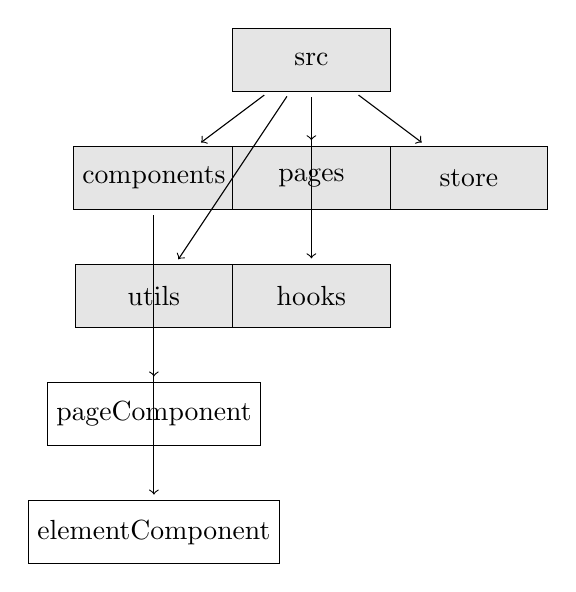
\begin{tikzpicture}[
    file/.style={draw, rectangle, minimum width=2cm, minimum height=0.8cm},
    folder/.style={draw, rectangle, minimum width=2cm, minimum height=0.8cm, fill=gray!20},
    arrow/.style={->, shorten >=2pt, shorten <=2pt}
]

% Folders
\node[folder] (src) at (0,0) {src};
\node[folder] (components) at (-2,-1.5) {components};
\node[folder] (pages) at (0,-1.5) {pages};
\node[folder] (store) at (2,-1.5) {store};
\node[folder] (utils) at (-2,-3) {utils};
\node[folder] (hooks) at (0,-3) {hooks};

% Files
\node[file] (pageComponent) at (-2,-4.5) {pageComponent};
\node[file] (elementComponent) at (-2,-6) {elementComponent};
% ... add more files

% Connections
\draw[arrow] (src) -- (components);
\draw[arrow] (src) -- (pages);
\draw[arrow] (src) -- (store);
\draw[arrow] (src) -- (utils);
\draw[arrow] (src) -- (hooks);
\draw[arrow] (components) -- (pageComponent);
\draw[arrow] (components) -- (elementComponent);
% ... add more connections

\end{tikzpicture}



\pagebreak
\subsubsection{Back-end}
The backend uses the dotNet framework. The development language using the C\# language.

In this project, the backend uses the Onion Architecture.
The Onion Architecture is a typically layered architecture, 
where each layer depends on the inner layer and provides interfaces to the outer layer.
The outer layer provides services to the outermost layer 
and other modules in the same layer based on the interfaces of the inner layer.

From inner to outer, the layers are: Domain, Application, Infrastructure, Presentation.
The Domain layer is the core layer and the innermost layer, used to define domain models, 
which are the business models.
It includes domain models and domain service interfaces.
Domain models are used to define the business models, 
which are the entities in the entity-relationship model and their attributes.
Domain service interfaces are used to define the business services, 
which are the relationships between entities in the entity-relationship model.

The Application layer is the application layer, 
used to define application services, which are the business logic.
It includes domain service implementations and application service interfaces.
Domain service implementations implement the methods of the inner layer's domain service 
interfaces and implement the business logic of the domain models.
Application service interfaces are used to define application services, 
which are the business logic.
It includes but is not limited to database interfaces, testing interfaces, 
HTTP API interfaces, MQTT interfaces, etc.

The Infrastructure layer is the infrastructure layer, used to define infrastructure.
It includes database implementations, testing implementations, 
HTTP API implementations, MQTT implementations, etc.
Database implementations implement the database interfaces 
and provide CRUD services for the database.
Testing implementations implement the testing interfaces 
and provide services for unit testing and integration testing.
HTTP API implementations implement the HTTP API interfaces 
and provide CRUD operations for HTTP APIs.
MQTT implementations implement the MQTT interfaces 
and provide CRUD operations for MQTT.

The Presentation layer is the presentation layer, used to define presentation logic, 
such as interfaces and pages. Since this is a backend project,
data presentation and control are handled by the frontend, 
so this layer is not needed.



\pagebreak
\subsubsection{Data communication and storage}
% 关于本项目的数据通信与数据存储的设计, 包括数据通信的协议, 数据存储的设计等
% 关于数据通信的设计:
% 1. 通信协议的选择
% 自前端向后端发送的数据, 有三种传输的数据类型, 
% 一种是普通的增删改查的请求, 对数据传输的时效性要求不高, 但是对数据的准确性, 完整性, 有序性, 安全性有一定的要求,
% 这种数据的传输, 采用 HTTP 协议, 以及 RESTful API 的设计. 可以有效的保证对数据传输的以上要求.
% 一种是对数据通道的创建和流媒体数据的传输, 对数据传输的时效性, 安全性要求较高, 这种数据的传输, 采用 WebRTC 协议, 以及 MQTT 协议.
% 配合可以快速解码的 flatbuffers 协议, 可以有效的保证对数据传输的以上要求.
% 最后一种是对设备的状态信息和操作信息的传输, 对完整性, 有序性, 安全性都有较高的要求, 这种数据的传输, 采用 MQTT 协议
% 同时也使用了 flatbuffers 协议.
% 
% 2. 数据通信的通信架构和通信流程
% 本项目的数据通信的通信架构, 是基于前后端分离的架构, 前端使用 React 框架, 后端使用 dotnet 框架.
% 当前端需要向后端发送数据的时候, 前端会向后端发送 HTTP 请求, 后端接收到 HTTP 请求之后, 会根据请求的数据类型,
% 选择不同的数据处理方式, 对于普通的增删改查的请求, 后端会根据 RESTful API 的设计, 对数据进行增删改查的操作,
% 对于对数据通道的创建和流媒体数据的传输, 后端会根据 WebRTC 协议, 对数据通道进行创建, 并且帮助前端和设备建立数据通道,
% 当数据通道建立后, 前端和设备之间则使用 flatbuffer 的数据格式对流媒体数据进行传输,
% 对于设备的状态信息和操作信息的传输, 前端会直接向 MQTT broker 发送 MQTT 请求, 
% 设备会在其自身的固件中监听相关的 MQTT 请求, 并且返回相关的数据.
% 
% 3. 数据通信的格式
% 本项目的数据通信的格式, 有三种, 
% 一种是 HTTP 协议, 
% 使用 json 格式对数据进行传输,
% 一种是 WebRTC 协议, 
% 使用 flatbuffers 格式对数据进行传输,
% 一种是 MQTT 协议.
% 使用 flatbuffers 格式对数据进行传输,
% 
% 关于数据存储的设计:
% 1. 数据存储的数据库的选择
% 本项目的数据存储的数据库的选择, 使用了轻量级的数据库 SQLite,
% SQLite 是一个进程内的库, 实现了自给自足的, 无服务器的, 零配置的, 事务性的 SQL 数据库引擎.
% 这是因为整个项目的目的是为了实现前端与设备之间的数据通信, 对于数据库数据的增删改查操作的要求不高,
% 数据量较小, 且对于数据库的数据的事务性要求不高, 所以选择了 SQLite 数据库.
% 2. 项目前后端的数据结构的设计
% 在本项目中, 前端由于使用了 React 框架, 所以前端的数据结构的设计, 使用了基于状态的数据结构的设计,
% 每个组件或者数据集都包含一个状态对象, 这个状态对象的属性就是组件的各个状态. 
% 使用状态对象的原因是, 可以方便的对状态进行管理, 采用对象-属性的形式, 可以方便的针对不同组件的同类状态进行区分,
% 由于跨组件的状态是由 redux 进行管理的, 这种状态对象的设计, 可以更搞笑的对状态进行更新和传递.
% 后端由于使用了 dotnet 框架, 所以后端的数据结构的设计, 使用了基于类的数据结构的设计,
% 采用了面向对象的编程思想, 对数据进行了封装, 使得数据的传输更加的安全, 有序, 完整.


\pagebreak

% \subsection{Domain model}
% \documentclass[]{article}
\usepackage{graphicx}
\usepackage{amsmath}
\usepackage{tikz}

% libaries
\usetikzlibrary{shapes,arrows}

%Define the listing package
\usepackage{listings} %code highlighter
\usepackage{color} %use color
\definecolor{mygreen}{rgb}{0,0.6,0}
\definecolor{mygray}{rgb}{0.5,0.5,0.5}
\definecolor{mymauve}{rgb}{0.58,0,0.82}

%Customize a bit the look
\lstset{ %
backgroundcolor=\color{white}, % choose the background color; you must add \usepackage{color} or \usepackage{xcolor}
basicstyle=\footnotesize, % the size of the fonts that are used for the code
breakatwhitespace=false, % sets if automatic breaks should only happen at whitespace
breaklines=true, % sets automatic line breaking
captionpos=b, % sets the caption-position to bottom
commentstyle=\color{mygreen}, % comment style
deletekeywords={...}, % if you want to delete keywords from the given language
escapeinside={\%*}{*)}, % if you want to add LaTeX within your code
extendedchars=true, % lets you use non-ASCII characters; for 8-bits encodings only, does not work with UTF-8
frame=single, % adds a frame around the code
keepspaces=true, % keeps spaces in text, useful for keeping indentation of code (possibly needs columns=flexible)
keywordstyle=\color{blue}, % keyword style
% language=Octave, % the language of the code
morekeywords={*,...}, % if you want to add more keywords to the set
numbers=left, % where to put the line-numbers; possible values are (none, left, right)
numbersep=5pt, % how far the line-numbers are from the code
numberstyle=\tiny\color{mygray}, % the style that is used for the line-numbers
rulecolor=\color{black}, % if not set, the frame-color may be changed on line-breaks within not-black text (e.g. comments (green here))
showspaces=false, % show spaces everywhere adding particular underscores; it overrides 'showstringspaces'
showstringspaces=false, % underline spaces within strings only
showtabs=false, % show tabs within strings adding particular underscores
stepnumber=1, % the step between two line-numbers. If it's 1, each line will be numbered
stringstyle=\color{mymauve}, % string literal style
tabsize=2, % sets default tabsize to 2 spaces
title=\lstname % show the filename of files included with \lstinputlisting; also try caption instead of title
}

\definecolor{darkgray}{rgb}{.4,.4,.4}
\definecolor{purple}{rgb}{0.65, 0.12, 0.82}

\lstdefinelanguage{React}{
keywords={const, typeof, new, true, false, catch, function, return, null, catch, switch, var, if, in, while, do, else, case, break},
keywordstyle=\color{blue}\bfseries,
ndkeywords={class, export, boolean, throw, implements, import, this},
ndkeywordstyle=\color{darkgray}\bfseries,
identifierstyle=\color{mygreen},
sensitive=false,
comment=[l]{//},
morecomment=[s]{/*}{*/},
commentstyle=\color{purple}\ttfamily,
string=[b]{"}{'}{`},
stringstyle=\color{red}\ttfamily,
morestring=[b]',
morestring=[b]",
morestring=[b]`',
}

\lstdefinelanguage{CSharp}{
keywords={const, typeof, new, true, false, catch, function, return, null, catch, switch, var, if, in, while, do, else, case, break},
keywordstyle=\color{blue}\bfseries,
ndkeywords={class, export, boolean, throw, implements, import, this},
ndkeywordstyle=\color{darkgray}\bfseries,
identifierstyle=\color{mygreen},
sensitive=false,
comment=[l]{//},
morecomment=[s]{/*}{*/},
commentstyle=\color{purple}\ttfamily,
string=[b]{"}{'}{`},
stringstyle=\color{red}\ttfamily,
morestring=[b]',
morestring=[b]",
morestring=[b]`',
}

\lstset{
language=React,
extendedchars=true,
basicstyle=\footnotesize\ttfamily,
showstringspaces=false,
showspaces=false,
numbers=left,
numberstyle=\footnotesize,
numbersep=9pt,
tabsize=2,
breaklines=true,
showtabs=false,
captionpos=b
}

\lstset{
language=CSharp,
extendedchars=true,
basicstyle=\footnotesize\ttfamily,
showstringspaces=false,
showspaces=false,
numbers=left,
numberstyle=\footnotesize,
numbersep=9pt,
tabsize=2,
breaklines=true,
showtabs=false,
captionpos=b
}

% \usepackage{cite} % Add this line for citation

% \bibliographystyle{plain}

\title{
The implementation of BifrostConnect Front-end scope, 
re-design and development with the relevant back-end support develop.
}
\author{
    Fei Gu \\
    Erhvervs Akademi Sydvest \\
    Computer Science 21\\
    }
\date{\today}

\begin{document}

% Front page
\maketitle
\begin{center}
    Supervisor: Henrik Boulund Meng Hansen \\
    Company: BifrostConnect \\
    Engineering Director: Jasper Wass \\
\end{center}
\tableofcontents
\pagebreak


% The introduction
\section{Introduction}
\subsection{Background}\input{sections/introduction/background.tex}
\subsection{The company}\input{sections/introduction/aboutCompany}
\subsection{The project}\input{sections/introduction/aboutProject}
\pagebreak

% The problem statement
\section{Problem Statement}
\subsection{Statement}
\input{sections/problemStatement/statement}
\subsection{Situation}
\input{sections/problemStatement/situation}
\subsection{Potential Solution}
\input{sections/problemStatement/potentialSolution}
\pagebreak

% Requirement analysis
\section{Requirement Analysis}
\input{sections/requirementAnalysis/index}

\subsection{Stakeholders}
\input{sections/requirementAnalysis/stakeholders/index}

\subsection{Business Domain}
\input{sections/requirementAnalysis/bussinesDomain/index}

\subsection{Scope}
\input{sections/requirementAnalysis/scope}

\subsection{Goals}
\input{sections/requirementAnalysis/goals}
\pagebreak

% Software Design
\section{Software Design}
% developement methods
\subsection{Software Development Methods}
\input{sections/softwareDevelopmentMethods/index}
\subsubsection{Agile Software Development}
\input{sections/softwareDevelopmentMethods/agileSoftwareDevelopment/index}
\subsubsection{Feature Driven Development}
\input{sections/softwareDevelopmentMethods/featureDrivenDevelopment/index}

\pagebreak

% Technology seslection
\subsection{Technology selection}
\input{sections/softwareDesign/technologySelection/index}
\subsubsection{Front-end}
\input{sections/softwareDesign/technologySelection/frontEnd}            
\subsubsection{Back-end}
\input{sections/softwareDesign/technologySelection/backEnd}            
\subsubsection{Database}
\input{sections/softwareDesign/technologySelection/database}
\subsubsection{Data communication}
\input{sections/softwareDesign/technologySelection/dataCommunication}            
\subsubsection{DevOps}
\input{sections/softwareDesign/technologySelection/devOps}
\pagebreak

% Architecture design
\subsection{Architecture design}
\input{sections/softwareDesign/architectureDesign/index}
\pagebreak
\subsubsection{Front-end}
\input{sections/softwareDesign/architectureDesign/frontEndArchitecture}
\pagebreak
\subsubsection{Back-end}
\input{sections/softwareDesign/architectureDesign/backEndArchitecture}
\pagebreak
\subsubsection{Data communication and storage}
\input{sections/softwareDesign/architectureDesign/dataCommunicationArchitecture}
\pagebreak

% \subsection{Domain model}
% \input{sections/softwareDesign/domainModel/index}
% \subsection{Database design}
% % 数据库领域模型 ER 图
% % 包括表和字段的设置.
% % 对于私有键和外键的设置.

% \subsection{Back-end design}
% % 后端对象模型
% % 以及对于对象模型的增删改查
% % 以及相关的其他服务的设计`'

% \subsection{Front-end design}
% % 对于前端的页面结构的设计 
% % 页面的状态的设计, 交互设计

% \subsection{FlatBuffers design}
% % schema 的设计

\subsection{DevOps CI/CD process design}
\input{sections/softwareDesign/devOpsDesign/index}
\subsubsection{Continuous Integration}
\input{sections/softwareDesign/devOpsDesign/continuousIntegration/index}
\subsubsection{Continuous Delivery}
\input{sections/softwareDesign/devOpsDesign/continuousDelivery/index}
\subsubsection{Continuous Deployment}
\input{sections/softwareDesign/devOpsDesign/continuousDeployment/index}
\pagebreak

\section{Software Development} 
\input{sections/softwareDevelopment/index}
\subsection{Overall development}
\input{sections/softwareDevelopment/overallDevelopement/index}
\subsubsection{Front-end}
\input{sections/softwareDevelopment/overallDevelopement/frontEnd/index}
\subsubsection{Back-end}
\input{sections/softwareDevelopment/overallDevelopement/backEnd/index}
\subsubsection{DevOps}
\input{sections/softwareDevelopment/overallDevelopement/devOps/index}
\subsection{Feature development} 
\input{sections/softwareDevelopment/featureDevelopment/index}
\subsubsection{Use Case 1}
\input{sections/softwareDevelopment/featureDevelopment/useCase1/index}
\subsubsection{Feature 1}
\input{sections/softwareDevelopment/featureDevelopment/feature/feature1.tex}
\pagebreak
\section{Conclusion} 
\subsection{Result}
Since the project is still in progress, the result is not available yet.
So far, basic structure of this project has been built. But the most features 
are not implemented yet. 
\subsection{Discussion}
As a single developer for this project, I am confident what I have done so far.
And I can say I understand the most of the knowledge I have used in this project, 
which also means I can explain all the part of the project. 
But this project also relevant some of the complex knowledge which I have to continue 
to study and practice.
\subsection{Future Work}
The future work is to implement the rest of the features. 
Including the most important part which is the 'create session' feature.
\pagebreak
% \bibliography{bibliography}
\pagebreak
% \begin{appendices}
%     \section{Appendix}
% \end{appendices} 
\end{document}
% \subsection{Database design}
% % 数据库领域模型 ER 图
% % 包括表和字段的设置.
% % 对于私有键和外键的设置.

% \subsection{Back-end design}
% % 后端对象模型
% % 以及对于对象模型的增删改查
% % 以及相关的其他服务的设计`'

% \subsection{Front-end design}
% % 对于前端的页面结构的设计 
% % 页面的状态的设计, 交互设计

% \subsection{FlatBuffers design}
% % schema 的设计

\subsection{DevOps CI/CD process design}
\documentclass[]{article}
\usepackage{graphicx}
\usepackage{amsmath}
\usepackage{tikz}

% libaries
\usetikzlibrary{shapes,arrows}

%Define the listing package
\usepackage{listings} %code highlighter
\usepackage{color} %use color
\definecolor{mygreen}{rgb}{0,0.6,0}
\definecolor{mygray}{rgb}{0.5,0.5,0.5}
\definecolor{mymauve}{rgb}{0.58,0,0.82}

%Customize a bit the look
\lstset{ %
backgroundcolor=\color{white}, % choose the background color; you must add \usepackage{color} or \usepackage{xcolor}
basicstyle=\footnotesize, % the size of the fonts that are used for the code
breakatwhitespace=false, % sets if automatic breaks should only happen at whitespace
breaklines=true, % sets automatic line breaking
captionpos=b, % sets the caption-position to bottom
commentstyle=\color{mygreen}, % comment style
deletekeywords={...}, % if you want to delete keywords from the given language
escapeinside={\%*}{*)}, % if you want to add LaTeX within your code
extendedchars=true, % lets you use non-ASCII characters; for 8-bits encodings only, does not work with UTF-8
frame=single, % adds a frame around the code
keepspaces=true, % keeps spaces in text, useful for keeping indentation of code (possibly needs columns=flexible)
keywordstyle=\color{blue}, % keyword style
% language=Octave, % the language of the code
morekeywords={*,...}, % if you want to add more keywords to the set
numbers=left, % where to put the line-numbers; possible values are (none, left, right)
numbersep=5pt, % how far the line-numbers are from the code
numberstyle=\tiny\color{mygray}, % the style that is used for the line-numbers
rulecolor=\color{black}, % if not set, the frame-color may be changed on line-breaks within not-black text (e.g. comments (green here))
showspaces=false, % show spaces everywhere adding particular underscores; it overrides 'showstringspaces'
showstringspaces=false, % underline spaces within strings only
showtabs=false, % show tabs within strings adding particular underscores
stepnumber=1, % the step between two line-numbers. If it's 1, each line will be numbered
stringstyle=\color{mymauve}, % string literal style
tabsize=2, % sets default tabsize to 2 spaces
title=\lstname % show the filename of files included with \lstinputlisting; also try caption instead of title
}

\definecolor{darkgray}{rgb}{.4,.4,.4}
\definecolor{purple}{rgb}{0.65, 0.12, 0.82}

\lstdefinelanguage{React}{
keywords={const, typeof, new, true, false, catch, function, return, null, catch, switch, var, if, in, while, do, else, case, break},
keywordstyle=\color{blue}\bfseries,
ndkeywords={class, export, boolean, throw, implements, import, this},
ndkeywordstyle=\color{darkgray}\bfseries,
identifierstyle=\color{mygreen},
sensitive=false,
comment=[l]{//},
morecomment=[s]{/*}{*/},
commentstyle=\color{purple}\ttfamily,
string=[b]{"}{'}{`},
stringstyle=\color{red}\ttfamily,
morestring=[b]',
morestring=[b]",
morestring=[b]`',
}

\lstdefinelanguage{CSharp}{
keywords={const, typeof, new, true, false, catch, function, return, null, catch, switch, var, if, in, while, do, else, case, break},
keywordstyle=\color{blue}\bfseries,
ndkeywords={class, export, boolean, throw, implements, import, this},
ndkeywordstyle=\color{darkgray}\bfseries,
identifierstyle=\color{mygreen},
sensitive=false,
comment=[l]{//},
morecomment=[s]{/*}{*/},
commentstyle=\color{purple}\ttfamily,
string=[b]{"}{'}{`},
stringstyle=\color{red}\ttfamily,
morestring=[b]',
morestring=[b]",
morestring=[b]`',
}

\lstset{
language=React,
extendedchars=true,
basicstyle=\footnotesize\ttfamily,
showstringspaces=false,
showspaces=false,
numbers=left,
numberstyle=\footnotesize,
numbersep=9pt,
tabsize=2,
breaklines=true,
showtabs=false,
captionpos=b
}

\lstset{
language=CSharp,
extendedchars=true,
basicstyle=\footnotesize\ttfamily,
showstringspaces=false,
showspaces=false,
numbers=left,
numberstyle=\footnotesize,
numbersep=9pt,
tabsize=2,
breaklines=true,
showtabs=false,
captionpos=b
}

% \usepackage{cite} % Add this line for citation

% \bibliographystyle{plain}

\title{
The implementation of BifrostConnect Front-end scope, 
re-design and development with the relevant back-end support develop.
}
\author{
    Fei Gu \\
    Erhvervs Akademi Sydvest \\
    Computer Science 21\\
    }
\date{\today}

\begin{document}

% Front page
\maketitle
\begin{center}
    Supervisor: Henrik Boulund Meng Hansen \\
    Company: BifrostConnect \\
    Engineering Director: Jasper Wass \\
\end{center}
\tableofcontents
\pagebreak


% The introduction
\section{Introduction}
\subsection{Background}\input{sections/introduction/background.tex}
\subsection{The company}\input{sections/introduction/aboutCompany}
\subsection{The project}\input{sections/introduction/aboutProject}
\pagebreak

% The problem statement
\section{Problem Statement}
\subsection{Statement}
\input{sections/problemStatement/statement}
\subsection{Situation}
\input{sections/problemStatement/situation}
\subsection{Potential Solution}
\input{sections/problemStatement/potentialSolution}
\pagebreak

% Requirement analysis
\section{Requirement Analysis}
\input{sections/requirementAnalysis/index}

\subsection{Stakeholders}
\input{sections/requirementAnalysis/stakeholders/index}

\subsection{Business Domain}
\input{sections/requirementAnalysis/bussinesDomain/index}

\subsection{Scope}
\input{sections/requirementAnalysis/scope}

\subsection{Goals}
\input{sections/requirementAnalysis/goals}
\pagebreak

% Software Design
\section{Software Design}
% developement methods
\subsection{Software Development Methods}
\input{sections/softwareDevelopmentMethods/index}
\subsubsection{Agile Software Development}
\input{sections/softwareDevelopmentMethods/agileSoftwareDevelopment/index}
\subsubsection{Feature Driven Development}
\input{sections/softwareDevelopmentMethods/featureDrivenDevelopment/index}

\pagebreak

% Technology seslection
\subsection{Technology selection}
\input{sections/softwareDesign/technologySelection/index}
\subsubsection{Front-end}
\input{sections/softwareDesign/technologySelection/frontEnd}            
\subsubsection{Back-end}
\input{sections/softwareDesign/technologySelection/backEnd}            
\subsubsection{Database}
\input{sections/softwareDesign/technologySelection/database}
\subsubsection{Data communication}
\input{sections/softwareDesign/technologySelection/dataCommunication}            
\subsubsection{DevOps}
\input{sections/softwareDesign/technologySelection/devOps}
\pagebreak

% Architecture design
\subsection{Architecture design}
\input{sections/softwareDesign/architectureDesign/index}
\pagebreak
\subsubsection{Front-end}
\input{sections/softwareDesign/architectureDesign/frontEndArchitecture}
\pagebreak
\subsubsection{Back-end}
\input{sections/softwareDesign/architectureDesign/backEndArchitecture}
\pagebreak
\subsubsection{Data communication and storage}
\input{sections/softwareDesign/architectureDesign/dataCommunicationArchitecture}
\pagebreak

% \subsection{Domain model}
% \input{sections/softwareDesign/domainModel/index}
% \subsection{Database design}
% % 数据库领域模型 ER 图
% % 包括表和字段的设置.
% % 对于私有键和外键的设置.

% \subsection{Back-end design}
% % 后端对象模型
% % 以及对于对象模型的增删改查
% % 以及相关的其他服务的设计`'

% \subsection{Front-end design}
% % 对于前端的页面结构的设计 
% % 页面的状态的设计, 交互设计

% \subsection{FlatBuffers design}
% % schema 的设计

\subsection{DevOps CI/CD process design}
\input{sections/softwareDesign/devOpsDesign/index}
\subsubsection{Continuous Integration}
\input{sections/softwareDesign/devOpsDesign/continuousIntegration/index}
\subsubsection{Continuous Delivery}
\input{sections/softwareDesign/devOpsDesign/continuousDelivery/index}
\subsubsection{Continuous Deployment}
\input{sections/softwareDesign/devOpsDesign/continuousDeployment/index}
\pagebreak

\section{Software Development} 
\input{sections/softwareDevelopment/index}
\subsection{Overall development}
\input{sections/softwareDevelopment/overallDevelopement/index}
\subsubsection{Front-end}
\input{sections/softwareDevelopment/overallDevelopement/frontEnd/index}
\subsubsection{Back-end}
\input{sections/softwareDevelopment/overallDevelopement/backEnd/index}
\subsubsection{DevOps}
\input{sections/softwareDevelopment/overallDevelopement/devOps/index}
\subsection{Feature development} 
\input{sections/softwareDevelopment/featureDevelopment/index}
\subsubsection{Use Case 1}
\input{sections/softwareDevelopment/featureDevelopment/useCase1/index}
\subsubsection{Feature 1}
\input{sections/softwareDevelopment/featureDevelopment/feature/feature1.tex}
\pagebreak
\section{Conclusion} 
\subsection{Result}
Since the project is still in progress, the result is not available yet.
So far, basic structure of this project has been built. But the most features 
are not implemented yet. 
\subsection{Discussion}
As a single developer for this project, I am confident what I have done so far.
And I can say I understand the most of the knowledge I have used in this project, 
which also means I can explain all the part of the project. 
But this project also relevant some of the complex knowledge which I have to continue 
to study and practice.
\subsection{Future Work}
The future work is to implement the rest of the features. 
Including the most important part which is the 'create session' feature.
\pagebreak
% \bibliography{bibliography}
\pagebreak
% \begin{appendices}
%     \section{Appendix}
% \end{appendices} 
\end{document}
\subsubsection{Continuous Integration}
\documentclass[]{article}
\usepackage{graphicx}
\usepackage{amsmath}
\usepackage{tikz}

% libaries
\usetikzlibrary{shapes,arrows}

%Define the listing package
\usepackage{listings} %code highlighter
\usepackage{color} %use color
\definecolor{mygreen}{rgb}{0,0.6,0}
\definecolor{mygray}{rgb}{0.5,0.5,0.5}
\definecolor{mymauve}{rgb}{0.58,0,0.82}

%Customize a bit the look
\lstset{ %
backgroundcolor=\color{white}, % choose the background color; you must add \usepackage{color} or \usepackage{xcolor}
basicstyle=\footnotesize, % the size of the fonts that are used for the code
breakatwhitespace=false, % sets if automatic breaks should only happen at whitespace
breaklines=true, % sets automatic line breaking
captionpos=b, % sets the caption-position to bottom
commentstyle=\color{mygreen}, % comment style
deletekeywords={...}, % if you want to delete keywords from the given language
escapeinside={\%*}{*)}, % if you want to add LaTeX within your code
extendedchars=true, % lets you use non-ASCII characters; for 8-bits encodings only, does not work with UTF-8
frame=single, % adds a frame around the code
keepspaces=true, % keeps spaces in text, useful for keeping indentation of code (possibly needs columns=flexible)
keywordstyle=\color{blue}, % keyword style
% language=Octave, % the language of the code
morekeywords={*,...}, % if you want to add more keywords to the set
numbers=left, % where to put the line-numbers; possible values are (none, left, right)
numbersep=5pt, % how far the line-numbers are from the code
numberstyle=\tiny\color{mygray}, % the style that is used for the line-numbers
rulecolor=\color{black}, % if not set, the frame-color may be changed on line-breaks within not-black text (e.g. comments (green here))
showspaces=false, % show spaces everywhere adding particular underscores; it overrides 'showstringspaces'
showstringspaces=false, % underline spaces within strings only
showtabs=false, % show tabs within strings adding particular underscores
stepnumber=1, % the step between two line-numbers. If it's 1, each line will be numbered
stringstyle=\color{mymauve}, % string literal style
tabsize=2, % sets default tabsize to 2 spaces
title=\lstname % show the filename of files included with \lstinputlisting; also try caption instead of title
}

\definecolor{darkgray}{rgb}{.4,.4,.4}
\definecolor{purple}{rgb}{0.65, 0.12, 0.82}

\lstdefinelanguage{React}{
keywords={const, typeof, new, true, false, catch, function, return, null, catch, switch, var, if, in, while, do, else, case, break},
keywordstyle=\color{blue}\bfseries,
ndkeywords={class, export, boolean, throw, implements, import, this},
ndkeywordstyle=\color{darkgray}\bfseries,
identifierstyle=\color{mygreen},
sensitive=false,
comment=[l]{//},
morecomment=[s]{/*}{*/},
commentstyle=\color{purple}\ttfamily,
string=[b]{"}{'}{`},
stringstyle=\color{red}\ttfamily,
morestring=[b]',
morestring=[b]",
morestring=[b]`',
}

\lstdefinelanguage{CSharp}{
keywords={const, typeof, new, true, false, catch, function, return, null, catch, switch, var, if, in, while, do, else, case, break},
keywordstyle=\color{blue}\bfseries,
ndkeywords={class, export, boolean, throw, implements, import, this},
ndkeywordstyle=\color{darkgray}\bfseries,
identifierstyle=\color{mygreen},
sensitive=false,
comment=[l]{//},
morecomment=[s]{/*}{*/},
commentstyle=\color{purple}\ttfamily,
string=[b]{"}{'}{`},
stringstyle=\color{red}\ttfamily,
morestring=[b]',
morestring=[b]",
morestring=[b]`',
}

\lstset{
language=React,
extendedchars=true,
basicstyle=\footnotesize\ttfamily,
showstringspaces=false,
showspaces=false,
numbers=left,
numberstyle=\footnotesize,
numbersep=9pt,
tabsize=2,
breaklines=true,
showtabs=false,
captionpos=b
}

\lstset{
language=CSharp,
extendedchars=true,
basicstyle=\footnotesize\ttfamily,
showstringspaces=false,
showspaces=false,
numbers=left,
numberstyle=\footnotesize,
numbersep=9pt,
tabsize=2,
breaklines=true,
showtabs=false,
captionpos=b
}

% \usepackage{cite} % Add this line for citation

% \bibliographystyle{plain}

\title{
The implementation of BifrostConnect Front-end scope, 
re-design and development with the relevant back-end support develop.
}
\author{
    Fei Gu \\
    Erhvervs Akademi Sydvest \\
    Computer Science 21\\
    }
\date{\today}

\begin{document}

% Front page
\maketitle
\begin{center}
    Supervisor: Henrik Boulund Meng Hansen \\
    Company: BifrostConnect \\
    Engineering Director: Jasper Wass \\
\end{center}
\tableofcontents
\pagebreak


% The introduction
\section{Introduction}
\subsection{Background}\input{sections/introduction/background.tex}
\subsection{The company}\input{sections/introduction/aboutCompany}
\subsection{The project}\input{sections/introduction/aboutProject}
\pagebreak

% The problem statement
\section{Problem Statement}
\subsection{Statement}
\input{sections/problemStatement/statement}
\subsection{Situation}
\input{sections/problemStatement/situation}
\subsection{Potential Solution}
\input{sections/problemStatement/potentialSolution}
\pagebreak

% Requirement analysis
\section{Requirement Analysis}
\input{sections/requirementAnalysis/index}

\subsection{Stakeholders}
\input{sections/requirementAnalysis/stakeholders/index}

\subsection{Business Domain}
\input{sections/requirementAnalysis/bussinesDomain/index}

\subsection{Scope}
\input{sections/requirementAnalysis/scope}

\subsection{Goals}
\input{sections/requirementAnalysis/goals}
\pagebreak

% Software Design
\section{Software Design}
% developement methods
\subsection{Software Development Methods}
\input{sections/softwareDevelopmentMethods/index}
\subsubsection{Agile Software Development}
\input{sections/softwareDevelopmentMethods/agileSoftwareDevelopment/index}
\subsubsection{Feature Driven Development}
\input{sections/softwareDevelopmentMethods/featureDrivenDevelopment/index}

\pagebreak

% Technology seslection
\subsection{Technology selection}
\input{sections/softwareDesign/technologySelection/index}
\subsubsection{Front-end}
\input{sections/softwareDesign/technologySelection/frontEnd}            
\subsubsection{Back-end}
\input{sections/softwareDesign/technologySelection/backEnd}            
\subsubsection{Database}
\input{sections/softwareDesign/technologySelection/database}
\subsubsection{Data communication}
\input{sections/softwareDesign/technologySelection/dataCommunication}            
\subsubsection{DevOps}
\input{sections/softwareDesign/technologySelection/devOps}
\pagebreak

% Architecture design
\subsection{Architecture design}
\input{sections/softwareDesign/architectureDesign/index}
\pagebreak
\subsubsection{Front-end}
\input{sections/softwareDesign/architectureDesign/frontEndArchitecture}
\pagebreak
\subsubsection{Back-end}
\input{sections/softwareDesign/architectureDesign/backEndArchitecture}
\pagebreak
\subsubsection{Data communication and storage}
\input{sections/softwareDesign/architectureDesign/dataCommunicationArchitecture}
\pagebreak

% \subsection{Domain model}
% \input{sections/softwareDesign/domainModel/index}
% \subsection{Database design}
% % 数据库领域模型 ER 图
% % 包括表和字段的设置.
% % 对于私有键和外键的设置.

% \subsection{Back-end design}
% % 后端对象模型
% % 以及对于对象模型的增删改查
% % 以及相关的其他服务的设计`'

% \subsection{Front-end design}
% % 对于前端的页面结构的设计 
% % 页面的状态的设计, 交互设计

% \subsection{FlatBuffers design}
% % schema 的设计

\subsection{DevOps CI/CD process design}
\input{sections/softwareDesign/devOpsDesign/index}
\subsubsection{Continuous Integration}
\input{sections/softwareDesign/devOpsDesign/continuousIntegration/index}
\subsubsection{Continuous Delivery}
\input{sections/softwareDesign/devOpsDesign/continuousDelivery/index}
\subsubsection{Continuous Deployment}
\input{sections/softwareDesign/devOpsDesign/continuousDeployment/index}
\pagebreak

\section{Software Development} 
\input{sections/softwareDevelopment/index}
\subsection{Overall development}
\input{sections/softwareDevelopment/overallDevelopement/index}
\subsubsection{Front-end}
\input{sections/softwareDevelopment/overallDevelopement/frontEnd/index}
\subsubsection{Back-end}
\input{sections/softwareDevelopment/overallDevelopement/backEnd/index}
\subsubsection{DevOps}
\input{sections/softwareDevelopment/overallDevelopement/devOps/index}
\subsection{Feature development} 
\input{sections/softwareDevelopment/featureDevelopment/index}
\subsubsection{Use Case 1}
\input{sections/softwareDevelopment/featureDevelopment/useCase1/index}
\subsubsection{Feature 1}
\input{sections/softwareDevelopment/featureDevelopment/feature/feature1.tex}
\pagebreak
\section{Conclusion} 
\subsection{Result}
Since the project is still in progress, the result is not available yet.
So far, basic structure of this project has been built. But the most features 
are not implemented yet. 
\subsection{Discussion}
As a single developer for this project, I am confident what I have done so far.
And I can say I understand the most of the knowledge I have used in this project, 
which also means I can explain all the part of the project. 
But this project also relevant some of the complex knowledge which I have to continue 
to study and practice.
\subsection{Future Work}
The future work is to implement the rest of the features. 
Including the most important part which is the 'create session' feature.
\pagebreak
% \bibliography{bibliography}
\pagebreak
% \begin{appendices}
%     \section{Appendix}
% \end{appendices} 
\end{document}
\subsubsection{Continuous Delivery}
\documentclass[]{article}
\usepackage{graphicx}
\usepackage{amsmath}
\usepackage{tikz}

% libaries
\usetikzlibrary{shapes,arrows}

%Define the listing package
\usepackage{listings} %code highlighter
\usepackage{color} %use color
\definecolor{mygreen}{rgb}{0,0.6,0}
\definecolor{mygray}{rgb}{0.5,0.5,0.5}
\definecolor{mymauve}{rgb}{0.58,0,0.82}

%Customize a bit the look
\lstset{ %
backgroundcolor=\color{white}, % choose the background color; you must add \usepackage{color} or \usepackage{xcolor}
basicstyle=\footnotesize, % the size of the fonts that are used for the code
breakatwhitespace=false, % sets if automatic breaks should only happen at whitespace
breaklines=true, % sets automatic line breaking
captionpos=b, % sets the caption-position to bottom
commentstyle=\color{mygreen}, % comment style
deletekeywords={...}, % if you want to delete keywords from the given language
escapeinside={\%*}{*)}, % if you want to add LaTeX within your code
extendedchars=true, % lets you use non-ASCII characters; for 8-bits encodings only, does not work with UTF-8
frame=single, % adds a frame around the code
keepspaces=true, % keeps spaces in text, useful for keeping indentation of code (possibly needs columns=flexible)
keywordstyle=\color{blue}, % keyword style
% language=Octave, % the language of the code
morekeywords={*,...}, % if you want to add more keywords to the set
numbers=left, % where to put the line-numbers; possible values are (none, left, right)
numbersep=5pt, % how far the line-numbers are from the code
numberstyle=\tiny\color{mygray}, % the style that is used for the line-numbers
rulecolor=\color{black}, % if not set, the frame-color may be changed on line-breaks within not-black text (e.g. comments (green here))
showspaces=false, % show spaces everywhere adding particular underscores; it overrides 'showstringspaces'
showstringspaces=false, % underline spaces within strings only
showtabs=false, % show tabs within strings adding particular underscores
stepnumber=1, % the step between two line-numbers. If it's 1, each line will be numbered
stringstyle=\color{mymauve}, % string literal style
tabsize=2, % sets default tabsize to 2 spaces
title=\lstname % show the filename of files included with \lstinputlisting; also try caption instead of title
}

\definecolor{darkgray}{rgb}{.4,.4,.4}
\definecolor{purple}{rgb}{0.65, 0.12, 0.82}

\lstdefinelanguage{React}{
keywords={const, typeof, new, true, false, catch, function, return, null, catch, switch, var, if, in, while, do, else, case, break},
keywordstyle=\color{blue}\bfseries,
ndkeywords={class, export, boolean, throw, implements, import, this},
ndkeywordstyle=\color{darkgray}\bfseries,
identifierstyle=\color{mygreen},
sensitive=false,
comment=[l]{//},
morecomment=[s]{/*}{*/},
commentstyle=\color{purple}\ttfamily,
string=[b]{"}{'}{`},
stringstyle=\color{red}\ttfamily,
morestring=[b]',
morestring=[b]",
morestring=[b]`',
}

\lstdefinelanguage{CSharp}{
keywords={const, typeof, new, true, false, catch, function, return, null, catch, switch, var, if, in, while, do, else, case, break},
keywordstyle=\color{blue}\bfseries,
ndkeywords={class, export, boolean, throw, implements, import, this},
ndkeywordstyle=\color{darkgray}\bfseries,
identifierstyle=\color{mygreen},
sensitive=false,
comment=[l]{//},
morecomment=[s]{/*}{*/},
commentstyle=\color{purple}\ttfamily,
string=[b]{"}{'}{`},
stringstyle=\color{red}\ttfamily,
morestring=[b]',
morestring=[b]",
morestring=[b]`',
}

\lstset{
language=React,
extendedchars=true,
basicstyle=\footnotesize\ttfamily,
showstringspaces=false,
showspaces=false,
numbers=left,
numberstyle=\footnotesize,
numbersep=9pt,
tabsize=2,
breaklines=true,
showtabs=false,
captionpos=b
}

\lstset{
language=CSharp,
extendedchars=true,
basicstyle=\footnotesize\ttfamily,
showstringspaces=false,
showspaces=false,
numbers=left,
numberstyle=\footnotesize,
numbersep=9pt,
tabsize=2,
breaklines=true,
showtabs=false,
captionpos=b
}

% \usepackage{cite} % Add this line for citation

% \bibliographystyle{plain}

\title{
The implementation of BifrostConnect Front-end scope, 
re-design and development with the relevant back-end support develop.
}
\author{
    Fei Gu \\
    Erhvervs Akademi Sydvest \\
    Computer Science 21\\
    }
\date{\today}

\begin{document}

% Front page
\maketitle
\begin{center}
    Supervisor: Henrik Boulund Meng Hansen \\
    Company: BifrostConnect \\
    Engineering Director: Jasper Wass \\
\end{center}
\tableofcontents
\pagebreak


% The introduction
\section{Introduction}
\subsection{Background}\input{sections/introduction/background.tex}
\subsection{The company}\input{sections/introduction/aboutCompany}
\subsection{The project}\input{sections/introduction/aboutProject}
\pagebreak

% The problem statement
\section{Problem Statement}
\subsection{Statement}
\input{sections/problemStatement/statement}
\subsection{Situation}
\input{sections/problemStatement/situation}
\subsection{Potential Solution}
\input{sections/problemStatement/potentialSolution}
\pagebreak

% Requirement analysis
\section{Requirement Analysis}
\input{sections/requirementAnalysis/index}

\subsection{Stakeholders}
\input{sections/requirementAnalysis/stakeholders/index}

\subsection{Business Domain}
\input{sections/requirementAnalysis/bussinesDomain/index}

\subsection{Scope}
\input{sections/requirementAnalysis/scope}

\subsection{Goals}
\input{sections/requirementAnalysis/goals}
\pagebreak

% Software Design
\section{Software Design}
% developement methods
\subsection{Software Development Methods}
\input{sections/softwareDevelopmentMethods/index}
\subsubsection{Agile Software Development}
\input{sections/softwareDevelopmentMethods/agileSoftwareDevelopment/index}
\subsubsection{Feature Driven Development}
\input{sections/softwareDevelopmentMethods/featureDrivenDevelopment/index}

\pagebreak

% Technology seslection
\subsection{Technology selection}
\input{sections/softwareDesign/technologySelection/index}
\subsubsection{Front-end}
\input{sections/softwareDesign/technologySelection/frontEnd}            
\subsubsection{Back-end}
\input{sections/softwareDesign/technologySelection/backEnd}            
\subsubsection{Database}
\input{sections/softwareDesign/technologySelection/database}
\subsubsection{Data communication}
\input{sections/softwareDesign/technologySelection/dataCommunication}            
\subsubsection{DevOps}
\input{sections/softwareDesign/technologySelection/devOps}
\pagebreak

% Architecture design
\subsection{Architecture design}
\input{sections/softwareDesign/architectureDesign/index}
\pagebreak
\subsubsection{Front-end}
\input{sections/softwareDesign/architectureDesign/frontEndArchitecture}
\pagebreak
\subsubsection{Back-end}
\input{sections/softwareDesign/architectureDesign/backEndArchitecture}
\pagebreak
\subsubsection{Data communication and storage}
\input{sections/softwareDesign/architectureDesign/dataCommunicationArchitecture}
\pagebreak

% \subsection{Domain model}
% \input{sections/softwareDesign/domainModel/index}
% \subsection{Database design}
% % 数据库领域模型 ER 图
% % 包括表和字段的设置.
% % 对于私有键和外键的设置.

% \subsection{Back-end design}
% % 后端对象模型
% % 以及对于对象模型的增删改查
% % 以及相关的其他服务的设计`'

% \subsection{Front-end design}
% % 对于前端的页面结构的设计 
% % 页面的状态的设计, 交互设计

% \subsection{FlatBuffers design}
% % schema 的设计

\subsection{DevOps CI/CD process design}
\input{sections/softwareDesign/devOpsDesign/index}
\subsubsection{Continuous Integration}
\input{sections/softwareDesign/devOpsDesign/continuousIntegration/index}
\subsubsection{Continuous Delivery}
\input{sections/softwareDesign/devOpsDesign/continuousDelivery/index}
\subsubsection{Continuous Deployment}
\input{sections/softwareDesign/devOpsDesign/continuousDeployment/index}
\pagebreak

\section{Software Development} 
\input{sections/softwareDevelopment/index}
\subsection{Overall development}
\input{sections/softwareDevelopment/overallDevelopement/index}
\subsubsection{Front-end}
\input{sections/softwareDevelopment/overallDevelopement/frontEnd/index}
\subsubsection{Back-end}
\input{sections/softwareDevelopment/overallDevelopement/backEnd/index}
\subsubsection{DevOps}
\input{sections/softwareDevelopment/overallDevelopement/devOps/index}
\subsection{Feature development} 
\input{sections/softwareDevelopment/featureDevelopment/index}
\subsubsection{Use Case 1}
\input{sections/softwareDevelopment/featureDevelopment/useCase1/index}
\subsubsection{Feature 1}
\input{sections/softwareDevelopment/featureDevelopment/feature/feature1.tex}
\pagebreak
\section{Conclusion} 
\subsection{Result}
Since the project is still in progress, the result is not available yet.
So far, basic structure of this project has been built. But the most features 
are not implemented yet. 
\subsection{Discussion}
As a single developer for this project, I am confident what I have done so far.
And I can say I understand the most of the knowledge I have used in this project, 
which also means I can explain all the part of the project. 
But this project also relevant some of the complex knowledge which I have to continue 
to study and practice.
\subsection{Future Work}
The future work is to implement the rest of the features. 
Including the most important part which is the 'create session' feature.
\pagebreak
% \bibliography{bibliography}
\pagebreak
% \begin{appendices}
%     \section{Appendix}
% \end{appendices} 
\end{document}
\subsubsection{Continuous Deployment}
\documentclass[]{article}
\usepackage{graphicx}
\usepackage{amsmath}
\usepackage{tikz}

% libaries
\usetikzlibrary{shapes,arrows}

%Define the listing package
\usepackage{listings} %code highlighter
\usepackage{color} %use color
\definecolor{mygreen}{rgb}{0,0.6,0}
\definecolor{mygray}{rgb}{0.5,0.5,0.5}
\definecolor{mymauve}{rgb}{0.58,0,0.82}

%Customize a bit the look
\lstset{ %
backgroundcolor=\color{white}, % choose the background color; you must add \usepackage{color} or \usepackage{xcolor}
basicstyle=\footnotesize, % the size of the fonts that are used for the code
breakatwhitespace=false, % sets if automatic breaks should only happen at whitespace
breaklines=true, % sets automatic line breaking
captionpos=b, % sets the caption-position to bottom
commentstyle=\color{mygreen}, % comment style
deletekeywords={...}, % if you want to delete keywords from the given language
escapeinside={\%*}{*)}, % if you want to add LaTeX within your code
extendedchars=true, % lets you use non-ASCII characters; for 8-bits encodings only, does not work with UTF-8
frame=single, % adds a frame around the code
keepspaces=true, % keeps spaces in text, useful for keeping indentation of code (possibly needs columns=flexible)
keywordstyle=\color{blue}, % keyword style
% language=Octave, % the language of the code
morekeywords={*,...}, % if you want to add more keywords to the set
numbers=left, % where to put the line-numbers; possible values are (none, left, right)
numbersep=5pt, % how far the line-numbers are from the code
numberstyle=\tiny\color{mygray}, % the style that is used for the line-numbers
rulecolor=\color{black}, % if not set, the frame-color may be changed on line-breaks within not-black text (e.g. comments (green here))
showspaces=false, % show spaces everywhere adding particular underscores; it overrides 'showstringspaces'
showstringspaces=false, % underline spaces within strings only
showtabs=false, % show tabs within strings adding particular underscores
stepnumber=1, % the step between two line-numbers. If it's 1, each line will be numbered
stringstyle=\color{mymauve}, % string literal style
tabsize=2, % sets default tabsize to 2 spaces
title=\lstname % show the filename of files included with \lstinputlisting; also try caption instead of title
}

\definecolor{darkgray}{rgb}{.4,.4,.4}
\definecolor{purple}{rgb}{0.65, 0.12, 0.82}

\lstdefinelanguage{React}{
keywords={const, typeof, new, true, false, catch, function, return, null, catch, switch, var, if, in, while, do, else, case, break},
keywordstyle=\color{blue}\bfseries,
ndkeywords={class, export, boolean, throw, implements, import, this},
ndkeywordstyle=\color{darkgray}\bfseries,
identifierstyle=\color{mygreen},
sensitive=false,
comment=[l]{//},
morecomment=[s]{/*}{*/},
commentstyle=\color{purple}\ttfamily,
string=[b]{"}{'}{`},
stringstyle=\color{red}\ttfamily,
morestring=[b]',
morestring=[b]",
morestring=[b]`',
}

\lstdefinelanguage{CSharp}{
keywords={const, typeof, new, true, false, catch, function, return, null, catch, switch, var, if, in, while, do, else, case, break},
keywordstyle=\color{blue}\bfseries,
ndkeywords={class, export, boolean, throw, implements, import, this},
ndkeywordstyle=\color{darkgray}\bfseries,
identifierstyle=\color{mygreen},
sensitive=false,
comment=[l]{//},
morecomment=[s]{/*}{*/},
commentstyle=\color{purple}\ttfamily,
string=[b]{"}{'}{`},
stringstyle=\color{red}\ttfamily,
morestring=[b]',
morestring=[b]",
morestring=[b]`',
}

\lstset{
language=React,
extendedchars=true,
basicstyle=\footnotesize\ttfamily,
showstringspaces=false,
showspaces=false,
numbers=left,
numberstyle=\footnotesize,
numbersep=9pt,
tabsize=2,
breaklines=true,
showtabs=false,
captionpos=b
}

\lstset{
language=CSharp,
extendedchars=true,
basicstyle=\footnotesize\ttfamily,
showstringspaces=false,
showspaces=false,
numbers=left,
numberstyle=\footnotesize,
numbersep=9pt,
tabsize=2,
breaklines=true,
showtabs=false,
captionpos=b
}

% \usepackage{cite} % Add this line for citation

% \bibliographystyle{plain}

\title{
The implementation of BifrostConnect Front-end scope, 
re-design and development with the relevant back-end support develop.
}
\author{
    Fei Gu \\
    Erhvervs Akademi Sydvest \\
    Computer Science 21\\
    }
\date{\today}

\begin{document}

% Front page
\maketitle
\begin{center}
    Supervisor: Henrik Boulund Meng Hansen \\
    Company: BifrostConnect \\
    Engineering Director: Jasper Wass \\
\end{center}
\tableofcontents
\pagebreak


% The introduction
\section{Introduction}
\subsection{Background}\input{sections/introduction/background.tex}
\subsection{The company}\input{sections/introduction/aboutCompany}
\subsection{The project}\input{sections/introduction/aboutProject}
\pagebreak

% The problem statement
\section{Problem Statement}
\subsection{Statement}
\input{sections/problemStatement/statement}
\subsection{Situation}
\input{sections/problemStatement/situation}
\subsection{Potential Solution}
\input{sections/problemStatement/potentialSolution}
\pagebreak

% Requirement analysis
\section{Requirement Analysis}
\input{sections/requirementAnalysis/index}

\subsection{Stakeholders}
\input{sections/requirementAnalysis/stakeholders/index}

\subsection{Business Domain}
\input{sections/requirementAnalysis/bussinesDomain/index}

\subsection{Scope}
\input{sections/requirementAnalysis/scope}

\subsection{Goals}
\input{sections/requirementAnalysis/goals}
\pagebreak

% Software Design
\section{Software Design}
% developement methods
\subsection{Software Development Methods}
\input{sections/softwareDevelopmentMethods/index}
\subsubsection{Agile Software Development}
\input{sections/softwareDevelopmentMethods/agileSoftwareDevelopment/index}
\subsubsection{Feature Driven Development}
\input{sections/softwareDevelopmentMethods/featureDrivenDevelopment/index}

\pagebreak

% Technology seslection
\subsection{Technology selection}
\input{sections/softwareDesign/technologySelection/index}
\subsubsection{Front-end}
\input{sections/softwareDesign/technologySelection/frontEnd}            
\subsubsection{Back-end}
\input{sections/softwareDesign/technologySelection/backEnd}            
\subsubsection{Database}
\input{sections/softwareDesign/technologySelection/database}
\subsubsection{Data communication}
\input{sections/softwareDesign/technologySelection/dataCommunication}            
\subsubsection{DevOps}
\input{sections/softwareDesign/technologySelection/devOps}
\pagebreak

% Architecture design
\subsection{Architecture design}
\input{sections/softwareDesign/architectureDesign/index}
\pagebreak
\subsubsection{Front-end}
\input{sections/softwareDesign/architectureDesign/frontEndArchitecture}
\pagebreak
\subsubsection{Back-end}
\input{sections/softwareDesign/architectureDesign/backEndArchitecture}
\pagebreak
\subsubsection{Data communication and storage}
\input{sections/softwareDesign/architectureDesign/dataCommunicationArchitecture}
\pagebreak

% \subsection{Domain model}
% \input{sections/softwareDesign/domainModel/index}
% \subsection{Database design}
% % 数据库领域模型 ER 图
% % 包括表和字段的设置.
% % 对于私有键和外键的设置.

% \subsection{Back-end design}
% % 后端对象模型
% % 以及对于对象模型的增删改查
% % 以及相关的其他服务的设计`'

% \subsection{Front-end design}
% % 对于前端的页面结构的设计 
% % 页面的状态的设计, 交互设计

% \subsection{FlatBuffers design}
% % schema 的设计

\subsection{DevOps CI/CD process design}
\input{sections/softwareDesign/devOpsDesign/index}
\subsubsection{Continuous Integration}
\input{sections/softwareDesign/devOpsDesign/continuousIntegration/index}
\subsubsection{Continuous Delivery}
\input{sections/softwareDesign/devOpsDesign/continuousDelivery/index}
\subsubsection{Continuous Deployment}
\input{sections/softwareDesign/devOpsDesign/continuousDeployment/index}
\pagebreak

\section{Software Development} 
\input{sections/softwareDevelopment/index}
\subsection{Overall development}
\input{sections/softwareDevelopment/overallDevelopement/index}
\subsubsection{Front-end}
\input{sections/softwareDevelopment/overallDevelopement/frontEnd/index}
\subsubsection{Back-end}
\input{sections/softwareDevelopment/overallDevelopement/backEnd/index}
\subsubsection{DevOps}
\input{sections/softwareDevelopment/overallDevelopement/devOps/index}
\subsection{Feature development} 
\input{sections/softwareDevelopment/featureDevelopment/index}
\subsubsection{Use Case 1}
\input{sections/softwareDevelopment/featureDevelopment/useCase1/index}
\subsubsection{Feature 1}
\input{sections/softwareDevelopment/featureDevelopment/feature/feature1.tex}
\pagebreak
\section{Conclusion} 
\subsection{Result}
Since the project is still in progress, the result is not available yet.
So far, basic structure of this project has been built. But the most features 
are not implemented yet. 
\subsection{Discussion}
As a single developer for this project, I am confident what I have done so far.
And I can say I understand the most of the knowledge I have used in this project, 
which also means I can explain all the part of the project. 
But this project also relevant some of the complex knowledge which I have to continue 
to study and practice.
\subsection{Future Work}
The future work is to implement the rest of the features. 
Including the most important part which is the 'create session' feature.
\pagebreak
% \bibliography{bibliography}
\pagebreak
% \begin{appendices}
%     \section{Appendix}
% \end{appendices} 
\end{document}
\pagebreak

\section{Software Development} 
\documentclass[]{article}
\usepackage{graphicx}
\usepackage{amsmath}
\usepackage{tikz}

% libaries
\usetikzlibrary{shapes,arrows}

%Define the listing package
\usepackage{listings} %code highlighter
\usepackage{color} %use color
\definecolor{mygreen}{rgb}{0,0.6,0}
\definecolor{mygray}{rgb}{0.5,0.5,0.5}
\definecolor{mymauve}{rgb}{0.58,0,0.82}

%Customize a bit the look
\lstset{ %
backgroundcolor=\color{white}, % choose the background color; you must add \usepackage{color} or \usepackage{xcolor}
basicstyle=\footnotesize, % the size of the fonts that are used for the code
breakatwhitespace=false, % sets if automatic breaks should only happen at whitespace
breaklines=true, % sets automatic line breaking
captionpos=b, % sets the caption-position to bottom
commentstyle=\color{mygreen}, % comment style
deletekeywords={...}, % if you want to delete keywords from the given language
escapeinside={\%*}{*)}, % if you want to add LaTeX within your code
extendedchars=true, % lets you use non-ASCII characters; for 8-bits encodings only, does not work with UTF-8
frame=single, % adds a frame around the code
keepspaces=true, % keeps spaces in text, useful for keeping indentation of code (possibly needs columns=flexible)
keywordstyle=\color{blue}, % keyword style
% language=Octave, % the language of the code
morekeywords={*,...}, % if you want to add more keywords to the set
numbers=left, % where to put the line-numbers; possible values are (none, left, right)
numbersep=5pt, % how far the line-numbers are from the code
numberstyle=\tiny\color{mygray}, % the style that is used for the line-numbers
rulecolor=\color{black}, % if not set, the frame-color may be changed on line-breaks within not-black text (e.g. comments (green here))
showspaces=false, % show spaces everywhere adding particular underscores; it overrides 'showstringspaces'
showstringspaces=false, % underline spaces within strings only
showtabs=false, % show tabs within strings adding particular underscores
stepnumber=1, % the step between two line-numbers. If it's 1, each line will be numbered
stringstyle=\color{mymauve}, % string literal style
tabsize=2, % sets default tabsize to 2 spaces
title=\lstname % show the filename of files included with \lstinputlisting; also try caption instead of title
}

\definecolor{darkgray}{rgb}{.4,.4,.4}
\definecolor{purple}{rgb}{0.65, 0.12, 0.82}

\lstdefinelanguage{React}{
keywords={const, typeof, new, true, false, catch, function, return, null, catch, switch, var, if, in, while, do, else, case, break},
keywordstyle=\color{blue}\bfseries,
ndkeywords={class, export, boolean, throw, implements, import, this},
ndkeywordstyle=\color{darkgray}\bfseries,
identifierstyle=\color{mygreen},
sensitive=false,
comment=[l]{//},
morecomment=[s]{/*}{*/},
commentstyle=\color{purple}\ttfamily,
string=[b]{"}{'}{`},
stringstyle=\color{red}\ttfamily,
morestring=[b]',
morestring=[b]",
morestring=[b]`',
}

\lstdefinelanguage{CSharp}{
keywords={const, typeof, new, true, false, catch, function, return, null, catch, switch, var, if, in, while, do, else, case, break},
keywordstyle=\color{blue}\bfseries,
ndkeywords={class, export, boolean, throw, implements, import, this},
ndkeywordstyle=\color{darkgray}\bfseries,
identifierstyle=\color{mygreen},
sensitive=false,
comment=[l]{//},
morecomment=[s]{/*}{*/},
commentstyle=\color{purple}\ttfamily,
string=[b]{"}{'}{`},
stringstyle=\color{red}\ttfamily,
morestring=[b]',
morestring=[b]",
morestring=[b]`',
}

\lstset{
language=React,
extendedchars=true,
basicstyle=\footnotesize\ttfamily,
showstringspaces=false,
showspaces=false,
numbers=left,
numberstyle=\footnotesize,
numbersep=9pt,
tabsize=2,
breaklines=true,
showtabs=false,
captionpos=b
}

\lstset{
language=CSharp,
extendedchars=true,
basicstyle=\footnotesize\ttfamily,
showstringspaces=false,
showspaces=false,
numbers=left,
numberstyle=\footnotesize,
numbersep=9pt,
tabsize=2,
breaklines=true,
showtabs=false,
captionpos=b
}

% \usepackage{cite} % Add this line for citation

% \bibliographystyle{plain}

\title{
The implementation of BifrostConnect Front-end scope, 
re-design and development with the relevant back-end support develop.
}
\author{
    Fei Gu \\
    Erhvervs Akademi Sydvest \\
    Computer Science 21\\
    }
\date{\today}

\begin{document}

% Front page
\maketitle
\begin{center}
    Supervisor: Henrik Boulund Meng Hansen \\
    Company: BifrostConnect \\
    Engineering Director: Jasper Wass \\
\end{center}
\tableofcontents
\pagebreak


% The introduction
\section{Introduction}
\subsection{Background}\input{sections/introduction/background.tex}
\subsection{The company}\input{sections/introduction/aboutCompany}
\subsection{The project}\input{sections/introduction/aboutProject}
\pagebreak

% The problem statement
\section{Problem Statement}
\subsection{Statement}
\input{sections/problemStatement/statement}
\subsection{Situation}
\input{sections/problemStatement/situation}
\subsection{Potential Solution}
\input{sections/problemStatement/potentialSolution}
\pagebreak

% Requirement analysis
\section{Requirement Analysis}
\input{sections/requirementAnalysis/index}

\subsection{Stakeholders}
\input{sections/requirementAnalysis/stakeholders/index}

\subsection{Business Domain}
\input{sections/requirementAnalysis/bussinesDomain/index}

\subsection{Scope}
\input{sections/requirementAnalysis/scope}

\subsection{Goals}
\input{sections/requirementAnalysis/goals}
\pagebreak

% Software Design
\section{Software Design}
% developement methods
\subsection{Software Development Methods}
\input{sections/softwareDevelopmentMethods/index}
\subsubsection{Agile Software Development}
\input{sections/softwareDevelopmentMethods/agileSoftwareDevelopment/index}
\subsubsection{Feature Driven Development}
\input{sections/softwareDevelopmentMethods/featureDrivenDevelopment/index}

\pagebreak

% Technology seslection
\subsection{Technology selection}
\input{sections/softwareDesign/technologySelection/index}
\subsubsection{Front-end}
\input{sections/softwareDesign/technologySelection/frontEnd}            
\subsubsection{Back-end}
\input{sections/softwareDesign/technologySelection/backEnd}            
\subsubsection{Database}
\input{sections/softwareDesign/technologySelection/database}
\subsubsection{Data communication}
\input{sections/softwareDesign/technologySelection/dataCommunication}            
\subsubsection{DevOps}
\input{sections/softwareDesign/technologySelection/devOps}
\pagebreak

% Architecture design
\subsection{Architecture design}
\input{sections/softwareDesign/architectureDesign/index}
\pagebreak
\subsubsection{Front-end}
\input{sections/softwareDesign/architectureDesign/frontEndArchitecture}
\pagebreak
\subsubsection{Back-end}
\input{sections/softwareDesign/architectureDesign/backEndArchitecture}
\pagebreak
\subsubsection{Data communication and storage}
\input{sections/softwareDesign/architectureDesign/dataCommunicationArchitecture}
\pagebreak

% \subsection{Domain model}
% \input{sections/softwareDesign/domainModel/index}
% \subsection{Database design}
% % 数据库领域模型 ER 图
% % 包括表和字段的设置.
% % 对于私有键和外键的设置.

% \subsection{Back-end design}
% % 后端对象模型
% % 以及对于对象模型的增删改查
% % 以及相关的其他服务的设计`'

% \subsection{Front-end design}
% % 对于前端的页面结构的设计 
% % 页面的状态的设计, 交互设计

% \subsection{FlatBuffers design}
% % schema 的设计

\subsection{DevOps CI/CD process design}
\input{sections/softwareDesign/devOpsDesign/index}
\subsubsection{Continuous Integration}
\input{sections/softwareDesign/devOpsDesign/continuousIntegration/index}
\subsubsection{Continuous Delivery}
\input{sections/softwareDesign/devOpsDesign/continuousDelivery/index}
\subsubsection{Continuous Deployment}
\input{sections/softwareDesign/devOpsDesign/continuousDeployment/index}
\pagebreak

\section{Software Development} 
\input{sections/softwareDevelopment/index}
\subsection{Overall development}
\input{sections/softwareDevelopment/overallDevelopement/index}
\subsubsection{Front-end}
\input{sections/softwareDevelopment/overallDevelopement/frontEnd/index}
\subsubsection{Back-end}
\input{sections/softwareDevelopment/overallDevelopement/backEnd/index}
\subsubsection{DevOps}
\input{sections/softwareDevelopment/overallDevelopement/devOps/index}
\subsection{Feature development} 
\input{sections/softwareDevelopment/featureDevelopment/index}
\subsubsection{Use Case 1}
\input{sections/softwareDevelopment/featureDevelopment/useCase1/index}
\subsubsection{Feature 1}
\input{sections/softwareDevelopment/featureDevelopment/feature/feature1.tex}
\pagebreak
\section{Conclusion} 
\subsection{Result}
Since the project is still in progress, the result is not available yet.
So far, basic structure of this project has been built. But the most features 
are not implemented yet. 
\subsection{Discussion}
As a single developer for this project, I am confident what I have done so far.
And I can say I understand the most of the knowledge I have used in this project, 
which also means I can explain all the part of the project. 
But this project also relevant some of the complex knowledge which I have to continue 
to study and practice.
\subsection{Future Work}
The future work is to implement the rest of the features. 
Including the most important part which is the 'create session' feature.
\pagebreak
% \bibliography{bibliography}
\pagebreak
% \begin{appendices}
%     \section{Appendix}
% \end{appendices} 
\end{document}
\subsection{Overall development}
\documentclass[]{article}
\usepackage{graphicx}
\usepackage{amsmath}
\usepackage{tikz}

% libaries
\usetikzlibrary{shapes,arrows}

%Define the listing package
\usepackage{listings} %code highlighter
\usepackage{color} %use color
\definecolor{mygreen}{rgb}{0,0.6,0}
\definecolor{mygray}{rgb}{0.5,0.5,0.5}
\definecolor{mymauve}{rgb}{0.58,0,0.82}

%Customize a bit the look
\lstset{ %
backgroundcolor=\color{white}, % choose the background color; you must add \usepackage{color} or \usepackage{xcolor}
basicstyle=\footnotesize, % the size of the fonts that are used for the code
breakatwhitespace=false, % sets if automatic breaks should only happen at whitespace
breaklines=true, % sets automatic line breaking
captionpos=b, % sets the caption-position to bottom
commentstyle=\color{mygreen}, % comment style
deletekeywords={...}, % if you want to delete keywords from the given language
escapeinside={\%*}{*)}, % if you want to add LaTeX within your code
extendedchars=true, % lets you use non-ASCII characters; for 8-bits encodings only, does not work with UTF-8
frame=single, % adds a frame around the code
keepspaces=true, % keeps spaces in text, useful for keeping indentation of code (possibly needs columns=flexible)
keywordstyle=\color{blue}, % keyword style
% language=Octave, % the language of the code
morekeywords={*,...}, % if you want to add more keywords to the set
numbers=left, % where to put the line-numbers; possible values are (none, left, right)
numbersep=5pt, % how far the line-numbers are from the code
numberstyle=\tiny\color{mygray}, % the style that is used for the line-numbers
rulecolor=\color{black}, % if not set, the frame-color may be changed on line-breaks within not-black text (e.g. comments (green here))
showspaces=false, % show spaces everywhere adding particular underscores; it overrides 'showstringspaces'
showstringspaces=false, % underline spaces within strings only
showtabs=false, % show tabs within strings adding particular underscores
stepnumber=1, % the step between two line-numbers. If it's 1, each line will be numbered
stringstyle=\color{mymauve}, % string literal style
tabsize=2, % sets default tabsize to 2 spaces
title=\lstname % show the filename of files included with \lstinputlisting; also try caption instead of title
}

\definecolor{darkgray}{rgb}{.4,.4,.4}
\definecolor{purple}{rgb}{0.65, 0.12, 0.82}

\lstdefinelanguage{React}{
keywords={const, typeof, new, true, false, catch, function, return, null, catch, switch, var, if, in, while, do, else, case, break},
keywordstyle=\color{blue}\bfseries,
ndkeywords={class, export, boolean, throw, implements, import, this},
ndkeywordstyle=\color{darkgray}\bfseries,
identifierstyle=\color{mygreen},
sensitive=false,
comment=[l]{//},
morecomment=[s]{/*}{*/},
commentstyle=\color{purple}\ttfamily,
string=[b]{"}{'}{`},
stringstyle=\color{red}\ttfamily,
morestring=[b]',
morestring=[b]",
morestring=[b]`',
}

\lstdefinelanguage{CSharp}{
keywords={const, typeof, new, true, false, catch, function, return, null, catch, switch, var, if, in, while, do, else, case, break},
keywordstyle=\color{blue}\bfseries,
ndkeywords={class, export, boolean, throw, implements, import, this},
ndkeywordstyle=\color{darkgray}\bfseries,
identifierstyle=\color{mygreen},
sensitive=false,
comment=[l]{//},
morecomment=[s]{/*}{*/},
commentstyle=\color{purple}\ttfamily,
string=[b]{"}{'}{`},
stringstyle=\color{red}\ttfamily,
morestring=[b]',
morestring=[b]",
morestring=[b]`',
}

\lstset{
language=React,
extendedchars=true,
basicstyle=\footnotesize\ttfamily,
showstringspaces=false,
showspaces=false,
numbers=left,
numberstyle=\footnotesize,
numbersep=9pt,
tabsize=2,
breaklines=true,
showtabs=false,
captionpos=b
}

\lstset{
language=CSharp,
extendedchars=true,
basicstyle=\footnotesize\ttfamily,
showstringspaces=false,
showspaces=false,
numbers=left,
numberstyle=\footnotesize,
numbersep=9pt,
tabsize=2,
breaklines=true,
showtabs=false,
captionpos=b
}

% \usepackage{cite} % Add this line for citation

% \bibliographystyle{plain}

\title{
The implementation of BifrostConnect Front-end scope, 
re-design and development with the relevant back-end support develop.
}
\author{
    Fei Gu \\
    Erhvervs Akademi Sydvest \\
    Computer Science 21\\
    }
\date{\today}

\begin{document}

% Front page
\maketitle
\begin{center}
    Supervisor: Henrik Boulund Meng Hansen \\
    Company: BifrostConnect \\
    Engineering Director: Jasper Wass \\
\end{center}
\tableofcontents
\pagebreak


% The introduction
\section{Introduction}
\subsection{Background}\input{sections/introduction/background.tex}
\subsection{The company}\input{sections/introduction/aboutCompany}
\subsection{The project}\input{sections/introduction/aboutProject}
\pagebreak

% The problem statement
\section{Problem Statement}
\subsection{Statement}
\input{sections/problemStatement/statement}
\subsection{Situation}
\input{sections/problemStatement/situation}
\subsection{Potential Solution}
\input{sections/problemStatement/potentialSolution}
\pagebreak

% Requirement analysis
\section{Requirement Analysis}
\input{sections/requirementAnalysis/index}

\subsection{Stakeholders}
\input{sections/requirementAnalysis/stakeholders/index}

\subsection{Business Domain}
\input{sections/requirementAnalysis/bussinesDomain/index}

\subsection{Scope}
\input{sections/requirementAnalysis/scope}

\subsection{Goals}
\input{sections/requirementAnalysis/goals}
\pagebreak

% Software Design
\section{Software Design}
% developement methods
\subsection{Software Development Methods}
\input{sections/softwareDevelopmentMethods/index}
\subsubsection{Agile Software Development}
\input{sections/softwareDevelopmentMethods/agileSoftwareDevelopment/index}
\subsubsection{Feature Driven Development}
\input{sections/softwareDevelopmentMethods/featureDrivenDevelopment/index}

\pagebreak

% Technology seslection
\subsection{Technology selection}
\input{sections/softwareDesign/technologySelection/index}
\subsubsection{Front-end}
\input{sections/softwareDesign/technologySelection/frontEnd}            
\subsubsection{Back-end}
\input{sections/softwareDesign/technologySelection/backEnd}            
\subsubsection{Database}
\input{sections/softwareDesign/technologySelection/database}
\subsubsection{Data communication}
\input{sections/softwareDesign/technologySelection/dataCommunication}            
\subsubsection{DevOps}
\input{sections/softwareDesign/technologySelection/devOps}
\pagebreak

% Architecture design
\subsection{Architecture design}
\input{sections/softwareDesign/architectureDesign/index}
\pagebreak
\subsubsection{Front-end}
\input{sections/softwareDesign/architectureDesign/frontEndArchitecture}
\pagebreak
\subsubsection{Back-end}
\input{sections/softwareDesign/architectureDesign/backEndArchitecture}
\pagebreak
\subsubsection{Data communication and storage}
\input{sections/softwareDesign/architectureDesign/dataCommunicationArchitecture}
\pagebreak

% \subsection{Domain model}
% \input{sections/softwareDesign/domainModel/index}
% \subsection{Database design}
% % 数据库领域模型 ER 图
% % 包括表和字段的设置.
% % 对于私有键和外键的设置.

% \subsection{Back-end design}
% % 后端对象模型
% % 以及对于对象模型的增删改查
% % 以及相关的其他服务的设计`'

% \subsection{Front-end design}
% % 对于前端的页面结构的设计 
% % 页面的状态的设计, 交互设计

% \subsection{FlatBuffers design}
% % schema 的设计

\subsection{DevOps CI/CD process design}
\input{sections/softwareDesign/devOpsDesign/index}
\subsubsection{Continuous Integration}
\input{sections/softwareDesign/devOpsDesign/continuousIntegration/index}
\subsubsection{Continuous Delivery}
\input{sections/softwareDesign/devOpsDesign/continuousDelivery/index}
\subsubsection{Continuous Deployment}
\input{sections/softwareDesign/devOpsDesign/continuousDeployment/index}
\pagebreak

\section{Software Development} 
\input{sections/softwareDevelopment/index}
\subsection{Overall development}
\input{sections/softwareDevelopment/overallDevelopement/index}
\subsubsection{Front-end}
\input{sections/softwareDevelopment/overallDevelopement/frontEnd/index}
\subsubsection{Back-end}
\input{sections/softwareDevelopment/overallDevelopement/backEnd/index}
\subsubsection{DevOps}
\input{sections/softwareDevelopment/overallDevelopement/devOps/index}
\subsection{Feature development} 
\input{sections/softwareDevelopment/featureDevelopment/index}
\subsubsection{Use Case 1}
\input{sections/softwareDevelopment/featureDevelopment/useCase1/index}
\subsubsection{Feature 1}
\input{sections/softwareDevelopment/featureDevelopment/feature/feature1.tex}
\pagebreak
\section{Conclusion} 
\subsection{Result}
Since the project is still in progress, the result is not available yet.
So far, basic structure of this project has been built. But the most features 
are not implemented yet. 
\subsection{Discussion}
As a single developer for this project, I am confident what I have done so far.
And I can say I understand the most of the knowledge I have used in this project, 
which also means I can explain all the part of the project. 
But this project also relevant some of the complex knowledge which I have to continue 
to study and practice.
\subsection{Future Work}
The future work is to implement the rest of the features. 
Including the most important part which is the 'create session' feature.
\pagebreak
% \bibliography{bibliography}
\pagebreak
% \begin{appendices}
%     \section{Appendix}
% \end{appendices} 
\end{document}
\subsubsection{Front-end}
\documentclass[]{article}
\usepackage{graphicx}
\usepackage{amsmath}
\usepackage{tikz}

% libaries
\usetikzlibrary{shapes,arrows}

%Define the listing package
\usepackage{listings} %code highlighter
\usepackage{color} %use color
\definecolor{mygreen}{rgb}{0,0.6,0}
\definecolor{mygray}{rgb}{0.5,0.5,0.5}
\definecolor{mymauve}{rgb}{0.58,0,0.82}

%Customize a bit the look
\lstset{ %
backgroundcolor=\color{white}, % choose the background color; you must add \usepackage{color} or \usepackage{xcolor}
basicstyle=\footnotesize, % the size of the fonts that are used for the code
breakatwhitespace=false, % sets if automatic breaks should only happen at whitespace
breaklines=true, % sets automatic line breaking
captionpos=b, % sets the caption-position to bottom
commentstyle=\color{mygreen}, % comment style
deletekeywords={...}, % if you want to delete keywords from the given language
escapeinside={\%*}{*)}, % if you want to add LaTeX within your code
extendedchars=true, % lets you use non-ASCII characters; for 8-bits encodings only, does not work with UTF-8
frame=single, % adds a frame around the code
keepspaces=true, % keeps spaces in text, useful for keeping indentation of code (possibly needs columns=flexible)
keywordstyle=\color{blue}, % keyword style
% language=Octave, % the language of the code
morekeywords={*,...}, % if you want to add more keywords to the set
numbers=left, % where to put the line-numbers; possible values are (none, left, right)
numbersep=5pt, % how far the line-numbers are from the code
numberstyle=\tiny\color{mygray}, % the style that is used for the line-numbers
rulecolor=\color{black}, % if not set, the frame-color may be changed on line-breaks within not-black text (e.g. comments (green here))
showspaces=false, % show spaces everywhere adding particular underscores; it overrides 'showstringspaces'
showstringspaces=false, % underline spaces within strings only
showtabs=false, % show tabs within strings adding particular underscores
stepnumber=1, % the step between two line-numbers. If it's 1, each line will be numbered
stringstyle=\color{mymauve}, % string literal style
tabsize=2, % sets default tabsize to 2 spaces
title=\lstname % show the filename of files included with \lstinputlisting; also try caption instead of title
}

\definecolor{darkgray}{rgb}{.4,.4,.4}
\definecolor{purple}{rgb}{0.65, 0.12, 0.82}

\lstdefinelanguage{React}{
keywords={const, typeof, new, true, false, catch, function, return, null, catch, switch, var, if, in, while, do, else, case, break},
keywordstyle=\color{blue}\bfseries,
ndkeywords={class, export, boolean, throw, implements, import, this},
ndkeywordstyle=\color{darkgray}\bfseries,
identifierstyle=\color{mygreen},
sensitive=false,
comment=[l]{//},
morecomment=[s]{/*}{*/},
commentstyle=\color{purple}\ttfamily,
string=[b]{"}{'}{`},
stringstyle=\color{red}\ttfamily,
morestring=[b]',
morestring=[b]",
morestring=[b]`',
}

\lstdefinelanguage{CSharp}{
keywords={const, typeof, new, true, false, catch, function, return, null, catch, switch, var, if, in, while, do, else, case, break},
keywordstyle=\color{blue}\bfseries,
ndkeywords={class, export, boolean, throw, implements, import, this},
ndkeywordstyle=\color{darkgray}\bfseries,
identifierstyle=\color{mygreen},
sensitive=false,
comment=[l]{//},
morecomment=[s]{/*}{*/},
commentstyle=\color{purple}\ttfamily,
string=[b]{"}{'}{`},
stringstyle=\color{red}\ttfamily,
morestring=[b]',
morestring=[b]",
morestring=[b]`',
}

\lstset{
language=React,
extendedchars=true,
basicstyle=\footnotesize\ttfamily,
showstringspaces=false,
showspaces=false,
numbers=left,
numberstyle=\footnotesize,
numbersep=9pt,
tabsize=2,
breaklines=true,
showtabs=false,
captionpos=b
}

\lstset{
language=CSharp,
extendedchars=true,
basicstyle=\footnotesize\ttfamily,
showstringspaces=false,
showspaces=false,
numbers=left,
numberstyle=\footnotesize,
numbersep=9pt,
tabsize=2,
breaklines=true,
showtabs=false,
captionpos=b
}

% \usepackage{cite} % Add this line for citation

% \bibliographystyle{plain}

\title{
The implementation of BifrostConnect Front-end scope, 
re-design and development with the relevant back-end support develop.
}
\author{
    Fei Gu \\
    Erhvervs Akademi Sydvest \\
    Computer Science 21\\
    }
\date{\today}

\begin{document}

% Front page
\maketitle
\begin{center}
    Supervisor: Henrik Boulund Meng Hansen \\
    Company: BifrostConnect \\
    Engineering Director: Jasper Wass \\
\end{center}
\tableofcontents
\pagebreak


% The introduction
\section{Introduction}
\subsection{Background}\input{sections/introduction/background.tex}
\subsection{The company}\input{sections/introduction/aboutCompany}
\subsection{The project}\input{sections/introduction/aboutProject}
\pagebreak

% The problem statement
\section{Problem Statement}
\subsection{Statement}
\input{sections/problemStatement/statement}
\subsection{Situation}
\input{sections/problemStatement/situation}
\subsection{Potential Solution}
\input{sections/problemStatement/potentialSolution}
\pagebreak

% Requirement analysis
\section{Requirement Analysis}
\input{sections/requirementAnalysis/index}

\subsection{Stakeholders}
\input{sections/requirementAnalysis/stakeholders/index}

\subsection{Business Domain}
\input{sections/requirementAnalysis/bussinesDomain/index}

\subsection{Scope}
\input{sections/requirementAnalysis/scope}

\subsection{Goals}
\input{sections/requirementAnalysis/goals}
\pagebreak

% Software Design
\section{Software Design}
% developement methods
\subsection{Software Development Methods}
\input{sections/softwareDevelopmentMethods/index}
\subsubsection{Agile Software Development}
\input{sections/softwareDevelopmentMethods/agileSoftwareDevelopment/index}
\subsubsection{Feature Driven Development}
\input{sections/softwareDevelopmentMethods/featureDrivenDevelopment/index}

\pagebreak

% Technology seslection
\subsection{Technology selection}
\input{sections/softwareDesign/technologySelection/index}
\subsubsection{Front-end}
\input{sections/softwareDesign/technologySelection/frontEnd}            
\subsubsection{Back-end}
\input{sections/softwareDesign/technologySelection/backEnd}            
\subsubsection{Database}
\input{sections/softwareDesign/technologySelection/database}
\subsubsection{Data communication}
\input{sections/softwareDesign/technologySelection/dataCommunication}            
\subsubsection{DevOps}
\input{sections/softwareDesign/technologySelection/devOps}
\pagebreak

% Architecture design
\subsection{Architecture design}
\input{sections/softwareDesign/architectureDesign/index}
\pagebreak
\subsubsection{Front-end}
\input{sections/softwareDesign/architectureDesign/frontEndArchitecture}
\pagebreak
\subsubsection{Back-end}
\input{sections/softwareDesign/architectureDesign/backEndArchitecture}
\pagebreak
\subsubsection{Data communication and storage}
\input{sections/softwareDesign/architectureDesign/dataCommunicationArchitecture}
\pagebreak

% \subsection{Domain model}
% \input{sections/softwareDesign/domainModel/index}
% \subsection{Database design}
% % 数据库领域模型 ER 图
% % 包括表和字段的设置.
% % 对于私有键和外键的设置.

% \subsection{Back-end design}
% % 后端对象模型
% % 以及对于对象模型的增删改查
% % 以及相关的其他服务的设计`'

% \subsection{Front-end design}
% % 对于前端的页面结构的设计 
% % 页面的状态的设计, 交互设计

% \subsection{FlatBuffers design}
% % schema 的设计

\subsection{DevOps CI/CD process design}
\input{sections/softwareDesign/devOpsDesign/index}
\subsubsection{Continuous Integration}
\input{sections/softwareDesign/devOpsDesign/continuousIntegration/index}
\subsubsection{Continuous Delivery}
\input{sections/softwareDesign/devOpsDesign/continuousDelivery/index}
\subsubsection{Continuous Deployment}
\input{sections/softwareDesign/devOpsDesign/continuousDeployment/index}
\pagebreak

\section{Software Development} 
\input{sections/softwareDevelopment/index}
\subsection{Overall development}
\input{sections/softwareDevelopment/overallDevelopement/index}
\subsubsection{Front-end}
\input{sections/softwareDevelopment/overallDevelopement/frontEnd/index}
\subsubsection{Back-end}
\input{sections/softwareDevelopment/overallDevelopement/backEnd/index}
\subsubsection{DevOps}
\input{sections/softwareDevelopment/overallDevelopement/devOps/index}
\subsection{Feature development} 
\input{sections/softwareDevelopment/featureDevelopment/index}
\subsubsection{Use Case 1}
\input{sections/softwareDevelopment/featureDevelopment/useCase1/index}
\subsubsection{Feature 1}
\input{sections/softwareDevelopment/featureDevelopment/feature/feature1.tex}
\pagebreak
\section{Conclusion} 
\subsection{Result}
Since the project is still in progress, the result is not available yet.
So far, basic structure of this project has been built. But the most features 
are not implemented yet. 
\subsection{Discussion}
As a single developer for this project, I am confident what I have done so far.
And I can say I understand the most of the knowledge I have used in this project, 
which also means I can explain all the part of the project. 
But this project also relevant some of the complex knowledge which I have to continue 
to study and practice.
\subsection{Future Work}
The future work is to implement the rest of the features. 
Including the most important part which is the 'create session' feature.
\pagebreak
% \bibliography{bibliography}
\pagebreak
% \begin{appendices}
%     \section{Appendix}
% \end{appendices} 
\end{document}
\subsubsection{Back-end}
\documentclass[]{article}
\usepackage{graphicx}
\usepackage{amsmath}
\usepackage{tikz}

% libaries
\usetikzlibrary{shapes,arrows}

%Define the listing package
\usepackage{listings} %code highlighter
\usepackage{color} %use color
\definecolor{mygreen}{rgb}{0,0.6,0}
\definecolor{mygray}{rgb}{0.5,0.5,0.5}
\definecolor{mymauve}{rgb}{0.58,0,0.82}

%Customize a bit the look
\lstset{ %
backgroundcolor=\color{white}, % choose the background color; you must add \usepackage{color} or \usepackage{xcolor}
basicstyle=\footnotesize, % the size of the fonts that are used for the code
breakatwhitespace=false, % sets if automatic breaks should only happen at whitespace
breaklines=true, % sets automatic line breaking
captionpos=b, % sets the caption-position to bottom
commentstyle=\color{mygreen}, % comment style
deletekeywords={...}, % if you want to delete keywords from the given language
escapeinside={\%*}{*)}, % if you want to add LaTeX within your code
extendedchars=true, % lets you use non-ASCII characters; for 8-bits encodings only, does not work with UTF-8
frame=single, % adds a frame around the code
keepspaces=true, % keeps spaces in text, useful for keeping indentation of code (possibly needs columns=flexible)
keywordstyle=\color{blue}, % keyword style
% language=Octave, % the language of the code
morekeywords={*,...}, % if you want to add more keywords to the set
numbers=left, % where to put the line-numbers; possible values are (none, left, right)
numbersep=5pt, % how far the line-numbers are from the code
numberstyle=\tiny\color{mygray}, % the style that is used for the line-numbers
rulecolor=\color{black}, % if not set, the frame-color may be changed on line-breaks within not-black text (e.g. comments (green here))
showspaces=false, % show spaces everywhere adding particular underscores; it overrides 'showstringspaces'
showstringspaces=false, % underline spaces within strings only
showtabs=false, % show tabs within strings adding particular underscores
stepnumber=1, % the step between two line-numbers. If it's 1, each line will be numbered
stringstyle=\color{mymauve}, % string literal style
tabsize=2, % sets default tabsize to 2 spaces
title=\lstname % show the filename of files included with \lstinputlisting; also try caption instead of title
}

\definecolor{darkgray}{rgb}{.4,.4,.4}
\definecolor{purple}{rgb}{0.65, 0.12, 0.82}

\lstdefinelanguage{React}{
keywords={const, typeof, new, true, false, catch, function, return, null, catch, switch, var, if, in, while, do, else, case, break},
keywordstyle=\color{blue}\bfseries,
ndkeywords={class, export, boolean, throw, implements, import, this},
ndkeywordstyle=\color{darkgray}\bfseries,
identifierstyle=\color{mygreen},
sensitive=false,
comment=[l]{//},
morecomment=[s]{/*}{*/},
commentstyle=\color{purple}\ttfamily,
string=[b]{"}{'}{`},
stringstyle=\color{red}\ttfamily,
morestring=[b]',
morestring=[b]",
morestring=[b]`',
}

\lstdefinelanguage{CSharp}{
keywords={const, typeof, new, true, false, catch, function, return, null, catch, switch, var, if, in, while, do, else, case, break},
keywordstyle=\color{blue}\bfseries,
ndkeywords={class, export, boolean, throw, implements, import, this},
ndkeywordstyle=\color{darkgray}\bfseries,
identifierstyle=\color{mygreen},
sensitive=false,
comment=[l]{//},
morecomment=[s]{/*}{*/},
commentstyle=\color{purple}\ttfamily,
string=[b]{"}{'}{`},
stringstyle=\color{red}\ttfamily,
morestring=[b]',
morestring=[b]",
morestring=[b]`',
}

\lstset{
language=React,
extendedchars=true,
basicstyle=\footnotesize\ttfamily,
showstringspaces=false,
showspaces=false,
numbers=left,
numberstyle=\footnotesize,
numbersep=9pt,
tabsize=2,
breaklines=true,
showtabs=false,
captionpos=b
}

\lstset{
language=CSharp,
extendedchars=true,
basicstyle=\footnotesize\ttfamily,
showstringspaces=false,
showspaces=false,
numbers=left,
numberstyle=\footnotesize,
numbersep=9pt,
tabsize=2,
breaklines=true,
showtabs=false,
captionpos=b
}

% \usepackage{cite} % Add this line for citation

% \bibliographystyle{plain}

\title{
The implementation of BifrostConnect Front-end scope, 
re-design and development with the relevant back-end support develop.
}
\author{
    Fei Gu \\
    Erhvervs Akademi Sydvest \\
    Computer Science 21\\
    }
\date{\today}

\begin{document}

% Front page
\maketitle
\begin{center}
    Supervisor: Henrik Boulund Meng Hansen \\
    Company: BifrostConnect \\
    Engineering Director: Jasper Wass \\
\end{center}
\tableofcontents
\pagebreak


% The introduction
\section{Introduction}
\subsection{Background}\input{sections/introduction/background.tex}
\subsection{The company}\input{sections/introduction/aboutCompany}
\subsection{The project}\input{sections/introduction/aboutProject}
\pagebreak

% The problem statement
\section{Problem Statement}
\subsection{Statement}
\input{sections/problemStatement/statement}
\subsection{Situation}
\input{sections/problemStatement/situation}
\subsection{Potential Solution}
\input{sections/problemStatement/potentialSolution}
\pagebreak

% Requirement analysis
\section{Requirement Analysis}
\input{sections/requirementAnalysis/index}

\subsection{Stakeholders}
\input{sections/requirementAnalysis/stakeholders/index}

\subsection{Business Domain}
\input{sections/requirementAnalysis/bussinesDomain/index}

\subsection{Scope}
\input{sections/requirementAnalysis/scope}

\subsection{Goals}
\input{sections/requirementAnalysis/goals}
\pagebreak

% Software Design
\section{Software Design}
% developement methods
\subsection{Software Development Methods}
\input{sections/softwareDevelopmentMethods/index}
\subsubsection{Agile Software Development}
\input{sections/softwareDevelopmentMethods/agileSoftwareDevelopment/index}
\subsubsection{Feature Driven Development}
\input{sections/softwareDevelopmentMethods/featureDrivenDevelopment/index}

\pagebreak

% Technology seslection
\subsection{Technology selection}
\input{sections/softwareDesign/technologySelection/index}
\subsubsection{Front-end}
\input{sections/softwareDesign/technologySelection/frontEnd}            
\subsubsection{Back-end}
\input{sections/softwareDesign/technologySelection/backEnd}            
\subsubsection{Database}
\input{sections/softwareDesign/technologySelection/database}
\subsubsection{Data communication}
\input{sections/softwareDesign/technologySelection/dataCommunication}            
\subsubsection{DevOps}
\input{sections/softwareDesign/technologySelection/devOps}
\pagebreak

% Architecture design
\subsection{Architecture design}
\input{sections/softwareDesign/architectureDesign/index}
\pagebreak
\subsubsection{Front-end}
\input{sections/softwareDesign/architectureDesign/frontEndArchitecture}
\pagebreak
\subsubsection{Back-end}
\input{sections/softwareDesign/architectureDesign/backEndArchitecture}
\pagebreak
\subsubsection{Data communication and storage}
\input{sections/softwareDesign/architectureDesign/dataCommunicationArchitecture}
\pagebreak

% \subsection{Domain model}
% \input{sections/softwareDesign/domainModel/index}
% \subsection{Database design}
% % 数据库领域模型 ER 图
% % 包括表和字段的设置.
% % 对于私有键和外键的设置.

% \subsection{Back-end design}
% % 后端对象模型
% % 以及对于对象模型的增删改查
% % 以及相关的其他服务的设计`'

% \subsection{Front-end design}
% % 对于前端的页面结构的设计 
% % 页面的状态的设计, 交互设计

% \subsection{FlatBuffers design}
% % schema 的设计

\subsection{DevOps CI/CD process design}
\input{sections/softwareDesign/devOpsDesign/index}
\subsubsection{Continuous Integration}
\input{sections/softwareDesign/devOpsDesign/continuousIntegration/index}
\subsubsection{Continuous Delivery}
\input{sections/softwareDesign/devOpsDesign/continuousDelivery/index}
\subsubsection{Continuous Deployment}
\input{sections/softwareDesign/devOpsDesign/continuousDeployment/index}
\pagebreak

\section{Software Development} 
\input{sections/softwareDevelopment/index}
\subsection{Overall development}
\input{sections/softwareDevelopment/overallDevelopement/index}
\subsubsection{Front-end}
\input{sections/softwareDevelopment/overallDevelopement/frontEnd/index}
\subsubsection{Back-end}
\input{sections/softwareDevelopment/overallDevelopement/backEnd/index}
\subsubsection{DevOps}
\input{sections/softwareDevelopment/overallDevelopement/devOps/index}
\subsection{Feature development} 
\input{sections/softwareDevelopment/featureDevelopment/index}
\subsubsection{Use Case 1}
\input{sections/softwareDevelopment/featureDevelopment/useCase1/index}
\subsubsection{Feature 1}
\input{sections/softwareDevelopment/featureDevelopment/feature/feature1.tex}
\pagebreak
\section{Conclusion} 
\subsection{Result}
Since the project is still in progress, the result is not available yet.
So far, basic structure of this project has been built. But the most features 
are not implemented yet. 
\subsection{Discussion}
As a single developer for this project, I am confident what I have done so far.
And I can say I understand the most of the knowledge I have used in this project, 
which also means I can explain all the part of the project. 
But this project also relevant some of the complex knowledge which I have to continue 
to study and practice.
\subsection{Future Work}
The future work is to implement the rest of the features. 
Including the most important part which is the 'create session' feature.
\pagebreak
% \bibliography{bibliography}
\pagebreak
% \begin{appendices}
%     \section{Appendix}
% \end{appendices} 
\end{document}
\subsubsection{DevOps}
\documentclass[]{article}
\usepackage{graphicx}
\usepackage{amsmath}
\usepackage{tikz}

% libaries
\usetikzlibrary{shapes,arrows}

%Define the listing package
\usepackage{listings} %code highlighter
\usepackage{color} %use color
\definecolor{mygreen}{rgb}{0,0.6,0}
\definecolor{mygray}{rgb}{0.5,0.5,0.5}
\definecolor{mymauve}{rgb}{0.58,0,0.82}

%Customize a bit the look
\lstset{ %
backgroundcolor=\color{white}, % choose the background color; you must add \usepackage{color} or \usepackage{xcolor}
basicstyle=\footnotesize, % the size of the fonts that are used for the code
breakatwhitespace=false, % sets if automatic breaks should only happen at whitespace
breaklines=true, % sets automatic line breaking
captionpos=b, % sets the caption-position to bottom
commentstyle=\color{mygreen}, % comment style
deletekeywords={...}, % if you want to delete keywords from the given language
escapeinside={\%*}{*)}, % if you want to add LaTeX within your code
extendedchars=true, % lets you use non-ASCII characters; for 8-bits encodings only, does not work with UTF-8
frame=single, % adds a frame around the code
keepspaces=true, % keeps spaces in text, useful for keeping indentation of code (possibly needs columns=flexible)
keywordstyle=\color{blue}, % keyword style
% language=Octave, % the language of the code
morekeywords={*,...}, % if you want to add more keywords to the set
numbers=left, % where to put the line-numbers; possible values are (none, left, right)
numbersep=5pt, % how far the line-numbers are from the code
numberstyle=\tiny\color{mygray}, % the style that is used for the line-numbers
rulecolor=\color{black}, % if not set, the frame-color may be changed on line-breaks within not-black text (e.g. comments (green here))
showspaces=false, % show spaces everywhere adding particular underscores; it overrides 'showstringspaces'
showstringspaces=false, % underline spaces within strings only
showtabs=false, % show tabs within strings adding particular underscores
stepnumber=1, % the step between two line-numbers. If it's 1, each line will be numbered
stringstyle=\color{mymauve}, % string literal style
tabsize=2, % sets default tabsize to 2 spaces
title=\lstname % show the filename of files included with \lstinputlisting; also try caption instead of title
}

\definecolor{darkgray}{rgb}{.4,.4,.4}
\definecolor{purple}{rgb}{0.65, 0.12, 0.82}

\lstdefinelanguage{React}{
keywords={const, typeof, new, true, false, catch, function, return, null, catch, switch, var, if, in, while, do, else, case, break},
keywordstyle=\color{blue}\bfseries,
ndkeywords={class, export, boolean, throw, implements, import, this},
ndkeywordstyle=\color{darkgray}\bfseries,
identifierstyle=\color{mygreen},
sensitive=false,
comment=[l]{//},
morecomment=[s]{/*}{*/},
commentstyle=\color{purple}\ttfamily,
string=[b]{"}{'}{`},
stringstyle=\color{red}\ttfamily,
morestring=[b]',
morestring=[b]",
morestring=[b]`',
}

\lstdefinelanguage{CSharp}{
keywords={const, typeof, new, true, false, catch, function, return, null, catch, switch, var, if, in, while, do, else, case, break},
keywordstyle=\color{blue}\bfseries,
ndkeywords={class, export, boolean, throw, implements, import, this},
ndkeywordstyle=\color{darkgray}\bfseries,
identifierstyle=\color{mygreen},
sensitive=false,
comment=[l]{//},
morecomment=[s]{/*}{*/},
commentstyle=\color{purple}\ttfamily,
string=[b]{"}{'}{`},
stringstyle=\color{red}\ttfamily,
morestring=[b]',
morestring=[b]",
morestring=[b]`',
}

\lstset{
language=React,
extendedchars=true,
basicstyle=\footnotesize\ttfamily,
showstringspaces=false,
showspaces=false,
numbers=left,
numberstyle=\footnotesize,
numbersep=9pt,
tabsize=2,
breaklines=true,
showtabs=false,
captionpos=b
}

\lstset{
language=CSharp,
extendedchars=true,
basicstyle=\footnotesize\ttfamily,
showstringspaces=false,
showspaces=false,
numbers=left,
numberstyle=\footnotesize,
numbersep=9pt,
tabsize=2,
breaklines=true,
showtabs=false,
captionpos=b
}

% \usepackage{cite} % Add this line for citation

% \bibliographystyle{plain}

\title{
The implementation of BifrostConnect Front-end scope, 
re-design and development with the relevant back-end support develop.
}
\author{
    Fei Gu \\
    Erhvervs Akademi Sydvest \\
    Computer Science 21\\
    }
\date{\today}

\begin{document}

% Front page
\maketitle
\begin{center}
    Supervisor: Henrik Boulund Meng Hansen \\
    Company: BifrostConnect \\
    Engineering Director: Jasper Wass \\
\end{center}
\tableofcontents
\pagebreak


% The introduction
\section{Introduction}
\subsection{Background}\input{sections/introduction/background.tex}
\subsection{The company}\input{sections/introduction/aboutCompany}
\subsection{The project}\input{sections/introduction/aboutProject}
\pagebreak

% The problem statement
\section{Problem Statement}
\subsection{Statement}
\input{sections/problemStatement/statement}
\subsection{Situation}
\input{sections/problemStatement/situation}
\subsection{Potential Solution}
\input{sections/problemStatement/potentialSolution}
\pagebreak

% Requirement analysis
\section{Requirement Analysis}
\input{sections/requirementAnalysis/index}

\subsection{Stakeholders}
\input{sections/requirementAnalysis/stakeholders/index}

\subsection{Business Domain}
\input{sections/requirementAnalysis/bussinesDomain/index}

\subsection{Scope}
\input{sections/requirementAnalysis/scope}

\subsection{Goals}
\input{sections/requirementAnalysis/goals}
\pagebreak

% Software Design
\section{Software Design}
% developement methods
\subsection{Software Development Methods}
\input{sections/softwareDevelopmentMethods/index}
\subsubsection{Agile Software Development}
\input{sections/softwareDevelopmentMethods/agileSoftwareDevelopment/index}
\subsubsection{Feature Driven Development}
\input{sections/softwareDevelopmentMethods/featureDrivenDevelopment/index}

\pagebreak

% Technology seslection
\subsection{Technology selection}
\input{sections/softwareDesign/technologySelection/index}
\subsubsection{Front-end}
\input{sections/softwareDesign/technologySelection/frontEnd}            
\subsubsection{Back-end}
\input{sections/softwareDesign/technologySelection/backEnd}            
\subsubsection{Database}
\input{sections/softwareDesign/technologySelection/database}
\subsubsection{Data communication}
\input{sections/softwareDesign/technologySelection/dataCommunication}            
\subsubsection{DevOps}
\input{sections/softwareDesign/technologySelection/devOps}
\pagebreak

% Architecture design
\subsection{Architecture design}
\input{sections/softwareDesign/architectureDesign/index}
\pagebreak
\subsubsection{Front-end}
\input{sections/softwareDesign/architectureDesign/frontEndArchitecture}
\pagebreak
\subsubsection{Back-end}
\input{sections/softwareDesign/architectureDesign/backEndArchitecture}
\pagebreak
\subsubsection{Data communication and storage}
\input{sections/softwareDesign/architectureDesign/dataCommunicationArchitecture}
\pagebreak

% \subsection{Domain model}
% \input{sections/softwareDesign/domainModel/index}
% \subsection{Database design}
% % 数据库领域模型 ER 图
% % 包括表和字段的设置.
% % 对于私有键和外键的设置.

% \subsection{Back-end design}
% % 后端对象模型
% % 以及对于对象模型的增删改查
% % 以及相关的其他服务的设计`'

% \subsection{Front-end design}
% % 对于前端的页面结构的设计 
% % 页面的状态的设计, 交互设计

% \subsection{FlatBuffers design}
% % schema 的设计

\subsection{DevOps CI/CD process design}
\input{sections/softwareDesign/devOpsDesign/index}
\subsubsection{Continuous Integration}
\input{sections/softwareDesign/devOpsDesign/continuousIntegration/index}
\subsubsection{Continuous Delivery}
\input{sections/softwareDesign/devOpsDesign/continuousDelivery/index}
\subsubsection{Continuous Deployment}
\input{sections/softwareDesign/devOpsDesign/continuousDeployment/index}
\pagebreak

\section{Software Development} 
\input{sections/softwareDevelopment/index}
\subsection{Overall development}
\input{sections/softwareDevelopment/overallDevelopement/index}
\subsubsection{Front-end}
\input{sections/softwareDevelopment/overallDevelopement/frontEnd/index}
\subsubsection{Back-end}
\input{sections/softwareDevelopment/overallDevelopement/backEnd/index}
\subsubsection{DevOps}
\input{sections/softwareDevelopment/overallDevelopement/devOps/index}
\subsection{Feature development} 
\input{sections/softwareDevelopment/featureDevelopment/index}
\subsubsection{Use Case 1}
\input{sections/softwareDevelopment/featureDevelopment/useCase1/index}
\subsubsection{Feature 1}
\input{sections/softwareDevelopment/featureDevelopment/feature/feature1.tex}
\pagebreak
\section{Conclusion} 
\subsection{Result}
Since the project is still in progress, the result is not available yet.
So far, basic structure of this project has been built. But the most features 
are not implemented yet. 
\subsection{Discussion}
As a single developer for this project, I am confident what I have done so far.
And I can say I understand the most of the knowledge I have used in this project, 
which also means I can explain all the part of the project. 
But this project also relevant some of the complex knowledge which I have to continue 
to study and practice.
\subsection{Future Work}
The future work is to implement the rest of the features. 
Including the most important part which is the 'create session' feature.
\pagebreak
% \bibliography{bibliography}
\pagebreak
% \begin{appendices}
%     \section{Appendix}
% \end{appendices} 
\end{document}
\subsection{Feature development} 
\documentclass[]{article}
\usepackage{graphicx}
\usepackage{amsmath}
\usepackage{tikz}

% libaries
\usetikzlibrary{shapes,arrows}

%Define the listing package
\usepackage{listings} %code highlighter
\usepackage{color} %use color
\definecolor{mygreen}{rgb}{0,0.6,0}
\definecolor{mygray}{rgb}{0.5,0.5,0.5}
\definecolor{mymauve}{rgb}{0.58,0,0.82}

%Customize a bit the look
\lstset{ %
backgroundcolor=\color{white}, % choose the background color; you must add \usepackage{color} or \usepackage{xcolor}
basicstyle=\footnotesize, % the size of the fonts that are used for the code
breakatwhitespace=false, % sets if automatic breaks should only happen at whitespace
breaklines=true, % sets automatic line breaking
captionpos=b, % sets the caption-position to bottom
commentstyle=\color{mygreen}, % comment style
deletekeywords={...}, % if you want to delete keywords from the given language
escapeinside={\%*}{*)}, % if you want to add LaTeX within your code
extendedchars=true, % lets you use non-ASCII characters; for 8-bits encodings only, does not work with UTF-8
frame=single, % adds a frame around the code
keepspaces=true, % keeps spaces in text, useful for keeping indentation of code (possibly needs columns=flexible)
keywordstyle=\color{blue}, % keyword style
% language=Octave, % the language of the code
morekeywords={*,...}, % if you want to add more keywords to the set
numbers=left, % where to put the line-numbers; possible values are (none, left, right)
numbersep=5pt, % how far the line-numbers are from the code
numberstyle=\tiny\color{mygray}, % the style that is used for the line-numbers
rulecolor=\color{black}, % if not set, the frame-color may be changed on line-breaks within not-black text (e.g. comments (green here))
showspaces=false, % show spaces everywhere adding particular underscores; it overrides 'showstringspaces'
showstringspaces=false, % underline spaces within strings only
showtabs=false, % show tabs within strings adding particular underscores
stepnumber=1, % the step between two line-numbers. If it's 1, each line will be numbered
stringstyle=\color{mymauve}, % string literal style
tabsize=2, % sets default tabsize to 2 spaces
title=\lstname % show the filename of files included with \lstinputlisting; also try caption instead of title
}

\definecolor{darkgray}{rgb}{.4,.4,.4}
\definecolor{purple}{rgb}{0.65, 0.12, 0.82}

\lstdefinelanguage{React}{
keywords={const, typeof, new, true, false, catch, function, return, null, catch, switch, var, if, in, while, do, else, case, break},
keywordstyle=\color{blue}\bfseries,
ndkeywords={class, export, boolean, throw, implements, import, this},
ndkeywordstyle=\color{darkgray}\bfseries,
identifierstyle=\color{mygreen},
sensitive=false,
comment=[l]{//},
morecomment=[s]{/*}{*/},
commentstyle=\color{purple}\ttfamily,
string=[b]{"}{'}{`},
stringstyle=\color{red}\ttfamily,
morestring=[b]',
morestring=[b]",
morestring=[b]`',
}

\lstdefinelanguage{CSharp}{
keywords={const, typeof, new, true, false, catch, function, return, null, catch, switch, var, if, in, while, do, else, case, break},
keywordstyle=\color{blue}\bfseries,
ndkeywords={class, export, boolean, throw, implements, import, this},
ndkeywordstyle=\color{darkgray}\bfseries,
identifierstyle=\color{mygreen},
sensitive=false,
comment=[l]{//},
morecomment=[s]{/*}{*/},
commentstyle=\color{purple}\ttfamily,
string=[b]{"}{'}{`},
stringstyle=\color{red}\ttfamily,
morestring=[b]',
morestring=[b]",
morestring=[b]`',
}

\lstset{
language=React,
extendedchars=true,
basicstyle=\footnotesize\ttfamily,
showstringspaces=false,
showspaces=false,
numbers=left,
numberstyle=\footnotesize,
numbersep=9pt,
tabsize=2,
breaklines=true,
showtabs=false,
captionpos=b
}

\lstset{
language=CSharp,
extendedchars=true,
basicstyle=\footnotesize\ttfamily,
showstringspaces=false,
showspaces=false,
numbers=left,
numberstyle=\footnotesize,
numbersep=9pt,
tabsize=2,
breaklines=true,
showtabs=false,
captionpos=b
}

% \usepackage{cite} % Add this line for citation

% \bibliographystyle{plain}

\title{
The implementation of BifrostConnect Front-end scope, 
re-design and development with the relevant back-end support develop.
}
\author{
    Fei Gu \\
    Erhvervs Akademi Sydvest \\
    Computer Science 21\\
    }
\date{\today}

\begin{document}

% Front page
\maketitle
\begin{center}
    Supervisor: Henrik Boulund Meng Hansen \\
    Company: BifrostConnect \\
    Engineering Director: Jasper Wass \\
\end{center}
\tableofcontents
\pagebreak


% The introduction
\section{Introduction}
\subsection{Background}\input{sections/introduction/background.tex}
\subsection{The company}\input{sections/introduction/aboutCompany}
\subsection{The project}\input{sections/introduction/aboutProject}
\pagebreak

% The problem statement
\section{Problem Statement}
\subsection{Statement}
\input{sections/problemStatement/statement}
\subsection{Situation}
\input{sections/problemStatement/situation}
\subsection{Potential Solution}
\input{sections/problemStatement/potentialSolution}
\pagebreak

% Requirement analysis
\section{Requirement Analysis}
\input{sections/requirementAnalysis/index}

\subsection{Stakeholders}
\input{sections/requirementAnalysis/stakeholders/index}

\subsection{Business Domain}
\input{sections/requirementAnalysis/bussinesDomain/index}

\subsection{Scope}
\input{sections/requirementAnalysis/scope}

\subsection{Goals}
\input{sections/requirementAnalysis/goals}
\pagebreak

% Software Design
\section{Software Design}
% developement methods
\subsection{Software Development Methods}
\input{sections/softwareDevelopmentMethods/index}
\subsubsection{Agile Software Development}
\input{sections/softwareDevelopmentMethods/agileSoftwareDevelopment/index}
\subsubsection{Feature Driven Development}
\input{sections/softwareDevelopmentMethods/featureDrivenDevelopment/index}

\pagebreak

% Technology seslection
\subsection{Technology selection}
\input{sections/softwareDesign/technologySelection/index}
\subsubsection{Front-end}
\input{sections/softwareDesign/technologySelection/frontEnd}            
\subsubsection{Back-end}
\input{sections/softwareDesign/technologySelection/backEnd}            
\subsubsection{Database}
\input{sections/softwareDesign/technologySelection/database}
\subsubsection{Data communication}
\input{sections/softwareDesign/technologySelection/dataCommunication}            
\subsubsection{DevOps}
\input{sections/softwareDesign/technologySelection/devOps}
\pagebreak

% Architecture design
\subsection{Architecture design}
\input{sections/softwareDesign/architectureDesign/index}
\pagebreak
\subsubsection{Front-end}
\input{sections/softwareDesign/architectureDesign/frontEndArchitecture}
\pagebreak
\subsubsection{Back-end}
\input{sections/softwareDesign/architectureDesign/backEndArchitecture}
\pagebreak
\subsubsection{Data communication and storage}
\input{sections/softwareDesign/architectureDesign/dataCommunicationArchitecture}
\pagebreak

% \subsection{Domain model}
% \input{sections/softwareDesign/domainModel/index}
% \subsection{Database design}
% % 数据库领域模型 ER 图
% % 包括表和字段的设置.
% % 对于私有键和外键的设置.

% \subsection{Back-end design}
% % 后端对象模型
% % 以及对于对象模型的增删改查
% % 以及相关的其他服务的设计`'

% \subsection{Front-end design}
% % 对于前端的页面结构的设计 
% % 页面的状态的设计, 交互设计

% \subsection{FlatBuffers design}
% % schema 的设计

\subsection{DevOps CI/CD process design}
\input{sections/softwareDesign/devOpsDesign/index}
\subsubsection{Continuous Integration}
\input{sections/softwareDesign/devOpsDesign/continuousIntegration/index}
\subsubsection{Continuous Delivery}
\input{sections/softwareDesign/devOpsDesign/continuousDelivery/index}
\subsubsection{Continuous Deployment}
\input{sections/softwareDesign/devOpsDesign/continuousDeployment/index}
\pagebreak

\section{Software Development} 
\input{sections/softwareDevelopment/index}
\subsection{Overall development}
\input{sections/softwareDevelopment/overallDevelopement/index}
\subsubsection{Front-end}
\input{sections/softwareDevelopment/overallDevelopement/frontEnd/index}
\subsubsection{Back-end}
\input{sections/softwareDevelopment/overallDevelopement/backEnd/index}
\subsubsection{DevOps}
\input{sections/softwareDevelopment/overallDevelopement/devOps/index}
\subsection{Feature development} 
\input{sections/softwareDevelopment/featureDevelopment/index}
\subsubsection{Use Case 1}
\input{sections/softwareDevelopment/featureDevelopment/useCase1/index}
\subsubsection{Feature 1}
\input{sections/softwareDevelopment/featureDevelopment/feature/feature1.tex}
\pagebreak
\section{Conclusion} 
\subsection{Result}
Since the project is still in progress, the result is not available yet.
So far, basic structure of this project has been built. But the most features 
are not implemented yet. 
\subsection{Discussion}
As a single developer for this project, I am confident what I have done so far.
And I can say I understand the most of the knowledge I have used in this project, 
which also means I can explain all the part of the project. 
But this project also relevant some of the complex knowledge which I have to continue 
to study and practice.
\subsection{Future Work}
The future work is to implement the rest of the features. 
Including the most important part which is the 'create session' feature.
\pagebreak
% \bibliography{bibliography}
\pagebreak
% \begin{appendices}
%     \section{Appendix}
% \end{appendices} 
\end{document}
\subsubsection{Use Case 1}
\documentclass[]{article}
\usepackage{graphicx}
\usepackage{amsmath}
\usepackage{tikz}

% libaries
\usetikzlibrary{shapes,arrows}

%Define the listing package
\usepackage{listings} %code highlighter
\usepackage{color} %use color
\definecolor{mygreen}{rgb}{0,0.6,0}
\definecolor{mygray}{rgb}{0.5,0.5,0.5}
\definecolor{mymauve}{rgb}{0.58,0,0.82}

%Customize a bit the look
\lstset{ %
backgroundcolor=\color{white}, % choose the background color; you must add \usepackage{color} or \usepackage{xcolor}
basicstyle=\footnotesize, % the size of the fonts that are used for the code
breakatwhitespace=false, % sets if automatic breaks should only happen at whitespace
breaklines=true, % sets automatic line breaking
captionpos=b, % sets the caption-position to bottom
commentstyle=\color{mygreen}, % comment style
deletekeywords={...}, % if you want to delete keywords from the given language
escapeinside={\%*}{*)}, % if you want to add LaTeX within your code
extendedchars=true, % lets you use non-ASCII characters; for 8-bits encodings only, does not work with UTF-8
frame=single, % adds a frame around the code
keepspaces=true, % keeps spaces in text, useful for keeping indentation of code (possibly needs columns=flexible)
keywordstyle=\color{blue}, % keyword style
% language=Octave, % the language of the code
morekeywords={*,...}, % if you want to add more keywords to the set
numbers=left, % where to put the line-numbers; possible values are (none, left, right)
numbersep=5pt, % how far the line-numbers are from the code
numberstyle=\tiny\color{mygray}, % the style that is used for the line-numbers
rulecolor=\color{black}, % if not set, the frame-color may be changed on line-breaks within not-black text (e.g. comments (green here))
showspaces=false, % show spaces everywhere adding particular underscores; it overrides 'showstringspaces'
showstringspaces=false, % underline spaces within strings only
showtabs=false, % show tabs within strings adding particular underscores
stepnumber=1, % the step between two line-numbers. If it's 1, each line will be numbered
stringstyle=\color{mymauve}, % string literal style
tabsize=2, % sets default tabsize to 2 spaces
title=\lstname % show the filename of files included with \lstinputlisting; also try caption instead of title
}

\definecolor{darkgray}{rgb}{.4,.4,.4}
\definecolor{purple}{rgb}{0.65, 0.12, 0.82}

\lstdefinelanguage{React}{
keywords={const, typeof, new, true, false, catch, function, return, null, catch, switch, var, if, in, while, do, else, case, break},
keywordstyle=\color{blue}\bfseries,
ndkeywords={class, export, boolean, throw, implements, import, this},
ndkeywordstyle=\color{darkgray}\bfseries,
identifierstyle=\color{mygreen},
sensitive=false,
comment=[l]{//},
morecomment=[s]{/*}{*/},
commentstyle=\color{purple}\ttfamily,
string=[b]{"}{'}{`},
stringstyle=\color{red}\ttfamily,
morestring=[b]',
morestring=[b]",
morestring=[b]`',
}

\lstdefinelanguage{CSharp}{
keywords={const, typeof, new, true, false, catch, function, return, null, catch, switch, var, if, in, while, do, else, case, break},
keywordstyle=\color{blue}\bfseries,
ndkeywords={class, export, boolean, throw, implements, import, this},
ndkeywordstyle=\color{darkgray}\bfseries,
identifierstyle=\color{mygreen},
sensitive=false,
comment=[l]{//},
morecomment=[s]{/*}{*/},
commentstyle=\color{purple}\ttfamily,
string=[b]{"}{'}{`},
stringstyle=\color{red}\ttfamily,
morestring=[b]',
morestring=[b]",
morestring=[b]`',
}

\lstset{
language=React,
extendedchars=true,
basicstyle=\footnotesize\ttfamily,
showstringspaces=false,
showspaces=false,
numbers=left,
numberstyle=\footnotesize,
numbersep=9pt,
tabsize=2,
breaklines=true,
showtabs=false,
captionpos=b
}

\lstset{
language=CSharp,
extendedchars=true,
basicstyle=\footnotesize\ttfamily,
showstringspaces=false,
showspaces=false,
numbers=left,
numberstyle=\footnotesize,
numbersep=9pt,
tabsize=2,
breaklines=true,
showtabs=false,
captionpos=b
}

% \usepackage{cite} % Add this line for citation

% \bibliographystyle{plain}

\title{
The implementation of BifrostConnect Front-end scope, 
re-design and development with the relevant back-end support develop.
}
\author{
    Fei Gu \\
    Erhvervs Akademi Sydvest \\
    Computer Science 21\\
    }
\date{\today}

\begin{document}

% Front page
\maketitle
\begin{center}
    Supervisor: Henrik Boulund Meng Hansen \\
    Company: BifrostConnect \\
    Engineering Director: Jasper Wass \\
\end{center}
\tableofcontents
\pagebreak


% The introduction
\section{Introduction}
\subsection{Background}\input{sections/introduction/background.tex}
\subsection{The company}\input{sections/introduction/aboutCompany}
\subsection{The project}\input{sections/introduction/aboutProject}
\pagebreak

% The problem statement
\section{Problem Statement}
\subsection{Statement}
\input{sections/problemStatement/statement}
\subsection{Situation}
\input{sections/problemStatement/situation}
\subsection{Potential Solution}
\input{sections/problemStatement/potentialSolution}
\pagebreak

% Requirement analysis
\section{Requirement Analysis}
\input{sections/requirementAnalysis/index}

\subsection{Stakeholders}
\input{sections/requirementAnalysis/stakeholders/index}

\subsection{Business Domain}
\input{sections/requirementAnalysis/bussinesDomain/index}

\subsection{Scope}
\input{sections/requirementAnalysis/scope}

\subsection{Goals}
\input{sections/requirementAnalysis/goals}
\pagebreak

% Software Design
\section{Software Design}
% developement methods
\subsection{Software Development Methods}
\input{sections/softwareDevelopmentMethods/index}
\subsubsection{Agile Software Development}
\input{sections/softwareDevelopmentMethods/agileSoftwareDevelopment/index}
\subsubsection{Feature Driven Development}
\input{sections/softwareDevelopmentMethods/featureDrivenDevelopment/index}

\pagebreak

% Technology seslection
\subsection{Technology selection}
\input{sections/softwareDesign/technologySelection/index}
\subsubsection{Front-end}
\input{sections/softwareDesign/technologySelection/frontEnd}            
\subsubsection{Back-end}
\input{sections/softwareDesign/technologySelection/backEnd}            
\subsubsection{Database}
\input{sections/softwareDesign/technologySelection/database}
\subsubsection{Data communication}
\input{sections/softwareDesign/technologySelection/dataCommunication}            
\subsubsection{DevOps}
\input{sections/softwareDesign/technologySelection/devOps}
\pagebreak

% Architecture design
\subsection{Architecture design}
\input{sections/softwareDesign/architectureDesign/index}
\pagebreak
\subsubsection{Front-end}
\input{sections/softwareDesign/architectureDesign/frontEndArchitecture}
\pagebreak
\subsubsection{Back-end}
\input{sections/softwareDesign/architectureDesign/backEndArchitecture}
\pagebreak
\subsubsection{Data communication and storage}
\input{sections/softwareDesign/architectureDesign/dataCommunicationArchitecture}
\pagebreak

% \subsection{Domain model}
% \input{sections/softwareDesign/domainModel/index}
% \subsection{Database design}
% % 数据库领域模型 ER 图
% % 包括表和字段的设置.
% % 对于私有键和外键的设置.

% \subsection{Back-end design}
% % 后端对象模型
% % 以及对于对象模型的增删改查
% % 以及相关的其他服务的设计`'

% \subsection{Front-end design}
% % 对于前端的页面结构的设计 
% % 页面的状态的设计, 交互设计

% \subsection{FlatBuffers design}
% % schema 的设计

\subsection{DevOps CI/CD process design}
\input{sections/softwareDesign/devOpsDesign/index}
\subsubsection{Continuous Integration}
\input{sections/softwareDesign/devOpsDesign/continuousIntegration/index}
\subsubsection{Continuous Delivery}
\input{sections/softwareDesign/devOpsDesign/continuousDelivery/index}
\subsubsection{Continuous Deployment}
\input{sections/softwareDesign/devOpsDesign/continuousDeployment/index}
\pagebreak

\section{Software Development} 
\input{sections/softwareDevelopment/index}
\subsection{Overall development}
\input{sections/softwareDevelopment/overallDevelopement/index}
\subsubsection{Front-end}
\input{sections/softwareDevelopment/overallDevelopement/frontEnd/index}
\subsubsection{Back-end}
\input{sections/softwareDevelopment/overallDevelopement/backEnd/index}
\subsubsection{DevOps}
\input{sections/softwareDevelopment/overallDevelopement/devOps/index}
\subsection{Feature development} 
\input{sections/softwareDevelopment/featureDevelopment/index}
\subsubsection{Use Case 1}
\input{sections/softwareDevelopment/featureDevelopment/useCase1/index}
\subsubsection{Feature 1}
\input{sections/softwareDevelopment/featureDevelopment/feature/feature1.tex}
\pagebreak
\section{Conclusion} 
\subsection{Result}
Since the project is still in progress, the result is not available yet.
So far, basic structure of this project has been built. But the most features 
are not implemented yet. 
\subsection{Discussion}
As a single developer for this project, I am confident what I have done so far.
And I can say I understand the most of the knowledge I have used in this project, 
which also means I can explain all the part of the project. 
But this project also relevant some of the complex knowledge which I have to continue 
to study and practice.
\subsection{Future Work}
The future work is to implement the rest of the features. 
Including the most important part which is the 'create session' feature.
\pagebreak
% \bibliography{bibliography}
\pagebreak
% \begin{appendices}
%     \section{Appendix}
% \end{appendices} 
\end{document}
\subsubsection{Feature 1}
\paragraph{Front-end}
To be able to display the data from the back-end, we need to make a request to
the back-end. The request is made by using the \texttt{fetch} API. 

In the \texttt{deviceComponet} we need use the customer hook \texttt{useGetAllDevices}
to get the device list from the back-end. 

After the request is made, we need to handle the response from the back-end.
The response is a JSON object, we need to parse the JSON object to the DOM object.

And then, we need to display the device list on the device page.

\paragraph{Back-end}

To be able to response the request from the front-end, we need to implement the webAPI controller
to handle the request.

And then, the webAPI controller will call the service to get the device list from the domain service.

The domain service will invoke the repository to get the device list from the database.

After the device list is got from the database, the domain service will return the device list to the webAPI controller.

The webAPI controller will return the device list to the front-end.

\pagebreak
\section{Conclusion} 
\subsection{Result}
Since the project is still in progress, the result is not available yet.
So far, basic structure of this project has been built. But the most features 
are not implemented yet. 
\subsection{Discussion}
As a single developer for this project, I am confident what I have done so far.
And I can say I understand the most of the knowledge I have used in this project, 
which also means I can explain all the part of the project. 
But this project also relevant some of the complex knowledge which I have to continue 
to study and practice.
\subsection{Future Work}
The future work is to implement the rest of the features. 
Including the most important part which is the 'create session' feature.
\pagebreak
% \bibliography{bibliography}
\pagebreak
% \begin{appendices}
%     \section{Appendix}
% \end{appendices} 
\end{document}

\subsection{Scope}
% The scope of this project is to develop a web application 
% which can be used to manage the device and users, 
% and create the RAI and Tunnel.

% Because the device manager already exist, 
% the mean focus will be on the implementation of the RAI and Tunnel into the device manager.
% Which means we don't need to develop the device manager, 
% also there are no necceary to develop the new features for the RAI and Tunnel interface.

% Because the situation of the entire system was redudent and coupling, 
% we have to re-design the system components and identify the relationship between them.
% The re-design of the system will be the main focus of this project.

% Since the Device Manager is written in React framework, 
% we have to use the same framework to develop the RAI and Tunnel interface.

The scope of this project is to develop a web application 
that manages devices and users, and creates the RAI and Tunnel.

Since the device manager already exists, 
the main focus will be on implementing the RAI and Tunnel 
into the device manager.

Therefore, there is no need to develop the device manager 
or add new features to the RAI and Tunnel interface.

Due to the redundant and coupled nature of the entire system, 
we need to redesign the system components 
and establish their relationships.

As the Device Manager is built using the React framework, 
we will also use the same framework to develop the RAI and Tunnel interface.

The main focus of this project is to migramt the RAI and Tunnel interface, 
and re-design the UI, components, and the relavent methodologies.


\subsection{Goals}
The goal of this project is to develop a RAI and Tunnel interface in the Device Manager.
The RAI and Tunnel interface should be able to create, modify, delete and view the access connection.
Also can remote control the device and target equipment.
\pagebreak

% Software Design
\section{Software Design}
% developement methods
\subsection{Software Development Methods}
\documentclass[]{article}
\usepackage{graphicx}
\usepackage{amsmath}
\usepackage{tikz}

% libaries
\usetikzlibrary{shapes,arrows}

%Define the listing package
\usepackage{listings} %code highlighter
\usepackage{color} %use color
\definecolor{mygreen}{rgb}{0,0.6,0}
\definecolor{mygray}{rgb}{0.5,0.5,0.5}
\definecolor{mymauve}{rgb}{0.58,0,0.82}

%Customize a bit the look
\lstset{ %
backgroundcolor=\color{white}, % choose the background color; you must add \usepackage{color} or \usepackage{xcolor}
basicstyle=\footnotesize, % the size of the fonts that are used for the code
breakatwhitespace=false, % sets if automatic breaks should only happen at whitespace
breaklines=true, % sets automatic line breaking
captionpos=b, % sets the caption-position to bottom
commentstyle=\color{mygreen}, % comment style
deletekeywords={...}, % if you want to delete keywords from the given language
escapeinside={\%*}{*)}, % if you want to add LaTeX within your code
extendedchars=true, % lets you use non-ASCII characters; for 8-bits encodings only, does not work with UTF-8
frame=single, % adds a frame around the code
keepspaces=true, % keeps spaces in text, useful for keeping indentation of code (possibly needs columns=flexible)
keywordstyle=\color{blue}, % keyword style
% language=Octave, % the language of the code
morekeywords={*,...}, % if you want to add more keywords to the set
numbers=left, % where to put the line-numbers; possible values are (none, left, right)
numbersep=5pt, % how far the line-numbers are from the code
numberstyle=\tiny\color{mygray}, % the style that is used for the line-numbers
rulecolor=\color{black}, % if not set, the frame-color may be changed on line-breaks within not-black text (e.g. comments (green here))
showspaces=false, % show spaces everywhere adding particular underscores; it overrides 'showstringspaces'
showstringspaces=false, % underline spaces within strings only
showtabs=false, % show tabs within strings adding particular underscores
stepnumber=1, % the step between two line-numbers. If it's 1, each line will be numbered
stringstyle=\color{mymauve}, % string literal style
tabsize=2, % sets default tabsize to 2 spaces
title=\lstname % show the filename of files included with \lstinputlisting; also try caption instead of title
}

\definecolor{darkgray}{rgb}{.4,.4,.4}
\definecolor{purple}{rgb}{0.65, 0.12, 0.82}

\lstdefinelanguage{React}{
keywords={const, typeof, new, true, false, catch, function, return, null, catch, switch, var, if, in, while, do, else, case, break},
keywordstyle=\color{blue}\bfseries,
ndkeywords={class, export, boolean, throw, implements, import, this},
ndkeywordstyle=\color{darkgray}\bfseries,
identifierstyle=\color{mygreen},
sensitive=false,
comment=[l]{//},
morecomment=[s]{/*}{*/},
commentstyle=\color{purple}\ttfamily,
string=[b]{"}{'}{`},
stringstyle=\color{red}\ttfamily,
morestring=[b]',
morestring=[b]",
morestring=[b]`',
}

\lstdefinelanguage{CSharp}{
keywords={const, typeof, new, true, false, catch, function, return, null, catch, switch, var, if, in, while, do, else, case, break},
keywordstyle=\color{blue}\bfseries,
ndkeywords={class, export, boolean, throw, implements, import, this},
ndkeywordstyle=\color{darkgray}\bfseries,
identifierstyle=\color{mygreen},
sensitive=false,
comment=[l]{//},
morecomment=[s]{/*}{*/},
commentstyle=\color{purple}\ttfamily,
string=[b]{"}{'}{`},
stringstyle=\color{red}\ttfamily,
morestring=[b]',
morestring=[b]",
morestring=[b]`',
}

\lstset{
language=React,
extendedchars=true,
basicstyle=\footnotesize\ttfamily,
showstringspaces=false,
showspaces=false,
numbers=left,
numberstyle=\footnotesize,
numbersep=9pt,
tabsize=2,
breaklines=true,
showtabs=false,
captionpos=b
}

\lstset{
language=CSharp,
extendedchars=true,
basicstyle=\footnotesize\ttfamily,
showstringspaces=false,
showspaces=false,
numbers=left,
numberstyle=\footnotesize,
numbersep=9pt,
tabsize=2,
breaklines=true,
showtabs=false,
captionpos=b
}

% \usepackage{cite} % Add this line for citation

% \bibliographystyle{plain}

\title{
The implementation of BifrostConnect Front-end scope, 
re-design and development with the relevant back-end support develop.
}
\author{
    Fei Gu \\
    Erhvervs Akademi Sydvest \\
    Computer Science 21\\
    }
\date{\today}

\begin{document}

% Front page
\maketitle
\begin{center}
    Supervisor: Henrik Boulund Meng Hansen \\
    Company: BifrostConnect \\
    Engineering Director: Jasper Wass \\
\end{center}
\tableofcontents
\pagebreak


% The introduction
\section{Introduction}
\subsection{Background}% 关于项目的类型和背景的介绍
% 项目是 EASV computer science 专业的毕业设计, 毕业设计的要求是充分的展现学生在两年半的学习中
% 能够获得的知识和技能, 并且能够在一个项目中充分的展现出来. 项目的类型是一个软件开发项目,
% 项目的背景是一个公司的项目, 项目的目的是为了解决公司的一个问题.

This project is the final project of the EASV computer science program. 
The purpose of the final project is to demonstrate the knowledge 
and skills by the student during the two and a half years of study,
and be able to fully demonstrate them in a project.

In this project, the student will work with a company 
to solve a problem of the company.
The student will use the knowledge and skills learned from the education
to solve the problem.

Which means this project will relavent to the company's business domain,
and using the software engineering methods and software development methods
to reconize the problem, analyze the problem, and solve the problem.


\subsection{The company}% 关于公司的介绍
% 公司的名字是 BifrostConnect, 是一个创业公司, 公司的主要业务是为了解决在严格的系统安全条件下, 
% 当客户的系统没有也不允许有互联网的情况下, 通过一个中继设备而不是第三方服务的条件下, 能够远程的
% 访问客户的系统. 公司的产品是一个硬件设备以及配套的网络应用. 以及相关的服务和一站式解决方案.

BifrostConnect is a startup company which established in 2018 
that has 10 to 12 employees and located in Copenhagen, Denmark.

During the five years of operation, the company has developed
a remote access solution for access the users remote system.
The solution  


The company's main business is to solve the problem of remote access 
to the customer's system when the customer's system does not have 
and is not allowed to have the Internet under strict system security conditions.

The company's product is a hardware device and a network application.
And related services and one-stop solutions.
\subsection{The project}% 关于项目的介绍
% 这个项目是在公司原有软件基础上, 对现有的前端软件进行重构和重新设计, 并且在后端提供相应的支持.

% This project is to re-design and re-develop the front-end software based on the company's original software,
% and provide corresponding support on the back-end.% Introduction to the project


% This project involves a comprehensive overhaul of the existing front-end software, building upon the company's original software. It also includes providing corresponding back-end support.

This project entails a thorough redesign and redevelopment of the existing front-end software, 
leveraging the foundation provided by the company's original software. 
Additionally, it involves enhancing the back-end to provide the necessary support 
for the new front-end.
\pagebreak

% The problem statement
\section{Problem Statement}
\subsection{Statement}
During this project the Remote Access Interface and Tunnel Interface should be integrated into the Device Mananger Application.
To achieve the one single page application with full functionality of the Remote Access and Tunnel Connection capabilities.

\subsection{Situation}
% 项目的背景
% 这一部分要详细的介绍关于项目的原始背景, 因为在之后要根据这些背景写明项目的意义和解决方案.
% 所以项目的现状, 项目的历史问题, 现有项目难以开发和维护的原因, 

% The current BifrostConnect front-end application consist of the Device Manager (DM) 
% and Remote Access Interface (RAI) two different user interface.
% Which means the user need to manage their devices and users in the one application, 
% and oprate their devices to use the bifrost product in other web application as well. 
% However, the RAI consists of two different user interfaces referred to as the Classic RAI and Tunnel RAI. 
% Those two user interfaces will leading the user to different web application 
% when user wish to create a different type of access solution.

% The reason for this situation occurred is because the bifrost product is developed focus on the device 
% and the application part was not considered as important as the device part. 
% Therefore, the application part was developed by different developers with different design logic.
% And the application functionality was not been properly through out the development process. 
% Which cause the design logic of this product is not scalable, leading to decreasing user experience, 
% and exponential growth of code complexity which makes it increasingly challenging to maintain and improve. 
% Also the product design style lacks scalability due to lack of modularity and code consistency, 
% and the operation logic is not clear.

The existing BifrostConnect front-end application is divided into two distinct user interfaces:
the Device Manager (DM) and the Remote Access Interface (RAI). 
This division requires users to manage their devices and users in one application, 
while operating their devices to use the Bifrost product in another web application. 
Moreover, the RAI is further split into two different user interfaces, 
known as the Classic RAI and Tunnel RAI. 
These interfaces direct users to different web applications 
depending on the type of access solution they wish to create.

This situation arose because the development of the Bifrost product was primarily focused 
on the device, with the application part not receiving as much attention. 
As a result, the application part was developed by different developers, 
each with their own design logic. 
This led to a lack of thorough planning for the application functionality 
during the development process. Consequently, 
the design logic of the product is not scalable, 
which has resulted in a diminished user experience 
and an exponential increase in code complexity, 
making it increasingly difficult to maintain and improve. 
Furthermore, the product design style lacks scalability due to a lack of modularity 
and code consistency, and the operation logic is unclear.
\subsection{Potential Solution}
% 项目的解决方案
% 根据之前的项目背景描述, 提出项目的解决方案, 也就是问题陈述的解决方案的详细说明. 
% 包括潜在的解决方案, 这个解决方案的优势和劣势.

To address those issue, there is a need to redesign and remake the front-end with
a focus on implementing a modular unified front-end management system that
encompasses all the necessary functionality. 

The goal is to provide users with seamless control, monitoring, and access to their devices from anywhere, 
enhancing their overall user experience and productivity while keeping code complexity as low as possible.

For the implementation to be successful, we also need to have a back-end
service, including an API and Database. The back-end server will contain the
necessary service for the front-end to reach the purpose. Such as the RESTful
API service, authentication service, MQTT service, Tunnel service and Database.

This project will follow the software design process. Therefore, it will also include
the Software Development method and DevOps on all process as well. 

This project is covered by NDA due to security and confidentiality reasons. Thus, the
project will initially not be publicly deployed, however, I will described the
deployment in my report as well.

%%%%%%%%%%%%%%%%%%%%%%%%%%%%%%%%%%%%%%%%%%%%%%%%%%%%%%%%%%%%%%%%%%%%%%%%%

% Project Solution
% Based on the previously described project background, this section presents a detailed explanation of the proposed solution to the problem statement. This includes potential solutions, as well as the advantages and disadvantages of the proposed solution.

% To address the issues identified, 
% a comprehensive redesign and redevelopment of the front-end is necessary. 
% The focus will be on creating a modular, 
% unified front-end management system that encompasses all required functionalities.

% The objective is to provide users with seamless control, 
% monitoring, and access to their devices from any location. 
% This will enhance their overall user experience 
% and productivity while keeping code complexity to a minimum.

% For successful implementation, a back-end service, 
% including an API and Database, is also required. 
% The back-end server will provide the necessary services for the front-end 
% to achieve its purpose. 
% These services include the RESTful API service, 
% authentication service, 
% MQTT service, 
% Tunnel service, 
% and Database.

% This project will adhere to the software design process, 
% incorporating Software Development methods 
% and DevOps throughout all stages.

% Due to security and confidentiality reasons, 
% this project is covered by a Non-Disclosure Agreement (NDA). 
% Therefore, the project will not initially be publicly deployed. 
% However, the deployment process will be described in detail in the final report.

%%%%%%%%%%%%%%%%%%%%%%%%%%%%%%%%%%%%%%%%%%%%%%%%%%%%%%%%%%%%%%%%%%%%%%%%%

In order to address the issues identified, 
a comprehensive overhaul of the front-end is necessary. 
This involves a complete redesign and redevelopment of the existing system, 
with a particular emphasis on creating a modular, 
unified front-end management system. 
This new system will incorporate all the necessary functionalities, 
thereby eliminating the need for multiple interfaces and improving the overall user experience.

The primary goal of this redesign is to provide users with seamless control, 
monitoring, and access to their devices, 
regardless of their location. 
By streamlining the user interface and integrating all necessary functionalities into a single, 
unified system, we aim to enhance the overall user experience and increase productivity. 
Furthermore, by focusing on modularity in the design, 
we aim to keep code complexity as low as possible, 
thereby improving maintainability and scalability of the system.

Successful implementation of this redesign requires a robust back-end service, which includes an API and a Database. The back-end server will house the necessary services for the front-end to fulfill its purpose. These services include the RESTful API service, which will handle requests and responses between the front-end and the server; an authentication service, which will ensure secure access to the system; an MQTT service, which will handle messaging between devices; a Tunnel service, which will manage the creation and maintenance of secure tunnels for remote access; and a Database, which will store and manage all necessary data.

This project will adhere to the software design process, incorporating best practices from Software Development methodologies and DevOps principles throughout all stages. This includes requirements gathering, system design, implementation, testing, deployment, and maintenance. By following this process, we aim to ensure the delivery of a high-quality, reliable, and scalable system.

Due to security and confidentiality reasons, this project is covered by a Non-Disclosure Agreement (NDA). As such, the project will not initially be publicly deployed. However, the deployment process, including the strategies used for continuous integration and continuous deployment, as well as the measures taken to ensure security and reliability, will be described in detail in the final report.
\pagebreak

% Requirement analysis
\section{Requirement Analysis}
\documentclass[]{article}
\usepackage{graphicx}
\usepackage{amsmath}
\usepackage{tikz}

% libaries
\usetikzlibrary{shapes,arrows}

%Define the listing package
\usepackage{listings} %code highlighter
\usepackage{color} %use color
\definecolor{mygreen}{rgb}{0,0.6,0}
\definecolor{mygray}{rgb}{0.5,0.5,0.5}
\definecolor{mymauve}{rgb}{0.58,0,0.82}

%Customize a bit the look
\lstset{ %
backgroundcolor=\color{white}, % choose the background color; you must add \usepackage{color} or \usepackage{xcolor}
basicstyle=\footnotesize, % the size of the fonts that are used for the code
breakatwhitespace=false, % sets if automatic breaks should only happen at whitespace
breaklines=true, % sets automatic line breaking
captionpos=b, % sets the caption-position to bottom
commentstyle=\color{mygreen}, % comment style
deletekeywords={...}, % if you want to delete keywords from the given language
escapeinside={\%*}{*)}, % if you want to add LaTeX within your code
extendedchars=true, % lets you use non-ASCII characters; for 8-bits encodings only, does not work with UTF-8
frame=single, % adds a frame around the code
keepspaces=true, % keeps spaces in text, useful for keeping indentation of code (possibly needs columns=flexible)
keywordstyle=\color{blue}, % keyword style
% language=Octave, % the language of the code
morekeywords={*,...}, % if you want to add more keywords to the set
numbers=left, % where to put the line-numbers; possible values are (none, left, right)
numbersep=5pt, % how far the line-numbers are from the code
numberstyle=\tiny\color{mygray}, % the style that is used for the line-numbers
rulecolor=\color{black}, % if not set, the frame-color may be changed on line-breaks within not-black text (e.g. comments (green here))
showspaces=false, % show spaces everywhere adding particular underscores; it overrides 'showstringspaces'
showstringspaces=false, % underline spaces within strings only
showtabs=false, % show tabs within strings adding particular underscores
stepnumber=1, % the step between two line-numbers. If it's 1, each line will be numbered
stringstyle=\color{mymauve}, % string literal style
tabsize=2, % sets default tabsize to 2 spaces
title=\lstname % show the filename of files included with \lstinputlisting; also try caption instead of title
}

\definecolor{darkgray}{rgb}{.4,.4,.4}
\definecolor{purple}{rgb}{0.65, 0.12, 0.82}

\lstdefinelanguage{React}{
keywords={const, typeof, new, true, false, catch, function, return, null, catch, switch, var, if, in, while, do, else, case, break},
keywordstyle=\color{blue}\bfseries,
ndkeywords={class, export, boolean, throw, implements, import, this},
ndkeywordstyle=\color{darkgray}\bfseries,
identifierstyle=\color{mygreen},
sensitive=false,
comment=[l]{//},
morecomment=[s]{/*}{*/},
commentstyle=\color{purple}\ttfamily,
string=[b]{"}{'}{`},
stringstyle=\color{red}\ttfamily,
morestring=[b]',
morestring=[b]",
morestring=[b]`',
}

\lstdefinelanguage{CSharp}{
keywords={const, typeof, new, true, false, catch, function, return, null, catch, switch, var, if, in, while, do, else, case, break},
keywordstyle=\color{blue}\bfseries,
ndkeywords={class, export, boolean, throw, implements, import, this},
ndkeywordstyle=\color{darkgray}\bfseries,
identifierstyle=\color{mygreen},
sensitive=false,
comment=[l]{//},
morecomment=[s]{/*}{*/},
commentstyle=\color{purple}\ttfamily,
string=[b]{"}{'}{`},
stringstyle=\color{red}\ttfamily,
morestring=[b]',
morestring=[b]",
morestring=[b]`',
}

\lstset{
language=React,
extendedchars=true,
basicstyle=\footnotesize\ttfamily,
showstringspaces=false,
showspaces=false,
numbers=left,
numberstyle=\footnotesize,
numbersep=9pt,
tabsize=2,
breaklines=true,
showtabs=false,
captionpos=b
}

\lstset{
language=CSharp,
extendedchars=true,
basicstyle=\footnotesize\ttfamily,
showstringspaces=false,
showspaces=false,
numbers=left,
numberstyle=\footnotesize,
numbersep=9pt,
tabsize=2,
breaklines=true,
showtabs=false,
captionpos=b
}

% \usepackage{cite} % Add this line for citation

% \bibliographystyle{plain}

\title{
The implementation of BifrostConnect Front-end scope, 
re-design and development with the relevant back-end support develop.
}
\author{
    Fei Gu \\
    Erhvervs Akademi Sydvest \\
    Computer Science 21\\
    }
\date{\today}

\begin{document}

% Front page
\maketitle
\begin{center}
    Supervisor: Henrik Boulund Meng Hansen \\
    Company: BifrostConnect \\
    Engineering Director: Jasper Wass \\
\end{center}
\tableofcontents
\pagebreak


% The introduction
\section{Introduction}
\subsection{Background}\input{sections/introduction/background.tex}
\subsection{The company}\input{sections/introduction/aboutCompany}
\subsection{The project}\input{sections/introduction/aboutProject}
\pagebreak

% The problem statement
\section{Problem Statement}
\subsection{Statement}
\input{sections/problemStatement/statement}
\subsection{Situation}
\input{sections/problemStatement/situation}
\subsection{Potential Solution}
\input{sections/problemStatement/potentialSolution}
\pagebreak

% Requirement analysis
\section{Requirement Analysis}
\input{sections/requirementAnalysis/index}

\subsection{Stakeholders}
\input{sections/requirementAnalysis/stakeholders/index}

\subsection{Business Domain}
\input{sections/requirementAnalysis/bussinesDomain/index}

\subsection{Scope}
\input{sections/requirementAnalysis/scope}

\subsection{Goals}
\input{sections/requirementAnalysis/goals}
\pagebreak

% Software Design
\section{Software Design}
% developement methods
\subsection{Software Development Methods}
\input{sections/softwareDevelopmentMethods/index}
\subsubsection{Agile Software Development}
\input{sections/softwareDevelopmentMethods/agileSoftwareDevelopment/index}
\subsubsection{Feature Driven Development}
\input{sections/softwareDevelopmentMethods/featureDrivenDevelopment/index}

\pagebreak

% Technology seslection
\subsection{Technology selection}
\input{sections/softwareDesign/technologySelection/index}
\subsubsection{Front-end}
\input{sections/softwareDesign/technologySelection/frontEnd}            
\subsubsection{Back-end}
\input{sections/softwareDesign/technologySelection/backEnd}            
\subsubsection{Database}
\input{sections/softwareDesign/technologySelection/database}
\subsubsection{Data communication}
\input{sections/softwareDesign/technologySelection/dataCommunication}            
\subsubsection{DevOps}
\input{sections/softwareDesign/technologySelection/devOps}
\pagebreak

% Architecture design
\subsection{Architecture design}
\input{sections/softwareDesign/architectureDesign/index}
\pagebreak
\subsubsection{Front-end}
\input{sections/softwareDesign/architectureDesign/frontEndArchitecture}
\pagebreak
\subsubsection{Back-end}
\input{sections/softwareDesign/architectureDesign/backEndArchitecture}
\pagebreak
\subsubsection{Data communication and storage}
\input{sections/softwareDesign/architectureDesign/dataCommunicationArchitecture}
\pagebreak

% \subsection{Domain model}
% \input{sections/softwareDesign/domainModel/index}
% \subsection{Database design}
% % 数据库领域模型 ER 图
% % 包括表和字段的设置.
% % 对于私有键和外键的设置.

% \subsection{Back-end design}
% % 后端对象模型
% % 以及对于对象模型的增删改查
% % 以及相关的其他服务的设计`'

% \subsection{Front-end design}
% % 对于前端的页面结构的设计 
% % 页面的状态的设计, 交互设计

% \subsection{FlatBuffers design}
% % schema 的设计

\subsection{DevOps CI/CD process design}
\input{sections/softwareDesign/devOpsDesign/index}
\subsubsection{Continuous Integration}
\input{sections/softwareDesign/devOpsDesign/continuousIntegration/index}
\subsubsection{Continuous Delivery}
\input{sections/softwareDesign/devOpsDesign/continuousDelivery/index}
\subsubsection{Continuous Deployment}
\input{sections/softwareDesign/devOpsDesign/continuousDeployment/index}
\pagebreak

\section{Software Development} 
\input{sections/softwareDevelopment/index}
\subsection{Overall development}
\input{sections/softwareDevelopment/overallDevelopement/index}
\subsubsection{Front-end}
\input{sections/softwareDevelopment/overallDevelopement/frontEnd/index}
\subsubsection{Back-end}
\input{sections/softwareDevelopment/overallDevelopement/backEnd/index}
\subsubsection{DevOps}
\input{sections/softwareDevelopment/overallDevelopement/devOps/index}
\subsection{Feature development} 
\input{sections/softwareDevelopment/featureDevelopment/index}
\subsubsection{Use Case 1}
\input{sections/softwareDevelopment/featureDevelopment/useCase1/index}
\subsubsection{Feature 1}
\input{sections/softwareDevelopment/featureDevelopment/feature/feature1.tex}
\pagebreak
\section{Conclusion} 
\subsection{Result}
Since the project is still in progress, the result is not available yet.
So far, basic structure of this project has been built. But the most features 
are not implemented yet. 
\subsection{Discussion}
As a single developer for this project, I am confident what I have done so far.
And I can say I understand the most of the knowledge I have used in this project, 
which also means I can explain all the part of the project. 
But this project also relevant some of the complex knowledge which I have to continue 
to study and practice.
\subsection{Future Work}
The future work is to implement the rest of the features. 
Including the most important part which is the 'create session' feature.
\pagebreak
% \bibliography{bibliography}
\pagebreak
% \begin{appendices}
%     \section{Appendix}
% \end{appendices} 
\end{document}

\subsection{Stakeholders}
\documentclass[]{article}
\usepackage{graphicx}
\usepackage{amsmath}
\usepackage{tikz}

% libaries
\usetikzlibrary{shapes,arrows}

%Define the listing package
\usepackage{listings} %code highlighter
\usepackage{color} %use color
\definecolor{mygreen}{rgb}{0,0.6,0}
\definecolor{mygray}{rgb}{0.5,0.5,0.5}
\definecolor{mymauve}{rgb}{0.58,0,0.82}

%Customize a bit the look
\lstset{ %
backgroundcolor=\color{white}, % choose the background color; you must add \usepackage{color} or \usepackage{xcolor}
basicstyle=\footnotesize, % the size of the fonts that are used for the code
breakatwhitespace=false, % sets if automatic breaks should only happen at whitespace
breaklines=true, % sets automatic line breaking
captionpos=b, % sets the caption-position to bottom
commentstyle=\color{mygreen}, % comment style
deletekeywords={...}, % if you want to delete keywords from the given language
escapeinside={\%*}{*)}, % if you want to add LaTeX within your code
extendedchars=true, % lets you use non-ASCII characters; for 8-bits encodings only, does not work with UTF-8
frame=single, % adds a frame around the code
keepspaces=true, % keeps spaces in text, useful for keeping indentation of code (possibly needs columns=flexible)
keywordstyle=\color{blue}, % keyword style
% language=Octave, % the language of the code
morekeywords={*,...}, % if you want to add more keywords to the set
numbers=left, % where to put the line-numbers; possible values are (none, left, right)
numbersep=5pt, % how far the line-numbers are from the code
numberstyle=\tiny\color{mygray}, % the style that is used for the line-numbers
rulecolor=\color{black}, % if not set, the frame-color may be changed on line-breaks within not-black text (e.g. comments (green here))
showspaces=false, % show spaces everywhere adding particular underscores; it overrides 'showstringspaces'
showstringspaces=false, % underline spaces within strings only
showtabs=false, % show tabs within strings adding particular underscores
stepnumber=1, % the step between two line-numbers. If it's 1, each line will be numbered
stringstyle=\color{mymauve}, % string literal style
tabsize=2, % sets default tabsize to 2 spaces
title=\lstname % show the filename of files included with \lstinputlisting; also try caption instead of title
}

\definecolor{darkgray}{rgb}{.4,.4,.4}
\definecolor{purple}{rgb}{0.65, 0.12, 0.82}

\lstdefinelanguage{React}{
keywords={const, typeof, new, true, false, catch, function, return, null, catch, switch, var, if, in, while, do, else, case, break},
keywordstyle=\color{blue}\bfseries,
ndkeywords={class, export, boolean, throw, implements, import, this},
ndkeywordstyle=\color{darkgray}\bfseries,
identifierstyle=\color{mygreen},
sensitive=false,
comment=[l]{//},
morecomment=[s]{/*}{*/},
commentstyle=\color{purple}\ttfamily,
string=[b]{"}{'}{`},
stringstyle=\color{red}\ttfamily,
morestring=[b]',
morestring=[b]",
morestring=[b]`',
}

\lstdefinelanguage{CSharp}{
keywords={const, typeof, new, true, false, catch, function, return, null, catch, switch, var, if, in, while, do, else, case, break},
keywordstyle=\color{blue}\bfseries,
ndkeywords={class, export, boolean, throw, implements, import, this},
ndkeywordstyle=\color{darkgray}\bfseries,
identifierstyle=\color{mygreen},
sensitive=false,
comment=[l]{//},
morecomment=[s]{/*}{*/},
commentstyle=\color{purple}\ttfamily,
string=[b]{"}{'}{`},
stringstyle=\color{red}\ttfamily,
morestring=[b]',
morestring=[b]",
morestring=[b]`',
}

\lstset{
language=React,
extendedchars=true,
basicstyle=\footnotesize\ttfamily,
showstringspaces=false,
showspaces=false,
numbers=left,
numberstyle=\footnotesize,
numbersep=9pt,
tabsize=2,
breaklines=true,
showtabs=false,
captionpos=b
}

\lstset{
language=CSharp,
extendedchars=true,
basicstyle=\footnotesize\ttfamily,
showstringspaces=false,
showspaces=false,
numbers=left,
numberstyle=\footnotesize,
numbersep=9pt,
tabsize=2,
breaklines=true,
showtabs=false,
captionpos=b
}

% \usepackage{cite} % Add this line for citation

% \bibliographystyle{plain}

\title{
The implementation of BifrostConnect Front-end scope, 
re-design and development with the relevant back-end support develop.
}
\author{
    Fei Gu \\
    Erhvervs Akademi Sydvest \\
    Computer Science 21\\
    }
\date{\today}

\begin{document}

% Front page
\maketitle
\begin{center}
    Supervisor: Henrik Boulund Meng Hansen \\
    Company: BifrostConnect \\
    Engineering Director: Jasper Wass \\
\end{center}
\tableofcontents
\pagebreak


% The introduction
\section{Introduction}
\subsection{Background}\input{sections/introduction/background.tex}
\subsection{The company}\input{sections/introduction/aboutCompany}
\subsection{The project}\input{sections/introduction/aboutProject}
\pagebreak

% The problem statement
\section{Problem Statement}
\subsection{Statement}
\input{sections/problemStatement/statement}
\subsection{Situation}
\input{sections/problemStatement/situation}
\subsection{Potential Solution}
\input{sections/problemStatement/potentialSolution}
\pagebreak

% Requirement analysis
\section{Requirement Analysis}
\input{sections/requirementAnalysis/index}

\subsection{Stakeholders}
\input{sections/requirementAnalysis/stakeholders/index}

\subsection{Business Domain}
\input{sections/requirementAnalysis/bussinesDomain/index}

\subsection{Scope}
\input{sections/requirementAnalysis/scope}

\subsection{Goals}
\input{sections/requirementAnalysis/goals}
\pagebreak

% Software Design
\section{Software Design}
% developement methods
\subsection{Software Development Methods}
\input{sections/softwareDevelopmentMethods/index}
\subsubsection{Agile Software Development}
\input{sections/softwareDevelopmentMethods/agileSoftwareDevelopment/index}
\subsubsection{Feature Driven Development}
\input{sections/softwareDevelopmentMethods/featureDrivenDevelopment/index}

\pagebreak

% Technology seslection
\subsection{Technology selection}
\input{sections/softwareDesign/technologySelection/index}
\subsubsection{Front-end}
\input{sections/softwareDesign/technologySelection/frontEnd}            
\subsubsection{Back-end}
\input{sections/softwareDesign/technologySelection/backEnd}            
\subsubsection{Database}
\input{sections/softwareDesign/technologySelection/database}
\subsubsection{Data communication}
\input{sections/softwareDesign/technologySelection/dataCommunication}            
\subsubsection{DevOps}
\input{sections/softwareDesign/technologySelection/devOps}
\pagebreak

% Architecture design
\subsection{Architecture design}
\input{sections/softwareDesign/architectureDesign/index}
\pagebreak
\subsubsection{Front-end}
\input{sections/softwareDesign/architectureDesign/frontEndArchitecture}
\pagebreak
\subsubsection{Back-end}
\input{sections/softwareDesign/architectureDesign/backEndArchitecture}
\pagebreak
\subsubsection{Data communication and storage}
\input{sections/softwareDesign/architectureDesign/dataCommunicationArchitecture}
\pagebreak

% \subsection{Domain model}
% \input{sections/softwareDesign/domainModel/index}
% \subsection{Database design}
% % 数据库领域模型 ER 图
% % 包括表和字段的设置.
% % 对于私有键和外键的设置.

% \subsection{Back-end design}
% % 后端对象模型
% % 以及对于对象模型的增删改查
% % 以及相关的其他服务的设计`'

% \subsection{Front-end design}
% % 对于前端的页面结构的设计 
% % 页面的状态的设计, 交互设计

% \subsection{FlatBuffers design}
% % schema 的设计

\subsection{DevOps CI/CD process design}
\input{sections/softwareDesign/devOpsDesign/index}
\subsubsection{Continuous Integration}
\input{sections/softwareDesign/devOpsDesign/continuousIntegration/index}
\subsubsection{Continuous Delivery}
\input{sections/softwareDesign/devOpsDesign/continuousDelivery/index}
\subsubsection{Continuous Deployment}
\input{sections/softwareDesign/devOpsDesign/continuousDeployment/index}
\pagebreak

\section{Software Development} 
\input{sections/softwareDevelopment/index}
\subsection{Overall development}
\input{sections/softwareDevelopment/overallDevelopement/index}
\subsubsection{Front-end}
\input{sections/softwareDevelopment/overallDevelopement/frontEnd/index}
\subsubsection{Back-end}
\input{sections/softwareDevelopment/overallDevelopement/backEnd/index}
\subsubsection{DevOps}
\input{sections/softwareDevelopment/overallDevelopement/devOps/index}
\subsection{Feature development} 
\input{sections/softwareDevelopment/featureDevelopment/index}
\subsubsection{Use Case 1}
\input{sections/softwareDevelopment/featureDevelopment/useCase1/index}
\subsubsection{Feature 1}
\input{sections/softwareDevelopment/featureDevelopment/feature/feature1.tex}
\pagebreak
\section{Conclusion} 
\subsection{Result}
Since the project is still in progress, the result is not available yet.
So far, basic structure of this project has been built. But the most features 
are not implemented yet. 
\subsection{Discussion}
As a single developer for this project, I am confident what I have done so far.
And I can say I understand the most of the knowledge I have used in this project, 
which also means I can explain all the part of the project. 
But this project also relevant some of the complex knowledge which I have to continue 
to study and practice.
\subsection{Future Work}
The future work is to implement the rest of the features. 
Including the most important part which is the 'create session' feature.
\pagebreak
% \bibliography{bibliography}
\pagebreak
% \begin{appendices}
%     \section{Appendix}
% \end{appendices} 
\end{document}

\subsection{Business Domain}
\documentclass[]{article}
\usepackage{graphicx}
\usepackage{amsmath}
\usepackage{tikz}

% libaries
\usetikzlibrary{shapes,arrows}

%Define the listing package
\usepackage{listings} %code highlighter
\usepackage{color} %use color
\definecolor{mygreen}{rgb}{0,0.6,0}
\definecolor{mygray}{rgb}{0.5,0.5,0.5}
\definecolor{mymauve}{rgb}{0.58,0,0.82}

%Customize a bit the look
\lstset{ %
backgroundcolor=\color{white}, % choose the background color; you must add \usepackage{color} or \usepackage{xcolor}
basicstyle=\footnotesize, % the size of the fonts that are used for the code
breakatwhitespace=false, % sets if automatic breaks should only happen at whitespace
breaklines=true, % sets automatic line breaking
captionpos=b, % sets the caption-position to bottom
commentstyle=\color{mygreen}, % comment style
deletekeywords={...}, % if you want to delete keywords from the given language
escapeinside={\%*}{*)}, % if you want to add LaTeX within your code
extendedchars=true, % lets you use non-ASCII characters; for 8-bits encodings only, does not work with UTF-8
frame=single, % adds a frame around the code
keepspaces=true, % keeps spaces in text, useful for keeping indentation of code (possibly needs columns=flexible)
keywordstyle=\color{blue}, % keyword style
% language=Octave, % the language of the code
morekeywords={*,...}, % if you want to add more keywords to the set
numbers=left, % where to put the line-numbers; possible values are (none, left, right)
numbersep=5pt, % how far the line-numbers are from the code
numberstyle=\tiny\color{mygray}, % the style that is used for the line-numbers
rulecolor=\color{black}, % if not set, the frame-color may be changed on line-breaks within not-black text (e.g. comments (green here))
showspaces=false, % show spaces everywhere adding particular underscores; it overrides 'showstringspaces'
showstringspaces=false, % underline spaces within strings only
showtabs=false, % show tabs within strings adding particular underscores
stepnumber=1, % the step between two line-numbers. If it's 1, each line will be numbered
stringstyle=\color{mymauve}, % string literal style
tabsize=2, % sets default tabsize to 2 spaces
title=\lstname % show the filename of files included with \lstinputlisting; also try caption instead of title
}

\definecolor{darkgray}{rgb}{.4,.4,.4}
\definecolor{purple}{rgb}{0.65, 0.12, 0.82}

\lstdefinelanguage{React}{
keywords={const, typeof, new, true, false, catch, function, return, null, catch, switch, var, if, in, while, do, else, case, break},
keywordstyle=\color{blue}\bfseries,
ndkeywords={class, export, boolean, throw, implements, import, this},
ndkeywordstyle=\color{darkgray}\bfseries,
identifierstyle=\color{mygreen},
sensitive=false,
comment=[l]{//},
morecomment=[s]{/*}{*/},
commentstyle=\color{purple}\ttfamily,
string=[b]{"}{'}{`},
stringstyle=\color{red}\ttfamily,
morestring=[b]',
morestring=[b]",
morestring=[b]`',
}

\lstdefinelanguage{CSharp}{
keywords={const, typeof, new, true, false, catch, function, return, null, catch, switch, var, if, in, while, do, else, case, break},
keywordstyle=\color{blue}\bfseries,
ndkeywords={class, export, boolean, throw, implements, import, this},
ndkeywordstyle=\color{darkgray}\bfseries,
identifierstyle=\color{mygreen},
sensitive=false,
comment=[l]{//},
morecomment=[s]{/*}{*/},
commentstyle=\color{purple}\ttfamily,
string=[b]{"}{'}{`},
stringstyle=\color{red}\ttfamily,
morestring=[b]',
morestring=[b]",
morestring=[b]`',
}

\lstset{
language=React,
extendedchars=true,
basicstyle=\footnotesize\ttfamily,
showstringspaces=false,
showspaces=false,
numbers=left,
numberstyle=\footnotesize,
numbersep=9pt,
tabsize=2,
breaklines=true,
showtabs=false,
captionpos=b
}

\lstset{
language=CSharp,
extendedchars=true,
basicstyle=\footnotesize\ttfamily,
showstringspaces=false,
showspaces=false,
numbers=left,
numberstyle=\footnotesize,
numbersep=9pt,
tabsize=2,
breaklines=true,
showtabs=false,
captionpos=b
}

% \usepackage{cite} % Add this line for citation

% \bibliographystyle{plain}

\title{
The implementation of BifrostConnect Front-end scope, 
re-design and development with the relevant back-end support develop.
}
\author{
    Fei Gu \\
    Erhvervs Akademi Sydvest \\
    Computer Science 21\\
    }
\date{\today}

\begin{document}

% Front page
\maketitle
\begin{center}
    Supervisor: Henrik Boulund Meng Hansen \\
    Company: BifrostConnect \\
    Engineering Director: Jasper Wass \\
\end{center}
\tableofcontents
\pagebreak


% The introduction
\section{Introduction}
\subsection{Background}\input{sections/introduction/background.tex}
\subsection{The company}\input{sections/introduction/aboutCompany}
\subsection{The project}\input{sections/introduction/aboutProject}
\pagebreak

% The problem statement
\section{Problem Statement}
\subsection{Statement}
\input{sections/problemStatement/statement}
\subsection{Situation}
\input{sections/problemStatement/situation}
\subsection{Potential Solution}
\input{sections/problemStatement/potentialSolution}
\pagebreak

% Requirement analysis
\section{Requirement Analysis}
\input{sections/requirementAnalysis/index}

\subsection{Stakeholders}
\input{sections/requirementAnalysis/stakeholders/index}

\subsection{Business Domain}
\input{sections/requirementAnalysis/bussinesDomain/index}

\subsection{Scope}
\input{sections/requirementAnalysis/scope}

\subsection{Goals}
\input{sections/requirementAnalysis/goals}
\pagebreak

% Software Design
\section{Software Design}
% developement methods
\subsection{Software Development Methods}
\input{sections/softwareDevelopmentMethods/index}
\subsubsection{Agile Software Development}
\input{sections/softwareDevelopmentMethods/agileSoftwareDevelopment/index}
\subsubsection{Feature Driven Development}
\input{sections/softwareDevelopmentMethods/featureDrivenDevelopment/index}

\pagebreak

% Technology seslection
\subsection{Technology selection}
\input{sections/softwareDesign/technologySelection/index}
\subsubsection{Front-end}
\input{sections/softwareDesign/technologySelection/frontEnd}            
\subsubsection{Back-end}
\input{sections/softwareDesign/technologySelection/backEnd}            
\subsubsection{Database}
\input{sections/softwareDesign/technologySelection/database}
\subsubsection{Data communication}
\input{sections/softwareDesign/technologySelection/dataCommunication}            
\subsubsection{DevOps}
\input{sections/softwareDesign/technologySelection/devOps}
\pagebreak

% Architecture design
\subsection{Architecture design}
\input{sections/softwareDesign/architectureDesign/index}
\pagebreak
\subsubsection{Front-end}
\input{sections/softwareDesign/architectureDesign/frontEndArchitecture}
\pagebreak
\subsubsection{Back-end}
\input{sections/softwareDesign/architectureDesign/backEndArchitecture}
\pagebreak
\subsubsection{Data communication and storage}
\input{sections/softwareDesign/architectureDesign/dataCommunicationArchitecture}
\pagebreak

% \subsection{Domain model}
% \input{sections/softwareDesign/domainModel/index}
% \subsection{Database design}
% % 数据库领域模型 ER 图
% % 包括表和字段的设置.
% % 对于私有键和外键的设置.

% \subsection{Back-end design}
% % 后端对象模型
% % 以及对于对象模型的增删改查
% % 以及相关的其他服务的设计`'

% \subsection{Front-end design}
% % 对于前端的页面结构的设计 
% % 页面的状态的设计, 交互设计

% \subsection{FlatBuffers design}
% % schema 的设计

\subsection{DevOps CI/CD process design}
\input{sections/softwareDesign/devOpsDesign/index}
\subsubsection{Continuous Integration}
\input{sections/softwareDesign/devOpsDesign/continuousIntegration/index}
\subsubsection{Continuous Delivery}
\input{sections/softwareDesign/devOpsDesign/continuousDelivery/index}
\subsubsection{Continuous Deployment}
\input{sections/softwareDesign/devOpsDesign/continuousDeployment/index}
\pagebreak

\section{Software Development} 
\input{sections/softwareDevelopment/index}
\subsection{Overall development}
\input{sections/softwareDevelopment/overallDevelopement/index}
\subsubsection{Front-end}
\input{sections/softwareDevelopment/overallDevelopement/frontEnd/index}
\subsubsection{Back-end}
\input{sections/softwareDevelopment/overallDevelopement/backEnd/index}
\subsubsection{DevOps}
\input{sections/softwareDevelopment/overallDevelopement/devOps/index}
\subsection{Feature development} 
\input{sections/softwareDevelopment/featureDevelopment/index}
\subsubsection{Use Case 1}
\input{sections/softwareDevelopment/featureDevelopment/useCase1/index}
\subsubsection{Feature 1}
\input{sections/softwareDevelopment/featureDevelopment/feature/feature1.tex}
\pagebreak
\section{Conclusion} 
\subsection{Result}
Since the project is still in progress, the result is not available yet.
So far, basic structure of this project has been built. But the most features 
are not implemented yet. 
\subsection{Discussion}
As a single developer for this project, I am confident what I have done so far.
And I can say I understand the most of the knowledge I have used in this project, 
which also means I can explain all the part of the project. 
But this project also relevant some of the complex knowledge which I have to continue 
to study and practice.
\subsection{Future Work}
The future work is to implement the rest of the features. 
Including the most important part which is the 'create session' feature.
\pagebreak
% \bibliography{bibliography}
\pagebreak
% \begin{appendices}
%     \section{Appendix}
% \end{appendices} 
\end{document}

\subsection{Scope}
% The scope of this project is to develop a web application 
% which can be used to manage the device and users, 
% and create the RAI and Tunnel.

% Because the device manager already exist, 
% the mean focus will be on the implementation of the RAI and Tunnel into the device manager.
% Which means we don't need to develop the device manager, 
% also there are no necceary to develop the new features for the RAI and Tunnel interface.

% Because the situation of the entire system was redudent and coupling, 
% we have to re-design the system components and identify the relationship between them.
% The re-design of the system will be the main focus of this project.

% Since the Device Manager is written in React framework, 
% we have to use the same framework to develop the RAI and Tunnel interface.

The scope of this project is to develop a web application 
that manages devices and users, and creates the RAI and Tunnel.

Since the device manager already exists, 
the main focus will be on implementing the RAI and Tunnel 
into the device manager.

Therefore, there is no need to develop the device manager 
or add new features to the RAI and Tunnel interface.

Due to the redundant and coupled nature of the entire system, 
we need to redesign the system components 
and establish their relationships.

As the Device Manager is built using the React framework, 
we will also use the same framework to develop the RAI and Tunnel interface.

The main focus of this project is to migramt the RAI and Tunnel interface, 
and re-design the UI, components, and the relavent methodologies.


\subsection{Goals}
The goal of this project is to develop a RAI and Tunnel interface in the Device Manager.
The RAI and Tunnel interface should be able to create, modify, delete and view the access connection.
Also can remote control the device and target equipment.
\pagebreak

% Software Design
\section{Software Design}
% developement methods
\subsection{Software Development Methods}
\documentclass[]{article}
\usepackage{graphicx}
\usepackage{amsmath}
\usepackage{tikz}

% libaries
\usetikzlibrary{shapes,arrows}

%Define the listing package
\usepackage{listings} %code highlighter
\usepackage{color} %use color
\definecolor{mygreen}{rgb}{0,0.6,0}
\definecolor{mygray}{rgb}{0.5,0.5,0.5}
\definecolor{mymauve}{rgb}{0.58,0,0.82}

%Customize a bit the look
\lstset{ %
backgroundcolor=\color{white}, % choose the background color; you must add \usepackage{color} or \usepackage{xcolor}
basicstyle=\footnotesize, % the size of the fonts that are used for the code
breakatwhitespace=false, % sets if automatic breaks should only happen at whitespace
breaklines=true, % sets automatic line breaking
captionpos=b, % sets the caption-position to bottom
commentstyle=\color{mygreen}, % comment style
deletekeywords={...}, % if you want to delete keywords from the given language
escapeinside={\%*}{*)}, % if you want to add LaTeX within your code
extendedchars=true, % lets you use non-ASCII characters; for 8-bits encodings only, does not work with UTF-8
frame=single, % adds a frame around the code
keepspaces=true, % keeps spaces in text, useful for keeping indentation of code (possibly needs columns=flexible)
keywordstyle=\color{blue}, % keyword style
% language=Octave, % the language of the code
morekeywords={*,...}, % if you want to add more keywords to the set
numbers=left, % where to put the line-numbers; possible values are (none, left, right)
numbersep=5pt, % how far the line-numbers are from the code
numberstyle=\tiny\color{mygray}, % the style that is used for the line-numbers
rulecolor=\color{black}, % if not set, the frame-color may be changed on line-breaks within not-black text (e.g. comments (green here))
showspaces=false, % show spaces everywhere adding particular underscores; it overrides 'showstringspaces'
showstringspaces=false, % underline spaces within strings only
showtabs=false, % show tabs within strings adding particular underscores
stepnumber=1, % the step between two line-numbers. If it's 1, each line will be numbered
stringstyle=\color{mymauve}, % string literal style
tabsize=2, % sets default tabsize to 2 spaces
title=\lstname % show the filename of files included with \lstinputlisting; also try caption instead of title
}

\definecolor{darkgray}{rgb}{.4,.4,.4}
\definecolor{purple}{rgb}{0.65, 0.12, 0.82}

\lstdefinelanguage{React}{
keywords={const, typeof, new, true, false, catch, function, return, null, catch, switch, var, if, in, while, do, else, case, break},
keywordstyle=\color{blue}\bfseries,
ndkeywords={class, export, boolean, throw, implements, import, this},
ndkeywordstyle=\color{darkgray}\bfseries,
identifierstyle=\color{mygreen},
sensitive=false,
comment=[l]{//},
morecomment=[s]{/*}{*/},
commentstyle=\color{purple}\ttfamily,
string=[b]{"}{'}{`},
stringstyle=\color{red}\ttfamily,
morestring=[b]',
morestring=[b]",
morestring=[b]`',
}

\lstdefinelanguage{CSharp}{
keywords={const, typeof, new, true, false, catch, function, return, null, catch, switch, var, if, in, while, do, else, case, break},
keywordstyle=\color{blue}\bfseries,
ndkeywords={class, export, boolean, throw, implements, import, this},
ndkeywordstyle=\color{darkgray}\bfseries,
identifierstyle=\color{mygreen},
sensitive=false,
comment=[l]{//},
morecomment=[s]{/*}{*/},
commentstyle=\color{purple}\ttfamily,
string=[b]{"}{'}{`},
stringstyle=\color{red}\ttfamily,
morestring=[b]',
morestring=[b]",
morestring=[b]`',
}

\lstset{
language=React,
extendedchars=true,
basicstyle=\footnotesize\ttfamily,
showstringspaces=false,
showspaces=false,
numbers=left,
numberstyle=\footnotesize,
numbersep=9pt,
tabsize=2,
breaklines=true,
showtabs=false,
captionpos=b
}

\lstset{
language=CSharp,
extendedchars=true,
basicstyle=\footnotesize\ttfamily,
showstringspaces=false,
showspaces=false,
numbers=left,
numberstyle=\footnotesize,
numbersep=9pt,
tabsize=2,
breaklines=true,
showtabs=false,
captionpos=b
}

% \usepackage{cite} % Add this line for citation

% \bibliographystyle{plain}

\title{
The implementation of BifrostConnect Front-end scope, 
re-design and development with the relevant back-end support develop.
}
\author{
    Fei Gu \\
    Erhvervs Akademi Sydvest \\
    Computer Science 21\\
    }
\date{\today}

\begin{document}

% Front page
\maketitle
\begin{center}
    Supervisor: Henrik Boulund Meng Hansen \\
    Company: BifrostConnect \\
    Engineering Director: Jasper Wass \\
\end{center}
\tableofcontents
\pagebreak


% The introduction
\section{Introduction}
\subsection{Background}\input{sections/introduction/background.tex}
\subsection{The company}\input{sections/introduction/aboutCompany}
\subsection{The project}\input{sections/introduction/aboutProject}
\pagebreak

% The problem statement
\section{Problem Statement}
\subsection{Statement}
\input{sections/problemStatement/statement}
\subsection{Situation}
\input{sections/problemStatement/situation}
\subsection{Potential Solution}
\input{sections/problemStatement/potentialSolution}
\pagebreak

% Requirement analysis
\section{Requirement Analysis}
\input{sections/requirementAnalysis/index}

\subsection{Stakeholders}
\input{sections/requirementAnalysis/stakeholders/index}

\subsection{Business Domain}
\input{sections/requirementAnalysis/bussinesDomain/index}

\subsection{Scope}
\input{sections/requirementAnalysis/scope}

\subsection{Goals}
\input{sections/requirementAnalysis/goals}
\pagebreak

% Software Design
\section{Software Design}
% developement methods
\subsection{Software Development Methods}
\input{sections/softwareDevelopmentMethods/index}
\subsubsection{Agile Software Development}
\input{sections/softwareDevelopmentMethods/agileSoftwareDevelopment/index}
\subsubsection{Feature Driven Development}
\input{sections/softwareDevelopmentMethods/featureDrivenDevelopment/index}

\pagebreak

% Technology seslection
\subsection{Technology selection}
\input{sections/softwareDesign/technologySelection/index}
\subsubsection{Front-end}
\input{sections/softwareDesign/technologySelection/frontEnd}            
\subsubsection{Back-end}
\input{sections/softwareDesign/technologySelection/backEnd}            
\subsubsection{Database}
\input{sections/softwareDesign/technologySelection/database}
\subsubsection{Data communication}
\input{sections/softwareDesign/technologySelection/dataCommunication}            
\subsubsection{DevOps}
\input{sections/softwareDesign/technologySelection/devOps}
\pagebreak

% Architecture design
\subsection{Architecture design}
\input{sections/softwareDesign/architectureDesign/index}
\pagebreak
\subsubsection{Front-end}
\input{sections/softwareDesign/architectureDesign/frontEndArchitecture}
\pagebreak
\subsubsection{Back-end}
\input{sections/softwareDesign/architectureDesign/backEndArchitecture}
\pagebreak
\subsubsection{Data communication and storage}
\input{sections/softwareDesign/architectureDesign/dataCommunicationArchitecture}
\pagebreak

% \subsection{Domain model}
% \input{sections/softwareDesign/domainModel/index}
% \subsection{Database design}
% % 数据库领域模型 ER 图
% % 包括表和字段的设置.
% % 对于私有键和外键的设置.

% \subsection{Back-end design}
% % 后端对象模型
% % 以及对于对象模型的增删改查
% % 以及相关的其他服务的设计`'

% \subsection{Front-end design}
% % 对于前端的页面结构的设计 
% % 页面的状态的设计, 交互设计

% \subsection{FlatBuffers design}
% % schema 的设计

\subsection{DevOps CI/CD process design}
\input{sections/softwareDesign/devOpsDesign/index}
\subsubsection{Continuous Integration}
\input{sections/softwareDesign/devOpsDesign/continuousIntegration/index}
\subsubsection{Continuous Delivery}
\input{sections/softwareDesign/devOpsDesign/continuousDelivery/index}
\subsubsection{Continuous Deployment}
\input{sections/softwareDesign/devOpsDesign/continuousDeployment/index}
\pagebreak

\section{Software Development} 
\input{sections/softwareDevelopment/index}
\subsection{Overall development}
\input{sections/softwareDevelopment/overallDevelopement/index}
\subsubsection{Front-end}
\input{sections/softwareDevelopment/overallDevelopement/frontEnd/index}
\subsubsection{Back-end}
\input{sections/softwareDevelopment/overallDevelopement/backEnd/index}
\subsubsection{DevOps}
\input{sections/softwareDevelopment/overallDevelopement/devOps/index}
\subsection{Feature development} 
\input{sections/softwareDevelopment/featureDevelopment/index}
\subsubsection{Use Case 1}
\input{sections/softwareDevelopment/featureDevelopment/useCase1/index}
\subsubsection{Feature 1}
\input{sections/softwareDevelopment/featureDevelopment/feature/feature1.tex}
\pagebreak
\section{Conclusion} 
\subsection{Result}
Since the project is still in progress, the result is not available yet.
So far, basic structure of this project has been built. But the most features 
are not implemented yet. 
\subsection{Discussion}
As a single developer for this project, I am confident what I have done so far.
And I can say I understand the most of the knowledge I have used in this project, 
which also means I can explain all the part of the project. 
But this project also relevant some of the complex knowledge which I have to continue 
to study and practice.
\subsection{Future Work}
The future work is to implement the rest of the features. 
Including the most important part which is the 'create session' feature.
\pagebreak
% \bibliography{bibliography}
\pagebreak
% \begin{appendices}
%     \section{Appendix}
% \end{appendices} 
\end{document}
\subsubsection{Agile Software Development}
\documentclass[]{article}
\usepackage{graphicx}
\usepackage{amsmath}
\usepackage{tikz}

% libaries
\usetikzlibrary{shapes,arrows}

%Define the listing package
\usepackage{listings} %code highlighter
\usepackage{color} %use color
\definecolor{mygreen}{rgb}{0,0.6,0}
\definecolor{mygray}{rgb}{0.5,0.5,0.5}
\definecolor{mymauve}{rgb}{0.58,0,0.82}

%Customize a bit the look
\lstset{ %
backgroundcolor=\color{white}, % choose the background color; you must add \usepackage{color} or \usepackage{xcolor}
basicstyle=\footnotesize, % the size of the fonts that are used for the code
breakatwhitespace=false, % sets if automatic breaks should only happen at whitespace
breaklines=true, % sets automatic line breaking
captionpos=b, % sets the caption-position to bottom
commentstyle=\color{mygreen}, % comment style
deletekeywords={...}, % if you want to delete keywords from the given language
escapeinside={\%*}{*)}, % if you want to add LaTeX within your code
extendedchars=true, % lets you use non-ASCII characters; for 8-bits encodings only, does not work with UTF-8
frame=single, % adds a frame around the code
keepspaces=true, % keeps spaces in text, useful for keeping indentation of code (possibly needs columns=flexible)
keywordstyle=\color{blue}, % keyword style
% language=Octave, % the language of the code
morekeywords={*,...}, % if you want to add more keywords to the set
numbers=left, % where to put the line-numbers; possible values are (none, left, right)
numbersep=5pt, % how far the line-numbers are from the code
numberstyle=\tiny\color{mygray}, % the style that is used for the line-numbers
rulecolor=\color{black}, % if not set, the frame-color may be changed on line-breaks within not-black text (e.g. comments (green here))
showspaces=false, % show spaces everywhere adding particular underscores; it overrides 'showstringspaces'
showstringspaces=false, % underline spaces within strings only
showtabs=false, % show tabs within strings adding particular underscores
stepnumber=1, % the step between two line-numbers. If it's 1, each line will be numbered
stringstyle=\color{mymauve}, % string literal style
tabsize=2, % sets default tabsize to 2 spaces
title=\lstname % show the filename of files included with \lstinputlisting; also try caption instead of title
}

\definecolor{darkgray}{rgb}{.4,.4,.4}
\definecolor{purple}{rgb}{0.65, 0.12, 0.82}

\lstdefinelanguage{React}{
keywords={const, typeof, new, true, false, catch, function, return, null, catch, switch, var, if, in, while, do, else, case, break},
keywordstyle=\color{blue}\bfseries,
ndkeywords={class, export, boolean, throw, implements, import, this},
ndkeywordstyle=\color{darkgray}\bfseries,
identifierstyle=\color{mygreen},
sensitive=false,
comment=[l]{//},
morecomment=[s]{/*}{*/},
commentstyle=\color{purple}\ttfamily,
string=[b]{"}{'}{`},
stringstyle=\color{red}\ttfamily,
morestring=[b]',
morestring=[b]",
morestring=[b]`',
}

\lstdefinelanguage{CSharp}{
keywords={const, typeof, new, true, false, catch, function, return, null, catch, switch, var, if, in, while, do, else, case, break},
keywordstyle=\color{blue}\bfseries,
ndkeywords={class, export, boolean, throw, implements, import, this},
ndkeywordstyle=\color{darkgray}\bfseries,
identifierstyle=\color{mygreen},
sensitive=false,
comment=[l]{//},
morecomment=[s]{/*}{*/},
commentstyle=\color{purple}\ttfamily,
string=[b]{"}{'}{`},
stringstyle=\color{red}\ttfamily,
morestring=[b]',
morestring=[b]",
morestring=[b]`',
}

\lstset{
language=React,
extendedchars=true,
basicstyle=\footnotesize\ttfamily,
showstringspaces=false,
showspaces=false,
numbers=left,
numberstyle=\footnotesize,
numbersep=9pt,
tabsize=2,
breaklines=true,
showtabs=false,
captionpos=b
}

\lstset{
language=CSharp,
extendedchars=true,
basicstyle=\footnotesize\ttfamily,
showstringspaces=false,
showspaces=false,
numbers=left,
numberstyle=\footnotesize,
numbersep=9pt,
tabsize=2,
breaklines=true,
showtabs=false,
captionpos=b
}

% \usepackage{cite} % Add this line for citation

% \bibliographystyle{plain}

\title{
The implementation of BifrostConnect Front-end scope, 
re-design and development with the relevant back-end support develop.
}
\author{
    Fei Gu \\
    Erhvervs Akademi Sydvest \\
    Computer Science 21\\
    }
\date{\today}

\begin{document}

% Front page
\maketitle
\begin{center}
    Supervisor: Henrik Boulund Meng Hansen \\
    Company: BifrostConnect \\
    Engineering Director: Jasper Wass \\
\end{center}
\tableofcontents
\pagebreak


% The introduction
\section{Introduction}
\subsection{Background}\input{sections/introduction/background.tex}
\subsection{The company}\input{sections/introduction/aboutCompany}
\subsection{The project}\input{sections/introduction/aboutProject}
\pagebreak

% The problem statement
\section{Problem Statement}
\subsection{Statement}
\input{sections/problemStatement/statement}
\subsection{Situation}
\input{sections/problemStatement/situation}
\subsection{Potential Solution}
\input{sections/problemStatement/potentialSolution}
\pagebreak

% Requirement analysis
\section{Requirement Analysis}
\input{sections/requirementAnalysis/index}

\subsection{Stakeholders}
\input{sections/requirementAnalysis/stakeholders/index}

\subsection{Business Domain}
\input{sections/requirementAnalysis/bussinesDomain/index}

\subsection{Scope}
\input{sections/requirementAnalysis/scope}

\subsection{Goals}
\input{sections/requirementAnalysis/goals}
\pagebreak

% Software Design
\section{Software Design}
% developement methods
\subsection{Software Development Methods}
\input{sections/softwareDevelopmentMethods/index}
\subsubsection{Agile Software Development}
\input{sections/softwareDevelopmentMethods/agileSoftwareDevelopment/index}
\subsubsection{Feature Driven Development}
\input{sections/softwareDevelopmentMethods/featureDrivenDevelopment/index}

\pagebreak

% Technology seslection
\subsection{Technology selection}
\input{sections/softwareDesign/technologySelection/index}
\subsubsection{Front-end}
\input{sections/softwareDesign/technologySelection/frontEnd}            
\subsubsection{Back-end}
\input{sections/softwareDesign/technologySelection/backEnd}            
\subsubsection{Database}
\input{sections/softwareDesign/technologySelection/database}
\subsubsection{Data communication}
\input{sections/softwareDesign/technologySelection/dataCommunication}            
\subsubsection{DevOps}
\input{sections/softwareDesign/technologySelection/devOps}
\pagebreak

% Architecture design
\subsection{Architecture design}
\input{sections/softwareDesign/architectureDesign/index}
\pagebreak
\subsubsection{Front-end}
\input{sections/softwareDesign/architectureDesign/frontEndArchitecture}
\pagebreak
\subsubsection{Back-end}
\input{sections/softwareDesign/architectureDesign/backEndArchitecture}
\pagebreak
\subsubsection{Data communication and storage}
\input{sections/softwareDesign/architectureDesign/dataCommunicationArchitecture}
\pagebreak

% \subsection{Domain model}
% \input{sections/softwareDesign/domainModel/index}
% \subsection{Database design}
% % 数据库领域模型 ER 图
% % 包括表和字段的设置.
% % 对于私有键和外键的设置.

% \subsection{Back-end design}
% % 后端对象模型
% % 以及对于对象模型的增删改查
% % 以及相关的其他服务的设计`'

% \subsection{Front-end design}
% % 对于前端的页面结构的设计 
% % 页面的状态的设计, 交互设计

% \subsection{FlatBuffers design}
% % schema 的设计

\subsection{DevOps CI/CD process design}
\input{sections/softwareDesign/devOpsDesign/index}
\subsubsection{Continuous Integration}
\input{sections/softwareDesign/devOpsDesign/continuousIntegration/index}
\subsubsection{Continuous Delivery}
\input{sections/softwareDesign/devOpsDesign/continuousDelivery/index}
\subsubsection{Continuous Deployment}
\input{sections/softwareDesign/devOpsDesign/continuousDeployment/index}
\pagebreak

\section{Software Development} 
\input{sections/softwareDevelopment/index}
\subsection{Overall development}
\input{sections/softwareDevelopment/overallDevelopement/index}
\subsubsection{Front-end}
\input{sections/softwareDevelopment/overallDevelopement/frontEnd/index}
\subsubsection{Back-end}
\input{sections/softwareDevelopment/overallDevelopement/backEnd/index}
\subsubsection{DevOps}
\input{sections/softwareDevelopment/overallDevelopement/devOps/index}
\subsection{Feature development} 
\input{sections/softwareDevelopment/featureDevelopment/index}
\subsubsection{Use Case 1}
\input{sections/softwareDevelopment/featureDevelopment/useCase1/index}
\subsubsection{Feature 1}
\input{sections/softwareDevelopment/featureDevelopment/feature/feature1.tex}
\pagebreak
\section{Conclusion} 
\subsection{Result}
Since the project is still in progress, the result is not available yet.
So far, basic structure of this project has been built. But the most features 
are not implemented yet. 
\subsection{Discussion}
As a single developer for this project, I am confident what I have done so far.
And I can say I understand the most of the knowledge I have used in this project, 
which also means I can explain all the part of the project. 
But this project also relevant some of the complex knowledge which I have to continue 
to study and practice.
\subsection{Future Work}
The future work is to implement the rest of the features. 
Including the most important part which is the 'create session' feature.
\pagebreak
% \bibliography{bibliography}
\pagebreak
% \begin{appendices}
%     \section{Appendix}
% \end{appendices} 
\end{document}
\subsubsection{Feature Driven Development}
\documentclass[]{article}
\usepackage{graphicx}
\usepackage{amsmath}
\usepackage{tikz}

% libaries
\usetikzlibrary{shapes,arrows}

%Define the listing package
\usepackage{listings} %code highlighter
\usepackage{color} %use color
\definecolor{mygreen}{rgb}{0,0.6,0}
\definecolor{mygray}{rgb}{0.5,0.5,0.5}
\definecolor{mymauve}{rgb}{0.58,0,0.82}

%Customize a bit the look
\lstset{ %
backgroundcolor=\color{white}, % choose the background color; you must add \usepackage{color} or \usepackage{xcolor}
basicstyle=\footnotesize, % the size of the fonts that are used for the code
breakatwhitespace=false, % sets if automatic breaks should only happen at whitespace
breaklines=true, % sets automatic line breaking
captionpos=b, % sets the caption-position to bottom
commentstyle=\color{mygreen}, % comment style
deletekeywords={...}, % if you want to delete keywords from the given language
escapeinside={\%*}{*)}, % if you want to add LaTeX within your code
extendedchars=true, % lets you use non-ASCII characters; for 8-bits encodings only, does not work with UTF-8
frame=single, % adds a frame around the code
keepspaces=true, % keeps spaces in text, useful for keeping indentation of code (possibly needs columns=flexible)
keywordstyle=\color{blue}, % keyword style
% language=Octave, % the language of the code
morekeywords={*,...}, % if you want to add more keywords to the set
numbers=left, % where to put the line-numbers; possible values are (none, left, right)
numbersep=5pt, % how far the line-numbers are from the code
numberstyle=\tiny\color{mygray}, % the style that is used for the line-numbers
rulecolor=\color{black}, % if not set, the frame-color may be changed on line-breaks within not-black text (e.g. comments (green here))
showspaces=false, % show spaces everywhere adding particular underscores; it overrides 'showstringspaces'
showstringspaces=false, % underline spaces within strings only
showtabs=false, % show tabs within strings adding particular underscores
stepnumber=1, % the step between two line-numbers. If it's 1, each line will be numbered
stringstyle=\color{mymauve}, % string literal style
tabsize=2, % sets default tabsize to 2 spaces
title=\lstname % show the filename of files included with \lstinputlisting; also try caption instead of title
}

\definecolor{darkgray}{rgb}{.4,.4,.4}
\definecolor{purple}{rgb}{0.65, 0.12, 0.82}

\lstdefinelanguage{React}{
keywords={const, typeof, new, true, false, catch, function, return, null, catch, switch, var, if, in, while, do, else, case, break},
keywordstyle=\color{blue}\bfseries,
ndkeywords={class, export, boolean, throw, implements, import, this},
ndkeywordstyle=\color{darkgray}\bfseries,
identifierstyle=\color{mygreen},
sensitive=false,
comment=[l]{//},
morecomment=[s]{/*}{*/},
commentstyle=\color{purple}\ttfamily,
string=[b]{"}{'}{`},
stringstyle=\color{red}\ttfamily,
morestring=[b]',
morestring=[b]",
morestring=[b]`',
}

\lstdefinelanguage{CSharp}{
keywords={const, typeof, new, true, false, catch, function, return, null, catch, switch, var, if, in, while, do, else, case, break},
keywordstyle=\color{blue}\bfseries,
ndkeywords={class, export, boolean, throw, implements, import, this},
ndkeywordstyle=\color{darkgray}\bfseries,
identifierstyle=\color{mygreen},
sensitive=false,
comment=[l]{//},
morecomment=[s]{/*}{*/},
commentstyle=\color{purple}\ttfamily,
string=[b]{"}{'}{`},
stringstyle=\color{red}\ttfamily,
morestring=[b]',
morestring=[b]",
morestring=[b]`',
}

\lstset{
language=React,
extendedchars=true,
basicstyle=\footnotesize\ttfamily,
showstringspaces=false,
showspaces=false,
numbers=left,
numberstyle=\footnotesize,
numbersep=9pt,
tabsize=2,
breaklines=true,
showtabs=false,
captionpos=b
}

\lstset{
language=CSharp,
extendedchars=true,
basicstyle=\footnotesize\ttfamily,
showstringspaces=false,
showspaces=false,
numbers=left,
numberstyle=\footnotesize,
numbersep=9pt,
tabsize=2,
breaklines=true,
showtabs=false,
captionpos=b
}

% \usepackage{cite} % Add this line for citation

% \bibliographystyle{plain}

\title{
The implementation of BifrostConnect Front-end scope, 
re-design and development with the relevant back-end support develop.
}
\author{
    Fei Gu \\
    Erhvervs Akademi Sydvest \\
    Computer Science 21\\
    }
\date{\today}

\begin{document}

% Front page
\maketitle
\begin{center}
    Supervisor: Henrik Boulund Meng Hansen \\
    Company: BifrostConnect \\
    Engineering Director: Jasper Wass \\
\end{center}
\tableofcontents
\pagebreak


% The introduction
\section{Introduction}
\subsection{Background}\input{sections/introduction/background.tex}
\subsection{The company}\input{sections/introduction/aboutCompany}
\subsection{The project}\input{sections/introduction/aboutProject}
\pagebreak

% The problem statement
\section{Problem Statement}
\subsection{Statement}
\input{sections/problemStatement/statement}
\subsection{Situation}
\input{sections/problemStatement/situation}
\subsection{Potential Solution}
\input{sections/problemStatement/potentialSolution}
\pagebreak

% Requirement analysis
\section{Requirement Analysis}
\input{sections/requirementAnalysis/index}

\subsection{Stakeholders}
\input{sections/requirementAnalysis/stakeholders/index}

\subsection{Business Domain}
\input{sections/requirementAnalysis/bussinesDomain/index}

\subsection{Scope}
\input{sections/requirementAnalysis/scope}

\subsection{Goals}
\input{sections/requirementAnalysis/goals}
\pagebreak

% Software Design
\section{Software Design}
% developement methods
\subsection{Software Development Methods}
\input{sections/softwareDevelopmentMethods/index}
\subsubsection{Agile Software Development}
\input{sections/softwareDevelopmentMethods/agileSoftwareDevelopment/index}
\subsubsection{Feature Driven Development}
\input{sections/softwareDevelopmentMethods/featureDrivenDevelopment/index}

\pagebreak

% Technology seslection
\subsection{Technology selection}
\input{sections/softwareDesign/technologySelection/index}
\subsubsection{Front-end}
\input{sections/softwareDesign/technologySelection/frontEnd}            
\subsubsection{Back-end}
\input{sections/softwareDesign/technologySelection/backEnd}            
\subsubsection{Database}
\input{sections/softwareDesign/technologySelection/database}
\subsubsection{Data communication}
\input{sections/softwareDesign/technologySelection/dataCommunication}            
\subsubsection{DevOps}
\input{sections/softwareDesign/technologySelection/devOps}
\pagebreak

% Architecture design
\subsection{Architecture design}
\input{sections/softwareDesign/architectureDesign/index}
\pagebreak
\subsubsection{Front-end}
\input{sections/softwareDesign/architectureDesign/frontEndArchitecture}
\pagebreak
\subsubsection{Back-end}
\input{sections/softwareDesign/architectureDesign/backEndArchitecture}
\pagebreak
\subsubsection{Data communication and storage}
\input{sections/softwareDesign/architectureDesign/dataCommunicationArchitecture}
\pagebreak

% \subsection{Domain model}
% \input{sections/softwareDesign/domainModel/index}
% \subsection{Database design}
% % 数据库领域模型 ER 图
% % 包括表和字段的设置.
% % 对于私有键和外键的设置.

% \subsection{Back-end design}
% % 后端对象模型
% % 以及对于对象模型的增删改查
% % 以及相关的其他服务的设计`'

% \subsection{Front-end design}
% % 对于前端的页面结构的设计 
% % 页面的状态的设计, 交互设计

% \subsection{FlatBuffers design}
% % schema 的设计

\subsection{DevOps CI/CD process design}
\input{sections/softwareDesign/devOpsDesign/index}
\subsubsection{Continuous Integration}
\input{sections/softwareDesign/devOpsDesign/continuousIntegration/index}
\subsubsection{Continuous Delivery}
\input{sections/softwareDesign/devOpsDesign/continuousDelivery/index}
\subsubsection{Continuous Deployment}
\input{sections/softwareDesign/devOpsDesign/continuousDeployment/index}
\pagebreak

\section{Software Development} 
\input{sections/softwareDevelopment/index}
\subsection{Overall development}
\input{sections/softwareDevelopment/overallDevelopement/index}
\subsubsection{Front-end}
\input{sections/softwareDevelopment/overallDevelopement/frontEnd/index}
\subsubsection{Back-end}
\input{sections/softwareDevelopment/overallDevelopement/backEnd/index}
\subsubsection{DevOps}
\input{sections/softwareDevelopment/overallDevelopement/devOps/index}
\subsection{Feature development} 
\input{sections/softwareDevelopment/featureDevelopment/index}
\subsubsection{Use Case 1}
\input{sections/softwareDevelopment/featureDevelopment/useCase1/index}
\subsubsection{Feature 1}
\input{sections/softwareDevelopment/featureDevelopment/feature/feature1.tex}
\pagebreak
\section{Conclusion} 
\subsection{Result}
Since the project is still in progress, the result is not available yet.
So far, basic structure of this project has been built. But the most features 
are not implemented yet. 
\subsection{Discussion}
As a single developer for this project, I am confident what I have done so far.
And I can say I understand the most of the knowledge I have used in this project, 
which also means I can explain all the part of the project. 
But this project also relevant some of the complex knowledge which I have to continue 
to study and practice.
\subsection{Future Work}
The future work is to implement the rest of the features. 
Including the most important part which is the 'create session' feature.
\pagebreak
% \bibliography{bibliography}
\pagebreak
% \begin{appendices}
%     \section{Appendix}
% \end{appendices} 
\end{document}

\pagebreak

% Technology seslection
\subsection{Technology selection}
\documentclass[]{article}
\usepackage{graphicx}
\usepackage{amsmath}
\usepackage{tikz}

% libaries
\usetikzlibrary{shapes,arrows}

%Define the listing package
\usepackage{listings} %code highlighter
\usepackage{color} %use color
\definecolor{mygreen}{rgb}{0,0.6,0}
\definecolor{mygray}{rgb}{0.5,0.5,0.5}
\definecolor{mymauve}{rgb}{0.58,0,0.82}

%Customize a bit the look
\lstset{ %
backgroundcolor=\color{white}, % choose the background color; you must add \usepackage{color} or \usepackage{xcolor}
basicstyle=\footnotesize, % the size of the fonts that are used for the code
breakatwhitespace=false, % sets if automatic breaks should only happen at whitespace
breaklines=true, % sets automatic line breaking
captionpos=b, % sets the caption-position to bottom
commentstyle=\color{mygreen}, % comment style
deletekeywords={...}, % if you want to delete keywords from the given language
escapeinside={\%*}{*)}, % if you want to add LaTeX within your code
extendedchars=true, % lets you use non-ASCII characters; for 8-bits encodings only, does not work with UTF-8
frame=single, % adds a frame around the code
keepspaces=true, % keeps spaces in text, useful for keeping indentation of code (possibly needs columns=flexible)
keywordstyle=\color{blue}, % keyword style
% language=Octave, % the language of the code
morekeywords={*,...}, % if you want to add more keywords to the set
numbers=left, % where to put the line-numbers; possible values are (none, left, right)
numbersep=5pt, % how far the line-numbers are from the code
numberstyle=\tiny\color{mygray}, % the style that is used for the line-numbers
rulecolor=\color{black}, % if not set, the frame-color may be changed on line-breaks within not-black text (e.g. comments (green here))
showspaces=false, % show spaces everywhere adding particular underscores; it overrides 'showstringspaces'
showstringspaces=false, % underline spaces within strings only
showtabs=false, % show tabs within strings adding particular underscores
stepnumber=1, % the step between two line-numbers. If it's 1, each line will be numbered
stringstyle=\color{mymauve}, % string literal style
tabsize=2, % sets default tabsize to 2 spaces
title=\lstname % show the filename of files included with \lstinputlisting; also try caption instead of title
}

\definecolor{darkgray}{rgb}{.4,.4,.4}
\definecolor{purple}{rgb}{0.65, 0.12, 0.82}

\lstdefinelanguage{React}{
keywords={const, typeof, new, true, false, catch, function, return, null, catch, switch, var, if, in, while, do, else, case, break},
keywordstyle=\color{blue}\bfseries,
ndkeywords={class, export, boolean, throw, implements, import, this},
ndkeywordstyle=\color{darkgray}\bfseries,
identifierstyle=\color{mygreen},
sensitive=false,
comment=[l]{//},
morecomment=[s]{/*}{*/},
commentstyle=\color{purple}\ttfamily,
string=[b]{"}{'}{`},
stringstyle=\color{red}\ttfamily,
morestring=[b]',
morestring=[b]",
morestring=[b]`',
}

\lstdefinelanguage{CSharp}{
keywords={const, typeof, new, true, false, catch, function, return, null, catch, switch, var, if, in, while, do, else, case, break},
keywordstyle=\color{blue}\bfseries,
ndkeywords={class, export, boolean, throw, implements, import, this},
ndkeywordstyle=\color{darkgray}\bfseries,
identifierstyle=\color{mygreen},
sensitive=false,
comment=[l]{//},
morecomment=[s]{/*}{*/},
commentstyle=\color{purple}\ttfamily,
string=[b]{"}{'}{`},
stringstyle=\color{red}\ttfamily,
morestring=[b]',
morestring=[b]",
morestring=[b]`',
}

\lstset{
language=React,
extendedchars=true,
basicstyle=\footnotesize\ttfamily,
showstringspaces=false,
showspaces=false,
numbers=left,
numberstyle=\footnotesize,
numbersep=9pt,
tabsize=2,
breaklines=true,
showtabs=false,
captionpos=b
}

\lstset{
language=CSharp,
extendedchars=true,
basicstyle=\footnotesize\ttfamily,
showstringspaces=false,
showspaces=false,
numbers=left,
numberstyle=\footnotesize,
numbersep=9pt,
tabsize=2,
breaklines=true,
showtabs=false,
captionpos=b
}

% \usepackage{cite} % Add this line for citation

% \bibliographystyle{plain}

\title{
The implementation of BifrostConnect Front-end scope, 
re-design and development with the relevant back-end support develop.
}
\author{
    Fei Gu \\
    Erhvervs Akademi Sydvest \\
    Computer Science 21\\
    }
\date{\today}

\begin{document}

% Front page
\maketitle
\begin{center}
    Supervisor: Henrik Boulund Meng Hansen \\
    Company: BifrostConnect \\
    Engineering Director: Jasper Wass \\
\end{center}
\tableofcontents
\pagebreak


% The introduction
\section{Introduction}
\subsection{Background}\input{sections/introduction/background.tex}
\subsection{The company}\input{sections/introduction/aboutCompany}
\subsection{The project}\input{sections/introduction/aboutProject}
\pagebreak

% The problem statement
\section{Problem Statement}
\subsection{Statement}
\input{sections/problemStatement/statement}
\subsection{Situation}
\input{sections/problemStatement/situation}
\subsection{Potential Solution}
\input{sections/problemStatement/potentialSolution}
\pagebreak

% Requirement analysis
\section{Requirement Analysis}
\input{sections/requirementAnalysis/index}

\subsection{Stakeholders}
\input{sections/requirementAnalysis/stakeholders/index}

\subsection{Business Domain}
\input{sections/requirementAnalysis/bussinesDomain/index}

\subsection{Scope}
\input{sections/requirementAnalysis/scope}

\subsection{Goals}
\input{sections/requirementAnalysis/goals}
\pagebreak

% Software Design
\section{Software Design}
% developement methods
\subsection{Software Development Methods}
\input{sections/softwareDevelopmentMethods/index}
\subsubsection{Agile Software Development}
\input{sections/softwareDevelopmentMethods/agileSoftwareDevelopment/index}
\subsubsection{Feature Driven Development}
\input{sections/softwareDevelopmentMethods/featureDrivenDevelopment/index}

\pagebreak

% Technology seslection
\subsection{Technology selection}
\input{sections/softwareDesign/technologySelection/index}
\subsubsection{Front-end}
\input{sections/softwareDesign/technologySelection/frontEnd}            
\subsubsection{Back-end}
\input{sections/softwareDesign/technologySelection/backEnd}            
\subsubsection{Database}
\input{sections/softwareDesign/technologySelection/database}
\subsubsection{Data communication}
\input{sections/softwareDesign/technologySelection/dataCommunication}            
\subsubsection{DevOps}
\input{sections/softwareDesign/technologySelection/devOps}
\pagebreak

% Architecture design
\subsection{Architecture design}
\input{sections/softwareDesign/architectureDesign/index}
\pagebreak
\subsubsection{Front-end}
\input{sections/softwareDesign/architectureDesign/frontEndArchitecture}
\pagebreak
\subsubsection{Back-end}
\input{sections/softwareDesign/architectureDesign/backEndArchitecture}
\pagebreak
\subsubsection{Data communication and storage}
\input{sections/softwareDesign/architectureDesign/dataCommunicationArchitecture}
\pagebreak

% \subsection{Domain model}
% \input{sections/softwareDesign/domainModel/index}
% \subsection{Database design}
% % 数据库领域模型 ER 图
% % 包括表和字段的设置.
% % 对于私有键和外键的设置.

% \subsection{Back-end design}
% % 后端对象模型
% % 以及对于对象模型的增删改查
% % 以及相关的其他服务的设计`'

% \subsection{Front-end design}
% % 对于前端的页面结构的设计 
% % 页面的状态的设计, 交互设计

% \subsection{FlatBuffers design}
% % schema 的设计

\subsection{DevOps CI/CD process design}
\input{sections/softwareDesign/devOpsDesign/index}
\subsubsection{Continuous Integration}
\input{sections/softwareDesign/devOpsDesign/continuousIntegration/index}
\subsubsection{Continuous Delivery}
\input{sections/softwareDesign/devOpsDesign/continuousDelivery/index}
\subsubsection{Continuous Deployment}
\input{sections/softwareDesign/devOpsDesign/continuousDeployment/index}
\pagebreak

\section{Software Development} 
\input{sections/softwareDevelopment/index}
\subsection{Overall development}
\input{sections/softwareDevelopment/overallDevelopement/index}
\subsubsection{Front-end}
\input{sections/softwareDevelopment/overallDevelopement/frontEnd/index}
\subsubsection{Back-end}
\input{sections/softwareDevelopment/overallDevelopement/backEnd/index}
\subsubsection{DevOps}
\input{sections/softwareDevelopment/overallDevelopement/devOps/index}
\subsection{Feature development} 
\input{sections/softwareDevelopment/featureDevelopment/index}
\subsubsection{Use Case 1}
\input{sections/softwareDevelopment/featureDevelopment/useCase1/index}
\subsubsection{Feature 1}
\input{sections/softwareDevelopment/featureDevelopment/feature/feature1.tex}
\pagebreak
\section{Conclusion} 
\subsection{Result}
Since the project is still in progress, the result is not available yet.
So far, basic structure of this project has been built. But the most features 
are not implemented yet. 
\subsection{Discussion}
As a single developer for this project, I am confident what I have done so far.
And I can say I understand the most of the knowledge I have used in this project, 
which also means I can explain all the part of the project. 
But this project also relevant some of the complex knowledge which I have to continue 
to study and practice.
\subsection{Future Work}
The future work is to implement the rest of the features. 
Including the most important part which is the 'create session' feature.
\pagebreak
% \bibliography{bibliography}
\pagebreak
% \begin{appendices}
%     \section{Appendix}
% \end{appendices} 
\end{document}
\subsubsection{Front-end}
\paragraph{JAVASCRIPTl}
JavaScript is the most popular language for the front-end development. 


\paragraph{React} 
is a JavaScript library for building user interfaces. 
It is maintained by Facebook and a community of individual developers and companies.
React can be used as a base in the development of single-page or mobile applications.
However, React is only concerned with state management and rendering that state to the DOM,
so creating React applications usually requires the use of additional libraries for routing,
as well as certain client-side functionality.
React Router is an example of such a library.


\paragraph{React-Router} is a routing library for React.
It abstracts away the details of server and client and allows developers to focus on building apps.
It offers a simple, declarative API to let you build URL (Uniform Resource Locator) routing with ease.
It supports server-side rendering and comes with routers for browsers and Node.js.


\paragraph{Redux} is a predictable state container for JavaScript apps.
It helps you write applications that behave consistently, run in different environments (client, server, and native),
and are easy to test.
On top of that, it provides a great developer experience, such as live code editing combined with a time traveling debugger.


\paragraph{RTK} is a powerful, opinionated Redux toolset for writing better reducers,
organizing and accessing state in components, and managing side effects.
It was originally created to help address three common concerns about Redux:


\paragraph{RTKQ} is a powerful data fetching and caching tool.
It is designed to simplify common cases for loading data in a web application, 
eliminating the need to hand-write data fetching \& caching logic yourself.


\paragraph{TailwindCSS} is a utility-first CSS framework for rapidly building custom user interfaces.
It is a highly customizable, low-level CSS framework that gives you all of the building blocks you need to build bespoke designs without any annoying opinionated styles you have to fight to override.


\paragraph{Semantic UI} is a development framework that helps create beautiful, responsive layouts using human-friendly HTML.
Semantic UI treats words and classes as exchangeable concepts.
Classes use syntax from natural languages like noun/modifier relationships, word order, and plurality to link concepts intuitively.


\paragraph{Jest} is a JavaScript testing framework maintained by Facebook, Inc.
designed and built by Christoph Nakazawa with a focus on simplicity and support for large web applications.
It works with projects using Babel, TypeScript, Node.js, React, Angular, Vue.js and Svelte.
Jest does not require a browser to run tests, and it runs tests in parallel - this makes Jest fast.
Jest is well-documented, requires little configuration and can be extended to match your requirements.
            
\subsubsection{Back-end}
\paragraph{C\#}
is a general-purpose, multi-paradigm programming language.
\paragraph{ASP.NET Core}
is a cross-platform, high-performance, open-source framework for building modern, cloud-based, Internet-connected applications.
\paragraph{Entity Framework Core}
is a modern object-database mapper for .NET.
It supports LINQ queries, change tracking, updates, and schema migrations.
EF Core works with SQL Server, Azure SQL Database, SQLite, Azure Cosmos DB, MySQL, PostgreSQL, and other databases through a provider plugin API.
            
\subsubsection{Database}
\paragraph{SQLite}
is a C-language library that implements a small, fast, self-contained, high-reliability, full-featured, SQL database engine.

\subsubsection{Data communication}
\paragraph{HTTP}
is an application-layer protocol for transmitting hypermedia documents, such as HTML.
It was designed for communication between web browsers and web servers, but it can also be used for other purposes.
HTTP follows a classical client-server model, with a client opening a connection to make a request,
then waiting until it receives a response.
HTTP is a stateless protocol, meaning that the server does not keep any data (state) between two requests.
Though often based on a TCP/IP layer, it can be used on any reliable transport layer;
that is, a protocol that doesn't lose messages silently, such as UDP.

\paragraph{Flatbuffers}
is an efficient cross platform serialization library for C++, C\#, C, Go, Java, JavaScript, Lobster, Lua, TypeScript, PHP, Python, and Rust.
It was originally created at Google for game development and other performance-critical applications.

\paragraph{MQTT}
is a machine-to-machine (M2M)/"Internet of Things" connectivity protocol.
It was designed as an extremely lightweight publish/subscribe messaging transport.
It is useful for connections with remote locations where a small code footprint is required and/or network bandwidth is at a premium.

\paragraph{webrtc}
is a free, open-source project that provides web browsers and mobile applications with real-time communication (RTC) via simple application programming interfaces (APIs).
It allows audio and video communication to work inside web pages by allowing direct peer-to-peer communication,
eliminating the need to install plugins or download native apps.

            
\subsubsection{DevOps}
\paragraph{Git}
Git is a distributed version-control system for tracking changes in source code during software development.
It is designed for coordinating work among programmers, but it can be used to track changes in any set of files.
Its goals include speed, data integrity, and support for distributed, non-linear workflows.

\paragraph{GitHub}
GitHub is a provider of Internet hosting for software development and version control using Git.
It offers the distributed version control and source code management (SCM) functionality of Git,
plus its own features.
It provides access control and several collaboration features such as bug tracking, feature requests, task management, and wikis for every project.

\paragraph{GitHub Actions}
GitHub Actions is an API for cause and effect on GitHub: orchestrate any workflow, based on any event, 
while GitHub manages the execution, provides rich feedback, and secures every step along the way.
With GitHub Actions, workflows and steps are just code in a repository, so you can create, share, reuse, and fork your software development practices.

\paragraph{Docker}
Docker is a set of platform as a service (PaaS) products that use OS-level virtualization to deliver software in packages called containers.
Containers are isolated from one another and bundle their own software, libraries and configuration files;
they can communicate with each other through well-defined channels.
All containers are run by a single operating system kernel and are thus more lightweight than virtual machines.
Containers are created from images that specify their precise contents.
Images are often created by combining and modifying standard images downloaded from public repositories.

\pagebreak

% Architecture design
\subsection{Architecture design}
\documentclass[]{article}
\usepackage{graphicx}
\usepackage{amsmath}
\usepackage{tikz}

% libaries
\usetikzlibrary{shapes,arrows}

%Define the listing package
\usepackage{listings} %code highlighter
\usepackage{color} %use color
\definecolor{mygreen}{rgb}{0,0.6,0}
\definecolor{mygray}{rgb}{0.5,0.5,0.5}
\definecolor{mymauve}{rgb}{0.58,0,0.82}

%Customize a bit the look
\lstset{ %
backgroundcolor=\color{white}, % choose the background color; you must add \usepackage{color} or \usepackage{xcolor}
basicstyle=\footnotesize, % the size of the fonts that are used for the code
breakatwhitespace=false, % sets if automatic breaks should only happen at whitespace
breaklines=true, % sets automatic line breaking
captionpos=b, % sets the caption-position to bottom
commentstyle=\color{mygreen}, % comment style
deletekeywords={...}, % if you want to delete keywords from the given language
escapeinside={\%*}{*)}, % if you want to add LaTeX within your code
extendedchars=true, % lets you use non-ASCII characters; for 8-bits encodings only, does not work with UTF-8
frame=single, % adds a frame around the code
keepspaces=true, % keeps spaces in text, useful for keeping indentation of code (possibly needs columns=flexible)
keywordstyle=\color{blue}, % keyword style
% language=Octave, % the language of the code
morekeywords={*,...}, % if you want to add more keywords to the set
numbers=left, % where to put the line-numbers; possible values are (none, left, right)
numbersep=5pt, % how far the line-numbers are from the code
numberstyle=\tiny\color{mygray}, % the style that is used for the line-numbers
rulecolor=\color{black}, % if not set, the frame-color may be changed on line-breaks within not-black text (e.g. comments (green here))
showspaces=false, % show spaces everywhere adding particular underscores; it overrides 'showstringspaces'
showstringspaces=false, % underline spaces within strings only
showtabs=false, % show tabs within strings adding particular underscores
stepnumber=1, % the step between two line-numbers. If it's 1, each line will be numbered
stringstyle=\color{mymauve}, % string literal style
tabsize=2, % sets default tabsize to 2 spaces
title=\lstname % show the filename of files included with \lstinputlisting; also try caption instead of title
}

\definecolor{darkgray}{rgb}{.4,.4,.4}
\definecolor{purple}{rgb}{0.65, 0.12, 0.82}

\lstdefinelanguage{React}{
keywords={const, typeof, new, true, false, catch, function, return, null, catch, switch, var, if, in, while, do, else, case, break},
keywordstyle=\color{blue}\bfseries,
ndkeywords={class, export, boolean, throw, implements, import, this},
ndkeywordstyle=\color{darkgray}\bfseries,
identifierstyle=\color{mygreen},
sensitive=false,
comment=[l]{//},
morecomment=[s]{/*}{*/},
commentstyle=\color{purple}\ttfamily,
string=[b]{"}{'}{`},
stringstyle=\color{red}\ttfamily,
morestring=[b]',
morestring=[b]",
morestring=[b]`',
}

\lstdefinelanguage{CSharp}{
keywords={const, typeof, new, true, false, catch, function, return, null, catch, switch, var, if, in, while, do, else, case, break},
keywordstyle=\color{blue}\bfseries,
ndkeywords={class, export, boolean, throw, implements, import, this},
ndkeywordstyle=\color{darkgray}\bfseries,
identifierstyle=\color{mygreen},
sensitive=false,
comment=[l]{//},
morecomment=[s]{/*}{*/},
commentstyle=\color{purple}\ttfamily,
string=[b]{"}{'}{`},
stringstyle=\color{red}\ttfamily,
morestring=[b]',
morestring=[b]",
morestring=[b]`',
}

\lstset{
language=React,
extendedchars=true,
basicstyle=\footnotesize\ttfamily,
showstringspaces=false,
showspaces=false,
numbers=left,
numberstyle=\footnotesize,
numbersep=9pt,
tabsize=2,
breaklines=true,
showtabs=false,
captionpos=b
}

\lstset{
language=CSharp,
extendedchars=true,
basicstyle=\footnotesize\ttfamily,
showstringspaces=false,
showspaces=false,
numbers=left,
numberstyle=\footnotesize,
numbersep=9pt,
tabsize=2,
breaklines=true,
showtabs=false,
captionpos=b
}

% \usepackage{cite} % Add this line for citation

% \bibliographystyle{plain}

\title{
The implementation of BifrostConnect Front-end scope, 
re-design and development with the relevant back-end support develop.
}
\author{
    Fei Gu \\
    Erhvervs Akademi Sydvest \\
    Computer Science 21\\
    }
\date{\today}

\begin{document}

% Front page
\maketitle
\begin{center}
    Supervisor: Henrik Boulund Meng Hansen \\
    Company: BifrostConnect \\
    Engineering Director: Jasper Wass \\
\end{center}
\tableofcontents
\pagebreak


% The introduction
\section{Introduction}
\subsection{Background}\input{sections/introduction/background.tex}
\subsection{The company}\input{sections/introduction/aboutCompany}
\subsection{The project}\input{sections/introduction/aboutProject}
\pagebreak

% The problem statement
\section{Problem Statement}
\subsection{Statement}
\input{sections/problemStatement/statement}
\subsection{Situation}
\input{sections/problemStatement/situation}
\subsection{Potential Solution}
\input{sections/problemStatement/potentialSolution}
\pagebreak

% Requirement analysis
\section{Requirement Analysis}
\input{sections/requirementAnalysis/index}

\subsection{Stakeholders}
\input{sections/requirementAnalysis/stakeholders/index}

\subsection{Business Domain}
\input{sections/requirementAnalysis/bussinesDomain/index}

\subsection{Scope}
\input{sections/requirementAnalysis/scope}

\subsection{Goals}
\input{sections/requirementAnalysis/goals}
\pagebreak

% Software Design
\section{Software Design}
% developement methods
\subsection{Software Development Methods}
\input{sections/softwareDevelopmentMethods/index}
\subsubsection{Agile Software Development}
\input{sections/softwareDevelopmentMethods/agileSoftwareDevelopment/index}
\subsubsection{Feature Driven Development}
\input{sections/softwareDevelopmentMethods/featureDrivenDevelopment/index}

\pagebreak

% Technology seslection
\subsection{Technology selection}
\input{sections/softwareDesign/technologySelection/index}
\subsubsection{Front-end}
\input{sections/softwareDesign/technologySelection/frontEnd}            
\subsubsection{Back-end}
\input{sections/softwareDesign/technologySelection/backEnd}            
\subsubsection{Database}
\input{sections/softwareDesign/technologySelection/database}
\subsubsection{Data communication}
\input{sections/softwareDesign/technologySelection/dataCommunication}            
\subsubsection{DevOps}
\input{sections/softwareDesign/technologySelection/devOps}
\pagebreak

% Architecture design
\subsection{Architecture design}
\input{sections/softwareDesign/architectureDesign/index}
\pagebreak
\subsubsection{Front-end}
\input{sections/softwareDesign/architectureDesign/frontEndArchitecture}
\pagebreak
\subsubsection{Back-end}
\input{sections/softwareDesign/architectureDesign/backEndArchitecture}
\pagebreak
\subsubsection{Data communication and storage}
\input{sections/softwareDesign/architectureDesign/dataCommunicationArchitecture}
\pagebreak

% \subsection{Domain model}
% \input{sections/softwareDesign/domainModel/index}
% \subsection{Database design}
% % 数据库领域模型 ER 图
% % 包括表和字段的设置.
% % 对于私有键和外键的设置.

% \subsection{Back-end design}
% % 后端对象模型
% % 以及对于对象模型的增删改查
% % 以及相关的其他服务的设计`'

% \subsection{Front-end design}
% % 对于前端的页面结构的设计 
% % 页面的状态的设计, 交互设计

% \subsection{FlatBuffers design}
% % schema 的设计

\subsection{DevOps CI/CD process design}
\input{sections/softwareDesign/devOpsDesign/index}
\subsubsection{Continuous Integration}
\input{sections/softwareDesign/devOpsDesign/continuousIntegration/index}
\subsubsection{Continuous Delivery}
\input{sections/softwareDesign/devOpsDesign/continuousDelivery/index}
\subsubsection{Continuous Deployment}
\input{sections/softwareDesign/devOpsDesign/continuousDeployment/index}
\pagebreak

\section{Software Development} 
\input{sections/softwareDevelopment/index}
\subsection{Overall development}
\input{sections/softwareDevelopment/overallDevelopement/index}
\subsubsection{Front-end}
\input{sections/softwareDevelopment/overallDevelopement/frontEnd/index}
\subsubsection{Back-end}
\input{sections/softwareDevelopment/overallDevelopement/backEnd/index}
\subsubsection{DevOps}
\input{sections/softwareDevelopment/overallDevelopement/devOps/index}
\subsection{Feature development} 
\input{sections/softwareDevelopment/featureDevelopment/index}
\subsubsection{Use Case 1}
\input{sections/softwareDevelopment/featureDevelopment/useCase1/index}
\subsubsection{Feature 1}
\input{sections/softwareDevelopment/featureDevelopment/feature/feature1.tex}
\pagebreak
\section{Conclusion} 
\subsection{Result}
Since the project is still in progress, the result is not available yet.
So far, basic structure of this project has been built. But the most features 
are not implemented yet. 
\subsection{Discussion}
As a single developer for this project, I am confident what I have done so far.
And I can say I understand the most of the knowledge I have used in this project, 
which also means I can explain all the part of the project. 
But this project also relevant some of the complex knowledge which I have to continue 
to study and practice.
\subsection{Future Work}
The future work is to implement the rest of the features. 
Including the most important part which is the 'create session' feature.
\pagebreak
% \bibliography{bibliography}
\pagebreak
% \begin{appendices}
%     \section{Appendix}
% \end{appendices} 
\end{document}
\pagebreak
\subsubsection{Front-end}

In the architecture design of the front-end,  
the goal is to meet the user's usage requirements, 
which includes intuitive operations for data manipulation (create, read, update, delete) 
and simple creation of data channels,as well as managing and visualizing data channels.

Therefore, the front-end utilizes the React framework based on view design 
and the Redux framework based on state and data flow.

The structure of the React framework divides the web page into multiple components 
based on modularity. Each component has its own state and properties.
Components are categorized into container components, presentational components, 
and functional components. 

Container components manage data and state, presentational components display data 
and state, and functional components implement specific functionalities.

In this project, following the structure of the React framework and adopting a component-based approach,
the entire project is divided into the following components:

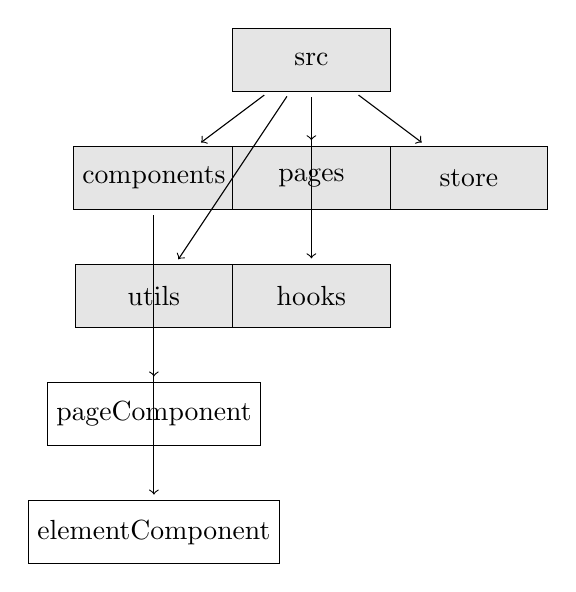
\begin{tikzpicture}[
    file/.style={draw, rectangle, minimum width=2cm, minimum height=0.8cm},
    folder/.style={draw, rectangle, minimum width=2cm, minimum height=0.8cm, fill=gray!20},
    arrow/.style={->, shorten >=2pt, shorten <=2pt}
]

% Folders
\node[folder] (src) at (0,0) {src};
\node[folder] (components) at (-2,-1.5) {components};
\node[folder] (pages) at (0,-1.5) {pages};
\node[folder] (store) at (2,-1.5) {store};
\node[folder] (utils) at (-2,-3) {utils};
\node[folder] (hooks) at (0,-3) {hooks};

% Files
\node[file] (pageComponent) at (-2,-4.5) {pageComponent};
\node[file] (elementComponent) at (-2,-6) {elementComponent};
% ... add more files

% Connections
\draw[arrow] (src) -- (components);
\draw[arrow] (src) -- (pages);
\draw[arrow] (src) -- (store);
\draw[arrow] (src) -- (utils);
\draw[arrow] (src) -- (hooks);
\draw[arrow] (components) -- (pageComponent);
\draw[arrow] (components) -- (elementComponent);
% ... add more connections

\end{tikzpicture}



\pagebreak
\subsubsection{Back-end}
The backend uses the dotNet framework. The development language using the C\# language.

In this project, the backend uses the Onion Architecture.
The Onion Architecture is a typically layered architecture, 
where each layer depends on the inner layer and provides interfaces to the outer layer.
The outer layer provides services to the outermost layer 
and other modules in the same layer based on the interfaces of the inner layer.

From inner to outer, the layers are: Domain, Application, Infrastructure, Presentation.
The Domain layer is the core layer and the innermost layer, used to define domain models, 
which are the business models.
It includes domain models and domain service interfaces.
Domain models are used to define the business models, 
which are the entities in the entity-relationship model and their attributes.
Domain service interfaces are used to define the business services, 
which are the relationships between entities in the entity-relationship model.

The Application layer is the application layer, 
used to define application services, which are the business logic.
It includes domain service implementations and application service interfaces.
Domain service implementations implement the methods of the inner layer's domain service 
interfaces and implement the business logic of the domain models.
Application service interfaces are used to define application services, 
which are the business logic.
It includes but is not limited to database interfaces, testing interfaces, 
HTTP API interfaces, MQTT interfaces, etc.

The Infrastructure layer is the infrastructure layer, used to define infrastructure.
It includes database implementations, testing implementations, 
HTTP API implementations, MQTT implementations, etc.
Database implementations implement the database interfaces 
and provide CRUD services for the database.
Testing implementations implement the testing interfaces 
and provide services for unit testing and integration testing.
HTTP API implementations implement the HTTP API interfaces 
and provide CRUD operations for HTTP APIs.
MQTT implementations implement the MQTT interfaces 
and provide CRUD operations for MQTT.

The Presentation layer is the presentation layer, used to define presentation logic, 
such as interfaces and pages. Since this is a backend project,
data presentation and control are handled by the frontend, 
so this layer is not needed.



\pagebreak
\subsubsection{Data communication and storage}
% 关于本项目的数据通信与数据存储的设计, 包括数据通信的协议, 数据存储的设计等
% 关于数据通信的设计:
% 1. 通信协议的选择
% 自前端向后端发送的数据, 有三种传输的数据类型, 
% 一种是普通的增删改查的请求, 对数据传输的时效性要求不高, 但是对数据的准确性, 完整性, 有序性, 安全性有一定的要求,
% 这种数据的传输, 采用 HTTP 协议, 以及 RESTful API 的设计. 可以有效的保证对数据传输的以上要求.
% 一种是对数据通道的创建和流媒体数据的传输, 对数据传输的时效性, 安全性要求较高, 这种数据的传输, 采用 WebRTC 协议, 以及 MQTT 协议.
% 配合可以快速解码的 flatbuffers 协议, 可以有效的保证对数据传输的以上要求.
% 最后一种是对设备的状态信息和操作信息的传输, 对完整性, 有序性, 安全性都有较高的要求, 这种数据的传输, 采用 MQTT 协议
% 同时也使用了 flatbuffers 协议.
% 
% 2. 数据通信的通信架构和通信流程
% 本项目的数据通信的通信架构, 是基于前后端分离的架构, 前端使用 React 框架, 后端使用 dotnet 框架.
% 当前端需要向后端发送数据的时候, 前端会向后端发送 HTTP 请求, 后端接收到 HTTP 请求之后, 会根据请求的数据类型,
% 选择不同的数据处理方式, 对于普通的增删改查的请求, 后端会根据 RESTful API 的设计, 对数据进行增删改查的操作,
% 对于对数据通道的创建和流媒体数据的传输, 后端会根据 WebRTC 协议, 对数据通道进行创建, 并且帮助前端和设备建立数据通道,
% 当数据通道建立后, 前端和设备之间则使用 flatbuffer 的数据格式对流媒体数据进行传输,
% 对于设备的状态信息和操作信息的传输, 前端会直接向 MQTT broker 发送 MQTT 请求, 
% 设备会在其自身的固件中监听相关的 MQTT 请求, 并且返回相关的数据.
% 
% 3. 数据通信的格式
% 本项目的数据通信的格式, 有三种, 
% 一种是 HTTP 协议, 
% 使用 json 格式对数据进行传输,
% 一种是 WebRTC 协议, 
% 使用 flatbuffers 格式对数据进行传输,
% 一种是 MQTT 协议.
% 使用 flatbuffers 格式对数据进行传输,
% 
% 关于数据存储的设计:
% 1. 数据存储的数据库的选择
% 本项目的数据存储的数据库的选择, 使用了轻量级的数据库 SQLite,
% SQLite 是一个进程内的库, 实现了自给自足的, 无服务器的, 零配置的, 事务性的 SQL 数据库引擎.
% 这是因为整个项目的目的是为了实现前端与设备之间的数据通信, 对于数据库数据的增删改查操作的要求不高,
% 数据量较小, 且对于数据库的数据的事务性要求不高, 所以选择了 SQLite 数据库.
% 2. 项目前后端的数据结构的设计
% 在本项目中, 前端由于使用了 React 框架, 所以前端的数据结构的设计, 使用了基于状态的数据结构的设计,
% 每个组件或者数据集都包含一个状态对象, 这个状态对象的属性就是组件的各个状态. 
% 使用状态对象的原因是, 可以方便的对状态进行管理, 采用对象-属性的形式, 可以方便的针对不同组件的同类状态进行区分,
% 由于跨组件的状态是由 redux 进行管理的, 这种状态对象的设计, 可以更搞笑的对状态进行更新和传递.
% 后端由于使用了 dotnet 框架, 所以后端的数据结构的设计, 使用了基于类的数据结构的设计,
% 采用了面向对象的编程思想, 对数据进行了封装, 使得数据的传输更加的安全, 有序, 完整.


\pagebreak

% \subsection{Domain model}
% \documentclass[]{article}
\usepackage{graphicx}
\usepackage{amsmath}
\usepackage{tikz}

% libaries
\usetikzlibrary{shapes,arrows}

%Define the listing package
\usepackage{listings} %code highlighter
\usepackage{color} %use color
\definecolor{mygreen}{rgb}{0,0.6,0}
\definecolor{mygray}{rgb}{0.5,0.5,0.5}
\definecolor{mymauve}{rgb}{0.58,0,0.82}

%Customize a bit the look
\lstset{ %
backgroundcolor=\color{white}, % choose the background color; you must add \usepackage{color} or \usepackage{xcolor}
basicstyle=\footnotesize, % the size of the fonts that are used for the code
breakatwhitespace=false, % sets if automatic breaks should only happen at whitespace
breaklines=true, % sets automatic line breaking
captionpos=b, % sets the caption-position to bottom
commentstyle=\color{mygreen}, % comment style
deletekeywords={...}, % if you want to delete keywords from the given language
escapeinside={\%*}{*)}, % if you want to add LaTeX within your code
extendedchars=true, % lets you use non-ASCII characters; for 8-bits encodings only, does not work with UTF-8
frame=single, % adds a frame around the code
keepspaces=true, % keeps spaces in text, useful for keeping indentation of code (possibly needs columns=flexible)
keywordstyle=\color{blue}, % keyword style
% language=Octave, % the language of the code
morekeywords={*,...}, % if you want to add more keywords to the set
numbers=left, % where to put the line-numbers; possible values are (none, left, right)
numbersep=5pt, % how far the line-numbers are from the code
numberstyle=\tiny\color{mygray}, % the style that is used for the line-numbers
rulecolor=\color{black}, % if not set, the frame-color may be changed on line-breaks within not-black text (e.g. comments (green here))
showspaces=false, % show spaces everywhere adding particular underscores; it overrides 'showstringspaces'
showstringspaces=false, % underline spaces within strings only
showtabs=false, % show tabs within strings adding particular underscores
stepnumber=1, % the step between two line-numbers. If it's 1, each line will be numbered
stringstyle=\color{mymauve}, % string literal style
tabsize=2, % sets default tabsize to 2 spaces
title=\lstname % show the filename of files included with \lstinputlisting; also try caption instead of title
}

\definecolor{darkgray}{rgb}{.4,.4,.4}
\definecolor{purple}{rgb}{0.65, 0.12, 0.82}

\lstdefinelanguage{React}{
keywords={const, typeof, new, true, false, catch, function, return, null, catch, switch, var, if, in, while, do, else, case, break},
keywordstyle=\color{blue}\bfseries,
ndkeywords={class, export, boolean, throw, implements, import, this},
ndkeywordstyle=\color{darkgray}\bfseries,
identifierstyle=\color{mygreen},
sensitive=false,
comment=[l]{//},
morecomment=[s]{/*}{*/},
commentstyle=\color{purple}\ttfamily,
string=[b]{"}{'}{`},
stringstyle=\color{red}\ttfamily,
morestring=[b]',
morestring=[b]",
morestring=[b]`',
}

\lstdefinelanguage{CSharp}{
keywords={const, typeof, new, true, false, catch, function, return, null, catch, switch, var, if, in, while, do, else, case, break},
keywordstyle=\color{blue}\bfseries,
ndkeywords={class, export, boolean, throw, implements, import, this},
ndkeywordstyle=\color{darkgray}\bfseries,
identifierstyle=\color{mygreen},
sensitive=false,
comment=[l]{//},
morecomment=[s]{/*}{*/},
commentstyle=\color{purple}\ttfamily,
string=[b]{"}{'}{`},
stringstyle=\color{red}\ttfamily,
morestring=[b]',
morestring=[b]",
morestring=[b]`',
}

\lstset{
language=React,
extendedchars=true,
basicstyle=\footnotesize\ttfamily,
showstringspaces=false,
showspaces=false,
numbers=left,
numberstyle=\footnotesize,
numbersep=9pt,
tabsize=2,
breaklines=true,
showtabs=false,
captionpos=b
}

\lstset{
language=CSharp,
extendedchars=true,
basicstyle=\footnotesize\ttfamily,
showstringspaces=false,
showspaces=false,
numbers=left,
numberstyle=\footnotesize,
numbersep=9pt,
tabsize=2,
breaklines=true,
showtabs=false,
captionpos=b
}

% \usepackage{cite} % Add this line for citation

% \bibliographystyle{plain}

\title{
The implementation of BifrostConnect Front-end scope, 
re-design and development with the relevant back-end support develop.
}
\author{
    Fei Gu \\
    Erhvervs Akademi Sydvest \\
    Computer Science 21\\
    }
\date{\today}

\begin{document}

% Front page
\maketitle
\begin{center}
    Supervisor: Henrik Boulund Meng Hansen \\
    Company: BifrostConnect \\
    Engineering Director: Jasper Wass \\
\end{center}
\tableofcontents
\pagebreak


% The introduction
\section{Introduction}
\subsection{Background}\input{sections/introduction/background.tex}
\subsection{The company}\input{sections/introduction/aboutCompany}
\subsection{The project}\input{sections/introduction/aboutProject}
\pagebreak

% The problem statement
\section{Problem Statement}
\subsection{Statement}
\input{sections/problemStatement/statement}
\subsection{Situation}
\input{sections/problemStatement/situation}
\subsection{Potential Solution}
\input{sections/problemStatement/potentialSolution}
\pagebreak

% Requirement analysis
\section{Requirement Analysis}
\input{sections/requirementAnalysis/index}

\subsection{Stakeholders}
\input{sections/requirementAnalysis/stakeholders/index}

\subsection{Business Domain}
\input{sections/requirementAnalysis/bussinesDomain/index}

\subsection{Scope}
\input{sections/requirementAnalysis/scope}

\subsection{Goals}
\input{sections/requirementAnalysis/goals}
\pagebreak

% Software Design
\section{Software Design}
% developement methods
\subsection{Software Development Methods}
\input{sections/softwareDevelopmentMethods/index}
\subsubsection{Agile Software Development}
\input{sections/softwareDevelopmentMethods/agileSoftwareDevelopment/index}
\subsubsection{Feature Driven Development}
\input{sections/softwareDevelopmentMethods/featureDrivenDevelopment/index}

\pagebreak

% Technology seslection
\subsection{Technology selection}
\input{sections/softwareDesign/technologySelection/index}
\subsubsection{Front-end}
\input{sections/softwareDesign/technologySelection/frontEnd}            
\subsubsection{Back-end}
\input{sections/softwareDesign/technologySelection/backEnd}            
\subsubsection{Database}
\input{sections/softwareDesign/technologySelection/database}
\subsubsection{Data communication}
\input{sections/softwareDesign/technologySelection/dataCommunication}            
\subsubsection{DevOps}
\input{sections/softwareDesign/technologySelection/devOps}
\pagebreak

% Architecture design
\subsection{Architecture design}
\input{sections/softwareDesign/architectureDesign/index}
\pagebreak
\subsubsection{Front-end}
\input{sections/softwareDesign/architectureDesign/frontEndArchitecture}
\pagebreak
\subsubsection{Back-end}
\input{sections/softwareDesign/architectureDesign/backEndArchitecture}
\pagebreak
\subsubsection{Data communication and storage}
\input{sections/softwareDesign/architectureDesign/dataCommunicationArchitecture}
\pagebreak

% \subsection{Domain model}
% \input{sections/softwareDesign/domainModel/index}
% \subsection{Database design}
% % 数据库领域模型 ER 图
% % 包括表和字段的设置.
% % 对于私有键和外键的设置.

% \subsection{Back-end design}
% % 后端对象模型
% % 以及对于对象模型的增删改查
% % 以及相关的其他服务的设计`'

% \subsection{Front-end design}
% % 对于前端的页面结构的设计 
% % 页面的状态的设计, 交互设计

% \subsection{FlatBuffers design}
% % schema 的设计

\subsection{DevOps CI/CD process design}
\input{sections/softwareDesign/devOpsDesign/index}
\subsubsection{Continuous Integration}
\input{sections/softwareDesign/devOpsDesign/continuousIntegration/index}
\subsubsection{Continuous Delivery}
\input{sections/softwareDesign/devOpsDesign/continuousDelivery/index}
\subsubsection{Continuous Deployment}
\input{sections/softwareDesign/devOpsDesign/continuousDeployment/index}
\pagebreak

\section{Software Development} 
\input{sections/softwareDevelopment/index}
\subsection{Overall development}
\input{sections/softwareDevelopment/overallDevelopement/index}
\subsubsection{Front-end}
\input{sections/softwareDevelopment/overallDevelopement/frontEnd/index}
\subsubsection{Back-end}
\input{sections/softwareDevelopment/overallDevelopement/backEnd/index}
\subsubsection{DevOps}
\input{sections/softwareDevelopment/overallDevelopement/devOps/index}
\subsection{Feature development} 
\input{sections/softwareDevelopment/featureDevelopment/index}
\subsubsection{Use Case 1}
\input{sections/softwareDevelopment/featureDevelopment/useCase1/index}
\subsubsection{Feature 1}
\input{sections/softwareDevelopment/featureDevelopment/feature/feature1.tex}
\pagebreak
\section{Conclusion} 
\subsection{Result}
Since the project is still in progress, the result is not available yet.
So far, basic structure of this project has been built. But the most features 
are not implemented yet. 
\subsection{Discussion}
As a single developer for this project, I am confident what I have done so far.
And I can say I understand the most of the knowledge I have used in this project, 
which also means I can explain all the part of the project. 
But this project also relevant some of the complex knowledge which I have to continue 
to study and practice.
\subsection{Future Work}
The future work is to implement the rest of the features. 
Including the most important part which is the 'create session' feature.
\pagebreak
% \bibliography{bibliography}
\pagebreak
% \begin{appendices}
%     \section{Appendix}
% \end{appendices} 
\end{document}
% \subsection{Database design}
% % 数据库领域模型 ER 图
% % 包括表和字段的设置.
% % 对于私有键和外键的设置.

% \subsection{Back-end design}
% % 后端对象模型
% % 以及对于对象模型的增删改查
% % 以及相关的其他服务的设计`'

% \subsection{Front-end design}
% % 对于前端的页面结构的设计 
% % 页面的状态的设计, 交互设计

% \subsection{FlatBuffers design}
% % schema 的设计

\subsection{DevOps CI/CD process design}
\documentclass[]{article}
\usepackage{graphicx}
\usepackage{amsmath}
\usepackage{tikz}

% libaries
\usetikzlibrary{shapes,arrows}

%Define the listing package
\usepackage{listings} %code highlighter
\usepackage{color} %use color
\definecolor{mygreen}{rgb}{0,0.6,0}
\definecolor{mygray}{rgb}{0.5,0.5,0.5}
\definecolor{mymauve}{rgb}{0.58,0,0.82}

%Customize a bit the look
\lstset{ %
backgroundcolor=\color{white}, % choose the background color; you must add \usepackage{color} or \usepackage{xcolor}
basicstyle=\footnotesize, % the size of the fonts that are used for the code
breakatwhitespace=false, % sets if automatic breaks should only happen at whitespace
breaklines=true, % sets automatic line breaking
captionpos=b, % sets the caption-position to bottom
commentstyle=\color{mygreen}, % comment style
deletekeywords={...}, % if you want to delete keywords from the given language
escapeinside={\%*}{*)}, % if you want to add LaTeX within your code
extendedchars=true, % lets you use non-ASCII characters; for 8-bits encodings only, does not work with UTF-8
frame=single, % adds a frame around the code
keepspaces=true, % keeps spaces in text, useful for keeping indentation of code (possibly needs columns=flexible)
keywordstyle=\color{blue}, % keyword style
% language=Octave, % the language of the code
morekeywords={*,...}, % if you want to add more keywords to the set
numbers=left, % where to put the line-numbers; possible values are (none, left, right)
numbersep=5pt, % how far the line-numbers are from the code
numberstyle=\tiny\color{mygray}, % the style that is used for the line-numbers
rulecolor=\color{black}, % if not set, the frame-color may be changed on line-breaks within not-black text (e.g. comments (green here))
showspaces=false, % show spaces everywhere adding particular underscores; it overrides 'showstringspaces'
showstringspaces=false, % underline spaces within strings only
showtabs=false, % show tabs within strings adding particular underscores
stepnumber=1, % the step between two line-numbers. If it's 1, each line will be numbered
stringstyle=\color{mymauve}, % string literal style
tabsize=2, % sets default tabsize to 2 spaces
title=\lstname % show the filename of files included with \lstinputlisting; also try caption instead of title
}

\definecolor{darkgray}{rgb}{.4,.4,.4}
\definecolor{purple}{rgb}{0.65, 0.12, 0.82}

\lstdefinelanguage{React}{
keywords={const, typeof, new, true, false, catch, function, return, null, catch, switch, var, if, in, while, do, else, case, break},
keywordstyle=\color{blue}\bfseries,
ndkeywords={class, export, boolean, throw, implements, import, this},
ndkeywordstyle=\color{darkgray}\bfseries,
identifierstyle=\color{mygreen},
sensitive=false,
comment=[l]{//},
morecomment=[s]{/*}{*/},
commentstyle=\color{purple}\ttfamily,
string=[b]{"}{'}{`},
stringstyle=\color{red}\ttfamily,
morestring=[b]',
morestring=[b]",
morestring=[b]`',
}

\lstdefinelanguage{CSharp}{
keywords={const, typeof, new, true, false, catch, function, return, null, catch, switch, var, if, in, while, do, else, case, break},
keywordstyle=\color{blue}\bfseries,
ndkeywords={class, export, boolean, throw, implements, import, this},
ndkeywordstyle=\color{darkgray}\bfseries,
identifierstyle=\color{mygreen},
sensitive=false,
comment=[l]{//},
morecomment=[s]{/*}{*/},
commentstyle=\color{purple}\ttfamily,
string=[b]{"}{'}{`},
stringstyle=\color{red}\ttfamily,
morestring=[b]',
morestring=[b]",
morestring=[b]`',
}

\lstset{
language=React,
extendedchars=true,
basicstyle=\footnotesize\ttfamily,
showstringspaces=false,
showspaces=false,
numbers=left,
numberstyle=\footnotesize,
numbersep=9pt,
tabsize=2,
breaklines=true,
showtabs=false,
captionpos=b
}

\lstset{
language=CSharp,
extendedchars=true,
basicstyle=\footnotesize\ttfamily,
showstringspaces=false,
showspaces=false,
numbers=left,
numberstyle=\footnotesize,
numbersep=9pt,
tabsize=2,
breaklines=true,
showtabs=false,
captionpos=b
}

% \usepackage{cite} % Add this line for citation

% \bibliographystyle{plain}

\title{
The implementation of BifrostConnect Front-end scope, 
re-design and development with the relevant back-end support develop.
}
\author{
    Fei Gu \\
    Erhvervs Akademi Sydvest \\
    Computer Science 21\\
    }
\date{\today}

\begin{document}

% Front page
\maketitle
\begin{center}
    Supervisor: Henrik Boulund Meng Hansen \\
    Company: BifrostConnect \\
    Engineering Director: Jasper Wass \\
\end{center}
\tableofcontents
\pagebreak


% The introduction
\section{Introduction}
\subsection{Background}\input{sections/introduction/background.tex}
\subsection{The company}\input{sections/introduction/aboutCompany}
\subsection{The project}\input{sections/introduction/aboutProject}
\pagebreak

% The problem statement
\section{Problem Statement}
\subsection{Statement}
\input{sections/problemStatement/statement}
\subsection{Situation}
\input{sections/problemStatement/situation}
\subsection{Potential Solution}
\input{sections/problemStatement/potentialSolution}
\pagebreak

% Requirement analysis
\section{Requirement Analysis}
\input{sections/requirementAnalysis/index}

\subsection{Stakeholders}
\input{sections/requirementAnalysis/stakeholders/index}

\subsection{Business Domain}
\input{sections/requirementAnalysis/bussinesDomain/index}

\subsection{Scope}
\input{sections/requirementAnalysis/scope}

\subsection{Goals}
\input{sections/requirementAnalysis/goals}
\pagebreak

% Software Design
\section{Software Design}
% developement methods
\subsection{Software Development Methods}
\input{sections/softwareDevelopmentMethods/index}
\subsubsection{Agile Software Development}
\input{sections/softwareDevelopmentMethods/agileSoftwareDevelopment/index}
\subsubsection{Feature Driven Development}
\input{sections/softwareDevelopmentMethods/featureDrivenDevelopment/index}

\pagebreak

% Technology seslection
\subsection{Technology selection}
\input{sections/softwareDesign/technologySelection/index}
\subsubsection{Front-end}
\input{sections/softwareDesign/technologySelection/frontEnd}            
\subsubsection{Back-end}
\input{sections/softwareDesign/technologySelection/backEnd}            
\subsubsection{Database}
\input{sections/softwareDesign/technologySelection/database}
\subsubsection{Data communication}
\input{sections/softwareDesign/technologySelection/dataCommunication}            
\subsubsection{DevOps}
\input{sections/softwareDesign/technologySelection/devOps}
\pagebreak

% Architecture design
\subsection{Architecture design}
\input{sections/softwareDesign/architectureDesign/index}
\pagebreak
\subsubsection{Front-end}
\input{sections/softwareDesign/architectureDesign/frontEndArchitecture}
\pagebreak
\subsubsection{Back-end}
\input{sections/softwareDesign/architectureDesign/backEndArchitecture}
\pagebreak
\subsubsection{Data communication and storage}
\input{sections/softwareDesign/architectureDesign/dataCommunicationArchitecture}
\pagebreak

% \subsection{Domain model}
% \input{sections/softwareDesign/domainModel/index}
% \subsection{Database design}
% % 数据库领域模型 ER 图
% % 包括表和字段的设置.
% % 对于私有键和外键的设置.

% \subsection{Back-end design}
% % 后端对象模型
% % 以及对于对象模型的增删改查
% % 以及相关的其他服务的设计`'

% \subsection{Front-end design}
% % 对于前端的页面结构的设计 
% % 页面的状态的设计, 交互设计

% \subsection{FlatBuffers design}
% % schema 的设计

\subsection{DevOps CI/CD process design}
\input{sections/softwareDesign/devOpsDesign/index}
\subsubsection{Continuous Integration}
\input{sections/softwareDesign/devOpsDesign/continuousIntegration/index}
\subsubsection{Continuous Delivery}
\input{sections/softwareDesign/devOpsDesign/continuousDelivery/index}
\subsubsection{Continuous Deployment}
\input{sections/softwareDesign/devOpsDesign/continuousDeployment/index}
\pagebreak

\section{Software Development} 
\input{sections/softwareDevelopment/index}
\subsection{Overall development}
\input{sections/softwareDevelopment/overallDevelopement/index}
\subsubsection{Front-end}
\input{sections/softwareDevelopment/overallDevelopement/frontEnd/index}
\subsubsection{Back-end}
\input{sections/softwareDevelopment/overallDevelopement/backEnd/index}
\subsubsection{DevOps}
\input{sections/softwareDevelopment/overallDevelopement/devOps/index}
\subsection{Feature development} 
\input{sections/softwareDevelopment/featureDevelopment/index}
\subsubsection{Use Case 1}
\input{sections/softwareDevelopment/featureDevelopment/useCase1/index}
\subsubsection{Feature 1}
\input{sections/softwareDevelopment/featureDevelopment/feature/feature1.tex}
\pagebreak
\section{Conclusion} 
\subsection{Result}
Since the project is still in progress, the result is not available yet.
So far, basic structure of this project has been built. But the most features 
are not implemented yet. 
\subsection{Discussion}
As a single developer for this project, I am confident what I have done so far.
And I can say I understand the most of the knowledge I have used in this project, 
which also means I can explain all the part of the project. 
But this project also relevant some of the complex knowledge which I have to continue 
to study and practice.
\subsection{Future Work}
The future work is to implement the rest of the features. 
Including the most important part which is the 'create session' feature.
\pagebreak
% \bibliography{bibliography}
\pagebreak
% \begin{appendices}
%     \section{Appendix}
% \end{appendices} 
\end{document}
\subsubsection{Continuous Integration}
\documentclass[]{article}
\usepackage{graphicx}
\usepackage{amsmath}
\usepackage{tikz}

% libaries
\usetikzlibrary{shapes,arrows}

%Define the listing package
\usepackage{listings} %code highlighter
\usepackage{color} %use color
\definecolor{mygreen}{rgb}{0,0.6,0}
\definecolor{mygray}{rgb}{0.5,0.5,0.5}
\definecolor{mymauve}{rgb}{0.58,0,0.82}

%Customize a bit the look
\lstset{ %
backgroundcolor=\color{white}, % choose the background color; you must add \usepackage{color} or \usepackage{xcolor}
basicstyle=\footnotesize, % the size of the fonts that are used for the code
breakatwhitespace=false, % sets if automatic breaks should only happen at whitespace
breaklines=true, % sets automatic line breaking
captionpos=b, % sets the caption-position to bottom
commentstyle=\color{mygreen}, % comment style
deletekeywords={...}, % if you want to delete keywords from the given language
escapeinside={\%*}{*)}, % if you want to add LaTeX within your code
extendedchars=true, % lets you use non-ASCII characters; for 8-bits encodings only, does not work with UTF-8
frame=single, % adds a frame around the code
keepspaces=true, % keeps spaces in text, useful for keeping indentation of code (possibly needs columns=flexible)
keywordstyle=\color{blue}, % keyword style
% language=Octave, % the language of the code
morekeywords={*,...}, % if you want to add more keywords to the set
numbers=left, % where to put the line-numbers; possible values are (none, left, right)
numbersep=5pt, % how far the line-numbers are from the code
numberstyle=\tiny\color{mygray}, % the style that is used for the line-numbers
rulecolor=\color{black}, % if not set, the frame-color may be changed on line-breaks within not-black text (e.g. comments (green here))
showspaces=false, % show spaces everywhere adding particular underscores; it overrides 'showstringspaces'
showstringspaces=false, % underline spaces within strings only
showtabs=false, % show tabs within strings adding particular underscores
stepnumber=1, % the step between two line-numbers. If it's 1, each line will be numbered
stringstyle=\color{mymauve}, % string literal style
tabsize=2, % sets default tabsize to 2 spaces
title=\lstname % show the filename of files included with \lstinputlisting; also try caption instead of title
}

\definecolor{darkgray}{rgb}{.4,.4,.4}
\definecolor{purple}{rgb}{0.65, 0.12, 0.82}

\lstdefinelanguage{React}{
keywords={const, typeof, new, true, false, catch, function, return, null, catch, switch, var, if, in, while, do, else, case, break},
keywordstyle=\color{blue}\bfseries,
ndkeywords={class, export, boolean, throw, implements, import, this},
ndkeywordstyle=\color{darkgray}\bfseries,
identifierstyle=\color{mygreen},
sensitive=false,
comment=[l]{//},
morecomment=[s]{/*}{*/},
commentstyle=\color{purple}\ttfamily,
string=[b]{"}{'}{`},
stringstyle=\color{red}\ttfamily,
morestring=[b]',
morestring=[b]",
morestring=[b]`',
}

\lstdefinelanguage{CSharp}{
keywords={const, typeof, new, true, false, catch, function, return, null, catch, switch, var, if, in, while, do, else, case, break},
keywordstyle=\color{blue}\bfseries,
ndkeywords={class, export, boolean, throw, implements, import, this},
ndkeywordstyle=\color{darkgray}\bfseries,
identifierstyle=\color{mygreen},
sensitive=false,
comment=[l]{//},
morecomment=[s]{/*}{*/},
commentstyle=\color{purple}\ttfamily,
string=[b]{"}{'}{`},
stringstyle=\color{red}\ttfamily,
morestring=[b]',
morestring=[b]",
morestring=[b]`',
}

\lstset{
language=React,
extendedchars=true,
basicstyle=\footnotesize\ttfamily,
showstringspaces=false,
showspaces=false,
numbers=left,
numberstyle=\footnotesize,
numbersep=9pt,
tabsize=2,
breaklines=true,
showtabs=false,
captionpos=b
}

\lstset{
language=CSharp,
extendedchars=true,
basicstyle=\footnotesize\ttfamily,
showstringspaces=false,
showspaces=false,
numbers=left,
numberstyle=\footnotesize,
numbersep=9pt,
tabsize=2,
breaklines=true,
showtabs=false,
captionpos=b
}

% \usepackage{cite} % Add this line for citation

% \bibliographystyle{plain}

\title{
The implementation of BifrostConnect Front-end scope, 
re-design and development with the relevant back-end support develop.
}
\author{
    Fei Gu \\
    Erhvervs Akademi Sydvest \\
    Computer Science 21\\
    }
\date{\today}

\begin{document}

% Front page
\maketitle
\begin{center}
    Supervisor: Henrik Boulund Meng Hansen \\
    Company: BifrostConnect \\
    Engineering Director: Jasper Wass \\
\end{center}
\tableofcontents
\pagebreak


% The introduction
\section{Introduction}
\subsection{Background}\input{sections/introduction/background.tex}
\subsection{The company}\input{sections/introduction/aboutCompany}
\subsection{The project}\input{sections/introduction/aboutProject}
\pagebreak

% The problem statement
\section{Problem Statement}
\subsection{Statement}
\input{sections/problemStatement/statement}
\subsection{Situation}
\input{sections/problemStatement/situation}
\subsection{Potential Solution}
\input{sections/problemStatement/potentialSolution}
\pagebreak

% Requirement analysis
\section{Requirement Analysis}
\input{sections/requirementAnalysis/index}

\subsection{Stakeholders}
\input{sections/requirementAnalysis/stakeholders/index}

\subsection{Business Domain}
\input{sections/requirementAnalysis/bussinesDomain/index}

\subsection{Scope}
\input{sections/requirementAnalysis/scope}

\subsection{Goals}
\input{sections/requirementAnalysis/goals}
\pagebreak

% Software Design
\section{Software Design}
% developement methods
\subsection{Software Development Methods}
\input{sections/softwareDevelopmentMethods/index}
\subsubsection{Agile Software Development}
\input{sections/softwareDevelopmentMethods/agileSoftwareDevelopment/index}
\subsubsection{Feature Driven Development}
\input{sections/softwareDevelopmentMethods/featureDrivenDevelopment/index}

\pagebreak

% Technology seslection
\subsection{Technology selection}
\input{sections/softwareDesign/technologySelection/index}
\subsubsection{Front-end}
\input{sections/softwareDesign/technologySelection/frontEnd}            
\subsubsection{Back-end}
\input{sections/softwareDesign/technologySelection/backEnd}            
\subsubsection{Database}
\input{sections/softwareDesign/technologySelection/database}
\subsubsection{Data communication}
\input{sections/softwareDesign/technologySelection/dataCommunication}            
\subsubsection{DevOps}
\input{sections/softwareDesign/technologySelection/devOps}
\pagebreak

% Architecture design
\subsection{Architecture design}
\input{sections/softwareDesign/architectureDesign/index}
\pagebreak
\subsubsection{Front-end}
\input{sections/softwareDesign/architectureDesign/frontEndArchitecture}
\pagebreak
\subsubsection{Back-end}
\input{sections/softwareDesign/architectureDesign/backEndArchitecture}
\pagebreak
\subsubsection{Data communication and storage}
\input{sections/softwareDesign/architectureDesign/dataCommunicationArchitecture}
\pagebreak

% \subsection{Domain model}
% \input{sections/softwareDesign/domainModel/index}
% \subsection{Database design}
% % 数据库领域模型 ER 图
% % 包括表和字段的设置.
% % 对于私有键和外键的设置.

% \subsection{Back-end design}
% % 后端对象模型
% % 以及对于对象模型的增删改查
% % 以及相关的其他服务的设计`'

% \subsection{Front-end design}
% % 对于前端的页面结构的设计 
% % 页面的状态的设计, 交互设计

% \subsection{FlatBuffers design}
% % schema 的设计

\subsection{DevOps CI/CD process design}
\input{sections/softwareDesign/devOpsDesign/index}
\subsubsection{Continuous Integration}
\input{sections/softwareDesign/devOpsDesign/continuousIntegration/index}
\subsubsection{Continuous Delivery}
\input{sections/softwareDesign/devOpsDesign/continuousDelivery/index}
\subsubsection{Continuous Deployment}
\input{sections/softwareDesign/devOpsDesign/continuousDeployment/index}
\pagebreak

\section{Software Development} 
\input{sections/softwareDevelopment/index}
\subsection{Overall development}
\input{sections/softwareDevelopment/overallDevelopement/index}
\subsubsection{Front-end}
\input{sections/softwareDevelopment/overallDevelopement/frontEnd/index}
\subsubsection{Back-end}
\input{sections/softwareDevelopment/overallDevelopement/backEnd/index}
\subsubsection{DevOps}
\input{sections/softwareDevelopment/overallDevelopement/devOps/index}
\subsection{Feature development} 
\input{sections/softwareDevelopment/featureDevelopment/index}
\subsubsection{Use Case 1}
\input{sections/softwareDevelopment/featureDevelopment/useCase1/index}
\subsubsection{Feature 1}
\input{sections/softwareDevelopment/featureDevelopment/feature/feature1.tex}
\pagebreak
\section{Conclusion} 
\subsection{Result}
Since the project is still in progress, the result is not available yet.
So far, basic structure of this project has been built. But the most features 
are not implemented yet. 
\subsection{Discussion}
As a single developer for this project, I am confident what I have done so far.
And I can say I understand the most of the knowledge I have used in this project, 
which also means I can explain all the part of the project. 
But this project also relevant some of the complex knowledge which I have to continue 
to study and practice.
\subsection{Future Work}
The future work is to implement the rest of the features. 
Including the most important part which is the 'create session' feature.
\pagebreak
% \bibliography{bibliography}
\pagebreak
% \begin{appendices}
%     \section{Appendix}
% \end{appendices} 
\end{document}
\subsubsection{Continuous Delivery}
\documentclass[]{article}
\usepackage{graphicx}
\usepackage{amsmath}
\usepackage{tikz}

% libaries
\usetikzlibrary{shapes,arrows}

%Define the listing package
\usepackage{listings} %code highlighter
\usepackage{color} %use color
\definecolor{mygreen}{rgb}{0,0.6,0}
\definecolor{mygray}{rgb}{0.5,0.5,0.5}
\definecolor{mymauve}{rgb}{0.58,0,0.82}

%Customize a bit the look
\lstset{ %
backgroundcolor=\color{white}, % choose the background color; you must add \usepackage{color} or \usepackage{xcolor}
basicstyle=\footnotesize, % the size of the fonts that are used for the code
breakatwhitespace=false, % sets if automatic breaks should only happen at whitespace
breaklines=true, % sets automatic line breaking
captionpos=b, % sets the caption-position to bottom
commentstyle=\color{mygreen}, % comment style
deletekeywords={...}, % if you want to delete keywords from the given language
escapeinside={\%*}{*)}, % if you want to add LaTeX within your code
extendedchars=true, % lets you use non-ASCII characters; for 8-bits encodings only, does not work with UTF-8
frame=single, % adds a frame around the code
keepspaces=true, % keeps spaces in text, useful for keeping indentation of code (possibly needs columns=flexible)
keywordstyle=\color{blue}, % keyword style
% language=Octave, % the language of the code
morekeywords={*,...}, % if you want to add more keywords to the set
numbers=left, % where to put the line-numbers; possible values are (none, left, right)
numbersep=5pt, % how far the line-numbers are from the code
numberstyle=\tiny\color{mygray}, % the style that is used for the line-numbers
rulecolor=\color{black}, % if not set, the frame-color may be changed on line-breaks within not-black text (e.g. comments (green here))
showspaces=false, % show spaces everywhere adding particular underscores; it overrides 'showstringspaces'
showstringspaces=false, % underline spaces within strings only
showtabs=false, % show tabs within strings adding particular underscores
stepnumber=1, % the step between two line-numbers. If it's 1, each line will be numbered
stringstyle=\color{mymauve}, % string literal style
tabsize=2, % sets default tabsize to 2 spaces
title=\lstname % show the filename of files included with \lstinputlisting; also try caption instead of title
}

\definecolor{darkgray}{rgb}{.4,.4,.4}
\definecolor{purple}{rgb}{0.65, 0.12, 0.82}

\lstdefinelanguage{React}{
keywords={const, typeof, new, true, false, catch, function, return, null, catch, switch, var, if, in, while, do, else, case, break},
keywordstyle=\color{blue}\bfseries,
ndkeywords={class, export, boolean, throw, implements, import, this},
ndkeywordstyle=\color{darkgray}\bfseries,
identifierstyle=\color{mygreen},
sensitive=false,
comment=[l]{//},
morecomment=[s]{/*}{*/},
commentstyle=\color{purple}\ttfamily,
string=[b]{"}{'}{`},
stringstyle=\color{red}\ttfamily,
morestring=[b]',
morestring=[b]",
morestring=[b]`',
}

\lstdefinelanguage{CSharp}{
keywords={const, typeof, new, true, false, catch, function, return, null, catch, switch, var, if, in, while, do, else, case, break},
keywordstyle=\color{blue}\bfseries,
ndkeywords={class, export, boolean, throw, implements, import, this},
ndkeywordstyle=\color{darkgray}\bfseries,
identifierstyle=\color{mygreen},
sensitive=false,
comment=[l]{//},
morecomment=[s]{/*}{*/},
commentstyle=\color{purple}\ttfamily,
string=[b]{"}{'}{`},
stringstyle=\color{red}\ttfamily,
morestring=[b]',
morestring=[b]",
morestring=[b]`',
}

\lstset{
language=React,
extendedchars=true,
basicstyle=\footnotesize\ttfamily,
showstringspaces=false,
showspaces=false,
numbers=left,
numberstyle=\footnotesize,
numbersep=9pt,
tabsize=2,
breaklines=true,
showtabs=false,
captionpos=b
}

\lstset{
language=CSharp,
extendedchars=true,
basicstyle=\footnotesize\ttfamily,
showstringspaces=false,
showspaces=false,
numbers=left,
numberstyle=\footnotesize,
numbersep=9pt,
tabsize=2,
breaklines=true,
showtabs=false,
captionpos=b
}

% \usepackage{cite} % Add this line for citation

% \bibliographystyle{plain}

\title{
The implementation of BifrostConnect Front-end scope, 
re-design and development with the relevant back-end support develop.
}
\author{
    Fei Gu \\
    Erhvervs Akademi Sydvest \\
    Computer Science 21\\
    }
\date{\today}

\begin{document}

% Front page
\maketitle
\begin{center}
    Supervisor: Henrik Boulund Meng Hansen \\
    Company: BifrostConnect \\
    Engineering Director: Jasper Wass \\
\end{center}
\tableofcontents
\pagebreak


% The introduction
\section{Introduction}
\subsection{Background}\input{sections/introduction/background.tex}
\subsection{The company}\input{sections/introduction/aboutCompany}
\subsection{The project}\input{sections/introduction/aboutProject}
\pagebreak

% The problem statement
\section{Problem Statement}
\subsection{Statement}
\input{sections/problemStatement/statement}
\subsection{Situation}
\input{sections/problemStatement/situation}
\subsection{Potential Solution}
\input{sections/problemStatement/potentialSolution}
\pagebreak

% Requirement analysis
\section{Requirement Analysis}
\input{sections/requirementAnalysis/index}

\subsection{Stakeholders}
\input{sections/requirementAnalysis/stakeholders/index}

\subsection{Business Domain}
\input{sections/requirementAnalysis/bussinesDomain/index}

\subsection{Scope}
\input{sections/requirementAnalysis/scope}

\subsection{Goals}
\input{sections/requirementAnalysis/goals}
\pagebreak

% Software Design
\section{Software Design}
% developement methods
\subsection{Software Development Methods}
\input{sections/softwareDevelopmentMethods/index}
\subsubsection{Agile Software Development}
\input{sections/softwareDevelopmentMethods/agileSoftwareDevelopment/index}
\subsubsection{Feature Driven Development}
\input{sections/softwareDevelopmentMethods/featureDrivenDevelopment/index}

\pagebreak

% Technology seslection
\subsection{Technology selection}
\input{sections/softwareDesign/technologySelection/index}
\subsubsection{Front-end}
\input{sections/softwareDesign/technologySelection/frontEnd}            
\subsubsection{Back-end}
\input{sections/softwareDesign/technologySelection/backEnd}            
\subsubsection{Database}
\input{sections/softwareDesign/technologySelection/database}
\subsubsection{Data communication}
\input{sections/softwareDesign/technologySelection/dataCommunication}            
\subsubsection{DevOps}
\input{sections/softwareDesign/technologySelection/devOps}
\pagebreak

% Architecture design
\subsection{Architecture design}
\input{sections/softwareDesign/architectureDesign/index}
\pagebreak
\subsubsection{Front-end}
\input{sections/softwareDesign/architectureDesign/frontEndArchitecture}
\pagebreak
\subsubsection{Back-end}
\input{sections/softwareDesign/architectureDesign/backEndArchitecture}
\pagebreak
\subsubsection{Data communication and storage}
\input{sections/softwareDesign/architectureDesign/dataCommunicationArchitecture}
\pagebreak

% \subsection{Domain model}
% \input{sections/softwareDesign/domainModel/index}
% \subsection{Database design}
% % 数据库领域模型 ER 图
% % 包括表和字段的设置.
% % 对于私有键和外键的设置.

% \subsection{Back-end design}
% % 后端对象模型
% % 以及对于对象模型的增删改查
% % 以及相关的其他服务的设计`'

% \subsection{Front-end design}
% % 对于前端的页面结构的设计 
% % 页面的状态的设计, 交互设计

% \subsection{FlatBuffers design}
% % schema 的设计

\subsection{DevOps CI/CD process design}
\input{sections/softwareDesign/devOpsDesign/index}
\subsubsection{Continuous Integration}
\input{sections/softwareDesign/devOpsDesign/continuousIntegration/index}
\subsubsection{Continuous Delivery}
\input{sections/softwareDesign/devOpsDesign/continuousDelivery/index}
\subsubsection{Continuous Deployment}
\input{sections/softwareDesign/devOpsDesign/continuousDeployment/index}
\pagebreak

\section{Software Development} 
\input{sections/softwareDevelopment/index}
\subsection{Overall development}
\input{sections/softwareDevelopment/overallDevelopement/index}
\subsubsection{Front-end}
\input{sections/softwareDevelopment/overallDevelopement/frontEnd/index}
\subsubsection{Back-end}
\input{sections/softwareDevelopment/overallDevelopement/backEnd/index}
\subsubsection{DevOps}
\input{sections/softwareDevelopment/overallDevelopement/devOps/index}
\subsection{Feature development} 
\input{sections/softwareDevelopment/featureDevelopment/index}
\subsubsection{Use Case 1}
\input{sections/softwareDevelopment/featureDevelopment/useCase1/index}
\subsubsection{Feature 1}
\input{sections/softwareDevelopment/featureDevelopment/feature/feature1.tex}
\pagebreak
\section{Conclusion} 
\subsection{Result}
Since the project is still in progress, the result is not available yet.
So far, basic structure of this project has been built. But the most features 
are not implemented yet. 
\subsection{Discussion}
As a single developer for this project, I am confident what I have done so far.
And I can say I understand the most of the knowledge I have used in this project, 
which also means I can explain all the part of the project. 
But this project also relevant some of the complex knowledge which I have to continue 
to study and practice.
\subsection{Future Work}
The future work is to implement the rest of the features. 
Including the most important part which is the 'create session' feature.
\pagebreak
% \bibliography{bibliography}
\pagebreak
% \begin{appendices}
%     \section{Appendix}
% \end{appendices} 
\end{document}
\subsubsection{Continuous Deployment}
\documentclass[]{article}
\usepackage{graphicx}
\usepackage{amsmath}
\usepackage{tikz}

% libaries
\usetikzlibrary{shapes,arrows}

%Define the listing package
\usepackage{listings} %code highlighter
\usepackage{color} %use color
\definecolor{mygreen}{rgb}{0,0.6,0}
\definecolor{mygray}{rgb}{0.5,0.5,0.5}
\definecolor{mymauve}{rgb}{0.58,0,0.82}

%Customize a bit the look
\lstset{ %
backgroundcolor=\color{white}, % choose the background color; you must add \usepackage{color} or \usepackage{xcolor}
basicstyle=\footnotesize, % the size of the fonts that are used for the code
breakatwhitespace=false, % sets if automatic breaks should only happen at whitespace
breaklines=true, % sets automatic line breaking
captionpos=b, % sets the caption-position to bottom
commentstyle=\color{mygreen}, % comment style
deletekeywords={...}, % if you want to delete keywords from the given language
escapeinside={\%*}{*)}, % if you want to add LaTeX within your code
extendedchars=true, % lets you use non-ASCII characters; for 8-bits encodings only, does not work with UTF-8
frame=single, % adds a frame around the code
keepspaces=true, % keeps spaces in text, useful for keeping indentation of code (possibly needs columns=flexible)
keywordstyle=\color{blue}, % keyword style
% language=Octave, % the language of the code
morekeywords={*,...}, % if you want to add more keywords to the set
numbers=left, % where to put the line-numbers; possible values are (none, left, right)
numbersep=5pt, % how far the line-numbers are from the code
numberstyle=\tiny\color{mygray}, % the style that is used for the line-numbers
rulecolor=\color{black}, % if not set, the frame-color may be changed on line-breaks within not-black text (e.g. comments (green here))
showspaces=false, % show spaces everywhere adding particular underscores; it overrides 'showstringspaces'
showstringspaces=false, % underline spaces within strings only
showtabs=false, % show tabs within strings adding particular underscores
stepnumber=1, % the step between two line-numbers. If it's 1, each line will be numbered
stringstyle=\color{mymauve}, % string literal style
tabsize=2, % sets default tabsize to 2 spaces
title=\lstname % show the filename of files included with \lstinputlisting; also try caption instead of title
}

\definecolor{darkgray}{rgb}{.4,.4,.4}
\definecolor{purple}{rgb}{0.65, 0.12, 0.82}

\lstdefinelanguage{React}{
keywords={const, typeof, new, true, false, catch, function, return, null, catch, switch, var, if, in, while, do, else, case, break},
keywordstyle=\color{blue}\bfseries,
ndkeywords={class, export, boolean, throw, implements, import, this},
ndkeywordstyle=\color{darkgray}\bfseries,
identifierstyle=\color{mygreen},
sensitive=false,
comment=[l]{//},
morecomment=[s]{/*}{*/},
commentstyle=\color{purple}\ttfamily,
string=[b]{"}{'}{`},
stringstyle=\color{red}\ttfamily,
morestring=[b]',
morestring=[b]",
morestring=[b]`',
}

\lstdefinelanguage{CSharp}{
keywords={const, typeof, new, true, false, catch, function, return, null, catch, switch, var, if, in, while, do, else, case, break},
keywordstyle=\color{blue}\bfseries,
ndkeywords={class, export, boolean, throw, implements, import, this},
ndkeywordstyle=\color{darkgray}\bfseries,
identifierstyle=\color{mygreen},
sensitive=false,
comment=[l]{//},
morecomment=[s]{/*}{*/},
commentstyle=\color{purple}\ttfamily,
string=[b]{"}{'}{`},
stringstyle=\color{red}\ttfamily,
morestring=[b]',
morestring=[b]",
morestring=[b]`',
}

\lstset{
language=React,
extendedchars=true,
basicstyle=\footnotesize\ttfamily,
showstringspaces=false,
showspaces=false,
numbers=left,
numberstyle=\footnotesize,
numbersep=9pt,
tabsize=2,
breaklines=true,
showtabs=false,
captionpos=b
}

\lstset{
language=CSharp,
extendedchars=true,
basicstyle=\footnotesize\ttfamily,
showstringspaces=false,
showspaces=false,
numbers=left,
numberstyle=\footnotesize,
numbersep=9pt,
tabsize=2,
breaklines=true,
showtabs=false,
captionpos=b
}

% \usepackage{cite} % Add this line for citation

% \bibliographystyle{plain}

\title{
The implementation of BifrostConnect Front-end scope, 
re-design and development with the relevant back-end support develop.
}
\author{
    Fei Gu \\
    Erhvervs Akademi Sydvest \\
    Computer Science 21\\
    }
\date{\today}

\begin{document}

% Front page
\maketitle
\begin{center}
    Supervisor: Henrik Boulund Meng Hansen \\
    Company: BifrostConnect \\
    Engineering Director: Jasper Wass \\
\end{center}
\tableofcontents
\pagebreak


% The introduction
\section{Introduction}
\subsection{Background}\input{sections/introduction/background.tex}
\subsection{The company}\input{sections/introduction/aboutCompany}
\subsection{The project}\input{sections/introduction/aboutProject}
\pagebreak

% The problem statement
\section{Problem Statement}
\subsection{Statement}
\input{sections/problemStatement/statement}
\subsection{Situation}
\input{sections/problemStatement/situation}
\subsection{Potential Solution}
\input{sections/problemStatement/potentialSolution}
\pagebreak

% Requirement analysis
\section{Requirement Analysis}
\input{sections/requirementAnalysis/index}

\subsection{Stakeholders}
\input{sections/requirementAnalysis/stakeholders/index}

\subsection{Business Domain}
\input{sections/requirementAnalysis/bussinesDomain/index}

\subsection{Scope}
\input{sections/requirementAnalysis/scope}

\subsection{Goals}
\input{sections/requirementAnalysis/goals}
\pagebreak

% Software Design
\section{Software Design}
% developement methods
\subsection{Software Development Methods}
\input{sections/softwareDevelopmentMethods/index}
\subsubsection{Agile Software Development}
\input{sections/softwareDevelopmentMethods/agileSoftwareDevelopment/index}
\subsubsection{Feature Driven Development}
\input{sections/softwareDevelopmentMethods/featureDrivenDevelopment/index}

\pagebreak

% Technology seslection
\subsection{Technology selection}
\input{sections/softwareDesign/technologySelection/index}
\subsubsection{Front-end}
\input{sections/softwareDesign/technologySelection/frontEnd}            
\subsubsection{Back-end}
\input{sections/softwareDesign/technologySelection/backEnd}            
\subsubsection{Database}
\input{sections/softwareDesign/technologySelection/database}
\subsubsection{Data communication}
\input{sections/softwareDesign/technologySelection/dataCommunication}            
\subsubsection{DevOps}
\input{sections/softwareDesign/technologySelection/devOps}
\pagebreak

% Architecture design
\subsection{Architecture design}
\input{sections/softwareDesign/architectureDesign/index}
\pagebreak
\subsubsection{Front-end}
\input{sections/softwareDesign/architectureDesign/frontEndArchitecture}
\pagebreak
\subsubsection{Back-end}
\input{sections/softwareDesign/architectureDesign/backEndArchitecture}
\pagebreak
\subsubsection{Data communication and storage}
\input{sections/softwareDesign/architectureDesign/dataCommunicationArchitecture}
\pagebreak

% \subsection{Domain model}
% \input{sections/softwareDesign/domainModel/index}
% \subsection{Database design}
% % 数据库领域模型 ER 图
% % 包括表和字段的设置.
% % 对于私有键和外键的设置.

% \subsection{Back-end design}
% % 后端对象模型
% % 以及对于对象模型的增删改查
% % 以及相关的其他服务的设计`'

% \subsection{Front-end design}
% % 对于前端的页面结构的设计 
% % 页面的状态的设计, 交互设计

% \subsection{FlatBuffers design}
% % schema 的设计

\subsection{DevOps CI/CD process design}
\input{sections/softwareDesign/devOpsDesign/index}
\subsubsection{Continuous Integration}
\input{sections/softwareDesign/devOpsDesign/continuousIntegration/index}
\subsubsection{Continuous Delivery}
\input{sections/softwareDesign/devOpsDesign/continuousDelivery/index}
\subsubsection{Continuous Deployment}
\input{sections/softwareDesign/devOpsDesign/continuousDeployment/index}
\pagebreak

\section{Software Development} 
\input{sections/softwareDevelopment/index}
\subsection{Overall development}
\input{sections/softwareDevelopment/overallDevelopement/index}
\subsubsection{Front-end}
\input{sections/softwareDevelopment/overallDevelopement/frontEnd/index}
\subsubsection{Back-end}
\input{sections/softwareDevelopment/overallDevelopement/backEnd/index}
\subsubsection{DevOps}
\input{sections/softwareDevelopment/overallDevelopement/devOps/index}
\subsection{Feature development} 
\input{sections/softwareDevelopment/featureDevelopment/index}
\subsubsection{Use Case 1}
\input{sections/softwareDevelopment/featureDevelopment/useCase1/index}
\subsubsection{Feature 1}
\input{sections/softwareDevelopment/featureDevelopment/feature/feature1.tex}
\pagebreak
\section{Conclusion} 
\subsection{Result}
Since the project is still in progress, the result is not available yet.
So far, basic structure of this project has been built. But the most features 
are not implemented yet. 
\subsection{Discussion}
As a single developer for this project, I am confident what I have done so far.
And I can say I understand the most of the knowledge I have used in this project, 
which also means I can explain all the part of the project. 
But this project also relevant some of the complex knowledge which I have to continue 
to study and practice.
\subsection{Future Work}
The future work is to implement the rest of the features. 
Including the most important part which is the 'create session' feature.
\pagebreak
% \bibliography{bibliography}
\pagebreak
% \begin{appendices}
%     \section{Appendix}
% \end{appendices} 
\end{document}
\pagebreak

\section{Software Development} 
\documentclass[]{article}
\usepackage{graphicx}
\usepackage{amsmath}
\usepackage{tikz}

% libaries
\usetikzlibrary{shapes,arrows}

%Define the listing package
\usepackage{listings} %code highlighter
\usepackage{color} %use color
\definecolor{mygreen}{rgb}{0,0.6,0}
\definecolor{mygray}{rgb}{0.5,0.5,0.5}
\definecolor{mymauve}{rgb}{0.58,0,0.82}

%Customize a bit the look
\lstset{ %
backgroundcolor=\color{white}, % choose the background color; you must add \usepackage{color} or \usepackage{xcolor}
basicstyle=\footnotesize, % the size of the fonts that are used for the code
breakatwhitespace=false, % sets if automatic breaks should only happen at whitespace
breaklines=true, % sets automatic line breaking
captionpos=b, % sets the caption-position to bottom
commentstyle=\color{mygreen}, % comment style
deletekeywords={...}, % if you want to delete keywords from the given language
escapeinside={\%*}{*)}, % if you want to add LaTeX within your code
extendedchars=true, % lets you use non-ASCII characters; for 8-bits encodings only, does not work with UTF-8
frame=single, % adds a frame around the code
keepspaces=true, % keeps spaces in text, useful for keeping indentation of code (possibly needs columns=flexible)
keywordstyle=\color{blue}, % keyword style
% language=Octave, % the language of the code
morekeywords={*,...}, % if you want to add more keywords to the set
numbers=left, % where to put the line-numbers; possible values are (none, left, right)
numbersep=5pt, % how far the line-numbers are from the code
numberstyle=\tiny\color{mygray}, % the style that is used for the line-numbers
rulecolor=\color{black}, % if not set, the frame-color may be changed on line-breaks within not-black text (e.g. comments (green here))
showspaces=false, % show spaces everywhere adding particular underscores; it overrides 'showstringspaces'
showstringspaces=false, % underline spaces within strings only
showtabs=false, % show tabs within strings adding particular underscores
stepnumber=1, % the step between two line-numbers. If it's 1, each line will be numbered
stringstyle=\color{mymauve}, % string literal style
tabsize=2, % sets default tabsize to 2 spaces
title=\lstname % show the filename of files included with \lstinputlisting; also try caption instead of title
}

\definecolor{darkgray}{rgb}{.4,.4,.4}
\definecolor{purple}{rgb}{0.65, 0.12, 0.82}

\lstdefinelanguage{React}{
keywords={const, typeof, new, true, false, catch, function, return, null, catch, switch, var, if, in, while, do, else, case, break},
keywordstyle=\color{blue}\bfseries,
ndkeywords={class, export, boolean, throw, implements, import, this},
ndkeywordstyle=\color{darkgray}\bfseries,
identifierstyle=\color{mygreen},
sensitive=false,
comment=[l]{//},
morecomment=[s]{/*}{*/},
commentstyle=\color{purple}\ttfamily,
string=[b]{"}{'}{`},
stringstyle=\color{red}\ttfamily,
morestring=[b]',
morestring=[b]",
morestring=[b]`',
}

\lstdefinelanguage{CSharp}{
keywords={const, typeof, new, true, false, catch, function, return, null, catch, switch, var, if, in, while, do, else, case, break},
keywordstyle=\color{blue}\bfseries,
ndkeywords={class, export, boolean, throw, implements, import, this},
ndkeywordstyle=\color{darkgray}\bfseries,
identifierstyle=\color{mygreen},
sensitive=false,
comment=[l]{//},
morecomment=[s]{/*}{*/},
commentstyle=\color{purple}\ttfamily,
string=[b]{"}{'}{`},
stringstyle=\color{red}\ttfamily,
morestring=[b]',
morestring=[b]",
morestring=[b]`',
}

\lstset{
language=React,
extendedchars=true,
basicstyle=\footnotesize\ttfamily,
showstringspaces=false,
showspaces=false,
numbers=left,
numberstyle=\footnotesize,
numbersep=9pt,
tabsize=2,
breaklines=true,
showtabs=false,
captionpos=b
}

\lstset{
language=CSharp,
extendedchars=true,
basicstyle=\footnotesize\ttfamily,
showstringspaces=false,
showspaces=false,
numbers=left,
numberstyle=\footnotesize,
numbersep=9pt,
tabsize=2,
breaklines=true,
showtabs=false,
captionpos=b
}

% \usepackage{cite} % Add this line for citation

% \bibliographystyle{plain}

\title{
The implementation of BifrostConnect Front-end scope, 
re-design and development with the relevant back-end support develop.
}
\author{
    Fei Gu \\
    Erhvervs Akademi Sydvest \\
    Computer Science 21\\
    }
\date{\today}

\begin{document}

% Front page
\maketitle
\begin{center}
    Supervisor: Henrik Boulund Meng Hansen \\
    Company: BifrostConnect \\
    Engineering Director: Jasper Wass \\
\end{center}
\tableofcontents
\pagebreak


% The introduction
\section{Introduction}
\subsection{Background}\input{sections/introduction/background.tex}
\subsection{The company}\input{sections/introduction/aboutCompany}
\subsection{The project}\input{sections/introduction/aboutProject}
\pagebreak

% The problem statement
\section{Problem Statement}
\subsection{Statement}
\input{sections/problemStatement/statement}
\subsection{Situation}
\input{sections/problemStatement/situation}
\subsection{Potential Solution}
\input{sections/problemStatement/potentialSolution}
\pagebreak

% Requirement analysis
\section{Requirement Analysis}
\input{sections/requirementAnalysis/index}

\subsection{Stakeholders}
\input{sections/requirementAnalysis/stakeholders/index}

\subsection{Business Domain}
\input{sections/requirementAnalysis/bussinesDomain/index}

\subsection{Scope}
\input{sections/requirementAnalysis/scope}

\subsection{Goals}
\input{sections/requirementAnalysis/goals}
\pagebreak

% Software Design
\section{Software Design}
% developement methods
\subsection{Software Development Methods}
\input{sections/softwareDevelopmentMethods/index}
\subsubsection{Agile Software Development}
\input{sections/softwareDevelopmentMethods/agileSoftwareDevelopment/index}
\subsubsection{Feature Driven Development}
\input{sections/softwareDevelopmentMethods/featureDrivenDevelopment/index}

\pagebreak

% Technology seslection
\subsection{Technology selection}
\input{sections/softwareDesign/technologySelection/index}
\subsubsection{Front-end}
\input{sections/softwareDesign/technologySelection/frontEnd}            
\subsubsection{Back-end}
\input{sections/softwareDesign/technologySelection/backEnd}            
\subsubsection{Database}
\input{sections/softwareDesign/technologySelection/database}
\subsubsection{Data communication}
\input{sections/softwareDesign/technologySelection/dataCommunication}            
\subsubsection{DevOps}
\input{sections/softwareDesign/technologySelection/devOps}
\pagebreak

% Architecture design
\subsection{Architecture design}
\input{sections/softwareDesign/architectureDesign/index}
\pagebreak
\subsubsection{Front-end}
\input{sections/softwareDesign/architectureDesign/frontEndArchitecture}
\pagebreak
\subsubsection{Back-end}
\input{sections/softwareDesign/architectureDesign/backEndArchitecture}
\pagebreak
\subsubsection{Data communication and storage}
\input{sections/softwareDesign/architectureDesign/dataCommunicationArchitecture}
\pagebreak

% \subsection{Domain model}
% \input{sections/softwareDesign/domainModel/index}
% \subsection{Database design}
% % 数据库领域模型 ER 图
% % 包括表和字段的设置.
% % 对于私有键和外键的设置.

% \subsection{Back-end design}
% % 后端对象模型
% % 以及对于对象模型的增删改查
% % 以及相关的其他服务的设计`'

% \subsection{Front-end design}
% % 对于前端的页面结构的设计 
% % 页面的状态的设计, 交互设计

% \subsection{FlatBuffers design}
% % schema 的设计

\subsection{DevOps CI/CD process design}
\input{sections/softwareDesign/devOpsDesign/index}
\subsubsection{Continuous Integration}
\input{sections/softwareDesign/devOpsDesign/continuousIntegration/index}
\subsubsection{Continuous Delivery}
\input{sections/softwareDesign/devOpsDesign/continuousDelivery/index}
\subsubsection{Continuous Deployment}
\input{sections/softwareDesign/devOpsDesign/continuousDeployment/index}
\pagebreak

\section{Software Development} 
\input{sections/softwareDevelopment/index}
\subsection{Overall development}
\input{sections/softwareDevelopment/overallDevelopement/index}
\subsubsection{Front-end}
\input{sections/softwareDevelopment/overallDevelopement/frontEnd/index}
\subsubsection{Back-end}
\input{sections/softwareDevelopment/overallDevelopement/backEnd/index}
\subsubsection{DevOps}
\input{sections/softwareDevelopment/overallDevelopement/devOps/index}
\subsection{Feature development} 
\input{sections/softwareDevelopment/featureDevelopment/index}
\subsubsection{Use Case 1}
\input{sections/softwareDevelopment/featureDevelopment/useCase1/index}
\subsubsection{Feature 1}
\input{sections/softwareDevelopment/featureDevelopment/feature/feature1.tex}
\pagebreak
\section{Conclusion} 
\subsection{Result}
Since the project is still in progress, the result is not available yet.
So far, basic structure of this project has been built. But the most features 
are not implemented yet. 
\subsection{Discussion}
As a single developer for this project, I am confident what I have done so far.
And I can say I understand the most of the knowledge I have used in this project, 
which also means I can explain all the part of the project. 
But this project also relevant some of the complex knowledge which I have to continue 
to study and practice.
\subsection{Future Work}
The future work is to implement the rest of the features. 
Including the most important part which is the 'create session' feature.
\pagebreak
% \bibliography{bibliography}
\pagebreak
% \begin{appendices}
%     \section{Appendix}
% \end{appendices} 
\end{document}
\subsection{Overall development}
\documentclass[]{article}
\usepackage{graphicx}
\usepackage{amsmath}
\usepackage{tikz}

% libaries
\usetikzlibrary{shapes,arrows}

%Define the listing package
\usepackage{listings} %code highlighter
\usepackage{color} %use color
\definecolor{mygreen}{rgb}{0,0.6,0}
\definecolor{mygray}{rgb}{0.5,0.5,0.5}
\definecolor{mymauve}{rgb}{0.58,0,0.82}

%Customize a bit the look
\lstset{ %
backgroundcolor=\color{white}, % choose the background color; you must add \usepackage{color} or \usepackage{xcolor}
basicstyle=\footnotesize, % the size of the fonts that are used for the code
breakatwhitespace=false, % sets if automatic breaks should only happen at whitespace
breaklines=true, % sets automatic line breaking
captionpos=b, % sets the caption-position to bottom
commentstyle=\color{mygreen}, % comment style
deletekeywords={...}, % if you want to delete keywords from the given language
escapeinside={\%*}{*)}, % if you want to add LaTeX within your code
extendedchars=true, % lets you use non-ASCII characters; for 8-bits encodings only, does not work with UTF-8
frame=single, % adds a frame around the code
keepspaces=true, % keeps spaces in text, useful for keeping indentation of code (possibly needs columns=flexible)
keywordstyle=\color{blue}, % keyword style
% language=Octave, % the language of the code
morekeywords={*,...}, % if you want to add more keywords to the set
numbers=left, % where to put the line-numbers; possible values are (none, left, right)
numbersep=5pt, % how far the line-numbers are from the code
numberstyle=\tiny\color{mygray}, % the style that is used for the line-numbers
rulecolor=\color{black}, % if not set, the frame-color may be changed on line-breaks within not-black text (e.g. comments (green here))
showspaces=false, % show spaces everywhere adding particular underscores; it overrides 'showstringspaces'
showstringspaces=false, % underline spaces within strings only
showtabs=false, % show tabs within strings adding particular underscores
stepnumber=1, % the step between two line-numbers. If it's 1, each line will be numbered
stringstyle=\color{mymauve}, % string literal style
tabsize=2, % sets default tabsize to 2 spaces
title=\lstname % show the filename of files included with \lstinputlisting; also try caption instead of title
}

\definecolor{darkgray}{rgb}{.4,.4,.4}
\definecolor{purple}{rgb}{0.65, 0.12, 0.82}

\lstdefinelanguage{React}{
keywords={const, typeof, new, true, false, catch, function, return, null, catch, switch, var, if, in, while, do, else, case, break},
keywordstyle=\color{blue}\bfseries,
ndkeywords={class, export, boolean, throw, implements, import, this},
ndkeywordstyle=\color{darkgray}\bfseries,
identifierstyle=\color{mygreen},
sensitive=false,
comment=[l]{//},
morecomment=[s]{/*}{*/},
commentstyle=\color{purple}\ttfamily,
string=[b]{"}{'}{`},
stringstyle=\color{red}\ttfamily,
morestring=[b]',
morestring=[b]",
morestring=[b]`',
}

\lstdefinelanguage{CSharp}{
keywords={const, typeof, new, true, false, catch, function, return, null, catch, switch, var, if, in, while, do, else, case, break},
keywordstyle=\color{blue}\bfseries,
ndkeywords={class, export, boolean, throw, implements, import, this},
ndkeywordstyle=\color{darkgray}\bfseries,
identifierstyle=\color{mygreen},
sensitive=false,
comment=[l]{//},
morecomment=[s]{/*}{*/},
commentstyle=\color{purple}\ttfamily,
string=[b]{"}{'}{`},
stringstyle=\color{red}\ttfamily,
morestring=[b]',
morestring=[b]",
morestring=[b]`',
}

\lstset{
language=React,
extendedchars=true,
basicstyle=\footnotesize\ttfamily,
showstringspaces=false,
showspaces=false,
numbers=left,
numberstyle=\footnotesize,
numbersep=9pt,
tabsize=2,
breaklines=true,
showtabs=false,
captionpos=b
}

\lstset{
language=CSharp,
extendedchars=true,
basicstyle=\footnotesize\ttfamily,
showstringspaces=false,
showspaces=false,
numbers=left,
numberstyle=\footnotesize,
numbersep=9pt,
tabsize=2,
breaklines=true,
showtabs=false,
captionpos=b
}

% \usepackage{cite} % Add this line for citation

% \bibliographystyle{plain}

\title{
The implementation of BifrostConnect Front-end scope, 
re-design and development with the relevant back-end support develop.
}
\author{
    Fei Gu \\
    Erhvervs Akademi Sydvest \\
    Computer Science 21\\
    }
\date{\today}

\begin{document}

% Front page
\maketitle
\begin{center}
    Supervisor: Henrik Boulund Meng Hansen \\
    Company: BifrostConnect \\
    Engineering Director: Jasper Wass \\
\end{center}
\tableofcontents
\pagebreak


% The introduction
\section{Introduction}
\subsection{Background}\input{sections/introduction/background.tex}
\subsection{The company}\input{sections/introduction/aboutCompany}
\subsection{The project}\input{sections/introduction/aboutProject}
\pagebreak

% The problem statement
\section{Problem Statement}
\subsection{Statement}
\input{sections/problemStatement/statement}
\subsection{Situation}
\input{sections/problemStatement/situation}
\subsection{Potential Solution}
\input{sections/problemStatement/potentialSolution}
\pagebreak

% Requirement analysis
\section{Requirement Analysis}
\input{sections/requirementAnalysis/index}

\subsection{Stakeholders}
\input{sections/requirementAnalysis/stakeholders/index}

\subsection{Business Domain}
\input{sections/requirementAnalysis/bussinesDomain/index}

\subsection{Scope}
\input{sections/requirementAnalysis/scope}

\subsection{Goals}
\input{sections/requirementAnalysis/goals}
\pagebreak

% Software Design
\section{Software Design}
% developement methods
\subsection{Software Development Methods}
\input{sections/softwareDevelopmentMethods/index}
\subsubsection{Agile Software Development}
\input{sections/softwareDevelopmentMethods/agileSoftwareDevelopment/index}
\subsubsection{Feature Driven Development}
\input{sections/softwareDevelopmentMethods/featureDrivenDevelopment/index}

\pagebreak

% Technology seslection
\subsection{Technology selection}
\input{sections/softwareDesign/technologySelection/index}
\subsubsection{Front-end}
\input{sections/softwareDesign/technologySelection/frontEnd}            
\subsubsection{Back-end}
\input{sections/softwareDesign/technologySelection/backEnd}            
\subsubsection{Database}
\input{sections/softwareDesign/technologySelection/database}
\subsubsection{Data communication}
\input{sections/softwareDesign/technologySelection/dataCommunication}            
\subsubsection{DevOps}
\input{sections/softwareDesign/technologySelection/devOps}
\pagebreak

% Architecture design
\subsection{Architecture design}
\input{sections/softwareDesign/architectureDesign/index}
\pagebreak
\subsubsection{Front-end}
\input{sections/softwareDesign/architectureDesign/frontEndArchitecture}
\pagebreak
\subsubsection{Back-end}
\input{sections/softwareDesign/architectureDesign/backEndArchitecture}
\pagebreak
\subsubsection{Data communication and storage}
\input{sections/softwareDesign/architectureDesign/dataCommunicationArchitecture}
\pagebreak

% \subsection{Domain model}
% \input{sections/softwareDesign/domainModel/index}
% \subsection{Database design}
% % 数据库领域模型 ER 图
% % 包括表和字段的设置.
% % 对于私有键和外键的设置.

% \subsection{Back-end design}
% % 后端对象模型
% % 以及对于对象模型的增删改查
% % 以及相关的其他服务的设计`'

% \subsection{Front-end design}
% % 对于前端的页面结构的设计 
% % 页面的状态的设计, 交互设计

% \subsection{FlatBuffers design}
% % schema 的设计

\subsection{DevOps CI/CD process design}
\input{sections/softwareDesign/devOpsDesign/index}
\subsubsection{Continuous Integration}
\input{sections/softwareDesign/devOpsDesign/continuousIntegration/index}
\subsubsection{Continuous Delivery}
\input{sections/softwareDesign/devOpsDesign/continuousDelivery/index}
\subsubsection{Continuous Deployment}
\input{sections/softwareDesign/devOpsDesign/continuousDeployment/index}
\pagebreak

\section{Software Development} 
\input{sections/softwareDevelopment/index}
\subsection{Overall development}
\input{sections/softwareDevelopment/overallDevelopement/index}
\subsubsection{Front-end}
\input{sections/softwareDevelopment/overallDevelopement/frontEnd/index}
\subsubsection{Back-end}
\input{sections/softwareDevelopment/overallDevelopement/backEnd/index}
\subsubsection{DevOps}
\input{sections/softwareDevelopment/overallDevelopement/devOps/index}
\subsection{Feature development} 
\input{sections/softwareDevelopment/featureDevelopment/index}
\subsubsection{Use Case 1}
\input{sections/softwareDevelopment/featureDevelopment/useCase1/index}
\subsubsection{Feature 1}
\input{sections/softwareDevelopment/featureDevelopment/feature/feature1.tex}
\pagebreak
\section{Conclusion} 
\subsection{Result}
Since the project is still in progress, the result is not available yet.
So far, basic structure of this project has been built. But the most features 
are not implemented yet. 
\subsection{Discussion}
As a single developer for this project, I am confident what I have done so far.
And I can say I understand the most of the knowledge I have used in this project, 
which also means I can explain all the part of the project. 
But this project also relevant some of the complex knowledge which I have to continue 
to study and practice.
\subsection{Future Work}
The future work is to implement the rest of the features. 
Including the most important part which is the 'create session' feature.
\pagebreak
% \bibliography{bibliography}
\pagebreak
% \begin{appendices}
%     \section{Appendix}
% \end{appendices} 
\end{document}
\subsubsection{Front-end}
\documentclass[]{article}
\usepackage{graphicx}
\usepackage{amsmath}
\usepackage{tikz}

% libaries
\usetikzlibrary{shapes,arrows}

%Define the listing package
\usepackage{listings} %code highlighter
\usepackage{color} %use color
\definecolor{mygreen}{rgb}{0,0.6,0}
\definecolor{mygray}{rgb}{0.5,0.5,0.5}
\definecolor{mymauve}{rgb}{0.58,0,0.82}

%Customize a bit the look
\lstset{ %
backgroundcolor=\color{white}, % choose the background color; you must add \usepackage{color} or \usepackage{xcolor}
basicstyle=\footnotesize, % the size of the fonts that are used for the code
breakatwhitespace=false, % sets if automatic breaks should only happen at whitespace
breaklines=true, % sets automatic line breaking
captionpos=b, % sets the caption-position to bottom
commentstyle=\color{mygreen}, % comment style
deletekeywords={...}, % if you want to delete keywords from the given language
escapeinside={\%*}{*)}, % if you want to add LaTeX within your code
extendedchars=true, % lets you use non-ASCII characters; for 8-bits encodings only, does not work with UTF-8
frame=single, % adds a frame around the code
keepspaces=true, % keeps spaces in text, useful for keeping indentation of code (possibly needs columns=flexible)
keywordstyle=\color{blue}, % keyword style
% language=Octave, % the language of the code
morekeywords={*,...}, % if you want to add more keywords to the set
numbers=left, % where to put the line-numbers; possible values are (none, left, right)
numbersep=5pt, % how far the line-numbers are from the code
numberstyle=\tiny\color{mygray}, % the style that is used for the line-numbers
rulecolor=\color{black}, % if not set, the frame-color may be changed on line-breaks within not-black text (e.g. comments (green here))
showspaces=false, % show spaces everywhere adding particular underscores; it overrides 'showstringspaces'
showstringspaces=false, % underline spaces within strings only
showtabs=false, % show tabs within strings adding particular underscores
stepnumber=1, % the step between two line-numbers. If it's 1, each line will be numbered
stringstyle=\color{mymauve}, % string literal style
tabsize=2, % sets default tabsize to 2 spaces
title=\lstname % show the filename of files included with \lstinputlisting; also try caption instead of title
}

\definecolor{darkgray}{rgb}{.4,.4,.4}
\definecolor{purple}{rgb}{0.65, 0.12, 0.82}

\lstdefinelanguage{React}{
keywords={const, typeof, new, true, false, catch, function, return, null, catch, switch, var, if, in, while, do, else, case, break},
keywordstyle=\color{blue}\bfseries,
ndkeywords={class, export, boolean, throw, implements, import, this},
ndkeywordstyle=\color{darkgray}\bfseries,
identifierstyle=\color{mygreen},
sensitive=false,
comment=[l]{//},
morecomment=[s]{/*}{*/},
commentstyle=\color{purple}\ttfamily,
string=[b]{"}{'}{`},
stringstyle=\color{red}\ttfamily,
morestring=[b]',
morestring=[b]",
morestring=[b]`',
}

\lstdefinelanguage{CSharp}{
keywords={const, typeof, new, true, false, catch, function, return, null, catch, switch, var, if, in, while, do, else, case, break},
keywordstyle=\color{blue}\bfseries,
ndkeywords={class, export, boolean, throw, implements, import, this},
ndkeywordstyle=\color{darkgray}\bfseries,
identifierstyle=\color{mygreen},
sensitive=false,
comment=[l]{//},
morecomment=[s]{/*}{*/},
commentstyle=\color{purple}\ttfamily,
string=[b]{"}{'}{`},
stringstyle=\color{red}\ttfamily,
morestring=[b]',
morestring=[b]",
morestring=[b]`',
}

\lstset{
language=React,
extendedchars=true,
basicstyle=\footnotesize\ttfamily,
showstringspaces=false,
showspaces=false,
numbers=left,
numberstyle=\footnotesize,
numbersep=9pt,
tabsize=2,
breaklines=true,
showtabs=false,
captionpos=b
}

\lstset{
language=CSharp,
extendedchars=true,
basicstyle=\footnotesize\ttfamily,
showstringspaces=false,
showspaces=false,
numbers=left,
numberstyle=\footnotesize,
numbersep=9pt,
tabsize=2,
breaklines=true,
showtabs=false,
captionpos=b
}

% \usepackage{cite} % Add this line for citation

% \bibliographystyle{plain}

\title{
The implementation of BifrostConnect Front-end scope, 
re-design and development with the relevant back-end support develop.
}
\author{
    Fei Gu \\
    Erhvervs Akademi Sydvest \\
    Computer Science 21\\
    }
\date{\today}

\begin{document}

% Front page
\maketitle
\begin{center}
    Supervisor: Henrik Boulund Meng Hansen \\
    Company: BifrostConnect \\
    Engineering Director: Jasper Wass \\
\end{center}
\tableofcontents
\pagebreak


% The introduction
\section{Introduction}
\subsection{Background}\input{sections/introduction/background.tex}
\subsection{The company}\input{sections/introduction/aboutCompany}
\subsection{The project}\input{sections/introduction/aboutProject}
\pagebreak

% The problem statement
\section{Problem Statement}
\subsection{Statement}
\input{sections/problemStatement/statement}
\subsection{Situation}
\input{sections/problemStatement/situation}
\subsection{Potential Solution}
\input{sections/problemStatement/potentialSolution}
\pagebreak

% Requirement analysis
\section{Requirement Analysis}
\input{sections/requirementAnalysis/index}

\subsection{Stakeholders}
\input{sections/requirementAnalysis/stakeholders/index}

\subsection{Business Domain}
\input{sections/requirementAnalysis/bussinesDomain/index}

\subsection{Scope}
\input{sections/requirementAnalysis/scope}

\subsection{Goals}
\input{sections/requirementAnalysis/goals}
\pagebreak

% Software Design
\section{Software Design}
% developement methods
\subsection{Software Development Methods}
\input{sections/softwareDevelopmentMethods/index}
\subsubsection{Agile Software Development}
\input{sections/softwareDevelopmentMethods/agileSoftwareDevelopment/index}
\subsubsection{Feature Driven Development}
\input{sections/softwareDevelopmentMethods/featureDrivenDevelopment/index}

\pagebreak

% Technology seslection
\subsection{Technology selection}
\input{sections/softwareDesign/technologySelection/index}
\subsubsection{Front-end}
\input{sections/softwareDesign/technologySelection/frontEnd}            
\subsubsection{Back-end}
\input{sections/softwareDesign/technologySelection/backEnd}            
\subsubsection{Database}
\input{sections/softwareDesign/technologySelection/database}
\subsubsection{Data communication}
\input{sections/softwareDesign/technologySelection/dataCommunication}            
\subsubsection{DevOps}
\input{sections/softwareDesign/technologySelection/devOps}
\pagebreak

% Architecture design
\subsection{Architecture design}
\input{sections/softwareDesign/architectureDesign/index}
\pagebreak
\subsubsection{Front-end}
\input{sections/softwareDesign/architectureDesign/frontEndArchitecture}
\pagebreak
\subsubsection{Back-end}
\input{sections/softwareDesign/architectureDesign/backEndArchitecture}
\pagebreak
\subsubsection{Data communication and storage}
\input{sections/softwareDesign/architectureDesign/dataCommunicationArchitecture}
\pagebreak

% \subsection{Domain model}
% \input{sections/softwareDesign/domainModel/index}
% \subsection{Database design}
% % 数据库领域模型 ER 图
% % 包括表和字段的设置.
% % 对于私有键和外键的设置.

% \subsection{Back-end design}
% % 后端对象模型
% % 以及对于对象模型的增删改查
% % 以及相关的其他服务的设计`'

% \subsection{Front-end design}
% % 对于前端的页面结构的设计 
% % 页面的状态的设计, 交互设计

% \subsection{FlatBuffers design}
% % schema 的设计

\subsection{DevOps CI/CD process design}
\input{sections/softwareDesign/devOpsDesign/index}
\subsubsection{Continuous Integration}
\input{sections/softwareDesign/devOpsDesign/continuousIntegration/index}
\subsubsection{Continuous Delivery}
\input{sections/softwareDesign/devOpsDesign/continuousDelivery/index}
\subsubsection{Continuous Deployment}
\input{sections/softwareDesign/devOpsDesign/continuousDeployment/index}
\pagebreak

\section{Software Development} 
\input{sections/softwareDevelopment/index}
\subsection{Overall development}
\input{sections/softwareDevelopment/overallDevelopement/index}
\subsubsection{Front-end}
\input{sections/softwareDevelopment/overallDevelopement/frontEnd/index}
\subsubsection{Back-end}
\input{sections/softwareDevelopment/overallDevelopement/backEnd/index}
\subsubsection{DevOps}
\input{sections/softwareDevelopment/overallDevelopement/devOps/index}
\subsection{Feature development} 
\input{sections/softwareDevelopment/featureDevelopment/index}
\subsubsection{Use Case 1}
\input{sections/softwareDevelopment/featureDevelopment/useCase1/index}
\subsubsection{Feature 1}
\input{sections/softwareDevelopment/featureDevelopment/feature/feature1.tex}
\pagebreak
\section{Conclusion} 
\subsection{Result}
Since the project is still in progress, the result is not available yet.
So far, basic structure of this project has been built. But the most features 
are not implemented yet. 
\subsection{Discussion}
As a single developer for this project, I am confident what I have done so far.
And I can say I understand the most of the knowledge I have used in this project, 
which also means I can explain all the part of the project. 
But this project also relevant some of the complex knowledge which I have to continue 
to study and practice.
\subsection{Future Work}
The future work is to implement the rest of the features. 
Including the most important part which is the 'create session' feature.
\pagebreak
% \bibliography{bibliography}
\pagebreak
% \begin{appendices}
%     \section{Appendix}
% \end{appendices} 
\end{document}
\subsubsection{Back-end}
\documentclass[]{article}
\usepackage{graphicx}
\usepackage{amsmath}
\usepackage{tikz}

% libaries
\usetikzlibrary{shapes,arrows}

%Define the listing package
\usepackage{listings} %code highlighter
\usepackage{color} %use color
\definecolor{mygreen}{rgb}{0,0.6,0}
\definecolor{mygray}{rgb}{0.5,0.5,0.5}
\definecolor{mymauve}{rgb}{0.58,0,0.82}

%Customize a bit the look
\lstset{ %
backgroundcolor=\color{white}, % choose the background color; you must add \usepackage{color} or \usepackage{xcolor}
basicstyle=\footnotesize, % the size of the fonts that are used for the code
breakatwhitespace=false, % sets if automatic breaks should only happen at whitespace
breaklines=true, % sets automatic line breaking
captionpos=b, % sets the caption-position to bottom
commentstyle=\color{mygreen}, % comment style
deletekeywords={...}, % if you want to delete keywords from the given language
escapeinside={\%*}{*)}, % if you want to add LaTeX within your code
extendedchars=true, % lets you use non-ASCII characters; for 8-bits encodings only, does not work with UTF-8
frame=single, % adds a frame around the code
keepspaces=true, % keeps spaces in text, useful for keeping indentation of code (possibly needs columns=flexible)
keywordstyle=\color{blue}, % keyword style
% language=Octave, % the language of the code
morekeywords={*,...}, % if you want to add more keywords to the set
numbers=left, % where to put the line-numbers; possible values are (none, left, right)
numbersep=5pt, % how far the line-numbers are from the code
numberstyle=\tiny\color{mygray}, % the style that is used for the line-numbers
rulecolor=\color{black}, % if not set, the frame-color may be changed on line-breaks within not-black text (e.g. comments (green here))
showspaces=false, % show spaces everywhere adding particular underscores; it overrides 'showstringspaces'
showstringspaces=false, % underline spaces within strings only
showtabs=false, % show tabs within strings adding particular underscores
stepnumber=1, % the step between two line-numbers. If it's 1, each line will be numbered
stringstyle=\color{mymauve}, % string literal style
tabsize=2, % sets default tabsize to 2 spaces
title=\lstname % show the filename of files included with \lstinputlisting; also try caption instead of title
}

\definecolor{darkgray}{rgb}{.4,.4,.4}
\definecolor{purple}{rgb}{0.65, 0.12, 0.82}

\lstdefinelanguage{React}{
keywords={const, typeof, new, true, false, catch, function, return, null, catch, switch, var, if, in, while, do, else, case, break},
keywordstyle=\color{blue}\bfseries,
ndkeywords={class, export, boolean, throw, implements, import, this},
ndkeywordstyle=\color{darkgray}\bfseries,
identifierstyle=\color{mygreen},
sensitive=false,
comment=[l]{//},
morecomment=[s]{/*}{*/},
commentstyle=\color{purple}\ttfamily,
string=[b]{"}{'}{`},
stringstyle=\color{red}\ttfamily,
morestring=[b]',
morestring=[b]",
morestring=[b]`',
}

\lstdefinelanguage{CSharp}{
keywords={const, typeof, new, true, false, catch, function, return, null, catch, switch, var, if, in, while, do, else, case, break},
keywordstyle=\color{blue}\bfseries,
ndkeywords={class, export, boolean, throw, implements, import, this},
ndkeywordstyle=\color{darkgray}\bfseries,
identifierstyle=\color{mygreen},
sensitive=false,
comment=[l]{//},
morecomment=[s]{/*}{*/},
commentstyle=\color{purple}\ttfamily,
string=[b]{"}{'}{`},
stringstyle=\color{red}\ttfamily,
morestring=[b]',
morestring=[b]",
morestring=[b]`',
}

\lstset{
language=React,
extendedchars=true,
basicstyle=\footnotesize\ttfamily,
showstringspaces=false,
showspaces=false,
numbers=left,
numberstyle=\footnotesize,
numbersep=9pt,
tabsize=2,
breaklines=true,
showtabs=false,
captionpos=b
}

\lstset{
language=CSharp,
extendedchars=true,
basicstyle=\footnotesize\ttfamily,
showstringspaces=false,
showspaces=false,
numbers=left,
numberstyle=\footnotesize,
numbersep=9pt,
tabsize=2,
breaklines=true,
showtabs=false,
captionpos=b
}

% \usepackage{cite} % Add this line for citation

% \bibliographystyle{plain}

\title{
The implementation of BifrostConnect Front-end scope, 
re-design and development with the relevant back-end support develop.
}
\author{
    Fei Gu \\
    Erhvervs Akademi Sydvest \\
    Computer Science 21\\
    }
\date{\today}

\begin{document}

% Front page
\maketitle
\begin{center}
    Supervisor: Henrik Boulund Meng Hansen \\
    Company: BifrostConnect \\
    Engineering Director: Jasper Wass \\
\end{center}
\tableofcontents
\pagebreak


% The introduction
\section{Introduction}
\subsection{Background}\input{sections/introduction/background.tex}
\subsection{The company}\input{sections/introduction/aboutCompany}
\subsection{The project}\input{sections/introduction/aboutProject}
\pagebreak

% The problem statement
\section{Problem Statement}
\subsection{Statement}
\input{sections/problemStatement/statement}
\subsection{Situation}
\input{sections/problemStatement/situation}
\subsection{Potential Solution}
\input{sections/problemStatement/potentialSolution}
\pagebreak

% Requirement analysis
\section{Requirement Analysis}
\input{sections/requirementAnalysis/index}

\subsection{Stakeholders}
\input{sections/requirementAnalysis/stakeholders/index}

\subsection{Business Domain}
\input{sections/requirementAnalysis/bussinesDomain/index}

\subsection{Scope}
\input{sections/requirementAnalysis/scope}

\subsection{Goals}
\input{sections/requirementAnalysis/goals}
\pagebreak

% Software Design
\section{Software Design}
% developement methods
\subsection{Software Development Methods}
\input{sections/softwareDevelopmentMethods/index}
\subsubsection{Agile Software Development}
\input{sections/softwareDevelopmentMethods/agileSoftwareDevelopment/index}
\subsubsection{Feature Driven Development}
\input{sections/softwareDevelopmentMethods/featureDrivenDevelopment/index}

\pagebreak

% Technology seslection
\subsection{Technology selection}
\input{sections/softwareDesign/technologySelection/index}
\subsubsection{Front-end}
\input{sections/softwareDesign/technologySelection/frontEnd}            
\subsubsection{Back-end}
\input{sections/softwareDesign/technologySelection/backEnd}            
\subsubsection{Database}
\input{sections/softwareDesign/technologySelection/database}
\subsubsection{Data communication}
\input{sections/softwareDesign/technologySelection/dataCommunication}            
\subsubsection{DevOps}
\input{sections/softwareDesign/technologySelection/devOps}
\pagebreak

% Architecture design
\subsection{Architecture design}
\input{sections/softwareDesign/architectureDesign/index}
\pagebreak
\subsubsection{Front-end}
\input{sections/softwareDesign/architectureDesign/frontEndArchitecture}
\pagebreak
\subsubsection{Back-end}
\input{sections/softwareDesign/architectureDesign/backEndArchitecture}
\pagebreak
\subsubsection{Data communication and storage}
\input{sections/softwareDesign/architectureDesign/dataCommunicationArchitecture}
\pagebreak

% \subsection{Domain model}
% \input{sections/softwareDesign/domainModel/index}
% \subsection{Database design}
% % 数据库领域模型 ER 图
% % 包括表和字段的设置.
% % 对于私有键和外键的设置.

% \subsection{Back-end design}
% % 后端对象模型
% % 以及对于对象模型的增删改查
% % 以及相关的其他服务的设计`'

% \subsection{Front-end design}
% % 对于前端的页面结构的设计 
% % 页面的状态的设计, 交互设计

% \subsection{FlatBuffers design}
% % schema 的设计

\subsection{DevOps CI/CD process design}
\input{sections/softwareDesign/devOpsDesign/index}
\subsubsection{Continuous Integration}
\input{sections/softwareDesign/devOpsDesign/continuousIntegration/index}
\subsubsection{Continuous Delivery}
\input{sections/softwareDesign/devOpsDesign/continuousDelivery/index}
\subsubsection{Continuous Deployment}
\input{sections/softwareDesign/devOpsDesign/continuousDeployment/index}
\pagebreak

\section{Software Development} 
\input{sections/softwareDevelopment/index}
\subsection{Overall development}
\input{sections/softwareDevelopment/overallDevelopement/index}
\subsubsection{Front-end}
\input{sections/softwareDevelopment/overallDevelopement/frontEnd/index}
\subsubsection{Back-end}
\input{sections/softwareDevelopment/overallDevelopement/backEnd/index}
\subsubsection{DevOps}
\input{sections/softwareDevelopment/overallDevelopement/devOps/index}
\subsection{Feature development} 
\input{sections/softwareDevelopment/featureDevelopment/index}
\subsubsection{Use Case 1}
\input{sections/softwareDevelopment/featureDevelopment/useCase1/index}
\subsubsection{Feature 1}
\input{sections/softwareDevelopment/featureDevelopment/feature/feature1.tex}
\pagebreak
\section{Conclusion} 
\subsection{Result}
Since the project is still in progress, the result is not available yet.
So far, basic structure of this project has been built. But the most features 
are not implemented yet. 
\subsection{Discussion}
As a single developer for this project, I am confident what I have done so far.
And I can say I understand the most of the knowledge I have used in this project, 
which also means I can explain all the part of the project. 
But this project also relevant some of the complex knowledge which I have to continue 
to study and practice.
\subsection{Future Work}
The future work is to implement the rest of the features. 
Including the most important part which is the 'create session' feature.
\pagebreak
% \bibliography{bibliography}
\pagebreak
% \begin{appendices}
%     \section{Appendix}
% \end{appendices} 
\end{document}
\subsubsection{DevOps}
\documentclass[]{article}
\usepackage{graphicx}
\usepackage{amsmath}
\usepackage{tikz}

% libaries
\usetikzlibrary{shapes,arrows}

%Define the listing package
\usepackage{listings} %code highlighter
\usepackage{color} %use color
\definecolor{mygreen}{rgb}{0,0.6,0}
\definecolor{mygray}{rgb}{0.5,0.5,0.5}
\definecolor{mymauve}{rgb}{0.58,0,0.82}

%Customize a bit the look
\lstset{ %
backgroundcolor=\color{white}, % choose the background color; you must add \usepackage{color} or \usepackage{xcolor}
basicstyle=\footnotesize, % the size of the fonts that are used for the code
breakatwhitespace=false, % sets if automatic breaks should only happen at whitespace
breaklines=true, % sets automatic line breaking
captionpos=b, % sets the caption-position to bottom
commentstyle=\color{mygreen}, % comment style
deletekeywords={...}, % if you want to delete keywords from the given language
escapeinside={\%*}{*)}, % if you want to add LaTeX within your code
extendedchars=true, % lets you use non-ASCII characters; for 8-bits encodings only, does not work with UTF-8
frame=single, % adds a frame around the code
keepspaces=true, % keeps spaces in text, useful for keeping indentation of code (possibly needs columns=flexible)
keywordstyle=\color{blue}, % keyword style
% language=Octave, % the language of the code
morekeywords={*,...}, % if you want to add more keywords to the set
numbers=left, % where to put the line-numbers; possible values are (none, left, right)
numbersep=5pt, % how far the line-numbers are from the code
numberstyle=\tiny\color{mygray}, % the style that is used for the line-numbers
rulecolor=\color{black}, % if not set, the frame-color may be changed on line-breaks within not-black text (e.g. comments (green here))
showspaces=false, % show spaces everywhere adding particular underscores; it overrides 'showstringspaces'
showstringspaces=false, % underline spaces within strings only
showtabs=false, % show tabs within strings adding particular underscores
stepnumber=1, % the step between two line-numbers. If it's 1, each line will be numbered
stringstyle=\color{mymauve}, % string literal style
tabsize=2, % sets default tabsize to 2 spaces
title=\lstname % show the filename of files included with \lstinputlisting; also try caption instead of title
}

\definecolor{darkgray}{rgb}{.4,.4,.4}
\definecolor{purple}{rgb}{0.65, 0.12, 0.82}

\lstdefinelanguage{React}{
keywords={const, typeof, new, true, false, catch, function, return, null, catch, switch, var, if, in, while, do, else, case, break},
keywordstyle=\color{blue}\bfseries,
ndkeywords={class, export, boolean, throw, implements, import, this},
ndkeywordstyle=\color{darkgray}\bfseries,
identifierstyle=\color{mygreen},
sensitive=false,
comment=[l]{//},
morecomment=[s]{/*}{*/},
commentstyle=\color{purple}\ttfamily,
string=[b]{"}{'}{`},
stringstyle=\color{red}\ttfamily,
morestring=[b]',
morestring=[b]",
morestring=[b]`',
}

\lstdefinelanguage{CSharp}{
keywords={const, typeof, new, true, false, catch, function, return, null, catch, switch, var, if, in, while, do, else, case, break},
keywordstyle=\color{blue}\bfseries,
ndkeywords={class, export, boolean, throw, implements, import, this},
ndkeywordstyle=\color{darkgray}\bfseries,
identifierstyle=\color{mygreen},
sensitive=false,
comment=[l]{//},
morecomment=[s]{/*}{*/},
commentstyle=\color{purple}\ttfamily,
string=[b]{"}{'}{`},
stringstyle=\color{red}\ttfamily,
morestring=[b]',
morestring=[b]",
morestring=[b]`',
}

\lstset{
language=React,
extendedchars=true,
basicstyle=\footnotesize\ttfamily,
showstringspaces=false,
showspaces=false,
numbers=left,
numberstyle=\footnotesize,
numbersep=9pt,
tabsize=2,
breaklines=true,
showtabs=false,
captionpos=b
}

\lstset{
language=CSharp,
extendedchars=true,
basicstyle=\footnotesize\ttfamily,
showstringspaces=false,
showspaces=false,
numbers=left,
numberstyle=\footnotesize,
numbersep=9pt,
tabsize=2,
breaklines=true,
showtabs=false,
captionpos=b
}

% \usepackage{cite} % Add this line for citation

% \bibliographystyle{plain}

\title{
The implementation of BifrostConnect Front-end scope, 
re-design and development with the relevant back-end support develop.
}
\author{
    Fei Gu \\
    Erhvervs Akademi Sydvest \\
    Computer Science 21\\
    }
\date{\today}

\begin{document}

% Front page
\maketitle
\begin{center}
    Supervisor: Henrik Boulund Meng Hansen \\
    Company: BifrostConnect \\
    Engineering Director: Jasper Wass \\
\end{center}
\tableofcontents
\pagebreak


% The introduction
\section{Introduction}
\subsection{Background}\input{sections/introduction/background.tex}
\subsection{The company}\input{sections/introduction/aboutCompany}
\subsection{The project}\input{sections/introduction/aboutProject}
\pagebreak

% The problem statement
\section{Problem Statement}
\subsection{Statement}
\input{sections/problemStatement/statement}
\subsection{Situation}
\input{sections/problemStatement/situation}
\subsection{Potential Solution}
\input{sections/problemStatement/potentialSolution}
\pagebreak

% Requirement analysis
\section{Requirement Analysis}
\input{sections/requirementAnalysis/index}

\subsection{Stakeholders}
\input{sections/requirementAnalysis/stakeholders/index}

\subsection{Business Domain}
\input{sections/requirementAnalysis/bussinesDomain/index}

\subsection{Scope}
\input{sections/requirementAnalysis/scope}

\subsection{Goals}
\input{sections/requirementAnalysis/goals}
\pagebreak

% Software Design
\section{Software Design}
% developement methods
\subsection{Software Development Methods}
\input{sections/softwareDevelopmentMethods/index}
\subsubsection{Agile Software Development}
\input{sections/softwareDevelopmentMethods/agileSoftwareDevelopment/index}
\subsubsection{Feature Driven Development}
\input{sections/softwareDevelopmentMethods/featureDrivenDevelopment/index}

\pagebreak

% Technology seslection
\subsection{Technology selection}
\input{sections/softwareDesign/technologySelection/index}
\subsubsection{Front-end}
\input{sections/softwareDesign/technologySelection/frontEnd}            
\subsubsection{Back-end}
\input{sections/softwareDesign/technologySelection/backEnd}            
\subsubsection{Database}
\input{sections/softwareDesign/technologySelection/database}
\subsubsection{Data communication}
\input{sections/softwareDesign/technologySelection/dataCommunication}            
\subsubsection{DevOps}
\input{sections/softwareDesign/technologySelection/devOps}
\pagebreak

% Architecture design
\subsection{Architecture design}
\input{sections/softwareDesign/architectureDesign/index}
\pagebreak
\subsubsection{Front-end}
\input{sections/softwareDesign/architectureDesign/frontEndArchitecture}
\pagebreak
\subsubsection{Back-end}
\input{sections/softwareDesign/architectureDesign/backEndArchitecture}
\pagebreak
\subsubsection{Data communication and storage}
\input{sections/softwareDesign/architectureDesign/dataCommunicationArchitecture}
\pagebreak

% \subsection{Domain model}
% \input{sections/softwareDesign/domainModel/index}
% \subsection{Database design}
% % 数据库领域模型 ER 图
% % 包括表和字段的设置.
% % 对于私有键和外键的设置.

% \subsection{Back-end design}
% % 后端对象模型
% % 以及对于对象模型的增删改查
% % 以及相关的其他服务的设计`'

% \subsection{Front-end design}
% % 对于前端的页面结构的设计 
% % 页面的状态的设计, 交互设计

% \subsection{FlatBuffers design}
% % schema 的设计

\subsection{DevOps CI/CD process design}
\input{sections/softwareDesign/devOpsDesign/index}
\subsubsection{Continuous Integration}
\input{sections/softwareDesign/devOpsDesign/continuousIntegration/index}
\subsubsection{Continuous Delivery}
\input{sections/softwareDesign/devOpsDesign/continuousDelivery/index}
\subsubsection{Continuous Deployment}
\input{sections/softwareDesign/devOpsDesign/continuousDeployment/index}
\pagebreak

\section{Software Development} 
\input{sections/softwareDevelopment/index}
\subsection{Overall development}
\input{sections/softwareDevelopment/overallDevelopement/index}
\subsubsection{Front-end}
\input{sections/softwareDevelopment/overallDevelopement/frontEnd/index}
\subsubsection{Back-end}
\input{sections/softwareDevelopment/overallDevelopement/backEnd/index}
\subsubsection{DevOps}
\input{sections/softwareDevelopment/overallDevelopement/devOps/index}
\subsection{Feature development} 
\input{sections/softwareDevelopment/featureDevelopment/index}
\subsubsection{Use Case 1}
\input{sections/softwareDevelopment/featureDevelopment/useCase1/index}
\subsubsection{Feature 1}
\input{sections/softwareDevelopment/featureDevelopment/feature/feature1.tex}
\pagebreak
\section{Conclusion} 
\subsection{Result}
Since the project is still in progress, the result is not available yet.
So far, basic structure of this project has been built. But the most features 
are not implemented yet. 
\subsection{Discussion}
As a single developer for this project, I am confident what I have done so far.
And I can say I understand the most of the knowledge I have used in this project, 
which also means I can explain all the part of the project. 
But this project also relevant some of the complex knowledge which I have to continue 
to study and practice.
\subsection{Future Work}
The future work is to implement the rest of the features. 
Including the most important part which is the 'create session' feature.
\pagebreak
% \bibliography{bibliography}
\pagebreak
% \begin{appendices}
%     \section{Appendix}
% \end{appendices} 
\end{document}
\subsection{Feature development} 
\documentclass[]{article}
\usepackage{graphicx}
\usepackage{amsmath}
\usepackage{tikz}

% libaries
\usetikzlibrary{shapes,arrows}

%Define the listing package
\usepackage{listings} %code highlighter
\usepackage{color} %use color
\definecolor{mygreen}{rgb}{0,0.6,0}
\definecolor{mygray}{rgb}{0.5,0.5,0.5}
\definecolor{mymauve}{rgb}{0.58,0,0.82}

%Customize a bit the look
\lstset{ %
backgroundcolor=\color{white}, % choose the background color; you must add \usepackage{color} or \usepackage{xcolor}
basicstyle=\footnotesize, % the size of the fonts that are used for the code
breakatwhitespace=false, % sets if automatic breaks should only happen at whitespace
breaklines=true, % sets automatic line breaking
captionpos=b, % sets the caption-position to bottom
commentstyle=\color{mygreen}, % comment style
deletekeywords={...}, % if you want to delete keywords from the given language
escapeinside={\%*}{*)}, % if you want to add LaTeX within your code
extendedchars=true, % lets you use non-ASCII characters; for 8-bits encodings only, does not work with UTF-8
frame=single, % adds a frame around the code
keepspaces=true, % keeps spaces in text, useful for keeping indentation of code (possibly needs columns=flexible)
keywordstyle=\color{blue}, % keyword style
% language=Octave, % the language of the code
morekeywords={*,...}, % if you want to add more keywords to the set
numbers=left, % where to put the line-numbers; possible values are (none, left, right)
numbersep=5pt, % how far the line-numbers are from the code
numberstyle=\tiny\color{mygray}, % the style that is used for the line-numbers
rulecolor=\color{black}, % if not set, the frame-color may be changed on line-breaks within not-black text (e.g. comments (green here))
showspaces=false, % show spaces everywhere adding particular underscores; it overrides 'showstringspaces'
showstringspaces=false, % underline spaces within strings only
showtabs=false, % show tabs within strings adding particular underscores
stepnumber=1, % the step between two line-numbers. If it's 1, each line will be numbered
stringstyle=\color{mymauve}, % string literal style
tabsize=2, % sets default tabsize to 2 spaces
title=\lstname % show the filename of files included with \lstinputlisting; also try caption instead of title
}

\definecolor{darkgray}{rgb}{.4,.4,.4}
\definecolor{purple}{rgb}{0.65, 0.12, 0.82}

\lstdefinelanguage{React}{
keywords={const, typeof, new, true, false, catch, function, return, null, catch, switch, var, if, in, while, do, else, case, break},
keywordstyle=\color{blue}\bfseries,
ndkeywords={class, export, boolean, throw, implements, import, this},
ndkeywordstyle=\color{darkgray}\bfseries,
identifierstyle=\color{mygreen},
sensitive=false,
comment=[l]{//},
morecomment=[s]{/*}{*/},
commentstyle=\color{purple}\ttfamily,
string=[b]{"}{'}{`},
stringstyle=\color{red}\ttfamily,
morestring=[b]',
morestring=[b]",
morestring=[b]`',
}

\lstdefinelanguage{CSharp}{
keywords={const, typeof, new, true, false, catch, function, return, null, catch, switch, var, if, in, while, do, else, case, break},
keywordstyle=\color{blue}\bfseries,
ndkeywords={class, export, boolean, throw, implements, import, this},
ndkeywordstyle=\color{darkgray}\bfseries,
identifierstyle=\color{mygreen},
sensitive=false,
comment=[l]{//},
morecomment=[s]{/*}{*/},
commentstyle=\color{purple}\ttfamily,
string=[b]{"}{'}{`},
stringstyle=\color{red}\ttfamily,
morestring=[b]',
morestring=[b]",
morestring=[b]`',
}

\lstset{
language=React,
extendedchars=true,
basicstyle=\footnotesize\ttfamily,
showstringspaces=false,
showspaces=false,
numbers=left,
numberstyle=\footnotesize,
numbersep=9pt,
tabsize=2,
breaklines=true,
showtabs=false,
captionpos=b
}

\lstset{
language=CSharp,
extendedchars=true,
basicstyle=\footnotesize\ttfamily,
showstringspaces=false,
showspaces=false,
numbers=left,
numberstyle=\footnotesize,
numbersep=9pt,
tabsize=2,
breaklines=true,
showtabs=false,
captionpos=b
}

% \usepackage{cite} % Add this line for citation

% \bibliographystyle{plain}

\title{
The implementation of BifrostConnect Front-end scope, 
re-design and development with the relevant back-end support develop.
}
\author{
    Fei Gu \\
    Erhvervs Akademi Sydvest \\
    Computer Science 21\\
    }
\date{\today}

\begin{document}

% Front page
\maketitle
\begin{center}
    Supervisor: Henrik Boulund Meng Hansen \\
    Company: BifrostConnect \\
    Engineering Director: Jasper Wass \\
\end{center}
\tableofcontents
\pagebreak


% The introduction
\section{Introduction}
\subsection{Background}\input{sections/introduction/background.tex}
\subsection{The company}\input{sections/introduction/aboutCompany}
\subsection{The project}\input{sections/introduction/aboutProject}
\pagebreak

% The problem statement
\section{Problem Statement}
\subsection{Statement}
\input{sections/problemStatement/statement}
\subsection{Situation}
\input{sections/problemStatement/situation}
\subsection{Potential Solution}
\input{sections/problemStatement/potentialSolution}
\pagebreak

% Requirement analysis
\section{Requirement Analysis}
\input{sections/requirementAnalysis/index}

\subsection{Stakeholders}
\input{sections/requirementAnalysis/stakeholders/index}

\subsection{Business Domain}
\input{sections/requirementAnalysis/bussinesDomain/index}

\subsection{Scope}
\input{sections/requirementAnalysis/scope}

\subsection{Goals}
\input{sections/requirementAnalysis/goals}
\pagebreak

% Software Design
\section{Software Design}
% developement methods
\subsection{Software Development Methods}
\input{sections/softwareDevelopmentMethods/index}
\subsubsection{Agile Software Development}
\input{sections/softwareDevelopmentMethods/agileSoftwareDevelopment/index}
\subsubsection{Feature Driven Development}
\input{sections/softwareDevelopmentMethods/featureDrivenDevelopment/index}

\pagebreak

% Technology seslection
\subsection{Technology selection}
\input{sections/softwareDesign/technologySelection/index}
\subsubsection{Front-end}
\input{sections/softwareDesign/technologySelection/frontEnd}            
\subsubsection{Back-end}
\input{sections/softwareDesign/technologySelection/backEnd}            
\subsubsection{Database}
\input{sections/softwareDesign/technologySelection/database}
\subsubsection{Data communication}
\input{sections/softwareDesign/technologySelection/dataCommunication}            
\subsubsection{DevOps}
\input{sections/softwareDesign/technologySelection/devOps}
\pagebreak

% Architecture design
\subsection{Architecture design}
\input{sections/softwareDesign/architectureDesign/index}
\pagebreak
\subsubsection{Front-end}
\input{sections/softwareDesign/architectureDesign/frontEndArchitecture}
\pagebreak
\subsubsection{Back-end}
\input{sections/softwareDesign/architectureDesign/backEndArchitecture}
\pagebreak
\subsubsection{Data communication and storage}
\input{sections/softwareDesign/architectureDesign/dataCommunicationArchitecture}
\pagebreak

% \subsection{Domain model}
% \input{sections/softwareDesign/domainModel/index}
% \subsection{Database design}
% % 数据库领域模型 ER 图
% % 包括表和字段的设置.
% % 对于私有键和外键的设置.

% \subsection{Back-end design}
% % 后端对象模型
% % 以及对于对象模型的增删改查
% % 以及相关的其他服务的设计`'

% \subsection{Front-end design}
% % 对于前端的页面结构的设计 
% % 页面的状态的设计, 交互设计

% \subsection{FlatBuffers design}
% % schema 的设计

\subsection{DevOps CI/CD process design}
\input{sections/softwareDesign/devOpsDesign/index}
\subsubsection{Continuous Integration}
\input{sections/softwareDesign/devOpsDesign/continuousIntegration/index}
\subsubsection{Continuous Delivery}
\input{sections/softwareDesign/devOpsDesign/continuousDelivery/index}
\subsubsection{Continuous Deployment}
\input{sections/softwareDesign/devOpsDesign/continuousDeployment/index}
\pagebreak

\section{Software Development} 
\input{sections/softwareDevelopment/index}
\subsection{Overall development}
\input{sections/softwareDevelopment/overallDevelopement/index}
\subsubsection{Front-end}
\input{sections/softwareDevelopment/overallDevelopement/frontEnd/index}
\subsubsection{Back-end}
\input{sections/softwareDevelopment/overallDevelopement/backEnd/index}
\subsubsection{DevOps}
\input{sections/softwareDevelopment/overallDevelopement/devOps/index}
\subsection{Feature development} 
\input{sections/softwareDevelopment/featureDevelopment/index}
\subsubsection{Use Case 1}
\input{sections/softwareDevelopment/featureDevelopment/useCase1/index}
\subsubsection{Feature 1}
\input{sections/softwareDevelopment/featureDevelopment/feature/feature1.tex}
\pagebreak
\section{Conclusion} 
\subsection{Result}
Since the project is still in progress, the result is not available yet.
So far, basic structure of this project has been built. But the most features 
are not implemented yet. 
\subsection{Discussion}
As a single developer for this project, I am confident what I have done so far.
And I can say I understand the most of the knowledge I have used in this project, 
which also means I can explain all the part of the project. 
But this project also relevant some of the complex knowledge which I have to continue 
to study and practice.
\subsection{Future Work}
The future work is to implement the rest of the features. 
Including the most important part which is the 'create session' feature.
\pagebreak
% \bibliography{bibliography}
\pagebreak
% \begin{appendices}
%     \section{Appendix}
% \end{appendices} 
\end{document}
\subsubsection{Use Case 1}
\documentclass[]{article}
\usepackage{graphicx}
\usepackage{amsmath}
\usepackage{tikz}

% libaries
\usetikzlibrary{shapes,arrows}

%Define the listing package
\usepackage{listings} %code highlighter
\usepackage{color} %use color
\definecolor{mygreen}{rgb}{0,0.6,0}
\definecolor{mygray}{rgb}{0.5,0.5,0.5}
\definecolor{mymauve}{rgb}{0.58,0,0.82}

%Customize a bit the look
\lstset{ %
backgroundcolor=\color{white}, % choose the background color; you must add \usepackage{color} or \usepackage{xcolor}
basicstyle=\footnotesize, % the size of the fonts that are used for the code
breakatwhitespace=false, % sets if automatic breaks should only happen at whitespace
breaklines=true, % sets automatic line breaking
captionpos=b, % sets the caption-position to bottom
commentstyle=\color{mygreen}, % comment style
deletekeywords={...}, % if you want to delete keywords from the given language
escapeinside={\%*}{*)}, % if you want to add LaTeX within your code
extendedchars=true, % lets you use non-ASCII characters; for 8-bits encodings only, does not work with UTF-8
frame=single, % adds a frame around the code
keepspaces=true, % keeps spaces in text, useful for keeping indentation of code (possibly needs columns=flexible)
keywordstyle=\color{blue}, % keyword style
% language=Octave, % the language of the code
morekeywords={*,...}, % if you want to add more keywords to the set
numbers=left, % where to put the line-numbers; possible values are (none, left, right)
numbersep=5pt, % how far the line-numbers are from the code
numberstyle=\tiny\color{mygray}, % the style that is used for the line-numbers
rulecolor=\color{black}, % if not set, the frame-color may be changed on line-breaks within not-black text (e.g. comments (green here))
showspaces=false, % show spaces everywhere adding particular underscores; it overrides 'showstringspaces'
showstringspaces=false, % underline spaces within strings only
showtabs=false, % show tabs within strings adding particular underscores
stepnumber=1, % the step between two line-numbers. If it's 1, each line will be numbered
stringstyle=\color{mymauve}, % string literal style
tabsize=2, % sets default tabsize to 2 spaces
title=\lstname % show the filename of files included with \lstinputlisting; also try caption instead of title
}

\definecolor{darkgray}{rgb}{.4,.4,.4}
\definecolor{purple}{rgb}{0.65, 0.12, 0.82}

\lstdefinelanguage{React}{
keywords={const, typeof, new, true, false, catch, function, return, null, catch, switch, var, if, in, while, do, else, case, break},
keywordstyle=\color{blue}\bfseries,
ndkeywords={class, export, boolean, throw, implements, import, this},
ndkeywordstyle=\color{darkgray}\bfseries,
identifierstyle=\color{mygreen},
sensitive=false,
comment=[l]{//},
morecomment=[s]{/*}{*/},
commentstyle=\color{purple}\ttfamily,
string=[b]{"}{'}{`},
stringstyle=\color{red}\ttfamily,
morestring=[b]',
morestring=[b]",
morestring=[b]`',
}

\lstdefinelanguage{CSharp}{
keywords={const, typeof, new, true, false, catch, function, return, null, catch, switch, var, if, in, while, do, else, case, break},
keywordstyle=\color{blue}\bfseries,
ndkeywords={class, export, boolean, throw, implements, import, this},
ndkeywordstyle=\color{darkgray}\bfseries,
identifierstyle=\color{mygreen},
sensitive=false,
comment=[l]{//},
morecomment=[s]{/*}{*/},
commentstyle=\color{purple}\ttfamily,
string=[b]{"}{'}{`},
stringstyle=\color{red}\ttfamily,
morestring=[b]',
morestring=[b]",
morestring=[b]`',
}

\lstset{
language=React,
extendedchars=true,
basicstyle=\footnotesize\ttfamily,
showstringspaces=false,
showspaces=false,
numbers=left,
numberstyle=\footnotesize,
numbersep=9pt,
tabsize=2,
breaklines=true,
showtabs=false,
captionpos=b
}

\lstset{
language=CSharp,
extendedchars=true,
basicstyle=\footnotesize\ttfamily,
showstringspaces=false,
showspaces=false,
numbers=left,
numberstyle=\footnotesize,
numbersep=9pt,
tabsize=2,
breaklines=true,
showtabs=false,
captionpos=b
}

% \usepackage{cite} % Add this line for citation

% \bibliographystyle{plain}

\title{
The implementation of BifrostConnect Front-end scope, 
re-design and development with the relevant back-end support develop.
}
\author{
    Fei Gu \\
    Erhvervs Akademi Sydvest \\
    Computer Science 21\\
    }
\date{\today}

\begin{document}

% Front page
\maketitle
\begin{center}
    Supervisor: Henrik Boulund Meng Hansen \\
    Company: BifrostConnect \\
    Engineering Director: Jasper Wass \\
\end{center}
\tableofcontents
\pagebreak


% The introduction
\section{Introduction}
\subsection{Background}\input{sections/introduction/background.tex}
\subsection{The company}\input{sections/introduction/aboutCompany}
\subsection{The project}\input{sections/introduction/aboutProject}
\pagebreak

% The problem statement
\section{Problem Statement}
\subsection{Statement}
\input{sections/problemStatement/statement}
\subsection{Situation}
\input{sections/problemStatement/situation}
\subsection{Potential Solution}
\input{sections/problemStatement/potentialSolution}
\pagebreak

% Requirement analysis
\section{Requirement Analysis}
\input{sections/requirementAnalysis/index}

\subsection{Stakeholders}
\input{sections/requirementAnalysis/stakeholders/index}

\subsection{Business Domain}
\input{sections/requirementAnalysis/bussinesDomain/index}

\subsection{Scope}
\input{sections/requirementAnalysis/scope}

\subsection{Goals}
\input{sections/requirementAnalysis/goals}
\pagebreak

% Software Design
\section{Software Design}
% developement methods
\subsection{Software Development Methods}
\input{sections/softwareDevelopmentMethods/index}
\subsubsection{Agile Software Development}
\input{sections/softwareDevelopmentMethods/agileSoftwareDevelopment/index}
\subsubsection{Feature Driven Development}
\input{sections/softwareDevelopmentMethods/featureDrivenDevelopment/index}

\pagebreak

% Technology seslection
\subsection{Technology selection}
\input{sections/softwareDesign/technologySelection/index}
\subsubsection{Front-end}
\input{sections/softwareDesign/technologySelection/frontEnd}            
\subsubsection{Back-end}
\input{sections/softwareDesign/technologySelection/backEnd}            
\subsubsection{Database}
\input{sections/softwareDesign/technologySelection/database}
\subsubsection{Data communication}
\input{sections/softwareDesign/technologySelection/dataCommunication}            
\subsubsection{DevOps}
\input{sections/softwareDesign/technologySelection/devOps}
\pagebreak

% Architecture design
\subsection{Architecture design}
\input{sections/softwareDesign/architectureDesign/index}
\pagebreak
\subsubsection{Front-end}
\input{sections/softwareDesign/architectureDesign/frontEndArchitecture}
\pagebreak
\subsubsection{Back-end}
\input{sections/softwareDesign/architectureDesign/backEndArchitecture}
\pagebreak
\subsubsection{Data communication and storage}
\input{sections/softwareDesign/architectureDesign/dataCommunicationArchitecture}
\pagebreak

% \subsection{Domain model}
% \input{sections/softwareDesign/domainModel/index}
% \subsection{Database design}
% % 数据库领域模型 ER 图
% % 包括表和字段的设置.
% % 对于私有键和外键的设置.

% \subsection{Back-end design}
% % 后端对象模型
% % 以及对于对象模型的增删改查
% % 以及相关的其他服务的设计`'

% \subsection{Front-end design}
% % 对于前端的页面结构的设计 
% % 页面的状态的设计, 交互设计

% \subsection{FlatBuffers design}
% % schema 的设计

\subsection{DevOps CI/CD process design}
\input{sections/softwareDesign/devOpsDesign/index}
\subsubsection{Continuous Integration}
\input{sections/softwareDesign/devOpsDesign/continuousIntegration/index}
\subsubsection{Continuous Delivery}
\input{sections/softwareDesign/devOpsDesign/continuousDelivery/index}
\subsubsection{Continuous Deployment}
\input{sections/softwareDesign/devOpsDesign/continuousDeployment/index}
\pagebreak

\section{Software Development} 
\input{sections/softwareDevelopment/index}
\subsection{Overall development}
\input{sections/softwareDevelopment/overallDevelopement/index}
\subsubsection{Front-end}
\input{sections/softwareDevelopment/overallDevelopement/frontEnd/index}
\subsubsection{Back-end}
\input{sections/softwareDevelopment/overallDevelopement/backEnd/index}
\subsubsection{DevOps}
\input{sections/softwareDevelopment/overallDevelopement/devOps/index}
\subsection{Feature development} 
\input{sections/softwareDevelopment/featureDevelopment/index}
\subsubsection{Use Case 1}
\input{sections/softwareDevelopment/featureDevelopment/useCase1/index}
\subsubsection{Feature 1}
\input{sections/softwareDevelopment/featureDevelopment/feature/feature1.tex}
\pagebreak
\section{Conclusion} 
\subsection{Result}
Since the project is still in progress, the result is not available yet.
So far, basic structure of this project has been built. But the most features 
are not implemented yet. 
\subsection{Discussion}
As a single developer for this project, I am confident what I have done so far.
And I can say I understand the most of the knowledge I have used in this project, 
which also means I can explain all the part of the project. 
But this project also relevant some of the complex knowledge which I have to continue 
to study and practice.
\subsection{Future Work}
The future work is to implement the rest of the features. 
Including the most important part which is the 'create session' feature.
\pagebreak
% \bibliography{bibliography}
\pagebreak
% \begin{appendices}
%     \section{Appendix}
% \end{appendices} 
\end{document}
\subsubsection{Feature 1}
\paragraph{Front-end}
To be able to display the data from the back-end, we need to make a request to
the back-end. The request is made by using the \texttt{fetch} API. 

In the \texttt{deviceComponet} we need use the customer hook \texttt{useGetAllDevices}
to get the device list from the back-end. 

After the request is made, we need to handle the response from the back-end.
The response is a JSON object, we need to parse the JSON object to the DOM object.

And then, we need to display the device list on the device page.

\paragraph{Back-end}

To be able to response the request from the front-end, we need to implement the webAPI controller
to handle the request.

And then, the webAPI controller will call the service to get the device list from the domain service.

The domain service will invoke the repository to get the device list from the database.

After the device list is got from the database, the domain service will return the device list to the webAPI controller.

The webAPI controller will return the device list to the front-end.

\pagebreak
\section{Conclusion} 
\subsection{Result}
Since the project is still in progress, the result is not available yet.
So far, basic structure of this project has been built. But the most features 
are not implemented yet. 
\subsection{Discussion}
As a single developer for this project, I am confident what I have done so far.
And I can say I understand the most of the knowledge I have used in this project, 
which also means I can explain all the part of the project. 
But this project also relevant some of the complex knowledge which I have to continue 
to study and practice.
\subsection{Future Work}
The future work is to implement the rest of the features. 
Including the most important part which is the 'create session' feature.
\pagebreak
% \bibliography{bibliography}
\pagebreak
% \begin{appendices}
%     \section{Appendix}
% \end{appendices} 
\end{document}
\subsubsection{Agile Software Development}
\documentclass[]{article}
\usepackage{graphicx}
\usepackage{amsmath}
\usepackage{tikz}

% libaries
\usetikzlibrary{shapes,arrows}

%Define the listing package
\usepackage{listings} %code highlighter
\usepackage{color} %use color
\definecolor{mygreen}{rgb}{0,0.6,0}
\definecolor{mygray}{rgb}{0.5,0.5,0.5}
\definecolor{mymauve}{rgb}{0.58,0,0.82}

%Customize a bit the look
\lstset{ %
backgroundcolor=\color{white}, % choose the background color; you must add \usepackage{color} or \usepackage{xcolor}
basicstyle=\footnotesize, % the size of the fonts that are used for the code
breakatwhitespace=false, % sets if automatic breaks should only happen at whitespace
breaklines=true, % sets automatic line breaking
captionpos=b, % sets the caption-position to bottom
commentstyle=\color{mygreen}, % comment style
deletekeywords={...}, % if you want to delete keywords from the given language
escapeinside={\%*}{*)}, % if you want to add LaTeX within your code
extendedchars=true, % lets you use non-ASCII characters; for 8-bits encodings only, does not work with UTF-8
frame=single, % adds a frame around the code
keepspaces=true, % keeps spaces in text, useful for keeping indentation of code (possibly needs columns=flexible)
keywordstyle=\color{blue}, % keyword style
% language=Octave, % the language of the code
morekeywords={*,...}, % if you want to add more keywords to the set
numbers=left, % where to put the line-numbers; possible values are (none, left, right)
numbersep=5pt, % how far the line-numbers are from the code
numberstyle=\tiny\color{mygray}, % the style that is used for the line-numbers
rulecolor=\color{black}, % if not set, the frame-color may be changed on line-breaks within not-black text (e.g. comments (green here))
showspaces=false, % show spaces everywhere adding particular underscores; it overrides 'showstringspaces'
showstringspaces=false, % underline spaces within strings only
showtabs=false, % show tabs within strings adding particular underscores
stepnumber=1, % the step between two line-numbers. If it's 1, each line will be numbered
stringstyle=\color{mymauve}, % string literal style
tabsize=2, % sets default tabsize to 2 spaces
title=\lstname % show the filename of files included with \lstinputlisting; also try caption instead of title
}

\definecolor{darkgray}{rgb}{.4,.4,.4}
\definecolor{purple}{rgb}{0.65, 0.12, 0.82}

\lstdefinelanguage{React}{
keywords={const, typeof, new, true, false, catch, function, return, null, catch, switch, var, if, in, while, do, else, case, break},
keywordstyle=\color{blue}\bfseries,
ndkeywords={class, export, boolean, throw, implements, import, this},
ndkeywordstyle=\color{darkgray}\bfseries,
identifierstyle=\color{mygreen},
sensitive=false,
comment=[l]{//},
morecomment=[s]{/*}{*/},
commentstyle=\color{purple}\ttfamily,
string=[b]{"}{'}{`},
stringstyle=\color{red}\ttfamily,
morestring=[b]',
morestring=[b]",
morestring=[b]`',
}

\lstdefinelanguage{CSharp}{
keywords={const, typeof, new, true, false, catch, function, return, null, catch, switch, var, if, in, while, do, else, case, break},
keywordstyle=\color{blue}\bfseries,
ndkeywords={class, export, boolean, throw, implements, import, this},
ndkeywordstyle=\color{darkgray}\bfseries,
identifierstyle=\color{mygreen},
sensitive=false,
comment=[l]{//},
morecomment=[s]{/*}{*/},
commentstyle=\color{purple}\ttfamily,
string=[b]{"}{'}{`},
stringstyle=\color{red}\ttfamily,
morestring=[b]',
morestring=[b]",
morestring=[b]`',
}

\lstset{
language=React,
extendedchars=true,
basicstyle=\footnotesize\ttfamily,
showstringspaces=false,
showspaces=false,
numbers=left,
numberstyle=\footnotesize,
numbersep=9pt,
tabsize=2,
breaklines=true,
showtabs=false,
captionpos=b
}

\lstset{
language=CSharp,
extendedchars=true,
basicstyle=\footnotesize\ttfamily,
showstringspaces=false,
showspaces=false,
numbers=left,
numberstyle=\footnotesize,
numbersep=9pt,
tabsize=2,
breaklines=true,
showtabs=false,
captionpos=b
}

% \usepackage{cite} % Add this line for citation

% \bibliographystyle{plain}

\title{
The implementation of BifrostConnect Front-end scope, 
re-design and development with the relevant back-end support develop.
}
\author{
    Fei Gu \\
    Erhvervs Akademi Sydvest \\
    Computer Science 21\\
    }
\date{\today}

\begin{document}

% Front page
\maketitle
\begin{center}
    Supervisor: Henrik Boulund Meng Hansen \\
    Company: BifrostConnect \\
    Engineering Director: Jasper Wass \\
\end{center}
\tableofcontents
\pagebreak


% The introduction
\section{Introduction}
\subsection{Background}% 关于项目的类型和背景的介绍
% 项目是 EASV computer science 专业的毕业设计, 毕业设计的要求是充分的展现学生在两年半的学习中
% 能够获得的知识和技能, 并且能够在一个项目中充分的展现出来. 项目的类型是一个软件开发项目,
% 项目的背景是一个公司的项目, 项目的目的是为了解决公司的一个问题.

This project is the final project of the EASV computer science program. 
The purpose of the final project is to demonstrate the knowledge 
and skills by the student during the two and a half years of study,
and be able to fully demonstrate them in a project.

In this project, the student will work with a company 
to solve a problem of the company.
The student will use the knowledge and skills learned from the education
to solve the problem.

Which means this project will relavent to the company's business domain,
and using the software engineering methods and software development methods
to reconize the problem, analyze the problem, and solve the problem.


\subsection{The company}% 关于公司的介绍
% 公司的名字是 BifrostConnect, 是一个创业公司, 公司的主要业务是为了解决在严格的系统安全条件下, 
% 当客户的系统没有也不允许有互联网的情况下, 通过一个中继设备而不是第三方服务的条件下, 能够远程的
% 访问客户的系统. 公司的产品是一个硬件设备以及配套的网络应用. 以及相关的服务和一站式解决方案.

BifrostConnect is a startup company which established in 2018 
that has 10 to 12 employees and located in Copenhagen, Denmark.

During the five years of operation, the company has developed
a remote access solution for access the users remote system.
The solution  


The company's main business is to solve the problem of remote access 
to the customer's system when the customer's system does not have 
and is not allowed to have the Internet under strict system security conditions.

The company's product is a hardware device and a network application.
And related services and one-stop solutions.
\subsection{The project}% 关于项目的介绍
% 这个项目是在公司原有软件基础上, 对现有的前端软件进行重构和重新设计, 并且在后端提供相应的支持.

% This project is to re-design and re-develop the front-end software based on the company's original software,
% and provide corresponding support on the back-end.% Introduction to the project


% This project involves a comprehensive overhaul of the existing front-end software, building upon the company's original software. It also includes providing corresponding back-end support.

This project entails a thorough redesign and redevelopment of the existing front-end software, 
leveraging the foundation provided by the company's original software. 
Additionally, it involves enhancing the back-end to provide the necessary support 
for the new front-end.
\pagebreak

% The problem statement
\section{Problem Statement}
\subsection{Statement}
During this project the Remote Access Interface and Tunnel Interface should be integrated into the Device Mananger Application.
To achieve the one single page application with full functionality of the Remote Access and Tunnel Connection capabilities.

\subsection{Situation}
% 项目的背景
% 这一部分要详细的介绍关于项目的原始背景, 因为在之后要根据这些背景写明项目的意义和解决方案.
% 所以项目的现状, 项目的历史问题, 现有项目难以开发和维护的原因, 

% The current BifrostConnect front-end application consist of the Device Manager (DM) 
% and Remote Access Interface (RAI) two different user interface.
% Which means the user need to manage their devices and users in the one application, 
% and oprate their devices to use the bifrost product in other web application as well. 
% However, the RAI consists of two different user interfaces referred to as the Classic RAI and Tunnel RAI. 
% Those two user interfaces will leading the user to different web application 
% when user wish to create a different type of access solution.

% The reason for this situation occurred is because the bifrost product is developed focus on the device 
% and the application part was not considered as important as the device part. 
% Therefore, the application part was developed by different developers with different design logic.
% And the application functionality was not been properly through out the development process. 
% Which cause the design logic of this product is not scalable, leading to decreasing user experience, 
% and exponential growth of code complexity which makes it increasingly challenging to maintain and improve. 
% Also the product design style lacks scalability due to lack of modularity and code consistency, 
% and the operation logic is not clear.

The existing BifrostConnect front-end application is divided into two distinct user interfaces:
the Device Manager (DM) and the Remote Access Interface (RAI). 
This division requires users to manage their devices and users in one application, 
while operating their devices to use the Bifrost product in another web application. 
Moreover, the RAI is further split into two different user interfaces, 
known as the Classic RAI and Tunnel RAI. 
These interfaces direct users to different web applications 
depending on the type of access solution they wish to create.

This situation arose because the development of the Bifrost product was primarily focused 
on the device, with the application part not receiving as much attention. 
As a result, the application part was developed by different developers, 
each with their own design logic. 
This led to a lack of thorough planning for the application functionality 
during the development process. Consequently, 
the design logic of the product is not scalable, 
which has resulted in a diminished user experience 
and an exponential increase in code complexity, 
making it increasingly difficult to maintain and improve. 
Furthermore, the product design style lacks scalability due to a lack of modularity 
and code consistency, and the operation logic is unclear.
\subsection{Potential Solution}
% 项目的解决方案
% 根据之前的项目背景描述, 提出项目的解决方案, 也就是问题陈述的解决方案的详细说明. 
% 包括潜在的解决方案, 这个解决方案的优势和劣势.

To address those issue, there is a need to redesign and remake the front-end with
a focus on implementing a modular unified front-end management system that
encompasses all the necessary functionality. 

The goal is to provide users with seamless control, monitoring, and access to their devices from anywhere, 
enhancing their overall user experience and productivity while keeping code complexity as low as possible.

For the implementation to be successful, we also need to have a back-end
service, including an API and Database. The back-end server will contain the
necessary service for the front-end to reach the purpose. Such as the RESTful
API service, authentication service, MQTT service, Tunnel service and Database.

This project will follow the software design process. Therefore, it will also include
the Software Development method and DevOps on all process as well. 

This project is covered by NDA due to security and confidentiality reasons. Thus, the
project will initially not be publicly deployed, however, I will described the
deployment in my report as well.

%%%%%%%%%%%%%%%%%%%%%%%%%%%%%%%%%%%%%%%%%%%%%%%%%%%%%%%%%%%%%%%%%%%%%%%%%

% Project Solution
% Based on the previously described project background, this section presents a detailed explanation of the proposed solution to the problem statement. This includes potential solutions, as well as the advantages and disadvantages of the proposed solution.

% To address the issues identified, 
% a comprehensive redesign and redevelopment of the front-end is necessary. 
% The focus will be on creating a modular, 
% unified front-end management system that encompasses all required functionalities.

% The objective is to provide users with seamless control, 
% monitoring, and access to their devices from any location. 
% This will enhance their overall user experience 
% and productivity while keeping code complexity to a minimum.

% For successful implementation, a back-end service, 
% including an API and Database, is also required. 
% The back-end server will provide the necessary services for the front-end 
% to achieve its purpose. 
% These services include the RESTful API service, 
% authentication service, 
% MQTT service, 
% Tunnel service, 
% and Database.

% This project will adhere to the software design process, 
% incorporating Software Development methods 
% and DevOps throughout all stages.

% Due to security and confidentiality reasons, 
% this project is covered by a Non-Disclosure Agreement (NDA). 
% Therefore, the project will not initially be publicly deployed. 
% However, the deployment process will be described in detail in the final report.

%%%%%%%%%%%%%%%%%%%%%%%%%%%%%%%%%%%%%%%%%%%%%%%%%%%%%%%%%%%%%%%%%%%%%%%%%

In order to address the issues identified, 
a comprehensive overhaul of the front-end is necessary. 
This involves a complete redesign and redevelopment of the existing system, 
with a particular emphasis on creating a modular, 
unified front-end management system. 
This new system will incorporate all the necessary functionalities, 
thereby eliminating the need for multiple interfaces and improving the overall user experience.

The primary goal of this redesign is to provide users with seamless control, 
monitoring, and access to their devices, 
regardless of their location. 
By streamlining the user interface and integrating all necessary functionalities into a single, 
unified system, we aim to enhance the overall user experience and increase productivity. 
Furthermore, by focusing on modularity in the design, 
we aim to keep code complexity as low as possible, 
thereby improving maintainability and scalability of the system.

Successful implementation of this redesign requires a robust back-end service, which includes an API and a Database. The back-end server will house the necessary services for the front-end to fulfill its purpose. These services include the RESTful API service, which will handle requests and responses between the front-end and the server; an authentication service, which will ensure secure access to the system; an MQTT service, which will handle messaging between devices; a Tunnel service, which will manage the creation and maintenance of secure tunnels for remote access; and a Database, which will store and manage all necessary data.

This project will adhere to the software design process, incorporating best practices from Software Development methodologies and DevOps principles throughout all stages. This includes requirements gathering, system design, implementation, testing, deployment, and maintenance. By following this process, we aim to ensure the delivery of a high-quality, reliable, and scalable system.

Due to security and confidentiality reasons, this project is covered by a Non-Disclosure Agreement (NDA). As such, the project will not initially be publicly deployed. However, the deployment process, including the strategies used for continuous integration and continuous deployment, as well as the measures taken to ensure security and reliability, will be described in detail in the final report.
\pagebreak

% Requirement analysis
\section{Requirement Analysis}
\documentclass[]{article}
\usepackage{graphicx}
\usepackage{amsmath}
\usepackage{tikz}

% libaries
\usetikzlibrary{shapes,arrows}

%Define the listing package
\usepackage{listings} %code highlighter
\usepackage{color} %use color
\definecolor{mygreen}{rgb}{0,0.6,0}
\definecolor{mygray}{rgb}{0.5,0.5,0.5}
\definecolor{mymauve}{rgb}{0.58,0,0.82}

%Customize a bit the look
\lstset{ %
backgroundcolor=\color{white}, % choose the background color; you must add \usepackage{color} or \usepackage{xcolor}
basicstyle=\footnotesize, % the size of the fonts that are used for the code
breakatwhitespace=false, % sets if automatic breaks should only happen at whitespace
breaklines=true, % sets automatic line breaking
captionpos=b, % sets the caption-position to bottom
commentstyle=\color{mygreen}, % comment style
deletekeywords={...}, % if you want to delete keywords from the given language
escapeinside={\%*}{*)}, % if you want to add LaTeX within your code
extendedchars=true, % lets you use non-ASCII characters; for 8-bits encodings only, does not work with UTF-8
frame=single, % adds a frame around the code
keepspaces=true, % keeps spaces in text, useful for keeping indentation of code (possibly needs columns=flexible)
keywordstyle=\color{blue}, % keyword style
% language=Octave, % the language of the code
morekeywords={*,...}, % if you want to add more keywords to the set
numbers=left, % where to put the line-numbers; possible values are (none, left, right)
numbersep=5pt, % how far the line-numbers are from the code
numberstyle=\tiny\color{mygray}, % the style that is used for the line-numbers
rulecolor=\color{black}, % if not set, the frame-color may be changed on line-breaks within not-black text (e.g. comments (green here))
showspaces=false, % show spaces everywhere adding particular underscores; it overrides 'showstringspaces'
showstringspaces=false, % underline spaces within strings only
showtabs=false, % show tabs within strings adding particular underscores
stepnumber=1, % the step between two line-numbers. If it's 1, each line will be numbered
stringstyle=\color{mymauve}, % string literal style
tabsize=2, % sets default tabsize to 2 spaces
title=\lstname % show the filename of files included with \lstinputlisting; also try caption instead of title
}

\definecolor{darkgray}{rgb}{.4,.4,.4}
\definecolor{purple}{rgb}{0.65, 0.12, 0.82}

\lstdefinelanguage{React}{
keywords={const, typeof, new, true, false, catch, function, return, null, catch, switch, var, if, in, while, do, else, case, break},
keywordstyle=\color{blue}\bfseries,
ndkeywords={class, export, boolean, throw, implements, import, this},
ndkeywordstyle=\color{darkgray}\bfseries,
identifierstyle=\color{mygreen},
sensitive=false,
comment=[l]{//},
morecomment=[s]{/*}{*/},
commentstyle=\color{purple}\ttfamily,
string=[b]{"}{'}{`},
stringstyle=\color{red}\ttfamily,
morestring=[b]',
morestring=[b]",
morestring=[b]`',
}

\lstdefinelanguage{CSharp}{
keywords={const, typeof, new, true, false, catch, function, return, null, catch, switch, var, if, in, while, do, else, case, break},
keywordstyle=\color{blue}\bfseries,
ndkeywords={class, export, boolean, throw, implements, import, this},
ndkeywordstyle=\color{darkgray}\bfseries,
identifierstyle=\color{mygreen},
sensitive=false,
comment=[l]{//},
morecomment=[s]{/*}{*/},
commentstyle=\color{purple}\ttfamily,
string=[b]{"}{'}{`},
stringstyle=\color{red}\ttfamily,
morestring=[b]',
morestring=[b]",
morestring=[b]`',
}

\lstset{
language=React,
extendedchars=true,
basicstyle=\footnotesize\ttfamily,
showstringspaces=false,
showspaces=false,
numbers=left,
numberstyle=\footnotesize,
numbersep=9pt,
tabsize=2,
breaklines=true,
showtabs=false,
captionpos=b
}

\lstset{
language=CSharp,
extendedchars=true,
basicstyle=\footnotesize\ttfamily,
showstringspaces=false,
showspaces=false,
numbers=left,
numberstyle=\footnotesize,
numbersep=9pt,
tabsize=2,
breaklines=true,
showtabs=false,
captionpos=b
}

% \usepackage{cite} % Add this line for citation

% \bibliographystyle{plain}

\title{
The implementation of BifrostConnect Front-end scope, 
re-design and development with the relevant back-end support develop.
}
\author{
    Fei Gu \\
    Erhvervs Akademi Sydvest \\
    Computer Science 21\\
    }
\date{\today}

\begin{document}

% Front page
\maketitle
\begin{center}
    Supervisor: Henrik Boulund Meng Hansen \\
    Company: BifrostConnect \\
    Engineering Director: Jasper Wass \\
\end{center}
\tableofcontents
\pagebreak


% The introduction
\section{Introduction}
\subsection{Background}\input{sections/introduction/background.tex}
\subsection{The company}\input{sections/introduction/aboutCompany}
\subsection{The project}\input{sections/introduction/aboutProject}
\pagebreak

% The problem statement
\section{Problem Statement}
\subsection{Statement}
\input{sections/problemStatement/statement}
\subsection{Situation}
\input{sections/problemStatement/situation}
\subsection{Potential Solution}
\input{sections/problemStatement/potentialSolution}
\pagebreak

% Requirement analysis
\section{Requirement Analysis}
\input{sections/requirementAnalysis/index}

\subsection{Stakeholders}
\input{sections/requirementAnalysis/stakeholders/index}

\subsection{Business Domain}
\input{sections/requirementAnalysis/bussinesDomain/index}

\subsection{Scope}
\input{sections/requirementAnalysis/scope}

\subsection{Goals}
\input{sections/requirementAnalysis/goals}
\pagebreak

% Software Design
\section{Software Design}
% developement methods
\subsection{Software Development Methods}
\input{sections/softwareDevelopmentMethods/index}
\subsubsection{Agile Software Development}
\input{sections/softwareDevelopmentMethods/agileSoftwareDevelopment/index}
\subsubsection{Feature Driven Development}
\input{sections/softwareDevelopmentMethods/featureDrivenDevelopment/index}

\pagebreak

% Technology seslection
\subsection{Technology selection}
\input{sections/softwareDesign/technologySelection/index}
\subsubsection{Front-end}
\input{sections/softwareDesign/technologySelection/frontEnd}            
\subsubsection{Back-end}
\input{sections/softwareDesign/technologySelection/backEnd}            
\subsubsection{Database}
\input{sections/softwareDesign/technologySelection/database}
\subsubsection{Data communication}
\input{sections/softwareDesign/technologySelection/dataCommunication}            
\subsubsection{DevOps}
\input{sections/softwareDesign/technologySelection/devOps}
\pagebreak

% Architecture design
\subsection{Architecture design}
\input{sections/softwareDesign/architectureDesign/index}
\pagebreak
\subsubsection{Front-end}
\input{sections/softwareDesign/architectureDesign/frontEndArchitecture}
\pagebreak
\subsubsection{Back-end}
\input{sections/softwareDesign/architectureDesign/backEndArchitecture}
\pagebreak
\subsubsection{Data communication and storage}
\input{sections/softwareDesign/architectureDesign/dataCommunicationArchitecture}
\pagebreak

% \subsection{Domain model}
% \input{sections/softwareDesign/domainModel/index}
% \subsection{Database design}
% % 数据库领域模型 ER 图
% % 包括表和字段的设置.
% % 对于私有键和外键的设置.

% \subsection{Back-end design}
% % 后端对象模型
% % 以及对于对象模型的增删改查
% % 以及相关的其他服务的设计`'

% \subsection{Front-end design}
% % 对于前端的页面结构的设计 
% % 页面的状态的设计, 交互设计

% \subsection{FlatBuffers design}
% % schema 的设计

\subsection{DevOps CI/CD process design}
\input{sections/softwareDesign/devOpsDesign/index}
\subsubsection{Continuous Integration}
\input{sections/softwareDesign/devOpsDesign/continuousIntegration/index}
\subsubsection{Continuous Delivery}
\input{sections/softwareDesign/devOpsDesign/continuousDelivery/index}
\subsubsection{Continuous Deployment}
\input{sections/softwareDesign/devOpsDesign/continuousDeployment/index}
\pagebreak

\section{Software Development} 
\input{sections/softwareDevelopment/index}
\subsection{Overall development}
\input{sections/softwareDevelopment/overallDevelopement/index}
\subsubsection{Front-end}
\input{sections/softwareDevelopment/overallDevelopement/frontEnd/index}
\subsubsection{Back-end}
\input{sections/softwareDevelopment/overallDevelopement/backEnd/index}
\subsubsection{DevOps}
\input{sections/softwareDevelopment/overallDevelopement/devOps/index}
\subsection{Feature development} 
\input{sections/softwareDevelopment/featureDevelopment/index}
\subsubsection{Use Case 1}
\input{sections/softwareDevelopment/featureDevelopment/useCase1/index}
\subsubsection{Feature 1}
\input{sections/softwareDevelopment/featureDevelopment/feature/feature1.tex}
\pagebreak
\section{Conclusion} 
\subsection{Result}
Since the project is still in progress, the result is not available yet.
So far, basic structure of this project has been built. But the most features 
are not implemented yet. 
\subsection{Discussion}
As a single developer for this project, I am confident what I have done so far.
And I can say I understand the most of the knowledge I have used in this project, 
which also means I can explain all the part of the project. 
But this project also relevant some of the complex knowledge which I have to continue 
to study and practice.
\subsection{Future Work}
The future work is to implement the rest of the features. 
Including the most important part which is the 'create session' feature.
\pagebreak
% \bibliography{bibliography}
\pagebreak
% \begin{appendices}
%     \section{Appendix}
% \end{appendices} 
\end{document}

\subsection{Stakeholders}
\documentclass[]{article}
\usepackage{graphicx}
\usepackage{amsmath}
\usepackage{tikz}

% libaries
\usetikzlibrary{shapes,arrows}

%Define the listing package
\usepackage{listings} %code highlighter
\usepackage{color} %use color
\definecolor{mygreen}{rgb}{0,0.6,0}
\definecolor{mygray}{rgb}{0.5,0.5,0.5}
\definecolor{mymauve}{rgb}{0.58,0,0.82}

%Customize a bit the look
\lstset{ %
backgroundcolor=\color{white}, % choose the background color; you must add \usepackage{color} or \usepackage{xcolor}
basicstyle=\footnotesize, % the size of the fonts that are used for the code
breakatwhitespace=false, % sets if automatic breaks should only happen at whitespace
breaklines=true, % sets automatic line breaking
captionpos=b, % sets the caption-position to bottom
commentstyle=\color{mygreen}, % comment style
deletekeywords={...}, % if you want to delete keywords from the given language
escapeinside={\%*}{*)}, % if you want to add LaTeX within your code
extendedchars=true, % lets you use non-ASCII characters; for 8-bits encodings only, does not work with UTF-8
frame=single, % adds a frame around the code
keepspaces=true, % keeps spaces in text, useful for keeping indentation of code (possibly needs columns=flexible)
keywordstyle=\color{blue}, % keyword style
% language=Octave, % the language of the code
morekeywords={*,...}, % if you want to add more keywords to the set
numbers=left, % where to put the line-numbers; possible values are (none, left, right)
numbersep=5pt, % how far the line-numbers are from the code
numberstyle=\tiny\color{mygray}, % the style that is used for the line-numbers
rulecolor=\color{black}, % if not set, the frame-color may be changed on line-breaks within not-black text (e.g. comments (green here))
showspaces=false, % show spaces everywhere adding particular underscores; it overrides 'showstringspaces'
showstringspaces=false, % underline spaces within strings only
showtabs=false, % show tabs within strings adding particular underscores
stepnumber=1, % the step between two line-numbers. If it's 1, each line will be numbered
stringstyle=\color{mymauve}, % string literal style
tabsize=2, % sets default tabsize to 2 spaces
title=\lstname % show the filename of files included with \lstinputlisting; also try caption instead of title
}

\definecolor{darkgray}{rgb}{.4,.4,.4}
\definecolor{purple}{rgb}{0.65, 0.12, 0.82}

\lstdefinelanguage{React}{
keywords={const, typeof, new, true, false, catch, function, return, null, catch, switch, var, if, in, while, do, else, case, break},
keywordstyle=\color{blue}\bfseries,
ndkeywords={class, export, boolean, throw, implements, import, this},
ndkeywordstyle=\color{darkgray}\bfseries,
identifierstyle=\color{mygreen},
sensitive=false,
comment=[l]{//},
morecomment=[s]{/*}{*/},
commentstyle=\color{purple}\ttfamily,
string=[b]{"}{'}{`},
stringstyle=\color{red}\ttfamily,
morestring=[b]',
morestring=[b]",
morestring=[b]`',
}

\lstdefinelanguage{CSharp}{
keywords={const, typeof, new, true, false, catch, function, return, null, catch, switch, var, if, in, while, do, else, case, break},
keywordstyle=\color{blue}\bfseries,
ndkeywords={class, export, boolean, throw, implements, import, this},
ndkeywordstyle=\color{darkgray}\bfseries,
identifierstyle=\color{mygreen},
sensitive=false,
comment=[l]{//},
morecomment=[s]{/*}{*/},
commentstyle=\color{purple}\ttfamily,
string=[b]{"}{'}{`},
stringstyle=\color{red}\ttfamily,
morestring=[b]',
morestring=[b]",
morestring=[b]`',
}

\lstset{
language=React,
extendedchars=true,
basicstyle=\footnotesize\ttfamily,
showstringspaces=false,
showspaces=false,
numbers=left,
numberstyle=\footnotesize,
numbersep=9pt,
tabsize=2,
breaklines=true,
showtabs=false,
captionpos=b
}

\lstset{
language=CSharp,
extendedchars=true,
basicstyle=\footnotesize\ttfamily,
showstringspaces=false,
showspaces=false,
numbers=left,
numberstyle=\footnotesize,
numbersep=9pt,
tabsize=2,
breaklines=true,
showtabs=false,
captionpos=b
}

% \usepackage{cite} % Add this line for citation

% \bibliographystyle{plain}

\title{
The implementation of BifrostConnect Front-end scope, 
re-design and development with the relevant back-end support develop.
}
\author{
    Fei Gu \\
    Erhvervs Akademi Sydvest \\
    Computer Science 21\\
    }
\date{\today}

\begin{document}

% Front page
\maketitle
\begin{center}
    Supervisor: Henrik Boulund Meng Hansen \\
    Company: BifrostConnect \\
    Engineering Director: Jasper Wass \\
\end{center}
\tableofcontents
\pagebreak


% The introduction
\section{Introduction}
\subsection{Background}\input{sections/introduction/background.tex}
\subsection{The company}\input{sections/introduction/aboutCompany}
\subsection{The project}\input{sections/introduction/aboutProject}
\pagebreak

% The problem statement
\section{Problem Statement}
\subsection{Statement}
\input{sections/problemStatement/statement}
\subsection{Situation}
\input{sections/problemStatement/situation}
\subsection{Potential Solution}
\input{sections/problemStatement/potentialSolution}
\pagebreak

% Requirement analysis
\section{Requirement Analysis}
\input{sections/requirementAnalysis/index}

\subsection{Stakeholders}
\input{sections/requirementAnalysis/stakeholders/index}

\subsection{Business Domain}
\input{sections/requirementAnalysis/bussinesDomain/index}

\subsection{Scope}
\input{sections/requirementAnalysis/scope}

\subsection{Goals}
\input{sections/requirementAnalysis/goals}
\pagebreak

% Software Design
\section{Software Design}
% developement methods
\subsection{Software Development Methods}
\input{sections/softwareDevelopmentMethods/index}
\subsubsection{Agile Software Development}
\input{sections/softwareDevelopmentMethods/agileSoftwareDevelopment/index}
\subsubsection{Feature Driven Development}
\input{sections/softwareDevelopmentMethods/featureDrivenDevelopment/index}

\pagebreak

% Technology seslection
\subsection{Technology selection}
\input{sections/softwareDesign/technologySelection/index}
\subsubsection{Front-end}
\input{sections/softwareDesign/technologySelection/frontEnd}            
\subsubsection{Back-end}
\input{sections/softwareDesign/technologySelection/backEnd}            
\subsubsection{Database}
\input{sections/softwareDesign/technologySelection/database}
\subsubsection{Data communication}
\input{sections/softwareDesign/technologySelection/dataCommunication}            
\subsubsection{DevOps}
\input{sections/softwareDesign/technologySelection/devOps}
\pagebreak

% Architecture design
\subsection{Architecture design}
\input{sections/softwareDesign/architectureDesign/index}
\pagebreak
\subsubsection{Front-end}
\input{sections/softwareDesign/architectureDesign/frontEndArchitecture}
\pagebreak
\subsubsection{Back-end}
\input{sections/softwareDesign/architectureDesign/backEndArchitecture}
\pagebreak
\subsubsection{Data communication and storage}
\input{sections/softwareDesign/architectureDesign/dataCommunicationArchitecture}
\pagebreak

% \subsection{Domain model}
% \input{sections/softwareDesign/domainModel/index}
% \subsection{Database design}
% % 数据库领域模型 ER 图
% % 包括表和字段的设置.
% % 对于私有键和外键的设置.

% \subsection{Back-end design}
% % 后端对象模型
% % 以及对于对象模型的增删改查
% % 以及相关的其他服务的设计`'

% \subsection{Front-end design}
% % 对于前端的页面结构的设计 
% % 页面的状态的设计, 交互设计

% \subsection{FlatBuffers design}
% % schema 的设计

\subsection{DevOps CI/CD process design}
\input{sections/softwareDesign/devOpsDesign/index}
\subsubsection{Continuous Integration}
\input{sections/softwareDesign/devOpsDesign/continuousIntegration/index}
\subsubsection{Continuous Delivery}
\input{sections/softwareDesign/devOpsDesign/continuousDelivery/index}
\subsubsection{Continuous Deployment}
\input{sections/softwareDesign/devOpsDesign/continuousDeployment/index}
\pagebreak

\section{Software Development} 
\input{sections/softwareDevelopment/index}
\subsection{Overall development}
\input{sections/softwareDevelopment/overallDevelopement/index}
\subsubsection{Front-end}
\input{sections/softwareDevelopment/overallDevelopement/frontEnd/index}
\subsubsection{Back-end}
\input{sections/softwareDevelopment/overallDevelopement/backEnd/index}
\subsubsection{DevOps}
\input{sections/softwareDevelopment/overallDevelopement/devOps/index}
\subsection{Feature development} 
\input{sections/softwareDevelopment/featureDevelopment/index}
\subsubsection{Use Case 1}
\input{sections/softwareDevelopment/featureDevelopment/useCase1/index}
\subsubsection{Feature 1}
\input{sections/softwareDevelopment/featureDevelopment/feature/feature1.tex}
\pagebreak
\section{Conclusion} 
\subsection{Result}
Since the project is still in progress, the result is not available yet.
So far, basic structure of this project has been built. But the most features 
are not implemented yet. 
\subsection{Discussion}
As a single developer for this project, I am confident what I have done so far.
And I can say I understand the most of the knowledge I have used in this project, 
which also means I can explain all the part of the project. 
But this project also relevant some of the complex knowledge which I have to continue 
to study and practice.
\subsection{Future Work}
The future work is to implement the rest of the features. 
Including the most important part which is the 'create session' feature.
\pagebreak
% \bibliography{bibliography}
\pagebreak
% \begin{appendices}
%     \section{Appendix}
% \end{appendices} 
\end{document}

\subsection{Business Domain}
\documentclass[]{article}
\usepackage{graphicx}
\usepackage{amsmath}
\usepackage{tikz}

% libaries
\usetikzlibrary{shapes,arrows}

%Define the listing package
\usepackage{listings} %code highlighter
\usepackage{color} %use color
\definecolor{mygreen}{rgb}{0,0.6,0}
\definecolor{mygray}{rgb}{0.5,0.5,0.5}
\definecolor{mymauve}{rgb}{0.58,0,0.82}

%Customize a bit the look
\lstset{ %
backgroundcolor=\color{white}, % choose the background color; you must add \usepackage{color} or \usepackage{xcolor}
basicstyle=\footnotesize, % the size of the fonts that are used for the code
breakatwhitespace=false, % sets if automatic breaks should only happen at whitespace
breaklines=true, % sets automatic line breaking
captionpos=b, % sets the caption-position to bottom
commentstyle=\color{mygreen}, % comment style
deletekeywords={...}, % if you want to delete keywords from the given language
escapeinside={\%*}{*)}, % if you want to add LaTeX within your code
extendedchars=true, % lets you use non-ASCII characters; for 8-bits encodings only, does not work with UTF-8
frame=single, % adds a frame around the code
keepspaces=true, % keeps spaces in text, useful for keeping indentation of code (possibly needs columns=flexible)
keywordstyle=\color{blue}, % keyword style
% language=Octave, % the language of the code
morekeywords={*,...}, % if you want to add more keywords to the set
numbers=left, % where to put the line-numbers; possible values are (none, left, right)
numbersep=5pt, % how far the line-numbers are from the code
numberstyle=\tiny\color{mygray}, % the style that is used for the line-numbers
rulecolor=\color{black}, % if not set, the frame-color may be changed on line-breaks within not-black text (e.g. comments (green here))
showspaces=false, % show spaces everywhere adding particular underscores; it overrides 'showstringspaces'
showstringspaces=false, % underline spaces within strings only
showtabs=false, % show tabs within strings adding particular underscores
stepnumber=1, % the step between two line-numbers. If it's 1, each line will be numbered
stringstyle=\color{mymauve}, % string literal style
tabsize=2, % sets default tabsize to 2 spaces
title=\lstname % show the filename of files included with \lstinputlisting; also try caption instead of title
}

\definecolor{darkgray}{rgb}{.4,.4,.4}
\definecolor{purple}{rgb}{0.65, 0.12, 0.82}

\lstdefinelanguage{React}{
keywords={const, typeof, new, true, false, catch, function, return, null, catch, switch, var, if, in, while, do, else, case, break},
keywordstyle=\color{blue}\bfseries,
ndkeywords={class, export, boolean, throw, implements, import, this},
ndkeywordstyle=\color{darkgray}\bfseries,
identifierstyle=\color{mygreen},
sensitive=false,
comment=[l]{//},
morecomment=[s]{/*}{*/},
commentstyle=\color{purple}\ttfamily,
string=[b]{"}{'}{`},
stringstyle=\color{red}\ttfamily,
morestring=[b]',
morestring=[b]",
morestring=[b]`',
}

\lstdefinelanguage{CSharp}{
keywords={const, typeof, new, true, false, catch, function, return, null, catch, switch, var, if, in, while, do, else, case, break},
keywordstyle=\color{blue}\bfseries,
ndkeywords={class, export, boolean, throw, implements, import, this},
ndkeywordstyle=\color{darkgray}\bfseries,
identifierstyle=\color{mygreen},
sensitive=false,
comment=[l]{//},
morecomment=[s]{/*}{*/},
commentstyle=\color{purple}\ttfamily,
string=[b]{"}{'}{`},
stringstyle=\color{red}\ttfamily,
morestring=[b]',
morestring=[b]",
morestring=[b]`',
}

\lstset{
language=React,
extendedchars=true,
basicstyle=\footnotesize\ttfamily,
showstringspaces=false,
showspaces=false,
numbers=left,
numberstyle=\footnotesize,
numbersep=9pt,
tabsize=2,
breaklines=true,
showtabs=false,
captionpos=b
}

\lstset{
language=CSharp,
extendedchars=true,
basicstyle=\footnotesize\ttfamily,
showstringspaces=false,
showspaces=false,
numbers=left,
numberstyle=\footnotesize,
numbersep=9pt,
tabsize=2,
breaklines=true,
showtabs=false,
captionpos=b
}

% \usepackage{cite} % Add this line for citation

% \bibliographystyle{plain}

\title{
The implementation of BifrostConnect Front-end scope, 
re-design and development with the relevant back-end support develop.
}
\author{
    Fei Gu \\
    Erhvervs Akademi Sydvest \\
    Computer Science 21\\
    }
\date{\today}

\begin{document}

% Front page
\maketitle
\begin{center}
    Supervisor: Henrik Boulund Meng Hansen \\
    Company: BifrostConnect \\
    Engineering Director: Jasper Wass \\
\end{center}
\tableofcontents
\pagebreak


% The introduction
\section{Introduction}
\subsection{Background}\input{sections/introduction/background.tex}
\subsection{The company}\input{sections/introduction/aboutCompany}
\subsection{The project}\input{sections/introduction/aboutProject}
\pagebreak

% The problem statement
\section{Problem Statement}
\subsection{Statement}
\input{sections/problemStatement/statement}
\subsection{Situation}
\input{sections/problemStatement/situation}
\subsection{Potential Solution}
\input{sections/problemStatement/potentialSolution}
\pagebreak

% Requirement analysis
\section{Requirement Analysis}
\input{sections/requirementAnalysis/index}

\subsection{Stakeholders}
\input{sections/requirementAnalysis/stakeholders/index}

\subsection{Business Domain}
\input{sections/requirementAnalysis/bussinesDomain/index}

\subsection{Scope}
\input{sections/requirementAnalysis/scope}

\subsection{Goals}
\input{sections/requirementAnalysis/goals}
\pagebreak

% Software Design
\section{Software Design}
% developement methods
\subsection{Software Development Methods}
\input{sections/softwareDevelopmentMethods/index}
\subsubsection{Agile Software Development}
\input{sections/softwareDevelopmentMethods/agileSoftwareDevelopment/index}
\subsubsection{Feature Driven Development}
\input{sections/softwareDevelopmentMethods/featureDrivenDevelopment/index}

\pagebreak

% Technology seslection
\subsection{Technology selection}
\input{sections/softwareDesign/technologySelection/index}
\subsubsection{Front-end}
\input{sections/softwareDesign/technologySelection/frontEnd}            
\subsubsection{Back-end}
\input{sections/softwareDesign/technologySelection/backEnd}            
\subsubsection{Database}
\input{sections/softwareDesign/technologySelection/database}
\subsubsection{Data communication}
\input{sections/softwareDesign/technologySelection/dataCommunication}            
\subsubsection{DevOps}
\input{sections/softwareDesign/technologySelection/devOps}
\pagebreak

% Architecture design
\subsection{Architecture design}
\input{sections/softwareDesign/architectureDesign/index}
\pagebreak
\subsubsection{Front-end}
\input{sections/softwareDesign/architectureDesign/frontEndArchitecture}
\pagebreak
\subsubsection{Back-end}
\input{sections/softwareDesign/architectureDesign/backEndArchitecture}
\pagebreak
\subsubsection{Data communication and storage}
\input{sections/softwareDesign/architectureDesign/dataCommunicationArchitecture}
\pagebreak

% \subsection{Domain model}
% \input{sections/softwareDesign/domainModel/index}
% \subsection{Database design}
% % 数据库领域模型 ER 图
% % 包括表和字段的设置.
% % 对于私有键和外键的设置.

% \subsection{Back-end design}
% % 后端对象模型
% % 以及对于对象模型的增删改查
% % 以及相关的其他服务的设计`'

% \subsection{Front-end design}
% % 对于前端的页面结构的设计 
% % 页面的状态的设计, 交互设计

% \subsection{FlatBuffers design}
% % schema 的设计

\subsection{DevOps CI/CD process design}
\input{sections/softwareDesign/devOpsDesign/index}
\subsubsection{Continuous Integration}
\input{sections/softwareDesign/devOpsDesign/continuousIntegration/index}
\subsubsection{Continuous Delivery}
\input{sections/softwareDesign/devOpsDesign/continuousDelivery/index}
\subsubsection{Continuous Deployment}
\input{sections/softwareDesign/devOpsDesign/continuousDeployment/index}
\pagebreak

\section{Software Development} 
\input{sections/softwareDevelopment/index}
\subsection{Overall development}
\input{sections/softwareDevelopment/overallDevelopement/index}
\subsubsection{Front-end}
\input{sections/softwareDevelopment/overallDevelopement/frontEnd/index}
\subsubsection{Back-end}
\input{sections/softwareDevelopment/overallDevelopement/backEnd/index}
\subsubsection{DevOps}
\input{sections/softwareDevelopment/overallDevelopement/devOps/index}
\subsection{Feature development} 
\input{sections/softwareDevelopment/featureDevelopment/index}
\subsubsection{Use Case 1}
\input{sections/softwareDevelopment/featureDevelopment/useCase1/index}
\subsubsection{Feature 1}
\input{sections/softwareDevelopment/featureDevelopment/feature/feature1.tex}
\pagebreak
\section{Conclusion} 
\subsection{Result}
Since the project is still in progress, the result is not available yet.
So far, basic structure of this project has been built. But the most features 
are not implemented yet. 
\subsection{Discussion}
As a single developer for this project, I am confident what I have done so far.
And I can say I understand the most of the knowledge I have used in this project, 
which also means I can explain all the part of the project. 
But this project also relevant some of the complex knowledge which I have to continue 
to study and practice.
\subsection{Future Work}
The future work is to implement the rest of the features. 
Including the most important part which is the 'create session' feature.
\pagebreak
% \bibliography{bibliography}
\pagebreak
% \begin{appendices}
%     \section{Appendix}
% \end{appendices} 
\end{document}

\subsection{Scope}
% The scope of this project is to develop a web application 
% which can be used to manage the device and users, 
% and create the RAI and Tunnel.

% Because the device manager already exist, 
% the mean focus will be on the implementation of the RAI and Tunnel into the device manager.
% Which means we don't need to develop the device manager, 
% also there are no necceary to develop the new features for the RAI and Tunnel interface.

% Because the situation of the entire system was redudent and coupling, 
% we have to re-design the system components and identify the relationship between them.
% The re-design of the system will be the main focus of this project.

% Since the Device Manager is written in React framework, 
% we have to use the same framework to develop the RAI and Tunnel interface.

The scope of this project is to develop a web application 
that manages devices and users, and creates the RAI and Tunnel.

Since the device manager already exists, 
the main focus will be on implementing the RAI and Tunnel 
into the device manager.

Therefore, there is no need to develop the device manager 
or add new features to the RAI and Tunnel interface.

Due to the redundant and coupled nature of the entire system, 
we need to redesign the system components 
and establish their relationships.

As the Device Manager is built using the React framework, 
we will also use the same framework to develop the RAI and Tunnel interface.

The main focus of this project is to migramt the RAI and Tunnel interface, 
and re-design the UI, components, and the relavent methodologies.


\subsection{Goals}
The goal of this project is to develop a RAI and Tunnel interface in the Device Manager.
The RAI and Tunnel interface should be able to create, modify, delete and view the access connection.
Also can remote control the device and target equipment.
\pagebreak

% Software Design
\section{Software Design}
% developement methods
\subsection{Software Development Methods}
\documentclass[]{article}
\usepackage{graphicx}
\usepackage{amsmath}
\usepackage{tikz}

% libaries
\usetikzlibrary{shapes,arrows}

%Define the listing package
\usepackage{listings} %code highlighter
\usepackage{color} %use color
\definecolor{mygreen}{rgb}{0,0.6,0}
\definecolor{mygray}{rgb}{0.5,0.5,0.5}
\definecolor{mymauve}{rgb}{0.58,0,0.82}

%Customize a bit the look
\lstset{ %
backgroundcolor=\color{white}, % choose the background color; you must add \usepackage{color} or \usepackage{xcolor}
basicstyle=\footnotesize, % the size of the fonts that are used for the code
breakatwhitespace=false, % sets if automatic breaks should only happen at whitespace
breaklines=true, % sets automatic line breaking
captionpos=b, % sets the caption-position to bottom
commentstyle=\color{mygreen}, % comment style
deletekeywords={...}, % if you want to delete keywords from the given language
escapeinside={\%*}{*)}, % if you want to add LaTeX within your code
extendedchars=true, % lets you use non-ASCII characters; for 8-bits encodings only, does not work with UTF-8
frame=single, % adds a frame around the code
keepspaces=true, % keeps spaces in text, useful for keeping indentation of code (possibly needs columns=flexible)
keywordstyle=\color{blue}, % keyword style
% language=Octave, % the language of the code
morekeywords={*,...}, % if you want to add more keywords to the set
numbers=left, % where to put the line-numbers; possible values are (none, left, right)
numbersep=5pt, % how far the line-numbers are from the code
numberstyle=\tiny\color{mygray}, % the style that is used for the line-numbers
rulecolor=\color{black}, % if not set, the frame-color may be changed on line-breaks within not-black text (e.g. comments (green here))
showspaces=false, % show spaces everywhere adding particular underscores; it overrides 'showstringspaces'
showstringspaces=false, % underline spaces within strings only
showtabs=false, % show tabs within strings adding particular underscores
stepnumber=1, % the step between two line-numbers. If it's 1, each line will be numbered
stringstyle=\color{mymauve}, % string literal style
tabsize=2, % sets default tabsize to 2 spaces
title=\lstname % show the filename of files included with \lstinputlisting; also try caption instead of title
}

\definecolor{darkgray}{rgb}{.4,.4,.4}
\definecolor{purple}{rgb}{0.65, 0.12, 0.82}

\lstdefinelanguage{React}{
keywords={const, typeof, new, true, false, catch, function, return, null, catch, switch, var, if, in, while, do, else, case, break},
keywordstyle=\color{blue}\bfseries,
ndkeywords={class, export, boolean, throw, implements, import, this},
ndkeywordstyle=\color{darkgray}\bfseries,
identifierstyle=\color{mygreen},
sensitive=false,
comment=[l]{//},
morecomment=[s]{/*}{*/},
commentstyle=\color{purple}\ttfamily,
string=[b]{"}{'}{`},
stringstyle=\color{red}\ttfamily,
morestring=[b]',
morestring=[b]",
morestring=[b]`',
}

\lstdefinelanguage{CSharp}{
keywords={const, typeof, new, true, false, catch, function, return, null, catch, switch, var, if, in, while, do, else, case, break},
keywordstyle=\color{blue}\bfseries,
ndkeywords={class, export, boolean, throw, implements, import, this},
ndkeywordstyle=\color{darkgray}\bfseries,
identifierstyle=\color{mygreen},
sensitive=false,
comment=[l]{//},
morecomment=[s]{/*}{*/},
commentstyle=\color{purple}\ttfamily,
string=[b]{"}{'}{`},
stringstyle=\color{red}\ttfamily,
morestring=[b]',
morestring=[b]",
morestring=[b]`',
}

\lstset{
language=React,
extendedchars=true,
basicstyle=\footnotesize\ttfamily,
showstringspaces=false,
showspaces=false,
numbers=left,
numberstyle=\footnotesize,
numbersep=9pt,
tabsize=2,
breaklines=true,
showtabs=false,
captionpos=b
}

\lstset{
language=CSharp,
extendedchars=true,
basicstyle=\footnotesize\ttfamily,
showstringspaces=false,
showspaces=false,
numbers=left,
numberstyle=\footnotesize,
numbersep=9pt,
tabsize=2,
breaklines=true,
showtabs=false,
captionpos=b
}

% \usepackage{cite} % Add this line for citation

% \bibliographystyle{plain}

\title{
The implementation of BifrostConnect Front-end scope, 
re-design and development with the relevant back-end support develop.
}
\author{
    Fei Gu \\
    Erhvervs Akademi Sydvest \\
    Computer Science 21\\
    }
\date{\today}

\begin{document}

% Front page
\maketitle
\begin{center}
    Supervisor: Henrik Boulund Meng Hansen \\
    Company: BifrostConnect \\
    Engineering Director: Jasper Wass \\
\end{center}
\tableofcontents
\pagebreak


% The introduction
\section{Introduction}
\subsection{Background}\input{sections/introduction/background.tex}
\subsection{The company}\input{sections/introduction/aboutCompany}
\subsection{The project}\input{sections/introduction/aboutProject}
\pagebreak

% The problem statement
\section{Problem Statement}
\subsection{Statement}
\input{sections/problemStatement/statement}
\subsection{Situation}
\input{sections/problemStatement/situation}
\subsection{Potential Solution}
\input{sections/problemStatement/potentialSolution}
\pagebreak

% Requirement analysis
\section{Requirement Analysis}
\input{sections/requirementAnalysis/index}

\subsection{Stakeholders}
\input{sections/requirementAnalysis/stakeholders/index}

\subsection{Business Domain}
\input{sections/requirementAnalysis/bussinesDomain/index}

\subsection{Scope}
\input{sections/requirementAnalysis/scope}

\subsection{Goals}
\input{sections/requirementAnalysis/goals}
\pagebreak

% Software Design
\section{Software Design}
% developement methods
\subsection{Software Development Methods}
\input{sections/softwareDevelopmentMethods/index}
\subsubsection{Agile Software Development}
\input{sections/softwareDevelopmentMethods/agileSoftwareDevelopment/index}
\subsubsection{Feature Driven Development}
\input{sections/softwareDevelopmentMethods/featureDrivenDevelopment/index}

\pagebreak

% Technology seslection
\subsection{Technology selection}
\input{sections/softwareDesign/technologySelection/index}
\subsubsection{Front-end}
\input{sections/softwareDesign/technologySelection/frontEnd}            
\subsubsection{Back-end}
\input{sections/softwareDesign/technologySelection/backEnd}            
\subsubsection{Database}
\input{sections/softwareDesign/technologySelection/database}
\subsubsection{Data communication}
\input{sections/softwareDesign/technologySelection/dataCommunication}            
\subsubsection{DevOps}
\input{sections/softwareDesign/technologySelection/devOps}
\pagebreak

% Architecture design
\subsection{Architecture design}
\input{sections/softwareDesign/architectureDesign/index}
\pagebreak
\subsubsection{Front-end}
\input{sections/softwareDesign/architectureDesign/frontEndArchitecture}
\pagebreak
\subsubsection{Back-end}
\input{sections/softwareDesign/architectureDesign/backEndArchitecture}
\pagebreak
\subsubsection{Data communication and storage}
\input{sections/softwareDesign/architectureDesign/dataCommunicationArchitecture}
\pagebreak

% \subsection{Domain model}
% \input{sections/softwareDesign/domainModel/index}
% \subsection{Database design}
% % 数据库领域模型 ER 图
% % 包括表和字段的设置.
% % 对于私有键和外键的设置.

% \subsection{Back-end design}
% % 后端对象模型
% % 以及对于对象模型的增删改查
% % 以及相关的其他服务的设计`'

% \subsection{Front-end design}
% % 对于前端的页面结构的设计 
% % 页面的状态的设计, 交互设计

% \subsection{FlatBuffers design}
% % schema 的设计

\subsection{DevOps CI/CD process design}
\input{sections/softwareDesign/devOpsDesign/index}
\subsubsection{Continuous Integration}
\input{sections/softwareDesign/devOpsDesign/continuousIntegration/index}
\subsubsection{Continuous Delivery}
\input{sections/softwareDesign/devOpsDesign/continuousDelivery/index}
\subsubsection{Continuous Deployment}
\input{sections/softwareDesign/devOpsDesign/continuousDeployment/index}
\pagebreak

\section{Software Development} 
\input{sections/softwareDevelopment/index}
\subsection{Overall development}
\input{sections/softwareDevelopment/overallDevelopement/index}
\subsubsection{Front-end}
\input{sections/softwareDevelopment/overallDevelopement/frontEnd/index}
\subsubsection{Back-end}
\input{sections/softwareDevelopment/overallDevelopement/backEnd/index}
\subsubsection{DevOps}
\input{sections/softwareDevelopment/overallDevelopement/devOps/index}
\subsection{Feature development} 
\input{sections/softwareDevelopment/featureDevelopment/index}
\subsubsection{Use Case 1}
\input{sections/softwareDevelopment/featureDevelopment/useCase1/index}
\subsubsection{Feature 1}
\input{sections/softwareDevelopment/featureDevelopment/feature/feature1.tex}
\pagebreak
\section{Conclusion} 
\subsection{Result}
Since the project is still in progress, the result is not available yet.
So far, basic structure of this project has been built. But the most features 
are not implemented yet. 
\subsection{Discussion}
As a single developer for this project, I am confident what I have done so far.
And I can say I understand the most of the knowledge I have used in this project, 
which also means I can explain all the part of the project. 
But this project also relevant some of the complex knowledge which I have to continue 
to study and practice.
\subsection{Future Work}
The future work is to implement the rest of the features. 
Including the most important part which is the 'create session' feature.
\pagebreak
% \bibliography{bibliography}
\pagebreak
% \begin{appendices}
%     \section{Appendix}
% \end{appendices} 
\end{document}
\subsubsection{Agile Software Development}
\documentclass[]{article}
\usepackage{graphicx}
\usepackage{amsmath}
\usepackage{tikz}

% libaries
\usetikzlibrary{shapes,arrows}

%Define the listing package
\usepackage{listings} %code highlighter
\usepackage{color} %use color
\definecolor{mygreen}{rgb}{0,0.6,0}
\definecolor{mygray}{rgb}{0.5,0.5,0.5}
\definecolor{mymauve}{rgb}{0.58,0,0.82}

%Customize a bit the look
\lstset{ %
backgroundcolor=\color{white}, % choose the background color; you must add \usepackage{color} or \usepackage{xcolor}
basicstyle=\footnotesize, % the size of the fonts that are used for the code
breakatwhitespace=false, % sets if automatic breaks should only happen at whitespace
breaklines=true, % sets automatic line breaking
captionpos=b, % sets the caption-position to bottom
commentstyle=\color{mygreen}, % comment style
deletekeywords={...}, % if you want to delete keywords from the given language
escapeinside={\%*}{*)}, % if you want to add LaTeX within your code
extendedchars=true, % lets you use non-ASCII characters; for 8-bits encodings only, does not work with UTF-8
frame=single, % adds a frame around the code
keepspaces=true, % keeps spaces in text, useful for keeping indentation of code (possibly needs columns=flexible)
keywordstyle=\color{blue}, % keyword style
% language=Octave, % the language of the code
morekeywords={*,...}, % if you want to add more keywords to the set
numbers=left, % where to put the line-numbers; possible values are (none, left, right)
numbersep=5pt, % how far the line-numbers are from the code
numberstyle=\tiny\color{mygray}, % the style that is used for the line-numbers
rulecolor=\color{black}, % if not set, the frame-color may be changed on line-breaks within not-black text (e.g. comments (green here))
showspaces=false, % show spaces everywhere adding particular underscores; it overrides 'showstringspaces'
showstringspaces=false, % underline spaces within strings only
showtabs=false, % show tabs within strings adding particular underscores
stepnumber=1, % the step between two line-numbers. If it's 1, each line will be numbered
stringstyle=\color{mymauve}, % string literal style
tabsize=2, % sets default tabsize to 2 spaces
title=\lstname % show the filename of files included with \lstinputlisting; also try caption instead of title
}

\definecolor{darkgray}{rgb}{.4,.4,.4}
\definecolor{purple}{rgb}{0.65, 0.12, 0.82}

\lstdefinelanguage{React}{
keywords={const, typeof, new, true, false, catch, function, return, null, catch, switch, var, if, in, while, do, else, case, break},
keywordstyle=\color{blue}\bfseries,
ndkeywords={class, export, boolean, throw, implements, import, this},
ndkeywordstyle=\color{darkgray}\bfseries,
identifierstyle=\color{mygreen},
sensitive=false,
comment=[l]{//},
morecomment=[s]{/*}{*/},
commentstyle=\color{purple}\ttfamily,
string=[b]{"}{'}{`},
stringstyle=\color{red}\ttfamily,
morestring=[b]',
morestring=[b]",
morestring=[b]`',
}

\lstdefinelanguage{CSharp}{
keywords={const, typeof, new, true, false, catch, function, return, null, catch, switch, var, if, in, while, do, else, case, break},
keywordstyle=\color{blue}\bfseries,
ndkeywords={class, export, boolean, throw, implements, import, this},
ndkeywordstyle=\color{darkgray}\bfseries,
identifierstyle=\color{mygreen},
sensitive=false,
comment=[l]{//},
morecomment=[s]{/*}{*/},
commentstyle=\color{purple}\ttfamily,
string=[b]{"}{'}{`},
stringstyle=\color{red}\ttfamily,
morestring=[b]',
morestring=[b]",
morestring=[b]`',
}

\lstset{
language=React,
extendedchars=true,
basicstyle=\footnotesize\ttfamily,
showstringspaces=false,
showspaces=false,
numbers=left,
numberstyle=\footnotesize,
numbersep=9pt,
tabsize=2,
breaklines=true,
showtabs=false,
captionpos=b
}

\lstset{
language=CSharp,
extendedchars=true,
basicstyle=\footnotesize\ttfamily,
showstringspaces=false,
showspaces=false,
numbers=left,
numberstyle=\footnotesize,
numbersep=9pt,
tabsize=2,
breaklines=true,
showtabs=false,
captionpos=b
}

% \usepackage{cite} % Add this line for citation

% \bibliographystyle{plain}

\title{
The implementation of BifrostConnect Front-end scope, 
re-design and development with the relevant back-end support develop.
}
\author{
    Fei Gu \\
    Erhvervs Akademi Sydvest \\
    Computer Science 21\\
    }
\date{\today}

\begin{document}

% Front page
\maketitle
\begin{center}
    Supervisor: Henrik Boulund Meng Hansen \\
    Company: BifrostConnect \\
    Engineering Director: Jasper Wass \\
\end{center}
\tableofcontents
\pagebreak


% The introduction
\section{Introduction}
\subsection{Background}\input{sections/introduction/background.tex}
\subsection{The company}\input{sections/introduction/aboutCompany}
\subsection{The project}\input{sections/introduction/aboutProject}
\pagebreak

% The problem statement
\section{Problem Statement}
\subsection{Statement}
\input{sections/problemStatement/statement}
\subsection{Situation}
\input{sections/problemStatement/situation}
\subsection{Potential Solution}
\input{sections/problemStatement/potentialSolution}
\pagebreak

% Requirement analysis
\section{Requirement Analysis}
\input{sections/requirementAnalysis/index}

\subsection{Stakeholders}
\input{sections/requirementAnalysis/stakeholders/index}

\subsection{Business Domain}
\input{sections/requirementAnalysis/bussinesDomain/index}

\subsection{Scope}
\input{sections/requirementAnalysis/scope}

\subsection{Goals}
\input{sections/requirementAnalysis/goals}
\pagebreak

% Software Design
\section{Software Design}
% developement methods
\subsection{Software Development Methods}
\input{sections/softwareDevelopmentMethods/index}
\subsubsection{Agile Software Development}
\input{sections/softwareDevelopmentMethods/agileSoftwareDevelopment/index}
\subsubsection{Feature Driven Development}
\input{sections/softwareDevelopmentMethods/featureDrivenDevelopment/index}

\pagebreak

% Technology seslection
\subsection{Technology selection}
\input{sections/softwareDesign/technologySelection/index}
\subsubsection{Front-end}
\input{sections/softwareDesign/technologySelection/frontEnd}            
\subsubsection{Back-end}
\input{sections/softwareDesign/technologySelection/backEnd}            
\subsubsection{Database}
\input{sections/softwareDesign/technologySelection/database}
\subsubsection{Data communication}
\input{sections/softwareDesign/technologySelection/dataCommunication}            
\subsubsection{DevOps}
\input{sections/softwareDesign/technologySelection/devOps}
\pagebreak

% Architecture design
\subsection{Architecture design}
\input{sections/softwareDesign/architectureDesign/index}
\pagebreak
\subsubsection{Front-end}
\input{sections/softwareDesign/architectureDesign/frontEndArchitecture}
\pagebreak
\subsubsection{Back-end}
\input{sections/softwareDesign/architectureDesign/backEndArchitecture}
\pagebreak
\subsubsection{Data communication and storage}
\input{sections/softwareDesign/architectureDesign/dataCommunicationArchitecture}
\pagebreak

% \subsection{Domain model}
% \input{sections/softwareDesign/domainModel/index}
% \subsection{Database design}
% % 数据库领域模型 ER 图
% % 包括表和字段的设置.
% % 对于私有键和外键的设置.

% \subsection{Back-end design}
% % 后端对象模型
% % 以及对于对象模型的增删改查
% % 以及相关的其他服务的设计`'

% \subsection{Front-end design}
% % 对于前端的页面结构的设计 
% % 页面的状态的设计, 交互设计

% \subsection{FlatBuffers design}
% % schema 的设计

\subsection{DevOps CI/CD process design}
\input{sections/softwareDesign/devOpsDesign/index}
\subsubsection{Continuous Integration}
\input{sections/softwareDesign/devOpsDesign/continuousIntegration/index}
\subsubsection{Continuous Delivery}
\input{sections/softwareDesign/devOpsDesign/continuousDelivery/index}
\subsubsection{Continuous Deployment}
\input{sections/softwareDesign/devOpsDesign/continuousDeployment/index}
\pagebreak

\section{Software Development} 
\input{sections/softwareDevelopment/index}
\subsection{Overall development}
\input{sections/softwareDevelopment/overallDevelopement/index}
\subsubsection{Front-end}
\input{sections/softwareDevelopment/overallDevelopement/frontEnd/index}
\subsubsection{Back-end}
\input{sections/softwareDevelopment/overallDevelopement/backEnd/index}
\subsubsection{DevOps}
\input{sections/softwareDevelopment/overallDevelopement/devOps/index}
\subsection{Feature development} 
\input{sections/softwareDevelopment/featureDevelopment/index}
\subsubsection{Use Case 1}
\input{sections/softwareDevelopment/featureDevelopment/useCase1/index}
\subsubsection{Feature 1}
\input{sections/softwareDevelopment/featureDevelopment/feature/feature1.tex}
\pagebreak
\section{Conclusion} 
\subsection{Result}
Since the project is still in progress, the result is not available yet.
So far, basic structure of this project has been built. But the most features 
are not implemented yet. 
\subsection{Discussion}
As a single developer for this project, I am confident what I have done so far.
And I can say I understand the most of the knowledge I have used in this project, 
which also means I can explain all the part of the project. 
But this project also relevant some of the complex knowledge which I have to continue 
to study and practice.
\subsection{Future Work}
The future work is to implement the rest of the features. 
Including the most important part which is the 'create session' feature.
\pagebreak
% \bibliography{bibliography}
\pagebreak
% \begin{appendices}
%     \section{Appendix}
% \end{appendices} 
\end{document}
\subsubsection{Feature Driven Development}
\documentclass[]{article}
\usepackage{graphicx}
\usepackage{amsmath}
\usepackage{tikz}

% libaries
\usetikzlibrary{shapes,arrows}

%Define the listing package
\usepackage{listings} %code highlighter
\usepackage{color} %use color
\definecolor{mygreen}{rgb}{0,0.6,0}
\definecolor{mygray}{rgb}{0.5,0.5,0.5}
\definecolor{mymauve}{rgb}{0.58,0,0.82}

%Customize a bit the look
\lstset{ %
backgroundcolor=\color{white}, % choose the background color; you must add \usepackage{color} or \usepackage{xcolor}
basicstyle=\footnotesize, % the size of the fonts that are used for the code
breakatwhitespace=false, % sets if automatic breaks should only happen at whitespace
breaklines=true, % sets automatic line breaking
captionpos=b, % sets the caption-position to bottom
commentstyle=\color{mygreen}, % comment style
deletekeywords={...}, % if you want to delete keywords from the given language
escapeinside={\%*}{*)}, % if you want to add LaTeX within your code
extendedchars=true, % lets you use non-ASCII characters; for 8-bits encodings only, does not work with UTF-8
frame=single, % adds a frame around the code
keepspaces=true, % keeps spaces in text, useful for keeping indentation of code (possibly needs columns=flexible)
keywordstyle=\color{blue}, % keyword style
% language=Octave, % the language of the code
morekeywords={*,...}, % if you want to add more keywords to the set
numbers=left, % where to put the line-numbers; possible values are (none, left, right)
numbersep=5pt, % how far the line-numbers are from the code
numberstyle=\tiny\color{mygray}, % the style that is used for the line-numbers
rulecolor=\color{black}, % if not set, the frame-color may be changed on line-breaks within not-black text (e.g. comments (green here))
showspaces=false, % show spaces everywhere adding particular underscores; it overrides 'showstringspaces'
showstringspaces=false, % underline spaces within strings only
showtabs=false, % show tabs within strings adding particular underscores
stepnumber=1, % the step between two line-numbers. If it's 1, each line will be numbered
stringstyle=\color{mymauve}, % string literal style
tabsize=2, % sets default tabsize to 2 spaces
title=\lstname % show the filename of files included with \lstinputlisting; also try caption instead of title
}

\definecolor{darkgray}{rgb}{.4,.4,.4}
\definecolor{purple}{rgb}{0.65, 0.12, 0.82}

\lstdefinelanguage{React}{
keywords={const, typeof, new, true, false, catch, function, return, null, catch, switch, var, if, in, while, do, else, case, break},
keywordstyle=\color{blue}\bfseries,
ndkeywords={class, export, boolean, throw, implements, import, this},
ndkeywordstyle=\color{darkgray}\bfseries,
identifierstyle=\color{mygreen},
sensitive=false,
comment=[l]{//},
morecomment=[s]{/*}{*/},
commentstyle=\color{purple}\ttfamily,
string=[b]{"}{'}{`},
stringstyle=\color{red}\ttfamily,
morestring=[b]',
morestring=[b]",
morestring=[b]`',
}

\lstdefinelanguage{CSharp}{
keywords={const, typeof, new, true, false, catch, function, return, null, catch, switch, var, if, in, while, do, else, case, break},
keywordstyle=\color{blue}\bfseries,
ndkeywords={class, export, boolean, throw, implements, import, this},
ndkeywordstyle=\color{darkgray}\bfseries,
identifierstyle=\color{mygreen},
sensitive=false,
comment=[l]{//},
morecomment=[s]{/*}{*/},
commentstyle=\color{purple}\ttfamily,
string=[b]{"}{'}{`},
stringstyle=\color{red}\ttfamily,
morestring=[b]',
morestring=[b]",
morestring=[b]`',
}

\lstset{
language=React,
extendedchars=true,
basicstyle=\footnotesize\ttfamily,
showstringspaces=false,
showspaces=false,
numbers=left,
numberstyle=\footnotesize,
numbersep=9pt,
tabsize=2,
breaklines=true,
showtabs=false,
captionpos=b
}

\lstset{
language=CSharp,
extendedchars=true,
basicstyle=\footnotesize\ttfamily,
showstringspaces=false,
showspaces=false,
numbers=left,
numberstyle=\footnotesize,
numbersep=9pt,
tabsize=2,
breaklines=true,
showtabs=false,
captionpos=b
}

% \usepackage{cite} % Add this line for citation

% \bibliographystyle{plain}

\title{
The implementation of BifrostConnect Front-end scope, 
re-design and development with the relevant back-end support develop.
}
\author{
    Fei Gu \\
    Erhvervs Akademi Sydvest \\
    Computer Science 21\\
    }
\date{\today}

\begin{document}

% Front page
\maketitle
\begin{center}
    Supervisor: Henrik Boulund Meng Hansen \\
    Company: BifrostConnect \\
    Engineering Director: Jasper Wass \\
\end{center}
\tableofcontents
\pagebreak


% The introduction
\section{Introduction}
\subsection{Background}\input{sections/introduction/background.tex}
\subsection{The company}\input{sections/introduction/aboutCompany}
\subsection{The project}\input{sections/introduction/aboutProject}
\pagebreak

% The problem statement
\section{Problem Statement}
\subsection{Statement}
\input{sections/problemStatement/statement}
\subsection{Situation}
\input{sections/problemStatement/situation}
\subsection{Potential Solution}
\input{sections/problemStatement/potentialSolution}
\pagebreak

% Requirement analysis
\section{Requirement Analysis}
\input{sections/requirementAnalysis/index}

\subsection{Stakeholders}
\input{sections/requirementAnalysis/stakeholders/index}

\subsection{Business Domain}
\input{sections/requirementAnalysis/bussinesDomain/index}

\subsection{Scope}
\input{sections/requirementAnalysis/scope}

\subsection{Goals}
\input{sections/requirementAnalysis/goals}
\pagebreak

% Software Design
\section{Software Design}
% developement methods
\subsection{Software Development Methods}
\input{sections/softwareDevelopmentMethods/index}
\subsubsection{Agile Software Development}
\input{sections/softwareDevelopmentMethods/agileSoftwareDevelopment/index}
\subsubsection{Feature Driven Development}
\input{sections/softwareDevelopmentMethods/featureDrivenDevelopment/index}

\pagebreak

% Technology seslection
\subsection{Technology selection}
\input{sections/softwareDesign/technologySelection/index}
\subsubsection{Front-end}
\input{sections/softwareDesign/technologySelection/frontEnd}            
\subsubsection{Back-end}
\input{sections/softwareDesign/technologySelection/backEnd}            
\subsubsection{Database}
\input{sections/softwareDesign/technologySelection/database}
\subsubsection{Data communication}
\input{sections/softwareDesign/technologySelection/dataCommunication}            
\subsubsection{DevOps}
\input{sections/softwareDesign/technologySelection/devOps}
\pagebreak

% Architecture design
\subsection{Architecture design}
\input{sections/softwareDesign/architectureDesign/index}
\pagebreak
\subsubsection{Front-end}
\input{sections/softwareDesign/architectureDesign/frontEndArchitecture}
\pagebreak
\subsubsection{Back-end}
\input{sections/softwareDesign/architectureDesign/backEndArchitecture}
\pagebreak
\subsubsection{Data communication and storage}
\input{sections/softwareDesign/architectureDesign/dataCommunicationArchitecture}
\pagebreak

% \subsection{Domain model}
% \input{sections/softwareDesign/domainModel/index}
% \subsection{Database design}
% % 数据库领域模型 ER 图
% % 包括表和字段的设置.
% % 对于私有键和外键的设置.

% \subsection{Back-end design}
% % 后端对象模型
% % 以及对于对象模型的增删改查
% % 以及相关的其他服务的设计`'

% \subsection{Front-end design}
% % 对于前端的页面结构的设计 
% % 页面的状态的设计, 交互设计

% \subsection{FlatBuffers design}
% % schema 的设计

\subsection{DevOps CI/CD process design}
\input{sections/softwareDesign/devOpsDesign/index}
\subsubsection{Continuous Integration}
\input{sections/softwareDesign/devOpsDesign/continuousIntegration/index}
\subsubsection{Continuous Delivery}
\input{sections/softwareDesign/devOpsDesign/continuousDelivery/index}
\subsubsection{Continuous Deployment}
\input{sections/softwareDesign/devOpsDesign/continuousDeployment/index}
\pagebreak

\section{Software Development} 
\input{sections/softwareDevelopment/index}
\subsection{Overall development}
\input{sections/softwareDevelopment/overallDevelopement/index}
\subsubsection{Front-end}
\input{sections/softwareDevelopment/overallDevelopement/frontEnd/index}
\subsubsection{Back-end}
\input{sections/softwareDevelopment/overallDevelopement/backEnd/index}
\subsubsection{DevOps}
\input{sections/softwareDevelopment/overallDevelopement/devOps/index}
\subsection{Feature development} 
\input{sections/softwareDevelopment/featureDevelopment/index}
\subsubsection{Use Case 1}
\input{sections/softwareDevelopment/featureDevelopment/useCase1/index}
\subsubsection{Feature 1}
\input{sections/softwareDevelopment/featureDevelopment/feature/feature1.tex}
\pagebreak
\section{Conclusion} 
\subsection{Result}
Since the project is still in progress, the result is not available yet.
So far, basic structure of this project has been built. But the most features 
are not implemented yet. 
\subsection{Discussion}
As a single developer for this project, I am confident what I have done so far.
And I can say I understand the most of the knowledge I have used in this project, 
which also means I can explain all the part of the project. 
But this project also relevant some of the complex knowledge which I have to continue 
to study and practice.
\subsection{Future Work}
The future work is to implement the rest of the features. 
Including the most important part which is the 'create session' feature.
\pagebreak
% \bibliography{bibliography}
\pagebreak
% \begin{appendices}
%     \section{Appendix}
% \end{appendices} 
\end{document}

\pagebreak

% Technology seslection
\subsection{Technology selection}
\documentclass[]{article}
\usepackage{graphicx}
\usepackage{amsmath}
\usepackage{tikz}

% libaries
\usetikzlibrary{shapes,arrows}

%Define the listing package
\usepackage{listings} %code highlighter
\usepackage{color} %use color
\definecolor{mygreen}{rgb}{0,0.6,0}
\definecolor{mygray}{rgb}{0.5,0.5,0.5}
\definecolor{mymauve}{rgb}{0.58,0,0.82}

%Customize a bit the look
\lstset{ %
backgroundcolor=\color{white}, % choose the background color; you must add \usepackage{color} or \usepackage{xcolor}
basicstyle=\footnotesize, % the size of the fonts that are used for the code
breakatwhitespace=false, % sets if automatic breaks should only happen at whitespace
breaklines=true, % sets automatic line breaking
captionpos=b, % sets the caption-position to bottom
commentstyle=\color{mygreen}, % comment style
deletekeywords={...}, % if you want to delete keywords from the given language
escapeinside={\%*}{*)}, % if you want to add LaTeX within your code
extendedchars=true, % lets you use non-ASCII characters; for 8-bits encodings only, does not work with UTF-8
frame=single, % adds a frame around the code
keepspaces=true, % keeps spaces in text, useful for keeping indentation of code (possibly needs columns=flexible)
keywordstyle=\color{blue}, % keyword style
% language=Octave, % the language of the code
morekeywords={*,...}, % if you want to add more keywords to the set
numbers=left, % where to put the line-numbers; possible values are (none, left, right)
numbersep=5pt, % how far the line-numbers are from the code
numberstyle=\tiny\color{mygray}, % the style that is used for the line-numbers
rulecolor=\color{black}, % if not set, the frame-color may be changed on line-breaks within not-black text (e.g. comments (green here))
showspaces=false, % show spaces everywhere adding particular underscores; it overrides 'showstringspaces'
showstringspaces=false, % underline spaces within strings only
showtabs=false, % show tabs within strings adding particular underscores
stepnumber=1, % the step between two line-numbers. If it's 1, each line will be numbered
stringstyle=\color{mymauve}, % string literal style
tabsize=2, % sets default tabsize to 2 spaces
title=\lstname % show the filename of files included with \lstinputlisting; also try caption instead of title
}

\definecolor{darkgray}{rgb}{.4,.4,.4}
\definecolor{purple}{rgb}{0.65, 0.12, 0.82}

\lstdefinelanguage{React}{
keywords={const, typeof, new, true, false, catch, function, return, null, catch, switch, var, if, in, while, do, else, case, break},
keywordstyle=\color{blue}\bfseries,
ndkeywords={class, export, boolean, throw, implements, import, this},
ndkeywordstyle=\color{darkgray}\bfseries,
identifierstyle=\color{mygreen},
sensitive=false,
comment=[l]{//},
morecomment=[s]{/*}{*/},
commentstyle=\color{purple}\ttfamily,
string=[b]{"}{'}{`},
stringstyle=\color{red}\ttfamily,
morestring=[b]',
morestring=[b]",
morestring=[b]`',
}

\lstdefinelanguage{CSharp}{
keywords={const, typeof, new, true, false, catch, function, return, null, catch, switch, var, if, in, while, do, else, case, break},
keywordstyle=\color{blue}\bfseries,
ndkeywords={class, export, boolean, throw, implements, import, this},
ndkeywordstyle=\color{darkgray}\bfseries,
identifierstyle=\color{mygreen},
sensitive=false,
comment=[l]{//},
morecomment=[s]{/*}{*/},
commentstyle=\color{purple}\ttfamily,
string=[b]{"}{'}{`},
stringstyle=\color{red}\ttfamily,
morestring=[b]',
morestring=[b]",
morestring=[b]`',
}

\lstset{
language=React,
extendedchars=true,
basicstyle=\footnotesize\ttfamily,
showstringspaces=false,
showspaces=false,
numbers=left,
numberstyle=\footnotesize,
numbersep=9pt,
tabsize=2,
breaklines=true,
showtabs=false,
captionpos=b
}

\lstset{
language=CSharp,
extendedchars=true,
basicstyle=\footnotesize\ttfamily,
showstringspaces=false,
showspaces=false,
numbers=left,
numberstyle=\footnotesize,
numbersep=9pt,
tabsize=2,
breaklines=true,
showtabs=false,
captionpos=b
}

% \usepackage{cite} % Add this line for citation

% \bibliographystyle{plain}

\title{
The implementation of BifrostConnect Front-end scope, 
re-design and development with the relevant back-end support develop.
}
\author{
    Fei Gu \\
    Erhvervs Akademi Sydvest \\
    Computer Science 21\\
    }
\date{\today}

\begin{document}

% Front page
\maketitle
\begin{center}
    Supervisor: Henrik Boulund Meng Hansen \\
    Company: BifrostConnect \\
    Engineering Director: Jasper Wass \\
\end{center}
\tableofcontents
\pagebreak


% The introduction
\section{Introduction}
\subsection{Background}\input{sections/introduction/background.tex}
\subsection{The company}\input{sections/introduction/aboutCompany}
\subsection{The project}\input{sections/introduction/aboutProject}
\pagebreak

% The problem statement
\section{Problem Statement}
\subsection{Statement}
\input{sections/problemStatement/statement}
\subsection{Situation}
\input{sections/problemStatement/situation}
\subsection{Potential Solution}
\input{sections/problemStatement/potentialSolution}
\pagebreak

% Requirement analysis
\section{Requirement Analysis}
\input{sections/requirementAnalysis/index}

\subsection{Stakeholders}
\input{sections/requirementAnalysis/stakeholders/index}

\subsection{Business Domain}
\input{sections/requirementAnalysis/bussinesDomain/index}

\subsection{Scope}
\input{sections/requirementAnalysis/scope}

\subsection{Goals}
\input{sections/requirementAnalysis/goals}
\pagebreak

% Software Design
\section{Software Design}
% developement methods
\subsection{Software Development Methods}
\input{sections/softwareDevelopmentMethods/index}
\subsubsection{Agile Software Development}
\input{sections/softwareDevelopmentMethods/agileSoftwareDevelopment/index}
\subsubsection{Feature Driven Development}
\input{sections/softwareDevelopmentMethods/featureDrivenDevelopment/index}

\pagebreak

% Technology seslection
\subsection{Technology selection}
\input{sections/softwareDesign/technologySelection/index}
\subsubsection{Front-end}
\input{sections/softwareDesign/technologySelection/frontEnd}            
\subsubsection{Back-end}
\input{sections/softwareDesign/technologySelection/backEnd}            
\subsubsection{Database}
\input{sections/softwareDesign/technologySelection/database}
\subsubsection{Data communication}
\input{sections/softwareDesign/technologySelection/dataCommunication}            
\subsubsection{DevOps}
\input{sections/softwareDesign/technologySelection/devOps}
\pagebreak

% Architecture design
\subsection{Architecture design}
\input{sections/softwareDesign/architectureDesign/index}
\pagebreak
\subsubsection{Front-end}
\input{sections/softwareDesign/architectureDesign/frontEndArchitecture}
\pagebreak
\subsubsection{Back-end}
\input{sections/softwareDesign/architectureDesign/backEndArchitecture}
\pagebreak
\subsubsection{Data communication and storage}
\input{sections/softwareDesign/architectureDesign/dataCommunicationArchitecture}
\pagebreak

% \subsection{Domain model}
% \input{sections/softwareDesign/domainModel/index}
% \subsection{Database design}
% % 数据库领域模型 ER 图
% % 包括表和字段的设置.
% % 对于私有键和外键的设置.

% \subsection{Back-end design}
% % 后端对象模型
% % 以及对于对象模型的增删改查
% % 以及相关的其他服务的设计`'

% \subsection{Front-end design}
% % 对于前端的页面结构的设计 
% % 页面的状态的设计, 交互设计

% \subsection{FlatBuffers design}
% % schema 的设计

\subsection{DevOps CI/CD process design}
\input{sections/softwareDesign/devOpsDesign/index}
\subsubsection{Continuous Integration}
\input{sections/softwareDesign/devOpsDesign/continuousIntegration/index}
\subsubsection{Continuous Delivery}
\input{sections/softwareDesign/devOpsDesign/continuousDelivery/index}
\subsubsection{Continuous Deployment}
\input{sections/softwareDesign/devOpsDesign/continuousDeployment/index}
\pagebreak

\section{Software Development} 
\input{sections/softwareDevelopment/index}
\subsection{Overall development}
\input{sections/softwareDevelopment/overallDevelopement/index}
\subsubsection{Front-end}
\input{sections/softwareDevelopment/overallDevelopement/frontEnd/index}
\subsubsection{Back-end}
\input{sections/softwareDevelopment/overallDevelopement/backEnd/index}
\subsubsection{DevOps}
\input{sections/softwareDevelopment/overallDevelopement/devOps/index}
\subsection{Feature development} 
\input{sections/softwareDevelopment/featureDevelopment/index}
\subsubsection{Use Case 1}
\input{sections/softwareDevelopment/featureDevelopment/useCase1/index}
\subsubsection{Feature 1}
\input{sections/softwareDevelopment/featureDevelopment/feature/feature1.tex}
\pagebreak
\section{Conclusion} 
\subsection{Result}
Since the project is still in progress, the result is not available yet.
So far, basic structure of this project has been built. But the most features 
are not implemented yet. 
\subsection{Discussion}
As a single developer for this project, I am confident what I have done so far.
And I can say I understand the most of the knowledge I have used in this project, 
which also means I can explain all the part of the project. 
But this project also relevant some of the complex knowledge which I have to continue 
to study and practice.
\subsection{Future Work}
The future work is to implement the rest of the features. 
Including the most important part which is the 'create session' feature.
\pagebreak
% \bibliography{bibliography}
\pagebreak
% \begin{appendices}
%     \section{Appendix}
% \end{appendices} 
\end{document}
\subsubsection{Front-end}
\paragraph{JAVASCRIPTl}
JavaScript is the most popular language for the front-end development. 


\paragraph{React} 
is a JavaScript library for building user interfaces. 
It is maintained by Facebook and a community of individual developers and companies.
React can be used as a base in the development of single-page or mobile applications.
However, React is only concerned with state management and rendering that state to the DOM,
so creating React applications usually requires the use of additional libraries for routing,
as well as certain client-side functionality.
React Router is an example of such a library.


\paragraph{React-Router} is a routing library for React.
It abstracts away the details of server and client and allows developers to focus on building apps.
It offers a simple, declarative API to let you build URL (Uniform Resource Locator) routing with ease.
It supports server-side rendering and comes with routers for browsers and Node.js.


\paragraph{Redux} is a predictable state container for JavaScript apps.
It helps you write applications that behave consistently, run in different environments (client, server, and native),
and are easy to test.
On top of that, it provides a great developer experience, such as live code editing combined with a time traveling debugger.


\paragraph{RTK} is a powerful, opinionated Redux toolset for writing better reducers,
organizing and accessing state in components, and managing side effects.
It was originally created to help address three common concerns about Redux:


\paragraph{RTKQ} is a powerful data fetching and caching tool.
It is designed to simplify common cases for loading data in a web application, 
eliminating the need to hand-write data fetching \& caching logic yourself.


\paragraph{TailwindCSS} is a utility-first CSS framework for rapidly building custom user interfaces.
It is a highly customizable, low-level CSS framework that gives you all of the building blocks you need to build bespoke designs without any annoying opinionated styles you have to fight to override.


\paragraph{Semantic UI} is a development framework that helps create beautiful, responsive layouts using human-friendly HTML.
Semantic UI treats words and classes as exchangeable concepts.
Classes use syntax from natural languages like noun/modifier relationships, word order, and plurality to link concepts intuitively.


\paragraph{Jest} is a JavaScript testing framework maintained by Facebook, Inc.
designed and built by Christoph Nakazawa with a focus on simplicity and support for large web applications.
It works with projects using Babel, TypeScript, Node.js, React, Angular, Vue.js and Svelte.
Jest does not require a browser to run tests, and it runs tests in parallel - this makes Jest fast.
Jest is well-documented, requires little configuration and can be extended to match your requirements.
            
\subsubsection{Back-end}
\paragraph{C\#}
is a general-purpose, multi-paradigm programming language.
\paragraph{ASP.NET Core}
is a cross-platform, high-performance, open-source framework for building modern, cloud-based, Internet-connected applications.
\paragraph{Entity Framework Core}
is a modern object-database mapper for .NET.
It supports LINQ queries, change tracking, updates, and schema migrations.
EF Core works with SQL Server, Azure SQL Database, SQLite, Azure Cosmos DB, MySQL, PostgreSQL, and other databases through a provider plugin API.
            
\subsubsection{Database}
\paragraph{SQLite}
is a C-language library that implements a small, fast, self-contained, high-reliability, full-featured, SQL database engine.

\subsubsection{Data communication}
\paragraph{HTTP}
is an application-layer protocol for transmitting hypermedia documents, such as HTML.
It was designed for communication between web browsers and web servers, but it can also be used for other purposes.
HTTP follows a classical client-server model, with a client opening a connection to make a request,
then waiting until it receives a response.
HTTP is a stateless protocol, meaning that the server does not keep any data (state) between two requests.
Though often based on a TCP/IP layer, it can be used on any reliable transport layer;
that is, a protocol that doesn't lose messages silently, such as UDP.

\paragraph{Flatbuffers}
is an efficient cross platform serialization library for C++, C\#, C, Go, Java, JavaScript, Lobster, Lua, TypeScript, PHP, Python, and Rust.
It was originally created at Google for game development and other performance-critical applications.

\paragraph{MQTT}
is a machine-to-machine (M2M)/"Internet of Things" connectivity protocol.
It was designed as an extremely lightweight publish/subscribe messaging transport.
It is useful for connections with remote locations where a small code footprint is required and/or network bandwidth is at a premium.

\paragraph{webrtc}
is a free, open-source project that provides web browsers and mobile applications with real-time communication (RTC) via simple application programming interfaces (APIs).
It allows audio and video communication to work inside web pages by allowing direct peer-to-peer communication,
eliminating the need to install plugins or download native apps.

            
\subsubsection{DevOps}
\paragraph{Git}
Git is a distributed version-control system for tracking changes in source code during software development.
It is designed for coordinating work among programmers, but it can be used to track changes in any set of files.
Its goals include speed, data integrity, and support for distributed, non-linear workflows.

\paragraph{GitHub}
GitHub is a provider of Internet hosting for software development and version control using Git.
It offers the distributed version control and source code management (SCM) functionality of Git,
plus its own features.
It provides access control and several collaboration features such as bug tracking, feature requests, task management, and wikis for every project.

\paragraph{GitHub Actions}
GitHub Actions is an API for cause and effect on GitHub: orchestrate any workflow, based on any event, 
while GitHub manages the execution, provides rich feedback, and secures every step along the way.
With GitHub Actions, workflows and steps are just code in a repository, so you can create, share, reuse, and fork your software development practices.

\paragraph{Docker}
Docker is a set of platform as a service (PaaS) products that use OS-level virtualization to deliver software in packages called containers.
Containers are isolated from one another and bundle their own software, libraries and configuration files;
they can communicate with each other through well-defined channels.
All containers are run by a single operating system kernel and are thus more lightweight than virtual machines.
Containers are created from images that specify their precise contents.
Images are often created by combining and modifying standard images downloaded from public repositories.

\pagebreak

% Architecture design
\subsection{Architecture design}
\documentclass[]{article}
\usepackage{graphicx}
\usepackage{amsmath}
\usepackage{tikz}

% libaries
\usetikzlibrary{shapes,arrows}

%Define the listing package
\usepackage{listings} %code highlighter
\usepackage{color} %use color
\definecolor{mygreen}{rgb}{0,0.6,0}
\definecolor{mygray}{rgb}{0.5,0.5,0.5}
\definecolor{mymauve}{rgb}{0.58,0,0.82}

%Customize a bit the look
\lstset{ %
backgroundcolor=\color{white}, % choose the background color; you must add \usepackage{color} or \usepackage{xcolor}
basicstyle=\footnotesize, % the size of the fonts that are used for the code
breakatwhitespace=false, % sets if automatic breaks should only happen at whitespace
breaklines=true, % sets automatic line breaking
captionpos=b, % sets the caption-position to bottom
commentstyle=\color{mygreen}, % comment style
deletekeywords={...}, % if you want to delete keywords from the given language
escapeinside={\%*}{*)}, % if you want to add LaTeX within your code
extendedchars=true, % lets you use non-ASCII characters; for 8-bits encodings only, does not work with UTF-8
frame=single, % adds a frame around the code
keepspaces=true, % keeps spaces in text, useful for keeping indentation of code (possibly needs columns=flexible)
keywordstyle=\color{blue}, % keyword style
% language=Octave, % the language of the code
morekeywords={*,...}, % if you want to add more keywords to the set
numbers=left, % where to put the line-numbers; possible values are (none, left, right)
numbersep=5pt, % how far the line-numbers are from the code
numberstyle=\tiny\color{mygray}, % the style that is used for the line-numbers
rulecolor=\color{black}, % if not set, the frame-color may be changed on line-breaks within not-black text (e.g. comments (green here))
showspaces=false, % show spaces everywhere adding particular underscores; it overrides 'showstringspaces'
showstringspaces=false, % underline spaces within strings only
showtabs=false, % show tabs within strings adding particular underscores
stepnumber=1, % the step between two line-numbers. If it's 1, each line will be numbered
stringstyle=\color{mymauve}, % string literal style
tabsize=2, % sets default tabsize to 2 spaces
title=\lstname % show the filename of files included with \lstinputlisting; also try caption instead of title
}

\definecolor{darkgray}{rgb}{.4,.4,.4}
\definecolor{purple}{rgb}{0.65, 0.12, 0.82}

\lstdefinelanguage{React}{
keywords={const, typeof, new, true, false, catch, function, return, null, catch, switch, var, if, in, while, do, else, case, break},
keywordstyle=\color{blue}\bfseries,
ndkeywords={class, export, boolean, throw, implements, import, this},
ndkeywordstyle=\color{darkgray}\bfseries,
identifierstyle=\color{mygreen},
sensitive=false,
comment=[l]{//},
morecomment=[s]{/*}{*/},
commentstyle=\color{purple}\ttfamily,
string=[b]{"}{'}{`},
stringstyle=\color{red}\ttfamily,
morestring=[b]',
morestring=[b]",
morestring=[b]`',
}

\lstdefinelanguage{CSharp}{
keywords={const, typeof, new, true, false, catch, function, return, null, catch, switch, var, if, in, while, do, else, case, break},
keywordstyle=\color{blue}\bfseries,
ndkeywords={class, export, boolean, throw, implements, import, this},
ndkeywordstyle=\color{darkgray}\bfseries,
identifierstyle=\color{mygreen},
sensitive=false,
comment=[l]{//},
morecomment=[s]{/*}{*/},
commentstyle=\color{purple}\ttfamily,
string=[b]{"}{'}{`},
stringstyle=\color{red}\ttfamily,
morestring=[b]',
morestring=[b]",
morestring=[b]`',
}

\lstset{
language=React,
extendedchars=true,
basicstyle=\footnotesize\ttfamily,
showstringspaces=false,
showspaces=false,
numbers=left,
numberstyle=\footnotesize,
numbersep=9pt,
tabsize=2,
breaklines=true,
showtabs=false,
captionpos=b
}

\lstset{
language=CSharp,
extendedchars=true,
basicstyle=\footnotesize\ttfamily,
showstringspaces=false,
showspaces=false,
numbers=left,
numberstyle=\footnotesize,
numbersep=9pt,
tabsize=2,
breaklines=true,
showtabs=false,
captionpos=b
}

% \usepackage{cite} % Add this line for citation

% \bibliographystyle{plain}

\title{
The implementation of BifrostConnect Front-end scope, 
re-design and development with the relevant back-end support develop.
}
\author{
    Fei Gu \\
    Erhvervs Akademi Sydvest \\
    Computer Science 21\\
    }
\date{\today}

\begin{document}

% Front page
\maketitle
\begin{center}
    Supervisor: Henrik Boulund Meng Hansen \\
    Company: BifrostConnect \\
    Engineering Director: Jasper Wass \\
\end{center}
\tableofcontents
\pagebreak


% The introduction
\section{Introduction}
\subsection{Background}\input{sections/introduction/background.tex}
\subsection{The company}\input{sections/introduction/aboutCompany}
\subsection{The project}\input{sections/introduction/aboutProject}
\pagebreak

% The problem statement
\section{Problem Statement}
\subsection{Statement}
\input{sections/problemStatement/statement}
\subsection{Situation}
\input{sections/problemStatement/situation}
\subsection{Potential Solution}
\input{sections/problemStatement/potentialSolution}
\pagebreak

% Requirement analysis
\section{Requirement Analysis}
\input{sections/requirementAnalysis/index}

\subsection{Stakeholders}
\input{sections/requirementAnalysis/stakeholders/index}

\subsection{Business Domain}
\input{sections/requirementAnalysis/bussinesDomain/index}

\subsection{Scope}
\input{sections/requirementAnalysis/scope}

\subsection{Goals}
\input{sections/requirementAnalysis/goals}
\pagebreak

% Software Design
\section{Software Design}
% developement methods
\subsection{Software Development Methods}
\input{sections/softwareDevelopmentMethods/index}
\subsubsection{Agile Software Development}
\input{sections/softwareDevelopmentMethods/agileSoftwareDevelopment/index}
\subsubsection{Feature Driven Development}
\input{sections/softwareDevelopmentMethods/featureDrivenDevelopment/index}

\pagebreak

% Technology seslection
\subsection{Technology selection}
\input{sections/softwareDesign/technologySelection/index}
\subsubsection{Front-end}
\input{sections/softwareDesign/technologySelection/frontEnd}            
\subsubsection{Back-end}
\input{sections/softwareDesign/technologySelection/backEnd}            
\subsubsection{Database}
\input{sections/softwareDesign/technologySelection/database}
\subsubsection{Data communication}
\input{sections/softwareDesign/technologySelection/dataCommunication}            
\subsubsection{DevOps}
\input{sections/softwareDesign/technologySelection/devOps}
\pagebreak

% Architecture design
\subsection{Architecture design}
\input{sections/softwareDesign/architectureDesign/index}
\pagebreak
\subsubsection{Front-end}
\input{sections/softwareDesign/architectureDesign/frontEndArchitecture}
\pagebreak
\subsubsection{Back-end}
\input{sections/softwareDesign/architectureDesign/backEndArchitecture}
\pagebreak
\subsubsection{Data communication and storage}
\input{sections/softwareDesign/architectureDesign/dataCommunicationArchitecture}
\pagebreak

% \subsection{Domain model}
% \input{sections/softwareDesign/domainModel/index}
% \subsection{Database design}
% % 数据库领域模型 ER 图
% % 包括表和字段的设置.
% % 对于私有键和外键的设置.

% \subsection{Back-end design}
% % 后端对象模型
% % 以及对于对象模型的增删改查
% % 以及相关的其他服务的设计`'

% \subsection{Front-end design}
% % 对于前端的页面结构的设计 
% % 页面的状态的设计, 交互设计

% \subsection{FlatBuffers design}
% % schema 的设计

\subsection{DevOps CI/CD process design}
\input{sections/softwareDesign/devOpsDesign/index}
\subsubsection{Continuous Integration}
\input{sections/softwareDesign/devOpsDesign/continuousIntegration/index}
\subsubsection{Continuous Delivery}
\input{sections/softwareDesign/devOpsDesign/continuousDelivery/index}
\subsubsection{Continuous Deployment}
\input{sections/softwareDesign/devOpsDesign/continuousDeployment/index}
\pagebreak

\section{Software Development} 
\input{sections/softwareDevelopment/index}
\subsection{Overall development}
\input{sections/softwareDevelopment/overallDevelopement/index}
\subsubsection{Front-end}
\input{sections/softwareDevelopment/overallDevelopement/frontEnd/index}
\subsubsection{Back-end}
\input{sections/softwareDevelopment/overallDevelopement/backEnd/index}
\subsubsection{DevOps}
\input{sections/softwareDevelopment/overallDevelopement/devOps/index}
\subsection{Feature development} 
\input{sections/softwareDevelopment/featureDevelopment/index}
\subsubsection{Use Case 1}
\input{sections/softwareDevelopment/featureDevelopment/useCase1/index}
\subsubsection{Feature 1}
\input{sections/softwareDevelopment/featureDevelopment/feature/feature1.tex}
\pagebreak
\section{Conclusion} 
\subsection{Result}
Since the project is still in progress, the result is not available yet.
So far, basic structure of this project has been built. But the most features 
are not implemented yet. 
\subsection{Discussion}
As a single developer for this project, I am confident what I have done so far.
And I can say I understand the most of the knowledge I have used in this project, 
which also means I can explain all the part of the project. 
But this project also relevant some of the complex knowledge which I have to continue 
to study and practice.
\subsection{Future Work}
The future work is to implement the rest of the features. 
Including the most important part which is the 'create session' feature.
\pagebreak
% \bibliography{bibliography}
\pagebreak
% \begin{appendices}
%     \section{Appendix}
% \end{appendices} 
\end{document}
\pagebreak
\subsubsection{Front-end}

In the architecture design of the front-end,  
the goal is to meet the user's usage requirements, 
which includes intuitive operations for data manipulation (create, read, update, delete) 
and simple creation of data channels,as well as managing and visualizing data channels.

Therefore, the front-end utilizes the React framework based on view design 
and the Redux framework based on state and data flow.

The structure of the React framework divides the web page into multiple components 
based on modularity. Each component has its own state and properties.
Components are categorized into container components, presentational components, 
and functional components. 

Container components manage data and state, presentational components display data 
and state, and functional components implement specific functionalities.

In this project, following the structure of the React framework and adopting a component-based approach,
the entire project is divided into the following components:

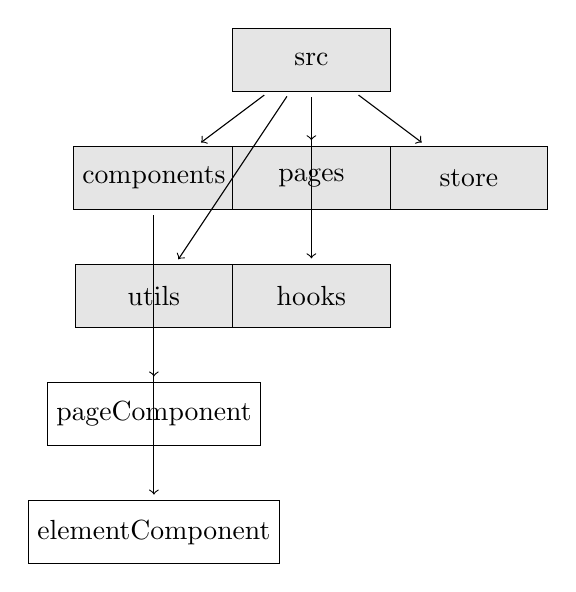
\begin{tikzpicture}[
    file/.style={draw, rectangle, minimum width=2cm, minimum height=0.8cm},
    folder/.style={draw, rectangle, minimum width=2cm, minimum height=0.8cm, fill=gray!20},
    arrow/.style={->, shorten >=2pt, shorten <=2pt}
]

% Folders
\node[folder] (src) at (0,0) {src};
\node[folder] (components) at (-2,-1.5) {components};
\node[folder] (pages) at (0,-1.5) {pages};
\node[folder] (store) at (2,-1.5) {store};
\node[folder] (utils) at (-2,-3) {utils};
\node[folder] (hooks) at (0,-3) {hooks};

% Files
\node[file] (pageComponent) at (-2,-4.5) {pageComponent};
\node[file] (elementComponent) at (-2,-6) {elementComponent};
% ... add more files

% Connections
\draw[arrow] (src) -- (components);
\draw[arrow] (src) -- (pages);
\draw[arrow] (src) -- (store);
\draw[arrow] (src) -- (utils);
\draw[arrow] (src) -- (hooks);
\draw[arrow] (components) -- (pageComponent);
\draw[arrow] (components) -- (elementComponent);
% ... add more connections

\end{tikzpicture}



\pagebreak
\subsubsection{Back-end}
The backend uses the dotNet framework. The development language using the C\# language.

In this project, the backend uses the Onion Architecture.
The Onion Architecture is a typically layered architecture, 
where each layer depends on the inner layer and provides interfaces to the outer layer.
The outer layer provides services to the outermost layer 
and other modules in the same layer based on the interfaces of the inner layer.

From inner to outer, the layers are: Domain, Application, Infrastructure, Presentation.
The Domain layer is the core layer and the innermost layer, used to define domain models, 
which are the business models.
It includes domain models and domain service interfaces.
Domain models are used to define the business models, 
which are the entities in the entity-relationship model and their attributes.
Domain service interfaces are used to define the business services, 
which are the relationships between entities in the entity-relationship model.

The Application layer is the application layer, 
used to define application services, which are the business logic.
It includes domain service implementations and application service interfaces.
Domain service implementations implement the methods of the inner layer's domain service 
interfaces and implement the business logic of the domain models.
Application service interfaces are used to define application services, 
which are the business logic.
It includes but is not limited to database interfaces, testing interfaces, 
HTTP API interfaces, MQTT interfaces, etc.

The Infrastructure layer is the infrastructure layer, used to define infrastructure.
It includes database implementations, testing implementations, 
HTTP API implementations, MQTT implementations, etc.
Database implementations implement the database interfaces 
and provide CRUD services for the database.
Testing implementations implement the testing interfaces 
and provide services for unit testing and integration testing.
HTTP API implementations implement the HTTP API interfaces 
and provide CRUD operations for HTTP APIs.
MQTT implementations implement the MQTT interfaces 
and provide CRUD operations for MQTT.

The Presentation layer is the presentation layer, used to define presentation logic, 
such as interfaces and pages. Since this is a backend project,
data presentation and control are handled by the frontend, 
so this layer is not needed.



\pagebreak
\subsubsection{Data communication and storage}
% 关于本项目的数据通信与数据存储的设计, 包括数据通信的协议, 数据存储的设计等
% 关于数据通信的设计:
% 1. 通信协议的选择
% 自前端向后端发送的数据, 有三种传输的数据类型, 
% 一种是普通的增删改查的请求, 对数据传输的时效性要求不高, 但是对数据的准确性, 完整性, 有序性, 安全性有一定的要求,
% 这种数据的传输, 采用 HTTP 协议, 以及 RESTful API 的设计. 可以有效的保证对数据传输的以上要求.
% 一种是对数据通道的创建和流媒体数据的传输, 对数据传输的时效性, 安全性要求较高, 这种数据的传输, 采用 WebRTC 协议, 以及 MQTT 协议.
% 配合可以快速解码的 flatbuffers 协议, 可以有效的保证对数据传输的以上要求.
% 最后一种是对设备的状态信息和操作信息的传输, 对完整性, 有序性, 安全性都有较高的要求, 这种数据的传输, 采用 MQTT 协议
% 同时也使用了 flatbuffers 协议.
% 
% 2. 数据通信的通信架构和通信流程
% 本项目的数据通信的通信架构, 是基于前后端分离的架构, 前端使用 React 框架, 后端使用 dotnet 框架.
% 当前端需要向后端发送数据的时候, 前端会向后端发送 HTTP 请求, 后端接收到 HTTP 请求之后, 会根据请求的数据类型,
% 选择不同的数据处理方式, 对于普通的增删改查的请求, 后端会根据 RESTful API 的设计, 对数据进行增删改查的操作,
% 对于对数据通道的创建和流媒体数据的传输, 后端会根据 WebRTC 协议, 对数据通道进行创建, 并且帮助前端和设备建立数据通道,
% 当数据通道建立后, 前端和设备之间则使用 flatbuffer 的数据格式对流媒体数据进行传输,
% 对于设备的状态信息和操作信息的传输, 前端会直接向 MQTT broker 发送 MQTT 请求, 
% 设备会在其自身的固件中监听相关的 MQTT 请求, 并且返回相关的数据.
% 
% 3. 数据通信的格式
% 本项目的数据通信的格式, 有三种, 
% 一种是 HTTP 协议, 
% 使用 json 格式对数据进行传输,
% 一种是 WebRTC 协议, 
% 使用 flatbuffers 格式对数据进行传输,
% 一种是 MQTT 协议.
% 使用 flatbuffers 格式对数据进行传输,
% 
% 关于数据存储的设计:
% 1. 数据存储的数据库的选择
% 本项目的数据存储的数据库的选择, 使用了轻量级的数据库 SQLite,
% SQLite 是一个进程内的库, 实现了自给自足的, 无服务器的, 零配置的, 事务性的 SQL 数据库引擎.
% 这是因为整个项目的目的是为了实现前端与设备之间的数据通信, 对于数据库数据的增删改查操作的要求不高,
% 数据量较小, 且对于数据库的数据的事务性要求不高, 所以选择了 SQLite 数据库.
% 2. 项目前后端的数据结构的设计
% 在本项目中, 前端由于使用了 React 框架, 所以前端的数据结构的设计, 使用了基于状态的数据结构的设计,
% 每个组件或者数据集都包含一个状态对象, 这个状态对象的属性就是组件的各个状态. 
% 使用状态对象的原因是, 可以方便的对状态进行管理, 采用对象-属性的形式, 可以方便的针对不同组件的同类状态进行区分,
% 由于跨组件的状态是由 redux 进行管理的, 这种状态对象的设计, 可以更搞笑的对状态进行更新和传递.
% 后端由于使用了 dotnet 框架, 所以后端的数据结构的设计, 使用了基于类的数据结构的设计,
% 采用了面向对象的编程思想, 对数据进行了封装, 使得数据的传输更加的安全, 有序, 完整.


\pagebreak

% \subsection{Domain model}
% \documentclass[]{article}
\usepackage{graphicx}
\usepackage{amsmath}
\usepackage{tikz}

% libaries
\usetikzlibrary{shapes,arrows}

%Define the listing package
\usepackage{listings} %code highlighter
\usepackage{color} %use color
\definecolor{mygreen}{rgb}{0,0.6,0}
\definecolor{mygray}{rgb}{0.5,0.5,0.5}
\definecolor{mymauve}{rgb}{0.58,0,0.82}

%Customize a bit the look
\lstset{ %
backgroundcolor=\color{white}, % choose the background color; you must add \usepackage{color} or \usepackage{xcolor}
basicstyle=\footnotesize, % the size of the fonts that are used for the code
breakatwhitespace=false, % sets if automatic breaks should only happen at whitespace
breaklines=true, % sets automatic line breaking
captionpos=b, % sets the caption-position to bottom
commentstyle=\color{mygreen}, % comment style
deletekeywords={...}, % if you want to delete keywords from the given language
escapeinside={\%*}{*)}, % if you want to add LaTeX within your code
extendedchars=true, % lets you use non-ASCII characters; for 8-bits encodings only, does not work with UTF-8
frame=single, % adds a frame around the code
keepspaces=true, % keeps spaces in text, useful for keeping indentation of code (possibly needs columns=flexible)
keywordstyle=\color{blue}, % keyword style
% language=Octave, % the language of the code
morekeywords={*,...}, % if you want to add more keywords to the set
numbers=left, % where to put the line-numbers; possible values are (none, left, right)
numbersep=5pt, % how far the line-numbers are from the code
numberstyle=\tiny\color{mygray}, % the style that is used for the line-numbers
rulecolor=\color{black}, % if not set, the frame-color may be changed on line-breaks within not-black text (e.g. comments (green here))
showspaces=false, % show spaces everywhere adding particular underscores; it overrides 'showstringspaces'
showstringspaces=false, % underline spaces within strings only
showtabs=false, % show tabs within strings adding particular underscores
stepnumber=1, % the step between two line-numbers. If it's 1, each line will be numbered
stringstyle=\color{mymauve}, % string literal style
tabsize=2, % sets default tabsize to 2 spaces
title=\lstname % show the filename of files included with \lstinputlisting; also try caption instead of title
}

\definecolor{darkgray}{rgb}{.4,.4,.4}
\definecolor{purple}{rgb}{0.65, 0.12, 0.82}

\lstdefinelanguage{React}{
keywords={const, typeof, new, true, false, catch, function, return, null, catch, switch, var, if, in, while, do, else, case, break},
keywordstyle=\color{blue}\bfseries,
ndkeywords={class, export, boolean, throw, implements, import, this},
ndkeywordstyle=\color{darkgray}\bfseries,
identifierstyle=\color{mygreen},
sensitive=false,
comment=[l]{//},
morecomment=[s]{/*}{*/},
commentstyle=\color{purple}\ttfamily,
string=[b]{"}{'}{`},
stringstyle=\color{red}\ttfamily,
morestring=[b]',
morestring=[b]",
morestring=[b]`',
}

\lstdefinelanguage{CSharp}{
keywords={const, typeof, new, true, false, catch, function, return, null, catch, switch, var, if, in, while, do, else, case, break},
keywordstyle=\color{blue}\bfseries,
ndkeywords={class, export, boolean, throw, implements, import, this},
ndkeywordstyle=\color{darkgray}\bfseries,
identifierstyle=\color{mygreen},
sensitive=false,
comment=[l]{//},
morecomment=[s]{/*}{*/},
commentstyle=\color{purple}\ttfamily,
string=[b]{"}{'}{`},
stringstyle=\color{red}\ttfamily,
morestring=[b]',
morestring=[b]",
morestring=[b]`',
}

\lstset{
language=React,
extendedchars=true,
basicstyle=\footnotesize\ttfamily,
showstringspaces=false,
showspaces=false,
numbers=left,
numberstyle=\footnotesize,
numbersep=9pt,
tabsize=2,
breaklines=true,
showtabs=false,
captionpos=b
}

\lstset{
language=CSharp,
extendedchars=true,
basicstyle=\footnotesize\ttfamily,
showstringspaces=false,
showspaces=false,
numbers=left,
numberstyle=\footnotesize,
numbersep=9pt,
tabsize=2,
breaklines=true,
showtabs=false,
captionpos=b
}

% \usepackage{cite} % Add this line for citation

% \bibliographystyle{plain}

\title{
The implementation of BifrostConnect Front-end scope, 
re-design and development with the relevant back-end support develop.
}
\author{
    Fei Gu \\
    Erhvervs Akademi Sydvest \\
    Computer Science 21\\
    }
\date{\today}

\begin{document}

% Front page
\maketitle
\begin{center}
    Supervisor: Henrik Boulund Meng Hansen \\
    Company: BifrostConnect \\
    Engineering Director: Jasper Wass \\
\end{center}
\tableofcontents
\pagebreak


% The introduction
\section{Introduction}
\subsection{Background}\input{sections/introduction/background.tex}
\subsection{The company}\input{sections/introduction/aboutCompany}
\subsection{The project}\input{sections/introduction/aboutProject}
\pagebreak

% The problem statement
\section{Problem Statement}
\subsection{Statement}
\input{sections/problemStatement/statement}
\subsection{Situation}
\input{sections/problemStatement/situation}
\subsection{Potential Solution}
\input{sections/problemStatement/potentialSolution}
\pagebreak

% Requirement analysis
\section{Requirement Analysis}
\input{sections/requirementAnalysis/index}

\subsection{Stakeholders}
\input{sections/requirementAnalysis/stakeholders/index}

\subsection{Business Domain}
\input{sections/requirementAnalysis/bussinesDomain/index}

\subsection{Scope}
\input{sections/requirementAnalysis/scope}

\subsection{Goals}
\input{sections/requirementAnalysis/goals}
\pagebreak

% Software Design
\section{Software Design}
% developement methods
\subsection{Software Development Methods}
\input{sections/softwareDevelopmentMethods/index}
\subsubsection{Agile Software Development}
\input{sections/softwareDevelopmentMethods/agileSoftwareDevelopment/index}
\subsubsection{Feature Driven Development}
\input{sections/softwareDevelopmentMethods/featureDrivenDevelopment/index}

\pagebreak

% Technology seslection
\subsection{Technology selection}
\input{sections/softwareDesign/technologySelection/index}
\subsubsection{Front-end}
\input{sections/softwareDesign/technologySelection/frontEnd}            
\subsubsection{Back-end}
\input{sections/softwareDesign/technologySelection/backEnd}            
\subsubsection{Database}
\input{sections/softwareDesign/technologySelection/database}
\subsubsection{Data communication}
\input{sections/softwareDesign/technologySelection/dataCommunication}            
\subsubsection{DevOps}
\input{sections/softwareDesign/technologySelection/devOps}
\pagebreak

% Architecture design
\subsection{Architecture design}
\input{sections/softwareDesign/architectureDesign/index}
\pagebreak
\subsubsection{Front-end}
\input{sections/softwareDesign/architectureDesign/frontEndArchitecture}
\pagebreak
\subsubsection{Back-end}
\input{sections/softwareDesign/architectureDesign/backEndArchitecture}
\pagebreak
\subsubsection{Data communication and storage}
\input{sections/softwareDesign/architectureDesign/dataCommunicationArchitecture}
\pagebreak

% \subsection{Domain model}
% \input{sections/softwareDesign/domainModel/index}
% \subsection{Database design}
% % 数据库领域模型 ER 图
% % 包括表和字段的设置.
% % 对于私有键和外键的设置.

% \subsection{Back-end design}
% % 后端对象模型
% % 以及对于对象模型的增删改查
% % 以及相关的其他服务的设计`'

% \subsection{Front-end design}
% % 对于前端的页面结构的设计 
% % 页面的状态的设计, 交互设计

% \subsection{FlatBuffers design}
% % schema 的设计

\subsection{DevOps CI/CD process design}
\input{sections/softwareDesign/devOpsDesign/index}
\subsubsection{Continuous Integration}
\input{sections/softwareDesign/devOpsDesign/continuousIntegration/index}
\subsubsection{Continuous Delivery}
\input{sections/softwareDesign/devOpsDesign/continuousDelivery/index}
\subsubsection{Continuous Deployment}
\input{sections/softwareDesign/devOpsDesign/continuousDeployment/index}
\pagebreak

\section{Software Development} 
\input{sections/softwareDevelopment/index}
\subsection{Overall development}
\input{sections/softwareDevelopment/overallDevelopement/index}
\subsubsection{Front-end}
\input{sections/softwareDevelopment/overallDevelopement/frontEnd/index}
\subsubsection{Back-end}
\input{sections/softwareDevelopment/overallDevelopement/backEnd/index}
\subsubsection{DevOps}
\input{sections/softwareDevelopment/overallDevelopement/devOps/index}
\subsection{Feature development} 
\input{sections/softwareDevelopment/featureDevelopment/index}
\subsubsection{Use Case 1}
\input{sections/softwareDevelopment/featureDevelopment/useCase1/index}
\subsubsection{Feature 1}
\input{sections/softwareDevelopment/featureDevelopment/feature/feature1.tex}
\pagebreak
\section{Conclusion} 
\subsection{Result}
Since the project is still in progress, the result is not available yet.
So far, basic structure of this project has been built. But the most features 
are not implemented yet. 
\subsection{Discussion}
As a single developer for this project, I am confident what I have done so far.
And I can say I understand the most of the knowledge I have used in this project, 
which also means I can explain all the part of the project. 
But this project also relevant some of the complex knowledge which I have to continue 
to study and practice.
\subsection{Future Work}
The future work is to implement the rest of the features. 
Including the most important part which is the 'create session' feature.
\pagebreak
% \bibliography{bibliography}
\pagebreak
% \begin{appendices}
%     \section{Appendix}
% \end{appendices} 
\end{document}
% \subsection{Database design}
% % 数据库领域模型 ER 图
% % 包括表和字段的设置.
% % 对于私有键和外键的设置.

% \subsection{Back-end design}
% % 后端对象模型
% % 以及对于对象模型的增删改查
% % 以及相关的其他服务的设计`'

% \subsection{Front-end design}
% % 对于前端的页面结构的设计 
% % 页面的状态的设计, 交互设计

% \subsection{FlatBuffers design}
% % schema 的设计

\subsection{DevOps CI/CD process design}
\documentclass[]{article}
\usepackage{graphicx}
\usepackage{amsmath}
\usepackage{tikz}

% libaries
\usetikzlibrary{shapes,arrows}

%Define the listing package
\usepackage{listings} %code highlighter
\usepackage{color} %use color
\definecolor{mygreen}{rgb}{0,0.6,0}
\definecolor{mygray}{rgb}{0.5,0.5,0.5}
\definecolor{mymauve}{rgb}{0.58,0,0.82}

%Customize a bit the look
\lstset{ %
backgroundcolor=\color{white}, % choose the background color; you must add \usepackage{color} or \usepackage{xcolor}
basicstyle=\footnotesize, % the size of the fonts that are used for the code
breakatwhitespace=false, % sets if automatic breaks should only happen at whitespace
breaklines=true, % sets automatic line breaking
captionpos=b, % sets the caption-position to bottom
commentstyle=\color{mygreen}, % comment style
deletekeywords={...}, % if you want to delete keywords from the given language
escapeinside={\%*}{*)}, % if you want to add LaTeX within your code
extendedchars=true, % lets you use non-ASCII characters; for 8-bits encodings only, does not work with UTF-8
frame=single, % adds a frame around the code
keepspaces=true, % keeps spaces in text, useful for keeping indentation of code (possibly needs columns=flexible)
keywordstyle=\color{blue}, % keyword style
% language=Octave, % the language of the code
morekeywords={*,...}, % if you want to add more keywords to the set
numbers=left, % where to put the line-numbers; possible values are (none, left, right)
numbersep=5pt, % how far the line-numbers are from the code
numberstyle=\tiny\color{mygray}, % the style that is used for the line-numbers
rulecolor=\color{black}, % if not set, the frame-color may be changed on line-breaks within not-black text (e.g. comments (green here))
showspaces=false, % show spaces everywhere adding particular underscores; it overrides 'showstringspaces'
showstringspaces=false, % underline spaces within strings only
showtabs=false, % show tabs within strings adding particular underscores
stepnumber=1, % the step between two line-numbers. If it's 1, each line will be numbered
stringstyle=\color{mymauve}, % string literal style
tabsize=2, % sets default tabsize to 2 spaces
title=\lstname % show the filename of files included with \lstinputlisting; also try caption instead of title
}

\definecolor{darkgray}{rgb}{.4,.4,.4}
\definecolor{purple}{rgb}{0.65, 0.12, 0.82}

\lstdefinelanguage{React}{
keywords={const, typeof, new, true, false, catch, function, return, null, catch, switch, var, if, in, while, do, else, case, break},
keywordstyle=\color{blue}\bfseries,
ndkeywords={class, export, boolean, throw, implements, import, this},
ndkeywordstyle=\color{darkgray}\bfseries,
identifierstyle=\color{mygreen},
sensitive=false,
comment=[l]{//},
morecomment=[s]{/*}{*/},
commentstyle=\color{purple}\ttfamily,
string=[b]{"}{'}{`},
stringstyle=\color{red}\ttfamily,
morestring=[b]',
morestring=[b]",
morestring=[b]`',
}

\lstdefinelanguage{CSharp}{
keywords={const, typeof, new, true, false, catch, function, return, null, catch, switch, var, if, in, while, do, else, case, break},
keywordstyle=\color{blue}\bfseries,
ndkeywords={class, export, boolean, throw, implements, import, this},
ndkeywordstyle=\color{darkgray}\bfseries,
identifierstyle=\color{mygreen},
sensitive=false,
comment=[l]{//},
morecomment=[s]{/*}{*/},
commentstyle=\color{purple}\ttfamily,
string=[b]{"}{'}{`},
stringstyle=\color{red}\ttfamily,
morestring=[b]',
morestring=[b]",
morestring=[b]`',
}

\lstset{
language=React,
extendedchars=true,
basicstyle=\footnotesize\ttfamily,
showstringspaces=false,
showspaces=false,
numbers=left,
numberstyle=\footnotesize,
numbersep=9pt,
tabsize=2,
breaklines=true,
showtabs=false,
captionpos=b
}

\lstset{
language=CSharp,
extendedchars=true,
basicstyle=\footnotesize\ttfamily,
showstringspaces=false,
showspaces=false,
numbers=left,
numberstyle=\footnotesize,
numbersep=9pt,
tabsize=2,
breaklines=true,
showtabs=false,
captionpos=b
}

% \usepackage{cite} % Add this line for citation

% \bibliographystyle{plain}

\title{
The implementation of BifrostConnect Front-end scope, 
re-design and development with the relevant back-end support develop.
}
\author{
    Fei Gu \\
    Erhvervs Akademi Sydvest \\
    Computer Science 21\\
    }
\date{\today}

\begin{document}

% Front page
\maketitle
\begin{center}
    Supervisor: Henrik Boulund Meng Hansen \\
    Company: BifrostConnect \\
    Engineering Director: Jasper Wass \\
\end{center}
\tableofcontents
\pagebreak


% The introduction
\section{Introduction}
\subsection{Background}\input{sections/introduction/background.tex}
\subsection{The company}\input{sections/introduction/aboutCompany}
\subsection{The project}\input{sections/introduction/aboutProject}
\pagebreak

% The problem statement
\section{Problem Statement}
\subsection{Statement}
\input{sections/problemStatement/statement}
\subsection{Situation}
\input{sections/problemStatement/situation}
\subsection{Potential Solution}
\input{sections/problemStatement/potentialSolution}
\pagebreak

% Requirement analysis
\section{Requirement Analysis}
\input{sections/requirementAnalysis/index}

\subsection{Stakeholders}
\input{sections/requirementAnalysis/stakeholders/index}

\subsection{Business Domain}
\input{sections/requirementAnalysis/bussinesDomain/index}

\subsection{Scope}
\input{sections/requirementAnalysis/scope}

\subsection{Goals}
\input{sections/requirementAnalysis/goals}
\pagebreak

% Software Design
\section{Software Design}
% developement methods
\subsection{Software Development Methods}
\input{sections/softwareDevelopmentMethods/index}
\subsubsection{Agile Software Development}
\input{sections/softwareDevelopmentMethods/agileSoftwareDevelopment/index}
\subsubsection{Feature Driven Development}
\input{sections/softwareDevelopmentMethods/featureDrivenDevelopment/index}

\pagebreak

% Technology seslection
\subsection{Technology selection}
\input{sections/softwareDesign/technologySelection/index}
\subsubsection{Front-end}
\input{sections/softwareDesign/technologySelection/frontEnd}            
\subsubsection{Back-end}
\input{sections/softwareDesign/technologySelection/backEnd}            
\subsubsection{Database}
\input{sections/softwareDesign/technologySelection/database}
\subsubsection{Data communication}
\input{sections/softwareDesign/technologySelection/dataCommunication}            
\subsubsection{DevOps}
\input{sections/softwareDesign/technologySelection/devOps}
\pagebreak

% Architecture design
\subsection{Architecture design}
\input{sections/softwareDesign/architectureDesign/index}
\pagebreak
\subsubsection{Front-end}
\input{sections/softwareDesign/architectureDesign/frontEndArchitecture}
\pagebreak
\subsubsection{Back-end}
\input{sections/softwareDesign/architectureDesign/backEndArchitecture}
\pagebreak
\subsubsection{Data communication and storage}
\input{sections/softwareDesign/architectureDesign/dataCommunicationArchitecture}
\pagebreak

% \subsection{Domain model}
% \input{sections/softwareDesign/domainModel/index}
% \subsection{Database design}
% % 数据库领域模型 ER 图
% % 包括表和字段的设置.
% % 对于私有键和外键的设置.

% \subsection{Back-end design}
% % 后端对象模型
% % 以及对于对象模型的增删改查
% % 以及相关的其他服务的设计`'

% \subsection{Front-end design}
% % 对于前端的页面结构的设计 
% % 页面的状态的设计, 交互设计

% \subsection{FlatBuffers design}
% % schema 的设计

\subsection{DevOps CI/CD process design}
\input{sections/softwareDesign/devOpsDesign/index}
\subsubsection{Continuous Integration}
\input{sections/softwareDesign/devOpsDesign/continuousIntegration/index}
\subsubsection{Continuous Delivery}
\input{sections/softwareDesign/devOpsDesign/continuousDelivery/index}
\subsubsection{Continuous Deployment}
\input{sections/softwareDesign/devOpsDesign/continuousDeployment/index}
\pagebreak

\section{Software Development} 
\input{sections/softwareDevelopment/index}
\subsection{Overall development}
\input{sections/softwareDevelopment/overallDevelopement/index}
\subsubsection{Front-end}
\input{sections/softwareDevelopment/overallDevelopement/frontEnd/index}
\subsubsection{Back-end}
\input{sections/softwareDevelopment/overallDevelopement/backEnd/index}
\subsubsection{DevOps}
\input{sections/softwareDevelopment/overallDevelopement/devOps/index}
\subsection{Feature development} 
\input{sections/softwareDevelopment/featureDevelopment/index}
\subsubsection{Use Case 1}
\input{sections/softwareDevelopment/featureDevelopment/useCase1/index}
\subsubsection{Feature 1}
\input{sections/softwareDevelopment/featureDevelopment/feature/feature1.tex}
\pagebreak
\section{Conclusion} 
\subsection{Result}
Since the project is still in progress, the result is not available yet.
So far, basic structure of this project has been built. But the most features 
are not implemented yet. 
\subsection{Discussion}
As a single developer for this project, I am confident what I have done so far.
And I can say I understand the most of the knowledge I have used in this project, 
which also means I can explain all the part of the project. 
But this project also relevant some of the complex knowledge which I have to continue 
to study and practice.
\subsection{Future Work}
The future work is to implement the rest of the features. 
Including the most important part which is the 'create session' feature.
\pagebreak
% \bibliography{bibliography}
\pagebreak
% \begin{appendices}
%     \section{Appendix}
% \end{appendices} 
\end{document}
\subsubsection{Continuous Integration}
\documentclass[]{article}
\usepackage{graphicx}
\usepackage{amsmath}
\usepackage{tikz}

% libaries
\usetikzlibrary{shapes,arrows}

%Define the listing package
\usepackage{listings} %code highlighter
\usepackage{color} %use color
\definecolor{mygreen}{rgb}{0,0.6,0}
\definecolor{mygray}{rgb}{0.5,0.5,0.5}
\definecolor{mymauve}{rgb}{0.58,0,0.82}

%Customize a bit the look
\lstset{ %
backgroundcolor=\color{white}, % choose the background color; you must add \usepackage{color} or \usepackage{xcolor}
basicstyle=\footnotesize, % the size of the fonts that are used for the code
breakatwhitespace=false, % sets if automatic breaks should only happen at whitespace
breaklines=true, % sets automatic line breaking
captionpos=b, % sets the caption-position to bottom
commentstyle=\color{mygreen}, % comment style
deletekeywords={...}, % if you want to delete keywords from the given language
escapeinside={\%*}{*)}, % if you want to add LaTeX within your code
extendedchars=true, % lets you use non-ASCII characters; for 8-bits encodings only, does not work with UTF-8
frame=single, % adds a frame around the code
keepspaces=true, % keeps spaces in text, useful for keeping indentation of code (possibly needs columns=flexible)
keywordstyle=\color{blue}, % keyword style
% language=Octave, % the language of the code
morekeywords={*,...}, % if you want to add more keywords to the set
numbers=left, % where to put the line-numbers; possible values are (none, left, right)
numbersep=5pt, % how far the line-numbers are from the code
numberstyle=\tiny\color{mygray}, % the style that is used for the line-numbers
rulecolor=\color{black}, % if not set, the frame-color may be changed on line-breaks within not-black text (e.g. comments (green here))
showspaces=false, % show spaces everywhere adding particular underscores; it overrides 'showstringspaces'
showstringspaces=false, % underline spaces within strings only
showtabs=false, % show tabs within strings adding particular underscores
stepnumber=1, % the step between two line-numbers. If it's 1, each line will be numbered
stringstyle=\color{mymauve}, % string literal style
tabsize=2, % sets default tabsize to 2 spaces
title=\lstname % show the filename of files included with \lstinputlisting; also try caption instead of title
}

\definecolor{darkgray}{rgb}{.4,.4,.4}
\definecolor{purple}{rgb}{0.65, 0.12, 0.82}

\lstdefinelanguage{React}{
keywords={const, typeof, new, true, false, catch, function, return, null, catch, switch, var, if, in, while, do, else, case, break},
keywordstyle=\color{blue}\bfseries,
ndkeywords={class, export, boolean, throw, implements, import, this},
ndkeywordstyle=\color{darkgray}\bfseries,
identifierstyle=\color{mygreen},
sensitive=false,
comment=[l]{//},
morecomment=[s]{/*}{*/},
commentstyle=\color{purple}\ttfamily,
string=[b]{"}{'}{`},
stringstyle=\color{red}\ttfamily,
morestring=[b]',
morestring=[b]",
morestring=[b]`',
}

\lstdefinelanguage{CSharp}{
keywords={const, typeof, new, true, false, catch, function, return, null, catch, switch, var, if, in, while, do, else, case, break},
keywordstyle=\color{blue}\bfseries,
ndkeywords={class, export, boolean, throw, implements, import, this},
ndkeywordstyle=\color{darkgray}\bfseries,
identifierstyle=\color{mygreen},
sensitive=false,
comment=[l]{//},
morecomment=[s]{/*}{*/},
commentstyle=\color{purple}\ttfamily,
string=[b]{"}{'}{`},
stringstyle=\color{red}\ttfamily,
morestring=[b]',
morestring=[b]",
morestring=[b]`',
}

\lstset{
language=React,
extendedchars=true,
basicstyle=\footnotesize\ttfamily,
showstringspaces=false,
showspaces=false,
numbers=left,
numberstyle=\footnotesize,
numbersep=9pt,
tabsize=2,
breaklines=true,
showtabs=false,
captionpos=b
}

\lstset{
language=CSharp,
extendedchars=true,
basicstyle=\footnotesize\ttfamily,
showstringspaces=false,
showspaces=false,
numbers=left,
numberstyle=\footnotesize,
numbersep=9pt,
tabsize=2,
breaklines=true,
showtabs=false,
captionpos=b
}

% \usepackage{cite} % Add this line for citation

% \bibliographystyle{plain}

\title{
The implementation of BifrostConnect Front-end scope, 
re-design and development with the relevant back-end support develop.
}
\author{
    Fei Gu \\
    Erhvervs Akademi Sydvest \\
    Computer Science 21\\
    }
\date{\today}

\begin{document}

% Front page
\maketitle
\begin{center}
    Supervisor: Henrik Boulund Meng Hansen \\
    Company: BifrostConnect \\
    Engineering Director: Jasper Wass \\
\end{center}
\tableofcontents
\pagebreak


% The introduction
\section{Introduction}
\subsection{Background}\input{sections/introduction/background.tex}
\subsection{The company}\input{sections/introduction/aboutCompany}
\subsection{The project}\input{sections/introduction/aboutProject}
\pagebreak

% The problem statement
\section{Problem Statement}
\subsection{Statement}
\input{sections/problemStatement/statement}
\subsection{Situation}
\input{sections/problemStatement/situation}
\subsection{Potential Solution}
\input{sections/problemStatement/potentialSolution}
\pagebreak

% Requirement analysis
\section{Requirement Analysis}
\input{sections/requirementAnalysis/index}

\subsection{Stakeholders}
\input{sections/requirementAnalysis/stakeholders/index}

\subsection{Business Domain}
\input{sections/requirementAnalysis/bussinesDomain/index}

\subsection{Scope}
\input{sections/requirementAnalysis/scope}

\subsection{Goals}
\input{sections/requirementAnalysis/goals}
\pagebreak

% Software Design
\section{Software Design}
% developement methods
\subsection{Software Development Methods}
\input{sections/softwareDevelopmentMethods/index}
\subsubsection{Agile Software Development}
\input{sections/softwareDevelopmentMethods/agileSoftwareDevelopment/index}
\subsubsection{Feature Driven Development}
\input{sections/softwareDevelopmentMethods/featureDrivenDevelopment/index}

\pagebreak

% Technology seslection
\subsection{Technology selection}
\input{sections/softwareDesign/technologySelection/index}
\subsubsection{Front-end}
\input{sections/softwareDesign/technologySelection/frontEnd}            
\subsubsection{Back-end}
\input{sections/softwareDesign/technologySelection/backEnd}            
\subsubsection{Database}
\input{sections/softwareDesign/technologySelection/database}
\subsubsection{Data communication}
\input{sections/softwareDesign/technologySelection/dataCommunication}            
\subsubsection{DevOps}
\input{sections/softwareDesign/technologySelection/devOps}
\pagebreak

% Architecture design
\subsection{Architecture design}
\input{sections/softwareDesign/architectureDesign/index}
\pagebreak
\subsubsection{Front-end}
\input{sections/softwareDesign/architectureDesign/frontEndArchitecture}
\pagebreak
\subsubsection{Back-end}
\input{sections/softwareDesign/architectureDesign/backEndArchitecture}
\pagebreak
\subsubsection{Data communication and storage}
\input{sections/softwareDesign/architectureDesign/dataCommunicationArchitecture}
\pagebreak

% \subsection{Domain model}
% \input{sections/softwareDesign/domainModel/index}
% \subsection{Database design}
% % 数据库领域模型 ER 图
% % 包括表和字段的设置.
% % 对于私有键和外键的设置.

% \subsection{Back-end design}
% % 后端对象模型
% % 以及对于对象模型的增删改查
% % 以及相关的其他服务的设计`'

% \subsection{Front-end design}
% % 对于前端的页面结构的设计 
% % 页面的状态的设计, 交互设计

% \subsection{FlatBuffers design}
% % schema 的设计

\subsection{DevOps CI/CD process design}
\input{sections/softwareDesign/devOpsDesign/index}
\subsubsection{Continuous Integration}
\input{sections/softwareDesign/devOpsDesign/continuousIntegration/index}
\subsubsection{Continuous Delivery}
\input{sections/softwareDesign/devOpsDesign/continuousDelivery/index}
\subsubsection{Continuous Deployment}
\input{sections/softwareDesign/devOpsDesign/continuousDeployment/index}
\pagebreak

\section{Software Development} 
\input{sections/softwareDevelopment/index}
\subsection{Overall development}
\input{sections/softwareDevelopment/overallDevelopement/index}
\subsubsection{Front-end}
\input{sections/softwareDevelopment/overallDevelopement/frontEnd/index}
\subsubsection{Back-end}
\input{sections/softwareDevelopment/overallDevelopement/backEnd/index}
\subsubsection{DevOps}
\input{sections/softwareDevelopment/overallDevelopement/devOps/index}
\subsection{Feature development} 
\input{sections/softwareDevelopment/featureDevelopment/index}
\subsubsection{Use Case 1}
\input{sections/softwareDevelopment/featureDevelopment/useCase1/index}
\subsubsection{Feature 1}
\input{sections/softwareDevelopment/featureDevelopment/feature/feature1.tex}
\pagebreak
\section{Conclusion} 
\subsection{Result}
Since the project is still in progress, the result is not available yet.
So far, basic structure of this project has been built. But the most features 
are not implemented yet. 
\subsection{Discussion}
As a single developer for this project, I am confident what I have done so far.
And I can say I understand the most of the knowledge I have used in this project, 
which also means I can explain all the part of the project. 
But this project also relevant some of the complex knowledge which I have to continue 
to study and practice.
\subsection{Future Work}
The future work is to implement the rest of the features. 
Including the most important part which is the 'create session' feature.
\pagebreak
% \bibliography{bibliography}
\pagebreak
% \begin{appendices}
%     \section{Appendix}
% \end{appendices} 
\end{document}
\subsubsection{Continuous Delivery}
\documentclass[]{article}
\usepackage{graphicx}
\usepackage{amsmath}
\usepackage{tikz}

% libaries
\usetikzlibrary{shapes,arrows}

%Define the listing package
\usepackage{listings} %code highlighter
\usepackage{color} %use color
\definecolor{mygreen}{rgb}{0,0.6,0}
\definecolor{mygray}{rgb}{0.5,0.5,0.5}
\definecolor{mymauve}{rgb}{0.58,0,0.82}

%Customize a bit the look
\lstset{ %
backgroundcolor=\color{white}, % choose the background color; you must add \usepackage{color} or \usepackage{xcolor}
basicstyle=\footnotesize, % the size of the fonts that are used for the code
breakatwhitespace=false, % sets if automatic breaks should only happen at whitespace
breaklines=true, % sets automatic line breaking
captionpos=b, % sets the caption-position to bottom
commentstyle=\color{mygreen}, % comment style
deletekeywords={...}, % if you want to delete keywords from the given language
escapeinside={\%*}{*)}, % if you want to add LaTeX within your code
extendedchars=true, % lets you use non-ASCII characters; for 8-bits encodings only, does not work with UTF-8
frame=single, % adds a frame around the code
keepspaces=true, % keeps spaces in text, useful for keeping indentation of code (possibly needs columns=flexible)
keywordstyle=\color{blue}, % keyword style
% language=Octave, % the language of the code
morekeywords={*,...}, % if you want to add more keywords to the set
numbers=left, % where to put the line-numbers; possible values are (none, left, right)
numbersep=5pt, % how far the line-numbers are from the code
numberstyle=\tiny\color{mygray}, % the style that is used for the line-numbers
rulecolor=\color{black}, % if not set, the frame-color may be changed on line-breaks within not-black text (e.g. comments (green here))
showspaces=false, % show spaces everywhere adding particular underscores; it overrides 'showstringspaces'
showstringspaces=false, % underline spaces within strings only
showtabs=false, % show tabs within strings adding particular underscores
stepnumber=1, % the step between two line-numbers. If it's 1, each line will be numbered
stringstyle=\color{mymauve}, % string literal style
tabsize=2, % sets default tabsize to 2 spaces
title=\lstname % show the filename of files included with \lstinputlisting; also try caption instead of title
}

\definecolor{darkgray}{rgb}{.4,.4,.4}
\definecolor{purple}{rgb}{0.65, 0.12, 0.82}

\lstdefinelanguage{React}{
keywords={const, typeof, new, true, false, catch, function, return, null, catch, switch, var, if, in, while, do, else, case, break},
keywordstyle=\color{blue}\bfseries,
ndkeywords={class, export, boolean, throw, implements, import, this},
ndkeywordstyle=\color{darkgray}\bfseries,
identifierstyle=\color{mygreen},
sensitive=false,
comment=[l]{//},
morecomment=[s]{/*}{*/},
commentstyle=\color{purple}\ttfamily,
string=[b]{"}{'}{`},
stringstyle=\color{red}\ttfamily,
morestring=[b]',
morestring=[b]",
morestring=[b]`',
}

\lstdefinelanguage{CSharp}{
keywords={const, typeof, new, true, false, catch, function, return, null, catch, switch, var, if, in, while, do, else, case, break},
keywordstyle=\color{blue}\bfseries,
ndkeywords={class, export, boolean, throw, implements, import, this},
ndkeywordstyle=\color{darkgray}\bfseries,
identifierstyle=\color{mygreen},
sensitive=false,
comment=[l]{//},
morecomment=[s]{/*}{*/},
commentstyle=\color{purple}\ttfamily,
string=[b]{"}{'}{`},
stringstyle=\color{red}\ttfamily,
morestring=[b]',
morestring=[b]",
morestring=[b]`',
}

\lstset{
language=React,
extendedchars=true,
basicstyle=\footnotesize\ttfamily,
showstringspaces=false,
showspaces=false,
numbers=left,
numberstyle=\footnotesize,
numbersep=9pt,
tabsize=2,
breaklines=true,
showtabs=false,
captionpos=b
}

\lstset{
language=CSharp,
extendedchars=true,
basicstyle=\footnotesize\ttfamily,
showstringspaces=false,
showspaces=false,
numbers=left,
numberstyle=\footnotesize,
numbersep=9pt,
tabsize=2,
breaklines=true,
showtabs=false,
captionpos=b
}

% \usepackage{cite} % Add this line for citation

% \bibliographystyle{plain}

\title{
The implementation of BifrostConnect Front-end scope, 
re-design and development with the relevant back-end support develop.
}
\author{
    Fei Gu \\
    Erhvervs Akademi Sydvest \\
    Computer Science 21\\
    }
\date{\today}

\begin{document}

% Front page
\maketitle
\begin{center}
    Supervisor: Henrik Boulund Meng Hansen \\
    Company: BifrostConnect \\
    Engineering Director: Jasper Wass \\
\end{center}
\tableofcontents
\pagebreak


% The introduction
\section{Introduction}
\subsection{Background}\input{sections/introduction/background.tex}
\subsection{The company}\input{sections/introduction/aboutCompany}
\subsection{The project}\input{sections/introduction/aboutProject}
\pagebreak

% The problem statement
\section{Problem Statement}
\subsection{Statement}
\input{sections/problemStatement/statement}
\subsection{Situation}
\input{sections/problemStatement/situation}
\subsection{Potential Solution}
\input{sections/problemStatement/potentialSolution}
\pagebreak

% Requirement analysis
\section{Requirement Analysis}
\input{sections/requirementAnalysis/index}

\subsection{Stakeholders}
\input{sections/requirementAnalysis/stakeholders/index}

\subsection{Business Domain}
\input{sections/requirementAnalysis/bussinesDomain/index}

\subsection{Scope}
\input{sections/requirementAnalysis/scope}

\subsection{Goals}
\input{sections/requirementAnalysis/goals}
\pagebreak

% Software Design
\section{Software Design}
% developement methods
\subsection{Software Development Methods}
\input{sections/softwareDevelopmentMethods/index}
\subsubsection{Agile Software Development}
\input{sections/softwareDevelopmentMethods/agileSoftwareDevelopment/index}
\subsubsection{Feature Driven Development}
\input{sections/softwareDevelopmentMethods/featureDrivenDevelopment/index}

\pagebreak

% Technology seslection
\subsection{Technology selection}
\input{sections/softwareDesign/technologySelection/index}
\subsubsection{Front-end}
\input{sections/softwareDesign/technologySelection/frontEnd}            
\subsubsection{Back-end}
\input{sections/softwareDesign/technologySelection/backEnd}            
\subsubsection{Database}
\input{sections/softwareDesign/technologySelection/database}
\subsubsection{Data communication}
\input{sections/softwareDesign/technologySelection/dataCommunication}            
\subsubsection{DevOps}
\input{sections/softwareDesign/technologySelection/devOps}
\pagebreak

% Architecture design
\subsection{Architecture design}
\input{sections/softwareDesign/architectureDesign/index}
\pagebreak
\subsubsection{Front-end}
\input{sections/softwareDesign/architectureDesign/frontEndArchitecture}
\pagebreak
\subsubsection{Back-end}
\input{sections/softwareDesign/architectureDesign/backEndArchitecture}
\pagebreak
\subsubsection{Data communication and storage}
\input{sections/softwareDesign/architectureDesign/dataCommunicationArchitecture}
\pagebreak

% \subsection{Domain model}
% \input{sections/softwareDesign/domainModel/index}
% \subsection{Database design}
% % 数据库领域模型 ER 图
% % 包括表和字段的设置.
% % 对于私有键和外键的设置.

% \subsection{Back-end design}
% % 后端对象模型
% % 以及对于对象模型的增删改查
% % 以及相关的其他服务的设计`'

% \subsection{Front-end design}
% % 对于前端的页面结构的设计 
% % 页面的状态的设计, 交互设计

% \subsection{FlatBuffers design}
% % schema 的设计

\subsection{DevOps CI/CD process design}
\input{sections/softwareDesign/devOpsDesign/index}
\subsubsection{Continuous Integration}
\input{sections/softwareDesign/devOpsDesign/continuousIntegration/index}
\subsubsection{Continuous Delivery}
\input{sections/softwareDesign/devOpsDesign/continuousDelivery/index}
\subsubsection{Continuous Deployment}
\input{sections/softwareDesign/devOpsDesign/continuousDeployment/index}
\pagebreak

\section{Software Development} 
\input{sections/softwareDevelopment/index}
\subsection{Overall development}
\input{sections/softwareDevelopment/overallDevelopement/index}
\subsubsection{Front-end}
\input{sections/softwareDevelopment/overallDevelopement/frontEnd/index}
\subsubsection{Back-end}
\input{sections/softwareDevelopment/overallDevelopement/backEnd/index}
\subsubsection{DevOps}
\input{sections/softwareDevelopment/overallDevelopement/devOps/index}
\subsection{Feature development} 
\input{sections/softwareDevelopment/featureDevelopment/index}
\subsubsection{Use Case 1}
\input{sections/softwareDevelopment/featureDevelopment/useCase1/index}
\subsubsection{Feature 1}
\input{sections/softwareDevelopment/featureDevelopment/feature/feature1.tex}
\pagebreak
\section{Conclusion} 
\subsection{Result}
Since the project is still in progress, the result is not available yet.
So far, basic structure of this project has been built. But the most features 
are not implemented yet. 
\subsection{Discussion}
As a single developer for this project, I am confident what I have done so far.
And I can say I understand the most of the knowledge I have used in this project, 
which also means I can explain all the part of the project. 
But this project also relevant some of the complex knowledge which I have to continue 
to study and practice.
\subsection{Future Work}
The future work is to implement the rest of the features. 
Including the most important part which is the 'create session' feature.
\pagebreak
% \bibliography{bibliography}
\pagebreak
% \begin{appendices}
%     \section{Appendix}
% \end{appendices} 
\end{document}
\subsubsection{Continuous Deployment}
\documentclass[]{article}
\usepackage{graphicx}
\usepackage{amsmath}
\usepackage{tikz}

% libaries
\usetikzlibrary{shapes,arrows}

%Define the listing package
\usepackage{listings} %code highlighter
\usepackage{color} %use color
\definecolor{mygreen}{rgb}{0,0.6,0}
\definecolor{mygray}{rgb}{0.5,0.5,0.5}
\definecolor{mymauve}{rgb}{0.58,0,0.82}

%Customize a bit the look
\lstset{ %
backgroundcolor=\color{white}, % choose the background color; you must add \usepackage{color} or \usepackage{xcolor}
basicstyle=\footnotesize, % the size of the fonts that are used for the code
breakatwhitespace=false, % sets if automatic breaks should only happen at whitespace
breaklines=true, % sets automatic line breaking
captionpos=b, % sets the caption-position to bottom
commentstyle=\color{mygreen}, % comment style
deletekeywords={...}, % if you want to delete keywords from the given language
escapeinside={\%*}{*)}, % if you want to add LaTeX within your code
extendedchars=true, % lets you use non-ASCII characters; for 8-bits encodings only, does not work with UTF-8
frame=single, % adds a frame around the code
keepspaces=true, % keeps spaces in text, useful for keeping indentation of code (possibly needs columns=flexible)
keywordstyle=\color{blue}, % keyword style
% language=Octave, % the language of the code
morekeywords={*,...}, % if you want to add more keywords to the set
numbers=left, % where to put the line-numbers; possible values are (none, left, right)
numbersep=5pt, % how far the line-numbers are from the code
numberstyle=\tiny\color{mygray}, % the style that is used for the line-numbers
rulecolor=\color{black}, % if not set, the frame-color may be changed on line-breaks within not-black text (e.g. comments (green here))
showspaces=false, % show spaces everywhere adding particular underscores; it overrides 'showstringspaces'
showstringspaces=false, % underline spaces within strings only
showtabs=false, % show tabs within strings adding particular underscores
stepnumber=1, % the step between two line-numbers. If it's 1, each line will be numbered
stringstyle=\color{mymauve}, % string literal style
tabsize=2, % sets default tabsize to 2 spaces
title=\lstname % show the filename of files included with \lstinputlisting; also try caption instead of title
}

\definecolor{darkgray}{rgb}{.4,.4,.4}
\definecolor{purple}{rgb}{0.65, 0.12, 0.82}

\lstdefinelanguage{React}{
keywords={const, typeof, new, true, false, catch, function, return, null, catch, switch, var, if, in, while, do, else, case, break},
keywordstyle=\color{blue}\bfseries,
ndkeywords={class, export, boolean, throw, implements, import, this},
ndkeywordstyle=\color{darkgray}\bfseries,
identifierstyle=\color{mygreen},
sensitive=false,
comment=[l]{//},
morecomment=[s]{/*}{*/},
commentstyle=\color{purple}\ttfamily,
string=[b]{"}{'}{`},
stringstyle=\color{red}\ttfamily,
morestring=[b]',
morestring=[b]",
morestring=[b]`',
}

\lstdefinelanguage{CSharp}{
keywords={const, typeof, new, true, false, catch, function, return, null, catch, switch, var, if, in, while, do, else, case, break},
keywordstyle=\color{blue}\bfseries,
ndkeywords={class, export, boolean, throw, implements, import, this},
ndkeywordstyle=\color{darkgray}\bfseries,
identifierstyle=\color{mygreen},
sensitive=false,
comment=[l]{//},
morecomment=[s]{/*}{*/},
commentstyle=\color{purple}\ttfamily,
string=[b]{"}{'}{`},
stringstyle=\color{red}\ttfamily,
morestring=[b]',
morestring=[b]",
morestring=[b]`',
}

\lstset{
language=React,
extendedchars=true,
basicstyle=\footnotesize\ttfamily,
showstringspaces=false,
showspaces=false,
numbers=left,
numberstyle=\footnotesize,
numbersep=9pt,
tabsize=2,
breaklines=true,
showtabs=false,
captionpos=b
}

\lstset{
language=CSharp,
extendedchars=true,
basicstyle=\footnotesize\ttfamily,
showstringspaces=false,
showspaces=false,
numbers=left,
numberstyle=\footnotesize,
numbersep=9pt,
tabsize=2,
breaklines=true,
showtabs=false,
captionpos=b
}

% \usepackage{cite} % Add this line for citation

% \bibliographystyle{plain}

\title{
The implementation of BifrostConnect Front-end scope, 
re-design and development with the relevant back-end support develop.
}
\author{
    Fei Gu \\
    Erhvervs Akademi Sydvest \\
    Computer Science 21\\
    }
\date{\today}

\begin{document}

% Front page
\maketitle
\begin{center}
    Supervisor: Henrik Boulund Meng Hansen \\
    Company: BifrostConnect \\
    Engineering Director: Jasper Wass \\
\end{center}
\tableofcontents
\pagebreak


% The introduction
\section{Introduction}
\subsection{Background}\input{sections/introduction/background.tex}
\subsection{The company}\input{sections/introduction/aboutCompany}
\subsection{The project}\input{sections/introduction/aboutProject}
\pagebreak

% The problem statement
\section{Problem Statement}
\subsection{Statement}
\input{sections/problemStatement/statement}
\subsection{Situation}
\input{sections/problemStatement/situation}
\subsection{Potential Solution}
\input{sections/problemStatement/potentialSolution}
\pagebreak

% Requirement analysis
\section{Requirement Analysis}
\input{sections/requirementAnalysis/index}

\subsection{Stakeholders}
\input{sections/requirementAnalysis/stakeholders/index}

\subsection{Business Domain}
\input{sections/requirementAnalysis/bussinesDomain/index}

\subsection{Scope}
\input{sections/requirementAnalysis/scope}

\subsection{Goals}
\input{sections/requirementAnalysis/goals}
\pagebreak

% Software Design
\section{Software Design}
% developement methods
\subsection{Software Development Methods}
\input{sections/softwareDevelopmentMethods/index}
\subsubsection{Agile Software Development}
\input{sections/softwareDevelopmentMethods/agileSoftwareDevelopment/index}
\subsubsection{Feature Driven Development}
\input{sections/softwareDevelopmentMethods/featureDrivenDevelopment/index}

\pagebreak

% Technology seslection
\subsection{Technology selection}
\input{sections/softwareDesign/technologySelection/index}
\subsubsection{Front-end}
\input{sections/softwareDesign/technologySelection/frontEnd}            
\subsubsection{Back-end}
\input{sections/softwareDesign/technologySelection/backEnd}            
\subsubsection{Database}
\input{sections/softwareDesign/technologySelection/database}
\subsubsection{Data communication}
\input{sections/softwareDesign/technologySelection/dataCommunication}            
\subsubsection{DevOps}
\input{sections/softwareDesign/technologySelection/devOps}
\pagebreak

% Architecture design
\subsection{Architecture design}
\input{sections/softwareDesign/architectureDesign/index}
\pagebreak
\subsubsection{Front-end}
\input{sections/softwareDesign/architectureDesign/frontEndArchitecture}
\pagebreak
\subsubsection{Back-end}
\input{sections/softwareDesign/architectureDesign/backEndArchitecture}
\pagebreak
\subsubsection{Data communication and storage}
\input{sections/softwareDesign/architectureDesign/dataCommunicationArchitecture}
\pagebreak

% \subsection{Domain model}
% \input{sections/softwareDesign/domainModel/index}
% \subsection{Database design}
% % 数据库领域模型 ER 图
% % 包括表和字段的设置.
% % 对于私有键和外键的设置.

% \subsection{Back-end design}
% % 后端对象模型
% % 以及对于对象模型的增删改查
% % 以及相关的其他服务的设计`'

% \subsection{Front-end design}
% % 对于前端的页面结构的设计 
% % 页面的状态的设计, 交互设计

% \subsection{FlatBuffers design}
% % schema 的设计

\subsection{DevOps CI/CD process design}
\input{sections/softwareDesign/devOpsDesign/index}
\subsubsection{Continuous Integration}
\input{sections/softwareDesign/devOpsDesign/continuousIntegration/index}
\subsubsection{Continuous Delivery}
\input{sections/softwareDesign/devOpsDesign/continuousDelivery/index}
\subsubsection{Continuous Deployment}
\input{sections/softwareDesign/devOpsDesign/continuousDeployment/index}
\pagebreak

\section{Software Development} 
\input{sections/softwareDevelopment/index}
\subsection{Overall development}
\input{sections/softwareDevelopment/overallDevelopement/index}
\subsubsection{Front-end}
\input{sections/softwareDevelopment/overallDevelopement/frontEnd/index}
\subsubsection{Back-end}
\input{sections/softwareDevelopment/overallDevelopement/backEnd/index}
\subsubsection{DevOps}
\input{sections/softwareDevelopment/overallDevelopement/devOps/index}
\subsection{Feature development} 
\input{sections/softwareDevelopment/featureDevelopment/index}
\subsubsection{Use Case 1}
\input{sections/softwareDevelopment/featureDevelopment/useCase1/index}
\subsubsection{Feature 1}
\input{sections/softwareDevelopment/featureDevelopment/feature/feature1.tex}
\pagebreak
\section{Conclusion} 
\subsection{Result}
Since the project is still in progress, the result is not available yet.
So far, basic structure of this project has been built. But the most features 
are not implemented yet. 
\subsection{Discussion}
As a single developer for this project, I am confident what I have done so far.
And I can say I understand the most of the knowledge I have used in this project, 
which also means I can explain all the part of the project. 
But this project also relevant some of the complex knowledge which I have to continue 
to study and practice.
\subsection{Future Work}
The future work is to implement the rest of the features. 
Including the most important part which is the 'create session' feature.
\pagebreak
% \bibliography{bibliography}
\pagebreak
% \begin{appendices}
%     \section{Appendix}
% \end{appendices} 
\end{document}
\pagebreak

\section{Software Development} 
\documentclass[]{article}
\usepackage{graphicx}
\usepackage{amsmath}
\usepackage{tikz}

% libaries
\usetikzlibrary{shapes,arrows}

%Define the listing package
\usepackage{listings} %code highlighter
\usepackage{color} %use color
\definecolor{mygreen}{rgb}{0,0.6,0}
\definecolor{mygray}{rgb}{0.5,0.5,0.5}
\definecolor{mymauve}{rgb}{0.58,0,0.82}

%Customize a bit the look
\lstset{ %
backgroundcolor=\color{white}, % choose the background color; you must add \usepackage{color} or \usepackage{xcolor}
basicstyle=\footnotesize, % the size of the fonts that are used for the code
breakatwhitespace=false, % sets if automatic breaks should only happen at whitespace
breaklines=true, % sets automatic line breaking
captionpos=b, % sets the caption-position to bottom
commentstyle=\color{mygreen}, % comment style
deletekeywords={...}, % if you want to delete keywords from the given language
escapeinside={\%*}{*)}, % if you want to add LaTeX within your code
extendedchars=true, % lets you use non-ASCII characters; for 8-bits encodings only, does not work with UTF-8
frame=single, % adds a frame around the code
keepspaces=true, % keeps spaces in text, useful for keeping indentation of code (possibly needs columns=flexible)
keywordstyle=\color{blue}, % keyword style
% language=Octave, % the language of the code
morekeywords={*,...}, % if you want to add more keywords to the set
numbers=left, % where to put the line-numbers; possible values are (none, left, right)
numbersep=5pt, % how far the line-numbers are from the code
numberstyle=\tiny\color{mygray}, % the style that is used for the line-numbers
rulecolor=\color{black}, % if not set, the frame-color may be changed on line-breaks within not-black text (e.g. comments (green here))
showspaces=false, % show spaces everywhere adding particular underscores; it overrides 'showstringspaces'
showstringspaces=false, % underline spaces within strings only
showtabs=false, % show tabs within strings adding particular underscores
stepnumber=1, % the step between two line-numbers. If it's 1, each line will be numbered
stringstyle=\color{mymauve}, % string literal style
tabsize=2, % sets default tabsize to 2 spaces
title=\lstname % show the filename of files included with \lstinputlisting; also try caption instead of title
}

\definecolor{darkgray}{rgb}{.4,.4,.4}
\definecolor{purple}{rgb}{0.65, 0.12, 0.82}

\lstdefinelanguage{React}{
keywords={const, typeof, new, true, false, catch, function, return, null, catch, switch, var, if, in, while, do, else, case, break},
keywordstyle=\color{blue}\bfseries,
ndkeywords={class, export, boolean, throw, implements, import, this},
ndkeywordstyle=\color{darkgray}\bfseries,
identifierstyle=\color{mygreen},
sensitive=false,
comment=[l]{//},
morecomment=[s]{/*}{*/},
commentstyle=\color{purple}\ttfamily,
string=[b]{"}{'}{`},
stringstyle=\color{red}\ttfamily,
morestring=[b]',
morestring=[b]",
morestring=[b]`',
}

\lstdefinelanguage{CSharp}{
keywords={const, typeof, new, true, false, catch, function, return, null, catch, switch, var, if, in, while, do, else, case, break},
keywordstyle=\color{blue}\bfseries,
ndkeywords={class, export, boolean, throw, implements, import, this},
ndkeywordstyle=\color{darkgray}\bfseries,
identifierstyle=\color{mygreen},
sensitive=false,
comment=[l]{//},
morecomment=[s]{/*}{*/},
commentstyle=\color{purple}\ttfamily,
string=[b]{"}{'}{`},
stringstyle=\color{red}\ttfamily,
morestring=[b]',
morestring=[b]",
morestring=[b]`',
}

\lstset{
language=React,
extendedchars=true,
basicstyle=\footnotesize\ttfamily,
showstringspaces=false,
showspaces=false,
numbers=left,
numberstyle=\footnotesize,
numbersep=9pt,
tabsize=2,
breaklines=true,
showtabs=false,
captionpos=b
}

\lstset{
language=CSharp,
extendedchars=true,
basicstyle=\footnotesize\ttfamily,
showstringspaces=false,
showspaces=false,
numbers=left,
numberstyle=\footnotesize,
numbersep=9pt,
tabsize=2,
breaklines=true,
showtabs=false,
captionpos=b
}

% \usepackage{cite} % Add this line for citation

% \bibliographystyle{plain}

\title{
The implementation of BifrostConnect Front-end scope, 
re-design and development with the relevant back-end support develop.
}
\author{
    Fei Gu \\
    Erhvervs Akademi Sydvest \\
    Computer Science 21\\
    }
\date{\today}

\begin{document}

% Front page
\maketitle
\begin{center}
    Supervisor: Henrik Boulund Meng Hansen \\
    Company: BifrostConnect \\
    Engineering Director: Jasper Wass \\
\end{center}
\tableofcontents
\pagebreak


% The introduction
\section{Introduction}
\subsection{Background}\input{sections/introduction/background.tex}
\subsection{The company}\input{sections/introduction/aboutCompany}
\subsection{The project}\input{sections/introduction/aboutProject}
\pagebreak

% The problem statement
\section{Problem Statement}
\subsection{Statement}
\input{sections/problemStatement/statement}
\subsection{Situation}
\input{sections/problemStatement/situation}
\subsection{Potential Solution}
\input{sections/problemStatement/potentialSolution}
\pagebreak

% Requirement analysis
\section{Requirement Analysis}
\input{sections/requirementAnalysis/index}

\subsection{Stakeholders}
\input{sections/requirementAnalysis/stakeholders/index}

\subsection{Business Domain}
\input{sections/requirementAnalysis/bussinesDomain/index}

\subsection{Scope}
\input{sections/requirementAnalysis/scope}

\subsection{Goals}
\input{sections/requirementAnalysis/goals}
\pagebreak

% Software Design
\section{Software Design}
% developement methods
\subsection{Software Development Methods}
\input{sections/softwareDevelopmentMethods/index}
\subsubsection{Agile Software Development}
\input{sections/softwareDevelopmentMethods/agileSoftwareDevelopment/index}
\subsubsection{Feature Driven Development}
\input{sections/softwareDevelopmentMethods/featureDrivenDevelopment/index}

\pagebreak

% Technology seslection
\subsection{Technology selection}
\input{sections/softwareDesign/technologySelection/index}
\subsubsection{Front-end}
\input{sections/softwareDesign/technologySelection/frontEnd}            
\subsubsection{Back-end}
\input{sections/softwareDesign/technologySelection/backEnd}            
\subsubsection{Database}
\input{sections/softwareDesign/technologySelection/database}
\subsubsection{Data communication}
\input{sections/softwareDesign/technologySelection/dataCommunication}            
\subsubsection{DevOps}
\input{sections/softwareDesign/technologySelection/devOps}
\pagebreak

% Architecture design
\subsection{Architecture design}
\input{sections/softwareDesign/architectureDesign/index}
\pagebreak
\subsubsection{Front-end}
\input{sections/softwareDesign/architectureDesign/frontEndArchitecture}
\pagebreak
\subsubsection{Back-end}
\input{sections/softwareDesign/architectureDesign/backEndArchitecture}
\pagebreak
\subsubsection{Data communication and storage}
\input{sections/softwareDesign/architectureDesign/dataCommunicationArchitecture}
\pagebreak

% \subsection{Domain model}
% \input{sections/softwareDesign/domainModel/index}
% \subsection{Database design}
% % 数据库领域模型 ER 图
% % 包括表和字段的设置.
% % 对于私有键和外键的设置.

% \subsection{Back-end design}
% % 后端对象模型
% % 以及对于对象模型的增删改查
% % 以及相关的其他服务的设计`'

% \subsection{Front-end design}
% % 对于前端的页面结构的设计 
% % 页面的状态的设计, 交互设计

% \subsection{FlatBuffers design}
% % schema 的设计

\subsection{DevOps CI/CD process design}
\input{sections/softwareDesign/devOpsDesign/index}
\subsubsection{Continuous Integration}
\input{sections/softwareDesign/devOpsDesign/continuousIntegration/index}
\subsubsection{Continuous Delivery}
\input{sections/softwareDesign/devOpsDesign/continuousDelivery/index}
\subsubsection{Continuous Deployment}
\input{sections/softwareDesign/devOpsDesign/continuousDeployment/index}
\pagebreak

\section{Software Development} 
\input{sections/softwareDevelopment/index}
\subsection{Overall development}
\input{sections/softwareDevelopment/overallDevelopement/index}
\subsubsection{Front-end}
\input{sections/softwareDevelopment/overallDevelopement/frontEnd/index}
\subsubsection{Back-end}
\input{sections/softwareDevelopment/overallDevelopement/backEnd/index}
\subsubsection{DevOps}
\input{sections/softwareDevelopment/overallDevelopement/devOps/index}
\subsection{Feature development} 
\input{sections/softwareDevelopment/featureDevelopment/index}
\subsubsection{Use Case 1}
\input{sections/softwareDevelopment/featureDevelopment/useCase1/index}
\subsubsection{Feature 1}
\input{sections/softwareDevelopment/featureDevelopment/feature/feature1.tex}
\pagebreak
\section{Conclusion} 
\subsection{Result}
Since the project is still in progress, the result is not available yet.
So far, basic structure of this project has been built. But the most features 
are not implemented yet. 
\subsection{Discussion}
As a single developer for this project, I am confident what I have done so far.
And I can say I understand the most of the knowledge I have used in this project, 
which also means I can explain all the part of the project. 
But this project also relevant some of the complex knowledge which I have to continue 
to study and practice.
\subsection{Future Work}
The future work is to implement the rest of the features. 
Including the most important part which is the 'create session' feature.
\pagebreak
% \bibliography{bibliography}
\pagebreak
% \begin{appendices}
%     \section{Appendix}
% \end{appendices} 
\end{document}
\subsection{Overall development}
\documentclass[]{article}
\usepackage{graphicx}
\usepackage{amsmath}
\usepackage{tikz}

% libaries
\usetikzlibrary{shapes,arrows}

%Define the listing package
\usepackage{listings} %code highlighter
\usepackage{color} %use color
\definecolor{mygreen}{rgb}{0,0.6,0}
\definecolor{mygray}{rgb}{0.5,0.5,0.5}
\definecolor{mymauve}{rgb}{0.58,0,0.82}

%Customize a bit the look
\lstset{ %
backgroundcolor=\color{white}, % choose the background color; you must add \usepackage{color} or \usepackage{xcolor}
basicstyle=\footnotesize, % the size of the fonts that are used for the code
breakatwhitespace=false, % sets if automatic breaks should only happen at whitespace
breaklines=true, % sets automatic line breaking
captionpos=b, % sets the caption-position to bottom
commentstyle=\color{mygreen}, % comment style
deletekeywords={...}, % if you want to delete keywords from the given language
escapeinside={\%*}{*)}, % if you want to add LaTeX within your code
extendedchars=true, % lets you use non-ASCII characters; for 8-bits encodings only, does not work with UTF-8
frame=single, % adds a frame around the code
keepspaces=true, % keeps spaces in text, useful for keeping indentation of code (possibly needs columns=flexible)
keywordstyle=\color{blue}, % keyword style
% language=Octave, % the language of the code
morekeywords={*,...}, % if you want to add more keywords to the set
numbers=left, % where to put the line-numbers; possible values are (none, left, right)
numbersep=5pt, % how far the line-numbers are from the code
numberstyle=\tiny\color{mygray}, % the style that is used for the line-numbers
rulecolor=\color{black}, % if not set, the frame-color may be changed on line-breaks within not-black text (e.g. comments (green here))
showspaces=false, % show spaces everywhere adding particular underscores; it overrides 'showstringspaces'
showstringspaces=false, % underline spaces within strings only
showtabs=false, % show tabs within strings adding particular underscores
stepnumber=1, % the step between two line-numbers. If it's 1, each line will be numbered
stringstyle=\color{mymauve}, % string literal style
tabsize=2, % sets default tabsize to 2 spaces
title=\lstname % show the filename of files included with \lstinputlisting; also try caption instead of title
}

\definecolor{darkgray}{rgb}{.4,.4,.4}
\definecolor{purple}{rgb}{0.65, 0.12, 0.82}

\lstdefinelanguage{React}{
keywords={const, typeof, new, true, false, catch, function, return, null, catch, switch, var, if, in, while, do, else, case, break},
keywordstyle=\color{blue}\bfseries,
ndkeywords={class, export, boolean, throw, implements, import, this},
ndkeywordstyle=\color{darkgray}\bfseries,
identifierstyle=\color{mygreen},
sensitive=false,
comment=[l]{//},
morecomment=[s]{/*}{*/},
commentstyle=\color{purple}\ttfamily,
string=[b]{"}{'}{`},
stringstyle=\color{red}\ttfamily,
morestring=[b]',
morestring=[b]",
morestring=[b]`',
}

\lstdefinelanguage{CSharp}{
keywords={const, typeof, new, true, false, catch, function, return, null, catch, switch, var, if, in, while, do, else, case, break},
keywordstyle=\color{blue}\bfseries,
ndkeywords={class, export, boolean, throw, implements, import, this},
ndkeywordstyle=\color{darkgray}\bfseries,
identifierstyle=\color{mygreen},
sensitive=false,
comment=[l]{//},
morecomment=[s]{/*}{*/},
commentstyle=\color{purple}\ttfamily,
string=[b]{"}{'}{`},
stringstyle=\color{red}\ttfamily,
morestring=[b]',
morestring=[b]",
morestring=[b]`',
}

\lstset{
language=React,
extendedchars=true,
basicstyle=\footnotesize\ttfamily,
showstringspaces=false,
showspaces=false,
numbers=left,
numberstyle=\footnotesize,
numbersep=9pt,
tabsize=2,
breaklines=true,
showtabs=false,
captionpos=b
}

\lstset{
language=CSharp,
extendedchars=true,
basicstyle=\footnotesize\ttfamily,
showstringspaces=false,
showspaces=false,
numbers=left,
numberstyle=\footnotesize,
numbersep=9pt,
tabsize=2,
breaklines=true,
showtabs=false,
captionpos=b
}

% \usepackage{cite} % Add this line for citation

% \bibliographystyle{plain}

\title{
The implementation of BifrostConnect Front-end scope, 
re-design and development with the relevant back-end support develop.
}
\author{
    Fei Gu \\
    Erhvervs Akademi Sydvest \\
    Computer Science 21\\
    }
\date{\today}

\begin{document}

% Front page
\maketitle
\begin{center}
    Supervisor: Henrik Boulund Meng Hansen \\
    Company: BifrostConnect \\
    Engineering Director: Jasper Wass \\
\end{center}
\tableofcontents
\pagebreak


% The introduction
\section{Introduction}
\subsection{Background}\input{sections/introduction/background.tex}
\subsection{The company}\input{sections/introduction/aboutCompany}
\subsection{The project}\input{sections/introduction/aboutProject}
\pagebreak

% The problem statement
\section{Problem Statement}
\subsection{Statement}
\input{sections/problemStatement/statement}
\subsection{Situation}
\input{sections/problemStatement/situation}
\subsection{Potential Solution}
\input{sections/problemStatement/potentialSolution}
\pagebreak

% Requirement analysis
\section{Requirement Analysis}
\input{sections/requirementAnalysis/index}

\subsection{Stakeholders}
\input{sections/requirementAnalysis/stakeholders/index}

\subsection{Business Domain}
\input{sections/requirementAnalysis/bussinesDomain/index}

\subsection{Scope}
\input{sections/requirementAnalysis/scope}

\subsection{Goals}
\input{sections/requirementAnalysis/goals}
\pagebreak

% Software Design
\section{Software Design}
% developement methods
\subsection{Software Development Methods}
\input{sections/softwareDevelopmentMethods/index}
\subsubsection{Agile Software Development}
\input{sections/softwareDevelopmentMethods/agileSoftwareDevelopment/index}
\subsubsection{Feature Driven Development}
\input{sections/softwareDevelopmentMethods/featureDrivenDevelopment/index}

\pagebreak

% Technology seslection
\subsection{Technology selection}
\input{sections/softwareDesign/technologySelection/index}
\subsubsection{Front-end}
\input{sections/softwareDesign/technologySelection/frontEnd}            
\subsubsection{Back-end}
\input{sections/softwareDesign/technologySelection/backEnd}            
\subsubsection{Database}
\input{sections/softwareDesign/technologySelection/database}
\subsubsection{Data communication}
\input{sections/softwareDesign/technologySelection/dataCommunication}            
\subsubsection{DevOps}
\input{sections/softwareDesign/technologySelection/devOps}
\pagebreak

% Architecture design
\subsection{Architecture design}
\input{sections/softwareDesign/architectureDesign/index}
\pagebreak
\subsubsection{Front-end}
\input{sections/softwareDesign/architectureDesign/frontEndArchitecture}
\pagebreak
\subsubsection{Back-end}
\input{sections/softwareDesign/architectureDesign/backEndArchitecture}
\pagebreak
\subsubsection{Data communication and storage}
\input{sections/softwareDesign/architectureDesign/dataCommunicationArchitecture}
\pagebreak

% \subsection{Domain model}
% \input{sections/softwareDesign/domainModel/index}
% \subsection{Database design}
% % 数据库领域模型 ER 图
% % 包括表和字段的设置.
% % 对于私有键和外键的设置.

% \subsection{Back-end design}
% % 后端对象模型
% % 以及对于对象模型的增删改查
% % 以及相关的其他服务的设计`'

% \subsection{Front-end design}
% % 对于前端的页面结构的设计 
% % 页面的状态的设计, 交互设计

% \subsection{FlatBuffers design}
% % schema 的设计

\subsection{DevOps CI/CD process design}
\input{sections/softwareDesign/devOpsDesign/index}
\subsubsection{Continuous Integration}
\input{sections/softwareDesign/devOpsDesign/continuousIntegration/index}
\subsubsection{Continuous Delivery}
\input{sections/softwareDesign/devOpsDesign/continuousDelivery/index}
\subsubsection{Continuous Deployment}
\input{sections/softwareDesign/devOpsDesign/continuousDeployment/index}
\pagebreak

\section{Software Development} 
\input{sections/softwareDevelopment/index}
\subsection{Overall development}
\input{sections/softwareDevelopment/overallDevelopement/index}
\subsubsection{Front-end}
\input{sections/softwareDevelopment/overallDevelopement/frontEnd/index}
\subsubsection{Back-end}
\input{sections/softwareDevelopment/overallDevelopement/backEnd/index}
\subsubsection{DevOps}
\input{sections/softwareDevelopment/overallDevelopement/devOps/index}
\subsection{Feature development} 
\input{sections/softwareDevelopment/featureDevelopment/index}
\subsubsection{Use Case 1}
\input{sections/softwareDevelopment/featureDevelopment/useCase1/index}
\subsubsection{Feature 1}
\input{sections/softwareDevelopment/featureDevelopment/feature/feature1.tex}
\pagebreak
\section{Conclusion} 
\subsection{Result}
Since the project is still in progress, the result is not available yet.
So far, basic structure of this project has been built. But the most features 
are not implemented yet. 
\subsection{Discussion}
As a single developer for this project, I am confident what I have done so far.
And I can say I understand the most of the knowledge I have used in this project, 
which also means I can explain all the part of the project. 
But this project also relevant some of the complex knowledge which I have to continue 
to study and practice.
\subsection{Future Work}
The future work is to implement the rest of the features. 
Including the most important part which is the 'create session' feature.
\pagebreak
% \bibliography{bibliography}
\pagebreak
% \begin{appendices}
%     \section{Appendix}
% \end{appendices} 
\end{document}
\subsubsection{Front-end}
\documentclass[]{article}
\usepackage{graphicx}
\usepackage{amsmath}
\usepackage{tikz}

% libaries
\usetikzlibrary{shapes,arrows}

%Define the listing package
\usepackage{listings} %code highlighter
\usepackage{color} %use color
\definecolor{mygreen}{rgb}{0,0.6,0}
\definecolor{mygray}{rgb}{0.5,0.5,0.5}
\definecolor{mymauve}{rgb}{0.58,0,0.82}

%Customize a bit the look
\lstset{ %
backgroundcolor=\color{white}, % choose the background color; you must add \usepackage{color} or \usepackage{xcolor}
basicstyle=\footnotesize, % the size of the fonts that are used for the code
breakatwhitespace=false, % sets if automatic breaks should only happen at whitespace
breaklines=true, % sets automatic line breaking
captionpos=b, % sets the caption-position to bottom
commentstyle=\color{mygreen}, % comment style
deletekeywords={...}, % if you want to delete keywords from the given language
escapeinside={\%*}{*)}, % if you want to add LaTeX within your code
extendedchars=true, % lets you use non-ASCII characters; for 8-bits encodings only, does not work with UTF-8
frame=single, % adds a frame around the code
keepspaces=true, % keeps spaces in text, useful for keeping indentation of code (possibly needs columns=flexible)
keywordstyle=\color{blue}, % keyword style
% language=Octave, % the language of the code
morekeywords={*,...}, % if you want to add more keywords to the set
numbers=left, % where to put the line-numbers; possible values are (none, left, right)
numbersep=5pt, % how far the line-numbers are from the code
numberstyle=\tiny\color{mygray}, % the style that is used for the line-numbers
rulecolor=\color{black}, % if not set, the frame-color may be changed on line-breaks within not-black text (e.g. comments (green here))
showspaces=false, % show spaces everywhere adding particular underscores; it overrides 'showstringspaces'
showstringspaces=false, % underline spaces within strings only
showtabs=false, % show tabs within strings adding particular underscores
stepnumber=1, % the step between two line-numbers. If it's 1, each line will be numbered
stringstyle=\color{mymauve}, % string literal style
tabsize=2, % sets default tabsize to 2 spaces
title=\lstname % show the filename of files included with \lstinputlisting; also try caption instead of title
}

\definecolor{darkgray}{rgb}{.4,.4,.4}
\definecolor{purple}{rgb}{0.65, 0.12, 0.82}

\lstdefinelanguage{React}{
keywords={const, typeof, new, true, false, catch, function, return, null, catch, switch, var, if, in, while, do, else, case, break},
keywordstyle=\color{blue}\bfseries,
ndkeywords={class, export, boolean, throw, implements, import, this},
ndkeywordstyle=\color{darkgray}\bfseries,
identifierstyle=\color{mygreen},
sensitive=false,
comment=[l]{//},
morecomment=[s]{/*}{*/},
commentstyle=\color{purple}\ttfamily,
string=[b]{"}{'}{`},
stringstyle=\color{red}\ttfamily,
morestring=[b]',
morestring=[b]",
morestring=[b]`',
}

\lstdefinelanguage{CSharp}{
keywords={const, typeof, new, true, false, catch, function, return, null, catch, switch, var, if, in, while, do, else, case, break},
keywordstyle=\color{blue}\bfseries,
ndkeywords={class, export, boolean, throw, implements, import, this},
ndkeywordstyle=\color{darkgray}\bfseries,
identifierstyle=\color{mygreen},
sensitive=false,
comment=[l]{//},
morecomment=[s]{/*}{*/},
commentstyle=\color{purple}\ttfamily,
string=[b]{"}{'}{`},
stringstyle=\color{red}\ttfamily,
morestring=[b]',
morestring=[b]",
morestring=[b]`',
}

\lstset{
language=React,
extendedchars=true,
basicstyle=\footnotesize\ttfamily,
showstringspaces=false,
showspaces=false,
numbers=left,
numberstyle=\footnotesize,
numbersep=9pt,
tabsize=2,
breaklines=true,
showtabs=false,
captionpos=b
}

\lstset{
language=CSharp,
extendedchars=true,
basicstyle=\footnotesize\ttfamily,
showstringspaces=false,
showspaces=false,
numbers=left,
numberstyle=\footnotesize,
numbersep=9pt,
tabsize=2,
breaklines=true,
showtabs=false,
captionpos=b
}

% \usepackage{cite} % Add this line for citation

% \bibliographystyle{plain}

\title{
The implementation of BifrostConnect Front-end scope, 
re-design and development with the relevant back-end support develop.
}
\author{
    Fei Gu \\
    Erhvervs Akademi Sydvest \\
    Computer Science 21\\
    }
\date{\today}

\begin{document}

% Front page
\maketitle
\begin{center}
    Supervisor: Henrik Boulund Meng Hansen \\
    Company: BifrostConnect \\
    Engineering Director: Jasper Wass \\
\end{center}
\tableofcontents
\pagebreak


% The introduction
\section{Introduction}
\subsection{Background}\input{sections/introduction/background.tex}
\subsection{The company}\input{sections/introduction/aboutCompany}
\subsection{The project}\input{sections/introduction/aboutProject}
\pagebreak

% The problem statement
\section{Problem Statement}
\subsection{Statement}
\input{sections/problemStatement/statement}
\subsection{Situation}
\input{sections/problemStatement/situation}
\subsection{Potential Solution}
\input{sections/problemStatement/potentialSolution}
\pagebreak

% Requirement analysis
\section{Requirement Analysis}
\input{sections/requirementAnalysis/index}

\subsection{Stakeholders}
\input{sections/requirementAnalysis/stakeholders/index}

\subsection{Business Domain}
\input{sections/requirementAnalysis/bussinesDomain/index}

\subsection{Scope}
\input{sections/requirementAnalysis/scope}

\subsection{Goals}
\input{sections/requirementAnalysis/goals}
\pagebreak

% Software Design
\section{Software Design}
% developement methods
\subsection{Software Development Methods}
\input{sections/softwareDevelopmentMethods/index}
\subsubsection{Agile Software Development}
\input{sections/softwareDevelopmentMethods/agileSoftwareDevelopment/index}
\subsubsection{Feature Driven Development}
\input{sections/softwareDevelopmentMethods/featureDrivenDevelopment/index}

\pagebreak

% Technology seslection
\subsection{Technology selection}
\input{sections/softwareDesign/technologySelection/index}
\subsubsection{Front-end}
\input{sections/softwareDesign/technologySelection/frontEnd}            
\subsubsection{Back-end}
\input{sections/softwareDesign/technologySelection/backEnd}            
\subsubsection{Database}
\input{sections/softwareDesign/technologySelection/database}
\subsubsection{Data communication}
\input{sections/softwareDesign/technologySelection/dataCommunication}            
\subsubsection{DevOps}
\input{sections/softwareDesign/technologySelection/devOps}
\pagebreak

% Architecture design
\subsection{Architecture design}
\input{sections/softwareDesign/architectureDesign/index}
\pagebreak
\subsubsection{Front-end}
\input{sections/softwareDesign/architectureDesign/frontEndArchitecture}
\pagebreak
\subsubsection{Back-end}
\input{sections/softwareDesign/architectureDesign/backEndArchitecture}
\pagebreak
\subsubsection{Data communication and storage}
\input{sections/softwareDesign/architectureDesign/dataCommunicationArchitecture}
\pagebreak

% \subsection{Domain model}
% \input{sections/softwareDesign/domainModel/index}
% \subsection{Database design}
% % 数据库领域模型 ER 图
% % 包括表和字段的设置.
% % 对于私有键和外键的设置.

% \subsection{Back-end design}
% % 后端对象模型
% % 以及对于对象模型的增删改查
% % 以及相关的其他服务的设计`'

% \subsection{Front-end design}
% % 对于前端的页面结构的设计 
% % 页面的状态的设计, 交互设计

% \subsection{FlatBuffers design}
% % schema 的设计

\subsection{DevOps CI/CD process design}
\input{sections/softwareDesign/devOpsDesign/index}
\subsubsection{Continuous Integration}
\input{sections/softwareDesign/devOpsDesign/continuousIntegration/index}
\subsubsection{Continuous Delivery}
\input{sections/softwareDesign/devOpsDesign/continuousDelivery/index}
\subsubsection{Continuous Deployment}
\input{sections/softwareDesign/devOpsDesign/continuousDeployment/index}
\pagebreak

\section{Software Development} 
\input{sections/softwareDevelopment/index}
\subsection{Overall development}
\input{sections/softwareDevelopment/overallDevelopement/index}
\subsubsection{Front-end}
\input{sections/softwareDevelopment/overallDevelopement/frontEnd/index}
\subsubsection{Back-end}
\input{sections/softwareDevelopment/overallDevelopement/backEnd/index}
\subsubsection{DevOps}
\input{sections/softwareDevelopment/overallDevelopement/devOps/index}
\subsection{Feature development} 
\input{sections/softwareDevelopment/featureDevelopment/index}
\subsubsection{Use Case 1}
\input{sections/softwareDevelopment/featureDevelopment/useCase1/index}
\subsubsection{Feature 1}
\input{sections/softwareDevelopment/featureDevelopment/feature/feature1.tex}
\pagebreak
\section{Conclusion} 
\subsection{Result}
Since the project is still in progress, the result is not available yet.
So far, basic structure of this project has been built. But the most features 
are not implemented yet. 
\subsection{Discussion}
As a single developer for this project, I am confident what I have done so far.
And I can say I understand the most of the knowledge I have used in this project, 
which also means I can explain all the part of the project. 
But this project also relevant some of the complex knowledge which I have to continue 
to study and practice.
\subsection{Future Work}
The future work is to implement the rest of the features. 
Including the most important part which is the 'create session' feature.
\pagebreak
% \bibliography{bibliography}
\pagebreak
% \begin{appendices}
%     \section{Appendix}
% \end{appendices} 
\end{document}
\subsubsection{Back-end}
\documentclass[]{article}
\usepackage{graphicx}
\usepackage{amsmath}
\usepackage{tikz}

% libaries
\usetikzlibrary{shapes,arrows}

%Define the listing package
\usepackage{listings} %code highlighter
\usepackage{color} %use color
\definecolor{mygreen}{rgb}{0,0.6,0}
\definecolor{mygray}{rgb}{0.5,0.5,0.5}
\definecolor{mymauve}{rgb}{0.58,0,0.82}

%Customize a bit the look
\lstset{ %
backgroundcolor=\color{white}, % choose the background color; you must add \usepackage{color} or \usepackage{xcolor}
basicstyle=\footnotesize, % the size of the fonts that are used for the code
breakatwhitespace=false, % sets if automatic breaks should only happen at whitespace
breaklines=true, % sets automatic line breaking
captionpos=b, % sets the caption-position to bottom
commentstyle=\color{mygreen}, % comment style
deletekeywords={...}, % if you want to delete keywords from the given language
escapeinside={\%*}{*)}, % if you want to add LaTeX within your code
extendedchars=true, % lets you use non-ASCII characters; for 8-bits encodings only, does not work with UTF-8
frame=single, % adds a frame around the code
keepspaces=true, % keeps spaces in text, useful for keeping indentation of code (possibly needs columns=flexible)
keywordstyle=\color{blue}, % keyword style
% language=Octave, % the language of the code
morekeywords={*,...}, % if you want to add more keywords to the set
numbers=left, % where to put the line-numbers; possible values are (none, left, right)
numbersep=5pt, % how far the line-numbers are from the code
numberstyle=\tiny\color{mygray}, % the style that is used for the line-numbers
rulecolor=\color{black}, % if not set, the frame-color may be changed on line-breaks within not-black text (e.g. comments (green here))
showspaces=false, % show spaces everywhere adding particular underscores; it overrides 'showstringspaces'
showstringspaces=false, % underline spaces within strings only
showtabs=false, % show tabs within strings adding particular underscores
stepnumber=1, % the step between two line-numbers. If it's 1, each line will be numbered
stringstyle=\color{mymauve}, % string literal style
tabsize=2, % sets default tabsize to 2 spaces
title=\lstname % show the filename of files included with \lstinputlisting; also try caption instead of title
}

\definecolor{darkgray}{rgb}{.4,.4,.4}
\definecolor{purple}{rgb}{0.65, 0.12, 0.82}

\lstdefinelanguage{React}{
keywords={const, typeof, new, true, false, catch, function, return, null, catch, switch, var, if, in, while, do, else, case, break},
keywordstyle=\color{blue}\bfseries,
ndkeywords={class, export, boolean, throw, implements, import, this},
ndkeywordstyle=\color{darkgray}\bfseries,
identifierstyle=\color{mygreen},
sensitive=false,
comment=[l]{//},
morecomment=[s]{/*}{*/},
commentstyle=\color{purple}\ttfamily,
string=[b]{"}{'}{`},
stringstyle=\color{red}\ttfamily,
morestring=[b]',
morestring=[b]",
morestring=[b]`',
}

\lstdefinelanguage{CSharp}{
keywords={const, typeof, new, true, false, catch, function, return, null, catch, switch, var, if, in, while, do, else, case, break},
keywordstyle=\color{blue}\bfseries,
ndkeywords={class, export, boolean, throw, implements, import, this},
ndkeywordstyle=\color{darkgray}\bfseries,
identifierstyle=\color{mygreen},
sensitive=false,
comment=[l]{//},
morecomment=[s]{/*}{*/},
commentstyle=\color{purple}\ttfamily,
string=[b]{"}{'}{`},
stringstyle=\color{red}\ttfamily,
morestring=[b]',
morestring=[b]",
morestring=[b]`',
}

\lstset{
language=React,
extendedchars=true,
basicstyle=\footnotesize\ttfamily,
showstringspaces=false,
showspaces=false,
numbers=left,
numberstyle=\footnotesize,
numbersep=9pt,
tabsize=2,
breaklines=true,
showtabs=false,
captionpos=b
}

\lstset{
language=CSharp,
extendedchars=true,
basicstyle=\footnotesize\ttfamily,
showstringspaces=false,
showspaces=false,
numbers=left,
numberstyle=\footnotesize,
numbersep=9pt,
tabsize=2,
breaklines=true,
showtabs=false,
captionpos=b
}

% \usepackage{cite} % Add this line for citation

% \bibliographystyle{plain}

\title{
The implementation of BifrostConnect Front-end scope, 
re-design and development with the relevant back-end support develop.
}
\author{
    Fei Gu \\
    Erhvervs Akademi Sydvest \\
    Computer Science 21\\
    }
\date{\today}

\begin{document}

% Front page
\maketitle
\begin{center}
    Supervisor: Henrik Boulund Meng Hansen \\
    Company: BifrostConnect \\
    Engineering Director: Jasper Wass \\
\end{center}
\tableofcontents
\pagebreak


% The introduction
\section{Introduction}
\subsection{Background}\input{sections/introduction/background.tex}
\subsection{The company}\input{sections/introduction/aboutCompany}
\subsection{The project}\input{sections/introduction/aboutProject}
\pagebreak

% The problem statement
\section{Problem Statement}
\subsection{Statement}
\input{sections/problemStatement/statement}
\subsection{Situation}
\input{sections/problemStatement/situation}
\subsection{Potential Solution}
\input{sections/problemStatement/potentialSolution}
\pagebreak

% Requirement analysis
\section{Requirement Analysis}
\input{sections/requirementAnalysis/index}

\subsection{Stakeholders}
\input{sections/requirementAnalysis/stakeholders/index}

\subsection{Business Domain}
\input{sections/requirementAnalysis/bussinesDomain/index}

\subsection{Scope}
\input{sections/requirementAnalysis/scope}

\subsection{Goals}
\input{sections/requirementAnalysis/goals}
\pagebreak

% Software Design
\section{Software Design}
% developement methods
\subsection{Software Development Methods}
\input{sections/softwareDevelopmentMethods/index}
\subsubsection{Agile Software Development}
\input{sections/softwareDevelopmentMethods/agileSoftwareDevelopment/index}
\subsubsection{Feature Driven Development}
\input{sections/softwareDevelopmentMethods/featureDrivenDevelopment/index}

\pagebreak

% Technology seslection
\subsection{Technology selection}
\input{sections/softwareDesign/technologySelection/index}
\subsubsection{Front-end}
\input{sections/softwareDesign/technologySelection/frontEnd}            
\subsubsection{Back-end}
\input{sections/softwareDesign/technologySelection/backEnd}            
\subsubsection{Database}
\input{sections/softwareDesign/technologySelection/database}
\subsubsection{Data communication}
\input{sections/softwareDesign/technologySelection/dataCommunication}            
\subsubsection{DevOps}
\input{sections/softwareDesign/technologySelection/devOps}
\pagebreak

% Architecture design
\subsection{Architecture design}
\input{sections/softwareDesign/architectureDesign/index}
\pagebreak
\subsubsection{Front-end}
\input{sections/softwareDesign/architectureDesign/frontEndArchitecture}
\pagebreak
\subsubsection{Back-end}
\input{sections/softwareDesign/architectureDesign/backEndArchitecture}
\pagebreak
\subsubsection{Data communication and storage}
\input{sections/softwareDesign/architectureDesign/dataCommunicationArchitecture}
\pagebreak

% \subsection{Domain model}
% \input{sections/softwareDesign/domainModel/index}
% \subsection{Database design}
% % 数据库领域模型 ER 图
% % 包括表和字段的设置.
% % 对于私有键和外键的设置.

% \subsection{Back-end design}
% % 后端对象模型
% % 以及对于对象模型的增删改查
% % 以及相关的其他服务的设计`'

% \subsection{Front-end design}
% % 对于前端的页面结构的设计 
% % 页面的状态的设计, 交互设计

% \subsection{FlatBuffers design}
% % schema 的设计

\subsection{DevOps CI/CD process design}
\input{sections/softwareDesign/devOpsDesign/index}
\subsubsection{Continuous Integration}
\input{sections/softwareDesign/devOpsDesign/continuousIntegration/index}
\subsubsection{Continuous Delivery}
\input{sections/softwareDesign/devOpsDesign/continuousDelivery/index}
\subsubsection{Continuous Deployment}
\input{sections/softwareDesign/devOpsDesign/continuousDeployment/index}
\pagebreak

\section{Software Development} 
\input{sections/softwareDevelopment/index}
\subsection{Overall development}
\input{sections/softwareDevelopment/overallDevelopement/index}
\subsubsection{Front-end}
\input{sections/softwareDevelopment/overallDevelopement/frontEnd/index}
\subsubsection{Back-end}
\input{sections/softwareDevelopment/overallDevelopement/backEnd/index}
\subsubsection{DevOps}
\input{sections/softwareDevelopment/overallDevelopement/devOps/index}
\subsection{Feature development} 
\input{sections/softwareDevelopment/featureDevelopment/index}
\subsubsection{Use Case 1}
\input{sections/softwareDevelopment/featureDevelopment/useCase1/index}
\subsubsection{Feature 1}
\input{sections/softwareDevelopment/featureDevelopment/feature/feature1.tex}
\pagebreak
\section{Conclusion} 
\subsection{Result}
Since the project is still in progress, the result is not available yet.
So far, basic structure of this project has been built. But the most features 
are not implemented yet. 
\subsection{Discussion}
As a single developer for this project, I am confident what I have done so far.
And I can say I understand the most of the knowledge I have used in this project, 
which also means I can explain all the part of the project. 
But this project also relevant some of the complex knowledge which I have to continue 
to study and practice.
\subsection{Future Work}
The future work is to implement the rest of the features. 
Including the most important part which is the 'create session' feature.
\pagebreak
% \bibliography{bibliography}
\pagebreak
% \begin{appendices}
%     \section{Appendix}
% \end{appendices} 
\end{document}
\subsubsection{DevOps}
\documentclass[]{article}
\usepackage{graphicx}
\usepackage{amsmath}
\usepackage{tikz}

% libaries
\usetikzlibrary{shapes,arrows}

%Define the listing package
\usepackage{listings} %code highlighter
\usepackage{color} %use color
\definecolor{mygreen}{rgb}{0,0.6,0}
\definecolor{mygray}{rgb}{0.5,0.5,0.5}
\definecolor{mymauve}{rgb}{0.58,0,0.82}

%Customize a bit the look
\lstset{ %
backgroundcolor=\color{white}, % choose the background color; you must add \usepackage{color} or \usepackage{xcolor}
basicstyle=\footnotesize, % the size of the fonts that are used for the code
breakatwhitespace=false, % sets if automatic breaks should only happen at whitespace
breaklines=true, % sets automatic line breaking
captionpos=b, % sets the caption-position to bottom
commentstyle=\color{mygreen}, % comment style
deletekeywords={...}, % if you want to delete keywords from the given language
escapeinside={\%*}{*)}, % if you want to add LaTeX within your code
extendedchars=true, % lets you use non-ASCII characters; for 8-bits encodings only, does not work with UTF-8
frame=single, % adds a frame around the code
keepspaces=true, % keeps spaces in text, useful for keeping indentation of code (possibly needs columns=flexible)
keywordstyle=\color{blue}, % keyword style
% language=Octave, % the language of the code
morekeywords={*,...}, % if you want to add more keywords to the set
numbers=left, % where to put the line-numbers; possible values are (none, left, right)
numbersep=5pt, % how far the line-numbers are from the code
numberstyle=\tiny\color{mygray}, % the style that is used for the line-numbers
rulecolor=\color{black}, % if not set, the frame-color may be changed on line-breaks within not-black text (e.g. comments (green here))
showspaces=false, % show spaces everywhere adding particular underscores; it overrides 'showstringspaces'
showstringspaces=false, % underline spaces within strings only
showtabs=false, % show tabs within strings adding particular underscores
stepnumber=1, % the step between two line-numbers. If it's 1, each line will be numbered
stringstyle=\color{mymauve}, % string literal style
tabsize=2, % sets default tabsize to 2 spaces
title=\lstname % show the filename of files included with \lstinputlisting; also try caption instead of title
}

\definecolor{darkgray}{rgb}{.4,.4,.4}
\definecolor{purple}{rgb}{0.65, 0.12, 0.82}

\lstdefinelanguage{React}{
keywords={const, typeof, new, true, false, catch, function, return, null, catch, switch, var, if, in, while, do, else, case, break},
keywordstyle=\color{blue}\bfseries,
ndkeywords={class, export, boolean, throw, implements, import, this},
ndkeywordstyle=\color{darkgray}\bfseries,
identifierstyle=\color{mygreen},
sensitive=false,
comment=[l]{//},
morecomment=[s]{/*}{*/},
commentstyle=\color{purple}\ttfamily,
string=[b]{"}{'}{`},
stringstyle=\color{red}\ttfamily,
morestring=[b]',
morestring=[b]",
morestring=[b]`',
}

\lstdefinelanguage{CSharp}{
keywords={const, typeof, new, true, false, catch, function, return, null, catch, switch, var, if, in, while, do, else, case, break},
keywordstyle=\color{blue}\bfseries,
ndkeywords={class, export, boolean, throw, implements, import, this},
ndkeywordstyle=\color{darkgray}\bfseries,
identifierstyle=\color{mygreen},
sensitive=false,
comment=[l]{//},
morecomment=[s]{/*}{*/},
commentstyle=\color{purple}\ttfamily,
string=[b]{"}{'}{`},
stringstyle=\color{red}\ttfamily,
morestring=[b]',
morestring=[b]",
morestring=[b]`',
}

\lstset{
language=React,
extendedchars=true,
basicstyle=\footnotesize\ttfamily,
showstringspaces=false,
showspaces=false,
numbers=left,
numberstyle=\footnotesize,
numbersep=9pt,
tabsize=2,
breaklines=true,
showtabs=false,
captionpos=b
}

\lstset{
language=CSharp,
extendedchars=true,
basicstyle=\footnotesize\ttfamily,
showstringspaces=false,
showspaces=false,
numbers=left,
numberstyle=\footnotesize,
numbersep=9pt,
tabsize=2,
breaklines=true,
showtabs=false,
captionpos=b
}

% \usepackage{cite} % Add this line for citation

% \bibliographystyle{plain}

\title{
The implementation of BifrostConnect Front-end scope, 
re-design and development with the relevant back-end support develop.
}
\author{
    Fei Gu \\
    Erhvervs Akademi Sydvest \\
    Computer Science 21\\
    }
\date{\today}

\begin{document}

% Front page
\maketitle
\begin{center}
    Supervisor: Henrik Boulund Meng Hansen \\
    Company: BifrostConnect \\
    Engineering Director: Jasper Wass \\
\end{center}
\tableofcontents
\pagebreak


% The introduction
\section{Introduction}
\subsection{Background}\input{sections/introduction/background.tex}
\subsection{The company}\input{sections/introduction/aboutCompany}
\subsection{The project}\input{sections/introduction/aboutProject}
\pagebreak

% The problem statement
\section{Problem Statement}
\subsection{Statement}
\input{sections/problemStatement/statement}
\subsection{Situation}
\input{sections/problemStatement/situation}
\subsection{Potential Solution}
\input{sections/problemStatement/potentialSolution}
\pagebreak

% Requirement analysis
\section{Requirement Analysis}
\input{sections/requirementAnalysis/index}

\subsection{Stakeholders}
\input{sections/requirementAnalysis/stakeholders/index}

\subsection{Business Domain}
\input{sections/requirementAnalysis/bussinesDomain/index}

\subsection{Scope}
\input{sections/requirementAnalysis/scope}

\subsection{Goals}
\input{sections/requirementAnalysis/goals}
\pagebreak

% Software Design
\section{Software Design}
% developement methods
\subsection{Software Development Methods}
\input{sections/softwareDevelopmentMethods/index}
\subsubsection{Agile Software Development}
\input{sections/softwareDevelopmentMethods/agileSoftwareDevelopment/index}
\subsubsection{Feature Driven Development}
\input{sections/softwareDevelopmentMethods/featureDrivenDevelopment/index}

\pagebreak

% Technology seslection
\subsection{Technology selection}
\input{sections/softwareDesign/technologySelection/index}
\subsubsection{Front-end}
\input{sections/softwareDesign/technologySelection/frontEnd}            
\subsubsection{Back-end}
\input{sections/softwareDesign/technologySelection/backEnd}            
\subsubsection{Database}
\input{sections/softwareDesign/technologySelection/database}
\subsubsection{Data communication}
\input{sections/softwareDesign/technologySelection/dataCommunication}            
\subsubsection{DevOps}
\input{sections/softwareDesign/technologySelection/devOps}
\pagebreak

% Architecture design
\subsection{Architecture design}
\input{sections/softwareDesign/architectureDesign/index}
\pagebreak
\subsubsection{Front-end}
\input{sections/softwareDesign/architectureDesign/frontEndArchitecture}
\pagebreak
\subsubsection{Back-end}
\input{sections/softwareDesign/architectureDesign/backEndArchitecture}
\pagebreak
\subsubsection{Data communication and storage}
\input{sections/softwareDesign/architectureDesign/dataCommunicationArchitecture}
\pagebreak

% \subsection{Domain model}
% \input{sections/softwareDesign/domainModel/index}
% \subsection{Database design}
% % 数据库领域模型 ER 图
% % 包括表和字段的设置.
% % 对于私有键和外键的设置.

% \subsection{Back-end design}
% % 后端对象模型
% % 以及对于对象模型的增删改查
% % 以及相关的其他服务的设计`'

% \subsection{Front-end design}
% % 对于前端的页面结构的设计 
% % 页面的状态的设计, 交互设计

% \subsection{FlatBuffers design}
% % schema 的设计

\subsection{DevOps CI/CD process design}
\input{sections/softwareDesign/devOpsDesign/index}
\subsubsection{Continuous Integration}
\input{sections/softwareDesign/devOpsDesign/continuousIntegration/index}
\subsubsection{Continuous Delivery}
\input{sections/softwareDesign/devOpsDesign/continuousDelivery/index}
\subsubsection{Continuous Deployment}
\input{sections/softwareDesign/devOpsDesign/continuousDeployment/index}
\pagebreak

\section{Software Development} 
\input{sections/softwareDevelopment/index}
\subsection{Overall development}
\input{sections/softwareDevelopment/overallDevelopement/index}
\subsubsection{Front-end}
\input{sections/softwareDevelopment/overallDevelopement/frontEnd/index}
\subsubsection{Back-end}
\input{sections/softwareDevelopment/overallDevelopement/backEnd/index}
\subsubsection{DevOps}
\input{sections/softwareDevelopment/overallDevelopement/devOps/index}
\subsection{Feature development} 
\input{sections/softwareDevelopment/featureDevelopment/index}
\subsubsection{Use Case 1}
\input{sections/softwareDevelopment/featureDevelopment/useCase1/index}
\subsubsection{Feature 1}
\input{sections/softwareDevelopment/featureDevelopment/feature/feature1.tex}
\pagebreak
\section{Conclusion} 
\subsection{Result}
Since the project is still in progress, the result is not available yet.
So far, basic structure of this project has been built. But the most features 
are not implemented yet. 
\subsection{Discussion}
As a single developer for this project, I am confident what I have done so far.
And I can say I understand the most of the knowledge I have used in this project, 
which also means I can explain all the part of the project. 
But this project also relevant some of the complex knowledge which I have to continue 
to study and practice.
\subsection{Future Work}
The future work is to implement the rest of the features. 
Including the most important part which is the 'create session' feature.
\pagebreak
% \bibliography{bibliography}
\pagebreak
% \begin{appendices}
%     \section{Appendix}
% \end{appendices} 
\end{document}
\subsection{Feature development} 
\documentclass[]{article}
\usepackage{graphicx}
\usepackage{amsmath}
\usepackage{tikz}

% libaries
\usetikzlibrary{shapes,arrows}

%Define the listing package
\usepackage{listings} %code highlighter
\usepackage{color} %use color
\definecolor{mygreen}{rgb}{0,0.6,0}
\definecolor{mygray}{rgb}{0.5,0.5,0.5}
\definecolor{mymauve}{rgb}{0.58,0,0.82}

%Customize a bit the look
\lstset{ %
backgroundcolor=\color{white}, % choose the background color; you must add \usepackage{color} or \usepackage{xcolor}
basicstyle=\footnotesize, % the size of the fonts that are used for the code
breakatwhitespace=false, % sets if automatic breaks should only happen at whitespace
breaklines=true, % sets automatic line breaking
captionpos=b, % sets the caption-position to bottom
commentstyle=\color{mygreen}, % comment style
deletekeywords={...}, % if you want to delete keywords from the given language
escapeinside={\%*}{*)}, % if you want to add LaTeX within your code
extendedchars=true, % lets you use non-ASCII characters; for 8-bits encodings only, does not work with UTF-8
frame=single, % adds a frame around the code
keepspaces=true, % keeps spaces in text, useful for keeping indentation of code (possibly needs columns=flexible)
keywordstyle=\color{blue}, % keyword style
% language=Octave, % the language of the code
morekeywords={*,...}, % if you want to add more keywords to the set
numbers=left, % where to put the line-numbers; possible values are (none, left, right)
numbersep=5pt, % how far the line-numbers are from the code
numberstyle=\tiny\color{mygray}, % the style that is used for the line-numbers
rulecolor=\color{black}, % if not set, the frame-color may be changed on line-breaks within not-black text (e.g. comments (green here))
showspaces=false, % show spaces everywhere adding particular underscores; it overrides 'showstringspaces'
showstringspaces=false, % underline spaces within strings only
showtabs=false, % show tabs within strings adding particular underscores
stepnumber=1, % the step between two line-numbers. If it's 1, each line will be numbered
stringstyle=\color{mymauve}, % string literal style
tabsize=2, % sets default tabsize to 2 spaces
title=\lstname % show the filename of files included with \lstinputlisting; also try caption instead of title
}

\definecolor{darkgray}{rgb}{.4,.4,.4}
\definecolor{purple}{rgb}{0.65, 0.12, 0.82}

\lstdefinelanguage{React}{
keywords={const, typeof, new, true, false, catch, function, return, null, catch, switch, var, if, in, while, do, else, case, break},
keywordstyle=\color{blue}\bfseries,
ndkeywords={class, export, boolean, throw, implements, import, this},
ndkeywordstyle=\color{darkgray}\bfseries,
identifierstyle=\color{mygreen},
sensitive=false,
comment=[l]{//},
morecomment=[s]{/*}{*/},
commentstyle=\color{purple}\ttfamily,
string=[b]{"}{'}{`},
stringstyle=\color{red}\ttfamily,
morestring=[b]',
morestring=[b]",
morestring=[b]`',
}

\lstdefinelanguage{CSharp}{
keywords={const, typeof, new, true, false, catch, function, return, null, catch, switch, var, if, in, while, do, else, case, break},
keywordstyle=\color{blue}\bfseries,
ndkeywords={class, export, boolean, throw, implements, import, this},
ndkeywordstyle=\color{darkgray}\bfseries,
identifierstyle=\color{mygreen},
sensitive=false,
comment=[l]{//},
morecomment=[s]{/*}{*/},
commentstyle=\color{purple}\ttfamily,
string=[b]{"}{'}{`},
stringstyle=\color{red}\ttfamily,
morestring=[b]',
morestring=[b]",
morestring=[b]`',
}

\lstset{
language=React,
extendedchars=true,
basicstyle=\footnotesize\ttfamily,
showstringspaces=false,
showspaces=false,
numbers=left,
numberstyle=\footnotesize,
numbersep=9pt,
tabsize=2,
breaklines=true,
showtabs=false,
captionpos=b
}

\lstset{
language=CSharp,
extendedchars=true,
basicstyle=\footnotesize\ttfamily,
showstringspaces=false,
showspaces=false,
numbers=left,
numberstyle=\footnotesize,
numbersep=9pt,
tabsize=2,
breaklines=true,
showtabs=false,
captionpos=b
}

% \usepackage{cite} % Add this line for citation

% \bibliographystyle{plain}

\title{
The implementation of BifrostConnect Front-end scope, 
re-design and development with the relevant back-end support develop.
}
\author{
    Fei Gu \\
    Erhvervs Akademi Sydvest \\
    Computer Science 21\\
    }
\date{\today}

\begin{document}

% Front page
\maketitle
\begin{center}
    Supervisor: Henrik Boulund Meng Hansen \\
    Company: BifrostConnect \\
    Engineering Director: Jasper Wass \\
\end{center}
\tableofcontents
\pagebreak


% The introduction
\section{Introduction}
\subsection{Background}\input{sections/introduction/background.tex}
\subsection{The company}\input{sections/introduction/aboutCompany}
\subsection{The project}\input{sections/introduction/aboutProject}
\pagebreak

% The problem statement
\section{Problem Statement}
\subsection{Statement}
\input{sections/problemStatement/statement}
\subsection{Situation}
\input{sections/problemStatement/situation}
\subsection{Potential Solution}
\input{sections/problemStatement/potentialSolution}
\pagebreak

% Requirement analysis
\section{Requirement Analysis}
\input{sections/requirementAnalysis/index}

\subsection{Stakeholders}
\input{sections/requirementAnalysis/stakeholders/index}

\subsection{Business Domain}
\input{sections/requirementAnalysis/bussinesDomain/index}

\subsection{Scope}
\input{sections/requirementAnalysis/scope}

\subsection{Goals}
\input{sections/requirementAnalysis/goals}
\pagebreak

% Software Design
\section{Software Design}
% developement methods
\subsection{Software Development Methods}
\input{sections/softwareDevelopmentMethods/index}
\subsubsection{Agile Software Development}
\input{sections/softwareDevelopmentMethods/agileSoftwareDevelopment/index}
\subsubsection{Feature Driven Development}
\input{sections/softwareDevelopmentMethods/featureDrivenDevelopment/index}

\pagebreak

% Technology seslection
\subsection{Technology selection}
\input{sections/softwareDesign/technologySelection/index}
\subsubsection{Front-end}
\input{sections/softwareDesign/technologySelection/frontEnd}            
\subsubsection{Back-end}
\input{sections/softwareDesign/technologySelection/backEnd}            
\subsubsection{Database}
\input{sections/softwareDesign/technologySelection/database}
\subsubsection{Data communication}
\input{sections/softwareDesign/technologySelection/dataCommunication}            
\subsubsection{DevOps}
\input{sections/softwareDesign/technologySelection/devOps}
\pagebreak

% Architecture design
\subsection{Architecture design}
\input{sections/softwareDesign/architectureDesign/index}
\pagebreak
\subsubsection{Front-end}
\input{sections/softwareDesign/architectureDesign/frontEndArchitecture}
\pagebreak
\subsubsection{Back-end}
\input{sections/softwareDesign/architectureDesign/backEndArchitecture}
\pagebreak
\subsubsection{Data communication and storage}
\input{sections/softwareDesign/architectureDesign/dataCommunicationArchitecture}
\pagebreak

% \subsection{Domain model}
% \input{sections/softwareDesign/domainModel/index}
% \subsection{Database design}
% % 数据库领域模型 ER 图
% % 包括表和字段的设置.
% % 对于私有键和外键的设置.

% \subsection{Back-end design}
% % 后端对象模型
% % 以及对于对象模型的增删改查
% % 以及相关的其他服务的设计`'

% \subsection{Front-end design}
% % 对于前端的页面结构的设计 
% % 页面的状态的设计, 交互设计

% \subsection{FlatBuffers design}
% % schema 的设计

\subsection{DevOps CI/CD process design}
\input{sections/softwareDesign/devOpsDesign/index}
\subsubsection{Continuous Integration}
\input{sections/softwareDesign/devOpsDesign/continuousIntegration/index}
\subsubsection{Continuous Delivery}
\input{sections/softwareDesign/devOpsDesign/continuousDelivery/index}
\subsubsection{Continuous Deployment}
\input{sections/softwareDesign/devOpsDesign/continuousDeployment/index}
\pagebreak

\section{Software Development} 
\input{sections/softwareDevelopment/index}
\subsection{Overall development}
\input{sections/softwareDevelopment/overallDevelopement/index}
\subsubsection{Front-end}
\input{sections/softwareDevelopment/overallDevelopement/frontEnd/index}
\subsubsection{Back-end}
\input{sections/softwareDevelopment/overallDevelopement/backEnd/index}
\subsubsection{DevOps}
\input{sections/softwareDevelopment/overallDevelopement/devOps/index}
\subsection{Feature development} 
\input{sections/softwareDevelopment/featureDevelopment/index}
\subsubsection{Use Case 1}
\input{sections/softwareDevelopment/featureDevelopment/useCase1/index}
\subsubsection{Feature 1}
\input{sections/softwareDevelopment/featureDevelopment/feature/feature1.tex}
\pagebreak
\section{Conclusion} 
\subsection{Result}
Since the project is still in progress, the result is not available yet.
So far, basic structure of this project has been built. But the most features 
are not implemented yet. 
\subsection{Discussion}
As a single developer for this project, I am confident what I have done so far.
And I can say I understand the most of the knowledge I have used in this project, 
which also means I can explain all the part of the project. 
But this project also relevant some of the complex knowledge which I have to continue 
to study and practice.
\subsection{Future Work}
The future work is to implement the rest of the features. 
Including the most important part which is the 'create session' feature.
\pagebreak
% \bibliography{bibliography}
\pagebreak
% \begin{appendices}
%     \section{Appendix}
% \end{appendices} 
\end{document}
\subsubsection{Use Case 1}
\documentclass[]{article}
\usepackage{graphicx}
\usepackage{amsmath}
\usepackage{tikz}

% libaries
\usetikzlibrary{shapes,arrows}

%Define the listing package
\usepackage{listings} %code highlighter
\usepackage{color} %use color
\definecolor{mygreen}{rgb}{0,0.6,0}
\definecolor{mygray}{rgb}{0.5,0.5,0.5}
\definecolor{mymauve}{rgb}{0.58,0,0.82}

%Customize a bit the look
\lstset{ %
backgroundcolor=\color{white}, % choose the background color; you must add \usepackage{color} or \usepackage{xcolor}
basicstyle=\footnotesize, % the size of the fonts that are used for the code
breakatwhitespace=false, % sets if automatic breaks should only happen at whitespace
breaklines=true, % sets automatic line breaking
captionpos=b, % sets the caption-position to bottom
commentstyle=\color{mygreen}, % comment style
deletekeywords={...}, % if you want to delete keywords from the given language
escapeinside={\%*}{*)}, % if you want to add LaTeX within your code
extendedchars=true, % lets you use non-ASCII characters; for 8-bits encodings only, does not work with UTF-8
frame=single, % adds a frame around the code
keepspaces=true, % keeps spaces in text, useful for keeping indentation of code (possibly needs columns=flexible)
keywordstyle=\color{blue}, % keyword style
% language=Octave, % the language of the code
morekeywords={*,...}, % if you want to add more keywords to the set
numbers=left, % where to put the line-numbers; possible values are (none, left, right)
numbersep=5pt, % how far the line-numbers are from the code
numberstyle=\tiny\color{mygray}, % the style that is used for the line-numbers
rulecolor=\color{black}, % if not set, the frame-color may be changed on line-breaks within not-black text (e.g. comments (green here))
showspaces=false, % show spaces everywhere adding particular underscores; it overrides 'showstringspaces'
showstringspaces=false, % underline spaces within strings only
showtabs=false, % show tabs within strings adding particular underscores
stepnumber=1, % the step between two line-numbers. If it's 1, each line will be numbered
stringstyle=\color{mymauve}, % string literal style
tabsize=2, % sets default tabsize to 2 spaces
title=\lstname % show the filename of files included with \lstinputlisting; also try caption instead of title
}

\definecolor{darkgray}{rgb}{.4,.4,.4}
\definecolor{purple}{rgb}{0.65, 0.12, 0.82}

\lstdefinelanguage{React}{
keywords={const, typeof, new, true, false, catch, function, return, null, catch, switch, var, if, in, while, do, else, case, break},
keywordstyle=\color{blue}\bfseries,
ndkeywords={class, export, boolean, throw, implements, import, this},
ndkeywordstyle=\color{darkgray}\bfseries,
identifierstyle=\color{mygreen},
sensitive=false,
comment=[l]{//},
morecomment=[s]{/*}{*/},
commentstyle=\color{purple}\ttfamily,
string=[b]{"}{'}{`},
stringstyle=\color{red}\ttfamily,
morestring=[b]',
morestring=[b]",
morestring=[b]`',
}

\lstdefinelanguage{CSharp}{
keywords={const, typeof, new, true, false, catch, function, return, null, catch, switch, var, if, in, while, do, else, case, break},
keywordstyle=\color{blue}\bfseries,
ndkeywords={class, export, boolean, throw, implements, import, this},
ndkeywordstyle=\color{darkgray}\bfseries,
identifierstyle=\color{mygreen},
sensitive=false,
comment=[l]{//},
morecomment=[s]{/*}{*/},
commentstyle=\color{purple}\ttfamily,
string=[b]{"}{'}{`},
stringstyle=\color{red}\ttfamily,
morestring=[b]',
morestring=[b]",
morestring=[b]`',
}

\lstset{
language=React,
extendedchars=true,
basicstyle=\footnotesize\ttfamily,
showstringspaces=false,
showspaces=false,
numbers=left,
numberstyle=\footnotesize,
numbersep=9pt,
tabsize=2,
breaklines=true,
showtabs=false,
captionpos=b
}

\lstset{
language=CSharp,
extendedchars=true,
basicstyle=\footnotesize\ttfamily,
showstringspaces=false,
showspaces=false,
numbers=left,
numberstyle=\footnotesize,
numbersep=9pt,
tabsize=2,
breaklines=true,
showtabs=false,
captionpos=b
}

% \usepackage{cite} % Add this line for citation

% \bibliographystyle{plain}

\title{
The implementation of BifrostConnect Front-end scope, 
re-design and development with the relevant back-end support develop.
}
\author{
    Fei Gu \\
    Erhvervs Akademi Sydvest \\
    Computer Science 21\\
    }
\date{\today}

\begin{document}

% Front page
\maketitle
\begin{center}
    Supervisor: Henrik Boulund Meng Hansen \\
    Company: BifrostConnect \\
    Engineering Director: Jasper Wass \\
\end{center}
\tableofcontents
\pagebreak


% The introduction
\section{Introduction}
\subsection{Background}\input{sections/introduction/background.tex}
\subsection{The company}\input{sections/introduction/aboutCompany}
\subsection{The project}\input{sections/introduction/aboutProject}
\pagebreak

% The problem statement
\section{Problem Statement}
\subsection{Statement}
\input{sections/problemStatement/statement}
\subsection{Situation}
\input{sections/problemStatement/situation}
\subsection{Potential Solution}
\input{sections/problemStatement/potentialSolution}
\pagebreak

% Requirement analysis
\section{Requirement Analysis}
\input{sections/requirementAnalysis/index}

\subsection{Stakeholders}
\input{sections/requirementAnalysis/stakeholders/index}

\subsection{Business Domain}
\input{sections/requirementAnalysis/bussinesDomain/index}

\subsection{Scope}
\input{sections/requirementAnalysis/scope}

\subsection{Goals}
\input{sections/requirementAnalysis/goals}
\pagebreak

% Software Design
\section{Software Design}
% developement methods
\subsection{Software Development Methods}
\input{sections/softwareDevelopmentMethods/index}
\subsubsection{Agile Software Development}
\input{sections/softwareDevelopmentMethods/agileSoftwareDevelopment/index}
\subsubsection{Feature Driven Development}
\input{sections/softwareDevelopmentMethods/featureDrivenDevelopment/index}

\pagebreak

% Technology seslection
\subsection{Technology selection}
\input{sections/softwareDesign/technologySelection/index}
\subsubsection{Front-end}
\input{sections/softwareDesign/technologySelection/frontEnd}            
\subsubsection{Back-end}
\input{sections/softwareDesign/technologySelection/backEnd}            
\subsubsection{Database}
\input{sections/softwareDesign/technologySelection/database}
\subsubsection{Data communication}
\input{sections/softwareDesign/technologySelection/dataCommunication}            
\subsubsection{DevOps}
\input{sections/softwareDesign/technologySelection/devOps}
\pagebreak

% Architecture design
\subsection{Architecture design}
\input{sections/softwareDesign/architectureDesign/index}
\pagebreak
\subsubsection{Front-end}
\input{sections/softwareDesign/architectureDesign/frontEndArchitecture}
\pagebreak
\subsubsection{Back-end}
\input{sections/softwareDesign/architectureDesign/backEndArchitecture}
\pagebreak
\subsubsection{Data communication and storage}
\input{sections/softwareDesign/architectureDesign/dataCommunicationArchitecture}
\pagebreak

% \subsection{Domain model}
% \input{sections/softwareDesign/domainModel/index}
% \subsection{Database design}
% % 数据库领域模型 ER 图
% % 包括表和字段的设置.
% % 对于私有键和外键的设置.

% \subsection{Back-end design}
% % 后端对象模型
% % 以及对于对象模型的增删改查
% % 以及相关的其他服务的设计`'

% \subsection{Front-end design}
% % 对于前端的页面结构的设计 
% % 页面的状态的设计, 交互设计

% \subsection{FlatBuffers design}
% % schema 的设计

\subsection{DevOps CI/CD process design}
\input{sections/softwareDesign/devOpsDesign/index}
\subsubsection{Continuous Integration}
\input{sections/softwareDesign/devOpsDesign/continuousIntegration/index}
\subsubsection{Continuous Delivery}
\input{sections/softwareDesign/devOpsDesign/continuousDelivery/index}
\subsubsection{Continuous Deployment}
\input{sections/softwareDesign/devOpsDesign/continuousDeployment/index}
\pagebreak

\section{Software Development} 
\input{sections/softwareDevelopment/index}
\subsection{Overall development}
\input{sections/softwareDevelopment/overallDevelopement/index}
\subsubsection{Front-end}
\input{sections/softwareDevelopment/overallDevelopement/frontEnd/index}
\subsubsection{Back-end}
\input{sections/softwareDevelopment/overallDevelopement/backEnd/index}
\subsubsection{DevOps}
\input{sections/softwareDevelopment/overallDevelopement/devOps/index}
\subsection{Feature development} 
\input{sections/softwareDevelopment/featureDevelopment/index}
\subsubsection{Use Case 1}
\input{sections/softwareDevelopment/featureDevelopment/useCase1/index}
\subsubsection{Feature 1}
\input{sections/softwareDevelopment/featureDevelopment/feature/feature1.tex}
\pagebreak
\section{Conclusion} 
\subsection{Result}
Since the project is still in progress, the result is not available yet.
So far, basic structure of this project has been built. But the most features 
are not implemented yet. 
\subsection{Discussion}
As a single developer for this project, I am confident what I have done so far.
And I can say I understand the most of the knowledge I have used in this project, 
which also means I can explain all the part of the project. 
But this project also relevant some of the complex knowledge which I have to continue 
to study and practice.
\subsection{Future Work}
The future work is to implement the rest of the features. 
Including the most important part which is the 'create session' feature.
\pagebreak
% \bibliography{bibliography}
\pagebreak
% \begin{appendices}
%     \section{Appendix}
% \end{appendices} 
\end{document}
\subsubsection{Feature 1}
\paragraph{Front-end}
To be able to display the data from the back-end, we need to make a request to
the back-end. The request is made by using the \texttt{fetch} API. 

In the \texttt{deviceComponet} we need use the customer hook \texttt{useGetAllDevices}
to get the device list from the back-end. 

After the request is made, we need to handle the response from the back-end.
The response is a JSON object, we need to parse the JSON object to the DOM object.

And then, we need to display the device list on the device page.

\paragraph{Back-end}

To be able to response the request from the front-end, we need to implement the webAPI controller
to handle the request.

And then, the webAPI controller will call the service to get the device list from the domain service.

The domain service will invoke the repository to get the device list from the database.

After the device list is got from the database, the domain service will return the device list to the webAPI controller.

The webAPI controller will return the device list to the front-end.

\pagebreak
\section{Conclusion} 
\subsection{Result}
Since the project is still in progress, the result is not available yet.
So far, basic structure of this project has been built. But the most features 
are not implemented yet. 
\subsection{Discussion}
As a single developer for this project, I am confident what I have done so far.
And I can say I understand the most of the knowledge I have used in this project, 
which also means I can explain all the part of the project. 
But this project also relevant some of the complex knowledge which I have to continue 
to study and practice.
\subsection{Future Work}
The future work is to implement the rest of the features. 
Including the most important part which is the 'create session' feature.
\pagebreak
% \bibliography{bibliography}
\pagebreak
% \begin{appendices}
%     \section{Appendix}
% \end{appendices} 
\end{document}
\subsubsection{Feature Driven Development}
\documentclass[]{article}
\usepackage{graphicx}
\usepackage{amsmath}
\usepackage{tikz}

% libaries
\usetikzlibrary{shapes,arrows}

%Define the listing package
\usepackage{listings} %code highlighter
\usepackage{color} %use color
\definecolor{mygreen}{rgb}{0,0.6,0}
\definecolor{mygray}{rgb}{0.5,0.5,0.5}
\definecolor{mymauve}{rgb}{0.58,0,0.82}

%Customize a bit the look
\lstset{ %
backgroundcolor=\color{white}, % choose the background color; you must add \usepackage{color} or \usepackage{xcolor}
basicstyle=\footnotesize, % the size of the fonts that are used for the code
breakatwhitespace=false, % sets if automatic breaks should only happen at whitespace
breaklines=true, % sets automatic line breaking
captionpos=b, % sets the caption-position to bottom
commentstyle=\color{mygreen}, % comment style
deletekeywords={...}, % if you want to delete keywords from the given language
escapeinside={\%*}{*)}, % if you want to add LaTeX within your code
extendedchars=true, % lets you use non-ASCII characters; for 8-bits encodings only, does not work with UTF-8
frame=single, % adds a frame around the code
keepspaces=true, % keeps spaces in text, useful for keeping indentation of code (possibly needs columns=flexible)
keywordstyle=\color{blue}, % keyword style
% language=Octave, % the language of the code
morekeywords={*,...}, % if you want to add more keywords to the set
numbers=left, % where to put the line-numbers; possible values are (none, left, right)
numbersep=5pt, % how far the line-numbers are from the code
numberstyle=\tiny\color{mygray}, % the style that is used for the line-numbers
rulecolor=\color{black}, % if not set, the frame-color may be changed on line-breaks within not-black text (e.g. comments (green here))
showspaces=false, % show spaces everywhere adding particular underscores; it overrides 'showstringspaces'
showstringspaces=false, % underline spaces within strings only
showtabs=false, % show tabs within strings adding particular underscores
stepnumber=1, % the step between two line-numbers. If it's 1, each line will be numbered
stringstyle=\color{mymauve}, % string literal style
tabsize=2, % sets default tabsize to 2 spaces
title=\lstname % show the filename of files included with \lstinputlisting; also try caption instead of title
}

\definecolor{darkgray}{rgb}{.4,.4,.4}
\definecolor{purple}{rgb}{0.65, 0.12, 0.82}

\lstdefinelanguage{React}{
keywords={const, typeof, new, true, false, catch, function, return, null, catch, switch, var, if, in, while, do, else, case, break},
keywordstyle=\color{blue}\bfseries,
ndkeywords={class, export, boolean, throw, implements, import, this},
ndkeywordstyle=\color{darkgray}\bfseries,
identifierstyle=\color{mygreen},
sensitive=false,
comment=[l]{//},
morecomment=[s]{/*}{*/},
commentstyle=\color{purple}\ttfamily,
string=[b]{"}{'}{`},
stringstyle=\color{red}\ttfamily,
morestring=[b]',
morestring=[b]",
morestring=[b]`',
}

\lstdefinelanguage{CSharp}{
keywords={const, typeof, new, true, false, catch, function, return, null, catch, switch, var, if, in, while, do, else, case, break},
keywordstyle=\color{blue}\bfseries,
ndkeywords={class, export, boolean, throw, implements, import, this},
ndkeywordstyle=\color{darkgray}\bfseries,
identifierstyle=\color{mygreen},
sensitive=false,
comment=[l]{//},
morecomment=[s]{/*}{*/},
commentstyle=\color{purple}\ttfamily,
string=[b]{"}{'}{`},
stringstyle=\color{red}\ttfamily,
morestring=[b]',
morestring=[b]",
morestring=[b]`',
}

\lstset{
language=React,
extendedchars=true,
basicstyle=\footnotesize\ttfamily,
showstringspaces=false,
showspaces=false,
numbers=left,
numberstyle=\footnotesize,
numbersep=9pt,
tabsize=2,
breaklines=true,
showtabs=false,
captionpos=b
}

\lstset{
language=CSharp,
extendedchars=true,
basicstyle=\footnotesize\ttfamily,
showstringspaces=false,
showspaces=false,
numbers=left,
numberstyle=\footnotesize,
numbersep=9pt,
tabsize=2,
breaklines=true,
showtabs=false,
captionpos=b
}

% \usepackage{cite} % Add this line for citation

% \bibliographystyle{plain}

\title{
The implementation of BifrostConnect Front-end scope, 
re-design and development with the relevant back-end support develop.
}
\author{
    Fei Gu \\
    Erhvervs Akademi Sydvest \\
    Computer Science 21\\
    }
\date{\today}

\begin{document}

% Front page
\maketitle
\begin{center}
    Supervisor: Henrik Boulund Meng Hansen \\
    Company: BifrostConnect \\
    Engineering Director: Jasper Wass \\
\end{center}
\tableofcontents
\pagebreak


% The introduction
\section{Introduction}
\subsection{Background}% 关于项目的类型和背景的介绍
% 项目是 EASV computer science 专业的毕业设计, 毕业设计的要求是充分的展现学生在两年半的学习中
% 能够获得的知识和技能, 并且能够在一个项目中充分的展现出来. 项目的类型是一个软件开发项目,
% 项目的背景是一个公司的项目, 项目的目的是为了解决公司的一个问题.

This project is the final project of the EASV computer science program. 
The purpose of the final project is to demonstrate the knowledge 
and skills by the student during the two and a half years of study,
and be able to fully demonstrate them in a project.

In this project, the student will work with a company 
to solve a problem of the company.
The student will use the knowledge and skills learned from the education
to solve the problem.

Which means this project will relavent to the company's business domain,
and using the software engineering methods and software development methods
to reconize the problem, analyze the problem, and solve the problem.


\subsection{The company}% 关于公司的介绍
% 公司的名字是 BifrostConnect, 是一个创业公司, 公司的主要业务是为了解决在严格的系统安全条件下, 
% 当客户的系统没有也不允许有互联网的情况下, 通过一个中继设备而不是第三方服务的条件下, 能够远程的
% 访问客户的系统. 公司的产品是一个硬件设备以及配套的网络应用. 以及相关的服务和一站式解决方案.

BifrostConnect is a startup company which established in 2018 
that has 10 to 12 employees and located in Copenhagen, Denmark.

During the five years of operation, the company has developed
a remote access solution for access the users remote system.
The solution  


The company's main business is to solve the problem of remote access 
to the customer's system when the customer's system does not have 
and is not allowed to have the Internet under strict system security conditions.

The company's product is a hardware device and a network application.
And related services and one-stop solutions.
\subsection{The project}% 关于项目的介绍
% 这个项目是在公司原有软件基础上, 对现有的前端软件进行重构和重新设计, 并且在后端提供相应的支持.

% This project is to re-design and re-develop the front-end software based on the company's original software,
% and provide corresponding support on the back-end.% Introduction to the project


% This project involves a comprehensive overhaul of the existing front-end software, building upon the company's original software. It also includes providing corresponding back-end support.

This project entails a thorough redesign and redevelopment of the existing front-end software, 
leveraging the foundation provided by the company's original software. 
Additionally, it involves enhancing the back-end to provide the necessary support 
for the new front-end.
\pagebreak

% The problem statement
\section{Problem Statement}
\subsection{Statement}
During this project the Remote Access Interface and Tunnel Interface should be integrated into the Device Mananger Application.
To achieve the one single page application with full functionality of the Remote Access and Tunnel Connection capabilities.

\subsection{Situation}
% 项目的背景
% 这一部分要详细的介绍关于项目的原始背景, 因为在之后要根据这些背景写明项目的意义和解决方案.
% 所以项目的现状, 项目的历史问题, 现有项目难以开发和维护的原因, 

% The current BifrostConnect front-end application consist of the Device Manager (DM) 
% and Remote Access Interface (RAI) two different user interface.
% Which means the user need to manage their devices and users in the one application, 
% and oprate their devices to use the bifrost product in other web application as well. 
% However, the RAI consists of two different user interfaces referred to as the Classic RAI and Tunnel RAI. 
% Those two user interfaces will leading the user to different web application 
% when user wish to create a different type of access solution.

% The reason for this situation occurred is because the bifrost product is developed focus on the device 
% and the application part was not considered as important as the device part. 
% Therefore, the application part was developed by different developers with different design logic.
% And the application functionality was not been properly through out the development process. 
% Which cause the design logic of this product is not scalable, leading to decreasing user experience, 
% and exponential growth of code complexity which makes it increasingly challenging to maintain and improve. 
% Also the product design style lacks scalability due to lack of modularity and code consistency, 
% and the operation logic is not clear.

The existing BifrostConnect front-end application is divided into two distinct user interfaces:
the Device Manager (DM) and the Remote Access Interface (RAI). 
This division requires users to manage their devices and users in one application, 
while operating their devices to use the Bifrost product in another web application. 
Moreover, the RAI is further split into two different user interfaces, 
known as the Classic RAI and Tunnel RAI. 
These interfaces direct users to different web applications 
depending on the type of access solution they wish to create.

This situation arose because the development of the Bifrost product was primarily focused 
on the device, with the application part not receiving as much attention. 
As a result, the application part was developed by different developers, 
each with their own design logic. 
This led to a lack of thorough planning for the application functionality 
during the development process. Consequently, 
the design logic of the product is not scalable, 
which has resulted in a diminished user experience 
and an exponential increase in code complexity, 
making it increasingly difficult to maintain and improve. 
Furthermore, the product design style lacks scalability due to a lack of modularity 
and code consistency, and the operation logic is unclear.
\subsection{Potential Solution}
% 项目的解决方案
% 根据之前的项目背景描述, 提出项目的解决方案, 也就是问题陈述的解决方案的详细说明. 
% 包括潜在的解决方案, 这个解决方案的优势和劣势.

To address those issue, there is a need to redesign and remake the front-end with
a focus on implementing a modular unified front-end management system that
encompasses all the necessary functionality. 

The goal is to provide users with seamless control, monitoring, and access to their devices from anywhere, 
enhancing their overall user experience and productivity while keeping code complexity as low as possible.

For the implementation to be successful, we also need to have a back-end
service, including an API and Database. The back-end server will contain the
necessary service for the front-end to reach the purpose. Such as the RESTful
API service, authentication service, MQTT service, Tunnel service and Database.

This project will follow the software design process. Therefore, it will also include
the Software Development method and DevOps on all process as well. 

This project is covered by NDA due to security and confidentiality reasons. Thus, the
project will initially not be publicly deployed, however, I will described the
deployment in my report as well.

%%%%%%%%%%%%%%%%%%%%%%%%%%%%%%%%%%%%%%%%%%%%%%%%%%%%%%%%%%%%%%%%%%%%%%%%%

% Project Solution
% Based on the previously described project background, this section presents a detailed explanation of the proposed solution to the problem statement. This includes potential solutions, as well as the advantages and disadvantages of the proposed solution.

% To address the issues identified, 
% a comprehensive redesign and redevelopment of the front-end is necessary. 
% The focus will be on creating a modular, 
% unified front-end management system that encompasses all required functionalities.

% The objective is to provide users with seamless control, 
% monitoring, and access to their devices from any location. 
% This will enhance their overall user experience 
% and productivity while keeping code complexity to a minimum.

% For successful implementation, a back-end service, 
% including an API and Database, is also required. 
% The back-end server will provide the necessary services for the front-end 
% to achieve its purpose. 
% These services include the RESTful API service, 
% authentication service, 
% MQTT service, 
% Tunnel service, 
% and Database.

% This project will adhere to the software design process, 
% incorporating Software Development methods 
% and DevOps throughout all stages.

% Due to security and confidentiality reasons, 
% this project is covered by a Non-Disclosure Agreement (NDA). 
% Therefore, the project will not initially be publicly deployed. 
% However, the deployment process will be described in detail in the final report.

%%%%%%%%%%%%%%%%%%%%%%%%%%%%%%%%%%%%%%%%%%%%%%%%%%%%%%%%%%%%%%%%%%%%%%%%%

In order to address the issues identified, 
a comprehensive overhaul of the front-end is necessary. 
This involves a complete redesign and redevelopment of the existing system, 
with a particular emphasis on creating a modular, 
unified front-end management system. 
This new system will incorporate all the necessary functionalities, 
thereby eliminating the need for multiple interfaces and improving the overall user experience.

The primary goal of this redesign is to provide users with seamless control, 
monitoring, and access to their devices, 
regardless of their location. 
By streamlining the user interface and integrating all necessary functionalities into a single, 
unified system, we aim to enhance the overall user experience and increase productivity. 
Furthermore, by focusing on modularity in the design, 
we aim to keep code complexity as low as possible, 
thereby improving maintainability and scalability of the system.

Successful implementation of this redesign requires a robust back-end service, which includes an API and a Database. The back-end server will house the necessary services for the front-end to fulfill its purpose. These services include the RESTful API service, which will handle requests and responses between the front-end and the server; an authentication service, which will ensure secure access to the system; an MQTT service, which will handle messaging between devices; a Tunnel service, which will manage the creation and maintenance of secure tunnels for remote access; and a Database, which will store and manage all necessary data.

This project will adhere to the software design process, incorporating best practices from Software Development methodologies and DevOps principles throughout all stages. This includes requirements gathering, system design, implementation, testing, deployment, and maintenance. By following this process, we aim to ensure the delivery of a high-quality, reliable, and scalable system.

Due to security and confidentiality reasons, this project is covered by a Non-Disclosure Agreement (NDA). As such, the project will not initially be publicly deployed. However, the deployment process, including the strategies used for continuous integration and continuous deployment, as well as the measures taken to ensure security and reliability, will be described in detail in the final report.
\pagebreak

% Requirement analysis
\section{Requirement Analysis}
\documentclass[]{article}
\usepackage{graphicx}
\usepackage{amsmath}
\usepackage{tikz}

% libaries
\usetikzlibrary{shapes,arrows}

%Define the listing package
\usepackage{listings} %code highlighter
\usepackage{color} %use color
\definecolor{mygreen}{rgb}{0,0.6,0}
\definecolor{mygray}{rgb}{0.5,0.5,0.5}
\definecolor{mymauve}{rgb}{0.58,0,0.82}

%Customize a bit the look
\lstset{ %
backgroundcolor=\color{white}, % choose the background color; you must add \usepackage{color} or \usepackage{xcolor}
basicstyle=\footnotesize, % the size of the fonts that are used for the code
breakatwhitespace=false, % sets if automatic breaks should only happen at whitespace
breaklines=true, % sets automatic line breaking
captionpos=b, % sets the caption-position to bottom
commentstyle=\color{mygreen}, % comment style
deletekeywords={...}, % if you want to delete keywords from the given language
escapeinside={\%*}{*)}, % if you want to add LaTeX within your code
extendedchars=true, % lets you use non-ASCII characters; for 8-bits encodings only, does not work with UTF-8
frame=single, % adds a frame around the code
keepspaces=true, % keeps spaces in text, useful for keeping indentation of code (possibly needs columns=flexible)
keywordstyle=\color{blue}, % keyword style
% language=Octave, % the language of the code
morekeywords={*,...}, % if you want to add more keywords to the set
numbers=left, % where to put the line-numbers; possible values are (none, left, right)
numbersep=5pt, % how far the line-numbers are from the code
numberstyle=\tiny\color{mygray}, % the style that is used for the line-numbers
rulecolor=\color{black}, % if not set, the frame-color may be changed on line-breaks within not-black text (e.g. comments (green here))
showspaces=false, % show spaces everywhere adding particular underscores; it overrides 'showstringspaces'
showstringspaces=false, % underline spaces within strings only
showtabs=false, % show tabs within strings adding particular underscores
stepnumber=1, % the step between two line-numbers. If it's 1, each line will be numbered
stringstyle=\color{mymauve}, % string literal style
tabsize=2, % sets default tabsize to 2 spaces
title=\lstname % show the filename of files included with \lstinputlisting; also try caption instead of title
}

\definecolor{darkgray}{rgb}{.4,.4,.4}
\definecolor{purple}{rgb}{0.65, 0.12, 0.82}

\lstdefinelanguage{React}{
keywords={const, typeof, new, true, false, catch, function, return, null, catch, switch, var, if, in, while, do, else, case, break},
keywordstyle=\color{blue}\bfseries,
ndkeywords={class, export, boolean, throw, implements, import, this},
ndkeywordstyle=\color{darkgray}\bfseries,
identifierstyle=\color{mygreen},
sensitive=false,
comment=[l]{//},
morecomment=[s]{/*}{*/},
commentstyle=\color{purple}\ttfamily,
string=[b]{"}{'}{`},
stringstyle=\color{red}\ttfamily,
morestring=[b]',
morestring=[b]",
morestring=[b]`',
}

\lstdefinelanguage{CSharp}{
keywords={const, typeof, new, true, false, catch, function, return, null, catch, switch, var, if, in, while, do, else, case, break},
keywordstyle=\color{blue}\bfseries,
ndkeywords={class, export, boolean, throw, implements, import, this},
ndkeywordstyle=\color{darkgray}\bfseries,
identifierstyle=\color{mygreen},
sensitive=false,
comment=[l]{//},
morecomment=[s]{/*}{*/},
commentstyle=\color{purple}\ttfamily,
string=[b]{"}{'}{`},
stringstyle=\color{red}\ttfamily,
morestring=[b]',
morestring=[b]",
morestring=[b]`',
}

\lstset{
language=React,
extendedchars=true,
basicstyle=\footnotesize\ttfamily,
showstringspaces=false,
showspaces=false,
numbers=left,
numberstyle=\footnotesize,
numbersep=9pt,
tabsize=2,
breaklines=true,
showtabs=false,
captionpos=b
}

\lstset{
language=CSharp,
extendedchars=true,
basicstyle=\footnotesize\ttfamily,
showstringspaces=false,
showspaces=false,
numbers=left,
numberstyle=\footnotesize,
numbersep=9pt,
tabsize=2,
breaklines=true,
showtabs=false,
captionpos=b
}

% \usepackage{cite} % Add this line for citation

% \bibliographystyle{plain}

\title{
The implementation of BifrostConnect Front-end scope, 
re-design and development with the relevant back-end support develop.
}
\author{
    Fei Gu \\
    Erhvervs Akademi Sydvest \\
    Computer Science 21\\
    }
\date{\today}

\begin{document}

% Front page
\maketitle
\begin{center}
    Supervisor: Henrik Boulund Meng Hansen \\
    Company: BifrostConnect \\
    Engineering Director: Jasper Wass \\
\end{center}
\tableofcontents
\pagebreak


% The introduction
\section{Introduction}
\subsection{Background}\input{sections/introduction/background.tex}
\subsection{The company}\input{sections/introduction/aboutCompany}
\subsection{The project}\input{sections/introduction/aboutProject}
\pagebreak

% The problem statement
\section{Problem Statement}
\subsection{Statement}
\input{sections/problemStatement/statement}
\subsection{Situation}
\input{sections/problemStatement/situation}
\subsection{Potential Solution}
\input{sections/problemStatement/potentialSolution}
\pagebreak

% Requirement analysis
\section{Requirement Analysis}
\input{sections/requirementAnalysis/index}

\subsection{Stakeholders}
\input{sections/requirementAnalysis/stakeholders/index}

\subsection{Business Domain}
\input{sections/requirementAnalysis/bussinesDomain/index}

\subsection{Scope}
\input{sections/requirementAnalysis/scope}

\subsection{Goals}
\input{sections/requirementAnalysis/goals}
\pagebreak

% Software Design
\section{Software Design}
% developement methods
\subsection{Software Development Methods}
\input{sections/softwareDevelopmentMethods/index}
\subsubsection{Agile Software Development}
\input{sections/softwareDevelopmentMethods/agileSoftwareDevelopment/index}
\subsubsection{Feature Driven Development}
\input{sections/softwareDevelopmentMethods/featureDrivenDevelopment/index}

\pagebreak

% Technology seslection
\subsection{Technology selection}
\input{sections/softwareDesign/technologySelection/index}
\subsubsection{Front-end}
\input{sections/softwareDesign/technologySelection/frontEnd}            
\subsubsection{Back-end}
\input{sections/softwareDesign/technologySelection/backEnd}            
\subsubsection{Database}
\input{sections/softwareDesign/technologySelection/database}
\subsubsection{Data communication}
\input{sections/softwareDesign/technologySelection/dataCommunication}            
\subsubsection{DevOps}
\input{sections/softwareDesign/technologySelection/devOps}
\pagebreak

% Architecture design
\subsection{Architecture design}
\input{sections/softwareDesign/architectureDesign/index}
\pagebreak
\subsubsection{Front-end}
\input{sections/softwareDesign/architectureDesign/frontEndArchitecture}
\pagebreak
\subsubsection{Back-end}
\input{sections/softwareDesign/architectureDesign/backEndArchitecture}
\pagebreak
\subsubsection{Data communication and storage}
\input{sections/softwareDesign/architectureDesign/dataCommunicationArchitecture}
\pagebreak

% \subsection{Domain model}
% \input{sections/softwareDesign/domainModel/index}
% \subsection{Database design}
% % 数据库领域模型 ER 图
% % 包括表和字段的设置.
% % 对于私有键和外键的设置.

% \subsection{Back-end design}
% % 后端对象模型
% % 以及对于对象模型的增删改查
% % 以及相关的其他服务的设计`'

% \subsection{Front-end design}
% % 对于前端的页面结构的设计 
% % 页面的状态的设计, 交互设计

% \subsection{FlatBuffers design}
% % schema 的设计

\subsection{DevOps CI/CD process design}
\input{sections/softwareDesign/devOpsDesign/index}
\subsubsection{Continuous Integration}
\input{sections/softwareDesign/devOpsDesign/continuousIntegration/index}
\subsubsection{Continuous Delivery}
\input{sections/softwareDesign/devOpsDesign/continuousDelivery/index}
\subsubsection{Continuous Deployment}
\input{sections/softwareDesign/devOpsDesign/continuousDeployment/index}
\pagebreak

\section{Software Development} 
\input{sections/softwareDevelopment/index}
\subsection{Overall development}
\input{sections/softwareDevelopment/overallDevelopement/index}
\subsubsection{Front-end}
\input{sections/softwareDevelopment/overallDevelopement/frontEnd/index}
\subsubsection{Back-end}
\input{sections/softwareDevelopment/overallDevelopement/backEnd/index}
\subsubsection{DevOps}
\input{sections/softwareDevelopment/overallDevelopement/devOps/index}
\subsection{Feature development} 
\input{sections/softwareDevelopment/featureDevelopment/index}
\subsubsection{Use Case 1}
\input{sections/softwareDevelopment/featureDevelopment/useCase1/index}
\subsubsection{Feature 1}
\input{sections/softwareDevelopment/featureDevelopment/feature/feature1.tex}
\pagebreak
\section{Conclusion} 
\subsection{Result}
Since the project is still in progress, the result is not available yet.
So far, basic structure of this project has been built. But the most features 
are not implemented yet. 
\subsection{Discussion}
As a single developer for this project, I am confident what I have done so far.
And I can say I understand the most of the knowledge I have used in this project, 
which also means I can explain all the part of the project. 
But this project also relevant some of the complex knowledge which I have to continue 
to study and practice.
\subsection{Future Work}
The future work is to implement the rest of the features. 
Including the most important part which is the 'create session' feature.
\pagebreak
% \bibliography{bibliography}
\pagebreak
% \begin{appendices}
%     \section{Appendix}
% \end{appendices} 
\end{document}

\subsection{Stakeholders}
\documentclass[]{article}
\usepackage{graphicx}
\usepackage{amsmath}
\usepackage{tikz}

% libaries
\usetikzlibrary{shapes,arrows}

%Define the listing package
\usepackage{listings} %code highlighter
\usepackage{color} %use color
\definecolor{mygreen}{rgb}{0,0.6,0}
\definecolor{mygray}{rgb}{0.5,0.5,0.5}
\definecolor{mymauve}{rgb}{0.58,0,0.82}

%Customize a bit the look
\lstset{ %
backgroundcolor=\color{white}, % choose the background color; you must add \usepackage{color} or \usepackage{xcolor}
basicstyle=\footnotesize, % the size of the fonts that are used for the code
breakatwhitespace=false, % sets if automatic breaks should only happen at whitespace
breaklines=true, % sets automatic line breaking
captionpos=b, % sets the caption-position to bottom
commentstyle=\color{mygreen}, % comment style
deletekeywords={...}, % if you want to delete keywords from the given language
escapeinside={\%*}{*)}, % if you want to add LaTeX within your code
extendedchars=true, % lets you use non-ASCII characters; for 8-bits encodings only, does not work with UTF-8
frame=single, % adds a frame around the code
keepspaces=true, % keeps spaces in text, useful for keeping indentation of code (possibly needs columns=flexible)
keywordstyle=\color{blue}, % keyword style
% language=Octave, % the language of the code
morekeywords={*,...}, % if you want to add more keywords to the set
numbers=left, % where to put the line-numbers; possible values are (none, left, right)
numbersep=5pt, % how far the line-numbers are from the code
numberstyle=\tiny\color{mygray}, % the style that is used for the line-numbers
rulecolor=\color{black}, % if not set, the frame-color may be changed on line-breaks within not-black text (e.g. comments (green here))
showspaces=false, % show spaces everywhere adding particular underscores; it overrides 'showstringspaces'
showstringspaces=false, % underline spaces within strings only
showtabs=false, % show tabs within strings adding particular underscores
stepnumber=1, % the step between two line-numbers. If it's 1, each line will be numbered
stringstyle=\color{mymauve}, % string literal style
tabsize=2, % sets default tabsize to 2 spaces
title=\lstname % show the filename of files included with \lstinputlisting; also try caption instead of title
}

\definecolor{darkgray}{rgb}{.4,.4,.4}
\definecolor{purple}{rgb}{0.65, 0.12, 0.82}

\lstdefinelanguage{React}{
keywords={const, typeof, new, true, false, catch, function, return, null, catch, switch, var, if, in, while, do, else, case, break},
keywordstyle=\color{blue}\bfseries,
ndkeywords={class, export, boolean, throw, implements, import, this},
ndkeywordstyle=\color{darkgray}\bfseries,
identifierstyle=\color{mygreen},
sensitive=false,
comment=[l]{//},
morecomment=[s]{/*}{*/},
commentstyle=\color{purple}\ttfamily,
string=[b]{"}{'}{`},
stringstyle=\color{red}\ttfamily,
morestring=[b]',
morestring=[b]",
morestring=[b]`',
}

\lstdefinelanguage{CSharp}{
keywords={const, typeof, new, true, false, catch, function, return, null, catch, switch, var, if, in, while, do, else, case, break},
keywordstyle=\color{blue}\bfseries,
ndkeywords={class, export, boolean, throw, implements, import, this},
ndkeywordstyle=\color{darkgray}\bfseries,
identifierstyle=\color{mygreen},
sensitive=false,
comment=[l]{//},
morecomment=[s]{/*}{*/},
commentstyle=\color{purple}\ttfamily,
string=[b]{"}{'}{`},
stringstyle=\color{red}\ttfamily,
morestring=[b]',
morestring=[b]",
morestring=[b]`',
}

\lstset{
language=React,
extendedchars=true,
basicstyle=\footnotesize\ttfamily,
showstringspaces=false,
showspaces=false,
numbers=left,
numberstyle=\footnotesize,
numbersep=9pt,
tabsize=2,
breaklines=true,
showtabs=false,
captionpos=b
}

\lstset{
language=CSharp,
extendedchars=true,
basicstyle=\footnotesize\ttfamily,
showstringspaces=false,
showspaces=false,
numbers=left,
numberstyle=\footnotesize,
numbersep=9pt,
tabsize=2,
breaklines=true,
showtabs=false,
captionpos=b
}

% \usepackage{cite} % Add this line for citation

% \bibliographystyle{plain}

\title{
The implementation of BifrostConnect Front-end scope, 
re-design and development with the relevant back-end support develop.
}
\author{
    Fei Gu \\
    Erhvervs Akademi Sydvest \\
    Computer Science 21\\
    }
\date{\today}

\begin{document}

% Front page
\maketitle
\begin{center}
    Supervisor: Henrik Boulund Meng Hansen \\
    Company: BifrostConnect \\
    Engineering Director: Jasper Wass \\
\end{center}
\tableofcontents
\pagebreak


% The introduction
\section{Introduction}
\subsection{Background}\input{sections/introduction/background.tex}
\subsection{The company}\input{sections/introduction/aboutCompany}
\subsection{The project}\input{sections/introduction/aboutProject}
\pagebreak

% The problem statement
\section{Problem Statement}
\subsection{Statement}
\input{sections/problemStatement/statement}
\subsection{Situation}
\input{sections/problemStatement/situation}
\subsection{Potential Solution}
\input{sections/problemStatement/potentialSolution}
\pagebreak

% Requirement analysis
\section{Requirement Analysis}
\input{sections/requirementAnalysis/index}

\subsection{Stakeholders}
\input{sections/requirementAnalysis/stakeholders/index}

\subsection{Business Domain}
\input{sections/requirementAnalysis/bussinesDomain/index}

\subsection{Scope}
\input{sections/requirementAnalysis/scope}

\subsection{Goals}
\input{sections/requirementAnalysis/goals}
\pagebreak

% Software Design
\section{Software Design}
% developement methods
\subsection{Software Development Methods}
\input{sections/softwareDevelopmentMethods/index}
\subsubsection{Agile Software Development}
\input{sections/softwareDevelopmentMethods/agileSoftwareDevelopment/index}
\subsubsection{Feature Driven Development}
\input{sections/softwareDevelopmentMethods/featureDrivenDevelopment/index}

\pagebreak

% Technology seslection
\subsection{Technology selection}
\input{sections/softwareDesign/technologySelection/index}
\subsubsection{Front-end}
\input{sections/softwareDesign/technologySelection/frontEnd}            
\subsubsection{Back-end}
\input{sections/softwareDesign/technologySelection/backEnd}            
\subsubsection{Database}
\input{sections/softwareDesign/technologySelection/database}
\subsubsection{Data communication}
\input{sections/softwareDesign/technologySelection/dataCommunication}            
\subsubsection{DevOps}
\input{sections/softwareDesign/technologySelection/devOps}
\pagebreak

% Architecture design
\subsection{Architecture design}
\input{sections/softwareDesign/architectureDesign/index}
\pagebreak
\subsubsection{Front-end}
\input{sections/softwareDesign/architectureDesign/frontEndArchitecture}
\pagebreak
\subsubsection{Back-end}
\input{sections/softwareDesign/architectureDesign/backEndArchitecture}
\pagebreak
\subsubsection{Data communication and storage}
\input{sections/softwareDesign/architectureDesign/dataCommunicationArchitecture}
\pagebreak

% \subsection{Domain model}
% \input{sections/softwareDesign/domainModel/index}
% \subsection{Database design}
% % 数据库领域模型 ER 图
% % 包括表和字段的设置.
% % 对于私有键和外键的设置.

% \subsection{Back-end design}
% % 后端对象模型
% % 以及对于对象模型的增删改查
% % 以及相关的其他服务的设计`'

% \subsection{Front-end design}
% % 对于前端的页面结构的设计 
% % 页面的状态的设计, 交互设计

% \subsection{FlatBuffers design}
% % schema 的设计

\subsection{DevOps CI/CD process design}
\input{sections/softwareDesign/devOpsDesign/index}
\subsubsection{Continuous Integration}
\input{sections/softwareDesign/devOpsDesign/continuousIntegration/index}
\subsubsection{Continuous Delivery}
\input{sections/softwareDesign/devOpsDesign/continuousDelivery/index}
\subsubsection{Continuous Deployment}
\input{sections/softwareDesign/devOpsDesign/continuousDeployment/index}
\pagebreak

\section{Software Development} 
\input{sections/softwareDevelopment/index}
\subsection{Overall development}
\input{sections/softwareDevelopment/overallDevelopement/index}
\subsubsection{Front-end}
\input{sections/softwareDevelopment/overallDevelopement/frontEnd/index}
\subsubsection{Back-end}
\input{sections/softwareDevelopment/overallDevelopement/backEnd/index}
\subsubsection{DevOps}
\input{sections/softwareDevelopment/overallDevelopement/devOps/index}
\subsection{Feature development} 
\input{sections/softwareDevelopment/featureDevelopment/index}
\subsubsection{Use Case 1}
\input{sections/softwareDevelopment/featureDevelopment/useCase1/index}
\subsubsection{Feature 1}
\input{sections/softwareDevelopment/featureDevelopment/feature/feature1.tex}
\pagebreak
\section{Conclusion} 
\subsection{Result}
Since the project is still in progress, the result is not available yet.
So far, basic structure of this project has been built. But the most features 
are not implemented yet. 
\subsection{Discussion}
As a single developer for this project, I am confident what I have done so far.
And I can say I understand the most of the knowledge I have used in this project, 
which also means I can explain all the part of the project. 
But this project also relevant some of the complex knowledge which I have to continue 
to study and practice.
\subsection{Future Work}
The future work is to implement the rest of the features. 
Including the most important part which is the 'create session' feature.
\pagebreak
% \bibliography{bibliography}
\pagebreak
% \begin{appendices}
%     \section{Appendix}
% \end{appendices} 
\end{document}

\subsection{Business Domain}
\documentclass[]{article}
\usepackage{graphicx}
\usepackage{amsmath}
\usepackage{tikz}

% libaries
\usetikzlibrary{shapes,arrows}

%Define the listing package
\usepackage{listings} %code highlighter
\usepackage{color} %use color
\definecolor{mygreen}{rgb}{0,0.6,0}
\definecolor{mygray}{rgb}{0.5,0.5,0.5}
\definecolor{mymauve}{rgb}{0.58,0,0.82}

%Customize a bit the look
\lstset{ %
backgroundcolor=\color{white}, % choose the background color; you must add \usepackage{color} or \usepackage{xcolor}
basicstyle=\footnotesize, % the size of the fonts that are used for the code
breakatwhitespace=false, % sets if automatic breaks should only happen at whitespace
breaklines=true, % sets automatic line breaking
captionpos=b, % sets the caption-position to bottom
commentstyle=\color{mygreen}, % comment style
deletekeywords={...}, % if you want to delete keywords from the given language
escapeinside={\%*}{*)}, % if you want to add LaTeX within your code
extendedchars=true, % lets you use non-ASCII characters; for 8-bits encodings only, does not work with UTF-8
frame=single, % adds a frame around the code
keepspaces=true, % keeps spaces in text, useful for keeping indentation of code (possibly needs columns=flexible)
keywordstyle=\color{blue}, % keyword style
% language=Octave, % the language of the code
morekeywords={*,...}, % if you want to add more keywords to the set
numbers=left, % where to put the line-numbers; possible values are (none, left, right)
numbersep=5pt, % how far the line-numbers are from the code
numberstyle=\tiny\color{mygray}, % the style that is used for the line-numbers
rulecolor=\color{black}, % if not set, the frame-color may be changed on line-breaks within not-black text (e.g. comments (green here))
showspaces=false, % show spaces everywhere adding particular underscores; it overrides 'showstringspaces'
showstringspaces=false, % underline spaces within strings only
showtabs=false, % show tabs within strings adding particular underscores
stepnumber=1, % the step between two line-numbers. If it's 1, each line will be numbered
stringstyle=\color{mymauve}, % string literal style
tabsize=2, % sets default tabsize to 2 spaces
title=\lstname % show the filename of files included with \lstinputlisting; also try caption instead of title
}

\definecolor{darkgray}{rgb}{.4,.4,.4}
\definecolor{purple}{rgb}{0.65, 0.12, 0.82}

\lstdefinelanguage{React}{
keywords={const, typeof, new, true, false, catch, function, return, null, catch, switch, var, if, in, while, do, else, case, break},
keywordstyle=\color{blue}\bfseries,
ndkeywords={class, export, boolean, throw, implements, import, this},
ndkeywordstyle=\color{darkgray}\bfseries,
identifierstyle=\color{mygreen},
sensitive=false,
comment=[l]{//},
morecomment=[s]{/*}{*/},
commentstyle=\color{purple}\ttfamily,
string=[b]{"}{'}{`},
stringstyle=\color{red}\ttfamily,
morestring=[b]',
morestring=[b]",
morestring=[b]`',
}

\lstdefinelanguage{CSharp}{
keywords={const, typeof, new, true, false, catch, function, return, null, catch, switch, var, if, in, while, do, else, case, break},
keywordstyle=\color{blue}\bfseries,
ndkeywords={class, export, boolean, throw, implements, import, this},
ndkeywordstyle=\color{darkgray}\bfseries,
identifierstyle=\color{mygreen},
sensitive=false,
comment=[l]{//},
morecomment=[s]{/*}{*/},
commentstyle=\color{purple}\ttfamily,
string=[b]{"}{'}{`},
stringstyle=\color{red}\ttfamily,
morestring=[b]',
morestring=[b]",
morestring=[b]`',
}

\lstset{
language=React,
extendedchars=true,
basicstyle=\footnotesize\ttfamily,
showstringspaces=false,
showspaces=false,
numbers=left,
numberstyle=\footnotesize,
numbersep=9pt,
tabsize=2,
breaklines=true,
showtabs=false,
captionpos=b
}

\lstset{
language=CSharp,
extendedchars=true,
basicstyle=\footnotesize\ttfamily,
showstringspaces=false,
showspaces=false,
numbers=left,
numberstyle=\footnotesize,
numbersep=9pt,
tabsize=2,
breaklines=true,
showtabs=false,
captionpos=b
}

% \usepackage{cite} % Add this line for citation

% \bibliographystyle{plain}

\title{
The implementation of BifrostConnect Front-end scope, 
re-design and development with the relevant back-end support develop.
}
\author{
    Fei Gu \\
    Erhvervs Akademi Sydvest \\
    Computer Science 21\\
    }
\date{\today}

\begin{document}

% Front page
\maketitle
\begin{center}
    Supervisor: Henrik Boulund Meng Hansen \\
    Company: BifrostConnect \\
    Engineering Director: Jasper Wass \\
\end{center}
\tableofcontents
\pagebreak


% The introduction
\section{Introduction}
\subsection{Background}\input{sections/introduction/background.tex}
\subsection{The company}\input{sections/introduction/aboutCompany}
\subsection{The project}\input{sections/introduction/aboutProject}
\pagebreak

% The problem statement
\section{Problem Statement}
\subsection{Statement}
\input{sections/problemStatement/statement}
\subsection{Situation}
\input{sections/problemStatement/situation}
\subsection{Potential Solution}
\input{sections/problemStatement/potentialSolution}
\pagebreak

% Requirement analysis
\section{Requirement Analysis}
\input{sections/requirementAnalysis/index}

\subsection{Stakeholders}
\input{sections/requirementAnalysis/stakeholders/index}

\subsection{Business Domain}
\input{sections/requirementAnalysis/bussinesDomain/index}

\subsection{Scope}
\input{sections/requirementAnalysis/scope}

\subsection{Goals}
\input{sections/requirementAnalysis/goals}
\pagebreak

% Software Design
\section{Software Design}
% developement methods
\subsection{Software Development Methods}
\input{sections/softwareDevelopmentMethods/index}
\subsubsection{Agile Software Development}
\input{sections/softwareDevelopmentMethods/agileSoftwareDevelopment/index}
\subsubsection{Feature Driven Development}
\input{sections/softwareDevelopmentMethods/featureDrivenDevelopment/index}

\pagebreak

% Technology seslection
\subsection{Technology selection}
\input{sections/softwareDesign/technologySelection/index}
\subsubsection{Front-end}
\input{sections/softwareDesign/technologySelection/frontEnd}            
\subsubsection{Back-end}
\input{sections/softwareDesign/technologySelection/backEnd}            
\subsubsection{Database}
\input{sections/softwareDesign/technologySelection/database}
\subsubsection{Data communication}
\input{sections/softwareDesign/technologySelection/dataCommunication}            
\subsubsection{DevOps}
\input{sections/softwareDesign/technologySelection/devOps}
\pagebreak

% Architecture design
\subsection{Architecture design}
\input{sections/softwareDesign/architectureDesign/index}
\pagebreak
\subsubsection{Front-end}
\input{sections/softwareDesign/architectureDesign/frontEndArchitecture}
\pagebreak
\subsubsection{Back-end}
\input{sections/softwareDesign/architectureDesign/backEndArchitecture}
\pagebreak
\subsubsection{Data communication and storage}
\input{sections/softwareDesign/architectureDesign/dataCommunicationArchitecture}
\pagebreak

% \subsection{Domain model}
% \input{sections/softwareDesign/domainModel/index}
% \subsection{Database design}
% % 数据库领域模型 ER 图
% % 包括表和字段的设置.
% % 对于私有键和外键的设置.

% \subsection{Back-end design}
% % 后端对象模型
% % 以及对于对象模型的增删改查
% % 以及相关的其他服务的设计`'

% \subsection{Front-end design}
% % 对于前端的页面结构的设计 
% % 页面的状态的设计, 交互设计

% \subsection{FlatBuffers design}
% % schema 的设计

\subsection{DevOps CI/CD process design}
\input{sections/softwareDesign/devOpsDesign/index}
\subsubsection{Continuous Integration}
\input{sections/softwareDesign/devOpsDesign/continuousIntegration/index}
\subsubsection{Continuous Delivery}
\input{sections/softwareDesign/devOpsDesign/continuousDelivery/index}
\subsubsection{Continuous Deployment}
\input{sections/softwareDesign/devOpsDesign/continuousDeployment/index}
\pagebreak

\section{Software Development} 
\input{sections/softwareDevelopment/index}
\subsection{Overall development}
\input{sections/softwareDevelopment/overallDevelopement/index}
\subsubsection{Front-end}
\input{sections/softwareDevelopment/overallDevelopement/frontEnd/index}
\subsubsection{Back-end}
\input{sections/softwareDevelopment/overallDevelopement/backEnd/index}
\subsubsection{DevOps}
\input{sections/softwareDevelopment/overallDevelopement/devOps/index}
\subsection{Feature development} 
\input{sections/softwareDevelopment/featureDevelopment/index}
\subsubsection{Use Case 1}
\input{sections/softwareDevelopment/featureDevelopment/useCase1/index}
\subsubsection{Feature 1}
\input{sections/softwareDevelopment/featureDevelopment/feature/feature1.tex}
\pagebreak
\section{Conclusion} 
\subsection{Result}
Since the project is still in progress, the result is not available yet.
So far, basic structure of this project has been built. But the most features 
are not implemented yet. 
\subsection{Discussion}
As a single developer for this project, I am confident what I have done so far.
And I can say I understand the most of the knowledge I have used in this project, 
which also means I can explain all the part of the project. 
But this project also relevant some of the complex knowledge which I have to continue 
to study and practice.
\subsection{Future Work}
The future work is to implement the rest of the features. 
Including the most important part which is the 'create session' feature.
\pagebreak
% \bibliography{bibliography}
\pagebreak
% \begin{appendices}
%     \section{Appendix}
% \end{appendices} 
\end{document}

\subsection{Scope}
% The scope of this project is to develop a web application 
% which can be used to manage the device and users, 
% and create the RAI and Tunnel.

% Because the device manager already exist, 
% the mean focus will be on the implementation of the RAI and Tunnel into the device manager.
% Which means we don't need to develop the device manager, 
% also there are no necceary to develop the new features for the RAI and Tunnel interface.

% Because the situation of the entire system was redudent and coupling, 
% we have to re-design the system components and identify the relationship between them.
% The re-design of the system will be the main focus of this project.

% Since the Device Manager is written in React framework, 
% we have to use the same framework to develop the RAI and Tunnel interface.

The scope of this project is to develop a web application 
that manages devices and users, and creates the RAI and Tunnel.

Since the device manager already exists, 
the main focus will be on implementing the RAI and Tunnel 
into the device manager.

Therefore, there is no need to develop the device manager 
or add new features to the RAI and Tunnel interface.

Due to the redundant and coupled nature of the entire system, 
we need to redesign the system components 
and establish their relationships.

As the Device Manager is built using the React framework, 
we will also use the same framework to develop the RAI and Tunnel interface.

The main focus of this project is to migramt the RAI and Tunnel interface, 
and re-design the UI, components, and the relavent methodologies.


\subsection{Goals}
The goal of this project is to develop a RAI and Tunnel interface in the Device Manager.
The RAI and Tunnel interface should be able to create, modify, delete and view the access connection.
Also can remote control the device and target equipment.
\pagebreak

% Software Design
\section{Software Design}
% developement methods
\subsection{Software Development Methods}
\documentclass[]{article}
\usepackage{graphicx}
\usepackage{amsmath}
\usepackage{tikz}

% libaries
\usetikzlibrary{shapes,arrows}

%Define the listing package
\usepackage{listings} %code highlighter
\usepackage{color} %use color
\definecolor{mygreen}{rgb}{0,0.6,0}
\definecolor{mygray}{rgb}{0.5,0.5,0.5}
\definecolor{mymauve}{rgb}{0.58,0,0.82}

%Customize a bit the look
\lstset{ %
backgroundcolor=\color{white}, % choose the background color; you must add \usepackage{color} or \usepackage{xcolor}
basicstyle=\footnotesize, % the size of the fonts that are used for the code
breakatwhitespace=false, % sets if automatic breaks should only happen at whitespace
breaklines=true, % sets automatic line breaking
captionpos=b, % sets the caption-position to bottom
commentstyle=\color{mygreen}, % comment style
deletekeywords={...}, % if you want to delete keywords from the given language
escapeinside={\%*}{*)}, % if you want to add LaTeX within your code
extendedchars=true, % lets you use non-ASCII characters; for 8-bits encodings only, does not work with UTF-8
frame=single, % adds a frame around the code
keepspaces=true, % keeps spaces in text, useful for keeping indentation of code (possibly needs columns=flexible)
keywordstyle=\color{blue}, % keyword style
% language=Octave, % the language of the code
morekeywords={*,...}, % if you want to add more keywords to the set
numbers=left, % where to put the line-numbers; possible values are (none, left, right)
numbersep=5pt, % how far the line-numbers are from the code
numberstyle=\tiny\color{mygray}, % the style that is used for the line-numbers
rulecolor=\color{black}, % if not set, the frame-color may be changed on line-breaks within not-black text (e.g. comments (green here))
showspaces=false, % show spaces everywhere adding particular underscores; it overrides 'showstringspaces'
showstringspaces=false, % underline spaces within strings only
showtabs=false, % show tabs within strings adding particular underscores
stepnumber=1, % the step between two line-numbers. If it's 1, each line will be numbered
stringstyle=\color{mymauve}, % string literal style
tabsize=2, % sets default tabsize to 2 spaces
title=\lstname % show the filename of files included with \lstinputlisting; also try caption instead of title
}

\definecolor{darkgray}{rgb}{.4,.4,.4}
\definecolor{purple}{rgb}{0.65, 0.12, 0.82}

\lstdefinelanguage{React}{
keywords={const, typeof, new, true, false, catch, function, return, null, catch, switch, var, if, in, while, do, else, case, break},
keywordstyle=\color{blue}\bfseries,
ndkeywords={class, export, boolean, throw, implements, import, this},
ndkeywordstyle=\color{darkgray}\bfseries,
identifierstyle=\color{mygreen},
sensitive=false,
comment=[l]{//},
morecomment=[s]{/*}{*/},
commentstyle=\color{purple}\ttfamily,
string=[b]{"}{'}{`},
stringstyle=\color{red}\ttfamily,
morestring=[b]',
morestring=[b]",
morestring=[b]`',
}

\lstdefinelanguage{CSharp}{
keywords={const, typeof, new, true, false, catch, function, return, null, catch, switch, var, if, in, while, do, else, case, break},
keywordstyle=\color{blue}\bfseries,
ndkeywords={class, export, boolean, throw, implements, import, this},
ndkeywordstyle=\color{darkgray}\bfseries,
identifierstyle=\color{mygreen},
sensitive=false,
comment=[l]{//},
morecomment=[s]{/*}{*/},
commentstyle=\color{purple}\ttfamily,
string=[b]{"}{'}{`},
stringstyle=\color{red}\ttfamily,
morestring=[b]',
morestring=[b]",
morestring=[b]`',
}

\lstset{
language=React,
extendedchars=true,
basicstyle=\footnotesize\ttfamily,
showstringspaces=false,
showspaces=false,
numbers=left,
numberstyle=\footnotesize,
numbersep=9pt,
tabsize=2,
breaklines=true,
showtabs=false,
captionpos=b
}

\lstset{
language=CSharp,
extendedchars=true,
basicstyle=\footnotesize\ttfamily,
showstringspaces=false,
showspaces=false,
numbers=left,
numberstyle=\footnotesize,
numbersep=9pt,
tabsize=2,
breaklines=true,
showtabs=false,
captionpos=b
}

% \usepackage{cite} % Add this line for citation

% \bibliographystyle{plain}

\title{
The implementation of BifrostConnect Front-end scope, 
re-design and development with the relevant back-end support develop.
}
\author{
    Fei Gu \\
    Erhvervs Akademi Sydvest \\
    Computer Science 21\\
    }
\date{\today}

\begin{document}

% Front page
\maketitle
\begin{center}
    Supervisor: Henrik Boulund Meng Hansen \\
    Company: BifrostConnect \\
    Engineering Director: Jasper Wass \\
\end{center}
\tableofcontents
\pagebreak


% The introduction
\section{Introduction}
\subsection{Background}\input{sections/introduction/background.tex}
\subsection{The company}\input{sections/introduction/aboutCompany}
\subsection{The project}\input{sections/introduction/aboutProject}
\pagebreak

% The problem statement
\section{Problem Statement}
\subsection{Statement}
\input{sections/problemStatement/statement}
\subsection{Situation}
\input{sections/problemStatement/situation}
\subsection{Potential Solution}
\input{sections/problemStatement/potentialSolution}
\pagebreak

% Requirement analysis
\section{Requirement Analysis}
\input{sections/requirementAnalysis/index}

\subsection{Stakeholders}
\input{sections/requirementAnalysis/stakeholders/index}

\subsection{Business Domain}
\input{sections/requirementAnalysis/bussinesDomain/index}

\subsection{Scope}
\input{sections/requirementAnalysis/scope}

\subsection{Goals}
\input{sections/requirementAnalysis/goals}
\pagebreak

% Software Design
\section{Software Design}
% developement methods
\subsection{Software Development Methods}
\input{sections/softwareDevelopmentMethods/index}
\subsubsection{Agile Software Development}
\input{sections/softwareDevelopmentMethods/agileSoftwareDevelopment/index}
\subsubsection{Feature Driven Development}
\input{sections/softwareDevelopmentMethods/featureDrivenDevelopment/index}

\pagebreak

% Technology seslection
\subsection{Technology selection}
\input{sections/softwareDesign/technologySelection/index}
\subsubsection{Front-end}
\input{sections/softwareDesign/technologySelection/frontEnd}            
\subsubsection{Back-end}
\input{sections/softwareDesign/technologySelection/backEnd}            
\subsubsection{Database}
\input{sections/softwareDesign/technologySelection/database}
\subsubsection{Data communication}
\input{sections/softwareDesign/technologySelection/dataCommunication}            
\subsubsection{DevOps}
\input{sections/softwareDesign/technologySelection/devOps}
\pagebreak

% Architecture design
\subsection{Architecture design}
\input{sections/softwareDesign/architectureDesign/index}
\pagebreak
\subsubsection{Front-end}
\input{sections/softwareDesign/architectureDesign/frontEndArchitecture}
\pagebreak
\subsubsection{Back-end}
\input{sections/softwareDesign/architectureDesign/backEndArchitecture}
\pagebreak
\subsubsection{Data communication and storage}
\input{sections/softwareDesign/architectureDesign/dataCommunicationArchitecture}
\pagebreak

% \subsection{Domain model}
% \input{sections/softwareDesign/domainModel/index}
% \subsection{Database design}
% % 数据库领域模型 ER 图
% % 包括表和字段的设置.
% % 对于私有键和外键的设置.

% \subsection{Back-end design}
% % 后端对象模型
% % 以及对于对象模型的增删改查
% % 以及相关的其他服务的设计`'

% \subsection{Front-end design}
% % 对于前端的页面结构的设计 
% % 页面的状态的设计, 交互设计

% \subsection{FlatBuffers design}
% % schema 的设计

\subsection{DevOps CI/CD process design}
\input{sections/softwareDesign/devOpsDesign/index}
\subsubsection{Continuous Integration}
\input{sections/softwareDesign/devOpsDesign/continuousIntegration/index}
\subsubsection{Continuous Delivery}
\input{sections/softwareDesign/devOpsDesign/continuousDelivery/index}
\subsubsection{Continuous Deployment}
\input{sections/softwareDesign/devOpsDesign/continuousDeployment/index}
\pagebreak

\section{Software Development} 
\input{sections/softwareDevelopment/index}
\subsection{Overall development}
\input{sections/softwareDevelopment/overallDevelopement/index}
\subsubsection{Front-end}
\input{sections/softwareDevelopment/overallDevelopement/frontEnd/index}
\subsubsection{Back-end}
\input{sections/softwareDevelopment/overallDevelopement/backEnd/index}
\subsubsection{DevOps}
\input{sections/softwareDevelopment/overallDevelopement/devOps/index}
\subsection{Feature development} 
\input{sections/softwareDevelopment/featureDevelopment/index}
\subsubsection{Use Case 1}
\input{sections/softwareDevelopment/featureDevelopment/useCase1/index}
\subsubsection{Feature 1}
\input{sections/softwareDevelopment/featureDevelopment/feature/feature1.tex}
\pagebreak
\section{Conclusion} 
\subsection{Result}
Since the project is still in progress, the result is not available yet.
So far, basic structure of this project has been built. But the most features 
are not implemented yet. 
\subsection{Discussion}
As a single developer for this project, I am confident what I have done so far.
And I can say I understand the most of the knowledge I have used in this project, 
which also means I can explain all the part of the project. 
But this project also relevant some of the complex knowledge which I have to continue 
to study and practice.
\subsection{Future Work}
The future work is to implement the rest of the features. 
Including the most important part which is the 'create session' feature.
\pagebreak
% \bibliography{bibliography}
\pagebreak
% \begin{appendices}
%     \section{Appendix}
% \end{appendices} 
\end{document}
\subsubsection{Agile Software Development}
\documentclass[]{article}
\usepackage{graphicx}
\usepackage{amsmath}
\usepackage{tikz}

% libaries
\usetikzlibrary{shapes,arrows}

%Define the listing package
\usepackage{listings} %code highlighter
\usepackage{color} %use color
\definecolor{mygreen}{rgb}{0,0.6,0}
\definecolor{mygray}{rgb}{0.5,0.5,0.5}
\definecolor{mymauve}{rgb}{0.58,0,0.82}

%Customize a bit the look
\lstset{ %
backgroundcolor=\color{white}, % choose the background color; you must add \usepackage{color} or \usepackage{xcolor}
basicstyle=\footnotesize, % the size of the fonts that are used for the code
breakatwhitespace=false, % sets if automatic breaks should only happen at whitespace
breaklines=true, % sets automatic line breaking
captionpos=b, % sets the caption-position to bottom
commentstyle=\color{mygreen}, % comment style
deletekeywords={...}, % if you want to delete keywords from the given language
escapeinside={\%*}{*)}, % if you want to add LaTeX within your code
extendedchars=true, % lets you use non-ASCII characters; for 8-bits encodings only, does not work with UTF-8
frame=single, % adds a frame around the code
keepspaces=true, % keeps spaces in text, useful for keeping indentation of code (possibly needs columns=flexible)
keywordstyle=\color{blue}, % keyword style
% language=Octave, % the language of the code
morekeywords={*,...}, % if you want to add more keywords to the set
numbers=left, % where to put the line-numbers; possible values are (none, left, right)
numbersep=5pt, % how far the line-numbers are from the code
numberstyle=\tiny\color{mygray}, % the style that is used for the line-numbers
rulecolor=\color{black}, % if not set, the frame-color may be changed on line-breaks within not-black text (e.g. comments (green here))
showspaces=false, % show spaces everywhere adding particular underscores; it overrides 'showstringspaces'
showstringspaces=false, % underline spaces within strings only
showtabs=false, % show tabs within strings adding particular underscores
stepnumber=1, % the step between two line-numbers. If it's 1, each line will be numbered
stringstyle=\color{mymauve}, % string literal style
tabsize=2, % sets default tabsize to 2 spaces
title=\lstname % show the filename of files included with \lstinputlisting; also try caption instead of title
}

\definecolor{darkgray}{rgb}{.4,.4,.4}
\definecolor{purple}{rgb}{0.65, 0.12, 0.82}

\lstdefinelanguage{React}{
keywords={const, typeof, new, true, false, catch, function, return, null, catch, switch, var, if, in, while, do, else, case, break},
keywordstyle=\color{blue}\bfseries,
ndkeywords={class, export, boolean, throw, implements, import, this},
ndkeywordstyle=\color{darkgray}\bfseries,
identifierstyle=\color{mygreen},
sensitive=false,
comment=[l]{//},
morecomment=[s]{/*}{*/},
commentstyle=\color{purple}\ttfamily,
string=[b]{"}{'}{`},
stringstyle=\color{red}\ttfamily,
morestring=[b]',
morestring=[b]",
morestring=[b]`',
}

\lstdefinelanguage{CSharp}{
keywords={const, typeof, new, true, false, catch, function, return, null, catch, switch, var, if, in, while, do, else, case, break},
keywordstyle=\color{blue}\bfseries,
ndkeywords={class, export, boolean, throw, implements, import, this},
ndkeywordstyle=\color{darkgray}\bfseries,
identifierstyle=\color{mygreen},
sensitive=false,
comment=[l]{//},
morecomment=[s]{/*}{*/},
commentstyle=\color{purple}\ttfamily,
string=[b]{"}{'}{`},
stringstyle=\color{red}\ttfamily,
morestring=[b]',
morestring=[b]",
morestring=[b]`',
}

\lstset{
language=React,
extendedchars=true,
basicstyle=\footnotesize\ttfamily,
showstringspaces=false,
showspaces=false,
numbers=left,
numberstyle=\footnotesize,
numbersep=9pt,
tabsize=2,
breaklines=true,
showtabs=false,
captionpos=b
}

\lstset{
language=CSharp,
extendedchars=true,
basicstyle=\footnotesize\ttfamily,
showstringspaces=false,
showspaces=false,
numbers=left,
numberstyle=\footnotesize,
numbersep=9pt,
tabsize=2,
breaklines=true,
showtabs=false,
captionpos=b
}

% \usepackage{cite} % Add this line for citation

% \bibliographystyle{plain}

\title{
The implementation of BifrostConnect Front-end scope, 
re-design and development with the relevant back-end support develop.
}
\author{
    Fei Gu \\
    Erhvervs Akademi Sydvest \\
    Computer Science 21\\
    }
\date{\today}

\begin{document}

% Front page
\maketitle
\begin{center}
    Supervisor: Henrik Boulund Meng Hansen \\
    Company: BifrostConnect \\
    Engineering Director: Jasper Wass \\
\end{center}
\tableofcontents
\pagebreak


% The introduction
\section{Introduction}
\subsection{Background}\input{sections/introduction/background.tex}
\subsection{The company}\input{sections/introduction/aboutCompany}
\subsection{The project}\input{sections/introduction/aboutProject}
\pagebreak

% The problem statement
\section{Problem Statement}
\subsection{Statement}
\input{sections/problemStatement/statement}
\subsection{Situation}
\input{sections/problemStatement/situation}
\subsection{Potential Solution}
\input{sections/problemStatement/potentialSolution}
\pagebreak

% Requirement analysis
\section{Requirement Analysis}
\input{sections/requirementAnalysis/index}

\subsection{Stakeholders}
\input{sections/requirementAnalysis/stakeholders/index}

\subsection{Business Domain}
\input{sections/requirementAnalysis/bussinesDomain/index}

\subsection{Scope}
\input{sections/requirementAnalysis/scope}

\subsection{Goals}
\input{sections/requirementAnalysis/goals}
\pagebreak

% Software Design
\section{Software Design}
% developement methods
\subsection{Software Development Methods}
\input{sections/softwareDevelopmentMethods/index}
\subsubsection{Agile Software Development}
\input{sections/softwareDevelopmentMethods/agileSoftwareDevelopment/index}
\subsubsection{Feature Driven Development}
\input{sections/softwareDevelopmentMethods/featureDrivenDevelopment/index}

\pagebreak

% Technology seslection
\subsection{Technology selection}
\input{sections/softwareDesign/technologySelection/index}
\subsubsection{Front-end}
\input{sections/softwareDesign/technologySelection/frontEnd}            
\subsubsection{Back-end}
\input{sections/softwareDesign/technologySelection/backEnd}            
\subsubsection{Database}
\input{sections/softwareDesign/technologySelection/database}
\subsubsection{Data communication}
\input{sections/softwareDesign/technologySelection/dataCommunication}            
\subsubsection{DevOps}
\input{sections/softwareDesign/technologySelection/devOps}
\pagebreak

% Architecture design
\subsection{Architecture design}
\input{sections/softwareDesign/architectureDesign/index}
\pagebreak
\subsubsection{Front-end}
\input{sections/softwareDesign/architectureDesign/frontEndArchitecture}
\pagebreak
\subsubsection{Back-end}
\input{sections/softwareDesign/architectureDesign/backEndArchitecture}
\pagebreak
\subsubsection{Data communication and storage}
\input{sections/softwareDesign/architectureDesign/dataCommunicationArchitecture}
\pagebreak

% \subsection{Domain model}
% \input{sections/softwareDesign/domainModel/index}
% \subsection{Database design}
% % 数据库领域模型 ER 图
% % 包括表和字段的设置.
% % 对于私有键和外键的设置.

% \subsection{Back-end design}
% % 后端对象模型
% % 以及对于对象模型的增删改查
% % 以及相关的其他服务的设计`'

% \subsection{Front-end design}
% % 对于前端的页面结构的设计 
% % 页面的状态的设计, 交互设计

% \subsection{FlatBuffers design}
% % schema 的设计

\subsection{DevOps CI/CD process design}
\input{sections/softwareDesign/devOpsDesign/index}
\subsubsection{Continuous Integration}
\input{sections/softwareDesign/devOpsDesign/continuousIntegration/index}
\subsubsection{Continuous Delivery}
\input{sections/softwareDesign/devOpsDesign/continuousDelivery/index}
\subsubsection{Continuous Deployment}
\input{sections/softwareDesign/devOpsDesign/continuousDeployment/index}
\pagebreak

\section{Software Development} 
\input{sections/softwareDevelopment/index}
\subsection{Overall development}
\input{sections/softwareDevelopment/overallDevelopement/index}
\subsubsection{Front-end}
\input{sections/softwareDevelopment/overallDevelopement/frontEnd/index}
\subsubsection{Back-end}
\input{sections/softwareDevelopment/overallDevelopement/backEnd/index}
\subsubsection{DevOps}
\input{sections/softwareDevelopment/overallDevelopement/devOps/index}
\subsection{Feature development} 
\input{sections/softwareDevelopment/featureDevelopment/index}
\subsubsection{Use Case 1}
\input{sections/softwareDevelopment/featureDevelopment/useCase1/index}
\subsubsection{Feature 1}
\input{sections/softwareDevelopment/featureDevelopment/feature/feature1.tex}
\pagebreak
\section{Conclusion} 
\subsection{Result}
Since the project is still in progress, the result is not available yet.
So far, basic structure of this project has been built. But the most features 
are not implemented yet. 
\subsection{Discussion}
As a single developer for this project, I am confident what I have done so far.
And I can say I understand the most of the knowledge I have used in this project, 
which also means I can explain all the part of the project. 
But this project also relevant some of the complex knowledge which I have to continue 
to study and practice.
\subsection{Future Work}
The future work is to implement the rest of the features. 
Including the most important part which is the 'create session' feature.
\pagebreak
% \bibliography{bibliography}
\pagebreak
% \begin{appendices}
%     \section{Appendix}
% \end{appendices} 
\end{document}
\subsubsection{Feature Driven Development}
\documentclass[]{article}
\usepackage{graphicx}
\usepackage{amsmath}
\usepackage{tikz}

% libaries
\usetikzlibrary{shapes,arrows}

%Define the listing package
\usepackage{listings} %code highlighter
\usepackage{color} %use color
\definecolor{mygreen}{rgb}{0,0.6,0}
\definecolor{mygray}{rgb}{0.5,0.5,0.5}
\definecolor{mymauve}{rgb}{0.58,0,0.82}

%Customize a bit the look
\lstset{ %
backgroundcolor=\color{white}, % choose the background color; you must add \usepackage{color} or \usepackage{xcolor}
basicstyle=\footnotesize, % the size of the fonts that are used for the code
breakatwhitespace=false, % sets if automatic breaks should only happen at whitespace
breaklines=true, % sets automatic line breaking
captionpos=b, % sets the caption-position to bottom
commentstyle=\color{mygreen}, % comment style
deletekeywords={...}, % if you want to delete keywords from the given language
escapeinside={\%*}{*)}, % if you want to add LaTeX within your code
extendedchars=true, % lets you use non-ASCII characters; for 8-bits encodings only, does not work with UTF-8
frame=single, % adds a frame around the code
keepspaces=true, % keeps spaces in text, useful for keeping indentation of code (possibly needs columns=flexible)
keywordstyle=\color{blue}, % keyword style
% language=Octave, % the language of the code
morekeywords={*,...}, % if you want to add more keywords to the set
numbers=left, % where to put the line-numbers; possible values are (none, left, right)
numbersep=5pt, % how far the line-numbers are from the code
numberstyle=\tiny\color{mygray}, % the style that is used for the line-numbers
rulecolor=\color{black}, % if not set, the frame-color may be changed on line-breaks within not-black text (e.g. comments (green here))
showspaces=false, % show spaces everywhere adding particular underscores; it overrides 'showstringspaces'
showstringspaces=false, % underline spaces within strings only
showtabs=false, % show tabs within strings adding particular underscores
stepnumber=1, % the step between two line-numbers. If it's 1, each line will be numbered
stringstyle=\color{mymauve}, % string literal style
tabsize=2, % sets default tabsize to 2 spaces
title=\lstname % show the filename of files included with \lstinputlisting; also try caption instead of title
}

\definecolor{darkgray}{rgb}{.4,.4,.4}
\definecolor{purple}{rgb}{0.65, 0.12, 0.82}

\lstdefinelanguage{React}{
keywords={const, typeof, new, true, false, catch, function, return, null, catch, switch, var, if, in, while, do, else, case, break},
keywordstyle=\color{blue}\bfseries,
ndkeywords={class, export, boolean, throw, implements, import, this},
ndkeywordstyle=\color{darkgray}\bfseries,
identifierstyle=\color{mygreen},
sensitive=false,
comment=[l]{//},
morecomment=[s]{/*}{*/},
commentstyle=\color{purple}\ttfamily,
string=[b]{"}{'}{`},
stringstyle=\color{red}\ttfamily,
morestring=[b]',
morestring=[b]",
morestring=[b]`',
}

\lstdefinelanguage{CSharp}{
keywords={const, typeof, new, true, false, catch, function, return, null, catch, switch, var, if, in, while, do, else, case, break},
keywordstyle=\color{blue}\bfseries,
ndkeywords={class, export, boolean, throw, implements, import, this},
ndkeywordstyle=\color{darkgray}\bfseries,
identifierstyle=\color{mygreen},
sensitive=false,
comment=[l]{//},
morecomment=[s]{/*}{*/},
commentstyle=\color{purple}\ttfamily,
string=[b]{"}{'}{`},
stringstyle=\color{red}\ttfamily,
morestring=[b]',
morestring=[b]",
morestring=[b]`',
}

\lstset{
language=React,
extendedchars=true,
basicstyle=\footnotesize\ttfamily,
showstringspaces=false,
showspaces=false,
numbers=left,
numberstyle=\footnotesize,
numbersep=9pt,
tabsize=2,
breaklines=true,
showtabs=false,
captionpos=b
}

\lstset{
language=CSharp,
extendedchars=true,
basicstyle=\footnotesize\ttfamily,
showstringspaces=false,
showspaces=false,
numbers=left,
numberstyle=\footnotesize,
numbersep=9pt,
tabsize=2,
breaklines=true,
showtabs=false,
captionpos=b
}

% \usepackage{cite} % Add this line for citation

% \bibliographystyle{plain}

\title{
The implementation of BifrostConnect Front-end scope, 
re-design and development with the relevant back-end support develop.
}
\author{
    Fei Gu \\
    Erhvervs Akademi Sydvest \\
    Computer Science 21\\
    }
\date{\today}

\begin{document}

% Front page
\maketitle
\begin{center}
    Supervisor: Henrik Boulund Meng Hansen \\
    Company: BifrostConnect \\
    Engineering Director: Jasper Wass \\
\end{center}
\tableofcontents
\pagebreak


% The introduction
\section{Introduction}
\subsection{Background}\input{sections/introduction/background.tex}
\subsection{The company}\input{sections/introduction/aboutCompany}
\subsection{The project}\input{sections/introduction/aboutProject}
\pagebreak

% The problem statement
\section{Problem Statement}
\subsection{Statement}
\input{sections/problemStatement/statement}
\subsection{Situation}
\input{sections/problemStatement/situation}
\subsection{Potential Solution}
\input{sections/problemStatement/potentialSolution}
\pagebreak

% Requirement analysis
\section{Requirement Analysis}
\input{sections/requirementAnalysis/index}

\subsection{Stakeholders}
\input{sections/requirementAnalysis/stakeholders/index}

\subsection{Business Domain}
\input{sections/requirementAnalysis/bussinesDomain/index}

\subsection{Scope}
\input{sections/requirementAnalysis/scope}

\subsection{Goals}
\input{sections/requirementAnalysis/goals}
\pagebreak

% Software Design
\section{Software Design}
% developement methods
\subsection{Software Development Methods}
\input{sections/softwareDevelopmentMethods/index}
\subsubsection{Agile Software Development}
\input{sections/softwareDevelopmentMethods/agileSoftwareDevelopment/index}
\subsubsection{Feature Driven Development}
\input{sections/softwareDevelopmentMethods/featureDrivenDevelopment/index}

\pagebreak

% Technology seslection
\subsection{Technology selection}
\input{sections/softwareDesign/technologySelection/index}
\subsubsection{Front-end}
\input{sections/softwareDesign/technologySelection/frontEnd}            
\subsubsection{Back-end}
\input{sections/softwareDesign/technologySelection/backEnd}            
\subsubsection{Database}
\input{sections/softwareDesign/technologySelection/database}
\subsubsection{Data communication}
\input{sections/softwareDesign/technologySelection/dataCommunication}            
\subsubsection{DevOps}
\input{sections/softwareDesign/technologySelection/devOps}
\pagebreak

% Architecture design
\subsection{Architecture design}
\input{sections/softwareDesign/architectureDesign/index}
\pagebreak
\subsubsection{Front-end}
\input{sections/softwareDesign/architectureDesign/frontEndArchitecture}
\pagebreak
\subsubsection{Back-end}
\input{sections/softwareDesign/architectureDesign/backEndArchitecture}
\pagebreak
\subsubsection{Data communication and storage}
\input{sections/softwareDesign/architectureDesign/dataCommunicationArchitecture}
\pagebreak

% \subsection{Domain model}
% \input{sections/softwareDesign/domainModel/index}
% \subsection{Database design}
% % 数据库领域模型 ER 图
% % 包括表和字段的设置.
% % 对于私有键和外键的设置.

% \subsection{Back-end design}
% % 后端对象模型
% % 以及对于对象模型的增删改查
% % 以及相关的其他服务的设计`'

% \subsection{Front-end design}
% % 对于前端的页面结构的设计 
% % 页面的状态的设计, 交互设计

% \subsection{FlatBuffers design}
% % schema 的设计

\subsection{DevOps CI/CD process design}
\input{sections/softwareDesign/devOpsDesign/index}
\subsubsection{Continuous Integration}
\input{sections/softwareDesign/devOpsDesign/continuousIntegration/index}
\subsubsection{Continuous Delivery}
\input{sections/softwareDesign/devOpsDesign/continuousDelivery/index}
\subsubsection{Continuous Deployment}
\input{sections/softwareDesign/devOpsDesign/continuousDeployment/index}
\pagebreak

\section{Software Development} 
\input{sections/softwareDevelopment/index}
\subsection{Overall development}
\input{sections/softwareDevelopment/overallDevelopement/index}
\subsubsection{Front-end}
\input{sections/softwareDevelopment/overallDevelopement/frontEnd/index}
\subsubsection{Back-end}
\input{sections/softwareDevelopment/overallDevelopement/backEnd/index}
\subsubsection{DevOps}
\input{sections/softwareDevelopment/overallDevelopement/devOps/index}
\subsection{Feature development} 
\input{sections/softwareDevelopment/featureDevelopment/index}
\subsubsection{Use Case 1}
\input{sections/softwareDevelopment/featureDevelopment/useCase1/index}
\subsubsection{Feature 1}
\input{sections/softwareDevelopment/featureDevelopment/feature/feature1.tex}
\pagebreak
\section{Conclusion} 
\subsection{Result}
Since the project is still in progress, the result is not available yet.
So far, basic structure of this project has been built. But the most features 
are not implemented yet. 
\subsection{Discussion}
As a single developer for this project, I am confident what I have done so far.
And I can say I understand the most of the knowledge I have used in this project, 
which also means I can explain all the part of the project. 
But this project also relevant some of the complex knowledge which I have to continue 
to study and practice.
\subsection{Future Work}
The future work is to implement the rest of the features. 
Including the most important part which is the 'create session' feature.
\pagebreak
% \bibliography{bibliography}
\pagebreak
% \begin{appendices}
%     \section{Appendix}
% \end{appendices} 
\end{document}

\pagebreak

% Technology seslection
\subsection{Technology selection}
\documentclass[]{article}
\usepackage{graphicx}
\usepackage{amsmath}
\usepackage{tikz}

% libaries
\usetikzlibrary{shapes,arrows}

%Define the listing package
\usepackage{listings} %code highlighter
\usepackage{color} %use color
\definecolor{mygreen}{rgb}{0,0.6,0}
\definecolor{mygray}{rgb}{0.5,0.5,0.5}
\definecolor{mymauve}{rgb}{0.58,0,0.82}

%Customize a bit the look
\lstset{ %
backgroundcolor=\color{white}, % choose the background color; you must add \usepackage{color} or \usepackage{xcolor}
basicstyle=\footnotesize, % the size of the fonts that are used for the code
breakatwhitespace=false, % sets if automatic breaks should only happen at whitespace
breaklines=true, % sets automatic line breaking
captionpos=b, % sets the caption-position to bottom
commentstyle=\color{mygreen}, % comment style
deletekeywords={...}, % if you want to delete keywords from the given language
escapeinside={\%*}{*)}, % if you want to add LaTeX within your code
extendedchars=true, % lets you use non-ASCII characters; for 8-bits encodings only, does not work with UTF-8
frame=single, % adds a frame around the code
keepspaces=true, % keeps spaces in text, useful for keeping indentation of code (possibly needs columns=flexible)
keywordstyle=\color{blue}, % keyword style
% language=Octave, % the language of the code
morekeywords={*,...}, % if you want to add more keywords to the set
numbers=left, % where to put the line-numbers; possible values are (none, left, right)
numbersep=5pt, % how far the line-numbers are from the code
numberstyle=\tiny\color{mygray}, % the style that is used for the line-numbers
rulecolor=\color{black}, % if not set, the frame-color may be changed on line-breaks within not-black text (e.g. comments (green here))
showspaces=false, % show spaces everywhere adding particular underscores; it overrides 'showstringspaces'
showstringspaces=false, % underline spaces within strings only
showtabs=false, % show tabs within strings adding particular underscores
stepnumber=1, % the step between two line-numbers. If it's 1, each line will be numbered
stringstyle=\color{mymauve}, % string literal style
tabsize=2, % sets default tabsize to 2 spaces
title=\lstname % show the filename of files included with \lstinputlisting; also try caption instead of title
}

\definecolor{darkgray}{rgb}{.4,.4,.4}
\definecolor{purple}{rgb}{0.65, 0.12, 0.82}

\lstdefinelanguage{React}{
keywords={const, typeof, new, true, false, catch, function, return, null, catch, switch, var, if, in, while, do, else, case, break},
keywordstyle=\color{blue}\bfseries,
ndkeywords={class, export, boolean, throw, implements, import, this},
ndkeywordstyle=\color{darkgray}\bfseries,
identifierstyle=\color{mygreen},
sensitive=false,
comment=[l]{//},
morecomment=[s]{/*}{*/},
commentstyle=\color{purple}\ttfamily,
string=[b]{"}{'}{`},
stringstyle=\color{red}\ttfamily,
morestring=[b]',
morestring=[b]",
morestring=[b]`',
}

\lstdefinelanguage{CSharp}{
keywords={const, typeof, new, true, false, catch, function, return, null, catch, switch, var, if, in, while, do, else, case, break},
keywordstyle=\color{blue}\bfseries,
ndkeywords={class, export, boolean, throw, implements, import, this},
ndkeywordstyle=\color{darkgray}\bfseries,
identifierstyle=\color{mygreen},
sensitive=false,
comment=[l]{//},
morecomment=[s]{/*}{*/},
commentstyle=\color{purple}\ttfamily,
string=[b]{"}{'}{`},
stringstyle=\color{red}\ttfamily,
morestring=[b]',
morestring=[b]",
morestring=[b]`',
}

\lstset{
language=React,
extendedchars=true,
basicstyle=\footnotesize\ttfamily,
showstringspaces=false,
showspaces=false,
numbers=left,
numberstyle=\footnotesize,
numbersep=9pt,
tabsize=2,
breaklines=true,
showtabs=false,
captionpos=b
}

\lstset{
language=CSharp,
extendedchars=true,
basicstyle=\footnotesize\ttfamily,
showstringspaces=false,
showspaces=false,
numbers=left,
numberstyle=\footnotesize,
numbersep=9pt,
tabsize=2,
breaklines=true,
showtabs=false,
captionpos=b
}

% \usepackage{cite} % Add this line for citation

% \bibliographystyle{plain}

\title{
The implementation of BifrostConnect Front-end scope, 
re-design and development with the relevant back-end support develop.
}
\author{
    Fei Gu \\
    Erhvervs Akademi Sydvest \\
    Computer Science 21\\
    }
\date{\today}

\begin{document}

% Front page
\maketitle
\begin{center}
    Supervisor: Henrik Boulund Meng Hansen \\
    Company: BifrostConnect \\
    Engineering Director: Jasper Wass \\
\end{center}
\tableofcontents
\pagebreak


% The introduction
\section{Introduction}
\subsection{Background}\input{sections/introduction/background.tex}
\subsection{The company}\input{sections/introduction/aboutCompany}
\subsection{The project}\input{sections/introduction/aboutProject}
\pagebreak

% The problem statement
\section{Problem Statement}
\subsection{Statement}
\input{sections/problemStatement/statement}
\subsection{Situation}
\input{sections/problemStatement/situation}
\subsection{Potential Solution}
\input{sections/problemStatement/potentialSolution}
\pagebreak

% Requirement analysis
\section{Requirement Analysis}
\input{sections/requirementAnalysis/index}

\subsection{Stakeholders}
\input{sections/requirementAnalysis/stakeholders/index}

\subsection{Business Domain}
\input{sections/requirementAnalysis/bussinesDomain/index}

\subsection{Scope}
\input{sections/requirementAnalysis/scope}

\subsection{Goals}
\input{sections/requirementAnalysis/goals}
\pagebreak

% Software Design
\section{Software Design}
% developement methods
\subsection{Software Development Methods}
\input{sections/softwareDevelopmentMethods/index}
\subsubsection{Agile Software Development}
\input{sections/softwareDevelopmentMethods/agileSoftwareDevelopment/index}
\subsubsection{Feature Driven Development}
\input{sections/softwareDevelopmentMethods/featureDrivenDevelopment/index}

\pagebreak

% Technology seslection
\subsection{Technology selection}
\input{sections/softwareDesign/technologySelection/index}
\subsubsection{Front-end}
\input{sections/softwareDesign/technologySelection/frontEnd}            
\subsubsection{Back-end}
\input{sections/softwareDesign/technologySelection/backEnd}            
\subsubsection{Database}
\input{sections/softwareDesign/technologySelection/database}
\subsubsection{Data communication}
\input{sections/softwareDesign/technologySelection/dataCommunication}            
\subsubsection{DevOps}
\input{sections/softwareDesign/technologySelection/devOps}
\pagebreak

% Architecture design
\subsection{Architecture design}
\input{sections/softwareDesign/architectureDesign/index}
\pagebreak
\subsubsection{Front-end}
\input{sections/softwareDesign/architectureDesign/frontEndArchitecture}
\pagebreak
\subsubsection{Back-end}
\input{sections/softwareDesign/architectureDesign/backEndArchitecture}
\pagebreak
\subsubsection{Data communication and storage}
\input{sections/softwareDesign/architectureDesign/dataCommunicationArchitecture}
\pagebreak

% \subsection{Domain model}
% \input{sections/softwareDesign/domainModel/index}
% \subsection{Database design}
% % 数据库领域模型 ER 图
% % 包括表和字段的设置.
% % 对于私有键和外键的设置.

% \subsection{Back-end design}
% % 后端对象模型
% % 以及对于对象模型的增删改查
% % 以及相关的其他服务的设计`'

% \subsection{Front-end design}
% % 对于前端的页面结构的设计 
% % 页面的状态的设计, 交互设计

% \subsection{FlatBuffers design}
% % schema 的设计

\subsection{DevOps CI/CD process design}
\input{sections/softwareDesign/devOpsDesign/index}
\subsubsection{Continuous Integration}
\input{sections/softwareDesign/devOpsDesign/continuousIntegration/index}
\subsubsection{Continuous Delivery}
\input{sections/softwareDesign/devOpsDesign/continuousDelivery/index}
\subsubsection{Continuous Deployment}
\input{sections/softwareDesign/devOpsDesign/continuousDeployment/index}
\pagebreak

\section{Software Development} 
\input{sections/softwareDevelopment/index}
\subsection{Overall development}
\input{sections/softwareDevelopment/overallDevelopement/index}
\subsubsection{Front-end}
\input{sections/softwareDevelopment/overallDevelopement/frontEnd/index}
\subsubsection{Back-end}
\input{sections/softwareDevelopment/overallDevelopement/backEnd/index}
\subsubsection{DevOps}
\input{sections/softwareDevelopment/overallDevelopement/devOps/index}
\subsection{Feature development} 
\input{sections/softwareDevelopment/featureDevelopment/index}
\subsubsection{Use Case 1}
\input{sections/softwareDevelopment/featureDevelopment/useCase1/index}
\subsubsection{Feature 1}
\input{sections/softwareDevelopment/featureDevelopment/feature/feature1.tex}
\pagebreak
\section{Conclusion} 
\subsection{Result}
Since the project is still in progress, the result is not available yet.
So far, basic structure of this project has been built. But the most features 
are not implemented yet. 
\subsection{Discussion}
As a single developer for this project, I am confident what I have done so far.
And I can say I understand the most of the knowledge I have used in this project, 
which also means I can explain all the part of the project. 
But this project also relevant some of the complex knowledge which I have to continue 
to study and practice.
\subsection{Future Work}
The future work is to implement the rest of the features. 
Including the most important part which is the 'create session' feature.
\pagebreak
% \bibliography{bibliography}
\pagebreak
% \begin{appendices}
%     \section{Appendix}
% \end{appendices} 
\end{document}
\subsubsection{Front-end}
\paragraph{JAVASCRIPTl}
JavaScript is the most popular language for the front-end development. 


\paragraph{React} 
is a JavaScript library for building user interfaces. 
It is maintained by Facebook and a community of individual developers and companies.
React can be used as a base in the development of single-page or mobile applications.
However, React is only concerned with state management and rendering that state to the DOM,
so creating React applications usually requires the use of additional libraries for routing,
as well as certain client-side functionality.
React Router is an example of such a library.


\paragraph{React-Router} is a routing library for React.
It abstracts away the details of server and client and allows developers to focus on building apps.
It offers a simple, declarative API to let you build URL (Uniform Resource Locator) routing with ease.
It supports server-side rendering and comes with routers for browsers and Node.js.


\paragraph{Redux} is a predictable state container for JavaScript apps.
It helps you write applications that behave consistently, run in different environments (client, server, and native),
and are easy to test.
On top of that, it provides a great developer experience, such as live code editing combined with a time traveling debugger.


\paragraph{RTK} is a powerful, opinionated Redux toolset for writing better reducers,
organizing and accessing state in components, and managing side effects.
It was originally created to help address three common concerns about Redux:


\paragraph{RTKQ} is a powerful data fetching and caching tool.
It is designed to simplify common cases for loading data in a web application, 
eliminating the need to hand-write data fetching \& caching logic yourself.


\paragraph{TailwindCSS} is a utility-first CSS framework for rapidly building custom user interfaces.
It is a highly customizable, low-level CSS framework that gives you all of the building blocks you need to build bespoke designs without any annoying opinionated styles you have to fight to override.


\paragraph{Semantic UI} is a development framework that helps create beautiful, responsive layouts using human-friendly HTML.
Semantic UI treats words and classes as exchangeable concepts.
Classes use syntax from natural languages like noun/modifier relationships, word order, and plurality to link concepts intuitively.


\paragraph{Jest} is a JavaScript testing framework maintained by Facebook, Inc.
designed and built by Christoph Nakazawa with a focus on simplicity and support for large web applications.
It works with projects using Babel, TypeScript, Node.js, React, Angular, Vue.js and Svelte.
Jest does not require a browser to run tests, and it runs tests in parallel - this makes Jest fast.
Jest is well-documented, requires little configuration and can be extended to match your requirements.
            
\subsubsection{Back-end}
\paragraph{C\#}
is a general-purpose, multi-paradigm programming language.
\paragraph{ASP.NET Core}
is a cross-platform, high-performance, open-source framework for building modern, cloud-based, Internet-connected applications.
\paragraph{Entity Framework Core}
is a modern object-database mapper for .NET.
It supports LINQ queries, change tracking, updates, and schema migrations.
EF Core works with SQL Server, Azure SQL Database, SQLite, Azure Cosmos DB, MySQL, PostgreSQL, and other databases through a provider plugin API.
            
\subsubsection{Database}
\paragraph{SQLite}
is a C-language library that implements a small, fast, self-contained, high-reliability, full-featured, SQL database engine.

\subsubsection{Data communication}
\paragraph{HTTP}
is an application-layer protocol for transmitting hypermedia documents, such as HTML.
It was designed for communication between web browsers and web servers, but it can also be used for other purposes.
HTTP follows a classical client-server model, with a client opening a connection to make a request,
then waiting until it receives a response.
HTTP is a stateless protocol, meaning that the server does not keep any data (state) between two requests.
Though often based on a TCP/IP layer, it can be used on any reliable transport layer;
that is, a protocol that doesn't lose messages silently, such as UDP.

\paragraph{Flatbuffers}
is an efficient cross platform serialization library for C++, C\#, C, Go, Java, JavaScript, Lobster, Lua, TypeScript, PHP, Python, and Rust.
It was originally created at Google for game development and other performance-critical applications.

\paragraph{MQTT}
is a machine-to-machine (M2M)/"Internet of Things" connectivity protocol.
It was designed as an extremely lightweight publish/subscribe messaging transport.
It is useful for connections with remote locations where a small code footprint is required and/or network bandwidth is at a premium.

\paragraph{webrtc}
is a free, open-source project that provides web browsers and mobile applications with real-time communication (RTC) via simple application programming interfaces (APIs).
It allows audio and video communication to work inside web pages by allowing direct peer-to-peer communication,
eliminating the need to install plugins or download native apps.

            
\subsubsection{DevOps}
\paragraph{Git}
Git is a distributed version-control system for tracking changes in source code during software development.
It is designed for coordinating work among programmers, but it can be used to track changes in any set of files.
Its goals include speed, data integrity, and support for distributed, non-linear workflows.

\paragraph{GitHub}
GitHub is a provider of Internet hosting for software development and version control using Git.
It offers the distributed version control and source code management (SCM) functionality of Git,
plus its own features.
It provides access control and several collaboration features such as bug tracking, feature requests, task management, and wikis for every project.

\paragraph{GitHub Actions}
GitHub Actions is an API for cause and effect on GitHub: orchestrate any workflow, based on any event, 
while GitHub manages the execution, provides rich feedback, and secures every step along the way.
With GitHub Actions, workflows and steps are just code in a repository, so you can create, share, reuse, and fork your software development practices.

\paragraph{Docker}
Docker is a set of platform as a service (PaaS) products that use OS-level virtualization to deliver software in packages called containers.
Containers are isolated from one another and bundle their own software, libraries and configuration files;
they can communicate with each other through well-defined channels.
All containers are run by a single operating system kernel and are thus more lightweight than virtual machines.
Containers are created from images that specify their precise contents.
Images are often created by combining and modifying standard images downloaded from public repositories.

\pagebreak

% Architecture design
\subsection{Architecture design}
\documentclass[]{article}
\usepackage{graphicx}
\usepackage{amsmath}
\usepackage{tikz}

% libaries
\usetikzlibrary{shapes,arrows}

%Define the listing package
\usepackage{listings} %code highlighter
\usepackage{color} %use color
\definecolor{mygreen}{rgb}{0,0.6,0}
\definecolor{mygray}{rgb}{0.5,0.5,0.5}
\definecolor{mymauve}{rgb}{0.58,0,0.82}

%Customize a bit the look
\lstset{ %
backgroundcolor=\color{white}, % choose the background color; you must add \usepackage{color} or \usepackage{xcolor}
basicstyle=\footnotesize, % the size of the fonts that are used for the code
breakatwhitespace=false, % sets if automatic breaks should only happen at whitespace
breaklines=true, % sets automatic line breaking
captionpos=b, % sets the caption-position to bottom
commentstyle=\color{mygreen}, % comment style
deletekeywords={...}, % if you want to delete keywords from the given language
escapeinside={\%*}{*)}, % if you want to add LaTeX within your code
extendedchars=true, % lets you use non-ASCII characters; for 8-bits encodings only, does not work with UTF-8
frame=single, % adds a frame around the code
keepspaces=true, % keeps spaces in text, useful for keeping indentation of code (possibly needs columns=flexible)
keywordstyle=\color{blue}, % keyword style
% language=Octave, % the language of the code
morekeywords={*,...}, % if you want to add more keywords to the set
numbers=left, % where to put the line-numbers; possible values are (none, left, right)
numbersep=5pt, % how far the line-numbers are from the code
numberstyle=\tiny\color{mygray}, % the style that is used for the line-numbers
rulecolor=\color{black}, % if not set, the frame-color may be changed on line-breaks within not-black text (e.g. comments (green here))
showspaces=false, % show spaces everywhere adding particular underscores; it overrides 'showstringspaces'
showstringspaces=false, % underline spaces within strings only
showtabs=false, % show tabs within strings adding particular underscores
stepnumber=1, % the step between two line-numbers. If it's 1, each line will be numbered
stringstyle=\color{mymauve}, % string literal style
tabsize=2, % sets default tabsize to 2 spaces
title=\lstname % show the filename of files included with \lstinputlisting; also try caption instead of title
}

\definecolor{darkgray}{rgb}{.4,.4,.4}
\definecolor{purple}{rgb}{0.65, 0.12, 0.82}

\lstdefinelanguage{React}{
keywords={const, typeof, new, true, false, catch, function, return, null, catch, switch, var, if, in, while, do, else, case, break},
keywordstyle=\color{blue}\bfseries,
ndkeywords={class, export, boolean, throw, implements, import, this},
ndkeywordstyle=\color{darkgray}\bfseries,
identifierstyle=\color{mygreen},
sensitive=false,
comment=[l]{//},
morecomment=[s]{/*}{*/},
commentstyle=\color{purple}\ttfamily,
string=[b]{"}{'}{`},
stringstyle=\color{red}\ttfamily,
morestring=[b]',
morestring=[b]",
morestring=[b]`',
}

\lstdefinelanguage{CSharp}{
keywords={const, typeof, new, true, false, catch, function, return, null, catch, switch, var, if, in, while, do, else, case, break},
keywordstyle=\color{blue}\bfseries,
ndkeywords={class, export, boolean, throw, implements, import, this},
ndkeywordstyle=\color{darkgray}\bfseries,
identifierstyle=\color{mygreen},
sensitive=false,
comment=[l]{//},
morecomment=[s]{/*}{*/},
commentstyle=\color{purple}\ttfamily,
string=[b]{"}{'}{`},
stringstyle=\color{red}\ttfamily,
morestring=[b]',
morestring=[b]",
morestring=[b]`',
}

\lstset{
language=React,
extendedchars=true,
basicstyle=\footnotesize\ttfamily,
showstringspaces=false,
showspaces=false,
numbers=left,
numberstyle=\footnotesize,
numbersep=9pt,
tabsize=2,
breaklines=true,
showtabs=false,
captionpos=b
}

\lstset{
language=CSharp,
extendedchars=true,
basicstyle=\footnotesize\ttfamily,
showstringspaces=false,
showspaces=false,
numbers=left,
numberstyle=\footnotesize,
numbersep=9pt,
tabsize=2,
breaklines=true,
showtabs=false,
captionpos=b
}

% \usepackage{cite} % Add this line for citation

% \bibliographystyle{plain}

\title{
The implementation of BifrostConnect Front-end scope, 
re-design and development with the relevant back-end support develop.
}
\author{
    Fei Gu \\
    Erhvervs Akademi Sydvest \\
    Computer Science 21\\
    }
\date{\today}

\begin{document}

% Front page
\maketitle
\begin{center}
    Supervisor: Henrik Boulund Meng Hansen \\
    Company: BifrostConnect \\
    Engineering Director: Jasper Wass \\
\end{center}
\tableofcontents
\pagebreak


% The introduction
\section{Introduction}
\subsection{Background}\input{sections/introduction/background.tex}
\subsection{The company}\input{sections/introduction/aboutCompany}
\subsection{The project}\input{sections/introduction/aboutProject}
\pagebreak

% The problem statement
\section{Problem Statement}
\subsection{Statement}
\input{sections/problemStatement/statement}
\subsection{Situation}
\input{sections/problemStatement/situation}
\subsection{Potential Solution}
\input{sections/problemStatement/potentialSolution}
\pagebreak

% Requirement analysis
\section{Requirement Analysis}
\input{sections/requirementAnalysis/index}

\subsection{Stakeholders}
\input{sections/requirementAnalysis/stakeholders/index}

\subsection{Business Domain}
\input{sections/requirementAnalysis/bussinesDomain/index}

\subsection{Scope}
\input{sections/requirementAnalysis/scope}

\subsection{Goals}
\input{sections/requirementAnalysis/goals}
\pagebreak

% Software Design
\section{Software Design}
% developement methods
\subsection{Software Development Methods}
\input{sections/softwareDevelopmentMethods/index}
\subsubsection{Agile Software Development}
\input{sections/softwareDevelopmentMethods/agileSoftwareDevelopment/index}
\subsubsection{Feature Driven Development}
\input{sections/softwareDevelopmentMethods/featureDrivenDevelopment/index}

\pagebreak

% Technology seslection
\subsection{Technology selection}
\input{sections/softwareDesign/technologySelection/index}
\subsubsection{Front-end}
\input{sections/softwareDesign/technologySelection/frontEnd}            
\subsubsection{Back-end}
\input{sections/softwareDesign/technologySelection/backEnd}            
\subsubsection{Database}
\input{sections/softwareDesign/technologySelection/database}
\subsubsection{Data communication}
\input{sections/softwareDesign/technologySelection/dataCommunication}            
\subsubsection{DevOps}
\input{sections/softwareDesign/technologySelection/devOps}
\pagebreak

% Architecture design
\subsection{Architecture design}
\input{sections/softwareDesign/architectureDesign/index}
\pagebreak
\subsubsection{Front-end}
\input{sections/softwareDesign/architectureDesign/frontEndArchitecture}
\pagebreak
\subsubsection{Back-end}
\input{sections/softwareDesign/architectureDesign/backEndArchitecture}
\pagebreak
\subsubsection{Data communication and storage}
\input{sections/softwareDesign/architectureDesign/dataCommunicationArchitecture}
\pagebreak

% \subsection{Domain model}
% \input{sections/softwareDesign/domainModel/index}
% \subsection{Database design}
% % 数据库领域模型 ER 图
% % 包括表和字段的设置.
% % 对于私有键和外键的设置.

% \subsection{Back-end design}
% % 后端对象模型
% % 以及对于对象模型的增删改查
% % 以及相关的其他服务的设计`'

% \subsection{Front-end design}
% % 对于前端的页面结构的设计 
% % 页面的状态的设计, 交互设计

% \subsection{FlatBuffers design}
% % schema 的设计

\subsection{DevOps CI/CD process design}
\input{sections/softwareDesign/devOpsDesign/index}
\subsubsection{Continuous Integration}
\input{sections/softwareDesign/devOpsDesign/continuousIntegration/index}
\subsubsection{Continuous Delivery}
\input{sections/softwareDesign/devOpsDesign/continuousDelivery/index}
\subsubsection{Continuous Deployment}
\input{sections/softwareDesign/devOpsDesign/continuousDeployment/index}
\pagebreak

\section{Software Development} 
\input{sections/softwareDevelopment/index}
\subsection{Overall development}
\input{sections/softwareDevelopment/overallDevelopement/index}
\subsubsection{Front-end}
\input{sections/softwareDevelopment/overallDevelopement/frontEnd/index}
\subsubsection{Back-end}
\input{sections/softwareDevelopment/overallDevelopement/backEnd/index}
\subsubsection{DevOps}
\input{sections/softwareDevelopment/overallDevelopement/devOps/index}
\subsection{Feature development} 
\input{sections/softwareDevelopment/featureDevelopment/index}
\subsubsection{Use Case 1}
\input{sections/softwareDevelopment/featureDevelopment/useCase1/index}
\subsubsection{Feature 1}
\input{sections/softwareDevelopment/featureDevelopment/feature/feature1.tex}
\pagebreak
\section{Conclusion} 
\subsection{Result}
Since the project is still in progress, the result is not available yet.
So far, basic structure of this project has been built. But the most features 
are not implemented yet. 
\subsection{Discussion}
As a single developer for this project, I am confident what I have done so far.
And I can say I understand the most of the knowledge I have used in this project, 
which also means I can explain all the part of the project. 
But this project also relevant some of the complex knowledge which I have to continue 
to study and practice.
\subsection{Future Work}
The future work is to implement the rest of the features. 
Including the most important part which is the 'create session' feature.
\pagebreak
% \bibliography{bibliography}
\pagebreak
% \begin{appendices}
%     \section{Appendix}
% \end{appendices} 
\end{document}
\pagebreak
\subsubsection{Front-end}

In the architecture design of the front-end,  
the goal is to meet the user's usage requirements, 
which includes intuitive operations for data manipulation (create, read, update, delete) 
and simple creation of data channels,as well as managing and visualizing data channels.

Therefore, the front-end utilizes the React framework based on view design 
and the Redux framework based on state and data flow.

The structure of the React framework divides the web page into multiple components 
based on modularity. Each component has its own state and properties.
Components are categorized into container components, presentational components, 
and functional components. 

Container components manage data and state, presentational components display data 
and state, and functional components implement specific functionalities.

In this project, following the structure of the React framework and adopting a component-based approach,
the entire project is divided into the following components:

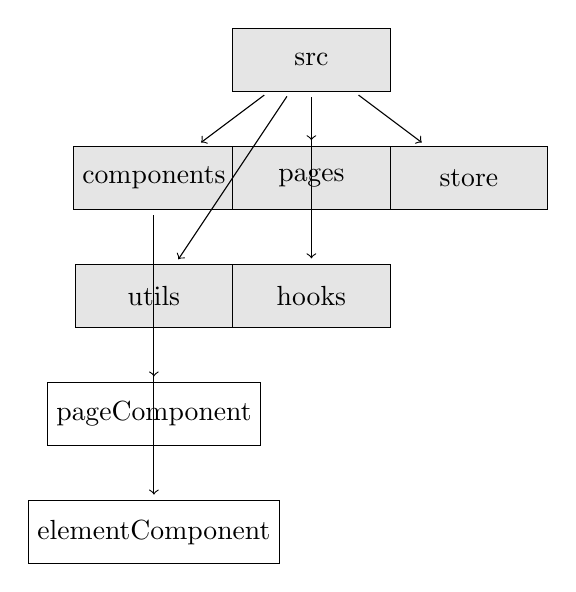
\begin{tikzpicture}[
    file/.style={draw, rectangle, minimum width=2cm, minimum height=0.8cm},
    folder/.style={draw, rectangle, minimum width=2cm, minimum height=0.8cm, fill=gray!20},
    arrow/.style={->, shorten >=2pt, shorten <=2pt}
]

% Folders
\node[folder] (src) at (0,0) {src};
\node[folder] (components) at (-2,-1.5) {components};
\node[folder] (pages) at (0,-1.5) {pages};
\node[folder] (store) at (2,-1.5) {store};
\node[folder] (utils) at (-2,-3) {utils};
\node[folder] (hooks) at (0,-3) {hooks};

% Files
\node[file] (pageComponent) at (-2,-4.5) {pageComponent};
\node[file] (elementComponent) at (-2,-6) {elementComponent};
% ... add more files

% Connections
\draw[arrow] (src) -- (components);
\draw[arrow] (src) -- (pages);
\draw[arrow] (src) -- (store);
\draw[arrow] (src) -- (utils);
\draw[arrow] (src) -- (hooks);
\draw[arrow] (components) -- (pageComponent);
\draw[arrow] (components) -- (elementComponent);
% ... add more connections

\end{tikzpicture}



\pagebreak
\subsubsection{Back-end}
The backend uses the dotNet framework. The development language using the C\# language.

In this project, the backend uses the Onion Architecture.
The Onion Architecture is a typically layered architecture, 
where each layer depends on the inner layer and provides interfaces to the outer layer.
The outer layer provides services to the outermost layer 
and other modules in the same layer based on the interfaces of the inner layer.

From inner to outer, the layers are: Domain, Application, Infrastructure, Presentation.
The Domain layer is the core layer and the innermost layer, used to define domain models, 
which are the business models.
It includes domain models and domain service interfaces.
Domain models are used to define the business models, 
which are the entities in the entity-relationship model and their attributes.
Domain service interfaces are used to define the business services, 
which are the relationships between entities in the entity-relationship model.

The Application layer is the application layer, 
used to define application services, which are the business logic.
It includes domain service implementations and application service interfaces.
Domain service implementations implement the methods of the inner layer's domain service 
interfaces and implement the business logic of the domain models.
Application service interfaces are used to define application services, 
which are the business logic.
It includes but is not limited to database interfaces, testing interfaces, 
HTTP API interfaces, MQTT interfaces, etc.

The Infrastructure layer is the infrastructure layer, used to define infrastructure.
It includes database implementations, testing implementations, 
HTTP API implementations, MQTT implementations, etc.
Database implementations implement the database interfaces 
and provide CRUD services for the database.
Testing implementations implement the testing interfaces 
and provide services for unit testing and integration testing.
HTTP API implementations implement the HTTP API interfaces 
and provide CRUD operations for HTTP APIs.
MQTT implementations implement the MQTT interfaces 
and provide CRUD operations for MQTT.

The Presentation layer is the presentation layer, used to define presentation logic, 
such as interfaces and pages. Since this is a backend project,
data presentation and control are handled by the frontend, 
so this layer is not needed.



\pagebreak
\subsubsection{Data communication and storage}
% 关于本项目的数据通信与数据存储的设计, 包括数据通信的协议, 数据存储的设计等
% 关于数据通信的设计:
% 1. 通信协议的选择
% 自前端向后端发送的数据, 有三种传输的数据类型, 
% 一种是普通的增删改查的请求, 对数据传输的时效性要求不高, 但是对数据的准确性, 完整性, 有序性, 安全性有一定的要求,
% 这种数据的传输, 采用 HTTP 协议, 以及 RESTful API 的设计. 可以有效的保证对数据传输的以上要求.
% 一种是对数据通道的创建和流媒体数据的传输, 对数据传输的时效性, 安全性要求较高, 这种数据的传输, 采用 WebRTC 协议, 以及 MQTT 协议.
% 配合可以快速解码的 flatbuffers 协议, 可以有效的保证对数据传输的以上要求.
% 最后一种是对设备的状态信息和操作信息的传输, 对完整性, 有序性, 安全性都有较高的要求, 这种数据的传输, 采用 MQTT 协议
% 同时也使用了 flatbuffers 协议.
% 
% 2. 数据通信的通信架构和通信流程
% 本项目的数据通信的通信架构, 是基于前后端分离的架构, 前端使用 React 框架, 后端使用 dotnet 框架.
% 当前端需要向后端发送数据的时候, 前端会向后端发送 HTTP 请求, 后端接收到 HTTP 请求之后, 会根据请求的数据类型,
% 选择不同的数据处理方式, 对于普通的增删改查的请求, 后端会根据 RESTful API 的设计, 对数据进行增删改查的操作,
% 对于对数据通道的创建和流媒体数据的传输, 后端会根据 WebRTC 协议, 对数据通道进行创建, 并且帮助前端和设备建立数据通道,
% 当数据通道建立后, 前端和设备之间则使用 flatbuffer 的数据格式对流媒体数据进行传输,
% 对于设备的状态信息和操作信息的传输, 前端会直接向 MQTT broker 发送 MQTT 请求, 
% 设备会在其自身的固件中监听相关的 MQTT 请求, 并且返回相关的数据.
% 
% 3. 数据通信的格式
% 本项目的数据通信的格式, 有三种, 
% 一种是 HTTP 协议, 
% 使用 json 格式对数据进行传输,
% 一种是 WebRTC 协议, 
% 使用 flatbuffers 格式对数据进行传输,
% 一种是 MQTT 协议.
% 使用 flatbuffers 格式对数据进行传输,
% 
% 关于数据存储的设计:
% 1. 数据存储的数据库的选择
% 本项目的数据存储的数据库的选择, 使用了轻量级的数据库 SQLite,
% SQLite 是一个进程内的库, 实现了自给自足的, 无服务器的, 零配置的, 事务性的 SQL 数据库引擎.
% 这是因为整个项目的目的是为了实现前端与设备之间的数据通信, 对于数据库数据的增删改查操作的要求不高,
% 数据量较小, 且对于数据库的数据的事务性要求不高, 所以选择了 SQLite 数据库.
% 2. 项目前后端的数据结构的设计
% 在本项目中, 前端由于使用了 React 框架, 所以前端的数据结构的设计, 使用了基于状态的数据结构的设计,
% 每个组件或者数据集都包含一个状态对象, 这个状态对象的属性就是组件的各个状态. 
% 使用状态对象的原因是, 可以方便的对状态进行管理, 采用对象-属性的形式, 可以方便的针对不同组件的同类状态进行区分,
% 由于跨组件的状态是由 redux 进行管理的, 这种状态对象的设计, 可以更搞笑的对状态进行更新和传递.
% 后端由于使用了 dotnet 框架, 所以后端的数据结构的设计, 使用了基于类的数据结构的设计,
% 采用了面向对象的编程思想, 对数据进行了封装, 使得数据的传输更加的安全, 有序, 完整.


\pagebreak

% \subsection{Domain model}
% \documentclass[]{article}
\usepackage{graphicx}
\usepackage{amsmath}
\usepackage{tikz}

% libaries
\usetikzlibrary{shapes,arrows}

%Define the listing package
\usepackage{listings} %code highlighter
\usepackage{color} %use color
\definecolor{mygreen}{rgb}{0,0.6,0}
\definecolor{mygray}{rgb}{0.5,0.5,0.5}
\definecolor{mymauve}{rgb}{0.58,0,0.82}

%Customize a bit the look
\lstset{ %
backgroundcolor=\color{white}, % choose the background color; you must add \usepackage{color} or \usepackage{xcolor}
basicstyle=\footnotesize, % the size of the fonts that are used for the code
breakatwhitespace=false, % sets if automatic breaks should only happen at whitespace
breaklines=true, % sets automatic line breaking
captionpos=b, % sets the caption-position to bottom
commentstyle=\color{mygreen}, % comment style
deletekeywords={...}, % if you want to delete keywords from the given language
escapeinside={\%*}{*)}, % if you want to add LaTeX within your code
extendedchars=true, % lets you use non-ASCII characters; for 8-bits encodings only, does not work with UTF-8
frame=single, % adds a frame around the code
keepspaces=true, % keeps spaces in text, useful for keeping indentation of code (possibly needs columns=flexible)
keywordstyle=\color{blue}, % keyword style
% language=Octave, % the language of the code
morekeywords={*,...}, % if you want to add more keywords to the set
numbers=left, % where to put the line-numbers; possible values are (none, left, right)
numbersep=5pt, % how far the line-numbers are from the code
numberstyle=\tiny\color{mygray}, % the style that is used for the line-numbers
rulecolor=\color{black}, % if not set, the frame-color may be changed on line-breaks within not-black text (e.g. comments (green here))
showspaces=false, % show spaces everywhere adding particular underscores; it overrides 'showstringspaces'
showstringspaces=false, % underline spaces within strings only
showtabs=false, % show tabs within strings adding particular underscores
stepnumber=1, % the step between two line-numbers. If it's 1, each line will be numbered
stringstyle=\color{mymauve}, % string literal style
tabsize=2, % sets default tabsize to 2 spaces
title=\lstname % show the filename of files included with \lstinputlisting; also try caption instead of title
}

\definecolor{darkgray}{rgb}{.4,.4,.4}
\definecolor{purple}{rgb}{0.65, 0.12, 0.82}

\lstdefinelanguage{React}{
keywords={const, typeof, new, true, false, catch, function, return, null, catch, switch, var, if, in, while, do, else, case, break},
keywordstyle=\color{blue}\bfseries,
ndkeywords={class, export, boolean, throw, implements, import, this},
ndkeywordstyle=\color{darkgray}\bfseries,
identifierstyle=\color{mygreen},
sensitive=false,
comment=[l]{//},
morecomment=[s]{/*}{*/},
commentstyle=\color{purple}\ttfamily,
string=[b]{"}{'}{`},
stringstyle=\color{red}\ttfamily,
morestring=[b]',
morestring=[b]",
morestring=[b]`',
}

\lstdefinelanguage{CSharp}{
keywords={const, typeof, new, true, false, catch, function, return, null, catch, switch, var, if, in, while, do, else, case, break},
keywordstyle=\color{blue}\bfseries,
ndkeywords={class, export, boolean, throw, implements, import, this},
ndkeywordstyle=\color{darkgray}\bfseries,
identifierstyle=\color{mygreen},
sensitive=false,
comment=[l]{//},
morecomment=[s]{/*}{*/},
commentstyle=\color{purple}\ttfamily,
string=[b]{"}{'}{`},
stringstyle=\color{red}\ttfamily,
morestring=[b]',
morestring=[b]",
morestring=[b]`',
}

\lstset{
language=React,
extendedchars=true,
basicstyle=\footnotesize\ttfamily,
showstringspaces=false,
showspaces=false,
numbers=left,
numberstyle=\footnotesize,
numbersep=9pt,
tabsize=2,
breaklines=true,
showtabs=false,
captionpos=b
}

\lstset{
language=CSharp,
extendedchars=true,
basicstyle=\footnotesize\ttfamily,
showstringspaces=false,
showspaces=false,
numbers=left,
numberstyle=\footnotesize,
numbersep=9pt,
tabsize=2,
breaklines=true,
showtabs=false,
captionpos=b
}

% \usepackage{cite} % Add this line for citation

% \bibliographystyle{plain}

\title{
The implementation of BifrostConnect Front-end scope, 
re-design and development with the relevant back-end support develop.
}
\author{
    Fei Gu \\
    Erhvervs Akademi Sydvest \\
    Computer Science 21\\
    }
\date{\today}

\begin{document}

% Front page
\maketitle
\begin{center}
    Supervisor: Henrik Boulund Meng Hansen \\
    Company: BifrostConnect \\
    Engineering Director: Jasper Wass \\
\end{center}
\tableofcontents
\pagebreak


% The introduction
\section{Introduction}
\subsection{Background}\input{sections/introduction/background.tex}
\subsection{The company}\input{sections/introduction/aboutCompany}
\subsection{The project}\input{sections/introduction/aboutProject}
\pagebreak

% The problem statement
\section{Problem Statement}
\subsection{Statement}
\input{sections/problemStatement/statement}
\subsection{Situation}
\input{sections/problemStatement/situation}
\subsection{Potential Solution}
\input{sections/problemStatement/potentialSolution}
\pagebreak

% Requirement analysis
\section{Requirement Analysis}
\input{sections/requirementAnalysis/index}

\subsection{Stakeholders}
\input{sections/requirementAnalysis/stakeholders/index}

\subsection{Business Domain}
\input{sections/requirementAnalysis/bussinesDomain/index}

\subsection{Scope}
\input{sections/requirementAnalysis/scope}

\subsection{Goals}
\input{sections/requirementAnalysis/goals}
\pagebreak

% Software Design
\section{Software Design}
% developement methods
\subsection{Software Development Methods}
\input{sections/softwareDevelopmentMethods/index}
\subsubsection{Agile Software Development}
\input{sections/softwareDevelopmentMethods/agileSoftwareDevelopment/index}
\subsubsection{Feature Driven Development}
\input{sections/softwareDevelopmentMethods/featureDrivenDevelopment/index}

\pagebreak

% Technology seslection
\subsection{Technology selection}
\input{sections/softwareDesign/technologySelection/index}
\subsubsection{Front-end}
\input{sections/softwareDesign/technologySelection/frontEnd}            
\subsubsection{Back-end}
\input{sections/softwareDesign/technologySelection/backEnd}            
\subsubsection{Database}
\input{sections/softwareDesign/technologySelection/database}
\subsubsection{Data communication}
\input{sections/softwareDesign/technologySelection/dataCommunication}            
\subsubsection{DevOps}
\input{sections/softwareDesign/technologySelection/devOps}
\pagebreak

% Architecture design
\subsection{Architecture design}
\input{sections/softwareDesign/architectureDesign/index}
\pagebreak
\subsubsection{Front-end}
\input{sections/softwareDesign/architectureDesign/frontEndArchitecture}
\pagebreak
\subsubsection{Back-end}
\input{sections/softwareDesign/architectureDesign/backEndArchitecture}
\pagebreak
\subsubsection{Data communication and storage}
\input{sections/softwareDesign/architectureDesign/dataCommunicationArchitecture}
\pagebreak

% \subsection{Domain model}
% \input{sections/softwareDesign/domainModel/index}
% \subsection{Database design}
% % 数据库领域模型 ER 图
% % 包括表和字段的设置.
% % 对于私有键和外键的设置.

% \subsection{Back-end design}
% % 后端对象模型
% % 以及对于对象模型的增删改查
% % 以及相关的其他服务的设计`'

% \subsection{Front-end design}
% % 对于前端的页面结构的设计 
% % 页面的状态的设计, 交互设计

% \subsection{FlatBuffers design}
% % schema 的设计

\subsection{DevOps CI/CD process design}
\input{sections/softwareDesign/devOpsDesign/index}
\subsubsection{Continuous Integration}
\input{sections/softwareDesign/devOpsDesign/continuousIntegration/index}
\subsubsection{Continuous Delivery}
\input{sections/softwareDesign/devOpsDesign/continuousDelivery/index}
\subsubsection{Continuous Deployment}
\input{sections/softwareDesign/devOpsDesign/continuousDeployment/index}
\pagebreak

\section{Software Development} 
\input{sections/softwareDevelopment/index}
\subsection{Overall development}
\input{sections/softwareDevelopment/overallDevelopement/index}
\subsubsection{Front-end}
\input{sections/softwareDevelopment/overallDevelopement/frontEnd/index}
\subsubsection{Back-end}
\input{sections/softwareDevelopment/overallDevelopement/backEnd/index}
\subsubsection{DevOps}
\input{sections/softwareDevelopment/overallDevelopement/devOps/index}
\subsection{Feature development} 
\input{sections/softwareDevelopment/featureDevelopment/index}
\subsubsection{Use Case 1}
\input{sections/softwareDevelopment/featureDevelopment/useCase1/index}
\subsubsection{Feature 1}
\input{sections/softwareDevelopment/featureDevelopment/feature/feature1.tex}
\pagebreak
\section{Conclusion} 
\subsection{Result}
Since the project is still in progress, the result is not available yet.
So far, basic structure of this project has been built. But the most features 
are not implemented yet. 
\subsection{Discussion}
As a single developer for this project, I am confident what I have done so far.
And I can say I understand the most of the knowledge I have used in this project, 
which also means I can explain all the part of the project. 
But this project also relevant some of the complex knowledge which I have to continue 
to study and practice.
\subsection{Future Work}
The future work is to implement the rest of the features. 
Including the most important part which is the 'create session' feature.
\pagebreak
% \bibliography{bibliography}
\pagebreak
% \begin{appendices}
%     \section{Appendix}
% \end{appendices} 
\end{document}
% \subsection{Database design}
% % 数据库领域模型 ER 图
% % 包括表和字段的设置.
% % 对于私有键和外键的设置.

% \subsection{Back-end design}
% % 后端对象模型
% % 以及对于对象模型的增删改查
% % 以及相关的其他服务的设计`'

% \subsection{Front-end design}
% % 对于前端的页面结构的设计 
% % 页面的状态的设计, 交互设计

% \subsection{FlatBuffers design}
% % schema 的设计

\subsection{DevOps CI/CD process design}
\documentclass[]{article}
\usepackage{graphicx}
\usepackage{amsmath}
\usepackage{tikz}

% libaries
\usetikzlibrary{shapes,arrows}

%Define the listing package
\usepackage{listings} %code highlighter
\usepackage{color} %use color
\definecolor{mygreen}{rgb}{0,0.6,0}
\definecolor{mygray}{rgb}{0.5,0.5,0.5}
\definecolor{mymauve}{rgb}{0.58,0,0.82}

%Customize a bit the look
\lstset{ %
backgroundcolor=\color{white}, % choose the background color; you must add \usepackage{color} or \usepackage{xcolor}
basicstyle=\footnotesize, % the size of the fonts that are used for the code
breakatwhitespace=false, % sets if automatic breaks should only happen at whitespace
breaklines=true, % sets automatic line breaking
captionpos=b, % sets the caption-position to bottom
commentstyle=\color{mygreen}, % comment style
deletekeywords={...}, % if you want to delete keywords from the given language
escapeinside={\%*}{*)}, % if you want to add LaTeX within your code
extendedchars=true, % lets you use non-ASCII characters; for 8-bits encodings only, does not work with UTF-8
frame=single, % adds a frame around the code
keepspaces=true, % keeps spaces in text, useful for keeping indentation of code (possibly needs columns=flexible)
keywordstyle=\color{blue}, % keyword style
% language=Octave, % the language of the code
morekeywords={*,...}, % if you want to add more keywords to the set
numbers=left, % where to put the line-numbers; possible values are (none, left, right)
numbersep=5pt, % how far the line-numbers are from the code
numberstyle=\tiny\color{mygray}, % the style that is used for the line-numbers
rulecolor=\color{black}, % if not set, the frame-color may be changed on line-breaks within not-black text (e.g. comments (green here))
showspaces=false, % show spaces everywhere adding particular underscores; it overrides 'showstringspaces'
showstringspaces=false, % underline spaces within strings only
showtabs=false, % show tabs within strings adding particular underscores
stepnumber=1, % the step between two line-numbers. If it's 1, each line will be numbered
stringstyle=\color{mymauve}, % string literal style
tabsize=2, % sets default tabsize to 2 spaces
title=\lstname % show the filename of files included with \lstinputlisting; also try caption instead of title
}

\definecolor{darkgray}{rgb}{.4,.4,.4}
\definecolor{purple}{rgb}{0.65, 0.12, 0.82}

\lstdefinelanguage{React}{
keywords={const, typeof, new, true, false, catch, function, return, null, catch, switch, var, if, in, while, do, else, case, break},
keywordstyle=\color{blue}\bfseries,
ndkeywords={class, export, boolean, throw, implements, import, this},
ndkeywordstyle=\color{darkgray}\bfseries,
identifierstyle=\color{mygreen},
sensitive=false,
comment=[l]{//},
morecomment=[s]{/*}{*/},
commentstyle=\color{purple}\ttfamily,
string=[b]{"}{'}{`},
stringstyle=\color{red}\ttfamily,
morestring=[b]',
morestring=[b]",
morestring=[b]`',
}

\lstdefinelanguage{CSharp}{
keywords={const, typeof, new, true, false, catch, function, return, null, catch, switch, var, if, in, while, do, else, case, break},
keywordstyle=\color{blue}\bfseries,
ndkeywords={class, export, boolean, throw, implements, import, this},
ndkeywordstyle=\color{darkgray}\bfseries,
identifierstyle=\color{mygreen},
sensitive=false,
comment=[l]{//},
morecomment=[s]{/*}{*/},
commentstyle=\color{purple}\ttfamily,
string=[b]{"}{'}{`},
stringstyle=\color{red}\ttfamily,
morestring=[b]',
morestring=[b]",
morestring=[b]`',
}

\lstset{
language=React,
extendedchars=true,
basicstyle=\footnotesize\ttfamily,
showstringspaces=false,
showspaces=false,
numbers=left,
numberstyle=\footnotesize,
numbersep=9pt,
tabsize=2,
breaklines=true,
showtabs=false,
captionpos=b
}

\lstset{
language=CSharp,
extendedchars=true,
basicstyle=\footnotesize\ttfamily,
showstringspaces=false,
showspaces=false,
numbers=left,
numberstyle=\footnotesize,
numbersep=9pt,
tabsize=2,
breaklines=true,
showtabs=false,
captionpos=b
}

% \usepackage{cite} % Add this line for citation

% \bibliographystyle{plain}

\title{
The implementation of BifrostConnect Front-end scope, 
re-design and development with the relevant back-end support develop.
}
\author{
    Fei Gu \\
    Erhvervs Akademi Sydvest \\
    Computer Science 21\\
    }
\date{\today}

\begin{document}

% Front page
\maketitle
\begin{center}
    Supervisor: Henrik Boulund Meng Hansen \\
    Company: BifrostConnect \\
    Engineering Director: Jasper Wass \\
\end{center}
\tableofcontents
\pagebreak


% The introduction
\section{Introduction}
\subsection{Background}\input{sections/introduction/background.tex}
\subsection{The company}\input{sections/introduction/aboutCompany}
\subsection{The project}\input{sections/introduction/aboutProject}
\pagebreak

% The problem statement
\section{Problem Statement}
\subsection{Statement}
\input{sections/problemStatement/statement}
\subsection{Situation}
\input{sections/problemStatement/situation}
\subsection{Potential Solution}
\input{sections/problemStatement/potentialSolution}
\pagebreak

% Requirement analysis
\section{Requirement Analysis}
\input{sections/requirementAnalysis/index}

\subsection{Stakeholders}
\input{sections/requirementAnalysis/stakeholders/index}

\subsection{Business Domain}
\input{sections/requirementAnalysis/bussinesDomain/index}

\subsection{Scope}
\input{sections/requirementAnalysis/scope}

\subsection{Goals}
\input{sections/requirementAnalysis/goals}
\pagebreak

% Software Design
\section{Software Design}
% developement methods
\subsection{Software Development Methods}
\input{sections/softwareDevelopmentMethods/index}
\subsubsection{Agile Software Development}
\input{sections/softwareDevelopmentMethods/agileSoftwareDevelopment/index}
\subsubsection{Feature Driven Development}
\input{sections/softwareDevelopmentMethods/featureDrivenDevelopment/index}

\pagebreak

% Technology seslection
\subsection{Technology selection}
\input{sections/softwareDesign/technologySelection/index}
\subsubsection{Front-end}
\input{sections/softwareDesign/technologySelection/frontEnd}            
\subsubsection{Back-end}
\input{sections/softwareDesign/technologySelection/backEnd}            
\subsubsection{Database}
\input{sections/softwareDesign/technologySelection/database}
\subsubsection{Data communication}
\input{sections/softwareDesign/technologySelection/dataCommunication}            
\subsubsection{DevOps}
\input{sections/softwareDesign/technologySelection/devOps}
\pagebreak

% Architecture design
\subsection{Architecture design}
\input{sections/softwareDesign/architectureDesign/index}
\pagebreak
\subsubsection{Front-end}
\input{sections/softwareDesign/architectureDesign/frontEndArchitecture}
\pagebreak
\subsubsection{Back-end}
\input{sections/softwareDesign/architectureDesign/backEndArchitecture}
\pagebreak
\subsubsection{Data communication and storage}
\input{sections/softwareDesign/architectureDesign/dataCommunicationArchitecture}
\pagebreak

% \subsection{Domain model}
% \input{sections/softwareDesign/domainModel/index}
% \subsection{Database design}
% % 数据库领域模型 ER 图
% % 包括表和字段的设置.
% % 对于私有键和外键的设置.

% \subsection{Back-end design}
% % 后端对象模型
% % 以及对于对象模型的增删改查
% % 以及相关的其他服务的设计`'

% \subsection{Front-end design}
% % 对于前端的页面结构的设计 
% % 页面的状态的设计, 交互设计

% \subsection{FlatBuffers design}
% % schema 的设计

\subsection{DevOps CI/CD process design}
\input{sections/softwareDesign/devOpsDesign/index}
\subsubsection{Continuous Integration}
\input{sections/softwareDesign/devOpsDesign/continuousIntegration/index}
\subsubsection{Continuous Delivery}
\input{sections/softwareDesign/devOpsDesign/continuousDelivery/index}
\subsubsection{Continuous Deployment}
\input{sections/softwareDesign/devOpsDesign/continuousDeployment/index}
\pagebreak

\section{Software Development} 
\input{sections/softwareDevelopment/index}
\subsection{Overall development}
\input{sections/softwareDevelopment/overallDevelopement/index}
\subsubsection{Front-end}
\input{sections/softwareDevelopment/overallDevelopement/frontEnd/index}
\subsubsection{Back-end}
\input{sections/softwareDevelopment/overallDevelopement/backEnd/index}
\subsubsection{DevOps}
\input{sections/softwareDevelopment/overallDevelopement/devOps/index}
\subsection{Feature development} 
\input{sections/softwareDevelopment/featureDevelopment/index}
\subsubsection{Use Case 1}
\input{sections/softwareDevelopment/featureDevelopment/useCase1/index}
\subsubsection{Feature 1}
\input{sections/softwareDevelopment/featureDevelopment/feature/feature1.tex}
\pagebreak
\section{Conclusion} 
\subsection{Result}
Since the project is still in progress, the result is not available yet.
So far, basic structure of this project has been built. But the most features 
are not implemented yet. 
\subsection{Discussion}
As a single developer for this project, I am confident what I have done so far.
And I can say I understand the most of the knowledge I have used in this project, 
which also means I can explain all the part of the project. 
But this project also relevant some of the complex knowledge which I have to continue 
to study and practice.
\subsection{Future Work}
The future work is to implement the rest of the features. 
Including the most important part which is the 'create session' feature.
\pagebreak
% \bibliography{bibliography}
\pagebreak
% \begin{appendices}
%     \section{Appendix}
% \end{appendices} 
\end{document}
\subsubsection{Continuous Integration}
\documentclass[]{article}
\usepackage{graphicx}
\usepackage{amsmath}
\usepackage{tikz}

% libaries
\usetikzlibrary{shapes,arrows}

%Define the listing package
\usepackage{listings} %code highlighter
\usepackage{color} %use color
\definecolor{mygreen}{rgb}{0,0.6,0}
\definecolor{mygray}{rgb}{0.5,0.5,0.5}
\definecolor{mymauve}{rgb}{0.58,0,0.82}

%Customize a bit the look
\lstset{ %
backgroundcolor=\color{white}, % choose the background color; you must add \usepackage{color} or \usepackage{xcolor}
basicstyle=\footnotesize, % the size of the fonts that are used for the code
breakatwhitespace=false, % sets if automatic breaks should only happen at whitespace
breaklines=true, % sets automatic line breaking
captionpos=b, % sets the caption-position to bottom
commentstyle=\color{mygreen}, % comment style
deletekeywords={...}, % if you want to delete keywords from the given language
escapeinside={\%*}{*)}, % if you want to add LaTeX within your code
extendedchars=true, % lets you use non-ASCII characters; for 8-bits encodings only, does not work with UTF-8
frame=single, % adds a frame around the code
keepspaces=true, % keeps spaces in text, useful for keeping indentation of code (possibly needs columns=flexible)
keywordstyle=\color{blue}, % keyword style
% language=Octave, % the language of the code
morekeywords={*,...}, % if you want to add more keywords to the set
numbers=left, % where to put the line-numbers; possible values are (none, left, right)
numbersep=5pt, % how far the line-numbers are from the code
numberstyle=\tiny\color{mygray}, % the style that is used for the line-numbers
rulecolor=\color{black}, % if not set, the frame-color may be changed on line-breaks within not-black text (e.g. comments (green here))
showspaces=false, % show spaces everywhere adding particular underscores; it overrides 'showstringspaces'
showstringspaces=false, % underline spaces within strings only
showtabs=false, % show tabs within strings adding particular underscores
stepnumber=1, % the step between two line-numbers. If it's 1, each line will be numbered
stringstyle=\color{mymauve}, % string literal style
tabsize=2, % sets default tabsize to 2 spaces
title=\lstname % show the filename of files included with \lstinputlisting; also try caption instead of title
}

\definecolor{darkgray}{rgb}{.4,.4,.4}
\definecolor{purple}{rgb}{0.65, 0.12, 0.82}

\lstdefinelanguage{React}{
keywords={const, typeof, new, true, false, catch, function, return, null, catch, switch, var, if, in, while, do, else, case, break},
keywordstyle=\color{blue}\bfseries,
ndkeywords={class, export, boolean, throw, implements, import, this},
ndkeywordstyle=\color{darkgray}\bfseries,
identifierstyle=\color{mygreen},
sensitive=false,
comment=[l]{//},
morecomment=[s]{/*}{*/},
commentstyle=\color{purple}\ttfamily,
string=[b]{"}{'}{`},
stringstyle=\color{red}\ttfamily,
morestring=[b]',
morestring=[b]",
morestring=[b]`',
}

\lstdefinelanguage{CSharp}{
keywords={const, typeof, new, true, false, catch, function, return, null, catch, switch, var, if, in, while, do, else, case, break},
keywordstyle=\color{blue}\bfseries,
ndkeywords={class, export, boolean, throw, implements, import, this},
ndkeywordstyle=\color{darkgray}\bfseries,
identifierstyle=\color{mygreen},
sensitive=false,
comment=[l]{//},
morecomment=[s]{/*}{*/},
commentstyle=\color{purple}\ttfamily,
string=[b]{"}{'}{`},
stringstyle=\color{red}\ttfamily,
morestring=[b]',
morestring=[b]",
morestring=[b]`',
}

\lstset{
language=React,
extendedchars=true,
basicstyle=\footnotesize\ttfamily,
showstringspaces=false,
showspaces=false,
numbers=left,
numberstyle=\footnotesize,
numbersep=9pt,
tabsize=2,
breaklines=true,
showtabs=false,
captionpos=b
}

\lstset{
language=CSharp,
extendedchars=true,
basicstyle=\footnotesize\ttfamily,
showstringspaces=false,
showspaces=false,
numbers=left,
numberstyle=\footnotesize,
numbersep=9pt,
tabsize=2,
breaklines=true,
showtabs=false,
captionpos=b
}

% \usepackage{cite} % Add this line for citation

% \bibliographystyle{plain}

\title{
The implementation of BifrostConnect Front-end scope, 
re-design and development with the relevant back-end support develop.
}
\author{
    Fei Gu \\
    Erhvervs Akademi Sydvest \\
    Computer Science 21\\
    }
\date{\today}

\begin{document}

% Front page
\maketitle
\begin{center}
    Supervisor: Henrik Boulund Meng Hansen \\
    Company: BifrostConnect \\
    Engineering Director: Jasper Wass \\
\end{center}
\tableofcontents
\pagebreak


% The introduction
\section{Introduction}
\subsection{Background}\input{sections/introduction/background.tex}
\subsection{The company}\input{sections/introduction/aboutCompany}
\subsection{The project}\input{sections/introduction/aboutProject}
\pagebreak

% The problem statement
\section{Problem Statement}
\subsection{Statement}
\input{sections/problemStatement/statement}
\subsection{Situation}
\input{sections/problemStatement/situation}
\subsection{Potential Solution}
\input{sections/problemStatement/potentialSolution}
\pagebreak

% Requirement analysis
\section{Requirement Analysis}
\input{sections/requirementAnalysis/index}

\subsection{Stakeholders}
\input{sections/requirementAnalysis/stakeholders/index}

\subsection{Business Domain}
\input{sections/requirementAnalysis/bussinesDomain/index}

\subsection{Scope}
\input{sections/requirementAnalysis/scope}

\subsection{Goals}
\input{sections/requirementAnalysis/goals}
\pagebreak

% Software Design
\section{Software Design}
% developement methods
\subsection{Software Development Methods}
\input{sections/softwareDevelopmentMethods/index}
\subsubsection{Agile Software Development}
\input{sections/softwareDevelopmentMethods/agileSoftwareDevelopment/index}
\subsubsection{Feature Driven Development}
\input{sections/softwareDevelopmentMethods/featureDrivenDevelopment/index}

\pagebreak

% Technology seslection
\subsection{Technology selection}
\input{sections/softwareDesign/technologySelection/index}
\subsubsection{Front-end}
\input{sections/softwareDesign/technologySelection/frontEnd}            
\subsubsection{Back-end}
\input{sections/softwareDesign/technologySelection/backEnd}            
\subsubsection{Database}
\input{sections/softwareDesign/technologySelection/database}
\subsubsection{Data communication}
\input{sections/softwareDesign/technologySelection/dataCommunication}            
\subsubsection{DevOps}
\input{sections/softwareDesign/technologySelection/devOps}
\pagebreak

% Architecture design
\subsection{Architecture design}
\input{sections/softwareDesign/architectureDesign/index}
\pagebreak
\subsubsection{Front-end}
\input{sections/softwareDesign/architectureDesign/frontEndArchitecture}
\pagebreak
\subsubsection{Back-end}
\input{sections/softwareDesign/architectureDesign/backEndArchitecture}
\pagebreak
\subsubsection{Data communication and storage}
\input{sections/softwareDesign/architectureDesign/dataCommunicationArchitecture}
\pagebreak

% \subsection{Domain model}
% \input{sections/softwareDesign/domainModel/index}
% \subsection{Database design}
% % 数据库领域模型 ER 图
% % 包括表和字段的设置.
% % 对于私有键和外键的设置.

% \subsection{Back-end design}
% % 后端对象模型
% % 以及对于对象模型的增删改查
% % 以及相关的其他服务的设计`'

% \subsection{Front-end design}
% % 对于前端的页面结构的设计 
% % 页面的状态的设计, 交互设计

% \subsection{FlatBuffers design}
% % schema 的设计

\subsection{DevOps CI/CD process design}
\input{sections/softwareDesign/devOpsDesign/index}
\subsubsection{Continuous Integration}
\input{sections/softwareDesign/devOpsDesign/continuousIntegration/index}
\subsubsection{Continuous Delivery}
\input{sections/softwareDesign/devOpsDesign/continuousDelivery/index}
\subsubsection{Continuous Deployment}
\input{sections/softwareDesign/devOpsDesign/continuousDeployment/index}
\pagebreak

\section{Software Development} 
\input{sections/softwareDevelopment/index}
\subsection{Overall development}
\input{sections/softwareDevelopment/overallDevelopement/index}
\subsubsection{Front-end}
\input{sections/softwareDevelopment/overallDevelopement/frontEnd/index}
\subsubsection{Back-end}
\input{sections/softwareDevelopment/overallDevelopement/backEnd/index}
\subsubsection{DevOps}
\input{sections/softwareDevelopment/overallDevelopement/devOps/index}
\subsection{Feature development} 
\input{sections/softwareDevelopment/featureDevelopment/index}
\subsubsection{Use Case 1}
\input{sections/softwareDevelopment/featureDevelopment/useCase1/index}
\subsubsection{Feature 1}
\input{sections/softwareDevelopment/featureDevelopment/feature/feature1.tex}
\pagebreak
\section{Conclusion} 
\subsection{Result}
Since the project is still in progress, the result is not available yet.
So far, basic structure of this project has been built. But the most features 
are not implemented yet. 
\subsection{Discussion}
As a single developer for this project, I am confident what I have done so far.
And I can say I understand the most of the knowledge I have used in this project, 
which also means I can explain all the part of the project. 
But this project also relevant some of the complex knowledge which I have to continue 
to study and practice.
\subsection{Future Work}
The future work is to implement the rest of the features. 
Including the most important part which is the 'create session' feature.
\pagebreak
% \bibliography{bibliography}
\pagebreak
% \begin{appendices}
%     \section{Appendix}
% \end{appendices} 
\end{document}
\subsubsection{Continuous Delivery}
\documentclass[]{article}
\usepackage{graphicx}
\usepackage{amsmath}
\usepackage{tikz}

% libaries
\usetikzlibrary{shapes,arrows}

%Define the listing package
\usepackage{listings} %code highlighter
\usepackage{color} %use color
\definecolor{mygreen}{rgb}{0,0.6,0}
\definecolor{mygray}{rgb}{0.5,0.5,0.5}
\definecolor{mymauve}{rgb}{0.58,0,0.82}

%Customize a bit the look
\lstset{ %
backgroundcolor=\color{white}, % choose the background color; you must add \usepackage{color} or \usepackage{xcolor}
basicstyle=\footnotesize, % the size of the fonts that are used for the code
breakatwhitespace=false, % sets if automatic breaks should only happen at whitespace
breaklines=true, % sets automatic line breaking
captionpos=b, % sets the caption-position to bottom
commentstyle=\color{mygreen}, % comment style
deletekeywords={...}, % if you want to delete keywords from the given language
escapeinside={\%*}{*)}, % if you want to add LaTeX within your code
extendedchars=true, % lets you use non-ASCII characters; for 8-bits encodings only, does not work with UTF-8
frame=single, % adds a frame around the code
keepspaces=true, % keeps spaces in text, useful for keeping indentation of code (possibly needs columns=flexible)
keywordstyle=\color{blue}, % keyword style
% language=Octave, % the language of the code
morekeywords={*,...}, % if you want to add more keywords to the set
numbers=left, % where to put the line-numbers; possible values are (none, left, right)
numbersep=5pt, % how far the line-numbers are from the code
numberstyle=\tiny\color{mygray}, % the style that is used for the line-numbers
rulecolor=\color{black}, % if not set, the frame-color may be changed on line-breaks within not-black text (e.g. comments (green here))
showspaces=false, % show spaces everywhere adding particular underscores; it overrides 'showstringspaces'
showstringspaces=false, % underline spaces within strings only
showtabs=false, % show tabs within strings adding particular underscores
stepnumber=1, % the step between two line-numbers. If it's 1, each line will be numbered
stringstyle=\color{mymauve}, % string literal style
tabsize=2, % sets default tabsize to 2 spaces
title=\lstname % show the filename of files included with \lstinputlisting; also try caption instead of title
}

\definecolor{darkgray}{rgb}{.4,.4,.4}
\definecolor{purple}{rgb}{0.65, 0.12, 0.82}

\lstdefinelanguage{React}{
keywords={const, typeof, new, true, false, catch, function, return, null, catch, switch, var, if, in, while, do, else, case, break},
keywordstyle=\color{blue}\bfseries,
ndkeywords={class, export, boolean, throw, implements, import, this},
ndkeywordstyle=\color{darkgray}\bfseries,
identifierstyle=\color{mygreen},
sensitive=false,
comment=[l]{//},
morecomment=[s]{/*}{*/},
commentstyle=\color{purple}\ttfamily,
string=[b]{"}{'}{`},
stringstyle=\color{red}\ttfamily,
morestring=[b]',
morestring=[b]",
morestring=[b]`',
}

\lstdefinelanguage{CSharp}{
keywords={const, typeof, new, true, false, catch, function, return, null, catch, switch, var, if, in, while, do, else, case, break},
keywordstyle=\color{blue}\bfseries,
ndkeywords={class, export, boolean, throw, implements, import, this},
ndkeywordstyle=\color{darkgray}\bfseries,
identifierstyle=\color{mygreen},
sensitive=false,
comment=[l]{//},
morecomment=[s]{/*}{*/},
commentstyle=\color{purple}\ttfamily,
string=[b]{"}{'}{`},
stringstyle=\color{red}\ttfamily,
morestring=[b]',
morestring=[b]",
morestring=[b]`',
}

\lstset{
language=React,
extendedchars=true,
basicstyle=\footnotesize\ttfamily,
showstringspaces=false,
showspaces=false,
numbers=left,
numberstyle=\footnotesize,
numbersep=9pt,
tabsize=2,
breaklines=true,
showtabs=false,
captionpos=b
}

\lstset{
language=CSharp,
extendedchars=true,
basicstyle=\footnotesize\ttfamily,
showstringspaces=false,
showspaces=false,
numbers=left,
numberstyle=\footnotesize,
numbersep=9pt,
tabsize=2,
breaklines=true,
showtabs=false,
captionpos=b
}

% \usepackage{cite} % Add this line for citation

% \bibliographystyle{plain}

\title{
The implementation of BifrostConnect Front-end scope, 
re-design and development with the relevant back-end support develop.
}
\author{
    Fei Gu \\
    Erhvervs Akademi Sydvest \\
    Computer Science 21\\
    }
\date{\today}

\begin{document}

% Front page
\maketitle
\begin{center}
    Supervisor: Henrik Boulund Meng Hansen \\
    Company: BifrostConnect \\
    Engineering Director: Jasper Wass \\
\end{center}
\tableofcontents
\pagebreak


% The introduction
\section{Introduction}
\subsection{Background}\input{sections/introduction/background.tex}
\subsection{The company}\input{sections/introduction/aboutCompany}
\subsection{The project}\input{sections/introduction/aboutProject}
\pagebreak

% The problem statement
\section{Problem Statement}
\subsection{Statement}
\input{sections/problemStatement/statement}
\subsection{Situation}
\input{sections/problemStatement/situation}
\subsection{Potential Solution}
\input{sections/problemStatement/potentialSolution}
\pagebreak

% Requirement analysis
\section{Requirement Analysis}
\input{sections/requirementAnalysis/index}

\subsection{Stakeholders}
\input{sections/requirementAnalysis/stakeholders/index}

\subsection{Business Domain}
\input{sections/requirementAnalysis/bussinesDomain/index}

\subsection{Scope}
\input{sections/requirementAnalysis/scope}

\subsection{Goals}
\input{sections/requirementAnalysis/goals}
\pagebreak

% Software Design
\section{Software Design}
% developement methods
\subsection{Software Development Methods}
\input{sections/softwareDevelopmentMethods/index}
\subsubsection{Agile Software Development}
\input{sections/softwareDevelopmentMethods/agileSoftwareDevelopment/index}
\subsubsection{Feature Driven Development}
\input{sections/softwareDevelopmentMethods/featureDrivenDevelopment/index}

\pagebreak

% Technology seslection
\subsection{Technology selection}
\input{sections/softwareDesign/technologySelection/index}
\subsubsection{Front-end}
\input{sections/softwareDesign/technologySelection/frontEnd}            
\subsubsection{Back-end}
\input{sections/softwareDesign/technologySelection/backEnd}            
\subsubsection{Database}
\input{sections/softwareDesign/technologySelection/database}
\subsubsection{Data communication}
\input{sections/softwareDesign/technologySelection/dataCommunication}            
\subsubsection{DevOps}
\input{sections/softwareDesign/technologySelection/devOps}
\pagebreak

% Architecture design
\subsection{Architecture design}
\input{sections/softwareDesign/architectureDesign/index}
\pagebreak
\subsubsection{Front-end}
\input{sections/softwareDesign/architectureDesign/frontEndArchitecture}
\pagebreak
\subsubsection{Back-end}
\input{sections/softwareDesign/architectureDesign/backEndArchitecture}
\pagebreak
\subsubsection{Data communication and storage}
\input{sections/softwareDesign/architectureDesign/dataCommunicationArchitecture}
\pagebreak

% \subsection{Domain model}
% \input{sections/softwareDesign/domainModel/index}
% \subsection{Database design}
% % 数据库领域模型 ER 图
% % 包括表和字段的设置.
% % 对于私有键和外键的设置.

% \subsection{Back-end design}
% % 后端对象模型
% % 以及对于对象模型的增删改查
% % 以及相关的其他服务的设计`'

% \subsection{Front-end design}
% % 对于前端的页面结构的设计 
% % 页面的状态的设计, 交互设计

% \subsection{FlatBuffers design}
% % schema 的设计

\subsection{DevOps CI/CD process design}
\input{sections/softwareDesign/devOpsDesign/index}
\subsubsection{Continuous Integration}
\input{sections/softwareDesign/devOpsDesign/continuousIntegration/index}
\subsubsection{Continuous Delivery}
\input{sections/softwareDesign/devOpsDesign/continuousDelivery/index}
\subsubsection{Continuous Deployment}
\input{sections/softwareDesign/devOpsDesign/continuousDeployment/index}
\pagebreak

\section{Software Development} 
\input{sections/softwareDevelopment/index}
\subsection{Overall development}
\input{sections/softwareDevelopment/overallDevelopement/index}
\subsubsection{Front-end}
\input{sections/softwareDevelopment/overallDevelopement/frontEnd/index}
\subsubsection{Back-end}
\input{sections/softwareDevelopment/overallDevelopement/backEnd/index}
\subsubsection{DevOps}
\input{sections/softwareDevelopment/overallDevelopement/devOps/index}
\subsection{Feature development} 
\input{sections/softwareDevelopment/featureDevelopment/index}
\subsubsection{Use Case 1}
\input{sections/softwareDevelopment/featureDevelopment/useCase1/index}
\subsubsection{Feature 1}
\input{sections/softwareDevelopment/featureDevelopment/feature/feature1.tex}
\pagebreak
\section{Conclusion} 
\subsection{Result}
Since the project is still in progress, the result is not available yet.
So far, basic structure of this project has been built. But the most features 
are not implemented yet. 
\subsection{Discussion}
As a single developer for this project, I am confident what I have done so far.
And I can say I understand the most of the knowledge I have used in this project, 
which also means I can explain all the part of the project. 
But this project also relevant some of the complex knowledge which I have to continue 
to study and practice.
\subsection{Future Work}
The future work is to implement the rest of the features. 
Including the most important part which is the 'create session' feature.
\pagebreak
% \bibliography{bibliography}
\pagebreak
% \begin{appendices}
%     \section{Appendix}
% \end{appendices} 
\end{document}
\subsubsection{Continuous Deployment}
\documentclass[]{article}
\usepackage{graphicx}
\usepackage{amsmath}
\usepackage{tikz}

% libaries
\usetikzlibrary{shapes,arrows}

%Define the listing package
\usepackage{listings} %code highlighter
\usepackage{color} %use color
\definecolor{mygreen}{rgb}{0,0.6,0}
\definecolor{mygray}{rgb}{0.5,0.5,0.5}
\definecolor{mymauve}{rgb}{0.58,0,0.82}

%Customize a bit the look
\lstset{ %
backgroundcolor=\color{white}, % choose the background color; you must add \usepackage{color} or \usepackage{xcolor}
basicstyle=\footnotesize, % the size of the fonts that are used for the code
breakatwhitespace=false, % sets if automatic breaks should only happen at whitespace
breaklines=true, % sets automatic line breaking
captionpos=b, % sets the caption-position to bottom
commentstyle=\color{mygreen}, % comment style
deletekeywords={...}, % if you want to delete keywords from the given language
escapeinside={\%*}{*)}, % if you want to add LaTeX within your code
extendedchars=true, % lets you use non-ASCII characters; for 8-bits encodings only, does not work with UTF-8
frame=single, % adds a frame around the code
keepspaces=true, % keeps spaces in text, useful for keeping indentation of code (possibly needs columns=flexible)
keywordstyle=\color{blue}, % keyword style
% language=Octave, % the language of the code
morekeywords={*,...}, % if you want to add more keywords to the set
numbers=left, % where to put the line-numbers; possible values are (none, left, right)
numbersep=5pt, % how far the line-numbers are from the code
numberstyle=\tiny\color{mygray}, % the style that is used for the line-numbers
rulecolor=\color{black}, % if not set, the frame-color may be changed on line-breaks within not-black text (e.g. comments (green here))
showspaces=false, % show spaces everywhere adding particular underscores; it overrides 'showstringspaces'
showstringspaces=false, % underline spaces within strings only
showtabs=false, % show tabs within strings adding particular underscores
stepnumber=1, % the step between two line-numbers. If it's 1, each line will be numbered
stringstyle=\color{mymauve}, % string literal style
tabsize=2, % sets default tabsize to 2 spaces
title=\lstname % show the filename of files included with \lstinputlisting; also try caption instead of title
}

\definecolor{darkgray}{rgb}{.4,.4,.4}
\definecolor{purple}{rgb}{0.65, 0.12, 0.82}

\lstdefinelanguage{React}{
keywords={const, typeof, new, true, false, catch, function, return, null, catch, switch, var, if, in, while, do, else, case, break},
keywordstyle=\color{blue}\bfseries,
ndkeywords={class, export, boolean, throw, implements, import, this},
ndkeywordstyle=\color{darkgray}\bfseries,
identifierstyle=\color{mygreen},
sensitive=false,
comment=[l]{//},
morecomment=[s]{/*}{*/},
commentstyle=\color{purple}\ttfamily,
string=[b]{"}{'}{`},
stringstyle=\color{red}\ttfamily,
morestring=[b]',
morestring=[b]",
morestring=[b]`',
}

\lstdefinelanguage{CSharp}{
keywords={const, typeof, new, true, false, catch, function, return, null, catch, switch, var, if, in, while, do, else, case, break},
keywordstyle=\color{blue}\bfseries,
ndkeywords={class, export, boolean, throw, implements, import, this},
ndkeywordstyle=\color{darkgray}\bfseries,
identifierstyle=\color{mygreen},
sensitive=false,
comment=[l]{//},
morecomment=[s]{/*}{*/},
commentstyle=\color{purple}\ttfamily,
string=[b]{"}{'}{`},
stringstyle=\color{red}\ttfamily,
morestring=[b]',
morestring=[b]",
morestring=[b]`',
}

\lstset{
language=React,
extendedchars=true,
basicstyle=\footnotesize\ttfamily,
showstringspaces=false,
showspaces=false,
numbers=left,
numberstyle=\footnotesize,
numbersep=9pt,
tabsize=2,
breaklines=true,
showtabs=false,
captionpos=b
}

\lstset{
language=CSharp,
extendedchars=true,
basicstyle=\footnotesize\ttfamily,
showstringspaces=false,
showspaces=false,
numbers=left,
numberstyle=\footnotesize,
numbersep=9pt,
tabsize=2,
breaklines=true,
showtabs=false,
captionpos=b
}

% \usepackage{cite} % Add this line for citation

% \bibliographystyle{plain}

\title{
The implementation of BifrostConnect Front-end scope, 
re-design and development with the relevant back-end support develop.
}
\author{
    Fei Gu \\
    Erhvervs Akademi Sydvest \\
    Computer Science 21\\
    }
\date{\today}

\begin{document}

% Front page
\maketitle
\begin{center}
    Supervisor: Henrik Boulund Meng Hansen \\
    Company: BifrostConnect \\
    Engineering Director: Jasper Wass \\
\end{center}
\tableofcontents
\pagebreak


% The introduction
\section{Introduction}
\subsection{Background}\input{sections/introduction/background.tex}
\subsection{The company}\input{sections/introduction/aboutCompany}
\subsection{The project}\input{sections/introduction/aboutProject}
\pagebreak

% The problem statement
\section{Problem Statement}
\subsection{Statement}
\input{sections/problemStatement/statement}
\subsection{Situation}
\input{sections/problemStatement/situation}
\subsection{Potential Solution}
\input{sections/problemStatement/potentialSolution}
\pagebreak

% Requirement analysis
\section{Requirement Analysis}
\input{sections/requirementAnalysis/index}

\subsection{Stakeholders}
\input{sections/requirementAnalysis/stakeholders/index}

\subsection{Business Domain}
\input{sections/requirementAnalysis/bussinesDomain/index}

\subsection{Scope}
\input{sections/requirementAnalysis/scope}

\subsection{Goals}
\input{sections/requirementAnalysis/goals}
\pagebreak

% Software Design
\section{Software Design}
% developement methods
\subsection{Software Development Methods}
\input{sections/softwareDevelopmentMethods/index}
\subsubsection{Agile Software Development}
\input{sections/softwareDevelopmentMethods/agileSoftwareDevelopment/index}
\subsubsection{Feature Driven Development}
\input{sections/softwareDevelopmentMethods/featureDrivenDevelopment/index}

\pagebreak

% Technology seslection
\subsection{Technology selection}
\input{sections/softwareDesign/technologySelection/index}
\subsubsection{Front-end}
\input{sections/softwareDesign/technologySelection/frontEnd}            
\subsubsection{Back-end}
\input{sections/softwareDesign/technologySelection/backEnd}            
\subsubsection{Database}
\input{sections/softwareDesign/technologySelection/database}
\subsubsection{Data communication}
\input{sections/softwareDesign/technologySelection/dataCommunication}            
\subsubsection{DevOps}
\input{sections/softwareDesign/technologySelection/devOps}
\pagebreak

% Architecture design
\subsection{Architecture design}
\input{sections/softwareDesign/architectureDesign/index}
\pagebreak
\subsubsection{Front-end}
\input{sections/softwareDesign/architectureDesign/frontEndArchitecture}
\pagebreak
\subsubsection{Back-end}
\input{sections/softwareDesign/architectureDesign/backEndArchitecture}
\pagebreak
\subsubsection{Data communication and storage}
\input{sections/softwareDesign/architectureDesign/dataCommunicationArchitecture}
\pagebreak

% \subsection{Domain model}
% \input{sections/softwareDesign/domainModel/index}
% \subsection{Database design}
% % 数据库领域模型 ER 图
% % 包括表和字段的设置.
% % 对于私有键和外键的设置.

% \subsection{Back-end design}
% % 后端对象模型
% % 以及对于对象模型的增删改查
% % 以及相关的其他服务的设计`'

% \subsection{Front-end design}
% % 对于前端的页面结构的设计 
% % 页面的状态的设计, 交互设计

% \subsection{FlatBuffers design}
% % schema 的设计

\subsection{DevOps CI/CD process design}
\input{sections/softwareDesign/devOpsDesign/index}
\subsubsection{Continuous Integration}
\input{sections/softwareDesign/devOpsDesign/continuousIntegration/index}
\subsubsection{Continuous Delivery}
\input{sections/softwareDesign/devOpsDesign/continuousDelivery/index}
\subsubsection{Continuous Deployment}
\input{sections/softwareDesign/devOpsDesign/continuousDeployment/index}
\pagebreak

\section{Software Development} 
\input{sections/softwareDevelopment/index}
\subsection{Overall development}
\input{sections/softwareDevelopment/overallDevelopement/index}
\subsubsection{Front-end}
\input{sections/softwareDevelopment/overallDevelopement/frontEnd/index}
\subsubsection{Back-end}
\input{sections/softwareDevelopment/overallDevelopement/backEnd/index}
\subsubsection{DevOps}
\input{sections/softwareDevelopment/overallDevelopement/devOps/index}
\subsection{Feature development} 
\input{sections/softwareDevelopment/featureDevelopment/index}
\subsubsection{Use Case 1}
\input{sections/softwareDevelopment/featureDevelopment/useCase1/index}
\subsubsection{Feature 1}
\input{sections/softwareDevelopment/featureDevelopment/feature/feature1.tex}
\pagebreak
\section{Conclusion} 
\subsection{Result}
Since the project is still in progress, the result is not available yet.
So far, basic structure of this project has been built. But the most features 
are not implemented yet. 
\subsection{Discussion}
As a single developer for this project, I am confident what I have done so far.
And I can say I understand the most of the knowledge I have used in this project, 
which also means I can explain all the part of the project. 
But this project also relevant some of the complex knowledge which I have to continue 
to study and practice.
\subsection{Future Work}
The future work is to implement the rest of the features. 
Including the most important part which is the 'create session' feature.
\pagebreak
% \bibliography{bibliography}
\pagebreak
% \begin{appendices}
%     \section{Appendix}
% \end{appendices} 
\end{document}
\pagebreak

\section{Software Development} 
\documentclass[]{article}
\usepackage{graphicx}
\usepackage{amsmath}
\usepackage{tikz}

% libaries
\usetikzlibrary{shapes,arrows}

%Define the listing package
\usepackage{listings} %code highlighter
\usepackage{color} %use color
\definecolor{mygreen}{rgb}{0,0.6,0}
\definecolor{mygray}{rgb}{0.5,0.5,0.5}
\definecolor{mymauve}{rgb}{0.58,0,0.82}

%Customize a bit the look
\lstset{ %
backgroundcolor=\color{white}, % choose the background color; you must add \usepackage{color} or \usepackage{xcolor}
basicstyle=\footnotesize, % the size of the fonts that are used for the code
breakatwhitespace=false, % sets if automatic breaks should only happen at whitespace
breaklines=true, % sets automatic line breaking
captionpos=b, % sets the caption-position to bottom
commentstyle=\color{mygreen}, % comment style
deletekeywords={...}, % if you want to delete keywords from the given language
escapeinside={\%*}{*)}, % if you want to add LaTeX within your code
extendedchars=true, % lets you use non-ASCII characters; for 8-bits encodings only, does not work with UTF-8
frame=single, % adds a frame around the code
keepspaces=true, % keeps spaces in text, useful for keeping indentation of code (possibly needs columns=flexible)
keywordstyle=\color{blue}, % keyword style
% language=Octave, % the language of the code
morekeywords={*,...}, % if you want to add more keywords to the set
numbers=left, % where to put the line-numbers; possible values are (none, left, right)
numbersep=5pt, % how far the line-numbers are from the code
numberstyle=\tiny\color{mygray}, % the style that is used for the line-numbers
rulecolor=\color{black}, % if not set, the frame-color may be changed on line-breaks within not-black text (e.g. comments (green here))
showspaces=false, % show spaces everywhere adding particular underscores; it overrides 'showstringspaces'
showstringspaces=false, % underline spaces within strings only
showtabs=false, % show tabs within strings adding particular underscores
stepnumber=1, % the step between two line-numbers. If it's 1, each line will be numbered
stringstyle=\color{mymauve}, % string literal style
tabsize=2, % sets default tabsize to 2 spaces
title=\lstname % show the filename of files included with \lstinputlisting; also try caption instead of title
}

\definecolor{darkgray}{rgb}{.4,.4,.4}
\definecolor{purple}{rgb}{0.65, 0.12, 0.82}

\lstdefinelanguage{React}{
keywords={const, typeof, new, true, false, catch, function, return, null, catch, switch, var, if, in, while, do, else, case, break},
keywordstyle=\color{blue}\bfseries,
ndkeywords={class, export, boolean, throw, implements, import, this},
ndkeywordstyle=\color{darkgray}\bfseries,
identifierstyle=\color{mygreen},
sensitive=false,
comment=[l]{//},
morecomment=[s]{/*}{*/},
commentstyle=\color{purple}\ttfamily,
string=[b]{"}{'}{`},
stringstyle=\color{red}\ttfamily,
morestring=[b]',
morestring=[b]",
morestring=[b]`',
}

\lstdefinelanguage{CSharp}{
keywords={const, typeof, new, true, false, catch, function, return, null, catch, switch, var, if, in, while, do, else, case, break},
keywordstyle=\color{blue}\bfseries,
ndkeywords={class, export, boolean, throw, implements, import, this},
ndkeywordstyle=\color{darkgray}\bfseries,
identifierstyle=\color{mygreen},
sensitive=false,
comment=[l]{//},
morecomment=[s]{/*}{*/},
commentstyle=\color{purple}\ttfamily,
string=[b]{"}{'}{`},
stringstyle=\color{red}\ttfamily,
morestring=[b]',
morestring=[b]",
morestring=[b]`',
}

\lstset{
language=React,
extendedchars=true,
basicstyle=\footnotesize\ttfamily,
showstringspaces=false,
showspaces=false,
numbers=left,
numberstyle=\footnotesize,
numbersep=9pt,
tabsize=2,
breaklines=true,
showtabs=false,
captionpos=b
}

\lstset{
language=CSharp,
extendedchars=true,
basicstyle=\footnotesize\ttfamily,
showstringspaces=false,
showspaces=false,
numbers=left,
numberstyle=\footnotesize,
numbersep=9pt,
tabsize=2,
breaklines=true,
showtabs=false,
captionpos=b
}

% \usepackage{cite} % Add this line for citation

% \bibliographystyle{plain}

\title{
The implementation of BifrostConnect Front-end scope, 
re-design and development with the relevant back-end support develop.
}
\author{
    Fei Gu \\
    Erhvervs Akademi Sydvest \\
    Computer Science 21\\
    }
\date{\today}

\begin{document}

% Front page
\maketitle
\begin{center}
    Supervisor: Henrik Boulund Meng Hansen \\
    Company: BifrostConnect \\
    Engineering Director: Jasper Wass \\
\end{center}
\tableofcontents
\pagebreak


% The introduction
\section{Introduction}
\subsection{Background}\input{sections/introduction/background.tex}
\subsection{The company}\input{sections/introduction/aboutCompany}
\subsection{The project}\input{sections/introduction/aboutProject}
\pagebreak

% The problem statement
\section{Problem Statement}
\subsection{Statement}
\input{sections/problemStatement/statement}
\subsection{Situation}
\input{sections/problemStatement/situation}
\subsection{Potential Solution}
\input{sections/problemStatement/potentialSolution}
\pagebreak

% Requirement analysis
\section{Requirement Analysis}
\input{sections/requirementAnalysis/index}

\subsection{Stakeholders}
\input{sections/requirementAnalysis/stakeholders/index}

\subsection{Business Domain}
\input{sections/requirementAnalysis/bussinesDomain/index}

\subsection{Scope}
\input{sections/requirementAnalysis/scope}

\subsection{Goals}
\input{sections/requirementAnalysis/goals}
\pagebreak

% Software Design
\section{Software Design}
% developement methods
\subsection{Software Development Methods}
\input{sections/softwareDevelopmentMethods/index}
\subsubsection{Agile Software Development}
\input{sections/softwareDevelopmentMethods/agileSoftwareDevelopment/index}
\subsubsection{Feature Driven Development}
\input{sections/softwareDevelopmentMethods/featureDrivenDevelopment/index}

\pagebreak

% Technology seslection
\subsection{Technology selection}
\input{sections/softwareDesign/technologySelection/index}
\subsubsection{Front-end}
\input{sections/softwareDesign/technologySelection/frontEnd}            
\subsubsection{Back-end}
\input{sections/softwareDesign/technologySelection/backEnd}            
\subsubsection{Database}
\input{sections/softwareDesign/technologySelection/database}
\subsubsection{Data communication}
\input{sections/softwareDesign/technologySelection/dataCommunication}            
\subsubsection{DevOps}
\input{sections/softwareDesign/technologySelection/devOps}
\pagebreak

% Architecture design
\subsection{Architecture design}
\input{sections/softwareDesign/architectureDesign/index}
\pagebreak
\subsubsection{Front-end}
\input{sections/softwareDesign/architectureDesign/frontEndArchitecture}
\pagebreak
\subsubsection{Back-end}
\input{sections/softwareDesign/architectureDesign/backEndArchitecture}
\pagebreak
\subsubsection{Data communication and storage}
\input{sections/softwareDesign/architectureDesign/dataCommunicationArchitecture}
\pagebreak

% \subsection{Domain model}
% \input{sections/softwareDesign/domainModel/index}
% \subsection{Database design}
% % 数据库领域模型 ER 图
% % 包括表和字段的设置.
% % 对于私有键和外键的设置.

% \subsection{Back-end design}
% % 后端对象模型
% % 以及对于对象模型的增删改查
% % 以及相关的其他服务的设计`'

% \subsection{Front-end design}
% % 对于前端的页面结构的设计 
% % 页面的状态的设计, 交互设计

% \subsection{FlatBuffers design}
% % schema 的设计

\subsection{DevOps CI/CD process design}
\input{sections/softwareDesign/devOpsDesign/index}
\subsubsection{Continuous Integration}
\input{sections/softwareDesign/devOpsDesign/continuousIntegration/index}
\subsubsection{Continuous Delivery}
\input{sections/softwareDesign/devOpsDesign/continuousDelivery/index}
\subsubsection{Continuous Deployment}
\input{sections/softwareDesign/devOpsDesign/continuousDeployment/index}
\pagebreak

\section{Software Development} 
\input{sections/softwareDevelopment/index}
\subsection{Overall development}
\input{sections/softwareDevelopment/overallDevelopement/index}
\subsubsection{Front-end}
\input{sections/softwareDevelopment/overallDevelopement/frontEnd/index}
\subsubsection{Back-end}
\input{sections/softwareDevelopment/overallDevelopement/backEnd/index}
\subsubsection{DevOps}
\input{sections/softwareDevelopment/overallDevelopement/devOps/index}
\subsection{Feature development} 
\input{sections/softwareDevelopment/featureDevelopment/index}
\subsubsection{Use Case 1}
\input{sections/softwareDevelopment/featureDevelopment/useCase1/index}
\subsubsection{Feature 1}
\input{sections/softwareDevelopment/featureDevelopment/feature/feature1.tex}
\pagebreak
\section{Conclusion} 
\subsection{Result}
Since the project is still in progress, the result is not available yet.
So far, basic structure of this project has been built. But the most features 
are not implemented yet. 
\subsection{Discussion}
As a single developer for this project, I am confident what I have done so far.
And I can say I understand the most of the knowledge I have used in this project, 
which also means I can explain all the part of the project. 
But this project also relevant some of the complex knowledge which I have to continue 
to study and practice.
\subsection{Future Work}
The future work is to implement the rest of the features. 
Including the most important part which is the 'create session' feature.
\pagebreak
% \bibliography{bibliography}
\pagebreak
% \begin{appendices}
%     \section{Appendix}
% \end{appendices} 
\end{document}
\subsection{Overall development}
\documentclass[]{article}
\usepackage{graphicx}
\usepackage{amsmath}
\usepackage{tikz}

% libaries
\usetikzlibrary{shapes,arrows}

%Define the listing package
\usepackage{listings} %code highlighter
\usepackage{color} %use color
\definecolor{mygreen}{rgb}{0,0.6,0}
\definecolor{mygray}{rgb}{0.5,0.5,0.5}
\definecolor{mymauve}{rgb}{0.58,0,0.82}

%Customize a bit the look
\lstset{ %
backgroundcolor=\color{white}, % choose the background color; you must add \usepackage{color} or \usepackage{xcolor}
basicstyle=\footnotesize, % the size of the fonts that are used for the code
breakatwhitespace=false, % sets if automatic breaks should only happen at whitespace
breaklines=true, % sets automatic line breaking
captionpos=b, % sets the caption-position to bottom
commentstyle=\color{mygreen}, % comment style
deletekeywords={...}, % if you want to delete keywords from the given language
escapeinside={\%*}{*)}, % if you want to add LaTeX within your code
extendedchars=true, % lets you use non-ASCII characters; for 8-bits encodings only, does not work with UTF-8
frame=single, % adds a frame around the code
keepspaces=true, % keeps spaces in text, useful for keeping indentation of code (possibly needs columns=flexible)
keywordstyle=\color{blue}, % keyword style
% language=Octave, % the language of the code
morekeywords={*,...}, % if you want to add more keywords to the set
numbers=left, % where to put the line-numbers; possible values are (none, left, right)
numbersep=5pt, % how far the line-numbers are from the code
numberstyle=\tiny\color{mygray}, % the style that is used for the line-numbers
rulecolor=\color{black}, % if not set, the frame-color may be changed on line-breaks within not-black text (e.g. comments (green here))
showspaces=false, % show spaces everywhere adding particular underscores; it overrides 'showstringspaces'
showstringspaces=false, % underline spaces within strings only
showtabs=false, % show tabs within strings adding particular underscores
stepnumber=1, % the step between two line-numbers. If it's 1, each line will be numbered
stringstyle=\color{mymauve}, % string literal style
tabsize=2, % sets default tabsize to 2 spaces
title=\lstname % show the filename of files included with \lstinputlisting; also try caption instead of title
}

\definecolor{darkgray}{rgb}{.4,.4,.4}
\definecolor{purple}{rgb}{0.65, 0.12, 0.82}

\lstdefinelanguage{React}{
keywords={const, typeof, new, true, false, catch, function, return, null, catch, switch, var, if, in, while, do, else, case, break},
keywordstyle=\color{blue}\bfseries,
ndkeywords={class, export, boolean, throw, implements, import, this},
ndkeywordstyle=\color{darkgray}\bfseries,
identifierstyle=\color{mygreen},
sensitive=false,
comment=[l]{//},
morecomment=[s]{/*}{*/},
commentstyle=\color{purple}\ttfamily,
string=[b]{"}{'}{`},
stringstyle=\color{red}\ttfamily,
morestring=[b]',
morestring=[b]",
morestring=[b]`',
}

\lstdefinelanguage{CSharp}{
keywords={const, typeof, new, true, false, catch, function, return, null, catch, switch, var, if, in, while, do, else, case, break},
keywordstyle=\color{blue}\bfseries,
ndkeywords={class, export, boolean, throw, implements, import, this},
ndkeywordstyle=\color{darkgray}\bfseries,
identifierstyle=\color{mygreen},
sensitive=false,
comment=[l]{//},
morecomment=[s]{/*}{*/},
commentstyle=\color{purple}\ttfamily,
string=[b]{"}{'}{`},
stringstyle=\color{red}\ttfamily,
morestring=[b]',
morestring=[b]",
morestring=[b]`',
}

\lstset{
language=React,
extendedchars=true,
basicstyle=\footnotesize\ttfamily,
showstringspaces=false,
showspaces=false,
numbers=left,
numberstyle=\footnotesize,
numbersep=9pt,
tabsize=2,
breaklines=true,
showtabs=false,
captionpos=b
}

\lstset{
language=CSharp,
extendedchars=true,
basicstyle=\footnotesize\ttfamily,
showstringspaces=false,
showspaces=false,
numbers=left,
numberstyle=\footnotesize,
numbersep=9pt,
tabsize=2,
breaklines=true,
showtabs=false,
captionpos=b
}

% \usepackage{cite} % Add this line for citation

% \bibliographystyle{plain}

\title{
The implementation of BifrostConnect Front-end scope, 
re-design and development with the relevant back-end support develop.
}
\author{
    Fei Gu \\
    Erhvervs Akademi Sydvest \\
    Computer Science 21\\
    }
\date{\today}

\begin{document}

% Front page
\maketitle
\begin{center}
    Supervisor: Henrik Boulund Meng Hansen \\
    Company: BifrostConnect \\
    Engineering Director: Jasper Wass \\
\end{center}
\tableofcontents
\pagebreak


% The introduction
\section{Introduction}
\subsection{Background}\input{sections/introduction/background.tex}
\subsection{The company}\input{sections/introduction/aboutCompany}
\subsection{The project}\input{sections/introduction/aboutProject}
\pagebreak

% The problem statement
\section{Problem Statement}
\subsection{Statement}
\input{sections/problemStatement/statement}
\subsection{Situation}
\input{sections/problemStatement/situation}
\subsection{Potential Solution}
\input{sections/problemStatement/potentialSolution}
\pagebreak

% Requirement analysis
\section{Requirement Analysis}
\input{sections/requirementAnalysis/index}

\subsection{Stakeholders}
\input{sections/requirementAnalysis/stakeholders/index}

\subsection{Business Domain}
\input{sections/requirementAnalysis/bussinesDomain/index}

\subsection{Scope}
\input{sections/requirementAnalysis/scope}

\subsection{Goals}
\input{sections/requirementAnalysis/goals}
\pagebreak

% Software Design
\section{Software Design}
% developement methods
\subsection{Software Development Methods}
\input{sections/softwareDevelopmentMethods/index}
\subsubsection{Agile Software Development}
\input{sections/softwareDevelopmentMethods/agileSoftwareDevelopment/index}
\subsubsection{Feature Driven Development}
\input{sections/softwareDevelopmentMethods/featureDrivenDevelopment/index}

\pagebreak

% Technology seslection
\subsection{Technology selection}
\input{sections/softwareDesign/technologySelection/index}
\subsubsection{Front-end}
\input{sections/softwareDesign/technologySelection/frontEnd}            
\subsubsection{Back-end}
\input{sections/softwareDesign/technologySelection/backEnd}            
\subsubsection{Database}
\input{sections/softwareDesign/technologySelection/database}
\subsubsection{Data communication}
\input{sections/softwareDesign/technologySelection/dataCommunication}            
\subsubsection{DevOps}
\input{sections/softwareDesign/technologySelection/devOps}
\pagebreak

% Architecture design
\subsection{Architecture design}
\input{sections/softwareDesign/architectureDesign/index}
\pagebreak
\subsubsection{Front-end}
\input{sections/softwareDesign/architectureDesign/frontEndArchitecture}
\pagebreak
\subsubsection{Back-end}
\input{sections/softwareDesign/architectureDesign/backEndArchitecture}
\pagebreak
\subsubsection{Data communication and storage}
\input{sections/softwareDesign/architectureDesign/dataCommunicationArchitecture}
\pagebreak

% \subsection{Domain model}
% \input{sections/softwareDesign/domainModel/index}
% \subsection{Database design}
% % 数据库领域模型 ER 图
% % 包括表和字段的设置.
% % 对于私有键和外键的设置.

% \subsection{Back-end design}
% % 后端对象模型
% % 以及对于对象模型的增删改查
% % 以及相关的其他服务的设计`'

% \subsection{Front-end design}
% % 对于前端的页面结构的设计 
% % 页面的状态的设计, 交互设计

% \subsection{FlatBuffers design}
% % schema 的设计

\subsection{DevOps CI/CD process design}
\input{sections/softwareDesign/devOpsDesign/index}
\subsubsection{Continuous Integration}
\input{sections/softwareDesign/devOpsDesign/continuousIntegration/index}
\subsubsection{Continuous Delivery}
\input{sections/softwareDesign/devOpsDesign/continuousDelivery/index}
\subsubsection{Continuous Deployment}
\input{sections/softwareDesign/devOpsDesign/continuousDeployment/index}
\pagebreak

\section{Software Development} 
\input{sections/softwareDevelopment/index}
\subsection{Overall development}
\input{sections/softwareDevelopment/overallDevelopement/index}
\subsubsection{Front-end}
\input{sections/softwareDevelopment/overallDevelopement/frontEnd/index}
\subsubsection{Back-end}
\input{sections/softwareDevelopment/overallDevelopement/backEnd/index}
\subsubsection{DevOps}
\input{sections/softwareDevelopment/overallDevelopement/devOps/index}
\subsection{Feature development} 
\input{sections/softwareDevelopment/featureDevelopment/index}
\subsubsection{Use Case 1}
\input{sections/softwareDevelopment/featureDevelopment/useCase1/index}
\subsubsection{Feature 1}
\input{sections/softwareDevelopment/featureDevelopment/feature/feature1.tex}
\pagebreak
\section{Conclusion} 
\subsection{Result}
Since the project is still in progress, the result is not available yet.
So far, basic structure of this project has been built. But the most features 
are not implemented yet. 
\subsection{Discussion}
As a single developer for this project, I am confident what I have done so far.
And I can say I understand the most of the knowledge I have used in this project, 
which also means I can explain all the part of the project. 
But this project also relevant some of the complex knowledge which I have to continue 
to study and practice.
\subsection{Future Work}
The future work is to implement the rest of the features. 
Including the most important part which is the 'create session' feature.
\pagebreak
% \bibliography{bibliography}
\pagebreak
% \begin{appendices}
%     \section{Appendix}
% \end{appendices} 
\end{document}
\subsubsection{Front-end}
\documentclass[]{article}
\usepackage{graphicx}
\usepackage{amsmath}
\usepackage{tikz}

% libaries
\usetikzlibrary{shapes,arrows}

%Define the listing package
\usepackage{listings} %code highlighter
\usepackage{color} %use color
\definecolor{mygreen}{rgb}{0,0.6,0}
\definecolor{mygray}{rgb}{0.5,0.5,0.5}
\definecolor{mymauve}{rgb}{0.58,0,0.82}

%Customize a bit the look
\lstset{ %
backgroundcolor=\color{white}, % choose the background color; you must add \usepackage{color} or \usepackage{xcolor}
basicstyle=\footnotesize, % the size of the fonts that are used for the code
breakatwhitespace=false, % sets if automatic breaks should only happen at whitespace
breaklines=true, % sets automatic line breaking
captionpos=b, % sets the caption-position to bottom
commentstyle=\color{mygreen}, % comment style
deletekeywords={...}, % if you want to delete keywords from the given language
escapeinside={\%*}{*)}, % if you want to add LaTeX within your code
extendedchars=true, % lets you use non-ASCII characters; for 8-bits encodings only, does not work with UTF-8
frame=single, % adds a frame around the code
keepspaces=true, % keeps spaces in text, useful for keeping indentation of code (possibly needs columns=flexible)
keywordstyle=\color{blue}, % keyword style
% language=Octave, % the language of the code
morekeywords={*,...}, % if you want to add more keywords to the set
numbers=left, % where to put the line-numbers; possible values are (none, left, right)
numbersep=5pt, % how far the line-numbers are from the code
numberstyle=\tiny\color{mygray}, % the style that is used for the line-numbers
rulecolor=\color{black}, % if not set, the frame-color may be changed on line-breaks within not-black text (e.g. comments (green here))
showspaces=false, % show spaces everywhere adding particular underscores; it overrides 'showstringspaces'
showstringspaces=false, % underline spaces within strings only
showtabs=false, % show tabs within strings adding particular underscores
stepnumber=1, % the step between two line-numbers. If it's 1, each line will be numbered
stringstyle=\color{mymauve}, % string literal style
tabsize=2, % sets default tabsize to 2 spaces
title=\lstname % show the filename of files included with \lstinputlisting; also try caption instead of title
}

\definecolor{darkgray}{rgb}{.4,.4,.4}
\definecolor{purple}{rgb}{0.65, 0.12, 0.82}

\lstdefinelanguage{React}{
keywords={const, typeof, new, true, false, catch, function, return, null, catch, switch, var, if, in, while, do, else, case, break},
keywordstyle=\color{blue}\bfseries,
ndkeywords={class, export, boolean, throw, implements, import, this},
ndkeywordstyle=\color{darkgray}\bfseries,
identifierstyle=\color{mygreen},
sensitive=false,
comment=[l]{//},
morecomment=[s]{/*}{*/},
commentstyle=\color{purple}\ttfamily,
string=[b]{"}{'}{`},
stringstyle=\color{red}\ttfamily,
morestring=[b]',
morestring=[b]",
morestring=[b]`',
}

\lstdefinelanguage{CSharp}{
keywords={const, typeof, new, true, false, catch, function, return, null, catch, switch, var, if, in, while, do, else, case, break},
keywordstyle=\color{blue}\bfseries,
ndkeywords={class, export, boolean, throw, implements, import, this},
ndkeywordstyle=\color{darkgray}\bfseries,
identifierstyle=\color{mygreen},
sensitive=false,
comment=[l]{//},
morecomment=[s]{/*}{*/},
commentstyle=\color{purple}\ttfamily,
string=[b]{"}{'}{`},
stringstyle=\color{red}\ttfamily,
morestring=[b]',
morestring=[b]",
morestring=[b]`',
}

\lstset{
language=React,
extendedchars=true,
basicstyle=\footnotesize\ttfamily,
showstringspaces=false,
showspaces=false,
numbers=left,
numberstyle=\footnotesize,
numbersep=9pt,
tabsize=2,
breaklines=true,
showtabs=false,
captionpos=b
}

\lstset{
language=CSharp,
extendedchars=true,
basicstyle=\footnotesize\ttfamily,
showstringspaces=false,
showspaces=false,
numbers=left,
numberstyle=\footnotesize,
numbersep=9pt,
tabsize=2,
breaklines=true,
showtabs=false,
captionpos=b
}

% \usepackage{cite} % Add this line for citation

% \bibliographystyle{plain}

\title{
The implementation of BifrostConnect Front-end scope, 
re-design and development with the relevant back-end support develop.
}
\author{
    Fei Gu \\
    Erhvervs Akademi Sydvest \\
    Computer Science 21\\
    }
\date{\today}

\begin{document}

% Front page
\maketitle
\begin{center}
    Supervisor: Henrik Boulund Meng Hansen \\
    Company: BifrostConnect \\
    Engineering Director: Jasper Wass \\
\end{center}
\tableofcontents
\pagebreak


% The introduction
\section{Introduction}
\subsection{Background}\input{sections/introduction/background.tex}
\subsection{The company}\input{sections/introduction/aboutCompany}
\subsection{The project}\input{sections/introduction/aboutProject}
\pagebreak

% The problem statement
\section{Problem Statement}
\subsection{Statement}
\input{sections/problemStatement/statement}
\subsection{Situation}
\input{sections/problemStatement/situation}
\subsection{Potential Solution}
\input{sections/problemStatement/potentialSolution}
\pagebreak

% Requirement analysis
\section{Requirement Analysis}
\input{sections/requirementAnalysis/index}

\subsection{Stakeholders}
\input{sections/requirementAnalysis/stakeholders/index}

\subsection{Business Domain}
\input{sections/requirementAnalysis/bussinesDomain/index}

\subsection{Scope}
\input{sections/requirementAnalysis/scope}

\subsection{Goals}
\input{sections/requirementAnalysis/goals}
\pagebreak

% Software Design
\section{Software Design}
% developement methods
\subsection{Software Development Methods}
\input{sections/softwareDevelopmentMethods/index}
\subsubsection{Agile Software Development}
\input{sections/softwareDevelopmentMethods/agileSoftwareDevelopment/index}
\subsubsection{Feature Driven Development}
\input{sections/softwareDevelopmentMethods/featureDrivenDevelopment/index}

\pagebreak

% Technology seslection
\subsection{Technology selection}
\input{sections/softwareDesign/technologySelection/index}
\subsubsection{Front-end}
\input{sections/softwareDesign/technologySelection/frontEnd}            
\subsubsection{Back-end}
\input{sections/softwareDesign/technologySelection/backEnd}            
\subsubsection{Database}
\input{sections/softwareDesign/technologySelection/database}
\subsubsection{Data communication}
\input{sections/softwareDesign/technologySelection/dataCommunication}            
\subsubsection{DevOps}
\input{sections/softwareDesign/technologySelection/devOps}
\pagebreak

% Architecture design
\subsection{Architecture design}
\input{sections/softwareDesign/architectureDesign/index}
\pagebreak
\subsubsection{Front-end}
\input{sections/softwareDesign/architectureDesign/frontEndArchitecture}
\pagebreak
\subsubsection{Back-end}
\input{sections/softwareDesign/architectureDesign/backEndArchitecture}
\pagebreak
\subsubsection{Data communication and storage}
\input{sections/softwareDesign/architectureDesign/dataCommunicationArchitecture}
\pagebreak

% \subsection{Domain model}
% \input{sections/softwareDesign/domainModel/index}
% \subsection{Database design}
% % 数据库领域模型 ER 图
% % 包括表和字段的设置.
% % 对于私有键和外键的设置.

% \subsection{Back-end design}
% % 后端对象模型
% % 以及对于对象模型的增删改查
% % 以及相关的其他服务的设计`'

% \subsection{Front-end design}
% % 对于前端的页面结构的设计 
% % 页面的状态的设计, 交互设计

% \subsection{FlatBuffers design}
% % schema 的设计

\subsection{DevOps CI/CD process design}
\input{sections/softwareDesign/devOpsDesign/index}
\subsubsection{Continuous Integration}
\input{sections/softwareDesign/devOpsDesign/continuousIntegration/index}
\subsubsection{Continuous Delivery}
\input{sections/softwareDesign/devOpsDesign/continuousDelivery/index}
\subsubsection{Continuous Deployment}
\input{sections/softwareDesign/devOpsDesign/continuousDeployment/index}
\pagebreak

\section{Software Development} 
\input{sections/softwareDevelopment/index}
\subsection{Overall development}
\input{sections/softwareDevelopment/overallDevelopement/index}
\subsubsection{Front-end}
\input{sections/softwareDevelopment/overallDevelopement/frontEnd/index}
\subsubsection{Back-end}
\input{sections/softwareDevelopment/overallDevelopement/backEnd/index}
\subsubsection{DevOps}
\input{sections/softwareDevelopment/overallDevelopement/devOps/index}
\subsection{Feature development} 
\input{sections/softwareDevelopment/featureDevelopment/index}
\subsubsection{Use Case 1}
\input{sections/softwareDevelopment/featureDevelopment/useCase1/index}
\subsubsection{Feature 1}
\input{sections/softwareDevelopment/featureDevelopment/feature/feature1.tex}
\pagebreak
\section{Conclusion} 
\subsection{Result}
Since the project is still in progress, the result is not available yet.
So far, basic structure of this project has been built. But the most features 
are not implemented yet. 
\subsection{Discussion}
As a single developer for this project, I am confident what I have done so far.
And I can say I understand the most of the knowledge I have used in this project, 
which also means I can explain all the part of the project. 
But this project also relevant some of the complex knowledge which I have to continue 
to study and practice.
\subsection{Future Work}
The future work is to implement the rest of the features. 
Including the most important part which is the 'create session' feature.
\pagebreak
% \bibliography{bibliography}
\pagebreak
% \begin{appendices}
%     \section{Appendix}
% \end{appendices} 
\end{document}
\subsubsection{Back-end}
\documentclass[]{article}
\usepackage{graphicx}
\usepackage{amsmath}
\usepackage{tikz}

% libaries
\usetikzlibrary{shapes,arrows}

%Define the listing package
\usepackage{listings} %code highlighter
\usepackage{color} %use color
\definecolor{mygreen}{rgb}{0,0.6,0}
\definecolor{mygray}{rgb}{0.5,0.5,0.5}
\definecolor{mymauve}{rgb}{0.58,0,0.82}

%Customize a bit the look
\lstset{ %
backgroundcolor=\color{white}, % choose the background color; you must add \usepackage{color} or \usepackage{xcolor}
basicstyle=\footnotesize, % the size of the fonts that are used for the code
breakatwhitespace=false, % sets if automatic breaks should only happen at whitespace
breaklines=true, % sets automatic line breaking
captionpos=b, % sets the caption-position to bottom
commentstyle=\color{mygreen}, % comment style
deletekeywords={...}, % if you want to delete keywords from the given language
escapeinside={\%*}{*)}, % if you want to add LaTeX within your code
extendedchars=true, % lets you use non-ASCII characters; for 8-bits encodings only, does not work with UTF-8
frame=single, % adds a frame around the code
keepspaces=true, % keeps spaces in text, useful for keeping indentation of code (possibly needs columns=flexible)
keywordstyle=\color{blue}, % keyword style
% language=Octave, % the language of the code
morekeywords={*,...}, % if you want to add more keywords to the set
numbers=left, % where to put the line-numbers; possible values are (none, left, right)
numbersep=5pt, % how far the line-numbers are from the code
numberstyle=\tiny\color{mygray}, % the style that is used for the line-numbers
rulecolor=\color{black}, % if not set, the frame-color may be changed on line-breaks within not-black text (e.g. comments (green here))
showspaces=false, % show spaces everywhere adding particular underscores; it overrides 'showstringspaces'
showstringspaces=false, % underline spaces within strings only
showtabs=false, % show tabs within strings adding particular underscores
stepnumber=1, % the step between two line-numbers. If it's 1, each line will be numbered
stringstyle=\color{mymauve}, % string literal style
tabsize=2, % sets default tabsize to 2 spaces
title=\lstname % show the filename of files included with \lstinputlisting; also try caption instead of title
}

\definecolor{darkgray}{rgb}{.4,.4,.4}
\definecolor{purple}{rgb}{0.65, 0.12, 0.82}

\lstdefinelanguage{React}{
keywords={const, typeof, new, true, false, catch, function, return, null, catch, switch, var, if, in, while, do, else, case, break},
keywordstyle=\color{blue}\bfseries,
ndkeywords={class, export, boolean, throw, implements, import, this},
ndkeywordstyle=\color{darkgray}\bfseries,
identifierstyle=\color{mygreen},
sensitive=false,
comment=[l]{//},
morecomment=[s]{/*}{*/},
commentstyle=\color{purple}\ttfamily,
string=[b]{"}{'}{`},
stringstyle=\color{red}\ttfamily,
morestring=[b]',
morestring=[b]",
morestring=[b]`',
}

\lstdefinelanguage{CSharp}{
keywords={const, typeof, new, true, false, catch, function, return, null, catch, switch, var, if, in, while, do, else, case, break},
keywordstyle=\color{blue}\bfseries,
ndkeywords={class, export, boolean, throw, implements, import, this},
ndkeywordstyle=\color{darkgray}\bfseries,
identifierstyle=\color{mygreen},
sensitive=false,
comment=[l]{//},
morecomment=[s]{/*}{*/},
commentstyle=\color{purple}\ttfamily,
string=[b]{"}{'}{`},
stringstyle=\color{red}\ttfamily,
morestring=[b]',
morestring=[b]",
morestring=[b]`',
}

\lstset{
language=React,
extendedchars=true,
basicstyle=\footnotesize\ttfamily,
showstringspaces=false,
showspaces=false,
numbers=left,
numberstyle=\footnotesize,
numbersep=9pt,
tabsize=2,
breaklines=true,
showtabs=false,
captionpos=b
}

\lstset{
language=CSharp,
extendedchars=true,
basicstyle=\footnotesize\ttfamily,
showstringspaces=false,
showspaces=false,
numbers=left,
numberstyle=\footnotesize,
numbersep=9pt,
tabsize=2,
breaklines=true,
showtabs=false,
captionpos=b
}

% \usepackage{cite} % Add this line for citation

% \bibliographystyle{plain}

\title{
The implementation of BifrostConnect Front-end scope, 
re-design and development with the relevant back-end support develop.
}
\author{
    Fei Gu \\
    Erhvervs Akademi Sydvest \\
    Computer Science 21\\
    }
\date{\today}

\begin{document}

% Front page
\maketitle
\begin{center}
    Supervisor: Henrik Boulund Meng Hansen \\
    Company: BifrostConnect \\
    Engineering Director: Jasper Wass \\
\end{center}
\tableofcontents
\pagebreak


% The introduction
\section{Introduction}
\subsection{Background}\input{sections/introduction/background.tex}
\subsection{The company}\input{sections/introduction/aboutCompany}
\subsection{The project}\input{sections/introduction/aboutProject}
\pagebreak

% The problem statement
\section{Problem Statement}
\subsection{Statement}
\input{sections/problemStatement/statement}
\subsection{Situation}
\input{sections/problemStatement/situation}
\subsection{Potential Solution}
\input{sections/problemStatement/potentialSolution}
\pagebreak

% Requirement analysis
\section{Requirement Analysis}
\input{sections/requirementAnalysis/index}

\subsection{Stakeholders}
\input{sections/requirementAnalysis/stakeholders/index}

\subsection{Business Domain}
\input{sections/requirementAnalysis/bussinesDomain/index}

\subsection{Scope}
\input{sections/requirementAnalysis/scope}

\subsection{Goals}
\input{sections/requirementAnalysis/goals}
\pagebreak

% Software Design
\section{Software Design}
% developement methods
\subsection{Software Development Methods}
\input{sections/softwareDevelopmentMethods/index}
\subsubsection{Agile Software Development}
\input{sections/softwareDevelopmentMethods/agileSoftwareDevelopment/index}
\subsubsection{Feature Driven Development}
\input{sections/softwareDevelopmentMethods/featureDrivenDevelopment/index}

\pagebreak

% Technology seslection
\subsection{Technology selection}
\input{sections/softwareDesign/technologySelection/index}
\subsubsection{Front-end}
\input{sections/softwareDesign/technologySelection/frontEnd}            
\subsubsection{Back-end}
\input{sections/softwareDesign/technologySelection/backEnd}            
\subsubsection{Database}
\input{sections/softwareDesign/technologySelection/database}
\subsubsection{Data communication}
\input{sections/softwareDesign/technologySelection/dataCommunication}            
\subsubsection{DevOps}
\input{sections/softwareDesign/technologySelection/devOps}
\pagebreak

% Architecture design
\subsection{Architecture design}
\input{sections/softwareDesign/architectureDesign/index}
\pagebreak
\subsubsection{Front-end}
\input{sections/softwareDesign/architectureDesign/frontEndArchitecture}
\pagebreak
\subsubsection{Back-end}
\input{sections/softwareDesign/architectureDesign/backEndArchitecture}
\pagebreak
\subsubsection{Data communication and storage}
\input{sections/softwareDesign/architectureDesign/dataCommunicationArchitecture}
\pagebreak

% \subsection{Domain model}
% \input{sections/softwareDesign/domainModel/index}
% \subsection{Database design}
% % 数据库领域模型 ER 图
% % 包括表和字段的设置.
% % 对于私有键和外键的设置.

% \subsection{Back-end design}
% % 后端对象模型
% % 以及对于对象模型的增删改查
% % 以及相关的其他服务的设计`'

% \subsection{Front-end design}
% % 对于前端的页面结构的设计 
% % 页面的状态的设计, 交互设计

% \subsection{FlatBuffers design}
% % schema 的设计

\subsection{DevOps CI/CD process design}
\input{sections/softwareDesign/devOpsDesign/index}
\subsubsection{Continuous Integration}
\input{sections/softwareDesign/devOpsDesign/continuousIntegration/index}
\subsubsection{Continuous Delivery}
\input{sections/softwareDesign/devOpsDesign/continuousDelivery/index}
\subsubsection{Continuous Deployment}
\input{sections/softwareDesign/devOpsDesign/continuousDeployment/index}
\pagebreak

\section{Software Development} 
\input{sections/softwareDevelopment/index}
\subsection{Overall development}
\input{sections/softwareDevelopment/overallDevelopement/index}
\subsubsection{Front-end}
\input{sections/softwareDevelopment/overallDevelopement/frontEnd/index}
\subsubsection{Back-end}
\input{sections/softwareDevelopment/overallDevelopement/backEnd/index}
\subsubsection{DevOps}
\input{sections/softwareDevelopment/overallDevelopement/devOps/index}
\subsection{Feature development} 
\input{sections/softwareDevelopment/featureDevelopment/index}
\subsubsection{Use Case 1}
\input{sections/softwareDevelopment/featureDevelopment/useCase1/index}
\subsubsection{Feature 1}
\input{sections/softwareDevelopment/featureDevelopment/feature/feature1.tex}
\pagebreak
\section{Conclusion} 
\subsection{Result}
Since the project is still in progress, the result is not available yet.
So far, basic structure of this project has been built. But the most features 
are not implemented yet. 
\subsection{Discussion}
As a single developer for this project, I am confident what I have done so far.
And I can say I understand the most of the knowledge I have used in this project, 
which also means I can explain all the part of the project. 
But this project also relevant some of the complex knowledge which I have to continue 
to study and practice.
\subsection{Future Work}
The future work is to implement the rest of the features. 
Including the most important part which is the 'create session' feature.
\pagebreak
% \bibliography{bibliography}
\pagebreak
% \begin{appendices}
%     \section{Appendix}
% \end{appendices} 
\end{document}
\subsubsection{DevOps}
\documentclass[]{article}
\usepackage{graphicx}
\usepackage{amsmath}
\usepackage{tikz}

% libaries
\usetikzlibrary{shapes,arrows}

%Define the listing package
\usepackage{listings} %code highlighter
\usepackage{color} %use color
\definecolor{mygreen}{rgb}{0,0.6,0}
\definecolor{mygray}{rgb}{0.5,0.5,0.5}
\definecolor{mymauve}{rgb}{0.58,0,0.82}

%Customize a bit the look
\lstset{ %
backgroundcolor=\color{white}, % choose the background color; you must add \usepackage{color} or \usepackage{xcolor}
basicstyle=\footnotesize, % the size of the fonts that are used for the code
breakatwhitespace=false, % sets if automatic breaks should only happen at whitespace
breaklines=true, % sets automatic line breaking
captionpos=b, % sets the caption-position to bottom
commentstyle=\color{mygreen}, % comment style
deletekeywords={...}, % if you want to delete keywords from the given language
escapeinside={\%*}{*)}, % if you want to add LaTeX within your code
extendedchars=true, % lets you use non-ASCII characters; for 8-bits encodings only, does not work with UTF-8
frame=single, % adds a frame around the code
keepspaces=true, % keeps spaces in text, useful for keeping indentation of code (possibly needs columns=flexible)
keywordstyle=\color{blue}, % keyword style
% language=Octave, % the language of the code
morekeywords={*,...}, % if you want to add more keywords to the set
numbers=left, % where to put the line-numbers; possible values are (none, left, right)
numbersep=5pt, % how far the line-numbers are from the code
numberstyle=\tiny\color{mygray}, % the style that is used for the line-numbers
rulecolor=\color{black}, % if not set, the frame-color may be changed on line-breaks within not-black text (e.g. comments (green here))
showspaces=false, % show spaces everywhere adding particular underscores; it overrides 'showstringspaces'
showstringspaces=false, % underline spaces within strings only
showtabs=false, % show tabs within strings adding particular underscores
stepnumber=1, % the step between two line-numbers. If it's 1, each line will be numbered
stringstyle=\color{mymauve}, % string literal style
tabsize=2, % sets default tabsize to 2 spaces
title=\lstname % show the filename of files included with \lstinputlisting; also try caption instead of title
}

\definecolor{darkgray}{rgb}{.4,.4,.4}
\definecolor{purple}{rgb}{0.65, 0.12, 0.82}

\lstdefinelanguage{React}{
keywords={const, typeof, new, true, false, catch, function, return, null, catch, switch, var, if, in, while, do, else, case, break},
keywordstyle=\color{blue}\bfseries,
ndkeywords={class, export, boolean, throw, implements, import, this},
ndkeywordstyle=\color{darkgray}\bfseries,
identifierstyle=\color{mygreen},
sensitive=false,
comment=[l]{//},
morecomment=[s]{/*}{*/},
commentstyle=\color{purple}\ttfamily,
string=[b]{"}{'}{`},
stringstyle=\color{red}\ttfamily,
morestring=[b]',
morestring=[b]",
morestring=[b]`',
}

\lstdefinelanguage{CSharp}{
keywords={const, typeof, new, true, false, catch, function, return, null, catch, switch, var, if, in, while, do, else, case, break},
keywordstyle=\color{blue}\bfseries,
ndkeywords={class, export, boolean, throw, implements, import, this},
ndkeywordstyle=\color{darkgray}\bfseries,
identifierstyle=\color{mygreen},
sensitive=false,
comment=[l]{//},
morecomment=[s]{/*}{*/},
commentstyle=\color{purple}\ttfamily,
string=[b]{"}{'}{`},
stringstyle=\color{red}\ttfamily,
morestring=[b]',
morestring=[b]",
morestring=[b]`',
}

\lstset{
language=React,
extendedchars=true,
basicstyle=\footnotesize\ttfamily,
showstringspaces=false,
showspaces=false,
numbers=left,
numberstyle=\footnotesize,
numbersep=9pt,
tabsize=2,
breaklines=true,
showtabs=false,
captionpos=b
}

\lstset{
language=CSharp,
extendedchars=true,
basicstyle=\footnotesize\ttfamily,
showstringspaces=false,
showspaces=false,
numbers=left,
numberstyle=\footnotesize,
numbersep=9pt,
tabsize=2,
breaklines=true,
showtabs=false,
captionpos=b
}

% \usepackage{cite} % Add this line for citation

% \bibliographystyle{plain}

\title{
The implementation of BifrostConnect Front-end scope, 
re-design and development with the relevant back-end support develop.
}
\author{
    Fei Gu \\
    Erhvervs Akademi Sydvest \\
    Computer Science 21\\
    }
\date{\today}

\begin{document}

% Front page
\maketitle
\begin{center}
    Supervisor: Henrik Boulund Meng Hansen \\
    Company: BifrostConnect \\
    Engineering Director: Jasper Wass \\
\end{center}
\tableofcontents
\pagebreak


% The introduction
\section{Introduction}
\subsection{Background}\input{sections/introduction/background.tex}
\subsection{The company}\input{sections/introduction/aboutCompany}
\subsection{The project}\input{sections/introduction/aboutProject}
\pagebreak

% The problem statement
\section{Problem Statement}
\subsection{Statement}
\input{sections/problemStatement/statement}
\subsection{Situation}
\input{sections/problemStatement/situation}
\subsection{Potential Solution}
\input{sections/problemStatement/potentialSolution}
\pagebreak

% Requirement analysis
\section{Requirement Analysis}
\input{sections/requirementAnalysis/index}

\subsection{Stakeholders}
\input{sections/requirementAnalysis/stakeholders/index}

\subsection{Business Domain}
\input{sections/requirementAnalysis/bussinesDomain/index}

\subsection{Scope}
\input{sections/requirementAnalysis/scope}

\subsection{Goals}
\input{sections/requirementAnalysis/goals}
\pagebreak

% Software Design
\section{Software Design}
% developement methods
\subsection{Software Development Methods}
\input{sections/softwareDevelopmentMethods/index}
\subsubsection{Agile Software Development}
\input{sections/softwareDevelopmentMethods/agileSoftwareDevelopment/index}
\subsubsection{Feature Driven Development}
\input{sections/softwareDevelopmentMethods/featureDrivenDevelopment/index}

\pagebreak

% Technology seslection
\subsection{Technology selection}
\input{sections/softwareDesign/technologySelection/index}
\subsubsection{Front-end}
\input{sections/softwareDesign/technologySelection/frontEnd}            
\subsubsection{Back-end}
\input{sections/softwareDesign/technologySelection/backEnd}            
\subsubsection{Database}
\input{sections/softwareDesign/technologySelection/database}
\subsubsection{Data communication}
\input{sections/softwareDesign/technologySelection/dataCommunication}            
\subsubsection{DevOps}
\input{sections/softwareDesign/technologySelection/devOps}
\pagebreak

% Architecture design
\subsection{Architecture design}
\input{sections/softwareDesign/architectureDesign/index}
\pagebreak
\subsubsection{Front-end}
\input{sections/softwareDesign/architectureDesign/frontEndArchitecture}
\pagebreak
\subsubsection{Back-end}
\input{sections/softwareDesign/architectureDesign/backEndArchitecture}
\pagebreak
\subsubsection{Data communication and storage}
\input{sections/softwareDesign/architectureDesign/dataCommunicationArchitecture}
\pagebreak

% \subsection{Domain model}
% \input{sections/softwareDesign/domainModel/index}
% \subsection{Database design}
% % 数据库领域模型 ER 图
% % 包括表和字段的设置.
% % 对于私有键和外键的设置.

% \subsection{Back-end design}
% % 后端对象模型
% % 以及对于对象模型的增删改查
% % 以及相关的其他服务的设计`'

% \subsection{Front-end design}
% % 对于前端的页面结构的设计 
% % 页面的状态的设计, 交互设计

% \subsection{FlatBuffers design}
% % schema 的设计

\subsection{DevOps CI/CD process design}
\input{sections/softwareDesign/devOpsDesign/index}
\subsubsection{Continuous Integration}
\input{sections/softwareDesign/devOpsDesign/continuousIntegration/index}
\subsubsection{Continuous Delivery}
\input{sections/softwareDesign/devOpsDesign/continuousDelivery/index}
\subsubsection{Continuous Deployment}
\input{sections/softwareDesign/devOpsDesign/continuousDeployment/index}
\pagebreak

\section{Software Development} 
\input{sections/softwareDevelopment/index}
\subsection{Overall development}
\input{sections/softwareDevelopment/overallDevelopement/index}
\subsubsection{Front-end}
\input{sections/softwareDevelopment/overallDevelopement/frontEnd/index}
\subsubsection{Back-end}
\input{sections/softwareDevelopment/overallDevelopement/backEnd/index}
\subsubsection{DevOps}
\input{sections/softwareDevelopment/overallDevelopement/devOps/index}
\subsection{Feature development} 
\input{sections/softwareDevelopment/featureDevelopment/index}
\subsubsection{Use Case 1}
\input{sections/softwareDevelopment/featureDevelopment/useCase1/index}
\subsubsection{Feature 1}
\input{sections/softwareDevelopment/featureDevelopment/feature/feature1.tex}
\pagebreak
\section{Conclusion} 
\subsection{Result}
Since the project is still in progress, the result is not available yet.
So far, basic structure of this project has been built. But the most features 
are not implemented yet. 
\subsection{Discussion}
As a single developer for this project, I am confident what I have done so far.
And I can say I understand the most of the knowledge I have used in this project, 
which also means I can explain all the part of the project. 
But this project also relevant some of the complex knowledge which I have to continue 
to study and practice.
\subsection{Future Work}
The future work is to implement the rest of the features. 
Including the most important part which is the 'create session' feature.
\pagebreak
% \bibliography{bibliography}
\pagebreak
% \begin{appendices}
%     \section{Appendix}
% \end{appendices} 
\end{document}
\subsection{Feature development} 
\documentclass[]{article}
\usepackage{graphicx}
\usepackage{amsmath}
\usepackage{tikz}

% libaries
\usetikzlibrary{shapes,arrows}

%Define the listing package
\usepackage{listings} %code highlighter
\usepackage{color} %use color
\definecolor{mygreen}{rgb}{0,0.6,0}
\definecolor{mygray}{rgb}{0.5,0.5,0.5}
\definecolor{mymauve}{rgb}{0.58,0,0.82}

%Customize a bit the look
\lstset{ %
backgroundcolor=\color{white}, % choose the background color; you must add \usepackage{color} or \usepackage{xcolor}
basicstyle=\footnotesize, % the size of the fonts that are used for the code
breakatwhitespace=false, % sets if automatic breaks should only happen at whitespace
breaklines=true, % sets automatic line breaking
captionpos=b, % sets the caption-position to bottom
commentstyle=\color{mygreen}, % comment style
deletekeywords={...}, % if you want to delete keywords from the given language
escapeinside={\%*}{*)}, % if you want to add LaTeX within your code
extendedchars=true, % lets you use non-ASCII characters; for 8-bits encodings only, does not work with UTF-8
frame=single, % adds a frame around the code
keepspaces=true, % keeps spaces in text, useful for keeping indentation of code (possibly needs columns=flexible)
keywordstyle=\color{blue}, % keyword style
% language=Octave, % the language of the code
morekeywords={*,...}, % if you want to add more keywords to the set
numbers=left, % where to put the line-numbers; possible values are (none, left, right)
numbersep=5pt, % how far the line-numbers are from the code
numberstyle=\tiny\color{mygray}, % the style that is used for the line-numbers
rulecolor=\color{black}, % if not set, the frame-color may be changed on line-breaks within not-black text (e.g. comments (green here))
showspaces=false, % show spaces everywhere adding particular underscores; it overrides 'showstringspaces'
showstringspaces=false, % underline spaces within strings only
showtabs=false, % show tabs within strings adding particular underscores
stepnumber=1, % the step between two line-numbers. If it's 1, each line will be numbered
stringstyle=\color{mymauve}, % string literal style
tabsize=2, % sets default tabsize to 2 spaces
title=\lstname % show the filename of files included with \lstinputlisting; also try caption instead of title
}

\definecolor{darkgray}{rgb}{.4,.4,.4}
\definecolor{purple}{rgb}{0.65, 0.12, 0.82}

\lstdefinelanguage{React}{
keywords={const, typeof, new, true, false, catch, function, return, null, catch, switch, var, if, in, while, do, else, case, break},
keywordstyle=\color{blue}\bfseries,
ndkeywords={class, export, boolean, throw, implements, import, this},
ndkeywordstyle=\color{darkgray}\bfseries,
identifierstyle=\color{mygreen},
sensitive=false,
comment=[l]{//},
morecomment=[s]{/*}{*/},
commentstyle=\color{purple}\ttfamily,
string=[b]{"}{'}{`},
stringstyle=\color{red}\ttfamily,
morestring=[b]',
morestring=[b]",
morestring=[b]`',
}

\lstdefinelanguage{CSharp}{
keywords={const, typeof, new, true, false, catch, function, return, null, catch, switch, var, if, in, while, do, else, case, break},
keywordstyle=\color{blue}\bfseries,
ndkeywords={class, export, boolean, throw, implements, import, this},
ndkeywordstyle=\color{darkgray}\bfseries,
identifierstyle=\color{mygreen},
sensitive=false,
comment=[l]{//},
morecomment=[s]{/*}{*/},
commentstyle=\color{purple}\ttfamily,
string=[b]{"}{'}{`},
stringstyle=\color{red}\ttfamily,
morestring=[b]',
morestring=[b]",
morestring=[b]`',
}

\lstset{
language=React,
extendedchars=true,
basicstyle=\footnotesize\ttfamily,
showstringspaces=false,
showspaces=false,
numbers=left,
numberstyle=\footnotesize,
numbersep=9pt,
tabsize=2,
breaklines=true,
showtabs=false,
captionpos=b
}

\lstset{
language=CSharp,
extendedchars=true,
basicstyle=\footnotesize\ttfamily,
showstringspaces=false,
showspaces=false,
numbers=left,
numberstyle=\footnotesize,
numbersep=9pt,
tabsize=2,
breaklines=true,
showtabs=false,
captionpos=b
}

% \usepackage{cite} % Add this line for citation

% \bibliographystyle{plain}

\title{
The implementation of BifrostConnect Front-end scope, 
re-design and development with the relevant back-end support develop.
}
\author{
    Fei Gu \\
    Erhvervs Akademi Sydvest \\
    Computer Science 21\\
    }
\date{\today}

\begin{document}

% Front page
\maketitle
\begin{center}
    Supervisor: Henrik Boulund Meng Hansen \\
    Company: BifrostConnect \\
    Engineering Director: Jasper Wass \\
\end{center}
\tableofcontents
\pagebreak


% The introduction
\section{Introduction}
\subsection{Background}\input{sections/introduction/background.tex}
\subsection{The company}\input{sections/introduction/aboutCompany}
\subsection{The project}\input{sections/introduction/aboutProject}
\pagebreak

% The problem statement
\section{Problem Statement}
\subsection{Statement}
\input{sections/problemStatement/statement}
\subsection{Situation}
\input{sections/problemStatement/situation}
\subsection{Potential Solution}
\input{sections/problemStatement/potentialSolution}
\pagebreak

% Requirement analysis
\section{Requirement Analysis}
\input{sections/requirementAnalysis/index}

\subsection{Stakeholders}
\input{sections/requirementAnalysis/stakeholders/index}

\subsection{Business Domain}
\input{sections/requirementAnalysis/bussinesDomain/index}

\subsection{Scope}
\input{sections/requirementAnalysis/scope}

\subsection{Goals}
\input{sections/requirementAnalysis/goals}
\pagebreak

% Software Design
\section{Software Design}
% developement methods
\subsection{Software Development Methods}
\input{sections/softwareDevelopmentMethods/index}
\subsubsection{Agile Software Development}
\input{sections/softwareDevelopmentMethods/agileSoftwareDevelopment/index}
\subsubsection{Feature Driven Development}
\input{sections/softwareDevelopmentMethods/featureDrivenDevelopment/index}

\pagebreak

% Technology seslection
\subsection{Technology selection}
\input{sections/softwareDesign/technologySelection/index}
\subsubsection{Front-end}
\input{sections/softwareDesign/technologySelection/frontEnd}            
\subsubsection{Back-end}
\input{sections/softwareDesign/technologySelection/backEnd}            
\subsubsection{Database}
\input{sections/softwareDesign/technologySelection/database}
\subsubsection{Data communication}
\input{sections/softwareDesign/technologySelection/dataCommunication}            
\subsubsection{DevOps}
\input{sections/softwareDesign/technologySelection/devOps}
\pagebreak

% Architecture design
\subsection{Architecture design}
\input{sections/softwareDesign/architectureDesign/index}
\pagebreak
\subsubsection{Front-end}
\input{sections/softwareDesign/architectureDesign/frontEndArchitecture}
\pagebreak
\subsubsection{Back-end}
\input{sections/softwareDesign/architectureDesign/backEndArchitecture}
\pagebreak
\subsubsection{Data communication and storage}
\input{sections/softwareDesign/architectureDesign/dataCommunicationArchitecture}
\pagebreak

% \subsection{Domain model}
% \input{sections/softwareDesign/domainModel/index}
% \subsection{Database design}
% % 数据库领域模型 ER 图
% % 包括表和字段的设置.
% % 对于私有键和外键的设置.

% \subsection{Back-end design}
% % 后端对象模型
% % 以及对于对象模型的增删改查
% % 以及相关的其他服务的设计`'

% \subsection{Front-end design}
% % 对于前端的页面结构的设计 
% % 页面的状态的设计, 交互设计

% \subsection{FlatBuffers design}
% % schema 的设计

\subsection{DevOps CI/CD process design}
\input{sections/softwareDesign/devOpsDesign/index}
\subsubsection{Continuous Integration}
\input{sections/softwareDesign/devOpsDesign/continuousIntegration/index}
\subsubsection{Continuous Delivery}
\input{sections/softwareDesign/devOpsDesign/continuousDelivery/index}
\subsubsection{Continuous Deployment}
\input{sections/softwareDesign/devOpsDesign/continuousDeployment/index}
\pagebreak

\section{Software Development} 
\input{sections/softwareDevelopment/index}
\subsection{Overall development}
\input{sections/softwareDevelopment/overallDevelopement/index}
\subsubsection{Front-end}
\input{sections/softwareDevelopment/overallDevelopement/frontEnd/index}
\subsubsection{Back-end}
\input{sections/softwareDevelopment/overallDevelopement/backEnd/index}
\subsubsection{DevOps}
\input{sections/softwareDevelopment/overallDevelopement/devOps/index}
\subsection{Feature development} 
\input{sections/softwareDevelopment/featureDevelopment/index}
\subsubsection{Use Case 1}
\input{sections/softwareDevelopment/featureDevelopment/useCase1/index}
\subsubsection{Feature 1}
\input{sections/softwareDevelopment/featureDevelopment/feature/feature1.tex}
\pagebreak
\section{Conclusion} 
\subsection{Result}
Since the project is still in progress, the result is not available yet.
So far, basic structure of this project has been built. But the most features 
are not implemented yet. 
\subsection{Discussion}
As a single developer for this project, I am confident what I have done so far.
And I can say I understand the most of the knowledge I have used in this project, 
which also means I can explain all the part of the project. 
But this project also relevant some of the complex knowledge which I have to continue 
to study and practice.
\subsection{Future Work}
The future work is to implement the rest of the features. 
Including the most important part which is the 'create session' feature.
\pagebreak
% \bibliography{bibliography}
\pagebreak
% \begin{appendices}
%     \section{Appendix}
% \end{appendices} 
\end{document}
\subsubsection{Use Case 1}
\documentclass[]{article}
\usepackage{graphicx}
\usepackage{amsmath}
\usepackage{tikz}

% libaries
\usetikzlibrary{shapes,arrows}

%Define the listing package
\usepackage{listings} %code highlighter
\usepackage{color} %use color
\definecolor{mygreen}{rgb}{0,0.6,0}
\definecolor{mygray}{rgb}{0.5,0.5,0.5}
\definecolor{mymauve}{rgb}{0.58,0,0.82}

%Customize a bit the look
\lstset{ %
backgroundcolor=\color{white}, % choose the background color; you must add \usepackage{color} or \usepackage{xcolor}
basicstyle=\footnotesize, % the size of the fonts that are used for the code
breakatwhitespace=false, % sets if automatic breaks should only happen at whitespace
breaklines=true, % sets automatic line breaking
captionpos=b, % sets the caption-position to bottom
commentstyle=\color{mygreen}, % comment style
deletekeywords={...}, % if you want to delete keywords from the given language
escapeinside={\%*}{*)}, % if you want to add LaTeX within your code
extendedchars=true, % lets you use non-ASCII characters; for 8-bits encodings only, does not work with UTF-8
frame=single, % adds a frame around the code
keepspaces=true, % keeps spaces in text, useful for keeping indentation of code (possibly needs columns=flexible)
keywordstyle=\color{blue}, % keyword style
% language=Octave, % the language of the code
morekeywords={*,...}, % if you want to add more keywords to the set
numbers=left, % where to put the line-numbers; possible values are (none, left, right)
numbersep=5pt, % how far the line-numbers are from the code
numberstyle=\tiny\color{mygray}, % the style that is used for the line-numbers
rulecolor=\color{black}, % if not set, the frame-color may be changed on line-breaks within not-black text (e.g. comments (green here))
showspaces=false, % show spaces everywhere adding particular underscores; it overrides 'showstringspaces'
showstringspaces=false, % underline spaces within strings only
showtabs=false, % show tabs within strings adding particular underscores
stepnumber=1, % the step between two line-numbers. If it's 1, each line will be numbered
stringstyle=\color{mymauve}, % string literal style
tabsize=2, % sets default tabsize to 2 spaces
title=\lstname % show the filename of files included with \lstinputlisting; also try caption instead of title
}

\definecolor{darkgray}{rgb}{.4,.4,.4}
\definecolor{purple}{rgb}{0.65, 0.12, 0.82}

\lstdefinelanguage{React}{
keywords={const, typeof, new, true, false, catch, function, return, null, catch, switch, var, if, in, while, do, else, case, break},
keywordstyle=\color{blue}\bfseries,
ndkeywords={class, export, boolean, throw, implements, import, this},
ndkeywordstyle=\color{darkgray}\bfseries,
identifierstyle=\color{mygreen},
sensitive=false,
comment=[l]{//},
morecomment=[s]{/*}{*/},
commentstyle=\color{purple}\ttfamily,
string=[b]{"}{'}{`},
stringstyle=\color{red}\ttfamily,
morestring=[b]',
morestring=[b]",
morestring=[b]`',
}

\lstdefinelanguage{CSharp}{
keywords={const, typeof, new, true, false, catch, function, return, null, catch, switch, var, if, in, while, do, else, case, break},
keywordstyle=\color{blue}\bfseries,
ndkeywords={class, export, boolean, throw, implements, import, this},
ndkeywordstyle=\color{darkgray}\bfseries,
identifierstyle=\color{mygreen},
sensitive=false,
comment=[l]{//},
morecomment=[s]{/*}{*/},
commentstyle=\color{purple}\ttfamily,
string=[b]{"}{'}{`},
stringstyle=\color{red}\ttfamily,
morestring=[b]',
morestring=[b]",
morestring=[b]`',
}

\lstset{
language=React,
extendedchars=true,
basicstyle=\footnotesize\ttfamily,
showstringspaces=false,
showspaces=false,
numbers=left,
numberstyle=\footnotesize,
numbersep=9pt,
tabsize=2,
breaklines=true,
showtabs=false,
captionpos=b
}

\lstset{
language=CSharp,
extendedchars=true,
basicstyle=\footnotesize\ttfamily,
showstringspaces=false,
showspaces=false,
numbers=left,
numberstyle=\footnotesize,
numbersep=9pt,
tabsize=2,
breaklines=true,
showtabs=false,
captionpos=b
}

% \usepackage{cite} % Add this line for citation

% \bibliographystyle{plain}

\title{
The implementation of BifrostConnect Front-end scope, 
re-design and development with the relevant back-end support develop.
}
\author{
    Fei Gu \\
    Erhvervs Akademi Sydvest \\
    Computer Science 21\\
    }
\date{\today}

\begin{document}

% Front page
\maketitle
\begin{center}
    Supervisor: Henrik Boulund Meng Hansen \\
    Company: BifrostConnect \\
    Engineering Director: Jasper Wass \\
\end{center}
\tableofcontents
\pagebreak


% The introduction
\section{Introduction}
\subsection{Background}\input{sections/introduction/background.tex}
\subsection{The company}\input{sections/introduction/aboutCompany}
\subsection{The project}\input{sections/introduction/aboutProject}
\pagebreak

% The problem statement
\section{Problem Statement}
\subsection{Statement}
\input{sections/problemStatement/statement}
\subsection{Situation}
\input{sections/problemStatement/situation}
\subsection{Potential Solution}
\input{sections/problemStatement/potentialSolution}
\pagebreak

% Requirement analysis
\section{Requirement Analysis}
\input{sections/requirementAnalysis/index}

\subsection{Stakeholders}
\input{sections/requirementAnalysis/stakeholders/index}

\subsection{Business Domain}
\input{sections/requirementAnalysis/bussinesDomain/index}

\subsection{Scope}
\input{sections/requirementAnalysis/scope}

\subsection{Goals}
\input{sections/requirementAnalysis/goals}
\pagebreak

% Software Design
\section{Software Design}
% developement methods
\subsection{Software Development Methods}
\input{sections/softwareDevelopmentMethods/index}
\subsubsection{Agile Software Development}
\input{sections/softwareDevelopmentMethods/agileSoftwareDevelopment/index}
\subsubsection{Feature Driven Development}
\input{sections/softwareDevelopmentMethods/featureDrivenDevelopment/index}

\pagebreak

% Technology seslection
\subsection{Technology selection}
\input{sections/softwareDesign/technologySelection/index}
\subsubsection{Front-end}
\input{sections/softwareDesign/technologySelection/frontEnd}            
\subsubsection{Back-end}
\input{sections/softwareDesign/technologySelection/backEnd}            
\subsubsection{Database}
\input{sections/softwareDesign/technologySelection/database}
\subsubsection{Data communication}
\input{sections/softwareDesign/technologySelection/dataCommunication}            
\subsubsection{DevOps}
\input{sections/softwareDesign/technologySelection/devOps}
\pagebreak

% Architecture design
\subsection{Architecture design}
\input{sections/softwareDesign/architectureDesign/index}
\pagebreak
\subsubsection{Front-end}
\input{sections/softwareDesign/architectureDesign/frontEndArchitecture}
\pagebreak
\subsubsection{Back-end}
\input{sections/softwareDesign/architectureDesign/backEndArchitecture}
\pagebreak
\subsubsection{Data communication and storage}
\input{sections/softwareDesign/architectureDesign/dataCommunicationArchitecture}
\pagebreak

% \subsection{Domain model}
% \input{sections/softwareDesign/domainModel/index}
% \subsection{Database design}
% % 数据库领域模型 ER 图
% % 包括表和字段的设置.
% % 对于私有键和外键的设置.

% \subsection{Back-end design}
% % 后端对象模型
% % 以及对于对象模型的增删改查
% % 以及相关的其他服务的设计`'

% \subsection{Front-end design}
% % 对于前端的页面结构的设计 
% % 页面的状态的设计, 交互设计

% \subsection{FlatBuffers design}
% % schema 的设计

\subsection{DevOps CI/CD process design}
\input{sections/softwareDesign/devOpsDesign/index}
\subsubsection{Continuous Integration}
\input{sections/softwareDesign/devOpsDesign/continuousIntegration/index}
\subsubsection{Continuous Delivery}
\input{sections/softwareDesign/devOpsDesign/continuousDelivery/index}
\subsubsection{Continuous Deployment}
\input{sections/softwareDesign/devOpsDesign/continuousDeployment/index}
\pagebreak

\section{Software Development} 
\input{sections/softwareDevelopment/index}
\subsection{Overall development}
\input{sections/softwareDevelopment/overallDevelopement/index}
\subsubsection{Front-end}
\input{sections/softwareDevelopment/overallDevelopement/frontEnd/index}
\subsubsection{Back-end}
\input{sections/softwareDevelopment/overallDevelopement/backEnd/index}
\subsubsection{DevOps}
\input{sections/softwareDevelopment/overallDevelopement/devOps/index}
\subsection{Feature development} 
\input{sections/softwareDevelopment/featureDevelopment/index}
\subsubsection{Use Case 1}
\input{sections/softwareDevelopment/featureDevelopment/useCase1/index}
\subsubsection{Feature 1}
\input{sections/softwareDevelopment/featureDevelopment/feature/feature1.tex}
\pagebreak
\section{Conclusion} 
\subsection{Result}
Since the project is still in progress, the result is not available yet.
So far, basic structure of this project has been built. But the most features 
are not implemented yet. 
\subsection{Discussion}
As a single developer for this project, I am confident what I have done so far.
And I can say I understand the most of the knowledge I have used in this project, 
which also means I can explain all the part of the project. 
But this project also relevant some of the complex knowledge which I have to continue 
to study and practice.
\subsection{Future Work}
The future work is to implement the rest of the features. 
Including the most important part which is the 'create session' feature.
\pagebreak
% \bibliography{bibliography}
\pagebreak
% \begin{appendices}
%     \section{Appendix}
% \end{appendices} 
\end{document}
\subsubsection{Feature 1}
\paragraph{Front-end}
To be able to display the data from the back-end, we need to make a request to
the back-end. The request is made by using the \texttt{fetch} API. 

In the \texttt{deviceComponet} we need use the customer hook \texttt{useGetAllDevices}
to get the device list from the back-end. 

After the request is made, we need to handle the response from the back-end.
The response is a JSON object, we need to parse the JSON object to the DOM object.

And then, we need to display the device list on the device page.

\paragraph{Back-end}

To be able to response the request from the front-end, we need to implement the webAPI controller
to handle the request.

And then, the webAPI controller will call the service to get the device list from the domain service.

The domain service will invoke the repository to get the device list from the database.

After the device list is got from the database, the domain service will return the device list to the webAPI controller.

The webAPI controller will return the device list to the front-end.

\pagebreak
\section{Conclusion} 
\subsection{Result}
Since the project is still in progress, the result is not available yet.
So far, basic structure of this project has been built. But the most features 
are not implemented yet. 
\subsection{Discussion}
As a single developer for this project, I am confident what I have done so far.
And I can say I understand the most of the knowledge I have used in this project, 
which also means I can explain all the part of the project. 
But this project also relevant some of the complex knowledge which I have to continue 
to study and practice.
\subsection{Future Work}
The future work is to implement the rest of the features. 
Including the most important part which is the 'create session' feature.
\pagebreak
% \bibliography{bibliography}
\pagebreak
% \begin{appendices}
%     \section{Appendix}
% \end{appendices} 
\end{document}

\pagebreak

% Technology seslection
\subsection{Technology selection}
\documentclass[]{article}
\usepackage{graphicx}
\usepackage{amsmath}
\usepackage{tikz}

% libaries
\usetikzlibrary{shapes,arrows}

%Define the listing package
\usepackage{listings} %code highlighter
\usepackage{color} %use color
\definecolor{mygreen}{rgb}{0,0.6,0}
\definecolor{mygray}{rgb}{0.5,0.5,0.5}
\definecolor{mymauve}{rgb}{0.58,0,0.82}

%Customize a bit the look
\lstset{ %
backgroundcolor=\color{white}, % choose the background color; you must add \usepackage{color} or \usepackage{xcolor}
basicstyle=\footnotesize, % the size of the fonts that are used for the code
breakatwhitespace=false, % sets if automatic breaks should only happen at whitespace
breaklines=true, % sets automatic line breaking
captionpos=b, % sets the caption-position to bottom
commentstyle=\color{mygreen}, % comment style
deletekeywords={...}, % if you want to delete keywords from the given language
escapeinside={\%*}{*)}, % if you want to add LaTeX within your code
extendedchars=true, % lets you use non-ASCII characters; for 8-bits encodings only, does not work with UTF-8
frame=single, % adds a frame around the code
keepspaces=true, % keeps spaces in text, useful for keeping indentation of code (possibly needs columns=flexible)
keywordstyle=\color{blue}, % keyword style
% language=Octave, % the language of the code
morekeywords={*,...}, % if you want to add more keywords to the set
numbers=left, % where to put the line-numbers; possible values are (none, left, right)
numbersep=5pt, % how far the line-numbers are from the code
numberstyle=\tiny\color{mygray}, % the style that is used for the line-numbers
rulecolor=\color{black}, % if not set, the frame-color may be changed on line-breaks within not-black text (e.g. comments (green here))
showspaces=false, % show spaces everywhere adding particular underscores; it overrides 'showstringspaces'
showstringspaces=false, % underline spaces within strings only
showtabs=false, % show tabs within strings adding particular underscores
stepnumber=1, % the step between two line-numbers. If it's 1, each line will be numbered
stringstyle=\color{mymauve}, % string literal style
tabsize=2, % sets default tabsize to 2 spaces
title=\lstname % show the filename of files included with \lstinputlisting; also try caption instead of title
}

\definecolor{darkgray}{rgb}{.4,.4,.4}
\definecolor{purple}{rgb}{0.65, 0.12, 0.82}

\lstdefinelanguage{React}{
keywords={const, typeof, new, true, false, catch, function, return, null, catch, switch, var, if, in, while, do, else, case, break},
keywordstyle=\color{blue}\bfseries,
ndkeywords={class, export, boolean, throw, implements, import, this},
ndkeywordstyle=\color{darkgray}\bfseries,
identifierstyle=\color{mygreen},
sensitive=false,
comment=[l]{//},
morecomment=[s]{/*}{*/},
commentstyle=\color{purple}\ttfamily,
string=[b]{"}{'}{`},
stringstyle=\color{red}\ttfamily,
morestring=[b]',
morestring=[b]",
morestring=[b]`',
}

\lstdefinelanguage{CSharp}{
keywords={const, typeof, new, true, false, catch, function, return, null, catch, switch, var, if, in, while, do, else, case, break},
keywordstyle=\color{blue}\bfseries,
ndkeywords={class, export, boolean, throw, implements, import, this},
ndkeywordstyle=\color{darkgray}\bfseries,
identifierstyle=\color{mygreen},
sensitive=false,
comment=[l]{//},
morecomment=[s]{/*}{*/},
commentstyle=\color{purple}\ttfamily,
string=[b]{"}{'}{`},
stringstyle=\color{red}\ttfamily,
morestring=[b]',
morestring=[b]",
morestring=[b]`',
}

\lstset{
language=React,
extendedchars=true,
basicstyle=\footnotesize\ttfamily,
showstringspaces=false,
showspaces=false,
numbers=left,
numberstyle=\footnotesize,
numbersep=9pt,
tabsize=2,
breaklines=true,
showtabs=false,
captionpos=b
}

\lstset{
language=CSharp,
extendedchars=true,
basicstyle=\footnotesize\ttfamily,
showstringspaces=false,
showspaces=false,
numbers=left,
numberstyle=\footnotesize,
numbersep=9pt,
tabsize=2,
breaklines=true,
showtabs=false,
captionpos=b
}

% \usepackage{cite} % Add this line for citation

% \bibliographystyle{plain}

\title{
The implementation of BifrostConnect Front-end scope, 
re-design and development with the relevant back-end support develop.
}
\author{
    Fei Gu \\
    Erhvervs Akademi Sydvest \\
    Computer Science 21\\
    }
\date{\today}

\begin{document}

% Front page
\maketitle
\begin{center}
    Supervisor: Henrik Boulund Meng Hansen \\
    Company: BifrostConnect \\
    Engineering Director: Jasper Wass \\
\end{center}
\tableofcontents
\pagebreak


% The introduction
\section{Introduction}
\subsection{Background}% 关于项目的类型和背景的介绍
% 项目是 EASV computer science 专业的毕业设计, 毕业设计的要求是充分的展现学生在两年半的学习中
% 能够获得的知识和技能, 并且能够在一个项目中充分的展现出来. 项目的类型是一个软件开发项目,
% 项目的背景是一个公司的项目, 项目的目的是为了解决公司的一个问题.

This project is the final project of the EASV computer science program. 
The purpose of the final project is to demonstrate the knowledge 
and skills by the student during the two and a half years of study,
and be able to fully demonstrate them in a project.

In this project, the student will work with a company 
to solve a problem of the company.
The student will use the knowledge and skills learned from the education
to solve the problem.

Which means this project will relavent to the company's business domain,
and using the software engineering methods and software development methods
to reconize the problem, analyze the problem, and solve the problem.


\subsection{The company}% 关于公司的介绍
% 公司的名字是 BifrostConnect, 是一个创业公司, 公司的主要业务是为了解决在严格的系统安全条件下, 
% 当客户的系统没有也不允许有互联网的情况下, 通过一个中继设备而不是第三方服务的条件下, 能够远程的
% 访问客户的系统. 公司的产品是一个硬件设备以及配套的网络应用. 以及相关的服务和一站式解决方案.

BifrostConnect is a startup company which established in 2018 
that has 10 to 12 employees and located in Copenhagen, Denmark.

During the five years of operation, the company has developed
a remote access solution for access the users remote system.
The solution  


The company's main business is to solve the problem of remote access 
to the customer's system when the customer's system does not have 
and is not allowed to have the Internet under strict system security conditions.

The company's product is a hardware device and a network application.
And related services and one-stop solutions.
\subsection{The project}% 关于项目的介绍
% 这个项目是在公司原有软件基础上, 对现有的前端软件进行重构和重新设计, 并且在后端提供相应的支持.

% This project is to re-design and re-develop the front-end software based on the company's original software,
% and provide corresponding support on the back-end.% Introduction to the project


% This project involves a comprehensive overhaul of the existing front-end software, building upon the company's original software. It also includes providing corresponding back-end support.

This project entails a thorough redesign and redevelopment of the existing front-end software, 
leveraging the foundation provided by the company's original software. 
Additionally, it involves enhancing the back-end to provide the necessary support 
for the new front-end.
\pagebreak

% The problem statement
\section{Problem Statement}
\subsection{Statement}
During this project the Remote Access Interface and Tunnel Interface should be integrated into the Device Mananger Application.
To achieve the one single page application with full functionality of the Remote Access and Tunnel Connection capabilities.

\subsection{Situation}
% 项目的背景
% 这一部分要详细的介绍关于项目的原始背景, 因为在之后要根据这些背景写明项目的意义和解决方案.
% 所以项目的现状, 项目的历史问题, 现有项目难以开发和维护的原因, 

% The current BifrostConnect front-end application consist of the Device Manager (DM) 
% and Remote Access Interface (RAI) two different user interface.
% Which means the user need to manage their devices and users in the one application, 
% and oprate their devices to use the bifrost product in other web application as well. 
% However, the RAI consists of two different user interfaces referred to as the Classic RAI and Tunnel RAI. 
% Those two user interfaces will leading the user to different web application 
% when user wish to create a different type of access solution.

% The reason for this situation occurred is because the bifrost product is developed focus on the device 
% and the application part was not considered as important as the device part. 
% Therefore, the application part was developed by different developers with different design logic.
% And the application functionality was not been properly through out the development process. 
% Which cause the design logic of this product is not scalable, leading to decreasing user experience, 
% and exponential growth of code complexity which makes it increasingly challenging to maintain and improve. 
% Also the product design style lacks scalability due to lack of modularity and code consistency, 
% and the operation logic is not clear.

The existing BifrostConnect front-end application is divided into two distinct user interfaces:
the Device Manager (DM) and the Remote Access Interface (RAI). 
This division requires users to manage their devices and users in one application, 
while operating their devices to use the Bifrost product in another web application. 
Moreover, the RAI is further split into two different user interfaces, 
known as the Classic RAI and Tunnel RAI. 
These interfaces direct users to different web applications 
depending on the type of access solution they wish to create.

This situation arose because the development of the Bifrost product was primarily focused 
on the device, with the application part not receiving as much attention. 
As a result, the application part was developed by different developers, 
each with their own design logic. 
This led to a lack of thorough planning for the application functionality 
during the development process. Consequently, 
the design logic of the product is not scalable, 
which has resulted in a diminished user experience 
and an exponential increase in code complexity, 
making it increasingly difficult to maintain and improve. 
Furthermore, the product design style lacks scalability due to a lack of modularity 
and code consistency, and the operation logic is unclear.
\subsection{Potential Solution}
% 项目的解决方案
% 根据之前的项目背景描述, 提出项目的解决方案, 也就是问题陈述的解决方案的详细说明. 
% 包括潜在的解决方案, 这个解决方案的优势和劣势.

To address those issue, there is a need to redesign and remake the front-end with
a focus on implementing a modular unified front-end management system that
encompasses all the necessary functionality. 

The goal is to provide users with seamless control, monitoring, and access to their devices from anywhere, 
enhancing their overall user experience and productivity while keeping code complexity as low as possible.

For the implementation to be successful, we also need to have a back-end
service, including an API and Database. The back-end server will contain the
necessary service for the front-end to reach the purpose. Such as the RESTful
API service, authentication service, MQTT service, Tunnel service and Database.

This project will follow the software design process. Therefore, it will also include
the Software Development method and DevOps on all process as well. 

This project is covered by NDA due to security and confidentiality reasons. Thus, the
project will initially not be publicly deployed, however, I will described the
deployment in my report as well.

%%%%%%%%%%%%%%%%%%%%%%%%%%%%%%%%%%%%%%%%%%%%%%%%%%%%%%%%%%%%%%%%%%%%%%%%%

% Project Solution
% Based on the previously described project background, this section presents a detailed explanation of the proposed solution to the problem statement. This includes potential solutions, as well as the advantages and disadvantages of the proposed solution.

% To address the issues identified, 
% a comprehensive redesign and redevelopment of the front-end is necessary. 
% The focus will be on creating a modular, 
% unified front-end management system that encompasses all required functionalities.

% The objective is to provide users with seamless control, 
% monitoring, and access to their devices from any location. 
% This will enhance their overall user experience 
% and productivity while keeping code complexity to a minimum.

% For successful implementation, a back-end service, 
% including an API and Database, is also required. 
% The back-end server will provide the necessary services for the front-end 
% to achieve its purpose. 
% These services include the RESTful API service, 
% authentication service, 
% MQTT service, 
% Tunnel service, 
% and Database.

% This project will adhere to the software design process, 
% incorporating Software Development methods 
% and DevOps throughout all stages.

% Due to security and confidentiality reasons, 
% this project is covered by a Non-Disclosure Agreement (NDA). 
% Therefore, the project will not initially be publicly deployed. 
% However, the deployment process will be described in detail in the final report.

%%%%%%%%%%%%%%%%%%%%%%%%%%%%%%%%%%%%%%%%%%%%%%%%%%%%%%%%%%%%%%%%%%%%%%%%%

In order to address the issues identified, 
a comprehensive overhaul of the front-end is necessary. 
This involves a complete redesign and redevelopment of the existing system, 
with a particular emphasis on creating a modular, 
unified front-end management system. 
This new system will incorporate all the necessary functionalities, 
thereby eliminating the need for multiple interfaces and improving the overall user experience.

The primary goal of this redesign is to provide users with seamless control, 
monitoring, and access to their devices, 
regardless of their location. 
By streamlining the user interface and integrating all necessary functionalities into a single, 
unified system, we aim to enhance the overall user experience and increase productivity. 
Furthermore, by focusing on modularity in the design, 
we aim to keep code complexity as low as possible, 
thereby improving maintainability and scalability of the system.

Successful implementation of this redesign requires a robust back-end service, which includes an API and a Database. The back-end server will house the necessary services for the front-end to fulfill its purpose. These services include the RESTful API service, which will handle requests and responses between the front-end and the server; an authentication service, which will ensure secure access to the system; an MQTT service, which will handle messaging between devices; a Tunnel service, which will manage the creation and maintenance of secure tunnels for remote access; and a Database, which will store and manage all necessary data.

This project will adhere to the software design process, incorporating best practices from Software Development methodologies and DevOps principles throughout all stages. This includes requirements gathering, system design, implementation, testing, deployment, and maintenance. By following this process, we aim to ensure the delivery of a high-quality, reliable, and scalable system.

Due to security and confidentiality reasons, this project is covered by a Non-Disclosure Agreement (NDA). As such, the project will not initially be publicly deployed. However, the deployment process, including the strategies used for continuous integration and continuous deployment, as well as the measures taken to ensure security and reliability, will be described in detail in the final report.
\pagebreak

% Requirement analysis
\section{Requirement Analysis}
\documentclass[]{article}
\usepackage{graphicx}
\usepackage{amsmath}
\usepackage{tikz}

% libaries
\usetikzlibrary{shapes,arrows}

%Define the listing package
\usepackage{listings} %code highlighter
\usepackage{color} %use color
\definecolor{mygreen}{rgb}{0,0.6,0}
\definecolor{mygray}{rgb}{0.5,0.5,0.5}
\definecolor{mymauve}{rgb}{0.58,0,0.82}

%Customize a bit the look
\lstset{ %
backgroundcolor=\color{white}, % choose the background color; you must add \usepackage{color} or \usepackage{xcolor}
basicstyle=\footnotesize, % the size of the fonts that are used for the code
breakatwhitespace=false, % sets if automatic breaks should only happen at whitespace
breaklines=true, % sets automatic line breaking
captionpos=b, % sets the caption-position to bottom
commentstyle=\color{mygreen}, % comment style
deletekeywords={...}, % if you want to delete keywords from the given language
escapeinside={\%*}{*)}, % if you want to add LaTeX within your code
extendedchars=true, % lets you use non-ASCII characters; for 8-bits encodings only, does not work with UTF-8
frame=single, % adds a frame around the code
keepspaces=true, % keeps spaces in text, useful for keeping indentation of code (possibly needs columns=flexible)
keywordstyle=\color{blue}, % keyword style
% language=Octave, % the language of the code
morekeywords={*,...}, % if you want to add more keywords to the set
numbers=left, % where to put the line-numbers; possible values are (none, left, right)
numbersep=5pt, % how far the line-numbers are from the code
numberstyle=\tiny\color{mygray}, % the style that is used for the line-numbers
rulecolor=\color{black}, % if not set, the frame-color may be changed on line-breaks within not-black text (e.g. comments (green here))
showspaces=false, % show spaces everywhere adding particular underscores; it overrides 'showstringspaces'
showstringspaces=false, % underline spaces within strings only
showtabs=false, % show tabs within strings adding particular underscores
stepnumber=1, % the step between two line-numbers. If it's 1, each line will be numbered
stringstyle=\color{mymauve}, % string literal style
tabsize=2, % sets default tabsize to 2 spaces
title=\lstname % show the filename of files included with \lstinputlisting; also try caption instead of title
}

\definecolor{darkgray}{rgb}{.4,.4,.4}
\definecolor{purple}{rgb}{0.65, 0.12, 0.82}

\lstdefinelanguage{React}{
keywords={const, typeof, new, true, false, catch, function, return, null, catch, switch, var, if, in, while, do, else, case, break},
keywordstyle=\color{blue}\bfseries,
ndkeywords={class, export, boolean, throw, implements, import, this},
ndkeywordstyle=\color{darkgray}\bfseries,
identifierstyle=\color{mygreen},
sensitive=false,
comment=[l]{//},
morecomment=[s]{/*}{*/},
commentstyle=\color{purple}\ttfamily,
string=[b]{"}{'}{`},
stringstyle=\color{red}\ttfamily,
morestring=[b]',
morestring=[b]",
morestring=[b]`',
}

\lstdefinelanguage{CSharp}{
keywords={const, typeof, new, true, false, catch, function, return, null, catch, switch, var, if, in, while, do, else, case, break},
keywordstyle=\color{blue}\bfseries,
ndkeywords={class, export, boolean, throw, implements, import, this},
ndkeywordstyle=\color{darkgray}\bfseries,
identifierstyle=\color{mygreen},
sensitive=false,
comment=[l]{//},
morecomment=[s]{/*}{*/},
commentstyle=\color{purple}\ttfamily,
string=[b]{"}{'}{`},
stringstyle=\color{red}\ttfamily,
morestring=[b]',
morestring=[b]",
morestring=[b]`',
}

\lstset{
language=React,
extendedchars=true,
basicstyle=\footnotesize\ttfamily,
showstringspaces=false,
showspaces=false,
numbers=left,
numberstyle=\footnotesize,
numbersep=9pt,
tabsize=2,
breaklines=true,
showtabs=false,
captionpos=b
}

\lstset{
language=CSharp,
extendedchars=true,
basicstyle=\footnotesize\ttfamily,
showstringspaces=false,
showspaces=false,
numbers=left,
numberstyle=\footnotesize,
numbersep=9pt,
tabsize=2,
breaklines=true,
showtabs=false,
captionpos=b
}

% \usepackage{cite} % Add this line for citation

% \bibliographystyle{plain}

\title{
The implementation of BifrostConnect Front-end scope, 
re-design and development with the relevant back-end support develop.
}
\author{
    Fei Gu \\
    Erhvervs Akademi Sydvest \\
    Computer Science 21\\
    }
\date{\today}

\begin{document}

% Front page
\maketitle
\begin{center}
    Supervisor: Henrik Boulund Meng Hansen \\
    Company: BifrostConnect \\
    Engineering Director: Jasper Wass \\
\end{center}
\tableofcontents
\pagebreak


% The introduction
\section{Introduction}
\subsection{Background}\input{sections/introduction/background.tex}
\subsection{The company}\input{sections/introduction/aboutCompany}
\subsection{The project}\input{sections/introduction/aboutProject}
\pagebreak

% The problem statement
\section{Problem Statement}
\subsection{Statement}
\input{sections/problemStatement/statement}
\subsection{Situation}
\input{sections/problemStatement/situation}
\subsection{Potential Solution}
\input{sections/problemStatement/potentialSolution}
\pagebreak

% Requirement analysis
\section{Requirement Analysis}
\input{sections/requirementAnalysis/index}

\subsection{Stakeholders}
\input{sections/requirementAnalysis/stakeholders/index}

\subsection{Business Domain}
\input{sections/requirementAnalysis/bussinesDomain/index}

\subsection{Scope}
\input{sections/requirementAnalysis/scope}

\subsection{Goals}
\input{sections/requirementAnalysis/goals}
\pagebreak

% Software Design
\section{Software Design}
% developement methods
\subsection{Software Development Methods}
\input{sections/softwareDevelopmentMethods/index}
\subsubsection{Agile Software Development}
\input{sections/softwareDevelopmentMethods/agileSoftwareDevelopment/index}
\subsubsection{Feature Driven Development}
\input{sections/softwareDevelopmentMethods/featureDrivenDevelopment/index}

\pagebreak

% Technology seslection
\subsection{Technology selection}
\input{sections/softwareDesign/technologySelection/index}
\subsubsection{Front-end}
\input{sections/softwareDesign/technologySelection/frontEnd}            
\subsubsection{Back-end}
\input{sections/softwareDesign/technologySelection/backEnd}            
\subsubsection{Database}
\input{sections/softwareDesign/technologySelection/database}
\subsubsection{Data communication}
\input{sections/softwareDesign/technologySelection/dataCommunication}            
\subsubsection{DevOps}
\input{sections/softwareDesign/technologySelection/devOps}
\pagebreak

% Architecture design
\subsection{Architecture design}
\input{sections/softwareDesign/architectureDesign/index}
\pagebreak
\subsubsection{Front-end}
\input{sections/softwareDesign/architectureDesign/frontEndArchitecture}
\pagebreak
\subsubsection{Back-end}
\input{sections/softwareDesign/architectureDesign/backEndArchitecture}
\pagebreak
\subsubsection{Data communication and storage}
\input{sections/softwareDesign/architectureDesign/dataCommunicationArchitecture}
\pagebreak

% \subsection{Domain model}
% \input{sections/softwareDesign/domainModel/index}
% \subsection{Database design}
% % 数据库领域模型 ER 图
% % 包括表和字段的设置.
% % 对于私有键和外键的设置.

% \subsection{Back-end design}
% % 后端对象模型
% % 以及对于对象模型的增删改查
% % 以及相关的其他服务的设计`'

% \subsection{Front-end design}
% % 对于前端的页面结构的设计 
% % 页面的状态的设计, 交互设计

% \subsection{FlatBuffers design}
% % schema 的设计

\subsection{DevOps CI/CD process design}
\input{sections/softwareDesign/devOpsDesign/index}
\subsubsection{Continuous Integration}
\input{sections/softwareDesign/devOpsDesign/continuousIntegration/index}
\subsubsection{Continuous Delivery}
\input{sections/softwareDesign/devOpsDesign/continuousDelivery/index}
\subsubsection{Continuous Deployment}
\input{sections/softwareDesign/devOpsDesign/continuousDeployment/index}
\pagebreak

\section{Software Development} 
\input{sections/softwareDevelopment/index}
\subsection{Overall development}
\input{sections/softwareDevelopment/overallDevelopement/index}
\subsubsection{Front-end}
\input{sections/softwareDevelopment/overallDevelopement/frontEnd/index}
\subsubsection{Back-end}
\input{sections/softwareDevelopment/overallDevelopement/backEnd/index}
\subsubsection{DevOps}
\input{sections/softwareDevelopment/overallDevelopement/devOps/index}
\subsection{Feature development} 
\input{sections/softwareDevelopment/featureDevelopment/index}
\subsubsection{Use Case 1}
\input{sections/softwareDevelopment/featureDevelopment/useCase1/index}
\subsubsection{Feature 1}
\input{sections/softwareDevelopment/featureDevelopment/feature/feature1.tex}
\pagebreak
\section{Conclusion} 
\subsection{Result}
Since the project is still in progress, the result is not available yet.
So far, basic structure of this project has been built. But the most features 
are not implemented yet. 
\subsection{Discussion}
As a single developer for this project, I am confident what I have done so far.
And I can say I understand the most of the knowledge I have used in this project, 
which also means I can explain all the part of the project. 
But this project also relevant some of the complex knowledge which I have to continue 
to study and practice.
\subsection{Future Work}
The future work is to implement the rest of the features. 
Including the most important part which is the 'create session' feature.
\pagebreak
% \bibliography{bibliography}
\pagebreak
% \begin{appendices}
%     \section{Appendix}
% \end{appendices} 
\end{document}

\subsection{Stakeholders}
\documentclass[]{article}
\usepackage{graphicx}
\usepackage{amsmath}
\usepackage{tikz}

% libaries
\usetikzlibrary{shapes,arrows}

%Define the listing package
\usepackage{listings} %code highlighter
\usepackage{color} %use color
\definecolor{mygreen}{rgb}{0,0.6,0}
\definecolor{mygray}{rgb}{0.5,0.5,0.5}
\definecolor{mymauve}{rgb}{0.58,0,0.82}

%Customize a bit the look
\lstset{ %
backgroundcolor=\color{white}, % choose the background color; you must add \usepackage{color} or \usepackage{xcolor}
basicstyle=\footnotesize, % the size of the fonts that are used for the code
breakatwhitespace=false, % sets if automatic breaks should only happen at whitespace
breaklines=true, % sets automatic line breaking
captionpos=b, % sets the caption-position to bottom
commentstyle=\color{mygreen}, % comment style
deletekeywords={...}, % if you want to delete keywords from the given language
escapeinside={\%*}{*)}, % if you want to add LaTeX within your code
extendedchars=true, % lets you use non-ASCII characters; for 8-bits encodings only, does not work with UTF-8
frame=single, % adds a frame around the code
keepspaces=true, % keeps spaces in text, useful for keeping indentation of code (possibly needs columns=flexible)
keywordstyle=\color{blue}, % keyword style
% language=Octave, % the language of the code
morekeywords={*,...}, % if you want to add more keywords to the set
numbers=left, % where to put the line-numbers; possible values are (none, left, right)
numbersep=5pt, % how far the line-numbers are from the code
numberstyle=\tiny\color{mygray}, % the style that is used for the line-numbers
rulecolor=\color{black}, % if not set, the frame-color may be changed on line-breaks within not-black text (e.g. comments (green here))
showspaces=false, % show spaces everywhere adding particular underscores; it overrides 'showstringspaces'
showstringspaces=false, % underline spaces within strings only
showtabs=false, % show tabs within strings adding particular underscores
stepnumber=1, % the step between two line-numbers. If it's 1, each line will be numbered
stringstyle=\color{mymauve}, % string literal style
tabsize=2, % sets default tabsize to 2 spaces
title=\lstname % show the filename of files included with \lstinputlisting; also try caption instead of title
}

\definecolor{darkgray}{rgb}{.4,.4,.4}
\definecolor{purple}{rgb}{0.65, 0.12, 0.82}

\lstdefinelanguage{React}{
keywords={const, typeof, new, true, false, catch, function, return, null, catch, switch, var, if, in, while, do, else, case, break},
keywordstyle=\color{blue}\bfseries,
ndkeywords={class, export, boolean, throw, implements, import, this},
ndkeywordstyle=\color{darkgray}\bfseries,
identifierstyle=\color{mygreen},
sensitive=false,
comment=[l]{//},
morecomment=[s]{/*}{*/},
commentstyle=\color{purple}\ttfamily,
string=[b]{"}{'}{`},
stringstyle=\color{red}\ttfamily,
morestring=[b]',
morestring=[b]",
morestring=[b]`',
}

\lstdefinelanguage{CSharp}{
keywords={const, typeof, new, true, false, catch, function, return, null, catch, switch, var, if, in, while, do, else, case, break},
keywordstyle=\color{blue}\bfseries,
ndkeywords={class, export, boolean, throw, implements, import, this},
ndkeywordstyle=\color{darkgray}\bfseries,
identifierstyle=\color{mygreen},
sensitive=false,
comment=[l]{//},
morecomment=[s]{/*}{*/},
commentstyle=\color{purple}\ttfamily,
string=[b]{"}{'}{`},
stringstyle=\color{red}\ttfamily,
morestring=[b]',
morestring=[b]",
morestring=[b]`',
}

\lstset{
language=React,
extendedchars=true,
basicstyle=\footnotesize\ttfamily,
showstringspaces=false,
showspaces=false,
numbers=left,
numberstyle=\footnotesize,
numbersep=9pt,
tabsize=2,
breaklines=true,
showtabs=false,
captionpos=b
}

\lstset{
language=CSharp,
extendedchars=true,
basicstyle=\footnotesize\ttfamily,
showstringspaces=false,
showspaces=false,
numbers=left,
numberstyle=\footnotesize,
numbersep=9pt,
tabsize=2,
breaklines=true,
showtabs=false,
captionpos=b
}

% \usepackage{cite} % Add this line for citation

% \bibliographystyle{plain}

\title{
The implementation of BifrostConnect Front-end scope, 
re-design and development with the relevant back-end support develop.
}
\author{
    Fei Gu \\
    Erhvervs Akademi Sydvest \\
    Computer Science 21\\
    }
\date{\today}

\begin{document}

% Front page
\maketitle
\begin{center}
    Supervisor: Henrik Boulund Meng Hansen \\
    Company: BifrostConnect \\
    Engineering Director: Jasper Wass \\
\end{center}
\tableofcontents
\pagebreak


% The introduction
\section{Introduction}
\subsection{Background}\input{sections/introduction/background.tex}
\subsection{The company}\input{sections/introduction/aboutCompany}
\subsection{The project}\input{sections/introduction/aboutProject}
\pagebreak

% The problem statement
\section{Problem Statement}
\subsection{Statement}
\input{sections/problemStatement/statement}
\subsection{Situation}
\input{sections/problemStatement/situation}
\subsection{Potential Solution}
\input{sections/problemStatement/potentialSolution}
\pagebreak

% Requirement analysis
\section{Requirement Analysis}
\input{sections/requirementAnalysis/index}

\subsection{Stakeholders}
\input{sections/requirementAnalysis/stakeholders/index}

\subsection{Business Domain}
\input{sections/requirementAnalysis/bussinesDomain/index}

\subsection{Scope}
\input{sections/requirementAnalysis/scope}

\subsection{Goals}
\input{sections/requirementAnalysis/goals}
\pagebreak

% Software Design
\section{Software Design}
% developement methods
\subsection{Software Development Methods}
\input{sections/softwareDevelopmentMethods/index}
\subsubsection{Agile Software Development}
\input{sections/softwareDevelopmentMethods/agileSoftwareDevelopment/index}
\subsubsection{Feature Driven Development}
\input{sections/softwareDevelopmentMethods/featureDrivenDevelopment/index}

\pagebreak

% Technology seslection
\subsection{Technology selection}
\input{sections/softwareDesign/technologySelection/index}
\subsubsection{Front-end}
\input{sections/softwareDesign/technologySelection/frontEnd}            
\subsubsection{Back-end}
\input{sections/softwareDesign/technologySelection/backEnd}            
\subsubsection{Database}
\input{sections/softwareDesign/technologySelection/database}
\subsubsection{Data communication}
\input{sections/softwareDesign/technologySelection/dataCommunication}            
\subsubsection{DevOps}
\input{sections/softwareDesign/technologySelection/devOps}
\pagebreak

% Architecture design
\subsection{Architecture design}
\input{sections/softwareDesign/architectureDesign/index}
\pagebreak
\subsubsection{Front-end}
\input{sections/softwareDesign/architectureDesign/frontEndArchitecture}
\pagebreak
\subsubsection{Back-end}
\input{sections/softwareDesign/architectureDesign/backEndArchitecture}
\pagebreak
\subsubsection{Data communication and storage}
\input{sections/softwareDesign/architectureDesign/dataCommunicationArchitecture}
\pagebreak

% \subsection{Domain model}
% \input{sections/softwareDesign/domainModel/index}
% \subsection{Database design}
% % 数据库领域模型 ER 图
% % 包括表和字段的设置.
% % 对于私有键和外键的设置.

% \subsection{Back-end design}
% % 后端对象模型
% % 以及对于对象模型的增删改查
% % 以及相关的其他服务的设计`'

% \subsection{Front-end design}
% % 对于前端的页面结构的设计 
% % 页面的状态的设计, 交互设计

% \subsection{FlatBuffers design}
% % schema 的设计

\subsection{DevOps CI/CD process design}
\input{sections/softwareDesign/devOpsDesign/index}
\subsubsection{Continuous Integration}
\input{sections/softwareDesign/devOpsDesign/continuousIntegration/index}
\subsubsection{Continuous Delivery}
\input{sections/softwareDesign/devOpsDesign/continuousDelivery/index}
\subsubsection{Continuous Deployment}
\input{sections/softwareDesign/devOpsDesign/continuousDeployment/index}
\pagebreak

\section{Software Development} 
\input{sections/softwareDevelopment/index}
\subsection{Overall development}
\input{sections/softwareDevelopment/overallDevelopement/index}
\subsubsection{Front-end}
\input{sections/softwareDevelopment/overallDevelopement/frontEnd/index}
\subsubsection{Back-end}
\input{sections/softwareDevelopment/overallDevelopement/backEnd/index}
\subsubsection{DevOps}
\input{sections/softwareDevelopment/overallDevelopement/devOps/index}
\subsection{Feature development} 
\input{sections/softwareDevelopment/featureDevelopment/index}
\subsubsection{Use Case 1}
\input{sections/softwareDevelopment/featureDevelopment/useCase1/index}
\subsubsection{Feature 1}
\input{sections/softwareDevelopment/featureDevelopment/feature/feature1.tex}
\pagebreak
\section{Conclusion} 
\subsection{Result}
Since the project is still in progress, the result is not available yet.
So far, basic structure of this project has been built. But the most features 
are not implemented yet. 
\subsection{Discussion}
As a single developer for this project, I am confident what I have done so far.
And I can say I understand the most of the knowledge I have used in this project, 
which also means I can explain all the part of the project. 
But this project also relevant some of the complex knowledge which I have to continue 
to study and practice.
\subsection{Future Work}
The future work is to implement the rest of the features. 
Including the most important part which is the 'create session' feature.
\pagebreak
% \bibliography{bibliography}
\pagebreak
% \begin{appendices}
%     \section{Appendix}
% \end{appendices} 
\end{document}

\subsection{Business Domain}
\documentclass[]{article}
\usepackage{graphicx}
\usepackage{amsmath}
\usepackage{tikz}

% libaries
\usetikzlibrary{shapes,arrows}

%Define the listing package
\usepackage{listings} %code highlighter
\usepackage{color} %use color
\definecolor{mygreen}{rgb}{0,0.6,0}
\definecolor{mygray}{rgb}{0.5,0.5,0.5}
\definecolor{mymauve}{rgb}{0.58,0,0.82}

%Customize a bit the look
\lstset{ %
backgroundcolor=\color{white}, % choose the background color; you must add \usepackage{color} or \usepackage{xcolor}
basicstyle=\footnotesize, % the size of the fonts that are used for the code
breakatwhitespace=false, % sets if automatic breaks should only happen at whitespace
breaklines=true, % sets automatic line breaking
captionpos=b, % sets the caption-position to bottom
commentstyle=\color{mygreen}, % comment style
deletekeywords={...}, % if you want to delete keywords from the given language
escapeinside={\%*}{*)}, % if you want to add LaTeX within your code
extendedchars=true, % lets you use non-ASCII characters; for 8-bits encodings only, does not work with UTF-8
frame=single, % adds a frame around the code
keepspaces=true, % keeps spaces in text, useful for keeping indentation of code (possibly needs columns=flexible)
keywordstyle=\color{blue}, % keyword style
% language=Octave, % the language of the code
morekeywords={*,...}, % if you want to add more keywords to the set
numbers=left, % where to put the line-numbers; possible values are (none, left, right)
numbersep=5pt, % how far the line-numbers are from the code
numberstyle=\tiny\color{mygray}, % the style that is used for the line-numbers
rulecolor=\color{black}, % if not set, the frame-color may be changed on line-breaks within not-black text (e.g. comments (green here))
showspaces=false, % show spaces everywhere adding particular underscores; it overrides 'showstringspaces'
showstringspaces=false, % underline spaces within strings only
showtabs=false, % show tabs within strings adding particular underscores
stepnumber=1, % the step between two line-numbers. If it's 1, each line will be numbered
stringstyle=\color{mymauve}, % string literal style
tabsize=2, % sets default tabsize to 2 spaces
title=\lstname % show the filename of files included with \lstinputlisting; also try caption instead of title
}

\definecolor{darkgray}{rgb}{.4,.4,.4}
\definecolor{purple}{rgb}{0.65, 0.12, 0.82}

\lstdefinelanguage{React}{
keywords={const, typeof, new, true, false, catch, function, return, null, catch, switch, var, if, in, while, do, else, case, break},
keywordstyle=\color{blue}\bfseries,
ndkeywords={class, export, boolean, throw, implements, import, this},
ndkeywordstyle=\color{darkgray}\bfseries,
identifierstyle=\color{mygreen},
sensitive=false,
comment=[l]{//},
morecomment=[s]{/*}{*/},
commentstyle=\color{purple}\ttfamily,
string=[b]{"}{'}{`},
stringstyle=\color{red}\ttfamily,
morestring=[b]',
morestring=[b]",
morestring=[b]`',
}

\lstdefinelanguage{CSharp}{
keywords={const, typeof, new, true, false, catch, function, return, null, catch, switch, var, if, in, while, do, else, case, break},
keywordstyle=\color{blue}\bfseries,
ndkeywords={class, export, boolean, throw, implements, import, this},
ndkeywordstyle=\color{darkgray}\bfseries,
identifierstyle=\color{mygreen},
sensitive=false,
comment=[l]{//},
morecomment=[s]{/*}{*/},
commentstyle=\color{purple}\ttfamily,
string=[b]{"}{'}{`},
stringstyle=\color{red}\ttfamily,
morestring=[b]',
morestring=[b]",
morestring=[b]`',
}

\lstset{
language=React,
extendedchars=true,
basicstyle=\footnotesize\ttfamily,
showstringspaces=false,
showspaces=false,
numbers=left,
numberstyle=\footnotesize,
numbersep=9pt,
tabsize=2,
breaklines=true,
showtabs=false,
captionpos=b
}

\lstset{
language=CSharp,
extendedchars=true,
basicstyle=\footnotesize\ttfamily,
showstringspaces=false,
showspaces=false,
numbers=left,
numberstyle=\footnotesize,
numbersep=9pt,
tabsize=2,
breaklines=true,
showtabs=false,
captionpos=b
}

% \usepackage{cite} % Add this line for citation

% \bibliographystyle{plain}

\title{
The implementation of BifrostConnect Front-end scope, 
re-design and development with the relevant back-end support develop.
}
\author{
    Fei Gu \\
    Erhvervs Akademi Sydvest \\
    Computer Science 21\\
    }
\date{\today}

\begin{document}

% Front page
\maketitle
\begin{center}
    Supervisor: Henrik Boulund Meng Hansen \\
    Company: BifrostConnect \\
    Engineering Director: Jasper Wass \\
\end{center}
\tableofcontents
\pagebreak


% The introduction
\section{Introduction}
\subsection{Background}\input{sections/introduction/background.tex}
\subsection{The company}\input{sections/introduction/aboutCompany}
\subsection{The project}\input{sections/introduction/aboutProject}
\pagebreak

% The problem statement
\section{Problem Statement}
\subsection{Statement}
\input{sections/problemStatement/statement}
\subsection{Situation}
\input{sections/problemStatement/situation}
\subsection{Potential Solution}
\input{sections/problemStatement/potentialSolution}
\pagebreak

% Requirement analysis
\section{Requirement Analysis}
\input{sections/requirementAnalysis/index}

\subsection{Stakeholders}
\input{sections/requirementAnalysis/stakeholders/index}

\subsection{Business Domain}
\input{sections/requirementAnalysis/bussinesDomain/index}

\subsection{Scope}
\input{sections/requirementAnalysis/scope}

\subsection{Goals}
\input{sections/requirementAnalysis/goals}
\pagebreak

% Software Design
\section{Software Design}
% developement methods
\subsection{Software Development Methods}
\input{sections/softwareDevelopmentMethods/index}
\subsubsection{Agile Software Development}
\input{sections/softwareDevelopmentMethods/agileSoftwareDevelopment/index}
\subsubsection{Feature Driven Development}
\input{sections/softwareDevelopmentMethods/featureDrivenDevelopment/index}

\pagebreak

% Technology seslection
\subsection{Technology selection}
\input{sections/softwareDesign/technologySelection/index}
\subsubsection{Front-end}
\input{sections/softwareDesign/technologySelection/frontEnd}            
\subsubsection{Back-end}
\input{sections/softwareDesign/technologySelection/backEnd}            
\subsubsection{Database}
\input{sections/softwareDesign/technologySelection/database}
\subsubsection{Data communication}
\input{sections/softwareDesign/technologySelection/dataCommunication}            
\subsubsection{DevOps}
\input{sections/softwareDesign/technologySelection/devOps}
\pagebreak

% Architecture design
\subsection{Architecture design}
\input{sections/softwareDesign/architectureDesign/index}
\pagebreak
\subsubsection{Front-end}
\input{sections/softwareDesign/architectureDesign/frontEndArchitecture}
\pagebreak
\subsubsection{Back-end}
\input{sections/softwareDesign/architectureDesign/backEndArchitecture}
\pagebreak
\subsubsection{Data communication and storage}
\input{sections/softwareDesign/architectureDesign/dataCommunicationArchitecture}
\pagebreak

% \subsection{Domain model}
% \input{sections/softwareDesign/domainModel/index}
% \subsection{Database design}
% % 数据库领域模型 ER 图
% % 包括表和字段的设置.
% % 对于私有键和外键的设置.

% \subsection{Back-end design}
% % 后端对象模型
% % 以及对于对象模型的增删改查
% % 以及相关的其他服务的设计`'

% \subsection{Front-end design}
% % 对于前端的页面结构的设计 
% % 页面的状态的设计, 交互设计

% \subsection{FlatBuffers design}
% % schema 的设计

\subsection{DevOps CI/CD process design}
\input{sections/softwareDesign/devOpsDesign/index}
\subsubsection{Continuous Integration}
\input{sections/softwareDesign/devOpsDesign/continuousIntegration/index}
\subsubsection{Continuous Delivery}
\input{sections/softwareDesign/devOpsDesign/continuousDelivery/index}
\subsubsection{Continuous Deployment}
\input{sections/softwareDesign/devOpsDesign/continuousDeployment/index}
\pagebreak

\section{Software Development} 
\input{sections/softwareDevelopment/index}
\subsection{Overall development}
\input{sections/softwareDevelopment/overallDevelopement/index}
\subsubsection{Front-end}
\input{sections/softwareDevelopment/overallDevelopement/frontEnd/index}
\subsubsection{Back-end}
\input{sections/softwareDevelopment/overallDevelopement/backEnd/index}
\subsubsection{DevOps}
\input{sections/softwareDevelopment/overallDevelopement/devOps/index}
\subsection{Feature development} 
\input{sections/softwareDevelopment/featureDevelopment/index}
\subsubsection{Use Case 1}
\input{sections/softwareDevelopment/featureDevelopment/useCase1/index}
\subsubsection{Feature 1}
\input{sections/softwareDevelopment/featureDevelopment/feature/feature1.tex}
\pagebreak
\section{Conclusion} 
\subsection{Result}
Since the project is still in progress, the result is not available yet.
So far, basic structure of this project has been built. But the most features 
are not implemented yet. 
\subsection{Discussion}
As a single developer for this project, I am confident what I have done so far.
And I can say I understand the most of the knowledge I have used in this project, 
which also means I can explain all the part of the project. 
But this project also relevant some of the complex knowledge which I have to continue 
to study and practice.
\subsection{Future Work}
The future work is to implement the rest of the features. 
Including the most important part which is the 'create session' feature.
\pagebreak
% \bibliography{bibliography}
\pagebreak
% \begin{appendices}
%     \section{Appendix}
% \end{appendices} 
\end{document}

\subsection{Scope}
% The scope of this project is to develop a web application 
% which can be used to manage the device and users, 
% and create the RAI and Tunnel.

% Because the device manager already exist, 
% the mean focus will be on the implementation of the RAI and Tunnel into the device manager.
% Which means we don't need to develop the device manager, 
% also there are no necceary to develop the new features for the RAI and Tunnel interface.

% Because the situation of the entire system was redudent and coupling, 
% we have to re-design the system components and identify the relationship between them.
% The re-design of the system will be the main focus of this project.

% Since the Device Manager is written in React framework, 
% we have to use the same framework to develop the RAI and Tunnel interface.

The scope of this project is to develop a web application 
that manages devices and users, and creates the RAI and Tunnel.

Since the device manager already exists, 
the main focus will be on implementing the RAI and Tunnel 
into the device manager.

Therefore, there is no need to develop the device manager 
or add new features to the RAI and Tunnel interface.

Due to the redundant and coupled nature of the entire system, 
we need to redesign the system components 
and establish their relationships.

As the Device Manager is built using the React framework, 
we will also use the same framework to develop the RAI and Tunnel interface.

The main focus of this project is to migramt the RAI and Tunnel interface, 
and re-design the UI, components, and the relavent methodologies.


\subsection{Goals}
The goal of this project is to develop a RAI and Tunnel interface in the Device Manager.
The RAI and Tunnel interface should be able to create, modify, delete and view the access connection.
Also can remote control the device and target equipment.
\pagebreak

% Software Design
\section{Software Design}
% developement methods
\subsection{Software Development Methods}
\documentclass[]{article}
\usepackage{graphicx}
\usepackage{amsmath}
\usepackage{tikz}

% libaries
\usetikzlibrary{shapes,arrows}

%Define the listing package
\usepackage{listings} %code highlighter
\usepackage{color} %use color
\definecolor{mygreen}{rgb}{0,0.6,0}
\definecolor{mygray}{rgb}{0.5,0.5,0.5}
\definecolor{mymauve}{rgb}{0.58,0,0.82}

%Customize a bit the look
\lstset{ %
backgroundcolor=\color{white}, % choose the background color; you must add \usepackage{color} or \usepackage{xcolor}
basicstyle=\footnotesize, % the size of the fonts that are used for the code
breakatwhitespace=false, % sets if automatic breaks should only happen at whitespace
breaklines=true, % sets automatic line breaking
captionpos=b, % sets the caption-position to bottom
commentstyle=\color{mygreen}, % comment style
deletekeywords={...}, % if you want to delete keywords from the given language
escapeinside={\%*}{*)}, % if you want to add LaTeX within your code
extendedchars=true, % lets you use non-ASCII characters; for 8-bits encodings only, does not work with UTF-8
frame=single, % adds a frame around the code
keepspaces=true, % keeps spaces in text, useful for keeping indentation of code (possibly needs columns=flexible)
keywordstyle=\color{blue}, % keyword style
% language=Octave, % the language of the code
morekeywords={*,...}, % if you want to add more keywords to the set
numbers=left, % where to put the line-numbers; possible values are (none, left, right)
numbersep=5pt, % how far the line-numbers are from the code
numberstyle=\tiny\color{mygray}, % the style that is used for the line-numbers
rulecolor=\color{black}, % if not set, the frame-color may be changed on line-breaks within not-black text (e.g. comments (green here))
showspaces=false, % show spaces everywhere adding particular underscores; it overrides 'showstringspaces'
showstringspaces=false, % underline spaces within strings only
showtabs=false, % show tabs within strings adding particular underscores
stepnumber=1, % the step between two line-numbers. If it's 1, each line will be numbered
stringstyle=\color{mymauve}, % string literal style
tabsize=2, % sets default tabsize to 2 spaces
title=\lstname % show the filename of files included with \lstinputlisting; also try caption instead of title
}

\definecolor{darkgray}{rgb}{.4,.4,.4}
\definecolor{purple}{rgb}{0.65, 0.12, 0.82}

\lstdefinelanguage{React}{
keywords={const, typeof, new, true, false, catch, function, return, null, catch, switch, var, if, in, while, do, else, case, break},
keywordstyle=\color{blue}\bfseries,
ndkeywords={class, export, boolean, throw, implements, import, this},
ndkeywordstyle=\color{darkgray}\bfseries,
identifierstyle=\color{mygreen},
sensitive=false,
comment=[l]{//},
morecomment=[s]{/*}{*/},
commentstyle=\color{purple}\ttfamily,
string=[b]{"}{'}{`},
stringstyle=\color{red}\ttfamily,
morestring=[b]',
morestring=[b]",
morestring=[b]`',
}

\lstdefinelanguage{CSharp}{
keywords={const, typeof, new, true, false, catch, function, return, null, catch, switch, var, if, in, while, do, else, case, break},
keywordstyle=\color{blue}\bfseries,
ndkeywords={class, export, boolean, throw, implements, import, this},
ndkeywordstyle=\color{darkgray}\bfseries,
identifierstyle=\color{mygreen},
sensitive=false,
comment=[l]{//},
morecomment=[s]{/*}{*/},
commentstyle=\color{purple}\ttfamily,
string=[b]{"}{'}{`},
stringstyle=\color{red}\ttfamily,
morestring=[b]',
morestring=[b]",
morestring=[b]`',
}

\lstset{
language=React,
extendedchars=true,
basicstyle=\footnotesize\ttfamily,
showstringspaces=false,
showspaces=false,
numbers=left,
numberstyle=\footnotesize,
numbersep=9pt,
tabsize=2,
breaklines=true,
showtabs=false,
captionpos=b
}

\lstset{
language=CSharp,
extendedchars=true,
basicstyle=\footnotesize\ttfamily,
showstringspaces=false,
showspaces=false,
numbers=left,
numberstyle=\footnotesize,
numbersep=9pt,
tabsize=2,
breaklines=true,
showtabs=false,
captionpos=b
}

% \usepackage{cite} % Add this line for citation

% \bibliographystyle{plain}

\title{
The implementation of BifrostConnect Front-end scope, 
re-design and development with the relevant back-end support develop.
}
\author{
    Fei Gu \\
    Erhvervs Akademi Sydvest \\
    Computer Science 21\\
    }
\date{\today}

\begin{document}

% Front page
\maketitle
\begin{center}
    Supervisor: Henrik Boulund Meng Hansen \\
    Company: BifrostConnect \\
    Engineering Director: Jasper Wass \\
\end{center}
\tableofcontents
\pagebreak


% The introduction
\section{Introduction}
\subsection{Background}\input{sections/introduction/background.tex}
\subsection{The company}\input{sections/introduction/aboutCompany}
\subsection{The project}\input{sections/introduction/aboutProject}
\pagebreak

% The problem statement
\section{Problem Statement}
\subsection{Statement}
\input{sections/problemStatement/statement}
\subsection{Situation}
\input{sections/problemStatement/situation}
\subsection{Potential Solution}
\input{sections/problemStatement/potentialSolution}
\pagebreak

% Requirement analysis
\section{Requirement Analysis}
\input{sections/requirementAnalysis/index}

\subsection{Stakeholders}
\input{sections/requirementAnalysis/stakeholders/index}

\subsection{Business Domain}
\input{sections/requirementAnalysis/bussinesDomain/index}

\subsection{Scope}
\input{sections/requirementAnalysis/scope}

\subsection{Goals}
\input{sections/requirementAnalysis/goals}
\pagebreak

% Software Design
\section{Software Design}
% developement methods
\subsection{Software Development Methods}
\input{sections/softwareDevelopmentMethods/index}
\subsubsection{Agile Software Development}
\input{sections/softwareDevelopmentMethods/agileSoftwareDevelopment/index}
\subsubsection{Feature Driven Development}
\input{sections/softwareDevelopmentMethods/featureDrivenDevelopment/index}

\pagebreak

% Technology seslection
\subsection{Technology selection}
\input{sections/softwareDesign/technologySelection/index}
\subsubsection{Front-end}
\input{sections/softwareDesign/technologySelection/frontEnd}            
\subsubsection{Back-end}
\input{sections/softwareDesign/technologySelection/backEnd}            
\subsubsection{Database}
\input{sections/softwareDesign/technologySelection/database}
\subsubsection{Data communication}
\input{sections/softwareDesign/technologySelection/dataCommunication}            
\subsubsection{DevOps}
\input{sections/softwareDesign/technologySelection/devOps}
\pagebreak

% Architecture design
\subsection{Architecture design}
\input{sections/softwareDesign/architectureDesign/index}
\pagebreak
\subsubsection{Front-end}
\input{sections/softwareDesign/architectureDesign/frontEndArchitecture}
\pagebreak
\subsubsection{Back-end}
\input{sections/softwareDesign/architectureDesign/backEndArchitecture}
\pagebreak
\subsubsection{Data communication and storage}
\input{sections/softwareDesign/architectureDesign/dataCommunicationArchitecture}
\pagebreak

% \subsection{Domain model}
% \input{sections/softwareDesign/domainModel/index}
% \subsection{Database design}
% % 数据库领域模型 ER 图
% % 包括表和字段的设置.
% % 对于私有键和外键的设置.

% \subsection{Back-end design}
% % 后端对象模型
% % 以及对于对象模型的增删改查
% % 以及相关的其他服务的设计`'

% \subsection{Front-end design}
% % 对于前端的页面结构的设计 
% % 页面的状态的设计, 交互设计

% \subsection{FlatBuffers design}
% % schema 的设计

\subsection{DevOps CI/CD process design}
\input{sections/softwareDesign/devOpsDesign/index}
\subsubsection{Continuous Integration}
\input{sections/softwareDesign/devOpsDesign/continuousIntegration/index}
\subsubsection{Continuous Delivery}
\input{sections/softwareDesign/devOpsDesign/continuousDelivery/index}
\subsubsection{Continuous Deployment}
\input{sections/softwareDesign/devOpsDesign/continuousDeployment/index}
\pagebreak

\section{Software Development} 
\input{sections/softwareDevelopment/index}
\subsection{Overall development}
\input{sections/softwareDevelopment/overallDevelopement/index}
\subsubsection{Front-end}
\input{sections/softwareDevelopment/overallDevelopement/frontEnd/index}
\subsubsection{Back-end}
\input{sections/softwareDevelopment/overallDevelopement/backEnd/index}
\subsubsection{DevOps}
\input{sections/softwareDevelopment/overallDevelopement/devOps/index}
\subsection{Feature development} 
\input{sections/softwareDevelopment/featureDevelopment/index}
\subsubsection{Use Case 1}
\input{sections/softwareDevelopment/featureDevelopment/useCase1/index}
\subsubsection{Feature 1}
\input{sections/softwareDevelopment/featureDevelopment/feature/feature1.tex}
\pagebreak
\section{Conclusion} 
\subsection{Result}
Since the project is still in progress, the result is not available yet.
So far, basic structure of this project has been built. But the most features 
are not implemented yet. 
\subsection{Discussion}
As a single developer for this project, I am confident what I have done so far.
And I can say I understand the most of the knowledge I have used in this project, 
which also means I can explain all the part of the project. 
But this project also relevant some of the complex knowledge which I have to continue 
to study and practice.
\subsection{Future Work}
The future work is to implement the rest of the features. 
Including the most important part which is the 'create session' feature.
\pagebreak
% \bibliography{bibliography}
\pagebreak
% \begin{appendices}
%     \section{Appendix}
% \end{appendices} 
\end{document}
\subsubsection{Agile Software Development}
\documentclass[]{article}
\usepackage{graphicx}
\usepackage{amsmath}
\usepackage{tikz}

% libaries
\usetikzlibrary{shapes,arrows}

%Define the listing package
\usepackage{listings} %code highlighter
\usepackage{color} %use color
\definecolor{mygreen}{rgb}{0,0.6,0}
\definecolor{mygray}{rgb}{0.5,0.5,0.5}
\definecolor{mymauve}{rgb}{0.58,0,0.82}

%Customize a bit the look
\lstset{ %
backgroundcolor=\color{white}, % choose the background color; you must add \usepackage{color} or \usepackage{xcolor}
basicstyle=\footnotesize, % the size of the fonts that are used for the code
breakatwhitespace=false, % sets if automatic breaks should only happen at whitespace
breaklines=true, % sets automatic line breaking
captionpos=b, % sets the caption-position to bottom
commentstyle=\color{mygreen}, % comment style
deletekeywords={...}, % if you want to delete keywords from the given language
escapeinside={\%*}{*)}, % if you want to add LaTeX within your code
extendedchars=true, % lets you use non-ASCII characters; for 8-bits encodings only, does not work with UTF-8
frame=single, % adds a frame around the code
keepspaces=true, % keeps spaces in text, useful for keeping indentation of code (possibly needs columns=flexible)
keywordstyle=\color{blue}, % keyword style
% language=Octave, % the language of the code
morekeywords={*,...}, % if you want to add more keywords to the set
numbers=left, % where to put the line-numbers; possible values are (none, left, right)
numbersep=5pt, % how far the line-numbers are from the code
numberstyle=\tiny\color{mygray}, % the style that is used for the line-numbers
rulecolor=\color{black}, % if not set, the frame-color may be changed on line-breaks within not-black text (e.g. comments (green here))
showspaces=false, % show spaces everywhere adding particular underscores; it overrides 'showstringspaces'
showstringspaces=false, % underline spaces within strings only
showtabs=false, % show tabs within strings adding particular underscores
stepnumber=1, % the step between two line-numbers. If it's 1, each line will be numbered
stringstyle=\color{mymauve}, % string literal style
tabsize=2, % sets default tabsize to 2 spaces
title=\lstname % show the filename of files included with \lstinputlisting; also try caption instead of title
}

\definecolor{darkgray}{rgb}{.4,.4,.4}
\definecolor{purple}{rgb}{0.65, 0.12, 0.82}

\lstdefinelanguage{React}{
keywords={const, typeof, new, true, false, catch, function, return, null, catch, switch, var, if, in, while, do, else, case, break},
keywordstyle=\color{blue}\bfseries,
ndkeywords={class, export, boolean, throw, implements, import, this},
ndkeywordstyle=\color{darkgray}\bfseries,
identifierstyle=\color{mygreen},
sensitive=false,
comment=[l]{//},
morecomment=[s]{/*}{*/},
commentstyle=\color{purple}\ttfamily,
string=[b]{"}{'}{`},
stringstyle=\color{red}\ttfamily,
morestring=[b]',
morestring=[b]",
morestring=[b]`',
}

\lstdefinelanguage{CSharp}{
keywords={const, typeof, new, true, false, catch, function, return, null, catch, switch, var, if, in, while, do, else, case, break},
keywordstyle=\color{blue}\bfseries,
ndkeywords={class, export, boolean, throw, implements, import, this},
ndkeywordstyle=\color{darkgray}\bfseries,
identifierstyle=\color{mygreen},
sensitive=false,
comment=[l]{//},
morecomment=[s]{/*}{*/},
commentstyle=\color{purple}\ttfamily,
string=[b]{"}{'}{`},
stringstyle=\color{red}\ttfamily,
morestring=[b]',
morestring=[b]",
morestring=[b]`',
}

\lstset{
language=React,
extendedchars=true,
basicstyle=\footnotesize\ttfamily,
showstringspaces=false,
showspaces=false,
numbers=left,
numberstyle=\footnotesize,
numbersep=9pt,
tabsize=2,
breaklines=true,
showtabs=false,
captionpos=b
}

\lstset{
language=CSharp,
extendedchars=true,
basicstyle=\footnotesize\ttfamily,
showstringspaces=false,
showspaces=false,
numbers=left,
numberstyle=\footnotesize,
numbersep=9pt,
tabsize=2,
breaklines=true,
showtabs=false,
captionpos=b
}

% \usepackage{cite} % Add this line for citation

% \bibliographystyle{plain}

\title{
The implementation of BifrostConnect Front-end scope, 
re-design and development with the relevant back-end support develop.
}
\author{
    Fei Gu \\
    Erhvervs Akademi Sydvest \\
    Computer Science 21\\
    }
\date{\today}

\begin{document}

% Front page
\maketitle
\begin{center}
    Supervisor: Henrik Boulund Meng Hansen \\
    Company: BifrostConnect \\
    Engineering Director: Jasper Wass \\
\end{center}
\tableofcontents
\pagebreak


% The introduction
\section{Introduction}
\subsection{Background}\input{sections/introduction/background.tex}
\subsection{The company}\input{sections/introduction/aboutCompany}
\subsection{The project}\input{sections/introduction/aboutProject}
\pagebreak

% The problem statement
\section{Problem Statement}
\subsection{Statement}
\input{sections/problemStatement/statement}
\subsection{Situation}
\input{sections/problemStatement/situation}
\subsection{Potential Solution}
\input{sections/problemStatement/potentialSolution}
\pagebreak

% Requirement analysis
\section{Requirement Analysis}
\input{sections/requirementAnalysis/index}

\subsection{Stakeholders}
\input{sections/requirementAnalysis/stakeholders/index}

\subsection{Business Domain}
\input{sections/requirementAnalysis/bussinesDomain/index}

\subsection{Scope}
\input{sections/requirementAnalysis/scope}

\subsection{Goals}
\input{sections/requirementAnalysis/goals}
\pagebreak

% Software Design
\section{Software Design}
% developement methods
\subsection{Software Development Methods}
\input{sections/softwareDevelopmentMethods/index}
\subsubsection{Agile Software Development}
\input{sections/softwareDevelopmentMethods/agileSoftwareDevelopment/index}
\subsubsection{Feature Driven Development}
\input{sections/softwareDevelopmentMethods/featureDrivenDevelopment/index}

\pagebreak

% Technology seslection
\subsection{Technology selection}
\input{sections/softwareDesign/technologySelection/index}
\subsubsection{Front-end}
\input{sections/softwareDesign/technologySelection/frontEnd}            
\subsubsection{Back-end}
\input{sections/softwareDesign/technologySelection/backEnd}            
\subsubsection{Database}
\input{sections/softwareDesign/technologySelection/database}
\subsubsection{Data communication}
\input{sections/softwareDesign/technologySelection/dataCommunication}            
\subsubsection{DevOps}
\input{sections/softwareDesign/technologySelection/devOps}
\pagebreak

% Architecture design
\subsection{Architecture design}
\input{sections/softwareDesign/architectureDesign/index}
\pagebreak
\subsubsection{Front-end}
\input{sections/softwareDesign/architectureDesign/frontEndArchitecture}
\pagebreak
\subsubsection{Back-end}
\input{sections/softwareDesign/architectureDesign/backEndArchitecture}
\pagebreak
\subsubsection{Data communication and storage}
\input{sections/softwareDesign/architectureDesign/dataCommunicationArchitecture}
\pagebreak

% \subsection{Domain model}
% \input{sections/softwareDesign/domainModel/index}
% \subsection{Database design}
% % 数据库领域模型 ER 图
% % 包括表和字段的设置.
% % 对于私有键和外键的设置.

% \subsection{Back-end design}
% % 后端对象模型
% % 以及对于对象模型的增删改查
% % 以及相关的其他服务的设计`'

% \subsection{Front-end design}
% % 对于前端的页面结构的设计 
% % 页面的状态的设计, 交互设计

% \subsection{FlatBuffers design}
% % schema 的设计

\subsection{DevOps CI/CD process design}
\input{sections/softwareDesign/devOpsDesign/index}
\subsubsection{Continuous Integration}
\input{sections/softwareDesign/devOpsDesign/continuousIntegration/index}
\subsubsection{Continuous Delivery}
\input{sections/softwareDesign/devOpsDesign/continuousDelivery/index}
\subsubsection{Continuous Deployment}
\input{sections/softwareDesign/devOpsDesign/continuousDeployment/index}
\pagebreak

\section{Software Development} 
\input{sections/softwareDevelopment/index}
\subsection{Overall development}
\input{sections/softwareDevelopment/overallDevelopement/index}
\subsubsection{Front-end}
\input{sections/softwareDevelopment/overallDevelopement/frontEnd/index}
\subsubsection{Back-end}
\input{sections/softwareDevelopment/overallDevelopement/backEnd/index}
\subsubsection{DevOps}
\input{sections/softwareDevelopment/overallDevelopement/devOps/index}
\subsection{Feature development} 
\input{sections/softwareDevelopment/featureDevelopment/index}
\subsubsection{Use Case 1}
\input{sections/softwareDevelopment/featureDevelopment/useCase1/index}
\subsubsection{Feature 1}
\input{sections/softwareDevelopment/featureDevelopment/feature/feature1.tex}
\pagebreak
\section{Conclusion} 
\subsection{Result}
Since the project is still in progress, the result is not available yet.
So far, basic structure of this project has been built. But the most features 
are not implemented yet. 
\subsection{Discussion}
As a single developer for this project, I am confident what I have done so far.
And I can say I understand the most of the knowledge I have used in this project, 
which also means I can explain all the part of the project. 
But this project also relevant some of the complex knowledge which I have to continue 
to study and practice.
\subsection{Future Work}
The future work is to implement the rest of the features. 
Including the most important part which is the 'create session' feature.
\pagebreak
% \bibliography{bibliography}
\pagebreak
% \begin{appendices}
%     \section{Appendix}
% \end{appendices} 
\end{document}
\subsubsection{Feature Driven Development}
\documentclass[]{article}
\usepackage{graphicx}
\usepackage{amsmath}
\usepackage{tikz}

% libaries
\usetikzlibrary{shapes,arrows}

%Define the listing package
\usepackage{listings} %code highlighter
\usepackage{color} %use color
\definecolor{mygreen}{rgb}{0,0.6,0}
\definecolor{mygray}{rgb}{0.5,0.5,0.5}
\definecolor{mymauve}{rgb}{0.58,0,0.82}

%Customize a bit the look
\lstset{ %
backgroundcolor=\color{white}, % choose the background color; you must add \usepackage{color} or \usepackage{xcolor}
basicstyle=\footnotesize, % the size of the fonts that are used for the code
breakatwhitespace=false, % sets if automatic breaks should only happen at whitespace
breaklines=true, % sets automatic line breaking
captionpos=b, % sets the caption-position to bottom
commentstyle=\color{mygreen}, % comment style
deletekeywords={...}, % if you want to delete keywords from the given language
escapeinside={\%*}{*)}, % if you want to add LaTeX within your code
extendedchars=true, % lets you use non-ASCII characters; for 8-bits encodings only, does not work with UTF-8
frame=single, % adds a frame around the code
keepspaces=true, % keeps spaces in text, useful for keeping indentation of code (possibly needs columns=flexible)
keywordstyle=\color{blue}, % keyword style
% language=Octave, % the language of the code
morekeywords={*,...}, % if you want to add more keywords to the set
numbers=left, % where to put the line-numbers; possible values are (none, left, right)
numbersep=5pt, % how far the line-numbers are from the code
numberstyle=\tiny\color{mygray}, % the style that is used for the line-numbers
rulecolor=\color{black}, % if not set, the frame-color may be changed on line-breaks within not-black text (e.g. comments (green here))
showspaces=false, % show spaces everywhere adding particular underscores; it overrides 'showstringspaces'
showstringspaces=false, % underline spaces within strings only
showtabs=false, % show tabs within strings adding particular underscores
stepnumber=1, % the step between two line-numbers. If it's 1, each line will be numbered
stringstyle=\color{mymauve}, % string literal style
tabsize=2, % sets default tabsize to 2 spaces
title=\lstname % show the filename of files included with \lstinputlisting; also try caption instead of title
}

\definecolor{darkgray}{rgb}{.4,.4,.4}
\definecolor{purple}{rgb}{0.65, 0.12, 0.82}

\lstdefinelanguage{React}{
keywords={const, typeof, new, true, false, catch, function, return, null, catch, switch, var, if, in, while, do, else, case, break},
keywordstyle=\color{blue}\bfseries,
ndkeywords={class, export, boolean, throw, implements, import, this},
ndkeywordstyle=\color{darkgray}\bfseries,
identifierstyle=\color{mygreen},
sensitive=false,
comment=[l]{//},
morecomment=[s]{/*}{*/},
commentstyle=\color{purple}\ttfamily,
string=[b]{"}{'}{`},
stringstyle=\color{red}\ttfamily,
morestring=[b]',
morestring=[b]",
morestring=[b]`',
}

\lstdefinelanguage{CSharp}{
keywords={const, typeof, new, true, false, catch, function, return, null, catch, switch, var, if, in, while, do, else, case, break},
keywordstyle=\color{blue}\bfseries,
ndkeywords={class, export, boolean, throw, implements, import, this},
ndkeywordstyle=\color{darkgray}\bfseries,
identifierstyle=\color{mygreen},
sensitive=false,
comment=[l]{//},
morecomment=[s]{/*}{*/},
commentstyle=\color{purple}\ttfamily,
string=[b]{"}{'}{`},
stringstyle=\color{red}\ttfamily,
morestring=[b]',
morestring=[b]",
morestring=[b]`',
}

\lstset{
language=React,
extendedchars=true,
basicstyle=\footnotesize\ttfamily,
showstringspaces=false,
showspaces=false,
numbers=left,
numberstyle=\footnotesize,
numbersep=9pt,
tabsize=2,
breaklines=true,
showtabs=false,
captionpos=b
}

\lstset{
language=CSharp,
extendedchars=true,
basicstyle=\footnotesize\ttfamily,
showstringspaces=false,
showspaces=false,
numbers=left,
numberstyle=\footnotesize,
numbersep=9pt,
tabsize=2,
breaklines=true,
showtabs=false,
captionpos=b
}

% \usepackage{cite} % Add this line for citation

% \bibliographystyle{plain}

\title{
The implementation of BifrostConnect Front-end scope, 
re-design and development with the relevant back-end support develop.
}
\author{
    Fei Gu \\
    Erhvervs Akademi Sydvest \\
    Computer Science 21\\
    }
\date{\today}

\begin{document}

% Front page
\maketitle
\begin{center}
    Supervisor: Henrik Boulund Meng Hansen \\
    Company: BifrostConnect \\
    Engineering Director: Jasper Wass \\
\end{center}
\tableofcontents
\pagebreak


% The introduction
\section{Introduction}
\subsection{Background}\input{sections/introduction/background.tex}
\subsection{The company}\input{sections/introduction/aboutCompany}
\subsection{The project}\input{sections/introduction/aboutProject}
\pagebreak

% The problem statement
\section{Problem Statement}
\subsection{Statement}
\input{sections/problemStatement/statement}
\subsection{Situation}
\input{sections/problemStatement/situation}
\subsection{Potential Solution}
\input{sections/problemStatement/potentialSolution}
\pagebreak

% Requirement analysis
\section{Requirement Analysis}
\input{sections/requirementAnalysis/index}

\subsection{Stakeholders}
\input{sections/requirementAnalysis/stakeholders/index}

\subsection{Business Domain}
\input{sections/requirementAnalysis/bussinesDomain/index}

\subsection{Scope}
\input{sections/requirementAnalysis/scope}

\subsection{Goals}
\input{sections/requirementAnalysis/goals}
\pagebreak

% Software Design
\section{Software Design}
% developement methods
\subsection{Software Development Methods}
\input{sections/softwareDevelopmentMethods/index}
\subsubsection{Agile Software Development}
\input{sections/softwareDevelopmentMethods/agileSoftwareDevelopment/index}
\subsubsection{Feature Driven Development}
\input{sections/softwareDevelopmentMethods/featureDrivenDevelopment/index}

\pagebreak

% Technology seslection
\subsection{Technology selection}
\input{sections/softwareDesign/technologySelection/index}
\subsubsection{Front-end}
\input{sections/softwareDesign/technologySelection/frontEnd}            
\subsubsection{Back-end}
\input{sections/softwareDesign/technologySelection/backEnd}            
\subsubsection{Database}
\input{sections/softwareDesign/technologySelection/database}
\subsubsection{Data communication}
\input{sections/softwareDesign/technologySelection/dataCommunication}            
\subsubsection{DevOps}
\input{sections/softwareDesign/technologySelection/devOps}
\pagebreak

% Architecture design
\subsection{Architecture design}
\input{sections/softwareDesign/architectureDesign/index}
\pagebreak
\subsubsection{Front-end}
\input{sections/softwareDesign/architectureDesign/frontEndArchitecture}
\pagebreak
\subsubsection{Back-end}
\input{sections/softwareDesign/architectureDesign/backEndArchitecture}
\pagebreak
\subsubsection{Data communication and storage}
\input{sections/softwareDesign/architectureDesign/dataCommunicationArchitecture}
\pagebreak

% \subsection{Domain model}
% \input{sections/softwareDesign/domainModel/index}
% \subsection{Database design}
% % 数据库领域模型 ER 图
% % 包括表和字段的设置.
% % 对于私有键和外键的设置.

% \subsection{Back-end design}
% % 后端对象模型
% % 以及对于对象模型的增删改查
% % 以及相关的其他服务的设计`'

% \subsection{Front-end design}
% % 对于前端的页面结构的设计 
% % 页面的状态的设计, 交互设计

% \subsection{FlatBuffers design}
% % schema 的设计

\subsection{DevOps CI/CD process design}
\input{sections/softwareDesign/devOpsDesign/index}
\subsubsection{Continuous Integration}
\input{sections/softwareDesign/devOpsDesign/continuousIntegration/index}
\subsubsection{Continuous Delivery}
\input{sections/softwareDesign/devOpsDesign/continuousDelivery/index}
\subsubsection{Continuous Deployment}
\input{sections/softwareDesign/devOpsDesign/continuousDeployment/index}
\pagebreak

\section{Software Development} 
\input{sections/softwareDevelopment/index}
\subsection{Overall development}
\input{sections/softwareDevelopment/overallDevelopement/index}
\subsubsection{Front-end}
\input{sections/softwareDevelopment/overallDevelopement/frontEnd/index}
\subsubsection{Back-end}
\input{sections/softwareDevelopment/overallDevelopement/backEnd/index}
\subsubsection{DevOps}
\input{sections/softwareDevelopment/overallDevelopement/devOps/index}
\subsection{Feature development} 
\input{sections/softwareDevelopment/featureDevelopment/index}
\subsubsection{Use Case 1}
\input{sections/softwareDevelopment/featureDevelopment/useCase1/index}
\subsubsection{Feature 1}
\input{sections/softwareDevelopment/featureDevelopment/feature/feature1.tex}
\pagebreak
\section{Conclusion} 
\subsection{Result}
Since the project is still in progress, the result is not available yet.
So far, basic structure of this project has been built. But the most features 
are not implemented yet. 
\subsection{Discussion}
As a single developer for this project, I am confident what I have done so far.
And I can say I understand the most of the knowledge I have used in this project, 
which also means I can explain all the part of the project. 
But this project also relevant some of the complex knowledge which I have to continue 
to study and practice.
\subsection{Future Work}
The future work is to implement the rest of the features. 
Including the most important part which is the 'create session' feature.
\pagebreak
% \bibliography{bibliography}
\pagebreak
% \begin{appendices}
%     \section{Appendix}
% \end{appendices} 
\end{document}

\pagebreak

% Technology seslection
\subsection{Technology selection}
\documentclass[]{article}
\usepackage{graphicx}
\usepackage{amsmath}
\usepackage{tikz}

% libaries
\usetikzlibrary{shapes,arrows}

%Define the listing package
\usepackage{listings} %code highlighter
\usepackage{color} %use color
\definecolor{mygreen}{rgb}{0,0.6,0}
\definecolor{mygray}{rgb}{0.5,0.5,0.5}
\definecolor{mymauve}{rgb}{0.58,0,0.82}

%Customize a bit the look
\lstset{ %
backgroundcolor=\color{white}, % choose the background color; you must add \usepackage{color} or \usepackage{xcolor}
basicstyle=\footnotesize, % the size of the fonts that are used for the code
breakatwhitespace=false, % sets if automatic breaks should only happen at whitespace
breaklines=true, % sets automatic line breaking
captionpos=b, % sets the caption-position to bottom
commentstyle=\color{mygreen}, % comment style
deletekeywords={...}, % if you want to delete keywords from the given language
escapeinside={\%*}{*)}, % if you want to add LaTeX within your code
extendedchars=true, % lets you use non-ASCII characters; for 8-bits encodings only, does not work with UTF-8
frame=single, % adds a frame around the code
keepspaces=true, % keeps spaces in text, useful for keeping indentation of code (possibly needs columns=flexible)
keywordstyle=\color{blue}, % keyword style
% language=Octave, % the language of the code
morekeywords={*,...}, % if you want to add more keywords to the set
numbers=left, % where to put the line-numbers; possible values are (none, left, right)
numbersep=5pt, % how far the line-numbers are from the code
numberstyle=\tiny\color{mygray}, % the style that is used for the line-numbers
rulecolor=\color{black}, % if not set, the frame-color may be changed on line-breaks within not-black text (e.g. comments (green here))
showspaces=false, % show spaces everywhere adding particular underscores; it overrides 'showstringspaces'
showstringspaces=false, % underline spaces within strings only
showtabs=false, % show tabs within strings adding particular underscores
stepnumber=1, % the step between two line-numbers. If it's 1, each line will be numbered
stringstyle=\color{mymauve}, % string literal style
tabsize=2, % sets default tabsize to 2 spaces
title=\lstname % show the filename of files included with \lstinputlisting; also try caption instead of title
}

\definecolor{darkgray}{rgb}{.4,.4,.4}
\definecolor{purple}{rgb}{0.65, 0.12, 0.82}

\lstdefinelanguage{React}{
keywords={const, typeof, new, true, false, catch, function, return, null, catch, switch, var, if, in, while, do, else, case, break},
keywordstyle=\color{blue}\bfseries,
ndkeywords={class, export, boolean, throw, implements, import, this},
ndkeywordstyle=\color{darkgray}\bfseries,
identifierstyle=\color{mygreen},
sensitive=false,
comment=[l]{//},
morecomment=[s]{/*}{*/},
commentstyle=\color{purple}\ttfamily,
string=[b]{"}{'}{`},
stringstyle=\color{red}\ttfamily,
morestring=[b]',
morestring=[b]",
morestring=[b]`',
}

\lstdefinelanguage{CSharp}{
keywords={const, typeof, new, true, false, catch, function, return, null, catch, switch, var, if, in, while, do, else, case, break},
keywordstyle=\color{blue}\bfseries,
ndkeywords={class, export, boolean, throw, implements, import, this},
ndkeywordstyle=\color{darkgray}\bfseries,
identifierstyle=\color{mygreen},
sensitive=false,
comment=[l]{//},
morecomment=[s]{/*}{*/},
commentstyle=\color{purple}\ttfamily,
string=[b]{"}{'}{`},
stringstyle=\color{red}\ttfamily,
morestring=[b]',
morestring=[b]",
morestring=[b]`',
}

\lstset{
language=React,
extendedchars=true,
basicstyle=\footnotesize\ttfamily,
showstringspaces=false,
showspaces=false,
numbers=left,
numberstyle=\footnotesize,
numbersep=9pt,
tabsize=2,
breaklines=true,
showtabs=false,
captionpos=b
}

\lstset{
language=CSharp,
extendedchars=true,
basicstyle=\footnotesize\ttfamily,
showstringspaces=false,
showspaces=false,
numbers=left,
numberstyle=\footnotesize,
numbersep=9pt,
tabsize=2,
breaklines=true,
showtabs=false,
captionpos=b
}

% \usepackage{cite} % Add this line for citation

% \bibliographystyle{plain}

\title{
The implementation of BifrostConnect Front-end scope, 
re-design and development with the relevant back-end support develop.
}
\author{
    Fei Gu \\
    Erhvervs Akademi Sydvest \\
    Computer Science 21\\
    }
\date{\today}

\begin{document}

% Front page
\maketitle
\begin{center}
    Supervisor: Henrik Boulund Meng Hansen \\
    Company: BifrostConnect \\
    Engineering Director: Jasper Wass \\
\end{center}
\tableofcontents
\pagebreak


% The introduction
\section{Introduction}
\subsection{Background}\input{sections/introduction/background.tex}
\subsection{The company}\input{sections/introduction/aboutCompany}
\subsection{The project}\input{sections/introduction/aboutProject}
\pagebreak

% The problem statement
\section{Problem Statement}
\subsection{Statement}
\input{sections/problemStatement/statement}
\subsection{Situation}
\input{sections/problemStatement/situation}
\subsection{Potential Solution}
\input{sections/problemStatement/potentialSolution}
\pagebreak

% Requirement analysis
\section{Requirement Analysis}
\input{sections/requirementAnalysis/index}

\subsection{Stakeholders}
\input{sections/requirementAnalysis/stakeholders/index}

\subsection{Business Domain}
\input{sections/requirementAnalysis/bussinesDomain/index}

\subsection{Scope}
\input{sections/requirementAnalysis/scope}

\subsection{Goals}
\input{sections/requirementAnalysis/goals}
\pagebreak

% Software Design
\section{Software Design}
% developement methods
\subsection{Software Development Methods}
\input{sections/softwareDevelopmentMethods/index}
\subsubsection{Agile Software Development}
\input{sections/softwareDevelopmentMethods/agileSoftwareDevelopment/index}
\subsubsection{Feature Driven Development}
\input{sections/softwareDevelopmentMethods/featureDrivenDevelopment/index}

\pagebreak

% Technology seslection
\subsection{Technology selection}
\input{sections/softwareDesign/technologySelection/index}
\subsubsection{Front-end}
\input{sections/softwareDesign/technologySelection/frontEnd}            
\subsubsection{Back-end}
\input{sections/softwareDesign/technologySelection/backEnd}            
\subsubsection{Database}
\input{sections/softwareDesign/technologySelection/database}
\subsubsection{Data communication}
\input{sections/softwareDesign/technologySelection/dataCommunication}            
\subsubsection{DevOps}
\input{sections/softwareDesign/technologySelection/devOps}
\pagebreak

% Architecture design
\subsection{Architecture design}
\input{sections/softwareDesign/architectureDesign/index}
\pagebreak
\subsubsection{Front-end}
\input{sections/softwareDesign/architectureDesign/frontEndArchitecture}
\pagebreak
\subsubsection{Back-end}
\input{sections/softwareDesign/architectureDesign/backEndArchitecture}
\pagebreak
\subsubsection{Data communication and storage}
\input{sections/softwareDesign/architectureDesign/dataCommunicationArchitecture}
\pagebreak

% \subsection{Domain model}
% \input{sections/softwareDesign/domainModel/index}
% \subsection{Database design}
% % 数据库领域模型 ER 图
% % 包括表和字段的设置.
% % 对于私有键和外键的设置.

% \subsection{Back-end design}
% % 后端对象模型
% % 以及对于对象模型的增删改查
% % 以及相关的其他服务的设计`'

% \subsection{Front-end design}
% % 对于前端的页面结构的设计 
% % 页面的状态的设计, 交互设计

% \subsection{FlatBuffers design}
% % schema 的设计

\subsection{DevOps CI/CD process design}
\input{sections/softwareDesign/devOpsDesign/index}
\subsubsection{Continuous Integration}
\input{sections/softwareDesign/devOpsDesign/continuousIntegration/index}
\subsubsection{Continuous Delivery}
\input{sections/softwareDesign/devOpsDesign/continuousDelivery/index}
\subsubsection{Continuous Deployment}
\input{sections/softwareDesign/devOpsDesign/continuousDeployment/index}
\pagebreak

\section{Software Development} 
\input{sections/softwareDevelopment/index}
\subsection{Overall development}
\input{sections/softwareDevelopment/overallDevelopement/index}
\subsubsection{Front-end}
\input{sections/softwareDevelopment/overallDevelopement/frontEnd/index}
\subsubsection{Back-end}
\input{sections/softwareDevelopment/overallDevelopement/backEnd/index}
\subsubsection{DevOps}
\input{sections/softwareDevelopment/overallDevelopement/devOps/index}
\subsection{Feature development} 
\input{sections/softwareDevelopment/featureDevelopment/index}
\subsubsection{Use Case 1}
\input{sections/softwareDevelopment/featureDevelopment/useCase1/index}
\subsubsection{Feature 1}
\input{sections/softwareDevelopment/featureDevelopment/feature/feature1.tex}
\pagebreak
\section{Conclusion} 
\subsection{Result}
Since the project is still in progress, the result is not available yet.
So far, basic structure of this project has been built. But the most features 
are not implemented yet. 
\subsection{Discussion}
As a single developer for this project, I am confident what I have done so far.
And I can say I understand the most of the knowledge I have used in this project, 
which also means I can explain all the part of the project. 
But this project also relevant some of the complex knowledge which I have to continue 
to study and practice.
\subsection{Future Work}
The future work is to implement the rest of the features. 
Including the most important part which is the 'create session' feature.
\pagebreak
% \bibliography{bibliography}
\pagebreak
% \begin{appendices}
%     \section{Appendix}
% \end{appendices} 
\end{document}
\subsubsection{Front-end}
\paragraph{JAVASCRIPTl}
JavaScript is the most popular language for the front-end development. 


\paragraph{React} 
is a JavaScript library for building user interfaces. 
It is maintained by Facebook and a community of individual developers and companies.
React can be used as a base in the development of single-page or mobile applications.
However, React is only concerned with state management and rendering that state to the DOM,
so creating React applications usually requires the use of additional libraries for routing,
as well as certain client-side functionality.
React Router is an example of such a library.


\paragraph{React-Router} is a routing library for React.
It abstracts away the details of server and client and allows developers to focus on building apps.
It offers a simple, declarative API to let you build URL (Uniform Resource Locator) routing with ease.
It supports server-side rendering and comes with routers for browsers and Node.js.


\paragraph{Redux} is a predictable state container for JavaScript apps.
It helps you write applications that behave consistently, run in different environments (client, server, and native),
and are easy to test.
On top of that, it provides a great developer experience, such as live code editing combined with a time traveling debugger.


\paragraph{RTK} is a powerful, opinionated Redux toolset for writing better reducers,
organizing and accessing state in components, and managing side effects.
It was originally created to help address three common concerns about Redux:


\paragraph{RTKQ} is a powerful data fetching and caching tool.
It is designed to simplify common cases for loading data in a web application, 
eliminating the need to hand-write data fetching \& caching logic yourself.


\paragraph{TailwindCSS} is a utility-first CSS framework for rapidly building custom user interfaces.
It is a highly customizable, low-level CSS framework that gives you all of the building blocks you need to build bespoke designs without any annoying opinionated styles you have to fight to override.


\paragraph{Semantic UI} is a development framework that helps create beautiful, responsive layouts using human-friendly HTML.
Semantic UI treats words and classes as exchangeable concepts.
Classes use syntax from natural languages like noun/modifier relationships, word order, and plurality to link concepts intuitively.


\paragraph{Jest} is a JavaScript testing framework maintained by Facebook, Inc.
designed and built by Christoph Nakazawa with a focus on simplicity and support for large web applications.
It works with projects using Babel, TypeScript, Node.js, React, Angular, Vue.js and Svelte.
Jest does not require a browser to run tests, and it runs tests in parallel - this makes Jest fast.
Jest is well-documented, requires little configuration and can be extended to match your requirements.
            
\subsubsection{Back-end}
\paragraph{C\#}
is a general-purpose, multi-paradigm programming language.
\paragraph{ASP.NET Core}
is a cross-platform, high-performance, open-source framework for building modern, cloud-based, Internet-connected applications.
\paragraph{Entity Framework Core}
is a modern object-database mapper for .NET.
It supports LINQ queries, change tracking, updates, and schema migrations.
EF Core works with SQL Server, Azure SQL Database, SQLite, Azure Cosmos DB, MySQL, PostgreSQL, and other databases through a provider plugin API.
            
\subsubsection{Database}
\paragraph{SQLite}
is a C-language library that implements a small, fast, self-contained, high-reliability, full-featured, SQL database engine.

\subsubsection{Data communication}
\paragraph{HTTP}
is an application-layer protocol for transmitting hypermedia documents, such as HTML.
It was designed for communication between web browsers and web servers, but it can also be used for other purposes.
HTTP follows a classical client-server model, with a client opening a connection to make a request,
then waiting until it receives a response.
HTTP is a stateless protocol, meaning that the server does not keep any data (state) between two requests.
Though often based on a TCP/IP layer, it can be used on any reliable transport layer;
that is, a protocol that doesn't lose messages silently, such as UDP.

\paragraph{Flatbuffers}
is an efficient cross platform serialization library for C++, C\#, C, Go, Java, JavaScript, Lobster, Lua, TypeScript, PHP, Python, and Rust.
It was originally created at Google for game development and other performance-critical applications.

\paragraph{MQTT}
is a machine-to-machine (M2M)/"Internet of Things" connectivity protocol.
It was designed as an extremely lightweight publish/subscribe messaging transport.
It is useful for connections with remote locations where a small code footprint is required and/or network bandwidth is at a premium.

\paragraph{webrtc}
is a free, open-source project that provides web browsers and mobile applications with real-time communication (RTC) via simple application programming interfaces (APIs).
It allows audio and video communication to work inside web pages by allowing direct peer-to-peer communication,
eliminating the need to install plugins or download native apps.

            
\subsubsection{DevOps}
\paragraph{Git}
Git is a distributed version-control system for tracking changes in source code during software development.
It is designed for coordinating work among programmers, but it can be used to track changes in any set of files.
Its goals include speed, data integrity, and support for distributed, non-linear workflows.

\paragraph{GitHub}
GitHub is a provider of Internet hosting for software development and version control using Git.
It offers the distributed version control and source code management (SCM) functionality of Git,
plus its own features.
It provides access control and several collaboration features such as bug tracking, feature requests, task management, and wikis for every project.

\paragraph{GitHub Actions}
GitHub Actions is an API for cause and effect on GitHub: orchestrate any workflow, based on any event, 
while GitHub manages the execution, provides rich feedback, and secures every step along the way.
With GitHub Actions, workflows and steps are just code in a repository, so you can create, share, reuse, and fork your software development practices.

\paragraph{Docker}
Docker is a set of platform as a service (PaaS) products that use OS-level virtualization to deliver software in packages called containers.
Containers are isolated from one another and bundle their own software, libraries and configuration files;
they can communicate with each other through well-defined channels.
All containers are run by a single operating system kernel and are thus more lightweight than virtual machines.
Containers are created from images that specify their precise contents.
Images are often created by combining and modifying standard images downloaded from public repositories.

\pagebreak

% Architecture design
\subsection{Architecture design}
\documentclass[]{article}
\usepackage{graphicx}
\usepackage{amsmath}
\usepackage{tikz}

% libaries
\usetikzlibrary{shapes,arrows}

%Define the listing package
\usepackage{listings} %code highlighter
\usepackage{color} %use color
\definecolor{mygreen}{rgb}{0,0.6,0}
\definecolor{mygray}{rgb}{0.5,0.5,0.5}
\definecolor{mymauve}{rgb}{0.58,0,0.82}

%Customize a bit the look
\lstset{ %
backgroundcolor=\color{white}, % choose the background color; you must add \usepackage{color} or \usepackage{xcolor}
basicstyle=\footnotesize, % the size of the fonts that are used for the code
breakatwhitespace=false, % sets if automatic breaks should only happen at whitespace
breaklines=true, % sets automatic line breaking
captionpos=b, % sets the caption-position to bottom
commentstyle=\color{mygreen}, % comment style
deletekeywords={...}, % if you want to delete keywords from the given language
escapeinside={\%*}{*)}, % if you want to add LaTeX within your code
extendedchars=true, % lets you use non-ASCII characters; for 8-bits encodings only, does not work with UTF-8
frame=single, % adds a frame around the code
keepspaces=true, % keeps spaces in text, useful for keeping indentation of code (possibly needs columns=flexible)
keywordstyle=\color{blue}, % keyword style
% language=Octave, % the language of the code
morekeywords={*,...}, % if you want to add more keywords to the set
numbers=left, % where to put the line-numbers; possible values are (none, left, right)
numbersep=5pt, % how far the line-numbers are from the code
numberstyle=\tiny\color{mygray}, % the style that is used for the line-numbers
rulecolor=\color{black}, % if not set, the frame-color may be changed on line-breaks within not-black text (e.g. comments (green here))
showspaces=false, % show spaces everywhere adding particular underscores; it overrides 'showstringspaces'
showstringspaces=false, % underline spaces within strings only
showtabs=false, % show tabs within strings adding particular underscores
stepnumber=1, % the step between two line-numbers. If it's 1, each line will be numbered
stringstyle=\color{mymauve}, % string literal style
tabsize=2, % sets default tabsize to 2 spaces
title=\lstname % show the filename of files included with \lstinputlisting; also try caption instead of title
}

\definecolor{darkgray}{rgb}{.4,.4,.4}
\definecolor{purple}{rgb}{0.65, 0.12, 0.82}

\lstdefinelanguage{React}{
keywords={const, typeof, new, true, false, catch, function, return, null, catch, switch, var, if, in, while, do, else, case, break},
keywordstyle=\color{blue}\bfseries,
ndkeywords={class, export, boolean, throw, implements, import, this},
ndkeywordstyle=\color{darkgray}\bfseries,
identifierstyle=\color{mygreen},
sensitive=false,
comment=[l]{//},
morecomment=[s]{/*}{*/},
commentstyle=\color{purple}\ttfamily,
string=[b]{"}{'}{`},
stringstyle=\color{red}\ttfamily,
morestring=[b]',
morestring=[b]",
morestring=[b]`',
}

\lstdefinelanguage{CSharp}{
keywords={const, typeof, new, true, false, catch, function, return, null, catch, switch, var, if, in, while, do, else, case, break},
keywordstyle=\color{blue}\bfseries,
ndkeywords={class, export, boolean, throw, implements, import, this},
ndkeywordstyle=\color{darkgray}\bfseries,
identifierstyle=\color{mygreen},
sensitive=false,
comment=[l]{//},
morecomment=[s]{/*}{*/},
commentstyle=\color{purple}\ttfamily,
string=[b]{"}{'}{`},
stringstyle=\color{red}\ttfamily,
morestring=[b]',
morestring=[b]",
morestring=[b]`',
}

\lstset{
language=React,
extendedchars=true,
basicstyle=\footnotesize\ttfamily,
showstringspaces=false,
showspaces=false,
numbers=left,
numberstyle=\footnotesize,
numbersep=9pt,
tabsize=2,
breaklines=true,
showtabs=false,
captionpos=b
}

\lstset{
language=CSharp,
extendedchars=true,
basicstyle=\footnotesize\ttfamily,
showstringspaces=false,
showspaces=false,
numbers=left,
numberstyle=\footnotesize,
numbersep=9pt,
tabsize=2,
breaklines=true,
showtabs=false,
captionpos=b
}

% \usepackage{cite} % Add this line for citation

% \bibliographystyle{plain}

\title{
The implementation of BifrostConnect Front-end scope, 
re-design and development with the relevant back-end support develop.
}
\author{
    Fei Gu \\
    Erhvervs Akademi Sydvest \\
    Computer Science 21\\
    }
\date{\today}

\begin{document}

% Front page
\maketitle
\begin{center}
    Supervisor: Henrik Boulund Meng Hansen \\
    Company: BifrostConnect \\
    Engineering Director: Jasper Wass \\
\end{center}
\tableofcontents
\pagebreak


% The introduction
\section{Introduction}
\subsection{Background}\input{sections/introduction/background.tex}
\subsection{The company}\input{sections/introduction/aboutCompany}
\subsection{The project}\input{sections/introduction/aboutProject}
\pagebreak

% The problem statement
\section{Problem Statement}
\subsection{Statement}
\input{sections/problemStatement/statement}
\subsection{Situation}
\input{sections/problemStatement/situation}
\subsection{Potential Solution}
\input{sections/problemStatement/potentialSolution}
\pagebreak

% Requirement analysis
\section{Requirement Analysis}
\input{sections/requirementAnalysis/index}

\subsection{Stakeholders}
\input{sections/requirementAnalysis/stakeholders/index}

\subsection{Business Domain}
\input{sections/requirementAnalysis/bussinesDomain/index}

\subsection{Scope}
\input{sections/requirementAnalysis/scope}

\subsection{Goals}
\input{sections/requirementAnalysis/goals}
\pagebreak

% Software Design
\section{Software Design}
% developement methods
\subsection{Software Development Methods}
\input{sections/softwareDevelopmentMethods/index}
\subsubsection{Agile Software Development}
\input{sections/softwareDevelopmentMethods/agileSoftwareDevelopment/index}
\subsubsection{Feature Driven Development}
\input{sections/softwareDevelopmentMethods/featureDrivenDevelopment/index}

\pagebreak

% Technology seslection
\subsection{Technology selection}
\input{sections/softwareDesign/technologySelection/index}
\subsubsection{Front-end}
\input{sections/softwareDesign/technologySelection/frontEnd}            
\subsubsection{Back-end}
\input{sections/softwareDesign/technologySelection/backEnd}            
\subsubsection{Database}
\input{sections/softwareDesign/technologySelection/database}
\subsubsection{Data communication}
\input{sections/softwareDesign/technologySelection/dataCommunication}            
\subsubsection{DevOps}
\input{sections/softwareDesign/technologySelection/devOps}
\pagebreak

% Architecture design
\subsection{Architecture design}
\input{sections/softwareDesign/architectureDesign/index}
\pagebreak
\subsubsection{Front-end}
\input{sections/softwareDesign/architectureDesign/frontEndArchitecture}
\pagebreak
\subsubsection{Back-end}
\input{sections/softwareDesign/architectureDesign/backEndArchitecture}
\pagebreak
\subsubsection{Data communication and storage}
\input{sections/softwareDesign/architectureDesign/dataCommunicationArchitecture}
\pagebreak

% \subsection{Domain model}
% \input{sections/softwareDesign/domainModel/index}
% \subsection{Database design}
% % 数据库领域模型 ER 图
% % 包括表和字段的设置.
% % 对于私有键和外键的设置.

% \subsection{Back-end design}
% % 后端对象模型
% % 以及对于对象模型的增删改查
% % 以及相关的其他服务的设计`'

% \subsection{Front-end design}
% % 对于前端的页面结构的设计 
% % 页面的状态的设计, 交互设计

% \subsection{FlatBuffers design}
% % schema 的设计

\subsection{DevOps CI/CD process design}
\input{sections/softwareDesign/devOpsDesign/index}
\subsubsection{Continuous Integration}
\input{sections/softwareDesign/devOpsDesign/continuousIntegration/index}
\subsubsection{Continuous Delivery}
\input{sections/softwareDesign/devOpsDesign/continuousDelivery/index}
\subsubsection{Continuous Deployment}
\input{sections/softwareDesign/devOpsDesign/continuousDeployment/index}
\pagebreak

\section{Software Development} 
\input{sections/softwareDevelopment/index}
\subsection{Overall development}
\input{sections/softwareDevelopment/overallDevelopement/index}
\subsubsection{Front-end}
\input{sections/softwareDevelopment/overallDevelopement/frontEnd/index}
\subsubsection{Back-end}
\input{sections/softwareDevelopment/overallDevelopement/backEnd/index}
\subsubsection{DevOps}
\input{sections/softwareDevelopment/overallDevelopement/devOps/index}
\subsection{Feature development} 
\input{sections/softwareDevelopment/featureDevelopment/index}
\subsubsection{Use Case 1}
\input{sections/softwareDevelopment/featureDevelopment/useCase1/index}
\subsubsection{Feature 1}
\input{sections/softwareDevelopment/featureDevelopment/feature/feature1.tex}
\pagebreak
\section{Conclusion} 
\subsection{Result}
Since the project is still in progress, the result is not available yet.
So far, basic structure of this project has been built. But the most features 
are not implemented yet. 
\subsection{Discussion}
As a single developer for this project, I am confident what I have done so far.
And I can say I understand the most of the knowledge I have used in this project, 
which also means I can explain all the part of the project. 
But this project also relevant some of the complex knowledge which I have to continue 
to study and practice.
\subsection{Future Work}
The future work is to implement the rest of the features. 
Including the most important part which is the 'create session' feature.
\pagebreak
% \bibliography{bibliography}
\pagebreak
% \begin{appendices}
%     \section{Appendix}
% \end{appendices} 
\end{document}
\pagebreak
\subsubsection{Front-end}

In the architecture design of the front-end,  
the goal is to meet the user's usage requirements, 
which includes intuitive operations for data manipulation (create, read, update, delete) 
and simple creation of data channels,as well as managing and visualizing data channels.

Therefore, the front-end utilizes the React framework based on view design 
and the Redux framework based on state and data flow.

The structure of the React framework divides the web page into multiple components 
based on modularity. Each component has its own state and properties.
Components are categorized into container components, presentational components, 
and functional components. 

Container components manage data and state, presentational components display data 
and state, and functional components implement specific functionalities.

In this project, following the structure of the React framework and adopting a component-based approach,
the entire project is divided into the following components:

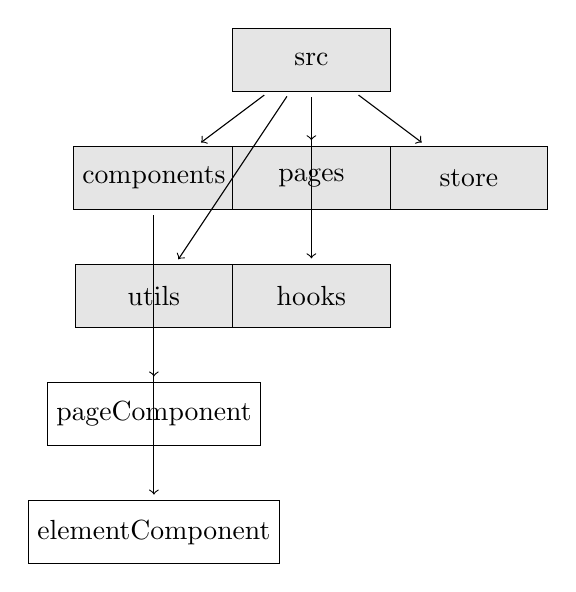
\begin{tikzpicture}[
    file/.style={draw, rectangle, minimum width=2cm, minimum height=0.8cm},
    folder/.style={draw, rectangle, minimum width=2cm, minimum height=0.8cm, fill=gray!20},
    arrow/.style={->, shorten >=2pt, shorten <=2pt}
]

% Folders
\node[folder] (src) at (0,0) {src};
\node[folder] (components) at (-2,-1.5) {components};
\node[folder] (pages) at (0,-1.5) {pages};
\node[folder] (store) at (2,-1.5) {store};
\node[folder] (utils) at (-2,-3) {utils};
\node[folder] (hooks) at (0,-3) {hooks};

% Files
\node[file] (pageComponent) at (-2,-4.5) {pageComponent};
\node[file] (elementComponent) at (-2,-6) {elementComponent};
% ... add more files

% Connections
\draw[arrow] (src) -- (components);
\draw[arrow] (src) -- (pages);
\draw[arrow] (src) -- (store);
\draw[arrow] (src) -- (utils);
\draw[arrow] (src) -- (hooks);
\draw[arrow] (components) -- (pageComponent);
\draw[arrow] (components) -- (elementComponent);
% ... add more connections

\end{tikzpicture}



\pagebreak
\subsubsection{Back-end}
The backend uses the dotNet framework. The development language using the C\# language.

In this project, the backend uses the Onion Architecture.
The Onion Architecture is a typically layered architecture, 
where each layer depends on the inner layer and provides interfaces to the outer layer.
The outer layer provides services to the outermost layer 
and other modules in the same layer based on the interfaces of the inner layer.

From inner to outer, the layers are: Domain, Application, Infrastructure, Presentation.
The Domain layer is the core layer and the innermost layer, used to define domain models, 
which are the business models.
It includes domain models and domain service interfaces.
Domain models are used to define the business models, 
which are the entities in the entity-relationship model and their attributes.
Domain service interfaces are used to define the business services, 
which are the relationships between entities in the entity-relationship model.

The Application layer is the application layer, 
used to define application services, which are the business logic.
It includes domain service implementations and application service interfaces.
Domain service implementations implement the methods of the inner layer's domain service 
interfaces and implement the business logic of the domain models.
Application service interfaces are used to define application services, 
which are the business logic.
It includes but is not limited to database interfaces, testing interfaces, 
HTTP API interfaces, MQTT interfaces, etc.

The Infrastructure layer is the infrastructure layer, used to define infrastructure.
It includes database implementations, testing implementations, 
HTTP API implementations, MQTT implementations, etc.
Database implementations implement the database interfaces 
and provide CRUD services for the database.
Testing implementations implement the testing interfaces 
and provide services for unit testing and integration testing.
HTTP API implementations implement the HTTP API interfaces 
and provide CRUD operations for HTTP APIs.
MQTT implementations implement the MQTT interfaces 
and provide CRUD operations for MQTT.

The Presentation layer is the presentation layer, used to define presentation logic, 
such as interfaces and pages. Since this is a backend project,
data presentation and control are handled by the frontend, 
so this layer is not needed.



\pagebreak
\subsubsection{Data communication and storage}
% 关于本项目的数据通信与数据存储的设计, 包括数据通信的协议, 数据存储的设计等
% 关于数据通信的设计:
% 1. 通信协议的选择
% 自前端向后端发送的数据, 有三种传输的数据类型, 
% 一种是普通的增删改查的请求, 对数据传输的时效性要求不高, 但是对数据的准确性, 完整性, 有序性, 安全性有一定的要求,
% 这种数据的传输, 采用 HTTP 协议, 以及 RESTful API 的设计. 可以有效的保证对数据传输的以上要求.
% 一种是对数据通道的创建和流媒体数据的传输, 对数据传输的时效性, 安全性要求较高, 这种数据的传输, 采用 WebRTC 协议, 以及 MQTT 协议.
% 配合可以快速解码的 flatbuffers 协议, 可以有效的保证对数据传输的以上要求.
% 最后一种是对设备的状态信息和操作信息的传输, 对完整性, 有序性, 安全性都有较高的要求, 这种数据的传输, 采用 MQTT 协议
% 同时也使用了 flatbuffers 协议.
% 
% 2. 数据通信的通信架构和通信流程
% 本项目的数据通信的通信架构, 是基于前后端分离的架构, 前端使用 React 框架, 后端使用 dotnet 框架.
% 当前端需要向后端发送数据的时候, 前端会向后端发送 HTTP 请求, 后端接收到 HTTP 请求之后, 会根据请求的数据类型,
% 选择不同的数据处理方式, 对于普通的增删改查的请求, 后端会根据 RESTful API 的设计, 对数据进行增删改查的操作,
% 对于对数据通道的创建和流媒体数据的传输, 后端会根据 WebRTC 协议, 对数据通道进行创建, 并且帮助前端和设备建立数据通道,
% 当数据通道建立后, 前端和设备之间则使用 flatbuffer 的数据格式对流媒体数据进行传输,
% 对于设备的状态信息和操作信息的传输, 前端会直接向 MQTT broker 发送 MQTT 请求, 
% 设备会在其自身的固件中监听相关的 MQTT 请求, 并且返回相关的数据.
% 
% 3. 数据通信的格式
% 本项目的数据通信的格式, 有三种, 
% 一种是 HTTP 协议, 
% 使用 json 格式对数据进行传输,
% 一种是 WebRTC 协议, 
% 使用 flatbuffers 格式对数据进行传输,
% 一种是 MQTT 协议.
% 使用 flatbuffers 格式对数据进行传输,
% 
% 关于数据存储的设计:
% 1. 数据存储的数据库的选择
% 本项目的数据存储的数据库的选择, 使用了轻量级的数据库 SQLite,
% SQLite 是一个进程内的库, 实现了自给自足的, 无服务器的, 零配置的, 事务性的 SQL 数据库引擎.
% 这是因为整个项目的目的是为了实现前端与设备之间的数据通信, 对于数据库数据的增删改查操作的要求不高,
% 数据量较小, 且对于数据库的数据的事务性要求不高, 所以选择了 SQLite 数据库.
% 2. 项目前后端的数据结构的设计
% 在本项目中, 前端由于使用了 React 框架, 所以前端的数据结构的设计, 使用了基于状态的数据结构的设计,
% 每个组件或者数据集都包含一个状态对象, 这个状态对象的属性就是组件的各个状态. 
% 使用状态对象的原因是, 可以方便的对状态进行管理, 采用对象-属性的形式, 可以方便的针对不同组件的同类状态进行区分,
% 由于跨组件的状态是由 redux 进行管理的, 这种状态对象的设计, 可以更搞笑的对状态进行更新和传递.
% 后端由于使用了 dotnet 框架, 所以后端的数据结构的设计, 使用了基于类的数据结构的设计,
% 采用了面向对象的编程思想, 对数据进行了封装, 使得数据的传输更加的安全, 有序, 完整.


\pagebreak

% \subsection{Domain model}
% \documentclass[]{article}
\usepackage{graphicx}
\usepackage{amsmath}
\usepackage{tikz}

% libaries
\usetikzlibrary{shapes,arrows}

%Define the listing package
\usepackage{listings} %code highlighter
\usepackage{color} %use color
\definecolor{mygreen}{rgb}{0,0.6,0}
\definecolor{mygray}{rgb}{0.5,0.5,0.5}
\definecolor{mymauve}{rgb}{0.58,0,0.82}

%Customize a bit the look
\lstset{ %
backgroundcolor=\color{white}, % choose the background color; you must add \usepackage{color} or \usepackage{xcolor}
basicstyle=\footnotesize, % the size of the fonts that are used for the code
breakatwhitespace=false, % sets if automatic breaks should only happen at whitespace
breaklines=true, % sets automatic line breaking
captionpos=b, % sets the caption-position to bottom
commentstyle=\color{mygreen}, % comment style
deletekeywords={...}, % if you want to delete keywords from the given language
escapeinside={\%*}{*)}, % if you want to add LaTeX within your code
extendedchars=true, % lets you use non-ASCII characters; for 8-bits encodings only, does not work with UTF-8
frame=single, % adds a frame around the code
keepspaces=true, % keeps spaces in text, useful for keeping indentation of code (possibly needs columns=flexible)
keywordstyle=\color{blue}, % keyword style
% language=Octave, % the language of the code
morekeywords={*,...}, % if you want to add more keywords to the set
numbers=left, % where to put the line-numbers; possible values are (none, left, right)
numbersep=5pt, % how far the line-numbers are from the code
numberstyle=\tiny\color{mygray}, % the style that is used for the line-numbers
rulecolor=\color{black}, % if not set, the frame-color may be changed on line-breaks within not-black text (e.g. comments (green here))
showspaces=false, % show spaces everywhere adding particular underscores; it overrides 'showstringspaces'
showstringspaces=false, % underline spaces within strings only
showtabs=false, % show tabs within strings adding particular underscores
stepnumber=1, % the step between two line-numbers. If it's 1, each line will be numbered
stringstyle=\color{mymauve}, % string literal style
tabsize=2, % sets default tabsize to 2 spaces
title=\lstname % show the filename of files included with \lstinputlisting; also try caption instead of title
}

\definecolor{darkgray}{rgb}{.4,.4,.4}
\definecolor{purple}{rgb}{0.65, 0.12, 0.82}

\lstdefinelanguage{React}{
keywords={const, typeof, new, true, false, catch, function, return, null, catch, switch, var, if, in, while, do, else, case, break},
keywordstyle=\color{blue}\bfseries,
ndkeywords={class, export, boolean, throw, implements, import, this},
ndkeywordstyle=\color{darkgray}\bfseries,
identifierstyle=\color{mygreen},
sensitive=false,
comment=[l]{//},
morecomment=[s]{/*}{*/},
commentstyle=\color{purple}\ttfamily,
string=[b]{"}{'}{`},
stringstyle=\color{red}\ttfamily,
morestring=[b]',
morestring=[b]",
morestring=[b]`',
}

\lstdefinelanguage{CSharp}{
keywords={const, typeof, new, true, false, catch, function, return, null, catch, switch, var, if, in, while, do, else, case, break},
keywordstyle=\color{blue}\bfseries,
ndkeywords={class, export, boolean, throw, implements, import, this},
ndkeywordstyle=\color{darkgray}\bfseries,
identifierstyle=\color{mygreen},
sensitive=false,
comment=[l]{//},
morecomment=[s]{/*}{*/},
commentstyle=\color{purple}\ttfamily,
string=[b]{"}{'}{`},
stringstyle=\color{red}\ttfamily,
morestring=[b]',
morestring=[b]",
morestring=[b]`',
}

\lstset{
language=React,
extendedchars=true,
basicstyle=\footnotesize\ttfamily,
showstringspaces=false,
showspaces=false,
numbers=left,
numberstyle=\footnotesize,
numbersep=9pt,
tabsize=2,
breaklines=true,
showtabs=false,
captionpos=b
}

\lstset{
language=CSharp,
extendedchars=true,
basicstyle=\footnotesize\ttfamily,
showstringspaces=false,
showspaces=false,
numbers=left,
numberstyle=\footnotesize,
numbersep=9pt,
tabsize=2,
breaklines=true,
showtabs=false,
captionpos=b
}

% \usepackage{cite} % Add this line for citation

% \bibliographystyle{plain}

\title{
The implementation of BifrostConnect Front-end scope, 
re-design and development with the relevant back-end support develop.
}
\author{
    Fei Gu \\
    Erhvervs Akademi Sydvest \\
    Computer Science 21\\
    }
\date{\today}

\begin{document}

% Front page
\maketitle
\begin{center}
    Supervisor: Henrik Boulund Meng Hansen \\
    Company: BifrostConnect \\
    Engineering Director: Jasper Wass \\
\end{center}
\tableofcontents
\pagebreak


% The introduction
\section{Introduction}
\subsection{Background}\input{sections/introduction/background.tex}
\subsection{The company}\input{sections/introduction/aboutCompany}
\subsection{The project}\input{sections/introduction/aboutProject}
\pagebreak

% The problem statement
\section{Problem Statement}
\subsection{Statement}
\input{sections/problemStatement/statement}
\subsection{Situation}
\input{sections/problemStatement/situation}
\subsection{Potential Solution}
\input{sections/problemStatement/potentialSolution}
\pagebreak

% Requirement analysis
\section{Requirement Analysis}
\input{sections/requirementAnalysis/index}

\subsection{Stakeholders}
\input{sections/requirementAnalysis/stakeholders/index}

\subsection{Business Domain}
\input{sections/requirementAnalysis/bussinesDomain/index}

\subsection{Scope}
\input{sections/requirementAnalysis/scope}

\subsection{Goals}
\input{sections/requirementAnalysis/goals}
\pagebreak

% Software Design
\section{Software Design}
% developement methods
\subsection{Software Development Methods}
\input{sections/softwareDevelopmentMethods/index}
\subsubsection{Agile Software Development}
\input{sections/softwareDevelopmentMethods/agileSoftwareDevelopment/index}
\subsubsection{Feature Driven Development}
\input{sections/softwareDevelopmentMethods/featureDrivenDevelopment/index}

\pagebreak

% Technology seslection
\subsection{Technology selection}
\input{sections/softwareDesign/technologySelection/index}
\subsubsection{Front-end}
\input{sections/softwareDesign/technologySelection/frontEnd}            
\subsubsection{Back-end}
\input{sections/softwareDesign/technologySelection/backEnd}            
\subsubsection{Database}
\input{sections/softwareDesign/technologySelection/database}
\subsubsection{Data communication}
\input{sections/softwareDesign/technologySelection/dataCommunication}            
\subsubsection{DevOps}
\input{sections/softwareDesign/technologySelection/devOps}
\pagebreak

% Architecture design
\subsection{Architecture design}
\input{sections/softwareDesign/architectureDesign/index}
\pagebreak
\subsubsection{Front-end}
\input{sections/softwareDesign/architectureDesign/frontEndArchitecture}
\pagebreak
\subsubsection{Back-end}
\input{sections/softwareDesign/architectureDesign/backEndArchitecture}
\pagebreak
\subsubsection{Data communication and storage}
\input{sections/softwareDesign/architectureDesign/dataCommunicationArchitecture}
\pagebreak

% \subsection{Domain model}
% \input{sections/softwareDesign/domainModel/index}
% \subsection{Database design}
% % 数据库领域模型 ER 图
% % 包括表和字段的设置.
% % 对于私有键和外键的设置.

% \subsection{Back-end design}
% % 后端对象模型
% % 以及对于对象模型的增删改查
% % 以及相关的其他服务的设计`'

% \subsection{Front-end design}
% % 对于前端的页面结构的设计 
% % 页面的状态的设计, 交互设计

% \subsection{FlatBuffers design}
% % schema 的设计

\subsection{DevOps CI/CD process design}
\input{sections/softwareDesign/devOpsDesign/index}
\subsubsection{Continuous Integration}
\input{sections/softwareDesign/devOpsDesign/continuousIntegration/index}
\subsubsection{Continuous Delivery}
\input{sections/softwareDesign/devOpsDesign/continuousDelivery/index}
\subsubsection{Continuous Deployment}
\input{sections/softwareDesign/devOpsDesign/continuousDeployment/index}
\pagebreak

\section{Software Development} 
\input{sections/softwareDevelopment/index}
\subsection{Overall development}
\input{sections/softwareDevelopment/overallDevelopement/index}
\subsubsection{Front-end}
\input{sections/softwareDevelopment/overallDevelopement/frontEnd/index}
\subsubsection{Back-end}
\input{sections/softwareDevelopment/overallDevelopement/backEnd/index}
\subsubsection{DevOps}
\input{sections/softwareDevelopment/overallDevelopement/devOps/index}
\subsection{Feature development} 
\input{sections/softwareDevelopment/featureDevelopment/index}
\subsubsection{Use Case 1}
\input{sections/softwareDevelopment/featureDevelopment/useCase1/index}
\subsubsection{Feature 1}
\input{sections/softwareDevelopment/featureDevelopment/feature/feature1.tex}
\pagebreak
\section{Conclusion} 
\subsection{Result}
Since the project is still in progress, the result is not available yet.
So far, basic structure of this project has been built. But the most features 
are not implemented yet. 
\subsection{Discussion}
As a single developer for this project, I am confident what I have done so far.
And I can say I understand the most of the knowledge I have used in this project, 
which also means I can explain all the part of the project. 
But this project also relevant some of the complex knowledge which I have to continue 
to study and practice.
\subsection{Future Work}
The future work is to implement the rest of the features. 
Including the most important part which is the 'create session' feature.
\pagebreak
% \bibliography{bibliography}
\pagebreak
% \begin{appendices}
%     \section{Appendix}
% \end{appendices} 
\end{document}
% \subsection{Database design}
% % 数据库领域模型 ER 图
% % 包括表和字段的设置.
% % 对于私有键和外键的设置.

% \subsection{Back-end design}
% % 后端对象模型
% % 以及对于对象模型的增删改查
% % 以及相关的其他服务的设计`'

% \subsection{Front-end design}
% % 对于前端的页面结构的设计 
% % 页面的状态的设计, 交互设计

% \subsection{FlatBuffers design}
% % schema 的设计

\subsection{DevOps CI/CD process design}
\documentclass[]{article}
\usepackage{graphicx}
\usepackage{amsmath}
\usepackage{tikz}

% libaries
\usetikzlibrary{shapes,arrows}

%Define the listing package
\usepackage{listings} %code highlighter
\usepackage{color} %use color
\definecolor{mygreen}{rgb}{0,0.6,0}
\definecolor{mygray}{rgb}{0.5,0.5,0.5}
\definecolor{mymauve}{rgb}{0.58,0,0.82}

%Customize a bit the look
\lstset{ %
backgroundcolor=\color{white}, % choose the background color; you must add \usepackage{color} or \usepackage{xcolor}
basicstyle=\footnotesize, % the size of the fonts that are used for the code
breakatwhitespace=false, % sets if automatic breaks should only happen at whitespace
breaklines=true, % sets automatic line breaking
captionpos=b, % sets the caption-position to bottom
commentstyle=\color{mygreen}, % comment style
deletekeywords={...}, % if you want to delete keywords from the given language
escapeinside={\%*}{*)}, % if you want to add LaTeX within your code
extendedchars=true, % lets you use non-ASCII characters; for 8-bits encodings only, does not work with UTF-8
frame=single, % adds a frame around the code
keepspaces=true, % keeps spaces in text, useful for keeping indentation of code (possibly needs columns=flexible)
keywordstyle=\color{blue}, % keyword style
% language=Octave, % the language of the code
morekeywords={*,...}, % if you want to add more keywords to the set
numbers=left, % where to put the line-numbers; possible values are (none, left, right)
numbersep=5pt, % how far the line-numbers are from the code
numberstyle=\tiny\color{mygray}, % the style that is used for the line-numbers
rulecolor=\color{black}, % if not set, the frame-color may be changed on line-breaks within not-black text (e.g. comments (green here))
showspaces=false, % show spaces everywhere adding particular underscores; it overrides 'showstringspaces'
showstringspaces=false, % underline spaces within strings only
showtabs=false, % show tabs within strings adding particular underscores
stepnumber=1, % the step between two line-numbers. If it's 1, each line will be numbered
stringstyle=\color{mymauve}, % string literal style
tabsize=2, % sets default tabsize to 2 spaces
title=\lstname % show the filename of files included with \lstinputlisting; also try caption instead of title
}

\definecolor{darkgray}{rgb}{.4,.4,.4}
\definecolor{purple}{rgb}{0.65, 0.12, 0.82}

\lstdefinelanguage{React}{
keywords={const, typeof, new, true, false, catch, function, return, null, catch, switch, var, if, in, while, do, else, case, break},
keywordstyle=\color{blue}\bfseries,
ndkeywords={class, export, boolean, throw, implements, import, this},
ndkeywordstyle=\color{darkgray}\bfseries,
identifierstyle=\color{mygreen},
sensitive=false,
comment=[l]{//},
morecomment=[s]{/*}{*/},
commentstyle=\color{purple}\ttfamily,
string=[b]{"}{'}{`},
stringstyle=\color{red}\ttfamily,
morestring=[b]',
morestring=[b]",
morestring=[b]`',
}

\lstdefinelanguage{CSharp}{
keywords={const, typeof, new, true, false, catch, function, return, null, catch, switch, var, if, in, while, do, else, case, break},
keywordstyle=\color{blue}\bfseries,
ndkeywords={class, export, boolean, throw, implements, import, this},
ndkeywordstyle=\color{darkgray}\bfseries,
identifierstyle=\color{mygreen},
sensitive=false,
comment=[l]{//},
morecomment=[s]{/*}{*/},
commentstyle=\color{purple}\ttfamily,
string=[b]{"}{'}{`},
stringstyle=\color{red}\ttfamily,
morestring=[b]',
morestring=[b]",
morestring=[b]`',
}

\lstset{
language=React,
extendedchars=true,
basicstyle=\footnotesize\ttfamily,
showstringspaces=false,
showspaces=false,
numbers=left,
numberstyle=\footnotesize,
numbersep=9pt,
tabsize=2,
breaklines=true,
showtabs=false,
captionpos=b
}

\lstset{
language=CSharp,
extendedchars=true,
basicstyle=\footnotesize\ttfamily,
showstringspaces=false,
showspaces=false,
numbers=left,
numberstyle=\footnotesize,
numbersep=9pt,
tabsize=2,
breaklines=true,
showtabs=false,
captionpos=b
}

% \usepackage{cite} % Add this line for citation

% \bibliographystyle{plain}

\title{
The implementation of BifrostConnect Front-end scope, 
re-design and development with the relevant back-end support develop.
}
\author{
    Fei Gu \\
    Erhvervs Akademi Sydvest \\
    Computer Science 21\\
    }
\date{\today}

\begin{document}

% Front page
\maketitle
\begin{center}
    Supervisor: Henrik Boulund Meng Hansen \\
    Company: BifrostConnect \\
    Engineering Director: Jasper Wass \\
\end{center}
\tableofcontents
\pagebreak


% The introduction
\section{Introduction}
\subsection{Background}\input{sections/introduction/background.tex}
\subsection{The company}\input{sections/introduction/aboutCompany}
\subsection{The project}\input{sections/introduction/aboutProject}
\pagebreak

% The problem statement
\section{Problem Statement}
\subsection{Statement}
\input{sections/problemStatement/statement}
\subsection{Situation}
\input{sections/problemStatement/situation}
\subsection{Potential Solution}
\input{sections/problemStatement/potentialSolution}
\pagebreak

% Requirement analysis
\section{Requirement Analysis}
\input{sections/requirementAnalysis/index}

\subsection{Stakeholders}
\input{sections/requirementAnalysis/stakeholders/index}

\subsection{Business Domain}
\input{sections/requirementAnalysis/bussinesDomain/index}

\subsection{Scope}
\input{sections/requirementAnalysis/scope}

\subsection{Goals}
\input{sections/requirementAnalysis/goals}
\pagebreak

% Software Design
\section{Software Design}
% developement methods
\subsection{Software Development Methods}
\input{sections/softwareDevelopmentMethods/index}
\subsubsection{Agile Software Development}
\input{sections/softwareDevelopmentMethods/agileSoftwareDevelopment/index}
\subsubsection{Feature Driven Development}
\input{sections/softwareDevelopmentMethods/featureDrivenDevelopment/index}

\pagebreak

% Technology seslection
\subsection{Technology selection}
\input{sections/softwareDesign/technologySelection/index}
\subsubsection{Front-end}
\input{sections/softwareDesign/technologySelection/frontEnd}            
\subsubsection{Back-end}
\input{sections/softwareDesign/technologySelection/backEnd}            
\subsubsection{Database}
\input{sections/softwareDesign/technologySelection/database}
\subsubsection{Data communication}
\input{sections/softwareDesign/technologySelection/dataCommunication}            
\subsubsection{DevOps}
\input{sections/softwareDesign/technologySelection/devOps}
\pagebreak

% Architecture design
\subsection{Architecture design}
\input{sections/softwareDesign/architectureDesign/index}
\pagebreak
\subsubsection{Front-end}
\input{sections/softwareDesign/architectureDesign/frontEndArchitecture}
\pagebreak
\subsubsection{Back-end}
\input{sections/softwareDesign/architectureDesign/backEndArchitecture}
\pagebreak
\subsubsection{Data communication and storage}
\input{sections/softwareDesign/architectureDesign/dataCommunicationArchitecture}
\pagebreak

% \subsection{Domain model}
% \input{sections/softwareDesign/domainModel/index}
% \subsection{Database design}
% % 数据库领域模型 ER 图
% % 包括表和字段的设置.
% % 对于私有键和外键的设置.

% \subsection{Back-end design}
% % 后端对象模型
% % 以及对于对象模型的增删改查
% % 以及相关的其他服务的设计`'

% \subsection{Front-end design}
% % 对于前端的页面结构的设计 
% % 页面的状态的设计, 交互设计

% \subsection{FlatBuffers design}
% % schema 的设计

\subsection{DevOps CI/CD process design}
\input{sections/softwareDesign/devOpsDesign/index}
\subsubsection{Continuous Integration}
\input{sections/softwareDesign/devOpsDesign/continuousIntegration/index}
\subsubsection{Continuous Delivery}
\input{sections/softwareDesign/devOpsDesign/continuousDelivery/index}
\subsubsection{Continuous Deployment}
\input{sections/softwareDesign/devOpsDesign/continuousDeployment/index}
\pagebreak

\section{Software Development} 
\input{sections/softwareDevelopment/index}
\subsection{Overall development}
\input{sections/softwareDevelopment/overallDevelopement/index}
\subsubsection{Front-end}
\input{sections/softwareDevelopment/overallDevelopement/frontEnd/index}
\subsubsection{Back-end}
\input{sections/softwareDevelopment/overallDevelopement/backEnd/index}
\subsubsection{DevOps}
\input{sections/softwareDevelopment/overallDevelopement/devOps/index}
\subsection{Feature development} 
\input{sections/softwareDevelopment/featureDevelopment/index}
\subsubsection{Use Case 1}
\input{sections/softwareDevelopment/featureDevelopment/useCase1/index}
\subsubsection{Feature 1}
\input{sections/softwareDevelopment/featureDevelopment/feature/feature1.tex}
\pagebreak
\section{Conclusion} 
\subsection{Result}
Since the project is still in progress, the result is not available yet.
So far, basic structure of this project has been built. But the most features 
are not implemented yet. 
\subsection{Discussion}
As a single developer for this project, I am confident what I have done so far.
And I can say I understand the most of the knowledge I have used in this project, 
which also means I can explain all the part of the project. 
But this project also relevant some of the complex knowledge which I have to continue 
to study and practice.
\subsection{Future Work}
The future work is to implement the rest of the features. 
Including the most important part which is the 'create session' feature.
\pagebreak
% \bibliography{bibliography}
\pagebreak
% \begin{appendices}
%     \section{Appendix}
% \end{appendices} 
\end{document}
\subsubsection{Continuous Integration}
\documentclass[]{article}
\usepackage{graphicx}
\usepackage{amsmath}
\usepackage{tikz}

% libaries
\usetikzlibrary{shapes,arrows}

%Define the listing package
\usepackage{listings} %code highlighter
\usepackage{color} %use color
\definecolor{mygreen}{rgb}{0,0.6,0}
\definecolor{mygray}{rgb}{0.5,0.5,0.5}
\definecolor{mymauve}{rgb}{0.58,0,0.82}

%Customize a bit the look
\lstset{ %
backgroundcolor=\color{white}, % choose the background color; you must add \usepackage{color} or \usepackage{xcolor}
basicstyle=\footnotesize, % the size of the fonts that are used for the code
breakatwhitespace=false, % sets if automatic breaks should only happen at whitespace
breaklines=true, % sets automatic line breaking
captionpos=b, % sets the caption-position to bottom
commentstyle=\color{mygreen}, % comment style
deletekeywords={...}, % if you want to delete keywords from the given language
escapeinside={\%*}{*)}, % if you want to add LaTeX within your code
extendedchars=true, % lets you use non-ASCII characters; for 8-bits encodings only, does not work with UTF-8
frame=single, % adds a frame around the code
keepspaces=true, % keeps spaces in text, useful for keeping indentation of code (possibly needs columns=flexible)
keywordstyle=\color{blue}, % keyword style
% language=Octave, % the language of the code
morekeywords={*,...}, % if you want to add more keywords to the set
numbers=left, % where to put the line-numbers; possible values are (none, left, right)
numbersep=5pt, % how far the line-numbers are from the code
numberstyle=\tiny\color{mygray}, % the style that is used for the line-numbers
rulecolor=\color{black}, % if not set, the frame-color may be changed on line-breaks within not-black text (e.g. comments (green here))
showspaces=false, % show spaces everywhere adding particular underscores; it overrides 'showstringspaces'
showstringspaces=false, % underline spaces within strings only
showtabs=false, % show tabs within strings adding particular underscores
stepnumber=1, % the step between two line-numbers. If it's 1, each line will be numbered
stringstyle=\color{mymauve}, % string literal style
tabsize=2, % sets default tabsize to 2 spaces
title=\lstname % show the filename of files included with \lstinputlisting; also try caption instead of title
}

\definecolor{darkgray}{rgb}{.4,.4,.4}
\definecolor{purple}{rgb}{0.65, 0.12, 0.82}

\lstdefinelanguage{React}{
keywords={const, typeof, new, true, false, catch, function, return, null, catch, switch, var, if, in, while, do, else, case, break},
keywordstyle=\color{blue}\bfseries,
ndkeywords={class, export, boolean, throw, implements, import, this},
ndkeywordstyle=\color{darkgray}\bfseries,
identifierstyle=\color{mygreen},
sensitive=false,
comment=[l]{//},
morecomment=[s]{/*}{*/},
commentstyle=\color{purple}\ttfamily,
string=[b]{"}{'}{`},
stringstyle=\color{red}\ttfamily,
morestring=[b]',
morestring=[b]",
morestring=[b]`',
}

\lstdefinelanguage{CSharp}{
keywords={const, typeof, new, true, false, catch, function, return, null, catch, switch, var, if, in, while, do, else, case, break},
keywordstyle=\color{blue}\bfseries,
ndkeywords={class, export, boolean, throw, implements, import, this},
ndkeywordstyle=\color{darkgray}\bfseries,
identifierstyle=\color{mygreen},
sensitive=false,
comment=[l]{//},
morecomment=[s]{/*}{*/},
commentstyle=\color{purple}\ttfamily,
string=[b]{"}{'}{`},
stringstyle=\color{red}\ttfamily,
morestring=[b]',
morestring=[b]",
morestring=[b]`',
}

\lstset{
language=React,
extendedchars=true,
basicstyle=\footnotesize\ttfamily,
showstringspaces=false,
showspaces=false,
numbers=left,
numberstyle=\footnotesize,
numbersep=9pt,
tabsize=2,
breaklines=true,
showtabs=false,
captionpos=b
}

\lstset{
language=CSharp,
extendedchars=true,
basicstyle=\footnotesize\ttfamily,
showstringspaces=false,
showspaces=false,
numbers=left,
numberstyle=\footnotesize,
numbersep=9pt,
tabsize=2,
breaklines=true,
showtabs=false,
captionpos=b
}

% \usepackage{cite} % Add this line for citation

% \bibliographystyle{plain}

\title{
The implementation of BifrostConnect Front-end scope, 
re-design and development with the relevant back-end support develop.
}
\author{
    Fei Gu \\
    Erhvervs Akademi Sydvest \\
    Computer Science 21\\
    }
\date{\today}

\begin{document}

% Front page
\maketitle
\begin{center}
    Supervisor: Henrik Boulund Meng Hansen \\
    Company: BifrostConnect \\
    Engineering Director: Jasper Wass \\
\end{center}
\tableofcontents
\pagebreak


% The introduction
\section{Introduction}
\subsection{Background}\input{sections/introduction/background.tex}
\subsection{The company}\input{sections/introduction/aboutCompany}
\subsection{The project}\input{sections/introduction/aboutProject}
\pagebreak

% The problem statement
\section{Problem Statement}
\subsection{Statement}
\input{sections/problemStatement/statement}
\subsection{Situation}
\input{sections/problemStatement/situation}
\subsection{Potential Solution}
\input{sections/problemStatement/potentialSolution}
\pagebreak

% Requirement analysis
\section{Requirement Analysis}
\input{sections/requirementAnalysis/index}

\subsection{Stakeholders}
\input{sections/requirementAnalysis/stakeholders/index}

\subsection{Business Domain}
\input{sections/requirementAnalysis/bussinesDomain/index}

\subsection{Scope}
\input{sections/requirementAnalysis/scope}

\subsection{Goals}
\input{sections/requirementAnalysis/goals}
\pagebreak

% Software Design
\section{Software Design}
% developement methods
\subsection{Software Development Methods}
\input{sections/softwareDevelopmentMethods/index}
\subsubsection{Agile Software Development}
\input{sections/softwareDevelopmentMethods/agileSoftwareDevelopment/index}
\subsubsection{Feature Driven Development}
\input{sections/softwareDevelopmentMethods/featureDrivenDevelopment/index}

\pagebreak

% Technology seslection
\subsection{Technology selection}
\input{sections/softwareDesign/technologySelection/index}
\subsubsection{Front-end}
\input{sections/softwareDesign/technologySelection/frontEnd}            
\subsubsection{Back-end}
\input{sections/softwareDesign/technologySelection/backEnd}            
\subsubsection{Database}
\input{sections/softwareDesign/technologySelection/database}
\subsubsection{Data communication}
\input{sections/softwareDesign/technologySelection/dataCommunication}            
\subsubsection{DevOps}
\input{sections/softwareDesign/technologySelection/devOps}
\pagebreak

% Architecture design
\subsection{Architecture design}
\input{sections/softwareDesign/architectureDesign/index}
\pagebreak
\subsubsection{Front-end}
\input{sections/softwareDesign/architectureDesign/frontEndArchitecture}
\pagebreak
\subsubsection{Back-end}
\input{sections/softwareDesign/architectureDesign/backEndArchitecture}
\pagebreak
\subsubsection{Data communication and storage}
\input{sections/softwareDesign/architectureDesign/dataCommunicationArchitecture}
\pagebreak

% \subsection{Domain model}
% \input{sections/softwareDesign/domainModel/index}
% \subsection{Database design}
% % 数据库领域模型 ER 图
% % 包括表和字段的设置.
% % 对于私有键和外键的设置.

% \subsection{Back-end design}
% % 后端对象模型
% % 以及对于对象模型的增删改查
% % 以及相关的其他服务的设计`'

% \subsection{Front-end design}
% % 对于前端的页面结构的设计 
% % 页面的状态的设计, 交互设计

% \subsection{FlatBuffers design}
% % schema 的设计

\subsection{DevOps CI/CD process design}
\input{sections/softwareDesign/devOpsDesign/index}
\subsubsection{Continuous Integration}
\input{sections/softwareDesign/devOpsDesign/continuousIntegration/index}
\subsubsection{Continuous Delivery}
\input{sections/softwareDesign/devOpsDesign/continuousDelivery/index}
\subsubsection{Continuous Deployment}
\input{sections/softwareDesign/devOpsDesign/continuousDeployment/index}
\pagebreak

\section{Software Development} 
\input{sections/softwareDevelopment/index}
\subsection{Overall development}
\input{sections/softwareDevelopment/overallDevelopement/index}
\subsubsection{Front-end}
\input{sections/softwareDevelopment/overallDevelopement/frontEnd/index}
\subsubsection{Back-end}
\input{sections/softwareDevelopment/overallDevelopement/backEnd/index}
\subsubsection{DevOps}
\input{sections/softwareDevelopment/overallDevelopement/devOps/index}
\subsection{Feature development} 
\input{sections/softwareDevelopment/featureDevelopment/index}
\subsubsection{Use Case 1}
\input{sections/softwareDevelopment/featureDevelopment/useCase1/index}
\subsubsection{Feature 1}
\input{sections/softwareDevelopment/featureDevelopment/feature/feature1.tex}
\pagebreak
\section{Conclusion} 
\subsection{Result}
Since the project is still in progress, the result is not available yet.
So far, basic structure of this project has been built. But the most features 
are not implemented yet. 
\subsection{Discussion}
As a single developer for this project, I am confident what I have done so far.
And I can say I understand the most of the knowledge I have used in this project, 
which also means I can explain all the part of the project. 
But this project also relevant some of the complex knowledge which I have to continue 
to study and practice.
\subsection{Future Work}
The future work is to implement the rest of the features. 
Including the most important part which is the 'create session' feature.
\pagebreak
% \bibliography{bibliography}
\pagebreak
% \begin{appendices}
%     \section{Appendix}
% \end{appendices} 
\end{document}
\subsubsection{Continuous Delivery}
\documentclass[]{article}
\usepackage{graphicx}
\usepackage{amsmath}
\usepackage{tikz}

% libaries
\usetikzlibrary{shapes,arrows}

%Define the listing package
\usepackage{listings} %code highlighter
\usepackage{color} %use color
\definecolor{mygreen}{rgb}{0,0.6,0}
\definecolor{mygray}{rgb}{0.5,0.5,0.5}
\definecolor{mymauve}{rgb}{0.58,0,0.82}

%Customize a bit the look
\lstset{ %
backgroundcolor=\color{white}, % choose the background color; you must add \usepackage{color} or \usepackage{xcolor}
basicstyle=\footnotesize, % the size of the fonts that are used for the code
breakatwhitespace=false, % sets if automatic breaks should only happen at whitespace
breaklines=true, % sets automatic line breaking
captionpos=b, % sets the caption-position to bottom
commentstyle=\color{mygreen}, % comment style
deletekeywords={...}, % if you want to delete keywords from the given language
escapeinside={\%*}{*)}, % if you want to add LaTeX within your code
extendedchars=true, % lets you use non-ASCII characters; for 8-bits encodings only, does not work with UTF-8
frame=single, % adds a frame around the code
keepspaces=true, % keeps spaces in text, useful for keeping indentation of code (possibly needs columns=flexible)
keywordstyle=\color{blue}, % keyword style
% language=Octave, % the language of the code
morekeywords={*,...}, % if you want to add more keywords to the set
numbers=left, % where to put the line-numbers; possible values are (none, left, right)
numbersep=5pt, % how far the line-numbers are from the code
numberstyle=\tiny\color{mygray}, % the style that is used for the line-numbers
rulecolor=\color{black}, % if not set, the frame-color may be changed on line-breaks within not-black text (e.g. comments (green here))
showspaces=false, % show spaces everywhere adding particular underscores; it overrides 'showstringspaces'
showstringspaces=false, % underline spaces within strings only
showtabs=false, % show tabs within strings adding particular underscores
stepnumber=1, % the step between two line-numbers. If it's 1, each line will be numbered
stringstyle=\color{mymauve}, % string literal style
tabsize=2, % sets default tabsize to 2 spaces
title=\lstname % show the filename of files included with \lstinputlisting; also try caption instead of title
}

\definecolor{darkgray}{rgb}{.4,.4,.4}
\definecolor{purple}{rgb}{0.65, 0.12, 0.82}

\lstdefinelanguage{React}{
keywords={const, typeof, new, true, false, catch, function, return, null, catch, switch, var, if, in, while, do, else, case, break},
keywordstyle=\color{blue}\bfseries,
ndkeywords={class, export, boolean, throw, implements, import, this},
ndkeywordstyle=\color{darkgray}\bfseries,
identifierstyle=\color{mygreen},
sensitive=false,
comment=[l]{//},
morecomment=[s]{/*}{*/},
commentstyle=\color{purple}\ttfamily,
string=[b]{"}{'}{`},
stringstyle=\color{red}\ttfamily,
morestring=[b]',
morestring=[b]",
morestring=[b]`',
}

\lstdefinelanguage{CSharp}{
keywords={const, typeof, new, true, false, catch, function, return, null, catch, switch, var, if, in, while, do, else, case, break},
keywordstyle=\color{blue}\bfseries,
ndkeywords={class, export, boolean, throw, implements, import, this},
ndkeywordstyle=\color{darkgray}\bfseries,
identifierstyle=\color{mygreen},
sensitive=false,
comment=[l]{//},
morecomment=[s]{/*}{*/},
commentstyle=\color{purple}\ttfamily,
string=[b]{"}{'}{`},
stringstyle=\color{red}\ttfamily,
morestring=[b]',
morestring=[b]",
morestring=[b]`',
}

\lstset{
language=React,
extendedchars=true,
basicstyle=\footnotesize\ttfamily,
showstringspaces=false,
showspaces=false,
numbers=left,
numberstyle=\footnotesize,
numbersep=9pt,
tabsize=2,
breaklines=true,
showtabs=false,
captionpos=b
}

\lstset{
language=CSharp,
extendedchars=true,
basicstyle=\footnotesize\ttfamily,
showstringspaces=false,
showspaces=false,
numbers=left,
numberstyle=\footnotesize,
numbersep=9pt,
tabsize=2,
breaklines=true,
showtabs=false,
captionpos=b
}

% \usepackage{cite} % Add this line for citation

% \bibliographystyle{plain}

\title{
The implementation of BifrostConnect Front-end scope, 
re-design and development with the relevant back-end support develop.
}
\author{
    Fei Gu \\
    Erhvervs Akademi Sydvest \\
    Computer Science 21\\
    }
\date{\today}

\begin{document}

% Front page
\maketitle
\begin{center}
    Supervisor: Henrik Boulund Meng Hansen \\
    Company: BifrostConnect \\
    Engineering Director: Jasper Wass \\
\end{center}
\tableofcontents
\pagebreak


% The introduction
\section{Introduction}
\subsection{Background}\input{sections/introduction/background.tex}
\subsection{The company}\input{sections/introduction/aboutCompany}
\subsection{The project}\input{sections/introduction/aboutProject}
\pagebreak

% The problem statement
\section{Problem Statement}
\subsection{Statement}
\input{sections/problemStatement/statement}
\subsection{Situation}
\input{sections/problemStatement/situation}
\subsection{Potential Solution}
\input{sections/problemStatement/potentialSolution}
\pagebreak

% Requirement analysis
\section{Requirement Analysis}
\input{sections/requirementAnalysis/index}

\subsection{Stakeholders}
\input{sections/requirementAnalysis/stakeholders/index}

\subsection{Business Domain}
\input{sections/requirementAnalysis/bussinesDomain/index}

\subsection{Scope}
\input{sections/requirementAnalysis/scope}

\subsection{Goals}
\input{sections/requirementAnalysis/goals}
\pagebreak

% Software Design
\section{Software Design}
% developement methods
\subsection{Software Development Methods}
\input{sections/softwareDevelopmentMethods/index}
\subsubsection{Agile Software Development}
\input{sections/softwareDevelopmentMethods/agileSoftwareDevelopment/index}
\subsubsection{Feature Driven Development}
\input{sections/softwareDevelopmentMethods/featureDrivenDevelopment/index}

\pagebreak

% Technology seslection
\subsection{Technology selection}
\input{sections/softwareDesign/technologySelection/index}
\subsubsection{Front-end}
\input{sections/softwareDesign/technologySelection/frontEnd}            
\subsubsection{Back-end}
\input{sections/softwareDesign/technologySelection/backEnd}            
\subsubsection{Database}
\input{sections/softwareDesign/technologySelection/database}
\subsubsection{Data communication}
\input{sections/softwareDesign/technologySelection/dataCommunication}            
\subsubsection{DevOps}
\input{sections/softwareDesign/technologySelection/devOps}
\pagebreak

% Architecture design
\subsection{Architecture design}
\input{sections/softwareDesign/architectureDesign/index}
\pagebreak
\subsubsection{Front-end}
\input{sections/softwareDesign/architectureDesign/frontEndArchitecture}
\pagebreak
\subsubsection{Back-end}
\input{sections/softwareDesign/architectureDesign/backEndArchitecture}
\pagebreak
\subsubsection{Data communication and storage}
\input{sections/softwareDesign/architectureDesign/dataCommunicationArchitecture}
\pagebreak

% \subsection{Domain model}
% \input{sections/softwareDesign/domainModel/index}
% \subsection{Database design}
% % 数据库领域模型 ER 图
% % 包括表和字段的设置.
% % 对于私有键和外键的设置.

% \subsection{Back-end design}
% % 后端对象模型
% % 以及对于对象模型的增删改查
% % 以及相关的其他服务的设计`'

% \subsection{Front-end design}
% % 对于前端的页面结构的设计 
% % 页面的状态的设计, 交互设计

% \subsection{FlatBuffers design}
% % schema 的设计

\subsection{DevOps CI/CD process design}
\input{sections/softwareDesign/devOpsDesign/index}
\subsubsection{Continuous Integration}
\input{sections/softwareDesign/devOpsDesign/continuousIntegration/index}
\subsubsection{Continuous Delivery}
\input{sections/softwareDesign/devOpsDesign/continuousDelivery/index}
\subsubsection{Continuous Deployment}
\input{sections/softwareDesign/devOpsDesign/continuousDeployment/index}
\pagebreak

\section{Software Development} 
\input{sections/softwareDevelopment/index}
\subsection{Overall development}
\input{sections/softwareDevelopment/overallDevelopement/index}
\subsubsection{Front-end}
\input{sections/softwareDevelopment/overallDevelopement/frontEnd/index}
\subsubsection{Back-end}
\input{sections/softwareDevelopment/overallDevelopement/backEnd/index}
\subsubsection{DevOps}
\input{sections/softwareDevelopment/overallDevelopement/devOps/index}
\subsection{Feature development} 
\input{sections/softwareDevelopment/featureDevelopment/index}
\subsubsection{Use Case 1}
\input{sections/softwareDevelopment/featureDevelopment/useCase1/index}
\subsubsection{Feature 1}
\input{sections/softwareDevelopment/featureDevelopment/feature/feature1.tex}
\pagebreak
\section{Conclusion} 
\subsection{Result}
Since the project is still in progress, the result is not available yet.
So far, basic structure of this project has been built. But the most features 
are not implemented yet. 
\subsection{Discussion}
As a single developer for this project, I am confident what I have done so far.
And I can say I understand the most of the knowledge I have used in this project, 
which also means I can explain all the part of the project. 
But this project also relevant some of the complex knowledge which I have to continue 
to study and practice.
\subsection{Future Work}
The future work is to implement the rest of the features. 
Including the most important part which is the 'create session' feature.
\pagebreak
% \bibliography{bibliography}
\pagebreak
% \begin{appendices}
%     \section{Appendix}
% \end{appendices} 
\end{document}
\subsubsection{Continuous Deployment}
\documentclass[]{article}
\usepackage{graphicx}
\usepackage{amsmath}
\usepackage{tikz}

% libaries
\usetikzlibrary{shapes,arrows}

%Define the listing package
\usepackage{listings} %code highlighter
\usepackage{color} %use color
\definecolor{mygreen}{rgb}{0,0.6,0}
\definecolor{mygray}{rgb}{0.5,0.5,0.5}
\definecolor{mymauve}{rgb}{0.58,0,0.82}

%Customize a bit the look
\lstset{ %
backgroundcolor=\color{white}, % choose the background color; you must add \usepackage{color} or \usepackage{xcolor}
basicstyle=\footnotesize, % the size of the fonts that are used for the code
breakatwhitespace=false, % sets if automatic breaks should only happen at whitespace
breaklines=true, % sets automatic line breaking
captionpos=b, % sets the caption-position to bottom
commentstyle=\color{mygreen}, % comment style
deletekeywords={...}, % if you want to delete keywords from the given language
escapeinside={\%*}{*)}, % if you want to add LaTeX within your code
extendedchars=true, % lets you use non-ASCII characters; for 8-bits encodings only, does not work with UTF-8
frame=single, % adds a frame around the code
keepspaces=true, % keeps spaces in text, useful for keeping indentation of code (possibly needs columns=flexible)
keywordstyle=\color{blue}, % keyword style
% language=Octave, % the language of the code
morekeywords={*,...}, % if you want to add more keywords to the set
numbers=left, % where to put the line-numbers; possible values are (none, left, right)
numbersep=5pt, % how far the line-numbers are from the code
numberstyle=\tiny\color{mygray}, % the style that is used for the line-numbers
rulecolor=\color{black}, % if not set, the frame-color may be changed on line-breaks within not-black text (e.g. comments (green here))
showspaces=false, % show spaces everywhere adding particular underscores; it overrides 'showstringspaces'
showstringspaces=false, % underline spaces within strings only
showtabs=false, % show tabs within strings adding particular underscores
stepnumber=1, % the step between two line-numbers. If it's 1, each line will be numbered
stringstyle=\color{mymauve}, % string literal style
tabsize=2, % sets default tabsize to 2 spaces
title=\lstname % show the filename of files included with \lstinputlisting; also try caption instead of title
}

\definecolor{darkgray}{rgb}{.4,.4,.4}
\definecolor{purple}{rgb}{0.65, 0.12, 0.82}

\lstdefinelanguage{React}{
keywords={const, typeof, new, true, false, catch, function, return, null, catch, switch, var, if, in, while, do, else, case, break},
keywordstyle=\color{blue}\bfseries,
ndkeywords={class, export, boolean, throw, implements, import, this},
ndkeywordstyle=\color{darkgray}\bfseries,
identifierstyle=\color{mygreen},
sensitive=false,
comment=[l]{//},
morecomment=[s]{/*}{*/},
commentstyle=\color{purple}\ttfamily,
string=[b]{"}{'}{`},
stringstyle=\color{red}\ttfamily,
morestring=[b]',
morestring=[b]",
morestring=[b]`',
}

\lstdefinelanguage{CSharp}{
keywords={const, typeof, new, true, false, catch, function, return, null, catch, switch, var, if, in, while, do, else, case, break},
keywordstyle=\color{blue}\bfseries,
ndkeywords={class, export, boolean, throw, implements, import, this},
ndkeywordstyle=\color{darkgray}\bfseries,
identifierstyle=\color{mygreen},
sensitive=false,
comment=[l]{//},
morecomment=[s]{/*}{*/},
commentstyle=\color{purple}\ttfamily,
string=[b]{"}{'}{`},
stringstyle=\color{red}\ttfamily,
morestring=[b]',
morestring=[b]",
morestring=[b]`',
}

\lstset{
language=React,
extendedchars=true,
basicstyle=\footnotesize\ttfamily,
showstringspaces=false,
showspaces=false,
numbers=left,
numberstyle=\footnotesize,
numbersep=9pt,
tabsize=2,
breaklines=true,
showtabs=false,
captionpos=b
}

\lstset{
language=CSharp,
extendedchars=true,
basicstyle=\footnotesize\ttfamily,
showstringspaces=false,
showspaces=false,
numbers=left,
numberstyle=\footnotesize,
numbersep=9pt,
tabsize=2,
breaklines=true,
showtabs=false,
captionpos=b
}

% \usepackage{cite} % Add this line for citation

% \bibliographystyle{plain}

\title{
The implementation of BifrostConnect Front-end scope, 
re-design and development with the relevant back-end support develop.
}
\author{
    Fei Gu \\
    Erhvervs Akademi Sydvest \\
    Computer Science 21\\
    }
\date{\today}

\begin{document}

% Front page
\maketitle
\begin{center}
    Supervisor: Henrik Boulund Meng Hansen \\
    Company: BifrostConnect \\
    Engineering Director: Jasper Wass \\
\end{center}
\tableofcontents
\pagebreak


% The introduction
\section{Introduction}
\subsection{Background}\input{sections/introduction/background.tex}
\subsection{The company}\input{sections/introduction/aboutCompany}
\subsection{The project}\input{sections/introduction/aboutProject}
\pagebreak

% The problem statement
\section{Problem Statement}
\subsection{Statement}
\input{sections/problemStatement/statement}
\subsection{Situation}
\input{sections/problemStatement/situation}
\subsection{Potential Solution}
\input{sections/problemStatement/potentialSolution}
\pagebreak

% Requirement analysis
\section{Requirement Analysis}
\input{sections/requirementAnalysis/index}

\subsection{Stakeholders}
\input{sections/requirementAnalysis/stakeholders/index}

\subsection{Business Domain}
\input{sections/requirementAnalysis/bussinesDomain/index}

\subsection{Scope}
\input{sections/requirementAnalysis/scope}

\subsection{Goals}
\input{sections/requirementAnalysis/goals}
\pagebreak

% Software Design
\section{Software Design}
% developement methods
\subsection{Software Development Methods}
\input{sections/softwareDevelopmentMethods/index}
\subsubsection{Agile Software Development}
\input{sections/softwareDevelopmentMethods/agileSoftwareDevelopment/index}
\subsubsection{Feature Driven Development}
\input{sections/softwareDevelopmentMethods/featureDrivenDevelopment/index}

\pagebreak

% Technology seslection
\subsection{Technology selection}
\input{sections/softwareDesign/technologySelection/index}
\subsubsection{Front-end}
\input{sections/softwareDesign/technologySelection/frontEnd}            
\subsubsection{Back-end}
\input{sections/softwareDesign/technologySelection/backEnd}            
\subsubsection{Database}
\input{sections/softwareDesign/technologySelection/database}
\subsubsection{Data communication}
\input{sections/softwareDesign/technologySelection/dataCommunication}            
\subsubsection{DevOps}
\input{sections/softwareDesign/technologySelection/devOps}
\pagebreak

% Architecture design
\subsection{Architecture design}
\input{sections/softwareDesign/architectureDesign/index}
\pagebreak
\subsubsection{Front-end}
\input{sections/softwareDesign/architectureDesign/frontEndArchitecture}
\pagebreak
\subsubsection{Back-end}
\input{sections/softwareDesign/architectureDesign/backEndArchitecture}
\pagebreak
\subsubsection{Data communication and storage}
\input{sections/softwareDesign/architectureDesign/dataCommunicationArchitecture}
\pagebreak

% \subsection{Domain model}
% \input{sections/softwareDesign/domainModel/index}
% \subsection{Database design}
% % 数据库领域模型 ER 图
% % 包括表和字段的设置.
% % 对于私有键和外键的设置.

% \subsection{Back-end design}
% % 后端对象模型
% % 以及对于对象模型的增删改查
% % 以及相关的其他服务的设计`'

% \subsection{Front-end design}
% % 对于前端的页面结构的设计 
% % 页面的状态的设计, 交互设计

% \subsection{FlatBuffers design}
% % schema 的设计

\subsection{DevOps CI/CD process design}
\input{sections/softwareDesign/devOpsDesign/index}
\subsubsection{Continuous Integration}
\input{sections/softwareDesign/devOpsDesign/continuousIntegration/index}
\subsubsection{Continuous Delivery}
\input{sections/softwareDesign/devOpsDesign/continuousDelivery/index}
\subsubsection{Continuous Deployment}
\input{sections/softwareDesign/devOpsDesign/continuousDeployment/index}
\pagebreak

\section{Software Development} 
\input{sections/softwareDevelopment/index}
\subsection{Overall development}
\input{sections/softwareDevelopment/overallDevelopement/index}
\subsubsection{Front-end}
\input{sections/softwareDevelopment/overallDevelopement/frontEnd/index}
\subsubsection{Back-end}
\input{sections/softwareDevelopment/overallDevelopement/backEnd/index}
\subsubsection{DevOps}
\input{sections/softwareDevelopment/overallDevelopement/devOps/index}
\subsection{Feature development} 
\input{sections/softwareDevelopment/featureDevelopment/index}
\subsubsection{Use Case 1}
\input{sections/softwareDevelopment/featureDevelopment/useCase1/index}
\subsubsection{Feature 1}
\input{sections/softwareDevelopment/featureDevelopment/feature/feature1.tex}
\pagebreak
\section{Conclusion} 
\subsection{Result}
Since the project is still in progress, the result is not available yet.
So far, basic structure of this project has been built. But the most features 
are not implemented yet. 
\subsection{Discussion}
As a single developer for this project, I am confident what I have done so far.
And I can say I understand the most of the knowledge I have used in this project, 
which also means I can explain all the part of the project. 
But this project also relevant some of the complex knowledge which I have to continue 
to study and practice.
\subsection{Future Work}
The future work is to implement the rest of the features. 
Including the most important part which is the 'create session' feature.
\pagebreak
% \bibliography{bibliography}
\pagebreak
% \begin{appendices}
%     \section{Appendix}
% \end{appendices} 
\end{document}
\pagebreak

\section{Software Development} 
\documentclass[]{article}
\usepackage{graphicx}
\usepackage{amsmath}
\usepackage{tikz}

% libaries
\usetikzlibrary{shapes,arrows}

%Define the listing package
\usepackage{listings} %code highlighter
\usepackage{color} %use color
\definecolor{mygreen}{rgb}{0,0.6,0}
\definecolor{mygray}{rgb}{0.5,0.5,0.5}
\definecolor{mymauve}{rgb}{0.58,0,0.82}

%Customize a bit the look
\lstset{ %
backgroundcolor=\color{white}, % choose the background color; you must add \usepackage{color} or \usepackage{xcolor}
basicstyle=\footnotesize, % the size of the fonts that are used for the code
breakatwhitespace=false, % sets if automatic breaks should only happen at whitespace
breaklines=true, % sets automatic line breaking
captionpos=b, % sets the caption-position to bottom
commentstyle=\color{mygreen}, % comment style
deletekeywords={...}, % if you want to delete keywords from the given language
escapeinside={\%*}{*)}, % if you want to add LaTeX within your code
extendedchars=true, % lets you use non-ASCII characters; for 8-bits encodings only, does not work with UTF-8
frame=single, % adds a frame around the code
keepspaces=true, % keeps spaces in text, useful for keeping indentation of code (possibly needs columns=flexible)
keywordstyle=\color{blue}, % keyword style
% language=Octave, % the language of the code
morekeywords={*,...}, % if you want to add more keywords to the set
numbers=left, % where to put the line-numbers; possible values are (none, left, right)
numbersep=5pt, % how far the line-numbers are from the code
numberstyle=\tiny\color{mygray}, % the style that is used for the line-numbers
rulecolor=\color{black}, % if not set, the frame-color may be changed on line-breaks within not-black text (e.g. comments (green here))
showspaces=false, % show spaces everywhere adding particular underscores; it overrides 'showstringspaces'
showstringspaces=false, % underline spaces within strings only
showtabs=false, % show tabs within strings adding particular underscores
stepnumber=1, % the step between two line-numbers. If it's 1, each line will be numbered
stringstyle=\color{mymauve}, % string literal style
tabsize=2, % sets default tabsize to 2 spaces
title=\lstname % show the filename of files included with \lstinputlisting; also try caption instead of title
}

\definecolor{darkgray}{rgb}{.4,.4,.4}
\definecolor{purple}{rgb}{0.65, 0.12, 0.82}

\lstdefinelanguage{React}{
keywords={const, typeof, new, true, false, catch, function, return, null, catch, switch, var, if, in, while, do, else, case, break},
keywordstyle=\color{blue}\bfseries,
ndkeywords={class, export, boolean, throw, implements, import, this},
ndkeywordstyle=\color{darkgray}\bfseries,
identifierstyle=\color{mygreen},
sensitive=false,
comment=[l]{//},
morecomment=[s]{/*}{*/},
commentstyle=\color{purple}\ttfamily,
string=[b]{"}{'}{`},
stringstyle=\color{red}\ttfamily,
morestring=[b]',
morestring=[b]",
morestring=[b]`',
}

\lstdefinelanguage{CSharp}{
keywords={const, typeof, new, true, false, catch, function, return, null, catch, switch, var, if, in, while, do, else, case, break},
keywordstyle=\color{blue}\bfseries,
ndkeywords={class, export, boolean, throw, implements, import, this},
ndkeywordstyle=\color{darkgray}\bfseries,
identifierstyle=\color{mygreen},
sensitive=false,
comment=[l]{//},
morecomment=[s]{/*}{*/},
commentstyle=\color{purple}\ttfamily,
string=[b]{"}{'}{`},
stringstyle=\color{red}\ttfamily,
morestring=[b]',
morestring=[b]",
morestring=[b]`',
}

\lstset{
language=React,
extendedchars=true,
basicstyle=\footnotesize\ttfamily,
showstringspaces=false,
showspaces=false,
numbers=left,
numberstyle=\footnotesize,
numbersep=9pt,
tabsize=2,
breaklines=true,
showtabs=false,
captionpos=b
}

\lstset{
language=CSharp,
extendedchars=true,
basicstyle=\footnotesize\ttfamily,
showstringspaces=false,
showspaces=false,
numbers=left,
numberstyle=\footnotesize,
numbersep=9pt,
tabsize=2,
breaklines=true,
showtabs=false,
captionpos=b
}

% \usepackage{cite} % Add this line for citation

% \bibliographystyle{plain}

\title{
The implementation of BifrostConnect Front-end scope, 
re-design and development with the relevant back-end support develop.
}
\author{
    Fei Gu \\
    Erhvervs Akademi Sydvest \\
    Computer Science 21\\
    }
\date{\today}

\begin{document}

% Front page
\maketitle
\begin{center}
    Supervisor: Henrik Boulund Meng Hansen \\
    Company: BifrostConnect \\
    Engineering Director: Jasper Wass \\
\end{center}
\tableofcontents
\pagebreak


% The introduction
\section{Introduction}
\subsection{Background}\input{sections/introduction/background.tex}
\subsection{The company}\input{sections/introduction/aboutCompany}
\subsection{The project}\input{sections/introduction/aboutProject}
\pagebreak

% The problem statement
\section{Problem Statement}
\subsection{Statement}
\input{sections/problemStatement/statement}
\subsection{Situation}
\input{sections/problemStatement/situation}
\subsection{Potential Solution}
\input{sections/problemStatement/potentialSolution}
\pagebreak

% Requirement analysis
\section{Requirement Analysis}
\input{sections/requirementAnalysis/index}

\subsection{Stakeholders}
\input{sections/requirementAnalysis/stakeholders/index}

\subsection{Business Domain}
\input{sections/requirementAnalysis/bussinesDomain/index}

\subsection{Scope}
\input{sections/requirementAnalysis/scope}

\subsection{Goals}
\input{sections/requirementAnalysis/goals}
\pagebreak

% Software Design
\section{Software Design}
% developement methods
\subsection{Software Development Methods}
\input{sections/softwareDevelopmentMethods/index}
\subsubsection{Agile Software Development}
\input{sections/softwareDevelopmentMethods/agileSoftwareDevelopment/index}
\subsubsection{Feature Driven Development}
\input{sections/softwareDevelopmentMethods/featureDrivenDevelopment/index}

\pagebreak

% Technology seslection
\subsection{Technology selection}
\input{sections/softwareDesign/technologySelection/index}
\subsubsection{Front-end}
\input{sections/softwareDesign/technologySelection/frontEnd}            
\subsubsection{Back-end}
\input{sections/softwareDesign/technologySelection/backEnd}            
\subsubsection{Database}
\input{sections/softwareDesign/technologySelection/database}
\subsubsection{Data communication}
\input{sections/softwareDesign/technologySelection/dataCommunication}            
\subsubsection{DevOps}
\input{sections/softwareDesign/technologySelection/devOps}
\pagebreak

% Architecture design
\subsection{Architecture design}
\input{sections/softwareDesign/architectureDesign/index}
\pagebreak
\subsubsection{Front-end}
\input{sections/softwareDesign/architectureDesign/frontEndArchitecture}
\pagebreak
\subsubsection{Back-end}
\input{sections/softwareDesign/architectureDesign/backEndArchitecture}
\pagebreak
\subsubsection{Data communication and storage}
\input{sections/softwareDesign/architectureDesign/dataCommunicationArchitecture}
\pagebreak

% \subsection{Domain model}
% \input{sections/softwareDesign/domainModel/index}
% \subsection{Database design}
% % 数据库领域模型 ER 图
% % 包括表和字段的设置.
% % 对于私有键和外键的设置.

% \subsection{Back-end design}
% % 后端对象模型
% % 以及对于对象模型的增删改查
% % 以及相关的其他服务的设计`'

% \subsection{Front-end design}
% % 对于前端的页面结构的设计 
% % 页面的状态的设计, 交互设计

% \subsection{FlatBuffers design}
% % schema 的设计

\subsection{DevOps CI/CD process design}
\input{sections/softwareDesign/devOpsDesign/index}
\subsubsection{Continuous Integration}
\input{sections/softwareDesign/devOpsDesign/continuousIntegration/index}
\subsubsection{Continuous Delivery}
\input{sections/softwareDesign/devOpsDesign/continuousDelivery/index}
\subsubsection{Continuous Deployment}
\input{sections/softwareDesign/devOpsDesign/continuousDeployment/index}
\pagebreak

\section{Software Development} 
\input{sections/softwareDevelopment/index}
\subsection{Overall development}
\input{sections/softwareDevelopment/overallDevelopement/index}
\subsubsection{Front-end}
\input{sections/softwareDevelopment/overallDevelopement/frontEnd/index}
\subsubsection{Back-end}
\input{sections/softwareDevelopment/overallDevelopement/backEnd/index}
\subsubsection{DevOps}
\input{sections/softwareDevelopment/overallDevelopement/devOps/index}
\subsection{Feature development} 
\input{sections/softwareDevelopment/featureDevelopment/index}
\subsubsection{Use Case 1}
\input{sections/softwareDevelopment/featureDevelopment/useCase1/index}
\subsubsection{Feature 1}
\input{sections/softwareDevelopment/featureDevelopment/feature/feature1.tex}
\pagebreak
\section{Conclusion} 
\subsection{Result}
Since the project is still in progress, the result is not available yet.
So far, basic structure of this project has been built. But the most features 
are not implemented yet. 
\subsection{Discussion}
As a single developer for this project, I am confident what I have done so far.
And I can say I understand the most of the knowledge I have used in this project, 
which also means I can explain all the part of the project. 
But this project also relevant some of the complex knowledge which I have to continue 
to study and practice.
\subsection{Future Work}
The future work is to implement the rest of the features. 
Including the most important part which is the 'create session' feature.
\pagebreak
% \bibliography{bibliography}
\pagebreak
% \begin{appendices}
%     \section{Appendix}
% \end{appendices} 
\end{document}
\subsection{Overall development}
\documentclass[]{article}
\usepackage{graphicx}
\usepackage{amsmath}
\usepackage{tikz}

% libaries
\usetikzlibrary{shapes,arrows}

%Define the listing package
\usepackage{listings} %code highlighter
\usepackage{color} %use color
\definecolor{mygreen}{rgb}{0,0.6,0}
\definecolor{mygray}{rgb}{0.5,0.5,0.5}
\definecolor{mymauve}{rgb}{0.58,0,0.82}

%Customize a bit the look
\lstset{ %
backgroundcolor=\color{white}, % choose the background color; you must add \usepackage{color} or \usepackage{xcolor}
basicstyle=\footnotesize, % the size of the fonts that are used for the code
breakatwhitespace=false, % sets if automatic breaks should only happen at whitespace
breaklines=true, % sets automatic line breaking
captionpos=b, % sets the caption-position to bottom
commentstyle=\color{mygreen}, % comment style
deletekeywords={...}, % if you want to delete keywords from the given language
escapeinside={\%*}{*)}, % if you want to add LaTeX within your code
extendedchars=true, % lets you use non-ASCII characters; for 8-bits encodings only, does not work with UTF-8
frame=single, % adds a frame around the code
keepspaces=true, % keeps spaces in text, useful for keeping indentation of code (possibly needs columns=flexible)
keywordstyle=\color{blue}, % keyword style
% language=Octave, % the language of the code
morekeywords={*,...}, % if you want to add more keywords to the set
numbers=left, % where to put the line-numbers; possible values are (none, left, right)
numbersep=5pt, % how far the line-numbers are from the code
numberstyle=\tiny\color{mygray}, % the style that is used for the line-numbers
rulecolor=\color{black}, % if not set, the frame-color may be changed on line-breaks within not-black text (e.g. comments (green here))
showspaces=false, % show spaces everywhere adding particular underscores; it overrides 'showstringspaces'
showstringspaces=false, % underline spaces within strings only
showtabs=false, % show tabs within strings adding particular underscores
stepnumber=1, % the step between two line-numbers. If it's 1, each line will be numbered
stringstyle=\color{mymauve}, % string literal style
tabsize=2, % sets default tabsize to 2 spaces
title=\lstname % show the filename of files included with \lstinputlisting; also try caption instead of title
}

\definecolor{darkgray}{rgb}{.4,.4,.4}
\definecolor{purple}{rgb}{0.65, 0.12, 0.82}

\lstdefinelanguage{React}{
keywords={const, typeof, new, true, false, catch, function, return, null, catch, switch, var, if, in, while, do, else, case, break},
keywordstyle=\color{blue}\bfseries,
ndkeywords={class, export, boolean, throw, implements, import, this},
ndkeywordstyle=\color{darkgray}\bfseries,
identifierstyle=\color{mygreen},
sensitive=false,
comment=[l]{//},
morecomment=[s]{/*}{*/},
commentstyle=\color{purple}\ttfamily,
string=[b]{"}{'}{`},
stringstyle=\color{red}\ttfamily,
morestring=[b]',
morestring=[b]",
morestring=[b]`',
}

\lstdefinelanguage{CSharp}{
keywords={const, typeof, new, true, false, catch, function, return, null, catch, switch, var, if, in, while, do, else, case, break},
keywordstyle=\color{blue}\bfseries,
ndkeywords={class, export, boolean, throw, implements, import, this},
ndkeywordstyle=\color{darkgray}\bfseries,
identifierstyle=\color{mygreen},
sensitive=false,
comment=[l]{//},
morecomment=[s]{/*}{*/},
commentstyle=\color{purple}\ttfamily,
string=[b]{"}{'}{`},
stringstyle=\color{red}\ttfamily,
morestring=[b]',
morestring=[b]",
morestring=[b]`',
}

\lstset{
language=React,
extendedchars=true,
basicstyle=\footnotesize\ttfamily,
showstringspaces=false,
showspaces=false,
numbers=left,
numberstyle=\footnotesize,
numbersep=9pt,
tabsize=2,
breaklines=true,
showtabs=false,
captionpos=b
}

\lstset{
language=CSharp,
extendedchars=true,
basicstyle=\footnotesize\ttfamily,
showstringspaces=false,
showspaces=false,
numbers=left,
numberstyle=\footnotesize,
numbersep=9pt,
tabsize=2,
breaklines=true,
showtabs=false,
captionpos=b
}

% \usepackage{cite} % Add this line for citation

% \bibliographystyle{plain}

\title{
The implementation of BifrostConnect Front-end scope, 
re-design and development with the relevant back-end support develop.
}
\author{
    Fei Gu \\
    Erhvervs Akademi Sydvest \\
    Computer Science 21\\
    }
\date{\today}

\begin{document}

% Front page
\maketitle
\begin{center}
    Supervisor: Henrik Boulund Meng Hansen \\
    Company: BifrostConnect \\
    Engineering Director: Jasper Wass \\
\end{center}
\tableofcontents
\pagebreak


% The introduction
\section{Introduction}
\subsection{Background}\input{sections/introduction/background.tex}
\subsection{The company}\input{sections/introduction/aboutCompany}
\subsection{The project}\input{sections/introduction/aboutProject}
\pagebreak

% The problem statement
\section{Problem Statement}
\subsection{Statement}
\input{sections/problemStatement/statement}
\subsection{Situation}
\input{sections/problemStatement/situation}
\subsection{Potential Solution}
\input{sections/problemStatement/potentialSolution}
\pagebreak

% Requirement analysis
\section{Requirement Analysis}
\input{sections/requirementAnalysis/index}

\subsection{Stakeholders}
\input{sections/requirementAnalysis/stakeholders/index}

\subsection{Business Domain}
\input{sections/requirementAnalysis/bussinesDomain/index}

\subsection{Scope}
\input{sections/requirementAnalysis/scope}

\subsection{Goals}
\input{sections/requirementAnalysis/goals}
\pagebreak

% Software Design
\section{Software Design}
% developement methods
\subsection{Software Development Methods}
\input{sections/softwareDevelopmentMethods/index}
\subsubsection{Agile Software Development}
\input{sections/softwareDevelopmentMethods/agileSoftwareDevelopment/index}
\subsubsection{Feature Driven Development}
\input{sections/softwareDevelopmentMethods/featureDrivenDevelopment/index}

\pagebreak

% Technology seslection
\subsection{Technology selection}
\input{sections/softwareDesign/technologySelection/index}
\subsubsection{Front-end}
\input{sections/softwareDesign/technologySelection/frontEnd}            
\subsubsection{Back-end}
\input{sections/softwareDesign/technologySelection/backEnd}            
\subsubsection{Database}
\input{sections/softwareDesign/technologySelection/database}
\subsubsection{Data communication}
\input{sections/softwareDesign/technologySelection/dataCommunication}            
\subsubsection{DevOps}
\input{sections/softwareDesign/technologySelection/devOps}
\pagebreak

% Architecture design
\subsection{Architecture design}
\input{sections/softwareDesign/architectureDesign/index}
\pagebreak
\subsubsection{Front-end}
\input{sections/softwareDesign/architectureDesign/frontEndArchitecture}
\pagebreak
\subsubsection{Back-end}
\input{sections/softwareDesign/architectureDesign/backEndArchitecture}
\pagebreak
\subsubsection{Data communication and storage}
\input{sections/softwareDesign/architectureDesign/dataCommunicationArchitecture}
\pagebreak

% \subsection{Domain model}
% \input{sections/softwareDesign/domainModel/index}
% \subsection{Database design}
% % 数据库领域模型 ER 图
% % 包括表和字段的设置.
% % 对于私有键和外键的设置.

% \subsection{Back-end design}
% % 后端对象模型
% % 以及对于对象模型的增删改查
% % 以及相关的其他服务的设计`'

% \subsection{Front-end design}
% % 对于前端的页面结构的设计 
% % 页面的状态的设计, 交互设计

% \subsection{FlatBuffers design}
% % schema 的设计

\subsection{DevOps CI/CD process design}
\input{sections/softwareDesign/devOpsDesign/index}
\subsubsection{Continuous Integration}
\input{sections/softwareDesign/devOpsDesign/continuousIntegration/index}
\subsubsection{Continuous Delivery}
\input{sections/softwareDesign/devOpsDesign/continuousDelivery/index}
\subsubsection{Continuous Deployment}
\input{sections/softwareDesign/devOpsDesign/continuousDeployment/index}
\pagebreak

\section{Software Development} 
\input{sections/softwareDevelopment/index}
\subsection{Overall development}
\input{sections/softwareDevelopment/overallDevelopement/index}
\subsubsection{Front-end}
\input{sections/softwareDevelopment/overallDevelopement/frontEnd/index}
\subsubsection{Back-end}
\input{sections/softwareDevelopment/overallDevelopement/backEnd/index}
\subsubsection{DevOps}
\input{sections/softwareDevelopment/overallDevelopement/devOps/index}
\subsection{Feature development} 
\input{sections/softwareDevelopment/featureDevelopment/index}
\subsubsection{Use Case 1}
\input{sections/softwareDevelopment/featureDevelopment/useCase1/index}
\subsubsection{Feature 1}
\input{sections/softwareDevelopment/featureDevelopment/feature/feature1.tex}
\pagebreak
\section{Conclusion} 
\subsection{Result}
Since the project is still in progress, the result is not available yet.
So far, basic structure of this project has been built. But the most features 
are not implemented yet. 
\subsection{Discussion}
As a single developer for this project, I am confident what I have done so far.
And I can say I understand the most of the knowledge I have used in this project, 
which also means I can explain all the part of the project. 
But this project also relevant some of the complex knowledge which I have to continue 
to study and practice.
\subsection{Future Work}
The future work is to implement the rest of the features. 
Including the most important part which is the 'create session' feature.
\pagebreak
% \bibliography{bibliography}
\pagebreak
% \begin{appendices}
%     \section{Appendix}
% \end{appendices} 
\end{document}
\subsubsection{Front-end}
\documentclass[]{article}
\usepackage{graphicx}
\usepackage{amsmath}
\usepackage{tikz}

% libaries
\usetikzlibrary{shapes,arrows}

%Define the listing package
\usepackage{listings} %code highlighter
\usepackage{color} %use color
\definecolor{mygreen}{rgb}{0,0.6,0}
\definecolor{mygray}{rgb}{0.5,0.5,0.5}
\definecolor{mymauve}{rgb}{0.58,0,0.82}

%Customize a bit the look
\lstset{ %
backgroundcolor=\color{white}, % choose the background color; you must add \usepackage{color} or \usepackage{xcolor}
basicstyle=\footnotesize, % the size of the fonts that are used for the code
breakatwhitespace=false, % sets if automatic breaks should only happen at whitespace
breaklines=true, % sets automatic line breaking
captionpos=b, % sets the caption-position to bottom
commentstyle=\color{mygreen}, % comment style
deletekeywords={...}, % if you want to delete keywords from the given language
escapeinside={\%*}{*)}, % if you want to add LaTeX within your code
extendedchars=true, % lets you use non-ASCII characters; for 8-bits encodings only, does not work with UTF-8
frame=single, % adds a frame around the code
keepspaces=true, % keeps spaces in text, useful for keeping indentation of code (possibly needs columns=flexible)
keywordstyle=\color{blue}, % keyword style
% language=Octave, % the language of the code
morekeywords={*,...}, % if you want to add more keywords to the set
numbers=left, % where to put the line-numbers; possible values are (none, left, right)
numbersep=5pt, % how far the line-numbers are from the code
numberstyle=\tiny\color{mygray}, % the style that is used for the line-numbers
rulecolor=\color{black}, % if not set, the frame-color may be changed on line-breaks within not-black text (e.g. comments (green here))
showspaces=false, % show spaces everywhere adding particular underscores; it overrides 'showstringspaces'
showstringspaces=false, % underline spaces within strings only
showtabs=false, % show tabs within strings adding particular underscores
stepnumber=1, % the step between two line-numbers. If it's 1, each line will be numbered
stringstyle=\color{mymauve}, % string literal style
tabsize=2, % sets default tabsize to 2 spaces
title=\lstname % show the filename of files included with \lstinputlisting; also try caption instead of title
}

\definecolor{darkgray}{rgb}{.4,.4,.4}
\definecolor{purple}{rgb}{0.65, 0.12, 0.82}

\lstdefinelanguage{React}{
keywords={const, typeof, new, true, false, catch, function, return, null, catch, switch, var, if, in, while, do, else, case, break},
keywordstyle=\color{blue}\bfseries,
ndkeywords={class, export, boolean, throw, implements, import, this},
ndkeywordstyle=\color{darkgray}\bfseries,
identifierstyle=\color{mygreen},
sensitive=false,
comment=[l]{//},
morecomment=[s]{/*}{*/},
commentstyle=\color{purple}\ttfamily,
string=[b]{"}{'}{`},
stringstyle=\color{red}\ttfamily,
morestring=[b]',
morestring=[b]",
morestring=[b]`',
}

\lstdefinelanguage{CSharp}{
keywords={const, typeof, new, true, false, catch, function, return, null, catch, switch, var, if, in, while, do, else, case, break},
keywordstyle=\color{blue}\bfseries,
ndkeywords={class, export, boolean, throw, implements, import, this},
ndkeywordstyle=\color{darkgray}\bfseries,
identifierstyle=\color{mygreen},
sensitive=false,
comment=[l]{//},
morecomment=[s]{/*}{*/},
commentstyle=\color{purple}\ttfamily,
string=[b]{"}{'}{`},
stringstyle=\color{red}\ttfamily,
morestring=[b]',
morestring=[b]",
morestring=[b]`',
}

\lstset{
language=React,
extendedchars=true,
basicstyle=\footnotesize\ttfamily,
showstringspaces=false,
showspaces=false,
numbers=left,
numberstyle=\footnotesize,
numbersep=9pt,
tabsize=2,
breaklines=true,
showtabs=false,
captionpos=b
}

\lstset{
language=CSharp,
extendedchars=true,
basicstyle=\footnotesize\ttfamily,
showstringspaces=false,
showspaces=false,
numbers=left,
numberstyle=\footnotesize,
numbersep=9pt,
tabsize=2,
breaklines=true,
showtabs=false,
captionpos=b
}

% \usepackage{cite} % Add this line for citation

% \bibliographystyle{plain}

\title{
The implementation of BifrostConnect Front-end scope, 
re-design and development with the relevant back-end support develop.
}
\author{
    Fei Gu \\
    Erhvervs Akademi Sydvest \\
    Computer Science 21\\
    }
\date{\today}

\begin{document}

% Front page
\maketitle
\begin{center}
    Supervisor: Henrik Boulund Meng Hansen \\
    Company: BifrostConnect \\
    Engineering Director: Jasper Wass \\
\end{center}
\tableofcontents
\pagebreak


% The introduction
\section{Introduction}
\subsection{Background}\input{sections/introduction/background.tex}
\subsection{The company}\input{sections/introduction/aboutCompany}
\subsection{The project}\input{sections/introduction/aboutProject}
\pagebreak

% The problem statement
\section{Problem Statement}
\subsection{Statement}
\input{sections/problemStatement/statement}
\subsection{Situation}
\input{sections/problemStatement/situation}
\subsection{Potential Solution}
\input{sections/problemStatement/potentialSolution}
\pagebreak

% Requirement analysis
\section{Requirement Analysis}
\input{sections/requirementAnalysis/index}

\subsection{Stakeholders}
\input{sections/requirementAnalysis/stakeholders/index}

\subsection{Business Domain}
\input{sections/requirementAnalysis/bussinesDomain/index}

\subsection{Scope}
\input{sections/requirementAnalysis/scope}

\subsection{Goals}
\input{sections/requirementAnalysis/goals}
\pagebreak

% Software Design
\section{Software Design}
% developement methods
\subsection{Software Development Methods}
\input{sections/softwareDevelopmentMethods/index}
\subsubsection{Agile Software Development}
\input{sections/softwareDevelopmentMethods/agileSoftwareDevelopment/index}
\subsubsection{Feature Driven Development}
\input{sections/softwareDevelopmentMethods/featureDrivenDevelopment/index}

\pagebreak

% Technology seslection
\subsection{Technology selection}
\input{sections/softwareDesign/technologySelection/index}
\subsubsection{Front-end}
\input{sections/softwareDesign/technologySelection/frontEnd}            
\subsubsection{Back-end}
\input{sections/softwareDesign/technologySelection/backEnd}            
\subsubsection{Database}
\input{sections/softwareDesign/technologySelection/database}
\subsubsection{Data communication}
\input{sections/softwareDesign/technologySelection/dataCommunication}            
\subsubsection{DevOps}
\input{sections/softwareDesign/technologySelection/devOps}
\pagebreak

% Architecture design
\subsection{Architecture design}
\input{sections/softwareDesign/architectureDesign/index}
\pagebreak
\subsubsection{Front-end}
\input{sections/softwareDesign/architectureDesign/frontEndArchitecture}
\pagebreak
\subsubsection{Back-end}
\input{sections/softwareDesign/architectureDesign/backEndArchitecture}
\pagebreak
\subsubsection{Data communication and storage}
\input{sections/softwareDesign/architectureDesign/dataCommunicationArchitecture}
\pagebreak

% \subsection{Domain model}
% \input{sections/softwareDesign/domainModel/index}
% \subsection{Database design}
% % 数据库领域模型 ER 图
% % 包括表和字段的设置.
% % 对于私有键和外键的设置.

% \subsection{Back-end design}
% % 后端对象模型
% % 以及对于对象模型的增删改查
% % 以及相关的其他服务的设计`'

% \subsection{Front-end design}
% % 对于前端的页面结构的设计 
% % 页面的状态的设计, 交互设计

% \subsection{FlatBuffers design}
% % schema 的设计

\subsection{DevOps CI/CD process design}
\input{sections/softwareDesign/devOpsDesign/index}
\subsubsection{Continuous Integration}
\input{sections/softwareDesign/devOpsDesign/continuousIntegration/index}
\subsubsection{Continuous Delivery}
\input{sections/softwareDesign/devOpsDesign/continuousDelivery/index}
\subsubsection{Continuous Deployment}
\input{sections/softwareDesign/devOpsDesign/continuousDeployment/index}
\pagebreak

\section{Software Development} 
\input{sections/softwareDevelopment/index}
\subsection{Overall development}
\input{sections/softwareDevelopment/overallDevelopement/index}
\subsubsection{Front-end}
\input{sections/softwareDevelopment/overallDevelopement/frontEnd/index}
\subsubsection{Back-end}
\input{sections/softwareDevelopment/overallDevelopement/backEnd/index}
\subsubsection{DevOps}
\input{sections/softwareDevelopment/overallDevelopement/devOps/index}
\subsection{Feature development} 
\input{sections/softwareDevelopment/featureDevelopment/index}
\subsubsection{Use Case 1}
\input{sections/softwareDevelopment/featureDevelopment/useCase1/index}
\subsubsection{Feature 1}
\input{sections/softwareDevelopment/featureDevelopment/feature/feature1.tex}
\pagebreak
\section{Conclusion} 
\subsection{Result}
Since the project is still in progress, the result is not available yet.
So far, basic structure of this project has been built. But the most features 
are not implemented yet. 
\subsection{Discussion}
As a single developer for this project, I am confident what I have done so far.
And I can say I understand the most of the knowledge I have used in this project, 
which also means I can explain all the part of the project. 
But this project also relevant some of the complex knowledge which I have to continue 
to study and practice.
\subsection{Future Work}
The future work is to implement the rest of the features. 
Including the most important part which is the 'create session' feature.
\pagebreak
% \bibliography{bibliography}
\pagebreak
% \begin{appendices}
%     \section{Appendix}
% \end{appendices} 
\end{document}
\subsubsection{Back-end}
\documentclass[]{article}
\usepackage{graphicx}
\usepackage{amsmath}
\usepackage{tikz}

% libaries
\usetikzlibrary{shapes,arrows}

%Define the listing package
\usepackage{listings} %code highlighter
\usepackage{color} %use color
\definecolor{mygreen}{rgb}{0,0.6,0}
\definecolor{mygray}{rgb}{0.5,0.5,0.5}
\definecolor{mymauve}{rgb}{0.58,0,0.82}

%Customize a bit the look
\lstset{ %
backgroundcolor=\color{white}, % choose the background color; you must add \usepackage{color} or \usepackage{xcolor}
basicstyle=\footnotesize, % the size of the fonts that are used for the code
breakatwhitespace=false, % sets if automatic breaks should only happen at whitespace
breaklines=true, % sets automatic line breaking
captionpos=b, % sets the caption-position to bottom
commentstyle=\color{mygreen}, % comment style
deletekeywords={...}, % if you want to delete keywords from the given language
escapeinside={\%*}{*)}, % if you want to add LaTeX within your code
extendedchars=true, % lets you use non-ASCII characters; for 8-bits encodings only, does not work with UTF-8
frame=single, % adds a frame around the code
keepspaces=true, % keeps spaces in text, useful for keeping indentation of code (possibly needs columns=flexible)
keywordstyle=\color{blue}, % keyword style
% language=Octave, % the language of the code
morekeywords={*,...}, % if you want to add more keywords to the set
numbers=left, % where to put the line-numbers; possible values are (none, left, right)
numbersep=5pt, % how far the line-numbers are from the code
numberstyle=\tiny\color{mygray}, % the style that is used for the line-numbers
rulecolor=\color{black}, % if not set, the frame-color may be changed on line-breaks within not-black text (e.g. comments (green here))
showspaces=false, % show spaces everywhere adding particular underscores; it overrides 'showstringspaces'
showstringspaces=false, % underline spaces within strings only
showtabs=false, % show tabs within strings adding particular underscores
stepnumber=1, % the step between two line-numbers. If it's 1, each line will be numbered
stringstyle=\color{mymauve}, % string literal style
tabsize=2, % sets default tabsize to 2 spaces
title=\lstname % show the filename of files included with \lstinputlisting; also try caption instead of title
}

\definecolor{darkgray}{rgb}{.4,.4,.4}
\definecolor{purple}{rgb}{0.65, 0.12, 0.82}

\lstdefinelanguage{React}{
keywords={const, typeof, new, true, false, catch, function, return, null, catch, switch, var, if, in, while, do, else, case, break},
keywordstyle=\color{blue}\bfseries,
ndkeywords={class, export, boolean, throw, implements, import, this},
ndkeywordstyle=\color{darkgray}\bfseries,
identifierstyle=\color{mygreen},
sensitive=false,
comment=[l]{//},
morecomment=[s]{/*}{*/},
commentstyle=\color{purple}\ttfamily,
string=[b]{"}{'}{`},
stringstyle=\color{red}\ttfamily,
morestring=[b]',
morestring=[b]",
morestring=[b]`',
}

\lstdefinelanguage{CSharp}{
keywords={const, typeof, new, true, false, catch, function, return, null, catch, switch, var, if, in, while, do, else, case, break},
keywordstyle=\color{blue}\bfseries,
ndkeywords={class, export, boolean, throw, implements, import, this},
ndkeywordstyle=\color{darkgray}\bfseries,
identifierstyle=\color{mygreen},
sensitive=false,
comment=[l]{//},
morecomment=[s]{/*}{*/},
commentstyle=\color{purple}\ttfamily,
string=[b]{"}{'}{`},
stringstyle=\color{red}\ttfamily,
morestring=[b]',
morestring=[b]",
morestring=[b]`',
}

\lstset{
language=React,
extendedchars=true,
basicstyle=\footnotesize\ttfamily,
showstringspaces=false,
showspaces=false,
numbers=left,
numberstyle=\footnotesize,
numbersep=9pt,
tabsize=2,
breaklines=true,
showtabs=false,
captionpos=b
}

\lstset{
language=CSharp,
extendedchars=true,
basicstyle=\footnotesize\ttfamily,
showstringspaces=false,
showspaces=false,
numbers=left,
numberstyle=\footnotesize,
numbersep=9pt,
tabsize=2,
breaklines=true,
showtabs=false,
captionpos=b
}

% \usepackage{cite} % Add this line for citation

% \bibliographystyle{plain}

\title{
The implementation of BifrostConnect Front-end scope, 
re-design and development with the relevant back-end support develop.
}
\author{
    Fei Gu \\
    Erhvervs Akademi Sydvest \\
    Computer Science 21\\
    }
\date{\today}

\begin{document}

% Front page
\maketitle
\begin{center}
    Supervisor: Henrik Boulund Meng Hansen \\
    Company: BifrostConnect \\
    Engineering Director: Jasper Wass \\
\end{center}
\tableofcontents
\pagebreak


% The introduction
\section{Introduction}
\subsection{Background}\input{sections/introduction/background.tex}
\subsection{The company}\input{sections/introduction/aboutCompany}
\subsection{The project}\input{sections/introduction/aboutProject}
\pagebreak

% The problem statement
\section{Problem Statement}
\subsection{Statement}
\input{sections/problemStatement/statement}
\subsection{Situation}
\input{sections/problemStatement/situation}
\subsection{Potential Solution}
\input{sections/problemStatement/potentialSolution}
\pagebreak

% Requirement analysis
\section{Requirement Analysis}
\input{sections/requirementAnalysis/index}

\subsection{Stakeholders}
\input{sections/requirementAnalysis/stakeholders/index}

\subsection{Business Domain}
\input{sections/requirementAnalysis/bussinesDomain/index}

\subsection{Scope}
\input{sections/requirementAnalysis/scope}

\subsection{Goals}
\input{sections/requirementAnalysis/goals}
\pagebreak

% Software Design
\section{Software Design}
% developement methods
\subsection{Software Development Methods}
\input{sections/softwareDevelopmentMethods/index}
\subsubsection{Agile Software Development}
\input{sections/softwareDevelopmentMethods/agileSoftwareDevelopment/index}
\subsubsection{Feature Driven Development}
\input{sections/softwareDevelopmentMethods/featureDrivenDevelopment/index}

\pagebreak

% Technology seslection
\subsection{Technology selection}
\input{sections/softwareDesign/technologySelection/index}
\subsubsection{Front-end}
\input{sections/softwareDesign/technologySelection/frontEnd}            
\subsubsection{Back-end}
\input{sections/softwareDesign/technologySelection/backEnd}            
\subsubsection{Database}
\input{sections/softwareDesign/technologySelection/database}
\subsubsection{Data communication}
\input{sections/softwareDesign/technologySelection/dataCommunication}            
\subsubsection{DevOps}
\input{sections/softwareDesign/technologySelection/devOps}
\pagebreak

% Architecture design
\subsection{Architecture design}
\input{sections/softwareDesign/architectureDesign/index}
\pagebreak
\subsubsection{Front-end}
\input{sections/softwareDesign/architectureDesign/frontEndArchitecture}
\pagebreak
\subsubsection{Back-end}
\input{sections/softwareDesign/architectureDesign/backEndArchitecture}
\pagebreak
\subsubsection{Data communication and storage}
\input{sections/softwareDesign/architectureDesign/dataCommunicationArchitecture}
\pagebreak

% \subsection{Domain model}
% \input{sections/softwareDesign/domainModel/index}
% \subsection{Database design}
% % 数据库领域模型 ER 图
% % 包括表和字段的设置.
% % 对于私有键和外键的设置.

% \subsection{Back-end design}
% % 后端对象模型
% % 以及对于对象模型的增删改查
% % 以及相关的其他服务的设计`'

% \subsection{Front-end design}
% % 对于前端的页面结构的设计 
% % 页面的状态的设计, 交互设计

% \subsection{FlatBuffers design}
% % schema 的设计

\subsection{DevOps CI/CD process design}
\input{sections/softwareDesign/devOpsDesign/index}
\subsubsection{Continuous Integration}
\input{sections/softwareDesign/devOpsDesign/continuousIntegration/index}
\subsubsection{Continuous Delivery}
\input{sections/softwareDesign/devOpsDesign/continuousDelivery/index}
\subsubsection{Continuous Deployment}
\input{sections/softwareDesign/devOpsDesign/continuousDeployment/index}
\pagebreak

\section{Software Development} 
\input{sections/softwareDevelopment/index}
\subsection{Overall development}
\input{sections/softwareDevelopment/overallDevelopement/index}
\subsubsection{Front-end}
\input{sections/softwareDevelopment/overallDevelopement/frontEnd/index}
\subsubsection{Back-end}
\input{sections/softwareDevelopment/overallDevelopement/backEnd/index}
\subsubsection{DevOps}
\input{sections/softwareDevelopment/overallDevelopement/devOps/index}
\subsection{Feature development} 
\input{sections/softwareDevelopment/featureDevelopment/index}
\subsubsection{Use Case 1}
\input{sections/softwareDevelopment/featureDevelopment/useCase1/index}
\subsubsection{Feature 1}
\input{sections/softwareDevelopment/featureDevelopment/feature/feature1.tex}
\pagebreak
\section{Conclusion} 
\subsection{Result}
Since the project is still in progress, the result is not available yet.
So far, basic structure of this project has been built. But the most features 
are not implemented yet. 
\subsection{Discussion}
As a single developer for this project, I am confident what I have done so far.
And I can say I understand the most of the knowledge I have used in this project, 
which also means I can explain all the part of the project. 
But this project also relevant some of the complex knowledge which I have to continue 
to study and practice.
\subsection{Future Work}
The future work is to implement the rest of the features. 
Including the most important part which is the 'create session' feature.
\pagebreak
% \bibliography{bibliography}
\pagebreak
% \begin{appendices}
%     \section{Appendix}
% \end{appendices} 
\end{document}
\subsubsection{DevOps}
\documentclass[]{article}
\usepackage{graphicx}
\usepackage{amsmath}
\usepackage{tikz}

% libaries
\usetikzlibrary{shapes,arrows}

%Define the listing package
\usepackage{listings} %code highlighter
\usepackage{color} %use color
\definecolor{mygreen}{rgb}{0,0.6,0}
\definecolor{mygray}{rgb}{0.5,0.5,0.5}
\definecolor{mymauve}{rgb}{0.58,0,0.82}

%Customize a bit the look
\lstset{ %
backgroundcolor=\color{white}, % choose the background color; you must add \usepackage{color} or \usepackage{xcolor}
basicstyle=\footnotesize, % the size of the fonts that are used for the code
breakatwhitespace=false, % sets if automatic breaks should only happen at whitespace
breaklines=true, % sets automatic line breaking
captionpos=b, % sets the caption-position to bottom
commentstyle=\color{mygreen}, % comment style
deletekeywords={...}, % if you want to delete keywords from the given language
escapeinside={\%*}{*)}, % if you want to add LaTeX within your code
extendedchars=true, % lets you use non-ASCII characters; for 8-bits encodings only, does not work with UTF-8
frame=single, % adds a frame around the code
keepspaces=true, % keeps spaces in text, useful for keeping indentation of code (possibly needs columns=flexible)
keywordstyle=\color{blue}, % keyword style
% language=Octave, % the language of the code
morekeywords={*,...}, % if you want to add more keywords to the set
numbers=left, % where to put the line-numbers; possible values are (none, left, right)
numbersep=5pt, % how far the line-numbers are from the code
numberstyle=\tiny\color{mygray}, % the style that is used for the line-numbers
rulecolor=\color{black}, % if not set, the frame-color may be changed on line-breaks within not-black text (e.g. comments (green here))
showspaces=false, % show spaces everywhere adding particular underscores; it overrides 'showstringspaces'
showstringspaces=false, % underline spaces within strings only
showtabs=false, % show tabs within strings adding particular underscores
stepnumber=1, % the step between two line-numbers. If it's 1, each line will be numbered
stringstyle=\color{mymauve}, % string literal style
tabsize=2, % sets default tabsize to 2 spaces
title=\lstname % show the filename of files included with \lstinputlisting; also try caption instead of title
}

\definecolor{darkgray}{rgb}{.4,.4,.4}
\definecolor{purple}{rgb}{0.65, 0.12, 0.82}

\lstdefinelanguage{React}{
keywords={const, typeof, new, true, false, catch, function, return, null, catch, switch, var, if, in, while, do, else, case, break},
keywordstyle=\color{blue}\bfseries,
ndkeywords={class, export, boolean, throw, implements, import, this},
ndkeywordstyle=\color{darkgray}\bfseries,
identifierstyle=\color{mygreen},
sensitive=false,
comment=[l]{//},
morecomment=[s]{/*}{*/},
commentstyle=\color{purple}\ttfamily,
string=[b]{"}{'}{`},
stringstyle=\color{red}\ttfamily,
morestring=[b]',
morestring=[b]",
morestring=[b]`',
}

\lstdefinelanguage{CSharp}{
keywords={const, typeof, new, true, false, catch, function, return, null, catch, switch, var, if, in, while, do, else, case, break},
keywordstyle=\color{blue}\bfseries,
ndkeywords={class, export, boolean, throw, implements, import, this},
ndkeywordstyle=\color{darkgray}\bfseries,
identifierstyle=\color{mygreen},
sensitive=false,
comment=[l]{//},
morecomment=[s]{/*}{*/},
commentstyle=\color{purple}\ttfamily,
string=[b]{"}{'}{`},
stringstyle=\color{red}\ttfamily,
morestring=[b]',
morestring=[b]",
morestring=[b]`',
}

\lstset{
language=React,
extendedchars=true,
basicstyle=\footnotesize\ttfamily,
showstringspaces=false,
showspaces=false,
numbers=left,
numberstyle=\footnotesize,
numbersep=9pt,
tabsize=2,
breaklines=true,
showtabs=false,
captionpos=b
}

\lstset{
language=CSharp,
extendedchars=true,
basicstyle=\footnotesize\ttfamily,
showstringspaces=false,
showspaces=false,
numbers=left,
numberstyle=\footnotesize,
numbersep=9pt,
tabsize=2,
breaklines=true,
showtabs=false,
captionpos=b
}

% \usepackage{cite} % Add this line for citation

% \bibliographystyle{plain}

\title{
The implementation of BifrostConnect Front-end scope, 
re-design and development with the relevant back-end support develop.
}
\author{
    Fei Gu \\
    Erhvervs Akademi Sydvest \\
    Computer Science 21\\
    }
\date{\today}

\begin{document}

% Front page
\maketitle
\begin{center}
    Supervisor: Henrik Boulund Meng Hansen \\
    Company: BifrostConnect \\
    Engineering Director: Jasper Wass \\
\end{center}
\tableofcontents
\pagebreak


% The introduction
\section{Introduction}
\subsection{Background}\input{sections/introduction/background.tex}
\subsection{The company}\input{sections/introduction/aboutCompany}
\subsection{The project}\input{sections/introduction/aboutProject}
\pagebreak

% The problem statement
\section{Problem Statement}
\subsection{Statement}
\input{sections/problemStatement/statement}
\subsection{Situation}
\input{sections/problemStatement/situation}
\subsection{Potential Solution}
\input{sections/problemStatement/potentialSolution}
\pagebreak

% Requirement analysis
\section{Requirement Analysis}
\input{sections/requirementAnalysis/index}

\subsection{Stakeholders}
\input{sections/requirementAnalysis/stakeholders/index}

\subsection{Business Domain}
\input{sections/requirementAnalysis/bussinesDomain/index}

\subsection{Scope}
\input{sections/requirementAnalysis/scope}

\subsection{Goals}
\input{sections/requirementAnalysis/goals}
\pagebreak

% Software Design
\section{Software Design}
% developement methods
\subsection{Software Development Methods}
\input{sections/softwareDevelopmentMethods/index}
\subsubsection{Agile Software Development}
\input{sections/softwareDevelopmentMethods/agileSoftwareDevelopment/index}
\subsubsection{Feature Driven Development}
\input{sections/softwareDevelopmentMethods/featureDrivenDevelopment/index}

\pagebreak

% Technology seslection
\subsection{Technology selection}
\input{sections/softwareDesign/technologySelection/index}
\subsubsection{Front-end}
\input{sections/softwareDesign/technologySelection/frontEnd}            
\subsubsection{Back-end}
\input{sections/softwareDesign/technologySelection/backEnd}            
\subsubsection{Database}
\input{sections/softwareDesign/technologySelection/database}
\subsubsection{Data communication}
\input{sections/softwareDesign/technologySelection/dataCommunication}            
\subsubsection{DevOps}
\input{sections/softwareDesign/technologySelection/devOps}
\pagebreak

% Architecture design
\subsection{Architecture design}
\input{sections/softwareDesign/architectureDesign/index}
\pagebreak
\subsubsection{Front-end}
\input{sections/softwareDesign/architectureDesign/frontEndArchitecture}
\pagebreak
\subsubsection{Back-end}
\input{sections/softwareDesign/architectureDesign/backEndArchitecture}
\pagebreak
\subsubsection{Data communication and storage}
\input{sections/softwareDesign/architectureDesign/dataCommunicationArchitecture}
\pagebreak

% \subsection{Domain model}
% \input{sections/softwareDesign/domainModel/index}
% \subsection{Database design}
% % 数据库领域模型 ER 图
% % 包括表和字段的设置.
% % 对于私有键和外键的设置.

% \subsection{Back-end design}
% % 后端对象模型
% % 以及对于对象模型的增删改查
% % 以及相关的其他服务的设计`'

% \subsection{Front-end design}
% % 对于前端的页面结构的设计 
% % 页面的状态的设计, 交互设计

% \subsection{FlatBuffers design}
% % schema 的设计

\subsection{DevOps CI/CD process design}
\input{sections/softwareDesign/devOpsDesign/index}
\subsubsection{Continuous Integration}
\input{sections/softwareDesign/devOpsDesign/continuousIntegration/index}
\subsubsection{Continuous Delivery}
\input{sections/softwareDesign/devOpsDesign/continuousDelivery/index}
\subsubsection{Continuous Deployment}
\input{sections/softwareDesign/devOpsDesign/continuousDeployment/index}
\pagebreak

\section{Software Development} 
\input{sections/softwareDevelopment/index}
\subsection{Overall development}
\input{sections/softwareDevelopment/overallDevelopement/index}
\subsubsection{Front-end}
\input{sections/softwareDevelopment/overallDevelopement/frontEnd/index}
\subsubsection{Back-end}
\input{sections/softwareDevelopment/overallDevelopement/backEnd/index}
\subsubsection{DevOps}
\input{sections/softwareDevelopment/overallDevelopement/devOps/index}
\subsection{Feature development} 
\input{sections/softwareDevelopment/featureDevelopment/index}
\subsubsection{Use Case 1}
\input{sections/softwareDevelopment/featureDevelopment/useCase1/index}
\subsubsection{Feature 1}
\input{sections/softwareDevelopment/featureDevelopment/feature/feature1.tex}
\pagebreak
\section{Conclusion} 
\subsection{Result}
Since the project is still in progress, the result is not available yet.
So far, basic structure of this project has been built. But the most features 
are not implemented yet. 
\subsection{Discussion}
As a single developer for this project, I am confident what I have done so far.
And I can say I understand the most of the knowledge I have used in this project, 
which also means I can explain all the part of the project. 
But this project also relevant some of the complex knowledge which I have to continue 
to study and practice.
\subsection{Future Work}
The future work is to implement the rest of the features. 
Including the most important part which is the 'create session' feature.
\pagebreak
% \bibliography{bibliography}
\pagebreak
% \begin{appendices}
%     \section{Appendix}
% \end{appendices} 
\end{document}
\subsection{Feature development} 
\documentclass[]{article}
\usepackage{graphicx}
\usepackage{amsmath}
\usepackage{tikz}

% libaries
\usetikzlibrary{shapes,arrows}

%Define the listing package
\usepackage{listings} %code highlighter
\usepackage{color} %use color
\definecolor{mygreen}{rgb}{0,0.6,0}
\definecolor{mygray}{rgb}{0.5,0.5,0.5}
\definecolor{mymauve}{rgb}{0.58,0,0.82}

%Customize a bit the look
\lstset{ %
backgroundcolor=\color{white}, % choose the background color; you must add \usepackage{color} or \usepackage{xcolor}
basicstyle=\footnotesize, % the size of the fonts that are used for the code
breakatwhitespace=false, % sets if automatic breaks should only happen at whitespace
breaklines=true, % sets automatic line breaking
captionpos=b, % sets the caption-position to bottom
commentstyle=\color{mygreen}, % comment style
deletekeywords={...}, % if you want to delete keywords from the given language
escapeinside={\%*}{*)}, % if you want to add LaTeX within your code
extendedchars=true, % lets you use non-ASCII characters; for 8-bits encodings only, does not work with UTF-8
frame=single, % adds a frame around the code
keepspaces=true, % keeps spaces in text, useful for keeping indentation of code (possibly needs columns=flexible)
keywordstyle=\color{blue}, % keyword style
% language=Octave, % the language of the code
morekeywords={*,...}, % if you want to add more keywords to the set
numbers=left, % where to put the line-numbers; possible values are (none, left, right)
numbersep=5pt, % how far the line-numbers are from the code
numberstyle=\tiny\color{mygray}, % the style that is used for the line-numbers
rulecolor=\color{black}, % if not set, the frame-color may be changed on line-breaks within not-black text (e.g. comments (green here))
showspaces=false, % show spaces everywhere adding particular underscores; it overrides 'showstringspaces'
showstringspaces=false, % underline spaces within strings only
showtabs=false, % show tabs within strings adding particular underscores
stepnumber=1, % the step between two line-numbers. If it's 1, each line will be numbered
stringstyle=\color{mymauve}, % string literal style
tabsize=2, % sets default tabsize to 2 spaces
title=\lstname % show the filename of files included with \lstinputlisting; also try caption instead of title
}

\definecolor{darkgray}{rgb}{.4,.4,.4}
\definecolor{purple}{rgb}{0.65, 0.12, 0.82}

\lstdefinelanguage{React}{
keywords={const, typeof, new, true, false, catch, function, return, null, catch, switch, var, if, in, while, do, else, case, break},
keywordstyle=\color{blue}\bfseries,
ndkeywords={class, export, boolean, throw, implements, import, this},
ndkeywordstyle=\color{darkgray}\bfseries,
identifierstyle=\color{mygreen},
sensitive=false,
comment=[l]{//},
morecomment=[s]{/*}{*/},
commentstyle=\color{purple}\ttfamily,
string=[b]{"}{'}{`},
stringstyle=\color{red}\ttfamily,
morestring=[b]',
morestring=[b]",
morestring=[b]`',
}

\lstdefinelanguage{CSharp}{
keywords={const, typeof, new, true, false, catch, function, return, null, catch, switch, var, if, in, while, do, else, case, break},
keywordstyle=\color{blue}\bfseries,
ndkeywords={class, export, boolean, throw, implements, import, this},
ndkeywordstyle=\color{darkgray}\bfseries,
identifierstyle=\color{mygreen},
sensitive=false,
comment=[l]{//},
morecomment=[s]{/*}{*/},
commentstyle=\color{purple}\ttfamily,
string=[b]{"}{'}{`},
stringstyle=\color{red}\ttfamily,
morestring=[b]',
morestring=[b]",
morestring=[b]`',
}

\lstset{
language=React,
extendedchars=true,
basicstyle=\footnotesize\ttfamily,
showstringspaces=false,
showspaces=false,
numbers=left,
numberstyle=\footnotesize,
numbersep=9pt,
tabsize=2,
breaklines=true,
showtabs=false,
captionpos=b
}

\lstset{
language=CSharp,
extendedchars=true,
basicstyle=\footnotesize\ttfamily,
showstringspaces=false,
showspaces=false,
numbers=left,
numberstyle=\footnotesize,
numbersep=9pt,
tabsize=2,
breaklines=true,
showtabs=false,
captionpos=b
}

% \usepackage{cite} % Add this line for citation

% \bibliographystyle{plain}

\title{
The implementation of BifrostConnect Front-end scope, 
re-design and development with the relevant back-end support develop.
}
\author{
    Fei Gu \\
    Erhvervs Akademi Sydvest \\
    Computer Science 21\\
    }
\date{\today}

\begin{document}

% Front page
\maketitle
\begin{center}
    Supervisor: Henrik Boulund Meng Hansen \\
    Company: BifrostConnect \\
    Engineering Director: Jasper Wass \\
\end{center}
\tableofcontents
\pagebreak


% The introduction
\section{Introduction}
\subsection{Background}\input{sections/introduction/background.tex}
\subsection{The company}\input{sections/introduction/aboutCompany}
\subsection{The project}\input{sections/introduction/aboutProject}
\pagebreak

% The problem statement
\section{Problem Statement}
\subsection{Statement}
\input{sections/problemStatement/statement}
\subsection{Situation}
\input{sections/problemStatement/situation}
\subsection{Potential Solution}
\input{sections/problemStatement/potentialSolution}
\pagebreak

% Requirement analysis
\section{Requirement Analysis}
\input{sections/requirementAnalysis/index}

\subsection{Stakeholders}
\input{sections/requirementAnalysis/stakeholders/index}

\subsection{Business Domain}
\input{sections/requirementAnalysis/bussinesDomain/index}

\subsection{Scope}
\input{sections/requirementAnalysis/scope}

\subsection{Goals}
\input{sections/requirementAnalysis/goals}
\pagebreak

% Software Design
\section{Software Design}
% developement methods
\subsection{Software Development Methods}
\input{sections/softwareDevelopmentMethods/index}
\subsubsection{Agile Software Development}
\input{sections/softwareDevelopmentMethods/agileSoftwareDevelopment/index}
\subsubsection{Feature Driven Development}
\input{sections/softwareDevelopmentMethods/featureDrivenDevelopment/index}

\pagebreak

% Technology seslection
\subsection{Technology selection}
\input{sections/softwareDesign/technologySelection/index}
\subsubsection{Front-end}
\input{sections/softwareDesign/technologySelection/frontEnd}            
\subsubsection{Back-end}
\input{sections/softwareDesign/technologySelection/backEnd}            
\subsubsection{Database}
\input{sections/softwareDesign/technologySelection/database}
\subsubsection{Data communication}
\input{sections/softwareDesign/technologySelection/dataCommunication}            
\subsubsection{DevOps}
\input{sections/softwareDesign/technologySelection/devOps}
\pagebreak

% Architecture design
\subsection{Architecture design}
\input{sections/softwareDesign/architectureDesign/index}
\pagebreak
\subsubsection{Front-end}
\input{sections/softwareDesign/architectureDesign/frontEndArchitecture}
\pagebreak
\subsubsection{Back-end}
\input{sections/softwareDesign/architectureDesign/backEndArchitecture}
\pagebreak
\subsubsection{Data communication and storage}
\input{sections/softwareDesign/architectureDesign/dataCommunicationArchitecture}
\pagebreak

% \subsection{Domain model}
% \input{sections/softwareDesign/domainModel/index}
% \subsection{Database design}
% % 数据库领域模型 ER 图
% % 包括表和字段的设置.
% % 对于私有键和外键的设置.

% \subsection{Back-end design}
% % 后端对象模型
% % 以及对于对象模型的增删改查
% % 以及相关的其他服务的设计`'

% \subsection{Front-end design}
% % 对于前端的页面结构的设计 
% % 页面的状态的设计, 交互设计

% \subsection{FlatBuffers design}
% % schema 的设计

\subsection{DevOps CI/CD process design}
\input{sections/softwareDesign/devOpsDesign/index}
\subsubsection{Continuous Integration}
\input{sections/softwareDesign/devOpsDesign/continuousIntegration/index}
\subsubsection{Continuous Delivery}
\input{sections/softwareDesign/devOpsDesign/continuousDelivery/index}
\subsubsection{Continuous Deployment}
\input{sections/softwareDesign/devOpsDesign/continuousDeployment/index}
\pagebreak

\section{Software Development} 
\input{sections/softwareDevelopment/index}
\subsection{Overall development}
\input{sections/softwareDevelopment/overallDevelopement/index}
\subsubsection{Front-end}
\input{sections/softwareDevelopment/overallDevelopement/frontEnd/index}
\subsubsection{Back-end}
\input{sections/softwareDevelopment/overallDevelopement/backEnd/index}
\subsubsection{DevOps}
\input{sections/softwareDevelopment/overallDevelopement/devOps/index}
\subsection{Feature development} 
\input{sections/softwareDevelopment/featureDevelopment/index}
\subsubsection{Use Case 1}
\input{sections/softwareDevelopment/featureDevelopment/useCase1/index}
\subsubsection{Feature 1}
\input{sections/softwareDevelopment/featureDevelopment/feature/feature1.tex}
\pagebreak
\section{Conclusion} 
\subsection{Result}
Since the project is still in progress, the result is not available yet.
So far, basic structure of this project has been built. But the most features 
are not implemented yet. 
\subsection{Discussion}
As a single developer for this project, I am confident what I have done so far.
And I can say I understand the most of the knowledge I have used in this project, 
which also means I can explain all the part of the project. 
But this project also relevant some of the complex knowledge which I have to continue 
to study and practice.
\subsection{Future Work}
The future work is to implement the rest of the features. 
Including the most important part which is the 'create session' feature.
\pagebreak
% \bibliography{bibliography}
\pagebreak
% \begin{appendices}
%     \section{Appendix}
% \end{appendices} 
\end{document}
\subsubsection{Use Case 1}
\documentclass[]{article}
\usepackage{graphicx}
\usepackage{amsmath}
\usepackage{tikz}

% libaries
\usetikzlibrary{shapes,arrows}

%Define the listing package
\usepackage{listings} %code highlighter
\usepackage{color} %use color
\definecolor{mygreen}{rgb}{0,0.6,0}
\definecolor{mygray}{rgb}{0.5,0.5,0.5}
\definecolor{mymauve}{rgb}{0.58,0,0.82}

%Customize a bit the look
\lstset{ %
backgroundcolor=\color{white}, % choose the background color; you must add \usepackage{color} or \usepackage{xcolor}
basicstyle=\footnotesize, % the size of the fonts that are used for the code
breakatwhitespace=false, % sets if automatic breaks should only happen at whitespace
breaklines=true, % sets automatic line breaking
captionpos=b, % sets the caption-position to bottom
commentstyle=\color{mygreen}, % comment style
deletekeywords={...}, % if you want to delete keywords from the given language
escapeinside={\%*}{*)}, % if you want to add LaTeX within your code
extendedchars=true, % lets you use non-ASCII characters; for 8-bits encodings only, does not work with UTF-8
frame=single, % adds a frame around the code
keepspaces=true, % keeps spaces in text, useful for keeping indentation of code (possibly needs columns=flexible)
keywordstyle=\color{blue}, % keyword style
% language=Octave, % the language of the code
morekeywords={*,...}, % if you want to add more keywords to the set
numbers=left, % where to put the line-numbers; possible values are (none, left, right)
numbersep=5pt, % how far the line-numbers are from the code
numberstyle=\tiny\color{mygray}, % the style that is used for the line-numbers
rulecolor=\color{black}, % if not set, the frame-color may be changed on line-breaks within not-black text (e.g. comments (green here))
showspaces=false, % show spaces everywhere adding particular underscores; it overrides 'showstringspaces'
showstringspaces=false, % underline spaces within strings only
showtabs=false, % show tabs within strings adding particular underscores
stepnumber=1, % the step between two line-numbers. If it's 1, each line will be numbered
stringstyle=\color{mymauve}, % string literal style
tabsize=2, % sets default tabsize to 2 spaces
title=\lstname % show the filename of files included with \lstinputlisting; also try caption instead of title
}

\definecolor{darkgray}{rgb}{.4,.4,.4}
\definecolor{purple}{rgb}{0.65, 0.12, 0.82}

\lstdefinelanguage{React}{
keywords={const, typeof, new, true, false, catch, function, return, null, catch, switch, var, if, in, while, do, else, case, break},
keywordstyle=\color{blue}\bfseries,
ndkeywords={class, export, boolean, throw, implements, import, this},
ndkeywordstyle=\color{darkgray}\bfseries,
identifierstyle=\color{mygreen},
sensitive=false,
comment=[l]{//},
morecomment=[s]{/*}{*/},
commentstyle=\color{purple}\ttfamily,
string=[b]{"}{'}{`},
stringstyle=\color{red}\ttfamily,
morestring=[b]',
morestring=[b]",
morestring=[b]`',
}

\lstdefinelanguage{CSharp}{
keywords={const, typeof, new, true, false, catch, function, return, null, catch, switch, var, if, in, while, do, else, case, break},
keywordstyle=\color{blue}\bfseries,
ndkeywords={class, export, boolean, throw, implements, import, this},
ndkeywordstyle=\color{darkgray}\bfseries,
identifierstyle=\color{mygreen},
sensitive=false,
comment=[l]{//},
morecomment=[s]{/*}{*/},
commentstyle=\color{purple}\ttfamily,
string=[b]{"}{'}{`},
stringstyle=\color{red}\ttfamily,
morestring=[b]',
morestring=[b]",
morestring=[b]`',
}

\lstset{
language=React,
extendedchars=true,
basicstyle=\footnotesize\ttfamily,
showstringspaces=false,
showspaces=false,
numbers=left,
numberstyle=\footnotesize,
numbersep=9pt,
tabsize=2,
breaklines=true,
showtabs=false,
captionpos=b
}

\lstset{
language=CSharp,
extendedchars=true,
basicstyle=\footnotesize\ttfamily,
showstringspaces=false,
showspaces=false,
numbers=left,
numberstyle=\footnotesize,
numbersep=9pt,
tabsize=2,
breaklines=true,
showtabs=false,
captionpos=b
}

% \usepackage{cite} % Add this line for citation

% \bibliographystyle{plain}

\title{
The implementation of BifrostConnect Front-end scope, 
re-design and development with the relevant back-end support develop.
}
\author{
    Fei Gu \\
    Erhvervs Akademi Sydvest \\
    Computer Science 21\\
    }
\date{\today}

\begin{document}

% Front page
\maketitle
\begin{center}
    Supervisor: Henrik Boulund Meng Hansen \\
    Company: BifrostConnect \\
    Engineering Director: Jasper Wass \\
\end{center}
\tableofcontents
\pagebreak


% The introduction
\section{Introduction}
\subsection{Background}\input{sections/introduction/background.tex}
\subsection{The company}\input{sections/introduction/aboutCompany}
\subsection{The project}\input{sections/introduction/aboutProject}
\pagebreak

% The problem statement
\section{Problem Statement}
\subsection{Statement}
\input{sections/problemStatement/statement}
\subsection{Situation}
\input{sections/problemStatement/situation}
\subsection{Potential Solution}
\input{sections/problemStatement/potentialSolution}
\pagebreak

% Requirement analysis
\section{Requirement Analysis}
\input{sections/requirementAnalysis/index}

\subsection{Stakeholders}
\input{sections/requirementAnalysis/stakeholders/index}

\subsection{Business Domain}
\input{sections/requirementAnalysis/bussinesDomain/index}

\subsection{Scope}
\input{sections/requirementAnalysis/scope}

\subsection{Goals}
\input{sections/requirementAnalysis/goals}
\pagebreak

% Software Design
\section{Software Design}
% developement methods
\subsection{Software Development Methods}
\input{sections/softwareDevelopmentMethods/index}
\subsubsection{Agile Software Development}
\input{sections/softwareDevelopmentMethods/agileSoftwareDevelopment/index}
\subsubsection{Feature Driven Development}
\input{sections/softwareDevelopmentMethods/featureDrivenDevelopment/index}

\pagebreak

% Technology seslection
\subsection{Technology selection}
\input{sections/softwareDesign/technologySelection/index}
\subsubsection{Front-end}
\input{sections/softwareDesign/technologySelection/frontEnd}            
\subsubsection{Back-end}
\input{sections/softwareDesign/technologySelection/backEnd}            
\subsubsection{Database}
\input{sections/softwareDesign/technologySelection/database}
\subsubsection{Data communication}
\input{sections/softwareDesign/technologySelection/dataCommunication}            
\subsubsection{DevOps}
\input{sections/softwareDesign/technologySelection/devOps}
\pagebreak

% Architecture design
\subsection{Architecture design}
\input{sections/softwareDesign/architectureDesign/index}
\pagebreak
\subsubsection{Front-end}
\input{sections/softwareDesign/architectureDesign/frontEndArchitecture}
\pagebreak
\subsubsection{Back-end}
\input{sections/softwareDesign/architectureDesign/backEndArchitecture}
\pagebreak
\subsubsection{Data communication and storage}
\input{sections/softwareDesign/architectureDesign/dataCommunicationArchitecture}
\pagebreak

% \subsection{Domain model}
% \input{sections/softwareDesign/domainModel/index}
% \subsection{Database design}
% % 数据库领域模型 ER 图
% % 包括表和字段的设置.
% % 对于私有键和外键的设置.

% \subsection{Back-end design}
% % 后端对象模型
% % 以及对于对象模型的增删改查
% % 以及相关的其他服务的设计`'

% \subsection{Front-end design}
% % 对于前端的页面结构的设计 
% % 页面的状态的设计, 交互设计

% \subsection{FlatBuffers design}
% % schema 的设计

\subsection{DevOps CI/CD process design}
\input{sections/softwareDesign/devOpsDesign/index}
\subsubsection{Continuous Integration}
\input{sections/softwareDesign/devOpsDesign/continuousIntegration/index}
\subsubsection{Continuous Delivery}
\input{sections/softwareDesign/devOpsDesign/continuousDelivery/index}
\subsubsection{Continuous Deployment}
\input{sections/softwareDesign/devOpsDesign/continuousDeployment/index}
\pagebreak

\section{Software Development} 
\input{sections/softwareDevelopment/index}
\subsection{Overall development}
\input{sections/softwareDevelopment/overallDevelopement/index}
\subsubsection{Front-end}
\input{sections/softwareDevelopment/overallDevelopement/frontEnd/index}
\subsubsection{Back-end}
\input{sections/softwareDevelopment/overallDevelopement/backEnd/index}
\subsubsection{DevOps}
\input{sections/softwareDevelopment/overallDevelopement/devOps/index}
\subsection{Feature development} 
\input{sections/softwareDevelopment/featureDevelopment/index}
\subsubsection{Use Case 1}
\input{sections/softwareDevelopment/featureDevelopment/useCase1/index}
\subsubsection{Feature 1}
\input{sections/softwareDevelopment/featureDevelopment/feature/feature1.tex}
\pagebreak
\section{Conclusion} 
\subsection{Result}
Since the project is still in progress, the result is not available yet.
So far, basic structure of this project has been built. But the most features 
are not implemented yet. 
\subsection{Discussion}
As a single developer for this project, I am confident what I have done so far.
And I can say I understand the most of the knowledge I have used in this project, 
which also means I can explain all the part of the project. 
But this project also relevant some of the complex knowledge which I have to continue 
to study and practice.
\subsection{Future Work}
The future work is to implement the rest of the features. 
Including the most important part which is the 'create session' feature.
\pagebreak
% \bibliography{bibliography}
\pagebreak
% \begin{appendices}
%     \section{Appendix}
% \end{appendices} 
\end{document}
\subsubsection{Feature 1}
\paragraph{Front-end}
To be able to display the data from the back-end, we need to make a request to
the back-end. The request is made by using the \texttt{fetch} API. 

In the \texttt{deviceComponet} we need use the customer hook \texttt{useGetAllDevices}
to get the device list from the back-end. 

After the request is made, we need to handle the response from the back-end.
The response is a JSON object, we need to parse the JSON object to the DOM object.

And then, we need to display the device list on the device page.

\paragraph{Back-end}

To be able to response the request from the front-end, we need to implement the webAPI controller
to handle the request.

And then, the webAPI controller will call the service to get the device list from the domain service.

The domain service will invoke the repository to get the device list from the database.

After the device list is got from the database, the domain service will return the device list to the webAPI controller.

The webAPI controller will return the device list to the front-end.

\pagebreak
\section{Conclusion} 
\subsection{Result}
Since the project is still in progress, the result is not available yet.
So far, basic structure of this project has been built. But the most features 
are not implemented yet. 
\subsection{Discussion}
As a single developer for this project, I am confident what I have done so far.
And I can say I understand the most of the knowledge I have used in this project, 
which also means I can explain all the part of the project. 
But this project also relevant some of the complex knowledge which I have to continue 
to study and practice.
\subsection{Future Work}
The future work is to implement the rest of the features. 
Including the most important part which is the 'create session' feature.
\pagebreak
% \bibliography{bibliography}
\pagebreak
% \begin{appendices}
%     \section{Appendix}
% \end{appendices} 
\end{document}
\subsubsection{Front-end}
\paragraph{JAVASCRIPTl}
JavaScript is the most popular language for the front-end development. 


\paragraph{React} 
is a JavaScript library for building user interfaces. 
It is maintained by Facebook and a community of individual developers and companies.
React can be used as a base in the development of single-page or mobile applications.
However, React is only concerned with state management and rendering that state to the DOM,
so creating React applications usually requires the use of additional libraries for routing,
as well as certain client-side functionality.
React Router is an example of such a library.


\paragraph{React-Router} is a routing library for React.
It abstracts away the details of server and client and allows developers to focus on building apps.
It offers a simple, declarative API to let you build URL (Uniform Resource Locator) routing with ease.
It supports server-side rendering and comes with routers for browsers and Node.js.


\paragraph{Redux} is a predictable state container for JavaScript apps.
It helps you write applications that behave consistently, run in different environments (client, server, and native),
and are easy to test.
On top of that, it provides a great developer experience, such as live code editing combined with a time traveling debugger.


\paragraph{RTK} is a powerful, opinionated Redux toolset for writing better reducers,
organizing and accessing state in components, and managing side effects.
It was originally created to help address three common concerns about Redux:


\paragraph{RTKQ} is a powerful data fetching and caching tool.
It is designed to simplify common cases for loading data in a web application, 
eliminating the need to hand-write data fetching \& caching logic yourself.


\paragraph{TailwindCSS} is a utility-first CSS framework for rapidly building custom user interfaces.
It is a highly customizable, low-level CSS framework that gives you all of the building blocks you need to build bespoke designs without any annoying opinionated styles you have to fight to override.


\paragraph{Semantic UI} is a development framework that helps create beautiful, responsive layouts using human-friendly HTML.
Semantic UI treats words and classes as exchangeable concepts.
Classes use syntax from natural languages like noun/modifier relationships, word order, and plurality to link concepts intuitively.


\paragraph{Jest} is a JavaScript testing framework maintained by Facebook, Inc.
designed and built by Christoph Nakazawa with a focus on simplicity and support for large web applications.
It works with projects using Babel, TypeScript, Node.js, React, Angular, Vue.js and Svelte.
Jest does not require a browser to run tests, and it runs tests in parallel - this makes Jest fast.
Jest is well-documented, requires little configuration and can be extended to match your requirements.
            
\subsubsection{Back-end}
\paragraph{C\#}
is a general-purpose, multi-paradigm programming language.
\paragraph{ASP.NET Core}
is a cross-platform, high-performance, open-source framework for building modern, cloud-based, Internet-connected applications.
\paragraph{Entity Framework Core}
is a modern object-database mapper for .NET.
It supports LINQ queries, change tracking, updates, and schema migrations.
EF Core works with SQL Server, Azure SQL Database, SQLite, Azure Cosmos DB, MySQL, PostgreSQL, and other databases through a provider plugin API.
            
\subsubsection{Database}
\paragraph{SQLite}
is a C-language library that implements a small, fast, self-contained, high-reliability, full-featured, SQL database engine.

\subsubsection{Data communication}
\paragraph{HTTP}
is an application-layer protocol for transmitting hypermedia documents, such as HTML.
It was designed for communication between web browsers and web servers, but it can also be used for other purposes.
HTTP follows a classical client-server model, with a client opening a connection to make a request,
then waiting until it receives a response.
HTTP is a stateless protocol, meaning that the server does not keep any data (state) between two requests.
Though often based on a TCP/IP layer, it can be used on any reliable transport layer;
that is, a protocol that doesn't lose messages silently, such as UDP.

\paragraph{Flatbuffers}
is an efficient cross platform serialization library for C++, C\#, C, Go, Java, JavaScript, Lobster, Lua, TypeScript, PHP, Python, and Rust.
It was originally created at Google for game development and other performance-critical applications.

\paragraph{MQTT}
is a machine-to-machine (M2M)/"Internet of Things" connectivity protocol.
It was designed as an extremely lightweight publish/subscribe messaging transport.
It is useful for connections with remote locations where a small code footprint is required and/or network bandwidth is at a premium.

\paragraph{webrtc}
is a free, open-source project that provides web browsers and mobile applications with real-time communication (RTC) via simple application programming interfaces (APIs).
It allows audio and video communication to work inside web pages by allowing direct peer-to-peer communication,
eliminating the need to install plugins or download native apps.

            
\subsubsection{DevOps}
\paragraph{Git}
Git is a distributed version-control system for tracking changes in source code during software development.
It is designed for coordinating work among programmers, but it can be used to track changes in any set of files.
Its goals include speed, data integrity, and support for distributed, non-linear workflows.

\paragraph{GitHub}
GitHub is a provider of Internet hosting for software development and version control using Git.
It offers the distributed version control and source code management (SCM) functionality of Git,
plus its own features.
It provides access control and several collaboration features such as bug tracking, feature requests, task management, and wikis for every project.

\paragraph{GitHub Actions}
GitHub Actions is an API for cause and effect on GitHub: orchestrate any workflow, based on any event, 
while GitHub manages the execution, provides rich feedback, and secures every step along the way.
With GitHub Actions, workflows and steps are just code in a repository, so you can create, share, reuse, and fork your software development practices.

\paragraph{Docker}
Docker is a set of platform as a service (PaaS) products that use OS-level virtualization to deliver software in packages called containers.
Containers are isolated from one another and bundle their own software, libraries and configuration files;
they can communicate with each other through well-defined channels.
All containers are run by a single operating system kernel and are thus more lightweight than virtual machines.
Containers are created from images that specify their precise contents.
Images are often created by combining and modifying standard images downloaded from public repositories.

\pagebreak

% Architecture design
\subsection{Architecture design}
\documentclass[]{article}
\usepackage{graphicx}
\usepackage{amsmath}
\usepackage{tikz}

% libaries
\usetikzlibrary{shapes,arrows}

%Define the listing package
\usepackage{listings} %code highlighter
\usepackage{color} %use color
\definecolor{mygreen}{rgb}{0,0.6,0}
\definecolor{mygray}{rgb}{0.5,0.5,0.5}
\definecolor{mymauve}{rgb}{0.58,0,0.82}

%Customize a bit the look
\lstset{ %
backgroundcolor=\color{white}, % choose the background color; you must add \usepackage{color} or \usepackage{xcolor}
basicstyle=\footnotesize, % the size of the fonts that are used for the code
breakatwhitespace=false, % sets if automatic breaks should only happen at whitespace
breaklines=true, % sets automatic line breaking
captionpos=b, % sets the caption-position to bottom
commentstyle=\color{mygreen}, % comment style
deletekeywords={...}, % if you want to delete keywords from the given language
escapeinside={\%*}{*)}, % if you want to add LaTeX within your code
extendedchars=true, % lets you use non-ASCII characters; for 8-bits encodings only, does not work with UTF-8
frame=single, % adds a frame around the code
keepspaces=true, % keeps spaces in text, useful for keeping indentation of code (possibly needs columns=flexible)
keywordstyle=\color{blue}, % keyword style
% language=Octave, % the language of the code
morekeywords={*,...}, % if you want to add more keywords to the set
numbers=left, % where to put the line-numbers; possible values are (none, left, right)
numbersep=5pt, % how far the line-numbers are from the code
numberstyle=\tiny\color{mygray}, % the style that is used for the line-numbers
rulecolor=\color{black}, % if not set, the frame-color may be changed on line-breaks within not-black text (e.g. comments (green here))
showspaces=false, % show spaces everywhere adding particular underscores; it overrides 'showstringspaces'
showstringspaces=false, % underline spaces within strings only
showtabs=false, % show tabs within strings adding particular underscores
stepnumber=1, % the step between two line-numbers. If it's 1, each line will be numbered
stringstyle=\color{mymauve}, % string literal style
tabsize=2, % sets default tabsize to 2 spaces
title=\lstname % show the filename of files included with \lstinputlisting; also try caption instead of title
}

\definecolor{darkgray}{rgb}{.4,.4,.4}
\definecolor{purple}{rgb}{0.65, 0.12, 0.82}

\lstdefinelanguage{React}{
keywords={const, typeof, new, true, false, catch, function, return, null, catch, switch, var, if, in, while, do, else, case, break},
keywordstyle=\color{blue}\bfseries,
ndkeywords={class, export, boolean, throw, implements, import, this},
ndkeywordstyle=\color{darkgray}\bfseries,
identifierstyle=\color{mygreen},
sensitive=false,
comment=[l]{//},
morecomment=[s]{/*}{*/},
commentstyle=\color{purple}\ttfamily,
string=[b]{"}{'}{`},
stringstyle=\color{red}\ttfamily,
morestring=[b]',
morestring=[b]",
morestring=[b]`',
}

\lstdefinelanguage{CSharp}{
keywords={const, typeof, new, true, false, catch, function, return, null, catch, switch, var, if, in, while, do, else, case, break},
keywordstyle=\color{blue}\bfseries,
ndkeywords={class, export, boolean, throw, implements, import, this},
ndkeywordstyle=\color{darkgray}\bfseries,
identifierstyle=\color{mygreen},
sensitive=false,
comment=[l]{//},
morecomment=[s]{/*}{*/},
commentstyle=\color{purple}\ttfamily,
string=[b]{"}{'}{`},
stringstyle=\color{red}\ttfamily,
morestring=[b]',
morestring=[b]",
morestring=[b]`',
}

\lstset{
language=React,
extendedchars=true,
basicstyle=\footnotesize\ttfamily,
showstringspaces=false,
showspaces=false,
numbers=left,
numberstyle=\footnotesize,
numbersep=9pt,
tabsize=2,
breaklines=true,
showtabs=false,
captionpos=b
}

\lstset{
language=CSharp,
extendedchars=true,
basicstyle=\footnotesize\ttfamily,
showstringspaces=false,
showspaces=false,
numbers=left,
numberstyle=\footnotesize,
numbersep=9pt,
tabsize=2,
breaklines=true,
showtabs=false,
captionpos=b
}

% \usepackage{cite} % Add this line for citation

% \bibliographystyle{plain}

\title{
The implementation of BifrostConnect Front-end scope, 
re-design and development with the relevant back-end support develop.
}
\author{
    Fei Gu \\
    Erhvervs Akademi Sydvest \\
    Computer Science 21\\
    }
\date{\today}

\begin{document}

% Front page
\maketitle
\begin{center}
    Supervisor: Henrik Boulund Meng Hansen \\
    Company: BifrostConnect \\
    Engineering Director: Jasper Wass \\
\end{center}
\tableofcontents
\pagebreak


% The introduction
\section{Introduction}
\subsection{Background}% 关于项目的类型和背景的介绍
% 项目是 EASV computer science 专业的毕业设计, 毕业设计的要求是充分的展现学生在两年半的学习中
% 能够获得的知识和技能, 并且能够在一个项目中充分的展现出来. 项目的类型是一个软件开发项目,
% 项目的背景是一个公司的项目, 项目的目的是为了解决公司的一个问题.

This project is the final project of the EASV computer science program. 
The purpose of the final project is to demonstrate the knowledge 
and skills by the student during the two and a half years of study,
and be able to fully demonstrate them in a project.

In this project, the student will work with a company 
to solve a problem of the company.
The student will use the knowledge and skills learned from the education
to solve the problem.

Which means this project will relavent to the company's business domain,
and using the software engineering methods and software development methods
to reconize the problem, analyze the problem, and solve the problem.


\subsection{The company}% 关于公司的介绍
% 公司的名字是 BifrostConnect, 是一个创业公司, 公司的主要业务是为了解决在严格的系统安全条件下, 
% 当客户的系统没有也不允许有互联网的情况下, 通过一个中继设备而不是第三方服务的条件下, 能够远程的
% 访问客户的系统. 公司的产品是一个硬件设备以及配套的网络应用. 以及相关的服务和一站式解决方案.

BifrostConnect is a startup company which established in 2018 
that has 10 to 12 employees and located in Copenhagen, Denmark.

During the five years of operation, the company has developed
a remote access solution for access the users remote system.
The solution  


The company's main business is to solve the problem of remote access 
to the customer's system when the customer's system does not have 
and is not allowed to have the Internet under strict system security conditions.

The company's product is a hardware device and a network application.
And related services and one-stop solutions.
\subsection{The project}% 关于项目的介绍
% 这个项目是在公司原有软件基础上, 对现有的前端软件进行重构和重新设计, 并且在后端提供相应的支持.

% This project is to re-design and re-develop the front-end software based on the company's original software,
% and provide corresponding support on the back-end.% Introduction to the project


% This project involves a comprehensive overhaul of the existing front-end software, building upon the company's original software. It also includes providing corresponding back-end support.

This project entails a thorough redesign and redevelopment of the existing front-end software, 
leveraging the foundation provided by the company's original software. 
Additionally, it involves enhancing the back-end to provide the necessary support 
for the new front-end.
\pagebreak

% The problem statement
\section{Problem Statement}
\subsection{Statement}
During this project the Remote Access Interface and Tunnel Interface should be integrated into the Device Mananger Application.
To achieve the one single page application with full functionality of the Remote Access and Tunnel Connection capabilities.

\subsection{Situation}
% 项目的背景
% 这一部分要详细的介绍关于项目的原始背景, 因为在之后要根据这些背景写明项目的意义和解决方案.
% 所以项目的现状, 项目的历史问题, 现有项目难以开发和维护的原因, 

% The current BifrostConnect front-end application consist of the Device Manager (DM) 
% and Remote Access Interface (RAI) two different user interface.
% Which means the user need to manage their devices and users in the one application, 
% and oprate their devices to use the bifrost product in other web application as well. 
% However, the RAI consists of two different user interfaces referred to as the Classic RAI and Tunnel RAI. 
% Those two user interfaces will leading the user to different web application 
% when user wish to create a different type of access solution.

% The reason for this situation occurred is because the bifrost product is developed focus on the device 
% and the application part was not considered as important as the device part. 
% Therefore, the application part was developed by different developers with different design logic.
% And the application functionality was not been properly through out the development process. 
% Which cause the design logic of this product is not scalable, leading to decreasing user experience, 
% and exponential growth of code complexity which makes it increasingly challenging to maintain and improve. 
% Also the product design style lacks scalability due to lack of modularity and code consistency, 
% and the operation logic is not clear.

The existing BifrostConnect front-end application is divided into two distinct user interfaces:
the Device Manager (DM) and the Remote Access Interface (RAI). 
This division requires users to manage their devices and users in one application, 
while operating their devices to use the Bifrost product in another web application. 
Moreover, the RAI is further split into two different user interfaces, 
known as the Classic RAI and Tunnel RAI. 
These interfaces direct users to different web applications 
depending on the type of access solution they wish to create.

This situation arose because the development of the Bifrost product was primarily focused 
on the device, with the application part not receiving as much attention. 
As a result, the application part was developed by different developers, 
each with their own design logic. 
This led to a lack of thorough planning for the application functionality 
during the development process. Consequently, 
the design logic of the product is not scalable, 
which has resulted in a diminished user experience 
and an exponential increase in code complexity, 
making it increasingly difficult to maintain and improve. 
Furthermore, the product design style lacks scalability due to a lack of modularity 
and code consistency, and the operation logic is unclear.
\subsection{Potential Solution}
% 项目的解决方案
% 根据之前的项目背景描述, 提出项目的解决方案, 也就是问题陈述的解决方案的详细说明. 
% 包括潜在的解决方案, 这个解决方案的优势和劣势.

To address those issue, there is a need to redesign and remake the front-end with
a focus on implementing a modular unified front-end management system that
encompasses all the necessary functionality. 

The goal is to provide users with seamless control, monitoring, and access to their devices from anywhere, 
enhancing their overall user experience and productivity while keeping code complexity as low as possible.

For the implementation to be successful, we also need to have a back-end
service, including an API and Database. The back-end server will contain the
necessary service for the front-end to reach the purpose. Such as the RESTful
API service, authentication service, MQTT service, Tunnel service and Database.

This project will follow the software design process. Therefore, it will also include
the Software Development method and DevOps on all process as well. 

This project is covered by NDA due to security and confidentiality reasons. Thus, the
project will initially not be publicly deployed, however, I will described the
deployment in my report as well.

%%%%%%%%%%%%%%%%%%%%%%%%%%%%%%%%%%%%%%%%%%%%%%%%%%%%%%%%%%%%%%%%%%%%%%%%%

% Project Solution
% Based on the previously described project background, this section presents a detailed explanation of the proposed solution to the problem statement. This includes potential solutions, as well as the advantages and disadvantages of the proposed solution.

% To address the issues identified, 
% a comprehensive redesign and redevelopment of the front-end is necessary. 
% The focus will be on creating a modular, 
% unified front-end management system that encompasses all required functionalities.

% The objective is to provide users with seamless control, 
% monitoring, and access to their devices from any location. 
% This will enhance their overall user experience 
% and productivity while keeping code complexity to a minimum.

% For successful implementation, a back-end service, 
% including an API and Database, is also required. 
% The back-end server will provide the necessary services for the front-end 
% to achieve its purpose. 
% These services include the RESTful API service, 
% authentication service, 
% MQTT service, 
% Tunnel service, 
% and Database.

% This project will adhere to the software design process, 
% incorporating Software Development methods 
% and DevOps throughout all stages.

% Due to security and confidentiality reasons, 
% this project is covered by a Non-Disclosure Agreement (NDA). 
% Therefore, the project will not initially be publicly deployed. 
% However, the deployment process will be described in detail in the final report.

%%%%%%%%%%%%%%%%%%%%%%%%%%%%%%%%%%%%%%%%%%%%%%%%%%%%%%%%%%%%%%%%%%%%%%%%%

In order to address the issues identified, 
a comprehensive overhaul of the front-end is necessary. 
This involves a complete redesign and redevelopment of the existing system, 
with a particular emphasis on creating a modular, 
unified front-end management system. 
This new system will incorporate all the necessary functionalities, 
thereby eliminating the need for multiple interfaces and improving the overall user experience.

The primary goal of this redesign is to provide users with seamless control, 
monitoring, and access to their devices, 
regardless of their location. 
By streamlining the user interface and integrating all necessary functionalities into a single, 
unified system, we aim to enhance the overall user experience and increase productivity. 
Furthermore, by focusing on modularity in the design, 
we aim to keep code complexity as low as possible, 
thereby improving maintainability and scalability of the system.

Successful implementation of this redesign requires a robust back-end service, which includes an API and a Database. The back-end server will house the necessary services for the front-end to fulfill its purpose. These services include the RESTful API service, which will handle requests and responses between the front-end and the server; an authentication service, which will ensure secure access to the system; an MQTT service, which will handle messaging between devices; a Tunnel service, which will manage the creation and maintenance of secure tunnels for remote access; and a Database, which will store and manage all necessary data.

This project will adhere to the software design process, incorporating best practices from Software Development methodologies and DevOps principles throughout all stages. This includes requirements gathering, system design, implementation, testing, deployment, and maintenance. By following this process, we aim to ensure the delivery of a high-quality, reliable, and scalable system.

Due to security and confidentiality reasons, this project is covered by a Non-Disclosure Agreement (NDA). As such, the project will not initially be publicly deployed. However, the deployment process, including the strategies used for continuous integration and continuous deployment, as well as the measures taken to ensure security and reliability, will be described in detail in the final report.
\pagebreak

% Requirement analysis
\section{Requirement Analysis}
\documentclass[]{article}
\usepackage{graphicx}
\usepackage{amsmath}
\usepackage{tikz}

% libaries
\usetikzlibrary{shapes,arrows}

%Define the listing package
\usepackage{listings} %code highlighter
\usepackage{color} %use color
\definecolor{mygreen}{rgb}{0,0.6,0}
\definecolor{mygray}{rgb}{0.5,0.5,0.5}
\definecolor{mymauve}{rgb}{0.58,0,0.82}

%Customize a bit the look
\lstset{ %
backgroundcolor=\color{white}, % choose the background color; you must add \usepackage{color} or \usepackage{xcolor}
basicstyle=\footnotesize, % the size of the fonts that are used for the code
breakatwhitespace=false, % sets if automatic breaks should only happen at whitespace
breaklines=true, % sets automatic line breaking
captionpos=b, % sets the caption-position to bottom
commentstyle=\color{mygreen}, % comment style
deletekeywords={...}, % if you want to delete keywords from the given language
escapeinside={\%*}{*)}, % if you want to add LaTeX within your code
extendedchars=true, % lets you use non-ASCII characters; for 8-bits encodings only, does not work with UTF-8
frame=single, % adds a frame around the code
keepspaces=true, % keeps spaces in text, useful for keeping indentation of code (possibly needs columns=flexible)
keywordstyle=\color{blue}, % keyword style
% language=Octave, % the language of the code
morekeywords={*,...}, % if you want to add more keywords to the set
numbers=left, % where to put the line-numbers; possible values are (none, left, right)
numbersep=5pt, % how far the line-numbers are from the code
numberstyle=\tiny\color{mygray}, % the style that is used for the line-numbers
rulecolor=\color{black}, % if not set, the frame-color may be changed on line-breaks within not-black text (e.g. comments (green here))
showspaces=false, % show spaces everywhere adding particular underscores; it overrides 'showstringspaces'
showstringspaces=false, % underline spaces within strings only
showtabs=false, % show tabs within strings adding particular underscores
stepnumber=1, % the step between two line-numbers. If it's 1, each line will be numbered
stringstyle=\color{mymauve}, % string literal style
tabsize=2, % sets default tabsize to 2 spaces
title=\lstname % show the filename of files included with \lstinputlisting; also try caption instead of title
}

\definecolor{darkgray}{rgb}{.4,.4,.4}
\definecolor{purple}{rgb}{0.65, 0.12, 0.82}

\lstdefinelanguage{React}{
keywords={const, typeof, new, true, false, catch, function, return, null, catch, switch, var, if, in, while, do, else, case, break},
keywordstyle=\color{blue}\bfseries,
ndkeywords={class, export, boolean, throw, implements, import, this},
ndkeywordstyle=\color{darkgray}\bfseries,
identifierstyle=\color{mygreen},
sensitive=false,
comment=[l]{//},
morecomment=[s]{/*}{*/},
commentstyle=\color{purple}\ttfamily,
string=[b]{"}{'}{`},
stringstyle=\color{red}\ttfamily,
morestring=[b]',
morestring=[b]",
morestring=[b]`',
}

\lstdefinelanguage{CSharp}{
keywords={const, typeof, new, true, false, catch, function, return, null, catch, switch, var, if, in, while, do, else, case, break},
keywordstyle=\color{blue}\bfseries,
ndkeywords={class, export, boolean, throw, implements, import, this},
ndkeywordstyle=\color{darkgray}\bfseries,
identifierstyle=\color{mygreen},
sensitive=false,
comment=[l]{//},
morecomment=[s]{/*}{*/},
commentstyle=\color{purple}\ttfamily,
string=[b]{"}{'}{`},
stringstyle=\color{red}\ttfamily,
morestring=[b]',
morestring=[b]",
morestring=[b]`',
}

\lstset{
language=React,
extendedchars=true,
basicstyle=\footnotesize\ttfamily,
showstringspaces=false,
showspaces=false,
numbers=left,
numberstyle=\footnotesize,
numbersep=9pt,
tabsize=2,
breaklines=true,
showtabs=false,
captionpos=b
}

\lstset{
language=CSharp,
extendedchars=true,
basicstyle=\footnotesize\ttfamily,
showstringspaces=false,
showspaces=false,
numbers=left,
numberstyle=\footnotesize,
numbersep=9pt,
tabsize=2,
breaklines=true,
showtabs=false,
captionpos=b
}

% \usepackage{cite} % Add this line for citation

% \bibliographystyle{plain}

\title{
The implementation of BifrostConnect Front-end scope, 
re-design and development with the relevant back-end support develop.
}
\author{
    Fei Gu \\
    Erhvervs Akademi Sydvest \\
    Computer Science 21\\
    }
\date{\today}

\begin{document}

% Front page
\maketitle
\begin{center}
    Supervisor: Henrik Boulund Meng Hansen \\
    Company: BifrostConnect \\
    Engineering Director: Jasper Wass \\
\end{center}
\tableofcontents
\pagebreak


% The introduction
\section{Introduction}
\subsection{Background}\input{sections/introduction/background.tex}
\subsection{The company}\input{sections/introduction/aboutCompany}
\subsection{The project}\input{sections/introduction/aboutProject}
\pagebreak

% The problem statement
\section{Problem Statement}
\subsection{Statement}
\input{sections/problemStatement/statement}
\subsection{Situation}
\input{sections/problemStatement/situation}
\subsection{Potential Solution}
\input{sections/problemStatement/potentialSolution}
\pagebreak

% Requirement analysis
\section{Requirement Analysis}
\input{sections/requirementAnalysis/index}

\subsection{Stakeholders}
\input{sections/requirementAnalysis/stakeholders/index}

\subsection{Business Domain}
\input{sections/requirementAnalysis/bussinesDomain/index}

\subsection{Scope}
\input{sections/requirementAnalysis/scope}

\subsection{Goals}
\input{sections/requirementAnalysis/goals}
\pagebreak

% Software Design
\section{Software Design}
% developement methods
\subsection{Software Development Methods}
\input{sections/softwareDevelopmentMethods/index}
\subsubsection{Agile Software Development}
\input{sections/softwareDevelopmentMethods/agileSoftwareDevelopment/index}
\subsubsection{Feature Driven Development}
\input{sections/softwareDevelopmentMethods/featureDrivenDevelopment/index}

\pagebreak

% Technology seslection
\subsection{Technology selection}
\input{sections/softwareDesign/technologySelection/index}
\subsubsection{Front-end}
\input{sections/softwareDesign/technologySelection/frontEnd}            
\subsubsection{Back-end}
\input{sections/softwareDesign/technologySelection/backEnd}            
\subsubsection{Database}
\input{sections/softwareDesign/technologySelection/database}
\subsubsection{Data communication}
\input{sections/softwareDesign/technologySelection/dataCommunication}            
\subsubsection{DevOps}
\input{sections/softwareDesign/technologySelection/devOps}
\pagebreak

% Architecture design
\subsection{Architecture design}
\input{sections/softwareDesign/architectureDesign/index}
\pagebreak
\subsubsection{Front-end}
\input{sections/softwareDesign/architectureDesign/frontEndArchitecture}
\pagebreak
\subsubsection{Back-end}
\input{sections/softwareDesign/architectureDesign/backEndArchitecture}
\pagebreak
\subsubsection{Data communication and storage}
\input{sections/softwareDesign/architectureDesign/dataCommunicationArchitecture}
\pagebreak

% \subsection{Domain model}
% \input{sections/softwareDesign/domainModel/index}
% \subsection{Database design}
% % 数据库领域模型 ER 图
% % 包括表和字段的设置.
% % 对于私有键和外键的设置.

% \subsection{Back-end design}
% % 后端对象模型
% % 以及对于对象模型的增删改查
% % 以及相关的其他服务的设计`'

% \subsection{Front-end design}
% % 对于前端的页面结构的设计 
% % 页面的状态的设计, 交互设计

% \subsection{FlatBuffers design}
% % schema 的设计

\subsection{DevOps CI/CD process design}
\input{sections/softwareDesign/devOpsDesign/index}
\subsubsection{Continuous Integration}
\input{sections/softwareDesign/devOpsDesign/continuousIntegration/index}
\subsubsection{Continuous Delivery}
\input{sections/softwareDesign/devOpsDesign/continuousDelivery/index}
\subsubsection{Continuous Deployment}
\input{sections/softwareDesign/devOpsDesign/continuousDeployment/index}
\pagebreak

\section{Software Development} 
\input{sections/softwareDevelopment/index}
\subsection{Overall development}
\input{sections/softwareDevelopment/overallDevelopement/index}
\subsubsection{Front-end}
\input{sections/softwareDevelopment/overallDevelopement/frontEnd/index}
\subsubsection{Back-end}
\input{sections/softwareDevelopment/overallDevelopement/backEnd/index}
\subsubsection{DevOps}
\input{sections/softwareDevelopment/overallDevelopement/devOps/index}
\subsection{Feature development} 
\input{sections/softwareDevelopment/featureDevelopment/index}
\subsubsection{Use Case 1}
\input{sections/softwareDevelopment/featureDevelopment/useCase1/index}
\subsubsection{Feature 1}
\input{sections/softwareDevelopment/featureDevelopment/feature/feature1.tex}
\pagebreak
\section{Conclusion} 
\subsection{Result}
Since the project is still in progress, the result is not available yet.
So far, basic structure of this project has been built. But the most features 
are not implemented yet. 
\subsection{Discussion}
As a single developer for this project, I am confident what I have done so far.
And I can say I understand the most of the knowledge I have used in this project, 
which also means I can explain all the part of the project. 
But this project also relevant some of the complex knowledge which I have to continue 
to study and practice.
\subsection{Future Work}
The future work is to implement the rest of the features. 
Including the most important part which is the 'create session' feature.
\pagebreak
% \bibliography{bibliography}
\pagebreak
% \begin{appendices}
%     \section{Appendix}
% \end{appendices} 
\end{document}

\subsection{Stakeholders}
\documentclass[]{article}
\usepackage{graphicx}
\usepackage{amsmath}
\usepackage{tikz}

% libaries
\usetikzlibrary{shapes,arrows}

%Define the listing package
\usepackage{listings} %code highlighter
\usepackage{color} %use color
\definecolor{mygreen}{rgb}{0,0.6,0}
\definecolor{mygray}{rgb}{0.5,0.5,0.5}
\definecolor{mymauve}{rgb}{0.58,0,0.82}

%Customize a bit the look
\lstset{ %
backgroundcolor=\color{white}, % choose the background color; you must add \usepackage{color} or \usepackage{xcolor}
basicstyle=\footnotesize, % the size of the fonts that are used for the code
breakatwhitespace=false, % sets if automatic breaks should only happen at whitespace
breaklines=true, % sets automatic line breaking
captionpos=b, % sets the caption-position to bottom
commentstyle=\color{mygreen}, % comment style
deletekeywords={...}, % if you want to delete keywords from the given language
escapeinside={\%*}{*)}, % if you want to add LaTeX within your code
extendedchars=true, % lets you use non-ASCII characters; for 8-bits encodings only, does not work with UTF-8
frame=single, % adds a frame around the code
keepspaces=true, % keeps spaces in text, useful for keeping indentation of code (possibly needs columns=flexible)
keywordstyle=\color{blue}, % keyword style
% language=Octave, % the language of the code
morekeywords={*,...}, % if you want to add more keywords to the set
numbers=left, % where to put the line-numbers; possible values are (none, left, right)
numbersep=5pt, % how far the line-numbers are from the code
numberstyle=\tiny\color{mygray}, % the style that is used for the line-numbers
rulecolor=\color{black}, % if not set, the frame-color may be changed on line-breaks within not-black text (e.g. comments (green here))
showspaces=false, % show spaces everywhere adding particular underscores; it overrides 'showstringspaces'
showstringspaces=false, % underline spaces within strings only
showtabs=false, % show tabs within strings adding particular underscores
stepnumber=1, % the step between two line-numbers. If it's 1, each line will be numbered
stringstyle=\color{mymauve}, % string literal style
tabsize=2, % sets default tabsize to 2 spaces
title=\lstname % show the filename of files included with \lstinputlisting; also try caption instead of title
}

\definecolor{darkgray}{rgb}{.4,.4,.4}
\definecolor{purple}{rgb}{0.65, 0.12, 0.82}

\lstdefinelanguage{React}{
keywords={const, typeof, new, true, false, catch, function, return, null, catch, switch, var, if, in, while, do, else, case, break},
keywordstyle=\color{blue}\bfseries,
ndkeywords={class, export, boolean, throw, implements, import, this},
ndkeywordstyle=\color{darkgray}\bfseries,
identifierstyle=\color{mygreen},
sensitive=false,
comment=[l]{//},
morecomment=[s]{/*}{*/},
commentstyle=\color{purple}\ttfamily,
string=[b]{"}{'}{`},
stringstyle=\color{red}\ttfamily,
morestring=[b]',
morestring=[b]",
morestring=[b]`',
}

\lstdefinelanguage{CSharp}{
keywords={const, typeof, new, true, false, catch, function, return, null, catch, switch, var, if, in, while, do, else, case, break},
keywordstyle=\color{blue}\bfseries,
ndkeywords={class, export, boolean, throw, implements, import, this},
ndkeywordstyle=\color{darkgray}\bfseries,
identifierstyle=\color{mygreen},
sensitive=false,
comment=[l]{//},
morecomment=[s]{/*}{*/},
commentstyle=\color{purple}\ttfamily,
string=[b]{"}{'}{`},
stringstyle=\color{red}\ttfamily,
morestring=[b]',
morestring=[b]",
morestring=[b]`',
}

\lstset{
language=React,
extendedchars=true,
basicstyle=\footnotesize\ttfamily,
showstringspaces=false,
showspaces=false,
numbers=left,
numberstyle=\footnotesize,
numbersep=9pt,
tabsize=2,
breaklines=true,
showtabs=false,
captionpos=b
}

\lstset{
language=CSharp,
extendedchars=true,
basicstyle=\footnotesize\ttfamily,
showstringspaces=false,
showspaces=false,
numbers=left,
numberstyle=\footnotesize,
numbersep=9pt,
tabsize=2,
breaklines=true,
showtabs=false,
captionpos=b
}

% \usepackage{cite} % Add this line for citation

% \bibliographystyle{plain}

\title{
The implementation of BifrostConnect Front-end scope, 
re-design and development with the relevant back-end support develop.
}
\author{
    Fei Gu \\
    Erhvervs Akademi Sydvest \\
    Computer Science 21\\
    }
\date{\today}

\begin{document}

% Front page
\maketitle
\begin{center}
    Supervisor: Henrik Boulund Meng Hansen \\
    Company: BifrostConnect \\
    Engineering Director: Jasper Wass \\
\end{center}
\tableofcontents
\pagebreak


% The introduction
\section{Introduction}
\subsection{Background}\input{sections/introduction/background.tex}
\subsection{The company}\input{sections/introduction/aboutCompany}
\subsection{The project}\input{sections/introduction/aboutProject}
\pagebreak

% The problem statement
\section{Problem Statement}
\subsection{Statement}
\input{sections/problemStatement/statement}
\subsection{Situation}
\input{sections/problemStatement/situation}
\subsection{Potential Solution}
\input{sections/problemStatement/potentialSolution}
\pagebreak

% Requirement analysis
\section{Requirement Analysis}
\input{sections/requirementAnalysis/index}

\subsection{Stakeholders}
\input{sections/requirementAnalysis/stakeholders/index}

\subsection{Business Domain}
\input{sections/requirementAnalysis/bussinesDomain/index}

\subsection{Scope}
\input{sections/requirementAnalysis/scope}

\subsection{Goals}
\input{sections/requirementAnalysis/goals}
\pagebreak

% Software Design
\section{Software Design}
% developement methods
\subsection{Software Development Methods}
\input{sections/softwareDevelopmentMethods/index}
\subsubsection{Agile Software Development}
\input{sections/softwareDevelopmentMethods/agileSoftwareDevelopment/index}
\subsubsection{Feature Driven Development}
\input{sections/softwareDevelopmentMethods/featureDrivenDevelopment/index}

\pagebreak

% Technology seslection
\subsection{Technology selection}
\input{sections/softwareDesign/technologySelection/index}
\subsubsection{Front-end}
\input{sections/softwareDesign/technologySelection/frontEnd}            
\subsubsection{Back-end}
\input{sections/softwareDesign/technologySelection/backEnd}            
\subsubsection{Database}
\input{sections/softwareDesign/technologySelection/database}
\subsubsection{Data communication}
\input{sections/softwareDesign/technologySelection/dataCommunication}            
\subsubsection{DevOps}
\input{sections/softwareDesign/technologySelection/devOps}
\pagebreak

% Architecture design
\subsection{Architecture design}
\input{sections/softwareDesign/architectureDesign/index}
\pagebreak
\subsubsection{Front-end}
\input{sections/softwareDesign/architectureDesign/frontEndArchitecture}
\pagebreak
\subsubsection{Back-end}
\input{sections/softwareDesign/architectureDesign/backEndArchitecture}
\pagebreak
\subsubsection{Data communication and storage}
\input{sections/softwareDesign/architectureDesign/dataCommunicationArchitecture}
\pagebreak

% \subsection{Domain model}
% \input{sections/softwareDesign/domainModel/index}
% \subsection{Database design}
% % 数据库领域模型 ER 图
% % 包括表和字段的设置.
% % 对于私有键和外键的设置.

% \subsection{Back-end design}
% % 后端对象模型
% % 以及对于对象模型的增删改查
% % 以及相关的其他服务的设计`'

% \subsection{Front-end design}
% % 对于前端的页面结构的设计 
% % 页面的状态的设计, 交互设计

% \subsection{FlatBuffers design}
% % schema 的设计

\subsection{DevOps CI/CD process design}
\input{sections/softwareDesign/devOpsDesign/index}
\subsubsection{Continuous Integration}
\input{sections/softwareDesign/devOpsDesign/continuousIntegration/index}
\subsubsection{Continuous Delivery}
\input{sections/softwareDesign/devOpsDesign/continuousDelivery/index}
\subsubsection{Continuous Deployment}
\input{sections/softwareDesign/devOpsDesign/continuousDeployment/index}
\pagebreak

\section{Software Development} 
\input{sections/softwareDevelopment/index}
\subsection{Overall development}
\input{sections/softwareDevelopment/overallDevelopement/index}
\subsubsection{Front-end}
\input{sections/softwareDevelopment/overallDevelopement/frontEnd/index}
\subsubsection{Back-end}
\input{sections/softwareDevelopment/overallDevelopement/backEnd/index}
\subsubsection{DevOps}
\input{sections/softwareDevelopment/overallDevelopement/devOps/index}
\subsection{Feature development} 
\input{sections/softwareDevelopment/featureDevelopment/index}
\subsubsection{Use Case 1}
\input{sections/softwareDevelopment/featureDevelopment/useCase1/index}
\subsubsection{Feature 1}
\input{sections/softwareDevelopment/featureDevelopment/feature/feature1.tex}
\pagebreak
\section{Conclusion} 
\subsection{Result}
Since the project is still in progress, the result is not available yet.
So far, basic structure of this project has been built. But the most features 
are not implemented yet. 
\subsection{Discussion}
As a single developer for this project, I am confident what I have done so far.
And I can say I understand the most of the knowledge I have used in this project, 
which also means I can explain all the part of the project. 
But this project also relevant some of the complex knowledge which I have to continue 
to study and practice.
\subsection{Future Work}
The future work is to implement the rest of the features. 
Including the most important part which is the 'create session' feature.
\pagebreak
% \bibliography{bibliography}
\pagebreak
% \begin{appendices}
%     \section{Appendix}
% \end{appendices} 
\end{document}

\subsection{Business Domain}
\documentclass[]{article}
\usepackage{graphicx}
\usepackage{amsmath}
\usepackage{tikz}

% libaries
\usetikzlibrary{shapes,arrows}

%Define the listing package
\usepackage{listings} %code highlighter
\usepackage{color} %use color
\definecolor{mygreen}{rgb}{0,0.6,0}
\definecolor{mygray}{rgb}{0.5,0.5,0.5}
\definecolor{mymauve}{rgb}{0.58,0,0.82}

%Customize a bit the look
\lstset{ %
backgroundcolor=\color{white}, % choose the background color; you must add \usepackage{color} or \usepackage{xcolor}
basicstyle=\footnotesize, % the size of the fonts that are used for the code
breakatwhitespace=false, % sets if automatic breaks should only happen at whitespace
breaklines=true, % sets automatic line breaking
captionpos=b, % sets the caption-position to bottom
commentstyle=\color{mygreen}, % comment style
deletekeywords={...}, % if you want to delete keywords from the given language
escapeinside={\%*}{*)}, % if you want to add LaTeX within your code
extendedchars=true, % lets you use non-ASCII characters; for 8-bits encodings only, does not work with UTF-8
frame=single, % adds a frame around the code
keepspaces=true, % keeps spaces in text, useful for keeping indentation of code (possibly needs columns=flexible)
keywordstyle=\color{blue}, % keyword style
% language=Octave, % the language of the code
morekeywords={*,...}, % if you want to add more keywords to the set
numbers=left, % where to put the line-numbers; possible values are (none, left, right)
numbersep=5pt, % how far the line-numbers are from the code
numberstyle=\tiny\color{mygray}, % the style that is used for the line-numbers
rulecolor=\color{black}, % if not set, the frame-color may be changed on line-breaks within not-black text (e.g. comments (green here))
showspaces=false, % show spaces everywhere adding particular underscores; it overrides 'showstringspaces'
showstringspaces=false, % underline spaces within strings only
showtabs=false, % show tabs within strings adding particular underscores
stepnumber=1, % the step between two line-numbers. If it's 1, each line will be numbered
stringstyle=\color{mymauve}, % string literal style
tabsize=2, % sets default tabsize to 2 spaces
title=\lstname % show the filename of files included with \lstinputlisting; also try caption instead of title
}

\definecolor{darkgray}{rgb}{.4,.4,.4}
\definecolor{purple}{rgb}{0.65, 0.12, 0.82}

\lstdefinelanguage{React}{
keywords={const, typeof, new, true, false, catch, function, return, null, catch, switch, var, if, in, while, do, else, case, break},
keywordstyle=\color{blue}\bfseries,
ndkeywords={class, export, boolean, throw, implements, import, this},
ndkeywordstyle=\color{darkgray}\bfseries,
identifierstyle=\color{mygreen},
sensitive=false,
comment=[l]{//},
morecomment=[s]{/*}{*/},
commentstyle=\color{purple}\ttfamily,
string=[b]{"}{'}{`},
stringstyle=\color{red}\ttfamily,
morestring=[b]',
morestring=[b]",
morestring=[b]`',
}

\lstdefinelanguage{CSharp}{
keywords={const, typeof, new, true, false, catch, function, return, null, catch, switch, var, if, in, while, do, else, case, break},
keywordstyle=\color{blue}\bfseries,
ndkeywords={class, export, boolean, throw, implements, import, this},
ndkeywordstyle=\color{darkgray}\bfseries,
identifierstyle=\color{mygreen},
sensitive=false,
comment=[l]{//},
morecomment=[s]{/*}{*/},
commentstyle=\color{purple}\ttfamily,
string=[b]{"}{'}{`},
stringstyle=\color{red}\ttfamily,
morestring=[b]',
morestring=[b]",
morestring=[b]`',
}

\lstset{
language=React,
extendedchars=true,
basicstyle=\footnotesize\ttfamily,
showstringspaces=false,
showspaces=false,
numbers=left,
numberstyle=\footnotesize,
numbersep=9pt,
tabsize=2,
breaklines=true,
showtabs=false,
captionpos=b
}

\lstset{
language=CSharp,
extendedchars=true,
basicstyle=\footnotesize\ttfamily,
showstringspaces=false,
showspaces=false,
numbers=left,
numberstyle=\footnotesize,
numbersep=9pt,
tabsize=2,
breaklines=true,
showtabs=false,
captionpos=b
}

% \usepackage{cite} % Add this line for citation

% \bibliographystyle{plain}

\title{
The implementation of BifrostConnect Front-end scope, 
re-design and development with the relevant back-end support develop.
}
\author{
    Fei Gu \\
    Erhvervs Akademi Sydvest \\
    Computer Science 21\\
    }
\date{\today}

\begin{document}

% Front page
\maketitle
\begin{center}
    Supervisor: Henrik Boulund Meng Hansen \\
    Company: BifrostConnect \\
    Engineering Director: Jasper Wass \\
\end{center}
\tableofcontents
\pagebreak


% The introduction
\section{Introduction}
\subsection{Background}\input{sections/introduction/background.tex}
\subsection{The company}\input{sections/introduction/aboutCompany}
\subsection{The project}\input{sections/introduction/aboutProject}
\pagebreak

% The problem statement
\section{Problem Statement}
\subsection{Statement}
\input{sections/problemStatement/statement}
\subsection{Situation}
\input{sections/problemStatement/situation}
\subsection{Potential Solution}
\input{sections/problemStatement/potentialSolution}
\pagebreak

% Requirement analysis
\section{Requirement Analysis}
\input{sections/requirementAnalysis/index}

\subsection{Stakeholders}
\input{sections/requirementAnalysis/stakeholders/index}

\subsection{Business Domain}
\input{sections/requirementAnalysis/bussinesDomain/index}

\subsection{Scope}
\input{sections/requirementAnalysis/scope}

\subsection{Goals}
\input{sections/requirementAnalysis/goals}
\pagebreak

% Software Design
\section{Software Design}
% developement methods
\subsection{Software Development Methods}
\input{sections/softwareDevelopmentMethods/index}
\subsubsection{Agile Software Development}
\input{sections/softwareDevelopmentMethods/agileSoftwareDevelopment/index}
\subsubsection{Feature Driven Development}
\input{sections/softwareDevelopmentMethods/featureDrivenDevelopment/index}

\pagebreak

% Technology seslection
\subsection{Technology selection}
\input{sections/softwareDesign/technologySelection/index}
\subsubsection{Front-end}
\input{sections/softwareDesign/technologySelection/frontEnd}            
\subsubsection{Back-end}
\input{sections/softwareDesign/technologySelection/backEnd}            
\subsubsection{Database}
\input{sections/softwareDesign/technologySelection/database}
\subsubsection{Data communication}
\input{sections/softwareDesign/technologySelection/dataCommunication}            
\subsubsection{DevOps}
\input{sections/softwareDesign/technologySelection/devOps}
\pagebreak

% Architecture design
\subsection{Architecture design}
\input{sections/softwareDesign/architectureDesign/index}
\pagebreak
\subsubsection{Front-end}
\input{sections/softwareDesign/architectureDesign/frontEndArchitecture}
\pagebreak
\subsubsection{Back-end}
\input{sections/softwareDesign/architectureDesign/backEndArchitecture}
\pagebreak
\subsubsection{Data communication and storage}
\input{sections/softwareDesign/architectureDesign/dataCommunicationArchitecture}
\pagebreak

% \subsection{Domain model}
% \input{sections/softwareDesign/domainModel/index}
% \subsection{Database design}
% % 数据库领域模型 ER 图
% % 包括表和字段的设置.
% % 对于私有键和外键的设置.

% \subsection{Back-end design}
% % 后端对象模型
% % 以及对于对象模型的增删改查
% % 以及相关的其他服务的设计`'

% \subsection{Front-end design}
% % 对于前端的页面结构的设计 
% % 页面的状态的设计, 交互设计

% \subsection{FlatBuffers design}
% % schema 的设计

\subsection{DevOps CI/CD process design}
\input{sections/softwareDesign/devOpsDesign/index}
\subsubsection{Continuous Integration}
\input{sections/softwareDesign/devOpsDesign/continuousIntegration/index}
\subsubsection{Continuous Delivery}
\input{sections/softwareDesign/devOpsDesign/continuousDelivery/index}
\subsubsection{Continuous Deployment}
\input{sections/softwareDesign/devOpsDesign/continuousDeployment/index}
\pagebreak

\section{Software Development} 
\input{sections/softwareDevelopment/index}
\subsection{Overall development}
\input{sections/softwareDevelopment/overallDevelopement/index}
\subsubsection{Front-end}
\input{sections/softwareDevelopment/overallDevelopement/frontEnd/index}
\subsubsection{Back-end}
\input{sections/softwareDevelopment/overallDevelopement/backEnd/index}
\subsubsection{DevOps}
\input{sections/softwareDevelopment/overallDevelopement/devOps/index}
\subsection{Feature development} 
\input{sections/softwareDevelopment/featureDevelopment/index}
\subsubsection{Use Case 1}
\input{sections/softwareDevelopment/featureDevelopment/useCase1/index}
\subsubsection{Feature 1}
\input{sections/softwareDevelopment/featureDevelopment/feature/feature1.tex}
\pagebreak
\section{Conclusion} 
\subsection{Result}
Since the project is still in progress, the result is not available yet.
So far, basic structure of this project has been built. But the most features 
are not implemented yet. 
\subsection{Discussion}
As a single developer for this project, I am confident what I have done so far.
And I can say I understand the most of the knowledge I have used in this project, 
which also means I can explain all the part of the project. 
But this project also relevant some of the complex knowledge which I have to continue 
to study and practice.
\subsection{Future Work}
The future work is to implement the rest of the features. 
Including the most important part which is the 'create session' feature.
\pagebreak
% \bibliography{bibliography}
\pagebreak
% \begin{appendices}
%     \section{Appendix}
% \end{appendices} 
\end{document}

\subsection{Scope}
% The scope of this project is to develop a web application 
% which can be used to manage the device and users, 
% and create the RAI and Tunnel.

% Because the device manager already exist, 
% the mean focus will be on the implementation of the RAI and Tunnel into the device manager.
% Which means we don't need to develop the device manager, 
% also there are no necceary to develop the new features for the RAI and Tunnel interface.

% Because the situation of the entire system was redudent and coupling, 
% we have to re-design the system components and identify the relationship between them.
% The re-design of the system will be the main focus of this project.

% Since the Device Manager is written in React framework, 
% we have to use the same framework to develop the RAI and Tunnel interface.

The scope of this project is to develop a web application 
that manages devices and users, and creates the RAI and Tunnel.

Since the device manager already exists, 
the main focus will be on implementing the RAI and Tunnel 
into the device manager.

Therefore, there is no need to develop the device manager 
or add new features to the RAI and Tunnel interface.

Due to the redundant and coupled nature of the entire system, 
we need to redesign the system components 
and establish their relationships.

As the Device Manager is built using the React framework, 
we will also use the same framework to develop the RAI and Tunnel interface.

The main focus of this project is to migramt the RAI and Tunnel interface, 
and re-design the UI, components, and the relavent methodologies.


\subsection{Goals}
The goal of this project is to develop a RAI and Tunnel interface in the Device Manager.
The RAI and Tunnel interface should be able to create, modify, delete and view the access connection.
Also can remote control the device and target equipment.
\pagebreak

% Software Design
\section{Software Design}
% developement methods
\subsection{Software Development Methods}
\documentclass[]{article}
\usepackage{graphicx}
\usepackage{amsmath}
\usepackage{tikz}

% libaries
\usetikzlibrary{shapes,arrows}

%Define the listing package
\usepackage{listings} %code highlighter
\usepackage{color} %use color
\definecolor{mygreen}{rgb}{0,0.6,0}
\definecolor{mygray}{rgb}{0.5,0.5,0.5}
\definecolor{mymauve}{rgb}{0.58,0,0.82}

%Customize a bit the look
\lstset{ %
backgroundcolor=\color{white}, % choose the background color; you must add \usepackage{color} or \usepackage{xcolor}
basicstyle=\footnotesize, % the size of the fonts that are used for the code
breakatwhitespace=false, % sets if automatic breaks should only happen at whitespace
breaklines=true, % sets automatic line breaking
captionpos=b, % sets the caption-position to bottom
commentstyle=\color{mygreen}, % comment style
deletekeywords={...}, % if you want to delete keywords from the given language
escapeinside={\%*}{*)}, % if you want to add LaTeX within your code
extendedchars=true, % lets you use non-ASCII characters; for 8-bits encodings only, does not work with UTF-8
frame=single, % adds a frame around the code
keepspaces=true, % keeps spaces in text, useful for keeping indentation of code (possibly needs columns=flexible)
keywordstyle=\color{blue}, % keyword style
% language=Octave, % the language of the code
morekeywords={*,...}, % if you want to add more keywords to the set
numbers=left, % where to put the line-numbers; possible values are (none, left, right)
numbersep=5pt, % how far the line-numbers are from the code
numberstyle=\tiny\color{mygray}, % the style that is used for the line-numbers
rulecolor=\color{black}, % if not set, the frame-color may be changed on line-breaks within not-black text (e.g. comments (green here))
showspaces=false, % show spaces everywhere adding particular underscores; it overrides 'showstringspaces'
showstringspaces=false, % underline spaces within strings only
showtabs=false, % show tabs within strings adding particular underscores
stepnumber=1, % the step between two line-numbers. If it's 1, each line will be numbered
stringstyle=\color{mymauve}, % string literal style
tabsize=2, % sets default tabsize to 2 spaces
title=\lstname % show the filename of files included with \lstinputlisting; also try caption instead of title
}

\definecolor{darkgray}{rgb}{.4,.4,.4}
\definecolor{purple}{rgb}{0.65, 0.12, 0.82}

\lstdefinelanguage{React}{
keywords={const, typeof, new, true, false, catch, function, return, null, catch, switch, var, if, in, while, do, else, case, break},
keywordstyle=\color{blue}\bfseries,
ndkeywords={class, export, boolean, throw, implements, import, this},
ndkeywordstyle=\color{darkgray}\bfseries,
identifierstyle=\color{mygreen},
sensitive=false,
comment=[l]{//},
morecomment=[s]{/*}{*/},
commentstyle=\color{purple}\ttfamily,
string=[b]{"}{'}{`},
stringstyle=\color{red}\ttfamily,
morestring=[b]',
morestring=[b]",
morestring=[b]`',
}

\lstdefinelanguage{CSharp}{
keywords={const, typeof, new, true, false, catch, function, return, null, catch, switch, var, if, in, while, do, else, case, break},
keywordstyle=\color{blue}\bfseries,
ndkeywords={class, export, boolean, throw, implements, import, this},
ndkeywordstyle=\color{darkgray}\bfseries,
identifierstyle=\color{mygreen},
sensitive=false,
comment=[l]{//},
morecomment=[s]{/*}{*/},
commentstyle=\color{purple}\ttfamily,
string=[b]{"}{'}{`},
stringstyle=\color{red}\ttfamily,
morestring=[b]',
morestring=[b]",
morestring=[b]`',
}

\lstset{
language=React,
extendedchars=true,
basicstyle=\footnotesize\ttfamily,
showstringspaces=false,
showspaces=false,
numbers=left,
numberstyle=\footnotesize,
numbersep=9pt,
tabsize=2,
breaklines=true,
showtabs=false,
captionpos=b
}

\lstset{
language=CSharp,
extendedchars=true,
basicstyle=\footnotesize\ttfamily,
showstringspaces=false,
showspaces=false,
numbers=left,
numberstyle=\footnotesize,
numbersep=9pt,
tabsize=2,
breaklines=true,
showtabs=false,
captionpos=b
}

% \usepackage{cite} % Add this line for citation

% \bibliographystyle{plain}

\title{
The implementation of BifrostConnect Front-end scope, 
re-design and development with the relevant back-end support develop.
}
\author{
    Fei Gu \\
    Erhvervs Akademi Sydvest \\
    Computer Science 21\\
    }
\date{\today}

\begin{document}

% Front page
\maketitle
\begin{center}
    Supervisor: Henrik Boulund Meng Hansen \\
    Company: BifrostConnect \\
    Engineering Director: Jasper Wass \\
\end{center}
\tableofcontents
\pagebreak


% The introduction
\section{Introduction}
\subsection{Background}\input{sections/introduction/background.tex}
\subsection{The company}\input{sections/introduction/aboutCompany}
\subsection{The project}\input{sections/introduction/aboutProject}
\pagebreak

% The problem statement
\section{Problem Statement}
\subsection{Statement}
\input{sections/problemStatement/statement}
\subsection{Situation}
\input{sections/problemStatement/situation}
\subsection{Potential Solution}
\input{sections/problemStatement/potentialSolution}
\pagebreak

% Requirement analysis
\section{Requirement Analysis}
\input{sections/requirementAnalysis/index}

\subsection{Stakeholders}
\input{sections/requirementAnalysis/stakeholders/index}

\subsection{Business Domain}
\input{sections/requirementAnalysis/bussinesDomain/index}

\subsection{Scope}
\input{sections/requirementAnalysis/scope}

\subsection{Goals}
\input{sections/requirementAnalysis/goals}
\pagebreak

% Software Design
\section{Software Design}
% developement methods
\subsection{Software Development Methods}
\input{sections/softwareDevelopmentMethods/index}
\subsubsection{Agile Software Development}
\input{sections/softwareDevelopmentMethods/agileSoftwareDevelopment/index}
\subsubsection{Feature Driven Development}
\input{sections/softwareDevelopmentMethods/featureDrivenDevelopment/index}

\pagebreak

% Technology seslection
\subsection{Technology selection}
\input{sections/softwareDesign/technologySelection/index}
\subsubsection{Front-end}
\input{sections/softwareDesign/technologySelection/frontEnd}            
\subsubsection{Back-end}
\input{sections/softwareDesign/technologySelection/backEnd}            
\subsubsection{Database}
\input{sections/softwareDesign/technologySelection/database}
\subsubsection{Data communication}
\input{sections/softwareDesign/technologySelection/dataCommunication}            
\subsubsection{DevOps}
\input{sections/softwareDesign/technologySelection/devOps}
\pagebreak

% Architecture design
\subsection{Architecture design}
\input{sections/softwareDesign/architectureDesign/index}
\pagebreak
\subsubsection{Front-end}
\input{sections/softwareDesign/architectureDesign/frontEndArchitecture}
\pagebreak
\subsubsection{Back-end}
\input{sections/softwareDesign/architectureDesign/backEndArchitecture}
\pagebreak
\subsubsection{Data communication and storage}
\input{sections/softwareDesign/architectureDesign/dataCommunicationArchitecture}
\pagebreak

% \subsection{Domain model}
% \input{sections/softwareDesign/domainModel/index}
% \subsection{Database design}
% % 数据库领域模型 ER 图
% % 包括表和字段的设置.
% % 对于私有键和外键的设置.

% \subsection{Back-end design}
% % 后端对象模型
% % 以及对于对象模型的增删改查
% % 以及相关的其他服务的设计`'

% \subsection{Front-end design}
% % 对于前端的页面结构的设计 
% % 页面的状态的设计, 交互设计

% \subsection{FlatBuffers design}
% % schema 的设计

\subsection{DevOps CI/CD process design}
\input{sections/softwareDesign/devOpsDesign/index}
\subsubsection{Continuous Integration}
\input{sections/softwareDesign/devOpsDesign/continuousIntegration/index}
\subsubsection{Continuous Delivery}
\input{sections/softwareDesign/devOpsDesign/continuousDelivery/index}
\subsubsection{Continuous Deployment}
\input{sections/softwareDesign/devOpsDesign/continuousDeployment/index}
\pagebreak

\section{Software Development} 
\input{sections/softwareDevelopment/index}
\subsection{Overall development}
\input{sections/softwareDevelopment/overallDevelopement/index}
\subsubsection{Front-end}
\input{sections/softwareDevelopment/overallDevelopement/frontEnd/index}
\subsubsection{Back-end}
\input{sections/softwareDevelopment/overallDevelopement/backEnd/index}
\subsubsection{DevOps}
\input{sections/softwareDevelopment/overallDevelopement/devOps/index}
\subsection{Feature development} 
\input{sections/softwareDevelopment/featureDevelopment/index}
\subsubsection{Use Case 1}
\input{sections/softwareDevelopment/featureDevelopment/useCase1/index}
\subsubsection{Feature 1}
\input{sections/softwareDevelopment/featureDevelopment/feature/feature1.tex}
\pagebreak
\section{Conclusion} 
\subsection{Result}
Since the project is still in progress, the result is not available yet.
So far, basic structure of this project has been built. But the most features 
are not implemented yet. 
\subsection{Discussion}
As a single developer for this project, I am confident what I have done so far.
And I can say I understand the most of the knowledge I have used in this project, 
which also means I can explain all the part of the project. 
But this project also relevant some of the complex knowledge which I have to continue 
to study and practice.
\subsection{Future Work}
The future work is to implement the rest of the features. 
Including the most important part which is the 'create session' feature.
\pagebreak
% \bibliography{bibliography}
\pagebreak
% \begin{appendices}
%     \section{Appendix}
% \end{appendices} 
\end{document}
\subsubsection{Agile Software Development}
\documentclass[]{article}
\usepackage{graphicx}
\usepackage{amsmath}
\usepackage{tikz}

% libaries
\usetikzlibrary{shapes,arrows}

%Define the listing package
\usepackage{listings} %code highlighter
\usepackage{color} %use color
\definecolor{mygreen}{rgb}{0,0.6,0}
\definecolor{mygray}{rgb}{0.5,0.5,0.5}
\definecolor{mymauve}{rgb}{0.58,0,0.82}

%Customize a bit the look
\lstset{ %
backgroundcolor=\color{white}, % choose the background color; you must add \usepackage{color} or \usepackage{xcolor}
basicstyle=\footnotesize, % the size of the fonts that are used for the code
breakatwhitespace=false, % sets if automatic breaks should only happen at whitespace
breaklines=true, % sets automatic line breaking
captionpos=b, % sets the caption-position to bottom
commentstyle=\color{mygreen}, % comment style
deletekeywords={...}, % if you want to delete keywords from the given language
escapeinside={\%*}{*)}, % if you want to add LaTeX within your code
extendedchars=true, % lets you use non-ASCII characters; for 8-bits encodings only, does not work with UTF-8
frame=single, % adds a frame around the code
keepspaces=true, % keeps spaces in text, useful for keeping indentation of code (possibly needs columns=flexible)
keywordstyle=\color{blue}, % keyword style
% language=Octave, % the language of the code
morekeywords={*,...}, % if you want to add more keywords to the set
numbers=left, % where to put the line-numbers; possible values are (none, left, right)
numbersep=5pt, % how far the line-numbers are from the code
numberstyle=\tiny\color{mygray}, % the style that is used for the line-numbers
rulecolor=\color{black}, % if not set, the frame-color may be changed on line-breaks within not-black text (e.g. comments (green here))
showspaces=false, % show spaces everywhere adding particular underscores; it overrides 'showstringspaces'
showstringspaces=false, % underline spaces within strings only
showtabs=false, % show tabs within strings adding particular underscores
stepnumber=1, % the step between two line-numbers. If it's 1, each line will be numbered
stringstyle=\color{mymauve}, % string literal style
tabsize=2, % sets default tabsize to 2 spaces
title=\lstname % show the filename of files included with \lstinputlisting; also try caption instead of title
}

\definecolor{darkgray}{rgb}{.4,.4,.4}
\definecolor{purple}{rgb}{0.65, 0.12, 0.82}

\lstdefinelanguage{React}{
keywords={const, typeof, new, true, false, catch, function, return, null, catch, switch, var, if, in, while, do, else, case, break},
keywordstyle=\color{blue}\bfseries,
ndkeywords={class, export, boolean, throw, implements, import, this},
ndkeywordstyle=\color{darkgray}\bfseries,
identifierstyle=\color{mygreen},
sensitive=false,
comment=[l]{//},
morecomment=[s]{/*}{*/},
commentstyle=\color{purple}\ttfamily,
string=[b]{"}{'}{`},
stringstyle=\color{red}\ttfamily,
morestring=[b]',
morestring=[b]",
morestring=[b]`',
}

\lstdefinelanguage{CSharp}{
keywords={const, typeof, new, true, false, catch, function, return, null, catch, switch, var, if, in, while, do, else, case, break},
keywordstyle=\color{blue}\bfseries,
ndkeywords={class, export, boolean, throw, implements, import, this},
ndkeywordstyle=\color{darkgray}\bfseries,
identifierstyle=\color{mygreen},
sensitive=false,
comment=[l]{//},
morecomment=[s]{/*}{*/},
commentstyle=\color{purple}\ttfamily,
string=[b]{"}{'}{`},
stringstyle=\color{red}\ttfamily,
morestring=[b]',
morestring=[b]",
morestring=[b]`',
}

\lstset{
language=React,
extendedchars=true,
basicstyle=\footnotesize\ttfamily,
showstringspaces=false,
showspaces=false,
numbers=left,
numberstyle=\footnotesize,
numbersep=9pt,
tabsize=2,
breaklines=true,
showtabs=false,
captionpos=b
}

\lstset{
language=CSharp,
extendedchars=true,
basicstyle=\footnotesize\ttfamily,
showstringspaces=false,
showspaces=false,
numbers=left,
numberstyle=\footnotesize,
numbersep=9pt,
tabsize=2,
breaklines=true,
showtabs=false,
captionpos=b
}

% \usepackage{cite} % Add this line for citation

% \bibliographystyle{plain}

\title{
The implementation of BifrostConnect Front-end scope, 
re-design and development with the relevant back-end support develop.
}
\author{
    Fei Gu \\
    Erhvervs Akademi Sydvest \\
    Computer Science 21\\
    }
\date{\today}

\begin{document}

% Front page
\maketitle
\begin{center}
    Supervisor: Henrik Boulund Meng Hansen \\
    Company: BifrostConnect \\
    Engineering Director: Jasper Wass \\
\end{center}
\tableofcontents
\pagebreak


% The introduction
\section{Introduction}
\subsection{Background}\input{sections/introduction/background.tex}
\subsection{The company}\input{sections/introduction/aboutCompany}
\subsection{The project}\input{sections/introduction/aboutProject}
\pagebreak

% The problem statement
\section{Problem Statement}
\subsection{Statement}
\input{sections/problemStatement/statement}
\subsection{Situation}
\input{sections/problemStatement/situation}
\subsection{Potential Solution}
\input{sections/problemStatement/potentialSolution}
\pagebreak

% Requirement analysis
\section{Requirement Analysis}
\input{sections/requirementAnalysis/index}

\subsection{Stakeholders}
\input{sections/requirementAnalysis/stakeholders/index}

\subsection{Business Domain}
\input{sections/requirementAnalysis/bussinesDomain/index}

\subsection{Scope}
\input{sections/requirementAnalysis/scope}

\subsection{Goals}
\input{sections/requirementAnalysis/goals}
\pagebreak

% Software Design
\section{Software Design}
% developement methods
\subsection{Software Development Methods}
\input{sections/softwareDevelopmentMethods/index}
\subsubsection{Agile Software Development}
\input{sections/softwareDevelopmentMethods/agileSoftwareDevelopment/index}
\subsubsection{Feature Driven Development}
\input{sections/softwareDevelopmentMethods/featureDrivenDevelopment/index}

\pagebreak

% Technology seslection
\subsection{Technology selection}
\input{sections/softwareDesign/technologySelection/index}
\subsubsection{Front-end}
\input{sections/softwareDesign/technologySelection/frontEnd}            
\subsubsection{Back-end}
\input{sections/softwareDesign/technologySelection/backEnd}            
\subsubsection{Database}
\input{sections/softwareDesign/technologySelection/database}
\subsubsection{Data communication}
\input{sections/softwareDesign/technologySelection/dataCommunication}            
\subsubsection{DevOps}
\input{sections/softwareDesign/technologySelection/devOps}
\pagebreak

% Architecture design
\subsection{Architecture design}
\input{sections/softwareDesign/architectureDesign/index}
\pagebreak
\subsubsection{Front-end}
\input{sections/softwareDesign/architectureDesign/frontEndArchitecture}
\pagebreak
\subsubsection{Back-end}
\input{sections/softwareDesign/architectureDesign/backEndArchitecture}
\pagebreak
\subsubsection{Data communication and storage}
\input{sections/softwareDesign/architectureDesign/dataCommunicationArchitecture}
\pagebreak

% \subsection{Domain model}
% \input{sections/softwareDesign/domainModel/index}
% \subsection{Database design}
% % 数据库领域模型 ER 图
% % 包括表和字段的设置.
% % 对于私有键和外键的设置.

% \subsection{Back-end design}
% % 后端对象模型
% % 以及对于对象模型的增删改查
% % 以及相关的其他服务的设计`'

% \subsection{Front-end design}
% % 对于前端的页面结构的设计 
% % 页面的状态的设计, 交互设计

% \subsection{FlatBuffers design}
% % schema 的设计

\subsection{DevOps CI/CD process design}
\input{sections/softwareDesign/devOpsDesign/index}
\subsubsection{Continuous Integration}
\input{sections/softwareDesign/devOpsDesign/continuousIntegration/index}
\subsubsection{Continuous Delivery}
\input{sections/softwareDesign/devOpsDesign/continuousDelivery/index}
\subsubsection{Continuous Deployment}
\input{sections/softwareDesign/devOpsDesign/continuousDeployment/index}
\pagebreak

\section{Software Development} 
\input{sections/softwareDevelopment/index}
\subsection{Overall development}
\input{sections/softwareDevelopment/overallDevelopement/index}
\subsubsection{Front-end}
\input{sections/softwareDevelopment/overallDevelopement/frontEnd/index}
\subsubsection{Back-end}
\input{sections/softwareDevelopment/overallDevelopement/backEnd/index}
\subsubsection{DevOps}
\input{sections/softwareDevelopment/overallDevelopement/devOps/index}
\subsection{Feature development} 
\input{sections/softwareDevelopment/featureDevelopment/index}
\subsubsection{Use Case 1}
\input{sections/softwareDevelopment/featureDevelopment/useCase1/index}
\subsubsection{Feature 1}
\input{sections/softwareDevelopment/featureDevelopment/feature/feature1.tex}
\pagebreak
\section{Conclusion} 
\subsection{Result}
Since the project is still in progress, the result is not available yet.
So far, basic structure of this project has been built. But the most features 
are not implemented yet. 
\subsection{Discussion}
As a single developer for this project, I am confident what I have done so far.
And I can say I understand the most of the knowledge I have used in this project, 
which also means I can explain all the part of the project. 
But this project also relevant some of the complex knowledge which I have to continue 
to study and practice.
\subsection{Future Work}
The future work is to implement the rest of the features. 
Including the most important part which is the 'create session' feature.
\pagebreak
% \bibliography{bibliography}
\pagebreak
% \begin{appendices}
%     \section{Appendix}
% \end{appendices} 
\end{document}
\subsubsection{Feature Driven Development}
\documentclass[]{article}
\usepackage{graphicx}
\usepackage{amsmath}
\usepackage{tikz}

% libaries
\usetikzlibrary{shapes,arrows}

%Define the listing package
\usepackage{listings} %code highlighter
\usepackage{color} %use color
\definecolor{mygreen}{rgb}{0,0.6,0}
\definecolor{mygray}{rgb}{0.5,0.5,0.5}
\definecolor{mymauve}{rgb}{0.58,0,0.82}

%Customize a bit the look
\lstset{ %
backgroundcolor=\color{white}, % choose the background color; you must add \usepackage{color} or \usepackage{xcolor}
basicstyle=\footnotesize, % the size of the fonts that are used for the code
breakatwhitespace=false, % sets if automatic breaks should only happen at whitespace
breaklines=true, % sets automatic line breaking
captionpos=b, % sets the caption-position to bottom
commentstyle=\color{mygreen}, % comment style
deletekeywords={...}, % if you want to delete keywords from the given language
escapeinside={\%*}{*)}, % if you want to add LaTeX within your code
extendedchars=true, % lets you use non-ASCII characters; for 8-bits encodings only, does not work with UTF-8
frame=single, % adds a frame around the code
keepspaces=true, % keeps spaces in text, useful for keeping indentation of code (possibly needs columns=flexible)
keywordstyle=\color{blue}, % keyword style
% language=Octave, % the language of the code
morekeywords={*,...}, % if you want to add more keywords to the set
numbers=left, % where to put the line-numbers; possible values are (none, left, right)
numbersep=5pt, % how far the line-numbers are from the code
numberstyle=\tiny\color{mygray}, % the style that is used for the line-numbers
rulecolor=\color{black}, % if not set, the frame-color may be changed on line-breaks within not-black text (e.g. comments (green here))
showspaces=false, % show spaces everywhere adding particular underscores; it overrides 'showstringspaces'
showstringspaces=false, % underline spaces within strings only
showtabs=false, % show tabs within strings adding particular underscores
stepnumber=1, % the step between two line-numbers. If it's 1, each line will be numbered
stringstyle=\color{mymauve}, % string literal style
tabsize=2, % sets default tabsize to 2 spaces
title=\lstname % show the filename of files included with \lstinputlisting; also try caption instead of title
}

\definecolor{darkgray}{rgb}{.4,.4,.4}
\definecolor{purple}{rgb}{0.65, 0.12, 0.82}

\lstdefinelanguage{React}{
keywords={const, typeof, new, true, false, catch, function, return, null, catch, switch, var, if, in, while, do, else, case, break},
keywordstyle=\color{blue}\bfseries,
ndkeywords={class, export, boolean, throw, implements, import, this},
ndkeywordstyle=\color{darkgray}\bfseries,
identifierstyle=\color{mygreen},
sensitive=false,
comment=[l]{//},
morecomment=[s]{/*}{*/},
commentstyle=\color{purple}\ttfamily,
string=[b]{"}{'}{`},
stringstyle=\color{red}\ttfamily,
morestring=[b]',
morestring=[b]",
morestring=[b]`',
}

\lstdefinelanguage{CSharp}{
keywords={const, typeof, new, true, false, catch, function, return, null, catch, switch, var, if, in, while, do, else, case, break},
keywordstyle=\color{blue}\bfseries,
ndkeywords={class, export, boolean, throw, implements, import, this},
ndkeywordstyle=\color{darkgray}\bfseries,
identifierstyle=\color{mygreen},
sensitive=false,
comment=[l]{//},
morecomment=[s]{/*}{*/},
commentstyle=\color{purple}\ttfamily,
string=[b]{"}{'}{`},
stringstyle=\color{red}\ttfamily,
morestring=[b]',
morestring=[b]",
morestring=[b]`',
}

\lstset{
language=React,
extendedchars=true,
basicstyle=\footnotesize\ttfamily,
showstringspaces=false,
showspaces=false,
numbers=left,
numberstyle=\footnotesize,
numbersep=9pt,
tabsize=2,
breaklines=true,
showtabs=false,
captionpos=b
}

\lstset{
language=CSharp,
extendedchars=true,
basicstyle=\footnotesize\ttfamily,
showstringspaces=false,
showspaces=false,
numbers=left,
numberstyle=\footnotesize,
numbersep=9pt,
tabsize=2,
breaklines=true,
showtabs=false,
captionpos=b
}

% \usepackage{cite} % Add this line for citation

% \bibliographystyle{plain}

\title{
The implementation of BifrostConnect Front-end scope, 
re-design and development with the relevant back-end support develop.
}
\author{
    Fei Gu \\
    Erhvervs Akademi Sydvest \\
    Computer Science 21\\
    }
\date{\today}

\begin{document}

% Front page
\maketitle
\begin{center}
    Supervisor: Henrik Boulund Meng Hansen \\
    Company: BifrostConnect \\
    Engineering Director: Jasper Wass \\
\end{center}
\tableofcontents
\pagebreak


% The introduction
\section{Introduction}
\subsection{Background}\input{sections/introduction/background.tex}
\subsection{The company}\input{sections/introduction/aboutCompany}
\subsection{The project}\input{sections/introduction/aboutProject}
\pagebreak

% The problem statement
\section{Problem Statement}
\subsection{Statement}
\input{sections/problemStatement/statement}
\subsection{Situation}
\input{sections/problemStatement/situation}
\subsection{Potential Solution}
\input{sections/problemStatement/potentialSolution}
\pagebreak

% Requirement analysis
\section{Requirement Analysis}
\input{sections/requirementAnalysis/index}

\subsection{Stakeholders}
\input{sections/requirementAnalysis/stakeholders/index}

\subsection{Business Domain}
\input{sections/requirementAnalysis/bussinesDomain/index}

\subsection{Scope}
\input{sections/requirementAnalysis/scope}

\subsection{Goals}
\input{sections/requirementAnalysis/goals}
\pagebreak

% Software Design
\section{Software Design}
% developement methods
\subsection{Software Development Methods}
\input{sections/softwareDevelopmentMethods/index}
\subsubsection{Agile Software Development}
\input{sections/softwareDevelopmentMethods/agileSoftwareDevelopment/index}
\subsubsection{Feature Driven Development}
\input{sections/softwareDevelopmentMethods/featureDrivenDevelopment/index}

\pagebreak

% Technology seslection
\subsection{Technology selection}
\input{sections/softwareDesign/technologySelection/index}
\subsubsection{Front-end}
\input{sections/softwareDesign/technologySelection/frontEnd}            
\subsubsection{Back-end}
\input{sections/softwareDesign/technologySelection/backEnd}            
\subsubsection{Database}
\input{sections/softwareDesign/technologySelection/database}
\subsubsection{Data communication}
\input{sections/softwareDesign/technologySelection/dataCommunication}            
\subsubsection{DevOps}
\input{sections/softwareDesign/technologySelection/devOps}
\pagebreak

% Architecture design
\subsection{Architecture design}
\input{sections/softwareDesign/architectureDesign/index}
\pagebreak
\subsubsection{Front-end}
\input{sections/softwareDesign/architectureDesign/frontEndArchitecture}
\pagebreak
\subsubsection{Back-end}
\input{sections/softwareDesign/architectureDesign/backEndArchitecture}
\pagebreak
\subsubsection{Data communication and storage}
\input{sections/softwareDesign/architectureDesign/dataCommunicationArchitecture}
\pagebreak

% \subsection{Domain model}
% \input{sections/softwareDesign/domainModel/index}
% \subsection{Database design}
% % 数据库领域模型 ER 图
% % 包括表和字段的设置.
% % 对于私有键和外键的设置.

% \subsection{Back-end design}
% % 后端对象模型
% % 以及对于对象模型的增删改查
% % 以及相关的其他服务的设计`'

% \subsection{Front-end design}
% % 对于前端的页面结构的设计 
% % 页面的状态的设计, 交互设计

% \subsection{FlatBuffers design}
% % schema 的设计

\subsection{DevOps CI/CD process design}
\input{sections/softwareDesign/devOpsDesign/index}
\subsubsection{Continuous Integration}
\input{sections/softwareDesign/devOpsDesign/continuousIntegration/index}
\subsubsection{Continuous Delivery}
\input{sections/softwareDesign/devOpsDesign/continuousDelivery/index}
\subsubsection{Continuous Deployment}
\input{sections/softwareDesign/devOpsDesign/continuousDeployment/index}
\pagebreak

\section{Software Development} 
\input{sections/softwareDevelopment/index}
\subsection{Overall development}
\input{sections/softwareDevelopment/overallDevelopement/index}
\subsubsection{Front-end}
\input{sections/softwareDevelopment/overallDevelopement/frontEnd/index}
\subsubsection{Back-end}
\input{sections/softwareDevelopment/overallDevelopement/backEnd/index}
\subsubsection{DevOps}
\input{sections/softwareDevelopment/overallDevelopement/devOps/index}
\subsection{Feature development} 
\input{sections/softwareDevelopment/featureDevelopment/index}
\subsubsection{Use Case 1}
\input{sections/softwareDevelopment/featureDevelopment/useCase1/index}
\subsubsection{Feature 1}
\input{sections/softwareDevelopment/featureDevelopment/feature/feature1.tex}
\pagebreak
\section{Conclusion} 
\subsection{Result}
Since the project is still in progress, the result is not available yet.
So far, basic structure of this project has been built. But the most features 
are not implemented yet. 
\subsection{Discussion}
As a single developer for this project, I am confident what I have done so far.
And I can say I understand the most of the knowledge I have used in this project, 
which also means I can explain all the part of the project. 
But this project also relevant some of the complex knowledge which I have to continue 
to study and practice.
\subsection{Future Work}
The future work is to implement the rest of the features. 
Including the most important part which is the 'create session' feature.
\pagebreak
% \bibliography{bibliography}
\pagebreak
% \begin{appendices}
%     \section{Appendix}
% \end{appendices} 
\end{document}

\pagebreak

% Technology seslection
\subsection{Technology selection}
\documentclass[]{article}
\usepackage{graphicx}
\usepackage{amsmath}
\usepackage{tikz}

% libaries
\usetikzlibrary{shapes,arrows}

%Define the listing package
\usepackage{listings} %code highlighter
\usepackage{color} %use color
\definecolor{mygreen}{rgb}{0,0.6,0}
\definecolor{mygray}{rgb}{0.5,0.5,0.5}
\definecolor{mymauve}{rgb}{0.58,0,0.82}

%Customize a bit the look
\lstset{ %
backgroundcolor=\color{white}, % choose the background color; you must add \usepackage{color} or \usepackage{xcolor}
basicstyle=\footnotesize, % the size of the fonts that are used for the code
breakatwhitespace=false, % sets if automatic breaks should only happen at whitespace
breaklines=true, % sets automatic line breaking
captionpos=b, % sets the caption-position to bottom
commentstyle=\color{mygreen}, % comment style
deletekeywords={...}, % if you want to delete keywords from the given language
escapeinside={\%*}{*)}, % if you want to add LaTeX within your code
extendedchars=true, % lets you use non-ASCII characters; for 8-bits encodings only, does not work with UTF-8
frame=single, % adds a frame around the code
keepspaces=true, % keeps spaces in text, useful for keeping indentation of code (possibly needs columns=flexible)
keywordstyle=\color{blue}, % keyword style
% language=Octave, % the language of the code
morekeywords={*,...}, % if you want to add more keywords to the set
numbers=left, % where to put the line-numbers; possible values are (none, left, right)
numbersep=5pt, % how far the line-numbers are from the code
numberstyle=\tiny\color{mygray}, % the style that is used for the line-numbers
rulecolor=\color{black}, % if not set, the frame-color may be changed on line-breaks within not-black text (e.g. comments (green here))
showspaces=false, % show spaces everywhere adding particular underscores; it overrides 'showstringspaces'
showstringspaces=false, % underline spaces within strings only
showtabs=false, % show tabs within strings adding particular underscores
stepnumber=1, % the step between two line-numbers. If it's 1, each line will be numbered
stringstyle=\color{mymauve}, % string literal style
tabsize=2, % sets default tabsize to 2 spaces
title=\lstname % show the filename of files included with \lstinputlisting; also try caption instead of title
}

\definecolor{darkgray}{rgb}{.4,.4,.4}
\definecolor{purple}{rgb}{0.65, 0.12, 0.82}

\lstdefinelanguage{React}{
keywords={const, typeof, new, true, false, catch, function, return, null, catch, switch, var, if, in, while, do, else, case, break},
keywordstyle=\color{blue}\bfseries,
ndkeywords={class, export, boolean, throw, implements, import, this},
ndkeywordstyle=\color{darkgray}\bfseries,
identifierstyle=\color{mygreen},
sensitive=false,
comment=[l]{//},
morecomment=[s]{/*}{*/},
commentstyle=\color{purple}\ttfamily,
string=[b]{"}{'}{`},
stringstyle=\color{red}\ttfamily,
morestring=[b]',
morestring=[b]",
morestring=[b]`',
}

\lstdefinelanguage{CSharp}{
keywords={const, typeof, new, true, false, catch, function, return, null, catch, switch, var, if, in, while, do, else, case, break},
keywordstyle=\color{blue}\bfseries,
ndkeywords={class, export, boolean, throw, implements, import, this},
ndkeywordstyle=\color{darkgray}\bfseries,
identifierstyle=\color{mygreen},
sensitive=false,
comment=[l]{//},
morecomment=[s]{/*}{*/},
commentstyle=\color{purple}\ttfamily,
string=[b]{"}{'}{`},
stringstyle=\color{red}\ttfamily,
morestring=[b]',
morestring=[b]",
morestring=[b]`',
}

\lstset{
language=React,
extendedchars=true,
basicstyle=\footnotesize\ttfamily,
showstringspaces=false,
showspaces=false,
numbers=left,
numberstyle=\footnotesize,
numbersep=9pt,
tabsize=2,
breaklines=true,
showtabs=false,
captionpos=b
}

\lstset{
language=CSharp,
extendedchars=true,
basicstyle=\footnotesize\ttfamily,
showstringspaces=false,
showspaces=false,
numbers=left,
numberstyle=\footnotesize,
numbersep=9pt,
tabsize=2,
breaklines=true,
showtabs=false,
captionpos=b
}

% \usepackage{cite} % Add this line for citation

% \bibliographystyle{plain}

\title{
The implementation of BifrostConnect Front-end scope, 
re-design and development with the relevant back-end support develop.
}
\author{
    Fei Gu \\
    Erhvervs Akademi Sydvest \\
    Computer Science 21\\
    }
\date{\today}

\begin{document}

% Front page
\maketitle
\begin{center}
    Supervisor: Henrik Boulund Meng Hansen \\
    Company: BifrostConnect \\
    Engineering Director: Jasper Wass \\
\end{center}
\tableofcontents
\pagebreak


% The introduction
\section{Introduction}
\subsection{Background}\input{sections/introduction/background.tex}
\subsection{The company}\input{sections/introduction/aboutCompany}
\subsection{The project}\input{sections/introduction/aboutProject}
\pagebreak

% The problem statement
\section{Problem Statement}
\subsection{Statement}
\input{sections/problemStatement/statement}
\subsection{Situation}
\input{sections/problemStatement/situation}
\subsection{Potential Solution}
\input{sections/problemStatement/potentialSolution}
\pagebreak

% Requirement analysis
\section{Requirement Analysis}
\input{sections/requirementAnalysis/index}

\subsection{Stakeholders}
\input{sections/requirementAnalysis/stakeholders/index}

\subsection{Business Domain}
\input{sections/requirementAnalysis/bussinesDomain/index}

\subsection{Scope}
\input{sections/requirementAnalysis/scope}

\subsection{Goals}
\input{sections/requirementAnalysis/goals}
\pagebreak

% Software Design
\section{Software Design}
% developement methods
\subsection{Software Development Methods}
\input{sections/softwareDevelopmentMethods/index}
\subsubsection{Agile Software Development}
\input{sections/softwareDevelopmentMethods/agileSoftwareDevelopment/index}
\subsubsection{Feature Driven Development}
\input{sections/softwareDevelopmentMethods/featureDrivenDevelopment/index}

\pagebreak

% Technology seslection
\subsection{Technology selection}
\input{sections/softwareDesign/technologySelection/index}
\subsubsection{Front-end}
\input{sections/softwareDesign/technologySelection/frontEnd}            
\subsubsection{Back-end}
\input{sections/softwareDesign/technologySelection/backEnd}            
\subsubsection{Database}
\input{sections/softwareDesign/technologySelection/database}
\subsubsection{Data communication}
\input{sections/softwareDesign/technologySelection/dataCommunication}            
\subsubsection{DevOps}
\input{sections/softwareDesign/technologySelection/devOps}
\pagebreak

% Architecture design
\subsection{Architecture design}
\input{sections/softwareDesign/architectureDesign/index}
\pagebreak
\subsubsection{Front-end}
\input{sections/softwareDesign/architectureDesign/frontEndArchitecture}
\pagebreak
\subsubsection{Back-end}
\input{sections/softwareDesign/architectureDesign/backEndArchitecture}
\pagebreak
\subsubsection{Data communication and storage}
\input{sections/softwareDesign/architectureDesign/dataCommunicationArchitecture}
\pagebreak

% \subsection{Domain model}
% \input{sections/softwareDesign/domainModel/index}
% \subsection{Database design}
% % 数据库领域模型 ER 图
% % 包括表和字段的设置.
% % 对于私有键和外键的设置.

% \subsection{Back-end design}
% % 后端对象模型
% % 以及对于对象模型的增删改查
% % 以及相关的其他服务的设计`'

% \subsection{Front-end design}
% % 对于前端的页面结构的设计 
% % 页面的状态的设计, 交互设计

% \subsection{FlatBuffers design}
% % schema 的设计

\subsection{DevOps CI/CD process design}
\input{sections/softwareDesign/devOpsDesign/index}
\subsubsection{Continuous Integration}
\input{sections/softwareDesign/devOpsDesign/continuousIntegration/index}
\subsubsection{Continuous Delivery}
\input{sections/softwareDesign/devOpsDesign/continuousDelivery/index}
\subsubsection{Continuous Deployment}
\input{sections/softwareDesign/devOpsDesign/continuousDeployment/index}
\pagebreak

\section{Software Development} 
\input{sections/softwareDevelopment/index}
\subsection{Overall development}
\input{sections/softwareDevelopment/overallDevelopement/index}
\subsubsection{Front-end}
\input{sections/softwareDevelopment/overallDevelopement/frontEnd/index}
\subsubsection{Back-end}
\input{sections/softwareDevelopment/overallDevelopement/backEnd/index}
\subsubsection{DevOps}
\input{sections/softwareDevelopment/overallDevelopement/devOps/index}
\subsection{Feature development} 
\input{sections/softwareDevelopment/featureDevelopment/index}
\subsubsection{Use Case 1}
\input{sections/softwareDevelopment/featureDevelopment/useCase1/index}
\subsubsection{Feature 1}
\input{sections/softwareDevelopment/featureDevelopment/feature/feature1.tex}
\pagebreak
\section{Conclusion} 
\subsection{Result}
Since the project is still in progress, the result is not available yet.
So far, basic structure of this project has been built. But the most features 
are not implemented yet. 
\subsection{Discussion}
As a single developer for this project, I am confident what I have done so far.
And I can say I understand the most of the knowledge I have used in this project, 
which also means I can explain all the part of the project. 
But this project also relevant some of the complex knowledge which I have to continue 
to study and practice.
\subsection{Future Work}
The future work is to implement the rest of the features. 
Including the most important part which is the 'create session' feature.
\pagebreak
% \bibliography{bibliography}
\pagebreak
% \begin{appendices}
%     \section{Appendix}
% \end{appendices} 
\end{document}
\subsubsection{Front-end}
\paragraph{JAVASCRIPTl}
JavaScript is the most popular language for the front-end development. 


\paragraph{React} 
is a JavaScript library for building user interfaces. 
It is maintained by Facebook and a community of individual developers and companies.
React can be used as a base in the development of single-page or mobile applications.
However, React is only concerned with state management and rendering that state to the DOM,
so creating React applications usually requires the use of additional libraries for routing,
as well as certain client-side functionality.
React Router is an example of such a library.


\paragraph{React-Router} is a routing library for React.
It abstracts away the details of server and client and allows developers to focus on building apps.
It offers a simple, declarative API to let you build URL (Uniform Resource Locator) routing with ease.
It supports server-side rendering and comes with routers for browsers and Node.js.


\paragraph{Redux} is a predictable state container for JavaScript apps.
It helps you write applications that behave consistently, run in different environments (client, server, and native),
and are easy to test.
On top of that, it provides a great developer experience, such as live code editing combined with a time traveling debugger.


\paragraph{RTK} is a powerful, opinionated Redux toolset for writing better reducers,
organizing and accessing state in components, and managing side effects.
It was originally created to help address three common concerns about Redux:


\paragraph{RTKQ} is a powerful data fetching and caching tool.
It is designed to simplify common cases for loading data in a web application, 
eliminating the need to hand-write data fetching \& caching logic yourself.


\paragraph{TailwindCSS} is a utility-first CSS framework for rapidly building custom user interfaces.
It is a highly customizable, low-level CSS framework that gives you all of the building blocks you need to build bespoke designs without any annoying opinionated styles you have to fight to override.


\paragraph{Semantic UI} is a development framework that helps create beautiful, responsive layouts using human-friendly HTML.
Semantic UI treats words and classes as exchangeable concepts.
Classes use syntax from natural languages like noun/modifier relationships, word order, and plurality to link concepts intuitively.


\paragraph{Jest} is a JavaScript testing framework maintained by Facebook, Inc.
designed and built by Christoph Nakazawa with a focus on simplicity and support for large web applications.
It works with projects using Babel, TypeScript, Node.js, React, Angular, Vue.js and Svelte.
Jest does not require a browser to run tests, and it runs tests in parallel - this makes Jest fast.
Jest is well-documented, requires little configuration and can be extended to match your requirements.
            
\subsubsection{Back-end}
\paragraph{C\#}
is a general-purpose, multi-paradigm programming language.
\paragraph{ASP.NET Core}
is a cross-platform, high-performance, open-source framework for building modern, cloud-based, Internet-connected applications.
\paragraph{Entity Framework Core}
is a modern object-database mapper for .NET.
It supports LINQ queries, change tracking, updates, and schema migrations.
EF Core works with SQL Server, Azure SQL Database, SQLite, Azure Cosmos DB, MySQL, PostgreSQL, and other databases through a provider plugin API.
            
\subsubsection{Database}
\paragraph{SQLite}
is a C-language library that implements a small, fast, self-contained, high-reliability, full-featured, SQL database engine.

\subsubsection{Data communication}
\paragraph{HTTP}
is an application-layer protocol for transmitting hypermedia documents, such as HTML.
It was designed for communication between web browsers and web servers, but it can also be used for other purposes.
HTTP follows a classical client-server model, with a client opening a connection to make a request,
then waiting until it receives a response.
HTTP is a stateless protocol, meaning that the server does not keep any data (state) between two requests.
Though often based on a TCP/IP layer, it can be used on any reliable transport layer;
that is, a protocol that doesn't lose messages silently, such as UDP.

\paragraph{Flatbuffers}
is an efficient cross platform serialization library for C++, C\#, C, Go, Java, JavaScript, Lobster, Lua, TypeScript, PHP, Python, and Rust.
It was originally created at Google for game development and other performance-critical applications.

\paragraph{MQTT}
is a machine-to-machine (M2M)/"Internet of Things" connectivity protocol.
It was designed as an extremely lightweight publish/subscribe messaging transport.
It is useful for connections with remote locations where a small code footprint is required and/or network bandwidth is at a premium.

\paragraph{webrtc}
is a free, open-source project that provides web browsers and mobile applications with real-time communication (RTC) via simple application programming interfaces (APIs).
It allows audio and video communication to work inside web pages by allowing direct peer-to-peer communication,
eliminating the need to install plugins or download native apps.

            
\subsubsection{DevOps}
\paragraph{Git}
Git is a distributed version-control system for tracking changes in source code during software development.
It is designed for coordinating work among programmers, but it can be used to track changes in any set of files.
Its goals include speed, data integrity, and support for distributed, non-linear workflows.

\paragraph{GitHub}
GitHub is a provider of Internet hosting for software development and version control using Git.
It offers the distributed version control and source code management (SCM) functionality of Git,
plus its own features.
It provides access control and several collaboration features such as bug tracking, feature requests, task management, and wikis for every project.

\paragraph{GitHub Actions}
GitHub Actions is an API for cause and effect on GitHub: orchestrate any workflow, based on any event, 
while GitHub manages the execution, provides rich feedback, and secures every step along the way.
With GitHub Actions, workflows and steps are just code in a repository, so you can create, share, reuse, and fork your software development practices.

\paragraph{Docker}
Docker is a set of platform as a service (PaaS) products that use OS-level virtualization to deliver software in packages called containers.
Containers are isolated from one another and bundle their own software, libraries and configuration files;
they can communicate with each other through well-defined channels.
All containers are run by a single operating system kernel and are thus more lightweight than virtual machines.
Containers are created from images that specify their precise contents.
Images are often created by combining and modifying standard images downloaded from public repositories.

\pagebreak

% Architecture design
\subsection{Architecture design}
\documentclass[]{article}
\usepackage{graphicx}
\usepackage{amsmath}
\usepackage{tikz}

% libaries
\usetikzlibrary{shapes,arrows}

%Define the listing package
\usepackage{listings} %code highlighter
\usepackage{color} %use color
\definecolor{mygreen}{rgb}{0,0.6,0}
\definecolor{mygray}{rgb}{0.5,0.5,0.5}
\definecolor{mymauve}{rgb}{0.58,0,0.82}

%Customize a bit the look
\lstset{ %
backgroundcolor=\color{white}, % choose the background color; you must add \usepackage{color} or \usepackage{xcolor}
basicstyle=\footnotesize, % the size of the fonts that are used for the code
breakatwhitespace=false, % sets if automatic breaks should only happen at whitespace
breaklines=true, % sets automatic line breaking
captionpos=b, % sets the caption-position to bottom
commentstyle=\color{mygreen}, % comment style
deletekeywords={...}, % if you want to delete keywords from the given language
escapeinside={\%*}{*)}, % if you want to add LaTeX within your code
extendedchars=true, % lets you use non-ASCII characters; for 8-bits encodings only, does not work with UTF-8
frame=single, % adds a frame around the code
keepspaces=true, % keeps spaces in text, useful for keeping indentation of code (possibly needs columns=flexible)
keywordstyle=\color{blue}, % keyword style
% language=Octave, % the language of the code
morekeywords={*,...}, % if you want to add more keywords to the set
numbers=left, % where to put the line-numbers; possible values are (none, left, right)
numbersep=5pt, % how far the line-numbers are from the code
numberstyle=\tiny\color{mygray}, % the style that is used for the line-numbers
rulecolor=\color{black}, % if not set, the frame-color may be changed on line-breaks within not-black text (e.g. comments (green here))
showspaces=false, % show spaces everywhere adding particular underscores; it overrides 'showstringspaces'
showstringspaces=false, % underline spaces within strings only
showtabs=false, % show tabs within strings adding particular underscores
stepnumber=1, % the step between two line-numbers. If it's 1, each line will be numbered
stringstyle=\color{mymauve}, % string literal style
tabsize=2, % sets default tabsize to 2 spaces
title=\lstname % show the filename of files included with \lstinputlisting; also try caption instead of title
}

\definecolor{darkgray}{rgb}{.4,.4,.4}
\definecolor{purple}{rgb}{0.65, 0.12, 0.82}

\lstdefinelanguage{React}{
keywords={const, typeof, new, true, false, catch, function, return, null, catch, switch, var, if, in, while, do, else, case, break},
keywordstyle=\color{blue}\bfseries,
ndkeywords={class, export, boolean, throw, implements, import, this},
ndkeywordstyle=\color{darkgray}\bfseries,
identifierstyle=\color{mygreen},
sensitive=false,
comment=[l]{//},
morecomment=[s]{/*}{*/},
commentstyle=\color{purple}\ttfamily,
string=[b]{"}{'}{`},
stringstyle=\color{red}\ttfamily,
morestring=[b]',
morestring=[b]",
morestring=[b]`',
}

\lstdefinelanguage{CSharp}{
keywords={const, typeof, new, true, false, catch, function, return, null, catch, switch, var, if, in, while, do, else, case, break},
keywordstyle=\color{blue}\bfseries,
ndkeywords={class, export, boolean, throw, implements, import, this},
ndkeywordstyle=\color{darkgray}\bfseries,
identifierstyle=\color{mygreen},
sensitive=false,
comment=[l]{//},
morecomment=[s]{/*}{*/},
commentstyle=\color{purple}\ttfamily,
string=[b]{"}{'}{`},
stringstyle=\color{red}\ttfamily,
morestring=[b]',
morestring=[b]",
morestring=[b]`',
}

\lstset{
language=React,
extendedchars=true,
basicstyle=\footnotesize\ttfamily,
showstringspaces=false,
showspaces=false,
numbers=left,
numberstyle=\footnotesize,
numbersep=9pt,
tabsize=2,
breaklines=true,
showtabs=false,
captionpos=b
}

\lstset{
language=CSharp,
extendedchars=true,
basicstyle=\footnotesize\ttfamily,
showstringspaces=false,
showspaces=false,
numbers=left,
numberstyle=\footnotesize,
numbersep=9pt,
tabsize=2,
breaklines=true,
showtabs=false,
captionpos=b
}

% \usepackage{cite} % Add this line for citation

% \bibliographystyle{plain}

\title{
The implementation of BifrostConnect Front-end scope, 
re-design and development with the relevant back-end support develop.
}
\author{
    Fei Gu \\
    Erhvervs Akademi Sydvest \\
    Computer Science 21\\
    }
\date{\today}

\begin{document}

% Front page
\maketitle
\begin{center}
    Supervisor: Henrik Boulund Meng Hansen \\
    Company: BifrostConnect \\
    Engineering Director: Jasper Wass \\
\end{center}
\tableofcontents
\pagebreak


% The introduction
\section{Introduction}
\subsection{Background}\input{sections/introduction/background.tex}
\subsection{The company}\input{sections/introduction/aboutCompany}
\subsection{The project}\input{sections/introduction/aboutProject}
\pagebreak

% The problem statement
\section{Problem Statement}
\subsection{Statement}
\input{sections/problemStatement/statement}
\subsection{Situation}
\input{sections/problemStatement/situation}
\subsection{Potential Solution}
\input{sections/problemStatement/potentialSolution}
\pagebreak

% Requirement analysis
\section{Requirement Analysis}
\input{sections/requirementAnalysis/index}

\subsection{Stakeholders}
\input{sections/requirementAnalysis/stakeholders/index}

\subsection{Business Domain}
\input{sections/requirementAnalysis/bussinesDomain/index}

\subsection{Scope}
\input{sections/requirementAnalysis/scope}

\subsection{Goals}
\input{sections/requirementAnalysis/goals}
\pagebreak

% Software Design
\section{Software Design}
% developement methods
\subsection{Software Development Methods}
\input{sections/softwareDevelopmentMethods/index}
\subsubsection{Agile Software Development}
\input{sections/softwareDevelopmentMethods/agileSoftwareDevelopment/index}
\subsubsection{Feature Driven Development}
\input{sections/softwareDevelopmentMethods/featureDrivenDevelopment/index}

\pagebreak

% Technology seslection
\subsection{Technology selection}
\input{sections/softwareDesign/technologySelection/index}
\subsubsection{Front-end}
\input{sections/softwareDesign/technologySelection/frontEnd}            
\subsubsection{Back-end}
\input{sections/softwareDesign/technologySelection/backEnd}            
\subsubsection{Database}
\input{sections/softwareDesign/technologySelection/database}
\subsubsection{Data communication}
\input{sections/softwareDesign/technologySelection/dataCommunication}            
\subsubsection{DevOps}
\input{sections/softwareDesign/technologySelection/devOps}
\pagebreak

% Architecture design
\subsection{Architecture design}
\input{sections/softwareDesign/architectureDesign/index}
\pagebreak
\subsubsection{Front-end}
\input{sections/softwareDesign/architectureDesign/frontEndArchitecture}
\pagebreak
\subsubsection{Back-end}
\input{sections/softwareDesign/architectureDesign/backEndArchitecture}
\pagebreak
\subsubsection{Data communication and storage}
\input{sections/softwareDesign/architectureDesign/dataCommunicationArchitecture}
\pagebreak

% \subsection{Domain model}
% \input{sections/softwareDesign/domainModel/index}
% \subsection{Database design}
% % 数据库领域模型 ER 图
% % 包括表和字段的设置.
% % 对于私有键和外键的设置.

% \subsection{Back-end design}
% % 后端对象模型
% % 以及对于对象模型的增删改查
% % 以及相关的其他服务的设计`'

% \subsection{Front-end design}
% % 对于前端的页面结构的设计 
% % 页面的状态的设计, 交互设计

% \subsection{FlatBuffers design}
% % schema 的设计

\subsection{DevOps CI/CD process design}
\input{sections/softwareDesign/devOpsDesign/index}
\subsubsection{Continuous Integration}
\input{sections/softwareDesign/devOpsDesign/continuousIntegration/index}
\subsubsection{Continuous Delivery}
\input{sections/softwareDesign/devOpsDesign/continuousDelivery/index}
\subsubsection{Continuous Deployment}
\input{sections/softwareDesign/devOpsDesign/continuousDeployment/index}
\pagebreak

\section{Software Development} 
\input{sections/softwareDevelopment/index}
\subsection{Overall development}
\input{sections/softwareDevelopment/overallDevelopement/index}
\subsubsection{Front-end}
\input{sections/softwareDevelopment/overallDevelopement/frontEnd/index}
\subsubsection{Back-end}
\input{sections/softwareDevelopment/overallDevelopement/backEnd/index}
\subsubsection{DevOps}
\input{sections/softwareDevelopment/overallDevelopement/devOps/index}
\subsection{Feature development} 
\input{sections/softwareDevelopment/featureDevelopment/index}
\subsubsection{Use Case 1}
\input{sections/softwareDevelopment/featureDevelopment/useCase1/index}
\subsubsection{Feature 1}
\input{sections/softwareDevelopment/featureDevelopment/feature/feature1.tex}
\pagebreak
\section{Conclusion} 
\subsection{Result}
Since the project is still in progress, the result is not available yet.
So far, basic structure of this project has been built. But the most features 
are not implemented yet. 
\subsection{Discussion}
As a single developer for this project, I am confident what I have done so far.
And I can say I understand the most of the knowledge I have used in this project, 
which also means I can explain all the part of the project. 
But this project also relevant some of the complex knowledge which I have to continue 
to study and practice.
\subsection{Future Work}
The future work is to implement the rest of the features. 
Including the most important part which is the 'create session' feature.
\pagebreak
% \bibliography{bibliography}
\pagebreak
% \begin{appendices}
%     \section{Appendix}
% \end{appendices} 
\end{document}
\pagebreak
\subsubsection{Front-end}

In the architecture design of the front-end,  
the goal is to meet the user's usage requirements, 
which includes intuitive operations for data manipulation (create, read, update, delete) 
and simple creation of data channels,as well as managing and visualizing data channels.

Therefore, the front-end utilizes the React framework based on view design 
and the Redux framework based on state and data flow.

The structure of the React framework divides the web page into multiple components 
based on modularity. Each component has its own state and properties.
Components are categorized into container components, presentational components, 
and functional components. 

Container components manage data and state, presentational components display data 
and state, and functional components implement specific functionalities.

In this project, following the structure of the React framework and adopting a component-based approach,
the entire project is divided into the following components:

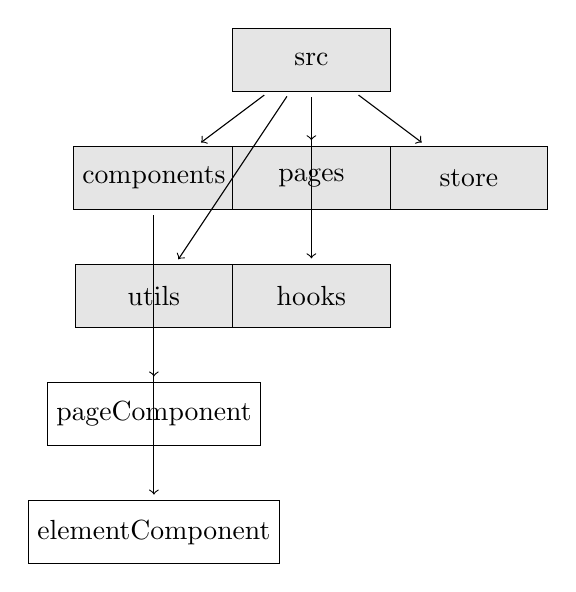
\begin{tikzpicture}[
    file/.style={draw, rectangle, minimum width=2cm, minimum height=0.8cm},
    folder/.style={draw, rectangle, minimum width=2cm, minimum height=0.8cm, fill=gray!20},
    arrow/.style={->, shorten >=2pt, shorten <=2pt}
]

% Folders
\node[folder] (src) at (0,0) {src};
\node[folder] (components) at (-2,-1.5) {components};
\node[folder] (pages) at (0,-1.5) {pages};
\node[folder] (store) at (2,-1.5) {store};
\node[folder] (utils) at (-2,-3) {utils};
\node[folder] (hooks) at (0,-3) {hooks};

% Files
\node[file] (pageComponent) at (-2,-4.5) {pageComponent};
\node[file] (elementComponent) at (-2,-6) {elementComponent};
% ... add more files

% Connections
\draw[arrow] (src) -- (components);
\draw[arrow] (src) -- (pages);
\draw[arrow] (src) -- (store);
\draw[arrow] (src) -- (utils);
\draw[arrow] (src) -- (hooks);
\draw[arrow] (components) -- (pageComponent);
\draw[arrow] (components) -- (elementComponent);
% ... add more connections

\end{tikzpicture}



\pagebreak
\subsubsection{Back-end}
The backend uses the dotNet framework. The development language using the C\# language.

In this project, the backend uses the Onion Architecture.
The Onion Architecture is a typically layered architecture, 
where each layer depends on the inner layer and provides interfaces to the outer layer.
The outer layer provides services to the outermost layer 
and other modules in the same layer based on the interfaces of the inner layer.

From inner to outer, the layers are: Domain, Application, Infrastructure, Presentation.
The Domain layer is the core layer and the innermost layer, used to define domain models, 
which are the business models.
It includes domain models and domain service interfaces.
Domain models are used to define the business models, 
which are the entities in the entity-relationship model and their attributes.
Domain service interfaces are used to define the business services, 
which are the relationships between entities in the entity-relationship model.

The Application layer is the application layer, 
used to define application services, which are the business logic.
It includes domain service implementations and application service interfaces.
Domain service implementations implement the methods of the inner layer's domain service 
interfaces and implement the business logic of the domain models.
Application service interfaces are used to define application services, 
which are the business logic.
It includes but is not limited to database interfaces, testing interfaces, 
HTTP API interfaces, MQTT interfaces, etc.

The Infrastructure layer is the infrastructure layer, used to define infrastructure.
It includes database implementations, testing implementations, 
HTTP API implementations, MQTT implementations, etc.
Database implementations implement the database interfaces 
and provide CRUD services for the database.
Testing implementations implement the testing interfaces 
and provide services for unit testing and integration testing.
HTTP API implementations implement the HTTP API interfaces 
and provide CRUD operations for HTTP APIs.
MQTT implementations implement the MQTT interfaces 
and provide CRUD operations for MQTT.

The Presentation layer is the presentation layer, used to define presentation logic, 
such as interfaces and pages. Since this is a backend project,
data presentation and control are handled by the frontend, 
so this layer is not needed.



\pagebreak
\subsubsection{Data communication and storage}
% 关于本项目的数据通信与数据存储的设计, 包括数据通信的协议, 数据存储的设计等
% 关于数据通信的设计:
% 1. 通信协议的选择
% 自前端向后端发送的数据, 有三种传输的数据类型, 
% 一种是普通的增删改查的请求, 对数据传输的时效性要求不高, 但是对数据的准确性, 完整性, 有序性, 安全性有一定的要求,
% 这种数据的传输, 采用 HTTP 协议, 以及 RESTful API 的设计. 可以有效的保证对数据传输的以上要求.
% 一种是对数据通道的创建和流媒体数据的传输, 对数据传输的时效性, 安全性要求较高, 这种数据的传输, 采用 WebRTC 协议, 以及 MQTT 协议.
% 配合可以快速解码的 flatbuffers 协议, 可以有效的保证对数据传输的以上要求.
% 最后一种是对设备的状态信息和操作信息的传输, 对完整性, 有序性, 安全性都有较高的要求, 这种数据的传输, 采用 MQTT 协议
% 同时也使用了 flatbuffers 协议.
% 
% 2. 数据通信的通信架构和通信流程
% 本项目的数据通信的通信架构, 是基于前后端分离的架构, 前端使用 React 框架, 后端使用 dotnet 框架.
% 当前端需要向后端发送数据的时候, 前端会向后端发送 HTTP 请求, 后端接收到 HTTP 请求之后, 会根据请求的数据类型,
% 选择不同的数据处理方式, 对于普通的增删改查的请求, 后端会根据 RESTful API 的设计, 对数据进行增删改查的操作,
% 对于对数据通道的创建和流媒体数据的传输, 后端会根据 WebRTC 协议, 对数据通道进行创建, 并且帮助前端和设备建立数据通道,
% 当数据通道建立后, 前端和设备之间则使用 flatbuffer 的数据格式对流媒体数据进行传输,
% 对于设备的状态信息和操作信息的传输, 前端会直接向 MQTT broker 发送 MQTT 请求, 
% 设备会在其自身的固件中监听相关的 MQTT 请求, 并且返回相关的数据.
% 
% 3. 数据通信的格式
% 本项目的数据通信的格式, 有三种, 
% 一种是 HTTP 协议, 
% 使用 json 格式对数据进行传输,
% 一种是 WebRTC 协议, 
% 使用 flatbuffers 格式对数据进行传输,
% 一种是 MQTT 协议.
% 使用 flatbuffers 格式对数据进行传输,
% 
% 关于数据存储的设计:
% 1. 数据存储的数据库的选择
% 本项目的数据存储的数据库的选择, 使用了轻量级的数据库 SQLite,
% SQLite 是一个进程内的库, 实现了自给自足的, 无服务器的, 零配置的, 事务性的 SQL 数据库引擎.
% 这是因为整个项目的目的是为了实现前端与设备之间的数据通信, 对于数据库数据的增删改查操作的要求不高,
% 数据量较小, 且对于数据库的数据的事务性要求不高, 所以选择了 SQLite 数据库.
% 2. 项目前后端的数据结构的设计
% 在本项目中, 前端由于使用了 React 框架, 所以前端的数据结构的设计, 使用了基于状态的数据结构的设计,
% 每个组件或者数据集都包含一个状态对象, 这个状态对象的属性就是组件的各个状态. 
% 使用状态对象的原因是, 可以方便的对状态进行管理, 采用对象-属性的形式, 可以方便的针对不同组件的同类状态进行区分,
% 由于跨组件的状态是由 redux 进行管理的, 这种状态对象的设计, 可以更搞笑的对状态进行更新和传递.
% 后端由于使用了 dotnet 框架, 所以后端的数据结构的设计, 使用了基于类的数据结构的设计,
% 采用了面向对象的编程思想, 对数据进行了封装, 使得数据的传输更加的安全, 有序, 完整.


\pagebreak

% \subsection{Domain model}
% \documentclass[]{article}
\usepackage{graphicx}
\usepackage{amsmath}
\usepackage{tikz}

% libaries
\usetikzlibrary{shapes,arrows}

%Define the listing package
\usepackage{listings} %code highlighter
\usepackage{color} %use color
\definecolor{mygreen}{rgb}{0,0.6,0}
\definecolor{mygray}{rgb}{0.5,0.5,0.5}
\definecolor{mymauve}{rgb}{0.58,0,0.82}

%Customize a bit the look
\lstset{ %
backgroundcolor=\color{white}, % choose the background color; you must add \usepackage{color} or \usepackage{xcolor}
basicstyle=\footnotesize, % the size of the fonts that are used for the code
breakatwhitespace=false, % sets if automatic breaks should only happen at whitespace
breaklines=true, % sets automatic line breaking
captionpos=b, % sets the caption-position to bottom
commentstyle=\color{mygreen}, % comment style
deletekeywords={...}, % if you want to delete keywords from the given language
escapeinside={\%*}{*)}, % if you want to add LaTeX within your code
extendedchars=true, % lets you use non-ASCII characters; for 8-bits encodings only, does not work with UTF-8
frame=single, % adds a frame around the code
keepspaces=true, % keeps spaces in text, useful for keeping indentation of code (possibly needs columns=flexible)
keywordstyle=\color{blue}, % keyword style
% language=Octave, % the language of the code
morekeywords={*,...}, % if you want to add more keywords to the set
numbers=left, % where to put the line-numbers; possible values are (none, left, right)
numbersep=5pt, % how far the line-numbers are from the code
numberstyle=\tiny\color{mygray}, % the style that is used for the line-numbers
rulecolor=\color{black}, % if not set, the frame-color may be changed on line-breaks within not-black text (e.g. comments (green here))
showspaces=false, % show spaces everywhere adding particular underscores; it overrides 'showstringspaces'
showstringspaces=false, % underline spaces within strings only
showtabs=false, % show tabs within strings adding particular underscores
stepnumber=1, % the step between two line-numbers. If it's 1, each line will be numbered
stringstyle=\color{mymauve}, % string literal style
tabsize=2, % sets default tabsize to 2 spaces
title=\lstname % show the filename of files included with \lstinputlisting; also try caption instead of title
}

\definecolor{darkgray}{rgb}{.4,.4,.4}
\definecolor{purple}{rgb}{0.65, 0.12, 0.82}

\lstdefinelanguage{React}{
keywords={const, typeof, new, true, false, catch, function, return, null, catch, switch, var, if, in, while, do, else, case, break},
keywordstyle=\color{blue}\bfseries,
ndkeywords={class, export, boolean, throw, implements, import, this},
ndkeywordstyle=\color{darkgray}\bfseries,
identifierstyle=\color{mygreen},
sensitive=false,
comment=[l]{//},
morecomment=[s]{/*}{*/},
commentstyle=\color{purple}\ttfamily,
string=[b]{"}{'}{`},
stringstyle=\color{red}\ttfamily,
morestring=[b]',
morestring=[b]",
morestring=[b]`',
}

\lstdefinelanguage{CSharp}{
keywords={const, typeof, new, true, false, catch, function, return, null, catch, switch, var, if, in, while, do, else, case, break},
keywordstyle=\color{blue}\bfseries,
ndkeywords={class, export, boolean, throw, implements, import, this},
ndkeywordstyle=\color{darkgray}\bfseries,
identifierstyle=\color{mygreen},
sensitive=false,
comment=[l]{//},
morecomment=[s]{/*}{*/},
commentstyle=\color{purple}\ttfamily,
string=[b]{"}{'}{`},
stringstyle=\color{red}\ttfamily,
morestring=[b]',
morestring=[b]",
morestring=[b]`',
}

\lstset{
language=React,
extendedchars=true,
basicstyle=\footnotesize\ttfamily,
showstringspaces=false,
showspaces=false,
numbers=left,
numberstyle=\footnotesize,
numbersep=9pt,
tabsize=2,
breaklines=true,
showtabs=false,
captionpos=b
}

\lstset{
language=CSharp,
extendedchars=true,
basicstyle=\footnotesize\ttfamily,
showstringspaces=false,
showspaces=false,
numbers=left,
numberstyle=\footnotesize,
numbersep=9pt,
tabsize=2,
breaklines=true,
showtabs=false,
captionpos=b
}

% \usepackage{cite} % Add this line for citation

% \bibliographystyle{plain}

\title{
The implementation of BifrostConnect Front-end scope, 
re-design and development with the relevant back-end support develop.
}
\author{
    Fei Gu \\
    Erhvervs Akademi Sydvest \\
    Computer Science 21\\
    }
\date{\today}

\begin{document}

% Front page
\maketitle
\begin{center}
    Supervisor: Henrik Boulund Meng Hansen \\
    Company: BifrostConnect \\
    Engineering Director: Jasper Wass \\
\end{center}
\tableofcontents
\pagebreak


% The introduction
\section{Introduction}
\subsection{Background}\input{sections/introduction/background.tex}
\subsection{The company}\input{sections/introduction/aboutCompany}
\subsection{The project}\input{sections/introduction/aboutProject}
\pagebreak

% The problem statement
\section{Problem Statement}
\subsection{Statement}
\input{sections/problemStatement/statement}
\subsection{Situation}
\input{sections/problemStatement/situation}
\subsection{Potential Solution}
\input{sections/problemStatement/potentialSolution}
\pagebreak

% Requirement analysis
\section{Requirement Analysis}
\input{sections/requirementAnalysis/index}

\subsection{Stakeholders}
\input{sections/requirementAnalysis/stakeholders/index}

\subsection{Business Domain}
\input{sections/requirementAnalysis/bussinesDomain/index}

\subsection{Scope}
\input{sections/requirementAnalysis/scope}

\subsection{Goals}
\input{sections/requirementAnalysis/goals}
\pagebreak

% Software Design
\section{Software Design}
% developement methods
\subsection{Software Development Methods}
\input{sections/softwareDevelopmentMethods/index}
\subsubsection{Agile Software Development}
\input{sections/softwareDevelopmentMethods/agileSoftwareDevelopment/index}
\subsubsection{Feature Driven Development}
\input{sections/softwareDevelopmentMethods/featureDrivenDevelopment/index}

\pagebreak

% Technology seslection
\subsection{Technology selection}
\input{sections/softwareDesign/technologySelection/index}
\subsubsection{Front-end}
\input{sections/softwareDesign/technologySelection/frontEnd}            
\subsubsection{Back-end}
\input{sections/softwareDesign/technologySelection/backEnd}            
\subsubsection{Database}
\input{sections/softwareDesign/technologySelection/database}
\subsubsection{Data communication}
\input{sections/softwareDesign/technologySelection/dataCommunication}            
\subsubsection{DevOps}
\input{sections/softwareDesign/technologySelection/devOps}
\pagebreak

% Architecture design
\subsection{Architecture design}
\input{sections/softwareDesign/architectureDesign/index}
\pagebreak
\subsubsection{Front-end}
\input{sections/softwareDesign/architectureDesign/frontEndArchitecture}
\pagebreak
\subsubsection{Back-end}
\input{sections/softwareDesign/architectureDesign/backEndArchitecture}
\pagebreak
\subsubsection{Data communication and storage}
\input{sections/softwareDesign/architectureDesign/dataCommunicationArchitecture}
\pagebreak

% \subsection{Domain model}
% \input{sections/softwareDesign/domainModel/index}
% \subsection{Database design}
% % 数据库领域模型 ER 图
% % 包括表和字段的设置.
% % 对于私有键和外键的设置.

% \subsection{Back-end design}
% % 后端对象模型
% % 以及对于对象模型的增删改查
% % 以及相关的其他服务的设计`'

% \subsection{Front-end design}
% % 对于前端的页面结构的设计 
% % 页面的状态的设计, 交互设计

% \subsection{FlatBuffers design}
% % schema 的设计

\subsection{DevOps CI/CD process design}
\input{sections/softwareDesign/devOpsDesign/index}
\subsubsection{Continuous Integration}
\input{sections/softwareDesign/devOpsDesign/continuousIntegration/index}
\subsubsection{Continuous Delivery}
\input{sections/softwareDesign/devOpsDesign/continuousDelivery/index}
\subsubsection{Continuous Deployment}
\input{sections/softwareDesign/devOpsDesign/continuousDeployment/index}
\pagebreak

\section{Software Development} 
\input{sections/softwareDevelopment/index}
\subsection{Overall development}
\input{sections/softwareDevelopment/overallDevelopement/index}
\subsubsection{Front-end}
\input{sections/softwareDevelopment/overallDevelopement/frontEnd/index}
\subsubsection{Back-end}
\input{sections/softwareDevelopment/overallDevelopement/backEnd/index}
\subsubsection{DevOps}
\input{sections/softwareDevelopment/overallDevelopement/devOps/index}
\subsection{Feature development} 
\input{sections/softwareDevelopment/featureDevelopment/index}
\subsubsection{Use Case 1}
\input{sections/softwareDevelopment/featureDevelopment/useCase1/index}
\subsubsection{Feature 1}
\input{sections/softwareDevelopment/featureDevelopment/feature/feature1.tex}
\pagebreak
\section{Conclusion} 
\subsection{Result}
Since the project is still in progress, the result is not available yet.
So far, basic structure of this project has been built. But the most features 
are not implemented yet. 
\subsection{Discussion}
As a single developer for this project, I am confident what I have done so far.
And I can say I understand the most of the knowledge I have used in this project, 
which also means I can explain all the part of the project. 
But this project also relevant some of the complex knowledge which I have to continue 
to study and practice.
\subsection{Future Work}
The future work is to implement the rest of the features. 
Including the most important part which is the 'create session' feature.
\pagebreak
% \bibliography{bibliography}
\pagebreak
% \begin{appendices}
%     \section{Appendix}
% \end{appendices} 
\end{document}
% \subsection{Database design}
% % 数据库领域模型 ER 图
% % 包括表和字段的设置.
% % 对于私有键和外键的设置.

% \subsection{Back-end design}
% % 后端对象模型
% % 以及对于对象模型的增删改查
% % 以及相关的其他服务的设计`'

% \subsection{Front-end design}
% % 对于前端的页面结构的设计 
% % 页面的状态的设计, 交互设计

% \subsection{FlatBuffers design}
% % schema 的设计

\subsection{DevOps CI/CD process design}
\documentclass[]{article}
\usepackage{graphicx}
\usepackage{amsmath}
\usepackage{tikz}

% libaries
\usetikzlibrary{shapes,arrows}

%Define the listing package
\usepackage{listings} %code highlighter
\usepackage{color} %use color
\definecolor{mygreen}{rgb}{0,0.6,0}
\definecolor{mygray}{rgb}{0.5,0.5,0.5}
\definecolor{mymauve}{rgb}{0.58,0,0.82}

%Customize a bit the look
\lstset{ %
backgroundcolor=\color{white}, % choose the background color; you must add \usepackage{color} or \usepackage{xcolor}
basicstyle=\footnotesize, % the size of the fonts that are used for the code
breakatwhitespace=false, % sets if automatic breaks should only happen at whitespace
breaklines=true, % sets automatic line breaking
captionpos=b, % sets the caption-position to bottom
commentstyle=\color{mygreen}, % comment style
deletekeywords={...}, % if you want to delete keywords from the given language
escapeinside={\%*}{*)}, % if you want to add LaTeX within your code
extendedchars=true, % lets you use non-ASCII characters; for 8-bits encodings only, does not work with UTF-8
frame=single, % adds a frame around the code
keepspaces=true, % keeps spaces in text, useful for keeping indentation of code (possibly needs columns=flexible)
keywordstyle=\color{blue}, % keyword style
% language=Octave, % the language of the code
morekeywords={*,...}, % if you want to add more keywords to the set
numbers=left, % where to put the line-numbers; possible values are (none, left, right)
numbersep=5pt, % how far the line-numbers are from the code
numberstyle=\tiny\color{mygray}, % the style that is used for the line-numbers
rulecolor=\color{black}, % if not set, the frame-color may be changed on line-breaks within not-black text (e.g. comments (green here))
showspaces=false, % show spaces everywhere adding particular underscores; it overrides 'showstringspaces'
showstringspaces=false, % underline spaces within strings only
showtabs=false, % show tabs within strings adding particular underscores
stepnumber=1, % the step between two line-numbers. If it's 1, each line will be numbered
stringstyle=\color{mymauve}, % string literal style
tabsize=2, % sets default tabsize to 2 spaces
title=\lstname % show the filename of files included with \lstinputlisting; also try caption instead of title
}

\definecolor{darkgray}{rgb}{.4,.4,.4}
\definecolor{purple}{rgb}{0.65, 0.12, 0.82}

\lstdefinelanguage{React}{
keywords={const, typeof, new, true, false, catch, function, return, null, catch, switch, var, if, in, while, do, else, case, break},
keywordstyle=\color{blue}\bfseries,
ndkeywords={class, export, boolean, throw, implements, import, this},
ndkeywordstyle=\color{darkgray}\bfseries,
identifierstyle=\color{mygreen},
sensitive=false,
comment=[l]{//},
morecomment=[s]{/*}{*/},
commentstyle=\color{purple}\ttfamily,
string=[b]{"}{'}{`},
stringstyle=\color{red}\ttfamily,
morestring=[b]',
morestring=[b]",
morestring=[b]`',
}

\lstdefinelanguage{CSharp}{
keywords={const, typeof, new, true, false, catch, function, return, null, catch, switch, var, if, in, while, do, else, case, break},
keywordstyle=\color{blue}\bfseries,
ndkeywords={class, export, boolean, throw, implements, import, this},
ndkeywordstyle=\color{darkgray}\bfseries,
identifierstyle=\color{mygreen},
sensitive=false,
comment=[l]{//},
morecomment=[s]{/*}{*/},
commentstyle=\color{purple}\ttfamily,
string=[b]{"}{'}{`},
stringstyle=\color{red}\ttfamily,
morestring=[b]',
morestring=[b]",
morestring=[b]`',
}

\lstset{
language=React,
extendedchars=true,
basicstyle=\footnotesize\ttfamily,
showstringspaces=false,
showspaces=false,
numbers=left,
numberstyle=\footnotesize,
numbersep=9pt,
tabsize=2,
breaklines=true,
showtabs=false,
captionpos=b
}

\lstset{
language=CSharp,
extendedchars=true,
basicstyle=\footnotesize\ttfamily,
showstringspaces=false,
showspaces=false,
numbers=left,
numberstyle=\footnotesize,
numbersep=9pt,
tabsize=2,
breaklines=true,
showtabs=false,
captionpos=b
}

% \usepackage{cite} % Add this line for citation

% \bibliographystyle{plain}

\title{
The implementation of BifrostConnect Front-end scope, 
re-design and development with the relevant back-end support develop.
}
\author{
    Fei Gu \\
    Erhvervs Akademi Sydvest \\
    Computer Science 21\\
    }
\date{\today}

\begin{document}

% Front page
\maketitle
\begin{center}
    Supervisor: Henrik Boulund Meng Hansen \\
    Company: BifrostConnect \\
    Engineering Director: Jasper Wass \\
\end{center}
\tableofcontents
\pagebreak


% The introduction
\section{Introduction}
\subsection{Background}\input{sections/introduction/background.tex}
\subsection{The company}\input{sections/introduction/aboutCompany}
\subsection{The project}\input{sections/introduction/aboutProject}
\pagebreak

% The problem statement
\section{Problem Statement}
\subsection{Statement}
\input{sections/problemStatement/statement}
\subsection{Situation}
\input{sections/problemStatement/situation}
\subsection{Potential Solution}
\input{sections/problemStatement/potentialSolution}
\pagebreak

% Requirement analysis
\section{Requirement Analysis}
\input{sections/requirementAnalysis/index}

\subsection{Stakeholders}
\input{sections/requirementAnalysis/stakeholders/index}

\subsection{Business Domain}
\input{sections/requirementAnalysis/bussinesDomain/index}

\subsection{Scope}
\input{sections/requirementAnalysis/scope}

\subsection{Goals}
\input{sections/requirementAnalysis/goals}
\pagebreak

% Software Design
\section{Software Design}
% developement methods
\subsection{Software Development Methods}
\input{sections/softwareDevelopmentMethods/index}
\subsubsection{Agile Software Development}
\input{sections/softwareDevelopmentMethods/agileSoftwareDevelopment/index}
\subsubsection{Feature Driven Development}
\input{sections/softwareDevelopmentMethods/featureDrivenDevelopment/index}

\pagebreak

% Technology seslection
\subsection{Technology selection}
\input{sections/softwareDesign/technologySelection/index}
\subsubsection{Front-end}
\input{sections/softwareDesign/technologySelection/frontEnd}            
\subsubsection{Back-end}
\input{sections/softwareDesign/technologySelection/backEnd}            
\subsubsection{Database}
\input{sections/softwareDesign/technologySelection/database}
\subsubsection{Data communication}
\input{sections/softwareDesign/technologySelection/dataCommunication}            
\subsubsection{DevOps}
\input{sections/softwareDesign/technologySelection/devOps}
\pagebreak

% Architecture design
\subsection{Architecture design}
\input{sections/softwareDesign/architectureDesign/index}
\pagebreak
\subsubsection{Front-end}
\input{sections/softwareDesign/architectureDesign/frontEndArchitecture}
\pagebreak
\subsubsection{Back-end}
\input{sections/softwareDesign/architectureDesign/backEndArchitecture}
\pagebreak
\subsubsection{Data communication and storage}
\input{sections/softwareDesign/architectureDesign/dataCommunicationArchitecture}
\pagebreak

% \subsection{Domain model}
% \input{sections/softwareDesign/domainModel/index}
% \subsection{Database design}
% % 数据库领域模型 ER 图
% % 包括表和字段的设置.
% % 对于私有键和外键的设置.

% \subsection{Back-end design}
% % 后端对象模型
% % 以及对于对象模型的增删改查
% % 以及相关的其他服务的设计`'

% \subsection{Front-end design}
% % 对于前端的页面结构的设计 
% % 页面的状态的设计, 交互设计

% \subsection{FlatBuffers design}
% % schema 的设计

\subsection{DevOps CI/CD process design}
\input{sections/softwareDesign/devOpsDesign/index}
\subsubsection{Continuous Integration}
\input{sections/softwareDesign/devOpsDesign/continuousIntegration/index}
\subsubsection{Continuous Delivery}
\input{sections/softwareDesign/devOpsDesign/continuousDelivery/index}
\subsubsection{Continuous Deployment}
\input{sections/softwareDesign/devOpsDesign/continuousDeployment/index}
\pagebreak

\section{Software Development} 
\input{sections/softwareDevelopment/index}
\subsection{Overall development}
\input{sections/softwareDevelopment/overallDevelopement/index}
\subsubsection{Front-end}
\input{sections/softwareDevelopment/overallDevelopement/frontEnd/index}
\subsubsection{Back-end}
\input{sections/softwareDevelopment/overallDevelopement/backEnd/index}
\subsubsection{DevOps}
\input{sections/softwareDevelopment/overallDevelopement/devOps/index}
\subsection{Feature development} 
\input{sections/softwareDevelopment/featureDevelopment/index}
\subsubsection{Use Case 1}
\input{sections/softwareDevelopment/featureDevelopment/useCase1/index}
\subsubsection{Feature 1}
\input{sections/softwareDevelopment/featureDevelopment/feature/feature1.tex}
\pagebreak
\section{Conclusion} 
\subsection{Result}
Since the project is still in progress, the result is not available yet.
So far, basic structure of this project has been built. But the most features 
are not implemented yet. 
\subsection{Discussion}
As a single developer for this project, I am confident what I have done so far.
And I can say I understand the most of the knowledge I have used in this project, 
which also means I can explain all the part of the project. 
But this project also relevant some of the complex knowledge which I have to continue 
to study and practice.
\subsection{Future Work}
The future work is to implement the rest of the features. 
Including the most important part which is the 'create session' feature.
\pagebreak
% \bibliography{bibliography}
\pagebreak
% \begin{appendices}
%     \section{Appendix}
% \end{appendices} 
\end{document}
\subsubsection{Continuous Integration}
\documentclass[]{article}
\usepackage{graphicx}
\usepackage{amsmath}
\usepackage{tikz}

% libaries
\usetikzlibrary{shapes,arrows}

%Define the listing package
\usepackage{listings} %code highlighter
\usepackage{color} %use color
\definecolor{mygreen}{rgb}{0,0.6,0}
\definecolor{mygray}{rgb}{0.5,0.5,0.5}
\definecolor{mymauve}{rgb}{0.58,0,0.82}

%Customize a bit the look
\lstset{ %
backgroundcolor=\color{white}, % choose the background color; you must add \usepackage{color} or \usepackage{xcolor}
basicstyle=\footnotesize, % the size of the fonts that are used for the code
breakatwhitespace=false, % sets if automatic breaks should only happen at whitespace
breaklines=true, % sets automatic line breaking
captionpos=b, % sets the caption-position to bottom
commentstyle=\color{mygreen}, % comment style
deletekeywords={...}, % if you want to delete keywords from the given language
escapeinside={\%*}{*)}, % if you want to add LaTeX within your code
extendedchars=true, % lets you use non-ASCII characters; for 8-bits encodings only, does not work with UTF-8
frame=single, % adds a frame around the code
keepspaces=true, % keeps spaces in text, useful for keeping indentation of code (possibly needs columns=flexible)
keywordstyle=\color{blue}, % keyword style
% language=Octave, % the language of the code
morekeywords={*,...}, % if you want to add more keywords to the set
numbers=left, % where to put the line-numbers; possible values are (none, left, right)
numbersep=5pt, % how far the line-numbers are from the code
numberstyle=\tiny\color{mygray}, % the style that is used for the line-numbers
rulecolor=\color{black}, % if not set, the frame-color may be changed on line-breaks within not-black text (e.g. comments (green here))
showspaces=false, % show spaces everywhere adding particular underscores; it overrides 'showstringspaces'
showstringspaces=false, % underline spaces within strings only
showtabs=false, % show tabs within strings adding particular underscores
stepnumber=1, % the step between two line-numbers. If it's 1, each line will be numbered
stringstyle=\color{mymauve}, % string literal style
tabsize=2, % sets default tabsize to 2 spaces
title=\lstname % show the filename of files included with \lstinputlisting; also try caption instead of title
}

\definecolor{darkgray}{rgb}{.4,.4,.4}
\definecolor{purple}{rgb}{0.65, 0.12, 0.82}

\lstdefinelanguage{React}{
keywords={const, typeof, new, true, false, catch, function, return, null, catch, switch, var, if, in, while, do, else, case, break},
keywordstyle=\color{blue}\bfseries,
ndkeywords={class, export, boolean, throw, implements, import, this},
ndkeywordstyle=\color{darkgray}\bfseries,
identifierstyle=\color{mygreen},
sensitive=false,
comment=[l]{//},
morecomment=[s]{/*}{*/},
commentstyle=\color{purple}\ttfamily,
string=[b]{"}{'}{`},
stringstyle=\color{red}\ttfamily,
morestring=[b]',
morestring=[b]",
morestring=[b]`',
}

\lstdefinelanguage{CSharp}{
keywords={const, typeof, new, true, false, catch, function, return, null, catch, switch, var, if, in, while, do, else, case, break},
keywordstyle=\color{blue}\bfseries,
ndkeywords={class, export, boolean, throw, implements, import, this},
ndkeywordstyle=\color{darkgray}\bfseries,
identifierstyle=\color{mygreen},
sensitive=false,
comment=[l]{//},
morecomment=[s]{/*}{*/},
commentstyle=\color{purple}\ttfamily,
string=[b]{"}{'}{`},
stringstyle=\color{red}\ttfamily,
morestring=[b]',
morestring=[b]",
morestring=[b]`',
}

\lstset{
language=React,
extendedchars=true,
basicstyle=\footnotesize\ttfamily,
showstringspaces=false,
showspaces=false,
numbers=left,
numberstyle=\footnotesize,
numbersep=9pt,
tabsize=2,
breaklines=true,
showtabs=false,
captionpos=b
}

\lstset{
language=CSharp,
extendedchars=true,
basicstyle=\footnotesize\ttfamily,
showstringspaces=false,
showspaces=false,
numbers=left,
numberstyle=\footnotesize,
numbersep=9pt,
tabsize=2,
breaklines=true,
showtabs=false,
captionpos=b
}

% \usepackage{cite} % Add this line for citation

% \bibliographystyle{plain}

\title{
The implementation of BifrostConnect Front-end scope, 
re-design and development with the relevant back-end support develop.
}
\author{
    Fei Gu \\
    Erhvervs Akademi Sydvest \\
    Computer Science 21\\
    }
\date{\today}

\begin{document}

% Front page
\maketitle
\begin{center}
    Supervisor: Henrik Boulund Meng Hansen \\
    Company: BifrostConnect \\
    Engineering Director: Jasper Wass \\
\end{center}
\tableofcontents
\pagebreak


% The introduction
\section{Introduction}
\subsection{Background}\input{sections/introduction/background.tex}
\subsection{The company}\input{sections/introduction/aboutCompany}
\subsection{The project}\input{sections/introduction/aboutProject}
\pagebreak

% The problem statement
\section{Problem Statement}
\subsection{Statement}
\input{sections/problemStatement/statement}
\subsection{Situation}
\input{sections/problemStatement/situation}
\subsection{Potential Solution}
\input{sections/problemStatement/potentialSolution}
\pagebreak

% Requirement analysis
\section{Requirement Analysis}
\input{sections/requirementAnalysis/index}

\subsection{Stakeholders}
\input{sections/requirementAnalysis/stakeholders/index}

\subsection{Business Domain}
\input{sections/requirementAnalysis/bussinesDomain/index}

\subsection{Scope}
\input{sections/requirementAnalysis/scope}

\subsection{Goals}
\input{sections/requirementAnalysis/goals}
\pagebreak

% Software Design
\section{Software Design}
% developement methods
\subsection{Software Development Methods}
\input{sections/softwareDevelopmentMethods/index}
\subsubsection{Agile Software Development}
\input{sections/softwareDevelopmentMethods/agileSoftwareDevelopment/index}
\subsubsection{Feature Driven Development}
\input{sections/softwareDevelopmentMethods/featureDrivenDevelopment/index}

\pagebreak

% Technology seslection
\subsection{Technology selection}
\input{sections/softwareDesign/technologySelection/index}
\subsubsection{Front-end}
\input{sections/softwareDesign/technologySelection/frontEnd}            
\subsubsection{Back-end}
\input{sections/softwareDesign/technologySelection/backEnd}            
\subsubsection{Database}
\input{sections/softwareDesign/technologySelection/database}
\subsubsection{Data communication}
\input{sections/softwareDesign/technologySelection/dataCommunication}            
\subsubsection{DevOps}
\input{sections/softwareDesign/technologySelection/devOps}
\pagebreak

% Architecture design
\subsection{Architecture design}
\input{sections/softwareDesign/architectureDesign/index}
\pagebreak
\subsubsection{Front-end}
\input{sections/softwareDesign/architectureDesign/frontEndArchitecture}
\pagebreak
\subsubsection{Back-end}
\input{sections/softwareDesign/architectureDesign/backEndArchitecture}
\pagebreak
\subsubsection{Data communication and storage}
\input{sections/softwareDesign/architectureDesign/dataCommunicationArchitecture}
\pagebreak

% \subsection{Domain model}
% \input{sections/softwareDesign/domainModel/index}
% \subsection{Database design}
% % 数据库领域模型 ER 图
% % 包括表和字段的设置.
% % 对于私有键和外键的设置.

% \subsection{Back-end design}
% % 后端对象模型
% % 以及对于对象模型的增删改查
% % 以及相关的其他服务的设计`'

% \subsection{Front-end design}
% % 对于前端的页面结构的设计 
% % 页面的状态的设计, 交互设计

% \subsection{FlatBuffers design}
% % schema 的设计

\subsection{DevOps CI/CD process design}
\input{sections/softwareDesign/devOpsDesign/index}
\subsubsection{Continuous Integration}
\input{sections/softwareDesign/devOpsDesign/continuousIntegration/index}
\subsubsection{Continuous Delivery}
\input{sections/softwareDesign/devOpsDesign/continuousDelivery/index}
\subsubsection{Continuous Deployment}
\input{sections/softwareDesign/devOpsDesign/continuousDeployment/index}
\pagebreak

\section{Software Development} 
\input{sections/softwareDevelopment/index}
\subsection{Overall development}
\input{sections/softwareDevelopment/overallDevelopement/index}
\subsubsection{Front-end}
\input{sections/softwareDevelopment/overallDevelopement/frontEnd/index}
\subsubsection{Back-end}
\input{sections/softwareDevelopment/overallDevelopement/backEnd/index}
\subsubsection{DevOps}
\input{sections/softwareDevelopment/overallDevelopement/devOps/index}
\subsection{Feature development} 
\input{sections/softwareDevelopment/featureDevelopment/index}
\subsubsection{Use Case 1}
\input{sections/softwareDevelopment/featureDevelopment/useCase1/index}
\subsubsection{Feature 1}
\input{sections/softwareDevelopment/featureDevelopment/feature/feature1.tex}
\pagebreak
\section{Conclusion} 
\subsection{Result}
Since the project is still in progress, the result is not available yet.
So far, basic structure of this project has been built. But the most features 
are not implemented yet. 
\subsection{Discussion}
As a single developer for this project, I am confident what I have done so far.
And I can say I understand the most of the knowledge I have used in this project, 
which also means I can explain all the part of the project. 
But this project also relevant some of the complex knowledge which I have to continue 
to study and practice.
\subsection{Future Work}
The future work is to implement the rest of the features. 
Including the most important part which is the 'create session' feature.
\pagebreak
% \bibliography{bibliography}
\pagebreak
% \begin{appendices}
%     \section{Appendix}
% \end{appendices} 
\end{document}
\subsubsection{Continuous Delivery}
\documentclass[]{article}
\usepackage{graphicx}
\usepackage{amsmath}
\usepackage{tikz}

% libaries
\usetikzlibrary{shapes,arrows}

%Define the listing package
\usepackage{listings} %code highlighter
\usepackage{color} %use color
\definecolor{mygreen}{rgb}{0,0.6,0}
\definecolor{mygray}{rgb}{0.5,0.5,0.5}
\definecolor{mymauve}{rgb}{0.58,0,0.82}

%Customize a bit the look
\lstset{ %
backgroundcolor=\color{white}, % choose the background color; you must add \usepackage{color} or \usepackage{xcolor}
basicstyle=\footnotesize, % the size of the fonts that are used for the code
breakatwhitespace=false, % sets if automatic breaks should only happen at whitespace
breaklines=true, % sets automatic line breaking
captionpos=b, % sets the caption-position to bottom
commentstyle=\color{mygreen}, % comment style
deletekeywords={...}, % if you want to delete keywords from the given language
escapeinside={\%*}{*)}, % if you want to add LaTeX within your code
extendedchars=true, % lets you use non-ASCII characters; for 8-bits encodings only, does not work with UTF-8
frame=single, % adds a frame around the code
keepspaces=true, % keeps spaces in text, useful for keeping indentation of code (possibly needs columns=flexible)
keywordstyle=\color{blue}, % keyword style
% language=Octave, % the language of the code
morekeywords={*,...}, % if you want to add more keywords to the set
numbers=left, % where to put the line-numbers; possible values are (none, left, right)
numbersep=5pt, % how far the line-numbers are from the code
numberstyle=\tiny\color{mygray}, % the style that is used for the line-numbers
rulecolor=\color{black}, % if not set, the frame-color may be changed on line-breaks within not-black text (e.g. comments (green here))
showspaces=false, % show spaces everywhere adding particular underscores; it overrides 'showstringspaces'
showstringspaces=false, % underline spaces within strings only
showtabs=false, % show tabs within strings adding particular underscores
stepnumber=1, % the step between two line-numbers. If it's 1, each line will be numbered
stringstyle=\color{mymauve}, % string literal style
tabsize=2, % sets default tabsize to 2 spaces
title=\lstname % show the filename of files included with \lstinputlisting; also try caption instead of title
}

\definecolor{darkgray}{rgb}{.4,.4,.4}
\definecolor{purple}{rgb}{0.65, 0.12, 0.82}

\lstdefinelanguage{React}{
keywords={const, typeof, new, true, false, catch, function, return, null, catch, switch, var, if, in, while, do, else, case, break},
keywordstyle=\color{blue}\bfseries,
ndkeywords={class, export, boolean, throw, implements, import, this},
ndkeywordstyle=\color{darkgray}\bfseries,
identifierstyle=\color{mygreen},
sensitive=false,
comment=[l]{//},
morecomment=[s]{/*}{*/},
commentstyle=\color{purple}\ttfamily,
string=[b]{"}{'}{`},
stringstyle=\color{red}\ttfamily,
morestring=[b]',
morestring=[b]",
morestring=[b]`',
}

\lstdefinelanguage{CSharp}{
keywords={const, typeof, new, true, false, catch, function, return, null, catch, switch, var, if, in, while, do, else, case, break},
keywordstyle=\color{blue}\bfseries,
ndkeywords={class, export, boolean, throw, implements, import, this},
ndkeywordstyle=\color{darkgray}\bfseries,
identifierstyle=\color{mygreen},
sensitive=false,
comment=[l]{//},
morecomment=[s]{/*}{*/},
commentstyle=\color{purple}\ttfamily,
string=[b]{"}{'}{`},
stringstyle=\color{red}\ttfamily,
morestring=[b]',
morestring=[b]",
morestring=[b]`',
}

\lstset{
language=React,
extendedchars=true,
basicstyle=\footnotesize\ttfamily,
showstringspaces=false,
showspaces=false,
numbers=left,
numberstyle=\footnotesize,
numbersep=9pt,
tabsize=2,
breaklines=true,
showtabs=false,
captionpos=b
}

\lstset{
language=CSharp,
extendedchars=true,
basicstyle=\footnotesize\ttfamily,
showstringspaces=false,
showspaces=false,
numbers=left,
numberstyle=\footnotesize,
numbersep=9pt,
tabsize=2,
breaklines=true,
showtabs=false,
captionpos=b
}

% \usepackage{cite} % Add this line for citation

% \bibliographystyle{plain}

\title{
The implementation of BifrostConnect Front-end scope, 
re-design and development with the relevant back-end support develop.
}
\author{
    Fei Gu \\
    Erhvervs Akademi Sydvest \\
    Computer Science 21\\
    }
\date{\today}

\begin{document}

% Front page
\maketitle
\begin{center}
    Supervisor: Henrik Boulund Meng Hansen \\
    Company: BifrostConnect \\
    Engineering Director: Jasper Wass \\
\end{center}
\tableofcontents
\pagebreak


% The introduction
\section{Introduction}
\subsection{Background}\input{sections/introduction/background.tex}
\subsection{The company}\input{sections/introduction/aboutCompany}
\subsection{The project}\input{sections/introduction/aboutProject}
\pagebreak

% The problem statement
\section{Problem Statement}
\subsection{Statement}
\input{sections/problemStatement/statement}
\subsection{Situation}
\input{sections/problemStatement/situation}
\subsection{Potential Solution}
\input{sections/problemStatement/potentialSolution}
\pagebreak

% Requirement analysis
\section{Requirement Analysis}
\input{sections/requirementAnalysis/index}

\subsection{Stakeholders}
\input{sections/requirementAnalysis/stakeholders/index}

\subsection{Business Domain}
\input{sections/requirementAnalysis/bussinesDomain/index}

\subsection{Scope}
\input{sections/requirementAnalysis/scope}

\subsection{Goals}
\input{sections/requirementAnalysis/goals}
\pagebreak

% Software Design
\section{Software Design}
% developement methods
\subsection{Software Development Methods}
\input{sections/softwareDevelopmentMethods/index}
\subsubsection{Agile Software Development}
\input{sections/softwareDevelopmentMethods/agileSoftwareDevelopment/index}
\subsubsection{Feature Driven Development}
\input{sections/softwareDevelopmentMethods/featureDrivenDevelopment/index}

\pagebreak

% Technology seslection
\subsection{Technology selection}
\input{sections/softwareDesign/technologySelection/index}
\subsubsection{Front-end}
\input{sections/softwareDesign/technologySelection/frontEnd}            
\subsubsection{Back-end}
\input{sections/softwareDesign/technologySelection/backEnd}            
\subsubsection{Database}
\input{sections/softwareDesign/technologySelection/database}
\subsubsection{Data communication}
\input{sections/softwareDesign/technologySelection/dataCommunication}            
\subsubsection{DevOps}
\input{sections/softwareDesign/technologySelection/devOps}
\pagebreak

% Architecture design
\subsection{Architecture design}
\input{sections/softwareDesign/architectureDesign/index}
\pagebreak
\subsubsection{Front-end}
\input{sections/softwareDesign/architectureDesign/frontEndArchitecture}
\pagebreak
\subsubsection{Back-end}
\input{sections/softwareDesign/architectureDesign/backEndArchitecture}
\pagebreak
\subsubsection{Data communication and storage}
\input{sections/softwareDesign/architectureDesign/dataCommunicationArchitecture}
\pagebreak

% \subsection{Domain model}
% \input{sections/softwareDesign/domainModel/index}
% \subsection{Database design}
% % 数据库领域模型 ER 图
% % 包括表和字段的设置.
% % 对于私有键和外键的设置.

% \subsection{Back-end design}
% % 后端对象模型
% % 以及对于对象模型的增删改查
% % 以及相关的其他服务的设计`'

% \subsection{Front-end design}
% % 对于前端的页面结构的设计 
% % 页面的状态的设计, 交互设计

% \subsection{FlatBuffers design}
% % schema 的设计

\subsection{DevOps CI/CD process design}
\input{sections/softwareDesign/devOpsDesign/index}
\subsubsection{Continuous Integration}
\input{sections/softwareDesign/devOpsDesign/continuousIntegration/index}
\subsubsection{Continuous Delivery}
\input{sections/softwareDesign/devOpsDesign/continuousDelivery/index}
\subsubsection{Continuous Deployment}
\input{sections/softwareDesign/devOpsDesign/continuousDeployment/index}
\pagebreak

\section{Software Development} 
\input{sections/softwareDevelopment/index}
\subsection{Overall development}
\input{sections/softwareDevelopment/overallDevelopement/index}
\subsubsection{Front-end}
\input{sections/softwareDevelopment/overallDevelopement/frontEnd/index}
\subsubsection{Back-end}
\input{sections/softwareDevelopment/overallDevelopement/backEnd/index}
\subsubsection{DevOps}
\input{sections/softwareDevelopment/overallDevelopement/devOps/index}
\subsection{Feature development} 
\input{sections/softwareDevelopment/featureDevelopment/index}
\subsubsection{Use Case 1}
\input{sections/softwareDevelopment/featureDevelopment/useCase1/index}
\subsubsection{Feature 1}
\input{sections/softwareDevelopment/featureDevelopment/feature/feature1.tex}
\pagebreak
\section{Conclusion} 
\subsection{Result}
Since the project is still in progress, the result is not available yet.
So far, basic structure of this project has been built. But the most features 
are not implemented yet. 
\subsection{Discussion}
As a single developer for this project, I am confident what I have done so far.
And I can say I understand the most of the knowledge I have used in this project, 
which also means I can explain all the part of the project. 
But this project also relevant some of the complex knowledge which I have to continue 
to study and practice.
\subsection{Future Work}
The future work is to implement the rest of the features. 
Including the most important part which is the 'create session' feature.
\pagebreak
% \bibliography{bibliography}
\pagebreak
% \begin{appendices}
%     \section{Appendix}
% \end{appendices} 
\end{document}
\subsubsection{Continuous Deployment}
\documentclass[]{article}
\usepackage{graphicx}
\usepackage{amsmath}
\usepackage{tikz}

% libaries
\usetikzlibrary{shapes,arrows}

%Define the listing package
\usepackage{listings} %code highlighter
\usepackage{color} %use color
\definecolor{mygreen}{rgb}{0,0.6,0}
\definecolor{mygray}{rgb}{0.5,0.5,0.5}
\definecolor{mymauve}{rgb}{0.58,0,0.82}

%Customize a bit the look
\lstset{ %
backgroundcolor=\color{white}, % choose the background color; you must add \usepackage{color} or \usepackage{xcolor}
basicstyle=\footnotesize, % the size of the fonts that are used for the code
breakatwhitespace=false, % sets if automatic breaks should only happen at whitespace
breaklines=true, % sets automatic line breaking
captionpos=b, % sets the caption-position to bottom
commentstyle=\color{mygreen}, % comment style
deletekeywords={...}, % if you want to delete keywords from the given language
escapeinside={\%*}{*)}, % if you want to add LaTeX within your code
extendedchars=true, % lets you use non-ASCII characters; for 8-bits encodings only, does not work with UTF-8
frame=single, % adds a frame around the code
keepspaces=true, % keeps spaces in text, useful for keeping indentation of code (possibly needs columns=flexible)
keywordstyle=\color{blue}, % keyword style
% language=Octave, % the language of the code
morekeywords={*,...}, % if you want to add more keywords to the set
numbers=left, % where to put the line-numbers; possible values are (none, left, right)
numbersep=5pt, % how far the line-numbers are from the code
numberstyle=\tiny\color{mygray}, % the style that is used for the line-numbers
rulecolor=\color{black}, % if not set, the frame-color may be changed on line-breaks within not-black text (e.g. comments (green here))
showspaces=false, % show spaces everywhere adding particular underscores; it overrides 'showstringspaces'
showstringspaces=false, % underline spaces within strings only
showtabs=false, % show tabs within strings adding particular underscores
stepnumber=1, % the step between two line-numbers. If it's 1, each line will be numbered
stringstyle=\color{mymauve}, % string literal style
tabsize=2, % sets default tabsize to 2 spaces
title=\lstname % show the filename of files included with \lstinputlisting; also try caption instead of title
}

\definecolor{darkgray}{rgb}{.4,.4,.4}
\definecolor{purple}{rgb}{0.65, 0.12, 0.82}

\lstdefinelanguage{React}{
keywords={const, typeof, new, true, false, catch, function, return, null, catch, switch, var, if, in, while, do, else, case, break},
keywordstyle=\color{blue}\bfseries,
ndkeywords={class, export, boolean, throw, implements, import, this},
ndkeywordstyle=\color{darkgray}\bfseries,
identifierstyle=\color{mygreen},
sensitive=false,
comment=[l]{//},
morecomment=[s]{/*}{*/},
commentstyle=\color{purple}\ttfamily,
string=[b]{"}{'}{`},
stringstyle=\color{red}\ttfamily,
morestring=[b]',
morestring=[b]",
morestring=[b]`',
}

\lstdefinelanguage{CSharp}{
keywords={const, typeof, new, true, false, catch, function, return, null, catch, switch, var, if, in, while, do, else, case, break},
keywordstyle=\color{blue}\bfseries,
ndkeywords={class, export, boolean, throw, implements, import, this},
ndkeywordstyle=\color{darkgray}\bfseries,
identifierstyle=\color{mygreen},
sensitive=false,
comment=[l]{//},
morecomment=[s]{/*}{*/},
commentstyle=\color{purple}\ttfamily,
string=[b]{"}{'}{`},
stringstyle=\color{red}\ttfamily,
morestring=[b]',
morestring=[b]",
morestring=[b]`',
}

\lstset{
language=React,
extendedchars=true,
basicstyle=\footnotesize\ttfamily,
showstringspaces=false,
showspaces=false,
numbers=left,
numberstyle=\footnotesize,
numbersep=9pt,
tabsize=2,
breaklines=true,
showtabs=false,
captionpos=b
}

\lstset{
language=CSharp,
extendedchars=true,
basicstyle=\footnotesize\ttfamily,
showstringspaces=false,
showspaces=false,
numbers=left,
numberstyle=\footnotesize,
numbersep=9pt,
tabsize=2,
breaklines=true,
showtabs=false,
captionpos=b
}

% \usepackage{cite} % Add this line for citation

% \bibliographystyle{plain}

\title{
The implementation of BifrostConnect Front-end scope, 
re-design and development with the relevant back-end support develop.
}
\author{
    Fei Gu \\
    Erhvervs Akademi Sydvest \\
    Computer Science 21\\
    }
\date{\today}

\begin{document}

% Front page
\maketitle
\begin{center}
    Supervisor: Henrik Boulund Meng Hansen \\
    Company: BifrostConnect \\
    Engineering Director: Jasper Wass \\
\end{center}
\tableofcontents
\pagebreak


% The introduction
\section{Introduction}
\subsection{Background}\input{sections/introduction/background.tex}
\subsection{The company}\input{sections/introduction/aboutCompany}
\subsection{The project}\input{sections/introduction/aboutProject}
\pagebreak

% The problem statement
\section{Problem Statement}
\subsection{Statement}
\input{sections/problemStatement/statement}
\subsection{Situation}
\input{sections/problemStatement/situation}
\subsection{Potential Solution}
\input{sections/problemStatement/potentialSolution}
\pagebreak

% Requirement analysis
\section{Requirement Analysis}
\input{sections/requirementAnalysis/index}

\subsection{Stakeholders}
\input{sections/requirementAnalysis/stakeholders/index}

\subsection{Business Domain}
\input{sections/requirementAnalysis/bussinesDomain/index}

\subsection{Scope}
\input{sections/requirementAnalysis/scope}

\subsection{Goals}
\input{sections/requirementAnalysis/goals}
\pagebreak

% Software Design
\section{Software Design}
% developement methods
\subsection{Software Development Methods}
\input{sections/softwareDevelopmentMethods/index}
\subsubsection{Agile Software Development}
\input{sections/softwareDevelopmentMethods/agileSoftwareDevelopment/index}
\subsubsection{Feature Driven Development}
\input{sections/softwareDevelopmentMethods/featureDrivenDevelopment/index}

\pagebreak

% Technology seslection
\subsection{Technology selection}
\input{sections/softwareDesign/technologySelection/index}
\subsubsection{Front-end}
\input{sections/softwareDesign/technologySelection/frontEnd}            
\subsubsection{Back-end}
\input{sections/softwareDesign/technologySelection/backEnd}            
\subsubsection{Database}
\input{sections/softwareDesign/technologySelection/database}
\subsubsection{Data communication}
\input{sections/softwareDesign/technologySelection/dataCommunication}            
\subsubsection{DevOps}
\input{sections/softwareDesign/technologySelection/devOps}
\pagebreak

% Architecture design
\subsection{Architecture design}
\input{sections/softwareDesign/architectureDesign/index}
\pagebreak
\subsubsection{Front-end}
\input{sections/softwareDesign/architectureDesign/frontEndArchitecture}
\pagebreak
\subsubsection{Back-end}
\input{sections/softwareDesign/architectureDesign/backEndArchitecture}
\pagebreak
\subsubsection{Data communication and storage}
\input{sections/softwareDesign/architectureDesign/dataCommunicationArchitecture}
\pagebreak

% \subsection{Domain model}
% \input{sections/softwareDesign/domainModel/index}
% \subsection{Database design}
% % 数据库领域模型 ER 图
% % 包括表和字段的设置.
% % 对于私有键和外键的设置.

% \subsection{Back-end design}
% % 后端对象模型
% % 以及对于对象模型的增删改查
% % 以及相关的其他服务的设计`'

% \subsection{Front-end design}
% % 对于前端的页面结构的设计 
% % 页面的状态的设计, 交互设计

% \subsection{FlatBuffers design}
% % schema 的设计

\subsection{DevOps CI/CD process design}
\input{sections/softwareDesign/devOpsDesign/index}
\subsubsection{Continuous Integration}
\input{sections/softwareDesign/devOpsDesign/continuousIntegration/index}
\subsubsection{Continuous Delivery}
\input{sections/softwareDesign/devOpsDesign/continuousDelivery/index}
\subsubsection{Continuous Deployment}
\input{sections/softwareDesign/devOpsDesign/continuousDeployment/index}
\pagebreak

\section{Software Development} 
\input{sections/softwareDevelopment/index}
\subsection{Overall development}
\input{sections/softwareDevelopment/overallDevelopement/index}
\subsubsection{Front-end}
\input{sections/softwareDevelopment/overallDevelopement/frontEnd/index}
\subsubsection{Back-end}
\input{sections/softwareDevelopment/overallDevelopement/backEnd/index}
\subsubsection{DevOps}
\input{sections/softwareDevelopment/overallDevelopement/devOps/index}
\subsection{Feature development} 
\input{sections/softwareDevelopment/featureDevelopment/index}
\subsubsection{Use Case 1}
\input{sections/softwareDevelopment/featureDevelopment/useCase1/index}
\subsubsection{Feature 1}
\input{sections/softwareDevelopment/featureDevelopment/feature/feature1.tex}
\pagebreak
\section{Conclusion} 
\subsection{Result}
Since the project is still in progress, the result is not available yet.
So far, basic structure of this project has been built. But the most features 
are not implemented yet. 
\subsection{Discussion}
As a single developer for this project, I am confident what I have done so far.
And I can say I understand the most of the knowledge I have used in this project, 
which also means I can explain all the part of the project. 
But this project also relevant some of the complex knowledge which I have to continue 
to study and practice.
\subsection{Future Work}
The future work is to implement the rest of the features. 
Including the most important part which is the 'create session' feature.
\pagebreak
% \bibliography{bibliography}
\pagebreak
% \begin{appendices}
%     \section{Appendix}
% \end{appendices} 
\end{document}
\pagebreak

\section{Software Development} 
\documentclass[]{article}
\usepackage{graphicx}
\usepackage{amsmath}
\usepackage{tikz}

% libaries
\usetikzlibrary{shapes,arrows}

%Define the listing package
\usepackage{listings} %code highlighter
\usepackage{color} %use color
\definecolor{mygreen}{rgb}{0,0.6,0}
\definecolor{mygray}{rgb}{0.5,0.5,0.5}
\definecolor{mymauve}{rgb}{0.58,0,0.82}

%Customize a bit the look
\lstset{ %
backgroundcolor=\color{white}, % choose the background color; you must add \usepackage{color} or \usepackage{xcolor}
basicstyle=\footnotesize, % the size of the fonts that are used for the code
breakatwhitespace=false, % sets if automatic breaks should only happen at whitespace
breaklines=true, % sets automatic line breaking
captionpos=b, % sets the caption-position to bottom
commentstyle=\color{mygreen}, % comment style
deletekeywords={...}, % if you want to delete keywords from the given language
escapeinside={\%*}{*)}, % if you want to add LaTeX within your code
extendedchars=true, % lets you use non-ASCII characters; for 8-bits encodings only, does not work with UTF-8
frame=single, % adds a frame around the code
keepspaces=true, % keeps spaces in text, useful for keeping indentation of code (possibly needs columns=flexible)
keywordstyle=\color{blue}, % keyword style
% language=Octave, % the language of the code
morekeywords={*,...}, % if you want to add more keywords to the set
numbers=left, % where to put the line-numbers; possible values are (none, left, right)
numbersep=5pt, % how far the line-numbers are from the code
numberstyle=\tiny\color{mygray}, % the style that is used for the line-numbers
rulecolor=\color{black}, % if not set, the frame-color may be changed on line-breaks within not-black text (e.g. comments (green here))
showspaces=false, % show spaces everywhere adding particular underscores; it overrides 'showstringspaces'
showstringspaces=false, % underline spaces within strings only
showtabs=false, % show tabs within strings adding particular underscores
stepnumber=1, % the step between two line-numbers. If it's 1, each line will be numbered
stringstyle=\color{mymauve}, % string literal style
tabsize=2, % sets default tabsize to 2 spaces
title=\lstname % show the filename of files included with \lstinputlisting; also try caption instead of title
}

\definecolor{darkgray}{rgb}{.4,.4,.4}
\definecolor{purple}{rgb}{0.65, 0.12, 0.82}

\lstdefinelanguage{React}{
keywords={const, typeof, new, true, false, catch, function, return, null, catch, switch, var, if, in, while, do, else, case, break},
keywordstyle=\color{blue}\bfseries,
ndkeywords={class, export, boolean, throw, implements, import, this},
ndkeywordstyle=\color{darkgray}\bfseries,
identifierstyle=\color{mygreen},
sensitive=false,
comment=[l]{//},
morecomment=[s]{/*}{*/},
commentstyle=\color{purple}\ttfamily,
string=[b]{"}{'}{`},
stringstyle=\color{red}\ttfamily,
morestring=[b]',
morestring=[b]",
morestring=[b]`',
}

\lstdefinelanguage{CSharp}{
keywords={const, typeof, new, true, false, catch, function, return, null, catch, switch, var, if, in, while, do, else, case, break},
keywordstyle=\color{blue}\bfseries,
ndkeywords={class, export, boolean, throw, implements, import, this},
ndkeywordstyle=\color{darkgray}\bfseries,
identifierstyle=\color{mygreen},
sensitive=false,
comment=[l]{//},
morecomment=[s]{/*}{*/},
commentstyle=\color{purple}\ttfamily,
string=[b]{"}{'}{`},
stringstyle=\color{red}\ttfamily,
morestring=[b]',
morestring=[b]",
morestring=[b]`',
}

\lstset{
language=React,
extendedchars=true,
basicstyle=\footnotesize\ttfamily,
showstringspaces=false,
showspaces=false,
numbers=left,
numberstyle=\footnotesize,
numbersep=9pt,
tabsize=2,
breaklines=true,
showtabs=false,
captionpos=b
}

\lstset{
language=CSharp,
extendedchars=true,
basicstyle=\footnotesize\ttfamily,
showstringspaces=false,
showspaces=false,
numbers=left,
numberstyle=\footnotesize,
numbersep=9pt,
tabsize=2,
breaklines=true,
showtabs=false,
captionpos=b
}

% \usepackage{cite} % Add this line for citation

% \bibliographystyle{plain}

\title{
The implementation of BifrostConnect Front-end scope, 
re-design and development with the relevant back-end support develop.
}
\author{
    Fei Gu \\
    Erhvervs Akademi Sydvest \\
    Computer Science 21\\
    }
\date{\today}

\begin{document}

% Front page
\maketitle
\begin{center}
    Supervisor: Henrik Boulund Meng Hansen \\
    Company: BifrostConnect \\
    Engineering Director: Jasper Wass \\
\end{center}
\tableofcontents
\pagebreak


% The introduction
\section{Introduction}
\subsection{Background}\input{sections/introduction/background.tex}
\subsection{The company}\input{sections/introduction/aboutCompany}
\subsection{The project}\input{sections/introduction/aboutProject}
\pagebreak

% The problem statement
\section{Problem Statement}
\subsection{Statement}
\input{sections/problemStatement/statement}
\subsection{Situation}
\input{sections/problemStatement/situation}
\subsection{Potential Solution}
\input{sections/problemStatement/potentialSolution}
\pagebreak

% Requirement analysis
\section{Requirement Analysis}
\input{sections/requirementAnalysis/index}

\subsection{Stakeholders}
\input{sections/requirementAnalysis/stakeholders/index}

\subsection{Business Domain}
\input{sections/requirementAnalysis/bussinesDomain/index}

\subsection{Scope}
\input{sections/requirementAnalysis/scope}

\subsection{Goals}
\input{sections/requirementAnalysis/goals}
\pagebreak

% Software Design
\section{Software Design}
% developement methods
\subsection{Software Development Methods}
\input{sections/softwareDevelopmentMethods/index}
\subsubsection{Agile Software Development}
\input{sections/softwareDevelopmentMethods/agileSoftwareDevelopment/index}
\subsubsection{Feature Driven Development}
\input{sections/softwareDevelopmentMethods/featureDrivenDevelopment/index}

\pagebreak

% Technology seslection
\subsection{Technology selection}
\input{sections/softwareDesign/technologySelection/index}
\subsubsection{Front-end}
\input{sections/softwareDesign/technologySelection/frontEnd}            
\subsubsection{Back-end}
\input{sections/softwareDesign/technologySelection/backEnd}            
\subsubsection{Database}
\input{sections/softwareDesign/technologySelection/database}
\subsubsection{Data communication}
\input{sections/softwareDesign/technologySelection/dataCommunication}            
\subsubsection{DevOps}
\input{sections/softwareDesign/technologySelection/devOps}
\pagebreak

% Architecture design
\subsection{Architecture design}
\input{sections/softwareDesign/architectureDesign/index}
\pagebreak
\subsubsection{Front-end}
\input{sections/softwareDesign/architectureDesign/frontEndArchitecture}
\pagebreak
\subsubsection{Back-end}
\input{sections/softwareDesign/architectureDesign/backEndArchitecture}
\pagebreak
\subsubsection{Data communication and storage}
\input{sections/softwareDesign/architectureDesign/dataCommunicationArchitecture}
\pagebreak

% \subsection{Domain model}
% \input{sections/softwareDesign/domainModel/index}
% \subsection{Database design}
% % 数据库领域模型 ER 图
% % 包括表和字段的设置.
% % 对于私有键和外键的设置.

% \subsection{Back-end design}
% % 后端对象模型
% % 以及对于对象模型的增删改查
% % 以及相关的其他服务的设计`'

% \subsection{Front-end design}
% % 对于前端的页面结构的设计 
% % 页面的状态的设计, 交互设计

% \subsection{FlatBuffers design}
% % schema 的设计

\subsection{DevOps CI/CD process design}
\input{sections/softwareDesign/devOpsDesign/index}
\subsubsection{Continuous Integration}
\input{sections/softwareDesign/devOpsDesign/continuousIntegration/index}
\subsubsection{Continuous Delivery}
\input{sections/softwareDesign/devOpsDesign/continuousDelivery/index}
\subsubsection{Continuous Deployment}
\input{sections/softwareDesign/devOpsDesign/continuousDeployment/index}
\pagebreak

\section{Software Development} 
\input{sections/softwareDevelopment/index}
\subsection{Overall development}
\input{sections/softwareDevelopment/overallDevelopement/index}
\subsubsection{Front-end}
\input{sections/softwareDevelopment/overallDevelopement/frontEnd/index}
\subsubsection{Back-end}
\input{sections/softwareDevelopment/overallDevelopement/backEnd/index}
\subsubsection{DevOps}
\input{sections/softwareDevelopment/overallDevelopement/devOps/index}
\subsection{Feature development} 
\input{sections/softwareDevelopment/featureDevelopment/index}
\subsubsection{Use Case 1}
\input{sections/softwareDevelopment/featureDevelopment/useCase1/index}
\subsubsection{Feature 1}
\input{sections/softwareDevelopment/featureDevelopment/feature/feature1.tex}
\pagebreak
\section{Conclusion} 
\subsection{Result}
Since the project is still in progress, the result is not available yet.
So far, basic structure of this project has been built. But the most features 
are not implemented yet. 
\subsection{Discussion}
As a single developer for this project, I am confident what I have done so far.
And I can say I understand the most of the knowledge I have used in this project, 
which also means I can explain all the part of the project. 
But this project also relevant some of the complex knowledge which I have to continue 
to study and practice.
\subsection{Future Work}
The future work is to implement the rest of the features. 
Including the most important part which is the 'create session' feature.
\pagebreak
% \bibliography{bibliography}
\pagebreak
% \begin{appendices}
%     \section{Appendix}
% \end{appendices} 
\end{document}
\subsection{Overall development}
\documentclass[]{article}
\usepackage{graphicx}
\usepackage{amsmath}
\usepackage{tikz}

% libaries
\usetikzlibrary{shapes,arrows}

%Define the listing package
\usepackage{listings} %code highlighter
\usepackage{color} %use color
\definecolor{mygreen}{rgb}{0,0.6,0}
\definecolor{mygray}{rgb}{0.5,0.5,0.5}
\definecolor{mymauve}{rgb}{0.58,0,0.82}

%Customize a bit the look
\lstset{ %
backgroundcolor=\color{white}, % choose the background color; you must add \usepackage{color} or \usepackage{xcolor}
basicstyle=\footnotesize, % the size of the fonts that are used for the code
breakatwhitespace=false, % sets if automatic breaks should only happen at whitespace
breaklines=true, % sets automatic line breaking
captionpos=b, % sets the caption-position to bottom
commentstyle=\color{mygreen}, % comment style
deletekeywords={...}, % if you want to delete keywords from the given language
escapeinside={\%*}{*)}, % if you want to add LaTeX within your code
extendedchars=true, % lets you use non-ASCII characters; for 8-bits encodings only, does not work with UTF-8
frame=single, % adds a frame around the code
keepspaces=true, % keeps spaces in text, useful for keeping indentation of code (possibly needs columns=flexible)
keywordstyle=\color{blue}, % keyword style
% language=Octave, % the language of the code
morekeywords={*,...}, % if you want to add more keywords to the set
numbers=left, % where to put the line-numbers; possible values are (none, left, right)
numbersep=5pt, % how far the line-numbers are from the code
numberstyle=\tiny\color{mygray}, % the style that is used for the line-numbers
rulecolor=\color{black}, % if not set, the frame-color may be changed on line-breaks within not-black text (e.g. comments (green here))
showspaces=false, % show spaces everywhere adding particular underscores; it overrides 'showstringspaces'
showstringspaces=false, % underline spaces within strings only
showtabs=false, % show tabs within strings adding particular underscores
stepnumber=1, % the step between two line-numbers. If it's 1, each line will be numbered
stringstyle=\color{mymauve}, % string literal style
tabsize=2, % sets default tabsize to 2 spaces
title=\lstname % show the filename of files included with \lstinputlisting; also try caption instead of title
}

\definecolor{darkgray}{rgb}{.4,.4,.4}
\definecolor{purple}{rgb}{0.65, 0.12, 0.82}

\lstdefinelanguage{React}{
keywords={const, typeof, new, true, false, catch, function, return, null, catch, switch, var, if, in, while, do, else, case, break},
keywordstyle=\color{blue}\bfseries,
ndkeywords={class, export, boolean, throw, implements, import, this},
ndkeywordstyle=\color{darkgray}\bfseries,
identifierstyle=\color{mygreen},
sensitive=false,
comment=[l]{//},
morecomment=[s]{/*}{*/},
commentstyle=\color{purple}\ttfamily,
string=[b]{"}{'}{`},
stringstyle=\color{red}\ttfamily,
morestring=[b]',
morestring=[b]",
morestring=[b]`',
}

\lstdefinelanguage{CSharp}{
keywords={const, typeof, new, true, false, catch, function, return, null, catch, switch, var, if, in, while, do, else, case, break},
keywordstyle=\color{blue}\bfseries,
ndkeywords={class, export, boolean, throw, implements, import, this},
ndkeywordstyle=\color{darkgray}\bfseries,
identifierstyle=\color{mygreen},
sensitive=false,
comment=[l]{//},
morecomment=[s]{/*}{*/},
commentstyle=\color{purple}\ttfamily,
string=[b]{"}{'}{`},
stringstyle=\color{red}\ttfamily,
morestring=[b]',
morestring=[b]",
morestring=[b]`',
}

\lstset{
language=React,
extendedchars=true,
basicstyle=\footnotesize\ttfamily,
showstringspaces=false,
showspaces=false,
numbers=left,
numberstyle=\footnotesize,
numbersep=9pt,
tabsize=2,
breaklines=true,
showtabs=false,
captionpos=b
}

\lstset{
language=CSharp,
extendedchars=true,
basicstyle=\footnotesize\ttfamily,
showstringspaces=false,
showspaces=false,
numbers=left,
numberstyle=\footnotesize,
numbersep=9pt,
tabsize=2,
breaklines=true,
showtabs=false,
captionpos=b
}

% \usepackage{cite} % Add this line for citation

% \bibliographystyle{plain}

\title{
The implementation of BifrostConnect Front-end scope, 
re-design and development with the relevant back-end support develop.
}
\author{
    Fei Gu \\
    Erhvervs Akademi Sydvest \\
    Computer Science 21\\
    }
\date{\today}

\begin{document}

% Front page
\maketitle
\begin{center}
    Supervisor: Henrik Boulund Meng Hansen \\
    Company: BifrostConnect \\
    Engineering Director: Jasper Wass \\
\end{center}
\tableofcontents
\pagebreak


% The introduction
\section{Introduction}
\subsection{Background}\input{sections/introduction/background.tex}
\subsection{The company}\input{sections/introduction/aboutCompany}
\subsection{The project}\input{sections/introduction/aboutProject}
\pagebreak

% The problem statement
\section{Problem Statement}
\subsection{Statement}
\input{sections/problemStatement/statement}
\subsection{Situation}
\input{sections/problemStatement/situation}
\subsection{Potential Solution}
\input{sections/problemStatement/potentialSolution}
\pagebreak

% Requirement analysis
\section{Requirement Analysis}
\input{sections/requirementAnalysis/index}

\subsection{Stakeholders}
\input{sections/requirementAnalysis/stakeholders/index}

\subsection{Business Domain}
\input{sections/requirementAnalysis/bussinesDomain/index}

\subsection{Scope}
\input{sections/requirementAnalysis/scope}

\subsection{Goals}
\input{sections/requirementAnalysis/goals}
\pagebreak

% Software Design
\section{Software Design}
% developement methods
\subsection{Software Development Methods}
\input{sections/softwareDevelopmentMethods/index}
\subsubsection{Agile Software Development}
\input{sections/softwareDevelopmentMethods/agileSoftwareDevelopment/index}
\subsubsection{Feature Driven Development}
\input{sections/softwareDevelopmentMethods/featureDrivenDevelopment/index}

\pagebreak

% Technology seslection
\subsection{Technology selection}
\input{sections/softwareDesign/technologySelection/index}
\subsubsection{Front-end}
\input{sections/softwareDesign/technologySelection/frontEnd}            
\subsubsection{Back-end}
\input{sections/softwareDesign/technologySelection/backEnd}            
\subsubsection{Database}
\input{sections/softwareDesign/technologySelection/database}
\subsubsection{Data communication}
\input{sections/softwareDesign/technologySelection/dataCommunication}            
\subsubsection{DevOps}
\input{sections/softwareDesign/technologySelection/devOps}
\pagebreak

% Architecture design
\subsection{Architecture design}
\input{sections/softwareDesign/architectureDesign/index}
\pagebreak
\subsubsection{Front-end}
\input{sections/softwareDesign/architectureDesign/frontEndArchitecture}
\pagebreak
\subsubsection{Back-end}
\input{sections/softwareDesign/architectureDesign/backEndArchitecture}
\pagebreak
\subsubsection{Data communication and storage}
\input{sections/softwareDesign/architectureDesign/dataCommunicationArchitecture}
\pagebreak

% \subsection{Domain model}
% \input{sections/softwareDesign/domainModel/index}
% \subsection{Database design}
% % 数据库领域模型 ER 图
% % 包括表和字段的设置.
% % 对于私有键和外键的设置.

% \subsection{Back-end design}
% % 后端对象模型
% % 以及对于对象模型的增删改查
% % 以及相关的其他服务的设计`'

% \subsection{Front-end design}
% % 对于前端的页面结构的设计 
% % 页面的状态的设计, 交互设计

% \subsection{FlatBuffers design}
% % schema 的设计

\subsection{DevOps CI/CD process design}
\input{sections/softwareDesign/devOpsDesign/index}
\subsubsection{Continuous Integration}
\input{sections/softwareDesign/devOpsDesign/continuousIntegration/index}
\subsubsection{Continuous Delivery}
\input{sections/softwareDesign/devOpsDesign/continuousDelivery/index}
\subsubsection{Continuous Deployment}
\input{sections/softwareDesign/devOpsDesign/continuousDeployment/index}
\pagebreak

\section{Software Development} 
\input{sections/softwareDevelopment/index}
\subsection{Overall development}
\input{sections/softwareDevelopment/overallDevelopement/index}
\subsubsection{Front-end}
\input{sections/softwareDevelopment/overallDevelopement/frontEnd/index}
\subsubsection{Back-end}
\input{sections/softwareDevelopment/overallDevelopement/backEnd/index}
\subsubsection{DevOps}
\input{sections/softwareDevelopment/overallDevelopement/devOps/index}
\subsection{Feature development} 
\input{sections/softwareDevelopment/featureDevelopment/index}
\subsubsection{Use Case 1}
\input{sections/softwareDevelopment/featureDevelopment/useCase1/index}
\subsubsection{Feature 1}
\input{sections/softwareDevelopment/featureDevelopment/feature/feature1.tex}
\pagebreak
\section{Conclusion} 
\subsection{Result}
Since the project is still in progress, the result is not available yet.
So far, basic structure of this project has been built. But the most features 
are not implemented yet. 
\subsection{Discussion}
As a single developer for this project, I am confident what I have done so far.
And I can say I understand the most of the knowledge I have used in this project, 
which also means I can explain all the part of the project. 
But this project also relevant some of the complex knowledge which I have to continue 
to study and practice.
\subsection{Future Work}
The future work is to implement the rest of the features. 
Including the most important part which is the 'create session' feature.
\pagebreak
% \bibliography{bibliography}
\pagebreak
% \begin{appendices}
%     \section{Appendix}
% \end{appendices} 
\end{document}
\subsubsection{Front-end}
\documentclass[]{article}
\usepackage{graphicx}
\usepackage{amsmath}
\usepackage{tikz}

% libaries
\usetikzlibrary{shapes,arrows}

%Define the listing package
\usepackage{listings} %code highlighter
\usepackage{color} %use color
\definecolor{mygreen}{rgb}{0,0.6,0}
\definecolor{mygray}{rgb}{0.5,0.5,0.5}
\definecolor{mymauve}{rgb}{0.58,0,0.82}

%Customize a bit the look
\lstset{ %
backgroundcolor=\color{white}, % choose the background color; you must add \usepackage{color} or \usepackage{xcolor}
basicstyle=\footnotesize, % the size of the fonts that are used for the code
breakatwhitespace=false, % sets if automatic breaks should only happen at whitespace
breaklines=true, % sets automatic line breaking
captionpos=b, % sets the caption-position to bottom
commentstyle=\color{mygreen}, % comment style
deletekeywords={...}, % if you want to delete keywords from the given language
escapeinside={\%*}{*)}, % if you want to add LaTeX within your code
extendedchars=true, % lets you use non-ASCII characters; for 8-bits encodings only, does not work with UTF-8
frame=single, % adds a frame around the code
keepspaces=true, % keeps spaces in text, useful for keeping indentation of code (possibly needs columns=flexible)
keywordstyle=\color{blue}, % keyword style
% language=Octave, % the language of the code
morekeywords={*,...}, % if you want to add more keywords to the set
numbers=left, % where to put the line-numbers; possible values are (none, left, right)
numbersep=5pt, % how far the line-numbers are from the code
numberstyle=\tiny\color{mygray}, % the style that is used for the line-numbers
rulecolor=\color{black}, % if not set, the frame-color may be changed on line-breaks within not-black text (e.g. comments (green here))
showspaces=false, % show spaces everywhere adding particular underscores; it overrides 'showstringspaces'
showstringspaces=false, % underline spaces within strings only
showtabs=false, % show tabs within strings adding particular underscores
stepnumber=1, % the step between two line-numbers. If it's 1, each line will be numbered
stringstyle=\color{mymauve}, % string literal style
tabsize=2, % sets default tabsize to 2 spaces
title=\lstname % show the filename of files included with \lstinputlisting; also try caption instead of title
}

\definecolor{darkgray}{rgb}{.4,.4,.4}
\definecolor{purple}{rgb}{0.65, 0.12, 0.82}

\lstdefinelanguage{React}{
keywords={const, typeof, new, true, false, catch, function, return, null, catch, switch, var, if, in, while, do, else, case, break},
keywordstyle=\color{blue}\bfseries,
ndkeywords={class, export, boolean, throw, implements, import, this},
ndkeywordstyle=\color{darkgray}\bfseries,
identifierstyle=\color{mygreen},
sensitive=false,
comment=[l]{//},
morecomment=[s]{/*}{*/},
commentstyle=\color{purple}\ttfamily,
string=[b]{"}{'}{`},
stringstyle=\color{red}\ttfamily,
morestring=[b]',
morestring=[b]",
morestring=[b]`',
}

\lstdefinelanguage{CSharp}{
keywords={const, typeof, new, true, false, catch, function, return, null, catch, switch, var, if, in, while, do, else, case, break},
keywordstyle=\color{blue}\bfseries,
ndkeywords={class, export, boolean, throw, implements, import, this},
ndkeywordstyle=\color{darkgray}\bfseries,
identifierstyle=\color{mygreen},
sensitive=false,
comment=[l]{//},
morecomment=[s]{/*}{*/},
commentstyle=\color{purple}\ttfamily,
string=[b]{"}{'}{`},
stringstyle=\color{red}\ttfamily,
morestring=[b]',
morestring=[b]",
morestring=[b]`',
}

\lstset{
language=React,
extendedchars=true,
basicstyle=\footnotesize\ttfamily,
showstringspaces=false,
showspaces=false,
numbers=left,
numberstyle=\footnotesize,
numbersep=9pt,
tabsize=2,
breaklines=true,
showtabs=false,
captionpos=b
}

\lstset{
language=CSharp,
extendedchars=true,
basicstyle=\footnotesize\ttfamily,
showstringspaces=false,
showspaces=false,
numbers=left,
numberstyle=\footnotesize,
numbersep=9pt,
tabsize=2,
breaklines=true,
showtabs=false,
captionpos=b
}

% \usepackage{cite} % Add this line for citation

% \bibliographystyle{plain}

\title{
The implementation of BifrostConnect Front-end scope, 
re-design and development with the relevant back-end support develop.
}
\author{
    Fei Gu \\
    Erhvervs Akademi Sydvest \\
    Computer Science 21\\
    }
\date{\today}

\begin{document}

% Front page
\maketitle
\begin{center}
    Supervisor: Henrik Boulund Meng Hansen \\
    Company: BifrostConnect \\
    Engineering Director: Jasper Wass \\
\end{center}
\tableofcontents
\pagebreak


% The introduction
\section{Introduction}
\subsection{Background}\input{sections/introduction/background.tex}
\subsection{The company}\input{sections/introduction/aboutCompany}
\subsection{The project}\input{sections/introduction/aboutProject}
\pagebreak

% The problem statement
\section{Problem Statement}
\subsection{Statement}
\input{sections/problemStatement/statement}
\subsection{Situation}
\input{sections/problemStatement/situation}
\subsection{Potential Solution}
\input{sections/problemStatement/potentialSolution}
\pagebreak

% Requirement analysis
\section{Requirement Analysis}
\input{sections/requirementAnalysis/index}

\subsection{Stakeholders}
\input{sections/requirementAnalysis/stakeholders/index}

\subsection{Business Domain}
\input{sections/requirementAnalysis/bussinesDomain/index}

\subsection{Scope}
\input{sections/requirementAnalysis/scope}

\subsection{Goals}
\input{sections/requirementAnalysis/goals}
\pagebreak

% Software Design
\section{Software Design}
% developement methods
\subsection{Software Development Methods}
\input{sections/softwareDevelopmentMethods/index}
\subsubsection{Agile Software Development}
\input{sections/softwareDevelopmentMethods/agileSoftwareDevelopment/index}
\subsubsection{Feature Driven Development}
\input{sections/softwareDevelopmentMethods/featureDrivenDevelopment/index}

\pagebreak

% Technology seslection
\subsection{Technology selection}
\input{sections/softwareDesign/technologySelection/index}
\subsubsection{Front-end}
\input{sections/softwareDesign/technologySelection/frontEnd}            
\subsubsection{Back-end}
\input{sections/softwareDesign/technologySelection/backEnd}            
\subsubsection{Database}
\input{sections/softwareDesign/technologySelection/database}
\subsubsection{Data communication}
\input{sections/softwareDesign/technologySelection/dataCommunication}            
\subsubsection{DevOps}
\input{sections/softwareDesign/technologySelection/devOps}
\pagebreak

% Architecture design
\subsection{Architecture design}
\input{sections/softwareDesign/architectureDesign/index}
\pagebreak
\subsubsection{Front-end}
\input{sections/softwareDesign/architectureDesign/frontEndArchitecture}
\pagebreak
\subsubsection{Back-end}
\input{sections/softwareDesign/architectureDesign/backEndArchitecture}
\pagebreak
\subsubsection{Data communication and storage}
\input{sections/softwareDesign/architectureDesign/dataCommunicationArchitecture}
\pagebreak

% \subsection{Domain model}
% \input{sections/softwareDesign/domainModel/index}
% \subsection{Database design}
% % 数据库领域模型 ER 图
% % 包括表和字段的设置.
% % 对于私有键和外键的设置.

% \subsection{Back-end design}
% % 后端对象模型
% % 以及对于对象模型的增删改查
% % 以及相关的其他服务的设计`'

% \subsection{Front-end design}
% % 对于前端的页面结构的设计 
% % 页面的状态的设计, 交互设计

% \subsection{FlatBuffers design}
% % schema 的设计

\subsection{DevOps CI/CD process design}
\input{sections/softwareDesign/devOpsDesign/index}
\subsubsection{Continuous Integration}
\input{sections/softwareDesign/devOpsDesign/continuousIntegration/index}
\subsubsection{Continuous Delivery}
\input{sections/softwareDesign/devOpsDesign/continuousDelivery/index}
\subsubsection{Continuous Deployment}
\input{sections/softwareDesign/devOpsDesign/continuousDeployment/index}
\pagebreak

\section{Software Development} 
\input{sections/softwareDevelopment/index}
\subsection{Overall development}
\input{sections/softwareDevelopment/overallDevelopement/index}
\subsubsection{Front-end}
\input{sections/softwareDevelopment/overallDevelopement/frontEnd/index}
\subsubsection{Back-end}
\input{sections/softwareDevelopment/overallDevelopement/backEnd/index}
\subsubsection{DevOps}
\input{sections/softwareDevelopment/overallDevelopement/devOps/index}
\subsection{Feature development} 
\input{sections/softwareDevelopment/featureDevelopment/index}
\subsubsection{Use Case 1}
\input{sections/softwareDevelopment/featureDevelopment/useCase1/index}
\subsubsection{Feature 1}
\input{sections/softwareDevelopment/featureDevelopment/feature/feature1.tex}
\pagebreak
\section{Conclusion} 
\subsection{Result}
Since the project is still in progress, the result is not available yet.
So far, basic structure of this project has been built. But the most features 
are not implemented yet. 
\subsection{Discussion}
As a single developer for this project, I am confident what I have done so far.
And I can say I understand the most of the knowledge I have used in this project, 
which also means I can explain all the part of the project. 
But this project also relevant some of the complex knowledge which I have to continue 
to study and practice.
\subsection{Future Work}
The future work is to implement the rest of the features. 
Including the most important part which is the 'create session' feature.
\pagebreak
% \bibliography{bibliography}
\pagebreak
% \begin{appendices}
%     \section{Appendix}
% \end{appendices} 
\end{document}
\subsubsection{Back-end}
\documentclass[]{article}
\usepackage{graphicx}
\usepackage{amsmath}
\usepackage{tikz}

% libaries
\usetikzlibrary{shapes,arrows}

%Define the listing package
\usepackage{listings} %code highlighter
\usepackage{color} %use color
\definecolor{mygreen}{rgb}{0,0.6,0}
\definecolor{mygray}{rgb}{0.5,0.5,0.5}
\definecolor{mymauve}{rgb}{0.58,0,0.82}

%Customize a bit the look
\lstset{ %
backgroundcolor=\color{white}, % choose the background color; you must add \usepackage{color} or \usepackage{xcolor}
basicstyle=\footnotesize, % the size of the fonts that are used for the code
breakatwhitespace=false, % sets if automatic breaks should only happen at whitespace
breaklines=true, % sets automatic line breaking
captionpos=b, % sets the caption-position to bottom
commentstyle=\color{mygreen}, % comment style
deletekeywords={...}, % if you want to delete keywords from the given language
escapeinside={\%*}{*)}, % if you want to add LaTeX within your code
extendedchars=true, % lets you use non-ASCII characters; for 8-bits encodings only, does not work with UTF-8
frame=single, % adds a frame around the code
keepspaces=true, % keeps spaces in text, useful for keeping indentation of code (possibly needs columns=flexible)
keywordstyle=\color{blue}, % keyword style
% language=Octave, % the language of the code
morekeywords={*,...}, % if you want to add more keywords to the set
numbers=left, % where to put the line-numbers; possible values are (none, left, right)
numbersep=5pt, % how far the line-numbers are from the code
numberstyle=\tiny\color{mygray}, % the style that is used for the line-numbers
rulecolor=\color{black}, % if not set, the frame-color may be changed on line-breaks within not-black text (e.g. comments (green here))
showspaces=false, % show spaces everywhere adding particular underscores; it overrides 'showstringspaces'
showstringspaces=false, % underline spaces within strings only
showtabs=false, % show tabs within strings adding particular underscores
stepnumber=1, % the step between two line-numbers. If it's 1, each line will be numbered
stringstyle=\color{mymauve}, % string literal style
tabsize=2, % sets default tabsize to 2 spaces
title=\lstname % show the filename of files included with \lstinputlisting; also try caption instead of title
}

\definecolor{darkgray}{rgb}{.4,.4,.4}
\definecolor{purple}{rgb}{0.65, 0.12, 0.82}

\lstdefinelanguage{React}{
keywords={const, typeof, new, true, false, catch, function, return, null, catch, switch, var, if, in, while, do, else, case, break},
keywordstyle=\color{blue}\bfseries,
ndkeywords={class, export, boolean, throw, implements, import, this},
ndkeywordstyle=\color{darkgray}\bfseries,
identifierstyle=\color{mygreen},
sensitive=false,
comment=[l]{//},
morecomment=[s]{/*}{*/},
commentstyle=\color{purple}\ttfamily,
string=[b]{"}{'}{`},
stringstyle=\color{red}\ttfamily,
morestring=[b]',
morestring=[b]",
morestring=[b]`',
}

\lstdefinelanguage{CSharp}{
keywords={const, typeof, new, true, false, catch, function, return, null, catch, switch, var, if, in, while, do, else, case, break},
keywordstyle=\color{blue}\bfseries,
ndkeywords={class, export, boolean, throw, implements, import, this},
ndkeywordstyle=\color{darkgray}\bfseries,
identifierstyle=\color{mygreen},
sensitive=false,
comment=[l]{//},
morecomment=[s]{/*}{*/},
commentstyle=\color{purple}\ttfamily,
string=[b]{"}{'}{`},
stringstyle=\color{red}\ttfamily,
morestring=[b]',
morestring=[b]",
morestring=[b]`',
}

\lstset{
language=React,
extendedchars=true,
basicstyle=\footnotesize\ttfamily,
showstringspaces=false,
showspaces=false,
numbers=left,
numberstyle=\footnotesize,
numbersep=9pt,
tabsize=2,
breaklines=true,
showtabs=false,
captionpos=b
}

\lstset{
language=CSharp,
extendedchars=true,
basicstyle=\footnotesize\ttfamily,
showstringspaces=false,
showspaces=false,
numbers=left,
numberstyle=\footnotesize,
numbersep=9pt,
tabsize=2,
breaklines=true,
showtabs=false,
captionpos=b
}

% \usepackage{cite} % Add this line for citation

% \bibliographystyle{plain}

\title{
The implementation of BifrostConnect Front-end scope, 
re-design and development with the relevant back-end support develop.
}
\author{
    Fei Gu \\
    Erhvervs Akademi Sydvest \\
    Computer Science 21\\
    }
\date{\today}

\begin{document}

% Front page
\maketitle
\begin{center}
    Supervisor: Henrik Boulund Meng Hansen \\
    Company: BifrostConnect \\
    Engineering Director: Jasper Wass \\
\end{center}
\tableofcontents
\pagebreak


% The introduction
\section{Introduction}
\subsection{Background}\input{sections/introduction/background.tex}
\subsection{The company}\input{sections/introduction/aboutCompany}
\subsection{The project}\input{sections/introduction/aboutProject}
\pagebreak

% The problem statement
\section{Problem Statement}
\subsection{Statement}
\input{sections/problemStatement/statement}
\subsection{Situation}
\input{sections/problemStatement/situation}
\subsection{Potential Solution}
\input{sections/problemStatement/potentialSolution}
\pagebreak

% Requirement analysis
\section{Requirement Analysis}
\input{sections/requirementAnalysis/index}

\subsection{Stakeholders}
\input{sections/requirementAnalysis/stakeholders/index}

\subsection{Business Domain}
\input{sections/requirementAnalysis/bussinesDomain/index}

\subsection{Scope}
\input{sections/requirementAnalysis/scope}

\subsection{Goals}
\input{sections/requirementAnalysis/goals}
\pagebreak

% Software Design
\section{Software Design}
% developement methods
\subsection{Software Development Methods}
\input{sections/softwareDevelopmentMethods/index}
\subsubsection{Agile Software Development}
\input{sections/softwareDevelopmentMethods/agileSoftwareDevelopment/index}
\subsubsection{Feature Driven Development}
\input{sections/softwareDevelopmentMethods/featureDrivenDevelopment/index}

\pagebreak

% Technology seslection
\subsection{Technology selection}
\input{sections/softwareDesign/technologySelection/index}
\subsubsection{Front-end}
\input{sections/softwareDesign/technologySelection/frontEnd}            
\subsubsection{Back-end}
\input{sections/softwareDesign/technologySelection/backEnd}            
\subsubsection{Database}
\input{sections/softwareDesign/technologySelection/database}
\subsubsection{Data communication}
\input{sections/softwareDesign/technologySelection/dataCommunication}            
\subsubsection{DevOps}
\input{sections/softwareDesign/technologySelection/devOps}
\pagebreak

% Architecture design
\subsection{Architecture design}
\input{sections/softwareDesign/architectureDesign/index}
\pagebreak
\subsubsection{Front-end}
\input{sections/softwareDesign/architectureDesign/frontEndArchitecture}
\pagebreak
\subsubsection{Back-end}
\input{sections/softwareDesign/architectureDesign/backEndArchitecture}
\pagebreak
\subsubsection{Data communication and storage}
\input{sections/softwareDesign/architectureDesign/dataCommunicationArchitecture}
\pagebreak

% \subsection{Domain model}
% \input{sections/softwareDesign/domainModel/index}
% \subsection{Database design}
% % 数据库领域模型 ER 图
% % 包括表和字段的设置.
% % 对于私有键和外键的设置.

% \subsection{Back-end design}
% % 后端对象模型
% % 以及对于对象模型的增删改查
% % 以及相关的其他服务的设计`'

% \subsection{Front-end design}
% % 对于前端的页面结构的设计 
% % 页面的状态的设计, 交互设计

% \subsection{FlatBuffers design}
% % schema 的设计

\subsection{DevOps CI/CD process design}
\input{sections/softwareDesign/devOpsDesign/index}
\subsubsection{Continuous Integration}
\input{sections/softwareDesign/devOpsDesign/continuousIntegration/index}
\subsubsection{Continuous Delivery}
\input{sections/softwareDesign/devOpsDesign/continuousDelivery/index}
\subsubsection{Continuous Deployment}
\input{sections/softwareDesign/devOpsDesign/continuousDeployment/index}
\pagebreak

\section{Software Development} 
\input{sections/softwareDevelopment/index}
\subsection{Overall development}
\input{sections/softwareDevelopment/overallDevelopement/index}
\subsubsection{Front-end}
\input{sections/softwareDevelopment/overallDevelopement/frontEnd/index}
\subsubsection{Back-end}
\input{sections/softwareDevelopment/overallDevelopement/backEnd/index}
\subsubsection{DevOps}
\input{sections/softwareDevelopment/overallDevelopement/devOps/index}
\subsection{Feature development} 
\input{sections/softwareDevelopment/featureDevelopment/index}
\subsubsection{Use Case 1}
\input{sections/softwareDevelopment/featureDevelopment/useCase1/index}
\subsubsection{Feature 1}
\input{sections/softwareDevelopment/featureDevelopment/feature/feature1.tex}
\pagebreak
\section{Conclusion} 
\subsection{Result}
Since the project is still in progress, the result is not available yet.
So far, basic structure of this project has been built. But the most features 
are not implemented yet. 
\subsection{Discussion}
As a single developer for this project, I am confident what I have done so far.
And I can say I understand the most of the knowledge I have used in this project, 
which also means I can explain all the part of the project. 
But this project also relevant some of the complex knowledge which I have to continue 
to study and practice.
\subsection{Future Work}
The future work is to implement the rest of the features. 
Including the most important part which is the 'create session' feature.
\pagebreak
% \bibliography{bibliography}
\pagebreak
% \begin{appendices}
%     \section{Appendix}
% \end{appendices} 
\end{document}
\subsubsection{DevOps}
\documentclass[]{article}
\usepackage{graphicx}
\usepackage{amsmath}
\usepackage{tikz}

% libaries
\usetikzlibrary{shapes,arrows}

%Define the listing package
\usepackage{listings} %code highlighter
\usepackage{color} %use color
\definecolor{mygreen}{rgb}{0,0.6,0}
\definecolor{mygray}{rgb}{0.5,0.5,0.5}
\definecolor{mymauve}{rgb}{0.58,0,0.82}

%Customize a bit the look
\lstset{ %
backgroundcolor=\color{white}, % choose the background color; you must add \usepackage{color} or \usepackage{xcolor}
basicstyle=\footnotesize, % the size of the fonts that are used for the code
breakatwhitespace=false, % sets if automatic breaks should only happen at whitespace
breaklines=true, % sets automatic line breaking
captionpos=b, % sets the caption-position to bottom
commentstyle=\color{mygreen}, % comment style
deletekeywords={...}, % if you want to delete keywords from the given language
escapeinside={\%*}{*)}, % if you want to add LaTeX within your code
extendedchars=true, % lets you use non-ASCII characters; for 8-bits encodings only, does not work with UTF-8
frame=single, % adds a frame around the code
keepspaces=true, % keeps spaces in text, useful for keeping indentation of code (possibly needs columns=flexible)
keywordstyle=\color{blue}, % keyword style
% language=Octave, % the language of the code
morekeywords={*,...}, % if you want to add more keywords to the set
numbers=left, % where to put the line-numbers; possible values are (none, left, right)
numbersep=5pt, % how far the line-numbers are from the code
numberstyle=\tiny\color{mygray}, % the style that is used for the line-numbers
rulecolor=\color{black}, % if not set, the frame-color may be changed on line-breaks within not-black text (e.g. comments (green here))
showspaces=false, % show spaces everywhere adding particular underscores; it overrides 'showstringspaces'
showstringspaces=false, % underline spaces within strings only
showtabs=false, % show tabs within strings adding particular underscores
stepnumber=1, % the step between two line-numbers. If it's 1, each line will be numbered
stringstyle=\color{mymauve}, % string literal style
tabsize=2, % sets default tabsize to 2 spaces
title=\lstname % show the filename of files included with \lstinputlisting; also try caption instead of title
}

\definecolor{darkgray}{rgb}{.4,.4,.4}
\definecolor{purple}{rgb}{0.65, 0.12, 0.82}

\lstdefinelanguage{React}{
keywords={const, typeof, new, true, false, catch, function, return, null, catch, switch, var, if, in, while, do, else, case, break},
keywordstyle=\color{blue}\bfseries,
ndkeywords={class, export, boolean, throw, implements, import, this},
ndkeywordstyle=\color{darkgray}\bfseries,
identifierstyle=\color{mygreen},
sensitive=false,
comment=[l]{//},
morecomment=[s]{/*}{*/},
commentstyle=\color{purple}\ttfamily,
string=[b]{"}{'}{`},
stringstyle=\color{red}\ttfamily,
morestring=[b]',
morestring=[b]",
morestring=[b]`',
}

\lstdefinelanguage{CSharp}{
keywords={const, typeof, new, true, false, catch, function, return, null, catch, switch, var, if, in, while, do, else, case, break},
keywordstyle=\color{blue}\bfseries,
ndkeywords={class, export, boolean, throw, implements, import, this},
ndkeywordstyle=\color{darkgray}\bfseries,
identifierstyle=\color{mygreen},
sensitive=false,
comment=[l]{//},
morecomment=[s]{/*}{*/},
commentstyle=\color{purple}\ttfamily,
string=[b]{"}{'}{`},
stringstyle=\color{red}\ttfamily,
morestring=[b]',
morestring=[b]",
morestring=[b]`',
}

\lstset{
language=React,
extendedchars=true,
basicstyle=\footnotesize\ttfamily,
showstringspaces=false,
showspaces=false,
numbers=left,
numberstyle=\footnotesize,
numbersep=9pt,
tabsize=2,
breaklines=true,
showtabs=false,
captionpos=b
}

\lstset{
language=CSharp,
extendedchars=true,
basicstyle=\footnotesize\ttfamily,
showstringspaces=false,
showspaces=false,
numbers=left,
numberstyle=\footnotesize,
numbersep=9pt,
tabsize=2,
breaklines=true,
showtabs=false,
captionpos=b
}

% \usepackage{cite} % Add this line for citation

% \bibliographystyle{plain}

\title{
The implementation of BifrostConnect Front-end scope, 
re-design and development with the relevant back-end support develop.
}
\author{
    Fei Gu \\
    Erhvervs Akademi Sydvest \\
    Computer Science 21\\
    }
\date{\today}

\begin{document}

% Front page
\maketitle
\begin{center}
    Supervisor: Henrik Boulund Meng Hansen \\
    Company: BifrostConnect \\
    Engineering Director: Jasper Wass \\
\end{center}
\tableofcontents
\pagebreak


% The introduction
\section{Introduction}
\subsection{Background}\input{sections/introduction/background.tex}
\subsection{The company}\input{sections/introduction/aboutCompany}
\subsection{The project}\input{sections/introduction/aboutProject}
\pagebreak

% The problem statement
\section{Problem Statement}
\subsection{Statement}
\input{sections/problemStatement/statement}
\subsection{Situation}
\input{sections/problemStatement/situation}
\subsection{Potential Solution}
\input{sections/problemStatement/potentialSolution}
\pagebreak

% Requirement analysis
\section{Requirement Analysis}
\input{sections/requirementAnalysis/index}

\subsection{Stakeholders}
\input{sections/requirementAnalysis/stakeholders/index}

\subsection{Business Domain}
\input{sections/requirementAnalysis/bussinesDomain/index}

\subsection{Scope}
\input{sections/requirementAnalysis/scope}

\subsection{Goals}
\input{sections/requirementAnalysis/goals}
\pagebreak

% Software Design
\section{Software Design}
% developement methods
\subsection{Software Development Methods}
\input{sections/softwareDevelopmentMethods/index}
\subsubsection{Agile Software Development}
\input{sections/softwareDevelopmentMethods/agileSoftwareDevelopment/index}
\subsubsection{Feature Driven Development}
\input{sections/softwareDevelopmentMethods/featureDrivenDevelopment/index}

\pagebreak

% Technology seslection
\subsection{Technology selection}
\input{sections/softwareDesign/technologySelection/index}
\subsubsection{Front-end}
\input{sections/softwareDesign/technologySelection/frontEnd}            
\subsubsection{Back-end}
\input{sections/softwareDesign/technologySelection/backEnd}            
\subsubsection{Database}
\input{sections/softwareDesign/technologySelection/database}
\subsubsection{Data communication}
\input{sections/softwareDesign/technologySelection/dataCommunication}            
\subsubsection{DevOps}
\input{sections/softwareDesign/technologySelection/devOps}
\pagebreak

% Architecture design
\subsection{Architecture design}
\input{sections/softwareDesign/architectureDesign/index}
\pagebreak
\subsubsection{Front-end}
\input{sections/softwareDesign/architectureDesign/frontEndArchitecture}
\pagebreak
\subsubsection{Back-end}
\input{sections/softwareDesign/architectureDesign/backEndArchitecture}
\pagebreak
\subsubsection{Data communication and storage}
\input{sections/softwareDesign/architectureDesign/dataCommunicationArchitecture}
\pagebreak

% \subsection{Domain model}
% \input{sections/softwareDesign/domainModel/index}
% \subsection{Database design}
% % 数据库领域模型 ER 图
% % 包括表和字段的设置.
% % 对于私有键和外键的设置.

% \subsection{Back-end design}
% % 后端对象模型
% % 以及对于对象模型的增删改查
% % 以及相关的其他服务的设计`'

% \subsection{Front-end design}
% % 对于前端的页面结构的设计 
% % 页面的状态的设计, 交互设计

% \subsection{FlatBuffers design}
% % schema 的设计

\subsection{DevOps CI/CD process design}
\input{sections/softwareDesign/devOpsDesign/index}
\subsubsection{Continuous Integration}
\input{sections/softwareDesign/devOpsDesign/continuousIntegration/index}
\subsubsection{Continuous Delivery}
\input{sections/softwareDesign/devOpsDesign/continuousDelivery/index}
\subsubsection{Continuous Deployment}
\input{sections/softwareDesign/devOpsDesign/continuousDeployment/index}
\pagebreak

\section{Software Development} 
\input{sections/softwareDevelopment/index}
\subsection{Overall development}
\input{sections/softwareDevelopment/overallDevelopement/index}
\subsubsection{Front-end}
\input{sections/softwareDevelopment/overallDevelopement/frontEnd/index}
\subsubsection{Back-end}
\input{sections/softwareDevelopment/overallDevelopement/backEnd/index}
\subsubsection{DevOps}
\input{sections/softwareDevelopment/overallDevelopement/devOps/index}
\subsection{Feature development} 
\input{sections/softwareDevelopment/featureDevelopment/index}
\subsubsection{Use Case 1}
\input{sections/softwareDevelopment/featureDevelopment/useCase1/index}
\subsubsection{Feature 1}
\input{sections/softwareDevelopment/featureDevelopment/feature/feature1.tex}
\pagebreak
\section{Conclusion} 
\subsection{Result}
Since the project is still in progress, the result is not available yet.
So far, basic structure of this project has been built. But the most features 
are not implemented yet. 
\subsection{Discussion}
As a single developer for this project, I am confident what I have done so far.
And I can say I understand the most of the knowledge I have used in this project, 
which also means I can explain all the part of the project. 
But this project also relevant some of the complex knowledge which I have to continue 
to study and practice.
\subsection{Future Work}
The future work is to implement the rest of the features. 
Including the most important part which is the 'create session' feature.
\pagebreak
% \bibliography{bibliography}
\pagebreak
% \begin{appendices}
%     \section{Appendix}
% \end{appendices} 
\end{document}
\subsection{Feature development} 
\documentclass[]{article}
\usepackage{graphicx}
\usepackage{amsmath}
\usepackage{tikz}

% libaries
\usetikzlibrary{shapes,arrows}

%Define the listing package
\usepackage{listings} %code highlighter
\usepackage{color} %use color
\definecolor{mygreen}{rgb}{0,0.6,0}
\definecolor{mygray}{rgb}{0.5,0.5,0.5}
\definecolor{mymauve}{rgb}{0.58,0,0.82}

%Customize a bit the look
\lstset{ %
backgroundcolor=\color{white}, % choose the background color; you must add \usepackage{color} or \usepackage{xcolor}
basicstyle=\footnotesize, % the size of the fonts that are used for the code
breakatwhitespace=false, % sets if automatic breaks should only happen at whitespace
breaklines=true, % sets automatic line breaking
captionpos=b, % sets the caption-position to bottom
commentstyle=\color{mygreen}, % comment style
deletekeywords={...}, % if you want to delete keywords from the given language
escapeinside={\%*}{*)}, % if you want to add LaTeX within your code
extendedchars=true, % lets you use non-ASCII characters; for 8-bits encodings only, does not work with UTF-8
frame=single, % adds a frame around the code
keepspaces=true, % keeps spaces in text, useful for keeping indentation of code (possibly needs columns=flexible)
keywordstyle=\color{blue}, % keyword style
% language=Octave, % the language of the code
morekeywords={*,...}, % if you want to add more keywords to the set
numbers=left, % where to put the line-numbers; possible values are (none, left, right)
numbersep=5pt, % how far the line-numbers are from the code
numberstyle=\tiny\color{mygray}, % the style that is used for the line-numbers
rulecolor=\color{black}, % if not set, the frame-color may be changed on line-breaks within not-black text (e.g. comments (green here))
showspaces=false, % show spaces everywhere adding particular underscores; it overrides 'showstringspaces'
showstringspaces=false, % underline spaces within strings only
showtabs=false, % show tabs within strings adding particular underscores
stepnumber=1, % the step between two line-numbers. If it's 1, each line will be numbered
stringstyle=\color{mymauve}, % string literal style
tabsize=2, % sets default tabsize to 2 spaces
title=\lstname % show the filename of files included with \lstinputlisting; also try caption instead of title
}

\definecolor{darkgray}{rgb}{.4,.4,.4}
\definecolor{purple}{rgb}{0.65, 0.12, 0.82}

\lstdefinelanguage{React}{
keywords={const, typeof, new, true, false, catch, function, return, null, catch, switch, var, if, in, while, do, else, case, break},
keywordstyle=\color{blue}\bfseries,
ndkeywords={class, export, boolean, throw, implements, import, this},
ndkeywordstyle=\color{darkgray}\bfseries,
identifierstyle=\color{mygreen},
sensitive=false,
comment=[l]{//},
morecomment=[s]{/*}{*/},
commentstyle=\color{purple}\ttfamily,
string=[b]{"}{'}{`},
stringstyle=\color{red}\ttfamily,
morestring=[b]',
morestring=[b]",
morestring=[b]`',
}

\lstdefinelanguage{CSharp}{
keywords={const, typeof, new, true, false, catch, function, return, null, catch, switch, var, if, in, while, do, else, case, break},
keywordstyle=\color{blue}\bfseries,
ndkeywords={class, export, boolean, throw, implements, import, this},
ndkeywordstyle=\color{darkgray}\bfseries,
identifierstyle=\color{mygreen},
sensitive=false,
comment=[l]{//},
morecomment=[s]{/*}{*/},
commentstyle=\color{purple}\ttfamily,
string=[b]{"}{'}{`},
stringstyle=\color{red}\ttfamily,
morestring=[b]',
morestring=[b]",
morestring=[b]`',
}

\lstset{
language=React,
extendedchars=true,
basicstyle=\footnotesize\ttfamily,
showstringspaces=false,
showspaces=false,
numbers=left,
numberstyle=\footnotesize,
numbersep=9pt,
tabsize=2,
breaklines=true,
showtabs=false,
captionpos=b
}

\lstset{
language=CSharp,
extendedchars=true,
basicstyle=\footnotesize\ttfamily,
showstringspaces=false,
showspaces=false,
numbers=left,
numberstyle=\footnotesize,
numbersep=9pt,
tabsize=2,
breaklines=true,
showtabs=false,
captionpos=b
}

% \usepackage{cite} % Add this line for citation

% \bibliographystyle{plain}

\title{
The implementation of BifrostConnect Front-end scope, 
re-design and development with the relevant back-end support develop.
}
\author{
    Fei Gu \\
    Erhvervs Akademi Sydvest \\
    Computer Science 21\\
    }
\date{\today}

\begin{document}

% Front page
\maketitle
\begin{center}
    Supervisor: Henrik Boulund Meng Hansen \\
    Company: BifrostConnect \\
    Engineering Director: Jasper Wass \\
\end{center}
\tableofcontents
\pagebreak


% The introduction
\section{Introduction}
\subsection{Background}\input{sections/introduction/background.tex}
\subsection{The company}\input{sections/introduction/aboutCompany}
\subsection{The project}\input{sections/introduction/aboutProject}
\pagebreak

% The problem statement
\section{Problem Statement}
\subsection{Statement}
\input{sections/problemStatement/statement}
\subsection{Situation}
\input{sections/problemStatement/situation}
\subsection{Potential Solution}
\input{sections/problemStatement/potentialSolution}
\pagebreak

% Requirement analysis
\section{Requirement Analysis}
\input{sections/requirementAnalysis/index}

\subsection{Stakeholders}
\input{sections/requirementAnalysis/stakeholders/index}

\subsection{Business Domain}
\input{sections/requirementAnalysis/bussinesDomain/index}

\subsection{Scope}
\input{sections/requirementAnalysis/scope}

\subsection{Goals}
\input{sections/requirementAnalysis/goals}
\pagebreak

% Software Design
\section{Software Design}
% developement methods
\subsection{Software Development Methods}
\input{sections/softwareDevelopmentMethods/index}
\subsubsection{Agile Software Development}
\input{sections/softwareDevelopmentMethods/agileSoftwareDevelopment/index}
\subsubsection{Feature Driven Development}
\input{sections/softwareDevelopmentMethods/featureDrivenDevelopment/index}

\pagebreak

% Technology seslection
\subsection{Technology selection}
\input{sections/softwareDesign/technologySelection/index}
\subsubsection{Front-end}
\input{sections/softwareDesign/technologySelection/frontEnd}            
\subsubsection{Back-end}
\input{sections/softwareDesign/technologySelection/backEnd}            
\subsubsection{Database}
\input{sections/softwareDesign/technologySelection/database}
\subsubsection{Data communication}
\input{sections/softwareDesign/technologySelection/dataCommunication}            
\subsubsection{DevOps}
\input{sections/softwareDesign/technologySelection/devOps}
\pagebreak

% Architecture design
\subsection{Architecture design}
\input{sections/softwareDesign/architectureDesign/index}
\pagebreak
\subsubsection{Front-end}
\input{sections/softwareDesign/architectureDesign/frontEndArchitecture}
\pagebreak
\subsubsection{Back-end}
\input{sections/softwareDesign/architectureDesign/backEndArchitecture}
\pagebreak
\subsubsection{Data communication and storage}
\input{sections/softwareDesign/architectureDesign/dataCommunicationArchitecture}
\pagebreak

% \subsection{Domain model}
% \input{sections/softwareDesign/domainModel/index}
% \subsection{Database design}
% % 数据库领域模型 ER 图
% % 包括表和字段的设置.
% % 对于私有键和外键的设置.

% \subsection{Back-end design}
% % 后端对象模型
% % 以及对于对象模型的增删改查
% % 以及相关的其他服务的设计`'

% \subsection{Front-end design}
% % 对于前端的页面结构的设计 
% % 页面的状态的设计, 交互设计

% \subsection{FlatBuffers design}
% % schema 的设计

\subsection{DevOps CI/CD process design}
\input{sections/softwareDesign/devOpsDesign/index}
\subsubsection{Continuous Integration}
\input{sections/softwareDesign/devOpsDesign/continuousIntegration/index}
\subsubsection{Continuous Delivery}
\input{sections/softwareDesign/devOpsDesign/continuousDelivery/index}
\subsubsection{Continuous Deployment}
\input{sections/softwareDesign/devOpsDesign/continuousDeployment/index}
\pagebreak

\section{Software Development} 
\input{sections/softwareDevelopment/index}
\subsection{Overall development}
\input{sections/softwareDevelopment/overallDevelopement/index}
\subsubsection{Front-end}
\input{sections/softwareDevelopment/overallDevelopement/frontEnd/index}
\subsubsection{Back-end}
\input{sections/softwareDevelopment/overallDevelopement/backEnd/index}
\subsubsection{DevOps}
\input{sections/softwareDevelopment/overallDevelopement/devOps/index}
\subsection{Feature development} 
\input{sections/softwareDevelopment/featureDevelopment/index}
\subsubsection{Use Case 1}
\input{sections/softwareDevelopment/featureDevelopment/useCase1/index}
\subsubsection{Feature 1}
\input{sections/softwareDevelopment/featureDevelopment/feature/feature1.tex}
\pagebreak
\section{Conclusion} 
\subsection{Result}
Since the project is still in progress, the result is not available yet.
So far, basic structure of this project has been built. But the most features 
are not implemented yet. 
\subsection{Discussion}
As a single developer for this project, I am confident what I have done so far.
And I can say I understand the most of the knowledge I have used in this project, 
which also means I can explain all the part of the project. 
But this project also relevant some of the complex knowledge which I have to continue 
to study and practice.
\subsection{Future Work}
The future work is to implement the rest of the features. 
Including the most important part which is the 'create session' feature.
\pagebreak
% \bibliography{bibliography}
\pagebreak
% \begin{appendices}
%     \section{Appendix}
% \end{appendices} 
\end{document}
\subsubsection{Use Case 1}
\documentclass[]{article}
\usepackage{graphicx}
\usepackage{amsmath}
\usepackage{tikz}

% libaries
\usetikzlibrary{shapes,arrows}

%Define the listing package
\usepackage{listings} %code highlighter
\usepackage{color} %use color
\definecolor{mygreen}{rgb}{0,0.6,0}
\definecolor{mygray}{rgb}{0.5,0.5,0.5}
\definecolor{mymauve}{rgb}{0.58,0,0.82}

%Customize a bit the look
\lstset{ %
backgroundcolor=\color{white}, % choose the background color; you must add \usepackage{color} or \usepackage{xcolor}
basicstyle=\footnotesize, % the size of the fonts that are used for the code
breakatwhitespace=false, % sets if automatic breaks should only happen at whitespace
breaklines=true, % sets automatic line breaking
captionpos=b, % sets the caption-position to bottom
commentstyle=\color{mygreen}, % comment style
deletekeywords={...}, % if you want to delete keywords from the given language
escapeinside={\%*}{*)}, % if you want to add LaTeX within your code
extendedchars=true, % lets you use non-ASCII characters; for 8-bits encodings only, does not work with UTF-8
frame=single, % adds a frame around the code
keepspaces=true, % keeps spaces in text, useful for keeping indentation of code (possibly needs columns=flexible)
keywordstyle=\color{blue}, % keyword style
% language=Octave, % the language of the code
morekeywords={*,...}, % if you want to add more keywords to the set
numbers=left, % where to put the line-numbers; possible values are (none, left, right)
numbersep=5pt, % how far the line-numbers are from the code
numberstyle=\tiny\color{mygray}, % the style that is used for the line-numbers
rulecolor=\color{black}, % if not set, the frame-color may be changed on line-breaks within not-black text (e.g. comments (green here))
showspaces=false, % show spaces everywhere adding particular underscores; it overrides 'showstringspaces'
showstringspaces=false, % underline spaces within strings only
showtabs=false, % show tabs within strings adding particular underscores
stepnumber=1, % the step between two line-numbers. If it's 1, each line will be numbered
stringstyle=\color{mymauve}, % string literal style
tabsize=2, % sets default tabsize to 2 spaces
title=\lstname % show the filename of files included with \lstinputlisting; also try caption instead of title
}

\definecolor{darkgray}{rgb}{.4,.4,.4}
\definecolor{purple}{rgb}{0.65, 0.12, 0.82}

\lstdefinelanguage{React}{
keywords={const, typeof, new, true, false, catch, function, return, null, catch, switch, var, if, in, while, do, else, case, break},
keywordstyle=\color{blue}\bfseries,
ndkeywords={class, export, boolean, throw, implements, import, this},
ndkeywordstyle=\color{darkgray}\bfseries,
identifierstyle=\color{mygreen},
sensitive=false,
comment=[l]{//},
morecomment=[s]{/*}{*/},
commentstyle=\color{purple}\ttfamily,
string=[b]{"}{'}{`},
stringstyle=\color{red}\ttfamily,
morestring=[b]',
morestring=[b]",
morestring=[b]`',
}

\lstdefinelanguage{CSharp}{
keywords={const, typeof, new, true, false, catch, function, return, null, catch, switch, var, if, in, while, do, else, case, break},
keywordstyle=\color{blue}\bfseries,
ndkeywords={class, export, boolean, throw, implements, import, this},
ndkeywordstyle=\color{darkgray}\bfseries,
identifierstyle=\color{mygreen},
sensitive=false,
comment=[l]{//},
morecomment=[s]{/*}{*/},
commentstyle=\color{purple}\ttfamily,
string=[b]{"}{'}{`},
stringstyle=\color{red}\ttfamily,
morestring=[b]',
morestring=[b]",
morestring=[b]`',
}

\lstset{
language=React,
extendedchars=true,
basicstyle=\footnotesize\ttfamily,
showstringspaces=false,
showspaces=false,
numbers=left,
numberstyle=\footnotesize,
numbersep=9pt,
tabsize=2,
breaklines=true,
showtabs=false,
captionpos=b
}

\lstset{
language=CSharp,
extendedchars=true,
basicstyle=\footnotesize\ttfamily,
showstringspaces=false,
showspaces=false,
numbers=left,
numberstyle=\footnotesize,
numbersep=9pt,
tabsize=2,
breaklines=true,
showtabs=false,
captionpos=b
}

% \usepackage{cite} % Add this line for citation

% \bibliographystyle{plain}

\title{
The implementation of BifrostConnect Front-end scope, 
re-design and development with the relevant back-end support develop.
}
\author{
    Fei Gu \\
    Erhvervs Akademi Sydvest \\
    Computer Science 21\\
    }
\date{\today}

\begin{document}

% Front page
\maketitle
\begin{center}
    Supervisor: Henrik Boulund Meng Hansen \\
    Company: BifrostConnect \\
    Engineering Director: Jasper Wass \\
\end{center}
\tableofcontents
\pagebreak


% The introduction
\section{Introduction}
\subsection{Background}\input{sections/introduction/background.tex}
\subsection{The company}\input{sections/introduction/aboutCompany}
\subsection{The project}\input{sections/introduction/aboutProject}
\pagebreak

% The problem statement
\section{Problem Statement}
\subsection{Statement}
\input{sections/problemStatement/statement}
\subsection{Situation}
\input{sections/problemStatement/situation}
\subsection{Potential Solution}
\input{sections/problemStatement/potentialSolution}
\pagebreak

% Requirement analysis
\section{Requirement Analysis}
\input{sections/requirementAnalysis/index}

\subsection{Stakeholders}
\input{sections/requirementAnalysis/stakeholders/index}

\subsection{Business Domain}
\input{sections/requirementAnalysis/bussinesDomain/index}

\subsection{Scope}
\input{sections/requirementAnalysis/scope}

\subsection{Goals}
\input{sections/requirementAnalysis/goals}
\pagebreak

% Software Design
\section{Software Design}
% developement methods
\subsection{Software Development Methods}
\input{sections/softwareDevelopmentMethods/index}
\subsubsection{Agile Software Development}
\input{sections/softwareDevelopmentMethods/agileSoftwareDevelopment/index}
\subsubsection{Feature Driven Development}
\input{sections/softwareDevelopmentMethods/featureDrivenDevelopment/index}

\pagebreak

% Technology seslection
\subsection{Technology selection}
\input{sections/softwareDesign/technologySelection/index}
\subsubsection{Front-end}
\input{sections/softwareDesign/technologySelection/frontEnd}            
\subsubsection{Back-end}
\input{sections/softwareDesign/technologySelection/backEnd}            
\subsubsection{Database}
\input{sections/softwareDesign/technologySelection/database}
\subsubsection{Data communication}
\input{sections/softwareDesign/technologySelection/dataCommunication}            
\subsubsection{DevOps}
\input{sections/softwareDesign/technologySelection/devOps}
\pagebreak

% Architecture design
\subsection{Architecture design}
\input{sections/softwareDesign/architectureDesign/index}
\pagebreak
\subsubsection{Front-end}
\input{sections/softwareDesign/architectureDesign/frontEndArchitecture}
\pagebreak
\subsubsection{Back-end}
\input{sections/softwareDesign/architectureDesign/backEndArchitecture}
\pagebreak
\subsubsection{Data communication and storage}
\input{sections/softwareDesign/architectureDesign/dataCommunicationArchitecture}
\pagebreak

% \subsection{Domain model}
% \input{sections/softwareDesign/domainModel/index}
% \subsection{Database design}
% % 数据库领域模型 ER 图
% % 包括表和字段的设置.
% % 对于私有键和外键的设置.

% \subsection{Back-end design}
% % 后端对象模型
% % 以及对于对象模型的增删改查
% % 以及相关的其他服务的设计`'

% \subsection{Front-end design}
% % 对于前端的页面结构的设计 
% % 页面的状态的设计, 交互设计

% \subsection{FlatBuffers design}
% % schema 的设计

\subsection{DevOps CI/CD process design}
\input{sections/softwareDesign/devOpsDesign/index}
\subsubsection{Continuous Integration}
\input{sections/softwareDesign/devOpsDesign/continuousIntegration/index}
\subsubsection{Continuous Delivery}
\input{sections/softwareDesign/devOpsDesign/continuousDelivery/index}
\subsubsection{Continuous Deployment}
\input{sections/softwareDesign/devOpsDesign/continuousDeployment/index}
\pagebreak

\section{Software Development} 
\input{sections/softwareDevelopment/index}
\subsection{Overall development}
\input{sections/softwareDevelopment/overallDevelopement/index}
\subsubsection{Front-end}
\input{sections/softwareDevelopment/overallDevelopement/frontEnd/index}
\subsubsection{Back-end}
\input{sections/softwareDevelopment/overallDevelopement/backEnd/index}
\subsubsection{DevOps}
\input{sections/softwareDevelopment/overallDevelopement/devOps/index}
\subsection{Feature development} 
\input{sections/softwareDevelopment/featureDevelopment/index}
\subsubsection{Use Case 1}
\input{sections/softwareDevelopment/featureDevelopment/useCase1/index}
\subsubsection{Feature 1}
\input{sections/softwareDevelopment/featureDevelopment/feature/feature1.tex}
\pagebreak
\section{Conclusion} 
\subsection{Result}
Since the project is still in progress, the result is not available yet.
So far, basic structure of this project has been built. But the most features 
are not implemented yet. 
\subsection{Discussion}
As a single developer for this project, I am confident what I have done so far.
And I can say I understand the most of the knowledge I have used in this project, 
which also means I can explain all the part of the project. 
But this project also relevant some of the complex knowledge which I have to continue 
to study and practice.
\subsection{Future Work}
The future work is to implement the rest of the features. 
Including the most important part which is the 'create session' feature.
\pagebreak
% \bibliography{bibliography}
\pagebreak
% \begin{appendices}
%     \section{Appendix}
% \end{appendices} 
\end{document}
\subsubsection{Feature 1}
\paragraph{Front-end}
To be able to display the data from the back-end, we need to make a request to
the back-end. The request is made by using the \texttt{fetch} API. 

In the \texttt{deviceComponet} we need use the customer hook \texttt{useGetAllDevices}
to get the device list from the back-end. 

After the request is made, we need to handle the response from the back-end.
The response is a JSON object, we need to parse the JSON object to the DOM object.

And then, we need to display the device list on the device page.

\paragraph{Back-end}

To be able to response the request from the front-end, we need to implement the webAPI controller
to handle the request.

And then, the webAPI controller will call the service to get the device list from the domain service.

The domain service will invoke the repository to get the device list from the database.

After the device list is got from the database, the domain service will return the device list to the webAPI controller.

The webAPI controller will return the device list to the front-end.

\pagebreak
\section{Conclusion} 
\subsection{Result}
Since the project is still in progress, the result is not available yet.
So far, basic structure of this project has been built. But the most features 
are not implemented yet. 
\subsection{Discussion}
As a single developer for this project, I am confident what I have done so far.
And I can say I understand the most of the knowledge I have used in this project, 
which also means I can explain all the part of the project. 
But this project also relevant some of the complex knowledge which I have to continue 
to study and practice.
\subsection{Future Work}
The future work is to implement the rest of the features. 
Including the most important part which is the 'create session' feature.
\pagebreak
% \bibliography{bibliography}
\pagebreak
% \begin{appendices}
%     \section{Appendix}
% \end{appendices} 
\end{document}
\pagebreak
\subsubsection{Front-end}

In the architecture design of the front-end,  
the goal is to meet the user's usage requirements, 
which includes intuitive operations for data manipulation (create, read, update, delete) 
and simple creation of data channels,as well as managing and visualizing data channels.

Therefore, the front-end utilizes the React framework based on view design 
and the Redux framework based on state and data flow.

The structure of the React framework divides the web page into multiple components 
based on modularity. Each component has its own state and properties.
Components are categorized into container components, presentational components, 
and functional components. 

Container components manage data and state, presentational components display data 
and state, and functional components implement specific functionalities.

In this project, following the structure of the React framework and adopting a component-based approach,
the entire project is divided into the following components:

\begin{tikzpicture}[
    file/.style={draw, rectangle, minimum width=2cm, minimum height=0.8cm},
    folder/.style={draw, rectangle, minimum width=2cm, minimum height=0.8cm, fill=gray!20},
    arrow/.style={->, shorten >=2pt, shorten <=2pt}
]

% Folders
\node[folder] (src) at (0,0) {src};
\node[folder] (components) at (-2,-1.5) {components};
\node[folder] (pages) at (0,-1.5) {pages};
\node[folder] (store) at (2,-1.5) {store};
\node[folder] (utils) at (-2,-3) {utils};
\node[folder] (hooks) at (0,-3) {hooks};

% Files
\node[file] (pageComponent) at (-2,-4.5) {pageComponent};
\node[file] (elementComponent) at (-2,-6) {elementComponent};
% ... add more files

% Connections
\draw[arrow] (src) -- (components);
\draw[arrow] (src) -- (pages);
\draw[arrow] (src) -- (store);
\draw[arrow] (src) -- (utils);
\draw[arrow] (src) -- (hooks);
\draw[arrow] (components) -- (pageComponent);
\draw[arrow] (components) -- (elementComponent);
% ... add more connections

\end{tikzpicture}



\pagebreak
\subsubsection{Back-end}
The backend uses the dotNet framework. The development language using the C\# language.

In this project, the backend uses the Onion Architecture.
The Onion Architecture is a typically layered architecture, 
where each layer depends on the inner layer and provides interfaces to the outer layer.
The outer layer provides services to the outermost layer 
and other modules in the same layer based on the interfaces of the inner layer.

From inner to outer, the layers are: Domain, Application, Infrastructure, Presentation.
The Domain layer is the core layer and the innermost layer, used to define domain models, 
which are the business models.
It includes domain models and domain service interfaces.
Domain models are used to define the business models, 
which are the entities in the entity-relationship model and their attributes.
Domain service interfaces are used to define the business services, 
which are the relationships between entities in the entity-relationship model.

The Application layer is the application layer, 
used to define application services, which are the business logic.
It includes domain service implementations and application service interfaces.
Domain service implementations implement the methods of the inner layer's domain service 
interfaces and implement the business logic of the domain models.
Application service interfaces are used to define application services, 
which are the business logic.
It includes but is not limited to database interfaces, testing interfaces, 
HTTP API interfaces, MQTT interfaces, etc.

The Infrastructure layer is the infrastructure layer, used to define infrastructure.
It includes database implementations, testing implementations, 
HTTP API implementations, MQTT implementations, etc.
Database implementations implement the database interfaces 
and provide CRUD services for the database.
Testing implementations implement the testing interfaces 
and provide services for unit testing and integration testing.
HTTP API implementations implement the HTTP API interfaces 
and provide CRUD operations for HTTP APIs.
MQTT implementations implement the MQTT interfaces 
and provide CRUD operations for MQTT.

The Presentation layer is the presentation layer, used to define presentation logic, 
such as interfaces and pages. Since this is a backend project,
data presentation and control are handled by the frontend, 
so this layer is not needed.



\pagebreak
\subsubsection{Data communication and storage}
% 关于本项目的数据通信与数据存储的设计, 包括数据通信的协议, 数据存储的设计等
% 关于数据通信的设计:
% 1. 通信协议的选择
% 自前端向后端发送的数据, 有三种传输的数据类型, 
% 一种是普通的增删改查的请求, 对数据传输的时效性要求不高, 但是对数据的准确性, 完整性, 有序性, 安全性有一定的要求,
% 这种数据的传输, 采用 HTTP 协议, 以及 RESTful API 的设计. 可以有效的保证对数据传输的以上要求.
% 一种是对数据通道的创建和流媒体数据的传输, 对数据传输的时效性, 安全性要求较高, 这种数据的传输, 采用 WebRTC 协议, 以及 MQTT 协议.
% 配合可以快速解码的 flatbuffers 协议, 可以有效的保证对数据传输的以上要求.
% 最后一种是对设备的状态信息和操作信息的传输, 对完整性, 有序性, 安全性都有较高的要求, 这种数据的传输, 采用 MQTT 协议
% 同时也使用了 flatbuffers 协议.
% 
% 2. 数据通信的通信架构和通信流程
% 本项目的数据通信的通信架构, 是基于前后端分离的架构, 前端使用 React 框架, 后端使用 dotnet 框架.
% 当前端需要向后端发送数据的时候, 前端会向后端发送 HTTP 请求, 后端接收到 HTTP 请求之后, 会根据请求的数据类型,
% 选择不同的数据处理方式, 对于普通的增删改查的请求, 后端会根据 RESTful API 的设计, 对数据进行增删改查的操作,
% 对于对数据通道的创建和流媒体数据的传输, 后端会根据 WebRTC 协议, 对数据通道进行创建, 并且帮助前端和设备建立数据通道,
% 当数据通道建立后, 前端和设备之间则使用 flatbuffer 的数据格式对流媒体数据进行传输,
% 对于设备的状态信息和操作信息的传输, 前端会直接向 MQTT broker 发送 MQTT 请求, 
% 设备会在其自身的固件中监听相关的 MQTT 请求, 并且返回相关的数据.
% 
% 3. 数据通信的格式
% 本项目的数据通信的格式, 有三种, 
% 一种是 HTTP 协议, 
% 使用 json 格式对数据进行传输,
% 一种是 WebRTC 协议, 
% 使用 flatbuffers 格式对数据进行传输,
% 一种是 MQTT 协议.
% 使用 flatbuffers 格式对数据进行传输,
% 
% 关于数据存储的设计:
% 1. 数据存储的数据库的选择
% 本项目的数据存储的数据库的选择, 使用了轻量级的数据库 SQLite,
% SQLite 是一个进程内的库, 实现了自给自足的, 无服务器的, 零配置的, 事务性的 SQL 数据库引擎.
% 这是因为整个项目的目的是为了实现前端与设备之间的数据通信, 对于数据库数据的增删改查操作的要求不高,
% 数据量较小, 且对于数据库的数据的事务性要求不高, 所以选择了 SQLite 数据库.
% 2. 项目前后端的数据结构的设计
% 在本项目中, 前端由于使用了 React 框架, 所以前端的数据结构的设计, 使用了基于状态的数据结构的设计,
% 每个组件或者数据集都包含一个状态对象, 这个状态对象的属性就是组件的各个状态. 
% 使用状态对象的原因是, 可以方便的对状态进行管理, 采用对象-属性的形式, 可以方便的针对不同组件的同类状态进行区分,
% 由于跨组件的状态是由 redux 进行管理的, 这种状态对象的设计, 可以更搞笑的对状态进行更新和传递.
% 后端由于使用了 dotnet 框架, 所以后端的数据结构的设计, 使用了基于类的数据结构的设计,
% 采用了面向对象的编程思想, 对数据进行了封装, 使得数据的传输更加的安全, 有序, 完整.


\pagebreak

% \subsection{Domain model}
% \documentclass[]{article}
\usepackage{graphicx}
\usepackage{amsmath}
\usepackage{tikz}

% libaries
\usetikzlibrary{shapes,arrows}

%Define the listing package
\usepackage{listings} %code highlighter
\usepackage{color} %use color
\definecolor{mygreen}{rgb}{0,0.6,0}
\definecolor{mygray}{rgb}{0.5,0.5,0.5}
\definecolor{mymauve}{rgb}{0.58,0,0.82}

%Customize a bit the look
\lstset{ %
backgroundcolor=\color{white}, % choose the background color; you must add \usepackage{color} or \usepackage{xcolor}
basicstyle=\footnotesize, % the size of the fonts that are used for the code
breakatwhitespace=false, % sets if automatic breaks should only happen at whitespace
breaklines=true, % sets automatic line breaking
captionpos=b, % sets the caption-position to bottom
commentstyle=\color{mygreen}, % comment style
deletekeywords={...}, % if you want to delete keywords from the given language
escapeinside={\%*}{*)}, % if you want to add LaTeX within your code
extendedchars=true, % lets you use non-ASCII characters; for 8-bits encodings only, does not work with UTF-8
frame=single, % adds a frame around the code
keepspaces=true, % keeps spaces in text, useful for keeping indentation of code (possibly needs columns=flexible)
keywordstyle=\color{blue}, % keyword style
% language=Octave, % the language of the code
morekeywords={*,...}, % if you want to add more keywords to the set
numbers=left, % where to put the line-numbers; possible values are (none, left, right)
numbersep=5pt, % how far the line-numbers are from the code
numberstyle=\tiny\color{mygray}, % the style that is used for the line-numbers
rulecolor=\color{black}, % if not set, the frame-color may be changed on line-breaks within not-black text (e.g. comments (green here))
showspaces=false, % show spaces everywhere adding particular underscores; it overrides 'showstringspaces'
showstringspaces=false, % underline spaces within strings only
showtabs=false, % show tabs within strings adding particular underscores
stepnumber=1, % the step between two line-numbers. If it's 1, each line will be numbered
stringstyle=\color{mymauve}, % string literal style
tabsize=2, % sets default tabsize to 2 spaces
title=\lstname % show the filename of files included with \lstinputlisting; also try caption instead of title
}

\definecolor{darkgray}{rgb}{.4,.4,.4}
\definecolor{purple}{rgb}{0.65, 0.12, 0.82}

\lstdefinelanguage{React}{
keywords={const, typeof, new, true, false, catch, function, return, null, catch, switch, var, if, in, while, do, else, case, break},
keywordstyle=\color{blue}\bfseries,
ndkeywords={class, export, boolean, throw, implements, import, this},
ndkeywordstyle=\color{darkgray}\bfseries,
identifierstyle=\color{mygreen},
sensitive=false,
comment=[l]{//},
morecomment=[s]{/*}{*/},
commentstyle=\color{purple}\ttfamily,
string=[b]{"}{'}{`},
stringstyle=\color{red}\ttfamily,
morestring=[b]',
morestring=[b]",
morestring=[b]`',
}

\lstdefinelanguage{CSharp}{
keywords={const, typeof, new, true, false, catch, function, return, null, catch, switch, var, if, in, while, do, else, case, break},
keywordstyle=\color{blue}\bfseries,
ndkeywords={class, export, boolean, throw, implements, import, this},
ndkeywordstyle=\color{darkgray}\bfseries,
identifierstyle=\color{mygreen},
sensitive=false,
comment=[l]{//},
morecomment=[s]{/*}{*/},
commentstyle=\color{purple}\ttfamily,
string=[b]{"}{'}{`},
stringstyle=\color{red}\ttfamily,
morestring=[b]',
morestring=[b]",
morestring=[b]`',
}

\lstset{
language=React,
extendedchars=true,
basicstyle=\footnotesize\ttfamily,
showstringspaces=false,
showspaces=false,
numbers=left,
numberstyle=\footnotesize,
numbersep=9pt,
tabsize=2,
breaklines=true,
showtabs=false,
captionpos=b
}

\lstset{
language=CSharp,
extendedchars=true,
basicstyle=\footnotesize\ttfamily,
showstringspaces=false,
showspaces=false,
numbers=left,
numberstyle=\footnotesize,
numbersep=9pt,
tabsize=2,
breaklines=true,
showtabs=false,
captionpos=b
}

% \usepackage{cite} % Add this line for citation

% \bibliographystyle{plain}

\title{
The implementation of BifrostConnect Front-end scope, 
re-design and development with the relevant back-end support develop.
}
\author{
    Fei Gu \\
    Erhvervs Akademi Sydvest \\
    Computer Science 21\\
    }
\date{\today}

\begin{document}

% Front page
\maketitle
\begin{center}
    Supervisor: Henrik Boulund Meng Hansen \\
    Company: BifrostConnect \\
    Engineering Director: Jasper Wass \\
\end{center}
\tableofcontents
\pagebreak


% The introduction
\section{Introduction}
\subsection{Background}% 关于项目的类型和背景的介绍
% 项目是 EASV computer science 专业的毕业设计, 毕业设计的要求是充分的展现学生在两年半的学习中
% 能够获得的知识和技能, 并且能够在一个项目中充分的展现出来. 项目的类型是一个软件开发项目,
% 项目的背景是一个公司的项目, 项目的目的是为了解决公司的一个问题.

This project is the final project of the EASV computer science program. 
The purpose of the final project is to demonstrate the knowledge 
and skills by the student during the two and a half years of study,
and be able to fully demonstrate them in a project.

In this project, the student will work with a company 
to solve a problem of the company.
The student will use the knowledge and skills learned from the education
to solve the problem.

Which means this project will relavent to the company's business domain,
and using the software engineering methods and software development methods
to reconize the problem, analyze the problem, and solve the problem.


\subsection{The company}% 关于公司的介绍
% 公司的名字是 BifrostConnect, 是一个创业公司, 公司的主要业务是为了解决在严格的系统安全条件下, 
% 当客户的系统没有也不允许有互联网的情况下, 通过一个中继设备而不是第三方服务的条件下, 能够远程的
% 访问客户的系统. 公司的产品是一个硬件设备以及配套的网络应用. 以及相关的服务和一站式解决方案.

BifrostConnect is a startup company which established in 2018 
that has 10 to 12 employees and located in Copenhagen, Denmark.

During the five years of operation, the company has developed
a remote access solution for access the users remote system.
The solution  


The company's main business is to solve the problem of remote access 
to the customer's system when the customer's system does not have 
and is not allowed to have the Internet under strict system security conditions.

The company's product is a hardware device and a network application.
And related services and one-stop solutions.
\subsection{The project}% 关于项目的介绍
% 这个项目是在公司原有软件基础上, 对现有的前端软件进行重构和重新设计, 并且在后端提供相应的支持.

% This project is to re-design and re-develop the front-end software based on the company's original software,
% and provide corresponding support on the back-end.% Introduction to the project


% This project involves a comprehensive overhaul of the existing front-end software, building upon the company's original software. It also includes providing corresponding back-end support.

This project entails a thorough redesign and redevelopment of the existing front-end software, 
leveraging the foundation provided by the company's original software. 
Additionally, it involves enhancing the back-end to provide the necessary support 
for the new front-end.
\pagebreak

% The problem statement
\section{Problem Statement}
\subsection{Statement}
During this project the Remote Access Interface and Tunnel Interface should be integrated into the Device Mananger Application.
To achieve the one single page application with full functionality of the Remote Access and Tunnel Connection capabilities.

\subsection{Situation}
% 项目的背景
% 这一部分要详细的介绍关于项目的原始背景, 因为在之后要根据这些背景写明项目的意义和解决方案.
% 所以项目的现状, 项目的历史问题, 现有项目难以开发和维护的原因, 

% The current BifrostConnect front-end application consist of the Device Manager (DM) 
% and Remote Access Interface (RAI) two different user interface.
% Which means the user need to manage their devices and users in the one application, 
% and oprate their devices to use the bifrost product in other web application as well. 
% However, the RAI consists of two different user interfaces referred to as the Classic RAI and Tunnel RAI. 
% Those two user interfaces will leading the user to different web application 
% when user wish to create a different type of access solution.

% The reason for this situation occurred is because the bifrost product is developed focus on the device 
% and the application part was not considered as important as the device part. 
% Therefore, the application part was developed by different developers with different design logic.
% And the application functionality was not been properly through out the development process. 
% Which cause the design logic of this product is not scalable, leading to decreasing user experience, 
% and exponential growth of code complexity which makes it increasingly challenging to maintain and improve. 
% Also the product design style lacks scalability due to lack of modularity and code consistency, 
% and the operation logic is not clear.

The existing BifrostConnect front-end application is divided into two distinct user interfaces:
the Device Manager (DM) and the Remote Access Interface (RAI). 
This division requires users to manage their devices and users in one application, 
while operating their devices to use the Bifrost product in another web application. 
Moreover, the RAI is further split into two different user interfaces, 
known as the Classic RAI and Tunnel RAI. 
These interfaces direct users to different web applications 
depending on the type of access solution they wish to create.

This situation arose because the development of the Bifrost product was primarily focused 
on the device, with the application part not receiving as much attention. 
As a result, the application part was developed by different developers, 
each with their own design logic. 
This led to a lack of thorough planning for the application functionality 
during the development process. Consequently, 
the design logic of the product is not scalable, 
which has resulted in a diminished user experience 
and an exponential increase in code complexity, 
making it increasingly difficult to maintain and improve. 
Furthermore, the product design style lacks scalability due to a lack of modularity 
and code consistency, and the operation logic is unclear.
\subsection{Potential Solution}
% 项目的解决方案
% 根据之前的项目背景描述, 提出项目的解决方案, 也就是问题陈述的解决方案的详细说明. 
% 包括潜在的解决方案, 这个解决方案的优势和劣势.

To address those issue, there is a need to redesign and remake the front-end with
a focus on implementing a modular unified front-end management system that
encompasses all the necessary functionality. 

The goal is to provide users with seamless control, monitoring, and access to their devices from anywhere, 
enhancing their overall user experience and productivity while keeping code complexity as low as possible.

For the implementation to be successful, we also need to have a back-end
service, including an API and Database. The back-end server will contain the
necessary service for the front-end to reach the purpose. Such as the RESTful
API service, authentication service, MQTT service, Tunnel service and Database.

This project will follow the software design process. Therefore, it will also include
the Software Development method and DevOps on all process as well. 

This project is covered by NDA due to security and confidentiality reasons. Thus, the
project will initially not be publicly deployed, however, I will described the
deployment in my report as well.

%%%%%%%%%%%%%%%%%%%%%%%%%%%%%%%%%%%%%%%%%%%%%%%%%%%%%%%%%%%%%%%%%%%%%%%%%

% Project Solution
% Based on the previously described project background, this section presents a detailed explanation of the proposed solution to the problem statement. This includes potential solutions, as well as the advantages and disadvantages of the proposed solution.

% To address the issues identified, 
% a comprehensive redesign and redevelopment of the front-end is necessary. 
% The focus will be on creating a modular, 
% unified front-end management system that encompasses all required functionalities.

% The objective is to provide users with seamless control, 
% monitoring, and access to their devices from any location. 
% This will enhance their overall user experience 
% and productivity while keeping code complexity to a minimum.

% For successful implementation, a back-end service, 
% including an API and Database, is also required. 
% The back-end server will provide the necessary services for the front-end 
% to achieve its purpose. 
% These services include the RESTful API service, 
% authentication service, 
% MQTT service, 
% Tunnel service, 
% and Database.

% This project will adhere to the software design process, 
% incorporating Software Development methods 
% and DevOps throughout all stages.

% Due to security and confidentiality reasons, 
% this project is covered by a Non-Disclosure Agreement (NDA). 
% Therefore, the project will not initially be publicly deployed. 
% However, the deployment process will be described in detail in the final report.

%%%%%%%%%%%%%%%%%%%%%%%%%%%%%%%%%%%%%%%%%%%%%%%%%%%%%%%%%%%%%%%%%%%%%%%%%

In order to address the issues identified, 
a comprehensive overhaul of the front-end is necessary. 
This involves a complete redesign and redevelopment of the existing system, 
with a particular emphasis on creating a modular, 
unified front-end management system. 
This new system will incorporate all the necessary functionalities, 
thereby eliminating the need for multiple interfaces and improving the overall user experience.

The primary goal of this redesign is to provide users with seamless control, 
monitoring, and access to their devices, 
regardless of their location. 
By streamlining the user interface and integrating all necessary functionalities into a single, 
unified system, we aim to enhance the overall user experience and increase productivity. 
Furthermore, by focusing on modularity in the design, 
we aim to keep code complexity as low as possible, 
thereby improving maintainability and scalability of the system.

Successful implementation of this redesign requires a robust back-end service, which includes an API and a Database. The back-end server will house the necessary services for the front-end to fulfill its purpose. These services include the RESTful API service, which will handle requests and responses between the front-end and the server; an authentication service, which will ensure secure access to the system; an MQTT service, which will handle messaging between devices; a Tunnel service, which will manage the creation and maintenance of secure tunnels for remote access; and a Database, which will store and manage all necessary data.

This project will adhere to the software design process, incorporating best practices from Software Development methodologies and DevOps principles throughout all stages. This includes requirements gathering, system design, implementation, testing, deployment, and maintenance. By following this process, we aim to ensure the delivery of a high-quality, reliable, and scalable system.

Due to security and confidentiality reasons, this project is covered by a Non-Disclosure Agreement (NDA). As such, the project will not initially be publicly deployed. However, the deployment process, including the strategies used for continuous integration and continuous deployment, as well as the measures taken to ensure security and reliability, will be described in detail in the final report.
\pagebreak

% Requirement analysis
\section{Requirement Analysis}
\documentclass[]{article}
\usepackage{graphicx}
\usepackage{amsmath}
\usepackage{tikz}

% libaries
\usetikzlibrary{shapes,arrows}

%Define the listing package
\usepackage{listings} %code highlighter
\usepackage{color} %use color
\definecolor{mygreen}{rgb}{0,0.6,0}
\definecolor{mygray}{rgb}{0.5,0.5,0.5}
\definecolor{mymauve}{rgb}{0.58,0,0.82}

%Customize a bit the look
\lstset{ %
backgroundcolor=\color{white}, % choose the background color; you must add \usepackage{color} or \usepackage{xcolor}
basicstyle=\footnotesize, % the size of the fonts that are used for the code
breakatwhitespace=false, % sets if automatic breaks should only happen at whitespace
breaklines=true, % sets automatic line breaking
captionpos=b, % sets the caption-position to bottom
commentstyle=\color{mygreen}, % comment style
deletekeywords={...}, % if you want to delete keywords from the given language
escapeinside={\%*}{*)}, % if you want to add LaTeX within your code
extendedchars=true, % lets you use non-ASCII characters; for 8-bits encodings only, does not work with UTF-8
frame=single, % adds a frame around the code
keepspaces=true, % keeps spaces in text, useful for keeping indentation of code (possibly needs columns=flexible)
keywordstyle=\color{blue}, % keyword style
% language=Octave, % the language of the code
morekeywords={*,...}, % if you want to add more keywords to the set
numbers=left, % where to put the line-numbers; possible values are (none, left, right)
numbersep=5pt, % how far the line-numbers are from the code
numberstyle=\tiny\color{mygray}, % the style that is used for the line-numbers
rulecolor=\color{black}, % if not set, the frame-color may be changed on line-breaks within not-black text (e.g. comments (green here))
showspaces=false, % show spaces everywhere adding particular underscores; it overrides 'showstringspaces'
showstringspaces=false, % underline spaces within strings only
showtabs=false, % show tabs within strings adding particular underscores
stepnumber=1, % the step between two line-numbers. If it's 1, each line will be numbered
stringstyle=\color{mymauve}, % string literal style
tabsize=2, % sets default tabsize to 2 spaces
title=\lstname % show the filename of files included with \lstinputlisting; also try caption instead of title
}

\definecolor{darkgray}{rgb}{.4,.4,.4}
\definecolor{purple}{rgb}{0.65, 0.12, 0.82}

\lstdefinelanguage{React}{
keywords={const, typeof, new, true, false, catch, function, return, null, catch, switch, var, if, in, while, do, else, case, break},
keywordstyle=\color{blue}\bfseries,
ndkeywords={class, export, boolean, throw, implements, import, this},
ndkeywordstyle=\color{darkgray}\bfseries,
identifierstyle=\color{mygreen},
sensitive=false,
comment=[l]{//},
morecomment=[s]{/*}{*/},
commentstyle=\color{purple}\ttfamily,
string=[b]{"}{'}{`},
stringstyle=\color{red}\ttfamily,
morestring=[b]',
morestring=[b]",
morestring=[b]`',
}

\lstdefinelanguage{CSharp}{
keywords={const, typeof, new, true, false, catch, function, return, null, catch, switch, var, if, in, while, do, else, case, break},
keywordstyle=\color{blue}\bfseries,
ndkeywords={class, export, boolean, throw, implements, import, this},
ndkeywordstyle=\color{darkgray}\bfseries,
identifierstyle=\color{mygreen},
sensitive=false,
comment=[l]{//},
morecomment=[s]{/*}{*/},
commentstyle=\color{purple}\ttfamily,
string=[b]{"}{'}{`},
stringstyle=\color{red}\ttfamily,
morestring=[b]',
morestring=[b]",
morestring=[b]`',
}

\lstset{
language=React,
extendedchars=true,
basicstyle=\footnotesize\ttfamily,
showstringspaces=false,
showspaces=false,
numbers=left,
numberstyle=\footnotesize,
numbersep=9pt,
tabsize=2,
breaklines=true,
showtabs=false,
captionpos=b
}

\lstset{
language=CSharp,
extendedchars=true,
basicstyle=\footnotesize\ttfamily,
showstringspaces=false,
showspaces=false,
numbers=left,
numberstyle=\footnotesize,
numbersep=9pt,
tabsize=2,
breaklines=true,
showtabs=false,
captionpos=b
}

% \usepackage{cite} % Add this line for citation

% \bibliographystyle{plain}

\title{
The implementation of BifrostConnect Front-end scope, 
re-design and development with the relevant back-end support develop.
}
\author{
    Fei Gu \\
    Erhvervs Akademi Sydvest \\
    Computer Science 21\\
    }
\date{\today}

\begin{document}

% Front page
\maketitle
\begin{center}
    Supervisor: Henrik Boulund Meng Hansen \\
    Company: BifrostConnect \\
    Engineering Director: Jasper Wass \\
\end{center}
\tableofcontents
\pagebreak


% The introduction
\section{Introduction}
\subsection{Background}\input{sections/introduction/background.tex}
\subsection{The company}\input{sections/introduction/aboutCompany}
\subsection{The project}\input{sections/introduction/aboutProject}
\pagebreak

% The problem statement
\section{Problem Statement}
\subsection{Statement}
\input{sections/problemStatement/statement}
\subsection{Situation}
\input{sections/problemStatement/situation}
\subsection{Potential Solution}
\input{sections/problemStatement/potentialSolution}
\pagebreak

% Requirement analysis
\section{Requirement Analysis}
\input{sections/requirementAnalysis/index}

\subsection{Stakeholders}
\input{sections/requirementAnalysis/stakeholders/index}

\subsection{Business Domain}
\input{sections/requirementAnalysis/bussinesDomain/index}

\subsection{Scope}
\input{sections/requirementAnalysis/scope}

\subsection{Goals}
\input{sections/requirementAnalysis/goals}
\pagebreak

% Software Design
\section{Software Design}
% developement methods
\subsection{Software Development Methods}
\input{sections/softwareDevelopmentMethods/index}
\subsubsection{Agile Software Development}
\input{sections/softwareDevelopmentMethods/agileSoftwareDevelopment/index}
\subsubsection{Feature Driven Development}
\input{sections/softwareDevelopmentMethods/featureDrivenDevelopment/index}

\pagebreak

% Technology seslection
\subsection{Technology selection}
\input{sections/softwareDesign/technologySelection/index}
\subsubsection{Front-end}
\input{sections/softwareDesign/technologySelection/frontEnd}            
\subsubsection{Back-end}
\input{sections/softwareDesign/technologySelection/backEnd}            
\subsubsection{Database}
\input{sections/softwareDesign/technologySelection/database}
\subsubsection{Data communication}
\input{sections/softwareDesign/technologySelection/dataCommunication}            
\subsubsection{DevOps}
\input{sections/softwareDesign/technologySelection/devOps}
\pagebreak

% Architecture design
\subsection{Architecture design}
\input{sections/softwareDesign/architectureDesign/index}
\pagebreak
\subsubsection{Front-end}
\input{sections/softwareDesign/architectureDesign/frontEndArchitecture}
\pagebreak
\subsubsection{Back-end}
\input{sections/softwareDesign/architectureDesign/backEndArchitecture}
\pagebreak
\subsubsection{Data communication and storage}
\input{sections/softwareDesign/architectureDesign/dataCommunicationArchitecture}
\pagebreak

% \subsection{Domain model}
% \input{sections/softwareDesign/domainModel/index}
% \subsection{Database design}
% % 数据库领域模型 ER 图
% % 包括表和字段的设置.
% % 对于私有键和外键的设置.

% \subsection{Back-end design}
% % 后端对象模型
% % 以及对于对象模型的增删改查
% % 以及相关的其他服务的设计`'

% \subsection{Front-end design}
% % 对于前端的页面结构的设计 
% % 页面的状态的设计, 交互设计

% \subsection{FlatBuffers design}
% % schema 的设计

\subsection{DevOps CI/CD process design}
\input{sections/softwareDesign/devOpsDesign/index}
\subsubsection{Continuous Integration}
\input{sections/softwareDesign/devOpsDesign/continuousIntegration/index}
\subsubsection{Continuous Delivery}
\input{sections/softwareDesign/devOpsDesign/continuousDelivery/index}
\subsubsection{Continuous Deployment}
\input{sections/softwareDesign/devOpsDesign/continuousDeployment/index}
\pagebreak

\section{Software Development} 
\input{sections/softwareDevelopment/index}
\subsection{Overall development}
\input{sections/softwareDevelopment/overallDevelopement/index}
\subsubsection{Front-end}
\input{sections/softwareDevelopment/overallDevelopement/frontEnd/index}
\subsubsection{Back-end}
\input{sections/softwareDevelopment/overallDevelopement/backEnd/index}
\subsubsection{DevOps}
\input{sections/softwareDevelopment/overallDevelopement/devOps/index}
\subsection{Feature development} 
\input{sections/softwareDevelopment/featureDevelopment/index}
\subsubsection{Use Case 1}
\input{sections/softwareDevelopment/featureDevelopment/useCase1/index}
\subsubsection{Feature 1}
\input{sections/softwareDevelopment/featureDevelopment/feature/feature1.tex}
\pagebreak
\section{Conclusion} 
\subsection{Result}
Since the project is still in progress, the result is not available yet.
So far, basic structure of this project has been built. But the most features 
are not implemented yet. 
\subsection{Discussion}
As a single developer for this project, I am confident what I have done so far.
And I can say I understand the most of the knowledge I have used in this project, 
which also means I can explain all the part of the project. 
But this project also relevant some of the complex knowledge which I have to continue 
to study and practice.
\subsection{Future Work}
The future work is to implement the rest of the features. 
Including the most important part which is the 'create session' feature.
\pagebreak
% \bibliography{bibliography}
\pagebreak
% \begin{appendices}
%     \section{Appendix}
% \end{appendices} 
\end{document}

\subsection{Stakeholders}
\documentclass[]{article}
\usepackage{graphicx}
\usepackage{amsmath}
\usepackage{tikz}

% libaries
\usetikzlibrary{shapes,arrows}

%Define the listing package
\usepackage{listings} %code highlighter
\usepackage{color} %use color
\definecolor{mygreen}{rgb}{0,0.6,0}
\definecolor{mygray}{rgb}{0.5,0.5,0.5}
\definecolor{mymauve}{rgb}{0.58,0,0.82}

%Customize a bit the look
\lstset{ %
backgroundcolor=\color{white}, % choose the background color; you must add \usepackage{color} or \usepackage{xcolor}
basicstyle=\footnotesize, % the size of the fonts that are used for the code
breakatwhitespace=false, % sets if automatic breaks should only happen at whitespace
breaklines=true, % sets automatic line breaking
captionpos=b, % sets the caption-position to bottom
commentstyle=\color{mygreen}, % comment style
deletekeywords={...}, % if you want to delete keywords from the given language
escapeinside={\%*}{*)}, % if you want to add LaTeX within your code
extendedchars=true, % lets you use non-ASCII characters; for 8-bits encodings only, does not work with UTF-8
frame=single, % adds a frame around the code
keepspaces=true, % keeps spaces in text, useful for keeping indentation of code (possibly needs columns=flexible)
keywordstyle=\color{blue}, % keyword style
% language=Octave, % the language of the code
morekeywords={*,...}, % if you want to add more keywords to the set
numbers=left, % where to put the line-numbers; possible values are (none, left, right)
numbersep=5pt, % how far the line-numbers are from the code
numberstyle=\tiny\color{mygray}, % the style that is used for the line-numbers
rulecolor=\color{black}, % if not set, the frame-color may be changed on line-breaks within not-black text (e.g. comments (green here))
showspaces=false, % show spaces everywhere adding particular underscores; it overrides 'showstringspaces'
showstringspaces=false, % underline spaces within strings only
showtabs=false, % show tabs within strings adding particular underscores
stepnumber=1, % the step between two line-numbers. If it's 1, each line will be numbered
stringstyle=\color{mymauve}, % string literal style
tabsize=2, % sets default tabsize to 2 spaces
title=\lstname % show the filename of files included with \lstinputlisting; also try caption instead of title
}

\definecolor{darkgray}{rgb}{.4,.4,.4}
\definecolor{purple}{rgb}{0.65, 0.12, 0.82}

\lstdefinelanguage{React}{
keywords={const, typeof, new, true, false, catch, function, return, null, catch, switch, var, if, in, while, do, else, case, break},
keywordstyle=\color{blue}\bfseries,
ndkeywords={class, export, boolean, throw, implements, import, this},
ndkeywordstyle=\color{darkgray}\bfseries,
identifierstyle=\color{mygreen},
sensitive=false,
comment=[l]{//},
morecomment=[s]{/*}{*/},
commentstyle=\color{purple}\ttfamily,
string=[b]{"}{'}{`},
stringstyle=\color{red}\ttfamily,
morestring=[b]',
morestring=[b]",
morestring=[b]`',
}

\lstdefinelanguage{CSharp}{
keywords={const, typeof, new, true, false, catch, function, return, null, catch, switch, var, if, in, while, do, else, case, break},
keywordstyle=\color{blue}\bfseries,
ndkeywords={class, export, boolean, throw, implements, import, this},
ndkeywordstyle=\color{darkgray}\bfseries,
identifierstyle=\color{mygreen},
sensitive=false,
comment=[l]{//},
morecomment=[s]{/*}{*/},
commentstyle=\color{purple}\ttfamily,
string=[b]{"}{'}{`},
stringstyle=\color{red}\ttfamily,
morestring=[b]',
morestring=[b]",
morestring=[b]`',
}

\lstset{
language=React,
extendedchars=true,
basicstyle=\footnotesize\ttfamily,
showstringspaces=false,
showspaces=false,
numbers=left,
numberstyle=\footnotesize,
numbersep=9pt,
tabsize=2,
breaklines=true,
showtabs=false,
captionpos=b
}

\lstset{
language=CSharp,
extendedchars=true,
basicstyle=\footnotesize\ttfamily,
showstringspaces=false,
showspaces=false,
numbers=left,
numberstyle=\footnotesize,
numbersep=9pt,
tabsize=2,
breaklines=true,
showtabs=false,
captionpos=b
}

% \usepackage{cite} % Add this line for citation

% \bibliographystyle{plain}

\title{
The implementation of BifrostConnect Front-end scope, 
re-design and development with the relevant back-end support develop.
}
\author{
    Fei Gu \\
    Erhvervs Akademi Sydvest \\
    Computer Science 21\\
    }
\date{\today}

\begin{document}

% Front page
\maketitle
\begin{center}
    Supervisor: Henrik Boulund Meng Hansen \\
    Company: BifrostConnect \\
    Engineering Director: Jasper Wass \\
\end{center}
\tableofcontents
\pagebreak


% The introduction
\section{Introduction}
\subsection{Background}\input{sections/introduction/background.tex}
\subsection{The company}\input{sections/introduction/aboutCompany}
\subsection{The project}\input{sections/introduction/aboutProject}
\pagebreak

% The problem statement
\section{Problem Statement}
\subsection{Statement}
\input{sections/problemStatement/statement}
\subsection{Situation}
\input{sections/problemStatement/situation}
\subsection{Potential Solution}
\input{sections/problemStatement/potentialSolution}
\pagebreak

% Requirement analysis
\section{Requirement Analysis}
\input{sections/requirementAnalysis/index}

\subsection{Stakeholders}
\input{sections/requirementAnalysis/stakeholders/index}

\subsection{Business Domain}
\input{sections/requirementAnalysis/bussinesDomain/index}

\subsection{Scope}
\input{sections/requirementAnalysis/scope}

\subsection{Goals}
\input{sections/requirementAnalysis/goals}
\pagebreak

% Software Design
\section{Software Design}
% developement methods
\subsection{Software Development Methods}
\input{sections/softwareDevelopmentMethods/index}
\subsubsection{Agile Software Development}
\input{sections/softwareDevelopmentMethods/agileSoftwareDevelopment/index}
\subsubsection{Feature Driven Development}
\input{sections/softwareDevelopmentMethods/featureDrivenDevelopment/index}

\pagebreak

% Technology seslection
\subsection{Technology selection}
\input{sections/softwareDesign/technologySelection/index}
\subsubsection{Front-end}
\input{sections/softwareDesign/technologySelection/frontEnd}            
\subsubsection{Back-end}
\input{sections/softwareDesign/technologySelection/backEnd}            
\subsubsection{Database}
\input{sections/softwareDesign/technologySelection/database}
\subsubsection{Data communication}
\input{sections/softwareDesign/technologySelection/dataCommunication}            
\subsubsection{DevOps}
\input{sections/softwareDesign/technologySelection/devOps}
\pagebreak

% Architecture design
\subsection{Architecture design}
\input{sections/softwareDesign/architectureDesign/index}
\pagebreak
\subsubsection{Front-end}
\input{sections/softwareDesign/architectureDesign/frontEndArchitecture}
\pagebreak
\subsubsection{Back-end}
\input{sections/softwareDesign/architectureDesign/backEndArchitecture}
\pagebreak
\subsubsection{Data communication and storage}
\input{sections/softwareDesign/architectureDesign/dataCommunicationArchitecture}
\pagebreak

% \subsection{Domain model}
% \input{sections/softwareDesign/domainModel/index}
% \subsection{Database design}
% % 数据库领域模型 ER 图
% % 包括表和字段的设置.
% % 对于私有键和外键的设置.

% \subsection{Back-end design}
% % 后端对象模型
% % 以及对于对象模型的增删改查
% % 以及相关的其他服务的设计`'

% \subsection{Front-end design}
% % 对于前端的页面结构的设计 
% % 页面的状态的设计, 交互设计

% \subsection{FlatBuffers design}
% % schema 的设计

\subsection{DevOps CI/CD process design}
\input{sections/softwareDesign/devOpsDesign/index}
\subsubsection{Continuous Integration}
\input{sections/softwareDesign/devOpsDesign/continuousIntegration/index}
\subsubsection{Continuous Delivery}
\input{sections/softwareDesign/devOpsDesign/continuousDelivery/index}
\subsubsection{Continuous Deployment}
\input{sections/softwareDesign/devOpsDesign/continuousDeployment/index}
\pagebreak

\section{Software Development} 
\input{sections/softwareDevelopment/index}
\subsection{Overall development}
\input{sections/softwareDevelopment/overallDevelopement/index}
\subsubsection{Front-end}
\input{sections/softwareDevelopment/overallDevelopement/frontEnd/index}
\subsubsection{Back-end}
\input{sections/softwareDevelopment/overallDevelopement/backEnd/index}
\subsubsection{DevOps}
\input{sections/softwareDevelopment/overallDevelopement/devOps/index}
\subsection{Feature development} 
\input{sections/softwareDevelopment/featureDevelopment/index}
\subsubsection{Use Case 1}
\input{sections/softwareDevelopment/featureDevelopment/useCase1/index}
\subsubsection{Feature 1}
\input{sections/softwareDevelopment/featureDevelopment/feature/feature1.tex}
\pagebreak
\section{Conclusion} 
\subsection{Result}
Since the project is still in progress, the result is not available yet.
So far, basic structure of this project has been built. But the most features 
are not implemented yet. 
\subsection{Discussion}
As a single developer for this project, I am confident what I have done so far.
And I can say I understand the most of the knowledge I have used in this project, 
which also means I can explain all the part of the project. 
But this project also relevant some of the complex knowledge which I have to continue 
to study and practice.
\subsection{Future Work}
The future work is to implement the rest of the features. 
Including the most important part which is the 'create session' feature.
\pagebreak
% \bibliography{bibliography}
\pagebreak
% \begin{appendices}
%     \section{Appendix}
% \end{appendices} 
\end{document}

\subsection{Business Domain}
\documentclass[]{article}
\usepackage{graphicx}
\usepackage{amsmath}
\usepackage{tikz}

% libaries
\usetikzlibrary{shapes,arrows}

%Define the listing package
\usepackage{listings} %code highlighter
\usepackage{color} %use color
\definecolor{mygreen}{rgb}{0,0.6,0}
\definecolor{mygray}{rgb}{0.5,0.5,0.5}
\definecolor{mymauve}{rgb}{0.58,0,0.82}

%Customize a bit the look
\lstset{ %
backgroundcolor=\color{white}, % choose the background color; you must add \usepackage{color} or \usepackage{xcolor}
basicstyle=\footnotesize, % the size of the fonts that are used for the code
breakatwhitespace=false, % sets if automatic breaks should only happen at whitespace
breaklines=true, % sets automatic line breaking
captionpos=b, % sets the caption-position to bottom
commentstyle=\color{mygreen}, % comment style
deletekeywords={...}, % if you want to delete keywords from the given language
escapeinside={\%*}{*)}, % if you want to add LaTeX within your code
extendedchars=true, % lets you use non-ASCII characters; for 8-bits encodings only, does not work with UTF-8
frame=single, % adds a frame around the code
keepspaces=true, % keeps spaces in text, useful for keeping indentation of code (possibly needs columns=flexible)
keywordstyle=\color{blue}, % keyword style
% language=Octave, % the language of the code
morekeywords={*,...}, % if you want to add more keywords to the set
numbers=left, % where to put the line-numbers; possible values are (none, left, right)
numbersep=5pt, % how far the line-numbers are from the code
numberstyle=\tiny\color{mygray}, % the style that is used for the line-numbers
rulecolor=\color{black}, % if not set, the frame-color may be changed on line-breaks within not-black text (e.g. comments (green here))
showspaces=false, % show spaces everywhere adding particular underscores; it overrides 'showstringspaces'
showstringspaces=false, % underline spaces within strings only
showtabs=false, % show tabs within strings adding particular underscores
stepnumber=1, % the step between two line-numbers. If it's 1, each line will be numbered
stringstyle=\color{mymauve}, % string literal style
tabsize=2, % sets default tabsize to 2 spaces
title=\lstname % show the filename of files included with \lstinputlisting; also try caption instead of title
}

\definecolor{darkgray}{rgb}{.4,.4,.4}
\definecolor{purple}{rgb}{0.65, 0.12, 0.82}

\lstdefinelanguage{React}{
keywords={const, typeof, new, true, false, catch, function, return, null, catch, switch, var, if, in, while, do, else, case, break},
keywordstyle=\color{blue}\bfseries,
ndkeywords={class, export, boolean, throw, implements, import, this},
ndkeywordstyle=\color{darkgray}\bfseries,
identifierstyle=\color{mygreen},
sensitive=false,
comment=[l]{//},
morecomment=[s]{/*}{*/},
commentstyle=\color{purple}\ttfamily,
string=[b]{"}{'}{`},
stringstyle=\color{red}\ttfamily,
morestring=[b]',
morestring=[b]",
morestring=[b]`',
}

\lstdefinelanguage{CSharp}{
keywords={const, typeof, new, true, false, catch, function, return, null, catch, switch, var, if, in, while, do, else, case, break},
keywordstyle=\color{blue}\bfseries,
ndkeywords={class, export, boolean, throw, implements, import, this},
ndkeywordstyle=\color{darkgray}\bfseries,
identifierstyle=\color{mygreen},
sensitive=false,
comment=[l]{//},
morecomment=[s]{/*}{*/},
commentstyle=\color{purple}\ttfamily,
string=[b]{"}{'}{`},
stringstyle=\color{red}\ttfamily,
morestring=[b]',
morestring=[b]",
morestring=[b]`',
}

\lstset{
language=React,
extendedchars=true,
basicstyle=\footnotesize\ttfamily,
showstringspaces=false,
showspaces=false,
numbers=left,
numberstyle=\footnotesize,
numbersep=9pt,
tabsize=2,
breaklines=true,
showtabs=false,
captionpos=b
}

\lstset{
language=CSharp,
extendedchars=true,
basicstyle=\footnotesize\ttfamily,
showstringspaces=false,
showspaces=false,
numbers=left,
numberstyle=\footnotesize,
numbersep=9pt,
tabsize=2,
breaklines=true,
showtabs=false,
captionpos=b
}

% \usepackage{cite} % Add this line for citation

% \bibliographystyle{plain}

\title{
The implementation of BifrostConnect Front-end scope, 
re-design and development with the relevant back-end support develop.
}
\author{
    Fei Gu \\
    Erhvervs Akademi Sydvest \\
    Computer Science 21\\
    }
\date{\today}

\begin{document}

% Front page
\maketitle
\begin{center}
    Supervisor: Henrik Boulund Meng Hansen \\
    Company: BifrostConnect \\
    Engineering Director: Jasper Wass \\
\end{center}
\tableofcontents
\pagebreak


% The introduction
\section{Introduction}
\subsection{Background}\input{sections/introduction/background.tex}
\subsection{The company}\input{sections/introduction/aboutCompany}
\subsection{The project}\input{sections/introduction/aboutProject}
\pagebreak

% The problem statement
\section{Problem Statement}
\subsection{Statement}
\input{sections/problemStatement/statement}
\subsection{Situation}
\input{sections/problemStatement/situation}
\subsection{Potential Solution}
\input{sections/problemStatement/potentialSolution}
\pagebreak

% Requirement analysis
\section{Requirement Analysis}
\input{sections/requirementAnalysis/index}

\subsection{Stakeholders}
\input{sections/requirementAnalysis/stakeholders/index}

\subsection{Business Domain}
\input{sections/requirementAnalysis/bussinesDomain/index}

\subsection{Scope}
\input{sections/requirementAnalysis/scope}

\subsection{Goals}
\input{sections/requirementAnalysis/goals}
\pagebreak

% Software Design
\section{Software Design}
% developement methods
\subsection{Software Development Methods}
\input{sections/softwareDevelopmentMethods/index}
\subsubsection{Agile Software Development}
\input{sections/softwareDevelopmentMethods/agileSoftwareDevelopment/index}
\subsubsection{Feature Driven Development}
\input{sections/softwareDevelopmentMethods/featureDrivenDevelopment/index}

\pagebreak

% Technology seslection
\subsection{Technology selection}
\input{sections/softwareDesign/technologySelection/index}
\subsubsection{Front-end}
\input{sections/softwareDesign/technologySelection/frontEnd}            
\subsubsection{Back-end}
\input{sections/softwareDesign/technologySelection/backEnd}            
\subsubsection{Database}
\input{sections/softwareDesign/technologySelection/database}
\subsubsection{Data communication}
\input{sections/softwareDesign/technologySelection/dataCommunication}            
\subsubsection{DevOps}
\input{sections/softwareDesign/technologySelection/devOps}
\pagebreak

% Architecture design
\subsection{Architecture design}
\input{sections/softwareDesign/architectureDesign/index}
\pagebreak
\subsubsection{Front-end}
\input{sections/softwareDesign/architectureDesign/frontEndArchitecture}
\pagebreak
\subsubsection{Back-end}
\input{sections/softwareDesign/architectureDesign/backEndArchitecture}
\pagebreak
\subsubsection{Data communication and storage}
\input{sections/softwareDesign/architectureDesign/dataCommunicationArchitecture}
\pagebreak

% \subsection{Domain model}
% \input{sections/softwareDesign/domainModel/index}
% \subsection{Database design}
% % 数据库领域模型 ER 图
% % 包括表和字段的设置.
% % 对于私有键和外键的设置.

% \subsection{Back-end design}
% % 后端对象模型
% % 以及对于对象模型的增删改查
% % 以及相关的其他服务的设计`'

% \subsection{Front-end design}
% % 对于前端的页面结构的设计 
% % 页面的状态的设计, 交互设计

% \subsection{FlatBuffers design}
% % schema 的设计

\subsection{DevOps CI/CD process design}
\input{sections/softwareDesign/devOpsDesign/index}
\subsubsection{Continuous Integration}
\input{sections/softwareDesign/devOpsDesign/continuousIntegration/index}
\subsubsection{Continuous Delivery}
\input{sections/softwareDesign/devOpsDesign/continuousDelivery/index}
\subsubsection{Continuous Deployment}
\input{sections/softwareDesign/devOpsDesign/continuousDeployment/index}
\pagebreak

\section{Software Development} 
\input{sections/softwareDevelopment/index}
\subsection{Overall development}
\input{sections/softwareDevelopment/overallDevelopement/index}
\subsubsection{Front-end}
\input{sections/softwareDevelopment/overallDevelopement/frontEnd/index}
\subsubsection{Back-end}
\input{sections/softwareDevelopment/overallDevelopement/backEnd/index}
\subsubsection{DevOps}
\input{sections/softwareDevelopment/overallDevelopement/devOps/index}
\subsection{Feature development} 
\input{sections/softwareDevelopment/featureDevelopment/index}
\subsubsection{Use Case 1}
\input{sections/softwareDevelopment/featureDevelopment/useCase1/index}
\subsubsection{Feature 1}
\input{sections/softwareDevelopment/featureDevelopment/feature/feature1.tex}
\pagebreak
\section{Conclusion} 
\subsection{Result}
Since the project is still in progress, the result is not available yet.
So far, basic structure of this project has been built. But the most features 
are not implemented yet. 
\subsection{Discussion}
As a single developer for this project, I am confident what I have done so far.
And I can say I understand the most of the knowledge I have used in this project, 
which also means I can explain all the part of the project. 
But this project also relevant some of the complex knowledge which I have to continue 
to study and practice.
\subsection{Future Work}
The future work is to implement the rest of the features. 
Including the most important part which is the 'create session' feature.
\pagebreak
% \bibliography{bibliography}
\pagebreak
% \begin{appendices}
%     \section{Appendix}
% \end{appendices} 
\end{document}

\subsection{Scope}
% The scope of this project is to develop a web application 
% which can be used to manage the device and users, 
% and create the RAI and Tunnel.

% Because the device manager already exist, 
% the mean focus will be on the implementation of the RAI and Tunnel into the device manager.
% Which means we don't need to develop the device manager, 
% also there are no necceary to develop the new features for the RAI and Tunnel interface.

% Because the situation of the entire system was redudent and coupling, 
% we have to re-design the system components and identify the relationship between them.
% The re-design of the system will be the main focus of this project.

% Since the Device Manager is written in React framework, 
% we have to use the same framework to develop the RAI and Tunnel interface.

The scope of this project is to develop a web application 
that manages devices and users, and creates the RAI and Tunnel.

Since the device manager already exists, 
the main focus will be on implementing the RAI and Tunnel 
into the device manager.

Therefore, there is no need to develop the device manager 
or add new features to the RAI and Tunnel interface.

Due to the redundant and coupled nature of the entire system, 
we need to redesign the system components 
and establish their relationships.

As the Device Manager is built using the React framework, 
we will also use the same framework to develop the RAI and Tunnel interface.

The main focus of this project is to migramt the RAI and Tunnel interface, 
and re-design the UI, components, and the relavent methodologies.


\subsection{Goals}
The goal of this project is to develop a RAI and Tunnel interface in the Device Manager.
The RAI and Tunnel interface should be able to create, modify, delete and view the access connection.
Also can remote control the device and target equipment.
\pagebreak

% Software Design
\section{Software Design}
% developement methods
\subsection{Software Development Methods}
\documentclass[]{article}
\usepackage{graphicx}
\usepackage{amsmath}
\usepackage{tikz}

% libaries
\usetikzlibrary{shapes,arrows}

%Define the listing package
\usepackage{listings} %code highlighter
\usepackage{color} %use color
\definecolor{mygreen}{rgb}{0,0.6,0}
\definecolor{mygray}{rgb}{0.5,0.5,0.5}
\definecolor{mymauve}{rgb}{0.58,0,0.82}

%Customize a bit the look
\lstset{ %
backgroundcolor=\color{white}, % choose the background color; you must add \usepackage{color} or \usepackage{xcolor}
basicstyle=\footnotesize, % the size of the fonts that are used for the code
breakatwhitespace=false, % sets if automatic breaks should only happen at whitespace
breaklines=true, % sets automatic line breaking
captionpos=b, % sets the caption-position to bottom
commentstyle=\color{mygreen}, % comment style
deletekeywords={...}, % if you want to delete keywords from the given language
escapeinside={\%*}{*)}, % if you want to add LaTeX within your code
extendedchars=true, % lets you use non-ASCII characters; for 8-bits encodings only, does not work with UTF-8
frame=single, % adds a frame around the code
keepspaces=true, % keeps spaces in text, useful for keeping indentation of code (possibly needs columns=flexible)
keywordstyle=\color{blue}, % keyword style
% language=Octave, % the language of the code
morekeywords={*,...}, % if you want to add more keywords to the set
numbers=left, % where to put the line-numbers; possible values are (none, left, right)
numbersep=5pt, % how far the line-numbers are from the code
numberstyle=\tiny\color{mygray}, % the style that is used for the line-numbers
rulecolor=\color{black}, % if not set, the frame-color may be changed on line-breaks within not-black text (e.g. comments (green here))
showspaces=false, % show spaces everywhere adding particular underscores; it overrides 'showstringspaces'
showstringspaces=false, % underline spaces within strings only
showtabs=false, % show tabs within strings adding particular underscores
stepnumber=1, % the step between two line-numbers. If it's 1, each line will be numbered
stringstyle=\color{mymauve}, % string literal style
tabsize=2, % sets default tabsize to 2 spaces
title=\lstname % show the filename of files included with \lstinputlisting; also try caption instead of title
}

\definecolor{darkgray}{rgb}{.4,.4,.4}
\definecolor{purple}{rgb}{0.65, 0.12, 0.82}

\lstdefinelanguage{React}{
keywords={const, typeof, new, true, false, catch, function, return, null, catch, switch, var, if, in, while, do, else, case, break},
keywordstyle=\color{blue}\bfseries,
ndkeywords={class, export, boolean, throw, implements, import, this},
ndkeywordstyle=\color{darkgray}\bfseries,
identifierstyle=\color{mygreen},
sensitive=false,
comment=[l]{//},
morecomment=[s]{/*}{*/},
commentstyle=\color{purple}\ttfamily,
string=[b]{"}{'}{`},
stringstyle=\color{red}\ttfamily,
morestring=[b]',
morestring=[b]",
morestring=[b]`',
}

\lstdefinelanguage{CSharp}{
keywords={const, typeof, new, true, false, catch, function, return, null, catch, switch, var, if, in, while, do, else, case, break},
keywordstyle=\color{blue}\bfseries,
ndkeywords={class, export, boolean, throw, implements, import, this},
ndkeywordstyle=\color{darkgray}\bfseries,
identifierstyle=\color{mygreen},
sensitive=false,
comment=[l]{//},
morecomment=[s]{/*}{*/},
commentstyle=\color{purple}\ttfamily,
string=[b]{"}{'}{`},
stringstyle=\color{red}\ttfamily,
morestring=[b]',
morestring=[b]",
morestring=[b]`',
}

\lstset{
language=React,
extendedchars=true,
basicstyle=\footnotesize\ttfamily,
showstringspaces=false,
showspaces=false,
numbers=left,
numberstyle=\footnotesize,
numbersep=9pt,
tabsize=2,
breaklines=true,
showtabs=false,
captionpos=b
}

\lstset{
language=CSharp,
extendedchars=true,
basicstyle=\footnotesize\ttfamily,
showstringspaces=false,
showspaces=false,
numbers=left,
numberstyle=\footnotesize,
numbersep=9pt,
tabsize=2,
breaklines=true,
showtabs=false,
captionpos=b
}

% \usepackage{cite} % Add this line for citation

% \bibliographystyle{plain}

\title{
The implementation of BifrostConnect Front-end scope, 
re-design and development with the relevant back-end support develop.
}
\author{
    Fei Gu \\
    Erhvervs Akademi Sydvest \\
    Computer Science 21\\
    }
\date{\today}

\begin{document}

% Front page
\maketitle
\begin{center}
    Supervisor: Henrik Boulund Meng Hansen \\
    Company: BifrostConnect \\
    Engineering Director: Jasper Wass \\
\end{center}
\tableofcontents
\pagebreak


% The introduction
\section{Introduction}
\subsection{Background}\input{sections/introduction/background.tex}
\subsection{The company}\input{sections/introduction/aboutCompany}
\subsection{The project}\input{sections/introduction/aboutProject}
\pagebreak

% The problem statement
\section{Problem Statement}
\subsection{Statement}
\input{sections/problemStatement/statement}
\subsection{Situation}
\input{sections/problemStatement/situation}
\subsection{Potential Solution}
\input{sections/problemStatement/potentialSolution}
\pagebreak

% Requirement analysis
\section{Requirement Analysis}
\input{sections/requirementAnalysis/index}

\subsection{Stakeholders}
\input{sections/requirementAnalysis/stakeholders/index}

\subsection{Business Domain}
\input{sections/requirementAnalysis/bussinesDomain/index}

\subsection{Scope}
\input{sections/requirementAnalysis/scope}

\subsection{Goals}
\input{sections/requirementAnalysis/goals}
\pagebreak

% Software Design
\section{Software Design}
% developement methods
\subsection{Software Development Methods}
\input{sections/softwareDevelopmentMethods/index}
\subsubsection{Agile Software Development}
\input{sections/softwareDevelopmentMethods/agileSoftwareDevelopment/index}
\subsubsection{Feature Driven Development}
\input{sections/softwareDevelopmentMethods/featureDrivenDevelopment/index}

\pagebreak

% Technology seslection
\subsection{Technology selection}
\input{sections/softwareDesign/technologySelection/index}
\subsubsection{Front-end}
\input{sections/softwareDesign/technologySelection/frontEnd}            
\subsubsection{Back-end}
\input{sections/softwareDesign/technologySelection/backEnd}            
\subsubsection{Database}
\input{sections/softwareDesign/technologySelection/database}
\subsubsection{Data communication}
\input{sections/softwareDesign/technologySelection/dataCommunication}            
\subsubsection{DevOps}
\input{sections/softwareDesign/technologySelection/devOps}
\pagebreak

% Architecture design
\subsection{Architecture design}
\input{sections/softwareDesign/architectureDesign/index}
\pagebreak
\subsubsection{Front-end}
\input{sections/softwareDesign/architectureDesign/frontEndArchitecture}
\pagebreak
\subsubsection{Back-end}
\input{sections/softwareDesign/architectureDesign/backEndArchitecture}
\pagebreak
\subsubsection{Data communication and storage}
\input{sections/softwareDesign/architectureDesign/dataCommunicationArchitecture}
\pagebreak

% \subsection{Domain model}
% \input{sections/softwareDesign/domainModel/index}
% \subsection{Database design}
% % 数据库领域模型 ER 图
% % 包括表和字段的设置.
% % 对于私有键和外键的设置.

% \subsection{Back-end design}
% % 后端对象模型
% % 以及对于对象模型的增删改查
% % 以及相关的其他服务的设计`'

% \subsection{Front-end design}
% % 对于前端的页面结构的设计 
% % 页面的状态的设计, 交互设计

% \subsection{FlatBuffers design}
% % schema 的设计

\subsection{DevOps CI/CD process design}
\input{sections/softwareDesign/devOpsDesign/index}
\subsubsection{Continuous Integration}
\input{sections/softwareDesign/devOpsDesign/continuousIntegration/index}
\subsubsection{Continuous Delivery}
\input{sections/softwareDesign/devOpsDesign/continuousDelivery/index}
\subsubsection{Continuous Deployment}
\input{sections/softwareDesign/devOpsDesign/continuousDeployment/index}
\pagebreak

\section{Software Development} 
\input{sections/softwareDevelopment/index}
\subsection{Overall development}
\input{sections/softwareDevelopment/overallDevelopement/index}
\subsubsection{Front-end}
\input{sections/softwareDevelopment/overallDevelopement/frontEnd/index}
\subsubsection{Back-end}
\input{sections/softwareDevelopment/overallDevelopement/backEnd/index}
\subsubsection{DevOps}
\input{sections/softwareDevelopment/overallDevelopement/devOps/index}
\subsection{Feature development} 
\input{sections/softwareDevelopment/featureDevelopment/index}
\subsubsection{Use Case 1}
\input{sections/softwareDevelopment/featureDevelopment/useCase1/index}
\subsubsection{Feature 1}
\input{sections/softwareDevelopment/featureDevelopment/feature/feature1.tex}
\pagebreak
\section{Conclusion} 
\subsection{Result}
Since the project is still in progress, the result is not available yet.
So far, basic structure of this project has been built. But the most features 
are not implemented yet. 
\subsection{Discussion}
As a single developer for this project, I am confident what I have done so far.
And I can say I understand the most of the knowledge I have used in this project, 
which also means I can explain all the part of the project. 
But this project also relevant some of the complex knowledge which I have to continue 
to study and practice.
\subsection{Future Work}
The future work is to implement the rest of the features. 
Including the most important part which is the 'create session' feature.
\pagebreak
% \bibliography{bibliography}
\pagebreak
% \begin{appendices}
%     \section{Appendix}
% \end{appendices} 
\end{document}
\subsubsection{Agile Software Development}
\documentclass[]{article}
\usepackage{graphicx}
\usepackage{amsmath}
\usepackage{tikz}

% libaries
\usetikzlibrary{shapes,arrows}

%Define the listing package
\usepackage{listings} %code highlighter
\usepackage{color} %use color
\definecolor{mygreen}{rgb}{0,0.6,0}
\definecolor{mygray}{rgb}{0.5,0.5,0.5}
\definecolor{mymauve}{rgb}{0.58,0,0.82}

%Customize a bit the look
\lstset{ %
backgroundcolor=\color{white}, % choose the background color; you must add \usepackage{color} or \usepackage{xcolor}
basicstyle=\footnotesize, % the size of the fonts that are used for the code
breakatwhitespace=false, % sets if automatic breaks should only happen at whitespace
breaklines=true, % sets automatic line breaking
captionpos=b, % sets the caption-position to bottom
commentstyle=\color{mygreen}, % comment style
deletekeywords={...}, % if you want to delete keywords from the given language
escapeinside={\%*}{*)}, % if you want to add LaTeX within your code
extendedchars=true, % lets you use non-ASCII characters; for 8-bits encodings only, does not work with UTF-8
frame=single, % adds a frame around the code
keepspaces=true, % keeps spaces in text, useful for keeping indentation of code (possibly needs columns=flexible)
keywordstyle=\color{blue}, % keyword style
% language=Octave, % the language of the code
morekeywords={*,...}, % if you want to add more keywords to the set
numbers=left, % where to put the line-numbers; possible values are (none, left, right)
numbersep=5pt, % how far the line-numbers are from the code
numberstyle=\tiny\color{mygray}, % the style that is used for the line-numbers
rulecolor=\color{black}, % if not set, the frame-color may be changed on line-breaks within not-black text (e.g. comments (green here))
showspaces=false, % show spaces everywhere adding particular underscores; it overrides 'showstringspaces'
showstringspaces=false, % underline spaces within strings only
showtabs=false, % show tabs within strings adding particular underscores
stepnumber=1, % the step between two line-numbers. If it's 1, each line will be numbered
stringstyle=\color{mymauve}, % string literal style
tabsize=2, % sets default tabsize to 2 spaces
title=\lstname % show the filename of files included with \lstinputlisting; also try caption instead of title
}

\definecolor{darkgray}{rgb}{.4,.4,.4}
\definecolor{purple}{rgb}{0.65, 0.12, 0.82}

\lstdefinelanguage{React}{
keywords={const, typeof, new, true, false, catch, function, return, null, catch, switch, var, if, in, while, do, else, case, break},
keywordstyle=\color{blue}\bfseries,
ndkeywords={class, export, boolean, throw, implements, import, this},
ndkeywordstyle=\color{darkgray}\bfseries,
identifierstyle=\color{mygreen},
sensitive=false,
comment=[l]{//},
morecomment=[s]{/*}{*/},
commentstyle=\color{purple}\ttfamily,
string=[b]{"}{'}{`},
stringstyle=\color{red}\ttfamily,
morestring=[b]',
morestring=[b]",
morestring=[b]`',
}

\lstdefinelanguage{CSharp}{
keywords={const, typeof, new, true, false, catch, function, return, null, catch, switch, var, if, in, while, do, else, case, break},
keywordstyle=\color{blue}\bfseries,
ndkeywords={class, export, boolean, throw, implements, import, this},
ndkeywordstyle=\color{darkgray}\bfseries,
identifierstyle=\color{mygreen},
sensitive=false,
comment=[l]{//},
morecomment=[s]{/*}{*/},
commentstyle=\color{purple}\ttfamily,
string=[b]{"}{'}{`},
stringstyle=\color{red}\ttfamily,
morestring=[b]',
morestring=[b]",
morestring=[b]`',
}

\lstset{
language=React,
extendedchars=true,
basicstyle=\footnotesize\ttfamily,
showstringspaces=false,
showspaces=false,
numbers=left,
numberstyle=\footnotesize,
numbersep=9pt,
tabsize=2,
breaklines=true,
showtabs=false,
captionpos=b
}

\lstset{
language=CSharp,
extendedchars=true,
basicstyle=\footnotesize\ttfamily,
showstringspaces=false,
showspaces=false,
numbers=left,
numberstyle=\footnotesize,
numbersep=9pt,
tabsize=2,
breaklines=true,
showtabs=false,
captionpos=b
}

% \usepackage{cite} % Add this line for citation

% \bibliographystyle{plain}

\title{
The implementation of BifrostConnect Front-end scope, 
re-design and development with the relevant back-end support develop.
}
\author{
    Fei Gu \\
    Erhvervs Akademi Sydvest \\
    Computer Science 21\\
    }
\date{\today}

\begin{document}

% Front page
\maketitle
\begin{center}
    Supervisor: Henrik Boulund Meng Hansen \\
    Company: BifrostConnect \\
    Engineering Director: Jasper Wass \\
\end{center}
\tableofcontents
\pagebreak


% The introduction
\section{Introduction}
\subsection{Background}\input{sections/introduction/background.tex}
\subsection{The company}\input{sections/introduction/aboutCompany}
\subsection{The project}\input{sections/introduction/aboutProject}
\pagebreak

% The problem statement
\section{Problem Statement}
\subsection{Statement}
\input{sections/problemStatement/statement}
\subsection{Situation}
\input{sections/problemStatement/situation}
\subsection{Potential Solution}
\input{sections/problemStatement/potentialSolution}
\pagebreak

% Requirement analysis
\section{Requirement Analysis}
\input{sections/requirementAnalysis/index}

\subsection{Stakeholders}
\input{sections/requirementAnalysis/stakeholders/index}

\subsection{Business Domain}
\input{sections/requirementAnalysis/bussinesDomain/index}

\subsection{Scope}
\input{sections/requirementAnalysis/scope}

\subsection{Goals}
\input{sections/requirementAnalysis/goals}
\pagebreak

% Software Design
\section{Software Design}
% developement methods
\subsection{Software Development Methods}
\input{sections/softwareDevelopmentMethods/index}
\subsubsection{Agile Software Development}
\input{sections/softwareDevelopmentMethods/agileSoftwareDevelopment/index}
\subsubsection{Feature Driven Development}
\input{sections/softwareDevelopmentMethods/featureDrivenDevelopment/index}

\pagebreak

% Technology seslection
\subsection{Technology selection}
\input{sections/softwareDesign/technologySelection/index}
\subsubsection{Front-end}
\input{sections/softwareDesign/technologySelection/frontEnd}            
\subsubsection{Back-end}
\input{sections/softwareDesign/technologySelection/backEnd}            
\subsubsection{Database}
\input{sections/softwareDesign/technologySelection/database}
\subsubsection{Data communication}
\input{sections/softwareDesign/technologySelection/dataCommunication}            
\subsubsection{DevOps}
\input{sections/softwareDesign/technologySelection/devOps}
\pagebreak

% Architecture design
\subsection{Architecture design}
\input{sections/softwareDesign/architectureDesign/index}
\pagebreak
\subsubsection{Front-end}
\input{sections/softwareDesign/architectureDesign/frontEndArchitecture}
\pagebreak
\subsubsection{Back-end}
\input{sections/softwareDesign/architectureDesign/backEndArchitecture}
\pagebreak
\subsubsection{Data communication and storage}
\input{sections/softwareDesign/architectureDesign/dataCommunicationArchitecture}
\pagebreak

% \subsection{Domain model}
% \input{sections/softwareDesign/domainModel/index}
% \subsection{Database design}
% % 数据库领域模型 ER 图
% % 包括表和字段的设置.
% % 对于私有键和外键的设置.

% \subsection{Back-end design}
% % 后端对象模型
% % 以及对于对象模型的增删改查
% % 以及相关的其他服务的设计`'

% \subsection{Front-end design}
% % 对于前端的页面结构的设计 
% % 页面的状态的设计, 交互设计

% \subsection{FlatBuffers design}
% % schema 的设计

\subsection{DevOps CI/CD process design}
\input{sections/softwareDesign/devOpsDesign/index}
\subsubsection{Continuous Integration}
\input{sections/softwareDesign/devOpsDesign/continuousIntegration/index}
\subsubsection{Continuous Delivery}
\input{sections/softwareDesign/devOpsDesign/continuousDelivery/index}
\subsubsection{Continuous Deployment}
\input{sections/softwareDesign/devOpsDesign/continuousDeployment/index}
\pagebreak

\section{Software Development} 
\input{sections/softwareDevelopment/index}
\subsection{Overall development}
\input{sections/softwareDevelopment/overallDevelopement/index}
\subsubsection{Front-end}
\input{sections/softwareDevelopment/overallDevelopement/frontEnd/index}
\subsubsection{Back-end}
\input{sections/softwareDevelopment/overallDevelopement/backEnd/index}
\subsubsection{DevOps}
\input{sections/softwareDevelopment/overallDevelopement/devOps/index}
\subsection{Feature development} 
\input{sections/softwareDevelopment/featureDevelopment/index}
\subsubsection{Use Case 1}
\input{sections/softwareDevelopment/featureDevelopment/useCase1/index}
\subsubsection{Feature 1}
\input{sections/softwareDevelopment/featureDevelopment/feature/feature1.tex}
\pagebreak
\section{Conclusion} 
\subsection{Result}
Since the project is still in progress, the result is not available yet.
So far, basic structure of this project has been built. But the most features 
are not implemented yet. 
\subsection{Discussion}
As a single developer for this project, I am confident what I have done so far.
And I can say I understand the most of the knowledge I have used in this project, 
which also means I can explain all the part of the project. 
But this project also relevant some of the complex knowledge which I have to continue 
to study and practice.
\subsection{Future Work}
The future work is to implement the rest of the features. 
Including the most important part which is the 'create session' feature.
\pagebreak
% \bibliography{bibliography}
\pagebreak
% \begin{appendices}
%     \section{Appendix}
% \end{appendices} 
\end{document}
\subsubsection{Feature Driven Development}
\documentclass[]{article}
\usepackage{graphicx}
\usepackage{amsmath}
\usepackage{tikz}

% libaries
\usetikzlibrary{shapes,arrows}

%Define the listing package
\usepackage{listings} %code highlighter
\usepackage{color} %use color
\definecolor{mygreen}{rgb}{0,0.6,0}
\definecolor{mygray}{rgb}{0.5,0.5,0.5}
\definecolor{mymauve}{rgb}{0.58,0,0.82}

%Customize a bit the look
\lstset{ %
backgroundcolor=\color{white}, % choose the background color; you must add \usepackage{color} or \usepackage{xcolor}
basicstyle=\footnotesize, % the size of the fonts that are used for the code
breakatwhitespace=false, % sets if automatic breaks should only happen at whitespace
breaklines=true, % sets automatic line breaking
captionpos=b, % sets the caption-position to bottom
commentstyle=\color{mygreen}, % comment style
deletekeywords={...}, % if you want to delete keywords from the given language
escapeinside={\%*}{*)}, % if you want to add LaTeX within your code
extendedchars=true, % lets you use non-ASCII characters; for 8-bits encodings only, does not work with UTF-8
frame=single, % adds a frame around the code
keepspaces=true, % keeps spaces in text, useful for keeping indentation of code (possibly needs columns=flexible)
keywordstyle=\color{blue}, % keyword style
% language=Octave, % the language of the code
morekeywords={*,...}, % if you want to add more keywords to the set
numbers=left, % where to put the line-numbers; possible values are (none, left, right)
numbersep=5pt, % how far the line-numbers are from the code
numberstyle=\tiny\color{mygray}, % the style that is used for the line-numbers
rulecolor=\color{black}, % if not set, the frame-color may be changed on line-breaks within not-black text (e.g. comments (green here))
showspaces=false, % show spaces everywhere adding particular underscores; it overrides 'showstringspaces'
showstringspaces=false, % underline spaces within strings only
showtabs=false, % show tabs within strings adding particular underscores
stepnumber=1, % the step between two line-numbers. If it's 1, each line will be numbered
stringstyle=\color{mymauve}, % string literal style
tabsize=2, % sets default tabsize to 2 spaces
title=\lstname % show the filename of files included with \lstinputlisting; also try caption instead of title
}

\definecolor{darkgray}{rgb}{.4,.4,.4}
\definecolor{purple}{rgb}{0.65, 0.12, 0.82}

\lstdefinelanguage{React}{
keywords={const, typeof, new, true, false, catch, function, return, null, catch, switch, var, if, in, while, do, else, case, break},
keywordstyle=\color{blue}\bfseries,
ndkeywords={class, export, boolean, throw, implements, import, this},
ndkeywordstyle=\color{darkgray}\bfseries,
identifierstyle=\color{mygreen},
sensitive=false,
comment=[l]{//},
morecomment=[s]{/*}{*/},
commentstyle=\color{purple}\ttfamily,
string=[b]{"}{'}{`},
stringstyle=\color{red}\ttfamily,
morestring=[b]',
morestring=[b]",
morestring=[b]`',
}

\lstdefinelanguage{CSharp}{
keywords={const, typeof, new, true, false, catch, function, return, null, catch, switch, var, if, in, while, do, else, case, break},
keywordstyle=\color{blue}\bfseries,
ndkeywords={class, export, boolean, throw, implements, import, this},
ndkeywordstyle=\color{darkgray}\bfseries,
identifierstyle=\color{mygreen},
sensitive=false,
comment=[l]{//},
morecomment=[s]{/*}{*/},
commentstyle=\color{purple}\ttfamily,
string=[b]{"}{'}{`},
stringstyle=\color{red}\ttfamily,
morestring=[b]',
morestring=[b]",
morestring=[b]`',
}

\lstset{
language=React,
extendedchars=true,
basicstyle=\footnotesize\ttfamily,
showstringspaces=false,
showspaces=false,
numbers=left,
numberstyle=\footnotesize,
numbersep=9pt,
tabsize=2,
breaklines=true,
showtabs=false,
captionpos=b
}

\lstset{
language=CSharp,
extendedchars=true,
basicstyle=\footnotesize\ttfamily,
showstringspaces=false,
showspaces=false,
numbers=left,
numberstyle=\footnotesize,
numbersep=9pt,
tabsize=2,
breaklines=true,
showtabs=false,
captionpos=b
}

% \usepackage{cite} % Add this line for citation

% \bibliographystyle{plain}

\title{
The implementation of BifrostConnect Front-end scope, 
re-design and development with the relevant back-end support develop.
}
\author{
    Fei Gu \\
    Erhvervs Akademi Sydvest \\
    Computer Science 21\\
    }
\date{\today}

\begin{document}

% Front page
\maketitle
\begin{center}
    Supervisor: Henrik Boulund Meng Hansen \\
    Company: BifrostConnect \\
    Engineering Director: Jasper Wass \\
\end{center}
\tableofcontents
\pagebreak


% The introduction
\section{Introduction}
\subsection{Background}\input{sections/introduction/background.tex}
\subsection{The company}\input{sections/introduction/aboutCompany}
\subsection{The project}\input{sections/introduction/aboutProject}
\pagebreak

% The problem statement
\section{Problem Statement}
\subsection{Statement}
\input{sections/problemStatement/statement}
\subsection{Situation}
\input{sections/problemStatement/situation}
\subsection{Potential Solution}
\input{sections/problemStatement/potentialSolution}
\pagebreak

% Requirement analysis
\section{Requirement Analysis}
\input{sections/requirementAnalysis/index}

\subsection{Stakeholders}
\input{sections/requirementAnalysis/stakeholders/index}

\subsection{Business Domain}
\input{sections/requirementAnalysis/bussinesDomain/index}

\subsection{Scope}
\input{sections/requirementAnalysis/scope}

\subsection{Goals}
\input{sections/requirementAnalysis/goals}
\pagebreak

% Software Design
\section{Software Design}
% developement methods
\subsection{Software Development Methods}
\input{sections/softwareDevelopmentMethods/index}
\subsubsection{Agile Software Development}
\input{sections/softwareDevelopmentMethods/agileSoftwareDevelopment/index}
\subsubsection{Feature Driven Development}
\input{sections/softwareDevelopmentMethods/featureDrivenDevelopment/index}

\pagebreak

% Technology seslection
\subsection{Technology selection}
\input{sections/softwareDesign/technologySelection/index}
\subsubsection{Front-end}
\input{sections/softwareDesign/technologySelection/frontEnd}            
\subsubsection{Back-end}
\input{sections/softwareDesign/technologySelection/backEnd}            
\subsubsection{Database}
\input{sections/softwareDesign/technologySelection/database}
\subsubsection{Data communication}
\input{sections/softwareDesign/technologySelection/dataCommunication}            
\subsubsection{DevOps}
\input{sections/softwareDesign/technologySelection/devOps}
\pagebreak

% Architecture design
\subsection{Architecture design}
\input{sections/softwareDesign/architectureDesign/index}
\pagebreak
\subsubsection{Front-end}
\input{sections/softwareDesign/architectureDesign/frontEndArchitecture}
\pagebreak
\subsubsection{Back-end}
\input{sections/softwareDesign/architectureDesign/backEndArchitecture}
\pagebreak
\subsubsection{Data communication and storage}
\input{sections/softwareDesign/architectureDesign/dataCommunicationArchitecture}
\pagebreak

% \subsection{Domain model}
% \input{sections/softwareDesign/domainModel/index}
% \subsection{Database design}
% % 数据库领域模型 ER 图
% % 包括表和字段的设置.
% % 对于私有键和外键的设置.

% \subsection{Back-end design}
% % 后端对象模型
% % 以及对于对象模型的增删改查
% % 以及相关的其他服务的设计`'

% \subsection{Front-end design}
% % 对于前端的页面结构的设计 
% % 页面的状态的设计, 交互设计

% \subsection{FlatBuffers design}
% % schema 的设计

\subsection{DevOps CI/CD process design}
\input{sections/softwareDesign/devOpsDesign/index}
\subsubsection{Continuous Integration}
\input{sections/softwareDesign/devOpsDesign/continuousIntegration/index}
\subsubsection{Continuous Delivery}
\input{sections/softwareDesign/devOpsDesign/continuousDelivery/index}
\subsubsection{Continuous Deployment}
\input{sections/softwareDesign/devOpsDesign/continuousDeployment/index}
\pagebreak

\section{Software Development} 
\input{sections/softwareDevelopment/index}
\subsection{Overall development}
\input{sections/softwareDevelopment/overallDevelopement/index}
\subsubsection{Front-end}
\input{sections/softwareDevelopment/overallDevelopement/frontEnd/index}
\subsubsection{Back-end}
\input{sections/softwareDevelopment/overallDevelopement/backEnd/index}
\subsubsection{DevOps}
\input{sections/softwareDevelopment/overallDevelopement/devOps/index}
\subsection{Feature development} 
\input{sections/softwareDevelopment/featureDevelopment/index}
\subsubsection{Use Case 1}
\input{sections/softwareDevelopment/featureDevelopment/useCase1/index}
\subsubsection{Feature 1}
\input{sections/softwareDevelopment/featureDevelopment/feature/feature1.tex}
\pagebreak
\section{Conclusion} 
\subsection{Result}
Since the project is still in progress, the result is not available yet.
So far, basic structure of this project has been built. But the most features 
are not implemented yet. 
\subsection{Discussion}
As a single developer for this project, I am confident what I have done so far.
And I can say I understand the most of the knowledge I have used in this project, 
which also means I can explain all the part of the project. 
But this project also relevant some of the complex knowledge which I have to continue 
to study and practice.
\subsection{Future Work}
The future work is to implement the rest of the features. 
Including the most important part which is the 'create session' feature.
\pagebreak
% \bibliography{bibliography}
\pagebreak
% \begin{appendices}
%     \section{Appendix}
% \end{appendices} 
\end{document}

\pagebreak

% Technology seslection
\subsection{Technology selection}
\documentclass[]{article}
\usepackage{graphicx}
\usepackage{amsmath}
\usepackage{tikz}

% libaries
\usetikzlibrary{shapes,arrows}

%Define the listing package
\usepackage{listings} %code highlighter
\usepackage{color} %use color
\definecolor{mygreen}{rgb}{0,0.6,0}
\definecolor{mygray}{rgb}{0.5,0.5,0.5}
\definecolor{mymauve}{rgb}{0.58,0,0.82}

%Customize a bit the look
\lstset{ %
backgroundcolor=\color{white}, % choose the background color; you must add \usepackage{color} or \usepackage{xcolor}
basicstyle=\footnotesize, % the size of the fonts that are used for the code
breakatwhitespace=false, % sets if automatic breaks should only happen at whitespace
breaklines=true, % sets automatic line breaking
captionpos=b, % sets the caption-position to bottom
commentstyle=\color{mygreen}, % comment style
deletekeywords={...}, % if you want to delete keywords from the given language
escapeinside={\%*}{*)}, % if you want to add LaTeX within your code
extendedchars=true, % lets you use non-ASCII characters; for 8-bits encodings only, does not work with UTF-8
frame=single, % adds a frame around the code
keepspaces=true, % keeps spaces in text, useful for keeping indentation of code (possibly needs columns=flexible)
keywordstyle=\color{blue}, % keyword style
% language=Octave, % the language of the code
morekeywords={*,...}, % if you want to add more keywords to the set
numbers=left, % where to put the line-numbers; possible values are (none, left, right)
numbersep=5pt, % how far the line-numbers are from the code
numberstyle=\tiny\color{mygray}, % the style that is used for the line-numbers
rulecolor=\color{black}, % if not set, the frame-color may be changed on line-breaks within not-black text (e.g. comments (green here))
showspaces=false, % show spaces everywhere adding particular underscores; it overrides 'showstringspaces'
showstringspaces=false, % underline spaces within strings only
showtabs=false, % show tabs within strings adding particular underscores
stepnumber=1, % the step between two line-numbers. If it's 1, each line will be numbered
stringstyle=\color{mymauve}, % string literal style
tabsize=2, % sets default tabsize to 2 spaces
title=\lstname % show the filename of files included with \lstinputlisting; also try caption instead of title
}

\definecolor{darkgray}{rgb}{.4,.4,.4}
\definecolor{purple}{rgb}{0.65, 0.12, 0.82}

\lstdefinelanguage{React}{
keywords={const, typeof, new, true, false, catch, function, return, null, catch, switch, var, if, in, while, do, else, case, break},
keywordstyle=\color{blue}\bfseries,
ndkeywords={class, export, boolean, throw, implements, import, this},
ndkeywordstyle=\color{darkgray}\bfseries,
identifierstyle=\color{mygreen},
sensitive=false,
comment=[l]{//},
morecomment=[s]{/*}{*/},
commentstyle=\color{purple}\ttfamily,
string=[b]{"}{'}{`},
stringstyle=\color{red}\ttfamily,
morestring=[b]',
morestring=[b]",
morestring=[b]`',
}

\lstdefinelanguage{CSharp}{
keywords={const, typeof, new, true, false, catch, function, return, null, catch, switch, var, if, in, while, do, else, case, break},
keywordstyle=\color{blue}\bfseries,
ndkeywords={class, export, boolean, throw, implements, import, this},
ndkeywordstyle=\color{darkgray}\bfseries,
identifierstyle=\color{mygreen},
sensitive=false,
comment=[l]{//},
morecomment=[s]{/*}{*/},
commentstyle=\color{purple}\ttfamily,
string=[b]{"}{'}{`},
stringstyle=\color{red}\ttfamily,
morestring=[b]',
morestring=[b]",
morestring=[b]`',
}

\lstset{
language=React,
extendedchars=true,
basicstyle=\footnotesize\ttfamily,
showstringspaces=false,
showspaces=false,
numbers=left,
numberstyle=\footnotesize,
numbersep=9pt,
tabsize=2,
breaklines=true,
showtabs=false,
captionpos=b
}

\lstset{
language=CSharp,
extendedchars=true,
basicstyle=\footnotesize\ttfamily,
showstringspaces=false,
showspaces=false,
numbers=left,
numberstyle=\footnotesize,
numbersep=9pt,
tabsize=2,
breaklines=true,
showtabs=false,
captionpos=b
}

% \usepackage{cite} % Add this line for citation

% \bibliographystyle{plain}

\title{
The implementation of BifrostConnect Front-end scope, 
re-design and development with the relevant back-end support develop.
}
\author{
    Fei Gu \\
    Erhvervs Akademi Sydvest \\
    Computer Science 21\\
    }
\date{\today}

\begin{document}

% Front page
\maketitle
\begin{center}
    Supervisor: Henrik Boulund Meng Hansen \\
    Company: BifrostConnect \\
    Engineering Director: Jasper Wass \\
\end{center}
\tableofcontents
\pagebreak


% The introduction
\section{Introduction}
\subsection{Background}\input{sections/introduction/background.tex}
\subsection{The company}\input{sections/introduction/aboutCompany}
\subsection{The project}\input{sections/introduction/aboutProject}
\pagebreak

% The problem statement
\section{Problem Statement}
\subsection{Statement}
\input{sections/problemStatement/statement}
\subsection{Situation}
\input{sections/problemStatement/situation}
\subsection{Potential Solution}
\input{sections/problemStatement/potentialSolution}
\pagebreak

% Requirement analysis
\section{Requirement Analysis}
\input{sections/requirementAnalysis/index}

\subsection{Stakeholders}
\input{sections/requirementAnalysis/stakeholders/index}

\subsection{Business Domain}
\input{sections/requirementAnalysis/bussinesDomain/index}

\subsection{Scope}
\input{sections/requirementAnalysis/scope}

\subsection{Goals}
\input{sections/requirementAnalysis/goals}
\pagebreak

% Software Design
\section{Software Design}
% developement methods
\subsection{Software Development Methods}
\input{sections/softwareDevelopmentMethods/index}
\subsubsection{Agile Software Development}
\input{sections/softwareDevelopmentMethods/agileSoftwareDevelopment/index}
\subsubsection{Feature Driven Development}
\input{sections/softwareDevelopmentMethods/featureDrivenDevelopment/index}

\pagebreak

% Technology seslection
\subsection{Technology selection}
\input{sections/softwareDesign/technologySelection/index}
\subsubsection{Front-end}
\input{sections/softwareDesign/technologySelection/frontEnd}            
\subsubsection{Back-end}
\input{sections/softwareDesign/technologySelection/backEnd}            
\subsubsection{Database}
\input{sections/softwareDesign/technologySelection/database}
\subsubsection{Data communication}
\input{sections/softwareDesign/technologySelection/dataCommunication}            
\subsubsection{DevOps}
\input{sections/softwareDesign/technologySelection/devOps}
\pagebreak

% Architecture design
\subsection{Architecture design}
\input{sections/softwareDesign/architectureDesign/index}
\pagebreak
\subsubsection{Front-end}
\input{sections/softwareDesign/architectureDesign/frontEndArchitecture}
\pagebreak
\subsubsection{Back-end}
\input{sections/softwareDesign/architectureDesign/backEndArchitecture}
\pagebreak
\subsubsection{Data communication and storage}
\input{sections/softwareDesign/architectureDesign/dataCommunicationArchitecture}
\pagebreak

% \subsection{Domain model}
% \input{sections/softwareDesign/domainModel/index}
% \subsection{Database design}
% % 数据库领域模型 ER 图
% % 包括表和字段的设置.
% % 对于私有键和外键的设置.

% \subsection{Back-end design}
% % 后端对象模型
% % 以及对于对象模型的增删改查
% % 以及相关的其他服务的设计`'

% \subsection{Front-end design}
% % 对于前端的页面结构的设计 
% % 页面的状态的设计, 交互设计

% \subsection{FlatBuffers design}
% % schema 的设计

\subsection{DevOps CI/CD process design}
\input{sections/softwareDesign/devOpsDesign/index}
\subsubsection{Continuous Integration}
\input{sections/softwareDesign/devOpsDesign/continuousIntegration/index}
\subsubsection{Continuous Delivery}
\input{sections/softwareDesign/devOpsDesign/continuousDelivery/index}
\subsubsection{Continuous Deployment}
\input{sections/softwareDesign/devOpsDesign/continuousDeployment/index}
\pagebreak

\section{Software Development} 
\input{sections/softwareDevelopment/index}
\subsection{Overall development}
\input{sections/softwareDevelopment/overallDevelopement/index}
\subsubsection{Front-end}
\input{sections/softwareDevelopment/overallDevelopement/frontEnd/index}
\subsubsection{Back-end}
\input{sections/softwareDevelopment/overallDevelopement/backEnd/index}
\subsubsection{DevOps}
\input{sections/softwareDevelopment/overallDevelopement/devOps/index}
\subsection{Feature development} 
\input{sections/softwareDevelopment/featureDevelopment/index}
\subsubsection{Use Case 1}
\input{sections/softwareDevelopment/featureDevelopment/useCase1/index}
\subsubsection{Feature 1}
\input{sections/softwareDevelopment/featureDevelopment/feature/feature1.tex}
\pagebreak
\section{Conclusion} 
\subsection{Result}
Since the project is still in progress, the result is not available yet.
So far, basic structure of this project has been built. But the most features 
are not implemented yet. 
\subsection{Discussion}
As a single developer for this project, I am confident what I have done so far.
And I can say I understand the most of the knowledge I have used in this project, 
which also means I can explain all the part of the project. 
But this project also relevant some of the complex knowledge which I have to continue 
to study and practice.
\subsection{Future Work}
The future work is to implement the rest of the features. 
Including the most important part which is the 'create session' feature.
\pagebreak
% \bibliography{bibliography}
\pagebreak
% \begin{appendices}
%     \section{Appendix}
% \end{appendices} 
\end{document}
\subsubsection{Front-end}
\paragraph{JAVASCRIPTl}
JavaScript is the most popular language for the front-end development. 


\paragraph{React} 
is a JavaScript library for building user interfaces. 
It is maintained by Facebook and a community of individual developers and companies.
React can be used as a base in the development of single-page or mobile applications.
However, React is only concerned with state management and rendering that state to the DOM,
so creating React applications usually requires the use of additional libraries for routing,
as well as certain client-side functionality.
React Router is an example of such a library.


\paragraph{React-Router} is a routing library for React.
It abstracts away the details of server and client and allows developers to focus on building apps.
It offers a simple, declarative API to let you build URL (Uniform Resource Locator) routing with ease.
It supports server-side rendering and comes with routers for browsers and Node.js.


\paragraph{Redux} is a predictable state container for JavaScript apps.
It helps you write applications that behave consistently, run in different environments (client, server, and native),
and are easy to test.
On top of that, it provides a great developer experience, such as live code editing combined with a time traveling debugger.


\paragraph{RTK} is a powerful, opinionated Redux toolset for writing better reducers,
organizing and accessing state in components, and managing side effects.
It was originally created to help address three common concerns about Redux:


\paragraph{RTKQ} is a powerful data fetching and caching tool.
It is designed to simplify common cases for loading data in a web application, 
eliminating the need to hand-write data fetching \& caching logic yourself.


\paragraph{TailwindCSS} is a utility-first CSS framework for rapidly building custom user interfaces.
It is a highly customizable, low-level CSS framework that gives you all of the building blocks you need to build bespoke designs without any annoying opinionated styles you have to fight to override.


\paragraph{Semantic UI} is a development framework that helps create beautiful, responsive layouts using human-friendly HTML.
Semantic UI treats words and classes as exchangeable concepts.
Classes use syntax from natural languages like noun/modifier relationships, word order, and plurality to link concepts intuitively.


\paragraph{Jest} is a JavaScript testing framework maintained by Facebook, Inc.
designed and built by Christoph Nakazawa with a focus on simplicity and support for large web applications.
It works with projects using Babel, TypeScript, Node.js, React, Angular, Vue.js and Svelte.
Jest does not require a browser to run tests, and it runs tests in parallel - this makes Jest fast.
Jest is well-documented, requires little configuration and can be extended to match your requirements.
            
\subsubsection{Back-end}
\paragraph{C\#}
is a general-purpose, multi-paradigm programming language.
\paragraph{ASP.NET Core}
is a cross-platform, high-performance, open-source framework for building modern, cloud-based, Internet-connected applications.
\paragraph{Entity Framework Core}
is a modern object-database mapper for .NET.
It supports LINQ queries, change tracking, updates, and schema migrations.
EF Core works with SQL Server, Azure SQL Database, SQLite, Azure Cosmos DB, MySQL, PostgreSQL, and other databases through a provider plugin API.
            
\subsubsection{Database}
\paragraph{SQLite}
is a C-language library that implements a small, fast, self-contained, high-reliability, full-featured, SQL database engine.

\subsubsection{Data communication}
\paragraph{HTTP}
is an application-layer protocol for transmitting hypermedia documents, such as HTML.
It was designed for communication between web browsers and web servers, but it can also be used for other purposes.
HTTP follows a classical client-server model, with a client opening a connection to make a request,
then waiting until it receives a response.
HTTP is a stateless protocol, meaning that the server does not keep any data (state) between two requests.
Though often based on a TCP/IP layer, it can be used on any reliable transport layer;
that is, a protocol that doesn't lose messages silently, such as UDP.

\paragraph{Flatbuffers}
is an efficient cross platform serialization library for C++, C\#, C, Go, Java, JavaScript, Lobster, Lua, TypeScript, PHP, Python, and Rust.
It was originally created at Google for game development and other performance-critical applications.

\paragraph{MQTT}
is a machine-to-machine (M2M)/"Internet of Things" connectivity protocol.
It was designed as an extremely lightweight publish/subscribe messaging transport.
It is useful for connections with remote locations where a small code footprint is required and/or network bandwidth is at a premium.

\paragraph{webrtc}
is a free, open-source project that provides web browsers and mobile applications with real-time communication (RTC) via simple application programming interfaces (APIs).
It allows audio and video communication to work inside web pages by allowing direct peer-to-peer communication,
eliminating the need to install plugins or download native apps.

            
\subsubsection{DevOps}
\paragraph{Git}
Git is a distributed version-control system for tracking changes in source code during software development.
It is designed for coordinating work among programmers, but it can be used to track changes in any set of files.
Its goals include speed, data integrity, and support for distributed, non-linear workflows.

\paragraph{GitHub}
GitHub is a provider of Internet hosting for software development and version control using Git.
It offers the distributed version control and source code management (SCM) functionality of Git,
plus its own features.
It provides access control and several collaboration features such as bug tracking, feature requests, task management, and wikis for every project.

\paragraph{GitHub Actions}
GitHub Actions is an API for cause and effect on GitHub: orchestrate any workflow, based on any event, 
while GitHub manages the execution, provides rich feedback, and secures every step along the way.
With GitHub Actions, workflows and steps are just code in a repository, so you can create, share, reuse, and fork your software development practices.

\paragraph{Docker}
Docker is a set of platform as a service (PaaS) products that use OS-level virtualization to deliver software in packages called containers.
Containers are isolated from one another and bundle their own software, libraries and configuration files;
they can communicate with each other through well-defined channels.
All containers are run by a single operating system kernel and are thus more lightweight than virtual machines.
Containers are created from images that specify their precise contents.
Images are often created by combining and modifying standard images downloaded from public repositories.

\pagebreak

% Architecture design
\subsection{Architecture design}
\documentclass[]{article}
\usepackage{graphicx}
\usepackage{amsmath}
\usepackage{tikz}

% libaries
\usetikzlibrary{shapes,arrows}

%Define the listing package
\usepackage{listings} %code highlighter
\usepackage{color} %use color
\definecolor{mygreen}{rgb}{0,0.6,0}
\definecolor{mygray}{rgb}{0.5,0.5,0.5}
\definecolor{mymauve}{rgb}{0.58,0,0.82}

%Customize a bit the look
\lstset{ %
backgroundcolor=\color{white}, % choose the background color; you must add \usepackage{color} or \usepackage{xcolor}
basicstyle=\footnotesize, % the size of the fonts that are used for the code
breakatwhitespace=false, % sets if automatic breaks should only happen at whitespace
breaklines=true, % sets automatic line breaking
captionpos=b, % sets the caption-position to bottom
commentstyle=\color{mygreen}, % comment style
deletekeywords={...}, % if you want to delete keywords from the given language
escapeinside={\%*}{*)}, % if you want to add LaTeX within your code
extendedchars=true, % lets you use non-ASCII characters; for 8-bits encodings only, does not work with UTF-8
frame=single, % adds a frame around the code
keepspaces=true, % keeps spaces in text, useful for keeping indentation of code (possibly needs columns=flexible)
keywordstyle=\color{blue}, % keyword style
% language=Octave, % the language of the code
morekeywords={*,...}, % if you want to add more keywords to the set
numbers=left, % where to put the line-numbers; possible values are (none, left, right)
numbersep=5pt, % how far the line-numbers are from the code
numberstyle=\tiny\color{mygray}, % the style that is used for the line-numbers
rulecolor=\color{black}, % if not set, the frame-color may be changed on line-breaks within not-black text (e.g. comments (green here))
showspaces=false, % show spaces everywhere adding particular underscores; it overrides 'showstringspaces'
showstringspaces=false, % underline spaces within strings only
showtabs=false, % show tabs within strings adding particular underscores
stepnumber=1, % the step between two line-numbers. If it's 1, each line will be numbered
stringstyle=\color{mymauve}, % string literal style
tabsize=2, % sets default tabsize to 2 spaces
title=\lstname % show the filename of files included with \lstinputlisting; also try caption instead of title
}

\definecolor{darkgray}{rgb}{.4,.4,.4}
\definecolor{purple}{rgb}{0.65, 0.12, 0.82}

\lstdefinelanguage{React}{
keywords={const, typeof, new, true, false, catch, function, return, null, catch, switch, var, if, in, while, do, else, case, break},
keywordstyle=\color{blue}\bfseries,
ndkeywords={class, export, boolean, throw, implements, import, this},
ndkeywordstyle=\color{darkgray}\bfseries,
identifierstyle=\color{mygreen},
sensitive=false,
comment=[l]{//},
morecomment=[s]{/*}{*/},
commentstyle=\color{purple}\ttfamily,
string=[b]{"}{'}{`},
stringstyle=\color{red}\ttfamily,
morestring=[b]',
morestring=[b]",
morestring=[b]`',
}

\lstdefinelanguage{CSharp}{
keywords={const, typeof, new, true, false, catch, function, return, null, catch, switch, var, if, in, while, do, else, case, break},
keywordstyle=\color{blue}\bfseries,
ndkeywords={class, export, boolean, throw, implements, import, this},
ndkeywordstyle=\color{darkgray}\bfseries,
identifierstyle=\color{mygreen},
sensitive=false,
comment=[l]{//},
morecomment=[s]{/*}{*/},
commentstyle=\color{purple}\ttfamily,
string=[b]{"}{'}{`},
stringstyle=\color{red}\ttfamily,
morestring=[b]',
morestring=[b]",
morestring=[b]`',
}

\lstset{
language=React,
extendedchars=true,
basicstyle=\footnotesize\ttfamily,
showstringspaces=false,
showspaces=false,
numbers=left,
numberstyle=\footnotesize,
numbersep=9pt,
tabsize=2,
breaklines=true,
showtabs=false,
captionpos=b
}

\lstset{
language=CSharp,
extendedchars=true,
basicstyle=\footnotesize\ttfamily,
showstringspaces=false,
showspaces=false,
numbers=left,
numberstyle=\footnotesize,
numbersep=9pt,
tabsize=2,
breaklines=true,
showtabs=false,
captionpos=b
}

% \usepackage{cite} % Add this line for citation

% \bibliographystyle{plain}

\title{
The implementation of BifrostConnect Front-end scope, 
re-design and development with the relevant back-end support develop.
}
\author{
    Fei Gu \\
    Erhvervs Akademi Sydvest \\
    Computer Science 21\\
    }
\date{\today}

\begin{document}

% Front page
\maketitle
\begin{center}
    Supervisor: Henrik Boulund Meng Hansen \\
    Company: BifrostConnect \\
    Engineering Director: Jasper Wass \\
\end{center}
\tableofcontents
\pagebreak


% The introduction
\section{Introduction}
\subsection{Background}\input{sections/introduction/background.tex}
\subsection{The company}\input{sections/introduction/aboutCompany}
\subsection{The project}\input{sections/introduction/aboutProject}
\pagebreak

% The problem statement
\section{Problem Statement}
\subsection{Statement}
\input{sections/problemStatement/statement}
\subsection{Situation}
\input{sections/problemStatement/situation}
\subsection{Potential Solution}
\input{sections/problemStatement/potentialSolution}
\pagebreak

% Requirement analysis
\section{Requirement Analysis}
\input{sections/requirementAnalysis/index}

\subsection{Stakeholders}
\input{sections/requirementAnalysis/stakeholders/index}

\subsection{Business Domain}
\input{sections/requirementAnalysis/bussinesDomain/index}

\subsection{Scope}
\input{sections/requirementAnalysis/scope}

\subsection{Goals}
\input{sections/requirementAnalysis/goals}
\pagebreak

% Software Design
\section{Software Design}
% developement methods
\subsection{Software Development Methods}
\input{sections/softwareDevelopmentMethods/index}
\subsubsection{Agile Software Development}
\input{sections/softwareDevelopmentMethods/agileSoftwareDevelopment/index}
\subsubsection{Feature Driven Development}
\input{sections/softwareDevelopmentMethods/featureDrivenDevelopment/index}

\pagebreak

% Technology seslection
\subsection{Technology selection}
\input{sections/softwareDesign/technologySelection/index}
\subsubsection{Front-end}
\input{sections/softwareDesign/technologySelection/frontEnd}            
\subsubsection{Back-end}
\input{sections/softwareDesign/technologySelection/backEnd}            
\subsubsection{Database}
\input{sections/softwareDesign/technologySelection/database}
\subsubsection{Data communication}
\input{sections/softwareDesign/technologySelection/dataCommunication}            
\subsubsection{DevOps}
\input{sections/softwareDesign/technologySelection/devOps}
\pagebreak

% Architecture design
\subsection{Architecture design}
\input{sections/softwareDesign/architectureDesign/index}
\pagebreak
\subsubsection{Front-end}
\input{sections/softwareDesign/architectureDesign/frontEndArchitecture}
\pagebreak
\subsubsection{Back-end}
\input{sections/softwareDesign/architectureDesign/backEndArchitecture}
\pagebreak
\subsubsection{Data communication and storage}
\input{sections/softwareDesign/architectureDesign/dataCommunicationArchitecture}
\pagebreak

% \subsection{Domain model}
% \input{sections/softwareDesign/domainModel/index}
% \subsection{Database design}
% % 数据库领域模型 ER 图
% % 包括表和字段的设置.
% % 对于私有键和外键的设置.

% \subsection{Back-end design}
% % 后端对象模型
% % 以及对于对象模型的增删改查
% % 以及相关的其他服务的设计`'

% \subsection{Front-end design}
% % 对于前端的页面结构的设计 
% % 页面的状态的设计, 交互设计

% \subsection{FlatBuffers design}
% % schema 的设计

\subsection{DevOps CI/CD process design}
\input{sections/softwareDesign/devOpsDesign/index}
\subsubsection{Continuous Integration}
\input{sections/softwareDesign/devOpsDesign/continuousIntegration/index}
\subsubsection{Continuous Delivery}
\input{sections/softwareDesign/devOpsDesign/continuousDelivery/index}
\subsubsection{Continuous Deployment}
\input{sections/softwareDesign/devOpsDesign/continuousDeployment/index}
\pagebreak

\section{Software Development} 
\input{sections/softwareDevelopment/index}
\subsection{Overall development}
\input{sections/softwareDevelopment/overallDevelopement/index}
\subsubsection{Front-end}
\input{sections/softwareDevelopment/overallDevelopement/frontEnd/index}
\subsubsection{Back-end}
\input{sections/softwareDevelopment/overallDevelopement/backEnd/index}
\subsubsection{DevOps}
\input{sections/softwareDevelopment/overallDevelopement/devOps/index}
\subsection{Feature development} 
\input{sections/softwareDevelopment/featureDevelopment/index}
\subsubsection{Use Case 1}
\input{sections/softwareDevelopment/featureDevelopment/useCase1/index}
\subsubsection{Feature 1}
\input{sections/softwareDevelopment/featureDevelopment/feature/feature1.tex}
\pagebreak
\section{Conclusion} 
\subsection{Result}
Since the project is still in progress, the result is not available yet.
So far, basic structure of this project has been built. But the most features 
are not implemented yet. 
\subsection{Discussion}
As a single developer for this project, I am confident what I have done so far.
And I can say I understand the most of the knowledge I have used in this project, 
which also means I can explain all the part of the project. 
But this project also relevant some of the complex knowledge which I have to continue 
to study and practice.
\subsection{Future Work}
The future work is to implement the rest of the features. 
Including the most important part which is the 'create session' feature.
\pagebreak
% \bibliography{bibliography}
\pagebreak
% \begin{appendices}
%     \section{Appendix}
% \end{appendices} 
\end{document}
\pagebreak
\subsubsection{Front-end}

In the architecture design of the front-end,  
the goal is to meet the user's usage requirements, 
which includes intuitive operations for data manipulation (create, read, update, delete) 
and simple creation of data channels,as well as managing and visualizing data channels.

Therefore, the front-end utilizes the React framework based on view design 
and the Redux framework based on state and data flow.

The structure of the React framework divides the web page into multiple components 
based on modularity. Each component has its own state and properties.
Components are categorized into container components, presentational components, 
and functional components. 

Container components manage data and state, presentational components display data 
and state, and functional components implement specific functionalities.

In this project, following the structure of the React framework and adopting a component-based approach,
the entire project is divided into the following components:

\begin{tikzpicture}[
    file/.style={draw, rectangle, minimum width=2cm, minimum height=0.8cm},
    folder/.style={draw, rectangle, minimum width=2cm, minimum height=0.8cm, fill=gray!20},
    arrow/.style={->, shorten >=2pt, shorten <=2pt}
]

% Folders
\node[folder] (src) at (0,0) {src};
\node[folder] (components) at (-2,-1.5) {components};
\node[folder] (pages) at (0,-1.5) {pages};
\node[folder] (store) at (2,-1.5) {store};
\node[folder] (utils) at (-2,-3) {utils};
\node[folder] (hooks) at (0,-3) {hooks};

% Files
\node[file] (pageComponent) at (-2,-4.5) {pageComponent};
\node[file] (elementComponent) at (-2,-6) {elementComponent};
% ... add more files

% Connections
\draw[arrow] (src) -- (components);
\draw[arrow] (src) -- (pages);
\draw[arrow] (src) -- (store);
\draw[arrow] (src) -- (utils);
\draw[arrow] (src) -- (hooks);
\draw[arrow] (components) -- (pageComponent);
\draw[arrow] (components) -- (elementComponent);
% ... add more connections

\end{tikzpicture}



\pagebreak
\subsubsection{Back-end}
The backend uses the dotNet framework. The development language using the C\# language.

In this project, the backend uses the Onion Architecture.
The Onion Architecture is a typically layered architecture, 
where each layer depends on the inner layer and provides interfaces to the outer layer.
The outer layer provides services to the outermost layer 
and other modules in the same layer based on the interfaces of the inner layer.

From inner to outer, the layers are: Domain, Application, Infrastructure, Presentation.
The Domain layer is the core layer and the innermost layer, used to define domain models, 
which are the business models.
It includes domain models and domain service interfaces.
Domain models are used to define the business models, 
which are the entities in the entity-relationship model and their attributes.
Domain service interfaces are used to define the business services, 
which are the relationships between entities in the entity-relationship model.

The Application layer is the application layer, 
used to define application services, which are the business logic.
It includes domain service implementations and application service interfaces.
Domain service implementations implement the methods of the inner layer's domain service 
interfaces and implement the business logic of the domain models.
Application service interfaces are used to define application services, 
which are the business logic.
It includes but is not limited to database interfaces, testing interfaces, 
HTTP API interfaces, MQTT interfaces, etc.

The Infrastructure layer is the infrastructure layer, used to define infrastructure.
It includes database implementations, testing implementations, 
HTTP API implementations, MQTT implementations, etc.
Database implementations implement the database interfaces 
and provide CRUD services for the database.
Testing implementations implement the testing interfaces 
and provide services for unit testing and integration testing.
HTTP API implementations implement the HTTP API interfaces 
and provide CRUD operations for HTTP APIs.
MQTT implementations implement the MQTT interfaces 
and provide CRUD operations for MQTT.

The Presentation layer is the presentation layer, used to define presentation logic, 
such as interfaces and pages. Since this is a backend project,
data presentation and control are handled by the frontend, 
so this layer is not needed.



\pagebreak
\subsubsection{Data communication and storage}
% 关于本项目的数据通信与数据存储的设计, 包括数据通信的协议, 数据存储的设计等
% 关于数据通信的设计:
% 1. 通信协议的选择
% 自前端向后端发送的数据, 有三种传输的数据类型, 
% 一种是普通的增删改查的请求, 对数据传输的时效性要求不高, 但是对数据的准确性, 完整性, 有序性, 安全性有一定的要求,
% 这种数据的传输, 采用 HTTP 协议, 以及 RESTful API 的设计. 可以有效的保证对数据传输的以上要求.
% 一种是对数据通道的创建和流媒体数据的传输, 对数据传输的时效性, 安全性要求较高, 这种数据的传输, 采用 WebRTC 协议, 以及 MQTT 协议.
% 配合可以快速解码的 flatbuffers 协议, 可以有效的保证对数据传输的以上要求.
% 最后一种是对设备的状态信息和操作信息的传输, 对完整性, 有序性, 安全性都有较高的要求, 这种数据的传输, 采用 MQTT 协议
% 同时也使用了 flatbuffers 协议.
% 
% 2. 数据通信的通信架构和通信流程
% 本项目的数据通信的通信架构, 是基于前后端分离的架构, 前端使用 React 框架, 后端使用 dotnet 框架.
% 当前端需要向后端发送数据的时候, 前端会向后端发送 HTTP 请求, 后端接收到 HTTP 请求之后, 会根据请求的数据类型,
% 选择不同的数据处理方式, 对于普通的增删改查的请求, 后端会根据 RESTful API 的设计, 对数据进行增删改查的操作,
% 对于对数据通道的创建和流媒体数据的传输, 后端会根据 WebRTC 协议, 对数据通道进行创建, 并且帮助前端和设备建立数据通道,
% 当数据通道建立后, 前端和设备之间则使用 flatbuffer 的数据格式对流媒体数据进行传输,
% 对于设备的状态信息和操作信息的传输, 前端会直接向 MQTT broker 发送 MQTT 请求, 
% 设备会在其自身的固件中监听相关的 MQTT 请求, 并且返回相关的数据.
% 
% 3. 数据通信的格式
% 本项目的数据通信的格式, 有三种, 
% 一种是 HTTP 协议, 
% 使用 json 格式对数据进行传输,
% 一种是 WebRTC 协议, 
% 使用 flatbuffers 格式对数据进行传输,
% 一种是 MQTT 协议.
% 使用 flatbuffers 格式对数据进行传输,
% 
% 关于数据存储的设计:
% 1. 数据存储的数据库的选择
% 本项目的数据存储的数据库的选择, 使用了轻量级的数据库 SQLite,
% SQLite 是一个进程内的库, 实现了自给自足的, 无服务器的, 零配置的, 事务性的 SQL 数据库引擎.
% 这是因为整个项目的目的是为了实现前端与设备之间的数据通信, 对于数据库数据的增删改查操作的要求不高,
% 数据量较小, 且对于数据库的数据的事务性要求不高, 所以选择了 SQLite 数据库.
% 2. 项目前后端的数据结构的设计
% 在本项目中, 前端由于使用了 React 框架, 所以前端的数据结构的设计, 使用了基于状态的数据结构的设计,
% 每个组件或者数据集都包含一个状态对象, 这个状态对象的属性就是组件的各个状态. 
% 使用状态对象的原因是, 可以方便的对状态进行管理, 采用对象-属性的形式, 可以方便的针对不同组件的同类状态进行区分,
% 由于跨组件的状态是由 redux 进行管理的, 这种状态对象的设计, 可以更搞笑的对状态进行更新和传递.
% 后端由于使用了 dotnet 框架, 所以后端的数据结构的设计, 使用了基于类的数据结构的设计,
% 采用了面向对象的编程思想, 对数据进行了封装, 使得数据的传输更加的安全, 有序, 完整.


\pagebreak

% \subsection{Domain model}
% \documentclass[]{article}
\usepackage{graphicx}
\usepackage{amsmath}
\usepackage{tikz}

% libaries
\usetikzlibrary{shapes,arrows}

%Define the listing package
\usepackage{listings} %code highlighter
\usepackage{color} %use color
\definecolor{mygreen}{rgb}{0,0.6,0}
\definecolor{mygray}{rgb}{0.5,0.5,0.5}
\definecolor{mymauve}{rgb}{0.58,0,0.82}

%Customize a bit the look
\lstset{ %
backgroundcolor=\color{white}, % choose the background color; you must add \usepackage{color} or \usepackage{xcolor}
basicstyle=\footnotesize, % the size of the fonts that are used for the code
breakatwhitespace=false, % sets if automatic breaks should only happen at whitespace
breaklines=true, % sets automatic line breaking
captionpos=b, % sets the caption-position to bottom
commentstyle=\color{mygreen}, % comment style
deletekeywords={...}, % if you want to delete keywords from the given language
escapeinside={\%*}{*)}, % if you want to add LaTeX within your code
extendedchars=true, % lets you use non-ASCII characters; for 8-bits encodings only, does not work with UTF-8
frame=single, % adds a frame around the code
keepspaces=true, % keeps spaces in text, useful for keeping indentation of code (possibly needs columns=flexible)
keywordstyle=\color{blue}, % keyword style
% language=Octave, % the language of the code
morekeywords={*,...}, % if you want to add more keywords to the set
numbers=left, % where to put the line-numbers; possible values are (none, left, right)
numbersep=5pt, % how far the line-numbers are from the code
numberstyle=\tiny\color{mygray}, % the style that is used for the line-numbers
rulecolor=\color{black}, % if not set, the frame-color may be changed on line-breaks within not-black text (e.g. comments (green here))
showspaces=false, % show spaces everywhere adding particular underscores; it overrides 'showstringspaces'
showstringspaces=false, % underline spaces within strings only
showtabs=false, % show tabs within strings adding particular underscores
stepnumber=1, % the step between two line-numbers. If it's 1, each line will be numbered
stringstyle=\color{mymauve}, % string literal style
tabsize=2, % sets default tabsize to 2 spaces
title=\lstname % show the filename of files included with \lstinputlisting; also try caption instead of title
}

\definecolor{darkgray}{rgb}{.4,.4,.4}
\definecolor{purple}{rgb}{0.65, 0.12, 0.82}

\lstdefinelanguage{React}{
keywords={const, typeof, new, true, false, catch, function, return, null, catch, switch, var, if, in, while, do, else, case, break},
keywordstyle=\color{blue}\bfseries,
ndkeywords={class, export, boolean, throw, implements, import, this},
ndkeywordstyle=\color{darkgray}\bfseries,
identifierstyle=\color{mygreen},
sensitive=false,
comment=[l]{//},
morecomment=[s]{/*}{*/},
commentstyle=\color{purple}\ttfamily,
string=[b]{"}{'}{`},
stringstyle=\color{red}\ttfamily,
morestring=[b]',
morestring=[b]",
morestring=[b]`',
}

\lstdefinelanguage{CSharp}{
keywords={const, typeof, new, true, false, catch, function, return, null, catch, switch, var, if, in, while, do, else, case, break},
keywordstyle=\color{blue}\bfseries,
ndkeywords={class, export, boolean, throw, implements, import, this},
ndkeywordstyle=\color{darkgray}\bfseries,
identifierstyle=\color{mygreen},
sensitive=false,
comment=[l]{//},
morecomment=[s]{/*}{*/},
commentstyle=\color{purple}\ttfamily,
string=[b]{"}{'}{`},
stringstyle=\color{red}\ttfamily,
morestring=[b]',
morestring=[b]",
morestring=[b]`',
}

\lstset{
language=React,
extendedchars=true,
basicstyle=\footnotesize\ttfamily,
showstringspaces=false,
showspaces=false,
numbers=left,
numberstyle=\footnotesize,
numbersep=9pt,
tabsize=2,
breaklines=true,
showtabs=false,
captionpos=b
}

\lstset{
language=CSharp,
extendedchars=true,
basicstyle=\footnotesize\ttfamily,
showstringspaces=false,
showspaces=false,
numbers=left,
numberstyle=\footnotesize,
numbersep=9pt,
tabsize=2,
breaklines=true,
showtabs=false,
captionpos=b
}

% \usepackage{cite} % Add this line for citation

% \bibliographystyle{plain}

\title{
The implementation of BifrostConnect Front-end scope, 
re-design and development with the relevant back-end support develop.
}
\author{
    Fei Gu \\
    Erhvervs Akademi Sydvest \\
    Computer Science 21\\
    }
\date{\today}

\begin{document}

% Front page
\maketitle
\begin{center}
    Supervisor: Henrik Boulund Meng Hansen \\
    Company: BifrostConnect \\
    Engineering Director: Jasper Wass \\
\end{center}
\tableofcontents
\pagebreak


% The introduction
\section{Introduction}
\subsection{Background}\input{sections/introduction/background.tex}
\subsection{The company}\input{sections/introduction/aboutCompany}
\subsection{The project}\input{sections/introduction/aboutProject}
\pagebreak

% The problem statement
\section{Problem Statement}
\subsection{Statement}
\input{sections/problemStatement/statement}
\subsection{Situation}
\input{sections/problemStatement/situation}
\subsection{Potential Solution}
\input{sections/problemStatement/potentialSolution}
\pagebreak

% Requirement analysis
\section{Requirement Analysis}
\input{sections/requirementAnalysis/index}

\subsection{Stakeholders}
\input{sections/requirementAnalysis/stakeholders/index}

\subsection{Business Domain}
\input{sections/requirementAnalysis/bussinesDomain/index}

\subsection{Scope}
\input{sections/requirementAnalysis/scope}

\subsection{Goals}
\input{sections/requirementAnalysis/goals}
\pagebreak

% Software Design
\section{Software Design}
% developement methods
\subsection{Software Development Methods}
\input{sections/softwareDevelopmentMethods/index}
\subsubsection{Agile Software Development}
\input{sections/softwareDevelopmentMethods/agileSoftwareDevelopment/index}
\subsubsection{Feature Driven Development}
\input{sections/softwareDevelopmentMethods/featureDrivenDevelopment/index}

\pagebreak

% Technology seslection
\subsection{Technology selection}
\input{sections/softwareDesign/technologySelection/index}
\subsubsection{Front-end}
\input{sections/softwareDesign/technologySelection/frontEnd}            
\subsubsection{Back-end}
\input{sections/softwareDesign/technologySelection/backEnd}            
\subsubsection{Database}
\input{sections/softwareDesign/technologySelection/database}
\subsubsection{Data communication}
\input{sections/softwareDesign/technologySelection/dataCommunication}            
\subsubsection{DevOps}
\input{sections/softwareDesign/technologySelection/devOps}
\pagebreak

% Architecture design
\subsection{Architecture design}
\input{sections/softwareDesign/architectureDesign/index}
\pagebreak
\subsubsection{Front-end}
\input{sections/softwareDesign/architectureDesign/frontEndArchitecture}
\pagebreak
\subsubsection{Back-end}
\input{sections/softwareDesign/architectureDesign/backEndArchitecture}
\pagebreak
\subsubsection{Data communication and storage}
\input{sections/softwareDesign/architectureDesign/dataCommunicationArchitecture}
\pagebreak

% \subsection{Domain model}
% \input{sections/softwareDesign/domainModel/index}
% \subsection{Database design}
% % 数据库领域模型 ER 图
% % 包括表和字段的设置.
% % 对于私有键和外键的设置.

% \subsection{Back-end design}
% % 后端对象模型
% % 以及对于对象模型的增删改查
% % 以及相关的其他服务的设计`'

% \subsection{Front-end design}
% % 对于前端的页面结构的设计 
% % 页面的状态的设计, 交互设计

% \subsection{FlatBuffers design}
% % schema 的设计

\subsection{DevOps CI/CD process design}
\input{sections/softwareDesign/devOpsDesign/index}
\subsubsection{Continuous Integration}
\input{sections/softwareDesign/devOpsDesign/continuousIntegration/index}
\subsubsection{Continuous Delivery}
\input{sections/softwareDesign/devOpsDesign/continuousDelivery/index}
\subsubsection{Continuous Deployment}
\input{sections/softwareDesign/devOpsDesign/continuousDeployment/index}
\pagebreak

\section{Software Development} 
\input{sections/softwareDevelopment/index}
\subsection{Overall development}
\input{sections/softwareDevelopment/overallDevelopement/index}
\subsubsection{Front-end}
\input{sections/softwareDevelopment/overallDevelopement/frontEnd/index}
\subsubsection{Back-end}
\input{sections/softwareDevelopment/overallDevelopement/backEnd/index}
\subsubsection{DevOps}
\input{sections/softwareDevelopment/overallDevelopement/devOps/index}
\subsection{Feature development} 
\input{sections/softwareDevelopment/featureDevelopment/index}
\subsubsection{Use Case 1}
\input{sections/softwareDevelopment/featureDevelopment/useCase1/index}
\subsubsection{Feature 1}
\input{sections/softwareDevelopment/featureDevelopment/feature/feature1.tex}
\pagebreak
\section{Conclusion} 
\subsection{Result}
Since the project is still in progress, the result is not available yet.
So far, basic structure of this project has been built. But the most features 
are not implemented yet. 
\subsection{Discussion}
As a single developer for this project, I am confident what I have done so far.
And I can say I understand the most of the knowledge I have used in this project, 
which also means I can explain all the part of the project. 
But this project also relevant some of the complex knowledge which I have to continue 
to study and practice.
\subsection{Future Work}
The future work is to implement the rest of the features. 
Including the most important part which is the 'create session' feature.
\pagebreak
% \bibliography{bibliography}
\pagebreak
% \begin{appendices}
%     \section{Appendix}
% \end{appendices} 
\end{document}
% \subsection{Database design}
% % 数据库领域模型 ER 图
% % 包括表和字段的设置.
% % 对于私有键和外键的设置.

% \subsection{Back-end design}
% % 后端对象模型
% % 以及对于对象模型的增删改查
% % 以及相关的其他服务的设计`'

% \subsection{Front-end design}
% % 对于前端的页面结构的设计 
% % 页面的状态的设计, 交互设计

% \subsection{FlatBuffers design}
% % schema 的设计

\subsection{DevOps CI/CD process design}
\documentclass[]{article}
\usepackage{graphicx}
\usepackage{amsmath}
\usepackage{tikz}

% libaries
\usetikzlibrary{shapes,arrows}

%Define the listing package
\usepackage{listings} %code highlighter
\usepackage{color} %use color
\definecolor{mygreen}{rgb}{0,0.6,0}
\definecolor{mygray}{rgb}{0.5,0.5,0.5}
\definecolor{mymauve}{rgb}{0.58,0,0.82}

%Customize a bit the look
\lstset{ %
backgroundcolor=\color{white}, % choose the background color; you must add \usepackage{color} or \usepackage{xcolor}
basicstyle=\footnotesize, % the size of the fonts that are used for the code
breakatwhitespace=false, % sets if automatic breaks should only happen at whitespace
breaklines=true, % sets automatic line breaking
captionpos=b, % sets the caption-position to bottom
commentstyle=\color{mygreen}, % comment style
deletekeywords={...}, % if you want to delete keywords from the given language
escapeinside={\%*}{*)}, % if you want to add LaTeX within your code
extendedchars=true, % lets you use non-ASCII characters; for 8-bits encodings only, does not work with UTF-8
frame=single, % adds a frame around the code
keepspaces=true, % keeps spaces in text, useful for keeping indentation of code (possibly needs columns=flexible)
keywordstyle=\color{blue}, % keyword style
% language=Octave, % the language of the code
morekeywords={*,...}, % if you want to add more keywords to the set
numbers=left, % where to put the line-numbers; possible values are (none, left, right)
numbersep=5pt, % how far the line-numbers are from the code
numberstyle=\tiny\color{mygray}, % the style that is used for the line-numbers
rulecolor=\color{black}, % if not set, the frame-color may be changed on line-breaks within not-black text (e.g. comments (green here))
showspaces=false, % show spaces everywhere adding particular underscores; it overrides 'showstringspaces'
showstringspaces=false, % underline spaces within strings only
showtabs=false, % show tabs within strings adding particular underscores
stepnumber=1, % the step between two line-numbers. If it's 1, each line will be numbered
stringstyle=\color{mymauve}, % string literal style
tabsize=2, % sets default tabsize to 2 spaces
title=\lstname % show the filename of files included with \lstinputlisting; also try caption instead of title
}

\definecolor{darkgray}{rgb}{.4,.4,.4}
\definecolor{purple}{rgb}{0.65, 0.12, 0.82}

\lstdefinelanguage{React}{
keywords={const, typeof, new, true, false, catch, function, return, null, catch, switch, var, if, in, while, do, else, case, break},
keywordstyle=\color{blue}\bfseries,
ndkeywords={class, export, boolean, throw, implements, import, this},
ndkeywordstyle=\color{darkgray}\bfseries,
identifierstyle=\color{mygreen},
sensitive=false,
comment=[l]{//},
morecomment=[s]{/*}{*/},
commentstyle=\color{purple}\ttfamily,
string=[b]{"}{'}{`},
stringstyle=\color{red}\ttfamily,
morestring=[b]',
morestring=[b]",
morestring=[b]`',
}

\lstdefinelanguage{CSharp}{
keywords={const, typeof, new, true, false, catch, function, return, null, catch, switch, var, if, in, while, do, else, case, break},
keywordstyle=\color{blue}\bfseries,
ndkeywords={class, export, boolean, throw, implements, import, this},
ndkeywordstyle=\color{darkgray}\bfseries,
identifierstyle=\color{mygreen},
sensitive=false,
comment=[l]{//},
morecomment=[s]{/*}{*/},
commentstyle=\color{purple}\ttfamily,
string=[b]{"}{'}{`},
stringstyle=\color{red}\ttfamily,
morestring=[b]',
morestring=[b]",
morestring=[b]`',
}

\lstset{
language=React,
extendedchars=true,
basicstyle=\footnotesize\ttfamily,
showstringspaces=false,
showspaces=false,
numbers=left,
numberstyle=\footnotesize,
numbersep=9pt,
tabsize=2,
breaklines=true,
showtabs=false,
captionpos=b
}

\lstset{
language=CSharp,
extendedchars=true,
basicstyle=\footnotesize\ttfamily,
showstringspaces=false,
showspaces=false,
numbers=left,
numberstyle=\footnotesize,
numbersep=9pt,
tabsize=2,
breaklines=true,
showtabs=false,
captionpos=b
}

% \usepackage{cite} % Add this line for citation

% \bibliographystyle{plain}

\title{
The implementation of BifrostConnect Front-end scope, 
re-design and development with the relevant back-end support develop.
}
\author{
    Fei Gu \\
    Erhvervs Akademi Sydvest \\
    Computer Science 21\\
    }
\date{\today}

\begin{document}

% Front page
\maketitle
\begin{center}
    Supervisor: Henrik Boulund Meng Hansen \\
    Company: BifrostConnect \\
    Engineering Director: Jasper Wass \\
\end{center}
\tableofcontents
\pagebreak


% The introduction
\section{Introduction}
\subsection{Background}\input{sections/introduction/background.tex}
\subsection{The company}\input{sections/introduction/aboutCompany}
\subsection{The project}\input{sections/introduction/aboutProject}
\pagebreak

% The problem statement
\section{Problem Statement}
\subsection{Statement}
\input{sections/problemStatement/statement}
\subsection{Situation}
\input{sections/problemStatement/situation}
\subsection{Potential Solution}
\input{sections/problemStatement/potentialSolution}
\pagebreak

% Requirement analysis
\section{Requirement Analysis}
\input{sections/requirementAnalysis/index}

\subsection{Stakeholders}
\input{sections/requirementAnalysis/stakeholders/index}

\subsection{Business Domain}
\input{sections/requirementAnalysis/bussinesDomain/index}

\subsection{Scope}
\input{sections/requirementAnalysis/scope}

\subsection{Goals}
\input{sections/requirementAnalysis/goals}
\pagebreak

% Software Design
\section{Software Design}
% developement methods
\subsection{Software Development Methods}
\input{sections/softwareDevelopmentMethods/index}
\subsubsection{Agile Software Development}
\input{sections/softwareDevelopmentMethods/agileSoftwareDevelopment/index}
\subsubsection{Feature Driven Development}
\input{sections/softwareDevelopmentMethods/featureDrivenDevelopment/index}

\pagebreak

% Technology seslection
\subsection{Technology selection}
\input{sections/softwareDesign/technologySelection/index}
\subsubsection{Front-end}
\input{sections/softwareDesign/technologySelection/frontEnd}            
\subsubsection{Back-end}
\input{sections/softwareDesign/technologySelection/backEnd}            
\subsubsection{Database}
\input{sections/softwareDesign/technologySelection/database}
\subsubsection{Data communication}
\input{sections/softwareDesign/technologySelection/dataCommunication}            
\subsubsection{DevOps}
\input{sections/softwareDesign/technologySelection/devOps}
\pagebreak

% Architecture design
\subsection{Architecture design}
\input{sections/softwareDesign/architectureDesign/index}
\pagebreak
\subsubsection{Front-end}
\input{sections/softwareDesign/architectureDesign/frontEndArchitecture}
\pagebreak
\subsubsection{Back-end}
\input{sections/softwareDesign/architectureDesign/backEndArchitecture}
\pagebreak
\subsubsection{Data communication and storage}
\input{sections/softwareDesign/architectureDesign/dataCommunicationArchitecture}
\pagebreak

% \subsection{Domain model}
% \input{sections/softwareDesign/domainModel/index}
% \subsection{Database design}
% % 数据库领域模型 ER 图
% % 包括表和字段的设置.
% % 对于私有键和外键的设置.

% \subsection{Back-end design}
% % 后端对象模型
% % 以及对于对象模型的增删改查
% % 以及相关的其他服务的设计`'

% \subsection{Front-end design}
% % 对于前端的页面结构的设计 
% % 页面的状态的设计, 交互设计

% \subsection{FlatBuffers design}
% % schema 的设计

\subsection{DevOps CI/CD process design}
\input{sections/softwareDesign/devOpsDesign/index}
\subsubsection{Continuous Integration}
\input{sections/softwareDesign/devOpsDesign/continuousIntegration/index}
\subsubsection{Continuous Delivery}
\input{sections/softwareDesign/devOpsDesign/continuousDelivery/index}
\subsubsection{Continuous Deployment}
\input{sections/softwareDesign/devOpsDesign/continuousDeployment/index}
\pagebreak

\section{Software Development} 
\input{sections/softwareDevelopment/index}
\subsection{Overall development}
\input{sections/softwareDevelopment/overallDevelopement/index}
\subsubsection{Front-end}
\input{sections/softwareDevelopment/overallDevelopement/frontEnd/index}
\subsubsection{Back-end}
\input{sections/softwareDevelopment/overallDevelopement/backEnd/index}
\subsubsection{DevOps}
\input{sections/softwareDevelopment/overallDevelopement/devOps/index}
\subsection{Feature development} 
\input{sections/softwareDevelopment/featureDevelopment/index}
\subsubsection{Use Case 1}
\input{sections/softwareDevelopment/featureDevelopment/useCase1/index}
\subsubsection{Feature 1}
\input{sections/softwareDevelopment/featureDevelopment/feature/feature1.tex}
\pagebreak
\section{Conclusion} 
\subsection{Result}
Since the project is still in progress, the result is not available yet.
So far, basic structure of this project has been built. But the most features 
are not implemented yet. 
\subsection{Discussion}
As a single developer for this project, I am confident what I have done so far.
And I can say I understand the most of the knowledge I have used in this project, 
which also means I can explain all the part of the project. 
But this project also relevant some of the complex knowledge which I have to continue 
to study and practice.
\subsection{Future Work}
The future work is to implement the rest of the features. 
Including the most important part which is the 'create session' feature.
\pagebreak
% \bibliography{bibliography}
\pagebreak
% \begin{appendices}
%     \section{Appendix}
% \end{appendices} 
\end{document}
\subsubsection{Continuous Integration}
\documentclass[]{article}
\usepackage{graphicx}
\usepackage{amsmath}
\usepackage{tikz}

% libaries
\usetikzlibrary{shapes,arrows}

%Define the listing package
\usepackage{listings} %code highlighter
\usepackage{color} %use color
\definecolor{mygreen}{rgb}{0,0.6,0}
\definecolor{mygray}{rgb}{0.5,0.5,0.5}
\definecolor{mymauve}{rgb}{0.58,0,0.82}

%Customize a bit the look
\lstset{ %
backgroundcolor=\color{white}, % choose the background color; you must add \usepackage{color} or \usepackage{xcolor}
basicstyle=\footnotesize, % the size of the fonts that are used for the code
breakatwhitespace=false, % sets if automatic breaks should only happen at whitespace
breaklines=true, % sets automatic line breaking
captionpos=b, % sets the caption-position to bottom
commentstyle=\color{mygreen}, % comment style
deletekeywords={...}, % if you want to delete keywords from the given language
escapeinside={\%*}{*)}, % if you want to add LaTeX within your code
extendedchars=true, % lets you use non-ASCII characters; for 8-bits encodings only, does not work with UTF-8
frame=single, % adds a frame around the code
keepspaces=true, % keeps spaces in text, useful for keeping indentation of code (possibly needs columns=flexible)
keywordstyle=\color{blue}, % keyword style
% language=Octave, % the language of the code
morekeywords={*,...}, % if you want to add more keywords to the set
numbers=left, % where to put the line-numbers; possible values are (none, left, right)
numbersep=5pt, % how far the line-numbers are from the code
numberstyle=\tiny\color{mygray}, % the style that is used for the line-numbers
rulecolor=\color{black}, % if not set, the frame-color may be changed on line-breaks within not-black text (e.g. comments (green here))
showspaces=false, % show spaces everywhere adding particular underscores; it overrides 'showstringspaces'
showstringspaces=false, % underline spaces within strings only
showtabs=false, % show tabs within strings adding particular underscores
stepnumber=1, % the step between two line-numbers. If it's 1, each line will be numbered
stringstyle=\color{mymauve}, % string literal style
tabsize=2, % sets default tabsize to 2 spaces
title=\lstname % show the filename of files included with \lstinputlisting; also try caption instead of title
}

\definecolor{darkgray}{rgb}{.4,.4,.4}
\definecolor{purple}{rgb}{0.65, 0.12, 0.82}

\lstdefinelanguage{React}{
keywords={const, typeof, new, true, false, catch, function, return, null, catch, switch, var, if, in, while, do, else, case, break},
keywordstyle=\color{blue}\bfseries,
ndkeywords={class, export, boolean, throw, implements, import, this},
ndkeywordstyle=\color{darkgray}\bfseries,
identifierstyle=\color{mygreen},
sensitive=false,
comment=[l]{//},
morecomment=[s]{/*}{*/},
commentstyle=\color{purple}\ttfamily,
string=[b]{"}{'}{`},
stringstyle=\color{red}\ttfamily,
morestring=[b]',
morestring=[b]",
morestring=[b]`',
}

\lstdefinelanguage{CSharp}{
keywords={const, typeof, new, true, false, catch, function, return, null, catch, switch, var, if, in, while, do, else, case, break},
keywordstyle=\color{blue}\bfseries,
ndkeywords={class, export, boolean, throw, implements, import, this},
ndkeywordstyle=\color{darkgray}\bfseries,
identifierstyle=\color{mygreen},
sensitive=false,
comment=[l]{//},
morecomment=[s]{/*}{*/},
commentstyle=\color{purple}\ttfamily,
string=[b]{"}{'}{`},
stringstyle=\color{red}\ttfamily,
morestring=[b]',
morestring=[b]",
morestring=[b]`',
}

\lstset{
language=React,
extendedchars=true,
basicstyle=\footnotesize\ttfamily,
showstringspaces=false,
showspaces=false,
numbers=left,
numberstyle=\footnotesize,
numbersep=9pt,
tabsize=2,
breaklines=true,
showtabs=false,
captionpos=b
}

\lstset{
language=CSharp,
extendedchars=true,
basicstyle=\footnotesize\ttfamily,
showstringspaces=false,
showspaces=false,
numbers=left,
numberstyle=\footnotesize,
numbersep=9pt,
tabsize=2,
breaklines=true,
showtabs=false,
captionpos=b
}

% \usepackage{cite} % Add this line for citation

% \bibliographystyle{plain}

\title{
The implementation of BifrostConnect Front-end scope, 
re-design and development with the relevant back-end support develop.
}
\author{
    Fei Gu \\
    Erhvervs Akademi Sydvest \\
    Computer Science 21\\
    }
\date{\today}

\begin{document}

% Front page
\maketitle
\begin{center}
    Supervisor: Henrik Boulund Meng Hansen \\
    Company: BifrostConnect \\
    Engineering Director: Jasper Wass \\
\end{center}
\tableofcontents
\pagebreak


% The introduction
\section{Introduction}
\subsection{Background}\input{sections/introduction/background.tex}
\subsection{The company}\input{sections/introduction/aboutCompany}
\subsection{The project}\input{sections/introduction/aboutProject}
\pagebreak

% The problem statement
\section{Problem Statement}
\subsection{Statement}
\input{sections/problemStatement/statement}
\subsection{Situation}
\input{sections/problemStatement/situation}
\subsection{Potential Solution}
\input{sections/problemStatement/potentialSolution}
\pagebreak

% Requirement analysis
\section{Requirement Analysis}
\input{sections/requirementAnalysis/index}

\subsection{Stakeholders}
\input{sections/requirementAnalysis/stakeholders/index}

\subsection{Business Domain}
\input{sections/requirementAnalysis/bussinesDomain/index}

\subsection{Scope}
\input{sections/requirementAnalysis/scope}

\subsection{Goals}
\input{sections/requirementAnalysis/goals}
\pagebreak

% Software Design
\section{Software Design}
% developement methods
\subsection{Software Development Methods}
\input{sections/softwareDevelopmentMethods/index}
\subsubsection{Agile Software Development}
\input{sections/softwareDevelopmentMethods/agileSoftwareDevelopment/index}
\subsubsection{Feature Driven Development}
\input{sections/softwareDevelopmentMethods/featureDrivenDevelopment/index}

\pagebreak

% Technology seslection
\subsection{Technology selection}
\input{sections/softwareDesign/technologySelection/index}
\subsubsection{Front-end}
\input{sections/softwareDesign/technologySelection/frontEnd}            
\subsubsection{Back-end}
\input{sections/softwareDesign/technologySelection/backEnd}            
\subsubsection{Database}
\input{sections/softwareDesign/technologySelection/database}
\subsubsection{Data communication}
\input{sections/softwareDesign/technologySelection/dataCommunication}            
\subsubsection{DevOps}
\input{sections/softwareDesign/technologySelection/devOps}
\pagebreak

% Architecture design
\subsection{Architecture design}
\input{sections/softwareDesign/architectureDesign/index}
\pagebreak
\subsubsection{Front-end}
\input{sections/softwareDesign/architectureDesign/frontEndArchitecture}
\pagebreak
\subsubsection{Back-end}
\input{sections/softwareDesign/architectureDesign/backEndArchitecture}
\pagebreak
\subsubsection{Data communication and storage}
\input{sections/softwareDesign/architectureDesign/dataCommunicationArchitecture}
\pagebreak

% \subsection{Domain model}
% \input{sections/softwareDesign/domainModel/index}
% \subsection{Database design}
% % 数据库领域模型 ER 图
% % 包括表和字段的设置.
% % 对于私有键和外键的设置.

% \subsection{Back-end design}
% % 后端对象模型
% % 以及对于对象模型的增删改查
% % 以及相关的其他服务的设计`'

% \subsection{Front-end design}
% % 对于前端的页面结构的设计 
% % 页面的状态的设计, 交互设计

% \subsection{FlatBuffers design}
% % schema 的设计

\subsection{DevOps CI/CD process design}
\input{sections/softwareDesign/devOpsDesign/index}
\subsubsection{Continuous Integration}
\input{sections/softwareDesign/devOpsDesign/continuousIntegration/index}
\subsubsection{Continuous Delivery}
\input{sections/softwareDesign/devOpsDesign/continuousDelivery/index}
\subsubsection{Continuous Deployment}
\input{sections/softwareDesign/devOpsDesign/continuousDeployment/index}
\pagebreak

\section{Software Development} 
\input{sections/softwareDevelopment/index}
\subsection{Overall development}
\input{sections/softwareDevelopment/overallDevelopement/index}
\subsubsection{Front-end}
\input{sections/softwareDevelopment/overallDevelopement/frontEnd/index}
\subsubsection{Back-end}
\input{sections/softwareDevelopment/overallDevelopement/backEnd/index}
\subsubsection{DevOps}
\input{sections/softwareDevelopment/overallDevelopement/devOps/index}
\subsection{Feature development} 
\input{sections/softwareDevelopment/featureDevelopment/index}
\subsubsection{Use Case 1}
\input{sections/softwareDevelopment/featureDevelopment/useCase1/index}
\subsubsection{Feature 1}
\input{sections/softwareDevelopment/featureDevelopment/feature/feature1.tex}
\pagebreak
\section{Conclusion} 
\subsection{Result}
Since the project is still in progress, the result is not available yet.
So far, basic structure of this project has been built. But the most features 
are not implemented yet. 
\subsection{Discussion}
As a single developer for this project, I am confident what I have done so far.
And I can say I understand the most of the knowledge I have used in this project, 
which also means I can explain all the part of the project. 
But this project also relevant some of the complex knowledge which I have to continue 
to study and practice.
\subsection{Future Work}
The future work is to implement the rest of the features. 
Including the most important part which is the 'create session' feature.
\pagebreak
% \bibliography{bibliography}
\pagebreak
% \begin{appendices}
%     \section{Appendix}
% \end{appendices} 
\end{document}
\subsubsection{Continuous Delivery}
\documentclass[]{article}
\usepackage{graphicx}
\usepackage{amsmath}
\usepackage{tikz}

% libaries
\usetikzlibrary{shapes,arrows}

%Define the listing package
\usepackage{listings} %code highlighter
\usepackage{color} %use color
\definecolor{mygreen}{rgb}{0,0.6,0}
\definecolor{mygray}{rgb}{0.5,0.5,0.5}
\definecolor{mymauve}{rgb}{0.58,0,0.82}

%Customize a bit the look
\lstset{ %
backgroundcolor=\color{white}, % choose the background color; you must add \usepackage{color} or \usepackage{xcolor}
basicstyle=\footnotesize, % the size of the fonts that are used for the code
breakatwhitespace=false, % sets if automatic breaks should only happen at whitespace
breaklines=true, % sets automatic line breaking
captionpos=b, % sets the caption-position to bottom
commentstyle=\color{mygreen}, % comment style
deletekeywords={...}, % if you want to delete keywords from the given language
escapeinside={\%*}{*)}, % if you want to add LaTeX within your code
extendedchars=true, % lets you use non-ASCII characters; for 8-bits encodings only, does not work with UTF-8
frame=single, % adds a frame around the code
keepspaces=true, % keeps spaces in text, useful for keeping indentation of code (possibly needs columns=flexible)
keywordstyle=\color{blue}, % keyword style
% language=Octave, % the language of the code
morekeywords={*,...}, % if you want to add more keywords to the set
numbers=left, % where to put the line-numbers; possible values are (none, left, right)
numbersep=5pt, % how far the line-numbers are from the code
numberstyle=\tiny\color{mygray}, % the style that is used for the line-numbers
rulecolor=\color{black}, % if not set, the frame-color may be changed on line-breaks within not-black text (e.g. comments (green here))
showspaces=false, % show spaces everywhere adding particular underscores; it overrides 'showstringspaces'
showstringspaces=false, % underline spaces within strings only
showtabs=false, % show tabs within strings adding particular underscores
stepnumber=1, % the step between two line-numbers. If it's 1, each line will be numbered
stringstyle=\color{mymauve}, % string literal style
tabsize=2, % sets default tabsize to 2 spaces
title=\lstname % show the filename of files included with \lstinputlisting; also try caption instead of title
}

\definecolor{darkgray}{rgb}{.4,.4,.4}
\definecolor{purple}{rgb}{0.65, 0.12, 0.82}

\lstdefinelanguage{React}{
keywords={const, typeof, new, true, false, catch, function, return, null, catch, switch, var, if, in, while, do, else, case, break},
keywordstyle=\color{blue}\bfseries,
ndkeywords={class, export, boolean, throw, implements, import, this},
ndkeywordstyle=\color{darkgray}\bfseries,
identifierstyle=\color{mygreen},
sensitive=false,
comment=[l]{//},
morecomment=[s]{/*}{*/},
commentstyle=\color{purple}\ttfamily,
string=[b]{"}{'}{`},
stringstyle=\color{red}\ttfamily,
morestring=[b]',
morestring=[b]",
morestring=[b]`',
}

\lstdefinelanguage{CSharp}{
keywords={const, typeof, new, true, false, catch, function, return, null, catch, switch, var, if, in, while, do, else, case, break},
keywordstyle=\color{blue}\bfseries,
ndkeywords={class, export, boolean, throw, implements, import, this},
ndkeywordstyle=\color{darkgray}\bfseries,
identifierstyle=\color{mygreen},
sensitive=false,
comment=[l]{//},
morecomment=[s]{/*}{*/},
commentstyle=\color{purple}\ttfamily,
string=[b]{"}{'}{`},
stringstyle=\color{red}\ttfamily,
morestring=[b]',
morestring=[b]",
morestring=[b]`',
}

\lstset{
language=React,
extendedchars=true,
basicstyle=\footnotesize\ttfamily,
showstringspaces=false,
showspaces=false,
numbers=left,
numberstyle=\footnotesize,
numbersep=9pt,
tabsize=2,
breaklines=true,
showtabs=false,
captionpos=b
}

\lstset{
language=CSharp,
extendedchars=true,
basicstyle=\footnotesize\ttfamily,
showstringspaces=false,
showspaces=false,
numbers=left,
numberstyle=\footnotesize,
numbersep=9pt,
tabsize=2,
breaklines=true,
showtabs=false,
captionpos=b
}

% \usepackage{cite} % Add this line for citation

% \bibliographystyle{plain}

\title{
The implementation of BifrostConnect Front-end scope, 
re-design and development with the relevant back-end support develop.
}
\author{
    Fei Gu \\
    Erhvervs Akademi Sydvest \\
    Computer Science 21\\
    }
\date{\today}

\begin{document}

% Front page
\maketitle
\begin{center}
    Supervisor: Henrik Boulund Meng Hansen \\
    Company: BifrostConnect \\
    Engineering Director: Jasper Wass \\
\end{center}
\tableofcontents
\pagebreak


% The introduction
\section{Introduction}
\subsection{Background}\input{sections/introduction/background.tex}
\subsection{The company}\input{sections/introduction/aboutCompany}
\subsection{The project}\input{sections/introduction/aboutProject}
\pagebreak

% The problem statement
\section{Problem Statement}
\subsection{Statement}
\input{sections/problemStatement/statement}
\subsection{Situation}
\input{sections/problemStatement/situation}
\subsection{Potential Solution}
\input{sections/problemStatement/potentialSolution}
\pagebreak

% Requirement analysis
\section{Requirement Analysis}
\input{sections/requirementAnalysis/index}

\subsection{Stakeholders}
\input{sections/requirementAnalysis/stakeholders/index}

\subsection{Business Domain}
\input{sections/requirementAnalysis/bussinesDomain/index}

\subsection{Scope}
\input{sections/requirementAnalysis/scope}

\subsection{Goals}
\input{sections/requirementAnalysis/goals}
\pagebreak

% Software Design
\section{Software Design}
% developement methods
\subsection{Software Development Methods}
\input{sections/softwareDevelopmentMethods/index}
\subsubsection{Agile Software Development}
\input{sections/softwareDevelopmentMethods/agileSoftwareDevelopment/index}
\subsubsection{Feature Driven Development}
\input{sections/softwareDevelopmentMethods/featureDrivenDevelopment/index}

\pagebreak

% Technology seslection
\subsection{Technology selection}
\input{sections/softwareDesign/technologySelection/index}
\subsubsection{Front-end}
\input{sections/softwareDesign/technologySelection/frontEnd}            
\subsubsection{Back-end}
\input{sections/softwareDesign/technologySelection/backEnd}            
\subsubsection{Database}
\input{sections/softwareDesign/technologySelection/database}
\subsubsection{Data communication}
\input{sections/softwareDesign/technologySelection/dataCommunication}            
\subsubsection{DevOps}
\input{sections/softwareDesign/technologySelection/devOps}
\pagebreak

% Architecture design
\subsection{Architecture design}
\input{sections/softwareDesign/architectureDesign/index}
\pagebreak
\subsubsection{Front-end}
\input{sections/softwareDesign/architectureDesign/frontEndArchitecture}
\pagebreak
\subsubsection{Back-end}
\input{sections/softwareDesign/architectureDesign/backEndArchitecture}
\pagebreak
\subsubsection{Data communication and storage}
\input{sections/softwareDesign/architectureDesign/dataCommunicationArchitecture}
\pagebreak

% \subsection{Domain model}
% \input{sections/softwareDesign/domainModel/index}
% \subsection{Database design}
% % 数据库领域模型 ER 图
% % 包括表和字段的设置.
% % 对于私有键和外键的设置.

% \subsection{Back-end design}
% % 后端对象模型
% % 以及对于对象模型的增删改查
% % 以及相关的其他服务的设计`'

% \subsection{Front-end design}
% % 对于前端的页面结构的设计 
% % 页面的状态的设计, 交互设计

% \subsection{FlatBuffers design}
% % schema 的设计

\subsection{DevOps CI/CD process design}
\input{sections/softwareDesign/devOpsDesign/index}
\subsubsection{Continuous Integration}
\input{sections/softwareDesign/devOpsDesign/continuousIntegration/index}
\subsubsection{Continuous Delivery}
\input{sections/softwareDesign/devOpsDesign/continuousDelivery/index}
\subsubsection{Continuous Deployment}
\input{sections/softwareDesign/devOpsDesign/continuousDeployment/index}
\pagebreak

\section{Software Development} 
\input{sections/softwareDevelopment/index}
\subsection{Overall development}
\input{sections/softwareDevelopment/overallDevelopement/index}
\subsubsection{Front-end}
\input{sections/softwareDevelopment/overallDevelopement/frontEnd/index}
\subsubsection{Back-end}
\input{sections/softwareDevelopment/overallDevelopement/backEnd/index}
\subsubsection{DevOps}
\input{sections/softwareDevelopment/overallDevelopement/devOps/index}
\subsection{Feature development} 
\input{sections/softwareDevelopment/featureDevelopment/index}
\subsubsection{Use Case 1}
\input{sections/softwareDevelopment/featureDevelopment/useCase1/index}
\subsubsection{Feature 1}
\input{sections/softwareDevelopment/featureDevelopment/feature/feature1.tex}
\pagebreak
\section{Conclusion} 
\subsection{Result}
Since the project is still in progress, the result is not available yet.
So far, basic structure of this project has been built. But the most features 
are not implemented yet. 
\subsection{Discussion}
As a single developer for this project, I am confident what I have done so far.
And I can say I understand the most of the knowledge I have used in this project, 
which also means I can explain all the part of the project. 
But this project also relevant some of the complex knowledge which I have to continue 
to study and practice.
\subsection{Future Work}
The future work is to implement the rest of the features. 
Including the most important part which is the 'create session' feature.
\pagebreak
% \bibliography{bibliography}
\pagebreak
% \begin{appendices}
%     \section{Appendix}
% \end{appendices} 
\end{document}
\subsubsection{Continuous Deployment}
\documentclass[]{article}
\usepackage{graphicx}
\usepackage{amsmath}
\usepackage{tikz}

% libaries
\usetikzlibrary{shapes,arrows}

%Define the listing package
\usepackage{listings} %code highlighter
\usepackage{color} %use color
\definecolor{mygreen}{rgb}{0,0.6,0}
\definecolor{mygray}{rgb}{0.5,0.5,0.5}
\definecolor{mymauve}{rgb}{0.58,0,0.82}

%Customize a bit the look
\lstset{ %
backgroundcolor=\color{white}, % choose the background color; you must add \usepackage{color} or \usepackage{xcolor}
basicstyle=\footnotesize, % the size of the fonts that are used for the code
breakatwhitespace=false, % sets if automatic breaks should only happen at whitespace
breaklines=true, % sets automatic line breaking
captionpos=b, % sets the caption-position to bottom
commentstyle=\color{mygreen}, % comment style
deletekeywords={...}, % if you want to delete keywords from the given language
escapeinside={\%*}{*)}, % if you want to add LaTeX within your code
extendedchars=true, % lets you use non-ASCII characters; for 8-bits encodings only, does not work with UTF-8
frame=single, % adds a frame around the code
keepspaces=true, % keeps spaces in text, useful for keeping indentation of code (possibly needs columns=flexible)
keywordstyle=\color{blue}, % keyword style
% language=Octave, % the language of the code
morekeywords={*,...}, % if you want to add more keywords to the set
numbers=left, % where to put the line-numbers; possible values are (none, left, right)
numbersep=5pt, % how far the line-numbers are from the code
numberstyle=\tiny\color{mygray}, % the style that is used for the line-numbers
rulecolor=\color{black}, % if not set, the frame-color may be changed on line-breaks within not-black text (e.g. comments (green here))
showspaces=false, % show spaces everywhere adding particular underscores; it overrides 'showstringspaces'
showstringspaces=false, % underline spaces within strings only
showtabs=false, % show tabs within strings adding particular underscores
stepnumber=1, % the step between two line-numbers. If it's 1, each line will be numbered
stringstyle=\color{mymauve}, % string literal style
tabsize=2, % sets default tabsize to 2 spaces
title=\lstname % show the filename of files included with \lstinputlisting; also try caption instead of title
}

\definecolor{darkgray}{rgb}{.4,.4,.4}
\definecolor{purple}{rgb}{0.65, 0.12, 0.82}

\lstdefinelanguage{React}{
keywords={const, typeof, new, true, false, catch, function, return, null, catch, switch, var, if, in, while, do, else, case, break},
keywordstyle=\color{blue}\bfseries,
ndkeywords={class, export, boolean, throw, implements, import, this},
ndkeywordstyle=\color{darkgray}\bfseries,
identifierstyle=\color{mygreen},
sensitive=false,
comment=[l]{//},
morecomment=[s]{/*}{*/},
commentstyle=\color{purple}\ttfamily,
string=[b]{"}{'}{`},
stringstyle=\color{red}\ttfamily,
morestring=[b]',
morestring=[b]",
morestring=[b]`',
}

\lstdefinelanguage{CSharp}{
keywords={const, typeof, new, true, false, catch, function, return, null, catch, switch, var, if, in, while, do, else, case, break},
keywordstyle=\color{blue}\bfseries,
ndkeywords={class, export, boolean, throw, implements, import, this},
ndkeywordstyle=\color{darkgray}\bfseries,
identifierstyle=\color{mygreen},
sensitive=false,
comment=[l]{//},
morecomment=[s]{/*}{*/},
commentstyle=\color{purple}\ttfamily,
string=[b]{"}{'}{`},
stringstyle=\color{red}\ttfamily,
morestring=[b]',
morestring=[b]",
morestring=[b]`',
}

\lstset{
language=React,
extendedchars=true,
basicstyle=\footnotesize\ttfamily,
showstringspaces=false,
showspaces=false,
numbers=left,
numberstyle=\footnotesize,
numbersep=9pt,
tabsize=2,
breaklines=true,
showtabs=false,
captionpos=b
}

\lstset{
language=CSharp,
extendedchars=true,
basicstyle=\footnotesize\ttfamily,
showstringspaces=false,
showspaces=false,
numbers=left,
numberstyle=\footnotesize,
numbersep=9pt,
tabsize=2,
breaklines=true,
showtabs=false,
captionpos=b
}

% \usepackage{cite} % Add this line for citation

% \bibliographystyle{plain}

\title{
The implementation of BifrostConnect Front-end scope, 
re-design and development with the relevant back-end support develop.
}
\author{
    Fei Gu \\
    Erhvervs Akademi Sydvest \\
    Computer Science 21\\
    }
\date{\today}

\begin{document}

% Front page
\maketitle
\begin{center}
    Supervisor: Henrik Boulund Meng Hansen \\
    Company: BifrostConnect \\
    Engineering Director: Jasper Wass \\
\end{center}
\tableofcontents
\pagebreak


% The introduction
\section{Introduction}
\subsection{Background}\input{sections/introduction/background.tex}
\subsection{The company}\input{sections/introduction/aboutCompany}
\subsection{The project}\input{sections/introduction/aboutProject}
\pagebreak

% The problem statement
\section{Problem Statement}
\subsection{Statement}
\input{sections/problemStatement/statement}
\subsection{Situation}
\input{sections/problemStatement/situation}
\subsection{Potential Solution}
\input{sections/problemStatement/potentialSolution}
\pagebreak

% Requirement analysis
\section{Requirement Analysis}
\input{sections/requirementAnalysis/index}

\subsection{Stakeholders}
\input{sections/requirementAnalysis/stakeholders/index}

\subsection{Business Domain}
\input{sections/requirementAnalysis/bussinesDomain/index}

\subsection{Scope}
\input{sections/requirementAnalysis/scope}

\subsection{Goals}
\input{sections/requirementAnalysis/goals}
\pagebreak

% Software Design
\section{Software Design}
% developement methods
\subsection{Software Development Methods}
\input{sections/softwareDevelopmentMethods/index}
\subsubsection{Agile Software Development}
\input{sections/softwareDevelopmentMethods/agileSoftwareDevelopment/index}
\subsubsection{Feature Driven Development}
\input{sections/softwareDevelopmentMethods/featureDrivenDevelopment/index}

\pagebreak

% Technology seslection
\subsection{Technology selection}
\input{sections/softwareDesign/technologySelection/index}
\subsubsection{Front-end}
\input{sections/softwareDesign/technologySelection/frontEnd}            
\subsubsection{Back-end}
\input{sections/softwareDesign/technologySelection/backEnd}            
\subsubsection{Database}
\input{sections/softwareDesign/technologySelection/database}
\subsubsection{Data communication}
\input{sections/softwareDesign/technologySelection/dataCommunication}            
\subsubsection{DevOps}
\input{sections/softwareDesign/technologySelection/devOps}
\pagebreak

% Architecture design
\subsection{Architecture design}
\input{sections/softwareDesign/architectureDesign/index}
\pagebreak
\subsubsection{Front-end}
\input{sections/softwareDesign/architectureDesign/frontEndArchitecture}
\pagebreak
\subsubsection{Back-end}
\input{sections/softwareDesign/architectureDesign/backEndArchitecture}
\pagebreak
\subsubsection{Data communication and storage}
\input{sections/softwareDesign/architectureDesign/dataCommunicationArchitecture}
\pagebreak

% \subsection{Domain model}
% \input{sections/softwareDesign/domainModel/index}
% \subsection{Database design}
% % 数据库领域模型 ER 图
% % 包括表和字段的设置.
% % 对于私有键和外键的设置.

% \subsection{Back-end design}
% % 后端对象模型
% % 以及对于对象模型的增删改查
% % 以及相关的其他服务的设计`'

% \subsection{Front-end design}
% % 对于前端的页面结构的设计 
% % 页面的状态的设计, 交互设计

% \subsection{FlatBuffers design}
% % schema 的设计

\subsection{DevOps CI/CD process design}
\input{sections/softwareDesign/devOpsDesign/index}
\subsubsection{Continuous Integration}
\input{sections/softwareDesign/devOpsDesign/continuousIntegration/index}
\subsubsection{Continuous Delivery}
\input{sections/softwareDesign/devOpsDesign/continuousDelivery/index}
\subsubsection{Continuous Deployment}
\input{sections/softwareDesign/devOpsDesign/continuousDeployment/index}
\pagebreak

\section{Software Development} 
\input{sections/softwareDevelopment/index}
\subsection{Overall development}
\input{sections/softwareDevelopment/overallDevelopement/index}
\subsubsection{Front-end}
\input{sections/softwareDevelopment/overallDevelopement/frontEnd/index}
\subsubsection{Back-end}
\input{sections/softwareDevelopment/overallDevelopement/backEnd/index}
\subsubsection{DevOps}
\input{sections/softwareDevelopment/overallDevelopement/devOps/index}
\subsection{Feature development} 
\input{sections/softwareDevelopment/featureDevelopment/index}
\subsubsection{Use Case 1}
\input{sections/softwareDevelopment/featureDevelopment/useCase1/index}
\subsubsection{Feature 1}
\input{sections/softwareDevelopment/featureDevelopment/feature/feature1.tex}
\pagebreak
\section{Conclusion} 
\subsection{Result}
Since the project is still in progress, the result is not available yet.
So far, basic structure of this project has been built. But the most features 
are not implemented yet. 
\subsection{Discussion}
As a single developer for this project, I am confident what I have done so far.
And I can say I understand the most of the knowledge I have used in this project, 
which also means I can explain all the part of the project. 
But this project also relevant some of the complex knowledge which I have to continue 
to study and practice.
\subsection{Future Work}
The future work is to implement the rest of the features. 
Including the most important part which is the 'create session' feature.
\pagebreak
% \bibliography{bibliography}
\pagebreak
% \begin{appendices}
%     \section{Appendix}
% \end{appendices} 
\end{document}
\pagebreak

\section{Software Development} 
\documentclass[]{article}
\usepackage{graphicx}
\usepackage{amsmath}
\usepackage{tikz}

% libaries
\usetikzlibrary{shapes,arrows}

%Define the listing package
\usepackage{listings} %code highlighter
\usepackage{color} %use color
\definecolor{mygreen}{rgb}{0,0.6,0}
\definecolor{mygray}{rgb}{0.5,0.5,0.5}
\definecolor{mymauve}{rgb}{0.58,0,0.82}

%Customize a bit the look
\lstset{ %
backgroundcolor=\color{white}, % choose the background color; you must add \usepackage{color} or \usepackage{xcolor}
basicstyle=\footnotesize, % the size of the fonts that are used for the code
breakatwhitespace=false, % sets if automatic breaks should only happen at whitespace
breaklines=true, % sets automatic line breaking
captionpos=b, % sets the caption-position to bottom
commentstyle=\color{mygreen}, % comment style
deletekeywords={...}, % if you want to delete keywords from the given language
escapeinside={\%*}{*)}, % if you want to add LaTeX within your code
extendedchars=true, % lets you use non-ASCII characters; for 8-bits encodings only, does not work with UTF-8
frame=single, % adds a frame around the code
keepspaces=true, % keeps spaces in text, useful for keeping indentation of code (possibly needs columns=flexible)
keywordstyle=\color{blue}, % keyword style
% language=Octave, % the language of the code
morekeywords={*,...}, % if you want to add more keywords to the set
numbers=left, % where to put the line-numbers; possible values are (none, left, right)
numbersep=5pt, % how far the line-numbers are from the code
numberstyle=\tiny\color{mygray}, % the style that is used for the line-numbers
rulecolor=\color{black}, % if not set, the frame-color may be changed on line-breaks within not-black text (e.g. comments (green here))
showspaces=false, % show spaces everywhere adding particular underscores; it overrides 'showstringspaces'
showstringspaces=false, % underline spaces within strings only
showtabs=false, % show tabs within strings adding particular underscores
stepnumber=1, % the step between two line-numbers. If it's 1, each line will be numbered
stringstyle=\color{mymauve}, % string literal style
tabsize=2, % sets default tabsize to 2 spaces
title=\lstname % show the filename of files included with \lstinputlisting; also try caption instead of title
}

\definecolor{darkgray}{rgb}{.4,.4,.4}
\definecolor{purple}{rgb}{0.65, 0.12, 0.82}

\lstdefinelanguage{React}{
keywords={const, typeof, new, true, false, catch, function, return, null, catch, switch, var, if, in, while, do, else, case, break},
keywordstyle=\color{blue}\bfseries,
ndkeywords={class, export, boolean, throw, implements, import, this},
ndkeywordstyle=\color{darkgray}\bfseries,
identifierstyle=\color{mygreen},
sensitive=false,
comment=[l]{//},
morecomment=[s]{/*}{*/},
commentstyle=\color{purple}\ttfamily,
string=[b]{"}{'}{`},
stringstyle=\color{red}\ttfamily,
morestring=[b]',
morestring=[b]",
morestring=[b]`',
}

\lstdefinelanguage{CSharp}{
keywords={const, typeof, new, true, false, catch, function, return, null, catch, switch, var, if, in, while, do, else, case, break},
keywordstyle=\color{blue}\bfseries,
ndkeywords={class, export, boolean, throw, implements, import, this},
ndkeywordstyle=\color{darkgray}\bfseries,
identifierstyle=\color{mygreen},
sensitive=false,
comment=[l]{//},
morecomment=[s]{/*}{*/},
commentstyle=\color{purple}\ttfamily,
string=[b]{"}{'}{`},
stringstyle=\color{red}\ttfamily,
morestring=[b]',
morestring=[b]",
morestring=[b]`',
}

\lstset{
language=React,
extendedchars=true,
basicstyle=\footnotesize\ttfamily,
showstringspaces=false,
showspaces=false,
numbers=left,
numberstyle=\footnotesize,
numbersep=9pt,
tabsize=2,
breaklines=true,
showtabs=false,
captionpos=b
}

\lstset{
language=CSharp,
extendedchars=true,
basicstyle=\footnotesize\ttfamily,
showstringspaces=false,
showspaces=false,
numbers=left,
numberstyle=\footnotesize,
numbersep=9pt,
tabsize=2,
breaklines=true,
showtabs=false,
captionpos=b
}

% \usepackage{cite} % Add this line for citation

% \bibliographystyle{plain}

\title{
The implementation of BifrostConnect Front-end scope, 
re-design and development with the relevant back-end support develop.
}
\author{
    Fei Gu \\
    Erhvervs Akademi Sydvest \\
    Computer Science 21\\
    }
\date{\today}

\begin{document}

% Front page
\maketitle
\begin{center}
    Supervisor: Henrik Boulund Meng Hansen \\
    Company: BifrostConnect \\
    Engineering Director: Jasper Wass \\
\end{center}
\tableofcontents
\pagebreak


% The introduction
\section{Introduction}
\subsection{Background}\input{sections/introduction/background.tex}
\subsection{The company}\input{sections/introduction/aboutCompany}
\subsection{The project}\input{sections/introduction/aboutProject}
\pagebreak

% The problem statement
\section{Problem Statement}
\subsection{Statement}
\input{sections/problemStatement/statement}
\subsection{Situation}
\input{sections/problemStatement/situation}
\subsection{Potential Solution}
\input{sections/problemStatement/potentialSolution}
\pagebreak

% Requirement analysis
\section{Requirement Analysis}
\input{sections/requirementAnalysis/index}

\subsection{Stakeholders}
\input{sections/requirementAnalysis/stakeholders/index}

\subsection{Business Domain}
\input{sections/requirementAnalysis/bussinesDomain/index}

\subsection{Scope}
\input{sections/requirementAnalysis/scope}

\subsection{Goals}
\input{sections/requirementAnalysis/goals}
\pagebreak

% Software Design
\section{Software Design}
% developement methods
\subsection{Software Development Methods}
\input{sections/softwareDevelopmentMethods/index}
\subsubsection{Agile Software Development}
\input{sections/softwareDevelopmentMethods/agileSoftwareDevelopment/index}
\subsubsection{Feature Driven Development}
\input{sections/softwareDevelopmentMethods/featureDrivenDevelopment/index}

\pagebreak

% Technology seslection
\subsection{Technology selection}
\input{sections/softwareDesign/technologySelection/index}
\subsubsection{Front-end}
\input{sections/softwareDesign/technologySelection/frontEnd}            
\subsubsection{Back-end}
\input{sections/softwareDesign/technologySelection/backEnd}            
\subsubsection{Database}
\input{sections/softwareDesign/technologySelection/database}
\subsubsection{Data communication}
\input{sections/softwareDesign/technologySelection/dataCommunication}            
\subsubsection{DevOps}
\input{sections/softwareDesign/technologySelection/devOps}
\pagebreak

% Architecture design
\subsection{Architecture design}
\input{sections/softwareDesign/architectureDesign/index}
\pagebreak
\subsubsection{Front-end}
\input{sections/softwareDesign/architectureDesign/frontEndArchitecture}
\pagebreak
\subsubsection{Back-end}
\input{sections/softwareDesign/architectureDesign/backEndArchitecture}
\pagebreak
\subsubsection{Data communication and storage}
\input{sections/softwareDesign/architectureDesign/dataCommunicationArchitecture}
\pagebreak

% \subsection{Domain model}
% \input{sections/softwareDesign/domainModel/index}
% \subsection{Database design}
% % 数据库领域模型 ER 图
% % 包括表和字段的设置.
% % 对于私有键和外键的设置.

% \subsection{Back-end design}
% % 后端对象模型
% % 以及对于对象模型的增删改查
% % 以及相关的其他服务的设计`'

% \subsection{Front-end design}
% % 对于前端的页面结构的设计 
% % 页面的状态的设计, 交互设计

% \subsection{FlatBuffers design}
% % schema 的设计

\subsection{DevOps CI/CD process design}
\input{sections/softwareDesign/devOpsDesign/index}
\subsubsection{Continuous Integration}
\input{sections/softwareDesign/devOpsDesign/continuousIntegration/index}
\subsubsection{Continuous Delivery}
\input{sections/softwareDesign/devOpsDesign/continuousDelivery/index}
\subsubsection{Continuous Deployment}
\input{sections/softwareDesign/devOpsDesign/continuousDeployment/index}
\pagebreak

\section{Software Development} 
\input{sections/softwareDevelopment/index}
\subsection{Overall development}
\input{sections/softwareDevelopment/overallDevelopement/index}
\subsubsection{Front-end}
\input{sections/softwareDevelopment/overallDevelopement/frontEnd/index}
\subsubsection{Back-end}
\input{sections/softwareDevelopment/overallDevelopement/backEnd/index}
\subsubsection{DevOps}
\input{sections/softwareDevelopment/overallDevelopement/devOps/index}
\subsection{Feature development} 
\input{sections/softwareDevelopment/featureDevelopment/index}
\subsubsection{Use Case 1}
\input{sections/softwareDevelopment/featureDevelopment/useCase1/index}
\subsubsection{Feature 1}
\input{sections/softwareDevelopment/featureDevelopment/feature/feature1.tex}
\pagebreak
\section{Conclusion} 
\subsection{Result}
Since the project is still in progress, the result is not available yet.
So far, basic structure of this project has been built. But the most features 
are not implemented yet. 
\subsection{Discussion}
As a single developer for this project, I am confident what I have done so far.
And I can say I understand the most of the knowledge I have used in this project, 
which also means I can explain all the part of the project. 
But this project also relevant some of the complex knowledge which I have to continue 
to study and practice.
\subsection{Future Work}
The future work is to implement the rest of the features. 
Including the most important part which is the 'create session' feature.
\pagebreak
% \bibliography{bibliography}
\pagebreak
% \begin{appendices}
%     \section{Appendix}
% \end{appendices} 
\end{document}
\subsection{Overall development}
\documentclass[]{article}
\usepackage{graphicx}
\usepackage{amsmath}
\usepackage{tikz}

% libaries
\usetikzlibrary{shapes,arrows}

%Define the listing package
\usepackage{listings} %code highlighter
\usepackage{color} %use color
\definecolor{mygreen}{rgb}{0,0.6,0}
\definecolor{mygray}{rgb}{0.5,0.5,0.5}
\definecolor{mymauve}{rgb}{0.58,0,0.82}

%Customize a bit the look
\lstset{ %
backgroundcolor=\color{white}, % choose the background color; you must add \usepackage{color} or \usepackage{xcolor}
basicstyle=\footnotesize, % the size of the fonts that are used for the code
breakatwhitespace=false, % sets if automatic breaks should only happen at whitespace
breaklines=true, % sets automatic line breaking
captionpos=b, % sets the caption-position to bottom
commentstyle=\color{mygreen}, % comment style
deletekeywords={...}, % if you want to delete keywords from the given language
escapeinside={\%*}{*)}, % if you want to add LaTeX within your code
extendedchars=true, % lets you use non-ASCII characters; for 8-bits encodings only, does not work with UTF-8
frame=single, % adds a frame around the code
keepspaces=true, % keeps spaces in text, useful for keeping indentation of code (possibly needs columns=flexible)
keywordstyle=\color{blue}, % keyword style
% language=Octave, % the language of the code
morekeywords={*,...}, % if you want to add more keywords to the set
numbers=left, % where to put the line-numbers; possible values are (none, left, right)
numbersep=5pt, % how far the line-numbers are from the code
numberstyle=\tiny\color{mygray}, % the style that is used for the line-numbers
rulecolor=\color{black}, % if not set, the frame-color may be changed on line-breaks within not-black text (e.g. comments (green here))
showspaces=false, % show spaces everywhere adding particular underscores; it overrides 'showstringspaces'
showstringspaces=false, % underline spaces within strings only
showtabs=false, % show tabs within strings adding particular underscores
stepnumber=1, % the step between two line-numbers. If it's 1, each line will be numbered
stringstyle=\color{mymauve}, % string literal style
tabsize=2, % sets default tabsize to 2 spaces
title=\lstname % show the filename of files included with \lstinputlisting; also try caption instead of title
}

\definecolor{darkgray}{rgb}{.4,.4,.4}
\definecolor{purple}{rgb}{0.65, 0.12, 0.82}

\lstdefinelanguage{React}{
keywords={const, typeof, new, true, false, catch, function, return, null, catch, switch, var, if, in, while, do, else, case, break},
keywordstyle=\color{blue}\bfseries,
ndkeywords={class, export, boolean, throw, implements, import, this},
ndkeywordstyle=\color{darkgray}\bfseries,
identifierstyle=\color{mygreen},
sensitive=false,
comment=[l]{//},
morecomment=[s]{/*}{*/},
commentstyle=\color{purple}\ttfamily,
string=[b]{"}{'}{`},
stringstyle=\color{red}\ttfamily,
morestring=[b]',
morestring=[b]",
morestring=[b]`',
}

\lstdefinelanguage{CSharp}{
keywords={const, typeof, new, true, false, catch, function, return, null, catch, switch, var, if, in, while, do, else, case, break},
keywordstyle=\color{blue}\bfseries,
ndkeywords={class, export, boolean, throw, implements, import, this},
ndkeywordstyle=\color{darkgray}\bfseries,
identifierstyle=\color{mygreen},
sensitive=false,
comment=[l]{//},
morecomment=[s]{/*}{*/},
commentstyle=\color{purple}\ttfamily,
string=[b]{"}{'}{`},
stringstyle=\color{red}\ttfamily,
morestring=[b]',
morestring=[b]",
morestring=[b]`',
}

\lstset{
language=React,
extendedchars=true,
basicstyle=\footnotesize\ttfamily,
showstringspaces=false,
showspaces=false,
numbers=left,
numberstyle=\footnotesize,
numbersep=9pt,
tabsize=2,
breaklines=true,
showtabs=false,
captionpos=b
}

\lstset{
language=CSharp,
extendedchars=true,
basicstyle=\footnotesize\ttfamily,
showstringspaces=false,
showspaces=false,
numbers=left,
numberstyle=\footnotesize,
numbersep=9pt,
tabsize=2,
breaklines=true,
showtabs=false,
captionpos=b
}

% \usepackage{cite} % Add this line for citation

% \bibliographystyle{plain}

\title{
The implementation of BifrostConnect Front-end scope, 
re-design and development with the relevant back-end support develop.
}
\author{
    Fei Gu \\
    Erhvervs Akademi Sydvest \\
    Computer Science 21\\
    }
\date{\today}

\begin{document}

% Front page
\maketitle
\begin{center}
    Supervisor: Henrik Boulund Meng Hansen \\
    Company: BifrostConnect \\
    Engineering Director: Jasper Wass \\
\end{center}
\tableofcontents
\pagebreak


% The introduction
\section{Introduction}
\subsection{Background}\input{sections/introduction/background.tex}
\subsection{The company}\input{sections/introduction/aboutCompany}
\subsection{The project}\input{sections/introduction/aboutProject}
\pagebreak

% The problem statement
\section{Problem Statement}
\subsection{Statement}
\input{sections/problemStatement/statement}
\subsection{Situation}
\input{sections/problemStatement/situation}
\subsection{Potential Solution}
\input{sections/problemStatement/potentialSolution}
\pagebreak

% Requirement analysis
\section{Requirement Analysis}
\input{sections/requirementAnalysis/index}

\subsection{Stakeholders}
\input{sections/requirementAnalysis/stakeholders/index}

\subsection{Business Domain}
\input{sections/requirementAnalysis/bussinesDomain/index}

\subsection{Scope}
\input{sections/requirementAnalysis/scope}

\subsection{Goals}
\input{sections/requirementAnalysis/goals}
\pagebreak

% Software Design
\section{Software Design}
% developement methods
\subsection{Software Development Methods}
\input{sections/softwareDevelopmentMethods/index}
\subsubsection{Agile Software Development}
\input{sections/softwareDevelopmentMethods/agileSoftwareDevelopment/index}
\subsubsection{Feature Driven Development}
\input{sections/softwareDevelopmentMethods/featureDrivenDevelopment/index}

\pagebreak

% Technology seslection
\subsection{Technology selection}
\input{sections/softwareDesign/technologySelection/index}
\subsubsection{Front-end}
\input{sections/softwareDesign/technologySelection/frontEnd}            
\subsubsection{Back-end}
\input{sections/softwareDesign/technologySelection/backEnd}            
\subsubsection{Database}
\input{sections/softwareDesign/technologySelection/database}
\subsubsection{Data communication}
\input{sections/softwareDesign/technologySelection/dataCommunication}            
\subsubsection{DevOps}
\input{sections/softwareDesign/technologySelection/devOps}
\pagebreak

% Architecture design
\subsection{Architecture design}
\input{sections/softwareDesign/architectureDesign/index}
\pagebreak
\subsubsection{Front-end}
\input{sections/softwareDesign/architectureDesign/frontEndArchitecture}
\pagebreak
\subsubsection{Back-end}
\input{sections/softwareDesign/architectureDesign/backEndArchitecture}
\pagebreak
\subsubsection{Data communication and storage}
\input{sections/softwareDesign/architectureDesign/dataCommunicationArchitecture}
\pagebreak

% \subsection{Domain model}
% \input{sections/softwareDesign/domainModel/index}
% \subsection{Database design}
% % 数据库领域模型 ER 图
% % 包括表和字段的设置.
% % 对于私有键和外键的设置.

% \subsection{Back-end design}
% % 后端对象模型
% % 以及对于对象模型的增删改查
% % 以及相关的其他服务的设计`'

% \subsection{Front-end design}
% % 对于前端的页面结构的设计 
% % 页面的状态的设计, 交互设计

% \subsection{FlatBuffers design}
% % schema 的设计

\subsection{DevOps CI/CD process design}
\input{sections/softwareDesign/devOpsDesign/index}
\subsubsection{Continuous Integration}
\input{sections/softwareDesign/devOpsDesign/continuousIntegration/index}
\subsubsection{Continuous Delivery}
\input{sections/softwareDesign/devOpsDesign/continuousDelivery/index}
\subsubsection{Continuous Deployment}
\input{sections/softwareDesign/devOpsDesign/continuousDeployment/index}
\pagebreak

\section{Software Development} 
\input{sections/softwareDevelopment/index}
\subsection{Overall development}
\input{sections/softwareDevelopment/overallDevelopement/index}
\subsubsection{Front-end}
\input{sections/softwareDevelopment/overallDevelopement/frontEnd/index}
\subsubsection{Back-end}
\input{sections/softwareDevelopment/overallDevelopement/backEnd/index}
\subsubsection{DevOps}
\input{sections/softwareDevelopment/overallDevelopement/devOps/index}
\subsection{Feature development} 
\input{sections/softwareDevelopment/featureDevelopment/index}
\subsubsection{Use Case 1}
\input{sections/softwareDevelopment/featureDevelopment/useCase1/index}
\subsubsection{Feature 1}
\input{sections/softwareDevelopment/featureDevelopment/feature/feature1.tex}
\pagebreak
\section{Conclusion} 
\subsection{Result}
Since the project is still in progress, the result is not available yet.
So far, basic structure of this project has been built. But the most features 
are not implemented yet. 
\subsection{Discussion}
As a single developer for this project, I am confident what I have done so far.
And I can say I understand the most of the knowledge I have used in this project, 
which also means I can explain all the part of the project. 
But this project also relevant some of the complex knowledge which I have to continue 
to study and practice.
\subsection{Future Work}
The future work is to implement the rest of the features. 
Including the most important part which is the 'create session' feature.
\pagebreak
% \bibliography{bibliography}
\pagebreak
% \begin{appendices}
%     \section{Appendix}
% \end{appendices} 
\end{document}
\subsubsection{Front-end}
\documentclass[]{article}
\usepackage{graphicx}
\usepackage{amsmath}
\usepackage{tikz}

% libaries
\usetikzlibrary{shapes,arrows}

%Define the listing package
\usepackage{listings} %code highlighter
\usepackage{color} %use color
\definecolor{mygreen}{rgb}{0,0.6,0}
\definecolor{mygray}{rgb}{0.5,0.5,0.5}
\definecolor{mymauve}{rgb}{0.58,0,0.82}

%Customize a bit the look
\lstset{ %
backgroundcolor=\color{white}, % choose the background color; you must add \usepackage{color} or \usepackage{xcolor}
basicstyle=\footnotesize, % the size of the fonts that are used for the code
breakatwhitespace=false, % sets if automatic breaks should only happen at whitespace
breaklines=true, % sets automatic line breaking
captionpos=b, % sets the caption-position to bottom
commentstyle=\color{mygreen}, % comment style
deletekeywords={...}, % if you want to delete keywords from the given language
escapeinside={\%*}{*)}, % if you want to add LaTeX within your code
extendedchars=true, % lets you use non-ASCII characters; for 8-bits encodings only, does not work with UTF-8
frame=single, % adds a frame around the code
keepspaces=true, % keeps spaces in text, useful for keeping indentation of code (possibly needs columns=flexible)
keywordstyle=\color{blue}, % keyword style
% language=Octave, % the language of the code
morekeywords={*,...}, % if you want to add more keywords to the set
numbers=left, % where to put the line-numbers; possible values are (none, left, right)
numbersep=5pt, % how far the line-numbers are from the code
numberstyle=\tiny\color{mygray}, % the style that is used for the line-numbers
rulecolor=\color{black}, % if not set, the frame-color may be changed on line-breaks within not-black text (e.g. comments (green here))
showspaces=false, % show spaces everywhere adding particular underscores; it overrides 'showstringspaces'
showstringspaces=false, % underline spaces within strings only
showtabs=false, % show tabs within strings adding particular underscores
stepnumber=1, % the step between two line-numbers. If it's 1, each line will be numbered
stringstyle=\color{mymauve}, % string literal style
tabsize=2, % sets default tabsize to 2 spaces
title=\lstname % show the filename of files included with \lstinputlisting; also try caption instead of title
}

\definecolor{darkgray}{rgb}{.4,.4,.4}
\definecolor{purple}{rgb}{0.65, 0.12, 0.82}

\lstdefinelanguage{React}{
keywords={const, typeof, new, true, false, catch, function, return, null, catch, switch, var, if, in, while, do, else, case, break},
keywordstyle=\color{blue}\bfseries,
ndkeywords={class, export, boolean, throw, implements, import, this},
ndkeywordstyle=\color{darkgray}\bfseries,
identifierstyle=\color{mygreen},
sensitive=false,
comment=[l]{//},
morecomment=[s]{/*}{*/},
commentstyle=\color{purple}\ttfamily,
string=[b]{"}{'}{`},
stringstyle=\color{red}\ttfamily,
morestring=[b]',
morestring=[b]",
morestring=[b]`',
}

\lstdefinelanguage{CSharp}{
keywords={const, typeof, new, true, false, catch, function, return, null, catch, switch, var, if, in, while, do, else, case, break},
keywordstyle=\color{blue}\bfseries,
ndkeywords={class, export, boolean, throw, implements, import, this},
ndkeywordstyle=\color{darkgray}\bfseries,
identifierstyle=\color{mygreen},
sensitive=false,
comment=[l]{//},
morecomment=[s]{/*}{*/},
commentstyle=\color{purple}\ttfamily,
string=[b]{"}{'}{`},
stringstyle=\color{red}\ttfamily,
morestring=[b]',
morestring=[b]",
morestring=[b]`',
}

\lstset{
language=React,
extendedchars=true,
basicstyle=\footnotesize\ttfamily,
showstringspaces=false,
showspaces=false,
numbers=left,
numberstyle=\footnotesize,
numbersep=9pt,
tabsize=2,
breaklines=true,
showtabs=false,
captionpos=b
}

\lstset{
language=CSharp,
extendedchars=true,
basicstyle=\footnotesize\ttfamily,
showstringspaces=false,
showspaces=false,
numbers=left,
numberstyle=\footnotesize,
numbersep=9pt,
tabsize=2,
breaklines=true,
showtabs=false,
captionpos=b
}

% \usepackage{cite} % Add this line for citation

% \bibliographystyle{plain}

\title{
The implementation of BifrostConnect Front-end scope, 
re-design and development with the relevant back-end support develop.
}
\author{
    Fei Gu \\
    Erhvervs Akademi Sydvest \\
    Computer Science 21\\
    }
\date{\today}

\begin{document}

% Front page
\maketitle
\begin{center}
    Supervisor: Henrik Boulund Meng Hansen \\
    Company: BifrostConnect \\
    Engineering Director: Jasper Wass \\
\end{center}
\tableofcontents
\pagebreak


% The introduction
\section{Introduction}
\subsection{Background}\input{sections/introduction/background.tex}
\subsection{The company}\input{sections/introduction/aboutCompany}
\subsection{The project}\input{sections/introduction/aboutProject}
\pagebreak

% The problem statement
\section{Problem Statement}
\subsection{Statement}
\input{sections/problemStatement/statement}
\subsection{Situation}
\input{sections/problemStatement/situation}
\subsection{Potential Solution}
\input{sections/problemStatement/potentialSolution}
\pagebreak

% Requirement analysis
\section{Requirement Analysis}
\input{sections/requirementAnalysis/index}

\subsection{Stakeholders}
\input{sections/requirementAnalysis/stakeholders/index}

\subsection{Business Domain}
\input{sections/requirementAnalysis/bussinesDomain/index}

\subsection{Scope}
\input{sections/requirementAnalysis/scope}

\subsection{Goals}
\input{sections/requirementAnalysis/goals}
\pagebreak

% Software Design
\section{Software Design}
% developement methods
\subsection{Software Development Methods}
\input{sections/softwareDevelopmentMethods/index}
\subsubsection{Agile Software Development}
\input{sections/softwareDevelopmentMethods/agileSoftwareDevelopment/index}
\subsubsection{Feature Driven Development}
\input{sections/softwareDevelopmentMethods/featureDrivenDevelopment/index}

\pagebreak

% Technology seslection
\subsection{Technology selection}
\input{sections/softwareDesign/technologySelection/index}
\subsubsection{Front-end}
\input{sections/softwareDesign/technologySelection/frontEnd}            
\subsubsection{Back-end}
\input{sections/softwareDesign/technologySelection/backEnd}            
\subsubsection{Database}
\input{sections/softwareDesign/technologySelection/database}
\subsubsection{Data communication}
\input{sections/softwareDesign/technologySelection/dataCommunication}            
\subsubsection{DevOps}
\input{sections/softwareDesign/technologySelection/devOps}
\pagebreak

% Architecture design
\subsection{Architecture design}
\input{sections/softwareDesign/architectureDesign/index}
\pagebreak
\subsubsection{Front-end}
\input{sections/softwareDesign/architectureDesign/frontEndArchitecture}
\pagebreak
\subsubsection{Back-end}
\input{sections/softwareDesign/architectureDesign/backEndArchitecture}
\pagebreak
\subsubsection{Data communication and storage}
\input{sections/softwareDesign/architectureDesign/dataCommunicationArchitecture}
\pagebreak

% \subsection{Domain model}
% \input{sections/softwareDesign/domainModel/index}
% \subsection{Database design}
% % 数据库领域模型 ER 图
% % 包括表和字段的设置.
% % 对于私有键和外键的设置.

% \subsection{Back-end design}
% % 后端对象模型
% % 以及对于对象模型的增删改查
% % 以及相关的其他服务的设计`'

% \subsection{Front-end design}
% % 对于前端的页面结构的设计 
% % 页面的状态的设计, 交互设计

% \subsection{FlatBuffers design}
% % schema 的设计

\subsection{DevOps CI/CD process design}
\input{sections/softwareDesign/devOpsDesign/index}
\subsubsection{Continuous Integration}
\input{sections/softwareDesign/devOpsDesign/continuousIntegration/index}
\subsubsection{Continuous Delivery}
\input{sections/softwareDesign/devOpsDesign/continuousDelivery/index}
\subsubsection{Continuous Deployment}
\input{sections/softwareDesign/devOpsDesign/continuousDeployment/index}
\pagebreak

\section{Software Development} 
\input{sections/softwareDevelopment/index}
\subsection{Overall development}
\input{sections/softwareDevelopment/overallDevelopement/index}
\subsubsection{Front-end}
\input{sections/softwareDevelopment/overallDevelopement/frontEnd/index}
\subsubsection{Back-end}
\input{sections/softwareDevelopment/overallDevelopement/backEnd/index}
\subsubsection{DevOps}
\input{sections/softwareDevelopment/overallDevelopement/devOps/index}
\subsection{Feature development} 
\input{sections/softwareDevelopment/featureDevelopment/index}
\subsubsection{Use Case 1}
\input{sections/softwareDevelopment/featureDevelopment/useCase1/index}
\subsubsection{Feature 1}
\input{sections/softwareDevelopment/featureDevelopment/feature/feature1.tex}
\pagebreak
\section{Conclusion} 
\subsection{Result}
Since the project is still in progress, the result is not available yet.
So far, basic structure of this project has been built. But the most features 
are not implemented yet. 
\subsection{Discussion}
As a single developer for this project, I am confident what I have done so far.
And I can say I understand the most of the knowledge I have used in this project, 
which also means I can explain all the part of the project. 
But this project also relevant some of the complex knowledge which I have to continue 
to study and practice.
\subsection{Future Work}
The future work is to implement the rest of the features. 
Including the most important part which is the 'create session' feature.
\pagebreak
% \bibliography{bibliography}
\pagebreak
% \begin{appendices}
%     \section{Appendix}
% \end{appendices} 
\end{document}
\subsubsection{Back-end}
\documentclass[]{article}
\usepackage{graphicx}
\usepackage{amsmath}
\usepackage{tikz}

% libaries
\usetikzlibrary{shapes,arrows}

%Define the listing package
\usepackage{listings} %code highlighter
\usepackage{color} %use color
\definecolor{mygreen}{rgb}{0,0.6,0}
\definecolor{mygray}{rgb}{0.5,0.5,0.5}
\definecolor{mymauve}{rgb}{0.58,0,0.82}

%Customize a bit the look
\lstset{ %
backgroundcolor=\color{white}, % choose the background color; you must add \usepackage{color} or \usepackage{xcolor}
basicstyle=\footnotesize, % the size of the fonts that are used for the code
breakatwhitespace=false, % sets if automatic breaks should only happen at whitespace
breaklines=true, % sets automatic line breaking
captionpos=b, % sets the caption-position to bottom
commentstyle=\color{mygreen}, % comment style
deletekeywords={...}, % if you want to delete keywords from the given language
escapeinside={\%*}{*)}, % if you want to add LaTeX within your code
extendedchars=true, % lets you use non-ASCII characters; for 8-bits encodings only, does not work with UTF-8
frame=single, % adds a frame around the code
keepspaces=true, % keeps spaces in text, useful for keeping indentation of code (possibly needs columns=flexible)
keywordstyle=\color{blue}, % keyword style
% language=Octave, % the language of the code
morekeywords={*,...}, % if you want to add more keywords to the set
numbers=left, % where to put the line-numbers; possible values are (none, left, right)
numbersep=5pt, % how far the line-numbers are from the code
numberstyle=\tiny\color{mygray}, % the style that is used for the line-numbers
rulecolor=\color{black}, % if not set, the frame-color may be changed on line-breaks within not-black text (e.g. comments (green here))
showspaces=false, % show spaces everywhere adding particular underscores; it overrides 'showstringspaces'
showstringspaces=false, % underline spaces within strings only
showtabs=false, % show tabs within strings adding particular underscores
stepnumber=1, % the step between two line-numbers. If it's 1, each line will be numbered
stringstyle=\color{mymauve}, % string literal style
tabsize=2, % sets default tabsize to 2 spaces
title=\lstname % show the filename of files included with \lstinputlisting; also try caption instead of title
}

\definecolor{darkgray}{rgb}{.4,.4,.4}
\definecolor{purple}{rgb}{0.65, 0.12, 0.82}

\lstdefinelanguage{React}{
keywords={const, typeof, new, true, false, catch, function, return, null, catch, switch, var, if, in, while, do, else, case, break},
keywordstyle=\color{blue}\bfseries,
ndkeywords={class, export, boolean, throw, implements, import, this},
ndkeywordstyle=\color{darkgray}\bfseries,
identifierstyle=\color{mygreen},
sensitive=false,
comment=[l]{//},
morecomment=[s]{/*}{*/},
commentstyle=\color{purple}\ttfamily,
string=[b]{"}{'}{`},
stringstyle=\color{red}\ttfamily,
morestring=[b]',
morestring=[b]",
morestring=[b]`',
}

\lstdefinelanguage{CSharp}{
keywords={const, typeof, new, true, false, catch, function, return, null, catch, switch, var, if, in, while, do, else, case, break},
keywordstyle=\color{blue}\bfseries,
ndkeywords={class, export, boolean, throw, implements, import, this},
ndkeywordstyle=\color{darkgray}\bfseries,
identifierstyle=\color{mygreen},
sensitive=false,
comment=[l]{//},
morecomment=[s]{/*}{*/},
commentstyle=\color{purple}\ttfamily,
string=[b]{"}{'}{`},
stringstyle=\color{red}\ttfamily,
morestring=[b]',
morestring=[b]",
morestring=[b]`',
}

\lstset{
language=React,
extendedchars=true,
basicstyle=\footnotesize\ttfamily,
showstringspaces=false,
showspaces=false,
numbers=left,
numberstyle=\footnotesize,
numbersep=9pt,
tabsize=2,
breaklines=true,
showtabs=false,
captionpos=b
}

\lstset{
language=CSharp,
extendedchars=true,
basicstyle=\footnotesize\ttfamily,
showstringspaces=false,
showspaces=false,
numbers=left,
numberstyle=\footnotesize,
numbersep=9pt,
tabsize=2,
breaklines=true,
showtabs=false,
captionpos=b
}

% \usepackage{cite} % Add this line for citation

% \bibliographystyle{plain}

\title{
The implementation of BifrostConnect Front-end scope, 
re-design and development with the relevant back-end support develop.
}
\author{
    Fei Gu \\
    Erhvervs Akademi Sydvest \\
    Computer Science 21\\
    }
\date{\today}

\begin{document}

% Front page
\maketitle
\begin{center}
    Supervisor: Henrik Boulund Meng Hansen \\
    Company: BifrostConnect \\
    Engineering Director: Jasper Wass \\
\end{center}
\tableofcontents
\pagebreak


% The introduction
\section{Introduction}
\subsection{Background}\input{sections/introduction/background.tex}
\subsection{The company}\input{sections/introduction/aboutCompany}
\subsection{The project}\input{sections/introduction/aboutProject}
\pagebreak

% The problem statement
\section{Problem Statement}
\subsection{Statement}
\input{sections/problemStatement/statement}
\subsection{Situation}
\input{sections/problemStatement/situation}
\subsection{Potential Solution}
\input{sections/problemStatement/potentialSolution}
\pagebreak

% Requirement analysis
\section{Requirement Analysis}
\input{sections/requirementAnalysis/index}

\subsection{Stakeholders}
\input{sections/requirementAnalysis/stakeholders/index}

\subsection{Business Domain}
\input{sections/requirementAnalysis/bussinesDomain/index}

\subsection{Scope}
\input{sections/requirementAnalysis/scope}

\subsection{Goals}
\input{sections/requirementAnalysis/goals}
\pagebreak

% Software Design
\section{Software Design}
% developement methods
\subsection{Software Development Methods}
\input{sections/softwareDevelopmentMethods/index}
\subsubsection{Agile Software Development}
\input{sections/softwareDevelopmentMethods/agileSoftwareDevelopment/index}
\subsubsection{Feature Driven Development}
\input{sections/softwareDevelopmentMethods/featureDrivenDevelopment/index}

\pagebreak

% Technology seslection
\subsection{Technology selection}
\input{sections/softwareDesign/technologySelection/index}
\subsubsection{Front-end}
\input{sections/softwareDesign/technologySelection/frontEnd}            
\subsubsection{Back-end}
\input{sections/softwareDesign/technologySelection/backEnd}            
\subsubsection{Database}
\input{sections/softwareDesign/technologySelection/database}
\subsubsection{Data communication}
\input{sections/softwareDesign/technologySelection/dataCommunication}            
\subsubsection{DevOps}
\input{sections/softwareDesign/technologySelection/devOps}
\pagebreak

% Architecture design
\subsection{Architecture design}
\input{sections/softwareDesign/architectureDesign/index}
\pagebreak
\subsubsection{Front-end}
\input{sections/softwareDesign/architectureDesign/frontEndArchitecture}
\pagebreak
\subsubsection{Back-end}
\input{sections/softwareDesign/architectureDesign/backEndArchitecture}
\pagebreak
\subsubsection{Data communication and storage}
\input{sections/softwareDesign/architectureDesign/dataCommunicationArchitecture}
\pagebreak

% \subsection{Domain model}
% \input{sections/softwareDesign/domainModel/index}
% \subsection{Database design}
% % 数据库领域模型 ER 图
% % 包括表和字段的设置.
% % 对于私有键和外键的设置.

% \subsection{Back-end design}
% % 后端对象模型
% % 以及对于对象模型的增删改查
% % 以及相关的其他服务的设计`'

% \subsection{Front-end design}
% % 对于前端的页面结构的设计 
% % 页面的状态的设计, 交互设计

% \subsection{FlatBuffers design}
% % schema 的设计

\subsection{DevOps CI/CD process design}
\input{sections/softwareDesign/devOpsDesign/index}
\subsubsection{Continuous Integration}
\input{sections/softwareDesign/devOpsDesign/continuousIntegration/index}
\subsubsection{Continuous Delivery}
\input{sections/softwareDesign/devOpsDesign/continuousDelivery/index}
\subsubsection{Continuous Deployment}
\input{sections/softwareDesign/devOpsDesign/continuousDeployment/index}
\pagebreak

\section{Software Development} 
\input{sections/softwareDevelopment/index}
\subsection{Overall development}
\input{sections/softwareDevelopment/overallDevelopement/index}
\subsubsection{Front-end}
\input{sections/softwareDevelopment/overallDevelopement/frontEnd/index}
\subsubsection{Back-end}
\input{sections/softwareDevelopment/overallDevelopement/backEnd/index}
\subsubsection{DevOps}
\input{sections/softwareDevelopment/overallDevelopement/devOps/index}
\subsection{Feature development} 
\input{sections/softwareDevelopment/featureDevelopment/index}
\subsubsection{Use Case 1}
\input{sections/softwareDevelopment/featureDevelopment/useCase1/index}
\subsubsection{Feature 1}
\input{sections/softwareDevelopment/featureDevelopment/feature/feature1.tex}
\pagebreak
\section{Conclusion} 
\subsection{Result}
Since the project is still in progress, the result is not available yet.
So far, basic structure of this project has been built. But the most features 
are not implemented yet. 
\subsection{Discussion}
As a single developer for this project, I am confident what I have done so far.
And I can say I understand the most of the knowledge I have used in this project, 
which also means I can explain all the part of the project. 
But this project also relevant some of the complex knowledge which I have to continue 
to study and practice.
\subsection{Future Work}
The future work is to implement the rest of the features. 
Including the most important part which is the 'create session' feature.
\pagebreak
% \bibliography{bibliography}
\pagebreak
% \begin{appendices}
%     \section{Appendix}
% \end{appendices} 
\end{document}
\subsubsection{DevOps}
\documentclass[]{article}
\usepackage{graphicx}
\usepackage{amsmath}
\usepackage{tikz}

% libaries
\usetikzlibrary{shapes,arrows}

%Define the listing package
\usepackage{listings} %code highlighter
\usepackage{color} %use color
\definecolor{mygreen}{rgb}{0,0.6,0}
\definecolor{mygray}{rgb}{0.5,0.5,0.5}
\definecolor{mymauve}{rgb}{0.58,0,0.82}

%Customize a bit the look
\lstset{ %
backgroundcolor=\color{white}, % choose the background color; you must add \usepackage{color} or \usepackage{xcolor}
basicstyle=\footnotesize, % the size of the fonts that are used for the code
breakatwhitespace=false, % sets if automatic breaks should only happen at whitespace
breaklines=true, % sets automatic line breaking
captionpos=b, % sets the caption-position to bottom
commentstyle=\color{mygreen}, % comment style
deletekeywords={...}, % if you want to delete keywords from the given language
escapeinside={\%*}{*)}, % if you want to add LaTeX within your code
extendedchars=true, % lets you use non-ASCII characters; for 8-bits encodings only, does not work with UTF-8
frame=single, % adds a frame around the code
keepspaces=true, % keeps spaces in text, useful for keeping indentation of code (possibly needs columns=flexible)
keywordstyle=\color{blue}, % keyword style
% language=Octave, % the language of the code
morekeywords={*,...}, % if you want to add more keywords to the set
numbers=left, % where to put the line-numbers; possible values are (none, left, right)
numbersep=5pt, % how far the line-numbers are from the code
numberstyle=\tiny\color{mygray}, % the style that is used for the line-numbers
rulecolor=\color{black}, % if not set, the frame-color may be changed on line-breaks within not-black text (e.g. comments (green here))
showspaces=false, % show spaces everywhere adding particular underscores; it overrides 'showstringspaces'
showstringspaces=false, % underline spaces within strings only
showtabs=false, % show tabs within strings adding particular underscores
stepnumber=1, % the step between two line-numbers. If it's 1, each line will be numbered
stringstyle=\color{mymauve}, % string literal style
tabsize=2, % sets default tabsize to 2 spaces
title=\lstname % show the filename of files included with \lstinputlisting; also try caption instead of title
}

\definecolor{darkgray}{rgb}{.4,.4,.4}
\definecolor{purple}{rgb}{0.65, 0.12, 0.82}

\lstdefinelanguage{React}{
keywords={const, typeof, new, true, false, catch, function, return, null, catch, switch, var, if, in, while, do, else, case, break},
keywordstyle=\color{blue}\bfseries,
ndkeywords={class, export, boolean, throw, implements, import, this},
ndkeywordstyle=\color{darkgray}\bfseries,
identifierstyle=\color{mygreen},
sensitive=false,
comment=[l]{//},
morecomment=[s]{/*}{*/},
commentstyle=\color{purple}\ttfamily,
string=[b]{"}{'}{`},
stringstyle=\color{red}\ttfamily,
morestring=[b]',
morestring=[b]",
morestring=[b]`',
}

\lstdefinelanguage{CSharp}{
keywords={const, typeof, new, true, false, catch, function, return, null, catch, switch, var, if, in, while, do, else, case, break},
keywordstyle=\color{blue}\bfseries,
ndkeywords={class, export, boolean, throw, implements, import, this},
ndkeywordstyle=\color{darkgray}\bfseries,
identifierstyle=\color{mygreen},
sensitive=false,
comment=[l]{//},
morecomment=[s]{/*}{*/},
commentstyle=\color{purple}\ttfamily,
string=[b]{"}{'}{`},
stringstyle=\color{red}\ttfamily,
morestring=[b]',
morestring=[b]",
morestring=[b]`',
}

\lstset{
language=React,
extendedchars=true,
basicstyle=\footnotesize\ttfamily,
showstringspaces=false,
showspaces=false,
numbers=left,
numberstyle=\footnotesize,
numbersep=9pt,
tabsize=2,
breaklines=true,
showtabs=false,
captionpos=b
}

\lstset{
language=CSharp,
extendedchars=true,
basicstyle=\footnotesize\ttfamily,
showstringspaces=false,
showspaces=false,
numbers=left,
numberstyle=\footnotesize,
numbersep=9pt,
tabsize=2,
breaklines=true,
showtabs=false,
captionpos=b
}

% \usepackage{cite} % Add this line for citation

% \bibliographystyle{plain}

\title{
The implementation of BifrostConnect Front-end scope, 
re-design and development with the relevant back-end support develop.
}
\author{
    Fei Gu \\
    Erhvervs Akademi Sydvest \\
    Computer Science 21\\
    }
\date{\today}

\begin{document}

% Front page
\maketitle
\begin{center}
    Supervisor: Henrik Boulund Meng Hansen \\
    Company: BifrostConnect \\
    Engineering Director: Jasper Wass \\
\end{center}
\tableofcontents
\pagebreak


% The introduction
\section{Introduction}
\subsection{Background}\input{sections/introduction/background.tex}
\subsection{The company}\input{sections/introduction/aboutCompany}
\subsection{The project}\input{sections/introduction/aboutProject}
\pagebreak

% The problem statement
\section{Problem Statement}
\subsection{Statement}
\input{sections/problemStatement/statement}
\subsection{Situation}
\input{sections/problemStatement/situation}
\subsection{Potential Solution}
\input{sections/problemStatement/potentialSolution}
\pagebreak

% Requirement analysis
\section{Requirement Analysis}
\input{sections/requirementAnalysis/index}

\subsection{Stakeholders}
\input{sections/requirementAnalysis/stakeholders/index}

\subsection{Business Domain}
\input{sections/requirementAnalysis/bussinesDomain/index}

\subsection{Scope}
\input{sections/requirementAnalysis/scope}

\subsection{Goals}
\input{sections/requirementAnalysis/goals}
\pagebreak

% Software Design
\section{Software Design}
% developement methods
\subsection{Software Development Methods}
\input{sections/softwareDevelopmentMethods/index}
\subsubsection{Agile Software Development}
\input{sections/softwareDevelopmentMethods/agileSoftwareDevelopment/index}
\subsubsection{Feature Driven Development}
\input{sections/softwareDevelopmentMethods/featureDrivenDevelopment/index}

\pagebreak

% Technology seslection
\subsection{Technology selection}
\input{sections/softwareDesign/technologySelection/index}
\subsubsection{Front-end}
\input{sections/softwareDesign/technologySelection/frontEnd}            
\subsubsection{Back-end}
\input{sections/softwareDesign/technologySelection/backEnd}            
\subsubsection{Database}
\input{sections/softwareDesign/technologySelection/database}
\subsubsection{Data communication}
\input{sections/softwareDesign/technologySelection/dataCommunication}            
\subsubsection{DevOps}
\input{sections/softwareDesign/technologySelection/devOps}
\pagebreak

% Architecture design
\subsection{Architecture design}
\input{sections/softwareDesign/architectureDesign/index}
\pagebreak
\subsubsection{Front-end}
\input{sections/softwareDesign/architectureDesign/frontEndArchitecture}
\pagebreak
\subsubsection{Back-end}
\input{sections/softwareDesign/architectureDesign/backEndArchitecture}
\pagebreak
\subsubsection{Data communication and storage}
\input{sections/softwareDesign/architectureDesign/dataCommunicationArchitecture}
\pagebreak

% \subsection{Domain model}
% \input{sections/softwareDesign/domainModel/index}
% \subsection{Database design}
% % 数据库领域模型 ER 图
% % 包括表和字段的设置.
% % 对于私有键和外键的设置.

% \subsection{Back-end design}
% % 后端对象模型
% % 以及对于对象模型的增删改查
% % 以及相关的其他服务的设计`'

% \subsection{Front-end design}
% % 对于前端的页面结构的设计 
% % 页面的状态的设计, 交互设计

% \subsection{FlatBuffers design}
% % schema 的设计

\subsection{DevOps CI/CD process design}
\input{sections/softwareDesign/devOpsDesign/index}
\subsubsection{Continuous Integration}
\input{sections/softwareDesign/devOpsDesign/continuousIntegration/index}
\subsubsection{Continuous Delivery}
\input{sections/softwareDesign/devOpsDesign/continuousDelivery/index}
\subsubsection{Continuous Deployment}
\input{sections/softwareDesign/devOpsDesign/continuousDeployment/index}
\pagebreak

\section{Software Development} 
\input{sections/softwareDevelopment/index}
\subsection{Overall development}
\input{sections/softwareDevelopment/overallDevelopement/index}
\subsubsection{Front-end}
\input{sections/softwareDevelopment/overallDevelopement/frontEnd/index}
\subsubsection{Back-end}
\input{sections/softwareDevelopment/overallDevelopement/backEnd/index}
\subsubsection{DevOps}
\input{sections/softwareDevelopment/overallDevelopement/devOps/index}
\subsection{Feature development} 
\input{sections/softwareDevelopment/featureDevelopment/index}
\subsubsection{Use Case 1}
\input{sections/softwareDevelopment/featureDevelopment/useCase1/index}
\subsubsection{Feature 1}
\input{sections/softwareDevelopment/featureDevelopment/feature/feature1.tex}
\pagebreak
\section{Conclusion} 
\subsection{Result}
Since the project is still in progress, the result is not available yet.
So far, basic structure of this project has been built. But the most features 
are not implemented yet. 
\subsection{Discussion}
As a single developer for this project, I am confident what I have done so far.
And I can say I understand the most of the knowledge I have used in this project, 
which also means I can explain all the part of the project. 
But this project also relevant some of the complex knowledge which I have to continue 
to study and practice.
\subsection{Future Work}
The future work is to implement the rest of the features. 
Including the most important part which is the 'create session' feature.
\pagebreak
% \bibliography{bibliography}
\pagebreak
% \begin{appendices}
%     \section{Appendix}
% \end{appendices} 
\end{document}
\subsection{Feature development} 
\documentclass[]{article}
\usepackage{graphicx}
\usepackage{amsmath}
\usepackage{tikz}

% libaries
\usetikzlibrary{shapes,arrows}

%Define the listing package
\usepackage{listings} %code highlighter
\usepackage{color} %use color
\definecolor{mygreen}{rgb}{0,0.6,0}
\definecolor{mygray}{rgb}{0.5,0.5,0.5}
\definecolor{mymauve}{rgb}{0.58,0,0.82}

%Customize a bit the look
\lstset{ %
backgroundcolor=\color{white}, % choose the background color; you must add \usepackage{color} or \usepackage{xcolor}
basicstyle=\footnotesize, % the size of the fonts that are used for the code
breakatwhitespace=false, % sets if automatic breaks should only happen at whitespace
breaklines=true, % sets automatic line breaking
captionpos=b, % sets the caption-position to bottom
commentstyle=\color{mygreen}, % comment style
deletekeywords={...}, % if you want to delete keywords from the given language
escapeinside={\%*}{*)}, % if you want to add LaTeX within your code
extendedchars=true, % lets you use non-ASCII characters; for 8-bits encodings only, does not work with UTF-8
frame=single, % adds a frame around the code
keepspaces=true, % keeps spaces in text, useful for keeping indentation of code (possibly needs columns=flexible)
keywordstyle=\color{blue}, % keyword style
% language=Octave, % the language of the code
morekeywords={*,...}, % if you want to add more keywords to the set
numbers=left, % where to put the line-numbers; possible values are (none, left, right)
numbersep=5pt, % how far the line-numbers are from the code
numberstyle=\tiny\color{mygray}, % the style that is used for the line-numbers
rulecolor=\color{black}, % if not set, the frame-color may be changed on line-breaks within not-black text (e.g. comments (green here))
showspaces=false, % show spaces everywhere adding particular underscores; it overrides 'showstringspaces'
showstringspaces=false, % underline spaces within strings only
showtabs=false, % show tabs within strings adding particular underscores
stepnumber=1, % the step between two line-numbers. If it's 1, each line will be numbered
stringstyle=\color{mymauve}, % string literal style
tabsize=2, % sets default tabsize to 2 spaces
title=\lstname % show the filename of files included with \lstinputlisting; also try caption instead of title
}

\definecolor{darkgray}{rgb}{.4,.4,.4}
\definecolor{purple}{rgb}{0.65, 0.12, 0.82}

\lstdefinelanguage{React}{
keywords={const, typeof, new, true, false, catch, function, return, null, catch, switch, var, if, in, while, do, else, case, break},
keywordstyle=\color{blue}\bfseries,
ndkeywords={class, export, boolean, throw, implements, import, this},
ndkeywordstyle=\color{darkgray}\bfseries,
identifierstyle=\color{mygreen},
sensitive=false,
comment=[l]{//},
morecomment=[s]{/*}{*/},
commentstyle=\color{purple}\ttfamily,
string=[b]{"}{'}{`},
stringstyle=\color{red}\ttfamily,
morestring=[b]',
morestring=[b]",
morestring=[b]`',
}

\lstdefinelanguage{CSharp}{
keywords={const, typeof, new, true, false, catch, function, return, null, catch, switch, var, if, in, while, do, else, case, break},
keywordstyle=\color{blue}\bfseries,
ndkeywords={class, export, boolean, throw, implements, import, this},
ndkeywordstyle=\color{darkgray}\bfseries,
identifierstyle=\color{mygreen},
sensitive=false,
comment=[l]{//},
morecomment=[s]{/*}{*/},
commentstyle=\color{purple}\ttfamily,
string=[b]{"}{'}{`},
stringstyle=\color{red}\ttfamily,
morestring=[b]',
morestring=[b]",
morestring=[b]`',
}

\lstset{
language=React,
extendedchars=true,
basicstyle=\footnotesize\ttfamily,
showstringspaces=false,
showspaces=false,
numbers=left,
numberstyle=\footnotesize,
numbersep=9pt,
tabsize=2,
breaklines=true,
showtabs=false,
captionpos=b
}

\lstset{
language=CSharp,
extendedchars=true,
basicstyle=\footnotesize\ttfamily,
showstringspaces=false,
showspaces=false,
numbers=left,
numberstyle=\footnotesize,
numbersep=9pt,
tabsize=2,
breaklines=true,
showtabs=false,
captionpos=b
}

% \usepackage{cite} % Add this line for citation

% \bibliographystyle{plain}

\title{
The implementation of BifrostConnect Front-end scope, 
re-design and development with the relevant back-end support develop.
}
\author{
    Fei Gu \\
    Erhvervs Akademi Sydvest \\
    Computer Science 21\\
    }
\date{\today}

\begin{document}

% Front page
\maketitle
\begin{center}
    Supervisor: Henrik Boulund Meng Hansen \\
    Company: BifrostConnect \\
    Engineering Director: Jasper Wass \\
\end{center}
\tableofcontents
\pagebreak


% The introduction
\section{Introduction}
\subsection{Background}\input{sections/introduction/background.tex}
\subsection{The company}\input{sections/introduction/aboutCompany}
\subsection{The project}\input{sections/introduction/aboutProject}
\pagebreak

% The problem statement
\section{Problem Statement}
\subsection{Statement}
\input{sections/problemStatement/statement}
\subsection{Situation}
\input{sections/problemStatement/situation}
\subsection{Potential Solution}
\input{sections/problemStatement/potentialSolution}
\pagebreak

% Requirement analysis
\section{Requirement Analysis}
\input{sections/requirementAnalysis/index}

\subsection{Stakeholders}
\input{sections/requirementAnalysis/stakeholders/index}

\subsection{Business Domain}
\input{sections/requirementAnalysis/bussinesDomain/index}

\subsection{Scope}
\input{sections/requirementAnalysis/scope}

\subsection{Goals}
\input{sections/requirementAnalysis/goals}
\pagebreak

% Software Design
\section{Software Design}
% developement methods
\subsection{Software Development Methods}
\input{sections/softwareDevelopmentMethods/index}
\subsubsection{Agile Software Development}
\input{sections/softwareDevelopmentMethods/agileSoftwareDevelopment/index}
\subsubsection{Feature Driven Development}
\input{sections/softwareDevelopmentMethods/featureDrivenDevelopment/index}

\pagebreak

% Technology seslection
\subsection{Technology selection}
\input{sections/softwareDesign/technologySelection/index}
\subsubsection{Front-end}
\input{sections/softwareDesign/technologySelection/frontEnd}            
\subsubsection{Back-end}
\input{sections/softwareDesign/technologySelection/backEnd}            
\subsubsection{Database}
\input{sections/softwareDesign/technologySelection/database}
\subsubsection{Data communication}
\input{sections/softwareDesign/technologySelection/dataCommunication}            
\subsubsection{DevOps}
\input{sections/softwareDesign/technologySelection/devOps}
\pagebreak

% Architecture design
\subsection{Architecture design}
\input{sections/softwareDesign/architectureDesign/index}
\pagebreak
\subsubsection{Front-end}
\input{sections/softwareDesign/architectureDesign/frontEndArchitecture}
\pagebreak
\subsubsection{Back-end}
\input{sections/softwareDesign/architectureDesign/backEndArchitecture}
\pagebreak
\subsubsection{Data communication and storage}
\input{sections/softwareDesign/architectureDesign/dataCommunicationArchitecture}
\pagebreak

% \subsection{Domain model}
% \input{sections/softwareDesign/domainModel/index}
% \subsection{Database design}
% % 数据库领域模型 ER 图
% % 包括表和字段的设置.
% % 对于私有键和外键的设置.

% \subsection{Back-end design}
% % 后端对象模型
% % 以及对于对象模型的增删改查
% % 以及相关的其他服务的设计`'

% \subsection{Front-end design}
% % 对于前端的页面结构的设计 
% % 页面的状态的设计, 交互设计

% \subsection{FlatBuffers design}
% % schema 的设计

\subsection{DevOps CI/CD process design}
\input{sections/softwareDesign/devOpsDesign/index}
\subsubsection{Continuous Integration}
\input{sections/softwareDesign/devOpsDesign/continuousIntegration/index}
\subsubsection{Continuous Delivery}
\input{sections/softwareDesign/devOpsDesign/continuousDelivery/index}
\subsubsection{Continuous Deployment}
\input{sections/softwareDesign/devOpsDesign/continuousDeployment/index}
\pagebreak

\section{Software Development} 
\input{sections/softwareDevelopment/index}
\subsection{Overall development}
\input{sections/softwareDevelopment/overallDevelopement/index}
\subsubsection{Front-end}
\input{sections/softwareDevelopment/overallDevelopement/frontEnd/index}
\subsubsection{Back-end}
\input{sections/softwareDevelopment/overallDevelopement/backEnd/index}
\subsubsection{DevOps}
\input{sections/softwareDevelopment/overallDevelopement/devOps/index}
\subsection{Feature development} 
\input{sections/softwareDevelopment/featureDevelopment/index}
\subsubsection{Use Case 1}
\input{sections/softwareDevelopment/featureDevelopment/useCase1/index}
\subsubsection{Feature 1}
\input{sections/softwareDevelopment/featureDevelopment/feature/feature1.tex}
\pagebreak
\section{Conclusion} 
\subsection{Result}
Since the project is still in progress, the result is not available yet.
So far, basic structure of this project has been built. But the most features 
are not implemented yet. 
\subsection{Discussion}
As a single developer for this project, I am confident what I have done so far.
And I can say I understand the most of the knowledge I have used in this project, 
which also means I can explain all the part of the project. 
But this project also relevant some of the complex knowledge which I have to continue 
to study and practice.
\subsection{Future Work}
The future work is to implement the rest of the features. 
Including the most important part which is the 'create session' feature.
\pagebreak
% \bibliography{bibliography}
\pagebreak
% \begin{appendices}
%     \section{Appendix}
% \end{appendices} 
\end{document}
\subsubsection{Use Case 1}
\documentclass[]{article}
\usepackage{graphicx}
\usepackage{amsmath}
\usepackage{tikz}

% libaries
\usetikzlibrary{shapes,arrows}

%Define the listing package
\usepackage{listings} %code highlighter
\usepackage{color} %use color
\definecolor{mygreen}{rgb}{0,0.6,0}
\definecolor{mygray}{rgb}{0.5,0.5,0.5}
\definecolor{mymauve}{rgb}{0.58,0,0.82}

%Customize a bit the look
\lstset{ %
backgroundcolor=\color{white}, % choose the background color; you must add \usepackage{color} or \usepackage{xcolor}
basicstyle=\footnotesize, % the size of the fonts that are used for the code
breakatwhitespace=false, % sets if automatic breaks should only happen at whitespace
breaklines=true, % sets automatic line breaking
captionpos=b, % sets the caption-position to bottom
commentstyle=\color{mygreen}, % comment style
deletekeywords={...}, % if you want to delete keywords from the given language
escapeinside={\%*}{*)}, % if you want to add LaTeX within your code
extendedchars=true, % lets you use non-ASCII characters; for 8-bits encodings only, does not work with UTF-8
frame=single, % adds a frame around the code
keepspaces=true, % keeps spaces in text, useful for keeping indentation of code (possibly needs columns=flexible)
keywordstyle=\color{blue}, % keyword style
% language=Octave, % the language of the code
morekeywords={*,...}, % if you want to add more keywords to the set
numbers=left, % where to put the line-numbers; possible values are (none, left, right)
numbersep=5pt, % how far the line-numbers are from the code
numberstyle=\tiny\color{mygray}, % the style that is used for the line-numbers
rulecolor=\color{black}, % if not set, the frame-color may be changed on line-breaks within not-black text (e.g. comments (green here))
showspaces=false, % show spaces everywhere adding particular underscores; it overrides 'showstringspaces'
showstringspaces=false, % underline spaces within strings only
showtabs=false, % show tabs within strings adding particular underscores
stepnumber=1, % the step between two line-numbers. If it's 1, each line will be numbered
stringstyle=\color{mymauve}, % string literal style
tabsize=2, % sets default tabsize to 2 spaces
title=\lstname % show the filename of files included with \lstinputlisting; also try caption instead of title
}

\definecolor{darkgray}{rgb}{.4,.4,.4}
\definecolor{purple}{rgb}{0.65, 0.12, 0.82}

\lstdefinelanguage{React}{
keywords={const, typeof, new, true, false, catch, function, return, null, catch, switch, var, if, in, while, do, else, case, break},
keywordstyle=\color{blue}\bfseries,
ndkeywords={class, export, boolean, throw, implements, import, this},
ndkeywordstyle=\color{darkgray}\bfseries,
identifierstyle=\color{mygreen},
sensitive=false,
comment=[l]{//},
morecomment=[s]{/*}{*/},
commentstyle=\color{purple}\ttfamily,
string=[b]{"}{'}{`},
stringstyle=\color{red}\ttfamily,
morestring=[b]',
morestring=[b]",
morestring=[b]`',
}

\lstdefinelanguage{CSharp}{
keywords={const, typeof, new, true, false, catch, function, return, null, catch, switch, var, if, in, while, do, else, case, break},
keywordstyle=\color{blue}\bfseries,
ndkeywords={class, export, boolean, throw, implements, import, this},
ndkeywordstyle=\color{darkgray}\bfseries,
identifierstyle=\color{mygreen},
sensitive=false,
comment=[l]{//},
morecomment=[s]{/*}{*/},
commentstyle=\color{purple}\ttfamily,
string=[b]{"}{'}{`},
stringstyle=\color{red}\ttfamily,
morestring=[b]',
morestring=[b]",
morestring=[b]`',
}

\lstset{
language=React,
extendedchars=true,
basicstyle=\footnotesize\ttfamily,
showstringspaces=false,
showspaces=false,
numbers=left,
numberstyle=\footnotesize,
numbersep=9pt,
tabsize=2,
breaklines=true,
showtabs=false,
captionpos=b
}

\lstset{
language=CSharp,
extendedchars=true,
basicstyle=\footnotesize\ttfamily,
showstringspaces=false,
showspaces=false,
numbers=left,
numberstyle=\footnotesize,
numbersep=9pt,
tabsize=2,
breaklines=true,
showtabs=false,
captionpos=b
}

% \usepackage{cite} % Add this line for citation

% \bibliographystyle{plain}

\title{
The implementation of BifrostConnect Front-end scope, 
re-design and development with the relevant back-end support develop.
}
\author{
    Fei Gu \\
    Erhvervs Akademi Sydvest \\
    Computer Science 21\\
    }
\date{\today}

\begin{document}

% Front page
\maketitle
\begin{center}
    Supervisor: Henrik Boulund Meng Hansen \\
    Company: BifrostConnect \\
    Engineering Director: Jasper Wass \\
\end{center}
\tableofcontents
\pagebreak


% The introduction
\section{Introduction}
\subsection{Background}\input{sections/introduction/background.tex}
\subsection{The company}\input{sections/introduction/aboutCompany}
\subsection{The project}\input{sections/introduction/aboutProject}
\pagebreak

% The problem statement
\section{Problem Statement}
\subsection{Statement}
\input{sections/problemStatement/statement}
\subsection{Situation}
\input{sections/problemStatement/situation}
\subsection{Potential Solution}
\input{sections/problemStatement/potentialSolution}
\pagebreak

% Requirement analysis
\section{Requirement Analysis}
\input{sections/requirementAnalysis/index}

\subsection{Stakeholders}
\input{sections/requirementAnalysis/stakeholders/index}

\subsection{Business Domain}
\input{sections/requirementAnalysis/bussinesDomain/index}

\subsection{Scope}
\input{sections/requirementAnalysis/scope}

\subsection{Goals}
\input{sections/requirementAnalysis/goals}
\pagebreak

% Software Design
\section{Software Design}
% developement methods
\subsection{Software Development Methods}
\input{sections/softwareDevelopmentMethods/index}
\subsubsection{Agile Software Development}
\input{sections/softwareDevelopmentMethods/agileSoftwareDevelopment/index}
\subsubsection{Feature Driven Development}
\input{sections/softwareDevelopmentMethods/featureDrivenDevelopment/index}

\pagebreak

% Technology seslection
\subsection{Technology selection}
\input{sections/softwareDesign/technologySelection/index}
\subsubsection{Front-end}
\input{sections/softwareDesign/technologySelection/frontEnd}            
\subsubsection{Back-end}
\input{sections/softwareDesign/technologySelection/backEnd}            
\subsubsection{Database}
\input{sections/softwareDesign/technologySelection/database}
\subsubsection{Data communication}
\input{sections/softwareDesign/technologySelection/dataCommunication}            
\subsubsection{DevOps}
\input{sections/softwareDesign/technologySelection/devOps}
\pagebreak

% Architecture design
\subsection{Architecture design}
\input{sections/softwareDesign/architectureDesign/index}
\pagebreak
\subsubsection{Front-end}
\input{sections/softwareDesign/architectureDesign/frontEndArchitecture}
\pagebreak
\subsubsection{Back-end}
\input{sections/softwareDesign/architectureDesign/backEndArchitecture}
\pagebreak
\subsubsection{Data communication and storage}
\input{sections/softwareDesign/architectureDesign/dataCommunicationArchitecture}
\pagebreak

% \subsection{Domain model}
% \input{sections/softwareDesign/domainModel/index}
% \subsection{Database design}
% % 数据库领域模型 ER 图
% % 包括表和字段的设置.
% % 对于私有键和外键的设置.

% \subsection{Back-end design}
% % 后端对象模型
% % 以及对于对象模型的增删改查
% % 以及相关的其他服务的设计`'

% \subsection{Front-end design}
% % 对于前端的页面结构的设计 
% % 页面的状态的设计, 交互设计

% \subsection{FlatBuffers design}
% % schema 的设计

\subsection{DevOps CI/CD process design}
\input{sections/softwareDesign/devOpsDesign/index}
\subsubsection{Continuous Integration}
\input{sections/softwareDesign/devOpsDesign/continuousIntegration/index}
\subsubsection{Continuous Delivery}
\input{sections/softwareDesign/devOpsDesign/continuousDelivery/index}
\subsubsection{Continuous Deployment}
\input{sections/softwareDesign/devOpsDesign/continuousDeployment/index}
\pagebreak

\section{Software Development} 
\input{sections/softwareDevelopment/index}
\subsection{Overall development}
\input{sections/softwareDevelopment/overallDevelopement/index}
\subsubsection{Front-end}
\input{sections/softwareDevelopment/overallDevelopement/frontEnd/index}
\subsubsection{Back-end}
\input{sections/softwareDevelopment/overallDevelopement/backEnd/index}
\subsubsection{DevOps}
\input{sections/softwareDevelopment/overallDevelopement/devOps/index}
\subsection{Feature development} 
\input{sections/softwareDevelopment/featureDevelopment/index}
\subsubsection{Use Case 1}
\input{sections/softwareDevelopment/featureDevelopment/useCase1/index}
\subsubsection{Feature 1}
\input{sections/softwareDevelopment/featureDevelopment/feature/feature1.tex}
\pagebreak
\section{Conclusion} 
\subsection{Result}
Since the project is still in progress, the result is not available yet.
So far, basic structure of this project has been built. But the most features 
are not implemented yet. 
\subsection{Discussion}
As a single developer for this project, I am confident what I have done so far.
And I can say I understand the most of the knowledge I have used in this project, 
which also means I can explain all the part of the project. 
But this project also relevant some of the complex knowledge which I have to continue 
to study and practice.
\subsection{Future Work}
The future work is to implement the rest of the features. 
Including the most important part which is the 'create session' feature.
\pagebreak
% \bibliography{bibliography}
\pagebreak
% \begin{appendices}
%     \section{Appendix}
% \end{appendices} 
\end{document}
\subsubsection{Feature 1}
\paragraph{Front-end}
To be able to display the data from the back-end, we need to make a request to
the back-end. The request is made by using the \texttt{fetch} API. 

In the \texttt{deviceComponet} we need use the customer hook \texttt{useGetAllDevices}
to get the device list from the back-end. 

After the request is made, we need to handle the response from the back-end.
The response is a JSON object, we need to parse the JSON object to the DOM object.

And then, we need to display the device list on the device page.

\paragraph{Back-end}

To be able to response the request from the front-end, we need to implement the webAPI controller
to handle the request.

And then, the webAPI controller will call the service to get the device list from the domain service.

The domain service will invoke the repository to get the device list from the database.

After the device list is got from the database, the domain service will return the device list to the webAPI controller.

The webAPI controller will return the device list to the front-end.

\pagebreak
\section{Conclusion} 
\subsection{Result}
Since the project is still in progress, the result is not available yet.
So far, basic structure of this project has been built. But the most features 
are not implemented yet. 
\subsection{Discussion}
As a single developer for this project, I am confident what I have done so far.
And I can say I understand the most of the knowledge I have used in this project, 
which also means I can explain all the part of the project. 
But this project also relevant some of the complex knowledge which I have to continue 
to study and practice.
\subsection{Future Work}
The future work is to implement the rest of the features. 
Including the most important part which is the 'create session' feature.
\pagebreak
% \bibliography{bibliography}
\pagebreak
% \begin{appendices}
%     \section{Appendix}
% \end{appendices} 
\end{document}
% \subsection{Database design}
% % 数据库领域模型 ER 图
% % 包括表和字段的设置.
% % 对于私有键和外键的设置.

% \subsection{Back-end design}
% % 后端对象模型
% % 以及对于对象模型的增删改查
% % 以及相关的其他服务的设计`'

% \subsection{Front-end design}
% % 对于前端的页面结构的设计 
% % 页面的状态的设计, 交互设计

% \subsection{FlatBuffers design}
% % schema 的设计

\subsection{DevOps CI/CD process design}
\documentclass[]{article}
\usepackage{graphicx}
\usepackage{amsmath}
\usepackage{tikz}

% libaries
\usetikzlibrary{shapes,arrows}

%Define the listing package
\usepackage{listings} %code highlighter
\usepackage{color} %use color
\definecolor{mygreen}{rgb}{0,0.6,0}
\definecolor{mygray}{rgb}{0.5,0.5,0.5}
\definecolor{mymauve}{rgb}{0.58,0,0.82}

%Customize a bit the look
\lstset{ %
backgroundcolor=\color{white}, % choose the background color; you must add \usepackage{color} or \usepackage{xcolor}
basicstyle=\footnotesize, % the size of the fonts that are used for the code
breakatwhitespace=false, % sets if automatic breaks should only happen at whitespace
breaklines=true, % sets automatic line breaking
captionpos=b, % sets the caption-position to bottom
commentstyle=\color{mygreen}, % comment style
deletekeywords={...}, % if you want to delete keywords from the given language
escapeinside={\%*}{*)}, % if you want to add LaTeX within your code
extendedchars=true, % lets you use non-ASCII characters; for 8-bits encodings only, does not work with UTF-8
frame=single, % adds a frame around the code
keepspaces=true, % keeps spaces in text, useful for keeping indentation of code (possibly needs columns=flexible)
keywordstyle=\color{blue}, % keyword style
% language=Octave, % the language of the code
morekeywords={*,...}, % if you want to add more keywords to the set
numbers=left, % where to put the line-numbers; possible values are (none, left, right)
numbersep=5pt, % how far the line-numbers are from the code
numberstyle=\tiny\color{mygray}, % the style that is used for the line-numbers
rulecolor=\color{black}, % if not set, the frame-color may be changed on line-breaks within not-black text (e.g. comments (green here))
showspaces=false, % show spaces everywhere adding particular underscores; it overrides 'showstringspaces'
showstringspaces=false, % underline spaces within strings only
showtabs=false, % show tabs within strings adding particular underscores
stepnumber=1, % the step between two line-numbers. If it's 1, each line will be numbered
stringstyle=\color{mymauve}, % string literal style
tabsize=2, % sets default tabsize to 2 spaces
title=\lstname % show the filename of files included with \lstinputlisting; also try caption instead of title
}

\definecolor{darkgray}{rgb}{.4,.4,.4}
\definecolor{purple}{rgb}{0.65, 0.12, 0.82}

\lstdefinelanguage{React}{
keywords={const, typeof, new, true, false, catch, function, return, null, catch, switch, var, if, in, while, do, else, case, break},
keywordstyle=\color{blue}\bfseries,
ndkeywords={class, export, boolean, throw, implements, import, this},
ndkeywordstyle=\color{darkgray}\bfseries,
identifierstyle=\color{mygreen},
sensitive=false,
comment=[l]{//},
morecomment=[s]{/*}{*/},
commentstyle=\color{purple}\ttfamily,
string=[b]{"}{'}{`},
stringstyle=\color{red}\ttfamily,
morestring=[b]',
morestring=[b]",
morestring=[b]`',
}

\lstdefinelanguage{CSharp}{
keywords={const, typeof, new, true, false, catch, function, return, null, catch, switch, var, if, in, while, do, else, case, break},
keywordstyle=\color{blue}\bfseries,
ndkeywords={class, export, boolean, throw, implements, import, this},
ndkeywordstyle=\color{darkgray}\bfseries,
identifierstyle=\color{mygreen},
sensitive=false,
comment=[l]{//},
morecomment=[s]{/*}{*/},
commentstyle=\color{purple}\ttfamily,
string=[b]{"}{'}{`},
stringstyle=\color{red}\ttfamily,
morestring=[b]',
morestring=[b]",
morestring=[b]`',
}

\lstset{
language=React,
extendedchars=true,
basicstyle=\footnotesize\ttfamily,
showstringspaces=false,
showspaces=false,
numbers=left,
numberstyle=\footnotesize,
numbersep=9pt,
tabsize=2,
breaklines=true,
showtabs=false,
captionpos=b
}

\lstset{
language=CSharp,
extendedchars=true,
basicstyle=\footnotesize\ttfamily,
showstringspaces=false,
showspaces=false,
numbers=left,
numberstyle=\footnotesize,
numbersep=9pt,
tabsize=2,
breaklines=true,
showtabs=false,
captionpos=b
}

% \usepackage{cite} % Add this line for citation

% \bibliographystyle{plain}

\title{
The implementation of BifrostConnect Front-end scope, 
re-design and development with the relevant back-end support develop.
}
\author{
    Fei Gu \\
    Erhvervs Akademi Sydvest \\
    Computer Science 21\\
    }
\date{\today}

\begin{document}

% Front page
\maketitle
\begin{center}
    Supervisor: Henrik Boulund Meng Hansen \\
    Company: BifrostConnect \\
    Engineering Director: Jasper Wass \\
\end{center}
\tableofcontents
\pagebreak


% The introduction
\section{Introduction}
\subsection{Background}% 关于项目的类型和背景的介绍
% 项目是 EASV computer science 专业的毕业设计, 毕业设计的要求是充分的展现学生在两年半的学习中
% 能够获得的知识和技能, 并且能够在一个项目中充分的展现出来. 项目的类型是一个软件开发项目,
% 项目的背景是一个公司的项目, 项目的目的是为了解决公司的一个问题.

This project is the final project of the EASV computer science program. 
The purpose of the final project is to demonstrate the knowledge 
and skills by the student during the two and a half years of study,
and be able to fully demonstrate them in a project.

In this project, the student will work with a company 
to solve a problem of the company.
The student will use the knowledge and skills learned from the education
to solve the problem.

Which means this project will relavent to the company's business domain,
and using the software engineering methods and software development methods
to reconize the problem, analyze the problem, and solve the problem.


\subsection{The company}% 关于公司的介绍
% 公司的名字是 BifrostConnect, 是一个创业公司, 公司的主要业务是为了解决在严格的系统安全条件下, 
% 当客户的系统没有也不允许有互联网的情况下, 通过一个中继设备而不是第三方服务的条件下, 能够远程的
% 访问客户的系统. 公司的产品是一个硬件设备以及配套的网络应用. 以及相关的服务和一站式解决方案.

BifrostConnect is a startup company which established in 2018 
that has 10 to 12 employees and located in Copenhagen, Denmark.

During the five years of operation, the company has developed
a remote access solution for access the users remote system.
The solution  


The company's main business is to solve the problem of remote access 
to the customer's system when the customer's system does not have 
and is not allowed to have the Internet under strict system security conditions.

The company's product is a hardware device and a network application.
And related services and one-stop solutions.
\subsection{The project}% 关于项目的介绍
% 这个项目是在公司原有软件基础上, 对现有的前端软件进行重构和重新设计, 并且在后端提供相应的支持.

% This project is to re-design and re-develop the front-end software based on the company's original software,
% and provide corresponding support on the back-end.% Introduction to the project


% This project involves a comprehensive overhaul of the existing front-end software, building upon the company's original software. It also includes providing corresponding back-end support.

This project entails a thorough redesign and redevelopment of the existing front-end software, 
leveraging the foundation provided by the company's original software. 
Additionally, it involves enhancing the back-end to provide the necessary support 
for the new front-end.
\pagebreak

% The problem statement
\section{Problem Statement}
\subsection{Statement}
During this project the Remote Access Interface and Tunnel Interface should be integrated into the Device Mananger Application.
To achieve the one single page application with full functionality of the Remote Access and Tunnel Connection capabilities.

\subsection{Situation}
% 项目的背景
% 这一部分要详细的介绍关于项目的原始背景, 因为在之后要根据这些背景写明项目的意义和解决方案.
% 所以项目的现状, 项目的历史问题, 现有项目难以开发和维护的原因, 

% The current BifrostConnect front-end application consist of the Device Manager (DM) 
% and Remote Access Interface (RAI) two different user interface.
% Which means the user need to manage their devices and users in the one application, 
% and oprate their devices to use the bifrost product in other web application as well. 
% However, the RAI consists of two different user interfaces referred to as the Classic RAI and Tunnel RAI. 
% Those two user interfaces will leading the user to different web application 
% when user wish to create a different type of access solution.

% The reason for this situation occurred is because the bifrost product is developed focus on the device 
% and the application part was not considered as important as the device part. 
% Therefore, the application part was developed by different developers with different design logic.
% And the application functionality was not been properly through out the development process. 
% Which cause the design logic of this product is not scalable, leading to decreasing user experience, 
% and exponential growth of code complexity which makes it increasingly challenging to maintain and improve. 
% Also the product design style lacks scalability due to lack of modularity and code consistency, 
% and the operation logic is not clear.

The existing BifrostConnect front-end application is divided into two distinct user interfaces:
the Device Manager (DM) and the Remote Access Interface (RAI). 
This division requires users to manage their devices and users in one application, 
while operating their devices to use the Bifrost product in another web application. 
Moreover, the RAI is further split into two different user interfaces, 
known as the Classic RAI and Tunnel RAI. 
These interfaces direct users to different web applications 
depending on the type of access solution they wish to create.

This situation arose because the development of the Bifrost product was primarily focused 
on the device, with the application part not receiving as much attention. 
As a result, the application part was developed by different developers, 
each with their own design logic. 
This led to a lack of thorough planning for the application functionality 
during the development process. Consequently, 
the design logic of the product is not scalable, 
which has resulted in a diminished user experience 
and an exponential increase in code complexity, 
making it increasingly difficult to maintain and improve. 
Furthermore, the product design style lacks scalability due to a lack of modularity 
and code consistency, and the operation logic is unclear.
\subsection{Potential Solution}
% 项目的解决方案
% 根据之前的项目背景描述, 提出项目的解决方案, 也就是问题陈述的解决方案的详细说明. 
% 包括潜在的解决方案, 这个解决方案的优势和劣势.

To address those issue, there is a need to redesign and remake the front-end with
a focus on implementing a modular unified front-end management system that
encompasses all the necessary functionality. 

The goal is to provide users with seamless control, monitoring, and access to their devices from anywhere, 
enhancing their overall user experience and productivity while keeping code complexity as low as possible.

For the implementation to be successful, we also need to have a back-end
service, including an API and Database. The back-end server will contain the
necessary service for the front-end to reach the purpose. Such as the RESTful
API service, authentication service, MQTT service, Tunnel service and Database.

This project will follow the software design process. Therefore, it will also include
the Software Development method and DevOps on all process as well. 

This project is covered by NDA due to security and confidentiality reasons. Thus, the
project will initially not be publicly deployed, however, I will described the
deployment in my report as well.

%%%%%%%%%%%%%%%%%%%%%%%%%%%%%%%%%%%%%%%%%%%%%%%%%%%%%%%%%%%%%%%%%%%%%%%%%

% Project Solution
% Based on the previously described project background, this section presents a detailed explanation of the proposed solution to the problem statement. This includes potential solutions, as well as the advantages and disadvantages of the proposed solution.

% To address the issues identified, 
% a comprehensive redesign and redevelopment of the front-end is necessary. 
% The focus will be on creating a modular, 
% unified front-end management system that encompasses all required functionalities.

% The objective is to provide users with seamless control, 
% monitoring, and access to their devices from any location. 
% This will enhance their overall user experience 
% and productivity while keeping code complexity to a minimum.

% For successful implementation, a back-end service, 
% including an API and Database, is also required. 
% The back-end server will provide the necessary services for the front-end 
% to achieve its purpose. 
% These services include the RESTful API service, 
% authentication service, 
% MQTT service, 
% Tunnel service, 
% and Database.

% This project will adhere to the software design process, 
% incorporating Software Development methods 
% and DevOps throughout all stages.

% Due to security and confidentiality reasons, 
% this project is covered by a Non-Disclosure Agreement (NDA). 
% Therefore, the project will not initially be publicly deployed. 
% However, the deployment process will be described in detail in the final report.

%%%%%%%%%%%%%%%%%%%%%%%%%%%%%%%%%%%%%%%%%%%%%%%%%%%%%%%%%%%%%%%%%%%%%%%%%

In order to address the issues identified, 
a comprehensive overhaul of the front-end is necessary. 
This involves a complete redesign and redevelopment of the existing system, 
with a particular emphasis on creating a modular, 
unified front-end management system. 
This new system will incorporate all the necessary functionalities, 
thereby eliminating the need for multiple interfaces and improving the overall user experience.

The primary goal of this redesign is to provide users with seamless control, 
monitoring, and access to their devices, 
regardless of their location. 
By streamlining the user interface and integrating all necessary functionalities into a single, 
unified system, we aim to enhance the overall user experience and increase productivity. 
Furthermore, by focusing on modularity in the design, 
we aim to keep code complexity as low as possible, 
thereby improving maintainability and scalability of the system.

Successful implementation of this redesign requires a robust back-end service, which includes an API and a Database. The back-end server will house the necessary services for the front-end to fulfill its purpose. These services include the RESTful API service, which will handle requests and responses between the front-end and the server; an authentication service, which will ensure secure access to the system; an MQTT service, which will handle messaging between devices; a Tunnel service, which will manage the creation and maintenance of secure tunnels for remote access; and a Database, which will store and manage all necessary data.

This project will adhere to the software design process, incorporating best practices from Software Development methodologies and DevOps principles throughout all stages. This includes requirements gathering, system design, implementation, testing, deployment, and maintenance. By following this process, we aim to ensure the delivery of a high-quality, reliable, and scalable system.

Due to security and confidentiality reasons, this project is covered by a Non-Disclosure Agreement (NDA). As such, the project will not initially be publicly deployed. However, the deployment process, including the strategies used for continuous integration and continuous deployment, as well as the measures taken to ensure security and reliability, will be described in detail in the final report.
\pagebreak

% Requirement analysis
\section{Requirement Analysis}
\documentclass[]{article}
\usepackage{graphicx}
\usepackage{amsmath}
\usepackage{tikz}

% libaries
\usetikzlibrary{shapes,arrows}

%Define the listing package
\usepackage{listings} %code highlighter
\usepackage{color} %use color
\definecolor{mygreen}{rgb}{0,0.6,0}
\definecolor{mygray}{rgb}{0.5,0.5,0.5}
\definecolor{mymauve}{rgb}{0.58,0,0.82}

%Customize a bit the look
\lstset{ %
backgroundcolor=\color{white}, % choose the background color; you must add \usepackage{color} or \usepackage{xcolor}
basicstyle=\footnotesize, % the size of the fonts that are used for the code
breakatwhitespace=false, % sets if automatic breaks should only happen at whitespace
breaklines=true, % sets automatic line breaking
captionpos=b, % sets the caption-position to bottom
commentstyle=\color{mygreen}, % comment style
deletekeywords={...}, % if you want to delete keywords from the given language
escapeinside={\%*}{*)}, % if you want to add LaTeX within your code
extendedchars=true, % lets you use non-ASCII characters; for 8-bits encodings only, does not work with UTF-8
frame=single, % adds a frame around the code
keepspaces=true, % keeps spaces in text, useful for keeping indentation of code (possibly needs columns=flexible)
keywordstyle=\color{blue}, % keyword style
% language=Octave, % the language of the code
morekeywords={*,...}, % if you want to add more keywords to the set
numbers=left, % where to put the line-numbers; possible values are (none, left, right)
numbersep=5pt, % how far the line-numbers are from the code
numberstyle=\tiny\color{mygray}, % the style that is used for the line-numbers
rulecolor=\color{black}, % if not set, the frame-color may be changed on line-breaks within not-black text (e.g. comments (green here))
showspaces=false, % show spaces everywhere adding particular underscores; it overrides 'showstringspaces'
showstringspaces=false, % underline spaces within strings only
showtabs=false, % show tabs within strings adding particular underscores
stepnumber=1, % the step between two line-numbers. If it's 1, each line will be numbered
stringstyle=\color{mymauve}, % string literal style
tabsize=2, % sets default tabsize to 2 spaces
title=\lstname % show the filename of files included with \lstinputlisting; also try caption instead of title
}

\definecolor{darkgray}{rgb}{.4,.4,.4}
\definecolor{purple}{rgb}{0.65, 0.12, 0.82}

\lstdefinelanguage{React}{
keywords={const, typeof, new, true, false, catch, function, return, null, catch, switch, var, if, in, while, do, else, case, break},
keywordstyle=\color{blue}\bfseries,
ndkeywords={class, export, boolean, throw, implements, import, this},
ndkeywordstyle=\color{darkgray}\bfseries,
identifierstyle=\color{mygreen},
sensitive=false,
comment=[l]{//},
morecomment=[s]{/*}{*/},
commentstyle=\color{purple}\ttfamily,
string=[b]{"}{'}{`},
stringstyle=\color{red}\ttfamily,
morestring=[b]',
morestring=[b]",
morestring=[b]`',
}

\lstdefinelanguage{CSharp}{
keywords={const, typeof, new, true, false, catch, function, return, null, catch, switch, var, if, in, while, do, else, case, break},
keywordstyle=\color{blue}\bfseries,
ndkeywords={class, export, boolean, throw, implements, import, this},
ndkeywordstyle=\color{darkgray}\bfseries,
identifierstyle=\color{mygreen},
sensitive=false,
comment=[l]{//},
morecomment=[s]{/*}{*/},
commentstyle=\color{purple}\ttfamily,
string=[b]{"}{'}{`},
stringstyle=\color{red}\ttfamily,
morestring=[b]',
morestring=[b]",
morestring=[b]`',
}

\lstset{
language=React,
extendedchars=true,
basicstyle=\footnotesize\ttfamily,
showstringspaces=false,
showspaces=false,
numbers=left,
numberstyle=\footnotesize,
numbersep=9pt,
tabsize=2,
breaklines=true,
showtabs=false,
captionpos=b
}

\lstset{
language=CSharp,
extendedchars=true,
basicstyle=\footnotesize\ttfamily,
showstringspaces=false,
showspaces=false,
numbers=left,
numberstyle=\footnotesize,
numbersep=9pt,
tabsize=2,
breaklines=true,
showtabs=false,
captionpos=b
}

% \usepackage{cite} % Add this line for citation

% \bibliographystyle{plain}

\title{
The implementation of BifrostConnect Front-end scope, 
re-design and development with the relevant back-end support develop.
}
\author{
    Fei Gu \\
    Erhvervs Akademi Sydvest \\
    Computer Science 21\\
    }
\date{\today}

\begin{document}

% Front page
\maketitle
\begin{center}
    Supervisor: Henrik Boulund Meng Hansen \\
    Company: BifrostConnect \\
    Engineering Director: Jasper Wass \\
\end{center}
\tableofcontents
\pagebreak


% The introduction
\section{Introduction}
\subsection{Background}\input{sections/introduction/background.tex}
\subsection{The company}\input{sections/introduction/aboutCompany}
\subsection{The project}\input{sections/introduction/aboutProject}
\pagebreak

% The problem statement
\section{Problem Statement}
\subsection{Statement}
\input{sections/problemStatement/statement}
\subsection{Situation}
\input{sections/problemStatement/situation}
\subsection{Potential Solution}
\input{sections/problemStatement/potentialSolution}
\pagebreak

% Requirement analysis
\section{Requirement Analysis}
\input{sections/requirementAnalysis/index}

\subsection{Stakeholders}
\input{sections/requirementAnalysis/stakeholders/index}

\subsection{Business Domain}
\input{sections/requirementAnalysis/bussinesDomain/index}

\subsection{Scope}
\input{sections/requirementAnalysis/scope}

\subsection{Goals}
\input{sections/requirementAnalysis/goals}
\pagebreak

% Software Design
\section{Software Design}
% developement methods
\subsection{Software Development Methods}
\input{sections/softwareDevelopmentMethods/index}
\subsubsection{Agile Software Development}
\input{sections/softwareDevelopmentMethods/agileSoftwareDevelopment/index}
\subsubsection{Feature Driven Development}
\input{sections/softwareDevelopmentMethods/featureDrivenDevelopment/index}

\pagebreak

% Technology seslection
\subsection{Technology selection}
\input{sections/softwareDesign/technologySelection/index}
\subsubsection{Front-end}
\input{sections/softwareDesign/technologySelection/frontEnd}            
\subsubsection{Back-end}
\input{sections/softwareDesign/technologySelection/backEnd}            
\subsubsection{Database}
\input{sections/softwareDesign/technologySelection/database}
\subsubsection{Data communication}
\input{sections/softwareDesign/technologySelection/dataCommunication}            
\subsubsection{DevOps}
\input{sections/softwareDesign/technologySelection/devOps}
\pagebreak

% Architecture design
\subsection{Architecture design}
\input{sections/softwareDesign/architectureDesign/index}
\pagebreak
\subsubsection{Front-end}
\input{sections/softwareDesign/architectureDesign/frontEndArchitecture}
\pagebreak
\subsubsection{Back-end}
\input{sections/softwareDesign/architectureDesign/backEndArchitecture}
\pagebreak
\subsubsection{Data communication and storage}
\input{sections/softwareDesign/architectureDesign/dataCommunicationArchitecture}
\pagebreak

% \subsection{Domain model}
% \input{sections/softwareDesign/domainModel/index}
% \subsection{Database design}
% % 数据库领域模型 ER 图
% % 包括表和字段的设置.
% % 对于私有键和外键的设置.

% \subsection{Back-end design}
% % 后端对象模型
% % 以及对于对象模型的增删改查
% % 以及相关的其他服务的设计`'

% \subsection{Front-end design}
% % 对于前端的页面结构的设计 
% % 页面的状态的设计, 交互设计

% \subsection{FlatBuffers design}
% % schema 的设计

\subsection{DevOps CI/CD process design}
\input{sections/softwareDesign/devOpsDesign/index}
\subsubsection{Continuous Integration}
\input{sections/softwareDesign/devOpsDesign/continuousIntegration/index}
\subsubsection{Continuous Delivery}
\input{sections/softwareDesign/devOpsDesign/continuousDelivery/index}
\subsubsection{Continuous Deployment}
\input{sections/softwareDesign/devOpsDesign/continuousDeployment/index}
\pagebreak

\section{Software Development} 
\input{sections/softwareDevelopment/index}
\subsection{Overall development}
\input{sections/softwareDevelopment/overallDevelopement/index}
\subsubsection{Front-end}
\input{sections/softwareDevelopment/overallDevelopement/frontEnd/index}
\subsubsection{Back-end}
\input{sections/softwareDevelopment/overallDevelopement/backEnd/index}
\subsubsection{DevOps}
\input{sections/softwareDevelopment/overallDevelopement/devOps/index}
\subsection{Feature development} 
\input{sections/softwareDevelopment/featureDevelopment/index}
\subsubsection{Use Case 1}
\input{sections/softwareDevelopment/featureDevelopment/useCase1/index}
\subsubsection{Feature 1}
\input{sections/softwareDevelopment/featureDevelopment/feature/feature1.tex}
\pagebreak
\section{Conclusion} 
\subsection{Result}
Since the project is still in progress, the result is not available yet.
So far, basic structure of this project has been built. But the most features 
are not implemented yet. 
\subsection{Discussion}
As a single developer for this project, I am confident what I have done so far.
And I can say I understand the most of the knowledge I have used in this project, 
which also means I can explain all the part of the project. 
But this project also relevant some of the complex knowledge which I have to continue 
to study and practice.
\subsection{Future Work}
The future work is to implement the rest of the features. 
Including the most important part which is the 'create session' feature.
\pagebreak
% \bibliography{bibliography}
\pagebreak
% \begin{appendices}
%     \section{Appendix}
% \end{appendices} 
\end{document}

\subsection{Stakeholders}
\documentclass[]{article}
\usepackage{graphicx}
\usepackage{amsmath}
\usepackage{tikz}

% libaries
\usetikzlibrary{shapes,arrows}

%Define the listing package
\usepackage{listings} %code highlighter
\usepackage{color} %use color
\definecolor{mygreen}{rgb}{0,0.6,0}
\definecolor{mygray}{rgb}{0.5,0.5,0.5}
\definecolor{mymauve}{rgb}{0.58,0,0.82}

%Customize a bit the look
\lstset{ %
backgroundcolor=\color{white}, % choose the background color; you must add \usepackage{color} or \usepackage{xcolor}
basicstyle=\footnotesize, % the size of the fonts that are used for the code
breakatwhitespace=false, % sets if automatic breaks should only happen at whitespace
breaklines=true, % sets automatic line breaking
captionpos=b, % sets the caption-position to bottom
commentstyle=\color{mygreen}, % comment style
deletekeywords={...}, % if you want to delete keywords from the given language
escapeinside={\%*}{*)}, % if you want to add LaTeX within your code
extendedchars=true, % lets you use non-ASCII characters; for 8-bits encodings only, does not work with UTF-8
frame=single, % adds a frame around the code
keepspaces=true, % keeps spaces in text, useful for keeping indentation of code (possibly needs columns=flexible)
keywordstyle=\color{blue}, % keyword style
% language=Octave, % the language of the code
morekeywords={*,...}, % if you want to add more keywords to the set
numbers=left, % where to put the line-numbers; possible values are (none, left, right)
numbersep=5pt, % how far the line-numbers are from the code
numberstyle=\tiny\color{mygray}, % the style that is used for the line-numbers
rulecolor=\color{black}, % if not set, the frame-color may be changed on line-breaks within not-black text (e.g. comments (green here))
showspaces=false, % show spaces everywhere adding particular underscores; it overrides 'showstringspaces'
showstringspaces=false, % underline spaces within strings only
showtabs=false, % show tabs within strings adding particular underscores
stepnumber=1, % the step between two line-numbers. If it's 1, each line will be numbered
stringstyle=\color{mymauve}, % string literal style
tabsize=2, % sets default tabsize to 2 spaces
title=\lstname % show the filename of files included with \lstinputlisting; also try caption instead of title
}

\definecolor{darkgray}{rgb}{.4,.4,.4}
\definecolor{purple}{rgb}{0.65, 0.12, 0.82}

\lstdefinelanguage{React}{
keywords={const, typeof, new, true, false, catch, function, return, null, catch, switch, var, if, in, while, do, else, case, break},
keywordstyle=\color{blue}\bfseries,
ndkeywords={class, export, boolean, throw, implements, import, this},
ndkeywordstyle=\color{darkgray}\bfseries,
identifierstyle=\color{mygreen},
sensitive=false,
comment=[l]{//},
morecomment=[s]{/*}{*/},
commentstyle=\color{purple}\ttfamily,
string=[b]{"}{'}{`},
stringstyle=\color{red}\ttfamily,
morestring=[b]',
morestring=[b]",
morestring=[b]`',
}

\lstdefinelanguage{CSharp}{
keywords={const, typeof, new, true, false, catch, function, return, null, catch, switch, var, if, in, while, do, else, case, break},
keywordstyle=\color{blue}\bfseries,
ndkeywords={class, export, boolean, throw, implements, import, this},
ndkeywordstyle=\color{darkgray}\bfseries,
identifierstyle=\color{mygreen},
sensitive=false,
comment=[l]{//},
morecomment=[s]{/*}{*/},
commentstyle=\color{purple}\ttfamily,
string=[b]{"}{'}{`},
stringstyle=\color{red}\ttfamily,
morestring=[b]',
morestring=[b]",
morestring=[b]`',
}

\lstset{
language=React,
extendedchars=true,
basicstyle=\footnotesize\ttfamily,
showstringspaces=false,
showspaces=false,
numbers=left,
numberstyle=\footnotesize,
numbersep=9pt,
tabsize=2,
breaklines=true,
showtabs=false,
captionpos=b
}

\lstset{
language=CSharp,
extendedchars=true,
basicstyle=\footnotesize\ttfamily,
showstringspaces=false,
showspaces=false,
numbers=left,
numberstyle=\footnotesize,
numbersep=9pt,
tabsize=2,
breaklines=true,
showtabs=false,
captionpos=b
}

% \usepackage{cite} % Add this line for citation

% \bibliographystyle{plain}

\title{
The implementation of BifrostConnect Front-end scope, 
re-design and development with the relevant back-end support develop.
}
\author{
    Fei Gu \\
    Erhvervs Akademi Sydvest \\
    Computer Science 21\\
    }
\date{\today}

\begin{document}

% Front page
\maketitle
\begin{center}
    Supervisor: Henrik Boulund Meng Hansen \\
    Company: BifrostConnect \\
    Engineering Director: Jasper Wass \\
\end{center}
\tableofcontents
\pagebreak


% The introduction
\section{Introduction}
\subsection{Background}\input{sections/introduction/background.tex}
\subsection{The company}\input{sections/introduction/aboutCompany}
\subsection{The project}\input{sections/introduction/aboutProject}
\pagebreak

% The problem statement
\section{Problem Statement}
\subsection{Statement}
\input{sections/problemStatement/statement}
\subsection{Situation}
\input{sections/problemStatement/situation}
\subsection{Potential Solution}
\input{sections/problemStatement/potentialSolution}
\pagebreak

% Requirement analysis
\section{Requirement Analysis}
\input{sections/requirementAnalysis/index}

\subsection{Stakeholders}
\input{sections/requirementAnalysis/stakeholders/index}

\subsection{Business Domain}
\input{sections/requirementAnalysis/bussinesDomain/index}

\subsection{Scope}
\input{sections/requirementAnalysis/scope}

\subsection{Goals}
\input{sections/requirementAnalysis/goals}
\pagebreak

% Software Design
\section{Software Design}
% developement methods
\subsection{Software Development Methods}
\input{sections/softwareDevelopmentMethods/index}
\subsubsection{Agile Software Development}
\input{sections/softwareDevelopmentMethods/agileSoftwareDevelopment/index}
\subsubsection{Feature Driven Development}
\input{sections/softwareDevelopmentMethods/featureDrivenDevelopment/index}

\pagebreak

% Technology seslection
\subsection{Technology selection}
\input{sections/softwareDesign/technologySelection/index}
\subsubsection{Front-end}
\input{sections/softwareDesign/technologySelection/frontEnd}            
\subsubsection{Back-end}
\input{sections/softwareDesign/technologySelection/backEnd}            
\subsubsection{Database}
\input{sections/softwareDesign/technologySelection/database}
\subsubsection{Data communication}
\input{sections/softwareDesign/technologySelection/dataCommunication}            
\subsubsection{DevOps}
\input{sections/softwareDesign/technologySelection/devOps}
\pagebreak

% Architecture design
\subsection{Architecture design}
\input{sections/softwareDesign/architectureDesign/index}
\pagebreak
\subsubsection{Front-end}
\input{sections/softwareDesign/architectureDesign/frontEndArchitecture}
\pagebreak
\subsubsection{Back-end}
\input{sections/softwareDesign/architectureDesign/backEndArchitecture}
\pagebreak
\subsubsection{Data communication and storage}
\input{sections/softwareDesign/architectureDesign/dataCommunicationArchitecture}
\pagebreak

% \subsection{Domain model}
% \input{sections/softwareDesign/domainModel/index}
% \subsection{Database design}
% % 数据库领域模型 ER 图
% % 包括表和字段的设置.
% % 对于私有键和外键的设置.

% \subsection{Back-end design}
% % 后端对象模型
% % 以及对于对象模型的增删改查
% % 以及相关的其他服务的设计`'

% \subsection{Front-end design}
% % 对于前端的页面结构的设计 
% % 页面的状态的设计, 交互设计

% \subsection{FlatBuffers design}
% % schema 的设计

\subsection{DevOps CI/CD process design}
\input{sections/softwareDesign/devOpsDesign/index}
\subsubsection{Continuous Integration}
\input{sections/softwareDesign/devOpsDesign/continuousIntegration/index}
\subsubsection{Continuous Delivery}
\input{sections/softwareDesign/devOpsDesign/continuousDelivery/index}
\subsubsection{Continuous Deployment}
\input{sections/softwareDesign/devOpsDesign/continuousDeployment/index}
\pagebreak

\section{Software Development} 
\input{sections/softwareDevelopment/index}
\subsection{Overall development}
\input{sections/softwareDevelopment/overallDevelopement/index}
\subsubsection{Front-end}
\input{sections/softwareDevelopment/overallDevelopement/frontEnd/index}
\subsubsection{Back-end}
\input{sections/softwareDevelopment/overallDevelopement/backEnd/index}
\subsubsection{DevOps}
\input{sections/softwareDevelopment/overallDevelopement/devOps/index}
\subsection{Feature development} 
\input{sections/softwareDevelopment/featureDevelopment/index}
\subsubsection{Use Case 1}
\input{sections/softwareDevelopment/featureDevelopment/useCase1/index}
\subsubsection{Feature 1}
\input{sections/softwareDevelopment/featureDevelopment/feature/feature1.tex}
\pagebreak
\section{Conclusion} 
\subsection{Result}
Since the project is still in progress, the result is not available yet.
So far, basic structure of this project has been built. But the most features 
are not implemented yet. 
\subsection{Discussion}
As a single developer for this project, I am confident what I have done so far.
And I can say I understand the most of the knowledge I have used in this project, 
which also means I can explain all the part of the project. 
But this project also relevant some of the complex knowledge which I have to continue 
to study and practice.
\subsection{Future Work}
The future work is to implement the rest of the features. 
Including the most important part which is the 'create session' feature.
\pagebreak
% \bibliography{bibliography}
\pagebreak
% \begin{appendices}
%     \section{Appendix}
% \end{appendices} 
\end{document}

\subsection{Business Domain}
\documentclass[]{article}
\usepackage{graphicx}
\usepackage{amsmath}
\usepackage{tikz}

% libaries
\usetikzlibrary{shapes,arrows}

%Define the listing package
\usepackage{listings} %code highlighter
\usepackage{color} %use color
\definecolor{mygreen}{rgb}{0,0.6,0}
\definecolor{mygray}{rgb}{0.5,0.5,0.5}
\definecolor{mymauve}{rgb}{0.58,0,0.82}

%Customize a bit the look
\lstset{ %
backgroundcolor=\color{white}, % choose the background color; you must add \usepackage{color} or \usepackage{xcolor}
basicstyle=\footnotesize, % the size of the fonts that are used for the code
breakatwhitespace=false, % sets if automatic breaks should only happen at whitespace
breaklines=true, % sets automatic line breaking
captionpos=b, % sets the caption-position to bottom
commentstyle=\color{mygreen}, % comment style
deletekeywords={...}, % if you want to delete keywords from the given language
escapeinside={\%*}{*)}, % if you want to add LaTeX within your code
extendedchars=true, % lets you use non-ASCII characters; for 8-bits encodings only, does not work with UTF-8
frame=single, % adds a frame around the code
keepspaces=true, % keeps spaces in text, useful for keeping indentation of code (possibly needs columns=flexible)
keywordstyle=\color{blue}, % keyword style
% language=Octave, % the language of the code
morekeywords={*,...}, % if you want to add more keywords to the set
numbers=left, % where to put the line-numbers; possible values are (none, left, right)
numbersep=5pt, % how far the line-numbers are from the code
numberstyle=\tiny\color{mygray}, % the style that is used for the line-numbers
rulecolor=\color{black}, % if not set, the frame-color may be changed on line-breaks within not-black text (e.g. comments (green here))
showspaces=false, % show spaces everywhere adding particular underscores; it overrides 'showstringspaces'
showstringspaces=false, % underline spaces within strings only
showtabs=false, % show tabs within strings adding particular underscores
stepnumber=1, % the step between two line-numbers. If it's 1, each line will be numbered
stringstyle=\color{mymauve}, % string literal style
tabsize=2, % sets default tabsize to 2 spaces
title=\lstname % show the filename of files included with \lstinputlisting; also try caption instead of title
}

\definecolor{darkgray}{rgb}{.4,.4,.4}
\definecolor{purple}{rgb}{0.65, 0.12, 0.82}

\lstdefinelanguage{React}{
keywords={const, typeof, new, true, false, catch, function, return, null, catch, switch, var, if, in, while, do, else, case, break},
keywordstyle=\color{blue}\bfseries,
ndkeywords={class, export, boolean, throw, implements, import, this},
ndkeywordstyle=\color{darkgray}\bfseries,
identifierstyle=\color{mygreen},
sensitive=false,
comment=[l]{//},
morecomment=[s]{/*}{*/},
commentstyle=\color{purple}\ttfamily,
string=[b]{"}{'}{`},
stringstyle=\color{red}\ttfamily,
morestring=[b]',
morestring=[b]",
morestring=[b]`',
}

\lstdefinelanguage{CSharp}{
keywords={const, typeof, new, true, false, catch, function, return, null, catch, switch, var, if, in, while, do, else, case, break},
keywordstyle=\color{blue}\bfseries,
ndkeywords={class, export, boolean, throw, implements, import, this},
ndkeywordstyle=\color{darkgray}\bfseries,
identifierstyle=\color{mygreen},
sensitive=false,
comment=[l]{//},
morecomment=[s]{/*}{*/},
commentstyle=\color{purple}\ttfamily,
string=[b]{"}{'}{`},
stringstyle=\color{red}\ttfamily,
morestring=[b]',
morestring=[b]",
morestring=[b]`',
}

\lstset{
language=React,
extendedchars=true,
basicstyle=\footnotesize\ttfamily,
showstringspaces=false,
showspaces=false,
numbers=left,
numberstyle=\footnotesize,
numbersep=9pt,
tabsize=2,
breaklines=true,
showtabs=false,
captionpos=b
}

\lstset{
language=CSharp,
extendedchars=true,
basicstyle=\footnotesize\ttfamily,
showstringspaces=false,
showspaces=false,
numbers=left,
numberstyle=\footnotesize,
numbersep=9pt,
tabsize=2,
breaklines=true,
showtabs=false,
captionpos=b
}

% \usepackage{cite} % Add this line for citation

% \bibliographystyle{plain}

\title{
The implementation of BifrostConnect Front-end scope, 
re-design and development with the relevant back-end support develop.
}
\author{
    Fei Gu \\
    Erhvervs Akademi Sydvest \\
    Computer Science 21\\
    }
\date{\today}

\begin{document}

% Front page
\maketitle
\begin{center}
    Supervisor: Henrik Boulund Meng Hansen \\
    Company: BifrostConnect \\
    Engineering Director: Jasper Wass \\
\end{center}
\tableofcontents
\pagebreak


% The introduction
\section{Introduction}
\subsection{Background}\input{sections/introduction/background.tex}
\subsection{The company}\input{sections/introduction/aboutCompany}
\subsection{The project}\input{sections/introduction/aboutProject}
\pagebreak

% The problem statement
\section{Problem Statement}
\subsection{Statement}
\input{sections/problemStatement/statement}
\subsection{Situation}
\input{sections/problemStatement/situation}
\subsection{Potential Solution}
\input{sections/problemStatement/potentialSolution}
\pagebreak

% Requirement analysis
\section{Requirement Analysis}
\input{sections/requirementAnalysis/index}

\subsection{Stakeholders}
\input{sections/requirementAnalysis/stakeholders/index}

\subsection{Business Domain}
\input{sections/requirementAnalysis/bussinesDomain/index}

\subsection{Scope}
\input{sections/requirementAnalysis/scope}

\subsection{Goals}
\input{sections/requirementAnalysis/goals}
\pagebreak

% Software Design
\section{Software Design}
% developement methods
\subsection{Software Development Methods}
\input{sections/softwareDevelopmentMethods/index}
\subsubsection{Agile Software Development}
\input{sections/softwareDevelopmentMethods/agileSoftwareDevelopment/index}
\subsubsection{Feature Driven Development}
\input{sections/softwareDevelopmentMethods/featureDrivenDevelopment/index}

\pagebreak

% Technology seslection
\subsection{Technology selection}
\input{sections/softwareDesign/technologySelection/index}
\subsubsection{Front-end}
\input{sections/softwareDesign/technologySelection/frontEnd}            
\subsubsection{Back-end}
\input{sections/softwareDesign/technologySelection/backEnd}            
\subsubsection{Database}
\input{sections/softwareDesign/technologySelection/database}
\subsubsection{Data communication}
\input{sections/softwareDesign/technologySelection/dataCommunication}            
\subsubsection{DevOps}
\input{sections/softwareDesign/technologySelection/devOps}
\pagebreak

% Architecture design
\subsection{Architecture design}
\input{sections/softwareDesign/architectureDesign/index}
\pagebreak
\subsubsection{Front-end}
\input{sections/softwareDesign/architectureDesign/frontEndArchitecture}
\pagebreak
\subsubsection{Back-end}
\input{sections/softwareDesign/architectureDesign/backEndArchitecture}
\pagebreak
\subsubsection{Data communication and storage}
\input{sections/softwareDesign/architectureDesign/dataCommunicationArchitecture}
\pagebreak

% \subsection{Domain model}
% \input{sections/softwareDesign/domainModel/index}
% \subsection{Database design}
% % 数据库领域模型 ER 图
% % 包括表和字段的设置.
% % 对于私有键和外键的设置.

% \subsection{Back-end design}
% % 后端对象模型
% % 以及对于对象模型的增删改查
% % 以及相关的其他服务的设计`'

% \subsection{Front-end design}
% % 对于前端的页面结构的设计 
% % 页面的状态的设计, 交互设计

% \subsection{FlatBuffers design}
% % schema 的设计

\subsection{DevOps CI/CD process design}
\input{sections/softwareDesign/devOpsDesign/index}
\subsubsection{Continuous Integration}
\input{sections/softwareDesign/devOpsDesign/continuousIntegration/index}
\subsubsection{Continuous Delivery}
\input{sections/softwareDesign/devOpsDesign/continuousDelivery/index}
\subsubsection{Continuous Deployment}
\input{sections/softwareDesign/devOpsDesign/continuousDeployment/index}
\pagebreak

\section{Software Development} 
\input{sections/softwareDevelopment/index}
\subsection{Overall development}
\input{sections/softwareDevelopment/overallDevelopement/index}
\subsubsection{Front-end}
\input{sections/softwareDevelopment/overallDevelopement/frontEnd/index}
\subsubsection{Back-end}
\input{sections/softwareDevelopment/overallDevelopement/backEnd/index}
\subsubsection{DevOps}
\input{sections/softwareDevelopment/overallDevelopement/devOps/index}
\subsection{Feature development} 
\input{sections/softwareDevelopment/featureDevelopment/index}
\subsubsection{Use Case 1}
\input{sections/softwareDevelopment/featureDevelopment/useCase1/index}
\subsubsection{Feature 1}
\input{sections/softwareDevelopment/featureDevelopment/feature/feature1.tex}
\pagebreak
\section{Conclusion} 
\subsection{Result}
Since the project is still in progress, the result is not available yet.
So far, basic structure of this project has been built. But the most features 
are not implemented yet. 
\subsection{Discussion}
As a single developer for this project, I am confident what I have done so far.
And I can say I understand the most of the knowledge I have used in this project, 
which also means I can explain all the part of the project. 
But this project also relevant some of the complex knowledge which I have to continue 
to study and practice.
\subsection{Future Work}
The future work is to implement the rest of the features. 
Including the most important part which is the 'create session' feature.
\pagebreak
% \bibliography{bibliography}
\pagebreak
% \begin{appendices}
%     \section{Appendix}
% \end{appendices} 
\end{document}

\subsection{Scope}
% The scope of this project is to develop a web application 
% which can be used to manage the device and users, 
% and create the RAI and Tunnel.

% Because the device manager already exist, 
% the mean focus will be on the implementation of the RAI and Tunnel into the device manager.
% Which means we don't need to develop the device manager, 
% also there are no necceary to develop the new features for the RAI and Tunnel interface.

% Because the situation of the entire system was redudent and coupling, 
% we have to re-design the system components and identify the relationship between them.
% The re-design of the system will be the main focus of this project.

% Since the Device Manager is written in React framework, 
% we have to use the same framework to develop the RAI and Tunnel interface.

The scope of this project is to develop a web application 
that manages devices and users, and creates the RAI and Tunnel.

Since the device manager already exists, 
the main focus will be on implementing the RAI and Tunnel 
into the device manager.

Therefore, there is no need to develop the device manager 
or add new features to the RAI and Tunnel interface.

Due to the redundant and coupled nature of the entire system, 
we need to redesign the system components 
and establish their relationships.

As the Device Manager is built using the React framework, 
we will also use the same framework to develop the RAI and Tunnel interface.

The main focus of this project is to migramt the RAI and Tunnel interface, 
and re-design the UI, components, and the relavent methodologies.


\subsection{Goals}
The goal of this project is to develop a RAI and Tunnel interface in the Device Manager.
The RAI and Tunnel interface should be able to create, modify, delete and view the access connection.
Also can remote control the device and target equipment.
\pagebreak

% Software Design
\section{Software Design}
% developement methods
\subsection{Software Development Methods}
\documentclass[]{article}
\usepackage{graphicx}
\usepackage{amsmath}
\usepackage{tikz}

% libaries
\usetikzlibrary{shapes,arrows}

%Define the listing package
\usepackage{listings} %code highlighter
\usepackage{color} %use color
\definecolor{mygreen}{rgb}{0,0.6,0}
\definecolor{mygray}{rgb}{0.5,0.5,0.5}
\definecolor{mymauve}{rgb}{0.58,0,0.82}

%Customize a bit the look
\lstset{ %
backgroundcolor=\color{white}, % choose the background color; you must add \usepackage{color} or \usepackage{xcolor}
basicstyle=\footnotesize, % the size of the fonts that are used for the code
breakatwhitespace=false, % sets if automatic breaks should only happen at whitespace
breaklines=true, % sets automatic line breaking
captionpos=b, % sets the caption-position to bottom
commentstyle=\color{mygreen}, % comment style
deletekeywords={...}, % if you want to delete keywords from the given language
escapeinside={\%*}{*)}, % if you want to add LaTeX within your code
extendedchars=true, % lets you use non-ASCII characters; for 8-bits encodings only, does not work with UTF-8
frame=single, % adds a frame around the code
keepspaces=true, % keeps spaces in text, useful for keeping indentation of code (possibly needs columns=flexible)
keywordstyle=\color{blue}, % keyword style
% language=Octave, % the language of the code
morekeywords={*,...}, % if you want to add more keywords to the set
numbers=left, % where to put the line-numbers; possible values are (none, left, right)
numbersep=5pt, % how far the line-numbers are from the code
numberstyle=\tiny\color{mygray}, % the style that is used for the line-numbers
rulecolor=\color{black}, % if not set, the frame-color may be changed on line-breaks within not-black text (e.g. comments (green here))
showspaces=false, % show spaces everywhere adding particular underscores; it overrides 'showstringspaces'
showstringspaces=false, % underline spaces within strings only
showtabs=false, % show tabs within strings adding particular underscores
stepnumber=1, % the step between two line-numbers. If it's 1, each line will be numbered
stringstyle=\color{mymauve}, % string literal style
tabsize=2, % sets default tabsize to 2 spaces
title=\lstname % show the filename of files included with \lstinputlisting; also try caption instead of title
}

\definecolor{darkgray}{rgb}{.4,.4,.4}
\definecolor{purple}{rgb}{0.65, 0.12, 0.82}

\lstdefinelanguage{React}{
keywords={const, typeof, new, true, false, catch, function, return, null, catch, switch, var, if, in, while, do, else, case, break},
keywordstyle=\color{blue}\bfseries,
ndkeywords={class, export, boolean, throw, implements, import, this},
ndkeywordstyle=\color{darkgray}\bfseries,
identifierstyle=\color{mygreen},
sensitive=false,
comment=[l]{//},
morecomment=[s]{/*}{*/},
commentstyle=\color{purple}\ttfamily,
string=[b]{"}{'}{`},
stringstyle=\color{red}\ttfamily,
morestring=[b]',
morestring=[b]",
morestring=[b]`',
}

\lstdefinelanguage{CSharp}{
keywords={const, typeof, new, true, false, catch, function, return, null, catch, switch, var, if, in, while, do, else, case, break},
keywordstyle=\color{blue}\bfseries,
ndkeywords={class, export, boolean, throw, implements, import, this},
ndkeywordstyle=\color{darkgray}\bfseries,
identifierstyle=\color{mygreen},
sensitive=false,
comment=[l]{//},
morecomment=[s]{/*}{*/},
commentstyle=\color{purple}\ttfamily,
string=[b]{"}{'}{`},
stringstyle=\color{red}\ttfamily,
morestring=[b]',
morestring=[b]",
morestring=[b]`',
}

\lstset{
language=React,
extendedchars=true,
basicstyle=\footnotesize\ttfamily,
showstringspaces=false,
showspaces=false,
numbers=left,
numberstyle=\footnotesize,
numbersep=9pt,
tabsize=2,
breaklines=true,
showtabs=false,
captionpos=b
}

\lstset{
language=CSharp,
extendedchars=true,
basicstyle=\footnotesize\ttfamily,
showstringspaces=false,
showspaces=false,
numbers=left,
numberstyle=\footnotesize,
numbersep=9pt,
tabsize=2,
breaklines=true,
showtabs=false,
captionpos=b
}

% \usepackage{cite} % Add this line for citation

% \bibliographystyle{plain}

\title{
The implementation of BifrostConnect Front-end scope, 
re-design and development with the relevant back-end support develop.
}
\author{
    Fei Gu \\
    Erhvervs Akademi Sydvest \\
    Computer Science 21\\
    }
\date{\today}

\begin{document}

% Front page
\maketitle
\begin{center}
    Supervisor: Henrik Boulund Meng Hansen \\
    Company: BifrostConnect \\
    Engineering Director: Jasper Wass \\
\end{center}
\tableofcontents
\pagebreak


% The introduction
\section{Introduction}
\subsection{Background}\input{sections/introduction/background.tex}
\subsection{The company}\input{sections/introduction/aboutCompany}
\subsection{The project}\input{sections/introduction/aboutProject}
\pagebreak

% The problem statement
\section{Problem Statement}
\subsection{Statement}
\input{sections/problemStatement/statement}
\subsection{Situation}
\input{sections/problemStatement/situation}
\subsection{Potential Solution}
\input{sections/problemStatement/potentialSolution}
\pagebreak

% Requirement analysis
\section{Requirement Analysis}
\input{sections/requirementAnalysis/index}

\subsection{Stakeholders}
\input{sections/requirementAnalysis/stakeholders/index}

\subsection{Business Domain}
\input{sections/requirementAnalysis/bussinesDomain/index}

\subsection{Scope}
\input{sections/requirementAnalysis/scope}

\subsection{Goals}
\input{sections/requirementAnalysis/goals}
\pagebreak

% Software Design
\section{Software Design}
% developement methods
\subsection{Software Development Methods}
\input{sections/softwareDevelopmentMethods/index}
\subsubsection{Agile Software Development}
\input{sections/softwareDevelopmentMethods/agileSoftwareDevelopment/index}
\subsubsection{Feature Driven Development}
\input{sections/softwareDevelopmentMethods/featureDrivenDevelopment/index}

\pagebreak

% Technology seslection
\subsection{Technology selection}
\input{sections/softwareDesign/technologySelection/index}
\subsubsection{Front-end}
\input{sections/softwareDesign/technologySelection/frontEnd}            
\subsubsection{Back-end}
\input{sections/softwareDesign/technologySelection/backEnd}            
\subsubsection{Database}
\input{sections/softwareDesign/technologySelection/database}
\subsubsection{Data communication}
\input{sections/softwareDesign/technologySelection/dataCommunication}            
\subsubsection{DevOps}
\input{sections/softwareDesign/technologySelection/devOps}
\pagebreak

% Architecture design
\subsection{Architecture design}
\input{sections/softwareDesign/architectureDesign/index}
\pagebreak
\subsubsection{Front-end}
\input{sections/softwareDesign/architectureDesign/frontEndArchitecture}
\pagebreak
\subsubsection{Back-end}
\input{sections/softwareDesign/architectureDesign/backEndArchitecture}
\pagebreak
\subsubsection{Data communication and storage}
\input{sections/softwareDesign/architectureDesign/dataCommunicationArchitecture}
\pagebreak

% \subsection{Domain model}
% \input{sections/softwareDesign/domainModel/index}
% \subsection{Database design}
% % 数据库领域模型 ER 图
% % 包括表和字段的设置.
% % 对于私有键和外键的设置.

% \subsection{Back-end design}
% % 后端对象模型
% % 以及对于对象模型的增删改查
% % 以及相关的其他服务的设计`'

% \subsection{Front-end design}
% % 对于前端的页面结构的设计 
% % 页面的状态的设计, 交互设计

% \subsection{FlatBuffers design}
% % schema 的设计

\subsection{DevOps CI/CD process design}
\input{sections/softwareDesign/devOpsDesign/index}
\subsubsection{Continuous Integration}
\input{sections/softwareDesign/devOpsDesign/continuousIntegration/index}
\subsubsection{Continuous Delivery}
\input{sections/softwareDesign/devOpsDesign/continuousDelivery/index}
\subsubsection{Continuous Deployment}
\input{sections/softwareDesign/devOpsDesign/continuousDeployment/index}
\pagebreak

\section{Software Development} 
\input{sections/softwareDevelopment/index}
\subsection{Overall development}
\input{sections/softwareDevelopment/overallDevelopement/index}
\subsubsection{Front-end}
\input{sections/softwareDevelopment/overallDevelopement/frontEnd/index}
\subsubsection{Back-end}
\input{sections/softwareDevelopment/overallDevelopement/backEnd/index}
\subsubsection{DevOps}
\input{sections/softwareDevelopment/overallDevelopement/devOps/index}
\subsection{Feature development} 
\input{sections/softwareDevelopment/featureDevelopment/index}
\subsubsection{Use Case 1}
\input{sections/softwareDevelopment/featureDevelopment/useCase1/index}
\subsubsection{Feature 1}
\input{sections/softwareDevelopment/featureDevelopment/feature/feature1.tex}
\pagebreak
\section{Conclusion} 
\subsection{Result}
Since the project is still in progress, the result is not available yet.
So far, basic structure of this project has been built. But the most features 
are not implemented yet. 
\subsection{Discussion}
As a single developer for this project, I am confident what I have done so far.
And I can say I understand the most of the knowledge I have used in this project, 
which also means I can explain all the part of the project. 
But this project also relevant some of the complex knowledge which I have to continue 
to study and practice.
\subsection{Future Work}
The future work is to implement the rest of the features. 
Including the most important part which is the 'create session' feature.
\pagebreak
% \bibliography{bibliography}
\pagebreak
% \begin{appendices}
%     \section{Appendix}
% \end{appendices} 
\end{document}
\subsubsection{Agile Software Development}
\documentclass[]{article}
\usepackage{graphicx}
\usepackage{amsmath}
\usepackage{tikz}

% libaries
\usetikzlibrary{shapes,arrows}

%Define the listing package
\usepackage{listings} %code highlighter
\usepackage{color} %use color
\definecolor{mygreen}{rgb}{0,0.6,0}
\definecolor{mygray}{rgb}{0.5,0.5,0.5}
\definecolor{mymauve}{rgb}{0.58,0,0.82}

%Customize a bit the look
\lstset{ %
backgroundcolor=\color{white}, % choose the background color; you must add \usepackage{color} or \usepackage{xcolor}
basicstyle=\footnotesize, % the size of the fonts that are used for the code
breakatwhitespace=false, % sets if automatic breaks should only happen at whitespace
breaklines=true, % sets automatic line breaking
captionpos=b, % sets the caption-position to bottom
commentstyle=\color{mygreen}, % comment style
deletekeywords={...}, % if you want to delete keywords from the given language
escapeinside={\%*}{*)}, % if you want to add LaTeX within your code
extendedchars=true, % lets you use non-ASCII characters; for 8-bits encodings only, does not work with UTF-8
frame=single, % adds a frame around the code
keepspaces=true, % keeps spaces in text, useful for keeping indentation of code (possibly needs columns=flexible)
keywordstyle=\color{blue}, % keyword style
% language=Octave, % the language of the code
morekeywords={*,...}, % if you want to add more keywords to the set
numbers=left, % where to put the line-numbers; possible values are (none, left, right)
numbersep=5pt, % how far the line-numbers are from the code
numberstyle=\tiny\color{mygray}, % the style that is used for the line-numbers
rulecolor=\color{black}, % if not set, the frame-color may be changed on line-breaks within not-black text (e.g. comments (green here))
showspaces=false, % show spaces everywhere adding particular underscores; it overrides 'showstringspaces'
showstringspaces=false, % underline spaces within strings only
showtabs=false, % show tabs within strings adding particular underscores
stepnumber=1, % the step between two line-numbers. If it's 1, each line will be numbered
stringstyle=\color{mymauve}, % string literal style
tabsize=2, % sets default tabsize to 2 spaces
title=\lstname % show the filename of files included with \lstinputlisting; also try caption instead of title
}

\definecolor{darkgray}{rgb}{.4,.4,.4}
\definecolor{purple}{rgb}{0.65, 0.12, 0.82}

\lstdefinelanguage{React}{
keywords={const, typeof, new, true, false, catch, function, return, null, catch, switch, var, if, in, while, do, else, case, break},
keywordstyle=\color{blue}\bfseries,
ndkeywords={class, export, boolean, throw, implements, import, this},
ndkeywordstyle=\color{darkgray}\bfseries,
identifierstyle=\color{mygreen},
sensitive=false,
comment=[l]{//},
morecomment=[s]{/*}{*/},
commentstyle=\color{purple}\ttfamily,
string=[b]{"}{'}{`},
stringstyle=\color{red}\ttfamily,
morestring=[b]',
morestring=[b]",
morestring=[b]`',
}

\lstdefinelanguage{CSharp}{
keywords={const, typeof, new, true, false, catch, function, return, null, catch, switch, var, if, in, while, do, else, case, break},
keywordstyle=\color{blue}\bfseries,
ndkeywords={class, export, boolean, throw, implements, import, this},
ndkeywordstyle=\color{darkgray}\bfseries,
identifierstyle=\color{mygreen},
sensitive=false,
comment=[l]{//},
morecomment=[s]{/*}{*/},
commentstyle=\color{purple}\ttfamily,
string=[b]{"}{'}{`},
stringstyle=\color{red}\ttfamily,
morestring=[b]',
morestring=[b]",
morestring=[b]`',
}

\lstset{
language=React,
extendedchars=true,
basicstyle=\footnotesize\ttfamily,
showstringspaces=false,
showspaces=false,
numbers=left,
numberstyle=\footnotesize,
numbersep=9pt,
tabsize=2,
breaklines=true,
showtabs=false,
captionpos=b
}

\lstset{
language=CSharp,
extendedchars=true,
basicstyle=\footnotesize\ttfamily,
showstringspaces=false,
showspaces=false,
numbers=left,
numberstyle=\footnotesize,
numbersep=9pt,
tabsize=2,
breaklines=true,
showtabs=false,
captionpos=b
}

% \usepackage{cite} % Add this line for citation

% \bibliographystyle{plain}

\title{
The implementation of BifrostConnect Front-end scope, 
re-design and development with the relevant back-end support develop.
}
\author{
    Fei Gu \\
    Erhvervs Akademi Sydvest \\
    Computer Science 21\\
    }
\date{\today}

\begin{document}

% Front page
\maketitle
\begin{center}
    Supervisor: Henrik Boulund Meng Hansen \\
    Company: BifrostConnect \\
    Engineering Director: Jasper Wass \\
\end{center}
\tableofcontents
\pagebreak


% The introduction
\section{Introduction}
\subsection{Background}\input{sections/introduction/background.tex}
\subsection{The company}\input{sections/introduction/aboutCompany}
\subsection{The project}\input{sections/introduction/aboutProject}
\pagebreak

% The problem statement
\section{Problem Statement}
\subsection{Statement}
\input{sections/problemStatement/statement}
\subsection{Situation}
\input{sections/problemStatement/situation}
\subsection{Potential Solution}
\input{sections/problemStatement/potentialSolution}
\pagebreak

% Requirement analysis
\section{Requirement Analysis}
\input{sections/requirementAnalysis/index}

\subsection{Stakeholders}
\input{sections/requirementAnalysis/stakeholders/index}

\subsection{Business Domain}
\input{sections/requirementAnalysis/bussinesDomain/index}

\subsection{Scope}
\input{sections/requirementAnalysis/scope}

\subsection{Goals}
\input{sections/requirementAnalysis/goals}
\pagebreak

% Software Design
\section{Software Design}
% developement methods
\subsection{Software Development Methods}
\input{sections/softwareDevelopmentMethods/index}
\subsubsection{Agile Software Development}
\input{sections/softwareDevelopmentMethods/agileSoftwareDevelopment/index}
\subsubsection{Feature Driven Development}
\input{sections/softwareDevelopmentMethods/featureDrivenDevelopment/index}

\pagebreak

% Technology seslection
\subsection{Technology selection}
\input{sections/softwareDesign/technologySelection/index}
\subsubsection{Front-end}
\input{sections/softwareDesign/technologySelection/frontEnd}            
\subsubsection{Back-end}
\input{sections/softwareDesign/technologySelection/backEnd}            
\subsubsection{Database}
\input{sections/softwareDesign/technologySelection/database}
\subsubsection{Data communication}
\input{sections/softwareDesign/technologySelection/dataCommunication}            
\subsubsection{DevOps}
\input{sections/softwareDesign/technologySelection/devOps}
\pagebreak

% Architecture design
\subsection{Architecture design}
\input{sections/softwareDesign/architectureDesign/index}
\pagebreak
\subsubsection{Front-end}
\input{sections/softwareDesign/architectureDesign/frontEndArchitecture}
\pagebreak
\subsubsection{Back-end}
\input{sections/softwareDesign/architectureDesign/backEndArchitecture}
\pagebreak
\subsubsection{Data communication and storage}
\input{sections/softwareDesign/architectureDesign/dataCommunicationArchitecture}
\pagebreak

% \subsection{Domain model}
% \input{sections/softwareDesign/domainModel/index}
% \subsection{Database design}
% % 数据库领域模型 ER 图
% % 包括表和字段的设置.
% % 对于私有键和外键的设置.

% \subsection{Back-end design}
% % 后端对象模型
% % 以及对于对象模型的增删改查
% % 以及相关的其他服务的设计`'

% \subsection{Front-end design}
% % 对于前端的页面结构的设计 
% % 页面的状态的设计, 交互设计

% \subsection{FlatBuffers design}
% % schema 的设计

\subsection{DevOps CI/CD process design}
\input{sections/softwareDesign/devOpsDesign/index}
\subsubsection{Continuous Integration}
\input{sections/softwareDesign/devOpsDesign/continuousIntegration/index}
\subsubsection{Continuous Delivery}
\input{sections/softwareDesign/devOpsDesign/continuousDelivery/index}
\subsubsection{Continuous Deployment}
\input{sections/softwareDesign/devOpsDesign/continuousDeployment/index}
\pagebreak

\section{Software Development} 
\input{sections/softwareDevelopment/index}
\subsection{Overall development}
\input{sections/softwareDevelopment/overallDevelopement/index}
\subsubsection{Front-end}
\input{sections/softwareDevelopment/overallDevelopement/frontEnd/index}
\subsubsection{Back-end}
\input{sections/softwareDevelopment/overallDevelopement/backEnd/index}
\subsubsection{DevOps}
\input{sections/softwareDevelopment/overallDevelopement/devOps/index}
\subsection{Feature development} 
\input{sections/softwareDevelopment/featureDevelopment/index}
\subsubsection{Use Case 1}
\input{sections/softwareDevelopment/featureDevelopment/useCase1/index}
\subsubsection{Feature 1}
\input{sections/softwareDevelopment/featureDevelopment/feature/feature1.tex}
\pagebreak
\section{Conclusion} 
\subsection{Result}
Since the project is still in progress, the result is not available yet.
So far, basic structure of this project has been built. But the most features 
are not implemented yet. 
\subsection{Discussion}
As a single developer for this project, I am confident what I have done so far.
And I can say I understand the most of the knowledge I have used in this project, 
which also means I can explain all the part of the project. 
But this project also relevant some of the complex knowledge which I have to continue 
to study and practice.
\subsection{Future Work}
The future work is to implement the rest of the features. 
Including the most important part which is the 'create session' feature.
\pagebreak
% \bibliography{bibliography}
\pagebreak
% \begin{appendices}
%     \section{Appendix}
% \end{appendices} 
\end{document}
\subsubsection{Feature Driven Development}
\documentclass[]{article}
\usepackage{graphicx}
\usepackage{amsmath}
\usepackage{tikz}

% libaries
\usetikzlibrary{shapes,arrows}

%Define the listing package
\usepackage{listings} %code highlighter
\usepackage{color} %use color
\definecolor{mygreen}{rgb}{0,0.6,0}
\definecolor{mygray}{rgb}{0.5,0.5,0.5}
\definecolor{mymauve}{rgb}{0.58,0,0.82}

%Customize a bit the look
\lstset{ %
backgroundcolor=\color{white}, % choose the background color; you must add \usepackage{color} or \usepackage{xcolor}
basicstyle=\footnotesize, % the size of the fonts that are used for the code
breakatwhitespace=false, % sets if automatic breaks should only happen at whitespace
breaklines=true, % sets automatic line breaking
captionpos=b, % sets the caption-position to bottom
commentstyle=\color{mygreen}, % comment style
deletekeywords={...}, % if you want to delete keywords from the given language
escapeinside={\%*}{*)}, % if you want to add LaTeX within your code
extendedchars=true, % lets you use non-ASCII characters; for 8-bits encodings only, does not work with UTF-8
frame=single, % adds a frame around the code
keepspaces=true, % keeps spaces in text, useful for keeping indentation of code (possibly needs columns=flexible)
keywordstyle=\color{blue}, % keyword style
% language=Octave, % the language of the code
morekeywords={*,...}, % if you want to add more keywords to the set
numbers=left, % where to put the line-numbers; possible values are (none, left, right)
numbersep=5pt, % how far the line-numbers are from the code
numberstyle=\tiny\color{mygray}, % the style that is used for the line-numbers
rulecolor=\color{black}, % if not set, the frame-color may be changed on line-breaks within not-black text (e.g. comments (green here))
showspaces=false, % show spaces everywhere adding particular underscores; it overrides 'showstringspaces'
showstringspaces=false, % underline spaces within strings only
showtabs=false, % show tabs within strings adding particular underscores
stepnumber=1, % the step between two line-numbers. If it's 1, each line will be numbered
stringstyle=\color{mymauve}, % string literal style
tabsize=2, % sets default tabsize to 2 spaces
title=\lstname % show the filename of files included with \lstinputlisting; also try caption instead of title
}

\definecolor{darkgray}{rgb}{.4,.4,.4}
\definecolor{purple}{rgb}{0.65, 0.12, 0.82}

\lstdefinelanguage{React}{
keywords={const, typeof, new, true, false, catch, function, return, null, catch, switch, var, if, in, while, do, else, case, break},
keywordstyle=\color{blue}\bfseries,
ndkeywords={class, export, boolean, throw, implements, import, this},
ndkeywordstyle=\color{darkgray}\bfseries,
identifierstyle=\color{mygreen},
sensitive=false,
comment=[l]{//},
morecomment=[s]{/*}{*/},
commentstyle=\color{purple}\ttfamily,
string=[b]{"}{'}{`},
stringstyle=\color{red}\ttfamily,
morestring=[b]',
morestring=[b]",
morestring=[b]`',
}

\lstdefinelanguage{CSharp}{
keywords={const, typeof, new, true, false, catch, function, return, null, catch, switch, var, if, in, while, do, else, case, break},
keywordstyle=\color{blue}\bfseries,
ndkeywords={class, export, boolean, throw, implements, import, this},
ndkeywordstyle=\color{darkgray}\bfseries,
identifierstyle=\color{mygreen},
sensitive=false,
comment=[l]{//},
morecomment=[s]{/*}{*/},
commentstyle=\color{purple}\ttfamily,
string=[b]{"}{'}{`},
stringstyle=\color{red}\ttfamily,
morestring=[b]',
morestring=[b]",
morestring=[b]`',
}

\lstset{
language=React,
extendedchars=true,
basicstyle=\footnotesize\ttfamily,
showstringspaces=false,
showspaces=false,
numbers=left,
numberstyle=\footnotesize,
numbersep=9pt,
tabsize=2,
breaklines=true,
showtabs=false,
captionpos=b
}

\lstset{
language=CSharp,
extendedchars=true,
basicstyle=\footnotesize\ttfamily,
showstringspaces=false,
showspaces=false,
numbers=left,
numberstyle=\footnotesize,
numbersep=9pt,
tabsize=2,
breaklines=true,
showtabs=false,
captionpos=b
}

% \usepackage{cite} % Add this line for citation

% \bibliographystyle{plain}

\title{
The implementation of BifrostConnect Front-end scope, 
re-design and development with the relevant back-end support develop.
}
\author{
    Fei Gu \\
    Erhvervs Akademi Sydvest \\
    Computer Science 21\\
    }
\date{\today}

\begin{document}

% Front page
\maketitle
\begin{center}
    Supervisor: Henrik Boulund Meng Hansen \\
    Company: BifrostConnect \\
    Engineering Director: Jasper Wass \\
\end{center}
\tableofcontents
\pagebreak


% The introduction
\section{Introduction}
\subsection{Background}\input{sections/introduction/background.tex}
\subsection{The company}\input{sections/introduction/aboutCompany}
\subsection{The project}\input{sections/introduction/aboutProject}
\pagebreak

% The problem statement
\section{Problem Statement}
\subsection{Statement}
\input{sections/problemStatement/statement}
\subsection{Situation}
\input{sections/problemStatement/situation}
\subsection{Potential Solution}
\input{sections/problemStatement/potentialSolution}
\pagebreak

% Requirement analysis
\section{Requirement Analysis}
\input{sections/requirementAnalysis/index}

\subsection{Stakeholders}
\input{sections/requirementAnalysis/stakeholders/index}

\subsection{Business Domain}
\input{sections/requirementAnalysis/bussinesDomain/index}

\subsection{Scope}
\input{sections/requirementAnalysis/scope}

\subsection{Goals}
\input{sections/requirementAnalysis/goals}
\pagebreak

% Software Design
\section{Software Design}
% developement methods
\subsection{Software Development Methods}
\input{sections/softwareDevelopmentMethods/index}
\subsubsection{Agile Software Development}
\input{sections/softwareDevelopmentMethods/agileSoftwareDevelopment/index}
\subsubsection{Feature Driven Development}
\input{sections/softwareDevelopmentMethods/featureDrivenDevelopment/index}

\pagebreak

% Technology seslection
\subsection{Technology selection}
\input{sections/softwareDesign/technologySelection/index}
\subsubsection{Front-end}
\input{sections/softwareDesign/technologySelection/frontEnd}            
\subsubsection{Back-end}
\input{sections/softwareDesign/technologySelection/backEnd}            
\subsubsection{Database}
\input{sections/softwareDesign/technologySelection/database}
\subsubsection{Data communication}
\input{sections/softwareDesign/technologySelection/dataCommunication}            
\subsubsection{DevOps}
\input{sections/softwareDesign/technologySelection/devOps}
\pagebreak

% Architecture design
\subsection{Architecture design}
\input{sections/softwareDesign/architectureDesign/index}
\pagebreak
\subsubsection{Front-end}
\input{sections/softwareDesign/architectureDesign/frontEndArchitecture}
\pagebreak
\subsubsection{Back-end}
\input{sections/softwareDesign/architectureDesign/backEndArchitecture}
\pagebreak
\subsubsection{Data communication and storage}
\input{sections/softwareDesign/architectureDesign/dataCommunicationArchitecture}
\pagebreak

% \subsection{Domain model}
% \input{sections/softwareDesign/domainModel/index}
% \subsection{Database design}
% % 数据库领域模型 ER 图
% % 包括表和字段的设置.
% % 对于私有键和外键的设置.

% \subsection{Back-end design}
% % 后端对象模型
% % 以及对于对象模型的增删改查
% % 以及相关的其他服务的设计`'

% \subsection{Front-end design}
% % 对于前端的页面结构的设计 
% % 页面的状态的设计, 交互设计

% \subsection{FlatBuffers design}
% % schema 的设计

\subsection{DevOps CI/CD process design}
\input{sections/softwareDesign/devOpsDesign/index}
\subsubsection{Continuous Integration}
\input{sections/softwareDesign/devOpsDesign/continuousIntegration/index}
\subsubsection{Continuous Delivery}
\input{sections/softwareDesign/devOpsDesign/continuousDelivery/index}
\subsubsection{Continuous Deployment}
\input{sections/softwareDesign/devOpsDesign/continuousDeployment/index}
\pagebreak

\section{Software Development} 
\input{sections/softwareDevelopment/index}
\subsection{Overall development}
\input{sections/softwareDevelopment/overallDevelopement/index}
\subsubsection{Front-end}
\input{sections/softwareDevelopment/overallDevelopement/frontEnd/index}
\subsubsection{Back-end}
\input{sections/softwareDevelopment/overallDevelopement/backEnd/index}
\subsubsection{DevOps}
\input{sections/softwareDevelopment/overallDevelopement/devOps/index}
\subsection{Feature development} 
\input{sections/softwareDevelopment/featureDevelopment/index}
\subsubsection{Use Case 1}
\input{sections/softwareDevelopment/featureDevelopment/useCase1/index}
\subsubsection{Feature 1}
\input{sections/softwareDevelopment/featureDevelopment/feature/feature1.tex}
\pagebreak
\section{Conclusion} 
\subsection{Result}
Since the project is still in progress, the result is not available yet.
So far, basic structure of this project has been built. But the most features 
are not implemented yet. 
\subsection{Discussion}
As a single developer for this project, I am confident what I have done so far.
And I can say I understand the most of the knowledge I have used in this project, 
which also means I can explain all the part of the project. 
But this project also relevant some of the complex knowledge which I have to continue 
to study and practice.
\subsection{Future Work}
The future work is to implement the rest of the features. 
Including the most important part which is the 'create session' feature.
\pagebreak
% \bibliography{bibliography}
\pagebreak
% \begin{appendices}
%     \section{Appendix}
% \end{appendices} 
\end{document}

\pagebreak

% Technology seslection
\subsection{Technology selection}
\documentclass[]{article}
\usepackage{graphicx}
\usepackage{amsmath}
\usepackage{tikz}

% libaries
\usetikzlibrary{shapes,arrows}

%Define the listing package
\usepackage{listings} %code highlighter
\usepackage{color} %use color
\definecolor{mygreen}{rgb}{0,0.6,0}
\definecolor{mygray}{rgb}{0.5,0.5,0.5}
\definecolor{mymauve}{rgb}{0.58,0,0.82}

%Customize a bit the look
\lstset{ %
backgroundcolor=\color{white}, % choose the background color; you must add \usepackage{color} or \usepackage{xcolor}
basicstyle=\footnotesize, % the size of the fonts that are used for the code
breakatwhitespace=false, % sets if automatic breaks should only happen at whitespace
breaklines=true, % sets automatic line breaking
captionpos=b, % sets the caption-position to bottom
commentstyle=\color{mygreen}, % comment style
deletekeywords={...}, % if you want to delete keywords from the given language
escapeinside={\%*}{*)}, % if you want to add LaTeX within your code
extendedchars=true, % lets you use non-ASCII characters; for 8-bits encodings only, does not work with UTF-8
frame=single, % adds a frame around the code
keepspaces=true, % keeps spaces in text, useful for keeping indentation of code (possibly needs columns=flexible)
keywordstyle=\color{blue}, % keyword style
% language=Octave, % the language of the code
morekeywords={*,...}, % if you want to add more keywords to the set
numbers=left, % where to put the line-numbers; possible values are (none, left, right)
numbersep=5pt, % how far the line-numbers are from the code
numberstyle=\tiny\color{mygray}, % the style that is used for the line-numbers
rulecolor=\color{black}, % if not set, the frame-color may be changed on line-breaks within not-black text (e.g. comments (green here))
showspaces=false, % show spaces everywhere adding particular underscores; it overrides 'showstringspaces'
showstringspaces=false, % underline spaces within strings only
showtabs=false, % show tabs within strings adding particular underscores
stepnumber=1, % the step between two line-numbers. If it's 1, each line will be numbered
stringstyle=\color{mymauve}, % string literal style
tabsize=2, % sets default tabsize to 2 spaces
title=\lstname % show the filename of files included with \lstinputlisting; also try caption instead of title
}

\definecolor{darkgray}{rgb}{.4,.4,.4}
\definecolor{purple}{rgb}{0.65, 0.12, 0.82}

\lstdefinelanguage{React}{
keywords={const, typeof, new, true, false, catch, function, return, null, catch, switch, var, if, in, while, do, else, case, break},
keywordstyle=\color{blue}\bfseries,
ndkeywords={class, export, boolean, throw, implements, import, this},
ndkeywordstyle=\color{darkgray}\bfseries,
identifierstyle=\color{mygreen},
sensitive=false,
comment=[l]{//},
morecomment=[s]{/*}{*/},
commentstyle=\color{purple}\ttfamily,
string=[b]{"}{'}{`},
stringstyle=\color{red}\ttfamily,
morestring=[b]',
morestring=[b]",
morestring=[b]`',
}

\lstdefinelanguage{CSharp}{
keywords={const, typeof, new, true, false, catch, function, return, null, catch, switch, var, if, in, while, do, else, case, break},
keywordstyle=\color{blue}\bfseries,
ndkeywords={class, export, boolean, throw, implements, import, this},
ndkeywordstyle=\color{darkgray}\bfseries,
identifierstyle=\color{mygreen},
sensitive=false,
comment=[l]{//},
morecomment=[s]{/*}{*/},
commentstyle=\color{purple}\ttfamily,
string=[b]{"}{'}{`},
stringstyle=\color{red}\ttfamily,
morestring=[b]',
morestring=[b]",
morestring=[b]`',
}

\lstset{
language=React,
extendedchars=true,
basicstyle=\footnotesize\ttfamily,
showstringspaces=false,
showspaces=false,
numbers=left,
numberstyle=\footnotesize,
numbersep=9pt,
tabsize=2,
breaklines=true,
showtabs=false,
captionpos=b
}

\lstset{
language=CSharp,
extendedchars=true,
basicstyle=\footnotesize\ttfamily,
showstringspaces=false,
showspaces=false,
numbers=left,
numberstyle=\footnotesize,
numbersep=9pt,
tabsize=2,
breaklines=true,
showtabs=false,
captionpos=b
}

% \usepackage{cite} % Add this line for citation

% \bibliographystyle{plain}

\title{
The implementation of BifrostConnect Front-end scope, 
re-design and development with the relevant back-end support develop.
}
\author{
    Fei Gu \\
    Erhvervs Akademi Sydvest \\
    Computer Science 21\\
    }
\date{\today}

\begin{document}

% Front page
\maketitle
\begin{center}
    Supervisor: Henrik Boulund Meng Hansen \\
    Company: BifrostConnect \\
    Engineering Director: Jasper Wass \\
\end{center}
\tableofcontents
\pagebreak


% The introduction
\section{Introduction}
\subsection{Background}\input{sections/introduction/background.tex}
\subsection{The company}\input{sections/introduction/aboutCompany}
\subsection{The project}\input{sections/introduction/aboutProject}
\pagebreak

% The problem statement
\section{Problem Statement}
\subsection{Statement}
\input{sections/problemStatement/statement}
\subsection{Situation}
\input{sections/problemStatement/situation}
\subsection{Potential Solution}
\input{sections/problemStatement/potentialSolution}
\pagebreak

% Requirement analysis
\section{Requirement Analysis}
\input{sections/requirementAnalysis/index}

\subsection{Stakeholders}
\input{sections/requirementAnalysis/stakeholders/index}

\subsection{Business Domain}
\input{sections/requirementAnalysis/bussinesDomain/index}

\subsection{Scope}
\input{sections/requirementAnalysis/scope}

\subsection{Goals}
\input{sections/requirementAnalysis/goals}
\pagebreak

% Software Design
\section{Software Design}
% developement methods
\subsection{Software Development Methods}
\input{sections/softwareDevelopmentMethods/index}
\subsubsection{Agile Software Development}
\input{sections/softwareDevelopmentMethods/agileSoftwareDevelopment/index}
\subsubsection{Feature Driven Development}
\input{sections/softwareDevelopmentMethods/featureDrivenDevelopment/index}

\pagebreak

% Technology seslection
\subsection{Technology selection}
\input{sections/softwareDesign/technologySelection/index}
\subsubsection{Front-end}
\input{sections/softwareDesign/technologySelection/frontEnd}            
\subsubsection{Back-end}
\input{sections/softwareDesign/technologySelection/backEnd}            
\subsubsection{Database}
\input{sections/softwareDesign/technologySelection/database}
\subsubsection{Data communication}
\input{sections/softwareDesign/technologySelection/dataCommunication}            
\subsubsection{DevOps}
\input{sections/softwareDesign/technologySelection/devOps}
\pagebreak

% Architecture design
\subsection{Architecture design}
\input{sections/softwareDesign/architectureDesign/index}
\pagebreak
\subsubsection{Front-end}
\input{sections/softwareDesign/architectureDesign/frontEndArchitecture}
\pagebreak
\subsubsection{Back-end}
\input{sections/softwareDesign/architectureDesign/backEndArchitecture}
\pagebreak
\subsubsection{Data communication and storage}
\input{sections/softwareDesign/architectureDesign/dataCommunicationArchitecture}
\pagebreak

% \subsection{Domain model}
% \input{sections/softwareDesign/domainModel/index}
% \subsection{Database design}
% % 数据库领域模型 ER 图
% % 包括表和字段的设置.
% % 对于私有键和外键的设置.

% \subsection{Back-end design}
% % 后端对象模型
% % 以及对于对象模型的增删改查
% % 以及相关的其他服务的设计`'

% \subsection{Front-end design}
% % 对于前端的页面结构的设计 
% % 页面的状态的设计, 交互设计

% \subsection{FlatBuffers design}
% % schema 的设计

\subsection{DevOps CI/CD process design}
\input{sections/softwareDesign/devOpsDesign/index}
\subsubsection{Continuous Integration}
\input{sections/softwareDesign/devOpsDesign/continuousIntegration/index}
\subsubsection{Continuous Delivery}
\input{sections/softwareDesign/devOpsDesign/continuousDelivery/index}
\subsubsection{Continuous Deployment}
\input{sections/softwareDesign/devOpsDesign/continuousDeployment/index}
\pagebreak

\section{Software Development} 
\input{sections/softwareDevelopment/index}
\subsection{Overall development}
\input{sections/softwareDevelopment/overallDevelopement/index}
\subsubsection{Front-end}
\input{sections/softwareDevelopment/overallDevelopement/frontEnd/index}
\subsubsection{Back-end}
\input{sections/softwareDevelopment/overallDevelopement/backEnd/index}
\subsubsection{DevOps}
\input{sections/softwareDevelopment/overallDevelopement/devOps/index}
\subsection{Feature development} 
\input{sections/softwareDevelopment/featureDevelopment/index}
\subsubsection{Use Case 1}
\input{sections/softwareDevelopment/featureDevelopment/useCase1/index}
\subsubsection{Feature 1}
\input{sections/softwareDevelopment/featureDevelopment/feature/feature1.tex}
\pagebreak
\section{Conclusion} 
\subsection{Result}
Since the project is still in progress, the result is not available yet.
So far, basic structure of this project has been built. But the most features 
are not implemented yet. 
\subsection{Discussion}
As a single developer for this project, I am confident what I have done so far.
And I can say I understand the most of the knowledge I have used in this project, 
which also means I can explain all the part of the project. 
But this project also relevant some of the complex knowledge which I have to continue 
to study and practice.
\subsection{Future Work}
The future work is to implement the rest of the features. 
Including the most important part which is the 'create session' feature.
\pagebreak
% \bibliography{bibliography}
\pagebreak
% \begin{appendices}
%     \section{Appendix}
% \end{appendices} 
\end{document}
\subsubsection{Front-end}
\paragraph{JAVASCRIPTl}
JavaScript is the most popular language for the front-end development. 


\paragraph{React} 
is a JavaScript library for building user interfaces. 
It is maintained by Facebook and a community of individual developers and companies.
React can be used as a base in the development of single-page or mobile applications.
However, React is only concerned with state management and rendering that state to the DOM,
so creating React applications usually requires the use of additional libraries for routing,
as well as certain client-side functionality.
React Router is an example of such a library.


\paragraph{React-Router} is a routing library for React.
It abstracts away the details of server and client and allows developers to focus on building apps.
It offers a simple, declarative API to let you build URL (Uniform Resource Locator) routing with ease.
It supports server-side rendering and comes with routers for browsers and Node.js.


\paragraph{Redux} is a predictable state container for JavaScript apps.
It helps you write applications that behave consistently, run in different environments (client, server, and native),
and are easy to test.
On top of that, it provides a great developer experience, such as live code editing combined with a time traveling debugger.


\paragraph{RTK} is a powerful, opinionated Redux toolset for writing better reducers,
organizing and accessing state in components, and managing side effects.
It was originally created to help address three common concerns about Redux:


\paragraph{RTKQ} is a powerful data fetching and caching tool.
It is designed to simplify common cases for loading data in a web application, 
eliminating the need to hand-write data fetching \& caching logic yourself.


\paragraph{TailwindCSS} is a utility-first CSS framework for rapidly building custom user interfaces.
It is a highly customizable, low-level CSS framework that gives you all of the building blocks you need to build bespoke designs without any annoying opinionated styles you have to fight to override.


\paragraph{Semantic UI} is a development framework that helps create beautiful, responsive layouts using human-friendly HTML.
Semantic UI treats words and classes as exchangeable concepts.
Classes use syntax from natural languages like noun/modifier relationships, word order, and plurality to link concepts intuitively.


\paragraph{Jest} is a JavaScript testing framework maintained by Facebook, Inc.
designed and built by Christoph Nakazawa with a focus on simplicity and support for large web applications.
It works with projects using Babel, TypeScript, Node.js, React, Angular, Vue.js and Svelte.
Jest does not require a browser to run tests, and it runs tests in parallel - this makes Jest fast.
Jest is well-documented, requires little configuration and can be extended to match your requirements.
            
\subsubsection{Back-end}
\paragraph{C\#}
is a general-purpose, multi-paradigm programming language.
\paragraph{ASP.NET Core}
is a cross-platform, high-performance, open-source framework for building modern, cloud-based, Internet-connected applications.
\paragraph{Entity Framework Core}
is a modern object-database mapper for .NET.
It supports LINQ queries, change tracking, updates, and schema migrations.
EF Core works with SQL Server, Azure SQL Database, SQLite, Azure Cosmos DB, MySQL, PostgreSQL, and other databases through a provider plugin API.
            
\subsubsection{Database}
\paragraph{SQLite}
is a C-language library that implements a small, fast, self-contained, high-reliability, full-featured, SQL database engine.

\subsubsection{Data communication}
\paragraph{HTTP}
is an application-layer protocol for transmitting hypermedia documents, such as HTML.
It was designed for communication between web browsers and web servers, but it can also be used for other purposes.
HTTP follows a classical client-server model, with a client opening a connection to make a request,
then waiting until it receives a response.
HTTP is a stateless protocol, meaning that the server does not keep any data (state) between two requests.
Though often based on a TCP/IP layer, it can be used on any reliable transport layer;
that is, a protocol that doesn't lose messages silently, such as UDP.

\paragraph{Flatbuffers}
is an efficient cross platform serialization library for C++, C\#, C, Go, Java, JavaScript, Lobster, Lua, TypeScript, PHP, Python, and Rust.
It was originally created at Google for game development and other performance-critical applications.

\paragraph{MQTT}
is a machine-to-machine (M2M)/"Internet of Things" connectivity protocol.
It was designed as an extremely lightweight publish/subscribe messaging transport.
It is useful for connections with remote locations where a small code footprint is required and/or network bandwidth is at a premium.

\paragraph{webrtc}
is a free, open-source project that provides web browsers and mobile applications with real-time communication (RTC) via simple application programming interfaces (APIs).
It allows audio and video communication to work inside web pages by allowing direct peer-to-peer communication,
eliminating the need to install plugins or download native apps.

            
\subsubsection{DevOps}
\paragraph{Git}
Git is a distributed version-control system for tracking changes in source code during software development.
It is designed for coordinating work among programmers, but it can be used to track changes in any set of files.
Its goals include speed, data integrity, and support for distributed, non-linear workflows.

\paragraph{GitHub}
GitHub is a provider of Internet hosting for software development and version control using Git.
It offers the distributed version control and source code management (SCM) functionality of Git,
plus its own features.
It provides access control and several collaboration features such as bug tracking, feature requests, task management, and wikis for every project.

\paragraph{GitHub Actions}
GitHub Actions is an API for cause and effect on GitHub: orchestrate any workflow, based on any event, 
while GitHub manages the execution, provides rich feedback, and secures every step along the way.
With GitHub Actions, workflows and steps are just code in a repository, so you can create, share, reuse, and fork your software development practices.

\paragraph{Docker}
Docker is a set of platform as a service (PaaS) products that use OS-level virtualization to deliver software in packages called containers.
Containers are isolated from one another and bundle their own software, libraries and configuration files;
they can communicate with each other through well-defined channels.
All containers are run by a single operating system kernel and are thus more lightweight than virtual machines.
Containers are created from images that specify their precise contents.
Images are often created by combining and modifying standard images downloaded from public repositories.

\pagebreak

% Architecture design
\subsection{Architecture design}
\documentclass[]{article}
\usepackage{graphicx}
\usepackage{amsmath}
\usepackage{tikz}

% libaries
\usetikzlibrary{shapes,arrows}

%Define the listing package
\usepackage{listings} %code highlighter
\usepackage{color} %use color
\definecolor{mygreen}{rgb}{0,0.6,0}
\definecolor{mygray}{rgb}{0.5,0.5,0.5}
\definecolor{mymauve}{rgb}{0.58,0,0.82}

%Customize a bit the look
\lstset{ %
backgroundcolor=\color{white}, % choose the background color; you must add \usepackage{color} or \usepackage{xcolor}
basicstyle=\footnotesize, % the size of the fonts that are used for the code
breakatwhitespace=false, % sets if automatic breaks should only happen at whitespace
breaklines=true, % sets automatic line breaking
captionpos=b, % sets the caption-position to bottom
commentstyle=\color{mygreen}, % comment style
deletekeywords={...}, % if you want to delete keywords from the given language
escapeinside={\%*}{*)}, % if you want to add LaTeX within your code
extendedchars=true, % lets you use non-ASCII characters; for 8-bits encodings only, does not work with UTF-8
frame=single, % adds a frame around the code
keepspaces=true, % keeps spaces in text, useful for keeping indentation of code (possibly needs columns=flexible)
keywordstyle=\color{blue}, % keyword style
% language=Octave, % the language of the code
morekeywords={*,...}, % if you want to add more keywords to the set
numbers=left, % where to put the line-numbers; possible values are (none, left, right)
numbersep=5pt, % how far the line-numbers are from the code
numberstyle=\tiny\color{mygray}, % the style that is used for the line-numbers
rulecolor=\color{black}, % if not set, the frame-color may be changed on line-breaks within not-black text (e.g. comments (green here))
showspaces=false, % show spaces everywhere adding particular underscores; it overrides 'showstringspaces'
showstringspaces=false, % underline spaces within strings only
showtabs=false, % show tabs within strings adding particular underscores
stepnumber=1, % the step between two line-numbers. If it's 1, each line will be numbered
stringstyle=\color{mymauve}, % string literal style
tabsize=2, % sets default tabsize to 2 spaces
title=\lstname % show the filename of files included with \lstinputlisting; also try caption instead of title
}

\definecolor{darkgray}{rgb}{.4,.4,.4}
\definecolor{purple}{rgb}{0.65, 0.12, 0.82}

\lstdefinelanguage{React}{
keywords={const, typeof, new, true, false, catch, function, return, null, catch, switch, var, if, in, while, do, else, case, break},
keywordstyle=\color{blue}\bfseries,
ndkeywords={class, export, boolean, throw, implements, import, this},
ndkeywordstyle=\color{darkgray}\bfseries,
identifierstyle=\color{mygreen},
sensitive=false,
comment=[l]{//},
morecomment=[s]{/*}{*/},
commentstyle=\color{purple}\ttfamily,
string=[b]{"}{'}{`},
stringstyle=\color{red}\ttfamily,
morestring=[b]',
morestring=[b]",
morestring=[b]`',
}

\lstdefinelanguage{CSharp}{
keywords={const, typeof, new, true, false, catch, function, return, null, catch, switch, var, if, in, while, do, else, case, break},
keywordstyle=\color{blue}\bfseries,
ndkeywords={class, export, boolean, throw, implements, import, this},
ndkeywordstyle=\color{darkgray}\bfseries,
identifierstyle=\color{mygreen},
sensitive=false,
comment=[l]{//},
morecomment=[s]{/*}{*/},
commentstyle=\color{purple}\ttfamily,
string=[b]{"}{'}{`},
stringstyle=\color{red}\ttfamily,
morestring=[b]',
morestring=[b]",
morestring=[b]`',
}

\lstset{
language=React,
extendedchars=true,
basicstyle=\footnotesize\ttfamily,
showstringspaces=false,
showspaces=false,
numbers=left,
numberstyle=\footnotesize,
numbersep=9pt,
tabsize=2,
breaklines=true,
showtabs=false,
captionpos=b
}

\lstset{
language=CSharp,
extendedchars=true,
basicstyle=\footnotesize\ttfamily,
showstringspaces=false,
showspaces=false,
numbers=left,
numberstyle=\footnotesize,
numbersep=9pt,
tabsize=2,
breaklines=true,
showtabs=false,
captionpos=b
}

% \usepackage{cite} % Add this line for citation

% \bibliographystyle{plain}

\title{
The implementation of BifrostConnect Front-end scope, 
re-design and development with the relevant back-end support develop.
}
\author{
    Fei Gu \\
    Erhvervs Akademi Sydvest \\
    Computer Science 21\\
    }
\date{\today}

\begin{document}

% Front page
\maketitle
\begin{center}
    Supervisor: Henrik Boulund Meng Hansen \\
    Company: BifrostConnect \\
    Engineering Director: Jasper Wass \\
\end{center}
\tableofcontents
\pagebreak


% The introduction
\section{Introduction}
\subsection{Background}\input{sections/introduction/background.tex}
\subsection{The company}\input{sections/introduction/aboutCompany}
\subsection{The project}\input{sections/introduction/aboutProject}
\pagebreak

% The problem statement
\section{Problem Statement}
\subsection{Statement}
\input{sections/problemStatement/statement}
\subsection{Situation}
\input{sections/problemStatement/situation}
\subsection{Potential Solution}
\input{sections/problemStatement/potentialSolution}
\pagebreak

% Requirement analysis
\section{Requirement Analysis}
\input{sections/requirementAnalysis/index}

\subsection{Stakeholders}
\input{sections/requirementAnalysis/stakeholders/index}

\subsection{Business Domain}
\input{sections/requirementAnalysis/bussinesDomain/index}

\subsection{Scope}
\input{sections/requirementAnalysis/scope}

\subsection{Goals}
\input{sections/requirementAnalysis/goals}
\pagebreak

% Software Design
\section{Software Design}
% developement methods
\subsection{Software Development Methods}
\input{sections/softwareDevelopmentMethods/index}
\subsubsection{Agile Software Development}
\input{sections/softwareDevelopmentMethods/agileSoftwareDevelopment/index}
\subsubsection{Feature Driven Development}
\input{sections/softwareDevelopmentMethods/featureDrivenDevelopment/index}

\pagebreak

% Technology seslection
\subsection{Technology selection}
\input{sections/softwareDesign/technologySelection/index}
\subsubsection{Front-end}
\input{sections/softwareDesign/technologySelection/frontEnd}            
\subsubsection{Back-end}
\input{sections/softwareDesign/technologySelection/backEnd}            
\subsubsection{Database}
\input{sections/softwareDesign/technologySelection/database}
\subsubsection{Data communication}
\input{sections/softwareDesign/technologySelection/dataCommunication}            
\subsubsection{DevOps}
\input{sections/softwareDesign/technologySelection/devOps}
\pagebreak

% Architecture design
\subsection{Architecture design}
\input{sections/softwareDesign/architectureDesign/index}
\pagebreak
\subsubsection{Front-end}
\input{sections/softwareDesign/architectureDesign/frontEndArchitecture}
\pagebreak
\subsubsection{Back-end}
\input{sections/softwareDesign/architectureDesign/backEndArchitecture}
\pagebreak
\subsubsection{Data communication and storage}
\input{sections/softwareDesign/architectureDesign/dataCommunicationArchitecture}
\pagebreak

% \subsection{Domain model}
% \input{sections/softwareDesign/domainModel/index}
% \subsection{Database design}
% % 数据库领域模型 ER 图
% % 包括表和字段的设置.
% % 对于私有键和外键的设置.

% \subsection{Back-end design}
% % 后端对象模型
% % 以及对于对象模型的增删改查
% % 以及相关的其他服务的设计`'

% \subsection{Front-end design}
% % 对于前端的页面结构的设计 
% % 页面的状态的设计, 交互设计

% \subsection{FlatBuffers design}
% % schema 的设计

\subsection{DevOps CI/CD process design}
\input{sections/softwareDesign/devOpsDesign/index}
\subsubsection{Continuous Integration}
\input{sections/softwareDesign/devOpsDesign/continuousIntegration/index}
\subsubsection{Continuous Delivery}
\input{sections/softwareDesign/devOpsDesign/continuousDelivery/index}
\subsubsection{Continuous Deployment}
\input{sections/softwareDesign/devOpsDesign/continuousDeployment/index}
\pagebreak

\section{Software Development} 
\input{sections/softwareDevelopment/index}
\subsection{Overall development}
\input{sections/softwareDevelopment/overallDevelopement/index}
\subsubsection{Front-end}
\input{sections/softwareDevelopment/overallDevelopement/frontEnd/index}
\subsubsection{Back-end}
\input{sections/softwareDevelopment/overallDevelopement/backEnd/index}
\subsubsection{DevOps}
\input{sections/softwareDevelopment/overallDevelopement/devOps/index}
\subsection{Feature development} 
\input{sections/softwareDevelopment/featureDevelopment/index}
\subsubsection{Use Case 1}
\input{sections/softwareDevelopment/featureDevelopment/useCase1/index}
\subsubsection{Feature 1}
\input{sections/softwareDevelopment/featureDevelopment/feature/feature1.tex}
\pagebreak
\section{Conclusion} 
\subsection{Result}
Since the project is still in progress, the result is not available yet.
So far, basic structure of this project has been built. But the most features 
are not implemented yet. 
\subsection{Discussion}
As a single developer for this project, I am confident what I have done so far.
And I can say I understand the most of the knowledge I have used in this project, 
which also means I can explain all the part of the project. 
But this project also relevant some of the complex knowledge which I have to continue 
to study and practice.
\subsection{Future Work}
The future work is to implement the rest of the features. 
Including the most important part which is the 'create session' feature.
\pagebreak
% \bibliography{bibliography}
\pagebreak
% \begin{appendices}
%     \section{Appendix}
% \end{appendices} 
\end{document}
\pagebreak
\subsubsection{Front-end}

In the architecture design of the front-end,  
the goal is to meet the user's usage requirements, 
which includes intuitive operations for data manipulation (create, read, update, delete) 
and simple creation of data channels,as well as managing and visualizing data channels.

Therefore, the front-end utilizes the React framework based on view design 
and the Redux framework based on state and data flow.

The structure of the React framework divides the web page into multiple components 
based on modularity. Each component has its own state and properties.
Components are categorized into container components, presentational components, 
and functional components. 

Container components manage data and state, presentational components display data 
and state, and functional components implement specific functionalities.

In this project, following the structure of the React framework and adopting a component-based approach,
the entire project is divided into the following components:

\begin{tikzpicture}[
    file/.style={draw, rectangle, minimum width=2cm, minimum height=0.8cm},
    folder/.style={draw, rectangle, minimum width=2cm, minimum height=0.8cm, fill=gray!20},
    arrow/.style={->, shorten >=2pt, shorten <=2pt}
]

% Folders
\node[folder] (src) at (0,0) {src};
\node[folder] (components) at (-2,-1.5) {components};
\node[folder] (pages) at (0,-1.5) {pages};
\node[folder] (store) at (2,-1.5) {store};
\node[folder] (utils) at (-2,-3) {utils};
\node[folder] (hooks) at (0,-3) {hooks};

% Files
\node[file] (pageComponent) at (-2,-4.5) {pageComponent};
\node[file] (elementComponent) at (-2,-6) {elementComponent};
% ... add more files

% Connections
\draw[arrow] (src) -- (components);
\draw[arrow] (src) -- (pages);
\draw[arrow] (src) -- (store);
\draw[arrow] (src) -- (utils);
\draw[arrow] (src) -- (hooks);
\draw[arrow] (components) -- (pageComponent);
\draw[arrow] (components) -- (elementComponent);
% ... add more connections

\end{tikzpicture}



\pagebreak
\subsubsection{Back-end}
The backend uses the dotNet framework. The development language using the C\# language.

In this project, the backend uses the Onion Architecture.
The Onion Architecture is a typically layered architecture, 
where each layer depends on the inner layer and provides interfaces to the outer layer.
The outer layer provides services to the outermost layer 
and other modules in the same layer based on the interfaces of the inner layer.

From inner to outer, the layers are: Domain, Application, Infrastructure, Presentation.
The Domain layer is the core layer and the innermost layer, used to define domain models, 
which are the business models.
It includes domain models and domain service interfaces.
Domain models are used to define the business models, 
which are the entities in the entity-relationship model and their attributes.
Domain service interfaces are used to define the business services, 
which are the relationships between entities in the entity-relationship model.

The Application layer is the application layer, 
used to define application services, which are the business logic.
It includes domain service implementations and application service interfaces.
Domain service implementations implement the methods of the inner layer's domain service 
interfaces and implement the business logic of the domain models.
Application service interfaces are used to define application services, 
which are the business logic.
It includes but is not limited to database interfaces, testing interfaces, 
HTTP API interfaces, MQTT interfaces, etc.

The Infrastructure layer is the infrastructure layer, used to define infrastructure.
It includes database implementations, testing implementations, 
HTTP API implementations, MQTT implementations, etc.
Database implementations implement the database interfaces 
and provide CRUD services for the database.
Testing implementations implement the testing interfaces 
and provide services for unit testing and integration testing.
HTTP API implementations implement the HTTP API interfaces 
and provide CRUD operations for HTTP APIs.
MQTT implementations implement the MQTT interfaces 
and provide CRUD operations for MQTT.

The Presentation layer is the presentation layer, used to define presentation logic, 
such as interfaces and pages. Since this is a backend project,
data presentation and control are handled by the frontend, 
so this layer is not needed.



\pagebreak
\subsubsection{Data communication and storage}
% 关于本项目的数据通信与数据存储的设计, 包括数据通信的协议, 数据存储的设计等
% 关于数据通信的设计:
% 1. 通信协议的选择
% 自前端向后端发送的数据, 有三种传输的数据类型, 
% 一种是普通的增删改查的请求, 对数据传输的时效性要求不高, 但是对数据的准确性, 完整性, 有序性, 安全性有一定的要求,
% 这种数据的传输, 采用 HTTP 协议, 以及 RESTful API 的设计. 可以有效的保证对数据传输的以上要求.
% 一种是对数据通道的创建和流媒体数据的传输, 对数据传输的时效性, 安全性要求较高, 这种数据的传输, 采用 WebRTC 协议, 以及 MQTT 协议.
% 配合可以快速解码的 flatbuffers 协议, 可以有效的保证对数据传输的以上要求.
% 最后一种是对设备的状态信息和操作信息的传输, 对完整性, 有序性, 安全性都有较高的要求, 这种数据的传输, 采用 MQTT 协议
% 同时也使用了 flatbuffers 协议.
% 
% 2. 数据通信的通信架构和通信流程
% 本项目的数据通信的通信架构, 是基于前后端分离的架构, 前端使用 React 框架, 后端使用 dotnet 框架.
% 当前端需要向后端发送数据的时候, 前端会向后端发送 HTTP 请求, 后端接收到 HTTP 请求之后, 会根据请求的数据类型,
% 选择不同的数据处理方式, 对于普通的增删改查的请求, 后端会根据 RESTful API 的设计, 对数据进行增删改查的操作,
% 对于对数据通道的创建和流媒体数据的传输, 后端会根据 WebRTC 协议, 对数据通道进行创建, 并且帮助前端和设备建立数据通道,
% 当数据通道建立后, 前端和设备之间则使用 flatbuffer 的数据格式对流媒体数据进行传输,
% 对于设备的状态信息和操作信息的传输, 前端会直接向 MQTT broker 发送 MQTT 请求, 
% 设备会在其自身的固件中监听相关的 MQTT 请求, 并且返回相关的数据.
% 
% 3. 数据通信的格式
% 本项目的数据通信的格式, 有三种, 
% 一种是 HTTP 协议, 
% 使用 json 格式对数据进行传输,
% 一种是 WebRTC 协议, 
% 使用 flatbuffers 格式对数据进行传输,
% 一种是 MQTT 协议.
% 使用 flatbuffers 格式对数据进行传输,
% 
% 关于数据存储的设计:
% 1. 数据存储的数据库的选择
% 本项目的数据存储的数据库的选择, 使用了轻量级的数据库 SQLite,
% SQLite 是一个进程内的库, 实现了自给自足的, 无服务器的, 零配置的, 事务性的 SQL 数据库引擎.
% 这是因为整个项目的目的是为了实现前端与设备之间的数据通信, 对于数据库数据的增删改查操作的要求不高,
% 数据量较小, 且对于数据库的数据的事务性要求不高, 所以选择了 SQLite 数据库.
% 2. 项目前后端的数据结构的设计
% 在本项目中, 前端由于使用了 React 框架, 所以前端的数据结构的设计, 使用了基于状态的数据结构的设计,
% 每个组件或者数据集都包含一个状态对象, 这个状态对象的属性就是组件的各个状态. 
% 使用状态对象的原因是, 可以方便的对状态进行管理, 采用对象-属性的形式, 可以方便的针对不同组件的同类状态进行区分,
% 由于跨组件的状态是由 redux 进行管理的, 这种状态对象的设计, 可以更搞笑的对状态进行更新和传递.
% 后端由于使用了 dotnet 框架, 所以后端的数据结构的设计, 使用了基于类的数据结构的设计,
% 采用了面向对象的编程思想, 对数据进行了封装, 使得数据的传输更加的安全, 有序, 完整.


\pagebreak

% \subsection{Domain model}
% \documentclass[]{article}
\usepackage{graphicx}
\usepackage{amsmath}
\usepackage{tikz}

% libaries
\usetikzlibrary{shapes,arrows}

%Define the listing package
\usepackage{listings} %code highlighter
\usepackage{color} %use color
\definecolor{mygreen}{rgb}{0,0.6,0}
\definecolor{mygray}{rgb}{0.5,0.5,0.5}
\definecolor{mymauve}{rgb}{0.58,0,0.82}

%Customize a bit the look
\lstset{ %
backgroundcolor=\color{white}, % choose the background color; you must add \usepackage{color} or \usepackage{xcolor}
basicstyle=\footnotesize, % the size of the fonts that are used for the code
breakatwhitespace=false, % sets if automatic breaks should only happen at whitespace
breaklines=true, % sets automatic line breaking
captionpos=b, % sets the caption-position to bottom
commentstyle=\color{mygreen}, % comment style
deletekeywords={...}, % if you want to delete keywords from the given language
escapeinside={\%*}{*)}, % if you want to add LaTeX within your code
extendedchars=true, % lets you use non-ASCII characters; for 8-bits encodings only, does not work with UTF-8
frame=single, % adds a frame around the code
keepspaces=true, % keeps spaces in text, useful for keeping indentation of code (possibly needs columns=flexible)
keywordstyle=\color{blue}, % keyword style
% language=Octave, % the language of the code
morekeywords={*,...}, % if you want to add more keywords to the set
numbers=left, % where to put the line-numbers; possible values are (none, left, right)
numbersep=5pt, % how far the line-numbers are from the code
numberstyle=\tiny\color{mygray}, % the style that is used for the line-numbers
rulecolor=\color{black}, % if not set, the frame-color may be changed on line-breaks within not-black text (e.g. comments (green here))
showspaces=false, % show spaces everywhere adding particular underscores; it overrides 'showstringspaces'
showstringspaces=false, % underline spaces within strings only
showtabs=false, % show tabs within strings adding particular underscores
stepnumber=1, % the step between two line-numbers. If it's 1, each line will be numbered
stringstyle=\color{mymauve}, % string literal style
tabsize=2, % sets default tabsize to 2 spaces
title=\lstname % show the filename of files included with \lstinputlisting; also try caption instead of title
}

\definecolor{darkgray}{rgb}{.4,.4,.4}
\definecolor{purple}{rgb}{0.65, 0.12, 0.82}

\lstdefinelanguage{React}{
keywords={const, typeof, new, true, false, catch, function, return, null, catch, switch, var, if, in, while, do, else, case, break},
keywordstyle=\color{blue}\bfseries,
ndkeywords={class, export, boolean, throw, implements, import, this},
ndkeywordstyle=\color{darkgray}\bfseries,
identifierstyle=\color{mygreen},
sensitive=false,
comment=[l]{//},
morecomment=[s]{/*}{*/},
commentstyle=\color{purple}\ttfamily,
string=[b]{"}{'}{`},
stringstyle=\color{red}\ttfamily,
morestring=[b]',
morestring=[b]",
morestring=[b]`',
}

\lstdefinelanguage{CSharp}{
keywords={const, typeof, new, true, false, catch, function, return, null, catch, switch, var, if, in, while, do, else, case, break},
keywordstyle=\color{blue}\bfseries,
ndkeywords={class, export, boolean, throw, implements, import, this},
ndkeywordstyle=\color{darkgray}\bfseries,
identifierstyle=\color{mygreen},
sensitive=false,
comment=[l]{//},
morecomment=[s]{/*}{*/},
commentstyle=\color{purple}\ttfamily,
string=[b]{"}{'}{`},
stringstyle=\color{red}\ttfamily,
morestring=[b]',
morestring=[b]",
morestring=[b]`',
}

\lstset{
language=React,
extendedchars=true,
basicstyle=\footnotesize\ttfamily,
showstringspaces=false,
showspaces=false,
numbers=left,
numberstyle=\footnotesize,
numbersep=9pt,
tabsize=2,
breaklines=true,
showtabs=false,
captionpos=b
}

\lstset{
language=CSharp,
extendedchars=true,
basicstyle=\footnotesize\ttfamily,
showstringspaces=false,
showspaces=false,
numbers=left,
numberstyle=\footnotesize,
numbersep=9pt,
tabsize=2,
breaklines=true,
showtabs=false,
captionpos=b
}

% \usepackage{cite} % Add this line for citation

% \bibliographystyle{plain}

\title{
The implementation of BifrostConnect Front-end scope, 
re-design and development with the relevant back-end support develop.
}
\author{
    Fei Gu \\
    Erhvervs Akademi Sydvest \\
    Computer Science 21\\
    }
\date{\today}

\begin{document}

% Front page
\maketitle
\begin{center}
    Supervisor: Henrik Boulund Meng Hansen \\
    Company: BifrostConnect \\
    Engineering Director: Jasper Wass \\
\end{center}
\tableofcontents
\pagebreak


% The introduction
\section{Introduction}
\subsection{Background}\input{sections/introduction/background.tex}
\subsection{The company}\input{sections/introduction/aboutCompany}
\subsection{The project}\input{sections/introduction/aboutProject}
\pagebreak

% The problem statement
\section{Problem Statement}
\subsection{Statement}
\input{sections/problemStatement/statement}
\subsection{Situation}
\input{sections/problemStatement/situation}
\subsection{Potential Solution}
\input{sections/problemStatement/potentialSolution}
\pagebreak

% Requirement analysis
\section{Requirement Analysis}
\input{sections/requirementAnalysis/index}

\subsection{Stakeholders}
\input{sections/requirementAnalysis/stakeholders/index}

\subsection{Business Domain}
\input{sections/requirementAnalysis/bussinesDomain/index}

\subsection{Scope}
\input{sections/requirementAnalysis/scope}

\subsection{Goals}
\input{sections/requirementAnalysis/goals}
\pagebreak

% Software Design
\section{Software Design}
% developement methods
\subsection{Software Development Methods}
\input{sections/softwareDevelopmentMethods/index}
\subsubsection{Agile Software Development}
\input{sections/softwareDevelopmentMethods/agileSoftwareDevelopment/index}
\subsubsection{Feature Driven Development}
\input{sections/softwareDevelopmentMethods/featureDrivenDevelopment/index}

\pagebreak

% Technology seslection
\subsection{Technology selection}
\input{sections/softwareDesign/technologySelection/index}
\subsubsection{Front-end}
\input{sections/softwareDesign/technologySelection/frontEnd}            
\subsubsection{Back-end}
\input{sections/softwareDesign/technologySelection/backEnd}            
\subsubsection{Database}
\input{sections/softwareDesign/technologySelection/database}
\subsubsection{Data communication}
\input{sections/softwareDesign/technologySelection/dataCommunication}            
\subsubsection{DevOps}
\input{sections/softwareDesign/technologySelection/devOps}
\pagebreak

% Architecture design
\subsection{Architecture design}
\input{sections/softwareDesign/architectureDesign/index}
\pagebreak
\subsubsection{Front-end}
\input{sections/softwareDesign/architectureDesign/frontEndArchitecture}
\pagebreak
\subsubsection{Back-end}
\input{sections/softwareDesign/architectureDesign/backEndArchitecture}
\pagebreak
\subsubsection{Data communication and storage}
\input{sections/softwareDesign/architectureDesign/dataCommunicationArchitecture}
\pagebreak

% \subsection{Domain model}
% \input{sections/softwareDesign/domainModel/index}
% \subsection{Database design}
% % 数据库领域模型 ER 图
% % 包括表和字段的设置.
% % 对于私有键和外键的设置.

% \subsection{Back-end design}
% % 后端对象模型
% % 以及对于对象模型的增删改查
% % 以及相关的其他服务的设计`'

% \subsection{Front-end design}
% % 对于前端的页面结构的设计 
% % 页面的状态的设计, 交互设计

% \subsection{FlatBuffers design}
% % schema 的设计

\subsection{DevOps CI/CD process design}
\input{sections/softwareDesign/devOpsDesign/index}
\subsubsection{Continuous Integration}
\input{sections/softwareDesign/devOpsDesign/continuousIntegration/index}
\subsubsection{Continuous Delivery}
\input{sections/softwareDesign/devOpsDesign/continuousDelivery/index}
\subsubsection{Continuous Deployment}
\input{sections/softwareDesign/devOpsDesign/continuousDeployment/index}
\pagebreak

\section{Software Development} 
\input{sections/softwareDevelopment/index}
\subsection{Overall development}
\input{sections/softwareDevelopment/overallDevelopement/index}
\subsubsection{Front-end}
\input{sections/softwareDevelopment/overallDevelopement/frontEnd/index}
\subsubsection{Back-end}
\input{sections/softwareDevelopment/overallDevelopement/backEnd/index}
\subsubsection{DevOps}
\input{sections/softwareDevelopment/overallDevelopement/devOps/index}
\subsection{Feature development} 
\input{sections/softwareDevelopment/featureDevelopment/index}
\subsubsection{Use Case 1}
\input{sections/softwareDevelopment/featureDevelopment/useCase1/index}
\subsubsection{Feature 1}
\input{sections/softwareDevelopment/featureDevelopment/feature/feature1.tex}
\pagebreak
\section{Conclusion} 
\subsection{Result}
Since the project is still in progress, the result is not available yet.
So far, basic structure of this project has been built. But the most features 
are not implemented yet. 
\subsection{Discussion}
As a single developer for this project, I am confident what I have done so far.
And I can say I understand the most of the knowledge I have used in this project, 
which also means I can explain all the part of the project. 
But this project also relevant some of the complex knowledge which I have to continue 
to study and practice.
\subsection{Future Work}
The future work is to implement the rest of the features. 
Including the most important part which is the 'create session' feature.
\pagebreak
% \bibliography{bibliography}
\pagebreak
% \begin{appendices}
%     \section{Appendix}
% \end{appendices} 
\end{document}
% \subsection{Database design}
% % 数据库领域模型 ER 图
% % 包括表和字段的设置.
% % 对于私有键和外键的设置.

% \subsection{Back-end design}
% % 后端对象模型
% % 以及对于对象模型的增删改查
% % 以及相关的其他服务的设计`'

% \subsection{Front-end design}
% % 对于前端的页面结构的设计 
% % 页面的状态的设计, 交互设计

% \subsection{FlatBuffers design}
% % schema 的设计

\subsection{DevOps CI/CD process design}
\documentclass[]{article}
\usepackage{graphicx}
\usepackage{amsmath}
\usepackage{tikz}

% libaries
\usetikzlibrary{shapes,arrows}

%Define the listing package
\usepackage{listings} %code highlighter
\usepackage{color} %use color
\definecolor{mygreen}{rgb}{0,0.6,0}
\definecolor{mygray}{rgb}{0.5,0.5,0.5}
\definecolor{mymauve}{rgb}{0.58,0,0.82}

%Customize a bit the look
\lstset{ %
backgroundcolor=\color{white}, % choose the background color; you must add \usepackage{color} or \usepackage{xcolor}
basicstyle=\footnotesize, % the size of the fonts that are used for the code
breakatwhitespace=false, % sets if automatic breaks should only happen at whitespace
breaklines=true, % sets automatic line breaking
captionpos=b, % sets the caption-position to bottom
commentstyle=\color{mygreen}, % comment style
deletekeywords={...}, % if you want to delete keywords from the given language
escapeinside={\%*}{*)}, % if you want to add LaTeX within your code
extendedchars=true, % lets you use non-ASCII characters; for 8-bits encodings only, does not work with UTF-8
frame=single, % adds a frame around the code
keepspaces=true, % keeps spaces in text, useful for keeping indentation of code (possibly needs columns=flexible)
keywordstyle=\color{blue}, % keyword style
% language=Octave, % the language of the code
morekeywords={*,...}, % if you want to add more keywords to the set
numbers=left, % where to put the line-numbers; possible values are (none, left, right)
numbersep=5pt, % how far the line-numbers are from the code
numberstyle=\tiny\color{mygray}, % the style that is used for the line-numbers
rulecolor=\color{black}, % if not set, the frame-color may be changed on line-breaks within not-black text (e.g. comments (green here))
showspaces=false, % show spaces everywhere adding particular underscores; it overrides 'showstringspaces'
showstringspaces=false, % underline spaces within strings only
showtabs=false, % show tabs within strings adding particular underscores
stepnumber=1, % the step between two line-numbers. If it's 1, each line will be numbered
stringstyle=\color{mymauve}, % string literal style
tabsize=2, % sets default tabsize to 2 spaces
title=\lstname % show the filename of files included with \lstinputlisting; also try caption instead of title
}

\definecolor{darkgray}{rgb}{.4,.4,.4}
\definecolor{purple}{rgb}{0.65, 0.12, 0.82}

\lstdefinelanguage{React}{
keywords={const, typeof, new, true, false, catch, function, return, null, catch, switch, var, if, in, while, do, else, case, break},
keywordstyle=\color{blue}\bfseries,
ndkeywords={class, export, boolean, throw, implements, import, this},
ndkeywordstyle=\color{darkgray}\bfseries,
identifierstyle=\color{mygreen},
sensitive=false,
comment=[l]{//},
morecomment=[s]{/*}{*/},
commentstyle=\color{purple}\ttfamily,
string=[b]{"}{'}{`},
stringstyle=\color{red}\ttfamily,
morestring=[b]',
morestring=[b]",
morestring=[b]`',
}

\lstdefinelanguage{CSharp}{
keywords={const, typeof, new, true, false, catch, function, return, null, catch, switch, var, if, in, while, do, else, case, break},
keywordstyle=\color{blue}\bfseries,
ndkeywords={class, export, boolean, throw, implements, import, this},
ndkeywordstyle=\color{darkgray}\bfseries,
identifierstyle=\color{mygreen},
sensitive=false,
comment=[l]{//},
morecomment=[s]{/*}{*/},
commentstyle=\color{purple}\ttfamily,
string=[b]{"}{'}{`},
stringstyle=\color{red}\ttfamily,
morestring=[b]',
morestring=[b]",
morestring=[b]`',
}

\lstset{
language=React,
extendedchars=true,
basicstyle=\footnotesize\ttfamily,
showstringspaces=false,
showspaces=false,
numbers=left,
numberstyle=\footnotesize,
numbersep=9pt,
tabsize=2,
breaklines=true,
showtabs=false,
captionpos=b
}

\lstset{
language=CSharp,
extendedchars=true,
basicstyle=\footnotesize\ttfamily,
showstringspaces=false,
showspaces=false,
numbers=left,
numberstyle=\footnotesize,
numbersep=9pt,
tabsize=2,
breaklines=true,
showtabs=false,
captionpos=b
}

% \usepackage{cite} % Add this line for citation

% \bibliographystyle{plain}

\title{
The implementation of BifrostConnect Front-end scope, 
re-design and development with the relevant back-end support develop.
}
\author{
    Fei Gu \\
    Erhvervs Akademi Sydvest \\
    Computer Science 21\\
    }
\date{\today}

\begin{document}

% Front page
\maketitle
\begin{center}
    Supervisor: Henrik Boulund Meng Hansen \\
    Company: BifrostConnect \\
    Engineering Director: Jasper Wass \\
\end{center}
\tableofcontents
\pagebreak


% The introduction
\section{Introduction}
\subsection{Background}\input{sections/introduction/background.tex}
\subsection{The company}\input{sections/introduction/aboutCompany}
\subsection{The project}\input{sections/introduction/aboutProject}
\pagebreak

% The problem statement
\section{Problem Statement}
\subsection{Statement}
\input{sections/problemStatement/statement}
\subsection{Situation}
\input{sections/problemStatement/situation}
\subsection{Potential Solution}
\input{sections/problemStatement/potentialSolution}
\pagebreak

% Requirement analysis
\section{Requirement Analysis}
\input{sections/requirementAnalysis/index}

\subsection{Stakeholders}
\input{sections/requirementAnalysis/stakeholders/index}

\subsection{Business Domain}
\input{sections/requirementAnalysis/bussinesDomain/index}

\subsection{Scope}
\input{sections/requirementAnalysis/scope}

\subsection{Goals}
\input{sections/requirementAnalysis/goals}
\pagebreak

% Software Design
\section{Software Design}
% developement methods
\subsection{Software Development Methods}
\input{sections/softwareDevelopmentMethods/index}
\subsubsection{Agile Software Development}
\input{sections/softwareDevelopmentMethods/agileSoftwareDevelopment/index}
\subsubsection{Feature Driven Development}
\input{sections/softwareDevelopmentMethods/featureDrivenDevelopment/index}

\pagebreak

% Technology seslection
\subsection{Technology selection}
\input{sections/softwareDesign/technologySelection/index}
\subsubsection{Front-end}
\input{sections/softwareDesign/technologySelection/frontEnd}            
\subsubsection{Back-end}
\input{sections/softwareDesign/technologySelection/backEnd}            
\subsubsection{Database}
\input{sections/softwareDesign/technologySelection/database}
\subsubsection{Data communication}
\input{sections/softwareDesign/technologySelection/dataCommunication}            
\subsubsection{DevOps}
\input{sections/softwareDesign/technologySelection/devOps}
\pagebreak

% Architecture design
\subsection{Architecture design}
\input{sections/softwareDesign/architectureDesign/index}
\pagebreak
\subsubsection{Front-end}
\input{sections/softwareDesign/architectureDesign/frontEndArchitecture}
\pagebreak
\subsubsection{Back-end}
\input{sections/softwareDesign/architectureDesign/backEndArchitecture}
\pagebreak
\subsubsection{Data communication and storage}
\input{sections/softwareDesign/architectureDesign/dataCommunicationArchitecture}
\pagebreak

% \subsection{Domain model}
% \input{sections/softwareDesign/domainModel/index}
% \subsection{Database design}
% % 数据库领域模型 ER 图
% % 包括表和字段的设置.
% % 对于私有键和外键的设置.

% \subsection{Back-end design}
% % 后端对象模型
% % 以及对于对象模型的增删改查
% % 以及相关的其他服务的设计`'

% \subsection{Front-end design}
% % 对于前端的页面结构的设计 
% % 页面的状态的设计, 交互设计

% \subsection{FlatBuffers design}
% % schema 的设计

\subsection{DevOps CI/CD process design}
\input{sections/softwareDesign/devOpsDesign/index}
\subsubsection{Continuous Integration}
\input{sections/softwareDesign/devOpsDesign/continuousIntegration/index}
\subsubsection{Continuous Delivery}
\input{sections/softwareDesign/devOpsDesign/continuousDelivery/index}
\subsubsection{Continuous Deployment}
\input{sections/softwareDesign/devOpsDesign/continuousDeployment/index}
\pagebreak

\section{Software Development} 
\input{sections/softwareDevelopment/index}
\subsection{Overall development}
\input{sections/softwareDevelopment/overallDevelopement/index}
\subsubsection{Front-end}
\input{sections/softwareDevelopment/overallDevelopement/frontEnd/index}
\subsubsection{Back-end}
\input{sections/softwareDevelopment/overallDevelopement/backEnd/index}
\subsubsection{DevOps}
\input{sections/softwareDevelopment/overallDevelopement/devOps/index}
\subsection{Feature development} 
\input{sections/softwareDevelopment/featureDevelopment/index}
\subsubsection{Use Case 1}
\input{sections/softwareDevelopment/featureDevelopment/useCase1/index}
\subsubsection{Feature 1}
\input{sections/softwareDevelopment/featureDevelopment/feature/feature1.tex}
\pagebreak
\section{Conclusion} 
\subsection{Result}
Since the project is still in progress, the result is not available yet.
So far, basic structure of this project has been built. But the most features 
are not implemented yet. 
\subsection{Discussion}
As a single developer for this project, I am confident what I have done so far.
And I can say I understand the most of the knowledge I have used in this project, 
which also means I can explain all the part of the project. 
But this project also relevant some of the complex knowledge which I have to continue 
to study and practice.
\subsection{Future Work}
The future work is to implement the rest of the features. 
Including the most important part which is the 'create session' feature.
\pagebreak
% \bibliography{bibliography}
\pagebreak
% \begin{appendices}
%     \section{Appendix}
% \end{appendices} 
\end{document}
\subsubsection{Continuous Integration}
\documentclass[]{article}
\usepackage{graphicx}
\usepackage{amsmath}
\usepackage{tikz}

% libaries
\usetikzlibrary{shapes,arrows}

%Define the listing package
\usepackage{listings} %code highlighter
\usepackage{color} %use color
\definecolor{mygreen}{rgb}{0,0.6,0}
\definecolor{mygray}{rgb}{0.5,0.5,0.5}
\definecolor{mymauve}{rgb}{0.58,0,0.82}

%Customize a bit the look
\lstset{ %
backgroundcolor=\color{white}, % choose the background color; you must add \usepackage{color} or \usepackage{xcolor}
basicstyle=\footnotesize, % the size of the fonts that are used for the code
breakatwhitespace=false, % sets if automatic breaks should only happen at whitespace
breaklines=true, % sets automatic line breaking
captionpos=b, % sets the caption-position to bottom
commentstyle=\color{mygreen}, % comment style
deletekeywords={...}, % if you want to delete keywords from the given language
escapeinside={\%*}{*)}, % if you want to add LaTeX within your code
extendedchars=true, % lets you use non-ASCII characters; for 8-bits encodings only, does not work with UTF-8
frame=single, % adds a frame around the code
keepspaces=true, % keeps spaces in text, useful for keeping indentation of code (possibly needs columns=flexible)
keywordstyle=\color{blue}, % keyword style
% language=Octave, % the language of the code
morekeywords={*,...}, % if you want to add more keywords to the set
numbers=left, % where to put the line-numbers; possible values are (none, left, right)
numbersep=5pt, % how far the line-numbers are from the code
numberstyle=\tiny\color{mygray}, % the style that is used for the line-numbers
rulecolor=\color{black}, % if not set, the frame-color may be changed on line-breaks within not-black text (e.g. comments (green here))
showspaces=false, % show spaces everywhere adding particular underscores; it overrides 'showstringspaces'
showstringspaces=false, % underline spaces within strings only
showtabs=false, % show tabs within strings adding particular underscores
stepnumber=1, % the step between two line-numbers. If it's 1, each line will be numbered
stringstyle=\color{mymauve}, % string literal style
tabsize=2, % sets default tabsize to 2 spaces
title=\lstname % show the filename of files included with \lstinputlisting; also try caption instead of title
}

\definecolor{darkgray}{rgb}{.4,.4,.4}
\definecolor{purple}{rgb}{0.65, 0.12, 0.82}

\lstdefinelanguage{React}{
keywords={const, typeof, new, true, false, catch, function, return, null, catch, switch, var, if, in, while, do, else, case, break},
keywordstyle=\color{blue}\bfseries,
ndkeywords={class, export, boolean, throw, implements, import, this},
ndkeywordstyle=\color{darkgray}\bfseries,
identifierstyle=\color{mygreen},
sensitive=false,
comment=[l]{//},
morecomment=[s]{/*}{*/},
commentstyle=\color{purple}\ttfamily,
string=[b]{"}{'}{`},
stringstyle=\color{red}\ttfamily,
morestring=[b]',
morestring=[b]",
morestring=[b]`',
}

\lstdefinelanguage{CSharp}{
keywords={const, typeof, new, true, false, catch, function, return, null, catch, switch, var, if, in, while, do, else, case, break},
keywordstyle=\color{blue}\bfseries,
ndkeywords={class, export, boolean, throw, implements, import, this},
ndkeywordstyle=\color{darkgray}\bfseries,
identifierstyle=\color{mygreen},
sensitive=false,
comment=[l]{//},
morecomment=[s]{/*}{*/},
commentstyle=\color{purple}\ttfamily,
string=[b]{"}{'}{`},
stringstyle=\color{red}\ttfamily,
morestring=[b]',
morestring=[b]",
morestring=[b]`',
}

\lstset{
language=React,
extendedchars=true,
basicstyle=\footnotesize\ttfamily,
showstringspaces=false,
showspaces=false,
numbers=left,
numberstyle=\footnotesize,
numbersep=9pt,
tabsize=2,
breaklines=true,
showtabs=false,
captionpos=b
}

\lstset{
language=CSharp,
extendedchars=true,
basicstyle=\footnotesize\ttfamily,
showstringspaces=false,
showspaces=false,
numbers=left,
numberstyle=\footnotesize,
numbersep=9pt,
tabsize=2,
breaklines=true,
showtabs=false,
captionpos=b
}

% \usepackage{cite} % Add this line for citation

% \bibliographystyle{plain}

\title{
The implementation of BifrostConnect Front-end scope, 
re-design and development with the relevant back-end support develop.
}
\author{
    Fei Gu \\
    Erhvervs Akademi Sydvest \\
    Computer Science 21\\
    }
\date{\today}

\begin{document}

% Front page
\maketitle
\begin{center}
    Supervisor: Henrik Boulund Meng Hansen \\
    Company: BifrostConnect \\
    Engineering Director: Jasper Wass \\
\end{center}
\tableofcontents
\pagebreak


% The introduction
\section{Introduction}
\subsection{Background}\input{sections/introduction/background.tex}
\subsection{The company}\input{sections/introduction/aboutCompany}
\subsection{The project}\input{sections/introduction/aboutProject}
\pagebreak

% The problem statement
\section{Problem Statement}
\subsection{Statement}
\input{sections/problemStatement/statement}
\subsection{Situation}
\input{sections/problemStatement/situation}
\subsection{Potential Solution}
\input{sections/problemStatement/potentialSolution}
\pagebreak

% Requirement analysis
\section{Requirement Analysis}
\input{sections/requirementAnalysis/index}

\subsection{Stakeholders}
\input{sections/requirementAnalysis/stakeholders/index}

\subsection{Business Domain}
\input{sections/requirementAnalysis/bussinesDomain/index}

\subsection{Scope}
\input{sections/requirementAnalysis/scope}

\subsection{Goals}
\input{sections/requirementAnalysis/goals}
\pagebreak

% Software Design
\section{Software Design}
% developement methods
\subsection{Software Development Methods}
\input{sections/softwareDevelopmentMethods/index}
\subsubsection{Agile Software Development}
\input{sections/softwareDevelopmentMethods/agileSoftwareDevelopment/index}
\subsubsection{Feature Driven Development}
\input{sections/softwareDevelopmentMethods/featureDrivenDevelopment/index}

\pagebreak

% Technology seslection
\subsection{Technology selection}
\input{sections/softwareDesign/technologySelection/index}
\subsubsection{Front-end}
\input{sections/softwareDesign/technologySelection/frontEnd}            
\subsubsection{Back-end}
\input{sections/softwareDesign/technologySelection/backEnd}            
\subsubsection{Database}
\input{sections/softwareDesign/technologySelection/database}
\subsubsection{Data communication}
\input{sections/softwareDesign/technologySelection/dataCommunication}            
\subsubsection{DevOps}
\input{sections/softwareDesign/technologySelection/devOps}
\pagebreak

% Architecture design
\subsection{Architecture design}
\input{sections/softwareDesign/architectureDesign/index}
\pagebreak
\subsubsection{Front-end}
\input{sections/softwareDesign/architectureDesign/frontEndArchitecture}
\pagebreak
\subsubsection{Back-end}
\input{sections/softwareDesign/architectureDesign/backEndArchitecture}
\pagebreak
\subsubsection{Data communication and storage}
\input{sections/softwareDesign/architectureDesign/dataCommunicationArchitecture}
\pagebreak

% \subsection{Domain model}
% \input{sections/softwareDesign/domainModel/index}
% \subsection{Database design}
% % 数据库领域模型 ER 图
% % 包括表和字段的设置.
% % 对于私有键和外键的设置.

% \subsection{Back-end design}
% % 后端对象模型
% % 以及对于对象模型的增删改查
% % 以及相关的其他服务的设计`'

% \subsection{Front-end design}
% % 对于前端的页面结构的设计 
% % 页面的状态的设计, 交互设计

% \subsection{FlatBuffers design}
% % schema 的设计

\subsection{DevOps CI/CD process design}
\input{sections/softwareDesign/devOpsDesign/index}
\subsubsection{Continuous Integration}
\input{sections/softwareDesign/devOpsDesign/continuousIntegration/index}
\subsubsection{Continuous Delivery}
\input{sections/softwareDesign/devOpsDesign/continuousDelivery/index}
\subsubsection{Continuous Deployment}
\input{sections/softwareDesign/devOpsDesign/continuousDeployment/index}
\pagebreak

\section{Software Development} 
\input{sections/softwareDevelopment/index}
\subsection{Overall development}
\input{sections/softwareDevelopment/overallDevelopement/index}
\subsubsection{Front-end}
\input{sections/softwareDevelopment/overallDevelopement/frontEnd/index}
\subsubsection{Back-end}
\input{sections/softwareDevelopment/overallDevelopement/backEnd/index}
\subsubsection{DevOps}
\input{sections/softwareDevelopment/overallDevelopement/devOps/index}
\subsection{Feature development} 
\input{sections/softwareDevelopment/featureDevelopment/index}
\subsubsection{Use Case 1}
\input{sections/softwareDevelopment/featureDevelopment/useCase1/index}
\subsubsection{Feature 1}
\input{sections/softwareDevelopment/featureDevelopment/feature/feature1.tex}
\pagebreak
\section{Conclusion} 
\subsection{Result}
Since the project is still in progress, the result is not available yet.
So far, basic structure of this project has been built. But the most features 
are not implemented yet. 
\subsection{Discussion}
As a single developer for this project, I am confident what I have done so far.
And I can say I understand the most of the knowledge I have used in this project, 
which also means I can explain all the part of the project. 
But this project also relevant some of the complex knowledge which I have to continue 
to study and practice.
\subsection{Future Work}
The future work is to implement the rest of the features. 
Including the most important part which is the 'create session' feature.
\pagebreak
% \bibliography{bibliography}
\pagebreak
% \begin{appendices}
%     \section{Appendix}
% \end{appendices} 
\end{document}
\subsubsection{Continuous Delivery}
\documentclass[]{article}
\usepackage{graphicx}
\usepackage{amsmath}
\usepackage{tikz}

% libaries
\usetikzlibrary{shapes,arrows}

%Define the listing package
\usepackage{listings} %code highlighter
\usepackage{color} %use color
\definecolor{mygreen}{rgb}{0,0.6,0}
\definecolor{mygray}{rgb}{0.5,0.5,0.5}
\definecolor{mymauve}{rgb}{0.58,0,0.82}

%Customize a bit the look
\lstset{ %
backgroundcolor=\color{white}, % choose the background color; you must add \usepackage{color} or \usepackage{xcolor}
basicstyle=\footnotesize, % the size of the fonts that are used for the code
breakatwhitespace=false, % sets if automatic breaks should only happen at whitespace
breaklines=true, % sets automatic line breaking
captionpos=b, % sets the caption-position to bottom
commentstyle=\color{mygreen}, % comment style
deletekeywords={...}, % if you want to delete keywords from the given language
escapeinside={\%*}{*)}, % if you want to add LaTeX within your code
extendedchars=true, % lets you use non-ASCII characters; for 8-bits encodings only, does not work with UTF-8
frame=single, % adds a frame around the code
keepspaces=true, % keeps spaces in text, useful for keeping indentation of code (possibly needs columns=flexible)
keywordstyle=\color{blue}, % keyword style
% language=Octave, % the language of the code
morekeywords={*,...}, % if you want to add more keywords to the set
numbers=left, % where to put the line-numbers; possible values are (none, left, right)
numbersep=5pt, % how far the line-numbers are from the code
numberstyle=\tiny\color{mygray}, % the style that is used for the line-numbers
rulecolor=\color{black}, % if not set, the frame-color may be changed on line-breaks within not-black text (e.g. comments (green here))
showspaces=false, % show spaces everywhere adding particular underscores; it overrides 'showstringspaces'
showstringspaces=false, % underline spaces within strings only
showtabs=false, % show tabs within strings adding particular underscores
stepnumber=1, % the step between two line-numbers. If it's 1, each line will be numbered
stringstyle=\color{mymauve}, % string literal style
tabsize=2, % sets default tabsize to 2 spaces
title=\lstname % show the filename of files included with \lstinputlisting; also try caption instead of title
}

\definecolor{darkgray}{rgb}{.4,.4,.4}
\definecolor{purple}{rgb}{0.65, 0.12, 0.82}

\lstdefinelanguage{React}{
keywords={const, typeof, new, true, false, catch, function, return, null, catch, switch, var, if, in, while, do, else, case, break},
keywordstyle=\color{blue}\bfseries,
ndkeywords={class, export, boolean, throw, implements, import, this},
ndkeywordstyle=\color{darkgray}\bfseries,
identifierstyle=\color{mygreen},
sensitive=false,
comment=[l]{//},
morecomment=[s]{/*}{*/},
commentstyle=\color{purple}\ttfamily,
string=[b]{"}{'}{`},
stringstyle=\color{red}\ttfamily,
morestring=[b]',
morestring=[b]",
morestring=[b]`',
}

\lstdefinelanguage{CSharp}{
keywords={const, typeof, new, true, false, catch, function, return, null, catch, switch, var, if, in, while, do, else, case, break},
keywordstyle=\color{blue}\bfseries,
ndkeywords={class, export, boolean, throw, implements, import, this},
ndkeywordstyle=\color{darkgray}\bfseries,
identifierstyle=\color{mygreen},
sensitive=false,
comment=[l]{//},
morecomment=[s]{/*}{*/},
commentstyle=\color{purple}\ttfamily,
string=[b]{"}{'}{`},
stringstyle=\color{red}\ttfamily,
morestring=[b]',
morestring=[b]",
morestring=[b]`',
}

\lstset{
language=React,
extendedchars=true,
basicstyle=\footnotesize\ttfamily,
showstringspaces=false,
showspaces=false,
numbers=left,
numberstyle=\footnotesize,
numbersep=9pt,
tabsize=2,
breaklines=true,
showtabs=false,
captionpos=b
}

\lstset{
language=CSharp,
extendedchars=true,
basicstyle=\footnotesize\ttfamily,
showstringspaces=false,
showspaces=false,
numbers=left,
numberstyle=\footnotesize,
numbersep=9pt,
tabsize=2,
breaklines=true,
showtabs=false,
captionpos=b
}

% \usepackage{cite} % Add this line for citation

% \bibliographystyle{plain}

\title{
The implementation of BifrostConnect Front-end scope, 
re-design and development with the relevant back-end support develop.
}
\author{
    Fei Gu \\
    Erhvervs Akademi Sydvest \\
    Computer Science 21\\
    }
\date{\today}

\begin{document}

% Front page
\maketitle
\begin{center}
    Supervisor: Henrik Boulund Meng Hansen \\
    Company: BifrostConnect \\
    Engineering Director: Jasper Wass \\
\end{center}
\tableofcontents
\pagebreak


% The introduction
\section{Introduction}
\subsection{Background}\input{sections/introduction/background.tex}
\subsection{The company}\input{sections/introduction/aboutCompany}
\subsection{The project}\input{sections/introduction/aboutProject}
\pagebreak

% The problem statement
\section{Problem Statement}
\subsection{Statement}
\input{sections/problemStatement/statement}
\subsection{Situation}
\input{sections/problemStatement/situation}
\subsection{Potential Solution}
\input{sections/problemStatement/potentialSolution}
\pagebreak

% Requirement analysis
\section{Requirement Analysis}
\input{sections/requirementAnalysis/index}

\subsection{Stakeholders}
\input{sections/requirementAnalysis/stakeholders/index}

\subsection{Business Domain}
\input{sections/requirementAnalysis/bussinesDomain/index}

\subsection{Scope}
\input{sections/requirementAnalysis/scope}

\subsection{Goals}
\input{sections/requirementAnalysis/goals}
\pagebreak

% Software Design
\section{Software Design}
% developement methods
\subsection{Software Development Methods}
\input{sections/softwareDevelopmentMethods/index}
\subsubsection{Agile Software Development}
\input{sections/softwareDevelopmentMethods/agileSoftwareDevelopment/index}
\subsubsection{Feature Driven Development}
\input{sections/softwareDevelopmentMethods/featureDrivenDevelopment/index}

\pagebreak

% Technology seslection
\subsection{Technology selection}
\input{sections/softwareDesign/technologySelection/index}
\subsubsection{Front-end}
\input{sections/softwareDesign/technologySelection/frontEnd}            
\subsubsection{Back-end}
\input{sections/softwareDesign/technologySelection/backEnd}            
\subsubsection{Database}
\input{sections/softwareDesign/technologySelection/database}
\subsubsection{Data communication}
\input{sections/softwareDesign/technologySelection/dataCommunication}            
\subsubsection{DevOps}
\input{sections/softwareDesign/technologySelection/devOps}
\pagebreak

% Architecture design
\subsection{Architecture design}
\input{sections/softwareDesign/architectureDesign/index}
\pagebreak
\subsubsection{Front-end}
\input{sections/softwareDesign/architectureDesign/frontEndArchitecture}
\pagebreak
\subsubsection{Back-end}
\input{sections/softwareDesign/architectureDesign/backEndArchitecture}
\pagebreak
\subsubsection{Data communication and storage}
\input{sections/softwareDesign/architectureDesign/dataCommunicationArchitecture}
\pagebreak

% \subsection{Domain model}
% \input{sections/softwareDesign/domainModel/index}
% \subsection{Database design}
% % 数据库领域模型 ER 图
% % 包括表和字段的设置.
% % 对于私有键和外键的设置.

% \subsection{Back-end design}
% % 后端对象模型
% % 以及对于对象模型的增删改查
% % 以及相关的其他服务的设计`'

% \subsection{Front-end design}
% % 对于前端的页面结构的设计 
% % 页面的状态的设计, 交互设计

% \subsection{FlatBuffers design}
% % schema 的设计

\subsection{DevOps CI/CD process design}
\input{sections/softwareDesign/devOpsDesign/index}
\subsubsection{Continuous Integration}
\input{sections/softwareDesign/devOpsDesign/continuousIntegration/index}
\subsubsection{Continuous Delivery}
\input{sections/softwareDesign/devOpsDesign/continuousDelivery/index}
\subsubsection{Continuous Deployment}
\input{sections/softwareDesign/devOpsDesign/continuousDeployment/index}
\pagebreak

\section{Software Development} 
\input{sections/softwareDevelopment/index}
\subsection{Overall development}
\input{sections/softwareDevelopment/overallDevelopement/index}
\subsubsection{Front-end}
\input{sections/softwareDevelopment/overallDevelopement/frontEnd/index}
\subsubsection{Back-end}
\input{sections/softwareDevelopment/overallDevelopement/backEnd/index}
\subsubsection{DevOps}
\input{sections/softwareDevelopment/overallDevelopement/devOps/index}
\subsection{Feature development} 
\input{sections/softwareDevelopment/featureDevelopment/index}
\subsubsection{Use Case 1}
\input{sections/softwareDevelopment/featureDevelopment/useCase1/index}
\subsubsection{Feature 1}
\input{sections/softwareDevelopment/featureDevelopment/feature/feature1.tex}
\pagebreak
\section{Conclusion} 
\subsection{Result}
Since the project is still in progress, the result is not available yet.
So far, basic structure of this project has been built. But the most features 
are not implemented yet. 
\subsection{Discussion}
As a single developer for this project, I am confident what I have done so far.
And I can say I understand the most of the knowledge I have used in this project, 
which also means I can explain all the part of the project. 
But this project also relevant some of the complex knowledge which I have to continue 
to study and practice.
\subsection{Future Work}
The future work is to implement the rest of the features. 
Including the most important part which is the 'create session' feature.
\pagebreak
% \bibliography{bibliography}
\pagebreak
% \begin{appendices}
%     \section{Appendix}
% \end{appendices} 
\end{document}
\subsubsection{Continuous Deployment}
\documentclass[]{article}
\usepackage{graphicx}
\usepackage{amsmath}
\usepackage{tikz}

% libaries
\usetikzlibrary{shapes,arrows}

%Define the listing package
\usepackage{listings} %code highlighter
\usepackage{color} %use color
\definecolor{mygreen}{rgb}{0,0.6,0}
\definecolor{mygray}{rgb}{0.5,0.5,0.5}
\definecolor{mymauve}{rgb}{0.58,0,0.82}

%Customize a bit the look
\lstset{ %
backgroundcolor=\color{white}, % choose the background color; you must add \usepackage{color} or \usepackage{xcolor}
basicstyle=\footnotesize, % the size of the fonts that are used for the code
breakatwhitespace=false, % sets if automatic breaks should only happen at whitespace
breaklines=true, % sets automatic line breaking
captionpos=b, % sets the caption-position to bottom
commentstyle=\color{mygreen}, % comment style
deletekeywords={...}, % if you want to delete keywords from the given language
escapeinside={\%*}{*)}, % if you want to add LaTeX within your code
extendedchars=true, % lets you use non-ASCII characters; for 8-bits encodings only, does not work with UTF-8
frame=single, % adds a frame around the code
keepspaces=true, % keeps spaces in text, useful for keeping indentation of code (possibly needs columns=flexible)
keywordstyle=\color{blue}, % keyword style
% language=Octave, % the language of the code
morekeywords={*,...}, % if you want to add more keywords to the set
numbers=left, % where to put the line-numbers; possible values are (none, left, right)
numbersep=5pt, % how far the line-numbers are from the code
numberstyle=\tiny\color{mygray}, % the style that is used for the line-numbers
rulecolor=\color{black}, % if not set, the frame-color may be changed on line-breaks within not-black text (e.g. comments (green here))
showspaces=false, % show spaces everywhere adding particular underscores; it overrides 'showstringspaces'
showstringspaces=false, % underline spaces within strings only
showtabs=false, % show tabs within strings adding particular underscores
stepnumber=1, % the step between two line-numbers. If it's 1, each line will be numbered
stringstyle=\color{mymauve}, % string literal style
tabsize=2, % sets default tabsize to 2 spaces
title=\lstname % show the filename of files included with \lstinputlisting; also try caption instead of title
}

\definecolor{darkgray}{rgb}{.4,.4,.4}
\definecolor{purple}{rgb}{0.65, 0.12, 0.82}

\lstdefinelanguage{React}{
keywords={const, typeof, new, true, false, catch, function, return, null, catch, switch, var, if, in, while, do, else, case, break},
keywordstyle=\color{blue}\bfseries,
ndkeywords={class, export, boolean, throw, implements, import, this},
ndkeywordstyle=\color{darkgray}\bfseries,
identifierstyle=\color{mygreen},
sensitive=false,
comment=[l]{//},
morecomment=[s]{/*}{*/},
commentstyle=\color{purple}\ttfamily,
string=[b]{"}{'}{`},
stringstyle=\color{red}\ttfamily,
morestring=[b]',
morestring=[b]",
morestring=[b]`',
}

\lstdefinelanguage{CSharp}{
keywords={const, typeof, new, true, false, catch, function, return, null, catch, switch, var, if, in, while, do, else, case, break},
keywordstyle=\color{blue}\bfseries,
ndkeywords={class, export, boolean, throw, implements, import, this},
ndkeywordstyle=\color{darkgray}\bfseries,
identifierstyle=\color{mygreen},
sensitive=false,
comment=[l]{//},
morecomment=[s]{/*}{*/},
commentstyle=\color{purple}\ttfamily,
string=[b]{"}{'}{`},
stringstyle=\color{red}\ttfamily,
morestring=[b]',
morestring=[b]",
morestring=[b]`',
}

\lstset{
language=React,
extendedchars=true,
basicstyle=\footnotesize\ttfamily,
showstringspaces=false,
showspaces=false,
numbers=left,
numberstyle=\footnotesize,
numbersep=9pt,
tabsize=2,
breaklines=true,
showtabs=false,
captionpos=b
}

\lstset{
language=CSharp,
extendedchars=true,
basicstyle=\footnotesize\ttfamily,
showstringspaces=false,
showspaces=false,
numbers=left,
numberstyle=\footnotesize,
numbersep=9pt,
tabsize=2,
breaklines=true,
showtabs=false,
captionpos=b
}

% \usepackage{cite} % Add this line for citation

% \bibliographystyle{plain}

\title{
The implementation of BifrostConnect Front-end scope, 
re-design and development with the relevant back-end support develop.
}
\author{
    Fei Gu \\
    Erhvervs Akademi Sydvest \\
    Computer Science 21\\
    }
\date{\today}

\begin{document}

% Front page
\maketitle
\begin{center}
    Supervisor: Henrik Boulund Meng Hansen \\
    Company: BifrostConnect \\
    Engineering Director: Jasper Wass \\
\end{center}
\tableofcontents
\pagebreak


% The introduction
\section{Introduction}
\subsection{Background}\input{sections/introduction/background.tex}
\subsection{The company}\input{sections/introduction/aboutCompany}
\subsection{The project}\input{sections/introduction/aboutProject}
\pagebreak

% The problem statement
\section{Problem Statement}
\subsection{Statement}
\input{sections/problemStatement/statement}
\subsection{Situation}
\input{sections/problemStatement/situation}
\subsection{Potential Solution}
\input{sections/problemStatement/potentialSolution}
\pagebreak

% Requirement analysis
\section{Requirement Analysis}
\input{sections/requirementAnalysis/index}

\subsection{Stakeholders}
\input{sections/requirementAnalysis/stakeholders/index}

\subsection{Business Domain}
\input{sections/requirementAnalysis/bussinesDomain/index}

\subsection{Scope}
\input{sections/requirementAnalysis/scope}

\subsection{Goals}
\input{sections/requirementAnalysis/goals}
\pagebreak

% Software Design
\section{Software Design}
% developement methods
\subsection{Software Development Methods}
\input{sections/softwareDevelopmentMethods/index}
\subsubsection{Agile Software Development}
\input{sections/softwareDevelopmentMethods/agileSoftwareDevelopment/index}
\subsubsection{Feature Driven Development}
\input{sections/softwareDevelopmentMethods/featureDrivenDevelopment/index}

\pagebreak

% Technology seslection
\subsection{Technology selection}
\input{sections/softwareDesign/technologySelection/index}
\subsubsection{Front-end}
\input{sections/softwareDesign/technologySelection/frontEnd}            
\subsubsection{Back-end}
\input{sections/softwareDesign/technologySelection/backEnd}            
\subsubsection{Database}
\input{sections/softwareDesign/technologySelection/database}
\subsubsection{Data communication}
\input{sections/softwareDesign/technologySelection/dataCommunication}            
\subsubsection{DevOps}
\input{sections/softwareDesign/technologySelection/devOps}
\pagebreak

% Architecture design
\subsection{Architecture design}
\input{sections/softwareDesign/architectureDesign/index}
\pagebreak
\subsubsection{Front-end}
\input{sections/softwareDesign/architectureDesign/frontEndArchitecture}
\pagebreak
\subsubsection{Back-end}
\input{sections/softwareDesign/architectureDesign/backEndArchitecture}
\pagebreak
\subsubsection{Data communication and storage}
\input{sections/softwareDesign/architectureDesign/dataCommunicationArchitecture}
\pagebreak

% \subsection{Domain model}
% \input{sections/softwareDesign/domainModel/index}
% \subsection{Database design}
% % 数据库领域模型 ER 图
% % 包括表和字段的设置.
% % 对于私有键和外键的设置.

% \subsection{Back-end design}
% % 后端对象模型
% % 以及对于对象模型的增删改查
% % 以及相关的其他服务的设计`'

% \subsection{Front-end design}
% % 对于前端的页面结构的设计 
% % 页面的状态的设计, 交互设计

% \subsection{FlatBuffers design}
% % schema 的设计

\subsection{DevOps CI/CD process design}
\input{sections/softwareDesign/devOpsDesign/index}
\subsubsection{Continuous Integration}
\input{sections/softwareDesign/devOpsDesign/continuousIntegration/index}
\subsubsection{Continuous Delivery}
\input{sections/softwareDesign/devOpsDesign/continuousDelivery/index}
\subsubsection{Continuous Deployment}
\input{sections/softwareDesign/devOpsDesign/continuousDeployment/index}
\pagebreak

\section{Software Development} 
\input{sections/softwareDevelopment/index}
\subsection{Overall development}
\input{sections/softwareDevelopment/overallDevelopement/index}
\subsubsection{Front-end}
\input{sections/softwareDevelopment/overallDevelopement/frontEnd/index}
\subsubsection{Back-end}
\input{sections/softwareDevelopment/overallDevelopement/backEnd/index}
\subsubsection{DevOps}
\input{sections/softwareDevelopment/overallDevelopement/devOps/index}
\subsection{Feature development} 
\input{sections/softwareDevelopment/featureDevelopment/index}
\subsubsection{Use Case 1}
\input{sections/softwareDevelopment/featureDevelopment/useCase1/index}
\subsubsection{Feature 1}
\input{sections/softwareDevelopment/featureDevelopment/feature/feature1.tex}
\pagebreak
\section{Conclusion} 
\subsection{Result}
Since the project is still in progress, the result is not available yet.
So far, basic structure of this project has been built. But the most features 
are not implemented yet. 
\subsection{Discussion}
As a single developer for this project, I am confident what I have done so far.
And I can say I understand the most of the knowledge I have used in this project, 
which also means I can explain all the part of the project. 
But this project also relevant some of the complex knowledge which I have to continue 
to study and practice.
\subsection{Future Work}
The future work is to implement the rest of the features. 
Including the most important part which is the 'create session' feature.
\pagebreak
% \bibliography{bibliography}
\pagebreak
% \begin{appendices}
%     \section{Appendix}
% \end{appendices} 
\end{document}
\pagebreak

\section{Software Development} 
\documentclass[]{article}
\usepackage{graphicx}
\usepackage{amsmath}
\usepackage{tikz}

% libaries
\usetikzlibrary{shapes,arrows}

%Define the listing package
\usepackage{listings} %code highlighter
\usepackage{color} %use color
\definecolor{mygreen}{rgb}{0,0.6,0}
\definecolor{mygray}{rgb}{0.5,0.5,0.5}
\definecolor{mymauve}{rgb}{0.58,0,0.82}

%Customize a bit the look
\lstset{ %
backgroundcolor=\color{white}, % choose the background color; you must add \usepackage{color} or \usepackage{xcolor}
basicstyle=\footnotesize, % the size of the fonts that are used for the code
breakatwhitespace=false, % sets if automatic breaks should only happen at whitespace
breaklines=true, % sets automatic line breaking
captionpos=b, % sets the caption-position to bottom
commentstyle=\color{mygreen}, % comment style
deletekeywords={...}, % if you want to delete keywords from the given language
escapeinside={\%*}{*)}, % if you want to add LaTeX within your code
extendedchars=true, % lets you use non-ASCII characters; for 8-bits encodings only, does not work with UTF-8
frame=single, % adds a frame around the code
keepspaces=true, % keeps spaces in text, useful for keeping indentation of code (possibly needs columns=flexible)
keywordstyle=\color{blue}, % keyword style
% language=Octave, % the language of the code
morekeywords={*,...}, % if you want to add more keywords to the set
numbers=left, % where to put the line-numbers; possible values are (none, left, right)
numbersep=5pt, % how far the line-numbers are from the code
numberstyle=\tiny\color{mygray}, % the style that is used for the line-numbers
rulecolor=\color{black}, % if not set, the frame-color may be changed on line-breaks within not-black text (e.g. comments (green here))
showspaces=false, % show spaces everywhere adding particular underscores; it overrides 'showstringspaces'
showstringspaces=false, % underline spaces within strings only
showtabs=false, % show tabs within strings adding particular underscores
stepnumber=1, % the step between two line-numbers. If it's 1, each line will be numbered
stringstyle=\color{mymauve}, % string literal style
tabsize=2, % sets default tabsize to 2 spaces
title=\lstname % show the filename of files included with \lstinputlisting; also try caption instead of title
}

\definecolor{darkgray}{rgb}{.4,.4,.4}
\definecolor{purple}{rgb}{0.65, 0.12, 0.82}

\lstdefinelanguage{React}{
keywords={const, typeof, new, true, false, catch, function, return, null, catch, switch, var, if, in, while, do, else, case, break},
keywordstyle=\color{blue}\bfseries,
ndkeywords={class, export, boolean, throw, implements, import, this},
ndkeywordstyle=\color{darkgray}\bfseries,
identifierstyle=\color{mygreen},
sensitive=false,
comment=[l]{//},
morecomment=[s]{/*}{*/},
commentstyle=\color{purple}\ttfamily,
string=[b]{"}{'}{`},
stringstyle=\color{red}\ttfamily,
morestring=[b]',
morestring=[b]",
morestring=[b]`',
}

\lstdefinelanguage{CSharp}{
keywords={const, typeof, new, true, false, catch, function, return, null, catch, switch, var, if, in, while, do, else, case, break},
keywordstyle=\color{blue}\bfseries,
ndkeywords={class, export, boolean, throw, implements, import, this},
ndkeywordstyle=\color{darkgray}\bfseries,
identifierstyle=\color{mygreen},
sensitive=false,
comment=[l]{//},
morecomment=[s]{/*}{*/},
commentstyle=\color{purple}\ttfamily,
string=[b]{"}{'}{`},
stringstyle=\color{red}\ttfamily,
morestring=[b]',
morestring=[b]",
morestring=[b]`',
}

\lstset{
language=React,
extendedchars=true,
basicstyle=\footnotesize\ttfamily,
showstringspaces=false,
showspaces=false,
numbers=left,
numberstyle=\footnotesize,
numbersep=9pt,
tabsize=2,
breaklines=true,
showtabs=false,
captionpos=b
}

\lstset{
language=CSharp,
extendedchars=true,
basicstyle=\footnotesize\ttfamily,
showstringspaces=false,
showspaces=false,
numbers=left,
numberstyle=\footnotesize,
numbersep=9pt,
tabsize=2,
breaklines=true,
showtabs=false,
captionpos=b
}

% \usepackage{cite} % Add this line for citation

% \bibliographystyle{plain}

\title{
The implementation of BifrostConnect Front-end scope, 
re-design and development with the relevant back-end support develop.
}
\author{
    Fei Gu \\
    Erhvervs Akademi Sydvest \\
    Computer Science 21\\
    }
\date{\today}

\begin{document}

% Front page
\maketitle
\begin{center}
    Supervisor: Henrik Boulund Meng Hansen \\
    Company: BifrostConnect \\
    Engineering Director: Jasper Wass \\
\end{center}
\tableofcontents
\pagebreak


% The introduction
\section{Introduction}
\subsection{Background}\input{sections/introduction/background.tex}
\subsection{The company}\input{sections/introduction/aboutCompany}
\subsection{The project}\input{sections/introduction/aboutProject}
\pagebreak

% The problem statement
\section{Problem Statement}
\subsection{Statement}
\input{sections/problemStatement/statement}
\subsection{Situation}
\input{sections/problemStatement/situation}
\subsection{Potential Solution}
\input{sections/problemStatement/potentialSolution}
\pagebreak

% Requirement analysis
\section{Requirement Analysis}
\input{sections/requirementAnalysis/index}

\subsection{Stakeholders}
\input{sections/requirementAnalysis/stakeholders/index}

\subsection{Business Domain}
\input{sections/requirementAnalysis/bussinesDomain/index}

\subsection{Scope}
\input{sections/requirementAnalysis/scope}

\subsection{Goals}
\input{sections/requirementAnalysis/goals}
\pagebreak

% Software Design
\section{Software Design}
% developement methods
\subsection{Software Development Methods}
\input{sections/softwareDevelopmentMethods/index}
\subsubsection{Agile Software Development}
\input{sections/softwareDevelopmentMethods/agileSoftwareDevelopment/index}
\subsubsection{Feature Driven Development}
\input{sections/softwareDevelopmentMethods/featureDrivenDevelopment/index}

\pagebreak

% Technology seslection
\subsection{Technology selection}
\input{sections/softwareDesign/technologySelection/index}
\subsubsection{Front-end}
\input{sections/softwareDesign/technologySelection/frontEnd}            
\subsubsection{Back-end}
\input{sections/softwareDesign/technologySelection/backEnd}            
\subsubsection{Database}
\input{sections/softwareDesign/technologySelection/database}
\subsubsection{Data communication}
\input{sections/softwareDesign/technologySelection/dataCommunication}            
\subsubsection{DevOps}
\input{sections/softwareDesign/technologySelection/devOps}
\pagebreak

% Architecture design
\subsection{Architecture design}
\input{sections/softwareDesign/architectureDesign/index}
\pagebreak
\subsubsection{Front-end}
\input{sections/softwareDesign/architectureDesign/frontEndArchitecture}
\pagebreak
\subsubsection{Back-end}
\input{sections/softwareDesign/architectureDesign/backEndArchitecture}
\pagebreak
\subsubsection{Data communication and storage}
\input{sections/softwareDesign/architectureDesign/dataCommunicationArchitecture}
\pagebreak

% \subsection{Domain model}
% \input{sections/softwareDesign/domainModel/index}
% \subsection{Database design}
% % 数据库领域模型 ER 图
% % 包括表和字段的设置.
% % 对于私有键和外键的设置.

% \subsection{Back-end design}
% % 后端对象模型
% % 以及对于对象模型的增删改查
% % 以及相关的其他服务的设计`'

% \subsection{Front-end design}
% % 对于前端的页面结构的设计 
% % 页面的状态的设计, 交互设计

% \subsection{FlatBuffers design}
% % schema 的设计

\subsection{DevOps CI/CD process design}
\input{sections/softwareDesign/devOpsDesign/index}
\subsubsection{Continuous Integration}
\input{sections/softwareDesign/devOpsDesign/continuousIntegration/index}
\subsubsection{Continuous Delivery}
\input{sections/softwareDesign/devOpsDesign/continuousDelivery/index}
\subsubsection{Continuous Deployment}
\input{sections/softwareDesign/devOpsDesign/continuousDeployment/index}
\pagebreak

\section{Software Development} 
\input{sections/softwareDevelopment/index}
\subsection{Overall development}
\input{sections/softwareDevelopment/overallDevelopement/index}
\subsubsection{Front-end}
\input{sections/softwareDevelopment/overallDevelopement/frontEnd/index}
\subsubsection{Back-end}
\input{sections/softwareDevelopment/overallDevelopement/backEnd/index}
\subsubsection{DevOps}
\input{sections/softwareDevelopment/overallDevelopement/devOps/index}
\subsection{Feature development} 
\input{sections/softwareDevelopment/featureDevelopment/index}
\subsubsection{Use Case 1}
\input{sections/softwareDevelopment/featureDevelopment/useCase1/index}
\subsubsection{Feature 1}
\input{sections/softwareDevelopment/featureDevelopment/feature/feature1.tex}
\pagebreak
\section{Conclusion} 
\subsection{Result}
Since the project is still in progress, the result is not available yet.
So far, basic structure of this project has been built. But the most features 
are not implemented yet. 
\subsection{Discussion}
As a single developer for this project, I am confident what I have done so far.
And I can say I understand the most of the knowledge I have used in this project, 
which also means I can explain all the part of the project. 
But this project also relevant some of the complex knowledge which I have to continue 
to study and practice.
\subsection{Future Work}
The future work is to implement the rest of the features. 
Including the most important part which is the 'create session' feature.
\pagebreak
% \bibliography{bibliography}
\pagebreak
% \begin{appendices}
%     \section{Appendix}
% \end{appendices} 
\end{document}
\subsection{Overall development}
\documentclass[]{article}
\usepackage{graphicx}
\usepackage{amsmath}
\usepackage{tikz}

% libaries
\usetikzlibrary{shapes,arrows}

%Define the listing package
\usepackage{listings} %code highlighter
\usepackage{color} %use color
\definecolor{mygreen}{rgb}{0,0.6,0}
\definecolor{mygray}{rgb}{0.5,0.5,0.5}
\definecolor{mymauve}{rgb}{0.58,0,0.82}

%Customize a bit the look
\lstset{ %
backgroundcolor=\color{white}, % choose the background color; you must add \usepackage{color} or \usepackage{xcolor}
basicstyle=\footnotesize, % the size of the fonts that are used for the code
breakatwhitespace=false, % sets if automatic breaks should only happen at whitespace
breaklines=true, % sets automatic line breaking
captionpos=b, % sets the caption-position to bottom
commentstyle=\color{mygreen}, % comment style
deletekeywords={...}, % if you want to delete keywords from the given language
escapeinside={\%*}{*)}, % if you want to add LaTeX within your code
extendedchars=true, % lets you use non-ASCII characters; for 8-bits encodings only, does not work with UTF-8
frame=single, % adds a frame around the code
keepspaces=true, % keeps spaces in text, useful for keeping indentation of code (possibly needs columns=flexible)
keywordstyle=\color{blue}, % keyword style
% language=Octave, % the language of the code
morekeywords={*,...}, % if you want to add more keywords to the set
numbers=left, % where to put the line-numbers; possible values are (none, left, right)
numbersep=5pt, % how far the line-numbers are from the code
numberstyle=\tiny\color{mygray}, % the style that is used for the line-numbers
rulecolor=\color{black}, % if not set, the frame-color may be changed on line-breaks within not-black text (e.g. comments (green here))
showspaces=false, % show spaces everywhere adding particular underscores; it overrides 'showstringspaces'
showstringspaces=false, % underline spaces within strings only
showtabs=false, % show tabs within strings adding particular underscores
stepnumber=1, % the step between two line-numbers. If it's 1, each line will be numbered
stringstyle=\color{mymauve}, % string literal style
tabsize=2, % sets default tabsize to 2 spaces
title=\lstname % show the filename of files included with \lstinputlisting; also try caption instead of title
}

\definecolor{darkgray}{rgb}{.4,.4,.4}
\definecolor{purple}{rgb}{0.65, 0.12, 0.82}

\lstdefinelanguage{React}{
keywords={const, typeof, new, true, false, catch, function, return, null, catch, switch, var, if, in, while, do, else, case, break},
keywordstyle=\color{blue}\bfseries,
ndkeywords={class, export, boolean, throw, implements, import, this},
ndkeywordstyle=\color{darkgray}\bfseries,
identifierstyle=\color{mygreen},
sensitive=false,
comment=[l]{//},
morecomment=[s]{/*}{*/},
commentstyle=\color{purple}\ttfamily,
string=[b]{"}{'}{`},
stringstyle=\color{red}\ttfamily,
morestring=[b]',
morestring=[b]",
morestring=[b]`',
}

\lstdefinelanguage{CSharp}{
keywords={const, typeof, new, true, false, catch, function, return, null, catch, switch, var, if, in, while, do, else, case, break},
keywordstyle=\color{blue}\bfseries,
ndkeywords={class, export, boolean, throw, implements, import, this},
ndkeywordstyle=\color{darkgray}\bfseries,
identifierstyle=\color{mygreen},
sensitive=false,
comment=[l]{//},
morecomment=[s]{/*}{*/},
commentstyle=\color{purple}\ttfamily,
string=[b]{"}{'}{`},
stringstyle=\color{red}\ttfamily,
morestring=[b]',
morestring=[b]",
morestring=[b]`',
}

\lstset{
language=React,
extendedchars=true,
basicstyle=\footnotesize\ttfamily,
showstringspaces=false,
showspaces=false,
numbers=left,
numberstyle=\footnotesize,
numbersep=9pt,
tabsize=2,
breaklines=true,
showtabs=false,
captionpos=b
}

\lstset{
language=CSharp,
extendedchars=true,
basicstyle=\footnotesize\ttfamily,
showstringspaces=false,
showspaces=false,
numbers=left,
numberstyle=\footnotesize,
numbersep=9pt,
tabsize=2,
breaklines=true,
showtabs=false,
captionpos=b
}

% \usepackage{cite} % Add this line for citation

% \bibliographystyle{plain}

\title{
The implementation of BifrostConnect Front-end scope, 
re-design and development with the relevant back-end support develop.
}
\author{
    Fei Gu \\
    Erhvervs Akademi Sydvest \\
    Computer Science 21\\
    }
\date{\today}

\begin{document}

% Front page
\maketitle
\begin{center}
    Supervisor: Henrik Boulund Meng Hansen \\
    Company: BifrostConnect \\
    Engineering Director: Jasper Wass \\
\end{center}
\tableofcontents
\pagebreak


% The introduction
\section{Introduction}
\subsection{Background}\input{sections/introduction/background.tex}
\subsection{The company}\input{sections/introduction/aboutCompany}
\subsection{The project}\input{sections/introduction/aboutProject}
\pagebreak

% The problem statement
\section{Problem Statement}
\subsection{Statement}
\input{sections/problemStatement/statement}
\subsection{Situation}
\input{sections/problemStatement/situation}
\subsection{Potential Solution}
\input{sections/problemStatement/potentialSolution}
\pagebreak

% Requirement analysis
\section{Requirement Analysis}
\input{sections/requirementAnalysis/index}

\subsection{Stakeholders}
\input{sections/requirementAnalysis/stakeholders/index}

\subsection{Business Domain}
\input{sections/requirementAnalysis/bussinesDomain/index}

\subsection{Scope}
\input{sections/requirementAnalysis/scope}

\subsection{Goals}
\input{sections/requirementAnalysis/goals}
\pagebreak

% Software Design
\section{Software Design}
% developement methods
\subsection{Software Development Methods}
\input{sections/softwareDevelopmentMethods/index}
\subsubsection{Agile Software Development}
\input{sections/softwareDevelopmentMethods/agileSoftwareDevelopment/index}
\subsubsection{Feature Driven Development}
\input{sections/softwareDevelopmentMethods/featureDrivenDevelopment/index}

\pagebreak

% Technology seslection
\subsection{Technology selection}
\input{sections/softwareDesign/technologySelection/index}
\subsubsection{Front-end}
\input{sections/softwareDesign/technologySelection/frontEnd}            
\subsubsection{Back-end}
\input{sections/softwareDesign/technologySelection/backEnd}            
\subsubsection{Database}
\input{sections/softwareDesign/technologySelection/database}
\subsubsection{Data communication}
\input{sections/softwareDesign/technologySelection/dataCommunication}            
\subsubsection{DevOps}
\input{sections/softwareDesign/technologySelection/devOps}
\pagebreak

% Architecture design
\subsection{Architecture design}
\input{sections/softwareDesign/architectureDesign/index}
\pagebreak
\subsubsection{Front-end}
\input{sections/softwareDesign/architectureDesign/frontEndArchitecture}
\pagebreak
\subsubsection{Back-end}
\input{sections/softwareDesign/architectureDesign/backEndArchitecture}
\pagebreak
\subsubsection{Data communication and storage}
\input{sections/softwareDesign/architectureDesign/dataCommunicationArchitecture}
\pagebreak

% \subsection{Domain model}
% \input{sections/softwareDesign/domainModel/index}
% \subsection{Database design}
% % 数据库领域模型 ER 图
% % 包括表和字段的设置.
% % 对于私有键和外键的设置.

% \subsection{Back-end design}
% % 后端对象模型
% % 以及对于对象模型的增删改查
% % 以及相关的其他服务的设计`'

% \subsection{Front-end design}
% % 对于前端的页面结构的设计 
% % 页面的状态的设计, 交互设计

% \subsection{FlatBuffers design}
% % schema 的设计

\subsection{DevOps CI/CD process design}
\input{sections/softwareDesign/devOpsDesign/index}
\subsubsection{Continuous Integration}
\input{sections/softwareDesign/devOpsDesign/continuousIntegration/index}
\subsubsection{Continuous Delivery}
\input{sections/softwareDesign/devOpsDesign/continuousDelivery/index}
\subsubsection{Continuous Deployment}
\input{sections/softwareDesign/devOpsDesign/continuousDeployment/index}
\pagebreak

\section{Software Development} 
\input{sections/softwareDevelopment/index}
\subsection{Overall development}
\input{sections/softwareDevelopment/overallDevelopement/index}
\subsubsection{Front-end}
\input{sections/softwareDevelopment/overallDevelopement/frontEnd/index}
\subsubsection{Back-end}
\input{sections/softwareDevelopment/overallDevelopement/backEnd/index}
\subsubsection{DevOps}
\input{sections/softwareDevelopment/overallDevelopement/devOps/index}
\subsection{Feature development} 
\input{sections/softwareDevelopment/featureDevelopment/index}
\subsubsection{Use Case 1}
\input{sections/softwareDevelopment/featureDevelopment/useCase1/index}
\subsubsection{Feature 1}
\input{sections/softwareDevelopment/featureDevelopment/feature/feature1.tex}
\pagebreak
\section{Conclusion} 
\subsection{Result}
Since the project is still in progress, the result is not available yet.
So far, basic structure of this project has been built. But the most features 
are not implemented yet. 
\subsection{Discussion}
As a single developer for this project, I am confident what I have done so far.
And I can say I understand the most of the knowledge I have used in this project, 
which also means I can explain all the part of the project. 
But this project also relevant some of the complex knowledge which I have to continue 
to study and practice.
\subsection{Future Work}
The future work is to implement the rest of the features. 
Including the most important part which is the 'create session' feature.
\pagebreak
% \bibliography{bibliography}
\pagebreak
% \begin{appendices}
%     \section{Appendix}
% \end{appendices} 
\end{document}
\subsubsection{Front-end}
\documentclass[]{article}
\usepackage{graphicx}
\usepackage{amsmath}
\usepackage{tikz}

% libaries
\usetikzlibrary{shapes,arrows}

%Define the listing package
\usepackage{listings} %code highlighter
\usepackage{color} %use color
\definecolor{mygreen}{rgb}{0,0.6,0}
\definecolor{mygray}{rgb}{0.5,0.5,0.5}
\definecolor{mymauve}{rgb}{0.58,0,0.82}

%Customize a bit the look
\lstset{ %
backgroundcolor=\color{white}, % choose the background color; you must add \usepackage{color} or \usepackage{xcolor}
basicstyle=\footnotesize, % the size of the fonts that are used for the code
breakatwhitespace=false, % sets if automatic breaks should only happen at whitespace
breaklines=true, % sets automatic line breaking
captionpos=b, % sets the caption-position to bottom
commentstyle=\color{mygreen}, % comment style
deletekeywords={...}, % if you want to delete keywords from the given language
escapeinside={\%*}{*)}, % if you want to add LaTeX within your code
extendedchars=true, % lets you use non-ASCII characters; for 8-bits encodings only, does not work with UTF-8
frame=single, % adds a frame around the code
keepspaces=true, % keeps spaces in text, useful for keeping indentation of code (possibly needs columns=flexible)
keywordstyle=\color{blue}, % keyword style
% language=Octave, % the language of the code
morekeywords={*,...}, % if you want to add more keywords to the set
numbers=left, % where to put the line-numbers; possible values are (none, left, right)
numbersep=5pt, % how far the line-numbers are from the code
numberstyle=\tiny\color{mygray}, % the style that is used for the line-numbers
rulecolor=\color{black}, % if not set, the frame-color may be changed on line-breaks within not-black text (e.g. comments (green here))
showspaces=false, % show spaces everywhere adding particular underscores; it overrides 'showstringspaces'
showstringspaces=false, % underline spaces within strings only
showtabs=false, % show tabs within strings adding particular underscores
stepnumber=1, % the step between two line-numbers. If it's 1, each line will be numbered
stringstyle=\color{mymauve}, % string literal style
tabsize=2, % sets default tabsize to 2 spaces
title=\lstname % show the filename of files included with \lstinputlisting; also try caption instead of title
}

\definecolor{darkgray}{rgb}{.4,.4,.4}
\definecolor{purple}{rgb}{0.65, 0.12, 0.82}

\lstdefinelanguage{React}{
keywords={const, typeof, new, true, false, catch, function, return, null, catch, switch, var, if, in, while, do, else, case, break},
keywordstyle=\color{blue}\bfseries,
ndkeywords={class, export, boolean, throw, implements, import, this},
ndkeywordstyle=\color{darkgray}\bfseries,
identifierstyle=\color{mygreen},
sensitive=false,
comment=[l]{//},
morecomment=[s]{/*}{*/},
commentstyle=\color{purple}\ttfamily,
string=[b]{"}{'}{`},
stringstyle=\color{red}\ttfamily,
morestring=[b]',
morestring=[b]",
morestring=[b]`',
}

\lstdefinelanguage{CSharp}{
keywords={const, typeof, new, true, false, catch, function, return, null, catch, switch, var, if, in, while, do, else, case, break},
keywordstyle=\color{blue}\bfseries,
ndkeywords={class, export, boolean, throw, implements, import, this},
ndkeywordstyle=\color{darkgray}\bfseries,
identifierstyle=\color{mygreen},
sensitive=false,
comment=[l]{//},
morecomment=[s]{/*}{*/},
commentstyle=\color{purple}\ttfamily,
string=[b]{"}{'}{`},
stringstyle=\color{red}\ttfamily,
morestring=[b]',
morestring=[b]",
morestring=[b]`',
}

\lstset{
language=React,
extendedchars=true,
basicstyle=\footnotesize\ttfamily,
showstringspaces=false,
showspaces=false,
numbers=left,
numberstyle=\footnotesize,
numbersep=9pt,
tabsize=2,
breaklines=true,
showtabs=false,
captionpos=b
}

\lstset{
language=CSharp,
extendedchars=true,
basicstyle=\footnotesize\ttfamily,
showstringspaces=false,
showspaces=false,
numbers=left,
numberstyle=\footnotesize,
numbersep=9pt,
tabsize=2,
breaklines=true,
showtabs=false,
captionpos=b
}

% \usepackage{cite} % Add this line for citation

% \bibliographystyle{plain}

\title{
The implementation of BifrostConnect Front-end scope, 
re-design and development with the relevant back-end support develop.
}
\author{
    Fei Gu \\
    Erhvervs Akademi Sydvest \\
    Computer Science 21\\
    }
\date{\today}

\begin{document}

% Front page
\maketitle
\begin{center}
    Supervisor: Henrik Boulund Meng Hansen \\
    Company: BifrostConnect \\
    Engineering Director: Jasper Wass \\
\end{center}
\tableofcontents
\pagebreak


% The introduction
\section{Introduction}
\subsection{Background}\input{sections/introduction/background.tex}
\subsection{The company}\input{sections/introduction/aboutCompany}
\subsection{The project}\input{sections/introduction/aboutProject}
\pagebreak

% The problem statement
\section{Problem Statement}
\subsection{Statement}
\input{sections/problemStatement/statement}
\subsection{Situation}
\input{sections/problemStatement/situation}
\subsection{Potential Solution}
\input{sections/problemStatement/potentialSolution}
\pagebreak

% Requirement analysis
\section{Requirement Analysis}
\input{sections/requirementAnalysis/index}

\subsection{Stakeholders}
\input{sections/requirementAnalysis/stakeholders/index}

\subsection{Business Domain}
\input{sections/requirementAnalysis/bussinesDomain/index}

\subsection{Scope}
\input{sections/requirementAnalysis/scope}

\subsection{Goals}
\input{sections/requirementAnalysis/goals}
\pagebreak

% Software Design
\section{Software Design}
% developement methods
\subsection{Software Development Methods}
\input{sections/softwareDevelopmentMethods/index}
\subsubsection{Agile Software Development}
\input{sections/softwareDevelopmentMethods/agileSoftwareDevelopment/index}
\subsubsection{Feature Driven Development}
\input{sections/softwareDevelopmentMethods/featureDrivenDevelopment/index}

\pagebreak

% Technology seslection
\subsection{Technology selection}
\input{sections/softwareDesign/technologySelection/index}
\subsubsection{Front-end}
\input{sections/softwareDesign/technologySelection/frontEnd}            
\subsubsection{Back-end}
\input{sections/softwareDesign/technologySelection/backEnd}            
\subsubsection{Database}
\input{sections/softwareDesign/technologySelection/database}
\subsubsection{Data communication}
\input{sections/softwareDesign/technologySelection/dataCommunication}            
\subsubsection{DevOps}
\input{sections/softwareDesign/technologySelection/devOps}
\pagebreak

% Architecture design
\subsection{Architecture design}
\input{sections/softwareDesign/architectureDesign/index}
\pagebreak
\subsubsection{Front-end}
\input{sections/softwareDesign/architectureDesign/frontEndArchitecture}
\pagebreak
\subsubsection{Back-end}
\input{sections/softwareDesign/architectureDesign/backEndArchitecture}
\pagebreak
\subsubsection{Data communication and storage}
\input{sections/softwareDesign/architectureDesign/dataCommunicationArchitecture}
\pagebreak

% \subsection{Domain model}
% \input{sections/softwareDesign/domainModel/index}
% \subsection{Database design}
% % 数据库领域模型 ER 图
% % 包括表和字段的设置.
% % 对于私有键和外键的设置.

% \subsection{Back-end design}
% % 后端对象模型
% % 以及对于对象模型的增删改查
% % 以及相关的其他服务的设计`'

% \subsection{Front-end design}
% % 对于前端的页面结构的设计 
% % 页面的状态的设计, 交互设计

% \subsection{FlatBuffers design}
% % schema 的设计

\subsection{DevOps CI/CD process design}
\input{sections/softwareDesign/devOpsDesign/index}
\subsubsection{Continuous Integration}
\input{sections/softwareDesign/devOpsDesign/continuousIntegration/index}
\subsubsection{Continuous Delivery}
\input{sections/softwareDesign/devOpsDesign/continuousDelivery/index}
\subsubsection{Continuous Deployment}
\input{sections/softwareDesign/devOpsDesign/continuousDeployment/index}
\pagebreak

\section{Software Development} 
\input{sections/softwareDevelopment/index}
\subsection{Overall development}
\input{sections/softwareDevelopment/overallDevelopement/index}
\subsubsection{Front-end}
\input{sections/softwareDevelopment/overallDevelopement/frontEnd/index}
\subsubsection{Back-end}
\input{sections/softwareDevelopment/overallDevelopement/backEnd/index}
\subsubsection{DevOps}
\input{sections/softwareDevelopment/overallDevelopement/devOps/index}
\subsection{Feature development} 
\input{sections/softwareDevelopment/featureDevelopment/index}
\subsubsection{Use Case 1}
\input{sections/softwareDevelopment/featureDevelopment/useCase1/index}
\subsubsection{Feature 1}
\input{sections/softwareDevelopment/featureDevelopment/feature/feature1.tex}
\pagebreak
\section{Conclusion} 
\subsection{Result}
Since the project is still in progress, the result is not available yet.
So far, basic structure of this project has been built. But the most features 
are not implemented yet. 
\subsection{Discussion}
As a single developer for this project, I am confident what I have done so far.
And I can say I understand the most of the knowledge I have used in this project, 
which also means I can explain all the part of the project. 
But this project also relevant some of the complex knowledge which I have to continue 
to study and practice.
\subsection{Future Work}
The future work is to implement the rest of the features. 
Including the most important part which is the 'create session' feature.
\pagebreak
% \bibliography{bibliography}
\pagebreak
% \begin{appendices}
%     \section{Appendix}
% \end{appendices} 
\end{document}
\subsubsection{Back-end}
\documentclass[]{article}
\usepackage{graphicx}
\usepackage{amsmath}
\usepackage{tikz}

% libaries
\usetikzlibrary{shapes,arrows}

%Define the listing package
\usepackage{listings} %code highlighter
\usepackage{color} %use color
\definecolor{mygreen}{rgb}{0,0.6,0}
\definecolor{mygray}{rgb}{0.5,0.5,0.5}
\definecolor{mymauve}{rgb}{0.58,0,0.82}

%Customize a bit the look
\lstset{ %
backgroundcolor=\color{white}, % choose the background color; you must add \usepackage{color} or \usepackage{xcolor}
basicstyle=\footnotesize, % the size of the fonts that are used for the code
breakatwhitespace=false, % sets if automatic breaks should only happen at whitespace
breaklines=true, % sets automatic line breaking
captionpos=b, % sets the caption-position to bottom
commentstyle=\color{mygreen}, % comment style
deletekeywords={...}, % if you want to delete keywords from the given language
escapeinside={\%*}{*)}, % if you want to add LaTeX within your code
extendedchars=true, % lets you use non-ASCII characters; for 8-bits encodings only, does not work with UTF-8
frame=single, % adds a frame around the code
keepspaces=true, % keeps spaces in text, useful for keeping indentation of code (possibly needs columns=flexible)
keywordstyle=\color{blue}, % keyword style
% language=Octave, % the language of the code
morekeywords={*,...}, % if you want to add more keywords to the set
numbers=left, % where to put the line-numbers; possible values are (none, left, right)
numbersep=5pt, % how far the line-numbers are from the code
numberstyle=\tiny\color{mygray}, % the style that is used for the line-numbers
rulecolor=\color{black}, % if not set, the frame-color may be changed on line-breaks within not-black text (e.g. comments (green here))
showspaces=false, % show spaces everywhere adding particular underscores; it overrides 'showstringspaces'
showstringspaces=false, % underline spaces within strings only
showtabs=false, % show tabs within strings adding particular underscores
stepnumber=1, % the step between two line-numbers. If it's 1, each line will be numbered
stringstyle=\color{mymauve}, % string literal style
tabsize=2, % sets default tabsize to 2 spaces
title=\lstname % show the filename of files included with \lstinputlisting; also try caption instead of title
}

\definecolor{darkgray}{rgb}{.4,.4,.4}
\definecolor{purple}{rgb}{0.65, 0.12, 0.82}

\lstdefinelanguage{React}{
keywords={const, typeof, new, true, false, catch, function, return, null, catch, switch, var, if, in, while, do, else, case, break},
keywordstyle=\color{blue}\bfseries,
ndkeywords={class, export, boolean, throw, implements, import, this},
ndkeywordstyle=\color{darkgray}\bfseries,
identifierstyle=\color{mygreen},
sensitive=false,
comment=[l]{//},
morecomment=[s]{/*}{*/},
commentstyle=\color{purple}\ttfamily,
string=[b]{"}{'}{`},
stringstyle=\color{red}\ttfamily,
morestring=[b]',
morestring=[b]",
morestring=[b]`',
}

\lstdefinelanguage{CSharp}{
keywords={const, typeof, new, true, false, catch, function, return, null, catch, switch, var, if, in, while, do, else, case, break},
keywordstyle=\color{blue}\bfseries,
ndkeywords={class, export, boolean, throw, implements, import, this},
ndkeywordstyle=\color{darkgray}\bfseries,
identifierstyle=\color{mygreen},
sensitive=false,
comment=[l]{//},
morecomment=[s]{/*}{*/},
commentstyle=\color{purple}\ttfamily,
string=[b]{"}{'}{`},
stringstyle=\color{red}\ttfamily,
morestring=[b]',
morestring=[b]",
morestring=[b]`',
}

\lstset{
language=React,
extendedchars=true,
basicstyle=\footnotesize\ttfamily,
showstringspaces=false,
showspaces=false,
numbers=left,
numberstyle=\footnotesize,
numbersep=9pt,
tabsize=2,
breaklines=true,
showtabs=false,
captionpos=b
}

\lstset{
language=CSharp,
extendedchars=true,
basicstyle=\footnotesize\ttfamily,
showstringspaces=false,
showspaces=false,
numbers=left,
numberstyle=\footnotesize,
numbersep=9pt,
tabsize=2,
breaklines=true,
showtabs=false,
captionpos=b
}

% \usepackage{cite} % Add this line for citation

% \bibliographystyle{plain}

\title{
The implementation of BifrostConnect Front-end scope, 
re-design and development with the relevant back-end support develop.
}
\author{
    Fei Gu \\
    Erhvervs Akademi Sydvest \\
    Computer Science 21\\
    }
\date{\today}

\begin{document}

% Front page
\maketitle
\begin{center}
    Supervisor: Henrik Boulund Meng Hansen \\
    Company: BifrostConnect \\
    Engineering Director: Jasper Wass \\
\end{center}
\tableofcontents
\pagebreak


% The introduction
\section{Introduction}
\subsection{Background}\input{sections/introduction/background.tex}
\subsection{The company}\input{sections/introduction/aboutCompany}
\subsection{The project}\input{sections/introduction/aboutProject}
\pagebreak

% The problem statement
\section{Problem Statement}
\subsection{Statement}
\input{sections/problemStatement/statement}
\subsection{Situation}
\input{sections/problemStatement/situation}
\subsection{Potential Solution}
\input{sections/problemStatement/potentialSolution}
\pagebreak

% Requirement analysis
\section{Requirement Analysis}
\input{sections/requirementAnalysis/index}

\subsection{Stakeholders}
\input{sections/requirementAnalysis/stakeholders/index}

\subsection{Business Domain}
\input{sections/requirementAnalysis/bussinesDomain/index}

\subsection{Scope}
\input{sections/requirementAnalysis/scope}

\subsection{Goals}
\input{sections/requirementAnalysis/goals}
\pagebreak

% Software Design
\section{Software Design}
% developement methods
\subsection{Software Development Methods}
\input{sections/softwareDevelopmentMethods/index}
\subsubsection{Agile Software Development}
\input{sections/softwareDevelopmentMethods/agileSoftwareDevelopment/index}
\subsubsection{Feature Driven Development}
\input{sections/softwareDevelopmentMethods/featureDrivenDevelopment/index}

\pagebreak

% Technology seslection
\subsection{Technology selection}
\input{sections/softwareDesign/technologySelection/index}
\subsubsection{Front-end}
\input{sections/softwareDesign/technologySelection/frontEnd}            
\subsubsection{Back-end}
\input{sections/softwareDesign/technologySelection/backEnd}            
\subsubsection{Database}
\input{sections/softwareDesign/technologySelection/database}
\subsubsection{Data communication}
\input{sections/softwareDesign/technologySelection/dataCommunication}            
\subsubsection{DevOps}
\input{sections/softwareDesign/technologySelection/devOps}
\pagebreak

% Architecture design
\subsection{Architecture design}
\input{sections/softwareDesign/architectureDesign/index}
\pagebreak
\subsubsection{Front-end}
\input{sections/softwareDesign/architectureDesign/frontEndArchitecture}
\pagebreak
\subsubsection{Back-end}
\input{sections/softwareDesign/architectureDesign/backEndArchitecture}
\pagebreak
\subsubsection{Data communication and storage}
\input{sections/softwareDesign/architectureDesign/dataCommunicationArchitecture}
\pagebreak

% \subsection{Domain model}
% \input{sections/softwareDesign/domainModel/index}
% \subsection{Database design}
% % 数据库领域模型 ER 图
% % 包括表和字段的设置.
% % 对于私有键和外键的设置.

% \subsection{Back-end design}
% % 后端对象模型
% % 以及对于对象模型的增删改查
% % 以及相关的其他服务的设计`'

% \subsection{Front-end design}
% % 对于前端的页面结构的设计 
% % 页面的状态的设计, 交互设计

% \subsection{FlatBuffers design}
% % schema 的设计

\subsection{DevOps CI/CD process design}
\input{sections/softwareDesign/devOpsDesign/index}
\subsubsection{Continuous Integration}
\input{sections/softwareDesign/devOpsDesign/continuousIntegration/index}
\subsubsection{Continuous Delivery}
\input{sections/softwareDesign/devOpsDesign/continuousDelivery/index}
\subsubsection{Continuous Deployment}
\input{sections/softwareDesign/devOpsDesign/continuousDeployment/index}
\pagebreak

\section{Software Development} 
\input{sections/softwareDevelopment/index}
\subsection{Overall development}
\input{sections/softwareDevelopment/overallDevelopement/index}
\subsubsection{Front-end}
\input{sections/softwareDevelopment/overallDevelopement/frontEnd/index}
\subsubsection{Back-end}
\input{sections/softwareDevelopment/overallDevelopement/backEnd/index}
\subsubsection{DevOps}
\input{sections/softwareDevelopment/overallDevelopement/devOps/index}
\subsection{Feature development} 
\input{sections/softwareDevelopment/featureDevelopment/index}
\subsubsection{Use Case 1}
\input{sections/softwareDevelopment/featureDevelopment/useCase1/index}
\subsubsection{Feature 1}
\input{sections/softwareDevelopment/featureDevelopment/feature/feature1.tex}
\pagebreak
\section{Conclusion} 
\subsection{Result}
Since the project is still in progress, the result is not available yet.
So far, basic structure of this project has been built. But the most features 
are not implemented yet. 
\subsection{Discussion}
As a single developer for this project, I am confident what I have done so far.
And I can say I understand the most of the knowledge I have used in this project, 
which also means I can explain all the part of the project. 
But this project also relevant some of the complex knowledge which I have to continue 
to study and practice.
\subsection{Future Work}
The future work is to implement the rest of the features. 
Including the most important part which is the 'create session' feature.
\pagebreak
% \bibliography{bibliography}
\pagebreak
% \begin{appendices}
%     \section{Appendix}
% \end{appendices} 
\end{document}
\subsubsection{DevOps}
\documentclass[]{article}
\usepackage{graphicx}
\usepackage{amsmath}
\usepackage{tikz}

% libaries
\usetikzlibrary{shapes,arrows}

%Define the listing package
\usepackage{listings} %code highlighter
\usepackage{color} %use color
\definecolor{mygreen}{rgb}{0,0.6,0}
\definecolor{mygray}{rgb}{0.5,0.5,0.5}
\definecolor{mymauve}{rgb}{0.58,0,0.82}

%Customize a bit the look
\lstset{ %
backgroundcolor=\color{white}, % choose the background color; you must add \usepackage{color} or \usepackage{xcolor}
basicstyle=\footnotesize, % the size of the fonts that are used for the code
breakatwhitespace=false, % sets if automatic breaks should only happen at whitespace
breaklines=true, % sets automatic line breaking
captionpos=b, % sets the caption-position to bottom
commentstyle=\color{mygreen}, % comment style
deletekeywords={...}, % if you want to delete keywords from the given language
escapeinside={\%*}{*)}, % if you want to add LaTeX within your code
extendedchars=true, % lets you use non-ASCII characters; for 8-bits encodings only, does not work with UTF-8
frame=single, % adds a frame around the code
keepspaces=true, % keeps spaces in text, useful for keeping indentation of code (possibly needs columns=flexible)
keywordstyle=\color{blue}, % keyword style
% language=Octave, % the language of the code
morekeywords={*,...}, % if you want to add more keywords to the set
numbers=left, % where to put the line-numbers; possible values are (none, left, right)
numbersep=5pt, % how far the line-numbers are from the code
numberstyle=\tiny\color{mygray}, % the style that is used for the line-numbers
rulecolor=\color{black}, % if not set, the frame-color may be changed on line-breaks within not-black text (e.g. comments (green here))
showspaces=false, % show spaces everywhere adding particular underscores; it overrides 'showstringspaces'
showstringspaces=false, % underline spaces within strings only
showtabs=false, % show tabs within strings adding particular underscores
stepnumber=1, % the step between two line-numbers. If it's 1, each line will be numbered
stringstyle=\color{mymauve}, % string literal style
tabsize=2, % sets default tabsize to 2 spaces
title=\lstname % show the filename of files included with \lstinputlisting; also try caption instead of title
}

\definecolor{darkgray}{rgb}{.4,.4,.4}
\definecolor{purple}{rgb}{0.65, 0.12, 0.82}

\lstdefinelanguage{React}{
keywords={const, typeof, new, true, false, catch, function, return, null, catch, switch, var, if, in, while, do, else, case, break},
keywordstyle=\color{blue}\bfseries,
ndkeywords={class, export, boolean, throw, implements, import, this},
ndkeywordstyle=\color{darkgray}\bfseries,
identifierstyle=\color{mygreen},
sensitive=false,
comment=[l]{//},
morecomment=[s]{/*}{*/},
commentstyle=\color{purple}\ttfamily,
string=[b]{"}{'}{`},
stringstyle=\color{red}\ttfamily,
morestring=[b]',
morestring=[b]",
morestring=[b]`',
}

\lstdefinelanguage{CSharp}{
keywords={const, typeof, new, true, false, catch, function, return, null, catch, switch, var, if, in, while, do, else, case, break},
keywordstyle=\color{blue}\bfseries,
ndkeywords={class, export, boolean, throw, implements, import, this},
ndkeywordstyle=\color{darkgray}\bfseries,
identifierstyle=\color{mygreen},
sensitive=false,
comment=[l]{//},
morecomment=[s]{/*}{*/},
commentstyle=\color{purple}\ttfamily,
string=[b]{"}{'}{`},
stringstyle=\color{red}\ttfamily,
morestring=[b]',
morestring=[b]",
morestring=[b]`',
}

\lstset{
language=React,
extendedchars=true,
basicstyle=\footnotesize\ttfamily,
showstringspaces=false,
showspaces=false,
numbers=left,
numberstyle=\footnotesize,
numbersep=9pt,
tabsize=2,
breaklines=true,
showtabs=false,
captionpos=b
}

\lstset{
language=CSharp,
extendedchars=true,
basicstyle=\footnotesize\ttfamily,
showstringspaces=false,
showspaces=false,
numbers=left,
numberstyle=\footnotesize,
numbersep=9pt,
tabsize=2,
breaklines=true,
showtabs=false,
captionpos=b
}

% \usepackage{cite} % Add this line for citation

% \bibliographystyle{plain}

\title{
The implementation of BifrostConnect Front-end scope, 
re-design and development with the relevant back-end support develop.
}
\author{
    Fei Gu \\
    Erhvervs Akademi Sydvest \\
    Computer Science 21\\
    }
\date{\today}

\begin{document}

% Front page
\maketitle
\begin{center}
    Supervisor: Henrik Boulund Meng Hansen \\
    Company: BifrostConnect \\
    Engineering Director: Jasper Wass \\
\end{center}
\tableofcontents
\pagebreak


% The introduction
\section{Introduction}
\subsection{Background}\input{sections/introduction/background.tex}
\subsection{The company}\input{sections/introduction/aboutCompany}
\subsection{The project}\input{sections/introduction/aboutProject}
\pagebreak

% The problem statement
\section{Problem Statement}
\subsection{Statement}
\input{sections/problemStatement/statement}
\subsection{Situation}
\input{sections/problemStatement/situation}
\subsection{Potential Solution}
\input{sections/problemStatement/potentialSolution}
\pagebreak

% Requirement analysis
\section{Requirement Analysis}
\input{sections/requirementAnalysis/index}

\subsection{Stakeholders}
\input{sections/requirementAnalysis/stakeholders/index}

\subsection{Business Domain}
\input{sections/requirementAnalysis/bussinesDomain/index}

\subsection{Scope}
\input{sections/requirementAnalysis/scope}

\subsection{Goals}
\input{sections/requirementAnalysis/goals}
\pagebreak

% Software Design
\section{Software Design}
% developement methods
\subsection{Software Development Methods}
\input{sections/softwareDevelopmentMethods/index}
\subsubsection{Agile Software Development}
\input{sections/softwareDevelopmentMethods/agileSoftwareDevelopment/index}
\subsubsection{Feature Driven Development}
\input{sections/softwareDevelopmentMethods/featureDrivenDevelopment/index}

\pagebreak

% Technology seslection
\subsection{Technology selection}
\input{sections/softwareDesign/technologySelection/index}
\subsubsection{Front-end}
\input{sections/softwareDesign/technologySelection/frontEnd}            
\subsubsection{Back-end}
\input{sections/softwareDesign/technologySelection/backEnd}            
\subsubsection{Database}
\input{sections/softwareDesign/technologySelection/database}
\subsubsection{Data communication}
\input{sections/softwareDesign/technologySelection/dataCommunication}            
\subsubsection{DevOps}
\input{sections/softwareDesign/technologySelection/devOps}
\pagebreak

% Architecture design
\subsection{Architecture design}
\input{sections/softwareDesign/architectureDesign/index}
\pagebreak
\subsubsection{Front-end}
\input{sections/softwareDesign/architectureDesign/frontEndArchitecture}
\pagebreak
\subsubsection{Back-end}
\input{sections/softwareDesign/architectureDesign/backEndArchitecture}
\pagebreak
\subsubsection{Data communication and storage}
\input{sections/softwareDesign/architectureDesign/dataCommunicationArchitecture}
\pagebreak

% \subsection{Domain model}
% \input{sections/softwareDesign/domainModel/index}
% \subsection{Database design}
% % 数据库领域模型 ER 图
% % 包括表和字段的设置.
% % 对于私有键和外键的设置.

% \subsection{Back-end design}
% % 后端对象模型
% % 以及对于对象模型的增删改查
% % 以及相关的其他服务的设计`'

% \subsection{Front-end design}
% % 对于前端的页面结构的设计 
% % 页面的状态的设计, 交互设计

% \subsection{FlatBuffers design}
% % schema 的设计

\subsection{DevOps CI/CD process design}
\input{sections/softwareDesign/devOpsDesign/index}
\subsubsection{Continuous Integration}
\input{sections/softwareDesign/devOpsDesign/continuousIntegration/index}
\subsubsection{Continuous Delivery}
\input{sections/softwareDesign/devOpsDesign/continuousDelivery/index}
\subsubsection{Continuous Deployment}
\input{sections/softwareDesign/devOpsDesign/continuousDeployment/index}
\pagebreak

\section{Software Development} 
\input{sections/softwareDevelopment/index}
\subsection{Overall development}
\input{sections/softwareDevelopment/overallDevelopement/index}
\subsubsection{Front-end}
\input{sections/softwareDevelopment/overallDevelopement/frontEnd/index}
\subsubsection{Back-end}
\input{sections/softwareDevelopment/overallDevelopement/backEnd/index}
\subsubsection{DevOps}
\input{sections/softwareDevelopment/overallDevelopement/devOps/index}
\subsection{Feature development} 
\input{sections/softwareDevelopment/featureDevelopment/index}
\subsubsection{Use Case 1}
\input{sections/softwareDevelopment/featureDevelopment/useCase1/index}
\subsubsection{Feature 1}
\input{sections/softwareDevelopment/featureDevelopment/feature/feature1.tex}
\pagebreak
\section{Conclusion} 
\subsection{Result}
Since the project is still in progress, the result is not available yet.
So far, basic structure of this project has been built. But the most features 
are not implemented yet. 
\subsection{Discussion}
As a single developer for this project, I am confident what I have done so far.
And I can say I understand the most of the knowledge I have used in this project, 
which also means I can explain all the part of the project. 
But this project also relevant some of the complex knowledge which I have to continue 
to study and practice.
\subsection{Future Work}
The future work is to implement the rest of the features. 
Including the most important part which is the 'create session' feature.
\pagebreak
% \bibliography{bibliography}
\pagebreak
% \begin{appendices}
%     \section{Appendix}
% \end{appendices} 
\end{document}
\subsection{Feature development} 
\documentclass[]{article}
\usepackage{graphicx}
\usepackage{amsmath}
\usepackage{tikz}

% libaries
\usetikzlibrary{shapes,arrows}

%Define the listing package
\usepackage{listings} %code highlighter
\usepackage{color} %use color
\definecolor{mygreen}{rgb}{0,0.6,0}
\definecolor{mygray}{rgb}{0.5,0.5,0.5}
\definecolor{mymauve}{rgb}{0.58,0,0.82}

%Customize a bit the look
\lstset{ %
backgroundcolor=\color{white}, % choose the background color; you must add \usepackage{color} or \usepackage{xcolor}
basicstyle=\footnotesize, % the size of the fonts that are used for the code
breakatwhitespace=false, % sets if automatic breaks should only happen at whitespace
breaklines=true, % sets automatic line breaking
captionpos=b, % sets the caption-position to bottom
commentstyle=\color{mygreen}, % comment style
deletekeywords={...}, % if you want to delete keywords from the given language
escapeinside={\%*}{*)}, % if you want to add LaTeX within your code
extendedchars=true, % lets you use non-ASCII characters; for 8-bits encodings only, does not work with UTF-8
frame=single, % adds a frame around the code
keepspaces=true, % keeps spaces in text, useful for keeping indentation of code (possibly needs columns=flexible)
keywordstyle=\color{blue}, % keyword style
% language=Octave, % the language of the code
morekeywords={*,...}, % if you want to add more keywords to the set
numbers=left, % where to put the line-numbers; possible values are (none, left, right)
numbersep=5pt, % how far the line-numbers are from the code
numberstyle=\tiny\color{mygray}, % the style that is used for the line-numbers
rulecolor=\color{black}, % if not set, the frame-color may be changed on line-breaks within not-black text (e.g. comments (green here))
showspaces=false, % show spaces everywhere adding particular underscores; it overrides 'showstringspaces'
showstringspaces=false, % underline spaces within strings only
showtabs=false, % show tabs within strings adding particular underscores
stepnumber=1, % the step between two line-numbers. If it's 1, each line will be numbered
stringstyle=\color{mymauve}, % string literal style
tabsize=2, % sets default tabsize to 2 spaces
title=\lstname % show the filename of files included with \lstinputlisting; also try caption instead of title
}

\definecolor{darkgray}{rgb}{.4,.4,.4}
\definecolor{purple}{rgb}{0.65, 0.12, 0.82}

\lstdefinelanguage{React}{
keywords={const, typeof, new, true, false, catch, function, return, null, catch, switch, var, if, in, while, do, else, case, break},
keywordstyle=\color{blue}\bfseries,
ndkeywords={class, export, boolean, throw, implements, import, this},
ndkeywordstyle=\color{darkgray}\bfseries,
identifierstyle=\color{mygreen},
sensitive=false,
comment=[l]{//},
morecomment=[s]{/*}{*/},
commentstyle=\color{purple}\ttfamily,
string=[b]{"}{'}{`},
stringstyle=\color{red}\ttfamily,
morestring=[b]',
morestring=[b]",
morestring=[b]`',
}

\lstdefinelanguage{CSharp}{
keywords={const, typeof, new, true, false, catch, function, return, null, catch, switch, var, if, in, while, do, else, case, break},
keywordstyle=\color{blue}\bfseries,
ndkeywords={class, export, boolean, throw, implements, import, this},
ndkeywordstyle=\color{darkgray}\bfseries,
identifierstyle=\color{mygreen},
sensitive=false,
comment=[l]{//},
morecomment=[s]{/*}{*/},
commentstyle=\color{purple}\ttfamily,
string=[b]{"}{'}{`},
stringstyle=\color{red}\ttfamily,
morestring=[b]',
morestring=[b]",
morestring=[b]`',
}

\lstset{
language=React,
extendedchars=true,
basicstyle=\footnotesize\ttfamily,
showstringspaces=false,
showspaces=false,
numbers=left,
numberstyle=\footnotesize,
numbersep=9pt,
tabsize=2,
breaklines=true,
showtabs=false,
captionpos=b
}

\lstset{
language=CSharp,
extendedchars=true,
basicstyle=\footnotesize\ttfamily,
showstringspaces=false,
showspaces=false,
numbers=left,
numberstyle=\footnotesize,
numbersep=9pt,
tabsize=2,
breaklines=true,
showtabs=false,
captionpos=b
}

% \usepackage{cite} % Add this line for citation

% \bibliographystyle{plain}

\title{
The implementation of BifrostConnect Front-end scope, 
re-design and development with the relevant back-end support develop.
}
\author{
    Fei Gu \\
    Erhvervs Akademi Sydvest \\
    Computer Science 21\\
    }
\date{\today}

\begin{document}

% Front page
\maketitle
\begin{center}
    Supervisor: Henrik Boulund Meng Hansen \\
    Company: BifrostConnect \\
    Engineering Director: Jasper Wass \\
\end{center}
\tableofcontents
\pagebreak


% The introduction
\section{Introduction}
\subsection{Background}\input{sections/introduction/background.tex}
\subsection{The company}\input{sections/introduction/aboutCompany}
\subsection{The project}\input{sections/introduction/aboutProject}
\pagebreak

% The problem statement
\section{Problem Statement}
\subsection{Statement}
\input{sections/problemStatement/statement}
\subsection{Situation}
\input{sections/problemStatement/situation}
\subsection{Potential Solution}
\input{sections/problemStatement/potentialSolution}
\pagebreak

% Requirement analysis
\section{Requirement Analysis}
\input{sections/requirementAnalysis/index}

\subsection{Stakeholders}
\input{sections/requirementAnalysis/stakeholders/index}

\subsection{Business Domain}
\input{sections/requirementAnalysis/bussinesDomain/index}

\subsection{Scope}
\input{sections/requirementAnalysis/scope}

\subsection{Goals}
\input{sections/requirementAnalysis/goals}
\pagebreak

% Software Design
\section{Software Design}
% developement methods
\subsection{Software Development Methods}
\input{sections/softwareDevelopmentMethods/index}
\subsubsection{Agile Software Development}
\input{sections/softwareDevelopmentMethods/agileSoftwareDevelopment/index}
\subsubsection{Feature Driven Development}
\input{sections/softwareDevelopmentMethods/featureDrivenDevelopment/index}

\pagebreak

% Technology seslection
\subsection{Technology selection}
\input{sections/softwareDesign/technologySelection/index}
\subsubsection{Front-end}
\input{sections/softwareDesign/technologySelection/frontEnd}            
\subsubsection{Back-end}
\input{sections/softwareDesign/technologySelection/backEnd}            
\subsubsection{Database}
\input{sections/softwareDesign/technologySelection/database}
\subsubsection{Data communication}
\input{sections/softwareDesign/technologySelection/dataCommunication}            
\subsubsection{DevOps}
\input{sections/softwareDesign/technologySelection/devOps}
\pagebreak

% Architecture design
\subsection{Architecture design}
\input{sections/softwareDesign/architectureDesign/index}
\pagebreak
\subsubsection{Front-end}
\input{sections/softwareDesign/architectureDesign/frontEndArchitecture}
\pagebreak
\subsubsection{Back-end}
\input{sections/softwareDesign/architectureDesign/backEndArchitecture}
\pagebreak
\subsubsection{Data communication and storage}
\input{sections/softwareDesign/architectureDesign/dataCommunicationArchitecture}
\pagebreak

% \subsection{Domain model}
% \input{sections/softwareDesign/domainModel/index}
% \subsection{Database design}
% % 数据库领域模型 ER 图
% % 包括表和字段的设置.
% % 对于私有键和外键的设置.

% \subsection{Back-end design}
% % 后端对象模型
% % 以及对于对象模型的增删改查
% % 以及相关的其他服务的设计`'

% \subsection{Front-end design}
% % 对于前端的页面结构的设计 
% % 页面的状态的设计, 交互设计

% \subsection{FlatBuffers design}
% % schema 的设计

\subsection{DevOps CI/CD process design}
\input{sections/softwareDesign/devOpsDesign/index}
\subsubsection{Continuous Integration}
\input{sections/softwareDesign/devOpsDesign/continuousIntegration/index}
\subsubsection{Continuous Delivery}
\input{sections/softwareDesign/devOpsDesign/continuousDelivery/index}
\subsubsection{Continuous Deployment}
\input{sections/softwareDesign/devOpsDesign/continuousDeployment/index}
\pagebreak

\section{Software Development} 
\input{sections/softwareDevelopment/index}
\subsection{Overall development}
\input{sections/softwareDevelopment/overallDevelopement/index}
\subsubsection{Front-end}
\input{sections/softwareDevelopment/overallDevelopement/frontEnd/index}
\subsubsection{Back-end}
\input{sections/softwareDevelopment/overallDevelopement/backEnd/index}
\subsubsection{DevOps}
\input{sections/softwareDevelopment/overallDevelopement/devOps/index}
\subsection{Feature development} 
\input{sections/softwareDevelopment/featureDevelopment/index}
\subsubsection{Use Case 1}
\input{sections/softwareDevelopment/featureDevelopment/useCase1/index}
\subsubsection{Feature 1}
\input{sections/softwareDevelopment/featureDevelopment/feature/feature1.tex}
\pagebreak
\section{Conclusion} 
\subsection{Result}
Since the project is still in progress, the result is not available yet.
So far, basic structure of this project has been built. But the most features 
are not implemented yet. 
\subsection{Discussion}
As a single developer for this project, I am confident what I have done so far.
And I can say I understand the most of the knowledge I have used in this project, 
which also means I can explain all the part of the project. 
But this project also relevant some of the complex knowledge which I have to continue 
to study and practice.
\subsection{Future Work}
The future work is to implement the rest of the features. 
Including the most important part which is the 'create session' feature.
\pagebreak
% \bibliography{bibliography}
\pagebreak
% \begin{appendices}
%     \section{Appendix}
% \end{appendices} 
\end{document}
\subsubsection{Use Case 1}
\documentclass[]{article}
\usepackage{graphicx}
\usepackage{amsmath}
\usepackage{tikz}

% libaries
\usetikzlibrary{shapes,arrows}

%Define the listing package
\usepackage{listings} %code highlighter
\usepackage{color} %use color
\definecolor{mygreen}{rgb}{0,0.6,0}
\definecolor{mygray}{rgb}{0.5,0.5,0.5}
\definecolor{mymauve}{rgb}{0.58,0,0.82}

%Customize a bit the look
\lstset{ %
backgroundcolor=\color{white}, % choose the background color; you must add \usepackage{color} or \usepackage{xcolor}
basicstyle=\footnotesize, % the size of the fonts that are used for the code
breakatwhitespace=false, % sets if automatic breaks should only happen at whitespace
breaklines=true, % sets automatic line breaking
captionpos=b, % sets the caption-position to bottom
commentstyle=\color{mygreen}, % comment style
deletekeywords={...}, % if you want to delete keywords from the given language
escapeinside={\%*}{*)}, % if you want to add LaTeX within your code
extendedchars=true, % lets you use non-ASCII characters; for 8-bits encodings only, does not work with UTF-8
frame=single, % adds a frame around the code
keepspaces=true, % keeps spaces in text, useful for keeping indentation of code (possibly needs columns=flexible)
keywordstyle=\color{blue}, % keyword style
% language=Octave, % the language of the code
morekeywords={*,...}, % if you want to add more keywords to the set
numbers=left, % where to put the line-numbers; possible values are (none, left, right)
numbersep=5pt, % how far the line-numbers are from the code
numberstyle=\tiny\color{mygray}, % the style that is used for the line-numbers
rulecolor=\color{black}, % if not set, the frame-color may be changed on line-breaks within not-black text (e.g. comments (green here))
showspaces=false, % show spaces everywhere adding particular underscores; it overrides 'showstringspaces'
showstringspaces=false, % underline spaces within strings only
showtabs=false, % show tabs within strings adding particular underscores
stepnumber=1, % the step between two line-numbers. If it's 1, each line will be numbered
stringstyle=\color{mymauve}, % string literal style
tabsize=2, % sets default tabsize to 2 spaces
title=\lstname % show the filename of files included with \lstinputlisting; also try caption instead of title
}

\definecolor{darkgray}{rgb}{.4,.4,.4}
\definecolor{purple}{rgb}{0.65, 0.12, 0.82}

\lstdefinelanguage{React}{
keywords={const, typeof, new, true, false, catch, function, return, null, catch, switch, var, if, in, while, do, else, case, break},
keywordstyle=\color{blue}\bfseries,
ndkeywords={class, export, boolean, throw, implements, import, this},
ndkeywordstyle=\color{darkgray}\bfseries,
identifierstyle=\color{mygreen},
sensitive=false,
comment=[l]{//},
morecomment=[s]{/*}{*/},
commentstyle=\color{purple}\ttfamily,
string=[b]{"}{'}{`},
stringstyle=\color{red}\ttfamily,
morestring=[b]',
morestring=[b]",
morestring=[b]`',
}

\lstdefinelanguage{CSharp}{
keywords={const, typeof, new, true, false, catch, function, return, null, catch, switch, var, if, in, while, do, else, case, break},
keywordstyle=\color{blue}\bfseries,
ndkeywords={class, export, boolean, throw, implements, import, this},
ndkeywordstyle=\color{darkgray}\bfseries,
identifierstyle=\color{mygreen},
sensitive=false,
comment=[l]{//},
morecomment=[s]{/*}{*/},
commentstyle=\color{purple}\ttfamily,
string=[b]{"}{'}{`},
stringstyle=\color{red}\ttfamily,
morestring=[b]',
morestring=[b]",
morestring=[b]`',
}

\lstset{
language=React,
extendedchars=true,
basicstyle=\footnotesize\ttfamily,
showstringspaces=false,
showspaces=false,
numbers=left,
numberstyle=\footnotesize,
numbersep=9pt,
tabsize=2,
breaklines=true,
showtabs=false,
captionpos=b
}

\lstset{
language=CSharp,
extendedchars=true,
basicstyle=\footnotesize\ttfamily,
showstringspaces=false,
showspaces=false,
numbers=left,
numberstyle=\footnotesize,
numbersep=9pt,
tabsize=2,
breaklines=true,
showtabs=false,
captionpos=b
}

% \usepackage{cite} % Add this line for citation

% \bibliographystyle{plain}

\title{
The implementation of BifrostConnect Front-end scope, 
re-design and development with the relevant back-end support develop.
}
\author{
    Fei Gu \\
    Erhvervs Akademi Sydvest \\
    Computer Science 21\\
    }
\date{\today}

\begin{document}

% Front page
\maketitle
\begin{center}
    Supervisor: Henrik Boulund Meng Hansen \\
    Company: BifrostConnect \\
    Engineering Director: Jasper Wass \\
\end{center}
\tableofcontents
\pagebreak


% The introduction
\section{Introduction}
\subsection{Background}\input{sections/introduction/background.tex}
\subsection{The company}\input{sections/introduction/aboutCompany}
\subsection{The project}\input{sections/introduction/aboutProject}
\pagebreak

% The problem statement
\section{Problem Statement}
\subsection{Statement}
\input{sections/problemStatement/statement}
\subsection{Situation}
\input{sections/problemStatement/situation}
\subsection{Potential Solution}
\input{sections/problemStatement/potentialSolution}
\pagebreak

% Requirement analysis
\section{Requirement Analysis}
\input{sections/requirementAnalysis/index}

\subsection{Stakeholders}
\input{sections/requirementAnalysis/stakeholders/index}

\subsection{Business Domain}
\input{sections/requirementAnalysis/bussinesDomain/index}

\subsection{Scope}
\input{sections/requirementAnalysis/scope}

\subsection{Goals}
\input{sections/requirementAnalysis/goals}
\pagebreak

% Software Design
\section{Software Design}
% developement methods
\subsection{Software Development Methods}
\input{sections/softwareDevelopmentMethods/index}
\subsubsection{Agile Software Development}
\input{sections/softwareDevelopmentMethods/agileSoftwareDevelopment/index}
\subsubsection{Feature Driven Development}
\input{sections/softwareDevelopmentMethods/featureDrivenDevelopment/index}

\pagebreak

% Technology seslection
\subsection{Technology selection}
\input{sections/softwareDesign/technologySelection/index}
\subsubsection{Front-end}
\input{sections/softwareDesign/technologySelection/frontEnd}            
\subsubsection{Back-end}
\input{sections/softwareDesign/technologySelection/backEnd}            
\subsubsection{Database}
\input{sections/softwareDesign/technologySelection/database}
\subsubsection{Data communication}
\input{sections/softwareDesign/technologySelection/dataCommunication}            
\subsubsection{DevOps}
\input{sections/softwareDesign/technologySelection/devOps}
\pagebreak

% Architecture design
\subsection{Architecture design}
\input{sections/softwareDesign/architectureDesign/index}
\pagebreak
\subsubsection{Front-end}
\input{sections/softwareDesign/architectureDesign/frontEndArchitecture}
\pagebreak
\subsubsection{Back-end}
\input{sections/softwareDesign/architectureDesign/backEndArchitecture}
\pagebreak
\subsubsection{Data communication and storage}
\input{sections/softwareDesign/architectureDesign/dataCommunicationArchitecture}
\pagebreak

% \subsection{Domain model}
% \input{sections/softwareDesign/domainModel/index}
% \subsection{Database design}
% % 数据库领域模型 ER 图
% % 包括表和字段的设置.
% % 对于私有键和外键的设置.

% \subsection{Back-end design}
% % 后端对象模型
% % 以及对于对象模型的增删改查
% % 以及相关的其他服务的设计`'

% \subsection{Front-end design}
% % 对于前端的页面结构的设计 
% % 页面的状态的设计, 交互设计

% \subsection{FlatBuffers design}
% % schema 的设计

\subsection{DevOps CI/CD process design}
\input{sections/softwareDesign/devOpsDesign/index}
\subsubsection{Continuous Integration}
\input{sections/softwareDesign/devOpsDesign/continuousIntegration/index}
\subsubsection{Continuous Delivery}
\input{sections/softwareDesign/devOpsDesign/continuousDelivery/index}
\subsubsection{Continuous Deployment}
\input{sections/softwareDesign/devOpsDesign/continuousDeployment/index}
\pagebreak

\section{Software Development} 
\input{sections/softwareDevelopment/index}
\subsection{Overall development}
\input{sections/softwareDevelopment/overallDevelopement/index}
\subsubsection{Front-end}
\input{sections/softwareDevelopment/overallDevelopement/frontEnd/index}
\subsubsection{Back-end}
\input{sections/softwareDevelopment/overallDevelopement/backEnd/index}
\subsubsection{DevOps}
\input{sections/softwareDevelopment/overallDevelopement/devOps/index}
\subsection{Feature development} 
\input{sections/softwareDevelopment/featureDevelopment/index}
\subsubsection{Use Case 1}
\input{sections/softwareDevelopment/featureDevelopment/useCase1/index}
\subsubsection{Feature 1}
\input{sections/softwareDevelopment/featureDevelopment/feature/feature1.tex}
\pagebreak
\section{Conclusion} 
\subsection{Result}
Since the project is still in progress, the result is not available yet.
So far, basic structure of this project has been built. But the most features 
are not implemented yet. 
\subsection{Discussion}
As a single developer for this project, I am confident what I have done so far.
And I can say I understand the most of the knowledge I have used in this project, 
which also means I can explain all the part of the project. 
But this project also relevant some of the complex knowledge which I have to continue 
to study and practice.
\subsection{Future Work}
The future work is to implement the rest of the features. 
Including the most important part which is the 'create session' feature.
\pagebreak
% \bibliography{bibliography}
\pagebreak
% \begin{appendices}
%     \section{Appendix}
% \end{appendices} 
\end{document}
\subsubsection{Feature 1}
\paragraph{Front-end}
To be able to display the data from the back-end, we need to make a request to
the back-end. The request is made by using the \texttt{fetch} API. 

In the \texttt{deviceComponet} we need use the customer hook \texttt{useGetAllDevices}
to get the device list from the back-end. 

After the request is made, we need to handle the response from the back-end.
The response is a JSON object, we need to parse the JSON object to the DOM object.

And then, we need to display the device list on the device page.

\paragraph{Back-end}

To be able to response the request from the front-end, we need to implement the webAPI controller
to handle the request.

And then, the webAPI controller will call the service to get the device list from the domain service.

The domain service will invoke the repository to get the device list from the database.

After the device list is got from the database, the domain service will return the device list to the webAPI controller.

The webAPI controller will return the device list to the front-end.

\pagebreak
\section{Conclusion} 
\subsection{Result}
Since the project is still in progress, the result is not available yet.
So far, basic structure of this project has been built. But the most features 
are not implemented yet. 
\subsection{Discussion}
As a single developer for this project, I am confident what I have done so far.
And I can say I understand the most of the knowledge I have used in this project, 
which also means I can explain all the part of the project. 
But this project also relevant some of the complex knowledge which I have to continue 
to study and practice.
\subsection{Future Work}
The future work is to implement the rest of the features. 
Including the most important part which is the 'create session' feature.
\pagebreak
% \bibliography{bibliography}
\pagebreak
% \begin{appendices}
%     \section{Appendix}
% \end{appendices} 
\end{document}
\subsubsection{Continuous Integration}
\documentclass[]{article}
\usepackage{graphicx}
\usepackage{amsmath}
\usepackage{tikz}

% libaries
\usetikzlibrary{shapes,arrows}

%Define the listing package
\usepackage{listings} %code highlighter
\usepackage{color} %use color
\definecolor{mygreen}{rgb}{0,0.6,0}
\definecolor{mygray}{rgb}{0.5,0.5,0.5}
\definecolor{mymauve}{rgb}{0.58,0,0.82}

%Customize a bit the look
\lstset{ %
backgroundcolor=\color{white}, % choose the background color; you must add \usepackage{color} or \usepackage{xcolor}
basicstyle=\footnotesize, % the size of the fonts that are used for the code
breakatwhitespace=false, % sets if automatic breaks should only happen at whitespace
breaklines=true, % sets automatic line breaking
captionpos=b, % sets the caption-position to bottom
commentstyle=\color{mygreen}, % comment style
deletekeywords={...}, % if you want to delete keywords from the given language
escapeinside={\%*}{*)}, % if you want to add LaTeX within your code
extendedchars=true, % lets you use non-ASCII characters; for 8-bits encodings only, does not work with UTF-8
frame=single, % adds a frame around the code
keepspaces=true, % keeps spaces in text, useful for keeping indentation of code (possibly needs columns=flexible)
keywordstyle=\color{blue}, % keyword style
% language=Octave, % the language of the code
morekeywords={*,...}, % if you want to add more keywords to the set
numbers=left, % where to put the line-numbers; possible values are (none, left, right)
numbersep=5pt, % how far the line-numbers are from the code
numberstyle=\tiny\color{mygray}, % the style that is used for the line-numbers
rulecolor=\color{black}, % if not set, the frame-color may be changed on line-breaks within not-black text (e.g. comments (green here))
showspaces=false, % show spaces everywhere adding particular underscores; it overrides 'showstringspaces'
showstringspaces=false, % underline spaces within strings only
showtabs=false, % show tabs within strings adding particular underscores
stepnumber=1, % the step between two line-numbers. If it's 1, each line will be numbered
stringstyle=\color{mymauve}, % string literal style
tabsize=2, % sets default tabsize to 2 spaces
title=\lstname % show the filename of files included with \lstinputlisting; also try caption instead of title
}

\definecolor{darkgray}{rgb}{.4,.4,.4}
\definecolor{purple}{rgb}{0.65, 0.12, 0.82}

\lstdefinelanguage{React}{
keywords={const, typeof, new, true, false, catch, function, return, null, catch, switch, var, if, in, while, do, else, case, break},
keywordstyle=\color{blue}\bfseries,
ndkeywords={class, export, boolean, throw, implements, import, this},
ndkeywordstyle=\color{darkgray}\bfseries,
identifierstyle=\color{mygreen},
sensitive=false,
comment=[l]{//},
morecomment=[s]{/*}{*/},
commentstyle=\color{purple}\ttfamily,
string=[b]{"}{'}{`},
stringstyle=\color{red}\ttfamily,
morestring=[b]',
morestring=[b]",
morestring=[b]`',
}

\lstdefinelanguage{CSharp}{
keywords={const, typeof, new, true, false, catch, function, return, null, catch, switch, var, if, in, while, do, else, case, break},
keywordstyle=\color{blue}\bfseries,
ndkeywords={class, export, boolean, throw, implements, import, this},
ndkeywordstyle=\color{darkgray}\bfseries,
identifierstyle=\color{mygreen},
sensitive=false,
comment=[l]{//},
morecomment=[s]{/*}{*/},
commentstyle=\color{purple}\ttfamily,
string=[b]{"}{'}{`},
stringstyle=\color{red}\ttfamily,
morestring=[b]',
morestring=[b]",
morestring=[b]`',
}

\lstset{
language=React,
extendedchars=true,
basicstyle=\footnotesize\ttfamily,
showstringspaces=false,
showspaces=false,
numbers=left,
numberstyle=\footnotesize,
numbersep=9pt,
tabsize=2,
breaklines=true,
showtabs=false,
captionpos=b
}

\lstset{
language=CSharp,
extendedchars=true,
basicstyle=\footnotesize\ttfamily,
showstringspaces=false,
showspaces=false,
numbers=left,
numberstyle=\footnotesize,
numbersep=9pt,
tabsize=2,
breaklines=true,
showtabs=false,
captionpos=b
}

% \usepackage{cite} % Add this line for citation

% \bibliographystyle{plain}

\title{
The implementation of BifrostConnect Front-end scope, 
re-design and development with the relevant back-end support develop.
}
\author{
    Fei Gu \\
    Erhvervs Akademi Sydvest \\
    Computer Science 21\\
    }
\date{\today}

\begin{document}

% Front page
\maketitle
\begin{center}
    Supervisor: Henrik Boulund Meng Hansen \\
    Company: BifrostConnect \\
    Engineering Director: Jasper Wass \\
\end{center}
\tableofcontents
\pagebreak


% The introduction
\section{Introduction}
\subsection{Background}% 关于项目的类型和背景的介绍
% 项目是 EASV computer science 专业的毕业设计, 毕业设计的要求是充分的展现学生在两年半的学习中
% 能够获得的知识和技能, 并且能够在一个项目中充分的展现出来. 项目的类型是一个软件开发项目,
% 项目的背景是一个公司的项目, 项目的目的是为了解决公司的一个问题.

This project is the final project of the EASV computer science program. 
The purpose of the final project is to demonstrate the knowledge 
and skills by the student during the two and a half years of study,
and be able to fully demonstrate them in a project.

In this project, the student will work with a company 
to solve a problem of the company.
The student will use the knowledge and skills learned from the education
to solve the problem.

Which means this project will relavent to the company's business domain,
and using the software engineering methods and software development methods
to reconize the problem, analyze the problem, and solve the problem.


\subsection{The company}% 关于公司的介绍
% 公司的名字是 BifrostConnect, 是一个创业公司, 公司的主要业务是为了解决在严格的系统安全条件下, 
% 当客户的系统没有也不允许有互联网的情况下, 通过一个中继设备而不是第三方服务的条件下, 能够远程的
% 访问客户的系统. 公司的产品是一个硬件设备以及配套的网络应用. 以及相关的服务和一站式解决方案.

BifrostConnect is a startup company which established in 2018 
that has 10 to 12 employees and located in Copenhagen, Denmark.

During the five years of operation, the company has developed
a remote access solution for access the users remote system.
The solution  


The company's main business is to solve the problem of remote access 
to the customer's system when the customer's system does not have 
and is not allowed to have the Internet under strict system security conditions.

The company's product is a hardware device and a network application.
And related services and one-stop solutions.
\subsection{The project}% 关于项目的介绍
% 这个项目是在公司原有软件基础上, 对现有的前端软件进行重构和重新设计, 并且在后端提供相应的支持.

% This project is to re-design and re-develop the front-end software based on the company's original software,
% and provide corresponding support on the back-end.% Introduction to the project


% This project involves a comprehensive overhaul of the existing front-end software, building upon the company's original software. It also includes providing corresponding back-end support.

This project entails a thorough redesign and redevelopment of the existing front-end software, 
leveraging the foundation provided by the company's original software. 
Additionally, it involves enhancing the back-end to provide the necessary support 
for the new front-end.
\pagebreak

% The problem statement
\section{Problem Statement}
\subsection{Statement}
During this project the Remote Access Interface and Tunnel Interface should be integrated into the Device Mananger Application.
To achieve the one single page application with full functionality of the Remote Access and Tunnel Connection capabilities.

\subsection{Situation}
% 项目的背景
% 这一部分要详细的介绍关于项目的原始背景, 因为在之后要根据这些背景写明项目的意义和解决方案.
% 所以项目的现状, 项目的历史问题, 现有项目难以开发和维护的原因, 

% The current BifrostConnect front-end application consist of the Device Manager (DM) 
% and Remote Access Interface (RAI) two different user interface.
% Which means the user need to manage their devices and users in the one application, 
% and oprate their devices to use the bifrost product in other web application as well. 
% However, the RAI consists of two different user interfaces referred to as the Classic RAI and Tunnel RAI. 
% Those two user interfaces will leading the user to different web application 
% when user wish to create a different type of access solution.

% The reason for this situation occurred is because the bifrost product is developed focus on the device 
% and the application part was not considered as important as the device part. 
% Therefore, the application part was developed by different developers with different design logic.
% And the application functionality was not been properly through out the development process. 
% Which cause the design logic of this product is not scalable, leading to decreasing user experience, 
% and exponential growth of code complexity which makes it increasingly challenging to maintain and improve. 
% Also the product design style lacks scalability due to lack of modularity and code consistency, 
% and the operation logic is not clear.

The existing BifrostConnect front-end application is divided into two distinct user interfaces:
the Device Manager (DM) and the Remote Access Interface (RAI). 
This division requires users to manage their devices and users in one application, 
while operating their devices to use the Bifrost product in another web application. 
Moreover, the RAI is further split into two different user interfaces, 
known as the Classic RAI and Tunnel RAI. 
These interfaces direct users to different web applications 
depending on the type of access solution they wish to create.

This situation arose because the development of the Bifrost product was primarily focused 
on the device, with the application part not receiving as much attention. 
As a result, the application part was developed by different developers, 
each with their own design logic. 
This led to a lack of thorough planning for the application functionality 
during the development process. Consequently, 
the design logic of the product is not scalable, 
which has resulted in a diminished user experience 
and an exponential increase in code complexity, 
making it increasingly difficult to maintain and improve. 
Furthermore, the product design style lacks scalability due to a lack of modularity 
and code consistency, and the operation logic is unclear.
\subsection{Potential Solution}
% 项目的解决方案
% 根据之前的项目背景描述, 提出项目的解决方案, 也就是问题陈述的解决方案的详细说明. 
% 包括潜在的解决方案, 这个解决方案的优势和劣势.

To address those issue, there is a need to redesign and remake the front-end with
a focus on implementing a modular unified front-end management system that
encompasses all the necessary functionality. 

The goal is to provide users with seamless control, monitoring, and access to their devices from anywhere, 
enhancing their overall user experience and productivity while keeping code complexity as low as possible.

For the implementation to be successful, we also need to have a back-end
service, including an API and Database. The back-end server will contain the
necessary service for the front-end to reach the purpose. Such as the RESTful
API service, authentication service, MQTT service, Tunnel service and Database.

This project will follow the software design process. Therefore, it will also include
the Software Development method and DevOps on all process as well. 

This project is covered by NDA due to security and confidentiality reasons. Thus, the
project will initially not be publicly deployed, however, I will described the
deployment in my report as well.

%%%%%%%%%%%%%%%%%%%%%%%%%%%%%%%%%%%%%%%%%%%%%%%%%%%%%%%%%%%%%%%%%%%%%%%%%

% Project Solution
% Based on the previously described project background, this section presents a detailed explanation of the proposed solution to the problem statement. This includes potential solutions, as well as the advantages and disadvantages of the proposed solution.

% To address the issues identified, 
% a comprehensive redesign and redevelopment of the front-end is necessary. 
% The focus will be on creating a modular, 
% unified front-end management system that encompasses all required functionalities.

% The objective is to provide users with seamless control, 
% monitoring, and access to their devices from any location. 
% This will enhance their overall user experience 
% and productivity while keeping code complexity to a minimum.

% For successful implementation, a back-end service, 
% including an API and Database, is also required. 
% The back-end server will provide the necessary services for the front-end 
% to achieve its purpose. 
% These services include the RESTful API service, 
% authentication service, 
% MQTT service, 
% Tunnel service, 
% and Database.

% This project will adhere to the software design process, 
% incorporating Software Development methods 
% and DevOps throughout all stages.

% Due to security and confidentiality reasons, 
% this project is covered by a Non-Disclosure Agreement (NDA). 
% Therefore, the project will not initially be publicly deployed. 
% However, the deployment process will be described in detail in the final report.

%%%%%%%%%%%%%%%%%%%%%%%%%%%%%%%%%%%%%%%%%%%%%%%%%%%%%%%%%%%%%%%%%%%%%%%%%

In order to address the issues identified, 
a comprehensive overhaul of the front-end is necessary. 
This involves a complete redesign and redevelopment of the existing system, 
with a particular emphasis on creating a modular, 
unified front-end management system. 
This new system will incorporate all the necessary functionalities, 
thereby eliminating the need for multiple interfaces and improving the overall user experience.

The primary goal of this redesign is to provide users with seamless control, 
monitoring, and access to their devices, 
regardless of their location. 
By streamlining the user interface and integrating all necessary functionalities into a single, 
unified system, we aim to enhance the overall user experience and increase productivity. 
Furthermore, by focusing on modularity in the design, 
we aim to keep code complexity as low as possible, 
thereby improving maintainability and scalability of the system.

Successful implementation of this redesign requires a robust back-end service, which includes an API and a Database. The back-end server will house the necessary services for the front-end to fulfill its purpose. These services include the RESTful API service, which will handle requests and responses between the front-end and the server; an authentication service, which will ensure secure access to the system; an MQTT service, which will handle messaging between devices; a Tunnel service, which will manage the creation and maintenance of secure tunnels for remote access; and a Database, which will store and manage all necessary data.

This project will adhere to the software design process, incorporating best practices from Software Development methodologies and DevOps principles throughout all stages. This includes requirements gathering, system design, implementation, testing, deployment, and maintenance. By following this process, we aim to ensure the delivery of a high-quality, reliable, and scalable system.

Due to security and confidentiality reasons, this project is covered by a Non-Disclosure Agreement (NDA). As such, the project will not initially be publicly deployed. However, the deployment process, including the strategies used for continuous integration and continuous deployment, as well as the measures taken to ensure security and reliability, will be described in detail in the final report.
\pagebreak

% Requirement analysis
\section{Requirement Analysis}
\documentclass[]{article}
\usepackage{graphicx}
\usepackage{amsmath}
\usepackage{tikz}

% libaries
\usetikzlibrary{shapes,arrows}

%Define the listing package
\usepackage{listings} %code highlighter
\usepackage{color} %use color
\definecolor{mygreen}{rgb}{0,0.6,0}
\definecolor{mygray}{rgb}{0.5,0.5,0.5}
\definecolor{mymauve}{rgb}{0.58,0,0.82}

%Customize a bit the look
\lstset{ %
backgroundcolor=\color{white}, % choose the background color; you must add \usepackage{color} or \usepackage{xcolor}
basicstyle=\footnotesize, % the size of the fonts that are used for the code
breakatwhitespace=false, % sets if automatic breaks should only happen at whitespace
breaklines=true, % sets automatic line breaking
captionpos=b, % sets the caption-position to bottom
commentstyle=\color{mygreen}, % comment style
deletekeywords={...}, % if you want to delete keywords from the given language
escapeinside={\%*}{*)}, % if you want to add LaTeX within your code
extendedchars=true, % lets you use non-ASCII characters; for 8-bits encodings only, does not work with UTF-8
frame=single, % adds a frame around the code
keepspaces=true, % keeps spaces in text, useful for keeping indentation of code (possibly needs columns=flexible)
keywordstyle=\color{blue}, % keyword style
% language=Octave, % the language of the code
morekeywords={*,...}, % if you want to add more keywords to the set
numbers=left, % where to put the line-numbers; possible values are (none, left, right)
numbersep=5pt, % how far the line-numbers are from the code
numberstyle=\tiny\color{mygray}, % the style that is used for the line-numbers
rulecolor=\color{black}, % if not set, the frame-color may be changed on line-breaks within not-black text (e.g. comments (green here))
showspaces=false, % show spaces everywhere adding particular underscores; it overrides 'showstringspaces'
showstringspaces=false, % underline spaces within strings only
showtabs=false, % show tabs within strings adding particular underscores
stepnumber=1, % the step between two line-numbers. If it's 1, each line will be numbered
stringstyle=\color{mymauve}, % string literal style
tabsize=2, % sets default tabsize to 2 spaces
title=\lstname % show the filename of files included with \lstinputlisting; also try caption instead of title
}

\definecolor{darkgray}{rgb}{.4,.4,.4}
\definecolor{purple}{rgb}{0.65, 0.12, 0.82}

\lstdefinelanguage{React}{
keywords={const, typeof, new, true, false, catch, function, return, null, catch, switch, var, if, in, while, do, else, case, break},
keywordstyle=\color{blue}\bfseries,
ndkeywords={class, export, boolean, throw, implements, import, this},
ndkeywordstyle=\color{darkgray}\bfseries,
identifierstyle=\color{mygreen},
sensitive=false,
comment=[l]{//},
morecomment=[s]{/*}{*/},
commentstyle=\color{purple}\ttfamily,
string=[b]{"}{'}{`},
stringstyle=\color{red}\ttfamily,
morestring=[b]',
morestring=[b]",
morestring=[b]`',
}

\lstdefinelanguage{CSharp}{
keywords={const, typeof, new, true, false, catch, function, return, null, catch, switch, var, if, in, while, do, else, case, break},
keywordstyle=\color{blue}\bfseries,
ndkeywords={class, export, boolean, throw, implements, import, this},
ndkeywordstyle=\color{darkgray}\bfseries,
identifierstyle=\color{mygreen},
sensitive=false,
comment=[l]{//},
morecomment=[s]{/*}{*/},
commentstyle=\color{purple}\ttfamily,
string=[b]{"}{'}{`},
stringstyle=\color{red}\ttfamily,
morestring=[b]',
morestring=[b]",
morestring=[b]`',
}

\lstset{
language=React,
extendedchars=true,
basicstyle=\footnotesize\ttfamily,
showstringspaces=false,
showspaces=false,
numbers=left,
numberstyle=\footnotesize,
numbersep=9pt,
tabsize=2,
breaklines=true,
showtabs=false,
captionpos=b
}

\lstset{
language=CSharp,
extendedchars=true,
basicstyle=\footnotesize\ttfamily,
showstringspaces=false,
showspaces=false,
numbers=left,
numberstyle=\footnotesize,
numbersep=9pt,
tabsize=2,
breaklines=true,
showtabs=false,
captionpos=b
}

% \usepackage{cite} % Add this line for citation

% \bibliographystyle{plain}

\title{
The implementation of BifrostConnect Front-end scope, 
re-design and development with the relevant back-end support develop.
}
\author{
    Fei Gu \\
    Erhvervs Akademi Sydvest \\
    Computer Science 21\\
    }
\date{\today}

\begin{document}

% Front page
\maketitle
\begin{center}
    Supervisor: Henrik Boulund Meng Hansen \\
    Company: BifrostConnect \\
    Engineering Director: Jasper Wass \\
\end{center}
\tableofcontents
\pagebreak


% The introduction
\section{Introduction}
\subsection{Background}\input{sections/introduction/background.tex}
\subsection{The company}\input{sections/introduction/aboutCompany}
\subsection{The project}\input{sections/introduction/aboutProject}
\pagebreak

% The problem statement
\section{Problem Statement}
\subsection{Statement}
\input{sections/problemStatement/statement}
\subsection{Situation}
\input{sections/problemStatement/situation}
\subsection{Potential Solution}
\input{sections/problemStatement/potentialSolution}
\pagebreak

% Requirement analysis
\section{Requirement Analysis}
\input{sections/requirementAnalysis/index}

\subsection{Stakeholders}
\input{sections/requirementAnalysis/stakeholders/index}

\subsection{Business Domain}
\input{sections/requirementAnalysis/bussinesDomain/index}

\subsection{Scope}
\input{sections/requirementAnalysis/scope}

\subsection{Goals}
\input{sections/requirementAnalysis/goals}
\pagebreak

% Software Design
\section{Software Design}
% developement methods
\subsection{Software Development Methods}
\input{sections/softwareDevelopmentMethods/index}
\subsubsection{Agile Software Development}
\input{sections/softwareDevelopmentMethods/agileSoftwareDevelopment/index}
\subsubsection{Feature Driven Development}
\input{sections/softwareDevelopmentMethods/featureDrivenDevelopment/index}

\pagebreak

% Technology seslection
\subsection{Technology selection}
\input{sections/softwareDesign/technologySelection/index}
\subsubsection{Front-end}
\input{sections/softwareDesign/technologySelection/frontEnd}            
\subsubsection{Back-end}
\input{sections/softwareDesign/technologySelection/backEnd}            
\subsubsection{Database}
\input{sections/softwareDesign/technologySelection/database}
\subsubsection{Data communication}
\input{sections/softwareDesign/technologySelection/dataCommunication}            
\subsubsection{DevOps}
\input{sections/softwareDesign/technologySelection/devOps}
\pagebreak

% Architecture design
\subsection{Architecture design}
\input{sections/softwareDesign/architectureDesign/index}
\pagebreak
\subsubsection{Front-end}
\input{sections/softwareDesign/architectureDesign/frontEndArchitecture}
\pagebreak
\subsubsection{Back-end}
\input{sections/softwareDesign/architectureDesign/backEndArchitecture}
\pagebreak
\subsubsection{Data communication and storage}
\input{sections/softwareDesign/architectureDesign/dataCommunicationArchitecture}
\pagebreak

% \subsection{Domain model}
% \input{sections/softwareDesign/domainModel/index}
% \subsection{Database design}
% % 数据库领域模型 ER 图
% % 包括表和字段的设置.
% % 对于私有键和外键的设置.

% \subsection{Back-end design}
% % 后端对象模型
% % 以及对于对象模型的增删改查
% % 以及相关的其他服务的设计`'

% \subsection{Front-end design}
% % 对于前端的页面结构的设计 
% % 页面的状态的设计, 交互设计

% \subsection{FlatBuffers design}
% % schema 的设计

\subsection{DevOps CI/CD process design}
\input{sections/softwareDesign/devOpsDesign/index}
\subsubsection{Continuous Integration}
\input{sections/softwareDesign/devOpsDesign/continuousIntegration/index}
\subsubsection{Continuous Delivery}
\input{sections/softwareDesign/devOpsDesign/continuousDelivery/index}
\subsubsection{Continuous Deployment}
\input{sections/softwareDesign/devOpsDesign/continuousDeployment/index}
\pagebreak

\section{Software Development} 
\input{sections/softwareDevelopment/index}
\subsection{Overall development}
\input{sections/softwareDevelopment/overallDevelopement/index}
\subsubsection{Front-end}
\input{sections/softwareDevelopment/overallDevelopement/frontEnd/index}
\subsubsection{Back-end}
\input{sections/softwareDevelopment/overallDevelopement/backEnd/index}
\subsubsection{DevOps}
\input{sections/softwareDevelopment/overallDevelopement/devOps/index}
\subsection{Feature development} 
\input{sections/softwareDevelopment/featureDevelopment/index}
\subsubsection{Use Case 1}
\input{sections/softwareDevelopment/featureDevelopment/useCase1/index}
\subsubsection{Feature 1}
\input{sections/softwareDevelopment/featureDevelopment/feature/feature1.tex}
\pagebreak
\section{Conclusion} 
\subsection{Result}
Since the project is still in progress, the result is not available yet.
So far, basic structure of this project has been built. But the most features 
are not implemented yet. 
\subsection{Discussion}
As a single developer for this project, I am confident what I have done so far.
And I can say I understand the most of the knowledge I have used in this project, 
which also means I can explain all the part of the project. 
But this project also relevant some of the complex knowledge which I have to continue 
to study and practice.
\subsection{Future Work}
The future work is to implement the rest of the features. 
Including the most important part which is the 'create session' feature.
\pagebreak
% \bibliography{bibliography}
\pagebreak
% \begin{appendices}
%     \section{Appendix}
% \end{appendices} 
\end{document}

\subsection{Stakeholders}
\documentclass[]{article}
\usepackage{graphicx}
\usepackage{amsmath}
\usepackage{tikz}

% libaries
\usetikzlibrary{shapes,arrows}

%Define the listing package
\usepackage{listings} %code highlighter
\usepackage{color} %use color
\definecolor{mygreen}{rgb}{0,0.6,0}
\definecolor{mygray}{rgb}{0.5,0.5,0.5}
\definecolor{mymauve}{rgb}{0.58,0,0.82}

%Customize a bit the look
\lstset{ %
backgroundcolor=\color{white}, % choose the background color; you must add \usepackage{color} or \usepackage{xcolor}
basicstyle=\footnotesize, % the size of the fonts that are used for the code
breakatwhitespace=false, % sets if automatic breaks should only happen at whitespace
breaklines=true, % sets automatic line breaking
captionpos=b, % sets the caption-position to bottom
commentstyle=\color{mygreen}, % comment style
deletekeywords={...}, % if you want to delete keywords from the given language
escapeinside={\%*}{*)}, % if you want to add LaTeX within your code
extendedchars=true, % lets you use non-ASCII characters; for 8-bits encodings only, does not work with UTF-8
frame=single, % adds a frame around the code
keepspaces=true, % keeps spaces in text, useful for keeping indentation of code (possibly needs columns=flexible)
keywordstyle=\color{blue}, % keyword style
% language=Octave, % the language of the code
morekeywords={*,...}, % if you want to add more keywords to the set
numbers=left, % where to put the line-numbers; possible values are (none, left, right)
numbersep=5pt, % how far the line-numbers are from the code
numberstyle=\tiny\color{mygray}, % the style that is used for the line-numbers
rulecolor=\color{black}, % if not set, the frame-color may be changed on line-breaks within not-black text (e.g. comments (green here))
showspaces=false, % show spaces everywhere adding particular underscores; it overrides 'showstringspaces'
showstringspaces=false, % underline spaces within strings only
showtabs=false, % show tabs within strings adding particular underscores
stepnumber=1, % the step between two line-numbers. If it's 1, each line will be numbered
stringstyle=\color{mymauve}, % string literal style
tabsize=2, % sets default tabsize to 2 spaces
title=\lstname % show the filename of files included with \lstinputlisting; also try caption instead of title
}

\definecolor{darkgray}{rgb}{.4,.4,.4}
\definecolor{purple}{rgb}{0.65, 0.12, 0.82}

\lstdefinelanguage{React}{
keywords={const, typeof, new, true, false, catch, function, return, null, catch, switch, var, if, in, while, do, else, case, break},
keywordstyle=\color{blue}\bfseries,
ndkeywords={class, export, boolean, throw, implements, import, this},
ndkeywordstyle=\color{darkgray}\bfseries,
identifierstyle=\color{mygreen},
sensitive=false,
comment=[l]{//},
morecomment=[s]{/*}{*/},
commentstyle=\color{purple}\ttfamily,
string=[b]{"}{'}{`},
stringstyle=\color{red}\ttfamily,
morestring=[b]',
morestring=[b]",
morestring=[b]`',
}

\lstdefinelanguage{CSharp}{
keywords={const, typeof, new, true, false, catch, function, return, null, catch, switch, var, if, in, while, do, else, case, break},
keywordstyle=\color{blue}\bfseries,
ndkeywords={class, export, boolean, throw, implements, import, this},
ndkeywordstyle=\color{darkgray}\bfseries,
identifierstyle=\color{mygreen},
sensitive=false,
comment=[l]{//},
morecomment=[s]{/*}{*/},
commentstyle=\color{purple}\ttfamily,
string=[b]{"}{'}{`},
stringstyle=\color{red}\ttfamily,
morestring=[b]',
morestring=[b]",
morestring=[b]`',
}

\lstset{
language=React,
extendedchars=true,
basicstyle=\footnotesize\ttfamily,
showstringspaces=false,
showspaces=false,
numbers=left,
numberstyle=\footnotesize,
numbersep=9pt,
tabsize=2,
breaklines=true,
showtabs=false,
captionpos=b
}

\lstset{
language=CSharp,
extendedchars=true,
basicstyle=\footnotesize\ttfamily,
showstringspaces=false,
showspaces=false,
numbers=left,
numberstyle=\footnotesize,
numbersep=9pt,
tabsize=2,
breaklines=true,
showtabs=false,
captionpos=b
}

% \usepackage{cite} % Add this line for citation

% \bibliographystyle{plain}

\title{
The implementation of BifrostConnect Front-end scope, 
re-design and development with the relevant back-end support develop.
}
\author{
    Fei Gu \\
    Erhvervs Akademi Sydvest \\
    Computer Science 21\\
    }
\date{\today}

\begin{document}

% Front page
\maketitle
\begin{center}
    Supervisor: Henrik Boulund Meng Hansen \\
    Company: BifrostConnect \\
    Engineering Director: Jasper Wass \\
\end{center}
\tableofcontents
\pagebreak


% The introduction
\section{Introduction}
\subsection{Background}\input{sections/introduction/background.tex}
\subsection{The company}\input{sections/introduction/aboutCompany}
\subsection{The project}\input{sections/introduction/aboutProject}
\pagebreak

% The problem statement
\section{Problem Statement}
\subsection{Statement}
\input{sections/problemStatement/statement}
\subsection{Situation}
\input{sections/problemStatement/situation}
\subsection{Potential Solution}
\input{sections/problemStatement/potentialSolution}
\pagebreak

% Requirement analysis
\section{Requirement Analysis}
\input{sections/requirementAnalysis/index}

\subsection{Stakeholders}
\input{sections/requirementAnalysis/stakeholders/index}

\subsection{Business Domain}
\input{sections/requirementAnalysis/bussinesDomain/index}

\subsection{Scope}
\input{sections/requirementAnalysis/scope}

\subsection{Goals}
\input{sections/requirementAnalysis/goals}
\pagebreak

% Software Design
\section{Software Design}
% developement methods
\subsection{Software Development Methods}
\input{sections/softwareDevelopmentMethods/index}
\subsubsection{Agile Software Development}
\input{sections/softwareDevelopmentMethods/agileSoftwareDevelopment/index}
\subsubsection{Feature Driven Development}
\input{sections/softwareDevelopmentMethods/featureDrivenDevelopment/index}

\pagebreak

% Technology seslection
\subsection{Technology selection}
\input{sections/softwareDesign/technologySelection/index}
\subsubsection{Front-end}
\input{sections/softwareDesign/technologySelection/frontEnd}            
\subsubsection{Back-end}
\input{sections/softwareDesign/technologySelection/backEnd}            
\subsubsection{Database}
\input{sections/softwareDesign/technologySelection/database}
\subsubsection{Data communication}
\input{sections/softwareDesign/technologySelection/dataCommunication}            
\subsubsection{DevOps}
\input{sections/softwareDesign/technologySelection/devOps}
\pagebreak

% Architecture design
\subsection{Architecture design}
\input{sections/softwareDesign/architectureDesign/index}
\pagebreak
\subsubsection{Front-end}
\input{sections/softwareDesign/architectureDesign/frontEndArchitecture}
\pagebreak
\subsubsection{Back-end}
\input{sections/softwareDesign/architectureDesign/backEndArchitecture}
\pagebreak
\subsubsection{Data communication and storage}
\input{sections/softwareDesign/architectureDesign/dataCommunicationArchitecture}
\pagebreak

% \subsection{Domain model}
% \input{sections/softwareDesign/domainModel/index}
% \subsection{Database design}
% % 数据库领域模型 ER 图
% % 包括表和字段的设置.
% % 对于私有键和外键的设置.

% \subsection{Back-end design}
% % 后端对象模型
% % 以及对于对象模型的增删改查
% % 以及相关的其他服务的设计`'

% \subsection{Front-end design}
% % 对于前端的页面结构的设计 
% % 页面的状态的设计, 交互设计

% \subsection{FlatBuffers design}
% % schema 的设计

\subsection{DevOps CI/CD process design}
\input{sections/softwareDesign/devOpsDesign/index}
\subsubsection{Continuous Integration}
\input{sections/softwareDesign/devOpsDesign/continuousIntegration/index}
\subsubsection{Continuous Delivery}
\input{sections/softwareDesign/devOpsDesign/continuousDelivery/index}
\subsubsection{Continuous Deployment}
\input{sections/softwareDesign/devOpsDesign/continuousDeployment/index}
\pagebreak

\section{Software Development} 
\input{sections/softwareDevelopment/index}
\subsection{Overall development}
\input{sections/softwareDevelopment/overallDevelopement/index}
\subsubsection{Front-end}
\input{sections/softwareDevelopment/overallDevelopement/frontEnd/index}
\subsubsection{Back-end}
\input{sections/softwareDevelopment/overallDevelopement/backEnd/index}
\subsubsection{DevOps}
\input{sections/softwareDevelopment/overallDevelopement/devOps/index}
\subsection{Feature development} 
\input{sections/softwareDevelopment/featureDevelopment/index}
\subsubsection{Use Case 1}
\input{sections/softwareDevelopment/featureDevelopment/useCase1/index}
\subsubsection{Feature 1}
\input{sections/softwareDevelopment/featureDevelopment/feature/feature1.tex}
\pagebreak
\section{Conclusion} 
\subsection{Result}
Since the project is still in progress, the result is not available yet.
So far, basic structure of this project has been built. But the most features 
are not implemented yet. 
\subsection{Discussion}
As a single developer for this project, I am confident what I have done so far.
And I can say I understand the most of the knowledge I have used in this project, 
which also means I can explain all the part of the project. 
But this project also relevant some of the complex knowledge which I have to continue 
to study and practice.
\subsection{Future Work}
The future work is to implement the rest of the features. 
Including the most important part which is the 'create session' feature.
\pagebreak
% \bibliography{bibliography}
\pagebreak
% \begin{appendices}
%     \section{Appendix}
% \end{appendices} 
\end{document}

\subsection{Business Domain}
\documentclass[]{article}
\usepackage{graphicx}
\usepackage{amsmath}
\usepackage{tikz}

% libaries
\usetikzlibrary{shapes,arrows}

%Define the listing package
\usepackage{listings} %code highlighter
\usepackage{color} %use color
\definecolor{mygreen}{rgb}{0,0.6,0}
\definecolor{mygray}{rgb}{0.5,0.5,0.5}
\definecolor{mymauve}{rgb}{0.58,0,0.82}

%Customize a bit the look
\lstset{ %
backgroundcolor=\color{white}, % choose the background color; you must add \usepackage{color} or \usepackage{xcolor}
basicstyle=\footnotesize, % the size of the fonts that are used for the code
breakatwhitespace=false, % sets if automatic breaks should only happen at whitespace
breaklines=true, % sets automatic line breaking
captionpos=b, % sets the caption-position to bottom
commentstyle=\color{mygreen}, % comment style
deletekeywords={...}, % if you want to delete keywords from the given language
escapeinside={\%*}{*)}, % if you want to add LaTeX within your code
extendedchars=true, % lets you use non-ASCII characters; for 8-bits encodings only, does not work with UTF-8
frame=single, % adds a frame around the code
keepspaces=true, % keeps spaces in text, useful for keeping indentation of code (possibly needs columns=flexible)
keywordstyle=\color{blue}, % keyword style
% language=Octave, % the language of the code
morekeywords={*,...}, % if you want to add more keywords to the set
numbers=left, % where to put the line-numbers; possible values are (none, left, right)
numbersep=5pt, % how far the line-numbers are from the code
numberstyle=\tiny\color{mygray}, % the style that is used for the line-numbers
rulecolor=\color{black}, % if not set, the frame-color may be changed on line-breaks within not-black text (e.g. comments (green here))
showspaces=false, % show spaces everywhere adding particular underscores; it overrides 'showstringspaces'
showstringspaces=false, % underline spaces within strings only
showtabs=false, % show tabs within strings adding particular underscores
stepnumber=1, % the step between two line-numbers. If it's 1, each line will be numbered
stringstyle=\color{mymauve}, % string literal style
tabsize=2, % sets default tabsize to 2 spaces
title=\lstname % show the filename of files included with \lstinputlisting; also try caption instead of title
}

\definecolor{darkgray}{rgb}{.4,.4,.4}
\definecolor{purple}{rgb}{0.65, 0.12, 0.82}

\lstdefinelanguage{React}{
keywords={const, typeof, new, true, false, catch, function, return, null, catch, switch, var, if, in, while, do, else, case, break},
keywordstyle=\color{blue}\bfseries,
ndkeywords={class, export, boolean, throw, implements, import, this},
ndkeywordstyle=\color{darkgray}\bfseries,
identifierstyle=\color{mygreen},
sensitive=false,
comment=[l]{//},
morecomment=[s]{/*}{*/},
commentstyle=\color{purple}\ttfamily,
string=[b]{"}{'}{`},
stringstyle=\color{red}\ttfamily,
morestring=[b]',
morestring=[b]",
morestring=[b]`',
}

\lstdefinelanguage{CSharp}{
keywords={const, typeof, new, true, false, catch, function, return, null, catch, switch, var, if, in, while, do, else, case, break},
keywordstyle=\color{blue}\bfseries,
ndkeywords={class, export, boolean, throw, implements, import, this},
ndkeywordstyle=\color{darkgray}\bfseries,
identifierstyle=\color{mygreen},
sensitive=false,
comment=[l]{//},
morecomment=[s]{/*}{*/},
commentstyle=\color{purple}\ttfamily,
string=[b]{"}{'}{`},
stringstyle=\color{red}\ttfamily,
morestring=[b]',
morestring=[b]",
morestring=[b]`',
}

\lstset{
language=React,
extendedchars=true,
basicstyle=\footnotesize\ttfamily,
showstringspaces=false,
showspaces=false,
numbers=left,
numberstyle=\footnotesize,
numbersep=9pt,
tabsize=2,
breaklines=true,
showtabs=false,
captionpos=b
}

\lstset{
language=CSharp,
extendedchars=true,
basicstyle=\footnotesize\ttfamily,
showstringspaces=false,
showspaces=false,
numbers=left,
numberstyle=\footnotesize,
numbersep=9pt,
tabsize=2,
breaklines=true,
showtabs=false,
captionpos=b
}

% \usepackage{cite} % Add this line for citation

% \bibliographystyle{plain}

\title{
The implementation of BifrostConnect Front-end scope, 
re-design and development with the relevant back-end support develop.
}
\author{
    Fei Gu \\
    Erhvervs Akademi Sydvest \\
    Computer Science 21\\
    }
\date{\today}

\begin{document}

% Front page
\maketitle
\begin{center}
    Supervisor: Henrik Boulund Meng Hansen \\
    Company: BifrostConnect \\
    Engineering Director: Jasper Wass \\
\end{center}
\tableofcontents
\pagebreak


% The introduction
\section{Introduction}
\subsection{Background}\input{sections/introduction/background.tex}
\subsection{The company}\input{sections/introduction/aboutCompany}
\subsection{The project}\input{sections/introduction/aboutProject}
\pagebreak

% The problem statement
\section{Problem Statement}
\subsection{Statement}
\input{sections/problemStatement/statement}
\subsection{Situation}
\input{sections/problemStatement/situation}
\subsection{Potential Solution}
\input{sections/problemStatement/potentialSolution}
\pagebreak

% Requirement analysis
\section{Requirement Analysis}
\input{sections/requirementAnalysis/index}

\subsection{Stakeholders}
\input{sections/requirementAnalysis/stakeholders/index}

\subsection{Business Domain}
\input{sections/requirementAnalysis/bussinesDomain/index}

\subsection{Scope}
\input{sections/requirementAnalysis/scope}

\subsection{Goals}
\input{sections/requirementAnalysis/goals}
\pagebreak

% Software Design
\section{Software Design}
% developement methods
\subsection{Software Development Methods}
\input{sections/softwareDevelopmentMethods/index}
\subsubsection{Agile Software Development}
\input{sections/softwareDevelopmentMethods/agileSoftwareDevelopment/index}
\subsubsection{Feature Driven Development}
\input{sections/softwareDevelopmentMethods/featureDrivenDevelopment/index}

\pagebreak

% Technology seslection
\subsection{Technology selection}
\input{sections/softwareDesign/technologySelection/index}
\subsubsection{Front-end}
\input{sections/softwareDesign/technologySelection/frontEnd}            
\subsubsection{Back-end}
\input{sections/softwareDesign/technologySelection/backEnd}            
\subsubsection{Database}
\input{sections/softwareDesign/technologySelection/database}
\subsubsection{Data communication}
\input{sections/softwareDesign/technologySelection/dataCommunication}            
\subsubsection{DevOps}
\input{sections/softwareDesign/technologySelection/devOps}
\pagebreak

% Architecture design
\subsection{Architecture design}
\input{sections/softwareDesign/architectureDesign/index}
\pagebreak
\subsubsection{Front-end}
\input{sections/softwareDesign/architectureDesign/frontEndArchitecture}
\pagebreak
\subsubsection{Back-end}
\input{sections/softwareDesign/architectureDesign/backEndArchitecture}
\pagebreak
\subsubsection{Data communication and storage}
\input{sections/softwareDesign/architectureDesign/dataCommunicationArchitecture}
\pagebreak

% \subsection{Domain model}
% \input{sections/softwareDesign/domainModel/index}
% \subsection{Database design}
% % 数据库领域模型 ER 图
% % 包括表和字段的设置.
% % 对于私有键和外键的设置.

% \subsection{Back-end design}
% % 后端对象模型
% % 以及对于对象模型的增删改查
% % 以及相关的其他服务的设计`'

% \subsection{Front-end design}
% % 对于前端的页面结构的设计 
% % 页面的状态的设计, 交互设计

% \subsection{FlatBuffers design}
% % schema 的设计

\subsection{DevOps CI/CD process design}
\input{sections/softwareDesign/devOpsDesign/index}
\subsubsection{Continuous Integration}
\input{sections/softwareDesign/devOpsDesign/continuousIntegration/index}
\subsubsection{Continuous Delivery}
\input{sections/softwareDesign/devOpsDesign/continuousDelivery/index}
\subsubsection{Continuous Deployment}
\input{sections/softwareDesign/devOpsDesign/continuousDeployment/index}
\pagebreak

\section{Software Development} 
\input{sections/softwareDevelopment/index}
\subsection{Overall development}
\input{sections/softwareDevelopment/overallDevelopement/index}
\subsubsection{Front-end}
\input{sections/softwareDevelopment/overallDevelopement/frontEnd/index}
\subsubsection{Back-end}
\input{sections/softwareDevelopment/overallDevelopement/backEnd/index}
\subsubsection{DevOps}
\input{sections/softwareDevelopment/overallDevelopement/devOps/index}
\subsection{Feature development} 
\input{sections/softwareDevelopment/featureDevelopment/index}
\subsubsection{Use Case 1}
\input{sections/softwareDevelopment/featureDevelopment/useCase1/index}
\subsubsection{Feature 1}
\input{sections/softwareDevelopment/featureDevelopment/feature/feature1.tex}
\pagebreak
\section{Conclusion} 
\subsection{Result}
Since the project is still in progress, the result is not available yet.
So far, basic structure of this project has been built. But the most features 
are not implemented yet. 
\subsection{Discussion}
As a single developer for this project, I am confident what I have done so far.
And I can say I understand the most of the knowledge I have used in this project, 
which also means I can explain all the part of the project. 
But this project also relevant some of the complex knowledge which I have to continue 
to study and practice.
\subsection{Future Work}
The future work is to implement the rest of the features. 
Including the most important part which is the 'create session' feature.
\pagebreak
% \bibliography{bibliography}
\pagebreak
% \begin{appendices}
%     \section{Appendix}
% \end{appendices} 
\end{document}

\subsection{Scope}
% The scope of this project is to develop a web application 
% which can be used to manage the device and users, 
% and create the RAI and Tunnel.

% Because the device manager already exist, 
% the mean focus will be on the implementation of the RAI and Tunnel into the device manager.
% Which means we don't need to develop the device manager, 
% also there are no necceary to develop the new features for the RAI and Tunnel interface.

% Because the situation of the entire system was redudent and coupling, 
% we have to re-design the system components and identify the relationship between them.
% The re-design of the system will be the main focus of this project.

% Since the Device Manager is written in React framework, 
% we have to use the same framework to develop the RAI and Tunnel interface.

The scope of this project is to develop a web application 
that manages devices and users, and creates the RAI and Tunnel.

Since the device manager already exists, 
the main focus will be on implementing the RAI and Tunnel 
into the device manager.

Therefore, there is no need to develop the device manager 
or add new features to the RAI and Tunnel interface.

Due to the redundant and coupled nature of the entire system, 
we need to redesign the system components 
and establish their relationships.

As the Device Manager is built using the React framework, 
we will also use the same framework to develop the RAI and Tunnel interface.

The main focus of this project is to migramt the RAI and Tunnel interface, 
and re-design the UI, components, and the relavent methodologies.


\subsection{Goals}
The goal of this project is to develop a RAI and Tunnel interface in the Device Manager.
The RAI and Tunnel interface should be able to create, modify, delete and view the access connection.
Also can remote control the device and target equipment.
\pagebreak

% Software Design
\section{Software Design}
% developement methods
\subsection{Software Development Methods}
\documentclass[]{article}
\usepackage{graphicx}
\usepackage{amsmath}
\usepackage{tikz}

% libaries
\usetikzlibrary{shapes,arrows}

%Define the listing package
\usepackage{listings} %code highlighter
\usepackage{color} %use color
\definecolor{mygreen}{rgb}{0,0.6,0}
\definecolor{mygray}{rgb}{0.5,0.5,0.5}
\definecolor{mymauve}{rgb}{0.58,0,0.82}

%Customize a bit the look
\lstset{ %
backgroundcolor=\color{white}, % choose the background color; you must add \usepackage{color} or \usepackage{xcolor}
basicstyle=\footnotesize, % the size of the fonts that are used for the code
breakatwhitespace=false, % sets if automatic breaks should only happen at whitespace
breaklines=true, % sets automatic line breaking
captionpos=b, % sets the caption-position to bottom
commentstyle=\color{mygreen}, % comment style
deletekeywords={...}, % if you want to delete keywords from the given language
escapeinside={\%*}{*)}, % if you want to add LaTeX within your code
extendedchars=true, % lets you use non-ASCII characters; for 8-bits encodings only, does not work with UTF-8
frame=single, % adds a frame around the code
keepspaces=true, % keeps spaces in text, useful for keeping indentation of code (possibly needs columns=flexible)
keywordstyle=\color{blue}, % keyword style
% language=Octave, % the language of the code
morekeywords={*,...}, % if you want to add more keywords to the set
numbers=left, % where to put the line-numbers; possible values are (none, left, right)
numbersep=5pt, % how far the line-numbers are from the code
numberstyle=\tiny\color{mygray}, % the style that is used for the line-numbers
rulecolor=\color{black}, % if not set, the frame-color may be changed on line-breaks within not-black text (e.g. comments (green here))
showspaces=false, % show spaces everywhere adding particular underscores; it overrides 'showstringspaces'
showstringspaces=false, % underline spaces within strings only
showtabs=false, % show tabs within strings adding particular underscores
stepnumber=1, % the step between two line-numbers. If it's 1, each line will be numbered
stringstyle=\color{mymauve}, % string literal style
tabsize=2, % sets default tabsize to 2 spaces
title=\lstname % show the filename of files included with \lstinputlisting; also try caption instead of title
}

\definecolor{darkgray}{rgb}{.4,.4,.4}
\definecolor{purple}{rgb}{0.65, 0.12, 0.82}

\lstdefinelanguage{React}{
keywords={const, typeof, new, true, false, catch, function, return, null, catch, switch, var, if, in, while, do, else, case, break},
keywordstyle=\color{blue}\bfseries,
ndkeywords={class, export, boolean, throw, implements, import, this},
ndkeywordstyle=\color{darkgray}\bfseries,
identifierstyle=\color{mygreen},
sensitive=false,
comment=[l]{//},
morecomment=[s]{/*}{*/},
commentstyle=\color{purple}\ttfamily,
string=[b]{"}{'}{`},
stringstyle=\color{red}\ttfamily,
morestring=[b]',
morestring=[b]",
morestring=[b]`',
}

\lstdefinelanguage{CSharp}{
keywords={const, typeof, new, true, false, catch, function, return, null, catch, switch, var, if, in, while, do, else, case, break},
keywordstyle=\color{blue}\bfseries,
ndkeywords={class, export, boolean, throw, implements, import, this},
ndkeywordstyle=\color{darkgray}\bfseries,
identifierstyle=\color{mygreen},
sensitive=false,
comment=[l]{//},
morecomment=[s]{/*}{*/},
commentstyle=\color{purple}\ttfamily,
string=[b]{"}{'}{`},
stringstyle=\color{red}\ttfamily,
morestring=[b]',
morestring=[b]",
morestring=[b]`',
}

\lstset{
language=React,
extendedchars=true,
basicstyle=\footnotesize\ttfamily,
showstringspaces=false,
showspaces=false,
numbers=left,
numberstyle=\footnotesize,
numbersep=9pt,
tabsize=2,
breaklines=true,
showtabs=false,
captionpos=b
}

\lstset{
language=CSharp,
extendedchars=true,
basicstyle=\footnotesize\ttfamily,
showstringspaces=false,
showspaces=false,
numbers=left,
numberstyle=\footnotesize,
numbersep=9pt,
tabsize=2,
breaklines=true,
showtabs=false,
captionpos=b
}

% \usepackage{cite} % Add this line for citation

% \bibliographystyle{plain}

\title{
The implementation of BifrostConnect Front-end scope, 
re-design and development with the relevant back-end support develop.
}
\author{
    Fei Gu \\
    Erhvervs Akademi Sydvest \\
    Computer Science 21\\
    }
\date{\today}

\begin{document}

% Front page
\maketitle
\begin{center}
    Supervisor: Henrik Boulund Meng Hansen \\
    Company: BifrostConnect \\
    Engineering Director: Jasper Wass \\
\end{center}
\tableofcontents
\pagebreak


% The introduction
\section{Introduction}
\subsection{Background}\input{sections/introduction/background.tex}
\subsection{The company}\input{sections/introduction/aboutCompany}
\subsection{The project}\input{sections/introduction/aboutProject}
\pagebreak

% The problem statement
\section{Problem Statement}
\subsection{Statement}
\input{sections/problemStatement/statement}
\subsection{Situation}
\input{sections/problemStatement/situation}
\subsection{Potential Solution}
\input{sections/problemStatement/potentialSolution}
\pagebreak

% Requirement analysis
\section{Requirement Analysis}
\input{sections/requirementAnalysis/index}

\subsection{Stakeholders}
\input{sections/requirementAnalysis/stakeholders/index}

\subsection{Business Domain}
\input{sections/requirementAnalysis/bussinesDomain/index}

\subsection{Scope}
\input{sections/requirementAnalysis/scope}

\subsection{Goals}
\input{sections/requirementAnalysis/goals}
\pagebreak

% Software Design
\section{Software Design}
% developement methods
\subsection{Software Development Methods}
\input{sections/softwareDevelopmentMethods/index}
\subsubsection{Agile Software Development}
\input{sections/softwareDevelopmentMethods/agileSoftwareDevelopment/index}
\subsubsection{Feature Driven Development}
\input{sections/softwareDevelopmentMethods/featureDrivenDevelopment/index}

\pagebreak

% Technology seslection
\subsection{Technology selection}
\input{sections/softwareDesign/technologySelection/index}
\subsubsection{Front-end}
\input{sections/softwareDesign/technologySelection/frontEnd}            
\subsubsection{Back-end}
\input{sections/softwareDesign/technologySelection/backEnd}            
\subsubsection{Database}
\input{sections/softwareDesign/technologySelection/database}
\subsubsection{Data communication}
\input{sections/softwareDesign/technologySelection/dataCommunication}            
\subsubsection{DevOps}
\input{sections/softwareDesign/technologySelection/devOps}
\pagebreak

% Architecture design
\subsection{Architecture design}
\input{sections/softwareDesign/architectureDesign/index}
\pagebreak
\subsubsection{Front-end}
\input{sections/softwareDesign/architectureDesign/frontEndArchitecture}
\pagebreak
\subsubsection{Back-end}
\input{sections/softwareDesign/architectureDesign/backEndArchitecture}
\pagebreak
\subsubsection{Data communication and storage}
\input{sections/softwareDesign/architectureDesign/dataCommunicationArchitecture}
\pagebreak

% \subsection{Domain model}
% \input{sections/softwareDesign/domainModel/index}
% \subsection{Database design}
% % 数据库领域模型 ER 图
% % 包括表和字段的设置.
% % 对于私有键和外键的设置.

% \subsection{Back-end design}
% % 后端对象模型
% % 以及对于对象模型的增删改查
% % 以及相关的其他服务的设计`'

% \subsection{Front-end design}
% % 对于前端的页面结构的设计 
% % 页面的状态的设计, 交互设计

% \subsection{FlatBuffers design}
% % schema 的设计

\subsection{DevOps CI/CD process design}
\input{sections/softwareDesign/devOpsDesign/index}
\subsubsection{Continuous Integration}
\input{sections/softwareDesign/devOpsDesign/continuousIntegration/index}
\subsubsection{Continuous Delivery}
\input{sections/softwareDesign/devOpsDesign/continuousDelivery/index}
\subsubsection{Continuous Deployment}
\input{sections/softwareDesign/devOpsDesign/continuousDeployment/index}
\pagebreak

\section{Software Development} 
\input{sections/softwareDevelopment/index}
\subsection{Overall development}
\input{sections/softwareDevelopment/overallDevelopement/index}
\subsubsection{Front-end}
\input{sections/softwareDevelopment/overallDevelopement/frontEnd/index}
\subsubsection{Back-end}
\input{sections/softwareDevelopment/overallDevelopement/backEnd/index}
\subsubsection{DevOps}
\input{sections/softwareDevelopment/overallDevelopement/devOps/index}
\subsection{Feature development} 
\input{sections/softwareDevelopment/featureDevelopment/index}
\subsubsection{Use Case 1}
\input{sections/softwareDevelopment/featureDevelopment/useCase1/index}
\subsubsection{Feature 1}
\input{sections/softwareDevelopment/featureDevelopment/feature/feature1.tex}
\pagebreak
\section{Conclusion} 
\subsection{Result}
Since the project is still in progress, the result is not available yet.
So far, basic structure of this project has been built. But the most features 
are not implemented yet. 
\subsection{Discussion}
As a single developer for this project, I am confident what I have done so far.
And I can say I understand the most of the knowledge I have used in this project, 
which also means I can explain all the part of the project. 
But this project also relevant some of the complex knowledge which I have to continue 
to study and practice.
\subsection{Future Work}
The future work is to implement the rest of the features. 
Including the most important part which is the 'create session' feature.
\pagebreak
% \bibliography{bibliography}
\pagebreak
% \begin{appendices}
%     \section{Appendix}
% \end{appendices} 
\end{document}
\subsubsection{Agile Software Development}
\documentclass[]{article}
\usepackage{graphicx}
\usepackage{amsmath}
\usepackage{tikz}

% libaries
\usetikzlibrary{shapes,arrows}

%Define the listing package
\usepackage{listings} %code highlighter
\usepackage{color} %use color
\definecolor{mygreen}{rgb}{0,0.6,0}
\definecolor{mygray}{rgb}{0.5,0.5,0.5}
\definecolor{mymauve}{rgb}{0.58,0,0.82}

%Customize a bit the look
\lstset{ %
backgroundcolor=\color{white}, % choose the background color; you must add \usepackage{color} or \usepackage{xcolor}
basicstyle=\footnotesize, % the size of the fonts that are used for the code
breakatwhitespace=false, % sets if automatic breaks should only happen at whitespace
breaklines=true, % sets automatic line breaking
captionpos=b, % sets the caption-position to bottom
commentstyle=\color{mygreen}, % comment style
deletekeywords={...}, % if you want to delete keywords from the given language
escapeinside={\%*}{*)}, % if you want to add LaTeX within your code
extendedchars=true, % lets you use non-ASCII characters; for 8-bits encodings only, does not work with UTF-8
frame=single, % adds a frame around the code
keepspaces=true, % keeps spaces in text, useful for keeping indentation of code (possibly needs columns=flexible)
keywordstyle=\color{blue}, % keyword style
% language=Octave, % the language of the code
morekeywords={*,...}, % if you want to add more keywords to the set
numbers=left, % where to put the line-numbers; possible values are (none, left, right)
numbersep=5pt, % how far the line-numbers are from the code
numberstyle=\tiny\color{mygray}, % the style that is used for the line-numbers
rulecolor=\color{black}, % if not set, the frame-color may be changed on line-breaks within not-black text (e.g. comments (green here))
showspaces=false, % show spaces everywhere adding particular underscores; it overrides 'showstringspaces'
showstringspaces=false, % underline spaces within strings only
showtabs=false, % show tabs within strings adding particular underscores
stepnumber=1, % the step between two line-numbers. If it's 1, each line will be numbered
stringstyle=\color{mymauve}, % string literal style
tabsize=2, % sets default tabsize to 2 spaces
title=\lstname % show the filename of files included with \lstinputlisting; also try caption instead of title
}

\definecolor{darkgray}{rgb}{.4,.4,.4}
\definecolor{purple}{rgb}{0.65, 0.12, 0.82}

\lstdefinelanguage{React}{
keywords={const, typeof, new, true, false, catch, function, return, null, catch, switch, var, if, in, while, do, else, case, break},
keywordstyle=\color{blue}\bfseries,
ndkeywords={class, export, boolean, throw, implements, import, this},
ndkeywordstyle=\color{darkgray}\bfseries,
identifierstyle=\color{mygreen},
sensitive=false,
comment=[l]{//},
morecomment=[s]{/*}{*/},
commentstyle=\color{purple}\ttfamily,
string=[b]{"}{'}{`},
stringstyle=\color{red}\ttfamily,
morestring=[b]',
morestring=[b]",
morestring=[b]`',
}

\lstdefinelanguage{CSharp}{
keywords={const, typeof, new, true, false, catch, function, return, null, catch, switch, var, if, in, while, do, else, case, break},
keywordstyle=\color{blue}\bfseries,
ndkeywords={class, export, boolean, throw, implements, import, this},
ndkeywordstyle=\color{darkgray}\bfseries,
identifierstyle=\color{mygreen},
sensitive=false,
comment=[l]{//},
morecomment=[s]{/*}{*/},
commentstyle=\color{purple}\ttfamily,
string=[b]{"}{'}{`},
stringstyle=\color{red}\ttfamily,
morestring=[b]',
morestring=[b]",
morestring=[b]`',
}

\lstset{
language=React,
extendedchars=true,
basicstyle=\footnotesize\ttfamily,
showstringspaces=false,
showspaces=false,
numbers=left,
numberstyle=\footnotesize,
numbersep=9pt,
tabsize=2,
breaklines=true,
showtabs=false,
captionpos=b
}

\lstset{
language=CSharp,
extendedchars=true,
basicstyle=\footnotesize\ttfamily,
showstringspaces=false,
showspaces=false,
numbers=left,
numberstyle=\footnotesize,
numbersep=9pt,
tabsize=2,
breaklines=true,
showtabs=false,
captionpos=b
}

% \usepackage{cite} % Add this line for citation

% \bibliographystyle{plain}

\title{
The implementation of BifrostConnect Front-end scope, 
re-design and development with the relevant back-end support develop.
}
\author{
    Fei Gu \\
    Erhvervs Akademi Sydvest \\
    Computer Science 21\\
    }
\date{\today}

\begin{document}

% Front page
\maketitle
\begin{center}
    Supervisor: Henrik Boulund Meng Hansen \\
    Company: BifrostConnect \\
    Engineering Director: Jasper Wass \\
\end{center}
\tableofcontents
\pagebreak


% The introduction
\section{Introduction}
\subsection{Background}\input{sections/introduction/background.tex}
\subsection{The company}\input{sections/introduction/aboutCompany}
\subsection{The project}\input{sections/introduction/aboutProject}
\pagebreak

% The problem statement
\section{Problem Statement}
\subsection{Statement}
\input{sections/problemStatement/statement}
\subsection{Situation}
\input{sections/problemStatement/situation}
\subsection{Potential Solution}
\input{sections/problemStatement/potentialSolution}
\pagebreak

% Requirement analysis
\section{Requirement Analysis}
\input{sections/requirementAnalysis/index}

\subsection{Stakeholders}
\input{sections/requirementAnalysis/stakeholders/index}

\subsection{Business Domain}
\input{sections/requirementAnalysis/bussinesDomain/index}

\subsection{Scope}
\input{sections/requirementAnalysis/scope}

\subsection{Goals}
\input{sections/requirementAnalysis/goals}
\pagebreak

% Software Design
\section{Software Design}
% developement methods
\subsection{Software Development Methods}
\input{sections/softwareDevelopmentMethods/index}
\subsubsection{Agile Software Development}
\input{sections/softwareDevelopmentMethods/agileSoftwareDevelopment/index}
\subsubsection{Feature Driven Development}
\input{sections/softwareDevelopmentMethods/featureDrivenDevelopment/index}

\pagebreak

% Technology seslection
\subsection{Technology selection}
\input{sections/softwareDesign/technologySelection/index}
\subsubsection{Front-end}
\input{sections/softwareDesign/technologySelection/frontEnd}            
\subsubsection{Back-end}
\input{sections/softwareDesign/technologySelection/backEnd}            
\subsubsection{Database}
\input{sections/softwareDesign/technologySelection/database}
\subsubsection{Data communication}
\input{sections/softwareDesign/technologySelection/dataCommunication}            
\subsubsection{DevOps}
\input{sections/softwareDesign/technologySelection/devOps}
\pagebreak

% Architecture design
\subsection{Architecture design}
\input{sections/softwareDesign/architectureDesign/index}
\pagebreak
\subsubsection{Front-end}
\input{sections/softwareDesign/architectureDesign/frontEndArchitecture}
\pagebreak
\subsubsection{Back-end}
\input{sections/softwareDesign/architectureDesign/backEndArchitecture}
\pagebreak
\subsubsection{Data communication and storage}
\input{sections/softwareDesign/architectureDesign/dataCommunicationArchitecture}
\pagebreak

% \subsection{Domain model}
% \input{sections/softwareDesign/domainModel/index}
% \subsection{Database design}
% % 数据库领域模型 ER 图
% % 包括表和字段的设置.
% % 对于私有键和外键的设置.

% \subsection{Back-end design}
% % 后端对象模型
% % 以及对于对象模型的增删改查
% % 以及相关的其他服务的设计`'

% \subsection{Front-end design}
% % 对于前端的页面结构的设计 
% % 页面的状态的设计, 交互设计

% \subsection{FlatBuffers design}
% % schema 的设计

\subsection{DevOps CI/CD process design}
\input{sections/softwareDesign/devOpsDesign/index}
\subsubsection{Continuous Integration}
\input{sections/softwareDesign/devOpsDesign/continuousIntegration/index}
\subsubsection{Continuous Delivery}
\input{sections/softwareDesign/devOpsDesign/continuousDelivery/index}
\subsubsection{Continuous Deployment}
\input{sections/softwareDesign/devOpsDesign/continuousDeployment/index}
\pagebreak

\section{Software Development} 
\input{sections/softwareDevelopment/index}
\subsection{Overall development}
\input{sections/softwareDevelopment/overallDevelopement/index}
\subsubsection{Front-end}
\input{sections/softwareDevelopment/overallDevelopement/frontEnd/index}
\subsubsection{Back-end}
\input{sections/softwareDevelopment/overallDevelopement/backEnd/index}
\subsubsection{DevOps}
\input{sections/softwareDevelopment/overallDevelopement/devOps/index}
\subsection{Feature development} 
\input{sections/softwareDevelopment/featureDevelopment/index}
\subsubsection{Use Case 1}
\input{sections/softwareDevelopment/featureDevelopment/useCase1/index}
\subsubsection{Feature 1}
\input{sections/softwareDevelopment/featureDevelopment/feature/feature1.tex}
\pagebreak
\section{Conclusion} 
\subsection{Result}
Since the project is still in progress, the result is not available yet.
So far, basic structure of this project has been built. But the most features 
are not implemented yet. 
\subsection{Discussion}
As a single developer for this project, I am confident what I have done so far.
And I can say I understand the most of the knowledge I have used in this project, 
which also means I can explain all the part of the project. 
But this project also relevant some of the complex knowledge which I have to continue 
to study and practice.
\subsection{Future Work}
The future work is to implement the rest of the features. 
Including the most important part which is the 'create session' feature.
\pagebreak
% \bibliography{bibliography}
\pagebreak
% \begin{appendices}
%     \section{Appendix}
% \end{appendices} 
\end{document}
\subsubsection{Feature Driven Development}
\documentclass[]{article}
\usepackage{graphicx}
\usepackage{amsmath}
\usepackage{tikz}

% libaries
\usetikzlibrary{shapes,arrows}

%Define the listing package
\usepackage{listings} %code highlighter
\usepackage{color} %use color
\definecolor{mygreen}{rgb}{0,0.6,0}
\definecolor{mygray}{rgb}{0.5,0.5,0.5}
\definecolor{mymauve}{rgb}{0.58,0,0.82}

%Customize a bit the look
\lstset{ %
backgroundcolor=\color{white}, % choose the background color; you must add \usepackage{color} or \usepackage{xcolor}
basicstyle=\footnotesize, % the size of the fonts that are used for the code
breakatwhitespace=false, % sets if automatic breaks should only happen at whitespace
breaklines=true, % sets automatic line breaking
captionpos=b, % sets the caption-position to bottom
commentstyle=\color{mygreen}, % comment style
deletekeywords={...}, % if you want to delete keywords from the given language
escapeinside={\%*}{*)}, % if you want to add LaTeX within your code
extendedchars=true, % lets you use non-ASCII characters; for 8-bits encodings only, does not work with UTF-8
frame=single, % adds a frame around the code
keepspaces=true, % keeps spaces in text, useful for keeping indentation of code (possibly needs columns=flexible)
keywordstyle=\color{blue}, % keyword style
% language=Octave, % the language of the code
morekeywords={*,...}, % if you want to add more keywords to the set
numbers=left, % where to put the line-numbers; possible values are (none, left, right)
numbersep=5pt, % how far the line-numbers are from the code
numberstyle=\tiny\color{mygray}, % the style that is used for the line-numbers
rulecolor=\color{black}, % if not set, the frame-color may be changed on line-breaks within not-black text (e.g. comments (green here))
showspaces=false, % show spaces everywhere adding particular underscores; it overrides 'showstringspaces'
showstringspaces=false, % underline spaces within strings only
showtabs=false, % show tabs within strings adding particular underscores
stepnumber=1, % the step between two line-numbers. If it's 1, each line will be numbered
stringstyle=\color{mymauve}, % string literal style
tabsize=2, % sets default tabsize to 2 spaces
title=\lstname % show the filename of files included with \lstinputlisting; also try caption instead of title
}

\definecolor{darkgray}{rgb}{.4,.4,.4}
\definecolor{purple}{rgb}{0.65, 0.12, 0.82}

\lstdefinelanguage{React}{
keywords={const, typeof, new, true, false, catch, function, return, null, catch, switch, var, if, in, while, do, else, case, break},
keywordstyle=\color{blue}\bfseries,
ndkeywords={class, export, boolean, throw, implements, import, this},
ndkeywordstyle=\color{darkgray}\bfseries,
identifierstyle=\color{mygreen},
sensitive=false,
comment=[l]{//},
morecomment=[s]{/*}{*/},
commentstyle=\color{purple}\ttfamily,
string=[b]{"}{'}{`},
stringstyle=\color{red}\ttfamily,
morestring=[b]',
morestring=[b]",
morestring=[b]`',
}

\lstdefinelanguage{CSharp}{
keywords={const, typeof, new, true, false, catch, function, return, null, catch, switch, var, if, in, while, do, else, case, break},
keywordstyle=\color{blue}\bfseries,
ndkeywords={class, export, boolean, throw, implements, import, this},
ndkeywordstyle=\color{darkgray}\bfseries,
identifierstyle=\color{mygreen},
sensitive=false,
comment=[l]{//},
morecomment=[s]{/*}{*/},
commentstyle=\color{purple}\ttfamily,
string=[b]{"}{'}{`},
stringstyle=\color{red}\ttfamily,
morestring=[b]',
morestring=[b]",
morestring=[b]`',
}

\lstset{
language=React,
extendedchars=true,
basicstyle=\footnotesize\ttfamily,
showstringspaces=false,
showspaces=false,
numbers=left,
numberstyle=\footnotesize,
numbersep=9pt,
tabsize=2,
breaklines=true,
showtabs=false,
captionpos=b
}

\lstset{
language=CSharp,
extendedchars=true,
basicstyle=\footnotesize\ttfamily,
showstringspaces=false,
showspaces=false,
numbers=left,
numberstyle=\footnotesize,
numbersep=9pt,
tabsize=2,
breaklines=true,
showtabs=false,
captionpos=b
}

% \usepackage{cite} % Add this line for citation

% \bibliographystyle{plain}

\title{
The implementation of BifrostConnect Front-end scope, 
re-design and development with the relevant back-end support develop.
}
\author{
    Fei Gu \\
    Erhvervs Akademi Sydvest \\
    Computer Science 21\\
    }
\date{\today}

\begin{document}

% Front page
\maketitle
\begin{center}
    Supervisor: Henrik Boulund Meng Hansen \\
    Company: BifrostConnect \\
    Engineering Director: Jasper Wass \\
\end{center}
\tableofcontents
\pagebreak


% The introduction
\section{Introduction}
\subsection{Background}\input{sections/introduction/background.tex}
\subsection{The company}\input{sections/introduction/aboutCompany}
\subsection{The project}\input{sections/introduction/aboutProject}
\pagebreak

% The problem statement
\section{Problem Statement}
\subsection{Statement}
\input{sections/problemStatement/statement}
\subsection{Situation}
\input{sections/problemStatement/situation}
\subsection{Potential Solution}
\input{sections/problemStatement/potentialSolution}
\pagebreak

% Requirement analysis
\section{Requirement Analysis}
\input{sections/requirementAnalysis/index}

\subsection{Stakeholders}
\input{sections/requirementAnalysis/stakeholders/index}

\subsection{Business Domain}
\input{sections/requirementAnalysis/bussinesDomain/index}

\subsection{Scope}
\input{sections/requirementAnalysis/scope}

\subsection{Goals}
\input{sections/requirementAnalysis/goals}
\pagebreak

% Software Design
\section{Software Design}
% developement methods
\subsection{Software Development Methods}
\input{sections/softwareDevelopmentMethods/index}
\subsubsection{Agile Software Development}
\input{sections/softwareDevelopmentMethods/agileSoftwareDevelopment/index}
\subsubsection{Feature Driven Development}
\input{sections/softwareDevelopmentMethods/featureDrivenDevelopment/index}

\pagebreak

% Technology seslection
\subsection{Technology selection}
\input{sections/softwareDesign/technologySelection/index}
\subsubsection{Front-end}
\input{sections/softwareDesign/technologySelection/frontEnd}            
\subsubsection{Back-end}
\input{sections/softwareDesign/technologySelection/backEnd}            
\subsubsection{Database}
\input{sections/softwareDesign/technologySelection/database}
\subsubsection{Data communication}
\input{sections/softwareDesign/technologySelection/dataCommunication}            
\subsubsection{DevOps}
\input{sections/softwareDesign/technologySelection/devOps}
\pagebreak

% Architecture design
\subsection{Architecture design}
\input{sections/softwareDesign/architectureDesign/index}
\pagebreak
\subsubsection{Front-end}
\input{sections/softwareDesign/architectureDesign/frontEndArchitecture}
\pagebreak
\subsubsection{Back-end}
\input{sections/softwareDesign/architectureDesign/backEndArchitecture}
\pagebreak
\subsubsection{Data communication and storage}
\input{sections/softwareDesign/architectureDesign/dataCommunicationArchitecture}
\pagebreak

% \subsection{Domain model}
% \input{sections/softwareDesign/domainModel/index}
% \subsection{Database design}
% % 数据库领域模型 ER 图
% % 包括表和字段的设置.
% % 对于私有键和外键的设置.

% \subsection{Back-end design}
% % 后端对象模型
% % 以及对于对象模型的增删改查
% % 以及相关的其他服务的设计`'

% \subsection{Front-end design}
% % 对于前端的页面结构的设计 
% % 页面的状态的设计, 交互设计

% \subsection{FlatBuffers design}
% % schema 的设计

\subsection{DevOps CI/CD process design}
\input{sections/softwareDesign/devOpsDesign/index}
\subsubsection{Continuous Integration}
\input{sections/softwareDesign/devOpsDesign/continuousIntegration/index}
\subsubsection{Continuous Delivery}
\input{sections/softwareDesign/devOpsDesign/continuousDelivery/index}
\subsubsection{Continuous Deployment}
\input{sections/softwareDesign/devOpsDesign/continuousDeployment/index}
\pagebreak

\section{Software Development} 
\input{sections/softwareDevelopment/index}
\subsection{Overall development}
\input{sections/softwareDevelopment/overallDevelopement/index}
\subsubsection{Front-end}
\input{sections/softwareDevelopment/overallDevelopement/frontEnd/index}
\subsubsection{Back-end}
\input{sections/softwareDevelopment/overallDevelopement/backEnd/index}
\subsubsection{DevOps}
\input{sections/softwareDevelopment/overallDevelopement/devOps/index}
\subsection{Feature development} 
\input{sections/softwareDevelopment/featureDevelopment/index}
\subsubsection{Use Case 1}
\input{sections/softwareDevelopment/featureDevelopment/useCase1/index}
\subsubsection{Feature 1}
\input{sections/softwareDevelopment/featureDevelopment/feature/feature1.tex}
\pagebreak
\section{Conclusion} 
\subsection{Result}
Since the project is still in progress, the result is not available yet.
So far, basic structure of this project has been built. But the most features 
are not implemented yet. 
\subsection{Discussion}
As a single developer for this project, I am confident what I have done so far.
And I can say I understand the most of the knowledge I have used in this project, 
which also means I can explain all the part of the project. 
But this project also relevant some of the complex knowledge which I have to continue 
to study and practice.
\subsection{Future Work}
The future work is to implement the rest of the features. 
Including the most important part which is the 'create session' feature.
\pagebreak
% \bibliography{bibliography}
\pagebreak
% \begin{appendices}
%     \section{Appendix}
% \end{appendices} 
\end{document}

\pagebreak

% Technology seslection
\subsection{Technology selection}
\documentclass[]{article}
\usepackage{graphicx}
\usepackage{amsmath}
\usepackage{tikz}

% libaries
\usetikzlibrary{shapes,arrows}

%Define the listing package
\usepackage{listings} %code highlighter
\usepackage{color} %use color
\definecolor{mygreen}{rgb}{0,0.6,0}
\definecolor{mygray}{rgb}{0.5,0.5,0.5}
\definecolor{mymauve}{rgb}{0.58,0,0.82}

%Customize a bit the look
\lstset{ %
backgroundcolor=\color{white}, % choose the background color; you must add \usepackage{color} or \usepackage{xcolor}
basicstyle=\footnotesize, % the size of the fonts that are used for the code
breakatwhitespace=false, % sets if automatic breaks should only happen at whitespace
breaklines=true, % sets automatic line breaking
captionpos=b, % sets the caption-position to bottom
commentstyle=\color{mygreen}, % comment style
deletekeywords={...}, % if you want to delete keywords from the given language
escapeinside={\%*}{*)}, % if you want to add LaTeX within your code
extendedchars=true, % lets you use non-ASCII characters; for 8-bits encodings only, does not work with UTF-8
frame=single, % adds a frame around the code
keepspaces=true, % keeps spaces in text, useful for keeping indentation of code (possibly needs columns=flexible)
keywordstyle=\color{blue}, % keyword style
% language=Octave, % the language of the code
morekeywords={*,...}, % if you want to add more keywords to the set
numbers=left, % where to put the line-numbers; possible values are (none, left, right)
numbersep=5pt, % how far the line-numbers are from the code
numberstyle=\tiny\color{mygray}, % the style that is used for the line-numbers
rulecolor=\color{black}, % if not set, the frame-color may be changed on line-breaks within not-black text (e.g. comments (green here))
showspaces=false, % show spaces everywhere adding particular underscores; it overrides 'showstringspaces'
showstringspaces=false, % underline spaces within strings only
showtabs=false, % show tabs within strings adding particular underscores
stepnumber=1, % the step between two line-numbers. If it's 1, each line will be numbered
stringstyle=\color{mymauve}, % string literal style
tabsize=2, % sets default tabsize to 2 spaces
title=\lstname % show the filename of files included with \lstinputlisting; also try caption instead of title
}

\definecolor{darkgray}{rgb}{.4,.4,.4}
\definecolor{purple}{rgb}{0.65, 0.12, 0.82}

\lstdefinelanguage{React}{
keywords={const, typeof, new, true, false, catch, function, return, null, catch, switch, var, if, in, while, do, else, case, break},
keywordstyle=\color{blue}\bfseries,
ndkeywords={class, export, boolean, throw, implements, import, this},
ndkeywordstyle=\color{darkgray}\bfseries,
identifierstyle=\color{mygreen},
sensitive=false,
comment=[l]{//},
morecomment=[s]{/*}{*/},
commentstyle=\color{purple}\ttfamily,
string=[b]{"}{'}{`},
stringstyle=\color{red}\ttfamily,
morestring=[b]',
morestring=[b]",
morestring=[b]`',
}

\lstdefinelanguage{CSharp}{
keywords={const, typeof, new, true, false, catch, function, return, null, catch, switch, var, if, in, while, do, else, case, break},
keywordstyle=\color{blue}\bfseries,
ndkeywords={class, export, boolean, throw, implements, import, this},
ndkeywordstyle=\color{darkgray}\bfseries,
identifierstyle=\color{mygreen},
sensitive=false,
comment=[l]{//},
morecomment=[s]{/*}{*/},
commentstyle=\color{purple}\ttfamily,
string=[b]{"}{'}{`},
stringstyle=\color{red}\ttfamily,
morestring=[b]',
morestring=[b]",
morestring=[b]`',
}

\lstset{
language=React,
extendedchars=true,
basicstyle=\footnotesize\ttfamily,
showstringspaces=false,
showspaces=false,
numbers=left,
numberstyle=\footnotesize,
numbersep=9pt,
tabsize=2,
breaklines=true,
showtabs=false,
captionpos=b
}

\lstset{
language=CSharp,
extendedchars=true,
basicstyle=\footnotesize\ttfamily,
showstringspaces=false,
showspaces=false,
numbers=left,
numberstyle=\footnotesize,
numbersep=9pt,
tabsize=2,
breaklines=true,
showtabs=false,
captionpos=b
}

% \usepackage{cite} % Add this line for citation

% \bibliographystyle{plain}

\title{
The implementation of BifrostConnect Front-end scope, 
re-design and development with the relevant back-end support develop.
}
\author{
    Fei Gu \\
    Erhvervs Akademi Sydvest \\
    Computer Science 21\\
    }
\date{\today}

\begin{document}

% Front page
\maketitle
\begin{center}
    Supervisor: Henrik Boulund Meng Hansen \\
    Company: BifrostConnect \\
    Engineering Director: Jasper Wass \\
\end{center}
\tableofcontents
\pagebreak


% The introduction
\section{Introduction}
\subsection{Background}\input{sections/introduction/background.tex}
\subsection{The company}\input{sections/introduction/aboutCompany}
\subsection{The project}\input{sections/introduction/aboutProject}
\pagebreak

% The problem statement
\section{Problem Statement}
\subsection{Statement}
\input{sections/problemStatement/statement}
\subsection{Situation}
\input{sections/problemStatement/situation}
\subsection{Potential Solution}
\input{sections/problemStatement/potentialSolution}
\pagebreak

% Requirement analysis
\section{Requirement Analysis}
\input{sections/requirementAnalysis/index}

\subsection{Stakeholders}
\input{sections/requirementAnalysis/stakeholders/index}

\subsection{Business Domain}
\input{sections/requirementAnalysis/bussinesDomain/index}

\subsection{Scope}
\input{sections/requirementAnalysis/scope}

\subsection{Goals}
\input{sections/requirementAnalysis/goals}
\pagebreak

% Software Design
\section{Software Design}
% developement methods
\subsection{Software Development Methods}
\input{sections/softwareDevelopmentMethods/index}
\subsubsection{Agile Software Development}
\input{sections/softwareDevelopmentMethods/agileSoftwareDevelopment/index}
\subsubsection{Feature Driven Development}
\input{sections/softwareDevelopmentMethods/featureDrivenDevelopment/index}

\pagebreak

% Technology seslection
\subsection{Technology selection}
\input{sections/softwareDesign/technologySelection/index}
\subsubsection{Front-end}
\input{sections/softwareDesign/technologySelection/frontEnd}            
\subsubsection{Back-end}
\input{sections/softwareDesign/technologySelection/backEnd}            
\subsubsection{Database}
\input{sections/softwareDesign/technologySelection/database}
\subsubsection{Data communication}
\input{sections/softwareDesign/technologySelection/dataCommunication}            
\subsubsection{DevOps}
\input{sections/softwareDesign/technologySelection/devOps}
\pagebreak

% Architecture design
\subsection{Architecture design}
\input{sections/softwareDesign/architectureDesign/index}
\pagebreak
\subsubsection{Front-end}
\input{sections/softwareDesign/architectureDesign/frontEndArchitecture}
\pagebreak
\subsubsection{Back-end}
\input{sections/softwareDesign/architectureDesign/backEndArchitecture}
\pagebreak
\subsubsection{Data communication and storage}
\input{sections/softwareDesign/architectureDesign/dataCommunicationArchitecture}
\pagebreak

% \subsection{Domain model}
% \input{sections/softwareDesign/domainModel/index}
% \subsection{Database design}
% % 数据库领域模型 ER 图
% % 包括表和字段的设置.
% % 对于私有键和外键的设置.

% \subsection{Back-end design}
% % 后端对象模型
% % 以及对于对象模型的增删改查
% % 以及相关的其他服务的设计`'

% \subsection{Front-end design}
% % 对于前端的页面结构的设计 
% % 页面的状态的设计, 交互设计

% \subsection{FlatBuffers design}
% % schema 的设计

\subsection{DevOps CI/CD process design}
\input{sections/softwareDesign/devOpsDesign/index}
\subsubsection{Continuous Integration}
\input{sections/softwareDesign/devOpsDesign/continuousIntegration/index}
\subsubsection{Continuous Delivery}
\input{sections/softwareDesign/devOpsDesign/continuousDelivery/index}
\subsubsection{Continuous Deployment}
\input{sections/softwareDesign/devOpsDesign/continuousDeployment/index}
\pagebreak

\section{Software Development} 
\input{sections/softwareDevelopment/index}
\subsection{Overall development}
\input{sections/softwareDevelopment/overallDevelopement/index}
\subsubsection{Front-end}
\input{sections/softwareDevelopment/overallDevelopement/frontEnd/index}
\subsubsection{Back-end}
\input{sections/softwareDevelopment/overallDevelopement/backEnd/index}
\subsubsection{DevOps}
\input{sections/softwareDevelopment/overallDevelopement/devOps/index}
\subsection{Feature development} 
\input{sections/softwareDevelopment/featureDevelopment/index}
\subsubsection{Use Case 1}
\input{sections/softwareDevelopment/featureDevelopment/useCase1/index}
\subsubsection{Feature 1}
\input{sections/softwareDevelopment/featureDevelopment/feature/feature1.tex}
\pagebreak
\section{Conclusion} 
\subsection{Result}
Since the project is still in progress, the result is not available yet.
So far, basic structure of this project has been built. But the most features 
are not implemented yet. 
\subsection{Discussion}
As a single developer for this project, I am confident what I have done so far.
And I can say I understand the most of the knowledge I have used in this project, 
which also means I can explain all the part of the project. 
But this project also relevant some of the complex knowledge which I have to continue 
to study and practice.
\subsection{Future Work}
The future work is to implement the rest of the features. 
Including the most important part which is the 'create session' feature.
\pagebreak
% \bibliography{bibliography}
\pagebreak
% \begin{appendices}
%     \section{Appendix}
% \end{appendices} 
\end{document}
\subsubsection{Front-end}
\paragraph{JAVASCRIPTl}
JavaScript is the most popular language for the front-end development. 


\paragraph{React} 
is a JavaScript library for building user interfaces. 
It is maintained by Facebook and a community of individual developers and companies.
React can be used as a base in the development of single-page or mobile applications.
However, React is only concerned with state management and rendering that state to the DOM,
so creating React applications usually requires the use of additional libraries for routing,
as well as certain client-side functionality.
React Router is an example of such a library.


\paragraph{React-Router} is a routing library for React.
It abstracts away the details of server and client and allows developers to focus on building apps.
It offers a simple, declarative API to let you build URL (Uniform Resource Locator) routing with ease.
It supports server-side rendering and comes with routers for browsers and Node.js.


\paragraph{Redux} is a predictable state container for JavaScript apps.
It helps you write applications that behave consistently, run in different environments (client, server, and native),
and are easy to test.
On top of that, it provides a great developer experience, such as live code editing combined with a time traveling debugger.


\paragraph{RTK} is a powerful, opinionated Redux toolset for writing better reducers,
organizing and accessing state in components, and managing side effects.
It was originally created to help address three common concerns about Redux:


\paragraph{RTKQ} is a powerful data fetching and caching tool.
It is designed to simplify common cases for loading data in a web application, 
eliminating the need to hand-write data fetching \& caching logic yourself.


\paragraph{TailwindCSS} is a utility-first CSS framework for rapidly building custom user interfaces.
It is a highly customizable, low-level CSS framework that gives you all of the building blocks you need to build bespoke designs without any annoying opinionated styles you have to fight to override.


\paragraph{Semantic UI} is a development framework that helps create beautiful, responsive layouts using human-friendly HTML.
Semantic UI treats words and classes as exchangeable concepts.
Classes use syntax from natural languages like noun/modifier relationships, word order, and plurality to link concepts intuitively.


\paragraph{Jest} is a JavaScript testing framework maintained by Facebook, Inc.
designed and built by Christoph Nakazawa with a focus on simplicity and support for large web applications.
It works with projects using Babel, TypeScript, Node.js, React, Angular, Vue.js and Svelte.
Jest does not require a browser to run tests, and it runs tests in parallel - this makes Jest fast.
Jest is well-documented, requires little configuration and can be extended to match your requirements.
            
\subsubsection{Back-end}
\paragraph{C\#}
is a general-purpose, multi-paradigm programming language.
\paragraph{ASP.NET Core}
is a cross-platform, high-performance, open-source framework for building modern, cloud-based, Internet-connected applications.
\paragraph{Entity Framework Core}
is a modern object-database mapper for .NET.
It supports LINQ queries, change tracking, updates, and schema migrations.
EF Core works with SQL Server, Azure SQL Database, SQLite, Azure Cosmos DB, MySQL, PostgreSQL, and other databases through a provider plugin API.
            
\subsubsection{Database}
\paragraph{SQLite}
is a C-language library that implements a small, fast, self-contained, high-reliability, full-featured, SQL database engine.

\subsubsection{Data communication}
\paragraph{HTTP}
is an application-layer protocol for transmitting hypermedia documents, such as HTML.
It was designed for communication between web browsers and web servers, but it can also be used for other purposes.
HTTP follows a classical client-server model, with a client opening a connection to make a request,
then waiting until it receives a response.
HTTP is a stateless protocol, meaning that the server does not keep any data (state) between two requests.
Though often based on a TCP/IP layer, it can be used on any reliable transport layer;
that is, a protocol that doesn't lose messages silently, such as UDP.

\paragraph{Flatbuffers}
is an efficient cross platform serialization library for C++, C\#, C, Go, Java, JavaScript, Lobster, Lua, TypeScript, PHP, Python, and Rust.
It was originally created at Google for game development and other performance-critical applications.

\paragraph{MQTT}
is a machine-to-machine (M2M)/"Internet of Things" connectivity protocol.
It was designed as an extremely lightweight publish/subscribe messaging transport.
It is useful for connections with remote locations where a small code footprint is required and/or network bandwidth is at a premium.

\paragraph{webrtc}
is a free, open-source project that provides web browsers and mobile applications with real-time communication (RTC) via simple application programming interfaces (APIs).
It allows audio and video communication to work inside web pages by allowing direct peer-to-peer communication,
eliminating the need to install plugins or download native apps.

            
\subsubsection{DevOps}
\paragraph{Git}
Git is a distributed version-control system for tracking changes in source code during software development.
It is designed for coordinating work among programmers, but it can be used to track changes in any set of files.
Its goals include speed, data integrity, and support for distributed, non-linear workflows.

\paragraph{GitHub}
GitHub is a provider of Internet hosting for software development and version control using Git.
It offers the distributed version control and source code management (SCM) functionality of Git,
plus its own features.
It provides access control and several collaboration features such as bug tracking, feature requests, task management, and wikis for every project.

\paragraph{GitHub Actions}
GitHub Actions is an API for cause and effect on GitHub: orchestrate any workflow, based on any event, 
while GitHub manages the execution, provides rich feedback, and secures every step along the way.
With GitHub Actions, workflows and steps are just code in a repository, so you can create, share, reuse, and fork your software development practices.

\paragraph{Docker}
Docker is a set of platform as a service (PaaS) products that use OS-level virtualization to deliver software in packages called containers.
Containers are isolated from one another and bundle their own software, libraries and configuration files;
they can communicate with each other through well-defined channels.
All containers are run by a single operating system kernel and are thus more lightweight than virtual machines.
Containers are created from images that specify their precise contents.
Images are often created by combining and modifying standard images downloaded from public repositories.

\pagebreak

% Architecture design
\subsection{Architecture design}
\documentclass[]{article}
\usepackage{graphicx}
\usepackage{amsmath}
\usepackage{tikz}

% libaries
\usetikzlibrary{shapes,arrows}

%Define the listing package
\usepackage{listings} %code highlighter
\usepackage{color} %use color
\definecolor{mygreen}{rgb}{0,0.6,0}
\definecolor{mygray}{rgb}{0.5,0.5,0.5}
\definecolor{mymauve}{rgb}{0.58,0,0.82}

%Customize a bit the look
\lstset{ %
backgroundcolor=\color{white}, % choose the background color; you must add \usepackage{color} or \usepackage{xcolor}
basicstyle=\footnotesize, % the size of the fonts that are used for the code
breakatwhitespace=false, % sets if automatic breaks should only happen at whitespace
breaklines=true, % sets automatic line breaking
captionpos=b, % sets the caption-position to bottom
commentstyle=\color{mygreen}, % comment style
deletekeywords={...}, % if you want to delete keywords from the given language
escapeinside={\%*}{*)}, % if you want to add LaTeX within your code
extendedchars=true, % lets you use non-ASCII characters; for 8-bits encodings only, does not work with UTF-8
frame=single, % adds a frame around the code
keepspaces=true, % keeps spaces in text, useful for keeping indentation of code (possibly needs columns=flexible)
keywordstyle=\color{blue}, % keyword style
% language=Octave, % the language of the code
morekeywords={*,...}, % if you want to add more keywords to the set
numbers=left, % where to put the line-numbers; possible values are (none, left, right)
numbersep=5pt, % how far the line-numbers are from the code
numberstyle=\tiny\color{mygray}, % the style that is used for the line-numbers
rulecolor=\color{black}, % if not set, the frame-color may be changed on line-breaks within not-black text (e.g. comments (green here))
showspaces=false, % show spaces everywhere adding particular underscores; it overrides 'showstringspaces'
showstringspaces=false, % underline spaces within strings only
showtabs=false, % show tabs within strings adding particular underscores
stepnumber=1, % the step between two line-numbers. If it's 1, each line will be numbered
stringstyle=\color{mymauve}, % string literal style
tabsize=2, % sets default tabsize to 2 spaces
title=\lstname % show the filename of files included with \lstinputlisting; also try caption instead of title
}

\definecolor{darkgray}{rgb}{.4,.4,.4}
\definecolor{purple}{rgb}{0.65, 0.12, 0.82}

\lstdefinelanguage{React}{
keywords={const, typeof, new, true, false, catch, function, return, null, catch, switch, var, if, in, while, do, else, case, break},
keywordstyle=\color{blue}\bfseries,
ndkeywords={class, export, boolean, throw, implements, import, this},
ndkeywordstyle=\color{darkgray}\bfseries,
identifierstyle=\color{mygreen},
sensitive=false,
comment=[l]{//},
morecomment=[s]{/*}{*/},
commentstyle=\color{purple}\ttfamily,
string=[b]{"}{'}{`},
stringstyle=\color{red}\ttfamily,
morestring=[b]',
morestring=[b]",
morestring=[b]`',
}

\lstdefinelanguage{CSharp}{
keywords={const, typeof, new, true, false, catch, function, return, null, catch, switch, var, if, in, while, do, else, case, break},
keywordstyle=\color{blue}\bfseries,
ndkeywords={class, export, boolean, throw, implements, import, this},
ndkeywordstyle=\color{darkgray}\bfseries,
identifierstyle=\color{mygreen},
sensitive=false,
comment=[l]{//},
morecomment=[s]{/*}{*/},
commentstyle=\color{purple}\ttfamily,
string=[b]{"}{'}{`},
stringstyle=\color{red}\ttfamily,
morestring=[b]',
morestring=[b]",
morestring=[b]`',
}

\lstset{
language=React,
extendedchars=true,
basicstyle=\footnotesize\ttfamily,
showstringspaces=false,
showspaces=false,
numbers=left,
numberstyle=\footnotesize,
numbersep=9pt,
tabsize=2,
breaklines=true,
showtabs=false,
captionpos=b
}

\lstset{
language=CSharp,
extendedchars=true,
basicstyle=\footnotesize\ttfamily,
showstringspaces=false,
showspaces=false,
numbers=left,
numberstyle=\footnotesize,
numbersep=9pt,
tabsize=2,
breaklines=true,
showtabs=false,
captionpos=b
}

% \usepackage{cite} % Add this line for citation

% \bibliographystyle{plain}

\title{
The implementation of BifrostConnect Front-end scope, 
re-design and development with the relevant back-end support develop.
}
\author{
    Fei Gu \\
    Erhvervs Akademi Sydvest \\
    Computer Science 21\\
    }
\date{\today}

\begin{document}

% Front page
\maketitle
\begin{center}
    Supervisor: Henrik Boulund Meng Hansen \\
    Company: BifrostConnect \\
    Engineering Director: Jasper Wass \\
\end{center}
\tableofcontents
\pagebreak


% The introduction
\section{Introduction}
\subsection{Background}\input{sections/introduction/background.tex}
\subsection{The company}\input{sections/introduction/aboutCompany}
\subsection{The project}\input{sections/introduction/aboutProject}
\pagebreak

% The problem statement
\section{Problem Statement}
\subsection{Statement}
\input{sections/problemStatement/statement}
\subsection{Situation}
\input{sections/problemStatement/situation}
\subsection{Potential Solution}
\input{sections/problemStatement/potentialSolution}
\pagebreak

% Requirement analysis
\section{Requirement Analysis}
\input{sections/requirementAnalysis/index}

\subsection{Stakeholders}
\input{sections/requirementAnalysis/stakeholders/index}

\subsection{Business Domain}
\input{sections/requirementAnalysis/bussinesDomain/index}

\subsection{Scope}
\input{sections/requirementAnalysis/scope}

\subsection{Goals}
\input{sections/requirementAnalysis/goals}
\pagebreak

% Software Design
\section{Software Design}
% developement methods
\subsection{Software Development Methods}
\input{sections/softwareDevelopmentMethods/index}
\subsubsection{Agile Software Development}
\input{sections/softwareDevelopmentMethods/agileSoftwareDevelopment/index}
\subsubsection{Feature Driven Development}
\input{sections/softwareDevelopmentMethods/featureDrivenDevelopment/index}

\pagebreak

% Technology seslection
\subsection{Technology selection}
\input{sections/softwareDesign/technologySelection/index}
\subsubsection{Front-end}
\input{sections/softwareDesign/technologySelection/frontEnd}            
\subsubsection{Back-end}
\input{sections/softwareDesign/technologySelection/backEnd}            
\subsubsection{Database}
\input{sections/softwareDesign/technologySelection/database}
\subsubsection{Data communication}
\input{sections/softwareDesign/technologySelection/dataCommunication}            
\subsubsection{DevOps}
\input{sections/softwareDesign/technologySelection/devOps}
\pagebreak

% Architecture design
\subsection{Architecture design}
\input{sections/softwareDesign/architectureDesign/index}
\pagebreak
\subsubsection{Front-end}
\input{sections/softwareDesign/architectureDesign/frontEndArchitecture}
\pagebreak
\subsubsection{Back-end}
\input{sections/softwareDesign/architectureDesign/backEndArchitecture}
\pagebreak
\subsubsection{Data communication and storage}
\input{sections/softwareDesign/architectureDesign/dataCommunicationArchitecture}
\pagebreak

% \subsection{Domain model}
% \input{sections/softwareDesign/domainModel/index}
% \subsection{Database design}
% % 数据库领域模型 ER 图
% % 包括表和字段的设置.
% % 对于私有键和外键的设置.

% \subsection{Back-end design}
% % 后端对象模型
% % 以及对于对象模型的增删改查
% % 以及相关的其他服务的设计`'

% \subsection{Front-end design}
% % 对于前端的页面结构的设计 
% % 页面的状态的设计, 交互设计

% \subsection{FlatBuffers design}
% % schema 的设计

\subsection{DevOps CI/CD process design}
\input{sections/softwareDesign/devOpsDesign/index}
\subsubsection{Continuous Integration}
\input{sections/softwareDesign/devOpsDesign/continuousIntegration/index}
\subsubsection{Continuous Delivery}
\input{sections/softwareDesign/devOpsDesign/continuousDelivery/index}
\subsubsection{Continuous Deployment}
\input{sections/softwareDesign/devOpsDesign/continuousDeployment/index}
\pagebreak

\section{Software Development} 
\input{sections/softwareDevelopment/index}
\subsection{Overall development}
\input{sections/softwareDevelopment/overallDevelopement/index}
\subsubsection{Front-end}
\input{sections/softwareDevelopment/overallDevelopement/frontEnd/index}
\subsubsection{Back-end}
\input{sections/softwareDevelopment/overallDevelopement/backEnd/index}
\subsubsection{DevOps}
\input{sections/softwareDevelopment/overallDevelopement/devOps/index}
\subsection{Feature development} 
\input{sections/softwareDevelopment/featureDevelopment/index}
\subsubsection{Use Case 1}
\input{sections/softwareDevelopment/featureDevelopment/useCase1/index}
\subsubsection{Feature 1}
\input{sections/softwareDevelopment/featureDevelopment/feature/feature1.tex}
\pagebreak
\section{Conclusion} 
\subsection{Result}
Since the project is still in progress, the result is not available yet.
So far, basic structure of this project has been built. But the most features 
are not implemented yet. 
\subsection{Discussion}
As a single developer for this project, I am confident what I have done so far.
And I can say I understand the most of the knowledge I have used in this project, 
which also means I can explain all the part of the project. 
But this project also relevant some of the complex knowledge which I have to continue 
to study and practice.
\subsection{Future Work}
The future work is to implement the rest of the features. 
Including the most important part which is the 'create session' feature.
\pagebreak
% \bibliography{bibliography}
\pagebreak
% \begin{appendices}
%     \section{Appendix}
% \end{appendices} 
\end{document}
\pagebreak
\subsubsection{Front-end}

In the architecture design of the front-end,  
the goal is to meet the user's usage requirements, 
which includes intuitive operations for data manipulation (create, read, update, delete) 
and simple creation of data channels,as well as managing and visualizing data channels.

Therefore, the front-end utilizes the React framework based on view design 
and the Redux framework based on state and data flow.

The structure of the React framework divides the web page into multiple components 
based on modularity. Each component has its own state and properties.
Components are categorized into container components, presentational components, 
and functional components. 

Container components manage data and state, presentational components display data 
and state, and functional components implement specific functionalities.

In this project, following the structure of the React framework and adopting a component-based approach,
the entire project is divided into the following components:

\begin{tikzpicture}[
    file/.style={draw, rectangle, minimum width=2cm, minimum height=0.8cm},
    folder/.style={draw, rectangle, minimum width=2cm, minimum height=0.8cm, fill=gray!20},
    arrow/.style={->, shorten >=2pt, shorten <=2pt}
]

% Folders
\node[folder] (src) at (0,0) {src};
\node[folder] (components) at (-2,-1.5) {components};
\node[folder] (pages) at (0,-1.5) {pages};
\node[folder] (store) at (2,-1.5) {store};
\node[folder] (utils) at (-2,-3) {utils};
\node[folder] (hooks) at (0,-3) {hooks};

% Files
\node[file] (pageComponent) at (-2,-4.5) {pageComponent};
\node[file] (elementComponent) at (-2,-6) {elementComponent};
% ... add more files

% Connections
\draw[arrow] (src) -- (components);
\draw[arrow] (src) -- (pages);
\draw[arrow] (src) -- (store);
\draw[arrow] (src) -- (utils);
\draw[arrow] (src) -- (hooks);
\draw[arrow] (components) -- (pageComponent);
\draw[arrow] (components) -- (elementComponent);
% ... add more connections

\end{tikzpicture}



\pagebreak
\subsubsection{Back-end}
The backend uses the dotNet framework. The development language using the C\# language.

In this project, the backend uses the Onion Architecture.
The Onion Architecture is a typically layered architecture, 
where each layer depends on the inner layer and provides interfaces to the outer layer.
The outer layer provides services to the outermost layer 
and other modules in the same layer based on the interfaces of the inner layer.

From inner to outer, the layers are: Domain, Application, Infrastructure, Presentation.
The Domain layer is the core layer and the innermost layer, used to define domain models, 
which are the business models.
It includes domain models and domain service interfaces.
Domain models are used to define the business models, 
which are the entities in the entity-relationship model and their attributes.
Domain service interfaces are used to define the business services, 
which are the relationships between entities in the entity-relationship model.

The Application layer is the application layer, 
used to define application services, which are the business logic.
It includes domain service implementations and application service interfaces.
Domain service implementations implement the methods of the inner layer's domain service 
interfaces and implement the business logic of the domain models.
Application service interfaces are used to define application services, 
which are the business logic.
It includes but is not limited to database interfaces, testing interfaces, 
HTTP API interfaces, MQTT interfaces, etc.

The Infrastructure layer is the infrastructure layer, used to define infrastructure.
It includes database implementations, testing implementations, 
HTTP API implementations, MQTT implementations, etc.
Database implementations implement the database interfaces 
and provide CRUD services for the database.
Testing implementations implement the testing interfaces 
and provide services for unit testing and integration testing.
HTTP API implementations implement the HTTP API interfaces 
and provide CRUD operations for HTTP APIs.
MQTT implementations implement the MQTT interfaces 
and provide CRUD operations for MQTT.

The Presentation layer is the presentation layer, used to define presentation logic, 
such as interfaces and pages. Since this is a backend project,
data presentation and control are handled by the frontend, 
so this layer is not needed.



\pagebreak
\subsubsection{Data communication and storage}
% 关于本项目的数据通信与数据存储的设计, 包括数据通信的协议, 数据存储的设计等
% 关于数据通信的设计:
% 1. 通信协议的选择
% 自前端向后端发送的数据, 有三种传输的数据类型, 
% 一种是普通的增删改查的请求, 对数据传输的时效性要求不高, 但是对数据的准确性, 完整性, 有序性, 安全性有一定的要求,
% 这种数据的传输, 采用 HTTP 协议, 以及 RESTful API 的设计. 可以有效的保证对数据传输的以上要求.
% 一种是对数据通道的创建和流媒体数据的传输, 对数据传输的时效性, 安全性要求较高, 这种数据的传输, 采用 WebRTC 协议, 以及 MQTT 协议.
% 配合可以快速解码的 flatbuffers 协议, 可以有效的保证对数据传输的以上要求.
% 最后一种是对设备的状态信息和操作信息的传输, 对完整性, 有序性, 安全性都有较高的要求, 这种数据的传输, 采用 MQTT 协议
% 同时也使用了 flatbuffers 协议.
% 
% 2. 数据通信的通信架构和通信流程
% 本项目的数据通信的通信架构, 是基于前后端分离的架构, 前端使用 React 框架, 后端使用 dotnet 框架.
% 当前端需要向后端发送数据的时候, 前端会向后端发送 HTTP 请求, 后端接收到 HTTP 请求之后, 会根据请求的数据类型,
% 选择不同的数据处理方式, 对于普通的增删改查的请求, 后端会根据 RESTful API 的设计, 对数据进行增删改查的操作,
% 对于对数据通道的创建和流媒体数据的传输, 后端会根据 WebRTC 协议, 对数据通道进行创建, 并且帮助前端和设备建立数据通道,
% 当数据通道建立后, 前端和设备之间则使用 flatbuffer 的数据格式对流媒体数据进行传输,
% 对于设备的状态信息和操作信息的传输, 前端会直接向 MQTT broker 发送 MQTT 请求, 
% 设备会在其自身的固件中监听相关的 MQTT 请求, 并且返回相关的数据.
% 
% 3. 数据通信的格式
% 本项目的数据通信的格式, 有三种, 
% 一种是 HTTP 协议, 
% 使用 json 格式对数据进行传输,
% 一种是 WebRTC 协议, 
% 使用 flatbuffers 格式对数据进行传输,
% 一种是 MQTT 协议.
% 使用 flatbuffers 格式对数据进行传输,
% 
% 关于数据存储的设计:
% 1. 数据存储的数据库的选择
% 本项目的数据存储的数据库的选择, 使用了轻量级的数据库 SQLite,
% SQLite 是一个进程内的库, 实现了自给自足的, 无服务器的, 零配置的, 事务性的 SQL 数据库引擎.
% 这是因为整个项目的目的是为了实现前端与设备之间的数据通信, 对于数据库数据的增删改查操作的要求不高,
% 数据量较小, 且对于数据库的数据的事务性要求不高, 所以选择了 SQLite 数据库.
% 2. 项目前后端的数据结构的设计
% 在本项目中, 前端由于使用了 React 框架, 所以前端的数据结构的设计, 使用了基于状态的数据结构的设计,
% 每个组件或者数据集都包含一个状态对象, 这个状态对象的属性就是组件的各个状态. 
% 使用状态对象的原因是, 可以方便的对状态进行管理, 采用对象-属性的形式, 可以方便的针对不同组件的同类状态进行区分,
% 由于跨组件的状态是由 redux 进行管理的, 这种状态对象的设计, 可以更搞笑的对状态进行更新和传递.
% 后端由于使用了 dotnet 框架, 所以后端的数据结构的设计, 使用了基于类的数据结构的设计,
% 采用了面向对象的编程思想, 对数据进行了封装, 使得数据的传输更加的安全, 有序, 完整.


\pagebreak

% \subsection{Domain model}
% \documentclass[]{article}
\usepackage{graphicx}
\usepackage{amsmath}
\usepackage{tikz}

% libaries
\usetikzlibrary{shapes,arrows}

%Define the listing package
\usepackage{listings} %code highlighter
\usepackage{color} %use color
\definecolor{mygreen}{rgb}{0,0.6,0}
\definecolor{mygray}{rgb}{0.5,0.5,0.5}
\definecolor{mymauve}{rgb}{0.58,0,0.82}

%Customize a bit the look
\lstset{ %
backgroundcolor=\color{white}, % choose the background color; you must add \usepackage{color} or \usepackage{xcolor}
basicstyle=\footnotesize, % the size of the fonts that are used for the code
breakatwhitespace=false, % sets if automatic breaks should only happen at whitespace
breaklines=true, % sets automatic line breaking
captionpos=b, % sets the caption-position to bottom
commentstyle=\color{mygreen}, % comment style
deletekeywords={...}, % if you want to delete keywords from the given language
escapeinside={\%*}{*)}, % if you want to add LaTeX within your code
extendedchars=true, % lets you use non-ASCII characters; for 8-bits encodings only, does not work with UTF-8
frame=single, % adds a frame around the code
keepspaces=true, % keeps spaces in text, useful for keeping indentation of code (possibly needs columns=flexible)
keywordstyle=\color{blue}, % keyword style
% language=Octave, % the language of the code
morekeywords={*,...}, % if you want to add more keywords to the set
numbers=left, % where to put the line-numbers; possible values are (none, left, right)
numbersep=5pt, % how far the line-numbers are from the code
numberstyle=\tiny\color{mygray}, % the style that is used for the line-numbers
rulecolor=\color{black}, % if not set, the frame-color may be changed on line-breaks within not-black text (e.g. comments (green here))
showspaces=false, % show spaces everywhere adding particular underscores; it overrides 'showstringspaces'
showstringspaces=false, % underline spaces within strings only
showtabs=false, % show tabs within strings adding particular underscores
stepnumber=1, % the step between two line-numbers. If it's 1, each line will be numbered
stringstyle=\color{mymauve}, % string literal style
tabsize=2, % sets default tabsize to 2 spaces
title=\lstname % show the filename of files included with \lstinputlisting; also try caption instead of title
}

\definecolor{darkgray}{rgb}{.4,.4,.4}
\definecolor{purple}{rgb}{0.65, 0.12, 0.82}

\lstdefinelanguage{React}{
keywords={const, typeof, new, true, false, catch, function, return, null, catch, switch, var, if, in, while, do, else, case, break},
keywordstyle=\color{blue}\bfseries,
ndkeywords={class, export, boolean, throw, implements, import, this},
ndkeywordstyle=\color{darkgray}\bfseries,
identifierstyle=\color{mygreen},
sensitive=false,
comment=[l]{//},
morecomment=[s]{/*}{*/},
commentstyle=\color{purple}\ttfamily,
string=[b]{"}{'}{`},
stringstyle=\color{red}\ttfamily,
morestring=[b]',
morestring=[b]",
morestring=[b]`',
}

\lstdefinelanguage{CSharp}{
keywords={const, typeof, new, true, false, catch, function, return, null, catch, switch, var, if, in, while, do, else, case, break},
keywordstyle=\color{blue}\bfseries,
ndkeywords={class, export, boolean, throw, implements, import, this},
ndkeywordstyle=\color{darkgray}\bfseries,
identifierstyle=\color{mygreen},
sensitive=false,
comment=[l]{//},
morecomment=[s]{/*}{*/},
commentstyle=\color{purple}\ttfamily,
string=[b]{"}{'}{`},
stringstyle=\color{red}\ttfamily,
morestring=[b]',
morestring=[b]",
morestring=[b]`',
}

\lstset{
language=React,
extendedchars=true,
basicstyle=\footnotesize\ttfamily,
showstringspaces=false,
showspaces=false,
numbers=left,
numberstyle=\footnotesize,
numbersep=9pt,
tabsize=2,
breaklines=true,
showtabs=false,
captionpos=b
}

\lstset{
language=CSharp,
extendedchars=true,
basicstyle=\footnotesize\ttfamily,
showstringspaces=false,
showspaces=false,
numbers=left,
numberstyle=\footnotesize,
numbersep=9pt,
tabsize=2,
breaklines=true,
showtabs=false,
captionpos=b
}

% \usepackage{cite} % Add this line for citation

% \bibliographystyle{plain}

\title{
The implementation of BifrostConnect Front-end scope, 
re-design and development with the relevant back-end support develop.
}
\author{
    Fei Gu \\
    Erhvervs Akademi Sydvest \\
    Computer Science 21\\
    }
\date{\today}

\begin{document}

% Front page
\maketitle
\begin{center}
    Supervisor: Henrik Boulund Meng Hansen \\
    Company: BifrostConnect \\
    Engineering Director: Jasper Wass \\
\end{center}
\tableofcontents
\pagebreak


% The introduction
\section{Introduction}
\subsection{Background}\input{sections/introduction/background.tex}
\subsection{The company}\input{sections/introduction/aboutCompany}
\subsection{The project}\input{sections/introduction/aboutProject}
\pagebreak

% The problem statement
\section{Problem Statement}
\subsection{Statement}
\input{sections/problemStatement/statement}
\subsection{Situation}
\input{sections/problemStatement/situation}
\subsection{Potential Solution}
\input{sections/problemStatement/potentialSolution}
\pagebreak

% Requirement analysis
\section{Requirement Analysis}
\input{sections/requirementAnalysis/index}

\subsection{Stakeholders}
\input{sections/requirementAnalysis/stakeholders/index}

\subsection{Business Domain}
\input{sections/requirementAnalysis/bussinesDomain/index}

\subsection{Scope}
\input{sections/requirementAnalysis/scope}

\subsection{Goals}
\input{sections/requirementAnalysis/goals}
\pagebreak

% Software Design
\section{Software Design}
% developement methods
\subsection{Software Development Methods}
\input{sections/softwareDevelopmentMethods/index}
\subsubsection{Agile Software Development}
\input{sections/softwareDevelopmentMethods/agileSoftwareDevelopment/index}
\subsubsection{Feature Driven Development}
\input{sections/softwareDevelopmentMethods/featureDrivenDevelopment/index}

\pagebreak

% Technology seslection
\subsection{Technology selection}
\input{sections/softwareDesign/technologySelection/index}
\subsubsection{Front-end}
\input{sections/softwareDesign/technologySelection/frontEnd}            
\subsubsection{Back-end}
\input{sections/softwareDesign/technologySelection/backEnd}            
\subsubsection{Database}
\input{sections/softwareDesign/technologySelection/database}
\subsubsection{Data communication}
\input{sections/softwareDesign/technologySelection/dataCommunication}            
\subsubsection{DevOps}
\input{sections/softwareDesign/technologySelection/devOps}
\pagebreak

% Architecture design
\subsection{Architecture design}
\input{sections/softwareDesign/architectureDesign/index}
\pagebreak
\subsubsection{Front-end}
\input{sections/softwareDesign/architectureDesign/frontEndArchitecture}
\pagebreak
\subsubsection{Back-end}
\input{sections/softwareDesign/architectureDesign/backEndArchitecture}
\pagebreak
\subsubsection{Data communication and storage}
\input{sections/softwareDesign/architectureDesign/dataCommunicationArchitecture}
\pagebreak

% \subsection{Domain model}
% \input{sections/softwareDesign/domainModel/index}
% \subsection{Database design}
% % 数据库领域模型 ER 图
% % 包括表和字段的设置.
% % 对于私有键和外键的设置.

% \subsection{Back-end design}
% % 后端对象模型
% % 以及对于对象模型的增删改查
% % 以及相关的其他服务的设计`'

% \subsection{Front-end design}
% % 对于前端的页面结构的设计 
% % 页面的状态的设计, 交互设计

% \subsection{FlatBuffers design}
% % schema 的设计

\subsection{DevOps CI/CD process design}
\input{sections/softwareDesign/devOpsDesign/index}
\subsubsection{Continuous Integration}
\input{sections/softwareDesign/devOpsDesign/continuousIntegration/index}
\subsubsection{Continuous Delivery}
\input{sections/softwareDesign/devOpsDesign/continuousDelivery/index}
\subsubsection{Continuous Deployment}
\input{sections/softwareDesign/devOpsDesign/continuousDeployment/index}
\pagebreak

\section{Software Development} 
\input{sections/softwareDevelopment/index}
\subsection{Overall development}
\input{sections/softwareDevelopment/overallDevelopement/index}
\subsubsection{Front-end}
\input{sections/softwareDevelopment/overallDevelopement/frontEnd/index}
\subsubsection{Back-end}
\input{sections/softwareDevelopment/overallDevelopement/backEnd/index}
\subsubsection{DevOps}
\input{sections/softwareDevelopment/overallDevelopement/devOps/index}
\subsection{Feature development} 
\input{sections/softwareDevelopment/featureDevelopment/index}
\subsubsection{Use Case 1}
\input{sections/softwareDevelopment/featureDevelopment/useCase1/index}
\subsubsection{Feature 1}
\input{sections/softwareDevelopment/featureDevelopment/feature/feature1.tex}
\pagebreak
\section{Conclusion} 
\subsection{Result}
Since the project is still in progress, the result is not available yet.
So far, basic structure of this project has been built. But the most features 
are not implemented yet. 
\subsection{Discussion}
As a single developer for this project, I am confident what I have done so far.
And I can say I understand the most of the knowledge I have used in this project, 
which also means I can explain all the part of the project. 
But this project also relevant some of the complex knowledge which I have to continue 
to study and practice.
\subsection{Future Work}
The future work is to implement the rest of the features. 
Including the most important part which is the 'create session' feature.
\pagebreak
% \bibliography{bibliography}
\pagebreak
% \begin{appendices}
%     \section{Appendix}
% \end{appendices} 
\end{document}
% \subsection{Database design}
% % 数据库领域模型 ER 图
% % 包括表和字段的设置.
% % 对于私有键和外键的设置.

% \subsection{Back-end design}
% % 后端对象模型
% % 以及对于对象模型的增删改查
% % 以及相关的其他服务的设计`'

% \subsection{Front-end design}
% % 对于前端的页面结构的设计 
% % 页面的状态的设计, 交互设计

% \subsection{FlatBuffers design}
% % schema 的设计

\subsection{DevOps CI/CD process design}
\documentclass[]{article}
\usepackage{graphicx}
\usepackage{amsmath}
\usepackage{tikz}

% libaries
\usetikzlibrary{shapes,arrows}

%Define the listing package
\usepackage{listings} %code highlighter
\usepackage{color} %use color
\definecolor{mygreen}{rgb}{0,0.6,0}
\definecolor{mygray}{rgb}{0.5,0.5,0.5}
\definecolor{mymauve}{rgb}{0.58,0,0.82}

%Customize a bit the look
\lstset{ %
backgroundcolor=\color{white}, % choose the background color; you must add \usepackage{color} or \usepackage{xcolor}
basicstyle=\footnotesize, % the size of the fonts that are used for the code
breakatwhitespace=false, % sets if automatic breaks should only happen at whitespace
breaklines=true, % sets automatic line breaking
captionpos=b, % sets the caption-position to bottom
commentstyle=\color{mygreen}, % comment style
deletekeywords={...}, % if you want to delete keywords from the given language
escapeinside={\%*}{*)}, % if you want to add LaTeX within your code
extendedchars=true, % lets you use non-ASCII characters; for 8-bits encodings only, does not work with UTF-8
frame=single, % adds a frame around the code
keepspaces=true, % keeps spaces in text, useful for keeping indentation of code (possibly needs columns=flexible)
keywordstyle=\color{blue}, % keyword style
% language=Octave, % the language of the code
morekeywords={*,...}, % if you want to add more keywords to the set
numbers=left, % where to put the line-numbers; possible values are (none, left, right)
numbersep=5pt, % how far the line-numbers are from the code
numberstyle=\tiny\color{mygray}, % the style that is used for the line-numbers
rulecolor=\color{black}, % if not set, the frame-color may be changed on line-breaks within not-black text (e.g. comments (green here))
showspaces=false, % show spaces everywhere adding particular underscores; it overrides 'showstringspaces'
showstringspaces=false, % underline spaces within strings only
showtabs=false, % show tabs within strings adding particular underscores
stepnumber=1, % the step between two line-numbers. If it's 1, each line will be numbered
stringstyle=\color{mymauve}, % string literal style
tabsize=2, % sets default tabsize to 2 spaces
title=\lstname % show the filename of files included with \lstinputlisting; also try caption instead of title
}

\definecolor{darkgray}{rgb}{.4,.4,.4}
\definecolor{purple}{rgb}{0.65, 0.12, 0.82}

\lstdefinelanguage{React}{
keywords={const, typeof, new, true, false, catch, function, return, null, catch, switch, var, if, in, while, do, else, case, break},
keywordstyle=\color{blue}\bfseries,
ndkeywords={class, export, boolean, throw, implements, import, this},
ndkeywordstyle=\color{darkgray}\bfseries,
identifierstyle=\color{mygreen},
sensitive=false,
comment=[l]{//},
morecomment=[s]{/*}{*/},
commentstyle=\color{purple}\ttfamily,
string=[b]{"}{'}{`},
stringstyle=\color{red}\ttfamily,
morestring=[b]',
morestring=[b]",
morestring=[b]`',
}

\lstdefinelanguage{CSharp}{
keywords={const, typeof, new, true, false, catch, function, return, null, catch, switch, var, if, in, while, do, else, case, break},
keywordstyle=\color{blue}\bfseries,
ndkeywords={class, export, boolean, throw, implements, import, this},
ndkeywordstyle=\color{darkgray}\bfseries,
identifierstyle=\color{mygreen},
sensitive=false,
comment=[l]{//},
morecomment=[s]{/*}{*/},
commentstyle=\color{purple}\ttfamily,
string=[b]{"}{'}{`},
stringstyle=\color{red}\ttfamily,
morestring=[b]',
morestring=[b]",
morestring=[b]`',
}

\lstset{
language=React,
extendedchars=true,
basicstyle=\footnotesize\ttfamily,
showstringspaces=false,
showspaces=false,
numbers=left,
numberstyle=\footnotesize,
numbersep=9pt,
tabsize=2,
breaklines=true,
showtabs=false,
captionpos=b
}

\lstset{
language=CSharp,
extendedchars=true,
basicstyle=\footnotesize\ttfamily,
showstringspaces=false,
showspaces=false,
numbers=left,
numberstyle=\footnotesize,
numbersep=9pt,
tabsize=2,
breaklines=true,
showtabs=false,
captionpos=b
}

% \usepackage{cite} % Add this line for citation

% \bibliographystyle{plain}

\title{
The implementation of BifrostConnect Front-end scope, 
re-design and development with the relevant back-end support develop.
}
\author{
    Fei Gu \\
    Erhvervs Akademi Sydvest \\
    Computer Science 21\\
    }
\date{\today}

\begin{document}

% Front page
\maketitle
\begin{center}
    Supervisor: Henrik Boulund Meng Hansen \\
    Company: BifrostConnect \\
    Engineering Director: Jasper Wass \\
\end{center}
\tableofcontents
\pagebreak


% The introduction
\section{Introduction}
\subsection{Background}\input{sections/introduction/background.tex}
\subsection{The company}\input{sections/introduction/aboutCompany}
\subsection{The project}\input{sections/introduction/aboutProject}
\pagebreak

% The problem statement
\section{Problem Statement}
\subsection{Statement}
\input{sections/problemStatement/statement}
\subsection{Situation}
\input{sections/problemStatement/situation}
\subsection{Potential Solution}
\input{sections/problemStatement/potentialSolution}
\pagebreak

% Requirement analysis
\section{Requirement Analysis}
\input{sections/requirementAnalysis/index}

\subsection{Stakeholders}
\input{sections/requirementAnalysis/stakeholders/index}

\subsection{Business Domain}
\input{sections/requirementAnalysis/bussinesDomain/index}

\subsection{Scope}
\input{sections/requirementAnalysis/scope}

\subsection{Goals}
\input{sections/requirementAnalysis/goals}
\pagebreak

% Software Design
\section{Software Design}
% developement methods
\subsection{Software Development Methods}
\input{sections/softwareDevelopmentMethods/index}
\subsubsection{Agile Software Development}
\input{sections/softwareDevelopmentMethods/agileSoftwareDevelopment/index}
\subsubsection{Feature Driven Development}
\input{sections/softwareDevelopmentMethods/featureDrivenDevelopment/index}

\pagebreak

% Technology seslection
\subsection{Technology selection}
\input{sections/softwareDesign/technologySelection/index}
\subsubsection{Front-end}
\input{sections/softwareDesign/technologySelection/frontEnd}            
\subsubsection{Back-end}
\input{sections/softwareDesign/technologySelection/backEnd}            
\subsubsection{Database}
\input{sections/softwareDesign/technologySelection/database}
\subsubsection{Data communication}
\input{sections/softwareDesign/technologySelection/dataCommunication}            
\subsubsection{DevOps}
\input{sections/softwareDesign/technologySelection/devOps}
\pagebreak

% Architecture design
\subsection{Architecture design}
\input{sections/softwareDesign/architectureDesign/index}
\pagebreak
\subsubsection{Front-end}
\input{sections/softwareDesign/architectureDesign/frontEndArchitecture}
\pagebreak
\subsubsection{Back-end}
\input{sections/softwareDesign/architectureDesign/backEndArchitecture}
\pagebreak
\subsubsection{Data communication and storage}
\input{sections/softwareDesign/architectureDesign/dataCommunicationArchitecture}
\pagebreak

% \subsection{Domain model}
% \input{sections/softwareDesign/domainModel/index}
% \subsection{Database design}
% % 数据库领域模型 ER 图
% % 包括表和字段的设置.
% % 对于私有键和外键的设置.

% \subsection{Back-end design}
% % 后端对象模型
% % 以及对于对象模型的增删改查
% % 以及相关的其他服务的设计`'

% \subsection{Front-end design}
% % 对于前端的页面结构的设计 
% % 页面的状态的设计, 交互设计

% \subsection{FlatBuffers design}
% % schema 的设计

\subsection{DevOps CI/CD process design}
\input{sections/softwareDesign/devOpsDesign/index}
\subsubsection{Continuous Integration}
\input{sections/softwareDesign/devOpsDesign/continuousIntegration/index}
\subsubsection{Continuous Delivery}
\input{sections/softwareDesign/devOpsDesign/continuousDelivery/index}
\subsubsection{Continuous Deployment}
\input{sections/softwareDesign/devOpsDesign/continuousDeployment/index}
\pagebreak

\section{Software Development} 
\input{sections/softwareDevelopment/index}
\subsection{Overall development}
\input{sections/softwareDevelopment/overallDevelopement/index}
\subsubsection{Front-end}
\input{sections/softwareDevelopment/overallDevelopement/frontEnd/index}
\subsubsection{Back-end}
\input{sections/softwareDevelopment/overallDevelopement/backEnd/index}
\subsubsection{DevOps}
\input{sections/softwareDevelopment/overallDevelopement/devOps/index}
\subsection{Feature development} 
\input{sections/softwareDevelopment/featureDevelopment/index}
\subsubsection{Use Case 1}
\input{sections/softwareDevelopment/featureDevelopment/useCase1/index}
\subsubsection{Feature 1}
\input{sections/softwareDevelopment/featureDevelopment/feature/feature1.tex}
\pagebreak
\section{Conclusion} 
\subsection{Result}
Since the project is still in progress, the result is not available yet.
So far, basic structure of this project has been built. But the most features 
are not implemented yet. 
\subsection{Discussion}
As a single developer for this project, I am confident what I have done so far.
And I can say I understand the most of the knowledge I have used in this project, 
which also means I can explain all the part of the project. 
But this project also relevant some of the complex knowledge which I have to continue 
to study and practice.
\subsection{Future Work}
The future work is to implement the rest of the features. 
Including the most important part which is the 'create session' feature.
\pagebreak
% \bibliography{bibliography}
\pagebreak
% \begin{appendices}
%     \section{Appendix}
% \end{appendices} 
\end{document}
\subsubsection{Continuous Integration}
\documentclass[]{article}
\usepackage{graphicx}
\usepackage{amsmath}
\usepackage{tikz}

% libaries
\usetikzlibrary{shapes,arrows}

%Define the listing package
\usepackage{listings} %code highlighter
\usepackage{color} %use color
\definecolor{mygreen}{rgb}{0,0.6,0}
\definecolor{mygray}{rgb}{0.5,0.5,0.5}
\definecolor{mymauve}{rgb}{0.58,0,0.82}

%Customize a bit the look
\lstset{ %
backgroundcolor=\color{white}, % choose the background color; you must add \usepackage{color} or \usepackage{xcolor}
basicstyle=\footnotesize, % the size of the fonts that are used for the code
breakatwhitespace=false, % sets if automatic breaks should only happen at whitespace
breaklines=true, % sets automatic line breaking
captionpos=b, % sets the caption-position to bottom
commentstyle=\color{mygreen}, % comment style
deletekeywords={...}, % if you want to delete keywords from the given language
escapeinside={\%*}{*)}, % if you want to add LaTeX within your code
extendedchars=true, % lets you use non-ASCII characters; for 8-bits encodings only, does not work with UTF-8
frame=single, % adds a frame around the code
keepspaces=true, % keeps spaces in text, useful for keeping indentation of code (possibly needs columns=flexible)
keywordstyle=\color{blue}, % keyword style
% language=Octave, % the language of the code
morekeywords={*,...}, % if you want to add more keywords to the set
numbers=left, % where to put the line-numbers; possible values are (none, left, right)
numbersep=5pt, % how far the line-numbers are from the code
numberstyle=\tiny\color{mygray}, % the style that is used for the line-numbers
rulecolor=\color{black}, % if not set, the frame-color may be changed on line-breaks within not-black text (e.g. comments (green here))
showspaces=false, % show spaces everywhere adding particular underscores; it overrides 'showstringspaces'
showstringspaces=false, % underline spaces within strings only
showtabs=false, % show tabs within strings adding particular underscores
stepnumber=1, % the step between two line-numbers. If it's 1, each line will be numbered
stringstyle=\color{mymauve}, % string literal style
tabsize=2, % sets default tabsize to 2 spaces
title=\lstname % show the filename of files included with \lstinputlisting; also try caption instead of title
}

\definecolor{darkgray}{rgb}{.4,.4,.4}
\definecolor{purple}{rgb}{0.65, 0.12, 0.82}

\lstdefinelanguage{React}{
keywords={const, typeof, new, true, false, catch, function, return, null, catch, switch, var, if, in, while, do, else, case, break},
keywordstyle=\color{blue}\bfseries,
ndkeywords={class, export, boolean, throw, implements, import, this},
ndkeywordstyle=\color{darkgray}\bfseries,
identifierstyle=\color{mygreen},
sensitive=false,
comment=[l]{//},
morecomment=[s]{/*}{*/},
commentstyle=\color{purple}\ttfamily,
string=[b]{"}{'}{`},
stringstyle=\color{red}\ttfamily,
morestring=[b]',
morestring=[b]",
morestring=[b]`',
}

\lstdefinelanguage{CSharp}{
keywords={const, typeof, new, true, false, catch, function, return, null, catch, switch, var, if, in, while, do, else, case, break},
keywordstyle=\color{blue}\bfseries,
ndkeywords={class, export, boolean, throw, implements, import, this},
ndkeywordstyle=\color{darkgray}\bfseries,
identifierstyle=\color{mygreen},
sensitive=false,
comment=[l]{//},
morecomment=[s]{/*}{*/},
commentstyle=\color{purple}\ttfamily,
string=[b]{"}{'}{`},
stringstyle=\color{red}\ttfamily,
morestring=[b]',
morestring=[b]",
morestring=[b]`',
}

\lstset{
language=React,
extendedchars=true,
basicstyle=\footnotesize\ttfamily,
showstringspaces=false,
showspaces=false,
numbers=left,
numberstyle=\footnotesize,
numbersep=9pt,
tabsize=2,
breaklines=true,
showtabs=false,
captionpos=b
}

\lstset{
language=CSharp,
extendedchars=true,
basicstyle=\footnotesize\ttfamily,
showstringspaces=false,
showspaces=false,
numbers=left,
numberstyle=\footnotesize,
numbersep=9pt,
tabsize=2,
breaklines=true,
showtabs=false,
captionpos=b
}

% \usepackage{cite} % Add this line for citation

% \bibliographystyle{plain}

\title{
The implementation of BifrostConnect Front-end scope, 
re-design and development with the relevant back-end support develop.
}
\author{
    Fei Gu \\
    Erhvervs Akademi Sydvest \\
    Computer Science 21\\
    }
\date{\today}

\begin{document}

% Front page
\maketitle
\begin{center}
    Supervisor: Henrik Boulund Meng Hansen \\
    Company: BifrostConnect \\
    Engineering Director: Jasper Wass \\
\end{center}
\tableofcontents
\pagebreak


% The introduction
\section{Introduction}
\subsection{Background}\input{sections/introduction/background.tex}
\subsection{The company}\input{sections/introduction/aboutCompany}
\subsection{The project}\input{sections/introduction/aboutProject}
\pagebreak

% The problem statement
\section{Problem Statement}
\subsection{Statement}
\input{sections/problemStatement/statement}
\subsection{Situation}
\input{sections/problemStatement/situation}
\subsection{Potential Solution}
\input{sections/problemStatement/potentialSolution}
\pagebreak

% Requirement analysis
\section{Requirement Analysis}
\input{sections/requirementAnalysis/index}

\subsection{Stakeholders}
\input{sections/requirementAnalysis/stakeholders/index}

\subsection{Business Domain}
\input{sections/requirementAnalysis/bussinesDomain/index}

\subsection{Scope}
\input{sections/requirementAnalysis/scope}

\subsection{Goals}
\input{sections/requirementAnalysis/goals}
\pagebreak

% Software Design
\section{Software Design}
% developement methods
\subsection{Software Development Methods}
\input{sections/softwareDevelopmentMethods/index}
\subsubsection{Agile Software Development}
\input{sections/softwareDevelopmentMethods/agileSoftwareDevelopment/index}
\subsubsection{Feature Driven Development}
\input{sections/softwareDevelopmentMethods/featureDrivenDevelopment/index}

\pagebreak

% Technology seslection
\subsection{Technology selection}
\input{sections/softwareDesign/technologySelection/index}
\subsubsection{Front-end}
\input{sections/softwareDesign/technologySelection/frontEnd}            
\subsubsection{Back-end}
\input{sections/softwareDesign/technologySelection/backEnd}            
\subsubsection{Database}
\input{sections/softwareDesign/technologySelection/database}
\subsubsection{Data communication}
\input{sections/softwareDesign/technologySelection/dataCommunication}            
\subsubsection{DevOps}
\input{sections/softwareDesign/technologySelection/devOps}
\pagebreak

% Architecture design
\subsection{Architecture design}
\input{sections/softwareDesign/architectureDesign/index}
\pagebreak
\subsubsection{Front-end}
\input{sections/softwareDesign/architectureDesign/frontEndArchitecture}
\pagebreak
\subsubsection{Back-end}
\input{sections/softwareDesign/architectureDesign/backEndArchitecture}
\pagebreak
\subsubsection{Data communication and storage}
\input{sections/softwareDesign/architectureDesign/dataCommunicationArchitecture}
\pagebreak

% \subsection{Domain model}
% \input{sections/softwareDesign/domainModel/index}
% \subsection{Database design}
% % 数据库领域模型 ER 图
% % 包括表和字段的设置.
% % 对于私有键和外键的设置.

% \subsection{Back-end design}
% % 后端对象模型
% % 以及对于对象模型的增删改查
% % 以及相关的其他服务的设计`'

% \subsection{Front-end design}
% % 对于前端的页面结构的设计 
% % 页面的状态的设计, 交互设计

% \subsection{FlatBuffers design}
% % schema 的设计

\subsection{DevOps CI/CD process design}
\input{sections/softwareDesign/devOpsDesign/index}
\subsubsection{Continuous Integration}
\input{sections/softwareDesign/devOpsDesign/continuousIntegration/index}
\subsubsection{Continuous Delivery}
\input{sections/softwareDesign/devOpsDesign/continuousDelivery/index}
\subsubsection{Continuous Deployment}
\input{sections/softwareDesign/devOpsDesign/continuousDeployment/index}
\pagebreak

\section{Software Development} 
\input{sections/softwareDevelopment/index}
\subsection{Overall development}
\input{sections/softwareDevelopment/overallDevelopement/index}
\subsubsection{Front-end}
\input{sections/softwareDevelopment/overallDevelopement/frontEnd/index}
\subsubsection{Back-end}
\input{sections/softwareDevelopment/overallDevelopement/backEnd/index}
\subsubsection{DevOps}
\input{sections/softwareDevelopment/overallDevelopement/devOps/index}
\subsection{Feature development} 
\input{sections/softwareDevelopment/featureDevelopment/index}
\subsubsection{Use Case 1}
\input{sections/softwareDevelopment/featureDevelopment/useCase1/index}
\subsubsection{Feature 1}
\input{sections/softwareDevelopment/featureDevelopment/feature/feature1.tex}
\pagebreak
\section{Conclusion} 
\subsection{Result}
Since the project is still in progress, the result is not available yet.
So far, basic structure of this project has been built. But the most features 
are not implemented yet. 
\subsection{Discussion}
As a single developer for this project, I am confident what I have done so far.
And I can say I understand the most of the knowledge I have used in this project, 
which also means I can explain all the part of the project. 
But this project also relevant some of the complex knowledge which I have to continue 
to study and practice.
\subsection{Future Work}
The future work is to implement the rest of the features. 
Including the most important part which is the 'create session' feature.
\pagebreak
% \bibliography{bibliography}
\pagebreak
% \begin{appendices}
%     \section{Appendix}
% \end{appendices} 
\end{document}
\subsubsection{Continuous Delivery}
\documentclass[]{article}
\usepackage{graphicx}
\usepackage{amsmath}
\usepackage{tikz}

% libaries
\usetikzlibrary{shapes,arrows}

%Define the listing package
\usepackage{listings} %code highlighter
\usepackage{color} %use color
\definecolor{mygreen}{rgb}{0,0.6,0}
\definecolor{mygray}{rgb}{0.5,0.5,0.5}
\definecolor{mymauve}{rgb}{0.58,0,0.82}

%Customize a bit the look
\lstset{ %
backgroundcolor=\color{white}, % choose the background color; you must add \usepackage{color} or \usepackage{xcolor}
basicstyle=\footnotesize, % the size of the fonts that are used for the code
breakatwhitespace=false, % sets if automatic breaks should only happen at whitespace
breaklines=true, % sets automatic line breaking
captionpos=b, % sets the caption-position to bottom
commentstyle=\color{mygreen}, % comment style
deletekeywords={...}, % if you want to delete keywords from the given language
escapeinside={\%*}{*)}, % if you want to add LaTeX within your code
extendedchars=true, % lets you use non-ASCII characters; for 8-bits encodings only, does not work with UTF-8
frame=single, % adds a frame around the code
keepspaces=true, % keeps spaces in text, useful for keeping indentation of code (possibly needs columns=flexible)
keywordstyle=\color{blue}, % keyword style
% language=Octave, % the language of the code
morekeywords={*,...}, % if you want to add more keywords to the set
numbers=left, % where to put the line-numbers; possible values are (none, left, right)
numbersep=5pt, % how far the line-numbers are from the code
numberstyle=\tiny\color{mygray}, % the style that is used for the line-numbers
rulecolor=\color{black}, % if not set, the frame-color may be changed on line-breaks within not-black text (e.g. comments (green here))
showspaces=false, % show spaces everywhere adding particular underscores; it overrides 'showstringspaces'
showstringspaces=false, % underline spaces within strings only
showtabs=false, % show tabs within strings adding particular underscores
stepnumber=1, % the step between two line-numbers. If it's 1, each line will be numbered
stringstyle=\color{mymauve}, % string literal style
tabsize=2, % sets default tabsize to 2 spaces
title=\lstname % show the filename of files included with \lstinputlisting; also try caption instead of title
}

\definecolor{darkgray}{rgb}{.4,.4,.4}
\definecolor{purple}{rgb}{0.65, 0.12, 0.82}

\lstdefinelanguage{React}{
keywords={const, typeof, new, true, false, catch, function, return, null, catch, switch, var, if, in, while, do, else, case, break},
keywordstyle=\color{blue}\bfseries,
ndkeywords={class, export, boolean, throw, implements, import, this},
ndkeywordstyle=\color{darkgray}\bfseries,
identifierstyle=\color{mygreen},
sensitive=false,
comment=[l]{//},
morecomment=[s]{/*}{*/},
commentstyle=\color{purple}\ttfamily,
string=[b]{"}{'}{`},
stringstyle=\color{red}\ttfamily,
morestring=[b]',
morestring=[b]",
morestring=[b]`',
}

\lstdefinelanguage{CSharp}{
keywords={const, typeof, new, true, false, catch, function, return, null, catch, switch, var, if, in, while, do, else, case, break},
keywordstyle=\color{blue}\bfseries,
ndkeywords={class, export, boolean, throw, implements, import, this},
ndkeywordstyle=\color{darkgray}\bfseries,
identifierstyle=\color{mygreen},
sensitive=false,
comment=[l]{//},
morecomment=[s]{/*}{*/},
commentstyle=\color{purple}\ttfamily,
string=[b]{"}{'}{`},
stringstyle=\color{red}\ttfamily,
morestring=[b]',
morestring=[b]",
morestring=[b]`',
}

\lstset{
language=React,
extendedchars=true,
basicstyle=\footnotesize\ttfamily,
showstringspaces=false,
showspaces=false,
numbers=left,
numberstyle=\footnotesize,
numbersep=9pt,
tabsize=2,
breaklines=true,
showtabs=false,
captionpos=b
}

\lstset{
language=CSharp,
extendedchars=true,
basicstyle=\footnotesize\ttfamily,
showstringspaces=false,
showspaces=false,
numbers=left,
numberstyle=\footnotesize,
numbersep=9pt,
tabsize=2,
breaklines=true,
showtabs=false,
captionpos=b
}

% \usepackage{cite} % Add this line for citation

% \bibliographystyle{plain}

\title{
The implementation of BifrostConnect Front-end scope, 
re-design and development with the relevant back-end support develop.
}
\author{
    Fei Gu \\
    Erhvervs Akademi Sydvest \\
    Computer Science 21\\
    }
\date{\today}

\begin{document}

% Front page
\maketitle
\begin{center}
    Supervisor: Henrik Boulund Meng Hansen \\
    Company: BifrostConnect \\
    Engineering Director: Jasper Wass \\
\end{center}
\tableofcontents
\pagebreak


% The introduction
\section{Introduction}
\subsection{Background}\input{sections/introduction/background.tex}
\subsection{The company}\input{sections/introduction/aboutCompany}
\subsection{The project}\input{sections/introduction/aboutProject}
\pagebreak

% The problem statement
\section{Problem Statement}
\subsection{Statement}
\input{sections/problemStatement/statement}
\subsection{Situation}
\input{sections/problemStatement/situation}
\subsection{Potential Solution}
\input{sections/problemStatement/potentialSolution}
\pagebreak

% Requirement analysis
\section{Requirement Analysis}
\input{sections/requirementAnalysis/index}

\subsection{Stakeholders}
\input{sections/requirementAnalysis/stakeholders/index}

\subsection{Business Domain}
\input{sections/requirementAnalysis/bussinesDomain/index}

\subsection{Scope}
\input{sections/requirementAnalysis/scope}

\subsection{Goals}
\input{sections/requirementAnalysis/goals}
\pagebreak

% Software Design
\section{Software Design}
% developement methods
\subsection{Software Development Methods}
\input{sections/softwareDevelopmentMethods/index}
\subsubsection{Agile Software Development}
\input{sections/softwareDevelopmentMethods/agileSoftwareDevelopment/index}
\subsubsection{Feature Driven Development}
\input{sections/softwareDevelopmentMethods/featureDrivenDevelopment/index}

\pagebreak

% Technology seslection
\subsection{Technology selection}
\input{sections/softwareDesign/technologySelection/index}
\subsubsection{Front-end}
\input{sections/softwareDesign/technologySelection/frontEnd}            
\subsubsection{Back-end}
\input{sections/softwareDesign/technologySelection/backEnd}            
\subsubsection{Database}
\input{sections/softwareDesign/technologySelection/database}
\subsubsection{Data communication}
\input{sections/softwareDesign/technologySelection/dataCommunication}            
\subsubsection{DevOps}
\input{sections/softwareDesign/technologySelection/devOps}
\pagebreak

% Architecture design
\subsection{Architecture design}
\input{sections/softwareDesign/architectureDesign/index}
\pagebreak
\subsubsection{Front-end}
\input{sections/softwareDesign/architectureDesign/frontEndArchitecture}
\pagebreak
\subsubsection{Back-end}
\input{sections/softwareDesign/architectureDesign/backEndArchitecture}
\pagebreak
\subsubsection{Data communication and storage}
\input{sections/softwareDesign/architectureDesign/dataCommunicationArchitecture}
\pagebreak

% \subsection{Domain model}
% \input{sections/softwareDesign/domainModel/index}
% \subsection{Database design}
% % 数据库领域模型 ER 图
% % 包括表和字段的设置.
% % 对于私有键和外键的设置.

% \subsection{Back-end design}
% % 后端对象模型
% % 以及对于对象模型的增删改查
% % 以及相关的其他服务的设计`'

% \subsection{Front-end design}
% % 对于前端的页面结构的设计 
% % 页面的状态的设计, 交互设计

% \subsection{FlatBuffers design}
% % schema 的设计

\subsection{DevOps CI/CD process design}
\input{sections/softwareDesign/devOpsDesign/index}
\subsubsection{Continuous Integration}
\input{sections/softwareDesign/devOpsDesign/continuousIntegration/index}
\subsubsection{Continuous Delivery}
\input{sections/softwareDesign/devOpsDesign/continuousDelivery/index}
\subsubsection{Continuous Deployment}
\input{sections/softwareDesign/devOpsDesign/continuousDeployment/index}
\pagebreak

\section{Software Development} 
\input{sections/softwareDevelopment/index}
\subsection{Overall development}
\input{sections/softwareDevelopment/overallDevelopement/index}
\subsubsection{Front-end}
\input{sections/softwareDevelopment/overallDevelopement/frontEnd/index}
\subsubsection{Back-end}
\input{sections/softwareDevelopment/overallDevelopement/backEnd/index}
\subsubsection{DevOps}
\input{sections/softwareDevelopment/overallDevelopement/devOps/index}
\subsection{Feature development} 
\input{sections/softwareDevelopment/featureDevelopment/index}
\subsubsection{Use Case 1}
\input{sections/softwareDevelopment/featureDevelopment/useCase1/index}
\subsubsection{Feature 1}
\input{sections/softwareDevelopment/featureDevelopment/feature/feature1.tex}
\pagebreak
\section{Conclusion} 
\subsection{Result}
Since the project is still in progress, the result is not available yet.
So far, basic structure of this project has been built. But the most features 
are not implemented yet. 
\subsection{Discussion}
As a single developer for this project, I am confident what I have done so far.
And I can say I understand the most of the knowledge I have used in this project, 
which also means I can explain all the part of the project. 
But this project also relevant some of the complex knowledge which I have to continue 
to study and practice.
\subsection{Future Work}
The future work is to implement the rest of the features. 
Including the most important part which is the 'create session' feature.
\pagebreak
% \bibliography{bibliography}
\pagebreak
% \begin{appendices}
%     \section{Appendix}
% \end{appendices} 
\end{document}
\subsubsection{Continuous Deployment}
\documentclass[]{article}
\usepackage{graphicx}
\usepackage{amsmath}
\usepackage{tikz}

% libaries
\usetikzlibrary{shapes,arrows}

%Define the listing package
\usepackage{listings} %code highlighter
\usepackage{color} %use color
\definecolor{mygreen}{rgb}{0,0.6,0}
\definecolor{mygray}{rgb}{0.5,0.5,0.5}
\definecolor{mymauve}{rgb}{0.58,0,0.82}

%Customize a bit the look
\lstset{ %
backgroundcolor=\color{white}, % choose the background color; you must add \usepackage{color} or \usepackage{xcolor}
basicstyle=\footnotesize, % the size of the fonts that are used for the code
breakatwhitespace=false, % sets if automatic breaks should only happen at whitespace
breaklines=true, % sets automatic line breaking
captionpos=b, % sets the caption-position to bottom
commentstyle=\color{mygreen}, % comment style
deletekeywords={...}, % if you want to delete keywords from the given language
escapeinside={\%*}{*)}, % if you want to add LaTeX within your code
extendedchars=true, % lets you use non-ASCII characters; for 8-bits encodings only, does not work with UTF-8
frame=single, % adds a frame around the code
keepspaces=true, % keeps spaces in text, useful for keeping indentation of code (possibly needs columns=flexible)
keywordstyle=\color{blue}, % keyword style
% language=Octave, % the language of the code
morekeywords={*,...}, % if you want to add more keywords to the set
numbers=left, % where to put the line-numbers; possible values are (none, left, right)
numbersep=5pt, % how far the line-numbers are from the code
numberstyle=\tiny\color{mygray}, % the style that is used for the line-numbers
rulecolor=\color{black}, % if not set, the frame-color may be changed on line-breaks within not-black text (e.g. comments (green here))
showspaces=false, % show spaces everywhere adding particular underscores; it overrides 'showstringspaces'
showstringspaces=false, % underline spaces within strings only
showtabs=false, % show tabs within strings adding particular underscores
stepnumber=1, % the step between two line-numbers. If it's 1, each line will be numbered
stringstyle=\color{mymauve}, % string literal style
tabsize=2, % sets default tabsize to 2 spaces
title=\lstname % show the filename of files included with \lstinputlisting; also try caption instead of title
}

\definecolor{darkgray}{rgb}{.4,.4,.4}
\definecolor{purple}{rgb}{0.65, 0.12, 0.82}

\lstdefinelanguage{React}{
keywords={const, typeof, new, true, false, catch, function, return, null, catch, switch, var, if, in, while, do, else, case, break},
keywordstyle=\color{blue}\bfseries,
ndkeywords={class, export, boolean, throw, implements, import, this},
ndkeywordstyle=\color{darkgray}\bfseries,
identifierstyle=\color{mygreen},
sensitive=false,
comment=[l]{//},
morecomment=[s]{/*}{*/},
commentstyle=\color{purple}\ttfamily,
string=[b]{"}{'}{`},
stringstyle=\color{red}\ttfamily,
morestring=[b]',
morestring=[b]",
morestring=[b]`',
}

\lstdefinelanguage{CSharp}{
keywords={const, typeof, new, true, false, catch, function, return, null, catch, switch, var, if, in, while, do, else, case, break},
keywordstyle=\color{blue}\bfseries,
ndkeywords={class, export, boolean, throw, implements, import, this},
ndkeywordstyle=\color{darkgray}\bfseries,
identifierstyle=\color{mygreen},
sensitive=false,
comment=[l]{//},
morecomment=[s]{/*}{*/},
commentstyle=\color{purple}\ttfamily,
string=[b]{"}{'}{`},
stringstyle=\color{red}\ttfamily,
morestring=[b]',
morestring=[b]",
morestring=[b]`',
}

\lstset{
language=React,
extendedchars=true,
basicstyle=\footnotesize\ttfamily,
showstringspaces=false,
showspaces=false,
numbers=left,
numberstyle=\footnotesize,
numbersep=9pt,
tabsize=2,
breaklines=true,
showtabs=false,
captionpos=b
}

\lstset{
language=CSharp,
extendedchars=true,
basicstyle=\footnotesize\ttfamily,
showstringspaces=false,
showspaces=false,
numbers=left,
numberstyle=\footnotesize,
numbersep=9pt,
tabsize=2,
breaklines=true,
showtabs=false,
captionpos=b
}

% \usepackage{cite} % Add this line for citation

% \bibliographystyle{plain}

\title{
The implementation of BifrostConnect Front-end scope, 
re-design and development with the relevant back-end support develop.
}
\author{
    Fei Gu \\
    Erhvervs Akademi Sydvest \\
    Computer Science 21\\
    }
\date{\today}

\begin{document}

% Front page
\maketitle
\begin{center}
    Supervisor: Henrik Boulund Meng Hansen \\
    Company: BifrostConnect \\
    Engineering Director: Jasper Wass \\
\end{center}
\tableofcontents
\pagebreak


% The introduction
\section{Introduction}
\subsection{Background}\input{sections/introduction/background.tex}
\subsection{The company}\input{sections/introduction/aboutCompany}
\subsection{The project}\input{sections/introduction/aboutProject}
\pagebreak

% The problem statement
\section{Problem Statement}
\subsection{Statement}
\input{sections/problemStatement/statement}
\subsection{Situation}
\input{sections/problemStatement/situation}
\subsection{Potential Solution}
\input{sections/problemStatement/potentialSolution}
\pagebreak

% Requirement analysis
\section{Requirement Analysis}
\input{sections/requirementAnalysis/index}

\subsection{Stakeholders}
\input{sections/requirementAnalysis/stakeholders/index}

\subsection{Business Domain}
\input{sections/requirementAnalysis/bussinesDomain/index}

\subsection{Scope}
\input{sections/requirementAnalysis/scope}

\subsection{Goals}
\input{sections/requirementAnalysis/goals}
\pagebreak

% Software Design
\section{Software Design}
% developement methods
\subsection{Software Development Methods}
\input{sections/softwareDevelopmentMethods/index}
\subsubsection{Agile Software Development}
\input{sections/softwareDevelopmentMethods/agileSoftwareDevelopment/index}
\subsubsection{Feature Driven Development}
\input{sections/softwareDevelopmentMethods/featureDrivenDevelopment/index}

\pagebreak

% Technology seslection
\subsection{Technology selection}
\input{sections/softwareDesign/technologySelection/index}
\subsubsection{Front-end}
\input{sections/softwareDesign/technologySelection/frontEnd}            
\subsubsection{Back-end}
\input{sections/softwareDesign/technologySelection/backEnd}            
\subsubsection{Database}
\input{sections/softwareDesign/technologySelection/database}
\subsubsection{Data communication}
\input{sections/softwareDesign/technologySelection/dataCommunication}            
\subsubsection{DevOps}
\input{sections/softwareDesign/technologySelection/devOps}
\pagebreak

% Architecture design
\subsection{Architecture design}
\input{sections/softwareDesign/architectureDesign/index}
\pagebreak
\subsubsection{Front-end}
\input{sections/softwareDesign/architectureDesign/frontEndArchitecture}
\pagebreak
\subsubsection{Back-end}
\input{sections/softwareDesign/architectureDesign/backEndArchitecture}
\pagebreak
\subsubsection{Data communication and storage}
\input{sections/softwareDesign/architectureDesign/dataCommunicationArchitecture}
\pagebreak

% \subsection{Domain model}
% \input{sections/softwareDesign/domainModel/index}
% \subsection{Database design}
% % 数据库领域模型 ER 图
% % 包括表和字段的设置.
% % 对于私有键和外键的设置.

% \subsection{Back-end design}
% % 后端对象模型
% % 以及对于对象模型的增删改查
% % 以及相关的其他服务的设计`'

% \subsection{Front-end design}
% % 对于前端的页面结构的设计 
% % 页面的状态的设计, 交互设计

% \subsection{FlatBuffers design}
% % schema 的设计

\subsection{DevOps CI/CD process design}
\input{sections/softwareDesign/devOpsDesign/index}
\subsubsection{Continuous Integration}
\input{sections/softwareDesign/devOpsDesign/continuousIntegration/index}
\subsubsection{Continuous Delivery}
\input{sections/softwareDesign/devOpsDesign/continuousDelivery/index}
\subsubsection{Continuous Deployment}
\input{sections/softwareDesign/devOpsDesign/continuousDeployment/index}
\pagebreak

\section{Software Development} 
\input{sections/softwareDevelopment/index}
\subsection{Overall development}
\input{sections/softwareDevelopment/overallDevelopement/index}
\subsubsection{Front-end}
\input{sections/softwareDevelopment/overallDevelopement/frontEnd/index}
\subsubsection{Back-end}
\input{sections/softwareDevelopment/overallDevelopement/backEnd/index}
\subsubsection{DevOps}
\input{sections/softwareDevelopment/overallDevelopement/devOps/index}
\subsection{Feature development} 
\input{sections/softwareDevelopment/featureDevelopment/index}
\subsubsection{Use Case 1}
\input{sections/softwareDevelopment/featureDevelopment/useCase1/index}
\subsubsection{Feature 1}
\input{sections/softwareDevelopment/featureDevelopment/feature/feature1.tex}
\pagebreak
\section{Conclusion} 
\subsection{Result}
Since the project is still in progress, the result is not available yet.
So far, basic structure of this project has been built. But the most features 
are not implemented yet. 
\subsection{Discussion}
As a single developer for this project, I am confident what I have done so far.
And I can say I understand the most of the knowledge I have used in this project, 
which also means I can explain all the part of the project. 
But this project also relevant some of the complex knowledge which I have to continue 
to study and practice.
\subsection{Future Work}
The future work is to implement the rest of the features. 
Including the most important part which is the 'create session' feature.
\pagebreak
% \bibliography{bibliography}
\pagebreak
% \begin{appendices}
%     \section{Appendix}
% \end{appendices} 
\end{document}
\pagebreak

\section{Software Development} 
\documentclass[]{article}
\usepackage{graphicx}
\usepackage{amsmath}
\usepackage{tikz}

% libaries
\usetikzlibrary{shapes,arrows}

%Define the listing package
\usepackage{listings} %code highlighter
\usepackage{color} %use color
\definecolor{mygreen}{rgb}{0,0.6,0}
\definecolor{mygray}{rgb}{0.5,0.5,0.5}
\definecolor{mymauve}{rgb}{0.58,0,0.82}

%Customize a bit the look
\lstset{ %
backgroundcolor=\color{white}, % choose the background color; you must add \usepackage{color} or \usepackage{xcolor}
basicstyle=\footnotesize, % the size of the fonts that are used for the code
breakatwhitespace=false, % sets if automatic breaks should only happen at whitespace
breaklines=true, % sets automatic line breaking
captionpos=b, % sets the caption-position to bottom
commentstyle=\color{mygreen}, % comment style
deletekeywords={...}, % if you want to delete keywords from the given language
escapeinside={\%*}{*)}, % if you want to add LaTeX within your code
extendedchars=true, % lets you use non-ASCII characters; for 8-bits encodings only, does not work with UTF-8
frame=single, % adds a frame around the code
keepspaces=true, % keeps spaces in text, useful for keeping indentation of code (possibly needs columns=flexible)
keywordstyle=\color{blue}, % keyword style
% language=Octave, % the language of the code
morekeywords={*,...}, % if you want to add more keywords to the set
numbers=left, % where to put the line-numbers; possible values are (none, left, right)
numbersep=5pt, % how far the line-numbers are from the code
numberstyle=\tiny\color{mygray}, % the style that is used for the line-numbers
rulecolor=\color{black}, % if not set, the frame-color may be changed on line-breaks within not-black text (e.g. comments (green here))
showspaces=false, % show spaces everywhere adding particular underscores; it overrides 'showstringspaces'
showstringspaces=false, % underline spaces within strings only
showtabs=false, % show tabs within strings adding particular underscores
stepnumber=1, % the step between two line-numbers. If it's 1, each line will be numbered
stringstyle=\color{mymauve}, % string literal style
tabsize=2, % sets default tabsize to 2 spaces
title=\lstname % show the filename of files included with \lstinputlisting; also try caption instead of title
}

\definecolor{darkgray}{rgb}{.4,.4,.4}
\definecolor{purple}{rgb}{0.65, 0.12, 0.82}

\lstdefinelanguage{React}{
keywords={const, typeof, new, true, false, catch, function, return, null, catch, switch, var, if, in, while, do, else, case, break},
keywordstyle=\color{blue}\bfseries,
ndkeywords={class, export, boolean, throw, implements, import, this},
ndkeywordstyle=\color{darkgray}\bfseries,
identifierstyle=\color{mygreen},
sensitive=false,
comment=[l]{//},
morecomment=[s]{/*}{*/},
commentstyle=\color{purple}\ttfamily,
string=[b]{"}{'}{`},
stringstyle=\color{red}\ttfamily,
morestring=[b]',
morestring=[b]",
morestring=[b]`',
}

\lstdefinelanguage{CSharp}{
keywords={const, typeof, new, true, false, catch, function, return, null, catch, switch, var, if, in, while, do, else, case, break},
keywordstyle=\color{blue}\bfseries,
ndkeywords={class, export, boolean, throw, implements, import, this},
ndkeywordstyle=\color{darkgray}\bfseries,
identifierstyle=\color{mygreen},
sensitive=false,
comment=[l]{//},
morecomment=[s]{/*}{*/},
commentstyle=\color{purple}\ttfamily,
string=[b]{"}{'}{`},
stringstyle=\color{red}\ttfamily,
morestring=[b]',
morestring=[b]",
morestring=[b]`',
}

\lstset{
language=React,
extendedchars=true,
basicstyle=\footnotesize\ttfamily,
showstringspaces=false,
showspaces=false,
numbers=left,
numberstyle=\footnotesize,
numbersep=9pt,
tabsize=2,
breaklines=true,
showtabs=false,
captionpos=b
}

\lstset{
language=CSharp,
extendedchars=true,
basicstyle=\footnotesize\ttfamily,
showstringspaces=false,
showspaces=false,
numbers=left,
numberstyle=\footnotesize,
numbersep=9pt,
tabsize=2,
breaklines=true,
showtabs=false,
captionpos=b
}

% \usepackage{cite} % Add this line for citation

% \bibliographystyle{plain}

\title{
The implementation of BifrostConnect Front-end scope, 
re-design and development with the relevant back-end support develop.
}
\author{
    Fei Gu \\
    Erhvervs Akademi Sydvest \\
    Computer Science 21\\
    }
\date{\today}

\begin{document}

% Front page
\maketitle
\begin{center}
    Supervisor: Henrik Boulund Meng Hansen \\
    Company: BifrostConnect \\
    Engineering Director: Jasper Wass \\
\end{center}
\tableofcontents
\pagebreak


% The introduction
\section{Introduction}
\subsection{Background}\input{sections/introduction/background.tex}
\subsection{The company}\input{sections/introduction/aboutCompany}
\subsection{The project}\input{sections/introduction/aboutProject}
\pagebreak

% The problem statement
\section{Problem Statement}
\subsection{Statement}
\input{sections/problemStatement/statement}
\subsection{Situation}
\input{sections/problemStatement/situation}
\subsection{Potential Solution}
\input{sections/problemStatement/potentialSolution}
\pagebreak

% Requirement analysis
\section{Requirement Analysis}
\input{sections/requirementAnalysis/index}

\subsection{Stakeholders}
\input{sections/requirementAnalysis/stakeholders/index}

\subsection{Business Domain}
\input{sections/requirementAnalysis/bussinesDomain/index}

\subsection{Scope}
\input{sections/requirementAnalysis/scope}

\subsection{Goals}
\input{sections/requirementAnalysis/goals}
\pagebreak

% Software Design
\section{Software Design}
% developement methods
\subsection{Software Development Methods}
\input{sections/softwareDevelopmentMethods/index}
\subsubsection{Agile Software Development}
\input{sections/softwareDevelopmentMethods/agileSoftwareDevelopment/index}
\subsubsection{Feature Driven Development}
\input{sections/softwareDevelopmentMethods/featureDrivenDevelopment/index}

\pagebreak

% Technology seslection
\subsection{Technology selection}
\input{sections/softwareDesign/technologySelection/index}
\subsubsection{Front-end}
\input{sections/softwareDesign/technologySelection/frontEnd}            
\subsubsection{Back-end}
\input{sections/softwareDesign/technologySelection/backEnd}            
\subsubsection{Database}
\input{sections/softwareDesign/technologySelection/database}
\subsubsection{Data communication}
\input{sections/softwareDesign/technologySelection/dataCommunication}            
\subsubsection{DevOps}
\input{sections/softwareDesign/technologySelection/devOps}
\pagebreak

% Architecture design
\subsection{Architecture design}
\input{sections/softwareDesign/architectureDesign/index}
\pagebreak
\subsubsection{Front-end}
\input{sections/softwareDesign/architectureDesign/frontEndArchitecture}
\pagebreak
\subsubsection{Back-end}
\input{sections/softwareDesign/architectureDesign/backEndArchitecture}
\pagebreak
\subsubsection{Data communication and storage}
\input{sections/softwareDesign/architectureDesign/dataCommunicationArchitecture}
\pagebreak

% \subsection{Domain model}
% \input{sections/softwareDesign/domainModel/index}
% \subsection{Database design}
% % 数据库领域模型 ER 图
% % 包括表和字段的设置.
% % 对于私有键和外键的设置.

% \subsection{Back-end design}
% % 后端对象模型
% % 以及对于对象模型的增删改查
% % 以及相关的其他服务的设计`'

% \subsection{Front-end design}
% % 对于前端的页面结构的设计 
% % 页面的状态的设计, 交互设计

% \subsection{FlatBuffers design}
% % schema 的设计

\subsection{DevOps CI/CD process design}
\input{sections/softwareDesign/devOpsDesign/index}
\subsubsection{Continuous Integration}
\input{sections/softwareDesign/devOpsDesign/continuousIntegration/index}
\subsubsection{Continuous Delivery}
\input{sections/softwareDesign/devOpsDesign/continuousDelivery/index}
\subsubsection{Continuous Deployment}
\input{sections/softwareDesign/devOpsDesign/continuousDeployment/index}
\pagebreak

\section{Software Development} 
\input{sections/softwareDevelopment/index}
\subsection{Overall development}
\input{sections/softwareDevelopment/overallDevelopement/index}
\subsubsection{Front-end}
\input{sections/softwareDevelopment/overallDevelopement/frontEnd/index}
\subsubsection{Back-end}
\input{sections/softwareDevelopment/overallDevelopement/backEnd/index}
\subsubsection{DevOps}
\input{sections/softwareDevelopment/overallDevelopement/devOps/index}
\subsection{Feature development} 
\input{sections/softwareDevelopment/featureDevelopment/index}
\subsubsection{Use Case 1}
\input{sections/softwareDevelopment/featureDevelopment/useCase1/index}
\subsubsection{Feature 1}
\input{sections/softwareDevelopment/featureDevelopment/feature/feature1.tex}
\pagebreak
\section{Conclusion} 
\subsection{Result}
Since the project is still in progress, the result is not available yet.
So far, basic structure of this project has been built. But the most features 
are not implemented yet. 
\subsection{Discussion}
As a single developer for this project, I am confident what I have done so far.
And I can say I understand the most of the knowledge I have used in this project, 
which also means I can explain all the part of the project. 
But this project also relevant some of the complex knowledge which I have to continue 
to study and practice.
\subsection{Future Work}
The future work is to implement the rest of the features. 
Including the most important part which is the 'create session' feature.
\pagebreak
% \bibliography{bibliography}
\pagebreak
% \begin{appendices}
%     \section{Appendix}
% \end{appendices} 
\end{document}
\subsection{Overall development}
\documentclass[]{article}
\usepackage{graphicx}
\usepackage{amsmath}
\usepackage{tikz}

% libaries
\usetikzlibrary{shapes,arrows}

%Define the listing package
\usepackage{listings} %code highlighter
\usepackage{color} %use color
\definecolor{mygreen}{rgb}{0,0.6,0}
\definecolor{mygray}{rgb}{0.5,0.5,0.5}
\definecolor{mymauve}{rgb}{0.58,0,0.82}

%Customize a bit the look
\lstset{ %
backgroundcolor=\color{white}, % choose the background color; you must add \usepackage{color} or \usepackage{xcolor}
basicstyle=\footnotesize, % the size of the fonts that are used for the code
breakatwhitespace=false, % sets if automatic breaks should only happen at whitespace
breaklines=true, % sets automatic line breaking
captionpos=b, % sets the caption-position to bottom
commentstyle=\color{mygreen}, % comment style
deletekeywords={...}, % if you want to delete keywords from the given language
escapeinside={\%*}{*)}, % if you want to add LaTeX within your code
extendedchars=true, % lets you use non-ASCII characters; for 8-bits encodings only, does not work with UTF-8
frame=single, % adds a frame around the code
keepspaces=true, % keeps spaces in text, useful for keeping indentation of code (possibly needs columns=flexible)
keywordstyle=\color{blue}, % keyword style
% language=Octave, % the language of the code
morekeywords={*,...}, % if you want to add more keywords to the set
numbers=left, % where to put the line-numbers; possible values are (none, left, right)
numbersep=5pt, % how far the line-numbers are from the code
numberstyle=\tiny\color{mygray}, % the style that is used for the line-numbers
rulecolor=\color{black}, % if not set, the frame-color may be changed on line-breaks within not-black text (e.g. comments (green here))
showspaces=false, % show spaces everywhere adding particular underscores; it overrides 'showstringspaces'
showstringspaces=false, % underline spaces within strings only
showtabs=false, % show tabs within strings adding particular underscores
stepnumber=1, % the step between two line-numbers. If it's 1, each line will be numbered
stringstyle=\color{mymauve}, % string literal style
tabsize=2, % sets default tabsize to 2 spaces
title=\lstname % show the filename of files included with \lstinputlisting; also try caption instead of title
}

\definecolor{darkgray}{rgb}{.4,.4,.4}
\definecolor{purple}{rgb}{0.65, 0.12, 0.82}

\lstdefinelanguage{React}{
keywords={const, typeof, new, true, false, catch, function, return, null, catch, switch, var, if, in, while, do, else, case, break},
keywordstyle=\color{blue}\bfseries,
ndkeywords={class, export, boolean, throw, implements, import, this},
ndkeywordstyle=\color{darkgray}\bfseries,
identifierstyle=\color{mygreen},
sensitive=false,
comment=[l]{//},
morecomment=[s]{/*}{*/},
commentstyle=\color{purple}\ttfamily,
string=[b]{"}{'}{`},
stringstyle=\color{red}\ttfamily,
morestring=[b]',
morestring=[b]",
morestring=[b]`',
}

\lstdefinelanguage{CSharp}{
keywords={const, typeof, new, true, false, catch, function, return, null, catch, switch, var, if, in, while, do, else, case, break},
keywordstyle=\color{blue}\bfseries,
ndkeywords={class, export, boolean, throw, implements, import, this},
ndkeywordstyle=\color{darkgray}\bfseries,
identifierstyle=\color{mygreen},
sensitive=false,
comment=[l]{//},
morecomment=[s]{/*}{*/},
commentstyle=\color{purple}\ttfamily,
string=[b]{"}{'}{`},
stringstyle=\color{red}\ttfamily,
morestring=[b]',
morestring=[b]",
morestring=[b]`',
}

\lstset{
language=React,
extendedchars=true,
basicstyle=\footnotesize\ttfamily,
showstringspaces=false,
showspaces=false,
numbers=left,
numberstyle=\footnotesize,
numbersep=9pt,
tabsize=2,
breaklines=true,
showtabs=false,
captionpos=b
}

\lstset{
language=CSharp,
extendedchars=true,
basicstyle=\footnotesize\ttfamily,
showstringspaces=false,
showspaces=false,
numbers=left,
numberstyle=\footnotesize,
numbersep=9pt,
tabsize=2,
breaklines=true,
showtabs=false,
captionpos=b
}

% \usepackage{cite} % Add this line for citation

% \bibliographystyle{plain}

\title{
The implementation of BifrostConnect Front-end scope, 
re-design and development with the relevant back-end support develop.
}
\author{
    Fei Gu \\
    Erhvervs Akademi Sydvest \\
    Computer Science 21\\
    }
\date{\today}

\begin{document}

% Front page
\maketitle
\begin{center}
    Supervisor: Henrik Boulund Meng Hansen \\
    Company: BifrostConnect \\
    Engineering Director: Jasper Wass \\
\end{center}
\tableofcontents
\pagebreak


% The introduction
\section{Introduction}
\subsection{Background}\input{sections/introduction/background.tex}
\subsection{The company}\input{sections/introduction/aboutCompany}
\subsection{The project}\input{sections/introduction/aboutProject}
\pagebreak

% The problem statement
\section{Problem Statement}
\subsection{Statement}
\input{sections/problemStatement/statement}
\subsection{Situation}
\input{sections/problemStatement/situation}
\subsection{Potential Solution}
\input{sections/problemStatement/potentialSolution}
\pagebreak

% Requirement analysis
\section{Requirement Analysis}
\input{sections/requirementAnalysis/index}

\subsection{Stakeholders}
\input{sections/requirementAnalysis/stakeholders/index}

\subsection{Business Domain}
\input{sections/requirementAnalysis/bussinesDomain/index}

\subsection{Scope}
\input{sections/requirementAnalysis/scope}

\subsection{Goals}
\input{sections/requirementAnalysis/goals}
\pagebreak

% Software Design
\section{Software Design}
% developement methods
\subsection{Software Development Methods}
\input{sections/softwareDevelopmentMethods/index}
\subsubsection{Agile Software Development}
\input{sections/softwareDevelopmentMethods/agileSoftwareDevelopment/index}
\subsubsection{Feature Driven Development}
\input{sections/softwareDevelopmentMethods/featureDrivenDevelopment/index}

\pagebreak

% Technology seslection
\subsection{Technology selection}
\input{sections/softwareDesign/technologySelection/index}
\subsubsection{Front-end}
\input{sections/softwareDesign/technologySelection/frontEnd}            
\subsubsection{Back-end}
\input{sections/softwareDesign/technologySelection/backEnd}            
\subsubsection{Database}
\input{sections/softwareDesign/technologySelection/database}
\subsubsection{Data communication}
\input{sections/softwareDesign/technologySelection/dataCommunication}            
\subsubsection{DevOps}
\input{sections/softwareDesign/technologySelection/devOps}
\pagebreak

% Architecture design
\subsection{Architecture design}
\input{sections/softwareDesign/architectureDesign/index}
\pagebreak
\subsubsection{Front-end}
\input{sections/softwareDesign/architectureDesign/frontEndArchitecture}
\pagebreak
\subsubsection{Back-end}
\input{sections/softwareDesign/architectureDesign/backEndArchitecture}
\pagebreak
\subsubsection{Data communication and storage}
\input{sections/softwareDesign/architectureDesign/dataCommunicationArchitecture}
\pagebreak

% \subsection{Domain model}
% \input{sections/softwareDesign/domainModel/index}
% \subsection{Database design}
% % 数据库领域模型 ER 图
% % 包括表和字段的设置.
% % 对于私有键和外键的设置.

% \subsection{Back-end design}
% % 后端对象模型
% % 以及对于对象模型的增删改查
% % 以及相关的其他服务的设计`'

% \subsection{Front-end design}
% % 对于前端的页面结构的设计 
% % 页面的状态的设计, 交互设计

% \subsection{FlatBuffers design}
% % schema 的设计

\subsection{DevOps CI/CD process design}
\input{sections/softwareDesign/devOpsDesign/index}
\subsubsection{Continuous Integration}
\input{sections/softwareDesign/devOpsDesign/continuousIntegration/index}
\subsubsection{Continuous Delivery}
\input{sections/softwareDesign/devOpsDesign/continuousDelivery/index}
\subsubsection{Continuous Deployment}
\input{sections/softwareDesign/devOpsDesign/continuousDeployment/index}
\pagebreak

\section{Software Development} 
\input{sections/softwareDevelopment/index}
\subsection{Overall development}
\input{sections/softwareDevelopment/overallDevelopement/index}
\subsubsection{Front-end}
\input{sections/softwareDevelopment/overallDevelopement/frontEnd/index}
\subsubsection{Back-end}
\input{sections/softwareDevelopment/overallDevelopement/backEnd/index}
\subsubsection{DevOps}
\input{sections/softwareDevelopment/overallDevelopement/devOps/index}
\subsection{Feature development} 
\input{sections/softwareDevelopment/featureDevelopment/index}
\subsubsection{Use Case 1}
\input{sections/softwareDevelopment/featureDevelopment/useCase1/index}
\subsubsection{Feature 1}
\input{sections/softwareDevelopment/featureDevelopment/feature/feature1.tex}
\pagebreak
\section{Conclusion} 
\subsection{Result}
Since the project is still in progress, the result is not available yet.
So far, basic structure of this project has been built. But the most features 
are not implemented yet. 
\subsection{Discussion}
As a single developer for this project, I am confident what I have done so far.
And I can say I understand the most of the knowledge I have used in this project, 
which also means I can explain all the part of the project. 
But this project also relevant some of the complex knowledge which I have to continue 
to study and practice.
\subsection{Future Work}
The future work is to implement the rest of the features. 
Including the most important part which is the 'create session' feature.
\pagebreak
% \bibliography{bibliography}
\pagebreak
% \begin{appendices}
%     \section{Appendix}
% \end{appendices} 
\end{document}
\subsubsection{Front-end}
\documentclass[]{article}
\usepackage{graphicx}
\usepackage{amsmath}
\usepackage{tikz}

% libaries
\usetikzlibrary{shapes,arrows}

%Define the listing package
\usepackage{listings} %code highlighter
\usepackage{color} %use color
\definecolor{mygreen}{rgb}{0,0.6,0}
\definecolor{mygray}{rgb}{0.5,0.5,0.5}
\definecolor{mymauve}{rgb}{0.58,0,0.82}

%Customize a bit the look
\lstset{ %
backgroundcolor=\color{white}, % choose the background color; you must add \usepackage{color} or \usepackage{xcolor}
basicstyle=\footnotesize, % the size of the fonts that are used for the code
breakatwhitespace=false, % sets if automatic breaks should only happen at whitespace
breaklines=true, % sets automatic line breaking
captionpos=b, % sets the caption-position to bottom
commentstyle=\color{mygreen}, % comment style
deletekeywords={...}, % if you want to delete keywords from the given language
escapeinside={\%*}{*)}, % if you want to add LaTeX within your code
extendedchars=true, % lets you use non-ASCII characters; for 8-bits encodings only, does not work with UTF-8
frame=single, % adds a frame around the code
keepspaces=true, % keeps spaces in text, useful for keeping indentation of code (possibly needs columns=flexible)
keywordstyle=\color{blue}, % keyword style
% language=Octave, % the language of the code
morekeywords={*,...}, % if you want to add more keywords to the set
numbers=left, % where to put the line-numbers; possible values are (none, left, right)
numbersep=5pt, % how far the line-numbers are from the code
numberstyle=\tiny\color{mygray}, % the style that is used for the line-numbers
rulecolor=\color{black}, % if not set, the frame-color may be changed on line-breaks within not-black text (e.g. comments (green here))
showspaces=false, % show spaces everywhere adding particular underscores; it overrides 'showstringspaces'
showstringspaces=false, % underline spaces within strings only
showtabs=false, % show tabs within strings adding particular underscores
stepnumber=1, % the step between two line-numbers. If it's 1, each line will be numbered
stringstyle=\color{mymauve}, % string literal style
tabsize=2, % sets default tabsize to 2 spaces
title=\lstname % show the filename of files included with \lstinputlisting; also try caption instead of title
}

\definecolor{darkgray}{rgb}{.4,.4,.4}
\definecolor{purple}{rgb}{0.65, 0.12, 0.82}

\lstdefinelanguage{React}{
keywords={const, typeof, new, true, false, catch, function, return, null, catch, switch, var, if, in, while, do, else, case, break},
keywordstyle=\color{blue}\bfseries,
ndkeywords={class, export, boolean, throw, implements, import, this},
ndkeywordstyle=\color{darkgray}\bfseries,
identifierstyle=\color{mygreen},
sensitive=false,
comment=[l]{//},
morecomment=[s]{/*}{*/},
commentstyle=\color{purple}\ttfamily,
string=[b]{"}{'}{`},
stringstyle=\color{red}\ttfamily,
morestring=[b]',
morestring=[b]",
morestring=[b]`',
}

\lstdefinelanguage{CSharp}{
keywords={const, typeof, new, true, false, catch, function, return, null, catch, switch, var, if, in, while, do, else, case, break},
keywordstyle=\color{blue}\bfseries,
ndkeywords={class, export, boolean, throw, implements, import, this},
ndkeywordstyle=\color{darkgray}\bfseries,
identifierstyle=\color{mygreen},
sensitive=false,
comment=[l]{//},
morecomment=[s]{/*}{*/},
commentstyle=\color{purple}\ttfamily,
string=[b]{"}{'}{`},
stringstyle=\color{red}\ttfamily,
morestring=[b]',
morestring=[b]",
morestring=[b]`',
}

\lstset{
language=React,
extendedchars=true,
basicstyle=\footnotesize\ttfamily,
showstringspaces=false,
showspaces=false,
numbers=left,
numberstyle=\footnotesize,
numbersep=9pt,
tabsize=2,
breaklines=true,
showtabs=false,
captionpos=b
}

\lstset{
language=CSharp,
extendedchars=true,
basicstyle=\footnotesize\ttfamily,
showstringspaces=false,
showspaces=false,
numbers=left,
numberstyle=\footnotesize,
numbersep=9pt,
tabsize=2,
breaklines=true,
showtabs=false,
captionpos=b
}

% \usepackage{cite} % Add this line for citation

% \bibliographystyle{plain}

\title{
The implementation of BifrostConnect Front-end scope, 
re-design and development with the relevant back-end support develop.
}
\author{
    Fei Gu \\
    Erhvervs Akademi Sydvest \\
    Computer Science 21\\
    }
\date{\today}

\begin{document}

% Front page
\maketitle
\begin{center}
    Supervisor: Henrik Boulund Meng Hansen \\
    Company: BifrostConnect \\
    Engineering Director: Jasper Wass \\
\end{center}
\tableofcontents
\pagebreak


% The introduction
\section{Introduction}
\subsection{Background}\input{sections/introduction/background.tex}
\subsection{The company}\input{sections/introduction/aboutCompany}
\subsection{The project}\input{sections/introduction/aboutProject}
\pagebreak

% The problem statement
\section{Problem Statement}
\subsection{Statement}
\input{sections/problemStatement/statement}
\subsection{Situation}
\input{sections/problemStatement/situation}
\subsection{Potential Solution}
\input{sections/problemStatement/potentialSolution}
\pagebreak

% Requirement analysis
\section{Requirement Analysis}
\input{sections/requirementAnalysis/index}

\subsection{Stakeholders}
\input{sections/requirementAnalysis/stakeholders/index}

\subsection{Business Domain}
\input{sections/requirementAnalysis/bussinesDomain/index}

\subsection{Scope}
\input{sections/requirementAnalysis/scope}

\subsection{Goals}
\input{sections/requirementAnalysis/goals}
\pagebreak

% Software Design
\section{Software Design}
% developement methods
\subsection{Software Development Methods}
\input{sections/softwareDevelopmentMethods/index}
\subsubsection{Agile Software Development}
\input{sections/softwareDevelopmentMethods/agileSoftwareDevelopment/index}
\subsubsection{Feature Driven Development}
\input{sections/softwareDevelopmentMethods/featureDrivenDevelopment/index}

\pagebreak

% Technology seslection
\subsection{Technology selection}
\input{sections/softwareDesign/technologySelection/index}
\subsubsection{Front-end}
\input{sections/softwareDesign/technologySelection/frontEnd}            
\subsubsection{Back-end}
\input{sections/softwareDesign/technologySelection/backEnd}            
\subsubsection{Database}
\input{sections/softwareDesign/technologySelection/database}
\subsubsection{Data communication}
\input{sections/softwareDesign/technologySelection/dataCommunication}            
\subsubsection{DevOps}
\input{sections/softwareDesign/technologySelection/devOps}
\pagebreak

% Architecture design
\subsection{Architecture design}
\input{sections/softwareDesign/architectureDesign/index}
\pagebreak
\subsubsection{Front-end}
\input{sections/softwareDesign/architectureDesign/frontEndArchitecture}
\pagebreak
\subsubsection{Back-end}
\input{sections/softwareDesign/architectureDesign/backEndArchitecture}
\pagebreak
\subsubsection{Data communication and storage}
\input{sections/softwareDesign/architectureDesign/dataCommunicationArchitecture}
\pagebreak

% \subsection{Domain model}
% \input{sections/softwareDesign/domainModel/index}
% \subsection{Database design}
% % 数据库领域模型 ER 图
% % 包括表和字段的设置.
% % 对于私有键和外键的设置.

% \subsection{Back-end design}
% % 后端对象模型
% % 以及对于对象模型的增删改查
% % 以及相关的其他服务的设计`'

% \subsection{Front-end design}
% % 对于前端的页面结构的设计 
% % 页面的状态的设计, 交互设计

% \subsection{FlatBuffers design}
% % schema 的设计

\subsection{DevOps CI/CD process design}
\input{sections/softwareDesign/devOpsDesign/index}
\subsubsection{Continuous Integration}
\input{sections/softwareDesign/devOpsDesign/continuousIntegration/index}
\subsubsection{Continuous Delivery}
\input{sections/softwareDesign/devOpsDesign/continuousDelivery/index}
\subsubsection{Continuous Deployment}
\input{sections/softwareDesign/devOpsDesign/continuousDeployment/index}
\pagebreak

\section{Software Development} 
\input{sections/softwareDevelopment/index}
\subsection{Overall development}
\input{sections/softwareDevelopment/overallDevelopement/index}
\subsubsection{Front-end}
\input{sections/softwareDevelopment/overallDevelopement/frontEnd/index}
\subsubsection{Back-end}
\input{sections/softwareDevelopment/overallDevelopement/backEnd/index}
\subsubsection{DevOps}
\input{sections/softwareDevelopment/overallDevelopement/devOps/index}
\subsection{Feature development} 
\input{sections/softwareDevelopment/featureDevelopment/index}
\subsubsection{Use Case 1}
\input{sections/softwareDevelopment/featureDevelopment/useCase1/index}
\subsubsection{Feature 1}
\input{sections/softwareDevelopment/featureDevelopment/feature/feature1.tex}
\pagebreak
\section{Conclusion} 
\subsection{Result}
Since the project is still in progress, the result is not available yet.
So far, basic structure of this project has been built. But the most features 
are not implemented yet. 
\subsection{Discussion}
As a single developer for this project, I am confident what I have done so far.
And I can say I understand the most of the knowledge I have used in this project, 
which also means I can explain all the part of the project. 
But this project also relevant some of the complex knowledge which I have to continue 
to study and practice.
\subsection{Future Work}
The future work is to implement the rest of the features. 
Including the most important part which is the 'create session' feature.
\pagebreak
% \bibliography{bibliography}
\pagebreak
% \begin{appendices}
%     \section{Appendix}
% \end{appendices} 
\end{document}
\subsubsection{Back-end}
\documentclass[]{article}
\usepackage{graphicx}
\usepackage{amsmath}
\usepackage{tikz}

% libaries
\usetikzlibrary{shapes,arrows}

%Define the listing package
\usepackage{listings} %code highlighter
\usepackage{color} %use color
\definecolor{mygreen}{rgb}{0,0.6,0}
\definecolor{mygray}{rgb}{0.5,0.5,0.5}
\definecolor{mymauve}{rgb}{0.58,0,0.82}

%Customize a bit the look
\lstset{ %
backgroundcolor=\color{white}, % choose the background color; you must add \usepackage{color} or \usepackage{xcolor}
basicstyle=\footnotesize, % the size of the fonts that are used for the code
breakatwhitespace=false, % sets if automatic breaks should only happen at whitespace
breaklines=true, % sets automatic line breaking
captionpos=b, % sets the caption-position to bottom
commentstyle=\color{mygreen}, % comment style
deletekeywords={...}, % if you want to delete keywords from the given language
escapeinside={\%*}{*)}, % if you want to add LaTeX within your code
extendedchars=true, % lets you use non-ASCII characters; for 8-bits encodings only, does not work with UTF-8
frame=single, % adds a frame around the code
keepspaces=true, % keeps spaces in text, useful for keeping indentation of code (possibly needs columns=flexible)
keywordstyle=\color{blue}, % keyword style
% language=Octave, % the language of the code
morekeywords={*,...}, % if you want to add more keywords to the set
numbers=left, % where to put the line-numbers; possible values are (none, left, right)
numbersep=5pt, % how far the line-numbers are from the code
numberstyle=\tiny\color{mygray}, % the style that is used for the line-numbers
rulecolor=\color{black}, % if not set, the frame-color may be changed on line-breaks within not-black text (e.g. comments (green here))
showspaces=false, % show spaces everywhere adding particular underscores; it overrides 'showstringspaces'
showstringspaces=false, % underline spaces within strings only
showtabs=false, % show tabs within strings adding particular underscores
stepnumber=1, % the step between two line-numbers. If it's 1, each line will be numbered
stringstyle=\color{mymauve}, % string literal style
tabsize=2, % sets default tabsize to 2 spaces
title=\lstname % show the filename of files included with \lstinputlisting; also try caption instead of title
}

\definecolor{darkgray}{rgb}{.4,.4,.4}
\definecolor{purple}{rgb}{0.65, 0.12, 0.82}

\lstdefinelanguage{React}{
keywords={const, typeof, new, true, false, catch, function, return, null, catch, switch, var, if, in, while, do, else, case, break},
keywordstyle=\color{blue}\bfseries,
ndkeywords={class, export, boolean, throw, implements, import, this},
ndkeywordstyle=\color{darkgray}\bfseries,
identifierstyle=\color{mygreen},
sensitive=false,
comment=[l]{//},
morecomment=[s]{/*}{*/},
commentstyle=\color{purple}\ttfamily,
string=[b]{"}{'}{`},
stringstyle=\color{red}\ttfamily,
morestring=[b]',
morestring=[b]",
morestring=[b]`',
}

\lstdefinelanguage{CSharp}{
keywords={const, typeof, new, true, false, catch, function, return, null, catch, switch, var, if, in, while, do, else, case, break},
keywordstyle=\color{blue}\bfseries,
ndkeywords={class, export, boolean, throw, implements, import, this},
ndkeywordstyle=\color{darkgray}\bfseries,
identifierstyle=\color{mygreen},
sensitive=false,
comment=[l]{//},
morecomment=[s]{/*}{*/},
commentstyle=\color{purple}\ttfamily,
string=[b]{"}{'}{`},
stringstyle=\color{red}\ttfamily,
morestring=[b]',
morestring=[b]",
morestring=[b]`',
}

\lstset{
language=React,
extendedchars=true,
basicstyle=\footnotesize\ttfamily,
showstringspaces=false,
showspaces=false,
numbers=left,
numberstyle=\footnotesize,
numbersep=9pt,
tabsize=2,
breaklines=true,
showtabs=false,
captionpos=b
}

\lstset{
language=CSharp,
extendedchars=true,
basicstyle=\footnotesize\ttfamily,
showstringspaces=false,
showspaces=false,
numbers=left,
numberstyle=\footnotesize,
numbersep=9pt,
tabsize=2,
breaklines=true,
showtabs=false,
captionpos=b
}

% \usepackage{cite} % Add this line for citation

% \bibliographystyle{plain}

\title{
The implementation of BifrostConnect Front-end scope, 
re-design and development with the relevant back-end support develop.
}
\author{
    Fei Gu \\
    Erhvervs Akademi Sydvest \\
    Computer Science 21\\
    }
\date{\today}

\begin{document}

% Front page
\maketitle
\begin{center}
    Supervisor: Henrik Boulund Meng Hansen \\
    Company: BifrostConnect \\
    Engineering Director: Jasper Wass \\
\end{center}
\tableofcontents
\pagebreak


% The introduction
\section{Introduction}
\subsection{Background}\input{sections/introduction/background.tex}
\subsection{The company}\input{sections/introduction/aboutCompany}
\subsection{The project}\input{sections/introduction/aboutProject}
\pagebreak

% The problem statement
\section{Problem Statement}
\subsection{Statement}
\input{sections/problemStatement/statement}
\subsection{Situation}
\input{sections/problemStatement/situation}
\subsection{Potential Solution}
\input{sections/problemStatement/potentialSolution}
\pagebreak

% Requirement analysis
\section{Requirement Analysis}
\input{sections/requirementAnalysis/index}

\subsection{Stakeholders}
\input{sections/requirementAnalysis/stakeholders/index}

\subsection{Business Domain}
\input{sections/requirementAnalysis/bussinesDomain/index}

\subsection{Scope}
\input{sections/requirementAnalysis/scope}

\subsection{Goals}
\input{sections/requirementAnalysis/goals}
\pagebreak

% Software Design
\section{Software Design}
% developement methods
\subsection{Software Development Methods}
\input{sections/softwareDevelopmentMethods/index}
\subsubsection{Agile Software Development}
\input{sections/softwareDevelopmentMethods/agileSoftwareDevelopment/index}
\subsubsection{Feature Driven Development}
\input{sections/softwareDevelopmentMethods/featureDrivenDevelopment/index}

\pagebreak

% Technology seslection
\subsection{Technology selection}
\input{sections/softwareDesign/technologySelection/index}
\subsubsection{Front-end}
\input{sections/softwareDesign/technologySelection/frontEnd}            
\subsubsection{Back-end}
\input{sections/softwareDesign/technologySelection/backEnd}            
\subsubsection{Database}
\input{sections/softwareDesign/technologySelection/database}
\subsubsection{Data communication}
\input{sections/softwareDesign/technologySelection/dataCommunication}            
\subsubsection{DevOps}
\input{sections/softwareDesign/technologySelection/devOps}
\pagebreak

% Architecture design
\subsection{Architecture design}
\input{sections/softwareDesign/architectureDesign/index}
\pagebreak
\subsubsection{Front-end}
\input{sections/softwareDesign/architectureDesign/frontEndArchitecture}
\pagebreak
\subsubsection{Back-end}
\input{sections/softwareDesign/architectureDesign/backEndArchitecture}
\pagebreak
\subsubsection{Data communication and storage}
\input{sections/softwareDesign/architectureDesign/dataCommunicationArchitecture}
\pagebreak

% \subsection{Domain model}
% \input{sections/softwareDesign/domainModel/index}
% \subsection{Database design}
% % 数据库领域模型 ER 图
% % 包括表和字段的设置.
% % 对于私有键和外键的设置.

% \subsection{Back-end design}
% % 后端对象模型
% % 以及对于对象模型的增删改查
% % 以及相关的其他服务的设计`'

% \subsection{Front-end design}
% % 对于前端的页面结构的设计 
% % 页面的状态的设计, 交互设计

% \subsection{FlatBuffers design}
% % schema 的设计

\subsection{DevOps CI/CD process design}
\input{sections/softwareDesign/devOpsDesign/index}
\subsubsection{Continuous Integration}
\input{sections/softwareDesign/devOpsDesign/continuousIntegration/index}
\subsubsection{Continuous Delivery}
\input{sections/softwareDesign/devOpsDesign/continuousDelivery/index}
\subsubsection{Continuous Deployment}
\input{sections/softwareDesign/devOpsDesign/continuousDeployment/index}
\pagebreak

\section{Software Development} 
\input{sections/softwareDevelopment/index}
\subsection{Overall development}
\input{sections/softwareDevelopment/overallDevelopement/index}
\subsubsection{Front-end}
\input{sections/softwareDevelopment/overallDevelopement/frontEnd/index}
\subsubsection{Back-end}
\input{sections/softwareDevelopment/overallDevelopement/backEnd/index}
\subsubsection{DevOps}
\input{sections/softwareDevelopment/overallDevelopement/devOps/index}
\subsection{Feature development} 
\input{sections/softwareDevelopment/featureDevelopment/index}
\subsubsection{Use Case 1}
\input{sections/softwareDevelopment/featureDevelopment/useCase1/index}
\subsubsection{Feature 1}
\input{sections/softwareDevelopment/featureDevelopment/feature/feature1.tex}
\pagebreak
\section{Conclusion} 
\subsection{Result}
Since the project is still in progress, the result is not available yet.
So far, basic structure of this project has been built. But the most features 
are not implemented yet. 
\subsection{Discussion}
As a single developer for this project, I am confident what I have done so far.
And I can say I understand the most of the knowledge I have used in this project, 
which also means I can explain all the part of the project. 
But this project also relevant some of the complex knowledge which I have to continue 
to study and practice.
\subsection{Future Work}
The future work is to implement the rest of the features. 
Including the most important part which is the 'create session' feature.
\pagebreak
% \bibliography{bibliography}
\pagebreak
% \begin{appendices}
%     \section{Appendix}
% \end{appendices} 
\end{document}
\subsubsection{DevOps}
\documentclass[]{article}
\usepackage{graphicx}
\usepackage{amsmath}
\usepackage{tikz}

% libaries
\usetikzlibrary{shapes,arrows}

%Define the listing package
\usepackage{listings} %code highlighter
\usepackage{color} %use color
\definecolor{mygreen}{rgb}{0,0.6,0}
\definecolor{mygray}{rgb}{0.5,0.5,0.5}
\definecolor{mymauve}{rgb}{0.58,0,0.82}

%Customize a bit the look
\lstset{ %
backgroundcolor=\color{white}, % choose the background color; you must add \usepackage{color} or \usepackage{xcolor}
basicstyle=\footnotesize, % the size of the fonts that are used for the code
breakatwhitespace=false, % sets if automatic breaks should only happen at whitespace
breaklines=true, % sets automatic line breaking
captionpos=b, % sets the caption-position to bottom
commentstyle=\color{mygreen}, % comment style
deletekeywords={...}, % if you want to delete keywords from the given language
escapeinside={\%*}{*)}, % if you want to add LaTeX within your code
extendedchars=true, % lets you use non-ASCII characters; for 8-bits encodings only, does not work with UTF-8
frame=single, % adds a frame around the code
keepspaces=true, % keeps spaces in text, useful for keeping indentation of code (possibly needs columns=flexible)
keywordstyle=\color{blue}, % keyword style
% language=Octave, % the language of the code
morekeywords={*,...}, % if you want to add more keywords to the set
numbers=left, % where to put the line-numbers; possible values are (none, left, right)
numbersep=5pt, % how far the line-numbers are from the code
numberstyle=\tiny\color{mygray}, % the style that is used for the line-numbers
rulecolor=\color{black}, % if not set, the frame-color may be changed on line-breaks within not-black text (e.g. comments (green here))
showspaces=false, % show spaces everywhere adding particular underscores; it overrides 'showstringspaces'
showstringspaces=false, % underline spaces within strings only
showtabs=false, % show tabs within strings adding particular underscores
stepnumber=1, % the step between two line-numbers. If it's 1, each line will be numbered
stringstyle=\color{mymauve}, % string literal style
tabsize=2, % sets default tabsize to 2 spaces
title=\lstname % show the filename of files included with \lstinputlisting; also try caption instead of title
}

\definecolor{darkgray}{rgb}{.4,.4,.4}
\definecolor{purple}{rgb}{0.65, 0.12, 0.82}

\lstdefinelanguage{React}{
keywords={const, typeof, new, true, false, catch, function, return, null, catch, switch, var, if, in, while, do, else, case, break},
keywordstyle=\color{blue}\bfseries,
ndkeywords={class, export, boolean, throw, implements, import, this},
ndkeywordstyle=\color{darkgray}\bfseries,
identifierstyle=\color{mygreen},
sensitive=false,
comment=[l]{//},
morecomment=[s]{/*}{*/},
commentstyle=\color{purple}\ttfamily,
string=[b]{"}{'}{`},
stringstyle=\color{red}\ttfamily,
morestring=[b]',
morestring=[b]",
morestring=[b]`',
}

\lstdefinelanguage{CSharp}{
keywords={const, typeof, new, true, false, catch, function, return, null, catch, switch, var, if, in, while, do, else, case, break},
keywordstyle=\color{blue}\bfseries,
ndkeywords={class, export, boolean, throw, implements, import, this},
ndkeywordstyle=\color{darkgray}\bfseries,
identifierstyle=\color{mygreen},
sensitive=false,
comment=[l]{//},
morecomment=[s]{/*}{*/},
commentstyle=\color{purple}\ttfamily,
string=[b]{"}{'}{`},
stringstyle=\color{red}\ttfamily,
morestring=[b]',
morestring=[b]",
morestring=[b]`',
}

\lstset{
language=React,
extendedchars=true,
basicstyle=\footnotesize\ttfamily,
showstringspaces=false,
showspaces=false,
numbers=left,
numberstyle=\footnotesize,
numbersep=9pt,
tabsize=2,
breaklines=true,
showtabs=false,
captionpos=b
}

\lstset{
language=CSharp,
extendedchars=true,
basicstyle=\footnotesize\ttfamily,
showstringspaces=false,
showspaces=false,
numbers=left,
numberstyle=\footnotesize,
numbersep=9pt,
tabsize=2,
breaklines=true,
showtabs=false,
captionpos=b
}

% \usepackage{cite} % Add this line for citation

% \bibliographystyle{plain}

\title{
The implementation of BifrostConnect Front-end scope, 
re-design and development with the relevant back-end support develop.
}
\author{
    Fei Gu \\
    Erhvervs Akademi Sydvest \\
    Computer Science 21\\
    }
\date{\today}

\begin{document}

% Front page
\maketitle
\begin{center}
    Supervisor: Henrik Boulund Meng Hansen \\
    Company: BifrostConnect \\
    Engineering Director: Jasper Wass \\
\end{center}
\tableofcontents
\pagebreak


% The introduction
\section{Introduction}
\subsection{Background}\input{sections/introduction/background.tex}
\subsection{The company}\input{sections/introduction/aboutCompany}
\subsection{The project}\input{sections/introduction/aboutProject}
\pagebreak

% The problem statement
\section{Problem Statement}
\subsection{Statement}
\input{sections/problemStatement/statement}
\subsection{Situation}
\input{sections/problemStatement/situation}
\subsection{Potential Solution}
\input{sections/problemStatement/potentialSolution}
\pagebreak

% Requirement analysis
\section{Requirement Analysis}
\input{sections/requirementAnalysis/index}

\subsection{Stakeholders}
\input{sections/requirementAnalysis/stakeholders/index}

\subsection{Business Domain}
\input{sections/requirementAnalysis/bussinesDomain/index}

\subsection{Scope}
\input{sections/requirementAnalysis/scope}

\subsection{Goals}
\input{sections/requirementAnalysis/goals}
\pagebreak

% Software Design
\section{Software Design}
% developement methods
\subsection{Software Development Methods}
\input{sections/softwareDevelopmentMethods/index}
\subsubsection{Agile Software Development}
\input{sections/softwareDevelopmentMethods/agileSoftwareDevelopment/index}
\subsubsection{Feature Driven Development}
\input{sections/softwareDevelopmentMethods/featureDrivenDevelopment/index}

\pagebreak

% Technology seslection
\subsection{Technology selection}
\input{sections/softwareDesign/technologySelection/index}
\subsubsection{Front-end}
\input{sections/softwareDesign/technologySelection/frontEnd}            
\subsubsection{Back-end}
\input{sections/softwareDesign/technologySelection/backEnd}            
\subsubsection{Database}
\input{sections/softwareDesign/technologySelection/database}
\subsubsection{Data communication}
\input{sections/softwareDesign/technologySelection/dataCommunication}            
\subsubsection{DevOps}
\input{sections/softwareDesign/technologySelection/devOps}
\pagebreak

% Architecture design
\subsection{Architecture design}
\input{sections/softwareDesign/architectureDesign/index}
\pagebreak
\subsubsection{Front-end}
\input{sections/softwareDesign/architectureDesign/frontEndArchitecture}
\pagebreak
\subsubsection{Back-end}
\input{sections/softwareDesign/architectureDesign/backEndArchitecture}
\pagebreak
\subsubsection{Data communication and storage}
\input{sections/softwareDesign/architectureDesign/dataCommunicationArchitecture}
\pagebreak

% \subsection{Domain model}
% \input{sections/softwareDesign/domainModel/index}
% \subsection{Database design}
% % 数据库领域模型 ER 图
% % 包括表和字段的设置.
% % 对于私有键和外键的设置.

% \subsection{Back-end design}
% % 后端对象模型
% % 以及对于对象模型的增删改查
% % 以及相关的其他服务的设计`'

% \subsection{Front-end design}
% % 对于前端的页面结构的设计 
% % 页面的状态的设计, 交互设计

% \subsection{FlatBuffers design}
% % schema 的设计

\subsection{DevOps CI/CD process design}
\input{sections/softwareDesign/devOpsDesign/index}
\subsubsection{Continuous Integration}
\input{sections/softwareDesign/devOpsDesign/continuousIntegration/index}
\subsubsection{Continuous Delivery}
\input{sections/softwareDesign/devOpsDesign/continuousDelivery/index}
\subsubsection{Continuous Deployment}
\input{sections/softwareDesign/devOpsDesign/continuousDeployment/index}
\pagebreak

\section{Software Development} 
\input{sections/softwareDevelopment/index}
\subsection{Overall development}
\input{sections/softwareDevelopment/overallDevelopement/index}
\subsubsection{Front-end}
\input{sections/softwareDevelopment/overallDevelopement/frontEnd/index}
\subsubsection{Back-end}
\input{sections/softwareDevelopment/overallDevelopement/backEnd/index}
\subsubsection{DevOps}
\input{sections/softwareDevelopment/overallDevelopement/devOps/index}
\subsection{Feature development} 
\input{sections/softwareDevelopment/featureDevelopment/index}
\subsubsection{Use Case 1}
\input{sections/softwareDevelopment/featureDevelopment/useCase1/index}
\subsubsection{Feature 1}
\input{sections/softwareDevelopment/featureDevelopment/feature/feature1.tex}
\pagebreak
\section{Conclusion} 
\subsection{Result}
Since the project is still in progress, the result is not available yet.
So far, basic structure of this project has been built. But the most features 
are not implemented yet. 
\subsection{Discussion}
As a single developer for this project, I am confident what I have done so far.
And I can say I understand the most of the knowledge I have used in this project, 
which also means I can explain all the part of the project. 
But this project also relevant some of the complex knowledge which I have to continue 
to study and practice.
\subsection{Future Work}
The future work is to implement the rest of the features. 
Including the most important part which is the 'create session' feature.
\pagebreak
% \bibliography{bibliography}
\pagebreak
% \begin{appendices}
%     \section{Appendix}
% \end{appendices} 
\end{document}
\subsection{Feature development} 
\documentclass[]{article}
\usepackage{graphicx}
\usepackage{amsmath}
\usepackage{tikz}

% libaries
\usetikzlibrary{shapes,arrows}

%Define the listing package
\usepackage{listings} %code highlighter
\usepackage{color} %use color
\definecolor{mygreen}{rgb}{0,0.6,0}
\definecolor{mygray}{rgb}{0.5,0.5,0.5}
\definecolor{mymauve}{rgb}{0.58,0,0.82}

%Customize a bit the look
\lstset{ %
backgroundcolor=\color{white}, % choose the background color; you must add \usepackage{color} or \usepackage{xcolor}
basicstyle=\footnotesize, % the size of the fonts that are used for the code
breakatwhitespace=false, % sets if automatic breaks should only happen at whitespace
breaklines=true, % sets automatic line breaking
captionpos=b, % sets the caption-position to bottom
commentstyle=\color{mygreen}, % comment style
deletekeywords={...}, % if you want to delete keywords from the given language
escapeinside={\%*}{*)}, % if you want to add LaTeX within your code
extendedchars=true, % lets you use non-ASCII characters; for 8-bits encodings only, does not work with UTF-8
frame=single, % adds a frame around the code
keepspaces=true, % keeps spaces in text, useful for keeping indentation of code (possibly needs columns=flexible)
keywordstyle=\color{blue}, % keyword style
% language=Octave, % the language of the code
morekeywords={*,...}, % if you want to add more keywords to the set
numbers=left, % where to put the line-numbers; possible values are (none, left, right)
numbersep=5pt, % how far the line-numbers are from the code
numberstyle=\tiny\color{mygray}, % the style that is used for the line-numbers
rulecolor=\color{black}, % if not set, the frame-color may be changed on line-breaks within not-black text (e.g. comments (green here))
showspaces=false, % show spaces everywhere adding particular underscores; it overrides 'showstringspaces'
showstringspaces=false, % underline spaces within strings only
showtabs=false, % show tabs within strings adding particular underscores
stepnumber=1, % the step between two line-numbers. If it's 1, each line will be numbered
stringstyle=\color{mymauve}, % string literal style
tabsize=2, % sets default tabsize to 2 spaces
title=\lstname % show the filename of files included with \lstinputlisting; also try caption instead of title
}

\definecolor{darkgray}{rgb}{.4,.4,.4}
\definecolor{purple}{rgb}{0.65, 0.12, 0.82}

\lstdefinelanguage{React}{
keywords={const, typeof, new, true, false, catch, function, return, null, catch, switch, var, if, in, while, do, else, case, break},
keywordstyle=\color{blue}\bfseries,
ndkeywords={class, export, boolean, throw, implements, import, this},
ndkeywordstyle=\color{darkgray}\bfseries,
identifierstyle=\color{mygreen},
sensitive=false,
comment=[l]{//},
morecomment=[s]{/*}{*/},
commentstyle=\color{purple}\ttfamily,
string=[b]{"}{'}{`},
stringstyle=\color{red}\ttfamily,
morestring=[b]',
morestring=[b]",
morestring=[b]`',
}

\lstdefinelanguage{CSharp}{
keywords={const, typeof, new, true, false, catch, function, return, null, catch, switch, var, if, in, while, do, else, case, break},
keywordstyle=\color{blue}\bfseries,
ndkeywords={class, export, boolean, throw, implements, import, this},
ndkeywordstyle=\color{darkgray}\bfseries,
identifierstyle=\color{mygreen},
sensitive=false,
comment=[l]{//},
morecomment=[s]{/*}{*/},
commentstyle=\color{purple}\ttfamily,
string=[b]{"}{'}{`},
stringstyle=\color{red}\ttfamily,
morestring=[b]',
morestring=[b]",
morestring=[b]`',
}

\lstset{
language=React,
extendedchars=true,
basicstyle=\footnotesize\ttfamily,
showstringspaces=false,
showspaces=false,
numbers=left,
numberstyle=\footnotesize,
numbersep=9pt,
tabsize=2,
breaklines=true,
showtabs=false,
captionpos=b
}

\lstset{
language=CSharp,
extendedchars=true,
basicstyle=\footnotesize\ttfamily,
showstringspaces=false,
showspaces=false,
numbers=left,
numberstyle=\footnotesize,
numbersep=9pt,
tabsize=2,
breaklines=true,
showtabs=false,
captionpos=b
}

% \usepackage{cite} % Add this line for citation

% \bibliographystyle{plain}

\title{
The implementation of BifrostConnect Front-end scope, 
re-design and development with the relevant back-end support develop.
}
\author{
    Fei Gu \\
    Erhvervs Akademi Sydvest \\
    Computer Science 21\\
    }
\date{\today}

\begin{document}

% Front page
\maketitle
\begin{center}
    Supervisor: Henrik Boulund Meng Hansen \\
    Company: BifrostConnect \\
    Engineering Director: Jasper Wass \\
\end{center}
\tableofcontents
\pagebreak


% The introduction
\section{Introduction}
\subsection{Background}\input{sections/introduction/background.tex}
\subsection{The company}\input{sections/introduction/aboutCompany}
\subsection{The project}\input{sections/introduction/aboutProject}
\pagebreak

% The problem statement
\section{Problem Statement}
\subsection{Statement}
\input{sections/problemStatement/statement}
\subsection{Situation}
\input{sections/problemStatement/situation}
\subsection{Potential Solution}
\input{sections/problemStatement/potentialSolution}
\pagebreak

% Requirement analysis
\section{Requirement Analysis}
\input{sections/requirementAnalysis/index}

\subsection{Stakeholders}
\input{sections/requirementAnalysis/stakeholders/index}

\subsection{Business Domain}
\input{sections/requirementAnalysis/bussinesDomain/index}

\subsection{Scope}
\input{sections/requirementAnalysis/scope}

\subsection{Goals}
\input{sections/requirementAnalysis/goals}
\pagebreak

% Software Design
\section{Software Design}
% developement methods
\subsection{Software Development Methods}
\input{sections/softwareDevelopmentMethods/index}
\subsubsection{Agile Software Development}
\input{sections/softwareDevelopmentMethods/agileSoftwareDevelopment/index}
\subsubsection{Feature Driven Development}
\input{sections/softwareDevelopmentMethods/featureDrivenDevelopment/index}

\pagebreak

% Technology seslection
\subsection{Technology selection}
\input{sections/softwareDesign/technologySelection/index}
\subsubsection{Front-end}
\input{sections/softwareDesign/technologySelection/frontEnd}            
\subsubsection{Back-end}
\input{sections/softwareDesign/technologySelection/backEnd}            
\subsubsection{Database}
\input{sections/softwareDesign/technologySelection/database}
\subsubsection{Data communication}
\input{sections/softwareDesign/technologySelection/dataCommunication}            
\subsubsection{DevOps}
\input{sections/softwareDesign/technologySelection/devOps}
\pagebreak

% Architecture design
\subsection{Architecture design}
\input{sections/softwareDesign/architectureDesign/index}
\pagebreak
\subsubsection{Front-end}
\input{sections/softwareDesign/architectureDesign/frontEndArchitecture}
\pagebreak
\subsubsection{Back-end}
\input{sections/softwareDesign/architectureDesign/backEndArchitecture}
\pagebreak
\subsubsection{Data communication and storage}
\input{sections/softwareDesign/architectureDesign/dataCommunicationArchitecture}
\pagebreak

% \subsection{Domain model}
% \input{sections/softwareDesign/domainModel/index}
% \subsection{Database design}
% % 数据库领域模型 ER 图
% % 包括表和字段的设置.
% % 对于私有键和外键的设置.

% \subsection{Back-end design}
% % 后端对象模型
% % 以及对于对象模型的增删改查
% % 以及相关的其他服务的设计`'

% \subsection{Front-end design}
% % 对于前端的页面结构的设计 
% % 页面的状态的设计, 交互设计

% \subsection{FlatBuffers design}
% % schema 的设计

\subsection{DevOps CI/CD process design}
\input{sections/softwareDesign/devOpsDesign/index}
\subsubsection{Continuous Integration}
\input{sections/softwareDesign/devOpsDesign/continuousIntegration/index}
\subsubsection{Continuous Delivery}
\input{sections/softwareDesign/devOpsDesign/continuousDelivery/index}
\subsubsection{Continuous Deployment}
\input{sections/softwareDesign/devOpsDesign/continuousDeployment/index}
\pagebreak

\section{Software Development} 
\input{sections/softwareDevelopment/index}
\subsection{Overall development}
\input{sections/softwareDevelopment/overallDevelopement/index}
\subsubsection{Front-end}
\input{sections/softwareDevelopment/overallDevelopement/frontEnd/index}
\subsubsection{Back-end}
\input{sections/softwareDevelopment/overallDevelopement/backEnd/index}
\subsubsection{DevOps}
\input{sections/softwareDevelopment/overallDevelopement/devOps/index}
\subsection{Feature development} 
\input{sections/softwareDevelopment/featureDevelopment/index}
\subsubsection{Use Case 1}
\input{sections/softwareDevelopment/featureDevelopment/useCase1/index}
\subsubsection{Feature 1}
\input{sections/softwareDevelopment/featureDevelopment/feature/feature1.tex}
\pagebreak
\section{Conclusion} 
\subsection{Result}
Since the project is still in progress, the result is not available yet.
So far, basic structure of this project has been built. But the most features 
are not implemented yet. 
\subsection{Discussion}
As a single developer for this project, I am confident what I have done so far.
And I can say I understand the most of the knowledge I have used in this project, 
which also means I can explain all the part of the project. 
But this project also relevant some of the complex knowledge which I have to continue 
to study and practice.
\subsection{Future Work}
The future work is to implement the rest of the features. 
Including the most important part which is the 'create session' feature.
\pagebreak
% \bibliography{bibliography}
\pagebreak
% \begin{appendices}
%     \section{Appendix}
% \end{appendices} 
\end{document}
\subsubsection{Use Case 1}
\documentclass[]{article}
\usepackage{graphicx}
\usepackage{amsmath}
\usepackage{tikz}

% libaries
\usetikzlibrary{shapes,arrows}

%Define the listing package
\usepackage{listings} %code highlighter
\usepackage{color} %use color
\definecolor{mygreen}{rgb}{0,0.6,0}
\definecolor{mygray}{rgb}{0.5,0.5,0.5}
\definecolor{mymauve}{rgb}{0.58,0,0.82}

%Customize a bit the look
\lstset{ %
backgroundcolor=\color{white}, % choose the background color; you must add \usepackage{color} or \usepackage{xcolor}
basicstyle=\footnotesize, % the size of the fonts that are used for the code
breakatwhitespace=false, % sets if automatic breaks should only happen at whitespace
breaklines=true, % sets automatic line breaking
captionpos=b, % sets the caption-position to bottom
commentstyle=\color{mygreen}, % comment style
deletekeywords={...}, % if you want to delete keywords from the given language
escapeinside={\%*}{*)}, % if you want to add LaTeX within your code
extendedchars=true, % lets you use non-ASCII characters; for 8-bits encodings only, does not work with UTF-8
frame=single, % adds a frame around the code
keepspaces=true, % keeps spaces in text, useful for keeping indentation of code (possibly needs columns=flexible)
keywordstyle=\color{blue}, % keyword style
% language=Octave, % the language of the code
morekeywords={*,...}, % if you want to add more keywords to the set
numbers=left, % where to put the line-numbers; possible values are (none, left, right)
numbersep=5pt, % how far the line-numbers are from the code
numberstyle=\tiny\color{mygray}, % the style that is used for the line-numbers
rulecolor=\color{black}, % if not set, the frame-color may be changed on line-breaks within not-black text (e.g. comments (green here))
showspaces=false, % show spaces everywhere adding particular underscores; it overrides 'showstringspaces'
showstringspaces=false, % underline spaces within strings only
showtabs=false, % show tabs within strings adding particular underscores
stepnumber=1, % the step between two line-numbers. If it's 1, each line will be numbered
stringstyle=\color{mymauve}, % string literal style
tabsize=2, % sets default tabsize to 2 spaces
title=\lstname % show the filename of files included with \lstinputlisting; also try caption instead of title
}

\definecolor{darkgray}{rgb}{.4,.4,.4}
\definecolor{purple}{rgb}{0.65, 0.12, 0.82}

\lstdefinelanguage{React}{
keywords={const, typeof, new, true, false, catch, function, return, null, catch, switch, var, if, in, while, do, else, case, break},
keywordstyle=\color{blue}\bfseries,
ndkeywords={class, export, boolean, throw, implements, import, this},
ndkeywordstyle=\color{darkgray}\bfseries,
identifierstyle=\color{mygreen},
sensitive=false,
comment=[l]{//},
morecomment=[s]{/*}{*/},
commentstyle=\color{purple}\ttfamily,
string=[b]{"}{'}{`},
stringstyle=\color{red}\ttfamily,
morestring=[b]',
morestring=[b]",
morestring=[b]`',
}

\lstdefinelanguage{CSharp}{
keywords={const, typeof, new, true, false, catch, function, return, null, catch, switch, var, if, in, while, do, else, case, break},
keywordstyle=\color{blue}\bfseries,
ndkeywords={class, export, boolean, throw, implements, import, this},
ndkeywordstyle=\color{darkgray}\bfseries,
identifierstyle=\color{mygreen},
sensitive=false,
comment=[l]{//},
morecomment=[s]{/*}{*/},
commentstyle=\color{purple}\ttfamily,
string=[b]{"}{'}{`},
stringstyle=\color{red}\ttfamily,
morestring=[b]',
morestring=[b]",
morestring=[b]`',
}

\lstset{
language=React,
extendedchars=true,
basicstyle=\footnotesize\ttfamily,
showstringspaces=false,
showspaces=false,
numbers=left,
numberstyle=\footnotesize,
numbersep=9pt,
tabsize=2,
breaklines=true,
showtabs=false,
captionpos=b
}

\lstset{
language=CSharp,
extendedchars=true,
basicstyle=\footnotesize\ttfamily,
showstringspaces=false,
showspaces=false,
numbers=left,
numberstyle=\footnotesize,
numbersep=9pt,
tabsize=2,
breaklines=true,
showtabs=false,
captionpos=b
}

% \usepackage{cite} % Add this line for citation

% \bibliographystyle{plain}

\title{
The implementation of BifrostConnect Front-end scope, 
re-design and development with the relevant back-end support develop.
}
\author{
    Fei Gu \\
    Erhvervs Akademi Sydvest \\
    Computer Science 21\\
    }
\date{\today}

\begin{document}

% Front page
\maketitle
\begin{center}
    Supervisor: Henrik Boulund Meng Hansen \\
    Company: BifrostConnect \\
    Engineering Director: Jasper Wass \\
\end{center}
\tableofcontents
\pagebreak


% The introduction
\section{Introduction}
\subsection{Background}\input{sections/introduction/background.tex}
\subsection{The company}\input{sections/introduction/aboutCompany}
\subsection{The project}\input{sections/introduction/aboutProject}
\pagebreak

% The problem statement
\section{Problem Statement}
\subsection{Statement}
\input{sections/problemStatement/statement}
\subsection{Situation}
\input{sections/problemStatement/situation}
\subsection{Potential Solution}
\input{sections/problemStatement/potentialSolution}
\pagebreak

% Requirement analysis
\section{Requirement Analysis}
\input{sections/requirementAnalysis/index}

\subsection{Stakeholders}
\input{sections/requirementAnalysis/stakeholders/index}

\subsection{Business Domain}
\input{sections/requirementAnalysis/bussinesDomain/index}

\subsection{Scope}
\input{sections/requirementAnalysis/scope}

\subsection{Goals}
\input{sections/requirementAnalysis/goals}
\pagebreak

% Software Design
\section{Software Design}
% developement methods
\subsection{Software Development Methods}
\input{sections/softwareDevelopmentMethods/index}
\subsubsection{Agile Software Development}
\input{sections/softwareDevelopmentMethods/agileSoftwareDevelopment/index}
\subsubsection{Feature Driven Development}
\input{sections/softwareDevelopmentMethods/featureDrivenDevelopment/index}

\pagebreak

% Technology seslection
\subsection{Technology selection}
\input{sections/softwareDesign/technologySelection/index}
\subsubsection{Front-end}
\input{sections/softwareDesign/technologySelection/frontEnd}            
\subsubsection{Back-end}
\input{sections/softwareDesign/technologySelection/backEnd}            
\subsubsection{Database}
\input{sections/softwareDesign/technologySelection/database}
\subsubsection{Data communication}
\input{sections/softwareDesign/technologySelection/dataCommunication}            
\subsubsection{DevOps}
\input{sections/softwareDesign/technologySelection/devOps}
\pagebreak

% Architecture design
\subsection{Architecture design}
\input{sections/softwareDesign/architectureDesign/index}
\pagebreak
\subsubsection{Front-end}
\input{sections/softwareDesign/architectureDesign/frontEndArchitecture}
\pagebreak
\subsubsection{Back-end}
\input{sections/softwareDesign/architectureDesign/backEndArchitecture}
\pagebreak
\subsubsection{Data communication and storage}
\input{sections/softwareDesign/architectureDesign/dataCommunicationArchitecture}
\pagebreak

% \subsection{Domain model}
% \input{sections/softwareDesign/domainModel/index}
% \subsection{Database design}
% % 数据库领域模型 ER 图
% % 包括表和字段的设置.
% % 对于私有键和外键的设置.

% \subsection{Back-end design}
% % 后端对象模型
% % 以及对于对象模型的增删改查
% % 以及相关的其他服务的设计`'

% \subsection{Front-end design}
% % 对于前端的页面结构的设计 
% % 页面的状态的设计, 交互设计

% \subsection{FlatBuffers design}
% % schema 的设计

\subsection{DevOps CI/CD process design}
\input{sections/softwareDesign/devOpsDesign/index}
\subsubsection{Continuous Integration}
\input{sections/softwareDesign/devOpsDesign/continuousIntegration/index}
\subsubsection{Continuous Delivery}
\input{sections/softwareDesign/devOpsDesign/continuousDelivery/index}
\subsubsection{Continuous Deployment}
\input{sections/softwareDesign/devOpsDesign/continuousDeployment/index}
\pagebreak

\section{Software Development} 
\input{sections/softwareDevelopment/index}
\subsection{Overall development}
\input{sections/softwareDevelopment/overallDevelopement/index}
\subsubsection{Front-end}
\input{sections/softwareDevelopment/overallDevelopement/frontEnd/index}
\subsubsection{Back-end}
\input{sections/softwareDevelopment/overallDevelopement/backEnd/index}
\subsubsection{DevOps}
\input{sections/softwareDevelopment/overallDevelopement/devOps/index}
\subsection{Feature development} 
\input{sections/softwareDevelopment/featureDevelopment/index}
\subsubsection{Use Case 1}
\input{sections/softwareDevelopment/featureDevelopment/useCase1/index}
\subsubsection{Feature 1}
\input{sections/softwareDevelopment/featureDevelopment/feature/feature1.tex}
\pagebreak
\section{Conclusion} 
\subsection{Result}
Since the project is still in progress, the result is not available yet.
So far, basic structure of this project has been built. But the most features 
are not implemented yet. 
\subsection{Discussion}
As a single developer for this project, I am confident what I have done so far.
And I can say I understand the most of the knowledge I have used in this project, 
which also means I can explain all the part of the project. 
But this project also relevant some of the complex knowledge which I have to continue 
to study and practice.
\subsection{Future Work}
The future work is to implement the rest of the features. 
Including the most important part which is the 'create session' feature.
\pagebreak
% \bibliography{bibliography}
\pagebreak
% \begin{appendices}
%     \section{Appendix}
% \end{appendices} 
\end{document}
\subsubsection{Feature 1}
\paragraph{Front-end}
To be able to display the data from the back-end, we need to make a request to
the back-end. The request is made by using the \texttt{fetch} API. 

In the \texttt{deviceComponet} we need use the customer hook \texttt{useGetAllDevices}
to get the device list from the back-end. 

After the request is made, we need to handle the response from the back-end.
The response is a JSON object, we need to parse the JSON object to the DOM object.

And then, we need to display the device list on the device page.

\paragraph{Back-end}

To be able to response the request from the front-end, we need to implement the webAPI controller
to handle the request.

And then, the webAPI controller will call the service to get the device list from the domain service.

The domain service will invoke the repository to get the device list from the database.

After the device list is got from the database, the domain service will return the device list to the webAPI controller.

The webAPI controller will return the device list to the front-end.

\pagebreak
\section{Conclusion} 
\subsection{Result}
Since the project is still in progress, the result is not available yet.
So far, basic structure of this project has been built. But the most features 
are not implemented yet. 
\subsection{Discussion}
As a single developer for this project, I am confident what I have done so far.
And I can say I understand the most of the knowledge I have used in this project, 
which also means I can explain all the part of the project. 
But this project also relevant some of the complex knowledge which I have to continue 
to study and practice.
\subsection{Future Work}
The future work is to implement the rest of the features. 
Including the most important part which is the 'create session' feature.
\pagebreak
% \bibliography{bibliography}
\pagebreak
% \begin{appendices}
%     \section{Appendix}
% \end{appendices} 
\end{document}
\subsubsection{Continuous Delivery}
\documentclass[]{article}
\usepackage{graphicx}
\usepackage{amsmath}
\usepackage{tikz}

% libaries
\usetikzlibrary{shapes,arrows}

%Define the listing package
\usepackage{listings} %code highlighter
\usepackage{color} %use color
\definecolor{mygreen}{rgb}{0,0.6,0}
\definecolor{mygray}{rgb}{0.5,0.5,0.5}
\definecolor{mymauve}{rgb}{0.58,0,0.82}

%Customize a bit the look
\lstset{ %
backgroundcolor=\color{white}, % choose the background color; you must add \usepackage{color} or \usepackage{xcolor}
basicstyle=\footnotesize, % the size of the fonts that are used for the code
breakatwhitespace=false, % sets if automatic breaks should only happen at whitespace
breaklines=true, % sets automatic line breaking
captionpos=b, % sets the caption-position to bottom
commentstyle=\color{mygreen}, % comment style
deletekeywords={...}, % if you want to delete keywords from the given language
escapeinside={\%*}{*)}, % if you want to add LaTeX within your code
extendedchars=true, % lets you use non-ASCII characters; for 8-bits encodings only, does not work with UTF-8
frame=single, % adds a frame around the code
keepspaces=true, % keeps spaces in text, useful for keeping indentation of code (possibly needs columns=flexible)
keywordstyle=\color{blue}, % keyword style
% language=Octave, % the language of the code
morekeywords={*,...}, % if you want to add more keywords to the set
numbers=left, % where to put the line-numbers; possible values are (none, left, right)
numbersep=5pt, % how far the line-numbers are from the code
numberstyle=\tiny\color{mygray}, % the style that is used for the line-numbers
rulecolor=\color{black}, % if not set, the frame-color may be changed on line-breaks within not-black text (e.g. comments (green here))
showspaces=false, % show spaces everywhere adding particular underscores; it overrides 'showstringspaces'
showstringspaces=false, % underline spaces within strings only
showtabs=false, % show tabs within strings adding particular underscores
stepnumber=1, % the step between two line-numbers. If it's 1, each line will be numbered
stringstyle=\color{mymauve}, % string literal style
tabsize=2, % sets default tabsize to 2 spaces
title=\lstname % show the filename of files included with \lstinputlisting; also try caption instead of title
}

\definecolor{darkgray}{rgb}{.4,.4,.4}
\definecolor{purple}{rgb}{0.65, 0.12, 0.82}

\lstdefinelanguage{React}{
keywords={const, typeof, new, true, false, catch, function, return, null, catch, switch, var, if, in, while, do, else, case, break},
keywordstyle=\color{blue}\bfseries,
ndkeywords={class, export, boolean, throw, implements, import, this},
ndkeywordstyle=\color{darkgray}\bfseries,
identifierstyle=\color{mygreen},
sensitive=false,
comment=[l]{//},
morecomment=[s]{/*}{*/},
commentstyle=\color{purple}\ttfamily,
string=[b]{"}{'}{`},
stringstyle=\color{red}\ttfamily,
morestring=[b]',
morestring=[b]",
morestring=[b]`',
}

\lstdefinelanguage{CSharp}{
keywords={const, typeof, new, true, false, catch, function, return, null, catch, switch, var, if, in, while, do, else, case, break},
keywordstyle=\color{blue}\bfseries,
ndkeywords={class, export, boolean, throw, implements, import, this},
ndkeywordstyle=\color{darkgray}\bfseries,
identifierstyle=\color{mygreen},
sensitive=false,
comment=[l]{//},
morecomment=[s]{/*}{*/},
commentstyle=\color{purple}\ttfamily,
string=[b]{"}{'}{`},
stringstyle=\color{red}\ttfamily,
morestring=[b]',
morestring=[b]",
morestring=[b]`',
}

\lstset{
language=React,
extendedchars=true,
basicstyle=\footnotesize\ttfamily,
showstringspaces=false,
showspaces=false,
numbers=left,
numberstyle=\footnotesize,
numbersep=9pt,
tabsize=2,
breaklines=true,
showtabs=false,
captionpos=b
}

\lstset{
language=CSharp,
extendedchars=true,
basicstyle=\footnotesize\ttfamily,
showstringspaces=false,
showspaces=false,
numbers=left,
numberstyle=\footnotesize,
numbersep=9pt,
tabsize=2,
breaklines=true,
showtabs=false,
captionpos=b
}

% \usepackage{cite} % Add this line for citation

% \bibliographystyle{plain}

\title{
The implementation of BifrostConnect Front-end scope, 
re-design and development with the relevant back-end support develop.
}
\author{
    Fei Gu \\
    Erhvervs Akademi Sydvest \\
    Computer Science 21\\
    }
\date{\today}

\begin{document}

% Front page
\maketitle
\begin{center}
    Supervisor: Henrik Boulund Meng Hansen \\
    Company: BifrostConnect \\
    Engineering Director: Jasper Wass \\
\end{center}
\tableofcontents
\pagebreak


% The introduction
\section{Introduction}
\subsection{Background}% 关于项目的类型和背景的介绍
% 项目是 EASV computer science 专业的毕业设计, 毕业设计的要求是充分的展现学生在两年半的学习中
% 能够获得的知识和技能, 并且能够在一个项目中充分的展现出来. 项目的类型是一个软件开发项目,
% 项目的背景是一个公司的项目, 项目的目的是为了解决公司的一个问题.

This project is the final project of the EASV computer science program. 
The purpose of the final project is to demonstrate the knowledge 
and skills by the student during the two and a half years of study,
and be able to fully demonstrate them in a project.

In this project, the student will work with a company 
to solve a problem of the company.
The student will use the knowledge and skills learned from the education
to solve the problem.

Which means this project will relavent to the company's business domain,
and using the software engineering methods and software development methods
to reconize the problem, analyze the problem, and solve the problem.


\subsection{The company}% 关于公司的介绍
% 公司的名字是 BifrostConnect, 是一个创业公司, 公司的主要业务是为了解决在严格的系统安全条件下, 
% 当客户的系统没有也不允许有互联网的情况下, 通过一个中继设备而不是第三方服务的条件下, 能够远程的
% 访问客户的系统. 公司的产品是一个硬件设备以及配套的网络应用. 以及相关的服务和一站式解决方案.

BifrostConnect is a startup company which established in 2018 
that has 10 to 12 employees and located in Copenhagen, Denmark.

During the five years of operation, the company has developed
a remote access solution for access the users remote system.
The solution  


The company's main business is to solve the problem of remote access 
to the customer's system when the customer's system does not have 
and is not allowed to have the Internet under strict system security conditions.

The company's product is a hardware device and a network application.
And related services and one-stop solutions.
\subsection{The project}% 关于项目的介绍
% 这个项目是在公司原有软件基础上, 对现有的前端软件进行重构和重新设计, 并且在后端提供相应的支持.

% This project is to re-design and re-develop the front-end software based on the company's original software,
% and provide corresponding support on the back-end.% Introduction to the project


% This project involves a comprehensive overhaul of the existing front-end software, building upon the company's original software. It also includes providing corresponding back-end support.

This project entails a thorough redesign and redevelopment of the existing front-end software, 
leveraging the foundation provided by the company's original software. 
Additionally, it involves enhancing the back-end to provide the necessary support 
for the new front-end.
\pagebreak

% The problem statement
\section{Problem Statement}
\subsection{Statement}
During this project the Remote Access Interface and Tunnel Interface should be integrated into the Device Mananger Application.
To achieve the one single page application with full functionality of the Remote Access and Tunnel Connection capabilities.

\subsection{Situation}
% 项目的背景
% 这一部分要详细的介绍关于项目的原始背景, 因为在之后要根据这些背景写明项目的意义和解决方案.
% 所以项目的现状, 项目的历史问题, 现有项目难以开发和维护的原因, 

% The current BifrostConnect front-end application consist of the Device Manager (DM) 
% and Remote Access Interface (RAI) two different user interface.
% Which means the user need to manage their devices and users in the one application, 
% and oprate their devices to use the bifrost product in other web application as well. 
% However, the RAI consists of two different user interfaces referred to as the Classic RAI and Tunnel RAI. 
% Those two user interfaces will leading the user to different web application 
% when user wish to create a different type of access solution.

% The reason for this situation occurred is because the bifrost product is developed focus on the device 
% and the application part was not considered as important as the device part. 
% Therefore, the application part was developed by different developers with different design logic.
% And the application functionality was not been properly through out the development process. 
% Which cause the design logic of this product is not scalable, leading to decreasing user experience, 
% and exponential growth of code complexity which makes it increasingly challenging to maintain and improve. 
% Also the product design style lacks scalability due to lack of modularity and code consistency, 
% and the operation logic is not clear.

The existing BifrostConnect front-end application is divided into two distinct user interfaces:
the Device Manager (DM) and the Remote Access Interface (RAI). 
This division requires users to manage their devices and users in one application, 
while operating their devices to use the Bifrost product in another web application. 
Moreover, the RAI is further split into two different user interfaces, 
known as the Classic RAI and Tunnel RAI. 
These interfaces direct users to different web applications 
depending on the type of access solution they wish to create.

This situation arose because the development of the Bifrost product was primarily focused 
on the device, with the application part not receiving as much attention. 
As a result, the application part was developed by different developers, 
each with their own design logic. 
This led to a lack of thorough planning for the application functionality 
during the development process. Consequently, 
the design logic of the product is not scalable, 
which has resulted in a diminished user experience 
and an exponential increase in code complexity, 
making it increasingly difficult to maintain and improve. 
Furthermore, the product design style lacks scalability due to a lack of modularity 
and code consistency, and the operation logic is unclear.
\subsection{Potential Solution}
% 项目的解决方案
% 根据之前的项目背景描述, 提出项目的解决方案, 也就是问题陈述的解决方案的详细说明. 
% 包括潜在的解决方案, 这个解决方案的优势和劣势.

To address those issue, there is a need to redesign and remake the front-end with
a focus on implementing a modular unified front-end management system that
encompasses all the necessary functionality. 

The goal is to provide users with seamless control, monitoring, and access to their devices from anywhere, 
enhancing their overall user experience and productivity while keeping code complexity as low as possible.

For the implementation to be successful, we also need to have a back-end
service, including an API and Database. The back-end server will contain the
necessary service for the front-end to reach the purpose. Such as the RESTful
API service, authentication service, MQTT service, Tunnel service and Database.

This project will follow the software design process. Therefore, it will also include
the Software Development method and DevOps on all process as well. 

This project is covered by NDA due to security and confidentiality reasons. Thus, the
project will initially not be publicly deployed, however, I will described the
deployment in my report as well.

%%%%%%%%%%%%%%%%%%%%%%%%%%%%%%%%%%%%%%%%%%%%%%%%%%%%%%%%%%%%%%%%%%%%%%%%%

% Project Solution
% Based on the previously described project background, this section presents a detailed explanation of the proposed solution to the problem statement. This includes potential solutions, as well as the advantages and disadvantages of the proposed solution.

% To address the issues identified, 
% a comprehensive redesign and redevelopment of the front-end is necessary. 
% The focus will be on creating a modular, 
% unified front-end management system that encompasses all required functionalities.

% The objective is to provide users with seamless control, 
% monitoring, and access to their devices from any location. 
% This will enhance their overall user experience 
% and productivity while keeping code complexity to a minimum.

% For successful implementation, a back-end service, 
% including an API and Database, is also required. 
% The back-end server will provide the necessary services for the front-end 
% to achieve its purpose. 
% These services include the RESTful API service, 
% authentication service, 
% MQTT service, 
% Tunnel service, 
% and Database.

% This project will adhere to the software design process, 
% incorporating Software Development methods 
% and DevOps throughout all stages.

% Due to security and confidentiality reasons, 
% this project is covered by a Non-Disclosure Agreement (NDA). 
% Therefore, the project will not initially be publicly deployed. 
% However, the deployment process will be described in detail in the final report.

%%%%%%%%%%%%%%%%%%%%%%%%%%%%%%%%%%%%%%%%%%%%%%%%%%%%%%%%%%%%%%%%%%%%%%%%%

In order to address the issues identified, 
a comprehensive overhaul of the front-end is necessary. 
This involves a complete redesign and redevelopment of the existing system, 
with a particular emphasis on creating a modular, 
unified front-end management system. 
This new system will incorporate all the necessary functionalities, 
thereby eliminating the need for multiple interfaces and improving the overall user experience.

The primary goal of this redesign is to provide users with seamless control, 
monitoring, and access to their devices, 
regardless of their location. 
By streamlining the user interface and integrating all necessary functionalities into a single, 
unified system, we aim to enhance the overall user experience and increase productivity. 
Furthermore, by focusing on modularity in the design, 
we aim to keep code complexity as low as possible, 
thereby improving maintainability and scalability of the system.

Successful implementation of this redesign requires a robust back-end service, which includes an API and a Database. The back-end server will house the necessary services for the front-end to fulfill its purpose. These services include the RESTful API service, which will handle requests and responses between the front-end and the server; an authentication service, which will ensure secure access to the system; an MQTT service, which will handle messaging between devices; a Tunnel service, which will manage the creation and maintenance of secure tunnels for remote access; and a Database, which will store and manage all necessary data.

This project will adhere to the software design process, incorporating best practices from Software Development methodologies and DevOps principles throughout all stages. This includes requirements gathering, system design, implementation, testing, deployment, and maintenance. By following this process, we aim to ensure the delivery of a high-quality, reliable, and scalable system.

Due to security and confidentiality reasons, this project is covered by a Non-Disclosure Agreement (NDA). As such, the project will not initially be publicly deployed. However, the deployment process, including the strategies used for continuous integration and continuous deployment, as well as the measures taken to ensure security and reliability, will be described in detail in the final report.
\pagebreak

% Requirement analysis
\section{Requirement Analysis}
\documentclass[]{article}
\usepackage{graphicx}
\usepackage{amsmath}
\usepackage{tikz}

% libaries
\usetikzlibrary{shapes,arrows}

%Define the listing package
\usepackage{listings} %code highlighter
\usepackage{color} %use color
\definecolor{mygreen}{rgb}{0,0.6,0}
\definecolor{mygray}{rgb}{0.5,0.5,0.5}
\definecolor{mymauve}{rgb}{0.58,0,0.82}

%Customize a bit the look
\lstset{ %
backgroundcolor=\color{white}, % choose the background color; you must add \usepackage{color} or \usepackage{xcolor}
basicstyle=\footnotesize, % the size of the fonts that are used for the code
breakatwhitespace=false, % sets if automatic breaks should only happen at whitespace
breaklines=true, % sets automatic line breaking
captionpos=b, % sets the caption-position to bottom
commentstyle=\color{mygreen}, % comment style
deletekeywords={...}, % if you want to delete keywords from the given language
escapeinside={\%*}{*)}, % if you want to add LaTeX within your code
extendedchars=true, % lets you use non-ASCII characters; for 8-bits encodings only, does not work with UTF-8
frame=single, % adds a frame around the code
keepspaces=true, % keeps spaces in text, useful for keeping indentation of code (possibly needs columns=flexible)
keywordstyle=\color{blue}, % keyword style
% language=Octave, % the language of the code
morekeywords={*,...}, % if you want to add more keywords to the set
numbers=left, % where to put the line-numbers; possible values are (none, left, right)
numbersep=5pt, % how far the line-numbers are from the code
numberstyle=\tiny\color{mygray}, % the style that is used for the line-numbers
rulecolor=\color{black}, % if not set, the frame-color may be changed on line-breaks within not-black text (e.g. comments (green here))
showspaces=false, % show spaces everywhere adding particular underscores; it overrides 'showstringspaces'
showstringspaces=false, % underline spaces within strings only
showtabs=false, % show tabs within strings adding particular underscores
stepnumber=1, % the step between two line-numbers. If it's 1, each line will be numbered
stringstyle=\color{mymauve}, % string literal style
tabsize=2, % sets default tabsize to 2 spaces
title=\lstname % show the filename of files included with \lstinputlisting; also try caption instead of title
}

\definecolor{darkgray}{rgb}{.4,.4,.4}
\definecolor{purple}{rgb}{0.65, 0.12, 0.82}

\lstdefinelanguage{React}{
keywords={const, typeof, new, true, false, catch, function, return, null, catch, switch, var, if, in, while, do, else, case, break},
keywordstyle=\color{blue}\bfseries,
ndkeywords={class, export, boolean, throw, implements, import, this},
ndkeywordstyle=\color{darkgray}\bfseries,
identifierstyle=\color{mygreen},
sensitive=false,
comment=[l]{//},
morecomment=[s]{/*}{*/},
commentstyle=\color{purple}\ttfamily,
string=[b]{"}{'}{`},
stringstyle=\color{red}\ttfamily,
morestring=[b]',
morestring=[b]",
morestring=[b]`',
}

\lstdefinelanguage{CSharp}{
keywords={const, typeof, new, true, false, catch, function, return, null, catch, switch, var, if, in, while, do, else, case, break},
keywordstyle=\color{blue}\bfseries,
ndkeywords={class, export, boolean, throw, implements, import, this},
ndkeywordstyle=\color{darkgray}\bfseries,
identifierstyle=\color{mygreen},
sensitive=false,
comment=[l]{//},
morecomment=[s]{/*}{*/},
commentstyle=\color{purple}\ttfamily,
string=[b]{"}{'}{`},
stringstyle=\color{red}\ttfamily,
morestring=[b]',
morestring=[b]",
morestring=[b]`',
}

\lstset{
language=React,
extendedchars=true,
basicstyle=\footnotesize\ttfamily,
showstringspaces=false,
showspaces=false,
numbers=left,
numberstyle=\footnotesize,
numbersep=9pt,
tabsize=2,
breaklines=true,
showtabs=false,
captionpos=b
}

\lstset{
language=CSharp,
extendedchars=true,
basicstyle=\footnotesize\ttfamily,
showstringspaces=false,
showspaces=false,
numbers=left,
numberstyle=\footnotesize,
numbersep=9pt,
tabsize=2,
breaklines=true,
showtabs=false,
captionpos=b
}

% \usepackage{cite} % Add this line for citation

% \bibliographystyle{plain}

\title{
The implementation of BifrostConnect Front-end scope, 
re-design and development with the relevant back-end support develop.
}
\author{
    Fei Gu \\
    Erhvervs Akademi Sydvest \\
    Computer Science 21\\
    }
\date{\today}

\begin{document}

% Front page
\maketitle
\begin{center}
    Supervisor: Henrik Boulund Meng Hansen \\
    Company: BifrostConnect \\
    Engineering Director: Jasper Wass \\
\end{center}
\tableofcontents
\pagebreak


% The introduction
\section{Introduction}
\subsection{Background}\input{sections/introduction/background.tex}
\subsection{The company}\input{sections/introduction/aboutCompany}
\subsection{The project}\input{sections/introduction/aboutProject}
\pagebreak

% The problem statement
\section{Problem Statement}
\subsection{Statement}
\input{sections/problemStatement/statement}
\subsection{Situation}
\input{sections/problemStatement/situation}
\subsection{Potential Solution}
\input{sections/problemStatement/potentialSolution}
\pagebreak

% Requirement analysis
\section{Requirement Analysis}
\input{sections/requirementAnalysis/index}

\subsection{Stakeholders}
\input{sections/requirementAnalysis/stakeholders/index}

\subsection{Business Domain}
\input{sections/requirementAnalysis/bussinesDomain/index}

\subsection{Scope}
\input{sections/requirementAnalysis/scope}

\subsection{Goals}
\input{sections/requirementAnalysis/goals}
\pagebreak

% Software Design
\section{Software Design}
% developement methods
\subsection{Software Development Methods}
\input{sections/softwareDevelopmentMethods/index}
\subsubsection{Agile Software Development}
\input{sections/softwareDevelopmentMethods/agileSoftwareDevelopment/index}
\subsubsection{Feature Driven Development}
\input{sections/softwareDevelopmentMethods/featureDrivenDevelopment/index}

\pagebreak

% Technology seslection
\subsection{Technology selection}
\input{sections/softwareDesign/technologySelection/index}
\subsubsection{Front-end}
\input{sections/softwareDesign/technologySelection/frontEnd}            
\subsubsection{Back-end}
\input{sections/softwareDesign/technologySelection/backEnd}            
\subsubsection{Database}
\input{sections/softwareDesign/technologySelection/database}
\subsubsection{Data communication}
\input{sections/softwareDesign/technologySelection/dataCommunication}            
\subsubsection{DevOps}
\input{sections/softwareDesign/technologySelection/devOps}
\pagebreak

% Architecture design
\subsection{Architecture design}
\input{sections/softwareDesign/architectureDesign/index}
\pagebreak
\subsubsection{Front-end}
\input{sections/softwareDesign/architectureDesign/frontEndArchitecture}
\pagebreak
\subsubsection{Back-end}
\input{sections/softwareDesign/architectureDesign/backEndArchitecture}
\pagebreak
\subsubsection{Data communication and storage}
\input{sections/softwareDesign/architectureDesign/dataCommunicationArchitecture}
\pagebreak

% \subsection{Domain model}
% \input{sections/softwareDesign/domainModel/index}
% \subsection{Database design}
% % 数据库领域模型 ER 图
% % 包括表和字段的设置.
% % 对于私有键和外键的设置.

% \subsection{Back-end design}
% % 后端对象模型
% % 以及对于对象模型的增删改查
% % 以及相关的其他服务的设计`'

% \subsection{Front-end design}
% % 对于前端的页面结构的设计 
% % 页面的状态的设计, 交互设计

% \subsection{FlatBuffers design}
% % schema 的设计

\subsection{DevOps CI/CD process design}
\input{sections/softwareDesign/devOpsDesign/index}
\subsubsection{Continuous Integration}
\input{sections/softwareDesign/devOpsDesign/continuousIntegration/index}
\subsubsection{Continuous Delivery}
\input{sections/softwareDesign/devOpsDesign/continuousDelivery/index}
\subsubsection{Continuous Deployment}
\input{sections/softwareDesign/devOpsDesign/continuousDeployment/index}
\pagebreak

\section{Software Development} 
\input{sections/softwareDevelopment/index}
\subsection{Overall development}
\input{sections/softwareDevelopment/overallDevelopement/index}
\subsubsection{Front-end}
\input{sections/softwareDevelopment/overallDevelopement/frontEnd/index}
\subsubsection{Back-end}
\input{sections/softwareDevelopment/overallDevelopement/backEnd/index}
\subsubsection{DevOps}
\input{sections/softwareDevelopment/overallDevelopement/devOps/index}
\subsection{Feature development} 
\input{sections/softwareDevelopment/featureDevelopment/index}
\subsubsection{Use Case 1}
\input{sections/softwareDevelopment/featureDevelopment/useCase1/index}
\subsubsection{Feature 1}
\input{sections/softwareDevelopment/featureDevelopment/feature/feature1.tex}
\pagebreak
\section{Conclusion} 
\subsection{Result}
Since the project is still in progress, the result is not available yet.
So far, basic structure of this project has been built. But the most features 
are not implemented yet. 
\subsection{Discussion}
As a single developer for this project, I am confident what I have done so far.
And I can say I understand the most of the knowledge I have used in this project, 
which also means I can explain all the part of the project. 
But this project also relevant some of the complex knowledge which I have to continue 
to study and practice.
\subsection{Future Work}
The future work is to implement the rest of the features. 
Including the most important part which is the 'create session' feature.
\pagebreak
% \bibliography{bibliography}
\pagebreak
% \begin{appendices}
%     \section{Appendix}
% \end{appendices} 
\end{document}

\subsection{Stakeholders}
\documentclass[]{article}
\usepackage{graphicx}
\usepackage{amsmath}
\usepackage{tikz}

% libaries
\usetikzlibrary{shapes,arrows}

%Define the listing package
\usepackage{listings} %code highlighter
\usepackage{color} %use color
\definecolor{mygreen}{rgb}{0,0.6,0}
\definecolor{mygray}{rgb}{0.5,0.5,0.5}
\definecolor{mymauve}{rgb}{0.58,0,0.82}

%Customize a bit the look
\lstset{ %
backgroundcolor=\color{white}, % choose the background color; you must add \usepackage{color} or \usepackage{xcolor}
basicstyle=\footnotesize, % the size of the fonts that are used for the code
breakatwhitespace=false, % sets if automatic breaks should only happen at whitespace
breaklines=true, % sets automatic line breaking
captionpos=b, % sets the caption-position to bottom
commentstyle=\color{mygreen}, % comment style
deletekeywords={...}, % if you want to delete keywords from the given language
escapeinside={\%*}{*)}, % if you want to add LaTeX within your code
extendedchars=true, % lets you use non-ASCII characters; for 8-bits encodings only, does not work with UTF-8
frame=single, % adds a frame around the code
keepspaces=true, % keeps spaces in text, useful for keeping indentation of code (possibly needs columns=flexible)
keywordstyle=\color{blue}, % keyword style
% language=Octave, % the language of the code
morekeywords={*,...}, % if you want to add more keywords to the set
numbers=left, % where to put the line-numbers; possible values are (none, left, right)
numbersep=5pt, % how far the line-numbers are from the code
numberstyle=\tiny\color{mygray}, % the style that is used for the line-numbers
rulecolor=\color{black}, % if not set, the frame-color may be changed on line-breaks within not-black text (e.g. comments (green here))
showspaces=false, % show spaces everywhere adding particular underscores; it overrides 'showstringspaces'
showstringspaces=false, % underline spaces within strings only
showtabs=false, % show tabs within strings adding particular underscores
stepnumber=1, % the step between two line-numbers. If it's 1, each line will be numbered
stringstyle=\color{mymauve}, % string literal style
tabsize=2, % sets default tabsize to 2 spaces
title=\lstname % show the filename of files included with \lstinputlisting; also try caption instead of title
}

\definecolor{darkgray}{rgb}{.4,.4,.4}
\definecolor{purple}{rgb}{0.65, 0.12, 0.82}

\lstdefinelanguage{React}{
keywords={const, typeof, new, true, false, catch, function, return, null, catch, switch, var, if, in, while, do, else, case, break},
keywordstyle=\color{blue}\bfseries,
ndkeywords={class, export, boolean, throw, implements, import, this},
ndkeywordstyle=\color{darkgray}\bfseries,
identifierstyle=\color{mygreen},
sensitive=false,
comment=[l]{//},
morecomment=[s]{/*}{*/},
commentstyle=\color{purple}\ttfamily,
string=[b]{"}{'}{`},
stringstyle=\color{red}\ttfamily,
morestring=[b]',
morestring=[b]",
morestring=[b]`',
}

\lstdefinelanguage{CSharp}{
keywords={const, typeof, new, true, false, catch, function, return, null, catch, switch, var, if, in, while, do, else, case, break},
keywordstyle=\color{blue}\bfseries,
ndkeywords={class, export, boolean, throw, implements, import, this},
ndkeywordstyle=\color{darkgray}\bfseries,
identifierstyle=\color{mygreen},
sensitive=false,
comment=[l]{//},
morecomment=[s]{/*}{*/},
commentstyle=\color{purple}\ttfamily,
string=[b]{"}{'}{`},
stringstyle=\color{red}\ttfamily,
morestring=[b]',
morestring=[b]",
morestring=[b]`',
}

\lstset{
language=React,
extendedchars=true,
basicstyle=\footnotesize\ttfamily,
showstringspaces=false,
showspaces=false,
numbers=left,
numberstyle=\footnotesize,
numbersep=9pt,
tabsize=2,
breaklines=true,
showtabs=false,
captionpos=b
}

\lstset{
language=CSharp,
extendedchars=true,
basicstyle=\footnotesize\ttfamily,
showstringspaces=false,
showspaces=false,
numbers=left,
numberstyle=\footnotesize,
numbersep=9pt,
tabsize=2,
breaklines=true,
showtabs=false,
captionpos=b
}

% \usepackage{cite} % Add this line for citation

% \bibliographystyle{plain}

\title{
The implementation of BifrostConnect Front-end scope, 
re-design and development with the relevant back-end support develop.
}
\author{
    Fei Gu \\
    Erhvervs Akademi Sydvest \\
    Computer Science 21\\
    }
\date{\today}

\begin{document}

% Front page
\maketitle
\begin{center}
    Supervisor: Henrik Boulund Meng Hansen \\
    Company: BifrostConnect \\
    Engineering Director: Jasper Wass \\
\end{center}
\tableofcontents
\pagebreak


% The introduction
\section{Introduction}
\subsection{Background}\input{sections/introduction/background.tex}
\subsection{The company}\input{sections/introduction/aboutCompany}
\subsection{The project}\input{sections/introduction/aboutProject}
\pagebreak

% The problem statement
\section{Problem Statement}
\subsection{Statement}
\input{sections/problemStatement/statement}
\subsection{Situation}
\input{sections/problemStatement/situation}
\subsection{Potential Solution}
\input{sections/problemStatement/potentialSolution}
\pagebreak

% Requirement analysis
\section{Requirement Analysis}
\input{sections/requirementAnalysis/index}

\subsection{Stakeholders}
\input{sections/requirementAnalysis/stakeholders/index}

\subsection{Business Domain}
\input{sections/requirementAnalysis/bussinesDomain/index}

\subsection{Scope}
\input{sections/requirementAnalysis/scope}

\subsection{Goals}
\input{sections/requirementAnalysis/goals}
\pagebreak

% Software Design
\section{Software Design}
% developement methods
\subsection{Software Development Methods}
\input{sections/softwareDevelopmentMethods/index}
\subsubsection{Agile Software Development}
\input{sections/softwareDevelopmentMethods/agileSoftwareDevelopment/index}
\subsubsection{Feature Driven Development}
\input{sections/softwareDevelopmentMethods/featureDrivenDevelopment/index}

\pagebreak

% Technology seslection
\subsection{Technology selection}
\input{sections/softwareDesign/technologySelection/index}
\subsubsection{Front-end}
\input{sections/softwareDesign/technologySelection/frontEnd}            
\subsubsection{Back-end}
\input{sections/softwareDesign/technologySelection/backEnd}            
\subsubsection{Database}
\input{sections/softwareDesign/technologySelection/database}
\subsubsection{Data communication}
\input{sections/softwareDesign/technologySelection/dataCommunication}            
\subsubsection{DevOps}
\input{sections/softwareDesign/technologySelection/devOps}
\pagebreak

% Architecture design
\subsection{Architecture design}
\input{sections/softwareDesign/architectureDesign/index}
\pagebreak
\subsubsection{Front-end}
\input{sections/softwareDesign/architectureDesign/frontEndArchitecture}
\pagebreak
\subsubsection{Back-end}
\input{sections/softwareDesign/architectureDesign/backEndArchitecture}
\pagebreak
\subsubsection{Data communication and storage}
\input{sections/softwareDesign/architectureDesign/dataCommunicationArchitecture}
\pagebreak

% \subsection{Domain model}
% \input{sections/softwareDesign/domainModel/index}
% \subsection{Database design}
% % 数据库领域模型 ER 图
% % 包括表和字段的设置.
% % 对于私有键和外键的设置.

% \subsection{Back-end design}
% % 后端对象模型
% % 以及对于对象模型的增删改查
% % 以及相关的其他服务的设计`'

% \subsection{Front-end design}
% % 对于前端的页面结构的设计 
% % 页面的状态的设计, 交互设计

% \subsection{FlatBuffers design}
% % schema 的设计

\subsection{DevOps CI/CD process design}
\input{sections/softwareDesign/devOpsDesign/index}
\subsubsection{Continuous Integration}
\input{sections/softwareDesign/devOpsDesign/continuousIntegration/index}
\subsubsection{Continuous Delivery}
\input{sections/softwareDesign/devOpsDesign/continuousDelivery/index}
\subsubsection{Continuous Deployment}
\input{sections/softwareDesign/devOpsDesign/continuousDeployment/index}
\pagebreak

\section{Software Development} 
\input{sections/softwareDevelopment/index}
\subsection{Overall development}
\input{sections/softwareDevelopment/overallDevelopement/index}
\subsubsection{Front-end}
\input{sections/softwareDevelopment/overallDevelopement/frontEnd/index}
\subsubsection{Back-end}
\input{sections/softwareDevelopment/overallDevelopement/backEnd/index}
\subsubsection{DevOps}
\input{sections/softwareDevelopment/overallDevelopement/devOps/index}
\subsection{Feature development} 
\input{sections/softwareDevelopment/featureDevelopment/index}
\subsubsection{Use Case 1}
\input{sections/softwareDevelopment/featureDevelopment/useCase1/index}
\subsubsection{Feature 1}
\input{sections/softwareDevelopment/featureDevelopment/feature/feature1.tex}
\pagebreak
\section{Conclusion} 
\subsection{Result}
Since the project is still in progress, the result is not available yet.
So far, basic structure of this project has been built. But the most features 
are not implemented yet. 
\subsection{Discussion}
As a single developer for this project, I am confident what I have done so far.
And I can say I understand the most of the knowledge I have used in this project, 
which also means I can explain all the part of the project. 
But this project also relevant some of the complex knowledge which I have to continue 
to study and practice.
\subsection{Future Work}
The future work is to implement the rest of the features. 
Including the most important part which is the 'create session' feature.
\pagebreak
% \bibliography{bibliography}
\pagebreak
% \begin{appendices}
%     \section{Appendix}
% \end{appendices} 
\end{document}

\subsection{Business Domain}
\documentclass[]{article}
\usepackage{graphicx}
\usepackage{amsmath}
\usepackage{tikz}

% libaries
\usetikzlibrary{shapes,arrows}

%Define the listing package
\usepackage{listings} %code highlighter
\usepackage{color} %use color
\definecolor{mygreen}{rgb}{0,0.6,0}
\definecolor{mygray}{rgb}{0.5,0.5,0.5}
\definecolor{mymauve}{rgb}{0.58,0,0.82}

%Customize a bit the look
\lstset{ %
backgroundcolor=\color{white}, % choose the background color; you must add \usepackage{color} or \usepackage{xcolor}
basicstyle=\footnotesize, % the size of the fonts that are used for the code
breakatwhitespace=false, % sets if automatic breaks should only happen at whitespace
breaklines=true, % sets automatic line breaking
captionpos=b, % sets the caption-position to bottom
commentstyle=\color{mygreen}, % comment style
deletekeywords={...}, % if you want to delete keywords from the given language
escapeinside={\%*}{*)}, % if you want to add LaTeX within your code
extendedchars=true, % lets you use non-ASCII characters; for 8-bits encodings only, does not work with UTF-8
frame=single, % adds a frame around the code
keepspaces=true, % keeps spaces in text, useful for keeping indentation of code (possibly needs columns=flexible)
keywordstyle=\color{blue}, % keyword style
% language=Octave, % the language of the code
morekeywords={*,...}, % if you want to add more keywords to the set
numbers=left, % where to put the line-numbers; possible values are (none, left, right)
numbersep=5pt, % how far the line-numbers are from the code
numberstyle=\tiny\color{mygray}, % the style that is used for the line-numbers
rulecolor=\color{black}, % if not set, the frame-color may be changed on line-breaks within not-black text (e.g. comments (green here))
showspaces=false, % show spaces everywhere adding particular underscores; it overrides 'showstringspaces'
showstringspaces=false, % underline spaces within strings only
showtabs=false, % show tabs within strings adding particular underscores
stepnumber=1, % the step between two line-numbers. If it's 1, each line will be numbered
stringstyle=\color{mymauve}, % string literal style
tabsize=2, % sets default tabsize to 2 spaces
title=\lstname % show the filename of files included with \lstinputlisting; also try caption instead of title
}

\definecolor{darkgray}{rgb}{.4,.4,.4}
\definecolor{purple}{rgb}{0.65, 0.12, 0.82}

\lstdefinelanguage{React}{
keywords={const, typeof, new, true, false, catch, function, return, null, catch, switch, var, if, in, while, do, else, case, break},
keywordstyle=\color{blue}\bfseries,
ndkeywords={class, export, boolean, throw, implements, import, this},
ndkeywordstyle=\color{darkgray}\bfseries,
identifierstyle=\color{mygreen},
sensitive=false,
comment=[l]{//},
morecomment=[s]{/*}{*/},
commentstyle=\color{purple}\ttfamily,
string=[b]{"}{'}{`},
stringstyle=\color{red}\ttfamily,
morestring=[b]',
morestring=[b]",
morestring=[b]`',
}

\lstdefinelanguage{CSharp}{
keywords={const, typeof, new, true, false, catch, function, return, null, catch, switch, var, if, in, while, do, else, case, break},
keywordstyle=\color{blue}\bfseries,
ndkeywords={class, export, boolean, throw, implements, import, this},
ndkeywordstyle=\color{darkgray}\bfseries,
identifierstyle=\color{mygreen},
sensitive=false,
comment=[l]{//},
morecomment=[s]{/*}{*/},
commentstyle=\color{purple}\ttfamily,
string=[b]{"}{'}{`},
stringstyle=\color{red}\ttfamily,
morestring=[b]',
morestring=[b]",
morestring=[b]`',
}

\lstset{
language=React,
extendedchars=true,
basicstyle=\footnotesize\ttfamily,
showstringspaces=false,
showspaces=false,
numbers=left,
numberstyle=\footnotesize,
numbersep=9pt,
tabsize=2,
breaklines=true,
showtabs=false,
captionpos=b
}

\lstset{
language=CSharp,
extendedchars=true,
basicstyle=\footnotesize\ttfamily,
showstringspaces=false,
showspaces=false,
numbers=left,
numberstyle=\footnotesize,
numbersep=9pt,
tabsize=2,
breaklines=true,
showtabs=false,
captionpos=b
}

% \usepackage{cite} % Add this line for citation

% \bibliographystyle{plain}

\title{
The implementation of BifrostConnect Front-end scope, 
re-design and development with the relevant back-end support develop.
}
\author{
    Fei Gu \\
    Erhvervs Akademi Sydvest \\
    Computer Science 21\\
    }
\date{\today}

\begin{document}

% Front page
\maketitle
\begin{center}
    Supervisor: Henrik Boulund Meng Hansen \\
    Company: BifrostConnect \\
    Engineering Director: Jasper Wass \\
\end{center}
\tableofcontents
\pagebreak


% The introduction
\section{Introduction}
\subsection{Background}\input{sections/introduction/background.tex}
\subsection{The company}\input{sections/introduction/aboutCompany}
\subsection{The project}\input{sections/introduction/aboutProject}
\pagebreak

% The problem statement
\section{Problem Statement}
\subsection{Statement}
\input{sections/problemStatement/statement}
\subsection{Situation}
\input{sections/problemStatement/situation}
\subsection{Potential Solution}
\input{sections/problemStatement/potentialSolution}
\pagebreak

% Requirement analysis
\section{Requirement Analysis}
\input{sections/requirementAnalysis/index}

\subsection{Stakeholders}
\input{sections/requirementAnalysis/stakeholders/index}

\subsection{Business Domain}
\input{sections/requirementAnalysis/bussinesDomain/index}

\subsection{Scope}
\input{sections/requirementAnalysis/scope}

\subsection{Goals}
\input{sections/requirementAnalysis/goals}
\pagebreak

% Software Design
\section{Software Design}
% developement methods
\subsection{Software Development Methods}
\input{sections/softwareDevelopmentMethods/index}
\subsubsection{Agile Software Development}
\input{sections/softwareDevelopmentMethods/agileSoftwareDevelopment/index}
\subsubsection{Feature Driven Development}
\input{sections/softwareDevelopmentMethods/featureDrivenDevelopment/index}

\pagebreak

% Technology seslection
\subsection{Technology selection}
\input{sections/softwareDesign/technologySelection/index}
\subsubsection{Front-end}
\input{sections/softwareDesign/technologySelection/frontEnd}            
\subsubsection{Back-end}
\input{sections/softwareDesign/technologySelection/backEnd}            
\subsubsection{Database}
\input{sections/softwareDesign/technologySelection/database}
\subsubsection{Data communication}
\input{sections/softwareDesign/technologySelection/dataCommunication}            
\subsubsection{DevOps}
\input{sections/softwareDesign/technologySelection/devOps}
\pagebreak

% Architecture design
\subsection{Architecture design}
\input{sections/softwareDesign/architectureDesign/index}
\pagebreak
\subsubsection{Front-end}
\input{sections/softwareDesign/architectureDesign/frontEndArchitecture}
\pagebreak
\subsubsection{Back-end}
\input{sections/softwareDesign/architectureDesign/backEndArchitecture}
\pagebreak
\subsubsection{Data communication and storage}
\input{sections/softwareDesign/architectureDesign/dataCommunicationArchitecture}
\pagebreak

% \subsection{Domain model}
% \input{sections/softwareDesign/domainModel/index}
% \subsection{Database design}
% % 数据库领域模型 ER 图
% % 包括表和字段的设置.
% % 对于私有键和外键的设置.

% \subsection{Back-end design}
% % 后端对象模型
% % 以及对于对象模型的增删改查
% % 以及相关的其他服务的设计`'

% \subsection{Front-end design}
% % 对于前端的页面结构的设计 
% % 页面的状态的设计, 交互设计

% \subsection{FlatBuffers design}
% % schema 的设计

\subsection{DevOps CI/CD process design}
\input{sections/softwareDesign/devOpsDesign/index}
\subsubsection{Continuous Integration}
\input{sections/softwareDesign/devOpsDesign/continuousIntegration/index}
\subsubsection{Continuous Delivery}
\input{sections/softwareDesign/devOpsDesign/continuousDelivery/index}
\subsubsection{Continuous Deployment}
\input{sections/softwareDesign/devOpsDesign/continuousDeployment/index}
\pagebreak

\section{Software Development} 
\input{sections/softwareDevelopment/index}
\subsection{Overall development}
\input{sections/softwareDevelopment/overallDevelopement/index}
\subsubsection{Front-end}
\input{sections/softwareDevelopment/overallDevelopement/frontEnd/index}
\subsubsection{Back-end}
\input{sections/softwareDevelopment/overallDevelopement/backEnd/index}
\subsubsection{DevOps}
\input{sections/softwareDevelopment/overallDevelopement/devOps/index}
\subsection{Feature development} 
\input{sections/softwareDevelopment/featureDevelopment/index}
\subsubsection{Use Case 1}
\input{sections/softwareDevelopment/featureDevelopment/useCase1/index}
\subsubsection{Feature 1}
\input{sections/softwareDevelopment/featureDevelopment/feature/feature1.tex}
\pagebreak
\section{Conclusion} 
\subsection{Result}
Since the project is still in progress, the result is not available yet.
So far, basic structure of this project has been built. But the most features 
are not implemented yet. 
\subsection{Discussion}
As a single developer for this project, I am confident what I have done so far.
And I can say I understand the most of the knowledge I have used in this project, 
which also means I can explain all the part of the project. 
But this project also relevant some of the complex knowledge which I have to continue 
to study and practice.
\subsection{Future Work}
The future work is to implement the rest of the features. 
Including the most important part which is the 'create session' feature.
\pagebreak
% \bibliography{bibliography}
\pagebreak
% \begin{appendices}
%     \section{Appendix}
% \end{appendices} 
\end{document}

\subsection{Scope}
% The scope of this project is to develop a web application 
% which can be used to manage the device and users, 
% and create the RAI and Tunnel.

% Because the device manager already exist, 
% the mean focus will be on the implementation of the RAI and Tunnel into the device manager.
% Which means we don't need to develop the device manager, 
% also there are no necceary to develop the new features for the RAI and Tunnel interface.

% Because the situation of the entire system was redudent and coupling, 
% we have to re-design the system components and identify the relationship between them.
% The re-design of the system will be the main focus of this project.

% Since the Device Manager is written in React framework, 
% we have to use the same framework to develop the RAI and Tunnel interface.

The scope of this project is to develop a web application 
that manages devices and users, and creates the RAI and Tunnel.

Since the device manager already exists, 
the main focus will be on implementing the RAI and Tunnel 
into the device manager.

Therefore, there is no need to develop the device manager 
or add new features to the RAI and Tunnel interface.

Due to the redundant and coupled nature of the entire system, 
we need to redesign the system components 
and establish their relationships.

As the Device Manager is built using the React framework, 
we will also use the same framework to develop the RAI and Tunnel interface.

The main focus of this project is to migramt the RAI and Tunnel interface, 
and re-design the UI, components, and the relavent methodologies.


\subsection{Goals}
The goal of this project is to develop a RAI and Tunnel interface in the Device Manager.
The RAI and Tunnel interface should be able to create, modify, delete and view the access connection.
Also can remote control the device and target equipment.
\pagebreak

% Software Design
\section{Software Design}
% developement methods
\subsection{Software Development Methods}
\documentclass[]{article}
\usepackage{graphicx}
\usepackage{amsmath}
\usepackage{tikz}

% libaries
\usetikzlibrary{shapes,arrows}

%Define the listing package
\usepackage{listings} %code highlighter
\usepackage{color} %use color
\definecolor{mygreen}{rgb}{0,0.6,0}
\definecolor{mygray}{rgb}{0.5,0.5,0.5}
\definecolor{mymauve}{rgb}{0.58,0,0.82}

%Customize a bit the look
\lstset{ %
backgroundcolor=\color{white}, % choose the background color; you must add \usepackage{color} or \usepackage{xcolor}
basicstyle=\footnotesize, % the size of the fonts that are used for the code
breakatwhitespace=false, % sets if automatic breaks should only happen at whitespace
breaklines=true, % sets automatic line breaking
captionpos=b, % sets the caption-position to bottom
commentstyle=\color{mygreen}, % comment style
deletekeywords={...}, % if you want to delete keywords from the given language
escapeinside={\%*}{*)}, % if you want to add LaTeX within your code
extendedchars=true, % lets you use non-ASCII characters; for 8-bits encodings only, does not work with UTF-8
frame=single, % adds a frame around the code
keepspaces=true, % keeps spaces in text, useful for keeping indentation of code (possibly needs columns=flexible)
keywordstyle=\color{blue}, % keyword style
% language=Octave, % the language of the code
morekeywords={*,...}, % if you want to add more keywords to the set
numbers=left, % where to put the line-numbers; possible values are (none, left, right)
numbersep=5pt, % how far the line-numbers are from the code
numberstyle=\tiny\color{mygray}, % the style that is used for the line-numbers
rulecolor=\color{black}, % if not set, the frame-color may be changed on line-breaks within not-black text (e.g. comments (green here))
showspaces=false, % show spaces everywhere adding particular underscores; it overrides 'showstringspaces'
showstringspaces=false, % underline spaces within strings only
showtabs=false, % show tabs within strings adding particular underscores
stepnumber=1, % the step between two line-numbers. If it's 1, each line will be numbered
stringstyle=\color{mymauve}, % string literal style
tabsize=2, % sets default tabsize to 2 spaces
title=\lstname % show the filename of files included with \lstinputlisting; also try caption instead of title
}

\definecolor{darkgray}{rgb}{.4,.4,.4}
\definecolor{purple}{rgb}{0.65, 0.12, 0.82}

\lstdefinelanguage{React}{
keywords={const, typeof, new, true, false, catch, function, return, null, catch, switch, var, if, in, while, do, else, case, break},
keywordstyle=\color{blue}\bfseries,
ndkeywords={class, export, boolean, throw, implements, import, this},
ndkeywordstyle=\color{darkgray}\bfseries,
identifierstyle=\color{mygreen},
sensitive=false,
comment=[l]{//},
morecomment=[s]{/*}{*/},
commentstyle=\color{purple}\ttfamily,
string=[b]{"}{'}{`},
stringstyle=\color{red}\ttfamily,
morestring=[b]',
morestring=[b]",
morestring=[b]`',
}

\lstdefinelanguage{CSharp}{
keywords={const, typeof, new, true, false, catch, function, return, null, catch, switch, var, if, in, while, do, else, case, break},
keywordstyle=\color{blue}\bfseries,
ndkeywords={class, export, boolean, throw, implements, import, this},
ndkeywordstyle=\color{darkgray}\bfseries,
identifierstyle=\color{mygreen},
sensitive=false,
comment=[l]{//},
morecomment=[s]{/*}{*/},
commentstyle=\color{purple}\ttfamily,
string=[b]{"}{'}{`},
stringstyle=\color{red}\ttfamily,
morestring=[b]',
morestring=[b]",
morestring=[b]`',
}

\lstset{
language=React,
extendedchars=true,
basicstyle=\footnotesize\ttfamily,
showstringspaces=false,
showspaces=false,
numbers=left,
numberstyle=\footnotesize,
numbersep=9pt,
tabsize=2,
breaklines=true,
showtabs=false,
captionpos=b
}

\lstset{
language=CSharp,
extendedchars=true,
basicstyle=\footnotesize\ttfamily,
showstringspaces=false,
showspaces=false,
numbers=left,
numberstyle=\footnotesize,
numbersep=9pt,
tabsize=2,
breaklines=true,
showtabs=false,
captionpos=b
}

% \usepackage{cite} % Add this line for citation

% \bibliographystyle{plain}

\title{
The implementation of BifrostConnect Front-end scope, 
re-design and development with the relevant back-end support develop.
}
\author{
    Fei Gu \\
    Erhvervs Akademi Sydvest \\
    Computer Science 21\\
    }
\date{\today}

\begin{document}

% Front page
\maketitle
\begin{center}
    Supervisor: Henrik Boulund Meng Hansen \\
    Company: BifrostConnect \\
    Engineering Director: Jasper Wass \\
\end{center}
\tableofcontents
\pagebreak


% The introduction
\section{Introduction}
\subsection{Background}\input{sections/introduction/background.tex}
\subsection{The company}\input{sections/introduction/aboutCompany}
\subsection{The project}\input{sections/introduction/aboutProject}
\pagebreak

% The problem statement
\section{Problem Statement}
\subsection{Statement}
\input{sections/problemStatement/statement}
\subsection{Situation}
\input{sections/problemStatement/situation}
\subsection{Potential Solution}
\input{sections/problemStatement/potentialSolution}
\pagebreak

% Requirement analysis
\section{Requirement Analysis}
\input{sections/requirementAnalysis/index}

\subsection{Stakeholders}
\input{sections/requirementAnalysis/stakeholders/index}

\subsection{Business Domain}
\input{sections/requirementAnalysis/bussinesDomain/index}

\subsection{Scope}
\input{sections/requirementAnalysis/scope}

\subsection{Goals}
\input{sections/requirementAnalysis/goals}
\pagebreak

% Software Design
\section{Software Design}
% developement methods
\subsection{Software Development Methods}
\input{sections/softwareDevelopmentMethods/index}
\subsubsection{Agile Software Development}
\input{sections/softwareDevelopmentMethods/agileSoftwareDevelopment/index}
\subsubsection{Feature Driven Development}
\input{sections/softwareDevelopmentMethods/featureDrivenDevelopment/index}

\pagebreak

% Technology seslection
\subsection{Technology selection}
\input{sections/softwareDesign/technologySelection/index}
\subsubsection{Front-end}
\input{sections/softwareDesign/technologySelection/frontEnd}            
\subsubsection{Back-end}
\input{sections/softwareDesign/technologySelection/backEnd}            
\subsubsection{Database}
\input{sections/softwareDesign/technologySelection/database}
\subsubsection{Data communication}
\input{sections/softwareDesign/technologySelection/dataCommunication}            
\subsubsection{DevOps}
\input{sections/softwareDesign/technologySelection/devOps}
\pagebreak

% Architecture design
\subsection{Architecture design}
\input{sections/softwareDesign/architectureDesign/index}
\pagebreak
\subsubsection{Front-end}
\input{sections/softwareDesign/architectureDesign/frontEndArchitecture}
\pagebreak
\subsubsection{Back-end}
\input{sections/softwareDesign/architectureDesign/backEndArchitecture}
\pagebreak
\subsubsection{Data communication and storage}
\input{sections/softwareDesign/architectureDesign/dataCommunicationArchitecture}
\pagebreak

% \subsection{Domain model}
% \input{sections/softwareDesign/domainModel/index}
% \subsection{Database design}
% % 数据库领域模型 ER 图
% % 包括表和字段的设置.
% % 对于私有键和外键的设置.

% \subsection{Back-end design}
% % 后端对象模型
% % 以及对于对象模型的增删改查
% % 以及相关的其他服务的设计`'

% \subsection{Front-end design}
% % 对于前端的页面结构的设计 
% % 页面的状态的设计, 交互设计

% \subsection{FlatBuffers design}
% % schema 的设计

\subsection{DevOps CI/CD process design}
\input{sections/softwareDesign/devOpsDesign/index}
\subsubsection{Continuous Integration}
\input{sections/softwareDesign/devOpsDesign/continuousIntegration/index}
\subsubsection{Continuous Delivery}
\input{sections/softwareDesign/devOpsDesign/continuousDelivery/index}
\subsubsection{Continuous Deployment}
\input{sections/softwareDesign/devOpsDesign/continuousDeployment/index}
\pagebreak

\section{Software Development} 
\input{sections/softwareDevelopment/index}
\subsection{Overall development}
\input{sections/softwareDevelopment/overallDevelopement/index}
\subsubsection{Front-end}
\input{sections/softwareDevelopment/overallDevelopement/frontEnd/index}
\subsubsection{Back-end}
\input{sections/softwareDevelopment/overallDevelopement/backEnd/index}
\subsubsection{DevOps}
\input{sections/softwareDevelopment/overallDevelopement/devOps/index}
\subsection{Feature development} 
\input{sections/softwareDevelopment/featureDevelopment/index}
\subsubsection{Use Case 1}
\input{sections/softwareDevelopment/featureDevelopment/useCase1/index}
\subsubsection{Feature 1}
\input{sections/softwareDevelopment/featureDevelopment/feature/feature1.tex}
\pagebreak
\section{Conclusion} 
\subsection{Result}
Since the project is still in progress, the result is not available yet.
So far, basic structure of this project has been built. But the most features 
are not implemented yet. 
\subsection{Discussion}
As a single developer for this project, I am confident what I have done so far.
And I can say I understand the most of the knowledge I have used in this project, 
which also means I can explain all the part of the project. 
But this project also relevant some of the complex knowledge which I have to continue 
to study and practice.
\subsection{Future Work}
The future work is to implement the rest of the features. 
Including the most important part which is the 'create session' feature.
\pagebreak
% \bibliography{bibliography}
\pagebreak
% \begin{appendices}
%     \section{Appendix}
% \end{appendices} 
\end{document}
\subsubsection{Agile Software Development}
\documentclass[]{article}
\usepackage{graphicx}
\usepackage{amsmath}
\usepackage{tikz}

% libaries
\usetikzlibrary{shapes,arrows}

%Define the listing package
\usepackage{listings} %code highlighter
\usepackage{color} %use color
\definecolor{mygreen}{rgb}{0,0.6,0}
\definecolor{mygray}{rgb}{0.5,0.5,0.5}
\definecolor{mymauve}{rgb}{0.58,0,0.82}

%Customize a bit the look
\lstset{ %
backgroundcolor=\color{white}, % choose the background color; you must add \usepackage{color} or \usepackage{xcolor}
basicstyle=\footnotesize, % the size of the fonts that are used for the code
breakatwhitespace=false, % sets if automatic breaks should only happen at whitespace
breaklines=true, % sets automatic line breaking
captionpos=b, % sets the caption-position to bottom
commentstyle=\color{mygreen}, % comment style
deletekeywords={...}, % if you want to delete keywords from the given language
escapeinside={\%*}{*)}, % if you want to add LaTeX within your code
extendedchars=true, % lets you use non-ASCII characters; for 8-bits encodings only, does not work with UTF-8
frame=single, % adds a frame around the code
keepspaces=true, % keeps spaces in text, useful for keeping indentation of code (possibly needs columns=flexible)
keywordstyle=\color{blue}, % keyword style
% language=Octave, % the language of the code
morekeywords={*,...}, % if you want to add more keywords to the set
numbers=left, % where to put the line-numbers; possible values are (none, left, right)
numbersep=5pt, % how far the line-numbers are from the code
numberstyle=\tiny\color{mygray}, % the style that is used for the line-numbers
rulecolor=\color{black}, % if not set, the frame-color may be changed on line-breaks within not-black text (e.g. comments (green here))
showspaces=false, % show spaces everywhere adding particular underscores; it overrides 'showstringspaces'
showstringspaces=false, % underline spaces within strings only
showtabs=false, % show tabs within strings adding particular underscores
stepnumber=1, % the step between two line-numbers. If it's 1, each line will be numbered
stringstyle=\color{mymauve}, % string literal style
tabsize=2, % sets default tabsize to 2 spaces
title=\lstname % show the filename of files included with \lstinputlisting; also try caption instead of title
}

\definecolor{darkgray}{rgb}{.4,.4,.4}
\definecolor{purple}{rgb}{0.65, 0.12, 0.82}

\lstdefinelanguage{React}{
keywords={const, typeof, new, true, false, catch, function, return, null, catch, switch, var, if, in, while, do, else, case, break},
keywordstyle=\color{blue}\bfseries,
ndkeywords={class, export, boolean, throw, implements, import, this},
ndkeywordstyle=\color{darkgray}\bfseries,
identifierstyle=\color{mygreen},
sensitive=false,
comment=[l]{//},
morecomment=[s]{/*}{*/},
commentstyle=\color{purple}\ttfamily,
string=[b]{"}{'}{`},
stringstyle=\color{red}\ttfamily,
morestring=[b]',
morestring=[b]",
morestring=[b]`',
}

\lstdefinelanguage{CSharp}{
keywords={const, typeof, new, true, false, catch, function, return, null, catch, switch, var, if, in, while, do, else, case, break},
keywordstyle=\color{blue}\bfseries,
ndkeywords={class, export, boolean, throw, implements, import, this},
ndkeywordstyle=\color{darkgray}\bfseries,
identifierstyle=\color{mygreen},
sensitive=false,
comment=[l]{//},
morecomment=[s]{/*}{*/},
commentstyle=\color{purple}\ttfamily,
string=[b]{"}{'}{`},
stringstyle=\color{red}\ttfamily,
morestring=[b]',
morestring=[b]",
morestring=[b]`',
}

\lstset{
language=React,
extendedchars=true,
basicstyle=\footnotesize\ttfamily,
showstringspaces=false,
showspaces=false,
numbers=left,
numberstyle=\footnotesize,
numbersep=9pt,
tabsize=2,
breaklines=true,
showtabs=false,
captionpos=b
}

\lstset{
language=CSharp,
extendedchars=true,
basicstyle=\footnotesize\ttfamily,
showstringspaces=false,
showspaces=false,
numbers=left,
numberstyle=\footnotesize,
numbersep=9pt,
tabsize=2,
breaklines=true,
showtabs=false,
captionpos=b
}

% \usepackage{cite} % Add this line for citation

% \bibliographystyle{plain}

\title{
The implementation of BifrostConnect Front-end scope, 
re-design and development with the relevant back-end support develop.
}
\author{
    Fei Gu \\
    Erhvervs Akademi Sydvest \\
    Computer Science 21\\
    }
\date{\today}

\begin{document}

% Front page
\maketitle
\begin{center}
    Supervisor: Henrik Boulund Meng Hansen \\
    Company: BifrostConnect \\
    Engineering Director: Jasper Wass \\
\end{center}
\tableofcontents
\pagebreak


% The introduction
\section{Introduction}
\subsection{Background}\input{sections/introduction/background.tex}
\subsection{The company}\input{sections/introduction/aboutCompany}
\subsection{The project}\input{sections/introduction/aboutProject}
\pagebreak

% The problem statement
\section{Problem Statement}
\subsection{Statement}
\input{sections/problemStatement/statement}
\subsection{Situation}
\input{sections/problemStatement/situation}
\subsection{Potential Solution}
\input{sections/problemStatement/potentialSolution}
\pagebreak

% Requirement analysis
\section{Requirement Analysis}
\input{sections/requirementAnalysis/index}

\subsection{Stakeholders}
\input{sections/requirementAnalysis/stakeholders/index}

\subsection{Business Domain}
\input{sections/requirementAnalysis/bussinesDomain/index}

\subsection{Scope}
\input{sections/requirementAnalysis/scope}

\subsection{Goals}
\input{sections/requirementAnalysis/goals}
\pagebreak

% Software Design
\section{Software Design}
% developement methods
\subsection{Software Development Methods}
\input{sections/softwareDevelopmentMethods/index}
\subsubsection{Agile Software Development}
\input{sections/softwareDevelopmentMethods/agileSoftwareDevelopment/index}
\subsubsection{Feature Driven Development}
\input{sections/softwareDevelopmentMethods/featureDrivenDevelopment/index}

\pagebreak

% Technology seslection
\subsection{Technology selection}
\input{sections/softwareDesign/technologySelection/index}
\subsubsection{Front-end}
\input{sections/softwareDesign/technologySelection/frontEnd}            
\subsubsection{Back-end}
\input{sections/softwareDesign/technologySelection/backEnd}            
\subsubsection{Database}
\input{sections/softwareDesign/technologySelection/database}
\subsubsection{Data communication}
\input{sections/softwareDesign/technologySelection/dataCommunication}            
\subsubsection{DevOps}
\input{sections/softwareDesign/technologySelection/devOps}
\pagebreak

% Architecture design
\subsection{Architecture design}
\input{sections/softwareDesign/architectureDesign/index}
\pagebreak
\subsubsection{Front-end}
\input{sections/softwareDesign/architectureDesign/frontEndArchitecture}
\pagebreak
\subsubsection{Back-end}
\input{sections/softwareDesign/architectureDesign/backEndArchitecture}
\pagebreak
\subsubsection{Data communication and storage}
\input{sections/softwareDesign/architectureDesign/dataCommunicationArchitecture}
\pagebreak

% \subsection{Domain model}
% \input{sections/softwareDesign/domainModel/index}
% \subsection{Database design}
% % 数据库领域模型 ER 图
% % 包括表和字段的设置.
% % 对于私有键和外键的设置.

% \subsection{Back-end design}
% % 后端对象模型
% % 以及对于对象模型的增删改查
% % 以及相关的其他服务的设计`'

% \subsection{Front-end design}
% % 对于前端的页面结构的设计 
% % 页面的状态的设计, 交互设计

% \subsection{FlatBuffers design}
% % schema 的设计

\subsection{DevOps CI/CD process design}
\input{sections/softwareDesign/devOpsDesign/index}
\subsubsection{Continuous Integration}
\input{sections/softwareDesign/devOpsDesign/continuousIntegration/index}
\subsubsection{Continuous Delivery}
\input{sections/softwareDesign/devOpsDesign/continuousDelivery/index}
\subsubsection{Continuous Deployment}
\input{sections/softwareDesign/devOpsDesign/continuousDeployment/index}
\pagebreak

\section{Software Development} 
\input{sections/softwareDevelopment/index}
\subsection{Overall development}
\input{sections/softwareDevelopment/overallDevelopement/index}
\subsubsection{Front-end}
\input{sections/softwareDevelopment/overallDevelopement/frontEnd/index}
\subsubsection{Back-end}
\input{sections/softwareDevelopment/overallDevelopement/backEnd/index}
\subsubsection{DevOps}
\input{sections/softwareDevelopment/overallDevelopement/devOps/index}
\subsection{Feature development} 
\input{sections/softwareDevelopment/featureDevelopment/index}
\subsubsection{Use Case 1}
\input{sections/softwareDevelopment/featureDevelopment/useCase1/index}
\subsubsection{Feature 1}
\input{sections/softwareDevelopment/featureDevelopment/feature/feature1.tex}
\pagebreak
\section{Conclusion} 
\subsection{Result}
Since the project is still in progress, the result is not available yet.
So far, basic structure of this project has been built. But the most features 
are not implemented yet. 
\subsection{Discussion}
As a single developer for this project, I am confident what I have done so far.
And I can say I understand the most of the knowledge I have used in this project, 
which also means I can explain all the part of the project. 
But this project also relevant some of the complex knowledge which I have to continue 
to study and practice.
\subsection{Future Work}
The future work is to implement the rest of the features. 
Including the most important part which is the 'create session' feature.
\pagebreak
% \bibliography{bibliography}
\pagebreak
% \begin{appendices}
%     \section{Appendix}
% \end{appendices} 
\end{document}
\subsubsection{Feature Driven Development}
\documentclass[]{article}
\usepackage{graphicx}
\usepackage{amsmath}
\usepackage{tikz}

% libaries
\usetikzlibrary{shapes,arrows}

%Define the listing package
\usepackage{listings} %code highlighter
\usepackage{color} %use color
\definecolor{mygreen}{rgb}{0,0.6,0}
\definecolor{mygray}{rgb}{0.5,0.5,0.5}
\definecolor{mymauve}{rgb}{0.58,0,0.82}

%Customize a bit the look
\lstset{ %
backgroundcolor=\color{white}, % choose the background color; you must add \usepackage{color} or \usepackage{xcolor}
basicstyle=\footnotesize, % the size of the fonts that are used for the code
breakatwhitespace=false, % sets if automatic breaks should only happen at whitespace
breaklines=true, % sets automatic line breaking
captionpos=b, % sets the caption-position to bottom
commentstyle=\color{mygreen}, % comment style
deletekeywords={...}, % if you want to delete keywords from the given language
escapeinside={\%*}{*)}, % if you want to add LaTeX within your code
extendedchars=true, % lets you use non-ASCII characters; for 8-bits encodings only, does not work with UTF-8
frame=single, % adds a frame around the code
keepspaces=true, % keeps spaces in text, useful for keeping indentation of code (possibly needs columns=flexible)
keywordstyle=\color{blue}, % keyword style
% language=Octave, % the language of the code
morekeywords={*,...}, % if you want to add more keywords to the set
numbers=left, % where to put the line-numbers; possible values are (none, left, right)
numbersep=5pt, % how far the line-numbers are from the code
numberstyle=\tiny\color{mygray}, % the style that is used for the line-numbers
rulecolor=\color{black}, % if not set, the frame-color may be changed on line-breaks within not-black text (e.g. comments (green here))
showspaces=false, % show spaces everywhere adding particular underscores; it overrides 'showstringspaces'
showstringspaces=false, % underline spaces within strings only
showtabs=false, % show tabs within strings adding particular underscores
stepnumber=1, % the step between two line-numbers. If it's 1, each line will be numbered
stringstyle=\color{mymauve}, % string literal style
tabsize=2, % sets default tabsize to 2 spaces
title=\lstname % show the filename of files included with \lstinputlisting; also try caption instead of title
}

\definecolor{darkgray}{rgb}{.4,.4,.4}
\definecolor{purple}{rgb}{0.65, 0.12, 0.82}

\lstdefinelanguage{React}{
keywords={const, typeof, new, true, false, catch, function, return, null, catch, switch, var, if, in, while, do, else, case, break},
keywordstyle=\color{blue}\bfseries,
ndkeywords={class, export, boolean, throw, implements, import, this},
ndkeywordstyle=\color{darkgray}\bfseries,
identifierstyle=\color{mygreen},
sensitive=false,
comment=[l]{//},
morecomment=[s]{/*}{*/},
commentstyle=\color{purple}\ttfamily,
string=[b]{"}{'}{`},
stringstyle=\color{red}\ttfamily,
morestring=[b]',
morestring=[b]",
morestring=[b]`',
}

\lstdefinelanguage{CSharp}{
keywords={const, typeof, new, true, false, catch, function, return, null, catch, switch, var, if, in, while, do, else, case, break},
keywordstyle=\color{blue}\bfseries,
ndkeywords={class, export, boolean, throw, implements, import, this},
ndkeywordstyle=\color{darkgray}\bfseries,
identifierstyle=\color{mygreen},
sensitive=false,
comment=[l]{//},
morecomment=[s]{/*}{*/},
commentstyle=\color{purple}\ttfamily,
string=[b]{"}{'}{`},
stringstyle=\color{red}\ttfamily,
morestring=[b]',
morestring=[b]",
morestring=[b]`',
}

\lstset{
language=React,
extendedchars=true,
basicstyle=\footnotesize\ttfamily,
showstringspaces=false,
showspaces=false,
numbers=left,
numberstyle=\footnotesize,
numbersep=9pt,
tabsize=2,
breaklines=true,
showtabs=false,
captionpos=b
}

\lstset{
language=CSharp,
extendedchars=true,
basicstyle=\footnotesize\ttfamily,
showstringspaces=false,
showspaces=false,
numbers=left,
numberstyle=\footnotesize,
numbersep=9pt,
tabsize=2,
breaklines=true,
showtabs=false,
captionpos=b
}

% \usepackage{cite} % Add this line for citation

% \bibliographystyle{plain}

\title{
The implementation of BifrostConnect Front-end scope, 
re-design and development with the relevant back-end support develop.
}
\author{
    Fei Gu \\
    Erhvervs Akademi Sydvest \\
    Computer Science 21\\
    }
\date{\today}

\begin{document}

% Front page
\maketitle
\begin{center}
    Supervisor: Henrik Boulund Meng Hansen \\
    Company: BifrostConnect \\
    Engineering Director: Jasper Wass \\
\end{center}
\tableofcontents
\pagebreak


% The introduction
\section{Introduction}
\subsection{Background}\input{sections/introduction/background.tex}
\subsection{The company}\input{sections/introduction/aboutCompany}
\subsection{The project}\input{sections/introduction/aboutProject}
\pagebreak

% The problem statement
\section{Problem Statement}
\subsection{Statement}
\input{sections/problemStatement/statement}
\subsection{Situation}
\input{sections/problemStatement/situation}
\subsection{Potential Solution}
\input{sections/problemStatement/potentialSolution}
\pagebreak

% Requirement analysis
\section{Requirement Analysis}
\input{sections/requirementAnalysis/index}

\subsection{Stakeholders}
\input{sections/requirementAnalysis/stakeholders/index}

\subsection{Business Domain}
\input{sections/requirementAnalysis/bussinesDomain/index}

\subsection{Scope}
\input{sections/requirementAnalysis/scope}

\subsection{Goals}
\input{sections/requirementAnalysis/goals}
\pagebreak

% Software Design
\section{Software Design}
% developement methods
\subsection{Software Development Methods}
\input{sections/softwareDevelopmentMethods/index}
\subsubsection{Agile Software Development}
\input{sections/softwareDevelopmentMethods/agileSoftwareDevelopment/index}
\subsubsection{Feature Driven Development}
\input{sections/softwareDevelopmentMethods/featureDrivenDevelopment/index}

\pagebreak

% Technology seslection
\subsection{Technology selection}
\input{sections/softwareDesign/technologySelection/index}
\subsubsection{Front-end}
\input{sections/softwareDesign/technologySelection/frontEnd}            
\subsubsection{Back-end}
\input{sections/softwareDesign/technologySelection/backEnd}            
\subsubsection{Database}
\input{sections/softwareDesign/technologySelection/database}
\subsubsection{Data communication}
\input{sections/softwareDesign/technologySelection/dataCommunication}            
\subsubsection{DevOps}
\input{sections/softwareDesign/technologySelection/devOps}
\pagebreak

% Architecture design
\subsection{Architecture design}
\input{sections/softwareDesign/architectureDesign/index}
\pagebreak
\subsubsection{Front-end}
\input{sections/softwareDesign/architectureDesign/frontEndArchitecture}
\pagebreak
\subsubsection{Back-end}
\input{sections/softwareDesign/architectureDesign/backEndArchitecture}
\pagebreak
\subsubsection{Data communication and storage}
\input{sections/softwareDesign/architectureDesign/dataCommunicationArchitecture}
\pagebreak

% \subsection{Domain model}
% \input{sections/softwareDesign/domainModel/index}
% \subsection{Database design}
% % 数据库领域模型 ER 图
% % 包括表和字段的设置.
% % 对于私有键和外键的设置.

% \subsection{Back-end design}
% % 后端对象模型
% % 以及对于对象模型的增删改查
% % 以及相关的其他服务的设计`'

% \subsection{Front-end design}
% % 对于前端的页面结构的设计 
% % 页面的状态的设计, 交互设计

% \subsection{FlatBuffers design}
% % schema 的设计

\subsection{DevOps CI/CD process design}
\input{sections/softwareDesign/devOpsDesign/index}
\subsubsection{Continuous Integration}
\input{sections/softwareDesign/devOpsDesign/continuousIntegration/index}
\subsubsection{Continuous Delivery}
\input{sections/softwareDesign/devOpsDesign/continuousDelivery/index}
\subsubsection{Continuous Deployment}
\input{sections/softwareDesign/devOpsDesign/continuousDeployment/index}
\pagebreak

\section{Software Development} 
\input{sections/softwareDevelopment/index}
\subsection{Overall development}
\input{sections/softwareDevelopment/overallDevelopement/index}
\subsubsection{Front-end}
\input{sections/softwareDevelopment/overallDevelopement/frontEnd/index}
\subsubsection{Back-end}
\input{sections/softwareDevelopment/overallDevelopement/backEnd/index}
\subsubsection{DevOps}
\input{sections/softwareDevelopment/overallDevelopement/devOps/index}
\subsection{Feature development} 
\input{sections/softwareDevelopment/featureDevelopment/index}
\subsubsection{Use Case 1}
\input{sections/softwareDevelopment/featureDevelopment/useCase1/index}
\subsubsection{Feature 1}
\input{sections/softwareDevelopment/featureDevelopment/feature/feature1.tex}
\pagebreak
\section{Conclusion} 
\subsection{Result}
Since the project is still in progress, the result is not available yet.
So far, basic structure of this project has been built. But the most features 
are not implemented yet. 
\subsection{Discussion}
As a single developer for this project, I am confident what I have done so far.
And I can say I understand the most of the knowledge I have used in this project, 
which also means I can explain all the part of the project. 
But this project also relevant some of the complex knowledge which I have to continue 
to study and practice.
\subsection{Future Work}
The future work is to implement the rest of the features. 
Including the most important part which is the 'create session' feature.
\pagebreak
% \bibliography{bibliography}
\pagebreak
% \begin{appendices}
%     \section{Appendix}
% \end{appendices} 
\end{document}

\pagebreak

% Technology seslection
\subsection{Technology selection}
\documentclass[]{article}
\usepackage{graphicx}
\usepackage{amsmath}
\usepackage{tikz}

% libaries
\usetikzlibrary{shapes,arrows}

%Define the listing package
\usepackage{listings} %code highlighter
\usepackage{color} %use color
\definecolor{mygreen}{rgb}{0,0.6,0}
\definecolor{mygray}{rgb}{0.5,0.5,0.5}
\definecolor{mymauve}{rgb}{0.58,0,0.82}

%Customize a bit the look
\lstset{ %
backgroundcolor=\color{white}, % choose the background color; you must add \usepackage{color} or \usepackage{xcolor}
basicstyle=\footnotesize, % the size of the fonts that are used for the code
breakatwhitespace=false, % sets if automatic breaks should only happen at whitespace
breaklines=true, % sets automatic line breaking
captionpos=b, % sets the caption-position to bottom
commentstyle=\color{mygreen}, % comment style
deletekeywords={...}, % if you want to delete keywords from the given language
escapeinside={\%*}{*)}, % if you want to add LaTeX within your code
extendedchars=true, % lets you use non-ASCII characters; for 8-bits encodings only, does not work with UTF-8
frame=single, % adds a frame around the code
keepspaces=true, % keeps spaces in text, useful for keeping indentation of code (possibly needs columns=flexible)
keywordstyle=\color{blue}, % keyword style
% language=Octave, % the language of the code
morekeywords={*,...}, % if you want to add more keywords to the set
numbers=left, % where to put the line-numbers; possible values are (none, left, right)
numbersep=5pt, % how far the line-numbers are from the code
numberstyle=\tiny\color{mygray}, % the style that is used for the line-numbers
rulecolor=\color{black}, % if not set, the frame-color may be changed on line-breaks within not-black text (e.g. comments (green here))
showspaces=false, % show spaces everywhere adding particular underscores; it overrides 'showstringspaces'
showstringspaces=false, % underline spaces within strings only
showtabs=false, % show tabs within strings adding particular underscores
stepnumber=1, % the step between two line-numbers. If it's 1, each line will be numbered
stringstyle=\color{mymauve}, % string literal style
tabsize=2, % sets default tabsize to 2 spaces
title=\lstname % show the filename of files included with \lstinputlisting; also try caption instead of title
}

\definecolor{darkgray}{rgb}{.4,.4,.4}
\definecolor{purple}{rgb}{0.65, 0.12, 0.82}

\lstdefinelanguage{React}{
keywords={const, typeof, new, true, false, catch, function, return, null, catch, switch, var, if, in, while, do, else, case, break},
keywordstyle=\color{blue}\bfseries,
ndkeywords={class, export, boolean, throw, implements, import, this},
ndkeywordstyle=\color{darkgray}\bfseries,
identifierstyle=\color{mygreen},
sensitive=false,
comment=[l]{//},
morecomment=[s]{/*}{*/},
commentstyle=\color{purple}\ttfamily,
string=[b]{"}{'}{`},
stringstyle=\color{red}\ttfamily,
morestring=[b]',
morestring=[b]",
morestring=[b]`',
}

\lstdefinelanguage{CSharp}{
keywords={const, typeof, new, true, false, catch, function, return, null, catch, switch, var, if, in, while, do, else, case, break},
keywordstyle=\color{blue}\bfseries,
ndkeywords={class, export, boolean, throw, implements, import, this},
ndkeywordstyle=\color{darkgray}\bfseries,
identifierstyle=\color{mygreen},
sensitive=false,
comment=[l]{//},
morecomment=[s]{/*}{*/},
commentstyle=\color{purple}\ttfamily,
string=[b]{"}{'}{`},
stringstyle=\color{red}\ttfamily,
morestring=[b]',
morestring=[b]",
morestring=[b]`',
}

\lstset{
language=React,
extendedchars=true,
basicstyle=\footnotesize\ttfamily,
showstringspaces=false,
showspaces=false,
numbers=left,
numberstyle=\footnotesize,
numbersep=9pt,
tabsize=2,
breaklines=true,
showtabs=false,
captionpos=b
}

\lstset{
language=CSharp,
extendedchars=true,
basicstyle=\footnotesize\ttfamily,
showstringspaces=false,
showspaces=false,
numbers=left,
numberstyle=\footnotesize,
numbersep=9pt,
tabsize=2,
breaklines=true,
showtabs=false,
captionpos=b
}

% \usepackage{cite} % Add this line for citation

% \bibliographystyle{plain}

\title{
The implementation of BifrostConnect Front-end scope, 
re-design and development with the relevant back-end support develop.
}
\author{
    Fei Gu \\
    Erhvervs Akademi Sydvest \\
    Computer Science 21\\
    }
\date{\today}

\begin{document}

% Front page
\maketitle
\begin{center}
    Supervisor: Henrik Boulund Meng Hansen \\
    Company: BifrostConnect \\
    Engineering Director: Jasper Wass \\
\end{center}
\tableofcontents
\pagebreak


% The introduction
\section{Introduction}
\subsection{Background}\input{sections/introduction/background.tex}
\subsection{The company}\input{sections/introduction/aboutCompany}
\subsection{The project}\input{sections/introduction/aboutProject}
\pagebreak

% The problem statement
\section{Problem Statement}
\subsection{Statement}
\input{sections/problemStatement/statement}
\subsection{Situation}
\input{sections/problemStatement/situation}
\subsection{Potential Solution}
\input{sections/problemStatement/potentialSolution}
\pagebreak

% Requirement analysis
\section{Requirement Analysis}
\input{sections/requirementAnalysis/index}

\subsection{Stakeholders}
\input{sections/requirementAnalysis/stakeholders/index}

\subsection{Business Domain}
\input{sections/requirementAnalysis/bussinesDomain/index}

\subsection{Scope}
\input{sections/requirementAnalysis/scope}

\subsection{Goals}
\input{sections/requirementAnalysis/goals}
\pagebreak

% Software Design
\section{Software Design}
% developement methods
\subsection{Software Development Methods}
\input{sections/softwareDevelopmentMethods/index}
\subsubsection{Agile Software Development}
\input{sections/softwareDevelopmentMethods/agileSoftwareDevelopment/index}
\subsubsection{Feature Driven Development}
\input{sections/softwareDevelopmentMethods/featureDrivenDevelopment/index}

\pagebreak

% Technology seslection
\subsection{Technology selection}
\input{sections/softwareDesign/technologySelection/index}
\subsubsection{Front-end}
\input{sections/softwareDesign/technologySelection/frontEnd}            
\subsubsection{Back-end}
\input{sections/softwareDesign/technologySelection/backEnd}            
\subsubsection{Database}
\input{sections/softwareDesign/technologySelection/database}
\subsubsection{Data communication}
\input{sections/softwareDesign/technologySelection/dataCommunication}            
\subsubsection{DevOps}
\input{sections/softwareDesign/technologySelection/devOps}
\pagebreak

% Architecture design
\subsection{Architecture design}
\input{sections/softwareDesign/architectureDesign/index}
\pagebreak
\subsubsection{Front-end}
\input{sections/softwareDesign/architectureDesign/frontEndArchitecture}
\pagebreak
\subsubsection{Back-end}
\input{sections/softwareDesign/architectureDesign/backEndArchitecture}
\pagebreak
\subsubsection{Data communication and storage}
\input{sections/softwareDesign/architectureDesign/dataCommunicationArchitecture}
\pagebreak

% \subsection{Domain model}
% \input{sections/softwareDesign/domainModel/index}
% \subsection{Database design}
% % 数据库领域模型 ER 图
% % 包括表和字段的设置.
% % 对于私有键和外键的设置.

% \subsection{Back-end design}
% % 后端对象模型
% % 以及对于对象模型的增删改查
% % 以及相关的其他服务的设计`'

% \subsection{Front-end design}
% % 对于前端的页面结构的设计 
% % 页面的状态的设计, 交互设计

% \subsection{FlatBuffers design}
% % schema 的设计

\subsection{DevOps CI/CD process design}
\input{sections/softwareDesign/devOpsDesign/index}
\subsubsection{Continuous Integration}
\input{sections/softwareDesign/devOpsDesign/continuousIntegration/index}
\subsubsection{Continuous Delivery}
\input{sections/softwareDesign/devOpsDesign/continuousDelivery/index}
\subsubsection{Continuous Deployment}
\input{sections/softwareDesign/devOpsDesign/continuousDeployment/index}
\pagebreak

\section{Software Development} 
\input{sections/softwareDevelopment/index}
\subsection{Overall development}
\input{sections/softwareDevelopment/overallDevelopement/index}
\subsubsection{Front-end}
\input{sections/softwareDevelopment/overallDevelopement/frontEnd/index}
\subsubsection{Back-end}
\input{sections/softwareDevelopment/overallDevelopement/backEnd/index}
\subsubsection{DevOps}
\input{sections/softwareDevelopment/overallDevelopement/devOps/index}
\subsection{Feature development} 
\input{sections/softwareDevelopment/featureDevelopment/index}
\subsubsection{Use Case 1}
\input{sections/softwareDevelopment/featureDevelopment/useCase1/index}
\subsubsection{Feature 1}
\input{sections/softwareDevelopment/featureDevelopment/feature/feature1.tex}
\pagebreak
\section{Conclusion} 
\subsection{Result}
Since the project is still in progress, the result is not available yet.
So far, basic structure of this project has been built. But the most features 
are not implemented yet. 
\subsection{Discussion}
As a single developer for this project, I am confident what I have done so far.
And I can say I understand the most of the knowledge I have used in this project, 
which also means I can explain all the part of the project. 
But this project also relevant some of the complex knowledge which I have to continue 
to study and practice.
\subsection{Future Work}
The future work is to implement the rest of the features. 
Including the most important part which is the 'create session' feature.
\pagebreak
% \bibliography{bibliography}
\pagebreak
% \begin{appendices}
%     \section{Appendix}
% \end{appendices} 
\end{document}
\subsubsection{Front-end}
\paragraph{JAVASCRIPTl}
JavaScript is the most popular language for the front-end development. 


\paragraph{React} 
is a JavaScript library for building user interfaces. 
It is maintained by Facebook and a community of individual developers and companies.
React can be used as a base in the development of single-page or mobile applications.
However, React is only concerned with state management and rendering that state to the DOM,
so creating React applications usually requires the use of additional libraries for routing,
as well as certain client-side functionality.
React Router is an example of such a library.


\paragraph{React-Router} is a routing library for React.
It abstracts away the details of server and client and allows developers to focus on building apps.
It offers a simple, declarative API to let you build URL (Uniform Resource Locator) routing with ease.
It supports server-side rendering and comes with routers for browsers and Node.js.


\paragraph{Redux} is a predictable state container for JavaScript apps.
It helps you write applications that behave consistently, run in different environments (client, server, and native),
and are easy to test.
On top of that, it provides a great developer experience, such as live code editing combined with a time traveling debugger.


\paragraph{RTK} is a powerful, opinionated Redux toolset for writing better reducers,
organizing and accessing state in components, and managing side effects.
It was originally created to help address three common concerns about Redux:


\paragraph{RTKQ} is a powerful data fetching and caching tool.
It is designed to simplify common cases for loading data in a web application, 
eliminating the need to hand-write data fetching \& caching logic yourself.


\paragraph{TailwindCSS} is a utility-first CSS framework for rapidly building custom user interfaces.
It is a highly customizable, low-level CSS framework that gives you all of the building blocks you need to build bespoke designs without any annoying opinionated styles you have to fight to override.


\paragraph{Semantic UI} is a development framework that helps create beautiful, responsive layouts using human-friendly HTML.
Semantic UI treats words and classes as exchangeable concepts.
Classes use syntax from natural languages like noun/modifier relationships, word order, and plurality to link concepts intuitively.


\paragraph{Jest} is a JavaScript testing framework maintained by Facebook, Inc.
designed and built by Christoph Nakazawa with a focus on simplicity and support for large web applications.
It works with projects using Babel, TypeScript, Node.js, React, Angular, Vue.js and Svelte.
Jest does not require a browser to run tests, and it runs tests in parallel - this makes Jest fast.
Jest is well-documented, requires little configuration and can be extended to match your requirements.
            
\subsubsection{Back-end}
\paragraph{C\#}
is a general-purpose, multi-paradigm programming language.
\paragraph{ASP.NET Core}
is a cross-platform, high-performance, open-source framework for building modern, cloud-based, Internet-connected applications.
\paragraph{Entity Framework Core}
is a modern object-database mapper for .NET.
It supports LINQ queries, change tracking, updates, and schema migrations.
EF Core works with SQL Server, Azure SQL Database, SQLite, Azure Cosmos DB, MySQL, PostgreSQL, and other databases through a provider plugin API.
            
\subsubsection{Database}
\paragraph{SQLite}
is a C-language library that implements a small, fast, self-contained, high-reliability, full-featured, SQL database engine.

\subsubsection{Data communication}
\paragraph{HTTP}
is an application-layer protocol for transmitting hypermedia documents, such as HTML.
It was designed for communication between web browsers and web servers, but it can also be used for other purposes.
HTTP follows a classical client-server model, with a client opening a connection to make a request,
then waiting until it receives a response.
HTTP is a stateless protocol, meaning that the server does not keep any data (state) between two requests.
Though often based on a TCP/IP layer, it can be used on any reliable transport layer;
that is, a protocol that doesn't lose messages silently, such as UDP.

\paragraph{Flatbuffers}
is an efficient cross platform serialization library for C++, C\#, C, Go, Java, JavaScript, Lobster, Lua, TypeScript, PHP, Python, and Rust.
It was originally created at Google for game development and other performance-critical applications.

\paragraph{MQTT}
is a machine-to-machine (M2M)/"Internet of Things" connectivity protocol.
It was designed as an extremely lightweight publish/subscribe messaging transport.
It is useful for connections with remote locations where a small code footprint is required and/or network bandwidth is at a premium.

\paragraph{webrtc}
is a free, open-source project that provides web browsers and mobile applications with real-time communication (RTC) via simple application programming interfaces (APIs).
It allows audio and video communication to work inside web pages by allowing direct peer-to-peer communication,
eliminating the need to install plugins or download native apps.

            
\subsubsection{DevOps}
\paragraph{Git}
Git is a distributed version-control system for tracking changes in source code during software development.
It is designed for coordinating work among programmers, but it can be used to track changes in any set of files.
Its goals include speed, data integrity, and support for distributed, non-linear workflows.

\paragraph{GitHub}
GitHub is a provider of Internet hosting for software development and version control using Git.
It offers the distributed version control and source code management (SCM) functionality of Git,
plus its own features.
It provides access control and several collaboration features such as bug tracking, feature requests, task management, and wikis for every project.

\paragraph{GitHub Actions}
GitHub Actions is an API for cause and effect on GitHub: orchestrate any workflow, based on any event, 
while GitHub manages the execution, provides rich feedback, and secures every step along the way.
With GitHub Actions, workflows and steps are just code in a repository, so you can create, share, reuse, and fork your software development practices.

\paragraph{Docker}
Docker is a set of platform as a service (PaaS) products that use OS-level virtualization to deliver software in packages called containers.
Containers are isolated from one another and bundle their own software, libraries and configuration files;
they can communicate with each other through well-defined channels.
All containers are run by a single operating system kernel and are thus more lightweight than virtual machines.
Containers are created from images that specify their precise contents.
Images are often created by combining and modifying standard images downloaded from public repositories.

\pagebreak

% Architecture design
\subsection{Architecture design}
\documentclass[]{article}
\usepackage{graphicx}
\usepackage{amsmath}
\usepackage{tikz}

% libaries
\usetikzlibrary{shapes,arrows}

%Define the listing package
\usepackage{listings} %code highlighter
\usepackage{color} %use color
\definecolor{mygreen}{rgb}{0,0.6,0}
\definecolor{mygray}{rgb}{0.5,0.5,0.5}
\definecolor{mymauve}{rgb}{0.58,0,0.82}

%Customize a bit the look
\lstset{ %
backgroundcolor=\color{white}, % choose the background color; you must add \usepackage{color} or \usepackage{xcolor}
basicstyle=\footnotesize, % the size of the fonts that are used for the code
breakatwhitespace=false, % sets if automatic breaks should only happen at whitespace
breaklines=true, % sets automatic line breaking
captionpos=b, % sets the caption-position to bottom
commentstyle=\color{mygreen}, % comment style
deletekeywords={...}, % if you want to delete keywords from the given language
escapeinside={\%*}{*)}, % if you want to add LaTeX within your code
extendedchars=true, % lets you use non-ASCII characters; for 8-bits encodings only, does not work with UTF-8
frame=single, % adds a frame around the code
keepspaces=true, % keeps spaces in text, useful for keeping indentation of code (possibly needs columns=flexible)
keywordstyle=\color{blue}, % keyword style
% language=Octave, % the language of the code
morekeywords={*,...}, % if you want to add more keywords to the set
numbers=left, % where to put the line-numbers; possible values are (none, left, right)
numbersep=5pt, % how far the line-numbers are from the code
numberstyle=\tiny\color{mygray}, % the style that is used for the line-numbers
rulecolor=\color{black}, % if not set, the frame-color may be changed on line-breaks within not-black text (e.g. comments (green here))
showspaces=false, % show spaces everywhere adding particular underscores; it overrides 'showstringspaces'
showstringspaces=false, % underline spaces within strings only
showtabs=false, % show tabs within strings adding particular underscores
stepnumber=1, % the step between two line-numbers. If it's 1, each line will be numbered
stringstyle=\color{mymauve}, % string literal style
tabsize=2, % sets default tabsize to 2 spaces
title=\lstname % show the filename of files included with \lstinputlisting; also try caption instead of title
}

\definecolor{darkgray}{rgb}{.4,.4,.4}
\definecolor{purple}{rgb}{0.65, 0.12, 0.82}

\lstdefinelanguage{React}{
keywords={const, typeof, new, true, false, catch, function, return, null, catch, switch, var, if, in, while, do, else, case, break},
keywordstyle=\color{blue}\bfseries,
ndkeywords={class, export, boolean, throw, implements, import, this},
ndkeywordstyle=\color{darkgray}\bfseries,
identifierstyle=\color{mygreen},
sensitive=false,
comment=[l]{//},
morecomment=[s]{/*}{*/},
commentstyle=\color{purple}\ttfamily,
string=[b]{"}{'}{`},
stringstyle=\color{red}\ttfamily,
morestring=[b]',
morestring=[b]",
morestring=[b]`',
}

\lstdefinelanguage{CSharp}{
keywords={const, typeof, new, true, false, catch, function, return, null, catch, switch, var, if, in, while, do, else, case, break},
keywordstyle=\color{blue}\bfseries,
ndkeywords={class, export, boolean, throw, implements, import, this},
ndkeywordstyle=\color{darkgray}\bfseries,
identifierstyle=\color{mygreen},
sensitive=false,
comment=[l]{//},
morecomment=[s]{/*}{*/},
commentstyle=\color{purple}\ttfamily,
string=[b]{"}{'}{`},
stringstyle=\color{red}\ttfamily,
morestring=[b]',
morestring=[b]",
morestring=[b]`',
}

\lstset{
language=React,
extendedchars=true,
basicstyle=\footnotesize\ttfamily,
showstringspaces=false,
showspaces=false,
numbers=left,
numberstyle=\footnotesize,
numbersep=9pt,
tabsize=2,
breaklines=true,
showtabs=false,
captionpos=b
}

\lstset{
language=CSharp,
extendedchars=true,
basicstyle=\footnotesize\ttfamily,
showstringspaces=false,
showspaces=false,
numbers=left,
numberstyle=\footnotesize,
numbersep=9pt,
tabsize=2,
breaklines=true,
showtabs=false,
captionpos=b
}

% \usepackage{cite} % Add this line for citation

% \bibliographystyle{plain}

\title{
The implementation of BifrostConnect Front-end scope, 
re-design and development with the relevant back-end support develop.
}
\author{
    Fei Gu \\
    Erhvervs Akademi Sydvest \\
    Computer Science 21\\
    }
\date{\today}

\begin{document}

% Front page
\maketitle
\begin{center}
    Supervisor: Henrik Boulund Meng Hansen \\
    Company: BifrostConnect \\
    Engineering Director: Jasper Wass \\
\end{center}
\tableofcontents
\pagebreak


% The introduction
\section{Introduction}
\subsection{Background}\input{sections/introduction/background.tex}
\subsection{The company}\input{sections/introduction/aboutCompany}
\subsection{The project}\input{sections/introduction/aboutProject}
\pagebreak

% The problem statement
\section{Problem Statement}
\subsection{Statement}
\input{sections/problemStatement/statement}
\subsection{Situation}
\input{sections/problemStatement/situation}
\subsection{Potential Solution}
\input{sections/problemStatement/potentialSolution}
\pagebreak

% Requirement analysis
\section{Requirement Analysis}
\input{sections/requirementAnalysis/index}

\subsection{Stakeholders}
\input{sections/requirementAnalysis/stakeholders/index}

\subsection{Business Domain}
\input{sections/requirementAnalysis/bussinesDomain/index}

\subsection{Scope}
\input{sections/requirementAnalysis/scope}

\subsection{Goals}
\input{sections/requirementAnalysis/goals}
\pagebreak

% Software Design
\section{Software Design}
% developement methods
\subsection{Software Development Methods}
\input{sections/softwareDevelopmentMethods/index}
\subsubsection{Agile Software Development}
\input{sections/softwareDevelopmentMethods/agileSoftwareDevelopment/index}
\subsubsection{Feature Driven Development}
\input{sections/softwareDevelopmentMethods/featureDrivenDevelopment/index}

\pagebreak

% Technology seslection
\subsection{Technology selection}
\input{sections/softwareDesign/technologySelection/index}
\subsubsection{Front-end}
\input{sections/softwareDesign/technologySelection/frontEnd}            
\subsubsection{Back-end}
\input{sections/softwareDesign/technologySelection/backEnd}            
\subsubsection{Database}
\input{sections/softwareDesign/technologySelection/database}
\subsubsection{Data communication}
\input{sections/softwareDesign/technologySelection/dataCommunication}            
\subsubsection{DevOps}
\input{sections/softwareDesign/technologySelection/devOps}
\pagebreak

% Architecture design
\subsection{Architecture design}
\input{sections/softwareDesign/architectureDesign/index}
\pagebreak
\subsubsection{Front-end}
\input{sections/softwareDesign/architectureDesign/frontEndArchitecture}
\pagebreak
\subsubsection{Back-end}
\input{sections/softwareDesign/architectureDesign/backEndArchitecture}
\pagebreak
\subsubsection{Data communication and storage}
\input{sections/softwareDesign/architectureDesign/dataCommunicationArchitecture}
\pagebreak

% \subsection{Domain model}
% \input{sections/softwareDesign/domainModel/index}
% \subsection{Database design}
% % 数据库领域模型 ER 图
% % 包括表和字段的设置.
% % 对于私有键和外键的设置.

% \subsection{Back-end design}
% % 后端对象模型
% % 以及对于对象模型的增删改查
% % 以及相关的其他服务的设计`'

% \subsection{Front-end design}
% % 对于前端的页面结构的设计 
% % 页面的状态的设计, 交互设计

% \subsection{FlatBuffers design}
% % schema 的设计

\subsection{DevOps CI/CD process design}
\input{sections/softwareDesign/devOpsDesign/index}
\subsubsection{Continuous Integration}
\input{sections/softwareDesign/devOpsDesign/continuousIntegration/index}
\subsubsection{Continuous Delivery}
\input{sections/softwareDesign/devOpsDesign/continuousDelivery/index}
\subsubsection{Continuous Deployment}
\input{sections/softwareDesign/devOpsDesign/continuousDeployment/index}
\pagebreak

\section{Software Development} 
\input{sections/softwareDevelopment/index}
\subsection{Overall development}
\input{sections/softwareDevelopment/overallDevelopement/index}
\subsubsection{Front-end}
\input{sections/softwareDevelopment/overallDevelopement/frontEnd/index}
\subsubsection{Back-end}
\input{sections/softwareDevelopment/overallDevelopement/backEnd/index}
\subsubsection{DevOps}
\input{sections/softwareDevelopment/overallDevelopement/devOps/index}
\subsection{Feature development} 
\input{sections/softwareDevelopment/featureDevelopment/index}
\subsubsection{Use Case 1}
\input{sections/softwareDevelopment/featureDevelopment/useCase1/index}
\subsubsection{Feature 1}
\input{sections/softwareDevelopment/featureDevelopment/feature/feature1.tex}
\pagebreak
\section{Conclusion} 
\subsection{Result}
Since the project is still in progress, the result is not available yet.
So far, basic structure of this project has been built. But the most features 
are not implemented yet. 
\subsection{Discussion}
As a single developer for this project, I am confident what I have done so far.
And I can say I understand the most of the knowledge I have used in this project, 
which also means I can explain all the part of the project. 
But this project also relevant some of the complex knowledge which I have to continue 
to study and practice.
\subsection{Future Work}
The future work is to implement the rest of the features. 
Including the most important part which is the 'create session' feature.
\pagebreak
% \bibliography{bibliography}
\pagebreak
% \begin{appendices}
%     \section{Appendix}
% \end{appendices} 
\end{document}
\pagebreak
\subsubsection{Front-end}

In the architecture design of the front-end,  
the goal is to meet the user's usage requirements, 
which includes intuitive operations for data manipulation (create, read, update, delete) 
and simple creation of data channels,as well as managing and visualizing data channels.

Therefore, the front-end utilizes the React framework based on view design 
and the Redux framework based on state and data flow.

The structure of the React framework divides the web page into multiple components 
based on modularity. Each component has its own state and properties.
Components are categorized into container components, presentational components, 
and functional components. 

Container components manage data and state, presentational components display data 
and state, and functional components implement specific functionalities.

In this project, following the structure of the React framework and adopting a component-based approach,
the entire project is divided into the following components:

\begin{tikzpicture}[
    file/.style={draw, rectangle, minimum width=2cm, minimum height=0.8cm},
    folder/.style={draw, rectangle, minimum width=2cm, minimum height=0.8cm, fill=gray!20},
    arrow/.style={->, shorten >=2pt, shorten <=2pt}
]

% Folders
\node[folder] (src) at (0,0) {src};
\node[folder] (components) at (-2,-1.5) {components};
\node[folder] (pages) at (0,-1.5) {pages};
\node[folder] (store) at (2,-1.5) {store};
\node[folder] (utils) at (-2,-3) {utils};
\node[folder] (hooks) at (0,-3) {hooks};

% Files
\node[file] (pageComponent) at (-2,-4.5) {pageComponent};
\node[file] (elementComponent) at (-2,-6) {elementComponent};
% ... add more files

% Connections
\draw[arrow] (src) -- (components);
\draw[arrow] (src) -- (pages);
\draw[arrow] (src) -- (store);
\draw[arrow] (src) -- (utils);
\draw[arrow] (src) -- (hooks);
\draw[arrow] (components) -- (pageComponent);
\draw[arrow] (components) -- (elementComponent);
% ... add more connections

\end{tikzpicture}



\pagebreak
\subsubsection{Back-end}
The backend uses the dotNet framework. The development language using the C\# language.

In this project, the backend uses the Onion Architecture.
The Onion Architecture is a typically layered architecture, 
where each layer depends on the inner layer and provides interfaces to the outer layer.
The outer layer provides services to the outermost layer 
and other modules in the same layer based on the interfaces of the inner layer.

From inner to outer, the layers are: Domain, Application, Infrastructure, Presentation.
The Domain layer is the core layer and the innermost layer, used to define domain models, 
which are the business models.
It includes domain models and domain service interfaces.
Domain models are used to define the business models, 
which are the entities in the entity-relationship model and their attributes.
Domain service interfaces are used to define the business services, 
which are the relationships between entities in the entity-relationship model.

The Application layer is the application layer, 
used to define application services, which are the business logic.
It includes domain service implementations and application service interfaces.
Domain service implementations implement the methods of the inner layer's domain service 
interfaces and implement the business logic of the domain models.
Application service interfaces are used to define application services, 
which are the business logic.
It includes but is not limited to database interfaces, testing interfaces, 
HTTP API interfaces, MQTT interfaces, etc.

The Infrastructure layer is the infrastructure layer, used to define infrastructure.
It includes database implementations, testing implementations, 
HTTP API implementations, MQTT implementations, etc.
Database implementations implement the database interfaces 
and provide CRUD services for the database.
Testing implementations implement the testing interfaces 
and provide services for unit testing and integration testing.
HTTP API implementations implement the HTTP API interfaces 
and provide CRUD operations for HTTP APIs.
MQTT implementations implement the MQTT interfaces 
and provide CRUD operations for MQTT.

The Presentation layer is the presentation layer, used to define presentation logic, 
such as interfaces and pages. Since this is a backend project,
data presentation and control are handled by the frontend, 
so this layer is not needed.



\pagebreak
\subsubsection{Data communication and storage}
% 关于本项目的数据通信与数据存储的设计, 包括数据通信的协议, 数据存储的设计等
% 关于数据通信的设计:
% 1. 通信协议的选择
% 自前端向后端发送的数据, 有三种传输的数据类型, 
% 一种是普通的增删改查的请求, 对数据传输的时效性要求不高, 但是对数据的准确性, 完整性, 有序性, 安全性有一定的要求,
% 这种数据的传输, 采用 HTTP 协议, 以及 RESTful API 的设计. 可以有效的保证对数据传输的以上要求.
% 一种是对数据通道的创建和流媒体数据的传输, 对数据传输的时效性, 安全性要求较高, 这种数据的传输, 采用 WebRTC 协议, 以及 MQTT 协议.
% 配合可以快速解码的 flatbuffers 协议, 可以有效的保证对数据传输的以上要求.
% 最后一种是对设备的状态信息和操作信息的传输, 对完整性, 有序性, 安全性都有较高的要求, 这种数据的传输, 采用 MQTT 协议
% 同时也使用了 flatbuffers 协议.
% 
% 2. 数据通信的通信架构和通信流程
% 本项目的数据通信的通信架构, 是基于前后端分离的架构, 前端使用 React 框架, 后端使用 dotnet 框架.
% 当前端需要向后端发送数据的时候, 前端会向后端发送 HTTP 请求, 后端接收到 HTTP 请求之后, 会根据请求的数据类型,
% 选择不同的数据处理方式, 对于普通的增删改查的请求, 后端会根据 RESTful API 的设计, 对数据进行增删改查的操作,
% 对于对数据通道的创建和流媒体数据的传输, 后端会根据 WebRTC 协议, 对数据通道进行创建, 并且帮助前端和设备建立数据通道,
% 当数据通道建立后, 前端和设备之间则使用 flatbuffer 的数据格式对流媒体数据进行传输,
% 对于设备的状态信息和操作信息的传输, 前端会直接向 MQTT broker 发送 MQTT 请求, 
% 设备会在其自身的固件中监听相关的 MQTT 请求, 并且返回相关的数据.
% 
% 3. 数据通信的格式
% 本项目的数据通信的格式, 有三种, 
% 一种是 HTTP 协议, 
% 使用 json 格式对数据进行传输,
% 一种是 WebRTC 协议, 
% 使用 flatbuffers 格式对数据进行传输,
% 一种是 MQTT 协议.
% 使用 flatbuffers 格式对数据进行传输,
% 
% 关于数据存储的设计:
% 1. 数据存储的数据库的选择
% 本项目的数据存储的数据库的选择, 使用了轻量级的数据库 SQLite,
% SQLite 是一个进程内的库, 实现了自给自足的, 无服务器的, 零配置的, 事务性的 SQL 数据库引擎.
% 这是因为整个项目的目的是为了实现前端与设备之间的数据通信, 对于数据库数据的增删改查操作的要求不高,
% 数据量较小, 且对于数据库的数据的事务性要求不高, 所以选择了 SQLite 数据库.
% 2. 项目前后端的数据结构的设计
% 在本项目中, 前端由于使用了 React 框架, 所以前端的数据结构的设计, 使用了基于状态的数据结构的设计,
% 每个组件或者数据集都包含一个状态对象, 这个状态对象的属性就是组件的各个状态. 
% 使用状态对象的原因是, 可以方便的对状态进行管理, 采用对象-属性的形式, 可以方便的针对不同组件的同类状态进行区分,
% 由于跨组件的状态是由 redux 进行管理的, 这种状态对象的设计, 可以更搞笑的对状态进行更新和传递.
% 后端由于使用了 dotnet 框架, 所以后端的数据结构的设计, 使用了基于类的数据结构的设计,
% 采用了面向对象的编程思想, 对数据进行了封装, 使得数据的传输更加的安全, 有序, 完整.


\pagebreak

% \subsection{Domain model}
% \documentclass[]{article}
\usepackage{graphicx}
\usepackage{amsmath}
\usepackage{tikz}

% libaries
\usetikzlibrary{shapes,arrows}

%Define the listing package
\usepackage{listings} %code highlighter
\usepackage{color} %use color
\definecolor{mygreen}{rgb}{0,0.6,0}
\definecolor{mygray}{rgb}{0.5,0.5,0.5}
\definecolor{mymauve}{rgb}{0.58,0,0.82}

%Customize a bit the look
\lstset{ %
backgroundcolor=\color{white}, % choose the background color; you must add \usepackage{color} or \usepackage{xcolor}
basicstyle=\footnotesize, % the size of the fonts that are used for the code
breakatwhitespace=false, % sets if automatic breaks should only happen at whitespace
breaklines=true, % sets automatic line breaking
captionpos=b, % sets the caption-position to bottom
commentstyle=\color{mygreen}, % comment style
deletekeywords={...}, % if you want to delete keywords from the given language
escapeinside={\%*}{*)}, % if you want to add LaTeX within your code
extendedchars=true, % lets you use non-ASCII characters; for 8-bits encodings only, does not work with UTF-8
frame=single, % adds a frame around the code
keepspaces=true, % keeps spaces in text, useful for keeping indentation of code (possibly needs columns=flexible)
keywordstyle=\color{blue}, % keyword style
% language=Octave, % the language of the code
morekeywords={*,...}, % if you want to add more keywords to the set
numbers=left, % where to put the line-numbers; possible values are (none, left, right)
numbersep=5pt, % how far the line-numbers are from the code
numberstyle=\tiny\color{mygray}, % the style that is used for the line-numbers
rulecolor=\color{black}, % if not set, the frame-color may be changed on line-breaks within not-black text (e.g. comments (green here))
showspaces=false, % show spaces everywhere adding particular underscores; it overrides 'showstringspaces'
showstringspaces=false, % underline spaces within strings only
showtabs=false, % show tabs within strings adding particular underscores
stepnumber=1, % the step between two line-numbers. If it's 1, each line will be numbered
stringstyle=\color{mymauve}, % string literal style
tabsize=2, % sets default tabsize to 2 spaces
title=\lstname % show the filename of files included with \lstinputlisting; also try caption instead of title
}

\definecolor{darkgray}{rgb}{.4,.4,.4}
\definecolor{purple}{rgb}{0.65, 0.12, 0.82}

\lstdefinelanguage{React}{
keywords={const, typeof, new, true, false, catch, function, return, null, catch, switch, var, if, in, while, do, else, case, break},
keywordstyle=\color{blue}\bfseries,
ndkeywords={class, export, boolean, throw, implements, import, this},
ndkeywordstyle=\color{darkgray}\bfseries,
identifierstyle=\color{mygreen},
sensitive=false,
comment=[l]{//},
morecomment=[s]{/*}{*/},
commentstyle=\color{purple}\ttfamily,
string=[b]{"}{'}{`},
stringstyle=\color{red}\ttfamily,
morestring=[b]',
morestring=[b]",
morestring=[b]`',
}

\lstdefinelanguage{CSharp}{
keywords={const, typeof, new, true, false, catch, function, return, null, catch, switch, var, if, in, while, do, else, case, break},
keywordstyle=\color{blue}\bfseries,
ndkeywords={class, export, boolean, throw, implements, import, this},
ndkeywordstyle=\color{darkgray}\bfseries,
identifierstyle=\color{mygreen},
sensitive=false,
comment=[l]{//},
morecomment=[s]{/*}{*/},
commentstyle=\color{purple}\ttfamily,
string=[b]{"}{'}{`},
stringstyle=\color{red}\ttfamily,
morestring=[b]',
morestring=[b]",
morestring=[b]`',
}

\lstset{
language=React,
extendedchars=true,
basicstyle=\footnotesize\ttfamily,
showstringspaces=false,
showspaces=false,
numbers=left,
numberstyle=\footnotesize,
numbersep=9pt,
tabsize=2,
breaklines=true,
showtabs=false,
captionpos=b
}

\lstset{
language=CSharp,
extendedchars=true,
basicstyle=\footnotesize\ttfamily,
showstringspaces=false,
showspaces=false,
numbers=left,
numberstyle=\footnotesize,
numbersep=9pt,
tabsize=2,
breaklines=true,
showtabs=false,
captionpos=b
}

% \usepackage{cite} % Add this line for citation

% \bibliographystyle{plain}

\title{
The implementation of BifrostConnect Front-end scope, 
re-design and development with the relevant back-end support develop.
}
\author{
    Fei Gu \\
    Erhvervs Akademi Sydvest \\
    Computer Science 21\\
    }
\date{\today}

\begin{document}

% Front page
\maketitle
\begin{center}
    Supervisor: Henrik Boulund Meng Hansen \\
    Company: BifrostConnect \\
    Engineering Director: Jasper Wass \\
\end{center}
\tableofcontents
\pagebreak


% The introduction
\section{Introduction}
\subsection{Background}\input{sections/introduction/background.tex}
\subsection{The company}\input{sections/introduction/aboutCompany}
\subsection{The project}\input{sections/introduction/aboutProject}
\pagebreak

% The problem statement
\section{Problem Statement}
\subsection{Statement}
\input{sections/problemStatement/statement}
\subsection{Situation}
\input{sections/problemStatement/situation}
\subsection{Potential Solution}
\input{sections/problemStatement/potentialSolution}
\pagebreak

% Requirement analysis
\section{Requirement Analysis}
\input{sections/requirementAnalysis/index}

\subsection{Stakeholders}
\input{sections/requirementAnalysis/stakeholders/index}

\subsection{Business Domain}
\input{sections/requirementAnalysis/bussinesDomain/index}

\subsection{Scope}
\input{sections/requirementAnalysis/scope}

\subsection{Goals}
\input{sections/requirementAnalysis/goals}
\pagebreak

% Software Design
\section{Software Design}
% developement methods
\subsection{Software Development Methods}
\input{sections/softwareDevelopmentMethods/index}
\subsubsection{Agile Software Development}
\input{sections/softwareDevelopmentMethods/agileSoftwareDevelopment/index}
\subsubsection{Feature Driven Development}
\input{sections/softwareDevelopmentMethods/featureDrivenDevelopment/index}

\pagebreak

% Technology seslection
\subsection{Technology selection}
\input{sections/softwareDesign/technologySelection/index}
\subsubsection{Front-end}
\input{sections/softwareDesign/technologySelection/frontEnd}            
\subsubsection{Back-end}
\input{sections/softwareDesign/technologySelection/backEnd}            
\subsubsection{Database}
\input{sections/softwareDesign/technologySelection/database}
\subsubsection{Data communication}
\input{sections/softwareDesign/technologySelection/dataCommunication}            
\subsubsection{DevOps}
\input{sections/softwareDesign/technologySelection/devOps}
\pagebreak

% Architecture design
\subsection{Architecture design}
\input{sections/softwareDesign/architectureDesign/index}
\pagebreak
\subsubsection{Front-end}
\input{sections/softwareDesign/architectureDesign/frontEndArchitecture}
\pagebreak
\subsubsection{Back-end}
\input{sections/softwareDesign/architectureDesign/backEndArchitecture}
\pagebreak
\subsubsection{Data communication and storage}
\input{sections/softwareDesign/architectureDesign/dataCommunicationArchitecture}
\pagebreak

% \subsection{Domain model}
% \input{sections/softwareDesign/domainModel/index}
% \subsection{Database design}
% % 数据库领域模型 ER 图
% % 包括表和字段的设置.
% % 对于私有键和外键的设置.

% \subsection{Back-end design}
% % 后端对象模型
% % 以及对于对象模型的增删改查
% % 以及相关的其他服务的设计`'

% \subsection{Front-end design}
% % 对于前端的页面结构的设计 
% % 页面的状态的设计, 交互设计

% \subsection{FlatBuffers design}
% % schema 的设计

\subsection{DevOps CI/CD process design}
\input{sections/softwareDesign/devOpsDesign/index}
\subsubsection{Continuous Integration}
\input{sections/softwareDesign/devOpsDesign/continuousIntegration/index}
\subsubsection{Continuous Delivery}
\input{sections/softwareDesign/devOpsDesign/continuousDelivery/index}
\subsubsection{Continuous Deployment}
\input{sections/softwareDesign/devOpsDesign/continuousDeployment/index}
\pagebreak

\section{Software Development} 
\input{sections/softwareDevelopment/index}
\subsection{Overall development}
\input{sections/softwareDevelopment/overallDevelopement/index}
\subsubsection{Front-end}
\input{sections/softwareDevelopment/overallDevelopement/frontEnd/index}
\subsubsection{Back-end}
\input{sections/softwareDevelopment/overallDevelopement/backEnd/index}
\subsubsection{DevOps}
\input{sections/softwareDevelopment/overallDevelopement/devOps/index}
\subsection{Feature development} 
\input{sections/softwareDevelopment/featureDevelopment/index}
\subsubsection{Use Case 1}
\input{sections/softwareDevelopment/featureDevelopment/useCase1/index}
\subsubsection{Feature 1}
\input{sections/softwareDevelopment/featureDevelopment/feature/feature1.tex}
\pagebreak
\section{Conclusion} 
\subsection{Result}
Since the project is still in progress, the result is not available yet.
So far, basic structure of this project has been built. But the most features 
are not implemented yet. 
\subsection{Discussion}
As a single developer for this project, I am confident what I have done so far.
And I can say I understand the most of the knowledge I have used in this project, 
which also means I can explain all the part of the project. 
But this project also relevant some of the complex knowledge which I have to continue 
to study and practice.
\subsection{Future Work}
The future work is to implement the rest of the features. 
Including the most important part which is the 'create session' feature.
\pagebreak
% \bibliography{bibliography}
\pagebreak
% \begin{appendices}
%     \section{Appendix}
% \end{appendices} 
\end{document}
% \subsection{Database design}
% % 数据库领域模型 ER 图
% % 包括表和字段的设置.
% % 对于私有键和外键的设置.

% \subsection{Back-end design}
% % 后端对象模型
% % 以及对于对象模型的增删改查
% % 以及相关的其他服务的设计`'

% \subsection{Front-end design}
% % 对于前端的页面结构的设计 
% % 页面的状态的设计, 交互设计

% \subsection{FlatBuffers design}
% % schema 的设计

\subsection{DevOps CI/CD process design}
\documentclass[]{article}
\usepackage{graphicx}
\usepackage{amsmath}
\usepackage{tikz}

% libaries
\usetikzlibrary{shapes,arrows}

%Define the listing package
\usepackage{listings} %code highlighter
\usepackage{color} %use color
\definecolor{mygreen}{rgb}{0,0.6,0}
\definecolor{mygray}{rgb}{0.5,0.5,0.5}
\definecolor{mymauve}{rgb}{0.58,0,0.82}

%Customize a bit the look
\lstset{ %
backgroundcolor=\color{white}, % choose the background color; you must add \usepackage{color} or \usepackage{xcolor}
basicstyle=\footnotesize, % the size of the fonts that are used for the code
breakatwhitespace=false, % sets if automatic breaks should only happen at whitespace
breaklines=true, % sets automatic line breaking
captionpos=b, % sets the caption-position to bottom
commentstyle=\color{mygreen}, % comment style
deletekeywords={...}, % if you want to delete keywords from the given language
escapeinside={\%*}{*)}, % if you want to add LaTeX within your code
extendedchars=true, % lets you use non-ASCII characters; for 8-bits encodings only, does not work with UTF-8
frame=single, % adds a frame around the code
keepspaces=true, % keeps spaces in text, useful for keeping indentation of code (possibly needs columns=flexible)
keywordstyle=\color{blue}, % keyword style
% language=Octave, % the language of the code
morekeywords={*,...}, % if you want to add more keywords to the set
numbers=left, % where to put the line-numbers; possible values are (none, left, right)
numbersep=5pt, % how far the line-numbers are from the code
numberstyle=\tiny\color{mygray}, % the style that is used for the line-numbers
rulecolor=\color{black}, % if not set, the frame-color may be changed on line-breaks within not-black text (e.g. comments (green here))
showspaces=false, % show spaces everywhere adding particular underscores; it overrides 'showstringspaces'
showstringspaces=false, % underline spaces within strings only
showtabs=false, % show tabs within strings adding particular underscores
stepnumber=1, % the step between two line-numbers. If it's 1, each line will be numbered
stringstyle=\color{mymauve}, % string literal style
tabsize=2, % sets default tabsize to 2 spaces
title=\lstname % show the filename of files included with \lstinputlisting; also try caption instead of title
}

\definecolor{darkgray}{rgb}{.4,.4,.4}
\definecolor{purple}{rgb}{0.65, 0.12, 0.82}

\lstdefinelanguage{React}{
keywords={const, typeof, new, true, false, catch, function, return, null, catch, switch, var, if, in, while, do, else, case, break},
keywordstyle=\color{blue}\bfseries,
ndkeywords={class, export, boolean, throw, implements, import, this},
ndkeywordstyle=\color{darkgray}\bfseries,
identifierstyle=\color{mygreen},
sensitive=false,
comment=[l]{//},
morecomment=[s]{/*}{*/},
commentstyle=\color{purple}\ttfamily,
string=[b]{"}{'}{`},
stringstyle=\color{red}\ttfamily,
morestring=[b]',
morestring=[b]",
morestring=[b]`',
}

\lstdefinelanguage{CSharp}{
keywords={const, typeof, new, true, false, catch, function, return, null, catch, switch, var, if, in, while, do, else, case, break},
keywordstyle=\color{blue}\bfseries,
ndkeywords={class, export, boolean, throw, implements, import, this},
ndkeywordstyle=\color{darkgray}\bfseries,
identifierstyle=\color{mygreen},
sensitive=false,
comment=[l]{//},
morecomment=[s]{/*}{*/},
commentstyle=\color{purple}\ttfamily,
string=[b]{"}{'}{`},
stringstyle=\color{red}\ttfamily,
morestring=[b]',
morestring=[b]",
morestring=[b]`',
}

\lstset{
language=React,
extendedchars=true,
basicstyle=\footnotesize\ttfamily,
showstringspaces=false,
showspaces=false,
numbers=left,
numberstyle=\footnotesize,
numbersep=9pt,
tabsize=2,
breaklines=true,
showtabs=false,
captionpos=b
}

\lstset{
language=CSharp,
extendedchars=true,
basicstyle=\footnotesize\ttfamily,
showstringspaces=false,
showspaces=false,
numbers=left,
numberstyle=\footnotesize,
numbersep=9pt,
tabsize=2,
breaklines=true,
showtabs=false,
captionpos=b
}

% \usepackage{cite} % Add this line for citation

% \bibliographystyle{plain}

\title{
The implementation of BifrostConnect Front-end scope, 
re-design and development with the relevant back-end support develop.
}
\author{
    Fei Gu \\
    Erhvervs Akademi Sydvest \\
    Computer Science 21\\
    }
\date{\today}

\begin{document}

% Front page
\maketitle
\begin{center}
    Supervisor: Henrik Boulund Meng Hansen \\
    Company: BifrostConnect \\
    Engineering Director: Jasper Wass \\
\end{center}
\tableofcontents
\pagebreak


% The introduction
\section{Introduction}
\subsection{Background}\input{sections/introduction/background.tex}
\subsection{The company}\input{sections/introduction/aboutCompany}
\subsection{The project}\input{sections/introduction/aboutProject}
\pagebreak

% The problem statement
\section{Problem Statement}
\subsection{Statement}
\input{sections/problemStatement/statement}
\subsection{Situation}
\input{sections/problemStatement/situation}
\subsection{Potential Solution}
\input{sections/problemStatement/potentialSolution}
\pagebreak

% Requirement analysis
\section{Requirement Analysis}
\input{sections/requirementAnalysis/index}

\subsection{Stakeholders}
\input{sections/requirementAnalysis/stakeholders/index}

\subsection{Business Domain}
\input{sections/requirementAnalysis/bussinesDomain/index}

\subsection{Scope}
\input{sections/requirementAnalysis/scope}

\subsection{Goals}
\input{sections/requirementAnalysis/goals}
\pagebreak

% Software Design
\section{Software Design}
% developement methods
\subsection{Software Development Methods}
\input{sections/softwareDevelopmentMethods/index}
\subsubsection{Agile Software Development}
\input{sections/softwareDevelopmentMethods/agileSoftwareDevelopment/index}
\subsubsection{Feature Driven Development}
\input{sections/softwareDevelopmentMethods/featureDrivenDevelopment/index}

\pagebreak

% Technology seslection
\subsection{Technology selection}
\input{sections/softwareDesign/technologySelection/index}
\subsubsection{Front-end}
\input{sections/softwareDesign/technologySelection/frontEnd}            
\subsubsection{Back-end}
\input{sections/softwareDesign/technologySelection/backEnd}            
\subsubsection{Database}
\input{sections/softwareDesign/technologySelection/database}
\subsubsection{Data communication}
\input{sections/softwareDesign/technologySelection/dataCommunication}            
\subsubsection{DevOps}
\input{sections/softwareDesign/technologySelection/devOps}
\pagebreak

% Architecture design
\subsection{Architecture design}
\input{sections/softwareDesign/architectureDesign/index}
\pagebreak
\subsubsection{Front-end}
\input{sections/softwareDesign/architectureDesign/frontEndArchitecture}
\pagebreak
\subsubsection{Back-end}
\input{sections/softwareDesign/architectureDesign/backEndArchitecture}
\pagebreak
\subsubsection{Data communication and storage}
\input{sections/softwareDesign/architectureDesign/dataCommunicationArchitecture}
\pagebreak

% \subsection{Domain model}
% \input{sections/softwareDesign/domainModel/index}
% \subsection{Database design}
% % 数据库领域模型 ER 图
% % 包括表和字段的设置.
% % 对于私有键和外键的设置.

% \subsection{Back-end design}
% % 后端对象模型
% % 以及对于对象模型的增删改查
% % 以及相关的其他服务的设计`'

% \subsection{Front-end design}
% % 对于前端的页面结构的设计 
% % 页面的状态的设计, 交互设计

% \subsection{FlatBuffers design}
% % schema 的设计

\subsection{DevOps CI/CD process design}
\input{sections/softwareDesign/devOpsDesign/index}
\subsubsection{Continuous Integration}
\input{sections/softwareDesign/devOpsDesign/continuousIntegration/index}
\subsubsection{Continuous Delivery}
\input{sections/softwareDesign/devOpsDesign/continuousDelivery/index}
\subsubsection{Continuous Deployment}
\input{sections/softwareDesign/devOpsDesign/continuousDeployment/index}
\pagebreak

\section{Software Development} 
\input{sections/softwareDevelopment/index}
\subsection{Overall development}
\input{sections/softwareDevelopment/overallDevelopement/index}
\subsubsection{Front-end}
\input{sections/softwareDevelopment/overallDevelopement/frontEnd/index}
\subsubsection{Back-end}
\input{sections/softwareDevelopment/overallDevelopement/backEnd/index}
\subsubsection{DevOps}
\input{sections/softwareDevelopment/overallDevelopement/devOps/index}
\subsection{Feature development} 
\input{sections/softwareDevelopment/featureDevelopment/index}
\subsubsection{Use Case 1}
\input{sections/softwareDevelopment/featureDevelopment/useCase1/index}
\subsubsection{Feature 1}
\input{sections/softwareDevelopment/featureDevelopment/feature/feature1.tex}
\pagebreak
\section{Conclusion} 
\subsection{Result}
Since the project is still in progress, the result is not available yet.
So far, basic structure of this project has been built. But the most features 
are not implemented yet. 
\subsection{Discussion}
As a single developer for this project, I am confident what I have done so far.
And I can say I understand the most of the knowledge I have used in this project, 
which also means I can explain all the part of the project. 
But this project also relevant some of the complex knowledge which I have to continue 
to study and practice.
\subsection{Future Work}
The future work is to implement the rest of the features. 
Including the most important part which is the 'create session' feature.
\pagebreak
% \bibliography{bibliography}
\pagebreak
% \begin{appendices}
%     \section{Appendix}
% \end{appendices} 
\end{document}
\subsubsection{Continuous Integration}
\documentclass[]{article}
\usepackage{graphicx}
\usepackage{amsmath}
\usepackage{tikz}

% libaries
\usetikzlibrary{shapes,arrows}

%Define the listing package
\usepackage{listings} %code highlighter
\usepackage{color} %use color
\definecolor{mygreen}{rgb}{0,0.6,0}
\definecolor{mygray}{rgb}{0.5,0.5,0.5}
\definecolor{mymauve}{rgb}{0.58,0,0.82}

%Customize a bit the look
\lstset{ %
backgroundcolor=\color{white}, % choose the background color; you must add \usepackage{color} or \usepackage{xcolor}
basicstyle=\footnotesize, % the size of the fonts that are used for the code
breakatwhitespace=false, % sets if automatic breaks should only happen at whitespace
breaklines=true, % sets automatic line breaking
captionpos=b, % sets the caption-position to bottom
commentstyle=\color{mygreen}, % comment style
deletekeywords={...}, % if you want to delete keywords from the given language
escapeinside={\%*}{*)}, % if you want to add LaTeX within your code
extendedchars=true, % lets you use non-ASCII characters; for 8-bits encodings only, does not work with UTF-8
frame=single, % adds a frame around the code
keepspaces=true, % keeps spaces in text, useful for keeping indentation of code (possibly needs columns=flexible)
keywordstyle=\color{blue}, % keyword style
% language=Octave, % the language of the code
morekeywords={*,...}, % if you want to add more keywords to the set
numbers=left, % where to put the line-numbers; possible values are (none, left, right)
numbersep=5pt, % how far the line-numbers are from the code
numberstyle=\tiny\color{mygray}, % the style that is used for the line-numbers
rulecolor=\color{black}, % if not set, the frame-color may be changed on line-breaks within not-black text (e.g. comments (green here))
showspaces=false, % show spaces everywhere adding particular underscores; it overrides 'showstringspaces'
showstringspaces=false, % underline spaces within strings only
showtabs=false, % show tabs within strings adding particular underscores
stepnumber=1, % the step between two line-numbers. If it's 1, each line will be numbered
stringstyle=\color{mymauve}, % string literal style
tabsize=2, % sets default tabsize to 2 spaces
title=\lstname % show the filename of files included with \lstinputlisting; also try caption instead of title
}

\definecolor{darkgray}{rgb}{.4,.4,.4}
\definecolor{purple}{rgb}{0.65, 0.12, 0.82}

\lstdefinelanguage{React}{
keywords={const, typeof, new, true, false, catch, function, return, null, catch, switch, var, if, in, while, do, else, case, break},
keywordstyle=\color{blue}\bfseries,
ndkeywords={class, export, boolean, throw, implements, import, this},
ndkeywordstyle=\color{darkgray}\bfseries,
identifierstyle=\color{mygreen},
sensitive=false,
comment=[l]{//},
morecomment=[s]{/*}{*/},
commentstyle=\color{purple}\ttfamily,
string=[b]{"}{'}{`},
stringstyle=\color{red}\ttfamily,
morestring=[b]',
morestring=[b]",
morestring=[b]`',
}

\lstdefinelanguage{CSharp}{
keywords={const, typeof, new, true, false, catch, function, return, null, catch, switch, var, if, in, while, do, else, case, break},
keywordstyle=\color{blue}\bfseries,
ndkeywords={class, export, boolean, throw, implements, import, this},
ndkeywordstyle=\color{darkgray}\bfseries,
identifierstyle=\color{mygreen},
sensitive=false,
comment=[l]{//},
morecomment=[s]{/*}{*/},
commentstyle=\color{purple}\ttfamily,
string=[b]{"}{'}{`},
stringstyle=\color{red}\ttfamily,
morestring=[b]',
morestring=[b]",
morestring=[b]`',
}

\lstset{
language=React,
extendedchars=true,
basicstyle=\footnotesize\ttfamily,
showstringspaces=false,
showspaces=false,
numbers=left,
numberstyle=\footnotesize,
numbersep=9pt,
tabsize=2,
breaklines=true,
showtabs=false,
captionpos=b
}

\lstset{
language=CSharp,
extendedchars=true,
basicstyle=\footnotesize\ttfamily,
showstringspaces=false,
showspaces=false,
numbers=left,
numberstyle=\footnotesize,
numbersep=9pt,
tabsize=2,
breaklines=true,
showtabs=false,
captionpos=b
}

% \usepackage{cite} % Add this line for citation

% \bibliographystyle{plain}

\title{
The implementation of BifrostConnect Front-end scope, 
re-design and development with the relevant back-end support develop.
}
\author{
    Fei Gu \\
    Erhvervs Akademi Sydvest \\
    Computer Science 21\\
    }
\date{\today}

\begin{document}

% Front page
\maketitle
\begin{center}
    Supervisor: Henrik Boulund Meng Hansen \\
    Company: BifrostConnect \\
    Engineering Director: Jasper Wass \\
\end{center}
\tableofcontents
\pagebreak


% The introduction
\section{Introduction}
\subsection{Background}\input{sections/introduction/background.tex}
\subsection{The company}\input{sections/introduction/aboutCompany}
\subsection{The project}\input{sections/introduction/aboutProject}
\pagebreak

% The problem statement
\section{Problem Statement}
\subsection{Statement}
\input{sections/problemStatement/statement}
\subsection{Situation}
\input{sections/problemStatement/situation}
\subsection{Potential Solution}
\input{sections/problemStatement/potentialSolution}
\pagebreak

% Requirement analysis
\section{Requirement Analysis}
\input{sections/requirementAnalysis/index}

\subsection{Stakeholders}
\input{sections/requirementAnalysis/stakeholders/index}

\subsection{Business Domain}
\input{sections/requirementAnalysis/bussinesDomain/index}

\subsection{Scope}
\input{sections/requirementAnalysis/scope}

\subsection{Goals}
\input{sections/requirementAnalysis/goals}
\pagebreak

% Software Design
\section{Software Design}
% developement methods
\subsection{Software Development Methods}
\input{sections/softwareDevelopmentMethods/index}
\subsubsection{Agile Software Development}
\input{sections/softwareDevelopmentMethods/agileSoftwareDevelopment/index}
\subsubsection{Feature Driven Development}
\input{sections/softwareDevelopmentMethods/featureDrivenDevelopment/index}

\pagebreak

% Technology seslection
\subsection{Technology selection}
\input{sections/softwareDesign/technologySelection/index}
\subsubsection{Front-end}
\input{sections/softwareDesign/technologySelection/frontEnd}            
\subsubsection{Back-end}
\input{sections/softwareDesign/technologySelection/backEnd}            
\subsubsection{Database}
\input{sections/softwareDesign/technologySelection/database}
\subsubsection{Data communication}
\input{sections/softwareDesign/technologySelection/dataCommunication}            
\subsubsection{DevOps}
\input{sections/softwareDesign/technologySelection/devOps}
\pagebreak

% Architecture design
\subsection{Architecture design}
\input{sections/softwareDesign/architectureDesign/index}
\pagebreak
\subsubsection{Front-end}
\input{sections/softwareDesign/architectureDesign/frontEndArchitecture}
\pagebreak
\subsubsection{Back-end}
\input{sections/softwareDesign/architectureDesign/backEndArchitecture}
\pagebreak
\subsubsection{Data communication and storage}
\input{sections/softwareDesign/architectureDesign/dataCommunicationArchitecture}
\pagebreak

% \subsection{Domain model}
% \input{sections/softwareDesign/domainModel/index}
% \subsection{Database design}
% % 数据库领域模型 ER 图
% % 包括表和字段的设置.
% % 对于私有键和外键的设置.

% \subsection{Back-end design}
% % 后端对象模型
% % 以及对于对象模型的增删改查
% % 以及相关的其他服务的设计`'

% \subsection{Front-end design}
% % 对于前端的页面结构的设计 
% % 页面的状态的设计, 交互设计

% \subsection{FlatBuffers design}
% % schema 的设计

\subsection{DevOps CI/CD process design}
\input{sections/softwareDesign/devOpsDesign/index}
\subsubsection{Continuous Integration}
\input{sections/softwareDesign/devOpsDesign/continuousIntegration/index}
\subsubsection{Continuous Delivery}
\input{sections/softwareDesign/devOpsDesign/continuousDelivery/index}
\subsubsection{Continuous Deployment}
\input{sections/softwareDesign/devOpsDesign/continuousDeployment/index}
\pagebreak

\section{Software Development} 
\input{sections/softwareDevelopment/index}
\subsection{Overall development}
\input{sections/softwareDevelopment/overallDevelopement/index}
\subsubsection{Front-end}
\input{sections/softwareDevelopment/overallDevelopement/frontEnd/index}
\subsubsection{Back-end}
\input{sections/softwareDevelopment/overallDevelopement/backEnd/index}
\subsubsection{DevOps}
\input{sections/softwareDevelopment/overallDevelopement/devOps/index}
\subsection{Feature development} 
\input{sections/softwareDevelopment/featureDevelopment/index}
\subsubsection{Use Case 1}
\input{sections/softwareDevelopment/featureDevelopment/useCase1/index}
\subsubsection{Feature 1}
\input{sections/softwareDevelopment/featureDevelopment/feature/feature1.tex}
\pagebreak
\section{Conclusion} 
\subsection{Result}
Since the project is still in progress, the result is not available yet.
So far, basic structure of this project has been built. But the most features 
are not implemented yet. 
\subsection{Discussion}
As a single developer for this project, I am confident what I have done so far.
And I can say I understand the most of the knowledge I have used in this project, 
which also means I can explain all the part of the project. 
But this project also relevant some of the complex knowledge which I have to continue 
to study and practice.
\subsection{Future Work}
The future work is to implement the rest of the features. 
Including the most important part which is the 'create session' feature.
\pagebreak
% \bibliography{bibliography}
\pagebreak
% \begin{appendices}
%     \section{Appendix}
% \end{appendices} 
\end{document}
\subsubsection{Continuous Delivery}
\documentclass[]{article}
\usepackage{graphicx}
\usepackage{amsmath}
\usepackage{tikz}

% libaries
\usetikzlibrary{shapes,arrows}

%Define the listing package
\usepackage{listings} %code highlighter
\usepackage{color} %use color
\definecolor{mygreen}{rgb}{0,0.6,0}
\definecolor{mygray}{rgb}{0.5,0.5,0.5}
\definecolor{mymauve}{rgb}{0.58,0,0.82}

%Customize a bit the look
\lstset{ %
backgroundcolor=\color{white}, % choose the background color; you must add \usepackage{color} or \usepackage{xcolor}
basicstyle=\footnotesize, % the size of the fonts that are used for the code
breakatwhitespace=false, % sets if automatic breaks should only happen at whitespace
breaklines=true, % sets automatic line breaking
captionpos=b, % sets the caption-position to bottom
commentstyle=\color{mygreen}, % comment style
deletekeywords={...}, % if you want to delete keywords from the given language
escapeinside={\%*}{*)}, % if you want to add LaTeX within your code
extendedchars=true, % lets you use non-ASCII characters; for 8-bits encodings only, does not work with UTF-8
frame=single, % adds a frame around the code
keepspaces=true, % keeps spaces in text, useful for keeping indentation of code (possibly needs columns=flexible)
keywordstyle=\color{blue}, % keyword style
% language=Octave, % the language of the code
morekeywords={*,...}, % if you want to add more keywords to the set
numbers=left, % where to put the line-numbers; possible values are (none, left, right)
numbersep=5pt, % how far the line-numbers are from the code
numberstyle=\tiny\color{mygray}, % the style that is used for the line-numbers
rulecolor=\color{black}, % if not set, the frame-color may be changed on line-breaks within not-black text (e.g. comments (green here))
showspaces=false, % show spaces everywhere adding particular underscores; it overrides 'showstringspaces'
showstringspaces=false, % underline spaces within strings only
showtabs=false, % show tabs within strings adding particular underscores
stepnumber=1, % the step between two line-numbers. If it's 1, each line will be numbered
stringstyle=\color{mymauve}, % string literal style
tabsize=2, % sets default tabsize to 2 spaces
title=\lstname % show the filename of files included with \lstinputlisting; also try caption instead of title
}

\definecolor{darkgray}{rgb}{.4,.4,.4}
\definecolor{purple}{rgb}{0.65, 0.12, 0.82}

\lstdefinelanguage{React}{
keywords={const, typeof, new, true, false, catch, function, return, null, catch, switch, var, if, in, while, do, else, case, break},
keywordstyle=\color{blue}\bfseries,
ndkeywords={class, export, boolean, throw, implements, import, this},
ndkeywordstyle=\color{darkgray}\bfseries,
identifierstyle=\color{mygreen},
sensitive=false,
comment=[l]{//},
morecomment=[s]{/*}{*/},
commentstyle=\color{purple}\ttfamily,
string=[b]{"}{'}{`},
stringstyle=\color{red}\ttfamily,
morestring=[b]',
morestring=[b]",
morestring=[b]`',
}

\lstdefinelanguage{CSharp}{
keywords={const, typeof, new, true, false, catch, function, return, null, catch, switch, var, if, in, while, do, else, case, break},
keywordstyle=\color{blue}\bfseries,
ndkeywords={class, export, boolean, throw, implements, import, this},
ndkeywordstyle=\color{darkgray}\bfseries,
identifierstyle=\color{mygreen},
sensitive=false,
comment=[l]{//},
morecomment=[s]{/*}{*/},
commentstyle=\color{purple}\ttfamily,
string=[b]{"}{'}{`},
stringstyle=\color{red}\ttfamily,
morestring=[b]',
morestring=[b]",
morestring=[b]`',
}

\lstset{
language=React,
extendedchars=true,
basicstyle=\footnotesize\ttfamily,
showstringspaces=false,
showspaces=false,
numbers=left,
numberstyle=\footnotesize,
numbersep=9pt,
tabsize=2,
breaklines=true,
showtabs=false,
captionpos=b
}

\lstset{
language=CSharp,
extendedchars=true,
basicstyle=\footnotesize\ttfamily,
showstringspaces=false,
showspaces=false,
numbers=left,
numberstyle=\footnotesize,
numbersep=9pt,
tabsize=2,
breaklines=true,
showtabs=false,
captionpos=b
}

% \usepackage{cite} % Add this line for citation

% \bibliographystyle{plain}

\title{
The implementation of BifrostConnect Front-end scope, 
re-design and development with the relevant back-end support develop.
}
\author{
    Fei Gu \\
    Erhvervs Akademi Sydvest \\
    Computer Science 21\\
    }
\date{\today}

\begin{document}

% Front page
\maketitle
\begin{center}
    Supervisor: Henrik Boulund Meng Hansen \\
    Company: BifrostConnect \\
    Engineering Director: Jasper Wass \\
\end{center}
\tableofcontents
\pagebreak


% The introduction
\section{Introduction}
\subsection{Background}\input{sections/introduction/background.tex}
\subsection{The company}\input{sections/introduction/aboutCompany}
\subsection{The project}\input{sections/introduction/aboutProject}
\pagebreak

% The problem statement
\section{Problem Statement}
\subsection{Statement}
\input{sections/problemStatement/statement}
\subsection{Situation}
\input{sections/problemStatement/situation}
\subsection{Potential Solution}
\input{sections/problemStatement/potentialSolution}
\pagebreak

% Requirement analysis
\section{Requirement Analysis}
\input{sections/requirementAnalysis/index}

\subsection{Stakeholders}
\input{sections/requirementAnalysis/stakeholders/index}

\subsection{Business Domain}
\input{sections/requirementAnalysis/bussinesDomain/index}

\subsection{Scope}
\input{sections/requirementAnalysis/scope}

\subsection{Goals}
\input{sections/requirementAnalysis/goals}
\pagebreak

% Software Design
\section{Software Design}
% developement methods
\subsection{Software Development Methods}
\input{sections/softwareDevelopmentMethods/index}
\subsubsection{Agile Software Development}
\input{sections/softwareDevelopmentMethods/agileSoftwareDevelopment/index}
\subsubsection{Feature Driven Development}
\input{sections/softwareDevelopmentMethods/featureDrivenDevelopment/index}

\pagebreak

% Technology seslection
\subsection{Technology selection}
\input{sections/softwareDesign/technologySelection/index}
\subsubsection{Front-end}
\input{sections/softwareDesign/technologySelection/frontEnd}            
\subsubsection{Back-end}
\input{sections/softwareDesign/technologySelection/backEnd}            
\subsubsection{Database}
\input{sections/softwareDesign/technologySelection/database}
\subsubsection{Data communication}
\input{sections/softwareDesign/technologySelection/dataCommunication}            
\subsubsection{DevOps}
\input{sections/softwareDesign/technologySelection/devOps}
\pagebreak

% Architecture design
\subsection{Architecture design}
\input{sections/softwareDesign/architectureDesign/index}
\pagebreak
\subsubsection{Front-end}
\input{sections/softwareDesign/architectureDesign/frontEndArchitecture}
\pagebreak
\subsubsection{Back-end}
\input{sections/softwareDesign/architectureDesign/backEndArchitecture}
\pagebreak
\subsubsection{Data communication and storage}
\input{sections/softwareDesign/architectureDesign/dataCommunicationArchitecture}
\pagebreak

% \subsection{Domain model}
% \input{sections/softwareDesign/domainModel/index}
% \subsection{Database design}
% % 数据库领域模型 ER 图
% % 包括表和字段的设置.
% % 对于私有键和外键的设置.

% \subsection{Back-end design}
% % 后端对象模型
% % 以及对于对象模型的增删改查
% % 以及相关的其他服务的设计`'

% \subsection{Front-end design}
% % 对于前端的页面结构的设计 
% % 页面的状态的设计, 交互设计

% \subsection{FlatBuffers design}
% % schema 的设计

\subsection{DevOps CI/CD process design}
\input{sections/softwareDesign/devOpsDesign/index}
\subsubsection{Continuous Integration}
\input{sections/softwareDesign/devOpsDesign/continuousIntegration/index}
\subsubsection{Continuous Delivery}
\input{sections/softwareDesign/devOpsDesign/continuousDelivery/index}
\subsubsection{Continuous Deployment}
\input{sections/softwareDesign/devOpsDesign/continuousDeployment/index}
\pagebreak

\section{Software Development} 
\input{sections/softwareDevelopment/index}
\subsection{Overall development}
\input{sections/softwareDevelopment/overallDevelopement/index}
\subsubsection{Front-end}
\input{sections/softwareDevelopment/overallDevelopement/frontEnd/index}
\subsubsection{Back-end}
\input{sections/softwareDevelopment/overallDevelopement/backEnd/index}
\subsubsection{DevOps}
\input{sections/softwareDevelopment/overallDevelopement/devOps/index}
\subsection{Feature development} 
\input{sections/softwareDevelopment/featureDevelopment/index}
\subsubsection{Use Case 1}
\input{sections/softwareDevelopment/featureDevelopment/useCase1/index}
\subsubsection{Feature 1}
\input{sections/softwareDevelopment/featureDevelopment/feature/feature1.tex}
\pagebreak
\section{Conclusion} 
\subsection{Result}
Since the project is still in progress, the result is not available yet.
So far, basic structure of this project has been built. But the most features 
are not implemented yet. 
\subsection{Discussion}
As a single developer for this project, I am confident what I have done so far.
And I can say I understand the most of the knowledge I have used in this project, 
which also means I can explain all the part of the project. 
But this project also relevant some of the complex knowledge which I have to continue 
to study and practice.
\subsection{Future Work}
The future work is to implement the rest of the features. 
Including the most important part which is the 'create session' feature.
\pagebreak
% \bibliography{bibliography}
\pagebreak
% \begin{appendices}
%     \section{Appendix}
% \end{appendices} 
\end{document}
\subsubsection{Continuous Deployment}
\documentclass[]{article}
\usepackage{graphicx}
\usepackage{amsmath}
\usepackage{tikz}

% libaries
\usetikzlibrary{shapes,arrows}

%Define the listing package
\usepackage{listings} %code highlighter
\usepackage{color} %use color
\definecolor{mygreen}{rgb}{0,0.6,0}
\definecolor{mygray}{rgb}{0.5,0.5,0.5}
\definecolor{mymauve}{rgb}{0.58,0,0.82}

%Customize a bit the look
\lstset{ %
backgroundcolor=\color{white}, % choose the background color; you must add \usepackage{color} or \usepackage{xcolor}
basicstyle=\footnotesize, % the size of the fonts that are used for the code
breakatwhitespace=false, % sets if automatic breaks should only happen at whitespace
breaklines=true, % sets automatic line breaking
captionpos=b, % sets the caption-position to bottom
commentstyle=\color{mygreen}, % comment style
deletekeywords={...}, % if you want to delete keywords from the given language
escapeinside={\%*}{*)}, % if you want to add LaTeX within your code
extendedchars=true, % lets you use non-ASCII characters; for 8-bits encodings only, does not work with UTF-8
frame=single, % adds a frame around the code
keepspaces=true, % keeps spaces in text, useful for keeping indentation of code (possibly needs columns=flexible)
keywordstyle=\color{blue}, % keyword style
% language=Octave, % the language of the code
morekeywords={*,...}, % if you want to add more keywords to the set
numbers=left, % where to put the line-numbers; possible values are (none, left, right)
numbersep=5pt, % how far the line-numbers are from the code
numberstyle=\tiny\color{mygray}, % the style that is used for the line-numbers
rulecolor=\color{black}, % if not set, the frame-color may be changed on line-breaks within not-black text (e.g. comments (green here))
showspaces=false, % show spaces everywhere adding particular underscores; it overrides 'showstringspaces'
showstringspaces=false, % underline spaces within strings only
showtabs=false, % show tabs within strings adding particular underscores
stepnumber=1, % the step between two line-numbers. If it's 1, each line will be numbered
stringstyle=\color{mymauve}, % string literal style
tabsize=2, % sets default tabsize to 2 spaces
title=\lstname % show the filename of files included with \lstinputlisting; also try caption instead of title
}

\definecolor{darkgray}{rgb}{.4,.4,.4}
\definecolor{purple}{rgb}{0.65, 0.12, 0.82}

\lstdefinelanguage{React}{
keywords={const, typeof, new, true, false, catch, function, return, null, catch, switch, var, if, in, while, do, else, case, break},
keywordstyle=\color{blue}\bfseries,
ndkeywords={class, export, boolean, throw, implements, import, this},
ndkeywordstyle=\color{darkgray}\bfseries,
identifierstyle=\color{mygreen},
sensitive=false,
comment=[l]{//},
morecomment=[s]{/*}{*/},
commentstyle=\color{purple}\ttfamily,
string=[b]{"}{'}{`},
stringstyle=\color{red}\ttfamily,
morestring=[b]',
morestring=[b]",
morestring=[b]`',
}

\lstdefinelanguage{CSharp}{
keywords={const, typeof, new, true, false, catch, function, return, null, catch, switch, var, if, in, while, do, else, case, break},
keywordstyle=\color{blue}\bfseries,
ndkeywords={class, export, boolean, throw, implements, import, this},
ndkeywordstyle=\color{darkgray}\bfseries,
identifierstyle=\color{mygreen},
sensitive=false,
comment=[l]{//},
morecomment=[s]{/*}{*/},
commentstyle=\color{purple}\ttfamily,
string=[b]{"}{'}{`},
stringstyle=\color{red}\ttfamily,
morestring=[b]',
morestring=[b]",
morestring=[b]`',
}

\lstset{
language=React,
extendedchars=true,
basicstyle=\footnotesize\ttfamily,
showstringspaces=false,
showspaces=false,
numbers=left,
numberstyle=\footnotesize,
numbersep=9pt,
tabsize=2,
breaklines=true,
showtabs=false,
captionpos=b
}

\lstset{
language=CSharp,
extendedchars=true,
basicstyle=\footnotesize\ttfamily,
showstringspaces=false,
showspaces=false,
numbers=left,
numberstyle=\footnotesize,
numbersep=9pt,
tabsize=2,
breaklines=true,
showtabs=false,
captionpos=b
}

% \usepackage{cite} % Add this line for citation

% \bibliographystyle{plain}

\title{
The implementation of BifrostConnect Front-end scope, 
re-design and development with the relevant back-end support develop.
}
\author{
    Fei Gu \\
    Erhvervs Akademi Sydvest \\
    Computer Science 21\\
    }
\date{\today}

\begin{document}

% Front page
\maketitle
\begin{center}
    Supervisor: Henrik Boulund Meng Hansen \\
    Company: BifrostConnect \\
    Engineering Director: Jasper Wass \\
\end{center}
\tableofcontents
\pagebreak


% The introduction
\section{Introduction}
\subsection{Background}\input{sections/introduction/background.tex}
\subsection{The company}\input{sections/introduction/aboutCompany}
\subsection{The project}\input{sections/introduction/aboutProject}
\pagebreak

% The problem statement
\section{Problem Statement}
\subsection{Statement}
\input{sections/problemStatement/statement}
\subsection{Situation}
\input{sections/problemStatement/situation}
\subsection{Potential Solution}
\input{sections/problemStatement/potentialSolution}
\pagebreak

% Requirement analysis
\section{Requirement Analysis}
\input{sections/requirementAnalysis/index}

\subsection{Stakeholders}
\input{sections/requirementAnalysis/stakeholders/index}

\subsection{Business Domain}
\input{sections/requirementAnalysis/bussinesDomain/index}

\subsection{Scope}
\input{sections/requirementAnalysis/scope}

\subsection{Goals}
\input{sections/requirementAnalysis/goals}
\pagebreak

% Software Design
\section{Software Design}
% developement methods
\subsection{Software Development Methods}
\input{sections/softwareDevelopmentMethods/index}
\subsubsection{Agile Software Development}
\input{sections/softwareDevelopmentMethods/agileSoftwareDevelopment/index}
\subsubsection{Feature Driven Development}
\input{sections/softwareDevelopmentMethods/featureDrivenDevelopment/index}

\pagebreak

% Technology seslection
\subsection{Technology selection}
\input{sections/softwareDesign/technologySelection/index}
\subsubsection{Front-end}
\input{sections/softwareDesign/technologySelection/frontEnd}            
\subsubsection{Back-end}
\input{sections/softwareDesign/technologySelection/backEnd}            
\subsubsection{Database}
\input{sections/softwareDesign/technologySelection/database}
\subsubsection{Data communication}
\input{sections/softwareDesign/technologySelection/dataCommunication}            
\subsubsection{DevOps}
\input{sections/softwareDesign/technologySelection/devOps}
\pagebreak

% Architecture design
\subsection{Architecture design}
\input{sections/softwareDesign/architectureDesign/index}
\pagebreak
\subsubsection{Front-end}
\input{sections/softwareDesign/architectureDesign/frontEndArchitecture}
\pagebreak
\subsubsection{Back-end}
\input{sections/softwareDesign/architectureDesign/backEndArchitecture}
\pagebreak
\subsubsection{Data communication and storage}
\input{sections/softwareDesign/architectureDesign/dataCommunicationArchitecture}
\pagebreak

% \subsection{Domain model}
% \input{sections/softwareDesign/domainModel/index}
% \subsection{Database design}
% % 数据库领域模型 ER 图
% % 包括表和字段的设置.
% % 对于私有键和外键的设置.

% \subsection{Back-end design}
% % 后端对象模型
% % 以及对于对象模型的增删改查
% % 以及相关的其他服务的设计`'

% \subsection{Front-end design}
% % 对于前端的页面结构的设计 
% % 页面的状态的设计, 交互设计

% \subsection{FlatBuffers design}
% % schema 的设计

\subsection{DevOps CI/CD process design}
\input{sections/softwareDesign/devOpsDesign/index}
\subsubsection{Continuous Integration}
\input{sections/softwareDesign/devOpsDesign/continuousIntegration/index}
\subsubsection{Continuous Delivery}
\input{sections/softwareDesign/devOpsDesign/continuousDelivery/index}
\subsubsection{Continuous Deployment}
\input{sections/softwareDesign/devOpsDesign/continuousDeployment/index}
\pagebreak

\section{Software Development} 
\input{sections/softwareDevelopment/index}
\subsection{Overall development}
\input{sections/softwareDevelopment/overallDevelopement/index}
\subsubsection{Front-end}
\input{sections/softwareDevelopment/overallDevelopement/frontEnd/index}
\subsubsection{Back-end}
\input{sections/softwareDevelopment/overallDevelopement/backEnd/index}
\subsubsection{DevOps}
\input{sections/softwareDevelopment/overallDevelopement/devOps/index}
\subsection{Feature development} 
\input{sections/softwareDevelopment/featureDevelopment/index}
\subsubsection{Use Case 1}
\input{sections/softwareDevelopment/featureDevelopment/useCase1/index}
\subsubsection{Feature 1}
\input{sections/softwareDevelopment/featureDevelopment/feature/feature1.tex}
\pagebreak
\section{Conclusion} 
\subsection{Result}
Since the project is still in progress, the result is not available yet.
So far, basic structure of this project has been built. But the most features 
are not implemented yet. 
\subsection{Discussion}
As a single developer for this project, I am confident what I have done so far.
And I can say I understand the most of the knowledge I have used in this project, 
which also means I can explain all the part of the project. 
But this project also relevant some of the complex knowledge which I have to continue 
to study and practice.
\subsection{Future Work}
The future work is to implement the rest of the features. 
Including the most important part which is the 'create session' feature.
\pagebreak
% \bibliography{bibliography}
\pagebreak
% \begin{appendices}
%     \section{Appendix}
% \end{appendices} 
\end{document}
\pagebreak

\section{Software Development} 
\documentclass[]{article}
\usepackage{graphicx}
\usepackage{amsmath}
\usepackage{tikz}

% libaries
\usetikzlibrary{shapes,arrows}

%Define the listing package
\usepackage{listings} %code highlighter
\usepackage{color} %use color
\definecolor{mygreen}{rgb}{0,0.6,0}
\definecolor{mygray}{rgb}{0.5,0.5,0.5}
\definecolor{mymauve}{rgb}{0.58,0,0.82}

%Customize a bit the look
\lstset{ %
backgroundcolor=\color{white}, % choose the background color; you must add \usepackage{color} or \usepackage{xcolor}
basicstyle=\footnotesize, % the size of the fonts that are used for the code
breakatwhitespace=false, % sets if automatic breaks should only happen at whitespace
breaklines=true, % sets automatic line breaking
captionpos=b, % sets the caption-position to bottom
commentstyle=\color{mygreen}, % comment style
deletekeywords={...}, % if you want to delete keywords from the given language
escapeinside={\%*}{*)}, % if you want to add LaTeX within your code
extendedchars=true, % lets you use non-ASCII characters; for 8-bits encodings only, does not work with UTF-8
frame=single, % adds a frame around the code
keepspaces=true, % keeps spaces in text, useful for keeping indentation of code (possibly needs columns=flexible)
keywordstyle=\color{blue}, % keyword style
% language=Octave, % the language of the code
morekeywords={*,...}, % if you want to add more keywords to the set
numbers=left, % where to put the line-numbers; possible values are (none, left, right)
numbersep=5pt, % how far the line-numbers are from the code
numberstyle=\tiny\color{mygray}, % the style that is used for the line-numbers
rulecolor=\color{black}, % if not set, the frame-color may be changed on line-breaks within not-black text (e.g. comments (green here))
showspaces=false, % show spaces everywhere adding particular underscores; it overrides 'showstringspaces'
showstringspaces=false, % underline spaces within strings only
showtabs=false, % show tabs within strings adding particular underscores
stepnumber=1, % the step between two line-numbers. If it's 1, each line will be numbered
stringstyle=\color{mymauve}, % string literal style
tabsize=2, % sets default tabsize to 2 spaces
title=\lstname % show the filename of files included with \lstinputlisting; also try caption instead of title
}

\definecolor{darkgray}{rgb}{.4,.4,.4}
\definecolor{purple}{rgb}{0.65, 0.12, 0.82}

\lstdefinelanguage{React}{
keywords={const, typeof, new, true, false, catch, function, return, null, catch, switch, var, if, in, while, do, else, case, break},
keywordstyle=\color{blue}\bfseries,
ndkeywords={class, export, boolean, throw, implements, import, this},
ndkeywordstyle=\color{darkgray}\bfseries,
identifierstyle=\color{mygreen},
sensitive=false,
comment=[l]{//},
morecomment=[s]{/*}{*/},
commentstyle=\color{purple}\ttfamily,
string=[b]{"}{'}{`},
stringstyle=\color{red}\ttfamily,
morestring=[b]',
morestring=[b]",
morestring=[b]`',
}

\lstdefinelanguage{CSharp}{
keywords={const, typeof, new, true, false, catch, function, return, null, catch, switch, var, if, in, while, do, else, case, break},
keywordstyle=\color{blue}\bfseries,
ndkeywords={class, export, boolean, throw, implements, import, this},
ndkeywordstyle=\color{darkgray}\bfseries,
identifierstyle=\color{mygreen},
sensitive=false,
comment=[l]{//},
morecomment=[s]{/*}{*/},
commentstyle=\color{purple}\ttfamily,
string=[b]{"}{'}{`},
stringstyle=\color{red}\ttfamily,
morestring=[b]',
morestring=[b]",
morestring=[b]`',
}

\lstset{
language=React,
extendedchars=true,
basicstyle=\footnotesize\ttfamily,
showstringspaces=false,
showspaces=false,
numbers=left,
numberstyle=\footnotesize,
numbersep=9pt,
tabsize=2,
breaklines=true,
showtabs=false,
captionpos=b
}

\lstset{
language=CSharp,
extendedchars=true,
basicstyle=\footnotesize\ttfamily,
showstringspaces=false,
showspaces=false,
numbers=left,
numberstyle=\footnotesize,
numbersep=9pt,
tabsize=2,
breaklines=true,
showtabs=false,
captionpos=b
}

% \usepackage{cite} % Add this line for citation

% \bibliographystyle{plain}

\title{
The implementation of BifrostConnect Front-end scope, 
re-design and development with the relevant back-end support develop.
}
\author{
    Fei Gu \\
    Erhvervs Akademi Sydvest \\
    Computer Science 21\\
    }
\date{\today}

\begin{document}

% Front page
\maketitle
\begin{center}
    Supervisor: Henrik Boulund Meng Hansen \\
    Company: BifrostConnect \\
    Engineering Director: Jasper Wass \\
\end{center}
\tableofcontents
\pagebreak


% The introduction
\section{Introduction}
\subsection{Background}\input{sections/introduction/background.tex}
\subsection{The company}\input{sections/introduction/aboutCompany}
\subsection{The project}\input{sections/introduction/aboutProject}
\pagebreak

% The problem statement
\section{Problem Statement}
\subsection{Statement}
\input{sections/problemStatement/statement}
\subsection{Situation}
\input{sections/problemStatement/situation}
\subsection{Potential Solution}
\input{sections/problemStatement/potentialSolution}
\pagebreak

% Requirement analysis
\section{Requirement Analysis}
\input{sections/requirementAnalysis/index}

\subsection{Stakeholders}
\input{sections/requirementAnalysis/stakeholders/index}

\subsection{Business Domain}
\input{sections/requirementAnalysis/bussinesDomain/index}

\subsection{Scope}
\input{sections/requirementAnalysis/scope}

\subsection{Goals}
\input{sections/requirementAnalysis/goals}
\pagebreak

% Software Design
\section{Software Design}
% developement methods
\subsection{Software Development Methods}
\input{sections/softwareDevelopmentMethods/index}
\subsubsection{Agile Software Development}
\input{sections/softwareDevelopmentMethods/agileSoftwareDevelopment/index}
\subsubsection{Feature Driven Development}
\input{sections/softwareDevelopmentMethods/featureDrivenDevelopment/index}

\pagebreak

% Technology seslection
\subsection{Technology selection}
\input{sections/softwareDesign/technologySelection/index}
\subsubsection{Front-end}
\input{sections/softwareDesign/technologySelection/frontEnd}            
\subsubsection{Back-end}
\input{sections/softwareDesign/technologySelection/backEnd}            
\subsubsection{Database}
\input{sections/softwareDesign/technologySelection/database}
\subsubsection{Data communication}
\input{sections/softwareDesign/technologySelection/dataCommunication}            
\subsubsection{DevOps}
\input{sections/softwareDesign/technologySelection/devOps}
\pagebreak

% Architecture design
\subsection{Architecture design}
\input{sections/softwareDesign/architectureDesign/index}
\pagebreak
\subsubsection{Front-end}
\input{sections/softwareDesign/architectureDesign/frontEndArchitecture}
\pagebreak
\subsubsection{Back-end}
\input{sections/softwareDesign/architectureDesign/backEndArchitecture}
\pagebreak
\subsubsection{Data communication and storage}
\input{sections/softwareDesign/architectureDesign/dataCommunicationArchitecture}
\pagebreak

% \subsection{Domain model}
% \input{sections/softwareDesign/domainModel/index}
% \subsection{Database design}
% % 数据库领域模型 ER 图
% % 包括表和字段的设置.
% % 对于私有键和外键的设置.

% \subsection{Back-end design}
% % 后端对象模型
% % 以及对于对象模型的增删改查
% % 以及相关的其他服务的设计`'

% \subsection{Front-end design}
% % 对于前端的页面结构的设计 
% % 页面的状态的设计, 交互设计

% \subsection{FlatBuffers design}
% % schema 的设计

\subsection{DevOps CI/CD process design}
\input{sections/softwareDesign/devOpsDesign/index}
\subsubsection{Continuous Integration}
\input{sections/softwareDesign/devOpsDesign/continuousIntegration/index}
\subsubsection{Continuous Delivery}
\input{sections/softwareDesign/devOpsDesign/continuousDelivery/index}
\subsubsection{Continuous Deployment}
\input{sections/softwareDesign/devOpsDesign/continuousDeployment/index}
\pagebreak

\section{Software Development} 
\input{sections/softwareDevelopment/index}
\subsection{Overall development}
\input{sections/softwareDevelopment/overallDevelopement/index}
\subsubsection{Front-end}
\input{sections/softwareDevelopment/overallDevelopement/frontEnd/index}
\subsubsection{Back-end}
\input{sections/softwareDevelopment/overallDevelopement/backEnd/index}
\subsubsection{DevOps}
\input{sections/softwareDevelopment/overallDevelopement/devOps/index}
\subsection{Feature development} 
\input{sections/softwareDevelopment/featureDevelopment/index}
\subsubsection{Use Case 1}
\input{sections/softwareDevelopment/featureDevelopment/useCase1/index}
\subsubsection{Feature 1}
\input{sections/softwareDevelopment/featureDevelopment/feature/feature1.tex}
\pagebreak
\section{Conclusion} 
\subsection{Result}
Since the project is still in progress, the result is not available yet.
So far, basic structure of this project has been built. But the most features 
are not implemented yet. 
\subsection{Discussion}
As a single developer for this project, I am confident what I have done so far.
And I can say I understand the most of the knowledge I have used in this project, 
which also means I can explain all the part of the project. 
But this project also relevant some of the complex knowledge which I have to continue 
to study and practice.
\subsection{Future Work}
The future work is to implement the rest of the features. 
Including the most important part which is the 'create session' feature.
\pagebreak
% \bibliography{bibliography}
\pagebreak
% \begin{appendices}
%     \section{Appendix}
% \end{appendices} 
\end{document}
\subsection{Overall development}
\documentclass[]{article}
\usepackage{graphicx}
\usepackage{amsmath}
\usepackage{tikz}

% libaries
\usetikzlibrary{shapes,arrows}

%Define the listing package
\usepackage{listings} %code highlighter
\usepackage{color} %use color
\definecolor{mygreen}{rgb}{0,0.6,0}
\definecolor{mygray}{rgb}{0.5,0.5,0.5}
\definecolor{mymauve}{rgb}{0.58,0,0.82}

%Customize a bit the look
\lstset{ %
backgroundcolor=\color{white}, % choose the background color; you must add \usepackage{color} or \usepackage{xcolor}
basicstyle=\footnotesize, % the size of the fonts that are used for the code
breakatwhitespace=false, % sets if automatic breaks should only happen at whitespace
breaklines=true, % sets automatic line breaking
captionpos=b, % sets the caption-position to bottom
commentstyle=\color{mygreen}, % comment style
deletekeywords={...}, % if you want to delete keywords from the given language
escapeinside={\%*}{*)}, % if you want to add LaTeX within your code
extendedchars=true, % lets you use non-ASCII characters; for 8-bits encodings only, does not work with UTF-8
frame=single, % adds a frame around the code
keepspaces=true, % keeps spaces in text, useful for keeping indentation of code (possibly needs columns=flexible)
keywordstyle=\color{blue}, % keyword style
% language=Octave, % the language of the code
morekeywords={*,...}, % if you want to add more keywords to the set
numbers=left, % where to put the line-numbers; possible values are (none, left, right)
numbersep=5pt, % how far the line-numbers are from the code
numberstyle=\tiny\color{mygray}, % the style that is used for the line-numbers
rulecolor=\color{black}, % if not set, the frame-color may be changed on line-breaks within not-black text (e.g. comments (green here))
showspaces=false, % show spaces everywhere adding particular underscores; it overrides 'showstringspaces'
showstringspaces=false, % underline spaces within strings only
showtabs=false, % show tabs within strings adding particular underscores
stepnumber=1, % the step between two line-numbers. If it's 1, each line will be numbered
stringstyle=\color{mymauve}, % string literal style
tabsize=2, % sets default tabsize to 2 spaces
title=\lstname % show the filename of files included with \lstinputlisting; also try caption instead of title
}

\definecolor{darkgray}{rgb}{.4,.4,.4}
\definecolor{purple}{rgb}{0.65, 0.12, 0.82}

\lstdefinelanguage{React}{
keywords={const, typeof, new, true, false, catch, function, return, null, catch, switch, var, if, in, while, do, else, case, break},
keywordstyle=\color{blue}\bfseries,
ndkeywords={class, export, boolean, throw, implements, import, this},
ndkeywordstyle=\color{darkgray}\bfseries,
identifierstyle=\color{mygreen},
sensitive=false,
comment=[l]{//},
morecomment=[s]{/*}{*/},
commentstyle=\color{purple}\ttfamily,
string=[b]{"}{'}{`},
stringstyle=\color{red}\ttfamily,
morestring=[b]',
morestring=[b]",
morestring=[b]`',
}

\lstdefinelanguage{CSharp}{
keywords={const, typeof, new, true, false, catch, function, return, null, catch, switch, var, if, in, while, do, else, case, break},
keywordstyle=\color{blue}\bfseries,
ndkeywords={class, export, boolean, throw, implements, import, this},
ndkeywordstyle=\color{darkgray}\bfseries,
identifierstyle=\color{mygreen},
sensitive=false,
comment=[l]{//},
morecomment=[s]{/*}{*/},
commentstyle=\color{purple}\ttfamily,
string=[b]{"}{'}{`},
stringstyle=\color{red}\ttfamily,
morestring=[b]',
morestring=[b]",
morestring=[b]`',
}

\lstset{
language=React,
extendedchars=true,
basicstyle=\footnotesize\ttfamily,
showstringspaces=false,
showspaces=false,
numbers=left,
numberstyle=\footnotesize,
numbersep=9pt,
tabsize=2,
breaklines=true,
showtabs=false,
captionpos=b
}

\lstset{
language=CSharp,
extendedchars=true,
basicstyle=\footnotesize\ttfamily,
showstringspaces=false,
showspaces=false,
numbers=left,
numberstyle=\footnotesize,
numbersep=9pt,
tabsize=2,
breaklines=true,
showtabs=false,
captionpos=b
}

% \usepackage{cite} % Add this line for citation

% \bibliographystyle{plain}

\title{
The implementation of BifrostConnect Front-end scope, 
re-design and development with the relevant back-end support develop.
}
\author{
    Fei Gu \\
    Erhvervs Akademi Sydvest \\
    Computer Science 21\\
    }
\date{\today}

\begin{document}

% Front page
\maketitle
\begin{center}
    Supervisor: Henrik Boulund Meng Hansen \\
    Company: BifrostConnect \\
    Engineering Director: Jasper Wass \\
\end{center}
\tableofcontents
\pagebreak


% The introduction
\section{Introduction}
\subsection{Background}\input{sections/introduction/background.tex}
\subsection{The company}\input{sections/introduction/aboutCompany}
\subsection{The project}\input{sections/introduction/aboutProject}
\pagebreak

% The problem statement
\section{Problem Statement}
\subsection{Statement}
\input{sections/problemStatement/statement}
\subsection{Situation}
\input{sections/problemStatement/situation}
\subsection{Potential Solution}
\input{sections/problemStatement/potentialSolution}
\pagebreak

% Requirement analysis
\section{Requirement Analysis}
\input{sections/requirementAnalysis/index}

\subsection{Stakeholders}
\input{sections/requirementAnalysis/stakeholders/index}

\subsection{Business Domain}
\input{sections/requirementAnalysis/bussinesDomain/index}

\subsection{Scope}
\input{sections/requirementAnalysis/scope}

\subsection{Goals}
\input{sections/requirementAnalysis/goals}
\pagebreak

% Software Design
\section{Software Design}
% developement methods
\subsection{Software Development Methods}
\input{sections/softwareDevelopmentMethods/index}
\subsubsection{Agile Software Development}
\input{sections/softwareDevelopmentMethods/agileSoftwareDevelopment/index}
\subsubsection{Feature Driven Development}
\input{sections/softwareDevelopmentMethods/featureDrivenDevelopment/index}

\pagebreak

% Technology seslection
\subsection{Technology selection}
\input{sections/softwareDesign/technologySelection/index}
\subsubsection{Front-end}
\input{sections/softwareDesign/technologySelection/frontEnd}            
\subsubsection{Back-end}
\input{sections/softwareDesign/technologySelection/backEnd}            
\subsubsection{Database}
\input{sections/softwareDesign/technologySelection/database}
\subsubsection{Data communication}
\input{sections/softwareDesign/technologySelection/dataCommunication}            
\subsubsection{DevOps}
\input{sections/softwareDesign/technologySelection/devOps}
\pagebreak

% Architecture design
\subsection{Architecture design}
\input{sections/softwareDesign/architectureDesign/index}
\pagebreak
\subsubsection{Front-end}
\input{sections/softwareDesign/architectureDesign/frontEndArchitecture}
\pagebreak
\subsubsection{Back-end}
\input{sections/softwareDesign/architectureDesign/backEndArchitecture}
\pagebreak
\subsubsection{Data communication and storage}
\input{sections/softwareDesign/architectureDesign/dataCommunicationArchitecture}
\pagebreak

% \subsection{Domain model}
% \input{sections/softwareDesign/domainModel/index}
% \subsection{Database design}
% % 数据库领域模型 ER 图
% % 包括表和字段的设置.
% % 对于私有键和外键的设置.

% \subsection{Back-end design}
% % 后端对象模型
% % 以及对于对象模型的增删改查
% % 以及相关的其他服务的设计`'

% \subsection{Front-end design}
% % 对于前端的页面结构的设计 
% % 页面的状态的设计, 交互设计

% \subsection{FlatBuffers design}
% % schema 的设计

\subsection{DevOps CI/CD process design}
\input{sections/softwareDesign/devOpsDesign/index}
\subsubsection{Continuous Integration}
\input{sections/softwareDesign/devOpsDesign/continuousIntegration/index}
\subsubsection{Continuous Delivery}
\input{sections/softwareDesign/devOpsDesign/continuousDelivery/index}
\subsubsection{Continuous Deployment}
\input{sections/softwareDesign/devOpsDesign/continuousDeployment/index}
\pagebreak

\section{Software Development} 
\input{sections/softwareDevelopment/index}
\subsection{Overall development}
\input{sections/softwareDevelopment/overallDevelopement/index}
\subsubsection{Front-end}
\input{sections/softwareDevelopment/overallDevelopement/frontEnd/index}
\subsubsection{Back-end}
\input{sections/softwareDevelopment/overallDevelopement/backEnd/index}
\subsubsection{DevOps}
\input{sections/softwareDevelopment/overallDevelopement/devOps/index}
\subsection{Feature development} 
\input{sections/softwareDevelopment/featureDevelopment/index}
\subsubsection{Use Case 1}
\input{sections/softwareDevelopment/featureDevelopment/useCase1/index}
\subsubsection{Feature 1}
\input{sections/softwareDevelopment/featureDevelopment/feature/feature1.tex}
\pagebreak
\section{Conclusion} 
\subsection{Result}
Since the project is still in progress, the result is not available yet.
So far, basic structure of this project has been built. But the most features 
are not implemented yet. 
\subsection{Discussion}
As a single developer for this project, I am confident what I have done so far.
And I can say I understand the most of the knowledge I have used in this project, 
which also means I can explain all the part of the project. 
But this project also relevant some of the complex knowledge which I have to continue 
to study and practice.
\subsection{Future Work}
The future work is to implement the rest of the features. 
Including the most important part which is the 'create session' feature.
\pagebreak
% \bibliography{bibliography}
\pagebreak
% \begin{appendices}
%     \section{Appendix}
% \end{appendices} 
\end{document}
\subsubsection{Front-end}
\documentclass[]{article}
\usepackage{graphicx}
\usepackage{amsmath}
\usepackage{tikz}

% libaries
\usetikzlibrary{shapes,arrows}

%Define the listing package
\usepackage{listings} %code highlighter
\usepackage{color} %use color
\definecolor{mygreen}{rgb}{0,0.6,0}
\definecolor{mygray}{rgb}{0.5,0.5,0.5}
\definecolor{mymauve}{rgb}{0.58,0,0.82}

%Customize a bit the look
\lstset{ %
backgroundcolor=\color{white}, % choose the background color; you must add \usepackage{color} or \usepackage{xcolor}
basicstyle=\footnotesize, % the size of the fonts that are used for the code
breakatwhitespace=false, % sets if automatic breaks should only happen at whitespace
breaklines=true, % sets automatic line breaking
captionpos=b, % sets the caption-position to bottom
commentstyle=\color{mygreen}, % comment style
deletekeywords={...}, % if you want to delete keywords from the given language
escapeinside={\%*}{*)}, % if you want to add LaTeX within your code
extendedchars=true, % lets you use non-ASCII characters; for 8-bits encodings only, does not work with UTF-8
frame=single, % adds a frame around the code
keepspaces=true, % keeps spaces in text, useful for keeping indentation of code (possibly needs columns=flexible)
keywordstyle=\color{blue}, % keyword style
% language=Octave, % the language of the code
morekeywords={*,...}, % if you want to add more keywords to the set
numbers=left, % where to put the line-numbers; possible values are (none, left, right)
numbersep=5pt, % how far the line-numbers are from the code
numberstyle=\tiny\color{mygray}, % the style that is used for the line-numbers
rulecolor=\color{black}, % if not set, the frame-color may be changed on line-breaks within not-black text (e.g. comments (green here))
showspaces=false, % show spaces everywhere adding particular underscores; it overrides 'showstringspaces'
showstringspaces=false, % underline spaces within strings only
showtabs=false, % show tabs within strings adding particular underscores
stepnumber=1, % the step between two line-numbers. If it's 1, each line will be numbered
stringstyle=\color{mymauve}, % string literal style
tabsize=2, % sets default tabsize to 2 spaces
title=\lstname % show the filename of files included with \lstinputlisting; also try caption instead of title
}

\definecolor{darkgray}{rgb}{.4,.4,.4}
\definecolor{purple}{rgb}{0.65, 0.12, 0.82}

\lstdefinelanguage{React}{
keywords={const, typeof, new, true, false, catch, function, return, null, catch, switch, var, if, in, while, do, else, case, break},
keywordstyle=\color{blue}\bfseries,
ndkeywords={class, export, boolean, throw, implements, import, this},
ndkeywordstyle=\color{darkgray}\bfseries,
identifierstyle=\color{mygreen},
sensitive=false,
comment=[l]{//},
morecomment=[s]{/*}{*/},
commentstyle=\color{purple}\ttfamily,
string=[b]{"}{'}{`},
stringstyle=\color{red}\ttfamily,
morestring=[b]',
morestring=[b]",
morestring=[b]`',
}

\lstdefinelanguage{CSharp}{
keywords={const, typeof, new, true, false, catch, function, return, null, catch, switch, var, if, in, while, do, else, case, break},
keywordstyle=\color{blue}\bfseries,
ndkeywords={class, export, boolean, throw, implements, import, this},
ndkeywordstyle=\color{darkgray}\bfseries,
identifierstyle=\color{mygreen},
sensitive=false,
comment=[l]{//},
morecomment=[s]{/*}{*/},
commentstyle=\color{purple}\ttfamily,
string=[b]{"}{'}{`},
stringstyle=\color{red}\ttfamily,
morestring=[b]',
morestring=[b]",
morestring=[b]`',
}

\lstset{
language=React,
extendedchars=true,
basicstyle=\footnotesize\ttfamily,
showstringspaces=false,
showspaces=false,
numbers=left,
numberstyle=\footnotesize,
numbersep=9pt,
tabsize=2,
breaklines=true,
showtabs=false,
captionpos=b
}

\lstset{
language=CSharp,
extendedchars=true,
basicstyle=\footnotesize\ttfamily,
showstringspaces=false,
showspaces=false,
numbers=left,
numberstyle=\footnotesize,
numbersep=9pt,
tabsize=2,
breaklines=true,
showtabs=false,
captionpos=b
}

% \usepackage{cite} % Add this line for citation

% \bibliographystyle{plain}

\title{
The implementation of BifrostConnect Front-end scope, 
re-design and development with the relevant back-end support develop.
}
\author{
    Fei Gu \\
    Erhvervs Akademi Sydvest \\
    Computer Science 21\\
    }
\date{\today}

\begin{document}

% Front page
\maketitle
\begin{center}
    Supervisor: Henrik Boulund Meng Hansen \\
    Company: BifrostConnect \\
    Engineering Director: Jasper Wass \\
\end{center}
\tableofcontents
\pagebreak


% The introduction
\section{Introduction}
\subsection{Background}\input{sections/introduction/background.tex}
\subsection{The company}\input{sections/introduction/aboutCompany}
\subsection{The project}\input{sections/introduction/aboutProject}
\pagebreak

% The problem statement
\section{Problem Statement}
\subsection{Statement}
\input{sections/problemStatement/statement}
\subsection{Situation}
\input{sections/problemStatement/situation}
\subsection{Potential Solution}
\input{sections/problemStatement/potentialSolution}
\pagebreak

% Requirement analysis
\section{Requirement Analysis}
\input{sections/requirementAnalysis/index}

\subsection{Stakeholders}
\input{sections/requirementAnalysis/stakeholders/index}

\subsection{Business Domain}
\input{sections/requirementAnalysis/bussinesDomain/index}

\subsection{Scope}
\input{sections/requirementAnalysis/scope}

\subsection{Goals}
\input{sections/requirementAnalysis/goals}
\pagebreak

% Software Design
\section{Software Design}
% developement methods
\subsection{Software Development Methods}
\input{sections/softwareDevelopmentMethods/index}
\subsubsection{Agile Software Development}
\input{sections/softwareDevelopmentMethods/agileSoftwareDevelopment/index}
\subsubsection{Feature Driven Development}
\input{sections/softwareDevelopmentMethods/featureDrivenDevelopment/index}

\pagebreak

% Technology seslection
\subsection{Technology selection}
\input{sections/softwareDesign/technologySelection/index}
\subsubsection{Front-end}
\input{sections/softwareDesign/technologySelection/frontEnd}            
\subsubsection{Back-end}
\input{sections/softwareDesign/technologySelection/backEnd}            
\subsubsection{Database}
\input{sections/softwareDesign/technologySelection/database}
\subsubsection{Data communication}
\input{sections/softwareDesign/technologySelection/dataCommunication}            
\subsubsection{DevOps}
\input{sections/softwareDesign/technologySelection/devOps}
\pagebreak

% Architecture design
\subsection{Architecture design}
\input{sections/softwareDesign/architectureDesign/index}
\pagebreak
\subsubsection{Front-end}
\input{sections/softwareDesign/architectureDesign/frontEndArchitecture}
\pagebreak
\subsubsection{Back-end}
\input{sections/softwareDesign/architectureDesign/backEndArchitecture}
\pagebreak
\subsubsection{Data communication and storage}
\input{sections/softwareDesign/architectureDesign/dataCommunicationArchitecture}
\pagebreak

% \subsection{Domain model}
% \input{sections/softwareDesign/domainModel/index}
% \subsection{Database design}
% % 数据库领域模型 ER 图
% % 包括表和字段的设置.
% % 对于私有键和外键的设置.

% \subsection{Back-end design}
% % 后端对象模型
% % 以及对于对象模型的增删改查
% % 以及相关的其他服务的设计`'

% \subsection{Front-end design}
% % 对于前端的页面结构的设计 
% % 页面的状态的设计, 交互设计

% \subsection{FlatBuffers design}
% % schema 的设计

\subsection{DevOps CI/CD process design}
\input{sections/softwareDesign/devOpsDesign/index}
\subsubsection{Continuous Integration}
\input{sections/softwareDesign/devOpsDesign/continuousIntegration/index}
\subsubsection{Continuous Delivery}
\input{sections/softwareDesign/devOpsDesign/continuousDelivery/index}
\subsubsection{Continuous Deployment}
\input{sections/softwareDesign/devOpsDesign/continuousDeployment/index}
\pagebreak

\section{Software Development} 
\input{sections/softwareDevelopment/index}
\subsection{Overall development}
\input{sections/softwareDevelopment/overallDevelopement/index}
\subsubsection{Front-end}
\input{sections/softwareDevelopment/overallDevelopement/frontEnd/index}
\subsubsection{Back-end}
\input{sections/softwareDevelopment/overallDevelopement/backEnd/index}
\subsubsection{DevOps}
\input{sections/softwareDevelopment/overallDevelopement/devOps/index}
\subsection{Feature development} 
\input{sections/softwareDevelopment/featureDevelopment/index}
\subsubsection{Use Case 1}
\input{sections/softwareDevelopment/featureDevelopment/useCase1/index}
\subsubsection{Feature 1}
\input{sections/softwareDevelopment/featureDevelopment/feature/feature1.tex}
\pagebreak
\section{Conclusion} 
\subsection{Result}
Since the project is still in progress, the result is not available yet.
So far, basic structure of this project has been built. But the most features 
are not implemented yet. 
\subsection{Discussion}
As a single developer for this project, I am confident what I have done so far.
And I can say I understand the most of the knowledge I have used in this project, 
which also means I can explain all the part of the project. 
But this project also relevant some of the complex knowledge which I have to continue 
to study and practice.
\subsection{Future Work}
The future work is to implement the rest of the features. 
Including the most important part which is the 'create session' feature.
\pagebreak
% \bibliography{bibliography}
\pagebreak
% \begin{appendices}
%     \section{Appendix}
% \end{appendices} 
\end{document}
\subsubsection{Back-end}
\documentclass[]{article}
\usepackage{graphicx}
\usepackage{amsmath}
\usepackage{tikz}

% libaries
\usetikzlibrary{shapes,arrows}

%Define the listing package
\usepackage{listings} %code highlighter
\usepackage{color} %use color
\definecolor{mygreen}{rgb}{0,0.6,0}
\definecolor{mygray}{rgb}{0.5,0.5,0.5}
\definecolor{mymauve}{rgb}{0.58,0,0.82}

%Customize a bit the look
\lstset{ %
backgroundcolor=\color{white}, % choose the background color; you must add \usepackage{color} or \usepackage{xcolor}
basicstyle=\footnotesize, % the size of the fonts that are used for the code
breakatwhitespace=false, % sets if automatic breaks should only happen at whitespace
breaklines=true, % sets automatic line breaking
captionpos=b, % sets the caption-position to bottom
commentstyle=\color{mygreen}, % comment style
deletekeywords={...}, % if you want to delete keywords from the given language
escapeinside={\%*}{*)}, % if you want to add LaTeX within your code
extendedchars=true, % lets you use non-ASCII characters; for 8-bits encodings only, does not work with UTF-8
frame=single, % adds a frame around the code
keepspaces=true, % keeps spaces in text, useful for keeping indentation of code (possibly needs columns=flexible)
keywordstyle=\color{blue}, % keyword style
% language=Octave, % the language of the code
morekeywords={*,...}, % if you want to add more keywords to the set
numbers=left, % where to put the line-numbers; possible values are (none, left, right)
numbersep=5pt, % how far the line-numbers are from the code
numberstyle=\tiny\color{mygray}, % the style that is used for the line-numbers
rulecolor=\color{black}, % if not set, the frame-color may be changed on line-breaks within not-black text (e.g. comments (green here))
showspaces=false, % show spaces everywhere adding particular underscores; it overrides 'showstringspaces'
showstringspaces=false, % underline spaces within strings only
showtabs=false, % show tabs within strings adding particular underscores
stepnumber=1, % the step between two line-numbers. If it's 1, each line will be numbered
stringstyle=\color{mymauve}, % string literal style
tabsize=2, % sets default tabsize to 2 spaces
title=\lstname % show the filename of files included with \lstinputlisting; also try caption instead of title
}

\definecolor{darkgray}{rgb}{.4,.4,.4}
\definecolor{purple}{rgb}{0.65, 0.12, 0.82}

\lstdefinelanguage{React}{
keywords={const, typeof, new, true, false, catch, function, return, null, catch, switch, var, if, in, while, do, else, case, break},
keywordstyle=\color{blue}\bfseries,
ndkeywords={class, export, boolean, throw, implements, import, this},
ndkeywordstyle=\color{darkgray}\bfseries,
identifierstyle=\color{mygreen},
sensitive=false,
comment=[l]{//},
morecomment=[s]{/*}{*/},
commentstyle=\color{purple}\ttfamily,
string=[b]{"}{'}{`},
stringstyle=\color{red}\ttfamily,
morestring=[b]',
morestring=[b]",
morestring=[b]`',
}

\lstdefinelanguage{CSharp}{
keywords={const, typeof, new, true, false, catch, function, return, null, catch, switch, var, if, in, while, do, else, case, break},
keywordstyle=\color{blue}\bfseries,
ndkeywords={class, export, boolean, throw, implements, import, this},
ndkeywordstyle=\color{darkgray}\bfseries,
identifierstyle=\color{mygreen},
sensitive=false,
comment=[l]{//},
morecomment=[s]{/*}{*/},
commentstyle=\color{purple}\ttfamily,
string=[b]{"}{'}{`},
stringstyle=\color{red}\ttfamily,
morestring=[b]',
morestring=[b]",
morestring=[b]`',
}

\lstset{
language=React,
extendedchars=true,
basicstyle=\footnotesize\ttfamily,
showstringspaces=false,
showspaces=false,
numbers=left,
numberstyle=\footnotesize,
numbersep=9pt,
tabsize=2,
breaklines=true,
showtabs=false,
captionpos=b
}

\lstset{
language=CSharp,
extendedchars=true,
basicstyle=\footnotesize\ttfamily,
showstringspaces=false,
showspaces=false,
numbers=left,
numberstyle=\footnotesize,
numbersep=9pt,
tabsize=2,
breaklines=true,
showtabs=false,
captionpos=b
}

% \usepackage{cite} % Add this line for citation

% \bibliographystyle{plain}

\title{
The implementation of BifrostConnect Front-end scope, 
re-design and development with the relevant back-end support develop.
}
\author{
    Fei Gu \\
    Erhvervs Akademi Sydvest \\
    Computer Science 21\\
    }
\date{\today}

\begin{document}

% Front page
\maketitle
\begin{center}
    Supervisor: Henrik Boulund Meng Hansen \\
    Company: BifrostConnect \\
    Engineering Director: Jasper Wass \\
\end{center}
\tableofcontents
\pagebreak


% The introduction
\section{Introduction}
\subsection{Background}\input{sections/introduction/background.tex}
\subsection{The company}\input{sections/introduction/aboutCompany}
\subsection{The project}\input{sections/introduction/aboutProject}
\pagebreak

% The problem statement
\section{Problem Statement}
\subsection{Statement}
\input{sections/problemStatement/statement}
\subsection{Situation}
\input{sections/problemStatement/situation}
\subsection{Potential Solution}
\input{sections/problemStatement/potentialSolution}
\pagebreak

% Requirement analysis
\section{Requirement Analysis}
\input{sections/requirementAnalysis/index}

\subsection{Stakeholders}
\input{sections/requirementAnalysis/stakeholders/index}

\subsection{Business Domain}
\input{sections/requirementAnalysis/bussinesDomain/index}

\subsection{Scope}
\input{sections/requirementAnalysis/scope}

\subsection{Goals}
\input{sections/requirementAnalysis/goals}
\pagebreak

% Software Design
\section{Software Design}
% developement methods
\subsection{Software Development Methods}
\input{sections/softwareDevelopmentMethods/index}
\subsubsection{Agile Software Development}
\input{sections/softwareDevelopmentMethods/agileSoftwareDevelopment/index}
\subsubsection{Feature Driven Development}
\input{sections/softwareDevelopmentMethods/featureDrivenDevelopment/index}

\pagebreak

% Technology seslection
\subsection{Technology selection}
\input{sections/softwareDesign/technologySelection/index}
\subsubsection{Front-end}
\input{sections/softwareDesign/technologySelection/frontEnd}            
\subsubsection{Back-end}
\input{sections/softwareDesign/technologySelection/backEnd}            
\subsubsection{Database}
\input{sections/softwareDesign/technologySelection/database}
\subsubsection{Data communication}
\input{sections/softwareDesign/technologySelection/dataCommunication}            
\subsubsection{DevOps}
\input{sections/softwareDesign/technologySelection/devOps}
\pagebreak

% Architecture design
\subsection{Architecture design}
\input{sections/softwareDesign/architectureDesign/index}
\pagebreak
\subsubsection{Front-end}
\input{sections/softwareDesign/architectureDesign/frontEndArchitecture}
\pagebreak
\subsubsection{Back-end}
\input{sections/softwareDesign/architectureDesign/backEndArchitecture}
\pagebreak
\subsubsection{Data communication and storage}
\input{sections/softwareDesign/architectureDesign/dataCommunicationArchitecture}
\pagebreak

% \subsection{Domain model}
% \input{sections/softwareDesign/domainModel/index}
% \subsection{Database design}
% % 数据库领域模型 ER 图
% % 包括表和字段的设置.
% % 对于私有键和外键的设置.

% \subsection{Back-end design}
% % 后端对象模型
% % 以及对于对象模型的增删改查
% % 以及相关的其他服务的设计`'

% \subsection{Front-end design}
% % 对于前端的页面结构的设计 
% % 页面的状态的设计, 交互设计

% \subsection{FlatBuffers design}
% % schema 的设计

\subsection{DevOps CI/CD process design}
\input{sections/softwareDesign/devOpsDesign/index}
\subsubsection{Continuous Integration}
\input{sections/softwareDesign/devOpsDesign/continuousIntegration/index}
\subsubsection{Continuous Delivery}
\input{sections/softwareDesign/devOpsDesign/continuousDelivery/index}
\subsubsection{Continuous Deployment}
\input{sections/softwareDesign/devOpsDesign/continuousDeployment/index}
\pagebreak

\section{Software Development} 
\input{sections/softwareDevelopment/index}
\subsection{Overall development}
\input{sections/softwareDevelopment/overallDevelopement/index}
\subsubsection{Front-end}
\input{sections/softwareDevelopment/overallDevelopement/frontEnd/index}
\subsubsection{Back-end}
\input{sections/softwareDevelopment/overallDevelopement/backEnd/index}
\subsubsection{DevOps}
\input{sections/softwareDevelopment/overallDevelopement/devOps/index}
\subsection{Feature development} 
\input{sections/softwareDevelopment/featureDevelopment/index}
\subsubsection{Use Case 1}
\input{sections/softwareDevelopment/featureDevelopment/useCase1/index}
\subsubsection{Feature 1}
\input{sections/softwareDevelopment/featureDevelopment/feature/feature1.tex}
\pagebreak
\section{Conclusion} 
\subsection{Result}
Since the project is still in progress, the result is not available yet.
So far, basic structure of this project has been built. But the most features 
are not implemented yet. 
\subsection{Discussion}
As a single developer for this project, I am confident what I have done so far.
And I can say I understand the most of the knowledge I have used in this project, 
which also means I can explain all the part of the project. 
But this project also relevant some of the complex knowledge which I have to continue 
to study and practice.
\subsection{Future Work}
The future work is to implement the rest of the features. 
Including the most important part which is the 'create session' feature.
\pagebreak
% \bibliography{bibliography}
\pagebreak
% \begin{appendices}
%     \section{Appendix}
% \end{appendices} 
\end{document}
\subsubsection{DevOps}
\documentclass[]{article}
\usepackage{graphicx}
\usepackage{amsmath}
\usepackage{tikz}

% libaries
\usetikzlibrary{shapes,arrows}

%Define the listing package
\usepackage{listings} %code highlighter
\usepackage{color} %use color
\definecolor{mygreen}{rgb}{0,0.6,0}
\definecolor{mygray}{rgb}{0.5,0.5,0.5}
\definecolor{mymauve}{rgb}{0.58,0,0.82}

%Customize a bit the look
\lstset{ %
backgroundcolor=\color{white}, % choose the background color; you must add \usepackage{color} or \usepackage{xcolor}
basicstyle=\footnotesize, % the size of the fonts that are used for the code
breakatwhitespace=false, % sets if automatic breaks should only happen at whitespace
breaklines=true, % sets automatic line breaking
captionpos=b, % sets the caption-position to bottom
commentstyle=\color{mygreen}, % comment style
deletekeywords={...}, % if you want to delete keywords from the given language
escapeinside={\%*}{*)}, % if you want to add LaTeX within your code
extendedchars=true, % lets you use non-ASCII characters; for 8-bits encodings only, does not work with UTF-8
frame=single, % adds a frame around the code
keepspaces=true, % keeps spaces in text, useful for keeping indentation of code (possibly needs columns=flexible)
keywordstyle=\color{blue}, % keyword style
% language=Octave, % the language of the code
morekeywords={*,...}, % if you want to add more keywords to the set
numbers=left, % where to put the line-numbers; possible values are (none, left, right)
numbersep=5pt, % how far the line-numbers are from the code
numberstyle=\tiny\color{mygray}, % the style that is used for the line-numbers
rulecolor=\color{black}, % if not set, the frame-color may be changed on line-breaks within not-black text (e.g. comments (green here))
showspaces=false, % show spaces everywhere adding particular underscores; it overrides 'showstringspaces'
showstringspaces=false, % underline spaces within strings only
showtabs=false, % show tabs within strings adding particular underscores
stepnumber=1, % the step between two line-numbers. If it's 1, each line will be numbered
stringstyle=\color{mymauve}, % string literal style
tabsize=2, % sets default tabsize to 2 spaces
title=\lstname % show the filename of files included with \lstinputlisting; also try caption instead of title
}

\definecolor{darkgray}{rgb}{.4,.4,.4}
\definecolor{purple}{rgb}{0.65, 0.12, 0.82}

\lstdefinelanguage{React}{
keywords={const, typeof, new, true, false, catch, function, return, null, catch, switch, var, if, in, while, do, else, case, break},
keywordstyle=\color{blue}\bfseries,
ndkeywords={class, export, boolean, throw, implements, import, this},
ndkeywordstyle=\color{darkgray}\bfseries,
identifierstyle=\color{mygreen},
sensitive=false,
comment=[l]{//},
morecomment=[s]{/*}{*/},
commentstyle=\color{purple}\ttfamily,
string=[b]{"}{'}{`},
stringstyle=\color{red}\ttfamily,
morestring=[b]',
morestring=[b]",
morestring=[b]`',
}

\lstdefinelanguage{CSharp}{
keywords={const, typeof, new, true, false, catch, function, return, null, catch, switch, var, if, in, while, do, else, case, break},
keywordstyle=\color{blue}\bfseries,
ndkeywords={class, export, boolean, throw, implements, import, this},
ndkeywordstyle=\color{darkgray}\bfseries,
identifierstyle=\color{mygreen},
sensitive=false,
comment=[l]{//},
morecomment=[s]{/*}{*/},
commentstyle=\color{purple}\ttfamily,
string=[b]{"}{'}{`},
stringstyle=\color{red}\ttfamily,
morestring=[b]',
morestring=[b]",
morestring=[b]`',
}

\lstset{
language=React,
extendedchars=true,
basicstyle=\footnotesize\ttfamily,
showstringspaces=false,
showspaces=false,
numbers=left,
numberstyle=\footnotesize,
numbersep=9pt,
tabsize=2,
breaklines=true,
showtabs=false,
captionpos=b
}

\lstset{
language=CSharp,
extendedchars=true,
basicstyle=\footnotesize\ttfamily,
showstringspaces=false,
showspaces=false,
numbers=left,
numberstyle=\footnotesize,
numbersep=9pt,
tabsize=2,
breaklines=true,
showtabs=false,
captionpos=b
}

% \usepackage{cite} % Add this line for citation

% \bibliographystyle{plain}

\title{
The implementation of BifrostConnect Front-end scope, 
re-design and development with the relevant back-end support develop.
}
\author{
    Fei Gu \\
    Erhvervs Akademi Sydvest \\
    Computer Science 21\\
    }
\date{\today}

\begin{document}

% Front page
\maketitle
\begin{center}
    Supervisor: Henrik Boulund Meng Hansen \\
    Company: BifrostConnect \\
    Engineering Director: Jasper Wass \\
\end{center}
\tableofcontents
\pagebreak


% The introduction
\section{Introduction}
\subsection{Background}\input{sections/introduction/background.tex}
\subsection{The company}\input{sections/introduction/aboutCompany}
\subsection{The project}\input{sections/introduction/aboutProject}
\pagebreak

% The problem statement
\section{Problem Statement}
\subsection{Statement}
\input{sections/problemStatement/statement}
\subsection{Situation}
\input{sections/problemStatement/situation}
\subsection{Potential Solution}
\input{sections/problemStatement/potentialSolution}
\pagebreak

% Requirement analysis
\section{Requirement Analysis}
\input{sections/requirementAnalysis/index}

\subsection{Stakeholders}
\input{sections/requirementAnalysis/stakeholders/index}

\subsection{Business Domain}
\input{sections/requirementAnalysis/bussinesDomain/index}

\subsection{Scope}
\input{sections/requirementAnalysis/scope}

\subsection{Goals}
\input{sections/requirementAnalysis/goals}
\pagebreak

% Software Design
\section{Software Design}
% developement methods
\subsection{Software Development Methods}
\input{sections/softwareDevelopmentMethods/index}
\subsubsection{Agile Software Development}
\input{sections/softwareDevelopmentMethods/agileSoftwareDevelopment/index}
\subsubsection{Feature Driven Development}
\input{sections/softwareDevelopmentMethods/featureDrivenDevelopment/index}

\pagebreak

% Technology seslection
\subsection{Technology selection}
\input{sections/softwareDesign/technologySelection/index}
\subsubsection{Front-end}
\input{sections/softwareDesign/technologySelection/frontEnd}            
\subsubsection{Back-end}
\input{sections/softwareDesign/technologySelection/backEnd}            
\subsubsection{Database}
\input{sections/softwareDesign/technologySelection/database}
\subsubsection{Data communication}
\input{sections/softwareDesign/technologySelection/dataCommunication}            
\subsubsection{DevOps}
\input{sections/softwareDesign/technologySelection/devOps}
\pagebreak

% Architecture design
\subsection{Architecture design}
\input{sections/softwareDesign/architectureDesign/index}
\pagebreak
\subsubsection{Front-end}
\input{sections/softwareDesign/architectureDesign/frontEndArchitecture}
\pagebreak
\subsubsection{Back-end}
\input{sections/softwareDesign/architectureDesign/backEndArchitecture}
\pagebreak
\subsubsection{Data communication and storage}
\input{sections/softwareDesign/architectureDesign/dataCommunicationArchitecture}
\pagebreak

% \subsection{Domain model}
% \input{sections/softwareDesign/domainModel/index}
% \subsection{Database design}
% % 数据库领域模型 ER 图
% % 包括表和字段的设置.
% % 对于私有键和外键的设置.

% \subsection{Back-end design}
% % 后端对象模型
% % 以及对于对象模型的增删改查
% % 以及相关的其他服务的设计`'

% \subsection{Front-end design}
% % 对于前端的页面结构的设计 
% % 页面的状态的设计, 交互设计

% \subsection{FlatBuffers design}
% % schema 的设计

\subsection{DevOps CI/CD process design}
\input{sections/softwareDesign/devOpsDesign/index}
\subsubsection{Continuous Integration}
\input{sections/softwareDesign/devOpsDesign/continuousIntegration/index}
\subsubsection{Continuous Delivery}
\input{sections/softwareDesign/devOpsDesign/continuousDelivery/index}
\subsubsection{Continuous Deployment}
\input{sections/softwareDesign/devOpsDesign/continuousDeployment/index}
\pagebreak

\section{Software Development} 
\input{sections/softwareDevelopment/index}
\subsection{Overall development}
\input{sections/softwareDevelopment/overallDevelopement/index}
\subsubsection{Front-end}
\input{sections/softwareDevelopment/overallDevelopement/frontEnd/index}
\subsubsection{Back-end}
\input{sections/softwareDevelopment/overallDevelopement/backEnd/index}
\subsubsection{DevOps}
\input{sections/softwareDevelopment/overallDevelopement/devOps/index}
\subsection{Feature development} 
\input{sections/softwareDevelopment/featureDevelopment/index}
\subsubsection{Use Case 1}
\input{sections/softwareDevelopment/featureDevelopment/useCase1/index}
\subsubsection{Feature 1}
\input{sections/softwareDevelopment/featureDevelopment/feature/feature1.tex}
\pagebreak
\section{Conclusion} 
\subsection{Result}
Since the project is still in progress, the result is not available yet.
So far, basic structure of this project has been built. But the most features 
are not implemented yet. 
\subsection{Discussion}
As a single developer for this project, I am confident what I have done so far.
And I can say I understand the most of the knowledge I have used in this project, 
which also means I can explain all the part of the project. 
But this project also relevant some of the complex knowledge which I have to continue 
to study and practice.
\subsection{Future Work}
The future work is to implement the rest of the features. 
Including the most important part which is the 'create session' feature.
\pagebreak
% \bibliography{bibliography}
\pagebreak
% \begin{appendices}
%     \section{Appendix}
% \end{appendices} 
\end{document}
\subsection{Feature development} 
\documentclass[]{article}
\usepackage{graphicx}
\usepackage{amsmath}
\usepackage{tikz}

% libaries
\usetikzlibrary{shapes,arrows}

%Define the listing package
\usepackage{listings} %code highlighter
\usepackage{color} %use color
\definecolor{mygreen}{rgb}{0,0.6,0}
\definecolor{mygray}{rgb}{0.5,0.5,0.5}
\definecolor{mymauve}{rgb}{0.58,0,0.82}

%Customize a bit the look
\lstset{ %
backgroundcolor=\color{white}, % choose the background color; you must add \usepackage{color} or \usepackage{xcolor}
basicstyle=\footnotesize, % the size of the fonts that are used for the code
breakatwhitespace=false, % sets if automatic breaks should only happen at whitespace
breaklines=true, % sets automatic line breaking
captionpos=b, % sets the caption-position to bottom
commentstyle=\color{mygreen}, % comment style
deletekeywords={...}, % if you want to delete keywords from the given language
escapeinside={\%*}{*)}, % if you want to add LaTeX within your code
extendedchars=true, % lets you use non-ASCII characters; for 8-bits encodings only, does not work with UTF-8
frame=single, % adds a frame around the code
keepspaces=true, % keeps spaces in text, useful for keeping indentation of code (possibly needs columns=flexible)
keywordstyle=\color{blue}, % keyword style
% language=Octave, % the language of the code
morekeywords={*,...}, % if you want to add more keywords to the set
numbers=left, % where to put the line-numbers; possible values are (none, left, right)
numbersep=5pt, % how far the line-numbers are from the code
numberstyle=\tiny\color{mygray}, % the style that is used for the line-numbers
rulecolor=\color{black}, % if not set, the frame-color may be changed on line-breaks within not-black text (e.g. comments (green here))
showspaces=false, % show spaces everywhere adding particular underscores; it overrides 'showstringspaces'
showstringspaces=false, % underline spaces within strings only
showtabs=false, % show tabs within strings adding particular underscores
stepnumber=1, % the step between two line-numbers. If it's 1, each line will be numbered
stringstyle=\color{mymauve}, % string literal style
tabsize=2, % sets default tabsize to 2 spaces
title=\lstname % show the filename of files included with \lstinputlisting; also try caption instead of title
}

\definecolor{darkgray}{rgb}{.4,.4,.4}
\definecolor{purple}{rgb}{0.65, 0.12, 0.82}

\lstdefinelanguage{React}{
keywords={const, typeof, new, true, false, catch, function, return, null, catch, switch, var, if, in, while, do, else, case, break},
keywordstyle=\color{blue}\bfseries,
ndkeywords={class, export, boolean, throw, implements, import, this},
ndkeywordstyle=\color{darkgray}\bfseries,
identifierstyle=\color{mygreen},
sensitive=false,
comment=[l]{//},
morecomment=[s]{/*}{*/},
commentstyle=\color{purple}\ttfamily,
string=[b]{"}{'}{`},
stringstyle=\color{red}\ttfamily,
morestring=[b]',
morestring=[b]",
morestring=[b]`',
}

\lstdefinelanguage{CSharp}{
keywords={const, typeof, new, true, false, catch, function, return, null, catch, switch, var, if, in, while, do, else, case, break},
keywordstyle=\color{blue}\bfseries,
ndkeywords={class, export, boolean, throw, implements, import, this},
ndkeywordstyle=\color{darkgray}\bfseries,
identifierstyle=\color{mygreen},
sensitive=false,
comment=[l]{//},
morecomment=[s]{/*}{*/},
commentstyle=\color{purple}\ttfamily,
string=[b]{"}{'}{`},
stringstyle=\color{red}\ttfamily,
morestring=[b]',
morestring=[b]",
morestring=[b]`',
}

\lstset{
language=React,
extendedchars=true,
basicstyle=\footnotesize\ttfamily,
showstringspaces=false,
showspaces=false,
numbers=left,
numberstyle=\footnotesize,
numbersep=9pt,
tabsize=2,
breaklines=true,
showtabs=false,
captionpos=b
}

\lstset{
language=CSharp,
extendedchars=true,
basicstyle=\footnotesize\ttfamily,
showstringspaces=false,
showspaces=false,
numbers=left,
numberstyle=\footnotesize,
numbersep=9pt,
tabsize=2,
breaklines=true,
showtabs=false,
captionpos=b
}

% \usepackage{cite} % Add this line for citation

% \bibliographystyle{plain}

\title{
The implementation of BifrostConnect Front-end scope, 
re-design and development with the relevant back-end support develop.
}
\author{
    Fei Gu \\
    Erhvervs Akademi Sydvest \\
    Computer Science 21\\
    }
\date{\today}

\begin{document}

% Front page
\maketitle
\begin{center}
    Supervisor: Henrik Boulund Meng Hansen \\
    Company: BifrostConnect \\
    Engineering Director: Jasper Wass \\
\end{center}
\tableofcontents
\pagebreak


% The introduction
\section{Introduction}
\subsection{Background}\input{sections/introduction/background.tex}
\subsection{The company}\input{sections/introduction/aboutCompany}
\subsection{The project}\input{sections/introduction/aboutProject}
\pagebreak

% The problem statement
\section{Problem Statement}
\subsection{Statement}
\input{sections/problemStatement/statement}
\subsection{Situation}
\input{sections/problemStatement/situation}
\subsection{Potential Solution}
\input{sections/problemStatement/potentialSolution}
\pagebreak

% Requirement analysis
\section{Requirement Analysis}
\input{sections/requirementAnalysis/index}

\subsection{Stakeholders}
\input{sections/requirementAnalysis/stakeholders/index}

\subsection{Business Domain}
\input{sections/requirementAnalysis/bussinesDomain/index}

\subsection{Scope}
\input{sections/requirementAnalysis/scope}

\subsection{Goals}
\input{sections/requirementAnalysis/goals}
\pagebreak

% Software Design
\section{Software Design}
% developement methods
\subsection{Software Development Methods}
\input{sections/softwareDevelopmentMethods/index}
\subsubsection{Agile Software Development}
\input{sections/softwareDevelopmentMethods/agileSoftwareDevelopment/index}
\subsubsection{Feature Driven Development}
\input{sections/softwareDevelopmentMethods/featureDrivenDevelopment/index}

\pagebreak

% Technology seslection
\subsection{Technology selection}
\input{sections/softwareDesign/technologySelection/index}
\subsubsection{Front-end}
\input{sections/softwareDesign/technologySelection/frontEnd}            
\subsubsection{Back-end}
\input{sections/softwareDesign/technologySelection/backEnd}            
\subsubsection{Database}
\input{sections/softwareDesign/technologySelection/database}
\subsubsection{Data communication}
\input{sections/softwareDesign/technologySelection/dataCommunication}            
\subsubsection{DevOps}
\input{sections/softwareDesign/technologySelection/devOps}
\pagebreak

% Architecture design
\subsection{Architecture design}
\input{sections/softwareDesign/architectureDesign/index}
\pagebreak
\subsubsection{Front-end}
\input{sections/softwareDesign/architectureDesign/frontEndArchitecture}
\pagebreak
\subsubsection{Back-end}
\input{sections/softwareDesign/architectureDesign/backEndArchitecture}
\pagebreak
\subsubsection{Data communication and storage}
\input{sections/softwareDesign/architectureDesign/dataCommunicationArchitecture}
\pagebreak

% \subsection{Domain model}
% \input{sections/softwareDesign/domainModel/index}
% \subsection{Database design}
% % 数据库领域模型 ER 图
% % 包括表和字段的设置.
% % 对于私有键和外键的设置.

% \subsection{Back-end design}
% % 后端对象模型
% % 以及对于对象模型的增删改查
% % 以及相关的其他服务的设计`'

% \subsection{Front-end design}
% % 对于前端的页面结构的设计 
% % 页面的状态的设计, 交互设计

% \subsection{FlatBuffers design}
% % schema 的设计

\subsection{DevOps CI/CD process design}
\input{sections/softwareDesign/devOpsDesign/index}
\subsubsection{Continuous Integration}
\input{sections/softwareDesign/devOpsDesign/continuousIntegration/index}
\subsubsection{Continuous Delivery}
\input{sections/softwareDesign/devOpsDesign/continuousDelivery/index}
\subsubsection{Continuous Deployment}
\input{sections/softwareDesign/devOpsDesign/continuousDeployment/index}
\pagebreak

\section{Software Development} 
\input{sections/softwareDevelopment/index}
\subsection{Overall development}
\input{sections/softwareDevelopment/overallDevelopement/index}
\subsubsection{Front-end}
\input{sections/softwareDevelopment/overallDevelopement/frontEnd/index}
\subsubsection{Back-end}
\input{sections/softwareDevelopment/overallDevelopement/backEnd/index}
\subsubsection{DevOps}
\input{sections/softwareDevelopment/overallDevelopement/devOps/index}
\subsection{Feature development} 
\input{sections/softwareDevelopment/featureDevelopment/index}
\subsubsection{Use Case 1}
\input{sections/softwareDevelopment/featureDevelopment/useCase1/index}
\subsubsection{Feature 1}
\input{sections/softwareDevelopment/featureDevelopment/feature/feature1.tex}
\pagebreak
\section{Conclusion} 
\subsection{Result}
Since the project is still in progress, the result is not available yet.
So far, basic structure of this project has been built. But the most features 
are not implemented yet. 
\subsection{Discussion}
As a single developer for this project, I am confident what I have done so far.
And I can say I understand the most of the knowledge I have used in this project, 
which also means I can explain all the part of the project. 
But this project also relevant some of the complex knowledge which I have to continue 
to study and practice.
\subsection{Future Work}
The future work is to implement the rest of the features. 
Including the most important part which is the 'create session' feature.
\pagebreak
% \bibliography{bibliography}
\pagebreak
% \begin{appendices}
%     \section{Appendix}
% \end{appendices} 
\end{document}
\subsubsection{Use Case 1}
\documentclass[]{article}
\usepackage{graphicx}
\usepackage{amsmath}
\usepackage{tikz}

% libaries
\usetikzlibrary{shapes,arrows}

%Define the listing package
\usepackage{listings} %code highlighter
\usepackage{color} %use color
\definecolor{mygreen}{rgb}{0,0.6,0}
\definecolor{mygray}{rgb}{0.5,0.5,0.5}
\definecolor{mymauve}{rgb}{0.58,0,0.82}

%Customize a bit the look
\lstset{ %
backgroundcolor=\color{white}, % choose the background color; you must add \usepackage{color} or \usepackage{xcolor}
basicstyle=\footnotesize, % the size of the fonts that are used for the code
breakatwhitespace=false, % sets if automatic breaks should only happen at whitespace
breaklines=true, % sets automatic line breaking
captionpos=b, % sets the caption-position to bottom
commentstyle=\color{mygreen}, % comment style
deletekeywords={...}, % if you want to delete keywords from the given language
escapeinside={\%*}{*)}, % if you want to add LaTeX within your code
extendedchars=true, % lets you use non-ASCII characters; for 8-bits encodings only, does not work with UTF-8
frame=single, % adds a frame around the code
keepspaces=true, % keeps spaces in text, useful for keeping indentation of code (possibly needs columns=flexible)
keywordstyle=\color{blue}, % keyword style
% language=Octave, % the language of the code
morekeywords={*,...}, % if you want to add more keywords to the set
numbers=left, % where to put the line-numbers; possible values are (none, left, right)
numbersep=5pt, % how far the line-numbers are from the code
numberstyle=\tiny\color{mygray}, % the style that is used for the line-numbers
rulecolor=\color{black}, % if not set, the frame-color may be changed on line-breaks within not-black text (e.g. comments (green here))
showspaces=false, % show spaces everywhere adding particular underscores; it overrides 'showstringspaces'
showstringspaces=false, % underline spaces within strings only
showtabs=false, % show tabs within strings adding particular underscores
stepnumber=1, % the step between two line-numbers. If it's 1, each line will be numbered
stringstyle=\color{mymauve}, % string literal style
tabsize=2, % sets default tabsize to 2 spaces
title=\lstname % show the filename of files included with \lstinputlisting; also try caption instead of title
}

\definecolor{darkgray}{rgb}{.4,.4,.4}
\definecolor{purple}{rgb}{0.65, 0.12, 0.82}

\lstdefinelanguage{React}{
keywords={const, typeof, new, true, false, catch, function, return, null, catch, switch, var, if, in, while, do, else, case, break},
keywordstyle=\color{blue}\bfseries,
ndkeywords={class, export, boolean, throw, implements, import, this},
ndkeywordstyle=\color{darkgray}\bfseries,
identifierstyle=\color{mygreen},
sensitive=false,
comment=[l]{//},
morecomment=[s]{/*}{*/},
commentstyle=\color{purple}\ttfamily,
string=[b]{"}{'}{`},
stringstyle=\color{red}\ttfamily,
morestring=[b]',
morestring=[b]",
morestring=[b]`',
}

\lstdefinelanguage{CSharp}{
keywords={const, typeof, new, true, false, catch, function, return, null, catch, switch, var, if, in, while, do, else, case, break},
keywordstyle=\color{blue}\bfseries,
ndkeywords={class, export, boolean, throw, implements, import, this},
ndkeywordstyle=\color{darkgray}\bfseries,
identifierstyle=\color{mygreen},
sensitive=false,
comment=[l]{//},
morecomment=[s]{/*}{*/},
commentstyle=\color{purple}\ttfamily,
string=[b]{"}{'}{`},
stringstyle=\color{red}\ttfamily,
morestring=[b]',
morestring=[b]",
morestring=[b]`',
}

\lstset{
language=React,
extendedchars=true,
basicstyle=\footnotesize\ttfamily,
showstringspaces=false,
showspaces=false,
numbers=left,
numberstyle=\footnotesize,
numbersep=9pt,
tabsize=2,
breaklines=true,
showtabs=false,
captionpos=b
}

\lstset{
language=CSharp,
extendedchars=true,
basicstyle=\footnotesize\ttfamily,
showstringspaces=false,
showspaces=false,
numbers=left,
numberstyle=\footnotesize,
numbersep=9pt,
tabsize=2,
breaklines=true,
showtabs=false,
captionpos=b
}

% \usepackage{cite} % Add this line for citation

% \bibliographystyle{plain}

\title{
The implementation of BifrostConnect Front-end scope, 
re-design and development with the relevant back-end support develop.
}
\author{
    Fei Gu \\
    Erhvervs Akademi Sydvest \\
    Computer Science 21\\
    }
\date{\today}

\begin{document}

% Front page
\maketitle
\begin{center}
    Supervisor: Henrik Boulund Meng Hansen \\
    Company: BifrostConnect \\
    Engineering Director: Jasper Wass \\
\end{center}
\tableofcontents
\pagebreak


% The introduction
\section{Introduction}
\subsection{Background}\input{sections/introduction/background.tex}
\subsection{The company}\input{sections/introduction/aboutCompany}
\subsection{The project}\input{sections/introduction/aboutProject}
\pagebreak

% The problem statement
\section{Problem Statement}
\subsection{Statement}
\input{sections/problemStatement/statement}
\subsection{Situation}
\input{sections/problemStatement/situation}
\subsection{Potential Solution}
\input{sections/problemStatement/potentialSolution}
\pagebreak

% Requirement analysis
\section{Requirement Analysis}
\input{sections/requirementAnalysis/index}

\subsection{Stakeholders}
\input{sections/requirementAnalysis/stakeholders/index}

\subsection{Business Domain}
\input{sections/requirementAnalysis/bussinesDomain/index}

\subsection{Scope}
\input{sections/requirementAnalysis/scope}

\subsection{Goals}
\input{sections/requirementAnalysis/goals}
\pagebreak

% Software Design
\section{Software Design}
% developement methods
\subsection{Software Development Methods}
\input{sections/softwareDevelopmentMethods/index}
\subsubsection{Agile Software Development}
\input{sections/softwareDevelopmentMethods/agileSoftwareDevelopment/index}
\subsubsection{Feature Driven Development}
\input{sections/softwareDevelopmentMethods/featureDrivenDevelopment/index}

\pagebreak

% Technology seslection
\subsection{Technology selection}
\input{sections/softwareDesign/technologySelection/index}
\subsubsection{Front-end}
\input{sections/softwareDesign/technologySelection/frontEnd}            
\subsubsection{Back-end}
\input{sections/softwareDesign/technologySelection/backEnd}            
\subsubsection{Database}
\input{sections/softwareDesign/technologySelection/database}
\subsubsection{Data communication}
\input{sections/softwareDesign/technologySelection/dataCommunication}            
\subsubsection{DevOps}
\input{sections/softwareDesign/technologySelection/devOps}
\pagebreak

% Architecture design
\subsection{Architecture design}
\input{sections/softwareDesign/architectureDesign/index}
\pagebreak
\subsubsection{Front-end}
\input{sections/softwareDesign/architectureDesign/frontEndArchitecture}
\pagebreak
\subsubsection{Back-end}
\input{sections/softwareDesign/architectureDesign/backEndArchitecture}
\pagebreak
\subsubsection{Data communication and storage}
\input{sections/softwareDesign/architectureDesign/dataCommunicationArchitecture}
\pagebreak

% \subsection{Domain model}
% \input{sections/softwareDesign/domainModel/index}
% \subsection{Database design}
% % 数据库领域模型 ER 图
% % 包括表和字段的设置.
% % 对于私有键和外键的设置.

% \subsection{Back-end design}
% % 后端对象模型
% % 以及对于对象模型的增删改查
% % 以及相关的其他服务的设计`'

% \subsection{Front-end design}
% % 对于前端的页面结构的设计 
% % 页面的状态的设计, 交互设计

% \subsection{FlatBuffers design}
% % schema 的设计

\subsection{DevOps CI/CD process design}
\input{sections/softwareDesign/devOpsDesign/index}
\subsubsection{Continuous Integration}
\input{sections/softwareDesign/devOpsDesign/continuousIntegration/index}
\subsubsection{Continuous Delivery}
\input{sections/softwareDesign/devOpsDesign/continuousDelivery/index}
\subsubsection{Continuous Deployment}
\input{sections/softwareDesign/devOpsDesign/continuousDeployment/index}
\pagebreak

\section{Software Development} 
\input{sections/softwareDevelopment/index}
\subsection{Overall development}
\input{sections/softwareDevelopment/overallDevelopement/index}
\subsubsection{Front-end}
\input{sections/softwareDevelopment/overallDevelopement/frontEnd/index}
\subsubsection{Back-end}
\input{sections/softwareDevelopment/overallDevelopement/backEnd/index}
\subsubsection{DevOps}
\input{sections/softwareDevelopment/overallDevelopement/devOps/index}
\subsection{Feature development} 
\input{sections/softwareDevelopment/featureDevelopment/index}
\subsubsection{Use Case 1}
\input{sections/softwareDevelopment/featureDevelopment/useCase1/index}
\subsubsection{Feature 1}
\input{sections/softwareDevelopment/featureDevelopment/feature/feature1.tex}
\pagebreak
\section{Conclusion} 
\subsection{Result}
Since the project is still in progress, the result is not available yet.
So far, basic structure of this project has been built. But the most features 
are not implemented yet. 
\subsection{Discussion}
As a single developer for this project, I am confident what I have done so far.
And I can say I understand the most of the knowledge I have used in this project, 
which also means I can explain all the part of the project. 
But this project also relevant some of the complex knowledge which I have to continue 
to study and practice.
\subsection{Future Work}
The future work is to implement the rest of the features. 
Including the most important part which is the 'create session' feature.
\pagebreak
% \bibliography{bibliography}
\pagebreak
% \begin{appendices}
%     \section{Appendix}
% \end{appendices} 
\end{document}
\subsubsection{Feature 1}
\paragraph{Front-end}
To be able to display the data from the back-end, we need to make a request to
the back-end. The request is made by using the \texttt{fetch} API. 

In the \texttt{deviceComponet} we need use the customer hook \texttt{useGetAllDevices}
to get the device list from the back-end. 

After the request is made, we need to handle the response from the back-end.
The response is a JSON object, we need to parse the JSON object to the DOM object.

And then, we need to display the device list on the device page.

\paragraph{Back-end}

To be able to response the request from the front-end, we need to implement the webAPI controller
to handle the request.

And then, the webAPI controller will call the service to get the device list from the domain service.

The domain service will invoke the repository to get the device list from the database.

After the device list is got from the database, the domain service will return the device list to the webAPI controller.

The webAPI controller will return the device list to the front-end.

\pagebreak
\section{Conclusion} 
\subsection{Result}
Since the project is still in progress, the result is not available yet.
So far, basic structure of this project has been built. But the most features 
are not implemented yet. 
\subsection{Discussion}
As a single developer for this project, I am confident what I have done so far.
And I can say I understand the most of the knowledge I have used in this project, 
which also means I can explain all the part of the project. 
But this project also relevant some of the complex knowledge which I have to continue 
to study and practice.
\subsection{Future Work}
The future work is to implement the rest of the features. 
Including the most important part which is the 'create session' feature.
\pagebreak
% \bibliography{bibliography}
\pagebreak
% \begin{appendices}
%     \section{Appendix}
% \end{appendices} 
\end{document}
\subsubsection{Continuous Deployment}
\documentclass[]{article}
\usepackage{graphicx}
\usepackage{amsmath}
\usepackage{tikz}

% libaries
\usetikzlibrary{shapes,arrows}

%Define the listing package
\usepackage{listings} %code highlighter
\usepackage{color} %use color
\definecolor{mygreen}{rgb}{0,0.6,0}
\definecolor{mygray}{rgb}{0.5,0.5,0.5}
\definecolor{mymauve}{rgb}{0.58,0,0.82}

%Customize a bit the look
\lstset{ %
backgroundcolor=\color{white}, % choose the background color; you must add \usepackage{color} or \usepackage{xcolor}
basicstyle=\footnotesize, % the size of the fonts that are used for the code
breakatwhitespace=false, % sets if automatic breaks should only happen at whitespace
breaklines=true, % sets automatic line breaking
captionpos=b, % sets the caption-position to bottom
commentstyle=\color{mygreen}, % comment style
deletekeywords={...}, % if you want to delete keywords from the given language
escapeinside={\%*}{*)}, % if you want to add LaTeX within your code
extendedchars=true, % lets you use non-ASCII characters; for 8-bits encodings only, does not work with UTF-8
frame=single, % adds a frame around the code
keepspaces=true, % keeps spaces in text, useful for keeping indentation of code (possibly needs columns=flexible)
keywordstyle=\color{blue}, % keyword style
% language=Octave, % the language of the code
morekeywords={*,...}, % if you want to add more keywords to the set
numbers=left, % where to put the line-numbers; possible values are (none, left, right)
numbersep=5pt, % how far the line-numbers are from the code
numberstyle=\tiny\color{mygray}, % the style that is used for the line-numbers
rulecolor=\color{black}, % if not set, the frame-color may be changed on line-breaks within not-black text (e.g. comments (green here))
showspaces=false, % show spaces everywhere adding particular underscores; it overrides 'showstringspaces'
showstringspaces=false, % underline spaces within strings only
showtabs=false, % show tabs within strings adding particular underscores
stepnumber=1, % the step between two line-numbers. If it's 1, each line will be numbered
stringstyle=\color{mymauve}, % string literal style
tabsize=2, % sets default tabsize to 2 spaces
title=\lstname % show the filename of files included with \lstinputlisting; also try caption instead of title
}

\definecolor{darkgray}{rgb}{.4,.4,.4}
\definecolor{purple}{rgb}{0.65, 0.12, 0.82}

\lstdefinelanguage{React}{
keywords={const, typeof, new, true, false, catch, function, return, null, catch, switch, var, if, in, while, do, else, case, break},
keywordstyle=\color{blue}\bfseries,
ndkeywords={class, export, boolean, throw, implements, import, this},
ndkeywordstyle=\color{darkgray}\bfseries,
identifierstyle=\color{mygreen},
sensitive=false,
comment=[l]{//},
morecomment=[s]{/*}{*/},
commentstyle=\color{purple}\ttfamily,
string=[b]{"}{'}{`},
stringstyle=\color{red}\ttfamily,
morestring=[b]',
morestring=[b]",
morestring=[b]`',
}

\lstdefinelanguage{CSharp}{
keywords={const, typeof, new, true, false, catch, function, return, null, catch, switch, var, if, in, while, do, else, case, break},
keywordstyle=\color{blue}\bfseries,
ndkeywords={class, export, boolean, throw, implements, import, this},
ndkeywordstyle=\color{darkgray}\bfseries,
identifierstyle=\color{mygreen},
sensitive=false,
comment=[l]{//},
morecomment=[s]{/*}{*/},
commentstyle=\color{purple}\ttfamily,
string=[b]{"}{'}{`},
stringstyle=\color{red}\ttfamily,
morestring=[b]',
morestring=[b]",
morestring=[b]`',
}

\lstset{
language=React,
extendedchars=true,
basicstyle=\footnotesize\ttfamily,
showstringspaces=false,
showspaces=false,
numbers=left,
numberstyle=\footnotesize,
numbersep=9pt,
tabsize=2,
breaklines=true,
showtabs=false,
captionpos=b
}

\lstset{
language=CSharp,
extendedchars=true,
basicstyle=\footnotesize\ttfamily,
showstringspaces=false,
showspaces=false,
numbers=left,
numberstyle=\footnotesize,
numbersep=9pt,
tabsize=2,
breaklines=true,
showtabs=false,
captionpos=b
}

% \usepackage{cite} % Add this line for citation

% \bibliographystyle{plain}

\title{
The implementation of BifrostConnect Front-end scope, 
re-design and development with the relevant back-end support develop.
}
\author{
    Fei Gu \\
    Erhvervs Akademi Sydvest \\
    Computer Science 21\\
    }
\date{\today}

\begin{document}

% Front page
\maketitle
\begin{center}
    Supervisor: Henrik Boulund Meng Hansen \\
    Company: BifrostConnect \\
    Engineering Director: Jasper Wass \\
\end{center}
\tableofcontents
\pagebreak


% The introduction
\section{Introduction}
\subsection{Background}% 关于项目的类型和背景的介绍
% 项目是 EASV computer science 专业的毕业设计, 毕业设计的要求是充分的展现学生在两年半的学习中
% 能够获得的知识和技能, 并且能够在一个项目中充分的展现出来. 项目的类型是一个软件开发项目,
% 项目的背景是一个公司的项目, 项目的目的是为了解决公司的一个问题.

This project is the final project of the EASV computer science program. 
The purpose of the final project is to demonstrate the knowledge 
and skills by the student during the two and a half years of study,
and be able to fully demonstrate them in a project.

In this project, the student will work with a company 
to solve a problem of the company.
The student will use the knowledge and skills learned from the education
to solve the problem.

Which means this project will relavent to the company's business domain,
and using the software engineering methods and software development methods
to reconize the problem, analyze the problem, and solve the problem.


\subsection{The company}% 关于公司的介绍
% 公司的名字是 BifrostConnect, 是一个创业公司, 公司的主要业务是为了解决在严格的系统安全条件下, 
% 当客户的系统没有也不允许有互联网的情况下, 通过一个中继设备而不是第三方服务的条件下, 能够远程的
% 访问客户的系统. 公司的产品是一个硬件设备以及配套的网络应用. 以及相关的服务和一站式解决方案.

BifrostConnect is a startup company which established in 2018 
that has 10 to 12 employees and located in Copenhagen, Denmark.

During the five years of operation, the company has developed
a remote access solution for access the users remote system.
The solution  


The company's main business is to solve the problem of remote access 
to the customer's system when the customer's system does not have 
and is not allowed to have the Internet under strict system security conditions.

The company's product is a hardware device and a network application.
And related services and one-stop solutions.
\subsection{The project}% 关于项目的介绍
% 这个项目是在公司原有软件基础上, 对现有的前端软件进行重构和重新设计, 并且在后端提供相应的支持.

% This project is to re-design and re-develop the front-end software based on the company's original software,
% and provide corresponding support on the back-end.% Introduction to the project


% This project involves a comprehensive overhaul of the existing front-end software, building upon the company's original software. It also includes providing corresponding back-end support.

This project entails a thorough redesign and redevelopment of the existing front-end software, 
leveraging the foundation provided by the company's original software. 
Additionally, it involves enhancing the back-end to provide the necessary support 
for the new front-end.
\pagebreak

% The problem statement
\section{Problem Statement}
\subsection{Statement}
During this project the Remote Access Interface and Tunnel Interface should be integrated into the Device Mananger Application.
To achieve the one single page application with full functionality of the Remote Access and Tunnel Connection capabilities.

\subsection{Situation}
% 项目的背景
% 这一部分要详细的介绍关于项目的原始背景, 因为在之后要根据这些背景写明项目的意义和解决方案.
% 所以项目的现状, 项目的历史问题, 现有项目难以开发和维护的原因, 

% The current BifrostConnect front-end application consist of the Device Manager (DM) 
% and Remote Access Interface (RAI) two different user interface.
% Which means the user need to manage their devices and users in the one application, 
% and oprate their devices to use the bifrost product in other web application as well. 
% However, the RAI consists of two different user interfaces referred to as the Classic RAI and Tunnel RAI. 
% Those two user interfaces will leading the user to different web application 
% when user wish to create a different type of access solution.

% The reason for this situation occurred is because the bifrost product is developed focus on the device 
% and the application part was not considered as important as the device part. 
% Therefore, the application part was developed by different developers with different design logic.
% And the application functionality was not been properly through out the development process. 
% Which cause the design logic of this product is not scalable, leading to decreasing user experience, 
% and exponential growth of code complexity which makes it increasingly challenging to maintain and improve. 
% Also the product design style lacks scalability due to lack of modularity and code consistency, 
% and the operation logic is not clear.

The existing BifrostConnect front-end application is divided into two distinct user interfaces:
the Device Manager (DM) and the Remote Access Interface (RAI). 
This division requires users to manage their devices and users in one application, 
while operating their devices to use the Bifrost product in another web application. 
Moreover, the RAI is further split into two different user interfaces, 
known as the Classic RAI and Tunnel RAI. 
These interfaces direct users to different web applications 
depending on the type of access solution they wish to create.

This situation arose because the development of the Bifrost product was primarily focused 
on the device, with the application part not receiving as much attention. 
As a result, the application part was developed by different developers, 
each with their own design logic. 
This led to a lack of thorough planning for the application functionality 
during the development process. Consequently, 
the design logic of the product is not scalable, 
which has resulted in a diminished user experience 
and an exponential increase in code complexity, 
making it increasingly difficult to maintain and improve. 
Furthermore, the product design style lacks scalability due to a lack of modularity 
and code consistency, and the operation logic is unclear.
\subsection{Potential Solution}
% 项目的解决方案
% 根据之前的项目背景描述, 提出项目的解决方案, 也就是问题陈述的解决方案的详细说明. 
% 包括潜在的解决方案, 这个解决方案的优势和劣势.

To address those issue, there is a need to redesign and remake the front-end with
a focus on implementing a modular unified front-end management system that
encompasses all the necessary functionality. 

The goal is to provide users with seamless control, monitoring, and access to their devices from anywhere, 
enhancing their overall user experience and productivity while keeping code complexity as low as possible.

For the implementation to be successful, we also need to have a back-end
service, including an API and Database. The back-end server will contain the
necessary service for the front-end to reach the purpose. Such as the RESTful
API service, authentication service, MQTT service, Tunnel service and Database.

This project will follow the software design process. Therefore, it will also include
the Software Development method and DevOps on all process as well. 

This project is covered by NDA due to security and confidentiality reasons. Thus, the
project will initially not be publicly deployed, however, I will described the
deployment in my report as well.

%%%%%%%%%%%%%%%%%%%%%%%%%%%%%%%%%%%%%%%%%%%%%%%%%%%%%%%%%%%%%%%%%%%%%%%%%

% Project Solution
% Based on the previously described project background, this section presents a detailed explanation of the proposed solution to the problem statement. This includes potential solutions, as well as the advantages and disadvantages of the proposed solution.

% To address the issues identified, 
% a comprehensive redesign and redevelopment of the front-end is necessary. 
% The focus will be on creating a modular, 
% unified front-end management system that encompasses all required functionalities.

% The objective is to provide users with seamless control, 
% monitoring, and access to their devices from any location. 
% This will enhance their overall user experience 
% and productivity while keeping code complexity to a minimum.

% For successful implementation, a back-end service, 
% including an API and Database, is also required. 
% The back-end server will provide the necessary services for the front-end 
% to achieve its purpose. 
% These services include the RESTful API service, 
% authentication service, 
% MQTT service, 
% Tunnel service, 
% and Database.

% This project will adhere to the software design process, 
% incorporating Software Development methods 
% and DevOps throughout all stages.

% Due to security and confidentiality reasons, 
% this project is covered by a Non-Disclosure Agreement (NDA). 
% Therefore, the project will not initially be publicly deployed. 
% However, the deployment process will be described in detail in the final report.

%%%%%%%%%%%%%%%%%%%%%%%%%%%%%%%%%%%%%%%%%%%%%%%%%%%%%%%%%%%%%%%%%%%%%%%%%

In order to address the issues identified, 
a comprehensive overhaul of the front-end is necessary. 
This involves a complete redesign and redevelopment of the existing system, 
with a particular emphasis on creating a modular, 
unified front-end management system. 
This new system will incorporate all the necessary functionalities, 
thereby eliminating the need for multiple interfaces and improving the overall user experience.

The primary goal of this redesign is to provide users with seamless control, 
monitoring, and access to their devices, 
regardless of their location. 
By streamlining the user interface and integrating all necessary functionalities into a single, 
unified system, we aim to enhance the overall user experience and increase productivity. 
Furthermore, by focusing on modularity in the design, 
we aim to keep code complexity as low as possible, 
thereby improving maintainability and scalability of the system.

Successful implementation of this redesign requires a robust back-end service, which includes an API and a Database. The back-end server will house the necessary services for the front-end to fulfill its purpose. These services include the RESTful API service, which will handle requests and responses between the front-end and the server; an authentication service, which will ensure secure access to the system; an MQTT service, which will handle messaging between devices; a Tunnel service, which will manage the creation and maintenance of secure tunnels for remote access; and a Database, which will store and manage all necessary data.

This project will adhere to the software design process, incorporating best practices from Software Development methodologies and DevOps principles throughout all stages. This includes requirements gathering, system design, implementation, testing, deployment, and maintenance. By following this process, we aim to ensure the delivery of a high-quality, reliable, and scalable system.

Due to security and confidentiality reasons, this project is covered by a Non-Disclosure Agreement (NDA). As such, the project will not initially be publicly deployed. However, the deployment process, including the strategies used for continuous integration and continuous deployment, as well as the measures taken to ensure security and reliability, will be described in detail in the final report.
\pagebreak

% Requirement analysis
\section{Requirement Analysis}
\documentclass[]{article}
\usepackage{graphicx}
\usepackage{amsmath}
\usepackage{tikz}

% libaries
\usetikzlibrary{shapes,arrows}

%Define the listing package
\usepackage{listings} %code highlighter
\usepackage{color} %use color
\definecolor{mygreen}{rgb}{0,0.6,0}
\definecolor{mygray}{rgb}{0.5,0.5,0.5}
\definecolor{mymauve}{rgb}{0.58,0,0.82}

%Customize a bit the look
\lstset{ %
backgroundcolor=\color{white}, % choose the background color; you must add \usepackage{color} or \usepackage{xcolor}
basicstyle=\footnotesize, % the size of the fonts that are used for the code
breakatwhitespace=false, % sets if automatic breaks should only happen at whitespace
breaklines=true, % sets automatic line breaking
captionpos=b, % sets the caption-position to bottom
commentstyle=\color{mygreen}, % comment style
deletekeywords={...}, % if you want to delete keywords from the given language
escapeinside={\%*}{*)}, % if you want to add LaTeX within your code
extendedchars=true, % lets you use non-ASCII characters; for 8-bits encodings only, does not work with UTF-8
frame=single, % adds a frame around the code
keepspaces=true, % keeps spaces in text, useful for keeping indentation of code (possibly needs columns=flexible)
keywordstyle=\color{blue}, % keyword style
% language=Octave, % the language of the code
morekeywords={*,...}, % if you want to add more keywords to the set
numbers=left, % where to put the line-numbers; possible values are (none, left, right)
numbersep=5pt, % how far the line-numbers are from the code
numberstyle=\tiny\color{mygray}, % the style that is used for the line-numbers
rulecolor=\color{black}, % if not set, the frame-color may be changed on line-breaks within not-black text (e.g. comments (green here))
showspaces=false, % show spaces everywhere adding particular underscores; it overrides 'showstringspaces'
showstringspaces=false, % underline spaces within strings only
showtabs=false, % show tabs within strings adding particular underscores
stepnumber=1, % the step between two line-numbers. If it's 1, each line will be numbered
stringstyle=\color{mymauve}, % string literal style
tabsize=2, % sets default tabsize to 2 spaces
title=\lstname % show the filename of files included with \lstinputlisting; also try caption instead of title
}

\definecolor{darkgray}{rgb}{.4,.4,.4}
\definecolor{purple}{rgb}{0.65, 0.12, 0.82}

\lstdefinelanguage{React}{
keywords={const, typeof, new, true, false, catch, function, return, null, catch, switch, var, if, in, while, do, else, case, break},
keywordstyle=\color{blue}\bfseries,
ndkeywords={class, export, boolean, throw, implements, import, this},
ndkeywordstyle=\color{darkgray}\bfseries,
identifierstyle=\color{mygreen},
sensitive=false,
comment=[l]{//},
morecomment=[s]{/*}{*/},
commentstyle=\color{purple}\ttfamily,
string=[b]{"}{'}{`},
stringstyle=\color{red}\ttfamily,
morestring=[b]',
morestring=[b]",
morestring=[b]`',
}

\lstdefinelanguage{CSharp}{
keywords={const, typeof, new, true, false, catch, function, return, null, catch, switch, var, if, in, while, do, else, case, break},
keywordstyle=\color{blue}\bfseries,
ndkeywords={class, export, boolean, throw, implements, import, this},
ndkeywordstyle=\color{darkgray}\bfseries,
identifierstyle=\color{mygreen},
sensitive=false,
comment=[l]{//},
morecomment=[s]{/*}{*/},
commentstyle=\color{purple}\ttfamily,
string=[b]{"}{'}{`},
stringstyle=\color{red}\ttfamily,
morestring=[b]',
morestring=[b]",
morestring=[b]`',
}

\lstset{
language=React,
extendedchars=true,
basicstyle=\footnotesize\ttfamily,
showstringspaces=false,
showspaces=false,
numbers=left,
numberstyle=\footnotesize,
numbersep=9pt,
tabsize=2,
breaklines=true,
showtabs=false,
captionpos=b
}

\lstset{
language=CSharp,
extendedchars=true,
basicstyle=\footnotesize\ttfamily,
showstringspaces=false,
showspaces=false,
numbers=left,
numberstyle=\footnotesize,
numbersep=9pt,
tabsize=2,
breaklines=true,
showtabs=false,
captionpos=b
}

% \usepackage{cite} % Add this line for citation

% \bibliographystyle{plain}

\title{
The implementation of BifrostConnect Front-end scope, 
re-design and development with the relevant back-end support develop.
}
\author{
    Fei Gu \\
    Erhvervs Akademi Sydvest \\
    Computer Science 21\\
    }
\date{\today}

\begin{document}

% Front page
\maketitle
\begin{center}
    Supervisor: Henrik Boulund Meng Hansen \\
    Company: BifrostConnect \\
    Engineering Director: Jasper Wass \\
\end{center}
\tableofcontents
\pagebreak


% The introduction
\section{Introduction}
\subsection{Background}\input{sections/introduction/background.tex}
\subsection{The company}\input{sections/introduction/aboutCompany}
\subsection{The project}\input{sections/introduction/aboutProject}
\pagebreak

% The problem statement
\section{Problem Statement}
\subsection{Statement}
\input{sections/problemStatement/statement}
\subsection{Situation}
\input{sections/problemStatement/situation}
\subsection{Potential Solution}
\input{sections/problemStatement/potentialSolution}
\pagebreak

% Requirement analysis
\section{Requirement Analysis}
\input{sections/requirementAnalysis/index}

\subsection{Stakeholders}
\input{sections/requirementAnalysis/stakeholders/index}

\subsection{Business Domain}
\input{sections/requirementAnalysis/bussinesDomain/index}

\subsection{Scope}
\input{sections/requirementAnalysis/scope}

\subsection{Goals}
\input{sections/requirementAnalysis/goals}
\pagebreak

% Software Design
\section{Software Design}
% developement methods
\subsection{Software Development Methods}
\input{sections/softwareDevelopmentMethods/index}
\subsubsection{Agile Software Development}
\input{sections/softwareDevelopmentMethods/agileSoftwareDevelopment/index}
\subsubsection{Feature Driven Development}
\input{sections/softwareDevelopmentMethods/featureDrivenDevelopment/index}

\pagebreak

% Technology seslection
\subsection{Technology selection}
\input{sections/softwareDesign/technologySelection/index}
\subsubsection{Front-end}
\input{sections/softwareDesign/technologySelection/frontEnd}            
\subsubsection{Back-end}
\input{sections/softwareDesign/technologySelection/backEnd}            
\subsubsection{Database}
\input{sections/softwareDesign/technologySelection/database}
\subsubsection{Data communication}
\input{sections/softwareDesign/technologySelection/dataCommunication}            
\subsubsection{DevOps}
\input{sections/softwareDesign/technologySelection/devOps}
\pagebreak

% Architecture design
\subsection{Architecture design}
\input{sections/softwareDesign/architectureDesign/index}
\pagebreak
\subsubsection{Front-end}
\input{sections/softwareDesign/architectureDesign/frontEndArchitecture}
\pagebreak
\subsubsection{Back-end}
\input{sections/softwareDesign/architectureDesign/backEndArchitecture}
\pagebreak
\subsubsection{Data communication and storage}
\input{sections/softwareDesign/architectureDesign/dataCommunicationArchitecture}
\pagebreak

% \subsection{Domain model}
% \input{sections/softwareDesign/domainModel/index}
% \subsection{Database design}
% % 数据库领域模型 ER 图
% % 包括表和字段的设置.
% % 对于私有键和外键的设置.

% \subsection{Back-end design}
% % 后端对象模型
% % 以及对于对象模型的增删改查
% % 以及相关的其他服务的设计`'

% \subsection{Front-end design}
% % 对于前端的页面结构的设计 
% % 页面的状态的设计, 交互设计

% \subsection{FlatBuffers design}
% % schema 的设计

\subsection{DevOps CI/CD process design}
\input{sections/softwareDesign/devOpsDesign/index}
\subsubsection{Continuous Integration}
\input{sections/softwareDesign/devOpsDesign/continuousIntegration/index}
\subsubsection{Continuous Delivery}
\input{sections/softwareDesign/devOpsDesign/continuousDelivery/index}
\subsubsection{Continuous Deployment}
\input{sections/softwareDesign/devOpsDesign/continuousDeployment/index}
\pagebreak

\section{Software Development} 
\input{sections/softwareDevelopment/index}
\subsection{Overall development}
\input{sections/softwareDevelopment/overallDevelopement/index}
\subsubsection{Front-end}
\input{sections/softwareDevelopment/overallDevelopement/frontEnd/index}
\subsubsection{Back-end}
\input{sections/softwareDevelopment/overallDevelopement/backEnd/index}
\subsubsection{DevOps}
\input{sections/softwareDevelopment/overallDevelopement/devOps/index}
\subsection{Feature development} 
\input{sections/softwareDevelopment/featureDevelopment/index}
\subsubsection{Use Case 1}
\input{sections/softwareDevelopment/featureDevelopment/useCase1/index}
\subsubsection{Feature 1}
\input{sections/softwareDevelopment/featureDevelopment/feature/feature1.tex}
\pagebreak
\section{Conclusion} 
\subsection{Result}
Since the project is still in progress, the result is not available yet.
So far, basic structure of this project has been built. But the most features 
are not implemented yet. 
\subsection{Discussion}
As a single developer for this project, I am confident what I have done so far.
And I can say I understand the most of the knowledge I have used in this project, 
which also means I can explain all the part of the project. 
But this project also relevant some of the complex knowledge which I have to continue 
to study and practice.
\subsection{Future Work}
The future work is to implement the rest of the features. 
Including the most important part which is the 'create session' feature.
\pagebreak
% \bibliography{bibliography}
\pagebreak
% \begin{appendices}
%     \section{Appendix}
% \end{appendices} 
\end{document}

\subsection{Stakeholders}
\documentclass[]{article}
\usepackage{graphicx}
\usepackage{amsmath}
\usepackage{tikz}

% libaries
\usetikzlibrary{shapes,arrows}

%Define the listing package
\usepackage{listings} %code highlighter
\usepackage{color} %use color
\definecolor{mygreen}{rgb}{0,0.6,0}
\definecolor{mygray}{rgb}{0.5,0.5,0.5}
\definecolor{mymauve}{rgb}{0.58,0,0.82}

%Customize a bit the look
\lstset{ %
backgroundcolor=\color{white}, % choose the background color; you must add \usepackage{color} or \usepackage{xcolor}
basicstyle=\footnotesize, % the size of the fonts that are used for the code
breakatwhitespace=false, % sets if automatic breaks should only happen at whitespace
breaklines=true, % sets automatic line breaking
captionpos=b, % sets the caption-position to bottom
commentstyle=\color{mygreen}, % comment style
deletekeywords={...}, % if you want to delete keywords from the given language
escapeinside={\%*}{*)}, % if you want to add LaTeX within your code
extendedchars=true, % lets you use non-ASCII characters; for 8-bits encodings only, does not work with UTF-8
frame=single, % adds a frame around the code
keepspaces=true, % keeps spaces in text, useful for keeping indentation of code (possibly needs columns=flexible)
keywordstyle=\color{blue}, % keyword style
% language=Octave, % the language of the code
morekeywords={*,...}, % if you want to add more keywords to the set
numbers=left, % where to put the line-numbers; possible values are (none, left, right)
numbersep=5pt, % how far the line-numbers are from the code
numberstyle=\tiny\color{mygray}, % the style that is used for the line-numbers
rulecolor=\color{black}, % if not set, the frame-color may be changed on line-breaks within not-black text (e.g. comments (green here))
showspaces=false, % show spaces everywhere adding particular underscores; it overrides 'showstringspaces'
showstringspaces=false, % underline spaces within strings only
showtabs=false, % show tabs within strings adding particular underscores
stepnumber=1, % the step between two line-numbers. If it's 1, each line will be numbered
stringstyle=\color{mymauve}, % string literal style
tabsize=2, % sets default tabsize to 2 spaces
title=\lstname % show the filename of files included with \lstinputlisting; also try caption instead of title
}

\definecolor{darkgray}{rgb}{.4,.4,.4}
\definecolor{purple}{rgb}{0.65, 0.12, 0.82}

\lstdefinelanguage{React}{
keywords={const, typeof, new, true, false, catch, function, return, null, catch, switch, var, if, in, while, do, else, case, break},
keywordstyle=\color{blue}\bfseries,
ndkeywords={class, export, boolean, throw, implements, import, this},
ndkeywordstyle=\color{darkgray}\bfseries,
identifierstyle=\color{mygreen},
sensitive=false,
comment=[l]{//},
morecomment=[s]{/*}{*/},
commentstyle=\color{purple}\ttfamily,
string=[b]{"}{'}{`},
stringstyle=\color{red}\ttfamily,
morestring=[b]',
morestring=[b]",
morestring=[b]`',
}

\lstdefinelanguage{CSharp}{
keywords={const, typeof, new, true, false, catch, function, return, null, catch, switch, var, if, in, while, do, else, case, break},
keywordstyle=\color{blue}\bfseries,
ndkeywords={class, export, boolean, throw, implements, import, this},
ndkeywordstyle=\color{darkgray}\bfseries,
identifierstyle=\color{mygreen},
sensitive=false,
comment=[l]{//},
morecomment=[s]{/*}{*/},
commentstyle=\color{purple}\ttfamily,
string=[b]{"}{'}{`},
stringstyle=\color{red}\ttfamily,
morestring=[b]',
morestring=[b]",
morestring=[b]`',
}

\lstset{
language=React,
extendedchars=true,
basicstyle=\footnotesize\ttfamily,
showstringspaces=false,
showspaces=false,
numbers=left,
numberstyle=\footnotesize,
numbersep=9pt,
tabsize=2,
breaklines=true,
showtabs=false,
captionpos=b
}

\lstset{
language=CSharp,
extendedchars=true,
basicstyle=\footnotesize\ttfamily,
showstringspaces=false,
showspaces=false,
numbers=left,
numberstyle=\footnotesize,
numbersep=9pt,
tabsize=2,
breaklines=true,
showtabs=false,
captionpos=b
}

% \usepackage{cite} % Add this line for citation

% \bibliographystyle{plain}

\title{
The implementation of BifrostConnect Front-end scope, 
re-design and development with the relevant back-end support develop.
}
\author{
    Fei Gu \\
    Erhvervs Akademi Sydvest \\
    Computer Science 21\\
    }
\date{\today}

\begin{document}

% Front page
\maketitle
\begin{center}
    Supervisor: Henrik Boulund Meng Hansen \\
    Company: BifrostConnect \\
    Engineering Director: Jasper Wass \\
\end{center}
\tableofcontents
\pagebreak


% The introduction
\section{Introduction}
\subsection{Background}\input{sections/introduction/background.tex}
\subsection{The company}\input{sections/introduction/aboutCompany}
\subsection{The project}\input{sections/introduction/aboutProject}
\pagebreak

% The problem statement
\section{Problem Statement}
\subsection{Statement}
\input{sections/problemStatement/statement}
\subsection{Situation}
\input{sections/problemStatement/situation}
\subsection{Potential Solution}
\input{sections/problemStatement/potentialSolution}
\pagebreak

% Requirement analysis
\section{Requirement Analysis}
\input{sections/requirementAnalysis/index}

\subsection{Stakeholders}
\input{sections/requirementAnalysis/stakeholders/index}

\subsection{Business Domain}
\input{sections/requirementAnalysis/bussinesDomain/index}

\subsection{Scope}
\input{sections/requirementAnalysis/scope}

\subsection{Goals}
\input{sections/requirementAnalysis/goals}
\pagebreak

% Software Design
\section{Software Design}
% developement methods
\subsection{Software Development Methods}
\input{sections/softwareDevelopmentMethods/index}
\subsubsection{Agile Software Development}
\input{sections/softwareDevelopmentMethods/agileSoftwareDevelopment/index}
\subsubsection{Feature Driven Development}
\input{sections/softwareDevelopmentMethods/featureDrivenDevelopment/index}

\pagebreak

% Technology seslection
\subsection{Technology selection}
\input{sections/softwareDesign/technologySelection/index}
\subsubsection{Front-end}
\input{sections/softwareDesign/technologySelection/frontEnd}            
\subsubsection{Back-end}
\input{sections/softwareDesign/technologySelection/backEnd}            
\subsubsection{Database}
\input{sections/softwareDesign/technologySelection/database}
\subsubsection{Data communication}
\input{sections/softwareDesign/technologySelection/dataCommunication}            
\subsubsection{DevOps}
\input{sections/softwareDesign/technologySelection/devOps}
\pagebreak

% Architecture design
\subsection{Architecture design}
\input{sections/softwareDesign/architectureDesign/index}
\pagebreak
\subsubsection{Front-end}
\input{sections/softwareDesign/architectureDesign/frontEndArchitecture}
\pagebreak
\subsubsection{Back-end}
\input{sections/softwareDesign/architectureDesign/backEndArchitecture}
\pagebreak
\subsubsection{Data communication and storage}
\input{sections/softwareDesign/architectureDesign/dataCommunicationArchitecture}
\pagebreak

% \subsection{Domain model}
% \input{sections/softwareDesign/domainModel/index}
% \subsection{Database design}
% % 数据库领域模型 ER 图
% % 包括表和字段的设置.
% % 对于私有键和外键的设置.

% \subsection{Back-end design}
% % 后端对象模型
% % 以及对于对象模型的增删改查
% % 以及相关的其他服务的设计`'

% \subsection{Front-end design}
% % 对于前端的页面结构的设计 
% % 页面的状态的设计, 交互设计

% \subsection{FlatBuffers design}
% % schema 的设计

\subsection{DevOps CI/CD process design}
\input{sections/softwareDesign/devOpsDesign/index}
\subsubsection{Continuous Integration}
\input{sections/softwareDesign/devOpsDesign/continuousIntegration/index}
\subsubsection{Continuous Delivery}
\input{sections/softwareDesign/devOpsDesign/continuousDelivery/index}
\subsubsection{Continuous Deployment}
\input{sections/softwareDesign/devOpsDesign/continuousDeployment/index}
\pagebreak

\section{Software Development} 
\input{sections/softwareDevelopment/index}
\subsection{Overall development}
\input{sections/softwareDevelopment/overallDevelopement/index}
\subsubsection{Front-end}
\input{sections/softwareDevelopment/overallDevelopement/frontEnd/index}
\subsubsection{Back-end}
\input{sections/softwareDevelopment/overallDevelopement/backEnd/index}
\subsubsection{DevOps}
\input{sections/softwareDevelopment/overallDevelopement/devOps/index}
\subsection{Feature development} 
\input{sections/softwareDevelopment/featureDevelopment/index}
\subsubsection{Use Case 1}
\input{sections/softwareDevelopment/featureDevelopment/useCase1/index}
\subsubsection{Feature 1}
\input{sections/softwareDevelopment/featureDevelopment/feature/feature1.tex}
\pagebreak
\section{Conclusion} 
\subsection{Result}
Since the project is still in progress, the result is not available yet.
So far, basic structure of this project has been built. But the most features 
are not implemented yet. 
\subsection{Discussion}
As a single developer for this project, I am confident what I have done so far.
And I can say I understand the most of the knowledge I have used in this project, 
which also means I can explain all the part of the project. 
But this project also relevant some of the complex knowledge which I have to continue 
to study and practice.
\subsection{Future Work}
The future work is to implement the rest of the features. 
Including the most important part which is the 'create session' feature.
\pagebreak
% \bibliography{bibliography}
\pagebreak
% \begin{appendices}
%     \section{Appendix}
% \end{appendices} 
\end{document}

\subsection{Business Domain}
\documentclass[]{article}
\usepackage{graphicx}
\usepackage{amsmath}
\usepackage{tikz}

% libaries
\usetikzlibrary{shapes,arrows}

%Define the listing package
\usepackage{listings} %code highlighter
\usepackage{color} %use color
\definecolor{mygreen}{rgb}{0,0.6,0}
\definecolor{mygray}{rgb}{0.5,0.5,0.5}
\definecolor{mymauve}{rgb}{0.58,0,0.82}

%Customize a bit the look
\lstset{ %
backgroundcolor=\color{white}, % choose the background color; you must add \usepackage{color} or \usepackage{xcolor}
basicstyle=\footnotesize, % the size of the fonts that are used for the code
breakatwhitespace=false, % sets if automatic breaks should only happen at whitespace
breaklines=true, % sets automatic line breaking
captionpos=b, % sets the caption-position to bottom
commentstyle=\color{mygreen}, % comment style
deletekeywords={...}, % if you want to delete keywords from the given language
escapeinside={\%*}{*)}, % if you want to add LaTeX within your code
extendedchars=true, % lets you use non-ASCII characters; for 8-bits encodings only, does not work with UTF-8
frame=single, % adds a frame around the code
keepspaces=true, % keeps spaces in text, useful for keeping indentation of code (possibly needs columns=flexible)
keywordstyle=\color{blue}, % keyword style
% language=Octave, % the language of the code
morekeywords={*,...}, % if you want to add more keywords to the set
numbers=left, % where to put the line-numbers; possible values are (none, left, right)
numbersep=5pt, % how far the line-numbers are from the code
numberstyle=\tiny\color{mygray}, % the style that is used for the line-numbers
rulecolor=\color{black}, % if not set, the frame-color may be changed on line-breaks within not-black text (e.g. comments (green here))
showspaces=false, % show spaces everywhere adding particular underscores; it overrides 'showstringspaces'
showstringspaces=false, % underline spaces within strings only
showtabs=false, % show tabs within strings adding particular underscores
stepnumber=1, % the step between two line-numbers. If it's 1, each line will be numbered
stringstyle=\color{mymauve}, % string literal style
tabsize=2, % sets default tabsize to 2 spaces
title=\lstname % show the filename of files included with \lstinputlisting; also try caption instead of title
}

\definecolor{darkgray}{rgb}{.4,.4,.4}
\definecolor{purple}{rgb}{0.65, 0.12, 0.82}

\lstdefinelanguage{React}{
keywords={const, typeof, new, true, false, catch, function, return, null, catch, switch, var, if, in, while, do, else, case, break},
keywordstyle=\color{blue}\bfseries,
ndkeywords={class, export, boolean, throw, implements, import, this},
ndkeywordstyle=\color{darkgray}\bfseries,
identifierstyle=\color{mygreen},
sensitive=false,
comment=[l]{//},
morecomment=[s]{/*}{*/},
commentstyle=\color{purple}\ttfamily,
string=[b]{"}{'}{`},
stringstyle=\color{red}\ttfamily,
morestring=[b]',
morestring=[b]",
morestring=[b]`',
}

\lstdefinelanguage{CSharp}{
keywords={const, typeof, new, true, false, catch, function, return, null, catch, switch, var, if, in, while, do, else, case, break},
keywordstyle=\color{blue}\bfseries,
ndkeywords={class, export, boolean, throw, implements, import, this},
ndkeywordstyle=\color{darkgray}\bfseries,
identifierstyle=\color{mygreen},
sensitive=false,
comment=[l]{//},
morecomment=[s]{/*}{*/},
commentstyle=\color{purple}\ttfamily,
string=[b]{"}{'}{`},
stringstyle=\color{red}\ttfamily,
morestring=[b]',
morestring=[b]",
morestring=[b]`',
}

\lstset{
language=React,
extendedchars=true,
basicstyle=\footnotesize\ttfamily,
showstringspaces=false,
showspaces=false,
numbers=left,
numberstyle=\footnotesize,
numbersep=9pt,
tabsize=2,
breaklines=true,
showtabs=false,
captionpos=b
}

\lstset{
language=CSharp,
extendedchars=true,
basicstyle=\footnotesize\ttfamily,
showstringspaces=false,
showspaces=false,
numbers=left,
numberstyle=\footnotesize,
numbersep=9pt,
tabsize=2,
breaklines=true,
showtabs=false,
captionpos=b
}

% \usepackage{cite} % Add this line for citation

% \bibliographystyle{plain}

\title{
The implementation of BifrostConnect Front-end scope, 
re-design and development with the relevant back-end support develop.
}
\author{
    Fei Gu \\
    Erhvervs Akademi Sydvest \\
    Computer Science 21\\
    }
\date{\today}

\begin{document}

% Front page
\maketitle
\begin{center}
    Supervisor: Henrik Boulund Meng Hansen \\
    Company: BifrostConnect \\
    Engineering Director: Jasper Wass \\
\end{center}
\tableofcontents
\pagebreak


% The introduction
\section{Introduction}
\subsection{Background}\input{sections/introduction/background.tex}
\subsection{The company}\input{sections/introduction/aboutCompany}
\subsection{The project}\input{sections/introduction/aboutProject}
\pagebreak

% The problem statement
\section{Problem Statement}
\subsection{Statement}
\input{sections/problemStatement/statement}
\subsection{Situation}
\input{sections/problemStatement/situation}
\subsection{Potential Solution}
\input{sections/problemStatement/potentialSolution}
\pagebreak

% Requirement analysis
\section{Requirement Analysis}
\input{sections/requirementAnalysis/index}

\subsection{Stakeholders}
\input{sections/requirementAnalysis/stakeholders/index}

\subsection{Business Domain}
\input{sections/requirementAnalysis/bussinesDomain/index}

\subsection{Scope}
\input{sections/requirementAnalysis/scope}

\subsection{Goals}
\input{sections/requirementAnalysis/goals}
\pagebreak

% Software Design
\section{Software Design}
% developement methods
\subsection{Software Development Methods}
\input{sections/softwareDevelopmentMethods/index}
\subsubsection{Agile Software Development}
\input{sections/softwareDevelopmentMethods/agileSoftwareDevelopment/index}
\subsubsection{Feature Driven Development}
\input{sections/softwareDevelopmentMethods/featureDrivenDevelopment/index}

\pagebreak

% Technology seslection
\subsection{Technology selection}
\input{sections/softwareDesign/technologySelection/index}
\subsubsection{Front-end}
\input{sections/softwareDesign/technologySelection/frontEnd}            
\subsubsection{Back-end}
\input{sections/softwareDesign/technologySelection/backEnd}            
\subsubsection{Database}
\input{sections/softwareDesign/technologySelection/database}
\subsubsection{Data communication}
\input{sections/softwareDesign/technologySelection/dataCommunication}            
\subsubsection{DevOps}
\input{sections/softwareDesign/technologySelection/devOps}
\pagebreak

% Architecture design
\subsection{Architecture design}
\input{sections/softwareDesign/architectureDesign/index}
\pagebreak
\subsubsection{Front-end}
\input{sections/softwareDesign/architectureDesign/frontEndArchitecture}
\pagebreak
\subsubsection{Back-end}
\input{sections/softwareDesign/architectureDesign/backEndArchitecture}
\pagebreak
\subsubsection{Data communication and storage}
\input{sections/softwareDesign/architectureDesign/dataCommunicationArchitecture}
\pagebreak

% \subsection{Domain model}
% \input{sections/softwareDesign/domainModel/index}
% \subsection{Database design}
% % 数据库领域模型 ER 图
% % 包括表和字段的设置.
% % 对于私有键和外键的设置.

% \subsection{Back-end design}
% % 后端对象模型
% % 以及对于对象模型的增删改查
% % 以及相关的其他服务的设计`'

% \subsection{Front-end design}
% % 对于前端的页面结构的设计 
% % 页面的状态的设计, 交互设计

% \subsection{FlatBuffers design}
% % schema 的设计

\subsection{DevOps CI/CD process design}
\input{sections/softwareDesign/devOpsDesign/index}
\subsubsection{Continuous Integration}
\input{sections/softwareDesign/devOpsDesign/continuousIntegration/index}
\subsubsection{Continuous Delivery}
\input{sections/softwareDesign/devOpsDesign/continuousDelivery/index}
\subsubsection{Continuous Deployment}
\input{sections/softwareDesign/devOpsDesign/continuousDeployment/index}
\pagebreak

\section{Software Development} 
\input{sections/softwareDevelopment/index}
\subsection{Overall development}
\input{sections/softwareDevelopment/overallDevelopement/index}
\subsubsection{Front-end}
\input{sections/softwareDevelopment/overallDevelopement/frontEnd/index}
\subsubsection{Back-end}
\input{sections/softwareDevelopment/overallDevelopement/backEnd/index}
\subsubsection{DevOps}
\input{sections/softwareDevelopment/overallDevelopement/devOps/index}
\subsection{Feature development} 
\input{sections/softwareDevelopment/featureDevelopment/index}
\subsubsection{Use Case 1}
\input{sections/softwareDevelopment/featureDevelopment/useCase1/index}
\subsubsection{Feature 1}
\input{sections/softwareDevelopment/featureDevelopment/feature/feature1.tex}
\pagebreak
\section{Conclusion} 
\subsection{Result}
Since the project is still in progress, the result is not available yet.
So far, basic structure of this project has been built. But the most features 
are not implemented yet. 
\subsection{Discussion}
As a single developer for this project, I am confident what I have done so far.
And I can say I understand the most of the knowledge I have used in this project, 
which also means I can explain all the part of the project. 
But this project also relevant some of the complex knowledge which I have to continue 
to study and practice.
\subsection{Future Work}
The future work is to implement the rest of the features. 
Including the most important part which is the 'create session' feature.
\pagebreak
% \bibliography{bibliography}
\pagebreak
% \begin{appendices}
%     \section{Appendix}
% \end{appendices} 
\end{document}

\subsection{Scope}
% The scope of this project is to develop a web application 
% which can be used to manage the device and users, 
% and create the RAI and Tunnel.

% Because the device manager already exist, 
% the mean focus will be on the implementation of the RAI and Tunnel into the device manager.
% Which means we don't need to develop the device manager, 
% also there are no necceary to develop the new features for the RAI and Tunnel interface.

% Because the situation of the entire system was redudent and coupling, 
% we have to re-design the system components and identify the relationship between them.
% The re-design of the system will be the main focus of this project.

% Since the Device Manager is written in React framework, 
% we have to use the same framework to develop the RAI and Tunnel interface.

The scope of this project is to develop a web application 
that manages devices and users, and creates the RAI and Tunnel.

Since the device manager already exists, 
the main focus will be on implementing the RAI and Tunnel 
into the device manager.

Therefore, there is no need to develop the device manager 
or add new features to the RAI and Tunnel interface.

Due to the redundant and coupled nature of the entire system, 
we need to redesign the system components 
and establish their relationships.

As the Device Manager is built using the React framework, 
we will also use the same framework to develop the RAI and Tunnel interface.

The main focus of this project is to migramt the RAI and Tunnel interface, 
and re-design the UI, components, and the relavent methodologies.


\subsection{Goals}
The goal of this project is to develop a RAI and Tunnel interface in the Device Manager.
The RAI and Tunnel interface should be able to create, modify, delete and view the access connection.
Also can remote control the device and target equipment.
\pagebreak

% Software Design
\section{Software Design}
% developement methods
\subsection{Software Development Methods}
\documentclass[]{article}
\usepackage{graphicx}
\usepackage{amsmath}
\usepackage{tikz}

% libaries
\usetikzlibrary{shapes,arrows}

%Define the listing package
\usepackage{listings} %code highlighter
\usepackage{color} %use color
\definecolor{mygreen}{rgb}{0,0.6,0}
\definecolor{mygray}{rgb}{0.5,0.5,0.5}
\definecolor{mymauve}{rgb}{0.58,0,0.82}

%Customize a bit the look
\lstset{ %
backgroundcolor=\color{white}, % choose the background color; you must add \usepackage{color} or \usepackage{xcolor}
basicstyle=\footnotesize, % the size of the fonts that are used for the code
breakatwhitespace=false, % sets if automatic breaks should only happen at whitespace
breaklines=true, % sets automatic line breaking
captionpos=b, % sets the caption-position to bottom
commentstyle=\color{mygreen}, % comment style
deletekeywords={...}, % if you want to delete keywords from the given language
escapeinside={\%*}{*)}, % if you want to add LaTeX within your code
extendedchars=true, % lets you use non-ASCII characters; for 8-bits encodings only, does not work with UTF-8
frame=single, % adds a frame around the code
keepspaces=true, % keeps spaces in text, useful for keeping indentation of code (possibly needs columns=flexible)
keywordstyle=\color{blue}, % keyword style
% language=Octave, % the language of the code
morekeywords={*,...}, % if you want to add more keywords to the set
numbers=left, % where to put the line-numbers; possible values are (none, left, right)
numbersep=5pt, % how far the line-numbers are from the code
numberstyle=\tiny\color{mygray}, % the style that is used for the line-numbers
rulecolor=\color{black}, % if not set, the frame-color may be changed on line-breaks within not-black text (e.g. comments (green here))
showspaces=false, % show spaces everywhere adding particular underscores; it overrides 'showstringspaces'
showstringspaces=false, % underline spaces within strings only
showtabs=false, % show tabs within strings adding particular underscores
stepnumber=1, % the step between two line-numbers. If it's 1, each line will be numbered
stringstyle=\color{mymauve}, % string literal style
tabsize=2, % sets default tabsize to 2 spaces
title=\lstname % show the filename of files included with \lstinputlisting; also try caption instead of title
}

\definecolor{darkgray}{rgb}{.4,.4,.4}
\definecolor{purple}{rgb}{0.65, 0.12, 0.82}

\lstdefinelanguage{React}{
keywords={const, typeof, new, true, false, catch, function, return, null, catch, switch, var, if, in, while, do, else, case, break},
keywordstyle=\color{blue}\bfseries,
ndkeywords={class, export, boolean, throw, implements, import, this},
ndkeywordstyle=\color{darkgray}\bfseries,
identifierstyle=\color{mygreen},
sensitive=false,
comment=[l]{//},
morecomment=[s]{/*}{*/},
commentstyle=\color{purple}\ttfamily,
string=[b]{"}{'}{`},
stringstyle=\color{red}\ttfamily,
morestring=[b]',
morestring=[b]",
morestring=[b]`',
}

\lstdefinelanguage{CSharp}{
keywords={const, typeof, new, true, false, catch, function, return, null, catch, switch, var, if, in, while, do, else, case, break},
keywordstyle=\color{blue}\bfseries,
ndkeywords={class, export, boolean, throw, implements, import, this},
ndkeywordstyle=\color{darkgray}\bfseries,
identifierstyle=\color{mygreen},
sensitive=false,
comment=[l]{//},
morecomment=[s]{/*}{*/},
commentstyle=\color{purple}\ttfamily,
string=[b]{"}{'}{`},
stringstyle=\color{red}\ttfamily,
morestring=[b]',
morestring=[b]",
morestring=[b]`',
}

\lstset{
language=React,
extendedchars=true,
basicstyle=\footnotesize\ttfamily,
showstringspaces=false,
showspaces=false,
numbers=left,
numberstyle=\footnotesize,
numbersep=9pt,
tabsize=2,
breaklines=true,
showtabs=false,
captionpos=b
}

\lstset{
language=CSharp,
extendedchars=true,
basicstyle=\footnotesize\ttfamily,
showstringspaces=false,
showspaces=false,
numbers=left,
numberstyle=\footnotesize,
numbersep=9pt,
tabsize=2,
breaklines=true,
showtabs=false,
captionpos=b
}

% \usepackage{cite} % Add this line for citation

% \bibliographystyle{plain}

\title{
The implementation of BifrostConnect Front-end scope, 
re-design and development with the relevant back-end support develop.
}
\author{
    Fei Gu \\
    Erhvervs Akademi Sydvest \\
    Computer Science 21\\
    }
\date{\today}

\begin{document}

% Front page
\maketitle
\begin{center}
    Supervisor: Henrik Boulund Meng Hansen \\
    Company: BifrostConnect \\
    Engineering Director: Jasper Wass \\
\end{center}
\tableofcontents
\pagebreak


% The introduction
\section{Introduction}
\subsection{Background}\input{sections/introduction/background.tex}
\subsection{The company}\input{sections/introduction/aboutCompany}
\subsection{The project}\input{sections/introduction/aboutProject}
\pagebreak

% The problem statement
\section{Problem Statement}
\subsection{Statement}
\input{sections/problemStatement/statement}
\subsection{Situation}
\input{sections/problemStatement/situation}
\subsection{Potential Solution}
\input{sections/problemStatement/potentialSolution}
\pagebreak

% Requirement analysis
\section{Requirement Analysis}
\input{sections/requirementAnalysis/index}

\subsection{Stakeholders}
\input{sections/requirementAnalysis/stakeholders/index}

\subsection{Business Domain}
\input{sections/requirementAnalysis/bussinesDomain/index}

\subsection{Scope}
\input{sections/requirementAnalysis/scope}

\subsection{Goals}
\input{sections/requirementAnalysis/goals}
\pagebreak

% Software Design
\section{Software Design}
% developement methods
\subsection{Software Development Methods}
\input{sections/softwareDevelopmentMethods/index}
\subsubsection{Agile Software Development}
\input{sections/softwareDevelopmentMethods/agileSoftwareDevelopment/index}
\subsubsection{Feature Driven Development}
\input{sections/softwareDevelopmentMethods/featureDrivenDevelopment/index}

\pagebreak

% Technology seslection
\subsection{Technology selection}
\input{sections/softwareDesign/technologySelection/index}
\subsubsection{Front-end}
\input{sections/softwareDesign/technologySelection/frontEnd}            
\subsubsection{Back-end}
\input{sections/softwareDesign/technologySelection/backEnd}            
\subsubsection{Database}
\input{sections/softwareDesign/technologySelection/database}
\subsubsection{Data communication}
\input{sections/softwareDesign/technologySelection/dataCommunication}            
\subsubsection{DevOps}
\input{sections/softwareDesign/technologySelection/devOps}
\pagebreak

% Architecture design
\subsection{Architecture design}
\input{sections/softwareDesign/architectureDesign/index}
\pagebreak
\subsubsection{Front-end}
\input{sections/softwareDesign/architectureDesign/frontEndArchitecture}
\pagebreak
\subsubsection{Back-end}
\input{sections/softwareDesign/architectureDesign/backEndArchitecture}
\pagebreak
\subsubsection{Data communication and storage}
\input{sections/softwareDesign/architectureDesign/dataCommunicationArchitecture}
\pagebreak

% \subsection{Domain model}
% \input{sections/softwareDesign/domainModel/index}
% \subsection{Database design}
% % 数据库领域模型 ER 图
% % 包括表和字段的设置.
% % 对于私有键和外键的设置.

% \subsection{Back-end design}
% % 后端对象模型
% % 以及对于对象模型的增删改查
% % 以及相关的其他服务的设计`'

% \subsection{Front-end design}
% % 对于前端的页面结构的设计 
% % 页面的状态的设计, 交互设计

% \subsection{FlatBuffers design}
% % schema 的设计

\subsection{DevOps CI/CD process design}
\input{sections/softwareDesign/devOpsDesign/index}
\subsubsection{Continuous Integration}
\input{sections/softwareDesign/devOpsDesign/continuousIntegration/index}
\subsubsection{Continuous Delivery}
\input{sections/softwareDesign/devOpsDesign/continuousDelivery/index}
\subsubsection{Continuous Deployment}
\input{sections/softwareDesign/devOpsDesign/continuousDeployment/index}
\pagebreak

\section{Software Development} 
\input{sections/softwareDevelopment/index}
\subsection{Overall development}
\input{sections/softwareDevelopment/overallDevelopement/index}
\subsubsection{Front-end}
\input{sections/softwareDevelopment/overallDevelopement/frontEnd/index}
\subsubsection{Back-end}
\input{sections/softwareDevelopment/overallDevelopement/backEnd/index}
\subsubsection{DevOps}
\input{sections/softwareDevelopment/overallDevelopement/devOps/index}
\subsection{Feature development} 
\input{sections/softwareDevelopment/featureDevelopment/index}
\subsubsection{Use Case 1}
\input{sections/softwareDevelopment/featureDevelopment/useCase1/index}
\subsubsection{Feature 1}
\input{sections/softwareDevelopment/featureDevelopment/feature/feature1.tex}
\pagebreak
\section{Conclusion} 
\subsection{Result}
Since the project is still in progress, the result is not available yet.
So far, basic structure of this project has been built. But the most features 
are not implemented yet. 
\subsection{Discussion}
As a single developer for this project, I am confident what I have done so far.
And I can say I understand the most of the knowledge I have used in this project, 
which also means I can explain all the part of the project. 
But this project also relevant some of the complex knowledge which I have to continue 
to study and practice.
\subsection{Future Work}
The future work is to implement the rest of the features. 
Including the most important part which is the 'create session' feature.
\pagebreak
% \bibliography{bibliography}
\pagebreak
% \begin{appendices}
%     \section{Appendix}
% \end{appendices} 
\end{document}
\subsubsection{Agile Software Development}
\documentclass[]{article}
\usepackage{graphicx}
\usepackage{amsmath}
\usepackage{tikz}

% libaries
\usetikzlibrary{shapes,arrows}

%Define the listing package
\usepackage{listings} %code highlighter
\usepackage{color} %use color
\definecolor{mygreen}{rgb}{0,0.6,0}
\definecolor{mygray}{rgb}{0.5,0.5,0.5}
\definecolor{mymauve}{rgb}{0.58,0,0.82}

%Customize a bit the look
\lstset{ %
backgroundcolor=\color{white}, % choose the background color; you must add \usepackage{color} or \usepackage{xcolor}
basicstyle=\footnotesize, % the size of the fonts that are used for the code
breakatwhitespace=false, % sets if automatic breaks should only happen at whitespace
breaklines=true, % sets automatic line breaking
captionpos=b, % sets the caption-position to bottom
commentstyle=\color{mygreen}, % comment style
deletekeywords={...}, % if you want to delete keywords from the given language
escapeinside={\%*}{*)}, % if you want to add LaTeX within your code
extendedchars=true, % lets you use non-ASCII characters; for 8-bits encodings only, does not work with UTF-8
frame=single, % adds a frame around the code
keepspaces=true, % keeps spaces in text, useful for keeping indentation of code (possibly needs columns=flexible)
keywordstyle=\color{blue}, % keyword style
% language=Octave, % the language of the code
morekeywords={*,...}, % if you want to add more keywords to the set
numbers=left, % where to put the line-numbers; possible values are (none, left, right)
numbersep=5pt, % how far the line-numbers are from the code
numberstyle=\tiny\color{mygray}, % the style that is used for the line-numbers
rulecolor=\color{black}, % if not set, the frame-color may be changed on line-breaks within not-black text (e.g. comments (green here))
showspaces=false, % show spaces everywhere adding particular underscores; it overrides 'showstringspaces'
showstringspaces=false, % underline spaces within strings only
showtabs=false, % show tabs within strings adding particular underscores
stepnumber=1, % the step between two line-numbers. If it's 1, each line will be numbered
stringstyle=\color{mymauve}, % string literal style
tabsize=2, % sets default tabsize to 2 spaces
title=\lstname % show the filename of files included with \lstinputlisting; also try caption instead of title
}

\definecolor{darkgray}{rgb}{.4,.4,.4}
\definecolor{purple}{rgb}{0.65, 0.12, 0.82}

\lstdefinelanguage{React}{
keywords={const, typeof, new, true, false, catch, function, return, null, catch, switch, var, if, in, while, do, else, case, break},
keywordstyle=\color{blue}\bfseries,
ndkeywords={class, export, boolean, throw, implements, import, this},
ndkeywordstyle=\color{darkgray}\bfseries,
identifierstyle=\color{mygreen},
sensitive=false,
comment=[l]{//},
morecomment=[s]{/*}{*/},
commentstyle=\color{purple}\ttfamily,
string=[b]{"}{'}{`},
stringstyle=\color{red}\ttfamily,
morestring=[b]',
morestring=[b]",
morestring=[b]`',
}

\lstdefinelanguage{CSharp}{
keywords={const, typeof, new, true, false, catch, function, return, null, catch, switch, var, if, in, while, do, else, case, break},
keywordstyle=\color{blue}\bfseries,
ndkeywords={class, export, boolean, throw, implements, import, this},
ndkeywordstyle=\color{darkgray}\bfseries,
identifierstyle=\color{mygreen},
sensitive=false,
comment=[l]{//},
morecomment=[s]{/*}{*/},
commentstyle=\color{purple}\ttfamily,
string=[b]{"}{'}{`},
stringstyle=\color{red}\ttfamily,
morestring=[b]',
morestring=[b]",
morestring=[b]`',
}

\lstset{
language=React,
extendedchars=true,
basicstyle=\footnotesize\ttfamily,
showstringspaces=false,
showspaces=false,
numbers=left,
numberstyle=\footnotesize,
numbersep=9pt,
tabsize=2,
breaklines=true,
showtabs=false,
captionpos=b
}

\lstset{
language=CSharp,
extendedchars=true,
basicstyle=\footnotesize\ttfamily,
showstringspaces=false,
showspaces=false,
numbers=left,
numberstyle=\footnotesize,
numbersep=9pt,
tabsize=2,
breaklines=true,
showtabs=false,
captionpos=b
}

% \usepackage{cite} % Add this line for citation

% \bibliographystyle{plain}

\title{
The implementation of BifrostConnect Front-end scope, 
re-design and development with the relevant back-end support develop.
}
\author{
    Fei Gu \\
    Erhvervs Akademi Sydvest \\
    Computer Science 21\\
    }
\date{\today}

\begin{document}

% Front page
\maketitle
\begin{center}
    Supervisor: Henrik Boulund Meng Hansen \\
    Company: BifrostConnect \\
    Engineering Director: Jasper Wass \\
\end{center}
\tableofcontents
\pagebreak


% The introduction
\section{Introduction}
\subsection{Background}\input{sections/introduction/background.tex}
\subsection{The company}\input{sections/introduction/aboutCompany}
\subsection{The project}\input{sections/introduction/aboutProject}
\pagebreak

% The problem statement
\section{Problem Statement}
\subsection{Statement}
\input{sections/problemStatement/statement}
\subsection{Situation}
\input{sections/problemStatement/situation}
\subsection{Potential Solution}
\input{sections/problemStatement/potentialSolution}
\pagebreak

% Requirement analysis
\section{Requirement Analysis}
\input{sections/requirementAnalysis/index}

\subsection{Stakeholders}
\input{sections/requirementAnalysis/stakeholders/index}

\subsection{Business Domain}
\input{sections/requirementAnalysis/bussinesDomain/index}

\subsection{Scope}
\input{sections/requirementAnalysis/scope}

\subsection{Goals}
\input{sections/requirementAnalysis/goals}
\pagebreak

% Software Design
\section{Software Design}
% developement methods
\subsection{Software Development Methods}
\input{sections/softwareDevelopmentMethods/index}
\subsubsection{Agile Software Development}
\input{sections/softwareDevelopmentMethods/agileSoftwareDevelopment/index}
\subsubsection{Feature Driven Development}
\input{sections/softwareDevelopmentMethods/featureDrivenDevelopment/index}

\pagebreak

% Technology seslection
\subsection{Technology selection}
\input{sections/softwareDesign/technologySelection/index}
\subsubsection{Front-end}
\input{sections/softwareDesign/technologySelection/frontEnd}            
\subsubsection{Back-end}
\input{sections/softwareDesign/technologySelection/backEnd}            
\subsubsection{Database}
\input{sections/softwareDesign/technologySelection/database}
\subsubsection{Data communication}
\input{sections/softwareDesign/technologySelection/dataCommunication}            
\subsubsection{DevOps}
\input{sections/softwareDesign/technologySelection/devOps}
\pagebreak

% Architecture design
\subsection{Architecture design}
\input{sections/softwareDesign/architectureDesign/index}
\pagebreak
\subsubsection{Front-end}
\input{sections/softwareDesign/architectureDesign/frontEndArchitecture}
\pagebreak
\subsubsection{Back-end}
\input{sections/softwareDesign/architectureDesign/backEndArchitecture}
\pagebreak
\subsubsection{Data communication and storage}
\input{sections/softwareDesign/architectureDesign/dataCommunicationArchitecture}
\pagebreak

% \subsection{Domain model}
% \input{sections/softwareDesign/domainModel/index}
% \subsection{Database design}
% % 数据库领域模型 ER 图
% % 包括表和字段的设置.
% % 对于私有键和外键的设置.

% \subsection{Back-end design}
% % 后端对象模型
% % 以及对于对象模型的增删改查
% % 以及相关的其他服务的设计`'

% \subsection{Front-end design}
% % 对于前端的页面结构的设计 
% % 页面的状态的设计, 交互设计

% \subsection{FlatBuffers design}
% % schema 的设计

\subsection{DevOps CI/CD process design}
\input{sections/softwareDesign/devOpsDesign/index}
\subsubsection{Continuous Integration}
\input{sections/softwareDesign/devOpsDesign/continuousIntegration/index}
\subsubsection{Continuous Delivery}
\input{sections/softwareDesign/devOpsDesign/continuousDelivery/index}
\subsubsection{Continuous Deployment}
\input{sections/softwareDesign/devOpsDesign/continuousDeployment/index}
\pagebreak

\section{Software Development} 
\input{sections/softwareDevelopment/index}
\subsection{Overall development}
\input{sections/softwareDevelopment/overallDevelopement/index}
\subsubsection{Front-end}
\input{sections/softwareDevelopment/overallDevelopement/frontEnd/index}
\subsubsection{Back-end}
\input{sections/softwareDevelopment/overallDevelopement/backEnd/index}
\subsubsection{DevOps}
\input{sections/softwareDevelopment/overallDevelopement/devOps/index}
\subsection{Feature development} 
\input{sections/softwareDevelopment/featureDevelopment/index}
\subsubsection{Use Case 1}
\input{sections/softwareDevelopment/featureDevelopment/useCase1/index}
\subsubsection{Feature 1}
\input{sections/softwareDevelopment/featureDevelopment/feature/feature1.tex}
\pagebreak
\section{Conclusion} 
\subsection{Result}
Since the project is still in progress, the result is not available yet.
So far, basic structure of this project has been built. But the most features 
are not implemented yet. 
\subsection{Discussion}
As a single developer for this project, I am confident what I have done so far.
And I can say I understand the most of the knowledge I have used in this project, 
which also means I can explain all the part of the project. 
But this project also relevant some of the complex knowledge which I have to continue 
to study and practice.
\subsection{Future Work}
The future work is to implement the rest of the features. 
Including the most important part which is the 'create session' feature.
\pagebreak
% \bibliography{bibliography}
\pagebreak
% \begin{appendices}
%     \section{Appendix}
% \end{appendices} 
\end{document}
\subsubsection{Feature Driven Development}
\documentclass[]{article}
\usepackage{graphicx}
\usepackage{amsmath}
\usepackage{tikz}

% libaries
\usetikzlibrary{shapes,arrows}

%Define the listing package
\usepackage{listings} %code highlighter
\usepackage{color} %use color
\definecolor{mygreen}{rgb}{0,0.6,0}
\definecolor{mygray}{rgb}{0.5,0.5,0.5}
\definecolor{mymauve}{rgb}{0.58,0,0.82}

%Customize a bit the look
\lstset{ %
backgroundcolor=\color{white}, % choose the background color; you must add \usepackage{color} or \usepackage{xcolor}
basicstyle=\footnotesize, % the size of the fonts that are used for the code
breakatwhitespace=false, % sets if automatic breaks should only happen at whitespace
breaklines=true, % sets automatic line breaking
captionpos=b, % sets the caption-position to bottom
commentstyle=\color{mygreen}, % comment style
deletekeywords={...}, % if you want to delete keywords from the given language
escapeinside={\%*}{*)}, % if you want to add LaTeX within your code
extendedchars=true, % lets you use non-ASCII characters; for 8-bits encodings only, does not work with UTF-8
frame=single, % adds a frame around the code
keepspaces=true, % keeps spaces in text, useful for keeping indentation of code (possibly needs columns=flexible)
keywordstyle=\color{blue}, % keyword style
% language=Octave, % the language of the code
morekeywords={*,...}, % if you want to add more keywords to the set
numbers=left, % where to put the line-numbers; possible values are (none, left, right)
numbersep=5pt, % how far the line-numbers are from the code
numberstyle=\tiny\color{mygray}, % the style that is used for the line-numbers
rulecolor=\color{black}, % if not set, the frame-color may be changed on line-breaks within not-black text (e.g. comments (green here))
showspaces=false, % show spaces everywhere adding particular underscores; it overrides 'showstringspaces'
showstringspaces=false, % underline spaces within strings only
showtabs=false, % show tabs within strings adding particular underscores
stepnumber=1, % the step between two line-numbers. If it's 1, each line will be numbered
stringstyle=\color{mymauve}, % string literal style
tabsize=2, % sets default tabsize to 2 spaces
title=\lstname % show the filename of files included with \lstinputlisting; also try caption instead of title
}

\definecolor{darkgray}{rgb}{.4,.4,.4}
\definecolor{purple}{rgb}{0.65, 0.12, 0.82}

\lstdefinelanguage{React}{
keywords={const, typeof, new, true, false, catch, function, return, null, catch, switch, var, if, in, while, do, else, case, break},
keywordstyle=\color{blue}\bfseries,
ndkeywords={class, export, boolean, throw, implements, import, this},
ndkeywordstyle=\color{darkgray}\bfseries,
identifierstyle=\color{mygreen},
sensitive=false,
comment=[l]{//},
morecomment=[s]{/*}{*/},
commentstyle=\color{purple}\ttfamily,
string=[b]{"}{'}{`},
stringstyle=\color{red}\ttfamily,
morestring=[b]',
morestring=[b]",
morestring=[b]`',
}

\lstdefinelanguage{CSharp}{
keywords={const, typeof, new, true, false, catch, function, return, null, catch, switch, var, if, in, while, do, else, case, break},
keywordstyle=\color{blue}\bfseries,
ndkeywords={class, export, boolean, throw, implements, import, this},
ndkeywordstyle=\color{darkgray}\bfseries,
identifierstyle=\color{mygreen},
sensitive=false,
comment=[l]{//},
morecomment=[s]{/*}{*/},
commentstyle=\color{purple}\ttfamily,
string=[b]{"}{'}{`},
stringstyle=\color{red}\ttfamily,
morestring=[b]',
morestring=[b]",
morestring=[b]`',
}

\lstset{
language=React,
extendedchars=true,
basicstyle=\footnotesize\ttfamily,
showstringspaces=false,
showspaces=false,
numbers=left,
numberstyle=\footnotesize,
numbersep=9pt,
tabsize=2,
breaklines=true,
showtabs=false,
captionpos=b
}

\lstset{
language=CSharp,
extendedchars=true,
basicstyle=\footnotesize\ttfamily,
showstringspaces=false,
showspaces=false,
numbers=left,
numberstyle=\footnotesize,
numbersep=9pt,
tabsize=2,
breaklines=true,
showtabs=false,
captionpos=b
}

% \usepackage{cite} % Add this line for citation

% \bibliographystyle{plain}

\title{
The implementation of BifrostConnect Front-end scope, 
re-design and development with the relevant back-end support develop.
}
\author{
    Fei Gu \\
    Erhvervs Akademi Sydvest \\
    Computer Science 21\\
    }
\date{\today}

\begin{document}

% Front page
\maketitle
\begin{center}
    Supervisor: Henrik Boulund Meng Hansen \\
    Company: BifrostConnect \\
    Engineering Director: Jasper Wass \\
\end{center}
\tableofcontents
\pagebreak


% The introduction
\section{Introduction}
\subsection{Background}\input{sections/introduction/background.tex}
\subsection{The company}\input{sections/introduction/aboutCompany}
\subsection{The project}\input{sections/introduction/aboutProject}
\pagebreak

% The problem statement
\section{Problem Statement}
\subsection{Statement}
\input{sections/problemStatement/statement}
\subsection{Situation}
\input{sections/problemStatement/situation}
\subsection{Potential Solution}
\input{sections/problemStatement/potentialSolution}
\pagebreak

% Requirement analysis
\section{Requirement Analysis}
\input{sections/requirementAnalysis/index}

\subsection{Stakeholders}
\input{sections/requirementAnalysis/stakeholders/index}

\subsection{Business Domain}
\input{sections/requirementAnalysis/bussinesDomain/index}

\subsection{Scope}
\input{sections/requirementAnalysis/scope}

\subsection{Goals}
\input{sections/requirementAnalysis/goals}
\pagebreak

% Software Design
\section{Software Design}
% developement methods
\subsection{Software Development Methods}
\input{sections/softwareDevelopmentMethods/index}
\subsubsection{Agile Software Development}
\input{sections/softwareDevelopmentMethods/agileSoftwareDevelopment/index}
\subsubsection{Feature Driven Development}
\input{sections/softwareDevelopmentMethods/featureDrivenDevelopment/index}

\pagebreak

% Technology seslection
\subsection{Technology selection}
\input{sections/softwareDesign/technologySelection/index}
\subsubsection{Front-end}
\input{sections/softwareDesign/technologySelection/frontEnd}            
\subsubsection{Back-end}
\input{sections/softwareDesign/technologySelection/backEnd}            
\subsubsection{Database}
\input{sections/softwareDesign/technologySelection/database}
\subsubsection{Data communication}
\input{sections/softwareDesign/technologySelection/dataCommunication}            
\subsubsection{DevOps}
\input{sections/softwareDesign/technologySelection/devOps}
\pagebreak

% Architecture design
\subsection{Architecture design}
\input{sections/softwareDesign/architectureDesign/index}
\pagebreak
\subsubsection{Front-end}
\input{sections/softwareDesign/architectureDesign/frontEndArchitecture}
\pagebreak
\subsubsection{Back-end}
\input{sections/softwareDesign/architectureDesign/backEndArchitecture}
\pagebreak
\subsubsection{Data communication and storage}
\input{sections/softwareDesign/architectureDesign/dataCommunicationArchitecture}
\pagebreak

% \subsection{Domain model}
% \input{sections/softwareDesign/domainModel/index}
% \subsection{Database design}
% % 数据库领域模型 ER 图
% % 包括表和字段的设置.
% % 对于私有键和外键的设置.

% \subsection{Back-end design}
% % 后端对象模型
% % 以及对于对象模型的增删改查
% % 以及相关的其他服务的设计`'

% \subsection{Front-end design}
% % 对于前端的页面结构的设计 
% % 页面的状态的设计, 交互设计

% \subsection{FlatBuffers design}
% % schema 的设计

\subsection{DevOps CI/CD process design}
\input{sections/softwareDesign/devOpsDesign/index}
\subsubsection{Continuous Integration}
\input{sections/softwareDesign/devOpsDesign/continuousIntegration/index}
\subsubsection{Continuous Delivery}
\input{sections/softwareDesign/devOpsDesign/continuousDelivery/index}
\subsubsection{Continuous Deployment}
\input{sections/softwareDesign/devOpsDesign/continuousDeployment/index}
\pagebreak

\section{Software Development} 
\input{sections/softwareDevelopment/index}
\subsection{Overall development}
\input{sections/softwareDevelopment/overallDevelopement/index}
\subsubsection{Front-end}
\input{sections/softwareDevelopment/overallDevelopement/frontEnd/index}
\subsubsection{Back-end}
\input{sections/softwareDevelopment/overallDevelopement/backEnd/index}
\subsubsection{DevOps}
\input{sections/softwareDevelopment/overallDevelopement/devOps/index}
\subsection{Feature development} 
\input{sections/softwareDevelopment/featureDevelopment/index}
\subsubsection{Use Case 1}
\input{sections/softwareDevelopment/featureDevelopment/useCase1/index}
\subsubsection{Feature 1}
\input{sections/softwareDevelopment/featureDevelopment/feature/feature1.tex}
\pagebreak
\section{Conclusion} 
\subsection{Result}
Since the project is still in progress, the result is not available yet.
So far, basic structure of this project has been built. But the most features 
are not implemented yet. 
\subsection{Discussion}
As a single developer for this project, I am confident what I have done so far.
And I can say I understand the most of the knowledge I have used in this project, 
which also means I can explain all the part of the project. 
But this project also relevant some of the complex knowledge which I have to continue 
to study and practice.
\subsection{Future Work}
The future work is to implement the rest of the features. 
Including the most important part which is the 'create session' feature.
\pagebreak
% \bibliography{bibliography}
\pagebreak
% \begin{appendices}
%     \section{Appendix}
% \end{appendices} 
\end{document}

\pagebreak

% Technology seslection
\subsection{Technology selection}
\documentclass[]{article}
\usepackage{graphicx}
\usepackage{amsmath}
\usepackage{tikz}

% libaries
\usetikzlibrary{shapes,arrows}

%Define the listing package
\usepackage{listings} %code highlighter
\usepackage{color} %use color
\definecolor{mygreen}{rgb}{0,0.6,0}
\definecolor{mygray}{rgb}{0.5,0.5,0.5}
\definecolor{mymauve}{rgb}{0.58,0,0.82}

%Customize a bit the look
\lstset{ %
backgroundcolor=\color{white}, % choose the background color; you must add \usepackage{color} or \usepackage{xcolor}
basicstyle=\footnotesize, % the size of the fonts that are used for the code
breakatwhitespace=false, % sets if automatic breaks should only happen at whitespace
breaklines=true, % sets automatic line breaking
captionpos=b, % sets the caption-position to bottom
commentstyle=\color{mygreen}, % comment style
deletekeywords={...}, % if you want to delete keywords from the given language
escapeinside={\%*}{*)}, % if you want to add LaTeX within your code
extendedchars=true, % lets you use non-ASCII characters; for 8-bits encodings only, does not work with UTF-8
frame=single, % adds a frame around the code
keepspaces=true, % keeps spaces in text, useful for keeping indentation of code (possibly needs columns=flexible)
keywordstyle=\color{blue}, % keyword style
% language=Octave, % the language of the code
morekeywords={*,...}, % if you want to add more keywords to the set
numbers=left, % where to put the line-numbers; possible values are (none, left, right)
numbersep=5pt, % how far the line-numbers are from the code
numberstyle=\tiny\color{mygray}, % the style that is used for the line-numbers
rulecolor=\color{black}, % if not set, the frame-color may be changed on line-breaks within not-black text (e.g. comments (green here))
showspaces=false, % show spaces everywhere adding particular underscores; it overrides 'showstringspaces'
showstringspaces=false, % underline spaces within strings only
showtabs=false, % show tabs within strings adding particular underscores
stepnumber=1, % the step between two line-numbers. If it's 1, each line will be numbered
stringstyle=\color{mymauve}, % string literal style
tabsize=2, % sets default tabsize to 2 spaces
title=\lstname % show the filename of files included with \lstinputlisting; also try caption instead of title
}

\definecolor{darkgray}{rgb}{.4,.4,.4}
\definecolor{purple}{rgb}{0.65, 0.12, 0.82}

\lstdefinelanguage{React}{
keywords={const, typeof, new, true, false, catch, function, return, null, catch, switch, var, if, in, while, do, else, case, break},
keywordstyle=\color{blue}\bfseries,
ndkeywords={class, export, boolean, throw, implements, import, this},
ndkeywordstyle=\color{darkgray}\bfseries,
identifierstyle=\color{mygreen},
sensitive=false,
comment=[l]{//},
morecomment=[s]{/*}{*/},
commentstyle=\color{purple}\ttfamily,
string=[b]{"}{'}{`},
stringstyle=\color{red}\ttfamily,
morestring=[b]',
morestring=[b]",
morestring=[b]`',
}

\lstdefinelanguage{CSharp}{
keywords={const, typeof, new, true, false, catch, function, return, null, catch, switch, var, if, in, while, do, else, case, break},
keywordstyle=\color{blue}\bfseries,
ndkeywords={class, export, boolean, throw, implements, import, this},
ndkeywordstyle=\color{darkgray}\bfseries,
identifierstyle=\color{mygreen},
sensitive=false,
comment=[l]{//},
morecomment=[s]{/*}{*/},
commentstyle=\color{purple}\ttfamily,
string=[b]{"}{'}{`},
stringstyle=\color{red}\ttfamily,
morestring=[b]',
morestring=[b]",
morestring=[b]`',
}

\lstset{
language=React,
extendedchars=true,
basicstyle=\footnotesize\ttfamily,
showstringspaces=false,
showspaces=false,
numbers=left,
numberstyle=\footnotesize,
numbersep=9pt,
tabsize=2,
breaklines=true,
showtabs=false,
captionpos=b
}

\lstset{
language=CSharp,
extendedchars=true,
basicstyle=\footnotesize\ttfamily,
showstringspaces=false,
showspaces=false,
numbers=left,
numberstyle=\footnotesize,
numbersep=9pt,
tabsize=2,
breaklines=true,
showtabs=false,
captionpos=b
}

% \usepackage{cite} % Add this line for citation

% \bibliographystyle{plain}

\title{
The implementation of BifrostConnect Front-end scope, 
re-design and development with the relevant back-end support develop.
}
\author{
    Fei Gu \\
    Erhvervs Akademi Sydvest \\
    Computer Science 21\\
    }
\date{\today}

\begin{document}

% Front page
\maketitle
\begin{center}
    Supervisor: Henrik Boulund Meng Hansen \\
    Company: BifrostConnect \\
    Engineering Director: Jasper Wass \\
\end{center}
\tableofcontents
\pagebreak


% The introduction
\section{Introduction}
\subsection{Background}\input{sections/introduction/background.tex}
\subsection{The company}\input{sections/introduction/aboutCompany}
\subsection{The project}\input{sections/introduction/aboutProject}
\pagebreak

% The problem statement
\section{Problem Statement}
\subsection{Statement}
\input{sections/problemStatement/statement}
\subsection{Situation}
\input{sections/problemStatement/situation}
\subsection{Potential Solution}
\input{sections/problemStatement/potentialSolution}
\pagebreak

% Requirement analysis
\section{Requirement Analysis}
\input{sections/requirementAnalysis/index}

\subsection{Stakeholders}
\input{sections/requirementAnalysis/stakeholders/index}

\subsection{Business Domain}
\input{sections/requirementAnalysis/bussinesDomain/index}

\subsection{Scope}
\input{sections/requirementAnalysis/scope}

\subsection{Goals}
\input{sections/requirementAnalysis/goals}
\pagebreak

% Software Design
\section{Software Design}
% developement methods
\subsection{Software Development Methods}
\input{sections/softwareDevelopmentMethods/index}
\subsubsection{Agile Software Development}
\input{sections/softwareDevelopmentMethods/agileSoftwareDevelopment/index}
\subsubsection{Feature Driven Development}
\input{sections/softwareDevelopmentMethods/featureDrivenDevelopment/index}

\pagebreak

% Technology seslection
\subsection{Technology selection}
\input{sections/softwareDesign/technologySelection/index}
\subsubsection{Front-end}
\input{sections/softwareDesign/technologySelection/frontEnd}            
\subsubsection{Back-end}
\input{sections/softwareDesign/technologySelection/backEnd}            
\subsubsection{Database}
\input{sections/softwareDesign/technologySelection/database}
\subsubsection{Data communication}
\input{sections/softwareDesign/technologySelection/dataCommunication}            
\subsubsection{DevOps}
\input{sections/softwareDesign/technologySelection/devOps}
\pagebreak

% Architecture design
\subsection{Architecture design}
\input{sections/softwareDesign/architectureDesign/index}
\pagebreak
\subsubsection{Front-end}
\input{sections/softwareDesign/architectureDesign/frontEndArchitecture}
\pagebreak
\subsubsection{Back-end}
\input{sections/softwareDesign/architectureDesign/backEndArchitecture}
\pagebreak
\subsubsection{Data communication and storage}
\input{sections/softwareDesign/architectureDesign/dataCommunicationArchitecture}
\pagebreak

% \subsection{Domain model}
% \input{sections/softwareDesign/domainModel/index}
% \subsection{Database design}
% % 数据库领域模型 ER 图
% % 包括表和字段的设置.
% % 对于私有键和外键的设置.

% \subsection{Back-end design}
% % 后端对象模型
% % 以及对于对象模型的增删改查
% % 以及相关的其他服务的设计`'

% \subsection{Front-end design}
% % 对于前端的页面结构的设计 
% % 页面的状态的设计, 交互设计

% \subsection{FlatBuffers design}
% % schema 的设计

\subsection{DevOps CI/CD process design}
\input{sections/softwareDesign/devOpsDesign/index}
\subsubsection{Continuous Integration}
\input{sections/softwareDesign/devOpsDesign/continuousIntegration/index}
\subsubsection{Continuous Delivery}
\input{sections/softwareDesign/devOpsDesign/continuousDelivery/index}
\subsubsection{Continuous Deployment}
\input{sections/softwareDesign/devOpsDesign/continuousDeployment/index}
\pagebreak

\section{Software Development} 
\input{sections/softwareDevelopment/index}
\subsection{Overall development}
\input{sections/softwareDevelopment/overallDevelopement/index}
\subsubsection{Front-end}
\input{sections/softwareDevelopment/overallDevelopement/frontEnd/index}
\subsubsection{Back-end}
\input{sections/softwareDevelopment/overallDevelopement/backEnd/index}
\subsubsection{DevOps}
\input{sections/softwareDevelopment/overallDevelopement/devOps/index}
\subsection{Feature development} 
\input{sections/softwareDevelopment/featureDevelopment/index}
\subsubsection{Use Case 1}
\input{sections/softwareDevelopment/featureDevelopment/useCase1/index}
\subsubsection{Feature 1}
\input{sections/softwareDevelopment/featureDevelopment/feature/feature1.tex}
\pagebreak
\section{Conclusion} 
\subsection{Result}
Since the project is still in progress, the result is not available yet.
So far, basic structure of this project has been built. But the most features 
are not implemented yet. 
\subsection{Discussion}
As a single developer for this project, I am confident what I have done so far.
And I can say I understand the most of the knowledge I have used in this project, 
which also means I can explain all the part of the project. 
But this project also relevant some of the complex knowledge which I have to continue 
to study and practice.
\subsection{Future Work}
The future work is to implement the rest of the features. 
Including the most important part which is the 'create session' feature.
\pagebreak
% \bibliography{bibliography}
\pagebreak
% \begin{appendices}
%     \section{Appendix}
% \end{appendices} 
\end{document}
\subsubsection{Front-end}
\paragraph{JAVASCRIPTl}
JavaScript is the most popular language for the front-end development. 


\paragraph{React} 
is a JavaScript library for building user interfaces. 
It is maintained by Facebook and a community of individual developers and companies.
React can be used as a base in the development of single-page or mobile applications.
However, React is only concerned with state management and rendering that state to the DOM,
so creating React applications usually requires the use of additional libraries for routing,
as well as certain client-side functionality.
React Router is an example of such a library.


\paragraph{React-Router} is a routing library for React.
It abstracts away the details of server and client and allows developers to focus on building apps.
It offers a simple, declarative API to let you build URL (Uniform Resource Locator) routing with ease.
It supports server-side rendering and comes with routers for browsers and Node.js.


\paragraph{Redux} is a predictable state container for JavaScript apps.
It helps you write applications that behave consistently, run in different environments (client, server, and native),
and are easy to test.
On top of that, it provides a great developer experience, such as live code editing combined with a time traveling debugger.


\paragraph{RTK} is a powerful, opinionated Redux toolset for writing better reducers,
organizing and accessing state in components, and managing side effects.
It was originally created to help address three common concerns about Redux:


\paragraph{RTKQ} is a powerful data fetching and caching tool.
It is designed to simplify common cases for loading data in a web application, 
eliminating the need to hand-write data fetching \& caching logic yourself.


\paragraph{TailwindCSS} is a utility-first CSS framework for rapidly building custom user interfaces.
It is a highly customizable, low-level CSS framework that gives you all of the building blocks you need to build bespoke designs without any annoying opinionated styles you have to fight to override.


\paragraph{Semantic UI} is a development framework that helps create beautiful, responsive layouts using human-friendly HTML.
Semantic UI treats words and classes as exchangeable concepts.
Classes use syntax from natural languages like noun/modifier relationships, word order, and plurality to link concepts intuitively.


\paragraph{Jest} is a JavaScript testing framework maintained by Facebook, Inc.
designed and built by Christoph Nakazawa with a focus on simplicity and support for large web applications.
It works with projects using Babel, TypeScript, Node.js, React, Angular, Vue.js and Svelte.
Jest does not require a browser to run tests, and it runs tests in parallel - this makes Jest fast.
Jest is well-documented, requires little configuration and can be extended to match your requirements.
            
\subsubsection{Back-end}
\paragraph{C\#}
is a general-purpose, multi-paradigm programming language.
\paragraph{ASP.NET Core}
is a cross-platform, high-performance, open-source framework for building modern, cloud-based, Internet-connected applications.
\paragraph{Entity Framework Core}
is a modern object-database mapper for .NET.
It supports LINQ queries, change tracking, updates, and schema migrations.
EF Core works with SQL Server, Azure SQL Database, SQLite, Azure Cosmos DB, MySQL, PostgreSQL, and other databases through a provider plugin API.
            
\subsubsection{Database}
\paragraph{SQLite}
is a C-language library that implements a small, fast, self-contained, high-reliability, full-featured, SQL database engine.

\subsubsection{Data communication}
\paragraph{HTTP}
is an application-layer protocol for transmitting hypermedia documents, such as HTML.
It was designed for communication between web browsers and web servers, but it can also be used for other purposes.
HTTP follows a classical client-server model, with a client opening a connection to make a request,
then waiting until it receives a response.
HTTP is a stateless protocol, meaning that the server does not keep any data (state) between two requests.
Though often based on a TCP/IP layer, it can be used on any reliable transport layer;
that is, a protocol that doesn't lose messages silently, such as UDP.

\paragraph{Flatbuffers}
is an efficient cross platform serialization library for C++, C\#, C, Go, Java, JavaScript, Lobster, Lua, TypeScript, PHP, Python, and Rust.
It was originally created at Google for game development and other performance-critical applications.

\paragraph{MQTT}
is a machine-to-machine (M2M)/"Internet of Things" connectivity protocol.
It was designed as an extremely lightweight publish/subscribe messaging transport.
It is useful for connections with remote locations where a small code footprint is required and/or network bandwidth is at a premium.

\paragraph{webrtc}
is a free, open-source project that provides web browsers and mobile applications with real-time communication (RTC) via simple application programming interfaces (APIs).
It allows audio and video communication to work inside web pages by allowing direct peer-to-peer communication,
eliminating the need to install plugins or download native apps.

            
\subsubsection{DevOps}
\paragraph{Git}
Git is a distributed version-control system for tracking changes in source code during software development.
It is designed for coordinating work among programmers, but it can be used to track changes in any set of files.
Its goals include speed, data integrity, and support for distributed, non-linear workflows.

\paragraph{GitHub}
GitHub is a provider of Internet hosting for software development and version control using Git.
It offers the distributed version control and source code management (SCM) functionality of Git,
plus its own features.
It provides access control and several collaboration features such as bug tracking, feature requests, task management, and wikis for every project.

\paragraph{GitHub Actions}
GitHub Actions is an API for cause and effect on GitHub: orchestrate any workflow, based on any event, 
while GitHub manages the execution, provides rich feedback, and secures every step along the way.
With GitHub Actions, workflows and steps are just code in a repository, so you can create, share, reuse, and fork your software development practices.

\paragraph{Docker}
Docker is a set of platform as a service (PaaS) products that use OS-level virtualization to deliver software in packages called containers.
Containers are isolated from one another and bundle their own software, libraries and configuration files;
they can communicate with each other through well-defined channels.
All containers are run by a single operating system kernel and are thus more lightweight than virtual machines.
Containers are created from images that specify their precise contents.
Images are often created by combining and modifying standard images downloaded from public repositories.

\pagebreak

% Architecture design
\subsection{Architecture design}
\documentclass[]{article}
\usepackage{graphicx}
\usepackage{amsmath}
\usepackage{tikz}

% libaries
\usetikzlibrary{shapes,arrows}

%Define the listing package
\usepackage{listings} %code highlighter
\usepackage{color} %use color
\definecolor{mygreen}{rgb}{0,0.6,0}
\definecolor{mygray}{rgb}{0.5,0.5,0.5}
\definecolor{mymauve}{rgb}{0.58,0,0.82}

%Customize a bit the look
\lstset{ %
backgroundcolor=\color{white}, % choose the background color; you must add \usepackage{color} or \usepackage{xcolor}
basicstyle=\footnotesize, % the size of the fonts that are used for the code
breakatwhitespace=false, % sets if automatic breaks should only happen at whitespace
breaklines=true, % sets automatic line breaking
captionpos=b, % sets the caption-position to bottom
commentstyle=\color{mygreen}, % comment style
deletekeywords={...}, % if you want to delete keywords from the given language
escapeinside={\%*}{*)}, % if you want to add LaTeX within your code
extendedchars=true, % lets you use non-ASCII characters; for 8-bits encodings only, does not work with UTF-8
frame=single, % adds a frame around the code
keepspaces=true, % keeps spaces in text, useful for keeping indentation of code (possibly needs columns=flexible)
keywordstyle=\color{blue}, % keyword style
% language=Octave, % the language of the code
morekeywords={*,...}, % if you want to add more keywords to the set
numbers=left, % where to put the line-numbers; possible values are (none, left, right)
numbersep=5pt, % how far the line-numbers are from the code
numberstyle=\tiny\color{mygray}, % the style that is used for the line-numbers
rulecolor=\color{black}, % if not set, the frame-color may be changed on line-breaks within not-black text (e.g. comments (green here))
showspaces=false, % show spaces everywhere adding particular underscores; it overrides 'showstringspaces'
showstringspaces=false, % underline spaces within strings only
showtabs=false, % show tabs within strings adding particular underscores
stepnumber=1, % the step between two line-numbers. If it's 1, each line will be numbered
stringstyle=\color{mymauve}, % string literal style
tabsize=2, % sets default tabsize to 2 spaces
title=\lstname % show the filename of files included with \lstinputlisting; also try caption instead of title
}

\definecolor{darkgray}{rgb}{.4,.4,.4}
\definecolor{purple}{rgb}{0.65, 0.12, 0.82}

\lstdefinelanguage{React}{
keywords={const, typeof, new, true, false, catch, function, return, null, catch, switch, var, if, in, while, do, else, case, break},
keywordstyle=\color{blue}\bfseries,
ndkeywords={class, export, boolean, throw, implements, import, this},
ndkeywordstyle=\color{darkgray}\bfseries,
identifierstyle=\color{mygreen},
sensitive=false,
comment=[l]{//},
morecomment=[s]{/*}{*/},
commentstyle=\color{purple}\ttfamily,
string=[b]{"}{'}{`},
stringstyle=\color{red}\ttfamily,
morestring=[b]',
morestring=[b]",
morestring=[b]`',
}

\lstdefinelanguage{CSharp}{
keywords={const, typeof, new, true, false, catch, function, return, null, catch, switch, var, if, in, while, do, else, case, break},
keywordstyle=\color{blue}\bfseries,
ndkeywords={class, export, boolean, throw, implements, import, this},
ndkeywordstyle=\color{darkgray}\bfseries,
identifierstyle=\color{mygreen},
sensitive=false,
comment=[l]{//},
morecomment=[s]{/*}{*/},
commentstyle=\color{purple}\ttfamily,
string=[b]{"}{'}{`},
stringstyle=\color{red}\ttfamily,
morestring=[b]',
morestring=[b]",
morestring=[b]`',
}

\lstset{
language=React,
extendedchars=true,
basicstyle=\footnotesize\ttfamily,
showstringspaces=false,
showspaces=false,
numbers=left,
numberstyle=\footnotesize,
numbersep=9pt,
tabsize=2,
breaklines=true,
showtabs=false,
captionpos=b
}

\lstset{
language=CSharp,
extendedchars=true,
basicstyle=\footnotesize\ttfamily,
showstringspaces=false,
showspaces=false,
numbers=left,
numberstyle=\footnotesize,
numbersep=9pt,
tabsize=2,
breaklines=true,
showtabs=false,
captionpos=b
}

% \usepackage{cite} % Add this line for citation

% \bibliographystyle{plain}

\title{
The implementation of BifrostConnect Front-end scope, 
re-design and development with the relevant back-end support develop.
}
\author{
    Fei Gu \\
    Erhvervs Akademi Sydvest \\
    Computer Science 21\\
    }
\date{\today}

\begin{document}

% Front page
\maketitle
\begin{center}
    Supervisor: Henrik Boulund Meng Hansen \\
    Company: BifrostConnect \\
    Engineering Director: Jasper Wass \\
\end{center}
\tableofcontents
\pagebreak


% The introduction
\section{Introduction}
\subsection{Background}\input{sections/introduction/background.tex}
\subsection{The company}\input{sections/introduction/aboutCompany}
\subsection{The project}\input{sections/introduction/aboutProject}
\pagebreak

% The problem statement
\section{Problem Statement}
\subsection{Statement}
\input{sections/problemStatement/statement}
\subsection{Situation}
\input{sections/problemStatement/situation}
\subsection{Potential Solution}
\input{sections/problemStatement/potentialSolution}
\pagebreak

% Requirement analysis
\section{Requirement Analysis}
\input{sections/requirementAnalysis/index}

\subsection{Stakeholders}
\input{sections/requirementAnalysis/stakeholders/index}

\subsection{Business Domain}
\input{sections/requirementAnalysis/bussinesDomain/index}

\subsection{Scope}
\input{sections/requirementAnalysis/scope}

\subsection{Goals}
\input{sections/requirementAnalysis/goals}
\pagebreak

% Software Design
\section{Software Design}
% developement methods
\subsection{Software Development Methods}
\input{sections/softwareDevelopmentMethods/index}
\subsubsection{Agile Software Development}
\input{sections/softwareDevelopmentMethods/agileSoftwareDevelopment/index}
\subsubsection{Feature Driven Development}
\input{sections/softwareDevelopmentMethods/featureDrivenDevelopment/index}

\pagebreak

% Technology seslection
\subsection{Technology selection}
\input{sections/softwareDesign/technologySelection/index}
\subsubsection{Front-end}
\input{sections/softwareDesign/technologySelection/frontEnd}            
\subsubsection{Back-end}
\input{sections/softwareDesign/technologySelection/backEnd}            
\subsubsection{Database}
\input{sections/softwareDesign/technologySelection/database}
\subsubsection{Data communication}
\input{sections/softwareDesign/technologySelection/dataCommunication}            
\subsubsection{DevOps}
\input{sections/softwareDesign/technologySelection/devOps}
\pagebreak

% Architecture design
\subsection{Architecture design}
\input{sections/softwareDesign/architectureDesign/index}
\pagebreak
\subsubsection{Front-end}
\input{sections/softwareDesign/architectureDesign/frontEndArchitecture}
\pagebreak
\subsubsection{Back-end}
\input{sections/softwareDesign/architectureDesign/backEndArchitecture}
\pagebreak
\subsubsection{Data communication and storage}
\input{sections/softwareDesign/architectureDesign/dataCommunicationArchitecture}
\pagebreak

% \subsection{Domain model}
% \input{sections/softwareDesign/domainModel/index}
% \subsection{Database design}
% % 数据库领域模型 ER 图
% % 包括表和字段的设置.
% % 对于私有键和外键的设置.

% \subsection{Back-end design}
% % 后端对象模型
% % 以及对于对象模型的增删改查
% % 以及相关的其他服务的设计`'

% \subsection{Front-end design}
% % 对于前端的页面结构的设计 
% % 页面的状态的设计, 交互设计

% \subsection{FlatBuffers design}
% % schema 的设计

\subsection{DevOps CI/CD process design}
\input{sections/softwareDesign/devOpsDesign/index}
\subsubsection{Continuous Integration}
\input{sections/softwareDesign/devOpsDesign/continuousIntegration/index}
\subsubsection{Continuous Delivery}
\input{sections/softwareDesign/devOpsDesign/continuousDelivery/index}
\subsubsection{Continuous Deployment}
\input{sections/softwareDesign/devOpsDesign/continuousDeployment/index}
\pagebreak

\section{Software Development} 
\input{sections/softwareDevelopment/index}
\subsection{Overall development}
\input{sections/softwareDevelopment/overallDevelopement/index}
\subsubsection{Front-end}
\input{sections/softwareDevelopment/overallDevelopement/frontEnd/index}
\subsubsection{Back-end}
\input{sections/softwareDevelopment/overallDevelopement/backEnd/index}
\subsubsection{DevOps}
\input{sections/softwareDevelopment/overallDevelopement/devOps/index}
\subsection{Feature development} 
\input{sections/softwareDevelopment/featureDevelopment/index}
\subsubsection{Use Case 1}
\input{sections/softwareDevelopment/featureDevelopment/useCase1/index}
\subsubsection{Feature 1}
\input{sections/softwareDevelopment/featureDevelopment/feature/feature1.tex}
\pagebreak
\section{Conclusion} 
\subsection{Result}
Since the project is still in progress, the result is not available yet.
So far, basic structure of this project has been built. But the most features 
are not implemented yet. 
\subsection{Discussion}
As a single developer for this project, I am confident what I have done so far.
And I can say I understand the most of the knowledge I have used in this project, 
which also means I can explain all the part of the project. 
But this project also relevant some of the complex knowledge which I have to continue 
to study and practice.
\subsection{Future Work}
The future work is to implement the rest of the features. 
Including the most important part which is the 'create session' feature.
\pagebreak
% \bibliography{bibliography}
\pagebreak
% \begin{appendices}
%     \section{Appendix}
% \end{appendices} 
\end{document}
\pagebreak
\subsubsection{Front-end}

In the architecture design of the front-end,  
the goal is to meet the user's usage requirements, 
which includes intuitive operations for data manipulation (create, read, update, delete) 
and simple creation of data channels,as well as managing and visualizing data channels.

Therefore, the front-end utilizes the React framework based on view design 
and the Redux framework based on state and data flow.

The structure of the React framework divides the web page into multiple components 
based on modularity. Each component has its own state and properties.
Components are categorized into container components, presentational components, 
and functional components. 

Container components manage data and state, presentational components display data 
and state, and functional components implement specific functionalities.

In this project, following the structure of the React framework and adopting a component-based approach,
the entire project is divided into the following components:

\begin{tikzpicture}[
    file/.style={draw, rectangle, minimum width=2cm, minimum height=0.8cm},
    folder/.style={draw, rectangle, minimum width=2cm, minimum height=0.8cm, fill=gray!20},
    arrow/.style={->, shorten >=2pt, shorten <=2pt}
]

% Folders
\node[folder] (src) at (0,0) {src};
\node[folder] (components) at (-2,-1.5) {components};
\node[folder] (pages) at (0,-1.5) {pages};
\node[folder] (store) at (2,-1.5) {store};
\node[folder] (utils) at (-2,-3) {utils};
\node[folder] (hooks) at (0,-3) {hooks};

% Files
\node[file] (pageComponent) at (-2,-4.5) {pageComponent};
\node[file] (elementComponent) at (-2,-6) {elementComponent};
% ... add more files

% Connections
\draw[arrow] (src) -- (components);
\draw[arrow] (src) -- (pages);
\draw[arrow] (src) -- (store);
\draw[arrow] (src) -- (utils);
\draw[arrow] (src) -- (hooks);
\draw[arrow] (components) -- (pageComponent);
\draw[arrow] (components) -- (elementComponent);
% ... add more connections

\end{tikzpicture}



\pagebreak
\subsubsection{Back-end}
The backend uses the dotNet framework. The development language using the C\# language.

In this project, the backend uses the Onion Architecture.
The Onion Architecture is a typically layered architecture, 
where each layer depends on the inner layer and provides interfaces to the outer layer.
The outer layer provides services to the outermost layer 
and other modules in the same layer based on the interfaces of the inner layer.

From inner to outer, the layers are: Domain, Application, Infrastructure, Presentation.
The Domain layer is the core layer and the innermost layer, used to define domain models, 
which are the business models.
It includes domain models and domain service interfaces.
Domain models are used to define the business models, 
which are the entities in the entity-relationship model and their attributes.
Domain service interfaces are used to define the business services, 
which are the relationships between entities in the entity-relationship model.

The Application layer is the application layer, 
used to define application services, which are the business logic.
It includes domain service implementations and application service interfaces.
Domain service implementations implement the methods of the inner layer's domain service 
interfaces and implement the business logic of the domain models.
Application service interfaces are used to define application services, 
which are the business logic.
It includes but is not limited to database interfaces, testing interfaces, 
HTTP API interfaces, MQTT interfaces, etc.

The Infrastructure layer is the infrastructure layer, used to define infrastructure.
It includes database implementations, testing implementations, 
HTTP API implementations, MQTT implementations, etc.
Database implementations implement the database interfaces 
and provide CRUD services for the database.
Testing implementations implement the testing interfaces 
and provide services for unit testing and integration testing.
HTTP API implementations implement the HTTP API interfaces 
and provide CRUD operations for HTTP APIs.
MQTT implementations implement the MQTT interfaces 
and provide CRUD operations for MQTT.

The Presentation layer is the presentation layer, used to define presentation logic, 
such as interfaces and pages. Since this is a backend project,
data presentation and control are handled by the frontend, 
so this layer is not needed.



\pagebreak
\subsubsection{Data communication and storage}
% 关于本项目的数据通信与数据存储的设计, 包括数据通信的协议, 数据存储的设计等
% 关于数据通信的设计:
% 1. 通信协议的选择
% 自前端向后端发送的数据, 有三种传输的数据类型, 
% 一种是普通的增删改查的请求, 对数据传输的时效性要求不高, 但是对数据的准确性, 完整性, 有序性, 安全性有一定的要求,
% 这种数据的传输, 采用 HTTP 协议, 以及 RESTful API 的设计. 可以有效的保证对数据传输的以上要求.
% 一种是对数据通道的创建和流媒体数据的传输, 对数据传输的时效性, 安全性要求较高, 这种数据的传输, 采用 WebRTC 协议, 以及 MQTT 协议.
% 配合可以快速解码的 flatbuffers 协议, 可以有效的保证对数据传输的以上要求.
% 最后一种是对设备的状态信息和操作信息的传输, 对完整性, 有序性, 安全性都有较高的要求, 这种数据的传输, 采用 MQTT 协议
% 同时也使用了 flatbuffers 协议.
% 
% 2. 数据通信的通信架构和通信流程
% 本项目的数据通信的通信架构, 是基于前后端分离的架构, 前端使用 React 框架, 后端使用 dotnet 框架.
% 当前端需要向后端发送数据的时候, 前端会向后端发送 HTTP 请求, 后端接收到 HTTP 请求之后, 会根据请求的数据类型,
% 选择不同的数据处理方式, 对于普通的增删改查的请求, 后端会根据 RESTful API 的设计, 对数据进行增删改查的操作,
% 对于对数据通道的创建和流媒体数据的传输, 后端会根据 WebRTC 协议, 对数据通道进行创建, 并且帮助前端和设备建立数据通道,
% 当数据通道建立后, 前端和设备之间则使用 flatbuffer 的数据格式对流媒体数据进行传输,
% 对于设备的状态信息和操作信息的传输, 前端会直接向 MQTT broker 发送 MQTT 请求, 
% 设备会在其自身的固件中监听相关的 MQTT 请求, 并且返回相关的数据.
% 
% 3. 数据通信的格式
% 本项目的数据通信的格式, 有三种, 
% 一种是 HTTP 协议, 
% 使用 json 格式对数据进行传输,
% 一种是 WebRTC 协议, 
% 使用 flatbuffers 格式对数据进行传输,
% 一种是 MQTT 协议.
% 使用 flatbuffers 格式对数据进行传输,
% 
% 关于数据存储的设计:
% 1. 数据存储的数据库的选择
% 本项目的数据存储的数据库的选择, 使用了轻量级的数据库 SQLite,
% SQLite 是一个进程内的库, 实现了自给自足的, 无服务器的, 零配置的, 事务性的 SQL 数据库引擎.
% 这是因为整个项目的目的是为了实现前端与设备之间的数据通信, 对于数据库数据的增删改查操作的要求不高,
% 数据量较小, 且对于数据库的数据的事务性要求不高, 所以选择了 SQLite 数据库.
% 2. 项目前后端的数据结构的设计
% 在本项目中, 前端由于使用了 React 框架, 所以前端的数据结构的设计, 使用了基于状态的数据结构的设计,
% 每个组件或者数据集都包含一个状态对象, 这个状态对象的属性就是组件的各个状态. 
% 使用状态对象的原因是, 可以方便的对状态进行管理, 采用对象-属性的形式, 可以方便的针对不同组件的同类状态进行区分,
% 由于跨组件的状态是由 redux 进行管理的, 这种状态对象的设计, 可以更搞笑的对状态进行更新和传递.
% 后端由于使用了 dotnet 框架, 所以后端的数据结构的设计, 使用了基于类的数据结构的设计,
% 采用了面向对象的编程思想, 对数据进行了封装, 使得数据的传输更加的安全, 有序, 完整.


\pagebreak

% \subsection{Domain model}
% \documentclass[]{article}
\usepackage{graphicx}
\usepackage{amsmath}
\usepackage{tikz}

% libaries
\usetikzlibrary{shapes,arrows}

%Define the listing package
\usepackage{listings} %code highlighter
\usepackage{color} %use color
\definecolor{mygreen}{rgb}{0,0.6,0}
\definecolor{mygray}{rgb}{0.5,0.5,0.5}
\definecolor{mymauve}{rgb}{0.58,0,0.82}

%Customize a bit the look
\lstset{ %
backgroundcolor=\color{white}, % choose the background color; you must add \usepackage{color} or \usepackage{xcolor}
basicstyle=\footnotesize, % the size of the fonts that are used for the code
breakatwhitespace=false, % sets if automatic breaks should only happen at whitespace
breaklines=true, % sets automatic line breaking
captionpos=b, % sets the caption-position to bottom
commentstyle=\color{mygreen}, % comment style
deletekeywords={...}, % if you want to delete keywords from the given language
escapeinside={\%*}{*)}, % if you want to add LaTeX within your code
extendedchars=true, % lets you use non-ASCII characters; for 8-bits encodings only, does not work with UTF-8
frame=single, % adds a frame around the code
keepspaces=true, % keeps spaces in text, useful for keeping indentation of code (possibly needs columns=flexible)
keywordstyle=\color{blue}, % keyword style
% language=Octave, % the language of the code
morekeywords={*,...}, % if you want to add more keywords to the set
numbers=left, % where to put the line-numbers; possible values are (none, left, right)
numbersep=5pt, % how far the line-numbers are from the code
numberstyle=\tiny\color{mygray}, % the style that is used for the line-numbers
rulecolor=\color{black}, % if not set, the frame-color may be changed on line-breaks within not-black text (e.g. comments (green here))
showspaces=false, % show spaces everywhere adding particular underscores; it overrides 'showstringspaces'
showstringspaces=false, % underline spaces within strings only
showtabs=false, % show tabs within strings adding particular underscores
stepnumber=1, % the step between two line-numbers. If it's 1, each line will be numbered
stringstyle=\color{mymauve}, % string literal style
tabsize=2, % sets default tabsize to 2 spaces
title=\lstname % show the filename of files included with \lstinputlisting; also try caption instead of title
}

\definecolor{darkgray}{rgb}{.4,.4,.4}
\definecolor{purple}{rgb}{0.65, 0.12, 0.82}

\lstdefinelanguage{React}{
keywords={const, typeof, new, true, false, catch, function, return, null, catch, switch, var, if, in, while, do, else, case, break},
keywordstyle=\color{blue}\bfseries,
ndkeywords={class, export, boolean, throw, implements, import, this},
ndkeywordstyle=\color{darkgray}\bfseries,
identifierstyle=\color{mygreen},
sensitive=false,
comment=[l]{//},
morecomment=[s]{/*}{*/},
commentstyle=\color{purple}\ttfamily,
string=[b]{"}{'}{`},
stringstyle=\color{red}\ttfamily,
morestring=[b]',
morestring=[b]",
morestring=[b]`',
}

\lstdefinelanguage{CSharp}{
keywords={const, typeof, new, true, false, catch, function, return, null, catch, switch, var, if, in, while, do, else, case, break},
keywordstyle=\color{blue}\bfseries,
ndkeywords={class, export, boolean, throw, implements, import, this},
ndkeywordstyle=\color{darkgray}\bfseries,
identifierstyle=\color{mygreen},
sensitive=false,
comment=[l]{//},
morecomment=[s]{/*}{*/},
commentstyle=\color{purple}\ttfamily,
string=[b]{"}{'}{`},
stringstyle=\color{red}\ttfamily,
morestring=[b]',
morestring=[b]",
morestring=[b]`',
}

\lstset{
language=React,
extendedchars=true,
basicstyle=\footnotesize\ttfamily,
showstringspaces=false,
showspaces=false,
numbers=left,
numberstyle=\footnotesize,
numbersep=9pt,
tabsize=2,
breaklines=true,
showtabs=false,
captionpos=b
}

\lstset{
language=CSharp,
extendedchars=true,
basicstyle=\footnotesize\ttfamily,
showstringspaces=false,
showspaces=false,
numbers=left,
numberstyle=\footnotesize,
numbersep=9pt,
tabsize=2,
breaklines=true,
showtabs=false,
captionpos=b
}

% \usepackage{cite} % Add this line for citation

% \bibliographystyle{plain}

\title{
The implementation of BifrostConnect Front-end scope, 
re-design and development with the relevant back-end support develop.
}
\author{
    Fei Gu \\
    Erhvervs Akademi Sydvest \\
    Computer Science 21\\
    }
\date{\today}

\begin{document}

% Front page
\maketitle
\begin{center}
    Supervisor: Henrik Boulund Meng Hansen \\
    Company: BifrostConnect \\
    Engineering Director: Jasper Wass \\
\end{center}
\tableofcontents
\pagebreak


% The introduction
\section{Introduction}
\subsection{Background}\input{sections/introduction/background.tex}
\subsection{The company}\input{sections/introduction/aboutCompany}
\subsection{The project}\input{sections/introduction/aboutProject}
\pagebreak

% The problem statement
\section{Problem Statement}
\subsection{Statement}
\input{sections/problemStatement/statement}
\subsection{Situation}
\input{sections/problemStatement/situation}
\subsection{Potential Solution}
\input{sections/problemStatement/potentialSolution}
\pagebreak

% Requirement analysis
\section{Requirement Analysis}
\input{sections/requirementAnalysis/index}

\subsection{Stakeholders}
\input{sections/requirementAnalysis/stakeholders/index}

\subsection{Business Domain}
\input{sections/requirementAnalysis/bussinesDomain/index}

\subsection{Scope}
\input{sections/requirementAnalysis/scope}

\subsection{Goals}
\input{sections/requirementAnalysis/goals}
\pagebreak

% Software Design
\section{Software Design}
% developement methods
\subsection{Software Development Methods}
\input{sections/softwareDevelopmentMethods/index}
\subsubsection{Agile Software Development}
\input{sections/softwareDevelopmentMethods/agileSoftwareDevelopment/index}
\subsubsection{Feature Driven Development}
\input{sections/softwareDevelopmentMethods/featureDrivenDevelopment/index}

\pagebreak

% Technology seslection
\subsection{Technology selection}
\input{sections/softwareDesign/technologySelection/index}
\subsubsection{Front-end}
\input{sections/softwareDesign/technologySelection/frontEnd}            
\subsubsection{Back-end}
\input{sections/softwareDesign/technologySelection/backEnd}            
\subsubsection{Database}
\input{sections/softwareDesign/technologySelection/database}
\subsubsection{Data communication}
\input{sections/softwareDesign/technologySelection/dataCommunication}            
\subsubsection{DevOps}
\input{sections/softwareDesign/technologySelection/devOps}
\pagebreak

% Architecture design
\subsection{Architecture design}
\input{sections/softwareDesign/architectureDesign/index}
\pagebreak
\subsubsection{Front-end}
\input{sections/softwareDesign/architectureDesign/frontEndArchitecture}
\pagebreak
\subsubsection{Back-end}
\input{sections/softwareDesign/architectureDesign/backEndArchitecture}
\pagebreak
\subsubsection{Data communication and storage}
\input{sections/softwareDesign/architectureDesign/dataCommunicationArchitecture}
\pagebreak

% \subsection{Domain model}
% \input{sections/softwareDesign/domainModel/index}
% \subsection{Database design}
% % 数据库领域模型 ER 图
% % 包括表和字段的设置.
% % 对于私有键和外键的设置.

% \subsection{Back-end design}
% % 后端对象模型
% % 以及对于对象模型的增删改查
% % 以及相关的其他服务的设计`'

% \subsection{Front-end design}
% % 对于前端的页面结构的设计 
% % 页面的状态的设计, 交互设计

% \subsection{FlatBuffers design}
% % schema 的设计

\subsection{DevOps CI/CD process design}
\input{sections/softwareDesign/devOpsDesign/index}
\subsubsection{Continuous Integration}
\input{sections/softwareDesign/devOpsDesign/continuousIntegration/index}
\subsubsection{Continuous Delivery}
\input{sections/softwareDesign/devOpsDesign/continuousDelivery/index}
\subsubsection{Continuous Deployment}
\input{sections/softwareDesign/devOpsDesign/continuousDeployment/index}
\pagebreak

\section{Software Development} 
\input{sections/softwareDevelopment/index}
\subsection{Overall development}
\input{sections/softwareDevelopment/overallDevelopement/index}
\subsubsection{Front-end}
\input{sections/softwareDevelopment/overallDevelopement/frontEnd/index}
\subsubsection{Back-end}
\input{sections/softwareDevelopment/overallDevelopement/backEnd/index}
\subsubsection{DevOps}
\input{sections/softwareDevelopment/overallDevelopement/devOps/index}
\subsection{Feature development} 
\input{sections/softwareDevelopment/featureDevelopment/index}
\subsubsection{Use Case 1}
\input{sections/softwareDevelopment/featureDevelopment/useCase1/index}
\subsubsection{Feature 1}
\input{sections/softwareDevelopment/featureDevelopment/feature/feature1.tex}
\pagebreak
\section{Conclusion} 
\subsection{Result}
Since the project is still in progress, the result is not available yet.
So far, basic structure of this project has been built. But the most features 
are not implemented yet. 
\subsection{Discussion}
As a single developer for this project, I am confident what I have done so far.
And I can say I understand the most of the knowledge I have used in this project, 
which also means I can explain all the part of the project. 
But this project also relevant some of the complex knowledge which I have to continue 
to study and practice.
\subsection{Future Work}
The future work is to implement the rest of the features. 
Including the most important part which is the 'create session' feature.
\pagebreak
% \bibliography{bibliography}
\pagebreak
% \begin{appendices}
%     \section{Appendix}
% \end{appendices} 
\end{document}
% \subsection{Database design}
% % 数据库领域模型 ER 图
% % 包括表和字段的设置.
% % 对于私有键和外键的设置.

% \subsection{Back-end design}
% % 后端对象模型
% % 以及对于对象模型的增删改查
% % 以及相关的其他服务的设计`'

% \subsection{Front-end design}
% % 对于前端的页面结构的设计 
% % 页面的状态的设计, 交互设计

% \subsection{FlatBuffers design}
% % schema 的设计

\subsection{DevOps CI/CD process design}
\documentclass[]{article}
\usepackage{graphicx}
\usepackage{amsmath}
\usepackage{tikz}

% libaries
\usetikzlibrary{shapes,arrows}

%Define the listing package
\usepackage{listings} %code highlighter
\usepackage{color} %use color
\definecolor{mygreen}{rgb}{0,0.6,0}
\definecolor{mygray}{rgb}{0.5,0.5,0.5}
\definecolor{mymauve}{rgb}{0.58,0,0.82}

%Customize a bit the look
\lstset{ %
backgroundcolor=\color{white}, % choose the background color; you must add \usepackage{color} or \usepackage{xcolor}
basicstyle=\footnotesize, % the size of the fonts that are used for the code
breakatwhitespace=false, % sets if automatic breaks should only happen at whitespace
breaklines=true, % sets automatic line breaking
captionpos=b, % sets the caption-position to bottom
commentstyle=\color{mygreen}, % comment style
deletekeywords={...}, % if you want to delete keywords from the given language
escapeinside={\%*}{*)}, % if you want to add LaTeX within your code
extendedchars=true, % lets you use non-ASCII characters; for 8-bits encodings only, does not work with UTF-8
frame=single, % adds a frame around the code
keepspaces=true, % keeps spaces in text, useful for keeping indentation of code (possibly needs columns=flexible)
keywordstyle=\color{blue}, % keyword style
% language=Octave, % the language of the code
morekeywords={*,...}, % if you want to add more keywords to the set
numbers=left, % where to put the line-numbers; possible values are (none, left, right)
numbersep=5pt, % how far the line-numbers are from the code
numberstyle=\tiny\color{mygray}, % the style that is used for the line-numbers
rulecolor=\color{black}, % if not set, the frame-color may be changed on line-breaks within not-black text (e.g. comments (green here))
showspaces=false, % show spaces everywhere adding particular underscores; it overrides 'showstringspaces'
showstringspaces=false, % underline spaces within strings only
showtabs=false, % show tabs within strings adding particular underscores
stepnumber=1, % the step between two line-numbers. If it's 1, each line will be numbered
stringstyle=\color{mymauve}, % string literal style
tabsize=2, % sets default tabsize to 2 spaces
title=\lstname % show the filename of files included with \lstinputlisting; also try caption instead of title
}

\definecolor{darkgray}{rgb}{.4,.4,.4}
\definecolor{purple}{rgb}{0.65, 0.12, 0.82}

\lstdefinelanguage{React}{
keywords={const, typeof, new, true, false, catch, function, return, null, catch, switch, var, if, in, while, do, else, case, break},
keywordstyle=\color{blue}\bfseries,
ndkeywords={class, export, boolean, throw, implements, import, this},
ndkeywordstyle=\color{darkgray}\bfseries,
identifierstyle=\color{mygreen},
sensitive=false,
comment=[l]{//},
morecomment=[s]{/*}{*/},
commentstyle=\color{purple}\ttfamily,
string=[b]{"}{'}{`},
stringstyle=\color{red}\ttfamily,
morestring=[b]',
morestring=[b]",
morestring=[b]`',
}

\lstdefinelanguage{CSharp}{
keywords={const, typeof, new, true, false, catch, function, return, null, catch, switch, var, if, in, while, do, else, case, break},
keywordstyle=\color{blue}\bfseries,
ndkeywords={class, export, boolean, throw, implements, import, this},
ndkeywordstyle=\color{darkgray}\bfseries,
identifierstyle=\color{mygreen},
sensitive=false,
comment=[l]{//},
morecomment=[s]{/*}{*/},
commentstyle=\color{purple}\ttfamily,
string=[b]{"}{'}{`},
stringstyle=\color{red}\ttfamily,
morestring=[b]',
morestring=[b]",
morestring=[b]`',
}

\lstset{
language=React,
extendedchars=true,
basicstyle=\footnotesize\ttfamily,
showstringspaces=false,
showspaces=false,
numbers=left,
numberstyle=\footnotesize,
numbersep=9pt,
tabsize=2,
breaklines=true,
showtabs=false,
captionpos=b
}

\lstset{
language=CSharp,
extendedchars=true,
basicstyle=\footnotesize\ttfamily,
showstringspaces=false,
showspaces=false,
numbers=left,
numberstyle=\footnotesize,
numbersep=9pt,
tabsize=2,
breaklines=true,
showtabs=false,
captionpos=b
}

% \usepackage{cite} % Add this line for citation

% \bibliographystyle{plain}

\title{
The implementation of BifrostConnect Front-end scope, 
re-design and development with the relevant back-end support develop.
}
\author{
    Fei Gu \\
    Erhvervs Akademi Sydvest \\
    Computer Science 21\\
    }
\date{\today}

\begin{document}

% Front page
\maketitle
\begin{center}
    Supervisor: Henrik Boulund Meng Hansen \\
    Company: BifrostConnect \\
    Engineering Director: Jasper Wass \\
\end{center}
\tableofcontents
\pagebreak


% The introduction
\section{Introduction}
\subsection{Background}\input{sections/introduction/background.tex}
\subsection{The company}\input{sections/introduction/aboutCompany}
\subsection{The project}\input{sections/introduction/aboutProject}
\pagebreak

% The problem statement
\section{Problem Statement}
\subsection{Statement}
\input{sections/problemStatement/statement}
\subsection{Situation}
\input{sections/problemStatement/situation}
\subsection{Potential Solution}
\input{sections/problemStatement/potentialSolution}
\pagebreak

% Requirement analysis
\section{Requirement Analysis}
\input{sections/requirementAnalysis/index}

\subsection{Stakeholders}
\input{sections/requirementAnalysis/stakeholders/index}

\subsection{Business Domain}
\input{sections/requirementAnalysis/bussinesDomain/index}

\subsection{Scope}
\input{sections/requirementAnalysis/scope}

\subsection{Goals}
\input{sections/requirementAnalysis/goals}
\pagebreak

% Software Design
\section{Software Design}
% developement methods
\subsection{Software Development Methods}
\input{sections/softwareDevelopmentMethods/index}
\subsubsection{Agile Software Development}
\input{sections/softwareDevelopmentMethods/agileSoftwareDevelopment/index}
\subsubsection{Feature Driven Development}
\input{sections/softwareDevelopmentMethods/featureDrivenDevelopment/index}

\pagebreak

% Technology seslection
\subsection{Technology selection}
\input{sections/softwareDesign/technologySelection/index}
\subsubsection{Front-end}
\input{sections/softwareDesign/technologySelection/frontEnd}            
\subsubsection{Back-end}
\input{sections/softwareDesign/technologySelection/backEnd}            
\subsubsection{Database}
\input{sections/softwareDesign/technologySelection/database}
\subsubsection{Data communication}
\input{sections/softwareDesign/technologySelection/dataCommunication}            
\subsubsection{DevOps}
\input{sections/softwareDesign/technologySelection/devOps}
\pagebreak

% Architecture design
\subsection{Architecture design}
\input{sections/softwareDesign/architectureDesign/index}
\pagebreak
\subsubsection{Front-end}
\input{sections/softwareDesign/architectureDesign/frontEndArchitecture}
\pagebreak
\subsubsection{Back-end}
\input{sections/softwareDesign/architectureDesign/backEndArchitecture}
\pagebreak
\subsubsection{Data communication and storage}
\input{sections/softwareDesign/architectureDesign/dataCommunicationArchitecture}
\pagebreak

% \subsection{Domain model}
% \input{sections/softwareDesign/domainModel/index}
% \subsection{Database design}
% % 数据库领域模型 ER 图
% % 包括表和字段的设置.
% % 对于私有键和外键的设置.

% \subsection{Back-end design}
% % 后端对象模型
% % 以及对于对象模型的增删改查
% % 以及相关的其他服务的设计`'

% \subsection{Front-end design}
% % 对于前端的页面结构的设计 
% % 页面的状态的设计, 交互设计

% \subsection{FlatBuffers design}
% % schema 的设计

\subsection{DevOps CI/CD process design}
\input{sections/softwareDesign/devOpsDesign/index}
\subsubsection{Continuous Integration}
\input{sections/softwareDesign/devOpsDesign/continuousIntegration/index}
\subsubsection{Continuous Delivery}
\input{sections/softwareDesign/devOpsDesign/continuousDelivery/index}
\subsubsection{Continuous Deployment}
\input{sections/softwareDesign/devOpsDesign/continuousDeployment/index}
\pagebreak

\section{Software Development} 
\input{sections/softwareDevelopment/index}
\subsection{Overall development}
\input{sections/softwareDevelopment/overallDevelopement/index}
\subsubsection{Front-end}
\input{sections/softwareDevelopment/overallDevelopement/frontEnd/index}
\subsubsection{Back-end}
\input{sections/softwareDevelopment/overallDevelopement/backEnd/index}
\subsubsection{DevOps}
\input{sections/softwareDevelopment/overallDevelopement/devOps/index}
\subsection{Feature development} 
\input{sections/softwareDevelopment/featureDevelopment/index}
\subsubsection{Use Case 1}
\input{sections/softwareDevelopment/featureDevelopment/useCase1/index}
\subsubsection{Feature 1}
\input{sections/softwareDevelopment/featureDevelopment/feature/feature1.tex}
\pagebreak
\section{Conclusion} 
\subsection{Result}
Since the project is still in progress, the result is not available yet.
So far, basic structure of this project has been built. But the most features 
are not implemented yet. 
\subsection{Discussion}
As a single developer for this project, I am confident what I have done so far.
And I can say I understand the most of the knowledge I have used in this project, 
which also means I can explain all the part of the project. 
But this project also relevant some of the complex knowledge which I have to continue 
to study and practice.
\subsection{Future Work}
The future work is to implement the rest of the features. 
Including the most important part which is the 'create session' feature.
\pagebreak
% \bibliography{bibliography}
\pagebreak
% \begin{appendices}
%     \section{Appendix}
% \end{appendices} 
\end{document}
\subsubsection{Continuous Integration}
\documentclass[]{article}
\usepackage{graphicx}
\usepackage{amsmath}
\usepackage{tikz}

% libaries
\usetikzlibrary{shapes,arrows}

%Define the listing package
\usepackage{listings} %code highlighter
\usepackage{color} %use color
\definecolor{mygreen}{rgb}{0,0.6,0}
\definecolor{mygray}{rgb}{0.5,0.5,0.5}
\definecolor{mymauve}{rgb}{0.58,0,0.82}

%Customize a bit the look
\lstset{ %
backgroundcolor=\color{white}, % choose the background color; you must add \usepackage{color} or \usepackage{xcolor}
basicstyle=\footnotesize, % the size of the fonts that are used for the code
breakatwhitespace=false, % sets if automatic breaks should only happen at whitespace
breaklines=true, % sets automatic line breaking
captionpos=b, % sets the caption-position to bottom
commentstyle=\color{mygreen}, % comment style
deletekeywords={...}, % if you want to delete keywords from the given language
escapeinside={\%*}{*)}, % if you want to add LaTeX within your code
extendedchars=true, % lets you use non-ASCII characters; for 8-bits encodings only, does not work with UTF-8
frame=single, % adds a frame around the code
keepspaces=true, % keeps spaces in text, useful for keeping indentation of code (possibly needs columns=flexible)
keywordstyle=\color{blue}, % keyword style
% language=Octave, % the language of the code
morekeywords={*,...}, % if you want to add more keywords to the set
numbers=left, % where to put the line-numbers; possible values are (none, left, right)
numbersep=5pt, % how far the line-numbers are from the code
numberstyle=\tiny\color{mygray}, % the style that is used for the line-numbers
rulecolor=\color{black}, % if not set, the frame-color may be changed on line-breaks within not-black text (e.g. comments (green here))
showspaces=false, % show spaces everywhere adding particular underscores; it overrides 'showstringspaces'
showstringspaces=false, % underline spaces within strings only
showtabs=false, % show tabs within strings adding particular underscores
stepnumber=1, % the step between two line-numbers. If it's 1, each line will be numbered
stringstyle=\color{mymauve}, % string literal style
tabsize=2, % sets default tabsize to 2 spaces
title=\lstname % show the filename of files included with \lstinputlisting; also try caption instead of title
}

\definecolor{darkgray}{rgb}{.4,.4,.4}
\definecolor{purple}{rgb}{0.65, 0.12, 0.82}

\lstdefinelanguage{React}{
keywords={const, typeof, new, true, false, catch, function, return, null, catch, switch, var, if, in, while, do, else, case, break},
keywordstyle=\color{blue}\bfseries,
ndkeywords={class, export, boolean, throw, implements, import, this},
ndkeywordstyle=\color{darkgray}\bfseries,
identifierstyle=\color{mygreen},
sensitive=false,
comment=[l]{//},
morecomment=[s]{/*}{*/},
commentstyle=\color{purple}\ttfamily,
string=[b]{"}{'}{`},
stringstyle=\color{red}\ttfamily,
morestring=[b]',
morestring=[b]",
morestring=[b]`',
}

\lstdefinelanguage{CSharp}{
keywords={const, typeof, new, true, false, catch, function, return, null, catch, switch, var, if, in, while, do, else, case, break},
keywordstyle=\color{blue}\bfseries,
ndkeywords={class, export, boolean, throw, implements, import, this},
ndkeywordstyle=\color{darkgray}\bfseries,
identifierstyle=\color{mygreen},
sensitive=false,
comment=[l]{//},
morecomment=[s]{/*}{*/},
commentstyle=\color{purple}\ttfamily,
string=[b]{"}{'}{`},
stringstyle=\color{red}\ttfamily,
morestring=[b]',
morestring=[b]",
morestring=[b]`',
}

\lstset{
language=React,
extendedchars=true,
basicstyle=\footnotesize\ttfamily,
showstringspaces=false,
showspaces=false,
numbers=left,
numberstyle=\footnotesize,
numbersep=9pt,
tabsize=2,
breaklines=true,
showtabs=false,
captionpos=b
}

\lstset{
language=CSharp,
extendedchars=true,
basicstyle=\footnotesize\ttfamily,
showstringspaces=false,
showspaces=false,
numbers=left,
numberstyle=\footnotesize,
numbersep=9pt,
tabsize=2,
breaklines=true,
showtabs=false,
captionpos=b
}

% \usepackage{cite} % Add this line for citation

% \bibliographystyle{plain}

\title{
The implementation of BifrostConnect Front-end scope, 
re-design and development with the relevant back-end support develop.
}
\author{
    Fei Gu \\
    Erhvervs Akademi Sydvest \\
    Computer Science 21\\
    }
\date{\today}

\begin{document}

% Front page
\maketitle
\begin{center}
    Supervisor: Henrik Boulund Meng Hansen \\
    Company: BifrostConnect \\
    Engineering Director: Jasper Wass \\
\end{center}
\tableofcontents
\pagebreak


% The introduction
\section{Introduction}
\subsection{Background}\input{sections/introduction/background.tex}
\subsection{The company}\input{sections/introduction/aboutCompany}
\subsection{The project}\input{sections/introduction/aboutProject}
\pagebreak

% The problem statement
\section{Problem Statement}
\subsection{Statement}
\input{sections/problemStatement/statement}
\subsection{Situation}
\input{sections/problemStatement/situation}
\subsection{Potential Solution}
\input{sections/problemStatement/potentialSolution}
\pagebreak

% Requirement analysis
\section{Requirement Analysis}
\input{sections/requirementAnalysis/index}

\subsection{Stakeholders}
\input{sections/requirementAnalysis/stakeholders/index}

\subsection{Business Domain}
\input{sections/requirementAnalysis/bussinesDomain/index}

\subsection{Scope}
\input{sections/requirementAnalysis/scope}

\subsection{Goals}
\input{sections/requirementAnalysis/goals}
\pagebreak

% Software Design
\section{Software Design}
% developement methods
\subsection{Software Development Methods}
\input{sections/softwareDevelopmentMethods/index}
\subsubsection{Agile Software Development}
\input{sections/softwareDevelopmentMethods/agileSoftwareDevelopment/index}
\subsubsection{Feature Driven Development}
\input{sections/softwareDevelopmentMethods/featureDrivenDevelopment/index}

\pagebreak

% Technology seslection
\subsection{Technology selection}
\input{sections/softwareDesign/technologySelection/index}
\subsubsection{Front-end}
\input{sections/softwareDesign/technologySelection/frontEnd}            
\subsubsection{Back-end}
\input{sections/softwareDesign/technologySelection/backEnd}            
\subsubsection{Database}
\input{sections/softwareDesign/technologySelection/database}
\subsubsection{Data communication}
\input{sections/softwareDesign/technologySelection/dataCommunication}            
\subsubsection{DevOps}
\input{sections/softwareDesign/technologySelection/devOps}
\pagebreak

% Architecture design
\subsection{Architecture design}
\input{sections/softwareDesign/architectureDesign/index}
\pagebreak
\subsubsection{Front-end}
\input{sections/softwareDesign/architectureDesign/frontEndArchitecture}
\pagebreak
\subsubsection{Back-end}
\input{sections/softwareDesign/architectureDesign/backEndArchitecture}
\pagebreak
\subsubsection{Data communication and storage}
\input{sections/softwareDesign/architectureDesign/dataCommunicationArchitecture}
\pagebreak

% \subsection{Domain model}
% \input{sections/softwareDesign/domainModel/index}
% \subsection{Database design}
% % 数据库领域模型 ER 图
% % 包括表和字段的设置.
% % 对于私有键和外键的设置.

% \subsection{Back-end design}
% % 后端对象模型
% % 以及对于对象模型的增删改查
% % 以及相关的其他服务的设计`'

% \subsection{Front-end design}
% % 对于前端的页面结构的设计 
% % 页面的状态的设计, 交互设计

% \subsection{FlatBuffers design}
% % schema 的设计

\subsection{DevOps CI/CD process design}
\input{sections/softwareDesign/devOpsDesign/index}
\subsubsection{Continuous Integration}
\input{sections/softwareDesign/devOpsDesign/continuousIntegration/index}
\subsubsection{Continuous Delivery}
\input{sections/softwareDesign/devOpsDesign/continuousDelivery/index}
\subsubsection{Continuous Deployment}
\input{sections/softwareDesign/devOpsDesign/continuousDeployment/index}
\pagebreak

\section{Software Development} 
\input{sections/softwareDevelopment/index}
\subsection{Overall development}
\input{sections/softwareDevelopment/overallDevelopement/index}
\subsubsection{Front-end}
\input{sections/softwareDevelopment/overallDevelopement/frontEnd/index}
\subsubsection{Back-end}
\input{sections/softwareDevelopment/overallDevelopement/backEnd/index}
\subsubsection{DevOps}
\input{sections/softwareDevelopment/overallDevelopement/devOps/index}
\subsection{Feature development} 
\input{sections/softwareDevelopment/featureDevelopment/index}
\subsubsection{Use Case 1}
\input{sections/softwareDevelopment/featureDevelopment/useCase1/index}
\subsubsection{Feature 1}
\input{sections/softwareDevelopment/featureDevelopment/feature/feature1.tex}
\pagebreak
\section{Conclusion} 
\subsection{Result}
Since the project is still in progress, the result is not available yet.
So far, basic structure of this project has been built. But the most features 
are not implemented yet. 
\subsection{Discussion}
As a single developer for this project, I am confident what I have done so far.
And I can say I understand the most of the knowledge I have used in this project, 
which also means I can explain all the part of the project. 
But this project also relevant some of the complex knowledge which I have to continue 
to study and practice.
\subsection{Future Work}
The future work is to implement the rest of the features. 
Including the most important part which is the 'create session' feature.
\pagebreak
% \bibliography{bibliography}
\pagebreak
% \begin{appendices}
%     \section{Appendix}
% \end{appendices} 
\end{document}
\subsubsection{Continuous Delivery}
\documentclass[]{article}
\usepackage{graphicx}
\usepackage{amsmath}
\usepackage{tikz}

% libaries
\usetikzlibrary{shapes,arrows}

%Define the listing package
\usepackage{listings} %code highlighter
\usepackage{color} %use color
\definecolor{mygreen}{rgb}{0,0.6,0}
\definecolor{mygray}{rgb}{0.5,0.5,0.5}
\definecolor{mymauve}{rgb}{0.58,0,0.82}

%Customize a bit the look
\lstset{ %
backgroundcolor=\color{white}, % choose the background color; you must add \usepackage{color} or \usepackage{xcolor}
basicstyle=\footnotesize, % the size of the fonts that are used for the code
breakatwhitespace=false, % sets if automatic breaks should only happen at whitespace
breaklines=true, % sets automatic line breaking
captionpos=b, % sets the caption-position to bottom
commentstyle=\color{mygreen}, % comment style
deletekeywords={...}, % if you want to delete keywords from the given language
escapeinside={\%*}{*)}, % if you want to add LaTeX within your code
extendedchars=true, % lets you use non-ASCII characters; for 8-bits encodings only, does not work with UTF-8
frame=single, % adds a frame around the code
keepspaces=true, % keeps spaces in text, useful for keeping indentation of code (possibly needs columns=flexible)
keywordstyle=\color{blue}, % keyword style
% language=Octave, % the language of the code
morekeywords={*,...}, % if you want to add more keywords to the set
numbers=left, % where to put the line-numbers; possible values are (none, left, right)
numbersep=5pt, % how far the line-numbers are from the code
numberstyle=\tiny\color{mygray}, % the style that is used for the line-numbers
rulecolor=\color{black}, % if not set, the frame-color may be changed on line-breaks within not-black text (e.g. comments (green here))
showspaces=false, % show spaces everywhere adding particular underscores; it overrides 'showstringspaces'
showstringspaces=false, % underline spaces within strings only
showtabs=false, % show tabs within strings adding particular underscores
stepnumber=1, % the step between two line-numbers. If it's 1, each line will be numbered
stringstyle=\color{mymauve}, % string literal style
tabsize=2, % sets default tabsize to 2 spaces
title=\lstname % show the filename of files included with \lstinputlisting; also try caption instead of title
}

\definecolor{darkgray}{rgb}{.4,.4,.4}
\definecolor{purple}{rgb}{0.65, 0.12, 0.82}

\lstdefinelanguage{React}{
keywords={const, typeof, new, true, false, catch, function, return, null, catch, switch, var, if, in, while, do, else, case, break},
keywordstyle=\color{blue}\bfseries,
ndkeywords={class, export, boolean, throw, implements, import, this},
ndkeywordstyle=\color{darkgray}\bfseries,
identifierstyle=\color{mygreen},
sensitive=false,
comment=[l]{//},
morecomment=[s]{/*}{*/},
commentstyle=\color{purple}\ttfamily,
string=[b]{"}{'}{`},
stringstyle=\color{red}\ttfamily,
morestring=[b]',
morestring=[b]",
morestring=[b]`',
}

\lstdefinelanguage{CSharp}{
keywords={const, typeof, new, true, false, catch, function, return, null, catch, switch, var, if, in, while, do, else, case, break},
keywordstyle=\color{blue}\bfseries,
ndkeywords={class, export, boolean, throw, implements, import, this},
ndkeywordstyle=\color{darkgray}\bfseries,
identifierstyle=\color{mygreen},
sensitive=false,
comment=[l]{//},
morecomment=[s]{/*}{*/},
commentstyle=\color{purple}\ttfamily,
string=[b]{"}{'}{`},
stringstyle=\color{red}\ttfamily,
morestring=[b]',
morestring=[b]",
morestring=[b]`',
}

\lstset{
language=React,
extendedchars=true,
basicstyle=\footnotesize\ttfamily,
showstringspaces=false,
showspaces=false,
numbers=left,
numberstyle=\footnotesize,
numbersep=9pt,
tabsize=2,
breaklines=true,
showtabs=false,
captionpos=b
}

\lstset{
language=CSharp,
extendedchars=true,
basicstyle=\footnotesize\ttfamily,
showstringspaces=false,
showspaces=false,
numbers=left,
numberstyle=\footnotesize,
numbersep=9pt,
tabsize=2,
breaklines=true,
showtabs=false,
captionpos=b
}

% \usepackage{cite} % Add this line for citation

% \bibliographystyle{plain}

\title{
The implementation of BifrostConnect Front-end scope, 
re-design and development with the relevant back-end support develop.
}
\author{
    Fei Gu \\
    Erhvervs Akademi Sydvest \\
    Computer Science 21\\
    }
\date{\today}

\begin{document}

% Front page
\maketitle
\begin{center}
    Supervisor: Henrik Boulund Meng Hansen \\
    Company: BifrostConnect \\
    Engineering Director: Jasper Wass \\
\end{center}
\tableofcontents
\pagebreak


% The introduction
\section{Introduction}
\subsection{Background}\input{sections/introduction/background.tex}
\subsection{The company}\input{sections/introduction/aboutCompany}
\subsection{The project}\input{sections/introduction/aboutProject}
\pagebreak

% The problem statement
\section{Problem Statement}
\subsection{Statement}
\input{sections/problemStatement/statement}
\subsection{Situation}
\input{sections/problemStatement/situation}
\subsection{Potential Solution}
\input{sections/problemStatement/potentialSolution}
\pagebreak

% Requirement analysis
\section{Requirement Analysis}
\input{sections/requirementAnalysis/index}

\subsection{Stakeholders}
\input{sections/requirementAnalysis/stakeholders/index}

\subsection{Business Domain}
\input{sections/requirementAnalysis/bussinesDomain/index}

\subsection{Scope}
\input{sections/requirementAnalysis/scope}

\subsection{Goals}
\input{sections/requirementAnalysis/goals}
\pagebreak

% Software Design
\section{Software Design}
% developement methods
\subsection{Software Development Methods}
\input{sections/softwareDevelopmentMethods/index}
\subsubsection{Agile Software Development}
\input{sections/softwareDevelopmentMethods/agileSoftwareDevelopment/index}
\subsubsection{Feature Driven Development}
\input{sections/softwareDevelopmentMethods/featureDrivenDevelopment/index}

\pagebreak

% Technology seslection
\subsection{Technology selection}
\input{sections/softwareDesign/technologySelection/index}
\subsubsection{Front-end}
\input{sections/softwareDesign/technologySelection/frontEnd}            
\subsubsection{Back-end}
\input{sections/softwareDesign/technologySelection/backEnd}            
\subsubsection{Database}
\input{sections/softwareDesign/technologySelection/database}
\subsubsection{Data communication}
\input{sections/softwareDesign/technologySelection/dataCommunication}            
\subsubsection{DevOps}
\input{sections/softwareDesign/technologySelection/devOps}
\pagebreak

% Architecture design
\subsection{Architecture design}
\input{sections/softwareDesign/architectureDesign/index}
\pagebreak
\subsubsection{Front-end}
\input{sections/softwareDesign/architectureDesign/frontEndArchitecture}
\pagebreak
\subsubsection{Back-end}
\input{sections/softwareDesign/architectureDesign/backEndArchitecture}
\pagebreak
\subsubsection{Data communication and storage}
\input{sections/softwareDesign/architectureDesign/dataCommunicationArchitecture}
\pagebreak

% \subsection{Domain model}
% \input{sections/softwareDesign/domainModel/index}
% \subsection{Database design}
% % 数据库领域模型 ER 图
% % 包括表和字段的设置.
% % 对于私有键和外键的设置.

% \subsection{Back-end design}
% % 后端对象模型
% % 以及对于对象模型的增删改查
% % 以及相关的其他服务的设计`'

% \subsection{Front-end design}
% % 对于前端的页面结构的设计 
% % 页面的状态的设计, 交互设计

% \subsection{FlatBuffers design}
% % schema 的设计

\subsection{DevOps CI/CD process design}
\input{sections/softwareDesign/devOpsDesign/index}
\subsubsection{Continuous Integration}
\input{sections/softwareDesign/devOpsDesign/continuousIntegration/index}
\subsubsection{Continuous Delivery}
\input{sections/softwareDesign/devOpsDesign/continuousDelivery/index}
\subsubsection{Continuous Deployment}
\input{sections/softwareDesign/devOpsDesign/continuousDeployment/index}
\pagebreak

\section{Software Development} 
\input{sections/softwareDevelopment/index}
\subsection{Overall development}
\input{sections/softwareDevelopment/overallDevelopement/index}
\subsubsection{Front-end}
\input{sections/softwareDevelopment/overallDevelopement/frontEnd/index}
\subsubsection{Back-end}
\input{sections/softwareDevelopment/overallDevelopement/backEnd/index}
\subsubsection{DevOps}
\input{sections/softwareDevelopment/overallDevelopement/devOps/index}
\subsection{Feature development} 
\input{sections/softwareDevelopment/featureDevelopment/index}
\subsubsection{Use Case 1}
\input{sections/softwareDevelopment/featureDevelopment/useCase1/index}
\subsubsection{Feature 1}
\input{sections/softwareDevelopment/featureDevelopment/feature/feature1.tex}
\pagebreak
\section{Conclusion} 
\subsection{Result}
Since the project is still in progress, the result is not available yet.
So far, basic structure of this project has been built. But the most features 
are not implemented yet. 
\subsection{Discussion}
As a single developer for this project, I am confident what I have done so far.
And I can say I understand the most of the knowledge I have used in this project, 
which also means I can explain all the part of the project. 
But this project also relevant some of the complex knowledge which I have to continue 
to study and practice.
\subsection{Future Work}
The future work is to implement the rest of the features. 
Including the most important part which is the 'create session' feature.
\pagebreak
% \bibliography{bibliography}
\pagebreak
% \begin{appendices}
%     \section{Appendix}
% \end{appendices} 
\end{document}
\subsubsection{Continuous Deployment}
\documentclass[]{article}
\usepackage{graphicx}
\usepackage{amsmath}
\usepackage{tikz}

% libaries
\usetikzlibrary{shapes,arrows}

%Define the listing package
\usepackage{listings} %code highlighter
\usepackage{color} %use color
\definecolor{mygreen}{rgb}{0,0.6,0}
\definecolor{mygray}{rgb}{0.5,0.5,0.5}
\definecolor{mymauve}{rgb}{0.58,0,0.82}

%Customize a bit the look
\lstset{ %
backgroundcolor=\color{white}, % choose the background color; you must add \usepackage{color} or \usepackage{xcolor}
basicstyle=\footnotesize, % the size of the fonts that are used for the code
breakatwhitespace=false, % sets if automatic breaks should only happen at whitespace
breaklines=true, % sets automatic line breaking
captionpos=b, % sets the caption-position to bottom
commentstyle=\color{mygreen}, % comment style
deletekeywords={...}, % if you want to delete keywords from the given language
escapeinside={\%*}{*)}, % if you want to add LaTeX within your code
extendedchars=true, % lets you use non-ASCII characters; for 8-bits encodings only, does not work with UTF-8
frame=single, % adds a frame around the code
keepspaces=true, % keeps spaces in text, useful for keeping indentation of code (possibly needs columns=flexible)
keywordstyle=\color{blue}, % keyword style
% language=Octave, % the language of the code
morekeywords={*,...}, % if you want to add more keywords to the set
numbers=left, % where to put the line-numbers; possible values are (none, left, right)
numbersep=5pt, % how far the line-numbers are from the code
numberstyle=\tiny\color{mygray}, % the style that is used for the line-numbers
rulecolor=\color{black}, % if not set, the frame-color may be changed on line-breaks within not-black text (e.g. comments (green here))
showspaces=false, % show spaces everywhere adding particular underscores; it overrides 'showstringspaces'
showstringspaces=false, % underline spaces within strings only
showtabs=false, % show tabs within strings adding particular underscores
stepnumber=1, % the step between two line-numbers. If it's 1, each line will be numbered
stringstyle=\color{mymauve}, % string literal style
tabsize=2, % sets default tabsize to 2 spaces
title=\lstname % show the filename of files included with \lstinputlisting; also try caption instead of title
}

\definecolor{darkgray}{rgb}{.4,.4,.4}
\definecolor{purple}{rgb}{0.65, 0.12, 0.82}

\lstdefinelanguage{React}{
keywords={const, typeof, new, true, false, catch, function, return, null, catch, switch, var, if, in, while, do, else, case, break},
keywordstyle=\color{blue}\bfseries,
ndkeywords={class, export, boolean, throw, implements, import, this},
ndkeywordstyle=\color{darkgray}\bfseries,
identifierstyle=\color{mygreen},
sensitive=false,
comment=[l]{//},
morecomment=[s]{/*}{*/},
commentstyle=\color{purple}\ttfamily,
string=[b]{"}{'}{`},
stringstyle=\color{red}\ttfamily,
morestring=[b]',
morestring=[b]",
morestring=[b]`',
}

\lstdefinelanguage{CSharp}{
keywords={const, typeof, new, true, false, catch, function, return, null, catch, switch, var, if, in, while, do, else, case, break},
keywordstyle=\color{blue}\bfseries,
ndkeywords={class, export, boolean, throw, implements, import, this},
ndkeywordstyle=\color{darkgray}\bfseries,
identifierstyle=\color{mygreen},
sensitive=false,
comment=[l]{//},
morecomment=[s]{/*}{*/},
commentstyle=\color{purple}\ttfamily,
string=[b]{"}{'}{`},
stringstyle=\color{red}\ttfamily,
morestring=[b]',
morestring=[b]",
morestring=[b]`',
}

\lstset{
language=React,
extendedchars=true,
basicstyle=\footnotesize\ttfamily,
showstringspaces=false,
showspaces=false,
numbers=left,
numberstyle=\footnotesize,
numbersep=9pt,
tabsize=2,
breaklines=true,
showtabs=false,
captionpos=b
}

\lstset{
language=CSharp,
extendedchars=true,
basicstyle=\footnotesize\ttfamily,
showstringspaces=false,
showspaces=false,
numbers=left,
numberstyle=\footnotesize,
numbersep=9pt,
tabsize=2,
breaklines=true,
showtabs=false,
captionpos=b
}

% \usepackage{cite} % Add this line for citation

% \bibliographystyle{plain}

\title{
The implementation of BifrostConnect Front-end scope, 
re-design and development with the relevant back-end support develop.
}
\author{
    Fei Gu \\
    Erhvervs Akademi Sydvest \\
    Computer Science 21\\
    }
\date{\today}

\begin{document}

% Front page
\maketitle
\begin{center}
    Supervisor: Henrik Boulund Meng Hansen \\
    Company: BifrostConnect \\
    Engineering Director: Jasper Wass \\
\end{center}
\tableofcontents
\pagebreak


% The introduction
\section{Introduction}
\subsection{Background}\input{sections/introduction/background.tex}
\subsection{The company}\input{sections/introduction/aboutCompany}
\subsection{The project}\input{sections/introduction/aboutProject}
\pagebreak

% The problem statement
\section{Problem Statement}
\subsection{Statement}
\input{sections/problemStatement/statement}
\subsection{Situation}
\input{sections/problemStatement/situation}
\subsection{Potential Solution}
\input{sections/problemStatement/potentialSolution}
\pagebreak

% Requirement analysis
\section{Requirement Analysis}
\input{sections/requirementAnalysis/index}

\subsection{Stakeholders}
\input{sections/requirementAnalysis/stakeholders/index}

\subsection{Business Domain}
\input{sections/requirementAnalysis/bussinesDomain/index}

\subsection{Scope}
\input{sections/requirementAnalysis/scope}

\subsection{Goals}
\input{sections/requirementAnalysis/goals}
\pagebreak

% Software Design
\section{Software Design}
% developement methods
\subsection{Software Development Methods}
\input{sections/softwareDevelopmentMethods/index}
\subsubsection{Agile Software Development}
\input{sections/softwareDevelopmentMethods/agileSoftwareDevelopment/index}
\subsubsection{Feature Driven Development}
\input{sections/softwareDevelopmentMethods/featureDrivenDevelopment/index}

\pagebreak

% Technology seslection
\subsection{Technology selection}
\input{sections/softwareDesign/technologySelection/index}
\subsubsection{Front-end}
\input{sections/softwareDesign/technologySelection/frontEnd}            
\subsubsection{Back-end}
\input{sections/softwareDesign/technologySelection/backEnd}            
\subsubsection{Database}
\input{sections/softwareDesign/technologySelection/database}
\subsubsection{Data communication}
\input{sections/softwareDesign/technologySelection/dataCommunication}            
\subsubsection{DevOps}
\input{sections/softwareDesign/technologySelection/devOps}
\pagebreak

% Architecture design
\subsection{Architecture design}
\input{sections/softwareDesign/architectureDesign/index}
\pagebreak
\subsubsection{Front-end}
\input{sections/softwareDesign/architectureDesign/frontEndArchitecture}
\pagebreak
\subsubsection{Back-end}
\input{sections/softwareDesign/architectureDesign/backEndArchitecture}
\pagebreak
\subsubsection{Data communication and storage}
\input{sections/softwareDesign/architectureDesign/dataCommunicationArchitecture}
\pagebreak

% \subsection{Domain model}
% \input{sections/softwareDesign/domainModel/index}
% \subsection{Database design}
% % 数据库领域模型 ER 图
% % 包括表和字段的设置.
% % 对于私有键和外键的设置.

% \subsection{Back-end design}
% % 后端对象模型
% % 以及对于对象模型的增删改查
% % 以及相关的其他服务的设计`'

% \subsection{Front-end design}
% % 对于前端的页面结构的设计 
% % 页面的状态的设计, 交互设计

% \subsection{FlatBuffers design}
% % schema 的设计

\subsection{DevOps CI/CD process design}
\input{sections/softwareDesign/devOpsDesign/index}
\subsubsection{Continuous Integration}
\input{sections/softwareDesign/devOpsDesign/continuousIntegration/index}
\subsubsection{Continuous Delivery}
\input{sections/softwareDesign/devOpsDesign/continuousDelivery/index}
\subsubsection{Continuous Deployment}
\input{sections/softwareDesign/devOpsDesign/continuousDeployment/index}
\pagebreak

\section{Software Development} 
\input{sections/softwareDevelopment/index}
\subsection{Overall development}
\input{sections/softwareDevelopment/overallDevelopement/index}
\subsubsection{Front-end}
\input{sections/softwareDevelopment/overallDevelopement/frontEnd/index}
\subsubsection{Back-end}
\input{sections/softwareDevelopment/overallDevelopement/backEnd/index}
\subsubsection{DevOps}
\input{sections/softwareDevelopment/overallDevelopement/devOps/index}
\subsection{Feature development} 
\input{sections/softwareDevelopment/featureDevelopment/index}
\subsubsection{Use Case 1}
\input{sections/softwareDevelopment/featureDevelopment/useCase1/index}
\subsubsection{Feature 1}
\input{sections/softwareDevelopment/featureDevelopment/feature/feature1.tex}
\pagebreak
\section{Conclusion} 
\subsection{Result}
Since the project is still in progress, the result is not available yet.
So far, basic structure of this project has been built. But the most features 
are not implemented yet. 
\subsection{Discussion}
As a single developer for this project, I am confident what I have done so far.
And I can say I understand the most of the knowledge I have used in this project, 
which also means I can explain all the part of the project. 
But this project also relevant some of the complex knowledge which I have to continue 
to study and practice.
\subsection{Future Work}
The future work is to implement the rest of the features. 
Including the most important part which is the 'create session' feature.
\pagebreak
% \bibliography{bibliography}
\pagebreak
% \begin{appendices}
%     \section{Appendix}
% \end{appendices} 
\end{document}
\pagebreak

\section{Software Development} 
\documentclass[]{article}
\usepackage{graphicx}
\usepackage{amsmath}
\usepackage{tikz}

% libaries
\usetikzlibrary{shapes,arrows}

%Define the listing package
\usepackage{listings} %code highlighter
\usepackage{color} %use color
\definecolor{mygreen}{rgb}{0,0.6,0}
\definecolor{mygray}{rgb}{0.5,0.5,0.5}
\definecolor{mymauve}{rgb}{0.58,0,0.82}

%Customize a bit the look
\lstset{ %
backgroundcolor=\color{white}, % choose the background color; you must add \usepackage{color} or \usepackage{xcolor}
basicstyle=\footnotesize, % the size of the fonts that are used for the code
breakatwhitespace=false, % sets if automatic breaks should only happen at whitespace
breaklines=true, % sets automatic line breaking
captionpos=b, % sets the caption-position to bottom
commentstyle=\color{mygreen}, % comment style
deletekeywords={...}, % if you want to delete keywords from the given language
escapeinside={\%*}{*)}, % if you want to add LaTeX within your code
extendedchars=true, % lets you use non-ASCII characters; for 8-bits encodings only, does not work with UTF-8
frame=single, % adds a frame around the code
keepspaces=true, % keeps spaces in text, useful for keeping indentation of code (possibly needs columns=flexible)
keywordstyle=\color{blue}, % keyword style
% language=Octave, % the language of the code
morekeywords={*,...}, % if you want to add more keywords to the set
numbers=left, % where to put the line-numbers; possible values are (none, left, right)
numbersep=5pt, % how far the line-numbers are from the code
numberstyle=\tiny\color{mygray}, % the style that is used for the line-numbers
rulecolor=\color{black}, % if not set, the frame-color may be changed on line-breaks within not-black text (e.g. comments (green here))
showspaces=false, % show spaces everywhere adding particular underscores; it overrides 'showstringspaces'
showstringspaces=false, % underline spaces within strings only
showtabs=false, % show tabs within strings adding particular underscores
stepnumber=1, % the step between two line-numbers. If it's 1, each line will be numbered
stringstyle=\color{mymauve}, % string literal style
tabsize=2, % sets default tabsize to 2 spaces
title=\lstname % show the filename of files included with \lstinputlisting; also try caption instead of title
}

\definecolor{darkgray}{rgb}{.4,.4,.4}
\definecolor{purple}{rgb}{0.65, 0.12, 0.82}

\lstdefinelanguage{React}{
keywords={const, typeof, new, true, false, catch, function, return, null, catch, switch, var, if, in, while, do, else, case, break},
keywordstyle=\color{blue}\bfseries,
ndkeywords={class, export, boolean, throw, implements, import, this},
ndkeywordstyle=\color{darkgray}\bfseries,
identifierstyle=\color{mygreen},
sensitive=false,
comment=[l]{//},
morecomment=[s]{/*}{*/},
commentstyle=\color{purple}\ttfamily,
string=[b]{"}{'}{`},
stringstyle=\color{red}\ttfamily,
morestring=[b]',
morestring=[b]",
morestring=[b]`',
}

\lstdefinelanguage{CSharp}{
keywords={const, typeof, new, true, false, catch, function, return, null, catch, switch, var, if, in, while, do, else, case, break},
keywordstyle=\color{blue}\bfseries,
ndkeywords={class, export, boolean, throw, implements, import, this},
ndkeywordstyle=\color{darkgray}\bfseries,
identifierstyle=\color{mygreen},
sensitive=false,
comment=[l]{//},
morecomment=[s]{/*}{*/},
commentstyle=\color{purple}\ttfamily,
string=[b]{"}{'}{`},
stringstyle=\color{red}\ttfamily,
morestring=[b]',
morestring=[b]",
morestring=[b]`',
}

\lstset{
language=React,
extendedchars=true,
basicstyle=\footnotesize\ttfamily,
showstringspaces=false,
showspaces=false,
numbers=left,
numberstyle=\footnotesize,
numbersep=9pt,
tabsize=2,
breaklines=true,
showtabs=false,
captionpos=b
}

\lstset{
language=CSharp,
extendedchars=true,
basicstyle=\footnotesize\ttfamily,
showstringspaces=false,
showspaces=false,
numbers=left,
numberstyle=\footnotesize,
numbersep=9pt,
tabsize=2,
breaklines=true,
showtabs=false,
captionpos=b
}

% \usepackage{cite} % Add this line for citation

% \bibliographystyle{plain}

\title{
The implementation of BifrostConnect Front-end scope, 
re-design and development with the relevant back-end support develop.
}
\author{
    Fei Gu \\
    Erhvervs Akademi Sydvest \\
    Computer Science 21\\
    }
\date{\today}

\begin{document}

% Front page
\maketitle
\begin{center}
    Supervisor: Henrik Boulund Meng Hansen \\
    Company: BifrostConnect \\
    Engineering Director: Jasper Wass \\
\end{center}
\tableofcontents
\pagebreak


% The introduction
\section{Introduction}
\subsection{Background}\input{sections/introduction/background.tex}
\subsection{The company}\input{sections/introduction/aboutCompany}
\subsection{The project}\input{sections/introduction/aboutProject}
\pagebreak

% The problem statement
\section{Problem Statement}
\subsection{Statement}
\input{sections/problemStatement/statement}
\subsection{Situation}
\input{sections/problemStatement/situation}
\subsection{Potential Solution}
\input{sections/problemStatement/potentialSolution}
\pagebreak

% Requirement analysis
\section{Requirement Analysis}
\input{sections/requirementAnalysis/index}

\subsection{Stakeholders}
\input{sections/requirementAnalysis/stakeholders/index}

\subsection{Business Domain}
\input{sections/requirementAnalysis/bussinesDomain/index}

\subsection{Scope}
\input{sections/requirementAnalysis/scope}

\subsection{Goals}
\input{sections/requirementAnalysis/goals}
\pagebreak

% Software Design
\section{Software Design}
% developement methods
\subsection{Software Development Methods}
\input{sections/softwareDevelopmentMethods/index}
\subsubsection{Agile Software Development}
\input{sections/softwareDevelopmentMethods/agileSoftwareDevelopment/index}
\subsubsection{Feature Driven Development}
\input{sections/softwareDevelopmentMethods/featureDrivenDevelopment/index}

\pagebreak

% Technology seslection
\subsection{Technology selection}
\input{sections/softwareDesign/technologySelection/index}
\subsubsection{Front-end}
\input{sections/softwareDesign/technologySelection/frontEnd}            
\subsubsection{Back-end}
\input{sections/softwareDesign/technologySelection/backEnd}            
\subsubsection{Database}
\input{sections/softwareDesign/technologySelection/database}
\subsubsection{Data communication}
\input{sections/softwareDesign/technologySelection/dataCommunication}            
\subsubsection{DevOps}
\input{sections/softwareDesign/technologySelection/devOps}
\pagebreak

% Architecture design
\subsection{Architecture design}
\input{sections/softwareDesign/architectureDesign/index}
\pagebreak
\subsubsection{Front-end}
\input{sections/softwareDesign/architectureDesign/frontEndArchitecture}
\pagebreak
\subsubsection{Back-end}
\input{sections/softwareDesign/architectureDesign/backEndArchitecture}
\pagebreak
\subsubsection{Data communication and storage}
\input{sections/softwareDesign/architectureDesign/dataCommunicationArchitecture}
\pagebreak

% \subsection{Domain model}
% \input{sections/softwareDesign/domainModel/index}
% \subsection{Database design}
% % 数据库领域模型 ER 图
% % 包括表和字段的设置.
% % 对于私有键和外键的设置.

% \subsection{Back-end design}
% % 后端对象模型
% % 以及对于对象模型的增删改查
% % 以及相关的其他服务的设计`'

% \subsection{Front-end design}
% % 对于前端的页面结构的设计 
% % 页面的状态的设计, 交互设计

% \subsection{FlatBuffers design}
% % schema 的设计

\subsection{DevOps CI/CD process design}
\input{sections/softwareDesign/devOpsDesign/index}
\subsubsection{Continuous Integration}
\input{sections/softwareDesign/devOpsDesign/continuousIntegration/index}
\subsubsection{Continuous Delivery}
\input{sections/softwareDesign/devOpsDesign/continuousDelivery/index}
\subsubsection{Continuous Deployment}
\input{sections/softwareDesign/devOpsDesign/continuousDeployment/index}
\pagebreak

\section{Software Development} 
\input{sections/softwareDevelopment/index}
\subsection{Overall development}
\input{sections/softwareDevelopment/overallDevelopement/index}
\subsubsection{Front-end}
\input{sections/softwareDevelopment/overallDevelopement/frontEnd/index}
\subsubsection{Back-end}
\input{sections/softwareDevelopment/overallDevelopement/backEnd/index}
\subsubsection{DevOps}
\input{sections/softwareDevelopment/overallDevelopement/devOps/index}
\subsection{Feature development} 
\input{sections/softwareDevelopment/featureDevelopment/index}
\subsubsection{Use Case 1}
\input{sections/softwareDevelopment/featureDevelopment/useCase1/index}
\subsubsection{Feature 1}
\input{sections/softwareDevelopment/featureDevelopment/feature/feature1.tex}
\pagebreak
\section{Conclusion} 
\subsection{Result}
Since the project is still in progress, the result is not available yet.
So far, basic structure of this project has been built. But the most features 
are not implemented yet. 
\subsection{Discussion}
As a single developer for this project, I am confident what I have done so far.
And I can say I understand the most of the knowledge I have used in this project, 
which also means I can explain all the part of the project. 
But this project also relevant some of the complex knowledge which I have to continue 
to study and practice.
\subsection{Future Work}
The future work is to implement the rest of the features. 
Including the most important part which is the 'create session' feature.
\pagebreak
% \bibliography{bibliography}
\pagebreak
% \begin{appendices}
%     \section{Appendix}
% \end{appendices} 
\end{document}
\subsection{Overall development}
\documentclass[]{article}
\usepackage{graphicx}
\usepackage{amsmath}
\usepackage{tikz}

% libaries
\usetikzlibrary{shapes,arrows}

%Define the listing package
\usepackage{listings} %code highlighter
\usepackage{color} %use color
\definecolor{mygreen}{rgb}{0,0.6,0}
\definecolor{mygray}{rgb}{0.5,0.5,0.5}
\definecolor{mymauve}{rgb}{0.58,0,0.82}

%Customize a bit the look
\lstset{ %
backgroundcolor=\color{white}, % choose the background color; you must add \usepackage{color} or \usepackage{xcolor}
basicstyle=\footnotesize, % the size of the fonts that are used for the code
breakatwhitespace=false, % sets if automatic breaks should only happen at whitespace
breaklines=true, % sets automatic line breaking
captionpos=b, % sets the caption-position to bottom
commentstyle=\color{mygreen}, % comment style
deletekeywords={...}, % if you want to delete keywords from the given language
escapeinside={\%*}{*)}, % if you want to add LaTeX within your code
extendedchars=true, % lets you use non-ASCII characters; for 8-bits encodings only, does not work with UTF-8
frame=single, % adds a frame around the code
keepspaces=true, % keeps spaces in text, useful for keeping indentation of code (possibly needs columns=flexible)
keywordstyle=\color{blue}, % keyword style
% language=Octave, % the language of the code
morekeywords={*,...}, % if you want to add more keywords to the set
numbers=left, % where to put the line-numbers; possible values are (none, left, right)
numbersep=5pt, % how far the line-numbers are from the code
numberstyle=\tiny\color{mygray}, % the style that is used for the line-numbers
rulecolor=\color{black}, % if not set, the frame-color may be changed on line-breaks within not-black text (e.g. comments (green here))
showspaces=false, % show spaces everywhere adding particular underscores; it overrides 'showstringspaces'
showstringspaces=false, % underline spaces within strings only
showtabs=false, % show tabs within strings adding particular underscores
stepnumber=1, % the step between two line-numbers. If it's 1, each line will be numbered
stringstyle=\color{mymauve}, % string literal style
tabsize=2, % sets default tabsize to 2 spaces
title=\lstname % show the filename of files included with \lstinputlisting; also try caption instead of title
}

\definecolor{darkgray}{rgb}{.4,.4,.4}
\definecolor{purple}{rgb}{0.65, 0.12, 0.82}

\lstdefinelanguage{React}{
keywords={const, typeof, new, true, false, catch, function, return, null, catch, switch, var, if, in, while, do, else, case, break},
keywordstyle=\color{blue}\bfseries,
ndkeywords={class, export, boolean, throw, implements, import, this},
ndkeywordstyle=\color{darkgray}\bfseries,
identifierstyle=\color{mygreen},
sensitive=false,
comment=[l]{//},
morecomment=[s]{/*}{*/},
commentstyle=\color{purple}\ttfamily,
string=[b]{"}{'}{`},
stringstyle=\color{red}\ttfamily,
morestring=[b]',
morestring=[b]",
morestring=[b]`',
}

\lstdefinelanguage{CSharp}{
keywords={const, typeof, new, true, false, catch, function, return, null, catch, switch, var, if, in, while, do, else, case, break},
keywordstyle=\color{blue}\bfseries,
ndkeywords={class, export, boolean, throw, implements, import, this},
ndkeywordstyle=\color{darkgray}\bfseries,
identifierstyle=\color{mygreen},
sensitive=false,
comment=[l]{//},
morecomment=[s]{/*}{*/},
commentstyle=\color{purple}\ttfamily,
string=[b]{"}{'}{`},
stringstyle=\color{red}\ttfamily,
morestring=[b]',
morestring=[b]",
morestring=[b]`',
}

\lstset{
language=React,
extendedchars=true,
basicstyle=\footnotesize\ttfamily,
showstringspaces=false,
showspaces=false,
numbers=left,
numberstyle=\footnotesize,
numbersep=9pt,
tabsize=2,
breaklines=true,
showtabs=false,
captionpos=b
}

\lstset{
language=CSharp,
extendedchars=true,
basicstyle=\footnotesize\ttfamily,
showstringspaces=false,
showspaces=false,
numbers=left,
numberstyle=\footnotesize,
numbersep=9pt,
tabsize=2,
breaklines=true,
showtabs=false,
captionpos=b
}

% \usepackage{cite} % Add this line for citation

% \bibliographystyle{plain}

\title{
The implementation of BifrostConnect Front-end scope, 
re-design and development with the relevant back-end support develop.
}
\author{
    Fei Gu \\
    Erhvervs Akademi Sydvest \\
    Computer Science 21\\
    }
\date{\today}

\begin{document}

% Front page
\maketitle
\begin{center}
    Supervisor: Henrik Boulund Meng Hansen \\
    Company: BifrostConnect \\
    Engineering Director: Jasper Wass \\
\end{center}
\tableofcontents
\pagebreak


% The introduction
\section{Introduction}
\subsection{Background}\input{sections/introduction/background.tex}
\subsection{The company}\input{sections/introduction/aboutCompany}
\subsection{The project}\input{sections/introduction/aboutProject}
\pagebreak

% The problem statement
\section{Problem Statement}
\subsection{Statement}
\input{sections/problemStatement/statement}
\subsection{Situation}
\input{sections/problemStatement/situation}
\subsection{Potential Solution}
\input{sections/problemStatement/potentialSolution}
\pagebreak

% Requirement analysis
\section{Requirement Analysis}
\input{sections/requirementAnalysis/index}

\subsection{Stakeholders}
\input{sections/requirementAnalysis/stakeholders/index}

\subsection{Business Domain}
\input{sections/requirementAnalysis/bussinesDomain/index}

\subsection{Scope}
\input{sections/requirementAnalysis/scope}

\subsection{Goals}
\input{sections/requirementAnalysis/goals}
\pagebreak

% Software Design
\section{Software Design}
% developement methods
\subsection{Software Development Methods}
\input{sections/softwareDevelopmentMethods/index}
\subsubsection{Agile Software Development}
\input{sections/softwareDevelopmentMethods/agileSoftwareDevelopment/index}
\subsubsection{Feature Driven Development}
\input{sections/softwareDevelopmentMethods/featureDrivenDevelopment/index}

\pagebreak

% Technology seslection
\subsection{Technology selection}
\input{sections/softwareDesign/technologySelection/index}
\subsubsection{Front-end}
\input{sections/softwareDesign/technologySelection/frontEnd}            
\subsubsection{Back-end}
\input{sections/softwareDesign/technologySelection/backEnd}            
\subsubsection{Database}
\input{sections/softwareDesign/technologySelection/database}
\subsubsection{Data communication}
\input{sections/softwareDesign/technologySelection/dataCommunication}            
\subsubsection{DevOps}
\input{sections/softwareDesign/technologySelection/devOps}
\pagebreak

% Architecture design
\subsection{Architecture design}
\input{sections/softwareDesign/architectureDesign/index}
\pagebreak
\subsubsection{Front-end}
\input{sections/softwareDesign/architectureDesign/frontEndArchitecture}
\pagebreak
\subsubsection{Back-end}
\input{sections/softwareDesign/architectureDesign/backEndArchitecture}
\pagebreak
\subsubsection{Data communication and storage}
\input{sections/softwareDesign/architectureDesign/dataCommunicationArchitecture}
\pagebreak

% \subsection{Domain model}
% \input{sections/softwareDesign/domainModel/index}
% \subsection{Database design}
% % 数据库领域模型 ER 图
% % 包括表和字段的设置.
% % 对于私有键和外键的设置.

% \subsection{Back-end design}
% % 后端对象模型
% % 以及对于对象模型的增删改查
% % 以及相关的其他服务的设计`'

% \subsection{Front-end design}
% % 对于前端的页面结构的设计 
% % 页面的状态的设计, 交互设计

% \subsection{FlatBuffers design}
% % schema 的设计

\subsection{DevOps CI/CD process design}
\input{sections/softwareDesign/devOpsDesign/index}
\subsubsection{Continuous Integration}
\input{sections/softwareDesign/devOpsDesign/continuousIntegration/index}
\subsubsection{Continuous Delivery}
\input{sections/softwareDesign/devOpsDesign/continuousDelivery/index}
\subsubsection{Continuous Deployment}
\input{sections/softwareDesign/devOpsDesign/continuousDeployment/index}
\pagebreak

\section{Software Development} 
\input{sections/softwareDevelopment/index}
\subsection{Overall development}
\input{sections/softwareDevelopment/overallDevelopement/index}
\subsubsection{Front-end}
\input{sections/softwareDevelopment/overallDevelopement/frontEnd/index}
\subsubsection{Back-end}
\input{sections/softwareDevelopment/overallDevelopement/backEnd/index}
\subsubsection{DevOps}
\input{sections/softwareDevelopment/overallDevelopement/devOps/index}
\subsection{Feature development} 
\input{sections/softwareDevelopment/featureDevelopment/index}
\subsubsection{Use Case 1}
\input{sections/softwareDevelopment/featureDevelopment/useCase1/index}
\subsubsection{Feature 1}
\input{sections/softwareDevelopment/featureDevelopment/feature/feature1.tex}
\pagebreak
\section{Conclusion} 
\subsection{Result}
Since the project is still in progress, the result is not available yet.
So far, basic structure of this project has been built. But the most features 
are not implemented yet. 
\subsection{Discussion}
As a single developer for this project, I am confident what I have done so far.
And I can say I understand the most of the knowledge I have used in this project, 
which also means I can explain all the part of the project. 
But this project also relevant some of the complex knowledge which I have to continue 
to study and practice.
\subsection{Future Work}
The future work is to implement the rest of the features. 
Including the most important part which is the 'create session' feature.
\pagebreak
% \bibliography{bibliography}
\pagebreak
% \begin{appendices}
%     \section{Appendix}
% \end{appendices} 
\end{document}
\subsubsection{Front-end}
\documentclass[]{article}
\usepackage{graphicx}
\usepackage{amsmath}
\usepackage{tikz}

% libaries
\usetikzlibrary{shapes,arrows}

%Define the listing package
\usepackage{listings} %code highlighter
\usepackage{color} %use color
\definecolor{mygreen}{rgb}{0,0.6,0}
\definecolor{mygray}{rgb}{0.5,0.5,0.5}
\definecolor{mymauve}{rgb}{0.58,0,0.82}

%Customize a bit the look
\lstset{ %
backgroundcolor=\color{white}, % choose the background color; you must add \usepackage{color} or \usepackage{xcolor}
basicstyle=\footnotesize, % the size of the fonts that are used for the code
breakatwhitespace=false, % sets if automatic breaks should only happen at whitespace
breaklines=true, % sets automatic line breaking
captionpos=b, % sets the caption-position to bottom
commentstyle=\color{mygreen}, % comment style
deletekeywords={...}, % if you want to delete keywords from the given language
escapeinside={\%*}{*)}, % if you want to add LaTeX within your code
extendedchars=true, % lets you use non-ASCII characters; for 8-bits encodings only, does not work with UTF-8
frame=single, % adds a frame around the code
keepspaces=true, % keeps spaces in text, useful for keeping indentation of code (possibly needs columns=flexible)
keywordstyle=\color{blue}, % keyword style
% language=Octave, % the language of the code
morekeywords={*,...}, % if you want to add more keywords to the set
numbers=left, % where to put the line-numbers; possible values are (none, left, right)
numbersep=5pt, % how far the line-numbers are from the code
numberstyle=\tiny\color{mygray}, % the style that is used for the line-numbers
rulecolor=\color{black}, % if not set, the frame-color may be changed on line-breaks within not-black text (e.g. comments (green here))
showspaces=false, % show spaces everywhere adding particular underscores; it overrides 'showstringspaces'
showstringspaces=false, % underline spaces within strings only
showtabs=false, % show tabs within strings adding particular underscores
stepnumber=1, % the step between two line-numbers. If it's 1, each line will be numbered
stringstyle=\color{mymauve}, % string literal style
tabsize=2, % sets default tabsize to 2 spaces
title=\lstname % show the filename of files included with \lstinputlisting; also try caption instead of title
}

\definecolor{darkgray}{rgb}{.4,.4,.4}
\definecolor{purple}{rgb}{0.65, 0.12, 0.82}

\lstdefinelanguage{React}{
keywords={const, typeof, new, true, false, catch, function, return, null, catch, switch, var, if, in, while, do, else, case, break},
keywordstyle=\color{blue}\bfseries,
ndkeywords={class, export, boolean, throw, implements, import, this},
ndkeywordstyle=\color{darkgray}\bfseries,
identifierstyle=\color{mygreen},
sensitive=false,
comment=[l]{//},
morecomment=[s]{/*}{*/},
commentstyle=\color{purple}\ttfamily,
string=[b]{"}{'}{`},
stringstyle=\color{red}\ttfamily,
morestring=[b]',
morestring=[b]",
morestring=[b]`',
}

\lstdefinelanguage{CSharp}{
keywords={const, typeof, new, true, false, catch, function, return, null, catch, switch, var, if, in, while, do, else, case, break},
keywordstyle=\color{blue}\bfseries,
ndkeywords={class, export, boolean, throw, implements, import, this},
ndkeywordstyle=\color{darkgray}\bfseries,
identifierstyle=\color{mygreen},
sensitive=false,
comment=[l]{//},
morecomment=[s]{/*}{*/},
commentstyle=\color{purple}\ttfamily,
string=[b]{"}{'}{`},
stringstyle=\color{red}\ttfamily,
morestring=[b]',
morestring=[b]",
morestring=[b]`',
}

\lstset{
language=React,
extendedchars=true,
basicstyle=\footnotesize\ttfamily,
showstringspaces=false,
showspaces=false,
numbers=left,
numberstyle=\footnotesize,
numbersep=9pt,
tabsize=2,
breaklines=true,
showtabs=false,
captionpos=b
}

\lstset{
language=CSharp,
extendedchars=true,
basicstyle=\footnotesize\ttfamily,
showstringspaces=false,
showspaces=false,
numbers=left,
numberstyle=\footnotesize,
numbersep=9pt,
tabsize=2,
breaklines=true,
showtabs=false,
captionpos=b
}

% \usepackage{cite} % Add this line for citation

% \bibliographystyle{plain}

\title{
The implementation of BifrostConnect Front-end scope, 
re-design and development with the relevant back-end support develop.
}
\author{
    Fei Gu \\
    Erhvervs Akademi Sydvest \\
    Computer Science 21\\
    }
\date{\today}

\begin{document}

% Front page
\maketitle
\begin{center}
    Supervisor: Henrik Boulund Meng Hansen \\
    Company: BifrostConnect \\
    Engineering Director: Jasper Wass \\
\end{center}
\tableofcontents
\pagebreak


% The introduction
\section{Introduction}
\subsection{Background}\input{sections/introduction/background.tex}
\subsection{The company}\input{sections/introduction/aboutCompany}
\subsection{The project}\input{sections/introduction/aboutProject}
\pagebreak

% The problem statement
\section{Problem Statement}
\subsection{Statement}
\input{sections/problemStatement/statement}
\subsection{Situation}
\input{sections/problemStatement/situation}
\subsection{Potential Solution}
\input{sections/problemStatement/potentialSolution}
\pagebreak

% Requirement analysis
\section{Requirement Analysis}
\input{sections/requirementAnalysis/index}

\subsection{Stakeholders}
\input{sections/requirementAnalysis/stakeholders/index}

\subsection{Business Domain}
\input{sections/requirementAnalysis/bussinesDomain/index}

\subsection{Scope}
\input{sections/requirementAnalysis/scope}

\subsection{Goals}
\input{sections/requirementAnalysis/goals}
\pagebreak

% Software Design
\section{Software Design}
% developement methods
\subsection{Software Development Methods}
\input{sections/softwareDevelopmentMethods/index}
\subsubsection{Agile Software Development}
\input{sections/softwareDevelopmentMethods/agileSoftwareDevelopment/index}
\subsubsection{Feature Driven Development}
\input{sections/softwareDevelopmentMethods/featureDrivenDevelopment/index}

\pagebreak

% Technology seslection
\subsection{Technology selection}
\input{sections/softwareDesign/technologySelection/index}
\subsubsection{Front-end}
\input{sections/softwareDesign/technologySelection/frontEnd}            
\subsubsection{Back-end}
\input{sections/softwareDesign/technologySelection/backEnd}            
\subsubsection{Database}
\input{sections/softwareDesign/technologySelection/database}
\subsubsection{Data communication}
\input{sections/softwareDesign/technologySelection/dataCommunication}            
\subsubsection{DevOps}
\input{sections/softwareDesign/technologySelection/devOps}
\pagebreak

% Architecture design
\subsection{Architecture design}
\input{sections/softwareDesign/architectureDesign/index}
\pagebreak
\subsubsection{Front-end}
\input{sections/softwareDesign/architectureDesign/frontEndArchitecture}
\pagebreak
\subsubsection{Back-end}
\input{sections/softwareDesign/architectureDesign/backEndArchitecture}
\pagebreak
\subsubsection{Data communication and storage}
\input{sections/softwareDesign/architectureDesign/dataCommunicationArchitecture}
\pagebreak

% \subsection{Domain model}
% \input{sections/softwareDesign/domainModel/index}
% \subsection{Database design}
% % 数据库领域模型 ER 图
% % 包括表和字段的设置.
% % 对于私有键和外键的设置.

% \subsection{Back-end design}
% % 后端对象模型
% % 以及对于对象模型的增删改查
% % 以及相关的其他服务的设计`'

% \subsection{Front-end design}
% % 对于前端的页面结构的设计 
% % 页面的状态的设计, 交互设计

% \subsection{FlatBuffers design}
% % schema 的设计

\subsection{DevOps CI/CD process design}
\input{sections/softwareDesign/devOpsDesign/index}
\subsubsection{Continuous Integration}
\input{sections/softwareDesign/devOpsDesign/continuousIntegration/index}
\subsubsection{Continuous Delivery}
\input{sections/softwareDesign/devOpsDesign/continuousDelivery/index}
\subsubsection{Continuous Deployment}
\input{sections/softwareDesign/devOpsDesign/continuousDeployment/index}
\pagebreak

\section{Software Development} 
\input{sections/softwareDevelopment/index}
\subsection{Overall development}
\input{sections/softwareDevelopment/overallDevelopement/index}
\subsubsection{Front-end}
\input{sections/softwareDevelopment/overallDevelopement/frontEnd/index}
\subsubsection{Back-end}
\input{sections/softwareDevelopment/overallDevelopement/backEnd/index}
\subsubsection{DevOps}
\input{sections/softwareDevelopment/overallDevelopement/devOps/index}
\subsection{Feature development} 
\input{sections/softwareDevelopment/featureDevelopment/index}
\subsubsection{Use Case 1}
\input{sections/softwareDevelopment/featureDevelopment/useCase1/index}
\subsubsection{Feature 1}
\input{sections/softwareDevelopment/featureDevelopment/feature/feature1.tex}
\pagebreak
\section{Conclusion} 
\subsection{Result}
Since the project is still in progress, the result is not available yet.
So far, basic structure of this project has been built. But the most features 
are not implemented yet. 
\subsection{Discussion}
As a single developer for this project, I am confident what I have done so far.
And I can say I understand the most of the knowledge I have used in this project, 
which also means I can explain all the part of the project. 
But this project also relevant some of the complex knowledge which I have to continue 
to study and practice.
\subsection{Future Work}
The future work is to implement the rest of the features. 
Including the most important part which is the 'create session' feature.
\pagebreak
% \bibliography{bibliography}
\pagebreak
% \begin{appendices}
%     \section{Appendix}
% \end{appendices} 
\end{document}
\subsubsection{Back-end}
\documentclass[]{article}
\usepackage{graphicx}
\usepackage{amsmath}
\usepackage{tikz}

% libaries
\usetikzlibrary{shapes,arrows}

%Define the listing package
\usepackage{listings} %code highlighter
\usepackage{color} %use color
\definecolor{mygreen}{rgb}{0,0.6,0}
\definecolor{mygray}{rgb}{0.5,0.5,0.5}
\definecolor{mymauve}{rgb}{0.58,0,0.82}

%Customize a bit the look
\lstset{ %
backgroundcolor=\color{white}, % choose the background color; you must add \usepackage{color} or \usepackage{xcolor}
basicstyle=\footnotesize, % the size of the fonts that are used for the code
breakatwhitespace=false, % sets if automatic breaks should only happen at whitespace
breaklines=true, % sets automatic line breaking
captionpos=b, % sets the caption-position to bottom
commentstyle=\color{mygreen}, % comment style
deletekeywords={...}, % if you want to delete keywords from the given language
escapeinside={\%*}{*)}, % if you want to add LaTeX within your code
extendedchars=true, % lets you use non-ASCII characters; for 8-bits encodings only, does not work with UTF-8
frame=single, % adds a frame around the code
keepspaces=true, % keeps spaces in text, useful for keeping indentation of code (possibly needs columns=flexible)
keywordstyle=\color{blue}, % keyword style
% language=Octave, % the language of the code
morekeywords={*,...}, % if you want to add more keywords to the set
numbers=left, % where to put the line-numbers; possible values are (none, left, right)
numbersep=5pt, % how far the line-numbers are from the code
numberstyle=\tiny\color{mygray}, % the style that is used for the line-numbers
rulecolor=\color{black}, % if not set, the frame-color may be changed on line-breaks within not-black text (e.g. comments (green here))
showspaces=false, % show spaces everywhere adding particular underscores; it overrides 'showstringspaces'
showstringspaces=false, % underline spaces within strings only
showtabs=false, % show tabs within strings adding particular underscores
stepnumber=1, % the step between two line-numbers. If it's 1, each line will be numbered
stringstyle=\color{mymauve}, % string literal style
tabsize=2, % sets default tabsize to 2 spaces
title=\lstname % show the filename of files included with \lstinputlisting; also try caption instead of title
}

\definecolor{darkgray}{rgb}{.4,.4,.4}
\definecolor{purple}{rgb}{0.65, 0.12, 0.82}

\lstdefinelanguage{React}{
keywords={const, typeof, new, true, false, catch, function, return, null, catch, switch, var, if, in, while, do, else, case, break},
keywordstyle=\color{blue}\bfseries,
ndkeywords={class, export, boolean, throw, implements, import, this},
ndkeywordstyle=\color{darkgray}\bfseries,
identifierstyle=\color{mygreen},
sensitive=false,
comment=[l]{//},
morecomment=[s]{/*}{*/},
commentstyle=\color{purple}\ttfamily,
string=[b]{"}{'}{`},
stringstyle=\color{red}\ttfamily,
morestring=[b]',
morestring=[b]",
morestring=[b]`',
}

\lstdefinelanguage{CSharp}{
keywords={const, typeof, new, true, false, catch, function, return, null, catch, switch, var, if, in, while, do, else, case, break},
keywordstyle=\color{blue}\bfseries,
ndkeywords={class, export, boolean, throw, implements, import, this},
ndkeywordstyle=\color{darkgray}\bfseries,
identifierstyle=\color{mygreen},
sensitive=false,
comment=[l]{//},
morecomment=[s]{/*}{*/},
commentstyle=\color{purple}\ttfamily,
string=[b]{"}{'}{`},
stringstyle=\color{red}\ttfamily,
morestring=[b]',
morestring=[b]",
morestring=[b]`',
}

\lstset{
language=React,
extendedchars=true,
basicstyle=\footnotesize\ttfamily,
showstringspaces=false,
showspaces=false,
numbers=left,
numberstyle=\footnotesize,
numbersep=9pt,
tabsize=2,
breaklines=true,
showtabs=false,
captionpos=b
}

\lstset{
language=CSharp,
extendedchars=true,
basicstyle=\footnotesize\ttfamily,
showstringspaces=false,
showspaces=false,
numbers=left,
numberstyle=\footnotesize,
numbersep=9pt,
tabsize=2,
breaklines=true,
showtabs=false,
captionpos=b
}

% \usepackage{cite} % Add this line for citation

% \bibliographystyle{plain}

\title{
The implementation of BifrostConnect Front-end scope, 
re-design and development with the relevant back-end support develop.
}
\author{
    Fei Gu \\
    Erhvervs Akademi Sydvest \\
    Computer Science 21\\
    }
\date{\today}

\begin{document}

% Front page
\maketitle
\begin{center}
    Supervisor: Henrik Boulund Meng Hansen \\
    Company: BifrostConnect \\
    Engineering Director: Jasper Wass \\
\end{center}
\tableofcontents
\pagebreak


% The introduction
\section{Introduction}
\subsection{Background}\input{sections/introduction/background.tex}
\subsection{The company}\input{sections/introduction/aboutCompany}
\subsection{The project}\input{sections/introduction/aboutProject}
\pagebreak

% The problem statement
\section{Problem Statement}
\subsection{Statement}
\input{sections/problemStatement/statement}
\subsection{Situation}
\input{sections/problemStatement/situation}
\subsection{Potential Solution}
\input{sections/problemStatement/potentialSolution}
\pagebreak

% Requirement analysis
\section{Requirement Analysis}
\input{sections/requirementAnalysis/index}

\subsection{Stakeholders}
\input{sections/requirementAnalysis/stakeholders/index}

\subsection{Business Domain}
\input{sections/requirementAnalysis/bussinesDomain/index}

\subsection{Scope}
\input{sections/requirementAnalysis/scope}

\subsection{Goals}
\input{sections/requirementAnalysis/goals}
\pagebreak

% Software Design
\section{Software Design}
% developement methods
\subsection{Software Development Methods}
\input{sections/softwareDevelopmentMethods/index}
\subsubsection{Agile Software Development}
\input{sections/softwareDevelopmentMethods/agileSoftwareDevelopment/index}
\subsubsection{Feature Driven Development}
\input{sections/softwareDevelopmentMethods/featureDrivenDevelopment/index}

\pagebreak

% Technology seslection
\subsection{Technology selection}
\input{sections/softwareDesign/technologySelection/index}
\subsubsection{Front-end}
\input{sections/softwareDesign/technologySelection/frontEnd}            
\subsubsection{Back-end}
\input{sections/softwareDesign/technologySelection/backEnd}            
\subsubsection{Database}
\input{sections/softwareDesign/technologySelection/database}
\subsubsection{Data communication}
\input{sections/softwareDesign/technologySelection/dataCommunication}            
\subsubsection{DevOps}
\input{sections/softwareDesign/technologySelection/devOps}
\pagebreak

% Architecture design
\subsection{Architecture design}
\input{sections/softwareDesign/architectureDesign/index}
\pagebreak
\subsubsection{Front-end}
\input{sections/softwareDesign/architectureDesign/frontEndArchitecture}
\pagebreak
\subsubsection{Back-end}
\input{sections/softwareDesign/architectureDesign/backEndArchitecture}
\pagebreak
\subsubsection{Data communication and storage}
\input{sections/softwareDesign/architectureDesign/dataCommunicationArchitecture}
\pagebreak

% \subsection{Domain model}
% \input{sections/softwareDesign/domainModel/index}
% \subsection{Database design}
% % 数据库领域模型 ER 图
% % 包括表和字段的设置.
% % 对于私有键和外键的设置.

% \subsection{Back-end design}
% % 后端对象模型
% % 以及对于对象模型的增删改查
% % 以及相关的其他服务的设计`'

% \subsection{Front-end design}
% % 对于前端的页面结构的设计 
% % 页面的状态的设计, 交互设计

% \subsection{FlatBuffers design}
% % schema 的设计

\subsection{DevOps CI/CD process design}
\input{sections/softwareDesign/devOpsDesign/index}
\subsubsection{Continuous Integration}
\input{sections/softwareDesign/devOpsDesign/continuousIntegration/index}
\subsubsection{Continuous Delivery}
\input{sections/softwareDesign/devOpsDesign/continuousDelivery/index}
\subsubsection{Continuous Deployment}
\input{sections/softwareDesign/devOpsDesign/continuousDeployment/index}
\pagebreak

\section{Software Development} 
\input{sections/softwareDevelopment/index}
\subsection{Overall development}
\input{sections/softwareDevelopment/overallDevelopement/index}
\subsubsection{Front-end}
\input{sections/softwareDevelopment/overallDevelopement/frontEnd/index}
\subsubsection{Back-end}
\input{sections/softwareDevelopment/overallDevelopement/backEnd/index}
\subsubsection{DevOps}
\input{sections/softwareDevelopment/overallDevelopement/devOps/index}
\subsection{Feature development} 
\input{sections/softwareDevelopment/featureDevelopment/index}
\subsubsection{Use Case 1}
\input{sections/softwareDevelopment/featureDevelopment/useCase1/index}
\subsubsection{Feature 1}
\input{sections/softwareDevelopment/featureDevelopment/feature/feature1.tex}
\pagebreak
\section{Conclusion} 
\subsection{Result}
Since the project is still in progress, the result is not available yet.
So far, basic structure of this project has been built. But the most features 
are not implemented yet. 
\subsection{Discussion}
As a single developer for this project, I am confident what I have done so far.
And I can say I understand the most of the knowledge I have used in this project, 
which also means I can explain all the part of the project. 
But this project also relevant some of the complex knowledge which I have to continue 
to study and practice.
\subsection{Future Work}
The future work is to implement the rest of the features. 
Including the most important part which is the 'create session' feature.
\pagebreak
% \bibliography{bibliography}
\pagebreak
% \begin{appendices}
%     \section{Appendix}
% \end{appendices} 
\end{document}
\subsubsection{DevOps}
\documentclass[]{article}
\usepackage{graphicx}
\usepackage{amsmath}
\usepackage{tikz}

% libaries
\usetikzlibrary{shapes,arrows}

%Define the listing package
\usepackage{listings} %code highlighter
\usepackage{color} %use color
\definecolor{mygreen}{rgb}{0,0.6,0}
\definecolor{mygray}{rgb}{0.5,0.5,0.5}
\definecolor{mymauve}{rgb}{0.58,0,0.82}

%Customize a bit the look
\lstset{ %
backgroundcolor=\color{white}, % choose the background color; you must add \usepackage{color} or \usepackage{xcolor}
basicstyle=\footnotesize, % the size of the fonts that are used for the code
breakatwhitespace=false, % sets if automatic breaks should only happen at whitespace
breaklines=true, % sets automatic line breaking
captionpos=b, % sets the caption-position to bottom
commentstyle=\color{mygreen}, % comment style
deletekeywords={...}, % if you want to delete keywords from the given language
escapeinside={\%*}{*)}, % if you want to add LaTeX within your code
extendedchars=true, % lets you use non-ASCII characters; for 8-bits encodings only, does not work with UTF-8
frame=single, % adds a frame around the code
keepspaces=true, % keeps spaces in text, useful for keeping indentation of code (possibly needs columns=flexible)
keywordstyle=\color{blue}, % keyword style
% language=Octave, % the language of the code
morekeywords={*,...}, % if you want to add more keywords to the set
numbers=left, % where to put the line-numbers; possible values are (none, left, right)
numbersep=5pt, % how far the line-numbers are from the code
numberstyle=\tiny\color{mygray}, % the style that is used for the line-numbers
rulecolor=\color{black}, % if not set, the frame-color may be changed on line-breaks within not-black text (e.g. comments (green here))
showspaces=false, % show spaces everywhere adding particular underscores; it overrides 'showstringspaces'
showstringspaces=false, % underline spaces within strings only
showtabs=false, % show tabs within strings adding particular underscores
stepnumber=1, % the step between two line-numbers. If it's 1, each line will be numbered
stringstyle=\color{mymauve}, % string literal style
tabsize=2, % sets default tabsize to 2 spaces
title=\lstname % show the filename of files included with \lstinputlisting; also try caption instead of title
}

\definecolor{darkgray}{rgb}{.4,.4,.4}
\definecolor{purple}{rgb}{0.65, 0.12, 0.82}

\lstdefinelanguage{React}{
keywords={const, typeof, new, true, false, catch, function, return, null, catch, switch, var, if, in, while, do, else, case, break},
keywordstyle=\color{blue}\bfseries,
ndkeywords={class, export, boolean, throw, implements, import, this},
ndkeywordstyle=\color{darkgray}\bfseries,
identifierstyle=\color{mygreen},
sensitive=false,
comment=[l]{//},
morecomment=[s]{/*}{*/},
commentstyle=\color{purple}\ttfamily,
string=[b]{"}{'}{`},
stringstyle=\color{red}\ttfamily,
morestring=[b]',
morestring=[b]",
morestring=[b]`',
}

\lstdefinelanguage{CSharp}{
keywords={const, typeof, new, true, false, catch, function, return, null, catch, switch, var, if, in, while, do, else, case, break},
keywordstyle=\color{blue}\bfseries,
ndkeywords={class, export, boolean, throw, implements, import, this},
ndkeywordstyle=\color{darkgray}\bfseries,
identifierstyle=\color{mygreen},
sensitive=false,
comment=[l]{//},
morecomment=[s]{/*}{*/},
commentstyle=\color{purple}\ttfamily,
string=[b]{"}{'}{`},
stringstyle=\color{red}\ttfamily,
morestring=[b]',
morestring=[b]",
morestring=[b]`',
}

\lstset{
language=React,
extendedchars=true,
basicstyle=\footnotesize\ttfamily,
showstringspaces=false,
showspaces=false,
numbers=left,
numberstyle=\footnotesize,
numbersep=9pt,
tabsize=2,
breaklines=true,
showtabs=false,
captionpos=b
}

\lstset{
language=CSharp,
extendedchars=true,
basicstyle=\footnotesize\ttfamily,
showstringspaces=false,
showspaces=false,
numbers=left,
numberstyle=\footnotesize,
numbersep=9pt,
tabsize=2,
breaklines=true,
showtabs=false,
captionpos=b
}

% \usepackage{cite} % Add this line for citation

% \bibliographystyle{plain}

\title{
The implementation of BifrostConnect Front-end scope, 
re-design and development with the relevant back-end support develop.
}
\author{
    Fei Gu \\
    Erhvervs Akademi Sydvest \\
    Computer Science 21\\
    }
\date{\today}

\begin{document}

% Front page
\maketitle
\begin{center}
    Supervisor: Henrik Boulund Meng Hansen \\
    Company: BifrostConnect \\
    Engineering Director: Jasper Wass \\
\end{center}
\tableofcontents
\pagebreak


% The introduction
\section{Introduction}
\subsection{Background}\input{sections/introduction/background.tex}
\subsection{The company}\input{sections/introduction/aboutCompany}
\subsection{The project}\input{sections/introduction/aboutProject}
\pagebreak

% The problem statement
\section{Problem Statement}
\subsection{Statement}
\input{sections/problemStatement/statement}
\subsection{Situation}
\input{sections/problemStatement/situation}
\subsection{Potential Solution}
\input{sections/problemStatement/potentialSolution}
\pagebreak

% Requirement analysis
\section{Requirement Analysis}
\input{sections/requirementAnalysis/index}

\subsection{Stakeholders}
\input{sections/requirementAnalysis/stakeholders/index}

\subsection{Business Domain}
\input{sections/requirementAnalysis/bussinesDomain/index}

\subsection{Scope}
\input{sections/requirementAnalysis/scope}

\subsection{Goals}
\input{sections/requirementAnalysis/goals}
\pagebreak

% Software Design
\section{Software Design}
% developement methods
\subsection{Software Development Methods}
\input{sections/softwareDevelopmentMethods/index}
\subsubsection{Agile Software Development}
\input{sections/softwareDevelopmentMethods/agileSoftwareDevelopment/index}
\subsubsection{Feature Driven Development}
\input{sections/softwareDevelopmentMethods/featureDrivenDevelopment/index}

\pagebreak

% Technology seslection
\subsection{Technology selection}
\input{sections/softwareDesign/technologySelection/index}
\subsubsection{Front-end}
\input{sections/softwareDesign/technologySelection/frontEnd}            
\subsubsection{Back-end}
\input{sections/softwareDesign/technologySelection/backEnd}            
\subsubsection{Database}
\input{sections/softwareDesign/technologySelection/database}
\subsubsection{Data communication}
\input{sections/softwareDesign/technologySelection/dataCommunication}            
\subsubsection{DevOps}
\input{sections/softwareDesign/technologySelection/devOps}
\pagebreak

% Architecture design
\subsection{Architecture design}
\input{sections/softwareDesign/architectureDesign/index}
\pagebreak
\subsubsection{Front-end}
\input{sections/softwareDesign/architectureDesign/frontEndArchitecture}
\pagebreak
\subsubsection{Back-end}
\input{sections/softwareDesign/architectureDesign/backEndArchitecture}
\pagebreak
\subsubsection{Data communication and storage}
\input{sections/softwareDesign/architectureDesign/dataCommunicationArchitecture}
\pagebreak

% \subsection{Domain model}
% \input{sections/softwareDesign/domainModel/index}
% \subsection{Database design}
% % 数据库领域模型 ER 图
% % 包括表和字段的设置.
% % 对于私有键和外键的设置.

% \subsection{Back-end design}
% % 后端对象模型
% % 以及对于对象模型的增删改查
% % 以及相关的其他服务的设计`'

% \subsection{Front-end design}
% % 对于前端的页面结构的设计 
% % 页面的状态的设计, 交互设计

% \subsection{FlatBuffers design}
% % schema 的设计

\subsection{DevOps CI/CD process design}
\input{sections/softwareDesign/devOpsDesign/index}
\subsubsection{Continuous Integration}
\input{sections/softwareDesign/devOpsDesign/continuousIntegration/index}
\subsubsection{Continuous Delivery}
\input{sections/softwareDesign/devOpsDesign/continuousDelivery/index}
\subsubsection{Continuous Deployment}
\input{sections/softwareDesign/devOpsDesign/continuousDeployment/index}
\pagebreak

\section{Software Development} 
\input{sections/softwareDevelopment/index}
\subsection{Overall development}
\input{sections/softwareDevelopment/overallDevelopement/index}
\subsubsection{Front-end}
\input{sections/softwareDevelopment/overallDevelopement/frontEnd/index}
\subsubsection{Back-end}
\input{sections/softwareDevelopment/overallDevelopement/backEnd/index}
\subsubsection{DevOps}
\input{sections/softwareDevelopment/overallDevelopement/devOps/index}
\subsection{Feature development} 
\input{sections/softwareDevelopment/featureDevelopment/index}
\subsubsection{Use Case 1}
\input{sections/softwareDevelopment/featureDevelopment/useCase1/index}
\subsubsection{Feature 1}
\input{sections/softwareDevelopment/featureDevelopment/feature/feature1.tex}
\pagebreak
\section{Conclusion} 
\subsection{Result}
Since the project is still in progress, the result is not available yet.
So far, basic structure of this project has been built. But the most features 
are not implemented yet. 
\subsection{Discussion}
As a single developer for this project, I am confident what I have done so far.
And I can say I understand the most of the knowledge I have used in this project, 
which also means I can explain all the part of the project. 
But this project also relevant some of the complex knowledge which I have to continue 
to study and practice.
\subsection{Future Work}
The future work is to implement the rest of the features. 
Including the most important part which is the 'create session' feature.
\pagebreak
% \bibliography{bibliography}
\pagebreak
% \begin{appendices}
%     \section{Appendix}
% \end{appendices} 
\end{document}
\subsection{Feature development} 
\documentclass[]{article}
\usepackage{graphicx}
\usepackage{amsmath}
\usepackage{tikz}

% libaries
\usetikzlibrary{shapes,arrows}

%Define the listing package
\usepackage{listings} %code highlighter
\usepackage{color} %use color
\definecolor{mygreen}{rgb}{0,0.6,0}
\definecolor{mygray}{rgb}{0.5,0.5,0.5}
\definecolor{mymauve}{rgb}{0.58,0,0.82}

%Customize a bit the look
\lstset{ %
backgroundcolor=\color{white}, % choose the background color; you must add \usepackage{color} or \usepackage{xcolor}
basicstyle=\footnotesize, % the size of the fonts that are used for the code
breakatwhitespace=false, % sets if automatic breaks should only happen at whitespace
breaklines=true, % sets automatic line breaking
captionpos=b, % sets the caption-position to bottom
commentstyle=\color{mygreen}, % comment style
deletekeywords={...}, % if you want to delete keywords from the given language
escapeinside={\%*}{*)}, % if you want to add LaTeX within your code
extendedchars=true, % lets you use non-ASCII characters; for 8-bits encodings only, does not work with UTF-8
frame=single, % adds a frame around the code
keepspaces=true, % keeps spaces in text, useful for keeping indentation of code (possibly needs columns=flexible)
keywordstyle=\color{blue}, % keyword style
% language=Octave, % the language of the code
morekeywords={*,...}, % if you want to add more keywords to the set
numbers=left, % where to put the line-numbers; possible values are (none, left, right)
numbersep=5pt, % how far the line-numbers are from the code
numberstyle=\tiny\color{mygray}, % the style that is used for the line-numbers
rulecolor=\color{black}, % if not set, the frame-color may be changed on line-breaks within not-black text (e.g. comments (green here))
showspaces=false, % show spaces everywhere adding particular underscores; it overrides 'showstringspaces'
showstringspaces=false, % underline spaces within strings only
showtabs=false, % show tabs within strings adding particular underscores
stepnumber=1, % the step between two line-numbers. If it's 1, each line will be numbered
stringstyle=\color{mymauve}, % string literal style
tabsize=2, % sets default tabsize to 2 spaces
title=\lstname % show the filename of files included with \lstinputlisting; also try caption instead of title
}

\definecolor{darkgray}{rgb}{.4,.4,.4}
\definecolor{purple}{rgb}{0.65, 0.12, 0.82}

\lstdefinelanguage{React}{
keywords={const, typeof, new, true, false, catch, function, return, null, catch, switch, var, if, in, while, do, else, case, break},
keywordstyle=\color{blue}\bfseries,
ndkeywords={class, export, boolean, throw, implements, import, this},
ndkeywordstyle=\color{darkgray}\bfseries,
identifierstyle=\color{mygreen},
sensitive=false,
comment=[l]{//},
morecomment=[s]{/*}{*/},
commentstyle=\color{purple}\ttfamily,
string=[b]{"}{'}{`},
stringstyle=\color{red}\ttfamily,
morestring=[b]',
morestring=[b]",
morestring=[b]`',
}

\lstdefinelanguage{CSharp}{
keywords={const, typeof, new, true, false, catch, function, return, null, catch, switch, var, if, in, while, do, else, case, break},
keywordstyle=\color{blue}\bfseries,
ndkeywords={class, export, boolean, throw, implements, import, this},
ndkeywordstyle=\color{darkgray}\bfseries,
identifierstyle=\color{mygreen},
sensitive=false,
comment=[l]{//},
morecomment=[s]{/*}{*/},
commentstyle=\color{purple}\ttfamily,
string=[b]{"}{'}{`},
stringstyle=\color{red}\ttfamily,
morestring=[b]',
morestring=[b]",
morestring=[b]`',
}

\lstset{
language=React,
extendedchars=true,
basicstyle=\footnotesize\ttfamily,
showstringspaces=false,
showspaces=false,
numbers=left,
numberstyle=\footnotesize,
numbersep=9pt,
tabsize=2,
breaklines=true,
showtabs=false,
captionpos=b
}

\lstset{
language=CSharp,
extendedchars=true,
basicstyle=\footnotesize\ttfamily,
showstringspaces=false,
showspaces=false,
numbers=left,
numberstyle=\footnotesize,
numbersep=9pt,
tabsize=2,
breaklines=true,
showtabs=false,
captionpos=b
}

% \usepackage{cite} % Add this line for citation

% \bibliographystyle{plain}

\title{
The implementation of BifrostConnect Front-end scope, 
re-design and development with the relevant back-end support develop.
}
\author{
    Fei Gu \\
    Erhvervs Akademi Sydvest \\
    Computer Science 21\\
    }
\date{\today}

\begin{document}

% Front page
\maketitle
\begin{center}
    Supervisor: Henrik Boulund Meng Hansen \\
    Company: BifrostConnect \\
    Engineering Director: Jasper Wass \\
\end{center}
\tableofcontents
\pagebreak


% The introduction
\section{Introduction}
\subsection{Background}\input{sections/introduction/background.tex}
\subsection{The company}\input{sections/introduction/aboutCompany}
\subsection{The project}\input{sections/introduction/aboutProject}
\pagebreak

% The problem statement
\section{Problem Statement}
\subsection{Statement}
\input{sections/problemStatement/statement}
\subsection{Situation}
\input{sections/problemStatement/situation}
\subsection{Potential Solution}
\input{sections/problemStatement/potentialSolution}
\pagebreak

% Requirement analysis
\section{Requirement Analysis}
\input{sections/requirementAnalysis/index}

\subsection{Stakeholders}
\input{sections/requirementAnalysis/stakeholders/index}

\subsection{Business Domain}
\input{sections/requirementAnalysis/bussinesDomain/index}

\subsection{Scope}
\input{sections/requirementAnalysis/scope}

\subsection{Goals}
\input{sections/requirementAnalysis/goals}
\pagebreak

% Software Design
\section{Software Design}
% developement methods
\subsection{Software Development Methods}
\input{sections/softwareDevelopmentMethods/index}
\subsubsection{Agile Software Development}
\input{sections/softwareDevelopmentMethods/agileSoftwareDevelopment/index}
\subsubsection{Feature Driven Development}
\input{sections/softwareDevelopmentMethods/featureDrivenDevelopment/index}

\pagebreak

% Technology seslection
\subsection{Technology selection}
\input{sections/softwareDesign/technologySelection/index}
\subsubsection{Front-end}
\input{sections/softwareDesign/technologySelection/frontEnd}            
\subsubsection{Back-end}
\input{sections/softwareDesign/technologySelection/backEnd}            
\subsubsection{Database}
\input{sections/softwareDesign/technologySelection/database}
\subsubsection{Data communication}
\input{sections/softwareDesign/technologySelection/dataCommunication}            
\subsubsection{DevOps}
\input{sections/softwareDesign/technologySelection/devOps}
\pagebreak

% Architecture design
\subsection{Architecture design}
\input{sections/softwareDesign/architectureDesign/index}
\pagebreak
\subsubsection{Front-end}
\input{sections/softwareDesign/architectureDesign/frontEndArchitecture}
\pagebreak
\subsubsection{Back-end}
\input{sections/softwareDesign/architectureDesign/backEndArchitecture}
\pagebreak
\subsubsection{Data communication and storage}
\input{sections/softwareDesign/architectureDesign/dataCommunicationArchitecture}
\pagebreak

% \subsection{Domain model}
% \input{sections/softwareDesign/domainModel/index}
% \subsection{Database design}
% % 数据库领域模型 ER 图
% % 包括表和字段的设置.
% % 对于私有键和外键的设置.

% \subsection{Back-end design}
% % 后端对象模型
% % 以及对于对象模型的增删改查
% % 以及相关的其他服务的设计`'

% \subsection{Front-end design}
% % 对于前端的页面结构的设计 
% % 页面的状态的设计, 交互设计

% \subsection{FlatBuffers design}
% % schema 的设计

\subsection{DevOps CI/CD process design}
\input{sections/softwareDesign/devOpsDesign/index}
\subsubsection{Continuous Integration}
\input{sections/softwareDesign/devOpsDesign/continuousIntegration/index}
\subsubsection{Continuous Delivery}
\input{sections/softwareDesign/devOpsDesign/continuousDelivery/index}
\subsubsection{Continuous Deployment}
\input{sections/softwareDesign/devOpsDesign/continuousDeployment/index}
\pagebreak

\section{Software Development} 
\input{sections/softwareDevelopment/index}
\subsection{Overall development}
\input{sections/softwareDevelopment/overallDevelopement/index}
\subsubsection{Front-end}
\input{sections/softwareDevelopment/overallDevelopement/frontEnd/index}
\subsubsection{Back-end}
\input{sections/softwareDevelopment/overallDevelopement/backEnd/index}
\subsubsection{DevOps}
\input{sections/softwareDevelopment/overallDevelopement/devOps/index}
\subsection{Feature development} 
\input{sections/softwareDevelopment/featureDevelopment/index}
\subsubsection{Use Case 1}
\input{sections/softwareDevelopment/featureDevelopment/useCase1/index}
\subsubsection{Feature 1}
\input{sections/softwareDevelopment/featureDevelopment/feature/feature1.tex}
\pagebreak
\section{Conclusion} 
\subsection{Result}
Since the project is still in progress, the result is not available yet.
So far, basic structure of this project has been built. But the most features 
are not implemented yet. 
\subsection{Discussion}
As a single developer for this project, I am confident what I have done so far.
And I can say I understand the most of the knowledge I have used in this project, 
which also means I can explain all the part of the project. 
But this project also relevant some of the complex knowledge which I have to continue 
to study and practice.
\subsection{Future Work}
The future work is to implement the rest of the features. 
Including the most important part which is the 'create session' feature.
\pagebreak
% \bibliography{bibliography}
\pagebreak
% \begin{appendices}
%     \section{Appendix}
% \end{appendices} 
\end{document}
\subsubsection{Use Case 1}
\documentclass[]{article}
\usepackage{graphicx}
\usepackage{amsmath}
\usepackage{tikz}

% libaries
\usetikzlibrary{shapes,arrows}

%Define the listing package
\usepackage{listings} %code highlighter
\usepackage{color} %use color
\definecolor{mygreen}{rgb}{0,0.6,0}
\definecolor{mygray}{rgb}{0.5,0.5,0.5}
\definecolor{mymauve}{rgb}{0.58,0,0.82}

%Customize a bit the look
\lstset{ %
backgroundcolor=\color{white}, % choose the background color; you must add \usepackage{color} or \usepackage{xcolor}
basicstyle=\footnotesize, % the size of the fonts that are used for the code
breakatwhitespace=false, % sets if automatic breaks should only happen at whitespace
breaklines=true, % sets automatic line breaking
captionpos=b, % sets the caption-position to bottom
commentstyle=\color{mygreen}, % comment style
deletekeywords={...}, % if you want to delete keywords from the given language
escapeinside={\%*}{*)}, % if you want to add LaTeX within your code
extendedchars=true, % lets you use non-ASCII characters; for 8-bits encodings only, does not work with UTF-8
frame=single, % adds a frame around the code
keepspaces=true, % keeps spaces in text, useful for keeping indentation of code (possibly needs columns=flexible)
keywordstyle=\color{blue}, % keyword style
% language=Octave, % the language of the code
morekeywords={*,...}, % if you want to add more keywords to the set
numbers=left, % where to put the line-numbers; possible values are (none, left, right)
numbersep=5pt, % how far the line-numbers are from the code
numberstyle=\tiny\color{mygray}, % the style that is used for the line-numbers
rulecolor=\color{black}, % if not set, the frame-color may be changed on line-breaks within not-black text (e.g. comments (green here))
showspaces=false, % show spaces everywhere adding particular underscores; it overrides 'showstringspaces'
showstringspaces=false, % underline spaces within strings only
showtabs=false, % show tabs within strings adding particular underscores
stepnumber=1, % the step between two line-numbers. If it's 1, each line will be numbered
stringstyle=\color{mymauve}, % string literal style
tabsize=2, % sets default tabsize to 2 spaces
title=\lstname % show the filename of files included with \lstinputlisting; also try caption instead of title
}

\definecolor{darkgray}{rgb}{.4,.4,.4}
\definecolor{purple}{rgb}{0.65, 0.12, 0.82}

\lstdefinelanguage{React}{
keywords={const, typeof, new, true, false, catch, function, return, null, catch, switch, var, if, in, while, do, else, case, break},
keywordstyle=\color{blue}\bfseries,
ndkeywords={class, export, boolean, throw, implements, import, this},
ndkeywordstyle=\color{darkgray}\bfseries,
identifierstyle=\color{mygreen},
sensitive=false,
comment=[l]{//},
morecomment=[s]{/*}{*/},
commentstyle=\color{purple}\ttfamily,
string=[b]{"}{'}{`},
stringstyle=\color{red}\ttfamily,
morestring=[b]',
morestring=[b]",
morestring=[b]`',
}

\lstdefinelanguage{CSharp}{
keywords={const, typeof, new, true, false, catch, function, return, null, catch, switch, var, if, in, while, do, else, case, break},
keywordstyle=\color{blue}\bfseries,
ndkeywords={class, export, boolean, throw, implements, import, this},
ndkeywordstyle=\color{darkgray}\bfseries,
identifierstyle=\color{mygreen},
sensitive=false,
comment=[l]{//},
morecomment=[s]{/*}{*/},
commentstyle=\color{purple}\ttfamily,
string=[b]{"}{'}{`},
stringstyle=\color{red}\ttfamily,
morestring=[b]',
morestring=[b]",
morestring=[b]`',
}

\lstset{
language=React,
extendedchars=true,
basicstyle=\footnotesize\ttfamily,
showstringspaces=false,
showspaces=false,
numbers=left,
numberstyle=\footnotesize,
numbersep=9pt,
tabsize=2,
breaklines=true,
showtabs=false,
captionpos=b
}

\lstset{
language=CSharp,
extendedchars=true,
basicstyle=\footnotesize\ttfamily,
showstringspaces=false,
showspaces=false,
numbers=left,
numberstyle=\footnotesize,
numbersep=9pt,
tabsize=2,
breaklines=true,
showtabs=false,
captionpos=b
}

% \usepackage{cite} % Add this line for citation

% \bibliographystyle{plain}

\title{
The implementation of BifrostConnect Front-end scope, 
re-design and development with the relevant back-end support develop.
}
\author{
    Fei Gu \\
    Erhvervs Akademi Sydvest \\
    Computer Science 21\\
    }
\date{\today}

\begin{document}

% Front page
\maketitle
\begin{center}
    Supervisor: Henrik Boulund Meng Hansen \\
    Company: BifrostConnect \\
    Engineering Director: Jasper Wass \\
\end{center}
\tableofcontents
\pagebreak


% The introduction
\section{Introduction}
\subsection{Background}\input{sections/introduction/background.tex}
\subsection{The company}\input{sections/introduction/aboutCompany}
\subsection{The project}\input{sections/introduction/aboutProject}
\pagebreak

% The problem statement
\section{Problem Statement}
\subsection{Statement}
\input{sections/problemStatement/statement}
\subsection{Situation}
\input{sections/problemStatement/situation}
\subsection{Potential Solution}
\input{sections/problemStatement/potentialSolution}
\pagebreak

% Requirement analysis
\section{Requirement Analysis}
\input{sections/requirementAnalysis/index}

\subsection{Stakeholders}
\input{sections/requirementAnalysis/stakeholders/index}

\subsection{Business Domain}
\input{sections/requirementAnalysis/bussinesDomain/index}

\subsection{Scope}
\input{sections/requirementAnalysis/scope}

\subsection{Goals}
\input{sections/requirementAnalysis/goals}
\pagebreak

% Software Design
\section{Software Design}
% developement methods
\subsection{Software Development Methods}
\input{sections/softwareDevelopmentMethods/index}
\subsubsection{Agile Software Development}
\input{sections/softwareDevelopmentMethods/agileSoftwareDevelopment/index}
\subsubsection{Feature Driven Development}
\input{sections/softwareDevelopmentMethods/featureDrivenDevelopment/index}

\pagebreak

% Technology seslection
\subsection{Technology selection}
\input{sections/softwareDesign/technologySelection/index}
\subsubsection{Front-end}
\input{sections/softwareDesign/technologySelection/frontEnd}            
\subsubsection{Back-end}
\input{sections/softwareDesign/technologySelection/backEnd}            
\subsubsection{Database}
\input{sections/softwareDesign/technologySelection/database}
\subsubsection{Data communication}
\input{sections/softwareDesign/technologySelection/dataCommunication}            
\subsubsection{DevOps}
\input{sections/softwareDesign/technologySelection/devOps}
\pagebreak

% Architecture design
\subsection{Architecture design}
\input{sections/softwareDesign/architectureDesign/index}
\pagebreak
\subsubsection{Front-end}
\input{sections/softwareDesign/architectureDesign/frontEndArchitecture}
\pagebreak
\subsubsection{Back-end}
\input{sections/softwareDesign/architectureDesign/backEndArchitecture}
\pagebreak
\subsubsection{Data communication and storage}
\input{sections/softwareDesign/architectureDesign/dataCommunicationArchitecture}
\pagebreak

% \subsection{Domain model}
% \input{sections/softwareDesign/domainModel/index}
% \subsection{Database design}
% % 数据库领域模型 ER 图
% % 包括表和字段的设置.
% % 对于私有键和外键的设置.

% \subsection{Back-end design}
% % 后端对象模型
% % 以及对于对象模型的增删改查
% % 以及相关的其他服务的设计`'

% \subsection{Front-end design}
% % 对于前端的页面结构的设计 
% % 页面的状态的设计, 交互设计

% \subsection{FlatBuffers design}
% % schema 的设计

\subsection{DevOps CI/CD process design}
\input{sections/softwareDesign/devOpsDesign/index}
\subsubsection{Continuous Integration}
\input{sections/softwareDesign/devOpsDesign/continuousIntegration/index}
\subsubsection{Continuous Delivery}
\input{sections/softwareDesign/devOpsDesign/continuousDelivery/index}
\subsubsection{Continuous Deployment}
\input{sections/softwareDesign/devOpsDesign/continuousDeployment/index}
\pagebreak

\section{Software Development} 
\input{sections/softwareDevelopment/index}
\subsection{Overall development}
\input{sections/softwareDevelopment/overallDevelopement/index}
\subsubsection{Front-end}
\input{sections/softwareDevelopment/overallDevelopement/frontEnd/index}
\subsubsection{Back-end}
\input{sections/softwareDevelopment/overallDevelopement/backEnd/index}
\subsubsection{DevOps}
\input{sections/softwareDevelopment/overallDevelopement/devOps/index}
\subsection{Feature development} 
\input{sections/softwareDevelopment/featureDevelopment/index}
\subsubsection{Use Case 1}
\input{sections/softwareDevelopment/featureDevelopment/useCase1/index}
\subsubsection{Feature 1}
\input{sections/softwareDevelopment/featureDevelopment/feature/feature1.tex}
\pagebreak
\section{Conclusion} 
\subsection{Result}
Since the project is still in progress, the result is not available yet.
So far, basic structure of this project has been built. But the most features 
are not implemented yet. 
\subsection{Discussion}
As a single developer for this project, I am confident what I have done so far.
And I can say I understand the most of the knowledge I have used in this project, 
which also means I can explain all the part of the project. 
But this project also relevant some of the complex knowledge which I have to continue 
to study and practice.
\subsection{Future Work}
The future work is to implement the rest of the features. 
Including the most important part which is the 'create session' feature.
\pagebreak
% \bibliography{bibliography}
\pagebreak
% \begin{appendices}
%     \section{Appendix}
% \end{appendices} 
\end{document}
\subsubsection{Feature 1}
\paragraph{Front-end}
To be able to display the data from the back-end, we need to make a request to
the back-end. The request is made by using the \texttt{fetch} API. 

In the \texttt{deviceComponet} we need use the customer hook \texttt{useGetAllDevices}
to get the device list from the back-end. 

After the request is made, we need to handle the response from the back-end.
The response is a JSON object, we need to parse the JSON object to the DOM object.

And then, we need to display the device list on the device page.

\paragraph{Back-end}

To be able to response the request from the front-end, we need to implement the webAPI controller
to handle the request.

And then, the webAPI controller will call the service to get the device list from the domain service.

The domain service will invoke the repository to get the device list from the database.

After the device list is got from the database, the domain service will return the device list to the webAPI controller.

The webAPI controller will return the device list to the front-end.

\pagebreak
\section{Conclusion} 
\subsection{Result}
Since the project is still in progress, the result is not available yet.
So far, basic structure of this project has been built. But the most features 
are not implemented yet. 
\subsection{Discussion}
As a single developer for this project, I am confident what I have done so far.
And I can say I understand the most of the knowledge I have used in this project, 
which also means I can explain all the part of the project. 
But this project also relevant some of the complex knowledge which I have to continue 
to study and practice.
\subsection{Future Work}
The future work is to implement the rest of the features. 
Including the most important part which is the 'create session' feature.
\pagebreak
% \bibliography{bibliography}
\pagebreak
% \begin{appendices}
%     \section{Appendix}
% \end{appendices} 
\end{document}
\pagebreak

\section{Software Development} 
\documentclass[]{article}
\usepackage{graphicx}
\usepackage{amsmath}
\usepackage{tikz}

% libaries
\usetikzlibrary{shapes,arrows}

%Define the listing package
\usepackage{listings} %code highlighter
\usepackage{color} %use color
\definecolor{mygreen}{rgb}{0,0.6,0}
\definecolor{mygray}{rgb}{0.5,0.5,0.5}
\definecolor{mymauve}{rgb}{0.58,0,0.82}

%Customize a bit the look
\lstset{ %
backgroundcolor=\color{white}, % choose the background color; you must add \usepackage{color} or \usepackage{xcolor}
basicstyle=\footnotesize, % the size of the fonts that are used for the code
breakatwhitespace=false, % sets if automatic breaks should only happen at whitespace
breaklines=true, % sets automatic line breaking
captionpos=b, % sets the caption-position to bottom
commentstyle=\color{mygreen}, % comment style
deletekeywords={...}, % if you want to delete keywords from the given language
escapeinside={\%*}{*)}, % if you want to add LaTeX within your code
extendedchars=true, % lets you use non-ASCII characters; for 8-bits encodings only, does not work with UTF-8
frame=single, % adds a frame around the code
keepspaces=true, % keeps spaces in text, useful for keeping indentation of code (possibly needs columns=flexible)
keywordstyle=\color{blue}, % keyword style
% language=Octave, % the language of the code
morekeywords={*,...}, % if you want to add more keywords to the set
numbers=left, % where to put the line-numbers; possible values are (none, left, right)
numbersep=5pt, % how far the line-numbers are from the code
numberstyle=\tiny\color{mygray}, % the style that is used for the line-numbers
rulecolor=\color{black}, % if not set, the frame-color may be changed on line-breaks within not-black text (e.g. comments (green here))
showspaces=false, % show spaces everywhere adding particular underscores; it overrides 'showstringspaces'
showstringspaces=false, % underline spaces within strings only
showtabs=false, % show tabs within strings adding particular underscores
stepnumber=1, % the step between two line-numbers. If it's 1, each line will be numbered
stringstyle=\color{mymauve}, % string literal style
tabsize=2, % sets default tabsize to 2 spaces
title=\lstname % show the filename of files included with \lstinputlisting; also try caption instead of title
}

\definecolor{darkgray}{rgb}{.4,.4,.4}
\definecolor{purple}{rgb}{0.65, 0.12, 0.82}

\lstdefinelanguage{React}{
keywords={const, typeof, new, true, false, catch, function, return, null, catch, switch, var, if, in, while, do, else, case, break},
keywordstyle=\color{blue}\bfseries,
ndkeywords={class, export, boolean, throw, implements, import, this},
ndkeywordstyle=\color{darkgray}\bfseries,
identifierstyle=\color{mygreen},
sensitive=false,
comment=[l]{//},
morecomment=[s]{/*}{*/},
commentstyle=\color{purple}\ttfamily,
string=[b]{"}{'}{`},
stringstyle=\color{red}\ttfamily,
morestring=[b]',
morestring=[b]",
morestring=[b]`',
}

\lstdefinelanguage{CSharp}{
keywords={const, typeof, new, true, false, catch, function, return, null, catch, switch, var, if, in, while, do, else, case, break},
keywordstyle=\color{blue}\bfseries,
ndkeywords={class, export, boolean, throw, implements, import, this},
ndkeywordstyle=\color{darkgray}\bfseries,
identifierstyle=\color{mygreen},
sensitive=false,
comment=[l]{//},
morecomment=[s]{/*}{*/},
commentstyle=\color{purple}\ttfamily,
string=[b]{"}{'}{`},
stringstyle=\color{red}\ttfamily,
morestring=[b]',
morestring=[b]",
morestring=[b]`',
}

\lstset{
language=React,
extendedchars=true,
basicstyle=\footnotesize\ttfamily,
showstringspaces=false,
showspaces=false,
numbers=left,
numberstyle=\footnotesize,
numbersep=9pt,
tabsize=2,
breaklines=true,
showtabs=false,
captionpos=b
}

\lstset{
language=CSharp,
extendedchars=true,
basicstyle=\footnotesize\ttfamily,
showstringspaces=false,
showspaces=false,
numbers=left,
numberstyle=\footnotesize,
numbersep=9pt,
tabsize=2,
breaklines=true,
showtabs=false,
captionpos=b
}

% \usepackage{cite} % Add this line for citation

% \bibliographystyle{plain}

\title{
The implementation of BifrostConnect Front-end scope, 
re-design and development with the relevant back-end support develop.
}
\author{
    Fei Gu \\
    Erhvervs Akademi Sydvest \\
    Computer Science 21\\
    }
\date{\today}

\begin{document}

% Front page
\maketitle
\begin{center}
    Supervisor: Henrik Boulund Meng Hansen \\
    Company: BifrostConnect \\
    Engineering Director: Jasper Wass \\
\end{center}
\tableofcontents
\pagebreak


% The introduction
\section{Introduction}
\subsection{Background}% 关于项目的类型和背景的介绍
% 项目是 EASV computer science 专业的毕业设计, 毕业设计的要求是充分的展现学生在两年半的学习中
% 能够获得的知识和技能, 并且能够在一个项目中充分的展现出来. 项目的类型是一个软件开发项目,
% 项目的背景是一个公司的项目, 项目的目的是为了解决公司的一个问题.

This project is the final project of the EASV computer science program. 
The purpose of the final project is to demonstrate the knowledge 
and skills by the student during the two and a half years of study,
and be able to fully demonstrate them in a project.

In this project, the student will work with a company 
to solve a problem of the company.
The student will use the knowledge and skills learned from the education
to solve the problem.

Which means this project will relavent to the company's business domain,
and using the software engineering methods and software development methods
to reconize the problem, analyze the problem, and solve the problem.


\subsection{The company}% 关于公司的介绍
% 公司的名字是 BifrostConnect, 是一个创业公司, 公司的主要业务是为了解决在严格的系统安全条件下, 
% 当客户的系统没有也不允许有互联网的情况下, 通过一个中继设备而不是第三方服务的条件下, 能够远程的
% 访问客户的系统. 公司的产品是一个硬件设备以及配套的网络应用. 以及相关的服务和一站式解决方案.

BifrostConnect is a startup company which established in 2018 
that has 10 to 12 employees and located in Copenhagen, Denmark.

During the five years of operation, the company has developed
a remote access solution for access the users remote system.
The solution  


The company's main business is to solve the problem of remote access 
to the customer's system when the customer's system does not have 
and is not allowed to have the Internet under strict system security conditions.

The company's product is a hardware device and a network application.
And related services and one-stop solutions.
\subsection{The project}% 关于项目的介绍
% 这个项目是在公司原有软件基础上, 对现有的前端软件进行重构和重新设计, 并且在后端提供相应的支持.

% This project is to re-design and re-develop the front-end software based on the company's original software,
% and provide corresponding support on the back-end.% Introduction to the project


% This project involves a comprehensive overhaul of the existing front-end software, building upon the company's original software. It also includes providing corresponding back-end support.

This project entails a thorough redesign and redevelopment of the existing front-end software, 
leveraging the foundation provided by the company's original software. 
Additionally, it involves enhancing the back-end to provide the necessary support 
for the new front-end.
\pagebreak

% The problem statement
\section{Problem Statement}
\subsection{Statement}
During this project the Remote Access Interface and Tunnel Interface should be integrated into the Device Mananger Application.
To achieve the one single page application with full functionality of the Remote Access and Tunnel Connection capabilities.

\subsection{Situation}
% 项目的背景
% 这一部分要详细的介绍关于项目的原始背景, 因为在之后要根据这些背景写明项目的意义和解决方案.
% 所以项目的现状, 项目的历史问题, 现有项目难以开发和维护的原因, 

% The current BifrostConnect front-end application consist of the Device Manager (DM) 
% and Remote Access Interface (RAI) two different user interface.
% Which means the user need to manage their devices and users in the one application, 
% and oprate their devices to use the bifrost product in other web application as well. 
% However, the RAI consists of two different user interfaces referred to as the Classic RAI and Tunnel RAI. 
% Those two user interfaces will leading the user to different web application 
% when user wish to create a different type of access solution.

% The reason for this situation occurred is because the bifrost product is developed focus on the device 
% and the application part was not considered as important as the device part. 
% Therefore, the application part was developed by different developers with different design logic.
% And the application functionality was not been properly through out the development process. 
% Which cause the design logic of this product is not scalable, leading to decreasing user experience, 
% and exponential growth of code complexity which makes it increasingly challenging to maintain and improve. 
% Also the product design style lacks scalability due to lack of modularity and code consistency, 
% and the operation logic is not clear.

The existing BifrostConnect front-end application is divided into two distinct user interfaces:
the Device Manager (DM) and the Remote Access Interface (RAI). 
This division requires users to manage their devices and users in one application, 
while operating their devices to use the Bifrost product in another web application. 
Moreover, the RAI is further split into two different user interfaces, 
known as the Classic RAI and Tunnel RAI. 
These interfaces direct users to different web applications 
depending on the type of access solution they wish to create.

This situation arose because the development of the Bifrost product was primarily focused 
on the device, with the application part not receiving as much attention. 
As a result, the application part was developed by different developers, 
each with their own design logic. 
This led to a lack of thorough planning for the application functionality 
during the development process. Consequently, 
the design logic of the product is not scalable, 
which has resulted in a diminished user experience 
and an exponential increase in code complexity, 
making it increasingly difficult to maintain and improve. 
Furthermore, the product design style lacks scalability due to a lack of modularity 
and code consistency, and the operation logic is unclear.
\subsection{Potential Solution}
% 项目的解决方案
% 根据之前的项目背景描述, 提出项目的解决方案, 也就是问题陈述的解决方案的详细说明. 
% 包括潜在的解决方案, 这个解决方案的优势和劣势.

To address those issue, there is a need to redesign and remake the front-end with
a focus on implementing a modular unified front-end management system that
encompasses all the necessary functionality. 

The goal is to provide users with seamless control, monitoring, and access to their devices from anywhere, 
enhancing their overall user experience and productivity while keeping code complexity as low as possible.

For the implementation to be successful, we also need to have a back-end
service, including an API and Database. The back-end server will contain the
necessary service for the front-end to reach the purpose. Such as the RESTful
API service, authentication service, MQTT service, Tunnel service and Database.

This project will follow the software design process. Therefore, it will also include
the Software Development method and DevOps on all process as well. 

This project is covered by NDA due to security and confidentiality reasons. Thus, the
project will initially not be publicly deployed, however, I will described the
deployment in my report as well.

%%%%%%%%%%%%%%%%%%%%%%%%%%%%%%%%%%%%%%%%%%%%%%%%%%%%%%%%%%%%%%%%%%%%%%%%%

% Project Solution
% Based on the previously described project background, this section presents a detailed explanation of the proposed solution to the problem statement. This includes potential solutions, as well as the advantages and disadvantages of the proposed solution.

% To address the issues identified, 
% a comprehensive redesign and redevelopment of the front-end is necessary. 
% The focus will be on creating a modular, 
% unified front-end management system that encompasses all required functionalities.

% The objective is to provide users with seamless control, 
% monitoring, and access to their devices from any location. 
% This will enhance their overall user experience 
% and productivity while keeping code complexity to a minimum.

% For successful implementation, a back-end service, 
% including an API and Database, is also required. 
% The back-end server will provide the necessary services for the front-end 
% to achieve its purpose. 
% These services include the RESTful API service, 
% authentication service, 
% MQTT service, 
% Tunnel service, 
% and Database.

% This project will adhere to the software design process, 
% incorporating Software Development methods 
% and DevOps throughout all stages.

% Due to security and confidentiality reasons, 
% this project is covered by a Non-Disclosure Agreement (NDA). 
% Therefore, the project will not initially be publicly deployed. 
% However, the deployment process will be described in detail in the final report.

%%%%%%%%%%%%%%%%%%%%%%%%%%%%%%%%%%%%%%%%%%%%%%%%%%%%%%%%%%%%%%%%%%%%%%%%%

In order to address the issues identified, 
a comprehensive overhaul of the front-end is necessary. 
This involves a complete redesign and redevelopment of the existing system, 
with a particular emphasis on creating a modular, 
unified front-end management system. 
This new system will incorporate all the necessary functionalities, 
thereby eliminating the need for multiple interfaces and improving the overall user experience.

The primary goal of this redesign is to provide users with seamless control, 
monitoring, and access to their devices, 
regardless of their location. 
By streamlining the user interface and integrating all necessary functionalities into a single, 
unified system, we aim to enhance the overall user experience and increase productivity. 
Furthermore, by focusing on modularity in the design, 
we aim to keep code complexity as low as possible, 
thereby improving maintainability and scalability of the system.

Successful implementation of this redesign requires a robust back-end service, which includes an API and a Database. The back-end server will house the necessary services for the front-end to fulfill its purpose. These services include the RESTful API service, which will handle requests and responses between the front-end and the server; an authentication service, which will ensure secure access to the system; an MQTT service, which will handle messaging between devices; a Tunnel service, which will manage the creation and maintenance of secure tunnels for remote access; and a Database, which will store and manage all necessary data.

This project will adhere to the software design process, incorporating best practices from Software Development methodologies and DevOps principles throughout all stages. This includes requirements gathering, system design, implementation, testing, deployment, and maintenance. By following this process, we aim to ensure the delivery of a high-quality, reliable, and scalable system.

Due to security and confidentiality reasons, this project is covered by a Non-Disclosure Agreement (NDA). As such, the project will not initially be publicly deployed. However, the deployment process, including the strategies used for continuous integration and continuous deployment, as well as the measures taken to ensure security and reliability, will be described in detail in the final report.
\pagebreak

% Requirement analysis
\section{Requirement Analysis}
\documentclass[]{article}
\usepackage{graphicx}
\usepackage{amsmath}
\usepackage{tikz}

% libaries
\usetikzlibrary{shapes,arrows}

%Define the listing package
\usepackage{listings} %code highlighter
\usepackage{color} %use color
\definecolor{mygreen}{rgb}{0,0.6,0}
\definecolor{mygray}{rgb}{0.5,0.5,0.5}
\definecolor{mymauve}{rgb}{0.58,0,0.82}

%Customize a bit the look
\lstset{ %
backgroundcolor=\color{white}, % choose the background color; you must add \usepackage{color} or \usepackage{xcolor}
basicstyle=\footnotesize, % the size of the fonts that are used for the code
breakatwhitespace=false, % sets if automatic breaks should only happen at whitespace
breaklines=true, % sets automatic line breaking
captionpos=b, % sets the caption-position to bottom
commentstyle=\color{mygreen}, % comment style
deletekeywords={...}, % if you want to delete keywords from the given language
escapeinside={\%*}{*)}, % if you want to add LaTeX within your code
extendedchars=true, % lets you use non-ASCII characters; for 8-bits encodings only, does not work with UTF-8
frame=single, % adds a frame around the code
keepspaces=true, % keeps spaces in text, useful for keeping indentation of code (possibly needs columns=flexible)
keywordstyle=\color{blue}, % keyword style
% language=Octave, % the language of the code
morekeywords={*,...}, % if you want to add more keywords to the set
numbers=left, % where to put the line-numbers; possible values are (none, left, right)
numbersep=5pt, % how far the line-numbers are from the code
numberstyle=\tiny\color{mygray}, % the style that is used for the line-numbers
rulecolor=\color{black}, % if not set, the frame-color may be changed on line-breaks within not-black text (e.g. comments (green here))
showspaces=false, % show spaces everywhere adding particular underscores; it overrides 'showstringspaces'
showstringspaces=false, % underline spaces within strings only
showtabs=false, % show tabs within strings adding particular underscores
stepnumber=1, % the step between two line-numbers. If it's 1, each line will be numbered
stringstyle=\color{mymauve}, % string literal style
tabsize=2, % sets default tabsize to 2 spaces
title=\lstname % show the filename of files included with \lstinputlisting; also try caption instead of title
}

\definecolor{darkgray}{rgb}{.4,.4,.4}
\definecolor{purple}{rgb}{0.65, 0.12, 0.82}

\lstdefinelanguage{React}{
keywords={const, typeof, new, true, false, catch, function, return, null, catch, switch, var, if, in, while, do, else, case, break},
keywordstyle=\color{blue}\bfseries,
ndkeywords={class, export, boolean, throw, implements, import, this},
ndkeywordstyle=\color{darkgray}\bfseries,
identifierstyle=\color{mygreen},
sensitive=false,
comment=[l]{//},
morecomment=[s]{/*}{*/},
commentstyle=\color{purple}\ttfamily,
string=[b]{"}{'}{`},
stringstyle=\color{red}\ttfamily,
morestring=[b]',
morestring=[b]",
morestring=[b]`',
}

\lstdefinelanguage{CSharp}{
keywords={const, typeof, new, true, false, catch, function, return, null, catch, switch, var, if, in, while, do, else, case, break},
keywordstyle=\color{blue}\bfseries,
ndkeywords={class, export, boolean, throw, implements, import, this},
ndkeywordstyle=\color{darkgray}\bfseries,
identifierstyle=\color{mygreen},
sensitive=false,
comment=[l]{//},
morecomment=[s]{/*}{*/},
commentstyle=\color{purple}\ttfamily,
string=[b]{"}{'}{`},
stringstyle=\color{red}\ttfamily,
morestring=[b]',
morestring=[b]",
morestring=[b]`',
}

\lstset{
language=React,
extendedchars=true,
basicstyle=\footnotesize\ttfamily,
showstringspaces=false,
showspaces=false,
numbers=left,
numberstyle=\footnotesize,
numbersep=9pt,
tabsize=2,
breaklines=true,
showtabs=false,
captionpos=b
}

\lstset{
language=CSharp,
extendedchars=true,
basicstyle=\footnotesize\ttfamily,
showstringspaces=false,
showspaces=false,
numbers=left,
numberstyle=\footnotesize,
numbersep=9pt,
tabsize=2,
breaklines=true,
showtabs=false,
captionpos=b
}

% \usepackage{cite} % Add this line for citation

% \bibliographystyle{plain}

\title{
The implementation of BifrostConnect Front-end scope, 
re-design and development with the relevant back-end support develop.
}
\author{
    Fei Gu \\
    Erhvervs Akademi Sydvest \\
    Computer Science 21\\
    }
\date{\today}

\begin{document}

% Front page
\maketitle
\begin{center}
    Supervisor: Henrik Boulund Meng Hansen \\
    Company: BifrostConnect \\
    Engineering Director: Jasper Wass \\
\end{center}
\tableofcontents
\pagebreak


% The introduction
\section{Introduction}
\subsection{Background}\input{sections/introduction/background.tex}
\subsection{The company}\input{sections/introduction/aboutCompany}
\subsection{The project}\input{sections/introduction/aboutProject}
\pagebreak

% The problem statement
\section{Problem Statement}
\subsection{Statement}
\input{sections/problemStatement/statement}
\subsection{Situation}
\input{sections/problemStatement/situation}
\subsection{Potential Solution}
\input{sections/problemStatement/potentialSolution}
\pagebreak

% Requirement analysis
\section{Requirement Analysis}
\input{sections/requirementAnalysis/index}

\subsection{Stakeholders}
\input{sections/requirementAnalysis/stakeholders/index}

\subsection{Business Domain}
\input{sections/requirementAnalysis/bussinesDomain/index}

\subsection{Scope}
\input{sections/requirementAnalysis/scope}

\subsection{Goals}
\input{sections/requirementAnalysis/goals}
\pagebreak

% Software Design
\section{Software Design}
% developement methods
\subsection{Software Development Methods}
\input{sections/softwareDevelopmentMethods/index}
\subsubsection{Agile Software Development}
\input{sections/softwareDevelopmentMethods/agileSoftwareDevelopment/index}
\subsubsection{Feature Driven Development}
\input{sections/softwareDevelopmentMethods/featureDrivenDevelopment/index}

\pagebreak

% Technology seslection
\subsection{Technology selection}
\input{sections/softwareDesign/technologySelection/index}
\subsubsection{Front-end}
\input{sections/softwareDesign/technologySelection/frontEnd}            
\subsubsection{Back-end}
\input{sections/softwareDesign/technologySelection/backEnd}            
\subsubsection{Database}
\input{sections/softwareDesign/technologySelection/database}
\subsubsection{Data communication}
\input{sections/softwareDesign/technologySelection/dataCommunication}            
\subsubsection{DevOps}
\input{sections/softwareDesign/technologySelection/devOps}
\pagebreak

% Architecture design
\subsection{Architecture design}
\input{sections/softwareDesign/architectureDesign/index}
\pagebreak
\subsubsection{Front-end}
\input{sections/softwareDesign/architectureDesign/frontEndArchitecture}
\pagebreak
\subsubsection{Back-end}
\input{sections/softwareDesign/architectureDesign/backEndArchitecture}
\pagebreak
\subsubsection{Data communication and storage}
\input{sections/softwareDesign/architectureDesign/dataCommunicationArchitecture}
\pagebreak

% \subsection{Domain model}
% \input{sections/softwareDesign/domainModel/index}
% \subsection{Database design}
% % 数据库领域模型 ER 图
% % 包括表和字段的设置.
% % 对于私有键和外键的设置.

% \subsection{Back-end design}
% % 后端对象模型
% % 以及对于对象模型的增删改查
% % 以及相关的其他服务的设计`'

% \subsection{Front-end design}
% % 对于前端的页面结构的设计 
% % 页面的状态的设计, 交互设计

% \subsection{FlatBuffers design}
% % schema 的设计

\subsection{DevOps CI/CD process design}
\input{sections/softwareDesign/devOpsDesign/index}
\subsubsection{Continuous Integration}
\input{sections/softwareDesign/devOpsDesign/continuousIntegration/index}
\subsubsection{Continuous Delivery}
\input{sections/softwareDesign/devOpsDesign/continuousDelivery/index}
\subsubsection{Continuous Deployment}
\input{sections/softwareDesign/devOpsDesign/continuousDeployment/index}
\pagebreak

\section{Software Development} 
\input{sections/softwareDevelopment/index}
\subsection{Overall development}
\input{sections/softwareDevelopment/overallDevelopement/index}
\subsubsection{Front-end}
\input{sections/softwareDevelopment/overallDevelopement/frontEnd/index}
\subsubsection{Back-end}
\input{sections/softwareDevelopment/overallDevelopement/backEnd/index}
\subsubsection{DevOps}
\input{sections/softwareDevelopment/overallDevelopement/devOps/index}
\subsection{Feature development} 
\input{sections/softwareDevelopment/featureDevelopment/index}
\subsubsection{Use Case 1}
\input{sections/softwareDevelopment/featureDevelopment/useCase1/index}
\subsubsection{Feature 1}
\input{sections/softwareDevelopment/featureDevelopment/feature/feature1.tex}
\pagebreak
\section{Conclusion} 
\subsection{Result}
Since the project is still in progress, the result is not available yet.
So far, basic structure of this project has been built. But the most features 
are not implemented yet. 
\subsection{Discussion}
As a single developer for this project, I am confident what I have done so far.
And I can say I understand the most of the knowledge I have used in this project, 
which also means I can explain all the part of the project. 
But this project also relevant some of the complex knowledge which I have to continue 
to study and practice.
\subsection{Future Work}
The future work is to implement the rest of the features. 
Including the most important part which is the 'create session' feature.
\pagebreak
% \bibliography{bibliography}
\pagebreak
% \begin{appendices}
%     \section{Appendix}
% \end{appendices} 
\end{document}

\subsection{Stakeholders}
\documentclass[]{article}
\usepackage{graphicx}
\usepackage{amsmath}
\usepackage{tikz}

% libaries
\usetikzlibrary{shapes,arrows}

%Define the listing package
\usepackage{listings} %code highlighter
\usepackage{color} %use color
\definecolor{mygreen}{rgb}{0,0.6,0}
\definecolor{mygray}{rgb}{0.5,0.5,0.5}
\definecolor{mymauve}{rgb}{0.58,0,0.82}

%Customize a bit the look
\lstset{ %
backgroundcolor=\color{white}, % choose the background color; you must add \usepackage{color} or \usepackage{xcolor}
basicstyle=\footnotesize, % the size of the fonts that are used for the code
breakatwhitespace=false, % sets if automatic breaks should only happen at whitespace
breaklines=true, % sets automatic line breaking
captionpos=b, % sets the caption-position to bottom
commentstyle=\color{mygreen}, % comment style
deletekeywords={...}, % if you want to delete keywords from the given language
escapeinside={\%*}{*)}, % if you want to add LaTeX within your code
extendedchars=true, % lets you use non-ASCII characters; for 8-bits encodings only, does not work with UTF-8
frame=single, % adds a frame around the code
keepspaces=true, % keeps spaces in text, useful for keeping indentation of code (possibly needs columns=flexible)
keywordstyle=\color{blue}, % keyword style
% language=Octave, % the language of the code
morekeywords={*,...}, % if you want to add more keywords to the set
numbers=left, % where to put the line-numbers; possible values are (none, left, right)
numbersep=5pt, % how far the line-numbers are from the code
numberstyle=\tiny\color{mygray}, % the style that is used for the line-numbers
rulecolor=\color{black}, % if not set, the frame-color may be changed on line-breaks within not-black text (e.g. comments (green here))
showspaces=false, % show spaces everywhere adding particular underscores; it overrides 'showstringspaces'
showstringspaces=false, % underline spaces within strings only
showtabs=false, % show tabs within strings adding particular underscores
stepnumber=1, % the step between two line-numbers. If it's 1, each line will be numbered
stringstyle=\color{mymauve}, % string literal style
tabsize=2, % sets default tabsize to 2 spaces
title=\lstname % show the filename of files included with \lstinputlisting; also try caption instead of title
}

\definecolor{darkgray}{rgb}{.4,.4,.4}
\definecolor{purple}{rgb}{0.65, 0.12, 0.82}

\lstdefinelanguage{React}{
keywords={const, typeof, new, true, false, catch, function, return, null, catch, switch, var, if, in, while, do, else, case, break},
keywordstyle=\color{blue}\bfseries,
ndkeywords={class, export, boolean, throw, implements, import, this},
ndkeywordstyle=\color{darkgray}\bfseries,
identifierstyle=\color{mygreen},
sensitive=false,
comment=[l]{//},
morecomment=[s]{/*}{*/},
commentstyle=\color{purple}\ttfamily,
string=[b]{"}{'}{`},
stringstyle=\color{red}\ttfamily,
morestring=[b]',
morestring=[b]",
morestring=[b]`',
}

\lstdefinelanguage{CSharp}{
keywords={const, typeof, new, true, false, catch, function, return, null, catch, switch, var, if, in, while, do, else, case, break},
keywordstyle=\color{blue}\bfseries,
ndkeywords={class, export, boolean, throw, implements, import, this},
ndkeywordstyle=\color{darkgray}\bfseries,
identifierstyle=\color{mygreen},
sensitive=false,
comment=[l]{//},
morecomment=[s]{/*}{*/},
commentstyle=\color{purple}\ttfamily,
string=[b]{"}{'}{`},
stringstyle=\color{red}\ttfamily,
morestring=[b]',
morestring=[b]",
morestring=[b]`',
}

\lstset{
language=React,
extendedchars=true,
basicstyle=\footnotesize\ttfamily,
showstringspaces=false,
showspaces=false,
numbers=left,
numberstyle=\footnotesize,
numbersep=9pt,
tabsize=2,
breaklines=true,
showtabs=false,
captionpos=b
}

\lstset{
language=CSharp,
extendedchars=true,
basicstyle=\footnotesize\ttfamily,
showstringspaces=false,
showspaces=false,
numbers=left,
numberstyle=\footnotesize,
numbersep=9pt,
tabsize=2,
breaklines=true,
showtabs=false,
captionpos=b
}

% \usepackage{cite} % Add this line for citation

% \bibliographystyle{plain}

\title{
The implementation of BifrostConnect Front-end scope, 
re-design and development with the relevant back-end support develop.
}
\author{
    Fei Gu \\
    Erhvervs Akademi Sydvest \\
    Computer Science 21\\
    }
\date{\today}

\begin{document}

% Front page
\maketitle
\begin{center}
    Supervisor: Henrik Boulund Meng Hansen \\
    Company: BifrostConnect \\
    Engineering Director: Jasper Wass \\
\end{center}
\tableofcontents
\pagebreak


% The introduction
\section{Introduction}
\subsection{Background}\input{sections/introduction/background.tex}
\subsection{The company}\input{sections/introduction/aboutCompany}
\subsection{The project}\input{sections/introduction/aboutProject}
\pagebreak

% The problem statement
\section{Problem Statement}
\subsection{Statement}
\input{sections/problemStatement/statement}
\subsection{Situation}
\input{sections/problemStatement/situation}
\subsection{Potential Solution}
\input{sections/problemStatement/potentialSolution}
\pagebreak

% Requirement analysis
\section{Requirement Analysis}
\input{sections/requirementAnalysis/index}

\subsection{Stakeholders}
\input{sections/requirementAnalysis/stakeholders/index}

\subsection{Business Domain}
\input{sections/requirementAnalysis/bussinesDomain/index}

\subsection{Scope}
\input{sections/requirementAnalysis/scope}

\subsection{Goals}
\input{sections/requirementAnalysis/goals}
\pagebreak

% Software Design
\section{Software Design}
% developement methods
\subsection{Software Development Methods}
\input{sections/softwareDevelopmentMethods/index}
\subsubsection{Agile Software Development}
\input{sections/softwareDevelopmentMethods/agileSoftwareDevelopment/index}
\subsubsection{Feature Driven Development}
\input{sections/softwareDevelopmentMethods/featureDrivenDevelopment/index}

\pagebreak

% Technology seslection
\subsection{Technology selection}
\input{sections/softwareDesign/technologySelection/index}
\subsubsection{Front-end}
\input{sections/softwareDesign/technologySelection/frontEnd}            
\subsubsection{Back-end}
\input{sections/softwareDesign/technologySelection/backEnd}            
\subsubsection{Database}
\input{sections/softwareDesign/technologySelection/database}
\subsubsection{Data communication}
\input{sections/softwareDesign/technologySelection/dataCommunication}            
\subsubsection{DevOps}
\input{sections/softwareDesign/technologySelection/devOps}
\pagebreak

% Architecture design
\subsection{Architecture design}
\input{sections/softwareDesign/architectureDesign/index}
\pagebreak
\subsubsection{Front-end}
\input{sections/softwareDesign/architectureDesign/frontEndArchitecture}
\pagebreak
\subsubsection{Back-end}
\input{sections/softwareDesign/architectureDesign/backEndArchitecture}
\pagebreak
\subsubsection{Data communication and storage}
\input{sections/softwareDesign/architectureDesign/dataCommunicationArchitecture}
\pagebreak

% \subsection{Domain model}
% \input{sections/softwareDesign/domainModel/index}
% \subsection{Database design}
% % 数据库领域模型 ER 图
% % 包括表和字段的设置.
% % 对于私有键和外键的设置.

% \subsection{Back-end design}
% % 后端对象模型
% % 以及对于对象模型的增删改查
% % 以及相关的其他服务的设计`'

% \subsection{Front-end design}
% % 对于前端的页面结构的设计 
% % 页面的状态的设计, 交互设计

% \subsection{FlatBuffers design}
% % schema 的设计

\subsection{DevOps CI/CD process design}
\input{sections/softwareDesign/devOpsDesign/index}
\subsubsection{Continuous Integration}
\input{sections/softwareDesign/devOpsDesign/continuousIntegration/index}
\subsubsection{Continuous Delivery}
\input{sections/softwareDesign/devOpsDesign/continuousDelivery/index}
\subsubsection{Continuous Deployment}
\input{sections/softwareDesign/devOpsDesign/continuousDeployment/index}
\pagebreak

\section{Software Development} 
\input{sections/softwareDevelopment/index}
\subsection{Overall development}
\input{sections/softwareDevelopment/overallDevelopement/index}
\subsubsection{Front-end}
\input{sections/softwareDevelopment/overallDevelopement/frontEnd/index}
\subsubsection{Back-end}
\input{sections/softwareDevelopment/overallDevelopement/backEnd/index}
\subsubsection{DevOps}
\input{sections/softwareDevelopment/overallDevelopement/devOps/index}
\subsection{Feature development} 
\input{sections/softwareDevelopment/featureDevelopment/index}
\subsubsection{Use Case 1}
\input{sections/softwareDevelopment/featureDevelopment/useCase1/index}
\subsubsection{Feature 1}
\input{sections/softwareDevelopment/featureDevelopment/feature/feature1.tex}
\pagebreak
\section{Conclusion} 
\subsection{Result}
Since the project is still in progress, the result is not available yet.
So far, basic structure of this project has been built. But the most features 
are not implemented yet. 
\subsection{Discussion}
As a single developer for this project, I am confident what I have done so far.
And I can say I understand the most of the knowledge I have used in this project, 
which also means I can explain all the part of the project. 
But this project also relevant some of the complex knowledge which I have to continue 
to study and practice.
\subsection{Future Work}
The future work is to implement the rest of the features. 
Including the most important part which is the 'create session' feature.
\pagebreak
% \bibliography{bibliography}
\pagebreak
% \begin{appendices}
%     \section{Appendix}
% \end{appendices} 
\end{document}

\subsection{Business Domain}
\documentclass[]{article}
\usepackage{graphicx}
\usepackage{amsmath}
\usepackage{tikz}

% libaries
\usetikzlibrary{shapes,arrows}

%Define the listing package
\usepackage{listings} %code highlighter
\usepackage{color} %use color
\definecolor{mygreen}{rgb}{0,0.6,0}
\definecolor{mygray}{rgb}{0.5,0.5,0.5}
\definecolor{mymauve}{rgb}{0.58,0,0.82}

%Customize a bit the look
\lstset{ %
backgroundcolor=\color{white}, % choose the background color; you must add \usepackage{color} or \usepackage{xcolor}
basicstyle=\footnotesize, % the size of the fonts that are used for the code
breakatwhitespace=false, % sets if automatic breaks should only happen at whitespace
breaklines=true, % sets automatic line breaking
captionpos=b, % sets the caption-position to bottom
commentstyle=\color{mygreen}, % comment style
deletekeywords={...}, % if you want to delete keywords from the given language
escapeinside={\%*}{*)}, % if you want to add LaTeX within your code
extendedchars=true, % lets you use non-ASCII characters; for 8-bits encodings only, does not work with UTF-8
frame=single, % adds a frame around the code
keepspaces=true, % keeps spaces in text, useful for keeping indentation of code (possibly needs columns=flexible)
keywordstyle=\color{blue}, % keyword style
% language=Octave, % the language of the code
morekeywords={*,...}, % if you want to add more keywords to the set
numbers=left, % where to put the line-numbers; possible values are (none, left, right)
numbersep=5pt, % how far the line-numbers are from the code
numberstyle=\tiny\color{mygray}, % the style that is used for the line-numbers
rulecolor=\color{black}, % if not set, the frame-color may be changed on line-breaks within not-black text (e.g. comments (green here))
showspaces=false, % show spaces everywhere adding particular underscores; it overrides 'showstringspaces'
showstringspaces=false, % underline spaces within strings only
showtabs=false, % show tabs within strings adding particular underscores
stepnumber=1, % the step between two line-numbers. If it's 1, each line will be numbered
stringstyle=\color{mymauve}, % string literal style
tabsize=2, % sets default tabsize to 2 spaces
title=\lstname % show the filename of files included with \lstinputlisting; also try caption instead of title
}

\definecolor{darkgray}{rgb}{.4,.4,.4}
\definecolor{purple}{rgb}{0.65, 0.12, 0.82}

\lstdefinelanguage{React}{
keywords={const, typeof, new, true, false, catch, function, return, null, catch, switch, var, if, in, while, do, else, case, break},
keywordstyle=\color{blue}\bfseries,
ndkeywords={class, export, boolean, throw, implements, import, this},
ndkeywordstyle=\color{darkgray}\bfseries,
identifierstyle=\color{mygreen},
sensitive=false,
comment=[l]{//},
morecomment=[s]{/*}{*/},
commentstyle=\color{purple}\ttfamily,
string=[b]{"}{'}{`},
stringstyle=\color{red}\ttfamily,
morestring=[b]',
morestring=[b]",
morestring=[b]`',
}

\lstdefinelanguage{CSharp}{
keywords={const, typeof, new, true, false, catch, function, return, null, catch, switch, var, if, in, while, do, else, case, break},
keywordstyle=\color{blue}\bfseries,
ndkeywords={class, export, boolean, throw, implements, import, this},
ndkeywordstyle=\color{darkgray}\bfseries,
identifierstyle=\color{mygreen},
sensitive=false,
comment=[l]{//},
morecomment=[s]{/*}{*/},
commentstyle=\color{purple}\ttfamily,
string=[b]{"}{'}{`},
stringstyle=\color{red}\ttfamily,
morestring=[b]',
morestring=[b]",
morestring=[b]`',
}

\lstset{
language=React,
extendedchars=true,
basicstyle=\footnotesize\ttfamily,
showstringspaces=false,
showspaces=false,
numbers=left,
numberstyle=\footnotesize,
numbersep=9pt,
tabsize=2,
breaklines=true,
showtabs=false,
captionpos=b
}

\lstset{
language=CSharp,
extendedchars=true,
basicstyle=\footnotesize\ttfamily,
showstringspaces=false,
showspaces=false,
numbers=left,
numberstyle=\footnotesize,
numbersep=9pt,
tabsize=2,
breaklines=true,
showtabs=false,
captionpos=b
}

% \usepackage{cite} % Add this line for citation

% \bibliographystyle{plain}

\title{
The implementation of BifrostConnect Front-end scope, 
re-design and development with the relevant back-end support develop.
}
\author{
    Fei Gu \\
    Erhvervs Akademi Sydvest \\
    Computer Science 21\\
    }
\date{\today}

\begin{document}

% Front page
\maketitle
\begin{center}
    Supervisor: Henrik Boulund Meng Hansen \\
    Company: BifrostConnect \\
    Engineering Director: Jasper Wass \\
\end{center}
\tableofcontents
\pagebreak


% The introduction
\section{Introduction}
\subsection{Background}\input{sections/introduction/background.tex}
\subsection{The company}\input{sections/introduction/aboutCompany}
\subsection{The project}\input{sections/introduction/aboutProject}
\pagebreak

% The problem statement
\section{Problem Statement}
\subsection{Statement}
\input{sections/problemStatement/statement}
\subsection{Situation}
\input{sections/problemStatement/situation}
\subsection{Potential Solution}
\input{sections/problemStatement/potentialSolution}
\pagebreak

% Requirement analysis
\section{Requirement Analysis}
\input{sections/requirementAnalysis/index}

\subsection{Stakeholders}
\input{sections/requirementAnalysis/stakeholders/index}

\subsection{Business Domain}
\input{sections/requirementAnalysis/bussinesDomain/index}

\subsection{Scope}
\input{sections/requirementAnalysis/scope}

\subsection{Goals}
\input{sections/requirementAnalysis/goals}
\pagebreak

% Software Design
\section{Software Design}
% developement methods
\subsection{Software Development Methods}
\input{sections/softwareDevelopmentMethods/index}
\subsubsection{Agile Software Development}
\input{sections/softwareDevelopmentMethods/agileSoftwareDevelopment/index}
\subsubsection{Feature Driven Development}
\input{sections/softwareDevelopmentMethods/featureDrivenDevelopment/index}

\pagebreak

% Technology seslection
\subsection{Technology selection}
\input{sections/softwareDesign/technologySelection/index}
\subsubsection{Front-end}
\input{sections/softwareDesign/technologySelection/frontEnd}            
\subsubsection{Back-end}
\input{sections/softwareDesign/technologySelection/backEnd}            
\subsubsection{Database}
\input{sections/softwareDesign/technologySelection/database}
\subsubsection{Data communication}
\input{sections/softwareDesign/technologySelection/dataCommunication}            
\subsubsection{DevOps}
\input{sections/softwareDesign/technologySelection/devOps}
\pagebreak

% Architecture design
\subsection{Architecture design}
\input{sections/softwareDesign/architectureDesign/index}
\pagebreak
\subsubsection{Front-end}
\input{sections/softwareDesign/architectureDesign/frontEndArchitecture}
\pagebreak
\subsubsection{Back-end}
\input{sections/softwareDesign/architectureDesign/backEndArchitecture}
\pagebreak
\subsubsection{Data communication and storage}
\input{sections/softwareDesign/architectureDesign/dataCommunicationArchitecture}
\pagebreak

% \subsection{Domain model}
% \input{sections/softwareDesign/domainModel/index}
% \subsection{Database design}
% % 数据库领域模型 ER 图
% % 包括表和字段的设置.
% % 对于私有键和外键的设置.

% \subsection{Back-end design}
% % 后端对象模型
% % 以及对于对象模型的增删改查
% % 以及相关的其他服务的设计`'

% \subsection{Front-end design}
% % 对于前端的页面结构的设计 
% % 页面的状态的设计, 交互设计

% \subsection{FlatBuffers design}
% % schema 的设计

\subsection{DevOps CI/CD process design}
\input{sections/softwareDesign/devOpsDesign/index}
\subsubsection{Continuous Integration}
\input{sections/softwareDesign/devOpsDesign/continuousIntegration/index}
\subsubsection{Continuous Delivery}
\input{sections/softwareDesign/devOpsDesign/continuousDelivery/index}
\subsubsection{Continuous Deployment}
\input{sections/softwareDesign/devOpsDesign/continuousDeployment/index}
\pagebreak

\section{Software Development} 
\input{sections/softwareDevelopment/index}
\subsection{Overall development}
\input{sections/softwareDevelopment/overallDevelopement/index}
\subsubsection{Front-end}
\input{sections/softwareDevelopment/overallDevelopement/frontEnd/index}
\subsubsection{Back-end}
\input{sections/softwareDevelopment/overallDevelopement/backEnd/index}
\subsubsection{DevOps}
\input{sections/softwareDevelopment/overallDevelopement/devOps/index}
\subsection{Feature development} 
\input{sections/softwareDevelopment/featureDevelopment/index}
\subsubsection{Use Case 1}
\input{sections/softwareDevelopment/featureDevelopment/useCase1/index}
\subsubsection{Feature 1}
\input{sections/softwareDevelopment/featureDevelopment/feature/feature1.tex}
\pagebreak
\section{Conclusion} 
\subsection{Result}
Since the project is still in progress, the result is not available yet.
So far, basic structure of this project has been built. But the most features 
are not implemented yet. 
\subsection{Discussion}
As a single developer for this project, I am confident what I have done so far.
And I can say I understand the most of the knowledge I have used in this project, 
which also means I can explain all the part of the project. 
But this project also relevant some of the complex knowledge which I have to continue 
to study and practice.
\subsection{Future Work}
The future work is to implement the rest of the features. 
Including the most important part which is the 'create session' feature.
\pagebreak
% \bibliography{bibliography}
\pagebreak
% \begin{appendices}
%     \section{Appendix}
% \end{appendices} 
\end{document}

\subsection{Scope}
% The scope of this project is to develop a web application 
% which can be used to manage the device and users, 
% and create the RAI and Tunnel.

% Because the device manager already exist, 
% the mean focus will be on the implementation of the RAI and Tunnel into the device manager.
% Which means we don't need to develop the device manager, 
% also there are no necceary to develop the new features for the RAI and Tunnel interface.

% Because the situation of the entire system was redudent and coupling, 
% we have to re-design the system components and identify the relationship between them.
% The re-design of the system will be the main focus of this project.

% Since the Device Manager is written in React framework, 
% we have to use the same framework to develop the RAI and Tunnel interface.

The scope of this project is to develop a web application 
that manages devices and users, and creates the RAI and Tunnel.

Since the device manager already exists, 
the main focus will be on implementing the RAI and Tunnel 
into the device manager.

Therefore, there is no need to develop the device manager 
or add new features to the RAI and Tunnel interface.

Due to the redundant and coupled nature of the entire system, 
we need to redesign the system components 
and establish their relationships.

As the Device Manager is built using the React framework, 
we will also use the same framework to develop the RAI and Tunnel interface.

The main focus of this project is to migramt the RAI and Tunnel interface, 
and re-design the UI, components, and the relavent methodologies.


\subsection{Goals}
The goal of this project is to develop a RAI and Tunnel interface in the Device Manager.
The RAI and Tunnel interface should be able to create, modify, delete and view the access connection.
Also can remote control the device and target equipment.
\pagebreak

% Software Design
\section{Software Design}
% developement methods
\subsection{Software Development Methods}
\documentclass[]{article}
\usepackage{graphicx}
\usepackage{amsmath}
\usepackage{tikz}

% libaries
\usetikzlibrary{shapes,arrows}

%Define the listing package
\usepackage{listings} %code highlighter
\usepackage{color} %use color
\definecolor{mygreen}{rgb}{0,0.6,0}
\definecolor{mygray}{rgb}{0.5,0.5,0.5}
\definecolor{mymauve}{rgb}{0.58,0,0.82}

%Customize a bit the look
\lstset{ %
backgroundcolor=\color{white}, % choose the background color; you must add \usepackage{color} or \usepackage{xcolor}
basicstyle=\footnotesize, % the size of the fonts that are used for the code
breakatwhitespace=false, % sets if automatic breaks should only happen at whitespace
breaklines=true, % sets automatic line breaking
captionpos=b, % sets the caption-position to bottom
commentstyle=\color{mygreen}, % comment style
deletekeywords={...}, % if you want to delete keywords from the given language
escapeinside={\%*}{*)}, % if you want to add LaTeX within your code
extendedchars=true, % lets you use non-ASCII characters; for 8-bits encodings only, does not work with UTF-8
frame=single, % adds a frame around the code
keepspaces=true, % keeps spaces in text, useful for keeping indentation of code (possibly needs columns=flexible)
keywordstyle=\color{blue}, % keyword style
% language=Octave, % the language of the code
morekeywords={*,...}, % if you want to add more keywords to the set
numbers=left, % where to put the line-numbers; possible values are (none, left, right)
numbersep=5pt, % how far the line-numbers are from the code
numberstyle=\tiny\color{mygray}, % the style that is used for the line-numbers
rulecolor=\color{black}, % if not set, the frame-color may be changed on line-breaks within not-black text (e.g. comments (green here))
showspaces=false, % show spaces everywhere adding particular underscores; it overrides 'showstringspaces'
showstringspaces=false, % underline spaces within strings only
showtabs=false, % show tabs within strings adding particular underscores
stepnumber=1, % the step between two line-numbers. If it's 1, each line will be numbered
stringstyle=\color{mymauve}, % string literal style
tabsize=2, % sets default tabsize to 2 spaces
title=\lstname % show the filename of files included with \lstinputlisting; also try caption instead of title
}

\definecolor{darkgray}{rgb}{.4,.4,.4}
\definecolor{purple}{rgb}{0.65, 0.12, 0.82}

\lstdefinelanguage{React}{
keywords={const, typeof, new, true, false, catch, function, return, null, catch, switch, var, if, in, while, do, else, case, break},
keywordstyle=\color{blue}\bfseries,
ndkeywords={class, export, boolean, throw, implements, import, this},
ndkeywordstyle=\color{darkgray}\bfseries,
identifierstyle=\color{mygreen},
sensitive=false,
comment=[l]{//},
morecomment=[s]{/*}{*/},
commentstyle=\color{purple}\ttfamily,
string=[b]{"}{'}{`},
stringstyle=\color{red}\ttfamily,
morestring=[b]',
morestring=[b]",
morestring=[b]`',
}

\lstdefinelanguage{CSharp}{
keywords={const, typeof, new, true, false, catch, function, return, null, catch, switch, var, if, in, while, do, else, case, break},
keywordstyle=\color{blue}\bfseries,
ndkeywords={class, export, boolean, throw, implements, import, this},
ndkeywordstyle=\color{darkgray}\bfseries,
identifierstyle=\color{mygreen},
sensitive=false,
comment=[l]{//},
morecomment=[s]{/*}{*/},
commentstyle=\color{purple}\ttfamily,
string=[b]{"}{'}{`},
stringstyle=\color{red}\ttfamily,
morestring=[b]',
morestring=[b]",
morestring=[b]`',
}

\lstset{
language=React,
extendedchars=true,
basicstyle=\footnotesize\ttfamily,
showstringspaces=false,
showspaces=false,
numbers=left,
numberstyle=\footnotesize,
numbersep=9pt,
tabsize=2,
breaklines=true,
showtabs=false,
captionpos=b
}

\lstset{
language=CSharp,
extendedchars=true,
basicstyle=\footnotesize\ttfamily,
showstringspaces=false,
showspaces=false,
numbers=left,
numberstyle=\footnotesize,
numbersep=9pt,
tabsize=2,
breaklines=true,
showtabs=false,
captionpos=b
}

% \usepackage{cite} % Add this line for citation

% \bibliographystyle{plain}

\title{
The implementation of BifrostConnect Front-end scope, 
re-design and development with the relevant back-end support develop.
}
\author{
    Fei Gu \\
    Erhvervs Akademi Sydvest \\
    Computer Science 21\\
    }
\date{\today}

\begin{document}

% Front page
\maketitle
\begin{center}
    Supervisor: Henrik Boulund Meng Hansen \\
    Company: BifrostConnect \\
    Engineering Director: Jasper Wass \\
\end{center}
\tableofcontents
\pagebreak


% The introduction
\section{Introduction}
\subsection{Background}\input{sections/introduction/background.tex}
\subsection{The company}\input{sections/introduction/aboutCompany}
\subsection{The project}\input{sections/introduction/aboutProject}
\pagebreak

% The problem statement
\section{Problem Statement}
\subsection{Statement}
\input{sections/problemStatement/statement}
\subsection{Situation}
\input{sections/problemStatement/situation}
\subsection{Potential Solution}
\input{sections/problemStatement/potentialSolution}
\pagebreak

% Requirement analysis
\section{Requirement Analysis}
\input{sections/requirementAnalysis/index}

\subsection{Stakeholders}
\input{sections/requirementAnalysis/stakeholders/index}

\subsection{Business Domain}
\input{sections/requirementAnalysis/bussinesDomain/index}

\subsection{Scope}
\input{sections/requirementAnalysis/scope}

\subsection{Goals}
\input{sections/requirementAnalysis/goals}
\pagebreak

% Software Design
\section{Software Design}
% developement methods
\subsection{Software Development Methods}
\input{sections/softwareDevelopmentMethods/index}
\subsubsection{Agile Software Development}
\input{sections/softwareDevelopmentMethods/agileSoftwareDevelopment/index}
\subsubsection{Feature Driven Development}
\input{sections/softwareDevelopmentMethods/featureDrivenDevelopment/index}

\pagebreak

% Technology seslection
\subsection{Technology selection}
\input{sections/softwareDesign/technologySelection/index}
\subsubsection{Front-end}
\input{sections/softwareDesign/technologySelection/frontEnd}            
\subsubsection{Back-end}
\input{sections/softwareDesign/technologySelection/backEnd}            
\subsubsection{Database}
\input{sections/softwareDesign/technologySelection/database}
\subsubsection{Data communication}
\input{sections/softwareDesign/technologySelection/dataCommunication}            
\subsubsection{DevOps}
\input{sections/softwareDesign/technologySelection/devOps}
\pagebreak

% Architecture design
\subsection{Architecture design}
\input{sections/softwareDesign/architectureDesign/index}
\pagebreak
\subsubsection{Front-end}
\input{sections/softwareDesign/architectureDesign/frontEndArchitecture}
\pagebreak
\subsubsection{Back-end}
\input{sections/softwareDesign/architectureDesign/backEndArchitecture}
\pagebreak
\subsubsection{Data communication and storage}
\input{sections/softwareDesign/architectureDesign/dataCommunicationArchitecture}
\pagebreak

% \subsection{Domain model}
% \input{sections/softwareDesign/domainModel/index}
% \subsection{Database design}
% % 数据库领域模型 ER 图
% % 包括表和字段的设置.
% % 对于私有键和外键的设置.

% \subsection{Back-end design}
% % 后端对象模型
% % 以及对于对象模型的增删改查
% % 以及相关的其他服务的设计`'

% \subsection{Front-end design}
% % 对于前端的页面结构的设计 
% % 页面的状态的设计, 交互设计

% \subsection{FlatBuffers design}
% % schema 的设计

\subsection{DevOps CI/CD process design}
\input{sections/softwareDesign/devOpsDesign/index}
\subsubsection{Continuous Integration}
\input{sections/softwareDesign/devOpsDesign/continuousIntegration/index}
\subsubsection{Continuous Delivery}
\input{sections/softwareDesign/devOpsDesign/continuousDelivery/index}
\subsubsection{Continuous Deployment}
\input{sections/softwareDesign/devOpsDesign/continuousDeployment/index}
\pagebreak

\section{Software Development} 
\input{sections/softwareDevelopment/index}
\subsection{Overall development}
\input{sections/softwareDevelopment/overallDevelopement/index}
\subsubsection{Front-end}
\input{sections/softwareDevelopment/overallDevelopement/frontEnd/index}
\subsubsection{Back-end}
\input{sections/softwareDevelopment/overallDevelopement/backEnd/index}
\subsubsection{DevOps}
\input{sections/softwareDevelopment/overallDevelopement/devOps/index}
\subsection{Feature development} 
\input{sections/softwareDevelopment/featureDevelopment/index}
\subsubsection{Use Case 1}
\input{sections/softwareDevelopment/featureDevelopment/useCase1/index}
\subsubsection{Feature 1}
\input{sections/softwareDevelopment/featureDevelopment/feature/feature1.tex}
\pagebreak
\section{Conclusion} 
\subsection{Result}
Since the project is still in progress, the result is not available yet.
So far, basic structure of this project has been built. But the most features 
are not implemented yet. 
\subsection{Discussion}
As a single developer for this project, I am confident what I have done so far.
And I can say I understand the most of the knowledge I have used in this project, 
which also means I can explain all the part of the project. 
But this project also relevant some of the complex knowledge which I have to continue 
to study and practice.
\subsection{Future Work}
The future work is to implement the rest of the features. 
Including the most important part which is the 'create session' feature.
\pagebreak
% \bibliography{bibliography}
\pagebreak
% \begin{appendices}
%     \section{Appendix}
% \end{appendices} 
\end{document}
\subsubsection{Agile Software Development}
\documentclass[]{article}
\usepackage{graphicx}
\usepackage{amsmath}
\usepackage{tikz}

% libaries
\usetikzlibrary{shapes,arrows}

%Define the listing package
\usepackage{listings} %code highlighter
\usepackage{color} %use color
\definecolor{mygreen}{rgb}{0,0.6,0}
\definecolor{mygray}{rgb}{0.5,0.5,0.5}
\definecolor{mymauve}{rgb}{0.58,0,0.82}

%Customize a bit the look
\lstset{ %
backgroundcolor=\color{white}, % choose the background color; you must add \usepackage{color} or \usepackage{xcolor}
basicstyle=\footnotesize, % the size of the fonts that are used for the code
breakatwhitespace=false, % sets if automatic breaks should only happen at whitespace
breaklines=true, % sets automatic line breaking
captionpos=b, % sets the caption-position to bottom
commentstyle=\color{mygreen}, % comment style
deletekeywords={...}, % if you want to delete keywords from the given language
escapeinside={\%*}{*)}, % if you want to add LaTeX within your code
extendedchars=true, % lets you use non-ASCII characters; for 8-bits encodings only, does not work with UTF-8
frame=single, % adds a frame around the code
keepspaces=true, % keeps spaces in text, useful for keeping indentation of code (possibly needs columns=flexible)
keywordstyle=\color{blue}, % keyword style
% language=Octave, % the language of the code
morekeywords={*,...}, % if you want to add more keywords to the set
numbers=left, % where to put the line-numbers; possible values are (none, left, right)
numbersep=5pt, % how far the line-numbers are from the code
numberstyle=\tiny\color{mygray}, % the style that is used for the line-numbers
rulecolor=\color{black}, % if not set, the frame-color may be changed on line-breaks within not-black text (e.g. comments (green here))
showspaces=false, % show spaces everywhere adding particular underscores; it overrides 'showstringspaces'
showstringspaces=false, % underline spaces within strings only
showtabs=false, % show tabs within strings adding particular underscores
stepnumber=1, % the step between two line-numbers. If it's 1, each line will be numbered
stringstyle=\color{mymauve}, % string literal style
tabsize=2, % sets default tabsize to 2 spaces
title=\lstname % show the filename of files included with \lstinputlisting; also try caption instead of title
}

\definecolor{darkgray}{rgb}{.4,.4,.4}
\definecolor{purple}{rgb}{0.65, 0.12, 0.82}

\lstdefinelanguage{React}{
keywords={const, typeof, new, true, false, catch, function, return, null, catch, switch, var, if, in, while, do, else, case, break},
keywordstyle=\color{blue}\bfseries,
ndkeywords={class, export, boolean, throw, implements, import, this},
ndkeywordstyle=\color{darkgray}\bfseries,
identifierstyle=\color{mygreen},
sensitive=false,
comment=[l]{//},
morecomment=[s]{/*}{*/},
commentstyle=\color{purple}\ttfamily,
string=[b]{"}{'}{`},
stringstyle=\color{red}\ttfamily,
morestring=[b]',
morestring=[b]",
morestring=[b]`',
}

\lstdefinelanguage{CSharp}{
keywords={const, typeof, new, true, false, catch, function, return, null, catch, switch, var, if, in, while, do, else, case, break},
keywordstyle=\color{blue}\bfseries,
ndkeywords={class, export, boolean, throw, implements, import, this},
ndkeywordstyle=\color{darkgray}\bfseries,
identifierstyle=\color{mygreen},
sensitive=false,
comment=[l]{//},
morecomment=[s]{/*}{*/},
commentstyle=\color{purple}\ttfamily,
string=[b]{"}{'}{`},
stringstyle=\color{red}\ttfamily,
morestring=[b]',
morestring=[b]",
morestring=[b]`',
}

\lstset{
language=React,
extendedchars=true,
basicstyle=\footnotesize\ttfamily,
showstringspaces=false,
showspaces=false,
numbers=left,
numberstyle=\footnotesize,
numbersep=9pt,
tabsize=2,
breaklines=true,
showtabs=false,
captionpos=b
}

\lstset{
language=CSharp,
extendedchars=true,
basicstyle=\footnotesize\ttfamily,
showstringspaces=false,
showspaces=false,
numbers=left,
numberstyle=\footnotesize,
numbersep=9pt,
tabsize=2,
breaklines=true,
showtabs=false,
captionpos=b
}

% \usepackage{cite} % Add this line for citation

% \bibliographystyle{plain}

\title{
The implementation of BifrostConnect Front-end scope, 
re-design and development with the relevant back-end support develop.
}
\author{
    Fei Gu \\
    Erhvervs Akademi Sydvest \\
    Computer Science 21\\
    }
\date{\today}

\begin{document}

% Front page
\maketitle
\begin{center}
    Supervisor: Henrik Boulund Meng Hansen \\
    Company: BifrostConnect \\
    Engineering Director: Jasper Wass \\
\end{center}
\tableofcontents
\pagebreak


% The introduction
\section{Introduction}
\subsection{Background}\input{sections/introduction/background.tex}
\subsection{The company}\input{sections/introduction/aboutCompany}
\subsection{The project}\input{sections/introduction/aboutProject}
\pagebreak

% The problem statement
\section{Problem Statement}
\subsection{Statement}
\input{sections/problemStatement/statement}
\subsection{Situation}
\input{sections/problemStatement/situation}
\subsection{Potential Solution}
\input{sections/problemStatement/potentialSolution}
\pagebreak

% Requirement analysis
\section{Requirement Analysis}
\input{sections/requirementAnalysis/index}

\subsection{Stakeholders}
\input{sections/requirementAnalysis/stakeholders/index}

\subsection{Business Domain}
\input{sections/requirementAnalysis/bussinesDomain/index}

\subsection{Scope}
\input{sections/requirementAnalysis/scope}

\subsection{Goals}
\input{sections/requirementAnalysis/goals}
\pagebreak

% Software Design
\section{Software Design}
% developement methods
\subsection{Software Development Methods}
\input{sections/softwareDevelopmentMethods/index}
\subsubsection{Agile Software Development}
\input{sections/softwareDevelopmentMethods/agileSoftwareDevelopment/index}
\subsubsection{Feature Driven Development}
\input{sections/softwareDevelopmentMethods/featureDrivenDevelopment/index}

\pagebreak

% Technology seslection
\subsection{Technology selection}
\input{sections/softwareDesign/technologySelection/index}
\subsubsection{Front-end}
\input{sections/softwareDesign/technologySelection/frontEnd}            
\subsubsection{Back-end}
\input{sections/softwareDesign/technologySelection/backEnd}            
\subsubsection{Database}
\input{sections/softwareDesign/technologySelection/database}
\subsubsection{Data communication}
\input{sections/softwareDesign/technologySelection/dataCommunication}            
\subsubsection{DevOps}
\input{sections/softwareDesign/technologySelection/devOps}
\pagebreak

% Architecture design
\subsection{Architecture design}
\input{sections/softwareDesign/architectureDesign/index}
\pagebreak
\subsubsection{Front-end}
\input{sections/softwareDesign/architectureDesign/frontEndArchitecture}
\pagebreak
\subsubsection{Back-end}
\input{sections/softwareDesign/architectureDesign/backEndArchitecture}
\pagebreak
\subsubsection{Data communication and storage}
\input{sections/softwareDesign/architectureDesign/dataCommunicationArchitecture}
\pagebreak

% \subsection{Domain model}
% \input{sections/softwareDesign/domainModel/index}
% \subsection{Database design}
% % 数据库领域模型 ER 图
% % 包括表和字段的设置.
% % 对于私有键和外键的设置.

% \subsection{Back-end design}
% % 后端对象模型
% % 以及对于对象模型的增删改查
% % 以及相关的其他服务的设计`'

% \subsection{Front-end design}
% % 对于前端的页面结构的设计 
% % 页面的状态的设计, 交互设计

% \subsection{FlatBuffers design}
% % schema 的设计

\subsection{DevOps CI/CD process design}
\input{sections/softwareDesign/devOpsDesign/index}
\subsubsection{Continuous Integration}
\input{sections/softwareDesign/devOpsDesign/continuousIntegration/index}
\subsubsection{Continuous Delivery}
\input{sections/softwareDesign/devOpsDesign/continuousDelivery/index}
\subsubsection{Continuous Deployment}
\input{sections/softwareDesign/devOpsDesign/continuousDeployment/index}
\pagebreak

\section{Software Development} 
\input{sections/softwareDevelopment/index}
\subsection{Overall development}
\input{sections/softwareDevelopment/overallDevelopement/index}
\subsubsection{Front-end}
\input{sections/softwareDevelopment/overallDevelopement/frontEnd/index}
\subsubsection{Back-end}
\input{sections/softwareDevelopment/overallDevelopement/backEnd/index}
\subsubsection{DevOps}
\input{sections/softwareDevelopment/overallDevelopement/devOps/index}
\subsection{Feature development} 
\input{sections/softwareDevelopment/featureDevelopment/index}
\subsubsection{Use Case 1}
\input{sections/softwareDevelopment/featureDevelopment/useCase1/index}
\subsubsection{Feature 1}
\input{sections/softwareDevelopment/featureDevelopment/feature/feature1.tex}
\pagebreak
\section{Conclusion} 
\subsection{Result}
Since the project is still in progress, the result is not available yet.
So far, basic structure of this project has been built. But the most features 
are not implemented yet. 
\subsection{Discussion}
As a single developer for this project, I am confident what I have done so far.
And I can say I understand the most of the knowledge I have used in this project, 
which also means I can explain all the part of the project. 
But this project also relevant some of the complex knowledge which I have to continue 
to study and practice.
\subsection{Future Work}
The future work is to implement the rest of the features. 
Including the most important part which is the 'create session' feature.
\pagebreak
% \bibliography{bibliography}
\pagebreak
% \begin{appendices}
%     \section{Appendix}
% \end{appendices} 
\end{document}
\subsubsection{Feature Driven Development}
\documentclass[]{article}
\usepackage{graphicx}
\usepackage{amsmath}
\usepackage{tikz}

% libaries
\usetikzlibrary{shapes,arrows}

%Define the listing package
\usepackage{listings} %code highlighter
\usepackage{color} %use color
\definecolor{mygreen}{rgb}{0,0.6,0}
\definecolor{mygray}{rgb}{0.5,0.5,0.5}
\definecolor{mymauve}{rgb}{0.58,0,0.82}

%Customize a bit the look
\lstset{ %
backgroundcolor=\color{white}, % choose the background color; you must add \usepackage{color} or \usepackage{xcolor}
basicstyle=\footnotesize, % the size of the fonts that are used for the code
breakatwhitespace=false, % sets if automatic breaks should only happen at whitespace
breaklines=true, % sets automatic line breaking
captionpos=b, % sets the caption-position to bottom
commentstyle=\color{mygreen}, % comment style
deletekeywords={...}, % if you want to delete keywords from the given language
escapeinside={\%*}{*)}, % if you want to add LaTeX within your code
extendedchars=true, % lets you use non-ASCII characters; for 8-bits encodings only, does not work with UTF-8
frame=single, % adds a frame around the code
keepspaces=true, % keeps spaces in text, useful for keeping indentation of code (possibly needs columns=flexible)
keywordstyle=\color{blue}, % keyword style
% language=Octave, % the language of the code
morekeywords={*,...}, % if you want to add more keywords to the set
numbers=left, % where to put the line-numbers; possible values are (none, left, right)
numbersep=5pt, % how far the line-numbers are from the code
numberstyle=\tiny\color{mygray}, % the style that is used for the line-numbers
rulecolor=\color{black}, % if not set, the frame-color may be changed on line-breaks within not-black text (e.g. comments (green here))
showspaces=false, % show spaces everywhere adding particular underscores; it overrides 'showstringspaces'
showstringspaces=false, % underline spaces within strings only
showtabs=false, % show tabs within strings adding particular underscores
stepnumber=1, % the step between two line-numbers. If it's 1, each line will be numbered
stringstyle=\color{mymauve}, % string literal style
tabsize=2, % sets default tabsize to 2 spaces
title=\lstname % show the filename of files included with \lstinputlisting; also try caption instead of title
}

\definecolor{darkgray}{rgb}{.4,.4,.4}
\definecolor{purple}{rgb}{0.65, 0.12, 0.82}

\lstdefinelanguage{React}{
keywords={const, typeof, new, true, false, catch, function, return, null, catch, switch, var, if, in, while, do, else, case, break},
keywordstyle=\color{blue}\bfseries,
ndkeywords={class, export, boolean, throw, implements, import, this},
ndkeywordstyle=\color{darkgray}\bfseries,
identifierstyle=\color{mygreen},
sensitive=false,
comment=[l]{//},
morecomment=[s]{/*}{*/},
commentstyle=\color{purple}\ttfamily,
string=[b]{"}{'}{`},
stringstyle=\color{red}\ttfamily,
morestring=[b]',
morestring=[b]",
morestring=[b]`',
}

\lstdefinelanguage{CSharp}{
keywords={const, typeof, new, true, false, catch, function, return, null, catch, switch, var, if, in, while, do, else, case, break},
keywordstyle=\color{blue}\bfseries,
ndkeywords={class, export, boolean, throw, implements, import, this},
ndkeywordstyle=\color{darkgray}\bfseries,
identifierstyle=\color{mygreen},
sensitive=false,
comment=[l]{//},
morecomment=[s]{/*}{*/},
commentstyle=\color{purple}\ttfamily,
string=[b]{"}{'}{`},
stringstyle=\color{red}\ttfamily,
morestring=[b]',
morestring=[b]",
morestring=[b]`',
}

\lstset{
language=React,
extendedchars=true,
basicstyle=\footnotesize\ttfamily,
showstringspaces=false,
showspaces=false,
numbers=left,
numberstyle=\footnotesize,
numbersep=9pt,
tabsize=2,
breaklines=true,
showtabs=false,
captionpos=b
}

\lstset{
language=CSharp,
extendedchars=true,
basicstyle=\footnotesize\ttfamily,
showstringspaces=false,
showspaces=false,
numbers=left,
numberstyle=\footnotesize,
numbersep=9pt,
tabsize=2,
breaklines=true,
showtabs=false,
captionpos=b
}

% \usepackage{cite} % Add this line for citation

% \bibliographystyle{plain}

\title{
The implementation of BifrostConnect Front-end scope, 
re-design and development with the relevant back-end support develop.
}
\author{
    Fei Gu \\
    Erhvervs Akademi Sydvest \\
    Computer Science 21\\
    }
\date{\today}

\begin{document}

% Front page
\maketitle
\begin{center}
    Supervisor: Henrik Boulund Meng Hansen \\
    Company: BifrostConnect \\
    Engineering Director: Jasper Wass \\
\end{center}
\tableofcontents
\pagebreak


% The introduction
\section{Introduction}
\subsection{Background}\input{sections/introduction/background.tex}
\subsection{The company}\input{sections/introduction/aboutCompany}
\subsection{The project}\input{sections/introduction/aboutProject}
\pagebreak

% The problem statement
\section{Problem Statement}
\subsection{Statement}
\input{sections/problemStatement/statement}
\subsection{Situation}
\input{sections/problemStatement/situation}
\subsection{Potential Solution}
\input{sections/problemStatement/potentialSolution}
\pagebreak

% Requirement analysis
\section{Requirement Analysis}
\input{sections/requirementAnalysis/index}

\subsection{Stakeholders}
\input{sections/requirementAnalysis/stakeholders/index}

\subsection{Business Domain}
\input{sections/requirementAnalysis/bussinesDomain/index}

\subsection{Scope}
\input{sections/requirementAnalysis/scope}

\subsection{Goals}
\input{sections/requirementAnalysis/goals}
\pagebreak

% Software Design
\section{Software Design}
% developement methods
\subsection{Software Development Methods}
\input{sections/softwareDevelopmentMethods/index}
\subsubsection{Agile Software Development}
\input{sections/softwareDevelopmentMethods/agileSoftwareDevelopment/index}
\subsubsection{Feature Driven Development}
\input{sections/softwareDevelopmentMethods/featureDrivenDevelopment/index}

\pagebreak

% Technology seslection
\subsection{Technology selection}
\input{sections/softwareDesign/technologySelection/index}
\subsubsection{Front-end}
\input{sections/softwareDesign/technologySelection/frontEnd}            
\subsubsection{Back-end}
\input{sections/softwareDesign/technologySelection/backEnd}            
\subsubsection{Database}
\input{sections/softwareDesign/technologySelection/database}
\subsubsection{Data communication}
\input{sections/softwareDesign/technologySelection/dataCommunication}            
\subsubsection{DevOps}
\input{sections/softwareDesign/technologySelection/devOps}
\pagebreak

% Architecture design
\subsection{Architecture design}
\input{sections/softwareDesign/architectureDesign/index}
\pagebreak
\subsubsection{Front-end}
\input{sections/softwareDesign/architectureDesign/frontEndArchitecture}
\pagebreak
\subsubsection{Back-end}
\input{sections/softwareDesign/architectureDesign/backEndArchitecture}
\pagebreak
\subsubsection{Data communication and storage}
\input{sections/softwareDesign/architectureDesign/dataCommunicationArchitecture}
\pagebreak

% \subsection{Domain model}
% \input{sections/softwareDesign/domainModel/index}
% \subsection{Database design}
% % 数据库领域模型 ER 图
% % 包括表和字段的设置.
% % 对于私有键和外键的设置.

% \subsection{Back-end design}
% % 后端对象模型
% % 以及对于对象模型的增删改查
% % 以及相关的其他服务的设计`'

% \subsection{Front-end design}
% % 对于前端的页面结构的设计 
% % 页面的状态的设计, 交互设计

% \subsection{FlatBuffers design}
% % schema 的设计

\subsection{DevOps CI/CD process design}
\input{sections/softwareDesign/devOpsDesign/index}
\subsubsection{Continuous Integration}
\input{sections/softwareDesign/devOpsDesign/continuousIntegration/index}
\subsubsection{Continuous Delivery}
\input{sections/softwareDesign/devOpsDesign/continuousDelivery/index}
\subsubsection{Continuous Deployment}
\input{sections/softwareDesign/devOpsDesign/continuousDeployment/index}
\pagebreak

\section{Software Development} 
\input{sections/softwareDevelopment/index}
\subsection{Overall development}
\input{sections/softwareDevelopment/overallDevelopement/index}
\subsubsection{Front-end}
\input{sections/softwareDevelopment/overallDevelopement/frontEnd/index}
\subsubsection{Back-end}
\input{sections/softwareDevelopment/overallDevelopement/backEnd/index}
\subsubsection{DevOps}
\input{sections/softwareDevelopment/overallDevelopement/devOps/index}
\subsection{Feature development} 
\input{sections/softwareDevelopment/featureDevelopment/index}
\subsubsection{Use Case 1}
\input{sections/softwareDevelopment/featureDevelopment/useCase1/index}
\subsubsection{Feature 1}
\input{sections/softwareDevelopment/featureDevelopment/feature/feature1.tex}
\pagebreak
\section{Conclusion} 
\subsection{Result}
Since the project is still in progress, the result is not available yet.
So far, basic structure of this project has been built. But the most features 
are not implemented yet. 
\subsection{Discussion}
As a single developer for this project, I am confident what I have done so far.
And I can say I understand the most of the knowledge I have used in this project, 
which also means I can explain all the part of the project. 
But this project also relevant some of the complex knowledge which I have to continue 
to study and practice.
\subsection{Future Work}
The future work is to implement the rest of the features. 
Including the most important part which is the 'create session' feature.
\pagebreak
% \bibliography{bibliography}
\pagebreak
% \begin{appendices}
%     \section{Appendix}
% \end{appendices} 
\end{document}

\pagebreak

% Technology seslection
\subsection{Technology selection}
\documentclass[]{article}
\usepackage{graphicx}
\usepackage{amsmath}
\usepackage{tikz}

% libaries
\usetikzlibrary{shapes,arrows}

%Define the listing package
\usepackage{listings} %code highlighter
\usepackage{color} %use color
\definecolor{mygreen}{rgb}{0,0.6,0}
\definecolor{mygray}{rgb}{0.5,0.5,0.5}
\definecolor{mymauve}{rgb}{0.58,0,0.82}

%Customize a bit the look
\lstset{ %
backgroundcolor=\color{white}, % choose the background color; you must add \usepackage{color} or \usepackage{xcolor}
basicstyle=\footnotesize, % the size of the fonts that are used for the code
breakatwhitespace=false, % sets if automatic breaks should only happen at whitespace
breaklines=true, % sets automatic line breaking
captionpos=b, % sets the caption-position to bottom
commentstyle=\color{mygreen}, % comment style
deletekeywords={...}, % if you want to delete keywords from the given language
escapeinside={\%*}{*)}, % if you want to add LaTeX within your code
extendedchars=true, % lets you use non-ASCII characters; for 8-bits encodings only, does not work with UTF-8
frame=single, % adds a frame around the code
keepspaces=true, % keeps spaces in text, useful for keeping indentation of code (possibly needs columns=flexible)
keywordstyle=\color{blue}, % keyword style
% language=Octave, % the language of the code
morekeywords={*,...}, % if you want to add more keywords to the set
numbers=left, % where to put the line-numbers; possible values are (none, left, right)
numbersep=5pt, % how far the line-numbers are from the code
numberstyle=\tiny\color{mygray}, % the style that is used for the line-numbers
rulecolor=\color{black}, % if not set, the frame-color may be changed on line-breaks within not-black text (e.g. comments (green here))
showspaces=false, % show spaces everywhere adding particular underscores; it overrides 'showstringspaces'
showstringspaces=false, % underline spaces within strings only
showtabs=false, % show tabs within strings adding particular underscores
stepnumber=1, % the step between two line-numbers. If it's 1, each line will be numbered
stringstyle=\color{mymauve}, % string literal style
tabsize=2, % sets default tabsize to 2 spaces
title=\lstname % show the filename of files included with \lstinputlisting; also try caption instead of title
}

\definecolor{darkgray}{rgb}{.4,.4,.4}
\definecolor{purple}{rgb}{0.65, 0.12, 0.82}

\lstdefinelanguage{React}{
keywords={const, typeof, new, true, false, catch, function, return, null, catch, switch, var, if, in, while, do, else, case, break},
keywordstyle=\color{blue}\bfseries,
ndkeywords={class, export, boolean, throw, implements, import, this},
ndkeywordstyle=\color{darkgray}\bfseries,
identifierstyle=\color{mygreen},
sensitive=false,
comment=[l]{//},
morecomment=[s]{/*}{*/},
commentstyle=\color{purple}\ttfamily,
string=[b]{"}{'}{`},
stringstyle=\color{red}\ttfamily,
morestring=[b]',
morestring=[b]",
morestring=[b]`',
}

\lstdefinelanguage{CSharp}{
keywords={const, typeof, new, true, false, catch, function, return, null, catch, switch, var, if, in, while, do, else, case, break},
keywordstyle=\color{blue}\bfseries,
ndkeywords={class, export, boolean, throw, implements, import, this},
ndkeywordstyle=\color{darkgray}\bfseries,
identifierstyle=\color{mygreen},
sensitive=false,
comment=[l]{//},
morecomment=[s]{/*}{*/},
commentstyle=\color{purple}\ttfamily,
string=[b]{"}{'}{`},
stringstyle=\color{red}\ttfamily,
morestring=[b]',
morestring=[b]",
morestring=[b]`',
}

\lstset{
language=React,
extendedchars=true,
basicstyle=\footnotesize\ttfamily,
showstringspaces=false,
showspaces=false,
numbers=left,
numberstyle=\footnotesize,
numbersep=9pt,
tabsize=2,
breaklines=true,
showtabs=false,
captionpos=b
}

\lstset{
language=CSharp,
extendedchars=true,
basicstyle=\footnotesize\ttfamily,
showstringspaces=false,
showspaces=false,
numbers=left,
numberstyle=\footnotesize,
numbersep=9pt,
tabsize=2,
breaklines=true,
showtabs=false,
captionpos=b
}

% \usepackage{cite} % Add this line for citation

% \bibliographystyle{plain}

\title{
The implementation of BifrostConnect Front-end scope, 
re-design and development with the relevant back-end support develop.
}
\author{
    Fei Gu \\
    Erhvervs Akademi Sydvest \\
    Computer Science 21\\
    }
\date{\today}

\begin{document}

% Front page
\maketitle
\begin{center}
    Supervisor: Henrik Boulund Meng Hansen \\
    Company: BifrostConnect \\
    Engineering Director: Jasper Wass \\
\end{center}
\tableofcontents
\pagebreak


% The introduction
\section{Introduction}
\subsection{Background}\input{sections/introduction/background.tex}
\subsection{The company}\input{sections/introduction/aboutCompany}
\subsection{The project}\input{sections/introduction/aboutProject}
\pagebreak

% The problem statement
\section{Problem Statement}
\subsection{Statement}
\input{sections/problemStatement/statement}
\subsection{Situation}
\input{sections/problemStatement/situation}
\subsection{Potential Solution}
\input{sections/problemStatement/potentialSolution}
\pagebreak

% Requirement analysis
\section{Requirement Analysis}
\input{sections/requirementAnalysis/index}

\subsection{Stakeholders}
\input{sections/requirementAnalysis/stakeholders/index}

\subsection{Business Domain}
\input{sections/requirementAnalysis/bussinesDomain/index}

\subsection{Scope}
\input{sections/requirementAnalysis/scope}

\subsection{Goals}
\input{sections/requirementAnalysis/goals}
\pagebreak

% Software Design
\section{Software Design}
% developement methods
\subsection{Software Development Methods}
\input{sections/softwareDevelopmentMethods/index}
\subsubsection{Agile Software Development}
\input{sections/softwareDevelopmentMethods/agileSoftwareDevelopment/index}
\subsubsection{Feature Driven Development}
\input{sections/softwareDevelopmentMethods/featureDrivenDevelopment/index}

\pagebreak

% Technology seslection
\subsection{Technology selection}
\input{sections/softwareDesign/technologySelection/index}
\subsubsection{Front-end}
\input{sections/softwareDesign/technologySelection/frontEnd}            
\subsubsection{Back-end}
\input{sections/softwareDesign/technologySelection/backEnd}            
\subsubsection{Database}
\input{sections/softwareDesign/technologySelection/database}
\subsubsection{Data communication}
\input{sections/softwareDesign/technologySelection/dataCommunication}            
\subsubsection{DevOps}
\input{sections/softwareDesign/technologySelection/devOps}
\pagebreak

% Architecture design
\subsection{Architecture design}
\input{sections/softwareDesign/architectureDesign/index}
\pagebreak
\subsubsection{Front-end}
\input{sections/softwareDesign/architectureDesign/frontEndArchitecture}
\pagebreak
\subsubsection{Back-end}
\input{sections/softwareDesign/architectureDesign/backEndArchitecture}
\pagebreak
\subsubsection{Data communication and storage}
\input{sections/softwareDesign/architectureDesign/dataCommunicationArchitecture}
\pagebreak

% \subsection{Domain model}
% \input{sections/softwareDesign/domainModel/index}
% \subsection{Database design}
% % 数据库领域模型 ER 图
% % 包括表和字段的设置.
% % 对于私有键和外键的设置.

% \subsection{Back-end design}
% % 后端对象模型
% % 以及对于对象模型的增删改查
% % 以及相关的其他服务的设计`'

% \subsection{Front-end design}
% % 对于前端的页面结构的设计 
% % 页面的状态的设计, 交互设计

% \subsection{FlatBuffers design}
% % schema 的设计

\subsection{DevOps CI/CD process design}
\input{sections/softwareDesign/devOpsDesign/index}
\subsubsection{Continuous Integration}
\input{sections/softwareDesign/devOpsDesign/continuousIntegration/index}
\subsubsection{Continuous Delivery}
\input{sections/softwareDesign/devOpsDesign/continuousDelivery/index}
\subsubsection{Continuous Deployment}
\input{sections/softwareDesign/devOpsDesign/continuousDeployment/index}
\pagebreak

\section{Software Development} 
\input{sections/softwareDevelopment/index}
\subsection{Overall development}
\input{sections/softwareDevelopment/overallDevelopement/index}
\subsubsection{Front-end}
\input{sections/softwareDevelopment/overallDevelopement/frontEnd/index}
\subsubsection{Back-end}
\input{sections/softwareDevelopment/overallDevelopement/backEnd/index}
\subsubsection{DevOps}
\input{sections/softwareDevelopment/overallDevelopement/devOps/index}
\subsection{Feature development} 
\input{sections/softwareDevelopment/featureDevelopment/index}
\subsubsection{Use Case 1}
\input{sections/softwareDevelopment/featureDevelopment/useCase1/index}
\subsubsection{Feature 1}
\input{sections/softwareDevelopment/featureDevelopment/feature/feature1.tex}
\pagebreak
\section{Conclusion} 
\subsection{Result}
Since the project is still in progress, the result is not available yet.
So far, basic structure of this project has been built. But the most features 
are not implemented yet. 
\subsection{Discussion}
As a single developer for this project, I am confident what I have done so far.
And I can say I understand the most of the knowledge I have used in this project, 
which also means I can explain all the part of the project. 
But this project also relevant some of the complex knowledge which I have to continue 
to study and practice.
\subsection{Future Work}
The future work is to implement the rest of the features. 
Including the most important part which is the 'create session' feature.
\pagebreak
% \bibliography{bibliography}
\pagebreak
% \begin{appendices}
%     \section{Appendix}
% \end{appendices} 
\end{document}
\subsubsection{Front-end}
\paragraph{JAVASCRIPTl}
JavaScript is the most popular language for the front-end development. 


\paragraph{React} 
is a JavaScript library for building user interfaces. 
It is maintained by Facebook and a community of individual developers and companies.
React can be used as a base in the development of single-page or mobile applications.
However, React is only concerned with state management and rendering that state to the DOM,
so creating React applications usually requires the use of additional libraries for routing,
as well as certain client-side functionality.
React Router is an example of such a library.


\paragraph{React-Router} is a routing library for React.
It abstracts away the details of server and client and allows developers to focus on building apps.
It offers a simple, declarative API to let you build URL (Uniform Resource Locator) routing with ease.
It supports server-side rendering and comes with routers for browsers and Node.js.


\paragraph{Redux} is a predictable state container for JavaScript apps.
It helps you write applications that behave consistently, run in different environments (client, server, and native),
and are easy to test.
On top of that, it provides a great developer experience, such as live code editing combined with a time traveling debugger.


\paragraph{RTK} is a powerful, opinionated Redux toolset for writing better reducers,
organizing and accessing state in components, and managing side effects.
It was originally created to help address three common concerns about Redux:


\paragraph{RTKQ} is a powerful data fetching and caching tool.
It is designed to simplify common cases for loading data in a web application, 
eliminating the need to hand-write data fetching \& caching logic yourself.


\paragraph{TailwindCSS} is a utility-first CSS framework for rapidly building custom user interfaces.
It is a highly customizable, low-level CSS framework that gives you all of the building blocks you need to build bespoke designs without any annoying opinionated styles you have to fight to override.


\paragraph{Semantic UI} is a development framework that helps create beautiful, responsive layouts using human-friendly HTML.
Semantic UI treats words and classes as exchangeable concepts.
Classes use syntax from natural languages like noun/modifier relationships, word order, and plurality to link concepts intuitively.


\paragraph{Jest} is a JavaScript testing framework maintained by Facebook, Inc.
designed and built by Christoph Nakazawa with a focus on simplicity and support for large web applications.
It works with projects using Babel, TypeScript, Node.js, React, Angular, Vue.js and Svelte.
Jest does not require a browser to run tests, and it runs tests in parallel - this makes Jest fast.
Jest is well-documented, requires little configuration and can be extended to match your requirements.
            
\subsubsection{Back-end}
\paragraph{C\#}
is a general-purpose, multi-paradigm programming language.
\paragraph{ASP.NET Core}
is a cross-platform, high-performance, open-source framework for building modern, cloud-based, Internet-connected applications.
\paragraph{Entity Framework Core}
is a modern object-database mapper for .NET.
It supports LINQ queries, change tracking, updates, and schema migrations.
EF Core works with SQL Server, Azure SQL Database, SQLite, Azure Cosmos DB, MySQL, PostgreSQL, and other databases through a provider plugin API.
            
\subsubsection{Database}
\paragraph{SQLite}
is a C-language library that implements a small, fast, self-contained, high-reliability, full-featured, SQL database engine.

\subsubsection{Data communication}
\paragraph{HTTP}
is an application-layer protocol for transmitting hypermedia documents, such as HTML.
It was designed for communication between web browsers and web servers, but it can also be used for other purposes.
HTTP follows a classical client-server model, with a client opening a connection to make a request,
then waiting until it receives a response.
HTTP is a stateless protocol, meaning that the server does not keep any data (state) between two requests.
Though often based on a TCP/IP layer, it can be used on any reliable transport layer;
that is, a protocol that doesn't lose messages silently, such as UDP.

\paragraph{Flatbuffers}
is an efficient cross platform serialization library for C++, C\#, C, Go, Java, JavaScript, Lobster, Lua, TypeScript, PHP, Python, and Rust.
It was originally created at Google for game development and other performance-critical applications.

\paragraph{MQTT}
is a machine-to-machine (M2M)/"Internet of Things" connectivity protocol.
It was designed as an extremely lightweight publish/subscribe messaging transport.
It is useful for connections with remote locations where a small code footprint is required and/or network bandwidth is at a premium.

\paragraph{webrtc}
is a free, open-source project that provides web browsers and mobile applications with real-time communication (RTC) via simple application programming interfaces (APIs).
It allows audio and video communication to work inside web pages by allowing direct peer-to-peer communication,
eliminating the need to install plugins or download native apps.

            
\subsubsection{DevOps}
\paragraph{Git}
Git is a distributed version-control system for tracking changes in source code during software development.
It is designed for coordinating work among programmers, but it can be used to track changes in any set of files.
Its goals include speed, data integrity, and support for distributed, non-linear workflows.

\paragraph{GitHub}
GitHub is a provider of Internet hosting for software development and version control using Git.
It offers the distributed version control and source code management (SCM) functionality of Git,
plus its own features.
It provides access control and several collaboration features such as bug tracking, feature requests, task management, and wikis for every project.

\paragraph{GitHub Actions}
GitHub Actions is an API for cause and effect on GitHub: orchestrate any workflow, based on any event, 
while GitHub manages the execution, provides rich feedback, and secures every step along the way.
With GitHub Actions, workflows and steps are just code in a repository, so you can create, share, reuse, and fork your software development practices.

\paragraph{Docker}
Docker is a set of platform as a service (PaaS) products that use OS-level virtualization to deliver software in packages called containers.
Containers are isolated from one another and bundle their own software, libraries and configuration files;
they can communicate with each other through well-defined channels.
All containers are run by a single operating system kernel and are thus more lightweight than virtual machines.
Containers are created from images that specify their precise contents.
Images are often created by combining and modifying standard images downloaded from public repositories.

\pagebreak

% Architecture design
\subsection{Architecture design}
\documentclass[]{article}
\usepackage{graphicx}
\usepackage{amsmath}
\usepackage{tikz}

% libaries
\usetikzlibrary{shapes,arrows}

%Define the listing package
\usepackage{listings} %code highlighter
\usepackage{color} %use color
\definecolor{mygreen}{rgb}{0,0.6,0}
\definecolor{mygray}{rgb}{0.5,0.5,0.5}
\definecolor{mymauve}{rgb}{0.58,0,0.82}

%Customize a bit the look
\lstset{ %
backgroundcolor=\color{white}, % choose the background color; you must add \usepackage{color} or \usepackage{xcolor}
basicstyle=\footnotesize, % the size of the fonts that are used for the code
breakatwhitespace=false, % sets if automatic breaks should only happen at whitespace
breaklines=true, % sets automatic line breaking
captionpos=b, % sets the caption-position to bottom
commentstyle=\color{mygreen}, % comment style
deletekeywords={...}, % if you want to delete keywords from the given language
escapeinside={\%*}{*)}, % if you want to add LaTeX within your code
extendedchars=true, % lets you use non-ASCII characters; for 8-bits encodings only, does not work with UTF-8
frame=single, % adds a frame around the code
keepspaces=true, % keeps spaces in text, useful for keeping indentation of code (possibly needs columns=flexible)
keywordstyle=\color{blue}, % keyword style
% language=Octave, % the language of the code
morekeywords={*,...}, % if you want to add more keywords to the set
numbers=left, % where to put the line-numbers; possible values are (none, left, right)
numbersep=5pt, % how far the line-numbers are from the code
numberstyle=\tiny\color{mygray}, % the style that is used for the line-numbers
rulecolor=\color{black}, % if not set, the frame-color may be changed on line-breaks within not-black text (e.g. comments (green here))
showspaces=false, % show spaces everywhere adding particular underscores; it overrides 'showstringspaces'
showstringspaces=false, % underline spaces within strings only
showtabs=false, % show tabs within strings adding particular underscores
stepnumber=1, % the step between two line-numbers. If it's 1, each line will be numbered
stringstyle=\color{mymauve}, % string literal style
tabsize=2, % sets default tabsize to 2 spaces
title=\lstname % show the filename of files included with \lstinputlisting; also try caption instead of title
}

\definecolor{darkgray}{rgb}{.4,.4,.4}
\definecolor{purple}{rgb}{0.65, 0.12, 0.82}

\lstdefinelanguage{React}{
keywords={const, typeof, new, true, false, catch, function, return, null, catch, switch, var, if, in, while, do, else, case, break},
keywordstyle=\color{blue}\bfseries,
ndkeywords={class, export, boolean, throw, implements, import, this},
ndkeywordstyle=\color{darkgray}\bfseries,
identifierstyle=\color{mygreen},
sensitive=false,
comment=[l]{//},
morecomment=[s]{/*}{*/},
commentstyle=\color{purple}\ttfamily,
string=[b]{"}{'}{`},
stringstyle=\color{red}\ttfamily,
morestring=[b]',
morestring=[b]",
morestring=[b]`',
}

\lstdefinelanguage{CSharp}{
keywords={const, typeof, new, true, false, catch, function, return, null, catch, switch, var, if, in, while, do, else, case, break},
keywordstyle=\color{blue}\bfseries,
ndkeywords={class, export, boolean, throw, implements, import, this},
ndkeywordstyle=\color{darkgray}\bfseries,
identifierstyle=\color{mygreen},
sensitive=false,
comment=[l]{//},
morecomment=[s]{/*}{*/},
commentstyle=\color{purple}\ttfamily,
string=[b]{"}{'}{`},
stringstyle=\color{red}\ttfamily,
morestring=[b]',
morestring=[b]",
morestring=[b]`',
}

\lstset{
language=React,
extendedchars=true,
basicstyle=\footnotesize\ttfamily,
showstringspaces=false,
showspaces=false,
numbers=left,
numberstyle=\footnotesize,
numbersep=9pt,
tabsize=2,
breaklines=true,
showtabs=false,
captionpos=b
}

\lstset{
language=CSharp,
extendedchars=true,
basicstyle=\footnotesize\ttfamily,
showstringspaces=false,
showspaces=false,
numbers=left,
numberstyle=\footnotesize,
numbersep=9pt,
tabsize=2,
breaklines=true,
showtabs=false,
captionpos=b
}

% \usepackage{cite} % Add this line for citation

% \bibliographystyle{plain}

\title{
The implementation of BifrostConnect Front-end scope, 
re-design and development with the relevant back-end support develop.
}
\author{
    Fei Gu \\
    Erhvervs Akademi Sydvest \\
    Computer Science 21\\
    }
\date{\today}

\begin{document}

% Front page
\maketitle
\begin{center}
    Supervisor: Henrik Boulund Meng Hansen \\
    Company: BifrostConnect \\
    Engineering Director: Jasper Wass \\
\end{center}
\tableofcontents
\pagebreak


% The introduction
\section{Introduction}
\subsection{Background}\input{sections/introduction/background.tex}
\subsection{The company}\input{sections/introduction/aboutCompany}
\subsection{The project}\input{sections/introduction/aboutProject}
\pagebreak

% The problem statement
\section{Problem Statement}
\subsection{Statement}
\input{sections/problemStatement/statement}
\subsection{Situation}
\input{sections/problemStatement/situation}
\subsection{Potential Solution}
\input{sections/problemStatement/potentialSolution}
\pagebreak

% Requirement analysis
\section{Requirement Analysis}
\input{sections/requirementAnalysis/index}

\subsection{Stakeholders}
\input{sections/requirementAnalysis/stakeholders/index}

\subsection{Business Domain}
\input{sections/requirementAnalysis/bussinesDomain/index}

\subsection{Scope}
\input{sections/requirementAnalysis/scope}

\subsection{Goals}
\input{sections/requirementAnalysis/goals}
\pagebreak

% Software Design
\section{Software Design}
% developement methods
\subsection{Software Development Methods}
\input{sections/softwareDevelopmentMethods/index}
\subsubsection{Agile Software Development}
\input{sections/softwareDevelopmentMethods/agileSoftwareDevelopment/index}
\subsubsection{Feature Driven Development}
\input{sections/softwareDevelopmentMethods/featureDrivenDevelopment/index}

\pagebreak

% Technology seslection
\subsection{Technology selection}
\input{sections/softwareDesign/technologySelection/index}
\subsubsection{Front-end}
\input{sections/softwareDesign/technologySelection/frontEnd}            
\subsubsection{Back-end}
\input{sections/softwareDesign/technologySelection/backEnd}            
\subsubsection{Database}
\input{sections/softwareDesign/technologySelection/database}
\subsubsection{Data communication}
\input{sections/softwareDesign/technologySelection/dataCommunication}            
\subsubsection{DevOps}
\input{sections/softwareDesign/technologySelection/devOps}
\pagebreak

% Architecture design
\subsection{Architecture design}
\input{sections/softwareDesign/architectureDesign/index}
\pagebreak
\subsubsection{Front-end}
\input{sections/softwareDesign/architectureDesign/frontEndArchitecture}
\pagebreak
\subsubsection{Back-end}
\input{sections/softwareDesign/architectureDesign/backEndArchitecture}
\pagebreak
\subsubsection{Data communication and storage}
\input{sections/softwareDesign/architectureDesign/dataCommunicationArchitecture}
\pagebreak

% \subsection{Domain model}
% \input{sections/softwareDesign/domainModel/index}
% \subsection{Database design}
% % 数据库领域模型 ER 图
% % 包括表和字段的设置.
% % 对于私有键和外键的设置.

% \subsection{Back-end design}
% % 后端对象模型
% % 以及对于对象模型的增删改查
% % 以及相关的其他服务的设计`'

% \subsection{Front-end design}
% % 对于前端的页面结构的设计 
% % 页面的状态的设计, 交互设计

% \subsection{FlatBuffers design}
% % schema 的设计

\subsection{DevOps CI/CD process design}
\input{sections/softwareDesign/devOpsDesign/index}
\subsubsection{Continuous Integration}
\input{sections/softwareDesign/devOpsDesign/continuousIntegration/index}
\subsubsection{Continuous Delivery}
\input{sections/softwareDesign/devOpsDesign/continuousDelivery/index}
\subsubsection{Continuous Deployment}
\input{sections/softwareDesign/devOpsDesign/continuousDeployment/index}
\pagebreak

\section{Software Development} 
\input{sections/softwareDevelopment/index}
\subsection{Overall development}
\input{sections/softwareDevelopment/overallDevelopement/index}
\subsubsection{Front-end}
\input{sections/softwareDevelopment/overallDevelopement/frontEnd/index}
\subsubsection{Back-end}
\input{sections/softwareDevelopment/overallDevelopement/backEnd/index}
\subsubsection{DevOps}
\input{sections/softwareDevelopment/overallDevelopement/devOps/index}
\subsection{Feature development} 
\input{sections/softwareDevelopment/featureDevelopment/index}
\subsubsection{Use Case 1}
\input{sections/softwareDevelopment/featureDevelopment/useCase1/index}
\subsubsection{Feature 1}
\input{sections/softwareDevelopment/featureDevelopment/feature/feature1.tex}
\pagebreak
\section{Conclusion} 
\subsection{Result}
Since the project is still in progress, the result is not available yet.
So far, basic structure of this project has been built. But the most features 
are not implemented yet. 
\subsection{Discussion}
As a single developer for this project, I am confident what I have done so far.
And I can say I understand the most of the knowledge I have used in this project, 
which also means I can explain all the part of the project. 
But this project also relevant some of the complex knowledge which I have to continue 
to study and practice.
\subsection{Future Work}
The future work is to implement the rest of the features. 
Including the most important part which is the 'create session' feature.
\pagebreak
% \bibliography{bibliography}
\pagebreak
% \begin{appendices}
%     \section{Appendix}
% \end{appendices} 
\end{document}
\pagebreak
\subsubsection{Front-end}

In the architecture design of the front-end,  
the goal is to meet the user's usage requirements, 
which includes intuitive operations for data manipulation (create, read, update, delete) 
and simple creation of data channels,as well as managing and visualizing data channels.

Therefore, the front-end utilizes the React framework based on view design 
and the Redux framework based on state and data flow.

The structure of the React framework divides the web page into multiple components 
based on modularity. Each component has its own state and properties.
Components are categorized into container components, presentational components, 
and functional components. 

Container components manage data and state, presentational components display data 
and state, and functional components implement specific functionalities.

In this project, following the structure of the React framework and adopting a component-based approach,
the entire project is divided into the following components:

\begin{tikzpicture}[
    file/.style={draw, rectangle, minimum width=2cm, minimum height=0.8cm},
    folder/.style={draw, rectangle, minimum width=2cm, minimum height=0.8cm, fill=gray!20},
    arrow/.style={->, shorten >=2pt, shorten <=2pt}
]

% Folders
\node[folder] (src) at (0,0) {src};
\node[folder] (components) at (-2,-1.5) {components};
\node[folder] (pages) at (0,-1.5) {pages};
\node[folder] (store) at (2,-1.5) {store};
\node[folder] (utils) at (-2,-3) {utils};
\node[folder] (hooks) at (0,-3) {hooks};

% Files
\node[file] (pageComponent) at (-2,-4.5) {pageComponent};
\node[file] (elementComponent) at (-2,-6) {elementComponent};
% ... add more files

% Connections
\draw[arrow] (src) -- (components);
\draw[arrow] (src) -- (pages);
\draw[arrow] (src) -- (store);
\draw[arrow] (src) -- (utils);
\draw[arrow] (src) -- (hooks);
\draw[arrow] (components) -- (pageComponent);
\draw[arrow] (components) -- (elementComponent);
% ... add more connections

\end{tikzpicture}



\pagebreak
\subsubsection{Back-end}
The backend uses the dotNet framework. The development language using the C\# language.

In this project, the backend uses the Onion Architecture.
The Onion Architecture is a typically layered architecture, 
where each layer depends on the inner layer and provides interfaces to the outer layer.
The outer layer provides services to the outermost layer 
and other modules in the same layer based on the interfaces of the inner layer.

From inner to outer, the layers are: Domain, Application, Infrastructure, Presentation.
The Domain layer is the core layer and the innermost layer, used to define domain models, 
which are the business models.
It includes domain models and domain service interfaces.
Domain models are used to define the business models, 
which are the entities in the entity-relationship model and their attributes.
Domain service interfaces are used to define the business services, 
which are the relationships between entities in the entity-relationship model.

The Application layer is the application layer, 
used to define application services, which are the business logic.
It includes domain service implementations and application service interfaces.
Domain service implementations implement the methods of the inner layer's domain service 
interfaces and implement the business logic of the domain models.
Application service interfaces are used to define application services, 
which are the business logic.
It includes but is not limited to database interfaces, testing interfaces, 
HTTP API interfaces, MQTT interfaces, etc.

The Infrastructure layer is the infrastructure layer, used to define infrastructure.
It includes database implementations, testing implementations, 
HTTP API implementations, MQTT implementations, etc.
Database implementations implement the database interfaces 
and provide CRUD services for the database.
Testing implementations implement the testing interfaces 
and provide services for unit testing and integration testing.
HTTP API implementations implement the HTTP API interfaces 
and provide CRUD operations for HTTP APIs.
MQTT implementations implement the MQTT interfaces 
and provide CRUD operations for MQTT.

The Presentation layer is the presentation layer, used to define presentation logic, 
such as interfaces and pages. Since this is a backend project,
data presentation and control are handled by the frontend, 
so this layer is not needed.



\pagebreak
\subsubsection{Data communication and storage}
% 关于本项目的数据通信与数据存储的设计, 包括数据通信的协议, 数据存储的设计等
% 关于数据通信的设计:
% 1. 通信协议的选择
% 自前端向后端发送的数据, 有三种传输的数据类型, 
% 一种是普通的增删改查的请求, 对数据传输的时效性要求不高, 但是对数据的准确性, 完整性, 有序性, 安全性有一定的要求,
% 这种数据的传输, 采用 HTTP 协议, 以及 RESTful API 的设计. 可以有效的保证对数据传输的以上要求.
% 一种是对数据通道的创建和流媒体数据的传输, 对数据传输的时效性, 安全性要求较高, 这种数据的传输, 采用 WebRTC 协议, 以及 MQTT 协议.
% 配合可以快速解码的 flatbuffers 协议, 可以有效的保证对数据传输的以上要求.
% 最后一种是对设备的状态信息和操作信息的传输, 对完整性, 有序性, 安全性都有较高的要求, 这种数据的传输, 采用 MQTT 协议
% 同时也使用了 flatbuffers 协议.
% 
% 2. 数据通信的通信架构和通信流程
% 本项目的数据通信的通信架构, 是基于前后端分离的架构, 前端使用 React 框架, 后端使用 dotnet 框架.
% 当前端需要向后端发送数据的时候, 前端会向后端发送 HTTP 请求, 后端接收到 HTTP 请求之后, 会根据请求的数据类型,
% 选择不同的数据处理方式, 对于普通的增删改查的请求, 后端会根据 RESTful API 的设计, 对数据进行增删改查的操作,
% 对于对数据通道的创建和流媒体数据的传输, 后端会根据 WebRTC 协议, 对数据通道进行创建, 并且帮助前端和设备建立数据通道,
% 当数据通道建立后, 前端和设备之间则使用 flatbuffer 的数据格式对流媒体数据进行传输,
% 对于设备的状态信息和操作信息的传输, 前端会直接向 MQTT broker 发送 MQTT 请求, 
% 设备会在其自身的固件中监听相关的 MQTT 请求, 并且返回相关的数据.
% 
% 3. 数据通信的格式
% 本项目的数据通信的格式, 有三种, 
% 一种是 HTTP 协议, 
% 使用 json 格式对数据进行传输,
% 一种是 WebRTC 协议, 
% 使用 flatbuffers 格式对数据进行传输,
% 一种是 MQTT 协议.
% 使用 flatbuffers 格式对数据进行传输,
% 
% 关于数据存储的设计:
% 1. 数据存储的数据库的选择
% 本项目的数据存储的数据库的选择, 使用了轻量级的数据库 SQLite,
% SQLite 是一个进程内的库, 实现了自给自足的, 无服务器的, 零配置的, 事务性的 SQL 数据库引擎.
% 这是因为整个项目的目的是为了实现前端与设备之间的数据通信, 对于数据库数据的增删改查操作的要求不高,
% 数据量较小, 且对于数据库的数据的事务性要求不高, 所以选择了 SQLite 数据库.
% 2. 项目前后端的数据结构的设计
% 在本项目中, 前端由于使用了 React 框架, 所以前端的数据结构的设计, 使用了基于状态的数据结构的设计,
% 每个组件或者数据集都包含一个状态对象, 这个状态对象的属性就是组件的各个状态. 
% 使用状态对象的原因是, 可以方便的对状态进行管理, 采用对象-属性的形式, 可以方便的针对不同组件的同类状态进行区分,
% 由于跨组件的状态是由 redux 进行管理的, 这种状态对象的设计, 可以更搞笑的对状态进行更新和传递.
% 后端由于使用了 dotnet 框架, 所以后端的数据结构的设计, 使用了基于类的数据结构的设计,
% 采用了面向对象的编程思想, 对数据进行了封装, 使得数据的传输更加的安全, 有序, 完整.


\pagebreak

% \subsection{Domain model}
% \documentclass[]{article}
\usepackage{graphicx}
\usepackage{amsmath}
\usepackage{tikz}

% libaries
\usetikzlibrary{shapes,arrows}

%Define the listing package
\usepackage{listings} %code highlighter
\usepackage{color} %use color
\definecolor{mygreen}{rgb}{0,0.6,0}
\definecolor{mygray}{rgb}{0.5,0.5,0.5}
\definecolor{mymauve}{rgb}{0.58,0,0.82}

%Customize a bit the look
\lstset{ %
backgroundcolor=\color{white}, % choose the background color; you must add \usepackage{color} or \usepackage{xcolor}
basicstyle=\footnotesize, % the size of the fonts that are used for the code
breakatwhitespace=false, % sets if automatic breaks should only happen at whitespace
breaklines=true, % sets automatic line breaking
captionpos=b, % sets the caption-position to bottom
commentstyle=\color{mygreen}, % comment style
deletekeywords={...}, % if you want to delete keywords from the given language
escapeinside={\%*}{*)}, % if you want to add LaTeX within your code
extendedchars=true, % lets you use non-ASCII characters; for 8-bits encodings only, does not work with UTF-8
frame=single, % adds a frame around the code
keepspaces=true, % keeps spaces in text, useful for keeping indentation of code (possibly needs columns=flexible)
keywordstyle=\color{blue}, % keyword style
% language=Octave, % the language of the code
morekeywords={*,...}, % if you want to add more keywords to the set
numbers=left, % where to put the line-numbers; possible values are (none, left, right)
numbersep=5pt, % how far the line-numbers are from the code
numberstyle=\tiny\color{mygray}, % the style that is used for the line-numbers
rulecolor=\color{black}, % if not set, the frame-color may be changed on line-breaks within not-black text (e.g. comments (green here))
showspaces=false, % show spaces everywhere adding particular underscores; it overrides 'showstringspaces'
showstringspaces=false, % underline spaces within strings only
showtabs=false, % show tabs within strings adding particular underscores
stepnumber=1, % the step between two line-numbers. If it's 1, each line will be numbered
stringstyle=\color{mymauve}, % string literal style
tabsize=2, % sets default tabsize to 2 spaces
title=\lstname % show the filename of files included with \lstinputlisting; also try caption instead of title
}

\definecolor{darkgray}{rgb}{.4,.4,.4}
\definecolor{purple}{rgb}{0.65, 0.12, 0.82}

\lstdefinelanguage{React}{
keywords={const, typeof, new, true, false, catch, function, return, null, catch, switch, var, if, in, while, do, else, case, break},
keywordstyle=\color{blue}\bfseries,
ndkeywords={class, export, boolean, throw, implements, import, this},
ndkeywordstyle=\color{darkgray}\bfseries,
identifierstyle=\color{mygreen},
sensitive=false,
comment=[l]{//},
morecomment=[s]{/*}{*/},
commentstyle=\color{purple}\ttfamily,
string=[b]{"}{'}{`},
stringstyle=\color{red}\ttfamily,
morestring=[b]',
morestring=[b]",
morestring=[b]`',
}

\lstdefinelanguage{CSharp}{
keywords={const, typeof, new, true, false, catch, function, return, null, catch, switch, var, if, in, while, do, else, case, break},
keywordstyle=\color{blue}\bfseries,
ndkeywords={class, export, boolean, throw, implements, import, this},
ndkeywordstyle=\color{darkgray}\bfseries,
identifierstyle=\color{mygreen},
sensitive=false,
comment=[l]{//},
morecomment=[s]{/*}{*/},
commentstyle=\color{purple}\ttfamily,
string=[b]{"}{'}{`},
stringstyle=\color{red}\ttfamily,
morestring=[b]',
morestring=[b]",
morestring=[b]`',
}

\lstset{
language=React,
extendedchars=true,
basicstyle=\footnotesize\ttfamily,
showstringspaces=false,
showspaces=false,
numbers=left,
numberstyle=\footnotesize,
numbersep=9pt,
tabsize=2,
breaklines=true,
showtabs=false,
captionpos=b
}

\lstset{
language=CSharp,
extendedchars=true,
basicstyle=\footnotesize\ttfamily,
showstringspaces=false,
showspaces=false,
numbers=left,
numberstyle=\footnotesize,
numbersep=9pt,
tabsize=2,
breaklines=true,
showtabs=false,
captionpos=b
}

% \usepackage{cite} % Add this line for citation

% \bibliographystyle{plain}

\title{
The implementation of BifrostConnect Front-end scope, 
re-design and development with the relevant back-end support develop.
}
\author{
    Fei Gu \\
    Erhvervs Akademi Sydvest \\
    Computer Science 21\\
    }
\date{\today}

\begin{document}

% Front page
\maketitle
\begin{center}
    Supervisor: Henrik Boulund Meng Hansen \\
    Company: BifrostConnect \\
    Engineering Director: Jasper Wass \\
\end{center}
\tableofcontents
\pagebreak


% The introduction
\section{Introduction}
\subsection{Background}\input{sections/introduction/background.tex}
\subsection{The company}\input{sections/introduction/aboutCompany}
\subsection{The project}\input{sections/introduction/aboutProject}
\pagebreak

% The problem statement
\section{Problem Statement}
\subsection{Statement}
\input{sections/problemStatement/statement}
\subsection{Situation}
\input{sections/problemStatement/situation}
\subsection{Potential Solution}
\input{sections/problemStatement/potentialSolution}
\pagebreak

% Requirement analysis
\section{Requirement Analysis}
\input{sections/requirementAnalysis/index}

\subsection{Stakeholders}
\input{sections/requirementAnalysis/stakeholders/index}

\subsection{Business Domain}
\input{sections/requirementAnalysis/bussinesDomain/index}

\subsection{Scope}
\input{sections/requirementAnalysis/scope}

\subsection{Goals}
\input{sections/requirementAnalysis/goals}
\pagebreak

% Software Design
\section{Software Design}
% developement methods
\subsection{Software Development Methods}
\input{sections/softwareDevelopmentMethods/index}
\subsubsection{Agile Software Development}
\input{sections/softwareDevelopmentMethods/agileSoftwareDevelopment/index}
\subsubsection{Feature Driven Development}
\input{sections/softwareDevelopmentMethods/featureDrivenDevelopment/index}

\pagebreak

% Technology seslection
\subsection{Technology selection}
\input{sections/softwareDesign/technologySelection/index}
\subsubsection{Front-end}
\input{sections/softwareDesign/technologySelection/frontEnd}            
\subsubsection{Back-end}
\input{sections/softwareDesign/technologySelection/backEnd}            
\subsubsection{Database}
\input{sections/softwareDesign/technologySelection/database}
\subsubsection{Data communication}
\input{sections/softwareDesign/technologySelection/dataCommunication}            
\subsubsection{DevOps}
\input{sections/softwareDesign/technologySelection/devOps}
\pagebreak

% Architecture design
\subsection{Architecture design}
\input{sections/softwareDesign/architectureDesign/index}
\pagebreak
\subsubsection{Front-end}
\input{sections/softwareDesign/architectureDesign/frontEndArchitecture}
\pagebreak
\subsubsection{Back-end}
\input{sections/softwareDesign/architectureDesign/backEndArchitecture}
\pagebreak
\subsubsection{Data communication and storage}
\input{sections/softwareDesign/architectureDesign/dataCommunicationArchitecture}
\pagebreak

% \subsection{Domain model}
% \input{sections/softwareDesign/domainModel/index}
% \subsection{Database design}
% % 数据库领域模型 ER 图
% % 包括表和字段的设置.
% % 对于私有键和外键的设置.

% \subsection{Back-end design}
% % 后端对象模型
% % 以及对于对象模型的增删改查
% % 以及相关的其他服务的设计`'

% \subsection{Front-end design}
% % 对于前端的页面结构的设计 
% % 页面的状态的设计, 交互设计

% \subsection{FlatBuffers design}
% % schema 的设计

\subsection{DevOps CI/CD process design}
\input{sections/softwareDesign/devOpsDesign/index}
\subsubsection{Continuous Integration}
\input{sections/softwareDesign/devOpsDesign/continuousIntegration/index}
\subsubsection{Continuous Delivery}
\input{sections/softwareDesign/devOpsDesign/continuousDelivery/index}
\subsubsection{Continuous Deployment}
\input{sections/softwareDesign/devOpsDesign/continuousDeployment/index}
\pagebreak

\section{Software Development} 
\input{sections/softwareDevelopment/index}
\subsection{Overall development}
\input{sections/softwareDevelopment/overallDevelopement/index}
\subsubsection{Front-end}
\input{sections/softwareDevelopment/overallDevelopement/frontEnd/index}
\subsubsection{Back-end}
\input{sections/softwareDevelopment/overallDevelopement/backEnd/index}
\subsubsection{DevOps}
\input{sections/softwareDevelopment/overallDevelopement/devOps/index}
\subsection{Feature development} 
\input{sections/softwareDevelopment/featureDevelopment/index}
\subsubsection{Use Case 1}
\input{sections/softwareDevelopment/featureDevelopment/useCase1/index}
\subsubsection{Feature 1}
\input{sections/softwareDevelopment/featureDevelopment/feature/feature1.tex}
\pagebreak
\section{Conclusion} 
\subsection{Result}
Since the project is still in progress, the result is not available yet.
So far, basic structure of this project has been built. But the most features 
are not implemented yet. 
\subsection{Discussion}
As a single developer for this project, I am confident what I have done so far.
And I can say I understand the most of the knowledge I have used in this project, 
which also means I can explain all the part of the project. 
But this project also relevant some of the complex knowledge which I have to continue 
to study and practice.
\subsection{Future Work}
The future work is to implement the rest of the features. 
Including the most important part which is the 'create session' feature.
\pagebreak
% \bibliography{bibliography}
\pagebreak
% \begin{appendices}
%     \section{Appendix}
% \end{appendices} 
\end{document}
% \subsection{Database design}
% % 数据库领域模型 ER 图
% % 包括表和字段的设置.
% % 对于私有键和外键的设置.

% \subsection{Back-end design}
% % 后端对象模型
% % 以及对于对象模型的增删改查
% % 以及相关的其他服务的设计`'

% \subsection{Front-end design}
% % 对于前端的页面结构的设计 
% % 页面的状态的设计, 交互设计

% \subsection{FlatBuffers design}
% % schema 的设计

\subsection{DevOps CI/CD process design}
\documentclass[]{article}
\usepackage{graphicx}
\usepackage{amsmath}
\usepackage{tikz}

% libaries
\usetikzlibrary{shapes,arrows}

%Define the listing package
\usepackage{listings} %code highlighter
\usepackage{color} %use color
\definecolor{mygreen}{rgb}{0,0.6,0}
\definecolor{mygray}{rgb}{0.5,0.5,0.5}
\definecolor{mymauve}{rgb}{0.58,0,0.82}

%Customize a bit the look
\lstset{ %
backgroundcolor=\color{white}, % choose the background color; you must add \usepackage{color} or \usepackage{xcolor}
basicstyle=\footnotesize, % the size of the fonts that are used for the code
breakatwhitespace=false, % sets if automatic breaks should only happen at whitespace
breaklines=true, % sets automatic line breaking
captionpos=b, % sets the caption-position to bottom
commentstyle=\color{mygreen}, % comment style
deletekeywords={...}, % if you want to delete keywords from the given language
escapeinside={\%*}{*)}, % if you want to add LaTeX within your code
extendedchars=true, % lets you use non-ASCII characters; for 8-bits encodings only, does not work with UTF-8
frame=single, % adds a frame around the code
keepspaces=true, % keeps spaces in text, useful for keeping indentation of code (possibly needs columns=flexible)
keywordstyle=\color{blue}, % keyword style
% language=Octave, % the language of the code
morekeywords={*,...}, % if you want to add more keywords to the set
numbers=left, % where to put the line-numbers; possible values are (none, left, right)
numbersep=5pt, % how far the line-numbers are from the code
numberstyle=\tiny\color{mygray}, % the style that is used for the line-numbers
rulecolor=\color{black}, % if not set, the frame-color may be changed on line-breaks within not-black text (e.g. comments (green here))
showspaces=false, % show spaces everywhere adding particular underscores; it overrides 'showstringspaces'
showstringspaces=false, % underline spaces within strings only
showtabs=false, % show tabs within strings adding particular underscores
stepnumber=1, % the step between two line-numbers. If it's 1, each line will be numbered
stringstyle=\color{mymauve}, % string literal style
tabsize=2, % sets default tabsize to 2 spaces
title=\lstname % show the filename of files included with \lstinputlisting; also try caption instead of title
}

\definecolor{darkgray}{rgb}{.4,.4,.4}
\definecolor{purple}{rgb}{0.65, 0.12, 0.82}

\lstdefinelanguage{React}{
keywords={const, typeof, new, true, false, catch, function, return, null, catch, switch, var, if, in, while, do, else, case, break},
keywordstyle=\color{blue}\bfseries,
ndkeywords={class, export, boolean, throw, implements, import, this},
ndkeywordstyle=\color{darkgray}\bfseries,
identifierstyle=\color{mygreen},
sensitive=false,
comment=[l]{//},
morecomment=[s]{/*}{*/},
commentstyle=\color{purple}\ttfamily,
string=[b]{"}{'}{`},
stringstyle=\color{red}\ttfamily,
morestring=[b]',
morestring=[b]",
morestring=[b]`',
}

\lstdefinelanguage{CSharp}{
keywords={const, typeof, new, true, false, catch, function, return, null, catch, switch, var, if, in, while, do, else, case, break},
keywordstyle=\color{blue}\bfseries,
ndkeywords={class, export, boolean, throw, implements, import, this},
ndkeywordstyle=\color{darkgray}\bfseries,
identifierstyle=\color{mygreen},
sensitive=false,
comment=[l]{//},
morecomment=[s]{/*}{*/},
commentstyle=\color{purple}\ttfamily,
string=[b]{"}{'}{`},
stringstyle=\color{red}\ttfamily,
morestring=[b]',
morestring=[b]",
morestring=[b]`',
}

\lstset{
language=React,
extendedchars=true,
basicstyle=\footnotesize\ttfamily,
showstringspaces=false,
showspaces=false,
numbers=left,
numberstyle=\footnotesize,
numbersep=9pt,
tabsize=2,
breaklines=true,
showtabs=false,
captionpos=b
}

\lstset{
language=CSharp,
extendedchars=true,
basicstyle=\footnotesize\ttfamily,
showstringspaces=false,
showspaces=false,
numbers=left,
numberstyle=\footnotesize,
numbersep=9pt,
tabsize=2,
breaklines=true,
showtabs=false,
captionpos=b
}

% \usepackage{cite} % Add this line for citation

% \bibliographystyle{plain}

\title{
The implementation of BifrostConnect Front-end scope, 
re-design and development with the relevant back-end support develop.
}
\author{
    Fei Gu \\
    Erhvervs Akademi Sydvest \\
    Computer Science 21\\
    }
\date{\today}

\begin{document}

% Front page
\maketitle
\begin{center}
    Supervisor: Henrik Boulund Meng Hansen \\
    Company: BifrostConnect \\
    Engineering Director: Jasper Wass \\
\end{center}
\tableofcontents
\pagebreak


% The introduction
\section{Introduction}
\subsection{Background}\input{sections/introduction/background.tex}
\subsection{The company}\input{sections/introduction/aboutCompany}
\subsection{The project}\input{sections/introduction/aboutProject}
\pagebreak

% The problem statement
\section{Problem Statement}
\subsection{Statement}
\input{sections/problemStatement/statement}
\subsection{Situation}
\input{sections/problemStatement/situation}
\subsection{Potential Solution}
\input{sections/problemStatement/potentialSolution}
\pagebreak

% Requirement analysis
\section{Requirement Analysis}
\input{sections/requirementAnalysis/index}

\subsection{Stakeholders}
\input{sections/requirementAnalysis/stakeholders/index}

\subsection{Business Domain}
\input{sections/requirementAnalysis/bussinesDomain/index}

\subsection{Scope}
\input{sections/requirementAnalysis/scope}

\subsection{Goals}
\input{sections/requirementAnalysis/goals}
\pagebreak

% Software Design
\section{Software Design}
% developement methods
\subsection{Software Development Methods}
\input{sections/softwareDevelopmentMethods/index}
\subsubsection{Agile Software Development}
\input{sections/softwareDevelopmentMethods/agileSoftwareDevelopment/index}
\subsubsection{Feature Driven Development}
\input{sections/softwareDevelopmentMethods/featureDrivenDevelopment/index}

\pagebreak

% Technology seslection
\subsection{Technology selection}
\input{sections/softwareDesign/technologySelection/index}
\subsubsection{Front-end}
\input{sections/softwareDesign/technologySelection/frontEnd}            
\subsubsection{Back-end}
\input{sections/softwareDesign/technologySelection/backEnd}            
\subsubsection{Database}
\input{sections/softwareDesign/technologySelection/database}
\subsubsection{Data communication}
\input{sections/softwareDesign/technologySelection/dataCommunication}            
\subsubsection{DevOps}
\input{sections/softwareDesign/technologySelection/devOps}
\pagebreak

% Architecture design
\subsection{Architecture design}
\input{sections/softwareDesign/architectureDesign/index}
\pagebreak
\subsubsection{Front-end}
\input{sections/softwareDesign/architectureDesign/frontEndArchitecture}
\pagebreak
\subsubsection{Back-end}
\input{sections/softwareDesign/architectureDesign/backEndArchitecture}
\pagebreak
\subsubsection{Data communication and storage}
\input{sections/softwareDesign/architectureDesign/dataCommunicationArchitecture}
\pagebreak

% \subsection{Domain model}
% \input{sections/softwareDesign/domainModel/index}
% \subsection{Database design}
% % 数据库领域模型 ER 图
% % 包括表和字段的设置.
% % 对于私有键和外键的设置.

% \subsection{Back-end design}
% % 后端对象模型
% % 以及对于对象模型的增删改查
% % 以及相关的其他服务的设计`'

% \subsection{Front-end design}
% % 对于前端的页面结构的设计 
% % 页面的状态的设计, 交互设计

% \subsection{FlatBuffers design}
% % schema 的设计

\subsection{DevOps CI/CD process design}
\input{sections/softwareDesign/devOpsDesign/index}
\subsubsection{Continuous Integration}
\input{sections/softwareDesign/devOpsDesign/continuousIntegration/index}
\subsubsection{Continuous Delivery}
\input{sections/softwareDesign/devOpsDesign/continuousDelivery/index}
\subsubsection{Continuous Deployment}
\input{sections/softwareDesign/devOpsDesign/continuousDeployment/index}
\pagebreak

\section{Software Development} 
\input{sections/softwareDevelopment/index}
\subsection{Overall development}
\input{sections/softwareDevelopment/overallDevelopement/index}
\subsubsection{Front-end}
\input{sections/softwareDevelopment/overallDevelopement/frontEnd/index}
\subsubsection{Back-end}
\input{sections/softwareDevelopment/overallDevelopement/backEnd/index}
\subsubsection{DevOps}
\input{sections/softwareDevelopment/overallDevelopement/devOps/index}
\subsection{Feature development} 
\input{sections/softwareDevelopment/featureDevelopment/index}
\subsubsection{Use Case 1}
\input{sections/softwareDevelopment/featureDevelopment/useCase1/index}
\subsubsection{Feature 1}
\input{sections/softwareDevelopment/featureDevelopment/feature/feature1.tex}
\pagebreak
\section{Conclusion} 
\subsection{Result}
Since the project is still in progress, the result is not available yet.
So far, basic structure of this project has been built. But the most features 
are not implemented yet. 
\subsection{Discussion}
As a single developer for this project, I am confident what I have done so far.
And I can say I understand the most of the knowledge I have used in this project, 
which also means I can explain all the part of the project. 
But this project also relevant some of the complex knowledge which I have to continue 
to study and practice.
\subsection{Future Work}
The future work is to implement the rest of the features. 
Including the most important part which is the 'create session' feature.
\pagebreak
% \bibliography{bibliography}
\pagebreak
% \begin{appendices}
%     \section{Appendix}
% \end{appendices} 
\end{document}
\subsubsection{Continuous Integration}
\documentclass[]{article}
\usepackage{graphicx}
\usepackage{amsmath}
\usepackage{tikz}

% libaries
\usetikzlibrary{shapes,arrows}

%Define the listing package
\usepackage{listings} %code highlighter
\usepackage{color} %use color
\definecolor{mygreen}{rgb}{0,0.6,0}
\definecolor{mygray}{rgb}{0.5,0.5,0.5}
\definecolor{mymauve}{rgb}{0.58,0,0.82}

%Customize a bit the look
\lstset{ %
backgroundcolor=\color{white}, % choose the background color; you must add \usepackage{color} or \usepackage{xcolor}
basicstyle=\footnotesize, % the size of the fonts that are used for the code
breakatwhitespace=false, % sets if automatic breaks should only happen at whitespace
breaklines=true, % sets automatic line breaking
captionpos=b, % sets the caption-position to bottom
commentstyle=\color{mygreen}, % comment style
deletekeywords={...}, % if you want to delete keywords from the given language
escapeinside={\%*}{*)}, % if you want to add LaTeX within your code
extendedchars=true, % lets you use non-ASCII characters; for 8-bits encodings only, does not work with UTF-8
frame=single, % adds a frame around the code
keepspaces=true, % keeps spaces in text, useful for keeping indentation of code (possibly needs columns=flexible)
keywordstyle=\color{blue}, % keyword style
% language=Octave, % the language of the code
morekeywords={*,...}, % if you want to add more keywords to the set
numbers=left, % where to put the line-numbers; possible values are (none, left, right)
numbersep=5pt, % how far the line-numbers are from the code
numberstyle=\tiny\color{mygray}, % the style that is used for the line-numbers
rulecolor=\color{black}, % if not set, the frame-color may be changed on line-breaks within not-black text (e.g. comments (green here))
showspaces=false, % show spaces everywhere adding particular underscores; it overrides 'showstringspaces'
showstringspaces=false, % underline spaces within strings only
showtabs=false, % show tabs within strings adding particular underscores
stepnumber=1, % the step between two line-numbers. If it's 1, each line will be numbered
stringstyle=\color{mymauve}, % string literal style
tabsize=2, % sets default tabsize to 2 spaces
title=\lstname % show the filename of files included with \lstinputlisting; also try caption instead of title
}

\definecolor{darkgray}{rgb}{.4,.4,.4}
\definecolor{purple}{rgb}{0.65, 0.12, 0.82}

\lstdefinelanguage{React}{
keywords={const, typeof, new, true, false, catch, function, return, null, catch, switch, var, if, in, while, do, else, case, break},
keywordstyle=\color{blue}\bfseries,
ndkeywords={class, export, boolean, throw, implements, import, this},
ndkeywordstyle=\color{darkgray}\bfseries,
identifierstyle=\color{mygreen},
sensitive=false,
comment=[l]{//},
morecomment=[s]{/*}{*/},
commentstyle=\color{purple}\ttfamily,
string=[b]{"}{'}{`},
stringstyle=\color{red}\ttfamily,
morestring=[b]',
morestring=[b]",
morestring=[b]`',
}

\lstdefinelanguage{CSharp}{
keywords={const, typeof, new, true, false, catch, function, return, null, catch, switch, var, if, in, while, do, else, case, break},
keywordstyle=\color{blue}\bfseries,
ndkeywords={class, export, boolean, throw, implements, import, this},
ndkeywordstyle=\color{darkgray}\bfseries,
identifierstyle=\color{mygreen},
sensitive=false,
comment=[l]{//},
morecomment=[s]{/*}{*/},
commentstyle=\color{purple}\ttfamily,
string=[b]{"}{'}{`},
stringstyle=\color{red}\ttfamily,
morestring=[b]',
morestring=[b]",
morestring=[b]`',
}

\lstset{
language=React,
extendedchars=true,
basicstyle=\footnotesize\ttfamily,
showstringspaces=false,
showspaces=false,
numbers=left,
numberstyle=\footnotesize,
numbersep=9pt,
tabsize=2,
breaklines=true,
showtabs=false,
captionpos=b
}

\lstset{
language=CSharp,
extendedchars=true,
basicstyle=\footnotesize\ttfamily,
showstringspaces=false,
showspaces=false,
numbers=left,
numberstyle=\footnotesize,
numbersep=9pt,
tabsize=2,
breaklines=true,
showtabs=false,
captionpos=b
}

% \usepackage{cite} % Add this line for citation

% \bibliographystyle{plain}

\title{
The implementation of BifrostConnect Front-end scope, 
re-design and development with the relevant back-end support develop.
}
\author{
    Fei Gu \\
    Erhvervs Akademi Sydvest \\
    Computer Science 21\\
    }
\date{\today}

\begin{document}

% Front page
\maketitle
\begin{center}
    Supervisor: Henrik Boulund Meng Hansen \\
    Company: BifrostConnect \\
    Engineering Director: Jasper Wass \\
\end{center}
\tableofcontents
\pagebreak


% The introduction
\section{Introduction}
\subsection{Background}\input{sections/introduction/background.tex}
\subsection{The company}\input{sections/introduction/aboutCompany}
\subsection{The project}\input{sections/introduction/aboutProject}
\pagebreak

% The problem statement
\section{Problem Statement}
\subsection{Statement}
\input{sections/problemStatement/statement}
\subsection{Situation}
\input{sections/problemStatement/situation}
\subsection{Potential Solution}
\input{sections/problemStatement/potentialSolution}
\pagebreak

% Requirement analysis
\section{Requirement Analysis}
\input{sections/requirementAnalysis/index}

\subsection{Stakeholders}
\input{sections/requirementAnalysis/stakeholders/index}

\subsection{Business Domain}
\input{sections/requirementAnalysis/bussinesDomain/index}

\subsection{Scope}
\input{sections/requirementAnalysis/scope}

\subsection{Goals}
\input{sections/requirementAnalysis/goals}
\pagebreak

% Software Design
\section{Software Design}
% developement methods
\subsection{Software Development Methods}
\input{sections/softwareDevelopmentMethods/index}
\subsubsection{Agile Software Development}
\input{sections/softwareDevelopmentMethods/agileSoftwareDevelopment/index}
\subsubsection{Feature Driven Development}
\input{sections/softwareDevelopmentMethods/featureDrivenDevelopment/index}

\pagebreak

% Technology seslection
\subsection{Technology selection}
\input{sections/softwareDesign/technologySelection/index}
\subsubsection{Front-end}
\input{sections/softwareDesign/technologySelection/frontEnd}            
\subsubsection{Back-end}
\input{sections/softwareDesign/technologySelection/backEnd}            
\subsubsection{Database}
\input{sections/softwareDesign/technologySelection/database}
\subsubsection{Data communication}
\input{sections/softwareDesign/technologySelection/dataCommunication}            
\subsubsection{DevOps}
\input{sections/softwareDesign/technologySelection/devOps}
\pagebreak

% Architecture design
\subsection{Architecture design}
\input{sections/softwareDesign/architectureDesign/index}
\pagebreak
\subsubsection{Front-end}
\input{sections/softwareDesign/architectureDesign/frontEndArchitecture}
\pagebreak
\subsubsection{Back-end}
\input{sections/softwareDesign/architectureDesign/backEndArchitecture}
\pagebreak
\subsubsection{Data communication and storage}
\input{sections/softwareDesign/architectureDesign/dataCommunicationArchitecture}
\pagebreak

% \subsection{Domain model}
% \input{sections/softwareDesign/domainModel/index}
% \subsection{Database design}
% % 数据库领域模型 ER 图
% % 包括表和字段的设置.
% % 对于私有键和外键的设置.

% \subsection{Back-end design}
% % 后端对象模型
% % 以及对于对象模型的增删改查
% % 以及相关的其他服务的设计`'

% \subsection{Front-end design}
% % 对于前端的页面结构的设计 
% % 页面的状态的设计, 交互设计

% \subsection{FlatBuffers design}
% % schema 的设计

\subsection{DevOps CI/CD process design}
\input{sections/softwareDesign/devOpsDesign/index}
\subsubsection{Continuous Integration}
\input{sections/softwareDesign/devOpsDesign/continuousIntegration/index}
\subsubsection{Continuous Delivery}
\input{sections/softwareDesign/devOpsDesign/continuousDelivery/index}
\subsubsection{Continuous Deployment}
\input{sections/softwareDesign/devOpsDesign/continuousDeployment/index}
\pagebreak

\section{Software Development} 
\input{sections/softwareDevelopment/index}
\subsection{Overall development}
\input{sections/softwareDevelopment/overallDevelopement/index}
\subsubsection{Front-end}
\input{sections/softwareDevelopment/overallDevelopement/frontEnd/index}
\subsubsection{Back-end}
\input{sections/softwareDevelopment/overallDevelopement/backEnd/index}
\subsubsection{DevOps}
\input{sections/softwareDevelopment/overallDevelopement/devOps/index}
\subsection{Feature development} 
\input{sections/softwareDevelopment/featureDevelopment/index}
\subsubsection{Use Case 1}
\input{sections/softwareDevelopment/featureDevelopment/useCase1/index}
\subsubsection{Feature 1}
\input{sections/softwareDevelopment/featureDevelopment/feature/feature1.tex}
\pagebreak
\section{Conclusion} 
\subsection{Result}
Since the project is still in progress, the result is not available yet.
So far, basic structure of this project has been built. But the most features 
are not implemented yet. 
\subsection{Discussion}
As a single developer for this project, I am confident what I have done so far.
And I can say I understand the most of the knowledge I have used in this project, 
which also means I can explain all the part of the project. 
But this project also relevant some of the complex knowledge which I have to continue 
to study and practice.
\subsection{Future Work}
The future work is to implement the rest of the features. 
Including the most important part which is the 'create session' feature.
\pagebreak
% \bibliography{bibliography}
\pagebreak
% \begin{appendices}
%     \section{Appendix}
% \end{appendices} 
\end{document}
\subsubsection{Continuous Delivery}
\documentclass[]{article}
\usepackage{graphicx}
\usepackage{amsmath}
\usepackage{tikz}

% libaries
\usetikzlibrary{shapes,arrows}

%Define the listing package
\usepackage{listings} %code highlighter
\usepackage{color} %use color
\definecolor{mygreen}{rgb}{0,0.6,0}
\definecolor{mygray}{rgb}{0.5,0.5,0.5}
\definecolor{mymauve}{rgb}{0.58,0,0.82}

%Customize a bit the look
\lstset{ %
backgroundcolor=\color{white}, % choose the background color; you must add \usepackage{color} or \usepackage{xcolor}
basicstyle=\footnotesize, % the size of the fonts that are used for the code
breakatwhitespace=false, % sets if automatic breaks should only happen at whitespace
breaklines=true, % sets automatic line breaking
captionpos=b, % sets the caption-position to bottom
commentstyle=\color{mygreen}, % comment style
deletekeywords={...}, % if you want to delete keywords from the given language
escapeinside={\%*}{*)}, % if you want to add LaTeX within your code
extendedchars=true, % lets you use non-ASCII characters; for 8-bits encodings only, does not work with UTF-8
frame=single, % adds a frame around the code
keepspaces=true, % keeps spaces in text, useful for keeping indentation of code (possibly needs columns=flexible)
keywordstyle=\color{blue}, % keyword style
% language=Octave, % the language of the code
morekeywords={*,...}, % if you want to add more keywords to the set
numbers=left, % where to put the line-numbers; possible values are (none, left, right)
numbersep=5pt, % how far the line-numbers are from the code
numberstyle=\tiny\color{mygray}, % the style that is used for the line-numbers
rulecolor=\color{black}, % if not set, the frame-color may be changed on line-breaks within not-black text (e.g. comments (green here))
showspaces=false, % show spaces everywhere adding particular underscores; it overrides 'showstringspaces'
showstringspaces=false, % underline spaces within strings only
showtabs=false, % show tabs within strings adding particular underscores
stepnumber=1, % the step between two line-numbers. If it's 1, each line will be numbered
stringstyle=\color{mymauve}, % string literal style
tabsize=2, % sets default tabsize to 2 spaces
title=\lstname % show the filename of files included with \lstinputlisting; also try caption instead of title
}

\definecolor{darkgray}{rgb}{.4,.4,.4}
\definecolor{purple}{rgb}{0.65, 0.12, 0.82}

\lstdefinelanguage{React}{
keywords={const, typeof, new, true, false, catch, function, return, null, catch, switch, var, if, in, while, do, else, case, break},
keywordstyle=\color{blue}\bfseries,
ndkeywords={class, export, boolean, throw, implements, import, this},
ndkeywordstyle=\color{darkgray}\bfseries,
identifierstyle=\color{mygreen},
sensitive=false,
comment=[l]{//},
morecomment=[s]{/*}{*/},
commentstyle=\color{purple}\ttfamily,
string=[b]{"}{'}{`},
stringstyle=\color{red}\ttfamily,
morestring=[b]',
morestring=[b]",
morestring=[b]`',
}

\lstdefinelanguage{CSharp}{
keywords={const, typeof, new, true, false, catch, function, return, null, catch, switch, var, if, in, while, do, else, case, break},
keywordstyle=\color{blue}\bfseries,
ndkeywords={class, export, boolean, throw, implements, import, this},
ndkeywordstyle=\color{darkgray}\bfseries,
identifierstyle=\color{mygreen},
sensitive=false,
comment=[l]{//},
morecomment=[s]{/*}{*/},
commentstyle=\color{purple}\ttfamily,
string=[b]{"}{'}{`},
stringstyle=\color{red}\ttfamily,
morestring=[b]',
morestring=[b]",
morestring=[b]`',
}

\lstset{
language=React,
extendedchars=true,
basicstyle=\footnotesize\ttfamily,
showstringspaces=false,
showspaces=false,
numbers=left,
numberstyle=\footnotesize,
numbersep=9pt,
tabsize=2,
breaklines=true,
showtabs=false,
captionpos=b
}

\lstset{
language=CSharp,
extendedchars=true,
basicstyle=\footnotesize\ttfamily,
showstringspaces=false,
showspaces=false,
numbers=left,
numberstyle=\footnotesize,
numbersep=9pt,
tabsize=2,
breaklines=true,
showtabs=false,
captionpos=b
}

% \usepackage{cite} % Add this line for citation

% \bibliographystyle{plain}

\title{
The implementation of BifrostConnect Front-end scope, 
re-design and development with the relevant back-end support develop.
}
\author{
    Fei Gu \\
    Erhvervs Akademi Sydvest \\
    Computer Science 21\\
    }
\date{\today}

\begin{document}

% Front page
\maketitle
\begin{center}
    Supervisor: Henrik Boulund Meng Hansen \\
    Company: BifrostConnect \\
    Engineering Director: Jasper Wass \\
\end{center}
\tableofcontents
\pagebreak


% The introduction
\section{Introduction}
\subsection{Background}\input{sections/introduction/background.tex}
\subsection{The company}\input{sections/introduction/aboutCompany}
\subsection{The project}\input{sections/introduction/aboutProject}
\pagebreak

% The problem statement
\section{Problem Statement}
\subsection{Statement}
\input{sections/problemStatement/statement}
\subsection{Situation}
\input{sections/problemStatement/situation}
\subsection{Potential Solution}
\input{sections/problemStatement/potentialSolution}
\pagebreak

% Requirement analysis
\section{Requirement Analysis}
\input{sections/requirementAnalysis/index}

\subsection{Stakeholders}
\input{sections/requirementAnalysis/stakeholders/index}

\subsection{Business Domain}
\input{sections/requirementAnalysis/bussinesDomain/index}

\subsection{Scope}
\input{sections/requirementAnalysis/scope}

\subsection{Goals}
\input{sections/requirementAnalysis/goals}
\pagebreak

% Software Design
\section{Software Design}
% developement methods
\subsection{Software Development Methods}
\input{sections/softwareDevelopmentMethods/index}
\subsubsection{Agile Software Development}
\input{sections/softwareDevelopmentMethods/agileSoftwareDevelopment/index}
\subsubsection{Feature Driven Development}
\input{sections/softwareDevelopmentMethods/featureDrivenDevelopment/index}

\pagebreak

% Technology seslection
\subsection{Technology selection}
\input{sections/softwareDesign/technologySelection/index}
\subsubsection{Front-end}
\input{sections/softwareDesign/technologySelection/frontEnd}            
\subsubsection{Back-end}
\input{sections/softwareDesign/technologySelection/backEnd}            
\subsubsection{Database}
\input{sections/softwareDesign/technologySelection/database}
\subsubsection{Data communication}
\input{sections/softwareDesign/technologySelection/dataCommunication}            
\subsubsection{DevOps}
\input{sections/softwareDesign/technologySelection/devOps}
\pagebreak

% Architecture design
\subsection{Architecture design}
\input{sections/softwareDesign/architectureDesign/index}
\pagebreak
\subsubsection{Front-end}
\input{sections/softwareDesign/architectureDesign/frontEndArchitecture}
\pagebreak
\subsubsection{Back-end}
\input{sections/softwareDesign/architectureDesign/backEndArchitecture}
\pagebreak
\subsubsection{Data communication and storage}
\input{sections/softwareDesign/architectureDesign/dataCommunicationArchitecture}
\pagebreak

% \subsection{Domain model}
% \input{sections/softwareDesign/domainModel/index}
% \subsection{Database design}
% % 数据库领域模型 ER 图
% % 包括表和字段的设置.
% % 对于私有键和外键的设置.

% \subsection{Back-end design}
% % 后端对象模型
% % 以及对于对象模型的增删改查
% % 以及相关的其他服务的设计`'

% \subsection{Front-end design}
% % 对于前端的页面结构的设计 
% % 页面的状态的设计, 交互设计

% \subsection{FlatBuffers design}
% % schema 的设计

\subsection{DevOps CI/CD process design}
\input{sections/softwareDesign/devOpsDesign/index}
\subsubsection{Continuous Integration}
\input{sections/softwareDesign/devOpsDesign/continuousIntegration/index}
\subsubsection{Continuous Delivery}
\input{sections/softwareDesign/devOpsDesign/continuousDelivery/index}
\subsubsection{Continuous Deployment}
\input{sections/softwareDesign/devOpsDesign/continuousDeployment/index}
\pagebreak

\section{Software Development} 
\input{sections/softwareDevelopment/index}
\subsection{Overall development}
\input{sections/softwareDevelopment/overallDevelopement/index}
\subsubsection{Front-end}
\input{sections/softwareDevelopment/overallDevelopement/frontEnd/index}
\subsubsection{Back-end}
\input{sections/softwareDevelopment/overallDevelopement/backEnd/index}
\subsubsection{DevOps}
\input{sections/softwareDevelopment/overallDevelopement/devOps/index}
\subsection{Feature development} 
\input{sections/softwareDevelopment/featureDevelopment/index}
\subsubsection{Use Case 1}
\input{sections/softwareDevelopment/featureDevelopment/useCase1/index}
\subsubsection{Feature 1}
\input{sections/softwareDevelopment/featureDevelopment/feature/feature1.tex}
\pagebreak
\section{Conclusion} 
\subsection{Result}
Since the project is still in progress, the result is not available yet.
So far, basic structure of this project has been built. But the most features 
are not implemented yet. 
\subsection{Discussion}
As a single developer for this project, I am confident what I have done so far.
And I can say I understand the most of the knowledge I have used in this project, 
which also means I can explain all the part of the project. 
But this project also relevant some of the complex knowledge which I have to continue 
to study and practice.
\subsection{Future Work}
The future work is to implement the rest of the features. 
Including the most important part which is the 'create session' feature.
\pagebreak
% \bibliography{bibliography}
\pagebreak
% \begin{appendices}
%     \section{Appendix}
% \end{appendices} 
\end{document}
\subsubsection{Continuous Deployment}
\documentclass[]{article}
\usepackage{graphicx}
\usepackage{amsmath}
\usepackage{tikz}

% libaries
\usetikzlibrary{shapes,arrows}

%Define the listing package
\usepackage{listings} %code highlighter
\usepackage{color} %use color
\definecolor{mygreen}{rgb}{0,0.6,0}
\definecolor{mygray}{rgb}{0.5,0.5,0.5}
\definecolor{mymauve}{rgb}{0.58,0,0.82}

%Customize a bit the look
\lstset{ %
backgroundcolor=\color{white}, % choose the background color; you must add \usepackage{color} or \usepackage{xcolor}
basicstyle=\footnotesize, % the size of the fonts that are used for the code
breakatwhitespace=false, % sets if automatic breaks should only happen at whitespace
breaklines=true, % sets automatic line breaking
captionpos=b, % sets the caption-position to bottom
commentstyle=\color{mygreen}, % comment style
deletekeywords={...}, % if you want to delete keywords from the given language
escapeinside={\%*}{*)}, % if you want to add LaTeX within your code
extendedchars=true, % lets you use non-ASCII characters; for 8-bits encodings only, does not work with UTF-8
frame=single, % adds a frame around the code
keepspaces=true, % keeps spaces in text, useful for keeping indentation of code (possibly needs columns=flexible)
keywordstyle=\color{blue}, % keyword style
% language=Octave, % the language of the code
morekeywords={*,...}, % if you want to add more keywords to the set
numbers=left, % where to put the line-numbers; possible values are (none, left, right)
numbersep=5pt, % how far the line-numbers are from the code
numberstyle=\tiny\color{mygray}, % the style that is used for the line-numbers
rulecolor=\color{black}, % if not set, the frame-color may be changed on line-breaks within not-black text (e.g. comments (green here))
showspaces=false, % show spaces everywhere adding particular underscores; it overrides 'showstringspaces'
showstringspaces=false, % underline spaces within strings only
showtabs=false, % show tabs within strings adding particular underscores
stepnumber=1, % the step between two line-numbers. If it's 1, each line will be numbered
stringstyle=\color{mymauve}, % string literal style
tabsize=2, % sets default tabsize to 2 spaces
title=\lstname % show the filename of files included with \lstinputlisting; also try caption instead of title
}

\definecolor{darkgray}{rgb}{.4,.4,.4}
\definecolor{purple}{rgb}{0.65, 0.12, 0.82}

\lstdefinelanguage{React}{
keywords={const, typeof, new, true, false, catch, function, return, null, catch, switch, var, if, in, while, do, else, case, break},
keywordstyle=\color{blue}\bfseries,
ndkeywords={class, export, boolean, throw, implements, import, this},
ndkeywordstyle=\color{darkgray}\bfseries,
identifierstyle=\color{mygreen},
sensitive=false,
comment=[l]{//},
morecomment=[s]{/*}{*/},
commentstyle=\color{purple}\ttfamily,
string=[b]{"}{'}{`},
stringstyle=\color{red}\ttfamily,
morestring=[b]',
morestring=[b]",
morestring=[b]`',
}

\lstdefinelanguage{CSharp}{
keywords={const, typeof, new, true, false, catch, function, return, null, catch, switch, var, if, in, while, do, else, case, break},
keywordstyle=\color{blue}\bfseries,
ndkeywords={class, export, boolean, throw, implements, import, this},
ndkeywordstyle=\color{darkgray}\bfseries,
identifierstyle=\color{mygreen},
sensitive=false,
comment=[l]{//},
morecomment=[s]{/*}{*/},
commentstyle=\color{purple}\ttfamily,
string=[b]{"}{'}{`},
stringstyle=\color{red}\ttfamily,
morestring=[b]',
morestring=[b]",
morestring=[b]`',
}

\lstset{
language=React,
extendedchars=true,
basicstyle=\footnotesize\ttfamily,
showstringspaces=false,
showspaces=false,
numbers=left,
numberstyle=\footnotesize,
numbersep=9pt,
tabsize=2,
breaklines=true,
showtabs=false,
captionpos=b
}

\lstset{
language=CSharp,
extendedchars=true,
basicstyle=\footnotesize\ttfamily,
showstringspaces=false,
showspaces=false,
numbers=left,
numberstyle=\footnotesize,
numbersep=9pt,
tabsize=2,
breaklines=true,
showtabs=false,
captionpos=b
}

% \usepackage{cite} % Add this line for citation

% \bibliographystyle{plain}

\title{
The implementation of BifrostConnect Front-end scope, 
re-design and development with the relevant back-end support develop.
}
\author{
    Fei Gu \\
    Erhvervs Akademi Sydvest \\
    Computer Science 21\\
    }
\date{\today}

\begin{document}

% Front page
\maketitle
\begin{center}
    Supervisor: Henrik Boulund Meng Hansen \\
    Company: BifrostConnect \\
    Engineering Director: Jasper Wass \\
\end{center}
\tableofcontents
\pagebreak


% The introduction
\section{Introduction}
\subsection{Background}\input{sections/introduction/background.tex}
\subsection{The company}\input{sections/introduction/aboutCompany}
\subsection{The project}\input{sections/introduction/aboutProject}
\pagebreak

% The problem statement
\section{Problem Statement}
\subsection{Statement}
\input{sections/problemStatement/statement}
\subsection{Situation}
\input{sections/problemStatement/situation}
\subsection{Potential Solution}
\input{sections/problemStatement/potentialSolution}
\pagebreak

% Requirement analysis
\section{Requirement Analysis}
\input{sections/requirementAnalysis/index}

\subsection{Stakeholders}
\input{sections/requirementAnalysis/stakeholders/index}

\subsection{Business Domain}
\input{sections/requirementAnalysis/bussinesDomain/index}

\subsection{Scope}
\input{sections/requirementAnalysis/scope}

\subsection{Goals}
\input{sections/requirementAnalysis/goals}
\pagebreak

% Software Design
\section{Software Design}
% developement methods
\subsection{Software Development Methods}
\input{sections/softwareDevelopmentMethods/index}
\subsubsection{Agile Software Development}
\input{sections/softwareDevelopmentMethods/agileSoftwareDevelopment/index}
\subsubsection{Feature Driven Development}
\input{sections/softwareDevelopmentMethods/featureDrivenDevelopment/index}

\pagebreak

% Technology seslection
\subsection{Technology selection}
\input{sections/softwareDesign/technologySelection/index}
\subsubsection{Front-end}
\input{sections/softwareDesign/technologySelection/frontEnd}            
\subsubsection{Back-end}
\input{sections/softwareDesign/technologySelection/backEnd}            
\subsubsection{Database}
\input{sections/softwareDesign/technologySelection/database}
\subsubsection{Data communication}
\input{sections/softwareDesign/technologySelection/dataCommunication}            
\subsubsection{DevOps}
\input{sections/softwareDesign/technologySelection/devOps}
\pagebreak

% Architecture design
\subsection{Architecture design}
\input{sections/softwareDesign/architectureDesign/index}
\pagebreak
\subsubsection{Front-end}
\input{sections/softwareDesign/architectureDesign/frontEndArchitecture}
\pagebreak
\subsubsection{Back-end}
\input{sections/softwareDesign/architectureDesign/backEndArchitecture}
\pagebreak
\subsubsection{Data communication and storage}
\input{sections/softwareDesign/architectureDesign/dataCommunicationArchitecture}
\pagebreak

% \subsection{Domain model}
% \input{sections/softwareDesign/domainModel/index}
% \subsection{Database design}
% % 数据库领域模型 ER 图
% % 包括表和字段的设置.
% % 对于私有键和外键的设置.

% \subsection{Back-end design}
% % 后端对象模型
% % 以及对于对象模型的增删改查
% % 以及相关的其他服务的设计`'

% \subsection{Front-end design}
% % 对于前端的页面结构的设计 
% % 页面的状态的设计, 交互设计

% \subsection{FlatBuffers design}
% % schema 的设计

\subsection{DevOps CI/CD process design}
\input{sections/softwareDesign/devOpsDesign/index}
\subsubsection{Continuous Integration}
\input{sections/softwareDesign/devOpsDesign/continuousIntegration/index}
\subsubsection{Continuous Delivery}
\input{sections/softwareDesign/devOpsDesign/continuousDelivery/index}
\subsubsection{Continuous Deployment}
\input{sections/softwareDesign/devOpsDesign/continuousDeployment/index}
\pagebreak

\section{Software Development} 
\input{sections/softwareDevelopment/index}
\subsection{Overall development}
\input{sections/softwareDevelopment/overallDevelopement/index}
\subsubsection{Front-end}
\input{sections/softwareDevelopment/overallDevelopement/frontEnd/index}
\subsubsection{Back-end}
\input{sections/softwareDevelopment/overallDevelopement/backEnd/index}
\subsubsection{DevOps}
\input{sections/softwareDevelopment/overallDevelopement/devOps/index}
\subsection{Feature development} 
\input{sections/softwareDevelopment/featureDevelopment/index}
\subsubsection{Use Case 1}
\input{sections/softwareDevelopment/featureDevelopment/useCase1/index}
\subsubsection{Feature 1}
\input{sections/softwareDevelopment/featureDevelopment/feature/feature1.tex}
\pagebreak
\section{Conclusion} 
\subsection{Result}
Since the project is still in progress, the result is not available yet.
So far, basic structure of this project has been built. But the most features 
are not implemented yet. 
\subsection{Discussion}
As a single developer for this project, I am confident what I have done so far.
And I can say I understand the most of the knowledge I have used in this project, 
which also means I can explain all the part of the project. 
But this project also relevant some of the complex knowledge which I have to continue 
to study and practice.
\subsection{Future Work}
The future work is to implement the rest of the features. 
Including the most important part which is the 'create session' feature.
\pagebreak
% \bibliography{bibliography}
\pagebreak
% \begin{appendices}
%     \section{Appendix}
% \end{appendices} 
\end{document}
\pagebreak

\section{Software Development} 
\documentclass[]{article}
\usepackage{graphicx}
\usepackage{amsmath}
\usepackage{tikz}

% libaries
\usetikzlibrary{shapes,arrows}

%Define the listing package
\usepackage{listings} %code highlighter
\usepackage{color} %use color
\definecolor{mygreen}{rgb}{0,0.6,0}
\definecolor{mygray}{rgb}{0.5,0.5,0.5}
\definecolor{mymauve}{rgb}{0.58,0,0.82}

%Customize a bit the look
\lstset{ %
backgroundcolor=\color{white}, % choose the background color; you must add \usepackage{color} or \usepackage{xcolor}
basicstyle=\footnotesize, % the size of the fonts that are used for the code
breakatwhitespace=false, % sets if automatic breaks should only happen at whitespace
breaklines=true, % sets automatic line breaking
captionpos=b, % sets the caption-position to bottom
commentstyle=\color{mygreen}, % comment style
deletekeywords={...}, % if you want to delete keywords from the given language
escapeinside={\%*}{*)}, % if you want to add LaTeX within your code
extendedchars=true, % lets you use non-ASCII characters; for 8-bits encodings only, does not work with UTF-8
frame=single, % adds a frame around the code
keepspaces=true, % keeps spaces in text, useful for keeping indentation of code (possibly needs columns=flexible)
keywordstyle=\color{blue}, % keyword style
% language=Octave, % the language of the code
morekeywords={*,...}, % if you want to add more keywords to the set
numbers=left, % where to put the line-numbers; possible values are (none, left, right)
numbersep=5pt, % how far the line-numbers are from the code
numberstyle=\tiny\color{mygray}, % the style that is used for the line-numbers
rulecolor=\color{black}, % if not set, the frame-color may be changed on line-breaks within not-black text (e.g. comments (green here))
showspaces=false, % show spaces everywhere adding particular underscores; it overrides 'showstringspaces'
showstringspaces=false, % underline spaces within strings only
showtabs=false, % show tabs within strings adding particular underscores
stepnumber=1, % the step between two line-numbers. If it's 1, each line will be numbered
stringstyle=\color{mymauve}, % string literal style
tabsize=2, % sets default tabsize to 2 spaces
title=\lstname % show the filename of files included with \lstinputlisting; also try caption instead of title
}

\definecolor{darkgray}{rgb}{.4,.4,.4}
\definecolor{purple}{rgb}{0.65, 0.12, 0.82}

\lstdefinelanguage{React}{
keywords={const, typeof, new, true, false, catch, function, return, null, catch, switch, var, if, in, while, do, else, case, break},
keywordstyle=\color{blue}\bfseries,
ndkeywords={class, export, boolean, throw, implements, import, this},
ndkeywordstyle=\color{darkgray}\bfseries,
identifierstyle=\color{mygreen},
sensitive=false,
comment=[l]{//},
morecomment=[s]{/*}{*/},
commentstyle=\color{purple}\ttfamily,
string=[b]{"}{'}{`},
stringstyle=\color{red}\ttfamily,
morestring=[b]',
morestring=[b]",
morestring=[b]`',
}

\lstdefinelanguage{CSharp}{
keywords={const, typeof, new, true, false, catch, function, return, null, catch, switch, var, if, in, while, do, else, case, break},
keywordstyle=\color{blue}\bfseries,
ndkeywords={class, export, boolean, throw, implements, import, this},
ndkeywordstyle=\color{darkgray}\bfseries,
identifierstyle=\color{mygreen},
sensitive=false,
comment=[l]{//},
morecomment=[s]{/*}{*/},
commentstyle=\color{purple}\ttfamily,
string=[b]{"}{'}{`},
stringstyle=\color{red}\ttfamily,
morestring=[b]',
morestring=[b]",
morestring=[b]`',
}

\lstset{
language=React,
extendedchars=true,
basicstyle=\footnotesize\ttfamily,
showstringspaces=false,
showspaces=false,
numbers=left,
numberstyle=\footnotesize,
numbersep=9pt,
tabsize=2,
breaklines=true,
showtabs=false,
captionpos=b
}

\lstset{
language=CSharp,
extendedchars=true,
basicstyle=\footnotesize\ttfamily,
showstringspaces=false,
showspaces=false,
numbers=left,
numberstyle=\footnotesize,
numbersep=9pt,
tabsize=2,
breaklines=true,
showtabs=false,
captionpos=b
}

% \usepackage{cite} % Add this line for citation

% \bibliographystyle{plain}

\title{
The implementation of BifrostConnect Front-end scope, 
re-design and development with the relevant back-end support develop.
}
\author{
    Fei Gu \\
    Erhvervs Akademi Sydvest \\
    Computer Science 21\\
    }
\date{\today}

\begin{document}

% Front page
\maketitle
\begin{center}
    Supervisor: Henrik Boulund Meng Hansen \\
    Company: BifrostConnect \\
    Engineering Director: Jasper Wass \\
\end{center}
\tableofcontents
\pagebreak


% The introduction
\section{Introduction}
\subsection{Background}\input{sections/introduction/background.tex}
\subsection{The company}\input{sections/introduction/aboutCompany}
\subsection{The project}\input{sections/introduction/aboutProject}
\pagebreak

% The problem statement
\section{Problem Statement}
\subsection{Statement}
\input{sections/problemStatement/statement}
\subsection{Situation}
\input{sections/problemStatement/situation}
\subsection{Potential Solution}
\input{sections/problemStatement/potentialSolution}
\pagebreak

% Requirement analysis
\section{Requirement Analysis}
\input{sections/requirementAnalysis/index}

\subsection{Stakeholders}
\input{sections/requirementAnalysis/stakeholders/index}

\subsection{Business Domain}
\input{sections/requirementAnalysis/bussinesDomain/index}

\subsection{Scope}
\input{sections/requirementAnalysis/scope}

\subsection{Goals}
\input{sections/requirementAnalysis/goals}
\pagebreak

% Software Design
\section{Software Design}
% developement methods
\subsection{Software Development Methods}
\input{sections/softwareDevelopmentMethods/index}
\subsubsection{Agile Software Development}
\input{sections/softwareDevelopmentMethods/agileSoftwareDevelopment/index}
\subsubsection{Feature Driven Development}
\input{sections/softwareDevelopmentMethods/featureDrivenDevelopment/index}

\pagebreak

% Technology seslection
\subsection{Technology selection}
\input{sections/softwareDesign/technologySelection/index}
\subsubsection{Front-end}
\input{sections/softwareDesign/technologySelection/frontEnd}            
\subsubsection{Back-end}
\input{sections/softwareDesign/technologySelection/backEnd}            
\subsubsection{Database}
\input{sections/softwareDesign/technologySelection/database}
\subsubsection{Data communication}
\input{sections/softwareDesign/technologySelection/dataCommunication}            
\subsubsection{DevOps}
\input{sections/softwareDesign/technologySelection/devOps}
\pagebreak

% Architecture design
\subsection{Architecture design}
\input{sections/softwareDesign/architectureDesign/index}
\pagebreak
\subsubsection{Front-end}
\input{sections/softwareDesign/architectureDesign/frontEndArchitecture}
\pagebreak
\subsubsection{Back-end}
\input{sections/softwareDesign/architectureDesign/backEndArchitecture}
\pagebreak
\subsubsection{Data communication and storage}
\input{sections/softwareDesign/architectureDesign/dataCommunicationArchitecture}
\pagebreak

% \subsection{Domain model}
% \input{sections/softwareDesign/domainModel/index}
% \subsection{Database design}
% % 数据库领域模型 ER 图
% % 包括表和字段的设置.
% % 对于私有键和外键的设置.

% \subsection{Back-end design}
% % 后端对象模型
% % 以及对于对象模型的增删改查
% % 以及相关的其他服务的设计`'

% \subsection{Front-end design}
% % 对于前端的页面结构的设计 
% % 页面的状态的设计, 交互设计

% \subsection{FlatBuffers design}
% % schema 的设计

\subsection{DevOps CI/CD process design}
\input{sections/softwareDesign/devOpsDesign/index}
\subsubsection{Continuous Integration}
\input{sections/softwareDesign/devOpsDesign/continuousIntegration/index}
\subsubsection{Continuous Delivery}
\input{sections/softwareDesign/devOpsDesign/continuousDelivery/index}
\subsubsection{Continuous Deployment}
\input{sections/softwareDesign/devOpsDesign/continuousDeployment/index}
\pagebreak

\section{Software Development} 
\input{sections/softwareDevelopment/index}
\subsection{Overall development}
\input{sections/softwareDevelopment/overallDevelopement/index}
\subsubsection{Front-end}
\input{sections/softwareDevelopment/overallDevelopement/frontEnd/index}
\subsubsection{Back-end}
\input{sections/softwareDevelopment/overallDevelopement/backEnd/index}
\subsubsection{DevOps}
\input{sections/softwareDevelopment/overallDevelopement/devOps/index}
\subsection{Feature development} 
\input{sections/softwareDevelopment/featureDevelopment/index}
\subsubsection{Use Case 1}
\input{sections/softwareDevelopment/featureDevelopment/useCase1/index}
\subsubsection{Feature 1}
\input{sections/softwareDevelopment/featureDevelopment/feature/feature1.tex}
\pagebreak
\section{Conclusion} 
\subsection{Result}
Since the project is still in progress, the result is not available yet.
So far, basic structure of this project has been built. But the most features 
are not implemented yet. 
\subsection{Discussion}
As a single developer for this project, I am confident what I have done so far.
And I can say I understand the most of the knowledge I have used in this project, 
which also means I can explain all the part of the project. 
But this project also relevant some of the complex knowledge which I have to continue 
to study and practice.
\subsection{Future Work}
The future work is to implement the rest of the features. 
Including the most important part which is the 'create session' feature.
\pagebreak
% \bibliography{bibliography}
\pagebreak
% \begin{appendices}
%     \section{Appendix}
% \end{appendices} 
\end{document}
\subsection{Overall development}
\documentclass[]{article}
\usepackage{graphicx}
\usepackage{amsmath}
\usepackage{tikz}

% libaries
\usetikzlibrary{shapes,arrows}

%Define the listing package
\usepackage{listings} %code highlighter
\usepackage{color} %use color
\definecolor{mygreen}{rgb}{0,0.6,0}
\definecolor{mygray}{rgb}{0.5,0.5,0.5}
\definecolor{mymauve}{rgb}{0.58,0,0.82}

%Customize a bit the look
\lstset{ %
backgroundcolor=\color{white}, % choose the background color; you must add \usepackage{color} or \usepackage{xcolor}
basicstyle=\footnotesize, % the size of the fonts that are used for the code
breakatwhitespace=false, % sets if automatic breaks should only happen at whitespace
breaklines=true, % sets automatic line breaking
captionpos=b, % sets the caption-position to bottom
commentstyle=\color{mygreen}, % comment style
deletekeywords={...}, % if you want to delete keywords from the given language
escapeinside={\%*}{*)}, % if you want to add LaTeX within your code
extendedchars=true, % lets you use non-ASCII characters; for 8-bits encodings only, does not work with UTF-8
frame=single, % adds a frame around the code
keepspaces=true, % keeps spaces in text, useful for keeping indentation of code (possibly needs columns=flexible)
keywordstyle=\color{blue}, % keyword style
% language=Octave, % the language of the code
morekeywords={*,...}, % if you want to add more keywords to the set
numbers=left, % where to put the line-numbers; possible values are (none, left, right)
numbersep=5pt, % how far the line-numbers are from the code
numberstyle=\tiny\color{mygray}, % the style that is used for the line-numbers
rulecolor=\color{black}, % if not set, the frame-color may be changed on line-breaks within not-black text (e.g. comments (green here))
showspaces=false, % show spaces everywhere adding particular underscores; it overrides 'showstringspaces'
showstringspaces=false, % underline spaces within strings only
showtabs=false, % show tabs within strings adding particular underscores
stepnumber=1, % the step between two line-numbers. If it's 1, each line will be numbered
stringstyle=\color{mymauve}, % string literal style
tabsize=2, % sets default tabsize to 2 spaces
title=\lstname % show the filename of files included with \lstinputlisting; also try caption instead of title
}

\definecolor{darkgray}{rgb}{.4,.4,.4}
\definecolor{purple}{rgb}{0.65, 0.12, 0.82}

\lstdefinelanguage{React}{
keywords={const, typeof, new, true, false, catch, function, return, null, catch, switch, var, if, in, while, do, else, case, break},
keywordstyle=\color{blue}\bfseries,
ndkeywords={class, export, boolean, throw, implements, import, this},
ndkeywordstyle=\color{darkgray}\bfseries,
identifierstyle=\color{mygreen},
sensitive=false,
comment=[l]{//},
morecomment=[s]{/*}{*/},
commentstyle=\color{purple}\ttfamily,
string=[b]{"}{'}{`},
stringstyle=\color{red}\ttfamily,
morestring=[b]',
morestring=[b]",
morestring=[b]`',
}

\lstdefinelanguage{CSharp}{
keywords={const, typeof, new, true, false, catch, function, return, null, catch, switch, var, if, in, while, do, else, case, break},
keywordstyle=\color{blue}\bfseries,
ndkeywords={class, export, boolean, throw, implements, import, this},
ndkeywordstyle=\color{darkgray}\bfseries,
identifierstyle=\color{mygreen},
sensitive=false,
comment=[l]{//},
morecomment=[s]{/*}{*/},
commentstyle=\color{purple}\ttfamily,
string=[b]{"}{'}{`},
stringstyle=\color{red}\ttfamily,
morestring=[b]',
morestring=[b]",
morestring=[b]`',
}

\lstset{
language=React,
extendedchars=true,
basicstyle=\footnotesize\ttfamily,
showstringspaces=false,
showspaces=false,
numbers=left,
numberstyle=\footnotesize,
numbersep=9pt,
tabsize=2,
breaklines=true,
showtabs=false,
captionpos=b
}

\lstset{
language=CSharp,
extendedchars=true,
basicstyle=\footnotesize\ttfamily,
showstringspaces=false,
showspaces=false,
numbers=left,
numberstyle=\footnotesize,
numbersep=9pt,
tabsize=2,
breaklines=true,
showtabs=false,
captionpos=b
}

% \usepackage{cite} % Add this line for citation

% \bibliographystyle{plain}

\title{
The implementation of BifrostConnect Front-end scope, 
re-design and development with the relevant back-end support develop.
}
\author{
    Fei Gu \\
    Erhvervs Akademi Sydvest \\
    Computer Science 21\\
    }
\date{\today}

\begin{document}

% Front page
\maketitle
\begin{center}
    Supervisor: Henrik Boulund Meng Hansen \\
    Company: BifrostConnect \\
    Engineering Director: Jasper Wass \\
\end{center}
\tableofcontents
\pagebreak


% The introduction
\section{Introduction}
\subsection{Background}\input{sections/introduction/background.tex}
\subsection{The company}\input{sections/introduction/aboutCompany}
\subsection{The project}\input{sections/introduction/aboutProject}
\pagebreak

% The problem statement
\section{Problem Statement}
\subsection{Statement}
\input{sections/problemStatement/statement}
\subsection{Situation}
\input{sections/problemStatement/situation}
\subsection{Potential Solution}
\input{sections/problemStatement/potentialSolution}
\pagebreak

% Requirement analysis
\section{Requirement Analysis}
\input{sections/requirementAnalysis/index}

\subsection{Stakeholders}
\input{sections/requirementAnalysis/stakeholders/index}

\subsection{Business Domain}
\input{sections/requirementAnalysis/bussinesDomain/index}

\subsection{Scope}
\input{sections/requirementAnalysis/scope}

\subsection{Goals}
\input{sections/requirementAnalysis/goals}
\pagebreak

% Software Design
\section{Software Design}
% developement methods
\subsection{Software Development Methods}
\input{sections/softwareDevelopmentMethods/index}
\subsubsection{Agile Software Development}
\input{sections/softwareDevelopmentMethods/agileSoftwareDevelopment/index}
\subsubsection{Feature Driven Development}
\input{sections/softwareDevelopmentMethods/featureDrivenDevelopment/index}

\pagebreak

% Technology seslection
\subsection{Technology selection}
\input{sections/softwareDesign/technologySelection/index}
\subsubsection{Front-end}
\input{sections/softwareDesign/technologySelection/frontEnd}            
\subsubsection{Back-end}
\input{sections/softwareDesign/technologySelection/backEnd}            
\subsubsection{Database}
\input{sections/softwareDesign/technologySelection/database}
\subsubsection{Data communication}
\input{sections/softwareDesign/technologySelection/dataCommunication}            
\subsubsection{DevOps}
\input{sections/softwareDesign/technologySelection/devOps}
\pagebreak

% Architecture design
\subsection{Architecture design}
\input{sections/softwareDesign/architectureDesign/index}
\pagebreak
\subsubsection{Front-end}
\input{sections/softwareDesign/architectureDesign/frontEndArchitecture}
\pagebreak
\subsubsection{Back-end}
\input{sections/softwareDesign/architectureDesign/backEndArchitecture}
\pagebreak
\subsubsection{Data communication and storage}
\input{sections/softwareDesign/architectureDesign/dataCommunicationArchitecture}
\pagebreak

% \subsection{Domain model}
% \input{sections/softwareDesign/domainModel/index}
% \subsection{Database design}
% % 数据库领域模型 ER 图
% % 包括表和字段的设置.
% % 对于私有键和外键的设置.

% \subsection{Back-end design}
% % 后端对象模型
% % 以及对于对象模型的增删改查
% % 以及相关的其他服务的设计`'

% \subsection{Front-end design}
% % 对于前端的页面结构的设计 
% % 页面的状态的设计, 交互设计

% \subsection{FlatBuffers design}
% % schema 的设计

\subsection{DevOps CI/CD process design}
\input{sections/softwareDesign/devOpsDesign/index}
\subsubsection{Continuous Integration}
\input{sections/softwareDesign/devOpsDesign/continuousIntegration/index}
\subsubsection{Continuous Delivery}
\input{sections/softwareDesign/devOpsDesign/continuousDelivery/index}
\subsubsection{Continuous Deployment}
\input{sections/softwareDesign/devOpsDesign/continuousDeployment/index}
\pagebreak

\section{Software Development} 
\input{sections/softwareDevelopment/index}
\subsection{Overall development}
\input{sections/softwareDevelopment/overallDevelopement/index}
\subsubsection{Front-end}
\input{sections/softwareDevelopment/overallDevelopement/frontEnd/index}
\subsubsection{Back-end}
\input{sections/softwareDevelopment/overallDevelopement/backEnd/index}
\subsubsection{DevOps}
\input{sections/softwareDevelopment/overallDevelopement/devOps/index}
\subsection{Feature development} 
\input{sections/softwareDevelopment/featureDevelopment/index}
\subsubsection{Use Case 1}
\input{sections/softwareDevelopment/featureDevelopment/useCase1/index}
\subsubsection{Feature 1}
\input{sections/softwareDevelopment/featureDevelopment/feature/feature1.tex}
\pagebreak
\section{Conclusion} 
\subsection{Result}
Since the project is still in progress, the result is not available yet.
So far, basic structure of this project has been built. But the most features 
are not implemented yet. 
\subsection{Discussion}
As a single developer for this project, I am confident what I have done so far.
And I can say I understand the most of the knowledge I have used in this project, 
which also means I can explain all the part of the project. 
But this project also relevant some of the complex knowledge which I have to continue 
to study and practice.
\subsection{Future Work}
The future work is to implement the rest of the features. 
Including the most important part which is the 'create session' feature.
\pagebreak
% \bibliography{bibliography}
\pagebreak
% \begin{appendices}
%     \section{Appendix}
% \end{appendices} 
\end{document}
\subsubsection{Front-end}
\documentclass[]{article}
\usepackage{graphicx}
\usepackage{amsmath}
\usepackage{tikz}

% libaries
\usetikzlibrary{shapes,arrows}

%Define the listing package
\usepackage{listings} %code highlighter
\usepackage{color} %use color
\definecolor{mygreen}{rgb}{0,0.6,0}
\definecolor{mygray}{rgb}{0.5,0.5,0.5}
\definecolor{mymauve}{rgb}{0.58,0,0.82}

%Customize a bit the look
\lstset{ %
backgroundcolor=\color{white}, % choose the background color; you must add \usepackage{color} or \usepackage{xcolor}
basicstyle=\footnotesize, % the size of the fonts that are used for the code
breakatwhitespace=false, % sets if automatic breaks should only happen at whitespace
breaklines=true, % sets automatic line breaking
captionpos=b, % sets the caption-position to bottom
commentstyle=\color{mygreen}, % comment style
deletekeywords={...}, % if you want to delete keywords from the given language
escapeinside={\%*}{*)}, % if you want to add LaTeX within your code
extendedchars=true, % lets you use non-ASCII characters; for 8-bits encodings only, does not work with UTF-8
frame=single, % adds a frame around the code
keepspaces=true, % keeps spaces in text, useful for keeping indentation of code (possibly needs columns=flexible)
keywordstyle=\color{blue}, % keyword style
% language=Octave, % the language of the code
morekeywords={*,...}, % if you want to add more keywords to the set
numbers=left, % where to put the line-numbers; possible values are (none, left, right)
numbersep=5pt, % how far the line-numbers are from the code
numberstyle=\tiny\color{mygray}, % the style that is used for the line-numbers
rulecolor=\color{black}, % if not set, the frame-color may be changed on line-breaks within not-black text (e.g. comments (green here))
showspaces=false, % show spaces everywhere adding particular underscores; it overrides 'showstringspaces'
showstringspaces=false, % underline spaces within strings only
showtabs=false, % show tabs within strings adding particular underscores
stepnumber=1, % the step between two line-numbers. If it's 1, each line will be numbered
stringstyle=\color{mymauve}, % string literal style
tabsize=2, % sets default tabsize to 2 spaces
title=\lstname % show the filename of files included with \lstinputlisting; also try caption instead of title
}

\definecolor{darkgray}{rgb}{.4,.4,.4}
\definecolor{purple}{rgb}{0.65, 0.12, 0.82}

\lstdefinelanguage{React}{
keywords={const, typeof, new, true, false, catch, function, return, null, catch, switch, var, if, in, while, do, else, case, break},
keywordstyle=\color{blue}\bfseries,
ndkeywords={class, export, boolean, throw, implements, import, this},
ndkeywordstyle=\color{darkgray}\bfseries,
identifierstyle=\color{mygreen},
sensitive=false,
comment=[l]{//},
morecomment=[s]{/*}{*/},
commentstyle=\color{purple}\ttfamily,
string=[b]{"}{'}{`},
stringstyle=\color{red}\ttfamily,
morestring=[b]',
morestring=[b]",
morestring=[b]`',
}

\lstdefinelanguage{CSharp}{
keywords={const, typeof, new, true, false, catch, function, return, null, catch, switch, var, if, in, while, do, else, case, break},
keywordstyle=\color{blue}\bfseries,
ndkeywords={class, export, boolean, throw, implements, import, this},
ndkeywordstyle=\color{darkgray}\bfseries,
identifierstyle=\color{mygreen},
sensitive=false,
comment=[l]{//},
morecomment=[s]{/*}{*/},
commentstyle=\color{purple}\ttfamily,
string=[b]{"}{'}{`},
stringstyle=\color{red}\ttfamily,
morestring=[b]',
morestring=[b]",
morestring=[b]`',
}

\lstset{
language=React,
extendedchars=true,
basicstyle=\footnotesize\ttfamily,
showstringspaces=false,
showspaces=false,
numbers=left,
numberstyle=\footnotesize,
numbersep=9pt,
tabsize=2,
breaklines=true,
showtabs=false,
captionpos=b
}

\lstset{
language=CSharp,
extendedchars=true,
basicstyle=\footnotesize\ttfamily,
showstringspaces=false,
showspaces=false,
numbers=left,
numberstyle=\footnotesize,
numbersep=9pt,
tabsize=2,
breaklines=true,
showtabs=false,
captionpos=b
}

% \usepackage{cite} % Add this line for citation

% \bibliographystyle{plain}

\title{
The implementation of BifrostConnect Front-end scope, 
re-design and development with the relevant back-end support develop.
}
\author{
    Fei Gu \\
    Erhvervs Akademi Sydvest \\
    Computer Science 21\\
    }
\date{\today}

\begin{document}

% Front page
\maketitle
\begin{center}
    Supervisor: Henrik Boulund Meng Hansen \\
    Company: BifrostConnect \\
    Engineering Director: Jasper Wass \\
\end{center}
\tableofcontents
\pagebreak


% The introduction
\section{Introduction}
\subsection{Background}\input{sections/introduction/background.tex}
\subsection{The company}\input{sections/introduction/aboutCompany}
\subsection{The project}\input{sections/introduction/aboutProject}
\pagebreak

% The problem statement
\section{Problem Statement}
\subsection{Statement}
\input{sections/problemStatement/statement}
\subsection{Situation}
\input{sections/problemStatement/situation}
\subsection{Potential Solution}
\input{sections/problemStatement/potentialSolution}
\pagebreak

% Requirement analysis
\section{Requirement Analysis}
\input{sections/requirementAnalysis/index}

\subsection{Stakeholders}
\input{sections/requirementAnalysis/stakeholders/index}

\subsection{Business Domain}
\input{sections/requirementAnalysis/bussinesDomain/index}

\subsection{Scope}
\input{sections/requirementAnalysis/scope}

\subsection{Goals}
\input{sections/requirementAnalysis/goals}
\pagebreak

% Software Design
\section{Software Design}
% developement methods
\subsection{Software Development Methods}
\input{sections/softwareDevelopmentMethods/index}
\subsubsection{Agile Software Development}
\input{sections/softwareDevelopmentMethods/agileSoftwareDevelopment/index}
\subsubsection{Feature Driven Development}
\input{sections/softwareDevelopmentMethods/featureDrivenDevelopment/index}

\pagebreak

% Technology seslection
\subsection{Technology selection}
\input{sections/softwareDesign/technologySelection/index}
\subsubsection{Front-end}
\input{sections/softwareDesign/technologySelection/frontEnd}            
\subsubsection{Back-end}
\input{sections/softwareDesign/technologySelection/backEnd}            
\subsubsection{Database}
\input{sections/softwareDesign/technologySelection/database}
\subsubsection{Data communication}
\input{sections/softwareDesign/technologySelection/dataCommunication}            
\subsubsection{DevOps}
\input{sections/softwareDesign/technologySelection/devOps}
\pagebreak

% Architecture design
\subsection{Architecture design}
\input{sections/softwareDesign/architectureDesign/index}
\pagebreak
\subsubsection{Front-end}
\input{sections/softwareDesign/architectureDesign/frontEndArchitecture}
\pagebreak
\subsubsection{Back-end}
\input{sections/softwareDesign/architectureDesign/backEndArchitecture}
\pagebreak
\subsubsection{Data communication and storage}
\input{sections/softwareDesign/architectureDesign/dataCommunicationArchitecture}
\pagebreak

% \subsection{Domain model}
% \input{sections/softwareDesign/domainModel/index}
% \subsection{Database design}
% % 数据库领域模型 ER 图
% % 包括表和字段的设置.
% % 对于私有键和外键的设置.

% \subsection{Back-end design}
% % 后端对象模型
% % 以及对于对象模型的增删改查
% % 以及相关的其他服务的设计`'

% \subsection{Front-end design}
% % 对于前端的页面结构的设计 
% % 页面的状态的设计, 交互设计

% \subsection{FlatBuffers design}
% % schema 的设计

\subsection{DevOps CI/CD process design}
\input{sections/softwareDesign/devOpsDesign/index}
\subsubsection{Continuous Integration}
\input{sections/softwareDesign/devOpsDesign/continuousIntegration/index}
\subsubsection{Continuous Delivery}
\input{sections/softwareDesign/devOpsDesign/continuousDelivery/index}
\subsubsection{Continuous Deployment}
\input{sections/softwareDesign/devOpsDesign/continuousDeployment/index}
\pagebreak

\section{Software Development} 
\input{sections/softwareDevelopment/index}
\subsection{Overall development}
\input{sections/softwareDevelopment/overallDevelopement/index}
\subsubsection{Front-end}
\input{sections/softwareDevelopment/overallDevelopement/frontEnd/index}
\subsubsection{Back-end}
\input{sections/softwareDevelopment/overallDevelopement/backEnd/index}
\subsubsection{DevOps}
\input{sections/softwareDevelopment/overallDevelopement/devOps/index}
\subsection{Feature development} 
\input{sections/softwareDevelopment/featureDevelopment/index}
\subsubsection{Use Case 1}
\input{sections/softwareDevelopment/featureDevelopment/useCase1/index}
\subsubsection{Feature 1}
\input{sections/softwareDevelopment/featureDevelopment/feature/feature1.tex}
\pagebreak
\section{Conclusion} 
\subsection{Result}
Since the project is still in progress, the result is not available yet.
So far, basic structure of this project has been built. But the most features 
are not implemented yet. 
\subsection{Discussion}
As a single developer for this project, I am confident what I have done so far.
And I can say I understand the most of the knowledge I have used in this project, 
which also means I can explain all the part of the project. 
But this project also relevant some of the complex knowledge which I have to continue 
to study and practice.
\subsection{Future Work}
The future work is to implement the rest of the features. 
Including the most important part which is the 'create session' feature.
\pagebreak
% \bibliography{bibliography}
\pagebreak
% \begin{appendices}
%     \section{Appendix}
% \end{appendices} 
\end{document}
\subsubsection{Back-end}
\documentclass[]{article}
\usepackage{graphicx}
\usepackage{amsmath}
\usepackage{tikz}

% libaries
\usetikzlibrary{shapes,arrows}

%Define the listing package
\usepackage{listings} %code highlighter
\usepackage{color} %use color
\definecolor{mygreen}{rgb}{0,0.6,0}
\definecolor{mygray}{rgb}{0.5,0.5,0.5}
\definecolor{mymauve}{rgb}{0.58,0,0.82}

%Customize a bit the look
\lstset{ %
backgroundcolor=\color{white}, % choose the background color; you must add \usepackage{color} or \usepackage{xcolor}
basicstyle=\footnotesize, % the size of the fonts that are used for the code
breakatwhitespace=false, % sets if automatic breaks should only happen at whitespace
breaklines=true, % sets automatic line breaking
captionpos=b, % sets the caption-position to bottom
commentstyle=\color{mygreen}, % comment style
deletekeywords={...}, % if you want to delete keywords from the given language
escapeinside={\%*}{*)}, % if you want to add LaTeX within your code
extendedchars=true, % lets you use non-ASCII characters; for 8-bits encodings only, does not work with UTF-8
frame=single, % adds a frame around the code
keepspaces=true, % keeps spaces in text, useful for keeping indentation of code (possibly needs columns=flexible)
keywordstyle=\color{blue}, % keyword style
% language=Octave, % the language of the code
morekeywords={*,...}, % if you want to add more keywords to the set
numbers=left, % where to put the line-numbers; possible values are (none, left, right)
numbersep=5pt, % how far the line-numbers are from the code
numberstyle=\tiny\color{mygray}, % the style that is used for the line-numbers
rulecolor=\color{black}, % if not set, the frame-color may be changed on line-breaks within not-black text (e.g. comments (green here))
showspaces=false, % show spaces everywhere adding particular underscores; it overrides 'showstringspaces'
showstringspaces=false, % underline spaces within strings only
showtabs=false, % show tabs within strings adding particular underscores
stepnumber=1, % the step between two line-numbers. If it's 1, each line will be numbered
stringstyle=\color{mymauve}, % string literal style
tabsize=2, % sets default tabsize to 2 spaces
title=\lstname % show the filename of files included with \lstinputlisting; also try caption instead of title
}

\definecolor{darkgray}{rgb}{.4,.4,.4}
\definecolor{purple}{rgb}{0.65, 0.12, 0.82}

\lstdefinelanguage{React}{
keywords={const, typeof, new, true, false, catch, function, return, null, catch, switch, var, if, in, while, do, else, case, break},
keywordstyle=\color{blue}\bfseries,
ndkeywords={class, export, boolean, throw, implements, import, this},
ndkeywordstyle=\color{darkgray}\bfseries,
identifierstyle=\color{mygreen},
sensitive=false,
comment=[l]{//},
morecomment=[s]{/*}{*/},
commentstyle=\color{purple}\ttfamily,
string=[b]{"}{'}{`},
stringstyle=\color{red}\ttfamily,
morestring=[b]',
morestring=[b]",
morestring=[b]`',
}

\lstdefinelanguage{CSharp}{
keywords={const, typeof, new, true, false, catch, function, return, null, catch, switch, var, if, in, while, do, else, case, break},
keywordstyle=\color{blue}\bfseries,
ndkeywords={class, export, boolean, throw, implements, import, this},
ndkeywordstyle=\color{darkgray}\bfseries,
identifierstyle=\color{mygreen},
sensitive=false,
comment=[l]{//},
morecomment=[s]{/*}{*/},
commentstyle=\color{purple}\ttfamily,
string=[b]{"}{'}{`},
stringstyle=\color{red}\ttfamily,
morestring=[b]',
morestring=[b]",
morestring=[b]`',
}

\lstset{
language=React,
extendedchars=true,
basicstyle=\footnotesize\ttfamily,
showstringspaces=false,
showspaces=false,
numbers=left,
numberstyle=\footnotesize,
numbersep=9pt,
tabsize=2,
breaklines=true,
showtabs=false,
captionpos=b
}

\lstset{
language=CSharp,
extendedchars=true,
basicstyle=\footnotesize\ttfamily,
showstringspaces=false,
showspaces=false,
numbers=left,
numberstyle=\footnotesize,
numbersep=9pt,
tabsize=2,
breaklines=true,
showtabs=false,
captionpos=b
}

% \usepackage{cite} % Add this line for citation

% \bibliographystyle{plain}

\title{
The implementation of BifrostConnect Front-end scope, 
re-design and development with the relevant back-end support develop.
}
\author{
    Fei Gu \\
    Erhvervs Akademi Sydvest \\
    Computer Science 21\\
    }
\date{\today}

\begin{document}

% Front page
\maketitle
\begin{center}
    Supervisor: Henrik Boulund Meng Hansen \\
    Company: BifrostConnect \\
    Engineering Director: Jasper Wass \\
\end{center}
\tableofcontents
\pagebreak


% The introduction
\section{Introduction}
\subsection{Background}\input{sections/introduction/background.tex}
\subsection{The company}\input{sections/introduction/aboutCompany}
\subsection{The project}\input{sections/introduction/aboutProject}
\pagebreak

% The problem statement
\section{Problem Statement}
\subsection{Statement}
\input{sections/problemStatement/statement}
\subsection{Situation}
\input{sections/problemStatement/situation}
\subsection{Potential Solution}
\input{sections/problemStatement/potentialSolution}
\pagebreak

% Requirement analysis
\section{Requirement Analysis}
\input{sections/requirementAnalysis/index}

\subsection{Stakeholders}
\input{sections/requirementAnalysis/stakeholders/index}

\subsection{Business Domain}
\input{sections/requirementAnalysis/bussinesDomain/index}

\subsection{Scope}
\input{sections/requirementAnalysis/scope}

\subsection{Goals}
\input{sections/requirementAnalysis/goals}
\pagebreak

% Software Design
\section{Software Design}
% developement methods
\subsection{Software Development Methods}
\input{sections/softwareDevelopmentMethods/index}
\subsubsection{Agile Software Development}
\input{sections/softwareDevelopmentMethods/agileSoftwareDevelopment/index}
\subsubsection{Feature Driven Development}
\input{sections/softwareDevelopmentMethods/featureDrivenDevelopment/index}

\pagebreak

% Technology seslection
\subsection{Technology selection}
\input{sections/softwareDesign/technologySelection/index}
\subsubsection{Front-end}
\input{sections/softwareDesign/technologySelection/frontEnd}            
\subsubsection{Back-end}
\input{sections/softwareDesign/technologySelection/backEnd}            
\subsubsection{Database}
\input{sections/softwareDesign/technologySelection/database}
\subsubsection{Data communication}
\input{sections/softwareDesign/technologySelection/dataCommunication}            
\subsubsection{DevOps}
\input{sections/softwareDesign/technologySelection/devOps}
\pagebreak

% Architecture design
\subsection{Architecture design}
\input{sections/softwareDesign/architectureDesign/index}
\pagebreak
\subsubsection{Front-end}
\input{sections/softwareDesign/architectureDesign/frontEndArchitecture}
\pagebreak
\subsubsection{Back-end}
\input{sections/softwareDesign/architectureDesign/backEndArchitecture}
\pagebreak
\subsubsection{Data communication and storage}
\input{sections/softwareDesign/architectureDesign/dataCommunicationArchitecture}
\pagebreak

% \subsection{Domain model}
% \input{sections/softwareDesign/domainModel/index}
% \subsection{Database design}
% % 数据库领域模型 ER 图
% % 包括表和字段的设置.
% % 对于私有键和外键的设置.

% \subsection{Back-end design}
% % 后端对象模型
% % 以及对于对象模型的增删改查
% % 以及相关的其他服务的设计`'

% \subsection{Front-end design}
% % 对于前端的页面结构的设计 
% % 页面的状态的设计, 交互设计

% \subsection{FlatBuffers design}
% % schema 的设计

\subsection{DevOps CI/CD process design}
\input{sections/softwareDesign/devOpsDesign/index}
\subsubsection{Continuous Integration}
\input{sections/softwareDesign/devOpsDesign/continuousIntegration/index}
\subsubsection{Continuous Delivery}
\input{sections/softwareDesign/devOpsDesign/continuousDelivery/index}
\subsubsection{Continuous Deployment}
\input{sections/softwareDesign/devOpsDesign/continuousDeployment/index}
\pagebreak

\section{Software Development} 
\input{sections/softwareDevelopment/index}
\subsection{Overall development}
\input{sections/softwareDevelopment/overallDevelopement/index}
\subsubsection{Front-end}
\input{sections/softwareDevelopment/overallDevelopement/frontEnd/index}
\subsubsection{Back-end}
\input{sections/softwareDevelopment/overallDevelopement/backEnd/index}
\subsubsection{DevOps}
\input{sections/softwareDevelopment/overallDevelopement/devOps/index}
\subsection{Feature development} 
\input{sections/softwareDevelopment/featureDevelopment/index}
\subsubsection{Use Case 1}
\input{sections/softwareDevelopment/featureDevelopment/useCase1/index}
\subsubsection{Feature 1}
\input{sections/softwareDevelopment/featureDevelopment/feature/feature1.tex}
\pagebreak
\section{Conclusion} 
\subsection{Result}
Since the project is still in progress, the result is not available yet.
So far, basic structure of this project has been built. But the most features 
are not implemented yet. 
\subsection{Discussion}
As a single developer for this project, I am confident what I have done so far.
And I can say I understand the most of the knowledge I have used in this project, 
which also means I can explain all the part of the project. 
But this project also relevant some of the complex knowledge which I have to continue 
to study and practice.
\subsection{Future Work}
The future work is to implement the rest of the features. 
Including the most important part which is the 'create session' feature.
\pagebreak
% \bibliography{bibliography}
\pagebreak
% \begin{appendices}
%     \section{Appendix}
% \end{appendices} 
\end{document}
\subsubsection{DevOps}
\documentclass[]{article}
\usepackage{graphicx}
\usepackage{amsmath}
\usepackage{tikz}

% libaries
\usetikzlibrary{shapes,arrows}

%Define the listing package
\usepackage{listings} %code highlighter
\usepackage{color} %use color
\definecolor{mygreen}{rgb}{0,0.6,0}
\definecolor{mygray}{rgb}{0.5,0.5,0.5}
\definecolor{mymauve}{rgb}{0.58,0,0.82}

%Customize a bit the look
\lstset{ %
backgroundcolor=\color{white}, % choose the background color; you must add \usepackage{color} or \usepackage{xcolor}
basicstyle=\footnotesize, % the size of the fonts that are used for the code
breakatwhitespace=false, % sets if automatic breaks should only happen at whitespace
breaklines=true, % sets automatic line breaking
captionpos=b, % sets the caption-position to bottom
commentstyle=\color{mygreen}, % comment style
deletekeywords={...}, % if you want to delete keywords from the given language
escapeinside={\%*}{*)}, % if you want to add LaTeX within your code
extendedchars=true, % lets you use non-ASCII characters; for 8-bits encodings only, does not work with UTF-8
frame=single, % adds a frame around the code
keepspaces=true, % keeps spaces in text, useful for keeping indentation of code (possibly needs columns=flexible)
keywordstyle=\color{blue}, % keyword style
% language=Octave, % the language of the code
morekeywords={*,...}, % if you want to add more keywords to the set
numbers=left, % where to put the line-numbers; possible values are (none, left, right)
numbersep=5pt, % how far the line-numbers are from the code
numberstyle=\tiny\color{mygray}, % the style that is used for the line-numbers
rulecolor=\color{black}, % if not set, the frame-color may be changed on line-breaks within not-black text (e.g. comments (green here))
showspaces=false, % show spaces everywhere adding particular underscores; it overrides 'showstringspaces'
showstringspaces=false, % underline spaces within strings only
showtabs=false, % show tabs within strings adding particular underscores
stepnumber=1, % the step between two line-numbers. If it's 1, each line will be numbered
stringstyle=\color{mymauve}, % string literal style
tabsize=2, % sets default tabsize to 2 spaces
title=\lstname % show the filename of files included with \lstinputlisting; also try caption instead of title
}

\definecolor{darkgray}{rgb}{.4,.4,.4}
\definecolor{purple}{rgb}{0.65, 0.12, 0.82}

\lstdefinelanguage{React}{
keywords={const, typeof, new, true, false, catch, function, return, null, catch, switch, var, if, in, while, do, else, case, break},
keywordstyle=\color{blue}\bfseries,
ndkeywords={class, export, boolean, throw, implements, import, this},
ndkeywordstyle=\color{darkgray}\bfseries,
identifierstyle=\color{mygreen},
sensitive=false,
comment=[l]{//},
morecomment=[s]{/*}{*/},
commentstyle=\color{purple}\ttfamily,
string=[b]{"}{'}{`},
stringstyle=\color{red}\ttfamily,
morestring=[b]',
morestring=[b]",
morestring=[b]`',
}

\lstdefinelanguage{CSharp}{
keywords={const, typeof, new, true, false, catch, function, return, null, catch, switch, var, if, in, while, do, else, case, break},
keywordstyle=\color{blue}\bfseries,
ndkeywords={class, export, boolean, throw, implements, import, this},
ndkeywordstyle=\color{darkgray}\bfseries,
identifierstyle=\color{mygreen},
sensitive=false,
comment=[l]{//},
morecomment=[s]{/*}{*/},
commentstyle=\color{purple}\ttfamily,
string=[b]{"}{'}{`},
stringstyle=\color{red}\ttfamily,
morestring=[b]',
morestring=[b]",
morestring=[b]`',
}

\lstset{
language=React,
extendedchars=true,
basicstyle=\footnotesize\ttfamily,
showstringspaces=false,
showspaces=false,
numbers=left,
numberstyle=\footnotesize,
numbersep=9pt,
tabsize=2,
breaklines=true,
showtabs=false,
captionpos=b
}

\lstset{
language=CSharp,
extendedchars=true,
basicstyle=\footnotesize\ttfamily,
showstringspaces=false,
showspaces=false,
numbers=left,
numberstyle=\footnotesize,
numbersep=9pt,
tabsize=2,
breaklines=true,
showtabs=false,
captionpos=b
}

% \usepackage{cite} % Add this line for citation

% \bibliographystyle{plain}

\title{
The implementation of BifrostConnect Front-end scope, 
re-design and development with the relevant back-end support develop.
}
\author{
    Fei Gu \\
    Erhvervs Akademi Sydvest \\
    Computer Science 21\\
    }
\date{\today}

\begin{document}

% Front page
\maketitle
\begin{center}
    Supervisor: Henrik Boulund Meng Hansen \\
    Company: BifrostConnect \\
    Engineering Director: Jasper Wass \\
\end{center}
\tableofcontents
\pagebreak


% The introduction
\section{Introduction}
\subsection{Background}\input{sections/introduction/background.tex}
\subsection{The company}\input{sections/introduction/aboutCompany}
\subsection{The project}\input{sections/introduction/aboutProject}
\pagebreak

% The problem statement
\section{Problem Statement}
\subsection{Statement}
\input{sections/problemStatement/statement}
\subsection{Situation}
\input{sections/problemStatement/situation}
\subsection{Potential Solution}
\input{sections/problemStatement/potentialSolution}
\pagebreak

% Requirement analysis
\section{Requirement Analysis}
\input{sections/requirementAnalysis/index}

\subsection{Stakeholders}
\input{sections/requirementAnalysis/stakeholders/index}

\subsection{Business Domain}
\input{sections/requirementAnalysis/bussinesDomain/index}

\subsection{Scope}
\input{sections/requirementAnalysis/scope}

\subsection{Goals}
\input{sections/requirementAnalysis/goals}
\pagebreak

% Software Design
\section{Software Design}
% developement methods
\subsection{Software Development Methods}
\input{sections/softwareDevelopmentMethods/index}
\subsubsection{Agile Software Development}
\input{sections/softwareDevelopmentMethods/agileSoftwareDevelopment/index}
\subsubsection{Feature Driven Development}
\input{sections/softwareDevelopmentMethods/featureDrivenDevelopment/index}

\pagebreak

% Technology seslection
\subsection{Technology selection}
\input{sections/softwareDesign/technologySelection/index}
\subsubsection{Front-end}
\input{sections/softwareDesign/technologySelection/frontEnd}            
\subsubsection{Back-end}
\input{sections/softwareDesign/technologySelection/backEnd}            
\subsubsection{Database}
\input{sections/softwareDesign/technologySelection/database}
\subsubsection{Data communication}
\input{sections/softwareDesign/technologySelection/dataCommunication}            
\subsubsection{DevOps}
\input{sections/softwareDesign/technologySelection/devOps}
\pagebreak

% Architecture design
\subsection{Architecture design}
\input{sections/softwareDesign/architectureDesign/index}
\pagebreak
\subsubsection{Front-end}
\input{sections/softwareDesign/architectureDesign/frontEndArchitecture}
\pagebreak
\subsubsection{Back-end}
\input{sections/softwareDesign/architectureDesign/backEndArchitecture}
\pagebreak
\subsubsection{Data communication and storage}
\input{sections/softwareDesign/architectureDesign/dataCommunicationArchitecture}
\pagebreak

% \subsection{Domain model}
% \input{sections/softwareDesign/domainModel/index}
% \subsection{Database design}
% % 数据库领域模型 ER 图
% % 包括表和字段的设置.
% % 对于私有键和外键的设置.

% \subsection{Back-end design}
% % 后端对象模型
% % 以及对于对象模型的增删改查
% % 以及相关的其他服务的设计`'

% \subsection{Front-end design}
% % 对于前端的页面结构的设计 
% % 页面的状态的设计, 交互设计

% \subsection{FlatBuffers design}
% % schema 的设计

\subsection{DevOps CI/CD process design}
\input{sections/softwareDesign/devOpsDesign/index}
\subsubsection{Continuous Integration}
\input{sections/softwareDesign/devOpsDesign/continuousIntegration/index}
\subsubsection{Continuous Delivery}
\input{sections/softwareDesign/devOpsDesign/continuousDelivery/index}
\subsubsection{Continuous Deployment}
\input{sections/softwareDesign/devOpsDesign/continuousDeployment/index}
\pagebreak

\section{Software Development} 
\input{sections/softwareDevelopment/index}
\subsection{Overall development}
\input{sections/softwareDevelopment/overallDevelopement/index}
\subsubsection{Front-end}
\input{sections/softwareDevelopment/overallDevelopement/frontEnd/index}
\subsubsection{Back-end}
\input{sections/softwareDevelopment/overallDevelopement/backEnd/index}
\subsubsection{DevOps}
\input{sections/softwareDevelopment/overallDevelopement/devOps/index}
\subsection{Feature development} 
\input{sections/softwareDevelopment/featureDevelopment/index}
\subsubsection{Use Case 1}
\input{sections/softwareDevelopment/featureDevelopment/useCase1/index}
\subsubsection{Feature 1}
\input{sections/softwareDevelopment/featureDevelopment/feature/feature1.tex}
\pagebreak
\section{Conclusion} 
\subsection{Result}
Since the project is still in progress, the result is not available yet.
So far, basic structure of this project has been built. But the most features 
are not implemented yet. 
\subsection{Discussion}
As a single developer for this project, I am confident what I have done so far.
And I can say I understand the most of the knowledge I have used in this project, 
which also means I can explain all the part of the project. 
But this project also relevant some of the complex knowledge which I have to continue 
to study and practice.
\subsection{Future Work}
The future work is to implement the rest of the features. 
Including the most important part which is the 'create session' feature.
\pagebreak
% \bibliography{bibliography}
\pagebreak
% \begin{appendices}
%     \section{Appendix}
% \end{appendices} 
\end{document}
\subsection{Feature development} 
\documentclass[]{article}
\usepackage{graphicx}
\usepackage{amsmath}
\usepackage{tikz}

% libaries
\usetikzlibrary{shapes,arrows}

%Define the listing package
\usepackage{listings} %code highlighter
\usepackage{color} %use color
\definecolor{mygreen}{rgb}{0,0.6,0}
\definecolor{mygray}{rgb}{0.5,0.5,0.5}
\definecolor{mymauve}{rgb}{0.58,0,0.82}

%Customize a bit the look
\lstset{ %
backgroundcolor=\color{white}, % choose the background color; you must add \usepackage{color} or \usepackage{xcolor}
basicstyle=\footnotesize, % the size of the fonts that are used for the code
breakatwhitespace=false, % sets if automatic breaks should only happen at whitespace
breaklines=true, % sets automatic line breaking
captionpos=b, % sets the caption-position to bottom
commentstyle=\color{mygreen}, % comment style
deletekeywords={...}, % if you want to delete keywords from the given language
escapeinside={\%*}{*)}, % if you want to add LaTeX within your code
extendedchars=true, % lets you use non-ASCII characters; for 8-bits encodings only, does not work with UTF-8
frame=single, % adds a frame around the code
keepspaces=true, % keeps spaces in text, useful for keeping indentation of code (possibly needs columns=flexible)
keywordstyle=\color{blue}, % keyword style
% language=Octave, % the language of the code
morekeywords={*,...}, % if you want to add more keywords to the set
numbers=left, % where to put the line-numbers; possible values are (none, left, right)
numbersep=5pt, % how far the line-numbers are from the code
numberstyle=\tiny\color{mygray}, % the style that is used for the line-numbers
rulecolor=\color{black}, % if not set, the frame-color may be changed on line-breaks within not-black text (e.g. comments (green here))
showspaces=false, % show spaces everywhere adding particular underscores; it overrides 'showstringspaces'
showstringspaces=false, % underline spaces within strings only
showtabs=false, % show tabs within strings adding particular underscores
stepnumber=1, % the step between two line-numbers. If it's 1, each line will be numbered
stringstyle=\color{mymauve}, % string literal style
tabsize=2, % sets default tabsize to 2 spaces
title=\lstname % show the filename of files included with \lstinputlisting; also try caption instead of title
}

\definecolor{darkgray}{rgb}{.4,.4,.4}
\definecolor{purple}{rgb}{0.65, 0.12, 0.82}

\lstdefinelanguage{React}{
keywords={const, typeof, new, true, false, catch, function, return, null, catch, switch, var, if, in, while, do, else, case, break},
keywordstyle=\color{blue}\bfseries,
ndkeywords={class, export, boolean, throw, implements, import, this},
ndkeywordstyle=\color{darkgray}\bfseries,
identifierstyle=\color{mygreen},
sensitive=false,
comment=[l]{//},
morecomment=[s]{/*}{*/},
commentstyle=\color{purple}\ttfamily,
string=[b]{"}{'}{`},
stringstyle=\color{red}\ttfamily,
morestring=[b]',
morestring=[b]",
morestring=[b]`',
}

\lstdefinelanguage{CSharp}{
keywords={const, typeof, new, true, false, catch, function, return, null, catch, switch, var, if, in, while, do, else, case, break},
keywordstyle=\color{blue}\bfseries,
ndkeywords={class, export, boolean, throw, implements, import, this},
ndkeywordstyle=\color{darkgray}\bfseries,
identifierstyle=\color{mygreen},
sensitive=false,
comment=[l]{//},
morecomment=[s]{/*}{*/},
commentstyle=\color{purple}\ttfamily,
string=[b]{"}{'}{`},
stringstyle=\color{red}\ttfamily,
morestring=[b]',
morestring=[b]",
morestring=[b]`',
}

\lstset{
language=React,
extendedchars=true,
basicstyle=\footnotesize\ttfamily,
showstringspaces=false,
showspaces=false,
numbers=left,
numberstyle=\footnotesize,
numbersep=9pt,
tabsize=2,
breaklines=true,
showtabs=false,
captionpos=b
}

\lstset{
language=CSharp,
extendedchars=true,
basicstyle=\footnotesize\ttfamily,
showstringspaces=false,
showspaces=false,
numbers=left,
numberstyle=\footnotesize,
numbersep=9pt,
tabsize=2,
breaklines=true,
showtabs=false,
captionpos=b
}

% \usepackage{cite} % Add this line for citation

% \bibliographystyle{plain}

\title{
The implementation of BifrostConnect Front-end scope, 
re-design and development with the relevant back-end support develop.
}
\author{
    Fei Gu \\
    Erhvervs Akademi Sydvest \\
    Computer Science 21\\
    }
\date{\today}

\begin{document}

% Front page
\maketitle
\begin{center}
    Supervisor: Henrik Boulund Meng Hansen \\
    Company: BifrostConnect \\
    Engineering Director: Jasper Wass \\
\end{center}
\tableofcontents
\pagebreak


% The introduction
\section{Introduction}
\subsection{Background}\input{sections/introduction/background.tex}
\subsection{The company}\input{sections/introduction/aboutCompany}
\subsection{The project}\input{sections/introduction/aboutProject}
\pagebreak

% The problem statement
\section{Problem Statement}
\subsection{Statement}
\input{sections/problemStatement/statement}
\subsection{Situation}
\input{sections/problemStatement/situation}
\subsection{Potential Solution}
\input{sections/problemStatement/potentialSolution}
\pagebreak

% Requirement analysis
\section{Requirement Analysis}
\input{sections/requirementAnalysis/index}

\subsection{Stakeholders}
\input{sections/requirementAnalysis/stakeholders/index}

\subsection{Business Domain}
\input{sections/requirementAnalysis/bussinesDomain/index}

\subsection{Scope}
\input{sections/requirementAnalysis/scope}

\subsection{Goals}
\input{sections/requirementAnalysis/goals}
\pagebreak

% Software Design
\section{Software Design}
% developement methods
\subsection{Software Development Methods}
\input{sections/softwareDevelopmentMethods/index}
\subsubsection{Agile Software Development}
\input{sections/softwareDevelopmentMethods/agileSoftwareDevelopment/index}
\subsubsection{Feature Driven Development}
\input{sections/softwareDevelopmentMethods/featureDrivenDevelopment/index}

\pagebreak

% Technology seslection
\subsection{Technology selection}
\input{sections/softwareDesign/technologySelection/index}
\subsubsection{Front-end}
\input{sections/softwareDesign/technologySelection/frontEnd}            
\subsubsection{Back-end}
\input{sections/softwareDesign/technologySelection/backEnd}            
\subsubsection{Database}
\input{sections/softwareDesign/technologySelection/database}
\subsubsection{Data communication}
\input{sections/softwareDesign/technologySelection/dataCommunication}            
\subsubsection{DevOps}
\input{sections/softwareDesign/technologySelection/devOps}
\pagebreak

% Architecture design
\subsection{Architecture design}
\input{sections/softwareDesign/architectureDesign/index}
\pagebreak
\subsubsection{Front-end}
\input{sections/softwareDesign/architectureDesign/frontEndArchitecture}
\pagebreak
\subsubsection{Back-end}
\input{sections/softwareDesign/architectureDesign/backEndArchitecture}
\pagebreak
\subsubsection{Data communication and storage}
\input{sections/softwareDesign/architectureDesign/dataCommunicationArchitecture}
\pagebreak

% \subsection{Domain model}
% \input{sections/softwareDesign/domainModel/index}
% \subsection{Database design}
% % 数据库领域模型 ER 图
% % 包括表和字段的设置.
% % 对于私有键和外键的设置.

% \subsection{Back-end design}
% % 后端对象模型
% % 以及对于对象模型的增删改查
% % 以及相关的其他服务的设计`'

% \subsection{Front-end design}
% % 对于前端的页面结构的设计 
% % 页面的状态的设计, 交互设计

% \subsection{FlatBuffers design}
% % schema 的设计

\subsection{DevOps CI/CD process design}
\input{sections/softwareDesign/devOpsDesign/index}
\subsubsection{Continuous Integration}
\input{sections/softwareDesign/devOpsDesign/continuousIntegration/index}
\subsubsection{Continuous Delivery}
\input{sections/softwareDesign/devOpsDesign/continuousDelivery/index}
\subsubsection{Continuous Deployment}
\input{sections/softwareDesign/devOpsDesign/continuousDeployment/index}
\pagebreak

\section{Software Development} 
\input{sections/softwareDevelopment/index}
\subsection{Overall development}
\input{sections/softwareDevelopment/overallDevelopement/index}
\subsubsection{Front-end}
\input{sections/softwareDevelopment/overallDevelopement/frontEnd/index}
\subsubsection{Back-end}
\input{sections/softwareDevelopment/overallDevelopement/backEnd/index}
\subsubsection{DevOps}
\input{sections/softwareDevelopment/overallDevelopement/devOps/index}
\subsection{Feature development} 
\input{sections/softwareDevelopment/featureDevelopment/index}
\subsubsection{Use Case 1}
\input{sections/softwareDevelopment/featureDevelopment/useCase1/index}
\subsubsection{Feature 1}
\input{sections/softwareDevelopment/featureDevelopment/feature/feature1.tex}
\pagebreak
\section{Conclusion} 
\subsection{Result}
Since the project is still in progress, the result is not available yet.
So far, basic structure of this project has been built. But the most features 
are not implemented yet. 
\subsection{Discussion}
As a single developer for this project, I am confident what I have done so far.
And I can say I understand the most of the knowledge I have used in this project, 
which also means I can explain all the part of the project. 
But this project also relevant some of the complex knowledge which I have to continue 
to study and practice.
\subsection{Future Work}
The future work is to implement the rest of the features. 
Including the most important part which is the 'create session' feature.
\pagebreak
% \bibliography{bibliography}
\pagebreak
% \begin{appendices}
%     \section{Appendix}
% \end{appendices} 
\end{document}
\subsubsection{Use Case 1}
\documentclass[]{article}
\usepackage{graphicx}
\usepackage{amsmath}
\usepackage{tikz}

% libaries
\usetikzlibrary{shapes,arrows}

%Define the listing package
\usepackage{listings} %code highlighter
\usepackage{color} %use color
\definecolor{mygreen}{rgb}{0,0.6,0}
\definecolor{mygray}{rgb}{0.5,0.5,0.5}
\definecolor{mymauve}{rgb}{0.58,0,0.82}

%Customize a bit the look
\lstset{ %
backgroundcolor=\color{white}, % choose the background color; you must add \usepackage{color} or \usepackage{xcolor}
basicstyle=\footnotesize, % the size of the fonts that are used for the code
breakatwhitespace=false, % sets if automatic breaks should only happen at whitespace
breaklines=true, % sets automatic line breaking
captionpos=b, % sets the caption-position to bottom
commentstyle=\color{mygreen}, % comment style
deletekeywords={...}, % if you want to delete keywords from the given language
escapeinside={\%*}{*)}, % if you want to add LaTeX within your code
extendedchars=true, % lets you use non-ASCII characters; for 8-bits encodings only, does not work with UTF-8
frame=single, % adds a frame around the code
keepspaces=true, % keeps spaces in text, useful for keeping indentation of code (possibly needs columns=flexible)
keywordstyle=\color{blue}, % keyword style
% language=Octave, % the language of the code
morekeywords={*,...}, % if you want to add more keywords to the set
numbers=left, % where to put the line-numbers; possible values are (none, left, right)
numbersep=5pt, % how far the line-numbers are from the code
numberstyle=\tiny\color{mygray}, % the style that is used for the line-numbers
rulecolor=\color{black}, % if not set, the frame-color may be changed on line-breaks within not-black text (e.g. comments (green here))
showspaces=false, % show spaces everywhere adding particular underscores; it overrides 'showstringspaces'
showstringspaces=false, % underline spaces within strings only
showtabs=false, % show tabs within strings adding particular underscores
stepnumber=1, % the step between two line-numbers. If it's 1, each line will be numbered
stringstyle=\color{mymauve}, % string literal style
tabsize=2, % sets default tabsize to 2 spaces
title=\lstname % show the filename of files included with \lstinputlisting; also try caption instead of title
}

\definecolor{darkgray}{rgb}{.4,.4,.4}
\definecolor{purple}{rgb}{0.65, 0.12, 0.82}

\lstdefinelanguage{React}{
keywords={const, typeof, new, true, false, catch, function, return, null, catch, switch, var, if, in, while, do, else, case, break},
keywordstyle=\color{blue}\bfseries,
ndkeywords={class, export, boolean, throw, implements, import, this},
ndkeywordstyle=\color{darkgray}\bfseries,
identifierstyle=\color{mygreen},
sensitive=false,
comment=[l]{//},
morecomment=[s]{/*}{*/},
commentstyle=\color{purple}\ttfamily,
string=[b]{"}{'}{`},
stringstyle=\color{red}\ttfamily,
morestring=[b]',
morestring=[b]",
morestring=[b]`',
}

\lstdefinelanguage{CSharp}{
keywords={const, typeof, new, true, false, catch, function, return, null, catch, switch, var, if, in, while, do, else, case, break},
keywordstyle=\color{blue}\bfseries,
ndkeywords={class, export, boolean, throw, implements, import, this},
ndkeywordstyle=\color{darkgray}\bfseries,
identifierstyle=\color{mygreen},
sensitive=false,
comment=[l]{//},
morecomment=[s]{/*}{*/},
commentstyle=\color{purple}\ttfamily,
string=[b]{"}{'}{`},
stringstyle=\color{red}\ttfamily,
morestring=[b]',
morestring=[b]",
morestring=[b]`',
}

\lstset{
language=React,
extendedchars=true,
basicstyle=\footnotesize\ttfamily,
showstringspaces=false,
showspaces=false,
numbers=left,
numberstyle=\footnotesize,
numbersep=9pt,
tabsize=2,
breaklines=true,
showtabs=false,
captionpos=b
}

\lstset{
language=CSharp,
extendedchars=true,
basicstyle=\footnotesize\ttfamily,
showstringspaces=false,
showspaces=false,
numbers=left,
numberstyle=\footnotesize,
numbersep=9pt,
tabsize=2,
breaklines=true,
showtabs=false,
captionpos=b
}

% \usepackage{cite} % Add this line for citation

% \bibliographystyle{plain}

\title{
The implementation of BifrostConnect Front-end scope, 
re-design and development with the relevant back-end support develop.
}
\author{
    Fei Gu \\
    Erhvervs Akademi Sydvest \\
    Computer Science 21\\
    }
\date{\today}

\begin{document}

% Front page
\maketitle
\begin{center}
    Supervisor: Henrik Boulund Meng Hansen \\
    Company: BifrostConnect \\
    Engineering Director: Jasper Wass \\
\end{center}
\tableofcontents
\pagebreak


% The introduction
\section{Introduction}
\subsection{Background}\input{sections/introduction/background.tex}
\subsection{The company}\input{sections/introduction/aboutCompany}
\subsection{The project}\input{sections/introduction/aboutProject}
\pagebreak

% The problem statement
\section{Problem Statement}
\subsection{Statement}
\input{sections/problemStatement/statement}
\subsection{Situation}
\input{sections/problemStatement/situation}
\subsection{Potential Solution}
\input{sections/problemStatement/potentialSolution}
\pagebreak

% Requirement analysis
\section{Requirement Analysis}
\input{sections/requirementAnalysis/index}

\subsection{Stakeholders}
\input{sections/requirementAnalysis/stakeholders/index}

\subsection{Business Domain}
\input{sections/requirementAnalysis/bussinesDomain/index}

\subsection{Scope}
\input{sections/requirementAnalysis/scope}

\subsection{Goals}
\input{sections/requirementAnalysis/goals}
\pagebreak

% Software Design
\section{Software Design}
% developement methods
\subsection{Software Development Methods}
\input{sections/softwareDevelopmentMethods/index}
\subsubsection{Agile Software Development}
\input{sections/softwareDevelopmentMethods/agileSoftwareDevelopment/index}
\subsubsection{Feature Driven Development}
\input{sections/softwareDevelopmentMethods/featureDrivenDevelopment/index}

\pagebreak

% Technology seslection
\subsection{Technology selection}
\input{sections/softwareDesign/technologySelection/index}
\subsubsection{Front-end}
\input{sections/softwareDesign/technologySelection/frontEnd}            
\subsubsection{Back-end}
\input{sections/softwareDesign/technologySelection/backEnd}            
\subsubsection{Database}
\input{sections/softwareDesign/technologySelection/database}
\subsubsection{Data communication}
\input{sections/softwareDesign/technologySelection/dataCommunication}            
\subsubsection{DevOps}
\input{sections/softwareDesign/technologySelection/devOps}
\pagebreak

% Architecture design
\subsection{Architecture design}
\input{sections/softwareDesign/architectureDesign/index}
\pagebreak
\subsubsection{Front-end}
\input{sections/softwareDesign/architectureDesign/frontEndArchitecture}
\pagebreak
\subsubsection{Back-end}
\input{sections/softwareDesign/architectureDesign/backEndArchitecture}
\pagebreak
\subsubsection{Data communication and storage}
\input{sections/softwareDesign/architectureDesign/dataCommunicationArchitecture}
\pagebreak

% \subsection{Domain model}
% \input{sections/softwareDesign/domainModel/index}
% \subsection{Database design}
% % 数据库领域模型 ER 图
% % 包括表和字段的设置.
% % 对于私有键和外键的设置.

% \subsection{Back-end design}
% % 后端对象模型
% % 以及对于对象模型的增删改查
% % 以及相关的其他服务的设计`'

% \subsection{Front-end design}
% % 对于前端的页面结构的设计 
% % 页面的状态的设计, 交互设计

% \subsection{FlatBuffers design}
% % schema 的设计

\subsection{DevOps CI/CD process design}
\input{sections/softwareDesign/devOpsDesign/index}
\subsubsection{Continuous Integration}
\input{sections/softwareDesign/devOpsDesign/continuousIntegration/index}
\subsubsection{Continuous Delivery}
\input{sections/softwareDesign/devOpsDesign/continuousDelivery/index}
\subsubsection{Continuous Deployment}
\input{sections/softwareDesign/devOpsDesign/continuousDeployment/index}
\pagebreak

\section{Software Development} 
\input{sections/softwareDevelopment/index}
\subsection{Overall development}
\input{sections/softwareDevelopment/overallDevelopement/index}
\subsubsection{Front-end}
\input{sections/softwareDevelopment/overallDevelopement/frontEnd/index}
\subsubsection{Back-end}
\input{sections/softwareDevelopment/overallDevelopement/backEnd/index}
\subsubsection{DevOps}
\input{sections/softwareDevelopment/overallDevelopement/devOps/index}
\subsection{Feature development} 
\input{sections/softwareDevelopment/featureDevelopment/index}
\subsubsection{Use Case 1}
\input{sections/softwareDevelopment/featureDevelopment/useCase1/index}
\subsubsection{Feature 1}
\input{sections/softwareDevelopment/featureDevelopment/feature/feature1.tex}
\pagebreak
\section{Conclusion} 
\subsection{Result}
Since the project is still in progress, the result is not available yet.
So far, basic structure of this project has been built. But the most features 
are not implemented yet. 
\subsection{Discussion}
As a single developer for this project, I am confident what I have done so far.
And I can say I understand the most of the knowledge I have used in this project, 
which also means I can explain all the part of the project. 
But this project also relevant some of the complex knowledge which I have to continue 
to study and practice.
\subsection{Future Work}
The future work is to implement the rest of the features. 
Including the most important part which is the 'create session' feature.
\pagebreak
% \bibliography{bibliography}
\pagebreak
% \begin{appendices}
%     \section{Appendix}
% \end{appendices} 
\end{document}
\subsubsection{Feature 1}
\paragraph{Front-end}
To be able to display the data from the back-end, we need to make a request to
the back-end. The request is made by using the \texttt{fetch} API. 

In the \texttt{deviceComponet} we need use the customer hook \texttt{useGetAllDevices}
to get the device list from the back-end. 

After the request is made, we need to handle the response from the back-end.
The response is a JSON object, we need to parse the JSON object to the DOM object.

And then, we need to display the device list on the device page.

\paragraph{Back-end}

To be able to response the request from the front-end, we need to implement the webAPI controller
to handle the request.

And then, the webAPI controller will call the service to get the device list from the domain service.

The domain service will invoke the repository to get the device list from the database.

After the device list is got from the database, the domain service will return the device list to the webAPI controller.

The webAPI controller will return the device list to the front-end.

\pagebreak
\section{Conclusion} 
\subsection{Result}
Since the project is still in progress, the result is not available yet.
So far, basic structure of this project has been built. But the most features 
are not implemented yet. 
\subsection{Discussion}
As a single developer for this project, I am confident what I have done so far.
And I can say I understand the most of the knowledge I have used in this project, 
which also means I can explain all the part of the project. 
But this project also relevant some of the complex knowledge which I have to continue 
to study and practice.
\subsection{Future Work}
The future work is to implement the rest of the features. 
Including the most important part which is the 'create session' feature.
\pagebreak
% \bibliography{bibliography}
\pagebreak
% \begin{appendices}
%     \section{Appendix}
% \end{appendices} 
\end{document}
\subsection{Overall development}
\documentclass[]{article}
\usepackage{graphicx}
\usepackage{amsmath}
\usepackage{tikz}

% libaries
\usetikzlibrary{shapes,arrows}

%Define the listing package
\usepackage{listings} %code highlighter
\usepackage{color} %use color
\definecolor{mygreen}{rgb}{0,0.6,0}
\definecolor{mygray}{rgb}{0.5,0.5,0.5}
\definecolor{mymauve}{rgb}{0.58,0,0.82}

%Customize a bit the look
\lstset{ %
backgroundcolor=\color{white}, % choose the background color; you must add \usepackage{color} or \usepackage{xcolor}
basicstyle=\footnotesize, % the size of the fonts that are used for the code
breakatwhitespace=false, % sets if automatic breaks should only happen at whitespace
breaklines=true, % sets automatic line breaking
captionpos=b, % sets the caption-position to bottom
commentstyle=\color{mygreen}, % comment style
deletekeywords={...}, % if you want to delete keywords from the given language
escapeinside={\%*}{*)}, % if you want to add LaTeX within your code
extendedchars=true, % lets you use non-ASCII characters; for 8-bits encodings only, does not work with UTF-8
frame=single, % adds a frame around the code
keepspaces=true, % keeps spaces in text, useful for keeping indentation of code (possibly needs columns=flexible)
keywordstyle=\color{blue}, % keyword style
% language=Octave, % the language of the code
morekeywords={*,...}, % if you want to add more keywords to the set
numbers=left, % where to put the line-numbers; possible values are (none, left, right)
numbersep=5pt, % how far the line-numbers are from the code
numberstyle=\tiny\color{mygray}, % the style that is used for the line-numbers
rulecolor=\color{black}, % if not set, the frame-color may be changed on line-breaks within not-black text (e.g. comments (green here))
showspaces=false, % show spaces everywhere adding particular underscores; it overrides 'showstringspaces'
showstringspaces=false, % underline spaces within strings only
showtabs=false, % show tabs within strings adding particular underscores
stepnumber=1, % the step between two line-numbers. If it's 1, each line will be numbered
stringstyle=\color{mymauve}, % string literal style
tabsize=2, % sets default tabsize to 2 spaces
title=\lstname % show the filename of files included with \lstinputlisting; also try caption instead of title
}

\definecolor{darkgray}{rgb}{.4,.4,.4}
\definecolor{purple}{rgb}{0.65, 0.12, 0.82}

\lstdefinelanguage{React}{
keywords={const, typeof, new, true, false, catch, function, return, null, catch, switch, var, if, in, while, do, else, case, break},
keywordstyle=\color{blue}\bfseries,
ndkeywords={class, export, boolean, throw, implements, import, this},
ndkeywordstyle=\color{darkgray}\bfseries,
identifierstyle=\color{mygreen},
sensitive=false,
comment=[l]{//},
morecomment=[s]{/*}{*/},
commentstyle=\color{purple}\ttfamily,
string=[b]{"}{'}{`},
stringstyle=\color{red}\ttfamily,
morestring=[b]',
morestring=[b]",
morestring=[b]`',
}

\lstdefinelanguage{CSharp}{
keywords={const, typeof, new, true, false, catch, function, return, null, catch, switch, var, if, in, while, do, else, case, break},
keywordstyle=\color{blue}\bfseries,
ndkeywords={class, export, boolean, throw, implements, import, this},
ndkeywordstyle=\color{darkgray}\bfseries,
identifierstyle=\color{mygreen},
sensitive=false,
comment=[l]{//},
morecomment=[s]{/*}{*/},
commentstyle=\color{purple}\ttfamily,
string=[b]{"}{'}{`},
stringstyle=\color{red}\ttfamily,
morestring=[b]',
morestring=[b]",
morestring=[b]`',
}

\lstset{
language=React,
extendedchars=true,
basicstyle=\footnotesize\ttfamily,
showstringspaces=false,
showspaces=false,
numbers=left,
numberstyle=\footnotesize,
numbersep=9pt,
tabsize=2,
breaklines=true,
showtabs=false,
captionpos=b
}

\lstset{
language=CSharp,
extendedchars=true,
basicstyle=\footnotesize\ttfamily,
showstringspaces=false,
showspaces=false,
numbers=left,
numberstyle=\footnotesize,
numbersep=9pt,
tabsize=2,
breaklines=true,
showtabs=false,
captionpos=b
}

% \usepackage{cite} % Add this line for citation

% \bibliographystyle{plain}

\title{
The implementation of BifrostConnect Front-end scope, 
re-design and development with the relevant back-end support develop.
}
\author{
    Fei Gu \\
    Erhvervs Akademi Sydvest \\
    Computer Science 21\\
    }
\date{\today}

\begin{document}

% Front page
\maketitle
\begin{center}
    Supervisor: Henrik Boulund Meng Hansen \\
    Company: BifrostConnect \\
    Engineering Director: Jasper Wass \\
\end{center}
\tableofcontents
\pagebreak


% The introduction
\section{Introduction}
\subsection{Background}% 关于项目的类型和背景的介绍
% 项目是 EASV computer science 专业的毕业设计, 毕业设计的要求是充分的展现学生在两年半的学习中
% 能够获得的知识和技能, 并且能够在一个项目中充分的展现出来. 项目的类型是一个软件开发项目,
% 项目的背景是一个公司的项目, 项目的目的是为了解决公司的一个问题.

This project is the final project of the EASV computer science program. 
The purpose of the final project is to demonstrate the knowledge 
and skills by the student during the two and a half years of study,
and be able to fully demonstrate them in a project.

In this project, the student will work with a company 
to solve a problem of the company.
The student will use the knowledge and skills learned from the education
to solve the problem.

Which means this project will relavent to the company's business domain,
and using the software engineering methods and software development methods
to reconize the problem, analyze the problem, and solve the problem.


\subsection{The company}% 关于公司的介绍
% 公司的名字是 BifrostConnect, 是一个创业公司, 公司的主要业务是为了解决在严格的系统安全条件下, 
% 当客户的系统没有也不允许有互联网的情况下, 通过一个中继设备而不是第三方服务的条件下, 能够远程的
% 访问客户的系统. 公司的产品是一个硬件设备以及配套的网络应用. 以及相关的服务和一站式解决方案.

BifrostConnect is a startup company which established in 2018 
that has 10 to 12 employees and located in Copenhagen, Denmark.

During the five years of operation, the company has developed
a remote access solution for access the users remote system.
The solution  


The company's main business is to solve the problem of remote access 
to the customer's system when the customer's system does not have 
and is not allowed to have the Internet under strict system security conditions.

The company's product is a hardware device and a network application.
And related services and one-stop solutions.
\subsection{The project}% 关于项目的介绍
% 这个项目是在公司原有软件基础上, 对现有的前端软件进行重构和重新设计, 并且在后端提供相应的支持.

% This project is to re-design and re-develop the front-end software based on the company's original software,
% and provide corresponding support on the back-end.% Introduction to the project


% This project involves a comprehensive overhaul of the existing front-end software, building upon the company's original software. It also includes providing corresponding back-end support.

This project entails a thorough redesign and redevelopment of the existing front-end software, 
leveraging the foundation provided by the company's original software. 
Additionally, it involves enhancing the back-end to provide the necessary support 
for the new front-end.
\pagebreak

% The problem statement
\section{Problem Statement}
\subsection{Statement}
During this project the Remote Access Interface and Tunnel Interface should be integrated into the Device Mananger Application.
To achieve the one single page application with full functionality of the Remote Access and Tunnel Connection capabilities.

\subsection{Situation}
% 项目的背景
% 这一部分要详细的介绍关于项目的原始背景, 因为在之后要根据这些背景写明项目的意义和解决方案.
% 所以项目的现状, 项目的历史问题, 现有项目难以开发和维护的原因, 

% The current BifrostConnect front-end application consist of the Device Manager (DM) 
% and Remote Access Interface (RAI) two different user interface.
% Which means the user need to manage their devices and users in the one application, 
% and oprate their devices to use the bifrost product in other web application as well. 
% However, the RAI consists of two different user interfaces referred to as the Classic RAI and Tunnel RAI. 
% Those two user interfaces will leading the user to different web application 
% when user wish to create a different type of access solution.

% The reason for this situation occurred is because the bifrost product is developed focus on the device 
% and the application part was not considered as important as the device part. 
% Therefore, the application part was developed by different developers with different design logic.
% And the application functionality was not been properly through out the development process. 
% Which cause the design logic of this product is not scalable, leading to decreasing user experience, 
% and exponential growth of code complexity which makes it increasingly challenging to maintain and improve. 
% Also the product design style lacks scalability due to lack of modularity and code consistency, 
% and the operation logic is not clear.

The existing BifrostConnect front-end application is divided into two distinct user interfaces:
the Device Manager (DM) and the Remote Access Interface (RAI). 
This division requires users to manage their devices and users in one application, 
while operating their devices to use the Bifrost product in another web application. 
Moreover, the RAI is further split into two different user interfaces, 
known as the Classic RAI and Tunnel RAI. 
These interfaces direct users to different web applications 
depending on the type of access solution they wish to create.

This situation arose because the development of the Bifrost product was primarily focused 
on the device, with the application part not receiving as much attention. 
As a result, the application part was developed by different developers, 
each with their own design logic. 
This led to a lack of thorough planning for the application functionality 
during the development process. Consequently, 
the design logic of the product is not scalable, 
which has resulted in a diminished user experience 
and an exponential increase in code complexity, 
making it increasingly difficult to maintain and improve. 
Furthermore, the product design style lacks scalability due to a lack of modularity 
and code consistency, and the operation logic is unclear.
\subsection{Potential Solution}
% 项目的解决方案
% 根据之前的项目背景描述, 提出项目的解决方案, 也就是问题陈述的解决方案的详细说明. 
% 包括潜在的解决方案, 这个解决方案的优势和劣势.

To address those issue, there is a need to redesign and remake the front-end with
a focus on implementing a modular unified front-end management system that
encompasses all the necessary functionality. 

The goal is to provide users with seamless control, monitoring, and access to their devices from anywhere, 
enhancing their overall user experience and productivity while keeping code complexity as low as possible.

For the implementation to be successful, we also need to have a back-end
service, including an API and Database. The back-end server will contain the
necessary service for the front-end to reach the purpose. Such as the RESTful
API service, authentication service, MQTT service, Tunnel service and Database.

This project will follow the software design process. Therefore, it will also include
the Software Development method and DevOps on all process as well. 

This project is covered by NDA due to security and confidentiality reasons. Thus, the
project will initially not be publicly deployed, however, I will described the
deployment in my report as well.

%%%%%%%%%%%%%%%%%%%%%%%%%%%%%%%%%%%%%%%%%%%%%%%%%%%%%%%%%%%%%%%%%%%%%%%%%

% Project Solution
% Based on the previously described project background, this section presents a detailed explanation of the proposed solution to the problem statement. This includes potential solutions, as well as the advantages and disadvantages of the proposed solution.

% To address the issues identified, 
% a comprehensive redesign and redevelopment of the front-end is necessary. 
% The focus will be on creating a modular, 
% unified front-end management system that encompasses all required functionalities.

% The objective is to provide users with seamless control, 
% monitoring, and access to their devices from any location. 
% This will enhance their overall user experience 
% and productivity while keeping code complexity to a minimum.

% For successful implementation, a back-end service, 
% including an API and Database, is also required. 
% The back-end server will provide the necessary services for the front-end 
% to achieve its purpose. 
% These services include the RESTful API service, 
% authentication service, 
% MQTT service, 
% Tunnel service, 
% and Database.

% This project will adhere to the software design process, 
% incorporating Software Development methods 
% and DevOps throughout all stages.

% Due to security and confidentiality reasons, 
% this project is covered by a Non-Disclosure Agreement (NDA). 
% Therefore, the project will not initially be publicly deployed. 
% However, the deployment process will be described in detail in the final report.

%%%%%%%%%%%%%%%%%%%%%%%%%%%%%%%%%%%%%%%%%%%%%%%%%%%%%%%%%%%%%%%%%%%%%%%%%

In order to address the issues identified, 
a comprehensive overhaul of the front-end is necessary. 
This involves a complete redesign and redevelopment of the existing system, 
with a particular emphasis on creating a modular, 
unified front-end management system. 
This new system will incorporate all the necessary functionalities, 
thereby eliminating the need for multiple interfaces and improving the overall user experience.

The primary goal of this redesign is to provide users with seamless control, 
monitoring, and access to their devices, 
regardless of their location. 
By streamlining the user interface and integrating all necessary functionalities into a single, 
unified system, we aim to enhance the overall user experience and increase productivity. 
Furthermore, by focusing on modularity in the design, 
we aim to keep code complexity as low as possible, 
thereby improving maintainability and scalability of the system.

Successful implementation of this redesign requires a robust back-end service, which includes an API and a Database. The back-end server will house the necessary services for the front-end to fulfill its purpose. These services include the RESTful API service, which will handle requests and responses between the front-end and the server; an authentication service, which will ensure secure access to the system; an MQTT service, which will handle messaging between devices; a Tunnel service, which will manage the creation and maintenance of secure tunnels for remote access; and a Database, which will store and manage all necessary data.

This project will adhere to the software design process, incorporating best practices from Software Development methodologies and DevOps principles throughout all stages. This includes requirements gathering, system design, implementation, testing, deployment, and maintenance. By following this process, we aim to ensure the delivery of a high-quality, reliable, and scalable system.

Due to security and confidentiality reasons, this project is covered by a Non-Disclosure Agreement (NDA). As such, the project will not initially be publicly deployed. However, the deployment process, including the strategies used for continuous integration and continuous deployment, as well as the measures taken to ensure security and reliability, will be described in detail in the final report.
\pagebreak

% Requirement analysis
\section{Requirement Analysis}
\documentclass[]{article}
\usepackage{graphicx}
\usepackage{amsmath}
\usepackage{tikz}

% libaries
\usetikzlibrary{shapes,arrows}

%Define the listing package
\usepackage{listings} %code highlighter
\usepackage{color} %use color
\definecolor{mygreen}{rgb}{0,0.6,0}
\definecolor{mygray}{rgb}{0.5,0.5,0.5}
\definecolor{mymauve}{rgb}{0.58,0,0.82}

%Customize a bit the look
\lstset{ %
backgroundcolor=\color{white}, % choose the background color; you must add \usepackage{color} or \usepackage{xcolor}
basicstyle=\footnotesize, % the size of the fonts that are used for the code
breakatwhitespace=false, % sets if automatic breaks should only happen at whitespace
breaklines=true, % sets automatic line breaking
captionpos=b, % sets the caption-position to bottom
commentstyle=\color{mygreen}, % comment style
deletekeywords={...}, % if you want to delete keywords from the given language
escapeinside={\%*}{*)}, % if you want to add LaTeX within your code
extendedchars=true, % lets you use non-ASCII characters; for 8-bits encodings only, does not work with UTF-8
frame=single, % adds a frame around the code
keepspaces=true, % keeps spaces in text, useful for keeping indentation of code (possibly needs columns=flexible)
keywordstyle=\color{blue}, % keyword style
% language=Octave, % the language of the code
morekeywords={*,...}, % if you want to add more keywords to the set
numbers=left, % where to put the line-numbers; possible values are (none, left, right)
numbersep=5pt, % how far the line-numbers are from the code
numberstyle=\tiny\color{mygray}, % the style that is used for the line-numbers
rulecolor=\color{black}, % if not set, the frame-color may be changed on line-breaks within not-black text (e.g. comments (green here))
showspaces=false, % show spaces everywhere adding particular underscores; it overrides 'showstringspaces'
showstringspaces=false, % underline spaces within strings only
showtabs=false, % show tabs within strings adding particular underscores
stepnumber=1, % the step between two line-numbers. If it's 1, each line will be numbered
stringstyle=\color{mymauve}, % string literal style
tabsize=2, % sets default tabsize to 2 spaces
title=\lstname % show the filename of files included with \lstinputlisting; also try caption instead of title
}

\definecolor{darkgray}{rgb}{.4,.4,.4}
\definecolor{purple}{rgb}{0.65, 0.12, 0.82}

\lstdefinelanguage{React}{
keywords={const, typeof, new, true, false, catch, function, return, null, catch, switch, var, if, in, while, do, else, case, break},
keywordstyle=\color{blue}\bfseries,
ndkeywords={class, export, boolean, throw, implements, import, this},
ndkeywordstyle=\color{darkgray}\bfseries,
identifierstyle=\color{mygreen},
sensitive=false,
comment=[l]{//},
morecomment=[s]{/*}{*/},
commentstyle=\color{purple}\ttfamily,
string=[b]{"}{'}{`},
stringstyle=\color{red}\ttfamily,
morestring=[b]',
morestring=[b]",
morestring=[b]`',
}

\lstdefinelanguage{CSharp}{
keywords={const, typeof, new, true, false, catch, function, return, null, catch, switch, var, if, in, while, do, else, case, break},
keywordstyle=\color{blue}\bfseries,
ndkeywords={class, export, boolean, throw, implements, import, this},
ndkeywordstyle=\color{darkgray}\bfseries,
identifierstyle=\color{mygreen},
sensitive=false,
comment=[l]{//},
morecomment=[s]{/*}{*/},
commentstyle=\color{purple}\ttfamily,
string=[b]{"}{'}{`},
stringstyle=\color{red}\ttfamily,
morestring=[b]',
morestring=[b]",
morestring=[b]`',
}

\lstset{
language=React,
extendedchars=true,
basicstyle=\footnotesize\ttfamily,
showstringspaces=false,
showspaces=false,
numbers=left,
numberstyle=\footnotesize,
numbersep=9pt,
tabsize=2,
breaklines=true,
showtabs=false,
captionpos=b
}

\lstset{
language=CSharp,
extendedchars=true,
basicstyle=\footnotesize\ttfamily,
showstringspaces=false,
showspaces=false,
numbers=left,
numberstyle=\footnotesize,
numbersep=9pt,
tabsize=2,
breaklines=true,
showtabs=false,
captionpos=b
}

% \usepackage{cite} % Add this line for citation

% \bibliographystyle{plain}

\title{
The implementation of BifrostConnect Front-end scope, 
re-design and development with the relevant back-end support develop.
}
\author{
    Fei Gu \\
    Erhvervs Akademi Sydvest \\
    Computer Science 21\\
    }
\date{\today}

\begin{document}

% Front page
\maketitle
\begin{center}
    Supervisor: Henrik Boulund Meng Hansen \\
    Company: BifrostConnect \\
    Engineering Director: Jasper Wass \\
\end{center}
\tableofcontents
\pagebreak


% The introduction
\section{Introduction}
\subsection{Background}\input{sections/introduction/background.tex}
\subsection{The company}\input{sections/introduction/aboutCompany}
\subsection{The project}\input{sections/introduction/aboutProject}
\pagebreak

% The problem statement
\section{Problem Statement}
\subsection{Statement}
\input{sections/problemStatement/statement}
\subsection{Situation}
\input{sections/problemStatement/situation}
\subsection{Potential Solution}
\input{sections/problemStatement/potentialSolution}
\pagebreak

% Requirement analysis
\section{Requirement Analysis}
\input{sections/requirementAnalysis/index}

\subsection{Stakeholders}
\input{sections/requirementAnalysis/stakeholders/index}

\subsection{Business Domain}
\input{sections/requirementAnalysis/bussinesDomain/index}

\subsection{Scope}
\input{sections/requirementAnalysis/scope}

\subsection{Goals}
\input{sections/requirementAnalysis/goals}
\pagebreak

% Software Design
\section{Software Design}
% developement methods
\subsection{Software Development Methods}
\input{sections/softwareDevelopmentMethods/index}
\subsubsection{Agile Software Development}
\input{sections/softwareDevelopmentMethods/agileSoftwareDevelopment/index}
\subsubsection{Feature Driven Development}
\input{sections/softwareDevelopmentMethods/featureDrivenDevelopment/index}

\pagebreak

% Technology seslection
\subsection{Technology selection}
\input{sections/softwareDesign/technologySelection/index}
\subsubsection{Front-end}
\input{sections/softwareDesign/technologySelection/frontEnd}            
\subsubsection{Back-end}
\input{sections/softwareDesign/technologySelection/backEnd}            
\subsubsection{Database}
\input{sections/softwareDesign/technologySelection/database}
\subsubsection{Data communication}
\input{sections/softwareDesign/technologySelection/dataCommunication}            
\subsubsection{DevOps}
\input{sections/softwareDesign/technologySelection/devOps}
\pagebreak

% Architecture design
\subsection{Architecture design}
\input{sections/softwareDesign/architectureDesign/index}
\pagebreak
\subsubsection{Front-end}
\input{sections/softwareDesign/architectureDesign/frontEndArchitecture}
\pagebreak
\subsubsection{Back-end}
\input{sections/softwareDesign/architectureDesign/backEndArchitecture}
\pagebreak
\subsubsection{Data communication and storage}
\input{sections/softwareDesign/architectureDesign/dataCommunicationArchitecture}
\pagebreak

% \subsection{Domain model}
% \input{sections/softwareDesign/domainModel/index}
% \subsection{Database design}
% % 数据库领域模型 ER 图
% % 包括表和字段的设置.
% % 对于私有键和外键的设置.

% \subsection{Back-end design}
% % 后端对象模型
% % 以及对于对象模型的增删改查
% % 以及相关的其他服务的设计`'

% \subsection{Front-end design}
% % 对于前端的页面结构的设计 
% % 页面的状态的设计, 交互设计

% \subsection{FlatBuffers design}
% % schema 的设计

\subsection{DevOps CI/CD process design}
\input{sections/softwareDesign/devOpsDesign/index}
\subsubsection{Continuous Integration}
\input{sections/softwareDesign/devOpsDesign/continuousIntegration/index}
\subsubsection{Continuous Delivery}
\input{sections/softwareDesign/devOpsDesign/continuousDelivery/index}
\subsubsection{Continuous Deployment}
\input{sections/softwareDesign/devOpsDesign/continuousDeployment/index}
\pagebreak

\section{Software Development} 
\input{sections/softwareDevelopment/index}
\subsection{Overall development}
\input{sections/softwareDevelopment/overallDevelopement/index}
\subsubsection{Front-end}
\input{sections/softwareDevelopment/overallDevelopement/frontEnd/index}
\subsubsection{Back-end}
\input{sections/softwareDevelopment/overallDevelopement/backEnd/index}
\subsubsection{DevOps}
\input{sections/softwareDevelopment/overallDevelopement/devOps/index}
\subsection{Feature development} 
\input{sections/softwareDevelopment/featureDevelopment/index}
\subsubsection{Use Case 1}
\input{sections/softwareDevelopment/featureDevelopment/useCase1/index}
\subsubsection{Feature 1}
\input{sections/softwareDevelopment/featureDevelopment/feature/feature1.tex}
\pagebreak
\section{Conclusion} 
\subsection{Result}
Since the project is still in progress, the result is not available yet.
So far, basic structure of this project has been built. But the most features 
are not implemented yet. 
\subsection{Discussion}
As a single developer for this project, I am confident what I have done so far.
And I can say I understand the most of the knowledge I have used in this project, 
which also means I can explain all the part of the project. 
But this project also relevant some of the complex knowledge which I have to continue 
to study and practice.
\subsection{Future Work}
The future work is to implement the rest of the features. 
Including the most important part which is the 'create session' feature.
\pagebreak
% \bibliography{bibliography}
\pagebreak
% \begin{appendices}
%     \section{Appendix}
% \end{appendices} 
\end{document}

\subsection{Stakeholders}
\documentclass[]{article}
\usepackage{graphicx}
\usepackage{amsmath}
\usepackage{tikz}

% libaries
\usetikzlibrary{shapes,arrows}

%Define the listing package
\usepackage{listings} %code highlighter
\usepackage{color} %use color
\definecolor{mygreen}{rgb}{0,0.6,0}
\definecolor{mygray}{rgb}{0.5,0.5,0.5}
\definecolor{mymauve}{rgb}{0.58,0,0.82}

%Customize a bit the look
\lstset{ %
backgroundcolor=\color{white}, % choose the background color; you must add \usepackage{color} or \usepackage{xcolor}
basicstyle=\footnotesize, % the size of the fonts that are used for the code
breakatwhitespace=false, % sets if automatic breaks should only happen at whitespace
breaklines=true, % sets automatic line breaking
captionpos=b, % sets the caption-position to bottom
commentstyle=\color{mygreen}, % comment style
deletekeywords={...}, % if you want to delete keywords from the given language
escapeinside={\%*}{*)}, % if you want to add LaTeX within your code
extendedchars=true, % lets you use non-ASCII characters; for 8-bits encodings only, does not work with UTF-8
frame=single, % adds a frame around the code
keepspaces=true, % keeps spaces in text, useful for keeping indentation of code (possibly needs columns=flexible)
keywordstyle=\color{blue}, % keyword style
% language=Octave, % the language of the code
morekeywords={*,...}, % if you want to add more keywords to the set
numbers=left, % where to put the line-numbers; possible values are (none, left, right)
numbersep=5pt, % how far the line-numbers are from the code
numberstyle=\tiny\color{mygray}, % the style that is used for the line-numbers
rulecolor=\color{black}, % if not set, the frame-color may be changed on line-breaks within not-black text (e.g. comments (green here))
showspaces=false, % show spaces everywhere adding particular underscores; it overrides 'showstringspaces'
showstringspaces=false, % underline spaces within strings only
showtabs=false, % show tabs within strings adding particular underscores
stepnumber=1, % the step between two line-numbers. If it's 1, each line will be numbered
stringstyle=\color{mymauve}, % string literal style
tabsize=2, % sets default tabsize to 2 spaces
title=\lstname % show the filename of files included with \lstinputlisting; also try caption instead of title
}

\definecolor{darkgray}{rgb}{.4,.4,.4}
\definecolor{purple}{rgb}{0.65, 0.12, 0.82}

\lstdefinelanguage{React}{
keywords={const, typeof, new, true, false, catch, function, return, null, catch, switch, var, if, in, while, do, else, case, break},
keywordstyle=\color{blue}\bfseries,
ndkeywords={class, export, boolean, throw, implements, import, this},
ndkeywordstyle=\color{darkgray}\bfseries,
identifierstyle=\color{mygreen},
sensitive=false,
comment=[l]{//},
morecomment=[s]{/*}{*/},
commentstyle=\color{purple}\ttfamily,
string=[b]{"}{'}{`},
stringstyle=\color{red}\ttfamily,
morestring=[b]',
morestring=[b]",
morestring=[b]`',
}

\lstdefinelanguage{CSharp}{
keywords={const, typeof, new, true, false, catch, function, return, null, catch, switch, var, if, in, while, do, else, case, break},
keywordstyle=\color{blue}\bfseries,
ndkeywords={class, export, boolean, throw, implements, import, this},
ndkeywordstyle=\color{darkgray}\bfseries,
identifierstyle=\color{mygreen},
sensitive=false,
comment=[l]{//},
morecomment=[s]{/*}{*/},
commentstyle=\color{purple}\ttfamily,
string=[b]{"}{'}{`},
stringstyle=\color{red}\ttfamily,
morestring=[b]',
morestring=[b]",
morestring=[b]`',
}

\lstset{
language=React,
extendedchars=true,
basicstyle=\footnotesize\ttfamily,
showstringspaces=false,
showspaces=false,
numbers=left,
numberstyle=\footnotesize,
numbersep=9pt,
tabsize=2,
breaklines=true,
showtabs=false,
captionpos=b
}

\lstset{
language=CSharp,
extendedchars=true,
basicstyle=\footnotesize\ttfamily,
showstringspaces=false,
showspaces=false,
numbers=left,
numberstyle=\footnotesize,
numbersep=9pt,
tabsize=2,
breaklines=true,
showtabs=false,
captionpos=b
}

% \usepackage{cite} % Add this line for citation

% \bibliographystyle{plain}

\title{
The implementation of BifrostConnect Front-end scope, 
re-design and development with the relevant back-end support develop.
}
\author{
    Fei Gu \\
    Erhvervs Akademi Sydvest \\
    Computer Science 21\\
    }
\date{\today}

\begin{document}

% Front page
\maketitle
\begin{center}
    Supervisor: Henrik Boulund Meng Hansen \\
    Company: BifrostConnect \\
    Engineering Director: Jasper Wass \\
\end{center}
\tableofcontents
\pagebreak


% The introduction
\section{Introduction}
\subsection{Background}\input{sections/introduction/background.tex}
\subsection{The company}\input{sections/introduction/aboutCompany}
\subsection{The project}\input{sections/introduction/aboutProject}
\pagebreak

% The problem statement
\section{Problem Statement}
\subsection{Statement}
\input{sections/problemStatement/statement}
\subsection{Situation}
\input{sections/problemStatement/situation}
\subsection{Potential Solution}
\input{sections/problemStatement/potentialSolution}
\pagebreak

% Requirement analysis
\section{Requirement Analysis}
\input{sections/requirementAnalysis/index}

\subsection{Stakeholders}
\input{sections/requirementAnalysis/stakeholders/index}

\subsection{Business Domain}
\input{sections/requirementAnalysis/bussinesDomain/index}

\subsection{Scope}
\input{sections/requirementAnalysis/scope}

\subsection{Goals}
\input{sections/requirementAnalysis/goals}
\pagebreak

% Software Design
\section{Software Design}
% developement methods
\subsection{Software Development Methods}
\input{sections/softwareDevelopmentMethods/index}
\subsubsection{Agile Software Development}
\input{sections/softwareDevelopmentMethods/agileSoftwareDevelopment/index}
\subsubsection{Feature Driven Development}
\input{sections/softwareDevelopmentMethods/featureDrivenDevelopment/index}

\pagebreak

% Technology seslection
\subsection{Technology selection}
\input{sections/softwareDesign/technologySelection/index}
\subsubsection{Front-end}
\input{sections/softwareDesign/technologySelection/frontEnd}            
\subsubsection{Back-end}
\input{sections/softwareDesign/technologySelection/backEnd}            
\subsubsection{Database}
\input{sections/softwareDesign/technologySelection/database}
\subsubsection{Data communication}
\input{sections/softwareDesign/technologySelection/dataCommunication}            
\subsubsection{DevOps}
\input{sections/softwareDesign/technologySelection/devOps}
\pagebreak

% Architecture design
\subsection{Architecture design}
\input{sections/softwareDesign/architectureDesign/index}
\pagebreak
\subsubsection{Front-end}
\input{sections/softwareDesign/architectureDesign/frontEndArchitecture}
\pagebreak
\subsubsection{Back-end}
\input{sections/softwareDesign/architectureDesign/backEndArchitecture}
\pagebreak
\subsubsection{Data communication and storage}
\input{sections/softwareDesign/architectureDesign/dataCommunicationArchitecture}
\pagebreak

% \subsection{Domain model}
% \input{sections/softwareDesign/domainModel/index}
% \subsection{Database design}
% % 数据库领域模型 ER 图
% % 包括表和字段的设置.
% % 对于私有键和外键的设置.

% \subsection{Back-end design}
% % 后端对象模型
% % 以及对于对象模型的增删改查
% % 以及相关的其他服务的设计`'

% \subsection{Front-end design}
% % 对于前端的页面结构的设计 
% % 页面的状态的设计, 交互设计

% \subsection{FlatBuffers design}
% % schema 的设计

\subsection{DevOps CI/CD process design}
\input{sections/softwareDesign/devOpsDesign/index}
\subsubsection{Continuous Integration}
\input{sections/softwareDesign/devOpsDesign/continuousIntegration/index}
\subsubsection{Continuous Delivery}
\input{sections/softwareDesign/devOpsDesign/continuousDelivery/index}
\subsubsection{Continuous Deployment}
\input{sections/softwareDesign/devOpsDesign/continuousDeployment/index}
\pagebreak

\section{Software Development} 
\input{sections/softwareDevelopment/index}
\subsection{Overall development}
\input{sections/softwareDevelopment/overallDevelopement/index}
\subsubsection{Front-end}
\input{sections/softwareDevelopment/overallDevelopement/frontEnd/index}
\subsubsection{Back-end}
\input{sections/softwareDevelopment/overallDevelopement/backEnd/index}
\subsubsection{DevOps}
\input{sections/softwareDevelopment/overallDevelopement/devOps/index}
\subsection{Feature development} 
\input{sections/softwareDevelopment/featureDevelopment/index}
\subsubsection{Use Case 1}
\input{sections/softwareDevelopment/featureDevelopment/useCase1/index}
\subsubsection{Feature 1}
\input{sections/softwareDevelopment/featureDevelopment/feature/feature1.tex}
\pagebreak
\section{Conclusion} 
\subsection{Result}
Since the project is still in progress, the result is not available yet.
So far, basic structure of this project has been built. But the most features 
are not implemented yet. 
\subsection{Discussion}
As a single developer for this project, I am confident what I have done so far.
And I can say I understand the most of the knowledge I have used in this project, 
which also means I can explain all the part of the project. 
But this project also relevant some of the complex knowledge which I have to continue 
to study and practice.
\subsection{Future Work}
The future work is to implement the rest of the features. 
Including the most important part which is the 'create session' feature.
\pagebreak
% \bibliography{bibliography}
\pagebreak
% \begin{appendices}
%     \section{Appendix}
% \end{appendices} 
\end{document}

\subsection{Business Domain}
\documentclass[]{article}
\usepackage{graphicx}
\usepackage{amsmath}
\usepackage{tikz}

% libaries
\usetikzlibrary{shapes,arrows}

%Define the listing package
\usepackage{listings} %code highlighter
\usepackage{color} %use color
\definecolor{mygreen}{rgb}{0,0.6,0}
\definecolor{mygray}{rgb}{0.5,0.5,0.5}
\definecolor{mymauve}{rgb}{0.58,0,0.82}

%Customize a bit the look
\lstset{ %
backgroundcolor=\color{white}, % choose the background color; you must add \usepackage{color} or \usepackage{xcolor}
basicstyle=\footnotesize, % the size of the fonts that are used for the code
breakatwhitespace=false, % sets if automatic breaks should only happen at whitespace
breaklines=true, % sets automatic line breaking
captionpos=b, % sets the caption-position to bottom
commentstyle=\color{mygreen}, % comment style
deletekeywords={...}, % if you want to delete keywords from the given language
escapeinside={\%*}{*)}, % if you want to add LaTeX within your code
extendedchars=true, % lets you use non-ASCII characters; for 8-bits encodings only, does not work with UTF-8
frame=single, % adds a frame around the code
keepspaces=true, % keeps spaces in text, useful for keeping indentation of code (possibly needs columns=flexible)
keywordstyle=\color{blue}, % keyword style
% language=Octave, % the language of the code
morekeywords={*,...}, % if you want to add more keywords to the set
numbers=left, % where to put the line-numbers; possible values are (none, left, right)
numbersep=5pt, % how far the line-numbers are from the code
numberstyle=\tiny\color{mygray}, % the style that is used for the line-numbers
rulecolor=\color{black}, % if not set, the frame-color may be changed on line-breaks within not-black text (e.g. comments (green here))
showspaces=false, % show spaces everywhere adding particular underscores; it overrides 'showstringspaces'
showstringspaces=false, % underline spaces within strings only
showtabs=false, % show tabs within strings adding particular underscores
stepnumber=1, % the step between two line-numbers. If it's 1, each line will be numbered
stringstyle=\color{mymauve}, % string literal style
tabsize=2, % sets default tabsize to 2 spaces
title=\lstname % show the filename of files included with \lstinputlisting; also try caption instead of title
}

\definecolor{darkgray}{rgb}{.4,.4,.4}
\definecolor{purple}{rgb}{0.65, 0.12, 0.82}

\lstdefinelanguage{React}{
keywords={const, typeof, new, true, false, catch, function, return, null, catch, switch, var, if, in, while, do, else, case, break},
keywordstyle=\color{blue}\bfseries,
ndkeywords={class, export, boolean, throw, implements, import, this},
ndkeywordstyle=\color{darkgray}\bfseries,
identifierstyle=\color{mygreen},
sensitive=false,
comment=[l]{//},
morecomment=[s]{/*}{*/},
commentstyle=\color{purple}\ttfamily,
string=[b]{"}{'}{`},
stringstyle=\color{red}\ttfamily,
morestring=[b]',
morestring=[b]",
morestring=[b]`',
}

\lstdefinelanguage{CSharp}{
keywords={const, typeof, new, true, false, catch, function, return, null, catch, switch, var, if, in, while, do, else, case, break},
keywordstyle=\color{blue}\bfseries,
ndkeywords={class, export, boolean, throw, implements, import, this},
ndkeywordstyle=\color{darkgray}\bfseries,
identifierstyle=\color{mygreen},
sensitive=false,
comment=[l]{//},
morecomment=[s]{/*}{*/},
commentstyle=\color{purple}\ttfamily,
string=[b]{"}{'}{`},
stringstyle=\color{red}\ttfamily,
morestring=[b]',
morestring=[b]",
morestring=[b]`',
}

\lstset{
language=React,
extendedchars=true,
basicstyle=\footnotesize\ttfamily,
showstringspaces=false,
showspaces=false,
numbers=left,
numberstyle=\footnotesize,
numbersep=9pt,
tabsize=2,
breaklines=true,
showtabs=false,
captionpos=b
}

\lstset{
language=CSharp,
extendedchars=true,
basicstyle=\footnotesize\ttfamily,
showstringspaces=false,
showspaces=false,
numbers=left,
numberstyle=\footnotesize,
numbersep=9pt,
tabsize=2,
breaklines=true,
showtabs=false,
captionpos=b
}

% \usepackage{cite} % Add this line for citation

% \bibliographystyle{plain}

\title{
The implementation of BifrostConnect Front-end scope, 
re-design and development with the relevant back-end support develop.
}
\author{
    Fei Gu \\
    Erhvervs Akademi Sydvest \\
    Computer Science 21\\
    }
\date{\today}

\begin{document}

% Front page
\maketitle
\begin{center}
    Supervisor: Henrik Boulund Meng Hansen \\
    Company: BifrostConnect \\
    Engineering Director: Jasper Wass \\
\end{center}
\tableofcontents
\pagebreak


% The introduction
\section{Introduction}
\subsection{Background}\input{sections/introduction/background.tex}
\subsection{The company}\input{sections/introduction/aboutCompany}
\subsection{The project}\input{sections/introduction/aboutProject}
\pagebreak

% The problem statement
\section{Problem Statement}
\subsection{Statement}
\input{sections/problemStatement/statement}
\subsection{Situation}
\input{sections/problemStatement/situation}
\subsection{Potential Solution}
\input{sections/problemStatement/potentialSolution}
\pagebreak

% Requirement analysis
\section{Requirement Analysis}
\input{sections/requirementAnalysis/index}

\subsection{Stakeholders}
\input{sections/requirementAnalysis/stakeholders/index}

\subsection{Business Domain}
\input{sections/requirementAnalysis/bussinesDomain/index}

\subsection{Scope}
\input{sections/requirementAnalysis/scope}

\subsection{Goals}
\input{sections/requirementAnalysis/goals}
\pagebreak

% Software Design
\section{Software Design}
% developement methods
\subsection{Software Development Methods}
\input{sections/softwareDevelopmentMethods/index}
\subsubsection{Agile Software Development}
\input{sections/softwareDevelopmentMethods/agileSoftwareDevelopment/index}
\subsubsection{Feature Driven Development}
\input{sections/softwareDevelopmentMethods/featureDrivenDevelopment/index}

\pagebreak

% Technology seslection
\subsection{Technology selection}
\input{sections/softwareDesign/technologySelection/index}
\subsubsection{Front-end}
\input{sections/softwareDesign/technologySelection/frontEnd}            
\subsubsection{Back-end}
\input{sections/softwareDesign/technologySelection/backEnd}            
\subsubsection{Database}
\input{sections/softwareDesign/technologySelection/database}
\subsubsection{Data communication}
\input{sections/softwareDesign/technologySelection/dataCommunication}            
\subsubsection{DevOps}
\input{sections/softwareDesign/technologySelection/devOps}
\pagebreak

% Architecture design
\subsection{Architecture design}
\input{sections/softwareDesign/architectureDesign/index}
\pagebreak
\subsubsection{Front-end}
\input{sections/softwareDesign/architectureDesign/frontEndArchitecture}
\pagebreak
\subsubsection{Back-end}
\input{sections/softwareDesign/architectureDesign/backEndArchitecture}
\pagebreak
\subsubsection{Data communication and storage}
\input{sections/softwareDesign/architectureDesign/dataCommunicationArchitecture}
\pagebreak

% \subsection{Domain model}
% \input{sections/softwareDesign/domainModel/index}
% \subsection{Database design}
% % 数据库领域模型 ER 图
% % 包括表和字段的设置.
% % 对于私有键和外键的设置.

% \subsection{Back-end design}
% % 后端对象模型
% % 以及对于对象模型的增删改查
% % 以及相关的其他服务的设计`'

% \subsection{Front-end design}
% % 对于前端的页面结构的设计 
% % 页面的状态的设计, 交互设计

% \subsection{FlatBuffers design}
% % schema 的设计

\subsection{DevOps CI/CD process design}
\input{sections/softwareDesign/devOpsDesign/index}
\subsubsection{Continuous Integration}
\input{sections/softwareDesign/devOpsDesign/continuousIntegration/index}
\subsubsection{Continuous Delivery}
\input{sections/softwareDesign/devOpsDesign/continuousDelivery/index}
\subsubsection{Continuous Deployment}
\input{sections/softwareDesign/devOpsDesign/continuousDeployment/index}
\pagebreak

\section{Software Development} 
\input{sections/softwareDevelopment/index}
\subsection{Overall development}
\input{sections/softwareDevelopment/overallDevelopement/index}
\subsubsection{Front-end}
\input{sections/softwareDevelopment/overallDevelopement/frontEnd/index}
\subsubsection{Back-end}
\input{sections/softwareDevelopment/overallDevelopement/backEnd/index}
\subsubsection{DevOps}
\input{sections/softwareDevelopment/overallDevelopement/devOps/index}
\subsection{Feature development} 
\input{sections/softwareDevelopment/featureDevelopment/index}
\subsubsection{Use Case 1}
\input{sections/softwareDevelopment/featureDevelopment/useCase1/index}
\subsubsection{Feature 1}
\input{sections/softwareDevelopment/featureDevelopment/feature/feature1.tex}
\pagebreak
\section{Conclusion} 
\subsection{Result}
Since the project is still in progress, the result is not available yet.
So far, basic structure of this project has been built. But the most features 
are not implemented yet. 
\subsection{Discussion}
As a single developer for this project, I am confident what I have done so far.
And I can say I understand the most of the knowledge I have used in this project, 
which also means I can explain all the part of the project. 
But this project also relevant some of the complex knowledge which I have to continue 
to study and practice.
\subsection{Future Work}
The future work is to implement the rest of the features. 
Including the most important part which is the 'create session' feature.
\pagebreak
% \bibliography{bibliography}
\pagebreak
% \begin{appendices}
%     \section{Appendix}
% \end{appendices} 
\end{document}

\subsection{Scope}
% The scope of this project is to develop a web application 
% which can be used to manage the device and users, 
% and create the RAI and Tunnel.

% Because the device manager already exist, 
% the mean focus will be on the implementation of the RAI and Tunnel into the device manager.
% Which means we don't need to develop the device manager, 
% also there are no necceary to develop the new features for the RAI and Tunnel interface.

% Because the situation of the entire system was redudent and coupling, 
% we have to re-design the system components and identify the relationship between them.
% The re-design of the system will be the main focus of this project.

% Since the Device Manager is written in React framework, 
% we have to use the same framework to develop the RAI and Tunnel interface.

The scope of this project is to develop a web application 
that manages devices and users, and creates the RAI and Tunnel.

Since the device manager already exists, 
the main focus will be on implementing the RAI and Tunnel 
into the device manager.

Therefore, there is no need to develop the device manager 
or add new features to the RAI and Tunnel interface.

Due to the redundant and coupled nature of the entire system, 
we need to redesign the system components 
and establish their relationships.

As the Device Manager is built using the React framework, 
we will also use the same framework to develop the RAI and Tunnel interface.

The main focus of this project is to migramt the RAI and Tunnel interface, 
and re-design the UI, components, and the relavent methodologies.


\subsection{Goals}
The goal of this project is to develop a RAI and Tunnel interface in the Device Manager.
The RAI and Tunnel interface should be able to create, modify, delete and view the access connection.
Also can remote control the device and target equipment.
\pagebreak

% Software Design
\section{Software Design}
% developement methods
\subsection{Software Development Methods}
\documentclass[]{article}
\usepackage{graphicx}
\usepackage{amsmath}
\usepackage{tikz}

% libaries
\usetikzlibrary{shapes,arrows}

%Define the listing package
\usepackage{listings} %code highlighter
\usepackage{color} %use color
\definecolor{mygreen}{rgb}{0,0.6,0}
\definecolor{mygray}{rgb}{0.5,0.5,0.5}
\definecolor{mymauve}{rgb}{0.58,0,0.82}

%Customize a bit the look
\lstset{ %
backgroundcolor=\color{white}, % choose the background color; you must add \usepackage{color} or \usepackage{xcolor}
basicstyle=\footnotesize, % the size of the fonts that are used for the code
breakatwhitespace=false, % sets if automatic breaks should only happen at whitespace
breaklines=true, % sets automatic line breaking
captionpos=b, % sets the caption-position to bottom
commentstyle=\color{mygreen}, % comment style
deletekeywords={...}, % if you want to delete keywords from the given language
escapeinside={\%*}{*)}, % if you want to add LaTeX within your code
extendedchars=true, % lets you use non-ASCII characters; for 8-bits encodings only, does not work with UTF-8
frame=single, % adds a frame around the code
keepspaces=true, % keeps spaces in text, useful for keeping indentation of code (possibly needs columns=flexible)
keywordstyle=\color{blue}, % keyword style
% language=Octave, % the language of the code
morekeywords={*,...}, % if you want to add more keywords to the set
numbers=left, % where to put the line-numbers; possible values are (none, left, right)
numbersep=5pt, % how far the line-numbers are from the code
numberstyle=\tiny\color{mygray}, % the style that is used for the line-numbers
rulecolor=\color{black}, % if not set, the frame-color may be changed on line-breaks within not-black text (e.g. comments (green here))
showspaces=false, % show spaces everywhere adding particular underscores; it overrides 'showstringspaces'
showstringspaces=false, % underline spaces within strings only
showtabs=false, % show tabs within strings adding particular underscores
stepnumber=1, % the step between two line-numbers. If it's 1, each line will be numbered
stringstyle=\color{mymauve}, % string literal style
tabsize=2, % sets default tabsize to 2 spaces
title=\lstname % show the filename of files included with \lstinputlisting; also try caption instead of title
}

\definecolor{darkgray}{rgb}{.4,.4,.4}
\definecolor{purple}{rgb}{0.65, 0.12, 0.82}

\lstdefinelanguage{React}{
keywords={const, typeof, new, true, false, catch, function, return, null, catch, switch, var, if, in, while, do, else, case, break},
keywordstyle=\color{blue}\bfseries,
ndkeywords={class, export, boolean, throw, implements, import, this},
ndkeywordstyle=\color{darkgray}\bfseries,
identifierstyle=\color{mygreen},
sensitive=false,
comment=[l]{//},
morecomment=[s]{/*}{*/},
commentstyle=\color{purple}\ttfamily,
string=[b]{"}{'}{`},
stringstyle=\color{red}\ttfamily,
morestring=[b]',
morestring=[b]",
morestring=[b]`',
}

\lstdefinelanguage{CSharp}{
keywords={const, typeof, new, true, false, catch, function, return, null, catch, switch, var, if, in, while, do, else, case, break},
keywordstyle=\color{blue}\bfseries,
ndkeywords={class, export, boolean, throw, implements, import, this},
ndkeywordstyle=\color{darkgray}\bfseries,
identifierstyle=\color{mygreen},
sensitive=false,
comment=[l]{//},
morecomment=[s]{/*}{*/},
commentstyle=\color{purple}\ttfamily,
string=[b]{"}{'}{`},
stringstyle=\color{red}\ttfamily,
morestring=[b]',
morestring=[b]",
morestring=[b]`',
}

\lstset{
language=React,
extendedchars=true,
basicstyle=\footnotesize\ttfamily,
showstringspaces=false,
showspaces=false,
numbers=left,
numberstyle=\footnotesize,
numbersep=9pt,
tabsize=2,
breaklines=true,
showtabs=false,
captionpos=b
}

\lstset{
language=CSharp,
extendedchars=true,
basicstyle=\footnotesize\ttfamily,
showstringspaces=false,
showspaces=false,
numbers=left,
numberstyle=\footnotesize,
numbersep=9pt,
tabsize=2,
breaklines=true,
showtabs=false,
captionpos=b
}

% \usepackage{cite} % Add this line for citation

% \bibliographystyle{plain}

\title{
The implementation of BifrostConnect Front-end scope, 
re-design and development with the relevant back-end support develop.
}
\author{
    Fei Gu \\
    Erhvervs Akademi Sydvest \\
    Computer Science 21\\
    }
\date{\today}

\begin{document}

% Front page
\maketitle
\begin{center}
    Supervisor: Henrik Boulund Meng Hansen \\
    Company: BifrostConnect \\
    Engineering Director: Jasper Wass \\
\end{center}
\tableofcontents
\pagebreak


% The introduction
\section{Introduction}
\subsection{Background}\input{sections/introduction/background.tex}
\subsection{The company}\input{sections/introduction/aboutCompany}
\subsection{The project}\input{sections/introduction/aboutProject}
\pagebreak

% The problem statement
\section{Problem Statement}
\subsection{Statement}
\input{sections/problemStatement/statement}
\subsection{Situation}
\input{sections/problemStatement/situation}
\subsection{Potential Solution}
\input{sections/problemStatement/potentialSolution}
\pagebreak

% Requirement analysis
\section{Requirement Analysis}
\input{sections/requirementAnalysis/index}

\subsection{Stakeholders}
\input{sections/requirementAnalysis/stakeholders/index}

\subsection{Business Domain}
\input{sections/requirementAnalysis/bussinesDomain/index}

\subsection{Scope}
\input{sections/requirementAnalysis/scope}

\subsection{Goals}
\input{sections/requirementAnalysis/goals}
\pagebreak

% Software Design
\section{Software Design}
% developement methods
\subsection{Software Development Methods}
\input{sections/softwareDevelopmentMethods/index}
\subsubsection{Agile Software Development}
\input{sections/softwareDevelopmentMethods/agileSoftwareDevelopment/index}
\subsubsection{Feature Driven Development}
\input{sections/softwareDevelopmentMethods/featureDrivenDevelopment/index}

\pagebreak

% Technology seslection
\subsection{Technology selection}
\input{sections/softwareDesign/technologySelection/index}
\subsubsection{Front-end}
\input{sections/softwareDesign/technologySelection/frontEnd}            
\subsubsection{Back-end}
\input{sections/softwareDesign/technologySelection/backEnd}            
\subsubsection{Database}
\input{sections/softwareDesign/technologySelection/database}
\subsubsection{Data communication}
\input{sections/softwareDesign/technologySelection/dataCommunication}            
\subsubsection{DevOps}
\input{sections/softwareDesign/technologySelection/devOps}
\pagebreak

% Architecture design
\subsection{Architecture design}
\input{sections/softwareDesign/architectureDesign/index}
\pagebreak
\subsubsection{Front-end}
\input{sections/softwareDesign/architectureDesign/frontEndArchitecture}
\pagebreak
\subsubsection{Back-end}
\input{sections/softwareDesign/architectureDesign/backEndArchitecture}
\pagebreak
\subsubsection{Data communication and storage}
\input{sections/softwareDesign/architectureDesign/dataCommunicationArchitecture}
\pagebreak

% \subsection{Domain model}
% \input{sections/softwareDesign/domainModel/index}
% \subsection{Database design}
% % 数据库领域模型 ER 图
% % 包括表和字段的设置.
% % 对于私有键和外键的设置.

% \subsection{Back-end design}
% % 后端对象模型
% % 以及对于对象模型的增删改查
% % 以及相关的其他服务的设计`'

% \subsection{Front-end design}
% % 对于前端的页面结构的设计 
% % 页面的状态的设计, 交互设计

% \subsection{FlatBuffers design}
% % schema 的设计

\subsection{DevOps CI/CD process design}
\input{sections/softwareDesign/devOpsDesign/index}
\subsubsection{Continuous Integration}
\input{sections/softwareDesign/devOpsDesign/continuousIntegration/index}
\subsubsection{Continuous Delivery}
\input{sections/softwareDesign/devOpsDesign/continuousDelivery/index}
\subsubsection{Continuous Deployment}
\input{sections/softwareDesign/devOpsDesign/continuousDeployment/index}
\pagebreak

\section{Software Development} 
\input{sections/softwareDevelopment/index}
\subsection{Overall development}
\input{sections/softwareDevelopment/overallDevelopement/index}
\subsubsection{Front-end}
\input{sections/softwareDevelopment/overallDevelopement/frontEnd/index}
\subsubsection{Back-end}
\input{sections/softwareDevelopment/overallDevelopement/backEnd/index}
\subsubsection{DevOps}
\input{sections/softwareDevelopment/overallDevelopement/devOps/index}
\subsection{Feature development} 
\input{sections/softwareDevelopment/featureDevelopment/index}
\subsubsection{Use Case 1}
\input{sections/softwareDevelopment/featureDevelopment/useCase1/index}
\subsubsection{Feature 1}
\input{sections/softwareDevelopment/featureDevelopment/feature/feature1.tex}
\pagebreak
\section{Conclusion} 
\subsection{Result}
Since the project is still in progress, the result is not available yet.
So far, basic structure of this project has been built. But the most features 
are not implemented yet. 
\subsection{Discussion}
As a single developer for this project, I am confident what I have done so far.
And I can say I understand the most of the knowledge I have used in this project, 
which also means I can explain all the part of the project. 
But this project also relevant some of the complex knowledge which I have to continue 
to study and practice.
\subsection{Future Work}
The future work is to implement the rest of the features. 
Including the most important part which is the 'create session' feature.
\pagebreak
% \bibliography{bibliography}
\pagebreak
% \begin{appendices}
%     \section{Appendix}
% \end{appendices} 
\end{document}
\subsubsection{Agile Software Development}
\documentclass[]{article}
\usepackage{graphicx}
\usepackage{amsmath}
\usepackage{tikz}

% libaries
\usetikzlibrary{shapes,arrows}

%Define the listing package
\usepackage{listings} %code highlighter
\usepackage{color} %use color
\definecolor{mygreen}{rgb}{0,0.6,0}
\definecolor{mygray}{rgb}{0.5,0.5,0.5}
\definecolor{mymauve}{rgb}{0.58,0,0.82}

%Customize a bit the look
\lstset{ %
backgroundcolor=\color{white}, % choose the background color; you must add \usepackage{color} or \usepackage{xcolor}
basicstyle=\footnotesize, % the size of the fonts that are used for the code
breakatwhitespace=false, % sets if automatic breaks should only happen at whitespace
breaklines=true, % sets automatic line breaking
captionpos=b, % sets the caption-position to bottom
commentstyle=\color{mygreen}, % comment style
deletekeywords={...}, % if you want to delete keywords from the given language
escapeinside={\%*}{*)}, % if you want to add LaTeX within your code
extendedchars=true, % lets you use non-ASCII characters; for 8-bits encodings only, does not work with UTF-8
frame=single, % adds a frame around the code
keepspaces=true, % keeps spaces in text, useful for keeping indentation of code (possibly needs columns=flexible)
keywordstyle=\color{blue}, % keyword style
% language=Octave, % the language of the code
morekeywords={*,...}, % if you want to add more keywords to the set
numbers=left, % where to put the line-numbers; possible values are (none, left, right)
numbersep=5pt, % how far the line-numbers are from the code
numberstyle=\tiny\color{mygray}, % the style that is used for the line-numbers
rulecolor=\color{black}, % if not set, the frame-color may be changed on line-breaks within not-black text (e.g. comments (green here))
showspaces=false, % show spaces everywhere adding particular underscores; it overrides 'showstringspaces'
showstringspaces=false, % underline spaces within strings only
showtabs=false, % show tabs within strings adding particular underscores
stepnumber=1, % the step between two line-numbers. If it's 1, each line will be numbered
stringstyle=\color{mymauve}, % string literal style
tabsize=2, % sets default tabsize to 2 spaces
title=\lstname % show the filename of files included with \lstinputlisting; also try caption instead of title
}

\definecolor{darkgray}{rgb}{.4,.4,.4}
\definecolor{purple}{rgb}{0.65, 0.12, 0.82}

\lstdefinelanguage{React}{
keywords={const, typeof, new, true, false, catch, function, return, null, catch, switch, var, if, in, while, do, else, case, break},
keywordstyle=\color{blue}\bfseries,
ndkeywords={class, export, boolean, throw, implements, import, this},
ndkeywordstyle=\color{darkgray}\bfseries,
identifierstyle=\color{mygreen},
sensitive=false,
comment=[l]{//},
morecomment=[s]{/*}{*/},
commentstyle=\color{purple}\ttfamily,
string=[b]{"}{'}{`},
stringstyle=\color{red}\ttfamily,
morestring=[b]',
morestring=[b]",
morestring=[b]`',
}

\lstdefinelanguage{CSharp}{
keywords={const, typeof, new, true, false, catch, function, return, null, catch, switch, var, if, in, while, do, else, case, break},
keywordstyle=\color{blue}\bfseries,
ndkeywords={class, export, boolean, throw, implements, import, this},
ndkeywordstyle=\color{darkgray}\bfseries,
identifierstyle=\color{mygreen},
sensitive=false,
comment=[l]{//},
morecomment=[s]{/*}{*/},
commentstyle=\color{purple}\ttfamily,
string=[b]{"}{'}{`},
stringstyle=\color{red}\ttfamily,
morestring=[b]',
morestring=[b]",
morestring=[b]`',
}

\lstset{
language=React,
extendedchars=true,
basicstyle=\footnotesize\ttfamily,
showstringspaces=false,
showspaces=false,
numbers=left,
numberstyle=\footnotesize,
numbersep=9pt,
tabsize=2,
breaklines=true,
showtabs=false,
captionpos=b
}

\lstset{
language=CSharp,
extendedchars=true,
basicstyle=\footnotesize\ttfamily,
showstringspaces=false,
showspaces=false,
numbers=left,
numberstyle=\footnotesize,
numbersep=9pt,
tabsize=2,
breaklines=true,
showtabs=false,
captionpos=b
}

% \usepackage{cite} % Add this line for citation

% \bibliographystyle{plain}

\title{
The implementation of BifrostConnect Front-end scope, 
re-design and development with the relevant back-end support develop.
}
\author{
    Fei Gu \\
    Erhvervs Akademi Sydvest \\
    Computer Science 21\\
    }
\date{\today}

\begin{document}

% Front page
\maketitle
\begin{center}
    Supervisor: Henrik Boulund Meng Hansen \\
    Company: BifrostConnect \\
    Engineering Director: Jasper Wass \\
\end{center}
\tableofcontents
\pagebreak


% The introduction
\section{Introduction}
\subsection{Background}\input{sections/introduction/background.tex}
\subsection{The company}\input{sections/introduction/aboutCompany}
\subsection{The project}\input{sections/introduction/aboutProject}
\pagebreak

% The problem statement
\section{Problem Statement}
\subsection{Statement}
\input{sections/problemStatement/statement}
\subsection{Situation}
\input{sections/problemStatement/situation}
\subsection{Potential Solution}
\input{sections/problemStatement/potentialSolution}
\pagebreak

% Requirement analysis
\section{Requirement Analysis}
\input{sections/requirementAnalysis/index}

\subsection{Stakeholders}
\input{sections/requirementAnalysis/stakeholders/index}

\subsection{Business Domain}
\input{sections/requirementAnalysis/bussinesDomain/index}

\subsection{Scope}
\input{sections/requirementAnalysis/scope}

\subsection{Goals}
\input{sections/requirementAnalysis/goals}
\pagebreak

% Software Design
\section{Software Design}
% developement methods
\subsection{Software Development Methods}
\input{sections/softwareDevelopmentMethods/index}
\subsubsection{Agile Software Development}
\input{sections/softwareDevelopmentMethods/agileSoftwareDevelopment/index}
\subsubsection{Feature Driven Development}
\input{sections/softwareDevelopmentMethods/featureDrivenDevelopment/index}

\pagebreak

% Technology seslection
\subsection{Technology selection}
\input{sections/softwareDesign/technologySelection/index}
\subsubsection{Front-end}
\input{sections/softwareDesign/technologySelection/frontEnd}            
\subsubsection{Back-end}
\input{sections/softwareDesign/technologySelection/backEnd}            
\subsubsection{Database}
\input{sections/softwareDesign/technologySelection/database}
\subsubsection{Data communication}
\input{sections/softwareDesign/technologySelection/dataCommunication}            
\subsubsection{DevOps}
\input{sections/softwareDesign/technologySelection/devOps}
\pagebreak

% Architecture design
\subsection{Architecture design}
\input{sections/softwareDesign/architectureDesign/index}
\pagebreak
\subsubsection{Front-end}
\input{sections/softwareDesign/architectureDesign/frontEndArchitecture}
\pagebreak
\subsubsection{Back-end}
\input{sections/softwareDesign/architectureDesign/backEndArchitecture}
\pagebreak
\subsubsection{Data communication and storage}
\input{sections/softwareDesign/architectureDesign/dataCommunicationArchitecture}
\pagebreak

% \subsection{Domain model}
% \input{sections/softwareDesign/domainModel/index}
% \subsection{Database design}
% % 数据库领域模型 ER 图
% % 包括表和字段的设置.
% % 对于私有键和外键的设置.

% \subsection{Back-end design}
% % 后端对象模型
% % 以及对于对象模型的增删改查
% % 以及相关的其他服务的设计`'

% \subsection{Front-end design}
% % 对于前端的页面结构的设计 
% % 页面的状态的设计, 交互设计

% \subsection{FlatBuffers design}
% % schema 的设计

\subsection{DevOps CI/CD process design}
\input{sections/softwareDesign/devOpsDesign/index}
\subsubsection{Continuous Integration}
\input{sections/softwareDesign/devOpsDesign/continuousIntegration/index}
\subsubsection{Continuous Delivery}
\input{sections/softwareDesign/devOpsDesign/continuousDelivery/index}
\subsubsection{Continuous Deployment}
\input{sections/softwareDesign/devOpsDesign/continuousDeployment/index}
\pagebreak

\section{Software Development} 
\input{sections/softwareDevelopment/index}
\subsection{Overall development}
\input{sections/softwareDevelopment/overallDevelopement/index}
\subsubsection{Front-end}
\input{sections/softwareDevelopment/overallDevelopement/frontEnd/index}
\subsubsection{Back-end}
\input{sections/softwareDevelopment/overallDevelopement/backEnd/index}
\subsubsection{DevOps}
\input{sections/softwareDevelopment/overallDevelopement/devOps/index}
\subsection{Feature development} 
\input{sections/softwareDevelopment/featureDevelopment/index}
\subsubsection{Use Case 1}
\input{sections/softwareDevelopment/featureDevelopment/useCase1/index}
\subsubsection{Feature 1}
\input{sections/softwareDevelopment/featureDevelopment/feature/feature1.tex}
\pagebreak
\section{Conclusion} 
\subsection{Result}
Since the project is still in progress, the result is not available yet.
So far, basic structure of this project has been built. But the most features 
are not implemented yet. 
\subsection{Discussion}
As a single developer for this project, I am confident what I have done so far.
And I can say I understand the most of the knowledge I have used in this project, 
which also means I can explain all the part of the project. 
But this project also relevant some of the complex knowledge which I have to continue 
to study and practice.
\subsection{Future Work}
The future work is to implement the rest of the features. 
Including the most important part which is the 'create session' feature.
\pagebreak
% \bibliography{bibliography}
\pagebreak
% \begin{appendices}
%     \section{Appendix}
% \end{appendices} 
\end{document}
\subsubsection{Feature Driven Development}
\documentclass[]{article}
\usepackage{graphicx}
\usepackage{amsmath}
\usepackage{tikz}

% libaries
\usetikzlibrary{shapes,arrows}

%Define the listing package
\usepackage{listings} %code highlighter
\usepackage{color} %use color
\definecolor{mygreen}{rgb}{0,0.6,0}
\definecolor{mygray}{rgb}{0.5,0.5,0.5}
\definecolor{mymauve}{rgb}{0.58,0,0.82}

%Customize a bit the look
\lstset{ %
backgroundcolor=\color{white}, % choose the background color; you must add \usepackage{color} or \usepackage{xcolor}
basicstyle=\footnotesize, % the size of the fonts that are used for the code
breakatwhitespace=false, % sets if automatic breaks should only happen at whitespace
breaklines=true, % sets automatic line breaking
captionpos=b, % sets the caption-position to bottom
commentstyle=\color{mygreen}, % comment style
deletekeywords={...}, % if you want to delete keywords from the given language
escapeinside={\%*}{*)}, % if you want to add LaTeX within your code
extendedchars=true, % lets you use non-ASCII characters; for 8-bits encodings only, does not work with UTF-8
frame=single, % adds a frame around the code
keepspaces=true, % keeps spaces in text, useful for keeping indentation of code (possibly needs columns=flexible)
keywordstyle=\color{blue}, % keyword style
% language=Octave, % the language of the code
morekeywords={*,...}, % if you want to add more keywords to the set
numbers=left, % where to put the line-numbers; possible values are (none, left, right)
numbersep=5pt, % how far the line-numbers are from the code
numberstyle=\tiny\color{mygray}, % the style that is used for the line-numbers
rulecolor=\color{black}, % if not set, the frame-color may be changed on line-breaks within not-black text (e.g. comments (green here))
showspaces=false, % show spaces everywhere adding particular underscores; it overrides 'showstringspaces'
showstringspaces=false, % underline spaces within strings only
showtabs=false, % show tabs within strings adding particular underscores
stepnumber=1, % the step between two line-numbers. If it's 1, each line will be numbered
stringstyle=\color{mymauve}, % string literal style
tabsize=2, % sets default tabsize to 2 spaces
title=\lstname % show the filename of files included with \lstinputlisting; also try caption instead of title
}

\definecolor{darkgray}{rgb}{.4,.4,.4}
\definecolor{purple}{rgb}{0.65, 0.12, 0.82}

\lstdefinelanguage{React}{
keywords={const, typeof, new, true, false, catch, function, return, null, catch, switch, var, if, in, while, do, else, case, break},
keywordstyle=\color{blue}\bfseries,
ndkeywords={class, export, boolean, throw, implements, import, this},
ndkeywordstyle=\color{darkgray}\bfseries,
identifierstyle=\color{mygreen},
sensitive=false,
comment=[l]{//},
morecomment=[s]{/*}{*/},
commentstyle=\color{purple}\ttfamily,
string=[b]{"}{'}{`},
stringstyle=\color{red}\ttfamily,
morestring=[b]',
morestring=[b]",
morestring=[b]`',
}

\lstdefinelanguage{CSharp}{
keywords={const, typeof, new, true, false, catch, function, return, null, catch, switch, var, if, in, while, do, else, case, break},
keywordstyle=\color{blue}\bfseries,
ndkeywords={class, export, boolean, throw, implements, import, this},
ndkeywordstyle=\color{darkgray}\bfseries,
identifierstyle=\color{mygreen},
sensitive=false,
comment=[l]{//},
morecomment=[s]{/*}{*/},
commentstyle=\color{purple}\ttfamily,
string=[b]{"}{'}{`},
stringstyle=\color{red}\ttfamily,
morestring=[b]',
morestring=[b]",
morestring=[b]`',
}

\lstset{
language=React,
extendedchars=true,
basicstyle=\footnotesize\ttfamily,
showstringspaces=false,
showspaces=false,
numbers=left,
numberstyle=\footnotesize,
numbersep=9pt,
tabsize=2,
breaklines=true,
showtabs=false,
captionpos=b
}

\lstset{
language=CSharp,
extendedchars=true,
basicstyle=\footnotesize\ttfamily,
showstringspaces=false,
showspaces=false,
numbers=left,
numberstyle=\footnotesize,
numbersep=9pt,
tabsize=2,
breaklines=true,
showtabs=false,
captionpos=b
}

% \usepackage{cite} % Add this line for citation

% \bibliographystyle{plain}

\title{
The implementation of BifrostConnect Front-end scope, 
re-design and development with the relevant back-end support develop.
}
\author{
    Fei Gu \\
    Erhvervs Akademi Sydvest \\
    Computer Science 21\\
    }
\date{\today}

\begin{document}

% Front page
\maketitle
\begin{center}
    Supervisor: Henrik Boulund Meng Hansen \\
    Company: BifrostConnect \\
    Engineering Director: Jasper Wass \\
\end{center}
\tableofcontents
\pagebreak


% The introduction
\section{Introduction}
\subsection{Background}\input{sections/introduction/background.tex}
\subsection{The company}\input{sections/introduction/aboutCompany}
\subsection{The project}\input{sections/introduction/aboutProject}
\pagebreak

% The problem statement
\section{Problem Statement}
\subsection{Statement}
\input{sections/problemStatement/statement}
\subsection{Situation}
\input{sections/problemStatement/situation}
\subsection{Potential Solution}
\input{sections/problemStatement/potentialSolution}
\pagebreak

% Requirement analysis
\section{Requirement Analysis}
\input{sections/requirementAnalysis/index}

\subsection{Stakeholders}
\input{sections/requirementAnalysis/stakeholders/index}

\subsection{Business Domain}
\input{sections/requirementAnalysis/bussinesDomain/index}

\subsection{Scope}
\input{sections/requirementAnalysis/scope}

\subsection{Goals}
\input{sections/requirementAnalysis/goals}
\pagebreak

% Software Design
\section{Software Design}
% developement methods
\subsection{Software Development Methods}
\input{sections/softwareDevelopmentMethods/index}
\subsubsection{Agile Software Development}
\input{sections/softwareDevelopmentMethods/agileSoftwareDevelopment/index}
\subsubsection{Feature Driven Development}
\input{sections/softwareDevelopmentMethods/featureDrivenDevelopment/index}

\pagebreak

% Technology seslection
\subsection{Technology selection}
\input{sections/softwareDesign/technologySelection/index}
\subsubsection{Front-end}
\input{sections/softwareDesign/technologySelection/frontEnd}            
\subsubsection{Back-end}
\input{sections/softwareDesign/technologySelection/backEnd}            
\subsubsection{Database}
\input{sections/softwareDesign/technologySelection/database}
\subsubsection{Data communication}
\input{sections/softwareDesign/technologySelection/dataCommunication}            
\subsubsection{DevOps}
\input{sections/softwareDesign/technologySelection/devOps}
\pagebreak

% Architecture design
\subsection{Architecture design}
\input{sections/softwareDesign/architectureDesign/index}
\pagebreak
\subsubsection{Front-end}
\input{sections/softwareDesign/architectureDesign/frontEndArchitecture}
\pagebreak
\subsubsection{Back-end}
\input{sections/softwareDesign/architectureDesign/backEndArchitecture}
\pagebreak
\subsubsection{Data communication and storage}
\input{sections/softwareDesign/architectureDesign/dataCommunicationArchitecture}
\pagebreak

% \subsection{Domain model}
% \input{sections/softwareDesign/domainModel/index}
% \subsection{Database design}
% % 数据库领域模型 ER 图
% % 包括表和字段的设置.
% % 对于私有键和外键的设置.

% \subsection{Back-end design}
% % 后端对象模型
% % 以及对于对象模型的增删改查
% % 以及相关的其他服务的设计`'

% \subsection{Front-end design}
% % 对于前端的页面结构的设计 
% % 页面的状态的设计, 交互设计

% \subsection{FlatBuffers design}
% % schema 的设计

\subsection{DevOps CI/CD process design}
\input{sections/softwareDesign/devOpsDesign/index}
\subsubsection{Continuous Integration}
\input{sections/softwareDesign/devOpsDesign/continuousIntegration/index}
\subsubsection{Continuous Delivery}
\input{sections/softwareDesign/devOpsDesign/continuousDelivery/index}
\subsubsection{Continuous Deployment}
\input{sections/softwareDesign/devOpsDesign/continuousDeployment/index}
\pagebreak

\section{Software Development} 
\input{sections/softwareDevelopment/index}
\subsection{Overall development}
\input{sections/softwareDevelopment/overallDevelopement/index}
\subsubsection{Front-end}
\input{sections/softwareDevelopment/overallDevelopement/frontEnd/index}
\subsubsection{Back-end}
\input{sections/softwareDevelopment/overallDevelopement/backEnd/index}
\subsubsection{DevOps}
\input{sections/softwareDevelopment/overallDevelopement/devOps/index}
\subsection{Feature development} 
\input{sections/softwareDevelopment/featureDevelopment/index}
\subsubsection{Use Case 1}
\input{sections/softwareDevelopment/featureDevelopment/useCase1/index}
\subsubsection{Feature 1}
\input{sections/softwareDevelopment/featureDevelopment/feature/feature1.tex}
\pagebreak
\section{Conclusion} 
\subsection{Result}
Since the project is still in progress, the result is not available yet.
So far, basic structure of this project has been built. But the most features 
are not implemented yet. 
\subsection{Discussion}
As a single developer for this project, I am confident what I have done so far.
And I can say I understand the most of the knowledge I have used in this project, 
which also means I can explain all the part of the project. 
But this project also relevant some of the complex knowledge which I have to continue 
to study and practice.
\subsection{Future Work}
The future work is to implement the rest of the features. 
Including the most important part which is the 'create session' feature.
\pagebreak
% \bibliography{bibliography}
\pagebreak
% \begin{appendices}
%     \section{Appendix}
% \end{appendices} 
\end{document}

\pagebreak

% Technology seslection
\subsection{Technology selection}
\documentclass[]{article}
\usepackage{graphicx}
\usepackage{amsmath}
\usepackage{tikz}

% libaries
\usetikzlibrary{shapes,arrows}

%Define the listing package
\usepackage{listings} %code highlighter
\usepackage{color} %use color
\definecolor{mygreen}{rgb}{0,0.6,0}
\definecolor{mygray}{rgb}{0.5,0.5,0.5}
\definecolor{mymauve}{rgb}{0.58,0,0.82}

%Customize a bit the look
\lstset{ %
backgroundcolor=\color{white}, % choose the background color; you must add \usepackage{color} or \usepackage{xcolor}
basicstyle=\footnotesize, % the size of the fonts that are used for the code
breakatwhitespace=false, % sets if automatic breaks should only happen at whitespace
breaklines=true, % sets automatic line breaking
captionpos=b, % sets the caption-position to bottom
commentstyle=\color{mygreen}, % comment style
deletekeywords={...}, % if you want to delete keywords from the given language
escapeinside={\%*}{*)}, % if you want to add LaTeX within your code
extendedchars=true, % lets you use non-ASCII characters; for 8-bits encodings only, does not work with UTF-8
frame=single, % adds a frame around the code
keepspaces=true, % keeps spaces in text, useful for keeping indentation of code (possibly needs columns=flexible)
keywordstyle=\color{blue}, % keyword style
% language=Octave, % the language of the code
morekeywords={*,...}, % if you want to add more keywords to the set
numbers=left, % where to put the line-numbers; possible values are (none, left, right)
numbersep=5pt, % how far the line-numbers are from the code
numberstyle=\tiny\color{mygray}, % the style that is used for the line-numbers
rulecolor=\color{black}, % if not set, the frame-color may be changed on line-breaks within not-black text (e.g. comments (green here))
showspaces=false, % show spaces everywhere adding particular underscores; it overrides 'showstringspaces'
showstringspaces=false, % underline spaces within strings only
showtabs=false, % show tabs within strings adding particular underscores
stepnumber=1, % the step between two line-numbers. If it's 1, each line will be numbered
stringstyle=\color{mymauve}, % string literal style
tabsize=2, % sets default tabsize to 2 spaces
title=\lstname % show the filename of files included with \lstinputlisting; also try caption instead of title
}

\definecolor{darkgray}{rgb}{.4,.4,.4}
\definecolor{purple}{rgb}{0.65, 0.12, 0.82}

\lstdefinelanguage{React}{
keywords={const, typeof, new, true, false, catch, function, return, null, catch, switch, var, if, in, while, do, else, case, break},
keywordstyle=\color{blue}\bfseries,
ndkeywords={class, export, boolean, throw, implements, import, this},
ndkeywordstyle=\color{darkgray}\bfseries,
identifierstyle=\color{mygreen},
sensitive=false,
comment=[l]{//},
morecomment=[s]{/*}{*/},
commentstyle=\color{purple}\ttfamily,
string=[b]{"}{'}{`},
stringstyle=\color{red}\ttfamily,
morestring=[b]',
morestring=[b]",
morestring=[b]`',
}

\lstdefinelanguage{CSharp}{
keywords={const, typeof, new, true, false, catch, function, return, null, catch, switch, var, if, in, while, do, else, case, break},
keywordstyle=\color{blue}\bfseries,
ndkeywords={class, export, boolean, throw, implements, import, this},
ndkeywordstyle=\color{darkgray}\bfseries,
identifierstyle=\color{mygreen},
sensitive=false,
comment=[l]{//},
morecomment=[s]{/*}{*/},
commentstyle=\color{purple}\ttfamily,
string=[b]{"}{'}{`},
stringstyle=\color{red}\ttfamily,
morestring=[b]',
morestring=[b]",
morestring=[b]`',
}

\lstset{
language=React,
extendedchars=true,
basicstyle=\footnotesize\ttfamily,
showstringspaces=false,
showspaces=false,
numbers=left,
numberstyle=\footnotesize,
numbersep=9pt,
tabsize=2,
breaklines=true,
showtabs=false,
captionpos=b
}

\lstset{
language=CSharp,
extendedchars=true,
basicstyle=\footnotesize\ttfamily,
showstringspaces=false,
showspaces=false,
numbers=left,
numberstyle=\footnotesize,
numbersep=9pt,
tabsize=2,
breaklines=true,
showtabs=false,
captionpos=b
}

% \usepackage{cite} % Add this line for citation

% \bibliographystyle{plain}

\title{
The implementation of BifrostConnect Front-end scope, 
re-design and development with the relevant back-end support develop.
}
\author{
    Fei Gu \\
    Erhvervs Akademi Sydvest \\
    Computer Science 21\\
    }
\date{\today}

\begin{document}

% Front page
\maketitle
\begin{center}
    Supervisor: Henrik Boulund Meng Hansen \\
    Company: BifrostConnect \\
    Engineering Director: Jasper Wass \\
\end{center}
\tableofcontents
\pagebreak


% The introduction
\section{Introduction}
\subsection{Background}\input{sections/introduction/background.tex}
\subsection{The company}\input{sections/introduction/aboutCompany}
\subsection{The project}\input{sections/introduction/aboutProject}
\pagebreak

% The problem statement
\section{Problem Statement}
\subsection{Statement}
\input{sections/problemStatement/statement}
\subsection{Situation}
\input{sections/problemStatement/situation}
\subsection{Potential Solution}
\input{sections/problemStatement/potentialSolution}
\pagebreak

% Requirement analysis
\section{Requirement Analysis}
\input{sections/requirementAnalysis/index}

\subsection{Stakeholders}
\input{sections/requirementAnalysis/stakeholders/index}

\subsection{Business Domain}
\input{sections/requirementAnalysis/bussinesDomain/index}

\subsection{Scope}
\input{sections/requirementAnalysis/scope}

\subsection{Goals}
\input{sections/requirementAnalysis/goals}
\pagebreak

% Software Design
\section{Software Design}
% developement methods
\subsection{Software Development Methods}
\input{sections/softwareDevelopmentMethods/index}
\subsubsection{Agile Software Development}
\input{sections/softwareDevelopmentMethods/agileSoftwareDevelopment/index}
\subsubsection{Feature Driven Development}
\input{sections/softwareDevelopmentMethods/featureDrivenDevelopment/index}

\pagebreak

% Technology seslection
\subsection{Technology selection}
\input{sections/softwareDesign/technologySelection/index}
\subsubsection{Front-end}
\input{sections/softwareDesign/technologySelection/frontEnd}            
\subsubsection{Back-end}
\input{sections/softwareDesign/technologySelection/backEnd}            
\subsubsection{Database}
\input{sections/softwareDesign/technologySelection/database}
\subsubsection{Data communication}
\input{sections/softwareDesign/technologySelection/dataCommunication}            
\subsubsection{DevOps}
\input{sections/softwareDesign/technologySelection/devOps}
\pagebreak

% Architecture design
\subsection{Architecture design}
\input{sections/softwareDesign/architectureDesign/index}
\pagebreak
\subsubsection{Front-end}
\input{sections/softwareDesign/architectureDesign/frontEndArchitecture}
\pagebreak
\subsubsection{Back-end}
\input{sections/softwareDesign/architectureDesign/backEndArchitecture}
\pagebreak
\subsubsection{Data communication and storage}
\input{sections/softwareDesign/architectureDesign/dataCommunicationArchitecture}
\pagebreak

% \subsection{Domain model}
% \input{sections/softwareDesign/domainModel/index}
% \subsection{Database design}
% % 数据库领域模型 ER 图
% % 包括表和字段的设置.
% % 对于私有键和外键的设置.

% \subsection{Back-end design}
% % 后端对象模型
% % 以及对于对象模型的增删改查
% % 以及相关的其他服务的设计`'

% \subsection{Front-end design}
% % 对于前端的页面结构的设计 
% % 页面的状态的设计, 交互设计

% \subsection{FlatBuffers design}
% % schema 的设计

\subsection{DevOps CI/CD process design}
\input{sections/softwareDesign/devOpsDesign/index}
\subsubsection{Continuous Integration}
\input{sections/softwareDesign/devOpsDesign/continuousIntegration/index}
\subsubsection{Continuous Delivery}
\input{sections/softwareDesign/devOpsDesign/continuousDelivery/index}
\subsubsection{Continuous Deployment}
\input{sections/softwareDesign/devOpsDesign/continuousDeployment/index}
\pagebreak

\section{Software Development} 
\input{sections/softwareDevelopment/index}
\subsection{Overall development}
\input{sections/softwareDevelopment/overallDevelopement/index}
\subsubsection{Front-end}
\input{sections/softwareDevelopment/overallDevelopement/frontEnd/index}
\subsubsection{Back-end}
\input{sections/softwareDevelopment/overallDevelopement/backEnd/index}
\subsubsection{DevOps}
\input{sections/softwareDevelopment/overallDevelopement/devOps/index}
\subsection{Feature development} 
\input{sections/softwareDevelopment/featureDevelopment/index}
\subsubsection{Use Case 1}
\input{sections/softwareDevelopment/featureDevelopment/useCase1/index}
\subsubsection{Feature 1}
\input{sections/softwareDevelopment/featureDevelopment/feature/feature1.tex}
\pagebreak
\section{Conclusion} 
\subsection{Result}
Since the project is still in progress, the result is not available yet.
So far, basic structure of this project has been built. But the most features 
are not implemented yet. 
\subsection{Discussion}
As a single developer for this project, I am confident what I have done so far.
And I can say I understand the most of the knowledge I have used in this project, 
which also means I can explain all the part of the project. 
But this project also relevant some of the complex knowledge which I have to continue 
to study and practice.
\subsection{Future Work}
The future work is to implement the rest of the features. 
Including the most important part which is the 'create session' feature.
\pagebreak
% \bibliography{bibliography}
\pagebreak
% \begin{appendices}
%     \section{Appendix}
% \end{appendices} 
\end{document}
\subsubsection{Front-end}
\paragraph{JAVASCRIPTl}
JavaScript is the most popular language for the front-end development. 


\paragraph{React} 
is a JavaScript library for building user interfaces. 
It is maintained by Facebook and a community of individual developers and companies.
React can be used as a base in the development of single-page or mobile applications.
However, React is only concerned with state management and rendering that state to the DOM,
so creating React applications usually requires the use of additional libraries for routing,
as well as certain client-side functionality.
React Router is an example of such a library.


\paragraph{React-Router} is a routing library for React.
It abstracts away the details of server and client and allows developers to focus on building apps.
It offers a simple, declarative API to let you build URL (Uniform Resource Locator) routing with ease.
It supports server-side rendering and comes with routers for browsers and Node.js.


\paragraph{Redux} is a predictable state container for JavaScript apps.
It helps you write applications that behave consistently, run in different environments (client, server, and native),
and are easy to test.
On top of that, it provides a great developer experience, such as live code editing combined with a time traveling debugger.


\paragraph{RTK} is a powerful, opinionated Redux toolset for writing better reducers,
organizing and accessing state in components, and managing side effects.
It was originally created to help address three common concerns about Redux:


\paragraph{RTKQ} is a powerful data fetching and caching tool.
It is designed to simplify common cases for loading data in a web application, 
eliminating the need to hand-write data fetching \& caching logic yourself.


\paragraph{TailwindCSS} is a utility-first CSS framework for rapidly building custom user interfaces.
It is a highly customizable, low-level CSS framework that gives you all of the building blocks you need to build bespoke designs without any annoying opinionated styles you have to fight to override.


\paragraph{Semantic UI} is a development framework that helps create beautiful, responsive layouts using human-friendly HTML.
Semantic UI treats words and classes as exchangeable concepts.
Classes use syntax from natural languages like noun/modifier relationships, word order, and plurality to link concepts intuitively.


\paragraph{Jest} is a JavaScript testing framework maintained by Facebook, Inc.
designed and built by Christoph Nakazawa with a focus on simplicity and support for large web applications.
It works with projects using Babel, TypeScript, Node.js, React, Angular, Vue.js and Svelte.
Jest does not require a browser to run tests, and it runs tests in parallel - this makes Jest fast.
Jest is well-documented, requires little configuration and can be extended to match your requirements.
            
\subsubsection{Back-end}
\paragraph{C\#}
is a general-purpose, multi-paradigm programming language.
\paragraph{ASP.NET Core}
is a cross-platform, high-performance, open-source framework for building modern, cloud-based, Internet-connected applications.
\paragraph{Entity Framework Core}
is a modern object-database mapper for .NET.
It supports LINQ queries, change tracking, updates, and schema migrations.
EF Core works with SQL Server, Azure SQL Database, SQLite, Azure Cosmos DB, MySQL, PostgreSQL, and other databases through a provider plugin API.
            
\subsubsection{Database}
\paragraph{SQLite}
is a C-language library that implements a small, fast, self-contained, high-reliability, full-featured, SQL database engine.

\subsubsection{Data communication}
\paragraph{HTTP}
is an application-layer protocol for transmitting hypermedia documents, such as HTML.
It was designed for communication between web browsers and web servers, but it can also be used for other purposes.
HTTP follows a classical client-server model, with a client opening a connection to make a request,
then waiting until it receives a response.
HTTP is a stateless protocol, meaning that the server does not keep any data (state) between two requests.
Though often based on a TCP/IP layer, it can be used on any reliable transport layer;
that is, a protocol that doesn't lose messages silently, such as UDP.

\paragraph{Flatbuffers}
is an efficient cross platform serialization library for C++, C\#, C, Go, Java, JavaScript, Lobster, Lua, TypeScript, PHP, Python, and Rust.
It was originally created at Google for game development and other performance-critical applications.

\paragraph{MQTT}
is a machine-to-machine (M2M)/"Internet of Things" connectivity protocol.
It was designed as an extremely lightweight publish/subscribe messaging transport.
It is useful for connections with remote locations where a small code footprint is required and/or network bandwidth is at a premium.

\paragraph{webrtc}
is a free, open-source project that provides web browsers and mobile applications with real-time communication (RTC) via simple application programming interfaces (APIs).
It allows audio and video communication to work inside web pages by allowing direct peer-to-peer communication,
eliminating the need to install plugins or download native apps.

            
\subsubsection{DevOps}
\paragraph{Git}
Git is a distributed version-control system for tracking changes in source code during software development.
It is designed for coordinating work among programmers, but it can be used to track changes in any set of files.
Its goals include speed, data integrity, and support for distributed, non-linear workflows.

\paragraph{GitHub}
GitHub is a provider of Internet hosting for software development and version control using Git.
It offers the distributed version control and source code management (SCM) functionality of Git,
plus its own features.
It provides access control and several collaboration features such as bug tracking, feature requests, task management, and wikis for every project.

\paragraph{GitHub Actions}
GitHub Actions is an API for cause and effect on GitHub: orchestrate any workflow, based on any event, 
while GitHub manages the execution, provides rich feedback, and secures every step along the way.
With GitHub Actions, workflows and steps are just code in a repository, so you can create, share, reuse, and fork your software development practices.

\paragraph{Docker}
Docker is a set of platform as a service (PaaS) products that use OS-level virtualization to deliver software in packages called containers.
Containers are isolated from one another and bundle their own software, libraries and configuration files;
they can communicate with each other through well-defined channels.
All containers are run by a single operating system kernel and are thus more lightweight than virtual machines.
Containers are created from images that specify their precise contents.
Images are often created by combining and modifying standard images downloaded from public repositories.

\pagebreak

% Architecture design
\subsection{Architecture design}
\documentclass[]{article}
\usepackage{graphicx}
\usepackage{amsmath}
\usepackage{tikz}

% libaries
\usetikzlibrary{shapes,arrows}

%Define the listing package
\usepackage{listings} %code highlighter
\usepackage{color} %use color
\definecolor{mygreen}{rgb}{0,0.6,0}
\definecolor{mygray}{rgb}{0.5,0.5,0.5}
\definecolor{mymauve}{rgb}{0.58,0,0.82}

%Customize a bit the look
\lstset{ %
backgroundcolor=\color{white}, % choose the background color; you must add \usepackage{color} or \usepackage{xcolor}
basicstyle=\footnotesize, % the size of the fonts that are used for the code
breakatwhitespace=false, % sets if automatic breaks should only happen at whitespace
breaklines=true, % sets automatic line breaking
captionpos=b, % sets the caption-position to bottom
commentstyle=\color{mygreen}, % comment style
deletekeywords={...}, % if you want to delete keywords from the given language
escapeinside={\%*}{*)}, % if you want to add LaTeX within your code
extendedchars=true, % lets you use non-ASCII characters; for 8-bits encodings only, does not work with UTF-8
frame=single, % adds a frame around the code
keepspaces=true, % keeps spaces in text, useful for keeping indentation of code (possibly needs columns=flexible)
keywordstyle=\color{blue}, % keyword style
% language=Octave, % the language of the code
morekeywords={*,...}, % if you want to add more keywords to the set
numbers=left, % where to put the line-numbers; possible values are (none, left, right)
numbersep=5pt, % how far the line-numbers are from the code
numberstyle=\tiny\color{mygray}, % the style that is used for the line-numbers
rulecolor=\color{black}, % if not set, the frame-color may be changed on line-breaks within not-black text (e.g. comments (green here))
showspaces=false, % show spaces everywhere adding particular underscores; it overrides 'showstringspaces'
showstringspaces=false, % underline spaces within strings only
showtabs=false, % show tabs within strings adding particular underscores
stepnumber=1, % the step between two line-numbers. If it's 1, each line will be numbered
stringstyle=\color{mymauve}, % string literal style
tabsize=2, % sets default tabsize to 2 spaces
title=\lstname % show the filename of files included with \lstinputlisting; also try caption instead of title
}

\definecolor{darkgray}{rgb}{.4,.4,.4}
\definecolor{purple}{rgb}{0.65, 0.12, 0.82}

\lstdefinelanguage{React}{
keywords={const, typeof, new, true, false, catch, function, return, null, catch, switch, var, if, in, while, do, else, case, break},
keywordstyle=\color{blue}\bfseries,
ndkeywords={class, export, boolean, throw, implements, import, this},
ndkeywordstyle=\color{darkgray}\bfseries,
identifierstyle=\color{mygreen},
sensitive=false,
comment=[l]{//},
morecomment=[s]{/*}{*/},
commentstyle=\color{purple}\ttfamily,
string=[b]{"}{'}{`},
stringstyle=\color{red}\ttfamily,
morestring=[b]',
morestring=[b]",
morestring=[b]`',
}

\lstdefinelanguage{CSharp}{
keywords={const, typeof, new, true, false, catch, function, return, null, catch, switch, var, if, in, while, do, else, case, break},
keywordstyle=\color{blue}\bfseries,
ndkeywords={class, export, boolean, throw, implements, import, this},
ndkeywordstyle=\color{darkgray}\bfseries,
identifierstyle=\color{mygreen},
sensitive=false,
comment=[l]{//},
morecomment=[s]{/*}{*/},
commentstyle=\color{purple}\ttfamily,
string=[b]{"}{'}{`},
stringstyle=\color{red}\ttfamily,
morestring=[b]',
morestring=[b]",
morestring=[b]`',
}

\lstset{
language=React,
extendedchars=true,
basicstyle=\footnotesize\ttfamily,
showstringspaces=false,
showspaces=false,
numbers=left,
numberstyle=\footnotesize,
numbersep=9pt,
tabsize=2,
breaklines=true,
showtabs=false,
captionpos=b
}

\lstset{
language=CSharp,
extendedchars=true,
basicstyle=\footnotesize\ttfamily,
showstringspaces=false,
showspaces=false,
numbers=left,
numberstyle=\footnotesize,
numbersep=9pt,
tabsize=2,
breaklines=true,
showtabs=false,
captionpos=b
}

% \usepackage{cite} % Add this line for citation

% \bibliographystyle{plain}

\title{
The implementation of BifrostConnect Front-end scope, 
re-design and development with the relevant back-end support develop.
}
\author{
    Fei Gu \\
    Erhvervs Akademi Sydvest \\
    Computer Science 21\\
    }
\date{\today}

\begin{document}

% Front page
\maketitle
\begin{center}
    Supervisor: Henrik Boulund Meng Hansen \\
    Company: BifrostConnect \\
    Engineering Director: Jasper Wass \\
\end{center}
\tableofcontents
\pagebreak


% The introduction
\section{Introduction}
\subsection{Background}\input{sections/introduction/background.tex}
\subsection{The company}\input{sections/introduction/aboutCompany}
\subsection{The project}\input{sections/introduction/aboutProject}
\pagebreak

% The problem statement
\section{Problem Statement}
\subsection{Statement}
\input{sections/problemStatement/statement}
\subsection{Situation}
\input{sections/problemStatement/situation}
\subsection{Potential Solution}
\input{sections/problemStatement/potentialSolution}
\pagebreak

% Requirement analysis
\section{Requirement Analysis}
\input{sections/requirementAnalysis/index}

\subsection{Stakeholders}
\input{sections/requirementAnalysis/stakeholders/index}

\subsection{Business Domain}
\input{sections/requirementAnalysis/bussinesDomain/index}

\subsection{Scope}
\input{sections/requirementAnalysis/scope}

\subsection{Goals}
\input{sections/requirementAnalysis/goals}
\pagebreak

% Software Design
\section{Software Design}
% developement methods
\subsection{Software Development Methods}
\input{sections/softwareDevelopmentMethods/index}
\subsubsection{Agile Software Development}
\input{sections/softwareDevelopmentMethods/agileSoftwareDevelopment/index}
\subsubsection{Feature Driven Development}
\input{sections/softwareDevelopmentMethods/featureDrivenDevelopment/index}

\pagebreak

% Technology seslection
\subsection{Technology selection}
\input{sections/softwareDesign/technologySelection/index}
\subsubsection{Front-end}
\input{sections/softwareDesign/technologySelection/frontEnd}            
\subsubsection{Back-end}
\input{sections/softwareDesign/technologySelection/backEnd}            
\subsubsection{Database}
\input{sections/softwareDesign/technologySelection/database}
\subsubsection{Data communication}
\input{sections/softwareDesign/technologySelection/dataCommunication}            
\subsubsection{DevOps}
\input{sections/softwareDesign/technologySelection/devOps}
\pagebreak

% Architecture design
\subsection{Architecture design}
\input{sections/softwareDesign/architectureDesign/index}
\pagebreak
\subsubsection{Front-end}
\input{sections/softwareDesign/architectureDesign/frontEndArchitecture}
\pagebreak
\subsubsection{Back-end}
\input{sections/softwareDesign/architectureDesign/backEndArchitecture}
\pagebreak
\subsubsection{Data communication and storage}
\input{sections/softwareDesign/architectureDesign/dataCommunicationArchitecture}
\pagebreak

% \subsection{Domain model}
% \input{sections/softwareDesign/domainModel/index}
% \subsection{Database design}
% % 数据库领域模型 ER 图
% % 包括表和字段的设置.
% % 对于私有键和外键的设置.

% \subsection{Back-end design}
% % 后端对象模型
% % 以及对于对象模型的增删改查
% % 以及相关的其他服务的设计`'

% \subsection{Front-end design}
% % 对于前端的页面结构的设计 
% % 页面的状态的设计, 交互设计

% \subsection{FlatBuffers design}
% % schema 的设计

\subsection{DevOps CI/CD process design}
\input{sections/softwareDesign/devOpsDesign/index}
\subsubsection{Continuous Integration}
\input{sections/softwareDesign/devOpsDesign/continuousIntegration/index}
\subsubsection{Continuous Delivery}
\input{sections/softwareDesign/devOpsDesign/continuousDelivery/index}
\subsubsection{Continuous Deployment}
\input{sections/softwareDesign/devOpsDesign/continuousDeployment/index}
\pagebreak

\section{Software Development} 
\input{sections/softwareDevelopment/index}
\subsection{Overall development}
\input{sections/softwareDevelopment/overallDevelopement/index}
\subsubsection{Front-end}
\input{sections/softwareDevelopment/overallDevelopement/frontEnd/index}
\subsubsection{Back-end}
\input{sections/softwareDevelopment/overallDevelopement/backEnd/index}
\subsubsection{DevOps}
\input{sections/softwareDevelopment/overallDevelopement/devOps/index}
\subsection{Feature development} 
\input{sections/softwareDevelopment/featureDevelopment/index}
\subsubsection{Use Case 1}
\input{sections/softwareDevelopment/featureDevelopment/useCase1/index}
\subsubsection{Feature 1}
\input{sections/softwareDevelopment/featureDevelopment/feature/feature1.tex}
\pagebreak
\section{Conclusion} 
\subsection{Result}
Since the project is still in progress, the result is not available yet.
So far, basic structure of this project has been built. But the most features 
are not implemented yet. 
\subsection{Discussion}
As a single developer for this project, I am confident what I have done so far.
And I can say I understand the most of the knowledge I have used in this project, 
which also means I can explain all the part of the project. 
But this project also relevant some of the complex knowledge which I have to continue 
to study and practice.
\subsection{Future Work}
The future work is to implement the rest of the features. 
Including the most important part which is the 'create session' feature.
\pagebreak
% \bibliography{bibliography}
\pagebreak
% \begin{appendices}
%     \section{Appendix}
% \end{appendices} 
\end{document}
\pagebreak
\subsubsection{Front-end}

In the architecture design of the front-end,  
the goal is to meet the user's usage requirements, 
which includes intuitive operations for data manipulation (create, read, update, delete) 
and simple creation of data channels,as well as managing and visualizing data channels.

Therefore, the front-end utilizes the React framework based on view design 
and the Redux framework based on state and data flow.

The structure of the React framework divides the web page into multiple components 
based on modularity. Each component has its own state and properties.
Components are categorized into container components, presentational components, 
and functional components. 

Container components manage data and state, presentational components display data 
and state, and functional components implement specific functionalities.

In this project, following the structure of the React framework and adopting a component-based approach,
the entire project is divided into the following components:

\begin{tikzpicture}[
    file/.style={draw, rectangle, minimum width=2cm, minimum height=0.8cm},
    folder/.style={draw, rectangle, minimum width=2cm, minimum height=0.8cm, fill=gray!20},
    arrow/.style={->, shorten >=2pt, shorten <=2pt}
]

% Folders
\node[folder] (src) at (0,0) {src};
\node[folder] (components) at (-2,-1.5) {components};
\node[folder] (pages) at (0,-1.5) {pages};
\node[folder] (store) at (2,-1.5) {store};
\node[folder] (utils) at (-2,-3) {utils};
\node[folder] (hooks) at (0,-3) {hooks};

% Files
\node[file] (pageComponent) at (-2,-4.5) {pageComponent};
\node[file] (elementComponent) at (-2,-6) {elementComponent};
% ... add more files

% Connections
\draw[arrow] (src) -- (components);
\draw[arrow] (src) -- (pages);
\draw[arrow] (src) -- (store);
\draw[arrow] (src) -- (utils);
\draw[arrow] (src) -- (hooks);
\draw[arrow] (components) -- (pageComponent);
\draw[arrow] (components) -- (elementComponent);
% ... add more connections

\end{tikzpicture}



\pagebreak
\subsubsection{Back-end}
The backend uses the dotNet framework. The development language using the C\# language.

In this project, the backend uses the Onion Architecture.
The Onion Architecture is a typically layered architecture, 
where each layer depends on the inner layer and provides interfaces to the outer layer.
The outer layer provides services to the outermost layer 
and other modules in the same layer based on the interfaces of the inner layer.

From inner to outer, the layers are: Domain, Application, Infrastructure, Presentation.
The Domain layer is the core layer and the innermost layer, used to define domain models, 
which are the business models.
It includes domain models and domain service interfaces.
Domain models are used to define the business models, 
which are the entities in the entity-relationship model and their attributes.
Domain service interfaces are used to define the business services, 
which are the relationships between entities in the entity-relationship model.

The Application layer is the application layer, 
used to define application services, which are the business logic.
It includes domain service implementations and application service interfaces.
Domain service implementations implement the methods of the inner layer's domain service 
interfaces and implement the business logic of the domain models.
Application service interfaces are used to define application services, 
which are the business logic.
It includes but is not limited to database interfaces, testing interfaces, 
HTTP API interfaces, MQTT interfaces, etc.

The Infrastructure layer is the infrastructure layer, used to define infrastructure.
It includes database implementations, testing implementations, 
HTTP API implementations, MQTT implementations, etc.
Database implementations implement the database interfaces 
and provide CRUD services for the database.
Testing implementations implement the testing interfaces 
and provide services for unit testing and integration testing.
HTTP API implementations implement the HTTP API interfaces 
and provide CRUD operations for HTTP APIs.
MQTT implementations implement the MQTT interfaces 
and provide CRUD operations for MQTT.

The Presentation layer is the presentation layer, used to define presentation logic, 
such as interfaces and pages. Since this is a backend project,
data presentation and control are handled by the frontend, 
so this layer is not needed.



\pagebreak
\subsubsection{Data communication and storage}
% 关于本项目的数据通信与数据存储的设计, 包括数据通信的协议, 数据存储的设计等
% 关于数据通信的设计:
% 1. 通信协议的选择
% 自前端向后端发送的数据, 有三种传输的数据类型, 
% 一种是普通的增删改查的请求, 对数据传输的时效性要求不高, 但是对数据的准确性, 完整性, 有序性, 安全性有一定的要求,
% 这种数据的传输, 采用 HTTP 协议, 以及 RESTful API 的设计. 可以有效的保证对数据传输的以上要求.
% 一种是对数据通道的创建和流媒体数据的传输, 对数据传输的时效性, 安全性要求较高, 这种数据的传输, 采用 WebRTC 协议, 以及 MQTT 协议.
% 配合可以快速解码的 flatbuffers 协议, 可以有效的保证对数据传输的以上要求.
% 最后一种是对设备的状态信息和操作信息的传输, 对完整性, 有序性, 安全性都有较高的要求, 这种数据的传输, 采用 MQTT 协议
% 同时也使用了 flatbuffers 协议.
% 
% 2. 数据通信的通信架构和通信流程
% 本项目的数据通信的通信架构, 是基于前后端分离的架构, 前端使用 React 框架, 后端使用 dotnet 框架.
% 当前端需要向后端发送数据的时候, 前端会向后端发送 HTTP 请求, 后端接收到 HTTP 请求之后, 会根据请求的数据类型,
% 选择不同的数据处理方式, 对于普通的增删改查的请求, 后端会根据 RESTful API 的设计, 对数据进行增删改查的操作,
% 对于对数据通道的创建和流媒体数据的传输, 后端会根据 WebRTC 协议, 对数据通道进行创建, 并且帮助前端和设备建立数据通道,
% 当数据通道建立后, 前端和设备之间则使用 flatbuffer 的数据格式对流媒体数据进行传输,
% 对于设备的状态信息和操作信息的传输, 前端会直接向 MQTT broker 发送 MQTT 请求, 
% 设备会在其自身的固件中监听相关的 MQTT 请求, 并且返回相关的数据.
% 
% 3. 数据通信的格式
% 本项目的数据通信的格式, 有三种, 
% 一种是 HTTP 协议, 
% 使用 json 格式对数据进行传输,
% 一种是 WebRTC 协议, 
% 使用 flatbuffers 格式对数据进行传输,
% 一种是 MQTT 协议.
% 使用 flatbuffers 格式对数据进行传输,
% 
% 关于数据存储的设计:
% 1. 数据存储的数据库的选择
% 本项目的数据存储的数据库的选择, 使用了轻量级的数据库 SQLite,
% SQLite 是一个进程内的库, 实现了自给自足的, 无服务器的, 零配置的, 事务性的 SQL 数据库引擎.
% 这是因为整个项目的目的是为了实现前端与设备之间的数据通信, 对于数据库数据的增删改查操作的要求不高,
% 数据量较小, 且对于数据库的数据的事务性要求不高, 所以选择了 SQLite 数据库.
% 2. 项目前后端的数据结构的设计
% 在本项目中, 前端由于使用了 React 框架, 所以前端的数据结构的设计, 使用了基于状态的数据结构的设计,
% 每个组件或者数据集都包含一个状态对象, 这个状态对象的属性就是组件的各个状态. 
% 使用状态对象的原因是, 可以方便的对状态进行管理, 采用对象-属性的形式, 可以方便的针对不同组件的同类状态进行区分,
% 由于跨组件的状态是由 redux 进行管理的, 这种状态对象的设计, 可以更搞笑的对状态进行更新和传递.
% 后端由于使用了 dotnet 框架, 所以后端的数据结构的设计, 使用了基于类的数据结构的设计,
% 采用了面向对象的编程思想, 对数据进行了封装, 使得数据的传输更加的安全, 有序, 完整.


\pagebreak

% \subsection{Domain model}
% \documentclass[]{article}
\usepackage{graphicx}
\usepackage{amsmath}
\usepackage{tikz}

% libaries
\usetikzlibrary{shapes,arrows}

%Define the listing package
\usepackage{listings} %code highlighter
\usepackage{color} %use color
\definecolor{mygreen}{rgb}{0,0.6,0}
\definecolor{mygray}{rgb}{0.5,0.5,0.5}
\definecolor{mymauve}{rgb}{0.58,0,0.82}

%Customize a bit the look
\lstset{ %
backgroundcolor=\color{white}, % choose the background color; you must add \usepackage{color} or \usepackage{xcolor}
basicstyle=\footnotesize, % the size of the fonts that are used for the code
breakatwhitespace=false, % sets if automatic breaks should only happen at whitespace
breaklines=true, % sets automatic line breaking
captionpos=b, % sets the caption-position to bottom
commentstyle=\color{mygreen}, % comment style
deletekeywords={...}, % if you want to delete keywords from the given language
escapeinside={\%*}{*)}, % if you want to add LaTeX within your code
extendedchars=true, % lets you use non-ASCII characters; for 8-bits encodings only, does not work with UTF-8
frame=single, % adds a frame around the code
keepspaces=true, % keeps spaces in text, useful for keeping indentation of code (possibly needs columns=flexible)
keywordstyle=\color{blue}, % keyword style
% language=Octave, % the language of the code
morekeywords={*,...}, % if you want to add more keywords to the set
numbers=left, % where to put the line-numbers; possible values are (none, left, right)
numbersep=5pt, % how far the line-numbers are from the code
numberstyle=\tiny\color{mygray}, % the style that is used for the line-numbers
rulecolor=\color{black}, % if not set, the frame-color may be changed on line-breaks within not-black text (e.g. comments (green here))
showspaces=false, % show spaces everywhere adding particular underscores; it overrides 'showstringspaces'
showstringspaces=false, % underline spaces within strings only
showtabs=false, % show tabs within strings adding particular underscores
stepnumber=1, % the step between two line-numbers. If it's 1, each line will be numbered
stringstyle=\color{mymauve}, % string literal style
tabsize=2, % sets default tabsize to 2 spaces
title=\lstname % show the filename of files included with \lstinputlisting; also try caption instead of title
}

\definecolor{darkgray}{rgb}{.4,.4,.4}
\definecolor{purple}{rgb}{0.65, 0.12, 0.82}

\lstdefinelanguage{React}{
keywords={const, typeof, new, true, false, catch, function, return, null, catch, switch, var, if, in, while, do, else, case, break},
keywordstyle=\color{blue}\bfseries,
ndkeywords={class, export, boolean, throw, implements, import, this},
ndkeywordstyle=\color{darkgray}\bfseries,
identifierstyle=\color{mygreen},
sensitive=false,
comment=[l]{//},
morecomment=[s]{/*}{*/},
commentstyle=\color{purple}\ttfamily,
string=[b]{"}{'}{`},
stringstyle=\color{red}\ttfamily,
morestring=[b]',
morestring=[b]",
morestring=[b]`',
}

\lstdefinelanguage{CSharp}{
keywords={const, typeof, new, true, false, catch, function, return, null, catch, switch, var, if, in, while, do, else, case, break},
keywordstyle=\color{blue}\bfseries,
ndkeywords={class, export, boolean, throw, implements, import, this},
ndkeywordstyle=\color{darkgray}\bfseries,
identifierstyle=\color{mygreen},
sensitive=false,
comment=[l]{//},
morecomment=[s]{/*}{*/},
commentstyle=\color{purple}\ttfamily,
string=[b]{"}{'}{`},
stringstyle=\color{red}\ttfamily,
morestring=[b]',
morestring=[b]",
morestring=[b]`',
}

\lstset{
language=React,
extendedchars=true,
basicstyle=\footnotesize\ttfamily,
showstringspaces=false,
showspaces=false,
numbers=left,
numberstyle=\footnotesize,
numbersep=9pt,
tabsize=2,
breaklines=true,
showtabs=false,
captionpos=b
}

\lstset{
language=CSharp,
extendedchars=true,
basicstyle=\footnotesize\ttfamily,
showstringspaces=false,
showspaces=false,
numbers=left,
numberstyle=\footnotesize,
numbersep=9pt,
tabsize=2,
breaklines=true,
showtabs=false,
captionpos=b
}

% \usepackage{cite} % Add this line for citation

% \bibliographystyle{plain}

\title{
The implementation of BifrostConnect Front-end scope, 
re-design and development with the relevant back-end support develop.
}
\author{
    Fei Gu \\
    Erhvervs Akademi Sydvest \\
    Computer Science 21\\
    }
\date{\today}

\begin{document}

% Front page
\maketitle
\begin{center}
    Supervisor: Henrik Boulund Meng Hansen \\
    Company: BifrostConnect \\
    Engineering Director: Jasper Wass \\
\end{center}
\tableofcontents
\pagebreak


% The introduction
\section{Introduction}
\subsection{Background}\input{sections/introduction/background.tex}
\subsection{The company}\input{sections/introduction/aboutCompany}
\subsection{The project}\input{sections/introduction/aboutProject}
\pagebreak

% The problem statement
\section{Problem Statement}
\subsection{Statement}
\input{sections/problemStatement/statement}
\subsection{Situation}
\input{sections/problemStatement/situation}
\subsection{Potential Solution}
\input{sections/problemStatement/potentialSolution}
\pagebreak

% Requirement analysis
\section{Requirement Analysis}
\input{sections/requirementAnalysis/index}

\subsection{Stakeholders}
\input{sections/requirementAnalysis/stakeholders/index}

\subsection{Business Domain}
\input{sections/requirementAnalysis/bussinesDomain/index}

\subsection{Scope}
\input{sections/requirementAnalysis/scope}

\subsection{Goals}
\input{sections/requirementAnalysis/goals}
\pagebreak

% Software Design
\section{Software Design}
% developement methods
\subsection{Software Development Methods}
\input{sections/softwareDevelopmentMethods/index}
\subsubsection{Agile Software Development}
\input{sections/softwareDevelopmentMethods/agileSoftwareDevelopment/index}
\subsubsection{Feature Driven Development}
\input{sections/softwareDevelopmentMethods/featureDrivenDevelopment/index}

\pagebreak

% Technology seslection
\subsection{Technology selection}
\input{sections/softwareDesign/technologySelection/index}
\subsubsection{Front-end}
\input{sections/softwareDesign/technologySelection/frontEnd}            
\subsubsection{Back-end}
\input{sections/softwareDesign/technologySelection/backEnd}            
\subsubsection{Database}
\input{sections/softwareDesign/technologySelection/database}
\subsubsection{Data communication}
\input{sections/softwareDesign/technologySelection/dataCommunication}            
\subsubsection{DevOps}
\input{sections/softwareDesign/technologySelection/devOps}
\pagebreak

% Architecture design
\subsection{Architecture design}
\input{sections/softwareDesign/architectureDesign/index}
\pagebreak
\subsubsection{Front-end}
\input{sections/softwareDesign/architectureDesign/frontEndArchitecture}
\pagebreak
\subsubsection{Back-end}
\input{sections/softwareDesign/architectureDesign/backEndArchitecture}
\pagebreak
\subsubsection{Data communication and storage}
\input{sections/softwareDesign/architectureDesign/dataCommunicationArchitecture}
\pagebreak

% \subsection{Domain model}
% \input{sections/softwareDesign/domainModel/index}
% \subsection{Database design}
% % 数据库领域模型 ER 图
% % 包括表和字段的设置.
% % 对于私有键和外键的设置.

% \subsection{Back-end design}
% % 后端对象模型
% % 以及对于对象模型的增删改查
% % 以及相关的其他服务的设计`'

% \subsection{Front-end design}
% % 对于前端的页面结构的设计 
% % 页面的状态的设计, 交互设计

% \subsection{FlatBuffers design}
% % schema 的设计

\subsection{DevOps CI/CD process design}
\input{sections/softwareDesign/devOpsDesign/index}
\subsubsection{Continuous Integration}
\input{sections/softwareDesign/devOpsDesign/continuousIntegration/index}
\subsubsection{Continuous Delivery}
\input{sections/softwareDesign/devOpsDesign/continuousDelivery/index}
\subsubsection{Continuous Deployment}
\input{sections/softwareDesign/devOpsDesign/continuousDeployment/index}
\pagebreak

\section{Software Development} 
\input{sections/softwareDevelopment/index}
\subsection{Overall development}
\input{sections/softwareDevelopment/overallDevelopement/index}
\subsubsection{Front-end}
\input{sections/softwareDevelopment/overallDevelopement/frontEnd/index}
\subsubsection{Back-end}
\input{sections/softwareDevelopment/overallDevelopement/backEnd/index}
\subsubsection{DevOps}
\input{sections/softwareDevelopment/overallDevelopement/devOps/index}
\subsection{Feature development} 
\input{sections/softwareDevelopment/featureDevelopment/index}
\subsubsection{Use Case 1}
\input{sections/softwareDevelopment/featureDevelopment/useCase1/index}
\subsubsection{Feature 1}
\input{sections/softwareDevelopment/featureDevelopment/feature/feature1.tex}
\pagebreak
\section{Conclusion} 
\subsection{Result}
Since the project is still in progress, the result is not available yet.
So far, basic structure of this project has been built. But the most features 
are not implemented yet. 
\subsection{Discussion}
As a single developer for this project, I am confident what I have done so far.
And I can say I understand the most of the knowledge I have used in this project, 
which also means I can explain all the part of the project. 
But this project also relevant some of the complex knowledge which I have to continue 
to study and practice.
\subsection{Future Work}
The future work is to implement the rest of the features. 
Including the most important part which is the 'create session' feature.
\pagebreak
% \bibliography{bibliography}
\pagebreak
% \begin{appendices}
%     \section{Appendix}
% \end{appendices} 
\end{document}
% \subsection{Database design}
% % 数据库领域模型 ER 图
% % 包括表和字段的设置.
% % 对于私有键和外键的设置.

% \subsection{Back-end design}
% % 后端对象模型
% % 以及对于对象模型的增删改查
% % 以及相关的其他服务的设计`'

% \subsection{Front-end design}
% % 对于前端的页面结构的设计 
% % 页面的状态的设计, 交互设计

% \subsection{FlatBuffers design}
% % schema 的设计

\subsection{DevOps CI/CD process design}
\documentclass[]{article}
\usepackage{graphicx}
\usepackage{amsmath}
\usepackage{tikz}

% libaries
\usetikzlibrary{shapes,arrows}

%Define the listing package
\usepackage{listings} %code highlighter
\usepackage{color} %use color
\definecolor{mygreen}{rgb}{0,0.6,0}
\definecolor{mygray}{rgb}{0.5,0.5,0.5}
\definecolor{mymauve}{rgb}{0.58,0,0.82}

%Customize a bit the look
\lstset{ %
backgroundcolor=\color{white}, % choose the background color; you must add \usepackage{color} or \usepackage{xcolor}
basicstyle=\footnotesize, % the size of the fonts that are used for the code
breakatwhitespace=false, % sets if automatic breaks should only happen at whitespace
breaklines=true, % sets automatic line breaking
captionpos=b, % sets the caption-position to bottom
commentstyle=\color{mygreen}, % comment style
deletekeywords={...}, % if you want to delete keywords from the given language
escapeinside={\%*}{*)}, % if you want to add LaTeX within your code
extendedchars=true, % lets you use non-ASCII characters; for 8-bits encodings only, does not work with UTF-8
frame=single, % adds a frame around the code
keepspaces=true, % keeps spaces in text, useful for keeping indentation of code (possibly needs columns=flexible)
keywordstyle=\color{blue}, % keyword style
% language=Octave, % the language of the code
morekeywords={*,...}, % if you want to add more keywords to the set
numbers=left, % where to put the line-numbers; possible values are (none, left, right)
numbersep=5pt, % how far the line-numbers are from the code
numberstyle=\tiny\color{mygray}, % the style that is used for the line-numbers
rulecolor=\color{black}, % if not set, the frame-color may be changed on line-breaks within not-black text (e.g. comments (green here))
showspaces=false, % show spaces everywhere adding particular underscores; it overrides 'showstringspaces'
showstringspaces=false, % underline spaces within strings only
showtabs=false, % show tabs within strings adding particular underscores
stepnumber=1, % the step between two line-numbers. If it's 1, each line will be numbered
stringstyle=\color{mymauve}, % string literal style
tabsize=2, % sets default tabsize to 2 spaces
title=\lstname % show the filename of files included with \lstinputlisting; also try caption instead of title
}

\definecolor{darkgray}{rgb}{.4,.4,.4}
\definecolor{purple}{rgb}{0.65, 0.12, 0.82}

\lstdefinelanguage{React}{
keywords={const, typeof, new, true, false, catch, function, return, null, catch, switch, var, if, in, while, do, else, case, break},
keywordstyle=\color{blue}\bfseries,
ndkeywords={class, export, boolean, throw, implements, import, this},
ndkeywordstyle=\color{darkgray}\bfseries,
identifierstyle=\color{mygreen},
sensitive=false,
comment=[l]{//},
morecomment=[s]{/*}{*/},
commentstyle=\color{purple}\ttfamily,
string=[b]{"}{'}{`},
stringstyle=\color{red}\ttfamily,
morestring=[b]',
morestring=[b]",
morestring=[b]`',
}

\lstdefinelanguage{CSharp}{
keywords={const, typeof, new, true, false, catch, function, return, null, catch, switch, var, if, in, while, do, else, case, break},
keywordstyle=\color{blue}\bfseries,
ndkeywords={class, export, boolean, throw, implements, import, this},
ndkeywordstyle=\color{darkgray}\bfseries,
identifierstyle=\color{mygreen},
sensitive=false,
comment=[l]{//},
morecomment=[s]{/*}{*/},
commentstyle=\color{purple}\ttfamily,
string=[b]{"}{'}{`},
stringstyle=\color{red}\ttfamily,
morestring=[b]',
morestring=[b]",
morestring=[b]`',
}

\lstset{
language=React,
extendedchars=true,
basicstyle=\footnotesize\ttfamily,
showstringspaces=false,
showspaces=false,
numbers=left,
numberstyle=\footnotesize,
numbersep=9pt,
tabsize=2,
breaklines=true,
showtabs=false,
captionpos=b
}

\lstset{
language=CSharp,
extendedchars=true,
basicstyle=\footnotesize\ttfamily,
showstringspaces=false,
showspaces=false,
numbers=left,
numberstyle=\footnotesize,
numbersep=9pt,
tabsize=2,
breaklines=true,
showtabs=false,
captionpos=b
}

% \usepackage{cite} % Add this line for citation

% \bibliographystyle{plain}

\title{
The implementation of BifrostConnect Front-end scope, 
re-design and development with the relevant back-end support develop.
}
\author{
    Fei Gu \\
    Erhvervs Akademi Sydvest \\
    Computer Science 21\\
    }
\date{\today}

\begin{document}

% Front page
\maketitle
\begin{center}
    Supervisor: Henrik Boulund Meng Hansen \\
    Company: BifrostConnect \\
    Engineering Director: Jasper Wass \\
\end{center}
\tableofcontents
\pagebreak


% The introduction
\section{Introduction}
\subsection{Background}\input{sections/introduction/background.tex}
\subsection{The company}\input{sections/introduction/aboutCompany}
\subsection{The project}\input{sections/introduction/aboutProject}
\pagebreak

% The problem statement
\section{Problem Statement}
\subsection{Statement}
\input{sections/problemStatement/statement}
\subsection{Situation}
\input{sections/problemStatement/situation}
\subsection{Potential Solution}
\input{sections/problemStatement/potentialSolution}
\pagebreak

% Requirement analysis
\section{Requirement Analysis}
\input{sections/requirementAnalysis/index}

\subsection{Stakeholders}
\input{sections/requirementAnalysis/stakeholders/index}

\subsection{Business Domain}
\input{sections/requirementAnalysis/bussinesDomain/index}

\subsection{Scope}
\input{sections/requirementAnalysis/scope}

\subsection{Goals}
\input{sections/requirementAnalysis/goals}
\pagebreak

% Software Design
\section{Software Design}
% developement methods
\subsection{Software Development Methods}
\input{sections/softwareDevelopmentMethods/index}
\subsubsection{Agile Software Development}
\input{sections/softwareDevelopmentMethods/agileSoftwareDevelopment/index}
\subsubsection{Feature Driven Development}
\input{sections/softwareDevelopmentMethods/featureDrivenDevelopment/index}

\pagebreak

% Technology seslection
\subsection{Technology selection}
\input{sections/softwareDesign/technologySelection/index}
\subsubsection{Front-end}
\input{sections/softwareDesign/technologySelection/frontEnd}            
\subsubsection{Back-end}
\input{sections/softwareDesign/technologySelection/backEnd}            
\subsubsection{Database}
\input{sections/softwareDesign/technologySelection/database}
\subsubsection{Data communication}
\input{sections/softwareDesign/technologySelection/dataCommunication}            
\subsubsection{DevOps}
\input{sections/softwareDesign/technologySelection/devOps}
\pagebreak

% Architecture design
\subsection{Architecture design}
\input{sections/softwareDesign/architectureDesign/index}
\pagebreak
\subsubsection{Front-end}
\input{sections/softwareDesign/architectureDesign/frontEndArchitecture}
\pagebreak
\subsubsection{Back-end}
\input{sections/softwareDesign/architectureDesign/backEndArchitecture}
\pagebreak
\subsubsection{Data communication and storage}
\input{sections/softwareDesign/architectureDesign/dataCommunicationArchitecture}
\pagebreak

% \subsection{Domain model}
% \input{sections/softwareDesign/domainModel/index}
% \subsection{Database design}
% % 数据库领域模型 ER 图
% % 包括表和字段的设置.
% % 对于私有键和外键的设置.

% \subsection{Back-end design}
% % 后端对象模型
% % 以及对于对象模型的增删改查
% % 以及相关的其他服务的设计`'

% \subsection{Front-end design}
% % 对于前端的页面结构的设计 
% % 页面的状态的设计, 交互设计

% \subsection{FlatBuffers design}
% % schema 的设计

\subsection{DevOps CI/CD process design}
\input{sections/softwareDesign/devOpsDesign/index}
\subsubsection{Continuous Integration}
\input{sections/softwareDesign/devOpsDesign/continuousIntegration/index}
\subsubsection{Continuous Delivery}
\input{sections/softwareDesign/devOpsDesign/continuousDelivery/index}
\subsubsection{Continuous Deployment}
\input{sections/softwareDesign/devOpsDesign/continuousDeployment/index}
\pagebreak

\section{Software Development} 
\input{sections/softwareDevelopment/index}
\subsection{Overall development}
\input{sections/softwareDevelopment/overallDevelopement/index}
\subsubsection{Front-end}
\input{sections/softwareDevelopment/overallDevelopement/frontEnd/index}
\subsubsection{Back-end}
\input{sections/softwareDevelopment/overallDevelopement/backEnd/index}
\subsubsection{DevOps}
\input{sections/softwareDevelopment/overallDevelopement/devOps/index}
\subsection{Feature development} 
\input{sections/softwareDevelopment/featureDevelopment/index}
\subsubsection{Use Case 1}
\input{sections/softwareDevelopment/featureDevelopment/useCase1/index}
\subsubsection{Feature 1}
\input{sections/softwareDevelopment/featureDevelopment/feature/feature1.tex}
\pagebreak
\section{Conclusion} 
\subsection{Result}
Since the project is still in progress, the result is not available yet.
So far, basic structure of this project has been built. But the most features 
are not implemented yet. 
\subsection{Discussion}
As a single developer for this project, I am confident what I have done so far.
And I can say I understand the most of the knowledge I have used in this project, 
which also means I can explain all the part of the project. 
But this project also relevant some of the complex knowledge which I have to continue 
to study and practice.
\subsection{Future Work}
The future work is to implement the rest of the features. 
Including the most important part which is the 'create session' feature.
\pagebreak
% \bibliography{bibliography}
\pagebreak
% \begin{appendices}
%     \section{Appendix}
% \end{appendices} 
\end{document}
\subsubsection{Continuous Integration}
\documentclass[]{article}
\usepackage{graphicx}
\usepackage{amsmath}
\usepackage{tikz}

% libaries
\usetikzlibrary{shapes,arrows}

%Define the listing package
\usepackage{listings} %code highlighter
\usepackage{color} %use color
\definecolor{mygreen}{rgb}{0,0.6,0}
\definecolor{mygray}{rgb}{0.5,0.5,0.5}
\definecolor{mymauve}{rgb}{0.58,0,0.82}

%Customize a bit the look
\lstset{ %
backgroundcolor=\color{white}, % choose the background color; you must add \usepackage{color} or \usepackage{xcolor}
basicstyle=\footnotesize, % the size of the fonts that are used for the code
breakatwhitespace=false, % sets if automatic breaks should only happen at whitespace
breaklines=true, % sets automatic line breaking
captionpos=b, % sets the caption-position to bottom
commentstyle=\color{mygreen}, % comment style
deletekeywords={...}, % if you want to delete keywords from the given language
escapeinside={\%*}{*)}, % if you want to add LaTeX within your code
extendedchars=true, % lets you use non-ASCII characters; for 8-bits encodings only, does not work with UTF-8
frame=single, % adds a frame around the code
keepspaces=true, % keeps spaces in text, useful for keeping indentation of code (possibly needs columns=flexible)
keywordstyle=\color{blue}, % keyword style
% language=Octave, % the language of the code
morekeywords={*,...}, % if you want to add more keywords to the set
numbers=left, % where to put the line-numbers; possible values are (none, left, right)
numbersep=5pt, % how far the line-numbers are from the code
numberstyle=\tiny\color{mygray}, % the style that is used for the line-numbers
rulecolor=\color{black}, % if not set, the frame-color may be changed on line-breaks within not-black text (e.g. comments (green here))
showspaces=false, % show spaces everywhere adding particular underscores; it overrides 'showstringspaces'
showstringspaces=false, % underline spaces within strings only
showtabs=false, % show tabs within strings adding particular underscores
stepnumber=1, % the step between two line-numbers. If it's 1, each line will be numbered
stringstyle=\color{mymauve}, % string literal style
tabsize=2, % sets default tabsize to 2 spaces
title=\lstname % show the filename of files included with \lstinputlisting; also try caption instead of title
}

\definecolor{darkgray}{rgb}{.4,.4,.4}
\definecolor{purple}{rgb}{0.65, 0.12, 0.82}

\lstdefinelanguage{React}{
keywords={const, typeof, new, true, false, catch, function, return, null, catch, switch, var, if, in, while, do, else, case, break},
keywordstyle=\color{blue}\bfseries,
ndkeywords={class, export, boolean, throw, implements, import, this},
ndkeywordstyle=\color{darkgray}\bfseries,
identifierstyle=\color{mygreen},
sensitive=false,
comment=[l]{//},
morecomment=[s]{/*}{*/},
commentstyle=\color{purple}\ttfamily,
string=[b]{"}{'}{`},
stringstyle=\color{red}\ttfamily,
morestring=[b]',
morestring=[b]",
morestring=[b]`',
}

\lstdefinelanguage{CSharp}{
keywords={const, typeof, new, true, false, catch, function, return, null, catch, switch, var, if, in, while, do, else, case, break},
keywordstyle=\color{blue}\bfseries,
ndkeywords={class, export, boolean, throw, implements, import, this},
ndkeywordstyle=\color{darkgray}\bfseries,
identifierstyle=\color{mygreen},
sensitive=false,
comment=[l]{//},
morecomment=[s]{/*}{*/},
commentstyle=\color{purple}\ttfamily,
string=[b]{"}{'}{`},
stringstyle=\color{red}\ttfamily,
morestring=[b]',
morestring=[b]",
morestring=[b]`',
}

\lstset{
language=React,
extendedchars=true,
basicstyle=\footnotesize\ttfamily,
showstringspaces=false,
showspaces=false,
numbers=left,
numberstyle=\footnotesize,
numbersep=9pt,
tabsize=2,
breaklines=true,
showtabs=false,
captionpos=b
}

\lstset{
language=CSharp,
extendedchars=true,
basicstyle=\footnotesize\ttfamily,
showstringspaces=false,
showspaces=false,
numbers=left,
numberstyle=\footnotesize,
numbersep=9pt,
tabsize=2,
breaklines=true,
showtabs=false,
captionpos=b
}

% \usepackage{cite} % Add this line for citation

% \bibliographystyle{plain}

\title{
The implementation of BifrostConnect Front-end scope, 
re-design and development with the relevant back-end support develop.
}
\author{
    Fei Gu \\
    Erhvervs Akademi Sydvest \\
    Computer Science 21\\
    }
\date{\today}

\begin{document}

% Front page
\maketitle
\begin{center}
    Supervisor: Henrik Boulund Meng Hansen \\
    Company: BifrostConnect \\
    Engineering Director: Jasper Wass \\
\end{center}
\tableofcontents
\pagebreak


% The introduction
\section{Introduction}
\subsection{Background}\input{sections/introduction/background.tex}
\subsection{The company}\input{sections/introduction/aboutCompany}
\subsection{The project}\input{sections/introduction/aboutProject}
\pagebreak

% The problem statement
\section{Problem Statement}
\subsection{Statement}
\input{sections/problemStatement/statement}
\subsection{Situation}
\input{sections/problemStatement/situation}
\subsection{Potential Solution}
\input{sections/problemStatement/potentialSolution}
\pagebreak

% Requirement analysis
\section{Requirement Analysis}
\input{sections/requirementAnalysis/index}

\subsection{Stakeholders}
\input{sections/requirementAnalysis/stakeholders/index}

\subsection{Business Domain}
\input{sections/requirementAnalysis/bussinesDomain/index}

\subsection{Scope}
\input{sections/requirementAnalysis/scope}

\subsection{Goals}
\input{sections/requirementAnalysis/goals}
\pagebreak

% Software Design
\section{Software Design}
% developement methods
\subsection{Software Development Methods}
\input{sections/softwareDevelopmentMethods/index}
\subsubsection{Agile Software Development}
\input{sections/softwareDevelopmentMethods/agileSoftwareDevelopment/index}
\subsubsection{Feature Driven Development}
\input{sections/softwareDevelopmentMethods/featureDrivenDevelopment/index}

\pagebreak

% Technology seslection
\subsection{Technology selection}
\input{sections/softwareDesign/technologySelection/index}
\subsubsection{Front-end}
\input{sections/softwareDesign/technologySelection/frontEnd}            
\subsubsection{Back-end}
\input{sections/softwareDesign/technologySelection/backEnd}            
\subsubsection{Database}
\input{sections/softwareDesign/technologySelection/database}
\subsubsection{Data communication}
\input{sections/softwareDesign/technologySelection/dataCommunication}            
\subsubsection{DevOps}
\input{sections/softwareDesign/technologySelection/devOps}
\pagebreak

% Architecture design
\subsection{Architecture design}
\input{sections/softwareDesign/architectureDesign/index}
\pagebreak
\subsubsection{Front-end}
\input{sections/softwareDesign/architectureDesign/frontEndArchitecture}
\pagebreak
\subsubsection{Back-end}
\input{sections/softwareDesign/architectureDesign/backEndArchitecture}
\pagebreak
\subsubsection{Data communication and storage}
\input{sections/softwareDesign/architectureDesign/dataCommunicationArchitecture}
\pagebreak

% \subsection{Domain model}
% \input{sections/softwareDesign/domainModel/index}
% \subsection{Database design}
% % 数据库领域模型 ER 图
% % 包括表和字段的设置.
% % 对于私有键和外键的设置.

% \subsection{Back-end design}
% % 后端对象模型
% % 以及对于对象模型的增删改查
% % 以及相关的其他服务的设计`'

% \subsection{Front-end design}
% % 对于前端的页面结构的设计 
% % 页面的状态的设计, 交互设计

% \subsection{FlatBuffers design}
% % schema 的设计

\subsection{DevOps CI/CD process design}
\input{sections/softwareDesign/devOpsDesign/index}
\subsubsection{Continuous Integration}
\input{sections/softwareDesign/devOpsDesign/continuousIntegration/index}
\subsubsection{Continuous Delivery}
\input{sections/softwareDesign/devOpsDesign/continuousDelivery/index}
\subsubsection{Continuous Deployment}
\input{sections/softwareDesign/devOpsDesign/continuousDeployment/index}
\pagebreak

\section{Software Development} 
\input{sections/softwareDevelopment/index}
\subsection{Overall development}
\input{sections/softwareDevelopment/overallDevelopement/index}
\subsubsection{Front-end}
\input{sections/softwareDevelopment/overallDevelopement/frontEnd/index}
\subsubsection{Back-end}
\input{sections/softwareDevelopment/overallDevelopement/backEnd/index}
\subsubsection{DevOps}
\input{sections/softwareDevelopment/overallDevelopement/devOps/index}
\subsection{Feature development} 
\input{sections/softwareDevelopment/featureDevelopment/index}
\subsubsection{Use Case 1}
\input{sections/softwareDevelopment/featureDevelopment/useCase1/index}
\subsubsection{Feature 1}
\input{sections/softwareDevelopment/featureDevelopment/feature/feature1.tex}
\pagebreak
\section{Conclusion} 
\subsection{Result}
Since the project is still in progress, the result is not available yet.
So far, basic structure of this project has been built. But the most features 
are not implemented yet. 
\subsection{Discussion}
As a single developer for this project, I am confident what I have done so far.
And I can say I understand the most of the knowledge I have used in this project, 
which also means I can explain all the part of the project. 
But this project also relevant some of the complex knowledge which I have to continue 
to study and practice.
\subsection{Future Work}
The future work is to implement the rest of the features. 
Including the most important part which is the 'create session' feature.
\pagebreak
% \bibliography{bibliography}
\pagebreak
% \begin{appendices}
%     \section{Appendix}
% \end{appendices} 
\end{document}
\subsubsection{Continuous Delivery}
\documentclass[]{article}
\usepackage{graphicx}
\usepackage{amsmath}
\usepackage{tikz}

% libaries
\usetikzlibrary{shapes,arrows}

%Define the listing package
\usepackage{listings} %code highlighter
\usepackage{color} %use color
\definecolor{mygreen}{rgb}{0,0.6,0}
\definecolor{mygray}{rgb}{0.5,0.5,0.5}
\definecolor{mymauve}{rgb}{0.58,0,0.82}

%Customize a bit the look
\lstset{ %
backgroundcolor=\color{white}, % choose the background color; you must add \usepackage{color} or \usepackage{xcolor}
basicstyle=\footnotesize, % the size of the fonts that are used for the code
breakatwhitespace=false, % sets if automatic breaks should only happen at whitespace
breaklines=true, % sets automatic line breaking
captionpos=b, % sets the caption-position to bottom
commentstyle=\color{mygreen}, % comment style
deletekeywords={...}, % if you want to delete keywords from the given language
escapeinside={\%*}{*)}, % if you want to add LaTeX within your code
extendedchars=true, % lets you use non-ASCII characters; for 8-bits encodings only, does not work with UTF-8
frame=single, % adds a frame around the code
keepspaces=true, % keeps spaces in text, useful for keeping indentation of code (possibly needs columns=flexible)
keywordstyle=\color{blue}, % keyword style
% language=Octave, % the language of the code
morekeywords={*,...}, % if you want to add more keywords to the set
numbers=left, % where to put the line-numbers; possible values are (none, left, right)
numbersep=5pt, % how far the line-numbers are from the code
numberstyle=\tiny\color{mygray}, % the style that is used for the line-numbers
rulecolor=\color{black}, % if not set, the frame-color may be changed on line-breaks within not-black text (e.g. comments (green here))
showspaces=false, % show spaces everywhere adding particular underscores; it overrides 'showstringspaces'
showstringspaces=false, % underline spaces within strings only
showtabs=false, % show tabs within strings adding particular underscores
stepnumber=1, % the step between two line-numbers. If it's 1, each line will be numbered
stringstyle=\color{mymauve}, % string literal style
tabsize=2, % sets default tabsize to 2 spaces
title=\lstname % show the filename of files included with \lstinputlisting; also try caption instead of title
}

\definecolor{darkgray}{rgb}{.4,.4,.4}
\definecolor{purple}{rgb}{0.65, 0.12, 0.82}

\lstdefinelanguage{React}{
keywords={const, typeof, new, true, false, catch, function, return, null, catch, switch, var, if, in, while, do, else, case, break},
keywordstyle=\color{blue}\bfseries,
ndkeywords={class, export, boolean, throw, implements, import, this},
ndkeywordstyle=\color{darkgray}\bfseries,
identifierstyle=\color{mygreen},
sensitive=false,
comment=[l]{//},
morecomment=[s]{/*}{*/},
commentstyle=\color{purple}\ttfamily,
string=[b]{"}{'}{`},
stringstyle=\color{red}\ttfamily,
morestring=[b]',
morestring=[b]",
morestring=[b]`',
}

\lstdefinelanguage{CSharp}{
keywords={const, typeof, new, true, false, catch, function, return, null, catch, switch, var, if, in, while, do, else, case, break},
keywordstyle=\color{blue}\bfseries,
ndkeywords={class, export, boolean, throw, implements, import, this},
ndkeywordstyle=\color{darkgray}\bfseries,
identifierstyle=\color{mygreen},
sensitive=false,
comment=[l]{//},
morecomment=[s]{/*}{*/},
commentstyle=\color{purple}\ttfamily,
string=[b]{"}{'}{`},
stringstyle=\color{red}\ttfamily,
morestring=[b]',
morestring=[b]",
morestring=[b]`',
}

\lstset{
language=React,
extendedchars=true,
basicstyle=\footnotesize\ttfamily,
showstringspaces=false,
showspaces=false,
numbers=left,
numberstyle=\footnotesize,
numbersep=9pt,
tabsize=2,
breaklines=true,
showtabs=false,
captionpos=b
}

\lstset{
language=CSharp,
extendedchars=true,
basicstyle=\footnotesize\ttfamily,
showstringspaces=false,
showspaces=false,
numbers=left,
numberstyle=\footnotesize,
numbersep=9pt,
tabsize=2,
breaklines=true,
showtabs=false,
captionpos=b
}

% \usepackage{cite} % Add this line for citation

% \bibliographystyle{plain}

\title{
The implementation of BifrostConnect Front-end scope, 
re-design and development with the relevant back-end support develop.
}
\author{
    Fei Gu \\
    Erhvervs Akademi Sydvest \\
    Computer Science 21\\
    }
\date{\today}

\begin{document}

% Front page
\maketitle
\begin{center}
    Supervisor: Henrik Boulund Meng Hansen \\
    Company: BifrostConnect \\
    Engineering Director: Jasper Wass \\
\end{center}
\tableofcontents
\pagebreak


% The introduction
\section{Introduction}
\subsection{Background}\input{sections/introduction/background.tex}
\subsection{The company}\input{sections/introduction/aboutCompany}
\subsection{The project}\input{sections/introduction/aboutProject}
\pagebreak

% The problem statement
\section{Problem Statement}
\subsection{Statement}
\input{sections/problemStatement/statement}
\subsection{Situation}
\input{sections/problemStatement/situation}
\subsection{Potential Solution}
\input{sections/problemStatement/potentialSolution}
\pagebreak

% Requirement analysis
\section{Requirement Analysis}
\input{sections/requirementAnalysis/index}

\subsection{Stakeholders}
\input{sections/requirementAnalysis/stakeholders/index}

\subsection{Business Domain}
\input{sections/requirementAnalysis/bussinesDomain/index}

\subsection{Scope}
\input{sections/requirementAnalysis/scope}

\subsection{Goals}
\input{sections/requirementAnalysis/goals}
\pagebreak

% Software Design
\section{Software Design}
% developement methods
\subsection{Software Development Methods}
\input{sections/softwareDevelopmentMethods/index}
\subsubsection{Agile Software Development}
\input{sections/softwareDevelopmentMethods/agileSoftwareDevelopment/index}
\subsubsection{Feature Driven Development}
\input{sections/softwareDevelopmentMethods/featureDrivenDevelopment/index}

\pagebreak

% Technology seslection
\subsection{Technology selection}
\input{sections/softwareDesign/technologySelection/index}
\subsubsection{Front-end}
\input{sections/softwareDesign/technologySelection/frontEnd}            
\subsubsection{Back-end}
\input{sections/softwareDesign/technologySelection/backEnd}            
\subsubsection{Database}
\input{sections/softwareDesign/technologySelection/database}
\subsubsection{Data communication}
\input{sections/softwareDesign/technologySelection/dataCommunication}            
\subsubsection{DevOps}
\input{sections/softwareDesign/technologySelection/devOps}
\pagebreak

% Architecture design
\subsection{Architecture design}
\input{sections/softwareDesign/architectureDesign/index}
\pagebreak
\subsubsection{Front-end}
\input{sections/softwareDesign/architectureDesign/frontEndArchitecture}
\pagebreak
\subsubsection{Back-end}
\input{sections/softwareDesign/architectureDesign/backEndArchitecture}
\pagebreak
\subsubsection{Data communication and storage}
\input{sections/softwareDesign/architectureDesign/dataCommunicationArchitecture}
\pagebreak

% \subsection{Domain model}
% \input{sections/softwareDesign/domainModel/index}
% \subsection{Database design}
% % 数据库领域模型 ER 图
% % 包括表和字段的设置.
% % 对于私有键和外键的设置.

% \subsection{Back-end design}
% % 后端对象模型
% % 以及对于对象模型的增删改查
% % 以及相关的其他服务的设计`'

% \subsection{Front-end design}
% % 对于前端的页面结构的设计 
% % 页面的状态的设计, 交互设计

% \subsection{FlatBuffers design}
% % schema 的设计

\subsection{DevOps CI/CD process design}
\input{sections/softwareDesign/devOpsDesign/index}
\subsubsection{Continuous Integration}
\input{sections/softwareDesign/devOpsDesign/continuousIntegration/index}
\subsubsection{Continuous Delivery}
\input{sections/softwareDesign/devOpsDesign/continuousDelivery/index}
\subsubsection{Continuous Deployment}
\input{sections/softwareDesign/devOpsDesign/continuousDeployment/index}
\pagebreak

\section{Software Development} 
\input{sections/softwareDevelopment/index}
\subsection{Overall development}
\input{sections/softwareDevelopment/overallDevelopement/index}
\subsubsection{Front-end}
\input{sections/softwareDevelopment/overallDevelopement/frontEnd/index}
\subsubsection{Back-end}
\input{sections/softwareDevelopment/overallDevelopement/backEnd/index}
\subsubsection{DevOps}
\input{sections/softwareDevelopment/overallDevelopement/devOps/index}
\subsection{Feature development} 
\input{sections/softwareDevelopment/featureDevelopment/index}
\subsubsection{Use Case 1}
\input{sections/softwareDevelopment/featureDevelopment/useCase1/index}
\subsubsection{Feature 1}
\input{sections/softwareDevelopment/featureDevelopment/feature/feature1.tex}
\pagebreak
\section{Conclusion} 
\subsection{Result}
Since the project is still in progress, the result is not available yet.
So far, basic structure of this project has been built. But the most features 
are not implemented yet. 
\subsection{Discussion}
As a single developer for this project, I am confident what I have done so far.
And I can say I understand the most of the knowledge I have used in this project, 
which also means I can explain all the part of the project. 
But this project also relevant some of the complex knowledge which I have to continue 
to study and practice.
\subsection{Future Work}
The future work is to implement the rest of the features. 
Including the most important part which is the 'create session' feature.
\pagebreak
% \bibliography{bibliography}
\pagebreak
% \begin{appendices}
%     \section{Appendix}
% \end{appendices} 
\end{document}
\subsubsection{Continuous Deployment}
\documentclass[]{article}
\usepackage{graphicx}
\usepackage{amsmath}
\usepackage{tikz}

% libaries
\usetikzlibrary{shapes,arrows}

%Define the listing package
\usepackage{listings} %code highlighter
\usepackage{color} %use color
\definecolor{mygreen}{rgb}{0,0.6,0}
\definecolor{mygray}{rgb}{0.5,0.5,0.5}
\definecolor{mymauve}{rgb}{0.58,0,0.82}

%Customize a bit the look
\lstset{ %
backgroundcolor=\color{white}, % choose the background color; you must add \usepackage{color} or \usepackage{xcolor}
basicstyle=\footnotesize, % the size of the fonts that are used for the code
breakatwhitespace=false, % sets if automatic breaks should only happen at whitespace
breaklines=true, % sets automatic line breaking
captionpos=b, % sets the caption-position to bottom
commentstyle=\color{mygreen}, % comment style
deletekeywords={...}, % if you want to delete keywords from the given language
escapeinside={\%*}{*)}, % if you want to add LaTeX within your code
extendedchars=true, % lets you use non-ASCII characters; for 8-bits encodings only, does not work with UTF-8
frame=single, % adds a frame around the code
keepspaces=true, % keeps spaces in text, useful for keeping indentation of code (possibly needs columns=flexible)
keywordstyle=\color{blue}, % keyword style
% language=Octave, % the language of the code
morekeywords={*,...}, % if you want to add more keywords to the set
numbers=left, % where to put the line-numbers; possible values are (none, left, right)
numbersep=5pt, % how far the line-numbers are from the code
numberstyle=\tiny\color{mygray}, % the style that is used for the line-numbers
rulecolor=\color{black}, % if not set, the frame-color may be changed on line-breaks within not-black text (e.g. comments (green here))
showspaces=false, % show spaces everywhere adding particular underscores; it overrides 'showstringspaces'
showstringspaces=false, % underline spaces within strings only
showtabs=false, % show tabs within strings adding particular underscores
stepnumber=1, % the step between two line-numbers. If it's 1, each line will be numbered
stringstyle=\color{mymauve}, % string literal style
tabsize=2, % sets default tabsize to 2 spaces
title=\lstname % show the filename of files included with \lstinputlisting; also try caption instead of title
}

\definecolor{darkgray}{rgb}{.4,.4,.4}
\definecolor{purple}{rgb}{0.65, 0.12, 0.82}

\lstdefinelanguage{React}{
keywords={const, typeof, new, true, false, catch, function, return, null, catch, switch, var, if, in, while, do, else, case, break},
keywordstyle=\color{blue}\bfseries,
ndkeywords={class, export, boolean, throw, implements, import, this},
ndkeywordstyle=\color{darkgray}\bfseries,
identifierstyle=\color{mygreen},
sensitive=false,
comment=[l]{//},
morecomment=[s]{/*}{*/},
commentstyle=\color{purple}\ttfamily,
string=[b]{"}{'}{`},
stringstyle=\color{red}\ttfamily,
morestring=[b]',
morestring=[b]",
morestring=[b]`',
}

\lstdefinelanguage{CSharp}{
keywords={const, typeof, new, true, false, catch, function, return, null, catch, switch, var, if, in, while, do, else, case, break},
keywordstyle=\color{blue}\bfseries,
ndkeywords={class, export, boolean, throw, implements, import, this},
ndkeywordstyle=\color{darkgray}\bfseries,
identifierstyle=\color{mygreen},
sensitive=false,
comment=[l]{//},
morecomment=[s]{/*}{*/},
commentstyle=\color{purple}\ttfamily,
string=[b]{"}{'}{`},
stringstyle=\color{red}\ttfamily,
morestring=[b]',
morestring=[b]",
morestring=[b]`',
}

\lstset{
language=React,
extendedchars=true,
basicstyle=\footnotesize\ttfamily,
showstringspaces=false,
showspaces=false,
numbers=left,
numberstyle=\footnotesize,
numbersep=9pt,
tabsize=2,
breaklines=true,
showtabs=false,
captionpos=b
}

\lstset{
language=CSharp,
extendedchars=true,
basicstyle=\footnotesize\ttfamily,
showstringspaces=false,
showspaces=false,
numbers=left,
numberstyle=\footnotesize,
numbersep=9pt,
tabsize=2,
breaklines=true,
showtabs=false,
captionpos=b
}

% \usepackage{cite} % Add this line for citation

% \bibliographystyle{plain}

\title{
The implementation of BifrostConnect Front-end scope, 
re-design and development with the relevant back-end support develop.
}
\author{
    Fei Gu \\
    Erhvervs Akademi Sydvest \\
    Computer Science 21\\
    }
\date{\today}

\begin{document}

% Front page
\maketitle
\begin{center}
    Supervisor: Henrik Boulund Meng Hansen \\
    Company: BifrostConnect \\
    Engineering Director: Jasper Wass \\
\end{center}
\tableofcontents
\pagebreak


% The introduction
\section{Introduction}
\subsection{Background}\input{sections/introduction/background.tex}
\subsection{The company}\input{sections/introduction/aboutCompany}
\subsection{The project}\input{sections/introduction/aboutProject}
\pagebreak

% The problem statement
\section{Problem Statement}
\subsection{Statement}
\input{sections/problemStatement/statement}
\subsection{Situation}
\input{sections/problemStatement/situation}
\subsection{Potential Solution}
\input{sections/problemStatement/potentialSolution}
\pagebreak

% Requirement analysis
\section{Requirement Analysis}
\input{sections/requirementAnalysis/index}

\subsection{Stakeholders}
\input{sections/requirementAnalysis/stakeholders/index}

\subsection{Business Domain}
\input{sections/requirementAnalysis/bussinesDomain/index}

\subsection{Scope}
\input{sections/requirementAnalysis/scope}

\subsection{Goals}
\input{sections/requirementAnalysis/goals}
\pagebreak

% Software Design
\section{Software Design}
% developement methods
\subsection{Software Development Methods}
\input{sections/softwareDevelopmentMethods/index}
\subsubsection{Agile Software Development}
\input{sections/softwareDevelopmentMethods/agileSoftwareDevelopment/index}
\subsubsection{Feature Driven Development}
\input{sections/softwareDevelopmentMethods/featureDrivenDevelopment/index}

\pagebreak

% Technology seslection
\subsection{Technology selection}
\input{sections/softwareDesign/technologySelection/index}
\subsubsection{Front-end}
\input{sections/softwareDesign/technologySelection/frontEnd}            
\subsubsection{Back-end}
\input{sections/softwareDesign/technologySelection/backEnd}            
\subsubsection{Database}
\input{sections/softwareDesign/technologySelection/database}
\subsubsection{Data communication}
\input{sections/softwareDesign/technologySelection/dataCommunication}            
\subsubsection{DevOps}
\input{sections/softwareDesign/technologySelection/devOps}
\pagebreak

% Architecture design
\subsection{Architecture design}
\input{sections/softwareDesign/architectureDesign/index}
\pagebreak
\subsubsection{Front-end}
\input{sections/softwareDesign/architectureDesign/frontEndArchitecture}
\pagebreak
\subsubsection{Back-end}
\input{sections/softwareDesign/architectureDesign/backEndArchitecture}
\pagebreak
\subsubsection{Data communication and storage}
\input{sections/softwareDesign/architectureDesign/dataCommunicationArchitecture}
\pagebreak

% \subsection{Domain model}
% \input{sections/softwareDesign/domainModel/index}
% \subsection{Database design}
% % 数据库领域模型 ER 图
% % 包括表和字段的设置.
% % 对于私有键和外键的设置.

% \subsection{Back-end design}
% % 后端对象模型
% % 以及对于对象模型的增删改查
% % 以及相关的其他服务的设计`'

% \subsection{Front-end design}
% % 对于前端的页面结构的设计 
% % 页面的状态的设计, 交互设计

% \subsection{FlatBuffers design}
% % schema 的设计

\subsection{DevOps CI/CD process design}
\input{sections/softwareDesign/devOpsDesign/index}
\subsubsection{Continuous Integration}
\input{sections/softwareDesign/devOpsDesign/continuousIntegration/index}
\subsubsection{Continuous Delivery}
\input{sections/softwareDesign/devOpsDesign/continuousDelivery/index}
\subsubsection{Continuous Deployment}
\input{sections/softwareDesign/devOpsDesign/continuousDeployment/index}
\pagebreak

\section{Software Development} 
\input{sections/softwareDevelopment/index}
\subsection{Overall development}
\input{sections/softwareDevelopment/overallDevelopement/index}
\subsubsection{Front-end}
\input{sections/softwareDevelopment/overallDevelopement/frontEnd/index}
\subsubsection{Back-end}
\input{sections/softwareDevelopment/overallDevelopement/backEnd/index}
\subsubsection{DevOps}
\input{sections/softwareDevelopment/overallDevelopement/devOps/index}
\subsection{Feature development} 
\input{sections/softwareDevelopment/featureDevelopment/index}
\subsubsection{Use Case 1}
\input{sections/softwareDevelopment/featureDevelopment/useCase1/index}
\subsubsection{Feature 1}
\input{sections/softwareDevelopment/featureDevelopment/feature/feature1.tex}
\pagebreak
\section{Conclusion} 
\subsection{Result}
Since the project is still in progress, the result is not available yet.
So far, basic structure of this project has been built. But the most features 
are not implemented yet. 
\subsection{Discussion}
As a single developer for this project, I am confident what I have done so far.
And I can say I understand the most of the knowledge I have used in this project, 
which also means I can explain all the part of the project. 
But this project also relevant some of the complex knowledge which I have to continue 
to study and practice.
\subsection{Future Work}
The future work is to implement the rest of the features. 
Including the most important part which is the 'create session' feature.
\pagebreak
% \bibliography{bibliography}
\pagebreak
% \begin{appendices}
%     \section{Appendix}
% \end{appendices} 
\end{document}
\pagebreak

\section{Software Development} 
\documentclass[]{article}
\usepackage{graphicx}
\usepackage{amsmath}
\usepackage{tikz}

% libaries
\usetikzlibrary{shapes,arrows}

%Define the listing package
\usepackage{listings} %code highlighter
\usepackage{color} %use color
\definecolor{mygreen}{rgb}{0,0.6,0}
\definecolor{mygray}{rgb}{0.5,0.5,0.5}
\definecolor{mymauve}{rgb}{0.58,0,0.82}

%Customize a bit the look
\lstset{ %
backgroundcolor=\color{white}, % choose the background color; you must add \usepackage{color} or \usepackage{xcolor}
basicstyle=\footnotesize, % the size of the fonts that are used for the code
breakatwhitespace=false, % sets if automatic breaks should only happen at whitespace
breaklines=true, % sets automatic line breaking
captionpos=b, % sets the caption-position to bottom
commentstyle=\color{mygreen}, % comment style
deletekeywords={...}, % if you want to delete keywords from the given language
escapeinside={\%*}{*)}, % if you want to add LaTeX within your code
extendedchars=true, % lets you use non-ASCII characters; for 8-bits encodings only, does not work with UTF-8
frame=single, % adds a frame around the code
keepspaces=true, % keeps spaces in text, useful for keeping indentation of code (possibly needs columns=flexible)
keywordstyle=\color{blue}, % keyword style
% language=Octave, % the language of the code
morekeywords={*,...}, % if you want to add more keywords to the set
numbers=left, % where to put the line-numbers; possible values are (none, left, right)
numbersep=5pt, % how far the line-numbers are from the code
numberstyle=\tiny\color{mygray}, % the style that is used for the line-numbers
rulecolor=\color{black}, % if not set, the frame-color may be changed on line-breaks within not-black text (e.g. comments (green here))
showspaces=false, % show spaces everywhere adding particular underscores; it overrides 'showstringspaces'
showstringspaces=false, % underline spaces within strings only
showtabs=false, % show tabs within strings adding particular underscores
stepnumber=1, % the step between two line-numbers. If it's 1, each line will be numbered
stringstyle=\color{mymauve}, % string literal style
tabsize=2, % sets default tabsize to 2 spaces
title=\lstname % show the filename of files included with \lstinputlisting; also try caption instead of title
}

\definecolor{darkgray}{rgb}{.4,.4,.4}
\definecolor{purple}{rgb}{0.65, 0.12, 0.82}

\lstdefinelanguage{React}{
keywords={const, typeof, new, true, false, catch, function, return, null, catch, switch, var, if, in, while, do, else, case, break},
keywordstyle=\color{blue}\bfseries,
ndkeywords={class, export, boolean, throw, implements, import, this},
ndkeywordstyle=\color{darkgray}\bfseries,
identifierstyle=\color{mygreen},
sensitive=false,
comment=[l]{//},
morecomment=[s]{/*}{*/},
commentstyle=\color{purple}\ttfamily,
string=[b]{"}{'}{`},
stringstyle=\color{red}\ttfamily,
morestring=[b]',
morestring=[b]",
morestring=[b]`',
}

\lstdefinelanguage{CSharp}{
keywords={const, typeof, new, true, false, catch, function, return, null, catch, switch, var, if, in, while, do, else, case, break},
keywordstyle=\color{blue}\bfseries,
ndkeywords={class, export, boolean, throw, implements, import, this},
ndkeywordstyle=\color{darkgray}\bfseries,
identifierstyle=\color{mygreen},
sensitive=false,
comment=[l]{//},
morecomment=[s]{/*}{*/},
commentstyle=\color{purple}\ttfamily,
string=[b]{"}{'}{`},
stringstyle=\color{red}\ttfamily,
morestring=[b]',
morestring=[b]",
morestring=[b]`',
}

\lstset{
language=React,
extendedchars=true,
basicstyle=\footnotesize\ttfamily,
showstringspaces=false,
showspaces=false,
numbers=left,
numberstyle=\footnotesize,
numbersep=9pt,
tabsize=2,
breaklines=true,
showtabs=false,
captionpos=b
}

\lstset{
language=CSharp,
extendedchars=true,
basicstyle=\footnotesize\ttfamily,
showstringspaces=false,
showspaces=false,
numbers=left,
numberstyle=\footnotesize,
numbersep=9pt,
tabsize=2,
breaklines=true,
showtabs=false,
captionpos=b
}

% \usepackage{cite} % Add this line for citation

% \bibliographystyle{plain}

\title{
The implementation of BifrostConnect Front-end scope, 
re-design and development with the relevant back-end support develop.
}
\author{
    Fei Gu \\
    Erhvervs Akademi Sydvest \\
    Computer Science 21\\
    }
\date{\today}

\begin{document}

% Front page
\maketitle
\begin{center}
    Supervisor: Henrik Boulund Meng Hansen \\
    Company: BifrostConnect \\
    Engineering Director: Jasper Wass \\
\end{center}
\tableofcontents
\pagebreak


% The introduction
\section{Introduction}
\subsection{Background}\input{sections/introduction/background.tex}
\subsection{The company}\input{sections/introduction/aboutCompany}
\subsection{The project}\input{sections/introduction/aboutProject}
\pagebreak

% The problem statement
\section{Problem Statement}
\subsection{Statement}
\input{sections/problemStatement/statement}
\subsection{Situation}
\input{sections/problemStatement/situation}
\subsection{Potential Solution}
\input{sections/problemStatement/potentialSolution}
\pagebreak

% Requirement analysis
\section{Requirement Analysis}
\input{sections/requirementAnalysis/index}

\subsection{Stakeholders}
\input{sections/requirementAnalysis/stakeholders/index}

\subsection{Business Domain}
\input{sections/requirementAnalysis/bussinesDomain/index}

\subsection{Scope}
\input{sections/requirementAnalysis/scope}

\subsection{Goals}
\input{sections/requirementAnalysis/goals}
\pagebreak

% Software Design
\section{Software Design}
% developement methods
\subsection{Software Development Methods}
\input{sections/softwareDevelopmentMethods/index}
\subsubsection{Agile Software Development}
\input{sections/softwareDevelopmentMethods/agileSoftwareDevelopment/index}
\subsubsection{Feature Driven Development}
\input{sections/softwareDevelopmentMethods/featureDrivenDevelopment/index}

\pagebreak

% Technology seslection
\subsection{Technology selection}
\input{sections/softwareDesign/technologySelection/index}
\subsubsection{Front-end}
\input{sections/softwareDesign/technologySelection/frontEnd}            
\subsubsection{Back-end}
\input{sections/softwareDesign/technologySelection/backEnd}            
\subsubsection{Database}
\input{sections/softwareDesign/technologySelection/database}
\subsubsection{Data communication}
\input{sections/softwareDesign/technologySelection/dataCommunication}            
\subsubsection{DevOps}
\input{sections/softwareDesign/technologySelection/devOps}
\pagebreak

% Architecture design
\subsection{Architecture design}
\input{sections/softwareDesign/architectureDesign/index}
\pagebreak
\subsubsection{Front-end}
\input{sections/softwareDesign/architectureDesign/frontEndArchitecture}
\pagebreak
\subsubsection{Back-end}
\input{sections/softwareDesign/architectureDesign/backEndArchitecture}
\pagebreak
\subsubsection{Data communication and storage}
\input{sections/softwareDesign/architectureDesign/dataCommunicationArchitecture}
\pagebreak

% \subsection{Domain model}
% \input{sections/softwareDesign/domainModel/index}
% \subsection{Database design}
% % 数据库领域模型 ER 图
% % 包括表和字段的设置.
% % 对于私有键和外键的设置.

% \subsection{Back-end design}
% % 后端对象模型
% % 以及对于对象模型的增删改查
% % 以及相关的其他服务的设计`'

% \subsection{Front-end design}
% % 对于前端的页面结构的设计 
% % 页面的状态的设计, 交互设计

% \subsection{FlatBuffers design}
% % schema 的设计

\subsection{DevOps CI/CD process design}
\input{sections/softwareDesign/devOpsDesign/index}
\subsubsection{Continuous Integration}
\input{sections/softwareDesign/devOpsDesign/continuousIntegration/index}
\subsubsection{Continuous Delivery}
\input{sections/softwareDesign/devOpsDesign/continuousDelivery/index}
\subsubsection{Continuous Deployment}
\input{sections/softwareDesign/devOpsDesign/continuousDeployment/index}
\pagebreak

\section{Software Development} 
\input{sections/softwareDevelopment/index}
\subsection{Overall development}
\input{sections/softwareDevelopment/overallDevelopement/index}
\subsubsection{Front-end}
\input{sections/softwareDevelopment/overallDevelopement/frontEnd/index}
\subsubsection{Back-end}
\input{sections/softwareDevelopment/overallDevelopement/backEnd/index}
\subsubsection{DevOps}
\input{sections/softwareDevelopment/overallDevelopement/devOps/index}
\subsection{Feature development} 
\input{sections/softwareDevelopment/featureDevelopment/index}
\subsubsection{Use Case 1}
\input{sections/softwareDevelopment/featureDevelopment/useCase1/index}
\subsubsection{Feature 1}
\input{sections/softwareDevelopment/featureDevelopment/feature/feature1.tex}
\pagebreak
\section{Conclusion} 
\subsection{Result}
Since the project is still in progress, the result is not available yet.
So far, basic structure of this project has been built. But the most features 
are not implemented yet. 
\subsection{Discussion}
As a single developer for this project, I am confident what I have done so far.
And I can say I understand the most of the knowledge I have used in this project, 
which also means I can explain all the part of the project. 
But this project also relevant some of the complex knowledge which I have to continue 
to study and practice.
\subsection{Future Work}
The future work is to implement the rest of the features. 
Including the most important part which is the 'create session' feature.
\pagebreak
% \bibliography{bibliography}
\pagebreak
% \begin{appendices}
%     \section{Appendix}
% \end{appendices} 
\end{document}
\subsection{Overall development}
\documentclass[]{article}
\usepackage{graphicx}
\usepackage{amsmath}
\usepackage{tikz}

% libaries
\usetikzlibrary{shapes,arrows}

%Define the listing package
\usepackage{listings} %code highlighter
\usepackage{color} %use color
\definecolor{mygreen}{rgb}{0,0.6,0}
\definecolor{mygray}{rgb}{0.5,0.5,0.5}
\definecolor{mymauve}{rgb}{0.58,0,0.82}

%Customize a bit the look
\lstset{ %
backgroundcolor=\color{white}, % choose the background color; you must add \usepackage{color} or \usepackage{xcolor}
basicstyle=\footnotesize, % the size of the fonts that are used for the code
breakatwhitespace=false, % sets if automatic breaks should only happen at whitespace
breaklines=true, % sets automatic line breaking
captionpos=b, % sets the caption-position to bottom
commentstyle=\color{mygreen}, % comment style
deletekeywords={...}, % if you want to delete keywords from the given language
escapeinside={\%*}{*)}, % if you want to add LaTeX within your code
extendedchars=true, % lets you use non-ASCII characters; for 8-bits encodings only, does not work with UTF-8
frame=single, % adds a frame around the code
keepspaces=true, % keeps spaces in text, useful for keeping indentation of code (possibly needs columns=flexible)
keywordstyle=\color{blue}, % keyword style
% language=Octave, % the language of the code
morekeywords={*,...}, % if you want to add more keywords to the set
numbers=left, % where to put the line-numbers; possible values are (none, left, right)
numbersep=5pt, % how far the line-numbers are from the code
numberstyle=\tiny\color{mygray}, % the style that is used for the line-numbers
rulecolor=\color{black}, % if not set, the frame-color may be changed on line-breaks within not-black text (e.g. comments (green here))
showspaces=false, % show spaces everywhere adding particular underscores; it overrides 'showstringspaces'
showstringspaces=false, % underline spaces within strings only
showtabs=false, % show tabs within strings adding particular underscores
stepnumber=1, % the step between two line-numbers. If it's 1, each line will be numbered
stringstyle=\color{mymauve}, % string literal style
tabsize=2, % sets default tabsize to 2 spaces
title=\lstname % show the filename of files included with \lstinputlisting; also try caption instead of title
}

\definecolor{darkgray}{rgb}{.4,.4,.4}
\definecolor{purple}{rgb}{0.65, 0.12, 0.82}

\lstdefinelanguage{React}{
keywords={const, typeof, new, true, false, catch, function, return, null, catch, switch, var, if, in, while, do, else, case, break},
keywordstyle=\color{blue}\bfseries,
ndkeywords={class, export, boolean, throw, implements, import, this},
ndkeywordstyle=\color{darkgray}\bfseries,
identifierstyle=\color{mygreen},
sensitive=false,
comment=[l]{//},
morecomment=[s]{/*}{*/},
commentstyle=\color{purple}\ttfamily,
string=[b]{"}{'}{`},
stringstyle=\color{red}\ttfamily,
morestring=[b]',
morestring=[b]",
morestring=[b]`',
}

\lstdefinelanguage{CSharp}{
keywords={const, typeof, new, true, false, catch, function, return, null, catch, switch, var, if, in, while, do, else, case, break},
keywordstyle=\color{blue}\bfseries,
ndkeywords={class, export, boolean, throw, implements, import, this},
ndkeywordstyle=\color{darkgray}\bfseries,
identifierstyle=\color{mygreen},
sensitive=false,
comment=[l]{//},
morecomment=[s]{/*}{*/},
commentstyle=\color{purple}\ttfamily,
string=[b]{"}{'}{`},
stringstyle=\color{red}\ttfamily,
morestring=[b]',
morestring=[b]",
morestring=[b]`',
}

\lstset{
language=React,
extendedchars=true,
basicstyle=\footnotesize\ttfamily,
showstringspaces=false,
showspaces=false,
numbers=left,
numberstyle=\footnotesize,
numbersep=9pt,
tabsize=2,
breaklines=true,
showtabs=false,
captionpos=b
}

\lstset{
language=CSharp,
extendedchars=true,
basicstyle=\footnotesize\ttfamily,
showstringspaces=false,
showspaces=false,
numbers=left,
numberstyle=\footnotesize,
numbersep=9pt,
tabsize=2,
breaklines=true,
showtabs=false,
captionpos=b
}

% \usepackage{cite} % Add this line for citation

% \bibliographystyle{plain}

\title{
The implementation of BifrostConnect Front-end scope, 
re-design and development with the relevant back-end support develop.
}
\author{
    Fei Gu \\
    Erhvervs Akademi Sydvest \\
    Computer Science 21\\
    }
\date{\today}

\begin{document}

% Front page
\maketitle
\begin{center}
    Supervisor: Henrik Boulund Meng Hansen \\
    Company: BifrostConnect \\
    Engineering Director: Jasper Wass \\
\end{center}
\tableofcontents
\pagebreak


% The introduction
\section{Introduction}
\subsection{Background}\input{sections/introduction/background.tex}
\subsection{The company}\input{sections/introduction/aboutCompany}
\subsection{The project}\input{sections/introduction/aboutProject}
\pagebreak

% The problem statement
\section{Problem Statement}
\subsection{Statement}
\input{sections/problemStatement/statement}
\subsection{Situation}
\input{sections/problemStatement/situation}
\subsection{Potential Solution}
\input{sections/problemStatement/potentialSolution}
\pagebreak

% Requirement analysis
\section{Requirement Analysis}
\input{sections/requirementAnalysis/index}

\subsection{Stakeholders}
\input{sections/requirementAnalysis/stakeholders/index}

\subsection{Business Domain}
\input{sections/requirementAnalysis/bussinesDomain/index}

\subsection{Scope}
\input{sections/requirementAnalysis/scope}

\subsection{Goals}
\input{sections/requirementAnalysis/goals}
\pagebreak

% Software Design
\section{Software Design}
% developement methods
\subsection{Software Development Methods}
\input{sections/softwareDevelopmentMethods/index}
\subsubsection{Agile Software Development}
\input{sections/softwareDevelopmentMethods/agileSoftwareDevelopment/index}
\subsubsection{Feature Driven Development}
\input{sections/softwareDevelopmentMethods/featureDrivenDevelopment/index}

\pagebreak

% Technology seslection
\subsection{Technology selection}
\input{sections/softwareDesign/technologySelection/index}
\subsubsection{Front-end}
\input{sections/softwareDesign/technologySelection/frontEnd}            
\subsubsection{Back-end}
\input{sections/softwareDesign/technologySelection/backEnd}            
\subsubsection{Database}
\input{sections/softwareDesign/technologySelection/database}
\subsubsection{Data communication}
\input{sections/softwareDesign/technologySelection/dataCommunication}            
\subsubsection{DevOps}
\input{sections/softwareDesign/technologySelection/devOps}
\pagebreak

% Architecture design
\subsection{Architecture design}
\input{sections/softwareDesign/architectureDesign/index}
\pagebreak
\subsubsection{Front-end}
\input{sections/softwareDesign/architectureDesign/frontEndArchitecture}
\pagebreak
\subsubsection{Back-end}
\input{sections/softwareDesign/architectureDesign/backEndArchitecture}
\pagebreak
\subsubsection{Data communication and storage}
\input{sections/softwareDesign/architectureDesign/dataCommunicationArchitecture}
\pagebreak

% \subsection{Domain model}
% \input{sections/softwareDesign/domainModel/index}
% \subsection{Database design}
% % 数据库领域模型 ER 图
% % 包括表和字段的设置.
% % 对于私有键和外键的设置.

% \subsection{Back-end design}
% % 后端对象模型
% % 以及对于对象模型的增删改查
% % 以及相关的其他服务的设计`'

% \subsection{Front-end design}
% % 对于前端的页面结构的设计 
% % 页面的状态的设计, 交互设计

% \subsection{FlatBuffers design}
% % schema 的设计

\subsection{DevOps CI/CD process design}
\input{sections/softwareDesign/devOpsDesign/index}
\subsubsection{Continuous Integration}
\input{sections/softwareDesign/devOpsDesign/continuousIntegration/index}
\subsubsection{Continuous Delivery}
\input{sections/softwareDesign/devOpsDesign/continuousDelivery/index}
\subsubsection{Continuous Deployment}
\input{sections/softwareDesign/devOpsDesign/continuousDeployment/index}
\pagebreak

\section{Software Development} 
\input{sections/softwareDevelopment/index}
\subsection{Overall development}
\input{sections/softwareDevelopment/overallDevelopement/index}
\subsubsection{Front-end}
\input{sections/softwareDevelopment/overallDevelopement/frontEnd/index}
\subsubsection{Back-end}
\input{sections/softwareDevelopment/overallDevelopement/backEnd/index}
\subsubsection{DevOps}
\input{sections/softwareDevelopment/overallDevelopement/devOps/index}
\subsection{Feature development} 
\input{sections/softwareDevelopment/featureDevelopment/index}
\subsubsection{Use Case 1}
\input{sections/softwareDevelopment/featureDevelopment/useCase1/index}
\subsubsection{Feature 1}
\input{sections/softwareDevelopment/featureDevelopment/feature/feature1.tex}
\pagebreak
\section{Conclusion} 
\subsection{Result}
Since the project is still in progress, the result is not available yet.
So far, basic structure of this project has been built. But the most features 
are not implemented yet. 
\subsection{Discussion}
As a single developer for this project, I am confident what I have done so far.
And I can say I understand the most of the knowledge I have used in this project, 
which also means I can explain all the part of the project. 
But this project also relevant some of the complex knowledge which I have to continue 
to study and practice.
\subsection{Future Work}
The future work is to implement the rest of the features. 
Including the most important part which is the 'create session' feature.
\pagebreak
% \bibliography{bibliography}
\pagebreak
% \begin{appendices}
%     \section{Appendix}
% \end{appendices} 
\end{document}
\subsubsection{Front-end}
\documentclass[]{article}
\usepackage{graphicx}
\usepackage{amsmath}
\usepackage{tikz}

% libaries
\usetikzlibrary{shapes,arrows}

%Define the listing package
\usepackage{listings} %code highlighter
\usepackage{color} %use color
\definecolor{mygreen}{rgb}{0,0.6,0}
\definecolor{mygray}{rgb}{0.5,0.5,0.5}
\definecolor{mymauve}{rgb}{0.58,0,0.82}

%Customize a bit the look
\lstset{ %
backgroundcolor=\color{white}, % choose the background color; you must add \usepackage{color} or \usepackage{xcolor}
basicstyle=\footnotesize, % the size of the fonts that are used for the code
breakatwhitespace=false, % sets if automatic breaks should only happen at whitespace
breaklines=true, % sets automatic line breaking
captionpos=b, % sets the caption-position to bottom
commentstyle=\color{mygreen}, % comment style
deletekeywords={...}, % if you want to delete keywords from the given language
escapeinside={\%*}{*)}, % if you want to add LaTeX within your code
extendedchars=true, % lets you use non-ASCII characters; for 8-bits encodings only, does not work with UTF-8
frame=single, % adds a frame around the code
keepspaces=true, % keeps spaces in text, useful for keeping indentation of code (possibly needs columns=flexible)
keywordstyle=\color{blue}, % keyword style
% language=Octave, % the language of the code
morekeywords={*,...}, % if you want to add more keywords to the set
numbers=left, % where to put the line-numbers; possible values are (none, left, right)
numbersep=5pt, % how far the line-numbers are from the code
numberstyle=\tiny\color{mygray}, % the style that is used for the line-numbers
rulecolor=\color{black}, % if not set, the frame-color may be changed on line-breaks within not-black text (e.g. comments (green here))
showspaces=false, % show spaces everywhere adding particular underscores; it overrides 'showstringspaces'
showstringspaces=false, % underline spaces within strings only
showtabs=false, % show tabs within strings adding particular underscores
stepnumber=1, % the step between two line-numbers. If it's 1, each line will be numbered
stringstyle=\color{mymauve}, % string literal style
tabsize=2, % sets default tabsize to 2 spaces
title=\lstname % show the filename of files included with \lstinputlisting; also try caption instead of title
}

\definecolor{darkgray}{rgb}{.4,.4,.4}
\definecolor{purple}{rgb}{0.65, 0.12, 0.82}

\lstdefinelanguage{React}{
keywords={const, typeof, new, true, false, catch, function, return, null, catch, switch, var, if, in, while, do, else, case, break},
keywordstyle=\color{blue}\bfseries,
ndkeywords={class, export, boolean, throw, implements, import, this},
ndkeywordstyle=\color{darkgray}\bfseries,
identifierstyle=\color{mygreen},
sensitive=false,
comment=[l]{//},
morecomment=[s]{/*}{*/},
commentstyle=\color{purple}\ttfamily,
string=[b]{"}{'}{`},
stringstyle=\color{red}\ttfamily,
morestring=[b]',
morestring=[b]",
morestring=[b]`',
}

\lstdefinelanguage{CSharp}{
keywords={const, typeof, new, true, false, catch, function, return, null, catch, switch, var, if, in, while, do, else, case, break},
keywordstyle=\color{blue}\bfseries,
ndkeywords={class, export, boolean, throw, implements, import, this},
ndkeywordstyle=\color{darkgray}\bfseries,
identifierstyle=\color{mygreen},
sensitive=false,
comment=[l]{//},
morecomment=[s]{/*}{*/},
commentstyle=\color{purple}\ttfamily,
string=[b]{"}{'}{`},
stringstyle=\color{red}\ttfamily,
morestring=[b]',
morestring=[b]",
morestring=[b]`',
}

\lstset{
language=React,
extendedchars=true,
basicstyle=\footnotesize\ttfamily,
showstringspaces=false,
showspaces=false,
numbers=left,
numberstyle=\footnotesize,
numbersep=9pt,
tabsize=2,
breaklines=true,
showtabs=false,
captionpos=b
}

\lstset{
language=CSharp,
extendedchars=true,
basicstyle=\footnotesize\ttfamily,
showstringspaces=false,
showspaces=false,
numbers=left,
numberstyle=\footnotesize,
numbersep=9pt,
tabsize=2,
breaklines=true,
showtabs=false,
captionpos=b
}

% \usepackage{cite} % Add this line for citation

% \bibliographystyle{plain}

\title{
The implementation of BifrostConnect Front-end scope, 
re-design and development with the relevant back-end support develop.
}
\author{
    Fei Gu \\
    Erhvervs Akademi Sydvest \\
    Computer Science 21\\
    }
\date{\today}

\begin{document}

% Front page
\maketitle
\begin{center}
    Supervisor: Henrik Boulund Meng Hansen \\
    Company: BifrostConnect \\
    Engineering Director: Jasper Wass \\
\end{center}
\tableofcontents
\pagebreak


% The introduction
\section{Introduction}
\subsection{Background}\input{sections/introduction/background.tex}
\subsection{The company}\input{sections/introduction/aboutCompany}
\subsection{The project}\input{sections/introduction/aboutProject}
\pagebreak

% The problem statement
\section{Problem Statement}
\subsection{Statement}
\input{sections/problemStatement/statement}
\subsection{Situation}
\input{sections/problemStatement/situation}
\subsection{Potential Solution}
\input{sections/problemStatement/potentialSolution}
\pagebreak

% Requirement analysis
\section{Requirement Analysis}
\input{sections/requirementAnalysis/index}

\subsection{Stakeholders}
\input{sections/requirementAnalysis/stakeholders/index}

\subsection{Business Domain}
\input{sections/requirementAnalysis/bussinesDomain/index}

\subsection{Scope}
\input{sections/requirementAnalysis/scope}

\subsection{Goals}
\input{sections/requirementAnalysis/goals}
\pagebreak

% Software Design
\section{Software Design}
% developement methods
\subsection{Software Development Methods}
\input{sections/softwareDevelopmentMethods/index}
\subsubsection{Agile Software Development}
\input{sections/softwareDevelopmentMethods/agileSoftwareDevelopment/index}
\subsubsection{Feature Driven Development}
\input{sections/softwareDevelopmentMethods/featureDrivenDevelopment/index}

\pagebreak

% Technology seslection
\subsection{Technology selection}
\input{sections/softwareDesign/technologySelection/index}
\subsubsection{Front-end}
\input{sections/softwareDesign/technologySelection/frontEnd}            
\subsubsection{Back-end}
\input{sections/softwareDesign/technologySelection/backEnd}            
\subsubsection{Database}
\input{sections/softwareDesign/technologySelection/database}
\subsubsection{Data communication}
\input{sections/softwareDesign/technologySelection/dataCommunication}            
\subsubsection{DevOps}
\input{sections/softwareDesign/technologySelection/devOps}
\pagebreak

% Architecture design
\subsection{Architecture design}
\input{sections/softwareDesign/architectureDesign/index}
\pagebreak
\subsubsection{Front-end}
\input{sections/softwareDesign/architectureDesign/frontEndArchitecture}
\pagebreak
\subsubsection{Back-end}
\input{sections/softwareDesign/architectureDesign/backEndArchitecture}
\pagebreak
\subsubsection{Data communication and storage}
\input{sections/softwareDesign/architectureDesign/dataCommunicationArchitecture}
\pagebreak

% \subsection{Domain model}
% \input{sections/softwareDesign/domainModel/index}
% \subsection{Database design}
% % 数据库领域模型 ER 图
% % 包括表和字段的设置.
% % 对于私有键和外键的设置.

% \subsection{Back-end design}
% % 后端对象模型
% % 以及对于对象模型的增删改查
% % 以及相关的其他服务的设计`'

% \subsection{Front-end design}
% % 对于前端的页面结构的设计 
% % 页面的状态的设计, 交互设计

% \subsection{FlatBuffers design}
% % schema 的设计

\subsection{DevOps CI/CD process design}
\input{sections/softwareDesign/devOpsDesign/index}
\subsubsection{Continuous Integration}
\input{sections/softwareDesign/devOpsDesign/continuousIntegration/index}
\subsubsection{Continuous Delivery}
\input{sections/softwareDesign/devOpsDesign/continuousDelivery/index}
\subsubsection{Continuous Deployment}
\input{sections/softwareDesign/devOpsDesign/continuousDeployment/index}
\pagebreak

\section{Software Development} 
\input{sections/softwareDevelopment/index}
\subsection{Overall development}
\input{sections/softwareDevelopment/overallDevelopement/index}
\subsubsection{Front-end}
\input{sections/softwareDevelopment/overallDevelopement/frontEnd/index}
\subsubsection{Back-end}
\input{sections/softwareDevelopment/overallDevelopement/backEnd/index}
\subsubsection{DevOps}
\input{sections/softwareDevelopment/overallDevelopement/devOps/index}
\subsection{Feature development} 
\input{sections/softwareDevelopment/featureDevelopment/index}
\subsubsection{Use Case 1}
\input{sections/softwareDevelopment/featureDevelopment/useCase1/index}
\subsubsection{Feature 1}
\input{sections/softwareDevelopment/featureDevelopment/feature/feature1.tex}
\pagebreak
\section{Conclusion} 
\subsection{Result}
Since the project is still in progress, the result is not available yet.
So far, basic structure of this project has been built. But the most features 
are not implemented yet. 
\subsection{Discussion}
As a single developer for this project, I am confident what I have done so far.
And I can say I understand the most of the knowledge I have used in this project, 
which also means I can explain all the part of the project. 
But this project also relevant some of the complex knowledge which I have to continue 
to study and practice.
\subsection{Future Work}
The future work is to implement the rest of the features. 
Including the most important part which is the 'create session' feature.
\pagebreak
% \bibliography{bibliography}
\pagebreak
% \begin{appendices}
%     \section{Appendix}
% \end{appendices} 
\end{document}
\subsubsection{Back-end}
\documentclass[]{article}
\usepackage{graphicx}
\usepackage{amsmath}
\usepackage{tikz}

% libaries
\usetikzlibrary{shapes,arrows}

%Define the listing package
\usepackage{listings} %code highlighter
\usepackage{color} %use color
\definecolor{mygreen}{rgb}{0,0.6,0}
\definecolor{mygray}{rgb}{0.5,0.5,0.5}
\definecolor{mymauve}{rgb}{0.58,0,0.82}

%Customize a bit the look
\lstset{ %
backgroundcolor=\color{white}, % choose the background color; you must add \usepackage{color} or \usepackage{xcolor}
basicstyle=\footnotesize, % the size of the fonts that are used for the code
breakatwhitespace=false, % sets if automatic breaks should only happen at whitespace
breaklines=true, % sets automatic line breaking
captionpos=b, % sets the caption-position to bottom
commentstyle=\color{mygreen}, % comment style
deletekeywords={...}, % if you want to delete keywords from the given language
escapeinside={\%*}{*)}, % if you want to add LaTeX within your code
extendedchars=true, % lets you use non-ASCII characters; for 8-bits encodings only, does not work with UTF-8
frame=single, % adds a frame around the code
keepspaces=true, % keeps spaces in text, useful for keeping indentation of code (possibly needs columns=flexible)
keywordstyle=\color{blue}, % keyword style
% language=Octave, % the language of the code
morekeywords={*,...}, % if you want to add more keywords to the set
numbers=left, % where to put the line-numbers; possible values are (none, left, right)
numbersep=5pt, % how far the line-numbers are from the code
numberstyle=\tiny\color{mygray}, % the style that is used for the line-numbers
rulecolor=\color{black}, % if not set, the frame-color may be changed on line-breaks within not-black text (e.g. comments (green here))
showspaces=false, % show spaces everywhere adding particular underscores; it overrides 'showstringspaces'
showstringspaces=false, % underline spaces within strings only
showtabs=false, % show tabs within strings adding particular underscores
stepnumber=1, % the step between two line-numbers. If it's 1, each line will be numbered
stringstyle=\color{mymauve}, % string literal style
tabsize=2, % sets default tabsize to 2 spaces
title=\lstname % show the filename of files included with \lstinputlisting; also try caption instead of title
}

\definecolor{darkgray}{rgb}{.4,.4,.4}
\definecolor{purple}{rgb}{0.65, 0.12, 0.82}

\lstdefinelanguage{React}{
keywords={const, typeof, new, true, false, catch, function, return, null, catch, switch, var, if, in, while, do, else, case, break},
keywordstyle=\color{blue}\bfseries,
ndkeywords={class, export, boolean, throw, implements, import, this},
ndkeywordstyle=\color{darkgray}\bfseries,
identifierstyle=\color{mygreen},
sensitive=false,
comment=[l]{//},
morecomment=[s]{/*}{*/},
commentstyle=\color{purple}\ttfamily,
string=[b]{"}{'}{`},
stringstyle=\color{red}\ttfamily,
morestring=[b]',
morestring=[b]",
morestring=[b]`',
}

\lstdefinelanguage{CSharp}{
keywords={const, typeof, new, true, false, catch, function, return, null, catch, switch, var, if, in, while, do, else, case, break},
keywordstyle=\color{blue}\bfseries,
ndkeywords={class, export, boolean, throw, implements, import, this},
ndkeywordstyle=\color{darkgray}\bfseries,
identifierstyle=\color{mygreen},
sensitive=false,
comment=[l]{//},
morecomment=[s]{/*}{*/},
commentstyle=\color{purple}\ttfamily,
string=[b]{"}{'}{`},
stringstyle=\color{red}\ttfamily,
morestring=[b]',
morestring=[b]",
morestring=[b]`',
}

\lstset{
language=React,
extendedchars=true,
basicstyle=\footnotesize\ttfamily,
showstringspaces=false,
showspaces=false,
numbers=left,
numberstyle=\footnotesize,
numbersep=9pt,
tabsize=2,
breaklines=true,
showtabs=false,
captionpos=b
}

\lstset{
language=CSharp,
extendedchars=true,
basicstyle=\footnotesize\ttfamily,
showstringspaces=false,
showspaces=false,
numbers=left,
numberstyle=\footnotesize,
numbersep=9pt,
tabsize=2,
breaklines=true,
showtabs=false,
captionpos=b
}

% \usepackage{cite} % Add this line for citation

% \bibliographystyle{plain}

\title{
The implementation of BifrostConnect Front-end scope, 
re-design and development with the relevant back-end support develop.
}
\author{
    Fei Gu \\
    Erhvervs Akademi Sydvest \\
    Computer Science 21\\
    }
\date{\today}

\begin{document}

% Front page
\maketitle
\begin{center}
    Supervisor: Henrik Boulund Meng Hansen \\
    Company: BifrostConnect \\
    Engineering Director: Jasper Wass \\
\end{center}
\tableofcontents
\pagebreak


% The introduction
\section{Introduction}
\subsection{Background}\input{sections/introduction/background.tex}
\subsection{The company}\input{sections/introduction/aboutCompany}
\subsection{The project}\input{sections/introduction/aboutProject}
\pagebreak

% The problem statement
\section{Problem Statement}
\subsection{Statement}
\input{sections/problemStatement/statement}
\subsection{Situation}
\input{sections/problemStatement/situation}
\subsection{Potential Solution}
\input{sections/problemStatement/potentialSolution}
\pagebreak

% Requirement analysis
\section{Requirement Analysis}
\input{sections/requirementAnalysis/index}

\subsection{Stakeholders}
\input{sections/requirementAnalysis/stakeholders/index}

\subsection{Business Domain}
\input{sections/requirementAnalysis/bussinesDomain/index}

\subsection{Scope}
\input{sections/requirementAnalysis/scope}

\subsection{Goals}
\input{sections/requirementAnalysis/goals}
\pagebreak

% Software Design
\section{Software Design}
% developement methods
\subsection{Software Development Methods}
\input{sections/softwareDevelopmentMethods/index}
\subsubsection{Agile Software Development}
\input{sections/softwareDevelopmentMethods/agileSoftwareDevelopment/index}
\subsubsection{Feature Driven Development}
\input{sections/softwareDevelopmentMethods/featureDrivenDevelopment/index}

\pagebreak

% Technology seslection
\subsection{Technology selection}
\input{sections/softwareDesign/technologySelection/index}
\subsubsection{Front-end}
\input{sections/softwareDesign/technologySelection/frontEnd}            
\subsubsection{Back-end}
\input{sections/softwareDesign/technologySelection/backEnd}            
\subsubsection{Database}
\input{sections/softwareDesign/technologySelection/database}
\subsubsection{Data communication}
\input{sections/softwareDesign/technologySelection/dataCommunication}            
\subsubsection{DevOps}
\input{sections/softwareDesign/technologySelection/devOps}
\pagebreak

% Architecture design
\subsection{Architecture design}
\input{sections/softwareDesign/architectureDesign/index}
\pagebreak
\subsubsection{Front-end}
\input{sections/softwareDesign/architectureDesign/frontEndArchitecture}
\pagebreak
\subsubsection{Back-end}
\input{sections/softwareDesign/architectureDesign/backEndArchitecture}
\pagebreak
\subsubsection{Data communication and storage}
\input{sections/softwareDesign/architectureDesign/dataCommunicationArchitecture}
\pagebreak

% \subsection{Domain model}
% \input{sections/softwareDesign/domainModel/index}
% \subsection{Database design}
% % 数据库领域模型 ER 图
% % 包括表和字段的设置.
% % 对于私有键和外键的设置.

% \subsection{Back-end design}
% % 后端对象模型
% % 以及对于对象模型的增删改查
% % 以及相关的其他服务的设计`'

% \subsection{Front-end design}
% % 对于前端的页面结构的设计 
% % 页面的状态的设计, 交互设计

% \subsection{FlatBuffers design}
% % schema 的设计

\subsection{DevOps CI/CD process design}
\input{sections/softwareDesign/devOpsDesign/index}
\subsubsection{Continuous Integration}
\input{sections/softwareDesign/devOpsDesign/continuousIntegration/index}
\subsubsection{Continuous Delivery}
\input{sections/softwareDesign/devOpsDesign/continuousDelivery/index}
\subsubsection{Continuous Deployment}
\input{sections/softwareDesign/devOpsDesign/continuousDeployment/index}
\pagebreak

\section{Software Development} 
\input{sections/softwareDevelopment/index}
\subsection{Overall development}
\input{sections/softwareDevelopment/overallDevelopement/index}
\subsubsection{Front-end}
\input{sections/softwareDevelopment/overallDevelopement/frontEnd/index}
\subsubsection{Back-end}
\input{sections/softwareDevelopment/overallDevelopement/backEnd/index}
\subsubsection{DevOps}
\input{sections/softwareDevelopment/overallDevelopement/devOps/index}
\subsection{Feature development} 
\input{sections/softwareDevelopment/featureDevelopment/index}
\subsubsection{Use Case 1}
\input{sections/softwareDevelopment/featureDevelopment/useCase1/index}
\subsubsection{Feature 1}
\input{sections/softwareDevelopment/featureDevelopment/feature/feature1.tex}
\pagebreak
\section{Conclusion} 
\subsection{Result}
Since the project is still in progress, the result is not available yet.
So far, basic structure of this project has been built. But the most features 
are not implemented yet. 
\subsection{Discussion}
As a single developer for this project, I am confident what I have done so far.
And I can say I understand the most of the knowledge I have used in this project, 
which also means I can explain all the part of the project. 
But this project also relevant some of the complex knowledge which I have to continue 
to study and practice.
\subsection{Future Work}
The future work is to implement the rest of the features. 
Including the most important part which is the 'create session' feature.
\pagebreak
% \bibliography{bibliography}
\pagebreak
% \begin{appendices}
%     \section{Appendix}
% \end{appendices} 
\end{document}
\subsubsection{DevOps}
\documentclass[]{article}
\usepackage{graphicx}
\usepackage{amsmath}
\usepackage{tikz}

% libaries
\usetikzlibrary{shapes,arrows}

%Define the listing package
\usepackage{listings} %code highlighter
\usepackage{color} %use color
\definecolor{mygreen}{rgb}{0,0.6,0}
\definecolor{mygray}{rgb}{0.5,0.5,0.5}
\definecolor{mymauve}{rgb}{0.58,0,0.82}

%Customize a bit the look
\lstset{ %
backgroundcolor=\color{white}, % choose the background color; you must add \usepackage{color} or \usepackage{xcolor}
basicstyle=\footnotesize, % the size of the fonts that are used for the code
breakatwhitespace=false, % sets if automatic breaks should only happen at whitespace
breaklines=true, % sets automatic line breaking
captionpos=b, % sets the caption-position to bottom
commentstyle=\color{mygreen}, % comment style
deletekeywords={...}, % if you want to delete keywords from the given language
escapeinside={\%*}{*)}, % if you want to add LaTeX within your code
extendedchars=true, % lets you use non-ASCII characters; for 8-bits encodings only, does not work with UTF-8
frame=single, % adds a frame around the code
keepspaces=true, % keeps spaces in text, useful for keeping indentation of code (possibly needs columns=flexible)
keywordstyle=\color{blue}, % keyword style
% language=Octave, % the language of the code
morekeywords={*,...}, % if you want to add more keywords to the set
numbers=left, % where to put the line-numbers; possible values are (none, left, right)
numbersep=5pt, % how far the line-numbers are from the code
numberstyle=\tiny\color{mygray}, % the style that is used for the line-numbers
rulecolor=\color{black}, % if not set, the frame-color may be changed on line-breaks within not-black text (e.g. comments (green here))
showspaces=false, % show spaces everywhere adding particular underscores; it overrides 'showstringspaces'
showstringspaces=false, % underline spaces within strings only
showtabs=false, % show tabs within strings adding particular underscores
stepnumber=1, % the step between two line-numbers. If it's 1, each line will be numbered
stringstyle=\color{mymauve}, % string literal style
tabsize=2, % sets default tabsize to 2 spaces
title=\lstname % show the filename of files included with \lstinputlisting; also try caption instead of title
}

\definecolor{darkgray}{rgb}{.4,.4,.4}
\definecolor{purple}{rgb}{0.65, 0.12, 0.82}

\lstdefinelanguage{React}{
keywords={const, typeof, new, true, false, catch, function, return, null, catch, switch, var, if, in, while, do, else, case, break},
keywordstyle=\color{blue}\bfseries,
ndkeywords={class, export, boolean, throw, implements, import, this},
ndkeywordstyle=\color{darkgray}\bfseries,
identifierstyle=\color{mygreen},
sensitive=false,
comment=[l]{//},
morecomment=[s]{/*}{*/},
commentstyle=\color{purple}\ttfamily,
string=[b]{"}{'}{`},
stringstyle=\color{red}\ttfamily,
morestring=[b]',
morestring=[b]",
morestring=[b]`',
}

\lstdefinelanguage{CSharp}{
keywords={const, typeof, new, true, false, catch, function, return, null, catch, switch, var, if, in, while, do, else, case, break},
keywordstyle=\color{blue}\bfseries,
ndkeywords={class, export, boolean, throw, implements, import, this},
ndkeywordstyle=\color{darkgray}\bfseries,
identifierstyle=\color{mygreen},
sensitive=false,
comment=[l]{//},
morecomment=[s]{/*}{*/},
commentstyle=\color{purple}\ttfamily,
string=[b]{"}{'}{`},
stringstyle=\color{red}\ttfamily,
morestring=[b]',
morestring=[b]",
morestring=[b]`',
}

\lstset{
language=React,
extendedchars=true,
basicstyle=\footnotesize\ttfamily,
showstringspaces=false,
showspaces=false,
numbers=left,
numberstyle=\footnotesize,
numbersep=9pt,
tabsize=2,
breaklines=true,
showtabs=false,
captionpos=b
}

\lstset{
language=CSharp,
extendedchars=true,
basicstyle=\footnotesize\ttfamily,
showstringspaces=false,
showspaces=false,
numbers=left,
numberstyle=\footnotesize,
numbersep=9pt,
tabsize=2,
breaklines=true,
showtabs=false,
captionpos=b
}

% \usepackage{cite} % Add this line for citation

% \bibliographystyle{plain}

\title{
The implementation of BifrostConnect Front-end scope, 
re-design and development with the relevant back-end support develop.
}
\author{
    Fei Gu \\
    Erhvervs Akademi Sydvest \\
    Computer Science 21\\
    }
\date{\today}

\begin{document}

% Front page
\maketitle
\begin{center}
    Supervisor: Henrik Boulund Meng Hansen \\
    Company: BifrostConnect \\
    Engineering Director: Jasper Wass \\
\end{center}
\tableofcontents
\pagebreak


% The introduction
\section{Introduction}
\subsection{Background}\input{sections/introduction/background.tex}
\subsection{The company}\input{sections/introduction/aboutCompany}
\subsection{The project}\input{sections/introduction/aboutProject}
\pagebreak

% The problem statement
\section{Problem Statement}
\subsection{Statement}
\input{sections/problemStatement/statement}
\subsection{Situation}
\input{sections/problemStatement/situation}
\subsection{Potential Solution}
\input{sections/problemStatement/potentialSolution}
\pagebreak

% Requirement analysis
\section{Requirement Analysis}
\input{sections/requirementAnalysis/index}

\subsection{Stakeholders}
\input{sections/requirementAnalysis/stakeholders/index}

\subsection{Business Domain}
\input{sections/requirementAnalysis/bussinesDomain/index}

\subsection{Scope}
\input{sections/requirementAnalysis/scope}

\subsection{Goals}
\input{sections/requirementAnalysis/goals}
\pagebreak

% Software Design
\section{Software Design}
% developement methods
\subsection{Software Development Methods}
\input{sections/softwareDevelopmentMethods/index}
\subsubsection{Agile Software Development}
\input{sections/softwareDevelopmentMethods/agileSoftwareDevelopment/index}
\subsubsection{Feature Driven Development}
\input{sections/softwareDevelopmentMethods/featureDrivenDevelopment/index}

\pagebreak

% Technology seslection
\subsection{Technology selection}
\input{sections/softwareDesign/technologySelection/index}
\subsubsection{Front-end}
\input{sections/softwareDesign/technologySelection/frontEnd}            
\subsubsection{Back-end}
\input{sections/softwareDesign/technologySelection/backEnd}            
\subsubsection{Database}
\input{sections/softwareDesign/technologySelection/database}
\subsubsection{Data communication}
\input{sections/softwareDesign/technologySelection/dataCommunication}            
\subsubsection{DevOps}
\input{sections/softwareDesign/technologySelection/devOps}
\pagebreak

% Architecture design
\subsection{Architecture design}
\input{sections/softwareDesign/architectureDesign/index}
\pagebreak
\subsubsection{Front-end}
\input{sections/softwareDesign/architectureDesign/frontEndArchitecture}
\pagebreak
\subsubsection{Back-end}
\input{sections/softwareDesign/architectureDesign/backEndArchitecture}
\pagebreak
\subsubsection{Data communication and storage}
\input{sections/softwareDesign/architectureDesign/dataCommunicationArchitecture}
\pagebreak

% \subsection{Domain model}
% \input{sections/softwareDesign/domainModel/index}
% \subsection{Database design}
% % 数据库领域模型 ER 图
% % 包括表和字段的设置.
% % 对于私有键和外键的设置.

% \subsection{Back-end design}
% % 后端对象模型
% % 以及对于对象模型的增删改查
% % 以及相关的其他服务的设计`'

% \subsection{Front-end design}
% % 对于前端的页面结构的设计 
% % 页面的状态的设计, 交互设计

% \subsection{FlatBuffers design}
% % schema 的设计

\subsection{DevOps CI/CD process design}
\input{sections/softwareDesign/devOpsDesign/index}
\subsubsection{Continuous Integration}
\input{sections/softwareDesign/devOpsDesign/continuousIntegration/index}
\subsubsection{Continuous Delivery}
\input{sections/softwareDesign/devOpsDesign/continuousDelivery/index}
\subsubsection{Continuous Deployment}
\input{sections/softwareDesign/devOpsDesign/continuousDeployment/index}
\pagebreak

\section{Software Development} 
\input{sections/softwareDevelopment/index}
\subsection{Overall development}
\input{sections/softwareDevelopment/overallDevelopement/index}
\subsubsection{Front-end}
\input{sections/softwareDevelopment/overallDevelopement/frontEnd/index}
\subsubsection{Back-end}
\input{sections/softwareDevelopment/overallDevelopement/backEnd/index}
\subsubsection{DevOps}
\input{sections/softwareDevelopment/overallDevelopement/devOps/index}
\subsection{Feature development} 
\input{sections/softwareDevelopment/featureDevelopment/index}
\subsubsection{Use Case 1}
\input{sections/softwareDevelopment/featureDevelopment/useCase1/index}
\subsubsection{Feature 1}
\input{sections/softwareDevelopment/featureDevelopment/feature/feature1.tex}
\pagebreak
\section{Conclusion} 
\subsection{Result}
Since the project is still in progress, the result is not available yet.
So far, basic structure of this project has been built. But the most features 
are not implemented yet. 
\subsection{Discussion}
As a single developer for this project, I am confident what I have done so far.
And I can say I understand the most of the knowledge I have used in this project, 
which also means I can explain all the part of the project. 
But this project also relevant some of the complex knowledge which I have to continue 
to study and practice.
\subsection{Future Work}
The future work is to implement the rest of the features. 
Including the most important part which is the 'create session' feature.
\pagebreak
% \bibliography{bibliography}
\pagebreak
% \begin{appendices}
%     \section{Appendix}
% \end{appendices} 
\end{document}
\subsection{Feature development} 
\documentclass[]{article}
\usepackage{graphicx}
\usepackage{amsmath}
\usepackage{tikz}

% libaries
\usetikzlibrary{shapes,arrows}

%Define the listing package
\usepackage{listings} %code highlighter
\usepackage{color} %use color
\definecolor{mygreen}{rgb}{0,0.6,0}
\definecolor{mygray}{rgb}{0.5,0.5,0.5}
\definecolor{mymauve}{rgb}{0.58,0,0.82}

%Customize a bit the look
\lstset{ %
backgroundcolor=\color{white}, % choose the background color; you must add \usepackage{color} or \usepackage{xcolor}
basicstyle=\footnotesize, % the size of the fonts that are used for the code
breakatwhitespace=false, % sets if automatic breaks should only happen at whitespace
breaklines=true, % sets automatic line breaking
captionpos=b, % sets the caption-position to bottom
commentstyle=\color{mygreen}, % comment style
deletekeywords={...}, % if you want to delete keywords from the given language
escapeinside={\%*}{*)}, % if you want to add LaTeX within your code
extendedchars=true, % lets you use non-ASCII characters; for 8-bits encodings only, does not work with UTF-8
frame=single, % adds a frame around the code
keepspaces=true, % keeps spaces in text, useful for keeping indentation of code (possibly needs columns=flexible)
keywordstyle=\color{blue}, % keyword style
% language=Octave, % the language of the code
morekeywords={*,...}, % if you want to add more keywords to the set
numbers=left, % where to put the line-numbers; possible values are (none, left, right)
numbersep=5pt, % how far the line-numbers are from the code
numberstyle=\tiny\color{mygray}, % the style that is used for the line-numbers
rulecolor=\color{black}, % if not set, the frame-color may be changed on line-breaks within not-black text (e.g. comments (green here))
showspaces=false, % show spaces everywhere adding particular underscores; it overrides 'showstringspaces'
showstringspaces=false, % underline spaces within strings only
showtabs=false, % show tabs within strings adding particular underscores
stepnumber=1, % the step between two line-numbers. If it's 1, each line will be numbered
stringstyle=\color{mymauve}, % string literal style
tabsize=2, % sets default tabsize to 2 spaces
title=\lstname % show the filename of files included with \lstinputlisting; also try caption instead of title
}

\definecolor{darkgray}{rgb}{.4,.4,.4}
\definecolor{purple}{rgb}{0.65, 0.12, 0.82}

\lstdefinelanguage{React}{
keywords={const, typeof, new, true, false, catch, function, return, null, catch, switch, var, if, in, while, do, else, case, break},
keywordstyle=\color{blue}\bfseries,
ndkeywords={class, export, boolean, throw, implements, import, this},
ndkeywordstyle=\color{darkgray}\bfseries,
identifierstyle=\color{mygreen},
sensitive=false,
comment=[l]{//},
morecomment=[s]{/*}{*/},
commentstyle=\color{purple}\ttfamily,
string=[b]{"}{'}{`},
stringstyle=\color{red}\ttfamily,
morestring=[b]',
morestring=[b]",
morestring=[b]`',
}

\lstdefinelanguage{CSharp}{
keywords={const, typeof, new, true, false, catch, function, return, null, catch, switch, var, if, in, while, do, else, case, break},
keywordstyle=\color{blue}\bfseries,
ndkeywords={class, export, boolean, throw, implements, import, this},
ndkeywordstyle=\color{darkgray}\bfseries,
identifierstyle=\color{mygreen},
sensitive=false,
comment=[l]{//},
morecomment=[s]{/*}{*/},
commentstyle=\color{purple}\ttfamily,
string=[b]{"}{'}{`},
stringstyle=\color{red}\ttfamily,
morestring=[b]',
morestring=[b]",
morestring=[b]`',
}

\lstset{
language=React,
extendedchars=true,
basicstyle=\footnotesize\ttfamily,
showstringspaces=false,
showspaces=false,
numbers=left,
numberstyle=\footnotesize,
numbersep=9pt,
tabsize=2,
breaklines=true,
showtabs=false,
captionpos=b
}

\lstset{
language=CSharp,
extendedchars=true,
basicstyle=\footnotesize\ttfamily,
showstringspaces=false,
showspaces=false,
numbers=left,
numberstyle=\footnotesize,
numbersep=9pt,
tabsize=2,
breaklines=true,
showtabs=false,
captionpos=b
}

% \usepackage{cite} % Add this line for citation

% \bibliographystyle{plain}

\title{
The implementation of BifrostConnect Front-end scope, 
re-design and development with the relevant back-end support develop.
}
\author{
    Fei Gu \\
    Erhvervs Akademi Sydvest \\
    Computer Science 21\\
    }
\date{\today}

\begin{document}

% Front page
\maketitle
\begin{center}
    Supervisor: Henrik Boulund Meng Hansen \\
    Company: BifrostConnect \\
    Engineering Director: Jasper Wass \\
\end{center}
\tableofcontents
\pagebreak


% The introduction
\section{Introduction}
\subsection{Background}\input{sections/introduction/background.tex}
\subsection{The company}\input{sections/introduction/aboutCompany}
\subsection{The project}\input{sections/introduction/aboutProject}
\pagebreak

% The problem statement
\section{Problem Statement}
\subsection{Statement}
\input{sections/problemStatement/statement}
\subsection{Situation}
\input{sections/problemStatement/situation}
\subsection{Potential Solution}
\input{sections/problemStatement/potentialSolution}
\pagebreak

% Requirement analysis
\section{Requirement Analysis}
\input{sections/requirementAnalysis/index}

\subsection{Stakeholders}
\input{sections/requirementAnalysis/stakeholders/index}

\subsection{Business Domain}
\input{sections/requirementAnalysis/bussinesDomain/index}

\subsection{Scope}
\input{sections/requirementAnalysis/scope}

\subsection{Goals}
\input{sections/requirementAnalysis/goals}
\pagebreak

% Software Design
\section{Software Design}
% developement methods
\subsection{Software Development Methods}
\input{sections/softwareDevelopmentMethods/index}
\subsubsection{Agile Software Development}
\input{sections/softwareDevelopmentMethods/agileSoftwareDevelopment/index}
\subsubsection{Feature Driven Development}
\input{sections/softwareDevelopmentMethods/featureDrivenDevelopment/index}

\pagebreak

% Technology seslection
\subsection{Technology selection}
\input{sections/softwareDesign/technologySelection/index}
\subsubsection{Front-end}
\input{sections/softwareDesign/technologySelection/frontEnd}            
\subsubsection{Back-end}
\input{sections/softwareDesign/technologySelection/backEnd}            
\subsubsection{Database}
\input{sections/softwareDesign/technologySelection/database}
\subsubsection{Data communication}
\input{sections/softwareDesign/technologySelection/dataCommunication}            
\subsubsection{DevOps}
\input{sections/softwareDesign/technologySelection/devOps}
\pagebreak

% Architecture design
\subsection{Architecture design}
\input{sections/softwareDesign/architectureDesign/index}
\pagebreak
\subsubsection{Front-end}
\input{sections/softwareDesign/architectureDesign/frontEndArchitecture}
\pagebreak
\subsubsection{Back-end}
\input{sections/softwareDesign/architectureDesign/backEndArchitecture}
\pagebreak
\subsubsection{Data communication and storage}
\input{sections/softwareDesign/architectureDesign/dataCommunicationArchitecture}
\pagebreak

% \subsection{Domain model}
% \input{sections/softwareDesign/domainModel/index}
% \subsection{Database design}
% % 数据库领域模型 ER 图
% % 包括表和字段的设置.
% % 对于私有键和外键的设置.

% \subsection{Back-end design}
% % 后端对象模型
% % 以及对于对象模型的增删改查
% % 以及相关的其他服务的设计`'

% \subsection{Front-end design}
% % 对于前端的页面结构的设计 
% % 页面的状态的设计, 交互设计

% \subsection{FlatBuffers design}
% % schema 的设计

\subsection{DevOps CI/CD process design}
\input{sections/softwareDesign/devOpsDesign/index}
\subsubsection{Continuous Integration}
\input{sections/softwareDesign/devOpsDesign/continuousIntegration/index}
\subsubsection{Continuous Delivery}
\input{sections/softwareDesign/devOpsDesign/continuousDelivery/index}
\subsubsection{Continuous Deployment}
\input{sections/softwareDesign/devOpsDesign/continuousDeployment/index}
\pagebreak

\section{Software Development} 
\input{sections/softwareDevelopment/index}
\subsection{Overall development}
\input{sections/softwareDevelopment/overallDevelopement/index}
\subsubsection{Front-end}
\input{sections/softwareDevelopment/overallDevelopement/frontEnd/index}
\subsubsection{Back-end}
\input{sections/softwareDevelopment/overallDevelopement/backEnd/index}
\subsubsection{DevOps}
\input{sections/softwareDevelopment/overallDevelopement/devOps/index}
\subsection{Feature development} 
\input{sections/softwareDevelopment/featureDevelopment/index}
\subsubsection{Use Case 1}
\input{sections/softwareDevelopment/featureDevelopment/useCase1/index}
\subsubsection{Feature 1}
\input{sections/softwareDevelopment/featureDevelopment/feature/feature1.tex}
\pagebreak
\section{Conclusion} 
\subsection{Result}
Since the project is still in progress, the result is not available yet.
So far, basic structure of this project has been built. But the most features 
are not implemented yet. 
\subsection{Discussion}
As a single developer for this project, I am confident what I have done so far.
And I can say I understand the most of the knowledge I have used in this project, 
which also means I can explain all the part of the project. 
But this project also relevant some of the complex knowledge which I have to continue 
to study and practice.
\subsection{Future Work}
The future work is to implement the rest of the features. 
Including the most important part which is the 'create session' feature.
\pagebreak
% \bibliography{bibliography}
\pagebreak
% \begin{appendices}
%     \section{Appendix}
% \end{appendices} 
\end{document}
\subsubsection{Use Case 1}
\documentclass[]{article}
\usepackage{graphicx}
\usepackage{amsmath}
\usepackage{tikz}

% libaries
\usetikzlibrary{shapes,arrows}

%Define the listing package
\usepackage{listings} %code highlighter
\usepackage{color} %use color
\definecolor{mygreen}{rgb}{0,0.6,0}
\definecolor{mygray}{rgb}{0.5,0.5,0.5}
\definecolor{mymauve}{rgb}{0.58,0,0.82}

%Customize a bit the look
\lstset{ %
backgroundcolor=\color{white}, % choose the background color; you must add \usepackage{color} or \usepackage{xcolor}
basicstyle=\footnotesize, % the size of the fonts that are used for the code
breakatwhitespace=false, % sets if automatic breaks should only happen at whitespace
breaklines=true, % sets automatic line breaking
captionpos=b, % sets the caption-position to bottom
commentstyle=\color{mygreen}, % comment style
deletekeywords={...}, % if you want to delete keywords from the given language
escapeinside={\%*}{*)}, % if you want to add LaTeX within your code
extendedchars=true, % lets you use non-ASCII characters; for 8-bits encodings only, does not work with UTF-8
frame=single, % adds a frame around the code
keepspaces=true, % keeps spaces in text, useful for keeping indentation of code (possibly needs columns=flexible)
keywordstyle=\color{blue}, % keyword style
% language=Octave, % the language of the code
morekeywords={*,...}, % if you want to add more keywords to the set
numbers=left, % where to put the line-numbers; possible values are (none, left, right)
numbersep=5pt, % how far the line-numbers are from the code
numberstyle=\tiny\color{mygray}, % the style that is used for the line-numbers
rulecolor=\color{black}, % if not set, the frame-color may be changed on line-breaks within not-black text (e.g. comments (green here))
showspaces=false, % show spaces everywhere adding particular underscores; it overrides 'showstringspaces'
showstringspaces=false, % underline spaces within strings only
showtabs=false, % show tabs within strings adding particular underscores
stepnumber=1, % the step between two line-numbers. If it's 1, each line will be numbered
stringstyle=\color{mymauve}, % string literal style
tabsize=2, % sets default tabsize to 2 spaces
title=\lstname % show the filename of files included with \lstinputlisting; also try caption instead of title
}

\definecolor{darkgray}{rgb}{.4,.4,.4}
\definecolor{purple}{rgb}{0.65, 0.12, 0.82}

\lstdefinelanguage{React}{
keywords={const, typeof, new, true, false, catch, function, return, null, catch, switch, var, if, in, while, do, else, case, break},
keywordstyle=\color{blue}\bfseries,
ndkeywords={class, export, boolean, throw, implements, import, this},
ndkeywordstyle=\color{darkgray}\bfseries,
identifierstyle=\color{mygreen},
sensitive=false,
comment=[l]{//},
morecomment=[s]{/*}{*/},
commentstyle=\color{purple}\ttfamily,
string=[b]{"}{'}{`},
stringstyle=\color{red}\ttfamily,
morestring=[b]',
morestring=[b]",
morestring=[b]`',
}

\lstdefinelanguage{CSharp}{
keywords={const, typeof, new, true, false, catch, function, return, null, catch, switch, var, if, in, while, do, else, case, break},
keywordstyle=\color{blue}\bfseries,
ndkeywords={class, export, boolean, throw, implements, import, this},
ndkeywordstyle=\color{darkgray}\bfseries,
identifierstyle=\color{mygreen},
sensitive=false,
comment=[l]{//},
morecomment=[s]{/*}{*/},
commentstyle=\color{purple}\ttfamily,
string=[b]{"}{'}{`},
stringstyle=\color{red}\ttfamily,
morestring=[b]',
morestring=[b]",
morestring=[b]`',
}

\lstset{
language=React,
extendedchars=true,
basicstyle=\footnotesize\ttfamily,
showstringspaces=false,
showspaces=false,
numbers=left,
numberstyle=\footnotesize,
numbersep=9pt,
tabsize=2,
breaklines=true,
showtabs=false,
captionpos=b
}

\lstset{
language=CSharp,
extendedchars=true,
basicstyle=\footnotesize\ttfamily,
showstringspaces=false,
showspaces=false,
numbers=left,
numberstyle=\footnotesize,
numbersep=9pt,
tabsize=2,
breaklines=true,
showtabs=false,
captionpos=b
}

% \usepackage{cite} % Add this line for citation

% \bibliographystyle{plain}

\title{
The implementation of BifrostConnect Front-end scope, 
re-design and development with the relevant back-end support develop.
}
\author{
    Fei Gu \\
    Erhvervs Akademi Sydvest \\
    Computer Science 21\\
    }
\date{\today}

\begin{document}

% Front page
\maketitle
\begin{center}
    Supervisor: Henrik Boulund Meng Hansen \\
    Company: BifrostConnect \\
    Engineering Director: Jasper Wass \\
\end{center}
\tableofcontents
\pagebreak


% The introduction
\section{Introduction}
\subsection{Background}\input{sections/introduction/background.tex}
\subsection{The company}\input{sections/introduction/aboutCompany}
\subsection{The project}\input{sections/introduction/aboutProject}
\pagebreak

% The problem statement
\section{Problem Statement}
\subsection{Statement}
\input{sections/problemStatement/statement}
\subsection{Situation}
\input{sections/problemStatement/situation}
\subsection{Potential Solution}
\input{sections/problemStatement/potentialSolution}
\pagebreak

% Requirement analysis
\section{Requirement Analysis}
\input{sections/requirementAnalysis/index}

\subsection{Stakeholders}
\input{sections/requirementAnalysis/stakeholders/index}

\subsection{Business Domain}
\input{sections/requirementAnalysis/bussinesDomain/index}

\subsection{Scope}
\input{sections/requirementAnalysis/scope}

\subsection{Goals}
\input{sections/requirementAnalysis/goals}
\pagebreak

% Software Design
\section{Software Design}
% developement methods
\subsection{Software Development Methods}
\input{sections/softwareDevelopmentMethods/index}
\subsubsection{Agile Software Development}
\input{sections/softwareDevelopmentMethods/agileSoftwareDevelopment/index}
\subsubsection{Feature Driven Development}
\input{sections/softwareDevelopmentMethods/featureDrivenDevelopment/index}

\pagebreak

% Technology seslection
\subsection{Technology selection}
\input{sections/softwareDesign/technologySelection/index}
\subsubsection{Front-end}
\input{sections/softwareDesign/technologySelection/frontEnd}            
\subsubsection{Back-end}
\input{sections/softwareDesign/technologySelection/backEnd}            
\subsubsection{Database}
\input{sections/softwareDesign/technologySelection/database}
\subsubsection{Data communication}
\input{sections/softwareDesign/technologySelection/dataCommunication}            
\subsubsection{DevOps}
\input{sections/softwareDesign/technologySelection/devOps}
\pagebreak

% Architecture design
\subsection{Architecture design}
\input{sections/softwareDesign/architectureDesign/index}
\pagebreak
\subsubsection{Front-end}
\input{sections/softwareDesign/architectureDesign/frontEndArchitecture}
\pagebreak
\subsubsection{Back-end}
\input{sections/softwareDesign/architectureDesign/backEndArchitecture}
\pagebreak
\subsubsection{Data communication and storage}
\input{sections/softwareDesign/architectureDesign/dataCommunicationArchitecture}
\pagebreak

% \subsection{Domain model}
% \input{sections/softwareDesign/domainModel/index}
% \subsection{Database design}
% % 数据库领域模型 ER 图
% % 包括表和字段的设置.
% % 对于私有键和外键的设置.

% \subsection{Back-end design}
% % 后端对象模型
% % 以及对于对象模型的增删改查
% % 以及相关的其他服务的设计`'

% \subsection{Front-end design}
% % 对于前端的页面结构的设计 
% % 页面的状态的设计, 交互设计

% \subsection{FlatBuffers design}
% % schema 的设计

\subsection{DevOps CI/CD process design}
\input{sections/softwareDesign/devOpsDesign/index}
\subsubsection{Continuous Integration}
\input{sections/softwareDesign/devOpsDesign/continuousIntegration/index}
\subsubsection{Continuous Delivery}
\input{sections/softwareDesign/devOpsDesign/continuousDelivery/index}
\subsubsection{Continuous Deployment}
\input{sections/softwareDesign/devOpsDesign/continuousDeployment/index}
\pagebreak

\section{Software Development} 
\input{sections/softwareDevelopment/index}
\subsection{Overall development}
\input{sections/softwareDevelopment/overallDevelopement/index}
\subsubsection{Front-end}
\input{sections/softwareDevelopment/overallDevelopement/frontEnd/index}
\subsubsection{Back-end}
\input{sections/softwareDevelopment/overallDevelopement/backEnd/index}
\subsubsection{DevOps}
\input{sections/softwareDevelopment/overallDevelopement/devOps/index}
\subsection{Feature development} 
\input{sections/softwareDevelopment/featureDevelopment/index}
\subsubsection{Use Case 1}
\input{sections/softwareDevelopment/featureDevelopment/useCase1/index}
\subsubsection{Feature 1}
\input{sections/softwareDevelopment/featureDevelopment/feature/feature1.tex}
\pagebreak
\section{Conclusion} 
\subsection{Result}
Since the project is still in progress, the result is not available yet.
So far, basic structure of this project has been built. But the most features 
are not implemented yet. 
\subsection{Discussion}
As a single developer for this project, I am confident what I have done so far.
And I can say I understand the most of the knowledge I have used in this project, 
which also means I can explain all the part of the project. 
But this project also relevant some of the complex knowledge which I have to continue 
to study and practice.
\subsection{Future Work}
The future work is to implement the rest of the features. 
Including the most important part which is the 'create session' feature.
\pagebreak
% \bibliography{bibliography}
\pagebreak
% \begin{appendices}
%     \section{Appendix}
% \end{appendices} 
\end{document}
\subsubsection{Feature 1}
\paragraph{Front-end}
To be able to display the data from the back-end, we need to make a request to
the back-end. The request is made by using the \texttt{fetch} API. 

In the \texttt{deviceComponet} we need use the customer hook \texttt{useGetAllDevices}
to get the device list from the back-end. 

After the request is made, we need to handle the response from the back-end.
The response is a JSON object, we need to parse the JSON object to the DOM object.

And then, we need to display the device list on the device page.

\paragraph{Back-end}

To be able to response the request from the front-end, we need to implement the webAPI controller
to handle the request.

And then, the webAPI controller will call the service to get the device list from the domain service.

The domain service will invoke the repository to get the device list from the database.

After the device list is got from the database, the domain service will return the device list to the webAPI controller.

The webAPI controller will return the device list to the front-end.

\pagebreak
\section{Conclusion} 
\subsection{Result}
Since the project is still in progress, the result is not available yet.
So far, basic structure of this project has been built. But the most features 
are not implemented yet. 
\subsection{Discussion}
As a single developer for this project, I am confident what I have done so far.
And I can say I understand the most of the knowledge I have used in this project, 
which also means I can explain all the part of the project. 
But this project also relevant some of the complex knowledge which I have to continue 
to study and practice.
\subsection{Future Work}
The future work is to implement the rest of the features. 
Including the most important part which is the 'create session' feature.
\pagebreak
% \bibliography{bibliography}
\pagebreak
% \begin{appendices}
%     \section{Appendix}
% \end{appendices} 
\end{document}
\subsubsection{Front-end}
\documentclass[]{article}
\usepackage{graphicx}
\usepackage{amsmath}
\usepackage{tikz}

% libaries
\usetikzlibrary{shapes,arrows}

%Define the listing package
\usepackage{listings} %code highlighter
\usepackage{color} %use color
\definecolor{mygreen}{rgb}{0,0.6,0}
\definecolor{mygray}{rgb}{0.5,0.5,0.5}
\definecolor{mymauve}{rgb}{0.58,0,0.82}

%Customize a bit the look
\lstset{ %
backgroundcolor=\color{white}, % choose the background color; you must add \usepackage{color} or \usepackage{xcolor}
basicstyle=\footnotesize, % the size of the fonts that are used for the code
breakatwhitespace=false, % sets if automatic breaks should only happen at whitespace
breaklines=true, % sets automatic line breaking
captionpos=b, % sets the caption-position to bottom
commentstyle=\color{mygreen}, % comment style
deletekeywords={...}, % if you want to delete keywords from the given language
escapeinside={\%*}{*)}, % if you want to add LaTeX within your code
extendedchars=true, % lets you use non-ASCII characters; for 8-bits encodings only, does not work with UTF-8
frame=single, % adds a frame around the code
keepspaces=true, % keeps spaces in text, useful for keeping indentation of code (possibly needs columns=flexible)
keywordstyle=\color{blue}, % keyword style
% language=Octave, % the language of the code
morekeywords={*,...}, % if you want to add more keywords to the set
numbers=left, % where to put the line-numbers; possible values are (none, left, right)
numbersep=5pt, % how far the line-numbers are from the code
numberstyle=\tiny\color{mygray}, % the style that is used for the line-numbers
rulecolor=\color{black}, % if not set, the frame-color may be changed on line-breaks within not-black text (e.g. comments (green here))
showspaces=false, % show spaces everywhere adding particular underscores; it overrides 'showstringspaces'
showstringspaces=false, % underline spaces within strings only
showtabs=false, % show tabs within strings adding particular underscores
stepnumber=1, % the step between two line-numbers. If it's 1, each line will be numbered
stringstyle=\color{mymauve}, % string literal style
tabsize=2, % sets default tabsize to 2 spaces
title=\lstname % show the filename of files included with \lstinputlisting; also try caption instead of title
}

\definecolor{darkgray}{rgb}{.4,.4,.4}
\definecolor{purple}{rgb}{0.65, 0.12, 0.82}

\lstdefinelanguage{React}{
keywords={const, typeof, new, true, false, catch, function, return, null, catch, switch, var, if, in, while, do, else, case, break},
keywordstyle=\color{blue}\bfseries,
ndkeywords={class, export, boolean, throw, implements, import, this},
ndkeywordstyle=\color{darkgray}\bfseries,
identifierstyle=\color{mygreen},
sensitive=false,
comment=[l]{//},
morecomment=[s]{/*}{*/},
commentstyle=\color{purple}\ttfamily,
string=[b]{"}{'}{`},
stringstyle=\color{red}\ttfamily,
morestring=[b]',
morestring=[b]",
morestring=[b]`',
}

\lstdefinelanguage{CSharp}{
keywords={const, typeof, new, true, false, catch, function, return, null, catch, switch, var, if, in, while, do, else, case, break},
keywordstyle=\color{blue}\bfseries,
ndkeywords={class, export, boolean, throw, implements, import, this},
ndkeywordstyle=\color{darkgray}\bfseries,
identifierstyle=\color{mygreen},
sensitive=false,
comment=[l]{//},
morecomment=[s]{/*}{*/},
commentstyle=\color{purple}\ttfamily,
string=[b]{"}{'}{`},
stringstyle=\color{red}\ttfamily,
morestring=[b]',
morestring=[b]",
morestring=[b]`',
}

\lstset{
language=React,
extendedchars=true,
basicstyle=\footnotesize\ttfamily,
showstringspaces=false,
showspaces=false,
numbers=left,
numberstyle=\footnotesize,
numbersep=9pt,
tabsize=2,
breaklines=true,
showtabs=false,
captionpos=b
}

\lstset{
language=CSharp,
extendedchars=true,
basicstyle=\footnotesize\ttfamily,
showstringspaces=false,
showspaces=false,
numbers=left,
numberstyle=\footnotesize,
numbersep=9pt,
tabsize=2,
breaklines=true,
showtabs=false,
captionpos=b
}

% \usepackage{cite} % Add this line for citation

% \bibliographystyle{plain}

\title{
The implementation of BifrostConnect Front-end scope, 
re-design and development with the relevant back-end support develop.
}
\author{
    Fei Gu \\
    Erhvervs Akademi Sydvest \\
    Computer Science 21\\
    }
\date{\today}

\begin{document}

% Front page
\maketitle
\begin{center}
    Supervisor: Henrik Boulund Meng Hansen \\
    Company: BifrostConnect \\
    Engineering Director: Jasper Wass \\
\end{center}
\tableofcontents
\pagebreak


% The introduction
\section{Introduction}
\subsection{Background}% 关于项目的类型和背景的介绍
% 项目是 EASV computer science 专业的毕业设计, 毕业设计的要求是充分的展现学生在两年半的学习中
% 能够获得的知识和技能, 并且能够在一个项目中充分的展现出来. 项目的类型是一个软件开发项目,
% 项目的背景是一个公司的项目, 项目的目的是为了解决公司的一个问题.

This project is the final project of the EASV computer science program. 
The purpose of the final project is to demonstrate the knowledge 
and skills by the student during the two and a half years of study,
and be able to fully demonstrate them in a project.

In this project, the student will work with a company 
to solve a problem of the company.
The student will use the knowledge and skills learned from the education
to solve the problem.

Which means this project will relavent to the company's business domain,
and using the software engineering methods and software development methods
to reconize the problem, analyze the problem, and solve the problem.


\subsection{The company}% 关于公司的介绍
% 公司的名字是 BifrostConnect, 是一个创业公司, 公司的主要业务是为了解决在严格的系统安全条件下, 
% 当客户的系统没有也不允许有互联网的情况下, 通过一个中继设备而不是第三方服务的条件下, 能够远程的
% 访问客户的系统. 公司的产品是一个硬件设备以及配套的网络应用. 以及相关的服务和一站式解决方案.

BifrostConnect is a startup company which established in 2018 
that has 10 to 12 employees and located in Copenhagen, Denmark.

During the five years of operation, the company has developed
a remote access solution for access the users remote system.
The solution  


The company's main business is to solve the problem of remote access 
to the customer's system when the customer's system does not have 
and is not allowed to have the Internet under strict system security conditions.

The company's product is a hardware device and a network application.
And related services and one-stop solutions.
\subsection{The project}% 关于项目的介绍
% 这个项目是在公司原有软件基础上, 对现有的前端软件进行重构和重新设计, 并且在后端提供相应的支持.

% This project is to re-design and re-develop the front-end software based on the company's original software,
% and provide corresponding support on the back-end.% Introduction to the project


% This project involves a comprehensive overhaul of the existing front-end software, building upon the company's original software. It also includes providing corresponding back-end support.

This project entails a thorough redesign and redevelopment of the existing front-end software, 
leveraging the foundation provided by the company's original software. 
Additionally, it involves enhancing the back-end to provide the necessary support 
for the new front-end.
\pagebreak

% The problem statement
\section{Problem Statement}
\subsection{Statement}
During this project the Remote Access Interface and Tunnel Interface should be integrated into the Device Mananger Application.
To achieve the one single page application with full functionality of the Remote Access and Tunnel Connection capabilities.

\subsection{Situation}
% 项目的背景
% 这一部分要详细的介绍关于项目的原始背景, 因为在之后要根据这些背景写明项目的意义和解决方案.
% 所以项目的现状, 项目的历史问题, 现有项目难以开发和维护的原因, 

% The current BifrostConnect front-end application consist of the Device Manager (DM) 
% and Remote Access Interface (RAI) two different user interface.
% Which means the user need to manage their devices and users in the one application, 
% and oprate their devices to use the bifrost product in other web application as well. 
% However, the RAI consists of two different user interfaces referred to as the Classic RAI and Tunnel RAI. 
% Those two user interfaces will leading the user to different web application 
% when user wish to create a different type of access solution.

% The reason for this situation occurred is because the bifrost product is developed focus on the device 
% and the application part was not considered as important as the device part. 
% Therefore, the application part was developed by different developers with different design logic.
% And the application functionality was not been properly through out the development process. 
% Which cause the design logic of this product is not scalable, leading to decreasing user experience, 
% and exponential growth of code complexity which makes it increasingly challenging to maintain and improve. 
% Also the product design style lacks scalability due to lack of modularity and code consistency, 
% and the operation logic is not clear.

The existing BifrostConnect front-end application is divided into two distinct user interfaces:
the Device Manager (DM) and the Remote Access Interface (RAI). 
This division requires users to manage their devices and users in one application, 
while operating their devices to use the Bifrost product in another web application. 
Moreover, the RAI is further split into two different user interfaces, 
known as the Classic RAI and Tunnel RAI. 
These interfaces direct users to different web applications 
depending on the type of access solution they wish to create.

This situation arose because the development of the Bifrost product was primarily focused 
on the device, with the application part not receiving as much attention. 
As a result, the application part was developed by different developers, 
each with their own design logic. 
This led to a lack of thorough planning for the application functionality 
during the development process. Consequently, 
the design logic of the product is not scalable, 
which has resulted in a diminished user experience 
and an exponential increase in code complexity, 
making it increasingly difficult to maintain and improve. 
Furthermore, the product design style lacks scalability due to a lack of modularity 
and code consistency, and the operation logic is unclear.
\subsection{Potential Solution}
% 项目的解决方案
% 根据之前的项目背景描述, 提出项目的解决方案, 也就是问题陈述的解决方案的详细说明. 
% 包括潜在的解决方案, 这个解决方案的优势和劣势.

To address those issue, there is a need to redesign and remake the front-end with
a focus on implementing a modular unified front-end management system that
encompasses all the necessary functionality. 

The goal is to provide users with seamless control, monitoring, and access to their devices from anywhere, 
enhancing their overall user experience and productivity while keeping code complexity as low as possible.

For the implementation to be successful, we also need to have a back-end
service, including an API and Database. The back-end server will contain the
necessary service for the front-end to reach the purpose. Such as the RESTful
API service, authentication service, MQTT service, Tunnel service and Database.

This project will follow the software design process. Therefore, it will also include
the Software Development method and DevOps on all process as well. 

This project is covered by NDA due to security and confidentiality reasons. Thus, the
project will initially not be publicly deployed, however, I will described the
deployment in my report as well.

%%%%%%%%%%%%%%%%%%%%%%%%%%%%%%%%%%%%%%%%%%%%%%%%%%%%%%%%%%%%%%%%%%%%%%%%%

% Project Solution
% Based on the previously described project background, this section presents a detailed explanation of the proposed solution to the problem statement. This includes potential solutions, as well as the advantages and disadvantages of the proposed solution.

% To address the issues identified, 
% a comprehensive redesign and redevelopment of the front-end is necessary. 
% The focus will be on creating a modular, 
% unified front-end management system that encompasses all required functionalities.

% The objective is to provide users with seamless control, 
% monitoring, and access to their devices from any location. 
% This will enhance their overall user experience 
% and productivity while keeping code complexity to a minimum.

% For successful implementation, a back-end service, 
% including an API and Database, is also required. 
% The back-end server will provide the necessary services for the front-end 
% to achieve its purpose. 
% These services include the RESTful API service, 
% authentication service, 
% MQTT service, 
% Tunnel service, 
% and Database.

% This project will adhere to the software design process, 
% incorporating Software Development methods 
% and DevOps throughout all stages.

% Due to security and confidentiality reasons, 
% this project is covered by a Non-Disclosure Agreement (NDA). 
% Therefore, the project will not initially be publicly deployed. 
% However, the deployment process will be described in detail in the final report.

%%%%%%%%%%%%%%%%%%%%%%%%%%%%%%%%%%%%%%%%%%%%%%%%%%%%%%%%%%%%%%%%%%%%%%%%%

In order to address the issues identified, 
a comprehensive overhaul of the front-end is necessary. 
This involves a complete redesign and redevelopment of the existing system, 
with a particular emphasis on creating a modular, 
unified front-end management system. 
This new system will incorporate all the necessary functionalities, 
thereby eliminating the need for multiple interfaces and improving the overall user experience.

The primary goal of this redesign is to provide users with seamless control, 
monitoring, and access to their devices, 
regardless of their location. 
By streamlining the user interface and integrating all necessary functionalities into a single, 
unified system, we aim to enhance the overall user experience and increase productivity. 
Furthermore, by focusing on modularity in the design, 
we aim to keep code complexity as low as possible, 
thereby improving maintainability and scalability of the system.

Successful implementation of this redesign requires a robust back-end service, which includes an API and a Database. The back-end server will house the necessary services for the front-end to fulfill its purpose. These services include the RESTful API service, which will handle requests and responses between the front-end and the server; an authentication service, which will ensure secure access to the system; an MQTT service, which will handle messaging between devices; a Tunnel service, which will manage the creation and maintenance of secure tunnels for remote access; and a Database, which will store and manage all necessary data.

This project will adhere to the software design process, incorporating best practices from Software Development methodologies and DevOps principles throughout all stages. This includes requirements gathering, system design, implementation, testing, deployment, and maintenance. By following this process, we aim to ensure the delivery of a high-quality, reliable, and scalable system.

Due to security and confidentiality reasons, this project is covered by a Non-Disclosure Agreement (NDA). As such, the project will not initially be publicly deployed. However, the deployment process, including the strategies used for continuous integration and continuous deployment, as well as the measures taken to ensure security and reliability, will be described in detail in the final report.
\pagebreak

% Requirement analysis
\section{Requirement Analysis}
\documentclass[]{article}
\usepackage{graphicx}
\usepackage{amsmath}
\usepackage{tikz}

% libaries
\usetikzlibrary{shapes,arrows}

%Define the listing package
\usepackage{listings} %code highlighter
\usepackage{color} %use color
\definecolor{mygreen}{rgb}{0,0.6,0}
\definecolor{mygray}{rgb}{0.5,0.5,0.5}
\definecolor{mymauve}{rgb}{0.58,0,0.82}

%Customize a bit the look
\lstset{ %
backgroundcolor=\color{white}, % choose the background color; you must add \usepackage{color} or \usepackage{xcolor}
basicstyle=\footnotesize, % the size of the fonts that are used for the code
breakatwhitespace=false, % sets if automatic breaks should only happen at whitespace
breaklines=true, % sets automatic line breaking
captionpos=b, % sets the caption-position to bottom
commentstyle=\color{mygreen}, % comment style
deletekeywords={...}, % if you want to delete keywords from the given language
escapeinside={\%*}{*)}, % if you want to add LaTeX within your code
extendedchars=true, % lets you use non-ASCII characters; for 8-bits encodings only, does not work with UTF-8
frame=single, % adds a frame around the code
keepspaces=true, % keeps spaces in text, useful for keeping indentation of code (possibly needs columns=flexible)
keywordstyle=\color{blue}, % keyword style
% language=Octave, % the language of the code
morekeywords={*,...}, % if you want to add more keywords to the set
numbers=left, % where to put the line-numbers; possible values are (none, left, right)
numbersep=5pt, % how far the line-numbers are from the code
numberstyle=\tiny\color{mygray}, % the style that is used for the line-numbers
rulecolor=\color{black}, % if not set, the frame-color may be changed on line-breaks within not-black text (e.g. comments (green here))
showspaces=false, % show spaces everywhere adding particular underscores; it overrides 'showstringspaces'
showstringspaces=false, % underline spaces within strings only
showtabs=false, % show tabs within strings adding particular underscores
stepnumber=1, % the step between two line-numbers. If it's 1, each line will be numbered
stringstyle=\color{mymauve}, % string literal style
tabsize=2, % sets default tabsize to 2 spaces
title=\lstname % show the filename of files included with \lstinputlisting; also try caption instead of title
}

\definecolor{darkgray}{rgb}{.4,.4,.4}
\definecolor{purple}{rgb}{0.65, 0.12, 0.82}

\lstdefinelanguage{React}{
keywords={const, typeof, new, true, false, catch, function, return, null, catch, switch, var, if, in, while, do, else, case, break},
keywordstyle=\color{blue}\bfseries,
ndkeywords={class, export, boolean, throw, implements, import, this},
ndkeywordstyle=\color{darkgray}\bfseries,
identifierstyle=\color{mygreen},
sensitive=false,
comment=[l]{//},
morecomment=[s]{/*}{*/},
commentstyle=\color{purple}\ttfamily,
string=[b]{"}{'}{`},
stringstyle=\color{red}\ttfamily,
morestring=[b]',
morestring=[b]",
morestring=[b]`',
}

\lstdefinelanguage{CSharp}{
keywords={const, typeof, new, true, false, catch, function, return, null, catch, switch, var, if, in, while, do, else, case, break},
keywordstyle=\color{blue}\bfseries,
ndkeywords={class, export, boolean, throw, implements, import, this},
ndkeywordstyle=\color{darkgray}\bfseries,
identifierstyle=\color{mygreen},
sensitive=false,
comment=[l]{//},
morecomment=[s]{/*}{*/},
commentstyle=\color{purple}\ttfamily,
string=[b]{"}{'}{`},
stringstyle=\color{red}\ttfamily,
morestring=[b]',
morestring=[b]",
morestring=[b]`',
}

\lstset{
language=React,
extendedchars=true,
basicstyle=\footnotesize\ttfamily,
showstringspaces=false,
showspaces=false,
numbers=left,
numberstyle=\footnotesize,
numbersep=9pt,
tabsize=2,
breaklines=true,
showtabs=false,
captionpos=b
}

\lstset{
language=CSharp,
extendedchars=true,
basicstyle=\footnotesize\ttfamily,
showstringspaces=false,
showspaces=false,
numbers=left,
numberstyle=\footnotesize,
numbersep=9pt,
tabsize=2,
breaklines=true,
showtabs=false,
captionpos=b
}

% \usepackage{cite} % Add this line for citation

% \bibliographystyle{plain}

\title{
The implementation of BifrostConnect Front-end scope, 
re-design and development with the relevant back-end support develop.
}
\author{
    Fei Gu \\
    Erhvervs Akademi Sydvest \\
    Computer Science 21\\
    }
\date{\today}

\begin{document}

% Front page
\maketitle
\begin{center}
    Supervisor: Henrik Boulund Meng Hansen \\
    Company: BifrostConnect \\
    Engineering Director: Jasper Wass \\
\end{center}
\tableofcontents
\pagebreak


% The introduction
\section{Introduction}
\subsection{Background}\input{sections/introduction/background.tex}
\subsection{The company}\input{sections/introduction/aboutCompany}
\subsection{The project}\input{sections/introduction/aboutProject}
\pagebreak

% The problem statement
\section{Problem Statement}
\subsection{Statement}
\input{sections/problemStatement/statement}
\subsection{Situation}
\input{sections/problemStatement/situation}
\subsection{Potential Solution}
\input{sections/problemStatement/potentialSolution}
\pagebreak

% Requirement analysis
\section{Requirement Analysis}
\input{sections/requirementAnalysis/index}

\subsection{Stakeholders}
\input{sections/requirementAnalysis/stakeholders/index}

\subsection{Business Domain}
\input{sections/requirementAnalysis/bussinesDomain/index}

\subsection{Scope}
\input{sections/requirementAnalysis/scope}

\subsection{Goals}
\input{sections/requirementAnalysis/goals}
\pagebreak

% Software Design
\section{Software Design}
% developement methods
\subsection{Software Development Methods}
\input{sections/softwareDevelopmentMethods/index}
\subsubsection{Agile Software Development}
\input{sections/softwareDevelopmentMethods/agileSoftwareDevelopment/index}
\subsubsection{Feature Driven Development}
\input{sections/softwareDevelopmentMethods/featureDrivenDevelopment/index}

\pagebreak

% Technology seslection
\subsection{Technology selection}
\input{sections/softwareDesign/technologySelection/index}
\subsubsection{Front-end}
\input{sections/softwareDesign/technologySelection/frontEnd}            
\subsubsection{Back-end}
\input{sections/softwareDesign/technologySelection/backEnd}            
\subsubsection{Database}
\input{sections/softwareDesign/technologySelection/database}
\subsubsection{Data communication}
\input{sections/softwareDesign/technologySelection/dataCommunication}            
\subsubsection{DevOps}
\input{sections/softwareDesign/technologySelection/devOps}
\pagebreak

% Architecture design
\subsection{Architecture design}
\input{sections/softwareDesign/architectureDesign/index}
\pagebreak
\subsubsection{Front-end}
\input{sections/softwareDesign/architectureDesign/frontEndArchitecture}
\pagebreak
\subsubsection{Back-end}
\input{sections/softwareDesign/architectureDesign/backEndArchitecture}
\pagebreak
\subsubsection{Data communication and storage}
\input{sections/softwareDesign/architectureDesign/dataCommunicationArchitecture}
\pagebreak

% \subsection{Domain model}
% \input{sections/softwareDesign/domainModel/index}
% \subsection{Database design}
% % 数据库领域模型 ER 图
% % 包括表和字段的设置.
% % 对于私有键和外键的设置.

% \subsection{Back-end design}
% % 后端对象模型
% % 以及对于对象模型的增删改查
% % 以及相关的其他服务的设计`'

% \subsection{Front-end design}
% % 对于前端的页面结构的设计 
% % 页面的状态的设计, 交互设计

% \subsection{FlatBuffers design}
% % schema 的设计

\subsection{DevOps CI/CD process design}
\input{sections/softwareDesign/devOpsDesign/index}
\subsubsection{Continuous Integration}
\input{sections/softwareDesign/devOpsDesign/continuousIntegration/index}
\subsubsection{Continuous Delivery}
\input{sections/softwareDesign/devOpsDesign/continuousDelivery/index}
\subsubsection{Continuous Deployment}
\input{sections/softwareDesign/devOpsDesign/continuousDeployment/index}
\pagebreak

\section{Software Development} 
\input{sections/softwareDevelopment/index}
\subsection{Overall development}
\input{sections/softwareDevelopment/overallDevelopement/index}
\subsubsection{Front-end}
\input{sections/softwareDevelopment/overallDevelopement/frontEnd/index}
\subsubsection{Back-end}
\input{sections/softwareDevelopment/overallDevelopement/backEnd/index}
\subsubsection{DevOps}
\input{sections/softwareDevelopment/overallDevelopement/devOps/index}
\subsection{Feature development} 
\input{sections/softwareDevelopment/featureDevelopment/index}
\subsubsection{Use Case 1}
\input{sections/softwareDevelopment/featureDevelopment/useCase1/index}
\subsubsection{Feature 1}
\input{sections/softwareDevelopment/featureDevelopment/feature/feature1.tex}
\pagebreak
\section{Conclusion} 
\subsection{Result}
Since the project is still in progress, the result is not available yet.
So far, basic structure of this project has been built. But the most features 
are not implemented yet. 
\subsection{Discussion}
As a single developer for this project, I am confident what I have done so far.
And I can say I understand the most of the knowledge I have used in this project, 
which also means I can explain all the part of the project. 
But this project also relevant some of the complex knowledge which I have to continue 
to study and practice.
\subsection{Future Work}
The future work is to implement the rest of the features. 
Including the most important part which is the 'create session' feature.
\pagebreak
% \bibliography{bibliography}
\pagebreak
% \begin{appendices}
%     \section{Appendix}
% \end{appendices} 
\end{document}

\subsection{Stakeholders}
\documentclass[]{article}
\usepackage{graphicx}
\usepackage{amsmath}
\usepackage{tikz}

% libaries
\usetikzlibrary{shapes,arrows}

%Define the listing package
\usepackage{listings} %code highlighter
\usepackage{color} %use color
\definecolor{mygreen}{rgb}{0,0.6,0}
\definecolor{mygray}{rgb}{0.5,0.5,0.5}
\definecolor{mymauve}{rgb}{0.58,0,0.82}

%Customize a bit the look
\lstset{ %
backgroundcolor=\color{white}, % choose the background color; you must add \usepackage{color} or \usepackage{xcolor}
basicstyle=\footnotesize, % the size of the fonts that are used for the code
breakatwhitespace=false, % sets if automatic breaks should only happen at whitespace
breaklines=true, % sets automatic line breaking
captionpos=b, % sets the caption-position to bottom
commentstyle=\color{mygreen}, % comment style
deletekeywords={...}, % if you want to delete keywords from the given language
escapeinside={\%*}{*)}, % if you want to add LaTeX within your code
extendedchars=true, % lets you use non-ASCII characters; for 8-bits encodings only, does not work with UTF-8
frame=single, % adds a frame around the code
keepspaces=true, % keeps spaces in text, useful for keeping indentation of code (possibly needs columns=flexible)
keywordstyle=\color{blue}, % keyword style
% language=Octave, % the language of the code
morekeywords={*,...}, % if you want to add more keywords to the set
numbers=left, % where to put the line-numbers; possible values are (none, left, right)
numbersep=5pt, % how far the line-numbers are from the code
numberstyle=\tiny\color{mygray}, % the style that is used for the line-numbers
rulecolor=\color{black}, % if not set, the frame-color may be changed on line-breaks within not-black text (e.g. comments (green here))
showspaces=false, % show spaces everywhere adding particular underscores; it overrides 'showstringspaces'
showstringspaces=false, % underline spaces within strings only
showtabs=false, % show tabs within strings adding particular underscores
stepnumber=1, % the step between two line-numbers. If it's 1, each line will be numbered
stringstyle=\color{mymauve}, % string literal style
tabsize=2, % sets default tabsize to 2 spaces
title=\lstname % show the filename of files included with \lstinputlisting; also try caption instead of title
}

\definecolor{darkgray}{rgb}{.4,.4,.4}
\definecolor{purple}{rgb}{0.65, 0.12, 0.82}

\lstdefinelanguage{React}{
keywords={const, typeof, new, true, false, catch, function, return, null, catch, switch, var, if, in, while, do, else, case, break},
keywordstyle=\color{blue}\bfseries,
ndkeywords={class, export, boolean, throw, implements, import, this},
ndkeywordstyle=\color{darkgray}\bfseries,
identifierstyle=\color{mygreen},
sensitive=false,
comment=[l]{//},
morecomment=[s]{/*}{*/},
commentstyle=\color{purple}\ttfamily,
string=[b]{"}{'}{`},
stringstyle=\color{red}\ttfamily,
morestring=[b]',
morestring=[b]",
morestring=[b]`',
}

\lstdefinelanguage{CSharp}{
keywords={const, typeof, new, true, false, catch, function, return, null, catch, switch, var, if, in, while, do, else, case, break},
keywordstyle=\color{blue}\bfseries,
ndkeywords={class, export, boolean, throw, implements, import, this},
ndkeywordstyle=\color{darkgray}\bfseries,
identifierstyle=\color{mygreen},
sensitive=false,
comment=[l]{//},
morecomment=[s]{/*}{*/},
commentstyle=\color{purple}\ttfamily,
string=[b]{"}{'}{`},
stringstyle=\color{red}\ttfamily,
morestring=[b]',
morestring=[b]",
morestring=[b]`',
}

\lstset{
language=React,
extendedchars=true,
basicstyle=\footnotesize\ttfamily,
showstringspaces=false,
showspaces=false,
numbers=left,
numberstyle=\footnotesize,
numbersep=9pt,
tabsize=2,
breaklines=true,
showtabs=false,
captionpos=b
}

\lstset{
language=CSharp,
extendedchars=true,
basicstyle=\footnotesize\ttfamily,
showstringspaces=false,
showspaces=false,
numbers=left,
numberstyle=\footnotesize,
numbersep=9pt,
tabsize=2,
breaklines=true,
showtabs=false,
captionpos=b
}

% \usepackage{cite} % Add this line for citation

% \bibliographystyle{plain}

\title{
The implementation of BifrostConnect Front-end scope, 
re-design and development with the relevant back-end support develop.
}
\author{
    Fei Gu \\
    Erhvervs Akademi Sydvest \\
    Computer Science 21\\
    }
\date{\today}

\begin{document}

% Front page
\maketitle
\begin{center}
    Supervisor: Henrik Boulund Meng Hansen \\
    Company: BifrostConnect \\
    Engineering Director: Jasper Wass \\
\end{center}
\tableofcontents
\pagebreak


% The introduction
\section{Introduction}
\subsection{Background}\input{sections/introduction/background.tex}
\subsection{The company}\input{sections/introduction/aboutCompany}
\subsection{The project}\input{sections/introduction/aboutProject}
\pagebreak

% The problem statement
\section{Problem Statement}
\subsection{Statement}
\input{sections/problemStatement/statement}
\subsection{Situation}
\input{sections/problemStatement/situation}
\subsection{Potential Solution}
\input{sections/problemStatement/potentialSolution}
\pagebreak

% Requirement analysis
\section{Requirement Analysis}
\input{sections/requirementAnalysis/index}

\subsection{Stakeholders}
\input{sections/requirementAnalysis/stakeholders/index}

\subsection{Business Domain}
\input{sections/requirementAnalysis/bussinesDomain/index}

\subsection{Scope}
\input{sections/requirementAnalysis/scope}

\subsection{Goals}
\input{sections/requirementAnalysis/goals}
\pagebreak

% Software Design
\section{Software Design}
% developement methods
\subsection{Software Development Methods}
\input{sections/softwareDevelopmentMethods/index}
\subsubsection{Agile Software Development}
\input{sections/softwareDevelopmentMethods/agileSoftwareDevelopment/index}
\subsubsection{Feature Driven Development}
\input{sections/softwareDevelopmentMethods/featureDrivenDevelopment/index}

\pagebreak

% Technology seslection
\subsection{Technology selection}
\input{sections/softwareDesign/technologySelection/index}
\subsubsection{Front-end}
\input{sections/softwareDesign/technologySelection/frontEnd}            
\subsubsection{Back-end}
\input{sections/softwareDesign/technologySelection/backEnd}            
\subsubsection{Database}
\input{sections/softwareDesign/technologySelection/database}
\subsubsection{Data communication}
\input{sections/softwareDesign/technologySelection/dataCommunication}            
\subsubsection{DevOps}
\input{sections/softwareDesign/technologySelection/devOps}
\pagebreak

% Architecture design
\subsection{Architecture design}
\input{sections/softwareDesign/architectureDesign/index}
\pagebreak
\subsubsection{Front-end}
\input{sections/softwareDesign/architectureDesign/frontEndArchitecture}
\pagebreak
\subsubsection{Back-end}
\input{sections/softwareDesign/architectureDesign/backEndArchitecture}
\pagebreak
\subsubsection{Data communication and storage}
\input{sections/softwareDesign/architectureDesign/dataCommunicationArchitecture}
\pagebreak

% \subsection{Domain model}
% \input{sections/softwareDesign/domainModel/index}
% \subsection{Database design}
% % 数据库领域模型 ER 图
% % 包括表和字段的设置.
% % 对于私有键和外键的设置.

% \subsection{Back-end design}
% % 后端对象模型
% % 以及对于对象模型的增删改查
% % 以及相关的其他服务的设计`'

% \subsection{Front-end design}
% % 对于前端的页面结构的设计 
% % 页面的状态的设计, 交互设计

% \subsection{FlatBuffers design}
% % schema 的设计

\subsection{DevOps CI/CD process design}
\input{sections/softwareDesign/devOpsDesign/index}
\subsubsection{Continuous Integration}
\input{sections/softwareDesign/devOpsDesign/continuousIntegration/index}
\subsubsection{Continuous Delivery}
\input{sections/softwareDesign/devOpsDesign/continuousDelivery/index}
\subsubsection{Continuous Deployment}
\input{sections/softwareDesign/devOpsDesign/continuousDeployment/index}
\pagebreak

\section{Software Development} 
\input{sections/softwareDevelopment/index}
\subsection{Overall development}
\input{sections/softwareDevelopment/overallDevelopement/index}
\subsubsection{Front-end}
\input{sections/softwareDevelopment/overallDevelopement/frontEnd/index}
\subsubsection{Back-end}
\input{sections/softwareDevelopment/overallDevelopement/backEnd/index}
\subsubsection{DevOps}
\input{sections/softwareDevelopment/overallDevelopement/devOps/index}
\subsection{Feature development} 
\input{sections/softwareDevelopment/featureDevelopment/index}
\subsubsection{Use Case 1}
\input{sections/softwareDevelopment/featureDevelopment/useCase1/index}
\subsubsection{Feature 1}
\input{sections/softwareDevelopment/featureDevelopment/feature/feature1.tex}
\pagebreak
\section{Conclusion} 
\subsection{Result}
Since the project is still in progress, the result is not available yet.
So far, basic structure of this project has been built. But the most features 
are not implemented yet. 
\subsection{Discussion}
As a single developer for this project, I am confident what I have done so far.
And I can say I understand the most of the knowledge I have used in this project, 
which also means I can explain all the part of the project. 
But this project also relevant some of the complex knowledge which I have to continue 
to study and practice.
\subsection{Future Work}
The future work is to implement the rest of the features. 
Including the most important part which is the 'create session' feature.
\pagebreak
% \bibliography{bibliography}
\pagebreak
% \begin{appendices}
%     \section{Appendix}
% \end{appendices} 
\end{document}

\subsection{Business Domain}
\documentclass[]{article}
\usepackage{graphicx}
\usepackage{amsmath}
\usepackage{tikz}

% libaries
\usetikzlibrary{shapes,arrows}

%Define the listing package
\usepackage{listings} %code highlighter
\usepackage{color} %use color
\definecolor{mygreen}{rgb}{0,0.6,0}
\definecolor{mygray}{rgb}{0.5,0.5,0.5}
\definecolor{mymauve}{rgb}{0.58,0,0.82}

%Customize a bit the look
\lstset{ %
backgroundcolor=\color{white}, % choose the background color; you must add \usepackage{color} or \usepackage{xcolor}
basicstyle=\footnotesize, % the size of the fonts that are used for the code
breakatwhitespace=false, % sets if automatic breaks should only happen at whitespace
breaklines=true, % sets automatic line breaking
captionpos=b, % sets the caption-position to bottom
commentstyle=\color{mygreen}, % comment style
deletekeywords={...}, % if you want to delete keywords from the given language
escapeinside={\%*}{*)}, % if you want to add LaTeX within your code
extendedchars=true, % lets you use non-ASCII characters; for 8-bits encodings only, does not work with UTF-8
frame=single, % adds a frame around the code
keepspaces=true, % keeps spaces in text, useful for keeping indentation of code (possibly needs columns=flexible)
keywordstyle=\color{blue}, % keyword style
% language=Octave, % the language of the code
morekeywords={*,...}, % if you want to add more keywords to the set
numbers=left, % where to put the line-numbers; possible values are (none, left, right)
numbersep=5pt, % how far the line-numbers are from the code
numberstyle=\tiny\color{mygray}, % the style that is used for the line-numbers
rulecolor=\color{black}, % if not set, the frame-color may be changed on line-breaks within not-black text (e.g. comments (green here))
showspaces=false, % show spaces everywhere adding particular underscores; it overrides 'showstringspaces'
showstringspaces=false, % underline spaces within strings only
showtabs=false, % show tabs within strings adding particular underscores
stepnumber=1, % the step between two line-numbers. If it's 1, each line will be numbered
stringstyle=\color{mymauve}, % string literal style
tabsize=2, % sets default tabsize to 2 spaces
title=\lstname % show the filename of files included with \lstinputlisting; also try caption instead of title
}

\definecolor{darkgray}{rgb}{.4,.4,.4}
\definecolor{purple}{rgb}{0.65, 0.12, 0.82}

\lstdefinelanguage{React}{
keywords={const, typeof, new, true, false, catch, function, return, null, catch, switch, var, if, in, while, do, else, case, break},
keywordstyle=\color{blue}\bfseries,
ndkeywords={class, export, boolean, throw, implements, import, this},
ndkeywordstyle=\color{darkgray}\bfseries,
identifierstyle=\color{mygreen},
sensitive=false,
comment=[l]{//},
morecomment=[s]{/*}{*/},
commentstyle=\color{purple}\ttfamily,
string=[b]{"}{'}{`},
stringstyle=\color{red}\ttfamily,
morestring=[b]',
morestring=[b]",
morestring=[b]`',
}

\lstdefinelanguage{CSharp}{
keywords={const, typeof, new, true, false, catch, function, return, null, catch, switch, var, if, in, while, do, else, case, break},
keywordstyle=\color{blue}\bfseries,
ndkeywords={class, export, boolean, throw, implements, import, this},
ndkeywordstyle=\color{darkgray}\bfseries,
identifierstyle=\color{mygreen},
sensitive=false,
comment=[l]{//},
morecomment=[s]{/*}{*/},
commentstyle=\color{purple}\ttfamily,
string=[b]{"}{'}{`},
stringstyle=\color{red}\ttfamily,
morestring=[b]',
morestring=[b]",
morestring=[b]`',
}

\lstset{
language=React,
extendedchars=true,
basicstyle=\footnotesize\ttfamily,
showstringspaces=false,
showspaces=false,
numbers=left,
numberstyle=\footnotesize,
numbersep=9pt,
tabsize=2,
breaklines=true,
showtabs=false,
captionpos=b
}

\lstset{
language=CSharp,
extendedchars=true,
basicstyle=\footnotesize\ttfamily,
showstringspaces=false,
showspaces=false,
numbers=left,
numberstyle=\footnotesize,
numbersep=9pt,
tabsize=2,
breaklines=true,
showtabs=false,
captionpos=b
}

% \usepackage{cite} % Add this line for citation

% \bibliographystyle{plain}

\title{
The implementation of BifrostConnect Front-end scope, 
re-design and development with the relevant back-end support develop.
}
\author{
    Fei Gu \\
    Erhvervs Akademi Sydvest \\
    Computer Science 21\\
    }
\date{\today}

\begin{document}

% Front page
\maketitle
\begin{center}
    Supervisor: Henrik Boulund Meng Hansen \\
    Company: BifrostConnect \\
    Engineering Director: Jasper Wass \\
\end{center}
\tableofcontents
\pagebreak


% The introduction
\section{Introduction}
\subsection{Background}\input{sections/introduction/background.tex}
\subsection{The company}\input{sections/introduction/aboutCompany}
\subsection{The project}\input{sections/introduction/aboutProject}
\pagebreak

% The problem statement
\section{Problem Statement}
\subsection{Statement}
\input{sections/problemStatement/statement}
\subsection{Situation}
\input{sections/problemStatement/situation}
\subsection{Potential Solution}
\input{sections/problemStatement/potentialSolution}
\pagebreak

% Requirement analysis
\section{Requirement Analysis}
\input{sections/requirementAnalysis/index}

\subsection{Stakeholders}
\input{sections/requirementAnalysis/stakeholders/index}

\subsection{Business Domain}
\input{sections/requirementAnalysis/bussinesDomain/index}

\subsection{Scope}
\input{sections/requirementAnalysis/scope}

\subsection{Goals}
\input{sections/requirementAnalysis/goals}
\pagebreak

% Software Design
\section{Software Design}
% developement methods
\subsection{Software Development Methods}
\input{sections/softwareDevelopmentMethods/index}
\subsubsection{Agile Software Development}
\input{sections/softwareDevelopmentMethods/agileSoftwareDevelopment/index}
\subsubsection{Feature Driven Development}
\input{sections/softwareDevelopmentMethods/featureDrivenDevelopment/index}

\pagebreak

% Technology seslection
\subsection{Technology selection}
\input{sections/softwareDesign/technologySelection/index}
\subsubsection{Front-end}
\input{sections/softwareDesign/technologySelection/frontEnd}            
\subsubsection{Back-end}
\input{sections/softwareDesign/technologySelection/backEnd}            
\subsubsection{Database}
\input{sections/softwareDesign/technologySelection/database}
\subsubsection{Data communication}
\input{sections/softwareDesign/technologySelection/dataCommunication}            
\subsubsection{DevOps}
\input{sections/softwareDesign/technologySelection/devOps}
\pagebreak

% Architecture design
\subsection{Architecture design}
\input{sections/softwareDesign/architectureDesign/index}
\pagebreak
\subsubsection{Front-end}
\input{sections/softwareDesign/architectureDesign/frontEndArchitecture}
\pagebreak
\subsubsection{Back-end}
\input{sections/softwareDesign/architectureDesign/backEndArchitecture}
\pagebreak
\subsubsection{Data communication and storage}
\input{sections/softwareDesign/architectureDesign/dataCommunicationArchitecture}
\pagebreak

% \subsection{Domain model}
% \input{sections/softwareDesign/domainModel/index}
% \subsection{Database design}
% % 数据库领域模型 ER 图
% % 包括表和字段的设置.
% % 对于私有键和外键的设置.

% \subsection{Back-end design}
% % 后端对象模型
% % 以及对于对象模型的增删改查
% % 以及相关的其他服务的设计`'

% \subsection{Front-end design}
% % 对于前端的页面结构的设计 
% % 页面的状态的设计, 交互设计

% \subsection{FlatBuffers design}
% % schema 的设计

\subsection{DevOps CI/CD process design}
\input{sections/softwareDesign/devOpsDesign/index}
\subsubsection{Continuous Integration}
\input{sections/softwareDesign/devOpsDesign/continuousIntegration/index}
\subsubsection{Continuous Delivery}
\input{sections/softwareDesign/devOpsDesign/continuousDelivery/index}
\subsubsection{Continuous Deployment}
\input{sections/softwareDesign/devOpsDesign/continuousDeployment/index}
\pagebreak

\section{Software Development} 
\input{sections/softwareDevelopment/index}
\subsection{Overall development}
\input{sections/softwareDevelopment/overallDevelopement/index}
\subsubsection{Front-end}
\input{sections/softwareDevelopment/overallDevelopement/frontEnd/index}
\subsubsection{Back-end}
\input{sections/softwareDevelopment/overallDevelopement/backEnd/index}
\subsubsection{DevOps}
\input{sections/softwareDevelopment/overallDevelopement/devOps/index}
\subsection{Feature development} 
\input{sections/softwareDevelopment/featureDevelopment/index}
\subsubsection{Use Case 1}
\input{sections/softwareDevelopment/featureDevelopment/useCase1/index}
\subsubsection{Feature 1}
\input{sections/softwareDevelopment/featureDevelopment/feature/feature1.tex}
\pagebreak
\section{Conclusion} 
\subsection{Result}
Since the project is still in progress, the result is not available yet.
So far, basic structure of this project has been built. But the most features 
are not implemented yet. 
\subsection{Discussion}
As a single developer for this project, I am confident what I have done so far.
And I can say I understand the most of the knowledge I have used in this project, 
which also means I can explain all the part of the project. 
But this project also relevant some of the complex knowledge which I have to continue 
to study and practice.
\subsection{Future Work}
The future work is to implement the rest of the features. 
Including the most important part which is the 'create session' feature.
\pagebreak
% \bibliography{bibliography}
\pagebreak
% \begin{appendices}
%     \section{Appendix}
% \end{appendices} 
\end{document}

\subsection{Scope}
% The scope of this project is to develop a web application 
% which can be used to manage the device and users, 
% and create the RAI and Tunnel.

% Because the device manager already exist, 
% the mean focus will be on the implementation of the RAI and Tunnel into the device manager.
% Which means we don't need to develop the device manager, 
% also there are no necceary to develop the new features for the RAI and Tunnel interface.

% Because the situation of the entire system was redudent and coupling, 
% we have to re-design the system components and identify the relationship between them.
% The re-design of the system will be the main focus of this project.

% Since the Device Manager is written in React framework, 
% we have to use the same framework to develop the RAI and Tunnel interface.

The scope of this project is to develop a web application 
that manages devices and users, and creates the RAI and Tunnel.

Since the device manager already exists, 
the main focus will be on implementing the RAI and Tunnel 
into the device manager.

Therefore, there is no need to develop the device manager 
or add new features to the RAI and Tunnel interface.

Due to the redundant and coupled nature of the entire system, 
we need to redesign the system components 
and establish their relationships.

As the Device Manager is built using the React framework, 
we will also use the same framework to develop the RAI and Tunnel interface.

The main focus of this project is to migramt the RAI and Tunnel interface, 
and re-design the UI, components, and the relavent methodologies.


\subsection{Goals}
The goal of this project is to develop a RAI and Tunnel interface in the Device Manager.
The RAI and Tunnel interface should be able to create, modify, delete and view the access connection.
Also can remote control the device and target equipment.
\pagebreak

% Software Design
\section{Software Design}
% developement methods
\subsection{Software Development Methods}
\documentclass[]{article}
\usepackage{graphicx}
\usepackage{amsmath}
\usepackage{tikz}

% libaries
\usetikzlibrary{shapes,arrows}

%Define the listing package
\usepackage{listings} %code highlighter
\usepackage{color} %use color
\definecolor{mygreen}{rgb}{0,0.6,0}
\definecolor{mygray}{rgb}{0.5,0.5,0.5}
\definecolor{mymauve}{rgb}{0.58,0,0.82}

%Customize a bit the look
\lstset{ %
backgroundcolor=\color{white}, % choose the background color; you must add \usepackage{color} or \usepackage{xcolor}
basicstyle=\footnotesize, % the size of the fonts that are used for the code
breakatwhitespace=false, % sets if automatic breaks should only happen at whitespace
breaklines=true, % sets automatic line breaking
captionpos=b, % sets the caption-position to bottom
commentstyle=\color{mygreen}, % comment style
deletekeywords={...}, % if you want to delete keywords from the given language
escapeinside={\%*}{*)}, % if you want to add LaTeX within your code
extendedchars=true, % lets you use non-ASCII characters; for 8-bits encodings only, does not work with UTF-8
frame=single, % adds a frame around the code
keepspaces=true, % keeps spaces in text, useful for keeping indentation of code (possibly needs columns=flexible)
keywordstyle=\color{blue}, % keyword style
% language=Octave, % the language of the code
morekeywords={*,...}, % if you want to add more keywords to the set
numbers=left, % where to put the line-numbers; possible values are (none, left, right)
numbersep=5pt, % how far the line-numbers are from the code
numberstyle=\tiny\color{mygray}, % the style that is used for the line-numbers
rulecolor=\color{black}, % if not set, the frame-color may be changed on line-breaks within not-black text (e.g. comments (green here))
showspaces=false, % show spaces everywhere adding particular underscores; it overrides 'showstringspaces'
showstringspaces=false, % underline spaces within strings only
showtabs=false, % show tabs within strings adding particular underscores
stepnumber=1, % the step between two line-numbers. If it's 1, each line will be numbered
stringstyle=\color{mymauve}, % string literal style
tabsize=2, % sets default tabsize to 2 spaces
title=\lstname % show the filename of files included with \lstinputlisting; also try caption instead of title
}

\definecolor{darkgray}{rgb}{.4,.4,.4}
\definecolor{purple}{rgb}{0.65, 0.12, 0.82}

\lstdefinelanguage{React}{
keywords={const, typeof, new, true, false, catch, function, return, null, catch, switch, var, if, in, while, do, else, case, break},
keywordstyle=\color{blue}\bfseries,
ndkeywords={class, export, boolean, throw, implements, import, this},
ndkeywordstyle=\color{darkgray}\bfseries,
identifierstyle=\color{mygreen},
sensitive=false,
comment=[l]{//},
morecomment=[s]{/*}{*/},
commentstyle=\color{purple}\ttfamily,
string=[b]{"}{'}{`},
stringstyle=\color{red}\ttfamily,
morestring=[b]',
morestring=[b]",
morestring=[b]`',
}

\lstdefinelanguage{CSharp}{
keywords={const, typeof, new, true, false, catch, function, return, null, catch, switch, var, if, in, while, do, else, case, break},
keywordstyle=\color{blue}\bfseries,
ndkeywords={class, export, boolean, throw, implements, import, this},
ndkeywordstyle=\color{darkgray}\bfseries,
identifierstyle=\color{mygreen},
sensitive=false,
comment=[l]{//},
morecomment=[s]{/*}{*/},
commentstyle=\color{purple}\ttfamily,
string=[b]{"}{'}{`},
stringstyle=\color{red}\ttfamily,
morestring=[b]',
morestring=[b]",
morestring=[b]`',
}

\lstset{
language=React,
extendedchars=true,
basicstyle=\footnotesize\ttfamily,
showstringspaces=false,
showspaces=false,
numbers=left,
numberstyle=\footnotesize,
numbersep=9pt,
tabsize=2,
breaklines=true,
showtabs=false,
captionpos=b
}

\lstset{
language=CSharp,
extendedchars=true,
basicstyle=\footnotesize\ttfamily,
showstringspaces=false,
showspaces=false,
numbers=left,
numberstyle=\footnotesize,
numbersep=9pt,
tabsize=2,
breaklines=true,
showtabs=false,
captionpos=b
}

% \usepackage{cite} % Add this line for citation

% \bibliographystyle{plain}

\title{
The implementation of BifrostConnect Front-end scope, 
re-design and development with the relevant back-end support develop.
}
\author{
    Fei Gu \\
    Erhvervs Akademi Sydvest \\
    Computer Science 21\\
    }
\date{\today}

\begin{document}

% Front page
\maketitle
\begin{center}
    Supervisor: Henrik Boulund Meng Hansen \\
    Company: BifrostConnect \\
    Engineering Director: Jasper Wass \\
\end{center}
\tableofcontents
\pagebreak


% The introduction
\section{Introduction}
\subsection{Background}\input{sections/introduction/background.tex}
\subsection{The company}\input{sections/introduction/aboutCompany}
\subsection{The project}\input{sections/introduction/aboutProject}
\pagebreak

% The problem statement
\section{Problem Statement}
\subsection{Statement}
\input{sections/problemStatement/statement}
\subsection{Situation}
\input{sections/problemStatement/situation}
\subsection{Potential Solution}
\input{sections/problemStatement/potentialSolution}
\pagebreak

% Requirement analysis
\section{Requirement Analysis}
\input{sections/requirementAnalysis/index}

\subsection{Stakeholders}
\input{sections/requirementAnalysis/stakeholders/index}

\subsection{Business Domain}
\input{sections/requirementAnalysis/bussinesDomain/index}

\subsection{Scope}
\input{sections/requirementAnalysis/scope}

\subsection{Goals}
\input{sections/requirementAnalysis/goals}
\pagebreak

% Software Design
\section{Software Design}
% developement methods
\subsection{Software Development Methods}
\input{sections/softwareDevelopmentMethods/index}
\subsubsection{Agile Software Development}
\input{sections/softwareDevelopmentMethods/agileSoftwareDevelopment/index}
\subsubsection{Feature Driven Development}
\input{sections/softwareDevelopmentMethods/featureDrivenDevelopment/index}

\pagebreak

% Technology seslection
\subsection{Technology selection}
\input{sections/softwareDesign/technologySelection/index}
\subsubsection{Front-end}
\input{sections/softwareDesign/technologySelection/frontEnd}            
\subsubsection{Back-end}
\input{sections/softwareDesign/technologySelection/backEnd}            
\subsubsection{Database}
\input{sections/softwareDesign/technologySelection/database}
\subsubsection{Data communication}
\input{sections/softwareDesign/technologySelection/dataCommunication}            
\subsubsection{DevOps}
\input{sections/softwareDesign/technologySelection/devOps}
\pagebreak

% Architecture design
\subsection{Architecture design}
\input{sections/softwareDesign/architectureDesign/index}
\pagebreak
\subsubsection{Front-end}
\input{sections/softwareDesign/architectureDesign/frontEndArchitecture}
\pagebreak
\subsubsection{Back-end}
\input{sections/softwareDesign/architectureDesign/backEndArchitecture}
\pagebreak
\subsubsection{Data communication and storage}
\input{sections/softwareDesign/architectureDesign/dataCommunicationArchitecture}
\pagebreak

% \subsection{Domain model}
% \input{sections/softwareDesign/domainModel/index}
% \subsection{Database design}
% % 数据库领域模型 ER 图
% % 包括表和字段的设置.
% % 对于私有键和外键的设置.

% \subsection{Back-end design}
% % 后端对象模型
% % 以及对于对象模型的增删改查
% % 以及相关的其他服务的设计`'

% \subsection{Front-end design}
% % 对于前端的页面结构的设计 
% % 页面的状态的设计, 交互设计

% \subsection{FlatBuffers design}
% % schema 的设计

\subsection{DevOps CI/CD process design}
\input{sections/softwareDesign/devOpsDesign/index}
\subsubsection{Continuous Integration}
\input{sections/softwareDesign/devOpsDesign/continuousIntegration/index}
\subsubsection{Continuous Delivery}
\input{sections/softwareDesign/devOpsDesign/continuousDelivery/index}
\subsubsection{Continuous Deployment}
\input{sections/softwareDesign/devOpsDesign/continuousDeployment/index}
\pagebreak

\section{Software Development} 
\input{sections/softwareDevelopment/index}
\subsection{Overall development}
\input{sections/softwareDevelopment/overallDevelopement/index}
\subsubsection{Front-end}
\input{sections/softwareDevelopment/overallDevelopement/frontEnd/index}
\subsubsection{Back-end}
\input{sections/softwareDevelopment/overallDevelopement/backEnd/index}
\subsubsection{DevOps}
\input{sections/softwareDevelopment/overallDevelopement/devOps/index}
\subsection{Feature development} 
\input{sections/softwareDevelopment/featureDevelopment/index}
\subsubsection{Use Case 1}
\input{sections/softwareDevelopment/featureDevelopment/useCase1/index}
\subsubsection{Feature 1}
\input{sections/softwareDevelopment/featureDevelopment/feature/feature1.tex}
\pagebreak
\section{Conclusion} 
\subsection{Result}
Since the project is still in progress, the result is not available yet.
So far, basic structure of this project has been built. But the most features 
are not implemented yet. 
\subsection{Discussion}
As a single developer for this project, I am confident what I have done so far.
And I can say I understand the most of the knowledge I have used in this project, 
which also means I can explain all the part of the project. 
But this project also relevant some of the complex knowledge which I have to continue 
to study and practice.
\subsection{Future Work}
The future work is to implement the rest of the features. 
Including the most important part which is the 'create session' feature.
\pagebreak
% \bibliography{bibliography}
\pagebreak
% \begin{appendices}
%     \section{Appendix}
% \end{appendices} 
\end{document}
\subsubsection{Agile Software Development}
\documentclass[]{article}
\usepackage{graphicx}
\usepackage{amsmath}
\usepackage{tikz}

% libaries
\usetikzlibrary{shapes,arrows}

%Define the listing package
\usepackage{listings} %code highlighter
\usepackage{color} %use color
\definecolor{mygreen}{rgb}{0,0.6,0}
\definecolor{mygray}{rgb}{0.5,0.5,0.5}
\definecolor{mymauve}{rgb}{0.58,0,0.82}

%Customize a bit the look
\lstset{ %
backgroundcolor=\color{white}, % choose the background color; you must add \usepackage{color} or \usepackage{xcolor}
basicstyle=\footnotesize, % the size of the fonts that are used for the code
breakatwhitespace=false, % sets if automatic breaks should only happen at whitespace
breaklines=true, % sets automatic line breaking
captionpos=b, % sets the caption-position to bottom
commentstyle=\color{mygreen}, % comment style
deletekeywords={...}, % if you want to delete keywords from the given language
escapeinside={\%*}{*)}, % if you want to add LaTeX within your code
extendedchars=true, % lets you use non-ASCII characters; for 8-bits encodings only, does not work with UTF-8
frame=single, % adds a frame around the code
keepspaces=true, % keeps spaces in text, useful for keeping indentation of code (possibly needs columns=flexible)
keywordstyle=\color{blue}, % keyword style
% language=Octave, % the language of the code
morekeywords={*,...}, % if you want to add more keywords to the set
numbers=left, % where to put the line-numbers; possible values are (none, left, right)
numbersep=5pt, % how far the line-numbers are from the code
numberstyle=\tiny\color{mygray}, % the style that is used for the line-numbers
rulecolor=\color{black}, % if not set, the frame-color may be changed on line-breaks within not-black text (e.g. comments (green here))
showspaces=false, % show spaces everywhere adding particular underscores; it overrides 'showstringspaces'
showstringspaces=false, % underline spaces within strings only
showtabs=false, % show tabs within strings adding particular underscores
stepnumber=1, % the step between two line-numbers. If it's 1, each line will be numbered
stringstyle=\color{mymauve}, % string literal style
tabsize=2, % sets default tabsize to 2 spaces
title=\lstname % show the filename of files included with \lstinputlisting; also try caption instead of title
}

\definecolor{darkgray}{rgb}{.4,.4,.4}
\definecolor{purple}{rgb}{0.65, 0.12, 0.82}

\lstdefinelanguage{React}{
keywords={const, typeof, new, true, false, catch, function, return, null, catch, switch, var, if, in, while, do, else, case, break},
keywordstyle=\color{blue}\bfseries,
ndkeywords={class, export, boolean, throw, implements, import, this},
ndkeywordstyle=\color{darkgray}\bfseries,
identifierstyle=\color{mygreen},
sensitive=false,
comment=[l]{//},
morecomment=[s]{/*}{*/},
commentstyle=\color{purple}\ttfamily,
string=[b]{"}{'}{`},
stringstyle=\color{red}\ttfamily,
morestring=[b]',
morestring=[b]",
morestring=[b]`',
}

\lstdefinelanguage{CSharp}{
keywords={const, typeof, new, true, false, catch, function, return, null, catch, switch, var, if, in, while, do, else, case, break},
keywordstyle=\color{blue}\bfseries,
ndkeywords={class, export, boolean, throw, implements, import, this},
ndkeywordstyle=\color{darkgray}\bfseries,
identifierstyle=\color{mygreen},
sensitive=false,
comment=[l]{//},
morecomment=[s]{/*}{*/},
commentstyle=\color{purple}\ttfamily,
string=[b]{"}{'}{`},
stringstyle=\color{red}\ttfamily,
morestring=[b]',
morestring=[b]",
morestring=[b]`',
}

\lstset{
language=React,
extendedchars=true,
basicstyle=\footnotesize\ttfamily,
showstringspaces=false,
showspaces=false,
numbers=left,
numberstyle=\footnotesize,
numbersep=9pt,
tabsize=2,
breaklines=true,
showtabs=false,
captionpos=b
}

\lstset{
language=CSharp,
extendedchars=true,
basicstyle=\footnotesize\ttfamily,
showstringspaces=false,
showspaces=false,
numbers=left,
numberstyle=\footnotesize,
numbersep=9pt,
tabsize=2,
breaklines=true,
showtabs=false,
captionpos=b
}

% \usepackage{cite} % Add this line for citation

% \bibliographystyle{plain}

\title{
The implementation of BifrostConnect Front-end scope, 
re-design and development with the relevant back-end support develop.
}
\author{
    Fei Gu \\
    Erhvervs Akademi Sydvest \\
    Computer Science 21\\
    }
\date{\today}

\begin{document}

% Front page
\maketitle
\begin{center}
    Supervisor: Henrik Boulund Meng Hansen \\
    Company: BifrostConnect \\
    Engineering Director: Jasper Wass \\
\end{center}
\tableofcontents
\pagebreak


% The introduction
\section{Introduction}
\subsection{Background}\input{sections/introduction/background.tex}
\subsection{The company}\input{sections/introduction/aboutCompany}
\subsection{The project}\input{sections/introduction/aboutProject}
\pagebreak

% The problem statement
\section{Problem Statement}
\subsection{Statement}
\input{sections/problemStatement/statement}
\subsection{Situation}
\input{sections/problemStatement/situation}
\subsection{Potential Solution}
\input{sections/problemStatement/potentialSolution}
\pagebreak

% Requirement analysis
\section{Requirement Analysis}
\input{sections/requirementAnalysis/index}

\subsection{Stakeholders}
\input{sections/requirementAnalysis/stakeholders/index}

\subsection{Business Domain}
\input{sections/requirementAnalysis/bussinesDomain/index}

\subsection{Scope}
\input{sections/requirementAnalysis/scope}

\subsection{Goals}
\input{sections/requirementAnalysis/goals}
\pagebreak

% Software Design
\section{Software Design}
% developement methods
\subsection{Software Development Methods}
\input{sections/softwareDevelopmentMethods/index}
\subsubsection{Agile Software Development}
\input{sections/softwareDevelopmentMethods/agileSoftwareDevelopment/index}
\subsubsection{Feature Driven Development}
\input{sections/softwareDevelopmentMethods/featureDrivenDevelopment/index}

\pagebreak

% Technology seslection
\subsection{Technology selection}
\input{sections/softwareDesign/technologySelection/index}
\subsubsection{Front-end}
\input{sections/softwareDesign/technologySelection/frontEnd}            
\subsubsection{Back-end}
\input{sections/softwareDesign/technologySelection/backEnd}            
\subsubsection{Database}
\input{sections/softwareDesign/technologySelection/database}
\subsubsection{Data communication}
\input{sections/softwareDesign/technologySelection/dataCommunication}            
\subsubsection{DevOps}
\input{sections/softwareDesign/technologySelection/devOps}
\pagebreak

% Architecture design
\subsection{Architecture design}
\input{sections/softwareDesign/architectureDesign/index}
\pagebreak
\subsubsection{Front-end}
\input{sections/softwareDesign/architectureDesign/frontEndArchitecture}
\pagebreak
\subsubsection{Back-end}
\input{sections/softwareDesign/architectureDesign/backEndArchitecture}
\pagebreak
\subsubsection{Data communication and storage}
\input{sections/softwareDesign/architectureDesign/dataCommunicationArchitecture}
\pagebreak

% \subsection{Domain model}
% \input{sections/softwareDesign/domainModel/index}
% \subsection{Database design}
% % 数据库领域模型 ER 图
% % 包括表和字段的设置.
% % 对于私有键和外键的设置.

% \subsection{Back-end design}
% % 后端对象模型
% % 以及对于对象模型的增删改查
% % 以及相关的其他服务的设计`'

% \subsection{Front-end design}
% % 对于前端的页面结构的设计 
% % 页面的状态的设计, 交互设计

% \subsection{FlatBuffers design}
% % schema 的设计

\subsection{DevOps CI/CD process design}
\input{sections/softwareDesign/devOpsDesign/index}
\subsubsection{Continuous Integration}
\input{sections/softwareDesign/devOpsDesign/continuousIntegration/index}
\subsubsection{Continuous Delivery}
\input{sections/softwareDesign/devOpsDesign/continuousDelivery/index}
\subsubsection{Continuous Deployment}
\input{sections/softwareDesign/devOpsDesign/continuousDeployment/index}
\pagebreak

\section{Software Development} 
\input{sections/softwareDevelopment/index}
\subsection{Overall development}
\input{sections/softwareDevelopment/overallDevelopement/index}
\subsubsection{Front-end}
\input{sections/softwareDevelopment/overallDevelopement/frontEnd/index}
\subsubsection{Back-end}
\input{sections/softwareDevelopment/overallDevelopement/backEnd/index}
\subsubsection{DevOps}
\input{sections/softwareDevelopment/overallDevelopement/devOps/index}
\subsection{Feature development} 
\input{sections/softwareDevelopment/featureDevelopment/index}
\subsubsection{Use Case 1}
\input{sections/softwareDevelopment/featureDevelopment/useCase1/index}
\subsubsection{Feature 1}
\input{sections/softwareDevelopment/featureDevelopment/feature/feature1.tex}
\pagebreak
\section{Conclusion} 
\subsection{Result}
Since the project is still in progress, the result is not available yet.
So far, basic structure of this project has been built. But the most features 
are not implemented yet. 
\subsection{Discussion}
As a single developer for this project, I am confident what I have done so far.
And I can say I understand the most of the knowledge I have used in this project, 
which also means I can explain all the part of the project. 
But this project also relevant some of the complex knowledge which I have to continue 
to study and practice.
\subsection{Future Work}
The future work is to implement the rest of the features. 
Including the most important part which is the 'create session' feature.
\pagebreak
% \bibliography{bibliography}
\pagebreak
% \begin{appendices}
%     \section{Appendix}
% \end{appendices} 
\end{document}
\subsubsection{Feature Driven Development}
\documentclass[]{article}
\usepackage{graphicx}
\usepackage{amsmath}
\usepackage{tikz}

% libaries
\usetikzlibrary{shapes,arrows}

%Define the listing package
\usepackage{listings} %code highlighter
\usepackage{color} %use color
\definecolor{mygreen}{rgb}{0,0.6,0}
\definecolor{mygray}{rgb}{0.5,0.5,0.5}
\definecolor{mymauve}{rgb}{0.58,0,0.82}

%Customize a bit the look
\lstset{ %
backgroundcolor=\color{white}, % choose the background color; you must add \usepackage{color} or \usepackage{xcolor}
basicstyle=\footnotesize, % the size of the fonts that are used for the code
breakatwhitespace=false, % sets if automatic breaks should only happen at whitespace
breaklines=true, % sets automatic line breaking
captionpos=b, % sets the caption-position to bottom
commentstyle=\color{mygreen}, % comment style
deletekeywords={...}, % if you want to delete keywords from the given language
escapeinside={\%*}{*)}, % if you want to add LaTeX within your code
extendedchars=true, % lets you use non-ASCII characters; for 8-bits encodings only, does not work with UTF-8
frame=single, % adds a frame around the code
keepspaces=true, % keeps spaces in text, useful for keeping indentation of code (possibly needs columns=flexible)
keywordstyle=\color{blue}, % keyword style
% language=Octave, % the language of the code
morekeywords={*,...}, % if you want to add more keywords to the set
numbers=left, % where to put the line-numbers; possible values are (none, left, right)
numbersep=5pt, % how far the line-numbers are from the code
numberstyle=\tiny\color{mygray}, % the style that is used for the line-numbers
rulecolor=\color{black}, % if not set, the frame-color may be changed on line-breaks within not-black text (e.g. comments (green here))
showspaces=false, % show spaces everywhere adding particular underscores; it overrides 'showstringspaces'
showstringspaces=false, % underline spaces within strings only
showtabs=false, % show tabs within strings adding particular underscores
stepnumber=1, % the step between two line-numbers. If it's 1, each line will be numbered
stringstyle=\color{mymauve}, % string literal style
tabsize=2, % sets default tabsize to 2 spaces
title=\lstname % show the filename of files included with \lstinputlisting; also try caption instead of title
}

\definecolor{darkgray}{rgb}{.4,.4,.4}
\definecolor{purple}{rgb}{0.65, 0.12, 0.82}

\lstdefinelanguage{React}{
keywords={const, typeof, new, true, false, catch, function, return, null, catch, switch, var, if, in, while, do, else, case, break},
keywordstyle=\color{blue}\bfseries,
ndkeywords={class, export, boolean, throw, implements, import, this},
ndkeywordstyle=\color{darkgray}\bfseries,
identifierstyle=\color{mygreen},
sensitive=false,
comment=[l]{//},
morecomment=[s]{/*}{*/},
commentstyle=\color{purple}\ttfamily,
string=[b]{"}{'}{`},
stringstyle=\color{red}\ttfamily,
morestring=[b]',
morestring=[b]",
morestring=[b]`',
}

\lstdefinelanguage{CSharp}{
keywords={const, typeof, new, true, false, catch, function, return, null, catch, switch, var, if, in, while, do, else, case, break},
keywordstyle=\color{blue}\bfseries,
ndkeywords={class, export, boolean, throw, implements, import, this},
ndkeywordstyle=\color{darkgray}\bfseries,
identifierstyle=\color{mygreen},
sensitive=false,
comment=[l]{//},
morecomment=[s]{/*}{*/},
commentstyle=\color{purple}\ttfamily,
string=[b]{"}{'}{`},
stringstyle=\color{red}\ttfamily,
morestring=[b]',
morestring=[b]",
morestring=[b]`',
}

\lstset{
language=React,
extendedchars=true,
basicstyle=\footnotesize\ttfamily,
showstringspaces=false,
showspaces=false,
numbers=left,
numberstyle=\footnotesize,
numbersep=9pt,
tabsize=2,
breaklines=true,
showtabs=false,
captionpos=b
}

\lstset{
language=CSharp,
extendedchars=true,
basicstyle=\footnotesize\ttfamily,
showstringspaces=false,
showspaces=false,
numbers=left,
numberstyle=\footnotesize,
numbersep=9pt,
tabsize=2,
breaklines=true,
showtabs=false,
captionpos=b
}

% \usepackage{cite} % Add this line for citation

% \bibliographystyle{plain}

\title{
The implementation of BifrostConnect Front-end scope, 
re-design and development with the relevant back-end support develop.
}
\author{
    Fei Gu \\
    Erhvervs Akademi Sydvest \\
    Computer Science 21\\
    }
\date{\today}

\begin{document}

% Front page
\maketitle
\begin{center}
    Supervisor: Henrik Boulund Meng Hansen \\
    Company: BifrostConnect \\
    Engineering Director: Jasper Wass \\
\end{center}
\tableofcontents
\pagebreak


% The introduction
\section{Introduction}
\subsection{Background}\input{sections/introduction/background.tex}
\subsection{The company}\input{sections/introduction/aboutCompany}
\subsection{The project}\input{sections/introduction/aboutProject}
\pagebreak

% The problem statement
\section{Problem Statement}
\subsection{Statement}
\input{sections/problemStatement/statement}
\subsection{Situation}
\input{sections/problemStatement/situation}
\subsection{Potential Solution}
\input{sections/problemStatement/potentialSolution}
\pagebreak

% Requirement analysis
\section{Requirement Analysis}
\input{sections/requirementAnalysis/index}

\subsection{Stakeholders}
\input{sections/requirementAnalysis/stakeholders/index}

\subsection{Business Domain}
\input{sections/requirementAnalysis/bussinesDomain/index}

\subsection{Scope}
\input{sections/requirementAnalysis/scope}

\subsection{Goals}
\input{sections/requirementAnalysis/goals}
\pagebreak

% Software Design
\section{Software Design}
% developement methods
\subsection{Software Development Methods}
\input{sections/softwareDevelopmentMethods/index}
\subsubsection{Agile Software Development}
\input{sections/softwareDevelopmentMethods/agileSoftwareDevelopment/index}
\subsubsection{Feature Driven Development}
\input{sections/softwareDevelopmentMethods/featureDrivenDevelopment/index}

\pagebreak

% Technology seslection
\subsection{Technology selection}
\input{sections/softwareDesign/technologySelection/index}
\subsubsection{Front-end}
\input{sections/softwareDesign/technologySelection/frontEnd}            
\subsubsection{Back-end}
\input{sections/softwareDesign/technologySelection/backEnd}            
\subsubsection{Database}
\input{sections/softwareDesign/technologySelection/database}
\subsubsection{Data communication}
\input{sections/softwareDesign/technologySelection/dataCommunication}            
\subsubsection{DevOps}
\input{sections/softwareDesign/technologySelection/devOps}
\pagebreak

% Architecture design
\subsection{Architecture design}
\input{sections/softwareDesign/architectureDesign/index}
\pagebreak
\subsubsection{Front-end}
\input{sections/softwareDesign/architectureDesign/frontEndArchitecture}
\pagebreak
\subsubsection{Back-end}
\input{sections/softwareDesign/architectureDesign/backEndArchitecture}
\pagebreak
\subsubsection{Data communication and storage}
\input{sections/softwareDesign/architectureDesign/dataCommunicationArchitecture}
\pagebreak

% \subsection{Domain model}
% \input{sections/softwareDesign/domainModel/index}
% \subsection{Database design}
% % 数据库领域模型 ER 图
% % 包括表和字段的设置.
% % 对于私有键和外键的设置.

% \subsection{Back-end design}
% % 后端对象模型
% % 以及对于对象模型的增删改查
% % 以及相关的其他服务的设计`'

% \subsection{Front-end design}
% % 对于前端的页面结构的设计 
% % 页面的状态的设计, 交互设计

% \subsection{FlatBuffers design}
% % schema 的设计

\subsection{DevOps CI/CD process design}
\input{sections/softwareDesign/devOpsDesign/index}
\subsubsection{Continuous Integration}
\input{sections/softwareDesign/devOpsDesign/continuousIntegration/index}
\subsubsection{Continuous Delivery}
\input{sections/softwareDesign/devOpsDesign/continuousDelivery/index}
\subsubsection{Continuous Deployment}
\input{sections/softwareDesign/devOpsDesign/continuousDeployment/index}
\pagebreak

\section{Software Development} 
\input{sections/softwareDevelopment/index}
\subsection{Overall development}
\input{sections/softwareDevelopment/overallDevelopement/index}
\subsubsection{Front-end}
\input{sections/softwareDevelopment/overallDevelopement/frontEnd/index}
\subsubsection{Back-end}
\input{sections/softwareDevelopment/overallDevelopement/backEnd/index}
\subsubsection{DevOps}
\input{sections/softwareDevelopment/overallDevelopement/devOps/index}
\subsection{Feature development} 
\input{sections/softwareDevelopment/featureDevelopment/index}
\subsubsection{Use Case 1}
\input{sections/softwareDevelopment/featureDevelopment/useCase1/index}
\subsubsection{Feature 1}
\input{sections/softwareDevelopment/featureDevelopment/feature/feature1.tex}
\pagebreak
\section{Conclusion} 
\subsection{Result}
Since the project is still in progress, the result is not available yet.
So far, basic structure of this project has been built. But the most features 
are not implemented yet. 
\subsection{Discussion}
As a single developer for this project, I am confident what I have done so far.
And I can say I understand the most of the knowledge I have used in this project, 
which also means I can explain all the part of the project. 
But this project also relevant some of the complex knowledge which I have to continue 
to study and practice.
\subsection{Future Work}
The future work is to implement the rest of the features. 
Including the most important part which is the 'create session' feature.
\pagebreak
% \bibliography{bibliography}
\pagebreak
% \begin{appendices}
%     \section{Appendix}
% \end{appendices} 
\end{document}

\pagebreak

% Technology seslection
\subsection{Technology selection}
\documentclass[]{article}
\usepackage{graphicx}
\usepackage{amsmath}
\usepackage{tikz}

% libaries
\usetikzlibrary{shapes,arrows}

%Define the listing package
\usepackage{listings} %code highlighter
\usepackage{color} %use color
\definecolor{mygreen}{rgb}{0,0.6,0}
\definecolor{mygray}{rgb}{0.5,0.5,0.5}
\definecolor{mymauve}{rgb}{0.58,0,0.82}

%Customize a bit the look
\lstset{ %
backgroundcolor=\color{white}, % choose the background color; you must add \usepackage{color} or \usepackage{xcolor}
basicstyle=\footnotesize, % the size of the fonts that are used for the code
breakatwhitespace=false, % sets if automatic breaks should only happen at whitespace
breaklines=true, % sets automatic line breaking
captionpos=b, % sets the caption-position to bottom
commentstyle=\color{mygreen}, % comment style
deletekeywords={...}, % if you want to delete keywords from the given language
escapeinside={\%*}{*)}, % if you want to add LaTeX within your code
extendedchars=true, % lets you use non-ASCII characters; for 8-bits encodings only, does not work with UTF-8
frame=single, % adds a frame around the code
keepspaces=true, % keeps spaces in text, useful for keeping indentation of code (possibly needs columns=flexible)
keywordstyle=\color{blue}, % keyword style
% language=Octave, % the language of the code
morekeywords={*,...}, % if you want to add more keywords to the set
numbers=left, % where to put the line-numbers; possible values are (none, left, right)
numbersep=5pt, % how far the line-numbers are from the code
numberstyle=\tiny\color{mygray}, % the style that is used for the line-numbers
rulecolor=\color{black}, % if not set, the frame-color may be changed on line-breaks within not-black text (e.g. comments (green here))
showspaces=false, % show spaces everywhere adding particular underscores; it overrides 'showstringspaces'
showstringspaces=false, % underline spaces within strings only
showtabs=false, % show tabs within strings adding particular underscores
stepnumber=1, % the step between two line-numbers. If it's 1, each line will be numbered
stringstyle=\color{mymauve}, % string literal style
tabsize=2, % sets default tabsize to 2 spaces
title=\lstname % show the filename of files included with \lstinputlisting; also try caption instead of title
}

\definecolor{darkgray}{rgb}{.4,.4,.4}
\definecolor{purple}{rgb}{0.65, 0.12, 0.82}

\lstdefinelanguage{React}{
keywords={const, typeof, new, true, false, catch, function, return, null, catch, switch, var, if, in, while, do, else, case, break},
keywordstyle=\color{blue}\bfseries,
ndkeywords={class, export, boolean, throw, implements, import, this},
ndkeywordstyle=\color{darkgray}\bfseries,
identifierstyle=\color{mygreen},
sensitive=false,
comment=[l]{//},
morecomment=[s]{/*}{*/},
commentstyle=\color{purple}\ttfamily,
string=[b]{"}{'}{`},
stringstyle=\color{red}\ttfamily,
morestring=[b]',
morestring=[b]",
morestring=[b]`',
}

\lstdefinelanguage{CSharp}{
keywords={const, typeof, new, true, false, catch, function, return, null, catch, switch, var, if, in, while, do, else, case, break},
keywordstyle=\color{blue}\bfseries,
ndkeywords={class, export, boolean, throw, implements, import, this},
ndkeywordstyle=\color{darkgray}\bfseries,
identifierstyle=\color{mygreen},
sensitive=false,
comment=[l]{//},
morecomment=[s]{/*}{*/},
commentstyle=\color{purple}\ttfamily,
string=[b]{"}{'}{`},
stringstyle=\color{red}\ttfamily,
morestring=[b]',
morestring=[b]",
morestring=[b]`',
}

\lstset{
language=React,
extendedchars=true,
basicstyle=\footnotesize\ttfamily,
showstringspaces=false,
showspaces=false,
numbers=left,
numberstyle=\footnotesize,
numbersep=9pt,
tabsize=2,
breaklines=true,
showtabs=false,
captionpos=b
}

\lstset{
language=CSharp,
extendedchars=true,
basicstyle=\footnotesize\ttfamily,
showstringspaces=false,
showspaces=false,
numbers=left,
numberstyle=\footnotesize,
numbersep=9pt,
tabsize=2,
breaklines=true,
showtabs=false,
captionpos=b
}

% \usepackage{cite} % Add this line for citation

% \bibliographystyle{plain}

\title{
The implementation of BifrostConnect Front-end scope, 
re-design and development with the relevant back-end support develop.
}
\author{
    Fei Gu \\
    Erhvervs Akademi Sydvest \\
    Computer Science 21\\
    }
\date{\today}

\begin{document}

% Front page
\maketitle
\begin{center}
    Supervisor: Henrik Boulund Meng Hansen \\
    Company: BifrostConnect \\
    Engineering Director: Jasper Wass \\
\end{center}
\tableofcontents
\pagebreak


% The introduction
\section{Introduction}
\subsection{Background}\input{sections/introduction/background.tex}
\subsection{The company}\input{sections/introduction/aboutCompany}
\subsection{The project}\input{sections/introduction/aboutProject}
\pagebreak

% The problem statement
\section{Problem Statement}
\subsection{Statement}
\input{sections/problemStatement/statement}
\subsection{Situation}
\input{sections/problemStatement/situation}
\subsection{Potential Solution}
\input{sections/problemStatement/potentialSolution}
\pagebreak

% Requirement analysis
\section{Requirement Analysis}
\input{sections/requirementAnalysis/index}

\subsection{Stakeholders}
\input{sections/requirementAnalysis/stakeholders/index}

\subsection{Business Domain}
\input{sections/requirementAnalysis/bussinesDomain/index}

\subsection{Scope}
\input{sections/requirementAnalysis/scope}

\subsection{Goals}
\input{sections/requirementAnalysis/goals}
\pagebreak

% Software Design
\section{Software Design}
% developement methods
\subsection{Software Development Methods}
\input{sections/softwareDevelopmentMethods/index}
\subsubsection{Agile Software Development}
\input{sections/softwareDevelopmentMethods/agileSoftwareDevelopment/index}
\subsubsection{Feature Driven Development}
\input{sections/softwareDevelopmentMethods/featureDrivenDevelopment/index}

\pagebreak

% Technology seslection
\subsection{Technology selection}
\input{sections/softwareDesign/technologySelection/index}
\subsubsection{Front-end}
\input{sections/softwareDesign/technologySelection/frontEnd}            
\subsubsection{Back-end}
\input{sections/softwareDesign/technologySelection/backEnd}            
\subsubsection{Database}
\input{sections/softwareDesign/technologySelection/database}
\subsubsection{Data communication}
\input{sections/softwareDesign/technologySelection/dataCommunication}            
\subsubsection{DevOps}
\input{sections/softwareDesign/technologySelection/devOps}
\pagebreak

% Architecture design
\subsection{Architecture design}
\input{sections/softwareDesign/architectureDesign/index}
\pagebreak
\subsubsection{Front-end}
\input{sections/softwareDesign/architectureDesign/frontEndArchitecture}
\pagebreak
\subsubsection{Back-end}
\input{sections/softwareDesign/architectureDesign/backEndArchitecture}
\pagebreak
\subsubsection{Data communication and storage}
\input{sections/softwareDesign/architectureDesign/dataCommunicationArchitecture}
\pagebreak

% \subsection{Domain model}
% \input{sections/softwareDesign/domainModel/index}
% \subsection{Database design}
% % 数据库领域模型 ER 图
% % 包括表和字段的设置.
% % 对于私有键和外键的设置.

% \subsection{Back-end design}
% % 后端对象模型
% % 以及对于对象模型的增删改查
% % 以及相关的其他服务的设计`'

% \subsection{Front-end design}
% % 对于前端的页面结构的设计 
% % 页面的状态的设计, 交互设计

% \subsection{FlatBuffers design}
% % schema 的设计

\subsection{DevOps CI/CD process design}
\input{sections/softwareDesign/devOpsDesign/index}
\subsubsection{Continuous Integration}
\input{sections/softwareDesign/devOpsDesign/continuousIntegration/index}
\subsubsection{Continuous Delivery}
\input{sections/softwareDesign/devOpsDesign/continuousDelivery/index}
\subsubsection{Continuous Deployment}
\input{sections/softwareDesign/devOpsDesign/continuousDeployment/index}
\pagebreak

\section{Software Development} 
\input{sections/softwareDevelopment/index}
\subsection{Overall development}
\input{sections/softwareDevelopment/overallDevelopement/index}
\subsubsection{Front-end}
\input{sections/softwareDevelopment/overallDevelopement/frontEnd/index}
\subsubsection{Back-end}
\input{sections/softwareDevelopment/overallDevelopement/backEnd/index}
\subsubsection{DevOps}
\input{sections/softwareDevelopment/overallDevelopement/devOps/index}
\subsection{Feature development} 
\input{sections/softwareDevelopment/featureDevelopment/index}
\subsubsection{Use Case 1}
\input{sections/softwareDevelopment/featureDevelopment/useCase1/index}
\subsubsection{Feature 1}
\input{sections/softwareDevelopment/featureDevelopment/feature/feature1.tex}
\pagebreak
\section{Conclusion} 
\subsection{Result}
Since the project is still in progress, the result is not available yet.
So far, basic structure of this project has been built. But the most features 
are not implemented yet. 
\subsection{Discussion}
As a single developer for this project, I am confident what I have done so far.
And I can say I understand the most of the knowledge I have used in this project, 
which also means I can explain all the part of the project. 
But this project also relevant some of the complex knowledge which I have to continue 
to study and practice.
\subsection{Future Work}
The future work is to implement the rest of the features. 
Including the most important part which is the 'create session' feature.
\pagebreak
% \bibliography{bibliography}
\pagebreak
% \begin{appendices}
%     \section{Appendix}
% \end{appendices} 
\end{document}
\subsubsection{Front-end}
\paragraph{JAVASCRIPTl}
JavaScript is the most popular language for the front-end development. 


\paragraph{React} 
is a JavaScript library for building user interfaces. 
It is maintained by Facebook and a community of individual developers and companies.
React can be used as a base in the development of single-page or mobile applications.
However, React is only concerned with state management and rendering that state to the DOM,
so creating React applications usually requires the use of additional libraries for routing,
as well as certain client-side functionality.
React Router is an example of such a library.


\paragraph{React-Router} is a routing library for React.
It abstracts away the details of server and client and allows developers to focus on building apps.
It offers a simple, declarative API to let you build URL (Uniform Resource Locator) routing with ease.
It supports server-side rendering and comes with routers for browsers and Node.js.


\paragraph{Redux} is a predictable state container for JavaScript apps.
It helps you write applications that behave consistently, run in different environments (client, server, and native),
and are easy to test.
On top of that, it provides a great developer experience, such as live code editing combined with a time traveling debugger.


\paragraph{RTK} is a powerful, opinionated Redux toolset for writing better reducers,
organizing and accessing state in components, and managing side effects.
It was originally created to help address three common concerns about Redux:


\paragraph{RTKQ} is a powerful data fetching and caching tool.
It is designed to simplify common cases for loading data in a web application, 
eliminating the need to hand-write data fetching \& caching logic yourself.


\paragraph{TailwindCSS} is a utility-first CSS framework for rapidly building custom user interfaces.
It is a highly customizable, low-level CSS framework that gives you all of the building blocks you need to build bespoke designs without any annoying opinionated styles you have to fight to override.


\paragraph{Semantic UI} is a development framework that helps create beautiful, responsive layouts using human-friendly HTML.
Semantic UI treats words and classes as exchangeable concepts.
Classes use syntax from natural languages like noun/modifier relationships, word order, and plurality to link concepts intuitively.


\paragraph{Jest} is a JavaScript testing framework maintained by Facebook, Inc.
designed and built by Christoph Nakazawa with a focus on simplicity and support for large web applications.
It works with projects using Babel, TypeScript, Node.js, React, Angular, Vue.js and Svelte.
Jest does not require a browser to run tests, and it runs tests in parallel - this makes Jest fast.
Jest is well-documented, requires little configuration and can be extended to match your requirements.
            
\subsubsection{Back-end}
\paragraph{C\#}
is a general-purpose, multi-paradigm programming language.
\paragraph{ASP.NET Core}
is a cross-platform, high-performance, open-source framework for building modern, cloud-based, Internet-connected applications.
\paragraph{Entity Framework Core}
is a modern object-database mapper for .NET.
It supports LINQ queries, change tracking, updates, and schema migrations.
EF Core works with SQL Server, Azure SQL Database, SQLite, Azure Cosmos DB, MySQL, PostgreSQL, and other databases through a provider plugin API.
            
\subsubsection{Database}
\paragraph{SQLite}
is a C-language library that implements a small, fast, self-contained, high-reliability, full-featured, SQL database engine.

\subsubsection{Data communication}
\paragraph{HTTP}
is an application-layer protocol for transmitting hypermedia documents, such as HTML.
It was designed for communication between web browsers and web servers, but it can also be used for other purposes.
HTTP follows a classical client-server model, with a client opening a connection to make a request,
then waiting until it receives a response.
HTTP is a stateless protocol, meaning that the server does not keep any data (state) between two requests.
Though often based on a TCP/IP layer, it can be used on any reliable transport layer;
that is, a protocol that doesn't lose messages silently, such as UDP.

\paragraph{Flatbuffers}
is an efficient cross platform serialization library for C++, C\#, C, Go, Java, JavaScript, Lobster, Lua, TypeScript, PHP, Python, and Rust.
It was originally created at Google for game development and other performance-critical applications.

\paragraph{MQTT}
is a machine-to-machine (M2M)/"Internet of Things" connectivity protocol.
It was designed as an extremely lightweight publish/subscribe messaging transport.
It is useful for connections with remote locations where a small code footprint is required and/or network bandwidth is at a premium.

\paragraph{webrtc}
is a free, open-source project that provides web browsers and mobile applications with real-time communication (RTC) via simple application programming interfaces (APIs).
It allows audio and video communication to work inside web pages by allowing direct peer-to-peer communication,
eliminating the need to install plugins or download native apps.

            
\subsubsection{DevOps}
\paragraph{Git}
Git is a distributed version-control system for tracking changes in source code during software development.
It is designed for coordinating work among programmers, but it can be used to track changes in any set of files.
Its goals include speed, data integrity, and support for distributed, non-linear workflows.

\paragraph{GitHub}
GitHub is a provider of Internet hosting for software development and version control using Git.
It offers the distributed version control and source code management (SCM) functionality of Git,
plus its own features.
It provides access control and several collaboration features such as bug tracking, feature requests, task management, and wikis for every project.

\paragraph{GitHub Actions}
GitHub Actions is an API for cause and effect on GitHub: orchestrate any workflow, based on any event, 
while GitHub manages the execution, provides rich feedback, and secures every step along the way.
With GitHub Actions, workflows and steps are just code in a repository, so you can create, share, reuse, and fork your software development practices.

\paragraph{Docker}
Docker is a set of platform as a service (PaaS) products that use OS-level virtualization to deliver software in packages called containers.
Containers are isolated from one another and bundle their own software, libraries and configuration files;
they can communicate with each other through well-defined channels.
All containers are run by a single operating system kernel and are thus more lightweight than virtual machines.
Containers are created from images that specify their precise contents.
Images are often created by combining and modifying standard images downloaded from public repositories.

\pagebreak

% Architecture design
\subsection{Architecture design}
\documentclass[]{article}
\usepackage{graphicx}
\usepackage{amsmath}
\usepackage{tikz}

% libaries
\usetikzlibrary{shapes,arrows}

%Define the listing package
\usepackage{listings} %code highlighter
\usepackage{color} %use color
\definecolor{mygreen}{rgb}{0,0.6,0}
\definecolor{mygray}{rgb}{0.5,0.5,0.5}
\definecolor{mymauve}{rgb}{0.58,0,0.82}

%Customize a bit the look
\lstset{ %
backgroundcolor=\color{white}, % choose the background color; you must add \usepackage{color} or \usepackage{xcolor}
basicstyle=\footnotesize, % the size of the fonts that are used for the code
breakatwhitespace=false, % sets if automatic breaks should only happen at whitespace
breaklines=true, % sets automatic line breaking
captionpos=b, % sets the caption-position to bottom
commentstyle=\color{mygreen}, % comment style
deletekeywords={...}, % if you want to delete keywords from the given language
escapeinside={\%*}{*)}, % if you want to add LaTeX within your code
extendedchars=true, % lets you use non-ASCII characters; for 8-bits encodings only, does not work with UTF-8
frame=single, % adds a frame around the code
keepspaces=true, % keeps spaces in text, useful for keeping indentation of code (possibly needs columns=flexible)
keywordstyle=\color{blue}, % keyword style
% language=Octave, % the language of the code
morekeywords={*,...}, % if you want to add more keywords to the set
numbers=left, % where to put the line-numbers; possible values are (none, left, right)
numbersep=5pt, % how far the line-numbers are from the code
numberstyle=\tiny\color{mygray}, % the style that is used for the line-numbers
rulecolor=\color{black}, % if not set, the frame-color may be changed on line-breaks within not-black text (e.g. comments (green here))
showspaces=false, % show spaces everywhere adding particular underscores; it overrides 'showstringspaces'
showstringspaces=false, % underline spaces within strings only
showtabs=false, % show tabs within strings adding particular underscores
stepnumber=1, % the step between two line-numbers. If it's 1, each line will be numbered
stringstyle=\color{mymauve}, % string literal style
tabsize=2, % sets default tabsize to 2 spaces
title=\lstname % show the filename of files included with \lstinputlisting; also try caption instead of title
}

\definecolor{darkgray}{rgb}{.4,.4,.4}
\definecolor{purple}{rgb}{0.65, 0.12, 0.82}

\lstdefinelanguage{React}{
keywords={const, typeof, new, true, false, catch, function, return, null, catch, switch, var, if, in, while, do, else, case, break},
keywordstyle=\color{blue}\bfseries,
ndkeywords={class, export, boolean, throw, implements, import, this},
ndkeywordstyle=\color{darkgray}\bfseries,
identifierstyle=\color{mygreen},
sensitive=false,
comment=[l]{//},
morecomment=[s]{/*}{*/},
commentstyle=\color{purple}\ttfamily,
string=[b]{"}{'}{`},
stringstyle=\color{red}\ttfamily,
morestring=[b]',
morestring=[b]",
morestring=[b]`',
}

\lstdefinelanguage{CSharp}{
keywords={const, typeof, new, true, false, catch, function, return, null, catch, switch, var, if, in, while, do, else, case, break},
keywordstyle=\color{blue}\bfseries,
ndkeywords={class, export, boolean, throw, implements, import, this},
ndkeywordstyle=\color{darkgray}\bfseries,
identifierstyle=\color{mygreen},
sensitive=false,
comment=[l]{//},
morecomment=[s]{/*}{*/},
commentstyle=\color{purple}\ttfamily,
string=[b]{"}{'}{`},
stringstyle=\color{red}\ttfamily,
morestring=[b]',
morestring=[b]",
morestring=[b]`',
}

\lstset{
language=React,
extendedchars=true,
basicstyle=\footnotesize\ttfamily,
showstringspaces=false,
showspaces=false,
numbers=left,
numberstyle=\footnotesize,
numbersep=9pt,
tabsize=2,
breaklines=true,
showtabs=false,
captionpos=b
}

\lstset{
language=CSharp,
extendedchars=true,
basicstyle=\footnotesize\ttfamily,
showstringspaces=false,
showspaces=false,
numbers=left,
numberstyle=\footnotesize,
numbersep=9pt,
tabsize=2,
breaklines=true,
showtabs=false,
captionpos=b
}

% \usepackage{cite} % Add this line for citation

% \bibliographystyle{plain}

\title{
The implementation of BifrostConnect Front-end scope, 
re-design and development with the relevant back-end support develop.
}
\author{
    Fei Gu \\
    Erhvervs Akademi Sydvest \\
    Computer Science 21\\
    }
\date{\today}

\begin{document}

% Front page
\maketitle
\begin{center}
    Supervisor: Henrik Boulund Meng Hansen \\
    Company: BifrostConnect \\
    Engineering Director: Jasper Wass \\
\end{center}
\tableofcontents
\pagebreak


% The introduction
\section{Introduction}
\subsection{Background}\input{sections/introduction/background.tex}
\subsection{The company}\input{sections/introduction/aboutCompany}
\subsection{The project}\input{sections/introduction/aboutProject}
\pagebreak

% The problem statement
\section{Problem Statement}
\subsection{Statement}
\input{sections/problemStatement/statement}
\subsection{Situation}
\input{sections/problemStatement/situation}
\subsection{Potential Solution}
\input{sections/problemStatement/potentialSolution}
\pagebreak

% Requirement analysis
\section{Requirement Analysis}
\input{sections/requirementAnalysis/index}

\subsection{Stakeholders}
\input{sections/requirementAnalysis/stakeholders/index}

\subsection{Business Domain}
\input{sections/requirementAnalysis/bussinesDomain/index}

\subsection{Scope}
\input{sections/requirementAnalysis/scope}

\subsection{Goals}
\input{sections/requirementAnalysis/goals}
\pagebreak

% Software Design
\section{Software Design}
% developement methods
\subsection{Software Development Methods}
\input{sections/softwareDevelopmentMethods/index}
\subsubsection{Agile Software Development}
\input{sections/softwareDevelopmentMethods/agileSoftwareDevelopment/index}
\subsubsection{Feature Driven Development}
\input{sections/softwareDevelopmentMethods/featureDrivenDevelopment/index}

\pagebreak

% Technology seslection
\subsection{Technology selection}
\input{sections/softwareDesign/technologySelection/index}
\subsubsection{Front-end}
\input{sections/softwareDesign/technologySelection/frontEnd}            
\subsubsection{Back-end}
\input{sections/softwareDesign/technologySelection/backEnd}            
\subsubsection{Database}
\input{sections/softwareDesign/technologySelection/database}
\subsubsection{Data communication}
\input{sections/softwareDesign/technologySelection/dataCommunication}            
\subsubsection{DevOps}
\input{sections/softwareDesign/technologySelection/devOps}
\pagebreak

% Architecture design
\subsection{Architecture design}
\input{sections/softwareDesign/architectureDesign/index}
\pagebreak
\subsubsection{Front-end}
\input{sections/softwareDesign/architectureDesign/frontEndArchitecture}
\pagebreak
\subsubsection{Back-end}
\input{sections/softwareDesign/architectureDesign/backEndArchitecture}
\pagebreak
\subsubsection{Data communication and storage}
\input{sections/softwareDesign/architectureDesign/dataCommunicationArchitecture}
\pagebreak

% \subsection{Domain model}
% \input{sections/softwareDesign/domainModel/index}
% \subsection{Database design}
% % 数据库领域模型 ER 图
% % 包括表和字段的设置.
% % 对于私有键和外键的设置.

% \subsection{Back-end design}
% % 后端对象模型
% % 以及对于对象模型的增删改查
% % 以及相关的其他服务的设计`'

% \subsection{Front-end design}
% % 对于前端的页面结构的设计 
% % 页面的状态的设计, 交互设计

% \subsection{FlatBuffers design}
% % schema 的设计

\subsection{DevOps CI/CD process design}
\input{sections/softwareDesign/devOpsDesign/index}
\subsubsection{Continuous Integration}
\input{sections/softwareDesign/devOpsDesign/continuousIntegration/index}
\subsubsection{Continuous Delivery}
\input{sections/softwareDesign/devOpsDesign/continuousDelivery/index}
\subsubsection{Continuous Deployment}
\input{sections/softwareDesign/devOpsDesign/continuousDeployment/index}
\pagebreak

\section{Software Development} 
\input{sections/softwareDevelopment/index}
\subsection{Overall development}
\input{sections/softwareDevelopment/overallDevelopement/index}
\subsubsection{Front-end}
\input{sections/softwareDevelopment/overallDevelopement/frontEnd/index}
\subsubsection{Back-end}
\input{sections/softwareDevelopment/overallDevelopement/backEnd/index}
\subsubsection{DevOps}
\input{sections/softwareDevelopment/overallDevelopement/devOps/index}
\subsection{Feature development} 
\input{sections/softwareDevelopment/featureDevelopment/index}
\subsubsection{Use Case 1}
\input{sections/softwareDevelopment/featureDevelopment/useCase1/index}
\subsubsection{Feature 1}
\input{sections/softwareDevelopment/featureDevelopment/feature/feature1.tex}
\pagebreak
\section{Conclusion} 
\subsection{Result}
Since the project is still in progress, the result is not available yet.
So far, basic structure of this project has been built. But the most features 
are not implemented yet. 
\subsection{Discussion}
As a single developer for this project, I am confident what I have done so far.
And I can say I understand the most of the knowledge I have used in this project, 
which also means I can explain all the part of the project. 
But this project also relevant some of the complex knowledge which I have to continue 
to study and practice.
\subsection{Future Work}
The future work is to implement the rest of the features. 
Including the most important part which is the 'create session' feature.
\pagebreak
% \bibliography{bibliography}
\pagebreak
% \begin{appendices}
%     \section{Appendix}
% \end{appendices} 
\end{document}
\pagebreak
\subsubsection{Front-end}

In the architecture design of the front-end,  
the goal is to meet the user's usage requirements, 
which includes intuitive operations for data manipulation (create, read, update, delete) 
and simple creation of data channels,as well as managing and visualizing data channels.

Therefore, the front-end utilizes the React framework based on view design 
and the Redux framework based on state and data flow.

The structure of the React framework divides the web page into multiple components 
based on modularity. Each component has its own state and properties.
Components are categorized into container components, presentational components, 
and functional components. 

Container components manage data and state, presentational components display data 
and state, and functional components implement specific functionalities.

In this project, following the structure of the React framework and adopting a component-based approach,
the entire project is divided into the following components:

\begin{tikzpicture}[
    file/.style={draw, rectangle, minimum width=2cm, minimum height=0.8cm},
    folder/.style={draw, rectangle, minimum width=2cm, minimum height=0.8cm, fill=gray!20},
    arrow/.style={->, shorten >=2pt, shorten <=2pt}
]

% Folders
\node[folder] (src) at (0,0) {src};
\node[folder] (components) at (-2,-1.5) {components};
\node[folder] (pages) at (0,-1.5) {pages};
\node[folder] (store) at (2,-1.5) {store};
\node[folder] (utils) at (-2,-3) {utils};
\node[folder] (hooks) at (0,-3) {hooks};

% Files
\node[file] (pageComponent) at (-2,-4.5) {pageComponent};
\node[file] (elementComponent) at (-2,-6) {elementComponent};
% ... add more files

% Connections
\draw[arrow] (src) -- (components);
\draw[arrow] (src) -- (pages);
\draw[arrow] (src) -- (store);
\draw[arrow] (src) -- (utils);
\draw[arrow] (src) -- (hooks);
\draw[arrow] (components) -- (pageComponent);
\draw[arrow] (components) -- (elementComponent);
% ... add more connections

\end{tikzpicture}



\pagebreak
\subsubsection{Back-end}
The backend uses the dotNet framework. The development language using the C\# language.

In this project, the backend uses the Onion Architecture.
The Onion Architecture is a typically layered architecture, 
where each layer depends on the inner layer and provides interfaces to the outer layer.
The outer layer provides services to the outermost layer 
and other modules in the same layer based on the interfaces of the inner layer.

From inner to outer, the layers are: Domain, Application, Infrastructure, Presentation.
The Domain layer is the core layer and the innermost layer, used to define domain models, 
which are the business models.
It includes domain models and domain service interfaces.
Domain models are used to define the business models, 
which are the entities in the entity-relationship model and their attributes.
Domain service interfaces are used to define the business services, 
which are the relationships between entities in the entity-relationship model.

The Application layer is the application layer, 
used to define application services, which are the business logic.
It includes domain service implementations and application service interfaces.
Domain service implementations implement the methods of the inner layer's domain service 
interfaces and implement the business logic of the domain models.
Application service interfaces are used to define application services, 
which are the business logic.
It includes but is not limited to database interfaces, testing interfaces, 
HTTP API interfaces, MQTT interfaces, etc.

The Infrastructure layer is the infrastructure layer, used to define infrastructure.
It includes database implementations, testing implementations, 
HTTP API implementations, MQTT implementations, etc.
Database implementations implement the database interfaces 
and provide CRUD services for the database.
Testing implementations implement the testing interfaces 
and provide services for unit testing and integration testing.
HTTP API implementations implement the HTTP API interfaces 
and provide CRUD operations for HTTP APIs.
MQTT implementations implement the MQTT interfaces 
and provide CRUD operations for MQTT.

The Presentation layer is the presentation layer, used to define presentation logic, 
such as interfaces and pages. Since this is a backend project,
data presentation and control are handled by the frontend, 
so this layer is not needed.



\pagebreak
\subsubsection{Data communication and storage}
% 关于本项目的数据通信与数据存储的设计, 包括数据通信的协议, 数据存储的设计等
% 关于数据通信的设计:
% 1. 通信协议的选择
% 自前端向后端发送的数据, 有三种传输的数据类型, 
% 一种是普通的增删改查的请求, 对数据传输的时效性要求不高, 但是对数据的准确性, 完整性, 有序性, 安全性有一定的要求,
% 这种数据的传输, 采用 HTTP 协议, 以及 RESTful API 的设计. 可以有效的保证对数据传输的以上要求.
% 一种是对数据通道的创建和流媒体数据的传输, 对数据传输的时效性, 安全性要求较高, 这种数据的传输, 采用 WebRTC 协议, 以及 MQTT 协议.
% 配合可以快速解码的 flatbuffers 协议, 可以有效的保证对数据传输的以上要求.
% 最后一种是对设备的状态信息和操作信息的传输, 对完整性, 有序性, 安全性都有较高的要求, 这种数据的传输, 采用 MQTT 协议
% 同时也使用了 flatbuffers 协议.
% 
% 2. 数据通信的通信架构和通信流程
% 本项目的数据通信的通信架构, 是基于前后端分离的架构, 前端使用 React 框架, 后端使用 dotnet 框架.
% 当前端需要向后端发送数据的时候, 前端会向后端发送 HTTP 请求, 后端接收到 HTTP 请求之后, 会根据请求的数据类型,
% 选择不同的数据处理方式, 对于普通的增删改查的请求, 后端会根据 RESTful API 的设计, 对数据进行增删改查的操作,
% 对于对数据通道的创建和流媒体数据的传输, 后端会根据 WebRTC 协议, 对数据通道进行创建, 并且帮助前端和设备建立数据通道,
% 当数据通道建立后, 前端和设备之间则使用 flatbuffer 的数据格式对流媒体数据进行传输,
% 对于设备的状态信息和操作信息的传输, 前端会直接向 MQTT broker 发送 MQTT 请求, 
% 设备会在其自身的固件中监听相关的 MQTT 请求, 并且返回相关的数据.
% 
% 3. 数据通信的格式
% 本项目的数据通信的格式, 有三种, 
% 一种是 HTTP 协议, 
% 使用 json 格式对数据进行传输,
% 一种是 WebRTC 协议, 
% 使用 flatbuffers 格式对数据进行传输,
% 一种是 MQTT 协议.
% 使用 flatbuffers 格式对数据进行传输,
% 
% 关于数据存储的设计:
% 1. 数据存储的数据库的选择
% 本项目的数据存储的数据库的选择, 使用了轻量级的数据库 SQLite,
% SQLite 是一个进程内的库, 实现了自给自足的, 无服务器的, 零配置的, 事务性的 SQL 数据库引擎.
% 这是因为整个项目的目的是为了实现前端与设备之间的数据通信, 对于数据库数据的增删改查操作的要求不高,
% 数据量较小, 且对于数据库的数据的事务性要求不高, 所以选择了 SQLite 数据库.
% 2. 项目前后端的数据结构的设计
% 在本项目中, 前端由于使用了 React 框架, 所以前端的数据结构的设计, 使用了基于状态的数据结构的设计,
% 每个组件或者数据集都包含一个状态对象, 这个状态对象的属性就是组件的各个状态. 
% 使用状态对象的原因是, 可以方便的对状态进行管理, 采用对象-属性的形式, 可以方便的针对不同组件的同类状态进行区分,
% 由于跨组件的状态是由 redux 进行管理的, 这种状态对象的设计, 可以更搞笑的对状态进行更新和传递.
% 后端由于使用了 dotnet 框架, 所以后端的数据结构的设计, 使用了基于类的数据结构的设计,
% 采用了面向对象的编程思想, 对数据进行了封装, 使得数据的传输更加的安全, 有序, 完整.


\pagebreak

% \subsection{Domain model}
% \documentclass[]{article}
\usepackage{graphicx}
\usepackage{amsmath}
\usepackage{tikz}

% libaries
\usetikzlibrary{shapes,arrows}

%Define the listing package
\usepackage{listings} %code highlighter
\usepackage{color} %use color
\definecolor{mygreen}{rgb}{0,0.6,0}
\definecolor{mygray}{rgb}{0.5,0.5,0.5}
\definecolor{mymauve}{rgb}{0.58,0,0.82}

%Customize a bit the look
\lstset{ %
backgroundcolor=\color{white}, % choose the background color; you must add \usepackage{color} or \usepackage{xcolor}
basicstyle=\footnotesize, % the size of the fonts that are used for the code
breakatwhitespace=false, % sets if automatic breaks should only happen at whitespace
breaklines=true, % sets automatic line breaking
captionpos=b, % sets the caption-position to bottom
commentstyle=\color{mygreen}, % comment style
deletekeywords={...}, % if you want to delete keywords from the given language
escapeinside={\%*}{*)}, % if you want to add LaTeX within your code
extendedchars=true, % lets you use non-ASCII characters; for 8-bits encodings only, does not work with UTF-8
frame=single, % adds a frame around the code
keepspaces=true, % keeps spaces in text, useful for keeping indentation of code (possibly needs columns=flexible)
keywordstyle=\color{blue}, % keyword style
% language=Octave, % the language of the code
morekeywords={*,...}, % if you want to add more keywords to the set
numbers=left, % where to put the line-numbers; possible values are (none, left, right)
numbersep=5pt, % how far the line-numbers are from the code
numberstyle=\tiny\color{mygray}, % the style that is used for the line-numbers
rulecolor=\color{black}, % if not set, the frame-color may be changed on line-breaks within not-black text (e.g. comments (green here))
showspaces=false, % show spaces everywhere adding particular underscores; it overrides 'showstringspaces'
showstringspaces=false, % underline spaces within strings only
showtabs=false, % show tabs within strings adding particular underscores
stepnumber=1, % the step between two line-numbers. If it's 1, each line will be numbered
stringstyle=\color{mymauve}, % string literal style
tabsize=2, % sets default tabsize to 2 spaces
title=\lstname % show the filename of files included with \lstinputlisting; also try caption instead of title
}

\definecolor{darkgray}{rgb}{.4,.4,.4}
\definecolor{purple}{rgb}{0.65, 0.12, 0.82}

\lstdefinelanguage{React}{
keywords={const, typeof, new, true, false, catch, function, return, null, catch, switch, var, if, in, while, do, else, case, break},
keywordstyle=\color{blue}\bfseries,
ndkeywords={class, export, boolean, throw, implements, import, this},
ndkeywordstyle=\color{darkgray}\bfseries,
identifierstyle=\color{mygreen},
sensitive=false,
comment=[l]{//},
morecomment=[s]{/*}{*/},
commentstyle=\color{purple}\ttfamily,
string=[b]{"}{'}{`},
stringstyle=\color{red}\ttfamily,
morestring=[b]',
morestring=[b]",
morestring=[b]`',
}

\lstdefinelanguage{CSharp}{
keywords={const, typeof, new, true, false, catch, function, return, null, catch, switch, var, if, in, while, do, else, case, break},
keywordstyle=\color{blue}\bfseries,
ndkeywords={class, export, boolean, throw, implements, import, this},
ndkeywordstyle=\color{darkgray}\bfseries,
identifierstyle=\color{mygreen},
sensitive=false,
comment=[l]{//},
morecomment=[s]{/*}{*/},
commentstyle=\color{purple}\ttfamily,
string=[b]{"}{'}{`},
stringstyle=\color{red}\ttfamily,
morestring=[b]',
morestring=[b]",
morestring=[b]`',
}

\lstset{
language=React,
extendedchars=true,
basicstyle=\footnotesize\ttfamily,
showstringspaces=false,
showspaces=false,
numbers=left,
numberstyle=\footnotesize,
numbersep=9pt,
tabsize=2,
breaklines=true,
showtabs=false,
captionpos=b
}

\lstset{
language=CSharp,
extendedchars=true,
basicstyle=\footnotesize\ttfamily,
showstringspaces=false,
showspaces=false,
numbers=left,
numberstyle=\footnotesize,
numbersep=9pt,
tabsize=2,
breaklines=true,
showtabs=false,
captionpos=b
}

% \usepackage{cite} % Add this line for citation

% \bibliographystyle{plain}

\title{
The implementation of BifrostConnect Front-end scope, 
re-design and development with the relevant back-end support develop.
}
\author{
    Fei Gu \\
    Erhvervs Akademi Sydvest \\
    Computer Science 21\\
    }
\date{\today}

\begin{document}

% Front page
\maketitle
\begin{center}
    Supervisor: Henrik Boulund Meng Hansen \\
    Company: BifrostConnect \\
    Engineering Director: Jasper Wass \\
\end{center}
\tableofcontents
\pagebreak


% The introduction
\section{Introduction}
\subsection{Background}\input{sections/introduction/background.tex}
\subsection{The company}\input{sections/introduction/aboutCompany}
\subsection{The project}\input{sections/introduction/aboutProject}
\pagebreak

% The problem statement
\section{Problem Statement}
\subsection{Statement}
\input{sections/problemStatement/statement}
\subsection{Situation}
\input{sections/problemStatement/situation}
\subsection{Potential Solution}
\input{sections/problemStatement/potentialSolution}
\pagebreak

% Requirement analysis
\section{Requirement Analysis}
\input{sections/requirementAnalysis/index}

\subsection{Stakeholders}
\input{sections/requirementAnalysis/stakeholders/index}

\subsection{Business Domain}
\input{sections/requirementAnalysis/bussinesDomain/index}

\subsection{Scope}
\input{sections/requirementAnalysis/scope}

\subsection{Goals}
\input{sections/requirementAnalysis/goals}
\pagebreak

% Software Design
\section{Software Design}
% developement methods
\subsection{Software Development Methods}
\input{sections/softwareDevelopmentMethods/index}
\subsubsection{Agile Software Development}
\input{sections/softwareDevelopmentMethods/agileSoftwareDevelopment/index}
\subsubsection{Feature Driven Development}
\input{sections/softwareDevelopmentMethods/featureDrivenDevelopment/index}

\pagebreak

% Technology seslection
\subsection{Technology selection}
\input{sections/softwareDesign/technologySelection/index}
\subsubsection{Front-end}
\input{sections/softwareDesign/technologySelection/frontEnd}            
\subsubsection{Back-end}
\input{sections/softwareDesign/technologySelection/backEnd}            
\subsubsection{Database}
\input{sections/softwareDesign/technologySelection/database}
\subsubsection{Data communication}
\input{sections/softwareDesign/technologySelection/dataCommunication}            
\subsubsection{DevOps}
\input{sections/softwareDesign/technologySelection/devOps}
\pagebreak

% Architecture design
\subsection{Architecture design}
\input{sections/softwareDesign/architectureDesign/index}
\pagebreak
\subsubsection{Front-end}
\input{sections/softwareDesign/architectureDesign/frontEndArchitecture}
\pagebreak
\subsubsection{Back-end}
\input{sections/softwareDesign/architectureDesign/backEndArchitecture}
\pagebreak
\subsubsection{Data communication and storage}
\input{sections/softwareDesign/architectureDesign/dataCommunicationArchitecture}
\pagebreak

% \subsection{Domain model}
% \input{sections/softwareDesign/domainModel/index}
% \subsection{Database design}
% % 数据库领域模型 ER 图
% % 包括表和字段的设置.
% % 对于私有键和外键的设置.

% \subsection{Back-end design}
% % 后端对象模型
% % 以及对于对象模型的增删改查
% % 以及相关的其他服务的设计`'

% \subsection{Front-end design}
% % 对于前端的页面结构的设计 
% % 页面的状态的设计, 交互设计

% \subsection{FlatBuffers design}
% % schema 的设计

\subsection{DevOps CI/CD process design}
\input{sections/softwareDesign/devOpsDesign/index}
\subsubsection{Continuous Integration}
\input{sections/softwareDesign/devOpsDesign/continuousIntegration/index}
\subsubsection{Continuous Delivery}
\input{sections/softwareDesign/devOpsDesign/continuousDelivery/index}
\subsubsection{Continuous Deployment}
\input{sections/softwareDesign/devOpsDesign/continuousDeployment/index}
\pagebreak

\section{Software Development} 
\input{sections/softwareDevelopment/index}
\subsection{Overall development}
\input{sections/softwareDevelopment/overallDevelopement/index}
\subsubsection{Front-end}
\input{sections/softwareDevelopment/overallDevelopement/frontEnd/index}
\subsubsection{Back-end}
\input{sections/softwareDevelopment/overallDevelopement/backEnd/index}
\subsubsection{DevOps}
\input{sections/softwareDevelopment/overallDevelopement/devOps/index}
\subsection{Feature development} 
\input{sections/softwareDevelopment/featureDevelopment/index}
\subsubsection{Use Case 1}
\input{sections/softwareDevelopment/featureDevelopment/useCase1/index}
\subsubsection{Feature 1}
\input{sections/softwareDevelopment/featureDevelopment/feature/feature1.tex}
\pagebreak
\section{Conclusion} 
\subsection{Result}
Since the project is still in progress, the result is not available yet.
So far, basic structure of this project has been built. But the most features 
are not implemented yet. 
\subsection{Discussion}
As a single developer for this project, I am confident what I have done so far.
And I can say I understand the most of the knowledge I have used in this project, 
which also means I can explain all the part of the project. 
But this project also relevant some of the complex knowledge which I have to continue 
to study and practice.
\subsection{Future Work}
The future work is to implement the rest of the features. 
Including the most important part which is the 'create session' feature.
\pagebreak
% \bibliography{bibliography}
\pagebreak
% \begin{appendices}
%     \section{Appendix}
% \end{appendices} 
\end{document}
% \subsection{Database design}
% % 数据库领域模型 ER 图
% % 包括表和字段的设置.
% % 对于私有键和外键的设置.

% \subsection{Back-end design}
% % 后端对象模型
% % 以及对于对象模型的增删改查
% % 以及相关的其他服务的设计`'

% \subsection{Front-end design}
% % 对于前端的页面结构的设计 
% % 页面的状态的设计, 交互设计

% \subsection{FlatBuffers design}
% % schema 的设计

\subsection{DevOps CI/CD process design}
\documentclass[]{article}
\usepackage{graphicx}
\usepackage{amsmath}
\usepackage{tikz}

% libaries
\usetikzlibrary{shapes,arrows}

%Define the listing package
\usepackage{listings} %code highlighter
\usepackage{color} %use color
\definecolor{mygreen}{rgb}{0,0.6,0}
\definecolor{mygray}{rgb}{0.5,0.5,0.5}
\definecolor{mymauve}{rgb}{0.58,0,0.82}

%Customize a bit the look
\lstset{ %
backgroundcolor=\color{white}, % choose the background color; you must add \usepackage{color} or \usepackage{xcolor}
basicstyle=\footnotesize, % the size of the fonts that are used for the code
breakatwhitespace=false, % sets if automatic breaks should only happen at whitespace
breaklines=true, % sets automatic line breaking
captionpos=b, % sets the caption-position to bottom
commentstyle=\color{mygreen}, % comment style
deletekeywords={...}, % if you want to delete keywords from the given language
escapeinside={\%*}{*)}, % if you want to add LaTeX within your code
extendedchars=true, % lets you use non-ASCII characters; for 8-bits encodings only, does not work with UTF-8
frame=single, % adds a frame around the code
keepspaces=true, % keeps spaces in text, useful for keeping indentation of code (possibly needs columns=flexible)
keywordstyle=\color{blue}, % keyword style
% language=Octave, % the language of the code
morekeywords={*,...}, % if you want to add more keywords to the set
numbers=left, % where to put the line-numbers; possible values are (none, left, right)
numbersep=5pt, % how far the line-numbers are from the code
numberstyle=\tiny\color{mygray}, % the style that is used for the line-numbers
rulecolor=\color{black}, % if not set, the frame-color may be changed on line-breaks within not-black text (e.g. comments (green here))
showspaces=false, % show spaces everywhere adding particular underscores; it overrides 'showstringspaces'
showstringspaces=false, % underline spaces within strings only
showtabs=false, % show tabs within strings adding particular underscores
stepnumber=1, % the step between two line-numbers. If it's 1, each line will be numbered
stringstyle=\color{mymauve}, % string literal style
tabsize=2, % sets default tabsize to 2 spaces
title=\lstname % show the filename of files included with \lstinputlisting; also try caption instead of title
}

\definecolor{darkgray}{rgb}{.4,.4,.4}
\definecolor{purple}{rgb}{0.65, 0.12, 0.82}

\lstdefinelanguage{React}{
keywords={const, typeof, new, true, false, catch, function, return, null, catch, switch, var, if, in, while, do, else, case, break},
keywordstyle=\color{blue}\bfseries,
ndkeywords={class, export, boolean, throw, implements, import, this},
ndkeywordstyle=\color{darkgray}\bfseries,
identifierstyle=\color{mygreen},
sensitive=false,
comment=[l]{//},
morecomment=[s]{/*}{*/},
commentstyle=\color{purple}\ttfamily,
string=[b]{"}{'}{`},
stringstyle=\color{red}\ttfamily,
morestring=[b]',
morestring=[b]",
morestring=[b]`',
}

\lstdefinelanguage{CSharp}{
keywords={const, typeof, new, true, false, catch, function, return, null, catch, switch, var, if, in, while, do, else, case, break},
keywordstyle=\color{blue}\bfseries,
ndkeywords={class, export, boolean, throw, implements, import, this},
ndkeywordstyle=\color{darkgray}\bfseries,
identifierstyle=\color{mygreen},
sensitive=false,
comment=[l]{//},
morecomment=[s]{/*}{*/},
commentstyle=\color{purple}\ttfamily,
string=[b]{"}{'}{`},
stringstyle=\color{red}\ttfamily,
morestring=[b]',
morestring=[b]",
morestring=[b]`',
}

\lstset{
language=React,
extendedchars=true,
basicstyle=\footnotesize\ttfamily,
showstringspaces=false,
showspaces=false,
numbers=left,
numberstyle=\footnotesize,
numbersep=9pt,
tabsize=2,
breaklines=true,
showtabs=false,
captionpos=b
}

\lstset{
language=CSharp,
extendedchars=true,
basicstyle=\footnotesize\ttfamily,
showstringspaces=false,
showspaces=false,
numbers=left,
numberstyle=\footnotesize,
numbersep=9pt,
tabsize=2,
breaklines=true,
showtabs=false,
captionpos=b
}

% \usepackage{cite} % Add this line for citation

% \bibliographystyle{plain}

\title{
The implementation of BifrostConnect Front-end scope, 
re-design and development with the relevant back-end support develop.
}
\author{
    Fei Gu \\
    Erhvervs Akademi Sydvest \\
    Computer Science 21\\
    }
\date{\today}

\begin{document}

% Front page
\maketitle
\begin{center}
    Supervisor: Henrik Boulund Meng Hansen \\
    Company: BifrostConnect \\
    Engineering Director: Jasper Wass \\
\end{center}
\tableofcontents
\pagebreak


% The introduction
\section{Introduction}
\subsection{Background}\input{sections/introduction/background.tex}
\subsection{The company}\input{sections/introduction/aboutCompany}
\subsection{The project}\input{sections/introduction/aboutProject}
\pagebreak

% The problem statement
\section{Problem Statement}
\subsection{Statement}
\input{sections/problemStatement/statement}
\subsection{Situation}
\input{sections/problemStatement/situation}
\subsection{Potential Solution}
\input{sections/problemStatement/potentialSolution}
\pagebreak

% Requirement analysis
\section{Requirement Analysis}
\input{sections/requirementAnalysis/index}

\subsection{Stakeholders}
\input{sections/requirementAnalysis/stakeholders/index}

\subsection{Business Domain}
\input{sections/requirementAnalysis/bussinesDomain/index}

\subsection{Scope}
\input{sections/requirementAnalysis/scope}

\subsection{Goals}
\input{sections/requirementAnalysis/goals}
\pagebreak

% Software Design
\section{Software Design}
% developement methods
\subsection{Software Development Methods}
\input{sections/softwareDevelopmentMethods/index}
\subsubsection{Agile Software Development}
\input{sections/softwareDevelopmentMethods/agileSoftwareDevelopment/index}
\subsubsection{Feature Driven Development}
\input{sections/softwareDevelopmentMethods/featureDrivenDevelopment/index}

\pagebreak

% Technology seslection
\subsection{Technology selection}
\input{sections/softwareDesign/technologySelection/index}
\subsubsection{Front-end}
\input{sections/softwareDesign/technologySelection/frontEnd}            
\subsubsection{Back-end}
\input{sections/softwareDesign/technologySelection/backEnd}            
\subsubsection{Database}
\input{sections/softwareDesign/technologySelection/database}
\subsubsection{Data communication}
\input{sections/softwareDesign/technologySelection/dataCommunication}            
\subsubsection{DevOps}
\input{sections/softwareDesign/technologySelection/devOps}
\pagebreak

% Architecture design
\subsection{Architecture design}
\input{sections/softwareDesign/architectureDesign/index}
\pagebreak
\subsubsection{Front-end}
\input{sections/softwareDesign/architectureDesign/frontEndArchitecture}
\pagebreak
\subsubsection{Back-end}
\input{sections/softwareDesign/architectureDesign/backEndArchitecture}
\pagebreak
\subsubsection{Data communication and storage}
\input{sections/softwareDesign/architectureDesign/dataCommunicationArchitecture}
\pagebreak

% \subsection{Domain model}
% \input{sections/softwareDesign/domainModel/index}
% \subsection{Database design}
% % 数据库领域模型 ER 图
% % 包括表和字段的设置.
% % 对于私有键和外键的设置.

% \subsection{Back-end design}
% % 后端对象模型
% % 以及对于对象模型的增删改查
% % 以及相关的其他服务的设计`'

% \subsection{Front-end design}
% % 对于前端的页面结构的设计 
% % 页面的状态的设计, 交互设计

% \subsection{FlatBuffers design}
% % schema 的设计

\subsection{DevOps CI/CD process design}
\input{sections/softwareDesign/devOpsDesign/index}
\subsubsection{Continuous Integration}
\input{sections/softwareDesign/devOpsDesign/continuousIntegration/index}
\subsubsection{Continuous Delivery}
\input{sections/softwareDesign/devOpsDesign/continuousDelivery/index}
\subsubsection{Continuous Deployment}
\input{sections/softwareDesign/devOpsDesign/continuousDeployment/index}
\pagebreak

\section{Software Development} 
\input{sections/softwareDevelopment/index}
\subsection{Overall development}
\input{sections/softwareDevelopment/overallDevelopement/index}
\subsubsection{Front-end}
\input{sections/softwareDevelopment/overallDevelopement/frontEnd/index}
\subsubsection{Back-end}
\input{sections/softwareDevelopment/overallDevelopement/backEnd/index}
\subsubsection{DevOps}
\input{sections/softwareDevelopment/overallDevelopement/devOps/index}
\subsection{Feature development} 
\input{sections/softwareDevelopment/featureDevelopment/index}
\subsubsection{Use Case 1}
\input{sections/softwareDevelopment/featureDevelopment/useCase1/index}
\subsubsection{Feature 1}
\input{sections/softwareDevelopment/featureDevelopment/feature/feature1.tex}
\pagebreak
\section{Conclusion} 
\subsection{Result}
Since the project is still in progress, the result is not available yet.
So far, basic structure of this project has been built. But the most features 
are not implemented yet. 
\subsection{Discussion}
As a single developer for this project, I am confident what I have done so far.
And I can say I understand the most of the knowledge I have used in this project, 
which also means I can explain all the part of the project. 
But this project also relevant some of the complex knowledge which I have to continue 
to study and practice.
\subsection{Future Work}
The future work is to implement the rest of the features. 
Including the most important part which is the 'create session' feature.
\pagebreak
% \bibliography{bibliography}
\pagebreak
% \begin{appendices}
%     \section{Appendix}
% \end{appendices} 
\end{document}
\subsubsection{Continuous Integration}
\documentclass[]{article}
\usepackage{graphicx}
\usepackage{amsmath}
\usepackage{tikz}

% libaries
\usetikzlibrary{shapes,arrows}

%Define the listing package
\usepackage{listings} %code highlighter
\usepackage{color} %use color
\definecolor{mygreen}{rgb}{0,0.6,0}
\definecolor{mygray}{rgb}{0.5,0.5,0.5}
\definecolor{mymauve}{rgb}{0.58,0,0.82}

%Customize a bit the look
\lstset{ %
backgroundcolor=\color{white}, % choose the background color; you must add \usepackage{color} or \usepackage{xcolor}
basicstyle=\footnotesize, % the size of the fonts that are used for the code
breakatwhitespace=false, % sets if automatic breaks should only happen at whitespace
breaklines=true, % sets automatic line breaking
captionpos=b, % sets the caption-position to bottom
commentstyle=\color{mygreen}, % comment style
deletekeywords={...}, % if you want to delete keywords from the given language
escapeinside={\%*}{*)}, % if you want to add LaTeX within your code
extendedchars=true, % lets you use non-ASCII characters; for 8-bits encodings only, does not work with UTF-8
frame=single, % adds a frame around the code
keepspaces=true, % keeps spaces in text, useful for keeping indentation of code (possibly needs columns=flexible)
keywordstyle=\color{blue}, % keyword style
% language=Octave, % the language of the code
morekeywords={*,...}, % if you want to add more keywords to the set
numbers=left, % where to put the line-numbers; possible values are (none, left, right)
numbersep=5pt, % how far the line-numbers are from the code
numberstyle=\tiny\color{mygray}, % the style that is used for the line-numbers
rulecolor=\color{black}, % if not set, the frame-color may be changed on line-breaks within not-black text (e.g. comments (green here))
showspaces=false, % show spaces everywhere adding particular underscores; it overrides 'showstringspaces'
showstringspaces=false, % underline spaces within strings only
showtabs=false, % show tabs within strings adding particular underscores
stepnumber=1, % the step between two line-numbers. If it's 1, each line will be numbered
stringstyle=\color{mymauve}, % string literal style
tabsize=2, % sets default tabsize to 2 spaces
title=\lstname % show the filename of files included with \lstinputlisting; also try caption instead of title
}

\definecolor{darkgray}{rgb}{.4,.4,.4}
\definecolor{purple}{rgb}{0.65, 0.12, 0.82}

\lstdefinelanguage{React}{
keywords={const, typeof, new, true, false, catch, function, return, null, catch, switch, var, if, in, while, do, else, case, break},
keywordstyle=\color{blue}\bfseries,
ndkeywords={class, export, boolean, throw, implements, import, this},
ndkeywordstyle=\color{darkgray}\bfseries,
identifierstyle=\color{mygreen},
sensitive=false,
comment=[l]{//},
morecomment=[s]{/*}{*/},
commentstyle=\color{purple}\ttfamily,
string=[b]{"}{'}{`},
stringstyle=\color{red}\ttfamily,
morestring=[b]',
morestring=[b]",
morestring=[b]`',
}

\lstdefinelanguage{CSharp}{
keywords={const, typeof, new, true, false, catch, function, return, null, catch, switch, var, if, in, while, do, else, case, break},
keywordstyle=\color{blue}\bfseries,
ndkeywords={class, export, boolean, throw, implements, import, this},
ndkeywordstyle=\color{darkgray}\bfseries,
identifierstyle=\color{mygreen},
sensitive=false,
comment=[l]{//},
morecomment=[s]{/*}{*/},
commentstyle=\color{purple}\ttfamily,
string=[b]{"}{'}{`},
stringstyle=\color{red}\ttfamily,
morestring=[b]',
morestring=[b]",
morestring=[b]`',
}

\lstset{
language=React,
extendedchars=true,
basicstyle=\footnotesize\ttfamily,
showstringspaces=false,
showspaces=false,
numbers=left,
numberstyle=\footnotesize,
numbersep=9pt,
tabsize=2,
breaklines=true,
showtabs=false,
captionpos=b
}

\lstset{
language=CSharp,
extendedchars=true,
basicstyle=\footnotesize\ttfamily,
showstringspaces=false,
showspaces=false,
numbers=left,
numberstyle=\footnotesize,
numbersep=9pt,
tabsize=2,
breaklines=true,
showtabs=false,
captionpos=b
}

% \usepackage{cite} % Add this line for citation

% \bibliographystyle{plain}

\title{
The implementation of BifrostConnect Front-end scope, 
re-design and development with the relevant back-end support develop.
}
\author{
    Fei Gu \\
    Erhvervs Akademi Sydvest \\
    Computer Science 21\\
    }
\date{\today}

\begin{document}

% Front page
\maketitle
\begin{center}
    Supervisor: Henrik Boulund Meng Hansen \\
    Company: BifrostConnect \\
    Engineering Director: Jasper Wass \\
\end{center}
\tableofcontents
\pagebreak


% The introduction
\section{Introduction}
\subsection{Background}\input{sections/introduction/background.tex}
\subsection{The company}\input{sections/introduction/aboutCompany}
\subsection{The project}\input{sections/introduction/aboutProject}
\pagebreak

% The problem statement
\section{Problem Statement}
\subsection{Statement}
\input{sections/problemStatement/statement}
\subsection{Situation}
\input{sections/problemStatement/situation}
\subsection{Potential Solution}
\input{sections/problemStatement/potentialSolution}
\pagebreak

% Requirement analysis
\section{Requirement Analysis}
\input{sections/requirementAnalysis/index}

\subsection{Stakeholders}
\input{sections/requirementAnalysis/stakeholders/index}

\subsection{Business Domain}
\input{sections/requirementAnalysis/bussinesDomain/index}

\subsection{Scope}
\input{sections/requirementAnalysis/scope}

\subsection{Goals}
\input{sections/requirementAnalysis/goals}
\pagebreak

% Software Design
\section{Software Design}
% developement methods
\subsection{Software Development Methods}
\input{sections/softwareDevelopmentMethods/index}
\subsubsection{Agile Software Development}
\input{sections/softwareDevelopmentMethods/agileSoftwareDevelopment/index}
\subsubsection{Feature Driven Development}
\input{sections/softwareDevelopmentMethods/featureDrivenDevelopment/index}

\pagebreak

% Technology seslection
\subsection{Technology selection}
\input{sections/softwareDesign/technologySelection/index}
\subsubsection{Front-end}
\input{sections/softwareDesign/technologySelection/frontEnd}            
\subsubsection{Back-end}
\input{sections/softwareDesign/technologySelection/backEnd}            
\subsubsection{Database}
\input{sections/softwareDesign/technologySelection/database}
\subsubsection{Data communication}
\input{sections/softwareDesign/technologySelection/dataCommunication}            
\subsubsection{DevOps}
\input{sections/softwareDesign/technologySelection/devOps}
\pagebreak

% Architecture design
\subsection{Architecture design}
\input{sections/softwareDesign/architectureDesign/index}
\pagebreak
\subsubsection{Front-end}
\input{sections/softwareDesign/architectureDesign/frontEndArchitecture}
\pagebreak
\subsubsection{Back-end}
\input{sections/softwareDesign/architectureDesign/backEndArchitecture}
\pagebreak
\subsubsection{Data communication and storage}
\input{sections/softwareDesign/architectureDesign/dataCommunicationArchitecture}
\pagebreak

% \subsection{Domain model}
% \input{sections/softwareDesign/domainModel/index}
% \subsection{Database design}
% % 数据库领域模型 ER 图
% % 包括表和字段的设置.
% % 对于私有键和外键的设置.

% \subsection{Back-end design}
% % 后端对象模型
% % 以及对于对象模型的增删改查
% % 以及相关的其他服务的设计`'

% \subsection{Front-end design}
% % 对于前端的页面结构的设计 
% % 页面的状态的设计, 交互设计

% \subsection{FlatBuffers design}
% % schema 的设计

\subsection{DevOps CI/CD process design}
\input{sections/softwareDesign/devOpsDesign/index}
\subsubsection{Continuous Integration}
\input{sections/softwareDesign/devOpsDesign/continuousIntegration/index}
\subsubsection{Continuous Delivery}
\input{sections/softwareDesign/devOpsDesign/continuousDelivery/index}
\subsubsection{Continuous Deployment}
\input{sections/softwareDesign/devOpsDesign/continuousDeployment/index}
\pagebreak

\section{Software Development} 
\input{sections/softwareDevelopment/index}
\subsection{Overall development}
\input{sections/softwareDevelopment/overallDevelopement/index}
\subsubsection{Front-end}
\input{sections/softwareDevelopment/overallDevelopement/frontEnd/index}
\subsubsection{Back-end}
\input{sections/softwareDevelopment/overallDevelopement/backEnd/index}
\subsubsection{DevOps}
\input{sections/softwareDevelopment/overallDevelopement/devOps/index}
\subsection{Feature development} 
\input{sections/softwareDevelopment/featureDevelopment/index}
\subsubsection{Use Case 1}
\input{sections/softwareDevelopment/featureDevelopment/useCase1/index}
\subsubsection{Feature 1}
\input{sections/softwareDevelopment/featureDevelopment/feature/feature1.tex}
\pagebreak
\section{Conclusion} 
\subsection{Result}
Since the project is still in progress, the result is not available yet.
So far, basic structure of this project has been built. But the most features 
are not implemented yet. 
\subsection{Discussion}
As a single developer for this project, I am confident what I have done so far.
And I can say I understand the most of the knowledge I have used in this project, 
which also means I can explain all the part of the project. 
But this project also relevant some of the complex knowledge which I have to continue 
to study and practice.
\subsection{Future Work}
The future work is to implement the rest of the features. 
Including the most important part which is the 'create session' feature.
\pagebreak
% \bibliography{bibliography}
\pagebreak
% \begin{appendices}
%     \section{Appendix}
% \end{appendices} 
\end{document}
\subsubsection{Continuous Delivery}
\documentclass[]{article}
\usepackage{graphicx}
\usepackage{amsmath}
\usepackage{tikz}

% libaries
\usetikzlibrary{shapes,arrows}

%Define the listing package
\usepackage{listings} %code highlighter
\usepackage{color} %use color
\definecolor{mygreen}{rgb}{0,0.6,0}
\definecolor{mygray}{rgb}{0.5,0.5,0.5}
\definecolor{mymauve}{rgb}{0.58,0,0.82}

%Customize a bit the look
\lstset{ %
backgroundcolor=\color{white}, % choose the background color; you must add \usepackage{color} or \usepackage{xcolor}
basicstyle=\footnotesize, % the size of the fonts that are used for the code
breakatwhitespace=false, % sets if automatic breaks should only happen at whitespace
breaklines=true, % sets automatic line breaking
captionpos=b, % sets the caption-position to bottom
commentstyle=\color{mygreen}, % comment style
deletekeywords={...}, % if you want to delete keywords from the given language
escapeinside={\%*}{*)}, % if you want to add LaTeX within your code
extendedchars=true, % lets you use non-ASCII characters; for 8-bits encodings only, does not work with UTF-8
frame=single, % adds a frame around the code
keepspaces=true, % keeps spaces in text, useful for keeping indentation of code (possibly needs columns=flexible)
keywordstyle=\color{blue}, % keyword style
% language=Octave, % the language of the code
morekeywords={*,...}, % if you want to add more keywords to the set
numbers=left, % where to put the line-numbers; possible values are (none, left, right)
numbersep=5pt, % how far the line-numbers are from the code
numberstyle=\tiny\color{mygray}, % the style that is used for the line-numbers
rulecolor=\color{black}, % if not set, the frame-color may be changed on line-breaks within not-black text (e.g. comments (green here))
showspaces=false, % show spaces everywhere adding particular underscores; it overrides 'showstringspaces'
showstringspaces=false, % underline spaces within strings only
showtabs=false, % show tabs within strings adding particular underscores
stepnumber=1, % the step between two line-numbers. If it's 1, each line will be numbered
stringstyle=\color{mymauve}, % string literal style
tabsize=2, % sets default tabsize to 2 spaces
title=\lstname % show the filename of files included with \lstinputlisting; also try caption instead of title
}

\definecolor{darkgray}{rgb}{.4,.4,.4}
\definecolor{purple}{rgb}{0.65, 0.12, 0.82}

\lstdefinelanguage{React}{
keywords={const, typeof, new, true, false, catch, function, return, null, catch, switch, var, if, in, while, do, else, case, break},
keywordstyle=\color{blue}\bfseries,
ndkeywords={class, export, boolean, throw, implements, import, this},
ndkeywordstyle=\color{darkgray}\bfseries,
identifierstyle=\color{mygreen},
sensitive=false,
comment=[l]{//},
morecomment=[s]{/*}{*/},
commentstyle=\color{purple}\ttfamily,
string=[b]{"}{'}{`},
stringstyle=\color{red}\ttfamily,
morestring=[b]',
morestring=[b]",
morestring=[b]`',
}

\lstdefinelanguage{CSharp}{
keywords={const, typeof, new, true, false, catch, function, return, null, catch, switch, var, if, in, while, do, else, case, break},
keywordstyle=\color{blue}\bfseries,
ndkeywords={class, export, boolean, throw, implements, import, this},
ndkeywordstyle=\color{darkgray}\bfseries,
identifierstyle=\color{mygreen},
sensitive=false,
comment=[l]{//},
morecomment=[s]{/*}{*/},
commentstyle=\color{purple}\ttfamily,
string=[b]{"}{'}{`},
stringstyle=\color{red}\ttfamily,
morestring=[b]',
morestring=[b]",
morestring=[b]`',
}

\lstset{
language=React,
extendedchars=true,
basicstyle=\footnotesize\ttfamily,
showstringspaces=false,
showspaces=false,
numbers=left,
numberstyle=\footnotesize,
numbersep=9pt,
tabsize=2,
breaklines=true,
showtabs=false,
captionpos=b
}

\lstset{
language=CSharp,
extendedchars=true,
basicstyle=\footnotesize\ttfamily,
showstringspaces=false,
showspaces=false,
numbers=left,
numberstyle=\footnotesize,
numbersep=9pt,
tabsize=2,
breaklines=true,
showtabs=false,
captionpos=b
}

% \usepackage{cite} % Add this line for citation

% \bibliographystyle{plain}

\title{
The implementation of BifrostConnect Front-end scope, 
re-design and development with the relevant back-end support develop.
}
\author{
    Fei Gu \\
    Erhvervs Akademi Sydvest \\
    Computer Science 21\\
    }
\date{\today}

\begin{document}

% Front page
\maketitle
\begin{center}
    Supervisor: Henrik Boulund Meng Hansen \\
    Company: BifrostConnect \\
    Engineering Director: Jasper Wass \\
\end{center}
\tableofcontents
\pagebreak


% The introduction
\section{Introduction}
\subsection{Background}\input{sections/introduction/background.tex}
\subsection{The company}\input{sections/introduction/aboutCompany}
\subsection{The project}\input{sections/introduction/aboutProject}
\pagebreak

% The problem statement
\section{Problem Statement}
\subsection{Statement}
\input{sections/problemStatement/statement}
\subsection{Situation}
\input{sections/problemStatement/situation}
\subsection{Potential Solution}
\input{sections/problemStatement/potentialSolution}
\pagebreak

% Requirement analysis
\section{Requirement Analysis}
\input{sections/requirementAnalysis/index}

\subsection{Stakeholders}
\input{sections/requirementAnalysis/stakeholders/index}

\subsection{Business Domain}
\input{sections/requirementAnalysis/bussinesDomain/index}

\subsection{Scope}
\input{sections/requirementAnalysis/scope}

\subsection{Goals}
\input{sections/requirementAnalysis/goals}
\pagebreak

% Software Design
\section{Software Design}
% developement methods
\subsection{Software Development Methods}
\input{sections/softwareDevelopmentMethods/index}
\subsubsection{Agile Software Development}
\input{sections/softwareDevelopmentMethods/agileSoftwareDevelopment/index}
\subsubsection{Feature Driven Development}
\input{sections/softwareDevelopmentMethods/featureDrivenDevelopment/index}

\pagebreak

% Technology seslection
\subsection{Technology selection}
\input{sections/softwareDesign/technologySelection/index}
\subsubsection{Front-end}
\input{sections/softwareDesign/technologySelection/frontEnd}            
\subsubsection{Back-end}
\input{sections/softwareDesign/technologySelection/backEnd}            
\subsubsection{Database}
\input{sections/softwareDesign/technologySelection/database}
\subsubsection{Data communication}
\input{sections/softwareDesign/technologySelection/dataCommunication}            
\subsubsection{DevOps}
\input{sections/softwareDesign/technologySelection/devOps}
\pagebreak

% Architecture design
\subsection{Architecture design}
\input{sections/softwareDesign/architectureDesign/index}
\pagebreak
\subsubsection{Front-end}
\input{sections/softwareDesign/architectureDesign/frontEndArchitecture}
\pagebreak
\subsubsection{Back-end}
\input{sections/softwareDesign/architectureDesign/backEndArchitecture}
\pagebreak
\subsubsection{Data communication and storage}
\input{sections/softwareDesign/architectureDesign/dataCommunicationArchitecture}
\pagebreak

% \subsection{Domain model}
% \input{sections/softwareDesign/domainModel/index}
% \subsection{Database design}
% % 数据库领域模型 ER 图
% % 包括表和字段的设置.
% % 对于私有键和外键的设置.

% \subsection{Back-end design}
% % 后端对象模型
% % 以及对于对象模型的增删改查
% % 以及相关的其他服务的设计`'

% \subsection{Front-end design}
% % 对于前端的页面结构的设计 
% % 页面的状态的设计, 交互设计

% \subsection{FlatBuffers design}
% % schema 的设计

\subsection{DevOps CI/CD process design}
\input{sections/softwareDesign/devOpsDesign/index}
\subsubsection{Continuous Integration}
\input{sections/softwareDesign/devOpsDesign/continuousIntegration/index}
\subsubsection{Continuous Delivery}
\input{sections/softwareDesign/devOpsDesign/continuousDelivery/index}
\subsubsection{Continuous Deployment}
\input{sections/softwareDesign/devOpsDesign/continuousDeployment/index}
\pagebreak

\section{Software Development} 
\input{sections/softwareDevelopment/index}
\subsection{Overall development}
\input{sections/softwareDevelopment/overallDevelopement/index}
\subsubsection{Front-end}
\input{sections/softwareDevelopment/overallDevelopement/frontEnd/index}
\subsubsection{Back-end}
\input{sections/softwareDevelopment/overallDevelopement/backEnd/index}
\subsubsection{DevOps}
\input{sections/softwareDevelopment/overallDevelopement/devOps/index}
\subsection{Feature development} 
\input{sections/softwareDevelopment/featureDevelopment/index}
\subsubsection{Use Case 1}
\input{sections/softwareDevelopment/featureDevelopment/useCase1/index}
\subsubsection{Feature 1}
\input{sections/softwareDevelopment/featureDevelopment/feature/feature1.tex}
\pagebreak
\section{Conclusion} 
\subsection{Result}
Since the project is still in progress, the result is not available yet.
So far, basic structure of this project has been built. But the most features 
are not implemented yet. 
\subsection{Discussion}
As a single developer for this project, I am confident what I have done so far.
And I can say I understand the most of the knowledge I have used in this project, 
which also means I can explain all the part of the project. 
But this project also relevant some of the complex knowledge which I have to continue 
to study and practice.
\subsection{Future Work}
The future work is to implement the rest of the features. 
Including the most important part which is the 'create session' feature.
\pagebreak
% \bibliography{bibliography}
\pagebreak
% \begin{appendices}
%     \section{Appendix}
% \end{appendices} 
\end{document}
\subsubsection{Continuous Deployment}
\documentclass[]{article}
\usepackage{graphicx}
\usepackage{amsmath}
\usepackage{tikz}

% libaries
\usetikzlibrary{shapes,arrows}

%Define the listing package
\usepackage{listings} %code highlighter
\usepackage{color} %use color
\definecolor{mygreen}{rgb}{0,0.6,0}
\definecolor{mygray}{rgb}{0.5,0.5,0.5}
\definecolor{mymauve}{rgb}{0.58,0,0.82}

%Customize a bit the look
\lstset{ %
backgroundcolor=\color{white}, % choose the background color; you must add \usepackage{color} or \usepackage{xcolor}
basicstyle=\footnotesize, % the size of the fonts that are used for the code
breakatwhitespace=false, % sets if automatic breaks should only happen at whitespace
breaklines=true, % sets automatic line breaking
captionpos=b, % sets the caption-position to bottom
commentstyle=\color{mygreen}, % comment style
deletekeywords={...}, % if you want to delete keywords from the given language
escapeinside={\%*}{*)}, % if you want to add LaTeX within your code
extendedchars=true, % lets you use non-ASCII characters; for 8-bits encodings only, does not work with UTF-8
frame=single, % adds a frame around the code
keepspaces=true, % keeps spaces in text, useful for keeping indentation of code (possibly needs columns=flexible)
keywordstyle=\color{blue}, % keyword style
% language=Octave, % the language of the code
morekeywords={*,...}, % if you want to add more keywords to the set
numbers=left, % where to put the line-numbers; possible values are (none, left, right)
numbersep=5pt, % how far the line-numbers are from the code
numberstyle=\tiny\color{mygray}, % the style that is used for the line-numbers
rulecolor=\color{black}, % if not set, the frame-color may be changed on line-breaks within not-black text (e.g. comments (green here))
showspaces=false, % show spaces everywhere adding particular underscores; it overrides 'showstringspaces'
showstringspaces=false, % underline spaces within strings only
showtabs=false, % show tabs within strings adding particular underscores
stepnumber=1, % the step between two line-numbers. If it's 1, each line will be numbered
stringstyle=\color{mymauve}, % string literal style
tabsize=2, % sets default tabsize to 2 spaces
title=\lstname % show the filename of files included with \lstinputlisting; also try caption instead of title
}

\definecolor{darkgray}{rgb}{.4,.4,.4}
\definecolor{purple}{rgb}{0.65, 0.12, 0.82}

\lstdefinelanguage{React}{
keywords={const, typeof, new, true, false, catch, function, return, null, catch, switch, var, if, in, while, do, else, case, break},
keywordstyle=\color{blue}\bfseries,
ndkeywords={class, export, boolean, throw, implements, import, this},
ndkeywordstyle=\color{darkgray}\bfseries,
identifierstyle=\color{mygreen},
sensitive=false,
comment=[l]{//},
morecomment=[s]{/*}{*/},
commentstyle=\color{purple}\ttfamily,
string=[b]{"}{'}{`},
stringstyle=\color{red}\ttfamily,
morestring=[b]',
morestring=[b]",
morestring=[b]`',
}

\lstdefinelanguage{CSharp}{
keywords={const, typeof, new, true, false, catch, function, return, null, catch, switch, var, if, in, while, do, else, case, break},
keywordstyle=\color{blue}\bfseries,
ndkeywords={class, export, boolean, throw, implements, import, this},
ndkeywordstyle=\color{darkgray}\bfseries,
identifierstyle=\color{mygreen},
sensitive=false,
comment=[l]{//},
morecomment=[s]{/*}{*/},
commentstyle=\color{purple}\ttfamily,
string=[b]{"}{'}{`},
stringstyle=\color{red}\ttfamily,
morestring=[b]',
morestring=[b]",
morestring=[b]`',
}

\lstset{
language=React,
extendedchars=true,
basicstyle=\footnotesize\ttfamily,
showstringspaces=false,
showspaces=false,
numbers=left,
numberstyle=\footnotesize,
numbersep=9pt,
tabsize=2,
breaklines=true,
showtabs=false,
captionpos=b
}

\lstset{
language=CSharp,
extendedchars=true,
basicstyle=\footnotesize\ttfamily,
showstringspaces=false,
showspaces=false,
numbers=left,
numberstyle=\footnotesize,
numbersep=9pt,
tabsize=2,
breaklines=true,
showtabs=false,
captionpos=b
}

% \usepackage{cite} % Add this line for citation

% \bibliographystyle{plain}

\title{
The implementation of BifrostConnect Front-end scope, 
re-design and development with the relevant back-end support develop.
}
\author{
    Fei Gu \\
    Erhvervs Akademi Sydvest \\
    Computer Science 21\\
    }
\date{\today}

\begin{document}

% Front page
\maketitle
\begin{center}
    Supervisor: Henrik Boulund Meng Hansen \\
    Company: BifrostConnect \\
    Engineering Director: Jasper Wass \\
\end{center}
\tableofcontents
\pagebreak


% The introduction
\section{Introduction}
\subsection{Background}\input{sections/introduction/background.tex}
\subsection{The company}\input{sections/introduction/aboutCompany}
\subsection{The project}\input{sections/introduction/aboutProject}
\pagebreak

% The problem statement
\section{Problem Statement}
\subsection{Statement}
\input{sections/problemStatement/statement}
\subsection{Situation}
\input{sections/problemStatement/situation}
\subsection{Potential Solution}
\input{sections/problemStatement/potentialSolution}
\pagebreak

% Requirement analysis
\section{Requirement Analysis}
\input{sections/requirementAnalysis/index}

\subsection{Stakeholders}
\input{sections/requirementAnalysis/stakeholders/index}

\subsection{Business Domain}
\input{sections/requirementAnalysis/bussinesDomain/index}

\subsection{Scope}
\input{sections/requirementAnalysis/scope}

\subsection{Goals}
\input{sections/requirementAnalysis/goals}
\pagebreak

% Software Design
\section{Software Design}
% developement methods
\subsection{Software Development Methods}
\input{sections/softwareDevelopmentMethods/index}
\subsubsection{Agile Software Development}
\input{sections/softwareDevelopmentMethods/agileSoftwareDevelopment/index}
\subsubsection{Feature Driven Development}
\input{sections/softwareDevelopmentMethods/featureDrivenDevelopment/index}

\pagebreak

% Technology seslection
\subsection{Technology selection}
\input{sections/softwareDesign/technologySelection/index}
\subsubsection{Front-end}
\input{sections/softwareDesign/technologySelection/frontEnd}            
\subsubsection{Back-end}
\input{sections/softwareDesign/technologySelection/backEnd}            
\subsubsection{Database}
\input{sections/softwareDesign/technologySelection/database}
\subsubsection{Data communication}
\input{sections/softwareDesign/technologySelection/dataCommunication}            
\subsubsection{DevOps}
\input{sections/softwareDesign/technologySelection/devOps}
\pagebreak

% Architecture design
\subsection{Architecture design}
\input{sections/softwareDesign/architectureDesign/index}
\pagebreak
\subsubsection{Front-end}
\input{sections/softwareDesign/architectureDesign/frontEndArchitecture}
\pagebreak
\subsubsection{Back-end}
\input{sections/softwareDesign/architectureDesign/backEndArchitecture}
\pagebreak
\subsubsection{Data communication and storage}
\input{sections/softwareDesign/architectureDesign/dataCommunicationArchitecture}
\pagebreak

% \subsection{Domain model}
% \input{sections/softwareDesign/domainModel/index}
% \subsection{Database design}
% % 数据库领域模型 ER 图
% % 包括表和字段的设置.
% % 对于私有键和外键的设置.

% \subsection{Back-end design}
% % 后端对象模型
% % 以及对于对象模型的增删改查
% % 以及相关的其他服务的设计`'

% \subsection{Front-end design}
% % 对于前端的页面结构的设计 
% % 页面的状态的设计, 交互设计

% \subsection{FlatBuffers design}
% % schema 的设计

\subsection{DevOps CI/CD process design}
\input{sections/softwareDesign/devOpsDesign/index}
\subsubsection{Continuous Integration}
\input{sections/softwareDesign/devOpsDesign/continuousIntegration/index}
\subsubsection{Continuous Delivery}
\input{sections/softwareDesign/devOpsDesign/continuousDelivery/index}
\subsubsection{Continuous Deployment}
\input{sections/softwareDesign/devOpsDesign/continuousDeployment/index}
\pagebreak

\section{Software Development} 
\input{sections/softwareDevelopment/index}
\subsection{Overall development}
\input{sections/softwareDevelopment/overallDevelopement/index}
\subsubsection{Front-end}
\input{sections/softwareDevelopment/overallDevelopement/frontEnd/index}
\subsubsection{Back-end}
\input{sections/softwareDevelopment/overallDevelopement/backEnd/index}
\subsubsection{DevOps}
\input{sections/softwareDevelopment/overallDevelopement/devOps/index}
\subsection{Feature development} 
\input{sections/softwareDevelopment/featureDevelopment/index}
\subsubsection{Use Case 1}
\input{sections/softwareDevelopment/featureDevelopment/useCase1/index}
\subsubsection{Feature 1}
\input{sections/softwareDevelopment/featureDevelopment/feature/feature1.tex}
\pagebreak
\section{Conclusion} 
\subsection{Result}
Since the project is still in progress, the result is not available yet.
So far, basic structure of this project has been built. But the most features 
are not implemented yet. 
\subsection{Discussion}
As a single developer for this project, I am confident what I have done so far.
And I can say I understand the most of the knowledge I have used in this project, 
which also means I can explain all the part of the project. 
But this project also relevant some of the complex knowledge which I have to continue 
to study and practice.
\subsection{Future Work}
The future work is to implement the rest of the features. 
Including the most important part which is the 'create session' feature.
\pagebreak
% \bibliography{bibliography}
\pagebreak
% \begin{appendices}
%     \section{Appendix}
% \end{appendices} 
\end{document}
\pagebreak

\section{Software Development} 
\documentclass[]{article}
\usepackage{graphicx}
\usepackage{amsmath}
\usepackage{tikz}

% libaries
\usetikzlibrary{shapes,arrows}

%Define the listing package
\usepackage{listings} %code highlighter
\usepackage{color} %use color
\definecolor{mygreen}{rgb}{0,0.6,0}
\definecolor{mygray}{rgb}{0.5,0.5,0.5}
\definecolor{mymauve}{rgb}{0.58,0,0.82}

%Customize a bit the look
\lstset{ %
backgroundcolor=\color{white}, % choose the background color; you must add \usepackage{color} or \usepackage{xcolor}
basicstyle=\footnotesize, % the size of the fonts that are used for the code
breakatwhitespace=false, % sets if automatic breaks should only happen at whitespace
breaklines=true, % sets automatic line breaking
captionpos=b, % sets the caption-position to bottom
commentstyle=\color{mygreen}, % comment style
deletekeywords={...}, % if you want to delete keywords from the given language
escapeinside={\%*}{*)}, % if you want to add LaTeX within your code
extendedchars=true, % lets you use non-ASCII characters; for 8-bits encodings only, does not work with UTF-8
frame=single, % adds a frame around the code
keepspaces=true, % keeps spaces in text, useful for keeping indentation of code (possibly needs columns=flexible)
keywordstyle=\color{blue}, % keyword style
% language=Octave, % the language of the code
morekeywords={*,...}, % if you want to add more keywords to the set
numbers=left, % where to put the line-numbers; possible values are (none, left, right)
numbersep=5pt, % how far the line-numbers are from the code
numberstyle=\tiny\color{mygray}, % the style that is used for the line-numbers
rulecolor=\color{black}, % if not set, the frame-color may be changed on line-breaks within not-black text (e.g. comments (green here))
showspaces=false, % show spaces everywhere adding particular underscores; it overrides 'showstringspaces'
showstringspaces=false, % underline spaces within strings only
showtabs=false, % show tabs within strings adding particular underscores
stepnumber=1, % the step between two line-numbers. If it's 1, each line will be numbered
stringstyle=\color{mymauve}, % string literal style
tabsize=2, % sets default tabsize to 2 spaces
title=\lstname % show the filename of files included with \lstinputlisting; also try caption instead of title
}

\definecolor{darkgray}{rgb}{.4,.4,.4}
\definecolor{purple}{rgb}{0.65, 0.12, 0.82}

\lstdefinelanguage{React}{
keywords={const, typeof, new, true, false, catch, function, return, null, catch, switch, var, if, in, while, do, else, case, break},
keywordstyle=\color{blue}\bfseries,
ndkeywords={class, export, boolean, throw, implements, import, this},
ndkeywordstyle=\color{darkgray}\bfseries,
identifierstyle=\color{mygreen},
sensitive=false,
comment=[l]{//},
morecomment=[s]{/*}{*/},
commentstyle=\color{purple}\ttfamily,
string=[b]{"}{'}{`},
stringstyle=\color{red}\ttfamily,
morestring=[b]',
morestring=[b]",
morestring=[b]`',
}

\lstdefinelanguage{CSharp}{
keywords={const, typeof, new, true, false, catch, function, return, null, catch, switch, var, if, in, while, do, else, case, break},
keywordstyle=\color{blue}\bfseries,
ndkeywords={class, export, boolean, throw, implements, import, this},
ndkeywordstyle=\color{darkgray}\bfseries,
identifierstyle=\color{mygreen},
sensitive=false,
comment=[l]{//},
morecomment=[s]{/*}{*/},
commentstyle=\color{purple}\ttfamily,
string=[b]{"}{'}{`},
stringstyle=\color{red}\ttfamily,
morestring=[b]',
morestring=[b]",
morestring=[b]`',
}

\lstset{
language=React,
extendedchars=true,
basicstyle=\footnotesize\ttfamily,
showstringspaces=false,
showspaces=false,
numbers=left,
numberstyle=\footnotesize,
numbersep=9pt,
tabsize=2,
breaklines=true,
showtabs=false,
captionpos=b
}

\lstset{
language=CSharp,
extendedchars=true,
basicstyle=\footnotesize\ttfamily,
showstringspaces=false,
showspaces=false,
numbers=left,
numberstyle=\footnotesize,
numbersep=9pt,
tabsize=2,
breaklines=true,
showtabs=false,
captionpos=b
}

% \usepackage{cite} % Add this line for citation

% \bibliographystyle{plain}

\title{
The implementation of BifrostConnect Front-end scope, 
re-design and development with the relevant back-end support develop.
}
\author{
    Fei Gu \\
    Erhvervs Akademi Sydvest \\
    Computer Science 21\\
    }
\date{\today}

\begin{document}

% Front page
\maketitle
\begin{center}
    Supervisor: Henrik Boulund Meng Hansen \\
    Company: BifrostConnect \\
    Engineering Director: Jasper Wass \\
\end{center}
\tableofcontents
\pagebreak


% The introduction
\section{Introduction}
\subsection{Background}\input{sections/introduction/background.tex}
\subsection{The company}\input{sections/introduction/aboutCompany}
\subsection{The project}\input{sections/introduction/aboutProject}
\pagebreak

% The problem statement
\section{Problem Statement}
\subsection{Statement}
\input{sections/problemStatement/statement}
\subsection{Situation}
\input{sections/problemStatement/situation}
\subsection{Potential Solution}
\input{sections/problemStatement/potentialSolution}
\pagebreak

% Requirement analysis
\section{Requirement Analysis}
\input{sections/requirementAnalysis/index}

\subsection{Stakeholders}
\input{sections/requirementAnalysis/stakeholders/index}

\subsection{Business Domain}
\input{sections/requirementAnalysis/bussinesDomain/index}

\subsection{Scope}
\input{sections/requirementAnalysis/scope}

\subsection{Goals}
\input{sections/requirementAnalysis/goals}
\pagebreak

% Software Design
\section{Software Design}
% developement methods
\subsection{Software Development Methods}
\input{sections/softwareDevelopmentMethods/index}
\subsubsection{Agile Software Development}
\input{sections/softwareDevelopmentMethods/agileSoftwareDevelopment/index}
\subsubsection{Feature Driven Development}
\input{sections/softwareDevelopmentMethods/featureDrivenDevelopment/index}

\pagebreak

% Technology seslection
\subsection{Technology selection}
\input{sections/softwareDesign/technologySelection/index}
\subsubsection{Front-end}
\input{sections/softwareDesign/technologySelection/frontEnd}            
\subsubsection{Back-end}
\input{sections/softwareDesign/technologySelection/backEnd}            
\subsubsection{Database}
\input{sections/softwareDesign/technologySelection/database}
\subsubsection{Data communication}
\input{sections/softwareDesign/technologySelection/dataCommunication}            
\subsubsection{DevOps}
\input{sections/softwareDesign/technologySelection/devOps}
\pagebreak

% Architecture design
\subsection{Architecture design}
\input{sections/softwareDesign/architectureDesign/index}
\pagebreak
\subsubsection{Front-end}
\input{sections/softwareDesign/architectureDesign/frontEndArchitecture}
\pagebreak
\subsubsection{Back-end}
\input{sections/softwareDesign/architectureDesign/backEndArchitecture}
\pagebreak
\subsubsection{Data communication and storage}
\input{sections/softwareDesign/architectureDesign/dataCommunicationArchitecture}
\pagebreak

% \subsection{Domain model}
% \input{sections/softwareDesign/domainModel/index}
% \subsection{Database design}
% % 数据库领域模型 ER 图
% % 包括表和字段的设置.
% % 对于私有键和外键的设置.

% \subsection{Back-end design}
% % 后端对象模型
% % 以及对于对象模型的增删改查
% % 以及相关的其他服务的设计`'

% \subsection{Front-end design}
% % 对于前端的页面结构的设计 
% % 页面的状态的设计, 交互设计

% \subsection{FlatBuffers design}
% % schema 的设计

\subsection{DevOps CI/CD process design}
\input{sections/softwareDesign/devOpsDesign/index}
\subsubsection{Continuous Integration}
\input{sections/softwareDesign/devOpsDesign/continuousIntegration/index}
\subsubsection{Continuous Delivery}
\input{sections/softwareDesign/devOpsDesign/continuousDelivery/index}
\subsubsection{Continuous Deployment}
\input{sections/softwareDesign/devOpsDesign/continuousDeployment/index}
\pagebreak

\section{Software Development} 
\input{sections/softwareDevelopment/index}
\subsection{Overall development}
\input{sections/softwareDevelopment/overallDevelopement/index}
\subsubsection{Front-end}
\input{sections/softwareDevelopment/overallDevelopement/frontEnd/index}
\subsubsection{Back-end}
\input{sections/softwareDevelopment/overallDevelopement/backEnd/index}
\subsubsection{DevOps}
\input{sections/softwareDevelopment/overallDevelopement/devOps/index}
\subsection{Feature development} 
\input{sections/softwareDevelopment/featureDevelopment/index}
\subsubsection{Use Case 1}
\input{sections/softwareDevelopment/featureDevelopment/useCase1/index}
\subsubsection{Feature 1}
\input{sections/softwareDevelopment/featureDevelopment/feature/feature1.tex}
\pagebreak
\section{Conclusion} 
\subsection{Result}
Since the project is still in progress, the result is not available yet.
So far, basic structure of this project has been built. But the most features 
are not implemented yet. 
\subsection{Discussion}
As a single developer for this project, I am confident what I have done so far.
And I can say I understand the most of the knowledge I have used in this project, 
which also means I can explain all the part of the project. 
But this project also relevant some of the complex knowledge which I have to continue 
to study and practice.
\subsection{Future Work}
The future work is to implement the rest of the features. 
Including the most important part which is the 'create session' feature.
\pagebreak
% \bibliography{bibliography}
\pagebreak
% \begin{appendices}
%     \section{Appendix}
% \end{appendices} 
\end{document}
\subsection{Overall development}
\documentclass[]{article}
\usepackage{graphicx}
\usepackage{amsmath}
\usepackage{tikz}

% libaries
\usetikzlibrary{shapes,arrows}

%Define the listing package
\usepackage{listings} %code highlighter
\usepackage{color} %use color
\definecolor{mygreen}{rgb}{0,0.6,0}
\definecolor{mygray}{rgb}{0.5,0.5,0.5}
\definecolor{mymauve}{rgb}{0.58,0,0.82}

%Customize a bit the look
\lstset{ %
backgroundcolor=\color{white}, % choose the background color; you must add \usepackage{color} or \usepackage{xcolor}
basicstyle=\footnotesize, % the size of the fonts that are used for the code
breakatwhitespace=false, % sets if automatic breaks should only happen at whitespace
breaklines=true, % sets automatic line breaking
captionpos=b, % sets the caption-position to bottom
commentstyle=\color{mygreen}, % comment style
deletekeywords={...}, % if you want to delete keywords from the given language
escapeinside={\%*}{*)}, % if you want to add LaTeX within your code
extendedchars=true, % lets you use non-ASCII characters; for 8-bits encodings only, does not work with UTF-8
frame=single, % adds a frame around the code
keepspaces=true, % keeps spaces in text, useful for keeping indentation of code (possibly needs columns=flexible)
keywordstyle=\color{blue}, % keyword style
% language=Octave, % the language of the code
morekeywords={*,...}, % if you want to add more keywords to the set
numbers=left, % where to put the line-numbers; possible values are (none, left, right)
numbersep=5pt, % how far the line-numbers are from the code
numberstyle=\tiny\color{mygray}, % the style that is used for the line-numbers
rulecolor=\color{black}, % if not set, the frame-color may be changed on line-breaks within not-black text (e.g. comments (green here))
showspaces=false, % show spaces everywhere adding particular underscores; it overrides 'showstringspaces'
showstringspaces=false, % underline spaces within strings only
showtabs=false, % show tabs within strings adding particular underscores
stepnumber=1, % the step between two line-numbers. If it's 1, each line will be numbered
stringstyle=\color{mymauve}, % string literal style
tabsize=2, % sets default tabsize to 2 spaces
title=\lstname % show the filename of files included with \lstinputlisting; also try caption instead of title
}

\definecolor{darkgray}{rgb}{.4,.4,.4}
\definecolor{purple}{rgb}{0.65, 0.12, 0.82}

\lstdefinelanguage{React}{
keywords={const, typeof, new, true, false, catch, function, return, null, catch, switch, var, if, in, while, do, else, case, break},
keywordstyle=\color{blue}\bfseries,
ndkeywords={class, export, boolean, throw, implements, import, this},
ndkeywordstyle=\color{darkgray}\bfseries,
identifierstyle=\color{mygreen},
sensitive=false,
comment=[l]{//},
morecomment=[s]{/*}{*/},
commentstyle=\color{purple}\ttfamily,
string=[b]{"}{'}{`},
stringstyle=\color{red}\ttfamily,
morestring=[b]',
morestring=[b]",
morestring=[b]`',
}

\lstdefinelanguage{CSharp}{
keywords={const, typeof, new, true, false, catch, function, return, null, catch, switch, var, if, in, while, do, else, case, break},
keywordstyle=\color{blue}\bfseries,
ndkeywords={class, export, boolean, throw, implements, import, this},
ndkeywordstyle=\color{darkgray}\bfseries,
identifierstyle=\color{mygreen},
sensitive=false,
comment=[l]{//},
morecomment=[s]{/*}{*/},
commentstyle=\color{purple}\ttfamily,
string=[b]{"}{'}{`},
stringstyle=\color{red}\ttfamily,
morestring=[b]',
morestring=[b]",
morestring=[b]`',
}

\lstset{
language=React,
extendedchars=true,
basicstyle=\footnotesize\ttfamily,
showstringspaces=false,
showspaces=false,
numbers=left,
numberstyle=\footnotesize,
numbersep=9pt,
tabsize=2,
breaklines=true,
showtabs=false,
captionpos=b
}

\lstset{
language=CSharp,
extendedchars=true,
basicstyle=\footnotesize\ttfamily,
showstringspaces=false,
showspaces=false,
numbers=left,
numberstyle=\footnotesize,
numbersep=9pt,
tabsize=2,
breaklines=true,
showtabs=false,
captionpos=b
}

% \usepackage{cite} % Add this line for citation

% \bibliographystyle{plain}

\title{
The implementation of BifrostConnect Front-end scope, 
re-design and development with the relevant back-end support develop.
}
\author{
    Fei Gu \\
    Erhvervs Akademi Sydvest \\
    Computer Science 21\\
    }
\date{\today}

\begin{document}

% Front page
\maketitle
\begin{center}
    Supervisor: Henrik Boulund Meng Hansen \\
    Company: BifrostConnect \\
    Engineering Director: Jasper Wass \\
\end{center}
\tableofcontents
\pagebreak


% The introduction
\section{Introduction}
\subsection{Background}\input{sections/introduction/background.tex}
\subsection{The company}\input{sections/introduction/aboutCompany}
\subsection{The project}\input{sections/introduction/aboutProject}
\pagebreak

% The problem statement
\section{Problem Statement}
\subsection{Statement}
\input{sections/problemStatement/statement}
\subsection{Situation}
\input{sections/problemStatement/situation}
\subsection{Potential Solution}
\input{sections/problemStatement/potentialSolution}
\pagebreak

% Requirement analysis
\section{Requirement Analysis}
\input{sections/requirementAnalysis/index}

\subsection{Stakeholders}
\input{sections/requirementAnalysis/stakeholders/index}

\subsection{Business Domain}
\input{sections/requirementAnalysis/bussinesDomain/index}

\subsection{Scope}
\input{sections/requirementAnalysis/scope}

\subsection{Goals}
\input{sections/requirementAnalysis/goals}
\pagebreak

% Software Design
\section{Software Design}
% developement methods
\subsection{Software Development Methods}
\input{sections/softwareDevelopmentMethods/index}
\subsubsection{Agile Software Development}
\input{sections/softwareDevelopmentMethods/agileSoftwareDevelopment/index}
\subsubsection{Feature Driven Development}
\input{sections/softwareDevelopmentMethods/featureDrivenDevelopment/index}

\pagebreak

% Technology seslection
\subsection{Technology selection}
\input{sections/softwareDesign/technologySelection/index}
\subsubsection{Front-end}
\input{sections/softwareDesign/technologySelection/frontEnd}            
\subsubsection{Back-end}
\input{sections/softwareDesign/technologySelection/backEnd}            
\subsubsection{Database}
\input{sections/softwareDesign/technologySelection/database}
\subsubsection{Data communication}
\input{sections/softwareDesign/technologySelection/dataCommunication}            
\subsubsection{DevOps}
\input{sections/softwareDesign/technologySelection/devOps}
\pagebreak

% Architecture design
\subsection{Architecture design}
\input{sections/softwareDesign/architectureDesign/index}
\pagebreak
\subsubsection{Front-end}
\input{sections/softwareDesign/architectureDesign/frontEndArchitecture}
\pagebreak
\subsubsection{Back-end}
\input{sections/softwareDesign/architectureDesign/backEndArchitecture}
\pagebreak
\subsubsection{Data communication and storage}
\input{sections/softwareDesign/architectureDesign/dataCommunicationArchitecture}
\pagebreak

% \subsection{Domain model}
% \input{sections/softwareDesign/domainModel/index}
% \subsection{Database design}
% % 数据库领域模型 ER 图
% % 包括表和字段的设置.
% % 对于私有键和外键的设置.

% \subsection{Back-end design}
% % 后端对象模型
% % 以及对于对象模型的增删改查
% % 以及相关的其他服务的设计`'

% \subsection{Front-end design}
% % 对于前端的页面结构的设计 
% % 页面的状态的设计, 交互设计

% \subsection{FlatBuffers design}
% % schema 的设计

\subsection{DevOps CI/CD process design}
\input{sections/softwareDesign/devOpsDesign/index}
\subsubsection{Continuous Integration}
\input{sections/softwareDesign/devOpsDesign/continuousIntegration/index}
\subsubsection{Continuous Delivery}
\input{sections/softwareDesign/devOpsDesign/continuousDelivery/index}
\subsubsection{Continuous Deployment}
\input{sections/softwareDesign/devOpsDesign/continuousDeployment/index}
\pagebreak

\section{Software Development} 
\input{sections/softwareDevelopment/index}
\subsection{Overall development}
\input{sections/softwareDevelopment/overallDevelopement/index}
\subsubsection{Front-end}
\input{sections/softwareDevelopment/overallDevelopement/frontEnd/index}
\subsubsection{Back-end}
\input{sections/softwareDevelopment/overallDevelopement/backEnd/index}
\subsubsection{DevOps}
\input{sections/softwareDevelopment/overallDevelopement/devOps/index}
\subsection{Feature development} 
\input{sections/softwareDevelopment/featureDevelopment/index}
\subsubsection{Use Case 1}
\input{sections/softwareDevelopment/featureDevelopment/useCase1/index}
\subsubsection{Feature 1}
\input{sections/softwareDevelopment/featureDevelopment/feature/feature1.tex}
\pagebreak
\section{Conclusion} 
\subsection{Result}
Since the project is still in progress, the result is not available yet.
So far, basic structure of this project has been built. But the most features 
are not implemented yet. 
\subsection{Discussion}
As a single developer for this project, I am confident what I have done so far.
And I can say I understand the most of the knowledge I have used in this project, 
which also means I can explain all the part of the project. 
But this project also relevant some of the complex knowledge which I have to continue 
to study and practice.
\subsection{Future Work}
The future work is to implement the rest of the features. 
Including the most important part which is the 'create session' feature.
\pagebreak
% \bibliography{bibliography}
\pagebreak
% \begin{appendices}
%     \section{Appendix}
% \end{appendices} 
\end{document}
\subsubsection{Front-end}
\documentclass[]{article}
\usepackage{graphicx}
\usepackage{amsmath}
\usepackage{tikz}

% libaries
\usetikzlibrary{shapes,arrows}

%Define the listing package
\usepackage{listings} %code highlighter
\usepackage{color} %use color
\definecolor{mygreen}{rgb}{0,0.6,0}
\definecolor{mygray}{rgb}{0.5,0.5,0.5}
\definecolor{mymauve}{rgb}{0.58,0,0.82}

%Customize a bit the look
\lstset{ %
backgroundcolor=\color{white}, % choose the background color; you must add \usepackage{color} or \usepackage{xcolor}
basicstyle=\footnotesize, % the size of the fonts that are used for the code
breakatwhitespace=false, % sets if automatic breaks should only happen at whitespace
breaklines=true, % sets automatic line breaking
captionpos=b, % sets the caption-position to bottom
commentstyle=\color{mygreen}, % comment style
deletekeywords={...}, % if you want to delete keywords from the given language
escapeinside={\%*}{*)}, % if you want to add LaTeX within your code
extendedchars=true, % lets you use non-ASCII characters; for 8-bits encodings only, does not work with UTF-8
frame=single, % adds a frame around the code
keepspaces=true, % keeps spaces in text, useful for keeping indentation of code (possibly needs columns=flexible)
keywordstyle=\color{blue}, % keyword style
% language=Octave, % the language of the code
morekeywords={*,...}, % if you want to add more keywords to the set
numbers=left, % where to put the line-numbers; possible values are (none, left, right)
numbersep=5pt, % how far the line-numbers are from the code
numberstyle=\tiny\color{mygray}, % the style that is used for the line-numbers
rulecolor=\color{black}, % if not set, the frame-color may be changed on line-breaks within not-black text (e.g. comments (green here))
showspaces=false, % show spaces everywhere adding particular underscores; it overrides 'showstringspaces'
showstringspaces=false, % underline spaces within strings only
showtabs=false, % show tabs within strings adding particular underscores
stepnumber=1, % the step between two line-numbers. If it's 1, each line will be numbered
stringstyle=\color{mymauve}, % string literal style
tabsize=2, % sets default tabsize to 2 spaces
title=\lstname % show the filename of files included with \lstinputlisting; also try caption instead of title
}

\definecolor{darkgray}{rgb}{.4,.4,.4}
\definecolor{purple}{rgb}{0.65, 0.12, 0.82}

\lstdefinelanguage{React}{
keywords={const, typeof, new, true, false, catch, function, return, null, catch, switch, var, if, in, while, do, else, case, break},
keywordstyle=\color{blue}\bfseries,
ndkeywords={class, export, boolean, throw, implements, import, this},
ndkeywordstyle=\color{darkgray}\bfseries,
identifierstyle=\color{mygreen},
sensitive=false,
comment=[l]{//},
morecomment=[s]{/*}{*/},
commentstyle=\color{purple}\ttfamily,
string=[b]{"}{'}{`},
stringstyle=\color{red}\ttfamily,
morestring=[b]',
morestring=[b]",
morestring=[b]`',
}

\lstdefinelanguage{CSharp}{
keywords={const, typeof, new, true, false, catch, function, return, null, catch, switch, var, if, in, while, do, else, case, break},
keywordstyle=\color{blue}\bfseries,
ndkeywords={class, export, boolean, throw, implements, import, this},
ndkeywordstyle=\color{darkgray}\bfseries,
identifierstyle=\color{mygreen},
sensitive=false,
comment=[l]{//},
morecomment=[s]{/*}{*/},
commentstyle=\color{purple}\ttfamily,
string=[b]{"}{'}{`},
stringstyle=\color{red}\ttfamily,
morestring=[b]',
morestring=[b]",
morestring=[b]`',
}

\lstset{
language=React,
extendedchars=true,
basicstyle=\footnotesize\ttfamily,
showstringspaces=false,
showspaces=false,
numbers=left,
numberstyle=\footnotesize,
numbersep=9pt,
tabsize=2,
breaklines=true,
showtabs=false,
captionpos=b
}

\lstset{
language=CSharp,
extendedchars=true,
basicstyle=\footnotesize\ttfamily,
showstringspaces=false,
showspaces=false,
numbers=left,
numberstyle=\footnotesize,
numbersep=9pt,
tabsize=2,
breaklines=true,
showtabs=false,
captionpos=b
}

% \usepackage{cite} % Add this line for citation

% \bibliographystyle{plain}

\title{
The implementation of BifrostConnect Front-end scope, 
re-design and development with the relevant back-end support develop.
}
\author{
    Fei Gu \\
    Erhvervs Akademi Sydvest \\
    Computer Science 21\\
    }
\date{\today}

\begin{document}

% Front page
\maketitle
\begin{center}
    Supervisor: Henrik Boulund Meng Hansen \\
    Company: BifrostConnect \\
    Engineering Director: Jasper Wass \\
\end{center}
\tableofcontents
\pagebreak


% The introduction
\section{Introduction}
\subsection{Background}\input{sections/introduction/background.tex}
\subsection{The company}\input{sections/introduction/aboutCompany}
\subsection{The project}\input{sections/introduction/aboutProject}
\pagebreak

% The problem statement
\section{Problem Statement}
\subsection{Statement}
\input{sections/problemStatement/statement}
\subsection{Situation}
\input{sections/problemStatement/situation}
\subsection{Potential Solution}
\input{sections/problemStatement/potentialSolution}
\pagebreak

% Requirement analysis
\section{Requirement Analysis}
\input{sections/requirementAnalysis/index}

\subsection{Stakeholders}
\input{sections/requirementAnalysis/stakeholders/index}

\subsection{Business Domain}
\input{sections/requirementAnalysis/bussinesDomain/index}

\subsection{Scope}
\input{sections/requirementAnalysis/scope}

\subsection{Goals}
\input{sections/requirementAnalysis/goals}
\pagebreak

% Software Design
\section{Software Design}
% developement methods
\subsection{Software Development Methods}
\input{sections/softwareDevelopmentMethods/index}
\subsubsection{Agile Software Development}
\input{sections/softwareDevelopmentMethods/agileSoftwareDevelopment/index}
\subsubsection{Feature Driven Development}
\input{sections/softwareDevelopmentMethods/featureDrivenDevelopment/index}

\pagebreak

% Technology seslection
\subsection{Technology selection}
\input{sections/softwareDesign/technologySelection/index}
\subsubsection{Front-end}
\input{sections/softwareDesign/technologySelection/frontEnd}            
\subsubsection{Back-end}
\input{sections/softwareDesign/technologySelection/backEnd}            
\subsubsection{Database}
\input{sections/softwareDesign/technologySelection/database}
\subsubsection{Data communication}
\input{sections/softwareDesign/technologySelection/dataCommunication}            
\subsubsection{DevOps}
\input{sections/softwareDesign/technologySelection/devOps}
\pagebreak

% Architecture design
\subsection{Architecture design}
\input{sections/softwareDesign/architectureDesign/index}
\pagebreak
\subsubsection{Front-end}
\input{sections/softwareDesign/architectureDesign/frontEndArchitecture}
\pagebreak
\subsubsection{Back-end}
\input{sections/softwareDesign/architectureDesign/backEndArchitecture}
\pagebreak
\subsubsection{Data communication and storage}
\input{sections/softwareDesign/architectureDesign/dataCommunicationArchitecture}
\pagebreak

% \subsection{Domain model}
% \input{sections/softwareDesign/domainModel/index}
% \subsection{Database design}
% % 数据库领域模型 ER 图
% % 包括表和字段的设置.
% % 对于私有键和外键的设置.

% \subsection{Back-end design}
% % 后端对象模型
% % 以及对于对象模型的增删改查
% % 以及相关的其他服务的设计`'

% \subsection{Front-end design}
% % 对于前端的页面结构的设计 
% % 页面的状态的设计, 交互设计

% \subsection{FlatBuffers design}
% % schema 的设计

\subsection{DevOps CI/CD process design}
\input{sections/softwareDesign/devOpsDesign/index}
\subsubsection{Continuous Integration}
\input{sections/softwareDesign/devOpsDesign/continuousIntegration/index}
\subsubsection{Continuous Delivery}
\input{sections/softwareDesign/devOpsDesign/continuousDelivery/index}
\subsubsection{Continuous Deployment}
\input{sections/softwareDesign/devOpsDesign/continuousDeployment/index}
\pagebreak

\section{Software Development} 
\input{sections/softwareDevelopment/index}
\subsection{Overall development}
\input{sections/softwareDevelopment/overallDevelopement/index}
\subsubsection{Front-end}
\input{sections/softwareDevelopment/overallDevelopement/frontEnd/index}
\subsubsection{Back-end}
\input{sections/softwareDevelopment/overallDevelopement/backEnd/index}
\subsubsection{DevOps}
\input{sections/softwareDevelopment/overallDevelopement/devOps/index}
\subsection{Feature development} 
\input{sections/softwareDevelopment/featureDevelopment/index}
\subsubsection{Use Case 1}
\input{sections/softwareDevelopment/featureDevelopment/useCase1/index}
\subsubsection{Feature 1}
\input{sections/softwareDevelopment/featureDevelopment/feature/feature1.tex}
\pagebreak
\section{Conclusion} 
\subsection{Result}
Since the project is still in progress, the result is not available yet.
So far, basic structure of this project has been built. But the most features 
are not implemented yet. 
\subsection{Discussion}
As a single developer for this project, I am confident what I have done so far.
And I can say I understand the most of the knowledge I have used in this project, 
which also means I can explain all the part of the project. 
But this project also relevant some of the complex knowledge which I have to continue 
to study and practice.
\subsection{Future Work}
The future work is to implement the rest of the features. 
Including the most important part which is the 'create session' feature.
\pagebreak
% \bibliography{bibliography}
\pagebreak
% \begin{appendices}
%     \section{Appendix}
% \end{appendices} 
\end{document}
\subsubsection{Back-end}
\documentclass[]{article}
\usepackage{graphicx}
\usepackage{amsmath}
\usepackage{tikz}

% libaries
\usetikzlibrary{shapes,arrows}

%Define the listing package
\usepackage{listings} %code highlighter
\usepackage{color} %use color
\definecolor{mygreen}{rgb}{0,0.6,0}
\definecolor{mygray}{rgb}{0.5,0.5,0.5}
\definecolor{mymauve}{rgb}{0.58,0,0.82}

%Customize a bit the look
\lstset{ %
backgroundcolor=\color{white}, % choose the background color; you must add \usepackage{color} or \usepackage{xcolor}
basicstyle=\footnotesize, % the size of the fonts that are used for the code
breakatwhitespace=false, % sets if automatic breaks should only happen at whitespace
breaklines=true, % sets automatic line breaking
captionpos=b, % sets the caption-position to bottom
commentstyle=\color{mygreen}, % comment style
deletekeywords={...}, % if you want to delete keywords from the given language
escapeinside={\%*}{*)}, % if you want to add LaTeX within your code
extendedchars=true, % lets you use non-ASCII characters; for 8-bits encodings only, does not work with UTF-8
frame=single, % adds a frame around the code
keepspaces=true, % keeps spaces in text, useful for keeping indentation of code (possibly needs columns=flexible)
keywordstyle=\color{blue}, % keyword style
% language=Octave, % the language of the code
morekeywords={*,...}, % if you want to add more keywords to the set
numbers=left, % where to put the line-numbers; possible values are (none, left, right)
numbersep=5pt, % how far the line-numbers are from the code
numberstyle=\tiny\color{mygray}, % the style that is used for the line-numbers
rulecolor=\color{black}, % if not set, the frame-color may be changed on line-breaks within not-black text (e.g. comments (green here))
showspaces=false, % show spaces everywhere adding particular underscores; it overrides 'showstringspaces'
showstringspaces=false, % underline spaces within strings only
showtabs=false, % show tabs within strings adding particular underscores
stepnumber=1, % the step between two line-numbers. If it's 1, each line will be numbered
stringstyle=\color{mymauve}, % string literal style
tabsize=2, % sets default tabsize to 2 spaces
title=\lstname % show the filename of files included with \lstinputlisting; also try caption instead of title
}

\definecolor{darkgray}{rgb}{.4,.4,.4}
\definecolor{purple}{rgb}{0.65, 0.12, 0.82}

\lstdefinelanguage{React}{
keywords={const, typeof, new, true, false, catch, function, return, null, catch, switch, var, if, in, while, do, else, case, break},
keywordstyle=\color{blue}\bfseries,
ndkeywords={class, export, boolean, throw, implements, import, this},
ndkeywordstyle=\color{darkgray}\bfseries,
identifierstyle=\color{mygreen},
sensitive=false,
comment=[l]{//},
morecomment=[s]{/*}{*/},
commentstyle=\color{purple}\ttfamily,
string=[b]{"}{'}{`},
stringstyle=\color{red}\ttfamily,
morestring=[b]',
morestring=[b]",
morestring=[b]`',
}

\lstdefinelanguage{CSharp}{
keywords={const, typeof, new, true, false, catch, function, return, null, catch, switch, var, if, in, while, do, else, case, break},
keywordstyle=\color{blue}\bfseries,
ndkeywords={class, export, boolean, throw, implements, import, this},
ndkeywordstyle=\color{darkgray}\bfseries,
identifierstyle=\color{mygreen},
sensitive=false,
comment=[l]{//},
morecomment=[s]{/*}{*/},
commentstyle=\color{purple}\ttfamily,
string=[b]{"}{'}{`},
stringstyle=\color{red}\ttfamily,
morestring=[b]',
morestring=[b]",
morestring=[b]`',
}

\lstset{
language=React,
extendedchars=true,
basicstyle=\footnotesize\ttfamily,
showstringspaces=false,
showspaces=false,
numbers=left,
numberstyle=\footnotesize,
numbersep=9pt,
tabsize=2,
breaklines=true,
showtabs=false,
captionpos=b
}

\lstset{
language=CSharp,
extendedchars=true,
basicstyle=\footnotesize\ttfamily,
showstringspaces=false,
showspaces=false,
numbers=left,
numberstyle=\footnotesize,
numbersep=9pt,
tabsize=2,
breaklines=true,
showtabs=false,
captionpos=b
}

% \usepackage{cite} % Add this line for citation

% \bibliographystyle{plain}

\title{
The implementation of BifrostConnect Front-end scope, 
re-design and development with the relevant back-end support develop.
}
\author{
    Fei Gu \\
    Erhvervs Akademi Sydvest \\
    Computer Science 21\\
    }
\date{\today}

\begin{document}

% Front page
\maketitle
\begin{center}
    Supervisor: Henrik Boulund Meng Hansen \\
    Company: BifrostConnect \\
    Engineering Director: Jasper Wass \\
\end{center}
\tableofcontents
\pagebreak


% The introduction
\section{Introduction}
\subsection{Background}\input{sections/introduction/background.tex}
\subsection{The company}\input{sections/introduction/aboutCompany}
\subsection{The project}\input{sections/introduction/aboutProject}
\pagebreak

% The problem statement
\section{Problem Statement}
\subsection{Statement}
\input{sections/problemStatement/statement}
\subsection{Situation}
\input{sections/problemStatement/situation}
\subsection{Potential Solution}
\input{sections/problemStatement/potentialSolution}
\pagebreak

% Requirement analysis
\section{Requirement Analysis}
\input{sections/requirementAnalysis/index}

\subsection{Stakeholders}
\input{sections/requirementAnalysis/stakeholders/index}

\subsection{Business Domain}
\input{sections/requirementAnalysis/bussinesDomain/index}

\subsection{Scope}
\input{sections/requirementAnalysis/scope}

\subsection{Goals}
\input{sections/requirementAnalysis/goals}
\pagebreak

% Software Design
\section{Software Design}
% developement methods
\subsection{Software Development Methods}
\input{sections/softwareDevelopmentMethods/index}
\subsubsection{Agile Software Development}
\input{sections/softwareDevelopmentMethods/agileSoftwareDevelopment/index}
\subsubsection{Feature Driven Development}
\input{sections/softwareDevelopmentMethods/featureDrivenDevelopment/index}

\pagebreak

% Technology seslection
\subsection{Technology selection}
\input{sections/softwareDesign/technologySelection/index}
\subsubsection{Front-end}
\input{sections/softwareDesign/technologySelection/frontEnd}            
\subsubsection{Back-end}
\input{sections/softwareDesign/technologySelection/backEnd}            
\subsubsection{Database}
\input{sections/softwareDesign/technologySelection/database}
\subsubsection{Data communication}
\input{sections/softwareDesign/technologySelection/dataCommunication}            
\subsubsection{DevOps}
\input{sections/softwareDesign/technologySelection/devOps}
\pagebreak

% Architecture design
\subsection{Architecture design}
\input{sections/softwareDesign/architectureDesign/index}
\pagebreak
\subsubsection{Front-end}
\input{sections/softwareDesign/architectureDesign/frontEndArchitecture}
\pagebreak
\subsubsection{Back-end}
\input{sections/softwareDesign/architectureDesign/backEndArchitecture}
\pagebreak
\subsubsection{Data communication and storage}
\input{sections/softwareDesign/architectureDesign/dataCommunicationArchitecture}
\pagebreak

% \subsection{Domain model}
% \input{sections/softwareDesign/domainModel/index}
% \subsection{Database design}
% % 数据库领域模型 ER 图
% % 包括表和字段的设置.
% % 对于私有键和外键的设置.

% \subsection{Back-end design}
% % 后端对象模型
% % 以及对于对象模型的增删改查
% % 以及相关的其他服务的设计`'

% \subsection{Front-end design}
% % 对于前端的页面结构的设计 
% % 页面的状态的设计, 交互设计

% \subsection{FlatBuffers design}
% % schema 的设计

\subsection{DevOps CI/CD process design}
\input{sections/softwareDesign/devOpsDesign/index}
\subsubsection{Continuous Integration}
\input{sections/softwareDesign/devOpsDesign/continuousIntegration/index}
\subsubsection{Continuous Delivery}
\input{sections/softwareDesign/devOpsDesign/continuousDelivery/index}
\subsubsection{Continuous Deployment}
\input{sections/softwareDesign/devOpsDesign/continuousDeployment/index}
\pagebreak

\section{Software Development} 
\input{sections/softwareDevelopment/index}
\subsection{Overall development}
\input{sections/softwareDevelopment/overallDevelopement/index}
\subsubsection{Front-end}
\input{sections/softwareDevelopment/overallDevelopement/frontEnd/index}
\subsubsection{Back-end}
\input{sections/softwareDevelopment/overallDevelopement/backEnd/index}
\subsubsection{DevOps}
\input{sections/softwareDevelopment/overallDevelopement/devOps/index}
\subsection{Feature development} 
\input{sections/softwareDevelopment/featureDevelopment/index}
\subsubsection{Use Case 1}
\input{sections/softwareDevelopment/featureDevelopment/useCase1/index}
\subsubsection{Feature 1}
\input{sections/softwareDevelopment/featureDevelopment/feature/feature1.tex}
\pagebreak
\section{Conclusion} 
\subsection{Result}
Since the project is still in progress, the result is not available yet.
So far, basic structure of this project has been built. But the most features 
are not implemented yet. 
\subsection{Discussion}
As a single developer for this project, I am confident what I have done so far.
And I can say I understand the most of the knowledge I have used in this project, 
which also means I can explain all the part of the project. 
But this project also relevant some of the complex knowledge which I have to continue 
to study and practice.
\subsection{Future Work}
The future work is to implement the rest of the features. 
Including the most important part which is the 'create session' feature.
\pagebreak
% \bibliography{bibliography}
\pagebreak
% \begin{appendices}
%     \section{Appendix}
% \end{appendices} 
\end{document}
\subsubsection{DevOps}
\documentclass[]{article}
\usepackage{graphicx}
\usepackage{amsmath}
\usepackage{tikz}

% libaries
\usetikzlibrary{shapes,arrows}

%Define the listing package
\usepackage{listings} %code highlighter
\usepackage{color} %use color
\definecolor{mygreen}{rgb}{0,0.6,0}
\definecolor{mygray}{rgb}{0.5,0.5,0.5}
\definecolor{mymauve}{rgb}{0.58,0,0.82}

%Customize a bit the look
\lstset{ %
backgroundcolor=\color{white}, % choose the background color; you must add \usepackage{color} or \usepackage{xcolor}
basicstyle=\footnotesize, % the size of the fonts that are used for the code
breakatwhitespace=false, % sets if automatic breaks should only happen at whitespace
breaklines=true, % sets automatic line breaking
captionpos=b, % sets the caption-position to bottom
commentstyle=\color{mygreen}, % comment style
deletekeywords={...}, % if you want to delete keywords from the given language
escapeinside={\%*}{*)}, % if you want to add LaTeX within your code
extendedchars=true, % lets you use non-ASCII characters; for 8-bits encodings only, does not work with UTF-8
frame=single, % adds a frame around the code
keepspaces=true, % keeps spaces in text, useful for keeping indentation of code (possibly needs columns=flexible)
keywordstyle=\color{blue}, % keyword style
% language=Octave, % the language of the code
morekeywords={*,...}, % if you want to add more keywords to the set
numbers=left, % where to put the line-numbers; possible values are (none, left, right)
numbersep=5pt, % how far the line-numbers are from the code
numberstyle=\tiny\color{mygray}, % the style that is used for the line-numbers
rulecolor=\color{black}, % if not set, the frame-color may be changed on line-breaks within not-black text (e.g. comments (green here))
showspaces=false, % show spaces everywhere adding particular underscores; it overrides 'showstringspaces'
showstringspaces=false, % underline spaces within strings only
showtabs=false, % show tabs within strings adding particular underscores
stepnumber=1, % the step between two line-numbers. If it's 1, each line will be numbered
stringstyle=\color{mymauve}, % string literal style
tabsize=2, % sets default tabsize to 2 spaces
title=\lstname % show the filename of files included with \lstinputlisting; also try caption instead of title
}

\definecolor{darkgray}{rgb}{.4,.4,.4}
\definecolor{purple}{rgb}{0.65, 0.12, 0.82}

\lstdefinelanguage{React}{
keywords={const, typeof, new, true, false, catch, function, return, null, catch, switch, var, if, in, while, do, else, case, break},
keywordstyle=\color{blue}\bfseries,
ndkeywords={class, export, boolean, throw, implements, import, this},
ndkeywordstyle=\color{darkgray}\bfseries,
identifierstyle=\color{mygreen},
sensitive=false,
comment=[l]{//},
morecomment=[s]{/*}{*/},
commentstyle=\color{purple}\ttfamily,
string=[b]{"}{'}{`},
stringstyle=\color{red}\ttfamily,
morestring=[b]',
morestring=[b]",
morestring=[b]`',
}

\lstdefinelanguage{CSharp}{
keywords={const, typeof, new, true, false, catch, function, return, null, catch, switch, var, if, in, while, do, else, case, break},
keywordstyle=\color{blue}\bfseries,
ndkeywords={class, export, boolean, throw, implements, import, this},
ndkeywordstyle=\color{darkgray}\bfseries,
identifierstyle=\color{mygreen},
sensitive=false,
comment=[l]{//},
morecomment=[s]{/*}{*/},
commentstyle=\color{purple}\ttfamily,
string=[b]{"}{'}{`},
stringstyle=\color{red}\ttfamily,
morestring=[b]',
morestring=[b]",
morestring=[b]`',
}

\lstset{
language=React,
extendedchars=true,
basicstyle=\footnotesize\ttfamily,
showstringspaces=false,
showspaces=false,
numbers=left,
numberstyle=\footnotesize,
numbersep=9pt,
tabsize=2,
breaklines=true,
showtabs=false,
captionpos=b
}

\lstset{
language=CSharp,
extendedchars=true,
basicstyle=\footnotesize\ttfamily,
showstringspaces=false,
showspaces=false,
numbers=left,
numberstyle=\footnotesize,
numbersep=9pt,
tabsize=2,
breaklines=true,
showtabs=false,
captionpos=b
}

% \usepackage{cite} % Add this line for citation

% \bibliographystyle{plain}

\title{
The implementation of BifrostConnect Front-end scope, 
re-design and development with the relevant back-end support develop.
}
\author{
    Fei Gu \\
    Erhvervs Akademi Sydvest \\
    Computer Science 21\\
    }
\date{\today}

\begin{document}

% Front page
\maketitle
\begin{center}
    Supervisor: Henrik Boulund Meng Hansen \\
    Company: BifrostConnect \\
    Engineering Director: Jasper Wass \\
\end{center}
\tableofcontents
\pagebreak


% The introduction
\section{Introduction}
\subsection{Background}\input{sections/introduction/background.tex}
\subsection{The company}\input{sections/introduction/aboutCompany}
\subsection{The project}\input{sections/introduction/aboutProject}
\pagebreak

% The problem statement
\section{Problem Statement}
\subsection{Statement}
\input{sections/problemStatement/statement}
\subsection{Situation}
\input{sections/problemStatement/situation}
\subsection{Potential Solution}
\input{sections/problemStatement/potentialSolution}
\pagebreak

% Requirement analysis
\section{Requirement Analysis}
\input{sections/requirementAnalysis/index}

\subsection{Stakeholders}
\input{sections/requirementAnalysis/stakeholders/index}

\subsection{Business Domain}
\input{sections/requirementAnalysis/bussinesDomain/index}

\subsection{Scope}
\input{sections/requirementAnalysis/scope}

\subsection{Goals}
\input{sections/requirementAnalysis/goals}
\pagebreak

% Software Design
\section{Software Design}
% developement methods
\subsection{Software Development Methods}
\input{sections/softwareDevelopmentMethods/index}
\subsubsection{Agile Software Development}
\input{sections/softwareDevelopmentMethods/agileSoftwareDevelopment/index}
\subsubsection{Feature Driven Development}
\input{sections/softwareDevelopmentMethods/featureDrivenDevelopment/index}

\pagebreak

% Technology seslection
\subsection{Technology selection}
\input{sections/softwareDesign/technologySelection/index}
\subsubsection{Front-end}
\input{sections/softwareDesign/technologySelection/frontEnd}            
\subsubsection{Back-end}
\input{sections/softwareDesign/technologySelection/backEnd}            
\subsubsection{Database}
\input{sections/softwareDesign/technologySelection/database}
\subsubsection{Data communication}
\input{sections/softwareDesign/technologySelection/dataCommunication}            
\subsubsection{DevOps}
\input{sections/softwareDesign/technologySelection/devOps}
\pagebreak

% Architecture design
\subsection{Architecture design}
\input{sections/softwareDesign/architectureDesign/index}
\pagebreak
\subsubsection{Front-end}
\input{sections/softwareDesign/architectureDesign/frontEndArchitecture}
\pagebreak
\subsubsection{Back-end}
\input{sections/softwareDesign/architectureDesign/backEndArchitecture}
\pagebreak
\subsubsection{Data communication and storage}
\input{sections/softwareDesign/architectureDesign/dataCommunicationArchitecture}
\pagebreak

% \subsection{Domain model}
% \input{sections/softwareDesign/domainModel/index}
% \subsection{Database design}
% % 数据库领域模型 ER 图
% % 包括表和字段的设置.
% % 对于私有键和外键的设置.

% \subsection{Back-end design}
% % 后端对象模型
% % 以及对于对象模型的增删改查
% % 以及相关的其他服务的设计`'

% \subsection{Front-end design}
% % 对于前端的页面结构的设计 
% % 页面的状态的设计, 交互设计

% \subsection{FlatBuffers design}
% % schema 的设计

\subsection{DevOps CI/CD process design}
\input{sections/softwareDesign/devOpsDesign/index}
\subsubsection{Continuous Integration}
\input{sections/softwareDesign/devOpsDesign/continuousIntegration/index}
\subsubsection{Continuous Delivery}
\input{sections/softwareDesign/devOpsDesign/continuousDelivery/index}
\subsubsection{Continuous Deployment}
\input{sections/softwareDesign/devOpsDesign/continuousDeployment/index}
\pagebreak

\section{Software Development} 
\input{sections/softwareDevelopment/index}
\subsection{Overall development}
\input{sections/softwareDevelopment/overallDevelopement/index}
\subsubsection{Front-end}
\input{sections/softwareDevelopment/overallDevelopement/frontEnd/index}
\subsubsection{Back-end}
\input{sections/softwareDevelopment/overallDevelopement/backEnd/index}
\subsubsection{DevOps}
\input{sections/softwareDevelopment/overallDevelopement/devOps/index}
\subsection{Feature development} 
\input{sections/softwareDevelopment/featureDevelopment/index}
\subsubsection{Use Case 1}
\input{sections/softwareDevelopment/featureDevelopment/useCase1/index}
\subsubsection{Feature 1}
\input{sections/softwareDevelopment/featureDevelopment/feature/feature1.tex}
\pagebreak
\section{Conclusion} 
\subsection{Result}
Since the project is still in progress, the result is not available yet.
So far, basic structure of this project has been built. But the most features 
are not implemented yet. 
\subsection{Discussion}
As a single developer for this project, I am confident what I have done so far.
And I can say I understand the most of the knowledge I have used in this project, 
which also means I can explain all the part of the project. 
But this project also relevant some of the complex knowledge which I have to continue 
to study and practice.
\subsection{Future Work}
The future work is to implement the rest of the features. 
Including the most important part which is the 'create session' feature.
\pagebreak
% \bibliography{bibliography}
\pagebreak
% \begin{appendices}
%     \section{Appendix}
% \end{appendices} 
\end{document}
\subsection{Feature development} 
\documentclass[]{article}
\usepackage{graphicx}
\usepackage{amsmath}
\usepackage{tikz}

% libaries
\usetikzlibrary{shapes,arrows}

%Define the listing package
\usepackage{listings} %code highlighter
\usepackage{color} %use color
\definecolor{mygreen}{rgb}{0,0.6,0}
\definecolor{mygray}{rgb}{0.5,0.5,0.5}
\definecolor{mymauve}{rgb}{0.58,0,0.82}

%Customize a bit the look
\lstset{ %
backgroundcolor=\color{white}, % choose the background color; you must add \usepackage{color} or \usepackage{xcolor}
basicstyle=\footnotesize, % the size of the fonts that are used for the code
breakatwhitespace=false, % sets if automatic breaks should only happen at whitespace
breaklines=true, % sets automatic line breaking
captionpos=b, % sets the caption-position to bottom
commentstyle=\color{mygreen}, % comment style
deletekeywords={...}, % if you want to delete keywords from the given language
escapeinside={\%*}{*)}, % if you want to add LaTeX within your code
extendedchars=true, % lets you use non-ASCII characters; for 8-bits encodings only, does not work with UTF-8
frame=single, % adds a frame around the code
keepspaces=true, % keeps spaces in text, useful for keeping indentation of code (possibly needs columns=flexible)
keywordstyle=\color{blue}, % keyword style
% language=Octave, % the language of the code
morekeywords={*,...}, % if you want to add more keywords to the set
numbers=left, % where to put the line-numbers; possible values are (none, left, right)
numbersep=5pt, % how far the line-numbers are from the code
numberstyle=\tiny\color{mygray}, % the style that is used for the line-numbers
rulecolor=\color{black}, % if not set, the frame-color may be changed on line-breaks within not-black text (e.g. comments (green here))
showspaces=false, % show spaces everywhere adding particular underscores; it overrides 'showstringspaces'
showstringspaces=false, % underline spaces within strings only
showtabs=false, % show tabs within strings adding particular underscores
stepnumber=1, % the step between two line-numbers. If it's 1, each line will be numbered
stringstyle=\color{mymauve}, % string literal style
tabsize=2, % sets default tabsize to 2 spaces
title=\lstname % show the filename of files included with \lstinputlisting; also try caption instead of title
}

\definecolor{darkgray}{rgb}{.4,.4,.4}
\definecolor{purple}{rgb}{0.65, 0.12, 0.82}

\lstdefinelanguage{React}{
keywords={const, typeof, new, true, false, catch, function, return, null, catch, switch, var, if, in, while, do, else, case, break},
keywordstyle=\color{blue}\bfseries,
ndkeywords={class, export, boolean, throw, implements, import, this},
ndkeywordstyle=\color{darkgray}\bfseries,
identifierstyle=\color{mygreen},
sensitive=false,
comment=[l]{//},
morecomment=[s]{/*}{*/},
commentstyle=\color{purple}\ttfamily,
string=[b]{"}{'}{`},
stringstyle=\color{red}\ttfamily,
morestring=[b]',
morestring=[b]",
morestring=[b]`',
}

\lstdefinelanguage{CSharp}{
keywords={const, typeof, new, true, false, catch, function, return, null, catch, switch, var, if, in, while, do, else, case, break},
keywordstyle=\color{blue}\bfseries,
ndkeywords={class, export, boolean, throw, implements, import, this},
ndkeywordstyle=\color{darkgray}\bfseries,
identifierstyle=\color{mygreen},
sensitive=false,
comment=[l]{//},
morecomment=[s]{/*}{*/},
commentstyle=\color{purple}\ttfamily,
string=[b]{"}{'}{`},
stringstyle=\color{red}\ttfamily,
morestring=[b]',
morestring=[b]",
morestring=[b]`',
}

\lstset{
language=React,
extendedchars=true,
basicstyle=\footnotesize\ttfamily,
showstringspaces=false,
showspaces=false,
numbers=left,
numberstyle=\footnotesize,
numbersep=9pt,
tabsize=2,
breaklines=true,
showtabs=false,
captionpos=b
}

\lstset{
language=CSharp,
extendedchars=true,
basicstyle=\footnotesize\ttfamily,
showstringspaces=false,
showspaces=false,
numbers=left,
numberstyle=\footnotesize,
numbersep=9pt,
tabsize=2,
breaklines=true,
showtabs=false,
captionpos=b
}

% \usepackage{cite} % Add this line for citation

% \bibliographystyle{plain}

\title{
The implementation of BifrostConnect Front-end scope, 
re-design and development with the relevant back-end support develop.
}
\author{
    Fei Gu \\
    Erhvervs Akademi Sydvest \\
    Computer Science 21\\
    }
\date{\today}

\begin{document}

% Front page
\maketitle
\begin{center}
    Supervisor: Henrik Boulund Meng Hansen \\
    Company: BifrostConnect \\
    Engineering Director: Jasper Wass \\
\end{center}
\tableofcontents
\pagebreak


% The introduction
\section{Introduction}
\subsection{Background}\input{sections/introduction/background.tex}
\subsection{The company}\input{sections/introduction/aboutCompany}
\subsection{The project}\input{sections/introduction/aboutProject}
\pagebreak

% The problem statement
\section{Problem Statement}
\subsection{Statement}
\input{sections/problemStatement/statement}
\subsection{Situation}
\input{sections/problemStatement/situation}
\subsection{Potential Solution}
\input{sections/problemStatement/potentialSolution}
\pagebreak

% Requirement analysis
\section{Requirement Analysis}
\input{sections/requirementAnalysis/index}

\subsection{Stakeholders}
\input{sections/requirementAnalysis/stakeholders/index}

\subsection{Business Domain}
\input{sections/requirementAnalysis/bussinesDomain/index}

\subsection{Scope}
\input{sections/requirementAnalysis/scope}

\subsection{Goals}
\input{sections/requirementAnalysis/goals}
\pagebreak

% Software Design
\section{Software Design}
% developement methods
\subsection{Software Development Methods}
\input{sections/softwareDevelopmentMethods/index}
\subsubsection{Agile Software Development}
\input{sections/softwareDevelopmentMethods/agileSoftwareDevelopment/index}
\subsubsection{Feature Driven Development}
\input{sections/softwareDevelopmentMethods/featureDrivenDevelopment/index}

\pagebreak

% Technology seslection
\subsection{Technology selection}
\input{sections/softwareDesign/technologySelection/index}
\subsubsection{Front-end}
\input{sections/softwareDesign/technologySelection/frontEnd}            
\subsubsection{Back-end}
\input{sections/softwareDesign/technologySelection/backEnd}            
\subsubsection{Database}
\input{sections/softwareDesign/technologySelection/database}
\subsubsection{Data communication}
\input{sections/softwareDesign/technologySelection/dataCommunication}            
\subsubsection{DevOps}
\input{sections/softwareDesign/technologySelection/devOps}
\pagebreak

% Architecture design
\subsection{Architecture design}
\input{sections/softwareDesign/architectureDesign/index}
\pagebreak
\subsubsection{Front-end}
\input{sections/softwareDesign/architectureDesign/frontEndArchitecture}
\pagebreak
\subsubsection{Back-end}
\input{sections/softwareDesign/architectureDesign/backEndArchitecture}
\pagebreak
\subsubsection{Data communication and storage}
\input{sections/softwareDesign/architectureDesign/dataCommunicationArchitecture}
\pagebreak

% \subsection{Domain model}
% \input{sections/softwareDesign/domainModel/index}
% \subsection{Database design}
% % 数据库领域模型 ER 图
% % 包括表和字段的设置.
% % 对于私有键和外键的设置.

% \subsection{Back-end design}
% % 后端对象模型
% % 以及对于对象模型的增删改查
% % 以及相关的其他服务的设计`'

% \subsection{Front-end design}
% % 对于前端的页面结构的设计 
% % 页面的状态的设计, 交互设计

% \subsection{FlatBuffers design}
% % schema 的设计

\subsection{DevOps CI/CD process design}
\input{sections/softwareDesign/devOpsDesign/index}
\subsubsection{Continuous Integration}
\input{sections/softwareDesign/devOpsDesign/continuousIntegration/index}
\subsubsection{Continuous Delivery}
\input{sections/softwareDesign/devOpsDesign/continuousDelivery/index}
\subsubsection{Continuous Deployment}
\input{sections/softwareDesign/devOpsDesign/continuousDeployment/index}
\pagebreak

\section{Software Development} 
\input{sections/softwareDevelopment/index}
\subsection{Overall development}
\input{sections/softwareDevelopment/overallDevelopement/index}
\subsubsection{Front-end}
\input{sections/softwareDevelopment/overallDevelopement/frontEnd/index}
\subsubsection{Back-end}
\input{sections/softwareDevelopment/overallDevelopement/backEnd/index}
\subsubsection{DevOps}
\input{sections/softwareDevelopment/overallDevelopement/devOps/index}
\subsection{Feature development} 
\input{sections/softwareDevelopment/featureDevelopment/index}
\subsubsection{Use Case 1}
\input{sections/softwareDevelopment/featureDevelopment/useCase1/index}
\subsubsection{Feature 1}
\input{sections/softwareDevelopment/featureDevelopment/feature/feature1.tex}
\pagebreak
\section{Conclusion} 
\subsection{Result}
Since the project is still in progress, the result is not available yet.
So far, basic structure of this project has been built. But the most features 
are not implemented yet. 
\subsection{Discussion}
As a single developer for this project, I am confident what I have done so far.
And I can say I understand the most of the knowledge I have used in this project, 
which also means I can explain all the part of the project. 
But this project also relevant some of the complex knowledge which I have to continue 
to study and practice.
\subsection{Future Work}
The future work is to implement the rest of the features. 
Including the most important part which is the 'create session' feature.
\pagebreak
% \bibliography{bibliography}
\pagebreak
% \begin{appendices}
%     \section{Appendix}
% \end{appendices} 
\end{document}
\subsubsection{Use Case 1}
\documentclass[]{article}
\usepackage{graphicx}
\usepackage{amsmath}
\usepackage{tikz}

% libaries
\usetikzlibrary{shapes,arrows}

%Define the listing package
\usepackage{listings} %code highlighter
\usepackage{color} %use color
\definecolor{mygreen}{rgb}{0,0.6,0}
\definecolor{mygray}{rgb}{0.5,0.5,0.5}
\definecolor{mymauve}{rgb}{0.58,0,0.82}

%Customize a bit the look
\lstset{ %
backgroundcolor=\color{white}, % choose the background color; you must add \usepackage{color} or \usepackage{xcolor}
basicstyle=\footnotesize, % the size of the fonts that are used for the code
breakatwhitespace=false, % sets if automatic breaks should only happen at whitespace
breaklines=true, % sets automatic line breaking
captionpos=b, % sets the caption-position to bottom
commentstyle=\color{mygreen}, % comment style
deletekeywords={...}, % if you want to delete keywords from the given language
escapeinside={\%*}{*)}, % if you want to add LaTeX within your code
extendedchars=true, % lets you use non-ASCII characters; for 8-bits encodings only, does not work with UTF-8
frame=single, % adds a frame around the code
keepspaces=true, % keeps spaces in text, useful for keeping indentation of code (possibly needs columns=flexible)
keywordstyle=\color{blue}, % keyword style
% language=Octave, % the language of the code
morekeywords={*,...}, % if you want to add more keywords to the set
numbers=left, % where to put the line-numbers; possible values are (none, left, right)
numbersep=5pt, % how far the line-numbers are from the code
numberstyle=\tiny\color{mygray}, % the style that is used for the line-numbers
rulecolor=\color{black}, % if not set, the frame-color may be changed on line-breaks within not-black text (e.g. comments (green here))
showspaces=false, % show spaces everywhere adding particular underscores; it overrides 'showstringspaces'
showstringspaces=false, % underline spaces within strings only
showtabs=false, % show tabs within strings adding particular underscores
stepnumber=1, % the step between two line-numbers. If it's 1, each line will be numbered
stringstyle=\color{mymauve}, % string literal style
tabsize=2, % sets default tabsize to 2 spaces
title=\lstname % show the filename of files included with \lstinputlisting; also try caption instead of title
}

\definecolor{darkgray}{rgb}{.4,.4,.4}
\definecolor{purple}{rgb}{0.65, 0.12, 0.82}

\lstdefinelanguage{React}{
keywords={const, typeof, new, true, false, catch, function, return, null, catch, switch, var, if, in, while, do, else, case, break},
keywordstyle=\color{blue}\bfseries,
ndkeywords={class, export, boolean, throw, implements, import, this},
ndkeywordstyle=\color{darkgray}\bfseries,
identifierstyle=\color{mygreen},
sensitive=false,
comment=[l]{//},
morecomment=[s]{/*}{*/},
commentstyle=\color{purple}\ttfamily,
string=[b]{"}{'}{`},
stringstyle=\color{red}\ttfamily,
morestring=[b]',
morestring=[b]",
morestring=[b]`',
}

\lstdefinelanguage{CSharp}{
keywords={const, typeof, new, true, false, catch, function, return, null, catch, switch, var, if, in, while, do, else, case, break},
keywordstyle=\color{blue}\bfseries,
ndkeywords={class, export, boolean, throw, implements, import, this},
ndkeywordstyle=\color{darkgray}\bfseries,
identifierstyle=\color{mygreen},
sensitive=false,
comment=[l]{//},
morecomment=[s]{/*}{*/},
commentstyle=\color{purple}\ttfamily,
string=[b]{"}{'}{`},
stringstyle=\color{red}\ttfamily,
morestring=[b]',
morestring=[b]",
morestring=[b]`',
}

\lstset{
language=React,
extendedchars=true,
basicstyle=\footnotesize\ttfamily,
showstringspaces=false,
showspaces=false,
numbers=left,
numberstyle=\footnotesize,
numbersep=9pt,
tabsize=2,
breaklines=true,
showtabs=false,
captionpos=b
}

\lstset{
language=CSharp,
extendedchars=true,
basicstyle=\footnotesize\ttfamily,
showstringspaces=false,
showspaces=false,
numbers=left,
numberstyle=\footnotesize,
numbersep=9pt,
tabsize=2,
breaklines=true,
showtabs=false,
captionpos=b
}

% \usepackage{cite} % Add this line for citation

% \bibliographystyle{plain}

\title{
The implementation of BifrostConnect Front-end scope, 
re-design and development with the relevant back-end support develop.
}
\author{
    Fei Gu \\
    Erhvervs Akademi Sydvest \\
    Computer Science 21\\
    }
\date{\today}

\begin{document}

% Front page
\maketitle
\begin{center}
    Supervisor: Henrik Boulund Meng Hansen \\
    Company: BifrostConnect \\
    Engineering Director: Jasper Wass \\
\end{center}
\tableofcontents
\pagebreak


% The introduction
\section{Introduction}
\subsection{Background}\input{sections/introduction/background.tex}
\subsection{The company}\input{sections/introduction/aboutCompany}
\subsection{The project}\input{sections/introduction/aboutProject}
\pagebreak

% The problem statement
\section{Problem Statement}
\subsection{Statement}
\input{sections/problemStatement/statement}
\subsection{Situation}
\input{sections/problemStatement/situation}
\subsection{Potential Solution}
\input{sections/problemStatement/potentialSolution}
\pagebreak

% Requirement analysis
\section{Requirement Analysis}
\input{sections/requirementAnalysis/index}

\subsection{Stakeholders}
\input{sections/requirementAnalysis/stakeholders/index}

\subsection{Business Domain}
\input{sections/requirementAnalysis/bussinesDomain/index}

\subsection{Scope}
\input{sections/requirementAnalysis/scope}

\subsection{Goals}
\input{sections/requirementAnalysis/goals}
\pagebreak

% Software Design
\section{Software Design}
% developement methods
\subsection{Software Development Methods}
\input{sections/softwareDevelopmentMethods/index}
\subsubsection{Agile Software Development}
\input{sections/softwareDevelopmentMethods/agileSoftwareDevelopment/index}
\subsubsection{Feature Driven Development}
\input{sections/softwareDevelopmentMethods/featureDrivenDevelopment/index}

\pagebreak

% Technology seslection
\subsection{Technology selection}
\input{sections/softwareDesign/technologySelection/index}
\subsubsection{Front-end}
\input{sections/softwareDesign/technologySelection/frontEnd}            
\subsubsection{Back-end}
\input{sections/softwareDesign/technologySelection/backEnd}            
\subsubsection{Database}
\input{sections/softwareDesign/technologySelection/database}
\subsubsection{Data communication}
\input{sections/softwareDesign/technologySelection/dataCommunication}            
\subsubsection{DevOps}
\input{sections/softwareDesign/technologySelection/devOps}
\pagebreak

% Architecture design
\subsection{Architecture design}
\input{sections/softwareDesign/architectureDesign/index}
\pagebreak
\subsubsection{Front-end}
\input{sections/softwareDesign/architectureDesign/frontEndArchitecture}
\pagebreak
\subsubsection{Back-end}
\input{sections/softwareDesign/architectureDesign/backEndArchitecture}
\pagebreak
\subsubsection{Data communication and storage}
\input{sections/softwareDesign/architectureDesign/dataCommunicationArchitecture}
\pagebreak

% \subsection{Domain model}
% \input{sections/softwareDesign/domainModel/index}
% \subsection{Database design}
% % 数据库领域模型 ER 图
% % 包括表和字段的设置.
% % 对于私有键和外键的设置.

% \subsection{Back-end design}
% % 后端对象模型
% % 以及对于对象模型的增删改查
% % 以及相关的其他服务的设计`'

% \subsection{Front-end design}
% % 对于前端的页面结构的设计 
% % 页面的状态的设计, 交互设计

% \subsection{FlatBuffers design}
% % schema 的设计

\subsection{DevOps CI/CD process design}
\input{sections/softwareDesign/devOpsDesign/index}
\subsubsection{Continuous Integration}
\input{sections/softwareDesign/devOpsDesign/continuousIntegration/index}
\subsubsection{Continuous Delivery}
\input{sections/softwareDesign/devOpsDesign/continuousDelivery/index}
\subsubsection{Continuous Deployment}
\input{sections/softwareDesign/devOpsDesign/continuousDeployment/index}
\pagebreak

\section{Software Development} 
\input{sections/softwareDevelopment/index}
\subsection{Overall development}
\input{sections/softwareDevelopment/overallDevelopement/index}
\subsubsection{Front-end}
\input{sections/softwareDevelopment/overallDevelopement/frontEnd/index}
\subsubsection{Back-end}
\input{sections/softwareDevelopment/overallDevelopement/backEnd/index}
\subsubsection{DevOps}
\input{sections/softwareDevelopment/overallDevelopement/devOps/index}
\subsection{Feature development} 
\input{sections/softwareDevelopment/featureDevelopment/index}
\subsubsection{Use Case 1}
\input{sections/softwareDevelopment/featureDevelopment/useCase1/index}
\subsubsection{Feature 1}
\input{sections/softwareDevelopment/featureDevelopment/feature/feature1.tex}
\pagebreak
\section{Conclusion} 
\subsection{Result}
Since the project is still in progress, the result is not available yet.
So far, basic structure of this project has been built. But the most features 
are not implemented yet. 
\subsection{Discussion}
As a single developer for this project, I am confident what I have done so far.
And I can say I understand the most of the knowledge I have used in this project, 
which also means I can explain all the part of the project. 
But this project also relevant some of the complex knowledge which I have to continue 
to study and practice.
\subsection{Future Work}
The future work is to implement the rest of the features. 
Including the most important part which is the 'create session' feature.
\pagebreak
% \bibliography{bibliography}
\pagebreak
% \begin{appendices}
%     \section{Appendix}
% \end{appendices} 
\end{document}
\subsubsection{Feature 1}
\paragraph{Front-end}
To be able to display the data from the back-end, we need to make a request to
the back-end. The request is made by using the \texttt{fetch} API. 

In the \texttt{deviceComponet} we need use the customer hook \texttt{useGetAllDevices}
to get the device list from the back-end. 

After the request is made, we need to handle the response from the back-end.
The response is a JSON object, we need to parse the JSON object to the DOM object.

And then, we need to display the device list on the device page.

\paragraph{Back-end}

To be able to response the request from the front-end, we need to implement the webAPI controller
to handle the request.

And then, the webAPI controller will call the service to get the device list from the domain service.

The domain service will invoke the repository to get the device list from the database.

After the device list is got from the database, the domain service will return the device list to the webAPI controller.

The webAPI controller will return the device list to the front-end.

\pagebreak
\section{Conclusion} 
\subsection{Result}
Since the project is still in progress, the result is not available yet.
So far, basic structure of this project has been built. But the most features 
are not implemented yet. 
\subsection{Discussion}
As a single developer for this project, I am confident what I have done so far.
And I can say I understand the most of the knowledge I have used in this project, 
which also means I can explain all the part of the project. 
But this project also relevant some of the complex knowledge which I have to continue 
to study and practice.
\subsection{Future Work}
The future work is to implement the rest of the features. 
Including the most important part which is the 'create session' feature.
\pagebreak
% \bibliography{bibliography}
\pagebreak
% \begin{appendices}
%     \section{Appendix}
% \end{appendices} 
\end{document}
\subsubsection{Back-end}
\documentclass[]{article}
\usepackage{graphicx}
\usepackage{amsmath}
\usepackage{tikz}

% libaries
\usetikzlibrary{shapes,arrows}

%Define the listing package
\usepackage{listings} %code highlighter
\usepackage{color} %use color
\definecolor{mygreen}{rgb}{0,0.6,0}
\definecolor{mygray}{rgb}{0.5,0.5,0.5}
\definecolor{mymauve}{rgb}{0.58,0,0.82}

%Customize a bit the look
\lstset{ %
backgroundcolor=\color{white}, % choose the background color; you must add \usepackage{color} or \usepackage{xcolor}
basicstyle=\footnotesize, % the size of the fonts that are used for the code
breakatwhitespace=false, % sets if automatic breaks should only happen at whitespace
breaklines=true, % sets automatic line breaking
captionpos=b, % sets the caption-position to bottom
commentstyle=\color{mygreen}, % comment style
deletekeywords={...}, % if you want to delete keywords from the given language
escapeinside={\%*}{*)}, % if you want to add LaTeX within your code
extendedchars=true, % lets you use non-ASCII characters; for 8-bits encodings only, does not work with UTF-8
frame=single, % adds a frame around the code
keepspaces=true, % keeps spaces in text, useful for keeping indentation of code (possibly needs columns=flexible)
keywordstyle=\color{blue}, % keyword style
% language=Octave, % the language of the code
morekeywords={*,...}, % if you want to add more keywords to the set
numbers=left, % where to put the line-numbers; possible values are (none, left, right)
numbersep=5pt, % how far the line-numbers are from the code
numberstyle=\tiny\color{mygray}, % the style that is used for the line-numbers
rulecolor=\color{black}, % if not set, the frame-color may be changed on line-breaks within not-black text (e.g. comments (green here))
showspaces=false, % show spaces everywhere adding particular underscores; it overrides 'showstringspaces'
showstringspaces=false, % underline spaces within strings only
showtabs=false, % show tabs within strings adding particular underscores
stepnumber=1, % the step between two line-numbers. If it's 1, each line will be numbered
stringstyle=\color{mymauve}, % string literal style
tabsize=2, % sets default tabsize to 2 spaces
title=\lstname % show the filename of files included with \lstinputlisting; also try caption instead of title
}

\definecolor{darkgray}{rgb}{.4,.4,.4}
\definecolor{purple}{rgb}{0.65, 0.12, 0.82}

\lstdefinelanguage{React}{
keywords={const, typeof, new, true, false, catch, function, return, null, catch, switch, var, if, in, while, do, else, case, break},
keywordstyle=\color{blue}\bfseries,
ndkeywords={class, export, boolean, throw, implements, import, this},
ndkeywordstyle=\color{darkgray}\bfseries,
identifierstyle=\color{mygreen},
sensitive=false,
comment=[l]{//},
morecomment=[s]{/*}{*/},
commentstyle=\color{purple}\ttfamily,
string=[b]{"}{'}{`},
stringstyle=\color{red}\ttfamily,
morestring=[b]',
morestring=[b]",
morestring=[b]`',
}

\lstdefinelanguage{CSharp}{
keywords={const, typeof, new, true, false, catch, function, return, null, catch, switch, var, if, in, while, do, else, case, break},
keywordstyle=\color{blue}\bfseries,
ndkeywords={class, export, boolean, throw, implements, import, this},
ndkeywordstyle=\color{darkgray}\bfseries,
identifierstyle=\color{mygreen},
sensitive=false,
comment=[l]{//},
morecomment=[s]{/*}{*/},
commentstyle=\color{purple}\ttfamily,
string=[b]{"}{'}{`},
stringstyle=\color{red}\ttfamily,
morestring=[b]',
morestring=[b]",
morestring=[b]`',
}

\lstset{
language=React,
extendedchars=true,
basicstyle=\footnotesize\ttfamily,
showstringspaces=false,
showspaces=false,
numbers=left,
numberstyle=\footnotesize,
numbersep=9pt,
tabsize=2,
breaklines=true,
showtabs=false,
captionpos=b
}

\lstset{
language=CSharp,
extendedchars=true,
basicstyle=\footnotesize\ttfamily,
showstringspaces=false,
showspaces=false,
numbers=left,
numberstyle=\footnotesize,
numbersep=9pt,
tabsize=2,
breaklines=true,
showtabs=false,
captionpos=b
}

% \usepackage{cite} % Add this line for citation

% \bibliographystyle{plain}

\title{
The implementation of BifrostConnect Front-end scope, 
re-design and development with the relevant back-end support develop.
}
\author{
    Fei Gu \\
    Erhvervs Akademi Sydvest \\
    Computer Science 21\\
    }
\date{\today}

\begin{document}

% Front page
\maketitle
\begin{center}
    Supervisor: Henrik Boulund Meng Hansen \\
    Company: BifrostConnect \\
    Engineering Director: Jasper Wass \\
\end{center}
\tableofcontents
\pagebreak


% The introduction
\section{Introduction}
\subsection{Background}% 关于项目的类型和背景的介绍
% 项目是 EASV computer science 专业的毕业设计, 毕业设计的要求是充分的展现学生在两年半的学习中
% 能够获得的知识和技能, 并且能够在一个项目中充分的展现出来. 项目的类型是一个软件开发项目,
% 项目的背景是一个公司的项目, 项目的目的是为了解决公司的一个问题.

This project is the final project of the EASV computer science program. 
The purpose of the final project is to demonstrate the knowledge 
and skills by the student during the two and a half years of study,
and be able to fully demonstrate them in a project.

In this project, the student will work with a company 
to solve a problem of the company.
The student will use the knowledge and skills learned from the education
to solve the problem.

Which means this project will relavent to the company's business domain,
and using the software engineering methods and software development methods
to reconize the problem, analyze the problem, and solve the problem.


\subsection{The company}% 关于公司的介绍
% 公司的名字是 BifrostConnect, 是一个创业公司, 公司的主要业务是为了解决在严格的系统安全条件下, 
% 当客户的系统没有也不允许有互联网的情况下, 通过一个中继设备而不是第三方服务的条件下, 能够远程的
% 访问客户的系统. 公司的产品是一个硬件设备以及配套的网络应用. 以及相关的服务和一站式解决方案.

BifrostConnect is a startup company which established in 2018 
that has 10 to 12 employees and located in Copenhagen, Denmark.

During the five years of operation, the company has developed
a remote access solution for access the users remote system.
The solution  


The company's main business is to solve the problem of remote access 
to the customer's system when the customer's system does not have 
and is not allowed to have the Internet under strict system security conditions.

The company's product is a hardware device and a network application.
And related services and one-stop solutions.
\subsection{The project}% 关于项目的介绍
% 这个项目是在公司原有软件基础上, 对现有的前端软件进行重构和重新设计, 并且在后端提供相应的支持.

% This project is to re-design and re-develop the front-end software based on the company's original software,
% and provide corresponding support on the back-end.% Introduction to the project


% This project involves a comprehensive overhaul of the existing front-end software, building upon the company's original software. It also includes providing corresponding back-end support.

This project entails a thorough redesign and redevelopment of the existing front-end software, 
leveraging the foundation provided by the company's original software. 
Additionally, it involves enhancing the back-end to provide the necessary support 
for the new front-end.
\pagebreak

% The problem statement
\section{Problem Statement}
\subsection{Statement}
During this project the Remote Access Interface and Tunnel Interface should be integrated into the Device Mananger Application.
To achieve the one single page application with full functionality of the Remote Access and Tunnel Connection capabilities.

\subsection{Situation}
% 项目的背景
% 这一部分要详细的介绍关于项目的原始背景, 因为在之后要根据这些背景写明项目的意义和解决方案.
% 所以项目的现状, 项目的历史问题, 现有项目难以开发和维护的原因, 

% The current BifrostConnect front-end application consist of the Device Manager (DM) 
% and Remote Access Interface (RAI) two different user interface.
% Which means the user need to manage their devices and users in the one application, 
% and oprate their devices to use the bifrost product in other web application as well. 
% However, the RAI consists of two different user interfaces referred to as the Classic RAI and Tunnel RAI. 
% Those two user interfaces will leading the user to different web application 
% when user wish to create a different type of access solution.

% The reason for this situation occurred is because the bifrost product is developed focus on the device 
% and the application part was not considered as important as the device part. 
% Therefore, the application part was developed by different developers with different design logic.
% And the application functionality was not been properly through out the development process. 
% Which cause the design logic of this product is not scalable, leading to decreasing user experience, 
% and exponential growth of code complexity which makes it increasingly challenging to maintain and improve. 
% Also the product design style lacks scalability due to lack of modularity and code consistency, 
% and the operation logic is not clear.

The existing BifrostConnect front-end application is divided into two distinct user interfaces:
the Device Manager (DM) and the Remote Access Interface (RAI). 
This division requires users to manage their devices and users in one application, 
while operating their devices to use the Bifrost product in another web application. 
Moreover, the RAI is further split into two different user interfaces, 
known as the Classic RAI and Tunnel RAI. 
These interfaces direct users to different web applications 
depending on the type of access solution they wish to create.

This situation arose because the development of the Bifrost product was primarily focused 
on the device, with the application part not receiving as much attention. 
As a result, the application part was developed by different developers, 
each with their own design logic. 
This led to a lack of thorough planning for the application functionality 
during the development process. Consequently, 
the design logic of the product is not scalable, 
which has resulted in a diminished user experience 
and an exponential increase in code complexity, 
making it increasingly difficult to maintain and improve. 
Furthermore, the product design style lacks scalability due to a lack of modularity 
and code consistency, and the operation logic is unclear.
\subsection{Potential Solution}
% 项目的解决方案
% 根据之前的项目背景描述, 提出项目的解决方案, 也就是问题陈述的解决方案的详细说明. 
% 包括潜在的解决方案, 这个解决方案的优势和劣势.

To address those issue, there is a need to redesign and remake the front-end with
a focus on implementing a modular unified front-end management system that
encompasses all the necessary functionality. 

The goal is to provide users with seamless control, monitoring, and access to their devices from anywhere, 
enhancing their overall user experience and productivity while keeping code complexity as low as possible.

For the implementation to be successful, we also need to have a back-end
service, including an API and Database. The back-end server will contain the
necessary service for the front-end to reach the purpose. Such as the RESTful
API service, authentication service, MQTT service, Tunnel service and Database.

This project will follow the software design process. Therefore, it will also include
the Software Development method and DevOps on all process as well. 

This project is covered by NDA due to security and confidentiality reasons. Thus, the
project will initially not be publicly deployed, however, I will described the
deployment in my report as well.

%%%%%%%%%%%%%%%%%%%%%%%%%%%%%%%%%%%%%%%%%%%%%%%%%%%%%%%%%%%%%%%%%%%%%%%%%

% Project Solution
% Based on the previously described project background, this section presents a detailed explanation of the proposed solution to the problem statement. This includes potential solutions, as well as the advantages and disadvantages of the proposed solution.

% To address the issues identified, 
% a comprehensive redesign and redevelopment of the front-end is necessary. 
% The focus will be on creating a modular, 
% unified front-end management system that encompasses all required functionalities.

% The objective is to provide users with seamless control, 
% monitoring, and access to their devices from any location. 
% This will enhance their overall user experience 
% and productivity while keeping code complexity to a minimum.

% For successful implementation, a back-end service, 
% including an API and Database, is also required. 
% The back-end server will provide the necessary services for the front-end 
% to achieve its purpose. 
% These services include the RESTful API service, 
% authentication service, 
% MQTT service, 
% Tunnel service, 
% and Database.

% This project will adhere to the software design process, 
% incorporating Software Development methods 
% and DevOps throughout all stages.

% Due to security and confidentiality reasons, 
% this project is covered by a Non-Disclosure Agreement (NDA). 
% Therefore, the project will not initially be publicly deployed. 
% However, the deployment process will be described in detail in the final report.

%%%%%%%%%%%%%%%%%%%%%%%%%%%%%%%%%%%%%%%%%%%%%%%%%%%%%%%%%%%%%%%%%%%%%%%%%

In order to address the issues identified, 
a comprehensive overhaul of the front-end is necessary. 
This involves a complete redesign and redevelopment of the existing system, 
with a particular emphasis on creating a modular, 
unified front-end management system. 
This new system will incorporate all the necessary functionalities, 
thereby eliminating the need for multiple interfaces and improving the overall user experience.

The primary goal of this redesign is to provide users with seamless control, 
monitoring, and access to their devices, 
regardless of their location. 
By streamlining the user interface and integrating all necessary functionalities into a single, 
unified system, we aim to enhance the overall user experience and increase productivity. 
Furthermore, by focusing on modularity in the design, 
we aim to keep code complexity as low as possible, 
thereby improving maintainability and scalability of the system.

Successful implementation of this redesign requires a robust back-end service, which includes an API and a Database. The back-end server will house the necessary services for the front-end to fulfill its purpose. These services include the RESTful API service, which will handle requests and responses between the front-end and the server; an authentication service, which will ensure secure access to the system; an MQTT service, which will handle messaging between devices; a Tunnel service, which will manage the creation and maintenance of secure tunnels for remote access; and a Database, which will store and manage all necessary data.

This project will adhere to the software design process, incorporating best practices from Software Development methodologies and DevOps principles throughout all stages. This includes requirements gathering, system design, implementation, testing, deployment, and maintenance. By following this process, we aim to ensure the delivery of a high-quality, reliable, and scalable system.

Due to security and confidentiality reasons, this project is covered by a Non-Disclosure Agreement (NDA). As such, the project will not initially be publicly deployed. However, the deployment process, including the strategies used for continuous integration and continuous deployment, as well as the measures taken to ensure security and reliability, will be described in detail in the final report.
\pagebreak

% Requirement analysis
\section{Requirement Analysis}
\documentclass[]{article}
\usepackage{graphicx}
\usepackage{amsmath}
\usepackage{tikz}

% libaries
\usetikzlibrary{shapes,arrows}

%Define the listing package
\usepackage{listings} %code highlighter
\usepackage{color} %use color
\definecolor{mygreen}{rgb}{0,0.6,0}
\definecolor{mygray}{rgb}{0.5,0.5,0.5}
\definecolor{mymauve}{rgb}{0.58,0,0.82}

%Customize a bit the look
\lstset{ %
backgroundcolor=\color{white}, % choose the background color; you must add \usepackage{color} or \usepackage{xcolor}
basicstyle=\footnotesize, % the size of the fonts that are used for the code
breakatwhitespace=false, % sets if automatic breaks should only happen at whitespace
breaklines=true, % sets automatic line breaking
captionpos=b, % sets the caption-position to bottom
commentstyle=\color{mygreen}, % comment style
deletekeywords={...}, % if you want to delete keywords from the given language
escapeinside={\%*}{*)}, % if you want to add LaTeX within your code
extendedchars=true, % lets you use non-ASCII characters; for 8-bits encodings only, does not work with UTF-8
frame=single, % adds a frame around the code
keepspaces=true, % keeps spaces in text, useful for keeping indentation of code (possibly needs columns=flexible)
keywordstyle=\color{blue}, % keyword style
% language=Octave, % the language of the code
morekeywords={*,...}, % if you want to add more keywords to the set
numbers=left, % where to put the line-numbers; possible values are (none, left, right)
numbersep=5pt, % how far the line-numbers are from the code
numberstyle=\tiny\color{mygray}, % the style that is used for the line-numbers
rulecolor=\color{black}, % if not set, the frame-color may be changed on line-breaks within not-black text (e.g. comments (green here))
showspaces=false, % show spaces everywhere adding particular underscores; it overrides 'showstringspaces'
showstringspaces=false, % underline spaces within strings only
showtabs=false, % show tabs within strings adding particular underscores
stepnumber=1, % the step between two line-numbers. If it's 1, each line will be numbered
stringstyle=\color{mymauve}, % string literal style
tabsize=2, % sets default tabsize to 2 spaces
title=\lstname % show the filename of files included with \lstinputlisting; also try caption instead of title
}

\definecolor{darkgray}{rgb}{.4,.4,.4}
\definecolor{purple}{rgb}{0.65, 0.12, 0.82}

\lstdefinelanguage{React}{
keywords={const, typeof, new, true, false, catch, function, return, null, catch, switch, var, if, in, while, do, else, case, break},
keywordstyle=\color{blue}\bfseries,
ndkeywords={class, export, boolean, throw, implements, import, this},
ndkeywordstyle=\color{darkgray}\bfseries,
identifierstyle=\color{mygreen},
sensitive=false,
comment=[l]{//},
morecomment=[s]{/*}{*/},
commentstyle=\color{purple}\ttfamily,
string=[b]{"}{'}{`},
stringstyle=\color{red}\ttfamily,
morestring=[b]',
morestring=[b]",
morestring=[b]`',
}

\lstdefinelanguage{CSharp}{
keywords={const, typeof, new, true, false, catch, function, return, null, catch, switch, var, if, in, while, do, else, case, break},
keywordstyle=\color{blue}\bfseries,
ndkeywords={class, export, boolean, throw, implements, import, this},
ndkeywordstyle=\color{darkgray}\bfseries,
identifierstyle=\color{mygreen},
sensitive=false,
comment=[l]{//},
morecomment=[s]{/*}{*/},
commentstyle=\color{purple}\ttfamily,
string=[b]{"}{'}{`},
stringstyle=\color{red}\ttfamily,
morestring=[b]',
morestring=[b]",
morestring=[b]`',
}

\lstset{
language=React,
extendedchars=true,
basicstyle=\footnotesize\ttfamily,
showstringspaces=false,
showspaces=false,
numbers=left,
numberstyle=\footnotesize,
numbersep=9pt,
tabsize=2,
breaklines=true,
showtabs=false,
captionpos=b
}

\lstset{
language=CSharp,
extendedchars=true,
basicstyle=\footnotesize\ttfamily,
showstringspaces=false,
showspaces=false,
numbers=left,
numberstyle=\footnotesize,
numbersep=9pt,
tabsize=2,
breaklines=true,
showtabs=false,
captionpos=b
}

% \usepackage{cite} % Add this line for citation

% \bibliographystyle{plain}

\title{
The implementation of BifrostConnect Front-end scope, 
re-design and development with the relevant back-end support develop.
}
\author{
    Fei Gu \\
    Erhvervs Akademi Sydvest \\
    Computer Science 21\\
    }
\date{\today}

\begin{document}

% Front page
\maketitle
\begin{center}
    Supervisor: Henrik Boulund Meng Hansen \\
    Company: BifrostConnect \\
    Engineering Director: Jasper Wass \\
\end{center}
\tableofcontents
\pagebreak


% The introduction
\section{Introduction}
\subsection{Background}\input{sections/introduction/background.tex}
\subsection{The company}\input{sections/introduction/aboutCompany}
\subsection{The project}\input{sections/introduction/aboutProject}
\pagebreak

% The problem statement
\section{Problem Statement}
\subsection{Statement}
\input{sections/problemStatement/statement}
\subsection{Situation}
\input{sections/problemStatement/situation}
\subsection{Potential Solution}
\input{sections/problemStatement/potentialSolution}
\pagebreak

% Requirement analysis
\section{Requirement Analysis}
\input{sections/requirementAnalysis/index}

\subsection{Stakeholders}
\input{sections/requirementAnalysis/stakeholders/index}

\subsection{Business Domain}
\input{sections/requirementAnalysis/bussinesDomain/index}

\subsection{Scope}
\input{sections/requirementAnalysis/scope}

\subsection{Goals}
\input{sections/requirementAnalysis/goals}
\pagebreak

% Software Design
\section{Software Design}
% developement methods
\subsection{Software Development Methods}
\input{sections/softwareDevelopmentMethods/index}
\subsubsection{Agile Software Development}
\input{sections/softwareDevelopmentMethods/agileSoftwareDevelopment/index}
\subsubsection{Feature Driven Development}
\input{sections/softwareDevelopmentMethods/featureDrivenDevelopment/index}

\pagebreak

% Technology seslection
\subsection{Technology selection}
\input{sections/softwareDesign/technologySelection/index}
\subsubsection{Front-end}
\input{sections/softwareDesign/technologySelection/frontEnd}            
\subsubsection{Back-end}
\input{sections/softwareDesign/technologySelection/backEnd}            
\subsubsection{Database}
\input{sections/softwareDesign/technologySelection/database}
\subsubsection{Data communication}
\input{sections/softwareDesign/technologySelection/dataCommunication}            
\subsubsection{DevOps}
\input{sections/softwareDesign/technologySelection/devOps}
\pagebreak

% Architecture design
\subsection{Architecture design}
\input{sections/softwareDesign/architectureDesign/index}
\pagebreak
\subsubsection{Front-end}
\input{sections/softwareDesign/architectureDesign/frontEndArchitecture}
\pagebreak
\subsubsection{Back-end}
\input{sections/softwareDesign/architectureDesign/backEndArchitecture}
\pagebreak
\subsubsection{Data communication and storage}
\input{sections/softwareDesign/architectureDesign/dataCommunicationArchitecture}
\pagebreak

% \subsection{Domain model}
% \input{sections/softwareDesign/domainModel/index}
% \subsection{Database design}
% % 数据库领域模型 ER 图
% % 包括表和字段的设置.
% % 对于私有键和外键的设置.

% \subsection{Back-end design}
% % 后端对象模型
% % 以及对于对象模型的增删改查
% % 以及相关的其他服务的设计`'

% \subsection{Front-end design}
% % 对于前端的页面结构的设计 
% % 页面的状态的设计, 交互设计

% \subsection{FlatBuffers design}
% % schema 的设计

\subsection{DevOps CI/CD process design}
\input{sections/softwareDesign/devOpsDesign/index}
\subsubsection{Continuous Integration}
\input{sections/softwareDesign/devOpsDesign/continuousIntegration/index}
\subsubsection{Continuous Delivery}
\input{sections/softwareDesign/devOpsDesign/continuousDelivery/index}
\subsubsection{Continuous Deployment}
\input{sections/softwareDesign/devOpsDesign/continuousDeployment/index}
\pagebreak

\section{Software Development} 
\input{sections/softwareDevelopment/index}
\subsection{Overall development}
\input{sections/softwareDevelopment/overallDevelopement/index}
\subsubsection{Front-end}
\input{sections/softwareDevelopment/overallDevelopement/frontEnd/index}
\subsubsection{Back-end}
\input{sections/softwareDevelopment/overallDevelopement/backEnd/index}
\subsubsection{DevOps}
\input{sections/softwareDevelopment/overallDevelopement/devOps/index}
\subsection{Feature development} 
\input{sections/softwareDevelopment/featureDevelopment/index}
\subsubsection{Use Case 1}
\input{sections/softwareDevelopment/featureDevelopment/useCase1/index}
\subsubsection{Feature 1}
\input{sections/softwareDevelopment/featureDevelopment/feature/feature1.tex}
\pagebreak
\section{Conclusion} 
\subsection{Result}
Since the project is still in progress, the result is not available yet.
So far, basic structure of this project has been built. But the most features 
are not implemented yet. 
\subsection{Discussion}
As a single developer for this project, I am confident what I have done so far.
And I can say I understand the most of the knowledge I have used in this project, 
which also means I can explain all the part of the project. 
But this project also relevant some of the complex knowledge which I have to continue 
to study and practice.
\subsection{Future Work}
The future work is to implement the rest of the features. 
Including the most important part which is the 'create session' feature.
\pagebreak
% \bibliography{bibliography}
\pagebreak
% \begin{appendices}
%     \section{Appendix}
% \end{appendices} 
\end{document}

\subsection{Stakeholders}
\documentclass[]{article}
\usepackage{graphicx}
\usepackage{amsmath}
\usepackage{tikz}

% libaries
\usetikzlibrary{shapes,arrows}

%Define the listing package
\usepackage{listings} %code highlighter
\usepackage{color} %use color
\definecolor{mygreen}{rgb}{0,0.6,0}
\definecolor{mygray}{rgb}{0.5,0.5,0.5}
\definecolor{mymauve}{rgb}{0.58,0,0.82}

%Customize a bit the look
\lstset{ %
backgroundcolor=\color{white}, % choose the background color; you must add \usepackage{color} or \usepackage{xcolor}
basicstyle=\footnotesize, % the size of the fonts that are used for the code
breakatwhitespace=false, % sets if automatic breaks should only happen at whitespace
breaklines=true, % sets automatic line breaking
captionpos=b, % sets the caption-position to bottom
commentstyle=\color{mygreen}, % comment style
deletekeywords={...}, % if you want to delete keywords from the given language
escapeinside={\%*}{*)}, % if you want to add LaTeX within your code
extendedchars=true, % lets you use non-ASCII characters; for 8-bits encodings only, does not work with UTF-8
frame=single, % adds a frame around the code
keepspaces=true, % keeps spaces in text, useful for keeping indentation of code (possibly needs columns=flexible)
keywordstyle=\color{blue}, % keyword style
% language=Octave, % the language of the code
morekeywords={*,...}, % if you want to add more keywords to the set
numbers=left, % where to put the line-numbers; possible values are (none, left, right)
numbersep=5pt, % how far the line-numbers are from the code
numberstyle=\tiny\color{mygray}, % the style that is used for the line-numbers
rulecolor=\color{black}, % if not set, the frame-color may be changed on line-breaks within not-black text (e.g. comments (green here))
showspaces=false, % show spaces everywhere adding particular underscores; it overrides 'showstringspaces'
showstringspaces=false, % underline spaces within strings only
showtabs=false, % show tabs within strings adding particular underscores
stepnumber=1, % the step between two line-numbers. If it's 1, each line will be numbered
stringstyle=\color{mymauve}, % string literal style
tabsize=2, % sets default tabsize to 2 spaces
title=\lstname % show the filename of files included with \lstinputlisting; also try caption instead of title
}

\definecolor{darkgray}{rgb}{.4,.4,.4}
\definecolor{purple}{rgb}{0.65, 0.12, 0.82}

\lstdefinelanguage{React}{
keywords={const, typeof, new, true, false, catch, function, return, null, catch, switch, var, if, in, while, do, else, case, break},
keywordstyle=\color{blue}\bfseries,
ndkeywords={class, export, boolean, throw, implements, import, this},
ndkeywordstyle=\color{darkgray}\bfseries,
identifierstyle=\color{mygreen},
sensitive=false,
comment=[l]{//},
morecomment=[s]{/*}{*/},
commentstyle=\color{purple}\ttfamily,
string=[b]{"}{'}{`},
stringstyle=\color{red}\ttfamily,
morestring=[b]',
morestring=[b]",
morestring=[b]`',
}

\lstdefinelanguage{CSharp}{
keywords={const, typeof, new, true, false, catch, function, return, null, catch, switch, var, if, in, while, do, else, case, break},
keywordstyle=\color{blue}\bfseries,
ndkeywords={class, export, boolean, throw, implements, import, this},
ndkeywordstyle=\color{darkgray}\bfseries,
identifierstyle=\color{mygreen},
sensitive=false,
comment=[l]{//},
morecomment=[s]{/*}{*/},
commentstyle=\color{purple}\ttfamily,
string=[b]{"}{'}{`},
stringstyle=\color{red}\ttfamily,
morestring=[b]',
morestring=[b]",
morestring=[b]`',
}

\lstset{
language=React,
extendedchars=true,
basicstyle=\footnotesize\ttfamily,
showstringspaces=false,
showspaces=false,
numbers=left,
numberstyle=\footnotesize,
numbersep=9pt,
tabsize=2,
breaklines=true,
showtabs=false,
captionpos=b
}

\lstset{
language=CSharp,
extendedchars=true,
basicstyle=\footnotesize\ttfamily,
showstringspaces=false,
showspaces=false,
numbers=left,
numberstyle=\footnotesize,
numbersep=9pt,
tabsize=2,
breaklines=true,
showtabs=false,
captionpos=b
}

% \usepackage{cite} % Add this line for citation

% \bibliographystyle{plain}

\title{
The implementation of BifrostConnect Front-end scope, 
re-design and development with the relevant back-end support develop.
}
\author{
    Fei Gu \\
    Erhvervs Akademi Sydvest \\
    Computer Science 21\\
    }
\date{\today}

\begin{document}

% Front page
\maketitle
\begin{center}
    Supervisor: Henrik Boulund Meng Hansen \\
    Company: BifrostConnect \\
    Engineering Director: Jasper Wass \\
\end{center}
\tableofcontents
\pagebreak


% The introduction
\section{Introduction}
\subsection{Background}\input{sections/introduction/background.tex}
\subsection{The company}\input{sections/introduction/aboutCompany}
\subsection{The project}\input{sections/introduction/aboutProject}
\pagebreak

% The problem statement
\section{Problem Statement}
\subsection{Statement}
\input{sections/problemStatement/statement}
\subsection{Situation}
\input{sections/problemStatement/situation}
\subsection{Potential Solution}
\input{sections/problemStatement/potentialSolution}
\pagebreak

% Requirement analysis
\section{Requirement Analysis}
\input{sections/requirementAnalysis/index}

\subsection{Stakeholders}
\input{sections/requirementAnalysis/stakeholders/index}

\subsection{Business Domain}
\input{sections/requirementAnalysis/bussinesDomain/index}

\subsection{Scope}
\input{sections/requirementAnalysis/scope}

\subsection{Goals}
\input{sections/requirementAnalysis/goals}
\pagebreak

% Software Design
\section{Software Design}
% developement methods
\subsection{Software Development Methods}
\input{sections/softwareDevelopmentMethods/index}
\subsubsection{Agile Software Development}
\input{sections/softwareDevelopmentMethods/agileSoftwareDevelopment/index}
\subsubsection{Feature Driven Development}
\input{sections/softwareDevelopmentMethods/featureDrivenDevelopment/index}

\pagebreak

% Technology seslection
\subsection{Technology selection}
\input{sections/softwareDesign/technologySelection/index}
\subsubsection{Front-end}
\input{sections/softwareDesign/technologySelection/frontEnd}            
\subsubsection{Back-end}
\input{sections/softwareDesign/technologySelection/backEnd}            
\subsubsection{Database}
\input{sections/softwareDesign/technologySelection/database}
\subsubsection{Data communication}
\input{sections/softwareDesign/technologySelection/dataCommunication}            
\subsubsection{DevOps}
\input{sections/softwareDesign/technologySelection/devOps}
\pagebreak

% Architecture design
\subsection{Architecture design}
\input{sections/softwareDesign/architectureDesign/index}
\pagebreak
\subsubsection{Front-end}
\input{sections/softwareDesign/architectureDesign/frontEndArchitecture}
\pagebreak
\subsubsection{Back-end}
\input{sections/softwareDesign/architectureDesign/backEndArchitecture}
\pagebreak
\subsubsection{Data communication and storage}
\input{sections/softwareDesign/architectureDesign/dataCommunicationArchitecture}
\pagebreak

% \subsection{Domain model}
% \input{sections/softwareDesign/domainModel/index}
% \subsection{Database design}
% % 数据库领域模型 ER 图
% % 包括表和字段的设置.
% % 对于私有键和外键的设置.

% \subsection{Back-end design}
% % 后端对象模型
% % 以及对于对象模型的增删改查
% % 以及相关的其他服务的设计`'

% \subsection{Front-end design}
% % 对于前端的页面结构的设计 
% % 页面的状态的设计, 交互设计

% \subsection{FlatBuffers design}
% % schema 的设计

\subsection{DevOps CI/CD process design}
\input{sections/softwareDesign/devOpsDesign/index}
\subsubsection{Continuous Integration}
\input{sections/softwareDesign/devOpsDesign/continuousIntegration/index}
\subsubsection{Continuous Delivery}
\input{sections/softwareDesign/devOpsDesign/continuousDelivery/index}
\subsubsection{Continuous Deployment}
\input{sections/softwareDesign/devOpsDesign/continuousDeployment/index}
\pagebreak

\section{Software Development} 
\input{sections/softwareDevelopment/index}
\subsection{Overall development}
\input{sections/softwareDevelopment/overallDevelopement/index}
\subsubsection{Front-end}
\input{sections/softwareDevelopment/overallDevelopement/frontEnd/index}
\subsubsection{Back-end}
\input{sections/softwareDevelopment/overallDevelopement/backEnd/index}
\subsubsection{DevOps}
\input{sections/softwareDevelopment/overallDevelopement/devOps/index}
\subsection{Feature development} 
\input{sections/softwareDevelopment/featureDevelopment/index}
\subsubsection{Use Case 1}
\input{sections/softwareDevelopment/featureDevelopment/useCase1/index}
\subsubsection{Feature 1}
\input{sections/softwareDevelopment/featureDevelopment/feature/feature1.tex}
\pagebreak
\section{Conclusion} 
\subsection{Result}
Since the project is still in progress, the result is not available yet.
So far, basic structure of this project has been built. But the most features 
are not implemented yet. 
\subsection{Discussion}
As a single developer for this project, I am confident what I have done so far.
And I can say I understand the most of the knowledge I have used in this project, 
which also means I can explain all the part of the project. 
But this project also relevant some of the complex knowledge which I have to continue 
to study and practice.
\subsection{Future Work}
The future work is to implement the rest of the features. 
Including the most important part which is the 'create session' feature.
\pagebreak
% \bibliography{bibliography}
\pagebreak
% \begin{appendices}
%     \section{Appendix}
% \end{appendices} 
\end{document}

\subsection{Business Domain}
\documentclass[]{article}
\usepackage{graphicx}
\usepackage{amsmath}
\usepackage{tikz}

% libaries
\usetikzlibrary{shapes,arrows}

%Define the listing package
\usepackage{listings} %code highlighter
\usepackage{color} %use color
\definecolor{mygreen}{rgb}{0,0.6,0}
\definecolor{mygray}{rgb}{0.5,0.5,0.5}
\definecolor{mymauve}{rgb}{0.58,0,0.82}

%Customize a bit the look
\lstset{ %
backgroundcolor=\color{white}, % choose the background color; you must add \usepackage{color} or \usepackage{xcolor}
basicstyle=\footnotesize, % the size of the fonts that are used for the code
breakatwhitespace=false, % sets if automatic breaks should only happen at whitespace
breaklines=true, % sets automatic line breaking
captionpos=b, % sets the caption-position to bottom
commentstyle=\color{mygreen}, % comment style
deletekeywords={...}, % if you want to delete keywords from the given language
escapeinside={\%*}{*)}, % if you want to add LaTeX within your code
extendedchars=true, % lets you use non-ASCII characters; for 8-bits encodings only, does not work with UTF-8
frame=single, % adds a frame around the code
keepspaces=true, % keeps spaces in text, useful for keeping indentation of code (possibly needs columns=flexible)
keywordstyle=\color{blue}, % keyword style
% language=Octave, % the language of the code
morekeywords={*,...}, % if you want to add more keywords to the set
numbers=left, % where to put the line-numbers; possible values are (none, left, right)
numbersep=5pt, % how far the line-numbers are from the code
numberstyle=\tiny\color{mygray}, % the style that is used for the line-numbers
rulecolor=\color{black}, % if not set, the frame-color may be changed on line-breaks within not-black text (e.g. comments (green here))
showspaces=false, % show spaces everywhere adding particular underscores; it overrides 'showstringspaces'
showstringspaces=false, % underline spaces within strings only
showtabs=false, % show tabs within strings adding particular underscores
stepnumber=1, % the step between two line-numbers. If it's 1, each line will be numbered
stringstyle=\color{mymauve}, % string literal style
tabsize=2, % sets default tabsize to 2 spaces
title=\lstname % show the filename of files included with \lstinputlisting; also try caption instead of title
}

\definecolor{darkgray}{rgb}{.4,.4,.4}
\definecolor{purple}{rgb}{0.65, 0.12, 0.82}

\lstdefinelanguage{React}{
keywords={const, typeof, new, true, false, catch, function, return, null, catch, switch, var, if, in, while, do, else, case, break},
keywordstyle=\color{blue}\bfseries,
ndkeywords={class, export, boolean, throw, implements, import, this},
ndkeywordstyle=\color{darkgray}\bfseries,
identifierstyle=\color{mygreen},
sensitive=false,
comment=[l]{//},
morecomment=[s]{/*}{*/},
commentstyle=\color{purple}\ttfamily,
string=[b]{"}{'}{`},
stringstyle=\color{red}\ttfamily,
morestring=[b]',
morestring=[b]",
morestring=[b]`',
}

\lstdefinelanguage{CSharp}{
keywords={const, typeof, new, true, false, catch, function, return, null, catch, switch, var, if, in, while, do, else, case, break},
keywordstyle=\color{blue}\bfseries,
ndkeywords={class, export, boolean, throw, implements, import, this},
ndkeywordstyle=\color{darkgray}\bfseries,
identifierstyle=\color{mygreen},
sensitive=false,
comment=[l]{//},
morecomment=[s]{/*}{*/},
commentstyle=\color{purple}\ttfamily,
string=[b]{"}{'}{`},
stringstyle=\color{red}\ttfamily,
morestring=[b]',
morestring=[b]",
morestring=[b]`',
}

\lstset{
language=React,
extendedchars=true,
basicstyle=\footnotesize\ttfamily,
showstringspaces=false,
showspaces=false,
numbers=left,
numberstyle=\footnotesize,
numbersep=9pt,
tabsize=2,
breaklines=true,
showtabs=false,
captionpos=b
}

\lstset{
language=CSharp,
extendedchars=true,
basicstyle=\footnotesize\ttfamily,
showstringspaces=false,
showspaces=false,
numbers=left,
numberstyle=\footnotesize,
numbersep=9pt,
tabsize=2,
breaklines=true,
showtabs=false,
captionpos=b
}

% \usepackage{cite} % Add this line for citation

% \bibliographystyle{plain}

\title{
The implementation of BifrostConnect Front-end scope, 
re-design and development with the relevant back-end support develop.
}
\author{
    Fei Gu \\
    Erhvervs Akademi Sydvest \\
    Computer Science 21\\
    }
\date{\today}

\begin{document}

% Front page
\maketitle
\begin{center}
    Supervisor: Henrik Boulund Meng Hansen \\
    Company: BifrostConnect \\
    Engineering Director: Jasper Wass \\
\end{center}
\tableofcontents
\pagebreak


% The introduction
\section{Introduction}
\subsection{Background}\input{sections/introduction/background.tex}
\subsection{The company}\input{sections/introduction/aboutCompany}
\subsection{The project}\input{sections/introduction/aboutProject}
\pagebreak

% The problem statement
\section{Problem Statement}
\subsection{Statement}
\input{sections/problemStatement/statement}
\subsection{Situation}
\input{sections/problemStatement/situation}
\subsection{Potential Solution}
\input{sections/problemStatement/potentialSolution}
\pagebreak

% Requirement analysis
\section{Requirement Analysis}
\input{sections/requirementAnalysis/index}

\subsection{Stakeholders}
\input{sections/requirementAnalysis/stakeholders/index}

\subsection{Business Domain}
\input{sections/requirementAnalysis/bussinesDomain/index}

\subsection{Scope}
\input{sections/requirementAnalysis/scope}

\subsection{Goals}
\input{sections/requirementAnalysis/goals}
\pagebreak

% Software Design
\section{Software Design}
% developement methods
\subsection{Software Development Methods}
\input{sections/softwareDevelopmentMethods/index}
\subsubsection{Agile Software Development}
\input{sections/softwareDevelopmentMethods/agileSoftwareDevelopment/index}
\subsubsection{Feature Driven Development}
\input{sections/softwareDevelopmentMethods/featureDrivenDevelopment/index}

\pagebreak

% Technology seslection
\subsection{Technology selection}
\input{sections/softwareDesign/technologySelection/index}
\subsubsection{Front-end}
\input{sections/softwareDesign/technologySelection/frontEnd}            
\subsubsection{Back-end}
\input{sections/softwareDesign/technologySelection/backEnd}            
\subsubsection{Database}
\input{sections/softwareDesign/technologySelection/database}
\subsubsection{Data communication}
\input{sections/softwareDesign/technologySelection/dataCommunication}            
\subsubsection{DevOps}
\input{sections/softwareDesign/technologySelection/devOps}
\pagebreak

% Architecture design
\subsection{Architecture design}
\input{sections/softwareDesign/architectureDesign/index}
\pagebreak
\subsubsection{Front-end}
\input{sections/softwareDesign/architectureDesign/frontEndArchitecture}
\pagebreak
\subsubsection{Back-end}
\input{sections/softwareDesign/architectureDesign/backEndArchitecture}
\pagebreak
\subsubsection{Data communication and storage}
\input{sections/softwareDesign/architectureDesign/dataCommunicationArchitecture}
\pagebreak

% \subsection{Domain model}
% \input{sections/softwareDesign/domainModel/index}
% \subsection{Database design}
% % 数据库领域模型 ER 图
% % 包括表和字段的设置.
% % 对于私有键和外键的设置.

% \subsection{Back-end design}
% % 后端对象模型
% % 以及对于对象模型的增删改查
% % 以及相关的其他服务的设计`'

% \subsection{Front-end design}
% % 对于前端的页面结构的设计 
% % 页面的状态的设计, 交互设计

% \subsection{FlatBuffers design}
% % schema 的设计

\subsection{DevOps CI/CD process design}
\input{sections/softwareDesign/devOpsDesign/index}
\subsubsection{Continuous Integration}
\input{sections/softwareDesign/devOpsDesign/continuousIntegration/index}
\subsubsection{Continuous Delivery}
\input{sections/softwareDesign/devOpsDesign/continuousDelivery/index}
\subsubsection{Continuous Deployment}
\input{sections/softwareDesign/devOpsDesign/continuousDeployment/index}
\pagebreak

\section{Software Development} 
\input{sections/softwareDevelopment/index}
\subsection{Overall development}
\input{sections/softwareDevelopment/overallDevelopement/index}
\subsubsection{Front-end}
\input{sections/softwareDevelopment/overallDevelopement/frontEnd/index}
\subsubsection{Back-end}
\input{sections/softwareDevelopment/overallDevelopement/backEnd/index}
\subsubsection{DevOps}
\input{sections/softwareDevelopment/overallDevelopement/devOps/index}
\subsection{Feature development} 
\input{sections/softwareDevelopment/featureDevelopment/index}
\subsubsection{Use Case 1}
\input{sections/softwareDevelopment/featureDevelopment/useCase1/index}
\subsubsection{Feature 1}
\input{sections/softwareDevelopment/featureDevelopment/feature/feature1.tex}
\pagebreak
\section{Conclusion} 
\subsection{Result}
Since the project is still in progress, the result is not available yet.
So far, basic structure of this project has been built. But the most features 
are not implemented yet. 
\subsection{Discussion}
As a single developer for this project, I am confident what I have done so far.
And I can say I understand the most of the knowledge I have used in this project, 
which also means I can explain all the part of the project. 
But this project also relevant some of the complex knowledge which I have to continue 
to study and practice.
\subsection{Future Work}
The future work is to implement the rest of the features. 
Including the most important part which is the 'create session' feature.
\pagebreak
% \bibliography{bibliography}
\pagebreak
% \begin{appendices}
%     \section{Appendix}
% \end{appendices} 
\end{document}

\subsection{Scope}
% The scope of this project is to develop a web application 
% which can be used to manage the device and users, 
% and create the RAI and Tunnel.

% Because the device manager already exist, 
% the mean focus will be on the implementation of the RAI and Tunnel into the device manager.
% Which means we don't need to develop the device manager, 
% also there are no necceary to develop the new features for the RAI and Tunnel interface.

% Because the situation of the entire system was redudent and coupling, 
% we have to re-design the system components and identify the relationship between them.
% The re-design of the system will be the main focus of this project.

% Since the Device Manager is written in React framework, 
% we have to use the same framework to develop the RAI and Tunnel interface.

The scope of this project is to develop a web application 
that manages devices and users, and creates the RAI and Tunnel.

Since the device manager already exists, 
the main focus will be on implementing the RAI and Tunnel 
into the device manager.

Therefore, there is no need to develop the device manager 
or add new features to the RAI and Tunnel interface.

Due to the redundant and coupled nature of the entire system, 
we need to redesign the system components 
and establish their relationships.

As the Device Manager is built using the React framework, 
we will also use the same framework to develop the RAI and Tunnel interface.

The main focus of this project is to migramt the RAI and Tunnel interface, 
and re-design the UI, components, and the relavent methodologies.


\subsection{Goals}
The goal of this project is to develop a RAI and Tunnel interface in the Device Manager.
The RAI and Tunnel interface should be able to create, modify, delete and view the access connection.
Also can remote control the device and target equipment.
\pagebreak

% Software Design
\section{Software Design}
% developement methods
\subsection{Software Development Methods}
\documentclass[]{article}
\usepackage{graphicx}
\usepackage{amsmath}
\usepackage{tikz}

% libaries
\usetikzlibrary{shapes,arrows}

%Define the listing package
\usepackage{listings} %code highlighter
\usepackage{color} %use color
\definecolor{mygreen}{rgb}{0,0.6,0}
\definecolor{mygray}{rgb}{0.5,0.5,0.5}
\definecolor{mymauve}{rgb}{0.58,0,0.82}

%Customize a bit the look
\lstset{ %
backgroundcolor=\color{white}, % choose the background color; you must add \usepackage{color} or \usepackage{xcolor}
basicstyle=\footnotesize, % the size of the fonts that are used for the code
breakatwhitespace=false, % sets if automatic breaks should only happen at whitespace
breaklines=true, % sets automatic line breaking
captionpos=b, % sets the caption-position to bottom
commentstyle=\color{mygreen}, % comment style
deletekeywords={...}, % if you want to delete keywords from the given language
escapeinside={\%*}{*)}, % if you want to add LaTeX within your code
extendedchars=true, % lets you use non-ASCII characters; for 8-bits encodings only, does not work with UTF-8
frame=single, % adds a frame around the code
keepspaces=true, % keeps spaces in text, useful for keeping indentation of code (possibly needs columns=flexible)
keywordstyle=\color{blue}, % keyword style
% language=Octave, % the language of the code
morekeywords={*,...}, % if you want to add more keywords to the set
numbers=left, % where to put the line-numbers; possible values are (none, left, right)
numbersep=5pt, % how far the line-numbers are from the code
numberstyle=\tiny\color{mygray}, % the style that is used for the line-numbers
rulecolor=\color{black}, % if not set, the frame-color may be changed on line-breaks within not-black text (e.g. comments (green here))
showspaces=false, % show spaces everywhere adding particular underscores; it overrides 'showstringspaces'
showstringspaces=false, % underline spaces within strings only
showtabs=false, % show tabs within strings adding particular underscores
stepnumber=1, % the step between two line-numbers. If it's 1, each line will be numbered
stringstyle=\color{mymauve}, % string literal style
tabsize=2, % sets default tabsize to 2 spaces
title=\lstname % show the filename of files included with \lstinputlisting; also try caption instead of title
}

\definecolor{darkgray}{rgb}{.4,.4,.4}
\definecolor{purple}{rgb}{0.65, 0.12, 0.82}

\lstdefinelanguage{React}{
keywords={const, typeof, new, true, false, catch, function, return, null, catch, switch, var, if, in, while, do, else, case, break},
keywordstyle=\color{blue}\bfseries,
ndkeywords={class, export, boolean, throw, implements, import, this},
ndkeywordstyle=\color{darkgray}\bfseries,
identifierstyle=\color{mygreen},
sensitive=false,
comment=[l]{//},
morecomment=[s]{/*}{*/},
commentstyle=\color{purple}\ttfamily,
string=[b]{"}{'}{`},
stringstyle=\color{red}\ttfamily,
morestring=[b]',
morestring=[b]",
morestring=[b]`',
}

\lstdefinelanguage{CSharp}{
keywords={const, typeof, new, true, false, catch, function, return, null, catch, switch, var, if, in, while, do, else, case, break},
keywordstyle=\color{blue}\bfseries,
ndkeywords={class, export, boolean, throw, implements, import, this},
ndkeywordstyle=\color{darkgray}\bfseries,
identifierstyle=\color{mygreen},
sensitive=false,
comment=[l]{//},
morecomment=[s]{/*}{*/},
commentstyle=\color{purple}\ttfamily,
string=[b]{"}{'}{`},
stringstyle=\color{red}\ttfamily,
morestring=[b]',
morestring=[b]",
morestring=[b]`',
}

\lstset{
language=React,
extendedchars=true,
basicstyle=\footnotesize\ttfamily,
showstringspaces=false,
showspaces=false,
numbers=left,
numberstyle=\footnotesize,
numbersep=9pt,
tabsize=2,
breaklines=true,
showtabs=false,
captionpos=b
}

\lstset{
language=CSharp,
extendedchars=true,
basicstyle=\footnotesize\ttfamily,
showstringspaces=false,
showspaces=false,
numbers=left,
numberstyle=\footnotesize,
numbersep=9pt,
tabsize=2,
breaklines=true,
showtabs=false,
captionpos=b
}

% \usepackage{cite} % Add this line for citation

% \bibliographystyle{plain}

\title{
The implementation of BifrostConnect Front-end scope, 
re-design and development with the relevant back-end support develop.
}
\author{
    Fei Gu \\
    Erhvervs Akademi Sydvest \\
    Computer Science 21\\
    }
\date{\today}

\begin{document}

% Front page
\maketitle
\begin{center}
    Supervisor: Henrik Boulund Meng Hansen \\
    Company: BifrostConnect \\
    Engineering Director: Jasper Wass \\
\end{center}
\tableofcontents
\pagebreak


% The introduction
\section{Introduction}
\subsection{Background}\input{sections/introduction/background.tex}
\subsection{The company}\input{sections/introduction/aboutCompany}
\subsection{The project}\input{sections/introduction/aboutProject}
\pagebreak

% The problem statement
\section{Problem Statement}
\subsection{Statement}
\input{sections/problemStatement/statement}
\subsection{Situation}
\input{sections/problemStatement/situation}
\subsection{Potential Solution}
\input{sections/problemStatement/potentialSolution}
\pagebreak

% Requirement analysis
\section{Requirement Analysis}
\input{sections/requirementAnalysis/index}

\subsection{Stakeholders}
\input{sections/requirementAnalysis/stakeholders/index}

\subsection{Business Domain}
\input{sections/requirementAnalysis/bussinesDomain/index}

\subsection{Scope}
\input{sections/requirementAnalysis/scope}

\subsection{Goals}
\input{sections/requirementAnalysis/goals}
\pagebreak

% Software Design
\section{Software Design}
% developement methods
\subsection{Software Development Methods}
\input{sections/softwareDevelopmentMethods/index}
\subsubsection{Agile Software Development}
\input{sections/softwareDevelopmentMethods/agileSoftwareDevelopment/index}
\subsubsection{Feature Driven Development}
\input{sections/softwareDevelopmentMethods/featureDrivenDevelopment/index}

\pagebreak

% Technology seslection
\subsection{Technology selection}
\input{sections/softwareDesign/technologySelection/index}
\subsubsection{Front-end}
\input{sections/softwareDesign/technologySelection/frontEnd}            
\subsubsection{Back-end}
\input{sections/softwareDesign/technologySelection/backEnd}            
\subsubsection{Database}
\input{sections/softwareDesign/technologySelection/database}
\subsubsection{Data communication}
\input{sections/softwareDesign/technologySelection/dataCommunication}            
\subsubsection{DevOps}
\input{sections/softwareDesign/technologySelection/devOps}
\pagebreak

% Architecture design
\subsection{Architecture design}
\input{sections/softwareDesign/architectureDesign/index}
\pagebreak
\subsubsection{Front-end}
\input{sections/softwareDesign/architectureDesign/frontEndArchitecture}
\pagebreak
\subsubsection{Back-end}
\input{sections/softwareDesign/architectureDesign/backEndArchitecture}
\pagebreak
\subsubsection{Data communication and storage}
\input{sections/softwareDesign/architectureDesign/dataCommunicationArchitecture}
\pagebreak

% \subsection{Domain model}
% \input{sections/softwareDesign/domainModel/index}
% \subsection{Database design}
% % 数据库领域模型 ER 图
% % 包括表和字段的设置.
% % 对于私有键和外键的设置.

% \subsection{Back-end design}
% % 后端对象模型
% % 以及对于对象模型的增删改查
% % 以及相关的其他服务的设计`'

% \subsection{Front-end design}
% % 对于前端的页面结构的设计 
% % 页面的状态的设计, 交互设计

% \subsection{FlatBuffers design}
% % schema 的设计

\subsection{DevOps CI/CD process design}
\input{sections/softwareDesign/devOpsDesign/index}
\subsubsection{Continuous Integration}
\input{sections/softwareDesign/devOpsDesign/continuousIntegration/index}
\subsubsection{Continuous Delivery}
\input{sections/softwareDesign/devOpsDesign/continuousDelivery/index}
\subsubsection{Continuous Deployment}
\input{sections/softwareDesign/devOpsDesign/continuousDeployment/index}
\pagebreak

\section{Software Development} 
\input{sections/softwareDevelopment/index}
\subsection{Overall development}
\input{sections/softwareDevelopment/overallDevelopement/index}
\subsubsection{Front-end}
\input{sections/softwareDevelopment/overallDevelopement/frontEnd/index}
\subsubsection{Back-end}
\input{sections/softwareDevelopment/overallDevelopement/backEnd/index}
\subsubsection{DevOps}
\input{sections/softwareDevelopment/overallDevelopement/devOps/index}
\subsection{Feature development} 
\input{sections/softwareDevelopment/featureDevelopment/index}
\subsubsection{Use Case 1}
\input{sections/softwareDevelopment/featureDevelopment/useCase1/index}
\subsubsection{Feature 1}
\input{sections/softwareDevelopment/featureDevelopment/feature/feature1.tex}
\pagebreak
\section{Conclusion} 
\subsection{Result}
Since the project is still in progress, the result is not available yet.
So far, basic structure of this project has been built. But the most features 
are not implemented yet. 
\subsection{Discussion}
As a single developer for this project, I am confident what I have done so far.
And I can say I understand the most of the knowledge I have used in this project, 
which also means I can explain all the part of the project. 
But this project also relevant some of the complex knowledge which I have to continue 
to study and practice.
\subsection{Future Work}
The future work is to implement the rest of the features. 
Including the most important part which is the 'create session' feature.
\pagebreak
% \bibliography{bibliography}
\pagebreak
% \begin{appendices}
%     \section{Appendix}
% \end{appendices} 
\end{document}
\subsubsection{Agile Software Development}
\documentclass[]{article}
\usepackage{graphicx}
\usepackage{amsmath}
\usepackage{tikz}

% libaries
\usetikzlibrary{shapes,arrows}

%Define the listing package
\usepackage{listings} %code highlighter
\usepackage{color} %use color
\definecolor{mygreen}{rgb}{0,0.6,0}
\definecolor{mygray}{rgb}{0.5,0.5,0.5}
\definecolor{mymauve}{rgb}{0.58,0,0.82}

%Customize a bit the look
\lstset{ %
backgroundcolor=\color{white}, % choose the background color; you must add \usepackage{color} or \usepackage{xcolor}
basicstyle=\footnotesize, % the size of the fonts that are used for the code
breakatwhitespace=false, % sets if automatic breaks should only happen at whitespace
breaklines=true, % sets automatic line breaking
captionpos=b, % sets the caption-position to bottom
commentstyle=\color{mygreen}, % comment style
deletekeywords={...}, % if you want to delete keywords from the given language
escapeinside={\%*}{*)}, % if you want to add LaTeX within your code
extendedchars=true, % lets you use non-ASCII characters; for 8-bits encodings only, does not work with UTF-8
frame=single, % adds a frame around the code
keepspaces=true, % keeps spaces in text, useful for keeping indentation of code (possibly needs columns=flexible)
keywordstyle=\color{blue}, % keyword style
% language=Octave, % the language of the code
morekeywords={*,...}, % if you want to add more keywords to the set
numbers=left, % where to put the line-numbers; possible values are (none, left, right)
numbersep=5pt, % how far the line-numbers are from the code
numberstyle=\tiny\color{mygray}, % the style that is used for the line-numbers
rulecolor=\color{black}, % if not set, the frame-color may be changed on line-breaks within not-black text (e.g. comments (green here))
showspaces=false, % show spaces everywhere adding particular underscores; it overrides 'showstringspaces'
showstringspaces=false, % underline spaces within strings only
showtabs=false, % show tabs within strings adding particular underscores
stepnumber=1, % the step between two line-numbers. If it's 1, each line will be numbered
stringstyle=\color{mymauve}, % string literal style
tabsize=2, % sets default tabsize to 2 spaces
title=\lstname % show the filename of files included with \lstinputlisting; also try caption instead of title
}

\definecolor{darkgray}{rgb}{.4,.4,.4}
\definecolor{purple}{rgb}{0.65, 0.12, 0.82}

\lstdefinelanguage{React}{
keywords={const, typeof, new, true, false, catch, function, return, null, catch, switch, var, if, in, while, do, else, case, break},
keywordstyle=\color{blue}\bfseries,
ndkeywords={class, export, boolean, throw, implements, import, this},
ndkeywordstyle=\color{darkgray}\bfseries,
identifierstyle=\color{mygreen},
sensitive=false,
comment=[l]{//},
morecomment=[s]{/*}{*/},
commentstyle=\color{purple}\ttfamily,
string=[b]{"}{'}{`},
stringstyle=\color{red}\ttfamily,
morestring=[b]',
morestring=[b]",
morestring=[b]`',
}

\lstdefinelanguage{CSharp}{
keywords={const, typeof, new, true, false, catch, function, return, null, catch, switch, var, if, in, while, do, else, case, break},
keywordstyle=\color{blue}\bfseries,
ndkeywords={class, export, boolean, throw, implements, import, this},
ndkeywordstyle=\color{darkgray}\bfseries,
identifierstyle=\color{mygreen},
sensitive=false,
comment=[l]{//},
morecomment=[s]{/*}{*/},
commentstyle=\color{purple}\ttfamily,
string=[b]{"}{'}{`},
stringstyle=\color{red}\ttfamily,
morestring=[b]',
morestring=[b]",
morestring=[b]`',
}

\lstset{
language=React,
extendedchars=true,
basicstyle=\footnotesize\ttfamily,
showstringspaces=false,
showspaces=false,
numbers=left,
numberstyle=\footnotesize,
numbersep=9pt,
tabsize=2,
breaklines=true,
showtabs=false,
captionpos=b
}

\lstset{
language=CSharp,
extendedchars=true,
basicstyle=\footnotesize\ttfamily,
showstringspaces=false,
showspaces=false,
numbers=left,
numberstyle=\footnotesize,
numbersep=9pt,
tabsize=2,
breaklines=true,
showtabs=false,
captionpos=b
}

% \usepackage{cite} % Add this line for citation

% \bibliographystyle{plain}

\title{
The implementation of BifrostConnect Front-end scope, 
re-design and development with the relevant back-end support develop.
}
\author{
    Fei Gu \\
    Erhvervs Akademi Sydvest \\
    Computer Science 21\\
    }
\date{\today}

\begin{document}

% Front page
\maketitle
\begin{center}
    Supervisor: Henrik Boulund Meng Hansen \\
    Company: BifrostConnect \\
    Engineering Director: Jasper Wass \\
\end{center}
\tableofcontents
\pagebreak


% The introduction
\section{Introduction}
\subsection{Background}\input{sections/introduction/background.tex}
\subsection{The company}\input{sections/introduction/aboutCompany}
\subsection{The project}\input{sections/introduction/aboutProject}
\pagebreak

% The problem statement
\section{Problem Statement}
\subsection{Statement}
\input{sections/problemStatement/statement}
\subsection{Situation}
\input{sections/problemStatement/situation}
\subsection{Potential Solution}
\input{sections/problemStatement/potentialSolution}
\pagebreak

% Requirement analysis
\section{Requirement Analysis}
\input{sections/requirementAnalysis/index}

\subsection{Stakeholders}
\input{sections/requirementAnalysis/stakeholders/index}

\subsection{Business Domain}
\input{sections/requirementAnalysis/bussinesDomain/index}

\subsection{Scope}
\input{sections/requirementAnalysis/scope}

\subsection{Goals}
\input{sections/requirementAnalysis/goals}
\pagebreak

% Software Design
\section{Software Design}
% developement methods
\subsection{Software Development Methods}
\input{sections/softwareDevelopmentMethods/index}
\subsubsection{Agile Software Development}
\input{sections/softwareDevelopmentMethods/agileSoftwareDevelopment/index}
\subsubsection{Feature Driven Development}
\input{sections/softwareDevelopmentMethods/featureDrivenDevelopment/index}

\pagebreak

% Technology seslection
\subsection{Technology selection}
\input{sections/softwareDesign/technologySelection/index}
\subsubsection{Front-end}
\input{sections/softwareDesign/technologySelection/frontEnd}            
\subsubsection{Back-end}
\input{sections/softwareDesign/technologySelection/backEnd}            
\subsubsection{Database}
\input{sections/softwareDesign/technologySelection/database}
\subsubsection{Data communication}
\input{sections/softwareDesign/technologySelection/dataCommunication}            
\subsubsection{DevOps}
\input{sections/softwareDesign/technologySelection/devOps}
\pagebreak

% Architecture design
\subsection{Architecture design}
\input{sections/softwareDesign/architectureDesign/index}
\pagebreak
\subsubsection{Front-end}
\input{sections/softwareDesign/architectureDesign/frontEndArchitecture}
\pagebreak
\subsubsection{Back-end}
\input{sections/softwareDesign/architectureDesign/backEndArchitecture}
\pagebreak
\subsubsection{Data communication and storage}
\input{sections/softwareDesign/architectureDesign/dataCommunicationArchitecture}
\pagebreak

% \subsection{Domain model}
% \input{sections/softwareDesign/domainModel/index}
% \subsection{Database design}
% % 数据库领域模型 ER 图
% % 包括表和字段的设置.
% % 对于私有键和外键的设置.

% \subsection{Back-end design}
% % 后端对象模型
% % 以及对于对象模型的增删改查
% % 以及相关的其他服务的设计`'

% \subsection{Front-end design}
% % 对于前端的页面结构的设计 
% % 页面的状态的设计, 交互设计

% \subsection{FlatBuffers design}
% % schema 的设计

\subsection{DevOps CI/CD process design}
\input{sections/softwareDesign/devOpsDesign/index}
\subsubsection{Continuous Integration}
\input{sections/softwareDesign/devOpsDesign/continuousIntegration/index}
\subsubsection{Continuous Delivery}
\input{sections/softwareDesign/devOpsDesign/continuousDelivery/index}
\subsubsection{Continuous Deployment}
\input{sections/softwareDesign/devOpsDesign/continuousDeployment/index}
\pagebreak

\section{Software Development} 
\input{sections/softwareDevelopment/index}
\subsection{Overall development}
\input{sections/softwareDevelopment/overallDevelopement/index}
\subsubsection{Front-end}
\input{sections/softwareDevelopment/overallDevelopement/frontEnd/index}
\subsubsection{Back-end}
\input{sections/softwareDevelopment/overallDevelopement/backEnd/index}
\subsubsection{DevOps}
\input{sections/softwareDevelopment/overallDevelopement/devOps/index}
\subsection{Feature development} 
\input{sections/softwareDevelopment/featureDevelopment/index}
\subsubsection{Use Case 1}
\input{sections/softwareDevelopment/featureDevelopment/useCase1/index}
\subsubsection{Feature 1}
\input{sections/softwareDevelopment/featureDevelopment/feature/feature1.tex}
\pagebreak
\section{Conclusion} 
\subsection{Result}
Since the project is still in progress, the result is not available yet.
So far, basic structure of this project has been built. But the most features 
are not implemented yet. 
\subsection{Discussion}
As a single developer for this project, I am confident what I have done so far.
And I can say I understand the most of the knowledge I have used in this project, 
which also means I can explain all the part of the project. 
But this project also relevant some of the complex knowledge which I have to continue 
to study and practice.
\subsection{Future Work}
The future work is to implement the rest of the features. 
Including the most important part which is the 'create session' feature.
\pagebreak
% \bibliography{bibliography}
\pagebreak
% \begin{appendices}
%     \section{Appendix}
% \end{appendices} 
\end{document}
\subsubsection{Feature Driven Development}
\documentclass[]{article}
\usepackage{graphicx}
\usepackage{amsmath}
\usepackage{tikz}

% libaries
\usetikzlibrary{shapes,arrows}

%Define the listing package
\usepackage{listings} %code highlighter
\usepackage{color} %use color
\definecolor{mygreen}{rgb}{0,0.6,0}
\definecolor{mygray}{rgb}{0.5,0.5,0.5}
\definecolor{mymauve}{rgb}{0.58,0,0.82}

%Customize a bit the look
\lstset{ %
backgroundcolor=\color{white}, % choose the background color; you must add \usepackage{color} or \usepackage{xcolor}
basicstyle=\footnotesize, % the size of the fonts that are used for the code
breakatwhitespace=false, % sets if automatic breaks should only happen at whitespace
breaklines=true, % sets automatic line breaking
captionpos=b, % sets the caption-position to bottom
commentstyle=\color{mygreen}, % comment style
deletekeywords={...}, % if you want to delete keywords from the given language
escapeinside={\%*}{*)}, % if you want to add LaTeX within your code
extendedchars=true, % lets you use non-ASCII characters; for 8-bits encodings only, does not work with UTF-8
frame=single, % adds a frame around the code
keepspaces=true, % keeps spaces in text, useful for keeping indentation of code (possibly needs columns=flexible)
keywordstyle=\color{blue}, % keyword style
% language=Octave, % the language of the code
morekeywords={*,...}, % if you want to add more keywords to the set
numbers=left, % where to put the line-numbers; possible values are (none, left, right)
numbersep=5pt, % how far the line-numbers are from the code
numberstyle=\tiny\color{mygray}, % the style that is used for the line-numbers
rulecolor=\color{black}, % if not set, the frame-color may be changed on line-breaks within not-black text (e.g. comments (green here))
showspaces=false, % show spaces everywhere adding particular underscores; it overrides 'showstringspaces'
showstringspaces=false, % underline spaces within strings only
showtabs=false, % show tabs within strings adding particular underscores
stepnumber=1, % the step between two line-numbers. If it's 1, each line will be numbered
stringstyle=\color{mymauve}, % string literal style
tabsize=2, % sets default tabsize to 2 spaces
title=\lstname % show the filename of files included with \lstinputlisting; also try caption instead of title
}

\definecolor{darkgray}{rgb}{.4,.4,.4}
\definecolor{purple}{rgb}{0.65, 0.12, 0.82}

\lstdefinelanguage{React}{
keywords={const, typeof, new, true, false, catch, function, return, null, catch, switch, var, if, in, while, do, else, case, break},
keywordstyle=\color{blue}\bfseries,
ndkeywords={class, export, boolean, throw, implements, import, this},
ndkeywordstyle=\color{darkgray}\bfseries,
identifierstyle=\color{mygreen},
sensitive=false,
comment=[l]{//},
morecomment=[s]{/*}{*/},
commentstyle=\color{purple}\ttfamily,
string=[b]{"}{'}{`},
stringstyle=\color{red}\ttfamily,
morestring=[b]',
morestring=[b]",
morestring=[b]`',
}

\lstdefinelanguage{CSharp}{
keywords={const, typeof, new, true, false, catch, function, return, null, catch, switch, var, if, in, while, do, else, case, break},
keywordstyle=\color{blue}\bfseries,
ndkeywords={class, export, boolean, throw, implements, import, this},
ndkeywordstyle=\color{darkgray}\bfseries,
identifierstyle=\color{mygreen},
sensitive=false,
comment=[l]{//},
morecomment=[s]{/*}{*/},
commentstyle=\color{purple}\ttfamily,
string=[b]{"}{'}{`},
stringstyle=\color{red}\ttfamily,
morestring=[b]',
morestring=[b]",
morestring=[b]`',
}

\lstset{
language=React,
extendedchars=true,
basicstyle=\footnotesize\ttfamily,
showstringspaces=false,
showspaces=false,
numbers=left,
numberstyle=\footnotesize,
numbersep=9pt,
tabsize=2,
breaklines=true,
showtabs=false,
captionpos=b
}

\lstset{
language=CSharp,
extendedchars=true,
basicstyle=\footnotesize\ttfamily,
showstringspaces=false,
showspaces=false,
numbers=left,
numberstyle=\footnotesize,
numbersep=9pt,
tabsize=2,
breaklines=true,
showtabs=false,
captionpos=b
}

% \usepackage{cite} % Add this line for citation

% \bibliographystyle{plain}

\title{
The implementation of BifrostConnect Front-end scope, 
re-design and development with the relevant back-end support develop.
}
\author{
    Fei Gu \\
    Erhvervs Akademi Sydvest \\
    Computer Science 21\\
    }
\date{\today}

\begin{document}

% Front page
\maketitle
\begin{center}
    Supervisor: Henrik Boulund Meng Hansen \\
    Company: BifrostConnect \\
    Engineering Director: Jasper Wass \\
\end{center}
\tableofcontents
\pagebreak


% The introduction
\section{Introduction}
\subsection{Background}\input{sections/introduction/background.tex}
\subsection{The company}\input{sections/introduction/aboutCompany}
\subsection{The project}\input{sections/introduction/aboutProject}
\pagebreak

% The problem statement
\section{Problem Statement}
\subsection{Statement}
\input{sections/problemStatement/statement}
\subsection{Situation}
\input{sections/problemStatement/situation}
\subsection{Potential Solution}
\input{sections/problemStatement/potentialSolution}
\pagebreak

% Requirement analysis
\section{Requirement Analysis}
\input{sections/requirementAnalysis/index}

\subsection{Stakeholders}
\input{sections/requirementAnalysis/stakeholders/index}

\subsection{Business Domain}
\input{sections/requirementAnalysis/bussinesDomain/index}

\subsection{Scope}
\input{sections/requirementAnalysis/scope}

\subsection{Goals}
\input{sections/requirementAnalysis/goals}
\pagebreak

% Software Design
\section{Software Design}
% developement methods
\subsection{Software Development Methods}
\input{sections/softwareDevelopmentMethods/index}
\subsubsection{Agile Software Development}
\input{sections/softwareDevelopmentMethods/agileSoftwareDevelopment/index}
\subsubsection{Feature Driven Development}
\input{sections/softwareDevelopmentMethods/featureDrivenDevelopment/index}

\pagebreak

% Technology seslection
\subsection{Technology selection}
\input{sections/softwareDesign/technologySelection/index}
\subsubsection{Front-end}
\input{sections/softwareDesign/technologySelection/frontEnd}            
\subsubsection{Back-end}
\input{sections/softwareDesign/technologySelection/backEnd}            
\subsubsection{Database}
\input{sections/softwareDesign/technologySelection/database}
\subsubsection{Data communication}
\input{sections/softwareDesign/technologySelection/dataCommunication}            
\subsubsection{DevOps}
\input{sections/softwareDesign/technologySelection/devOps}
\pagebreak

% Architecture design
\subsection{Architecture design}
\input{sections/softwareDesign/architectureDesign/index}
\pagebreak
\subsubsection{Front-end}
\input{sections/softwareDesign/architectureDesign/frontEndArchitecture}
\pagebreak
\subsubsection{Back-end}
\input{sections/softwareDesign/architectureDesign/backEndArchitecture}
\pagebreak
\subsubsection{Data communication and storage}
\input{sections/softwareDesign/architectureDesign/dataCommunicationArchitecture}
\pagebreak

% \subsection{Domain model}
% \input{sections/softwareDesign/domainModel/index}
% \subsection{Database design}
% % 数据库领域模型 ER 图
% % 包括表和字段的设置.
% % 对于私有键和外键的设置.

% \subsection{Back-end design}
% % 后端对象模型
% % 以及对于对象模型的增删改查
% % 以及相关的其他服务的设计`'

% \subsection{Front-end design}
% % 对于前端的页面结构的设计 
% % 页面的状态的设计, 交互设计

% \subsection{FlatBuffers design}
% % schema 的设计

\subsection{DevOps CI/CD process design}
\input{sections/softwareDesign/devOpsDesign/index}
\subsubsection{Continuous Integration}
\input{sections/softwareDesign/devOpsDesign/continuousIntegration/index}
\subsubsection{Continuous Delivery}
\input{sections/softwareDesign/devOpsDesign/continuousDelivery/index}
\subsubsection{Continuous Deployment}
\input{sections/softwareDesign/devOpsDesign/continuousDeployment/index}
\pagebreak

\section{Software Development} 
\input{sections/softwareDevelopment/index}
\subsection{Overall development}
\input{sections/softwareDevelopment/overallDevelopement/index}
\subsubsection{Front-end}
\input{sections/softwareDevelopment/overallDevelopement/frontEnd/index}
\subsubsection{Back-end}
\input{sections/softwareDevelopment/overallDevelopement/backEnd/index}
\subsubsection{DevOps}
\input{sections/softwareDevelopment/overallDevelopement/devOps/index}
\subsection{Feature development} 
\input{sections/softwareDevelopment/featureDevelopment/index}
\subsubsection{Use Case 1}
\input{sections/softwareDevelopment/featureDevelopment/useCase1/index}
\subsubsection{Feature 1}
\input{sections/softwareDevelopment/featureDevelopment/feature/feature1.tex}
\pagebreak
\section{Conclusion} 
\subsection{Result}
Since the project is still in progress, the result is not available yet.
So far, basic structure of this project has been built. But the most features 
are not implemented yet. 
\subsection{Discussion}
As a single developer for this project, I am confident what I have done so far.
And I can say I understand the most of the knowledge I have used in this project, 
which also means I can explain all the part of the project. 
But this project also relevant some of the complex knowledge which I have to continue 
to study and practice.
\subsection{Future Work}
The future work is to implement the rest of the features. 
Including the most important part which is the 'create session' feature.
\pagebreak
% \bibliography{bibliography}
\pagebreak
% \begin{appendices}
%     \section{Appendix}
% \end{appendices} 
\end{document}

\pagebreak

% Technology seslection
\subsection{Technology selection}
\documentclass[]{article}
\usepackage{graphicx}
\usepackage{amsmath}
\usepackage{tikz}

% libaries
\usetikzlibrary{shapes,arrows}

%Define the listing package
\usepackage{listings} %code highlighter
\usepackage{color} %use color
\definecolor{mygreen}{rgb}{0,0.6,0}
\definecolor{mygray}{rgb}{0.5,0.5,0.5}
\definecolor{mymauve}{rgb}{0.58,0,0.82}

%Customize a bit the look
\lstset{ %
backgroundcolor=\color{white}, % choose the background color; you must add \usepackage{color} or \usepackage{xcolor}
basicstyle=\footnotesize, % the size of the fonts that are used for the code
breakatwhitespace=false, % sets if automatic breaks should only happen at whitespace
breaklines=true, % sets automatic line breaking
captionpos=b, % sets the caption-position to bottom
commentstyle=\color{mygreen}, % comment style
deletekeywords={...}, % if you want to delete keywords from the given language
escapeinside={\%*}{*)}, % if you want to add LaTeX within your code
extendedchars=true, % lets you use non-ASCII characters; for 8-bits encodings only, does not work with UTF-8
frame=single, % adds a frame around the code
keepspaces=true, % keeps spaces in text, useful for keeping indentation of code (possibly needs columns=flexible)
keywordstyle=\color{blue}, % keyword style
% language=Octave, % the language of the code
morekeywords={*,...}, % if you want to add more keywords to the set
numbers=left, % where to put the line-numbers; possible values are (none, left, right)
numbersep=5pt, % how far the line-numbers are from the code
numberstyle=\tiny\color{mygray}, % the style that is used for the line-numbers
rulecolor=\color{black}, % if not set, the frame-color may be changed on line-breaks within not-black text (e.g. comments (green here))
showspaces=false, % show spaces everywhere adding particular underscores; it overrides 'showstringspaces'
showstringspaces=false, % underline spaces within strings only
showtabs=false, % show tabs within strings adding particular underscores
stepnumber=1, % the step between two line-numbers. If it's 1, each line will be numbered
stringstyle=\color{mymauve}, % string literal style
tabsize=2, % sets default tabsize to 2 spaces
title=\lstname % show the filename of files included with \lstinputlisting; also try caption instead of title
}

\definecolor{darkgray}{rgb}{.4,.4,.4}
\definecolor{purple}{rgb}{0.65, 0.12, 0.82}

\lstdefinelanguage{React}{
keywords={const, typeof, new, true, false, catch, function, return, null, catch, switch, var, if, in, while, do, else, case, break},
keywordstyle=\color{blue}\bfseries,
ndkeywords={class, export, boolean, throw, implements, import, this},
ndkeywordstyle=\color{darkgray}\bfseries,
identifierstyle=\color{mygreen},
sensitive=false,
comment=[l]{//},
morecomment=[s]{/*}{*/},
commentstyle=\color{purple}\ttfamily,
string=[b]{"}{'}{`},
stringstyle=\color{red}\ttfamily,
morestring=[b]',
morestring=[b]",
morestring=[b]`',
}

\lstdefinelanguage{CSharp}{
keywords={const, typeof, new, true, false, catch, function, return, null, catch, switch, var, if, in, while, do, else, case, break},
keywordstyle=\color{blue}\bfseries,
ndkeywords={class, export, boolean, throw, implements, import, this},
ndkeywordstyle=\color{darkgray}\bfseries,
identifierstyle=\color{mygreen},
sensitive=false,
comment=[l]{//},
morecomment=[s]{/*}{*/},
commentstyle=\color{purple}\ttfamily,
string=[b]{"}{'}{`},
stringstyle=\color{red}\ttfamily,
morestring=[b]',
morestring=[b]",
morestring=[b]`',
}

\lstset{
language=React,
extendedchars=true,
basicstyle=\footnotesize\ttfamily,
showstringspaces=false,
showspaces=false,
numbers=left,
numberstyle=\footnotesize,
numbersep=9pt,
tabsize=2,
breaklines=true,
showtabs=false,
captionpos=b
}

\lstset{
language=CSharp,
extendedchars=true,
basicstyle=\footnotesize\ttfamily,
showstringspaces=false,
showspaces=false,
numbers=left,
numberstyle=\footnotesize,
numbersep=9pt,
tabsize=2,
breaklines=true,
showtabs=false,
captionpos=b
}

% \usepackage{cite} % Add this line for citation

% \bibliographystyle{plain}

\title{
The implementation of BifrostConnect Front-end scope, 
re-design and development with the relevant back-end support develop.
}
\author{
    Fei Gu \\
    Erhvervs Akademi Sydvest \\
    Computer Science 21\\
    }
\date{\today}

\begin{document}

% Front page
\maketitle
\begin{center}
    Supervisor: Henrik Boulund Meng Hansen \\
    Company: BifrostConnect \\
    Engineering Director: Jasper Wass \\
\end{center}
\tableofcontents
\pagebreak


% The introduction
\section{Introduction}
\subsection{Background}\input{sections/introduction/background.tex}
\subsection{The company}\input{sections/introduction/aboutCompany}
\subsection{The project}\input{sections/introduction/aboutProject}
\pagebreak

% The problem statement
\section{Problem Statement}
\subsection{Statement}
\input{sections/problemStatement/statement}
\subsection{Situation}
\input{sections/problemStatement/situation}
\subsection{Potential Solution}
\input{sections/problemStatement/potentialSolution}
\pagebreak

% Requirement analysis
\section{Requirement Analysis}
\input{sections/requirementAnalysis/index}

\subsection{Stakeholders}
\input{sections/requirementAnalysis/stakeholders/index}

\subsection{Business Domain}
\input{sections/requirementAnalysis/bussinesDomain/index}

\subsection{Scope}
\input{sections/requirementAnalysis/scope}

\subsection{Goals}
\input{sections/requirementAnalysis/goals}
\pagebreak

% Software Design
\section{Software Design}
% developement methods
\subsection{Software Development Methods}
\input{sections/softwareDevelopmentMethods/index}
\subsubsection{Agile Software Development}
\input{sections/softwareDevelopmentMethods/agileSoftwareDevelopment/index}
\subsubsection{Feature Driven Development}
\input{sections/softwareDevelopmentMethods/featureDrivenDevelopment/index}

\pagebreak

% Technology seslection
\subsection{Technology selection}
\input{sections/softwareDesign/technologySelection/index}
\subsubsection{Front-end}
\input{sections/softwareDesign/technologySelection/frontEnd}            
\subsubsection{Back-end}
\input{sections/softwareDesign/technologySelection/backEnd}            
\subsubsection{Database}
\input{sections/softwareDesign/technologySelection/database}
\subsubsection{Data communication}
\input{sections/softwareDesign/technologySelection/dataCommunication}            
\subsubsection{DevOps}
\input{sections/softwareDesign/technologySelection/devOps}
\pagebreak

% Architecture design
\subsection{Architecture design}
\input{sections/softwareDesign/architectureDesign/index}
\pagebreak
\subsubsection{Front-end}
\input{sections/softwareDesign/architectureDesign/frontEndArchitecture}
\pagebreak
\subsubsection{Back-end}
\input{sections/softwareDesign/architectureDesign/backEndArchitecture}
\pagebreak
\subsubsection{Data communication and storage}
\input{sections/softwareDesign/architectureDesign/dataCommunicationArchitecture}
\pagebreak

% \subsection{Domain model}
% \input{sections/softwareDesign/domainModel/index}
% \subsection{Database design}
% % 数据库领域模型 ER 图
% % 包括表和字段的设置.
% % 对于私有键和外键的设置.

% \subsection{Back-end design}
% % 后端对象模型
% % 以及对于对象模型的增删改查
% % 以及相关的其他服务的设计`'

% \subsection{Front-end design}
% % 对于前端的页面结构的设计 
% % 页面的状态的设计, 交互设计

% \subsection{FlatBuffers design}
% % schema 的设计

\subsection{DevOps CI/CD process design}
\input{sections/softwareDesign/devOpsDesign/index}
\subsubsection{Continuous Integration}
\input{sections/softwareDesign/devOpsDesign/continuousIntegration/index}
\subsubsection{Continuous Delivery}
\input{sections/softwareDesign/devOpsDesign/continuousDelivery/index}
\subsubsection{Continuous Deployment}
\input{sections/softwareDesign/devOpsDesign/continuousDeployment/index}
\pagebreak

\section{Software Development} 
\input{sections/softwareDevelopment/index}
\subsection{Overall development}
\input{sections/softwareDevelopment/overallDevelopement/index}
\subsubsection{Front-end}
\input{sections/softwareDevelopment/overallDevelopement/frontEnd/index}
\subsubsection{Back-end}
\input{sections/softwareDevelopment/overallDevelopement/backEnd/index}
\subsubsection{DevOps}
\input{sections/softwareDevelopment/overallDevelopement/devOps/index}
\subsection{Feature development} 
\input{sections/softwareDevelopment/featureDevelopment/index}
\subsubsection{Use Case 1}
\input{sections/softwareDevelopment/featureDevelopment/useCase1/index}
\subsubsection{Feature 1}
\input{sections/softwareDevelopment/featureDevelopment/feature/feature1.tex}
\pagebreak
\section{Conclusion} 
\subsection{Result}
Since the project is still in progress, the result is not available yet.
So far, basic structure of this project has been built. But the most features 
are not implemented yet. 
\subsection{Discussion}
As a single developer for this project, I am confident what I have done so far.
And I can say I understand the most of the knowledge I have used in this project, 
which also means I can explain all the part of the project. 
But this project also relevant some of the complex knowledge which I have to continue 
to study and practice.
\subsection{Future Work}
The future work is to implement the rest of the features. 
Including the most important part which is the 'create session' feature.
\pagebreak
% \bibliography{bibliography}
\pagebreak
% \begin{appendices}
%     \section{Appendix}
% \end{appendices} 
\end{document}
\subsubsection{Front-end}
\paragraph{JAVASCRIPTl}
JavaScript is the most popular language for the front-end development. 


\paragraph{React} 
is a JavaScript library for building user interfaces. 
It is maintained by Facebook and a community of individual developers and companies.
React can be used as a base in the development of single-page or mobile applications.
However, React is only concerned with state management and rendering that state to the DOM,
so creating React applications usually requires the use of additional libraries for routing,
as well as certain client-side functionality.
React Router is an example of such a library.


\paragraph{React-Router} is a routing library for React.
It abstracts away the details of server and client and allows developers to focus on building apps.
It offers a simple, declarative API to let you build URL (Uniform Resource Locator) routing with ease.
It supports server-side rendering and comes with routers for browsers and Node.js.


\paragraph{Redux} is a predictable state container for JavaScript apps.
It helps you write applications that behave consistently, run in different environments (client, server, and native),
and are easy to test.
On top of that, it provides a great developer experience, such as live code editing combined with a time traveling debugger.


\paragraph{RTK} is a powerful, opinionated Redux toolset for writing better reducers,
organizing and accessing state in components, and managing side effects.
It was originally created to help address three common concerns about Redux:


\paragraph{RTKQ} is a powerful data fetching and caching tool.
It is designed to simplify common cases for loading data in a web application, 
eliminating the need to hand-write data fetching \& caching logic yourself.


\paragraph{TailwindCSS} is a utility-first CSS framework for rapidly building custom user interfaces.
It is a highly customizable, low-level CSS framework that gives you all of the building blocks you need to build bespoke designs without any annoying opinionated styles you have to fight to override.


\paragraph{Semantic UI} is a development framework that helps create beautiful, responsive layouts using human-friendly HTML.
Semantic UI treats words and classes as exchangeable concepts.
Classes use syntax from natural languages like noun/modifier relationships, word order, and plurality to link concepts intuitively.


\paragraph{Jest} is a JavaScript testing framework maintained by Facebook, Inc.
designed and built by Christoph Nakazawa with a focus on simplicity and support for large web applications.
It works with projects using Babel, TypeScript, Node.js, React, Angular, Vue.js and Svelte.
Jest does not require a browser to run tests, and it runs tests in parallel - this makes Jest fast.
Jest is well-documented, requires little configuration and can be extended to match your requirements.
            
\subsubsection{Back-end}
\paragraph{C\#}
is a general-purpose, multi-paradigm programming language.
\paragraph{ASP.NET Core}
is a cross-platform, high-performance, open-source framework for building modern, cloud-based, Internet-connected applications.
\paragraph{Entity Framework Core}
is a modern object-database mapper for .NET.
It supports LINQ queries, change tracking, updates, and schema migrations.
EF Core works with SQL Server, Azure SQL Database, SQLite, Azure Cosmos DB, MySQL, PostgreSQL, and other databases through a provider plugin API.
            
\subsubsection{Database}
\paragraph{SQLite}
is a C-language library that implements a small, fast, self-contained, high-reliability, full-featured, SQL database engine.

\subsubsection{Data communication}
\paragraph{HTTP}
is an application-layer protocol for transmitting hypermedia documents, such as HTML.
It was designed for communication between web browsers and web servers, but it can also be used for other purposes.
HTTP follows a classical client-server model, with a client opening a connection to make a request,
then waiting until it receives a response.
HTTP is a stateless protocol, meaning that the server does not keep any data (state) between two requests.
Though often based on a TCP/IP layer, it can be used on any reliable transport layer;
that is, a protocol that doesn't lose messages silently, such as UDP.

\paragraph{Flatbuffers}
is an efficient cross platform serialization library for C++, C\#, C, Go, Java, JavaScript, Lobster, Lua, TypeScript, PHP, Python, and Rust.
It was originally created at Google for game development and other performance-critical applications.

\paragraph{MQTT}
is a machine-to-machine (M2M)/"Internet of Things" connectivity protocol.
It was designed as an extremely lightweight publish/subscribe messaging transport.
It is useful for connections with remote locations where a small code footprint is required and/or network bandwidth is at a premium.

\paragraph{webrtc}
is a free, open-source project that provides web browsers and mobile applications with real-time communication (RTC) via simple application programming interfaces (APIs).
It allows audio and video communication to work inside web pages by allowing direct peer-to-peer communication,
eliminating the need to install plugins or download native apps.

            
\subsubsection{DevOps}
\paragraph{Git}
Git is a distributed version-control system for tracking changes in source code during software development.
It is designed for coordinating work among programmers, but it can be used to track changes in any set of files.
Its goals include speed, data integrity, and support for distributed, non-linear workflows.

\paragraph{GitHub}
GitHub is a provider of Internet hosting for software development and version control using Git.
It offers the distributed version control and source code management (SCM) functionality of Git,
plus its own features.
It provides access control and several collaboration features such as bug tracking, feature requests, task management, and wikis for every project.

\paragraph{GitHub Actions}
GitHub Actions is an API for cause and effect on GitHub: orchestrate any workflow, based on any event, 
while GitHub manages the execution, provides rich feedback, and secures every step along the way.
With GitHub Actions, workflows and steps are just code in a repository, so you can create, share, reuse, and fork your software development practices.

\paragraph{Docker}
Docker is a set of platform as a service (PaaS) products that use OS-level virtualization to deliver software in packages called containers.
Containers are isolated from one another and bundle their own software, libraries and configuration files;
they can communicate with each other through well-defined channels.
All containers are run by a single operating system kernel and are thus more lightweight than virtual machines.
Containers are created from images that specify their precise contents.
Images are often created by combining and modifying standard images downloaded from public repositories.

\pagebreak

% Architecture design
\subsection{Architecture design}
\documentclass[]{article}
\usepackage{graphicx}
\usepackage{amsmath}
\usepackage{tikz}

% libaries
\usetikzlibrary{shapes,arrows}

%Define the listing package
\usepackage{listings} %code highlighter
\usepackage{color} %use color
\definecolor{mygreen}{rgb}{0,0.6,0}
\definecolor{mygray}{rgb}{0.5,0.5,0.5}
\definecolor{mymauve}{rgb}{0.58,0,0.82}

%Customize a bit the look
\lstset{ %
backgroundcolor=\color{white}, % choose the background color; you must add \usepackage{color} or \usepackage{xcolor}
basicstyle=\footnotesize, % the size of the fonts that are used for the code
breakatwhitespace=false, % sets if automatic breaks should only happen at whitespace
breaklines=true, % sets automatic line breaking
captionpos=b, % sets the caption-position to bottom
commentstyle=\color{mygreen}, % comment style
deletekeywords={...}, % if you want to delete keywords from the given language
escapeinside={\%*}{*)}, % if you want to add LaTeX within your code
extendedchars=true, % lets you use non-ASCII characters; for 8-bits encodings only, does not work with UTF-8
frame=single, % adds a frame around the code
keepspaces=true, % keeps spaces in text, useful for keeping indentation of code (possibly needs columns=flexible)
keywordstyle=\color{blue}, % keyword style
% language=Octave, % the language of the code
morekeywords={*,...}, % if you want to add more keywords to the set
numbers=left, % where to put the line-numbers; possible values are (none, left, right)
numbersep=5pt, % how far the line-numbers are from the code
numberstyle=\tiny\color{mygray}, % the style that is used for the line-numbers
rulecolor=\color{black}, % if not set, the frame-color may be changed on line-breaks within not-black text (e.g. comments (green here))
showspaces=false, % show spaces everywhere adding particular underscores; it overrides 'showstringspaces'
showstringspaces=false, % underline spaces within strings only
showtabs=false, % show tabs within strings adding particular underscores
stepnumber=1, % the step between two line-numbers. If it's 1, each line will be numbered
stringstyle=\color{mymauve}, % string literal style
tabsize=2, % sets default tabsize to 2 spaces
title=\lstname % show the filename of files included with \lstinputlisting; also try caption instead of title
}

\definecolor{darkgray}{rgb}{.4,.4,.4}
\definecolor{purple}{rgb}{0.65, 0.12, 0.82}

\lstdefinelanguage{React}{
keywords={const, typeof, new, true, false, catch, function, return, null, catch, switch, var, if, in, while, do, else, case, break},
keywordstyle=\color{blue}\bfseries,
ndkeywords={class, export, boolean, throw, implements, import, this},
ndkeywordstyle=\color{darkgray}\bfseries,
identifierstyle=\color{mygreen},
sensitive=false,
comment=[l]{//},
morecomment=[s]{/*}{*/},
commentstyle=\color{purple}\ttfamily,
string=[b]{"}{'}{`},
stringstyle=\color{red}\ttfamily,
morestring=[b]',
morestring=[b]",
morestring=[b]`',
}

\lstdefinelanguage{CSharp}{
keywords={const, typeof, new, true, false, catch, function, return, null, catch, switch, var, if, in, while, do, else, case, break},
keywordstyle=\color{blue}\bfseries,
ndkeywords={class, export, boolean, throw, implements, import, this},
ndkeywordstyle=\color{darkgray}\bfseries,
identifierstyle=\color{mygreen},
sensitive=false,
comment=[l]{//},
morecomment=[s]{/*}{*/},
commentstyle=\color{purple}\ttfamily,
string=[b]{"}{'}{`},
stringstyle=\color{red}\ttfamily,
morestring=[b]',
morestring=[b]",
morestring=[b]`',
}

\lstset{
language=React,
extendedchars=true,
basicstyle=\footnotesize\ttfamily,
showstringspaces=false,
showspaces=false,
numbers=left,
numberstyle=\footnotesize,
numbersep=9pt,
tabsize=2,
breaklines=true,
showtabs=false,
captionpos=b
}

\lstset{
language=CSharp,
extendedchars=true,
basicstyle=\footnotesize\ttfamily,
showstringspaces=false,
showspaces=false,
numbers=left,
numberstyle=\footnotesize,
numbersep=9pt,
tabsize=2,
breaklines=true,
showtabs=false,
captionpos=b
}

% \usepackage{cite} % Add this line for citation

% \bibliographystyle{plain}

\title{
The implementation of BifrostConnect Front-end scope, 
re-design and development with the relevant back-end support develop.
}
\author{
    Fei Gu \\
    Erhvervs Akademi Sydvest \\
    Computer Science 21\\
    }
\date{\today}

\begin{document}

% Front page
\maketitle
\begin{center}
    Supervisor: Henrik Boulund Meng Hansen \\
    Company: BifrostConnect \\
    Engineering Director: Jasper Wass \\
\end{center}
\tableofcontents
\pagebreak


% The introduction
\section{Introduction}
\subsection{Background}\input{sections/introduction/background.tex}
\subsection{The company}\input{sections/introduction/aboutCompany}
\subsection{The project}\input{sections/introduction/aboutProject}
\pagebreak

% The problem statement
\section{Problem Statement}
\subsection{Statement}
\input{sections/problemStatement/statement}
\subsection{Situation}
\input{sections/problemStatement/situation}
\subsection{Potential Solution}
\input{sections/problemStatement/potentialSolution}
\pagebreak

% Requirement analysis
\section{Requirement Analysis}
\input{sections/requirementAnalysis/index}

\subsection{Stakeholders}
\input{sections/requirementAnalysis/stakeholders/index}

\subsection{Business Domain}
\input{sections/requirementAnalysis/bussinesDomain/index}

\subsection{Scope}
\input{sections/requirementAnalysis/scope}

\subsection{Goals}
\input{sections/requirementAnalysis/goals}
\pagebreak

% Software Design
\section{Software Design}
% developement methods
\subsection{Software Development Methods}
\input{sections/softwareDevelopmentMethods/index}
\subsubsection{Agile Software Development}
\input{sections/softwareDevelopmentMethods/agileSoftwareDevelopment/index}
\subsubsection{Feature Driven Development}
\input{sections/softwareDevelopmentMethods/featureDrivenDevelopment/index}

\pagebreak

% Technology seslection
\subsection{Technology selection}
\input{sections/softwareDesign/technologySelection/index}
\subsubsection{Front-end}
\input{sections/softwareDesign/technologySelection/frontEnd}            
\subsubsection{Back-end}
\input{sections/softwareDesign/technologySelection/backEnd}            
\subsubsection{Database}
\input{sections/softwareDesign/technologySelection/database}
\subsubsection{Data communication}
\input{sections/softwareDesign/technologySelection/dataCommunication}            
\subsubsection{DevOps}
\input{sections/softwareDesign/technologySelection/devOps}
\pagebreak

% Architecture design
\subsection{Architecture design}
\input{sections/softwareDesign/architectureDesign/index}
\pagebreak
\subsubsection{Front-end}
\input{sections/softwareDesign/architectureDesign/frontEndArchitecture}
\pagebreak
\subsubsection{Back-end}
\input{sections/softwareDesign/architectureDesign/backEndArchitecture}
\pagebreak
\subsubsection{Data communication and storage}
\input{sections/softwareDesign/architectureDesign/dataCommunicationArchitecture}
\pagebreak

% \subsection{Domain model}
% \input{sections/softwareDesign/domainModel/index}
% \subsection{Database design}
% % 数据库领域模型 ER 图
% % 包括表和字段的设置.
% % 对于私有键和外键的设置.

% \subsection{Back-end design}
% % 后端对象模型
% % 以及对于对象模型的增删改查
% % 以及相关的其他服务的设计`'

% \subsection{Front-end design}
% % 对于前端的页面结构的设计 
% % 页面的状态的设计, 交互设计

% \subsection{FlatBuffers design}
% % schema 的设计

\subsection{DevOps CI/CD process design}
\input{sections/softwareDesign/devOpsDesign/index}
\subsubsection{Continuous Integration}
\input{sections/softwareDesign/devOpsDesign/continuousIntegration/index}
\subsubsection{Continuous Delivery}
\input{sections/softwareDesign/devOpsDesign/continuousDelivery/index}
\subsubsection{Continuous Deployment}
\input{sections/softwareDesign/devOpsDesign/continuousDeployment/index}
\pagebreak

\section{Software Development} 
\input{sections/softwareDevelopment/index}
\subsection{Overall development}
\input{sections/softwareDevelopment/overallDevelopement/index}
\subsubsection{Front-end}
\input{sections/softwareDevelopment/overallDevelopement/frontEnd/index}
\subsubsection{Back-end}
\input{sections/softwareDevelopment/overallDevelopement/backEnd/index}
\subsubsection{DevOps}
\input{sections/softwareDevelopment/overallDevelopement/devOps/index}
\subsection{Feature development} 
\input{sections/softwareDevelopment/featureDevelopment/index}
\subsubsection{Use Case 1}
\input{sections/softwareDevelopment/featureDevelopment/useCase1/index}
\subsubsection{Feature 1}
\input{sections/softwareDevelopment/featureDevelopment/feature/feature1.tex}
\pagebreak
\section{Conclusion} 
\subsection{Result}
Since the project is still in progress, the result is not available yet.
So far, basic structure of this project has been built. But the most features 
are not implemented yet. 
\subsection{Discussion}
As a single developer for this project, I am confident what I have done so far.
And I can say I understand the most of the knowledge I have used in this project, 
which also means I can explain all the part of the project. 
But this project also relevant some of the complex knowledge which I have to continue 
to study and practice.
\subsection{Future Work}
The future work is to implement the rest of the features. 
Including the most important part which is the 'create session' feature.
\pagebreak
% \bibliography{bibliography}
\pagebreak
% \begin{appendices}
%     \section{Appendix}
% \end{appendices} 
\end{document}
\pagebreak
\subsubsection{Front-end}

In the architecture design of the front-end,  
the goal is to meet the user's usage requirements, 
which includes intuitive operations for data manipulation (create, read, update, delete) 
and simple creation of data channels,as well as managing and visualizing data channels.

Therefore, the front-end utilizes the React framework based on view design 
and the Redux framework based on state and data flow.

The structure of the React framework divides the web page into multiple components 
based on modularity. Each component has its own state and properties.
Components are categorized into container components, presentational components, 
and functional components. 

Container components manage data and state, presentational components display data 
and state, and functional components implement specific functionalities.

In this project, following the structure of the React framework and adopting a component-based approach,
the entire project is divided into the following components:

\begin{tikzpicture}[
    file/.style={draw, rectangle, minimum width=2cm, minimum height=0.8cm},
    folder/.style={draw, rectangle, minimum width=2cm, minimum height=0.8cm, fill=gray!20},
    arrow/.style={->, shorten >=2pt, shorten <=2pt}
]

% Folders
\node[folder] (src) at (0,0) {src};
\node[folder] (components) at (-2,-1.5) {components};
\node[folder] (pages) at (0,-1.5) {pages};
\node[folder] (store) at (2,-1.5) {store};
\node[folder] (utils) at (-2,-3) {utils};
\node[folder] (hooks) at (0,-3) {hooks};

% Files
\node[file] (pageComponent) at (-2,-4.5) {pageComponent};
\node[file] (elementComponent) at (-2,-6) {elementComponent};
% ... add more files

% Connections
\draw[arrow] (src) -- (components);
\draw[arrow] (src) -- (pages);
\draw[arrow] (src) -- (store);
\draw[arrow] (src) -- (utils);
\draw[arrow] (src) -- (hooks);
\draw[arrow] (components) -- (pageComponent);
\draw[arrow] (components) -- (elementComponent);
% ... add more connections

\end{tikzpicture}



\pagebreak
\subsubsection{Back-end}
The backend uses the dotNet framework. The development language using the C\# language.

In this project, the backend uses the Onion Architecture.
The Onion Architecture is a typically layered architecture, 
where each layer depends on the inner layer and provides interfaces to the outer layer.
The outer layer provides services to the outermost layer 
and other modules in the same layer based on the interfaces of the inner layer.

From inner to outer, the layers are: Domain, Application, Infrastructure, Presentation.
The Domain layer is the core layer and the innermost layer, used to define domain models, 
which are the business models.
It includes domain models and domain service interfaces.
Domain models are used to define the business models, 
which are the entities in the entity-relationship model and their attributes.
Domain service interfaces are used to define the business services, 
which are the relationships between entities in the entity-relationship model.

The Application layer is the application layer, 
used to define application services, which are the business logic.
It includes domain service implementations and application service interfaces.
Domain service implementations implement the methods of the inner layer's domain service 
interfaces and implement the business logic of the domain models.
Application service interfaces are used to define application services, 
which are the business logic.
It includes but is not limited to database interfaces, testing interfaces, 
HTTP API interfaces, MQTT interfaces, etc.

The Infrastructure layer is the infrastructure layer, used to define infrastructure.
It includes database implementations, testing implementations, 
HTTP API implementations, MQTT implementations, etc.
Database implementations implement the database interfaces 
and provide CRUD services for the database.
Testing implementations implement the testing interfaces 
and provide services for unit testing and integration testing.
HTTP API implementations implement the HTTP API interfaces 
and provide CRUD operations for HTTP APIs.
MQTT implementations implement the MQTT interfaces 
and provide CRUD operations for MQTT.

The Presentation layer is the presentation layer, used to define presentation logic, 
such as interfaces and pages. Since this is a backend project,
data presentation and control are handled by the frontend, 
so this layer is not needed.



\pagebreak
\subsubsection{Data communication and storage}
% 关于本项目的数据通信与数据存储的设计, 包括数据通信的协议, 数据存储的设计等
% 关于数据通信的设计:
% 1. 通信协议的选择
% 自前端向后端发送的数据, 有三种传输的数据类型, 
% 一种是普通的增删改查的请求, 对数据传输的时效性要求不高, 但是对数据的准确性, 完整性, 有序性, 安全性有一定的要求,
% 这种数据的传输, 采用 HTTP 协议, 以及 RESTful API 的设计. 可以有效的保证对数据传输的以上要求.
% 一种是对数据通道的创建和流媒体数据的传输, 对数据传输的时效性, 安全性要求较高, 这种数据的传输, 采用 WebRTC 协议, 以及 MQTT 协议.
% 配合可以快速解码的 flatbuffers 协议, 可以有效的保证对数据传输的以上要求.
% 最后一种是对设备的状态信息和操作信息的传输, 对完整性, 有序性, 安全性都有较高的要求, 这种数据的传输, 采用 MQTT 协议
% 同时也使用了 flatbuffers 协议.
% 
% 2. 数据通信的通信架构和通信流程
% 本项目的数据通信的通信架构, 是基于前后端分离的架构, 前端使用 React 框架, 后端使用 dotnet 框架.
% 当前端需要向后端发送数据的时候, 前端会向后端发送 HTTP 请求, 后端接收到 HTTP 请求之后, 会根据请求的数据类型,
% 选择不同的数据处理方式, 对于普通的增删改查的请求, 后端会根据 RESTful API 的设计, 对数据进行增删改查的操作,
% 对于对数据通道的创建和流媒体数据的传输, 后端会根据 WebRTC 协议, 对数据通道进行创建, 并且帮助前端和设备建立数据通道,
% 当数据通道建立后, 前端和设备之间则使用 flatbuffer 的数据格式对流媒体数据进行传输,
% 对于设备的状态信息和操作信息的传输, 前端会直接向 MQTT broker 发送 MQTT 请求, 
% 设备会在其自身的固件中监听相关的 MQTT 请求, 并且返回相关的数据.
% 
% 3. 数据通信的格式
% 本项目的数据通信的格式, 有三种, 
% 一种是 HTTP 协议, 
% 使用 json 格式对数据进行传输,
% 一种是 WebRTC 协议, 
% 使用 flatbuffers 格式对数据进行传输,
% 一种是 MQTT 协议.
% 使用 flatbuffers 格式对数据进行传输,
% 
% 关于数据存储的设计:
% 1. 数据存储的数据库的选择
% 本项目的数据存储的数据库的选择, 使用了轻量级的数据库 SQLite,
% SQLite 是一个进程内的库, 实现了自给自足的, 无服务器的, 零配置的, 事务性的 SQL 数据库引擎.
% 这是因为整个项目的目的是为了实现前端与设备之间的数据通信, 对于数据库数据的增删改查操作的要求不高,
% 数据量较小, 且对于数据库的数据的事务性要求不高, 所以选择了 SQLite 数据库.
% 2. 项目前后端的数据结构的设计
% 在本项目中, 前端由于使用了 React 框架, 所以前端的数据结构的设计, 使用了基于状态的数据结构的设计,
% 每个组件或者数据集都包含一个状态对象, 这个状态对象的属性就是组件的各个状态. 
% 使用状态对象的原因是, 可以方便的对状态进行管理, 采用对象-属性的形式, 可以方便的针对不同组件的同类状态进行区分,
% 由于跨组件的状态是由 redux 进行管理的, 这种状态对象的设计, 可以更搞笑的对状态进行更新和传递.
% 后端由于使用了 dotnet 框架, 所以后端的数据结构的设计, 使用了基于类的数据结构的设计,
% 采用了面向对象的编程思想, 对数据进行了封装, 使得数据的传输更加的安全, 有序, 完整.


\pagebreak

% \subsection{Domain model}
% \documentclass[]{article}
\usepackage{graphicx}
\usepackage{amsmath}
\usepackage{tikz}

% libaries
\usetikzlibrary{shapes,arrows}

%Define the listing package
\usepackage{listings} %code highlighter
\usepackage{color} %use color
\definecolor{mygreen}{rgb}{0,0.6,0}
\definecolor{mygray}{rgb}{0.5,0.5,0.5}
\definecolor{mymauve}{rgb}{0.58,0,0.82}

%Customize a bit the look
\lstset{ %
backgroundcolor=\color{white}, % choose the background color; you must add \usepackage{color} or \usepackage{xcolor}
basicstyle=\footnotesize, % the size of the fonts that are used for the code
breakatwhitespace=false, % sets if automatic breaks should only happen at whitespace
breaklines=true, % sets automatic line breaking
captionpos=b, % sets the caption-position to bottom
commentstyle=\color{mygreen}, % comment style
deletekeywords={...}, % if you want to delete keywords from the given language
escapeinside={\%*}{*)}, % if you want to add LaTeX within your code
extendedchars=true, % lets you use non-ASCII characters; for 8-bits encodings only, does not work with UTF-8
frame=single, % adds a frame around the code
keepspaces=true, % keeps spaces in text, useful for keeping indentation of code (possibly needs columns=flexible)
keywordstyle=\color{blue}, % keyword style
% language=Octave, % the language of the code
morekeywords={*,...}, % if you want to add more keywords to the set
numbers=left, % where to put the line-numbers; possible values are (none, left, right)
numbersep=5pt, % how far the line-numbers are from the code
numberstyle=\tiny\color{mygray}, % the style that is used for the line-numbers
rulecolor=\color{black}, % if not set, the frame-color may be changed on line-breaks within not-black text (e.g. comments (green here))
showspaces=false, % show spaces everywhere adding particular underscores; it overrides 'showstringspaces'
showstringspaces=false, % underline spaces within strings only
showtabs=false, % show tabs within strings adding particular underscores
stepnumber=1, % the step between two line-numbers. If it's 1, each line will be numbered
stringstyle=\color{mymauve}, % string literal style
tabsize=2, % sets default tabsize to 2 spaces
title=\lstname % show the filename of files included with \lstinputlisting; also try caption instead of title
}

\definecolor{darkgray}{rgb}{.4,.4,.4}
\definecolor{purple}{rgb}{0.65, 0.12, 0.82}

\lstdefinelanguage{React}{
keywords={const, typeof, new, true, false, catch, function, return, null, catch, switch, var, if, in, while, do, else, case, break},
keywordstyle=\color{blue}\bfseries,
ndkeywords={class, export, boolean, throw, implements, import, this},
ndkeywordstyle=\color{darkgray}\bfseries,
identifierstyle=\color{mygreen},
sensitive=false,
comment=[l]{//},
morecomment=[s]{/*}{*/},
commentstyle=\color{purple}\ttfamily,
string=[b]{"}{'}{`},
stringstyle=\color{red}\ttfamily,
morestring=[b]',
morestring=[b]",
morestring=[b]`',
}

\lstdefinelanguage{CSharp}{
keywords={const, typeof, new, true, false, catch, function, return, null, catch, switch, var, if, in, while, do, else, case, break},
keywordstyle=\color{blue}\bfseries,
ndkeywords={class, export, boolean, throw, implements, import, this},
ndkeywordstyle=\color{darkgray}\bfseries,
identifierstyle=\color{mygreen},
sensitive=false,
comment=[l]{//},
morecomment=[s]{/*}{*/},
commentstyle=\color{purple}\ttfamily,
string=[b]{"}{'}{`},
stringstyle=\color{red}\ttfamily,
morestring=[b]',
morestring=[b]",
morestring=[b]`',
}

\lstset{
language=React,
extendedchars=true,
basicstyle=\footnotesize\ttfamily,
showstringspaces=false,
showspaces=false,
numbers=left,
numberstyle=\footnotesize,
numbersep=9pt,
tabsize=2,
breaklines=true,
showtabs=false,
captionpos=b
}

\lstset{
language=CSharp,
extendedchars=true,
basicstyle=\footnotesize\ttfamily,
showstringspaces=false,
showspaces=false,
numbers=left,
numberstyle=\footnotesize,
numbersep=9pt,
tabsize=2,
breaklines=true,
showtabs=false,
captionpos=b
}

% \usepackage{cite} % Add this line for citation

% \bibliographystyle{plain}

\title{
The implementation of BifrostConnect Front-end scope, 
re-design and development with the relevant back-end support develop.
}
\author{
    Fei Gu \\
    Erhvervs Akademi Sydvest \\
    Computer Science 21\\
    }
\date{\today}

\begin{document}

% Front page
\maketitle
\begin{center}
    Supervisor: Henrik Boulund Meng Hansen \\
    Company: BifrostConnect \\
    Engineering Director: Jasper Wass \\
\end{center}
\tableofcontents
\pagebreak


% The introduction
\section{Introduction}
\subsection{Background}\input{sections/introduction/background.tex}
\subsection{The company}\input{sections/introduction/aboutCompany}
\subsection{The project}\input{sections/introduction/aboutProject}
\pagebreak

% The problem statement
\section{Problem Statement}
\subsection{Statement}
\input{sections/problemStatement/statement}
\subsection{Situation}
\input{sections/problemStatement/situation}
\subsection{Potential Solution}
\input{sections/problemStatement/potentialSolution}
\pagebreak

% Requirement analysis
\section{Requirement Analysis}
\input{sections/requirementAnalysis/index}

\subsection{Stakeholders}
\input{sections/requirementAnalysis/stakeholders/index}

\subsection{Business Domain}
\input{sections/requirementAnalysis/bussinesDomain/index}

\subsection{Scope}
\input{sections/requirementAnalysis/scope}

\subsection{Goals}
\input{sections/requirementAnalysis/goals}
\pagebreak

% Software Design
\section{Software Design}
% developement methods
\subsection{Software Development Methods}
\input{sections/softwareDevelopmentMethods/index}
\subsubsection{Agile Software Development}
\input{sections/softwareDevelopmentMethods/agileSoftwareDevelopment/index}
\subsubsection{Feature Driven Development}
\input{sections/softwareDevelopmentMethods/featureDrivenDevelopment/index}

\pagebreak

% Technology seslection
\subsection{Technology selection}
\input{sections/softwareDesign/technologySelection/index}
\subsubsection{Front-end}
\input{sections/softwareDesign/technologySelection/frontEnd}            
\subsubsection{Back-end}
\input{sections/softwareDesign/technologySelection/backEnd}            
\subsubsection{Database}
\input{sections/softwareDesign/technologySelection/database}
\subsubsection{Data communication}
\input{sections/softwareDesign/technologySelection/dataCommunication}            
\subsubsection{DevOps}
\input{sections/softwareDesign/technologySelection/devOps}
\pagebreak

% Architecture design
\subsection{Architecture design}
\input{sections/softwareDesign/architectureDesign/index}
\pagebreak
\subsubsection{Front-end}
\input{sections/softwareDesign/architectureDesign/frontEndArchitecture}
\pagebreak
\subsubsection{Back-end}
\input{sections/softwareDesign/architectureDesign/backEndArchitecture}
\pagebreak
\subsubsection{Data communication and storage}
\input{sections/softwareDesign/architectureDesign/dataCommunicationArchitecture}
\pagebreak

% \subsection{Domain model}
% \input{sections/softwareDesign/domainModel/index}
% \subsection{Database design}
% % 数据库领域模型 ER 图
% % 包括表和字段的设置.
% % 对于私有键和外键的设置.

% \subsection{Back-end design}
% % 后端对象模型
% % 以及对于对象模型的增删改查
% % 以及相关的其他服务的设计`'

% \subsection{Front-end design}
% % 对于前端的页面结构的设计 
% % 页面的状态的设计, 交互设计

% \subsection{FlatBuffers design}
% % schema 的设计

\subsection{DevOps CI/CD process design}
\input{sections/softwareDesign/devOpsDesign/index}
\subsubsection{Continuous Integration}
\input{sections/softwareDesign/devOpsDesign/continuousIntegration/index}
\subsubsection{Continuous Delivery}
\input{sections/softwareDesign/devOpsDesign/continuousDelivery/index}
\subsubsection{Continuous Deployment}
\input{sections/softwareDesign/devOpsDesign/continuousDeployment/index}
\pagebreak

\section{Software Development} 
\input{sections/softwareDevelopment/index}
\subsection{Overall development}
\input{sections/softwareDevelopment/overallDevelopement/index}
\subsubsection{Front-end}
\input{sections/softwareDevelopment/overallDevelopement/frontEnd/index}
\subsubsection{Back-end}
\input{sections/softwareDevelopment/overallDevelopement/backEnd/index}
\subsubsection{DevOps}
\input{sections/softwareDevelopment/overallDevelopement/devOps/index}
\subsection{Feature development} 
\input{sections/softwareDevelopment/featureDevelopment/index}
\subsubsection{Use Case 1}
\input{sections/softwareDevelopment/featureDevelopment/useCase1/index}
\subsubsection{Feature 1}
\input{sections/softwareDevelopment/featureDevelopment/feature/feature1.tex}
\pagebreak
\section{Conclusion} 
\subsection{Result}
Since the project is still in progress, the result is not available yet.
So far, basic structure of this project has been built. But the most features 
are not implemented yet. 
\subsection{Discussion}
As a single developer for this project, I am confident what I have done so far.
And I can say I understand the most of the knowledge I have used in this project, 
which also means I can explain all the part of the project. 
But this project also relevant some of the complex knowledge which I have to continue 
to study and practice.
\subsection{Future Work}
The future work is to implement the rest of the features. 
Including the most important part which is the 'create session' feature.
\pagebreak
% \bibliography{bibliography}
\pagebreak
% \begin{appendices}
%     \section{Appendix}
% \end{appendices} 
\end{document}
% \subsection{Database design}
% % 数据库领域模型 ER 图
% % 包括表和字段的设置.
% % 对于私有键和外键的设置.

% \subsection{Back-end design}
% % 后端对象模型
% % 以及对于对象模型的增删改查
% % 以及相关的其他服务的设计`'

% \subsection{Front-end design}
% % 对于前端的页面结构的设计 
% % 页面的状态的设计, 交互设计

% \subsection{FlatBuffers design}
% % schema 的设计

\subsection{DevOps CI/CD process design}
\documentclass[]{article}
\usepackage{graphicx}
\usepackage{amsmath}
\usepackage{tikz}

% libaries
\usetikzlibrary{shapes,arrows}

%Define the listing package
\usepackage{listings} %code highlighter
\usepackage{color} %use color
\definecolor{mygreen}{rgb}{0,0.6,0}
\definecolor{mygray}{rgb}{0.5,0.5,0.5}
\definecolor{mymauve}{rgb}{0.58,0,0.82}

%Customize a bit the look
\lstset{ %
backgroundcolor=\color{white}, % choose the background color; you must add \usepackage{color} or \usepackage{xcolor}
basicstyle=\footnotesize, % the size of the fonts that are used for the code
breakatwhitespace=false, % sets if automatic breaks should only happen at whitespace
breaklines=true, % sets automatic line breaking
captionpos=b, % sets the caption-position to bottom
commentstyle=\color{mygreen}, % comment style
deletekeywords={...}, % if you want to delete keywords from the given language
escapeinside={\%*}{*)}, % if you want to add LaTeX within your code
extendedchars=true, % lets you use non-ASCII characters; for 8-bits encodings only, does not work with UTF-8
frame=single, % adds a frame around the code
keepspaces=true, % keeps spaces in text, useful for keeping indentation of code (possibly needs columns=flexible)
keywordstyle=\color{blue}, % keyword style
% language=Octave, % the language of the code
morekeywords={*,...}, % if you want to add more keywords to the set
numbers=left, % where to put the line-numbers; possible values are (none, left, right)
numbersep=5pt, % how far the line-numbers are from the code
numberstyle=\tiny\color{mygray}, % the style that is used for the line-numbers
rulecolor=\color{black}, % if not set, the frame-color may be changed on line-breaks within not-black text (e.g. comments (green here))
showspaces=false, % show spaces everywhere adding particular underscores; it overrides 'showstringspaces'
showstringspaces=false, % underline spaces within strings only
showtabs=false, % show tabs within strings adding particular underscores
stepnumber=1, % the step between two line-numbers. If it's 1, each line will be numbered
stringstyle=\color{mymauve}, % string literal style
tabsize=2, % sets default tabsize to 2 spaces
title=\lstname % show the filename of files included with \lstinputlisting; also try caption instead of title
}

\definecolor{darkgray}{rgb}{.4,.4,.4}
\definecolor{purple}{rgb}{0.65, 0.12, 0.82}

\lstdefinelanguage{React}{
keywords={const, typeof, new, true, false, catch, function, return, null, catch, switch, var, if, in, while, do, else, case, break},
keywordstyle=\color{blue}\bfseries,
ndkeywords={class, export, boolean, throw, implements, import, this},
ndkeywordstyle=\color{darkgray}\bfseries,
identifierstyle=\color{mygreen},
sensitive=false,
comment=[l]{//},
morecomment=[s]{/*}{*/},
commentstyle=\color{purple}\ttfamily,
string=[b]{"}{'}{`},
stringstyle=\color{red}\ttfamily,
morestring=[b]',
morestring=[b]",
morestring=[b]`',
}

\lstdefinelanguage{CSharp}{
keywords={const, typeof, new, true, false, catch, function, return, null, catch, switch, var, if, in, while, do, else, case, break},
keywordstyle=\color{blue}\bfseries,
ndkeywords={class, export, boolean, throw, implements, import, this},
ndkeywordstyle=\color{darkgray}\bfseries,
identifierstyle=\color{mygreen},
sensitive=false,
comment=[l]{//},
morecomment=[s]{/*}{*/},
commentstyle=\color{purple}\ttfamily,
string=[b]{"}{'}{`},
stringstyle=\color{red}\ttfamily,
morestring=[b]',
morestring=[b]",
morestring=[b]`',
}

\lstset{
language=React,
extendedchars=true,
basicstyle=\footnotesize\ttfamily,
showstringspaces=false,
showspaces=false,
numbers=left,
numberstyle=\footnotesize,
numbersep=9pt,
tabsize=2,
breaklines=true,
showtabs=false,
captionpos=b
}

\lstset{
language=CSharp,
extendedchars=true,
basicstyle=\footnotesize\ttfamily,
showstringspaces=false,
showspaces=false,
numbers=left,
numberstyle=\footnotesize,
numbersep=9pt,
tabsize=2,
breaklines=true,
showtabs=false,
captionpos=b
}

% \usepackage{cite} % Add this line for citation

% \bibliographystyle{plain}

\title{
The implementation of BifrostConnect Front-end scope, 
re-design and development with the relevant back-end support develop.
}
\author{
    Fei Gu \\
    Erhvervs Akademi Sydvest \\
    Computer Science 21\\
    }
\date{\today}

\begin{document}

% Front page
\maketitle
\begin{center}
    Supervisor: Henrik Boulund Meng Hansen \\
    Company: BifrostConnect \\
    Engineering Director: Jasper Wass \\
\end{center}
\tableofcontents
\pagebreak


% The introduction
\section{Introduction}
\subsection{Background}\input{sections/introduction/background.tex}
\subsection{The company}\input{sections/introduction/aboutCompany}
\subsection{The project}\input{sections/introduction/aboutProject}
\pagebreak

% The problem statement
\section{Problem Statement}
\subsection{Statement}
\input{sections/problemStatement/statement}
\subsection{Situation}
\input{sections/problemStatement/situation}
\subsection{Potential Solution}
\input{sections/problemStatement/potentialSolution}
\pagebreak

% Requirement analysis
\section{Requirement Analysis}
\input{sections/requirementAnalysis/index}

\subsection{Stakeholders}
\input{sections/requirementAnalysis/stakeholders/index}

\subsection{Business Domain}
\input{sections/requirementAnalysis/bussinesDomain/index}

\subsection{Scope}
\input{sections/requirementAnalysis/scope}

\subsection{Goals}
\input{sections/requirementAnalysis/goals}
\pagebreak

% Software Design
\section{Software Design}
% developement methods
\subsection{Software Development Methods}
\input{sections/softwareDevelopmentMethods/index}
\subsubsection{Agile Software Development}
\input{sections/softwareDevelopmentMethods/agileSoftwareDevelopment/index}
\subsubsection{Feature Driven Development}
\input{sections/softwareDevelopmentMethods/featureDrivenDevelopment/index}

\pagebreak

% Technology seslection
\subsection{Technology selection}
\input{sections/softwareDesign/technologySelection/index}
\subsubsection{Front-end}
\input{sections/softwareDesign/technologySelection/frontEnd}            
\subsubsection{Back-end}
\input{sections/softwareDesign/technologySelection/backEnd}            
\subsubsection{Database}
\input{sections/softwareDesign/technologySelection/database}
\subsubsection{Data communication}
\input{sections/softwareDesign/technologySelection/dataCommunication}            
\subsubsection{DevOps}
\input{sections/softwareDesign/technologySelection/devOps}
\pagebreak

% Architecture design
\subsection{Architecture design}
\input{sections/softwareDesign/architectureDesign/index}
\pagebreak
\subsubsection{Front-end}
\input{sections/softwareDesign/architectureDesign/frontEndArchitecture}
\pagebreak
\subsubsection{Back-end}
\input{sections/softwareDesign/architectureDesign/backEndArchitecture}
\pagebreak
\subsubsection{Data communication and storage}
\input{sections/softwareDesign/architectureDesign/dataCommunicationArchitecture}
\pagebreak

% \subsection{Domain model}
% \input{sections/softwareDesign/domainModel/index}
% \subsection{Database design}
% % 数据库领域模型 ER 图
% % 包括表和字段的设置.
% % 对于私有键和外键的设置.

% \subsection{Back-end design}
% % 后端对象模型
% % 以及对于对象模型的增删改查
% % 以及相关的其他服务的设计`'

% \subsection{Front-end design}
% % 对于前端的页面结构的设计 
% % 页面的状态的设计, 交互设计

% \subsection{FlatBuffers design}
% % schema 的设计

\subsection{DevOps CI/CD process design}
\input{sections/softwareDesign/devOpsDesign/index}
\subsubsection{Continuous Integration}
\input{sections/softwareDesign/devOpsDesign/continuousIntegration/index}
\subsubsection{Continuous Delivery}
\input{sections/softwareDesign/devOpsDesign/continuousDelivery/index}
\subsubsection{Continuous Deployment}
\input{sections/softwareDesign/devOpsDesign/continuousDeployment/index}
\pagebreak

\section{Software Development} 
\input{sections/softwareDevelopment/index}
\subsection{Overall development}
\input{sections/softwareDevelopment/overallDevelopement/index}
\subsubsection{Front-end}
\input{sections/softwareDevelopment/overallDevelopement/frontEnd/index}
\subsubsection{Back-end}
\input{sections/softwareDevelopment/overallDevelopement/backEnd/index}
\subsubsection{DevOps}
\input{sections/softwareDevelopment/overallDevelopement/devOps/index}
\subsection{Feature development} 
\input{sections/softwareDevelopment/featureDevelopment/index}
\subsubsection{Use Case 1}
\input{sections/softwareDevelopment/featureDevelopment/useCase1/index}
\subsubsection{Feature 1}
\input{sections/softwareDevelopment/featureDevelopment/feature/feature1.tex}
\pagebreak
\section{Conclusion} 
\subsection{Result}
Since the project is still in progress, the result is not available yet.
So far, basic structure of this project has been built. But the most features 
are not implemented yet. 
\subsection{Discussion}
As a single developer for this project, I am confident what I have done so far.
And I can say I understand the most of the knowledge I have used in this project, 
which also means I can explain all the part of the project. 
But this project also relevant some of the complex knowledge which I have to continue 
to study and practice.
\subsection{Future Work}
The future work is to implement the rest of the features. 
Including the most important part which is the 'create session' feature.
\pagebreak
% \bibliography{bibliography}
\pagebreak
% \begin{appendices}
%     \section{Appendix}
% \end{appendices} 
\end{document}
\subsubsection{Continuous Integration}
\documentclass[]{article}
\usepackage{graphicx}
\usepackage{amsmath}
\usepackage{tikz}

% libaries
\usetikzlibrary{shapes,arrows}

%Define the listing package
\usepackage{listings} %code highlighter
\usepackage{color} %use color
\definecolor{mygreen}{rgb}{0,0.6,0}
\definecolor{mygray}{rgb}{0.5,0.5,0.5}
\definecolor{mymauve}{rgb}{0.58,0,0.82}

%Customize a bit the look
\lstset{ %
backgroundcolor=\color{white}, % choose the background color; you must add \usepackage{color} or \usepackage{xcolor}
basicstyle=\footnotesize, % the size of the fonts that are used for the code
breakatwhitespace=false, % sets if automatic breaks should only happen at whitespace
breaklines=true, % sets automatic line breaking
captionpos=b, % sets the caption-position to bottom
commentstyle=\color{mygreen}, % comment style
deletekeywords={...}, % if you want to delete keywords from the given language
escapeinside={\%*}{*)}, % if you want to add LaTeX within your code
extendedchars=true, % lets you use non-ASCII characters; for 8-bits encodings only, does not work with UTF-8
frame=single, % adds a frame around the code
keepspaces=true, % keeps spaces in text, useful for keeping indentation of code (possibly needs columns=flexible)
keywordstyle=\color{blue}, % keyword style
% language=Octave, % the language of the code
morekeywords={*,...}, % if you want to add more keywords to the set
numbers=left, % where to put the line-numbers; possible values are (none, left, right)
numbersep=5pt, % how far the line-numbers are from the code
numberstyle=\tiny\color{mygray}, % the style that is used for the line-numbers
rulecolor=\color{black}, % if not set, the frame-color may be changed on line-breaks within not-black text (e.g. comments (green here))
showspaces=false, % show spaces everywhere adding particular underscores; it overrides 'showstringspaces'
showstringspaces=false, % underline spaces within strings only
showtabs=false, % show tabs within strings adding particular underscores
stepnumber=1, % the step between two line-numbers. If it's 1, each line will be numbered
stringstyle=\color{mymauve}, % string literal style
tabsize=2, % sets default tabsize to 2 spaces
title=\lstname % show the filename of files included with \lstinputlisting; also try caption instead of title
}

\definecolor{darkgray}{rgb}{.4,.4,.4}
\definecolor{purple}{rgb}{0.65, 0.12, 0.82}

\lstdefinelanguage{React}{
keywords={const, typeof, new, true, false, catch, function, return, null, catch, switch, var, if, in, while, do, else, case, break},
keywordstyle=\color{blue}\bfseries,
ndkeywords={class, export, boolean, throw, implements, import, this},
ndkeywordstyle=\color{darkgray}\bfseries,
identifierstyle=\color{mygreen},
sensitive=false,
comment=[l]{//},
morecomment=[s]{/*}{*/},
commentstyle=\color{purple}\ttfamily,
string=[b]{"}{'}{`},
stringstyle=\color{red}\ttfamily,
morestring=[b]',
morestring=[b]",
morestring=[b]`',
}

\lstdefinelanguage{CSharp}{
keywords={const, typeof, new, true, false, catch, function, return, null, catch, switch, var, if, in, while, do, else, case, break},
keywordstyle=\color{blue}\bfseries,
ndkeywords={class, export, boolean, throw, implements, import, this},
ndkeywordstyle=\color{darkgray}\bfseries,
identifierstyle=\color{mygreen},
sensitive=false,
comment=[l]{//},
morecomment=[s]{/*}{*/},
commentstyle=\color{purple}\ttfamily,
string=[b]{"}{'}{`},
stringstyle=\color{red}\ttfamily,
morestring=[b]',
morestring=[b]",
morestring=[b]`',
}

\lstset{
language=React,
extendedchars=true,
basicstyle=\footnotesize\ttfamily,
showstringspaces=false,
showspaces=false,
numbers=left,
numberstyle=\footnotesize,
numbersep=9pt,
tabsize=2,
breaklines=true,
showtabs=false,
captionpos=b
}

\lstset{
language=CSharp,
extendedchars=true,
basicstyle=\footnotesize\ttfamily,
showstringspaces=false,
showspaces=false,
numbers=left,
numberstyle=\footnotesize,
numbersep=9pt,
tabsize=2,
breaklines=true,
showtabs=false,
captionpos=b
}

% \usepackage{cite} % Add this line for citation

% \bibliographystyle{plain}

\title{
The implementation of BifrostConnect Front-end scope, 
re-design and development with the relevant back-end support develop.
}
\author{
    Fei Gu \\
    Erhvervs Akademi Sydvest \\
    Computer Science 21\\
    }
\date{\today}

\begin{document}

% Front page
\maketitle
\begin{center}
    Supervisor: Henrik Boulund Meng Hansen \\
    Company: BifrostConnect \\
    Engineering Director: Jasper Wass \\
\end{center}
\tableofcontents
\pagebreak


% The introduction
\section{Introduction}
\subsection{Background}\input{sections/introduction/background.tex}
\subsection{The company}\input{sections/introduction/aboutCompany}
\subsection{The project}\input{sections/introduction/aboutProject}
\pagebreak

% The problem statement
\section{Problem Statement}
\subsection{Statement}
\input{sections/problemStatement/statement}
\subsection{Situation}
\input{sections/problemStatement/situation}
\subsection{Potential Solution}
\input{sections/problemStatement/potentialSolution}
\pagebreak

% Requirement analysis
\section{Requirement Analysis}
\input{sections/requirementAnalysis/index}

\subsection{Stakeholders}
\input{sections/requirementAnalysis/stakeholders/index}

\subsection{Business Domain}
\input{sections/requirementAnalysis/bussinesDomain/index}

\subsection{Scope}
\input{sections/requirementAnalysis/scope}

\subsection{Goals}
\input{sections/requirementAnalysis/goals}
\pagebreak

% Software Design
\section{Software Design}
% developement methods
\subsection{Software Development Methods}
\input{sections/softwareDevelopmentMethods/index}
\subsubsection{Agile Software Development}
\input{sections/softwareDevelopmentMethods/agileSoftwareDevelopment/index}
\subsubsection{Feature Driven Development}
\input{sections/softwareDevelopmentMethods/featureDrivenDevelopment/index}

\pagebreak

% Technology seslection
\subsection{Technology selection}
\input{sections/softwareDesign/technologySelection/index}
\subsubsection{Front-end}
\input{sections/softwareDesign/technologySelection/frontEnd}            
\subsubsection{Back-end}
\input{sections/softwareDesign/technologySelection/backEnd}            
\subsubsection{Database}
\input{sections/softwareDesign/technologySelection/database}
\subsubsection{Data communication}
\input{sections/softwareDesign/technologySelection/dataCommunication}            
\subsubsection{DevOps}
\input{sections/softwareDesign/technologySelection/devOps}
\pagebreak

% Architecture design
\subsection{Architecture design}
\input{sections/softwareDesign/architectureDesign/index}
\pagebreak
\subsubsection{Front-end}
\input{sections/softwareDesign/architectureDesign/frontEndArchitecture}
\pagebreak
\subsubsection{Back-end}
\input{sections/softwareDesign/architectureDesign/backEndArchitecture}
\pagebreak
\subsubsection{Data communication and storage}
\input{sections/softwareDesign/architectureDesign/dataCommunicationArchitecture}
\pagebreak

% \subsection{Domain model}
% \input{sections/softwareDesign/domainModel/index}
% \subsection{Database design}
% % 数据库领域模型 ER 图
% % 包括表和字段的设置.
% % 对于私有键和外键的设置.

% \subsection{Back-end design}
% % 后端对象模型
% % 以及对于对象模型的增删改查
% % 以及相关的其他服务的设计`'

% \subsection{Front-end design}
% % 对于前端的页面结构的设计 
% % 页面的状态的设计, 交互设计

% \subsection{FlatBuffers design}
% % schema 的设计

\subsection{DevOps CI/CD process design}
\input{sections/softwareDesign/devOpsDesign/index}
\subsubsection{Continuous Integration}
\input{sections/softwareDesign/devOpsDesign/continuousIntegration/index}
\subsubsection{Continuous Delivery}
\input{sections/softwareDesign/devOpsDesign/continuousDelivery/index}
\subsubsection{Continuous Deployment}
\input{sections/softwareDesign/devOpsDesign/continuousDeployment/index}
\pagebreak

\section{Software Development} 
\input{sections/softwareDevelopment/index}
\subsection{Overall development}
\input{sections/softwareDevelopment/overallDevelopement/index}
\subsubsection{Front-end}
\input{sections/softwareDevelopment/overallDevelopement/frontEnd/index}
\subsubsection{Back-end}
\input{sections/softwareDevelopment/overallDevelopement/backEnd/index}
\subsubsection{DevOps}
\input{sections/softwareDevelopment/overallDevelopement/devOps/index}
\subsection{Feature development} 
\input{sections/softwareDevelopment/featureDevelopment/index}
\subsubsection{Use Case 1}
\input{sections/softwareDevelopment/featureDevelopment/useCase1/index}
\subsubsection{Feature 1}
\input{sections/softwareDevelopment/featureDevelopment/feature/feature1.tex}
\pagebreak
\section{Conclusion} 
\subsection{Result}
Since the project is still in progress, the result is not available yet.
So far, basic structure of this project has been built. But the most features 
are not implemented yet. 
\subsection{Discussion}
As a single developer for this project, I am confident what I have done so far.
And I can say I understand the most of the knowledge I have used in this project, 
which also means I can explain all the part of the project. 
But this project also relevant some of the complex knowledge which I have to continue 
to study and practice.
\subsection{Future Work}
The future work is to implement the rest of the features. 
Including the most important part which is the 'create session' feature.
\pagebreak
% \bibliography{bibliography}
\pagebreak
% \begin{appendices}
%     \section{Appendix}
% \end{appendices} 
\end{document}
\subsubsection{Continuous Delivery}
\documentclass[]{article}
\usepackage{graphicx}
\usepackage{amsmath}
\usepackage{tikz}

% libaries
\usetikzlibrary{shapes,arrows}

%Define the listing package
\usepackage{listings} %code highlighter
\usepackage{color} %use color
\definecolor{mygreen}{rgb}{0,0.6,0}
\definecolor{mygray}{rgb}{0.5,0.5,0.5}
\definecolor{mymauve}{rgb}{0.58,0,0.82}

%Customize a bit the look
\lstset{ %
backgroundcolor=\color{white}, % choose the background color; you must add \usepackage{color} or \usepackage{xcolor}
basicstyle=\footnotesize, % the size of the fonts that are used for the code
breakatwhitespace=false, % sets if automatic breaks should only happen at whitespace
breaklines=true, % sets automatic line breaking
captionpos=b, % sets the caption-position to bottom
commentstyle=\color{mygreen}, % comment style
deletekeywords={...}, % if you want to delete keywords from the given language
escapeinside={\%*}{*)}, % if you want to add LaTeX within your code
extendedchars=true, % lets you use non-ASCII characters; for 8-bits encodings only, does not work with UTF-8
frame=single, % adds a frame around the code
keepspaces=true, % keeps spaces in text, useful for keeping indentation of code (possibly needs columns=flexible)
keywordstyle=\color{blue}, % keyword style
% language=Octave, % the language of the code
morekeywords={*,...}, % if you want to add more keywords to the set
numbers=left, % where to put the line-numbers; possible values are (none, left, right)
numbersep=5pt, % how far the line-numbers are from the code
numberstyle=\tiny\color{mygray}, % the style that is used for the line-numbers
rulecolor=\color{black}, % if not set, the frame-color may be changed on line-breaks within not-black text (e.g. comments (green here))
showspaces=false, % show spaces everywhere adding particular underscores; it overrides 'showstringspaces'
showstringspaces=false, % underline spaces within strings only
showtabs=false, % show tabs within strings adding particular underscores
stepnumber=1, % the step between two line-numbers. If it's 1, each line will be numbered
stringstyle=\color{mymauve}, % string literal style
tabsize=2, % sets default tabsize to 2 spaces
title=\lstname % show the filename of files included with \lstinputlisting; also try caption instead of title
}

\definecolor{darkgray}{rgb}{.4,.4,.4}
\definecolor{purple}{rgb}{0.65, 0.12, 0.82}

\lstdefinelanguage{React}{
keywords={const, typeof, new, true, false, catch, function, return, null, catch, switch, var, if, in, while, do, else, case, break},
keywordstyle=\color{blue}\bfseries,
ndkeywords={class, export, boolean, throw, implements, import, this},
ndkeywordstyle=\color{darkgray}\bfseries,
identifierstyle=\color{mygreen},
sensitive=false,
comment=[l]{//},
morecomment=[s]{/*}{*/},
commentstyle=\color{purple}\ttfamily,
string=[b]{"}{'}{`},
stringstyle=\color{red}\ttfamily,
morestring=[b]',
morestring=[b]",
morestring=[b]`',
}

\lstdefinelanguage{CSharp}{
keywords={const, typeof, new, true, false, catch, function, return, null, catch, switch, var, if, in, while, do, else, case, break},
keywordstyle=\color{blue}\bfseries,
ndkeywords={class, export, boolean, throw, implements, import, this},
ndkeywordstyle=\color{darkgray}\bfseries,
identifierstyle=\color{mygreen},
sensitive=false,
comment=[l]{//},
morecomment=[s]{/*}{*/},
commentstyle=\color{purple}\ttfamily,
string=[b]{"}{'}{`},
stringstyle=\color{red}\ttfamily,
morestring=[b]',
morestring=[b]",
morestring=[b]`',
}

\lstset{
language=React,
extendedchars=true,
basicstyle=\footnotesize\ttfamily,
showstringspaces=false,
showspaces=false,
numbers=left,
numberstyle=\footnotesize,
numbersep=9pt,
tabsize=2,
breaklines=true,
showtabs=false,
captionpos=b
}

\lstset{
language=CSharp,
extendedchars=true,
basicstyle=\footnotesize\ttfamily,
showstringspaces=false,
showspaces=false,
numbers=left,
numberstyle=\footnotesize,
numbersep=9pt,
tabsize=2,
breaklines=true,
showtabs=false,
captionpos=b
}

% \usepackage{cite} % Add this line for citation

% \bibliographystyle{plain}

\title{
The implementation of BifrostConnect Front-end scope, 
re-design and development with the relevant back-end support develop.
}
\author{
    Fei Gu \\
    Erhvervs Akademi Sydvest \\
    Computer Science 21\\
    }
\date{\today}

\begin{document}

% Front page
\maketitle
\begin{center}
    Supervisor: Henrik Boulund Meng Hansen \\
    Company: BifrostConnect \\
    Engineering Director: Jasper Wass \\
\end{center}
\tableofcontents
\pagebreak


% The introduction
\section{Introduction}
\subsection{Background}\input{sections/introduction/background.tex}
\subsection{The company}\input{sections/introduction/aboutCompany}
\subsection{The project}\input{sections/introduction/aboutProject}
\pagebreak

% The problem statement
\section{Problem Statement}
\subsection{Statement}
\input{sections/problemStatement/statement}
\subsection{Situation}
\input{sections/problemStatement/situation}
\subsection{Potential Solution}
\input{sections/problemStatement/potentialSolution}
\pagebreak

% Requirement analysis
\section{Requirement Analysis}
\input{sections/requirementAnalysis/index}

\subsection{Stakeholders}
\input{sections/requirementAnalysis/stakeholders/index}

\subsection{Business Domain}
\input{sections/requirementAnalysis/bussinesDomain/index}

\subsection{Scope}
\input{sections/requirementAnalysis/scope}

\subsection{Goals}
\input{sections/requirementAnalysis/goals}
\pagebreak

% Software Design
\section{Software Design}
% developement methods
\subsection{Software Development Methods}
\input{sections/softwareDevelopmentMethods/index}
\subsubsection{Agile Software Development}
\input{sections/softwareDevelopmentMethods/agileSoftwareDevelopment/index}
\subsubsection{Feature Driven Development}
\input{sections/softwareDevelopmentMethods/featureDrivenDevelopment/index}

\pagebreak

% Technology seslection
\subsection{Technology selection}
\input{sections/softwareDesign/technologySelection/index}
\subsubsection{Front-end}
\input{sections/softwareDesign/technologySelection/frontEnd}            
\subsubsection{Back-end}
\input{sections/softwareDesign/technologySelection/backEnd}            
\subsubsection{Database}
\input{sections/softwareDesign/technologySelection/database}
\subsubsection{Data communication}
\input{sections/softwareDesign/technologySelection/dataCommunication}            
\subsubsection{DevOps}
\input{sections/softwareDesign/technologySelection/devOps}
\pagebreak

% Architecture design
\subsection{Architecture design}
\input{sections/softwareDesign/architectureDesign/index}
\pagebreak
\subsubsection{Front-end}
\input{sections/softwareDesign/architectureDesign/frontEndArchitecture}
\pagebreak
\subsubsection{Back-end}
\input{sections/softwareDesign/architectureDesign/backEndArchitecture}
\pagebreak
\subsubsection{Data communication and storage}
\input{sections/softwareDesign/architectureDesign/dataCommunicationArchitecture}
\pagebreak

% \subsection{Domain model}
% \input{sections/softwareDesign/domainModel/index}
% \subsection{Database design}
% % 数据库领域模型 ER 图
% % 包括表和字段的设置.
% % 对于私有键和外键的设置.

% \subsection{Back-end design}
% % 后端对象模型
% % 以及对于对象模型的增删改查
% % 以及相关的其他服务的设计`'

% \subsection{Front-end design}
% % 对于前端的页面结构的设计 
% % 页面的状态的设计, 交互设计

% \subsection{FlatBuffers design}
% % schema 的设计

\subsection{DevOps CI/CD process design}
\input{sections/softwareDesign/devOpsDesign/index}
\subsubsection{Continuous Integration}
\input{sections/softwareDesign/devOpsDesign/continuousIntegration/index}
\subsubsection{Continuous Delivery}
\input{sections/softwareDesign/devOpsDesign/continuousDelivery/index}
\subsubsection{Continuous Deployment}
\input{sections/softwareDesign/devOpsDesign/continuousDeployment/index}
\pagebreak

\section{Software Development} 
\input{sections/softwareDevelopment/index}
\subsection{Overall development}
\input{sections/softwareDevelopment/overallDevelopement/index}
\subsubsection{Front-end}
\input{sections/softwareDevelopment/overallDevelopement/frontEnd/index}
\subsubsection{Back-end}
\input{sections/softwareDevelopment/overallDevelopement/backEnd/index}
\subsubsection{DevOps}
\input{sections/softwareDevelopment/overallDevelopement/devOps/index}
\subsection{Feature development} 
\input{sections/softwareDevelopment/featureDevelopment/index}
\subsubsection{Use Case 1}
\input{sections/softwareDevelopment/featureDevelopment/useCase1/index}
\subsubsection{Feature 1}
\input{sections/softwareDevelopment/featureDevelopment/feature/feature1.tex}
\pagebreak
\section{Conclusion} 
\subsection{Result}
Since the project is still in progress, the result is not available yet.
So far, basic structure of this project has been built. But the most features 
are not implemented yet. 
\subsection{Discussion}
As a single developer for this project, I am confident what I have done so far.
And I can say I understand the most of the knowledge I have used in this project, 
which also means I can explain all the part of the project. 
But this project also relevant some of the complex knowledge which I have to continue 
to study and practice.
\subsection{Future Work}
The future work is to implement the rest of the features. 
Including the most important part which is the 'create session' feature.
\pagebreak
% \bibliography{bibliography}
\pagebreak
% \begin{appendices}
%     \section{Appendix}
% \end{appendices} 
\end{document}
\subsubsection{Continuous Deployment}
\documentclass[]{article}
\usepackage{graphicx}
\usepackage{amsmath}
\usepackage{tikz}

% libaries
\usetikzlibrary{shapes,arrows}

%Define the listing package
\usepackage{listings} %code highlighter
\usepackage{color} %use color
\definecolor{mygreen}{rgb}{0,0.6,0}
\definecolor{mygray}{rgb}{0.5,0.5,0.5}
\definecolor{mymauve}{rgb}{0.58,0,0.82}

%Customize a bit the look
\lstset{ %
backgroundcolor=\color{white}, % choose the background color; you must add \usepackage{color} or \usepackage{xcolor}
basicstyle=\footnotesize, % the size of the fonts that are used for the code
breakatwhitespace=false, % sets if automatic breaks should only happen at whitespace
breaklines=true, % sets automatic line breaking
captionpos=b, % sets the caption-position to bottom
commentstyle=\color{mygreen}, % comment style
deletekeywords={...}, % if you want to delete keywords from the given language
escapeinside={\%*}{*)}, % if you want to add LaTeX within your code
extendedchars=true, % lets you use non-ASCII characters; for 8-bits encodings only, does not work with UTF-8
frame=single, % adds a frame around the code
keepspaces=true, % keeps spaces in text, useful for keeping indentation of code (possibly needs columns=flexible)
keywordstyle=\color{blue}, % keyword style
% language=Octave, % the language of the code
morekeywords={*,...}, % if you want to add more keywords to the set
numbers=left, % where to put the line-numbers; possible values are (none, left, right)
numbersep=5pt, % how far the line-numbers are from the code
numberstyle=\tiny\color{mygray}, % the style that is used for the line-numbers
rulecolor=\color{black}, % if not set, the frame-color may be changed on line-breaks within not-black text (e.g. comments (green here))
showspaces=false, % show spaces everywhere adding particular underscores; it overrides 'showstringspaces'
showstringspaces=false, % underline spaces within strings only
showtabs=false, % show tabs within strings adding particular underscores
stepnumber=1, % the step between two line-numbers. If it's 1, each line will be numbered
stringstyle=\color{mymauve}, % string literal style
tabsize=2, % sets default tabsize to 2 spaces
title=\lstname % show the filename of files included with \lstinputlisting; also try caption instead of title
}

\definecolor{darkgray}{rgb}{.4,.4,.4}
\definecolor{purple}{rgb}{0.65, 0.12, 0.82}

\lstdefinelanguage{React}{
keywords={const, typeof, new, true, false, catch, function, return, null, catch, switch, var, if, in, while, do, else, case, break},
keywordstyle=\color{blue}\bfseries,
ndkeywords={class, export, boolean, throw, implements, import, this},
ndkeywordstyle=\color{darkgray}\bfseries,
identifierstyle=\color{mygreen},
sensitive=false,
comment=[l]{//},
morecomment=[s]{/*}{*/},
commentstyle=\color{purple}\ttfamily,
string=[b]{"}{'}{`},
stringstyle=\color{red}\ttfamily,
morestring=[b]',
morestring=[b]",
morestring=[b]`',
}

\lstdefinelanguage{CSharp}{
keywords={const, typeof, new, true, false, catch, function, return, null, catch, switch, var, if, in, while, do, else, case, break},
keywordstyle=\color{blue}\bfseries,
ndkeywords={class, export, boolean, throw, implements, import, this},
ndkeywordstyle=\color{darkgray}\bfseries,
identifierstyle=\color{mygreen},
sensitive=false,
comment=[l]{//},
morecomment=[s]{/*}{*/},
commentstyle=\color{purple}\ttfamily,
string=[b]{"}{'}{`},
stringstyle=\color{red}\ttfamily,
morestring=[b]',
morestring=[b]",
morestring=[b]`',
}

\lstset{
language=React,
extendedchars=true,
basicstyle=\footnotesize\ttfamily,
showstringspaces=false,
showspaces=false,
numbers=left,
numberstyle=\footnotesize,
numbersep=9pt,
tabsize=2,
breaklines=true,
showtabs=false,
captionpos=b
}

\lstset{
language=CSharp,
extendedchars=true,
basicstyle=\footnotesize\ttfamily,
showstringspaces=false,
showspaces=false,
numbers=left,
numberstyle=\footnotesize,
numbersep=9pt,
tabsize=2,
breaklines=true,
showtabs=false,
captionpos=b
}

% \usepackage{cite} % Add this line for citation

% \bibliographystyle{plain}

\title{
The implementation of BifrostConnect Front-end scope, 
re-design and development with the relevant back-end support develop.
}
\author{
    Fei Gu \\
    Erhvervs Akademi Sydvest \\
    Computer Science 21\\
    }
\date{\today}

\begin{document}

% Front page
\maketitle
\begin{center}
    Supervisor: Henrik Boulund Meng Hansen \\
    Company: BifrostConnect \\
    Engineering Director: Jasper Wass \\
\end{center}
\tableofcontents
\pagebreak


% The introduction
\section{Introduction}
\subsection{Background}\input{sections/introduction/background.tex}
\subsection{The company}\input{sections/introduction/aboutCompany}
\subsection{The project}\input{sections/introduction/aboutProject}
\pagebreak

% The problem statement
\section{Problem Statement}
\subsection{Statement}
\input{sections/problemStatement/statement}
\subsection{Situation}
\input{sections/problemStatement/situation}
\subsection{Potential Solution}
\input{sections/problemStatement/potentialSolution}
\pagebreak

% Requirement analysis
\section{Requirement Analysis}
\input{sections/requirementAnalysis/index}

\subsection{Stakeholders}
\input{sections/requirementAnalysis/stakeholders/index}

\subsection{Business Domain}
\input{sections/requirementAnalysis/bussinesDomain/index}

\subsection{Scope}
\input{sections/requirementAnalysis/scope}

\subsection{Goals}
\input{sections/requirementAnalysis/goals}
\pagebreak

% Software Design
\section{Software Design}
% developement methods
\subsection{Software Development Methods}
\input{sections/softwareDevelopmentMethods/index}
\subsubsection{Agile Software Development}
\input{sections/softwareDevelopmentMethods/agileSoftwareDevelopment/index}
\subsubsection{Feature Driven Development}
\input{sections/softwareDevelopmentMethods/featureDrivenDevelopment/index}

\pagebreak

% Technology seslection
\subsection{Technology selection}
\input{sections/softwareDesign/technologySelection/index}
\subsubsection{Front-end}
\input{sections/softwareDesign/technologySelection/frontEnd}            
\subsubsection{Back-end}
\input{sections/softwareDesign/technologySelection/backEnd}            
\subsubsection{Database}
\input{sections/softwareDesign/technologySelection/database}
\subsubsection{Data communication}
\input{sections/softwareDesign/technologySelection/dataCommunication}            
\subsubsection{DevOps}
\input{sections/softwareDesign/technologySelection/devOps}
\pagebreak

% Architecture design
\subsection{Architecture design}
\input{sections/softwareDesign/architectureDesign/index}
\pagebreak
\subsubsection{Front-end}
\input{sections/softwareDesign/architectureDesign/frontEndArchitecture}
\pagebreak
\subsubsection{Back-end}
\input{sections/softwareDesign/architectureDesign/backEndArchitecture}
\pagebreak
\subsubsection{Data communication and storage}
\input{sections/softwareDesign/architectureDesign/dataCommunicationArchitecture}
\pagebreak

% \subsection{Domain model}
% \input{sections/softwareDesign/domainModel/index}
% \subsection{Database design}
% % 数据库领域模型 ER 图
% % 包括表和字段的设置.
% % 对于私有键和外键的设置.

% \subsection{Back-end design}
% % 后端对象模型
% % 以及对于对象模型的增删改查
% % 以及相关的其他服务的设计`'

% \subsection{Front-end design}
% % 对于前端的页面结构的设计 
% % 页面的状态的设计, 交互设计

% \subsection{FlatBuffers design}
% % schema 的设计

\subsection{DevOps CI/CD process design}
\input{sections/softwareDesign/devOpsDesign/index}
\subsubsection{Continuous Integration}
\input{sections/softwareDesign/devOpsDesign/continuousIntegration/index}
\subsubsection{Continuous Delivery}
\input{sections/softwareDesign/devOpsDesign/continuousDelivery/index}
\subsubsection{Continuous Deployment}
\input{sections/softwareDesign/devOpsDesign/continuousDeployment/index}
\pagebreak

\section{Software Development} 
\input{sections/softwareDevelopment/index}
\subsection{Overall development}
\input{sections/softwareDevelopment/overallDevelopement/index}
\subsubsection{Front-end}
\input{sections/softwareDevelopment/overallDevelopement/frontEnd/index}
\subsubsection{Back-end}
\input{sections/softwareDevelopment/overallDevelopement/backEnd/index}
\subsubsection{DevOps}
\input{sections/softwareDevelopment/overallDevelopement/devOps/index}
\subsection{Feature development} 
\input{sections/softwareDevelopment/featureDevelopment/index}
\subsubsection{Use Case 1}
\input{sections/softwareDevelopment/featureDevelopment/useCase1/index}
\subsubsection{Feature 1}
\input{sections/softwareDevelopment/featureDevelopment/feature/feature1.tex}
\pagebreak
\section{Conclusion} 
\subsection{Result}
Since the project is still in progress, the result is not available yet.
So far, basic structure of this project has been built. But the most features 
are not implemented yet. 
\subsection{Discussion}
As a single developer for this project, I am confident what I have done so far.
And I can say I understand the most of the knowledge I have used in this project, 
which also means I can explain all the part of the project. 
But this project also relevant some of the complex knowledge which I have to continue 
to study and practice.
\subsection{Future Work}
The future work is to implement the rest of the features. 
Including the most important part which is the 'create session' feature.
\pagebreak
% \bibliography{bibliography}
\pagebreak
% \begin{appendices}
%     \section{Appendix}
% \end{appendices} 
\end{document}
\pagebreak

\section{Software Development} 
\documentclass[]{article}
\usepackage{graphicx}
\usepackage{amsmath}
\usepackage{tikz}

% libaries
\usetikzlibrary{shapes,arrows}

%Define the listing package
\usepackage{listings} %code highlighter
\usepackage{color} %use color
\definecolor{mygreen}{rgb}{0,0.6,0}
\definecolor{mygray}{rgb}{0.5,0.5,0.5}
\definecolor{mymauve}{rgb}{0.58,0,0.82}

%Customize a bit the look
\lstset{ %
backgroundcolor=\color{white}, % choose the background color; you must add \usepackage{color} or \usepackage{xcolor}
basicstyle=\footnotesize, % the size of the fonts that are used for the code
breakatwhitespace=false, % sets if automatic breaks should only happen at whitespace
breaklines=true, % sets automatic line breaking
captionpos=b, % sets the caption-position to bottom
commentstyle=\color{mygreen}, % comment style
deletekeywords={...}, % if you want to delete keywords from the given language
escapeinside={\%*}{*)}, % if you want to add LaTeX within your code
extendedchars=true, % lets you use non-ASCII characters; for 8-bits encodings only, does not work with UTF-8
frame=single, % adds a frame around the code
keepspaces=true, % keeps spaces in text, useful for keeping indentation of code (possibly needs columns=flexible)
keywordstyle=\color{blue}, % keyword style
% language=Octave, % the language of the code
morekeywords={*,...}, % if you want to add more keywords to the set
numbers=left, % where to put the line-numbers; possible values are (none, left, right)
numbersep=5pt, % how far the line-numbers are from the code
numberstyle=\tiny\color{mygray}, % the style that is used for the line-numbers
rulecolor=\color{black}, % if not set, the frame-color may be changed on line-breaks within not-black text (e.g. comments (green here))
showspaces=false, % show spaces everywhere adding particular underscores; it overrides 'showstringspaces'
showstringspaces=false, % underline spaces within strings only
showtabs=false, % show tabs within strings adding particular underscores
stepnumber=1, % the step between two line-numbers. If it's 1, each line will be numbered
stringstyle=\color{mymauve}, % string literal style
tabsize=2, % sets default tabsize to 2 spaces
title=\lstname % show the filename of files included with \lstinputlisting; also try caption instead of title
}

\definecolor{darkgray}{rgb}{.4,.4,.4}
\definecolor{purple}{rgb}{0.65, 0.12, 0.82}

\lstdefinelanguage{React}{
keywords={const, typeof, new, true, false, catch, function, return, null, catch, switch, var, if, in, while, do, else, case, break},
keywordstyle=\color{blue}\bfseries,
ndkeywords={class, export, boolean, throw, implements, import, this},
ndkeywordstyle=\color{darkgray}\bfseries,
identifierstyle=\color{mygreen},
sensitive=false,
comment=[l]{//},
morecomment=[s]{/*}{*/},
commentstyle=\color{purple}\ttfamily,
string=[b]{"}{'}{`},
stringstyle=\color{red}\ttfamily,
morestring=[b]',
morestring=[b]",
morestring=[b]`',
}

\lstdefinelanguage{CSharp}{
keywords={const, typeof, new, true, false, catch, function, return, null, catch, switch, var, if, in, while, do, else, case, break},
keywordstyle=\color{blue}\bfseries,
ndkeywords={class, export, boolean, throw, implements, import, this},
ndkeywordstyle=\color{darkgray}\bfseries,
identifierstyle=\color{mygreen},
sensitive=false,
comment=[l]{//},
morecomment=[s]{/*}{*/},
commentstyle=\color{purple}\ttfamily,
string=[b]{"}{'}{`},
stringstyle=\color{red}\ttfamily,
morestring=[b]',
morestring=[b]",
morestring=[b]`',
}

\lstset{
language=React,
extendedchars=true,
basicstyle=\footnotesize\ttfamily,
showstringspaces=false,
showspaces=false,
numbers=left,
numberstyle=\footnotesize,
numbersep=9pt,
tabsize=2,
breaklines=true,
showtabs=false,
captionpos=b
}

\lstset{
language=CSharp,
extendedchars=true,
basicstyle=\footnotesize\ttfamily,
showstringspaces=false,
showspaces=false,
numbers=left,
numberstyle=\footnotesize,
numbersep=9pt,
tabsize=2,
breaklines=true,
showtabs=false,
captionpos=b
}

% \usepackage{cite} % Add this line for citation

% \bibliographystyle{plain}

\title{
The implementation of BifrostConnect Front-end scope, 
re-design and development with the relevant back-end support develop.
}
\author{
    Fei Gu \\
    Erhvervs Akademi Sydvest \\
    Computer Science 21\\
    }
\date{\today}

\begin{document}

% Front page
\maketitle
\begin{center}
    Supervisor: Henrik Boulund Meng Hansen \\
    Company: BifrostConnect \\
    Engineering Director: Jasper Wass \\
\end{center}
\tableofcontents
\pagebreak


% The introduction
\section{Introduction}
\subsection{Background}\input{sections/introduction/background.tex}
\subsection{The company}\input{sections/introduction/aboutCompany}
\subsection{The project}\input{sections/introduction/aboutProject}
\pagebreak

% The problem statement
\section{Problem Statement}
\subsection{Statement}
\input{sections/problemStatement/statement}
\subsection{Situation}
\input{sections/problemStatement/situation}
\subsection{Potential Solution}
\input{sections/problemStatement/potentialSolution}
\pagebreak

% Requirement analysis
\section{Requirement Analysis}
\input{sections/requirementAnalysis/index}

\subsection{Stakeholders}
\input{sections/requirementAnalysis/stakeholders/index}

\subsection{Business Domain}
\input{sections/requirementAnalysis/bussinesDomain/index}

\subsection{Scope}
\input{sections/requirementAnalysis/scope}

\subsection{Goals}
\input{sections/requirementAnalysis/goals}
\pagebreak

% Software Design
\section{Software Design}
% developement methods
\subsection{Software Development Methods}
\input{sections/softwareDevelopmentMethods/index}
\subsubsection{Agile Software Development}
\input{sections/softwareDevelopmentMethods/agileSoftwareDevelopment/index}
\subsubsection{Feature Driven Development}
\input{sections/softwareDevelopmentMethods/featureDrivenDevelopment/index}

\pagebreak

% Technology seslection
\subsection{Technology selection}
\input{sections/softwareDesign/technologySelection/index}
\subsubsection{Front-end}
\input{sections/softwareDesign/technologySelection/frontEnd}            
\subsubsection{Back-end}
\input{sections/softwareDesign/technologySelection/backEnd}            
\subsubsection{Database}
\input{sections/softwareDesign/technologySelection/database}
\subsubsection{Data communication}
\input{sections/softwareDesign/technologySelection/dataCommunication}            
\subsubsection{DevOps}
\input{sections/softwareDesign/technologySelection/devOps}
\pagebreak

% Architecture design
\subsection{Architecture design}
\input{sections/softwareDesign/architectureDesign/index}
\pagebreak
\subsubsection{Front-end}
\input{sections/softwareDesign/architectureDesign/frontEndArchitecture}
\pagebreak
\subsubsection{Back-end}
\input{sections/softwareDesign/architectureDesign/backEndArchitecture}
\pagebreak
\subsubsection{Data communication and storage}
\input{sections/softwareDesign/architectureDesign/dataCommunicationArchitecture}
\pagebreak

% \subsection{Domain model}
% \input{sections/softwareDesign/domainModel/index}
% \subsection{Database design}
% % 数据库领域模型 ER 图
% % 包括表和字段的设置.
% % 对于私有键和外键的设置.

% \subsection{Back-end design}
% % 后端对象模型
% % 以及对于对象模型的增删改查
% % 以及相关的其他服务的设计`'

% \subsection{Front-end design}
% % 对于前端的页面结构的设计 
% % 页面的状态的设计, 交互设计

% \subsection{FlatBuffers design}
% % schema 的设计

\subsection{DevOps CI/CD process design}
\input{sections/softwareDesign/devOpsDesign/index}
\subsubsection{Continuous Integration}
\input{sections/softwareDesign/devOpsDesign/continuousIntegration/index}
\subsubsection{Continuous Delivery}
\input{sections/softwareDesign/devOpsDesign/continuousDelivery/index}
\subsubsection{Continuous Deployment}
\input{sections/softwareDesign/devOpsDesign/continuousDeployment/index}
\pagebreak

\section{Software Development} 
\input{sections/softwareDevelopment/index}
\subsection{Overall development}
\input{sections/softwareDevelopment/overallDevelopement/index}
\subsubsection{Front-end}
\input{sections/softwareDevelopment/overallDevelopement/frontEnd/index}
\subsubsection{Back-end}
\input{sections/softwareDevelopment/overallDevelopement/backEnd/index}
\subsubsection{DevOps}
\input{sections/softwareDevelopment/overallDevelopement/devOps/index}
\subsection{Feature development} 
\input{sections/softwareDevelopment/featureDevelopment/index}
\subsubsection{Use Case 1}
\input{sections/softwareDevelopment/featureDevelopment/useCase1/index}
\subsubsection{Feature 1}
\input{sections/softwareDevelopment/featureDevelopment/feature/feature1.tex}
\pagebreak
\section{Conclusion} 
\subsection{Result}
Since the project is still in progress, the result is not available yet.
So far, basic structure of this project has been built. But the most features 
are not implemented yet. 
\subsection{Discussion}
As a single developer for this project, I am confident what I have done so far.
And I can say I understand the most of the knowledge I have used in this project, 
which also means I can explain all the part of the project. 
But this project also relevant some of the complex knowledge which I have to continue 
to study and practice.
\subsection{Future Work}
The future work is to implement the rest of the features. 
Including the most important part which is the 'create session' feature.
\pagebreak
% \bibliography{bibliography}
\pagebreak
% \begin{appendices}
%     \section{Appendix}
% \end{appendices} 
\end{document}
\subsection{Overall development}
\documentclass[]{article}
\usepackage{graphicx}
\usepackage{amsmath}
\usepackage{tikz}

% libaries
\usetikzlibrary{shapes,arrows}

%Define the listing package
\usepackage{listings} %code highlighter
\usepackage{color} %use color
\definecolor{mygreen}{rgb}{0,0.6,0}
\definecolor{mygray}{rgb}{0.5,0.5,0.5}
\definecolor{mymauve}{rgb}{0.58,0,0.82}

%Customize a bit the look
\lstset{ %
backgroundcolor=\color{white}, % choose the background color; you must add \usepackage{color} or \usepackage{xcolor}
basicstyle=\footnotesize, % the size of the fonts that are used for the code
breakatwhitespace=false, % sets if automatic breaks should only happen at whitespace
breaklines=true, % sets automatic line breaking
captionpos=b, % sets the caption-position to bottom
commentstyle=\color{mygreen}, % comment style
deletekeywords={...}, % if you want to delete keywords from the given language
escapeinside={\%*}{*)}, % if you want to add LaTeX within your code
extendedchars=true, % lets you use non-ASCII characters; for 8-bits encodings only, does not work with UTF-8
frame=single, % adds a frame around the code
keepspaces=true, % keeps spaces in text, useful for keeping indentation of code (possibly needs columns=flexible)
keywordstyle=\color{blue}, % keyword style
% language=Octave, % the language of the code
morekeywords={*,...}, % if you want to add more keywords to the set
numbers=left, % where to put the line-numbers; possible values are (none, left, right)
numbersep=5pt, % how far the line-numbers are from the code
numberstyle=\tiny\color{mygray}, % the style that is used for the line-numbers
rulecolor=\color{black}, % if not set, the frame-color may be changed on line-breaks within not-black text (e.g. comments (green here))
showspaces=false, % show spaces everywhere adding particular underscores; it overrides 'showstringspaces'
showstringspaces=false, % underline spaces within strings only
showtabs=false, % show tabs within strings adding particular underscores
stepnumber=1, % the step between two line-numbers. If it's 1, each line will be numbered
stringstyle=\color{mymauve}, % string literal style
tabsize=2, % sets default tabsize to 2 spaces
title=\lstname % show the filename of files included with \lstinputlisting; also try caption instead of title
}

\definecolor{darkgray}{rgb}{.4,.4,.4}
\definecolor{purple}{rgb}{0.65, 0.12, 0.82}

\lstdefinelanguage{React}{
keywords={const, typeof, new, true, false, catch, function, return, null, catch, switch, var, if, in, while, do, else, case, break},
keywordstyle=\color{blue}\bfseries,
ndkeywords={class, export, boolean, throw, implements, import, this},
ndkeywordstyle=\color{darkgray}\bfseries,
identifierstyle=\color{mygreen},
sensitive=false,
comment=[l]{//},
morecomment=[s]{/*}{*/},
commentstyle=\color{purple}\ttfamily,
string=[b]{"}{'}{`},
stringstyle=\color{red}\ttfamily,
morestring=[b]',
morestring=[b]",
morestring=[b]`',
}

\lstdefinelanguage{CSharp}{
keywords={const, typeof, new, true, false, catch, function, return, null, catch, switch, var, if, in, while, do, else, case, break},
keywordstyle=\color{blue}\bfseries,
ndkeywords={class, export, boolean, throw, implements, import, this},
ndkeywordstyle=\color{darkgray}\bfseries,
identifierstyle=\color{mygreen},
sensitive=false,
comment=[l]{//},
morecomment=[s]{/*}{*/},
commentstyle=\color{purple}\ttfamily,
string=[b]{"}{'}{`},
stringstyle=\color{red}\ttfamily,
morestring=[b]',
morestring=[b]",
morestring=[b]`',
}

\lstset{
language=React,
extendedchars=true,
basicstyle=\footnotesize\ttfamily,
showstringspaces=false,
showspaces=false,
numbers=left,
numberstyle=\footnotesize,
numbersep=9pt,
tabsize=2,
breaklines=true,
showtabs=false,
captionpos=b
}

\lstset{
language=CSharp,
extendedchars=true,
basicstyle=\footnotesize\ttfamily,
showstringspaces=false,
showspaces=false,
numbers=left,
numberstyle=\footnotesize,
numbersep=9pt,
tabsize=2,
breaklines=true,
showtabs=false,
captionpos=b
}

% \usepackage{cite} % Add this line for citation

% \bibliographystyle{plain}

\title{
The implementation of BifrostConnect Front-end scope, 
re-design and development with the relevant back-end support develop.
}
\author{
    Fei Gu \\
    Erhvervs Akademi Sydvest \\
    Computer Science 21\\
    }
\date{\today}

\begin{document}

% Front page
\maketitle
\begin{center}
    Supervisor: Henrik Boulund Meng Hansen \\
    Company: BifrostConnect \\
    Engineering Director: Jasper Wass \\
\end{center}
\tableofcontents
\pagebreak


% The introduction
\section{Introduction}
\subsection{Background}\input{sections/introduction/background.tex}
\subsection{The company}\input{sections/introduction/aboutCompany}
\subsection{The project}\input{sections/introduction/aboutProject}
\pagebreak

% The problem statement
\section{Problem Statement}
\subsection{Statement}
\input{sections/problemStatement/statement}
\subsection{Situation}
\input{sections/problemStatement/situation}
\subsection{Potential Solution}
\input{sections/problemStatement/potentialSolution}
\pagebreak

% Requirement analysis
\section{Requirement Analysis}
\input{sections/requirementAnalysis/index}

\subsection{Stakeholders}
\input{sections/requirementAnalysis/stakeholders/index}

\subsection{Business Domain}
\input{sections/requirementAnalysis/bussinesDomain/index}

\subsection{Scope}
\input{sections/requirementAnalysis/scope}

\subsection{Goals}
\input{sections/requirementAnalysis/goals}
\pagebreak

% Software Design
\section{Software Design}
% developement methods
\subsection{Software Development Methods}
\input{sections/softwareDevelopmentMethods/index}
\subsubsection{Agile Software Development}
\input{sections/softwareDevelopmentMethods/agileSoftwareDevelopment/index}
\subsubsection{Feature Driven Development}
\input{sections/softwareDevelopmentMethods/featureDrivenDevelopment/index}

\pagebreak

% Technology seslection
\subsection{Technology selection}
\input{sections/softwareDesign/technologySelection/index}
\subsubsection{Front-end}
\input{sections/softwareDesign/technologySelection/frontEnd}            
\subsubsection{Back-end}
\input{sections/softwareDesign/technologySelection/backEnd}            
\subsubsection{Database}
\input{sections/softwareDesign/technologySelection/database}
\subsubsection{Data communication}
\input{sections/softwareDesign/technologySelection/dataCommunication}            
\subsubsection{DevOps}
\input{sections/softwareDesign/technologySelection/devOps}
\pagebreak

% Architecture design
\subsection{Architecture design}
\input{sections/softwareDesign/architectureDesign/index}
\pagebreak
\subsubsection{Front-end}
\input{sections/softwareDesign/architectureDesign/frontEndArchitecture}
\pagebreak
\subsubsection{Back-end}
\input{sections/softwareDesign/architectureDesign/backEndArchitecture}
\pagebreak
\subsubsection{Data communication and storage}
\input{sections/softwareDesign/architectureDesign/dataCommunicationArchitecture}
\pagebreak

% \subsection{Domain model}
% \input{sections/softwareDesign/domainModel/index}
% \subsection{Database design}
% % 数据库领域模型 ER 图
% % 包括表和字段的设置.
% % 对于私有键和外键的设置.

% \subsection{Back-end design}
% % 后端对象模型
% % 以及对于对象模型的增删改查
% % 以及相关的其他服务的设计`'

% \subsection{Front-end design}
% % 对于前端的页面结构的设计 
% % 页面的状态的设计, 交互设计

% \subsection{FlatBuffers design}
% % schema 的设计

\subsection{DevOps CI/CD process design}
\input{sections/softwareDesign/devOpsDesign/index}
\subsubsection{Continuous Integration}
\input{sections/softwareDesign/devOpsDesign/continuousIntegration/index}
\subsubsection{Continuous Delivery}
\input{sections/softwareDesign/devOpsDesign/continuousDelivery/index}
\subsubsection{Continuous Deployment}
\input{sections/softwareDesign/devOpsDesign/continuousDeployment/index}
\pagebreak

\section{Software Development} 
\input{sections/softwareDevelopment/index}
\subsection{Overall development}
\input{sections/softwareDevelopment/overallDevelopement/index}
\subsubsection{Front-end}
\input{sections/softwareDevelopment/overallDevelopement/frontEnd/index}
\subsubsection{Back-end}
\input{sections/softwareDevelopment/overallDevelopement/backEnd/index}
\subsubsection{DevOps}
\input{sections/softwareDevelopment/overallDevelopement/devOps/index}
\subsection{Feature development} 
\input{sections/softwareDevelopment/featureDevelopment/index}
\subsubsection{Use Case 1}
\input{sections/softwareDevelopment/featureDevelopment/useCase1/index}
\subsubsection{Feature 1}
\input{sections/softwareDevelopment/featureDevelopment/feature/feature1.tex}
\pagebreak
\section{Conclusion} 
\subsection{Result}
Since the project is still in progress, the result is not available yet.
So far, basic structure of this project has been built. But the most features 
are not implemented yet. 
\subsection{Discussion}
As a single developer for this project, I am confident what I have done so far.
And I can say I understand the most of the knowledge I have used in this project, 
which also means I can explain all the part of the project. 
But this project also relevant some of the complex knowledge which I have to continue 
to study and practice.
\subsection{Future Work}
The future work is to implement the rest of the features. 
Including the most important part which is the 'create session' feature.
\pagebreak
% \bibliography{bibliography}
\pagebreak
% \begin{appendices}
%     \section{Appendix}
% \end{appendices} 
\end{document}
\subsubsection{Front-end}
\documentclass[]{article}
\usepackage{graphicx}
\usepackage{amsmath}
\usepackage{tikz}

% libaries
\usetikzlibrary{shapes,arrows}

%Define the listing package
\usepackage{listings} %code highlighter
\usepackage{color} %use color
\definecolor{mygreen}{rgb}{0,0.6,0}
\definecolor{mygray}{rgb}{0.5,0.5,0.5}
\definecolor{mymauve}{rgb}{0.58,0,0.82}

%Customize a bit the look
\lstset{ %
backgroundcolor=\color{white}, % choose the background color; you must add \usepackage{color} or \usepackage{xcolor}
basicstyle=\footnotesize, % the size of the fonts that are used for the code
breakatwhitespace=false, % sets if automatic breaks should only happen at whitespace
breaklines=true, % sets automatic line breaking
captionpos=b, % sets the caption-position to bottom
commentstyle=\color{mygreen}, % comment style
deletekeywords={...}, % if you want to delete keywords from the given language
escapeinside={\%*}{*)}, % if you want to add LaTeX within your code
extendedchars=true, % lets you use non-ASCII characters; for 8-bits encodings only, does not work with UTF-8
frame=single, % adds a frame around the code
keepspaces=true, % keeps spaces in text, useful for keeping indentation of code (possibly needs columns=flexible)
keywordstyle=\color{blue}, % keyword style
% language=Octave, % the language of the code
morekeywords={*,...}, % if you want to add more keywords to the set
numbers=left, % where to put the line-numbers; possible values are (none, left, right)
numbersep=5pt, % how far the line-numbers are from the code
numberstyle=\tiny\color{mygray}, % the style that is used for the line-numbers
rulecolor=\color{black}, % if not set, the frame-color may be changed on line-breaks within not-black text (e.g. comments (green here))
showspaces=false, % show spaces everywhere adding particular underscores; it overrides 'showstringspaces'
showstringspaces=false, % underline spaces within strings only
showtabs=false, % show tabs within strings adding particular underscores
stepnumber=1, % the step between two line-numbers. If it's 1, each line will be numbered
stringstyle=\color{mymauve}, % string literal style
tabsize=2, % sets default tabsize to 2 spaces
title=\lstname % show the filename of files included with \lstinputlisting; also try caption instead of title
}

\definecolor{darkgray}{rgb}{.4,.4,.4}
\definecolor{purple}{rgb}{0.65, 0.12, 0.82}

\lstdefinelanguage{React}{
keywords={const, typeof, new, true, false, catch, function, return, null, catch, switch, var, if, in, while, do, else, case, break},
keywordstyle=\color{blue}\bfseries,
ndkeywords={class, export, boolean, throw, implements, import, this},
ndkeywordstyle=\color{darkgray}\bfseries,
identifierstyle=\color{mygreen},
sensitive=false,
comment=[l]{//},
morecomment=[s]{/*}{*/},
commentstyle=\color{purple}\ttfamily,
string=[b]{"}{'}{`},
stringstyle=\color{red}\ttfamily,
morestring=[b]',
morestring=[b]",
morestring=[b]`',
}

\lstdefinelanguage{CSharp}{
keywords={const, typeof, new, true, false, catch, function, return, null, catch, switch, var, if, in, while, do, else, case, break},
keywordstyle=\color{blue}\bfseries,
ndkeywords={class, export, boolean, throw, implements, import, this},
ndkeywordstyle=\color{darkgray}\bfseries,
identifierstyle=\color{mygreen},
sensitive=false,
comment=[l]{//},
morecomment=[s]{/*}{*/},
commentstyle=\color{purple}\ttfamily,
string=[b]{"}{'}{`},
stringstyle=\color{red}\ttfamily,
morestring=[b]',
morestring=[b]",
morestring=[b]`',
}

\lstset{
language=React,
extendedchars=true,
basicstyle=\footnotesize\ttfamily,
showstringspaces=false,
showspaces=false,
numbers=left,
numberstyle=\footnotesize,
numbersep=9pt,
tabsize=2,
breaklines=true,
showtabs=false,
captionpos=b
}

\lstset{
language=CSharp,
extendedchars=true,
basicstyle=\footnotesize\ttfamily,
showstringspaces=false,
showspaces=false,
numbers=left,
numberstyle=\footnotesize,
numbersep=9pt,
tabsize=2,
breaklines=true,
showtabs=false,
captionpos=b
}

% \usepackage{cite} % Add this line for citation

% \bibliographystyle{plain}

\title{
The implementation of BifrostConnect Front-end scope, 
re-design and development with the relevant back-end support develop.
}
\author{
    Fei Gu \\
    Erhvervs Akademi Sydvest \\
    Computer Science 21\\
    }
\date{\today}

\begin{document}

% Front page
\maketitle
\begin{center}
    Supervisor: Henrik Boulund Meng Hansen \\
    Company: BifrostConnect \\
    Engineering Director: Jasper Wass \\
\end{center}
\tableofcontents
\pagebreak


% The introduction
\section{Introduction}
\subsection{Background}\input{sections/introduction/background.tex}
\subsection{The company}\input{sections/introduction/aboutCompany}
\subsection{The project}\input{sections/introduction/aboutProject}
\pagebreak

% The problem statement
\section{Problem Statement}
\subsection{Statement}
\input{sections/problemStatement/statement}
\subsection{Situation}
\input{sections/problemStatement/situation}
\subsection{Potential Solution}
\input{sections/problemStatement/potentialSolution}
\pagebreak

% Requirement analysis
\section{Requirement Analysis}
\input{sections/requirementAnalysis/index}

\subsection{Stakeholders}
\input{sections/requirementAnalysis/stakeholders/index}

\subsection{Business Domain}
\input{sections/requirementAnalysis/bussinesDomain/index}

\subsection{Scope}
\input{sections/requirementAnalysis/scope}

\subsection{Goals}
\input{sections/requirementAnalysis/goals}
\pagebreak

% Software Design
\section{Software Design}
% developement methods
\subsection{Software Development Methods}
\input{sections/softwareDevelopmentMethods/index}
\subsubsection{Agile Software Development}
\input{sections/softwareDevelopmentMethods/agileSoftwareDevelopment/index}
\subsubsection{Feature Driven Development}
\input{sections/softwareDevelopmentMethods/featureDrivenDevelopment/index}

\pagebreak

% Technology seslection
\subsection{Technology selection}
\input{sections/softwareDesign/technologySelection/index}
\subsubsection{Front-end}
\input{sections/softwareDesign/technologySelection/frontEnd}            
\subsubsection{Back-end}
\input{sections/softwareDesign/technologySelection/backEnd}            
\subsubsection{Database}
\input{sections/softwareDesign/technologySelection/database}
\subsubsection{Data communication}
\input{sections/softwareDesign/technologySelection/dataCommunication}            
\subsubsection{DevOps}
\input{sections/softwareDesign/technologySelection/devOps}
\pagebreak

% Architecture design
\subsection{Architecture design}
\input{sections/softwareDesign/architectureDesign/index}
\pagebreak
\subsubsection{Front-end}
\input{sections/softwareDesign/architectureDesign/frontEndArchitecture}
\pagebreak
\subsubsection{Back-end}
\input{sections/softwareDesign/architectureDesign/backEndArchitecture}
\pagebreak
\subsubsection{Data communication and storage}
\input{sections/softwareDesign/architectureDesign/dataCommunicationArchitecture}
\pagebreak

% \subsection{Domain model}
% \input{sections/softwareDesign/domainModel/index}
% \subsection{Database design}
% % 数据库领域模型 ER 图
% % 包括表和字段的设置.
% % 对于私有键和外键的设置.

% \subsection{Back-end design}
% % 后端对象模型
% % 以及对于对象模型的增删改查
% % 以及相关的其他服务的设计`'

% \subsection{Front-end design}
% % 对于前端的页面结构的设计 
% % 页面的状态的设计, 交互设计

% \subsection{FlatBuffers design}
% % schema 的设计

\subsection{DevOps CI/CD process design}
\input{sections/softwareDesign/devOpsDesign/index}
\subsubsection{Continuous Integration}
\input{sections/softwareDesign/devOpsDesign/continuousIntegration/index}
\subsubsection{Continuous Delivery}
\input{sections/softwareDesign/devOpsDesign/continuousDelivery/index}
\subsubsection{Continuous Deployment}
\input{sections/softwareDesign/devOpsDesign/continuousDeployment/index}
\pagebreak

\section{Software Development} 
\input{sections/softwareDevelopment/index}
\subsection{Overall development}
\input{sections/softwareDevelopment/overallDevelopement/index}
\subsubsection{Front-end}
\input{sections/softwareDevelopment/overallDevelopement/frontEnd/index}
\subsubsection{Back-end}
\input{sections/softwareDevelopment/overallDevelopement/backEnd/index}
\subsubsection{DevOps}
\input{sections/softwareDevelopment/overallDevelopement/devOps/index}
\subsection{Feature development} 
\input{sections/softwareDevelopment/featureDevelopment/index}
\subsubsection{Use Case 1}
\input{sections/softwareDevelopment/featureDevelopment/useCase1/index}
\subsubsection{Feature 1}
\input{sections/softwareDevelopment/featureDevelopment/feature/feature1.tex}
\pagebreak
\section{Conclusion} 
\subsection{Result}
Since the project is still in progress, the result is not available yet.
So far, basic structure of this project has been built. But the most features 
are not implemented yet. 
\subsection{Discussion}
As a single developer for this project, I am confident what I have done so far.
And I can say I understand the most of the knowledge I have used in this project, 
which also means I can explain all the part of the project. 
But this project also relevant some of the complex knowledge which I have to continue 
to study and practice.
\subsection{Future Work}
The future work is to implement the rest of the features. 
Including the most important part which is the 'create session' feature.
\pagebreak
% \bibliography{bibliography}
\pagebreak
% \begin{appendices}
%     \section{Appendix}
% \end{appendices} 
\end{document}
\subsubsection{Back-end}
\documentclass[]{article}
\usepackage{graphicx}
\usepackage{amsmath}
\usepackage{tikz}

% libaries
\usetikzlibrary{shapes,arrows}

%Define the listing package
\usepackage{listings} %code highlighter
\usepackage{color} %use color
\definecolor{mygreen}{rgb}{0,0.6,0}
\definecolor{mygray}{rgb}{0.5,0.5,0.5}
\definecolor{mymauve}{rgb}{0.58,0,0.82}

%Customize a bit the look
\lstset{ %
backgroundcolor=\color{white}, % choose the background color; you must add \usepackage{color} or \usepackage{xcolor}
basicstyle=\footnotesize, % the size of the fonts that are used for the code
breakatwhitespace=false, % sets if automatic breaks should only happen at whitespace
breaklines=true, % sets automatic line breaking
captionpos=b, % sets the caption-position to bottom
commentstyle=\color{mygreen}, % comment style
deletekeywords={...}, % if you want to delete keywords from the given language
escapeinside={\%*}{*)}, % if you want to add LaTeX within your code
extendedchars=true, % lets you use non-ASCII characters; for 8-bits encodings only, does not work with UTF-8
frame=single, % adds a frame around the code
keepspaces=true, % keeps spaces in text, useful for keeping indentation of code (possibly needs columns=flexible)
keywordstyle=\color{blue}, % keyword style
% language=Octave, % the language of the code
morekeywords={*,...}, % if you want to add more keywords to the set
numbers=left, % where to put the line-numbers; possible values are (none, left, right)
numbersep=5pt, % how far the line-numbers are from the code
numberstyle=\tiny\color{mygray}, % the style that is used for the line-numbers
rulecolor=\color{black}, % if not set, the frame-color may be changed on line-breaks within not-black text (e.g. comments (green here))
showspaces=false, % show spaces everywhere adding particular underscores; it overrides 'showstringspaces'
showstringspaces=false, % underline spaces within strings only
showtabs=false, % show tabs within strings adding particular underscores
stepnumber=1, % the step between two line-numbers. If it's 1, each line will be numbered
stringstyle=\color{mymauve}, % string literal style
tabsize=2, % sets default tabsize to 2 spaces
title=\lstname % show the filename of files included with \lstinputlisting; also try caption instead of title
}

\definecolor{darkgray}{rgb}{.4,.4,.4}
\definecolor{purple}{rgb}{0.65, 0.12, 0.82}

\lstdefinelanguage{React}{
keywords={const, typeof, new, true, false, catch, function, return, null, catch, switch, var, if, in, while, do, else, case, break},
keywordstyle=\color{blue}\bfseries,
ndkeywords={class, export, boolean, throw, implements, import, this},
ndkeywordstyle=\color{darkgray}\bfseries,
identifierstyle=\color{mygreen},
sensitive=false,
comment=[l]{//},
morecomment=[s]{/*}{*/},
commentstyle=\color{purple}\ttfamily,
string=[b]{"}{'}{`},
stringstyle=\color{red}\ttfamily,
morestring=[b]',
morestring=[b]",
morestring=[b]`',
}

\lstdefinelanguage{CSharp}{
keywords={const, typeof, new, true, false, catch, function, return, null, catch, switch, var, if, in, while, do, else, case, break},
keywordstyle=\color{blue}\bfseries,
ndkeywords={class, export, boolean, throw, implements, import, this},
ndkeywordstyle=\color{darkgray}\bfseries,
identifierstyle=\color{mygreen},
sensitive=false,
comment=[l]{//},
morecomment=[s]{/*}{*/},
commentstyle=\color{purple}\ttfamily,
string=[b]{"}{'}{`},
stringstyle=\color{red}\ttfamily,
morestring=[b]',
morestring=[b]",
morestring=[b]`',
}

\lstset{
language=React,
extendedchars=true,
basicstyle=\footnotesize\ttfamily,
showstringspaces=false,
showspaces=false,
numbers=left,
numberstyle=\footnotesize,
numbersep=9pt,
tabsize=2,
breaklines=true,
showtabs=false,
captionpos=b
}

\lstset{
language=CSharp,
extendedchars=true,
basicstyle=\footnotesize\ttfamily,
showstringspaces=false,
showspaces=false,
numbers=left,
numberstyle=\footnotesize,
numbersep=9pt,
tabsize=2,
breaklines=true,
showtabs=false,
captionpos=b
}

% \usepackage{cite} % Add this line for citation

% \bibliographystyle{plain}

\title{
The implementation of BifrostConnect Front-end scope, 
re-design and development with the relevant back-end support develop.
}
\author{
    Fei Gu \\
    Erhvervs Akademi Sydvest \\
    Computer Science 21\\
    }
\date{\today}

\begin{document}

% Front page
\maketitle
\begin{center}
    Supervisor: Henrik Boulund Meng Hansen \\
    Company: BifrostConnect \\
    Engineering Director: Jasper Wass \\
\end{center}
\tableofcontents
\pagebreak


% The introduction
\section{Introduction}
\subsection{Background}\input{sections/introduction/background.tex}
\subsection{The company}\input{sections/introduction/aboutCompany}
\subsection{The project}\input{sections/introduction/aboutProject}
\pagebreak

% The problem statement
\section{Problem Statement}
\subsection{Statement}
\input{sections/problemStatement/statement}
\subsection{Situation}
\input{sections/problemStatement/situation}
\subsection{Potential Solution}
\input{sections/problemStatement/potentialSolution}
\pagebreak

% Requirement analysis
\section{Requirement Analysis}
\input{sections/requirementAnalysis/index}

\subsection{Stakeholders}
\input{sections/requirementAnalysis/stakeholders/index}

\subsection{Business Domain}
\input{sections/requirementAnalysis/bussinesDomain/index}

\subsection{Scope}
\input{sections/requirementAnalysis/scope}

\subsection{Goals}
\input{sections/requirementAnalysis/goals}
\pagebreak

% Software Design
\section{Software Design}
% developement methods
\subsection{Software Development Methods}
\input{sections/softwareDevelopmentMethods/index}
\subsubsection{Agile Software Development}
\input{sections/softwareDevelopmentMethods/agileSoftwareDevelopment/index}
\subsubsection{Feature Driven Development}
\input{sections/softwareDevelopmentMethods/featureDrivenDevelopment/index}

\pagebreak

% Technology seslection
\subsection{Technology selection}
\input{sections/softwareDesign/technologySelection/index}
\subsubsection{Front-end}
\input{sections/softwareDesign/technologySelection/frontEnd}            
\subsubsection{Back-end}
\input{sections/softwareDesign/technologySelection/backEnd}            
\subsubsection{Database}
\input{sections/softwareDesign/technologySelection/database}
\subsubsection{Data communication}
\input{sections/softwareDesign/technologySelection/dataCommunication}            
\subsubsection{DevOps}
\input{sections/softwareDesign/technologySelection/devOps}
\pagebreak

% Architecture design
\subsection{Architecture design}
\input{sections/softwareDesign/architectureDesign/index}
\pagebreak
\subsubsection{Front-end}
\input{sections/softwareDesign/architectureDesign/frontEndArchitecture}
\pagebreak
\subsubsection{Back-end}
\input{sections/softwareDesign/architectureDesign/backEndArchitecture}
\pagebreak
\subsubsection{Data communication and storage}
\input{sections/softwareDesign/architectureDesign/dataCommunicationArchitecture}
\pagebreak

% \subsection{Domain model}
% \input{sections/softwareDesign/domainModel/index}
% \subsection{Database design}
% % 数据库领域模型 ER 图
% % 包括表和字段的设置.
% % 对于私有键和外键的设置.

% \subsection{Back-end design}
% % 后端对象模型
% % 以及对于对象模型的增删改查
% % 以及相关的其他服务的设计`'

% \subsection{Front-end design}
% % 对于前端的页面结构的设计 
% % 页面的状态的设计, 交互设计

% \subsection{FlatBuffers design}
% % schema 的设计

\subsection{DevOps CI/CD process design}
\input{sections/softwareDesign/devOpsDesign/index}
\subsubsection{Continuous Integration}
\input{sections/softwareDesign/devOpsDesign/continuousIntegration/index}
\subsubsection{Continuous Delivery}
\input{sections/softwareDesign/devOpsDesign/continuousDelivery/index}
\subsubsection{Continuous Deployment}
\input{sections/softwareDesign/devOpsDesign/continuousDeployment/index}
\pagebreak

\section{Software Development} 
\input{sections/softwareDevelopment/index}
\subsection{Overall development}
\input{sections/softwareDevelopment/overallDevelopement/index}
\subsubsection{Front-end}
\input{sections/softwareDevelopment/overallDevelopement/frontEnd/index}
\subsubsection{Back-end}
\input{sections/softwareDevelopment/overallDevelopement/backEnd/index}
\subsubsection{DevOps}
\input{sections/softwareDevelopment/overallDevelopement/devOps/index}
\subsection{Feature development} 
\input{sections/softwareDevelopment/featureDevelopment/index}
\subsubsection{Use Case 1}
\input{sections/softwareDevelopment/featureDevelopment/useCase1/index}
\subsubsection{Feature 1}
\input{sections/softwareDevelopment/featureDevelopment/feature/feature1.tex}
\pagebreak
\section{Conclusion} 
\subsection{Result}
Since the project is still in progress, the result is not available yet.
So far, basic structure of this project has been built. But the most features 
are not implemented yet. 
\subsection{Discussion}
As a single developer for this project, I am confident what I have done so far.
And I can say I understand the most of the knowledge I have used in this project, 
which also means I can explain all the part of the project. 
But this project also relevant some of the complex knowledge which I have to continue 
to study and practice.
\subsection{Future Work}
The future work is to implement the rest of the features. 
Including the most important part which is the 'create session' feature.
\pagebreak
% \bibliography{bibliography}
\pagebreak
% \begin{appendices}
%     \section{Appendix}
% \end{appendices} 
\end{document}
\subsubsection{DevOps}
\documentclass[]{article}
\usepackage{graphicx}
\usepackage{amsmath}
\usepackage{tikz}

% libaries
\usetikzlibrary{shapes,arrows}

%Define the listing package
\usepackage{listings} %code highlighter
\usepackage{color} %use color
\definecolor{mygreen}{rgb}{0,0.6,0}
\definecolor{mygray}{rgb}{0.5,0.5,0.5}
\definecolor{mymauve}{rgb}{0.58,0,0.82}

%Customize a bit the look
\lstset{ %
backgroundcolor=\color{white}, % choose the background color; you must add \usepackage{color} or \usepackage{xcolor}
basicstyle=\footnotesize, % the size of the fonts that are used for the code
breakatwhitespace=false, % sets if automatic breaks should only happen at whitespace
breaklines=true, % sets automatic line breaking
captionpos=b, % sets the caption-position to bottom
commentstyle=\color{mygreen}, % comment style
deletekeywords={...}, % if you want to delete keywords from the given language
escapeinside={\%*}{*)}, % if you want to add LaTeX within your code
extendedchars=true, % lets you use non-ASCII characters; for 8-bits encodings only, does not work with UTF-8
frame=single, % adds a frame around the code
keepspaces=true, % keeps spaces in text, useful for keeping indentation of code (possibly needs columns=flexible)
keywordstyle=\color{blue}, % keyword style
% language=Octave, % the language of the code
morekeywords={*,...}, % if you want to add more keywords to the set
numbers=left, % where to put the line-numbers; possible values are (none, left, right)
numbersep=5pt, % how far the line-numbers are from the code
numberstyle=\tiny\color{mygray}, % the style that is used for the line-numbers
rulecolor=\color{black}, % if not set, the frame-color may be changed on line-breaks within not-black text (e.g. comments (green here))
showspaces=false, % show spaces everywhere adding particular underscores; it overrides 'showstringspaces'
showstringspaces=false, % underline spaces within strings only
showtabs=false, % show tabs within strings adding particular underscores
stepnumber=1, % the step between two line-numbers. If it's 1, each line will be numbered
stringstyle=\color{mymauve}, % string literal style
tabsize=2, % sets default tabsize to 2 spaces
title=\lstname % show the filename of files included with \lstinputlisting; also try caption instead of title
}

\definecolor{darkgray}{rgb}{.4,.4,.4}
\definecolor{purple}{rgb}{0.65, 0.12, 0.82}

\lstdefinelanguage{React}{
keywords={const, typeof, new, true, false, catch, function, return, null, catch, switch, var, if, in, while, do, else, case, break},
keywordstyle=\color{blue}\bfseries,
ndkeywords={class, export, boolean, throw, implements, import, this},
ndkeywordstyle=\color{darkgray}\bfseries,
identifierstyle=\color{mygreen},
sensitive=false,
comment=[l]{//},
morecomment=[s]{/*}{*/},
commentstyle=\color{purple}\ttfamily,
string=[b]{"}{'}{`},
stringstyle=\color{red}\ttfamily,
morestring=[b]',
morestring=[b]",
morestring=[b]`',
}

\lstdefinelanguage{CSharp}{
keywords={const, typeof, new, true, false, catch, function, return, null, catch, switch, var, if, in, while, do, else, case, break},
keywordstyle=\color{blue}\bfseries,
ndkeywords={class, export, boolean, throw, implements, import, this},
ndkeywordstyle=\color{darkgray}\bfseries,
identifierstyle=\color{mygreen},
sensitive=false,
comment=[l]{//},
morecomment=[s]{/*}{*/},
commentstyle=\color{purple}\ttfamily,
string=[b]{"}{'}{`},
stringstyle=\color{red}\ttfamily,
morestring=[b]',
morestring=[b]",
morestring=[b]`',
}

\lstset{
language=React,
extendedchars=true,
basicstyle=\footnotesize\ttfamily,
showstringspaces=false,
showspaces=false,
numbers=left,
numberstyle=\footnotesize,
numbersep=9pt,
tabsize=2,
breaklines=true,
showtabs=false,
captionpos=b
}

\lstset{
language=CSharp,
extendedchars=true,
basicstyle=\footnotesize\ttfamily,
showstringspaces=false,
showspaces=false,
numbers=left,
numberstyle=\footnotesize,
numbersep=9pt,
tabsize=2,
breaklines=true,
showtabs=false,
captionpos=b
}

% \usepackage{cite} % Add this line for citation

% \bibliographystyle{plain}

\title{
The implementation of BifrostConnect Front-end scope, 
re-design and development with the relevant back-end support develop.
}
\author{
    Fei Gu \\
    Erhvervs Akademi Sydvest \\
    Computer Science 21\\
    }
\date{\today}

\begin{document}

% Front page
\maketitle
\begin{center}
    Supervisor: Henrik Boulund Meng Hansen \\
    Company: BifrostConnect \\
    Engineering Director: Jasper Wass \\
\end{center}
\tableofcontents
\pagebreak


% The introduction
\section{Introduction}
\subsection{Background}\input{sections/introduction/background.tex}
\subsection{The company}\input{sections/introduction/aboutCompany}
\subsection{The project}\input{sections/introduction/aboutProject}
\pagebreak

% The problem statement
\section{Problem Statement}
\subsection{Statement}
\input{sections/problemStatement/statement}
\subsection{Situation}
\input{sections/problemStatement/situation}
\subsection{Potential Solution}
\input{sections/problemStatement/potentialSolution}
\pagebreak

% Requirement analysis
\section{Requirement Analysis}
\input{sections/requirementAnalysis/index}

\subsection{Stakeholders}
\input{sections/requirementAnalysis/stakeholders/index}

\subsection{Business Domain}
\input{sections/requirementAnalysis/bussinesDomain/index}

\subsection{Scope}
\input{sections/requirementAnalysis/scope}

\subsection{Goals}
\input{sections/requirementAnalysis/goals}
\pagebreak

% Software Design
\section{Software Design}
% developement methods
\subsection{Software Development Methods}
\input{sections/softwareDevelopmentMethods/index}
\subsubsection{Agile Software Development}
\input{sections/softwareDevelopmentMethods/agileSoftwareDevelopment/index}
\subsubsection{Feature Driven Development}
\input{sections/softwareDevelopmentMethods/featureDrivenDevelopment/index}

\pagebreak

% Technology seslection
\subsection{Technology selection}
\input{sections/softwareDesign/technologySelection/index}
\subsubsection{Front-end}
\input{sections/softwareDesign/technologySelection/frontEnd}            
\subsubsection{Back-end}
\input{sections/softwareDesign/technologySelection/backEnd}            
\subsubsection{Database}
\input{sections/softwareDesign/technologySelection/database}
\subsubsection{Data communication}
\input{sections/softwareDesign/technologySelection/dataCommunication}            
\subsubsection{DevOps}
\input{sections/softwareDesign/technologySelection/devOps}
\pagebreak

% Architecture design
\subsection{Architecture design}
\input{sections/softwareDesign/architectureDesign/index}
\pagebreak
\subsubsection{Front-end}
\input{sections/softwareDesign/architectureDesign/frontEndArchitecture}
\pagebreak
\subsubsection{Back-end}
\input{sections/softwareDesign/architectureDesign/backEndArchitecture}
\pagebreak
\subsubsection{Data communication and storage}
\input{sections/softwareDesign/architectureDesign/dataCommunicationArchitecture}
\pagebreak

% \subsection{Domain model}
% \input{sections/softwareDesign/domainModel/index}
% \subsection{Database design}
% % 数据库领域模型 ER 图
% % 包括表和字段的设置.
% % 对于私有键和外键的设置.

% \subsection{Back-end design}
% % 后端对象模型
% % 以及对于对象模型的增删改查
% % 以及相关的其他服务的设计`'

% \subsection{Front-end design}
% % 对于前端的页面结构的设计 
% % 页面的状态的设计, 交互设计

% \subsection{FlatBuffers design}
% % schema 的设计

\subsection{DevOps CI/CD process design}
\input{sections/softwareDesign/devOpsDesign/index}
\subsubsection{Continuous Integration}
\input{sections/softwareDesign/devOpsDesign/continuousIntegration/index}
\subsubsection{Continuous Delivery}
\input{sections/softwareDesign/devOpsDesign/continuousDelivery/index}
\subsubsection{Continuous Deployment}
\input{sections/softwareDesign/devOpsDesign/continuousDeployment/index}
\pagebreak

\section{Software Development} 
\input{sections/softwareDevelopment/index}
\subsection{Overall development}
\input{sections/softwareDevelopment/overallDevelopement/index}
\subsubsection{Front-end}
\input{sections/softwareDevelopment/overallDevelopement/frontEnd/index}
\subsubsection{Back-end}
\input{sections/softwareDevelopment/overallDevelopement/backEnd/index}
\subsubsection{DevOps}
\input{sections/softwareDevelopment/overallDevelopement/devOps/index}
\subsection{Feature development} 
\input{sections/softwareDevelopment/featureDevelopment/index}
\subsubsection{Use Case 1}
\input{sections/softwareDevelopment/featureDevelopment/useCase1/index}
\subsubsection{Feature 1}
\input{sections/softwareDevelopment/featureDevelopment/feature/feature1.tex}
\pagebreak
\section{Conclusion} 
\subsection{Result}
Since the project is still in progress, the result is not available yet.
So far, basic structure of this project has been built. But the most features 
are not implemented yet. 
\subsection{Discussion}
As a single developer for this project, I am confident what I have done so far.
And I can say I understand the most of the knowledge I have used in this project, 
which also means I can explain all the part of the project. 
But this project also relevant some of the complex knowledge which I have to continue 
to study and practice.
\subsection{Future Work}
The future work is to implement the rest of the features. 
Including the most important part which is the 'create session' feature.
\pagebreak
% \bibliography{bibliography}
\pagebreak
% \begin{appendices}
%     \section{Appendix}
% \end{appendices} 
\end{document}
\subsection{Feature development} 
\documentclass[]{article}
\usepackage{graphicx}
\usepackage{amsmath}
\usepackage{tikz}

% libaries
\usetikzlibrary{shapes,arrows}

%Define the listing package
\usepackage{listings} %code highlighter
\usepackage{color} %use color
\definecolor{mygreen}{rgb}{0,0.6,0}
\definecolor{mygray}{rgb}{0.5,0.5,0.5}
\definecolor{mymauve}{rgb}{0.58,0,0.82}

%Customize a bit the look
\lstset{ %
backgroundcolor=\color{white}, % choose the background color; you must add \usepackage{color} or \usepackage{xcolor}
basicstyle=\footnotesize, % the size of the fonts that are used for the code
breakatwhitespace=false, % sets if automatic breaks should only happen at whitespace
breaklines=true, % sets automatic line breaking
captionpos=b, % sets the caption-position to bottom
commentstyle=\color{mygreen}, % comment style
deletekeywords={...}, % if you want to delete keywords from the given language
escapeinside={\%*}{*)}, % if you want to add LaTeX within your code
extendedchars=true, % lets you use non-ASCII characters; for 8-bits encodings only, does not work with UTF-8
frame=single, % adds a frame around the code
keepspaces=true, % keeps spaces in text, useful for keeping indentation of code (possibly needs columns=flexible)
keywordstyle=\color{blue}, % keyword style
% language=Octave, % the language of the code
morekeywords={*,...}, % if you want to add more keywords to the set
numbers=left, % where to put the line-numbers; possible values are (none, left, right)
numbersep=5pt, % how far the line-numbers are from the code
numberstyle=\tiny\color{mygray}, % the style that is used for the line-numbers
rulecolor=\color{black}, % if not set, the frame-color may be changed on line-breaks within not-black text (e.g. comments (green here))
showspaces=false, % show spaces everywhere adding particular underscores; it overrides 'showstringspaces'
showstringspaces=false, % underline spaces within strings only
showtabs=false, % show tabs within strings adding particular underscores
stepnumber=1, % the step between two line-numbers. If it's 1, each line will be numbered
stringstyle=\color{mymauve}, % string literal style
tabsize=2, % sets default tabsize to 2 spaces
title=\lstname % show the filename of files included with \lstinputlisting; also try caption instead of title
}

\definecolor{darkgray}{rgb}{.4,.4,.4}
\definecolor{purple}{rgb}{0.65, 0.12, 0.82}

\lstdefinelanguage{React}{
keywords={const, typeof, new, true, false, catch, function, return, null, catch, switch, var, if, in, while, do, else, case, break},
keywordstyle=\color{blue}\bfseries,
ndkeywords={class, export, boolean, throw, implements, import, this},
ndkeywordstyle=\color{darkgray}\bfseries,
identifierstyle=\color{mygreen},
sensitive=false,
comment=[l]{//},
morecomment=[s]{/*}{*/},
commentstyle=\color{purple}\ttfamily,
string=[b]{"}{'}{`},
stringstyle=\color{red}\ttfamily,
morestring=[b]',
morestring=[b]",
morestring=[b]`',
}

\lstdefinelanguage{CSharp}{
keywords={const, typeof, new, true, false, catch, function, return, null, catch, switch, var, if, in, while, do, else, case, break},
keywordstyle=\color{blue}\bfseries,
ndkeywords={class, export, boolean, throw, implements, import, this},
ndkeywordstyle=\color{darkgray}\bfseries,
identifierstyle=\color{mygreen},
sensitive=false,
comment=[l]{//},
morecomment=[s]{/*}{*/},
commentstyle=\color{purple}\ttfamily,
string=[b]{"}{'}{`},
stringstyle=\color{red}\ttfamily,
morestring=[b]',
morestring=[b]",
morestring=[b]`',
}

\lstset{
language=React,
extendedchars=true,
basicstyle=\footnotesize\ttfamily,
showstringspaces=false,
showspaces=false,
numbers=left,
numberstyle=\footnotesize,
numbersep=9pt,
tabsize=2,
breaklines=true,
showtabs=false,
captionpos=b
}

\lstset{
language=CSharp,
extendedchars=true,
basicstyle=\footnotesize\ttfamily,
showstringspaces=false,
showspaces=false,
numbers=left,
numberstyle=\footnotesize,
numbersep=9pt,
tabsize=2,
breaklines=true,
showtabs=false,
captionpos=b
}

% \usepackage{cite} % Add this line for citation

% \bibliographystyle{plain}

\title{
The implementation of BifrostConnect Front-end scope, 
re-design and development with the relevant back-end support develop.
}
\author{
    Fei Gu \\
    Erhvervs Akademi Sydvest \\
    Computer Science 21\\
    }
\date{\today}

\begin{document}

% Front page
\maketitle
\begin{center}
    Supervisor: Henrik Boulund Meng Hansen \\
    Company: BifrostConnect \\
    Engineering Director: Jasper Wass \\
\end{center}
\tableofcontents
\pagebreak


% The introduction
\section{Introduction}
\subsection{Background}\input{sections/introduction/background.tex}
\subsection{The company}\input{sections/introduction/aboutCompany}
\subsection{The project}\input{sections/introduction/aboutProject}
\pagebreak

% The problem statement
\section{Problem Statement}
\subsection{Statement}
\input{sections/problemStatement/statement}
\subsection{Situation}
\input{sections/problemStatement/situation}
\subsection{Potential Solution}
\input{sections/problemStatement/potentialSolution}
\pagebreak

% Requirement analysis
\section{Requirement Analysis}
\input{sections/requirementAnalysis/index}

\subsection{Stakeholders}
\input{sections/requirementAnalysis/stakeholders/index}

\subsection{Business Domain}
\input{sections/requirementAnalysis/bussinesDomain/index}

\subsection{Scope}
\input{sections/requirementAnalysis/scope}

\subsection{Goals}
\input{sections/requirementAnalysis/goals}
\pagebreak

% Software Design
\section{Software Design}
% developement methods
\subsection{Software Development Methods}
\input{sections/softwareDevelopmentMethods/index}
\subsubsection{Agile Software Development}
\input{sections/softwareDevelopmentMethods/agileSoftwareDevelopment/index}
\subsubsection{Feature Driven Development}
\input{sections/softwareDevelopmentMethods/featureDrivenDevelopment/index}

\pagebreak

% Technology seslection
\subsection{Technology selection}
\input{sections/softwareDesign/technologySelection/index}
\subsubsection{Front-end}
\input{sections/softwareDesign/technologySelection/frontEnd}            
\subsubsection{Back-end}
\input{sections/softwareDesign/technologySelection/backEnd}            
\subsubsection{Database}
\input{sections/softwareDesign/technologySelection/database}
\subsubsection{Data communication}
\input{sections/softwareDesign/technologySelection/dataCommunication}            
\subsubsection{DevOps}
\input{sections/softwareDesign/technologySelection/devOps}
\pagebreak

% Architecture design
\subsection{Architecture design}
\input{sections/softwareDesign/architectureDesign/index}
\pagebreak
\subsubsection{Front-end}
\input{sections/softwareDesign/architectureDesign/frontEndArchitecture}
\pagebreak
\subsubsection{Back-end}
\input{sections/softwareDesign/architectureDesign/backEndArchitecture}
\pagebreak
\subsubsection{Data communication and storage}
\input{sections/softwareDesign/architectureDesign/dataCommunicationArchitecture}
\pagebreak

% \subsection{Domain model}
% \input{sections/softwareDesign/domainModel/index}
% \subsection{Database design}
% % 数据库领域模型 ER 图
% % 包括表和字段的设置.
% % 对于私有键和外键的设置.

% \subsection{Back-end design}
% % 后端对象模型
% % 以及对于对象模型的增删改查
% % 以及相关的其他服务的设计`'

% \subsection{Front-end design}
% % 对于前端的页面结构的设计 
% % 页面的状态的设计, 交互设计

% \subsection{FlatBuffers design}
% % schema 的设计

\subsection{DevOps CI/CD process design}
\input{sections/softwareDesign/devOpsDesign/index}
\subsubsection{Continuous Integration}
\input{sections/softwareDesign/devOpsDesign/continuousIntegration/index}
\subsubsection{Continuous Delivery}
\input{sections/softwareDesign/devOpsDesign/continuousDelivery/index}
\subsubsection{Continuous Deployment}
\input{sections/softwareDesign/devOpsDesign/continuousDeployment/index}
\pagebreak

\section{Software Development} 
\input{sections/softwareDevelopment/index}
\subsection{Overall development}
\input{sections/softwareDevelopment/overallDevelopement/index}
\subsubsection{Front-end}
\input{sections/softwareDevelopment/overallDevelopement/frontEnd/index}
\subsubsection{Back-end}
\input{sections/softwareDevelopment/overallDevelopement/backEnd/index}
\subsubsection{DevOps}
\input{sections/softwareDevelopment/overallDevelopement/devOps/index}
\subsection{Feature development} 
\input{sections/softwareDevelopment/featureDevelopment/index}
\subsubsection{Use Case 1}
\input{sections/softwareDevelopment/featureDevelopment/useCase1/index}
\subsubsection{Feature 1}
\input{sections/softwareDevelopment/featureDevelopment/feature/feature1.tex}
\pagebreak
\section{Conclusion} 
\subsection{Result}
Since the project is still in progress, the result is not available yet.
So far, basic structure of this project has been built. But the most features 
are not implemented yet. 
\subsection{Discussion}
As a single developer for this project, I am confident what I have done so far.
And I can say I understand the most of the knowledge I have used in this project, 
which also means I can explain all the part of the project. 
But this project also relevant some of the complex knowledge which I have to continue 
to study and practice.
\subsection{Future Work}
The future work is to implement the rest of the features. 
Including the most important part which is the 'create session' feature.
\pagebreak
% \bibliography{bibliography}
\pagebreak
% \begin{appendices}
%     \section{Appendix}
% \end{appendices} 
\end{document}
\subsubsection{Use Case 1}
\documentclass[]{article}
\usepackage{graphicx}
\usepackage{amsmath}
\usepackage{tikz}

% libaries
\usetikzlibrary{shapes,arrows}

%Define the listing package
\usepackage{listings} %code highlighter
\usepackage{color} %use color
\definecolor{mygreen}{rgb}{0,0.6,0}
\definecolor{mygray}{rgb}{0.5,0.5,0.5}
\definecolor{mymauve}{rgb}{0.58,0,0.82}

%Customize a bit the look
\lstset{ %
backgroundcolor=\color{white}, % choose the background color; you must add \usepackage{color} or \usepackage{xcolor}
basicstyle=\footnotesize, % the size of the fonts that are used for the code
breakatwhitespace=false, % sets if automatic breaks should only happen at whitespace
breaklines=true, % sets automatic line breaking
captionpos=b, % sets the caption-position to bottom
commentstyle=\color{mygreen}, % comment style
deletekeywords={...}, % if you want to delete keywords from the given language
escapeinside={\%*}{*)}, % if you want to add LaTeX within your code
extendedchars=true, % lets you use non-ASCII characters; for 8-bits encodings only, does not work with UTF-8
frame=single, % adds a frame around the code
keepspaces=true, % keeps spaces in text, useful for keeping indentation of code (possibly needs columns=flexible)
keywordstyle=\color{blue}, % keyword style
% language=Octave, % the language of the code
morekeywords={*,...}, % if you want to add more keywords to the set
numbers=left, % where to put the line-numbers; possible values are (none, left, right)
numbersep=5pt, % how far the line-numbers are from the code
numberstyle=\tiny\color{mygray}, % the style that is used for the line-numbers
rulecolor=\color{black}, % if not set, the frame-color may be changed on line-breaks within not-black text (e.g. comments (green here))
showspaces=false, % show spaces everywhere adding particular underscores; it overrides 'showstringspaces'
showstringspaces=false, % underline spaces within strings only
showtabs=false, % show tabs within strings adding particular underscores
stepnumber=1, % the step between two line-numbers. If it's 1, each line will be numbered
stringstyle=\color{mymauve}, % string literal style
tabsize=2, % sets default tabsize to 2 spaces
title=\lstname % show the filename of files included with \lstinputlisting; also try caption instead of title
}

\definecolor{darkgray}{rgb}{.4,.4,.4}
\definecolor{purple}{rgb}{0.65, 0.12, 0.82}

\lstdefinelanguage{React}{
keywords={const, typeof, new, true, false, catch, function, return, null, catch, switch, var, if, in, while, do, else, case, break},
keywordstyle=\color{blue}\bfseries,
ndkeywords={class, export, boolean, throw, implements, import, this},
ndkeywordstyle=\color{darkgray}\bfseries,
identifierstyle=\color{mygreen},
sensitive=false,
comment=[l]{//},
morecomment=[s]{/*}{*/},
commentstyle=\color{purple}\ttfamily,
string=[b]{"}{'}{`},
stringstyle=\color{red}\ttfamily,
morestring=[b]',
morestring=[b]",
morestring=[b]`',
}

\lstdefinelanguage{CSharp}{
keywords={const, typeof, new, true, false, catch, function, return, null, catch, switch, var, if, in, while, do, else, case, break},
keywordstyle=\color{blue}\bfseries,
ndkeywords={class, export, boolean, throw, implements, import, this},
ndkeywordstyle=\color{darkgray}\bfseries,
identifierstyle=\color{mygreen},
sensitive=false,
comment=[l]{//},
morecomment=[s]{/*}{*/},
commentstyle=\color{purple}\ttfamily,
string=[b]{"}{'}{`},
stringstyle=\color{red}\ttfamily,
morestring=[b]',
morestring=[b]",
morestring=[b]`',
}

\lstset{
language=React,
extendedchars=true,
basicstyle=\footnotesize\ttfamily,
showstringspaces=false,
showspaces=false,
numbers=left,
numberstyle=\footnotesize,
numbersep=9pt,
tabsize=2,
breaklines=true,
showtabs=false,
captionpos=b
}

\lstset{
language=CSharp,
extendedchars=true,
basicstyle=\footnotesize\ttfamily,
showstringspaces=false,
showspaces=false,
numbers=left,
numberstyle=\footnotesize,
numbersep=9pt,
tabsize=2,
breaklines=true,
showtabs=false,
captionpos=b
}

% \usepackage{cite} % Add this line for citation

% \bibliographystyle{plain}

\title{
The implementation of BifrostConnect Front-end scope, 
re-design and development with the relevant back-end support develop.
}
\author{
    Fei Gu \\
    Erhvervs Akademi Sydvest \\
    Computer Science 21\\
    }
\date{\today}

\begin{document}

% Front page
\maketitle
\begin{center}
    Supervisor: Henrik Boulund Meng Hansen \\
    Company: BifrostConnect \\
    Engineering Director: Jasper Wass \\
\end{center}
\tableofcontents
\pagebreak


% The introduction
\section{Introduction}
\subsection{Background}\input{sections/introduction/background.tex}
\subsection{The company}\input{sections/introduction/aboutCompany}
\subsection{The project}\input{sections/introduction/aboutProject}
\pagebreak

% The problem statement
\section{Problem Statement}
\subsection{Statement}
\input{sections/problemStatement/statement}
\subsection{Situation}
\input{sections/problemStatement/situation}
\subsection{Potential Solution}
\input{sections/problemStatement/potentialSolution}
\pagebreak

% Requirement analysis
\section{Requirement Analysis}
\input{sections/requirementAnalysis/index}

\subsection{Stakeholders}
\input{sections/requirementAnalysis/stakeholders/index}

\subsection{Business Domain}
\input{sections/requirementAnalysis/bussinesDomain/index}

\subsection{Scope}
\input{sections/requirementAnalysis/scope}

\subsection{Goals}
\input{sections/requirementAnalysis/goals}
\pagebreak

% Software Design
\section{Software Design}
% developement methods
\subsection{Software Development Methods}
\input{sections/softwareDevelopmentMethods/index}
\subsubsection{Agile Software Development}
\input{sections/softwareDevelopmentMethods/agileSoftwareDevelopment/index}
\subsubsection{Feature Driven Development}
\input{sections/softwareDevelopmentMethods/featureDrivenDevelopment/index}

\pagebreak

% Technology seslection
\subsection{Technology selection}
\input{sections/softwareDesign/technologySelection/index}
\subsubsection{Front-end}
\input{sections/softwareDesign/technologySelection/frontEnd}            
\subsubsection{Back-end}
\input{sections/softwareDesign/technologySelection/backEnd}            
\subsubsection{Database}
\input{sections/softwareDesign/technologySelection/database}
\subsubsection{Data communication}
\input{sections/softwareDesign/technologySelection/dataCommunication}            
\subsubsection{DevOps}
\input{sections/softwareDesign/technologySelection/devOps}
\pagebreak

% Architecture design
\subsection{Architecture design}
\input{sections/softwareDesign/architectureDesign/index}
\pagebreak
\subsubsection{Front-end}
\input{sections/softwareDesign/architectureDesign/frontEndArchitecture}
\pagebreak
\subsubsection{Back-end}
\input{sections/softwareDesign/architectureDesign/backEndArchitecture}
\pagebreak
\subsubsection{Data communication and storage}
\input{sections/softwareDesign/architectureDesign/dataCommunicationArchitecture}
\pagebreak

% \subsection{Domain model}
% \input{sections/softwareDesign/domainModel/index}
% \subsection{Database design}
% % 数据库领域模型 ER 图
% % 包括表和字段的设置.
% % 对于私有键和外键的设置.

% \subsection{Back-end design}
% % 后端对象模型
% % 以及对于对象模型的增删改查
% % 以及相关的其他服务的设计`'

% \subsection{Front-end design}
% % 对于前端的页面结构的设计 
% % 页面的状态的设计, 交互设计

% \subsection{FlatBuffers design}
% % schema 的设计

\subsection{DevOps CI/CD process design}
\input{sections/softwareDesign/devOpsDesign/index}
\subsubsection{Continuous Integration}
\input{sections/softwareDesign/devOpsDesign/continuousIntegration/index}
\subsubsection{Continuous Delivery}
\input{sections/softwareDesign/devOpsDesign/continuousDelivery/index}
\subsubsection{Continuous Deployment}
\input{sections/softwareDesign/devOpsDesign/continuousDeployment/index}
\pagebreak

\section{Software Development} 
\input{sections/softwareDevelopment/index}
\subsection{Overall development}
\input{sections/softwareDevelopment/overallDevelopement/index}
\subsubsection{Front-end}
\input{sections/softwareDevelopment/overallDevelopement/frontEnd/index}
\subsubsection{Back-end}
\input{sections/softwareDevelopment/overallDevelopement/backEnd/index}
\subsubsection{DevOps}
\input{sections/softwareDevelopment/overallDevelopement/devOps/index}
\subsection{Feature development} 
\input{sections/softwareDevelopment/featureDevelopment/index}
\subsubsection{Use Case 1}
\input{sections/softwareDevelopment/featureDevelopment/useCase1/index}
\subsubsection{Feature 1}
\input{sections/softwareDevelopment/featureDevelopment/feature/feature1.tex}
\pagebreak
\section{Conclusion} 
\subsection{Result}
Since the project is still in progress, the result is not available yet.
So far, basic structure of this project has been built. But the most features 
are not implemented yet. 
\subsection{Discussion}
As a single developer for this project, I am confident what I have done so far.
And I can say I understand the most of the knowledge I have used in this project, 
which also means I can explain all the part of the project. 
But this project also relevant some of the complex knowledge which I have to continue 
to study and practice.
\subsection{Future Work}
The future work is to implement the rest of the features. 
Including the most important part which is the 'create session' feature.
\pagebreak
% \bibliography{bibliography}
\pagebreak
% \begin{appendices}
%     \section{Appendix}
% \end{appendices} 
\end{document}
\subsubsection{Feature 1}
\paragraph{Front-end}
To be able to display the data from the back-end, we need to make a request to
the back-end. The request is made by using the \texttt{fetch} API. 

In the \texttt{deviceComponet} we need use the customer hook \texttt{useGetAllDevices}
to get the device list from the back-end. 

After the request is made, we need to handle the response from the back-end.
The response is a JSON object, we need to parse the JSON object to the DOM object.

And then, we need to display the device list on the device page.

\paragraph{Back-end}

To be able to response the request from the front-end, we need to implement the webAPI controller
to handle the request.

And then, the webAPI controller will call the service to get the device list from the domain service.

The domain service will invoke the repository to get the device list from the database.

After the device list is got from the database, the domain service will return the device list to the webAPI controller.

The webAPI controller will return the device list to the front-end.

\pagebreak
\section{Conclusion} 
\subsection{Result}
Since the project is still in progress, the result is not available yet.
So far, basic structure of this project has been built. But the most features 
are not implemented yet. 
\subsection{Discussion}
As a single developer for this project, I am confident what I have done so far.
And I can say I understand the most of the knowledge I have used in this project, 
which also means I can explain all the part of the project. 
But this project also relevant some of the complex knowledge which I have to continue 
to study and practice.
\subsection{Future Work}
The future work is to implement the rest of the features. 
Including the most important part which is the 'create session' feature.
\pagebreak
% \bibliography{bibliography}
\pagebreak
% \begin{appendices}
%     \section{Appendix}
% \end{appendices} 
\end{document}
\subsubsection{DevOps}
\documentclass[]{article}
\usepackage{graphicx}
\usepackage{amsmath}
\usepackage{tikz}

% libaries
\usetikzlibrary{shapes,arrows}

%Define the listing package
\usepackage{listings} %code highlighter
\usepackage{color} %use color
\definecolor{mygreen}{rgb}{0,0.6,0}
\definecolor{mygray}{rgb}{0.5,0.5,0.5}
\definecolor{mymauve}{rgb}{0.58,0,0.82}

%Customize a bit the look
\lstset{ %
backgroundcolor=\color{white}, % choose the background color; you must add \usepackage{color} or \usepackage{xcolor}
basicstyle=\footnotesize, % the size of the fonts that are used for the code
breakatwhitespace=false, % sets if automatic breaks should only happen at whitespace
breaklines=true, % sets automatic line breaking
captionpos=b, % sets the caption-position to bottom
commentstyle=\color{mygreen}, % comment style
deletekeywords={...}, % if you want to delete keywords from the given language
escapeinside={\%*}{*)}, % if you want to add LaTeX within your code
extendedchars=true, % lets you use non-ASCII characters; for 8-bits encodings only, does not work with UTF-8
frame=single, % adds a frame around the code
keepspaces=true, % keeps spaces in text, useful for keeping indentation of code (possibly needs columns=flexible)
keywordstyle=\color{blue}, % keyword style
% language=Octave, % the language of the code
morekeywords={*,...}, % if you want to add more keywords to the set
numbers=left, % where to put the line-numbers; possible values are (none, left, right)
numbersep=5pt, % how far the line-numbers are from the code
numberstyle=\tiny\color{mygray}, % the style that is used for the line-numbers
rulecolor=\color{black}, % if not set, the frame-color may be changed on line-breaks within not-black text (e.g. comments (green here))
showspaces=false, % show spaces everywhere adding particular underscores; it overrides 'showstringspaces'
showstringspaces=false, % underline spaces within strings only
showtabs=false, % show tabs within strings adding particular underscores
stepnumber=1, % the step between two line-numbers. If it's 1, each line will be numbered
stringstyle=\color{mymauve}, % string literal style
tabsize=2, % sets default tabsize to 2 spaces
title=\lstname % show the filename of files included with \lstinputlisting; also try caption instead of title
}

\definecolor{darkgray}{rgb}{.4,.4,.4}
\definecolor{purple}{rgb}{0.65, 0.12, 0.82}

\lstdefinelanguage{React}{
keywords={const, typeof, new, true, false, catch, function, return, null, catch, switch, var, if, in, while, do, else, case, break},
keywordstyle=\color{blue}\bfseries,
ndkeywords={class, export, boolean, throw, implements, import, this},
ndkeywordstyle=\color{darkgray}\bfseries,
identifierstyle=\color{mygreen},
sensitive=false,
comment=[l]{//},
morecomment=[s]{/*}{*/},
commentstyle=\color{purple}\ttfamily,
string=[b]{"}{'}{`},
stringstyle=\color{red}\ttfamily,
morestring=[b]',
morestring=[b]",
morestring=[b]`',
}

\lstdefinelanguage{CSharp}{
keywords={const, typeof, new, true, false, catch, function, return, null, catch, switch, var, if, in, while, do, else, case, break},
keywordstyle=\color{blue}\bfseries,
ndkeywords={class, export, boolean, throw, implements, import, this},
ndkeywordstyle=\color{darkgray}\bfseries,
identifierstyle=\color{mygreen},
sensitive=false,
comment=[l]{//},
morecomment=[s]{/*}{*/},
commentstyle=\color{purple}\ttfamily,
string=[b]{"}{'}{`},
stringstyle=\color{red}\ttfamily,
morestring=[b]',
morestring=[b]",
morestring=[b]`',
}

\lstset{
language=React,
extendedchars=true,
basicstyle=\footnotesize\ttfamily,
showstringspaces=false,
showspaces=false,
numbers=left,
numberstyle=\footnotesize,
numbersep=9pt,
tabsize=2,
breaklines=true,
showtabs=false,
captionpos=b
}

\lstset{
language=CSharp,
extendedchars=true,
basicstyle=\footnotesize\ttfamily,
showstringspaces=false,
showspaces=false,
numbers=left,
numberstyle=\footnotesize,
numbersep=9pt,
tabsize=2,
breaklines=true,
showtabs=false,
captionpos=b
}

% \usepackage{cite} % Add this line for citation

% \bibliographystyle{plain}

\title{
The implementation of BifrostConnect Front-end scope, 
re-design and development with the relevant back-end support develop.
}
\author{
    Fei Gu \\
    Erhvervs Akademi Sydvest \\
    Computer Science 21\\
    }
\date{\today}

\begin{document}

% Front page
\maketitle
\begin{center}
    Supervisor: Henrik Boulund Meng Hansen \\
    Company: BifrostConnect \\
    Engineering Director: Jasper Wass \\
\end{center}
\tableofcontents
\pagebreak


% The introduction
\section{Introduction}
\subsection{Background}% 关于项目的类型和背景的介绍
% 项目是 EASV computer science 专业的毕业设计, 毕业设计的要求是充分的展现学生在两年半的学习中
% 能够获得的知识和技能, 并且能够在一个项目中充分的展现出来. 项目的类型是一个软件开发项目,
% 项目的背景是一个公司的项目, 项目的目的是为了解决公司的一个问题.

This project is the final project of the EASV computer science program. 
The purpose of the final project is to demonstrate the knowledge 
and skills by the student during the two and a half years of study,
and be able to fully demonstrate them in a project.

In this project, the student will work with a company 
to solve a problem of the company.
The student will use the knowledge and skills learned from the education
to solve the problem.

Which means this project will relavent to the company's business domain,
and using the software engineering methods and software development methods
to reconize the problem, analyze the problem, and solve the problem.


\subsection{The company}% 关于公司的介绍
% 公司的名字是 BifrostConnect, 是一个创业公司, 公司的主要业务是为了解决在严格的系统安全条件下, 
% 当客户的系统没有也不允许有互联网的情况下, 通过一个中继设备而不是第三方服务的条件下, 能够远程的
% 访问客户的系统. 公司的产品是一个硬件设备以及配套的网络应用. 以及相关的服务和一站式解决方案.

BifrostConnect is a startup company which established in 2018 
that has 10 to 12 employees and located in Copenhagen, Denmark.

During the five years of operation, the company has developed
a remote access solution for access the users remote system.
The solution  


The company's main business is to solve the problem of remote access 
to the customer's system when the customer's system does not have 
and is not allowed to have the Internet under strict system security conditions.

The company's product is a hardware device and a network application.
And related services and one-stop solutions.
\subsection{The project}% 关于项目的介绍
% 这个项目是在公司原有软件基础上, 对现有的前端软件进行重构和重新设计, 并且在后端提供相应的支持.

% This project is to re-design and re-develop the front-end software based on the company's original software,
% and provide corresponding support on the back-end.% Introduction to the project


% This project involves a comprehensive overhaul of the existing front-end software, building upon the company's original software. It also includes providing corresponding back-end support.

This project entails a thorough redesign and redevelopment of the existing front-end software, 
leveraging the foundation provided by the company's original software. 
Additionally, it involves enhancing the back-end to provide the necessary support 
for the new front-end.
\pagebreak

% The problem statement
\section{Problem Statement}
\subsection{Statement}
During this project the Remote Access Interface and Tunnel Interface should be integrated into the Device Mananger Application.
To achieve the one single page application with full functionality of the Remote Access and Tunnel Connection capabilities.

\subsection{Situation}
% 项目的背景
% 这一部分要详细的介绍关于项目的原始背景, 因为在之后要根据这些背景写明项目的意义和解决方案.
% 所以项目的现状, 项目的历史问题, 现有项目难以开发和维护的原因, 

% The current BifrostConnect front-end application consist of the Device Manager (DM) 
% and Remote Access Interface (RAI) two different user interface.
% Which means the user need to manage their devices and users in the one application, 
% and oprate their devices to use the bifrost product in other web application as well. 
% However, the RAI consists of two different user interfaces referred to as the Classic RAI and Tunnel RAI. 
% Those two user interfaces will leading the user to different web application 
% when user wish to create a different type of access solution.

% The reason for this situation occurred is because the bifrost product is developed focus on the device 
% and the application part was not considered as important as the device part. 
% Therefore, the application part was developed by different developers with different design logic.
% And the application functionality was not been properly through out the development process. 
% Which cause the design logic of this product is not scalable, leading to decreasing user experience, 
% and exponential growth of code complexity which makes it increasingly challenging to maintain and improve. 
% Also the product design style lacks scalability due to lack of modularity and code consistency, 
% and the operation logic is not clear.

The existing BifrostConnect front-end application is divided into two distinct user interfaces:
the Device Manager (DM) and the Remote Access Interface (RAI). 
This division requires users to manage their devices and users in one application, 
while operating their devices to use the Bifrost product in another web application. 
Moreover, the RAI is further split into two different user interfaces, 
known as the Classic RAI and Tunnel RAI. 
These interfaces direct users to different web applications 
depending on the type of access solution they wish to create.

This situation arose because the development of the Bifrost product was primarily focused 
on the device, with the application part not receiving as much attention. 
As a result, the application part was developed by different developers, 
each with their own design logic. 
This led to a lack of thorough planning for the application functionality 
during the development process. Consequently, 
the design logic of the product is not scalable, 
which has resulted in a diminished user experience 
and an exponential increase in code complexity, 
making it increasingly difficult to maintain and improve. 
Furthermore, the product design style lacks scalability due to a lack of modularity 
and code consistency, and the operation logic is unclear.
\subsection{Potential Solution}
% 项目的解决方案
% 根据之前的项目背景描述, 提出项目的解决方案, 也就是问题陈述的解决方案的详细说明. 
% 包括潜在的解决方案, 这个解决方案的优势和劣势.

To address those issue, there is a need to redesign and remake the front-end with
a focus on implementing a modular unified front-end management system that
encompasses all the necessary functionality. 

The goal is to provide users with seamless control, monitoring, and access to their devices from anywhere, 
enhancing their overall user experience and productivity while keeping code complexity as low as possible.

For the implementation to be successful, we also need to have a back-end
service, including an API and Database. The back-end server will contain the
necessary service for the front-end to reach the purpose. Such as the RESTful
API service, authentication service, MQTT service, Tunnel service and Database.

This project will follow the software design process. Therefore, it will also include
the Software Development method and DevOps on all process as well. 

This project is covered by NDA due to security and confidentiality reasons. Thus, the
project will initially not be publicly deployed, however, I will described the
deployment in my report as well.

%%%%%%%%%%%%%%%%%%%%%%%%%%%%%%%%%%%%%%%%%%%%%%%%%%%%%%%%%%%%%%%%%%%%%%%%%

% Project Solution
% Based on the previously described project background, this section presents a detailed explanation of the proposed solution to the problem statement. This includes potential solutions, as well as the advantages and disadvantages of the proposed solution.

% To address the issues identified, 
% a comprehensive redesign and redevelopment of the front-end is necessary. 
% The focus will be on creating a modular, 
% unified front-end management system that encompasses all required functionalities.

% The objective is to provide users with seamless control, 
% monitoring, and access to their devices from any location. 
% This will enhance their overall user experience 
% and productivity while keeping code complexity to a minimum.

% For successful implementation, a back-end service, 
% including an API and Database, is also required. 
% The back-end server will provide the necessary services for the front-end 
% to achieve its purpose. 
% These services include the RESTful API service, 
% authentication service, 
% MQTT service, 
% Tunnel service, 
% and Database.

% This project will adhere to the software design process, 
% incorporating Software Development methods 
% and DevOps throughout all stages.

% Due to security and confidentiality reasons, 
% this project is covered by a Non-Disclosure Agreement (NDA). 
% Therefore, the project will not initially be publicly deployed. 
% However, the deployment process will be described in detail in the final report.

%%%%%%%%%%%%%%%%%%%%%%%%%%%%%%%%%%%%%%%%%%%%%%%%%%%%%%%%%%%%%%%%%%%%%%%%%

In order to address the issues identified, 
a comprehensive overhaul of the front-end is necessary. 
This involves a complete redesign and redevelopment of the existing system, 
with a particular emphasis on creating a modular, 
unified front-end management system. 
This new system will incorporate all the necessary functionalities, 
thereby eliminating the need for multiple interfaces and improving the overall user experience.

The primary goal of this redesign is to provide users with seamless control, 
monitoring, and access to their devices, 
regardless of their location. 
By streamlining the user interface and integrating all necessary functionalities into a single, 
unified system, we aim to enhance the overall user experience and increase productivity. 
Furthermore, by focusing on modularity in the design, 
we aim to keep code complexity as low as possible, 
thereby improving maintainability and scalability of the system.

Successful implementation of this redesign requires a robust back-end service, which includes an API and a Database. The back-end server will house the necessary services for the front-end to fulfill its purpose. These services include the RESTful API service, which will handle requests and responses between the front-end and the server; an authentication service, which will ensure secure access to the system; an MQTT service, which will handle messaging between devices; a Tunnel service, which will manage the creation and maintenance of secure tunnels for remote access; and a Database, which will store and manage all necessary data.

This project will adhere to the software design process, incorporating best practices from Software Development methodologies and DevOps principles throughout all stages. This includes requirements gathering, system design, implementation, testing, deployment, and maintenance. By following this process, we aim to ensure the delivery of a high-quality, reliable, and scalable system.

Due to security and confidentiality reasons, this project is covered by a Non-Disclosure Agreement (NDA). As such, the project will not initially be publicly deployed. However, the deployment process, including the strategies used for continuous integration and continuous deployment, as well as the measures taken to ensure security and reliability, will be described in detail in the final report.
\pagebreak

% Requirement analysis
\section{Requirement Analysis}
\documentclass[]{article}
\usepackage{graphicx}
\usepackage{amsmath}
\usepackage{tikz}

% libaries
\usetikzlibrary{shapes,arrows}

%Define the listing package
\usepackage{listings} %code highlighter
\usepackage{color} %use color
\definecolor{mygreen}{rgb}{0,0.6,0}
\definecolor{mygray}{rgb}{0.5,0.5,0.5}
\definecolor{mymauve}{rgb}{0.58,0,0.82}

%Customize a bit the look
\lstset{ %
backgroundcolor=\color{white}, % choose the background color; you must add \usepackage{color} or \usepackage{xcolor}
basicstyle=\footnotesize, % the size of the fonts that are used for the code
breakatwhitespace=false, % sets if automatic breaks should only happen at whitespace
breaklines=true, % sets automatic line breaking
captionpos=b, % sets the caption-position to bottom
commentstyle=\color{mygreen}, % comment style
deletekeywords={...}, % if you want to delete keywords from the given language
escapeinside={\%*}{*)}, % if you want to add LaTeX within your code
extendedchars=true, % lets you use non-ASCII characters; for 8-bits encodings only, does not work with UTF-8
frame=single, % adds a frame around the code
keepspaces=true, % keeps spaces in text, useful for keeping indentation of code (possibly needs columns=flexible)
keywordstyle=\color{blue}, % keyword style
% language=Octave, % the language of the code
morekeywords={*,...}, % if you want to add more keywords to the set
numbers=left, % where to put the line-numbers; possible values are (none, left, right)
numbersep=5pt, % how far the line-numbers are from the code
numberstyle=\tiny\color{mygray}, % the style that is used for the line-numbers
rulecolor=\color{black}, % if not set, the frame-color may be changed on line-breaks within not-black text (e.g. comments (green here))
showspaces=false, % show spaces everywhere adding particular underscores; it overrides 'showstringspaces'
showstringspaces=false, % underline spaces within strings only
showtabs=false, % show tabs within strings adding particular underscores
stepnumber=1, % the step between two line-numbers. If it's 1, each line will be numbered
stringstyle=\color{mymauve}, % string literal style
tabsize=2, % sets default tabsize to 2 spaces
title=\lstname % show the filename of files included with \lstinputlisting; also try caption instead of title
}

\definecolor{darkgray}{rgb}{.4,.4,.4}
\definecolor{purple}{rgb}{0.65, 0.12, 0.82}

\lstdefinelanguage{React}{
keywords={const, typeof, new, true, false, catch, function, return, null, catch, switch, var, if, in, while, do, else, case, break},
keywordstyle=\color{blue}\bfseries,
ndkeywords={class, export, boolean, throw, implements, import, this},
ndkeywordstyle=\color{darkgray}\bfseries,
identifierstyle=\color{mygreen},
sensitive=false,
comment=[l]{//},
morecomment=[s]{/*}{*/},
commentstyle=\color{purple}\ttfamily,
string=[b]{"}{'}{`},
stringstyle=\color{red}\ttfamily,
morestring=[b]',
morestring=[b]",
morestring=[b]`',
}

\lstdefinelanguage{CSharp}{
keywords={const, typeof, new, true, false, catch, function, return, null, catch, switch, var, if, in, while, do, else, case, break},
keywordstyle=\color{blue}\bfseries,
ndkeywords={class, export, boolean, throw, implements, import, this},
ndkeywordstyle=\color{darkgray}\bfseries,
identifierstyle=\color{mygreen},
sensitive=false,
comment=[l]{//},
morecomment=[s]{/*}{*/},
commentstyle=\color{purple}\ttfamily,
string=[b]{"}{'}{`},
stringstyle=\color{red}\ttfamily,
morestring=[b]',
morestring=[b]",
morestring=[b]`',
}

\lstset{
language=React,
extendedchars=true,
basicstyle=\footnotesize\ttfamily,
showstringspaces=false,
showspaces=false,
numbers=left,
numberstyle=\footnotesize,
numbersep=9pt,
tabsize=2,
breaklines=true,
showtabs=false,
captionpos=b
}

\lstset{
language=CSharp,
extendedchars=true,
basicstyle=\footnotesize\ttfamily,
showstringspaces=false,
showspaces=false,
numbers=left,
numberstyle=\footnotesize,
numbersep=9pt,
tabsize=2,
breaklines=true,
showtabs=false,
captionpos=b
}

% \usepackage{cite} % Add this line for citation

% \bibliographystyle{plain}

\title{
The implementation of BifrostConnect Front-end scope, 
re-design and development with the relevant back-end support develop.
}
\author{
    Fei Gu \\
    Erhvervs Akademi Sydvest \\
    Computer Science 21\\
    }
\date{\today}

\begin{document}

% Front page
\maketitle
\begin{center}
    Supervisor: Henrik Boulund Meng Hansen \\
    Company: BifrostConnect \\
    Engineering Director: Jasper Wass \\
\end{center}
\tableofcontents
\pagebreak


% The introduction
\section{Introduction}
\subsection{Background}\input{sections/introduction/background.tex}
\subsection{The company}\input{sections/introduction/aboutCompany}
\subsection{The project}\input{sections/introduction/aboutProject}
\pagebreak

% The problem statement
\section{Problem Statement}
\subsection{Statement}
\input{sections/problemStatement/statement}
\subsection{Situation}
\input{sections/problemStatement/situation}
\subsection{Potential Solution}
\input{sections/problemStatement/potentialSolution}
\pagebreak

% Requirement analysis
\section{Requirement Analysis}
\input{sections/requirementAnalysis/index}

\subsection{Stakeholders}
\input{sections/requirementAnalysis/stakeholders/index}

\subsection{Business Domain}
\input{sections/requirementAnalysis/bussinesDomain/index}

\subsection{Scope}
\input{sections/requirementAnalysis/scope}

\subsection{Goals}
\input{sections/requirementAnalysis/goals}
\pagebreak

% Software Design
\section{Software Design}
% developement methods
\subsection{Software Development Methods}
\input{sections/softwareDevelopmentMethods/index}
\subsubsection{Agile Software Development}
\input{sections/softwareDevelopmentMethods/agileSoftwareDevelopment/index}
\subsubsection{Feature Driven Development}
\input{sections/softwareDevelopmentMethods/featureDrivenDevelopment/index}

\pagebreak

% Technology seslection
\subsection{Technology selection}
\input{sections/softwareDesign/technologySelection/index}
\subsubsection{Front-end}
\input{sections/softwareDesign/technologySelection/frontEnd}            
\subsubsection{Back-end}
\input{sections/softwareDesign/technologySelection/backEnd}            
\subsubsection{Database}
\input{sections/softwareDesign/technologySelection/database}
\subsubsection{Data communication}
\input{sections/softwareDesign/technologySelection/dataCommunication}            
\subsubsection{DevOps}
\input{sections/softwareDesign/technologySelection/devOps}
\pagebreak

% Architecture design
\subsection{Architecture design}
\input{sections/softwareDesign/architectureDesign/index}
\pagebreak
\subsubsection{Front-end}
\input{sections/softwareDesign/architectureDesign/frontEndArchitecture}
\pagebreak
\subsubsection{Back-end}
\input{sections/softwareDesign/architectureDesign/backEndArchitecture}
\pagebreak
\subsubsection{Data communication and storage}
\input{sections/softwareDesign/architectureDesign/dataCommunicationArchitecture}
\pagebreak

% \subsection{Domain model}
% \input{sections/softwareDesign/domainModel/index}
% \subsection{Database design}
% % 数据库领域模型 ER 图
% % 包括表和字段的设置.
% % 对于私有键和外键的设置.

% \subsection{Back-end design}
% % 后端对象模型
% % 以及对于对象模型的增删改查
% % 以及相关的其他服务的设计`'

% \subsection{Front-end design}
% % 对于前端的页面结构的设计 
% % 页面的状态的设计, 交互设计

% \subsection{FlatBuffers design}
% % schema 的设计

\subsection{DevOps CI/CD process design}
\input{sections/softwareDesign/devOpsDesign/index}
\subsubsection{Continuous Integration}
\input{sections/softwareDesign/devOpsDesign/continuousIntegration/index}
\subsubsection{Continuous Delivery}
\input{sections/softwareDesign/devOpsDesign/continuousDelivery/index}
\subsubsection{Continuous Deployment}
\input{sections/softwareDesign/devOpsDesign/continuousDeployment/index}
\pagebreak

\section{Software Development} 
\input{sections/softwareDevelopment/index}
\subsection{Overall development}
\input{sections/softwareDevelopment/overallDevelopement/index}
\subsubsection{Front-end}
\input{sections/softwareDevelopment/overallDevelopement/frontEnd/index}
\subsubsection{Back-end}
\input{sections/softwareDevelopment/overallDevelopement/backEnd/index}
\subsubsection{DevOps}
\input{sections/softwareDevelopment/overallDevelopement/devOps/index}
\subsection{Feature development} 
\input{sections/softwareDevelopment/featureDevelopment/index}
\subsubsection{Use Case 1}
\input{sections/softwareDevelopment/featureDevelopment/useCase1/index}
\subsubsection{Feature 1}
\input{sections/softwareDevelopment/featureDevelopment/feature/feature1.tex}
\pagebreak
\section{Conclusion} 
\subsection{Result}
Since the project is still in progress, the result is not available yet.
So far, basic structure of this project has been built. But the most features 
are not implemented yet. 
\subsection{Discussion}
As a single developer for this project, I am confident what I have done so far.
And I can say I understand the most of the knowledge I have used in this project, 
which also means I can explain all the part of the project. 
But this project also relevant some of the complex knowledge which I have to continue 
to study and practice.
\subsection{Future Work}
The future work is to implement the rest of the features. 
Including the most important part which is the 'create session' feature.
\pagebreak
% \bibliography{bibliography}
\pagebreak
% \begin{appendices}
%     \section{Appendix}
% \end{appendices} 
\end{document}

\subsection{Stakeholders}
\documentclass[]{article}
\usepackage{graphicx}
\usepackage{amsmath}
\usepackage{tikz}

% libaries
\usetikzlibrary{shapes,arrows}

%Define the listing package
\usepackage{listings} %code highlighter
\usepackage{color} %use color
\definecolor{mygreen}{rgb}{0,0.6,0}
\definecolor{mygray}{rgb}{0.5,0.5,0.5}
\definecolor{mymauve}{rgb}{0.58,0,0.82}

%Customize a bit the look
\lstset{ %
backgroundcolor=\color{white}, % choose the background color; you must add \usepackage{color} or \usepackage{xcolor}
basicstyle=\footnotesize, % the size of the fonts that are used for the code
breakatwhitespace=false, % sets if automatic breaks should only happen at whitespace
breaklines=true, % sets automatic line breaking
captionpos=b, % sets the caption-position to bottom
commentstyle=\color{mygreen}, % comment style
deletekeywords={...}, % if you want to delete keywords from the given language
escapeinside={\%*}{*)}, % if you want to add LaTeX within your code
extendedchars=true, % lets you use non-ASCII characters; for 8-bits encodings only, does not work with UTF-8
frame=single, % adds a frame around the code
keepspaces=true, % keeps spaces in text, useful for keeping indentation of code (possibly needs columns=flexible)
keywordstyle=\color{blue}, % keyword style
% language=Octave, % the language of the code
morekeywords={*,...}, % if you want to add more keywords to the set
numbers=left, % where to put the line-numbers; possible values are (none, left, right)
numbersep=5pt, % how far the line-numbers are from the code
numberstyle=\tiny\color{mygray}, % the style that is used for the line-numbers
rulecolor=\color{black}, % if not set, the frame-color may be changed on line-breaks within not-black text (e.g. comments (green here))
showspaces=false, % show spaces everywhere adding particular underscores; it overrides 'showstringspaces'
showstringspaces=false, % underline spaces within strings only
showtabs=false, % show tabs within strings adding particular underscores
stepnumber=1, % the step between two line-numbers. If it's 1, each line will be numbered
stringstyle=\color{mymauve}, % string literal style
tabsize=2, % sets default tabsize to 2 spaces
title=\lstname % show the filename of files included with \lstinputlisting; also try caption instead of title
}

\definecolor{darkgray}{rgb}{.4,.4,.4}
\definecolor{purple}{rgb}{0.65, 0.12, 0.82}

\lstdefinelanguage{React}{
keywords={const, typeof, new, true, false, catch, function, return, null, catch, switch, var, if, in, while, do, else, case, break},
keywordstyle=\color{blue}\bfseries,
ndkeywords={class, export, boolean, throw, implements, import, this},
ndkeywordstyle=\color{darkgray}\bfseries,
identifierstyle=\color{mygreen},
sensitive=false,
comment=[l]{//},
morecomment=[s]{/*}{*/},
commentstyle=\color{purple}\ttfamily,
string=[b]{"}{'}{`},
stringstyle=\color{red}\ttfamily,
morestring=[b]',
morestring=[b]",
morestring=[b]`',
}

\lstdefinelanguage{CSharp}{
keywords={const, typeof, new, true, false, catch, function, return, null, catch, switch, var, if, in, while, do, else, case, break},
keywordstyle=\color{blue}\bfseries,
ndkeywords={class, export, boolean, throw, implements, import, this},
ndkeywordstyle=\color{darkgray}\bfseries,
identifierstyle=\color{mygreen},
sensitive=false,
comment=[l]{//},
morecomment=[s]{/*}{*/},
commentstyle=\color{purple}\ttfamily,
string=[b]{"}{'}{`},
stringstyle=\color{red}\ttfamily,
morestring=[b]',
morestring=[b]",
morestring=[b]`',
}

\lstset{
language=React,
extendedchars=true,
basicstyle=\footnotesize\ttfamily,
showstringspaces=false,
showspaces=false,
numbers=left,
numberstyle=\footnotesize,
numbersep=9pt,
tabsize=2,
breaklines=true,
showtabs=false,
captionpos=b
}

\lstset{
language=CSharp,
extendedchars=true,
basicstyle=\footnotesize\ttfamily,
showstringspaces=false,
showspaces=false,
numbers=left,
numberstyle=\footnotesize,
numbersep=9pt,
tabsize=2,
breaklines=true,
showtabs=false,
captionpos=b
}

% \usepackage{cite} % Add this line for citation

% \bibliographystyle{plain}

\title{
The implementation of BifrostConnect Front-end scope, 
re-design and development with the relevant back-end support develop.
}
\author{
    Fei Gu \\
    Erhvervs Akademi Sydvest \\
    Computer Science 21\\
    }
\date{\today}

\begin{document}

% Front page
\maketitle
\begin{center}
    Supervisor: Henrik Boulund Meng Hansen \\
    Company: BifrostConnect \\
    Engineering Director: Jasper Wass \\
\end{center}
\tableofcontents
\pagebreak


% The introduction
\section{Introduction}
\subsection{Background}\input{sections/introduction/background.tex}
\subsection{The company}\input{sections/introduction/aboutCompany}
\subsection{The project}\input{sections/introduction/aboutProject}
\pagebreak

% The problem statement
\section{Problem Statement}
\subsection{Statement}
\input{sections/problemStatement/statement}
\subsection{Situation}
\input{sections/problemStatement/situation}
\subsection{Potential Solution}
\input{sections/problemStatement/potentialSolution}
\pagebreak

% Requirement analysis
\section{Requirement Analysis}
\input{sections/requirementAnalysis/index}

\subsection{Stakeholders}
\input{sections/requirementAnalysis/stakeholders/index}

\subsection{Business Domain}
\input{sections/requirementAnalysis/bussinesDomain/index}

\subsection{Scope}
\input{sections/requirementAnalysis/scope}

\subsection{Goals}
\input{sections/requirementAnalysis/goals}
\pagebreak

% Software Design
\section{Software Design}
% developement methods
\subsection{Software Development Methods}
\input{sections/softwareDevelopmentMethods/index}
\subsubsection{Agile Software Development}
\input{sections/softwareDevelopmentMethods/agileSoftwareDevelopment/index}
\subsubsection{Feature Driven Development}
\input{sections/softwareDevelopmentMethods/featureDrivenDevelopment/index}

\pagebreak

% Technology seslection
\subsection{Technology selection}
\input{sections/softwareDesign/technologySelection/index}
\subsubsection{Front-end}
\input{sections/softwareDesign/technologySelection/frontEnd}            
\subsubsection{Back-end}
\input{sections/softwareDesign/technologySelection/backEnd}            
\subsubsection{Database}
\input{sections/softwareDesign/technologySelection/database}
\subsubsection{Data communication}
\input{sections/softwareDesign/technologySelection/dataCommunication}            
\subsubsection{DevOps}
\input{sections/softwareDesign/technologySelection/devOps}
\pagebreak

% Architecture design
\subsection{Architecture design}
\input{sections/softwareDesign/architectureDesign/index}
\pagebreak
\subsubsection{Front-end}
\input{sections/softwareDesign/architectureDesign/frontEndArchitecture}
\pagebreak
\subsubsection{Back-end}
\input{sections/softwareDesign/architectureDesign/backEndArchitecture}
\pagebreak
\subsubsection{Data communication and storage}
\input{sections/softwareDesign/architectureDesign/dataCommunicationArchitecture}
\pagebreak

% \subsection{Domain model}
% \input{sections/softwareDesign/domainModel/index}
% \subsection{Database design}
% % 数据库领域模型 ER 图
% % 包括表和字段的设置.
% % 对于私有键和外键的设置.

% \subsection{Back-end design}
% % 后端对象模型
% % 以及对于对象模型的增删改查
% % 以及相关的其他服务的设计`'

% \subsection{Front-end design}
% % 对于前端的页面结构的设计 
% % 页面的状态的设计, 交互设计

% \subsection{FlatBuffers design}
% % schema 的设计

\subsection{DevOps CI/CD process design}
\input{sections/softwareDesign/devOpsDesign/index}
\subsubsection{Continuous Integration}
\input{sections/softwareDesign/devOpsDesign/continuousIntegration/index}
\subsubsection{Continuous Delivery}
\input{sections/softwareDesign/devOpsDesign/continuousDelivery/index}
\subsubsection{Continuous Deployment}
\input{sections/softwareDesign/devOpsDesign/continuousDeployment/index}
\pagebreak

\section{Software Development} 
\input{sections/softwareDevelopment/index}
\subsection{Overall development}
\input{sections/softwareDevelopment/overallDevelopement/index}
\subsubsection{Front-end}
\input{sections/softwareDevelopment/overallDevelopement/frontEnd/index}
\subsubsection{Back-end}
\input{sections/softwareDevelopment/overallDevelopement/backEnd/index}
\subsubsection{DevOps}
\input{sections/softwareDevelopment/overallDevelopement/devOps/index}
\subsection{Feature development} 
\input{sections/softwareDevelopment/featureDevelopment/index}
\subsubsection{Use Case 1}
\input{sections/softwareDevelopment/featureDevelopment/useCase1/index}
\subsubsection{Feature 1}
\input{sections/softwareDevelopment/featureDevelopment/feature/feature1.tex}
\pagebreak
\section{Conclusion} 
\subsection{Result}
Since the project is still in progress, the result is not available yet.
So far, basic structure of this project has been built. But the most features 
are not implemented yet. 
\subsection{Discussion}
As a single developer for this project, I am confident what I have done so far.
And I can say I understand the most of the knowledge I have used in this project, 
which also means I can explain all the part of the project. 
But this project also relevant some of the complex knowledge which I have to continue 
to study and practice.
\subsection{Future Work}
The future work is to implement the rest of the features. 
Including the most important part which is the 'create session' feature.
\pagebreak
% \bibliography{bibliography}
\pagebreak
% \begin{appendices}
%     \section{Appendix}
% \end{appendices} 
\end{document}

\subsection{Business Domain}
\documentclass[]{article}
\usepackage{graphicx}
\usepackage{amsmath}
\usepackage{tikz}

% libaries
\usetikzlibrary{shapes,arrows}

%Define the listing package
\usepackage{listings} %code highlighter
\usepackage{color} %use color
\definecolor{mygreen}{rgb}{0,0.6,0}
\definecolor{mygray}{rgb}{0.5,0.5,0.5}
\definecolor{mymauve}{rgb}{0.58,0,0.82}

%Customize a bit the look
\lstset{ %
backgroundcolor=\color{white}, % choose the background color; you must add \usepackage{color} or \usepackage{xcolor}
basicstyle=\footnotesize, % the size of the fonts that are used for the code
breakatwhitespace=false, % sets if automatic breaks should only happen at whitespace
breaklines=true, % sets automatic line breaking
captionpos=b, % sets the caption-position to bottom
commentstyle=\color{mygreen}, % comment style
deletekeywords={...}, % if you want to delete keywords from the given language
escapeinside={\%*}{*)}, % if you want to add LaTeX within your code
extendedchars=true, % lets you use non-ASCII characters; for 8-bits encodings only, does not work with UTF-8
frame=single, % adds a frame around the code
keepspaces=true, % keeps spaces in text, useful for keeping indentation of code (possibly needs columns=flexible)
keywordstyle=\color{blue}, % keyword style
% language=Octave, % the language of the code
morekeywords={*,...}, % if you want to add more keywords to the set
numbers=left, % where to put the line-numbers; possible values are (none, left, right)
numbersep=5pt, % how far the line-numbers are from the code
numberstyle=\tiny\color{mygray}, % the style that is used for the line-numbers
rulecolor=\color{black}, % if not set, the frame-color may be changed on line-breaks within not-black text (e.g. comments (green here))
showspaces=false, % show spaces everywhere adding particular underscores; it overrides 'showstringspaces'
showstringspaces=false, % underline spaces within strings only
showtabs=false, % show tabs within strings adding particular underscores
stepnumber=1, % the step between two line-numbers. If it's 1, each line will be numbered
stringstyle=\color{mymauve}, % string literal style
tabsize=2, % sets default tabsize to 2 spaces
title=\lstname % show the filename of files included with \lstinputlisting; also try caption instead of title
}

\definecolor{darkgray}{rgb}{.4,.4,.4}
\definecolor{purple}{rgb}{0.65, 0.12, 0.82}

\lstdefinelanguage{React}{
keywords={const, typeof, new, true, false, catch, function, return, null, catch, switch, var, if, in, while, do, else, case, break},
keywordstyle=\color{blue}\bfseries,
ndkeywords={class, export, boolean, throw, implements, import, this},
ndkeywordstyle=\color{darkgray}\bfseries,
identifierstyle=\color{mygreen},
sensitive=false,
comment=[l]{//},
morecomment=[s]{/*}{*/},
commentstyle=\color{purple}\ttfamily,
string=[b]{"}{'}{`},
stringstyle=\color{red}\ttfamily,
morestring=[b]',
morestring=[b]",
morestring=[b]`',
}

\lstdefinelanguage{CSharp}{
keywords={const, typeof, new, true, false, catch, function, return, null, catch, switch, var, if, in, while, do, else, case, break},
keywordstyle=\color{blue}\bfseries,
ndkeywords={class, export, boolean, throw, implements, import, this},
ndkeywordstyle=\color{darkgray}\bfseries,
identifierstyle=\color{mygreen},
sensitive=false,
comment=[l]{//},
morecomment=[s]{/*}{*/},
commentstyle=\color{purple}\ttfamily,
string=[b]{"}{'}{`},
stringstyle=\color{red}\ttfamily,
morestring=[b]',
morestring=[b]",
morestring=[b]`',
}

\lstset{
language=React,
extendedchars=true,
basicstyle=\footnotesize\ttfamily,
showstringspaces=false,
showspaces=false,
numbers=left,
numberstyle=\footnotesize,
numbersep=9pt,
tabsize=2,
breaklines=true,
showtabs=false,
captionpos=b
}

\lstset{
language=CSharp,
extendedchars=true,
basicstyle=\footnotesize\ttfamily,
showstringspaces=false,
showspaces=false,
numbers=left,
numberstyle=\footnotesize,
numbersep=9pt,
tabsize=2,
breaklines=true,
showtabs=false,
captionpos=b
}

% \usepackage{cite} % Add this line for citation

% \bibliographystyle{plain}

\title{
The implementation of BifrostConnect Front-end scope, 
re-design and development with the relevant back-end support develop.
}
\author{
    Fei Gu \\
    Erhvervs Akademi Sydvest \\
    Computer Science 21\\
    }
\date{\today}

\begin{document}

% Front page
\maketitle
\begin{center}
    Supervisor: Henrik Boulund Meng Hansen \\
    Company: BifrostConnect \\
    Engineering Director: Jasper Wass \\
\end{center}
\tableofcontents
\pagebreak


% The introduction
\section{Introduction}
\subsection{Background}\input{sections/introduction/background.tex}
\subsection{The company}\input{sections/introduction/aboutCompany}
\subsection{The project}\input{sections/introduction/aboutProject}
\pagebreak

% The problem statement
\section{Problem Statement}
\subsection{Statement}
\input{sections/problemStatement/statement}
\subsection{Situation}
\input{sections/problemStatement/situation}
\subsection{Potential Solution}
\input{sections/problemStatement/potentialSolution}
\pagebreak

% Requirement analysis
\section{Requirement Analysis}
\input{sections/requirementAnalysis/index}

\subsection{Stakeholders}
\input{sections/requirementAnalysis/stakeholders/index}

\subsection{Business Domain}
\input{sections/requirementAnalysis/bussinesDomain/index}

\subsection{Scope}
\input{sections/requirementAnalysis/scope}

\subsection{Goals}
\input{sections/requirementAnalysis/goals}
\pagebreak

% Software Design
\section{Software Design}
% developement methods
\subsection{Software Development Methods}
\input{sections/softwareDevelopmentMethods/index}
\subsubsection{Agile Software Development}
\input{sections/softwareDevelopmentMethods/agileSoftwareDevelopment/index}
\subsubsection{Feature Driven Development}
\input{sections/softwareDevelopmentMethods/featureDrivenDevelopment/index}

\pagebreak

% Technology seslection
\subsection{Technology selection}
\input{sections/softwareDesign/technologySelection/index}
\subsubsection{Front-end}
\input{sections/softwareDesign/technologySelection/frontEnd}            
\subsubsection{Back-end}
\input{sections/softwareDesign/technologySelection/backEnd}            
\subsubsection{Database}
\input{sections/softwareDesign/technologySelection/database}
\subsubsection{Data communication}
\input{sections/softwareDesign/technologySelection/dataCommunication}            
\subsubsection{DevOps}
\input{sections/softwareDesign/technologySelection/devOps}
\pagebreak

% Architecture design
\subsection{Architecture design}
\input{sections/softwareDesign/architectureDesign/index}
\pagebreak
\subsubsection{Front-end}
\input{sections/softwareDesign/architectureDesign/frontEndArchitecture}
\pagebreak
\subsubsection{Back-end}
\input{sections/softwareDesign/architectureDesign/backEndArchitecture}
\pagebreak
\subsubsection{Data communication and storage}
\input{sections/softwareDesign/architectureDesign/dataCommunicationArchitecture}
\pagebreak

% \subsection{Domain model}
% \input{sections/softwareDesign/domainModel/index}
% \subsection{Database design}
% % 数据库领域模型 ER 图
% % 包括表和字段的设置.
% % 对于私有键和外键的设置.

% \subsection{Back-end design}
% % 后端对象模型
% % 以及对于对象模型的增删改查
% % 以及相关的其他服务的设计`'

% \subsection{Front-end design}
% % 对于前端的页面结构的设计 
% % 页面的状态的设计, 交互设计

% \subsection{FlatBuffers design}
% % schema 的设计

\subsection{DevOps CI/CD process design}
\input{sections/softwareDesign/devOpsDesign/index}
\subsubsection{Continuous Integration}
\input{sections/softwareDesign/devOpsDesign/continuousIntegration/index}
\subsubsection{Continuous Delivery}
\input{sections/softwareDesign/devOpsDesign/continuousDelivery/index}
\subsubsection{Continuous Deployment}
\input{sections/softwareDesign/devOpsDesign/continuousDeployment/index}
\pagebreak

\section{Software Development} 
\input{sections/softwareDevelopment/index}
\subsection{Overall development}
\input{sections/softwareDevelopment/overallDevelopement/index}
\subsubsection{Front-end}
\input{sections/softwareDevelopment/overallDevelopement/frontEnd/index}
\subsubsection{Back-end}
\input{sections/softwareDevelopment/overallDevelopement/backEnd/index}
\subsubsection{DevOps}
\input{sections/softwareDevelopment/overallDevelopement/devOps/index}
\subsection{Feature development} 
\input{sections/softwareDevelopment/featureDevelopment/index}
\subsubsection{Use Case 1}
\input{sections/softwareDevelopment/featureDevelopment/useCase1/index}
\subsubsection{Feature 1}
\input{sections/softwareDevelopment/featureDevelopment/feature/feature1.tex}
\pagebreak
\section{Conclusion} 
\subsection{Result}
Since the project is still in progress, the result is not available yet.
So far, basic structure of this project has been built. But the most features 
are not implemented yet. 
\subsection{Discussion}
As a single developer for this project, I am confident what I have done so far.
And I can say I understand the most of the knowledge I have used in this project, 
which also means I can explain all the part of the project. 
But this project also relevant some of the complex knowledge which I have to continue 
to study and practice.
\subsection{Future Work}
The future work is to implement the rest of the features. 
Including the most important part which is the 'create session' feature.
\pagebreak
% \bibliography{bibliography}
\pagebreak
% \begin{appendices}
%     \section{Appendix}
% \end{appendices} 
\end{document}

\subsection{Scope}
% The scope of this project is to develop a web application 
% which can be used to manage the device and users, 
% and create the RAI and Tunnel.

% Because the device manager already exist, 
% the mean focus will be on the implementation of the RAI and Tunnel into the device manager.
% Which means we don't need to develop the device manager, 
% also there are no necceary to develop the new features for the RAI and Tunnel interface.

% Because the situation of the entire system was redudent and coupling, 
% we have to re-design the system components and identify the relationship between them.
% The re-design of the system will be the main focus of this project.

% Since the Device Manager is written in React framework, 
% we have to use the same framework to develop the RAI and Tunnel interface.

The scope of this project is to develop a web application 
that manages devices and users, and creates the RAI and Tunnel.

Since the device manager already exists, 
the main focus will be on implementing the RAI and Tunnel 
into the device manager.

Therefore, there is no need to develop the device manager 
or add new features to the RAI and Tunnel interface.

Due to the redundant and coupled nature of the entire system, 
we need to redesign the system components 
and establish their relationships.

As the Device Manager is built using the React framework, 
we will also use the same framework to develop the RAI and Tunnel interface.

The main focus of this project is to migramt the RAI and Tunnel interface, 
and re-design the UI, components, and the relavent methodologies.


\subsection{Goals}
The goal of this project is to develop a RAI and Tunnel interface in the Device Manager.
The RAI and Tunnel interface should be able to create, modify, delete and view the access connection.
Also can remote control the device and target equipment.
\pagebreak

% Software Design
\section{Software Design}
% developement methods
\subsection{Software Development Methods}
\documentclass[]{article}
\usepackage{graphicx}
\usepackage{amsmath}
\usepackage{tikz}

% libaries
\usetikzlibrary{shapes,arrows}

%Define the listing package
\usepackage{listings} %code highlighter
\usepackage{color} %use color
\definecolor{mygreen}{rgb}{0,0.6,0}
\definecolor{mygray}{rgb}{0.5,0.5,0.5}
\definecolor{mymauve}{rgb}{0.58,0,0.82}

%Customize a bit the look
\lstset{ %
backgroundcolor=\color{white}, % choose the background color; you must add \usepackage{color} or \usepackage{xcolor}
basicstyle=\footnotesize, % the size of the fonts that are used for the code
breakatwhitespace=false, % sets if automatic breaks should only happen at whitespace
breaklines=true, % sets automatic line breaking
captionpos=b, % sets the caption-position to bottom
commentstyle=\color{mygreen}, % comment style
deletekeywords={...}, % if you want to delete keywords from the given language
escapeinside={\%*}{*)}, % if you want to add LaTeX within your code
extendedchars=true, % lets you use non-ASCII characters; for 8-bits encodings only, does not work with UTF-8
frame=single, % adds a frame around the code
keepspaces=true, % keeps spaces in text, useful for keeping indentation of code (possibly needs columns=flexible)
keywordstyle=\color{blue}, % keyword style
% language=Octave, % the language of the code
morekeywords={*,...}, % if you want to add more keywords to the set
numbers=left, % where to put the line-numbers; possible values are (none, left, right)
numbersep=5pt, % how far the line-numbers are from the code
numberstyle=\tiny\color{mygray}, % the style that is used for the line-numbers
rulecolor=\color{black}, % if not set, the frame-color may be changed on line-breaks within not-black text (e.g. comments (green here))
showspaces=false, % show spaces everywhere adding particular underscores; it overrides 'showstringspaces'
showstringspaces=false, % underline spaces within strings only
showtabs=false, % show tabs within strings adding particular underscores
stepnumber=1, % the step between two line-numbers. If it's 1, each line will be numbered
stringstyle=\color{mymauve}, % string literal style
tabsize=2, % sets default tabsize to 2 spaces
title=\lstname % show the filename of files included with \lstinputlisting; also try caption instead of title
}

\definecolor{darkgray}{rgb}{.4,.4,.4}
\definecolor{purple}{rgb}{0.65, 0.12, 0.82}

\lstdefinelanguage{React}{
keywords={const, typeof, new, true, false, catch, function, return, null, catch, switch, var, if, in, while, do, else, case, break},
keywordstyle=\color{blue}\bfseries,
ndkeywords={class, export, boolean, throw, implements, import, this},
ndkeywordstyle=\color{darkgray}\bfseries,
identifierstyle=\color{mygreen},
sensitive=false,
comment=[l]{//},
morecomment=[s]{/*}{*/},
commentstyle=\color{purple}\ttfamily,
string=[b]{"}{'}{`},
stringstyle=\color{red}\ttfamily,
morestring=[b]',
morestring=[b]",
morestring=[b]`',
}

\lstdefinelanguage{CSharp}{
keywords={const, typeof, new, true, false, catch, function, return, null, catch, switch, var, if, in, while, do, else, case, break},
keywordstyle=\color{blue}\bfseries,
ndkeywords={class, export, boolean, throw, implements, import, this},
ndkeywordstyle=\color{darkgray}\bfseries,
identifierstyle=\color{mygreen},
sensitive=false,
comment=[l]{//},
morecomment=[s]{/*}{*/},
commentstyle=\color{purple}\ttfamily,
string=[b]{"}{'}{`},
stringstyle=\color{red}\ttfamily,
morestring=[b]',
morestring=[b]",
morestring=[b]`',
}

\lstset{
language=React,
extendedchars=true,
basicstyle=\footnotesize\ttfamily,
showstringspaces=false,
showspaces=false,
numbers=left,
numberstyle=\footnotesize,
numbersep=9pt,
tabsize=2,
breaklines=true,
showtabs=false,
captionpos=b
}

\lstset{
language=CSharp,
extendedchars=true,
basicstyle=\footnotesize\ttfamily,
showstringspaces=false,
showspaces=false,
numbers=left,
numberstyle=\footnotesize,
numbersep=9pt,
tabsize=2,
breaklines=true,
showtabs=false,
captionpos=b
}

% \usepackage{cite} % Add this line for citation

% \bibliographystyle{plain}

\title{
The implementation of BifrostConnect Front-end scope, 
re-design and development with the relevant back-end support develop.
}
\author{
    Fei Gu \\
    Erhvervs Akademi Sydvest \\
    Computer Science 21\\
    }
\date{\today}

\begin{document}

% Front page
\maketitle
\begin{center}
    Supervisor: Henrik Boulund Meng Hansen \\
    Company: BifrostConnect \\
    Engineering Director: Jasper Wass \\
\end{center}
\tableofcontents
\pagebreak


% The introduction
\section{Introduction}
\subsection{Background}\input{sections/introduction/background.tex}
\subsection{The company}\input{sections/introduction/aboutCompany}
\subsection{The project}\input{sections/introduction/aboutProject}
\pagebreak

% The problem statement
\section{Problem Statement}
\subsection{Statement}
\input{sections/problemStatement/statement}
\subsection{Situation}
\input{sections/problemStatement/situation}
\subsection{Potential Solution}
\input{sections/problemStatement/potentialSolution}
\pagebreak

% Requirement analysis
\section{Requirement Analysis}
\input{sections/requirementAnalysis/index}

\subsection{Stakeholders}
\input{sections/requirementAnalysis/stakeholders/index}

\subsection{Business Domain}
\input{sections/requirementAnalysis/bussinesDomain/index}

\subsection{Scope}
\input{sections/requirementAnalysis/scope}

\subsection{Goals}
\input{sections/requirementAnalysis/goals}
\pagebreak

% Software Design
\section{Software Design}
% developement methods
\subsection{Software Development Methods}
\input{sections/softwareDevelopmentMethods/index}
\subsubsection{Agile Software Development}
\input{sections/softwareDevelopmentMethods/agileSoftwareDevelopment/index}
\subsubsection{Feature Driven Development}
\input{sections/softwareDevelopmentMethods/featureDrivenDevelopment/index}

\pagebreak

% Technology seslection
\subsection{Technology selection}
\input{sections/softwareDesign/technologySelection/index}
\subsubsection{Front-end}
\input{sections/softwareDesign/technologySelection/frontEnd}            
\subsubsection{Back-end}
\input{sections/softwareDesign/technologySelection/backEnd}            
\subsubsection{Database}
\input{sections/softwareDesign/technologySelection/database}
\subsubsection{Data communication}
\input{sections/softwareDesign/technologySelection/dataCommunication}            
\subsubsection{DevOps}
\input{sections/softwareDesign/technologySelection/devOps}
\pagebreak

% Architecture design
\subsection{Architecture design}
\input{sections/softwareDesign/architectureDesign/index}
\pagebreak
\subsubsection{Front-end}
\input{sections/softwareDesign/architectureDesign/frontEndArchitecture}
\pagebreak
\subsubsection{Back-end}
\input{sections/softwareDesign/architectureDesign/backEndArchitecture}
\pagebreak
\subsubsection{Data communication and storage}
\input{sections/softwareDesign/architectureDesign/dataCommunicationArchitecture}
\pagebreak

% \subsection{Domain model}
% \input{sections/softwareDesign/domainModel/index}
% \subsection{Database design}
% % 数据库领域模型 ER 图
% % 包括表和字段的设置.
% % 对于私有键和外键的设置.

% \subsection{Back-end design}
% % 后端对象模型
% % 以及对于对象模型的增删改查
% % 以及相关的其他服务的设计`'

% \subsection{Front-end design}
% % 对于前端的页面结构的设计 
% % 页面的状态的设计, 交互设计

% \subsection{FlatBuffers design}
% % schema 的设计

\subsection{DevOps CI/CD process design}
\input{sections/softwareDesign/devOpsDesign/index}
\subsubsection{Continuous Integration}
\input{sections/softwareDesign/devOpsDesign/continuousIntegration/index}
\subsubsection{Continuous Delivery}
\input{sections/softwareDesign/devOpsDesign/continuousDelivery/index}
\subsubsection{Continuous Deployment}
\input{sections/softwareDesign/devOpsDesign/continuousDeployment/index}
\pagebreak

\section{Software Development} 
\input{sections/softwareDevelopment/index}
\subsection{Overall development}
\input{sections/softwareDevelopment/overallDevelopement/index}
\subsubsection{Front-end}
\input{sections/softwareDevelopment/overallDevelopement/frontEnd/index}
\subsubsection{Back-end}
\input{sections/softwareDevelopment/overallDevelopement/backEnd/index}
\subsubsection{DevOps}
\input{sections/softwareDevelopment/overallDevelopement/devOps/index}
\subsection{Feature development} 
\input{sections/softwareDevelopment/featureDevelopment/index}
\subsubsection{Use Case 1}
\input{sections/softwareDevelopment/featureDevelopment/useCase1/index}
\subsubsection{Feature 1}
\input{sections/softwareDevelopment/featureDevelopment/feature/feature1.tex}
\pagebreak
\section{Conclusion} 
\subsection{Result}
Since the project is still in progress, the result is not available yet.
So far, basic structure of this project has been built. But the most features 
are not implemented yet. 
\subsection{Discussion}
As a single developer for this project, I am confident what I have done so far.
And I can say I understand the most of the knowledge I have used in this project, 
which also means I can explain all the part of the project. 
But this project also relevant some of the complex knowledge which I have to continue 
to study and practice.
\subsection{Future Work}
The future work is to implement the rest of the features. 
Including the most important part which is the 'create session' feature.
\pagebreak
% \bibliography{bibliography}
\pagebreak
% \begin{appendices}
%     \section{Appendix}
% \end{appendices} 
\end{document}
\subsubsection{Agile Software Development}
\documentclass[]{article}
\usepackage{graphicx}
\usepackage{amsmath}
\usepackage{tikz}

% libaries
\usetikzlibrary{shapes,arrows}

%Define the listing package
\usepackage{listings} %code highlighter
\usepackage{color} %use color
\definecolor{mygreen}{rgb}{0,0.6,0}
\definecolor{mygray}{rgb}{0.5,0.5,0.5}
\definecolor{mymauve}{rgb}{0.58,0,0.82}

%Customize a bit the look
\lstset{ %
backgroundcolor=\color{white}, % choose the background color; you must add \usepackage{color} or \usepackage{xcolor}
basicstyle=\footnotesize, % the size of the fonts that are used for the code
breakatwhitespace=false, % sets if automatic breaks should only happen at whitespace
breaklines=true, % sets automatic line breaking
captionpos=b, % sets the caption-position to bottom
commentstyle=\color{mygreen}, % comment style
deletekeywords={...}, % if you want to delete keywords from the given language
escapeinside={\%*}{*)}, % if you want to add LaTeX within your code
extendedchars=true, % lets you use non-ASCII characters; for 8-bits encodings only, does not work with UTF-8
frame=single, % adds a frame around the code
keepspaces=true, % keeps spaces in text, useful for keeping indentation of code (possibly needs columns=flexible)
keywordstyle=\color{blue}, % keyword style
% language=Octave, % the language of the code
morekeywords={*,...}, % if you want to add more keywords to the set
numbers=left, % where to put the line-numbers; possible values are (none, left, right)
numbersep=5pt, % how far the line-numbers are from the code
numberstyle=\tiny\color{mygray}, % the style that is used for the line-numbers
rulecolor=\color{black}, % if not set, the frame-color may be changed on line-breaks within not-black text (e.g. comments (green here))
showspaces=false, % show spaces everywhere adding particular underscores; it overrides 'showstringspaces'
showstringspaces=false, % underline spaces within strings only
showtabs=false, % show tabs within strings adding particular underscores
stepnumber=1, % the step between two line-numbers. If it's 1, each line will be numbered
stringstyle=\color{mymauve}, % string literal style
tabsize=2, % sets default tabsize to 2 spaces
title=\lstname % show the filename of files included with \lstinputlisting; also try caption instead of title
}

\definecolor{darkgray}{rgb}{.4,.4,.4}
\definecolor{purple}{rgb}{0.65, 0.12, 0.82}

\lstdefinelanguage{React}{
keywords={const, typeof, new, true, false, catch, function, return, null, catch, switch, var, if, in, while, do, else, case, break},
keywordstyle=\color{blue}\bfseries,
ndkeywords={class, export, boolean, throw, implements, import, this},
ndkeywordstyle=\color{darkgray}\bfseries,
identifierstyle=\color{mygreen},
sensitive=false,
comment=[l]{//},
morecomment=[s]{/*}{*/},
commentstyle=\color{purple}\ttfamily,
string=[b]{"}{'}{`},
stringstyle=\color{red}\ttfamily,
morestring=[b]',
morestring=[b]",
morestring=[b]`',
}

\lstdefinelanguage{CSharp}{
keywords={const, typeof, new, true, false, catch, function, return, null, catch, switch, var, if, in, while, do, else, case, break},
keywordstyle=\color{blue}\bfseries,
ndkeywords={class, export, boolean, throw, implements, import, this},
ndkeywordstyle=\color{darkgray}\bfseries,
identifierstyle=\color{mygreen},
sensitive=false,
comment=[l]{//},
morecomment=[s]{/*}{*/},
commentstyle=\color{purple}\ttfamily,
string=[b]{"}{'}{`},
stringstyle=\color{red}\ttfamily,
morestring=[b]',
morestring=[b]",
morestring=[b]`',
}

\lstset{
language=React,
extendedchars=true,
basicstyle=\footnotesize\ttfamily,
showstringspaces=false,
showspaces=false,
numbers=left,
numberstyle=\footnotesize,
numbersep=9pt,
tabsize=2,
breaklines=true,
showtabs=false,
captionpos=b
}

\lstset{
language=CSharp,
extendedchars=true,
basicstyle=\footnotesize\ttfamily,
showstringspaces=false,
showspaces=false,
numbers=left,
numberstyle=\footnotesize,
numbersep=9pt,
tabsize=2,
breaklines=true,
showtabs=false,
captionpos=b
}

% \usepackage{cite} % Add this line for citation

% \bibliographystyle{plain}

\title{
The implementation of BifrostConnect Front-end scope, 
re-design and development with the relevant back-end support develop.
}
\author{
    Fei Gu \\
    Erhvervs Akademi Sydvest \\
    Computer Science 21\\
    }
\date{\today}

\begin{document}

% Front page
\maketitle
\begin{center}
    Supervisor: Henrik Boulund Meng Hansen \\
    Company: BifrostConnect \\
    Engineering Director: Jasper Wass \\
\end{center}
\tableofcontents
\pagebreak


% The introduction
\section{Introduction}
\subsection{Background}\input{sections/introduction/background.tex}
\subsection{The company}\input{sections/introduction/aboutCompany}
\subsection{The project}\input{sections/introduction/aboutProject}
\pagebreak

% The problem statement
\section{Problem Statement}
\subsection{Statement}
\input{sections/problemStatement/statement}
\subsection{Situation}
\input{sections/problemStatement/situation}
\subsection{Potential Solution}
\input{sections/problemStatement/potentialSolution}
\pagebreak

% Requirement analysis
\section{Requirement Analysis}
\input{sections/requirementAnalysis/index}

\subsection{Stakeholders}
\input{sections/requirementAnalysis/stakeholders/index}

\subsection{Business Domain}
\input{sections/requirementAnalysis/bussinesDomain/index}

\subsection{Scope}
\input{sections/requirementAnalysis/scope}

\subsection{Goals}
\input{sections/requirementAnalysis/goals}
\pagebreak

% Software Design
\section{Software Design}
% developement methods
\subsection{Software Development Methods}
\input{sections/softwareDevelopmentMethods/index}
\subsubsection{Agile Software Development}
\input{sections/softwareDevelopmentMethods/agileSoftwareDevelopment/index}
\subsubsection{Feature Driven Development}
\input{sections/softwareDevelopmentMethods/featureDrivenDevelopment/index}

\pagebreak

% Technology seslection
\subsection{Technology selection}
\input{sections/softwareDesign/technologySelection/index}
\subsubsection{Front-end}
\input{sections/softwareDesign/technologySelection/frontEnd}            
\subsubsection{Back-end}
\input{sections/softwareDesign/technologySelection/backEnd}            
\subsubsection{Database}
\input{sections/softwareDesign/technologySelection/database}
\subsubsection{Data communication}
\input{sections/softwareDesign/technologySelection/dataCommunication}            
\subsubsection{DevOps}
\input{sections/softwareDesign/technologySelection/devOps}
\pagebreak

% Architecture design
\subsection{Architecture design}
\input{sections/softwareDesign/architectureDesign/index}
\pagebreak
\subsubsection{Front-end}
\input{sections/softwareDesign/architectureDesign/frontEndArchitecture}
\pagebreak
\subsubsection{Back-end}
\input{sections/softwareDesign/architectureDesign/backEndArchitecture}
\pagebreak
\subsubsection{Data communication and storage}
\input{sections/softwareDesign/architectureDesign/dataCommunicationArchitecture}
\pagebreak

% \subsection{Domain model}
% \input{sections/softwareDesign/domainModel/index}
% \subsection{Database design}
% % 数据库领域模型 ER 图
% % 包括表和字段的设置.
% % 对于私有键和外键的设置.

% \subsection{Back-end design}
% % 后端对象模型
% % 以及对于对象模型的增删改查
% % 以及相关的其他服务的设计`'

% \subsection{Front-end design}
% % 对于前端的页面结构的设计 
% % 页面的状态的设计, 交互设计

% \subsection{FlatBuffers design}
% % schema 的设计

\subsection{DevOps CI/CD process design}
\input{sections/softwareDesign/devOpsDesign/index}
\subsubsection{Continuous Integration}
\input{sections/softwareDesign/devOpsDesign/continuousIntegration/index}
\subsubsection{Continuous Delivery}
\input{sections/softwareDesign/devOpsDesign/continuousDelivery/index}
\subsubsection{Continuous Deployment}
\input{sections/softwareDesign/devOpsDesign/continuousDeployment/index}
\pagebreak

\section{Software Development} 
\input{sections/softwareDevelopment/index}
\subsection{Overall development}
\input{sections/softwareDevelopment/overallDevelopement/index}
\subsubsection{Front-end}
\input{sections/softwareDevelopment/overallDevelopement/frontEnd/index}
\subsubsection{Back-end}
\input{sections/softwareDevelopment/overallDevelopement/backEnd/index}
\subsubsection{DevOps}
\input{sections/softwareDevelopment/overallDevelopement/devOps/index}
\subsection{Feature development} 
\input{sections/softwareDevelopment/featureDevelopment/index}
\subsubsection{Use Case 1}
\input{sections/softwareDevelopment/featureDevelopment/useCase1/index}
\subsubsection{Feature 1}
\input{sections/softwareDevelopment/featureDevelopment/feature/feature1.tex}
\pagebreak
\section{Conclusion} 
\subsection{Result}
Since the project is still in progress, the result is not available yet.
So far, basic structure of this project has been built. But the most features 
are not implemented yet. 
\subsection{Discussion}
As a single developer for this project, I am confident what I have done so far.
And I can say I understand the most of the knowledge I have used in this project, 
which also means I can explain all the part of the project. 
But this project also relevant some of the complex knowledge which I have to continue 
to study and practice.
\subsection{Future Work}
The future work is to implement the rest of the features. 
Including the most important part which is the 'create session' feature.
\pagebreak
% \bibliography{bibliography}
\pagebreak
% \begin{appendices}
%     \section{Appendix}
% \end{appendices} 
\end{document}
\subsubsection{Feature Driven Development}
\documentclass[]{article}
\usepackage{graphicx}
\usepackage{amsmath}
\usepackage{tikz}

% libaries
\usetikzlibrary{shapes,arrows}

%Define the listing package
\usepackage{listings} %code highlighter
\usepackage{color} %use color
\definecolor{mygreen}{rgb}{0,0.6,0}
\definecolor{mygray}{rgb}{0.5,0.5,0.5}
\definecolor{mymauve}{rgb}{0.58,0,0.82}

%Customize a bit the look
\lstset{ %
backgroundcolor=\color{white}, % choose the background color; you must add \usepackage{color} or \usepackage{xcolor}
basicstyle=\footnotesize, % the size of the fonts that are used for the code
breakatwhitespace=false, % sets if automatic breaks should only happen at whitespace
breaklines=true, % sets automatic line breaking
captionpos=b, % sets the caption-position to bottom
commentstyle=\color{mygreen}, % comment style
deletekeywords={...}, % if you want to delete keywords from the given language
escapeinside={\%*}{*)}, % if you want to add LaTeX within your code
extendedchars=true, % lets you use non-ASCII characters; for 8-bits encodings only, does not work with UTF-8
frame=single, % adds a frame around the code
keepspaces=true, % keeps spaces in text, useful for keeping indentation of code (possibly needs columns=flexible)
keywordstyle=\color{blue}, % keyword style
% language=Octave, % the language of the code
morekeywords={*,...}, % if you want to add more keywords to the set
numbers=left, % where to put the line-numbers; possible values are (none, left, right)
numbersep=5pt, % how far the line-numbers are from the code
numberstyle=\tiny\color{mygray}, % the style that is used for the line-numbers
rulecolor=\color{black}, % if not set, the frame-color may be changed on line-breaks within not-black text (e.g. comments (green here))
showspaces=false, % show spaces everywhere adding particular underscores; it overrides 'showstringspaces'
showstringspaces=false, % underline spaces within strings only
showtabs=false, % show tabs within strings adding particular underscores
stepnumber=1, % the step between two line-numbers. If it's 1, each line will be numbered
stringstyle=\color{mymauve}, % string literal style
tabsize=2, % sets default tabsize to 2 spaces
title=\lstname % show the filename of files included with \lstinputlisting; also try caption instead of title
}

\definecolor{darkgray}{rgb}{.4,.4,.4}
\definecolor{purple}{rgb}{0.65, 0.12, 0.82}

\lstdefinelanguage{React}{
keywords={const, typeof, new, true, false, catch, function, return, null, catch, switch, var, if, in, while, do, else, case, break},
keywordstyle=\color{blue}\bfseries,
ndkeywords={class, export, boolean, throw, implements, import, this},
ndkeywordstyle=\color{darkgray}\bfseries,
identifierstyle=\color{mygreen},
sensitive=false,
comment=[l]{//},
morecomment=[s]{/*}{*/},
commentstyle=\color{purple}\ttfamily,
string=[b]{"}{'}{`},
stringstyle=\color{red}\ttfamily,
morestring=[b]',
morestring=[b]",
morestring=[b]`',
}

\lstdefinelanguage{CSharp}{
keywords={const, typeof, new, true, false, catch, function, return, null, catch, switch, var, if, in, while, do, else, case, break},
keywordstyle=\color{blue}\bfseries,
ndkeywords={class, export, boolean, throw, implements, import, this},
ndkeywordstyle=\color{darkgray}\bfseries,
identifierstyle=\color{mygreen},
sensitive=false,
comment=[l]{//},
morecomment=[s]{/*}{*/},
commentstyle=\color{purple}\ttfamily,
string=[b]{"}{'}{`},
stringstyle=\color{red}\ttfamily,
morestring=[b]',
morestring=[b]",
morestring=[b]`',
}

\lstset{
language=React,
extendedchars=true,
basicstyle=\footnotesize\ttfamily,
showstringspaces=false,
showspaces=false,
numbers=left,
numberstyle=\footnotesize,
numbersep=9pt,
tabsize=2,
breaklines=true,
showtabs=false,
captionpos=b
}

\lstset{
language=CSharp,
extendedchars=true,
basicstyle=\footnotesize\ttfamily,
showstringspaces=false,
showspaces=false,
numbers=left,
numberstyle=\footnotesize,
numbersep=9pt,
tabsize=2,
breaklines=true,
showtabs=false,
captionpos=b
}

% \usepackage{cite} % Add this line for citation

% \bibliographystyle{plain}

\title{
The implementation of BifrostConnect Front-end scope, 
re-design and development with the relevant back-end support develop.
}
\author{
    Fei Gu \\
    Erhvervs Akademi Sydvest \\
    Computer Science 21\\
    }
\date{\today}

\begin{document}

% Front page
\maketitle
\begin{center}
    Supervisor: Henrik Boulund Meng Hansen \\
    Company: BifrostConnect \\
    Engineering Director: Jasper Wass \\
\end{center}
\tableofcontents
\pagebreak


% The introduction
\section{Introduction}
\subsection{Background}\input{sections/introduction/background.tex}
\subsection{The company}\input{sections/introduction/aboutCompany}
\subsection{The project}\input{sections/introduction/aboutProject}
\pagebreak

% The problem statement
\section{Problem Statement}
\subsection{Statement}
\input{sections/problemStatement/statement}
\subsection{Situation}
\input{sections/problemStatement/situation}
\subsection{Potential Solution}
\input{sections/problemStatement/potentialSolution}
\pagebreak

% Requirement analysis
\section{Requirement Analysis}
\input{sections/requirementAnalysis/index}

\subsection{Stakeholders}
\input{sections/requirementAnalysis/stakeholders/index}

\subsection{Business Domain}
\input{sections/requirementAnalysis/bussinesDomain/index}

\subsection{Scope}
\input{sections/requirementAnalysis/scope}

\subsection{Goals}
\input{sections/requirementAnalysis/goals}
\pagebreak

% Software Design
\section{Software Design}
% developement methods
\subsection{Software Development Methods}
\input{sections/softwareDevelopmentMethods/index}
\subsubsection{Agile Software Development}
\input{sections/softwareDevelopmentMethods/agileSoftwareDevelopment/index}
\subsubsection{Feature Driven Development}
\input{sections/softwareDevelopmentMethods/featureDrivenDevelopment/index}

\pagebreak

% Technology seslection
\subsection{Technology selection}
\input{sections/softwareDesign/technologySelection/index}
\subsubsection{Front-end}
\input{sections/softwareDesign/technologySelection/frontEnd}            
\subsubsection{Back-end}
\input{sections/softwareDesign/technologySelection/backEnd}            
\subsubsection{Database}
\input{sections/softwareDesign/technologySelection/database}
\subsubsection{Data communication}
\input{sections/softwareDesign/technologySelection/dataCommunication}            
\subsubsection{DevOps}
\input{sections/softwareDesign/technologySelection/devOps}
\pagebreak

% Architecture design
\subsection{Architecture design}
\input{sections/softwareDesign/architectureDesign/index}
\pagebreak
\subsubsection{Front-end}
\input{sections/softwareDesign/architectureDesign/frontEndArchitecture}
\pagebreak
\subsubsection{Back-end}
\input{sections/softwareDesign/architectureDesign/backEndArchitecture}
\pagebreak
\subsubsection{Data communication and storage}
\input{sections/softwareDesign/architectureDesign/dataCommunicationArchitecture}
\pagebreak

% \subsection{Domain model}
% \input{sections/softwareDesign/domainModel/index}
% \subsection{Database design}
% % 数据库领域模型 ER 图
% % 包括表和字段的设置.
% % 对于私有键和外键的设置.

% \subsection{Back-end design}
% % 后端对象模型
% % 以及对于对象模型的增删改查
% % 以及相关的其他服务的设计`'

% \subsection{Front-end design}
% % 对于前端的页面结构的设计 
% % 页面的状态的设计, 交互设计

% \subsection{FlatBuffers design}
% % schema 的设计

\subsection{DevOps CI/CD process design}
\input{sections/softwareDesign/devOpsDesign/index}
\subsubsection{Continuous Integration}
\input{sections/softwareDesign/devOpsDesign/continuousIntegration/index}
\subsubsection{Continuous Delivery}
\input{sections/softwareDesign/devOpsDesign/continuousDelivery/index}
\subsubsection{Continuous Deployment}
\input{sections/softwareDesign/devOpsDesign/continuousDeployment/index}
\pagebreak

\section{Software Development} 
\input{sections/softwareDevelopment/index}
\subsection{Overall development}
\input{sections/softwareDevelopment/overallDevelopement/index}
\subsubsection{Front-end}
\input{sections/softwareDevelopment/overallDevelopement/frontEnd/index}
\subsubsection{Back-end}
\input{sections/softwareDevelopment/overallDevelopement/backEnd/index}
\subsubsection{DevOps}
\input{sections/softwareDevelopment/overallDevelopement/devOps/index}
\subsection{Feature development} 
\input{sections/softwareDevelopment/featureDevelopment/index}
\subsubsection{Use Case 1}
\input{sections/softwareDevelopment/featureDevelopment/useCase1/index}
\subsubsection{Feature 1}
\input{sections/softwareDevelopment/featureDevelopment/feature/feature1.tex}
\pagebreak
\section{Conclusion} 
\subsection{Result}
Since the project is still in progress, the result is not available yet.
So far, basic structure of this project has been built. But the most features 
are not implemented yet. 
\subsection{Discussion}
As a single developer for this project, I am confident what I have done so far.
And I can say I understand the most of the knowledge I have used in this project, 
which also means I can explain all the part of the project. 
But this project also relevant some of the complex knowledge which I have to continue 
to study and practice.
\subsection{Future Work}
The future work is to implement the rest of the features. 
Including the most important part which is the 'create session' feature.
\pagebreak
% \bibliography{bibliography}
\pagebreak
% \begin{appendices}
%     \section{Appendix}
% \end{appendices} 
\end{document}

\pagebreak

% Technology seslection
\subsection{Technology selection}
\documentclass[]{article}
\usepackage{graphicx}
\usepackage{amsmath}
\usepackage{tikz}

% libaries
\usetikzlibrary{shapes,arrows}

%Define the listing package
\usepackage{listings} %code highlighter
\usepackage{color} %use color
\definecolor{mygreen}{rgb}{0,0.6,0}
\definecolor{mygray}{rgb}{0.5,0.5,0.5}
\definecolor{mymauve}{rgb}{0.58,0,0.82}

%Customize a bit the look
\lstset{ %
backgroundcolor=\color{white}, % choose the background color; you must add \usepackage{color} or \usepackage{xcolor}
basicstyle=\footnotesize, % the size of the fonts that are used for the code
breakatwhitespace=false, % sets if automatic breaks should only happen at whitespace
breaklines=true, % sets automatic line breaking
captionpos=b, % sets the caption-position to bottom
commentstyle=\color{mygreen}, % comment style
deletekeywords={...}, % if you want to delete keywords from the given language
escapeinside={\%*}{*)}, % if you want to add LaTeX within your code
extendedchars=true, % lets you use non-ASCII characters; for 8-bits encodings only, does not work with UTF-8
frame=single, % adds a frame around the code
keepspaces=true, % keeps spaces in text, useful for keeping indentation of code (possibly needs columns=flexible)
keywordstyle=\color{blue}, % keyword style
% language=Octave, % the language of the code
morekeywords={*,...}, % if you want to add more keywords to the set
numbers=left, % where to put the line-numbers; possible values are (none, left, right)
numbersep=5pt, % how far the line-numbers are from the code
numberstyle=\tiny\color{mygray}, % the style that is used for the line-numbers
rulecolor=\color{black}, % if not set, the frame-color may be changed on line-breaks within not-black text (e.g. comments (green here))
showspaces=false, % show spaces everywhere adding particular underscores; it overrides 'showstringspaces'
showstringspaces=false, % underline spaces within strings only
showtabs=false, % show tabs within strings adding particular underscores
stepnumber=1, % the step between two line-numbers. If it's 1, each line will be numbered
stringstyle=\color{mymauve}, % string literal style
tabsize=2, % sets default tabsize to 2 spaces
title=\lstname % show the filename of files included with \lstinputlisting; also try caption instead of title
}

\definecolor{darkgray}{rgb}{.4,.4,.4}
\definecolor{purple}{rgb}{0.65, 0.12, 0.82}

\lstdefinelanguage{React}{
keywords={const, typeof, new, true, false, catch, function, return, null, catch, switch, var, if, in, while, do, else, case, break},
keywordstyle=\color{blue}\bfseries,
ndkeywords={class, export, boolean, throw, implements, import, this},
ndkeywordstyle=\color{darkgray}\bfseries,
identifierstyle=\color{mygreen},
sensitive=false,
comment=[l]{//},
morecomment=[s]{/*}{*/},
commentstyle=\color{purple}\ttfamily,
string=[b]{"}{'}{`},
stringstyle=\color{red}\ttfamily,
morestring=[b]',
morestring=[b]",
morestring=[b]`',
}

\lstdefinelanguage{CSharp}{
keywords={const, typeof, new, true, false, catch, function, return, null, catch, switch, var, if, in, while, do, else, case, break},
keywordstyle=\color{blue}\bfseries,
ndkeywords={class, export, boolean, throw, implements, import, this},
ndkeywordstyle=\color{darkgray}\bfseries,
identifierstyle=\color{mygreen},
sensitive=false,
comment=[l]{//},
morecomment=[s]{/*}{*/},
commentstyle=\color{purple}\ttfamily,
string=[b]{"}{'}{`},
stringstyle=\color{red}\ttfamily,
morestring=[b]',
morestring=[b]",
morestring=[b]`',
}

\lstset{
language=React,
extendedchars=true,
basicstyle=\footnotesize\ttfamily,
showstringspaces=false,
showspaces=false,
numbers=left,
numberstyle=\footnotesize,
numbersep=9pt,
tabsize=2,
breaklines=true,
showtabs=false,
captionpos=b
}

\lstset{
language=CSharp,
extendedchars=true,
basicstyle=\footnotesize\ttfamily,
showstringspaces=false,
showspaces=false,
numbers=left,
numberstyle=\footnotesize,
numbersep=9pt,
tabsize=2,
breaklines=true,
showtabs=false,
captionpos=b
}

% \usepackage{cite} % Add this line for citation

% \bibliographystyle{plain}

\title{
The implementation of BifrostConnect Front-end scope, 
re-design and development with the relevant back-end support develop.
}
\author{
    Fei Gu \\
    Erhvervs Akademi Sydvest \\
    Computer Science 21\\
    }
\date{\today}

\begin{document}

% Front page
\maketitle
\begin{center}
    Supervisor: Henrik Boulund Meng Hansen \\
    Company: BifrostConnect \\
    Engineering Director: Jasper Wass \\
\end{center}
\tableofcontents
\pagebreak


% The introduction
\section{Introduction}
\subsection{Background}\input{sections/introduction/background.tex}
\subsection{The company}\input{sections/introduction/aboutCompany}
\subsection{The project}\input{sections/introduction/aboutProject}
\pagebreak

% The problem statement
\section{Problem Statement}
\subsection{Statement}
\input{sections/problemStatement/statement}
\subsection{Situation}
\input{sections/problemStatement/situation}
\subsection{Potential Solution}
\input{sections/problemStatement/potentialSolution}
\pagebreak

% Requirement analysis
\section{Requirement Analysis}
\input{sections/requirementAnalysis/index}

\subsection{Stakeholders}
\input{sections/requirementAnalysis/stakeholders/index}

\subsection{Business Domain}
\input{sections/requirementAnalysis/bussinesDomain/index}

\subsection{Scope}
\input{sections/requirementAnalysis/scope}

\subsection{Goals}
\input{sections/requirementAnalysis/goals}
\pagebreak

% Software Design
\section{Software Design}
% developement methods
\subsection{Software Development Methods}
\input{sections/softwareDevelopmentMethods/index}
\subsubsection{Agile Software Development}
\input{sections/softwareDevelopmentMethods/agileSoftwareDevelopment/index}
\subsubsection{Feature Driven Development}
\input{sections/softwareDevelopmentMethods/featureDrivenDevelopment/index}

\pagebreak

% Technology seslection
\subsection{Technology selection}
\input{sections/softwareDesign/technologySelection/index}
\subsubsection{Front-end}
\input{sections/softwareDesign/technologySelection/frontEnd}            
\subsubsection{Back-end}
\input{sections/softwareDesign/technologySelection/backEnd}            
\subsubsection{Database}
\input{sections/softwareDesign/technologySelection/database}
\subsubsection{Data communication}
\input{sections/softwareDesign/technologySelection/dataCommunication}            
\subsubsection{DevOps}
\input{sections/softwareDesign/technologySelection/devOps}
\pagebreak

% Architecture design
\subsection{Architecture design}
\input{sections/softwareDesign/architectureDesign/index}
\pagebreak
\subsubsection{Front-end}
\input{sections/softwareDesign/architectureDesign/frontEndArchitecture}
\pagebreak
\subsubsection{Back-end}
\input{sections/softwareDesign/architectureDesign/backEndArchitecture}
\pagebreak
\subsubsection{Data communication and storage}
\input{sections/softwareDesign/architectureDesign/dataCommunicationArchitecture}
\pagebreak

% \subsection{Domain model}
% \input{sections/softwareDesign/domainModel/index}
% \subsection{Database design}
% % 数据库领域模型 ER 图
% % 包括表和字段的设置.
% % 对于私有键和外键的设置.

% \subsection{Back-end design}
% % 后端对象模型
% % 以及对于对象模型的增删改查
% % 以及相关的其他服务的设计`'

% \subsection{Front-end design}
% % 对于前端的页面结构的设计 
% % 页面的状态的设计, 交互设计

% \subsection{FlatBuffers design}
% % schema 的设计

\subsection{DevOps CI/CD process design}
\input{sections/softwareDesign/devOpsDesign/index}
\subsubsection{Continuous Integration}
\input{sections/softwareDesign/devOpsDesign/continuousIntegration/index}
\subsubsection{Continuous Delivery}
\input{sections/softwareDesign/devOpsDesign/continuousDelivery/index}
\subsubsection{Continuous Deployment}
\input{sections/softwareDesign/devOpsDesign/continuousDeployment/index}
\pagebreak

\section{Software Development} 
\input{sections/softwareDevelopment/index}
\subsection{Overall development}
\input{sections/softwareDevelopment/overallDevelopement/index}
\subsubsection{Front-end}
\input{sections/softwareDevelopment/overallDevelopement/frontEnd/index}
\subsubsection{Back-end}
\input{sections/softwareDevelopment/overallDevelopement/backEnd/index}
\subsubsection{DevOps}
\input{sections/softwareDevelopment/overallDevelopement/devOps/index}
\subsection{Feature development} 
\input{sections/softwareDevelopment/featureDevelopment/index}
\subsubsection{Use Case 1}
\input{sections/softwareDevelopment/featureDevelopment/useCase1/index}
\subsubsection{Feature 1}
\input{sections/softwareDevelopment/featureDevelopment/feature/feature1.tex}
\pagebreak
\section{Conclusion} 
\subsection{Result}
Since the project is still in progress, the result is not available yet.
So far, basic structure of this project has been built. But the most features 
are not implemented yet. 
\subsection{Discussion}
As a single developer for this project, I am confident what I have done so far.
And I can say I understand the most of the knowledge I have used in this project, 
which also means I can explain all the part of the project. 
But this project also relevant some of the complex knowledge which I have to continue 
to study and practice.
\subsection{Future Work}
The future work is to implement the rest of the features. 
Including the most important part which is the 'create session' feature.
\pagebreak
% \bibliography{bibliography}
\pagebreak
% \begin{appendices}
%     \section{Appendix}
% \end{appendices} 
\end{document}
\subsubsection{Front-end}
\paragraph{JAVASCRIPTl}
JavaScript is the most popular language for the front-end development. 


\paragraph{React} 
is a JavaScript library for building user interfaces. 
It is maintained by Facebook and a community of individual developers and companies.
React can be used as a base in the development of single-page or mobile applications.
However, React is only concerned with state management and rendering that state to the DOM,
so creating React applications usually requires the use of additional libraries for routing,
as well as certain client-side functionality.
React Router is an example of such a library.


\paragraph{React-Router} is a routing library for React.
It abstracts away the details of server and client and allows developers to focus on building apps.
It offers a simple, declarative API to let you build URL (Uniform Resource Locator) routing with ease.
It supports server-side rendering and comes with routers for browsers and Node.js.


\paragraph{Redux} is a predictable state container for JavaScript apps.
It helps you write applications that behave consistently, run in different environments (client, server, and native),
and are easy to test.
On top of that, it provides a great developer experience, such as live code editing combined with a time traveling debugger.


\paragraph{RTK} is a powerful, opinionated Redux toolset for writing better reducers,
organizing and accessing state in components, and managing side effects.
It was originally created to help address three common concerns about Redux:


\paragraph{RTKQ} is a powerful data fetching and caching tool.
It is designed to simplify common cases for loading data in a web application, 
eliminating the need to hand-write data fetching \& caching logic yourself.


\paragraph{TailwindCSS} is a utility-first CSS framework for rapidly building custom user interfaces.
It is a highly customizable, low-level CSS framework that gives you all of the building blocks you need to build bespoke designs without any annoying opinionated styles you have to fight to override.


\paragraph{Semantic UI} is a development framework that helps create beautiful, responsive layouts using human-friendly HTML.
Semantic UI treats words and classes as exchangeable concepts.
Classes use syntax from natural languages like noun/modifier relationships, word order, and plurality to link concepts intuitively.


\paragraph{Jest} is a JavaScript testing framework maintained by Facebook, Inc.
designed and built by Christoph Nakazawa with a focus on simplicity and support for large web applications.
It works with projects using Babel, TypeScript, Node.js, React, Angular, Vue.js and Svelte.
Jest does not require a browser to run tests, and it runs tests in parallel - this makes Jest fast.
Jest is well-documented, requires little configuration and can be extended to match your requirements.
            
\subsubsection{Back-end}
\paragraph{C\#}
is a general-purpose, multi-paradigm programming language.
\paragraph{ASP.NET Core}
is a cross-platform, high-performance, open-source framework for building modern, cloud-based, Internet-connected applications.
\paragraph{Entity Framework Core}
is a modern object-database mapper for .NET.
It supports LINQ queries, change tracking, updates, and schema migrations.
EF Core works with SQL Server, Azure SQL Database, SQLite, Azure Cosmos DB, MySQL, PostgreSQL, and other databases through a provider plugin API.
            
\subsubsection{Database}
\paragraph{SQLite}
is a C-language library that implements a small, fast, self-contained, high-reliability, full-featured, SQL database engine.

\subsubsection{Data communication}
\paragraph{HTTP}
is an application-layer protocol for transmitting hypermedia documents, such as HTML.
It was designed for communication between web browsers and web servers, but it can also be used for other purposes.
HTTP follows a classical client-server model, with a client opening a connection to make a request,
then waiting until it receives a response.
HTTP is a stateless protocol, meaning that the server does not keep any data (state) between two requests.
Though often based on a TCP/IP layer, it can be used on any reliable transport layer;
that is, a protocol that doesn't lose messages silently, such as UDP.

\paragraph{Flatbuffers}
is an efficient cross platform serialization library for C++, C\#, C, Go, Java, JavaScript, Lobster, Lua, TypeScript, PHP, Python, and Rust.
It was originally created at Google for game development and other performance-critical applications.

\paragraph{MQTT}
is a machine-to-machine (M2M)/"Internet of Things" connectivity protocol.
It was designed as an extremely lightweight publish/subscribe messaging transport.
It is useful for connections with remote locations where a small code footprint is required and/or network bandwidth is at a premium.

\paragraph{webrtc}
is a free, open-source project that provides web browsers and mobile applications with real-time communication (RTC) via simple application programming interfaces (APIs).
It allows audio and video communication to work inside web pages by allowing direct peer-to-peer communication,
eliminating the need to install plugins or download native apps.

            
\subsubsection{DevOps}
\paragraph{Git}
Git is a distributed version-control system for tracking changes in source code during software development.
It is designed for coordinating work among programmers, but it can be used to track changes in any set of files.
Its goals include speed, data integrity, and support for distributed, non-linear workflows.

\paragraph{GitHub}
GitHub is a provider of Internet hosting for software development and version control using Git.
It offers the distributed version control and source code management (SCM) functionality of Git,
plus its own features.
It provides access control and several collaboration features such as bug tracking, feature requests, task management, and wikis for every project.

\paragraph{GitHub Actions}
GitHub Actions is an API for cause and effect on GitHub: orchestrate any workflow, based on any event, 
while GitHub manages the execution, provides rich feedback, and secures every step along the way.
With GitHub Actions, workflows and steps are just code in a repository, so you can create, share, reuse, and fork your software development practices.

\paragraph{Docker}
Docker is a set of platform as a service (PaaS) products that use OS-level virtualization to deliver software in packages called containers.
Containers are isolated from one another and bundle their own software, libraries and configuration files;
they can communicate with each other through well-defined channels.
All containers are run by a single operating system kernel and are thus more lightweight than virtual machines.
Containers are created from images that specify their precise contents.
Images are often created by combining and modifying standard images downloaded from public repositories.

\pagebreak

% Architecture design
\subsection{Architecture design}
\documentclass[]{article}
\usepackage{graphicx}
\usepackage{amsmath}
\usepackage{tikz}

% libaries
\usetikzlibrary{shapes,arrows}

%Define the listing package
\usepackage{listings} %code highlighter
\usepackage{color} %use color
\definecolor{mygreen}{rgb}{0,0.6,0}
\definecolor{mygray}{rgb}{0.5,0.5,0.5}
\definecolor{mymauve}{rgb}{0.58,0,0.82}

%Customize a bit the look
\lstset{ %
backgroundcolor=\color{white}, % choose the background color; you must add \usepackage{color} or \usepackage{xcolor}
basicstyle=\footnotesize, % the size of the fonts that are used for the code
breakatwhitespace=false, % sets if automatic breaks should only happen at whitespace
breaklines=true, % sets automatic line breaking
captionpos=b, % sets the caption-position to bottom
commentstyle=\color{mygreen}, % comment style
deletekeywords={...}, % if you want to delete keywords from the given language
escapeinside={\%*}{*)}, % if you want to add LaTeX within your code
extendedchars=true, % lets you use non-ASCII characters; for 8-bits encodings only, does not work with UTF-8
frame=single, % adds a frame around the code
keepspaces=true, % keeps spaces in text, useful for keeping indentation of code (possibly needs columns=flexible)
keywordstyle=\color{blue}, % keyword style
% language=Octave, % the language of the code
morekeywords={*,...}, % if you want to add more keywords to the set
numbers=left, % where to put the line-numbers; possible values are (none, left, right)
numbersep=5pt, % how far the line-numbers are from the code
numberstyle=\tiny\color{mygray}, % the style that is used for the line-numbers
rulecolor=\color{black}, % if not set, the frame-color may be changed on line-breaks within not-black text (e.g. comments (green here))
showspaces=false, % show spaces everywhere adding particular underscores; it overrides 'showstringspaces'
showstringspaces=false, % underline spaces within strings only
showtabs=false, % show tabs within strings adding particular underscores
stepnumber=1, % the step between two line-numbers. If it's 1, each line will be numbered
stringstyle=\color{mymauve}, % string literal style
tabsize=2, % sets default tabsize to 2 spaces
title=\lstname % show the filename of files included with \lstinputlisting; also try caption instead of title
}

\definecolor{darkgray}{rgb}{.4,.4,.4}
\definecolor{purple}{rgb}{0.65, 0.12, 0.82}

\lstdefinelanguage{React}{
keywords={const, typeof, new, true, false, catch, function, return, null, catch, switch, var, if, in, while, do, else, case, break},
keywordstyle=\color{blue}\bfseries,
ndkeywords={class, export, boolean, throw, implements, import, this},
ndkeywordstyle=\color{darkgray}\bfseries,
identifierstyle=\color{mygreen},
sensitive=false,
comment=[l]{//},
morecomment=[s]{/*}{*/},
commentstyle=\color{purple}\ttfamily,
string=[b]{"}{'}{`},
stringstyle=\color{red}\ttfamily,
morestring=[b]',
morestring=[b]",
morestring=[b]`',
}

\lstdefinelanguage{CSharp}{
keywords={const, typeof, new, true, false, catch, function, return, null, catch, switch, var, if, in, while, do, else, case, break},
keywordstyle=\color{blue}\bfseries,
ndkeywords={class, export, boolean, throw, implements, import, this},
ndkeywordstyle=\color{darkgray}\bfseries,
identifierstyle=\color{mygreen},
sensitive=false,
comment=[l]{//},
morecomment=[s]{/*}{*/},
commentstyle=\color{purple}\ttfamily,
string=[b]{"}{'}{`},
stringstyle=\color{red}\ttfamily,
morestring=[b]',
morestring=[b]",
morestring=[b]`',
}

\lstset{
language=React,
extendedchars=true,
basicstyle=\footnotesize\ttfamily,
showstringspaces=false,
showspaces=false,
numbers=left,
numberstyle=\footnotesize,
numbersep=9pt,
tabsize=2,
breaklines=true,
showtabs=false,
captionpos=b
}

\lstset{
language=CSharp,
extendedchars=true,
basicstyle=\footnotesize\ttfamily,
showstringspaces=false,
showspaces=false,
numbers=left,
numberstyle=\footnotesize,
numbersep=9pt,
tabsize=2,
breaklines=true,
showtabs=false,
captionpos=b
}

% \usepackage{cite} % Add this line for citation

% \bibliographystyle{plain}

\title{
The implementation of BifrostConnect Front-end scope, 
re-design and development with the relevant back-end support develop.
}
\author{
    Fei Gu \\
    Erhvervs Akademi Sydvest \\
    Computer Science 21\\
    }
\date{\today}

\begin{document}

% Front page
\maketitle
\begin{center}
    Supervisor: Henrik Boulund Meng Hansen \\
    Company: BifrostConnect \\
    Engineering Director: Jasper Wass \\
\end{center}
\tableofcontents
\pagebreak


% The introduction
\section{Introduction}
\subsection{Background}\input{sections/introduction/background.tex}
\subsection{The company}\input{sections/introduction/aboutCompany}
\subsection{The project}\input{sections/introduction/aboutProject}
\pagebreak

% The problem statement
\section{Problem Statement}
\subsection{Statement}
\input{sections/problemStatement/statement}
\subsection{Situation}
\input{sections/problemStatement/situation}
\subsection{Potential Solution}
\input{sections/problemStatement/potentialSolution}
\pagebreak

% Requirement analysis
\section{Requirement Analysis}
\input{sections/requirementAnalysis/index}

\subsection{Stakeholders}
\input{sections/requirementAnalysis/stakeholders/index}

\subsection{Business Domain}
\input{sections/requirementAnalysis/bussinesDomain/index}

\subsection{Scope}
\input{sections/requirementAnalysis/scope}

\subsection{Goals}
\input{sections/requirementAnalysis/goals}
\pagebreak

% Software Design
\section{Software Design}
% developement methods
\subsection{Software Development Methods}
\input{sections/softwareDevelopmentMethods/index}
\subsubsection{Agile Software Development}
\input{sections/softwareDevelopmentMethods/agileSoftwareDevelopment/index}
\subsubsection{Feature Driven Development}
\input{sections/softwareDevelopmentMethods/featureDrivenDevelopment/index}

\pagebreak

% Technology seslection
\subsection{Technology selection}
\input{sections/softwareDesign/technologySelection/index}
\subsubsection{Front-end}
\input{sections/softwareDesign/technologySelection/frontEnd}            
\subsubsection{Back-end}
\input{sections/softwareDesign/technologySelection/backEnd}            
\subsubsection{Database}
\input{sections/softwareDesign/technologySelection/database}
\subsubsection{Data communication}
\input{sections/softwareDesign/technologySelection/dataCommunication}            
\subsubsection{DevOps}
\input{sections/softwareDesign/technologySelection/devOps}
\pagebreak

% Architecture design
\subsection{Architecture design}
\input{sections/softwareDesign/architectureDesign/index}
\pagebreak
\subsubsection{Front-end}
\input{sections/softwareDesign/architectureDesign/frontEndArchitecture}
\pagebreak
\subsubsection{Back-end}
\input{sections/softwareDesign/architectureDesign/backEndArchitecture}
\pagebreak
\subsubsection{Data communication and storage}
\input{sections/softwareDesign/architectureDesign/dataCommunicationArchitecture}
\pagebreak

% \subsection{Domain model}
% \input{sections/softwareDesign/domainModel/index}
% \subsection{Database design}
% % 数据库领域模型 ER 图
% % 包括表和字段的设置.
% % 对于私有键和外键的设置.

% \subsection{Back-end design}
% % 后端对象模型
% % 以及对于对象模型的增删改查
% % 以及相关的其他服务的设计`'

% \subsection{Front-end design}
% % 对于前端的页面结构的设计 
% % 页面的状态的设计, 交互设计

% \subsection{FlatBuffers design}
% % schema 的设计

\subsection{DevOps CI/CD process design}
\input{sections/softwareDesign/devOpsDesign/index}
\subsubsection{Continuous Integration}
\input{sections/softwareDesign/devOpsDesign/continuousIntegration/index}
\subsubsection{Continuous Delivery}
\input{sections/softwareDesign/devOpsDesign/continuousDelivery/index}
\subsubsection{Continuous Deployment}
\input{sections/softwareDesign/devOpsDesign/continuousDeployment/index}
\pagebreak

\section{Software Development} 
\input{sections/softwareDevelopment/index}
\subsection{Overall development}
\input{sections/softwareDevelopment/overallDevelopement/index}
\subsubsection{Front-end}
\input{sections/softwareDevelopment/overallDevelopement/frontEnd/index}
\subsubsection{Back-end}
\input{sections/softwareDevelopment/overallDevelopement/backEnd/index}
\subsubsection{DevOps}
\input{sections/softwareDevelopment/overallDevelopement/devOps/index}
\subsection{Feature development} 
\input{sections/softwareDevelopment/featureDevelopment/index}
\subsubsection{Use Case 1}
\input{sections/softwareDevelopment/featureDevelopment/useCase1/index}
\subsubsection{Feature 1}
\input{sections/softwareDevelopment/featureDevelopment/feature/feature1.tex}
\pagebreak
\section{Conclusion} 
\subsection{Result}
Since the project is still in progress, the result is not available yet.
So far, basic structure of this project has been built. But the most features 
are not implemented yet. 
\subsection{Discussion}
As a single developer for this project, I am confident what I have done so far.
And I can say I understand the most of the knowledge I have used in this project, 
which also means I can explain all the part of the project. 
But this project also relevant some of the complex knowledge which I have to continue 
to study and practice.
\subsection{Future Work}
The future work is to implement the rest of the features. 
Including the most important part which is the 'create session' feature.
\pagebreak
% \bibliography{bibliography}
\pagebreak
% \begin{appendices}
%     \section{Appendix}
% \end{appendices} 
\end{document}
\pagebreak
\subsubsection{Front-end}

In the architecture design of the front-end,  
the goal is to meet the user's usage requirements, 
which includes intuitive operations for data manipulation (create, read, update, delete) 
and simple creation of data channels,as well as managing and visualizing data channels.

Therefore, the front-end utilizes the React framework based on view design 
and the Redux framework based on state and data flow.

The structure of the React framework divides the web page into multiple components 
based on modularity. Each component has its own state and properties.
Components are categorized into container components, presentational components, 
and functional components. 

Container components manage data and state, presentational components display data 
and state, and functional components implement specific functionalities.

In this project, following the structure of the React framework and adopting a component-based approach,
the entire project is divided into the following components:

\begin{tikzpicture}[
    file/.style={draw, rectangle, minimum width=2cm, minimum height=0.8cm},
    folder/.style={draw, rectangle, minimum width=2cm, minimum height=0.8cm, fill=gray!20},
    arrow/.style={->, shorten >=2pt, shorten <=2pt}
]

% Folders
\node[folder] (src) at (0,0) {src};
\node[folder] (components) at (-2,-1.5) {components};
\node[folder] (pages) at (0,-1.5) {pages};
\node[folder] (store) at (2,-1.5) {store};
\node[folder] (utils) at (-2,-3) {utils};
\node[folder] (hooks) at (0,-3) {hooks};

% Files
\node[file] (pageComponent) at (-2,-4.5) {pageComponent};
\node[file] (elementComponent) at (-2,-6) {elementComponent};
% ... add more files

% Connections
\draw[arrow] (src) -- (components);
\draw[arrow] (src) -- (pages);
\draw[arrow] (src) -- (store);
\draw[arrow] (src) -- (utils);
\draw[arrow] (src) -- (hooks);
\draw[arrow] (components) -- (pageComponent);
\draw[arrow] (components) -- (elementComponent);
% ... add more connections

\end{tikzpicture}



\pagebreak
\subsubsection{Back-end}
The backend uses the dotNet framework. The development language using the C\# language.

In this project, the backend uses the Onion Architecture.
The Onion Architecture is a typically layered architecture, 
where each layer depends on the inner layer and provides interfaces to the outer layer.
The outer layer provides services to the outermost layer 
and other modules in the same layer based on the interfaces of the inner layer.

From inner to outer, the layers are: Domain, Application, Infrastructure, Presentation.
The Domain layer is the core layer and the innermost layer, used to define domain models, 
which are the business models.
It includes domain models and domain service interfaces.
Domain models are used to define the business models, 
which are the entities in the entity-relationship model and their attributes.
Domain service interfaces are used to define the business services, 
which are the relationships between entities in the entity-relationship model.

The Application layer is the application layer, 
used to define application services, which are the business logic.
It includes domain service implementations and application service interfaces.
Domain service implementations implement the methods of the inner layer's domain service 
interfaces and implement the business logic of the domain models.
Application service interfaces are used to define application services, 
which are the business logic.
It includes but is not limited to database interfaces, testing interfaces, 
HTTP API interfaces, MQTT interfaces, etc.

The Infrastructure layer is the infrastructure layer, used to define infrastructure.
It includes database implementations, testing implementations, 
HTTP API implementations, MQTT implementations, etc.
Database implementations implement the database interfaces 
and provide CRUD services for the database.
Testing implementations implement the testing interfaces 
and provide services for unit testing and integration testing.
HTTP API implementations implement the HTTP API interfaces 
and provide CRUD operations for HTTP APIs.
MQTT implementations implement the MQTT interfaces 
and provide CRUD operations for MQTT.

The Presentation layer is the presentation layer, used to define presentation logic, 
such as interfaces and pages. Since this is a backend project,
data presentation and control are handled by the frontend, 
so this layer is not needed.



\pagebreak
\subsubsection{Data communication and storage}
% 关于本项目的数据通信与数据存储的设计, 包括数据通信的协议, 数据存储的设计等
% 关于数据通信的设计:
% 1. 通信协议的选择
% 自前端向后端发送的数据, 有三种传输的数据类型, 
% 一种是普通的增删改查的请求, 对数据传输的时效性要求不高, 但是对数据的准确性, 完整性, 有序性, 安全性有一定的要求,
% 这种数据的传输, 采用 HTTP 协议, 以及 RESTful API 的设计. 可以有效的保证对数据传输的以上要求.
% 一种是对数据通道的创建和流媒体数据的传输, 对数据传输的时效性, 安全性要求较高, 这种数据的传输, 采用 WebRTC 协议, 以及 MQTT 协议.
% 配合可以快速解码的 flatbuffers 协议, 可以有效的保证对数据传输的以上要求.
% 最后一种是对设备的状态信息和操作信息的传输, 对完整性, 有序性, 安全性都有较高的要求, 这种数据的传输, 采用 MQTT 协议
% 同时也使用了 flatbuffers 协议.
% 
% 2. 数据通信的通信架构和通信流程
% 本项目的数据通信的通信架构, 是基于前后端分离的架构, 前端使用 React 框架, 后端使用 dotnet 框架.
% 当前端需要向后端发送数据的时候, 前端会向后端发送 HTTP 请求, 后端接收到 HTTP 请求之后, 会根据请求的数据类型,
% 选择不同的数据处理方式, 对于普通的增删改查的请求, 后端会根据 RESTful API 的设计, 对数据进行增删改查的操作,
% 对于对数据通道的创建和流媒体数据的传输, 后端会根据 WebRTC 协议, 对数据通道进行创建, 并且帮助前端和设备建立数据通道,
% 当数据通道建立后, 前端和设备之间则使用 flatbuffer 的数据格式对流媒体数据进行传输,
% 对于设备的状态信息和操作信息的传输, 前端会直接向 MQTT broker 发送 MQTT 请求, 
% 设备会在其自身的固件中监听相关的 MQTT 请求, 并且返回相关的数据.
% 
% 3. 数据通信的格式
% 本项目的数据通信的格式, 有三种, 
% 一种是 HTTP 协议, 
% 使用 json 格式对数据进行传输,
% 一种是 WebRTC 协议, 
% 使用 flatbuffers 格式对数据进行传输,
% 一种是 MQTT 协议.
% 使用 flatbuffers 格式对数据进行传输,
% 
% 关于数据存储的设计:
% 1. 数据存储的数据库的选择
% 本项目的数据存储的数据库的选择, 使用了轻量级的数据库 SQLite,
% SQLite 是一个进程内的库, 实现了自给自足的, 无服务器的, 零配置的, 事务性的 SQL 数据库引擎.
% 这是因为整个项目的目的是为了实现前端与设备之间的数据通信, 对于数据库数据的增删改查操作的要求不高,
% 数据量较小, 且对于数据库的数据的事务性要求不高, 所以选择了 SQLite 数据库.
% 2. 项目前后端的数据结构的设计
% 在本项目中, 前端由于使用了 React 框架, 所以前端的数据结构的设计, 使用了基于状态的数据结构的设计,
% 每个组件或者数据集都包含一个状态对象, 这个状态对象的属性就是组件的各个状态. 
% 使用状态对象的原因是, 可以方便的对状态进行管理, 采用对象-属性的形式, 可以方便的针对不同组件的同类状态进行区分,
% 由于跨组件的状态是由 redux 进行管理的, 这种状态对象的设计, 可以更搞笑的对状态进行更新和传递.
% 后端由于使用了 dotnet 框架, 所以后端的数据结构的设计, 使用了基于类的数据结构的设计,
% 采用了面向对象的编程思想, 对数据进行了封装, 使得数据的传输更加的安全, 有序, 完整.


\pagebreak

% \subsection{Domain model}
% \documentclass[]{article}
\usepackage{graphicx}
\usepackage{amsmath}
\usepackage{tikz}

% libaries
\usetikzlibrary{shapes,arrows}

%Define the listing package
\usepackage{listings} %code highlighter
\usepackage{color} %use color
\definecolor{mygreen}{rgb}{0,0.6,0}
\definecolor{mygray}{rgb}{0.5,0.5,0.5}
\definecolor{mymauve}{rgb}{0.58,0,0.82}

%Customize a bit the look
\lstset{ %
backgroundcolor=\color{white}, % choose the background color; you must add \usepackage{color} or \usepackage{xcolor}
basicstyle=\footnotesize, % the size of the fonts that are used for the code
breakatwhitespace=false, % sets if automatic breaks should only happen at whitespace
breaklines=true, % sets automatic line breaking
captionpos=b, % sets the caption-position to bottom
commentstyle=\color{mygreen}, % comment style
deletekeywords={...}, % if you want to delete keywords from the given language
escapeinside={\%*}{*)}, % if you want to add LaTeX within your code
extendedchars=true, % lets you use non-ASCII characters; for 8-bits encodings only, does not work with UTF-8
frame=single, % adds a frame around the code
keepspaces=true, % keeps spaces in text, useful for keeping indentation of code (possibly needs columns=flexible)
keywordstyle=\color{blue}, % keyword style
% language=Octave, % the language of the code
morekeywords={*,...}, % if you want to add more keywords to the set
numbers=left, % where to put the line-numbers; possible values are (none, left, right)
numbersep=5pt, % how far the line-numbers are from the code
numberstyle=\tiny\color{mygray}, % the style that is used for the line-numbers
rulecolor=\color{black}, % if not set, the frame-color may be changed on line-breaks within not-black text (e.g. comments (green here))
showspaces=false, % show spaces everywhere adding particular underscores; it overrides 'showstringspaces'
showstringspaces=false, % underline spaces within strings only
showtabs=false, % show tabs within strings adding particular underscores
stepnumber=1, % the step between two line-numbers. If it's 1, each line will be numbered
stringstyle=\color{mymauve}, % string literal style
tabsize=2, % sets default tabsize to 2 spaces
title=\lstname % show the filename of files included with \lstinputlisting; also try caption instead of title
}

\definecolor{darkgray}{rgb}{.4,.4,.4}
\definecolor{purple}{rgb}{0.65, 0.12, 0.82}

\lstdefinelanguage{React}{
keywords={const, typeof, new, true, false, catch, function, return, null, catch, switch, var, if, in, while, do, else, case, break},
keywordstyle=\color{blue}\bfseries,
ndkeywords={class, export, boolean, throw, implements, import, this},
ndkeywordstyle=\color{darkgray}\bfseries,
identifierstyle=\color{mygreen},
sensitive=false,
comment=[l]{//},
morecomment=[s]{/*}{*/},
commentstyle=\color{purple}\ttfamily,
string=[b]{"}{'}{`},
stringstyle=\color{red}\ttfamily,
morestring=[b]',
morestring=[b]",
morestring=[b]`',
}

\lstdefinelanguage{CSharp}{
keywords={const, typeof, new, true, false, catch, function, return, null, catch, switch, var, if, in, while, do, else, case, break},
keywordstyle=\color{blue}\bfseries,
ndkeywords={class, export, boolean, throw, implements, import, this},
ndkeywordstyle=\color{darkgray}\bfseries,
identifierstyle=\color{mygreen},
sensitive=false,
comment=[l]{//},
morecomment=[s]{/*}{*/},
commentstyle=\color{purple}\ttfamily,
string=[b]{"}{'}{`},
stringstyle=\color{red}\ttfamily,
morestring=[b]',
morestring=[b]",
morestring=[b]`',
}

\lstset{
language=React,
extendedchars=true,
basicstyle=\footnotesize\ttfamily,
showstringspaces=false,
showspaces=false,
numbers=left,
numberstyle=\footnotesize,
numbersep=9pt,
tabsize=2,
breaklines=true,
showtabs=false,
captionpos=b
}

\lstset{
language=CSharp,
extendedchars=true,
basicstyle=\footnotesize\ttfamily,
showstringspaces=false,
showspaces=false,
numbers=left,
numberstyle=\footnotesize,
numbersep=9pt,
tabsize=2,
breaklines=true,
showtabs=false,
captionpos=b
}

% \usepackage{cite} % Add this line for citation

% \bibliographystyle{plain}

\title{
The implementation of BifrostConnect Front-end scope, 
re-design and development with the relevant back-end support develop.
}
\author{
    Fei Gu \\
    Erhvervs Akademi Sydvest \\
    Computer Science 21\\
    }
\date{\today}

\begin{document}

% Front page
\maketitle
\begin{center}
    Supervisor: Henrik Boulund Meng Hansen \\
    Company: BifrostConnect \\
    Engineering Director: Jasper Wass \\
\end{center}
\tableofcontents
\pagebreak


% The introduction
\section{Introduction}
\subsection{Background}\input{sections/introduction/background.tex}
\subsection{The company}\input{sections/introduction/aboutCompany}
\subsection{The project}\input{sections/introduction/aboutProject}
\pagebreak

% The problem statement
\section{Problem Statement}
\subsection{Statement}
\input{sections/problemStatement/statement}
\subsection{Situation}
\input{sections/problemStatement/situation}
\subsection{Potential Solution}
\input{sections/problemStatement/potentialSolution}
\pagebreak

% Requirement analysis
\section{Requirement Analysis}
\input{sections/requirementAnalysis/index}

\subsection{Stakeholders}
\input{sections/requirementAnalysis/stakeholders/index}

\subsection{Business Domain}
\input{sections/requirementAnalysis/bussinesDomain/index}

\subsection{Scope}
\input{sections/requirementAnalysis/scope}

\subsection{Goals}
\input{sections/requirementAnalysis/goals}
\pagebreak

% Software Design
\section{Software Design}
% developement methods
\subsection{Software Development Methods}
\input{sections/softwareDevelopmentMethods/index}
\subsubsection{Agile Software Development}
\input{sections/softwareDevelopmentMethods/agileSoftwareDevelopment/index}
\subsubsection{Feature Driven Development}
\input{sections/softwareDevelopmentMethods/featureDrivenDevelopment/index}

\pagebreak

% Technology seslection
\subsection{Technology selection}
\input{sections/softwareDesign/technologySelection/index}
\subsubsection{Front-end}
\input{sections/softwareDesign/technologySelection/frontEnd}            
\subsubsection{Back-end}
\input{sections/softwareDesign/technologySelection/backEnd}            
\subsubsection{Database}
\input{sections/softwareDesign/technologySelection/database}
\subsubsection{Data communication}
\input{sections/softwareDesign/technologySelection/dataCommunication}            
\subsubsection{DevOps}
\input{sections/softwareDesign/technologySelection/devOps}
\pagebreak

% Architecture design
\subsection{Architecture design}
\input{sections/softwareDesign/architectureDesign/index}
\pagebreak
\subsubsection{Front-end}
\input{sections/softwareDesign/architectureDesign/frontEndArchitecture}
\pagebreak
\subsubsection{Back-end}
\input{sections/softwareDesign/architectureDesign/backEndArchitecture}
\pagebreak
\subsubsection{Data communication and storage}
\input{sections/softwareDesign/architectureDesign/dataCommunicationArchitecture}
\pagebreak

% \subsection{Domain model}
% \input{sections/softwareDesign/domainModel/index}
% \subsection{Database design}
% % 数据库领域模型 ER 图
% % 包括表和字段的设置.
% % 对于私有键和外键的设置.

% \subsection{Back-end design}
% % 后端对象模型
% % 以及对于对象模型的增删改查
% % 以及相关的其他服务的设计`'

% \subsection{Front-end design}
% % 对于前端的页面结构的设计 
% % 页面的状态的设计, 交互设计

% \subsection{FlatBuffers design}
% % schema 的设计

\subsection{DevOps CI/CD process design}
\input{sections/softwareDesign/devOpsDesign/index}
\subsubsection{Continuous Integration}
\input{sections/softwareDesign/devOpsDesign/continuousIntegration/index}
\subsubsection{Continuous Delivery}
\input{sections/softwareDesign/devOpsDesign/continuousDelivery/index}
\subsubsection{Continuous Deployment}
\input{sections/softwareDesign/devOpsDesign/continuousDeployment/index}
\pagebreak

\section{Software Development} 
\input{sections/softwareDevelopment/index}
\subsection{Overall development}
\input{sections/softwareDevelopment/overallDevelopement/index}
\subsubsection{Front-end}
\input{sections/softwareDevelopment/overallDevelopement/frontEnd/index}
\subsubsection{Back-end}
\input{sections/softwareDevelopment/overallDevelopement/backEnd/index}
\subsubsection{DevOps}
\input{sections/softwareDevelopment/overallDevelopement/devOps/index}
\subsection{Feature development} 
\input{sections/softwareDevelopment/featureDevelopment/index}
\subsubsection{Use Case 1}
\input{sections/softwareDevelopment/featureDevelopment/useCase1/index}
\subsubsection{Feature 1}
\input{sections/softwareDevelopment/featureDevelopment/feature/feature1.tex}
\pagebreak
\section{Conclusion} 
\subsection{Result}
Since the project is still in progress, the result is not available yet.
So far, basic structure of this project has been built. But the most features 
are not implemented yet. 
\subsection{Discussion}
As a single developer for this project, I am confident what I have done so far.
And I can say I understand the most of the knowledge I have used in this project, 
which also means I can explain all the part of the project. 
But this project also relevant some of the complex knowledge which I have to continue 
to study and practice.
\subsection{Future Work}
The future work is to implement the rest of the features. 
Including the most important part which is the 'create session' feature.
\pagebreak
% \bibliography{bibliography}
\pagebreak
% \begin{appendices}
%     \section{Appendix}
% \end{appendices} 
\end{document}
% \subsection{Database design}
% % 数据库领域模型 ER 图
% % 包括表和字段的设置.
% % 对于私有键和外键的设置.

% \subsection{Back-end design}
% % 后端对象模型
% % 以及对于对象模型的增删改查
% % 以及相关的其他服务的设计`'

% \subsection{Front-end design}
% % 对于前端的页面结构的设计 
% % 页面的状态的设计, 交互设计

% \subsection{FlatBuffers design}
% % schema 的设计

\subsection{DevOps CI/CD process design}
\documentclass[]{article}
\usepackage{graphicx}
\usepackage{amsmath}
\usepackage{tikz}

% libaries
\usetikzlibrary{shapes,arrows}

%Define the listing package
\usepackage{listings} %code highlighter
\usepackage{color} %use color
\definecolor{mygreen}{rgb}{0,0.6,0}
\definecolor{mygray}{rgb}{0.5,0.5,0.5}
\definecolor{mymauve}{rgb}{0.58,0,0.82}

%Customize a bit the look
\lstset{ %
backgroundcolor=\color{white}, % choose the background color; you must add \usepackage{color} or \usepackage{xcolor}
basicstyle=\footnotesize, % the size of the fonts that are used for the code
breakatwhitespace=false, % sets if automatic breaks should only happen at whitespace
breaklines=true, % sets automatic line breaking
captionpos=b, % sets the caption-position to bottom
commentstyle=\color{mygreen}, % comment style
deletekeywords={...}, % if you want to delete keywords from the given language
escapeinside={\%*}{*)}, % if you want to add LaTeX within your code
extendedchars=true, % lets you use non-ASCII characters; for 8-bits encodings only, does not work with UTF-8
frame=single, % adds a frame around the code
keepspaces=true, % keeps spaces in text, useful for keeping indentation of code (possibly needs columns=flexible)
keywordstyle=\color{blue}, % keyword style
% language=Octave, % the language of the code
morekeywords={*,...}, % if you want to add more keywords to the set
numbers=left, % where to put the line-numbers; possible values are (none, left, right)
numbersep=5pt, % how far the line-numbers are from the code
numberstyle=\tiny\color{mygray}, % the style that is used for the line-numbers
rulecolor=\color{black}, % if not set, the frame-color may be changed on line-breaks within not-black text (e.g. comments (green here))
showspaces=false, % show spaces everywhere adding particular underscores; it overrides 'showstringspaces'
showstringspaces=false, % underline spaces within strings only
showtabs=false, % show tabs within strings adding particular underscores
stepnumber=1, % the step between two line-numbers. If it's 1, each line will be numbered
stringstyle=\color{mymauve}, % string literal style
tabsize=2, % sets default tabsize to 2 spaces
title=\lstname % show the filename of files included with \lstinputlisting; also try caption instead of title
}

\definecolor{darkgray}{rgb}{.4,.4,.4}
\definecolor{purple}{rgb}{0.65, 0.12, 0.82}

\lstdefinelanguage{React}{
keywords={const, typeof, new, true, false, catch, function, return, null, catch, switch, var, if, in, while, do, else, case, break},
keywordstyle=\color{blue}\bfseries,
ndkeywords={class, export, boolean, throw, implements, import, this},
ndkeywordstyle=\color{darkgray}\bfseries,
identifierstyle=\color{mygreen},
sensitive=false,
comment=[l]{//},
morecomment=[s]{/*}{*/},
commentstyle=\color{purple}\ttfamily,
string=[b]{"}{'}{`},
stringstyle=\color{red}\ttfamily,
morestring=[b]',
morestring=[b]",
morestring=[b]`',
}

\lstdefinelanguage{CSharp}{
keywords={const, typeof, new, true, false, catch, function, return, null, catch, switch, var, if, in, while, do, else, case, break},
keywordstyle=\color{blue}\bfseries,
ndkeywords={class, export, boolean, throw, implements, import, this},
ndkeywordstyle=\color{darkgray}\bfseries,
identifierstyle=\color{mygreen},
sensitive=false,
comment=[l]{//},
morecomment=[s]{/*}{*/},
commentstyle=\color{purple}\ttfamily,
string=[b]{"}{'}{`},
stringstyle=\color{red}\ttfamily,
morestring=[b]',
morestring=[b]",
morestring=[b]`',
}

\lstset{
language=React,
extendedchars=true,
basicstyle=\footnotesize\ttfamily,
showstringspaces=false,
showspaces=false,
numbers=left,
numberstyle=\footnotesize,
numbersep=9pt,
tabsize=2,
breaklines=true,
showtabs=false,
captionpos=b
}

\lstset{
language=CSharp,
extendedchars=true,
basicstyle=\footnotesize\ttfamily,
showstringspaces=false,
showspaces=false,
numbers=left,
numberstyle=\footnotesize,
numbersep=9pt,
tabsize=2,
breaklines=true,
showtabs=false,
captionpos=b
}

% \usepackage{cite} % Add this line for citation

% \bibliographystyle{plain}

\title{
The implementation of BifrostConnect Front-end scope, 
re-design and development with the relevant back-end support develop.
}
\author{
    Fei Gu \\
    Erhvervs Akademi Sydvest \\
    Computer Science 21\\
    }
\date{\today}

\begin{document}

% Front page
\maketitle
\begin{center}
    Supervisor: Henrik Boulund Meng Hansen \\
    Company: BifrostConnect \\
    Engineering Director: Jasper Wass \\
\end{center}
\tableofcontents
\pagebreak


% The introduction
\section{Introduction}
\subsection{Background}\input{sections/introduction/background.tex}
\subsection{The company}\input{sections/introduction/aboutCompany}
\subsection{The project}\input{sections/introduction/aboutProject}
\pagebreak

% The problem statement
\section{Problem Statement}
\subsection{Statement}
\input{sections/problemStatement/statement}
\subsection{Situation}
\input{sections/problemStatement/situation}
\subsection{Potential Solution}
\input{sections/problemStatement/potentialSolution}
\pagebreak

% Requirement analysis
\section{Requirement Analysis}
\input{sections/requirementAnalysis/index}

\subsection{Stakeholders}
\input{sections/requirementAnalysis/stakeholders/index}

\subsection{Business Domain}
\input{sections/requirementAnalysis/bussinesDomain/index}

\subsection{Scope}
\input{sections/requirementAnalysis/scope}

\subsection{Goals}
\input{sections/requirementAnalysis/goals}
\pagebreak

% Software Design
\section{Software Design}
% developement methods
\subsection{Software Development Methods}
\input{sections/softwareDevelopmentMethods/index}
\subsubsection{Agile Software Development}
\input{sections/softwareDevelopmentMethods/agileSoftwareDevelopment/index}
\subsubsection{Feature Driven Development}
\input{sections/softwareDevelopmentMethods/featureDrivenDevelopment/index}

\pagebreak

% Technology seslection
\subsection{Technology selection}
\input{sections/softwareDesign/technologySelection/index}
\subsubsection{Front-end}
\input{sections/softwareDesign/technologySelection/frontEnd}            
\subsubsection{Back-end}
\input{sections/softwareDesign/technologySelection/backEnd}            
\subsubsection{Database}
\input{sections/softwareDesign/technologySelection/database}
\subsubsection{Data communication}
\input{sections/softwareDesign/technologySelection/dataCommunication}            
\subsubsection{DevOps}
\input{sections/softwareDesign/technologySelection/devOps}
\pagebreak

% Architecture design
\subsection{Architecture design}
\input{sections/softwareDesign/architectureDesign/index}
\pagebreak
\subsubsection{Front-end}
\input{sections/softwareDesign/architectureDesign/frontEndArchitecture}
\pagebreak
\subsubsection{Back-end}
\input{sections/softwareDesign/architectureDesign/backEndArchitecture}
\pagebreak
\subsubsection{Data communication and storage}
\input{sections/softwareDesign/architectureDesign/dataCommunicationArchitecture}
\pagebreak

% \subsection{Domain model}
% \input{sections/softwareDesign/domainModel/index}
% \subsection{Database design}
% % 数据库领域模型 ER 图
% % 包括表和字段的设置.
% % 对于私有键和外键的设置.

% \subsection{Back-end design}
% % 后端对象模型
% % 以及对于对象模型的增删改查
% % 以及相关的其他服务的设计`'

% \subsection{Front-end design}
% % 对于前端的页面结构的设计 
% % 页面的状态的设计, 交互设计

% \subsection{FlatBuffers design}
% % schema 的设计

\subsection{DevOps CI/CD process design}
\input{sections/softwareDesign/devOpsDesign/index}
\subsubsection{Continuous Integration}
\input{sections/softwareDesign/devOpsDesign/continuousIntegration/index}
\subsubsection{Continuous Delivery}
\input{sections/softwareDesign/devOpsDesign/continuousDelivery/index}
\subsubsection{Continuous Deployment}
\input{sections/softwareDesign/devOpsDesign/continuousDeployment/index}
\pagebreak

\section{Software Development} 
\input{sections/softwareDevelopment/index}
\subsection{Overall development}
\input{sections/softwareDevelopment/overallDevelopement/index}
\subsubsection{Front-end}
\input{sections/softwareDevelopment/overallDevelopement/frontEnd/index}
\subsubsection{Back-end}
\input{sections/softwareDevelopment/overallDevelopement/backEnd/index}
\subsubsection{DevOps}
\input{sections/softwareDevelopment/overallDevelopement/devOps/index}
\subsection{Feature development} 
\input{sections/softwareDevelopment/featureDevelopment/index}
\subsubsection{Use Case 1}
\input{sections/softwareDevelopment/featureDevelopment/useCase1/index}
\subsubsection{Feature 1}
\input{sections/softwareDevelopment/featureDevelopment/feature/feature1.tex}
\pagebreak
\section{Conclusion} 
\subsection{Result}
Since the project is still in progress, the result is not available yet.
So far, basic structure of this project has been built. But the most features 
are not implemented yet. 
\subsection{Discussion}
As a single developer for this project, I am confident what I have done so far.
And I can say I understand the most of the knowledge I have used in this project, 
which also means I can explain all the part of the project. 
But this project also relevant some of the complex knowledge which I have to continue 
to study and practice.
\subsection{Future Work}
The future work is to implement the rest of the features. 
Including the most important part which is the 'create session' feature.
\pagebreak
% \bibliography{bibliography}
\pagebreak
% \begin{appendices}
%     \section{Appendix}
% \end{appendices} 
\end{document}
\subsubsection{Continuous Integration}
\documentclass[]{article}
\usepackage{graphicx}
\usepackage{amsmath}
\usepackage{tikz}

% libaries
\usetikzlibrary{shapes,arrows}

%Define the listing package
\usepackage{listings} %code highlighter
\usepackage{color} %use color
\definecolor{mygreen}{rgb}{0,0.6,0}
\definecolor{mygray}{rgb}{0.5,0.5,0.5}
\definecolor{mymauve}{rgb}{0.58,0,0.82}

%Customize a bit the look
\lstset{ %
backgroundcolor=\color{white}, % choose the background color; you must add \usepackage{color} or \usepackage{xcolor}
basicstyle=\footnotesize, % the size of the fonts that are used for the code
breakatwhitespace=false, % sets if automatic breaks should only happen at whitespace
breaklines=true, % sets automatic line breaking
captionpos=b, % sets the caption-position to bottom
commentstyle=\color{mygreen}, % comment style
deletekeywords={...}, % if you want to delete keywords from the given language
escapeinside={\%*}{*)}, % if you want to add LaTeX within your code
extendedchars=true, % lets you use non-ASCII characters; for 8-bits encodings only, does not work with UTF-8
frame=single, % adds a frame around the code
keepspaces=true, % keeps spaces in text, useful for keeping indentation of code (possibly needs columns=flexible)
keywordstyle=\color{blue}, % keyword style
% language=Octave, % the language of the code
morekeywords={*,...}, % if you want to add more keywords to the set
numbers=left, % where to put the line-numbers; possible values are (none, left, right)
numbersep=5pt, % how far the line-numbers are from the code
numberstyle=\tiny\color{mygray}, % the style that is used for the line-numbers
rulecolor=\color{black}, % if not set, the frame-color may be changed on line-breaks within not-black text (e.g. comments (green here))
showspaces=false, % show spaces everywhere adding particular underscores; it overrides 'showstringspaces'
showstringspaces=false, % underline spaces within strings only
showtabs=false, % show tabs within strings adding particular underscores
stepnumber=1, % the step between two line-numbers. If it's 1, each line will be numbered
stringstyle=\color{mymauve}, % string literal style
tabsize=2, % sets default tabsize to 2 spaces
title=\lstname % show the filename of files included with \lstinputlisting; also try caption instead of title
}

\definecolor{darkgray}{rgb}{.4,.4,.4}
\definecolor{purple}{rgb}{0.65, 0.12, 0.82}

\lstdefinelanguage{React}{
keywords={const, typeof, new, true, false, catch, function, return, null, catch, switch, var, if, in, while, do, else, case, break},
keywordstyle=\color{blue}\bfseries,
ndkeywords={class, export, boolean, throw, implements, import, this},
ndkeywordstyle=\color{darkgray}\bfseries,
identifierstyle=\color{mygreen},
sensitive=false,
comment=[l]{//},
morecomment=[s]{/*}{*/},
commentstyle=\color{purple}\ttfamily,
string=[b]{"}{'}{`},
stringstyle=\color{red}\ttfamily,
morestring=[b]',
morestring=[b]",
morestring=[b]`',
}

\lstdefinelanguage{CSharp}{
keywords={const, typeof, new, true, false, catch, function, return, null, catch, switch, var, if, in, while, do, else, case, break},
keywordstyle=\color{blue}\bfseries,
ndkeywords={class, export, boolean, throw, implements, import, this},
ndkeywordstyle=\color{darkgray}\bfseries,
identifierstyle=\color{mygreen},
sensitive=false,
comment=[l]{//},
morecomment=[s]{/*}{*/},
commentstyle=\color{purple}\ttfamily,
string=[b]{"}{'}{`},
stringstyle=\color{red}\ttfamily,
morestring=[b]',
morestring=[b]",
morestring=[b]`',
}

\lstset{
language=React,
extendedchars=true,
basicstyle=\footnotesize\ttfamily,
showstringspaces=false,
showspaces=false,
numbers=left,
numberstyle=\footnotesize,
numbersep=9pt,
tabsize=2,
breaklines=true,
showtabs=false,
captionpos=b
}

\lstset{
language=CSharp,
extendedchars=true,
basicstyle=\footnotesize\ttfamily,
showstringspaces=false,
showspaces=false,
numbers=left,
numberstyle=\footnotesize,
numbersep=9pt,
tabsize=2,
breaklines=true,
showtabs=false,
captionpos=b
}

% \usepackage{cite} % Add this line for citation

% \bibliographystyle{plain}

\title{
The implementation of BifrostConnect Front-end scope, 
re-design and development with the relevant back-end support develop.
}
\author{
    Fei Gu \\
    Erhvervs Akademi Sydvest \\
    Computer Science 21\\
    }
\date{\today}

\begin{document}

% Front page
\maketitle
\begin{center}
    Supervisor: Henrik Boulund Meng Hansen \\
    Company: BifrostConnect \\
    Engineering Director: Jasper Wass \\
\end{center}
\tableofcontents
\pagebreak


% The introduction
\section{Introduction}
\subsection{Background}\input{sections/introduction/background.tex}
\subsection{The company}\input{sections/introduction/aboutCompany}
\subsection{The project}\input{sections/introduction/aboutProject}
\pagebreak

% The problem statement
\section{Problem Statement}
\subsection{Statement}
\input{sections/problemStatement/statement}
\subsection{Situation}
\input{sections/problemStatement/situation}
\subsection{Potential Solution}
\input{sections/problemStatement/potentialSolution}
\pagebreak

% Requirement analysis
\section{Requirement Analysis}
\input{sections/requirementAnalysis/index}

\subsection{Stakeholders}
\input{sections/requirementAnalysis/stakeholders/index}

\subsection{Business Domain}
\input{sections/requirementAnalysis/bussinesDomain/index}

\subsection{Scope}
\input{sections/requirementAnalysis/scope}

\subsection{Goals}
\input{sections/requirementAnalysis/goals}
\pagebreak

% Software Design
\section{Software Design}
% developement methods
\subsection{Software Development Methods}
\input{sections/softwareDevelopmentMethods/index}
\subsubsection{Agile Software Development}
\input{sections/softwareDevelopmentMethods/agileSoftwareDevelopment/index}
\subsubsection{Feature Driven Development}
\input{sections/softwareDevelopmentMethods/featureDrivenDevelopment/index}

\pagebreak

% Technology seslection
\subsection{Technology selection}
\input{sections/softwareDesign/technologySelection/index}
\subsubsection{Front-end}
\input{sections/softwareDesign/technologySelection/frontEnd}            
\subsubsection{Back-end}
\input{sections/softwareDesign/technologySelection/backEnd}            
\subsubsection{Database}
\input{sections/softwareDesign/technologySelection/database}
\subsubsection{Data communication}
\input{sections/softwareDesign/technologySelection/dataCommunication}            
\subsubsection{DevOps}
\input{sections/softwareDesign/technologySelection/devOps}
\pagebreak

% Architecture design
\subsection{Architecture design}
\input{sections/softwareDesign/architectureDesign/index}
\pagebreak
\subsubsection{Front-end}
\input{sections/softwareDesign/architectureDesign/frontEndArchitecture}
\pagebreak
\subsubsection{Back-end}
\input{sections/softwareDesign/architectureDesign/backEndArchitecture}
\pagebreak
\subsubsection{Data communication and storage}
\input{sections/softwareDesign/architectureDesign/dataCommunicationArchitecture}
\pagebreak

% \subsection{Domain model}
% \input{sections/softwareDesign/domainModel/index}
% \subsection{Database design}
% % 数据库领域模型 ER 图
% % 包括表和字段的设置.
% % 对于私有键和外键的设置.

% \subsection{Back-end design}
% % 后端对象模型
% % 以及对于对象模型的增删改查
% % 以及相关的其他服务的设计`'

% \subsection{Front-end design}
% % 对于前端的页面结构的设计 
% % 页面的状态的设计, 交互设计

% \subsection{FlatBuffers design}
% % schema 的设计

\subsection{DevOps CI/CD process design}
\input{sections/softwareDesign/devOpsDesign/index}
\subsubsection{Continuous Integration}
\input{sections/softwareDesign/devOpsDesign/continuousIntegration/index}
\subsubsection{Continuous Delivery}
\input{sections/softwareDesign/devOpsDesign/continuousDelivery/index}
\subsubsection{Continuous Deployment}
\input{sections/softwareDesign/devOpsDesign/continuousDeployment/index}
\pagebreak

\section{Software Development} 
\input{sections/softwareDevelopment/index}
\subsection{Overall development}
\input{sections/softwareDevelopment/overallDevelopement/index}
\subsubsection{Front-end}
\input{sections/softwareDevelopment/overallDevelopement/frontEnd/index}
\subsubsection{Back-end}
\input{sections/softwareDevelopment/overallDevelopement/backEnd/index}
\subsubsection{DevOps}
\input{sections/softwareDevelopment/overallDevelopement/devOps/index}
\subsection{Feature development} 
\input{sections/softwareDevelopment/featureDevelopment/index}
\subsubsection{Use Case 1}
\input{sections/softwareDevelopment/featureDevelopment/useCase1/index}
\subsubsection{Feature 1}
\input{sections/softwareDevelopment/featureDevelopment/feature/feature1.tex}
\pagebreak
\section{Conclusion} 
\subsection{Result}
Since the project is still in progress, the result is not available yet.
So far, basic structure of this project has been built. But the most features 
are not implemented yet. 
\subsection{Discussion}
As a single developer for this project, I am confident what I have done so far.
And I can say I understand the most of the knowledge I have used in this project, 
which also means I can explain all the part of the project. 
But this project also relevant some of the complex knowledge which I have to continue 
to study and practice.
\subsection{Future Work}
The future work is to implement the rest of the features. 
Including the most important part which is the 'create session' feature.
\pagebreak
% \bibliography{bibliography}
\pagebreak
% \begin{appendices}
%     \section{Appendix}
% \end{appendices} 
\end{document}
\subsubsection{Continuous Delivery}
\documentclass[]{article}
\usepackage{graphicx}
\usepackage{amsmath}
\usepackage{tikz}

% libaries
\usetikzlibrary{shapes,arrows}

%Define the listing package
\usepackage{listings} %code highlighter
\usepackage{color} %use color
\definecolor{mygreen}{rgb}{0,0.6,0}
\definecolor{mygray}{rgb}{0.5,0.5,0.5}
\definecolor{mymauve}{rgb}{0.58,0,0.82}

%Customize a bit the look
\lstset{ %
backgroundcolor=\color{white}, % choose the background color; you must add \usepackage{color} or \usepackage{xcolor}
basicstyle=\footnotesize, % the size of the fonts that are used for the code
breakatwhitespace=false, % sets if automatic breaks should only happen at whitespace
breaklines=true, % sets automatic line breaking
captionpos=b, % sets the caption-position to bottom
commentstyle=\color{mygreen}, % comment style
deletekeywords={...}, % if you want to delete keywords from the given language
escapeinside={\%*}{*)}, % if you want to add LaTeX within your code
extendedchars=true, % lets you use non-ASCII characters; for 8-bits encodings only, does not work with UTF-8
frame=single, % adds a frame around the code
keepspaces=true, % keeps spaces in text, useful for keeping indentation of code (possibly needs columns=flexible)
keywordstyle=\color{blue}, % keyword style
% language=Octave, % the language of the code
morekeywords={*,...}, % if you want to add more keywords to the set
numbers=left, % where to put the line-numbers; possible values are (none, left, right)
numbersep=5pt, % how far the line-numbers are from the code
numberstyle=\tiny\color{mygray}, % the style that is used for the line-numbers
rulecolor=\color{black}, % if not set, the frame-color may be changed on line-breaks within not-black text (e.g. comments (green here))
showspaces=false, % show spaces everywhere adding particular underscores; it overrides 'showstringspaces'
showstringspaces=false, % underline spaces within strings only
showtabs=false, % show tabs within strings adding particular underscores
stepnumber=1, % the step between two line-numbers. If it's 1, each line will be numbered
stringstyle=\color{mymauve}, % string literal style
tabsize=2, % sets default tabsize to 2 spaces
title=\lstname % show the filename of files included with \lstinputlisting; also try caption instead of title
}

\definecolor{darkgray}{rgb}{.4,.4,.4}
\definecolor{purple}{rgb}{0.65, 0.12, 0.82}

\lstdefinelanguage{React}{
keywords={const, typeof, new, true, false, catch, function, return, null, catch, switch, var, if, in, while, do, else, case, break},
keywordstyle=\color{blue}\bfseries,
ndkeywords={class, export, boolean, throw, implements, import, this},
ndkeywordstyle=\color{darkgray}\bfseries,
identifierstyle=\color{mygreen},
sensitive=false,
comment=[l]{//},
morecomment=[s]{/*}{*/},
commentstyle=\color{purple}\ttfamily,
string=[b]{"}{'}{`},
stringstyle=\color{red}\ttfamily,
morestring=[b]',
morestring=[b]",
morestring=[b]`',
}

\lstdefinelanguage{CSharp}{
keywords={const, typeof, new, true, false, catch, function, return, null, catch, switch, var, if, in, while, do, else, case, break},
keywordstyle=\color{blue}\bfseries,
ndkeywords={class, export, boolean, throw, implements, import, this},
ndkeywordstyle=\color{darkgray}\bfseries,
identifierstyle=\color{mygreen},
sensitive=false,
comment=[l]{//},
morecomment=[s]{/*}{*/},
commentstyle=\color{purple}\ttfamily,
string=[b]{"}{'}{`},
stringstyle=\color{red}\ttfamily,
morestring=[b]',
morestring=[b]",
morestring=[b]`',
}

\lstset{
language=React,
extendedchars=true,
basicstyle=\footnotesize\ttfamily,
showstringspaces=false,
showspaces=false,
numbers=left,
numberstyle=\footnotesize,
numbersep=9pt,
tabsize=2,
breaklines=true,
showtabs=false,
captionpos=b
}

\lstset{
language=CSharp,
extendedchars=true,
basicstyle=\footnotesize\ttfamily,
showstringspaces=false,
showspaces=false,
numbers=left,
numberstyle=\footnotesize,
numbersep=9pt,
tabsize=2,
breaklines=true,
showtabs=false,
captionpos=b
}

% \usepackage{cite} % Add this line for citation

% \bibliographystyle{plain}

\title{
The implementation of BifrostConnect Front-end scope, 
re-design and development with the relevant back-end support develop.
}
\author{
    Fei Gu \\
    Erhvervs Akademi Sydvest \\
    Computer Science 21\\
    }
\date{\today}

\begin{document}

% Front page
\maketitle
\begin{center}
    Supervisor: Henrik Boulund Meng Hansen \\
    Company: BifrostConnect \\
    Engineering Director: Jasper Wass \\
\end{center}
\tableofcontents
\pagebreak


% The introduction
\section{Introduction}
\subsection{Background}\input{sections/introduction/background.tex}
\subsection{The company}\input{sections/introduction/aboutCompany}
\subsection{The project}\input{sections/introduction/aboutProject}
\pagebreak

% The problem statement
\section{Problem Statement}
\subsection{Statement}
\input{sections/problemStatement/statement}
\subsection{Situation}
\input{sections/problemStatement/situation}
\subsection{Potential Solution}
\input{sections/problemStatement/potentialSolution}
\pagebreak

% Requirement analysis
\section{Requirement Analysis}
\input{sections/requirementAnalysis/index}

\subsection{Stakeholders}
\input{sections/requirementAnalysis/stakeholders/index}

\subsection{Business Domain}
\input{sections/requirementAnalysis/bussinesDomain/index}

\subsection{Scope}
\input{sections/requirementAnalysis/scope}

\subsection{Goals}
\input{sections/requirementAnalysis/goals}
\pagebreak

% Software Design
\section{Software Design}
% developement methods
\subsection{Software Development Methods}
\input{sections/softwareDevelopmentMethods/index}
\subsubsection{Agile Software Development}
\input{sections/softwareDevelopmentMethods/agileSoftwareDevelopment/index}
\subsubsection{Feature Driven Development}
\input{sections/softwareDevelopmentMethods/featureDrivenDevelopment/index}

\pagebreak

% Technology seslection
\subsection{Technology selection}
\input{sections/softwareDesign/technologySelection/index}
\subsubsection{Front-end}
\input{sections/softwareDesign/technologySelection/frontEnd}            
\subsubsection{Back-end}
\input{sections/softwareDesign/technologySelection/backEnd}            
\subsubsection{Database}
\input{sections/softwareDesign/technologySelection/database}
\subsubsection{Data communication}
\input{sections/softwareDesign/technologySelection/dataCommunication}            
\subsubsection{DevOps}
\input{sections/softwareDesign/technologySelection/devOps}
\pagebreak

% Architecture design
\subsection{Architecture design}
\input{sections/softwareDesign/architectureDesign/index}
\pagebreak
\subsubsection{Front-end}
\input{sections/softwareDesign/architectureDesign/frontEndArchitecture}
\pagebreak
\subsubsection{Back-end}
\input{sections/softwareDesign/architectureDesign/backEndArchitecture}
\pagebreak
\subsubsection{Data communication and storage}
\input{sections/softwareDesign/architectureDesign/dataCommunicationArchitecture}
\pagebreak

% \subsection{Domain model}
% \input{sections/softwareDesign/domainModel/index}
% \subsection{Database design}
% % 数据库领域模型 ER 图
% % 包括表和字段的设置.
% % 对于私有键和外键的设置.

% \subsection{Back-end design}
% % 后端对象模型
% % 以及对于对象模型的增删改查
% % 以及相关的其他服务的设计`'

% \subsection{Front-end design}
% % 对于前端的页面结构的设计 
% % 页面的状态的设计, 交互设计

% \subsection{FlatBuffers design}
% % schema 的设计

\subsection{DevOps CI/CD process design}
\input{sections/softwareDesign/devOpsDesign/index}
\subsubsection{Continuous Integration}
\input{sections/softwareDesign/devOpsDesign/continuousIntegration/index}
\subsubsection{Continuous Delivery}
\input{sections/softwareDesign/devOpsDesign/continuousDelivery/index}
\subsubsection{Continuous Deployment}
\input{sections/softwareDesign/devOpsDesign/continuousDeployment/index}
\pagebreak

\section{Software Development} 
\input{sections/softwareDevelopment/index}
\subsection{Overall development}
\input{sections/softwareDevelopment/overallDevelopement/index}
\subsubsection{Front-end}
\input{sections/softwareDevelopment/overallDevelopement/frontEnd/index}
\subsubsection{Back-end}
\input{sections/softwareDevelopment/overallDevelopement/backEnd/index}
\subsubsection{DevOps}
\input{sections/softwareDevelopment/overallDevelopement/devOps/index}
\subsection{Feature development} 
\input{sections/softwareDevelopment/featureDevelopment/index}
\subsubsection{Use Case 1}
\input{sections/softwareDevelopment/featureDevelopment/useCase1/index}
\subsubsection{Feature 1}
\input{sections/softwareDevelopment/featureDevelopment/feature/feature1.tex}
\pagebreak
\section{Conclusion} 
\subsection{Result}
Since the project is still in progress, the result is not available yet.
So far, basic structure of this project has been built. But the most features 
are not implemented yet. 
\subsection{Discussion}
As a single developer for this project, I am confident what I have done so far.
And I can say I understand the most of the knowledge I have used in this project, 
which also means I can explain all the part of the project. 
But this project also relevant some of the complex knowledge which I have to continue 
to study and practice.
\subsection{Future Work}
The future work is to implement the rest of the features. 
Including the most important part which is the 'create session' feature.
\pagebreak
% \bibliography{bibliography}
\pagebreak
% \begin{appendices}
%     \section{Appendix}
% \end{appendices} 
\end{document}
\subsubsection{Continuous Deployment}
\documentclass[]{article}
\usepackage{graphicx}
\usepackage{amsmath}
\usepackage{tikz}

% libaries
\usetikzlibrary{shapes,arrows}

%Define the listing package
\usepackage{listings} %code highlighter
\usepackage{color} %use color
\definecolor{mygreen}{rgb}{0,0.6,0}
\definecolor{mygray}{rgb}{0.5,0.5,0.5}
\definecolor{mymauve}{rgb}{0.58,0,0.82}

%Customize a bit the look
\lstset{ %
backgroundcolor=\color{white}, % choose the background color; you must add \usepackage{color} or \usepackage{xcolor}
basicstyle=\footnotesize, % the size of the fonts that are used for the code
breakatwhitespace=false, % sets if automatic breaks should only happen at whitespace
breaklines=true, % sets automatic line breaking
captionpos=b, % sets the caption-position to bottom
commentstyle=\color{mygreen}, % comment style
deletekeywords={...}, % if you want to delete keywords from the given language
escapeinside={\%*}{*)}, % if you want to add LaTeX within your code
extendedchars=true, % lets you use non-ASCII characters; for 8-bits encodings only, does not work with UTF-8
frame=single, % adds a frame around the code
keepspaces=true, % keeps spaces in text, useful for keeping indentation of code (possibly needs columns=flexible)
keywordstyle=\color{blue}, % keyword style
% language=Octave, % the language of the code
morekeywords={*,...}, % if you want to add more keywords to the set
numbers=left, % where to put the line-numbers; possible values are (none, left, right)
numbersep=5pt, % how far the line-numbers are from the code
numberstyle=\tiny\color{mygray}, % the style that is used for the line-numbers
rulecolor=\color{black}, % if not set, the frame-color may be changed on line-breaks within not-black text (e.g. comments (green here))
showspaces=false, % show spaces everywhere adding particular underscores; it overrides 'showstringspaces'
showstringspaces=false, % underline spaces within strings only
showtabs=false, % show tabs within strings adding particular underscores
stepnumber=1, % the step between two line-numbers. If it's 1, each line will be numbered
stringstyle=\color{mymauve}, % string literal style
tabsize=2, % sets default tabsize to 2 spaces
title=\lstname % show the filename of files included with \lstinputlisting; also try caption instead of title
}

\definecolor{darkgray}{rgb}{.4,.4,.4}
\definecolor{purple}{rgb}{0.65, 0.12, 0.82}

\lstdefinelanguage{React}{
keywords={const, typeof, new, true, false, catch, function, return, null, catch, switch, var, if, in, while, do, else, case, break},
keywordstyle=\color{blue}\bfseries,
ndkeywords={class, export, boolean, throw, implements, import, this},
ndkeywordstyle=\color{darkgray}\bfseries,
identifierstyle=\color{mygreen},
sensitive=false,
comment=[l]{//},
morecomment=[s]{/*}{*/},
commentstyle=\color{purple}\ttfamily,
string=[b]{"}{'}{`},
stringstyle=\color{red}\ttfamily,
morestring=[b]',
morestring=[b]",
morestring=[b]`',
}

\lstdefinelanguage{CSharp}{
keywords={const, typeof, new, true, false, catch, function, return, null, catch, switch, var, if, in, while, do, else, case, break},
keywordstyle=\color{blue}\bfseries,
ndkeywords={class, export, boolean, throw, implements, import, this},
ndkeywordstyle=\color{darkgray}\bfseries,
identifierstyle=\color{mygreen},
sensitive=false,
comment=[l]{//},
morecomment=[s]{/*}{*/},
commentstyle=\color{purple}\ttfamily,
string=[b]{"}{'}{`},
stringstyle=\color{red}\ttfamily,
morestring=[b]',
morestring=[b]",
morestring=[b]`',
}

\lstset{
language=React,
extendedchars=true,
basicstyle=\footnotesize\ttfamily,
showstringspaces=false,
showspaces=false,
numbers=left,
numberstyle=\footnotesize,
numbersep=9pt,
tabsize=2,
breaklines=true,
showtabs=false,
captionpos=b
}

\lstset{
language=CSharp,
extendedchars=true,
basicstyle=\footnotesize\ttfamily,
showstringspaces=false,
showspaces=false,
numbers=left,
numberstyle=\footnotesize,
numbersep=9pt,
tabsize=2,
breaklines=true,
showtabs=false,
captionpos=b
}

% \usepackage{cite} % Add this line for citation

% \bibliographystyle{plain}

\title{
The implementation of BifrostConnect Front-end scope, 
re-design and development with the relevant back-end support develop.
}
\author{
    Fei Gu \\
    Erhvervs Akademi Sydvest \\
    Computer Science 21\\
    }
\date{\today}

\begin{document}

% Front page
\maketitle
\begin{center}
    Supervisor: Henrik Boulund Meng Hansen \\
    Company: BifrostConnect \\
    Engineering Director: Jasper Wass \\
\end{center}
\tableofcontents
\pagebreak


% The introduction
\section{Introduction}
\subsection{Background}\input{sections/introduction/background.tex}
\subsection{The company}\input{sections/introduction/aboutCompany}
\subsection{The project}\input{sections/introduction/aboutProject}
\pagebreak

% The problem statement
\section{Problem Statement}
\subsection{Statement}
\input{sections/problemStatement/statement}
\subsection{Situation}
\input{sections/problemStatement/situation}
\subsection{Potential Solution}
\input{sections/problemStatement/potentialSolution}
\pagebreak

% Requirement analysis
\section{Requirement Analysis}
\input{sections/requirementAnalysis/index}

\subsection{Stakeholders}
\input{sections/requirementAnalysis/stakeholders/index}

\subsection{Business Domain}
\input{sections/requirementAnalysis/bussinesDomain/index}

\subsection{Scope}
\input{sections/requirementAnalysis/scope}

\subsection{Goals}
\input{sections/requirementAnalysis/goals}
\pagebreak

% Software Design
\section{Software Design}
% developement methods
\subsection{Software Development Methods}
\input{sections/softwareDevelopmentMethods/index}
\subsubsection{Agile Software Development}
\input{sections/softwareDevelopmentMethods/agileSoftwareDevelopment/index}
\subsubsection{Feature Driven Development}
\input{sections/softwareDevelopmentMethods/featureDrivenDevelopment/index}

\pagebreak

% Technology seslection
\subsection{Technology selection}
\input{sections/softwareDesign/technologySelection/index}
\subsubsection{Front-end}
\input{sections/softwareDesign/technologySelection/frontEnd}            
\subsubsection{Back-end}
\input{sections/softwareDesign/technologySelection/backEnd}            
\subsubsection{Database}
\input{sections/softwareDesign/technologySelection/database}
\subsubsection{Data communication}
\input{sections/softwareDesign/technologySelection/dataCommunication}            
\subsubsection{DevOps}
\input{sections/softwareDesign/technologySelection/devOps}
\pagebreak

% Architecture design
\subsection{Architecture design}
\input{sections/softwareDesign/architectureDesign/index}
\pagebreak
\subsubsection{Front-end}
\input{sections/softwareDesign/architectureDesign/frontEndArchitecture}
\pagebreak
\subsubsection{Back-end}
\input{sections/softwareDesign/architectureDesign/backEndArchitecture}
\pagebreak
\subsubsection{Data communication and storage}
\input{sections/softwareDesign/architectureDesign/dataCommunicationArchitecture}
\pagebreak

% \subsection{Domain model}
% \input{sections/softwareDesign/domainModel/index}
% \subsection{Database design}
% % 数据库领域模型 ER 图
% % 包括表和字段的设置.
% % 对于私有键和外键的设置.

% \subsection{Back-end design}
% % 后端对象模型
% % 以及对于对象模型的增删改查
% % 以及相关的其他服务的设计`'

% \subsection{Front-end design}
% % 对于前端的页面结构的设计 
% % 页面的状态的设计, 交互设计

% \subsection{FlatBuffers design}
% % schema 的设计

\subsection{DevOps CI/CD process design}
\input{sections/softwareDesign/devOpsDesign/index}
\subsubsection{Continuous Integration}
\input{sections/softwareDesign/devOpsDesign/continuousIntegration/index}
\subsubsection{Continuous Delivery}
\input{sections/softwareDesign/devOpsDesign/continuousDelivery/index}
\subsubsection{Continuous Deployment}
\input{sections/softwareDesign/devOpsDesign/continuousDeployment/index}
\pagebreak

\section{Software Development} 
\input{sections/softwareDevelopment/index}
\subsection{Overall development}
\input{sections/softwareDevelopment/overallDevelopement/index}
\subsubsection{Front-end}
\input{sections/softwareDevelopment/overallDevelopement/frontEnd/index}
\subsubsection{Back-end}
\input{sections/softwareDevelopment/overallDevelopement/backEnd/index}
\subsubsection{DevOps}
\input{sections/softwareDevelopment/overallDevelopement/devOps/index}
\subsection{Feature development} 
\input{sections/softwareDevelopment/featureDevelopment/index}
\subsubsection{Use Case 1}
\input{sections/softwareDevelopment/featureDevelopment/useCase1/index}
\subsubsection{Feature 1}
\input{sections/softwareDevelopment/featureDevelopment/feature/feature1.tex}
\pagebreak
\section{Conclusion} 
\subsection{Result}
Since the project is still in progress, the result is not available yet.
So far, basic structure of this project has been built. But the most features 
are not implemented yet. 
\subsection{Discussion}
As a single developer for this project, I am confident what I have done so far.
And I can say I understand the most of the knowledge I have used in this project, 
which also means I can explain all the part of the project. 
But this project also relevant some of the complex knowledge which I have to continue 
to study and practice.
\subsection{Future Work}
The future work is to implement the rest of the features. 
Including the most important part which is the 'create session' feature.
\pagebreak
% \bibliography{bibliography}
\pagebreak
% \begin{appendices}
%     \section{Appendix}
% \end{appendices} 
\end{document}
\pagebreak

\section{Software Development} 
\documentclass[]{article}
\usepackage{graphicx}
\usepackage{amsmath}
\usepackage{tikz}

% libaries
\usetikzlibrary{shapes,arrows}

%Define the listing package
\usepackage{listings} %code highlighter
\usepackage{color} %use color
\definecolor{mygreen}{rgb}{0,0.6,0}
\definecolor{mygray}{rgb}{0.5,0.5,0.5}
\definecolor{mymauve}{rgb}{0.58,0,0.82}

%Customize a bit the look
\lstset{ %
backgroundcolor=\color{white}, % choose the background color; you must add \usepackage{color} or \usepackage{xcolor}
basicstyle=\footnotesize, % the size of the fonts that are used for the code
breakatwhitespace=false, % sets if automatic breaks should only happen at whitespace
breaklines=true, % sets automatic line breaking
captionpos=b, % sets the caption-position to bottom
commentstyle=\color{mygreen}, % comment style
deletekeywords={...}, % if you want to delete keywords from the given language
escapeinside={\%*}{*)}, % if you want to add LaTeX within your code
extendedchars=true, % lets you use non-ASCII characters; for 8-bits encodings only, does not work with UTF-8
frame=single, % adds a frame around the code
keepspaces=true, % keeps spaces in text, useful for keeping indentation of code (possibly needs columns=flexible)
keywordstyle=\color{blue}, % keyword style
% language=Octave, % the language of the code
morekeywords={*,...}, % if you want to add more keywords to the set
numbers=left, % where to put the line-numbers; possible values are (none, left, right)
numbersep=5pt, % how far the line-numbers are from the code
numberstyle=\tiny\color{mygray}, % the style that is used for the line-numbers
rulecolor=\color{black}, % if not set, the frame-color may be changed on line-breaks within not-black text (e.g. comments (green here))
showspaces=false, % show spaces everywhere adding particular underscores; it overrides 'showstringspaces'
showstringspaces=false, % underline spaces within strings only
showtabs=false, % show tabs within strings adding particular underscores
stepnumber=1, % the step between two line-numbers. If it's 1, each line will be numbered
stringstyle=\color{mymauve}, % string literal style
tabsize=2, % sets default tabsize to 2 spaces
title=\lstname % show the filename of files included with \lstinputlisting; also try caption instead of title
}

\definecolor{darkgray}{rgb}{.4,.4,.4}
\definecolor{purple}{rgb}{0.65, 0.12, 0.82}

\lstdefinelanguage{React}{
keywords={const, typeof, new, true, false, catch, function, return, null, catch, switch, var, if, in, while, do, else, case, break},
keywordstyle=\color{blue}\bfseries,
ndkeywords={class, export, boolean, throw, implements, import, this},
ndkeywordstyle=\color{darkgray}\bfseries,
identifierstyle=\color{mygreen},
sensitive=false,
comment=[l]{//},
morecomment=[s]{/*}{*/},
commentstyle=\color{purple}\ttfamily,
string=[b]{"}{'}{`},
stringstyle=\color{red}\ttfamily,
morestring=[b]',
morestring=[b]",
morestring=[b]`',
}

\lstdefinelanguage{CSharp}{
keywords={const, typeof, new, true, false, catch, function, return, null, catch, switch, var, if, in, while, do, else, case, break},
keywordstyle=\color{blue}\bfseries,
ndkeywords={class, export, boolean, throw, implements, import, this},
ndkeywordstyle=\color{darkgray}\bfseries,
identifierstyle=\color{mygreen},
sensitive=false,
comment=[l]{//},
morecomment=[s]{/*}{*/},
commentstyle=\color{purple}\ttfamily,
string=[b]{"}{'}{`},
stringstyle=\color{red}\ttfamily,
morestring=[b]',
morestring=[b]",
morestring=[b]`',
}

\lstset{
language=React,
extendedchars=true,
basicstyle=\footnotesize\ttfamily,
showstringspaces=false,
showspaces=false,
numbers=left,
numberstyle=\footnotesize,
numbersep=9pt,
tabsize=2,
breaklines=true,
showtabs=false,
captionpos=b
}

\lstset{
language=CSharp,
extendedchars=true,
basicstyle=\footnotesize\ttfamily,
showstringspaces=false,
showspaces=false,
numbers=left,
numberstyle=\footnotesize,
numbersep=9pt,
tabsize=2,
breaklines=true,
showtabs=false,
captionpos=b
}

% \usepackage{cite} % Add this line for citation

% \bibliographystyle{plain}

\title{
The implementation of BifrostConnect Front-end scope, 
re-design and development with the relevant back-end support develop.
}
\author{
    Fei Gu \\
    Erhvervs Akademi Sydvest \\
    Computer Science 21\\
    }
\date{\today}

\begin{document}

% Front page
\maketitle
\begin{center}
    Supervisor: Henrik Boulund Meng Hansen \\
    Company: BifrostConnect \\
    Engineering Director: Jasper Wass \\
\end{center}
\tableofcontents
\pagebreak


% The introduction
\section{Introduction}
\subsection{Background}\input{sections/introduction/background.tex}
\subsection{The company}\input{sections/introduction/aboutCompany}
\subsection{The project}\input{sections/introduction/aboutProject}
\pagebreak

% The problem statement
\section{Problem Statement}
\subsection{Statement}
\input{sections/problemStatement/statement}
\subsection{Situation}
\input{sections/problemStatement/situation}
\subsection{Potential Solution}
\input{sections/problemStatement/potentialSolution}
\pagebreak

% Requirement analysis
\section{Requirement Analysis}
\input{sections/requirementAnalysis/index}

\subsection{Stakeholders}
\input{sections/requirementAnalysis/stakeholders/index}

\subsection{Business Domain}
\input{sections/requirementAnalysis/bussinesDomain/index}

\subsection{Scope}
\input{sections/requirementAnalysis/scope}

\subsection{Goals}
\input{sections/requirementAnalysis/goals}
\pagebreak

% Software Design
\section{Software Design}
% developement methods
\subsection{Software Development Methods}
\input{sections/softwareDevelopmentMethods/index}
\subsubsection{Agile Software Development}
\input{sections/softwareDevelopmentMethods/agileSoftwareDevelopment/index}
\subsubsection{Feature Driven Development}
\input{sections/softwareDevelopmentMethods/featureDrivenDevelopment/index}

\pagebreak

% Technology seslection
\subsection{Technology selection}
\input{sections/softwareDesign/technologySelection/index}
\subsubsection{Front-end}
\input{sections/softwareDesign/technologySelection/frontEnd}            
\subsubsection{Back-end}
\input{sections/softwareDesign/technologySelection/backEnd}            
\subsubsection{Database}
\input{sections/softwareDesign/technologySelection/database}
\subsubsection{Data communication}
\input{sections/softwareDesign/technologySelection/dataCommunication}            
\subsubsection{DevOps}
\input{sections/softwareDesign/technologySelection/devOps}
\pagebreak

% Architecture design
\subsection{Architecture design}
\input{sections/softwareDesign/architectureDesign/index}
\pagebreak
\subsubsection{Front-end}
\input{sections/softwareDesign/architectureDesign/frontEndArchitecture}
\pagebreak
\subsubsection{Back-end}
\input{sections/softwareDesign/architectureDesign/backEndArchitecture}
\pagebreak
\subsubsection{Data communication and storage}
\input{sections/softwareDesign/architectureDesign/dataCommunicationArchitecture}
\pagebreak

% \subsection{Domain model}
% \input{sections/softwareDesign/domainModel/index}
% \subsection{Database design}
% % 数据库领域模型 ER 图
% % 包括表和字段的设置.
% % 对于私有键和外键的设置.

% \subsection{Back-end design}
% % 后端对象模型
% % 以及对于对象模型的增删改查
% % 以及相关的其他服务的设计`'

% \subsection{Front-end design}
% % 对于前端的页面结构的设计 
% % 页面的状态的设计, 交互设计

% \subsection{FlatBuffers design}
% % schema 的设计

\subsection{DevOps CI/CD process design}
\input{sections/softwareDesign/devOpsDesign/index}
\subsubsection{Continuous Integration}
\input{sections/softwareDesign/devOpsDesign/continuousIntegration/index}
\subsubsection{Continuous Delivery}
\input{sections/softwareDesign/devOpsDesign/continuousDelivery/index}
\subsubsection{Continuous Deployment}
\input{sections/softwareDesign/devOpsDesign/continuousDeployment/index}
\pagebreak

\section{Software Development} 
\input{sections/softwareDevelopment/index}
\subsection{Overall development}
\input{sections/softwareDevelopment/overallDevelopement/index}
\subsubsection{Front-end}
\input{sections/softwareDevelopment/overallDevelopement/frontEnd/index}
\subsubsection{Back-end}
\input{sections/softwareDevelopment/overallDevelopement/backEnd/index}
\subsubsection{DevOps}
\input{sections/softwareDevelopment/overallDevelopement/devOps/index}
\subsection{Feature development} 
\input{sections/softwareDevelopment/featureDevelopment/index}
\subsubsection{Use Case 1}
\input{sections/softwareDevelopment/featureDevelopment/useCase1/index}
\subsubsection{Feature 1}
\input{sections/softwareDevelopment/featureDevelopment/feature/feature1.tex}
\pagebreak
\section{Conclusion} 
\subsection{Result}
Since the project is still in progress, the result is not available yet.
So far, basic structure of this project has been built. But the most features 
are not implemented yet. 
\subsection{Discussion}
As a single developer for this project, I am confident what I have done so far.
And I can say I understand the most of the knowledge I have used in this project, 
which also means I can explain all the part of the project. 
But this project also relevant some of the complex knowledge which I have to continue 
to study and practice.
\subsection{Future Work}
The future work is to implement the rest of the features. 
Including the most important part which is the 'create session' feature.
\pagebreak
% \bibliography{bibliography}
\pagebreak
% \begin{appendices}
%     \section{Appendix}
% \end{appendices} 
\end{document}
\subsection{Overall development}
\documentclass[]{article}
\usepackage{graphicx}
\usepackage{amsmath}
\usepackage{tikz}

% libaries
\usetikzlibrary{shapes,arrows}

%Define the listing package
\usepackage{listings} %code highlighter
\usepackage{color} %use color
\definecolor{mygreen}{rgb}{0,0.6,0}
\definecolor{mygray}{rgb}{0.5,0.5,0.5}
\definecolor{mymauve}{rgb}{0.58,0,0.82}

%Customize a bit the look
\lstset{ %
backgroundcolor=\color{white}, % choose the background color; you must add \usepackage{color} or \usepackage{xcolor}
basicstyle=\footnotesize, % the size of the fonts that are used for the code
breakatwhitespace=false, % sets if automatic breaks should only happen at whitespace
breaklines=true, % sets automatic line breaking
captionpos=b, % sets the caption-position to bottom
commentstyle=\color{mygreen}, % comment style
deletekeywords={...}, % if you want to delete keywords from the given language
escapeinside={\%*}{*)}, % if you want to add LaTeX within your code
extendedchars=true, % lets you use non-ASCII characters; for 8-bits encodings only, does not work with UTF-8
frame=single, % adds a frame around the code
keepspaces=true, % keeps spaces in text, useful for keeping indentation of code (possibly needs columns=flexible)
keywordstyle=\color{blue}, % keyword style
% language=Octave, % the language of the code
morekeywords={*,...}, % if you want to add more keywords to the set
numbers=left, % where to put the line-numbers; possible values are (none, left, right)
numbersep=5pt, % how far the line-numbers are from the code
numberstyle=\tiny\color{mygray}, % the style that is used for the line-numbers
rulecolor=\color{black}, % if not set, the frame-color may be changed on line-breaks within not-black text (e.g. comments (green here))
showspaces=false, % show spaces everywhere adding particular underscores; it overrides 'showstringspaces'
showstringspaces=false, % underline spaces within strings only
showtabs=false, % show tabs within strings adding particular underscores
stepnumber=1, % the step between two line-numbers. If it's 1, each line will be numbered
stringstyle=\color{mymauve}, % string literal style
tabsize=2, % sets default tabsize to 2 spaces
title=\lstname % show the filename of files included with \lstinputlisting; also try caption instead of title
}

\definecolor{darkgray}{rgb}{.4,.4,.4}
\definecolor{purple}{rgb}{0.65, 0.12, 0.82}

\lstdefinelanguage{React}{
keywords={const, typeof, new, true, false, catch, function, return, null, catch, switch, var, if, in, while, do, else, case, break},
keywordstyle=\color{blue}\bfseries,
ndkeywords={class, export, boolean, throw, implements, import, this},
ndkeywordstyle=\color{darkgray}\bfseries,
identifierstyle=\color{mygreen},
sensitive=false,
comment=[l]{//},
morecomment=[s]{/*}{*/},
commentstyle=\color{purple}\ttfamily,
string=[b]{"}{'}{`},
stringstyle=\color{red}\ttfamily,
morestring=[b]',
morestring=[b]",
morestring=[b]`',
}

\lstdefinelanguage{CSharp}{
keywords={const, typeof, new, true, false, catch, function, return, null, catch, switch, var, if, in, while, do, else, case, break},
keywordstyle=\color{blue}\bfseries,
ndkeywords={class, export, boolean, throw, implements, import, this},
ndkeywordstyle=\color{darkgray}\bfseries,
identifierstyle=\color{mygreen},
sensitive=false,
comment=[l]{//},
morecomment=[s]{/*}{*/},
commentstyle=\color{purple}\ttfamily,
string=[b]{"}{'}{`},
stringstyle=\color{red}\ttfamily,
morestring=[b]',
morestring=[b]",
morestring=[b]`',
}

\lstset{
language=React,
extendedchars=true,
basicstyle=\footnotesize\ttfamily,
showstringspaces=false,
showspaces=false,
numbers=left,
numberstyle=\footnotesize,
numbersep=9pt,
tabsize=2,
breaklines=true,
showtabs=false,
captionpos=b
}

\lstset{
language=CSharp,
extendedchars=true,
basicstyle=\footnotesize\ttfamily,
showstringspaces=false,
showspaces=false,
numbers=left,
numberstyle=\footnotesize,
numbersep=9pt,
tabsize=2,
breaklines=true,
showtabs=false,
captionpos=b
}

% \usepackage{cite} % Add this line for citation

% \bibliographystyle{plain}

\title{
The implementation of BifrostConnect Front-end scope, 
re-design and development with the relevant back-end support develop.
}
\author{
    Fei Gu \\
    Erhvervs Akademi Sydvest \\
    Computer Science 21\\
    }
\date{\today}

\begin{document}

% Front page
\maketitle
\begin{center}
    Supervisor: Henrik Boulund Meng Hansen \\
    Company: BifrostConnect \\
    Engineering Director: Jasper Wass \\
\end{center}
\tableofcontents
\pagebreak


% The introduction
\section{Introduction}
\subsection{Background}\input{sections/introduction/background.tex}
\subsection{The company}\input{sections/introduction/aboutCompany}
\subsection{The project}\input{sections/introduction/aboutProject}
\pagebreak

% The problem statement
\section{Problem Statement}
\subsection{Statement}
\input{sections/problemStatement/statement}
\subsection{Situation}
\input{sections/problemStatement/situation}
\subsection{Potential Solution}
\input{sections/problemStatement/potentialSolution}
\pagebreak

% Requirement analysis
\section{Requirement Analysis}
\input{sections/requirementAnalysis/index}

\subsection{Stakeholders}
\input{sections/requirementAnalysis/stakeholders/index}

\subsection{Business Domain}
\input{sections/requirementAnalysis/bussinesDomain/index}

\subsection{Scope}
\input{sections/requirementAnalysis/scope}

\subsection{Goals}
\input{sections/requirementAnalysis/goals}
\pagebreak

% Software Design
\section{Software Design}
% developement methods
\subsection{Software Development Methods}
\input{sections/softwareDevelopmentMethods/index}
\subsubsection{Agile Software Development}
\input{sections/softwareDevelopmentMethods/agileSoftwareDevelopment/index}
\subsubsection{Feature Driven Development}
\input{sections/softwareDevelopmentMethods/featureDrivenDevelopment/index}

\pagebreak

% Technology seslection
\subsection{Technology selection}
\input{sections/softwareDesign/technologySelection/index}
\subsubsection{Front-end}
\input{sections/softwareDesign/technologySelection/frontEnd}            
\subsubsection{Back-end}
\input{sections/softwareDesign/technologySelection/backEnd}            
\subsubsection{Database}
\input{sections/softwareDesign/technologySelection/database}
\subsubsection{Data communication}
\input{sections/softwareDesign/technologySelection/dataCommunication}            
\subsubsection{DevOps}
\input{sections/softwareDesign/technologySelection/devOps}
\pagebreak

% Architecture design
\subsection{Architecture design}
\input{sections/softwareDesign/architectureDesign/index}
\pagebreak
\subsubsection{Front-end}
\input{sections/softwareDesign/architectureDesign/frontEndArchitecture}
\pagebreak
\subsubsection{Back-end}
\input{sections/softwareDesign/architectureDesign/backEndArchitecture}
\pagebreak
\subsubsection{Data communication and storage}
\input{sections/softwareDesign/architectureDesign/dataCommunicationArchitecture}
\pagebreak

% \subsection{Domain model}
% \input{sections/softwareDesign/domainModel/index}
% \subsection{Database design}
% % 数据库领域模型 ER 图
% % 包括表和字段的设置.
% % 对于私有键和外键的设置.

% \subsection{Back-end design}
% % 后端对象模型
% % 以及对于对象模型的增删改查
% % 以及相关的其他服务的设计`'

% \subsection{Front-end design}
% % 对于前端的页面结构的设计 
% % 页面的状态的设计, 交互设计

% \subsection{FlatBuffers design}
% % schema 的设计

\subsection{DevOps CI/CD process design}
\input{sections/softwareDesign/devOpsDesign/index}
\subsubsection{Continuous Integration}
\input{sections/softwareDesign/devOpsDesign/continuousIntegration/index}
\subsubsection{Continuous Delivery}
\input{sections/softwareDesign/devOpsDesign/continuousDelivery/index}
\subsubsection{Continuous Deployment}
\input{sections/softwareDesign/devOpsDesign/continuousDeployment/index}
\pagebreak

\section{Software Development} 
\input{sections/softwareDevelopment/index}
\subsection{Overall development}
\input{sections/softwareDevelopment/overallDevelopement/index}
\subsubsection{Front-end}
\input{sections/softwareDevelopment/overallDevelopement/frontEnd/index}
\subsubsection{Back-end}
\input{sections/softwareDevelopment/overallDevelopement/backEnd/index}
\subsubsection{DevOps}
\input{sections/softwareDevelopment/overallDevelopement/devOps/index}
\subsection{Feature development} 
\input{sections/softwareDevelopment/featureDevelopment/index}
\subsubsection{Use Case 1}
\input{sections/softwareDevelopment/featureDevelopment/useCase1/index}
\subsubsection{Feature 1}
\input{sections/softwareDevelopment/featureDevelopment/feature/feature1.tex}
\pagebreak
\section{Conclusion} 
\subsection{Result}
Since the project is still in progress, the result is not available yet.
So far, basic structure of this project has been built. But the most features 
are not implemented yet. 
\subsection{Discussion}
As a single developer for this project, I am confident what I have done so far.
And I can say I understand the most of the knowledge I have used in this project, 
which also means I can explain all the part of the project. 
But this project also relevant some of the complex knowledge which I have to continue 
to study and practice.
\subsection{Future Work}
The future work is to implement the rest of the features. 
Including the most important part which is the 'create session' feature.
\pagebreak
% \bibliography{bibliography}
\pagebreak
% \begin{appendices}
%     \section{Appendix}
% \end{appendices} 
\end{document}
\subsubsection{Front-end}
\documentclass[]{article}
\usepackage{graphicx}
\usepackage{amsmath}
\usepackage{tikz}

% libaries
\usetikzlibrary{shapes,arrows}

%Define the listing package
\usepackage{listings} %code highlighter
\usepackage{color} %use color
\definecolor{mygreen}{rgb}{0,0.6,0}
\definecolor{mygray}{rgb}{0.5,0.5,0.5}
\definecolor{mymauve}{rgb}{0.58,0,0.82}

%Customize a bit the look
\lstset{ %
backgroundcolor=\color{white}, % choose the background color; you must add \usepackage{color} or \usepackage{xcolor}
basicstyle=\footnotesize, % the size of the fonts that are used for the code
breakatwhitespace=false, % sets if automatic breaks should only happen at whitespace
breaklines=true, % sets automatic line breaking
captionpos=b, % sets the caption-position to bottom
commentstyle=\color{mygreen}, % comment style
deletekeywords={...}, % if you want to delete keywords from the given language
escapeinside={\%*}{*)}, % if you want to add LaTeX within your code
extendedchars=true, % lets you use non-ASCII characters; for 8-bits encodings only, does not work with UTF-8
frame=single, % adds a frame around the code
keepspaces=true, % keeps spaces in text, useful for keeping indentation of code (possibly needs columns=flexible)
keywordstyle=\color{blue}, % keyword style
% language=Octave, % the language of the code
morekeywords={*,...}, % if you want to add more keywords to the set
numbers=left, % where to put the line-numbers; possible values are (none, left, right)
numbersep=5pt, % how far the line-numbers are from the code
numberstyle=\tiny\color{mygray}, % the style that is used for the line-numbers
rulecolor=\color{black}, % if not set, the frame-color may be changed on line-breaks within not-black text (e.g. comments (green here))
showspaces=false, % show spaces everywhere adding particular underscores; it overrides 'showstringspaces'
showstringspaces=false, % underline spaces within strings only
showtabs=false, % show tabs within strings adding particular underscores
stepnumber=1, % the step between two line-numbers. If it's 1, each line will be numbered
stringstyle=\color{mymauve}, % string literal style
tabsize=2, % sets default tabsize to 2 spaces
title=\lstname % show the filename of files included with \lstinputlisting; also try caption instead of title
}

\definecolor{darkgray}{rgb}{.4,.4,.4}
\definecolor{purple}{rgb}{0.65, 0.12, 0.82}

\lstdefinelanguage{React}{
keywords={const, typeof, new, true, false, catch, function, return, null, catch, switch, var, if, in, while, do, else, case, break},
keywordstyle=\color{blue}\bfseries,
ndkeywords={class, export, boolean, throw, implements, import, this},
ndkeywordstyle=\color{darkgray}\bfseries,
identifierstyle=\color{mygreen},
sensitive=false,
comment=[l]{//},
morecomment=[s]{/*}{*/},
commentstyle=\color{purple}\ttfamily,
string=[b]{"}{'}{`},
stringstyle=\color{red}\ttfamily,
morestring=[b]',
morestring=[b]",
morestring=[b]`',
}

\lstdefinelanguage{CSharp}{
keywords={const, typeof, new, true, false, catch, function, return, null, catch, switch, var, if, in, while, do, else, case, break},
keywordstyle=\color{blue}\bfseries,
ndkeywords={class, export, boolean, throw, implements, import, this},
ndkeywordstyle=\color{darkgray}\bfseries,
identifierstyle=\color{mygreen},
sensitive=false,
comment=[l]{//},
morecomment=[s]{/*}{*/},
commentstyle=\color{purple}\ttfamily,
string=[b]{"}{'}{`},
stringstyle=\color{red}\ttfamily,
morestring=[b]',
morestring=[b]",
morestring=[b]`',
}

\lstset{
language=React,
extendedchars=true,
basicstyle=\footnotesize\ttfamily,
showstringspaces=false,
showspaces=false,
numbers=left,
numberstyle=\footnotesize,
numbersep=9pt,
tabsize=2,
breaklines=true,
showtabs=false,
captionpos=b
}

\lstset{
language=CSharp,
extendedchars=true,
basicstyle=\footnotesize\ttfamily,
showstringspaces=false,
showspaces=false,
numbers=left,
numberstyle=\footnotesize,
numbersep=9pt,
tabsize=2,
breaklines=true,
showtabs=false,
captionpos=b
}

% \usepackage{cite} % Add this line for citation

% \bibliographystyle{plain}

\title{
The implementation of BifrostConnect Front-end scope, 
re-design and development with the relevant back-end support develop.
}
\author{
    Fei Gu \\
    Erhvervs Akademi Sydvest \\
    Computer Science 21\\
    }
\date{\today}

\begin{document}

% Front page
\maketitle
\begin{center}
    Supervisor: Henrik Boulund Meng Hansen \\
    Company: BifrostConnect \\
    Engineering Director: Jasper Wass \\
\end{center}
\tableofcontents
\pagebreak


% The introduction
\section{Introduction}
\subsection{Background}\input{sections/introduction/background.tex}
\subsection{The company}\input{sections/introduction/aboutCompany}
\subsection{The project}\input{sections/introduction/aboutProject}
\pagebreak

% The problem statement
\section{Problem Statement}
\subsection{Statement}
\input{sections/problemStatement/statement}
\subsection{Situation}
\input{sections/problemStatement/situation}
\subsection{Potential Solution}
\input{sections/problemStatement/potentialSolution}
\pagebreak

% Requirement analysis
\section{Requirement Analysis}
\input{sections/requirementAnalysis/index}

\subsection{Stakeholders}
\input{sections/requirementAnalysis/stakeholders/index}

\subsection{Business Domain}
\input{sections/requirementAnalysis/bussinesDomain/index}

\subsection{Scope}
\input{sections/requirementAnalysis/scope}

\subsection{Goals}
\input{sections/requirementAnalysis/goals}
\pagebreak

% Software Design
\section{Software Design}
% developement methods
\subsection{Software Development Methods}
\input{sections/softwareDevelopmentMethods/index}
\subsubsection{Agile Software Development}
\input{sections/softwareDevelopmentMethods/agileSoftwareDevelopment/index}
\subsubsection{Feature Driven Development}
\input{sections/softwareDevelopmentMethods/featureDrivenDevelopment/index}

\pagebreak

% Technology seslection
\subsection{Technology selection}
\input{sections/softwareDesign/technologySelection/index}
\subsubsection{Front-end}
\input{sections/softwareDesign/technologySelection/frontEnd}            
\subsubsection{Back-end}
\input{sections/softwareDesign/technologySelection/backEnd}            
\subsubsection{Database}
\input{sections/softwareDesign/technologySelection/database}
\subsubsection{Data communication}
\input{sections/softwareDesign/technologySelection/dataCommunication}            
\subsubsection{DevOps}
\input{sections/softwareDesign/technologySelection/devOps}
\pagebreak

% Architecture design
\subsection{Architecture design}
\input{sections/softwareDesign/architectureDesign/index}
\pagebreak
\subsubsection{Front-end}
\input{sections/softwareDesign/architectureDesign/frontEndArchitecture}
\pagebreak
\subsubsection{Back-end}
\input{sections/softwareDesign/architectureDesign/backEndArchitecture}
\pagebreak
\subsubsection{Data communication and storage}
\input{sections/softwareDesign/architectureDesign/dataCommunicationArchitecture}
\pagebreak

% \subsection{Domain model}
% \input{sections/softwareDesign/domainModel/index}
% \subsection{Database design}
% % 数据库领域模型 ER 图
% % 包括表和字段的设置.
% % 对于私有键和外键的设置.

% \subsection{Back-end design}
% % 后端对象模型
% % 以及对于对象模型的增删改查
% % 以及相关的其他服务的设计`'

% \subsection{Front-end design}
% % 对于前端的页面结构的设计 
% % 页面的状态的设计, 交互设计

% \subsection{FlatBuffers design}
% % schema 的设计

\subsection{DevOps CI/CD process design}
\input{sections/softwareDesign/devOpsDesign/index}
\subsubsection{Continuous Integration}
\input{sections/softwareDesign/devOpsDesign/continuousIntegration/index}
\subsubsection{Continuous Delivery}
\input{sections/softwareDesign/devOpsDesign/continuousDelivery/index}
\subsubsection{Continuous Deployment}
\input{sections/softwareDesign/devOpsDesign/continuousDeployment/index}
\pagebreak

\section{Software Development} 
\input{sections/softwareDevelopment/index}
\subsection{Overall development}
\input{sections/softwareDevelopment/overallDevelopement/index}
\subsubsection{Front-end}
\input{sections/softwareDevelopment/overallDevelopement/frontEnd/index}
\subsubsection{Back-end}
\input{sections/softwareDevelopment/overallDevelopement/backEnd/index}
\subsubsection{DevOps}
\input{sections/softwareDevelopment/overallDevelopement/devOps/index}
\subsection{Feature development} 
\input{sections/softwareDevelopment/featureDevelopment/index}
\subsubsection{Use Case 1}
\input{sections/softwareDevelopment/featureDevelopment/useCase1/index}
\subsubsection{Feature 1}
\input{sections/softwareDevelopment/featureDevelopment/feature/feature1.tex}
\pagebreak
\section{Conclusion} 
\subsection{Result}
Since the project is still in progress, the result is not available yet.
So far, basic structure of this project has been built. But the most features 
are not implemented yet. 
\subsection{Discussion}
As a single developer for this project, I am confident what I have done so far.
And I can say I understand the most of the knowledge I have used in this project, 
which also means I can explain all the part of the project. 
But this project also relevant some of the complex knowledge which I have to continue 
to study and practice.
\subsection{Future Work}
The future work is to implement the rest of the features. 
Including the most important part which is the 'create session' feature.
\pagebreak
% \bibliography{bibliography}
\pagebreak
% \begin{appendices}
%     \section{Appendix}
% \end{appendices} 
\end{document}
\subsubsection{Back-end}
\documentclass[]{article}
\usepackage{graphicx}
\usepackage{amsmath}
\usepackage{tikz}

% libaries
\usetikzlibrary{shapes,arrows}

%Define the listing package
\usepackage{listings} %code highlighter
\usepackage{color} %use color
\definecolor{mygreen}{rgb}{0,0.6,0}
\definecolor{mygray}{rgb}{0.5,0.5,0.5}
\definecolor{mymauve}{rgb}{0.58,0,0.82}

%Customize a bit the look
\lstset{ %
backgroundcolor=\color{white}, % choose the background color; you must add \usepackage{color} or \usepackage{xcolor}
basicstyle=\footnotesize, % the size of the fonts that are used for the code
breakatwhitespace=false, % sets if automatic breaks should only happen at whitespace
breaklines=true, % sets automatic line breaking
captionpos=b, % sets the caption-position to bottom
commentstyle=\color{mygreen}, % comment style
deletekeywords={...}, % if you want to delete keywords from the given language
escapeinside={\%*}{*)}, % if you want to add LaTeX within your code
extendedchars=true, % lets you use non-ASCII characters; for 8-bits encodings only, does not work with UTF-8
frame=single, % adds a frame around the code
keepspaces=true, % keeps spaces in text, useful for keeping indentation of code (possibly needs columns=flexible)
keywordstyle=\color{blue}, % keyword style
% language=Octave, % the language of the code
morekeywords={*,...}, % if you want to add more keywords to the set
numbers=left, % where to put the line-numbers; possible values are (none, left, right)
numbersep=5pt, % how far the line-numbers are from the code
numberstyle=\tiny\color{mygray}, % the style that is used for the line-numbers
rulecolor=\color{black}, % if not set, the frame-color may be changed on line-breaks within not-black text (e.g. comments (green here))
showspaces=false, % show spaces everywhere adding particular underscores; it overrides 'showstringspaces'
showstringspaces=false, % underline spaces within strings only
showtabs=false, % show tabs within strings adding particular underscores
stepnumber=1, % the step between two line-numbers. If it's 1, each line will be numbered
stringstyle=\color{mymauve}, % string literal style
tabsize=2, % sets default tabsize to 2 spaces
title=\lstname % show the filename of files included with \lstinputlisting; also try caption instead of title
}

\definecolor{darkgray}{rgb}{.4,.4,.4}
\definecolor{purple}{rgb}{0.65, 0.12, 0.82}

\lstdefinelanguage{React}{
keywords={const, typeof, new, true, false, catch, function, return, null, catch, switch, var, if, in, while, do, else, case, break},
keywordstyle=\color{blue}\bfseries,
ndkeywords={class, export, boolean, throw, implements, import, this},
ndkeywordstyle=\color{darkgray}\bfseries,
identifierstyle=\color{mygreen},
sensitive=false,
comment=[l]{//},
morecomment=[s]{/*}{*/},
commentstyle=\color{purple}\ttfamily,
string=[b]{"}{'}{`},
stringstyle=\color{red}\ttfamily,
morestring=[b]',
morestring=[b]",
morestring=[b]`',
}

\lstdefinelanguage{CSharp}{
keywords={const, typeof, new, true, false, catch, function, return, null, catch, switch, var, if, in, while, do, else, case, break},
keywordstyle=\color{blue}\bfseries,
ndkeywords={class, export, boolean, throw, implements, import, this},
ndkeywordstyle=\color{darkgray}\bfseries,
identifierstyle=\color{mygreen},
sensitive=false,
comment=[l]{//},
morecomment=[s]{/*}{*/},
commentstyle=\color{purple}\ttfamily,
string=[b]{"}{'}{`},
stringstyle=\color{red}\ttfamily,
morestring=[b]',
morestring=[b]",
morestring=[b]`',
}

\lstset{
language=React,
extendedchars=true,
basicstyle=\footnotesize\ttfamily,
showstringspaces=false,
showspaces=false,
numbers=left,
numberstyle=\footnotesize,
numbersep=9pt,
tabsize=2,
breaklines=true,
showtabs=false,
captionpos=b
}

\lstset{
language=CSharp,
extendedchars=true,
basicstyle=\footnotesize\ttfamily,
showstringspaces=false,
showspaces=false,
numbers=left,
numberstyle=\footnotesize,
numbersep=9pt,
tabsize=2,
breaklines=true,
showtabs=false,
captionpos=b
}

% \usepackage{cite} % Add this line for citation

% \bibliographystyle{plain}

\title{
The implementation of BifrostConnect Front-end scope, 
re-design and development with the relevant back-end support develop.
}
\author{
    Fei Gu \\
    Erhvervs Akademi Sydvest \\
    Computer Science 21\\
    }
\date{\today}

\begin{document}

% Front page
\maketitle
\begin{center}
    Supervisor: Henrik Boulund Meng Hansen \\
    Company: BifrostConnect \\
    Engineering Director: Jasper Wass \\
\end{center}
\tableofcontents
\pagebreak


% The introduction
\section{Introduction}
\subsection{Background}\input{sections/introduction/background.tex}
\subsection{The company}\input{sections/introduction/aboutCompany}
\subsection{The project}\input{sections/introduction/aboutProject}
\pagebreak

% The problem statement
\section{Problem Statement}
\subsection{Statement}
\input{sections/problemStatement/statement}
\subsection{Situation}
\input{sections/problemStatement/situation}
\subsection{Potential Solution}
\input{sections/problemStatement/potentialSolution}
\pagebreak

% Requirement analysis
\section{Requirement Analysis}
\input{sections/requirementAnalysis/index}

\subsection{Stakeholders}
\input{sections/requirementAnalysis/stakeholders/index}

\subsection{Business Domain}
\input{sections/requirementAnalysis/bussinesDomain/index}

\subsection{Scope}
\input{sections/requirementAnalysis/scope}

\subsection{Goals}
\input{sections/requirementAnalysis/goals}
\pagebreak

% Software Design
\section{Software Design}
% developement methods
\subsection{Software Development Methods}
\input{sections/softwareDevelopmentMethods/index}
\subsubsection{Agile Software Development}
\input{sections/softwareDevelopmentMethods/agileSoftwareDevelopment/index}
\subsubsection{Feature Driven Development}
\input{sections/softwareDevelopmentMethods/featureDrivenDevelopment/index}

\pagebreak

% Technology seslection
\subsection{Technology selection}
\input{sections/softwareDesign/technologySelection/index}
\subsubsection{Front-end}
\input{sections/softwareDesign/technologySelection/frontEnd}            
\subsubsection{Back-end}
\input{sections/softwareDesign/technologySelection/backEnd}            
\subsubsection{Database}
\input{sections/softwareDesign/technologySelection/database}
\subsubsection{Data communication}
\input{sections/softwareDesign/technologySelection/dataCommunication}            
\subsubsection{DevOps}
\input{sections/softwareDesign/technologySelection/devOps}
\pagebreak

% Architecture design
\subsection{Architecture design}
\input{sections/softwareDesign/architectureDesign/index}
\pagebreak
\subsubsection{Front-end}
\input{sections/softwareDesign/architectureDesign/frontEndArchitecture}
\pagebreak
\subsubsection{Back-end}
\input{sections/softwareDesign/architectureDesign/backEndArchitecture}
\pagebreak
\subsubsection{Data communication and storage}
\input{sections/softwareDesign/architectureDesign/dataCommunicationArchitecture}
\pagebreak

% \subsection{Domain model}
% \input{sections/softwareDesign/domainModel/index}
% \subsection{Database design}
% % 数据库领域模型 ER 图
% % 包括表和字段的设置.
% % 对于私有键和外键的设置.

% \subsection{Back-end design}
% % 后端对象模型
% % 以及对于对象模型的增删改查
% % 以及相关的其他服务的设计`'

% \subsection{Front-end design}
% % 对于前端的页面结构的设计 
% % 页面的状态的设计, 交互设计

% \subsection{FlatBuffers design}
% % schema 的设计

\subsection{DevOps CI/CD process design}
\input{sections/softwareDesign/devOpsDesign/index}
\subsubsection{Continuous Integration}
\input{sections/softwareDesign/devOpsDesign/continuousIntegration/index}
\subsubsection{Continuous Delivery}
\input{sections/softwareDesign/devOpsDesign/continuousDelivery/index}
\subsubsection{Continuous Deployment}
\input{sections/softwareDesign/devOpsDesign/continuousDeployment/index}
\pagebreak

\section{Software Development} 
\input{sections/softwareDevelopment/index}
\subsection{Overall development}
\input{sections/softwareDevelopment/overallDevelopement/index}
\subsubsection{Front-end}
\input{sections/softwareDevelopment/overallDevelopement/frontEnd/index}
\subsubsection{Back-end}
\input{sections/softwareDevelopment/overallDevelopement/backEnd/index}
\subsubsection{DevOps}
\input{sections/softwareDevelopment/overallDevelopement/devOps/index}
\subsection{Feature development} 
\input{sections/softwareDevelopment/featureDevelopment/index}
\subsubsection{Use Case 1}
\input{sections/softwareDevelopment/featureDevelopment/useCase1/index}
\subsubsection{Feature 1}
\input{sections/softwareDevelopment/featureDevelopment/feature/feature1.tex}
\pagebreak
\section{Conclusion} 
\subsection{Result}
Since the project is still in progress, the result is not available yet.
So far, basic structure of this project has been built. But the most features 
are not implemented yet. 
\subsection{Discussion}
As a single developer for this project, I am confident what I have done so far.
And I can say I understand the most of the knowledge I have used in this project, 
which also means I can explain all the part of the project. 
But this project also relevant some of the complex knowledge which I have to continue 
to study and practice.
\subsection{Future Work}
The future work is to implement the rest of the features. 
Including the most important part which is the 'create session' feature.
\pagebreak
% \bibliography{bibliography}
\pagebreak
% \begin{appendices}
%     \section{Appendix}
% \end{appendices} 
\end{document}
\subsubsection{DevOps}
\documentclass[]{article}
\usepackage{graphicx}
\usepackage{amsmath}
\usepackage{tikz}

% libaries
\usetikzlibrary{shapes,arrows}

%Define the listing package
\usepackage{listings} %code highlighter
\usepackage{color} %use color
\definecolor{mygreen}{rgb}{0,0.6,0}
\definecolor{mygray}{rgb}{0.5,0.5,0.5}
\definecolor{mymauve}{rgb}{0.58,0,0.82}

%Customize a bit the look
\lstset{ %
backgroundcolor=\color{white}, % choose the background color; you must add \usepackage{color} or \usepackage{xcolor}
basicstyle=\footnotesize, % the size of the fonts that are used for the code
breakatwhitespace=false, % sets if automatic breaks should only happen at whitespace
breaklines=true, % sets automatic line breaking
captionpos=b, % sets the caption-position to bottom
commentstyle=\color{mygreen}, % comment style
deletekeywords={...}, % if you want to delete keywords from the given language
escapeinside={\%*}{*)}, % if you want to add LaTeX within your code
extendedchars=true, % lets you use non-ASCII characters; for 8-bits encodings only, does not work with UTF-8
frame=single, % adds a frame around the code
keepspaces=true, % keeps spaces in text, useful for keeping indentation of code (possibly needs columns=flexible)
keywordstyle=\color{blue}, % keyword style
% language=Octave, % the language of the code
morekeywords={*,...}, % if you want to add more keywords to the set
numbers=left, % where to put the line-numbers; possible values are (none, left, right)
numbersep=5pt, % how far the line-numbers are from the code
numberstyle=\tiny\color{mygray}, % the style that is used for the line-numbers
rulecolor=\color{black}, % if not set, the frame-color may be changed on line-breaks within not-black text (e.g. comments (green here))
showspaces=false, % show spaces everywhere adding particular underscores; it overrides 'showstringspaces'
showstringspaces=false, % underline spaces within strings only
showtabs=false, % show tabs within strings adding particular underscores
stepnumber=1, % the step between two line-numbers. If it's 1, each line will be numbered
stringstyle=\color{mymauve}, % string literal style
tabsize=2, % sets default tabsize to 2 spaces
title=\lstname % show the filename of files included with \lstinputlisting; also try caption instead of title
}

\definecolor{darkgray}{rgb}{.4,.4,.4}
\definecolor{purple}{rgb}{0.65, 0.12, 0.82}

\lstdefinelanguage{React}{
keywords={const, typeof, new, true, false, catch, function, return, null, catch, switch, var, if, in, while, do, else, case, break},
keywordstyle=\color{blue}\bfseries,
ndkeywords={class, export, boolean, throw, implements, import, this},
ndkeywordstyle=\color{darkgray}\bfseries,
identifierstyle=\color{mygreen},
sensitive=false,
comment=[l]{//},
morecomment=[s]{/*}{*/},
commentstyle=\color{purple}\ttfamily,
string=[b]{"}{'}{`},
stringstyle=\color{red}\ttfamily,
morestring=[b]',
morestring=[b]",
morestring=[b]`',
}

\lstdefinelanguage{CSharp}{
keywords={const, typeof, new, true, false, catch, function, return, null, catch, switch, var, if, in, while, do, else, case, break},
keywordstyle=\color{blue}\bfseries,
ndkeywords={class, export, boolean, throw, implements, import, this},
ndkeywordstyle=\color{darkgray}\bfseries,
identifierstyle=\color{mygreen},
sensitive=false,
comment=[l]{//},
morecomment=[s]{/*}{*/},
commentstyle=\color{purple}\ttfamily,
string=[b]{"}{'}{`},
stringstyle=\color{red}\ttfamily,
morestring=[b]',
morestring=[b]",
morestring=[b]`',
}

\lstset{
language=React,
extendedchars=true,
basicstyle=\footnotesize\ttfamily,
showstringspaces=false,
showspaces=false,
numbers=left,
numberstyle=\footnotesize,
numbersep=9pt,
tabsize=2,
breaklines=true,
showtabs=false,
captionpos=b
}

\lstset{
language=CSharp,
extendedchars=true,
basicstyle=\footnotesize\ttfamily,
showstringspaces=false,
showspaces=false,
numbers=left,
numberstyle=\footnotesize,
numbersep=9pt,
tabsize=2,
breaklines=true,
showtabs=false,
captionpos=b
}

% \usepackage{cite} % Add this line for citation

% \bibliographystyle{plain}

\title{
The implementation of BifrostConnect Front-end scope, 
re-design and development with the relevant back-end support develop.
}
\author{
    Fei Gu \\
    Erhvervs Akademi Sydvest \\
    Computer Science 21\\
    }
\date{\today}

\begin{document}

% Front page
\maketitle
\begin{center}
    Supervisor: Henrik Boulund Meng Hansen \\
    Company: BifrostConnect \\
    Engineering Director: Jasper Wass \\
\end{center}
\tableofcontents
\pagebreak


% The introduction
\section{Introduction}
\subsection{Background}\input{sections/introduction/background.tex}
\subsection{The company}\input{sections/introduction/aboutCompany}
\subsection{The project}\input{sections/introduction/aboutProject}
\pagebreak

% The problem statement
\section{Problem Statement}
\subsection{Statement}
\input{sections/problemStatement/statement}
\subsection{Situation}
\input{sections/problemStatement/situation}
\subsection{Potential Solution}
\input{sections/problemStatement/potentialSolution}
\pagebreak

% Requirement analysis
\section{Requirement Analysis}
\input{sections/requirementAnalysis/index}

\subsection{Stakeholders}
\input{sections/requirementAnalysis/stakeholders/index}

\subsection{Business Domain}
\input{sections/requirementAnalysis/bussinesDomain/index}

\subsection{Scope}
\input{sections/requirementAnalysis/scope}

\subsection{Goals}
\input{sections/requirementAnalysis/goals}
\pagebreak

% Software Design
\section{Software Design}
% developement methods
\subsection{Software Development Methods}
\input{sections/softwareDevelopmentMethods/index}
\subsubsection{Agile Software Development}
\input{sections/softwareDevelopmentMethods/agileSoftwareDevelopment/index}
\subsubsection{Feature Driven Development}
\input{sections/softwareDevelopmentMethods/featureDrivenDevelopment/index}

\pagebreak

% Technology seslection
\subsection{Technology selection}
\input{sections/softwareDesign/technologySelection/index}
\subsubsection{Front-end}
\input{sections/softwareDesign/technologySelection/frontEnd}            
\subsubsection{Back-end}
\input{sections/softwareDesign/technologySelection/backEnd}            
\subsubsection{Database}
\input{sections/softwareDesign/technologySelection/database}
\subsubsection{Data communication}
\input{sections/softwareDesign/technologySelection/dataCommunication}            
\subsubsection{DevOps}
\input{sections/softwareDesign/technologySelection/devOps}
\pagebreak

% Architecture design
\subsection{Architecture design}
\input{sections/softwareDesign/architectureDesign/index}
\pagebreak
\subsubsection{Front-end}
\input{sections/softwareDesign/architectureDesign/frontEndArchitecture}
\pagebreak
\subsubsection{Back-end}
\input{sections/softwareDesign/architectureDesign/backEndArchitecture}
\pagebreak
\subsubsection{Data communication and storage}
\input{sections/softwareDesign/architectureDesign/dataCommunicationArchitecture}
\pagebreak

% \subsection{Domain model}
% \input{sections/softwareDesign/domainModel/index}
% \subsection{Database design}
% % 数据库领域模型 ER 图
% % 包括表和字段的设置.
% % 对于私有键和外键的设置.

% \subsection{Back-end design}
% % 后端对象模型
% % 以及对于对象模型的增删改查
% % 以及相关的其他服务的设计`'

% \subsection{Front-end design}
% % 对于前端的页面结构的设计 
% % 页面的状态的设计, 交互设计

% \subsection{FlatBuffers design}
% % schema 的设计

\subsection{DevOps CI/CD process design}
\input{sections/softwareDesign/devOpsDesign/index}
\subsubsection{Continuous Integration}
\input{sections/softwareDesign/devOpsDesign/continuousIntegration/index}
\subsubsection{Continuous Delivery}
\input{sections/softwareDesign/devOpsDesign/continuousDelivery/index}
\subsubsection{Continuous Deployment}
\input{sections/softwareDesign/devOpsDesign/continuousDeployment/index}
\pagebreak

\section{Software Development} 
\input{sections/softwareDevelopment/index}
\subsection{Overall development}
\input{sections/softwareDevelopment/overallDevelopement/index}
\subsubsection{Front-end}
\input{sections/softwareDevelopment/overallDevelopement/frontEnd/index}
\subsubsection{Back-end}
\input{sections/softwareDevelopment/overallDevelopement/backEnd/index}
\subsubsection{DevOps}
\input{sections/softwareDevelopment/overallDevelopement/devOps/index}
\subsection{Feature development} 
\input{sections/softwareDevelopment/featureDevelopment/index}
\subsubsection{Use Case 1}
\input{sections/softwareDevelopment/featureDevelopment/useCase1/index}
\subsubsection{Feature 1}
\input{sections/softwareDevelopment/featureDevelopment/feature/feature1.tex}
\pagebreak
\section{Conclusion} 
\subsection{Result}
Since the project is still in progress, the result is not available yet.
So far, basic structure of this project has been built. But the most features 
are not implemented yet. 
\subsection{Discussion}
As a single developer for this project, I am confident what I have done so far.
And I can say I understand the most of the knowledge I have used in this project, 
which also means I can explain all the part of the project. 
But this project also relevant some of the complex knowledge which I have to continue 
to study and practice.
\subsection{Future Work}
The future work is to implement the rest of the features. 
Including the most important part which is the 'create session' feature.
\pagebreak
% \bibliography{bibliography}
\pagebreak
% \begin{appendices}
%     \section{Appendix}
% \end{appendices} 
\end{document}
\subsection{Feature development} 
\documentclass[]{article}
\usepackage{graphicx}
\usepackage{amsmath}
\usepackage{tikz}

% libaries
\usetikzlibrary{shapes,arrows}

%Define the listing package
\usepackage{listings} %code highlighter
\usepackage{color} %use color
\definecolor{mygreen}{rgb}{0,0.6,0}
\definecolor{mygray}{rgb}{0.5,0.5,0.5}
\definecolor{mymauve}{rgb}{0.58,0,0.82}

%Customize a bit the look
\lstset{ %
backgroundcolor=\color{white}, % choose the background color; you must add \usepackage{color} or \usepackage{xcolor}
basicstyle=\footnotesize, % the size of the fonts that are used for the code
breakatwhitespace=false, % sets if automatic breaks should only happen at whitespace
breaklines=true, % sets automatic line breaking
captionpos=b, % sets the caption-position to bottom
commentstyle=\color{mygreen}, % comment style
deletekeywords={...}, % if you want to delete keywords from the given language
escapeinside={\%*}{*)}, % if you want to add LaTeX within your code
extendedchars=true, % lets you use non-ASCII characters; for 8-bits encodings only, does not work with UTF-8
frame=single, % adds a frame around the code
keepspaces=true, % keeps spaces in text, useful for keeping indentation of code (possibly needs columns=flexible)
keywordstyle=\color{blue}, % keyword style
% language=Octave, % the language of the code
morekeywords={*,...}, % if you want to add more keywords to the set
numbers=left, % where to put the line-numbers; possible values are (none, left, right)
numbersep=5pt, % how far the line-numbers are from the code
numberstyle=\tiny\color{mygray}, % the style that is used for the line-numbers
rulecolor=\color{black}, % if not set, the frame-color may be changed on line-breaks within not-black text (e.g. comments (green here))
showspaces=false, % show spaces everywhere adding particular underscores; it overrides 'showstringspaces'
showstringspaces=false, % underline spaces within strings only
showtabs=false, % show tabs within strings adding particular underscores
stepnumber=1, % the step between two line-numbers. If it's 1, each line will be numbered
stringstyle=\color{mymauve}, % string literal style
tabsize=2, % sets default tabsize to 2 spaces
title=\lstname % show the filename of files included with \lstinputlisting; also try caption instead of title
}

\definecolor{darkgray}{rgb}{.4,.4,.4}
\definecolor{purple}{rgb}{0.65, 0.12, 0.82}

\lstdefinelanguage{React}{
keywords={const, typeof, new, true, false, catch, function, return, null, catch, switch, var, if, in, while, do, else, case, break},
keywordstyle=\color{blue}\bfseries,
ndkeywords={class, export, boolean, throw, implements, import, this},
ndkeywordstyle=\color{darkgray}\bfseries,
identifierstyle=\color{mygreen},
sensitive=false,
comment=[l]{//},
morecomment=[s]{/*}{*/},
commentstyle=\color{purple}\ttfamily,
string=[b]{"}{'}{`},
stringstyle=\color{red}\ttfamily,
morestring=[b]',
morestring=[b]",
morestring=[b]`',
}

\lstdefinelanguage{CSharp}{
keywords={const, typeof, new, true, false, catch, function, return, null, catch, switch, var, if, in, while, do, else, case, break},
keywordstyle=\color{blue}\bfseries,
ndkeywords={class, export, boolean, throw, implements, import, this},
ndkeywordstyle=\color{darkgray}\bfseries,
identifierstyle=\color{mygreen},
sensitive=false,
comment=[l]{//},
morecomment=[s]{/*}{*/},
commentstyle=\color{purple}\ttfamily,
string=[b]{"}{'}{`},
stringstyle=\color{red}\ttfamily,
morestring=[b]',
morestring=[b]",
morestring=[b]`',
}

\lstset{
language=React,
extendedchars=true,
basicstyle=\footnotesize\ttfamily,
showstringspaces=false,
showspaces=false,
numbers=left,
numberstyle=\footnotesize,
numbersep=9pt,
tabsize=2,
breaklines=true,
showtabs=false,
captionpos=b
}

\lstset{
language=CSharp,
extendedchars=true,
basicstyle=\footnotesize\ttfamily,
showstringspaces=false,
showspaces=false,
numbers=left,
numberstyle=\footnotesize,
numbersep=9pt,
tabsize=2,
breaklines=true,
showtabs=false,
captionpos=b
}

% \usepackage{cite} % Add this line for citation

% \bibliographystyle{plain}

\title{
The implementation of BifrostConnect Front-end scope, 
re-design and development with the relevant back-end support develop.
}
\author{
    Fei Gu \\
    Erhvervs Akademi Sydvest \\
    Computer Science 21\\
    }
\date{\today}

\begin{document}

% Front page
\maketitle
\begin{center}
    Supervisor: Henrik Boulund Meng Hansen \\
    Company: BifrostConnect \\
    Engineering Director: Jasper Wass \\
\end{center}
\tableofcontents
\pagebreak


% The introduction
\section{Introduction}
\subsection{Background}\input{sections/introduction/background.tex}
\subsection{The company}\input{sections/introduction/aboutCompany}
\subsection{The project}\input{sections/introduction/aboutProject}
\pagebreak

% The problem statement
\section{Problem Statement}
\subsection{Statement}
\input{sections/problemStatement/statement}
\subsection{Situation}
\input{sections/problemStatement/situation}
\subsection{Potential Solution}
\input{sections/problemStatement/potentialSolution}
\pagebreak

% Requirement analysis
\section{Requirement Analysis}
\input{sections/requirementAnalysis/index}

\subsection{Stakeholders}
\input{sections/requirementAnalysis/stakeholders/index}

\subsection{Business Domain}
\input{sections/requirementAnalysis/bussinesDomain/index}

\subsection{Scope}
\input{sections/requirementAnalysis/scope}

\subsection{Goals}
\input{sections/requirementAnalysis/goals}
\pagebreak

% Software Design
\section{Software Design}
% developement methods
\subsection{Software Development Methods}
\input{sections/softwareDevelopmentMethods/index}
\subsubsection{Agile Software Development}
\input{sections/softwareDevelopmentMethods/agileSoftwareDevelopment/index}
\subsubsection{Feature Driven Development}
\input{sections/softwareDevelopmentMethods/featureDrivenDevelopment/index}

\pagebreak

% Technology seslection
\subsection{Technology selection}
\input{sections/softwareDesign/technologySelection/index}
\subsubsection{Front-end}
\input{sections/softwareDesign/technologySelection/frontEnd}            
\subsubsection{Back-end}
\input{sections/softwareDesign/technologySelection/backEnd}            
\subsubsection{Database}
\input{sections/softwareDesign/technologySelection/database}
\subsubsection{Data communication}
\input{sections/softwareDesign/technologySelection/dataCommunication}            
\subsubsection{DevOps}
\input{sections/softwareDesign/technologySelection/devOps}
\pagebreak

% Architecture design
\subsection{Architecture design}
\input{sections/softwareDesign/architectureDesign/index}
\pagebreak
\subsubsection{Front-end}
\input{sections/softwareDesign/architectureDesign/frontEndArchitecture}
\pagebreak
\subsubsection{Back-end}
\input{sections/softwareDesign/architectureDesign/backEndArchitecture}
\pagebreak
\subsubsection{Data communication and storage}
\input{sections/softwareDesign/architectureDesign/dataCommunicationArchitecture}
\pagebreak

% \subsection{Domain model}
% \input{sections/softwareDesign/domainModel/index}
% \subsection{Database design}
% % 数据库领域模型 ER 图
% % 包括表和字段的设置.
% % 对于私有键和外键的设置.

% \subsection{Back-end design}
% % 后端对象模型
% % 以及对于对象模型的增删改查
% % 以及相关的其他服务的设计`'

% \subsection{Front-end design}
% % 对于前端的页面结构的设计 
% % 页面的状态的设计, 交互设计

% \subsection{FlatBuffers design}
% % schema 的设计

\subsection{DevOps CI/CD process design}
\input{sections/softwareDesign/devOpsDesign/index}
\subsubsection{Continuous Integration}
\input{sections/softwareDesign/devOpsDesign/continuousIntegration/index}
\subsubsection{Continuous Delivery}
\input{sections/softwareDesign/devOpsDesign/continuousDelivery/index}
\subsubsection{Continuous Deployment}
\input{sections/softwareDesign/devOpsDesign/continuousDeployment/index}
\pagebreak

\section{Software Development} 
\input{sections/softwareDevelopment/index}
\subsection{Overall development}
\input{sections/softwareDevelopment/overallDevelopement/index}
\subsubsection{Front-end}
\input{sections/softwareDevelopment/overallDevelopement/frontEnd/index}
\subsubsection{Back-end}
\input{sections/softwareDevelopment/overallDevelopement/backEnd/index}
\subsubsection{DevOps}
\input{sections/softwareDevelopment/overallDevelopement/devOps/index}
\subsection{Feature development} 
\input{sections/softwareDevelopment/featureDevelopment/index}
\subsubsection{Use Case 1}
\input{sections/softwareDevelopment/featureDevelopment/useCase1/index}
\subsubsection{Feature 1}
\input{sections/softwareDevelopment/featureDevelopment/feature/feature1.tex}
\pagebreak
\section{Conclusion} 
\subsection{Result}
Since the project is still in progress, the result is not available yet.
So far, basic structure of this project has been built. But the most features 
are not implemented yet. 
\subsection{Discussion}
As a single developer for this project, I am confident what I have done so far.
And I can say I understand the most of the knowledge I have used in this project, 
which also means I can explain all the part of the project. 
But this project also relevant some of the complex knowledge which I have to continue 
to study and practice.
\subsection{Future Work}
The future work is to implement the rest of the features. 
Including the most important part which is the 'create session' feature.
\pagebreak
% \bibliography{bibliography}
\pagebreak
% \begin{appendices}
%     \section{Appendix}
% \end{appendices} 
\end{document}
\subsubsection{Use Case 1}
\documentclass[]{article}
\usepackage{graphicx}
\usepackage{amsmath}
\usepackage{tikz}

% libaries
\usetikzlibrary{shapes,arrows}

%Define the listing package
\usepackage{listings} %code highlighter
\usepackage{color} %use color
\definecolor{mygreen}{rgb}{0,0.6,0}
\definecolor{mygray}{rgb}{0.5,0.5,0.5}
\definecolor{mymauve}{rgb}{0.58,0,0.82}

%Customize a bit the look
\lstset{ %
backgroundcolor=\color{white}, % choose the background color; you must add \usepackage{color} or \usepackage{xcolor}
basicstyle=\footnotesize, % the size of the fonts that are used for the code
breakatwhitespace=false, % sets if automatic breaks should only happen at whitespace
breaklines=true, % sets automatic line breaking
captionpos=b, % sets the caption-position to bottom
commentstyle=\color{mygreen}, % comment style
deletekeywords={...}, % if you want to delete keywords from the given language
escapeinside={\%*}{*)}, % if you want to add LaTeX within your code
extendedchars=true, % lets you use non-ASCII characters; for 8-bits encodings only, does not work with UTF-8
frame=single, % adds a frame around the code
keepspaces=true, % keeps spaces in text, useful for keeping indentation of code (possibly needs columns=flexible)
keywordstyle=\color{blue}, % keyword style
% language=Octave, % the language of the code
morekeywords={*,...}, % if you want to add more keywords to the set
numbers=left, % where to put the line-numbers; possible values are (none, left, right)
numbersep=5pt, % how far the line-numbers are from the code
numberstyle=\tiny\color{mygray}, % the style that is used for the line-numbers
rulecolor=\color{black}, % if not set, the frame-color may be changed on line-breaks within not-black text (e.g. comments (green here))
showspaces=false, % show spaces everywhere adding particular underscores; it overrides 'showstringspaces'
showstringspaces=false, % underline spaces within strings only
showtabs=false, % show tabs within strings adding particular underscores
stepnumber=1, % the step between two line-numbers. If it's 1, each line will be numbered
stringstyle=\color{mymauve}, % string literal style
tabsize=2, % sets default tabsize to 2 spaces
title=\lstname % show the filename of files included with \lstinputlisting; also try caption instead of title
}

\definecolor{darkgray}{rgb}{.4,.4,.4}
\definecolor{purple}{rgb}{0.65, 0.12, 0.82}

\lstdefinelanguage{React}{
keywords={const, typeof, new, true, false, catch, function, return, null, catch, switch, var, if, in, while, do, else, case, break},
keywordstyle=\color{blue}\bfseries,
ndkeywords={class, export, boolean, throw, implements, import, this},
ndkeywordstyle=\color{darkgray}\bfseries,
identifierstyle=\color{mygreen},
sensitive=false,
comment=[l]{//},
morecomment=[s]{/*}{*/},
commentstyle=\color{purple}\ttfamily,
string=[b]{"}{'}{`},
stringstyle=\color{red}\ttfamily,
morestring=[b]',
morestring=[b]",
morestring=[b]`',
}

\lstdefinelanguage{CSharp}{
keywords={const, typeof, new, true, false, catch, function, return, null, catch, switch, var, if, in, while, do, else, case, break},
keywordstyle=\color{blue}\bfseries,
ndkeywords={class, export, boolean, throw, implements, import, this},
ndkeywordstyle=\color{darkgray}\bfseries,
identifierstyle=\color{mygreen},
sensitive=false,
comment=[l]{//},
morecomment=[s]{/*}{*/},
commentstyle=\color{purple}\ttfamily,
string=[b]{"}{'}{`},
stringstyle=\color{red}\ttfamily,
morestring=[b]',
morestring=[b]",
morestring=[b]`',
}

\lstset{
language=React,
extendedchars=true,
basicstyle=\footnotesize\ttfamily,
showstringspaces=false,
showspaces=false,
numbers=left,
numberstyle=\footnotesize,
numbersep=9pt,
tabsize=2,
breaklines=true,
showtabs=false,
captionpos=b
}

\lstset{
language=CSharp,
extendedchars=true,
basicstyle=\footnotesize\ttfamily,
showstringspaces=false,
showspaces=false,
numbers=left,
numberstyle=\footnotesize,
numbersep=9pt,
tabsize=2,
breaklines=true,
showtabs=false,
captionpos=b
}

% \usepackage{cite} % Add this line for citation

% \bibliographystyle{plain}

\title{
The implementation of BifrostConnect Front-end scope, 
re-design and development with the relevant back-end support develop.
}
\author{
    Fei Gu \\
    Erhvervs Akademi Sydvest \\
    Computer Science 21\\
    }
\date{\today}

\begin{document}

% Front page
\maketitle
\begin{center}
    Supervisor: Henrik Boulund Meng Hansen \\
    Company: BifrostConnect \\
    Engineering Director: Jasper Wass \\
\end{center}
\tableofcontents
\pagebreak


% The introduction
\section{Introduction}
\subsection{Background}\input{sections/introduction/background.tex}
\subsection{The company}\input{sections/introduction/aboutCompany}
\subsection{The project}\input{sections/introduction/aboutProject}
\pagebreak

% The problem statement
\section{Problem Statement}
\subsection{Statement}
\input{sections/problemStatement/statement}
\subsection{Situation}
\input{sections/problemStatement/situation}
\subsection{Potential Solution}
\input{sections/problemStatement/potentialSolution}
\pagebreak

% Requirement analysis
\section{Requirement Analysis}
\input{sections/requirementAnalysis/index}

\subsection{Stakeholders}
\input{sections/requirementAnalysis/stakeholders/index}

\subsection{Business Domain}
\input{sections/requirementAnalysis/bussinesDomain/index}

\subsection{Scope}
\input{sections/requirementAnalysis/scope}

\subsection{Goals}
\input{sections/requirementAnalysis/goals}
\pagebreak

% Software Design
\section{Software Design}
% developement methods
\subsection{Software Development Methods}
\input{sections/softwareDevelopmentMethods/index}
\subsubsection{Agile Software Development}
\input{sections/softwareDevelopmentMethods/agileSoftwareDevelopment/index}
\subsubsection{Feature Driven Development}
\input{sections/softwareDevelopmentMethods/featureDrivenDevelopment/index}

\pagebreak

% Technology seslection
\subsection{Technology selection}
\input{sections/softwareDesign/technologySelection/index}
\subsubsection{Front-end}
\input{sections/softwareDesign/technologySelection/frontEnd}            
\subsubsection{Back-end}
\input{sections/softwareDesign/technologySelection/backEnd}            
\subsubsection{Database}
\input{sections/softwareDesign/technologySelection/database}
\subsubsection{Data communication}
\input{sections/softwareDesign/technologySelection/dataCommunication}            
\subsubsection{DevOps}
\input{sections/softwareDesign/technologySelection/devOps}
\pagebreak

% Architecture design
\subsection{Architecture design}
\input{sections/softwareDesign/architectureDesign/index}
\pagebreak
\subsubsection{Front-end}
\input{sections/softwareDesign/architectureDesign/frontEndArchitecture}
\pagebreak
\subsubsection{Back-end}
\input{sections/softwareDesign/architectureDesign/backEndArchitecture}
\pagebreak
\subsubsection{Data communication and storage}
\input{sections/softwareDesign/architectureDesign/dataCommunicationArchitecture}
\pagebreak

% \subsection{Domain model}
% \input{sections/softwareDesign/domainModel/index}
% \subsection{Database design}
% % 数据库领域模型 ER 图
% % 包括表和字段的设置.
% % 对于私有键和外键的设置.

% \subsection{Back-end design}
% % 后端对象模型
% % 以及对于对象模型的增删改查
% % 以及相关的其他服务的设计`'

% \subsection{Front-end design}
% % 对于前端的页面结构的设计 
% % 页面的状态的设计, 交互设计

% \subsection{FlatBuffers design}
% % schema 的设计

\subsection{DevOps CI/CD process design}
\input{sections/softwareDesign/devOpsDesign/index}
\subsubsection{Continuous Integration}
\input{sections/softwareDesign/devOpsDesign/continuousIntegration/index}
\subsubsection{Continuous Delivery}
\input{sections/softwareDesign/devOpsDesign/continuousDelivery/index}
\subsubsection{Continuous Deployment}
\input{sections/softwareDesign/devOpsDesign/continuousDeployment/index}
\pagebreak

\section{Software Development} 
\input{sections/softwareDevelopment/index}
\subsection{Overall development}
\input{sections/softwareDevelopment/overallDevelopement/index}
\subsubsection{Front-end}
\input{sections/softwareDevelopment/overallDevelopement/frontEnd/index}
\subsubsection{Back-end}
\input{sections/softwareDevelopment/overallDevelopement/backEnd/index}
\subsubsection{DevOps}
\input{sections/softwareDevelopment/overallDevelopement/devOps/index}
\subsection{Feature development} 
\input{sections/softwareDevelopment/featureDevelopment/index}
\subsubsection{Use Case 1}
\input{sections/softwareDevelopment/featureDevelopment/useCase1/index}
\subsubsection{Feature 1}
\input{sections/softwareDevelopment/featureDevelopment/feature/feature1.tex}
\pagebreak
\section{Conclusion} 
\subsection{Result}
Since the project is still in progress, the result is not available yet.
So far, basic structure of this project has been built. But the most features 
are not implemented yet. 
\subsection{Discussion}
As a single developer for this project, I am confident what I have done so far.
And I can say I understand the most of the knowledge I have used in this project, 
which also means I can explain all the part of the project. 
But this project also relevant some of the complex knowledge which I have to continue 
to study and practice.
\subsection{Future Work}
The future work is to implement the rest of the features. 
Including the most important part which is the 'create session' feature.
\pagebreak
% \bibliography{bibliography}
\pagebreak
% \begin{appendices}
%     \section{Appendix}
% \end{appendices} 
\end{document}
\subsubsection{Feature 1}
\paragraph{Front-end}
To be able to display the data from the back-end, we need to make a request to
the back-end. The request is made by using the \texttt{fetch} API. 

In the \texttt{deviceComponet} we need use the customer hook \texttt{useGetAllDevices}
to get the device list from the back-end. 

After the request is made, we need to handle the response from the back-end.
The response is a JSON object, we need to parse the JSON object to the DOM object.

And then, we need to display the device list on the device page.

\paragraph{Back-end}

To be able to response the request from the front-end, we need to implement the webAPI controller
to handle the request.

And then, the webAPI controller will call the service to get the device list from the domain service.

The domain service will invoke the repository to get the device list from the database.

After the device list is got from the database, the domain service will return the device list to the webAPI controller.

The webAPI controller will return the device list to the front-end.

\pagebreak
\section{Conclusion} 
\subsection{Result}
Since the project is still in progress, the result is not available yet.
So far, basic structure of this project has been built. But the most features 
are not implemented yet. 
\subsection{Discussion}
As a single developer for this project, I am confident what I have done so far.
And I can say I understand the most of the knowledge I have used in this project, 
which also means I can explain all the part of the project. 
But this project also relevant some of the complex knowledge which I have to continue 
to study and practice.
\subsection{Future Work}
The future work is to implement the rest of the features. 
Including the most important part which is the 'create session' feature.
\pagebreak
% \bibliography{bibliography}
\pagebreak
% \begin{appendices}
%     \section{Appendix}
% \end{appendices} 
\end{document}
\subsection{Feature development} 
\documentclass[]{article}
\usepackage{graphicx}
\usepackage{amsmath}
\usepackage{tikz}

% libaries
\usetikzlibrary{shapes,arrows}

%Define the listing package
\usepackage{listings} %code highlighter
\usepackage{color} %use color
\definecolor{mygreen}{rgb}{0,0.6,0}
\definecolor{mygray}{rgb}{0.5,0.5,0.5}
\definecolor{mymauve}{rgb}{0.58,0,0.82}

%Customize a bit the look
\lstset{ %
backgroundcolor=\color{white}, % choose the background color; you must add \usepackage{color} or \usepackage{xcolor}
basicstyle=\footnotesize, % the size of the fonts that are used for the code
breakatwhitespace=false, % sets if automatic breaks should only happen at whitespace
breaklines=true, % sets automatic line breaking
captionpos=b, % sets the caption-position to bottom
commentstyle=\color{mygreen}, % comment style
deletekeywords={...}, % if you want to delete keywords from the given language
escapeinside={\%*}{*)}, % if you want to add LaTeX within your code
extendedchars=true, % lets you use non-ASCII characters; for 8-bits encodings only, does not work with UTF-8
frame=single, % adds a frame around the code
keepspaces=true, % keeps spaces in text, useful for keeping indentation of code (possibly needs columns=flexible)
keywordstyle=\color{blue}, % keyword style
% language=Octave, % the language of the code
morekeywords={*,...}, % if you want to add more keywords to the set
numbers=left, % where to put the line-numbers; possible values are (none, left, right)
numbersep=5pt, % how far the line-numbers are from the code
numberstyle=\tiny\color{mygray}, % the style that is used for the line-numbers
rulecolor=\color{black}, % if not set, the frame-color may be changed on line-breaks within not-black text (e.g. comments (green here))
showspaces=false, % show spaces everywhere adding particular underscores; it overrides 'showstringspaces'
showstringspaces=false, % underline spaces within strings only
showtabs=false, % show tabs within strings adding particular underscores
stepnumber=1, % the step between two line-numbers. If it's 1, each line will be numbered
stringstyle=\color{mymauve}, % string literal style
tabsize=2, % sets default tabsize to 2 spaces
title=\lstname % show the filename of files included with \lstinputlisting; also try caption instead of title
}

\definecolor{darkgray}{rgb}{.4,.4,.4}
\definecolor{purple}{rgb}{0.65, 0.12, 0.82}

\lstdefinelanguage{React}{
keywords={const, typeof, new, true, false, catch, function, return, null, catch, switch, var, if, in, while, do, else, case, break},
keywordstyle=\color{blue}\bfseries,
ndkeywords={class, export, boolean, throw, implements, import, this},
ndkeywordstyle=\color{darkgray}\bfseries,
identifierstyle=\color{mygreen},
sensitive=false,
comment=[l]{//},
morecomment=[s]{/*}{*/},
commentstyle=\color{purple}\ttfamily,
string=[b]{"}{'}{`},
stringstyle=\color{red}\ttfamily,
morestring=[b]',
morestring=[b]",
morestring=[b]`',
}

\lstdefinelanguage{CSharp}{
keywords={const, typeof, new, true, false, catch, function, return, null, catch, switch, var, if, in, while, do, else, case, break},
keywordstyle=\color{blue}\bfseries,
ndkeywords={class, export, boolean, throw, implements, import, this},
ndkeywordstyle=\color{darkgray}\bfseries,
identifierstyle=\color{mygreen},
sensitive=false,
comment=[l]{//},
morecomment=[s]{/*}{*/},
commentstyle=\color{purple}\ttfamily,
string=[b]{"}{'}{`},
stringstyle=\color{red}\ttfamily,
morestring=[b]',
morestring=[b]",
morestring=[b]`',
}

\lstset{
language=React,
extendedchars=true,
basicstyle=\footnotesize\ttfamily,
showstringspaces=false,
showspaces=false,
numbers=left,
numberstyle=\footnotesize,
numbersep=9pt,
tabsize=2,
breaklines=true,
showtabs=false,
captionpos=b
}

\lstset{
language=CSharp,
extendedchars=true,
basicstyle=\footnotesize\ttfamily,
showstringspaces=false,
showspaces=false,
numbers=left,
numberstyle=\footnotesize,
numbersep=9pt,
tabsize=2,
breaklines=true,
showtabs=false,
captionpos=b
}

% \usepackage{cite} % Add this line for citation

% \bibliographystyle{plain}

\title{
The implementation of BifrostConnect Front-end scope, 
re-design and development with the relevant back-end support develop.
}
\author{
    Fei Gu \\
    Erhvervs Akademi Sydvest \\
    Computer Science 21\\
    }
\date{\today}

\begin{document}

% Front page
\maketitle
\begin{center}
    Supervisor: Henrik Boulund Meng Hansen \\
    Company: BifrostConnect \\
    Engineering Director: Jasper Wass \\
\end{center}
\tableofcontents
\pagebreak


% The introduction
\section{Introduction}
\subsection{Background}% 关于项目的类型和背景的介绍
% 项目是 EASV computer science 专业的毕业设计, 毕业设计的要求是充分的展现学生在两年半的学习中
% 能够获得的知识和技能, 并且能够在一个项目中充分的展现出来. 项目的类型是一个软件开发项目,
% 项目的背景是一个公司的项目, 项目的目的是为了解决公司的一个问题.

This project is the final project of the EASV computer science program. 
The purpose of the final project is to demonstrate the knowledge 
and skills by the student during the two and a half years of study,
and be able to fully demonstrate them in a project.

In this project, the student will work with a company 
to solve a problem of the company.
The student will use the knowledge and skills learned from the education
to solve the problem.

Which means this project will relavent to the company's business domain,
and using the software engineering methods and software development methods
to reconize the problem, analyze the problem, and solve the problem.


\subsection{The company}% 关于公司的介绍
% 公司的名字是 BifrostConnect, 是一个创业公司, 公司的主要业务是为了解决在严格的系统安全条件下, 
% 当客户的系统没有也不允许有互联网的情况下, 通过一个中继设备而不是第三方服务的条件下, 能够远程的
% 访问客户的系统. 公司的产品是一个硬件设备以及配套的网络应用. 以及相关的服务和一站式解决方案.

BifrostConnect is a startup company which established in 2018 
that has 10 to 12 employees and located in Copenhagen, Denmark.

During the five years of operation, the company has developed
a remote access solution for access the users remote system.
The solution  


The company's main business is to solve the problem of remote access 
to the customer's system when the customer's system does not have 
and is not allowed to have the Internet under strict system security conditions.

The company's product is a hardware device and a network application.
And related services and one-stop solutions.
\subsection{The project}% 关于项目的介绍
% 这个项目是在公司原有软件基础上, 对现有的前端软件进行重构和重新设计, 并且在后端提供相应的支持.

% This project is to re-design and re-develop the front-end software based on the company's original software,
% and provide corresponding support on the back-end.% Introduction to the project


% This project involves a comprehensive overhaul of the existing front-end software, building upon the company's original software. It also includes providing corresponding back-end support.

This project entails a thorough redesign and redevelopment of the existing front-end software, 
leveraging the foundation provided by the company's original software. 
Additionally, it involves enhancing the back-end to provide the necessary support 
for the new front-end.
\pagebreak

% The problem statement
\section{Problem Statement}
\subsection{Statement}
During this project the Remote Access Interface and Tunnel Interface should be integrated into the Device Mananger Application.
To achieve the one single page application with full functionality of the Remote Access and Tunnel Connection capabilities.

\subsection{Situation}
% 项目的背景
% 这一部分要详细的介绍关于项目的原始背景, 因为在之后要根据这些背景写明项目的意义和解决方案.
% 所以项目的现状, 项目的历史问题, 现有项目难以开发和维护的原因, 

% The current BifrostConnect front-end application consist of the Device Manager (DM) 
% and Remote Access Interface (RAI) two different user interface.
% Which means the user need to manage their devices and users in the one application, 
% and oprate their devices to use the bifrost product in other web application as well. 
% However, the RAI consists of two different user interfaces referred to as the Classic RAI and Tunnel RAI. 
% Those two user interfaces will leading the user to different web application 
% when user wish to create a different type of access solution.

% The reason for this situation occurred is because the bifrost product is developed focus on the device 
% and the application part was not considered as important as the device part. 
% Therefore, the application part was developed by different developers with different design logic.
% And the application functionality was not been properly through out the development process. 
% Which cause the design logic of this product is not scalable, leading to decreasing user experience, 
% and exponential growth of code complexity which makes it increasingly challenging to maintain and improve. 
% Also the product design style lacks scalability due to lack of modularity and code consistency, 
% and the operation logic is not clear.

The existing BifrostConnect front-end application is divided into two distinct user interfaces:
the Device Manager (DM) and the Remote Access Interface (RAI). 
This division requires users to manage their devices and users in one application, 
while operating their devices to use the Bifrost product in another web application. 
Moreover, the RAI is further split into two different user interfaces, 
known as the Classic RAI and Tunnel RAI. 
These interfaces direct users to different web applications 
depending on the type of access solution they wish to create.

This situation arose because the development of the Bifrost product was primarily focused 
on the device, with the application part not receiving as much attention. 
As a result, the application part was developed by different developers, 
each with their own design logic. 
This led to a lack of thorough planning for the application functionality 
during the development process. Consequently, 
the design logic of the product is not scalable, 
which has resulted in a diminished user experience 
and an exponential increase in code complexity, 
making it increasingly difficult to maintain and improve. 
Furthermore, the product design style lacks scalability due to a lack of modularity 
and code consistency, and the operation logic is unclear.
\subsection{Potential Solution}
% 项目的解决方案
% 根据之前的项目背景描述, 提出项目的解决方案, 也就是问题陈述的解决方案的详细说明. 
% 包括潜在的解决方案, 这个解决方案的优势和劣势.

To address those issue, there is a need to redesign and remake the front-end with
a focus on implementing a modular unified front-end management system that
encompasses all the necessary functionality. 

The goal is to provide users with seamless control, monitoring, and access to their devices from anywhere, 
enhancing their overall user experience and productivity while keeping code complexity as low as possible.

For the implementation to be successful, we also need to have a back-end
service, including an API and Database. The back-end server will contain the
necessary service for the front-end to reach the purpose. Such as the RESTful
API service, authentication service, MQTT service, Tunnel service and Database.

This project will follow the software design process. Therefore, it will also include
the Software Development method and DevOps on all process as well. 

This project is covered by NDA due to security and confidentiality reasons. Thus, the
project will initially not be publicly deployed, however, I will described the
deployment in my report as well.

%%%%%%%%%%%%%%%%%%%%%%%%%%%%%%%%%%%%%%%%%%%%%%%%%%%%%%%%%%%%%%%%%%%%%%%%%

% Project Solution
% Based on the previously described project background, this section presents a detailed explanation of the proposed solution to the problem statement. This includes potential solutions, as well as the advantages and disadvantages of the proposed solution.

% To address the issues identified, 
% a comprehensive redesign and redevelopment of the front-end is necessary. 
% The focus will be on creating a modular, 
% unified front-end management system that encompasses all required functionalities.

% The objective is to provide users with seamless control, 
% monitoring, and access to their devices from any location. 
% This will enhance their overall user experience 
% and productivity while keeping code complexity to a minimum.

% For successful implementation, a back-end service, 
% including an API and Database, is also required. 
% The back-end server will provide the necessary services for the front-end 
% to achieve its purpose. 
% These services include the RESTful API service, 
% authentication service, 
% MQTT service, 
% Tunnel service, 
% and Database.

% This project will adhere to the software design process, 
% incorporating Software Development methods 
% and DevOps throughout all stages.

% Due to security and confidentiality reasons, 
% this project is covered by a Non-Disclosure Agreement (NDA). 
% Therefore, the project will not initially be publicly deployed. 
% However, the deployment process will be described in detail in the final report.

%%%%%%%%%%%%%%%%%%%%%%%%%%%%%%%%%%%%%%%%%%%%%%%%%%%%%%%%%%%%%%%%%%%%%%%%%

In order to address the issues identified, 
a comprehensive overhaul of the front-end is necessary. 
This involves a complete redesign and redevelopment of the existing system, 
with a particular emphasis on creating a modular, 
unified front-end management system. 
This new system will incorporate all the necessary functionalities, 
thereby eliminating the need for multiple interfaces and improving the overall user experience.

The primary goal of this redesign is to provide users with seamless control, 
monitoring, and access to their devices, 
regardless of their location. 
By streamlining the user interface and integrating all necessary functionalities into a single, 
unified system, we aim to enhance the overall user experience and increase productivity. 
Furthermore, by focusing on modularity in the design, 
we aim to keep code complexity as low as possible, 
thereby improving maintainability and scalability of the system.

Successful implementation of this redesign requires a robust back-end service, which includes an API and a Database. The back-end server will house the necessary services for the front-end to fulfill its purpose. These services include the RESTful API service, which will handle requests and responses between the front-end and the server; an authentication service, which will ensure secure access to the system; an MQTT service, which will handle messaging between devices; a Tunnel service, which will manage the creation and maintenance of secure tunnels for remote access; and a Database, which will store and manage all necessary data.

This project will adhere to the software design process, incorporating best practices from Software Development methodologies and DevOps principles throughout all stages. This includes requirements gathering, system design, implementation, testing, deployment, and maintenance. By following this process, we aim to ensure the delivery of a high-quality, reliable, and scalable system.

Due to security and confidentiality reasons, this project is covered by a Non-Disclosure Agreement (NDA). As such, the project will not initially be publicly deployed. However, the deployment process, including the strategies used for continuous integration and continuous deployment, as well as the measures taken to ensure security and reliability, will be described in detail in the final report.
\pagebreak

% Requirement analysis
\section{Requirement Analysis}
\documentclass[]{article}
\usepackage{graphicx}
\usepackage{amsmath}
\usepackage{tikz}

% libaries
\usetikzlibrary{shapes,arrows}

%Define the listing package
\usepackage{listings} %code highlighter
\usepackage{color} %use color
\definecolor{mygreen}{rgb}{0,0.6,0}
\definecolor{mygray}{rgb}{0.5,0.5,0.5}
\definecolor{mymauve}{rgb}{0.58,0,0.82}

%Customize a bit the look
\lstset{ %
backgroundcolor=\color{white}, % choose the background color; you must add \usepackage{color} or \usepackage{xcolor}
basicstyle=\footnotesize, % the size of the fonts that are used for the code
breakatwhitespace=false, % sets if automatic breaks should only happen at whitespace
breaklines=true, % sets automatic line breaking
captionpos=b, % sets the caption-position to bottom
commentstyle=\color{mygreen}, % comment style
deletekeywords={...}, % if you want to delete keywords from the given language
escapeinside={\%*}{*)}, % if you want to add LaTeX within your code
extendedchars=true, % lets you use non-ASCII characters; for 8-bits encodings only, does not work with UTF-8
frame=single, % adds a frame around the code
keepspaces=true, % keeps spaces in text, useful for keeping indentation of code (possibly needs columns=flexible)
keywordstyle=\color{blue}, % keyword style
% language=Octave, % the language of the code
morekeywords={*,...}, % if you want to add more keywords to the set
numbers=left, % where to put the line-numbers; possible values are (none, left, right)
numbersep=5pt, % how far the line-numbers are from the code
numberstyle=\tiny\color{mygray}, % the style that is used for the line-numbers
rulecolor=\color{black}, % if not set, the frame-color may be changed on line-breaks within not-black text (e.g. comments (green here))
showspaces=false, % show spaces everywhere adding particular underscores; it overrides 'showstringspaces'
showstringspaces=false, % underline spaces within strings only
showtabs=false, % show tabs within strings adding particular underscores
stepnumber=1, % the step between two line-numbers. If it's 1, each line will be numbered
stringstyle=\color{mymauve}, % string literal style
tabsize=2, % sets default tabsize to 2 spaces
title=\lstname % show the filename of files included with \lstinputlisting; also try caption instead of title
}

\definecolor{darkgray}{rgb}{.4,.4,.4}
\definecolor{purple}{rgb}{0.65, 0.12, 0.82}

\lstdefinelanguage{React}{
keywords={const, typeof, new, true, false, catch, function, return, null, catch, switch, var, if, in, while, do, else, case, break},
keywordstyle=\color{blue}\bfseries,
ndkeywords={class, export, boolean, throw, implements, import, this},
ndkeywordstyle=\color{darkgray}\bfseries,
identifierstyle=\color{mygreen},
sensitive=false,
comment=[l]{//},
morecomment=[s]{/*}{*/},
commentstyle=\color{purple}\ttfamily,
string=[b]{"}{'}{`},
stringstyle=\color{red}\ttfamily,
morestring=[b]',
morestring=[b]",
morestring=[b]`',
}

\lstdefinelanguage{CSharp}{
keywords={const, typeof, new, true, false, catch, function, return, null, catch, switch, var, if, in, while, do, else, case, break},
keywordstyle=\color{blue}\bfseries,
ndkeywords={class, export, boolean, throw, implements, import, this},
ndkeywordstyle=\color{darkgray}\bfseries,
identifierstyle=\color{mygreen},
sensitive=false,
comment=[l]{//},
morecomment=[s]{/*}{*/},
commentstyle=\color{purple}\ttfamily,
string=[b]{"}{'}{`},
stringstyle=\color{red}\ttfamily,
morestring=[b]',
morestring=[b]",
morestring=[b]`',
}

\lstset{
language=React,
extendedchars=true,
basicstyle=\footnotesize\ttfamily,
showstringspaces=false,
showspaces=false,
numbers=left,
numberstyle=\footnotesize,
numbersep=9pt,
tabsize=2,
breaklines=true,
showtabs=false,
captionpos=b
}

\lstset{
language=CSharp,
extendedchars=true,
basicstyle=\footnotesize\ttfamily,
showstringspaces=false,
showspaces=false,
numbers=left,
numberstyle=\footnotesize,
numbersep=9pt,
tabsize=2,
breaklines=true,
showtabs=false,
captionpos=b
}

% \usepackage{cite} % Add this line for citation

% \bibliographystyle{plain}

\title{
The implementation of BifrostConnect Front-end scope, 
re-design and development with the relevant back-end support develop.
}
\author{
    Fei Gu \\
    Erhvervs Akademi Sydvest \\
    Computer Science 21\\
    }
\date{\today}

\begin{document}

% Front page
\maketitle
\begin{center}
    Supervisor: Henrik Boulund Meng Hansen \\
    Company: BifrostConnect \\
    Engineering Director: Jasper Wass \\
\end{center}
\tableofcontents
\pagebreak


% The introduction
\section{Introduction}
\subsection{Background}\input{sections/introduction/background.tex}
\subsection{The company}\input{sections/introduction/aboutCompany}
\subsection{The project}\input{sections/introduction/aboutProject}
\pagebreak

% The problem statement
\section{Problem Statement}
\subsection{Statement}
\input{sections/problemStatement/statement}
\subsection{Situation}
\input{sections/problemStatement/situation}
\subsection{Potential Solution}
\input{sections/problemStatement/potentialSolution}
\pagebreak

% Requirement analysis
\section{Requirement Analysis}
\input{sections/requirementAnalysis/index}

\subsection{Stakeholders}
\input{sections/requirementAnalysis/stakeholders/index}

\subsection{Business Domain}
\input{sections/requirementAnalysis/bussinesDomain/index}

\subsection{Scope}
\input{sections/requirementAnalysis/scope}

\subsection{Goals}
\input{sections/requirementAnalysis/goals}
\pagebreak

% Software Design
\section{Software Design}
% developement methods
\subsection{Software Development Methods}
\input{sections/softwareDevelopmentMethods/index}
\subsubsection{Agile Software Development}
\input{sections/softwareDevelopmentMethods/agileSoftwareDevelopment/index}
\subsubsection{Feature Driven Development}
\input{sections/softwareDevelopmentMethods/featureDrivenDevelopment/index}

\pagebreak

% Technology seslection
\subsection{Technology selection}
\input{sections/softwareDesign/technologySelection/index}
\subsubsection{Front-end}
\input{sections/softwareDesign/technologySelection/frontEnd}            
\subsubsection{Back-end}
\input{sections/softwareDesign/technologySelection/backEnd}            
\subsubsection{Database}
\input{sections/softwareDesign/technologySelection/database}
\subsubsection{Data communication}
\input{sections/softwareDesign/technologySelection/dataCommunication}            
\subsubsection{DevOps}
\input{sections/softwareDesign/technologySelection/devOps}
\pagebreak

% Architecture design
\subsection{Architecture design}
\input{sections/softwareDesign/architectureDesign/index}
\pagebreak
\subsubsection{Front-end}
\input{sections/softwareDesign/architectureDesign/frontEndArchitecture}
\pagebreak
\subsubsection{Back-end}
\input{sections/softwareDesign/architectureDesign/backEndArchitecture}
\pagebreak
\subsubsection{Data communication and storage}
\input{sections/softwareDesign/architectureDesign/dataCommunicationArchitecture}
\pagebreak

% \subsection{Domain model}
% \input{sections/softwareDesign/domainModel/index}
% \subsection{Database design}
% % 数据库领域模型 ER 图
% % 包括表和字段的设置.
% % 对于私有键和外键的设置.

% \subsection{Back-end design}
% % 后端对象模型
% % 以及对于对象模型的增删改查
% % 以及相关的其他服务的设计`'

% \subsection{Front-end design}
% % 对于前端的页面结构的设计 
% % 页面的状态的设计, 交互设计

% \subsection{FlatBuffers design}
% % schema 的设计

\subsection{DevOps CI/CD process design}
\input{sections/softwareDesign/devOpsDesign/index}
\subsubsection{Continuous Integration}
\input{sections/softwareDesign/devOpsDesign/continuousIntegration/index}
\subsubsection{Continuous Delivery}
\input{sections/softwareDesign/devOpsDesign/continuousDelivery/index}
\subsubsection{Continuous Deployment}
\input{sections/softwareDesign/devOpsDesign/continuousDeployment/index}
\pagebreak

\section{Software Development} 
\input{sections/softwareDevelopment/index}
\subsection{Overall development}
\input{sections/softwareDevelopment/overallDevelopement/index}
\subsubsection{Front-end}
\input{sections/softwareDevelopment/overallDevelopement/frontEnd/index}
\subsubsection{Back-end}
\input{sections/softwareDevelopment/overallDevelopement/backEnd/index}
\subsubsection{DevOps}
\input{sections/softwareDevelopment/overallDevelopement/devOps/index}
\subsection{Feature development} 
\input{sections/softwareDevelopment/featureDevelopment/index}
\subsubsection{Use Case 1}
\input{sections/softwareDevelopment/featureDevelopment/useCase1/index}
\subsubsection{Feature 1}
\input{sections/softwareDevelopment/featureDevelopment/feature/feature1.tex}
\pagebreak
\section{Conclusion} 
\subsection{Result}
Since the project is still in progress, the result is not available yet.
So far, basic structure of this project has been built. But the most features 
are not implemented yet. 
\subsection{Discussion}
As a single developer for this project, I am confident what I have done so far.
And I can say I understand the most of the knowledge I have used in this project, 
which also means I can explain all the part of the project. 
But this project also relevant some of the complex knowledge which I have to continue 
to study and practice.
\subsection{Future Work}
The future work is to implement the rest of the features. 
Including the most important part which is the 'create session' feature.
\pagebreak
% \bibliography{bibliography}
\pagebreak
% \begin{appendices}
%     \section{Appendix}
% \end{appendices} 
\end{document}

\subsection{Stakeholders}
\documentclass[]{article}
\usepackage{graphicx}
\usepackage{amsmath}
\usepackage{tikz}

% libaries
\usetikzlibrary{shapes,arrows}

%Define the listing package
\usepackage{listings} %code highlighter
\usepackage{color} %use color
\definecolor{mygreen}{rgb}{0,0.6,0}
\definecolor{mygray}{rgb}{0.5,0.5,0.5}
\definecolor{mymauve}{rgb}{0.58,0,0.82}

%Customize a bit the look
\lstset{ %
backgroundcolor=\color{white}, % choose the background color; you must add \usepackage{color} or \usepackage{xcolor}
basicstyle=\footnotesize, % the size of the fonts that are used for the code
breakatwhitespace=false, % sets if automatic breaks should only happen at whitespace
breaklines=true, % sets automatic line breaking
captionpos=b, % sets the caption-position to bottom
commentstyle=\color{mygreen}, % comment style
deletekeywords={...}, % if you want to delete keywords from the given language
escapeinside={\%*}{*)}, % if you want to add LaTeX within your code
extendedchars=true, % lets you use non-ASCII characters; for 8-bits encodings only, does not work with UTF-8
frame=single, % adds a frame around the code
keepspaces=true, % keeps spaces in text, useful for keeping indentation of code (possibly needs columns=flexible)
keywordstyle=\color{blue}, % keyword style
% language=Octave, % the language of the code
morekeywords={*,...}, % if you want to add more keywords to the set
numbers=left, % where to put the line-numbers; possible values are (none, left, right)
numbersep=5pt, % how far the line-numbers are from the code
numberstyle=\tiny\color{mygray}, % the style that is used for the line-numbers
rulecolor=\color{black}, % if not set, the frame-color may be changed on line-breaks within not-black text (e.g. comments (green here))
showspaces=false, % show spaces everywhere adding particular underscores; it overrides 'showstringspaces'
showstringspaces=false, % underline spaces within strings only
showtabs=false, % show tabs within strings adding particular underscores
stepnumber=1, % the step between two line-numbers. If it's 1, each line will be numbered
stringstyle=\color{mymauve}, % string literal style
tabsize=2, % sets default tabsize to 2 spaces
title=\lstname % show the filename of files included with \lstinputlisting; also try caption instead of title
}

\definecolor{darkgray}{rgb}{.4,.4,.4}
\definecolor{purple}{rgb}{0.65, 0.12, 0.82}

\lstdefinelanguage{React}{
keywords={const, typeof, new, true, false, catch, function, return, null, catch, switch, var, if, in, while, do, else, case, break},
keywordstyle=\color{blue}\bfseries,
ndkeywords={class, export, boolean, throw, implements, import, this},
ndkeywordstyle=\color{darkgray}\bfseries,
identifierstyle=\color{mygreen},
sensitive=false,
comment=[l]{//},
morecomment=[s]{/*}{*/},
commentstyle=\color{purple}\ttfamily,
string=[b]{"}{'}{`},
stringstyle=\color{red}\ttfamily,
morestring=[b]',
morestring=[b]",
morestring=[b]`',
}

\lstdefinelanguage{CSharp}{
keywords={const, typeof, new, true, false, catch, function, return, null, catch, switch, var, if, in, while, do, else, case, break},
keywordstyle=\color{blue}\bfseries,
ndkeywords={class, export, boolean, throw, implements, import, this},
ndkeywordstyle=\color{darkgray}\bfseries,
identifierstyle=\color{mygreen},
sensitive=false,
comment=[l]{//},
morecomment=[s]{/*}{*/},
commentstyle=\color{purple}\ttfamily,
string=[b]{"}{'}{`},
stringstyle=\color{red}\ttfamily,
morestring=[b]',
morestring=[b]",
morestring=[b]`',
}

\lstset{
language=React,
extendedchars=true,
basicstyle=\footnotesize\ttfamily,
showstringspaces=false,
showspaces=false,
numbers=left,
numberstyle=\footnotesize,
numbersep=9pt,
tabsize=2,
breaklines=true,
showtabs=false,
captionpos=b
}

\lstset{
language=CSharp,
extendedchars=true,
basicstyle=\footnotesize\ttfamily,
showstringspaces=false,
showspaces=false,
numbers=left,
numberstyle=\footnotesize,
numbersep=9pt,
tabsize=2,
breaklines=true,
showtabs=false,
captionpos=b
}

% \usepackage{cite} % Add this line for citation

% \bibliographystyle{plain}

\title{
The implementation of BifrostConnect Front-end scope, 
re-design and development with the relevant back-end support develop.
}
\author{
    Fei Gu \\
    Erhvervs Akademi Sydvest \\
    Computer Science 21\\
    }
\date{\today}

\begin{document}

% Front page
\maketitle
\begin{center}
    Supervisor: Henrik Boulund Meng Hansen \\
    Company: BifrostConnect \\
    Engineering Director: Jasper Wass \\
\end{center}
\tableofcontents
\pagebreak


% The introduction
\section{Introduction}
\subsection{Background}\input{sections/introduction/background.tex}
\subsection{The company}\input{sections/introduction/aboutCompany}
\subsection{The project}\input{sections/introduction/aboutProject}
\pagebreak

% The problem statement
\section{Problem Statement}
\subsection{Statement}
\input{sections/problemStatement/statement}
\subsection{Situation}
\input{sections/problemStatement/situation}
\subsection{Potential Solution}
\input{sections/problemStatement/potentialSolution}
\pagebreak

% Requirement analysis
\section{Requirement Analysis}
\input{sections/requirementAnalysis/index}

\subsection{Stakeholders}
\input{sections/requirementAnalysis/stakeholders/index}

\subsection{Business Domain}
\input{sections/requirementAnalysis/bussinesDomain/index}

\subsection{Scope}
\input{sections/requirementAnalysis/scope}

\subsection{Goals}
\input{sections/requirementAnalysis/goals}
\pagebreak

% Software Design
\section{Software Design}
% developement methods
\subsection{Software Development Methods}
\input{sections/softwareDevelopmentMethods/index}
\subsubsection{Agile Software Development}
\input{sections/softwareDevelopmentMethods/agileSoftwareDevelopment/index}
\subsubsection{Feature Driven Development}
\input{sections/softwareDevelopmentMethods/featureDrivenDevelopment/index}

\pagebreak

% Technology seslection
\subsection{Technology selection}
\input{sections/softwareDesign/technologySelection/index}
\subsubsection{Front-end}
\input{sections/softwareDesign/technologySelection/frontEnd}            
\subsubsection{Back-end}
\input{sections/softwareDesign/technologySelection/backEnd}            
\subsubsection{Database}
\input{sections/softwareDesign/technologySelection/database}
\subsubsection{Data communication}
\input{sections/softwareDesign/technologySelection/dataCommunication}            
\subsubsection{DevOps}
\input{sections/softwareDesign/technologySelection/devOps}
\pagebreak

% Architecture design
\subsection{Architecture design}
\input{sections/softwareDesign/architectureDesign/index}
\pagebreak
\subsubsection{Front-end}
\input{sections/softwareDesign/architectureDesign/frontEndArchitecture}
\pagebreak
\subsubsection{Back-end}
\input{sections/softwareDesign/architectureDesign/backEndArchitecture}
\pagebreak
\subsubsection{Data communication and storage}
\input{sections/softwareDesign/architectureDesign/dataCommunicationArchitecture}
\pagebreak

% \subsection{Domain model}
% \input{sections/softwareDesign/domainModel/index}
% \subsection{Database design}
% % 数据库领域模型 ER 图
% % 包括表和字段的设置.
% % 对于私有键和外键的设置.

% \subsection{Back-end design}
% % 后端对象模型
% % 以及对于对象模型的增删改查
% % 以及相关的其他服务的设计`'

% \subsection{Front-end design}
% % 对于前端的页面结构的设计 
% % 页面的状态的设计, 交互设计

% \subsection{FlatBuffers design}
% % schema 的设计

\subsection{DevOps CI/CD process design}
\input{sections/softwareDesign/devOpsDesign/index}
\subsubsection{Continuous Integration}
\input{sections/softwareDesign/devOpsDesign/continuousIntegration/index}
\subsubsection{Continuous Delivery}
\input{sections/softwareDesign/devOpsDesign/continuousDelivery/index}
\subsubsection{Continuous Deployment}
\input{sections/softwareDesign/devOpsDesign/continuousDeployment/index}
\pagebreak

\section{Software Development} 
\input{sections/softwareDevelopment/index}
\subsection{Overall development}
\input{sections/softwareDevelopment/overallDevelopement/index}
\subsubsection{Front-end}
\input{sections/softwareDevelopment/overallDevelopement/frontEnd/index}
\subsubsection{Back-end}
\input{sections/softwareDevelopment/overallDevelopement/backEnd/index}
\subsubsection{DevOps}
\input{sections/softwareDevelopment/overallDevelopement/devOps/index}
\subsection{Feature development} 
\input{sections/softwareDevelopment/featureDevelopment/index}
\subsubsection{Use Case 1}
\input{sections/softwareDevelopment/featureDevelopment/useCase1/index}
\subsubsection{Feature 1}
\input{sections/softwareDevelopment/featureDevelopment/feature/feature1.tex}
\pagebreak
\section{Conclusion} 
\subsection{Result}
Since the project is still in progress, the result is not available yet.
So far, basic structure of this project has been built. But the most features 
are not implemented yet. 
\subsection{Discussion}
As a single developer for this project, I am confident what I have done so far.
And I can say I understand the most of the knowledge I have used in this project, 
which also means I can explain all the part of the project. 
But this project also relevant some of the complex knowledge which I have to continue 
to study and practice.
\subsection{Future Work}
The future work is to implement the rest of the features. 
Including the most important part which is the 'create session' feature.
\pagebreak
% \bibliography{bibliography}
\pagebreak
% \begin{appendices}
%     \section{Appendix}
% \end{appendices} 
\end{document}

\subsection{Business Domain}
\documentclass[]{article}
\usepackage{graphicx}
\usepackage{amsmath}
\usepackage{tikz}

% libaries
\usetikzlibrary{shapes,arrows}

%Define the listing package
\usepackage{listings} %code highlighter
\usepackage{color} %use color
\definecolor{mygreen}{rgb}{0,0.6,0}
\definecolor{mygray}{rgb}{0.5,0.5,0.5}
\definecolor{mymauve}{rgb}{0.58,0,0.82}

%Customize a bit the look
\lstset{ %
backgroundcolor=\color{white}, % choose the background color; you must add \usepackage{color} or \usepackage{xcolor}
basicstyle=\footnotesize, % the size of the fonts that are used for the code
breakatwhitespace=false, % sets if automatic breaks should only happen at whitespace
breaklines=true, % sets automatic line breaking
captionpos=b, % sets the caption-position to bottom
commentstyle=\color{mygreen}, % comment style
deletekeywords={...}, % if you want to delete keywords from the given language
escapeinside={\%*}{*)}, % if you want to add LaTeX within your code
extendedchars=true, % lets you use non-ASCII characters; for 8-bits encodings only, does not work with UTF-8
frame=single, % adds a frame around the code
keepspaces=true, % keeps spaces in text, useful for keeping indentation of code (possibly needs columns=flexible)
keywordstyle=\color{blue}, % keyword style
% language=Octave, % the language of the code
morekeywords={*,...}, % if you want to add more keywords to the set
numbers=left, % where to put the line-numbers; possible values are (none, left, right)
numbersep=5pt, % how far the line-numbers are from the code
numberstyle=\tiny\color{mygray}, % the style that is used for the line-numbers
rulecolor=\color{black}, % if not set, the frame-color may be changed on line-breaks within not-black text (e.g. comments (green here))
showspaces=false, % show spaces everywhere adding particular underscores; it overrides 'showstringspaces'
showstringspaces=false, % underline spaces within strings only
showtabs=false, % show tabs within strings adding particular underscores
stepnumber=1, % the step between two line-numbers. If it's 1, each line will be numbered
stringstyle=\color{mymauve}, % string literal style
tabsize=2, % sets default tabsize to 2 spaces
title=\lstname % show the filename of files included with \lstinputlisting; also try caption instead of title
}

\definecolor{darkgray}{rgb}{.4,.4,.4}
\definecolor{purple}{rgb}{0.65, 0.12, 0.82}

\lstdefinelanguage{React}{
keywords={const, typeof, new, true, false, catch, function, return, null, catch, switch, var, if, in, while, do, else, case, break},
keywordstyle=\color{blue}\bfseries,
ndkeywords={class, export, boolean, throw, implements, import, this},
ndkeywordstyle=\color{darkgray}\bfseries,
identifierstyle=\color{mygreen},
sensitive=false,
comment=[l]{//},
morecomment=[s]{/*}{*/},
commentstyle=\color{purple}\ttfamily,
string=[b]{"}{'}{`},
stringstyle=\color{red}\ttfamily,
morestring=[b]',
morestring=[b]",
morestring=[b]`',
}

\lstdefinelanguage{CSharp}{
keywords={const, typeof, new, true, false, catch, function, return, null, catch, switch, var, if, in, while, do, else, case, break},
keywordstyle=\color{blue}\bfseries,
ndkeywords={class, export, boolean, throw, implements, import, this},
ndkeywordstyle=\color{darkgray}\bfseries,
identifierstyle=\color{mygreen},
sensitive=false,
comment=[l]{//},
morecomment=[s]{/*}{*/},
commentstyle=\color{purple}\ttfamily,
string=[b]{"}{'}{`},
stringstyle=\color{red}\ttfamily,
morestring=[b]',
morestring=[b]",
morestring=[b]`',
}

\lstset{
language=React,
extendedchars=true,
basicstyle=\footnotesize\ttfamily,
showstringspaces=false,
showspaces=false,
numbers=left,
numberstyle=\footnotesize,
numbersep=9pt,
tabsize=2,
breaklines=true,
showtabs=false,
captionpos=b
}

\lstset{
language=CSharp,
extendedchars=true,
basicstyle=\footnotesize\ttfamily,
showstringspaces=false,
showspaces=false,
numbers=left,
numberstyle=\footnotesize,
numbersep=9pt,
tabsize=2,
breaklines=true,
showtabs=false,
captionpos=b
}

% \usepackage{cite} % Add this line for citation

% \bibliographystyle{plain}

\title{
The implementation of BifrostConnect Front-end scope, 
re-design and development with the relevant back-end support develop.
}
\author{
    Fei Gu \\
    Erhvervs Akademi Sydvest \\
    Computer Science 21\\
    }
\date{\today}

\begin{document}

% Front page
\maketitle
\begin{center}
    Supervisor: Henrik Boulund Meng Hansen \\
    Company: BifrostConnect \\
    Engineering Director: Jasper Wass \\
\end{center}
\tableofcontents
\pagebreak


% The introduction
\section{Introduction}
\subsection{Background}\input{sections/introduction/background.tex}
\subsection{The company}\input{sections/introduction/aboutCompany}
\subsection{The project}\input{sections/introduction/aboutProject}
\pagebreak

% The problem statement
\section{Problem Statement}
\subsection{Statement}
\input{sections/problemStatement/statement}
\subsection{Situation}
\input{sections/problemStatement/situation}
\subsection{Potential Solution}
\input{sections/problemStatement/potentialSolution}
\pagebreak

% Requirement analysis
\section{Requirement Analysis}
\input{sections/requirementAnalysis/index}

\subsection{Stakeholders}
\input{sections/requirementAnalysis/stakeholders/index}

\subsection{Business Domain}
\input{sections/requirementAnalysis/bussinesDomain/index}

\subsection{Scope}
\input{sections/requirementAnalysis/scope}

\subsection{Goals}
\input{sections/requirementAnalysis/goals}
\pagebreak

% Software Design
\section{Software Design}
% developement methods
\subsection{Software Development Methods}
\input{sections/softwareDevelopmentMethods/index}
\subsubsection{Agile Software Development}
\input{sections/softwareDevelopmentMethods/agileSoftwareDevelopment/index}
\subsubsection{Feature Driven Development}
\input{sections/softwareDevelopmentMethods/featureDrivenDevelopment/index}

\pagebreak

% Technology seslection
\subsection{Technology selection}
\input{sections/softwareDesign/technologySelection/index}
\subsubsection{Front-end}
\input{sections/softwareDesign/technologySelection/frontEnd}            
\subsubsection{Back-end}
\input{sections/softwareDesign/technologySelection/backEnd}            
\subsubsection{Database}
\input{sections/softwareDesign/technologySelection/database}
\subsubsection{Data communication}
\input{sections/softwareDesign/technologySelection/dataCommunication}            
\subsubsection{DevOps}
\input{sections/softwareDesign/technologySelection/devOps}
\pagebreak

% Architecture design
\subsection{Architecture design}
\input{sections/softwareDesign/architectureDesign/index}
\pagebreak
\subsubsection{Front-end}
\input{sections/softwareDesign/architectureDesign/frontEndArchitecture}
\pagebreak
\subsubsection{Back-end}
\input{sections/softwareDesign/architectureDesign/backEndArchitecture}
\pagebreak
\subsubsection{Data communication and storage}
\input{sections/softwareDesign/architectureDesign/dataCommunicationArchitecture}
\pagebreak

% \subsection{Domain model}
% \input{sections/softwareDesign/domainModel/index}
% \subsection{Database design}
% % 数据库领域模型 ER 图
% % 包括表和字段的设置.
% % 对于私有键和外键的设置.

% \subsection{Back-end design}
% % 后端对象模型
% % 以及对于对象模型的增删改查
% % 以及相关的其他服务的设计`'

% \subsection{Front-end design}
% % 对于前端的页面结构的设计 
% % 页面的状态的设计, 交互设计

% \subsection{FlatBuffers design}
% % schema 的设计

\subsection{DevOps CI/CD process design}
\input{sections/softwareDesign/devOpsDesign/index}
\subsubsection{Continuous Integration}
\input{sections/softwareDesign/devOpsDesign/continuousIntegration/index}
\subsubsection{Continuous Delivery}
\input{sections/softwareDesign/devOpsDesign/continuousDelivery/index}
\subsubsection{Continuous Deployment}
\input{sections/softwareDesign/devOpsDesign/continuousDeployment/index}
\pagebreak

\section{Software Development} 
\input{sections/softwareDevelopment/index}
\subsection{Overall development}
\input{sections/softwareDevelopment/overallDevelopement/index}
\subsubsection{Front-end}
\input{sections/softwareDevelopment/overallDevelopement/frontEnd/index}
\subsubsection{Back-end}
\input{sections/softwareDevelopment/overallDevelopement/backEnd/index}
\subsubsection{DevOps}
\input{sections/softwareDevelopment/overallDevelopement/devOps/index}
\subsection{Feature development} 
\input{sections/softwareDevelopment/featureDevelopment/index}
\subsubsection{Use Case 1}
\input{sections/softwareDevelopment/featureDevelopment/useCase1/index}
\subsubsection{Feature 1}
\input{sections/softwareDevelopment/featureDevelopment/feature/feature1.tex}
\pagebreak
\section{Conclusion} 
\subsection{Result}
Since the project is still in progress, the result is not available yet.
So far, basic structure of this project has been built. But the most features 
are not implemented yet. 
\subsection{Discussion}
As a single developer for this project, I am confident what I have done so far.
And I can say I understand the most of the knowledge I have used in this project, 
which also means I can explain all the part of the project. 
But this project also relevant some of the complex knowledge which I have to continue 
to study and practice.
\subsection{Future Work}
The future work is to implement the rest of the features. 
Including the most important part which is the 'create session' feature.
\pagebreak
% \bibliography{bibliography}
\pagebreak
% \begin{appendices}
%     \section{Appendix}
% \end{appendices} 
\end{document}

\subsection{Scope}
% The scope of this project is to develop a web application 
% which can be used to manage the device and users, 
% and create the RAI and Tunnel.

% Because the device manager already exist, 
% the mean focus will be on the implementation of the RAI and Tunnel into the device manager.
% Which means we don't need to develop the device manager, 
% also there are no necceary to develop the new features for the RAI and Tunnel interface.

% Because the situation of the entire system was redudent and coupling, 
% we have to re-design the system components and identify the relationship between them.
% The re-design of the system will be the main focus of this project.

% Since the Device Manager is written in React framework, 
% we have to use the same framework to develop the RAI and Tunnel interface.

The scope of this project is to develop a web application 
that manages devices and users, and creates the RAI and Tunnel.

Since the device manager already exists, 
the main focus will be on implementing the RAI and Tunnel 
into the device manager.

Therefore, there is no need to develop the device manager 
or add new features to the RAI and Tunnel interface.

Due to the redundant and coupled nature of the entire system, 
we need to redesign the system components 
and establish their relationships.

As the Device Manager is built using the React framework, 
we will also use the same framework to develop the RAI and Tunnel interface.

The main focus of this project is to migramt the RAI and Tunnel interface, 
and re-design the UI, components, and the relavent methodologies.


\subsection{Goals}
The goal of this project is to develop a RAI and Tunnel interface in the Device Manager.
The RAI and Tunnel interface should be able to create, modify, delete and view the access connection.
Also can remote control the device and target equipment.
\pagebreak

% Software Design
\section{Software Design}
% developement methods
\subsection{Software Development Methods}
\documentclass[]{article}
\usepackage{graphicx}
\usepackage{amsmath}
\usepackage{tikz}

% libaries
\usetikzlibrary{shapes,arrows}

%Define the listing package
\usepackage{listings} %code highlighter
\usepackage{color} %use color
\definecolor{mygreen}{rgb}{0,0.6,0}
\definecolor{mygray}{rgb}{0.5,0.5,0.5}
\definecolor{mymauve}{rgb}{0.58,0,0.82}

%Customize a bit the look
\lstset{ %
backgroundcolor=\color{white}, % choose the background color; you must add \usepackage{color} or \usepackage{xcolor}
basicstyle=\footnotesize, % the size of the fonts that are used for the code
breakatwhitespace=false, % sets if automatic breaks should only happen at whitespace
breaklines=true, % sets automatic line breaking
captionpos=b, % sets the caption-position to bottom
commentstyle=\color{mygreen}, % comment style
deletekeywords={...}, % if you want to delete keywords from the given language
escapeinside={\%*}{*)}, % if you want to add LaTeX within your code
extendedchars=true, % lets you use non-ASCII characters; for 8-bits encodings only, does not work with UTF-8
frame=single, % adds a frame around the code
keepspaces=true, % keeps spaces in text, useful for keeping indentation of code (possibly needs columns=flexible)
keywordstyle=\color{blue}, % keyword style
% language=Octave, % the language of the code
morekeywords={*,...}, % if you want to add more keywords to the set
numbers=left, % where to put the line-numbers; possible values are (none, left, right)
numbersep=5pt, % how far the line-numbers are from the code
numberstyle=\tiny\color{mygray}, % the style that is used for the line-numbers
rulecolor=\color{black}, % if not set, the frame-color may be changed on line-breaks within not-black text (e.g. comments (green here))
showspaces=false, % show spaces everywhere adding particular underscores; it overrides 'showstringspaces'
showstringspaces=false, % underline spaces within strings only
showtabs=false, % show tabs within strings adding particular underscores
stepnumber=1, % the step between two line-numbers. If it's 1, each line will be numbered
stringstyle=\color{mymauve}, % string literal style
tabsize=2, % sets default tabsize to 2 spaces
title=\lstname % show the filename of files included with \lstinputlisting; also try caption instead of title
}

\definecolor{darkgray}{rgb}{.4,.4,.4}
\definecolor{purple}{rgb}{0.65, 0.12, 0.82}

\lstdefinelanguage{React}{
keywords={const, typeof, new, true, false, catch, function, return, null, catch, switch, var, if, in, while, do, else, case, break},
keywordstyle=\color{blue}\bfseries,
ndkeywords={class, export, boolean, throw, implements, import, this},
ndkeywordstyle=\color{darkgray}\bfseries,
identifierstyle=\color{mygreen},
sensitive=false,
comment=[l]{//},
morecomment=[s]{/*}{*/},
commentstyle=\color{purple}\ttfamily,
string=[b]{"}{'}{`},
stringstyle=\color{red}\ttfamily,
morestring=[b]',
morestring=[b]",
morestring=[b]`',
}

\lstdefinelanguage{CSharp}{
keywords={const, typeof, new, true, false, catch, function, return, null, catch, switch, var, if, in, while, do, else, case, break},
keywordstyle=\color{blue}\bfseries,
ndkeywords={class, export, boolean, throw, implements, import, this},
ndkeywordstyle=\color{darkgray}\bfseries,
identifierstyle=\color{mygreen},
sensitive=false,
comment=[l]{//},
morecomment=[s]{/*}{*/},
commentstyle=\color{purple}\ttfamily,
string=[b]{"}{'}{`},
stringstyle=\color{red}\ttfamily,
morestring=[b]',
morestring=[b]",
morestring=[b]`',
}

\lstset{
language=React,
extendedchars=true,
basicstyle=\footnotesize\ttfamily,
showstringspaces=false,
showspaces=false,
numbers=left,
numberstyle=\footnotesize,
numbersep=9pt,
tabsize=2,
breaklines=true,
showtabs=false,
captionpos=b
}

\lstset{
language=CSharp,
extendedchars=true,
basicstyle=\footnotesize\ttfamily,
showstringspaces=false,
showspaces=false,
numbers=left,
numberstyle=\footnotesize,
numbersep=9pt,
tabsize=2,
breaklines=true,
showtabs=false,
captionpos=b
}

% \usepackage{cite} % Add this line for citation

% \bibliographystyle{plain}

\title{
The implementation of BifrostConnect Front-end scope, 
re-design and development with the relevant back-end support develop.
}
\author{
    Fei Gu \\
    Erhvervs Akademi Sydvest \\
    Computer Science 21\\
    }
\date{\today}

\begin{document}

% Front page
\maketitle
\begin{center}
    Supervisor: Henrik Boulund Meng Hansen \\
    Company: BifrostConnect \\
    Engineering Director: Jasper Wass \\
\end{center}
\tableofcontents
\pagebreak


% The introduction
\section{Introduction}
\subsection{Background}\input{sections/introduction/background.tex}
\subsection{The company}\input{sections/introduction/aboutCompany}
\subsection{The project}\input{sections/introduction/aboutProject}
\pagebreak

% The problem statement
\section{Problem Statement}
\subsection{Statement}
\input{sections/problemStatement/statement}
\subsection{Situation}
\input{sections/problemStatement/situation}
\subsection{Potential Solution}
\input{sections/problemStatement/potentialSolution}
\pagebreak

% Requirement analysis
\section{Requirement Analysis}
\input{sections/requirementAnalysis/index}

\subsection{Stakeholders}
\input{sections/requirementAnalysis/stakeholders/index}

\subsection{Business Domain}
\input{sections/requirementAnalysis/bussinesDomain/index}

\subsection{Scope}
\input{sections/requirementAnalysis/scope}

\subsection{Goals}
\input{sections/requirementAnalysis/goals}
\pagebreak

% Software Design
\section{Software Design}
% developement methods
\subsection{Software Development Methods}
\input{sections/softwareDevelopmentMethods/index}
\subsubsection{Agile Software Development}
\input{sections/softwareDevelopmentMethods/agileSoftwareDevelopment/index}
\subsubsection{Feature Driven Development}
\input{sections/softwareDevelopmentMethods/featureDrivenDevelopment/index}

\pagebreak

% Technology seslection
\subsection{Technology selection}
\input{sections/softwareDesign/technologySelection/index}
\subsubsection{Front-end}
\input{sections/softwareDesign/technologySelection/frontEnd}            
\subsubsection{Back-end}
\input{sections/softwareDesign/technologySelection/backEnd}            
\subsubsection{Database}
\input{sections/softwareDesign/technologySelection/database}
\subsubsection{Data communication}
\input{sections/softwareDesign/technologySelection/dataCommunication}            
\subsubsection{DevOps}
\input{sections/softwareDesign/technologySelection/devOps}
\pagebreak

% Architecture design
\subsection{Architecture design}
\input{sections/softwareDesign/architectureDesign/index}
\pagebreak
\subsubsection{Front-end}
\input{sections/softwareDesign/architectureDesign/frontEndArchitecture}
\pagebreak
\subsubsection{Back-end}
\input{sections/softwareDesign/architectureDesign/backEndArchitecture}
\pagebreak
\subsubsection{Data communication and storage}
\input{sections/softwareDesign/architectureDesign/dataCommunicationArchitecture}
\pagebreak

% \subsection{Domain model}
% \input{sections/softwareDesign/domainModel/index}
% \subsection{Database design}
% % 数据库领域模型 ER 图
% % 包括表和字段的设置.
% % 对于私有键和外键的设置.

% \subsection{Back-end design}
% % 后端对象模型
% % 以及对于对象模型的增删改查
% % 以及相关的其他服务的设计`'

% \subsection{Front-end design}
% % 对于前端的页面结构的设计 
% % 页面的状态的设计, 交互设计

% \subsection{FlatBuffers design}
% % schema 的设计

\subsection{DevOps CI/CD process design}
\input{sections/softwareDesign/devOpsDesign/index}
\subsubsection{Continuous Integration}
\input{sections/softwareDesign/devOpsDesign/continuousIntegration/index}
\subsubsection{Continuous Delivery}
\input{sections/softwareDesign/devOpsDesign/continuousDelivery/index}
\subsubsection{Continuous Deployment}
\input{sections/softwareDesign/devOpsDesign/continuousDeployment/index}
\pagebreak

\section{Software Development} 
\input{sections/softwareDevelopment/index}
\subsection{Overall development}
\input{sections/softwareDevelopment/overallDevelopement/index}
\subsubsection{Front-end}
\input{sections/softwareDevelopment/overallDevelopement/frontEnd/index}
\subsubsection{Back-end}
\input{sections/softwareDevelopment/overallDevelopement/backEnd/index}
\subsubsection{DevOps}
\input{sections/softwareDevelopment/overallDevelopement/devOps/index}
\subsection{Feature development} 
\input{sections/softwareDevelopment/featureDevelopment/index}
\subsubsection{Use Case 1}
\input{sections/softwareDevelopment/featureDevelopment/useCase1/index}
\subsubsection{Feature 1}
\input{sections/softwareDevelopment/featureDevelopment/feature/feature1.tex}
\pagebreak
\section{Conclusion} 
\subsection{Result}
Since the project is still in progress, the result is not available yet.
So far, basic structure of this project has been built. But the most features 
are not implemented yet. 
\subsection{Discussion}
As a single developer for this project, I am confident what I have done so far.
And I can say I understand the most of the knowledge I have used in this project, 
which also means I can explain all the part of the project. 
But this project also relevant some of the complex knowledge which I have to continue 
to study and practice.
\subsection{Future Work}
The future work is to implement the rest of the features. 
Including the most important part which is the 'create session' feature.
\pagebreak
% \bibliography{bibliography}
\pagebreak
% \begin{appendices}
%     \section{Appendix}
% \end{appendices} 
\end{document}
\subsubsection{Agile Software Development}
\documentclass[]{article}
\usepackage{graphicx}
\usepackage{amsmath}
\usepackage{tikz}

% libaries
\usetikzlibrary{shapes,arrows}

%Define the listing package
\usepackage{listings} %code highlighter
\usepackage{color} %use color
\definecolor{mygreen}{rgb}{0,0.6,0}
\definecolor{mygray}{rgb}{0.5,0.5,0.5}
\definecolor{mymauve}{rgb}{0.58,0,0.82}

%Customize a bit the look
\lstset{ %
backgroundcolor=\color{white}, % choose the background color; you must add \usepackage{color} or \usepackage{xcolor}
basicstyle=\footnotesize, % the size of the fonts that are used for the code
breakatwhitespace=false, % sets if automatic breaks should only happen at whitespace
breaklines=true, % sets automatic line breaking
captionpos=b, % sets the caption-position to bottom
commentstyle=\color{mygreen}, % comment style
deletekeywords={...}, % if you want to delete keywords from the given language
escapeinside={\%*}{*)}, % if you want to add LaTeX within your code
extendedchars=true, % lets you use non-ASCII characters; for 8-bits encodings only, does not work with UTF-8
frame=single, % adds a frame around the code
keepspaces=true, % keeps spaces in text, useful for keeping indentation of code (possibly needs columns=flexible)
keywordstyle=\color{blue}, % keyword style
% language=Octave, % the language of the code
morekeywords={*,...}, % if you want to add more keywords to the set
numbers=left, % where to put the line-numbers; possible values are (none, left, right)
numbersep=5pt, % how far the line-numbers are from the code
numberstyle=\tiny\color{mygray}, % the style that is used for the line-numbers
rulecolor=\color{black}, % if not set, the frame-color may be changed on line-breaks within not-black text (e.g. comments (green here))
showspaces=false, % show spaces everywhere adding particular underscores; it overrides 'showstringspaces'
showstringspaces=false, % underline spaces within strings only
showtabs=false, % show tabs within strings adding particular underscores
stepnumber=1, % the step between two line-numbers. If it's 1, each line will be numbered
stringstyle=\color{mymauve}, % string literal style
tabsize=2, % sets default tabsize to 2 spaces
title=\lstname % show the filename of files included with \lstinputlisting; also try caption instead of title
}

\definecolor{darkgray}{rgb}{.4,.4,.4}
\definecolor{purple}{rgb}{0.65, 0.12, 0.82}

\lstdefinelanguage{React}{
keywords={const, typeof, new, true, false, catch, function, return, null, catch, switch, var, if, in, while, do, else, case, break},
keywordstyle=\color{blue}\bfseries,
ndkeywords={class, export, boolean, throw, implements, import, this},
ndkeywordstyle=\color{darkgray}\bfseries,
identifierstyle=\color{mygreen},
sensitive=false,
comment=[l]{//},
morecomment=[s]{/*}{*/},
commentstyle=\color{purple}\ttfamily,
string=[b]{"}{'}{`},
stringstyle=\color{red}\ttfamily,
morestring=[b]',
morestring=[b]",
morestring=[b]`',
}

\lstdefinelanguage{CSharp}{
keywords={const, typeof, new, true, false, catch, function, return, null, catch, switch, var, if, in, while, do, else, case, break},
keywordstyle=\color{blue}\bfseries,
ndkeywords={class, export, boolean, throw, implements, import, this},
ndkeywordstyle=\color{darkgray}\bfseries,
identifierstyle=\color{mygreen},
sensitive=false,
comment=[l]{//},
morecomment=[s]{/*}{*/},
commentstyle=\color{purple}\ttfamily,
string=[b]{"}{'}{`},
stringstyle=\color{red}\ttfamily,
morestring=[b]',
morestring=[b]",
morestring=[b]`',
}

\lstset{
language=React,
extendedchars=true,
basicstyle=\footnotesize\ttfamily,
showstringspaces=false,
showspaces=false,
numbers=left,
numberstyle=\footnotesize,
numbersep=9pt,
tabsize=2,
breaklines=true,
showtabs=false,
captionpos=b
}

\lstset{
language=CSharp,
extendedchars=true,
basicstyle=\footnotesize\ttfamily,
showstringspaces=false,
showspaces=false,
numbers=left,
numberstyle=\footnotesize,
numbersep=9pt,
tabsize=2,
breaklines=true,
showtabs=false,
captionpos=b
}

% \usepackage{cite} % Add this line for citation

% \bibliographystyle{plain}

\title{
The implementation of BifrostConnect Front-end scope, 
re-design and development with the relevant back-end support develop.
}
\author{
    Fei Gu \\
    Erhvervs Akademi Sydvest \\
    Computer Science 21\\
    }
\date{\today}

\begin{document}

% Front page
\maketitle
\begin{center}
    Supervisor: Henrik Boulund Meng Hansen \\
    Company: BifrostConnect \\
    Engineering Director: Jasper Wass \\
\end{center}
\tableofcontents
\pagebreak


% The introduction
\section{Introduction}
\subsection{Background}\input{sections/introduction/background.tex}
\subsection{The company}\input{sections/introduction/aboutCompany}
\subsection{The project}\input{sections/introduction/aboutProject}
\pagebreak

% The problem statement
\section{Problem Statement}
\subsection{Statement}
\input{sections/problemStatement/statement}
\subsection{Situation}
\input{sections/problemStatement/situation}
\subsection{Potential Solution}
\input{sections/problemStatement/potentialSolution}
\pagebreak

% Requirement analysis
\section{Requirement Analysis}
\input{sections/requirementAnalysis/index}

\subsection{Stakeholders}
\input{sections/requirementAnalysis/stakeholders/index}

\subsection{Business Domain}
\input{sections/requirementAnalysis/bussinesDomain/index}

\subsection{Scope}
\input{sections/requirementAnalysis/scope}

\subsection{Goals}
\input{sections/requirementAnalysis/goals}
\pagebreak

% Software Design
\section{Software Design}
% developement methods
\subsection{Software Development Methods}
\input{sections/softwareDevelopmentMethods/index}
\subsubsection{Agile Software Development}
\input{sections/softwareDevelopmentMethods/agileSoftwareDevelopment/index}
\subsubsection{Feature Driven Development}
\input{sections/softwareDevelopmentMethods/featureDrivenDevelopment/index}

\pagebreak

% Technology seslection
\subsection{Technology selection}
\input{sections/softwareDesign/technologySelection/index}
\subsubsection{Front-end}
\input{sections/softwareDesign/technologySelection/frontEnd}            
\subsubsection{Back-end}
\input{sections/softwareDesign/technologySelection/backEnd}            
\subsubsection{Database}
\input{sections/softwareDesign/technologySelection/database}
\subsubsection{Data communication}
\input{sections/softwareDesign/technologySelection/dataCommunication}            
\subsubsection{DevOps}
\input{sections/softwareDesign/technologySelection/devOps}
\pagebreak

% Architecture design
\subsection{Architecture design}
\input{sections/softwareDesign/architectureDesign/index}
\pagebreak
\subsubsection{Front-end}
\input{sections/softwareDesign/architectureDesign/frontEndArchitecture}
\pagebreak
\subsubsection{Back-end}
\input{sections/softwareDesign/architectureDesign/backEndArchitecture}
\pagebreak
\subsubsection{Data communication and storage}
\input{sections/softwareDesign/architectureDesign/dataCommunicationArchitecture}
\pagebreak

% \subsection{Domain model}
% \input{sections/softwareDesign/domainModel/index}
% \subsection{Database design}
% % 数据库领域模型 ER 图
% % 包括表和字段的设置.
% % 对于私有键和外键的设置.

% \subsection{Back-end design}
% % 后端对象模型
% % 以及对于对象模型的增删改查
% % 以及相关的其他服务的设计`'

% \subsection{Front-end design}
% % 对于前端的页面结构的设计 
% % 页面的状态的设计, 交互设计

% \subsection{FlatBuffers design}
% % schema 的设计

\subsection{DevOps CI/CD process design}
\input{sections/softwareDesign/devOpsDesign/index}
\subsubsection{Continuous Integration}
\input{sections/softwareDesign/devOpsDesign/continuousIntegration/index}
\subsubsection{Continuous Delivery}
\input{sections/softwareDesign/devOpsDesign/continuousDelivery/index}
\subsubsection{Continuous Deployment}
\input{sections/softwareDesign/devOpsDesign/continuousDeployment/index}
\pagebreak

\section{Software Development} 
\input{sections/softwareDevelopment/index}
\subsection{Overall development}
\input{sections/softwareDevelopment/overallDevelopement/index}
\subsubsection{Front-end}
\input{sections/softwareDevelopment/overallDevelopement/frontEnd/index}
\subsubsection{Back-end}
\input{sections/softwareDevelopment/overallDevelopement/backEnd/index}
\subsubsection{DevOps}
\input{sections/softwareDevelopment/overallDevelopement/devOps/index}
\subsection{Feature development} 
\input{sections/softwareDevelopment/featureDevelopment/index}
\subsubsection{Use Case 1}
\input{sections/softwareDevelopment/featureDevelopment/useCase1/index}
\subsubsection{Feature 1}
\input{sections/softwareDevelopment/featureDevelopment/feature/feature1.tex}
\pagebreak
\section{Conclusion} 
\subsection{Result}
Since the project is still in progress, the result is not available yet.
So far, basic structure of this project has been built. But the most features 
are not implemented yet. 
\subsection{Discussion}
As a single developer for this project, I am confident what I have done so far.
And I can say I understand the most of the knowledge I have used in this project, 
which also means I can explain all the part of the project. 
But this project also relevant some of the complex knowledge which I have to continue 
to study and practice.
\subsection{Future Work}
The future work is to implement the rest of the features. 
Including the most important part which is the 'create session' feature.
\pagebreak
% \bibliography{bibliography}
\pagebreak
% \begin{appendices}
%     \section{Appendix}
% \end{appendices} 
\end{document}
\subsubsection{Feature Driven Development}
\documentclass[]{article}
\usepackage{graphicx}
\usepackage{amsmath}
\usepackage{tikz}

% libaries
\usetikzlibrary{shapes,arrows}

%Define the listing package
\usepackage{listings} %code highlighter
\usepackage{color} %use color
\definecolor{mygreen}{rgb}{0,0.6,0}
\definecolor{mygray}{rgb}{0.5,0.5,0.5}
\definecolor{mymauve}{rgb}{0.58,0,0.82}

%Customize a bit the look
\lstset{ %
backgroundcolor=\color{white}, % choose the background color; you must add \usepackage{color} or \usepackage{xcolor}
basicstyle=\footnotesize, % the size of the fonts that are used for the code
breakatwhitespace=false, % sets if automatic breaks should only happen at whitespace
breaklines=true, % sets automatic line breaking
captionpos=b, % sets the caption-position to bottom
commentstyle=\color{mygreen}, % comment style
deletekeywords={...}, % if you want to delete keywords from the given language
escapeinside={\%*}{*)}, % if you want to add LaTeX within your code
extendedchars=true, % lets you use non-ASCII characters; for 8-bits encodings only, does not work with UTF-8
frame=single, % adds a frame around the code
keepspaces=true, % keeps spaces in text, useful for keeping indentation of code (possibly needs columns=flexible)
keywordstyle=\color{blue}, % keyword style
% language=Octave, % the language of the code
morekeywords={*,...}, % if you want to add more keywords to the set
numbers=left, % where to put the line-numbers; possible values are (none, left, right)
numbersep=5pt, % how far the line-numbers are from the code
numberstyle=\tiny\color{mygray}, % the style that is used for the line-numbers
rulecolor=\color{black}, % if not set, the frame-color may be changed on line-breaks within not-black text (e.g. comments (green here))
showspaces=false, % show spaces everywhere adding particular underscores; it overrides 'showstringspaces'
showstringspaces=false, % underline spaces within strings only
showtabs=false, % show tabs within strings adding particular underscores
stepnumber=1, % the step between two line-numbers. If it's 1, each line will be numbered
stringstyle=\color{mymauve}, % string literal style
tabsize=2, % sets default tabsize to 2 spaces
title=\lstname % show the filename of files included with \lstinputlisting; also try caption instead of title
}

\definecolor{darkgray}{rgb}{.4,.4,.4}
\definecolor{purple}{rgb}{0.65, 0.12, 0.82}

\lstdefinelanguage{React}{
keywords={const, typeof, new, true, false, catch, function, return, null, catch, switch, var, if, in, while, do, else, case, break},
keywordstyle=\color{blue}\bfseries,
ndkeywords={class, export, boolean, throw, implements, import, this},
ndkeywordstyle=\color{darkgray}\bfseries,
identifierstyle=\color{mygreen},
sensitive=false,
comment=[l]{//},
morecomment=[s]{/*}{*/},
commentstyle=\color{purple}\ttfamily,
string=[b]{"}{'}{`},
stringstyle=\color{red}\ttfamily,
morestring=[b]',
morestring=[b]",
morestring=[b]`',
}

\lstdefinelanguage{CSharp}{
keywords={const, typeof, new, true, false, catch, function, return, null, catch, switch, var, if, in, while, do, else, case, break},
keywordstyle=\color{blue}\bfseries,
ndkeywords={class, export, boolean, throw, implements, import, this},
ndkeywordstyle=\color{darkgray}\bfseries,
identifierstyle=\color{mygreen},
sensitive=false,
comment=[l]{//},
morecomment=[s]{/*}{*/},
commentstyle=\color{purple}\ttfamily,
string=[b]{"}{'}{`},
stringstyle=\color{red}\ttfamily,
morestring=[b]',
morestring=[b]",
morestring=[b]`',
}

\lstset{
language=React,
extendedchars=true,
basicstyle=\footnotesize\ttfamily,
showstringspaces=false,
showspaces=false,
numbers=left,
numberstyle=\footnotesize,
numbersep=9pt,
tabsize=2,
breaklines=true,
showtabs=false,
captionpos=b
}

\lstset{
language=CSharp,
extendedchars=true,
basicstyle=\footnotesize\ttfamily,
showstringspaces=false,
showspaces=false,
numbers=left,
numberstyle=\footnotesize,
numbersep=9pt,
tabsize=2,
breaklines=true,
showtabs=false,
captionpos=b
}

% \usepackage{cite} % Add this line for citation

% \bibliographystyle{plain}

\title{
The implementation of BifrostConnect Front-end scope, 
re-design and development with the relevant back-end support develop.
}
\author{
    Fei Gu \\
    Erhvervs Akademi Sydvest \\
    Computer Science 21\\
    }
\date{\today}

\begin{document}

% Front page
\maketitle
\begin{center}
    Supervisor: Henrik Boulund Meng Hansen \\
    Company: BifrostConnect \\
    Engineering Director: Jasper Wass \\
\end{center}
\tableofcontents
\pagebreak


% The introduction
\section{Introduction}
\subsection{Background}\input{sections/introduction/background.tex}
\subsection{The company}\input{sections/introduction/aboutCompany}
\subsection{The project}\input{sections/introduction/aboutProject}
\pagebreak

% The problem statement
\section{Problem Statement}
\subsection{Statement}
\input{sections/problemStatement/statement}
\subsection{Situation}
\input{sections/problemStatement/situation}
\subsection{Potential Solution}
\input{sections/problemStatement/potentialSolution}
\pagebreak

% Requirement analysis
\section{Requirement Analysis}
\input{sections/requirementAnalysis/index}

\subsection{Stakeholders}
\input{sections/requirementAnalysis/stakeholders/index}

\subsection{Business Domain}
\input{sections/requirementAnalysis/bussinesDomain/index}

\subsection{Scope}
\input{sections/requirementAnalysis/scope}

\subsection{Goals}
\input{sections/requirementAnalysis/goals}
\pagebreak

% Software Design
\section{Software Design}
% developement methods
\subsection{Software Development Methods}
\input{sections/softwareDevelopmentMethods/index}
\subsubsection{Agile Software Development}
\input{sections/softwareDevelopmentMethods/agileSoftwareDevelopment/index}
\subsubsection{Feature Driven Development}
\input{sections/softwareDevelopmentMethods/featureDrivenDevelopment/index}

\pagebreak

% Technology seslection
\subsection{Technology selection}
\input{sections/softwareDesign/technologySelection/index}
\subsubsection{Front-end}
\input{sections/softwareDesign/technologySelection/frontEnd}            
\subsubsection{Back-end}
\input{sections/softwareDesign/technologySelection/backEnd}            
\subsubsection{Database}
\input{sections/softwareDesign/technologySelection/database}
\subsubsection{Data communication}
\input{sections/softwareDesign/technologySelection/dataCommunication}            
\subsubsection{DevOps}
\input{sections/softwareDesign/technologySelection/devOps}
\pagebreak

% Architecture design
\subsection{Architecture design}
\input{sections/softwareDesign/architectureDesign/index}
\pagebreak
\subsubsection{Front-end}
\input{sections/softwareDesign/architectureDesign/frontEndArchitecture}
\pagebreak
\subsubsection{Back-end}
\input{sections/softwareDesign/architectureDesign/backEndArchitecture}
\pagebreak
\subsubsection{Data communication and storage}
\input{sections/softwareDesign/architectureDesign/dataCommunicationArchitecture}
\pagebreak

% \subsection{Domain model}
% \input{sections/softwareDesign/domainModel/index}
% \subsection{Database design}
% % 数据库领域模型 ER 图
% % 包括表和字段的设置.
% % 对于私有键和外键的设置.

% \subsection{Back-end design}
% % 后端对象模型
% % 以及对于对象模型的增删改查
% % 以及相关的其他服务的设计`'

% \subsection{Front-end design}
% % 对于前端的页面结构的设计 
% % 页面的状态的设计, 交互设计

% \subsection{FlatBuffers design}
% % schema 的设计

\subsection{DevOps CI/CD process design}
\input{sections/softwareDesign/devOpsDesign/index}
\subsubsection{Continuous Integration}
\input{sections/softwareDesign/devOpsDesign/continuousIntegration/index}
\subsubsection{Continuous Delivery}
\input{sections/softwareDesign/devOpsDesign/continuousDelivery/index}
\subsubsection{Continuous Deployment}
\input{sections/softwareDesign/devOpsDesign/continuousDeployment/index}
\pagebreak

\section{Software Development} 
\input{sections/softwareDevelopment/index}
\subsection{Overall development}
\input{sections/softwareDevelopment/overallDevelopement/index}
\subsubsection{Front-end}
\input{sections/softwareDevelopment/overallDevelopement/frontEnd/index}
\subsubsection{Back-end}
\input{sections/softwareDevelopment/overallDevelopement/backEnd/index}
\subsubsection{DevOps}
\input{sections/softwareDevelopment/overallDevelopement/devOps/index}
\subsection{Feature development} 
\input{sections/softwareDevelopment/featureDevelopment/index}
\subsubsection{Use Case 1}
\input{sections/softwareDevelopment/featureDevelopment/useCase1/index}
\subsubsection{Feature 1}
\input{sections/softwareDevelopment/featureDevelopment/feature/feature1.tex}
\pagebreak
\section{Conclusion} 
\subsection{Result}
Since the project is still in progress, the result is not available yet.
So far, basic structure of this project has been built. But the most features 
are not implemented yet. 
\subsection{Discussion}
As a single developer for this project, I am confident what I have done so far.
And I can say I understand the most of the knowledge I have used in this project, 
which also means I can explain all the part of the project. 
But this project also relevant some of the complex knowledge which I have to continue 
to study and practice.
\subsection{Future Work}
The future work is to implement the rest of the features. 
Including the most important part which is the 'create session' feature.
\pagebreak
% \bibliography{bibliography}
\pagebreak
% \begin{appendices}
%     \section{Appendix}
% \end{appendices} 
\end{document}

\pagebreak

% Technology seslection
\subsection{Technology selection}
\documentclass[]{article}
\usepackage{graphicx}
\usepackage{amsmath}
\usepackage{tikz}

% libaries
\usetikzlibrary{shapes,arrows}

%Define the listing package
\usepackage{listings} %code highlighter
\usepackage{color} %use color
\definecolor{mygreen}{rgb}{0,0.6,0}
\definecolor{mygray}{rgb}{0.5,0.5,0.5}
\definecolor{mymauve}{rgb}{0.58,0,0.82}

%Customize a bit the look
\lstset{ %
backgroundcolor=\color{white}, % choose the background color; you must add \usepackage{color} or \usepackage{xcolor}
basicstyle=\footnotesize, % the size of the fonts that are used for the code
breakatwhitespace=false, % sets if automatic breaks should only happen at whitespace
breaklines=true, % sets automatic line breaking
captionpos=b, % sets the caption-position to bottom
commentstyle=\color{mygreen}, % comment style
deletekeywords={...}, % if you want to delete keywords from the given language
escapeinside={\%*}{*)}, % if you want to add LaTeX within your code
extendedchars=true, % lets you use non-ASCII characters; for 8-bits encodings only, does not work with UTF-8
frame=single, % adds a frame around the code
keepspaces=true, % keeps spaces in text, useful for keeping indentation of code (possibly needs columns=flexible)
keywordstyle=\color{blue}, % keyword style
% language=Octave, % the language of the code
morekeywords={*,...}, % if you want to add more keywords to the set
numbers=left, % where to put the line-numbers; possible values are (none, left, right)
numbersep=5pt, % how far the line-numbers are from the code
numberstyle=\tiny\color{mygray}, % the style that is used for the line-numbers
rulecolor=\color{black}, % if not set, the frame-color may be changed on line-breaks within not-black text (e.g. comments (green here))
showspaces=false, % show spaces everywhere adding particular underscores; it overrides 'showstringspaces'
showstringspaces=false, % underline spaces within strings only
showtabs=false, % show tabs within strings adding particular underscores
stepnumber=1, % the step between two line-numbers. If it's 1, each line will be numbered
stringstyle=\color{mymauve}, % string literal style
tabsize=2, % sets default tabsize to 2 spaces
title=\lstname % show the filename of files included with \lstinputlisting; also try caption instead of title
}

\definecolor{darkgray}{rgb}{.4,.4,.4}
\definecolor{purple}{rgb}{0.65, 0.12, 0.82}

\lstdefinelanguage{React}{
keywords={const, typeof, new, true, false, catch, function, return, null, catch, switch, var, if, in, while, do, else, case, break},
keywordstyle=\color{blue}\bfseries,
ndkeywords={class, export, boolean, throw, implements, import, this},
ndkeywordstyle=\color{darkgray}\bfseries,
identifierstyle=\color{mygreen},
sensitive=false,
comment=[l]{//},
morecomment=[s]{/*}{*/},
commentstyle=\color{purple}\ttfamily,
string=[b]{"}{'}{`},
stringstyle=\color{red}\ttfamily,
morestring=[b]',
morestring=[b]",
morestring=[b]`',
}

\lstdefinelanguage{CSharp}{
keywords={const, typeof, new, true, false, catch, function, return, null, catch, switch, var, if, in, while, do, else, case, break},
keywordstyle=\color{blue}\bfseries,
ndkeywords={class, export, boolean, throw, implements, import, this},
ndkeywordstyle=\color{darkgray}\bfseries,
identifierstyle=\color{mygreen},
sensitive=false,
comment=[l]{//},
morecomment=[s]{/*}{*/},
commentstyle=\color{purple}\ttfamily,
string=[b]{"}{'}{`},
stringstyle=\color{red}\ttfamily,
morestring=[b]',
morestring=[b]",
morestring=[b]`',
}

\lstset{
language=React,
extendedchars=true,
basicstyle=\footnotesize\ttfamily,
showstringspaces=false,
showspaces=false,
numbers=left,
numberstyle=\footnotesize,
numbersep=9pt,
tabsize=2,
breaklines=true,
showtabs=false,
captionpos=b
}

\lstset{
language=CSharp,
extendedchars=true,
basicstyle=\footnotesize\ttfamily,
showstringspaces=false,
showspaces=false,
numbers=left,
numberstyle=\footnotesize,
numbersep=9pt,
tabsize=2,
breaklines=true,
showtabs=false,
captionpos=b
}

% \usepackage{cite} % Add this line for citation

% \bibliographystyle{plain}

\title{
The implementation of BifrostConnect Front-end scope, 
re-design and development with the relevant back-end support develop.
}
\author{
    Fei Gu \\
    Erhvervs Akademi Sydvest \\
    Computer Science 21\\
    }
\date{\today}

\begin{document}

% Front page
\maketitle
\begin{center}
    Supervisor: Henrik Boulund Meng Hansen \\
    Company: BifrostConnect \\
    Engineering Director: Jasper Wass \\
\end{center}
\tableofcontents
\pagebreak


% The introduction
\section{Introduction}
\subsection{Background}\input{sections/introduction/background.tex}
\subsection{The company}\input{sections/introduction/aboutCompany}
\subsection{The project}\input{sections/introduction/aboutProject}
\pagebreak

% The problem statement
\section{Problem Statement}
\subsection{Statement}
\input{sections/problemStatement/statement}
\subsection{Situation}
\input{sections/problemStatement/situation}
\subsection{Potential Solution}
\input{sections/problemStatement/potentialSolution}
\pagebreak

% Requirement analysis
\section{Requirement Analysis}
\input{sections/requirementAnalysis/index}

\subsection{Stakeholders}
\input{sections/requirementAnalysis/stakeholders/index}

\subsection{Business Domain}
\input{sections/requirementAnalysis/bussinesDomain/index}

\subsection{Scope}
\input{sections/requirementAnalysis/scope}

\subsection{Goals}
\input{sections/requirementAnalysis/goals}
\pagebreak

% Software Design
\section{Software Design}
% developement methods
\subsection{Software Development Methods}
\input{sections/softwareDevelopmentMethods/index}
\subsubsection{Agile Software Development}
\input{sections/softwareDevelopmentMethods/agileSoftwareDevelopment/index}
\subsubsection{Feature Driven Development}
\input{sections/softwareDevelopmentMethods/featureDrivenDevelopment/index}

\pagebreak

% Technology seslection
\subsection{Technology selection}
\input{sections/softwareDesign/technologySelection/index}
\subsubsection{Front-end}
\input{sections/softwareDesign/technologySelection/frontEnd}            
\subsubsection{Back-end}
\input{sections/softwareDesign/technologySelection/backEnd}            
\subsubsection{Database}
\input{sections/softwareDesign/technologySelection/database}
\subsubsection{Data communication}
\input{sections/softwareDesign/technologySelection/dataCommunication}            
\subsubsection{DevOps}
\input{sections/softwareDesign/technologySelection/devOps}
\pagebreak

% Architecture design
\subsection{Architecture design}
\input{sections/softwareDesign/architectureDesign/index}
\pagebreak
\subsubsection{Front-end}
\input{sections/softwareDesign/architectureDesign/frontEndArchitecture}
\pagebreak
\subsubsection{Back-end}
\input{sections/softwareDesign/architectureDesign/backEndArchitecture}
\pagebreak
\subsubsection{Data communication and storage}
\input{sections/softwareDesign/architectureDesign/dataCommunicationArchitecture}
\pagebreak

% \subsection{Domain model}
% \input{sections/softwareDesign/domainModel/index}
% \subsection{Database design}
% % 数据库领域模型 ER 图
% % 包括表和字段的设置.
% % 对于私有键和外键的设置.

% \subsection{Back-end design}
% % 后端对象模型
% % 以及对于对象模型的增删改查
% % 以及相关的其他服务的设计`'

% \subsection{Front-end design}
% % 对于前端的页面结构的设计 
% % 页面的状态的设计, 交互设计

% \subsection{FlatBuffers design}
% % schema 的设计

\subsection{DevOps CI/CD process design}
\input{sections/softwareDesign/devOpsDesign/index}
\subsubsection{Continuous Integration}
\input{sections/softwareDesign/devOpsDesign/continuousIntegration/index}
\subsubsection{Continuous Delivery}
\input{sections/softwareDesign/devOpsDesign/continuousDelivery/index}
\subsubsection{Continuous Deployment}
\input{sections/softwareDesign/devOpsDesign/continuousDeployment/index}
\pagebreak

\section{Software Development} 
\input{sections/softwareDevelopment/index}
\subsection{Overall development}
\input{sections/softwareDevelopment/overallDevelopement/index}
\subsubsection{Front-end}
\input{sections/softwareDevelopment/overallDevelopement/frontEnd/index}
\subsubsection{Back-end}
\input{sections/softwareDevelopment/overallDevelopement/backEnd/index}
\subsubsection{DevOps}
\input{sections/softwareDevelopment/overallDevelopement/devOps/index}
\subsection{Feature development} 
\input{sections/softwareDevelopment/featureDevelopment/index}
\subsubsection{Use Case 1}
\input{sections/softwareDevelopment/featureDevelopment/useCase1/index}
\subsubsection{Feature 1}
\input{sections/softwareDevelopment/featureDevelopment/feature/feature1.tex}
\pagebreak
\section{Conclusion} 
\subsection{Result}
Since the project is still in progress, the result is not available yet.
So far, basic structure of this project has been built. But the most features 
are not implemented yet. 
\subsection{Discussion}
As a single developer for this project, I am confident what I have done so far.
And I can say I understand the most of the knowledge I have used in this project, 
which also means I can explain all the part of the project. 
But this project also relevant some of the complex knowledge which I have to continue 
to study and practice.
\subsection{Future Work}
The future work is to implement the rest of the features. 
Including the most important part which is the 'create session' feature.
\pagebreak
% \bibliography{bibliography}
\pagebreak
% \begin{appendices}
%     \section{Appendix}
% \end{appendices} 
\end{document}
\subsubsection{Front-end}
\paragraph{JAVASCRIPTl}
JavaScript is the most popular language for the front-end development. 


\paragraph{React} 
is a JavaScript library for building user interfaces. 
It is maintained by Facebook and a community of individual developers and companies.
React can be used as a base in the development of single-page or mobile applications.
However, React is only concerned with state management and rendering that state to the DOM,
so creating React applications usually requires the use of additional libraries for routing,
as well as certain client-side functionality.
React Router is an example of such a library.


\paragraph{React-Router} is a routing library for React.
It abstracts away the details of server and client and allows developers to focus on building apps.
It offers a simple, declarative API to let you build URL (Uniform Resource Locator) routing with ease.
It supports server-side rendering and comes with routers for browsers and Node.js.


\paragraph{Redux} is a predictable state container for JavaScript apps.
It helps you write applications that behave consistently, run in different environments (client, server, and native),
and are easy to test.
On top of that, it provides a great developer experience, such as live code editing combined with a time traveling debugger.


\paragraph{RTK} is a powerful, opinionated Redux toolset for writing better reducers,
organizing and accessing state in components, and managing side effects.
It was originally created to help address three common concerns about Redux:


\paragraph{RTKQ} is a powerful data fetching and caching tool.
It is designed to simplify common cases for loading data in a web application, 
eliminating the need to hand-write data fetching \& caching logic yourself.


\paragraph{TailwindCSS} is a utility-first CSS framework for rapidly building custom user interfaces.
It is a highly customizable, low-level CSS framework that gives you all of the building blocks you need to build bespoke designs without any annoying opinionated styles you have to fight to override.


\paragraph{Semantic UI} is a development framework that helps create beautiful, responsive layouts using human-friendly HTML.
Semantic UI treats words and classes as exchangeable concepts.
Classes use syntax from natural languages like noun/modifier relationships, word order, and plurality to link concepts intuitively.


\paragraph{Jest} is a JavaScript testing framework maintained by Facebook, Inc.
designed and built by Christoph Nakazawa with a focus on simplicity and support for large web applications.
It works with projects using Babel, TypeScript, Node.js, React, Angular, Vue.js and Svelte.
Jest does not require a browser to run tests, and it runs tests in parallel - this makes Jest fast.
Jest is well-documented, requires little configuration and can be extended to match your requirements.
            
\subsubsection{Back-end}
\paragraph{C\#}
is a general-purpose, multi-paradigm programming language.
\paragraph{ASP.NET Core}
is a cross-platform, high-performance, open-source framework for building modern, cloud-based, Internet-connected applications.
\paragraph{Entity Framework Core}
is a modern object-database mapper for .NET.
It supports LINQ queries, change tracking, updates, and schema migrations.
EF Core works with SQL Server, Azure SQL Database, SQLite, Azure Cosmos DB, MySQL, PostgreSQL, and other databases through a provider plugin API.
            
\subsubsection{Database}
\paragraph{SQLite}
is a C-language library that implements a small, fast, self-contained, high-reliability, full-featured, SQL database engine.

\subsubsection{Data communication}
\paragraph{HTTP}
is an application-layer protocol for transmitting hypermedia documents, such as HTML.
It was designed for communication between web browsers and web servers, but it can also be used for other purposes.
HTTP follows a classical client-server model, with a client opening a connection to make a request,
then waiting until it receives a response.
HTTP is a stateless protocol, meaning that the server does not keep any data (state) between two requests.
Though often based on a TCP/IP layer, it can be used on any reliable transport layer;
that is, a protocol that doesn't lose messages silently, such as UDP.

\paragraph{Flatbuffers}
is an efficient cross platform serialization library for C++, C\#, C, Go, Java, JavaScript, Lobster, Lua, TypeScript, PHP, Python, and Rust.
It was originally created at Google for game development and other performance-critical applications.

\paragraph{MQTT}
is a machine-to-machine (M2M)/"Internet of Things" connectivity protocol.
It was designed as an extremely lightweight publish/subscribe messaging transport.
It is useful for connections with remote locations where a small code footprint is required and/or network bandwidth is at a premium.

\paragraph{webrtc}
is a free, open-source project that provides web browsers and mobile applications with real-time communication (RTC) via simple application programming interfaces (APIs).
It allows audio and video communication to work inside web pages by allowing direct peer-to-peer communication,
eliminating the need to install plugins or download native apps.

            
\subsubsection{DevOps}
\paragraph{Git}
Git is a distributed version-control system for tracking changes in source code during software development.
It is designed for coordinating work among programmers, but it can be used to track changes in any set of files.
Its goals include speed, data integrity, and support for distributed, non-linear workflows.

\paragraph{GitHub}
GitHub is a provider of Internet hosting for software development and version control using Git.
It offers the distributed version control and source code management (SCM) functionality of Git,
plus its own features.
It provides access control and several collaboration features such as bug tracking, feature requests, task management, and wikis for every project.

\paragraph{GitHub Actions}
GitHub Actions is an API for cause and effect on GitHub: orchestrate any workflow, based on any event, 
while GitHub manages the execution, provides rich feedback, and secures every step along the way.
With GitHub Actions, workflows and steps are just code in a repository, so you can create, share, reuse, and fork your software development practices.

\paragraph{Docker}
Docker is a set of platform as a service (PaaS) products that use OS-level virtualization to deliver software in packages called containers.
Containers are isolated from one another and bundle their own software, libraries and configuration files;
they can communicate with each other through well-defined channels.
All containers are run by a single operating system kernel and are thus more lightweight than virtual machines.
Containers are created from images that specify their precise contents.
Images are often created by combining and modifying standard images downloaded from public repositories.

\pagebreak

% Architecture design
\subsection{Architecture design}
\documentclass[]{article}
\usepackage{graphicx}
\usepackage{amsmath}
\usepackage{tikz}

% libaries
\usetikzlibrary{shapes,arrows}

%Define the listing package
\usepackage{listings} %code highlighter
\usepackage{color} %use color
\definecolor{mygreen}{rgb}{0,0.6,0}
\definecolor{mygray}{rgb}{0.5,0.5,0.5}
\definecolor{mymauve}{rgb}{0.58,0,0.82}

%Customize a bit the look
\lstset{ %
backgroundcolor=\color{white}, % choose the background color; you must add \usepackage{color} or \usepackage{xcolor}
basicstyle=\footnotesize, % the size of the fonts that are used for the code
breakatwhitespace=false, % sets if automatic breaks should only happen at whitespace
breaklines=true, % sets automatic line breaking
captionpos=b, % sets the caption-position to bottom
commentstyle=\color{mygreen}, % comment style
deletekeywords={...}, % if you want to delete keywords from the given language
escapeinside={\%*}{*)}, % if you want to add LaTeX within your code
extendedchars=true, % lets you use non-ASCII characters; for 8-bits encodings only, does not work with UTF-8
frame=single, % adds a frame around the code
keepspaces=true, % keeps spaces in text, useful for keeping indentation of code (possibly needs columns=flexible)
keywordstyle=\color{blue}, % keyword style
% language=Octave, % the language of the code
morekeywords={*,...}, % if you want to add more keywords to the set
numbers=left, % where to put the line-numbers; possible values are (none, left, right)
numbersep=5pt, % how far the line-numbers are from the code
numberstyle=\tiny\color{mygray}, % the style that is used for the line-numbers
rulecolor=\color{black}, % if not set, the frame-color may be changed on line-breaks within not-black text (e.g. comments (green here))
showspaces=false, % show spaces everywhere adding particular underscores; it overrides 'showstringspaces'
showstringspaces=false, % underline spaces within strings only
showtabs=false, % show tabs within strings adding particular underscores
stepnumber=1, % the step between two line-numbers. If it's 1, each line will be numbered
stringstyle=\color{mymauve}, % string literal style
tabsize=2, % sets default tabsize to 2 spaces
title=\lstname % show the filename of files included with \lstinputlisting; also try caption instead of title
}

\definecolor{darkgray}{rgb}{.4,.4,.4}
\definecolor{purple}{rgb}{0.65, 0.12, 0.82}

\lstdefinelanguage{React}{
keywords={const, typeof, new, true, false, catch, function, return, null, catch, switch, var, if, in, while, do, else, case, break},
keywordstyle=\color{blue}\bfseries,
ndkeywords={class, export, boolean, throw, implements, import, this},
ndkeywordstyle=\color{darkgray}\bfseries,
identifierstyle=\color{mygreen},
sensitive=false,
comment=[l]{//},
morecomment=[s]{/*}{*/},
commentstyle=\color{purple}\ttfamily,
string=[b]{"}{'}{`},
stringstyle=\color{red}\ttfamily,
morestring=[b]',
morestring=[b]",
morestring=[b]`',
}

\lstdefinelanguage{CSharp}{
keywords={const, typeof, new, true, false, catch, function, return, null, catch, switch, var, if, in, while, do, else, case, break},
keywordstyle=\color{blue}\bfseries,
ndkeywords={class, export, boolean, throw, implements, import, this},
ndkeywordstyle=\color{darkgray}\bfseries,
identifierstyle=\color{mygreen},
sensitive=false,
comment=[l]{//},
morecomment=[s]{/*}{*/},
commentstyle=\color{purple}\ttfamily,
string=[b]{"}{'}{`},
stringstyle=\color{red}\ttfamily,
morestring=[b]',
morestring=[b]",
morestring=[b]`',
}

\lstset{
language=React,
extendedchars=true,
basicstyle=\footnotesize\ttfamily,
showstringspaces=false,
showspaces=false,
numbers=left,
numberstyle=\footnotesize,
numbersep=9pt,
tabsize=2,
breaklines=true,
showtabs=false,
captionpos=b
}

\lstset{
language=CSharp,
extendedchars=true,
basicstyle=\footnotesize\ttfamily,
showstringspaces=false,
showspaces=false,
numbers=left,
numberstyle=\footnotesize,
numbersep=9pt,
tabsize=2,
breaklines=true,
showtabs=false,
captionpos=b
}

% \usepackage{cite} % Add this line for citation

% \bibliographystyle{plain}

\title{
The implementation of BifrostConnect Front-end scope, 
re-design and development with the relevant back-end support develop.
}
\author{
    Fei Gu \\
    Erhvervs Akademi Sydvest \\
    Computer Science 21\\
    }
\date{\today}

\begin{document}

% Front page
\maketitle
\begin{center}
    Supervisor: Henrik Boulund Meng Hansen \\
    Company: BifrostConnect \\
    Engineering Director: Jasper Wass \\
\end{center}
\tableofcontents
\pagebreak


% The introduction
\section{Introduction}
\subsection{Background}\input{sections/introduction/background.tex}
\subsection{The company}\input{sections/introduction/aboutCompany}
\subsection{The project}\input{sections/introduction/aboutProject}
\pagebreak

% The problem statement
\section{Problem Statement}
\subsection{Statement}
\input{sections/problemStatement/statement}
\subsection{Situation}
\input{sections/problemStatement/situation}
\subsection{Potential Solution}
\input{sections/problemStatement/potentialSolution}
\pagebreak

% Requirement analysis
\section{Requirement Analysis}
\input{sections/requirementAnalysis/index}

\subsection{Stakeholders}
\input{sections/requirementAnalysis/stakeholders/index}

\subsection{Business Domain}
\input{sections/requirementAnalysis/bussinesDomain/index}

\subsection{Scope}
\input{sections/requirementAnalysis/scope}

\subsection{Goals}
\input{sections/requirementAnalysis/goals}
\pagebreak

% Software Design
\section{Software Design}
% developement methods
\subsection{Software Development Methods}
\input{sections/softwareDevelopmentMethods/index}
\subsubsection{Agile Software Development}
\input{sections/softwareDevelopmentMethods/agileSoftwareDevelopment/index}
\subsubsection{Feature Driven Development}
\input{sections/softwareDevelopmentMethods/featureDrivenDevelopment/index}

\pagebreak

% Technology seslection
\subsection{Technology selection}
\input{sections/softwareDesign/technologySelection/index}
\subsubsection{Front-end}
\input{sections/softwareDesign/technologySelection/frontEnd}            
\subsubsection{Back-end}
\input{sections/softwareDesign/technologySelection/backEnd}            
\subsubsection{Database}
\input{sections/softwareDesign/technologySelection/database}
\subsubsection{Data communication}
\input{sections/softwareDesign/technologySelection/dataCommunication}            
\subsubsection{DevOps}
\input{sections/softwareDesign/technologySelection/devOps}
\pagebreak

% Architecture design
\subsection{Architecture design}
\input{sections/softwareDesign/architectureDesign/index}
\pagebreak
\subsubsection{Front-end}
\input{sections/softwareDesign/architectureDesign/frontEndArchitecture}
\pagebreak
\subsubsection{Back-end}
\input{sections/softwareDesign/architectureDesign/backEndArchitecture}
\pagebreak
\subsubsection{Data communication and storage}
\input{sections/softwareDesign/architectureDesign/dataCommunicationArchitecture}
\pagebreak

% \subsection{Domain model}
% \input{sections/softwareDesign/domainModel/index}
% \subsection{Database design}
% % 数据库领域模型 ER 图
% % 包括表和字段的设置.
% % 对于私有键和外键的设置.

% \subsection{Back-end design}
% % 后端对象模型
% % 以及对于对象模型的增删改查
% % 以及相关的其他服务的设计`'

% \subsection{Front-end design}
% % 对于前端的页面结构的设计 
% % 页面的状态的设计, 交互设计

% \subsection{FlatBuffers design}
% % schema 的设计

\subsection{DevOps CI/CD process design}
\input{sections/softwareDesign/devOpsDesign/index}
\subsubsection{Continuous Integration}
\input{sections/softwareDesign/devOpsDesign/continuousIntegration/index}
\subsubsection{Continuous Delivery}
\input{sections/softwareDesign/devOpsDesign/continuousDelivery/index}
\subsubsection{Continuous Deployment}
\input{sections/softwareDesign/devOpsDesign/continuousDeployment/index}
\pagebreak

\section{Software Development} 
\input{sections/softwareDevelopment/index}
\subsection{Overall development}
\input{sections/softwareDevelopment/overallDevelopement/index}
\subsubsection{Front-end}
\input{sections/softwareDevelopment/overallDevelopement/frontEnd/index}
\subsubsection{Back-end}
\input{sections/softwareDevelopment/overallDevelopement/backEnd/index}
\subsubsection{DevOps}
\input{sections/softwareDevelopment/overallDevelopement/devOps/index}
\subsection{Feature development} 
\input{sections/softwareDevelopment/featureDevelopment/index}
\subsubsection{Use Case 1}
\input{sections/softwareDevelopment/featureDevelopment/useCase1/index}
\subsubsection{Feature 1}
\input{sections/softwareDevelopment/featureDevelopment/feature/feature1.tex}
\pagebreak
\section{Conclusion} 
\subsection{Result}
Since the project is still in progress, the result is not available yet.
So far, basic structure of this project has been built. But the most features 
are not implemented yet. 
\subsection{Discussion}
As a single developer for this project, I am confident what I have done so far.
And I can say I understand the most of the knowledge I have used in this project, 
which also means I can explain all the part of the project. 
But this project also relevant some of the complex knowledge which I have to continue 
to study and practice.
\subsection{Future Work}
The future work is to implement the rest of the features. 
Including the most important part which is the 'create session' feature.
\pagebreak
% \bibliography{bibliography}
\pagebreak
% \begin{appendices}
%     \section{Appendix}
% \end{appendices} 
\end{document}
\pagebreak
\subsubsection{Front-end}

In the architecture design of the front-end,  
the goal is to meet the user's usage requirements, 
which includes intuitive operations for data manipulation (create, read, update, delete) 
and simple creation of data channels,as well as managing and visualizing data channels.

Therefore, the front-end utilizes the React framework based on view design 
and the Redux framework based on state and data flow.

The structure of the React framework divides the web page into multiple components 
based on modularity. Each component has its own state and properties.
Components are categorized into container components, presentational components, 
and functional components. 

Container components manage data and state, presentational components display data 
and state, and functional components implement specific functionalities.

In this project, following the structure of the React framework and adopting a component-based approach,
the entire project is divided into the following components:

\begin{tikzpicture}[
    file/.style={draw, rectangle, minimum width=2cm, minimum height=0.8cm},
    folder/.style={draw, rectangle, minimum width=2cm, minimum height=0.8cm, fill=gray!20},
    arrow/.style={->, shorten >=2pt, shorten <=2pt}
]

% Folders
\node[folder] (src) at (0,0) {src};
\node[folder] (components) at (-2,-1.5) {components};
\node[folder] (pages) at (0,-1.5) {pages};
\node[folder] (store) at (2,-1.5) {store};
\node[folder] (utils) at (-2,-3) {utils};
\node[folder] (hooks) at (0,-3) {hooks};

% Files
\node[file] (pageComponent) at (-2,-4.5) {pageComponent};
\node[file] (elementComponent) at (-2,-6) {elementComponent};
% ... add more files

% Connections
\draw[arrow] (src) -- (components);
\draw[arrow] (src) -- (pages);
\draw[arrow] (src) -- (store);
\draw[arrow] (src) -- (utils);
\draw[arrow] (src) -- (hooks);
\draw[arrow] (components) -- (pageComponent);
\draw[arrow] (components) -- (elementComponent);
% ... add more connections

\end{tikzpicture}



\pagebreak
\subsubsection{Back-end}
The backend uses the dotNet framework. The development language using the C\# language.

In this project, the backend uses the Onion Architecture.
The Onion Architecture is a typically layered architecture, 
where each layer depends on the inner layer and provides interfaces to the outer layer.
The outer layer provides services to the outermost layer 
and other modules in the same layer based on the interfaces of the inner layer.

From inner to outer, the layers are: Domain, Application, Infrastructure, Presentation.
The Domain layer is the core layer and the innermost layer, used to define domain models, 
which are the business models.
It includes domain models and domain service interfaces.
Domain models are used to define the business models, 
which are the entities in the entity-relationship model and their attributes.
Domain service interfaces are used to define the business services, 
which are the relationships between entities in the entity-relationship model.

The Application layer is the application layer, 
used to define application services, which are the business logic.
It includes domain service implementations and application service interfaces.
Domain service implementations implement the methods of the inner layer's domain service 
interfaces and implement the business logic of the domain models.
Application service interfaces are used to define application services, 
which are the business logic.
It includes but is not limited to database interfaces, testing interfaces, 
HTTP API interfaces, MQTT interfaces, etc.

The Infrastructure layer is the infrastructure layer, used to define infrastructure.
It includes database implementations, testing implementations, 
HTTP API implementations, MQTT implementations, etc.
Database implementations implement the database interfaces 
and provide CRUD services for the database.
Testing implementations implement the testing interfaces 
and provide services for unit testing and integration testing.
HTTP API implementations implement the HTTP API interfaces 
and provide CRUD operations for HTTP APIs.
MQTT implementations implement the MQTT interfaces 
and provide CRUD operations for MQTT.

The Presentation layer is the presentation layer, used to define presentation logic, 
such as interfaces and pages. Since this is a backend project,
data presentation and control are handled by the frontend, 
so this layer is not needed.



\pagebreak
\subsubsection{Data communication and storage}
% 关于本项目的数据通信与数据存储的设计, 包括数据通信的协议, 数据存储的设计等
% 关于数据通信的设计:
% 1. 通信协议的选择
% 自前端向后端发送的数据, 有三种传输的数据类型, 
% 一种是普通的增删改查的请求, 对数据传输的时效性要求不高, 但是对数据的准确性, 完整性, 有序性, 安全性有一定的要求,
% 这种数据的传输, 采用 HTTP 协议, 以及 RESTful API 的设计. 可以有效的保证对数据传输的以上要求.
% 一种是对数据通道的创建和流媒体数据的传输, 对数据传输的时效性, 安全性要求较高, 这种数据的传输, 采用 WebRTC 协议, 以及 MQTT 协议.
% 配合可以快速解码的 flatbuffers 协议, 可以有效的保证对数据传输的以上要求.
% 最后一种是对设备的状态信息和操作信息的传输, 对完整性, 有序性, 安全性都有较高的要求, 这种数据的传输, 采用 MQTT 协议
% 同时也使用了 flatbuffers 协议.
% 
% 2. 数据通信的通信架构和通信流程
% 本项目的数据通信的通信架构, 是基于前后端分离的架构, 前端使用 React 框架, 后端使用 dotnet 框架.
% 当前端需要向后端发送数据的时候, 前端会向后端发送 HTTP 请求, 后端接收到 HTTP 请求之后, 会根据请求的数据类型,
% 选择不同的数据处理方式, 对于普通的增删改查的请求, 后端会根据 RESTful API 的设计, 对数据进行增删改查的操作,
% 对于对数据通道的创建和流媒体数据的传输, 后端会根据 WebRTC 协议, 对数据通道进行创建, 并且帮助前端和设备建立数据通道,
% 当数据通道建立后, 前端和设备之间则使用 flatbuffer 的数据格式对流媒体数据进行传输,
% 对于设备的状态信息和操作信息的传输, 前端会直接向 MQTT broker 发送 MQTT 请求, 
% 设备会在其自身的固件中监听相关的 MQTT 请求, 并且返回相关的数据.
% 
% 3. 数据通信的格式
% 本项目的数据通信的格式, 有三种, 
% 一种是 HTTP 协议, 
% 使用 json 格式对数据进行传输,
% 一种是 WebRTC 协议, 
% 使用 flatbuffers 格式对数据进行传输,
% 一种是 MQTT 协议.
% 使用 flatbuffers 格式对数据进行传输,
% 
% 关于数据存储的设计:
% 1. 数据存储的数据库的选择
% 本项目的数据存储的数据库的选择, 使用了轻量级的数据库 SQLite,
% SQLite 是一个进程内的库, 实现了自给自足的, 无服务器的, 零配置的, 事务性的 SQL 数据库引擎.
% 这是因为整个项目的目的是为了实现前端与设备之间的数据通信, 对于数据库数据的增删改查操作的要求不高,
% 数据量较小, 且对于数据库的数据的事务性要求不高, 所以选择了 SQLite 数据库.
% 2. 项目前后端的数据结构的设计
% 在本项目中, 前端由于使用了 React 框架, 所以前端的数据结构的设计, 使用了基于状态的数据结构的设计,
% 每个组件或者数据集都包含一个状态对象, 这个状态对象的属性就是组件的各个状态. 
% 使用状态对象的原因是, 可以方便的对状态进行管理, 采用对象-属性的形式, 可以方便的针对不同组件的同类状态进行区分,
% 由于跨组件的状态是由 redux 进行管理的, 这种状态对象的设计, 可以更搞笑的对状态进行更新和传递.
% 后端由于使用了 dotnet 框架, 所以后端的数据结构的设计, 使用了基于类的数据结构的设计,
% 采用了面向对象的编程思想, 对数据进行了封装, 使得数据的传输更加的安全, 有序, 完整.


\pagebreak

% \subsection{Domain model}
% \documentclass[]{article}
\usepackage{graphicx}
\usepackage{amsmath}
\usepackage{tikz}

% libaries
\usetikzlibrary{shapes,arrows}

%Define the listing package
\usepackage{listings} %code highlighter
\usepackage{color} %use color
\definecolor{mygreen}{rgb}{0,0.6,0}
\definecolor{mygray}{rgb}{0.5,0.5,0.5}
\definecolor{mymauve}{rgb}{0.58,0,0.82}

%Customize a bit the look
\lstset{ %
backgroundcolor=\color{white}, % choose the background color; you must add \usepackage{color} or \usepackage{xcolor}
basicstyle=\footnotesize, % the size of the fonts that are used for the code
breakatwhitespace=false, % sets if automatic breaks should only happen at whitespace
breaklines=true, % sets automatic line breaking
captionpos=b, % sets the caption-position to bottom
commentstyle=\color{mygreen}, % comment style
deletekeywords={...}, % if you want to delete keywords from the given language
escapeinside={\%*}{*)}, % if you want to add LaTeX within your code
extendedchars=true, % lets you use non-ASCII characters; for 8-bits encodings only, does not work with UTF-8
frame=single, % adds a frame around the code
keepspaces=true, % keeps spaces in text, useful for keeping indentation of code (possibly needs columns=flexible)
keywordstyle=\color{blue}, % keyword style
% language=Octave, % the language of the code
morekeywords={*,...}, % if you want to add more keywords to the set
numbers=left, % where to put the line-numbers; possible values are (none, left, right)
numbersep=5pt, % how far the line-numbers are from the code
numberstyle=\tiny\color{mygray}, % the style that is used for the line-numbers
rulecolor=\color{black}, % if not set, the frame-color may be changed on line-breaks within not-black text (e.g. comments (green here))
showspaces=false, % show spaces everywhere adding particular underscores; it overrides 'showstringspaces'
showstringspaces=false, % underline spaces within strings only
showtabs=false, % show tabs within strings adding particular underscores
stepnumber=1, % the step between two line-numbers. If it's 1, each line will be numbered
stringstyle=\color{mymauve}, % string literal style
tabsize=2, % sets default tabsize to 2 spaces
title=\lstname % show the filename of files included with \lstinputlisting; also try caption instead of title
}

\definecolor{darkgray}{rgb}{.4,.4,.4}
\definecolor{purple}{rgb}{0.65, 0.12, 0.82}

\lstdefinelanguage{React}{
keywords={const, typeof, new, true, false, catch, function, return, null, catch, switch, var, if, in, while, do, else, case, break},
keywordstyle=\color{blue}\bfseries,
ndkeywords={class, export, boolean, throw, implements, import, this},
ndkeywordstyle=\color{darkgray}\bfseries,
identifierstyle=\color{mygreen},
sensitive=false,
comment=[l]{//},
morecomment=[s]{/*}{*/},
commentstyle=\color{purple}\ttfamily,
string=[b]{"}{'}{`},
stringstyle=\color{red}\ttfamily,
morestring=[b]',
morestring=[b]",
morestring=[b]`',
}

\lstdefinelanguage{CSharp}{
keywords={const, typeof, new, true, false, catch, function, return, null, catch, switch, var, if, in, while, do, else, case, break},
keywordstyle=\color{blue}\bfseries,
ndkeywords={class, export, boolean, throw, implements, import, this},
ndkeywordstyle=\color{darkgray}\bfseries,
identifierstyle=\color{mygreen},
sensitive=false,
comment=[l]{//},
morecomment=[s]{/*}{*/},
commentstyle=\color{purple}\ttfamily,
string=[b]{"}{'}{`},
stringstyle=\color{red}\ttfamily,
morestring=[b]',
morestring=[b]",
morestring=[b]`',
}

\lstset{
language=React,
extendedchars=true,
basicstyle=\footnotesize\ttfamily,
showstringspaces=false,
showspaces=false,
numbers=left,
numberstyle=\footnotesize,
numbersep=9pt,
tabsize=2,
breaklines=true,
showtabs=false,
captionpos=b
}

\lstset{
language=CSharp,
extendedchars=true,
basicstyle=\footnotesize\ttfamily,
showstringspaces=false,
showspaces=false,
numbers=left,
numberstyle=\footnotesize,
numbersep=9pt,
tabsize=2,
breaklines=true,
showtabs=false,
captionpos=b
}

% \usepackage{cite} % Add this line for citation

% \bibliographystyle{plain}

\title{
The implementation of BifrostConnect Front-end scope, 
re-design and development with the relevant back-end support develop.
}
\author{
    Fei Gu \\
    Erhvervs Akademi Sydvest \\
    Computer Science 21\\
    }
\date{\today}

\begin{document}

% Front page
\maketitle
\begin{center}
    Supervisor: Henrik Boulund Meng Hansen \\
    Company: BifrostConnect \\
    Engineering Director: Jasper Wass \\
\end{center}
\tableofcontents
\pagebreak


% The introduction
\section{Introduction}
\subsection{Background}\input{sections/introduction/background.tex}
\subsection{The company}\input{sections/introduction/aboutCompany}
\subsection{The project}\input{sections/introduction/aboutProject}
\pagebreak

% The problem statement
\section{Problem Statement}
\subsection{Statement}
\input{sections/problemStatement/statement}
\subsection{Situation}
\input{sections/problemStatement/situation}
\subsection{Potential Solution}
\input{sections/problemStatement/potentialSolution}
\pagebreak

% Requirement analysis
\section{Requirement Analysis}
\input{sections/requirementAnalysis/index}

\subsection{Stakeholders}
\input{sections/requirementAnalysis/stakeholders/index}

\subsection{Business Domain}
\input{sections/requirementAnalysis/bussinesDomain/index}

\subsection{Scope}
\input{sections/requirementAnalysis/scope}

\subsection{Goals}
\input{sections/requirementAnalysis/goals}
\pagebreak

% Software Design
\section{Software Design}
% developement methods
\subsection{Software Development Methods}
\input{sections/softwareDevelopmentMethods/index}
\subsubsection{Agile Software Development}
\input{sections/softwareDevelopmentMethods/agileSoftwareDevelopment/index}
\subsubsection{Feature Driven Development}
\input{sections/softwareDevelopmentMethods/featureDrivenDevelopment/index}

\pagebreak

% Technology seslection
\subsection{Technology selection}
\input{sections/softwareDesign/technologySelection/index}
\subsubsection{Front-end}
\input{sections/softwareDesign/technologySelection/frontEnd}            
\subsubsection{Back-end}
\input{sections/softwareDesign/technologySelection/backEnd}            
\subsubsection{Database}
\input{sections/softwareDesign/technologySelection/database}
\subsubsection{Data communication}
\input{sections/softwareDesign/technologySelection/dataCommunication}            
\subsubsection{DevOps}
\input{sections/softwareDesign/technologySelection/devOps}
\pagebreak

% Architecture design
\subsection{Architecture design}
\input{sections/softwareDesign/architectureDesign/index}
\pagebreak
\subsubsection{Front-end}
\input{sections/softwareDesign/architectureDesign/frontEndArchitecture}
\pagebreak
\subsubsection{Back-end}
\input{sections/softwareDesign/architectureDesign/backEndArchitecture}
\pagebreak
\subsubsection{Data communication and storage}
\input{sections/softwareDesign/architectureDesign/dataCommunicationArchitecture}
\pagebreak

% \subsection{Domain model}
% \input{sections/softwareDesign/domainModel/index}
% \subsection{Database design}
% % 数据库领域模型 ER 图
% % 包括表和字段的设置.
% % 对于私有键和外键的设置.

% \subsection{Back-end design}
% % 后端对象模型
% % 以及对于对象模型的增删改查
% % 以及相关的其他服务的设计`'

% \subsection{Front-end design}
% % 对于前端的页面结构的设计 
% % 页面的状态的设计, 交互设计

% \subsection{FlatBuffers design}
% % schema 的设计

\subsection{DevOps CI/CD process design}
\input{sections/softwareDesign/devOpsDesign/index}
\subsubsection{Continuous Integration}
\input{sections/softwareDesign/devOpsDesign/continuousIntegration/index}
\subsubsection{Continuous Delivery}
\input{sections/softwareDesign/devOpsDesign/continuousDelivery/index}
\subsubsection{Continuous Deployment}
\input{sections/softwareDesign/devOpsDesign/continuousDeployment/index}
\pagebreak

\section{Software Development} 
\input{sections/softwareDevelopment/index}
\subsection{Overall development}
\input{sections/softwareDevelopment/overallDevelopement/index}
\subsubsection{Front-end}
\input{sections/softwareDevelopment/overallDevelopement/frontEnd/index}
\subsubsection{Back-end}
\input{sections/softwareDevelopment/overallDevelopement/backEnd/index}
\subsubsection{DevOps}
\input{sections/softwareDevelopment/overallDevelopement/devOps/index}
\subsection{Feature development} 
\input{sections/softwareDevelopment/featureDevelopment/index}
\subsubsection{Use Case 1}
\input{sections/softwareDevelopment/featureDevelopment/useCase1/index}
\subsubsection{Feature 1}
\input{sections/softwareDevelopment/featureDevelopment/feature/feature1.tex}
\pagebreak
\section{Conclusion} 
\subsection{Result}
Since the project is still in progress, the result is not available yet.
So far, basic structure of this project has been built. But the most features 
are not implemented yet. 
\subsection{Discussion}
As a single developer for this project, I am confident what I have done so far.
And I can say I understand the most of the knowledge I have used in this project, 
which also means I can explain all the part of the project. 
But this project also relevant some of the complex knowledge which I have to continue 
to study and practice.
\subsection{Future Work}
The future work is to implement the rest of the features. 
Including the most important part which is the 'create session' feature.
\pagebreak
% \bibliography{bibliography}
\pagebreak
% \begin{appendices}
%     \section{Appendix}
% \end{appendices} 
\end{document}
% \subsection{Database design}
% % 数据库领域模型 ER 图
% % 包括表和字段的设置.
% % 对于私有键和外键的设置.

% \subsection{Back-end design}
% % 后端对象模型
% % 以及对于对象模型的增删改查
% % 以及相关的其他服务的设计`'

% \subsection{Front-end design}
% % 对于前端的页面结构的设计 
% % 页面的状态的设计, 交互设计

% \subsection{FlatBuffers design}
% % schema 的设计

\subsection{DevOps CI/CD process design}
\documentclass[]{article}
\usepackage{graphicx}
\usepackage{amsmath}
\usepackage{tikz}

% libaries
\usetikzlibrary{shapes,arrows}

%Define the listing package
\usepackage{listings} %code highlighter
\usepackage{color} %use color
\definecolor{mygreen}{rgb}{0,0.6,0}
\definecolor{mygray}{rgb}{0.5,0.5,0.5}
\definecolor{mymauve}{rgb}{0.58,0,0.82}

%Customize a bit the look
\lstset{ %
backgroundcolor=\color{white}, % choose the background color; you must add \usepackage{color} or \usepackage{xcolor}
basicstyle=\footnotesize, % the size of the fonts that are used for the code
breakatwhitespace=false, % sets if automatic breaks should only happen at whitespace
breaklines=true, % sets automatic line breaking
captionpos=b, % sets the caption-position to bottom
commentstyle=\color{mygreen}, % comment style
deletekeywords={...}, % if you want to delete keywords from the given language
escapeinside={\%*}{*)}, % if you want to add LaTeX within your code
extendedchars=true, % lets you use non-ASCII characters; for 8-bits encodings only, does not work with UTF-8
frame=single, % adds a frame around the code
keepspaces=true, % keeps spaces in text, useful for keeping indentation of code (possibly needs columns=flexible)
keywordstyle=\color{blue}, % keyword style
% language=Octave, % the language of the code
morekeywords={*,...}, % if you want to add more keywords to the set
numbers=left, % where to put the line-numbers; possible values are (none, left, right)
numbersep=5pt, % how far the line-numbers are from the code
numberstyle=\tiny\color{mygray}, % the style that is used for the line-numbers
rulecolor=\color{black}, % if not set, the frame-color may be changed on line-breaks within not-black text (e.g. comments (green here))
showspaces=false, % show spaces everywhere adding particular underscores; it overrides 'showstringspaces'
showstringspaces=false, % underline spaces within strings only
showtabs=false, % show tabs within strings adding particular underscores
stepnumber=1, % the step between two line-numbers. If it's 1, each line will be numbered
stringstyle=\color{mymauve}, % string literal style
tabsize=2, % sets default tabsize to 2 spaces
title=\lstname % show the filename of files included with \lstinputlisting; also try caption instead of title
}

\definecolor{darkgray}{rgb}{.4,.4,.4}
\definecolor{purple}{rgb}{0.65, 0.12, 0.82}

\lstdefinelanguage{React}{
keywords={const, typeof, new, true, false, catch, function, return, null, catch, switch, var, if, in, while, do, else, case, break},
keywordstyle=\color{blue}\bfseries,
ndkeywords={class, export, boolean, throw, implements, import, this},
ndkeywordstyle=\color{darkgray}\bfseries,
identifierstyle=\color{mygreen},
sensitive=false,
comment=[l]{//},
morecomment=[s]{/*}{*/},
commentstyle=\color{purple}\ttfamily,
string=[b]{"}{'}{`},
stringstyle=\color{red}\ttfamily,
morestring=[b]',
morestring=[b]",
morestring=[b]`',
}

\lstdefinelanguage{CSharp}{
keywords={const, typeof, new, true, false, catch, function, return, null, catch, switch, var, if, in, while, do, else, case, break},
keywordstyle=\color{blue}\bfseries,
ndkeywords={class, export, boolean, throw, implements, import, this},
ndkeywordstyle=\color{darkgray}\bfseries,
identifierstyle=\color{mygreen},
sensitive=false,
comment=[l]{//},
morecomment=[s]{/*}{*/},
commentstyle=\color{purple}\ttfamily,
string=[b]{"}{'}{`},
stringstyle=\color{red}\ttfamily,
morestring=[b]',
morestring=[b]",
morestring=[b]`',
}

\lstset{
language=React,
extendedchars=true,
basicstyle=\footnotesize\ttfamily,
showstringspaces=false,
showspaces=false,
numbers=left,
numberstyle=\footnotesize,
numbersep=9pt,
tabsize=2,
breaklines=true,
showtabs=false,
captionpos=b
}

\lstset{
language=CSharp,
extendedchars=true,
basicstyle=\footnotesize\ttfamily,
showstringspaces=false,
showspaces=false,
numbers=left,
numberstyle=\footnotesize,
numbersep=9pt,
tabsize=2,
breaklines=true,
showtabs=false,
captionpos=b
}

% \usepackage{cite} % Add this line for citation

% \bibliographystyle{plain}

\title{
The implementation of BifrostConnect Front-end scope, 
re-design and development with the relevant back-end support develop.
}
\author{
    Fei Gu \\
    Erhvervs Akademi Sydvest \\
    Computer Science 21\\
    }
\date{\today}

\begin{document}

% Front page
\maketitle
\begin{center}
    Supervisor: Henrik Boulund Meng Hansen \\
    Company: BifrostConnect \\
    Engineering Director: Jasper Wass \\
\end{center}
\tableofcontents
\pagebreak


% The introduction
\section{Introduction}
\subsection{Background}\input{sections/introduction/background.tex}
\subsection{The company}\input{sections/introduction/aboutCompany}
\subsection{The project}\input{sections/introduction/aboutProject}
\pagebreak

% The problem statement
\section{Problem Statement}
\subsection{Statement}
\input{sections/problemStatement/statement}
\subsection{Situation}
\input{sections/problemStatement/situation}
\subsection{Potential Solution}
\input{sections/problemStatement/potentialSolution}
\pagebreak

% Requirement analysis
\section{Requirement Analysis}
\input{sections/requirementAnalysis/index}

\subsection{Stakeholders}
\input{sections/requirementAnalysis/stakeholders/index}

\subsection{Business Domain}
\input{sections/requirementAnalysis/bussinesDomain/index}

\subsection{Scope}
\input{sections/requirementAnalysis/scope}

\subsection{Goals}
\input{sections/requirementAnalysis/goals}
\pagebreak

% Software Design
\section{Software Design}
% developement methods
\subsection{Software Development Methods}
\input{sections/softwareDevelopmentMethods/index}
\subsubsection{Agile Software Development}
\input{sections/softwareDevelopmentMethods/agileSoftwareDevelopment/index}
\subsubsection{Feature Driven Development}
\input{sections/softwareDevelopmentMethods/featureDrivenDevelopment/index}

\pagebreak

% Technology seslection
\subsection{Technology selection}
\input{sections/softwareDesign/technologySelection/index}
\subsubsection{Front-end}
\input{sections/softwareDesign/technologySelection/frontEnd}            
\subsubsection{Back-end}
\input{sections/softwareDesign/technologySelection/backEnd}            
\subsubsection{Database}
\input{sections/softwareDesign/technologySelection/database}
\subsubsection{Data communication}
\input{sections/softwareDesign/technologySelection/dataCommunication}            
\subsubsection{DevOps}
\input{sections/softwareDesign/technologySelection/devOps}
\pagebreak

% Architecture design
\subsection{Architecture design}
\input{sections/softwareDesign/architectureDesign/index}
\pagebreak
\subsubsection{Front-end}
\input{sections/softwareDesign/architectureDesign/frontEndArchitecture}
\pagebreak
\subsubsection{Back-end}
\input{sections/softwareDesign/architectureDesign/backEndArchitecture}
\pagebreak
\subsubsection{Data communication and storage}
\input{sections/softwareDesign/architectureDesign/dataCommunicationArchitecture}
\pagebreak

% \subsection{Domain model}
% \input{sections/softwareDesign/domainModel/index}
% \subsection{Database design}
% % 数据库领域模型 ER 图
% % 包括表和字段的设置.
% % 对于私有键和外键的设置.

% \subsection{Back-end design}
% % 后端对象模型
% % 以及对于对象模型的增删改查
% % 以及相关的其他服务的设计`'

% \subsection{Front-end design}
% % 对于前端的页面结构的设计 
% % 页面的状态的设计, 交互设计

% \subsection{FlatBuffers design}
% % schema 的设计

\subsection{DevOps CI/CD process design}
\input{sections/softwareDesign/devOpsDesign/index}
\subsubsection{Continuous Integration}
\input{sections/softwareDesign/devOpsDesign/continuousIntegration/index}
\subsubsection{Continuous Delivery}
\input{sections/softwareDesign/devOpsDesign/continuousDelivery/index}
\subsubsection{Continuous Deployment}
\input{sections/softwareDesign/devOpsDesign/continuousDeployment/index}
\pagebreak

\section{Software Development} 
\input{sections/softwareDevelopment/index}
\subsection{Overall development}
\input{sections/softwareDevelopment/overallDevelopement/index}
\subsubsection{Front-end}
\input{sections/softwareDevelopment/overallDevelopement/frontEnd/index}
\subsubsection{Back-end}
\input{sections/softwareDevelopment/overallDevelopement/backEnd/index}
\subsubsection{DevOps}
\input{sections/softwareDevelopment/overallDevelopement/devOps/index}
\subsection{Feature development} 
\input{sections/softwareDevelopment/featureDevelopment/index}
\subsubsection{Use Case 1}
\input{sections/softwareDevelopment/featureDevelopment/useCase1/index}
\subsubsection{Feature 1}
\input{sections/softwareDevelopment/featureDevelopment/feature/feature1.tex}
\pagebreak
\section{Conclusion} 
\subsection{Result}
Since the project is still in progress, the result is not available yet.
So far, basic structure of this project has been built. But the most features 
are not implemented yet. 
\subsection{Discussion}
As a single developer for this project, I am confident what I have done so far.
And I can say I understand the most of the knowledge I have used in this project, 
which also means I can explain all the part of the project. 
But this project also relevant some of the complex knowledge which I have to continue 
to study and practice.
\subsection{Future Work}
The future work is to implement the rest of the features. 
Including the most important part which is the 'create session' feature.
\pagebreak
% \bibliography{bibliography}
\pagebreak
% \begin{appendices}
%     \section{Appendix}
% \end{appendices} 
\end{document}
\subsubsection{Continuous Integration}
\documentclass[]{article}
\usepackage{graphicx}
\usepackage{amsmath}
\usepackage{tikz}

% libaries
\usetikzlibrary{shapes,arrows}

%Define the listing package
\usepackage{listings} %code highlighter
\usepackage{color} %use color
\definecolor{mygreen}{rgb}{0,0.6,0}
\definecolor{mygray}{rgb}{0.5,0.5,0.5}
\definecolor{mymauve}{rgb}{0.58,0,0.82}

%Customize a bit the look
\lstset{ %
backgroundcolor=\color{white}, % choose the background color; you must add \usepackage{color} or \usepackage{xcolor}
basicstyle=\footnotesize, % the size of the fonts that are used for the code
breakatwhitespace=false, % sets if automatic breaks should only happen at whitespace
breaklines=true, % sets automatic line breaking
captionpos=b, % sets the caption-position to bottom
commentstyle=\color{mygreen}, % comment style
deletekeywords={...}, % if you want to delete keywords from the given language
escapeinside={\%*}{*)}, % if you want to add LaTeX within your code
extendedchars=true, % lets you use non-ASCII characters; for 8-bits encodings only, does not work with UTF-8
frame=single, % adds a frame around the code
keepspaces=true, % keeps spaces in text, useful for keeping indentation of code (possibly needs columns=flexible)
keywordstyle=\color{blue}, % keyword style
% language=Octave, % the language of the code
morekeywords={*,...}, % if you want to add more keywords to the set
numbers=left, % where to put the line-numbers; possible values are (none, left, right)
numbersep=5pt, % how far the line-numbers are from the code
numberstyle=\tiny\color{mygray}, % the style that is used for the line-numbers
rulecolor=\color{black}, % if not set, the frame-color may be changed on line-breaks within not-black text (e.g. comments (green here))
showspaces=false, % show spaces everywhere adding particular underscores; it overrides 'showstringspaces'
showstringspaces=false, % underline spaces within strings only
showtabs=false, % show tabs within strings adding particular underscores
stepnumber=1, % the step between two line-numbers. If it's 1, each line will be numbered
stringstyle=\color{mymauve}, % string literal style
tabsize=2, % sets default tabsize to 2 spaces
title=\lstname % show the filename of files included with \lstinputlisting; also try caption instead of title
}

\definecolor{darkgray}{rgb}{.4,.4,.4}
\definecolor{purple}{rgb}{0.65, 0.12, 0.82}

\lstdefinelanguage{React}{
keywords={const, typeof, new, true, false, catch, function, return, null, catch, switch, var, if, in, while, do, else, case, break},
keywordstyle=\color{blue}\bfseries,
ndkeywords={class, export, boolean, throw, implements, import, this},
ndkeywordstyle=\color{darkgray}\bfseries,
identifierstyle=\color{mygreen},
sensitive=false,
comment=[l]{//},
morecomment=[s]{/*}{*/},
commentstyle=\color{purple}\ttfamily,
string=[b]{"}{'}{`},
stringstyle=\color{red}\ttfamily,
morestring=[b]',
morestring=[b]",
morestring=[b]`',
}

\lstdefinelanguage{CSharp}{
keywords={const, typeof, new, true, false, catch, function, return, null, catch, switch, var, if, in, while, do, else, case, break},
keywordstyle=\color{blue}\bfseries,
ndkeywords={class, export, boolean, throw, implements, import, this},
ndkeywordstyle=\color{darkgray}\bfseries,
identifierstyle=\color{mygreen},
sensitive=false,
comment=[l]{//},
morecomment=[s]{/*}{*/},
commentstyle=\color{purple}\ttfamily,
string=[b]{"}{'}{`},
stringstyle=\color{red}\ttfamily,
morestring=[b]',
morestring=[b]",
morestring=[b]`',
}

\lstset{
language=React,
extendedchars=true,
basicstyle=\footnotesize\ttfamily,
showstringspaces=false,
showspaces=false,
numbers=left,
numberstyle=\footnotesize,
numbersep=9pt,
tabsize=2,
breaklines=true,
showtabs=false,
captionpos=b
}

\lstset{
language=CSharp,
extendedchars=true,
basicstyle=\footnotesize\ttfamily,
showstringspaces=false,
showspaces=false,
numbers=left,
numberstyle=\footnotesize,
numbersep=9pt,
tabsize=2,
breaklines=true,
showtabs=false,
captionpos=b
}

% \usepackage{cite} % Add this line for citation

% \bibliographystyle{plain}

\title{
The implementation of BifrostConnect Front-end scope, 
re-design and development with the relevant back-end support develop.
}
\author{
    Fei Gu \\
    Erhvervs Akademi Sydvest \\
    Computer Science 21\\
    }
\date{\today}

\begin{document}

% Front page
\maketitle
\begin{center}
    Supervisor: Henrik Boulund Meng Hansen \\
    Company: BifrostConnect \\
    Engineering Director: Jasper Wass \\
\end{center}
\tableofcontents
\pagebreak


% The introduction
\section{Introduction}
\subsection{Background}\input{sections/introduction/background.tex}
\subsection{The company}\input{sections/introduction/aboutCompany}
\subsection{The project}\input{sections/introduction/aboutProject}
\pagebreak

% The problem statement
\section{Problem Statement}
\subsection{Statement}
\input{sections/problemStatement/statement}
\subsection{Situation}
\input{sections/problemStatement/situation}
\subsection{Potential Solution}
\input{sections/problemStatement/potentialSolution}
\pagebreak

% Requirement analysis
\section{Requirement Analysis}
\input{sections/requirementAnalysis/index}

\subsection{Stakeholders}
\input{sections/requirementAnalysis/stakeholders/index}

\subsection{Business Domain}
\input{sections/requirementAnalysis/bussinesDomain/index}

\subsection{Scope}
\input{sections/requirementAnalysis/scope}

\subsection{Goals}
\input{sections/requirementAnalysis/goals}
\pagebreak

% Software Design
\section{Software Design}
% developement methods
\subsection{Software Development Methods}
\input{sections/softwareDevelopmentMethods/index}
\subsubsection{Agile Software Development}
\input{sections/softwareDevelopmentMethods/agileSoftwareDevelopment/index}
\subsubsection{Feature Driven Development}
\input{sections/softwareDevelopmentMethods/featureDrivenDevelopment/index}

\pagebreak

% Technology seslection
\subsection{Technology selection}
\input{sections/softwareDesign/technologySelection/index}
\subsubsection{Front-end}
\input{sections/softwareDesign/technologySelection/frontEnd}            
\subsubsection{Back-end}
\input{sections/softwareDesign/technologySelection/backEnd}            
\subsubsection{Database}
\input{sections/softwareDesign/technologySelection/database}
\subsubsection{Data communication}
\input{sections/softwareDesign/technologySelection/dataCommunication}            
\subsubsection{DevOps}
\input{sections/softwareDesign/technologySelection/devOps}
\pagebreak

% Architecture design
\subsection{Architecture design}
\input{sections/softwareDesign/architectureDesign/index}
\pagebreak
\subsubsection{Front-end}
\input{sections/softwareDesign/architectureDesign/frontEndArchitecture}
\pagebreak
\subsubsection{Back-end}
\input{sections/softwareDesign/architectureDesign/backEndArchitecture}
\pagebreak
\subsubsection{Data communication and storage}
\input{sections/softwareDesign/architectureDesign/dataCommunicationArchitecture}
\pagebreak

% \subsection{Domain model}
% \input{sections/softwareDesign/domainModel/index}
% \subsection{Database design}
% % 数据库领域模型 ER 图
% % 包括表和字段的设置.
% % 对于私有键和外键的设置.

% \subsection{Back-end design}
% % 后端对象模型
% % 以及对于对象模型的增删改查
% % 以及相关的其他服务的设计`'

% \subsection{Front-end design}
% % 对于前端的页面结构的设计 
% % 页面的状态的设计, 交互设计

% \subsection{FlatBuffers design}
% % schema 的设计

\subsection{DevOps CI/CD process design}
\input{sections/softwareDesign/devOpsDesign/index}
\subsubsection{Continuous Integration}
\input{sections/softwareDesign/devOpsDesign/continuousIntegration/index}
\subsubsection{Continuous Delivery}
\input{sections/softwareDesign/devOpsDesign/continuousDelivery/index}
\subsubsection{Continuous Deployment}
\input{sections/softwareDesign/devOpsDesign/continuousDeployment/index}
\pagebreak

\section{Software Development} 
\input{sections/softwareDevelopment/index}
\subsection{Overall development}
\input{sections/softwareDevelopment/overallDevelopement/index}
\subsubsection{Front-end}
\input{sections/softwareDevelopment/overallDevelopement/frontEnd/index}
\subsubsection{Back-end}
\input{sections/softwareDevelopment/overallDevelopement/backEnd/index}
\subsubsection{DevOps}
\input{sections/softwareDevelopment/overallDevelopement/devOps/index}
\subsection{Feature development} 
\input{sections/softwareDevelopment/featureDevelopment/index}
\subsubsection{Use Case 1}
\input{sections/softwareDevelopment/featureDevelopment/useCase1/index}
\subsubsection{Feature 1}
\input{sections/softwareDevelopment/featureDevelopment/feature/feature1.tex}
\pagebreak
\section{Conclusion} 
\subsection{Result}
Since the project is still in progress, the result is not available yet.
So far, basic structure of this project has been built. But the most features 
are not implemented yet. 
\subsection{Discussion}
As a single developer for this project, I am confident what I have done so far.
And I can say I understand the most of the knowledge I have used in this project, 
which also means I can explain all the part of the project. 
But this project also relevant some of the complex knowledge which I have to continue 
to study and practice.
\subsection{Future Work}
The future work is to implement the rest of the features. 
Including the most important part which is the 'create session' feature.
\pagebreak
% \bibliography{bibliography}
\pagebreak
% \begin{appendices}
%     \section{Appendix}
% \end{appendices} 
\end{document}
\subsubsection{Continuous Delivery}
\documentclass[]{article}
\usepackage{graphicx}
\usepackage{amsmath}
\usepackage{tikz}

% libaries
\usetikzlibrary{shapes,arrows}

%Define the listing package
\usepackage{listings} %code highlighter
\usepackage{color} %use color
\definecolor{mygreen}{rgb}{0,0.6,0}
\definecolor{mygray}{rgb}{0.5,0.5,0.5}
\definecolor{mymauve}{rgb}{0.58,0,0.82}

%Customize a bit the look
\lstset{ %
backgroundcolor=\color{white}, % choose the background color; you must add \usepackage{color} or \usepackage{xcolor}
basicstyle=\footnotesize, % the size of the fonts that are used for the code
breakatwhitespace=false, % sets if automatic breaks should only happen at whitespace
breaklines=true, % sets automatic line breaking
captionpos=b, % sets the caption-position to bottom
commentstyle=\color{mygreen}, % comment style
deletekeywords={...}, % if you want to delete keywords from the given language
escapeinside={\%*}{*)}, % if you want to add LaTeX within your code
extendedchars=true, % lets you use non-ASCII characters; for 8-bits encodings only, does not work with UTF-8
frame=single, % adds a frame around the code
keepspaces=true, % keeps spaces in text, useful for keeping indentation of code (possibly needs columns=flexible)
keywordstyle=\color{blue}, % keyword style
% language=Octave, % the language of the code
morekeywords={*,...}, % if you want to add more keywords to the set
numbers=left, % where to put the line-numbers; possible values are (none, left, right)
numbersep=5pt, % how far the line-numbers are from the code
numberstyle=\tiny\color{mygray}, % the style that is used for the line-numbers
rulecolor=\color{black}, % if not set, the frame-color may be changed on line-breaks within not-black text (e.g. comments (green here))
showspaces=false, % show spaces everywhere adding particular underscores; it overrides 'showstringspaces'
showstringspaces=false, % underline spaces within strings only
showtabs=false, % show tabs within strings adding particular underscores
stepnumber=1, % the step between two line-numbers. If it's 1, each line will be numbered
stringstyle=\color{mymauve}, % string literal style
tabsize=2, % sets default tabsize to 2 spaces
title=\lstname % show the filename of files included with \lstinputlisting; also try caption instead of title
}

\definecolor{darkgray}{rgb}{.4,.4,.4}
\definecolor{purple}{rgb}{0.65, 0.12, 0.82}

\lstdefinelanguage{React}{
keywords={const, typeof, new, true, false, catch, function, return, null, catch, switch, var, if, in, while, do, else, case, break},
keywordstyle=\color{blue}\bfseries,
ndkeywords={class, export, boolean, throw, implements, import, this},
ndkeywordstyle=\color{darkgray}\bfseries,
identifierstyle=\color{mygreen},
sensitive=false,
comment=[l]{//},
morecomment=[s]{/*}{*/},
commentstyle=\color{purple}\ttfamily,
string=[b]{"}{'}{`},
stringstyle=\color{red}\ttfamily,
morestring=[b]',
morestring=[b]",
morestring=[b]`',
}

\lstdefinelanguage{CSharp}{
keywords={const, typeof, new, true, false, catch, function, return, null, catch, switch, var, if, in, while, do, else, case, break},
keywordstyle=\color{blue}\bfseries,
ndkeywords={class, export, boolean, throw, implements, import, this},
ndkeywordstyle=\color{darkgray}\bfseries,
identifierstyle=\color{mygreen},
sensitive=false,
comment=[l]{//},
morecomment=[s]{/*}{*/},
commentstyle=\color{purple}\ttfamily,
string=[b]{"}{'}{`},
stringstyle=\color{red}\ttfamily,
morestring=[b]',
morestring=[b]",
morestring=[b]`',
}

\lstset{
language=React,
extendedchars=true,
basicstyle=\footnotesize\ttfamily,
showstringspaces=false,
showspaces=false,
numbers=left,
numberstyle=\footnotesize,
numbersep=9pt,
tabsize=2,
breaklines=true,
showtabs=false,
captionpos=b
}

\lstset{
language=CSharp,
extendedchars=true,
basicstyle=\footnotesize\ttfamily,
showstringspaces=false,
showspaces=false,
numbers=left,
numberstyle=\footnotesize,
numbersep=9pt,
tabsize=2,
breaklines=true,
showtabs=false,
captionpos=b
}

% \usepackage{cite} % Add this line for citation

% \bibliographystyle{plain}

\title{
The implementation of BifrostConnect Front-end scope, 
re-design and development with the relevant back-end support develop.
}
\author{
    Fei Gu \\
    Erhvervs Akademi Sydvest \\
    Computer Science 21\\
    }
\date{\today}

\begin{document}

% Front page
\maketitle
\begin{center}
    Supervisor: Henrik Boulund Meng Hansen \\
    Company: BifrostConnect \\
    Engineering Director: Jasper Wass \\
\end{center}
\tableofcontents
\pagebreak


% The introduction
\section{Introduction}
\subsection{Background}\input{sections/introduction/background.tex}
\subsection{The company}\input{sections/introduction/aboutCompany}
\subsection{The project}\input{sections/introduction/aboutProject}
\pagebreak

% The problem statement
\section{Problem Statement}
\subsection{Statement}
\input{sections/problemStatement/statement}
\subsection{Situation}
\input{sections/problemStatement/situation}
\subsection{Potential Solution}
\input{sections/problemStatement/potentialSolution}
\pagebreak

% Requirement analysis
\section{Requirement Analysis}
\input{sections/requirementAnalysis/index}

\subsection{Stakeholders}
\input{sections/requirementAnalysis/stakeholders/index}

\subsection{Business Domain}
\input{sections/requirementAnalysis/bussinesDomain/index}

\subsection{Scope}
\input{sections/requirementAnalysis/scope}

\subsection{Goals}
\input{sections/requirementAnalysis/goals}
\pagebreak

% Software Design
\section{Software Design}
% developement methods
\subsection{Software Development Methods}
\input{sections/softwareDevelopmentMethods/index}
\subsubsection{Agile Software Development}
\input{sections/softwareDevelopmentMethods/agileSoftwareDevelopment/index}
\subsubsection{Feature Driven Development}
\input{sections/softwareDevelopmentMethods/featureDrivenDevelopment/index}

\pagebreak

% Technology seslection
\subsection{Technology selection}
\input{sections/softwareDesign/technologySelection/index}
\subsubsection{Front-end}
\input{sections/softwareDesign/technologySelection/frontEnd}            
\subsubsection{Back-end}
\input{sections/softwareDesign/technologySelection/backEnd}            
\subsubsection{Database}
\input{sections/softwareDesign/technologySelection/database}
\subsubsection{Data communication}
\input{sections/softwareDesign/technologySelection/dataCommunication}            
\subsubsection{DevOps}
\input{sections/softwareDesign/technologySelection/devOps}
\pagebreak

% Architecture design
\subsection{Architecture design}
\input{sections/softwareDesign/architectureDesign/index}
\pagebreak
\subsubsection{Front-end}
\input{sections/softwareDesign/architectureDesign/frontEndArchitecture}
\pagebreak
\subsubsection{Back-end}
\input{sections/softwareDesign/architectureDesign/backEndArchitecture}
\pagebreak
\subsubsection{Data communication and storage}
\input{sections/softwareDesign/architectureDesign/dataCommunicationArchitecture}
\pagebreak

% \subsection{Domain model}
% \input{sections/softwareDesign/domainModel/index}
% \subsection{Database design}
% % 数据库领域模型 ER 图
% % 包括表和字段的设置.
% % 对于私有键和外键的设置.

% \subsection{Back-end design}
% % 后端对象模型
% % 以及对于对象模型的增删改查
% % 以及相关的其他服务的设计`'

% \subsection{Front-end design}
% % 对于前端的页面结构的设计 
% % 页面的状态的设计, 交互设计

% \subsection{FlatBuffers design}
% % schema 的设计

\subsection{DevOps CI/CD process design}
\input{sections/softwareDesign/devOpsDesign/index}
\subsubsection{Continuous Integration}
\input{sections/softwareDesign/devOpsDesign/continuousIntegration/index}
\subsubsection{Continuous Delivery}
\input{sections/softwareDesign/devOpsDesign/continuousDelivery/index}
\subsubsection{Continuous Deployment}
\input{sections/softwareDesign/devOpsDesign/continuousDeployment/index}
\pagebreak

\section{Software Development} 
\input{sections/softwareDevelopment/index}
\subsection{Overall development}
\input{sections/softwareDevelopment/overallDevelopement/index}
\subsubsection{Front-end}
\input{sections/softwareDevelopment/overallDevelopement/frontEnd/index}
\subsubsection{Back-end}
\input{sections/softwareDevelopment/overallDevelopement/backEnd/index}
\subsubsection{DevOps}
\input{sections/softwareDevelopment/overallDevelopement/devOps/index}
\subsection{Feature development} 
\input{sections/softwareDevelopment/featureDevelopment/index}
\subsubsection{Use Case 1}
\input{sections/softwareDevelopment/featureDevelopment/useCase1/index}
\subsubsection{Feature 1}
\input{sections/softwareDevelopment/featureDevelopment/feature/feature1.tex}
\pagebreak
\section{Conclusion} 
\subsection{Result}
Since the project is still in progress, the result is not available yet.
So far, basic structure of this project has been built. But the most features 
are not implemented yet. 
\subsection{Discussion}
As a single developer for this project, I am confident what I have done so far.
And I can say I understand the most of the knowledge I have used in this project, 
which also means I can explain all the part of the project. 
But this project also relevant some of the complex knowledge which I have to continue 
to study and practice.
\subsection{Future Work}
The future work is to implement the rest of the features. 
Including the most important part which is the 'create session' feature.
\pagebreak
% \bibliography{bibliography}
\pagebreak
% \begin{appendices}
%     \section{Appendix}
% \end{appendices} 
\end{document}
\subsubsection{Continuous Deployment}
\documentclass[]{article}
\usepackage{graphicx}
\usepackage{amsmath}
\usepackage{tikz}

% libaries
\usetikzlibrary{shapes,arrows}

%Define the listing package
\usepackage{listings} %code highlighter
\usepackage{color} %use color
\definecolor{mygreen}{rgb}{0,0.6,0}
\definecolor{mygray}{rgb}{0.5,0.5,0.5}
\definecolor{mymauve}{rgb}{0.58,0,0.82}

%Customize a bit the look
\lstset{ %
backgroundcolor=\color{white}, % choose the background color; you must add \usepackage{color} or \usepackage{xcolor}
basicstyle=\footnotesize, % the size of the fonts that are used for the code
breakatwhitespace=false, % sets if automatic breaks should only happen at whitespace
breaklines=true, % sets automatic line breaking
captionpos=b, % sets the caption-position to bottom
commentstyle=\color{mygreen}, % comment style
deletekeywords={...}, % if you want to delete keywords from the given language
escapeinside={\%*}{*)}, % if you want to add LaTeX within your code
extendedchars=true, % lets you use non-ASCII characters; for 8-bits encodings only, does not work with UTF-8
frame=single, % adds a frame around the code
keepspaces=true, % keeps spaces in text, useful for keeping indentation of code (possibly needs columns=flexible)
keywordstyle=\color{blue}, % keyword style
% language=Octave, % the language of the code
morekeywords={*,...}, % if you want to add more keywords to the set
numbers=left, % where to put the line-numbers; possible values are (none, left, right)
numbersep=5pt, % how far the line-numbers are from the code
numberstyle=\tiny\color{mygray}, % the style that is used for the line-numbers
rulecolor=\color{black}, % if not set, the frame-color may be changed on line-breaks within not-black text (e.g. comments (green here))
showspaces=false, % show spaces everywhere adding particular underscores; it overrides 'showstringspaces'
showstringspaces=false, % underline spaces within strings only
showtabs=false, % show tabs within strings adding particular underscores
stepnumber=1, % the step between two line-numbers. If it's 1, each line will be numbered
stringstyle=\color{mymauve}, % string literal style
tabsize=2, % sets default tabsize to 2 spaces
title=\lstname % show the filename of files included with \lstinputlisting; also try caption instead of title
}

\definecolor{darkgray}{rgb}{.4,.4,.4}
\definecolor{purple}{rgb}{0.65, 0.12, 0.82}

\lstdefinelanguage{React}{
keywords={const, typeof, new, true, false, catch, function, return, null, catch, switch, var, if, in, while, do, else, case, break},
keywordstyle=\color{blue}\bfseries,
ndkeywords={class, export, boolean, throw, implements, import, this},
ndkeywordstyle=\color{darkgray}\bfseries,
identifierstyle=\color{mygreen},
sensitive=false,
comment=[l]{//},
morecomment=[s]{/*}{*/},
commentstyle=\color{purple}\ttfamily,
string=[b]{"}{'}{`},
stringstyle=\color{red}\ttfamily,
morestring=[b]',
morestring=[b]",
morestring=[b]`',
}

\lstdefinelanguage{CSharp}{
keywords={const, typeof, new, true, false, catch, function, return, null, catch, switch, var, if, in, while, do, else, case, break},
keywordstyle=\color{blue}\bfseries,
ndkeywords={class, export, boolean, throw, implements, import, this},
ndkeywordstyle=\color{darkgray}\bfseries,
identifierstyle=\color{mygreen},
sensitive=false,
comment=[l]{//},
morecomment=[s]{/*}{*/},
commentstyle=\color{purple}\ttfamily,
string=[b]{"}{'}{`},
stringstyle=\color{red}\ttfamily,
morestring=[b]',
morestring=[b]",
morestring=[b]`',
}

\lstset{
language=React,
extendedchars=true,
basicstyle=\footnotesize\ttfamily,
showstringspaces=false,
showspaces=false,
numbers=left,
numberstyle=\footnotesize,
numbersep=9pt,
tabsize=2,
breaklines=true,
showtabs=false,
captionpos=b
}

\lstset{
language=CSharp,
extendedchars=true,
basicstyle=\footnotesize\ttfamily,
showstringspaces=false,
showspaces=false,
numbers=left,
numberstyle=\footnotesize,
numbersep=9pt,
tabsize=2,
breaklines=true,
showtabs=false,
captionpos=b
}

% \usepackage{cite} % Add this line for citation

% \bibliographystyle{plain}

\title{
The implementation of BifrostConnect Front-end scope, 
re-design and development with the relevant back-end support develop.
}
\author{
    Fei Gu \\
    Erhvervs Akademi Sydvest \\
    Computer Science 21\\
    }
\date{\today}

\begin{document}

% Front page
\maketitle
\begin{center}
    Supervisor: Henrik Boulund Meng Hansen \\
    Company: BifrostConnect \\
    Engineering Director: Jasper Wass \\
\end{center}
\tableofcontents
\pagebreak


% The introduction
\section{Introduction}
\subsection{Background}\input{sections/introduction/background.tex}
\subsection{The company}\input{sections/introduction/aboutCompany}
\subsection{The project}\input{sections/introduction/aboutProject}
\pagebreak

% The problem statement
\section{Problem Statement}
\subsection{Statement}
\input{sections/problemStatement/statement}
\subsection{Situation}
\input{sections/problemStatement/situation}
\subsection{Potential Solution}
\input{sections/problemStatement/potentialSolution}
\pagebreak

% Requirement analysis
\section{Requirement Analysis}
\input{sections/requirementAnalysis/index}

\subsection{Stakeholders}
\input{sections/requirementAnalysis/stakeholders/index}

\subsection{Business Domain}
\input{sections/requirementAnalysis/bussinesDomain/index}

\subsection{Scope}
\input{sections/requirementAnalysis/scope}

\subsection{Goals}
\input{sections/requirementAnalysis/goals}
\pagebreak

% Software Design
\section{Software Design}
% developement methods
\subsection{Software Development Methods}
\input{sections/softwareDevelopmentMethods/index}
\subsubsection{Agile Software Development}
\input{sections/softwareDevelopmentMethods/agileSoftwareDevelopment/index}
\subsubsection{Feature Driven Development}
\input{sections/softwareDevelopmentMethods/featureDrivenDevelopment/index}

\pagebreak

% Technology seslection
\subsection{Technology selection}
\input{sections/softwareDesign/technologySelection/index}
\subsubsection{Front-end}
\input{sections/softwareDesign/technologySelection/frontEnd}            
\subsubsection{Back-end}
\input{sections/softwareDesign/technologySelection/backEnd}            
\subsubsection{Database}
\input{sections/softwareDesign/technologySelection/database}
\subsubsection{Data communication}
\input{sections/softwareDesign/technologySelection/dataCommunication}            
\subsubsection{DevOps}
\input{sections/softwareDesign/technologySelection/devOps}
\pagebreak

% Architecture design
\subsection{Architecture design}
\input{sections/softwareDesign/architectureDesign/index}
\pagebreak
\subsubsection{Front-end}
\input{sections/softwareDesign/architectureDesign/frontEndArchitecture}
\pagebreak
\subsubsection{Back-end}
\input{sections/softwareDesign/architectureDesign/backEndArchitecture}
\pagebreak
\subsubsection{Data communication and storage}
\input{sections/softwareDesign/architectureDesign/dataCommunicationArchitecture}
\pagebreak

% \subsection{Domain model}
% \input{sections/softwareDesign/domainModel/index}
% \subsection{Database design}
% % 数据库领域模型 ER 图
% % 包括表和字段的设置.
% % 对于私有键和外键的设置.

% \subsection{Back-end design}
% % 后端对象模型
% % 以及对于对象模型的增删改查
% % 以及相关的其他服务的设计`'

% \subsection{Front-end design}
% % 对于前端的页面结构的设计 
% % 页面的状态的设计, 交互设计

% \subsection{FlatBuffers design}
% % schema 的设计

\subsection{DevOps CI/CD process design}
\input{sections/softwareDesign/devOpsDesign/index}
\subsubsection{Continuous Integration}
\input{sections/softwareDesign/devOpsDesign/continuousIntegration/index}
\subsubsection{Continuous Delivery}
\input{sections/softwareDesign/devOpsDesign/continuousDelivery/index}
\subsubsection{Continuous Deployment}
\input{sections/softwareDesign/devOpsDesign/continuousDeployment/index}
\pagebreak

\section{Software Development} 
\input{sections/softwareDevelopment/index}
\subsection{Overall development}
\input{sections/softwareDevelopment/overallDevelopement/index}
\subsubsection{Front-end}
\input{sections/softwareDevelopment/overallDevelopement/frontEnd/index}
\subsubsection{Back-end}
\input{sections/softwareDevelopment/overallDevelopement/backEnd/index}
\subsubsection{DevOps}
\input{sections/softwareDevelopment/overallDevelopement/devOps/index}
\subsection{Feature development} 
\input{sections/softwareDevelopment/featureDevelopment/index}
\subsubsection{Use Case 1}
\input{sections/softwareDevelopment/featureDevelopment/useCase1/index}
\subsubsection{Feature 1}
\input{sections/softwareDevelopment/featureDevelopment/feature/feature1.tex}
\pagebreak
\section{Conclusion} 
\subsection{Result}
Since the project is still in progress, the result is not available yet.
So far, basic structure of this project has been built. But the most features 
are not implemented yet. 
\subsection{Discussion}
As a single developer for this project, I am confident what I have done so far.
And I can say I understand the most of the knowledge I have used in this project, 
which also means I can explain all the part of the project. 
But this project also relevant some of the complex knowledge which I have to continue 
to study and practice.
\subsection{Future Work}
The future work is to implement the rest of the features. 
Including the most important part which is the 'create session' feature.
\pagebreak
% \bibliography{bibliography}
\pagebreak
% \begin{appendices}
%     \section{Appendix}
% \end{appendices} 
\end{document}
\pagebreak

\section{Software Development} 
\documentclass[]{article}
\usepackage{graphicx}
\usepackage{amsmath}
\usepackage{tikz}

% libaries
\usetikzlibrary{shapes,arrows}

%Define the listing package
\usepackage{listings} %code highlighter
\usepackage{color} %use color
\definecolor{mygreen}{rgb}{0,0.6,0}
\definecolor{mygray}{rgb}{0.5,0.5,0.5}
\definecolor{mymauve}{rgb}{0.58,0,0.82}

%Customize a bit the look
\lstset{ %
backgroundcolor=\color{white}, % choose the background color; you must add \usepackage{color} or \usepackage{xcolor}
basicstyle=\footnotesize, % the size of the fonts that are used for the code
breakatwhitespace=false, % sets if automatic breaks should only happen at whitespace
breaklines=true, % sets automatic line breaking
captionpos=b, % sets the caption-position to bottom
commentstyle=\color{mygreen}, % comment style
deletekeywords={...}, % if you want to delete keywords from the given language
escapeinside={\%*}{*)}, % if you want to add LaTeX within your code
extendedchars=true, % lets you use non-ASCII characters; for 8-bits encodings only, does not work with UTF-8
frame=single, % adds a frame around the code
keepspaces=true, % keeps spaces in text, useful for keeping indentation of code (possibly needs columns=flexible)
keywordstyle=\color{blue}, % keyword style
% language=Octave, % the language of the code
morekeywords={*,...}, % if you want to add more keywords to the set
numbers=left, % where to put the line-numbers; possible values are (none, left, right)
numbersep=5pt, % how far the line-numbers are from the code
numberstyle=\tiny\color{mygray}, % the style that is used for the line-numbers
rulecolor=\color{black}, % if not set, the frame-color may be changed on line-breaks within not-black text (e.g. comments (green here))
showspaces=false, % show spaces everywhere adding particular underscores; it overrides 'showstringspaces'
showstringspaces=false, % underline spaces within strings only
showtabs=false, % show tabs within strings adding particular underscores
stepnumber=1, % the step between two line-numbers. If it's 1, each line will be numbered
stringstyle=\color{mymauve}, % string literal style
tabsize=2, % sets default tabsize to 2 spaces
title=\lstname % show the filename of files included with \lstinputlisting; also try caption instead of title
}

\definecolor{darkgray}{rgb}{.4,.4,.4}
\definecolor{purple}{rgb}{0.65, 0.12, 0.82}

\lstdefinelanguage{React}{
keywords={const, typeof, new, true, false, catch, function, return, null, catch, switch, var, if, in, while, do, else, case, break},
keywordstyle=\color{blue}\bfseries,
ndkeywords={class, export, boolean, throw, implements, import, this},
ndkeywordstyle=\color{darkgray}\bfseries,
identifierstyle=\color{mygreen},
sensitive=false,
comment=[l]{//},
morecomment=[s]{/*}{*/},
commentstyle=\color{purple}\ttfamily,
string=[b]{"}{'}{`},
stringstyle=\color{red}\ttfamily,
morestring=[b]',
morestring=[b]",
morestring=[b]`',
}

\lstdefinelanguage{CSharp}{
keywords={const, typeof, new, true, false, catch, function, return, null, catch, switch, var, if, in, while, do, else, case, break},
keywordstyle=\color{blue}\bfseries,
ndkeywords={class, export, boolean, throw, implements, import, this},
ndkeywordstyle=\color{darkgray}\bfseries,
identifierstyle=\color{mygreen},
sensitive=false,
comment=[l]{//},
morecomment=[s]{/*}{*/},
commentstyle=\color{purple}\ttfamily,
string=[b]{"}{'}{`},
stringstyle=\color{red}\ttfamily,
morestring=[b]',
morestring=[b]",
morestring=[b]`',
}

\lstset{
language=React,
extendedchars=true,
basicstyle=\footnotesize\ttfamily,
showstringspaces=false,
showspaces=false,
numbers=left,
numberstyle=\footnotesize,
numbersep=9pt,
tabsize=2,
breaklines=true,
showtabs=false,
captionpos=b
}

\lstset{
language=CSharp,
extendedchars=true,
basicstyle=\footnotesize\ttfamily,
showstringspaces=false,
showspaces=false,
numbers=left,
numberstyle=\footnotesize,
numbersep=9pt,
tabsize=2,
breaklines=true,
showtabs=false,
captionpos=b
}

% \usepackage{cite} % Add this line for citation

% \bibliographystyle{plain}

\title{
The implementation of BifrostConnect Front-end scope, 
re-design and development with the relevant back-end support develop.
}
\author{
    Fei Gu \\
    Erhvervs Akademi Sydvest \\
    Computer Science 21\\
    }
\date{\today}

\begin{document}

% Front page
\maketitle
\begin{center}
    Supervisor: Henrik Boulund Meng Hansen \\
    Company: BifrostConnect \\
    Engineering Director: Jasper Wass \\
\end{center}
\tableofcontents
\pagebreak


% The introduction
\section{Introduction}
\subsection{Background}\input{sections/introduction/background.tex}
\subsection{The company}\input{sections/introduction/aboutCompany}
\subsection{The project}\input{sections/introduction/aboutProject}
\pagebreak

% The problem statement
\section{Problem Statement}
\subsection{Statement}
\input{sections/problemStatement/statement}
\subsection{Situation}
\input{sections/problemStatement/situation}
\subsection{Potential Solution}
\input{sections/problemStatement/potentialSolution}
\pagebreak

% Requirement analysis
\section{Requirement Analysis}
\input{sections/requirementAnalysis/index}

\subsection{Stakeholders}
\input{sections/requirementAnalysis/stakeholders/index}

\subsection{Business Domain}
\input{sections/requirementAnalysis/bussinesDomain/index}

\subsection{Scope}
\input{sections/requirementAnalysis/scope}

\subsection{Goals}
\input{sections/requirementAnalysis/goals}
\pagebreak

% Software Design
\section{Software Design}
% developement methods
\subsection{Software Development Methods}
\input{sections/softwareDevelopmentMethods/index}
\subsubsection{Agile Software Development}
\input{sections/softwareDevelopmentMethods/agileSoftwareDevelopment/index}
\subsubsection{Feature Driven Development}
\input{sections/softwareDevelopmentMethods/featureDrivenDevelopment/index}

\pagebreak

% Technology seslection
\subsection{Technology selection}
\input{sections/softwareDesign/technologySelection/index}
\subsubsection{Front-end}
\input{sections/softwareDesign/technologySelection/frontEnd}            
\subsubsection{Back-end}
\input{sections/softwareDesign/technologySelection/backEnd}            
\subsubsection{Database}
\input{sections/softwareDesign/technologySelection/database}
\subsubsection{Data communication}
\input{sections/softwareDesign/technologySelection/dataCommunication}            
\subsubsection{DevOps}
\input{sections/softwareDesign/technologySelection/devOps}
\pagebreak

% Architecture design
\subsection{Architecture design}
\input{sections/softwareDesign/architectureDesign/index}
\pagebreak
\subsubsection{Front-end}
\input{sections/softwareDesign/architectureDesign/frontEndArchitecture}
\pagebreak
\subsubsection{Back-end}
\input{sections/softwareDesign/architectureDesign/backEndArchitecture}
\pagebreak
\subsubsection{Data communication and storage}
\input{sections/softwareDesign/architectureDesign/dataCommunicationArchitecture}
\pagebreak

% \subsection{Domain model}
% \input{sections/softwareDesign/domainModel/index}
% \subsection{Database design}
% % 数据库领域模型 ER 图
% % 包括表和字段的设置.
% % 对于私有键和外键的设置.

% \subsection{Back-end design}
% % 后端对象模型
% % 以及对于对象模型的增删改查
% % 以及相关的其他服务的设计`'

% \subsection{Front-end design}
% % 对于前端的页面结构的设计 
% % 页面的状态的设计, 交互设计

% \subsection{FlatBuffers design}
% % schema 的设计

\subsection{DevOps CI/CD process design}
\input{sections/softwareDesign/devOpsDesign/index}
\subsubsection{Continuous Integration}
\input{sections/softwareDesign/devOpsDesign/continuousIntegration/index}
\subsubsection{Continuous Delivery}
\input{sections/softwareDesign/devOpsDesign/continuousDelivery/index}
\subsubsection{Continuous Deployment}
\input{sections/softwareDesign/devOpsDesign/continuousDeployment/index}
\pagebreak

\section{Software Development} 
\input{sections/softwareDevelopment/index}
\subsection{Overall development}
\input{sections/softwareDevelopment/overallDevelopement/index}
\subsubsection{Front-end}
\input{sections/softwareDevelopment/overallDevelopement/frontEnd/index}
\subsubsection{Back-end}
\input{sections/softwareDevelopment/overallDevelopement/backEnd/index}
\subsubsection{DevOps}
\input{sections/softwareDevelopment/overallDevelopement/devOps/index}
\subsection{Feature development} 
\input{sections/softwareDevelopment/featureDevelopment/index}
\subsubsection{Use Case 1}
\input{sections/softwareDevelopment/featureDevelopment/useCase1/index}
\subsubsection{Feature 1}
\input{sections/softwareDevelopment/featureDevelopment/feature/feature1.tex}
\pagebreak
\section{Conclusion} 
\subsection{Result}
Since the project is still in progress, the result is not available yet.
So far, basic structure of this project has been built. But the most features 
are not implemented yet. 
\subsection{Discussion}
As a single developer for this project, I am confident what I have done so far.
And I can say I understand the most of the knowledge I have used in this project, 
which also means I can explain all the part of the project. 
But this project also relevant some of the complex knowledge which I have to continue 
to study and practice.
\subsection{Future Work}
The future work is to implement the rest of the features. 
Including the most important part which is the 'create session' feature.
\pagebreak
% \bibliography{bibliography}
\pagebreak
% \begin{appendices}
%     \section{Appendix}
% \end{appendices} 
\end{document}
\subsection{Overall development}
\documentclass[]{article}
\usepackage{graphicx}
\usepackage{amsmath}
\usepackage{tikz}

% libaries
\usetikzlibrary{shapes,arrows}

%Define the listing package
\usepackage{listings} %code highlighter
\usepackage{color} %use color
\definecolor{mygreen}{rgb}{0,0.6,0}
\definecolor{mygray}{rgb}{0.5,0.5,0.5}
\definecolor{mymauve}{rgb}{0.58,0,0.82}

%Customize a bit the look
\lstset{ %
backgroundcolor=\color{white}, % choose the background color; you must add \usepackage{color} or \usepackage{xcolor}
basicstyle=\footnotesize, % the size of the fonts that are used for the code
breakatwhitespace=false, % sets if automatic breaks should only happen at whitespace
breaklines=true, % sets automatic line breaking
captionpos=b, % sets the caption-position to bottom
commentstyle=\color{mygreen}, % comment style
deletekeywords={...}, % if you want to delete keywords from the given language
escapeinside={\%*}{*)}, % if you want to add LaTeX within your code
extendedchars=true, % lets you use non-ASCII characters; for 8-bits encodings only, does not work with UTF-8
frame=single, % adds a frame around the code
keepspaces=true, % keeps spaces in text, useful for keeping indentation of code (possibly needs columns=flexible)
keywordstyle=\color{blue}, % keyword style
% language=Octave, % the language of the code
morekeywords={*,...}, % if you want to add more keywords to the set
numbers=left, % where to put the line-numbers; possible values are (none, left, right)
numbersep=5pt, % how far the line-numbers are from the code
numberstyle=\tiny\color{mygray}, % the style that is used for the line-numbers
rulecolor=\color{black}, % if not set, the frame-color may be changed on line-breaks within not-black text (e.g. comments (green here))
showspaces=false, % show spaces everywhere adding particular underscores; it overrides 'showstringspaces'
showstringspaces=false, % underline spaces within strings only
showtabs=false, % show tabs within strings adding particular underscores
stepnumber=1, % the step between two line-numbers. If it's 1, each line will be numbered
stringstyle=\color{mymauve}, % string literal style
tabsize=2, % sets default tabsize to 2 spaces
title=\lstname % show the filename of files included with \lstinputlisting; also try caption instead of title
}

\definecolor{darkgray}{rgb}{.4,.4,.4}
\definecolor{purple}{rgb}{0.65, 0.12, 0.82}

\lstdefinelanguage{React}{
keywords={const, typeof, new, true, false, catch, function, return, null, catch, switch, var, if, in, while, do, else, case, break},
keywordstyle=\color{blue}\bfseries,
ndkeywords={class, export, boolean, throw, implements, import, this},
ndkeywordstyle=\color{darkgray}\bfseries,
identifierstyle=\color{mygreen},
sensitive=false,
comment=[l]{//},
morecomment=[s]{/*}{*/},
commentstyle=\color{purple}\ttfamily,
string=[b]{"}{'}{`},
stringstyle=\color{red}\ttfamily,
morestring=[b]',
morestring=[b]",
morestring=[b]`',
}

\lstdefinelanguage{CSharp}{
keywords={const, typeof, new, true, false, catch, function, return, null, catch, switch, var, if, in, while, do, else, case, break},
keywordstyle=\color{blue}\bfseries,
ndkeywords={class, export, boolean, throw, implements, import, this},
ndkeywordstyle=\color{darkgray}\bfseries,
identifierstyle=\color{mygreen},
sensitive=false,
comment=[l]{//},
morecomment=[s]{/*}{*/},
commentstyle=\color{purple}\ttfamily,
string=[b]{"}{'}{`},
stringstyle=\color{red}\ttfamily,
morestring=[b]',
morestring=[b]",
morestring=[b]`',
}

\lstset{
language=React,
extendedchars=true,
basicstyle=\footnotesize\ttfamily,
showstringspaces=false,
showspaces=false,
numbers=left,
numberstyle=\footnotesize,
numbersep=9pt,
tabsize=2,
breaklines=true,
showtabs=false,
captionpos=b
}

\lstset{
language=CSharp,
extendedchars=true,
basicstyle=\footnotesize\ttfamily,
showstringspaces=false,
showspaces=false,
numbers=left,
numberstyle=\footnotesize,
numbersep=9pt,
tabsize=2,
breaklines=true,
showtabs=false,
captionpos=b
}

% \usepackage{cite} % Add this line for citation

% \bibliographystyle{plain}

\title{
The implementation of BifrostConnect Front-end scope, 
re-design and development with the relevant back-end support develop.
}
\author{
    Fei Gu \\
    Erhvervs Akademi Sydvest \\
    Computer Science 21\\
    }
\date{\today}

\begin{document}

% Front page
\maketitle
\begin{center}
    Supervisor: Henrik Boulund Meng Hansen \\
    Company: BifrostConnect \\
    Engineering Director: Jasper Wass \\
\end{center}
\tableofcontents
\pagebreak


% The introduction
\section{Introduction}
\subsection{Background}\input{sections/introduction/background.tex}
\subsection{The company}\input{sections/introduction/aboutCompany}
\subsection{The project}\input{sections/introduction/aboutProject}
\pagebreak

% The problem statement
\section{Problem Statement}
\subsection{Statement}
\input{sections/problemStatement/statement}
\subsection{Situation}
\input{sections/problemStatement/situation}
\subsection{Potential Solution}
\input{sections/problemStatement/potentialSolution}
\pagebreak

% Requirement analysis
\section{Requirement Analysis}
\input{sections/requirementAnalysis/index}

\subsection{Stakeholders}
\input{sections/requirementAnalysis/stakeholders/index}

\subsection{Business Domain}
\input{sections/requirementAnalysis/bussinesDomain/index}

\subsection{Scope}
\input{sections/requirementAnalysis/scope}

\subsection{Goals}
\input{sections/requirementAnalysis/goals}
\pagebreak

% Software Design
\section{Software Design}
% developement methods
\subsection{Software Development Methods}
\input{sections/softwareDevelopmentMethods/index}
\subsubsection{Agile Software Development}
\input{sections/softwareDevelopmentMethods/agileSoftwareDevelopment/index}
\subsubsection{Feature Driven Development}
\input{sections/softwareDevelopmentMethods/featureDrivenDevelopment/index}

\pagebreak

% Technology seslection
\subsection{Technology selection}
\input{sections/softwareDesign/technologySelection/index}
\subsubsection{Front-end}
\input{sections/softwareDesign/technologySelection/frontEnd}            
\subsubsection{Back-end}
\input{sections/softwareDesign/technologySelection/backEnd}            
\subsubsection{Database}
\input{sections/softwareDesign/technologySelection/database}
\subsubsection{Data communication}
\input{sections/softwareDesign/technologySelection/dataCommunication}            
\subsubsection{DevOps}
\input{sections/softwareDesign/technologySelection/devOps}
\pagebreak

% Architecture design
\subsection{Architecture design}
\input{sections/softwareDesign/architectureDesign/index}
\pagebreak
\subsubsection{Front-end}
\input{sections/softwareDesign/architectureDesign/frontEndArchitecture}
\pagebreak
\subsubsection{Back-end}
\input{sections/softwareDesign/architectureDesign/backEndArchitecture}
\pagebreak
\subsubsection{Data communication and storage}
\input{sections/softwareDesign/architectureDesign/dataCommunicationArchitecture}
\pagebreak

% \subsection{Domain model}
% \input{sections/softwareDesign/domainModel/index}
% \subsection{Database design}
% % 数据库领域模型 ER 图
% % 包括表和字段的设置.
% % 对于私有键和外键的设置.

% \subsection{Back-end design}
% % 后端对象模型
% % 以及对于对象模型的增删改查
% % 以及相关的其他服务的设计`'

% \subsection{Front-end design}
% % 对于前端的页面结构的设计 
% % 页面的状态的设计, 交互设计

% \subsection{FlatBuffers design}
% % schema 的设计

\subsection{DevOps CI/CD process design}
\input{sections/softwareDesign/devOpsDesign/index}
\subsubsection{Continuous Integration}
\input{sections/softwareDesign/devOpsDesign/continuousIntegration/index}
\subsubsection{Continuous Delivery}
\input{sections/softwareDesign/devOpsDesign/continuousDelivery/index}
\subsubsection{Continuous Deployment}
\input{sections/softwareDesign/devOpsDesign/continuousDeployment/index}
\pagebreak

\section{Software Development} 
\input{sections/softwareDevelopment/index}
\subsection{Overall development}
\input{sections/softwareDevelopment/overallDevelopement/index}
\subsubsection{Front-end}
\input{sections/softwareDevelopment/overallDevelopement/frontEnd/index}
\subsubsection{Back-end}
\input{sections/softwareDevelopment/overallDevelopement/backEnd/index}
\subsubsection{DevOps}
\input{sections/softwareDevelopment/overallDevelopement/devOps/index}
\subsection{Feature development} 
\input{sections/softwareDevelopment/featureDevelopment/index}
\subsubsection{Use Case 1}
\input{sections/softwareDevelopment/featureDevelopment/useCase1/index}
\subsubsection{Feature 1}
\input{sections/softwareDevelopment/featureDevelopment/feature/feature1.tex}
\pagebreak
\section{Conclusion} 
\subsection{Result}
Since the project is still in progress, the result is not available yet.
So far, basic structure of this project has been built. But the most features 
are not implemented yet. 
\subsection{Discussion}
As a single developer for this project, I am confident what I have done so far.
And I can say I understand the most of the knowledge I have used in this project, 
which also means I can explain all the part of the project. 
But this project also relevant some of the complex knowledge which I have to continue 
to study and practice.
\subsection{Future Work}
The future work is to implement the rest of the features. 
Including the most important part which is the 'create session' feature.
\pagebreak
% \bibliography{bibliography}
\pagebreak
% \begin{appendices}
%     \section{Appendix}
% \end{appendices} 
\end{document}
\subsubsection{Front-end}
\documentclass[]{article}
\usepackage{graphicx}
\usepackage{amsmath}
\usepackage{tikz}

% libaries
\usetikzlibrary{shapes,arrows}

%Define the listing package
\usepackage{listings} %code highlighter
\usepackage{color} %use color
\definecolor{mygreen}{rgb}{0,0.6,0}
\definecolor{mygray}{rgb}{0.5,0.5,0.5}
\definecolor{mymauve}{rgb}{0.58,0,0.82}

%Customize a bit the look
\lstset{ %
backgroundcolor=\color{white}, % choose the background color; you must add \usepackage{color} or \usepackage{xcolor}
basicstyle=\footnotesize, % the size of the fonts that are used for the code
breakatwhitespace=false, % sets if automatic breaks should only happen at whitespace
breaklines=true, % sets automatic line breaking
captionpos=b, % sets the caption-position to bottom
commentstyle=\color{mygreen}, % comment style
deletekeywords={...}, % if you want to delete keywords from the given language
escapeinside={\%*}{*)}, % if you want to add LaTeX within your code
extendedchars=true, % lets you use non-ASCII characters; for 8-bits encodings only, does not work with UTF-8
frame=single, % adds a frame around the code
keepspaces=true, % keeps spaces in text, useful for keeping indentation of code (possibly needs columns=flexible)
keywordstyle=\color{blue}, % keyword style
% language=Octave, % the language of the code
morekeywords={*,...}, % if you want to add more keywords to the set
numbers=left, % where to put the line-numbers; possible values are (none, left, right)
numbersep=5pt, % how far the line-numbers are from the code
numberstyle=\tiny\color{mygray}, % the style that is used for the line-numbers
rulecolor=\color{black}, % if not set, the frame-color may be changed on line-breaks within not-black text (e.g. comments (green here))
showspaces=false, % show spaces everywhere adding particular underscores; it overrides 'showstringspaces'
showstringspaces=false, % underline spaces within strings only
showtabs=false, % show tabs within strings adding particular underscores
stepnumber=1, % the step between two line-numbers. If it's 1, each line will be numbered
stringstyle=\color{mymauve}, % string literal style
tabsize=2, % sets default tabsize to 2 spaces
title=\lstname % show the filename of files included with \lstinputlisting; also try caption instead of title
}

\definecolor{darkgray}{rgb}{.4,.4,.4}
\definecolor{purple}{rgb}{0.65, 0.12, 0.82}

\lstdefinelanguage{React}{
keywords={const, typeof, new, true, false, catch, function, return, null, catch, switch, var, if, in, while, do, else, case, break},
keywordstyle=\color{blue}\bfseries,
ndkeywords={class, export, boolean, throw, implements, import, this},
ndkeywordstyle=\color{darkgray}\bfseries,
identifierstyle=\color{mygreen},
sensitive=false,
comment=[l]{//},
morecomment=[s]{/*}{*/},
commentstyle=\color{purple}\ttfamily,
string=[b]{"}{'}{`},
stringstyle=\color{red}\ttfamily,
morestring=[b]',
morestring=[b]",
morestring=[b]`',
}

\lstdefinelanguage{CSharp}{
keywords={const, typeof, new, true, false, catch, function, return, null, catch, switch, var, if, in, while, do, else, case, break},
keywordstyle=\color{blue}\bfseries,
ndkeywords={class, export, boolean, throw, implements, import, this},
ndkeywordstyle=\color{darkgray}\bfseries,
identifierstyle=\color{mygreen},
sensitive=false,
comment=[l]{//},
morecomment=[s]{/*}{*/},
commentstyle=\color{purple}\ttfamily,
string=[b]{"}{'}{`},
stringstyle=\color{red}\ttfamily,
morestring=[b]',
morestring=[b]",
morestring=[b]`',
}

\lstset{
language=React,
extendedchars=true,
basicstyle=\footnotesize\ttfamily,
showstringspaces=false,
showspaces=false,
numbers=left,
numberstyle=\footnotesize,
numbersep=9pt,
tabsize=2,
breaklines=true,
showtabs=false,
captionpos=b
}

\lstset{
language=CSharp,
extendedchars=true,
basicstyle=\footnotesize\ttfamily,
showstringspaces=false,
showspaces=false,
numbers=left,
numberstyle=\footnotesize,
numbersep=9pt,
tabsize=2,
breaklines=true,
showtabs=false,
captionpos=b
}

% \usepackage{cite} % Add this line for citation

% \bibliographystyle{plain}

\title{
The implementation of BifrostConnect Front-end scope, 
re-design and development with the relevant back-end support develop.
}
\author{
    Fei Gu \\
    Erhvervs Akademi Sydvest \\
    Computer Science 21\\
    }
\date{\today}

\begin{document}

% Front page
\maketitle
\begin{center}
    Supervisor: Henrik Boulund Meng Hansen \\
    Company: BifrostConnect \\
    Engineering Director: Jasper Wass \\
\end{center}
\tableofcontents
\pagebreak


% The introduction
\section{Introduction}
\subsection{Background}\input{sections/introduction/background.tex}
\subsection{The company}\input{sections/introduction/aboutCompany}
\subsection{The project}\input{sections/introduction/aboutProject}
\pagebreak

% The problem statement
\section{Problem Statement}
\subsection{Statement}
\input{sections/problemStatement/statement}
\subsection{Situation}
\input{sections/problemStatement/situation}
\subsection{Potential Solution}
\input{sections/problemStatement/potentialSolution}
\pagebreak

% Requirement analysis
\section{Requirement Analysis}
\input{sections/requirementAnalysis/index}

\subsection{Stakeholders}
\input{sections/requirementAnalysis/stakeholders/index}

\subsection{Business Domain}
\input{sections/requirementAnalysis/bussinesDomain/index}

\subsection{Scope}
\input{sections/requirementAnalysis/scope}

\subsection{Goals}
\input{sections/requirementAnalysis/goals}
\pagebreak

% Software Design
\section{Software Design}
% developement methods
\subsection{Software Development Methods}
\input{sections/softwareDevelopmentMethods/index}
\subsubsection{Agile Software Development}
\input{sections/softwareDevelopmentMethods/agileSoftwareDevelopment/index}
\subsubsection{Feature Driven Development}
\input{sections/softwareDevelopmentMethods/featureDrivenDevelopment/index}

\pagebreak

% Technology seslection
\subsection{Technology selection}
\input{sections/softwareDesign/technologySelection/index}
\subsubsection{Front-end}
\input{sections/softwareDesign/technologySelection/frontEnd}            
\subsubsection{Back-end}
\input{sections/softwareDesign/technologySelection/backEnd}            
\subsubsection{Database}
\input{sections/softwareDesign/technologySelection/database}
\subsubsection{Data communication}
\input{sections/softwareDesign/technologySelection/dataCommunication}            
\subsubsection{DevOps}
\input{sections/softwareDesign/technologySelection/devOps}
\pagebreak

% Architecture design
\subsection{Architecture design}
\input{sections/softwareDesign/architectureDesign/index}
\pagebreak
\subsubsection{Front-end}
\input{sections/softwareDesign/architectureDesign/frontEndArchitecture}
\pagebreak
\subsubsection{Back-end}
\input{sections/softwareDesign/architectureDesign/backEndArchitecture}
\pagebreak
\subsubsection{Data communication and storage}
\input{sections/softwareDesign/architectureDesign/dataCommunicationArchitecture}
\pagebreak

% \subsection{Domain model}
% \input{sections/softwareDesign/domainModel/index}
% \subsection{Database design}
% % 数据库领域模型 ER 图
% % 包括表和字段的设置.
% % 对于私有键和外键的设置.

% \subsection{Back-end design}
% % 后端对象模型
% % 以及对于对象模型的增删改查
% % 以及相关的其他服务的设计`'

% \subsection{Front-end design}
% % 对于前端的页面结构的设计 
% % 页面的状态的设计, 交互设计

% \subsection{FlatBuffers design}
% % schema 的设计

\subsection{DevOps CI/CD process design}
\input{sections/softwareDesign/devOpsDesign/index}
\subsubsection{Continuous Integration}
\input{sections/softwareDesign/devOpsDesign/continuousIntegration/index}
\subsubsection{Continuous Delivery}
\input{sections/softwareDesign/devOpsDesign/continuousDelivery/index}
\subsubsection{Continuous Deployment}
\input{sections/softwareDesign/devOpsDesign/continuousDeployment/index}
\pagebreak

\section{Software Development} 
\input{sections/softwareDevelopment/index}
\subsection{Overall development}
\input{sections/softwareDevelopment/overallDevelopement/index}
\subsubsection{Front-end}
\input{sections/softwareDevelopment/overallDevelopement/frontEnd/index}
\subsubsection{Back-end}
\input{sections/softwareDevelopment/overallDevelopement/backEnd/index}
\subsubsection{DevOps}
\input{sections/softwareDevelopment/overallDevelopement/devOps/index}
\subsection{Feature development} 
\input{sections/softwareDevelopment/featureDevelopment/index}
\subsubsection{Use Case 1}
\input{sections/softwareDevelopment/featureDevelopment/useCase1/index}
\subsubsection{Feature 1}
\input{sections/softwareDevelopment/featureDevelopment/feature/feature1.tex}
\pagebreak
\section{Conclusion} 
\subsection{Result}
Since the project is still in progress, the result is not available yet.
So far, basic structure of this project has been built. But the most features 
are not implemented yet. 
\subsection{Discussion}
As a single developer for this project, I am confident what I have done so far.
And I can say I understand the most of the knowledge I have used in this project, 
which also means I can explain all the part of the project. 
But this project also relevant some of the complex knowledge which I have to continue 
to study and practice.
\subsection{Future Work}
The future work is to implement the rest of the features. 
Including the most important part which is the 'create session' feature.
\pagebreak
% \bibliography{bibliography}
\pagebreak
% \begin{appendices}
%     \section{Appendix}
% \end{appendices} 
\end{document}
\subsubsection{Back-end}
\documentclass[]{article}
\usepackage{graphicx}
\usepackage{amsmath}
\usepackage{tikz}

% libaries
\usetikzlibrary{shapes,arrows}

%Define the listing package
\usepackage{listings} %code highlighter
\usepackage{color} %use color
\definecolor{mygreen}{rgb}{0,0.6,0}
\definecolor{mygray}{rgb}{0.5,0.5,0.5}
\definecolor{mymauve}{rgb}{0.58,0,0.82}

%Customize a bit the look
\lstset{ %
backgroundcolor=\color{white}, % choose the background color; you must add \usepackage{color} or \usepackage{xcolor}
basicstyle=\footnotesize, % the size of the fonts that are used for the code
breakatwhitespace=false, % sets if automatic breaks should only happen at whitespace
breaklines=true, % sets automatic line breaking
captionpos=b, % sets the caption-position to bottom
commentstyle=\color{mygreen}, % comment style
deletekeywords={...}, % if you want to delete keywords from the given language
escapeinside={\%*}{*)}, % if you want to add LaTeX within your code
extendedchars=true, % lets you use non-ASCII characters; for 8-bits encodings only, does not work with UTF-8
frame=single, % adds a frame around the code
keepspaces=true, % keeps spaces in text, useful for keeping indentation of code (possibly needs columns=flexible)
keywordstyle=\color{blue}, % keyword style
% language=Octave, % the language of the code
morekeywords={*,...}, % if you want to add more keywords to the set
numbers=left, % where to put the line-numbers; possible values are (none, left, right)
numbersep=5pt, % how far the line-numbers are from the code
numberstyle=\tiny\color{mygray}, % the style that is used for the line-numbers
rulecolor=\color{black}, % if not set, the frame-color may be changed on line-breaks within not-black text (e.g. comments (green here))
showspaces=false, % show spaces everywhere adding particular underscores; it overrides 'showstringspaces'
showstringspaces=false, % underline spaces within strings only
showtabs=false, % show tabs within strings adding particular underscores
stepnumber=1, % the step between two line-numbers. If it's 1, each line will be numbered
stringstyle=\color{mymauve}, % string literal style
tabsize=2, % sets default tabsize to 2 spaces
title=\lstname % show the filename of files included with \lstinputlisting; also try caption instead of title
}

\definecolor{darkgray}{rgb}{.4,.4,.4}
\definecolor{purple}{rgb}{0.65, 0.12, 0.82}

\lstdefinelanguage{React}{
keywords={const, typeof, new, true, false, catch, function, return, null, catch, switch, var, if, in, while, do, else, case, break},
keywordstyle=\color{blue}\bfseries,
ndkeywords={class, export, boolean, throw, implements, import, this},
ndkeywordstyle=\color{darkgray}\bfseries,
identifierstyle=\color{mygreen},
sensitive=false,
comment=[l]{//},
morecomment=[s]{/*}{*/},
commentstyle=\color{purple}\ttfamily,
string=[b]{"}{'}{`},
stringstyle=\color{red}\ttfamily,
morestring=[b]',
morestring=[b]",
morestring=[b]`',
}

\lstdefinelanguage{CSharp}{
keywords={const, typeof, new, true, false, catch, function, return, null, catch, switch, var, if, in, while, do, else, case, break},
keywordstyle=\color{blue}\bfseries,
ndkeywords={class, export, boolean, throw, implements, import, this},
ndkeywordstyle=\color{darkgray}\bfseries,
identifierstyle=\color{mygreen},
sensitive=false,
comment=[l]{//},
morecomment=[s]{/*}{*/},
commentstyle=\color{purple}\ttfamily,
string=[b]{"}{'}{`},
stringstyle=\color{red}\ttfamily,
morestring=[b]',
morestring=[b]",
morestring=[b]`',
}

\lstset{
language=React,
extendedchars=true,
basicstyle=\footnotesize\ttfamily,
showstringspaces=false,
showspaces=false,
numbers=left,
numberstyle=\footnotesize,
numbersep=9pt,
tabsize=2,
breaklines=true,
showtabs=false,
captionpos=b
}

\lstset{
language=CSharp,
extendedchars=true,
basicstyle=\footnotesize\ttfamily,
showstringspaces=false,
showspaces=false,
numbers=left,
numberstyle=\footnotesize,
numbersep=9pt,
tabsize=2,
breaklines=true,
showtabs=false,
captionpos=b
}

% \usepackage{cite} % Add this line for citation

% \bibliographystyle{plain}

\title{
The implementation of BifrostConnect Front-end scope, 
re-design and development with the relevant back-end support develop.
}
\author{
    Fei Gu \\
    Erhvervs Akademi Sydvest \\
    Computer Science 21\\
    }
\date{\today}

\begin{document}

% Front page
\maketitle
\begin{center}
    Supervisor: Henrik Boulund Meng Hansen \\
    Company: BifrostConnect \\
    Engineering Director: Jasper Wass \\
\end{center}
\tableofcontents
\pagebreak


% The introduction
\section{Introduction}
\subsection{Background}\input{sections/introduction/background.tex}
\subsection{The company}\input{sections/introduction/aboutCompany}
\subsection{The project}\input{sections/introduction/aboutProject}
\pagebreak

% The problem statement
\section{Problem Statement}
\subsection{Statement}
\input{sections/problemStatement/statement}
\subsection{Situation}
\input{sections/problemStatement/situation}
\subsection{Potential Solution}
\input{sections/problemStatement/potentialSolution}
\pagebreak

% Requirement analysis
\section{Requirement Analysis}
\input{sections/requirementAnalysis/index}

\subsection{Stakeholders}
\input{sections/requirementAnalysis/stakeholders/index}

\subsection{Business Domain}
\input{sections/requirementAnalysis/bussinesDomain/index}

\subsection{Scope}
\input{sections/requirementAnalysis/scope}

\subsection{Goals}
\input{sections/requirementAnalysis/goals}
\pagebreak

% Software Design
\section{Software Design}
% developement methods
\subsection{Software Development Methods}
\input{sections/softwareDevelopmentMethods/index}
\subsubsection{Agile Software Development}
\input{sections/softwareDevelopmentMethods/agileSoftwareDevelopment/index}
\subsubsection{Feature Driven Development}
\input{sections/softwareDevelopmentMethods/featureDrivenDevelopment/index}

\pagebreak

% Technology seslection
\subsection{Technology selection}
\input{sections/softwareDesign/technologySelection/index}
\subsubsection{Front-end}
\input{sections/softwareDesign/technologySelection/frontEnd}            
\subsubsection{Back-end}
\input{sections/softwareDesign/technologySelection/backEnd}            
\subsubsection{Database}
\input{sections/softwareDesign/technologySelection/database}
\subsubsection{Data communication}
\input{sections/softwareDesign/technologySelection/dataCommunication}            
\subsubsection{DevOps}
\input{sections/softwareDesign/technologySelection/devOps}
\pagebreak

% Architecture design
\subsection{Architecture design}
\input{sections/softwareDesign/architectureDesign/index}
\pagebreak
\subsubsection{Front-end}
\input{sections/softwareDesign/architectureDesign/frontEndArchitecture}
\pagebreak
\subsubsection{Back-end}
\input{sections/softwareDesign/architectureDesign/backEndArchitecture}
\pagebreak
\subsubsection{Data communication and storage}
\input{sections/softwareDesign/architectureDesign/dataCommunicationArchitecture}
\pagebreak

% \subsection{Domain model}
% \input{sections/softwareDesign/domainModel/index}
% \subsection{Database design}
% % 数据库领域模型 ER 图
% % 包括表和字段的设置.
% % 对于私有键和外键的设置.

% \subsection{Back-end design}
% % 后端对象模型
% % 以及对于对象模型的增删改查
% % 以及相关的其他服务的设计`'

% \subsection{Front-end design}
% % 对于前端的页面结构的设计 
% % 页面的状态的设计, 交互设计

% \subsection{FlatBuffers design}
% % schema 的设计

\subsection{DevOps CI/CD process design}
\input{sections/softwareDesign/devOpsDesign/index}
\subsubsection{Continuous Integration}
\input{sections/softwareDesign/devOpsDesign/continuousIntegration/index}
\subsubsection{Continuous Delivery}
\input{sections/softwareDesign/devOpsDesign/continuousDelivery/index}
\subsubsection{Continuous Deployment}
\input{sections/softwareDesign/devOpsDesign/continuousDeployment/index}
\pagebreak

\section{Software Development} 
\input{sections/softwareDevelopment/index}
\subsection{Overall development}
\input{sections/softwareDevelopment/overallDevelopement/index}
\subsubsection{Front-end}
\input{sections/softwareDevelopment/overallDevelopement/frontEnd/index}
\subsubsection{Back-end}
\input{sections/softwareDevelopment/overallDevelopement/backEnd/index}
\subsubsection{DevOps}
\input{sections/softwareDevelopment/overallDevelopement/devOps/index}
\subsection{Feature development} 
\input{sections/softwareDevelopment/featureDevelopment/index}
\subsubsection{Use Case 1}
\input{sections/softwareDevelopment/featureDevelopment/useCase1/index}
\subsubsection{Feature 1}
\input{sections/softwareDevelopment/featureDevelopment/feature/feature1.tex}
\pagebreak
\section{Conclusion} 
\subsection{Result}
Since the project is still in progress, the result is not available yet.
So far, basic structure of this project has been built. But the most features 
are not implemented yet. 
\subsection{Discussion}
As a single developer for this project, I am confident what I have done so far.
And I can say I understand the most of the knowledge I have used in this project, 
which also means I can explain all the part of the project. 
But this project also relevant some of the complex knowledge which I have to continue 
to study and practice.
\subsection{Future Work}
The future work is to implement the rest of the features. 
Including the most important part which is the 'create session' feature.
\pagebreak
% \bibliography{bibliography}
\pagebreak
% \begin{appendices}
%     \section{Appendix}
% \end{appendices} 
\end{document}
\subsubsection{DevOps}
\documentclass[]{article}
\usepackage{graphicx}
\usepackage{amsmath}
\usepackage{tikz}

% libaries
\usetikzlibrary{shapes,arrows}

%Define the listing package
\usepackage{listings} %code highlighter
\usepackage{color} %use color
\definecolor{mygreen}{rgb}{0,0.6,0}
\definecolor{mygray}{rgb}{0.5,0.5,0.5}
\definecolor{mymauve}{rgb}{0.58,0,0.82}

%Customize a bit the look
\lstset{ %
backgroundcolor=\color{white}, % choose the background color; you must add \usepackage{color} or \usepackage{xcolor}
basicstyle=\footnotesize, % the size of the fonts that are used for the code
breakatwhitespace=false, % sets if automatic breaks should only happen at whitespace
breaklines=true, % sets automatic line breaking
captionpos=b, % sets the caption-position to bottom
commentstyle=\color{mygreen}, % comment style
deletekeywords={...}, % if you want to delete keywords from the given language
escapeinside={\%*}{*)}, % if you want to add LaTeX within your code
extendedchars=true, % lets you use non-ASCII characters; for 8-bits encodings only, does not work with UTF-8
frame=single, % adds a frame around the code
keepspaces=true, % keeps spaces in text, useful for keeping indentation of code (possibly needs columns=flexible)
keywordstyle=\color{blue}, % keyword style
% language=Octave, % the language of the code
morekeywords={*,...}, % if you want to add more keywords to the set
numbers=left, % where to put the line-numbers; possible values are (none, left, right)
numbersep=5pt, % how far the line-numbers are from the code
numberstyle=\tiny\color{mygray}, % the style that is used for the line-numbers
rulecolor=\color{black}, % if not set, the frame-color may be changed on line-breaks within not-black text (e.g. comments (green here))
showspaces=false, % show spaces everywhere adding particular underscores; it overrides 'showstringspaces'
showstringspaces=false, % underline spaces within strings only
showtabs=false, % show tabs within strings adding particular underscores
stepnumber=1, % the step between two line-numbers. If it's 1, each line will be numbered
stringstyle=\color{mymauve}, % string literal style
tabsize=2, % sets default tabsize to 2 spaces
title=\lstname % show the filename of files included with \lstinputlisting; also try caption instead of title
}

\definecolor{darkgray}{rgb}{.4,.4,.4}
\definecolor{purple}{rgb}{0.65, 0.12, 0.82}

\lstdefinelanguage{React}{
keywords={const, typeof, new, true, false, catch, function, return, null, catch, switch, var, if, in, while, do, else, case, break},
keywordstyle=\color{blue}\bfseries,
ndkeywords={class, export, boolean, throw, implements, import, this},
ndkeywordstyle=\color{darkgray}\bfseries,
identifierstyle=\color{mygreen},
sensitive=false,
comment=[l]{//},
morecomment=[s]{/*}{*/},
commentstyle=\color{purple}\ttfamily,
string=[b]{"}{'}{`},
stringstyle=\color{red}\ttfamily,
morestring=[b]',
morestring=[b]",
morestring=[b]`',
}

\lstdefinelanguage{CSharp}{
keywords={const, typeof, new, true, false, catch, function, return, null, catch, switch, var, if, in, while, do, else, case, break},
keywordstyle=\color{blue}\bfseries,
ndkeywords={class, export, boolean, throw, implements, import, this},
ndkeywordstyle=\color{darkgray}\bfseries,
identifierstyle=\color{mygreen},
sensitive=false,
comment=[l]{//},
morecomment=[s]{/*}{*/},
commentstyle=\color{purple}\ttfamily,
string=[b]{"}{'}{`},
stringstyle=\color{red}\ttfamily,
morestring=[b]',
morestring=[b]",
morestring=[b]`',
}

\lstset{
language=React,
extendedchars=true,
basicstyle=\footnotesize\ttfamily,
showstringspaces=false,
showspaces=false,
numbers=left,
numberstyle=\footnotesize,
numbersep=9pt,
tabsize=2,
breaklines=true,
showtabs=false,
captionpos=b
}

\lstset{
language=CSharp,
extendedchars=true,
basicstyle=\footnotesize\ttfamily,
showstringspaces=false,
showspaces=false,
numbers=left,
numberstyle=\footnotesize,
numbersep=9pt,
tabsize=2,
breaklines=true,
showtabs=false,
captionpos=b
}

% \usepackage{cite} % Add this line for citation

% \bibliographystyle{plain}

\title{
The implementation of BifrostConnect Front-end scope, 
re-design and development with the relevant back-end support develop.
}
\author{
    Fei Gu \\
    Erhvervs Akademi Sydvest \\
    Computer Science 21\\
    }
\date{\today}

\begin{document}

% Front page
\maketitle
\begin{center}
    Supervisor: Henrik Boulund Meng Hansen \\
    Company: BifrostConnect \\
    Engineering Director: Jasper Wass \\
\end{center}
\tableofcontents
\pagebreak


% The introduction
\section{Introduction}
\subsection{Background}\input{sections/introduction/background.tex}
\subsection{The company}\input{sections/introduction/aboutCompany}
\subsection{The project}\input{sections/introduction/aboutProject}
\pagebreak

% The problem statement
\section{Problem Statement}
\subsection{Statement}
\input{sections/problemStatement/statement}
\subsection{Situation}
\input{sections/problemStatement/situation}
\subsection{Potential Solution}
\input{sections/problemStatement/potentialSolution}
\pagebreak

% Requirement analysis
\section{Requirement Analysis}
\input{sections/requirementAnalysis/index}

\subsection{Stakeholders}
\input{sections/requirementAnalysis/stakeholders/index}

\subsection{Business Domain}
\input{sections/requirementAnalysis/bussinesDomain/index}

\subsection{Scope}
\input{sections/requirementAnalysis/scope}

\subsection{Goals}
\input{sections/requirementAnalysis/goals}
\pagebreak

% Software Design
\section{Software Design}
% developement methods
\subsection{Software Development Methods}
\input{sections/softwareDevelopmentMethods/index}
\subsubsection{Agile Software Development}
\input{sections/softwareDevelopmentMethods/agileSoftwareDevelopment/index}
\subsubsection{Feature Driven Development}
\input{sections/softwareDevelopmentMethods/featureDrivenDevelopment/index}

\pagebreak

% Technology seslection
\subsection{Technology selection}
\input{sections/softwareDesign/technologySelection/index}
\subsubsection{Front-end}
\input{sections/softwareDesign/technologySelection/frontEnd}            
\subsubsection{Back-end}
\input{sections/softwareDesign/technologySelection/backEnd}            
\subsubsection{Database}
\input{sections/softwareDesign/technologySelection/database}
\subsubsection{Data communication}
\input{sections/softwareDesign/technologySelection/dataCommunication}            
\subsubsection{DevOps}
\input{sections/softwareDesign/technologySelection/devOps}
\pagebreak

% Architecture design
\subsection{Architecture design}
\input{sections/softwareDesign/architectureDesign/index}
\pagebreak
\subsubsection{Front-end}
\input{sections/softwareDesign/architectureDesign/frontEndArchitecture}
\pagebreak
\subsubsection{Back-end}
\input{sections/softwareDesign/architectureDesign/backEndArchitecture}
\pagebreak
\subsubsection{Data communication and storage}
\input{sections/softwareDesign/architectureDesign/dataCommunicationArchitecture}
\pagebreak

% \subsection{Domain model}
% \input{sections/softwareDesign/domainModel/index}
% \subsection{Database design}
% % 数据库领域模型 ER 图
% % 包括表和字段的设置.
% % 对于私有键和外键的设置.

% \subsection{Back-end design}
% % 后端对象模型
% % 以及对于对象模型的增删改查
% % 以及相关的其他服务的设计`'

% \subsection{Front-end design}
% % 对于前端的页面结构的设计 
% % 页面的状态的设计, 交互设计

% \subsection{FlatBuffers design}
% % schema 的设计

\subsection{DevOps CI/CD process design}
\input{sections/softwareDesign/devOpsDesign/index}
\subsubsection{Continuous Integration}
\input{sections/softwareDesign/devOpsDesign/continuousIntegration/index}
\subsubsection{Continuous Delivery}
\input{sections/softwareDesign/devOpsDesign/continuousDelivery/index}
\subsubsection{Continuous Deployment}
\input{sections/softwareDesign/devOpsDesign/continuousDeployment/index}
\pagebreak

\section{Software Development} 
\input{sections/softwareDevelopment/index}
\subsection{Overall development}
\input{sections/softwareDevelopment/overallDevelopement/index}
\subsubsection{Front-end}
\input{sections/softwareDevelopment/overallDevelopement/frontEnd/index}
\subsubsection{Back-end}
\input{sections/softwareDevelopment/overallDevelopement/backEnd/index}
\subsubsection{DevOps}
\input{sections/softwareDevelopment/overallDevelopement/devOps/index}
\subsection{Feature development} 
\input{sections/softwareDevelopment/featureDevelopment/index}
\subsubsection{Use Case 1}
\input{sections/softwareDevelopment/featureDevelopment/useCase1/index}
\subsubsection{Feature 1}
\input{sections/softwareDevelopment/featureDevelopment/feature/feature1.tex}
\pagebreak
\section{Conclusion} 
\subsection{Result}
Since the project is still in progress, the result is not available yet.
So far, basic structure of this project has been built. But the most features 
are not implemented yet. 
\subsection{Discussion}
As a single developer for this project, I am confident what I have done so far.
And I can say I understand the most of the knowledge I have used in this project, 
which also means I can explain all the part of the project. 
But this project also relevant some of the complex knowledge which I have to continue 
to study and practice.
\subsection{Future Work}
The future work is to implement the rest of the features. 
Including the most important part which is the 'create session' feature.
\pagebreak
% \bibliography{bibliography}
\pagebreak
% \begin{appendices}
%     \section{Appendix}
% \end{appendices} 
\end{document}
\subsection{Feature development} 
\documentclass[]{article}
\usepackage{graphicx}
\usepackage{amsmath}
\usepackage{tikz}

% libaries
\usetikzlibrary{shapes,arrows}

%Define the listing package
\usepackage{listings} %code highlighter
\usepackage{color} %use color
\definecolor{mygreen}{rgb}{0,0.6,0}
\definecolor{mygray}{rgb}{0.5,0.5,0.5}
\definecolor{mymauve}{rgb}{0.58,0,0.82}

%Customize a bit the look
\lstset{ %
backgroundcolor=\color{white}, % choose the background color; you must add \usepackage{color} or \usepackage{xcolor}
basicstyle=\footnotesize, % the size of the fonts that are used for the code
breakatwhitespace=false, % sets if automatic breaks should only happen at whitespace
breaklines=true, % sets automatic line breaking
captionpos=b, % sets the caption-position to bottom
commentstyle=\color{mygreen}, % comment style
deletekeywords={...}, % if you want to delete keywords from the given language
escapeinside={\%*}{*)}, % if you want to add LaTeX within your code
extendedchars=true, % lets you use non-ASCII characters; for 8-bits encodings only, does not work with UTF-8
frame=single, % adds a frame around the code
keepspaces=true, % keeps spaces in text, useful for keeping indentation of code (possibly needs columns=flexible)
keywordstyle=\color{blue}, % keyword style
% language=Octave, % the language of the code
morekeywords={*,...}, % if you want to add more keywords to the set
numbers=left, % where to put the line-numbers; possible values are (none, left, right)
numbersep=5pt, % how far the line-numbers are from the code
numberstyle=\tiny\color{mygray}, % the style that is used for the line-numbers
rulecolor=\color{black}, % if not set, the frame-color may be changed on line-breaks within not-black text (e.g. comments (green here))
showspaces=false, % show spaces everywhere adding particular underscores; it overrides 'showstringspaces'
showstringspaces=false, % underline spaces within strings only
showtabs=false, % show tabs within strings adding particular underscores
stepnumber=1, % the step between two line-numbers. If it's 1, each line will be numbered
stringstyle=\color{mymauve}, % string literal style
tabsize=2, % sets default tabsize to 2 spaces
title=\lstname % show the filename of files included with \lstinputlisting; also try caption instead of title
}

\definecolor{darkgray}{rgb}{.4,.4,.4}
\definecolor{purple}{rgb}{0.65, 0.12, 0.82}

\lstdefinelanguage{React}{
keywords={const, typeof, new, true, false, catch, function, return, null, catch, switch, var, if, in, while, do, else, case, break},
keywordstyle=\color{blue}\bfseries,
ndkeywords={class, export, boolean, throw, implements, import, this},
ndkeywordstyle=\color{darkgray}\bfseries,
identifierstyle=\color{mygreen},
sensitive=false,
comment=[l]{//},
morecomment=[s]{/*}{*/},
commentstyle=\color{purple}\ttfamily,
string=[b]{"}{'}{`},
stringstyle=\color{red}\ttfamily,
morestring=[b]',
morestring=[b]",
morestring=[b]`',
}

\lstdefinelanguage{CSharp}{
keywords={const, typeof, new, true, false, catch, function, return, null, catch, switch, var, if, in, while, do, else, case, break},
keywordstyle=\color{blue}\bfseries,
ndkeywords={class, export, boolean, throw, implements, import, this},
ndkeywordstyle=\color{darkgray}\bfseries,
identifierstyle=\color{mygreen},
sensitive=false,
comment=[l]{//},
morecomment=[s]{/*}{*/},
commentstyle=\color{purple}\ttfamily,
string=[b]{"}{'}{`},
stringstyle=\color{red}\ttfamily,
morestring=[b]',
morestring=[b]",
morestring=[b]`',
}

\lstset{
language=React,
extendedchars=true,
basicstyle=\footnotesize\ttfamily,
showstringspaces=false,
showspaces=false,
numbers=left,
numberstyle=\footnotesize,
numbersep=9pt,
tabsize=2,
breaklines=true,
showtabs=false,
captionpos=b
}

\lstset{
language=CSharp,
extendedchars=true,
basicstyle=\footnotesize\ttfamily,
showstringspaces=false,
showspaces=false,
numbers=left,
numberstyle=\footnotesize,
numbersep=9pt,
tabsize=2,
breaklines=true,
showtabs=false,
captionpos=b
}

% \usepackage{cite} % Add this line for citation

% \bibliographystyle{plain}

\title{
The implementation of BifrostConnect Front-end scope, 
re-design and development with the relevant back-end support develop.
}
\author{
    Fei Gu \\
    Erhvervs Akademi Sydvest \\
    Computer Science 21\\
    }
\date{\today}

\begin{document}

% Front page
\maketitle
\begin{center}
    Supervisor: Henrik Boulund Meng Hansen \\
    Company: BifrostConnect \\
    Engineering Director: Jasper Wass \\
\end{center}
\tableofcontents
\pagebreak


% The introduction
\section{Introduction}
\subsection{Background}\input{sections/introduction/background.tex}
\subsection{The company}\input{sections/introduction/aboutCompany}
\subsection{The project}\input{sections/introduction/aboutProject}
\pagebreak

% The problem statement
\section{Problem Statement}
\subsection{Statement}
\input{sections/problemStatement/statement}
\subsection{Situation}
\input{sections/problemStatement/situation}
\subsection{Potential Solution}
\input{sections/problemStatement/potentialSolution}
\pagebreak

% Requirement analysis
\section{Requirement Analysis}
\input{sections/requirementAnalysis/index}

\subsection{Stakeholders}
\input{sections/requirementAnalysis/stakeholders/index}

\subsection{Business Domain}
\input{sections/requirementAnalysis/bussinesDomain/index}

\subsection{Scope}
\input{sections/requirementAnalysis/scope}

\subsection{Goals}
\input{sections/requirementAnalysis/goals}
\pagebreak

% Software Design
\section{Software Design}
% developement methods
\subsection{Software Development Methods}
\input{sections/softwareDevelopmentMethods/index}
\subsubsection{Agile Software Development}
\input{sections/softwareDevelopmentMethods/agileSoftwareDevelopment/index}
\subsubsection{Feature Driven Development}
\input{sections/softwareDevelopmentMethods/featureDrivenDevelopment/index}

\pagebreak

% Technology seslection
\subsection{Technology selection}
\input{sections/softwareDesign/technologySelection/index}
\subsubsection{Front-end}
\input{sections/softwareDesign/technologySelection/frontEnd}            
\subsubsection{Back-end}
\input{sections/softwareDesign/technologySelection/backEnd}            
\subsubsection{Database}
\input{sections/softwareDesign/technologySelection/database}
\subsubsection{Data communication}
\input{sections/softwareDesign/technologySelection/dataCommunication}            
\subsubsection{DevOps}
\input{sections/softwareDesign/technologySelection/devOps}
\pagebreak

% Architecture design
\subsection{Architecture design}
\input{sections/softwareDesign/architectureDesign/index}
\pagebreak
\subsubsection{Front-end}
\input{sections/softwareDesign/architectureDesign/frontEndArchitecture}
\pagebreak
\subsubsection{Back-end}
\input{sections/softwareDesign/architectureDesign/backEndArchitecture}
\pagebreak
\subsubsection{Data communication and storage}
\input{sections/softwareDesign/architectureDesign/dataCommunicationArchitecture}
\pagebreak

% \subsection{Domain model}
% \input{sections/softwareDesign/domainModel/index}
% \subsection{Database design}
% % 数据库领域模型 ER 图
% % 包括表和字段的设置.
% % 对于私有键和外键的设置.

% \subsection{Back-end design}
% % 后端对象模型
% % 以及对于对象模型的增删改查
% % 以及相关的其他服务的设计`'

% \subsection{Front-end design}
% % 对于前端的页面结构的设计 
% % 页面的状态的设计, 交互设计

% \subsection{FlatBuffers design}
% % schema 的设计

\subsection{DevOps CI/CD process design}
\input{sections/softwareDesign/devOpsDesign/index}
\subsubsection{Continuous Integration}
\input{sections/softwareDesign/devOpsDesign/continuousIntegration/index}
\subsubsection{Continuous Delivery}
\input{sections/softwareDesign/devOpsDesign/continuousDelivery/index}
\subsubsection{Continuous Deployment}
\input{sections/softwareDesign/devOpsDesign/continuousDeployment/index}
\pagebreak

\section{Software Development} 
\input{sections/softwareDevelopment/index}
\subsection{Overall development}
\input{sections/softwareDevelopment/overallDevelopement/index}
\subsubsection{Front-end}
\input{sections/softwareDevelopment/overallDevelopement/frontEnd/index}
\subsubsection{Back-end}
\input{sections/softwareDevelopment/overallDevelopement/backEnd/index}
\subsubsection{DevOps}
\input{sections/softwareDevelopment/overallDevelopement/devOps/index}
\subsection{Feature development} 
\input{sections/softwareDevelopment/featureDevelopment/index}
\subsubsection{Use Case 1}
\input{sections/softwareDevelopment/featureDevelopment/useCase1/index}
\subsubsection{Feature 1}
\input{sections/softwareDevelopment/featureDevelopment/feature/feature1.tex}
\pagebreak
\section{Conclusion} 
\subsection{Result}
Since the project is still in progress, the result is not available yet.
So far, basic structure of this project has been built. But the most features 
are not implemented yet. 
\subsection{Discussion}
As a single developer for this project, I am confident what I have done so far.
And I can say I understand the most of the knowledge I have used in this project, 
which also means I can explain all the part of the project. 
But this project also relevant some of the complex knowledge which I have to continue 
to study and practice.
\subsection{Future Work}
The future work is to implement the rest of the features. 
Including the most important part which is the 'create session' feature.
\pagebreak
% \bibliography{bibliography}
\pagebreak
% \begin{appendices}
%     \section{Appendix}
% \end{appendices} 
\end{document}
\subsubsection{Use Case 1}
\documentclass[]{article}
\usepackage{graphicx}
\usepackage{amsmath}
\usepackage{tikz}

% libaries
\usetikzlibrary{shapes,arrows}

%Define the listing package
\usepackage{listings} %code highlighter
\usepackage{color} %use color
\definecolor{mygreen}{rgb}{0,0.6,0}
\definecolor{mygray}{rgb}{0.5,0.5,0.5}
\definecolor{mymauve}{rgb}{0.58,0,0.82}

%Customize a bit the look
\lstset{ %
backgroundcolor=\color{white}, % choose the background color; you must add \usepackage{color} or \usepackage{xcolor}
basicstyle=\footnotesize, % the size of the fonts that are used for the code
breakatwhitespace=false, % sets if automatic breaks should only happen at whitespace
breaklines=true, % sets automatic line breaking
captionpos=b, % sets the caption-position to bottom
commentstyle=\color{mygreen}, % comment style
deletekeywords={...}, % if you want to delete keywords from the given language
escapeinside={\%*}{*)}, % if you want to add LaTeX within your code
extendedchars=true, % lets you use non-ASCII characters; for 8-bits encodings only, does not work with UTF-8
frame=single, % adds a frame around the code
keepspaces=true, % keeps spaces in text, useful for keeping indentation of code (possibly needs columns=flexible)
keywordstyle=\color{blue}, % keyword style
% language=Octave, % the language of the code
morekeywords={*,...}, % if you want to add more keywords to the set
numbers=left, % where to put the line-numbers; possible values are (none, left, right)
numbersep=5pt, % how far the line-numbers are from the code
numberstyle=\tiny\color{mygray}, % the style that is used for the line-numbers
rulecolor=\color{black}, % if not set, the frame-color may be changed on line-breaks within not-black text (e.g. comments (green here))
showspaces=false, % show spaces everywhere adding particular underscores; it overrides 'showstringspaces'
showstringspaces=false, % underline spaces within strings only
showtabs=false, % show tabs within strings adding particular underscores
stepnumber=1, % the step between two line-numbers. If it's 1, each line will be numbered
stringstyle=\color{mymauve}, % string literal style
tabsize=2, % sets default tabsize to 2 spaces
title=\lstname % show the filename of files included with \lstinputlisting; also try caption instead of title
}

\definecolor{darkgray}{rgb}{.4,.4,.4}
\definecolor{purple}{rgb}{0.65, 0.12, 0.82}

\lstdefinelanguage{React}{
keywords={const, typeof, new, true, false, catch, function, return, null, catch, switch, var, if, in, while, do, else, case, break},
keywordstyle=\color{blue}\bfseries,
ndkeywords={class, export, boolean, throw, implements, import, this},
ndkeywordstyle=\color{darkgray}\bfseries,
identifierstyle=\color{mygreen},
sensitive=false,
comment=[l]{//},
morecomment=[s]{/*}{*/},
commentstyle=\color{purple}\ttfamily,
string=[b]{"}{'}{`},
stringstyle=\color{red}\ttfamily,
morestring=[b]',
morestring=[b]",
morestring=[b]`',
}

\lstdefinelanguage{CSharp}{
keywords={const, typeof, new, true, false, catch, function, return, null, catch, switch, var, if, in, while, do, else, case, break},
keywordstyle=\color{blue}\bfseries,
ndkeywords={class, export, boolean, throw, implements, import, this},
ndkeywordstyle=\color{darkgray}\bfseries,
identifierstyle=\color{mygreen},
sensitive=false,
comment=[l]{//},
morecomment=[s]{/*}{*/},
commentstyle=\color{purple}\ttfamily,
string=[b]{"}{'}{`},
stringstyle=\color{red}\ttfamily,
morestring=[b]',
morestring=[b]",
morestring=[b]`',
}

\lstset{
language=React,
extendedchars=true,
basicstyle=\footnotesize\ttfamily,
showstringspaces=false,
showspaces=false,
numbers=left,
numberstyle=\footnotesize,
numbersep=9pt,
tabsize=2,
breaklines=true,
showtabs=false,
captionpos=b
}

\lstset{
language=CSharp,
extendedchars=true,
basicstyle=\footnotesize\ttfamily,
showstringspaces=false,
showspaces=false,
numbers=left,
numberstyle=\footnotesize,
numbersep=9pt,
tabsize=2,
breaklines=true,
showtabs=false,
captionpos=b
}

% \usepackage{cite} % Add this line for citation

% \bibliographystyle{plain}

\title{
The implementation of BifrostConnect Front-end scope, 
re-design and development with the relevant back-end support develop.
}
\author{
    Fei Gu \\
    Erhvervs Akademi Sydvest \\
    Computer Science 21\\
    }
\date{\today}

\begin{document}

% Front page
\maketitle
\begin{center}
    Supervisor: Henrik Boulund Meng Hansen \\
    Company: BifrostConnect \\
    Engineering Director: Jasper Wass \\
\end{center}
\tableofcontents
\pagebreak


% The introduction
\section{Introduction}
\subsection{Background}\input{sections/introduction/background.tex}
\subsection{The company}\input{sections/introduction/aboutCompany}
\subsection{The project}\input{sections/introduction/aboutProject}
\pagebreak

% The problem statement
\section{Problem Statement}
\subsection{Statement}
\input{sections/problemStatement/statement}
\subsection{Situation}
\input{sections/problemStatement/situation}
\subsection{Potential Solution}
\input{sections/problemStatement/potentialSolution}
\pagebreak

% Requirement analysis
\section{Requirement Analysis}
\input{sections/requirementAnalysis/index}

\subsection{Stakeholders}
\input{sections/requirementAnalysis/stakeholders/index}

\subsection{Business Domain}
\input{sections/requirementAnalysis/bussinesDomain/index}

\subsection{Scope}
\input{sections/requirementAnalysis/scope}

\subsection{Goals}
\input{sections/requirementAnalysis/goals}
\pagebreak

% Software Design
\section{Software Design}
% developement methods
\subsection{Software Development Methods}
\input{sections/softwareDevelopmentMethods/index}
\subsubsection{Agile Software Development}
\input{sections/softwareDevelopmentMethods/agileSoftwareDevelopment/index}
\subsubsection{Feature Driven Development}
\input{sections/softwareDevelopmentMethods/featureDrivenDevelopment/index}

\pagebreak

% Technology seslection
\subsection{Technology selection}
\input{sections/softwareDesign/technologySelection/index}
\subsubsection{Front-end}
\input{sections/softwareDesign/technologySelection/frontEnd}            
\subsubsection{Back-end}
\input{sections/softwareDesign/technologySelection/backEnd}            
\subsubsection{Database}
\input{sections/softwareDesign/technologySelection/database}
\subsubsection{Data communication}
\input{sections/softwareDesign/technologySelection/dataCommunication}            
\subsubsection{DevOps}
\input{sections/softwareDesign/technologySelection/devOps}
\pagebreak

% Architecture design
\subsection{Architecture design}
\input{sections/softwareDesign/architectureDesign/index}
\pagebreak
\subsubsection{Front-end}
\input{sections/softwareDesign/architectureDesign/frontEndArchitecture}
\pagebreak
\subsubsection{Back-end}
\input{sections/softwareDesign/architectureDesign/backEndArchitecture}
\pagebreak
\subsubsection{Data communication and storage}
\input{sections/softwareDesign/architectureDesign/dataCommunicationArchitecture}
\pagebreak

% \subsection{Domain model}
% \input{sections/softwareDesign/domainModel/index}
% \subsection{Database design}
% % 数据库领域模型 ER 图
% % 包括表和字段的设置.
% % 对于私有键和外键的设置.

% \subsection{Back-end design}
% % 后端对象模型
% % 以及对于对象模型的增删改查
% % 以及相关的其他服务的设计`'

% \subsection{Front-end design}
% % 对于前端的页面结构的设计 
% % 页面的状态的设计, 交互设计

% \subsection{FlatBuffers design}
% % schema 的设计

\subsection{DevOps CI/CD process design}
\input{sections/softwareDesign/devOpsDesign/index}
\subsubsection{Continuous Integration}
\input{sections/softwareDesign/devOpsDesign/continuousIntegration/index}
\subsubsection{Continuous Delivery}
\input{sections/softwareDesign/devOpsDesign/continuousDelivery/index}
\subsubsection{Continuous Deployment}
\input{sections/softwareDesign/devOpsDesign/continuousDeployment/index}
\pagebreak

\section{Software Development} 
\input{sections/softwareDevelopment/index}
\subsection{Overall development}
\input{sections/softwareDevelopment/overallDevelopement/index}
\subsubsection{Front-end}
\input{sections/softwareDevelopment/overallDevelopement/frontEnd/index}
\subsubsection{Back-end}
\input{sections/softwareDevelopment/overallDevelopement/backEnd/index}
\subsubsection{DevOps}
\input{sections/softwareDevelopment/overallDevelopement/devOps/index}
\subsection{Feature development} 
\input{sections/softwareDevelopment/featureDevelopment/index}
\subsubsection{Use Case 1}
\input{sections/softwareDevelopment/featureDevelopment/useCase1/index}
\subsubsection{Feature 1}
\input{sections/softwareDevelopment/featureDevelopment/feature/feature1.tex}
\pagebreak
\section{Conclusion} 
\subsection{Result}
Since the project is still in progress, the result is not available yet.
So far, basic structure of this project has been built. But the most features 
are not implemented yet. 
\subsection{Discussion}
As a single developer for this project, I am confident what I have done so far.
And I can say I understand the most of the knowledge I have used in this project, 
which also means I can explain all the part of the project. 
But this project also relevant some of the complex knowledge which I have to continue 
to study and practice.
\subsection{Future Work}
The future work is to implement the rest of the features. 
Including the most important part which is the 'create session' feature.
\pagebreak
% \bibliography{bibliography}
\pagebreak
% \begin{appendices}
%     \section{Appendix}
% \end{appendices} 
\end{document}
\subsubsection{Feature 1}
\paragraph{Front-end}
To be able to display the data from the back-end, we need to make a request to
the back-end. The request is made by using the \texttt{fetch} API. 

In the \texttt{deviceComponet} we need use the customer hook \texttt{useGetAllDevices}
to get the device list from the back-end. 

After the request is made, we need to handle the response from the back-end.
The response is a JSON object, we need to parse the JSON object to the DOM object.

And then, we need to display the device list on the device page.

\paragraph{Back-end}

To be able to response the request from the front-end, we need to implement the webAPI controller
to handle the request.

And then, the webAPI controller will call the service to get the device list from the domain service.

The domain service will invoke the repository to get the device list from the database.

After the device list is got from the database, the domain service will return the device list to the webAPI controller.

The webAPI controller will return the device list to the front-end.

\pagebreak
\section{Conclusion} 
\subsection{Result}
Since the project is still in progress, the result is not available yet.
So far, basic structure of this project has been built. But the most features 
are not implemented yet. 
\subsection{Discussion}
As a single developer for this project, I am confident what I have done so far.
And I can say I understand the most of the knowledge I have used in this project, 
which also means I can explain all the part of the project. 
But this project also relevant some of the complex knowledge which I have to continue 
to study and practice.
\subsection{Future Work}
The future work is to implement the rest of the features. 
Including the most important part which is the 'create session' feature.
\pagebreak
% \bibliography{bibliography}
\pagebreak
% \begin{appendices}
%     \section{Appendix}
% \end{appendices} 
\end{document}
\subsubsection{Use Case 1}
\documentclass[]{article}
\usepackage{graphicx}
\usepackage{amsmath}
\usepackage{tikz}

% libaries
\usetikzlibrary{shapes,arrows}

%Define the listing package
\usepackage{listings} %code highlighter
\usepackage{color} %use color
\definecolor{mygreen}{rgb}{0,0.6,0}
\definecolor{mygray}{rgb}{0.5,0.5,0.5}
\definecolor{mymauve}{rgb}{0.58,0,0.82}

%Customize a bit the look
\lstset{ %
backgroundcolor=\color{white}, % choose the background color; you must add \usepackage{color} or \usepackage{xcolor}
basicstyle=\footnotesize, % the size of the fonts that are used for the code
breakatwhitespace=false, % sets if automatic breaks should only happen at whitespace
breaklines=true, % sets automatic line breaking
captionpos=b, % sets the caption-position to bottom
commentstyle=\color{mygreen}, % comment style
deletekeywords={...}, % if you want to delete keywords from the given language
escapeinside={\%*}{*)}, % if you want to add LaTeX within your code
extendedchars=true, % lets you use non-ASCII characters; for 8-bits encodings only, does not work with UTF-8
frame=single, % adds a frame around the code
keepspaces=true, % keeps spaces in text, useful for keeping indentation of code (possibly needs columns=flexible)
keywordstyle=\color{blue}, % keyword style
% language=Octave, % the language of the code
morekeywords={*,...}, % if you want to add more keywords to the set
numbers=left, % where to put the line-numbers; possible values are (none, left, right)
numbersep=5pt, % how far the line-numbers are from the code
numberstyle=\tiny\color{mygray}, % the style that is used for the line-numbers
rulecolor=\color{black}, % if not set, the frame-color may be changed on line-breaks within not-black text (e.g. comments (green here))
showspaces=false, % show spaces everywhere adding particular underscores; it overrides 'showstringspaces'
showstringspaces=false, % underline spaces within strings only
showtabs=false, % show tabs within strings adding particular underscores
stepnumber=1, % the step between two line-numbers. If it's 1, each line will be numbered
stringstyle=\color{mymauve}, % string literal style
tabsize=2, % sets default tabsize to 2 spaces
title=\lstname % show the filename of files included with \lstinputlisting; also try caption instead of title
}

\definecolor{darkgray}{rgb}{.4,.4,.4}
\definecolor{purple}{rgb}{0.65, 0.12, 0.82}

\lstdefinelanguage{React}{
keywords={const, typeof, new, true, false, catch, function, return, null, catch, switch, var, if, in, while, do, else, case, break},
keywordstyle=\color{blue}\bfseries,
ndkeywords={class, export, boolean, throw, implements, import, this},
ndkeywordstyle=\color{darkgray}\bfseries,
identifierstyle=\color{mygreen},
sensitive=false,
comment=[l]{//},
morecomment=[s]{/*}{*/},
commentstyle=\color{purple}\ttfamily,
string=[b]{"}{'}{`},
stringstyle=\color{red}\ttfamily,
morestring=[b]',
morestring=[b]",
morestring=[b]`',
}

\lstdefinelanguage{CSharp}{
keywords={const, typeof, new, true, false, catch, function, return, null, catch, switch, var, if, in, while, do, else, case, break},
keywordstyle=\color{blue}\bfseries,
ndkeywords={class, export, boolean, throw, implements, import, this},
ndkeywordstyle=\color{darkgray}\bfseries,
identifierstyle=\color{mygreen},
sensitive=false,
comment=[l]{//},
morecomment=[s]{/*}{*/},
commentstyle=\color{purple}\ttfamily,
string=[b]{"}{'}{`},
stringstyle=\color{red}\ttfamily,
morestring=[b]',
morestring=[b]",
morestring=[b]`',
}

\lstset{
language=React,
extendedchars=true,
basicstyle=\footnotesize\ttfamily,
showstringspaces=false,
showspaces=false,
numbers=left,
numberstyle=\footnotesize,
numbersep=9pt,
tabsize=2,
breaklines=true,
showtabs=false,
captionpos=b
}

\lstset{
language=CSharp,
extendedchars=true,
basicstyle=\footnotesize\ttfamily,
showstringspaces=false,
showspaces=false,
numbers=left,
numberstyle=\footnotesize,
numbersep=9pt,
tabsize=2,
breaklines=true,
showtabs=false,
captionpos=b
}

% \usepackage{cite} % Add this line for citation

% \bibliographystyle{plain}

\title{
The implementation of BifrostConnect Front-end scope, 
re-design and development with the relevant back-end support develop.
}
\author{
    Fei Gu \\
    Erhvervs Akademi Sydvest \\
    Computer Science 21\\
    }
\date{\today}

\begin{document}

% Front page
\maketitle
\begin{center}
    Supervisor: Henrik Boulund Meng Hansen \\
    Company: BifrostConnect \\
    Engineering Director: Jasper Wass \\
\end{center}
\tableofcontents
\pagebreak


% The introduction
\section{Introduction}
\subsection{Background}% 关于项目的类型和背景的介绍
% 项目是 EASV computer science 专业的毕业设计, 毕业设计的要求是充分的展现学生在两年半的学习中
% 能够获得的知识和技能, 并且能够在一个项目中充分的展现出来. 项目的类型是一个软件开发项目,
% 项目的背景是一个公司的项目, 项目的目的是为了解决公司的一个问题.

This project is the final project of the EASV computer science program. 
The purpose of the final project is to demonstrate the knowledge 
and skills by the student during the two and a half years of study,
and be able to fully demonstrate them in a project.

In this project, the student will work with a company 
to solve a problem of the company.
The student will use the knowledge and skills learned from the education
to solve the problem.

Which means this project will relavent to the company's business domain,
and using the software engineering methods and software development methods
to reconize the problem, analyze the problem, and solve the problem.


\subsection{The company}% 关于公司的介绍
% 公司的名字是 BifrostConnect, 是一个创业公司, 公司的主要业务是为了解决在严格的系统安全条件下, 
% 当客户的系统没有也不允许有互联网的情况下, 通过一个中继设备而不是第三方服务的条件下, 能够远程的
% 访问客户的系统. 公司的产品是一个硬件设备以及配套的网络应用. 以及相关的服务和一站式解决方案.

BifrostConnect is a startup company which established in 2018 
that has 10 to 12 employees and located in Copenhagen, Denmark.

During the five years of operation, the company has developed
a remote access solution for access the users remote system.
The solution  


The company's main business is to solve the problem of remote access 
to the customer's system when the customer's system does not have 
and is not allowed to have the Internet under strict system security conditions.

The company's product is a hardware device and a network application.
And related services and one-stop solutions.
\subsection{The project}% 关于项目的介绍
% 这个项目是在公司原有软件基础上, 对现有的前端软件进行重构和重新设计, 并且在后端提供相应的支持.

% This project is to re-design and re-develop the front-end software based on the company's original software,
% and provide corresponding support on the back-end.% Introduction to the project


% This project involves a comprehensive overhaul of the existing front-end software, building upon the company's original software. It also includes providing corresponding back-end support.

This project entails a thorough redesign and redevelopment of the existing front-end software, 
leveraging the foundation provided by the company's original software. 
Additionally, it involves enhancing the back-end to provide the necessary support 
for the new front-end.
\pagebreak

% The problem statement
\section{Problem Statement}
\subsection{Statement}
During this project the Remote Access Interface and Tunnel Interface should be integrated into the Device Mananger Application.
To achieve the one single page application with full functionality of the Remote Access and Tunnel Connection capabilities.

\subsection{Situation}
% 项目的背景
% 这一部分要详细的介绍关于项目的原始背景, 因为在之后要根据这些背景写明项目的意义和解决方案.
% 所以项目的现状, 项目的历史问题, 现有项目难以开发和维护的原因, 

% The current BifrostConnect front-end application consist of the Device Manager (DM) 
% and Remote Access Interface (RAI) two different user interface.
% Which means the user need to manage their devices and users in the one application, 
% and oprate their devices to use the bifrost product in other web application as well. 
% However, the RAI consists of two different user interfaces referred to as the Classic RAI and Tunnel RAI. 
% Those two user interfaces will leading the user to different web application 
% when user wish to create a different type of access solution.

% The reason for this situation occurred is because the bifrost product is developed focus on the device 
% and the application part was not considered as important as the device part. 
% Therefore, the application part was developed by different developers with different design logic.
% And the application functionality was not been properly through out the development process. 
% Which cause the design logic of this product is not scalable, leading to decreasing user experience, 
% and exponential growth of code complexity which makes it increasingly challenging to maintain and improve. 
% Also the product design style lacks scalability due to lack of modularity and code consistency, 
% and the operation logic is not clear.

The existing BifrostConnect front-end application is divided into two distinct user interfaces:
the Device Manager (DM) and the Remote Access Interface (RAI). 
This division requires users to manage their devices and users in one application, 
while operating their devices to use the Bifrost product in another web application. 
Moreover, the RAI is further split into two different user interfaces, 
known as the Classic RAI and Tunnel RAI. 
These interfaces direct users to different web applications 
depending on the type of access solution they wish to create.

This situation arose because the development of the Bifrost product was primarily focused 
on the device, with the application part not receiving as much attention. 
As a result, the application part was developed by different developers, 
each with their own design logic. 
This led to a lack of thorough planning for the application functionality 
during the development process. Consequently, 
the design logic of the product is not scalable, 
which has resulted in a diminished user experience 
and an exponential increase in code complexity, 
making it increasingly difficult to maintain and improve. 
Furthermore, the product design style lacks scalability due to a lack of modularity 
and code consistency, and the operation logic is unclear.
\subsection{Potential Solution}
% 项目的解决方案
% 根据之前的项目背景描述, 提出项目的解决方案, 也就是问题陈述的解决方案的详细说明. 
% 包括潜在的解决方案, 这个解决方案的优势和劣势.

To address those issue, there is a need to redesign and remake the front-end with
a focus on implementing a modular unified front-end management system that
encompasses all the necessary functionality. 

The goal is to provide users with seamless control, monitoring, and access to their devices from anywhere, 
enhancing their overall user experience and productivity while keeping code complexity as low as possible.

For the implementation to be successful, we also need to have a back-end
service, including an API and Database. The back-end server will contain the
necessary service for the front-end to reach the purpose. Such as the RESTful
API service, authentication service, MQTT service, Tunnel service and Database.

This project will follow the software design process. Therefore, it will also include
the Software Development method and DevOps on all process as well. 

This project is covered by NDA due to security and confidentiality reasons. Thus, the
project will initially not be publicly deployed, however, I will described the
deployment in my report as well.

%%%%%%%%%%%%%%%%%%%%%%%%%%%%%%%%%%%%%%%%%%%%%%%%%%%%%%%%%%%%%%%%%%%%%%%%%

% Project Solution
% Based on the previously described project background, this section presents a detailed explanation of the proposed solution to the problem statement. This includes potential solutions, as well as the advantages and disadvantages of the proposed solution.

% To address the issues identified, 
% a comprehensive redesign and redevelopment of the front-end is necessary. 
% The focus will be on creating a modular, 
% unified front-end management system that encompasses all required functionalities.

% The objective is to provide users with seamless control, 
% monitoring, and access to their devices from any location. 
% This will enhance their overall user experience 
% and productivity while keeping code complexity to a minimum.

% For successful implementation, a back-end service, 
% including an API and Database, is also required. 
% The back-end server will provide the necessary services for the front-end 
% to achieve its purpose. 
% These services include the RESTful API service, 
% authentication service, 
% MQTT service, 
% Tunnel service, 
% and Database.

% This project will adhere to the software design process, 
% incorporating Software Development methods 
% and DevOps throughout all stages.

% Due to security and confidentiality reasons, 
% this project is covered by a Non-Disclosure Agreement (NDA). 
% Therefore, the project will not initially be publicly deployed. 
% However, the deployment process will be described in detail in the final report.

%%%%%%%%%%%%%%%%%%%%%%%%%%%%%%%%%%%%%%%%%%%%%%%%%%%%%%%%%%%%%%%%%%%%%%%%%

In order to address the issues identified, 
a comprehensive overhaul of the front-end is necessary. 
This involves a complete redesign and redevelopment of the existing system, 
with a particular emphasis on creating a modular, 
unified front-end management system. 
This new system will incorporate all the necessary functionalities, 
thereby eliminating the need for multiple interfaces and improving the overall user experience.

The primary goal of this redesign is to provide users with seamless control, 
monitoring, and access to their devices, 
regardless of their location. 
By streamlining the user interface and integrating all necessary functionalities into a single, 
unified system, we aim to enhance the overall user experience and increase productivity. 
Furthermore, by focusing on modularity in the design, 
we aim to keep code complexity as low as possible, 
thereby improving maintainability and scalability of the system.

Successful implementation of this redesign requires a robust back-end service, which includes an API and a Database. The back-end server will house the necessary services for the front-end to fulfill its purpose. These services include the RESTful API service, which will handle requests and responses between the front-end and the server; an authentication service, which will ensure secure access to the system; an MQTT service, which will handle messaging between devices; a Tunnel service, which will manage the creation and maintenance of secure tunnels for remote access; and a Database, which will store and manage all necessary data.

This project will adhere to the software design process, incorporating best practices from Software Development methodologies and DevOps principles throughout all stages. This includes requirements gathering, system design, implementation, testing, deployment, and maintenance. By following this process, we aim to ensure the delivery of a high-quality, reliable, and scalable system.

Due to security and confidentiality reasons, this project is covered by a Non-Disclosure Agreement (NDA). As such, the project will not initially be publicly deployed. However, the deployment process, including the strategies used for continuous integration and continuous deployment, as well as the measures taken to ensure security and reliability, will be described in detail in the final report.
\pagebreak

% Requirement analysis
\section{Requirement Analysis}
\documentclass[]{article}
\usepackage{graphicx}
\usepackage{amsmath}
\usepackage{tikz}

% libaries
\usetikzlibrary{shapes,arrows}

%Define the listing package
\usepackage{listings} %code highlighter
\usepackage{color} %use color
\definecolor{mygreen}{rgb}{0,0.6,0}
\definecolor{mygray}{rgb}{0.5,0.5,0.5}
\definecolor{mymauve}{rgb}{0.58,0,0.82}

%Customize a bit the look
\lstset{ %
backgroundcolor=\color{white}, % choose the background color; you must add \usepackage{color} or \usepackage{xcolor}
basicstyle=\footnotesize, % the size of the fonts that are used for the code
breakatwhitespace=false, % sets if automatic breaks should only happen at whitespace
breaklines=true, % sets automatic line breaking
captionpos=b, % sets the caption-position to bottom
commentstyle=\color{mygreen}, % comment style
deletekeywords={...}, % if you want to delete keywords from the given language
escapeinside={\%*}{*)}, % if you want to add LaTeX within your code
extendedchars=true, % lets you use non-ASCII characters; for 8-bits encodings only, does not work with UTF-8
frame=single, % adds a frame around the code
keepspaces=true, % keeps spaces in text, useful for keeping indentation of code (possibly needs columns=flexible)
keywordstyle=\color{blue}, % keyword style
% language=Octave, % the language of the code
morekeywords={*,...}, % if you want to add more keywords to the set
numbers=left, % where to put the line-numbers; possible values are (none, left, right)
numbersep=5pt, % how far the line-numbers are from the code
numberstyle=\tiny\color{mygray}, % the style that is used for the line-numbers
rulecolor=\color{black}, % if not set, the frame-color may be changed on line-breaks within not-black text (e.g. comments (green here))
showspaces=false, % show spaces everywhere adding particular underscores; it overrides 'showstringspaces'
showstringspaces=false, % underline spaces within strings only
showtabs=false, % show tabs within strings adding particular underscores
stepnumber=1, % the step between two line-numbers. If it's 1, each line will be numbered
stringstyle=\color{mymauve}, % string literal style
tabsize=2, % sets default tabsize to 2 spaces
title=\lstname % show the filename of files included with \lstinputlisting; also try caption instead of title
}

\definecolor{darkgray}{rgb}{.4,.4,.4}
\definecolor{purple}{rgb}{0.65, 0.12, 0.82}

\lstdefinelanguage{React}{
keywords={const, typeof, new, true, false, catch, function, return, null, catch, switch, var, if, in, while, do, else, case, break},
keywordstyle=\color{blue}\bfseries,
ndkeywords={class, export, boolean, throw, implements, import, this},
ndkeywordstyle=\color{darkgray}\bfseries,
identifierstyle=\color{mygreen},
sensitive=false,
comment=[l]{//},
morecomment=[s]{/*}{*/},
commentstyle=\color{purple}\ttfamily,
string=[b]{"}{'}{`},
stringstyle=\color{red}\ttfamily,
morestring=[b]',
morestring=[b]",
morestring=[b]`',
}

\lstdefinelanguage{CSharp}{
keywords={const, typeof, new, true, false, catch, function, return, null, catch, switch, var, if, in, while, do, else, case, break},
keywordstyle=\color{blue}\bfseries,
ndkeywords={class, export, boolean, throw, implements, import, this},
ndkeywordstyle=\color{darkgray}\bfseries,
identifierstyle=\color{mygreen},
sensitive=false,
comment=[l]{//},
morecomment=[s]{/*}{*/},
commentstyle=\color{purple}\ttfamily,
string=[b]{"}{'}{`},
stringstyle=\color{red}\ttfamily,
morestring=[b]',
morestring=[b]",
morestring=[b]`',
}

\lstset{
language=React,
extendedchars=true,
basicstyle=\footnotesize\ttfamily,
showstringspaces=false,
showspaces=false,
numbers=left,
numberstyle=\footnotesize,
numbersep=9pt,
tabsize=2,
breaklines=true,
showtabs=false,
captionpos=b
}

\lstset{
language=CSharp,
extendedchars=true,
basicstyle=\footnotesize\ttfamily,
showstringspaces=false,
showspaces=false,
numbers=left,
numberstyle=\footnotesize,
numbersep=9pt,
tabsize=2,
breaklines=true,
showtabs=false,
captionpos=b
}

% \usepackage{cite} % Add this line for citation

% \bibliographystyle{plain}

\title{
The implementation of BifrostConnect Front-end scope, 
re-design and development with the relevant back-end support develop.
}
\author{
    Fei Gu \\
    Erhvervs Akademi Sydvest \\
    Computer Science 21\\
    }
\date{\today}

\begin{document}

% Front page
\maketitle
\begin{center}
    Supervisor: Henrik Boulund Meng Hansen \\
    Company: BifrostConnect \\
    Engineering Director: Jasper Wass \\
\end{center}
\tableofcontents
\pagebreak


% The introduction
\section{Introduction}
\subsection{Background}\input{sections/introduction/background.tex}
\subsection{The company}\input{sections/introduction/aboutCompany}
\subsection{The project}\input{sections/introduction/aboutProject}
\pagebreak

% The problem statement
\section{Problem Statement}
\subsection{Statement}
\input{sections/problemStatement/statement}
\subsection{Situation}
\input{sections/problemStatement/situation}
\subsection{Potential Solution}
\input{sections/problemStatement/potentialSolution}
\pagebreak

% Requirement analysis
\section{Requirement Analysis}
\input{sections/requirementAnalysis/index}

\subsection{Stakeholders}
\input{sections/requirementAnalysis/stakeholders/index}

\subsection{Business Domain}
\input{sections/requirementAnalysis/bussinesDomain/index}

\subsection{Scope}
\input{sections/requirementAnalysis/scope}

\subsection{Goals}
\input{sections/requirementAnalysis/goals}
\pagebreak

% Software Design
\section{Software Design}
% developement methods
\subsection{Software Development Methods}
\input{sections/softwareDevelopmentMethods/index}
\subsubsection{Agile Software Development}
\input{sections/softwareDevelopmentMethods/agileSoftwareDevelopment/index}
\subsubsection{Feature Driven Development}
\input{sections/softwareDevelopmentMethods/featureDrivenDevelopment/index}

\pagebreak

% Technology seslection
\subsection{Technology selection}
\input{sections/softwareDesign/technologySelection/index}
\subsubsection{Front-end}
\input{sections/softwareDesign/technologySelection/frontEnd}            
\subsubsection{Back-end}
\input{sections/softwareDesign/technologySelection/backEnd}            
\subsubsection{Database}
\input{sections/softwareDesign/technologySelection/database}
\subsubsection{Data communication}
\input{sections/softwareDesign/technologySelection/dataCommunication}            
\subsubsection{DevOps}
\input{sections/softwareDesign/technologySelection/devOps}
\pagebreak

% Architecture design
\subsection{Architecture design}
\input{sections/softwareDesign/architectureDesign/index}
\pagebreak
\subsubsection{Front-end}
\input{sections/softwareDesign/architectureDesign/frontEndArchitecture}
\pagebreak
\subsubsection{Back-end}
\input{sections/softwareDesign/architectureDesign/backEndArchitecture}
\pagebreak
\subsubsection{Data communication and storage}
\input{sections/softwareDesign/architectureDesign/dataCommunicationArchitecture}
\pagebreak

% \subsection{Domain model}
% \input{sections/softwareDesign/domainModel/index}
% \subsection{Database design}
% % 数据库领域模型 ER 图
% % 包括表和字段的设置.
% % 对于私有键和外键的设置.

% \subsection{Back-end design}
% % 后端对象模型
% % 以及对于对象模型的增删改查
% % 以及相关的其他服务的设计`'

% \subsection{Front-end design}
% % 对于前端的页面结构的设计 
% % 页面的状态的设计, 交互设计

% \subsection{FlatBuffers design}
% % schema 的设计

\subsection{DevOps CI/CD process design}
\input{sections/softwareDesign/devOpsDesign/index}
\subsubsection{Continuous Integration}
\input{sections/softwareDesign/devOpsDesign/continuousIntegration/index}
\subsubsection{Continuous Delivery}
\input{sections/softwareDesign/devOpsDesign/continuousDelivery/index}
\subsubsection{Continuous Deployment}
\input{sections/softwareDesign/devOpsDesign/continuousDeployment/index}
\pagebreak

\section{Software Development} 
\input{sections/softwareDevelopment/index}
\subsection{Overall development}
\input{sections/softwareDevelopment/overallDevelopement/index}
\subsubsection{Front-end}
\input{sections/softwareDevelopment/overallDevelopement/frontEnd/index}
\subsubsection{Back-end}
\input{sections/softwareDevelopment/overallDevelopement/backEnd/index}
\subsubsection{DevOps}
\input{sections/softwareDevelopment/overallDevelopement/devOps/index}
\subsection{Feature development} 
\input{sections/softwareDevelopment/featureDevelopment/index}
\subsubsection{Use Case 1}
\input{sections/softwareDevelopment/featureDevelopment/useCase1/index}
\subsubsection{Feature 1}
\input{sections/softwareDevelopment/featureDevelopment/feature/feature1.tex}
\pagebreak
\section{Conclusion} 
\subsection{Result}
Since the project is still in progress, the result is not available yet.
So far, basic structure of this project has been built. But the most features 
are not implemented yet. 
\subsection{Discussion}
As a single developer for this project, I am confident what I have done so far.
And I can say I understand the most of the knowledge I have used in this project, 
which also means I can explain all the part of the project. 
But this project also relevant some of the complex knowledge which I have to continue 
to study and practice.
\subsection{Future Work}
The future work is to implement the rest of the features. 
Including the most important part which is the 'create session' feature.
\pagebreak
% \bibliography{bibliography}
\pagebreak
% \begin{appendices}
%     \section{Appendix}
% \end{appendices} 
\end{document}

\subsection{Stakeholders}
\documentclass[]{article}
\usepackage{graphicx}
\usepackage{amsmath}
\usepackage{tikz}

% libaries
\usetikzlibrary{shapes,arrows}

%Define the listing package
\usepackage{listings} %code highlighter
\usepackage{color} %use color
\definecolor{mygreen}{rgb}{0,0.6,0}
\definecolor{mygray}{rgb}{0.5,0.5,0.5}
\definecolor{mymauve}{rgb}{0.58,0,0.82}

%Customize a bit the look
\lstset{ %
backgroundcolor=\color{white}, % choose the background color; you must add \usepackage{color} or \usepackage{xcolor}
basicstyle=\footnotesize, % the size of the fonts that are used for the code
breakatwhitespace=false, % sets if automatic breaks should only happen at whitespace
breaklines=true, % sets automatic line breaking
captionpos=b, % sets the caption-position to bottom
commentstyle=\color{mygreen}, % comment style
deletekeywords={...}, % if you want to delete keywords from the given language
escapeinside={\%*}{*)}, % if you want to add LaTeX within your code
extendedchars=true, % lets you use non-ASCII characters; for 8-bits encodings only, does not work with UTF-8
frame=single, % adds a frame around the code
keepspaces=true, % keeps spaces in text, useful for keeping indentation of code (possibly needs columns=flexible)
keywordstyle=\color{blue}, % keyword style
% language=Octave, % the language of the code
morekeywords={*,...}, % if you want to add more keywords to the set
numbers=left, % where to put the line-numbers; possible values are (none, left, right)
numbersep=5pt, % how far the line-numbers are from the code
numberstyle=\tiny\color{mygray}, % the style that is used for the line-numbers
rulecolor=\color{black}, % if not set, the frame-color may be changed on line-breaks within not-black text (e.g. comments (green here))
showspaces=false, % show spaces everywhere adding particular underscores; it overrides 'showstringspaces'
showstringspaces=false, % underline spaces within strings only
showtabs=false, % show tabs within strings adding particular underscores
stepnumber=1, % the step between two line-numbers. If it's 1, each line will be numbered
stringstyle=\color{mymauve}, % string literal style
tabsize=2, % sets default tabsize to 2 spaces
title=\lstname % show the filename of files included with \lstinputlisting; also try caption instead of title
}

\definecolor{darkgray}{rgb}{.4,.4,.4}
\definecolor{purple}{rgb}{0.65, 0.12, 0.82}

\lstdefinelanguage{React}{
keywords={const, typeof, new, true, false, catch, function, return, null, catch, switch, var, if, in, while, do, else, case, break},
keywordstyle=\color{blue}\bfseries,
ndkeywords={class, export, boolean, throw, implements, import, this},
ndkeywordstyle=\color{darkgray}\bfseries,
identifierstyle=\color{mygreen},
sensitive=false,
comment=[l]{//},
morecomment=[s]{/*}{*/},
commentstyle=\color{purple}\ttfamily,
string=[b]{"}{'}{`},
stringstyle=\color{red}\ttfamily,
morestring=[b]',
morestring=[b]",
morestring=[b]`',
}

\lstdefinelanguage{CSharp}{
keywords={const, typeof, new, true, false, catch, function, return, null, catch, switch, var, if, in, while, do, else, case, break},
keywordstyle=\color{blue}\bfseries,
ndkeywords={class, export, boolean, throw, implements, import, this},
ndkeywordstyle=\color{darkgray}\bfseries,
identifierstyle=\color{mygreen},
sensitive=false,
comment=[l]{//},
morecomment=[s]{/*}{*/},
commentstyle=\color{purple}\ttfamily,
string=[b]{"}{'}{`},
stringstyle=\color{red}\ttfamily,
morestring=[b]',
morestring=[b]",
morestring=[b]`',
}

\lstset{
language=React,
extendedchars=true,
basicstyle=\footnotesize\ttfamily,
showstringspaces=false,
showspaces=false,
numbers=left,
numberstyle=\footnotesize,
numbersep=9pt,
tabsize=2,
breaklines=true,
showtabs=false,
captionpos=b
}

\lstset{
language=CSharp,
extendedchars=true,
basicstyle=\footnotesize\ttfamily,
showstringspaces=false,
showspaces=false,
numbers=left,
numberstyle=\footnotesize,
numbersep=9pt,
tabsize=2,
breaklines=true,
showtabs=false,
captionpos=b
}

% \usepackage{cite} % Add this line for citation

% \bibliographystyle{plain}

\title{
The implementation of BifrostConnect Front-end scope, 
re-design and development with the relevant back-end support develop.
}
\author{
    Fei Gu \\
    Erhvervs Akademi Sydvest \\
    Computer Science 21\\
    }
\date{\today}

\begin{document}

% Front page
\maketitle
\begin{center}
    Supervisor: Henrik Boulund Meng Hansen \\
    Company: BifrostConnect \\
    Engineering Director: Jasper Wass \\
\end{center}
\tableofcontents
\pagebreak


% The introduction
\section{Introduction}
\subsection{Background}\input{sections/introduction/background.tex}
\subsection{The company}\input{sections/introduction/aboutCompany}
\subsection{The project}\input{sections/introduction/aboutProject}
\pagebreak

% The problem statement
\section{Problem Statement}
\subsection{Statement}
\input{sections/problemStatement/statement}
\subsection{Situation}
\input{sections/problemStatement/situation}
\subsection{Potential Solution}
\input{sections/problemStatement/potentialSolution}
\pagebreak

% Requirement analysis
\section{Requirement Analysis}
\input{sections/requirementAnalysis/index}

\subsection{Stakeholders}
\input{sections/requirementAnalysis/stakeholders/index}

\subsection{Business Domain}
\input{sections/requirementAnalysis/bussinesDomain/index}

\subsection{Scope}
\input{sections/requirementAnalysis/scope}

\subsection{Goals}
\input{sections/requirementAnalysis/goals}
\pagebreak

% Software Design
\section{Software Design}
% developement methods
\subsection{Software Development Methods}
\input{sections/softwareDevelopmentMethods/index}
\subsubsection{Agile Software Development}
\input{sections/softwareDevelopmentMethods/agileSoftwareDevelopment/index}
\subsubsection{Feature Driven Development}
\input{sections/softwareDevelopmentMethods/featureDrivenDevelopment/index}

\pagebreak

% Technology seslection
\subsection{Technology selection}
\input{sections/softwareDesign/technologySelection/index}
\subsubsection{Front-end}
\input{sections/softwareDesign/technologySelection/frontEnd}            
\subsubsection{Back-end}
\input{sections/softwareDesign/technologySelection/backEnd}            
\subsubsection{Database}
\input{sections/softwareDesign/technologySelection/database}
\subsubsection{Data communication}
\input{sections/softwareDesign/technologySelection/dataCommunication}            
\subsubsection{DevOps}
\input{sections/softwareDesign/technologySelection/devOps}
\pagebreak

% Architecture design
\subsection{Architecture design}
\input{sections/softwareDesign/architectureDesign/index}
\pagebreak
\subsubsection{Front-end}
\input{sections/softwareDesign/architectureDesign/frontEndArchitecture}
\pagebreak
\subsubsection{Back-end}
\input{sections/softwareDesign/architectureDesign/backEndArchitecture}
\pagebreak
\subsubsection{Data communication and storage}
\input{sections/softwareDesign/architectureDesign/dataCommunicationArchitecture}
\pagebreak

% \subsection{Domain model}
% \input{sections/softwareDesign/domainModel/index}
% \subsection{Database design}
% % 数据库领域模型 ER 图
% % 包括表和字段的设置.
% % 对于私有键和外键的设置.

% \subsection{Back-end design}
% % 后端对象模型
% % 以及对于对象模型的增删改查
% % 以及相关的其他服务的设计`'

% \subsection{Front-end design}
% % 对于前端的页面结构的设计 
% % 页面的状态的设计, 交互设计

% \subsection{FlatBuffers design}
% % schema 的设计

\subsection{DevOps CI/CD process design}
\input{sections/softwareDesign/devOpsDesign/index}
\subsubsection{Continuous Integration}
\input{sections/softwareDesign/devOpsDesign/continuousIntegration/index}
\subsubsection{Continuous Delivery}
\input{sections/softwareDesign/devOpsDesign/continuousDelivery/index}
\subsubsection{Continuous Deployment}
\input{sections/softwareDesign/devOpsDesign/continuousDeployment/index}
\pagebreak

\section{Software Development} 
\input{sections/softwareDevelopment/index}
\subsection{Overall development}
\input{sections/softwareDevelopment/overallDevelopement/index}
\subsubsection{Front-end}
\input{sections/softwareDevelopment/overallDevelopement/frontEnd/index}
\subsubsection{Back-end}
\input{sections/softwareDevelopment/overallDevelopement/backEnd/index}
\subsubsection{DevOps}
\input{sections/softwareDevelopment/overallDevelopement/devOps/index}
\subsection{Feature development} 
\input{sections/softwareDevelopment/featureDevelopment/index}
\subsubsection{Use Case 1}
\input{sections/softwareDevelopment/featureDevelopment/useCase1/index}
\subsubsection{Feature 1}
\input{sections/softwareDevelopment/featureDevelopment/feature/feature1.tex}
\pagebreak
\section{Conclusion} 
\subsection{Result}
Since the project is still in progress, the result is not available yet.
So far, basic structure of this project has been built. But the most features 
are not implemented yet. 
\subsection{Discussion}
As a single developer for this project, I am confident what I have done so far.
And I can say I understand the most of the knowledge I have used in this project, 
which also means I can explain all the part of the project. 
But this project also relevant some of the complex knowledge which I have to continue 
to study and practice.
\subsection{Future Work}
The future work is to implement the rest of the features. 
Including the most important part which is the 'create session' feature.
\pagebreak
% \bibliography{bibliography}
\pagebreak
% \begin{appendices}
%     \section{Appendix}
% \end{appendices} 
\end{document}

\subsection{Business Domain}
\documentclass[]{article}
\usepackage{graphicx}
\usepackage{amsmath}
\usepackage{tikz}

% libaries
\usetikzlibrary{shapes,arrows}

%Define the listing package
\usepackage{listings} %code highlighter
\usepackage{color} %use color
\definecolor{mygreen}{rgb}{0,0.6,0}
\definecolor{mygray}{rgb}{0.5,0.5,0.5}
\definecolor{mymauve}{rgb}{0.58,0,0.82}

%Customize a bit the look
\lstset{ %
backgroundcolor=\color{white}, % choose the background color; you must add \usepackage{color} or \usepackage{xcolor}
basicstyle=\footnotesize, % the size of the fonts that are used for the code
breakatwhitespace=false, % sets if automatic breaks should only happen at whitespace
breaklines=true, % sets automatic line breaking
captionpos=b, % sets the caption-position to bottom
commentstyle=\color{mygreen}, % comment style
deletekeywords={...}, % if you want to delete keywords from the given language
escapeinside={\%*}{*)}, % if you want to add LaTeX within your code
extendedchars=true, % lets you use non-ASCII characters; for 8-bits encodings only, does not work with UTF-8
frame=single, % adds a frame around the code
keepspaces=true, % keeps spaces in text, useful for keeping indentation of code (possibly needs columns=flexible)
keywordstyle=\color{blue}, % keyword style
% language=Octave, % the language of the code
morekeywords={*,...}, % if you want to add more keywords to the set
numbers=left, % where to put the line-numbers; possible values are (none, left, right)
numbersep=5pt, % how far the line-numbers are from the code
numberstyle=\tiny\color{mygray}, % the style that is used for the line-numbers
rulecolor=\color{black}, % if not set, the frame-color may be changed on line-breaks within not-black text (e.g. comments (green here))
showspaces=false, % show spaces everywhere adding particular underscores; it overrides 'showstringspaces'
showstringspaces=false, % underline spaces within strings only
showtabs=false, % show tabs within strings adding particular underscores
stepnumber=1, % the step between two line-numbers. If it's 1, each line will be numbered
stringstyle=\color{mymauve}, % string literal style
tabsize=2, % sets default tabsize to 2 spaces
title=\lstname % show the filename of files included with \lstinputlisting; also try caption instead of title
}

\definecolor{darkgray}{rgb}{.4,.4,.4}
\definecolor{purple}{rgb}{0.65, 0.12, 0.82}

\lstdefinelanguage{React}{
keywords={const, typeof, new, true, false, catch, function, return, null, catch, switch, var, if, in, while, do, else, case, break},
keywordstyle=\color{blue}\bfseries,
ndkeywords={class, export, boolean, throw, implements, import, this},
ndkeywordstyle=\color{darkgray}\bfseries,
identifierstyle=\color{mygreen},
sensitive=false,
comment=[l]{//},
morecomment=[s]{/*}{*/},
commentstyle=\color{purple}\ttfamily,
string=[b]{"}{'}{`},
stringstyle=\color{red}\ttfamily,
morestring=[b]',
morestring=[b]",
morestring=[b]`',
}

\lstdefinelanguage{CSharp}{
keywords={const, typeof, new, true, false, catch, function, return, null, catch, switch, var, if, in, while, do, else, case, break},
keywordstyle=\color{blue}\bfseries,
ndkeywords={class, export, boolean, throw, implements, import, this},
ndkeywordstyle=\color{darkgray}\bfseries,
identifierstyle=\color{mygreen},
sensitive=false,
comment=[l]{//},
morecomment=[s]{/*}{*/},
commentstyle=\color{purple}\ttfamily,
string=[b]{"}{'}{`},
stringstyle=\color{red}\ttfamily,
morestring=[b]',
morestring=[b]",
morestring=[b]`',
}

\lstset{
language=React,
extendedchars=true,
basicstyle=\footnotesize\ttfamily,
showstringspaces=false,
showspaces=false,
numbers=left,
numberstyle=\footnotesize,
numbersep=9pt,
tabsize=2,
breaklines=true,
showtabs=false,
captionpos=b
}

\lstset{
language=CSharp,
extendedchars=true,
basicstyle=\footnotesize\ttfamily,
showstringspaces=false,
showspaces=false,
numbers=left,
numberstyle=\footnotesize,
numbersep=9pt,
tabsize=2,
breaklines=true,
showtabs=false,
captionpos=b
}

% \usepackage{cite} % Add this line for citation

% \bibliographystyle{plain}

\title{
The implementation of BifrostConnect Front-end scope, 
re-design and development with the relevant back-end support develop.
}
\author{
    Fei Gu \\
    Erhvervs Akademi Sydvest \\
    Computer Science 21\\
    }
\date{\today}

\begin{document}

% Front page
\maketitle
\begin{center}
    Supervisor: Henrik Boulund Meng Hansen \\
    Company: BifrostConnect \\
    Engineering Director: Jasper Wass \\
\end{center}
\tableofcontents
\pagebreak


% The introduction
\section{Introduction}
\subsection{Background}\input{sections/introduction/background.tex}
\subsection{The company}\input{sections/introduction/aboutCompany}
\subsection{The project}\input{sections/introduction/aboutProject}
\pagebreak

% The problem statement
\section{Problem Statement}
\subsection{Statement}
\input{sections/problemStatement/statement}
\subsection{Situation}
\input{sections/problemStatement/situation}
\subsection{Potential Solution}
\input{sections/problemStatement/potentialSolution}
\pagebreak

% Requirement analysis
\section{Requirement Analysis}
\input{sections/requirementAnalysis/index}

\subsection{Stakeholders}
\input{sections/requirementAnalysis/stakeholders/index}

\subsection{Business Domain}
\input{sections/requirementAnalysis/bussinesDomain/index}

\subsection{Scope}
\input{sections/requirementAnalysis/scope}

\subsection{Goals}
\input{sections/requirementAnalysis/goals}
\pagebreak

% Software Design
\section{Software Design}
% developement methods
\subsection{Software Development Methods}
\input{sections/softwareDevelopmentMethods/index}
\subsubsection{Agile Software Development}
\input{sections/softwareDevelopmentMethods/agileSoftwareDevelopment/index}
\subsubsection{Feature Driven Development}
\input{sections/softwareDevelopmentMethods/featureDrivenDevelopment/index}

\pagebreak

% Technology seslection
\subsection{Technology selection}
\input{sections/softwareDesign/technologySelection/index}
\subsubsection{Front-end}
\input{sections/softwareDesign/technologySelection/frontEnd}            
\subsubsection{Back-end}
\input{sections/softwareDesign/technologySelection/backEnd}            
\subsubsection{Database}
\input{sections/softwareDesign/technologySelection/database}
\subsubsection{Data communication}
\input{sections/softwareDesign/technologySelection/dataCommunication}            
\subsubsection{DevOps}
\input{sections/softwareDesign/technologySelection/devOps}
\pagebreak

% Architecture design
\subsection{Architecture design}
\input{sections/softwareDesign/architectureDesign/index}
\pagebreak
\subsubsection{Front-end}
\input{sections/softwareDesign/architectureDesign/frontEndArchitecture}
\pagebreak
\subsubsection{Back-end}
\input{sections/softwareDesign/architectureDesign/backEndArchitecture}
\pagebreak
\subsubsection{Data communication and storage}
\input{sections/softwareDesign/architectureDesign/dataCommunicationArchitecture}
\pagebreak

% \subsection{Domain model}
% \input{sections/softwareDesign/domainModel/index}
% \subsection{Database design}
% % 数据库领域模型 ER 图
% % 包括表和字段的设置.
% % 对于私有键和外键的设置.

% \subsection{Back-end design}
% % 后端对象模型
% % 以及对于对象模型的增删改查
% % 以及相关的其他服务的设计`'

% \subsection{Front-end design}
% % 对于前端的页面结构的设计 
% % 页面的状态的设计, 交互设计

% \subsection{FlatBuffers design}
% % schema 的设计

\subsection{DevOps CI/CD process design}
\input{sections/softwareDesign/devOpsDesign/index}
\subsubsection{Continuous Integration}
\input{sections/softwareDesign/devOpsDesign/continuousIntegration/index}
\subsubsection{Continuous Delivery}
\input{sections/softwareDesign/devOpsDesign/continuousDelivery/index}
\subsubsection{Continuous Deployment}
\input{sections/softwareDesign/devOpsDesign/continuousDeployment/index}
\pagebreak

\section{Software Development} 
\input{sections/softwareDevelopment/index}
\subsection{Overall development}
\input{sections/softwareDevelopment/overallDevelopement/index}
\subsubsection{Front-end}
\input{sections/softwareDevelopment/overallDevelopement/frontEnd/index}
\subsubsection{Back-end}
\input{sections/softwareDevelopment/overallDevelopement/backEnd/index}
\subsubsection{DevOps}
\input{sections/softwareDevelopment/overallDevelopement/devOps/index}
\subsection{Feature development} 
\input{sections/softwareDevelopment/featureDevelopment/index}
\subsubsection{Use Case 1}
\input{sections/softwareDevelopment/featureDevelopment/useCase1/index}
\subsubsection{Feature 1}
\input{sections/softwareDevelopment/featureDevelopment/feature/feature1.tex}
\pagebreak
\section{Conclusion} 
\subsection{Result}
Since the project is still in progress, the result is not available yet.
So far, basic structure of this project has been built. But the most features 
are not implemented yet. 
\subsection{Discussion}
As a single developer for this project, I am confident what I have done so far.
And I can say I understand the most of the knowledge I have used in this project, 
which also means I can explain all the part of the project. 
But this project also relevant some of the complex knowledge which I have to continue 
to study and practice.
\subsection{Future Work}
The future work is to implement the rest of the features. 
Including the most important part which is the 'create session' feature.
\pagebreak
% \bibliography{bibliography}
\pagebreak
% \begin{appendices}
%     \section{Appendix}
% \end{appendices} 
\end{document}

\subsection{Scope}
% The scope of this project is to develop a web application 
% which can be used to manage the device and users, 
% and create the RAI and Tunnel.

% Because the device manager already exist, 
% the mean focus will be on the implementation of the RAI and Tunnel into the device manager.
% Which means we don't need to develop the device manager, 
% also there are no necceary to develop the new features for the RAI and Tunnel interface.

% Because the situation of the entire system was redudent and coupling, 
% we have to re-design the system components and identify the relationship between them.
% The re-design of the system will be the main focus of this project.

% Since the Device Manager is written in React framework, 
% we have to use the same framework to develop the RAI and Tunnel interface.

The scope of this project is to develop a web application 
that manages devices and users, and creates the RAI and Tunnel.

Since the device manager already exists, 
the main focus will be on implementing the RAI and Tunnel 
into the device manager.

Therefore, there is no need to develop the device manager 
or add new features to the RAI and Tunnel interface.

Due to the redundant and coupled nature of the entire system, 
we need to redesign the system components 
and establish their relationships.

As the Device Manager is built using the React framework, 
we will also use the same framework to develop the RAI and Tunnel interface.

The main focus of this project is to migramt the RAI and Tunnel interface, 
and re-design the UI, components, and the relavent methodologies.


\subsection{Goals}
The goal of this project is to develop a RAI and Tunnel interface in the Device Manager.
The RAI and Tunnel interface should be able to create, modify, delete and view the access connection.
Also can remote control the device and target equipment.
\pagebreak

% Software Design
\section{Software Design}
% developement methods
\subsection{Software Development Methods}
\documentclass[]{article}
\usepackage{graphicx}
\usepackage{amsmath}
\usepackage{tikz}

% libaries
\usetikzlibrary{shapes,arrows}

%Define the listing package
\usepackage{listings} %code highlighter
\usepackage{color} %use color
\definecolor{mygreen}{rgb}{0,0.6,0}
\definecolor{mygray}{rgb}{0.5,0.5,0.5}
\definecolor{mymauve}{rgb}{0.58,0,0.82}

%Customize a bit the look
\lstset{ %
backgroundcolor=\color{white}, % choose the background color; you must add \usepackage{color} or \usepackage{xcolor}
basicstyle=\footnotesize, % the size of the fonts that are used for the code
breakatwhitespace=false, % sets if automatic breaks should only happen at whitespace
breaklines=true, % sets automatic line breaking
captionpos=b, % sets the caption-position to bottom
commentstyle=\color{mygreen}, % comment style
deletekeywords={...}, % if you want to delete keywords from the given language
escapeinside={\%*}{*)}, % if you want to add LaTeX within your code
extendedchars=true, % lets you use non-ASCII characters; for 8-bits encodings only, does not work with UTF-8
frame=single, % adds a frame around the code
keepspaces=true, % keeps spaces in text, useful for keeping indentation of code (possibly needs columns=flexible)
keywordstyle=\color{blue}, % keyword style
% language=Octave, % the language of the code
morekeywords={*,...}, % if you want to add more keywords to the set
numbers=left, % where to put the line-numbers; possible values are (none, left, right)
numbersep=5pt, % how far the line-numbers are from the code
numberstyle=\tiny\color{mygray}, % the style that is used for the line-numbers
rulecolor=\color{black}, % if not set, the frame-color may be changed on line-breaks within not-black text (e.g. comments (green here))
showspaces=false, % show spaces everywhere adding particular underscores; it overrides 'showstringspaces'
showstringspaces=false, % underline spaces within strings only
showtabs=false, % show tabs within strings adding particular underscores
stepnumber=1, % the step between two line-numbers. If it's 1, each line will be numbered
stringstyle=\color{mymauve}, % string literal style
tabsize=2, % sets default tabsize to 2 spaces
title=\lstname % show the filename of files included with \lstinputlisting; also try caption instead of title
}

\definecolor{darkgray}{rgb}{.4,.4,.4}
\definecolor{purple}{rgb}{0.65, 0.12, 0.82}

\lstdefinelanguage{React}{
keywords={const, typeof, new, true, false, catch, function, return, null, catch, switch, var, if, in, while, do, else, case, break},
keywordstyle=\color{blue}\bfseries,
ndkeywords={class, export, boolean, throw, implements, import, this},
ndkeywordstyle=\color{darkgray}\bfseries,
identifierstyle=\color{mygreen},
sensitive=false,
comment=[l]{//},
morecomment=[s]{/*}{*/},
commentstyle=\color{purple}\ttfamily,
string=[b]{"}{'}{`},
stringstyle=\color{red}\ttfamily,
morestring=[b]',
morestring=[b]",
morestring=[b]`',
}

\lstdefinelanguage{CSharp}{
keywords={const, typeof, new, true, false, catch, function, return, null, catch, switch, var, if, in, while, do, else, case, break},
keywordstyle=\color{blue}\bfseries,
ndkeywords={class, export, boolean, throw, implements, import, this},
ndkeywordstyle=\color{darkgray}\bfseries,
identifierstyle=\color{mygreen},
sensitive=false,
comment=[l]{//},
morecomment=[s]{/*}{*/},
commentstyle=\color{purple}\ttfamily,
string=[b]{"}{'}{`},
stringstyle=\color{red}\ttfamily,
morestring=[b]',
morestring=[b]",
morestring=[b]`',
}

\lstset{
language=React,
extendedchars=true,
basicstyle=\footnotesize\ttfamily,
showstringspaces=false,
showspaces=false,
numbers=left,
numberstyle=\footnotesize,
numbersep=9pt,
tabsize=2,
breaklines=true,
showtabs=false,
captionpos=b
}

\lstset{
language=CSharp,
extendedchars=true,
basicstyle=\footnotesize\ttfamily,
showstringspaces=false,
showspaces=false,
numbers=left,
numberstyle=\footnotesize,
numbersep=9pt,
tabsize=2,
breaklines=true,
showtabs=false,
captionpos=b
}

% \usepackage{cite} % Add this line for citation

% \bibliographystyle{plain}

\title{
The implementation of BifrostConnect Front-end scope, 
re-design and development with the relevant back-end support develop.
}
\author{
    Fei Gu \\
    Erhvervs Akademi Sydvest \\
    Computer Science 21\\
    }
\date{\today}

\begin{document}

% Front page
\maketitle
\begin{center}
    Supervisor: Henrik Boulund Meng Hansen \\
    Company: BifrostConnect \\
    Engineering Director: Jasper Wass \\
\end{center}
\tableofcontents
\pagebreak


% The introduction
\section{Introduction}
\subsection{Background}\input{sections/introduction/background.tex}
\subsection{The company}\input{sections/introduction/aboutCompany}
\subsection{The project}\input{sections/introduction/aboutProject}
\pagebreak

% The problem statement
\section{Problem Statement}
\subsection{Statement}
\input{sections/problemStatement/statement}
\subsection{Situation}
\input{sections/problemStatement/situation}
\subsection{Potential Solution}
\input{sections/problemStatement/potentialSolution}
\pagebreak

% Requirement analysis
\section{Requirement Analysis}
\input{sections/requirementAnalysis/index}

\subsection{Stakeholders}
\input{sections/requirementAnalysis/stakeholders/index}

\subsection{Business Domain}
\input{sections/requirementAnalysis/bussinesDomain/index}

\subsection{Scope}
\input{sections/requirementAnalysis/scope}

\subsection{Goals}
\input{sections/requirementAnalysis/goals}
\pagebreak

% Software Design
\section{Software Design}
% developement methods
\subsection{Software Development Methods}
\input{sections/softwareDevelopmentMethods/index}
\subsubsection{Agile Software Development}
\input{sections/softwareDevelopmentMethods/agileSoftwareDevelopment/index}
\subsubsection{Feature Driven Development}
\input{sections/softwareDevelopmentMethods/featureDrivenDevelopment/index}

\pagebreak

% Technology seslection
\subsection{Technology selection}
\input{sections/softwareDesign/technologySelection/index}
\subsubsection{Front-end}
\input{sections/softwareDesign/technologySelection/frontEnd}            
\subsubsection{Back-end}
\input{sections/softwareDesign/technologySelection/backEnd}            
\subsubsection{Database}
\input{sections/softwareDesign/technologySelection/database}
\subsubsection{Data communication}
\input{sections/softwareDesign/technologySelection/dataCommunication}            
\subsubsection{DevOps}
\input{sections/softwareDesign/technologySelection/devOps}
\pagebreak

% Architecture design
\subsection{Architecture design}
\input{sections/softwareDesign/architectureDesign/index}
\pagebreak
\subsubsection{Front-end}
\input{sections/softwareDesign/architectureDesign/frontEndArchitecture}
\pagebreak
\subsubsection{Back-end}
\input{sections/softwareDesign/architectureDesign/backEndArchitecture}
\pagebreak
\subsubsection{Data communication and storage}
\input{sections/softwareDesign/architectureDesign/dataCommunicationArchitecture}
\pagebreak

% \subsection{Domain model}
% \input{sections/softwareDesign/domainModel/index}
% \subsection{Database design}
% % 数据库领域模型 ER 图
% % 包括表和字段的设置.
% % 对于私有键和外键的设置.

% \subsection{Back-end design}
% % 后端对象模型
% % 以及对于对象模型的增删改查
% % 以及相关的其他服务的设计`'

% \subsection{Front-end design}
% % 对于前端的页面结构的设计 
% % 页面的状态的设计, 交互设计

% \subsection{FlatBuffers design}
% % schema 的设计

\subsection{DevOps CI/CD process design}
\input{sections/softwareDesign/devOpsDesign/index}
\subsubsection{Continuous Integration}
\input{sections/softwareDesign/devOpsDesign/continuousIntegration/index}
\subsubsection{Continuous Delivery}
\input{sections/softwareDesign/devOpsDesign/continuousDelivery/index}
\subsubsection{Continuous Deployment}
\input{sections/softwareDesign/devOpsDesign/continuousDeployment/index}
\pagebreak

\section{Software Development} 
\input{sections/softwareDevelopment/index}
\subsection{Overall development}
\input{sections/softwareDevelopment/overallDevelopement/index}
\subsubsection{Front-end}
\input{sections/softwareDevelopment/overallDevelopement/frontEnd/index}
\subsubsection{Back-end}
\input{sections/softwareDevelopment/overallDevelopement/backEnd/index}
\subsubsection{DevOps}
\input{sections/softwareDevelopment/overallDevelopement/devOps/index}
\subsection{Feature development} 
\input{sections/softwareDevelopment/featureDevelopment/index}
\subsubsection{Use Case 1}
\input{sections/softwareDevelopment/featureDevelopment/useCase1/index}
\subsubsection{Feature 1}
\input{sections/softwareDevelopment/featureDevelopment/feature/feature1.tex}
\pagebreak
\section{Conclusion} 
\subsection{Result}
Since the project is still in progress, the result is not available yet.
So far, basic structure of this project has been built. But the most features 
are not implemented yet. 
\subsection{Discussion}
As a single developer for this project, I am confident what I have done so far.
And I can say I understand the most of the knowledge I have used in this project, 
which also means I can explain all the part of the project. 
But this project also relevant some of the complex knowledge which I have to continue 
to study and practice.
\subsection{Future Work}
The future work is to implement the rest of the features. 
Including the most important part which is the 'create session' feature.
\pagebreak
% \bibliography{bibliography}
\pagebreak
% \begin{appendices}
%     \section{Appendix}
% \end{appendices} 
\end{document}
\subsubsection{Agile Software Development}
\documentclass[]{article}
\usepackage{graphicx}
\usepackage{amsmath}
\usepackage{tikz}

% libaries
\usetikzlibrary{shapes,arrows}

%Define the listing package
\usepackage{listings} %code highlighter
\usepackage{color} %use color
\definecolor{mygreen}{rgb}{0,0.6,0}
\definecolor{mygray}{rgb}{0.5,0.5,0.5}
\definecolor{mymauve}{rgb}{0.58,0,0.82}

%Customize a bit the look
\lstset{ %
backgroundcolor=\color{white}, % choose the background color; you must add \usepackage{color} or \usepackage{xcolor}
basicstyle=\footnotesize, % the size of the fonts that are used for the code
breakatwhitespace=false, % sets if automatic breaks should only happen at whitespace
breaklines=true, % sets automatic line breaking
captionpos=b, % sets the caption-position to bottom
commentstyle=\color{mygreen}, % comment style
deletekeywords={...}, % if you want to delete keywords from the given language
escapeinside={\%*}{*)}, % if you want to add LaTeX within your code
extendedchars=true, % lets you use non-ASCII characters; for 8-bits encodings only, does not work with UTF-8
frame=single, % adds a frame around the code
keepspaces=true, % keeps spaces in text, useful for keeping indentation of code (possibly needs columns=flexible)
keywordstyle=\color{blue}, % keyword style
% language=Octave, % the language of the code
morekeywords={*,...}, % if you want to add more keywords to the set
numbers=left, % where to put the line-numbers; possible values are (none, left, right)
numbersep=5pt, % how far the line-numbers are from the code
numberstyle=\tiny\color{mygray}, % the style that is used for the line-numbers
rulecolor=\color{black}, % if not set, the frame-color may be changed on line-breaks within not-black text (e.g. comments (green here))
showspaces=false, % show spaces everywhere adding particular underscores; it overrides 'showstringspaces'
showstringspaces=false, % underline spaces within strings only
showtabs=false, % show tabs within strings adding particular underscores
stepnumber=1, % the step between two line-numbers. If it's 1, each line will be numbered
stringstyle=\color{mymauve}, % string literal style
tabsize=2, % sets default tabsize to 2 spaces
title=\lstname % show the filename of files included with \lstinputlisting; also try caption instead of title
}

\definecolor{darkgray}{rgb}{.4,.4,.4}
\definecolor{purple}{rgb}{0.65, 0.12, 0.82}

\lstdefinelanguage{React}{
keywords={const, typeof, new, true, false, catch, function, return, null, catch, switch, var, if, in, while, do, else, case, break},
keywordstyle=\color{blue}\bfseries,
ndkeywords={class, export, boolean, throw, implements, import, this},
ndkeywordstyle=\color{darkgray}\bfseries,
identifierstyle=\color{mygreen},
sensitive=false,
comment=[l]{//},
morecomment=[s]{/*}{*/},
commentstyle=\color{purple}\ttfamily,
string=[b]{"}{'}{`},
stringstyle=\color{red}\ttfamily,
morestring=[b]',
morestring=[b]",
morestring=[b]`',
}

\lstdefinelanguage{CSharp}{
keywords={const, typeof, new, true, false, catch, function, return, null, catch, switch, var, if, in, while, do, else, case, break},
keywordstyle=\color{blue}\bfseries,
ndkeywords={class, export, boolean, throw, implements, import, this},
ndkeywordstyle=\color{darkgray}\bfseries,
identifierstyle=\color{mygreen},
sensitive=false,
comment=[l]{//},
morecomment=[s]{/*}{*/},
commentstyle=\color{purple}\ttfamily,
string=[b]{"}{'}{`},
stringstyle=\color{red}\ttfamily,
morestring=[b]',
morestring=[b]",
morestring=[b]`',
}

\lstset{
language=React,
extendedchars=true,
basicstyle=\footnotesize\ttfamily,
showstringspaces=false,
showspaces=false,
numbers=left,
numberstyle=\footnotesize,
numbersep=9pt,
tabsize=2,
breaklines=true,
showtabs=false,
captionpos=b
}

\lstset{
language=CSharp,
extendedchars=true,
basicstyle=\footnotesize\ttfamily,
showstringspaces=false,
showspaces=false,
numbers=left,
numberstyle=\footnotesize,
numbersep=9pt,
tabsize=2,
breaklines=true,
showtabs=false,
captionpos=b
}

% \usepackage{cite} % Add this line for citation

% \bibliographystyle{plain}

\title{
The implementation of BifrostConnect Front-end scope, 
re-design and development with the relevant back-end support develop.
}
\author{
    Fei Gu \\
    Erhvervs Akademi Sydvest \\
    Computer Science 21\\
    }
\date{\today}

\begin{document}

% Front page
\maketitle
\begin{center}
    Supervisor: Henrik Boulund Meng Hansen \\
    Company: BifrostConnect \\
    Engineering Director: Jasper Wass \\
\end{center}
\tableofcontents
\pagebreak


% The introduction
\section{Introduction}
\subsection{Background}\input{sections/introduction/background.tex}
\subsection{The company}\input{sections/introduction/aboutCompany}
\subsection{The project}\input{sections/introduction/aboutProject}
\pagebreak

% The problem statement
\section{Problem Statement}
\subsection{Statement}
\input{sections/problemStatement/statement}
\subsection{Situation}
\input{sections/problemStatement/situation}
\subsection{Potential Solution}
\input{sections/problemStatement/potentialSolution}
\pagebreak

% Requirement analysis
\section{Requirement Analysis}
\input{sections/requirementAnalysis/index}

\subsection{Stakeholders}
\input{sections/requirementAnalysis/stakeholders/index}

\subsection{Business Domain}
\input{sections/requirementAnalysis/bussinesDomain/index}

\subsection{Scope}
\input{sections/requirementAnalysis/scope}

\subsection{Goals}
\input{sections/requirementAnalysis/goals}
\pagebreak

% Software Design
\section{Software Design}
% developement methods
\subsection{Software Development Methods}
\input{sections/softwareDevelopmentMethods/index}
\subsubsection{Agile Software Development}
\input{sections/softwareDevelopmentMethods/agileSoftwareDevelopment/index}
\subsubsection{Feature Driven Development}
\input{sections/softwareDevelopmentMethods/featureDrivenDevelopment/index}

\pagebreak

% Technology seslection
\subsection{Technology selection}
\input{sections/softwareDesign/technologySelection/index}
\subsubsection{Front-end}
\input{sections/softwareDesign/technologySelection/frontEnd}            
\subsubsection{Back-end}
\input{sections/softwareDesign/technologySelection/backEnd}            
\subsubsection{Database}
\input{sections/softwareDesign/technologySelection/database}
\subsubsection{Data communication}
\input{sections/softwareDesign/technologySelection/dataCommunication}            
\subsubsection{DevOps}
\input{sections/softwareDesign/technologySelection/devOps}
\pagebreak

% Architecture design
\subsection{Architecture design}
\input{sections/softwareDesign/architectureDesign/index}
\pagebreak
\subsubsection{Front-end}
\input{sections/softwareDesign/architectureDesign/frontEndArchitecture}
\pagebreak
\subsubsection{Back-end}
\input{sections/softwareDesign/architectureDesign/backEndArchitecture}
\pagebreak
\subsubsection{Data communication and storage}
\input{sections/softwareDesign/architectureDesign/dataCommunicationArchitecture}
\pagebreak

% \subsection{Domain model}
% \input{sections/softwareDesign/domainModel/index}
% \subsection{Database design}
% % 数据库领域模型 ER 图
% % 包括表和字段的设置.
% % 对于私有键和外键的设置.

% \subsection{Back-end design}
% % 后端对象模型
% % 以及对于对象模型的增删改查
% % 以及相关的其他服务的设计`'

% \subsection{Front-end design}
% % 对于前端的页面结构的设计 
% % 页面的状态的设计, 交互设计

% \subsection{FlatBuffers design}
% % schema 的设计

\subsection{DevOps CI/CD process design}
\input{sections/softwareDesign/devOpsDesign/index}
\subsubsection{Continuous Integration}
\input{sections/softwareDesign/devOpsDesign/continuousIntegration/index}
\subsubsection{Continuous Delivery}
\input{sections/softwareDesign/devOpsDesign/continuousDelivery/index}
\subsubsection{Continuous Deployment}
\input{sections/softwareDesign/devOpsDesign/continuousDeployment/index}
\pagebreak

\section{Software Development} 
\input{sections/softwareDevelopment/index}
\subsection{Overall development}
\input{sections/softwareDevelopment/overallDevelopement/index}
\subsubsection{Front-end}
\input{sections/softwareDevelopment/overallDevelopement/frontEnd/index}
\subsubsection{Back-end}
\input{sections/softwareDevelopment/overallDevelopement/backEnd/index}
\subsubsection{DevOps}
\input{sections/softwareDevelopment/overallDevelopement/devOps/index}
\subsection{Feature development} 
\input{sections/softwareDevelopment/featureDevelopment/index}
\subsubsection{Use Case 1}
\input{sections/softwareDevelopment/featureDevelopment/useCase1/index}
\subsubsection{Feature 1}
\input{sections/softwareDevelopment/featureDevelopment/feature/feature1.tex}
\pagebreak
\section{Conclusion} 
\subsection{Result}
Since the project is still in progress, the result is not available yet.
So far, basic structure of this project has been built. But the most features 
are not implemented yet. 
\subsection{Discussion}
As a single developer for this project, I am confident what I have done so far.
And I can say I understand the most of the knowledge I have used in this project, 
which also means I can explain all the part of the project. 
But this project also relevant some of the complex knowledge which I have to continue 
to study and practice.
\subsection{Future Work}
The future work is to implement the rest of the features. 
Including the most important part which is the 'create session' feature.
\pagebreak
% \bibliography{bibliography}
\pagebreak
% \begin{appendices}
%     \section{Appendix}
% \end{appendices} 
\end{document}
\subsubsection{Feature Driven Development}
\documentclass[]{article}
\usepackage{graphicx}
\usepackage{amsmath}
\usepackage{tikz}

% libaries
\usetikzlibrary{shapes,arrows}

%Define the listing package
\usepackage{listings} %code highlighter
\usepackage{color} %use color
\definecolor{mygreen}{rgb}{0,0.6,0}
\definecolor{mygray}{rgb}{0.5,0.5,0.5}
\definecolor{mymauve}{rgb}{0.58,0,0.82}

%Customize a bit the look
\lstset{ %
backgroundcolor=\color{white}, % choose the background color; you must add \usepackage{color} or \usepackage{xcolor}
basicstyle=\footnotesize, % the size of the fonts that are used for the code
breakatwhitespace=false, % sets if automatic breaks should only happen at whitespace
breaklines=true, % sets automatic line breaking
captionpos=b, % sets the caption-position to bottom
commentstyle=\color{mygreen}, % comment style
deletekeywords={...}, % if you want to delete keywords from the given language
escapeinside={\%*}{*)}, % if you want to add LaTeX within your code
extendedchars=true, % lets you use non-ASCII characters; for 8-bits encodings only, does not work with UTF-8
frame=single, % adds a frame around the code
keepspaces=true, % keeps spaces in text, useful for keeping indentation of code (possibly needs columns=flexible)
keywordstyle=\color{blue}, % keyword style
% language=Octave, % the language of the code
morekeywords={*,...}, % if you want to add more keywords to the set
numbers=left, % where to put the line-numbers; possible values are (none, left, right)
numbersep=5pt, % how far the line-numbers are from the code
numberstyle=\tiny\color{mygray}, % the style that is used for the line-numbers
rulecolor=\color{black}, % if not set, the frame-color may be changed on line-breaks within not-black text (e.g. comments (green here))
showspaces=false, % show spaces everywhere adding particular underscores; it overrides 'showstringspaces'
showstringspaces=false, % underline spaces within strings only
showtabs=false, % show tabs within strings adding particular underscores
stepnumber=1, % the step between two line-numbers. If it's 1, each line will be numbered
stringstyle=\color{mymauve}, % string literal style
tabsize=2, % sets default tabsize to 2 spaces
title=\lstname % show the filename of files included with \lstinputlisting; also try caption instead of title
}

\definecolor{darkgray}{rgb}{.4,.4,.4}
\definecolor{purple}{rgb}{0.65, 0.12, 0.82}

\lstdefinelanguage{React}{
keywords={const, typeof, new, true, false, catch, function, return, null, catch, switch, var, if, in, while, do, else, case, break},
keywordstyle=\color{blue}\bfseries,
ndkeywords={class, export, boolean, throw, implements, import, this},
ndkeywordstyle=\color{darkgray}\bfseries,
identifierstyle=\color{mygreen},
sensitive=false,
comment=[l]{//},
morecomment=[s]{/*}{*/},
commentstyle=\color{purple}\ttfamily,
string=[b]{"}{'}{`},
stringstyle=\color{red}\ttfamily,
morestring=[b]',
morestring=[b]",
morestring=[b]`',
}

\lstdefinelanguage{CSharp}{
keywords={const, typeof, new, true, false, catch, function, return, null, catch, switch, var, if, in, while, do, else, case, break},
keywordstyle=\color{blue}\bfseries,
ndkeywords={class, export, boolean, throw, implements, import, this},
ndkeywordstyle=\color{darkgray}\bfseries,
identifierstyle=\color{mygreen},
sensitive=false,
comment=[l]{//},
morecomment=[s]{/*}{*/},
commentstyle=\color{purple}\ttfamily,
string=[b]{"}{'}{`},
stringstyle=\color{red}\ttfamily,
morestring=[b]',
morestring=[b]",
morestring=[b]`',
}

\lstset{
language=React,
extendedchars=true,
basicstyle=\footnotesize\ttfamily,
showstringspaces=false,
showspaces=false,
numbers=left,
numberstyle=\footnotesize,
numbersep=9pt,
tabsize=2,
breaklines=true,
showtabs=false,
captionpos=b
}

\lstset{
language=CSharp,
extendedchars=true,
basicstyle=\footnotesize\ttfamily,
showstringspaces=false,
showspaces=false,
numbers=left,
numberstyle=\footnotesize,
numbersep=9pt,
tabsize=2,
breaklines=true,
showtabs=false,
captionpos=b
}

% \usepackage{cite} % Add this line for citation

% \bibliographystyle{plain}

\title{
The implementation of BifrostConnect Front-end scope, 
re-design and development with the relevant back-end support develop.
}
\author{
    Fei Gu \\
    Erhvervs Akademi Sydvest \\
    Computer Science 21\\
    }
\date{\today}

\begin{document}

% Front page
\maketitle
\begin{center}
    Supervisor: Henrik Boulund Meng Hansen \\
    Company: BifrostConnect \\
    Engineering Director: Jasper Wass \\
\end{center}
\tableofcontents
\pagebreak


% The introduction
\section{Introduction}
\subsection{Background}\input{sections/introduction/background.tex}
\subsection{The company}\input{sections/introduction/aboutCompany}
\subsection{The project}\input{sections/introduction/aboutProject}
\pagebreak

% The problem statement
\section{Problem Statement}
\subsection{Statement}
\input{sections/problemStatement/statement}
\subsection{Situation}
\input{sections/problemStatement/situation}
\subsection{Potential Solution}
\input{sections/problemStatement/potentialSolution}
\pagebreak

% Requirement analysis
\section{Requirement Analysis}
\input{sections/requirementAnalysis/index}

\subsection{Stakeholders}
\input{sections/requirementAnalysis/stakeholders/index}

\subsection{Business Domain}
\input{sections/requirementAnalysis/bussinesDomain/index}

\subsection{Scope}
\input{sections/requirementAnalysis/scope}

\subsection{Goals}
\input{sections/requirementAnalysis/goals}
\pagebreak

% Software Design
\section{Software Design}
% developement methods
\subsection{Software Development Methods}
\input{sections/softwareDevelopmentMethods/index}
\subsubsection{Agile Software Development}
\input{sections/softwareDevelopmentMethods/agileSoftwareDevelopment/index}
\subsubsection{Feature Driven Development}
\input{sections/softwareDevelopmentMethods/featureDrivenDevelopment/index}

\pagebreak

% Technology seslection
\subsection{Technology selection}
\input{sections/softwareDesign/technologySelection/index}
\subsubsection{Front-end}
\input{sections/softwareDesign/technologySelection/frontEnd}            
\subsubsection{Back-end}
\input{sections/softwareDesign/technologySelection/backEnd}            
\subsubsection{Database}
\input{sections/softwareDesign/technologySelection/database}
\subsubsection{Data communication}
\input{sections/softwareDesign/technologySelection/dataCommunication}            
\subsubsection{DevOps}
\input{sections/softwareDesign/technologySelection/devOps}
\pagebreak

% Architecture design
\subsection{Architecture design}
\input{sections/softwareDesign/architectureDesign/index}
\pagebreak
\subsubsection{Front-end}
\input{sections/softwareDesign/architectureDesign/frontEndArchitecture}
\pagebreak
\subsubsection{Back-end}
\input{sections/softwareDesign/architectureDesign/backEndArchitecture}
\pagebreak
\subsubsection{Data communication and storage}
\input{sections/softwareDesign/architectureDesign/dataCommunicationArchitecture}
\pagebreak

% \subsection{Domain model}
% \input{sections/softwareDesign/domainModel/index}
% \subsection{Database design}
% % 数据库领域模型 ER 图
% % 包括表和字段的设置.
% % 对于私有键和外键的设置.

% \subsection{Back-end design}
% % 后端对象模型
% % 以及对于对象模型的增删改查
% % 以及相关的其他服务的设计`'

% \subsection{Front-end design}
% % 对于前端的页面结构的设计 
% % 页面的状态的设计, 交互设计

% \subsection{FlatBuffers design}
% % schema 的设计

\subsection{DevOps CI/CD process design}
\input{sections/softwareDesign/devOpsDesign/index}
\subsubsection{Continuous Integration}
\input{sections/softwareDesign/devOpsDesign/continuousIntegration/index}
\subsubsection{Continuous Delivery}
\input{sections/softwareDesign/devOpsDesign/continuousDelivery/index}
\subsubsection{Continuous Deployment}
\input{sections/softwareDesign/devOpsDesign/continuousDeployment/index}
\pagebreak

\section{Software Development} 
\input{sections/softwareDevelopment/index}
\subsection{Overall development}
\input{sections/softwareDevelopment/overallDevelopement/index}
\subsubsection{Front-end}
\input{sections/softwareDevelopment/overallDevelopement/frontEnd/index}
\subsubsection{Back-end}
\input{sections/softwareDevelopment/overallDevelopement/backEnd/index}
\subsubsection{DevOps}
\input{sections/softwareDevelopment/overallDevelopement/devOps/index}
\subsection{Feature development} 
\input{sections/softwareDevelopment/featureDevelopment/index}
\subsubsection{Use Case 1}
\input{sections/softwareDevelopment/featureDevelopment/useCase1/index}
\subsubsection{Feature 1}
\input{sections/softwareDevelopment/featureDevelopment/feature/feature1.tex}
\pagebreak
\section{Conclusion} 
\subsection{Result}
Since the project is still in progress, the result is not available yet.
So far, basic structure of this project has been built. But the most features 
are not implemented yet. 
\subsection{Discussion}
As a single developer for this project, I am confident what I have done so far.
And I can say I understand the most of the knowledge I have used in this project, 
which also means I can explain all the part of the project. 
But this project also relevant some of the complex knowledge which I have to continue 
to study and practice.
\subsection{Future Work}
The future work is to implement the rest of the features. 
Including the most important part which is the 'create session' feature.
\pagebreak
% \bibliography{bibliography}
\pagebreak
% \begin{appendices}
%     \section{Appendix}
% \end{appendices} 
\end{document}

\pagebreak

% Technology seslection
\subsection{Technology selection}
\documentclass[]{article}
\usepackage{graphicx}
\usepackage{amsmath}
\usepackage{tikz}

% libaries
\usetikzlibrary{shapes,arrows}

%Define the listing package
\usepackage{listings} %code highlighter
\usepackage{color} %use color
\definecolor{mygreen}{rgb}{0,0.6,0}
\definecolor{mygray}{rgb}{0.5,0.5,0.5}
\definecolor{mymauve}{rgb}{0.58,0,0.82}

%Customize a bit the look
\lstset{ %
backgroundcolor=\color{white}, % choose the background color; you must add \usepackage{color} or \usepackage{xcolor}
basicstyle=\footnotesize, % the size of the fonts that are used for the code
breakatwhitespace=false, % sets if automatic breaks should only happen at whitespace
breaklines=true, % sets automatic line breaking
captionpos=b, % sets the caption-position to bottom
commentstyle=\color{mygreen}, % comment style
deletekeywords={...}, % if you want to delete keywords from the given language
escapeinside={\%*}{*)}, % if you want to add LaTeX within your code
extendedchars=true, % lets you use non-ASCII characters; for 8-bits encodings only, does not work with UTF-8
frame=single, % adds a frame around the code
keepspaces=true, % keeps spaces in text, useful for keeping indentation of code (possibly needs columns=flexible)
keywordstyle=\color{blue}, % keyword style
% language=Octave, % the language of the code
morekeywords={*,...}, % if you want to add more keywords to the set
numbers=left, % where to put the line-numbers; possible values are (none, left, right)
numbersep=5pt, % how far the line-numbers are from the code
numberstyle=\tiny\color{mygray}, % the style that is used for the line-numbers
rulecolor=\color{black}, % if not set, the frame-color may be changed on line-breaks within not-black text (e.g. comments (green here))
showspaces=false, % show spaces everywhere adding particular underscores; it overrides 'showstringspaces'
showstringspaces=false, % underline spaces within strings only
showtabs=false, % show tabs within strings adding particular underscores
stepnumber=1, % the step between two line-numbers. If it's 1, each line will be numbered
stringstyle=\color{mymauve}, % string literal style
tabsize=2, % sets default tabsize to 2 spaces
title=\lstname % show the filename of files included with \lstinputlisting; also try caption instead of title
}

\definecolor{darkgray}{rgb}{.4,.4,.4}
\definecolor{purple}{rgb}{0.65, 0.12, 0.82}

\lstdefinelanguage{React}{
keywords={const, typeof, new, true, false, catch, function, return, null, catch, switch, var, if, in, while, do, else, case, break},
keywordstyle=\color{blue}\bfseries,
ndkeywords={class, export, boolean, throw, implements, import, this},
ndkeywordstyle=\color{darkgray}\bfseries,
identifierstyle=\color{mygreen},
sensitive=false,
comment=[l]{//},
morecomment=[s]{/*}{*/},
commentstyle=\color{purple}\ttfamily,
string=[b]{"}{'}{`},
stringstyle=\color{red}\ttfamily,
morestring=[b]',
morestring=[b]",
morestring=[b]`',
}

\lstdefinelanguage{CSharp}{
keywords={const, typeof, new, true, false, catch, function, return, null, catch, switch, var, if, in, while, do, else, case, break},
keywordstyle=\color{blue}\bfseries,
ndkeywords={class, export, boolean, throw, implements, import, this},
ndkeywordstyle=\color{darkgray}\bfseries,
identifierstyle=\color{mygreen},
sensitive=false,
comment=[l]{//},
morecomment=[s]{/*}{*/},
commentstyle=\color{purple}\ttfamily,
string=[b]{"}{'}{`},
stringstyle=\color{red}\ttfamily,
morestring=[b]',
morestring=[b]",
morestring=[b]`',
}

\lstset{
language=React,
extendedchars=true,
basicstyle=\footnotesize\ttfamily,
showstringspaces=false,
showspaces=false,
numbers=left,
numberstyle=\footnotesize,
numbersep=9pt,
tabsize=2,
breaklines=true,
showtabs=false,
captionpos=b
}

\lstset{
language=CSharp,
extendedchars=true,
basicstyle=\footnotesize\ttfamily,
showstringspaces=false,
showspaces=false,
numbers=left,
numberstyle=\footnotesize,
numbersep=9pt,
tabsize=2,
breaklines=true,
showtabs=false,
captionpos=b
}

% \usepackage{cite} % Add this line for citation

% \bibliographystyle{plain}

\title{
The implementation of BifrostConnect Front-end scope, 
re-design and development with the relevant back-end support develop.
}
\author{
    Fei Gu \\
    Erhvervs Akademi Sydvest \\
    Computer Science 21\\
    }
\date{\today}

\begin{document}

% Front page
\maketitle
\begin{center}
    Supervisor: Henrik Boulund Meng Hansen \\
    Company: BifrostConnect \\
    Engineering Director: Jasper Wass \\
\end{center}
\tableofcontents
\pagebreak


% The introduction
\section{Introduction}
\subsection{Background}\input{sections/introduction/background.tex}
\subsection{The company}\input{sections/introduction/aboutCompany}
\subsection{The project}\input{sections/introduction/aboutProject}
\pagebreak

% The problem statement
\section{Problem Statement}
\subsection{Statement}
\input{sections/problemStatement/statement}
\subsection{Situation}
\input{sections/problemStatement/situation}
\subsection{Potential Solution}
\input{sections/problemStatement/potentialSolution}
\pagebreak

% Requirement analysis
\section{Requirement Analysis}
\input{sections/requirementAnalysis/index}

\subsection{Stakeholders}
\input{sections/requirementAnalysis/stakeholders/index}

\subsection{Business Domain}
\input{sections/requirementAnalysis/bussinesDomain/index}

\subsection{Scope}
\input{sections/requirementAnalysis/scope}

\subsection{Goals}
\input{sections/requirementAnalysis/goals}
\pagebreak

% Software Design
\section{Software Design}
% developement methods
\subsection{Software Development Methods}
\input{sections/softwareDevelopmentMethods/index}
\subsubsection{Agile Software Development}
\input{sections/softwareDevelopmentMethods/agileSoftwareDevelopment/index}
\subsubsection{Feature Driven Development}
\input{sections/softwareDevelopmentMethods/featureDrivenDevelopment/index}

\pagebreak

% Technology seslection
\subsection{Technology selection}
\input{sections/softwareDesign/technologySelection/index}
\subsubsection{Front-end}
\input{sections/softwareDesign/technologySelection/frontEnd}            
\subsubsection{Back-end}
\input{sections/softwareDesign/technologySelection/backEnd}            
\subsubsection{Database}
\input{sections/softwareDesign/technologySelection/database}
\subsubsection{Data communication}
\input{sections/softwareDesign/technologySelection/dataCommunication}            
\subsubsection{DevOps}
\input{sections/softwareDesign/technologySelection/devOps}
\pagebreak

% Architecture design
\subsection{Architecture design}
\input{sections/softwareDesign/architectureDesign/index}
\pagebreak
\subsubsection{Front-end}
\input{sections/softwareDesign/architectureDesign/frontEndArchitecture}
\pagebreak
\subsubsection{Back-end}
\input{sections/softwareDesign/architectureDesign/backEndArchitecture}
\pagebreak
\subsubsection{Data communication and storage}
\input{sections/softwareDesign/architectureDesign/dataCommunicationArchitecture}
\pagebreak

% \subsection{Domain model}
% \input{sections/softwareDesign/domainModel/index}
% \subsection{Database design}
% % 数据库领域模型 ER 图
% % 包括表和字段的设置.
% % 对于私有键和外键的设置.

% \subsection{Back-end design}
% % 后端对象模型
% % 以及对于对象模型的增删改查
% % 以及相关的其他服务的设计`'

% \subsection{Front-end design}
% % 对于前端的页面结构的设计 
% % 页面的状态的设计, 交互设计

% \subsection{FlatBuffers design}
% % schema 的设计

\subsection{DevOps CI/CD process design}
\input{sections/softwareDesign/devOpsDesign/index}
\subsubsection{Continuous Integration}
\input{sections/softwareDesign/devOpsDesign/continuousIntegration/index}
\subsubsection{Continuous Delivery}
\input{sections/softwareDesign/devOpsDesign/continuousDelivery/index}
\subsubsection{Continuous Deployment}
\input{sections/softwareDesign/devOpsDesign/continuousDeployment/index}
\pagebreak

\section{Software Development} 
\input{sections/softwareDevelopment/index}
\subsection{Overall development}
\input{sections/softwareDevelopment/overallDevelopement/index}
\subsubsection{Front-end}
\input{sections/softwareDevelopment/overallDevelopement/frontEnd/index}
\subsubsection{Back-end}
\input{sections/softwareDevelopment/overallDevelopement/backEnd/index}
\subsubsection{DevOps}
\input{sections/softwareDevelopment/overallDevelopement/devOps/index}
\subsection{Feature development} 
\input{sections/softwareDevelopment/featureDevelopment/index}
\subsubsection{Use Case 1}
\input{sections/softwareDevelopment/featureDevelopment/useCase1/index}
\subsubsection{Feature 1}
\input{sections/softwareDevelopment/featureDevelopment/feature/feature1.tex}
\pagebreak
\section{Conclusion} 
\subsection{Result}
Since the project is still in progress, the result is not available yet.
So far, basic structure of this project has been built. But the most features 
are not implemented yet. 
\subsection{Discussion}
As a single developer for this project, I am confident what I have done so far.
And I can say I understand the most of the knowledge I have used in this project, 
which also means I can explain all the part of the project. 
But this project also relevant some of the complex knowledge which I have to continue 
to study and practice.
\subsection{Future Work}
The future work is to implement the rest of the features. 
Including the most important part which is the 'create session' feature.
\pagebreak
% \bibliography{bibliography}
\pagebreak
% \begin{appendices}
%     \section{Appendix}
% \end{appendices} 
\end{document}
\subsubsection{Front-end}
\paragraph{JAVASCRIPTl}
JavaScript is the most popular language for the front-end development. 


\paragraph{React} 
is a JavaScript library for building user interfaces. 
It is maintained by Facebook and a community of individual developers and companies.
React can be used as a base in the development of single-page or mobile applications.
However, React is only concerned with state management and rendering that state to the DOM,
so creating React applications usually requires the use of additional libraries for routing,
as well as certain client-side functionality.
React Router is an example of such a library.


\paragraph{React-Router} is a routing library for React.
It abstracts away the details of server and client and allows developers to focus on building apps.
It offers a simple, declarative API to let you build URL (Uniform Resource Locator) routing with ease.
It supports server-side rendering and comes with routers for browsers and Node.js.


\paragraph{Redux} is a predictable state container for JavaScript apps.
It helps you write applications that behave consistently, run in different environments (client, server, and native),
and are easy to test.
On top of that, it provides a great developer experience, such as live code editing combined with a time traveling debugger.


\paragraph{RTK} is a powerful, opinionated Redux toolset for writing better reducers,
organizing and accessing state in components, and managing side effects.
It was originally created to help address three common concerns about Redux:


\paragraph{RTKQ} is a powerful data fetching and caching tool.
It is designed to simplify common cases for loading data in a web application, 
eliminating the need to hand-write data fetching \& caching logic yourself.


\paragraph{TailwindCSS} is a utility-first CSS framework for rapidly building custom user interfaces.
It is a highly customizable, low-level CSS framework that gives you all of the building blocks you need to build bespoke designs without any annoying opinionated styles you have to fight to override.


\paragraph{Semantic UI} is a development framework that helps create beautiful, responsive layouts using human-friendly HTML.
Semantic UI treats words and classes as exchangeable concepts.
Classes use syntax from natural languages like noun/modifier relationships, word order, and plurality to link concepts intuitively.


\paragraph{Jest} is a JavaScript testing framework maintained by Facebook, Inc.
designed and built by Christoph Nakazawa with a focus on simplicity and support for large web applications.
It works with projects using Babel, TypeScript, Node.js, React, Angular, Vue.js and Svelte.
Jest does not require a browser to run tests, and it runs tests in parallel - this makes Jest fast.
Jest is well-documented, requires little configuration and can be extended to match your requirements.
            
\subsubsection{Back-end}
\paragraph{C\#}
is a general-purpose, multi-paradigm programming language.
\paragraph{ASP.NET Core}
is a cross-platform, high-performance, open-source framework for building modern, cloud-based, Internet-connected applications.
\paragraph{Entity Framework Core}
is a modern object-database mapper for .NET.
It supports LINQ queries, change tracking, updates, and schema migrations.
EF Core works with SQL Server, Azure SQL Database, SQLite, Azure Cosmos DB, MySQL, PostgreSQL, and other databases through a provider plugin API.
            
\subsubsection{Database}
\paragraph{SQLite}
is a C-language library that implements a small, fast, self-contained, high-reliability, full-featured, SQL database engine.

\subsubsection{Data communication}
\paragraph{HTTP}
is an application-layer protocol for transmitting hypermedia documents, such as HTML.
It was designed for communication between web browsers and web servers, but it can also be used for other purposes.
HTTP follows a classical client-server model, with a client opening a connection to make a request,
then waiting until it receives a response.
HTTP is a stateless protocol, meaning that the server does not keep any data (state) between two requests.
Though often based on a TCP/IP layer, it can be used on any reliable transport layer;
that is, a protocol that doesn't lose messages silently, such as UDP.

\paragraph{Flatbuffers}
is an efficient cross platform serialization library for C++, C\#, C, Go, Java, JavaScript, Lobster, Lua, TypeScript, PHP, Python, and Rust.
It was originally created at Google for game development and other performance-critical applications.

\paragraph{MQTT}
is a machine-to-machine (M2M)/"Internet of Things" connectivity protocol.
It was designed as an extremely lightweight publish/subscribe messaging transport.
It is useful for connections with remote locations where a small code footprint is required and/or network bandwidth is at a premium.

\paragraph{webrtc}
is a free, open-source project that provides web browsers and mobile applications with real-time communication (RTC) via simple application programming interfaces (APIs).
It allows audio and video communication to work inside web pages by allowing direct peer-to-peer communication,
eliminating the need to install plugins or download native apps.

            
\subsubsection{DevOps}
\paragraph{Git}
Git is a distributed version-control system for tracking changes in source code during software development.
It is designed for coordinating work among programmers, but it can be used to track changes in any set of files.
Its goals include speed, data integrity, and support for distributed, non-linear workflows.

\paragraph{GitHub}
GitHub is a provider of Internet hosting for software development and version control using Git.
It offers the distributed version control and source code management (SCM) functionality of Git,
plus its own features.
It provides access control and several collaboration features such as bug tracking, feature requests, task management, and wikis for every project.

\paragraph{GitHub Actions}
GitHub Actions is an API for cause and effect on GitHub: orchestrate any workflow, based on any event, 
while GitHub manages the execution, provides rich feedback, and secures every step along the way.
With GitHub Actions, workflows and steps are just code in a repository, so you can create, share, reuse, and fork your software development practices.

\paragraph{Docker}
Docker is a set of platform as a service (PaaS) products that use OS-level virtualization to deliver software in packages called containers.
Containers are isolated from one another and bundle their own software, libraries and configuration files;
they can communicate with each other through well-defined channels.
All containers are run by a single operating system kernel and are thus more lightweight than virtual machines.
Containers are created from images that specify their precise contents.
Images are often created by combining and modifying standard images downloaded from public repositories.

\pagebreak

% Architecture design
\subsection{Architecture design}
\documentclass[]{article}
\usepackage{graphicx}
\usepackage{amsmath}
\usepackage{tikz}

% libaries
\usetikzlibrary{shapes,arrows}

%Define the listing package
\usepackage{listings} %code highlighter
\usepackage{color} %use color
\definecolor{mygreen}{rgb}{0,0.6,0}
\definecolor{mygray}{rgb}{0.5,0.5,0.5}
\definecolor{mymauve}{rgb}{0.58,0,0.82}

%Customize a bit the look
\lstset{ %
backgroundcolor=\color{white}, % choose the background color; you must add \usepackage{color} or \usepackage{xcolor}
basicstyle=\footnotesize, % the size of the fonts that are used for the code
breakatwhitespace=false, % sets if automatic breaks should only happen at whitespace
breaklines=true, % sets automatic line breaking
captionpos=b, % sets the caption-position to bottom
commentstyle=\color{mygreen}, % comment style
deletekeywords={...}, % if you want to delete keywords from the given language
escapeinside={\%*}{*)}, % if you want to add LaTeX within your code
extendedchars=true, % lets you use non-ASCII characters; for 8-bits encodings only, does not work with UTF-8
frame=single, % adds a frame around the code
keepspaces=true, % keeps spaces in text, useful for keeping indentation of code (possibly needs columns=flexible)
keywordstyle=\color{blue}, % keyword style
% language=Octave, % the language of the code
morekeywords={*,...}, % if you want to add more keywords to the set
numbers=left, % where to put the line-numbers; possible values are (none, left, right)
numbersep=5pt, % how far the line-numbers are from the code
numberstyle=\tiny\color{mygray}, % the style that is used for the line-numbers
rulecolor=\color{black}, % if not set, the frame-color may be changed on line-breaks within not-black text (e.g. comments (green here))
showspaces=false, % show spaces everywhere adding particular underscores; it overrides 'showstringspaces'
showstringspaces=false, % underline spaces within strings only
showtabs=false, % show tabs within strings adding particular underscores
stepnumber=1, % the step between two line-numbers. If it's 1, each line will be numbered
stringstyle=\color{mymauve}, % string literal style
tabsize=2, % sets default tabsize to 2 spaces
title=\lstname % show the filename of files included with \lstinputlisting; also try caption instead of title
}

\definecolor{darkgray}{rgb}{.4,.4,.4}
\definecolor{purple}{rgb}{0.65, 0.12, 0.82}

\lstdefinelanguage{React}{
keywords={const, typeof, new, true, false, catch, function, return, null, catch, switch, var, if, in, while, do, else, case, break},
keywordstyle=\color{blue}\bfseries,
ndkeywords={class, export, boolean, throw, implements, import, this},
ndkeywordstyle=\color{darkgray}\bfseries,
identifierstyle=\color{mygreen},
sensitive=false,
comment=[l]{//},
morecomment=[s]{/*}{*/},
commentstyle=\color{purple}\ttfamily,
string=[b]{"}{'}{`},
stringstyle=\color{red}\ttfamily,
morestring=[b]',
morestring=[b]",
morestring=[b]`',
}

\lstdefinelanguage{CSharp}{
keywords={const, typeof, new, true, false, catch, function, return, null, catch, switch, var, if, in, while, do, else, case, break},
keywordstyle=\color{blue}\bfseries,
ndkeywords={class, export, boolean, throw, implements, import, this},
ndkeywordstyle=\color{darkgray}\bfseries,
identifierstyle=\color{mygreen},
sensitive=false,
comment=[l]{//},
morecomment=[s]{/*}{*/},
commentstyle=\color{purple}\ttfamily,
string=[b]{"}{'}{`},
stringstyle=\color{red}\ttfamily,
morestring=[b]',
morestring=[b]",
morestring=[b]`',
}

\lstset{
language=React,
extendedchars=true,
basicstyle=\footnotesize\ttfamily,
showstringspaces=false,
showspaces=false,
numbers=left,
numberstyle=\footnotesize,
numbersep=9pt,
tabsize=2,
breaklines=true,
showtabs=false,
captionpos=b
}

\lstset{
language=CSharp,
extendedchars=true,
basicstyle=\footnotesize\ttfamily,
showstringspaces=false,
showspaces=false,
numbers=left,
numberstyle=\footnotesize,
numbersep=9pt,
tabsize=2,
breaklines=true,
showtabs=false,
captionpos=b
}

% \usepackage{cite} % Add this line for citation

% \bibliographystyle{plain}

\title{
The implementation of BifrostConnect Front-end scope, 
re-design and development with the relevant back-end support develop.
}
\author{
    Fei Gu \\
    Erhvervs Akademi Sydvest \\
    Computer Science 21\\
    }
\date{\today}

\begin{document}

% Front page
\maketitle
\begin{center}
    Supervisor: Henrik Boulund Meng Hansen \\
    Company: BifrostConnect \\
    Engineering Director: Jasper Wass \\
\end{center}
\tableofcontents
\pagebreak


% The introduction
\section{Introduction}
\subsection{Background}\input{sections/introduction/background.tex}
\subsection{The company}\input{sections/introduction/aboutCompany}
\subsection{The project}\input{sections/introduction/aboutProject}
\pagebreak

% The problem statement
\section{Problem Statement}
\subsection{Statement}
\input{sections/problemStatement/statement}
\subsection{Situation}
\input{sections/problemStatement/situation}
\subsection{Potential Solution}
\input{sections/problemStatement/potentialSolution}
\pagebreak

% Requirement analysis
\section{Requirement Analysis}
\input{sections/requirementAnalysis/index}

\subsection{Stakeholders}
\input{sections/requirementAnalysis/stakeholders/index}

\subsection{Business Domain}
\input{sections/requirementAnalysis/bussinesDomain/index}

\subsection{Scope}
\input{sections/requirementAnalysis/scope}

\subsection{Goals}
\input{sections/requirementAnalysis/goals}
\pagebreak

% Software Design
\section{Software Design}
% developement methods
\subsection{Software Development Methods}
\input{sections/softwareDevelopmentMethods/index}
\subsubsection{Agile Software Development}
\input{sections/softwareDevelopmentMethods/agileSoftwareDevelopment/index}
\subsubsection{Feature Driven Development}
\input{sections/softwareDevelopmentMethods/featureDrivenDevelopment/index}

\pagebreak

% Technology seslection
\subsection{Technology selection}
\input{sections/softwareDesign/technologySelection/index}
\subsubsection{Front-end}
\input{sections/softwareDesign/technologySelection/frontEnd}            
\subsubsection{Back-end}
\input{sections/softwareDesign/technologySelection/backEnd}            
\subsubsection{Database}
\input{sections/softwareDesign/technologySelection/database}
\subsubsection{Data communication}
\input{sections/softwareDesign/technologySelection/dataCommunication}            
\subsubsection{DevOps}
\input{sections/softwareDesign/technologySelection/devOps}
\pagebreak

% Architecture design
\subsection{Architecture design}
\input{sections/softwareDesign/architectureDesign/index}
\pagebreak
\subsubsection{Front-end}
\input{sections/softwareDesign/architectureDesign/frontEndArchitecture}
\pagebreak
\subsubsection{Back-end}
\input{sections/softwareDesign/architectureDesign/backEndArchitecture}
\pagebreak
\subsubsection{Data communication and storage}
\input{sections/softwareDesign/architectureDesign/dataCommunicationArchitecture}
\pagebreak

% \subsection{Domain model}
% \input{sections/softwareDesign/domainModel/index}
% \subsection{Database design}
% % 数据库领域模型 ER 图
% % 包括表和字段的设置.
% % 对于私有键和外键的设置.

% \subsection{Back-end design}
% % 后端对象模型
% % 以及对于对象模型的增删改查
% % 以及相关的其他服务的设计`'

% \subsection{Front-end design}
% % 对于前端的页面结构的设计 
% % 页面的状态的设计, 交互设计

% \subsection{FlatBuffers design}
% % schema 的设计

\subsection{DevOps CI/CD process design}
\input{sections/softwareDesign/devOpsDesign/index}
\subsubsection{Continuous Integration}
\input{sections/softwareDesign/devOpsDesign/continuousIntegration/index}
\subsubsection{Continuous Delivery}
\input{sections/softwareDesign/devOpsDesign/continuousDelivery/index}
\subsubsection{Continuous Deployment}
\input{sections/softwareDesign/devOpsDesign/continuousDeployment/index}
\pagebreak

\section{Software Development} 
\input{sections/softwareDevelopment/index}
\subsection{Overall development}
\input{sections/softwareDevelopment/overallDevelopement/index}
\subsubsection{Front-end}
\input{sections/softwareDevelopment/overallDevelopement/frontEnd/index}
\subsubsection{Back-end}
\input{sections/softwareDevelopment/overallDevelopement/backEnd/index}
\subsubsection{DevOps}
\input{sections/softwareDevelopment/overallDevelopement/devOps/index}
\subsection{Feature development} 
\input{sections/softwareDevelopment/featureDevelopment/index}
\subsubsection{Use Case 1}
\input{sections/softwareDevelopment/featureDevelopment/useCase1/index}
\subsubsection{Feature 1}
\input{sections/softwareDevelopment/featureDevelopment/feature/feature1.tex}
\pagebreak
\section{Conclusion} 
\subsection{Result}
Since the project is still in progress, the result is not available yet.
So far, basic structure of this project has been built. But the most features 
are not implemented yet. 
\subsection{Discussion}
As a single developer for this project, I am confident what I have done so far.
And I can say I understand the most of the knowledge I have used in this project, 
which also means I can explain all the part of the project. 
But this project also relevant some of the complex knowledge which I have to continue 
to study and practice.
\subsection{Future Work}
The future work is to implement the rest of the features. 
Including the most important part which is the 'create session' feature.
\pagebreak
% \bibliography{bibliography}
\pagebreak
% \begin{appendices}
%     \section{Appendix}
% \end{appendices} 
\end{document}
\pagebreak
\subsubsection{Front-end}

In the architecture design of the front-end,  
the goal is to meet the user's usage requirements, 
which includes intuitive operations for data manipulation (create, read, update, delete) 
and simple creation of data channels,as well as managing and visualizing data channels.

Therefore, the front-end utilizes the React framework based on view design 
and the Redux framework based on state and data flow.

The structure of the React framework divides the web page into multiple components 
based on modularity. Each component has its own state and properties.
Components are categorized into container components, presentational components, 
and functional components. 

Container components manage data and state, presentational components display data 
and state, and functional components implement specific functionalities.

In this project, following the structure of the React framework and adopting a component-based approach,
the entire project is divided into the following components:

\begin{tikzpicture}[
    file/.style={draw, rectangle, minimum width=2cm, minimum height=0.8cm},
    folder/.style={draw, rectangle, minimum width=2cm, minimum height=0.8cm, fill=gray!20},
    arrow/.style={->, shorten >=2pt, shorten <=2pt}
]

% Folders
\node[folder] (src) at (0,0) {src};
\node[folder] (components) at (-2,-1.5) {components};
\node[folder] (pages) at (0,-1.5) {pages};
\node[folder] (store) at (2,-1.5) {store};
\node[folder] (utils) at (-2,-3) {utils};
\node[folder] (hooks) at (0,-3) {hooks};

% Files
\node[file] (pageComponent) at (-2,-4.5) {pageComponent};
\node[file] (elementComponent) at (-2,-6) {elementComponent};
% ... add more files

% Connections
\draw[arrow] (src) -- (components);
\draw[arrow] (src) -- (pages);
\draw[arrow] (src) -- (store);
\draw[arrow] (src) -- (utils);
\draw[arrow] (src) -- (hooks);
\draw[arrow] (components) -- (pageComponent);
\draw[arrow] (components) -- (elementComponent);
% ... add more connections

\end{tikzpicture}



\pagebreak
\subsubsection{Back-end}
The backend uses the dotNet framework. The development language using the C\# language.

In this project, the backend uses the Onion Architecture.
The Onion Architecture is a typically layered architecture, 
where each layer depends on the inner layer and provides interfaces to the outer layer.
The outer layer provides services to the outermost layer 
and other modules in the same layer based on the interfaces of the inner layer.

From inner to outer, the layers are: Domain, Application, Infrastructure, Presentation.
The Domain layer is the core layer and the innermost layer, used to define domain models, 
which are the business models.
It includes domain models and domain service interfaces.
Domain models are used to define the business models, 
which are the entities in the entity-relationship model and their attributes.
Domain service interfaces are used to define the business services, 
which are the relationships between entities in the entity-relationship model.

The Application layer is the application layer, 
used to define application services, which are the business logic.
It includes domain service implementations and application service interfaces.
Domain service implementations implement the methods of the inner layer's domain service 
interfaces and implement the business logic of the domain models.
Application service interfaces are used to define application services, 
which are the business logic.
It includes but is not limited to database interfaces, testing interfaces, 
HTTP API interfaces, MQTT interfaces, etc.

The Infrastructure layer is the infrastructure layer, used to define infrastructure.
It includes database implementations, testing implementations, 
HTTP API implementations, MQTT implementations, etc.
Database implementations implement the database interfaces 
and provide CRUD services for the database.
Testing implementations implement the testing interfaces 
and provide services for unit testing and integration testing.
HTTP API implementations implement the HTTP API interfaces 
and provide CRUD operations for HTTP APIs.
MQTT implementations implement the MQTT interfaces 
and provide CRUD operations for MQTT.

The Presentation layer is the presentation layer, used to define presentation logic, 
such as interfaces and pages. Since this is a backend project,
data presentation and control are handled by the frontend, 
so this layer is not needed.



\pagebreak
\subsubsection{Data communication and storage}
% 关于本项目的数据通信与数据存储的设计, 包括数据通信的协议, 数据存储的设计等
% 关于数据通信的设计:
% 1. 通信协议的选择
% 自前端向后端发送的数据, 有三种传输的数据类型, 
% 一种是普通的增删改查的请求, 对数据传输的时效性要求不高, 但是对数据的准确性, 完整性, 有序性, 安全性有一定的要求,
% 这种数据的传输, 采用 HTTP 协议, 以及 RESTful API 的设计. 可以有效的保证对数据传输的以上要求.
% 一种是对数据通道的创建和流媒体数据的传输, 对数据传输的时效性, 安全性要求较高, 这种数据的传输, 采用 WebRTC 协议, 以及 MQTT 协议.
% 配合可以快速解码的 flatbuffers 协议, 可以有效的保证对数据传输的以上要求.
% 最后一种是对设备的状态信息和操作信息的传输, 对完整性, 有序性, 安全性都有较高的要求, 这种数据的传输, 采用 MQTT 协议
% 同时也使用了 flatbuffers 协议.
% 
% 2. 数据通信的通信架构和通信流程
% 本项目的数据通信的通信架构, 是基于前后端分离的架构, 前端使用 React 框架, 后端使用 dotnet 框架.
% 当前端需要向后端发送数据的时候, 前端会向后端发送 HTTP 请求, 后端接收到 HTTP 请求之后, 会根据请求的数据类型,
% 选择不同的数据处理方式, 对于普通的增删改查的请求, 后端会根据 RESTful API 的设计, 对数据进行增删改查的操作,
% 对于对数据通道的创建和流媒体数据的传输, 后端会根据 WebRTC 协议, 对数据通道进行创建, 并且帮助前端和设备建立数据通道,
% 当数据通道建立后, 前端和设备之间则使用 flatbuffer 的数据格式对流媒体数据进行传输,
% 对于设备的状态信息和操作信息的传输, 前端会直接向 MQTT broker 发送 MQTT 请求, 
% 设备会在其自身的固件中监听相关的 MQTT 请求, 并且返回相关的数据.
% 
% 3. 数据通信的格式
% 本项目的数据通信的格式, 有三种, 
% 一种是 HTTP 协议, 
% 使用 json 格式对数据进行传输,
% 一种是 WebRTC 协议, 
% 使用 flatbuffers 格式对数据进行传输,
% 一种是 MQTT 协议.
% 使用 flatbuffers 格式对数据进行传输,
% 
% 关于数据存储的设计:
% 1. 数据存储的数据库的选择
% 本项目的数据存储的数据库的选择, 使用了轻量级的数据库 SQLite,
% SQLite 是一个进程内的库, 实现了自给自足的, 无服务器的, 零配置的, 事务性的 SQL 数据库引擎.
% 这是因为整个项目的目的是为了实现前端与设备之间的数据通信, 对于数据库数据的增删改查操作的要求不高,
% 数据量较小, 且对于数据库的数据的事务性要求不高, 所以选择了 SQLite 数据库.
% 2. 项目前后端的数据结构的设计
% 在本项目中, 前端由于使用了 React 框架, 所以前端的数据结构的设计, 使用了基于状态的数据结构的设计,
% 每个组件或者数据集都包含一个状态对象, 这个状态对象的属性就是组件的各个状态. 
% 使用状态对象的原因是, 可以方便的对状态进行管理, 采用对象-属性的形式, 可以方便的针对不同组件的同类状态进行区分,
% 由于跨组件的状态是由 redux 进行管理的, 这种状态对象的设计, 可以更搞笑的对状态进行更新和传递.
% 后端由于使用了 dotnet 框架, 所以后端的数据结构的设计, 使用了基于类的数据结构的设计,
% 采用了面向对象的编程思想, 对数据进行了封装, 使得数据的传输更加的安全, 有序, 完整.


\pagebreak

% \subsection{Domain model}
% \documentclass[]{article}
\usepackage{graphicx}
\usepackage{amsmath}
\usepackage{tikz}

% libaries
\usetikzlibrary{shapes,arrows}

%Define the listing package
\usepackage{listings} %code highlighter
\usepackage{color} %use color
\definecolor{mygreen}{rgb}{0,0.6,0}
\definecolor{mygray}{rgb}{0.5,0.5,0.5}
\definecolor{mymauve}{rgb}{0.58,0,0.82}

%Customize a bit the look
\lstset{ %
backgroundcolor=\color{white}, % choose the background color; you must add \usepackage{color} or \usepackage{xcolor}
basicstyle=\footnotesize, % the size of the fonts that are used for the code
breakatwhitespace=false, % sets if automatic breaks should only happen at whitespace
breaklines=true, % sets automatic line breaking
captionpos=b, % sets the caption-position to bottom
commentstyle=\color{mygreen}, % comment style
deletekeywords={...}, % if you want to delete keywords from the given language
escapeinside={\%*}{*)}, % if you want to add LaTeX within your code
extendedchars=true, % lets you use non-ASCII characters; for 8-bits encodings only, does not work with UTF-8
frame=single, % adds a frame around the code
keepspaces=true, % keeps spaces in text, useful for keeping indentation of code (possibly needs columns=flexible)
keywordstyle=\color{blue}, % keyword style
% language=Octave, % the language of the code
morekeywords={*,...}, % if you want to add more keywords to the set
numbers=left, % where to put the line-numbers; possible values are (none, left, right)
numbersep=5pt, % how far the line-numbers are from the code
numberstyle=\tiny\color{mygray}, % the style that is used for the line-numbers
rulecolor=\color{black}, % if not set, the frame-color may be changed on line-breaks within not-black text (e.g. comments (green here))
showspaces=false, % show spaces everywhere adding particular underscores; it overrides 'showstringspaces'
showstringspaces=false, % underline spaces within strings only
showtabs=false, % show tabs within strings adding particular underscores
stepnumber=1, % the step between two line-numbers. If it's 1, each line will be numbered
stringstyle=\color{mymauve}, % string literal style
tabsize=2, % sets default tabsize to 2 spaces
title=\lstname % show the filename of files included with \lstinputlisting; also try caption instead of title
}

\definecolor{darkgray}{rgb}{.4,.4,.4}
\definecolor{purple}{rgb}{0.65, 0.12, 0.82}

\lstdefinelanguage{React}{
keywords={const, typeof, new, true, false, catch, function, return, null, catch, switch, var, if, in, while, do, else, case, break},
keywordstyle=\color{blue}\bfseries,
ndkeywords={class, export, boolean, throw, implements, import, this},
ndkeywordstyle=\color{darkgray}\bfseries,
identifierstyle=\color{mygreen},
sensitive=false,
comment=[l]{//},
morecomment=[s]{/*}{*/},
commentstyle=\color{purple}\ttfamily,
string=[b]{"}{'}{`},
stringstyle=\color{red}\ttfamily,
morestring=[b]',
morestring=[b]",
morestring=[b]`',
}

\lstdefinelanguage{CSharp}{
keywords={const, typeof, new, true, false, catch, function, return, null, catch, switch, var, if, in, while, do, else, case, break},
keywordstyle=\color{blue}\bfseries,
ndkeywords={class, export, boolean, throw, implements, import, this},
ndkeywordstyle=\color{darkgray}\bfseries,
identifierstyle=\color{mygreen},
sensitive=false,
comment=[l]{//},
morecomment=[s]{/*}{*/},
commentstyle=\color{purple}\ttfamily,
string=[b]{"}{'}{`},
stringstyle=\color{red}\ttfamily,
morestring=[b]',
morestring=[b]",
morestring=[b]`',
}

\lstset{
language=React,
extendedchars=true,
basicstyle=\footnotesize\ttfamily,
showstringspaces=false,
showspaces=false,
numbers=left,
numberstyle=\footnotesize,
numbersep=9pt,
tabsize=2,
breaklines=true,
showtabs=false,
captionpos=b
}

\lstset{
language=CSharp,
extendedchars=true,
basicstyle=\footnotesize\ttfamily,
showstringspaces=false,
showspaces=false,
numbers=left,
numberstyle=\footnotesize,
numbersep=9pt,
tabsize=2,
breaklines=true,
showtabs=false,
captionpos=b
}

% \usepackage{cite} % Add this line for citation

% \bibliographystyle{plain}

\title{
The implementation of BifrostConnect Front-end scope, 
re-design and development with the relevant back-end support develop.
}
\author{
    Fei Gu \\
    Erhvervs Akademi Sydvest \\
    Computer Science 21\\
    }
\date{\today}

\begin{document}

% Front page
\maketitle
\begin{center}
    Supervisor: Henrik Boulund Meng Hansen \\
    Company: BifrostConnect \\
    Engineering Director: Jasper Wass \\
\end{center}
\tableofcontents
\pagebreak


% The introduction
\section{Introduction}
\subsection{Background}\input{sections/introduction/background.tex}
\subsection{The company}\input{sections/introduction/aboutCompany}
\subsection{The project}\input{sections/introduction/aboutProject}
\pagebreak

% The problem statement
\section{Problem Statement}
\subsection{Statement}
\input{sections/problemStatement/statement}
\subsection{Situation}
\input{sections/problemStatement/situation}
\subsection{Potential Solution}
\input{sections/problemStatement/potentialSolution}
\pagebreak

% Requirement analysis
\section{Requirement Analysis}
\input{sections/requirementAnalysis/index}

\subsection{Stakeholders}
\input{sections/requirementAnalysis/stakeholders/index}

\subsection{Business Domain}
\input{sections/requirementAnalysis/bussinesDomain/index}

\subsection{Scope}
\input{sections/requirementAnalysis/scope}

\subsection{Goals}
\input{sections/requirementAnalysis/goals}
\pagebreak

% Software Design
\section{Software Design}
% developement methods
\subsection{Software Development Methods}
\input{sections/softwareDevelopmentMethods/index}
\subsubsection{Agile Software Development}
\input{sections/softwareDevelopmentMethods/agileSoftwareDevelopment/index}
\subsubsection{Feature Driven Development}
\input{sections/softwareDevelopmentMethods/featureDrivenDevelopment/index}

\pagebreak

% Technology seslection
\subsection{Technology selection}
\input{sections/softwareDesign/technologySelection/index}
\subsubsection{Front-end}
\input{sections/softwareDesign/technologySelection/frontEnd}            
\subsubsection{Back-end}
\input{sections/softwareDesign/technologySelection/backEnd}            
\subsubsection{Database}
\input{sections/softwareDesign/technologySelection/database}
\subsubsection{Data communication}
\input{sections/softwareDesign/technologySelection/dataCommunication}            
\subsubsection{DevOps}
\input{sections/softwareDesign/technologySelection/devOps}
\pagebreak

% Architecture design
\subsection{Architecture design}
\input{sections/softwareDesign/architectureDesign/index}
\pagebreak
\subsubsection{Front-end}
\input{sections/softwareDesign/architectureDesign/frontEndArchitecture}
\pagebreak
\subsubsection{Back-end}
\input{sections/softwareDesign/architectureDesign/backEndArchitecture}
\pagebreak
\subsubsection{Data communication and storage}
\input{sections/softwareDesign/architectureDesign/dataCommunicationArchitecture}
\pagebreak

% \subsection{Domain model}
% \input{sections/softwareDesign/domainModel/index}
% \subsection{Database design}
% % 数据库领域模型 ER 图
% % 包括表和字段的设置.
% % 对于私有键和外键的设置.

% \subsection{Back-end design}
% % 后端对象模型
% % 以及对于对象模型的增删改查
% % 以及相关的其他服务的设计`'

% \subsection{Front-end design}
% % 对于前端的页面结构的设计 
% % 页面的状态的设计, 交互设计

% \subsection{FlatBuffers design}
% % schema 的设计

\subsection{DevOps CI/CD process design}
\input{sections/softwareDesign/devOpsDesign/index}
\subsubsection{Continuous Integration}
\input{sections/softwareDesign/devOpsDesign/continuousIntegration/index}
\subsubsection{Continuous Delivery}
\input{sections/softwareDesign/devOpsDesign/continuousDelivery/index}
\subsubsection{Continuous Deployment}
\input{sections/softwareDesign/devOpsDesign/continuousDeployment/index}
\pagebreak

\section{Software Development} 
\input{sections/softwareDevelopment/index}
\subsection{Overall development}
\input{sections/softwareDevelopment/overallDevelopement/index}
\subsubsection{Front-end}
\input{sections/softwareDevelopment/overallDevelopement/frontEnd/index}
\subsubsection{Back-end}
\input{sections/softwareDevelopment/overallDevelopement/backEnd/index}
\subsubsection{DevOps}
\input{sections/softwareDevelopment/overallDevelopement/devOps/index}
\subsection{Feature development} 
\input{sections/softwareDevelopment/featureDevelopment/index}
\subsubsection{Use Case 1}
\input{sections/softwareDevelopment/featureDevelopment/useCase1/index}
\subsubsection{Feature 1}
\input{sections/softwareDevelopment/featureDevelopment/feature/feature1.tex}
\pagebreak
\section{Conclusion} 
\subsection{Result}
Since the project is still in progress, the result is not available yet.
So far, basic structure of this project has been built. But the most features 
are not implemented yet. 
\subsection{Discussion}
As a single developer for this project, I am confident what I have done so far.
And I can say I understand the most of the knowledge I have used in this project, 
which also means I can explain all the part of the project. 
But this project also relevant some of the complex knowledge which I have to continue 
to study and practice.
\subsection{Future Work}
The future work is to implement the rest of the features. 
Including the most important part which is the 'create session' feature.
\pagebreak
% \bibliography{bibliography}
\pagebreak
% \begin{appendices}
%     \section{Appendix}
% \end{appendices} 
\end{document}
% \subsection{Database design}
% % 数据库领域模型 ER 图
% % 包括表和字段的设置.
% % 对于私有键和外键的设置.

% \subsection{Back-end design}
% % 后端对象模型
% % 以及对于对象模型的增删改查
% % 以及相关的其他服务的设计`'

% \subsection{Front-end design}
% % 对于前端的页面结构的设计 
% % 页面的状态的设计, 交互设计

% \subsection{FlatBuffers design}
% % schema 的设计

\subsection{DevOps CI/CD process design}
\documentclass[]{article}
\usepackage{graphicx}
\usepackage{amsmath}
\usepackage{tikz}

% libaries
\usetikzlibrary{shapes,arrows}

%Define the listing package
\usepackage{listings} %code highlighter
\usepackage{color} %use color
\definecolor{mygreen}{rgb}{0,0.6,0}
\definecolor{mygray}{rgb}{0.5,0.5,0.5}
\definecolor{mymauve}{rgb}{0.58,0,0.82}

%Customize a bit the look
\lstset{ %
backgroundcolor=\color{white}, % choose the background color; you must add \usepackage{color} or \usepackage{xcolor}
basicstyle=\footnotesize, % the size of the fonts that are used for the code
breakatwhitespace=false, % sets if automatic breaks should only happen at whitespace
breaklines=true, % sets automatic line breaking
captionpos=b, % sets the caption-position to bottom
commentstyle=\color{mygreen}, % comment style
deletekeywords={...}, % if you want to delete keywords from the given language
escapeinside={\%*}{*)}, % if you want to add LaTeX within your code
extendedchars=true, % lets you use non-ASCII characters; for 8-bits encodings only, does not work with UTF-8
frame=single, % adds a frame around the code
keepspaces=true, % keeps spaces in text, useful for keeping indentation of code (possibly needs columns=flexible)
keywordstyle=\color{blue}, % keyword style
% language=Octave, % the language of the code
morekeywords={*,...}, % if you want to add more keywords to the set
numbers=left, % where to put the line-numbers; possible values are (none, left, right)
numbersep=5pt, % how far the line-numbers are from the code
numberstyle=\tiny\color{mygray}, % the style that is used for the line-numbers
rulecolor=\color{black}, % if not set, the frame-color may be changed on line-breaks within not-black text (e.g. comments (green here))
showspaces=false, % show spaces everywhere adding particular underscores; it overrides 'showstringspaces'
showstringspaces=false, % underline spaces within strings only
showtabs=false, % show tabs within strings adding particular underscores
stepnumber=1, % the step between two line-numbers. If it's 1, each line will be numbered
stringstyle=\color{mymauve}, % string literal style
tabsize=2, % sets default tabsize to 2 spaces
title=\lstname % show the filename of files included with \lstinputlisting; also try caption instead of title
}

\definecolor{darkgray}{rgb}{.4,.4,.4}
\definecolor{purple}{rgb}{0.65, 0.12, 0.82}

\lstdefinelanguage{React}{
keywords={const, typeof, new, true, false, catch, function, return, null, catch, switch, var, if, in, while, do, else, case, break},
keywordstyle=\color{blue}\bfseries,
ndkeywords={class, export, boolean, throw, implements, import, this},
ndkeywordstyle=\color{darkgray}\bfseries,
identifierstyle=\color{mygreen},
sensitive=false,
comment=[l]{//},
morecomment=[s]{/*}{*/},
commentstyle=\color{purple}\ttfamily,
string=[b]{"}{'}{`},
stringstyle=\color{red}\ttfamily,
morestring=[b]',
morestring=[b]",
morestring=[b]`',
}

\lstdefinelanguage{CSharp}{
keywords={const, typeof, new, true, false, catch, function, return, null, catch, switch, var, if, in, while, do, else, case, break},
keywordstyle=\color{blue}\bfseries,
ndkeywords={class, export, boolean, throw, implements, import, this},
ndkeywordstyle=\color{darkgray}\bfseries,
identifierstyle=\color{mygreen},
sensitive=false,
comment=[l]{//},
morecomment=[s]{/*}{*/},
commentstyle=\color{purple}\ttfamily,
string=[b]{"}{'}{`},
stringstyle=\color{red}\ttfamily,
morestring=[b]',
morestring=[b]",
morestring=[b]`',
}

\lstset{
language=React,
extendedchars=true,
basicstyle=\footnotesize\ttfamily,
showstringspaces=false,
showspaces=false,
numbers=left,
numberstyle=\footnotesize,
numbersep=9pt,
tabsize=2,
breaklines=true,
showtabs=false,
captionpos=b
}

\lstset{
language=CSharp,
extendedchars=true,
basicstyle=\footnotesize\ttfamily,
showstringspaces=false,
showspaces=false,
numbers=left,
numberstyle=\footnotesize,
numbersep=9pt,
tabsize=2,
breaklines=true,
showtabs=false,
captionpos=b
}

% \usepackage{cite} % Add this line for citation

% \bibliographystyle{plain}

\title{
The implementation of BifrostConnect Front-end scope, 
re-design and development with the relevant back-end support develop.
}
\author{
    Fei Gu \\
    Erhvervs Akademi Sydvest \\
    Computer Science 21\\
    }
\date{\today}

\begin{document}

% Front page
\maketitle
\begin{center}
    Supervisor: Henrik Boulund Meng Hansen \\
    Company: BifrostConnect \\
    Engineering Director: Jasper Wass \\
\end{center}
\tableofcontents
\pagebreak


% The introduction
\section{Introduction}
\subsection{Background}\input{sections/introduction/background.tex}
\subsection{The company}\input{sections/introduction/aboutCompany}
\subsection{The project}\input{sections/introduction/aboutProject}
\pagebreak

% The problem statement
\section{Problem Statement}
\subsection{Statement}
\input{sections/problemStatement/statement}
\subsection{Situation}
\input{sections/problemStatement/situation}
\subsection{Potential Solution}
\input{sections/problemStatement/potentialSolution}
\pagebreak

% Requirement analysis
\section{Requirement Analysis}
\input{sections/requirementAnalysis/index}

\subsection{Stakeholders}
\input{sections/requirementAnalysis/stakeholders/index}

\subsection{Business Domain}
\input{sections/requirementAnalysis/bussinesDomain/index}

\subsection{Scope}
\input{sections/requirementAnalysis/scope}

\subsection{Goals}
\input{sections/requirementAnalysis/goals}
\pagebreak

% Software Design
\section{Software Design}
% developement methods
\subsection{Software Development Methods}
\input{sections/softwareDevelopmentMethods/index}
\subsubsection{Agile Software Development}
\input{sections/softwareDevelopmentMethods/agileSoftwareDevelopment/index}
\subsubsection{Feature Driven Development}
\input{sections/softwareDevelopmentMethods/featureDrivenDevelopment/index}

\pagebreak

% Technology seslection
\subsection{Technology selection}
\input{sections/softwareDesign/technologySelection/index}
\subsubsection{Front-end}
\input{sections/softwareDesign/technologySelection/frontEnd}            
\subsubsection{Back-end}
\input{sections/softwareDesign/technologySelection/backEnd}            
\subsubsection{Database}
\input{sections/softwareDesign/technologySelection/database}
\subsubsection{Data communication}
\input{sections/softwareDesign/technologySelection/dataCommunication}            
\subsubsection{DevOps}
\input{sections/softwareDesign/technologySelection/devOps}
\pagebreak

% Architecture design
\subsection{Architecture design}
\input{sections/softwareDesign/architectureDesign/index}
\pagebreak
\subsubsection{Front-end}
\input{sections/softwareDesign/architectureDesign/frontEndArchitecture}
\pagebreak
\subsubsection{Back-end}
\input{sections/softwareDesign/architectureDesign/backEndArchitecture}
\pagebreak
\subsubsection{Data communication and storage}
\input{sections/softwareDesign/architectureDesign/dataCommunicationArchitecture}
\pagebreak

% \subsection{Domain model}
% \input{sections/softwareDesign/domainModel/index}
% \subsection{Database design}
% % 数据库领域模型 ER 图
% % 包括表和字段的设置.
% % 对于私有键和外键的设置.

% \subsection{Back-end design}
% % 后端对象模型
% % 以及对于对象模型的增删改查
% % 以及相关的其他服务的设计`'

% \subsection{Front-end design}
% % 对于前端的页面结构的设计 
% % 页面的状态的设计, 交互设计

% \subsection{FlatBuffers design}
% % schema 的设计

\subsection{DevOps CI/CD process design}
\input{sections/softwareDesign/devOpsDesign/index}
\subsubsection{Continuous Integration}
\input{sections/softwareDesign/devOpsDesign/continuousIntegration/index}
\subsubsection{Continuous Delivery}
\input{sections/softwareDesign/devOpsDesign/continuousDelivery/index}
\subsubsection{Continuous Deployment}
\input{sections/softwareDesign/devOpsDesign/continuousDeployment/index}
\pagebreak

\section{Software Development} 
\input{sections/softwareDevelopment/index}
\subsection{Overall development}
\input{sections/softwareDevelopment/overallDevelopement/index}
\subsubsection{Front-end}
\input{sections/softwareDevelopment/overallDevelopement/frontEnd/index}
\subsubsection{Back-end}
\input{sections/softwareDevelopment/overallDevelopement/backEnd/index}
\subsubsection{DevOps}
\input{sections/softwareDevelopment/overallDevelopement/devOps/index}
\subsection{Feature development} 
\input{sections/softwareDevelopment/featureDevelopment/index}
\subsubsection{Use Case 1}
\input{sections/softwareDevelopment/featureDevelopment/useCase1/index}
\subsubsection{Feature 1}
\input{sections/softwareDevelopment/featureDevelopment/feature/feature1.tex}
\pagebreak
\section{Conclusion} 
\subsection{Result}
Since the project is still in progress, the result is not available yet.
So far, basic structure of this project has been built. But the most features 
are not implemented yet. 
\subsection{Discussion}
As a single developer for this project, I am confident what I have done so far.
And I can say I understand the most of the knowledge I have used in this project, 
which also means I can explain all the part of the project. 
But this project also relevant some of the complex knowledge which I have to continue 
to study and practice.
\subsection{Future Work}
The future work is to implement the rest of the features. 
Including the most important part which is the 'create session' feature.
\pagebreak
% \bibliography{bibliography}
\pagebreak
% \begin{appendices}
%     \section{Appendix}
% \end{appendices} 
\end{document}
\subsubsection{Continuous Integration}
\documentclass[]{article}
\usepackage{graphicx}
\usepackage{amsmath}
\usepackage{tikz}

% libaries
\usetikzlibrary{shapes,arrows}

%Define the listing package
\usepackage{listings} %code highlighter
\usepackage{color} %use color
\definecolor{mygreen}{rgb}{0,0.6,0}
\definecolor{mygray}{rgb}{0.5,0.5,0.5}
\definecolor{mymauve}{rgb}{0.58,0,0.82}

%Customize a bit the look
\lstset{ %
backgroundcolor=\color{white}, % choose the background color; you must add \usepackage{color} or \usepackage{xcolor}
basicstyle=\footnotesize, % the size of the fonts that are used for the code
breakatwhitespace=false, % sets if automatic breaks should only happen at whitespace
breaklines=true, % sets automatic line breaking
captionpos=b, % sets the caption-position to bottom
commentstyle=\color{mygreen}, % comment style
deletekeywords={...}, % if you want to delete keywords from the given language
escapeinside={\%*}{*)}, % if you want to add LaTeX within your code
extendedchars=true, % lets you use non-ASCII characters; for 8-bits encodings only, does not work with UTF-8
frame=single, % adds a frame around the code
keepspaces=true, % keeps spaces in text, useful for keeping indentation of code (possibly needs columns=flexible)
keywordstyle=\color{blue}, % keyword style
% language=Octave, % the language of the code
morekeywords={*,...}, % if you want to add more keywords to the set
numbers=left, % where to put the line-numbers; possible values are (none, left, right)
numbersep=5pt, % how far the line-numbers are from the code
numberstyle=\tiny\color{mygray}, % the style that is used for the line-numbers
rulecolor=\color{black}, % if not set, the frame-color may be changed on line-breaks within not-black text (e.g. comments (green here))
showspaces=false, % show spaces everywhere adding particular underscores; it overrides 'showstringspaces'
showstringspaces=false, % underline spaces within strings only
showtabs=false, % show tabs within strings adding particular underscores
stepnumber=1, % the step between two line-numbers. If it's 1, each line will be numbered
stringstyle=\color{mymauve}, % string literal style
tabsize=2, % sets default tabsize to 2 spaces
title=\lstname % show the filename of files included with \lstinputlisting; also try caption instead of title
}

\definecolor{darkgray}{rgb}{.4,.4,.4}
\definecolor{purple}{rgb}{0.65, 0.12, 0.82}

\lstdefinelanguage{React}{
keywords={const, typeof, new, true, false, catch, function, return, null, catch, switch, var, if, in, while, do, else, case, break},
keywordstyle=\color{blue}\bfseries,
ndkeywords={class, export, boolean, throw, implements, import, this},
ndkeywordstyle=\color{darkgray}\bfseries,
identifierstyle=\color{mygreen},
sensitive=false,
comment=[l]{//},
morecomment=[s]{/*}{*/},
commentstyle=\color{purple}\ttfamily,
string=[b]{"}{'}{`},
stringstyle=\color{red}\ttfamily,
morestring=[b]',
morestring=[b]",
morestring=[b]`',
}

\lstdefinelanguage{CSharp}{
keywords={const, typeof, new, true, false, catch, function, return, null, catch, switch, var, if, in, while, do, else, case, break},
keywordstyle=\color{blue}\bfseries,
ndkeywords={class, export, boolean, throw, implements, import, this},
ndkeywordstyle=\color{darkgray}\bfseries,
identifierstyle=\color{mygreen},
sensitive=false,
comment=[l]{//},
morecomment=[s]{/*}{*/},
commentstyle=\color{purple}\ttfamily,
string=[b]{"}{'}{`},
stringstyle=\color{red}\ttfamily,
morestring=[b]',
morestring=[b]",
morestring=[b]`',
}

\lstset{
language=React,
extendedchars=true,
basicstyle=\footnotesize\ttfamily,
showstringspaces=false,
showspaces=false,
numbers=left,
numberstyle=\footnotesize,
numbersep=9pt,
tabsize=2,
breaklines=true,
showtabs=false,
captionpos=b
}

\lstset{
language=CSharp,
extendedchars=true,
basicstyle=\footnotesize\ttfamily,
showstringspaces=false,
showspaces=false,
numbers=left,
numberstyle=\footnotesize,
numbersep=9pt,
tabsize=2,
breaklines=true,
showtabs=false,
captionpos=b
}

% \usepackage{cite} % Add this line for citation

% \bibliographystyle{plain}

\title{
The implementation of BifrostConnect Front-end scope, 
re-design and development with the relevant back-end support develop.
}
\author{
    Fei Gu \\
    Erhvervs Akademi Sydvest \\
    Computer Science 21\\
    }
\date{\today}

\begin{document}

% Front page
\maketitle
\begin{center}
    Supervisor: Henrik Boulund Meng Hansen \\
    Company: BifrostConnect \\
    Engineering Director: Jasper Wass \\
\end{center}
\tableofcontents
\pagebreak


% The introduction
\section{Introduction}
\subsection{Background}\input{sections/introduction/background.tex}
\subsection{The company}\input{sections/introduction/aboutCompany}
\subsection{The project}\input{sections/introduction/aboutProject}
\pagebreak

% The problem statement
\section{Problem Statement}
\subsection{Statement}
\input{sections/problemStatement/statement}
\subsection{Situation}
\input{sections/problemStatement/situation}
\subsection{Potential Solution}
\input{sections/problemStatement/potentialSolution}
\pagebreak

% Requirement analysis
\section{Requirement Analysis}
\input{sections/requirementAnalysis/index}

\subsection{Stakeholders}
\input{sections/requirementAnalysis/stakeholders/index}

\subsection{Business Domain}
\input{sections/requirementAnalysis/bussinesDomain/index}

\subsection{Scope}
\input{sections/requirementAnalysis/scope}

\subsection{Goals}
\input{sections/requirementAnalysis/goals}
\pagebreak

% Software Design
\section{Software Design}
% developement methods
\subsection{Software Development Methods}
\input{sections/softwareDevelopmentMethods/index}
\subsubsection{Agile Software Development}
\input{sections/softwareDevelopmentMethods/agileSoftwareDevelopment/index}
\subsubsection{Feature Driven Development}
\input{sections/softwareDevelopmentMethods/featureDrivenDevelopment/index}

\pagebreak

% Technology seslection
\subsection{Technology selection}
\input{sections/softwareDesign/technologySelection/index}
\subsubsection{Front-end}
\input{sections/softwareDesign/technologySelection/frontEnd}            
\subsubsection{Back-end}
\input{sections/softwareDesign/technologySelection/backEnd}            
\subsubsection{Database}
\input{sections/softwareDesign/technologySelection/database}
\subsubsection{Data communication}
\input{sections/softwareDesign/technologySelection/dataCommunication}            
\subsubsection{DevOps}
\input{sections/softwareDesign/technologySelection/devOps}
\pagebreak

% Architecture design
\subsection{Architecture design}
\input{sections/softwareDesign/architectureDesign/index}
\pagebreak
\subsubsection{Front-end}
\input{sections/softwareDesign/architectureDesign/frontEndArchitecture}
\pagebreak
\subsubsection{Back-end}
\input{sections/softwareDesign/architectureDesign/backEndArchitecture}
\pagebreak
\subsubsection{Data communication and storage}
\input{sections/softwareDesign/architectureDesign/dataCommunicationArchitecture}
\pagebreak

% \subsection{Domain model}
% \input{sections/softwareDesign/domainModel/index}
% \subsection{Database design}
% % 数据库领域模型 ER 图
% % 包括表和字段的设置.
% % 对于私有键和外键的设置.

% \subsection{Back-end design}
% % 后端对象模型
% % 以及对于对象模型的增删改查
% % 以及相关的其他服务的设计`'

% \subsection{Front-end design}
% % 对于前端的页面结构的设计 
% % 页面的状态的设计, 交互设计

% \subsection{FlatBuffers design}
% % schema 的设计

\subsection{DevOps CI/CD process design}
\input{sections/softwareDesign/devOpsDesign/index}
\subsubsection{Continuous Integration}
\input{sections/softwareDesign/devOpsDesign/continuousIntegration/index}
\subsubsection{Continuous Delivery}
\input{sections/softwareDesign/devOpsDesign/continuousDelivery/index}
\subsubsection{Continuous Deployment}
\input{sections/softwareDesign/devOpsDesign/continuousDeployment/index}
\pagebreak

\section{Software Development} 
\input{sections/softwareDevelopment/index}
\subsection{Overall development}
\input{sections/softwareDevelopment/overallDevelopement/index}
\subsubsection{Front-end}
\input{sections/softwareDevelopment/overallDevelopement/frontEnd/index}
\subsubsection{Back-end}
\input{sections/softwareDevelopment/overallDevelopement/backEnd/index}
\subsubsection{DevOps}
\input{sections/softwareDevelopment/overallDevelopement/devOps/index}
\subsection{Feature development} 
\input{sections/softwareDevelopment/featureDevelopment/index}
\subsubsection{Use Case 1}
\input{sections/softwareDevelopment/featureDevelopment/useCase1/index}
\subsubsection{Feature 1}
\input{sections/softwareDevelopment/featureDevelopment/feature/feature1.tex}
\pagebreak
\section{Conclusion} 
\subsection{Result}
Since the project is still in progress, the result is not available yet.
So far, basic structure of this project has been built. But the most features 
are not implemented yet. 
\subsection{Discussion}
As a single developer for this project, I am confident what I have done so far.
And I can say I understand the most of the knowledge I have used in this project, 
which also means I can explain all the part of the project. 
But this project also relevant some of the complex knowledge which I have to continue 
to study and practice.
\subsection{Future Work}
The future work is to implement the rest of the features. 
Including the most important part which is the 'create session' feature.
\pagebreak
% \bibliography{bibliography}
\pagebreak
% \begin{appendices}
%     \section{Appendix}
% \end{appendices} 
\end{document}
\subsubsection{Continuous Delivery}
\documentclass[]{article}
\usepackage{graphicx}
\usepackage{amsmath}
\usepackage{tikz}

% libaries
\usetikzlibrary{shapes,arrows}

%Define the listing package
\usepackage{listings} %code highlighter
\usepackage{color} %use color
\definecolor{mygreen}{rgb}{0,0.6,0}
\definecolor{mygray}{rgb}{0.5,0.5,0.5}
\definecolor{mymauve}{rgb}{0.58,0,0.82}

%Customize a bit the look
\lstset{ %
backgroundcolor=\color{white}, % choose the background color; you must add \usepackage{color} or \usepackage{xcolor}
basicstyle=\footnotesize, % the size of the fonts that are used for the code
breakatwhitespace=false, % sets if automatic breaks should only happen at whitespace
breaklines=true, % sets automatic line breaking
captionpos=b, % sets the caption-position to bottom
commentstyle=\color{mygreen}, % comment style
deletekeywords={...}, % if you want to delete keywords from the given language
escapeinside={\%*}{*)}, % if you want to add LaTeX within your code
extendedchars=true, % lets you use non-ASCII characters; for 8-bits encodings only, does not work with UTF-8
frame=single, % adds a frame around the code
keepspaces=true, % keeps spaces in text, useful for keeping indentation of code (possibly needs columns=flexible)
keywordstyle=\color{blue}, % keyword style
% language=Octave, % the language of the code
morekeywords={*,...}, % if you want to add more keywords to the set
numbers=left, % where to put the line-numbers; possible values are (none, left, right)
numbersep=5pt, % how far the line-numbers are from the code
numberstyle=\tiny\color{mygray}, % the style that is used for the line-numbers
rulecolor=\color{black}, % if not set, the frame-color may be changed on line-breaks within not-black text (e.g. comments (green here))
showspaces=false, % show spaces everywhere adding particular underscores; it overrides 'showstringspaces'
showstringspaces=false, % underline spaces within strings only
showtabs=false, % show tabs within strings adding particular underscores
stepnumber=1, % the step between two line-numbers. If it's 1, each line will be numbered
stringstyle=\color{mymauve}, % string literal style
tabsize=2, % sets default tabsize to 2 spaces
title=\lstname % show the filename of files included with \lstinputlisting; also try caption instead of title
}

\definecolor{darkgray}{rgb}{.4,.4,.4}
\definecolor{purple}{rgb}{0.65, 0.12, 0.82}

\lstdefinelanguage{React}{
keywords={const, typeof, new, true, false, catch, function, return, null, catch, switch, var, if, in, while, do, else, case, break},
keywordstyle=\color{blue}\bfseries,
ndkeywords={class, export, boolean, throw, implements, import, this},
ndkeywordstyle=\color{darkgray}\bfseries,
identifierstyle=\color{mygreen},
sensitive=false,
comment=[l]{//},
morecomment=[s]{/*}{*/},
commentstyle=\color{purple}\ttfamily,
string=[b]{"}{'}{`},
stringstyle=\color{red}\ttfamily,
morestring=[b]',
morestring=[b]",
morestring=[b]`',
}

\lstdefinelanguage{CSharp}{
keywords={const, typeof, new, true, false, catch, function, return, null, catch, switch, var, if, in, while, do, else, case, break},
keywordstyle=\color{blue}\bfseries,
ndkeywords={class, export, boolean, throw, implements, import, this},
ndkeywordstyle=\color{darkgray}\bfseries,
identifierstyle=\color{mygreen},
sensitive=false,
comment=[l]{//},
morecomment=[s]{/*}{*/},
commentstyle=\color{purple}\ttfamily,
string=[b]{"}{'}{`},
stringstyle=\color{red}\ttfamily,
morestring=[b]',
morestring=[b]",
morestring=[b]`',
}

\lstset{
language=React,
extendedchars=true,
basicstyle=\footnotesize\ttfamily,
showstringspaces=false,
showspaces=false,
numbers=left,
numberstyle=\footnotesize,
numbersep=9pt,
tabsize=2,
breaklines=true,
showtabs=false,
captionpos=b
}

\lstset{
language=CSharp,
extendedchars=true,
basicstyle=\footnotesize\ttfamily,
showstringspaces=false,
showspaces=false,
numbers=left,
numberstyle=\footnotesize,
numbersep=9pt,
tabsize=2,
breaklines=true,
showtabs=false,
captionpos=b
}

% \usepackage{cite} % Add this line for citation

% \bibliographystyle{plain}

\title{
The implementation of BifrostConnect Front-end scope, 
re-design and development with the relevant back-end support develop.
}
\author{
    Fei Gu \\
    Erhvervs Akademi Sydvest \\
    Computer Science 21\\
    }
\date{\today}

\begin{document}

% Front page
\maketitle
\begin{center}
    Supervisor: Henrik Boulund Meng Hansen \\
    Company: BifrostConnect \\
    Engineering Director: Jasper Wass \\
\end{center}
\tableofcontents
\pagebreak


% The introduction
\section{Introduction}
\subsection{Background}\input{sections/introduction/background.tex}
\subsection{The company}\input{sections/introduction/aboutCompany}
\subsection{The project}\input{sections/introduction/aboutProject}
\pagebreak

% The problem statement
\section{Problem Statement}
\subsection{Statement}
\input{sections/problemStatement/statement}
\subsection{Situation}
\input{sections/problemStatement/situation}
\subsection{Potential Solution}
\input{sections/problemStatement/potentialSolution}
\pagebreak

% Requirement analysis
\section{Requirement Analysis}
\input{sections/requirementAnalysis/index}

\subsection{Stakeholders}
\input{sections/requirementAnalysis/stakeholders/index}

\subsection{Business Domain}
\input{sections/requirementAnalysis/bussinesDomain/index}

\subsection{Scope}
\input{sections/requirementAnalysis/scope}

\subsection{Goals}
\input{sections/requirementAnalysis/goals}
\pagebreak

% Software Design
\section{Software Design}
% developement methods
\subsection{Software Development Methods}
\input{sections/softwareDevelopmentMethods/index}
\subsubsection{Agile Software Development}
\input{sections/softwareDevelopmentMethods/agileSoftwareDevelopment/index}
\subsubsection{Feature Driven Development}
\input{sections/softwareDevelopmentMethods/featureDrivenDevelopment/index}

\pagebreak

% Technology seslection
\subsection{Technology selection}
\input{sections/softwareDesign/technologySelection/index}
\subsubsection{Front-end}
\input{sections/softwareDesign/technologySelection/frontEnd}            
\subsubsection{Back-end}
\input{sections/softwareDesign/technologySelection/backEnd}            
\subsubsection{Database}
\input{sections/softwareDesign/technologySelection/database}
\subsubsection{Data communication}
\input{sections/softwareDesign/technologySelection/dataCommunication}            
\subsubsection{DevOps}
\input{sections/softwareDesign/technologySelection/devOps}
\pagebreak

% Architecture design
\subsection{Architecture design}
\input{sections/softwareDesign/architectureDesign/index}
\pagebreak
\subsubsection{Front-end}
\input{sections/softwareDesign/architectureDesign/frontEndArchitecture}
\pagebreak
\subsubsection{Back-end}
\input{sections/softwareDesign/architectureDesign/backEndArchitecture}
\pagebreak
\subsubsection{Data communication and storage}
\input{sections/softwareDesign/architectureDesign/dataCommunicationArchitecture}
\pagebreak

% \subsection{Domain model}
% \input{sections/softwareDesign/domainModel/index}
% \subsection{Database design}
% % 数据库领域模型 ER 图
% % 包括表和字段的设置.
% % 对于私有键和外键的设置.

% \subsection{Back-end design}
% % 后端对象模型
% % 以及对于对象模型的增删改查
% % 以及相关的其他服务的设计`'

% \subsection{Front-end design}
% % 对于前端的页面结构的设计 
% % 页面的状态的设计, 交互设计

% \subsection{FlatBuffers design}
% % schema 的设计

\subsection{DevOps CI/CD process design}
\input{sections/softwareDesign/devOpsDesign/index}
\subsubsection{Continuous Integration}
\input{sections/softwareDesign/devOpsDesign/continuousIntegration/index}
\subsubsection{Continuous Delivery}
\input{sections/softwareDesign/devOpsDesign/continuousDelivery/index}
\subsubsection{Continuous Deployment}
\input{sections/softwareDesign/devOpsDesign/continuousDeployment/index}
\pagebreak

\section{Software Development} 
\input{sections/softwareDevelopment/index}
\subsection{Overall development}
\input{sections/softwareDevelopment/overallDevelopement/index}
\subsubsection{Front-end}
\input{sections/softwareDevelopment/overallDevelopement/frontEnd/index}
\subsubsection{Back-end}
\input{sections/softwareDevelopment/overallDevelopement/backEnd/index}
\subsubsection{DevOps}
\input{sections/softwareDevelopment/overallDevelopement/devOps/index}
\subsection{Feature development} 
\input{sections/softwareDevelopment/featureDevelopment/index}
\subsubsection{Use Case 1}
\input{sections/softwareDevelopment/featureDevelopment/useCase1/index}
\subsubsection{Feature 1}
\input{sections/softwareDevelopment/featureDevelopment/feature/feature1.tex}
\pagebreak
\section{Conclusion} 
\subsection{Result}
Since the project is still in progress, the result is not available yet.
So far, basic structure of this project has been built. But the most features 
are not implemented yet. 
\subsection{Discussion}
As a single developer for this project, I am confident what I have done so far.
And I can say I understand the most of the knowledge I have used in this project, 
which also means I can explain all the part of the project. 
But this project also relevant some of the complex knowledge which I have to continue 
to study and practice.
\subsection{Future Work}
The future work is to implement the rest of the features. 
Including the most important part which is the 'create session' feature.
\pagebreak
% \bibliography{bibliography}
\pagebreak
% \begin{appendices}
%     \section{Appendix}
% \end{appendices} 
\end{document}
\subsubsection{Continuous Deployment}
\documentclass[]{article}
\usepackage{graphicx}
\usepackage{amsmath}
\usepackage{tikz}

% libaries
\usetikzlibrary{shapes,arrows}

%Define the listing package
\usepackage{listings} %code highlighter
\usepackage{color} %use color
\definecolor{mygreen}{rgb}{0,0.6,0}
\definecolor{mygray}{rgb}{0.5,0.5,0.5}
\definecolor{mymauve}{rgb}{0.58,0,0.82}

%Customize a bit the look
\lstset{ %
backgroundcolor=\color{white}, % choose the background color; you must add \usepackage{color} or \usepackage{xcolor}
basicstyle=\footnotesize, % the size of the fonts that are used for the code
breakatwhitespace=false, % sets if automatic breaks should only happen at whitespace
breaklines=true, % sets automatic line breaking
captionpos=b, % sets the caption-position to bottom
commentstyle=\color{mygreen}, % comment style
deletekeywords={...}, % if you want to delete keywords from the given language
escapeinside={\%*}{*)}, % if you want to add LaTeX within your code
extendedchars=true, % lets you use non-ASCII characters; for 8-bits encodings only, does not work with UTF-8
frame=single, % adds a frame around the code
keepspaces=true, % keeps spaces in text, useful for keeping indentation of code (possibly needs columns=flexible)
keywordstyle=\color{blue}, % keyword style
% language=Octave, % the language of the code
morekeywords={*,...}, % if you want to add more keywords to the set
numbers=left, % where to put the line-numbers; possible values are (none, left, right)
numbersep=5pt, % how far the line-numbers are from the code
numberstyle=\tiny\color{mygray}, % the style that is used for the line-numbers
rulecolor=\color{black}, % if not set, the frame-color may be changed on line-breaks within not-black text (e.g. comments (green here))
showspaces=false, % show spaces everywhere adding particular underscores; it overrides 'showstringspaces'
showstringspaces=false, % underline spaces within strings only
showtabs=false, % show tabs within strings adding particular underscores
stepnumber=1, % the step between two line-numbers. If it's 1, each line will be numbered
stringstyle=\color{mymauve}, % string literal style
tabsize=2, % sets default tabsize to 2 spaces
title=\lstname % show the filename of files included with \lstinputlisting; also try caption instead of title
}

\definecolor{darkgray}{rgb}{.4,.4,.4}
\definecolor{purple}{rgb}{0.65, 0.12, 0.82}

\lstdefinelanguage{React}{
keywords={const, typeof, new, true, false, catch, function, return, null, catch, switch, var, if, in, while, do, else, case, break},
keywordstyle=\color{blue}\bfseries,
ndkeywords={class, export, boolean, throw, implements, import, this},
ndkeywordstyle=\color{darkgray}\bfseries,
identifierstyle=\color{mygreen},
sensitive=false,
comment=[l]{//},
morecomment=[s]{/*}{*/},
commentstyle=\color{purple}\ttfamily,
string=[b]{"}{'}{`},
stringstyle=\color{red}\ttfamily,
morestring=[b]',
morestring=[b]",
morestring=[b]`',
}

\lstdefinelanguage{CSharp}{
keywords={const, typeof, new, true, false, catch, function, return, null, catch, switch, var, if, in, while, do, else, case, break},
keywordstyle=\color{blue}\bfseries,
ndkeywords={class, export, boolean, throw, implements, import, this},
ndkeywordstyle=\color{darkgray}\bfseries,
identifierstyle=\color{mygreen},
sensitive=false,
comment=[l]{//},
morecomment=[s]{/*}{*/},
commentstyle=\color{purple}\ttfamily,
string=[b]{"}{'}{`},
stringstyle=\color{red}\ttfamily,
morestring=[b]',
morestring=[b]",
morestring=[b]`',
}

\lstset{
language=React,
extendedchars=true,
basicstyle=\footnotesize\ttfamily,
showstringspaces=false,
showspaces=false,
numbers=left,
numberstyle=\footnotesize,
numbersep=9pt,
tabsize=2,
breaklines=true,
showtabs=false,
captionpos=b
}

\lstset{
language=CSharp,
extendedchars=true,
basicstyle=\footnotesize\ttfamily,
showstringspaces=false,
showspaces=false,
numbers=left,
numberstyle=\footnotesize,
numbersep=9pt,
tabsize=2,
breaklines=true,
showtabs=false,
captionpos=b
}

% \usepackage{cite} % Add this line for citation

% \bibliographystyle{plain}

\title{
The implementation of BifrostConnect Front-end scope, 
re-design and development with the relevant back-end support develop.
}
\author{
    Fei Gu \\
    Erhvervs Akademi Sydvest \\
    Computer Science 21\\
    }
\date{\today}

\begin{document}

% Front page
\maketitle
\begin{center}
    Supervisor: Henrik Boulund Meng Hansen \\
    Company: BifrostConnect \\
    Engineering Director: Jasper Wass \\
\end{center}
\tableofcontents
\pagebreak


% The introduction
\section{Introduction}
\subsection{Background}\input{sections/introduction/background.tex}
\subsection{The company}\input{sections/introduction/aboutCompany}
\subsection{The project}\input{sections/introduction/aboutProject}
\pagebreak

% The problem statement
\section{Problem Statement}
\subsection{Statement}
\input{sections/problemStatement/statement}
\subsection{Situation}
\input{sections/problemStatement/situation}
\subsection{Potential Solution}
\input{sections/problemStatement/potentialSolution}
\pagebreak

% Requirement analysis
\section{Requirement Analysis}
\input{sections/requirementAnalysis/index}

\subsection{Stakeholders}
\input{sections/requirementAnalysis/stakeholders/index}

\subsection{Business Domain}
\input{sections/requirementAnalysis/bussinesDomain/index}

\subsection{Scope}
\input{sections/requirementAnalysis/scope}

\subsection{Goals}
\input{sections/requirementAnalysis/goals}
\pagebreak

% Software Design
\section{Software Design}
% developement methods
\subsection{Software Development Methods}
\input{sections/softwareDevelopmentMethods/index}
\subsubsection{Agile Software Development}
\input{sections/softwareDevelopmentMethods/agileSoftwareDevelopment/index}
\subsubsection{Feature Driven Development}
\input{sections/softwareDevelopmentMethods/featureDrivenDevelopment/index}

\pagebreak

% Technology seslection
\subsection{Technology selection}
\input{sections/softwareDesign/technologySelection/index}
\subsubsection{Front-end}
\input{sections/softwareDesign/technologySelection/frontEnd}            
\subsubsection{Back-end}
\input{sections/softwareDesign/technologySelection/backEnd}            
\subsubsection{Database}
\input{sections/softwareDesign/technologySelection/database}
\subsubsection{Data communication}
\input{sections/softwareDesign/technologySelection/dataCommunication}            
\subsubsection{DevOps}
\input{sections/softwareDesign/technologySelection/devOps}
\pagebreak

% Architecture design
\subsection{Architecture design}
\input{sections/softwareDesign/architectureDesign/index}
\pagebreak
\subsubsection{Front-end}
\input{sections/softwareDesign/architectureDesign/frontEndArchitecture}
\pagebreak
\subsubsection{Back-end}
\input{sections/softwareDesign/architectureDesign/backEndArchitecture}
\pagebreak
\subsubsection{Data communication and storage}
\input{sections/softwareDesign/architectureDesign/dataCommunicationArchitecture}
\pagebreak

% \subsection{Domain model}
% \input{sections/softwareDesign/domainModel/index}
% \subsection{Database design}
% % 数据库领域模型 ER 图
% % 包括表和字段的设置.
% % 对于私有键和外键的设置.

% \subsection{Back-end design}
% % 后端对象模型
% % 以及对于对象模型的增删改查
% % 以及相关的其他服务的设计`'

% \subsection{Front-end design}
% % 对于前端的页面结构的设计 
% % 页面的状态的设计, 交互设计

% \subsection{FlatBuffers design}
% % schema 的设计

\subsection{DevOps CI/CD process design}
\input{sections/softwareDesign/devOpsDesign/index}
\subsubsection{Continuous Integration}
\input{sections/softwareDesign/devOpsDesign/continuousIntegration/index}
\subsubsection{Continuous Delivery}
\input{sections/softwareDesign/devOpsDesign/continuousDelivery/index}
\subsubsection{Continuous Deployment}
\input{sections/softwareDesign/devOpsDesign/continuousDeployment/index}
\pagebreak

\section{Software Development} 
\input{sections/softwareDevelopment/index}
\subsection{Overall development}
\input{sections/softwareDevelopment/overallDevelopement/index}
\subsubsection{Front-end}
\input{sections/softwareDevelopment/overallDevelopement/frontEnd/index}
\subsubsection{Back-end}
\input{sections/softwareDevelopment/overallDevelopement/backEnd/index}
\subsubsection{DevOps}
\input{sections/softwareDevelopment/overallDevelopement/devOps/index}
\subsection{Feature development} 
\input{sections/softwareDevelopment/featureDevelopment/index}
\subsubsection{Use Case 1}
\input{sections/softwareDevelopment/featureDevelopment/useCase1/index}
\subsubsection{Feature 1}
\input{sections/softwareDevelopment/featureDevelopment/feature/feature1.tex}
\pagebreak
\section{Conclusion} 
\subsection{Result}
Since the project is still in progress, the result is not available yet.
So far, basic structure of this project has been built. But the most features 
are not implemented yet. 
\subsection{Discussion}
As a single developer for this project, I am confident what I have done so far.
And I can say I understand the most of the knowledge I have used in this project, 
which also means I can explain all the part of the project. 
But this project also relevant some of the complex knowledge which I have to continue 
to study and practice.
\subsection{Future Work}
The future work is to implement the rest of the features. 
Including the most important part which is the 'create session' feature.
\pagebreak
% \bibliography{bibliography}
\pagebreak
% \begin{appendices}
%     \section{Appendix}
% \end{appendices} 
\end{document}
\pagebreak

\section{Software Development} 
\documentclass[]{article}
\usepackage{graphicx}
\usepackage{amsmath}
\usepackage{tikz}

% libaries
\usetikzlibrary{shapes,arrows}

%Define the listing package
\usepackage{listings} %code highlighter
\usepackage{color} %use color
\definecolor{mygreen}{rgb}{0,0.6,0}
\definecolor{mygray}{rgb}{0.5,0.5,0.5}
\definecolor{mymauve}{rgb}{0.58,0,0.82}

%Customize a bit the look
\lstset{ %
backgroundcolor=\color{white}, % choose the background color; you must add \usepackage{color} or \usepackage{xcolor}
basicstyle=\footnotesize, % the size of the fonts that are used for the code
breakatwhitespace=false, % sets if automatic breaks should only happen at whitespace
breaklines=true, % sets automatic line breaking
captionpos=b, % sets the caption-position to bottom
commentstyle=\color{mygreen}, % comment style
deletekeywords={...}, % if you want to delete keywords from the given language
escapeinside={\%*}{*)}, % if you want to add LaTeX within your code
extendedchars=true, % lets you use non-ASCII characters; for 8-bits encodings only, does not work with UTF-8
frame=single, % adds a frame around the code
keepspaces=true, % keeps spaces in text, useful for keeping indentation of code (possibly needs columns=flexible)
keywordstyle=\color{blue}, % keyword style
% language=Octave, % the language of the code
morekeywords={*,...}, % if you want to add more keywords to the set
numbers=left, % where to put the line-numbers; possible values are (none, left, right)
numbersep=5pt, % how far the line-numbers are from the code
numberstyle=\tiny\color{mygray}, % the style that is used for the line-numbers
rulecolor=\color{black}, % if not set, the frame-color may be changed on line-breaks within not-black text (e.g. comments (green here))
showspaces=false, % show spaces everywhere adding particular underscores; it overrides 'showstringspaces'
showstringspaces=false, % underline spaces within strings only
showtabs=false, % show tabs within strings adding particular underscores
stepnumber=1, % the step between two line-numbers. If it's 1, each line will be numbered
stringstyle=\color{mymauve}, % string literal style
tabsize=2, % sets default tabsize to 2 spaces
title=\lstname % show the filename of files included with \lstinputlisting; also try caption instead of title
}

\definecolor{darkgray}{rgb}{.4,.4,.4}
\definecolor{purple}{rgb}{0.65, 0.12, 0.82}

\lstdefinelanguage{React}{
keywords={const, typeof, new, true, false, catch, function, return, null, catch, switch, var, if, in, while, do, else, case, break},
keywordstyle=\color{blue}\bfseries,
ndkeywords={class, export, boolean, throw, implements, import, this},
ndkeywordstyle=\color{darkgray}\bfseries,
identifierstyle=\color{mygreen},
sensitive=false,
comment=[l]{//},
morecomment=[s]{/*}{*/},
commentstyle=\color{purple}\ttfamily,
string=[b]{"}{'}{`},
stringstyle=\color{red}\ttfamily,
morestring=[b]',
morestring=[b]",
morestring=[b]`',
}

\lstdefinelanguage{CSharp}{
keywords={const, typeof, new, true, false, catch, function, return, null, catch, switch, var, if, in, while, do, else, case, break},
keywordstyle=\color{blue}\bfseries,
ndkeywords={class, export, boolean, throw, implements, import, this},
ndkeywordstyle=\color{darkgray}\bfseries,
identifierstyle=\color{mygreen},
sensitive=false,
comment=[l]{//},
morecomment=[s]{/*}{*/},
commentstyle=\color{purple}\ttfamily,
string=[b]{"}{'}{`},
stringstyle=\color{red}\ttfamily,
morestring=[b]',
morestring=[b]",
morestring=[b]`',
}

\lstset{
language=React,
extendedchars=true,
basicstyle=\footnotesize\ttfamily,
showstringspaces=false,
showspaces=false,
numbers=left,
numberstyle=\footnotesize,
numbersep=9pt,
tabsize=2,
breaklines=true,
showtabs=false,
captionpos=b
}

\lstset{
language=CSharp,
extendedchars=true,
basicstyle=\footnotesize\ttfamily,
showstringspaces=false,
showspaces=false,
numbers=left,
numberstyle=\footnotesize,
numbersep=9pt,
tabsize=2,
breaklines=true,
showtabs=false,
captionpos=b
}

% \usepackage{cite} % Add this line for citation

% \bibliographystyle{plain}

\title{
The implementation of BifrostConnect Front-end scope, 
re-design and development with the relevant back-end support develop.
}
\author{
    Fei Gu \\
    Erhvervs Akademi Sydvest \\
    Computer Science 21\\
    }
\date{\today}

\begin{document}

% Front page
\maketitle
\begin{center}
    Supervisor: Henrik Boulund Meng Hansen \\
    Company: BifrostConnect \\
    Engineering Director: Jasper Wass \\
\end{center}
\tableofcontents
\pagebreak


% The introduction
\section{Introduction}
\subsection{Background}\input{sections/introduction/background.tex}
\subsection{The company}\input{sections/introduction/aboutCompany}
\subsection{The project}\input{sections/introduction/aboutProject}
\pagebreak

% The problem statement
\section{Problem Statement}
\subsection{Statement}
\input{sections/problemStatement/statement}
\subsection{Situation}
\input{sections/problemStatement/situation}
\subsection{Potential Solution}
\input{sections/problemStatement/potentialSolution}
\pagebreak

% Requirement analysis
\section{Requirement Analysis}
\input{sections/requirementAnalysis/index}

\subsection{Stakeholders}
\input{sections/requirementAnalysis/stakeholders/index}

\subsection{Business Domain}
\input{sections/requirementAnalysis/bussinesDomain/index}

\subsection{Scope}
\input{sections/requirementAnalysis/scope}

\subsection{Goals}
\input{sections/requirementAnalysis/goals}
\pagebreak

% Software Design
\section{Software Design}
% developement methods
\subsection{Software Development Methods}
\input{sections/softwareDevelopmentMethods/index}
\subsubsection{Agile Software Development}
\input{sections/softwareDevelopmentMethods/agileSoftwareDevelopment/index}
\subsubsection{Feature Driven Development}
\input{sections/softwareDevelopmentMethods/featureDrivenDevelopment/index}

\pagebreak

% Technology seslection
\subsection{Technology selection}
\input{sections/softwareDesign/technologySelection/index}
\subsubsection{Front-end}
\input{sections/softwareDesign/technologySelection/frontEnd}            
\subsubsection{Back-end}
\input{sections/softwareDesign/technologySelection/backEnd}            
\subsubsection{Database}
\input{sections/softwareDesign/technologySelection/database}
\subsubsection{Data communication}
\input{sections/softwareDesign/technologySelection/dataCommunication}            
\subsubsection{DevOps}
\input{sections/softwareDesign/technologySelection/devOps}
\pagebreak

% Architecture design
\subsection{Architecture design}
\input{sections/softwareDesign/architectureDesign/index}
\pagebreak
\subsubsection{Front-end}
\input{sections/softwareDesign/architectureDesign/frontEndArchitecture}
\pagebreak
\subsubsection{Back-end}
\input{sections/softwareDesign/architectureDesign/backEndArchitecture}
\pagebreak
\subsubsection{Data communication and storage}
\input{sections/softwareDesign/architectureDesign/dataCommunicationArchitecture}
\pagebreak

% \subsection{Domain model}
% \input{sections/softwareDesign/domainModel/index}
% \subsection{Database design}
% % 数据库领域模型 ER 图
% % 包括表和字段的设置.
% % 对于私有键和外键的设置.

% \subsection{Back-end design}
% % 后端对象模型
% % 以及对于对象模型的增删改查
% % 以及相关的其他服务的设计`'

% \subsection{Front-end design}
% % 对于前端的页面结构的设计 
% % 页面的状态的设计, 交互设计

% \subsection{FlatBuffers design}
% % schema 的设计

\subsection{DevOps CI/CD process design}
\input{sections/softwareDesign/devOpsDesign/index}
\subsubsection{Continuous Integration}
\input{sections/softwareDesign/devOpsDesign/continuousIntegration/index}
\subsubsection{Continuous Delivery}
\input{sections/softwareDesign/devOpsDesign/continuousDelivery/index}
\subsubsection{Continuous Deployment}
\input{sections/softwareDesign/devOpsDesign/continuousDeployment/index}
\pagebreak

\section{Software Development} 
\input{sections/softwareDevelopment/index}
\subsection{Overall development}
\input{sections/softwareDevelopment/overallDevelopement/index}
\subsubsection{Front-end}
\input{sections/softwareDevelopment/overallDevelopement/frontEnd/index}
\subsubsection{Back-end}
\input{sections/softwareDevelopment/overallDevelopement/backEnd/index}
\subsubsection{DevOps}
\input{sections/softwareDevelopment/overallDevelopement/devOps/index}
\subsection{Feature development} 
\input{sections/softwareDevelopment/featureDevelopment/index}
\subsubsection{Use Case 1}
\input{sections/softwareDevelopment/featureDevelopment/useCase1/index}
\subsubsection{Feature 1}
\input{sections/softwareDevelopment/featureDevelopment/feature/feature1.tex}
\pagebreak
\section{Conclusion} 
\subsection{Result}
Since the project is still in progress, the result is not available yet.
So far, basic structure of this project has been built. But the most features 
are not implemented yet. 
\subsection{Discussion}
As a single developer for this project, I am confident what I have done so far.
And I can say I understand the most of the knowledge I have used in this project, 
which also means I can explain all the part of the project. 
But this project also relevant some of the complex knowledge which I have to continue 
to study and practice.
\subsection{Future Work}
The future work is to implement the rest of the features. 
Including the most important part which is the 'create session' feature.
\pagebreak
% \bibliography{bibliography}
\pagebreak
% \begin{appendices}
%     \section{Appendix}
% \end{appendices} 
\end{document}
\subsection{Overall development}
\documentclass[]{article}
\usepackage{graphicx}
\usepackage{amsmath}
\usepackage{tikz}

% libaries
\usetikzlibrary{shapes,arrows}

%Define the listing package
\usepackage{listings} %code highlighter
\usepackage{color} %use color
\definecolor{mygreen}{rgb}{0,0.6,0}
\definecolor{mygray}{rgb}{0.5,0.5,0.5}
\definecolor{mymauve}{rgb}{0.58,0,0.82}

%Customize a bit the look
\lstset{ %
backgroundcolor=\color{white}, % choose the background color; you must add \usepackage{color} or \usepackage{xcolor}
basicstyle=\footnotesize, % the size of the fonts that are used for the code
breakatwhitespace=false, % sets if automatic breaks should only happen at whitespace
breaklines=true, % sets automatic line breaking
captionpos=b, % sets the caption-position to bottom
commentstyle=\color{mygreen}, % comment style
deletekeywords={...}, % if you want to delete keywords from the given language
escapeinside={\%*}{*)}, % if you want to add LaTeX within your code
extendedchars=true, % lets you use non-ASCII characters; for 8-bits encodings only, does not work with UTF-8
frame=single, % adds a frame around the code
keepspaces=true, % keeps spaces in text, useful for keeping indentation of code (possibly needs columns=flexible)
keywordstyle=\color{blue}, % keyword style
% language=Octave, % the language of the code
morekeywords={*,...}, % if you want to add more keywords to the set
numbers=left, % where to put the line-numbers; possible values are (none, left, right)
numbersep=5pt, % how far the line-numbers are from the code
numberstyle=\tiny\color{mygray}, % the style that is used for the line-numbers
rulecolor=\color{black}, % if not set, the frame-color may be changed on line-breaks within not-black text (e.g. comments (green here))
showspaces=false, % show spaces everywhere adding particular underscores; it overrides 'showstringspaces'
showstringspaces=false, % underline spaces within strings only
showtabs=false, % show tabs within strings adding particular underscores
stepnumber=1, % the step between two line-numbers. If it's 1, each line will be numbered
stringstyle=\color{mymauve}, % string literal style
tabsize=2, % sets default tabsize to 2 spaces
title=\lstname % show the filename of files included with \lstinputlisting; also try caption instead of title
}

\definecolor{darkgray}{rgb}{.4,.4,.4}
\definecolor{purple}{rgb}{0.65, 0.12, 0.82}

\lstdefinelanguage{React}{
keywords={const, typeof, new, true, false, catch, function, return, null, catch, switch, var, if, in, while, do, else, case, break},
keywordstyle=\color{blue}\bfseries,
ndkeywords={class, export, boolean, throw, implements, import, this},
ndkeywordstyle=\color{darkgray}\bfseries,
identifierstyle=\color{mygreen},
sensitive=false,
comment=[l]{//},
morecomment=[s]{/*}{*/},
commentstyle=\color{purple}\ttfamily,
string=[b]{"}{'}{`},
stringstyle=\color{red}\ttfamily,
morestring=[b]',
morestring=[b]",
morestring=[b]`',
}

\lstdefinelanguage{CSharp}{
keywords={const, typeof, new, true, false, catch, function, return, null, catch, switch, var, if, in, while, do, else, case, break},
keywordstyle=\color{blue}\bfseries,
ndkeywords={class, export, boolean, throw, implements, import, this},
ndkeywordstyle=\color{darkgray}\bfseries,
identifierstyle=\color{mygreen},
sensitive=false,
comment=[l]{//},
morecomment=[s]{/*}{*/},
commentstyle=\color{purple}\ttfamily,
string=[b]{"}{'}{`},
stringstyle=\color{red}\ttfamily,
morestring=[b]',
morestring=[b]",
morestring=[b]`',
}

\lstset{
language=React,
extendedchars=true,
basicstyle=\footnotesize\ttfamily,
showstringspaces=false,
showspaces=false,
numbers=left,
numberstyle=\footnotesize,
numbersep=9pt,
tabsize=2,
breaklines=true,
showtabs=false,
captionpos=b
}

\lstset{
language=CSharp,
extendedchars=true,
basicstyle=\footnotesize\ttfamily,
showstringspaces=false,
showspaces=false,
numbers=left,
numberstyle=\footnotesize,
numbersep=9pt,
tabsize=2,
breaklines=true,
showtabs=false,
captionpos=b
}

% \usepackage{cite} % Add this line for citation

% \bibliographystyle{plain}

\title{
The implementation of BifrostConnect Front-end scope, 
re-design and development with the relevant back-end support develop.
}
\author{
    Fei Gu \\
    Erhvervs Akademi Sydvest \\
    Computer Science 21\\
    }
\date{\today}

\begin{document}

% Front page
\maketitle
\begin{center}
    Supervisor: Henrik Boulund Meng Hansen \\
    Company: BifrostConnect \\
    Engineering Director: Jasper Wass \\
\end{center}
\tableofcontents
\pagebreak


% The introduction
\section{Introduction}
\subsection{Background}\input{sections/introduction/background.tex}
\subsection{The company}\input{sections/introduction/aboutCompany}
\subsection{The project}\input{sections/introduction/aboutProject}
\pagebreak

% The problem statement
\section{Problem Statement}
\subsection{Statement}
\input{sections/problemStatement/statement}
\subsection{Situation}
\input{sections/problemStatement/situation}
\subsection{Potential Solution}
\input{sections/problemStatement/potentialSolution}
\pagebreak

% Requirement analysis
\section{Requirement Analysis}
\input{sections/requirementAnalysis/index}

\subsection{Stakeholders}
\input{sections/requirementAnalysis/stakeholders/index}

\subsection{Business Domain}
\input{sections/requirementAnalysis/bussinesDomain/index}

\subsection{Scope}
\input{sections/requirementAnalysis/scope}

\subsection{Goals}
\input{sections/requirementAnalysis/goals}
\pagebreak

% Software Design
\section{Software Design}
% developement methods
\subsection{Software Development Methods}
\input{sections/softwareDevelopmentMethods/index}
\subsubsection{Agile Software Development}
\input{sections/softwareDevelopmentMethods/agileSoftwareDevelopment/index}
\subsubsection{Feature Driven Development}
\input{sections/softwareDevelopmentMethods/featureDrivenDevelopment/index}

\pagebreak

% Technology seslection
\subsection{Technology selection}
\input{sections/softwareDesign/technologySelection/index}
\subsubsection{Front-end}
\input{sections/softwareDesign/technologySelection/frontEnd}            
\subsubsection{Back-end}
\input{sections/softwareDesign/technologySelection/backEnd}            
\subsubsection{Database}
\input{sections/softwareDesign/technologySelection/database}
\subsubsection{Data communication}
\input{sections/softwareDesign/technologySelection/dataCommunication}            
\subsubsection{DevOps}
\input{sections/softwareDesign/technologySelection/devOps}
\pagebreak

% Architecture design
\subsection{Architecture design}
\input{sections/softwareDesign/architectureDesign/index}
\pagebreak
\subsubsection{Front-end}
\input{sections/softwareDesign/architectureDesign/frontEndArchitecture}
\pagebreak
\subsubsection{Back-end}
\input{sections/softwareDesign/architectureDesign/backEndArchitecture}
\pagebreak
\subsubsection{Data communication and storage}
\input{sections/softwareDesign/architectureDesign/dataCommunicationArchitecture}
\pagebreak

% \subsection{Domain model}
% \input{sections/softwareDesign/domainModel/index}
% \subsection{Database design}
% % 数据库领域模型 ER 图
% % 包括表和字段的设置.
% % 对于私有键和外键的设置.

% \subsection{Back-end design}
% % 后端对象模型
% % 以及对于对象模型的增删改查
% % 以及相关的其他服务的设计`'

% \subsection{Front-end design}
% % 对于前端的页面结构的设计 
% % 页面的状态的设计, 交互设计

% \subsection{FlatBuffers design}
% % schema 的设计

\subsection{DevOps CI/CD process design}
\input{sections/softwareDesign/devOpsDesign/index}
\subsubsection{Continuous Integration}
\input{sections/softwareDesign/devOpsDesign/continuousIntegration/index}
\subsubsection{Continuous Delivery}
\input{sections/softwareDesign/devOpsDesign/continuousDelivery/index}
\subsubsection{Continuous Deployment}
\input{sections/softwareDesign/devOpsDesign/continuousDeployment/index}
\pagebreak

\section{Software Development} 
\input{sections/softwareDevelopment/index}
\subsection{Overall development}
\input{sections/softwareDevelopment/overallDevelopement/index}
\subsubsection{Front-end}
\input{sections/softwareDevelopment/overallDevelopement/frontEnd/index}
\subsubsection{Back-end}
\input{sections/softwareDevelopment/overallDevelopement/backEnd/index}
\subsubsection{DevOps}
\input{sections/softwareDevelopment/overallDevelopement/devOps/index}
\subsection{Feature development} 
\input{sections/softwareDevelopment/featureDevelopment/index}
\subsubsection{Use Case 1}
\input{sections/softwareDevelopment/featureDevelopment/useCase1/index}
\subsubsection{Feature 1}
\input{sections/softwareDevelopment/featureDevelopment/feature/feature1.tex}
\pagebreak
\section{Conclusion} 
\subsection{Result}
Since the project is still in progress, the result is not available yet.
So far, basic structure of this project has been built. But the most features 
are not implemented yet. 
\subsection{Discussion}
As a single developer for this project, I am confident what I have done so far.
And I can say I understand the most of the knowledge I have used in this project, 
which also means I can explain all the part of the project. 
But this project also relevant some of the complex knowledge which I have to continue 
to study and practice.
\subsection{Future Work}
The future work is to implement the rest of the features. 
Including the most important part which is the 'create session' feature.
\pagebreak
% \bibliography{bibliography}
\pagebreak
% \begin{appendices}
%     \section{Appendix}
% \end{appendices} 
\end{document}
\subsubsection{Front-end}
\documentclass[]{article}
\usepackage{graphicx}
\usepackage{amsmath}
\usepackage{tikz}

% libaries
\usetikzlibrary{shapes,arrows}

%Define the listing package
\usepackage{listings} %code highlighter
\usepackage{color} %use color
\definecolor{mygreen}{rgb}{0,0.6,0}
\definecolor{mygray}{rgb}{0.5,0.5,0.5}
\definecolor{mymauve}{rgb}{0.58,0,0.82}

%Customize a bit the look
\lstset{ %
backgroundcolor=\color{white}, % choose the background color; you must add \usepackage{color} or \usepackage{xcolor}
basicstyle=\footnotesize, % the size of the fonts that are used for the code
breakatwhitespace=false, % sets if automatic breaks should only happen at whitespace
breaklines=true, % sets automatic line breaking
captionpos=b, % sets the caption-position to bottom
commentstyle=\color{mygreen}, % comment style
deletekeywords={...}, % if you want to delete keywords from the given language
escapeinside={\%*}{*)}, % if you want to add LaTeX within your code
extendedchars=true, % lets you use non-ASCII characters; for 8-bits encodings only, does not work with UTF-8
frame=single, % adds a frame around the code
keepspaces=true, % keeps spaces in text, useful for keeping indentation of code (possibly needs columns=flexible)
keywordstyle=\color{blue}, % keyword style
% language=Octave, % the language of the code
morekeywords={*,...}, % if you want to add more keywords to the set
numbers=left, % where to put the line-numbers; possible values are (none, left, right)
numbersep=5pt, % how far the line-numbers are from the code
numberstyle=\tiny\color{mygray}, % the style that is used for the line-numbers
rulecolor=\color{black}, % if not set, the frame-color may be changed on line-breaks within not-black text (e.g. comments (green here))
showspaces=false, % show spaces everywhere adding particular underscores; it overrides 'showstringspaces'
showstringspaces=false, % underline spaces within strings only
showtabs=false, % show tabs within strings adding particular underscores
stepnumber=1, % the step between two line-numbers. If it's 1, each line will be numbered
stringstyle=\color{mymauve}, % string literal style
tabsize=2, % sets default tabsize to 2 spaces
title=\lstname % show the filename of files included with \lstinputlisting; also try caption instead of title
}

\definecolor{darkgray}{rgb}{.4,.4,.4}
\definecolor{purple}{rgb}{0.65, 0.12, 0.82}

\lstdefinelanguage{React}{
keywords={const, typeof, new, true, false, catch, function, return, null, catch, switch, var, if, in, while, do, else, case, break},
keywordstyle=\color{blue}\bfseries,
ndkeywords={class, export, boolean, throw, implements, import, this},
ndkeywordstyle=\color{darkgray}\bfseries,
identifierstyle=\color{mygreen},
sensitive=false,
comment=[l]{//},
morecomment=[s]{/*}{*/},
commentstyle=\color{purple}\ttfamily,
string=[b]{"}{'}{`},
stringstyle=\color{red}\ttfamily,
morestring=[b]',
morestring=[b]",
morestring=[b]`',
}

\lstdefinelanguage{CSharp}{
keywords={const, typeof, new, true, false, catch, function, return, null, catch, switch, var, if, in, while, do, else, case, break},
keywordstyle=\color{blue}\bfseries,
ndkeywords={class, export, boolean, throw, implements, import, this},
ndkeywordstyle=\color{darkgray}\bfseries,
identifierstyle=\color{mygreen},
sensitive=false,
comment=[l]{//},
morecomment=[s]{/*}{*/},
commentstyle=\color{purple}\ttfamily,
string=[b]{"}{'}{`},
stringstyle=\color{red}\ttfamily,
morestring=[b]',
morestring=[b]",
morestring=[b]`',
}

\lstset{
language=React,
extendedchars=true,
basicstyle=\footnotesize\ttfamily,
showstringspaces=false,
showspaces=false,
numbers=left,
numberstyle=\footnotesize,
numbersep=9pt,
tabsize=2,
breaklines=true,
showtabs=false,
captionpos=b
}

\lstset{
language=CSharp,
extendedchars=true,
basicstyle=\footnotesize\ttfamily,
showstringspaces=false,
showspaces=false,
numbers=left,
numberstyle=\footnotesize,
numbersep=9pt,
tabsize=2,
breaklines=true,
showtabs=false,
captionpos=b
}

% \usepackage{cite} % Add this line for citation

% \bibliographystyle{plain}

\title{
The implementation of BifrostConnect Front-end scope, 
re-design and development with the relevant back-end support develop.
}
\author{
    Fei Gu \\
    Erhvervs Akademi Sydvest \\
    Computer Science 21\\
    }
\date{\today}

\begin{document}

% Front page
\maketitle
\begin{center}
    Supervisor: Henrik Boulund Meng Hansen \\
    Company: BifrostConnect \\
    Engineering Director: Jasper Wass \\
\end{center}
\tableofcontents
\pagebreak


% The introduction
\section{Introduction}
\subsection{Background}\input{sections/introduction/background.tex}
\subsection{The company}\input{sections/introduction/aboutCompany}
\subsection{The project}\input{sections/introduction/aboutProject}
\pagebreak

% The problem statement
\section{Problem Statement}
\subsection{Statement}
\input{sections/problemStatement/statement}
\subsection{Situation}
\input{sections/problemStatement/situation}
\subsection{Potential Solution}
\input{sections/problemStatement/potentialSolution}
\pagebreak

% Requirement analysis
\section{Requirement Analysis}
\input{sections/requirementAnalysis/index}

\subsection{Stakeholders}
\input{sections/requirementAnalysis/stakeholders/index}

\subsection{Business Domain}
\input{sections/requirementAnalysis/bussinesDomain/index}

\subsection{Scope}
\input{sections/requirementAnalysis/scope}

\subsection{Goals}
\input{sections/requirementAnalysis/goals}
\pagebreak

% Software Design
\section{Software Design}
% developement methods
\subsection{Software Development Methods}
\input{sections/softwareDevelopmentMethods/index}
\subsubsection{Agile Software Development}
\input{sections/softwareDevelopmentMethods/agileSoftwareDevelopment/index}
\subsubsection{Feature Driven Development}
\input{sections/softwareDevelopmentMethods/featureDrivenDevelopment/index}

\pagebreak

% Technology seslection
\subsection{Technology selection}
\input{sections/softwareDesign/technologySelection/index}
\subsubsection{Front-end}
\input{sections/softwareDesign/technologySelection/frontEnd}            
\subsubsection{Back-end}
\input{sections/softwareDesign/technologySelection/backEnd}            
\subsubsection{Database}
\input{sections/softwareDesign/technologySelection/database}
\subsubsection{Data communication}
\input{sections/softwareDesign/technologySelection/dataCommunication}            
\subsubsection{DevOps}
\input{sections/softwareDesign/technologySelection/devOps}
\pagebreak

% Architecture design
\subsection{Architecture design}
\input{sections/softwareDesign/architectureDesign/index}
\pagebreak
\subsubsection{Front-end}
\input{sections/softwareDesign/architectureDesign/frontEndArchitecture}
\pagebreak
\subsubsection{Back-end}
\input{sections/softwareDesign/architectureDesign/backEndArchitecture}
\pagebreak
\subsubsection{Data communication and storage}
\input{sections/softwareDesign/architectureDesign/dataCommunicationArchitecture}
\pagebreak

% \subsection{Domain model}
% \input{sections/softwareDesign/domainModel/index}
% \subsection{Database design}
% % 数据库领域模型 ER 图
% % 包括表和字段的设置.
% % 对于私有键和外键的设置.

% \subsection{Back-end design}
% % 后端对象模型
% % 以及对于对象模型的增删改查
% % 以及相关的其他服务的设计`'

% \subsection{Front-end design}
% % 对于前端的页面结构的设计 
% % 页面的状态的设计, 交互设计

% \subsection{FlatBuffers design}
% % schema 的设计

\subsection{DevOps CI/CD process design}
\input{sections/softwareDesign/devOpsDesign/index}
\subsubsection{Continuous Integration}
\input{sections/softwareDesign/devOpsDesign/continuousIntegration/index}
\subsubsection{Continuous Delivery}
\input{sections/softwareDesign/devOpsDesign/continuousDelivery/index}
\subsubsection{Continuous Deployment}
\input{sections/softwareDesign/devOpsDesign/continuousDeployment/index}
\pagebreak

\section{Software Development} 
\input{sections/softwareDevelopment/index}
\subsection{Overall development}
\input{sections/softwareDevelopment/overallDevelopement/index}
\subsubsection{Front-end}
\input{sections/softwareDevelopment/overallDevelopement/frontEnd/index}
\subsubsection{Back-end}
\input{sections/softwareDevelopment/overallDevelopement/backEnd/index}
\subsubsection{DevOps}
\input{sections/softwareDevelopment/overallDevelopement/devOps/index}
\subsection{Feature development} 
\input{sections/softwareDevelopment/featureDevelopment/index}
\subsubsection{Use Case 1}
\input{sections/softwareDevelopment/featureDevelopment/useCase1/index}
\subsubsection{Feature 1}
\input{sections/softwareDevelopment/featureDevelopment/feature/feature1.tex}
\pagebreak
\section{Conclusion} 
\subsection{Result}
Since the project is still in progress, the result is not available yet.
So far, basic structure of this project has been built. But the most features 
are not implemented yet. 
\subsection{Discussion}
As a single developer for this project, I am confident what I have done so far.
And I can say I understand the most of the knowledge I have used in this project, 
which also means I can explain all the part of the project. 
But this project also relevant some of the complex knowledge which I have to continue 
to study and practice.
\subsection{Future Work}
The future work is to implement the rest of the features. 
Including the most important part which is the 'create session' feature.
\pagebreak
% \bibliography{bibliography}
\pagebreak
% \begin{appendices}
%     \section{Appendix}
% \end{appendices} 
\end{document}
\subsubsection{Back-end}
\documentclass[]{article}
\usepackage{graphicx}
\usepackage{amsmath}
\usepackage{tikz}

% libaries
\usetikzlibrary{shapes,arrows}

%Define the listing package
\usepackage{listings} %code highlighter
\usepackage{color} %use color
\definecolor{mygreen}{rgb}{0,0.6,0}
\definecolor{mygray}{rgb}{0.5,0.5,0.5}
\definecolor{mymauve}{rgb}{0.58,0,0.82}

%Customize a bit the look
\lstset{ %
backgroundcolor=\color{white}, % choose the background color; you must add \usepackage{color} or \usepackage{xcolor}
basicstyle=\footnotesize, % the size of the fonts that are used for the code
breakatwhitespace=false, % sets if automatic breaks should only happen at whitespace
breaklines=true, % sets automatic line breaking
captionpos=b, % sets the caption-position to bottom
commentstyle=\color{mygreen}, % comment style
deletekeywords={...}, % if you want to delete keywords from the given language
escapeinside={\%*}{*)}, % if you want to add LaTeX within your code
extendedchars=true, % lets you use non-ASCII characters; for 8-bits encodings only, does not work with UTF-8
frame=single, % adds a frame around the code
keepspaces=true, % keeps spaces in text, useful for keeping indentation of code (possibly needs columns=flexible)
keywordstyle=\color{blue}, % keyword style
% language=Octave, % the language of the code
morekeywords={*,...}, % if you want to add more keywords to the set
numbers=left, % where to put the line-numbers; possible values are (none, left, right)
numbersep=5pt, % how far the line-numbers are from the code
numberstyle=\tiny\color{mygray}, % the style that is used for the line-numbers
rulecolor=\color{black}, % if not set, the frame-color may be changed on line-breaks within not-black text (e.g. comments (green here))
showspaces=false, % show spaces everywhere adding particular underscores; it overrides 'showstringspaces'
showstringspaces=false, % underline spaces within strings only
showtabs=false, % show tabs within strings adding particular underscores
stepnumber=1, % the step between two line-numbers. If it's 1, each line will be numbered
stringstyle=\color{mymauve}, % string literal style
tabsize=2, % sets default tabsize to 2 spaces
title=\lstname % show the filename of files included with \lstinputlisting; also try caption instead of title
}

\definecolor{darkgray}{rgb}{.4,.4,.4}
\definecolor{purple}{rgb}{0.65, 0.12, 0.82}

\lstdefinelanguage{React}{
keywords={const, typeof, new, true, false, catch, function, return, null, catch, switch, var, if, in, while, do, else, case, break},
keywordstyle=\color{blue}\bfseries,
ndkeywords={class, export, boolean, throw, implements, import, this},
ndkeywordstyle=\color{darkgray}\bfseries,
identifierstyle=\color{mygreen},
sensitive=false,
comment=[l]{//},
morecomment=[s]{/*}{*/},
commentstyle=\color{purple}\ttfamily,
string=[b]{"}{'}{`},
stringstyle=\color{red}\ttfamily,
morestring=[b]',
morestring=[b]",
morestring=[b]`',
}

\lstdefinelanguage{CSharp}{
keywords={const, typeof, new, true, false, catch, function, return, null, catch, switch, var, if, in, while, do, else, case, break},
keywordstyle=\color{blue}\bfseries,
ndkeywords={class, export, boolean, throw, implements, import, this},
ndkeywordstyle=\color{darkgray}\bfseries,
identifierstyle=\color{mygreen},
sensitive=false,
comment=[l]{//},
morecomment=[s]{/*}{*/},
commentstyle=\color{purple}\ttfamily,
string=[b]{"}{'}{`},
stringstyle=\color{red}\ttfamily,
morestring=[b]',
morestring=[b]",
morestring=[b]`',
}

\lstset{
language=React,
extendedchars=true,
basicstyle=\footnotesize\ttfamily,
showstringspaces=false,
showspaces=false,
numbers=left,
numberstyle=\footnotesize,
numbersep=9pt,
tabsize=2,
breaklines=true,
showtabs=false,
captionpos=b
}

\lstset{
language=CSharp,
extendedchars=true,
basicstyle=\footnotesize\ttfamily,
showstringspaces=false,
showspaces=false,
numbers=left,
numberstyle=\footnotesize,
numbersep=9pt,
tabsize=2,
breaklines=true,
showtabs=false,
captionpos=b
}

% \usepackage{cite} % Add this line for citation

% \bibliographystyle{plain}

\title{
The implementation of BifrostConnect Front-end scope, 
re-design and development with the relevant back-end support develop.
}
\author{
    Fei Gu \\
    Erhvervs Akademi Sydvest \\
    Computer Science 21\\
    }
\date{\today}

\begin{document}

% Front page
\maketitle
\begin{center}
    Supervisor: Henrik Boulund Meng Hansen \\
    Company: BifrostConnect \\
    Engineering Director: Jasper Wass \\
\end{center}
\tableofcontents
\pagebreak


% The introduction
\section{Introduction}
\subsection{Background}\input{sections/introduction/background.tex}
\subsection{The company}\input{sections/introduction/aboutCompany}
\subsection{The project}\input{sections/introduction/aboutProject}
\pagebreak

% The problem statement
\section{Problem Statement}
\subsection{Statement}
\input{sections/problemStatement/statement}
\subsection{Situation}
\input{sections/problemStatement/situation}
\subsection{Potential Solution}
\input{sections/problemStatement/potentialSolution}
\pagebreak

% Requirement analysis
\section{Requirement Analysis}
\input{sections/requirementAnalysis/index}

\subsection{Stakeholders}
\input{sections/requirementAnalysis/stakeholders/index}

\subsection{Business Domain}
\input{sections/requirementAnalysis/bussinesDomain/index}

\subsection{Scope}
\input{sections/requirementAnalysis/scope}

\subsection{Goals}
\input{sections/requirementAnalysis/goals}
\pagebreak

% Software Design
\section{Software Design}
% developement methods
\subsection{Software Development Methods}
\input{sections/softwareDevelopmentMethods/index}
\subsubsection{Agile Software Development}
\input{sections/softwareDevelopmentMethods/agileSoftwareDevelopment/index}
\subsubsection{Feature Driven Development}
\input{sections/softwareDevelopmentMethods/featureDrivenDevelopment/index}

\pagebreak

% Technology seslection
\subsection{Technology selection}
\input{sections/softwareDesign/technologySelection/index}
\subsubsection{Front-end}
\input{sections/softwareDesign/technologySelection/frontEnd}            
\subsubsection{Back-end}
\input{sections/softwareDesign/technologySelection/backEnd}            
\subsubsection{Database}
\input{sections/softwareDesign/technologySelection/database}
\subsubsection{Data communication}
\input{sections/softwareDesign/technologySelection/dataCommunication}            
\subsubsection{DevOps}
\input{sections/softwareDesign/technologySelection/devOps}
\pagebreak

% Architecture design
\subsection{Architecture design}
\input{sections/softwareDesign/architectureDesign/index}
\pagebreak
\subsubsection{Front-end}
\input{sections/softwareDesign/architectureDesign/frontEndArchitecture}
\pagebreak
\subsubsection{Back-end}
\input{sections/softwareDesign/architectureDesign/backEndArchitecture}
\pagebreak
\subsubsection{Data communication and storage}
\input{sections/softwareDesign/architectureDesign/dataCommunicationArchitecture}
\pagebreak

% \subsection{Domain model}
% \input{sections/softwareDesign/domainModel/index}
% \subsection{Database design}
% % 数据库领域模型 ER 图
% % 包括表和字段的设置.
% % 对于私有键和外键的设置.

% \subsection{Back-end design}
% % 后端对象模型
% % 以及对于对象模型的增删改查
% % 以及相关的其他服务的设计`'

% \subsection{Front-end design}
% % 对于前端的页面结构的设计 
% % 页面的状态的设计, 交互设计

% \subsection{FlatBuffers design}
% % schema 的设计

\subsection{DevOps CI/CD process design}
\input{sections/softwareDesign/devOpsDesign/index}
\subsubsection{Continuous Integration}
\input{sections/softwareDesign/devOpsDesign/continuousIntegration/index}
\subsubsection{Continuous Delivery}
\input{sections/softwareDesign/devOpsDesign/continuousDelivery/index}
\subsubsection{Continuous Deployment}
\input{sections/softwareDesign/devOpsDesign/continuousDeployment/index}
\pagebreak

\section{Software Development} 
\input{sections/softwareDevelopment/index}
\subsection{Overall development}
\input{sections/softwareDevelopment/overallDevelopement/index}
\subsubsection{Front-end}
\input{sections/softwareDevelopment/overallDevelopement/frontEnd/index}
\subsubsection{Back-end}
\input{sections/softwareDevelopment/overallDevelopement/backEnd/index}
\subsubsection{DevOps}
\input{sections/softwareDevelopment/overallDevelopement/devOps/index}
\subsection{Feature development} 
\input{sections/softwareDevelopment/featureDevelopment/index}
\subsubsection{Use Case 1}
\input{sections/softwareDevelopment/featureDevelopment/useCase1/index}
\subsubsection{Feature 1}
\input{sections/softwareDevelopment/featureDevelopment/feature/feature1.tex}
\pagebreak
\section{Conclusion} 
\subsection{Result}
Since the project is still in progress, the result is not available yet.
So far, basic structure of this project has been built. But the most features 
are not implemented yet. 
\subsection{Discussion}
As a single developer for this project, I am confident what I have done so far.
And I can say I understand the most of the knowledge I have used in this project, 
which also means I can explain all the part of the project. 
But this project also relevant some of the complex knowledge which I have to continue 
to study and practice.
\subsection{Future Work}
The future work is to implement the rest of the features. 
Including the most important part which is the 'create session' feature.
\pagebreak
% \bibliography{bibliography}
\pagebreak
% \begin{appendices}
%     \section{Appendix}
% \end{appendices} 
\end{document}
\subsubsection{DevOps}
\documentclass[]{article}
\usepackage{graphicx}
\usepackage{amsmath}
\usepackage{tikz}

% libaries
\usetikzlibrary{shapes,arrows}

%Define the listing package
\usepackage{listings} %code highlighter
\usepackage{color} %use color
\definecolor{mygreen}{rgb}{0,0.6,0}
\definecolor{mygray}{rgb}{0.5,0.5,0.5}
\definecolor{mymauve}{rgb}{0.58,0,0.82}

%Customize a bit the look
\lstset{ %
backgroundcolor=\color{white}, % choose the background color; you must add \usepackage{color} or \usepackage{xcolor}
basicstyle=\footnotesize, % the size of the fonts that are used for the code
breakatwhitespace=false, % sets if automatic breaks should only happen at whitespace
breaklines=true, % sets automatic line breaking
captionpos=b, % sets the caption-position to bottom
commentstyle=\color{mygreen}, % comment style
deletekeywords={...}, % if you want to delete keywords from the given language
escapeinside={\%*}{*)}, % if you want to add LaTeX within your code
extendedchars=true, % lets you use non-ASCII characters; for 8-bits encodings only, does not work with UTF-8
frame=single, % adds a frame around the code
keepspaces=true, % keeps spaces in text, useful for keeping indentation of code (possibly needs columns=flexible)
keywordstyle=\color{blue}, % keyword style
% language=Octave, % the language of the code
morekeywords={*,...}, % if you want to add more keywords to the set
numbers=left, % where to put the line-numbers; possible values are (none, left, right)
numbersep=5pt, % how far the line-numbers are from the code
numberstyle=\tiny\color{mygray}, % the style that is used for the line-numbers
rulecolor=\color{black}, % if not set, the frame-color may be changed on line-breaks within not-black text (e.g. comments (green here))
showspaces=false, % show spaces everywhere adding particular underscores; it overrides 'showstringspaces'
showstringspaces=false, % underline spaces within strings only
showtabs=false, % show tabs within strings adding particular underscores
stepnumber=1, % the step between two line-numbers. If it's 1, each line will be numbered
stringstyle=\color{mymauve}, % string literal style
tabsize=2, % sets default tabsize to 2 spaces
title=\lstname % show the filename of files included with \lstinputlisting; also try caption instead of title
}

\definecolor{darkgray}{rgb}{.4,.4,.4}
\definecolor{purple}{rgb}{0.65, 0.12, 0.82}

\lstdefinelanguage{React}{
keywords={const, typeof, new, true, false, catch, function, return, null, catch, switch, var, if, in, while, do, else, case, break},
keywordstyle=\color{blue}\bfseries,
ndkeywords={class, export, boolean, throw, implements, import, this},
ndkeywordstyle=\color{darkgray}\bfseries,
identifierstyle=\color{mygreen},
sensitive=false,
comment=[l]{//},
morecomment=[s]{/*}{*/},
commentstyle=\color{purple}\ttfamily,
string=[b]{"}{'}{`},
stringstyle=\color{red}\ttfamily,
morestring=[b]',
morestring=[b]",
morestring=[b]`',
}

\lstdefinelanguage{CSharp}{
keywords={const, typeof, new, true, false, catch, function, return, null, catch, switch, var, if, in, while, do, else, case, break},
keywordstyle=\color{blue}\bfseries,
ndkeywords={class, export, boolean, throw, implements, import, this},
ndkeywordstyle=\color{darkgray}\bfseries,
identifierstyle=\color{mygreen},
sensitive=false,
comment=[l]{//},
morecomment=[s]{/*}{*/},
commentstyle=\color{purple}\ttfamily,
string=[b]{"}{'}{`},
stringstyle=\color{red}\ttfamily,
morestring=[b]',
morestring=[b]",
morestring=[b]`',
}

\lstset{
language=React,
extendedchars=true,
basicstyle=\footnotesize\ttfamily,
showstringspaces=false,
showspaces=false,
numbers=left,
numberstyle=\footnotesize,
numbersep=9pt,
tabsize=2,
breaklines=true,
showtabs=false,
captionpos=b
}

\lstset{
language=CSharp,
extendedchars=true,
basicstyle=\footnotesize\ttfamily,
showstringspaces=false,
showspaces=false,
numbers=left,
numberstyle=\footnotesize,
numbersep=9pt,
tabsize=2,
breaklines=true,
showtabs=false,
captionpos=b
}

% \usepackage{cite} % Add this line for citation

% \bibliographystyle{plain}

\title{
The implementation of BifrostConnect Front-end scope, 
re-design and development with the relevant back-end support develop.
}
\author{
    Fei Gu \\
    Erhvervs Akademi Sydvest \\
    Computer Science 21\\
    }
\date{\today}

\begin{document}

% Front page
\maketitle
\begin{center}
    Supervisor: Henrik Boulund Meng Hansen \\
    Company: BifrostConnect \\
    Engineering Director: Jasper Wass \\
\end{center}
\tableofcontents
\pagebreak


% The introduction
\section{Introduction}
\subsection{Background}\input{sections/introduction/background.tex}
\subsection{The company}\input{sections/introduction/aboutCompany}
\subsection{The project}\input{sections/introduction/aboutProject}
\pagebreak

% The problem statement
\section{Problem Statement}
\subsection{Statement}
\input{sections/problemStatement/statement}
\subsection{Situation}
\input{sections/problemStatement/situation}
\subsection{Potential Solution}
\input{sections/problemStatement/potentialSolution}
\pagebreak

% Requirement analysis
\section{Requirement Analysis}
\input{sections/requirementAnalysis/index}

\subsection{Stakeholders}
\input{sections/requirementAnalysis/stakeholders/index}

\subsection{Business Domain}
\input{sections/requirementAnalysis/bussinesDomain/index}

\subsection{Scope}
\input{sections/requirementAnalysis/scope}

\subsection{Goals}
\input{sections/requirementAnalysis/goals}
\pagebreak

% Software Design
\section{Software Design}
% developement methods
\subsection{Software Development Methods}
\input{sections/softwareDevelopmentMethods/index}
\subsubsection{Agile Software Development}
\input{sections/softwareDevelopmentMethods/agileSoftwareDevelopment/index}
\subsubsection{Feature Driven Development}
\input{sections/softwareDevelopmentMethods/featureDrivenDevelopment/index}

\pagebreak

% Technology seslection
\subsection{Technology selection}
\input{sections/softwareDesign/technologySelection/index}
\subsubsection{Front-end}
\input{sections/softwareDesign/technologySelection/frontEnd}            
\subsubsection{Back-end}
\input{sections/softwareDesign/technologySelection/backEnd}            
\subsubsection{Database}
\input{sections/softwareDesign/technologySelection/database}
\subsubsection{Data communication}
\input{sections/softwareDesign/technologySelection/dataCommunication}            
\subsubsection{DevOps}
\input{sections/softwareDesign/technologySelection/devOps}
\pagebreak

% Architecture design
\subsection{Architecture design}
\input{sections/softwareDesign/architectureDesign/index}
\pagebreak
\subsubsection{Front-end}
\input{sections/softwareDesign/architectureDesign/frontEndArchitecture}
\pagebreak
\subsubsection{Back-end}
\input{sections/softwareDesign/architectureDesign/backEndArchitecture}
\pagebreak
\subsubsection{Data communication and storage}
\input{sections/softwareDesign/architectureDesign/dataCommunicationArchitecture}
\pagebreak

% \subsection{Domain model}
% \input{sections/softwareDesign/domainModel/index}
% \subsection{Database design}
% % 数据库领域模型 ER 图
% % 包括表和字段的设置.
% % 对于私有键和外键的设置.

% \subsection{Back-end design}
% % 后端对象模型
% % 以及对于对象模型的增删改查
% % 以及相关的其他服务的设计`'

% \subsection{Front-end design}
% % 对于前端的页面结构的设计 
% % 页面的状态的设计, 交互设计

% \subsection{FlatBuffers design}
% % schema 的设计

\subsection{DevOps CI/CD process design}
\input{sections/softwareDesign/devOpsDesign/index}
\subsubsection{Continuous Integration}
\input{sections/softwareDesign/devOpsDesign/continuousIntegration/index}
\subsubsection{Continuous Delivery}
\input{sections/softwareDesign/devOpsDesign/continuousDelivery/index}
\subsubsection{Continuous Deployment}
\input{sections/softwareDesign/devOpsDesign/continuousDeployment/index}
\pagebreak

\section{Software Development} 
\input{sections/softwareDevelopment/index}
\subsection{Overall development}
\input{sections/softwareDevelopment/overallDevelopement/index}
\subsubsection{Front-end}
\input{sections/softwareDevelopment/overallDevelopement/frontEnd/index}
\subsubsection{Back-end}
\input{sections/softwareDevelopment/overallDevelopement/backEnd/index}
\subsubsection{DevOps}
\input{sections/softwareDevelopment/overallDevelopement/devOps/index}
\subsection{Feature development} 
\input{sections/softwareDevelopment/featureDevelopment/index}
\subsubsection{Use Case 1}
\input{sections/softwareDevelopment/featureDevelopment/useCase1/index}
\subsubsection{Feature 1}
\input{sections/softwareDevelopment/featureDevelopment/feature/feature1.tex}
\pagebreak
\section{Conclusion} 
\subsection{Result}
Since the project is still in progress, the result is not available yet.
So far, basic structure of this project has been built. But the most features 
are not implemented yet. 
\subsection{Discussion}
As a single developer for this project, I am confident what I have done so far.
And I can say I understand the most of the knowledge I have used in this project, 
which also means I can explain all the part of the project. 
But this project also relevant some of the complex knowledge which I have to continue 
to study and practice.
\subsection{Future Work}
The future work is to implement the rest of the features. 
Including the most important part which is the 'create session' feature.
\pagebreak
% \bibliography{bibliography}
\pagebreak
% \begin{appendices}
%     \section{Appendix}
% \end{appendices} 
\end{document}
\subsection{Feature development} 
\documentclass[]{article}
\usepackage{graphicx}
\usepackage{amsmath}
\usepackage{tikz}

% libaries
\usetikzlibrary{shapes,arrows}

%Define the listing package
\usepackage{listings} %code highlighter
\usepackage{color} %use color
\definecolor{mygreen}{rgb}{0,0.6,0}
\definecolor{mygray}{rgb}{0.5,0.5,0.5}
\definecolor{mymauve}{rgb}{0.58,0,0.82}

%Customize a bit the look
\lstset{ %
backgroundcolor=\color{white}, % choose the background color; you must add \usepackage{color} or \usepackage{xcolor}
basicstyle=\footnotesize, % the size of the fonts that are used for the code
breakatwhitespace=false, % sets if automatic breaks should only happen at whitespace
breaklines=true, % sets automatic line breaking
captionpos=b, % sets the caption-position to bottom
commentstyle=\color{mygreen}, % comment style
deletekeywords={...}, % if you want to delete keywords from the given language
escapeinside={\%*}{*)}, % if you want to add LaTeX within your code
extendedchars=true, % lets you use non-ASCII characters; for 8-bits encodings only, does not work with UTF-8
frame=single, % adds a frame around the code
keepspaces=true, % keeps spaces in text, useful for keeping indentation of code (possibly needs columns=flexible)
keywordstyle=\color{blue}, % keyword style
% language=Octave, % the language of the code
morekeywords={*,...}, % if you want to add more keywords to the set
numbers=left, % where to put the line-numbers; possible values are (none, left, right)
numbersep=5pt, % how far the line-numbers are from the code
numberstyle=\tiny\color{mygray}, % the style that is used for the line-numbers
rulecolor=\color{black}, % if not set, the frame-color may be changed on line-breaks within not-black text (e.g. comments (green here))
showspaces=false, % show spaces everywhere adding particular underscores; it overrides 'showstringspaces'
showstringspaces=false, % underline spaces within strings only
showtabs=false, % show tabs within strings adding particular underscores
stepnumber=1, % the step between two line-numbers. If it's 1, each line will be numbered
stringstyle=\color{mymauve}, % string literal style
tabsize=2, % sets default tabsize to 2 spaces
title=\lstname % show the filename of files included with \lstinputlisting; also try caption instead of title
}

\definecolor{darkgray}{rgb}{.4,.4,.4}
\definecolor{purple}{rgb}{0.65, 0.12, 0.82}

\lstdefinelanguage{React}{
keywords={const, typeof, new, true, false, catch, function, return, null, catch, switch, var, if, in, while, do, else, case, break},
keywordstyle=\color{blue}\bfseries,
ndkeywords={class, export, boolean, throw, implements, import, this},
ndkeywordstyle=\color{darkgray}\bfseries,
identifierstyle=\color{mygreen},
sensitive=false,
comment=[l]{//},
morecomment=[s]{/*}{*/},
commentstyle=\color{purple}\ttfamily,
string=[b]{"}{'}{`},
stringstyle=\color{red}\ttfamily,
morestring=[b]',
morestring=[b]",
morestring=[b]`',
}

\lstdefinelanguage{CSharp}{
keywords={const, typeof, new, true, false, catch, function, return, null, catch, switch, var, if, in, while, do, else, case, break},
keywordstyle=\color{blue}\bfseries,
ndkeywords={class, export, boolean, throw, implements, import, this},
ndkeywordstyle=\color{darkgray}\bfseries,
identifierstyle=\color{mygreen},
sensitive=false,
comment=[l]{//},
morecomment=[s]{/*}{*/},
commentstyle=\color{purple}\ttfamily,
string=[b]{"}{'}{`},
stringstyle=\color{red}\ttfamily,
morestring=[b]',
morestring=[b]",
morestring=[b]`',
}

\lstset{
language=React,
extendedchars=true,
basicstyle=\footnotesize\ttfamily,
showstringspaces=false,
showspaces=false,
numbers=left,
numberstyle=\footnotesize,
numbersep=9pt,
tabsize=2,
breaklines=true,
showtabs=false,
captionpos=b
}

\lstset{
language=CSharp,
extendedchars=true,
basicstyle=\footnotesize\ttfamily,
showstringspaces=false,
showspaces=false,
numbers=left,
numberstyle=\footnotesize,
numbersep=9pt,
tabsize=2,
breaklines=true,
showtabs=false,
captionpos=b
}

% \usepackage{cite} % Add this line for citation

% \bibliographystyle{plain}

\title{
The implementation of BifrostConnect Front-end scope, 
re-design and development with the relevant back-end support develop.
}
\author{
    Fei Gu \\
    Erhvervs Akademi Sydvest \\
    Computer Science 21\\
    }
\date{\today}

\begin{document}

% Front page
\maketitle
\begin{center}
    Supervisor: Henrik Boulund Meng Hansen \\
    Company: BifrostConnect \\
    Engineering Director: Jasper Wass \\
\end{center}
\tableofcontents
\pagebreak


% The introduction
\section{Introduction}
\subsection{Background}\input{sections/introduction/background.tex}
\subsection{The company}\input{sections/introduction/aboutCompany}
\subsection{The project}\input{sections/introduction/aboutProject}
\pagebreak

% The problem statement
\section{Problem Statement}
\subsection{Statement}
\input{sections/problemStatement/statement}
\subsection{Situation}
\input{sections/problemStatement/situation}
\subsection{Potential Solution}
\input{sections/problemStatement/potentialSolution}
\pagebreak

% Requirement analysis
\section{Requirement Analysis}
\input{sections/requirementAnalysis/index}

\subsection{Stakeholders}
\input{sections/requirementAnalysis/stakeholders/index}

\subsection{Business Domain}
\input{sections/requirementAnalysis/bussinesDomain/index}

\subsection{Scope}
\input{sections/requirementAnalysis/scope}

\subsection{Goals}
\input{sections/requirementAnalysis/goals}
\pagebreak

% Software Design
\section{Software Design}
% developement methods
\subsection{Software Development Methods}
\input{sections/softwareDevelopmentMethods/index}
\subsubsection{Agile Software Development}
\input{sections/softwareDevelopmentMethods/agileSoftwareDevelopment/index}
\subsubsection{Feature Driven Development}
\input{sections/softwareDevelopmentMethods/featureDrivenDevelopment/index}

\pagebreak

% Technology seslection
\subsection{Technology selection}
\input{sections/softwareDesign/technologySelection/index}
\subsubsection{Front-end}
\input{sections/softwareDesign/technologySelection/frontEnd}            
\subsubsection{Back-end}
\input{sections/softwareDesign/technologySelection/backEnd}            
\subsubsection{Database}
\input{sections/softwareDesign/technologySelection/database}
\subsubsection{Data communication}
\input{sections/softwareDesign/technologySelection/dataCommunication}            
\subsubsection{DevOps}
\input{sections/softwareDesign/technologySelection/devOps}
\pagebreak

% Architecture design
\subsection{Architecture design}
\input{sections/softwareDesign/architectureDesign/index}
\pagebreak
\subsubsection{Front-end}
\input{sections/softwareDesign/architectureDesign/frontEndArchitecture}
\pagebreak
\subsubsection{Back-end}
\input{sections/softwareDesign/architectureDesign/backEndArchitecture}
\pagebreak
\subsubsection{Data communication and storage}
\input{sections/softwareDesign/architectureDesign/dataCommunicationArchitecture}
\pagebreak

% \subsection{Domain model}
% \input{sections/softwareDesign/domainModel/index}
% \subsection{Database design}
% % 数据库领域模型 ER 图
% % 包括表和字段的设置.
% % 对于私有键和外键的设置.

% \subsection{Back-end design}
% % 后端对象模型
% % 以及对于对象模型的增删改查
% % 以及相关的其他服务的设计`'

% \subsection{Front-end design}
% % 对于前端的页面结构的设计 
% % 页面的状态的设计, 交互设计

% \subsection{FlatBuffers design}
% % schema 的设计

\subsection{DevOps CI/CD process design}
\input{sections/softwareDesign/devOpsDesign/index}
\subsubsection{Continuous Integration}
\input{sections/softwareDesign/devOpsDesign/continuousIntegration/index}
\subsubsection{Continuous Delivery}
\input{sections/softwareDesign/devOpsDesign/continuousDelivery/index}
\subsubsection{Continuous Deployment}
\input{sections/softwareDesign/devOpsDesign/continuousDeployment/index}
\pagebreak

\section{Software Development} 
\input{sections/softwareDevelopment/index}
\subsection{Overall development}
\input{sections/softwareDevelopment/overallDevelopement/index}
\subsubsection{Front-end}
\input{sections/softwareDevelopment/overallDevelopement/frontEnd/index}
\subsubsection{Back-end}
\input{sections/softwareDevelopment/overallDevelopement/backEnd/index}
\subsubsection{DevOps}
\input{sections/softwareDevelopment/overallDevelopement/devOps/index}
\subsection{Feature development} 
\input{sections/softwareDevelopment/featureDevelopment/index}
\subsubsection{Use Case 1}
\input{sections/softwareDevelopment/featureDevelopment/useCase1/index}
\subsubsection{Feature 1}
\input{sections/softwareDevelopment/featureDevelopment/feature/feature1.tex}
\pagebreak
\section{Conclusion} 
\subsection{Result}
Since the project is still in progress, the result is not available yet.
So far, basic structure of this project has been built. But the most features 
are not implemented yet. 
\subsection{Discussion}
As a single developer for this project, I am confident what I have done so far.
And I can say I understand the most of the knowledge I have used in this project, 
which also means I can explain all the part of the project. 
But this project also relevant some of the complex knowledge which I have to continue 
to study and practice.
\subsection{Future Work}
The future work is to implement the rest of the features. 
Including the most important part which is the 'create session' feature.
\pagebreak
% \bibliography{bibliography}
\pagebreak
% \begin{appendices}
%     \section{Appendix}
% \end{appendices} 
\end{document}
\subsubsection{Use Case 1}
\documentclass[]{article}
\usepackage{graphicx}
\usepackage{amsmath}
\usepackage{tikz}

% libaries
\usetikzlibrary{shapes,arrows}

%Define the listing package
\usepackage{listings} %code highlighter
\usepackage{color} %use color
\definecolor{mygreen}{rgb}{0,0.6,0}
\definecolor{mygray}{rgb}{0.5,0.5,0.5}
\definecolor{mymauve}{rgb}{0.58,0,0.82}

%Customize a bit the look
\lstset{ %
backgroundcolor=\color{white}, % choose the background color; you must add \usepackage{color} or \usepackage{xcolor}
basicstyle=\footnotesize, % the size of the fonts that are used for the code
breakatwhitespace=false, % sets if automatic breaks should only happen at whitespace
breaklines=true, % sets automatic line breaking
captionpos=b, % sets the caption-position to bottom
commentstyle=\color{mygreen}, % comment style
deletekeywords={...}, % if you want to delete keywords from the given language
escapeinside={\%*}{*)}, % if you want to add LaTeX within your code
extendedchars=true, % lets you use non-ASCII characters; for 8-bits encodings only, does not work with UTF-8
frame=single, % adds a frame around the code
keepspaces=true, % keeps spaces in text, useful for keeping indentation of code (possibly needs columns=flexible)
keywordstyle=\color{blue}, % keyword style
% language=Octave, % the language of the code
morekeywords={*,...}, % if you want to add more keywords to the set
numbers=left, % where to put the line-numbers; possible values are (none, left, right)
numbersep=5pt, % how far the line-numbers are from the code
numberstyle=\tiny\color{mygray}, % the style that is used for the line-numbers
rulecolor=\color{black}, % if not set, the frame-color may be changed on line-breaks within not-black text (e.g. comments (green here))
showspaces=false, % show spaces everywhere adding particular underscores; it overrides 'showstringspaces'
showstringspaces=false, % underline spaces within strings only
showtabs=false, % show tabs within strings adding particular underscores
stepnumber=1, % the step between two line-numbers. If it's 1, each line will be numbered
stringstyle=\color{mymauve}, % string literal style
tabsize=2, % sets default tabsize to 2 spaces
title=\lstname % show the filename of files included with \lstinputlisting; also try caption instead of title
}

\definecolor{darkgray}{rgb}{.4,.4,.4}
\definecolor{purple}{rgb}{0.65, 0.12, 0.82}

\lstdefinelanguage{React}{
keywords={const, typeof, new, true, false, catch, function, return, null, catch, switch, var, if, in, while, do, else, case, break},
keywordstyle=\color{blue}\bfseries,
ndkeywords={class, export, boolean, throw, implements, import, this},
ndkeywordstyle=\color{darkgray}\bfseries,
identifierstyle=\color{mygreen},
sensitive=false,
comment=[l]{//},
morecomment=[s]{/*}{*/},
commentstyle=\color{purple}\ttfamily,
string=[b]{"}{'}{`},
stringstyle=\color{red}\ttfamily,
morestring=[b]',
morestring=[b]",
morestring=[b]`',
}

\lstdefinelanguage{CSharp}{
keywords={const, typeof, new, true, false, catch, function, return, null, catch, switch, var, if, in, while, do, else, case, break},
keywordstyle=\color{blue}\bfseries,
ndkeywords={class, export, boolean, throw, implements, import, this},
ndkeywordstyle=\color{darkgray}\bfseries,
identifierstyle=\color{mygreen},
sensitive=false,
comment=[l]{//},
morecomment=[s]{/*}{*/},
commentstyle=\color{purple}\ttfamily,
string=[b]{"}{'}{`},
stringstyle=\color{red}\ttfamily,
morestring=[b]',
morestring=[b]",
morestring=[b]`',
}

\lstset{
language=React,
extendedchars=true,
basicstyle=\footnotesize\ttfamily,
showstringspaces=false,
showspaces=false,
numbers=left,
numberstyle=\footnotesize,
numbersep=9pt,
tabsize=2,
breaklines=true,
showtabs=false,
captionpos=b
}

\lstset{
language=CSharp,
extendedchars=true,
basicstyle=\footnotesize\ttfamily,
showstringspaces=false,
showspaces=false,
numbers=left,
numberstyle=\footnotesize,
numbersep=9pt,
tabsize=2,
breaklines=true,
showtabs=false,
captionpos=b
}

% \usepackage{cite} % Add this line for citation

% \bibliographystyle{plain}

\title{
The implementation of BifrostConnect Front-end scope, 
re-design and development with the relevant back-end support develop.
}
\author{
    Fei Gu \\
    Erhvervs Akademi Sydvest \\
    Computer Science 21\\
    }
\date{\today}

\begin{document}

% Front page
\maketitle
\begin{center}
    Supervisor: Henrik Boulund Meng Hansen \\
    Company: BifrostConnect \\
    Engineering Director: Jasper Wass \\
\end{center}
\tableofcontents
\pagebreak


% The introduction
\section{Introduction}
\subsection{Background}\input{sections/introduction/background.tex}
\subsection{The company}\input{sections/introduction/aboutCompany}
\subsection{The project}\input{sections/introduction/aboutProject}
\pagebreak

% The problem statement
\section{Problem Statement}
\subsection{Statement}
\input{sections/problemStatement/statement}
\subsection{Situation}
\input{sections/problemStatement/situation}
\subsection{Potential Solution}
\input{sections/problemStatement/potentialSolution}
\pagebreak

% Requirement analysis
\section{Requirement Analysis}
\input{sections/requirementAnalysis/index}

\subsection{Stakeholders}
\input{sections/requirementAnalysis/stakeholders/index}

\subsection{Business Domain}
\input{sections/requirementAnalysis/bussinesDomain/index}

\subsection{Scope}
\input{sections/requirementAnalysis/scope}

\subsection{Goals}
\input{sections/requirementAnalysis/goals}
\pagebreak

% Software Design
\section{Software Design}
% developement methods
\subsection{Software Development Methods}
\input{sections/softwareDevelopmentMethods/index}
\subsubsection{Agile Software Development}
\input{sections/softwareDevelopmentMethods/agileSoftwareDevelopment/index}
\subsubsection{Feature Driven Development}
\input{sections/softwareDevelopmentMethods/featureDrivenDevelopment/index}

\pagebreak

% Technology seslection
\subsection{Technology selection}
\input{sections/softwareDesign/technologySelection/index}
\subsubsection{Front-end}
\input{sections/softwareDesign/technologySelection/frontEnd}            
\subsubsection{Back-end}
\input{sections/softwareDesign/technologySelection/backEnd}            
\subsubsection{Database}
\input{sections/softwareDesign/technologySelection/database}
\subsubsection{Data communication}
\input{sections/softwareDesign/technologySelection/dataCommunication}            
\subsubsection{DevOps}
\input{sections/softwareDesign/technologySelection/devOps}
\pagebreak

% Architecture design
\subsection{Architecture design}
\input{sections/softwareDesign/architectureDesign/index}
\pagebreak
\subsubsection{Front-end}
\input{sections/softwareDesign/architectureDesign/frontEndArchitecture}
\pagebreak
\subsubsection{Back-end}
\input{sections/softwareDesign/architectureDesign/backEndArchitecture}
\pagebreak
\subsubsection{Data communication and storage}
\input{sections/softwareDesign/architectureDesign/dataCommunicationArchitecture}
\pagebreak

% \subsection{Domain model}
% \input{sections/softwareDesign/domainModel/index}
% \subsection{Database design}
% % 数据库领域模型 ER 图
% % 包括表和字段的设置.
% % 对于私有键和外键的设置.

% \subsection{Back-end design}
% % 后端对象模型
% % 以及对于对象模型的增删改查
% % 以及相关的其他服务的设计`'

% \subsection{Front-end design}
% % 对于前端的页面结构的设计 
% % 页面的状态的设计, 交互设计

% \subsection{FlatBuffers design}
% % schema 的设计

\subsection{DevOps CI/CD process design}
\input{sections/softwareDesign/devOpsDesign/index}
\subsubsection{Continuous Integration}
\input{sections/softwareDesign/devOpsDesign/continuousIntegration/index}
\subsubsection{Continuous Delivery}
\input{sections/softwareDesign/devOpsDesign/continuousDelivery/index}
\subsubsection{Continuous Deployment}
\input{sections/softwareDesign/devOpsDesign/continuousDeployment/index}
\pagebreak

\section{Software Development} 
\input{sections/softwareDevelopment/index}
\subsection{Overall development}
\input{sections/softwareDevelopment/overallDevelopement/index}
\subsubsection{Front-end}
\input{sections/softwareDevelopment/overallDevelopement/frontEnd/index}
\subsubsection{Back-end}
\input{sections/softwareDevelopment/overallDevelopement/backEnd/index}
\subsubsection{DevOps}
\input{sections/softwareDevelopment/overallDevelopement/devOps/index}
\subsection{Feature development} 
\input{sections/softwareDevelopment/featureDevelopment/index}
\subsubsection{Use Case 1}
\input{sections/softwareDevelopment/featureDevelopment/useCase1/index}
\subsubsection{Feature 1}
\input{sections/softwareDevelopment/featureDevelopment/feature/feature1.tex}
\pagebreak
\section{Conclusion} 
\subsection{Result}
Since the project is still in progress, the result is not available yet.
So far, basic structure of this project has been built. But the most features 
are not implemented yet. 
\subsection{Discussion}
As a single developer for this project, I am confident what I have done so far.
And I can say I understand the most of the knowledge I have used in this project, 
which also means I can explain all the part of the project. 
But this project also relevant some of the complex knowledge which I have to continue 
to study and practice.
\subsection{Future Work}
The future work is to implement the rest of the features. 
Including the most important part which is the 'create session' feature.
\pagebreak
% \bibliography{bibliography}
\pagebreak
% \begin{appendices}
%     \section{Appendix}
% \end{appendices} 
\end{document}
\subsubsection{Feature 1}
\paragraph{Front-end}
To be able to display the data from the back-end, we need to make a request to
the back-end. The request is made by using the \texttt{fetch} API. 

In the \texttt{deviceComponet} we need use the customer hook \texttt{useGetAllDevices}
to get the device list from the back-end. 

After the request is made, we need to handle the response from the back-end.
The response is a JSON object, we need to parse the JSON object to the DOM object.

And then, we need to display the device list on the device page.

\paragraph{Back-end}

To be able to response the request from the front-end, we need to implement the webAPI controller
to handle the request.

And then, the webAPI controller will call the service to get the device list from the domain service.

The domain service will invoke the repository to get the device list from the database.

After the device list is got from the database, the domain service will return the device list to the webAPI controller.

The webAPI controller will return the device list to the front-end.

\pagebreak
\section{Conclusion} 
\subsection{Result}
Since the project is still in progress, the result is not available yet.
So far, basic structure of this project has been built. But the most features 
are not implemented yet. 
\subsection{Discussion}
As a single developer for this project, I am confident what I have done so far.
And I can say I understand the most of the knowledge I have used in this project, 
which also means I can explain all the part of the project. 
But this project also relevant some of the complex knowledge which I have to continue 
to study and practice.
\subsection{Future Work}
The future work is to implement the rest of the features. 
Including the most important part which is the 'create session' feature.
\pagebreak
% \bibliography{bibliography}
\pagebreak
% \begin{appendices}
%     \section{Appendix}
% \end{appendices} 
\end{document}
\subsubsection{Feature 1}
\paragraph{Front-end}
To be able to display the data from the back-end, we need to make a request to
the back-end. The request is made by using the \texttt{fetch} API. 

In the \texttt{deviceComponet} we need use the customer hook \texttt{useGetAllDevices}
to get the device list from the back-end. 

After the request is made, we need to handle the response from the back-end.
The response is a JSON object, we need to parse the JSON object to the DOM object.

And then, we need to display the device list on the device page.

\paragraph{Back-end}

To be able to response the request from the front-end, we need to implement the webAPI controller
to handle the request.

And then, the webAPI controller will call the service to get the device list from the domain service.

The domain service will invoke the repository to get the device list from the database.

After the device list is got from the database, the domain service will return the device list to the webAPI controller.

The webAPI controller will return the device list to the front-end.

\pagebreak
\section{Conclusion} 
\subsection{Result}
Since the project is still in progress, the result is not available yet.
So far, basic structure of this project has been built. But the most features 
are not implemented yet. 
\subsection{Discussion}
As a single developer for this project, I am confident what I have done so far.
And I can say I understand the most of the knowledge I have used in this project, 
which also means I can explain all the part of the project. 
But this project also relevant some of the complex knowledge which I have to continue 
to study and practice.
\subsection{Future Work}
The future work is to implement the rest of the features. 
Including the most important part which is the 'create session' feature.
\pagebreak
% \bibliography{bibliography}
\pagebreak
% \begin{appendices}
%     \section{Appendix}
% \end{appendices} 
\end{document}

\subsection{Scope}
% The scope of this project is to develop a web application 
% which can be used to manage the device and users, 
% and create the RAI and Tunnel.

% Because the device manager already exist, 
% the mean focus will be on the implementation of the RAI and Tunnel into the device manager.
% Which means we don't need to develop the device manager, 
% also there are no necceary to develop the new features for the RAI and Tunnel interface.

% Because the situation of the entire system was redudent and coupling, 
% we have to re-design the system components and identify the relationship between them.
% The re-design of the system will be the main focus of this project.

% Since the Device Manager is written in React framework, 
% we have to use the same framework to develop the RAI and Tunnel interface.

The scope of this project is to develop a web application 
that manages devices and users, and creates the RAI and Tunnel.

Since the device manager already exists, 
the main focus will be on implementing the RAI and Tunnel 
into the device manager.

Therefore, there is no need to develop the device manager 
or add new features to the RAI and Tunnel interface.

Due to the redundant and coupled nature of the entire system, 
we need to redesign the system components 
and establish their relationships.

As the Device Manager is built using the React framework, 
we will also use the same framework to develop the RAI and Tunnel interface.

The main focus of this project is to migramt the RAI and Tunnel interface, 
and re-design the UI, components, and the relavent methodologies.


\subsection{Goals}
The goal of this project is to develop a RAI and Tunnel interface in the Device Manager.
The RAI and Tunnel interface should be able to create, modify, delete and view the access connection.
Also can remote control the device and target equipment.
\pagebreak

% Software Design
\section{Software Design}
% developement methods
\subsection{Software Development Methods}
\documentclass[]{article}
\usepackage{graphicx}
\usepackage{amsmath}
\usepackage{tikz}

% libaries
\usetikzlibrary{shapes,arrows}

%Define the listing package
\usepackage{listings} %code highlighter
\usepackage{color} %use color
\definecolor{mygreen}{rgb}{0,0.6,0}
\definecolor{mygray}{rgb}{0.5,0.5,0.5}
\definecolor{mymauve}{rgb}{0.58,0,0.82}

%Customize a bit the look
\lstset{ %
backgroundcolor=\color{white}, % choose the background color; you must add \usepackage{color} or \usepackage{xcolor}
basicstyle=\footnotesize, % the size of the fonts that are used for the code
breakatwhitespace=false, % sets if automatic breaks should only happen at whitespace
breaklines=true, % sets automatic line breaking
captionpos=b, % sets the caption-position to bottom
commentstyle=\color{mygreen}, % comment style
deletekeywords={...}, % if you want to delete keywords from the given language
escapeinside={\%*}{*)}, % if you want to add LaTeX within your code
extendedchars=true, % lets you use non-ASCII characters; for 8-bits encodings only, does not work with UTF-8
frame=single, % adds a frame around the code
keepspaces=true, % keeps spaces in text, useful for keeping indentation of code (possibly needs columns=flexible)
keywordstyle=\color{blue}, % keyword style
% language=Octave, % the language of the code
morekeywords={*,...}, % if you want to add more keywords to the set
numbers=left, % where to put the line-numbers; possible values are (none, left, right)
numbersep=5pt, % how far the line-numbers are from the code
numberstyle=\tiny\color{mygray}, % the style that is used for the line-numbers
rulecolor=\color{black}, % if not set, the frame-color may be changed on line-breaks within not-black text (e.g. comments (green here))
showspaces=false, % show spaces everywhere adding particular underscores; it overrides 'showstringspaces'
showstringspaces=false, % underline spaces within strings only
showtabs=false, % show tabs within strings adding particular underscores
stepnumber=1, % the step between two line-numbers. If it's 1, each line will be numbered
stringstyle=\color{mymauve}, % string literal style
tabsize=2, % sets default tabsize to 2 spaces
title=\lstname % show the filename of files included with \lstinputlisting; also try caption instead of title
}

\definecolor{darkgray}{rgb}{.4,.4,.4}
\definecolor{purple}{rgb}{0.65, 0.12, 0.82}

\lstdefinelanguage{React}{
keywords={const, typeof, new, true, false, catch, function, return, null, catch, switch, var, if, in, while, do, else, case, break},
keywordstyle=\color{blue}\bfseries,
ndkeywords={class, export, boolean, throw, implements, import, this},
ndkeywordstyle=\color{darkgray}\bfseries,
identifierstyle=\color{mygreen},
sensitive=false,
comment=[l]{//},
morecomment=[s]{/*}{*/},
commentstyle=\color{purple}\ttfamily,
string=[b]{"}{'}{`},
stringstyle=\color{red}\ttfamily,
morestring=[b]',
morestring=[b]",
morestring=[b]`',
}

\lstdefinelanguage{CSharp}{
keywords={const, typeof, new, true, false, catch, function, return, null, catch, switch, var, if, in, while, do, else, case, break},
keywordstyle=\color{blue}\bfseries,
ndkeywords={class, export, boolean, throw, implements, import, this},
ndkeywordstyle=\color{darkgray}\bfseries,
identifierstyle=\color{mygreen},
sensitive=false,
comment=[l]{//},
morecomment=[s]{/*}{*/},
commentstyle=\color{purple}\ttfamily,
string=[b]{"}{'}{`},
stringstyle=\color{red}\ttfamily,
morestring=[b]',
morestring=[b]",
morestring=[b]`',
}

\lstset{
language=React,
extendedchars=true,
basicstyle=\footnotesize\ttfamily,
showstringspaces=false,
showspaces=false,
numbers=left,
numberstyle=\footnotesize,
numbersep=9pt,
tabsize=2,
breaklines=true,
showtabs=false,
captionpos=b
}

\lstset{
language=CSharp,
extendedchars=true,
basicstyle=\footnotesize\ttfamily,
showstringspaces=false,
showspaces=false,
numbers=left,
numberstyle=\footnotesize,
numbersep=9pt,
tabsize=2,
breaklines=true,
showtabs=false,
captionpos=b
}

% \usepackage{cite} % Add this line for citation

% \bibliographystyle{plain}

\title{
The implementation of BifrostConnect Front-end scope, 
re-design and development with the relevant back-end support develop.
}
\author{
    Fei Gu \\
    Erhvervs Akademi Sydvest \\
    Computer Science 21\\
    }
\date{\today}

\begin{document}

% Front page
\maketitle
\begin{center}
    Supervisor: Henrik Boulund Meng Hansen \\
    Company: BifrostConnect \\
    Engineering Director: Jasper Wass \\
\end{center}
\tableofcontents
\pagebreak


% The introduction
\section{Introduction}
\subsection{Background}% 关于项目的类型和背景的介绍
% 项目是 EASV computer science 专业的毕业设计, 毕业设计的要求是充分的展现学生在两年半的学习中
% 能够获得的知识和技能, 并且能够在一个项目中充分的展现出来. 项目的类型是一个软件开发项目,
% 项目的背景是一个公司的项目, 项目的目的是为了解决公司的一个问题.

This project is the final project of the EASV computer science program. 
The purpose of the final project is to demonstrate the knowledge 
and skills by the student during the two and a half years of study,
and be able to fully demonstrate them in a project.

In this project, the student will work with a company 
to solve a problem of the company.
The student will use the knowledge and skills learned from the education
to solve the problem.

Which means this project will relavent to the company's business domain,
and using the software engineering methods and software development methods
to reconize the problem, analyze the problem, and solve the problem.


\subsection{The company}% 关于公司的介绍
% 公司的名字是 BifrostConnect, 是一个创业公司, 公司的主要业务是为了解决在严格的系统安全条件下, 
% 当客户的系统没有也不允许有互联网的情况下, 通过一个中继设备而不是第三方服务的条件下, 能够远程的
% 访问客户的系统. 公司的产品是一个硬件设备以及配套的网络应用. 以及相关的服务和一站式解决方案.

BifrostConnect is a startup company which established in 2018 
that has 10 to 12 employees and located in Copenhagen, Denmark.

During the five years of operation, the company has developed
a remote access solution for access the users remote system.
The solution  


The company's main business is to solve the problem of remote access 
to the customer's system when the customer's system does not have 
and is not allowed to have the Internet under strict system security conditions.

The company's product is a hardware device and a network application.
And related services and one-stop solutions.
\subsection{The project}% 关于项目的介绍
% 这个项目是在公司原有软件基础上, 对现有的前端软件进行重构和重新设计, 并且在后端提供相应的支持.

% This project is to re-design and re-develop the front-end software based on the company's original software,
% and provide corresponding support on the back-end.% Introduction to the project


% This project involves a comprehensive overhaul of the existing front-end software, building upon the company's original software. It also includes providing corresponding back-end support.

This project entails a thorough redesign and redevelopment of the existing front-end software, 
leveraging the foundation provided by the company's original software. 
Additionally, it involves enhancing the back-end to provide the necessary support 
for the new front-end.
\pagebreak

% The problem statement
\section{Problem Statement}
\subsection{Statement}
During this project the Remote Access Interface and Tunnel Interface should be integrated into the Device Mananger Application.
To achieve the one single page application with full functionality of the Remote Access and Tunnel Connection capabilities.

\subsection{Situation}
% 项目的背景
% 这一部分要详细的介绍关于项目的原始背景, 因为在之后要根据这些背景写明项目的意义和解决方案.
% 所以项目的现状, 项目的历史问题, 现有项目难以开发和维护的原因, 

% The current BifrostConnect front-end application consist of the Device Manager (DM) 
% and Remote Access Interface (RAI) two different user interface.
% Which means the user need to manage their devices and users in the one application, 
% and oprate their devices to use the bifrost product in other web application as well. 
% However, the RAI consists of two different user interfaces referred to as the Classic RAI and Tunnel RAI. 
% Those two user interfaces will leading the user to different web application 
% when user wish to create a different type of access solution.

% The reason for this situation occurred is because the bifrost product is developed focus on the device 
% and the application part was not considered as important as the device part. 
% Therefore, the application part was developed by different developers with different design logic.
% And the application functionality was not been properly through out the development process. 
% Which cause the design logic of this product is not scalable, leading to decreasing user experience, 
% and exponential growth of code complexity which makes it increasingly challenging to maintain and improve. 
% Also the product design style lacks scalability due to lack of modularity and code consistency, 
% and the operation logic is not clear.

The existing BifrostConnect front-end application is divided into two distinct user interfaces:
the Device Manager (DM) and the Remote Access Interface (RAI). 
This division requires users to manage their devices and users in one application, 
while operating their devices to use the Bifrost product in another web application. 
Moreover, the RAI is further split into two different user interfaces, 
known as the Classic RAI and Tunnel RAI. 
These interfaces direct users to different web applications 
depending on the type of access solution they wish to create.

This situation arose because the development of the Bifrost product was primarily focused 
on the device, with the application part not receiving as much attention. 
As a result, the application part was developed by different developers, 
each with their own design logic. 
This led to a lack of thorough planning for the application functionality 
during the development process. Consequently, 
the design logic of the product is not scalable, 
which has resulted in a diminished user experience 
and an exponential increase in code complexity, 
making it increasingly difficult to maintain and improve. 
Furthermore, the product design style lacks scalability due to a lack of modularity 
and code consistency, and the operation logic is unclear.
\subsection{Potential Solution}
% 项目的解决方案
% 根据之前的项目背景描述, 提出项目的解决方案, 也就是问题陈述的解决方案的详细说明. 
% 包括潜在的解决方案, 这个解决方案的优势和劣势.

To address those issue, there is a need to redesign and remake the front-end with
a focus on implementing a modular unified front-end management system that
encompasses all the necessary functionality. 

The goal is to provide users with seamless control, monitoring, and access to their devices from anywhere, 
enhancing their overall user experience and productivity while keeping code complexity as low as possible.

For the implementation to be successful, we also need to have a back-end
service, including an API and Database. The back-end server will contain the
necessary service for the front-end to reach the purpose. Such as the RESTful
API service, authentication service, MQTT service, Tunnel service and Database.

This project will follow the software design process. Therefore, it will also include
the Software Development method and DevOps on all process as well. 

This project is covered by NDA due to security and confidentiality reasons. Thus, the
project will initially not be publicly deployed, however, I will described the
deployment in my report as well.

%%%%%%%%%%%%%%%%%%%%%%%%%%%%%%%%%%%%%%%%%%%%%%%%%%%%%%%%%%%%%%%%%%%%%%%%%

% Project Solution
% Based on the previously described project background, this section presents a detailed explanation of the proposed solution to the problem statement. This includes potential solutions, as well as the advantages and disadvantages of the proposed solution.

% To address the issues identified, 
% a comprehensive redesign and redevelopment of the front-end is necessary. 
% The focus will be on creating a modular, 
% unified front-end management system that encompasses all required functionalities.

% The objective is to provide users with seamless control, 
% monitoring, and access to their devices from any location. 
% This will enhance their overall user experience 
% and productivity while keeping code complexity to a minimum.

% For successful implementation, a back-end service, 
% including an API and Database, is also required. 
% The back-end server will provide the necessary services for the front-end 
% to achieve its purpose. 
% These services include the RESTful API service, 
% authentication service, 
% MQTT service, 
% Tunnel service, 
% and Database.

% This project will adhere to the software design process, 
% incorporating Software Development methods 
% and DevOps throughout all stages.

% Due to security and confidentiality reasons, 
% this project is covered by a Non-Disclosure Agreement (NDA). 
% Therefore, the project will not initially be publicly deployed. 
% However, the deployment process will be described in detail in the final report.

%%%%%%%%%%%%%%%%%%%%%%%%%%%%%%%%%%%%%%%%%%%%%%%%%%%%%%%%%%%%%%%%%%%%%%%%%

In order to address the issues identified, 
a comprehensive overhaul of the front-end is necessary. 
This involves a complete redesign and redevelopment of the existing system, 
with a particular emphasis on creating a modular, 
unified front-end management system. 
This new system will incorporate all the necessary functionalities, 
thereby eliminating the need for multiple interfaces and improving the overall user experience.

The primary goal of this redesign is to provide users with seamless control, 
monitoring, and access to their devices, 
regardless of their location. 
By streamlining the user interface and integrating all necessary functionalities into a single, 
unified system, we aim to enhance the overall user experience and increase productivity. 
Furthermore, by focusing on modularity in the design, 
we aim to keep code complexity as low as possible, 
thereby improving maintainability and scalability of the system.

Successful implementation of this redesign requires a robust back-end service, which includes an API and a Database. The back-end server will house the necessary services for the front-end to fulfill its purpose. These services include the RESTful API service, which will handle requests and responses between the front-end and the server; an authentication service, which will ensure secure access to the system; an MQTT service, which will handle messaging between devices; a Tunnel service, which will manage the creation and maintenance of secure tunnels for remote access; and a Database, which will store and manage all necessary data.

This project will adhere to the software design process, incorporating best practices from Software Development methodologies and DevOps principles throughout all stages. This includes requirements gathering, system design, implementation, testing, deployment, and maintenance. By following this process, we aim to ensure the delivery of a high-quality, reliable, and scalable system.

Due to security and confidentiality reasons, this project is covered by a Non-Disclosure Agreement (NDA). As such, the project will not initially be publicly deployed. However, the deployment process, including the strategies used for continuous integration and continuous deployment, as well as the measures taken to ensure security and reliability, will be described in detail in the final report.
\pagebreak

% Requirement analysis
\section{Requirement Analysis}
\documentclass[]{article}
\usepackage{graphicx}
\usepackage{amsmath}
\usepackage{tikz}

% libaries
\usetikzlibrary{shapes,arrows}

%Define the listing package
\usepackage{listings} %code highlighter
\usepackage{color} %use color
\definecolor{mygreen}{rgb}{0,0.6,0}
\definecolor{mygray}{rgb}{0.5,0.5,0.5}
\definecolor{mymauve}{rgb}{0.58,0,0.82}

%Customize a bit the look
\lstset{ %
backgroundcolor=\color{white}, % choose the background color; you must add \usepackage{color} or \usepackage{xcolor}
basicstyle=\footnotesize, % the size of the fonts that are used for the code
breakatwhitespace=false, % sets if automatic breaks should only happen at whitespace
breaklines=true, % sets automatic line breaking
captionpos=b, % sets the caption-position to bottom
commentstyle=\color{mygreen}, % comment style
deletekeywords={...}, % if you want to delete keywords from the given language
escapeinside={\%*}{*)}, % if you want to add LaTeX within your code
extendedchars=true, % lets you use non-ASCII characters; for 8-bits encodings only, does not work with UTF-8
frame=single, % adds a frame around the code
keepspaces=true, % keeps spaces in text, useful for keeping indentation of code (possibly needs columns=flexible)
keywordstyle=\color{blue}, % keyword style
% language=Octave, % the language of the code
morekeywords={*,...}, % if you want to add more keywords to the set
numbers=left, % where to put the line-numbers; possible values are (none, left, right)
numbersep=5pt, % how far the line-numbers are from the code
numberstyle=\tiny\color{mygray}, % the style that is used for the line-numbers
rulecolor=\color{black}, % if not set, the frame-color may be changed on line-breaks within not-black text (e.g. comments (green here))
showspaces=false, % show spaces everywhere adding particular underscores; it overrides 'showstringspaces'
showstringspaces=false, % underline spaces within strings only
showtabs=false, % show tabs within strings adding particular underscores
stepnumber=1, % the step between two line-numbers. If it's 1, each line will be numbered
stringstyle=\color{mymauve}, % string literal style
tabsize=2, % sets default tabsize to 2 spaces
title=\lstname % show the filename of files included with \lstinputlisting; also try caption instead of title
}

\definecolor{darkgray}{rgb}{.4,.4,.4}
\definecolor{purple}{rgb}{0.65, 0.12, 0.82}

\lstdefinelanguage{React}{
keywords={const, typeof, new, true, false, catch, function, return, null, catch, switch, var, if, in, while, do, else, case, break},
keywordstyle=\color{blue}\bfseries,
ndkeywords={class, export, boolean, throw, implements, import, this},
ndkeywordstyle=\color{darkgray}\bfseries,
identifierstyle=\color{mygreen},
sensitive=false,
comment=[l]{//},
morecomment=[s]{/*}{*/},
commentstyle=\color{purple}\ttfamily,
string=[b]{"}{'}{`},
stringstyle=\color{red}\ttfamily,
morestring=[b]',
morestring=[b]",
morestring=[b]`',
}

\lstdefinelanguage{CSharp}{
keywords={const, typeof, new, true, false, catch, function, return, null, catch, switch, var, if, in, while, do, else, case, break},
keywordstyle=\color{blue}\bfseries,
ndkeywords={class, export, boolean, throw, implements, import, this},
ndkeywordstyle=\color{darkgray}\bfseries,
identifierstyle=\color{mygreen},
sensitive=false,
comment=[l]{//},
morecomment=[s]{/*}{*/},
commentstyle=\color{purple}\ttfamily,
string=[b]{"}{'}{`},
stringstyle=\color{red}\ttfamily,
morestring=[b]',
morestring=[b]",
morestring=[b]`',
}

\lstset{
language=React,
extendedchars=true,
basicstyle=\footnotesize\ttfamily,
showstringspaces=false,
showspaces=false,
numbers=left,
numberstyle=\footnotesize,
numbersep=9pt,
tabsize=2,
breaklines=true,
showtabs=false,
captionpos=b
}

\lstset{
language=CSharp,
extendedchars=true,
basicstyle=\footnotesize\ttfamily,
showstringspaces=false,
showspaces=false,
numbers=left,
numberstyle=\footnotesize,
numbersep=9pt,
tabsize=2,
breaklines=true,
showtabs=false,
captionpos=b
}

% \usepackage{cite} % Add this line for citation

% \bibliographystyle{plain}

\title{
The implementation of BifrostConnect Front-end scope, 
re-design and development with the relevant back-end support develop.
}
\author{
    Fei Gu \\
    Erhvervs Akademi Sydvest \\
    Computer Science 21\\
    }
\date{\today}

\begin{document}

% Front page
\maketitle
\begin{center}
    Supervisor: Henrik Boulund Meng Hansen \\
    Company: BifrostConnect \\
    Engineering Director: Jasper Wass \\
\end{center}
\tableofcontents
\pagebreak


% The introduction
\section{Introduction}
\subsection{Background}% 关于项目的类型和背景的介绍
% 项目是 EASV computer science 专业的毕业设计, 毕业设计的要求是充分的展现学生在两年半的学习中
% 能够获得的知识和技能, 并且能够在一个项目中充分的展现出来. 项目的类型是一个软件开发项目,
% 项目的背景是一个公司的项目, 项目的目的是为了解决公司的一个问题.

This project is the final project of the EASV computer science program. 
The purpose of the final project is to demonstrate the knowledge 
and skills by the student during the two and a half years of study,
and be able to fully demonstrate them in a project.

In this project, the student will work with a company 
to solve a problem of the company.
The student will use the knowledge and skills learned from the education
to solve the problem.

Which means this project will relavent to the company's business domain,
and using the software engineering methods and software development methods
to reconize the problem, analyze the problem, and solve the problem.


\subsection{The company}% 关于公司的介绍
% 公司的名字是 BifrostConnect, 是一个创业公司, 公司的主要业务是为了解决在严格的系统安全条件下, 
% 当客户的系统没有也不允许有互联网的情况下, 通过一个中继设备而不是第三方服务的条件下, 能够远程的
% 访问客户的系统. 公司的产品是一个硬件设备以及配套的网络应用. 以及相关的服务和一站式解决方案.

BifrostConnect is a startup company which established in 2018 
that has 10 to 12 employees and located in Copenhagen, Denmark.

During the five years of operation, the company has developed
a remote access solution for access the users remote system.
The solution  


The company's main business is to solve the problem of remote access 
to the customer's system when the customer's system does not have 
and is not allowed to have the Internet under strict system security conditions.

The company's product is a hardware device and a network application.
And related services and one-stop solutions.
\subsection{The project}% 关于项目的介绍
% 这个项目是在公司原有软件基础上, 对现有的前端软件进行重构和重新设计, 并且在后端提供相应的支持.

% This project is to re-design and re-develop the front-end software based on the company's original software,
% and provide corresponding support on the back-end.% Introduction to the project


% This project involves a comprehensive overhaul of the existing front-end software, building upon the company's original software. It also includes providing corresponding back-end support.

This project entails a thorough redesign and redevelopment of the existing front-end software, 
leveraging the foundation provided by the company's original software. 
Additionally, it involves enhancing the back-end to provide the necessary support 
for the new front-end.
\pagebreak

% The problem statement
\section{Problem Statement}
\subsection{Statement}
During this project the Remote Access Interface and Tunnel Interface should be integrated into the Device Mananger Application.
To achieve the one single page application with full functionality of the Remote Access and Tunnel Connection capabilities.

\subsection{Situation}
% 项目的背景
% 这一部分要详细的介绍关于项目的原始背景, 因为在之后要根据这些背景写明项目的意义和解决方案.
% 所以项目的现状, 项目的历史问题, 现有项目难以开发和维护的原因, 

% The current BifrostConnect front-end application consist of the Device Manager (DM) 
% and Remote Access Interface (RAI) two different user interface.
% Which means the user need to manage their devices and users in the one application, 
% and oprate their devices to use the bifrost product in other web application as well. 
% However, the RAI consists of two different user interfaces referred to as the Classic RAI and Tunnel RAI. 
% Those two user interfaces will leading the user to different web application 
% when user wish to create a different type of access solution.

% The reason for this situation occurred is because the bifrost product is developed focus on the device 
% and the application part was not considered as important as the device part. 
% Therefore, the application part was developed by different developers with different design logic.
% And the application functionality was not been properly through out the development process. 
% Which cause the design logic of this product is not scalable, leading to decreasing user experience, 
% and exponential growth of code complexity which makes it increasingly challenging to maintain and improve. 
% Also the product design style lacks scalability due to lack of modularity and code consistency, 
% and the operation logic is not clear.

The existing BifrostConnect front-end application is divided into two distinct user interfaces:
the Device Manager (DM) and the Remote Access Interface (RAI). 
This division requires users to manage their devices and users in one application, 
while operating their devices to use the Bifrost product in another web application. 
Moreover, the RAI is further split into two different user interfaces, 
known as the Classic RAI and Tunnel RAI. 
These interfaces direct users to different web applications 
depending on the type of access solution they wish to create.

This situation arose because the development of the Bifrost product was primarily focused 
on the device, with the application part not receiving as much attention. 
As a result, the application part was developed by different developers, 
each with their own design logic. 
This led to a lack of thorough planning for the application functionality 
during the development process. Consequently, 
the design logic of the product is not scalable, 
which has resulted in a diminished user experience 
and an exponential increase in code complexity, 
making it increasingly difficult to maintain and improve. 
Furthermore, the product design style lacks scalability due to a lack of modularity 
and code consistency, and the operation logic is unclear.
\subsection{Potential Solution}
% 项目的解决方案
% 根据之前的项目背景描述, 提出项目的解决方案, 也就是问题陈述的解决方案的详细说明. 
% 包括潜在的解决方案, 这个解决方案的优势和劣势.

To address those issue, there is a need to redesign and remake the front-end with
a focus on implementing a modular unified front-end management system that
encompasses all the necessary functionality. 

The goal is to provide users with seamless control, monitoring, and access to their devices from anywhere, 
enhancing their overall user experience and productivity while keeping code complexity as low as possible.

For the implementation to be successful, we also need to have a back-end
service, including an API and Database. The back-end server will contain the
necessary service for the front-end to reach the purpose. Such as the RESTful
API service, authentication service, MQTT service, Tunnel service and Database.

This project will follow the software design process. Therefore, it will also include
the Software Development method and DevOps on all process as well. 

This project is covered by NDA due to security and confidentiality reasons. Thus, the
project will initially not be publicly deployed, however, I will described the
deployment in my report as well.

%%%%%%%%%%%%%%%%%%%%%%%%%%%%%%%%%%%%%%%%%%%%%%%%%%%%%%%%%%%%%%%%%%%%%%%%%

% Project Solution
% Based on the previously described project background, this section presents a detailed explanation of the proposed solution to the problem statement. This includes potential solutions, as well as the advantages and disadvantages of the proposed solution.

% To address the issues identified, 
% a comprehensive redesign and redevelopment of the front-end is necessary. 
% The focus will be on creating a modular, 
% unified front-end management system that encompasses all required functionalities.

% The objective is to provide users with seamless control, 
% monitoring, and access to their devices from any location. 
% This will enhance their overall user experience 
% and productivity while keeping code complexity to a minimum.

% For successful implementation, a back-end service, 
% including an API and Database, is also required. 
% The back-end server will provide the necessary services for the front-end 
% to achieve its purpose. 
% These services include the RESTful API service, 
% authentication service, 
% MQTT service, 
% Tunnel service, 
% and Database.

% This project will adhere to the software design process, 
% incorporating Software Development methods 
% and DevOps throughout all stages.

% Due to security and confidentiality reasons, 
% this project is covered by a Non-Disclosure Agreement (NDA). 
% Therefore, the project will not initially be publicly deployed. 
% However, the deployment process will be described in detail in the final report.

%%%%%%%%%%%%%%%%%%%%%%%%%%%%%%%%%%%%%%%%%%%%%%%%%%%%%%%%%%%%%%%%%%%%%%%%%

In order to address the issues identified, 
a comprehensive overhaul of the front-end is necessary. 
This involves a complete redesign and redevelopment of the existing system, 
with a particular emphasis on creating a modular, 
unified front-end management system. 
This new system will incorporate all the necessary functionalities, 
thereby eliminating the need for multiple interfaces and improving the overall user experience.

The primary goal of this redesign is to provide users with seamless control, 
monitoring, and access to their devices, 
regardless of their location. 
By streamlining the user interface and integrating all necessary functionalities into a single, 
unified system, we aim to enhance the overall user experience and increase productivity. 
Furthermore, by focusing on modularity in the design, 
we aim to keep code complexity as low as possible, 
thereby improving maintainability and scalability of the system.

Successful implementation of this redesign requires a robust back-end service, which includes an API and a Database. The back-end server will house the necessary services for the front-end to fulfill its purpose. These services include the RESTful API service, which will handle requests and responses between the front-end and the server; an authentication service, which will ensure secure access to the system; an MQTT service, which will handle messaging between devices; a Tunnel service, which will manage the creation and maintenance of secure tunnels for remote access; and a Database, which will store and manage all necessary data.

This project will adhere to the software design process, incorporating best practices from Software Development methodologies and DevOps principles throughout all stages. This includes requirements gathering, system design, implementation, testing, deployment, and maintenance. By following this process, we aim to ensure the delivery of a high-quality, reliable, and scalable system.

Due to security and confidentiality reasons, this project is covered by a Non-Disclosure Agreement (NDA). As such, the project will not initially be publicly deployed. However, the deployment process, including the strategies used for continuous integration and continuous deployment, as well as the measures taken to ensure security and reliability, will be described in detail in the final report.
\pagebreak

% Requirement analysis
\section{Requirement Analysis}
\documentclass[]{article}
\usepackage{graphicx}
\usepackage{amsmath}
\usepackage{tikz}

% libaries
\usetikzlibrary{shapes,arrows}

%Define the listing package
\usepackage{listings} %code highlighter
\usepackage{color} %use color
\definecolor{mygreen}{rgb}{0,0.6,0}
\definecolor{mygray}{rgb}{0.5,0.5,0.5}
\definecolor{mymauve}{rgb}{0.58,0,0.82}

%Customize a bit the look
\lstset{ %
backgroundcolor=\color{white}, % choose the background color; you must add \usepackage{color} or \usepackage{xcolor}
basicstyle=\footnotesize, % the size of the fonts that are used for the code
breakatwhitespace=false, % sets if automatic breaks should only happen at whitespace
breaklines=true, % sets automatic line breaking
captionpos=b, % sets the caption-position to bottom
commentstyle=\color{mygreen}, % comment style
deletekeywords={...}, % if you want to delete keywords from the given language
escapeinside={\%*}{*)}, % if you want to add LaTeX within your code
extendedchars=true, % lets you use non-ASCII characters; for 8-bits encodings only, does not work with UTF-8
frame=single, % adds a frame around the code
keepspaces=true, % keeps spaces in text, useful for keeping indentation of code (possibly needs columns=flexible)
keywordstyle=\color{blue}, % keyword style
% language=Octave, % the language of the code
morekeywords={*,...}, % if you want to add more keywords to the set
numbers=left, % where to put the line-numbers; possible values are (none, left, right)
numbersep=5pt, % how far the line-numbers are from the code
numberstyle=\tiny\color{mygray}, % the style that is used for the line-numbers
rulecolor=\color{black}, % if not set, the frame-color may be changed on line-breaks within not-black text (e.g. comments (green here))
showspaces=false, % show spaces everywhere adding particular underscores; it overrides 'showstringspaces'
showstringspaces=false, % underline spaces within strings only
showtabs=false, % show tabs within strings adding particular underscores
stepnumber=1, % the step between two line-numbers. If it's 1, each line will be numbered
stringstyle=\color{mymauve}, % string literal style
tabsize=2, % sets default tabsize to 2 spaces
title=\lstname % show the filename of files included with \lstinputlisting; also try caption instead of title
}

\definecolor{darkgray}{rgb}{.4,.4,.4}
\definecolor{purple}{rgb}{0.65, 0.12, 0.82}

\lstdefinelanguage{React}{
keywords={const, typeof, new, true, false, catch, function, return, null, catch, switch, var, if, in, while, do, else, case, break},
keywordstyle=\color{blue}\bfseries,
ndkeywords={class, export, boolean, throw, implements, import, this},
ndkeywordstyle=\color{darkgray}\bfseries,
identifierstyle=\color{mygreen},
sensitive=false,
comment=[l]{//},
morecomment=[s]{/*}{*/},
commentstyle=\color{purple}\ttfamily,
string=[b]{"}{'}{`},
stringstyle=\color{red}\ttfamily,
morestring=[b]',
morestring=[b]",
morestring=[b]`',
}

\lstdefinelanguage{CSharp}{
keywords={const, typeof, new, true, false, catch, function, return, null, catch, switch, var, if, in, while, do, else, case, break},
keywordstyle=\color{blue}\bfseries,
ndkeywords={class, export, boolean, throw, implements, import, this},
ndkeywordstyle=\color{darkgray}\bfseries,
identifierstyle=\color{mygreen},
sensitive=false,
comment=[l]{//},
morecomment=[s]{/*}{*/},
commentstyle=\color{purple}\ttfamily,
string=[b]{"}{'}{`},
stringstyle=\color{red}\ttfamily,
morestring=[b]',
morestring=[b]",
morestring=[b]`',
}

\lstset{
language=React,
extendedchars=true,
basicstyle=\footnotesize\ttfamily,
showstringspaces=false,
showspaces=false,
numbers=left,
numberstyle=\footnotesize,
numbersep=9pt,
tabsize=2,
breaklines=true,
showtabs=false,
captionpos=b
}

\lstset{
language=CSharp,
extendedchars=true,
basicstyle=\footnotesize\ttfamily,
showstringspaces=false,
showspaces=false,
numbers=left,
numberstyle=\footnotesize,
numbersep=9pt,
tabsize=2,
breaklines=true,
showtabs=false,
captionpos=b
}

% \usepackage{cite} % Add this line for citation

% \bibliographystyle{plain}

\title{
The implementation of BifrostConnect Front-end scope, 
re-design and development with the relevant back-end support develop.
}
\author{
    Fei Gu \\
    Erhvervs Akademi Sydvest \\
    Computer Science 21\\
    }
\date{\today}

\begin{document}

% Front page
\maketitle
\begin{center}
    Supervisor: Henrik Boulund Meng Hansen \\
    Company: BifrostConnect \\
    Engineering Director: Jasper Wass \\
\end{center}
\tableofcontents
\pagebreak


% The introduction
\section{Introduction}
\subsection{Background}\input{sections/introduction/background.tex}
\subsection{The company}\input{sections/introduction/aboutCompany}
\subsection{The project}\input{sections/introduction/aboutProject}
\pagebreak

% The problem statement
\section{Problem Statement}
\subsection{Statement}
\input{sections/problemStatement/statement}
\subsection{Situation}
\input{sections/problemStatement/situation}
\subsection{Potential Solution}
\input{sections/problemStatement/potentialSolution}
\pagebreak

% Requirement analysis
\section{Requirement Analysis}
\input{sections/requirementAnalysis/index}

\subsection{Stakeholders}
\input{sections/requirementAnalysis/stakeholders/index}

\subsection{Business Domain}
\input{sections/requirementAnalysis/bussinesDomain/index}

\subsection{Scope}
\input{sections/requirementAnalysis/scope}

\subsection{Goals}
\input{sections/requirementAnalysis/goals}
\pagebreak

% Software Design
\section{Software Design}
% developement methods
\subsection{Software Development Methods}
\input{sections/softwareDevelopmentMethods/index}
\subsubsection{Agile Software Development}
\input{sections/softwareDevelopmentMethods/agileSoftwareDevelopment/index}
\subsubsection{Feature Driven Development}
\input{sections/softwareDevelopmentMethods/featureDrivenDevelopment/index}

\pagebreak

% Technology seslection
\subsection{Technology selection}
\input{sections/softwareDesign/technologySelection/index}
\subsubsection{Front-end}
\input{sections/softwareDesign/technologySelection/frontEnd}            
\subsubsection{Back-end}
\input{sections/softwareDesign/technologySelection/backEnd}            
\subsubsection{Database}
\input{sections/softwareDesign/technologySelection/database}
\subsubsection{Data communication}
\input{sections/softwareDesign/technologySelection/dataCommunication}            
\subsubsection{DevOps}
\input{sections/softwareDesign/technologySelection/devOps}
\pagebreak

% Architecture design
\subsection{Architecture design}
\input{sections/softwareDesign/architectureDesign/index}
\pagebreak
\subsubsection{Front-end}
\input{sections/softwareDesign/architectureDesign/frontEndArchitecture}
\pagebreak
\subsubsection{Back-end}
\input{sections/softwareDesign/architectureDesign/backEndArchitecture}
\pagebreak
\subsubsection{Data communication and storage}
\input{sections/softwareDesign/architectureDesign/dataCommunicationArchitecture}
\pagebreak

% \subsection{Domain model}
% \input{sections/softwareDesign/domainModel/index}
% \subsection{Database design}
% % 数据库领域模型 ER 图
% % 包括表和字段的设置.
% % 对于私有键和外键的设置.

% \subsection{Back-end design}
% % 后端对象模型
% % 以及对于对象模型的增删改查
% % 以及相关的其他服务的设计`'

% \subsection{Front-end design}
% % 对于前端的页面结构的设计 
% % 页面的状态的设计, 交互设计

% \subsection{FlatBuffers design}
% % schema 的设计

\subsection{DevOps CI/CD process design}
\input{sections/softwareDesign/devOpsDesign/index}
\subsubsection{Continuous Integration}
\input{sections/softwareDesign/devOpsDesign/continuousIntegration/index}
\subsubsection{Continuous Delivery}
\input{sections/softwareDesign/devOpsDesign/continuousDelivery/index}
\subsubsection{Continuous Deployment}
\input{sections/softwareDesign/devOpsDesign/continuousDeployment/index}
\pagebreak

\section{Software Development} 
\input{sections/softwareDevelopment/index}
\subsection{Overall development}
\input{sections/softwareDevelopment/overallDevelopement/index}
\subsubsection{Front-end}
\input{sections/softwareDevelopment/overallDevelopement/frontEnd/index}
\subsubsection{Back-end}
\input{sections/softwareDevelopment/overallDevelopement/backEnd/index}
\subsubsection{DevOps}
\input{sections/softwareDevelopment/overallDevelopement/devOps/index}
\subsection{Feature development} 
\input{sections/softwareDevelopment/featureDevelopment/index}
\subsubsection{Use Case 1}
\input{sections/softwareDevelopment/featureDevelopment/useCase1/index}
\subsubsection{Feature 1}
\input{sections/softwareDevelopment/featureDevelopment/feature/feature1.tex}
\pagebreak
\section{Conclusion} 
\subsection{Result}
Since the project is still in progress, the result is not available yet.
So far, basic structure of this project has been built. But the most features 
are not implemented yet. 
\subsection{Discussion}
As a single developer for this project, I am confident what I have done so far.
And I can say I understand the most of the knowledge I have used in this project, 
which also means I can explain all the part of the project. 
But this project also relevant some of the complex knowledge which I have to continue 
to study and practice.
\subsection{Future Work}
The future work is to implement the rest of the features. 
Including the most important part which is the 'create session' feature.
\pagebreak
% \bibliography{bibliography}
\pagebreak
% \begin{appendices}
%     \section{Appendix}
% \end{appendices} 
\end{document}

\subsection{Stakeholders}
\documentclass[]{article}
\usepackage{graphicx}
\usepackage{amsmath}
\usepackage{tikz}

% libaries
\usetikzlibrary{shapes,arrows}

%Define the listing package
\usepackage{listings} %code highlighter
\usepackage{color} %use color
\definecolor{mygreen}{rgb}{0,0.6,0}
\definecolor{mygray}{rgb}{0.5,0.5,0.5}
\definecolor{mymauve}{rgb}{0.58,0,0.82}

%Customize a bit the look
\lstset{ %
backgroundcolor=\color{white}, % choose the background color; you must add \usepackage{color} or \usepackage{xcolor}
basicstyle=\footnotesize, % the size of the fonts that are used for the code
breakatwhitespace=false, % sets if automatic breaks should only happen at whitespace
breaklines=true, % sets automatic line breaking
captionpos=b, % sets the caption-position to bottom
commentstyle=\color{mygreen}, % comment style
deletekeywords={...}, % if you want to delete keywords from the given language
escapeinside={\%*}{*)}, % if you want to add LaTeX within your code
extendedchars=true, % lets you use non-ASCII characters; for 8-bits encodings only, does not work with UTF-8
frame=single, % adds a frame around the code
keepspaces=true, % keeps spaces in text, useful for keeping indentation of code (possibly needs columns=flexible)
keywordstyle=\color{blue}, % keyword style
% language=Octave, % the language of the code
morekeywords={*,...}, % if you want to add more keywords to the set
numbers=left, % where to put the line-numbers; possible values are (none, left, right)
numbersep=5pt, % how far the line-numbers are from the code
numberstyle=\tiny\color{mygray}, % the style that is used for the line-numbers
rulecolor=\color{black}, % if not set, the frame-color may be changed on line-breaks within not-black text (e.g. comments (green here))
showspaces=false, % show spaces everywhere adding particular underscores; it overrides 'showstringspaces'
showstringspaces=false, % underline spaces within strings only
showtabs=false, % show tabs within strings adding particular underscores
stepnumber=1, % the step between two line-numbers. If it's 1, each line will be numbered
stringstyle=\color{mymauve}, % string literal style
tabsize=2, % sets default tabsize to 2 spaces
title=\lstname % show the filename of files included with \lstinputlisting; also try caption instead of title
}

\definecolor{darkgray}{rgb}{.4,.4,.4}
\definecolor{purple}{rgb}{0.65, 0.12, 0.82}

\lstdefinelanguage{React}{
keywords={const, typeof, new, true, false, catch, function, return, null, catch, switch, var, if, in, while, do, else, case, break},
keywordstyle=\color{blue}\bfseries,
ndkeywords={class, export, boolean, throw, implements, import, this},
ndkeywordstyle=\color{darkgray}\bfseries,
identifierstyle=\color{mygreen},
sensitive=false,
comment=[l]{//},
morecomment=[s]{/*}{*/},
commentstyle=\color{purple}\ttfamily,
string=[b]{"}{'}{`},
stringstyle=\color{red}\ttfamily,
morestring=[b]',
morestring=[b]",
morestring=[b]`',
}

\lstdefinelanguage{CSharp}{
keywords={const, typeof, new, true, false, catch, function, return, null, catch, switch, var, if, in, while, do, else, case, break},
keywordstyle=\color{blue}\bfseries,
ndkeywords={class, export, boolean, throw, implements, import, this},
ndkeywordstyle=\color{darkgray}\bfseries,
identifierstyle=\color{mygreen},
sensitive=false,
comment=[l]{//},
morecomment=[s]{/*}{*/},
commentstyle=\color{purple}\ttfamily,
string=[b]{"}{'}{`},
stringstyle=\color{red}\ttfamily,
morestring=[b]',
morestring=[b]",
morestring=[b]`',
}

\lstset{
language=React,
extendedchars=true,
basicstyle=\footnotesize\ttfamily,
showstringspaces=false,
showspaces=false,
numbers=left,
numberstyle=\footnotesize,
numbersep=9pt,
tabsize=2,
breaklines=true,
showtabs=false,
captionpos=b
}

\lstset{
language=CSharp,
extendedchars=true,
basicstyle=\footnotesize\ttfamily,
showstringspaces=false,
showspaces=false,
numbers=left,
numberstyle=\footnotesize,
numbersep=9pt,
tabsize=2,
breaklines=true,
showtabs=false,
captionpos=b
}

% \usepackage{cite} % Add this line for citation

% \bibliographystyle{plain}

\title{
The implementation of BifrostConnect Front-end scope, 
re-design and development with the relevant back-end support develop.
}
\author{
    Fei Gu \\
    Erhvervs Akademi Sydvest \\
    Computer Science 21\\
    }
\date{\today}

\begin{document}

% Front page
\maketitle
\begin{center}
    Supervisor: Henrik Boulund Meng Hansen \\
    Company: BifrostConnect \\
    Engineering Director: Jasper Wass \\
\end{center}
\tableofcontents
\pagebreak


% The introduction
\section{Introduction}
\subsection{Background}\input{sections/introduction/background.tex}
\subsection{The company}\input{sections/introduction/aboutCompany}
\subsection{The project}\input{sections/introduction/aboutProject}
\pagebreak

% The problem statement
\section{Problem Statement}
\subsection{Statement}
\input{sections/problemStatement/statement}
\subsection{Situation}
\input{sections/problemStatement/situation}
\subsection{Potential Solution}
\input{sections/problemStatement/potentialSolution}
\pagebreak

% Requirement analysis
\section{Requirement Analysis}
\input{sections/requirementAnalysis/index}

\subsection{Stakeholders}
\input{sections/requirementAnalysis/stakeholders/index}

\subsection{Business Domain}
\input{sections/requirementAnalysis/bussinesDomain/index}

\subsection{Scope}
\input{sections/requirementAnalysis/scope}

\subsection{Goals}
\input{sections/requirementAnalysis/goals}
\pagebreak

% Software Design
\section{Software Design}
% developement methods
\subsection{Software Development Methods}
\input{sections/softwareDevelopmentMethods/index}
\subsubsection{Agile Software Development}
\input{sections/softwareDevelopmentMethods/agileSoftwareDevelopment/index}
\subsubsection{Feature Driven Development}
\input{sections/softwareDevelopmentMethods/featureDrivenDevelopment/index}

\pagebreak

% Technology seslection
\subsection{Technology selection}
\input{sections/softwareDesign/technologySelection/index}
\subsubsection{Front-end}
\input{sections/softwareDesign/technologySelection/frontEnd}            
\subsubsection{Back-end}
\input{sections/softwareDesign/technologySelection/backEnd}            
\subsubsection{Database}
\input{sections/softwareDesign/technologySelection/database}
\subsubsection{Data communication}
\input{sections/softwareDesign/technologySelection/dataCommunication}            
\subsubsection{DevOps}
\input{sections/softwareDesign/technologySelection/devOps}
\pagebreak

% Architecture design
\subsection{Architecture design}
\input{sections/softwareDesign/architectureDesign/index}
\pagebreak
\subsubsection{Front-end}
\input{sections/softwareDesign/architectureDesign/frontEndArchitecture}
\pagebreak
\subsubsection{Back-end}
\input{sections/softwareDesign/architectureDesign/backEndArchitecture}
\pagebreak
\subsubsection{Data communication and storage}
\input{sections/softwareDesign/architectureDesign/dataCommunicationArchitecture}
\pagebreak

% \subsection{Domain model}
% \input{sections/softwareDesign/domainModel/index}
% \subsection{Database design}
% % 数据库领域模型 ER 图
% % 包括表和字段的设置.
% % 对于私有键和外键的设置.

% \subsection{Back-end design}
% % 后端对象模型
% % 以及对于对象模型的增删改查
% % 以及相关的其他服务的设计`'

% \subsection{Front-end design}
% % 对于前端的页面结构的设计 
% % 页面的状态的设计, 交互设计

% \subsection{FlatBuffers design}
% % schema 的设计

\subsection{DevOps CI/CD process design}
\input{sections/softwareDesign/devOpsDesign/index}
\subsubsection{Continuous Integration}
\input{sections/softwareDesign/devOpsDesign/continuousIntegration/index}
\subsubsection{Continuous Delivery}
\input{sections/softwareDesign/devOpsDesign/continuousDelivery/index}
\subsubsection{Continuous Deployment}
\input{sections/softwareDesign/devOpsDesign/continuousDeployment/index}
\pagebreak

\section{Software Development} 
\input{sections/softwareDevelopment/index}
\subsection{Overall development}
\input{sections/softwareDevelopment/overallDevelopement/index}
\subsubsection{Front-end}
\input{sections/softwareDevelopment/overallDevelopement/frontEnd/index}
\subsubsection{Back-end}
\input{sections/softwareDevelopment/overallDevelopement/backEnd/index}
\subsubsection{DevOps}
\input{sections/softwareDevelopment/overallDevelopement/devOps/index}
\subsection{Feature development} 
\input{sections/softwareDevelopment/featureDevelopment/index}
\subsubsection{Use Case 1}
\input{sections/softwareDevelopment/featureDevelopment/useCase1/index}
\subsubsection{Feature 1}
\input{sections/softwareDevelopment/featureDevelopment/feature/feature1.tex}
\pagebreak
\section{Conclusion} 
\subsection{Result}
Since the project is still in progress, the result is not available yet.
So far, basic structure of this project has been built. But the most features 
are not implemented yet. 
\subsection{Discussion}
As a single developer for this project, I am confident what I have done so far.
And I can say I understand the most of the knowledge I have used in this project, 
which also means I can explain all the part of the project. 
But this project also relevant some of the complex knowledge which I have to continue 
to study and practice.
\subsection{Future Work}
The future work is to implement the rest of the features. 
Including the most important part which is the 'create session' feature.
\pagebreak
% \bibliography{bibliography}
\pagebreak
% \begin{appendices}
%     \section{Appendix}
% \end{appendices} 
\end{document}

\subsection{Business Domain}
\documentclass[]{article}
\usepackage{graphicx}
\usepackage{amsmath}
\usepackage{tikz}

% libaries
\usetikzlibrary{shapes,arrows}

%Define the listing package
\usepackage{listings} %code highlighter
\usepackage{color} %use color
\definecolor{mygreen}{rgb}{0,0.6,0}
\definecolor{mygray}{rgb}{0.5,0.5,0.5}
\definecolor{mymauve}{rgb}{0.58,0,0.82}

%Customize a bit the look
\lstset{ %
backgroundcolor=\color{white}, % choose the background color; you must add \usepackage{color} or \usepackage{xcolor}
basicstyle=\footnotesize, % the size of the fonts that are used for the code
breakatwhitespace=false, % sets if automatic breaks should only happen at whitespace
breaklines=true, % sets automatic line breaking
captionpos=b, % sets the caption-position to bottom
commentstyle=\color{mygreen}, % comment style
deletekeywords={...}, % if you want to delete keywords from the given language
escapeinside={\%*}{*)}, % if you want to add LaTeX within your code
extendedchars=true, % lets you use non-ASCII characters; for 8-bits encodings only, does not work with UTF-8
frame=single, % adds a frame around the code
keepspaces=true, % keeps spaces in text, useful for keeping indentation of code (possibly needs columns=flexible)
keywordstyle=\color{blue}, % keyword style
% language=Octave, % the language of the code
morekeywords={*,...}, % if you want to add more keywords to the set
numbers=left, % where to put the line-numbers; possible values are (none, left, right)
numbersep=5pt, % how far the line-numbers are from the code
numberstyle=\tiny\color{mygray}, % the style that is used for the line-numbers
rulecolor=\color{black}, % if not set, the frame-color may be changed on line-breaks within not-black text (e.g. comments (green here))
showspaces=false, % show spaces everywhere adding particular underscores; it overrides 'showstringspaces'
showstringspaces=false, % underline spaces within strings only
showtabs=false, % show tabs within strings adding particular underscores
stepnumber=1, % the step between two line-numbers. If it's 1, each line will be numbered
stringstyle=\color{mymauve}, % string literal style
tabsize=2, % sets default tabsize to 2 spaces
title=\lstname % show the filename of files included with \lstinputlisting; also try caption instead of title
}

\definecolor{darkgray}{rgb}{.4,.4,.4}
\definecolor{purple}{rgb}{0.65, 0.12, 0.82}

\lstdefinelanguage{React}{
keywords={const, typeof, new, true, false, catch, function, return, null, catch, switch, var, if, in, while, do, else, case, break},
keywordstyle=\color{blue}\bfseries,
ndkeywords={class, export, boolean, throw, implements, import, this},
ndkeywordstyle=\color{darkgray}\bfseries,
identifierstyle=\color{mygreen},
sensitive=false,
comment=[l]{//},
morecomment=[s]{/*}{*/},
commentstyle=\color{purple}\ttfamily,
string=[b]{"}{'}{`},
stringstyle=\color{red}\ttfamily,
morestring=[b]',
morestring=[b]",
morestring=[b]`',
}

\lstdefinelanguage{CSharp}{
keywords={const, typeof, new, true, false, catch, function, return, null, catch, switch, var, if, in, while, do, else, case, break},
keywordstyle=\color{blue}\bfseries,
ndkeywords={class, export, boolean, throw, implements, import, this},
ndkeywordstyle=\color{darkgray}\bfseries,
identifierstyle=\color{mygreen},
sensitive=false,
comment=[l]{//},
morecomment=[s]{/*}{*/},
commentstyle=\color{purple}\ttfamily,
string=[b]{"}{'}{`},
stringstyle=\color{red}\ttfamily,
morestring=[b]',
morestring=[b]",
morestring=[b]`',
}

\lstset{
language=React,
extendedchars=true,
basicstyle=\footnotesize\ttfamily,
showstringspaces=false,
showspaces=false,
numbers=left,
numberstyle=\footnotesize,
numbersep=9pt,
tabsize=2,
breaklines=true,
showtabs=false,
captionpos=b
}

\lstset{
language=CSharp,
extendedchars=true,
basicstyle=\footnotesize\ttfamily,
showstringspaces=false,
showspaces=false,
numbers=left,
numberstyle=\footnotesize,
numbersep=9pt,
tabsize=2,
breaklines=true,
showtabs=false,
captionpos=b
}

% \usepackage{cite} % Add this line for citation

% \bibliographystyle{plain}

\title{
The implementation of BifrostConnect Front-end scope, 
re-design and development with the relevant back-end support develop.
}
\author{
    Fei Gu \\
    Erhvervs Akademi Sydvest \\
    Computer Science 21\\
    }
\date{\today}

\begin{document}

% Front page
\maketitle
\begin{center}
    Supervisor: Henrik Boulund Meng Hansen \\
    Company: BifrostConnect \\
    Engineering Director: Jasper Wass \\
\end{center}
\tableofcontents
\pagebreak


% The introduction
\section{Introduction}
\subsection{Background}\input{sections/introduction/background.tex}
\subsection{The company}\input{sections/introduction/aboutCompany}
\subsection{The project}\input{sections/introduction/aboutProject}
\pagebreak

% The problem statement
\section{Problem Statement}
\subsection{Statement}
\input{sections/problemStatement/statement}
\subsection{Situation}
\input{sections/problemStatement/situation}
\subsection{Potential Solution}
\input{sections/problemStatement/potentialSolution}
\pagebreak

% Requirement analysis
\section{Requirement Analysis}
\input{sections/requirementAnalysis/index}

\subsection{Stakeholders}
\input{sections/requirementAnalysis/stakeholders/index}

\subsection{Business Domain}
\input{sections/requirementAnalysis/bussinesDomain/index}

\subsection{Scope}
\input{sections/requirementAnalysis/scope}

\subsection{Goals}
\input{sections/requirementAnalysis/goals}
\pagebreak

% Software Design
\section{Software Design}
% developement methods
\subsection{Software Development Methods}
\input{sections/softwareDevelopmentMethods/index}
\subsubsection{Agile Software Development}
\input{sections/softwareDevelopmentMethods/agileSoftwareDevelopment/index}
\subsubsection{Feature Driven Development}
\input{sections/softwareDevelopmentMethods/featureDrivenDevelopment/index}

\pagebreak

% Technology seslection
\subsection{Technology selection}
\input{sections/softwareDesign/technologySelection/index}
\subsubsection{Front-end}
\input{sections/softwareDesign/technologySelection/frontEnd}            
\subsubsection{Back-end}
\input{sections/softwareDesign/technologySelection/backEnd}            
\subsubsection{Database}
\input{sections/softwareDesign/technologySelection/database}
\subsubsection{Data communication}
\input{sections/softwareDesign/technologySelection/dataCommunication}            
\subsubsection{DevOps}
\input{sections/softwareDesign/technologySelection/devOps}
\pagebreak

% Architecture design
\subsection{Architecture design}
\input{sections/softwareDesign/architectureDesign/index}
\pagebreak
\subsubsection{Front-end}
\input{sections/softwareDesign/architectureDesign/frontEndArchitecture}
\pagebreak
\subsubsection{Back-end}
\input{sections/softwareDesign/architectureDesign/backEndArchitecture}
\pagebreak
\subsubsection{Data communication and storage}
\input{sections/softwareDesign/architectureDesign/dataCommunicationArchitecture}
\pagebreak

% \subsection{Domain model}
% \input{sections/softwareDesign/domainModel/index}
% \subsection{Database design}
% % 数据库领域模型 ER 图
% % 包括表和字段的设置.
% % 对于私有键和外键的设置.

% \subsection{Back-end design}
% % 后端对象模型
% % 以及对于对象模型的增删改查
% % 以及相关的其他服务的设计`'

% \subsection{Front-end design}
% % 对于前端的页面结构的设计 
% % 页面的状态的设计, 交互设计

% \subsection{FlatBuffers design}
% % schema 的设计

\subsection{DevOps CI/CD process design}
\input{sections/softwareDesign/devOpsDesign/index}
\subsubsection{Continuous Integration}
\input{sections/softwareDesign/devOpsDesign/continuousIntegration/index}
\subsubsection{Continuous Delivery}
\input{sections/softwareDesign/devOpsDesign/continuousDelivery/index}
\subsubsection{Continuous Deployment}
\input{sections/softwareDesign/devOpsDesign/continuousDeployment/index}
\pagebreak

\section{Software Development} 
\input{sections/softwareDevelopment/index}
\subsection{Overall development}
\input{sections/softwareDevelopment/overallDevelopement/index}
\subsubsection{Front-end}
\input{sections/softwareDevelopment/overallDevelopement/frontEnd/index}
\subsubsection{Back-end}
\input{sections/softwareDevelopment/overallDevelopement/backEnd/index}
\subsubsection{DevOps}
\input{sections/softwareDevelopment/overallDevelopement/devOps/index}
\subsection{Feature development} 
\input{sections/softwareDevelopment/featureDevelopment/index}
\subsubsection{Use Case 1}
\input{sections/softwareDevelopment/featureDevelopment/useCase1/index}
\subsubsection{Feature 1}
\input{sections/softwareDevelopment/featureDevelopment/feature/feature1.tex}
\pagebreak
\section{Conclusion} 
\subsection{Result}
Since the project is still in progress, the result is not available yet.
So far, basic structure of this project has been built. But the most features 
are not implemented yet. 
\subsection{Discussion}
As a single developer for this project, I am confident what I have done so far.
And I can say I understand the most of the knowledge I have used in this project, 
which also means I can explain all the part of the project. 
But this project also relevant some of the complex knowledge which I have to continue 
to study and practice.
\subsection{Future Work}
The future work is to implement the rest of the features. 
Including the most important part which is the 'create session' feature.
\pagebreak
% \bibliography{bibliography}
\pagebreak
% \begin{appendices}
%     \section{Appendix}
% \end{appendices} 
\end{document}

\subsection{Scope}
% The scope of this project is to develop a web application 
% which can be used to manage the device and users, 
% and create the RAI and Tunnel.

% Because the device manager already exist, 
% the mean focus will be on the implementation of the RAI and Tunnel into the device manager.
% Which means we don't need to develop the device manager, 
% also there are no necceary to develop the new features for the RAI and Tunnel interface.

% Because the situation of the entire system was redudent and coupling, 
% we have to re-design the system components and identify the relationship between them.
% The re-design of the system will be the main focus of this project.

% Since the Device Manager is written in React framework, 
% we have to use the same framework to develop the RAI and Tunnel interface.

The scope of this project is to develop a web application 
that manages devices and users, and creates the RAI and Tunnel.

Since the device manager already exists, 
the main focus will be on implementing the RAI and Tunnel 
into the device manager.

Therefore, there is no need to develop the device manager 
or add new features to the RAI and Tunnel interface.

Due to the redundant and coupled nature of the entire system, 
we need to redesign the system components 
and establish their relationships.

As the Device Manager is built using the React framework, 
we will also use the same framework to develop the RAI and Tunnel interface.

The main focus of this project is to migramt the RAI and Tunnel interface, 
and re-design the UI, components, and the relavent methodologies.


\subsection{Goals}
The goal of this project is to develop a RAI and Tunnel interface in the Device Manager.
The RAI and Tunnel interface should be able to create, modify, delete and view the access connection.
Also can remote control the device and target equipment.
\pagebreak

% Software Design
\section{Software Design}
% developement methods
\subsection{Software Development Methods}
\documentclass[]{article}
\usepackage{graphicx}
\usepackage{amsmath}
\usepackage{tikz}

% libaries
\usetikzlibrary{shapes,arrows}

%Define the listing package
\usepackage{listings} %code highlighter
\usepackage{color} %use color
\definecolor{mygreen}{rgb}{0,0.6,0}
\definecolor{mygray}{rgb}{0.5,0.5,0.5}
\definecolor{mymauve}{rgb}{0.58,0,0.82}

%Customize a bit the look
\lstset{ %
backgroundcolor=\color{white}, % choose the background color; you must add \usepackage{color} or \usepackage{xcolor}
basicstyle=\footnotesize, % the size of the fonts that are used for the code
breakatwhitespace=false, % sets if automatic breaks should only happen at whitespace
breaklines=true, % sets automatic line breaking
captionpos=b, % sets the caption-position to bottom
commentstyle=\color{mygreen}, % comment style
deletekeywords={...}, % if you want to delete keywords from the given language
escapeinside={\%*}{*)}, % if you want to add LaTeX within your code
extendedchars=true, % lets you use non-ASCII characters; for 8-bits encodings only, does not work with UTF-8
frame=single, % adds a frame around the code
keepspaces=true, % keeps spaces in text, useful for keeping indentation of code (possibly needs columns=flexible)
keywordstyle=\color{blue}, % keyword style
% language=Octave, % the language of the code
morekeywords={*,...}, % if you want to add more keywords to the set
numbers=left, % where to put the line-numbers; possible values are (none, left, right)
numbersep=5pt, % how far the line-numbers are from the code
numberstyle=\tiny\color{mygray}, % the style that is used for the line-numbers
rulecolor=\color{black}, % if not set, the frame-color may be changed on line-breaks within not-black text (e.g. comments (green here))
showspaces=false, % show spaces everywhere adding particular underscores; it overrides 'showstringspaces'
showstringspaces=false, % underline spaces within strings only
showtabs=false, % show tabs within strings adding particular underscores
stepnumber=1, % the step between two line-numbers. If it's 1, each line will be numbered
stringstyle=\color{mymauve}, % string literal style
tabsize=2, % sets default tabsize to 2 spaces
title=\lstname % show the filename of files included with \lstinputlisting; also try caption instead of title
}

\definecolor{darkgray}{rgb}{.4,.4,.4}
\definecolor{purple}{rgb}{0.65, 0.12, 0.82}

\lstdefinelanguage{React}{
keywords={const, typeof, new, true, false, catch, function, return, null, catch, switch, var, if, in, while, do, else, case, break},
keywordstyle=\color{blue}\bfseries,
ndkeywords={class, export, boolean, throw, implements, import, this},
ndkeywordstyle=\color{darkgray}\bfseries,
identifierstyle=\color{mygreen},
sensitive=false,
comment=[l]{//},
morecomment=[s]{/*}{*/},
commentstyle=\color{purple}\ttfamily,
string=[b]{"}{'}{`},
stringstyle=\color{red}\ttfamily,
morestring=[b]',
morestring=[b]",
morestring=[b]`',
}

\lstdefinelanguage{CSharp}{
keywords={const, typeof, new, true, false, catch, function, return, null, catch, switch, var, if, in, while, do, else, case, break},
keywordstyle=\color{blue}\bfseries,
ndkeywords={class, export, boolean, throw, implements, import, this},
ndkeywordstyle=\color{darkgray}\bfseries,
identifierstyle=\color{mygreen},
sensitive=false,
comment=[l]{//},
morecomment=[s]{/*}{*/},
commentstyle=\color{purple}\ttfamily,
string=[b]{"}{'}{`},
stringstyle=\color{red}\ttfamily,
morestring=[b]',
morestring=[b]",
morestring=[b]`',
}

\lstset{
language=React,
extendedchars=true,
basicstyle=\footnotesize\ttfamily,
showstringspaces=false,
showspaces=false,
numbers=left,
numberstyle=\footnotesize,
numbersep=9pt,
tabsize=2,
breaklines=true,
showtabs=false,
captionpos=b
}

\lstset{
language=CSharp,
extendedchars=true,
basicstyle=\footnotesize\ttfamily,
showstringspaces=false,
showspaces=false,
numbers=left,
numberstyle=\footnotesize,
numbersep=9pt,
tabsize=2,
breaklines=true,
showtabs=false,
captionpos=b
}

% \usepackage{cite} % Add this line for citation

% \bibliographystyle{plain}

\title{
The implementation of BifrostConnect Front-end scope, 
re-design and development with the relevant back-end support develop.
}
\author{
    Fei Gu \\
    Erhvervs Akademi Sydvest \\
    Computer Science 21\\
    }
\date{\today}

\begin{document}

% Front page
\maketitle
\begin{center}
    Supervisor: Henrik Boulund Meng Hansen \\
    Company: BifrostConnect \\
    Engineering Director: Jasper Wass \\
\end{center}
\tableofcontents
\pagebreak


% The introduction
\section{Introduction}
\subsection{Background}\input{sections/introduction/background.tex}
\subsection{The company}\input{sections/introduction/aboutCompany}
\subsection{The project}\input{sections/introduction/aboutProject}
\pagebreak

% The problem statement
\section{Problem Statement}
\subsection{Statement}
\input{sections/problemStatement/statement}
\subsection{Situation}
\input{sections/problemStatement/situation}
\subsection{Potential Solution}
\input{sections/problemStatement/potentialSolution}
\pagebreak

% Requirement analysis
\section{Requirement Analysis}
\input{sections/requirementAnalysis/index}

\subsection{Stakeholders}
\input{sections/requirementAnalysis/stakeholders/index}

\subsection{Business Domain}
\input{sections/requirementAnalysis/bussinesDomain/index}

\subsection{Scope}
\input{sections/requirementAnalysis/scope}

\subsection{Goals}
\input{sections/requirementAnalysis/goals}
\pagebreak

% Software Design
\section{Software Design}
% developement methods
\subsection{Software Development Methods}
\input{sections/softwareDevelopmentMethods/index}
\subsubsection{Agile Software Development}
\input{sections/softwareDevelopmentMethods/agileSoftwareDevelopment/index}
\subsubsection{Feature Driven Development}
\input{sections/softwareDevelopmentMethods/featureDrivenDevelopment/index}

\pagebreak

% Technology seslection
\subsection{Technology selection}
\input{sections/softwareDesign/technologySelection/index}
\subsubsection{Front-end}
\input{sections/softwareDesign/technologySelection/frontEnd}            
\subsubsection{Back-end}
\input{sections/softwareDesign/technologySelection/backEnd}            
\subsubsection{Database}
\input{sections/softwareDesign/technologySelection/database}
\subsubsection{Data communication}
\input{sections/softwareDesign/technologySelection/dataCommunication}            
\subsubsection{DevOps}
\input{sections/softwareDesign/technologySelection/devOps}
\pagebreak

% Architecture design
\subsection{Architecture design}
\input{sections/softwareDesign/architectureDesign/index}
\pagebreak
\subsubsection{Front-end}
\input{sections/softwareDesign/architectureDesign/frontEndArchitecture}
\pagebreak
\subsubsection{Back-end}
\input{sections/softwareDesign/architectureDesign/backEndArchitecture}
\pagebreak
\subsubsection{Data communication and storage}
\input{sections/softwareDesign/architectureDesign/dataCommunicationArchitecture}
\pagebreak

% \subsection{Domain model}
% \input{sections/softwareDesign/domainModel/index}
% \subsection{Database design}
% % 数据库领域模型 ER 图
% % 包括表和字段的设置.
% % 对于私有键和外键的设置.

% \subsection{Back-end design}
% % 后端对象模型
% % 以及对于对象模型的增删改查
% % 以及相关的其他服务的设计`'

% \subsection{Front-end design}
% % 对于前端的页面结构的设计 
% % 页面的状态的设计, 交互设计

% \subsection{FlatBuffers design}
% % schema 的设计

\subsection{DevOps CI/CD process design}
\input{sections/softwareDesign/devOpsDesign/index}
\subsubsection{Continuous Integration}
\input{sections/softwareDesign/devOpsDesign/continuousIntegration/index}
\subsubsection{Continuous Delivery}
\input{sections/softwareDesign/devOpsDesign/continuousDelivery/index}
\subsubsection{Continuous Deployment}
\input{sections/softwareDesign/devOpsDesign/continuousDeployment/index}
\pagebreak

\section{Software Development} 
\input{sections/softwareDevelopment/index}
\subsection{Overall development}
\input{sections/softwareDevelopment/overallDevelopement/index}
\subsubsection{Front-end}
\input{sections/softwareDevelopment/overallDevelopement/frontEnd/index}
\subsubsection{Back-end}
\input{sections/softwareDevelopment/overallDevelopement/backEnd/index}
\subsubsection{DevOps}
\input{sections/softwareDevelopment/overallDevelopement/devOps/index}
\subsection{Feature development} 
\input{sections/softwareDevelopment/featureDevelopment/index}
\subsubsection{Use Case 1}
\input{sections/softwareDevelopment/featureDevelopment/useCase1/index}
\subsubsection{Feature 1}
\input{sections/softwareDevelopment/featureDevelopment/feature/feature1.tex}
\pagebreak
\section{Conclusion} 
\subsection{Result}
Since the project is still in progress, the result is not available yet.
So far, basic structure of this project has been built. But the most features 
are not implemented yet. 
\subsection{Discussion}
As a single developer for this project, I am confident what I have done so far.
And I can say I understand the most of the knowledge I have used in this project, 
which also means I can explain all the part of the project. 
But this project also relevant some of the complex knowledge which I have to continue 
to study and practice.
\subsection{Future Work}
The future work is to implement the rest of the features. 
Including the most important part which is the 'create session' feature.
\pagebreak
% \bibliography{bibliography}
\pagebreak
% \begin{appendices}
%     \section{Appendix}
% \end{appendices} 
\end{document}
\subsubsection{Agile Software Development}
\documentclass[]{article}
\usepackage{graphicx}
\usepackage{amsmath}
\usepackage{tikz}

% libaries
\usetikzlibrary{shapes,arrows}

%Define the listing package
\usepackage{listings} %code highlighter
\usepackage{color} %use color
\definecolor{mygreen}{rgb}{0,0.6,0}
\definecolor{mygray}{rgb}{0.5,0.5,0.5}
\definecolor{mymauve}{rgb}{0.58,0,0.82}

%Customize a bit the look
\lstset{ %
backgroundcolor=\color{white}, % choose the background color; you must add \usepackage{color} or \usepackage{xcolor}
basicstyle=\footnotesize, % the size of the fonts that are used for the code
breakatwhitespace=false, % sets if automatic breaks should only happen at whitespace
breaklines=true, % sets automatic line breaking
captionpos=b, % sets the caption-position to bottom
commentstyle=\color{mygreen}, % comment style
deletekeywords={...}, % if you want to delete keywords from the given language
escapeinside={\%*}{*)}, % if you want to add LaTeX within your code
extendedchars=true, % lets you use non-ASCII characters; for 8-bits encodings only, does not work with UTF-8
frame=single, % adds a frame around the code
keepspaces=true, % keeps spaces in text, useful for keeping indentation of code (possibly needs columns=flexible)
keywordstyle=\color{blue}, % keyword style
% language=Octave, % the language of the code
morekeywords={*,...}, % if you want to add more keywords to the set
numbers=left, % where to put the line-numbers; possible values are (none, left, right)
numbersep=5pt, % how far the line-numbers are from the code
numberstyle=\tiny\color{mygray}, % the style that is used for the line-numbers
rulecolor=\color{black}, % if not set, the frame-color may be changed on line-breaks within not-black text (e.g. comments (green here))
showspaces=false, % show spaces everywhere adding particular underscores; it overrides 'showstringspaces'
showstringspaces=false, % underline spaces within strings only
showtabs=false, % show tabs within strings adding particular underscores
stepnumber=1, % the step between two line-numbers. If it's 1, each line will be numbered
stringstyle=\color{mymauve}, % string literal style
tabsize=2, % sets default tabsize to 2 spaces
title=\lstname % show the filename of files included with \lstinputlisting; also try caption instead of title
}

\definecolor{darkgray}{rgb}{.4,.4,.4}
\definecolor{purple}{rgb}{0.65, 0.12, 0.82}

\lstdefinelanguage{React}{
keywords={const, typeof, new, true, false, catch, function, return, null, catch, switch, var, if, in, while, do, else, case, break},
keywordstyle=\color{blue}\bfseries,
ndkeywords={class, export, boolean, throw, implements, import, this},
ndkeywordstyle=\color{darkgray}\bfseries,
identifierstyle=\color{mygreen},
sensitive=false,
comment=[l]{//},
morecomment=[s]{/*}{*/},
commentstyle=\color{purple}\ttfamily,
string=[b]{"}{'}{`},
stringstyle=\color{red}\ttfamily,
morestring=[b]',
morestring=[b]",
morestring=[b]`',
}

\lstdefinelanguage{CSharp}{
keywords={const, typeof, new, true, false, catch, function, return, null, catch, switch, var, if, in, while, do, else, case, break},
keywordstyle=\color{blue}\bfseries,
ndkeywords={class, export, boolean, throw, implements, import, this},
ndkeywordstyle=\color{darkgray}\bfseries,
identifierstyle=\color{mygreen},
sensitive=false,
comment=[l]{//},
morecomment=[s]{/*}{*/},
commentstyle=\color{purple}\ttfamily,
string=[b]{"}{'}{`},
stringstyle=\color{red}\ttfamily,
morestring=[b]',
morestring=[b]",
morestring=[b]`',
}

\lstset{
language=React,
extendedchars=true,
basicstyle=\footnotesize\ttfamily,
showstringspaces=false,
showspaces=false,
numbers=left,
numberstyle=\footnotesize,
numbersep=9pt,
tabsize=2,
breaklines=true,
showtabs=false,
captionpos=b
}

\lstset{
language=CSharp,
extendedchars=true,
basicstyle=\footnotesize\ttfamily,
showstringspaces=false,
showspaces=false,
numbers=left,
numberstyle=\footnotesize,
numbersep=9pt,
tabsize=2,
breaklines=true,
showtabs=false,
captionpos=b
}

% \usepackage{cite} % Add this line for citation

% \bibliographystyle{plain}

\title{
The implementation of BifrostConnect Front-end scope, 
re-design and development with the relevant back-end support develop.
}
\author{
    Fei Gu \\
    Erhvervs Akademi Sydvest \\
    Computer Science 21\\
    }
\date{\today}

\begin{document}

% Front page
\maketitle
\begin{center}
    Supervisor: Henrik Boulund Meng Hansen \\
    Company: BifrostConnect \\
    Engineering Director: Jasper Wass \\
\end{center}
\tableofcontents
\pagebreak


% The introduction
\section{Introduction}
\subsection{Background}\input{sections/introduction/background.tex}
\subsection{The company}\input{sections/introduction/aboutCompany}
\subsection{The project}\input{sections/introduction/aboutProject}
\pagebreak

% The problem statement
\section{Problem Statement}
\subsection{Statement}
\input{sections/problemStatement/statement}
\subsection{Situation}
\input{sections/problemStatement/situation}
\subsection{Potential Solution}
\input{sections/problemStatement/potentialSolution}
\pagebreak

% Requirement analysis
\section{Requirement Analysis}
\input{sections/requirementAnalysis/index}

\subsection{Stakeholders}
\input{sections/requirementAnalysis/stakeholders/index}

\subsection{Business Domain}
\input{sections/requirementAnalysis/bussinesDomain/index}

\subsection{Scope}
\input{sections/requirementAnalysis/scope}

\subsection{Goals}
\input{sections/requirementAnalysis/goals}
\pagebreak

% Software Design
\section{Software Design}
% developement methods
\subsection{Software Development Methods}
\input{sections/softwareDevelopmentMethods/index}
\subsubsection{Agile Software Development}
\input{sections/softwareDevelopmentMethods/agileSoftwareDevelopment/index}
\subsubsection{Feature Driven Development}
\input{sections/softwareDevelopmentMethods/featureDrivenDevelopment/index}

\pagebreak

% Technology seslection
\subsection{Technology selection}
\input{sections/softwareDesign/technologySelection/index}
\subsubsection{Front-end}
\input{sections/softwareDesign/technologySelection/frontEnd}            
\subsubsection{Back-end}
\input{sections/softwareDesign/technologySelection/backEnd}            
\subsubsection{Database}
\input{sections/softwareDesign/technologySelection/database}
\subsubsection{Data communication}
\input{sections/softwareDesign/technologySelection/dataCommunication}            
\subsubsection{DevOps}
\input{sections/softwareDesign/technologySelection/devOps}
\pagebreak

% Architecture design
\subsection{Architecture design}
\input{sections/softwareDesign/architectureDesign/index}
\pagebreak
\subsubsection{Front-end}
\input{sections/softwareDesign/architectureDesign/frontEndArchitecture}
\pagebreak
\subsubsection{Back-end}
\input{sections/softwareDesign/architectureDesign/backEndArchitecture}
\pagebreak
\subsubsection{Data communication and storage}
\input{sections/softwareDesign/architectureDesign/dataCommunicationArchitecture}
\pagebreak

% \subsection{Domain model}
% \input{sections/softwareDesign/domainModel/index}
% \subsection{Database design}
% % 数据库领域模型 ER 图
% % 包括表和字段的设置.
% % 对于私有键和外键的设置.

% \subsection{Back-end design}
% % 后端对象模型
% % 以及对于对象模型的增删改查
% % 以及相关的其他服务的设计`'

% \subsection{Front-end design}
% % 对于前端的页面结构的设计 
% % 页面的状态的设计, 交互设计

% \subsection{FlatBuffers design}
% % schema 的设计

\subsection{DevOps CI/CD process design}
\input{sections/softwareDesign/devOpsDesign/index}
\subsubsection{Continuous Integration}
\input{sections/softwareDesign/devOpsDesign/continuousIntegration/index}
\subsubsection{Continuous Delivery}
\input{sections/softwareDesign/devOpsDesign/continuousDelivery/index}
\subsubsection{Continuous Deployment}
\input{sections/softwareDesign/devOpsDesign/continuousDeployment/index}
\pagebreak

\section{Software Development} 
\input{sections/softwareDevelopment/index}
\subsection{Overall development}
\input{sections/softwareDevelopment/overallDevelopement/index}
\subsubsection{Front-end}
\input{sections/softwareDevelopment/overallDevelopement/frontEnd/index}
\subsubsection{Back-end}
\input{sections/softwareDevelopment/overallDevelopement/backEnd/index}
\subsubsection{DevOps}
\input{sections/softwareDevelopment/overallDevelopement/devOps/index}
\subsection{Feature development} 
\input{sections/softwareDevelopment/featureDevelopment/index}
\subsubsection{Use Case 1}
\input{sections/softwareDevelopment/featureDevelopment/useCase1/index}
\subsubsection{Feature 1}
\input{sections/softwareDevelopment/featureDevelopment/feature/feature1.tex}
\pagebreak
\section{Conclusion} 
\subsection{Result}
Since the project is still in progress, the result is not available yet.
So far, basic structure of this project has been built. But the most features 
are not implemented yet. 
\subsection{Discussion}
As a single developer for this project, I am confident what I have done so far.
And I can say I understand the most of the knowledge I have used in this project, 
which also means I can explain all the part of the project. 
But this project also relevant some of the complex knowledge which I have to continue 
to study and practice.
\subsection{Future Work}
The future work is to implement the rest of the features. 
Including the most important part which is the 'create session' feature.
\pagebreak
% \bibliography{bibliography}
\pagebreak
% \begin{appendices}
%     \section{Appendix}
% \end{appendices} 
\end{document}
\subsubsection{Feature Driven Development}
\documentclass[]{article}
\usepackage{graphicx}
\usepackage{amsmath}
\usepackage{tikz}

% libaries
\usetikzlibrary{shapes,arrows}

%Define the listing package
\usepackage{listings} %code highlighter
\usepackage{color} %use color
\definecolor{mygreen}{rgb}{0,0.6,0}
\definecolor{mygray}{rgb}{0.5,0.5,0.5}
\definecolor{mymauve}{rgb}{0.58,0,0.82}

%Customize a bit the look
\lstset{ %
backgroundcolor=\color{white}, % choose the background color; you must add \usepackage{color} or \usepackage{xcolor}
basicstyle=\footnotesize, % the size of the fonts that are used for the code
breakatwhitespace=false, % sets if automatic breaks should only happen at whitespace
breaklines=true, % sets automatic line breaking
captionpos=b, % sets the caption-position to bottom
commentstyle=\color{mygreen}, % comment style
deletekeywords={...}, % if you want to delete keywords from the given language
escapeinside={\%*}{*)}, % if you want to add LaTeX within your code
extendedchars=true, % lets you use non-ASCII characters; for 8-bits encodings only, does not work with UTF-8
frame=single, % adds a frame around the code
keepspaces=true, % keeps spaces in text, useful for keeping indentation of code (possibly needs columns=flexible)
keywordstyle=\color{blue}, % keyword style
% language=Octave, % the language of the code
morekeywords={*,...}, % if you want to add more keywords to the set
numbers=left, % where to put the line-numbers; possible values are (none, left, right)
numbersep=5pt, % how far the line-numbers are from the code
numberstyle=\tiny\color{mygray}, % the style that is used for the line-numbers
rulecolor=\color{black}, % if not set, the frame-color may be changed on line-breaks within not-black text (e.g. comments (green here))
showspaces=false, % show spaces everywhere adding particular underscores; it overrides 'showstringspaces'
showstringspaces=false, % underline spaces within strings only
showtabs=false, % show tabs within strings adding particular underscores
stepnumber=1, % the step between two line-numbers. If it's 1, each line will be numbered
stringstyle=\color{mymauve}, % string literal style
tabsize=2, % sets default tabsize to 2 spaces
title=\lstname % show the filename of files included with \lstinputlisting; also try caption instead of title
}

\definecolor{darkgray}{rgb}{.4,.4,.4}
\definecolor{purple}{rgb}{0.65, 0.12, 0.82}

\lstdefinelanguage{React}{
keywords={const, typeof, new, true, false, catch, function, return, null, catch, switch, var, if, in, while, do, else, case, break},
keywordstyle=\color{blue}\bfseries,
ndkeywords={class, export, boolean, throw, implements, import, this},
ndkeywordstyle=\color{darkgray}\bfseries,
identifierstyle=\color{mygreen},
sensitive=false,
comment=[l]{//},
morecomment=[s]{/*}{*/},
commentstyle=\color{purple}\ttfamily,
string=[b]{"}{'}{`},
stringstyle=\color{red}\ttfamily,
morestring=[b]',
morestring=[b]",
morestring=[b]`',
}

\lstdefinelanguage{CSharp}{
keywords={const, typeof, new, true, false, catch, function, return, null, catch, switch, var, if, in, while, do, else, case, break},
keywordstyle=\color{blue}\bfseries,
ndkeywords={class, export, boolean, throw, implements, import, this},
ndkeywordstyle=\color{darkgray}\bfseries,
identifierstyle=\color{mygreen},
sensitive=false,
comment=[l]{//},
morecomment=[s]{/*}{*/},
commentstyle=\color{purple}\ttfamily,
string=[b]{"}{'}{`},
stringstyle=\color{red}\ttfamily,
morestring=[b]',
morestring=[b]",
morestring=[b]`',
}

\lstset{
language=React,
extendedchars=true,
basicstyle=\footnotesize\ttfamily,
showstringspaces=false,
showspaces=false,
numbers=left,
numberstyle=\footnotesize,
numbersep=9pt,
tabsize=2,
breaklines=true,
showtabs=false,
captionpos=b
}

\lstset{
language=CSharp,
extendedchars=true,
basicstyle=\footnotesize\ttfamily,
showstringspaces=false,
showspaces=false,
numbers=left,
numberstyle=\footnotesize,
numbersep=9pt,
tabsize=2,
breaklines=true,
showtabs=false,
captionpos=b
}

% \usepackage{cite} % Add this line for citation

% \bibliographystyle{plain}

\title{
The implementation of BifrostConnect Front-end scope, 
re-design and development with the relevant back-end support develop.
}
\author{
    Fei Gu \\
    Erhvervs Akademi Sydvest \\
    Computer Science 21\\
    }
\date{\today}

\begin{document}

% Front page
\maketitle
\begin{center}
    Supervisor: Henrik Boulund Meng Hansen \\
    Company: BifrostConnect \\
    Engineering Director: Jasper Wass \\
\end{center}
\tableofcontents
\pagebreak


% The introduction
\section{Introduction}
\subsection{Background}\input{sections/introduction/background.tex}
\subsection{The company}\input{sections/introduction/aboutCompany}
\subsection{The project}\input{sections/introduction/aboutProject}
\pagebreak

% The problem statement
\section{Problem Statement}
\subsection{Statement}
\input{sections/problemStatement/statement}
\subsection{Situation}
\input{sections/problemStatement/situation}
\subsection{Potential Solution}
\input{sections/problemStatement/potentialSolution}
\pagebreak

% Requirement analysis
\section{Requirement Analysis}
\input{sections/requirementAnalysis/index}

\subsection{Stakeholders}
\input{sections/requirementAnalysis/stakeholders/index}

\subsection{Business Domain}
\input{sections/requirementAnalysis/bussinesDomain/index}

\subsection{Scope}
\input{sections/requirementAnalysis/scope}

\subsection{Goals}
\input{sections/requirementAnalysis/goals}
\pagebreak

% Software Design
\section{Software Design}
% developement methods
\subsection{Software Development Methods}
\input{sections/softwareDevelopmentMethods/index}
\subsubsection{Agile Software Development}
\input{sections/softwareDevelopmentMethods/agileSoftwareDevelopment/index}
\subsubsection{Feature Driven Development}
\input{sections/softwareDevelopmentMethods/featureDrivenDevelopment/index}

\pagebreak

% Technology seslection
\subsection{Technology selection}
\input{sections/softwareDesign/technologySelection/index}
\subsubsection{Front-end}
\input{sections/softwareDesign/technologySelection/frontEnd}            
\subsubsection{Back-end}
\input{sections/softwareDesign/technologySelection/backEnd}            
\subsubsection{Database}
\input{sections/softwareDesign/technologySelection/database}
\subsubsection{Data communication}
\input{sections/softwareDesign/technologySelection/dataCommunication}            
\subsubsection{DevOps}
\input{sections/softwareDesign/technologySelection/devOps}
\pagebreak

% Architecture design
\subsection{Architecture design}
\input{sections/softwareDesign/architectureDesign/index}
\pagebreak
\subsubsection{Front-end}
\input{sections/softwareDesign/architectureDesign/frontEndArchitecture}
\pagebreak
\subsubsection{Back-end}
\input{sections/softwareDesign/architectureDesign/backEndArchitecture}
\pagebreak
\subsubsection{Data communication and storage}
\input{sections/softwareDesign/architectureDesign/dataCommunicationArchitecture}
\pagebreak

% \subsection{Domain model}
% \input{sections/softwareDesign/domainModel/index}
% \subsection{Database design}
% % 数据库领域模型 ER 图
% % 包括表和字段的设置.
% % 对于私有键和外键的设置.

% \subsection{Back-end design}
% % 后端对象模型
% % 以及对于对象模型的增删改查
% % 以及相关的其他服务的设计`'

% \subsection{Front-end design}
% % 对于前端的页面结构的设计 
% % 页面的状态的设计, 交互设计

% \subsection{FlatBuffers design}
% % schema 的设计

\subsection{DevOps CI/CD process design}
\input{sections/softwareDesign/devOpsDesign/index}
\subsubsection{Continuous Integration}
\input{sections/softwareDesign/devOpsDesign/continuousIntegration/index}
\subsubsection{Continuous Delivery}
\input{sections/softwareDesign/devOpsDesign/continuousDelivery/index}
\subsubsection{Continuous Deployment}
\input{sections/softwareDesign/devOpsDesign/continuousDeployment/index}
\pagebreak

\section{Software Development} 
\input{sections/softwareDevelopment/index}
\subsection{Overall development}
\input{sections/softwareDevelopment/overallDevelopement/index}
\subsubsection{Front-end}
\input{sections/softwareDevelopment/overallDevelopement/frontEnd/index}
\subsubsection{Back-end}
\input{sections/softwareDevelopment/overallDevelopement/backEnd/index}
\subsubsection{DevOps}
\input{sections/softwareDevelopment/overallDevelopement/devOps/index}
\subsection{Feature development} 
\input{sections/softwareDevelopment/featureDevelopment/index}
\subsubsection{Use Case 1}
\input{sections/softwareDevelopment/featureDevelopment/useCase1/index}
\subsubsection{Feature 1}
\input{sections/softwareDevelopment/featureDevelopment/feature/feature1.tex}
\pagebreak
\section{Conclusion} 
\subsection{Result}
Since the project is still in progress, the result is not available yet.
So far, basic structure of this project has been built. But the most features 
are not implemented yet. 
\subsection{Discussion}
As a single developer for this project, I am confident what I have done so far.
And I can say I understand the most of the knowledge I have used in this project, 
which also means I can explain all the part of the project. 
But this project also relevant some of the complex knowledge which I have to continue 
to study and practice.
\subsection{Future Work}
The future work is to implement the rest of the features. 
Including the most important part which is the 'create session' feature.
\pagebreak
% \bibliography{bibliography}
\pagebreak
% \begin{appendices}
%     \section{Appendix}
% \end{appendices} 
\end{document}

\pagebreak

% Technology seslection
\subsection{Technology selection}
\documentclass[]{article}
\usepackage{graphicx}
\usepackage{amsmath}
\usepackage{tikz}

% libaries
\usetikzlibrary{shapes,arrows}

%Define the listing package
\usepackage{listings} %code highlighter
\usepackage{color} %use color
\definecolor{mygreen}{rgb}{0,0.6,0}
\definecolor{mygray}{rgb}{0.5,0.5,0.5}
\definecolor{mymauve}{rgb}{0.58,0,0.82}

%Customize a bit the look
\lstset{ %
backgroundcolor=\color{white}, % choose the background color; you must add \usepackage{color} or \usepackage{xcolor}
basicstyle=\footnotesize, % the size of the fonts that are used for the code
breakatwhitespace=false, % sets if automatic breaks should only happen at whitespace
breaklines=true, % sets automatic line breaking
captionpos=b, % sets the caption-position to bottom
commentstyle=\color{mygreen}, % comment style
deletekeywords={...}, % if you want to delete keywords from the given language
escapeinside={\%*}{*)}, % if you want to add LaTeX within your code
extendedchars=true, % lets you use non-ASCII characters; for 8-bits encodings only, does not work with UTF-8
frame=single, % adds a frame around the code
keepspaces=true, % keeps spaces in text, useful for keeping indentation of code (possibly needs columns=flexible)
keywordstyle=\color{blue}, % keyword style
% language=Octave, % the language of the code
morekeywords={*,...}, % if you want to add more keywords to the set
numbers=left, % where to put the line-numbers; possible values are (none, left, right)
numbersep=5pt, % how far the line-numbers are from the code
numberstyle=\tiny\color{mygray}, % the style that is used for the line-numbers
rulecolor=\color{black}, % if not set, the frame-color may be changed on line-breaks within not-black text (e.g. comments (green here))
showspaces=false, % show spaces everywhere adding particular underscores; it overrides 'showstringspaces'
showstringspaces=false, % underline spaces within strings only
showtabs=false, % show tabs within strings adding particular underscores
stepnumber=1, % the step between two line-numbers. If it's 1, each line will be numbered
stringstyle=\color{mymauve}, % string literal style
tabsize=2, % sets default tabsize to 2 spaces
title=\lstname % show the filename of files included with \lstinputlisting; also try caption instead of title
}

\definecolor{darkgray}{rgb}{.4,.4,.4}
\definecolor{purple}{rgb}{0.65, 0.12, 0.82}

\lstdefinelanguage{React}{
keywords={const, typeof, new, true, false, catch, function, return, null, catch, switch, var, if, in, while, do, else, case, break},
keywordstyle=\color{blue}\bfseries,
ndkeywords={class, export, boolean, throw, implements, import, this},
ndkeywordstyle=\color{darkgray}\bfseries,
identifierstyle=\color{mygreen},
sensitive=false,
comment=[l]{//},
morecomment=[s]{/*}{*/},
commentstyle=\color{purple}\ttfamily,
string=[b]{"}{'}{`},
stringstyle=\color{red}\ttfamily,
morestring=[b]',
morestring=[b]",
morestring=[b]`',
}

\lstdefinelanguage{CSharp}{
keywords={const, typeof, new, true, false, catch, function, return, null, catch, switch, var, if, in, while, do, else, case, break},
keywordstyle=\color{blue}\bfseries,
ndkeywords={class, export, boolean, throw, implements, import, this},
ndkeywordstyle=\color{darkgray}\bfseries,
identifierstyle=\color{mygreen},
sensitive=false,
comment=[l]{//},
morecomment=[s]{/*}{*/},
commentstyle=\color{purple}\ttfamily,
string=[b]{"}{'}{`},
stringstyle=\color{red}\ttfamily,
morestring=[b]',
morestring=[b]",
morestring=[b]`',
}

\lstset{
language=React,
extendedchars=true,
basicstyle=\footnotesize\ttfamily,
showstringspaces=false,
showspaces=false,
numbers=left,
numberstyle=\footnotesize,
numbersep=9pt,
tabsize=2,
breaklines=true,
showtabs=false,
captionpos=b
}

\lstset{
language=CSharp,
extendedchars=true,
basicstyle=\footnotesize\ttfamily,
showstringspaces=false,
showspaces=false,
numbers=left,
numberstyle=\footnotesize,
numbersep=9pt,
tabsize=2,
breaklines=true,
showtabs=false,
captionpos=b
}

% \usepackage{cite} % Add this line for citation

% \bibliographystyle{plain}

\title{
The implementation of BifrostConnect Front-end scope, 
re-design and development with the relevant back-end support develop.
}
\author{
    Fei Gu \\
    Erhvervs Akademi Sydvest \\
    Computer Science 21\\
    }
\date{\today}

\begin{document}

% Front page
\maketitle
\begin{center}
    Supervisor: Henrik Boulund Meng Hansen \\
    Company: BifrostConnect \\
    Engineering Director: Jasper Wass \\
\end{center}
\tableofcontents
\pagebreak


% The introduction
\section{Introduction}
\subsection{Background}\input{sections/introduction/background.tex}
\subsection{The company}\input{sections/introduction/aboutCompany}
\subsection{The project}\input{sections/introduction/aboutProject}
\pagebreak

% The problem statement
\section{Problem Statement}
\subsection{Statement}
\input{sections/problemStatement/statement}
\subsection{Situation}
\input{sections/problemStatement/situation}
\subsection{Potential Solution}
\input{sections/problemStatement/potentialSolution}
\pagebreak

% Requirement analysis
\section{Requirement Analysis}
\input{sections/requirementAnalysis/index}

\subsection{Stakeholders}
\input{sections/requirementAnalysis/stakeholders/index}

\subsection{Business Domain}
\input{sections/requirementAnalysis/bussinesDomain/index}

\subsection{Scope}
\input{sections/requirementAnalysis/scope}

\subsection{Goals}
\input{sections/requirementAnalysis/goals}
\pagebreak

% Software Design
\section{Software Design}
% developement methods
\subsection{Software Development Methods}
\input{sections/softwareDevelopmentMethods/index}
\subsubsection{Agile Software Development}
\input{sections/softwareDevelopmentMethods/agileSoftwareDevelopment/index}
\subsubsection{Feature Driven Development}
\input{sections/softwareDevelopmentMethods/featureDrivenDevelopment/index}

\pagebreak

% Technology seslection
\subsection{Technology selection}
\input{sections/softwareDesign/technologySelection/index}
\subsubsection{Front-end}
\input{sections/softwareDesign/technologySelection/frontEnd}            
\subsubsection{Back-end}
\input{sections/softwareDesign/technologySelection/backEnd}            
\subsubsection{Database}
\input{sections/softwareDesign/technologySelection/database}
\subsubsection{Data communication}
\input{sections/softwareDesign/technologySelection/dataCommunication}            
\subsubsection{DevOps}
\input{sections/softwareDesign/technologySelection/devOps}
\pagebreak

% Architecture design
\subsection{Architecture design}
\input{sections/softwareDesign/architectureDesign/index}
\pagebreak
\subsubsection{Front-end}
\input{sections/softwareDesign/architectureDesign/frontEndArchitecture}
\pagebreak
\subsubsection{Back-end}
\input{sections/softwareDesign/architectureDesign/backEndArchitecture}
\pagebreak
\subsubsection{Data communication and storage}
\input{sections/softwareDesign/architectureDesign/dataCommunicationArchitecture}
\pagebreak

% \subsection{Domain model}
% \input{sections/softwareDesign/domainModel/index}
% \subsection{Database design}
% % 数据库领域模型 ER 图
% % 包括表和字段的设置.
% % 对于私有键和外键的设置.

% \subsection{Back-end design}
% % 后端对象模型
% % 以及对于对象模型的增删改查
% % 以及相关的其他服务的设计`'

% \subsection{Front-end design}
% % 对于前端的页面结构的设计 
% % 页面的状态的设计, 交互设计

% \subsection{FlatBuffers design}
% % schema 的设计

\subsection{DevOps CI/CD process design}
\input{sections/softwareDesign/devOpsDesign/index}
\subsubsection{Continuous Integration}
\input{sections/softwareDesign/devOpsDesign/continuousIntegration/index}
\subsubsection{Continuous Delivery}
\input{sections/softwareDesign/devOpsDesign/continuousDelivery/index}
\subsubsection{Continuous Deployment}
\input{sections/softwareDesign/devOpsDesign/continuousDeployment/index}
\pagebreak

\section{Software Development} 
\input{sections/softwareDevelopment/index}
\subsection{Overall development}
\input{sections/softwareDevelopment/overallDevelopement/index}
\subsubsection{Front-end}
\input{sections/softwareDevelopment/overallDevelopement/frontEnd/index}
\subsubsection{Back-end}
\input{sections/softwareDevelopment/overallDevelopement/backEnd/index}
\subsubsection{DevOps}
\input{sections/softwareDevelopment/overallDevelopement/devOps/index}
\subsection{Feature development} 
\input{sections/softwareDevelopment/featureDevelopment/index}
\subsubsection{Use Case 1}
\input{sections/softwareDevelopment/featureDevelopment/useCase1/index}
\subsubsection{Feature 1}
\input{sections/softwareDevelopment/featureDevelopment/feature/feature1.tex}
\pagebreak
\section{Conclusion} 
\subsection{Result}
Since the project is still in progress, the result is not available yet.
So far, basic structure of this project has been built. But the most features 
are not implemented yet. 
\subsection{Discussion}
As a single developer for this project, I am confident what I have done so far.
And I can say I understand the most of the knowledge I have used in this project, 
which also means I can explain all the part of the project. 
But this project also relevant some of the complex knowledge which I have to continue 
to study and practice.
\subsection{Future Work}
The future work is to implement the rest of the features. 
Including the most important part which is the 'create session' feature.
\pagebreak
% \bibliography{bibliography}
\pagebreak
% \begin{appendices}
%     \section{Appendix}
% \end{appendices} 
\end{document}
\subsubsection{Front-end}
\paragraph{JAVASCRIPTl}
JavaScript is the most popular language for the front-end development. 


\paragraph{React} 
is a JavaScript library for building user interfaces. 
It is maintained by Facebook and a community of individual developers and companies.
React can be used as a base in the development of single-page or mobile applications.
However, React is only concerned with state management and rendering that state to the DOM,
so creating React applications usually requires the use of additional libraries for routing,
as well as certain client-side functionality.
React Router is an example of such a library.


\paragraph{React-Router} is a routing library for React.
It abstracts away the details of server and client and allows developers to focus on building apps.
It offers a simple, declarative API to let you build URL (Uniform Resource Locator) routing with ease.
It supports server-side rendering and comes with routers for browsers and Node.js.


\paragraph{Redux} is a predictable state container for JavaScript apps.
It helps you write applications that behave consistently, run in different environments (client, server, and native),
and are easy to test.
On top of that, it provides a great developer experience, such as live code editing combined with a time traveling debugger.


\paragraph{RTK} is a powerful, opinionated Redux toolset for writing better reducers,
organizing and accessing state in components, and managing side effects.
It was originally created to help address three common concerns about Redux:


\paragraph{RTKQ} is a powerful data fetching and caching tool.
It is designed to simplify common cases for loading data in a web application, 
eliminating the need to hand-write data fetching \& caching logic yourself.


\paragraph{TailwindCSS} is a utility-first CSS framework for rapidly building custom user interfaces.
It is a highly customizable, low-level CSS framework that gives you all of the building blocks you need to build bespoke designs without any annoying opinionated styles you have to fight to override.


\paragraph{Semantic UI} is a development framework that helps create beautiful, responsive layouts using human-friendly HTML.
Semantic UI treats words and classes as exchangeable concepts.
Classes use syntax from natural languages like noun/modifier relationships, word order, and plurality to link concepts intuitively.


\paragraph{Jest} is a JavaScript testing framework maintained by Facebook, Inc.
designed and built by Christoph Nakazawa with a focus on simplicity and support for large web applications.
It works with projects using Babel, TypeScript, Node.js, React, Angular, Vue.js and Svelte.
Jest does not require a browser to run tests, and it runs tests in parallel - this makes Jest fast.
Jest is well-documented, requires little configuration and can be extended to match your requirements.
            
\subsubsection{Back-end}
\paragraph{C\#}
is a general-purpose, multi-paradigm programming language.
\paragraph{ASP.NET Core}
is a cross-platform, high-performance, open-source framework for building modern, cloud-based, Internet-connected applications.
\paragraph{Entity Framework Core}
is a modern object-database mapper for .NET.
It supports LINQ queries, change tracking, updates, and schema migrations.
EF Core works with SQL Server, Azure SQL Database, SQLite, Azure Cosmos DB, MySQL, PostgreSQL, and other databases through a provider plugin API.
            
\subsubsection{Database}
\paragraph{SQLite}
is a C-language library that implements a small, fast, self-contained, high-reliability, full-featured, SQL database engine.

\subsubsection{Data communication}
\paragraph{HTTP}
is an application-layer protocol for transmitting hypermedia documents, such as HTML.
It was designed for communication between web browsers and web servers, but it can also be used for other purposes.
HTTP follows a classical client-server model, with a client opening a connection to make a request,
then waiting until it receives a response.
HTTP is a stateless protocol, meaning that the server does not keep any data (state) between two requests.
Though often based on a TCP/IP layer, it can be used on any reliable transport layer;
that is, a protocol that doesn't lose messages silently, such as UDP.

\paragraph{Flatbuffers}
is an efficient cross platform serialization library for C++, C\#, C, Go, Java, JavaScript, Lobster, Lua, TypeScript, PHP, Python, and Rust.
It was originally created at Google for game development and other performance-critical applications.

\paragraph{MQTT}
is a machine-to-machine (M2M)/"Internet of Things" connectivity protocol.
It was designed as an extremely lightweight publish/subscribe messaging transport.
It is useful for connections with remote locations where a small code footprint is required and/or network bandwidth is at a premium.

\paragraph{webrtc}
is a free, open-source project that provides web browsers and mobile applications with real-time communication (RTC) via simple application programming interfaces (APIs).
It allows audio and video communication to work inside web pages by allowing direct peer-to-peer communication,
eliminating the need to install plugins or download native apps.

            
\subsubsection{DevOps}
\paragraph{Git}
Git is a distributed version-control system for tracking changes in source code during software development.
It is designed for coordinating work among programmers, but it can be used to track changes in any set of files.
Its goals include speed, data integrity, and support for distributed, non-linear workflows.

\paragraph{GitHub}
GitHub is a provider of Internet hosting for software development and version control using Git.
It offers the distributed version control and source code management (SCM) functionality of Git,
plus its own features.
It provides access control and several collaboration features such as bug tracking, feature requests, task management, and wikis for every project.

\paragraph{GitHub Actions}
GitHub Actions is an API for cause and effect on GitHub: orchestrate any workflow, based on any event, 
while GitHub manages the execution, provides rich feedback, and secures every step along the way.
With GitHub Actions, workflows and steps are just code in a repository, so you can create, share, reuse, and fork your software development practices.

\paragraph{Docker}
Docker is a set of platform as a service (PaaS) products that use OS-level virtualization to deliver software in packages called containers.
Containers are isolated from one another and bundle their own software, libraries and configuration files;
they can communicate with each other through well-defined channels.
All containers are run by a single operating system kernel and are thus more lightweight than virtual machines.
Containers are created from images that specify their precise contents.
Images are often created by combining and modifying standard images downloaded from public repositories.

\pagebreak

% Architecture design
\subsection{Architecture design}
\documentclass[]{article}
\usepackage{graphicx}
\usepackage{amsmath}
\usepackage{tikz}

% libaries
\usetikzlibrary{shapes,arrows}

%Define the listing package
\usepackage{listings} %code highlighter
\usepackage{color} %use color
\definecolor{mygreen}{rgb}{0,0.6,0}
\definecolor{mygray}{rgb}{0.5,0.5,0.5}
\definecolor{mymauve}{rgb}{0.58,0,0.82}

%Customize a bit the look
\lstset{ %
backgroundcolor=\color{white}, % choose the background color; you must add \usepackage{color} or \usepackage{xcolor}
basicstyle=\footnotesize, % the size of the fonts that are used for the code
breakatwhitespace=false, % sets if automatic breaks should only happen at whitespace
breaklines=true, % sets automatic line breaking
captionpos=b, % sets the caption-position to bottom
commentstyle=\color{mygreen}, % comment style
deletekeywords={...}, % if you want to delete keywords from the given language
escapeinside={\%*}{*)}, % if you want to add LaTeX within your code
extendedchars=true, % lets you use non-ASCII characters; for 8-bits encodings only, does not work with UTF-8
frame=single, % adds a frame around the code
keepspaces=true, % keeps spaces in text, useful for keeping indentation of code (possibly needs columns=flexible)
keywordstyle=\color{blue}, % keyword style
% language=Octave, % the language of the code
morekeywords={*,...}, % if you want to add more keywords to the set
numbers=left, % where to put the line-numbers; possible values are (none, left, right)
numbersep=5pt, % how far the line-numbers are from the code
numberstyle=\tiny\color{mygray}, % the style that is used for the line-numbers
rulecolor=\color{black}, % if not set, the frame-color may be changed on line-breaks within not-black text (e.g. comments (green here))
showspaces=false, % show spaces everywhere adding particular underscores; it overrides 'showstringspaces'
showstringspaces=false, % underline spaces within strings only
showtabs=false, % show tabs within strings adding particular underscores
stepnumber=1, % the step between two line-numbers. If it's 1, each line will be numbered
stringstyle=\color{mymauve}, % string literal style
tabsize=2, % sets default tabsize to 2 spaces
title=\lstname % show the filename of files included with \lstinputlisting; also try caption instead of title
}

\definecolor{darkgray}{rgb}{.4,.4,.4}
\definecolor{purple}{rgb}{0.65, 0.12, 0.82}

\lstdefinelanguage{React}{
keywords={const, typeof, new, true, false, catch, function, return, null, catch, switch, var, if, in, while, do, else, case, break},
keywordstyle=\color{blue}\bfseries,
ndkeywords={class, export, boolean, throw, implements, import, this},
ndkeywordstyle=\color{darkgray}\bfseries,
identifierstyle=\color{mygreen},
sensitive=false,
comment=[l]{//},
morecomment=[s]{/*}{*/},
commentstyle=\color{purple}\ttfamily,
string=[b]{"}{'}{`},
stringstyle=\color{red}\ttfamily,
morestring=[b]',
morestring=[b]",
morestring=[b]`',
}

\lstdefinelanguage{CSharp}{
keywords={const, typeof, new, true, false, catch, function, return, null, catch, switch, var, if, in, while, do, else, case, break},
keywordstyle=\color{blue}\bfseries,
ndkeywords={class, export, boolean, throw, implements, import, this},
ndkeywordstyle=\color{darkgray}\bfseries,
identifierstyle=\color{mygreen},
sensitive=false,
comment=[l]{//},
morecomment=[s]{/*}{*/},
commentstyle=\color{purple}\ttfamily,
string=[b]{"}{'}{`},
stringstyle=\color{red}\ttfamily,
morestring=[b]',
morestring=[b]",
morestring=[b]`',
}

\lstset{
language=React,
extendedchars=true,
basicstyle=\footnotesize\ttfamily,
showstringspaces=false,
showspaces=false,
numbers=left,
numberstyle=\footnotesize,
numbersep=9pt,
tabsize=2,
breaklines=true,
showtabs=false,
captionpos=b
}

\lstset{
language=CSharp,
extendedchars=true,
basicstyle=\footnotesize\ttfamily,
showstringspaces=false,
showspaces=false,
numbers=left,
numberstyle=\footnotesize,
numbersep=9pt,
tabsize=2,
breaklines=true,
showtabs=false,
captionpos=b
}

% \usepackage{cite} % Add this line for citation

% \bibliographystyle{plain}

\title{
The implementation of BifrostConnect Front-end scope, 
re-design and development with the relevant back-end support develop.
}
\author{
    Fei Gu \\
    Erhvervs Akademi Sydvest \\
    Computer Science 21\\
    }
\date{\today}

\begin{document}

% Front page
\maketitle
\begin{center}
    Supervisor: Henrik Boulund Meng Hansen \\
    Company: BifrostConnect \\
    Engineering Director: Jasper Wass \\
\end{center}
\tableofcontents
\pagebreak


% The introduction
\section{Introduction}
\subsection{Background}\input{sections/introduction/background.tex}
\subsection{The company}\input{sections/introduction/aboutCompany}
\subsection{The project}\input{sections/introduction/aboutProject}
\pagebreak

% The problem statement
\section{Problem Statement}
\subsection{Statement}
\input{sections/problemStatement/statement}
\subsection{Situation}
\input{sections/problemStatement/situation}
\subsection{Potential Solution}
\input{sections/problemStatement/potentialSolution}
\pagebreak

% Requirement analysis
\section{Requirement Analysis}
\input{sections/requirementAnalysis/index}

\subsection{Stakeholders}
\input{sections/requirementAnalysis/stakeholders/index}

\subsection{Business Domain}
\input{sections/requirementAnalysis/bussinesDomain/index}

\subsection{Scope}
\input{sections/requirementAnalysis/scope}

\subsection{Goals}
\input{sections/requirementAnalysis/goals}
\pagebreak

% Software Design
\section{Software Design}
% developement methods
\subsection{Software Development Methods}
\input{sections/softwareDevelopmentMethods/index}
\subsubsection{Agile Software Development}
\input{sections/softwareDevelopmentMethods/agileSoftwareDevelopment/index}
\subsubsection{Feature Driven Development}
\input{sections/softwareDevelopmentMethods/featureDrivenDevelopment/index}

\pagebreak

% Technology seslection
\subsection{Technology selection}
\input{sections/softwareDesign/technologySelection/index}
\subsubsection{Front-end}
\input{sections/softwareDesign/technologySelection/frontEnd}            
\subsubsection{Back-end}
\input{sections/softwareDesign/technologySelection/backEnd}            
\subsubsection{Database}
\input{sections/softwareDesign/technologySelection/database}
\subsubsection{Data communication}
\input{sections/softwareDesign/technologySelection/dataCommunication}            
\subsubsection{DevOps}
\input{sections/softwareDesign/technologySelection/devOps}
\pagebreak

% Architecture design
\subsection{Architecture design}
\input{sections/softwareDesign/architectureDesign/index}
\pagebreak
\subsubsection{Front-end}
\input{sections/softwareDesign/architectureDesign/frontEndArchitecture}
\pagebreak
\subsubsection{Back-end}
\input{sections/softwareDesign/architectureDesign/backEndArchitecture}
\pagebreak
\subsubsection{Data communication and storage}
\input{sections/softwareDesign/architectureDesign/dataCommunicationArchitecture}
\pagebreak

% \subsection{Domain model}
% \input{sections/softwareDesign/domainModel/index}
% \subsection{Database design}
% % 数据库领域模型 ER 图
% % 包括表和字段的设置.
% % 对于私有键和外键的设置.

% \subsection{Back-end design}
% % 后端对象模型
% % 以及对于对象模型的增删改查
% % 以及相关的其他服务的设计`'

% \subsection{Front-end design}
% % 对于前端的页面结构的设计 
% % 页面的状态的设计, 交互设计

% \subsection{FlatBuffers design}
% % schema 的设计

\subsection{DevOps CI/CD process design}
\input{sections/softwareDesign/devOpsDesign/index}
\subsubsection{Continuous Integration}
\input{sections/softwareDesign/devOpsDesign/continuousIntegration/index}
\subsubsection{Continuous Delivery}
\input{sections/softwareDesign/devOpsDesign/continuousDelivery/index}
\subsubsection{Continuous Deployment}
\input{sections/softwareDesign/devOpsDesign/continuousDeployment/index}
\pagebreak

\section{Software Development} 
\input{sections/softwareDevelopment/index}
\subsection{Overall development}
\input{sections/softwareDevelopment/overallDevelopement/index}
\subsubsection{Front-end}
\input{sections/softwareDevelopment/overallDevelopement/frontEnd/index}
\subsubsection{Back-end}
\input{sections/softwareDevelopment/overallDevelopement/backEnd/index}
\subsubsection{DevOps}
\input{sections/softwareDevelopment/overallDevelopement/devOps/index}
\subsection{Feature development} 
\input{sections/softwareDevelopment/featureDevelopment/index}
\subsubsection{Use Case 1}
\input{sections/softwareDevelopment/featureDevelopment/useCase1/index}
\subsubsection{Feature 1}
\input{sections/softwareDevelopment/featureDevelopment/feature/feature1.tex}
\pagebreak
\section{Conclusion} 
\subsection{Result}
Since the project is still in progress, the result is not available yet.
So far, basic structure of this project has been built. But the most features 
are not implemented yet. 
\subsection{Discussion}
As a single developer for this project, I am confident what I have done so far.
And I can say I understand the most of the knowledge I have used in this project, 
which also means I can explain all the part of the project. 
But this project also relevant some of the complex knowledge which I have to continue 
to study and practice.
\subsection{Future Work}
The future work is to implement the rest of the features. 
Including the most important part which is the 'create session' feature.
\pagebreak
% \bibliography{bibliography}
\pagebreak
% \begin{appendices}
%     \section{Appendix}
% \end{appendices} 
\end{document}
\pagebreak
\subsubsection{Front-end}

In the architecture design of the front-end,  
the goal is to meet the user's usage requirements, 
which includes intuitive operations for data manipulation (create, read, update, delete) 
and simple creation of data channels,as well as managing and visualizing data channels.

Therefore, the front-end utilizes the React framework based on view design 
and the Redux framework based on state and data flow.

The structure of the React framework divides the web page into multiple components 
based on modularity. Each component has its own state and properties.
Components are categorized into container components, presentational components, 
and functional components. 

Container components manage data and state, presentational components display data 
and state, and functional components implement specific functionalities.

In this project, following the structure of the React framework and adopting a component-based approach,
the entire project is divided into the following components:

\begin{tikzpicture}[
    file/.style={draw, rectangle, minimum width=2cm, minimum height=0.8cm},
    folder/.style={draw, rectangle, minimum width=2cm, minimum height=0.8cm, fill=gray!20},
    arrow/.style={->, shorten >=2pt, shorten <=2pt}
]

% Folders
\node[folder] (src) at (0,0) {src};
\node[folder] (components) at (-2,-1.5) {components};
\node[folder] (pages) at (0,-1.5) {pages};
\node[folder] (store) at (2,-1.5) {store};
\node[folder] (utils) at (-2,-3) {utils};
\node[folder] (hooks) at (0,-3) {hooks};

% Files
\node[file] (pageComponent) at (-2,-4.5) {pageComponent};
\node[file] (elementComponent) at (-2,-6) {elementComponent};
% ... add more files

% Connections
\draw[arrow] (src) -- (components);
\draw[arrow] (src) -- (pages);
\draw[arrow] (src) -- (store);
\draw[arrow] (src) -- (utils);
\draw[arrow] (src) -- (hooks);
\draw[arrow] (components) -- (pageComponent);
\draw[arrow] (components) -- (elementComponent);
% ... add more connections

\end{tikzpicture}



\pagebreak
\subsubsection{Back-end}
The backend uses the dotNet framework. The development language using the C\# language.

In this project, the backend uses the Onion Architecture.
The Onion Architecture is a typically layered architecture, 
where each layer depends on the inner layer and provides interfaces to the outer layer.
The outer layer provides services to the outermost layer 
and other modules in the same layer based on the interfaces of the inner layer.

From inner to outer, the layers are: Domain, Application, Infrastructure, Presentation.
The Domain layer is the core layer and the innermost layer, used to define domain models, 
which are the business models.
It includes domain models and domain service interfaces.
Domain models are used to define the business models, 
which are the entities in the entity-relationship model and their attributes.
Domain service interfaces are used to define the business services, 
which are the relationships between entities in the entity-relationship model.

The Application layer is the application layer, 
used to define application services, which are the business logic.
It includes domain service implementations and application service interfaces.
Domain service implementations implement the methods of the inner layer's domain service 
interfaces and implement the business logic of the domain models.
Application service interfaces are used to define application services, 
which are the business logic.
It includes but is not limited to database interfaces, testing interfaces, 
HTTP API interfaces, MQTT interfaces, etc.

The Infrastructure layer is the infrastructure layer, used to define infrastructure.
It includes database implementations, testing implementations, 
HTTP API implementations, MQTT implementations, etc.
Database implementations implement the database interfaces 
and provide CRUD services for the database.
Testing implementations implement the testing interfaces 
and provide services for unit testing and integration testing.
HTTP API implementations implement the HTTP API interfaces 
and provide CRUD operations for HTTP APIs.
MQTT implementations implement the MQTT interfaces 
and provide CRUD operations for MQTT.

The Presentation layer is the presentation layer, used to define presentation logic, 
such as interfaces and pages. Since this is a backend project,
data presentation and control are handled by the frontend, 
so this layer is not needed.



\pagebreak
\subsubsection{Data communication and storage}
% 关于本项目的数据通信与数据存储的设计, 包括数据通信的协议, 数据存储的设计等
% 关于数据通信的设计:
% 1. 通信协议的选择
% 自前端向后端发送的数据, 有三种传输的数据类型, 
% 一种是普通的增删改查的请求, 对数据传输的时效性要求不高, 但是对数据的准确性, 完整性, 有序性, 安全性有一定的要求,
% 这种数据的传输, 采用 HTTP 协议, 以及 RESTful API 的设计. 可以有效的保证对数据传输的以上要求.
% 一种是对数据通道的创建和流媒体数据的传输, 对数据传输的时效性, 安全性要求较高, 这种数据的传输, 采用 WebRTC 协议, 以及 MQTT 协议.
% 配合可以快速解码的 flatbuffers 协议, 可以有效的保证对数据传输的以上要求.
% 最后一种是对设备的状态信息和操作信息的传输, 对完整性, 有序性, 安全性都有较高的要求, 这种数据的传输, 采用 MQTT 协议
% 同时也使用了 flatbuffers 协议.
% 
% 2. 数据通信的通信架构和通信流程
% 本项目的数据通信的通信架构, 是基于前后端分离的架构, 前端使用 React 框架, 后端使用 dotnet 框架.
% 当前端需要向后端发送数据的时候, 前端会向后端发送 HTTP 请求, 后端接收到 HTTP 请求之后, 会根据请求的数据类型,
% 选择不同的数据处理方式, 对于普通的增删改查的请求, 后端会根据 RESTful API 的设计, 对数据进行增删改查的操作,
% 对于对数据通道的创建和流媒体数据的传输, 后端会根据 WebRTC 协议, 对数据通道进行创建, 并且帮助前端和设备建立数据通道,
% 当数据通道建立后, 前端和设备之间则使用 flatbuffer 的数据格式对流媒体数据进行传输,
% 对于设备的状态信息和操作信息的传输, 前端会直接向 MQTT broker 发送 MQTT 请求, 
% 设备会在其自身的固件中监听相关的 MQTT 请求, 并且返回相关的数据.
% 
% 3. 数据通信的格式
% 本项目的数据通信的格式, 有三种, 
% 一种是 HTTP 协议, 
% 使用 json 格式对数据进行传输,
% 一种是 WebRTC 协议, 
% 使用 flatbuffers 格式对数据进行传输,
% 一种是 MQTT 协议.
% 使用 flatbuffers 格式对数据进行传输,
% 
% 关于数据存储的设计:
% 1. 数据存储的数据库的选择
% 本项目的数据存储的数据库的选择, 使用了轻量级的数据库 SQLite,
% SQLite 是一个进程内的库, 实现了自给自足的, 无服务器的, 零配置的, 事务性的 SQL 数据库引擎.
% 这是因为整个项目的目的是为了实现前端与设备之间的数据通信, 对于数据库数据的增删改查操作的要求不高,
% 数据量较小, 且对于数据库的数据的事务性要求不高, 所以选择了 SQLite 数据库.
% 2. 项目前后端的数据结构的设计
% 在本项目中, 前端由于使用了 React 框架, 所以前端的数据结构的设计, 使用了基于状态的数据结构的设计,
% 每个组件或者数据集都包含一个状态对象, 这个状态对象的属性就是组件的各个状态. 
% 使用状态对象的原因是, 可以方便的对状态进行管理, 采用对象-属性的形式, 可以方便的针对不同组件的同类状态进行区分,
% 由于跨组件的状态是由 redux 进行管理的, 这种状态对象的设计, 可以更搞笑的对状态进行更新和传递.
% 后端由于使用了 dotnet 框架, 所以后端的数据结构的设计, 使用了基于类的数据结构的设计,
% 采用了面向对象的编程思想, 对数据进行了封装, 使得数据的传输更加的安全, 有序, 完整.


\pagebreak

% \subsection{Domain model}
% \documentclass[]{article}
\usepackage{graphicx}
\usepackage{amsmath}
\usepackage{tikz}

% libaries
\usetikzlibrary{shapes,arrows}

%Define the listing package
\usepackage{listings} %code highlighter
\usepackage{color} %use color
\definecolor{mygreen}{rgb}{0,0.6,0}
\definecolor{mygray}{rgb}{0.5,0.5,0.5}
\definecolor{mymauve}{rgb}{0.58,0,0.82}

%Customize a bit the look
\lstset{ %
backgroundcolor=\color{white}, % choose the background color; you must add \usepackage{color} or \usepackage{xcolor}
basicstyle=\footnotesize, % the size of the fonts that are used for the code
breakatwhitespace=false, % sets if automatic breaks should only happen at whitespace
breaklines=true, % sets automatic line breaking
captionpos=b, % sets the caption-position to bottom
commentstyle=\color{mygreen}, % comment style
deletekeywords={...}, % if you want to delete keywords from the given language
escapeinside={\%*}{*)}, % if you want to add LaTeX within your code
extendedchars=true, % lets you use non-ASCII characters; for 8-bits encodings only, does not work with UTF-8
frame=single, % adds a frame around the code
keepspaces=true, % keeps spaces in text, useful for keeping indentation of code (possibly needs columns=flexible)
keywordstyle=\color{blue}, % keyword style
% language=Octave, % the language of the code
morekeywords={*,...}, % if you want to add more keywords to the set
numbers=left, % where to put the line-numbers; possible values are (none, left, right)
numbersep=5pt, % how far the line-numbers are from the code
numberstyle=\tiny\color{mygray}, % the style that is used for the line-numbers
rulecolor=\color{black}, % if not set, the frame-color may be changed on line-breaks within not-black text (e.g. comments (green here))
showspaces=false, % show spaces everywhere adding particular underscores; it overrides 'showstringspaces'
showstringspaces=false, % underline spaces within strings only
showtabs=false, % show tabs within strings adding particular underscores
stepnumber=1, % the step between two line-numbers. If it's 1, each line will be numbered
stringstyle=\color{mymauve}, % string literal style
tabsize=2, % sets default tabsize to 2 spaces
title=\lstname % show the filename of files included with \lstinputlisting; also try caption instead of title
}

\definecolor{darkgray}{rgb}{.4,.4,.4}
\definecolor{purple}{rgb}{0.65, 0.12, 0.82}

\lstdefinelanguage{React}{
keywords={const, typeof, new, true, false, catch, function, return, null, catch, switch, var, if, in, while, do, else, case, break},
keywordstyle=\color{blue}\bfseries,
ndkeywords={class, export, boolean, throw, implements, import, this},
ndkeywordstyle=\color{darkgray}\bfseries,
identifierstyle=\color{mygreen},
sensitive=false,
comment=[l]{//},
morecomment=[s]{/*}{*/},
commentstyle=\color{purple}\ttfamily,
string=[b]{"}{'}{`},
stringstyle=\color{red}\ttfamily,
morestring=[b]',
morestring=[b]",
morestring=[b]`',
}

\lstdefinelanguage{CSharp}{
keywords={const, typeof, new, true, false, catch, function, return, null, catch, switch, var, if, in, while, do, else, case, break},
keywordstyle=\color{blue}\bfseries,
ndkeywords={class, export, boolean, throw, implements, import, this},
ndkeywordstyle=\color{darkgray}\bfseries,
identifierstyle=\color{mygreen},
sensitive=false,
comment=[l]{//},
morecomment=[s]{/*}{*/},
commentstyle=\color{purple}\ttfamily,
string=[b]{"}{'}{`},
stringstyle=\color{red}\ttfamily,
morestring=[b]',
morestring=[b]",
morestring=[b]`',
}

\lstset{
language=React,
extendedchars=true,
basicstyle=\footnotesize\ttfamily,
showstringspaces=false,
showspaces=false,
numbers=left,
numberstyle=\footnotesize,
numbersep=9pt,
tabsize=2,
breaklines=true,
showtabs=false,
captionpos=b
}

\lstset{
language=CSharp,
extendedchars=true,
basicstyle=\footnotesize\ttfamily,
showstringspaces=false,
showspaces=false,
numbers=left,
numberstyle=\footnotesize,
numbersep=9pt,
tabsize=2,
breaklines=true,
showtabs=false,
captionpos=b
}

% \usepackage{cite} % Add this line for citation

% \bibliographystyle{plain}

\title{
The implementation of BifrostConnect Front-end scope, 
re-design and development with the relevant back-end support develop.
}
\author{
    Fei Gu \\
    Erhvervs Akademi Sydvest \\
    Computer Science 21\\
    }
\date{\today}

\begin{document}

% Front page
\maketitle
\begin{center}
    Supervisor: Henrik Boulund Meng Hansen \\
    Company: BifrostConnect \\
    Engineering Director: Jasper Wass \\
\end{center}
\tableofcontents
\pagebreak


% The introduction
\section{Introduction}
\subsection{Background}\input{sections/introduction/background.tex}
\subsection{The company}\input{sections/introduction/aboutCompany}
\subsection{The project}\input{sections/introduction/aboutProject}
\pagebreak

% The problem statement
\section{Problem Statement}
\subsection{Statement}
\input{sections/problemStatement/statement}
\subsection{Situation}
\input{sections/problemStatement/situation}
\subsection{Potential Solution}
\input{sections/problemStatement/potentialSolution}
\pagebreak

% Requirement analysis
\section{Requirement Analysis}
\input{sections/requirementAnalysis/index}

\subsection{Stakeholders}
\input{sections/requirementAnalysis/stakeholders/index}

\subsection{Business Domain}
\input{sections/requirementAnalysis/bussinesDomain/index}

\subsection{Scope}
\input{sections/requirementAnalysis/scope}

\subsection{Goals}
\input{sections/requirementAnalysis/goals}
\pagebreak

% Software Design
\section{Software Design}
% developement methods
\subsection{Software Development Methods}
\input{sections/softwareDevelopmentMethods/index}
\subsubsection{Agile Software Development}
\input{sections/softwareDevelopmentMethods/agileSoftwareDevelopment/index}
\subsubsection{Feature Driven Development}
\input{sections/softwareDevelopmentMethods/featureDrivenDevelopment/index}

\pagebreak

% Technology seslection
\subsection{Technology selection}
\input{sections/softwareDesign/technologySelection/index}
\subsubsection{Front-end}
\input{sections/softwareDesign/technologySelection/frontEnd}            
\subsubsection{Back-end}
\input{sections/softwareDesign/technologySelection/backEnd}            
\subsubsection{Database}
\input{sections/softwareDesign/technologySelection/database}
\subsubsection{Data communication}
\input{sections/softwareDesign/technologySelection/dataCommunication}            
\subsubsection{DevOps}
\input{sections/softwareDesign/technologySelection/devOps}
\pagebreak

% Architecture design
\subsection{Architecture design}
\input{sections/softwareDesign/architectureDesign/index}
\pagebreak
\subsubsection{Front-end}
\input{sections/softwareDesign/architectureDesign/frontEndArchitecture}
\pagebreak
\subsubsection{Back-end}
\input{sections/softwareDesign/architectureDesign/backEndArchitecture}
\pagebreak
\subsubsection{Data communication and storage}
\input{sections/softwareDesign/architectureDesign/dataCommunicationArchitecture}
\pagebreak

% \subsection{Domain model}
% \input{sections/softwareDesign/domainModel/index}
% \subsection{Database design}
% % 数据库领域模型 ER 图
% % 包括表和字段的设置.
% % 对于私有键和外键的设置.

% \subsection{Back-end design}
% % 后端对象模型
% % 以及对于对象模型的增删改查
% % 以及相关的其他服务的设计`'

% \subsection{Front-end design}
% % 对于前端的页面结构的设计 
% % 页面的状态的设计, 交互设计

% \subsection{FlatBuffers design}
% % schema 的设计

\subsection{DevOps CI/CD process design}
\input{sections/softwareDesign/devOpsDesign/index}
\subsubsection{Continuous Integration}
\input{sections/softwareDesign/devOpsDesign/continuousIntegration/index}
\subsubsection{Continuous Delivery}
\input{sections/softwareDesign/devOpsDesign/continuousDelivery/index}
\subsubsection{Continuous Deployment}
\input{sections/softwareDesign/devOpsDesign/continuousDeployment/index}
\pagebreak

\section{Software Development} 
\input{sections/softwareDevelopment/index}
\subsection{Overall development}
\input{sections/softwareDevelopment/overallDevelopement/index}
\subsubsection{Front-end}
\input{sections/softwareDevelopment/overallDevelopement/frontEnd/index}
\subsubsection{Back-end}
\input{sections/softwareDevelopment/overallDevelopement/backEnd/index}
\subsubsection{DevOps}
\input{sections/softwareDevelopment/overallDevelopement/devOps/index}
\subsection{Feature development} 
\input{sections/softwareDevelopment/featureDevelopment/index}
\subsubsection{Use Case 1}
\input{sections/softwareDevelopment/featureDevelopment/useCase1/index}
\subsubsection{Feature 1}
\input{sections/softwareDevelopment/featureDevelopment/feature/feature1.tex}
\pagebreak
\section{Conclusion} 
\subsection{Result}
Since the project is still in progress, the result is not available yet.
So far, basic structure of this project has been built. But the most features 
are not implemented yet. 
\subsection{Discussion}
As a single developer for this project, I am confident what I have done so far.
And I can say I understand the most of the knowledge I have used in this project, 
which also means I can explain all the part of the project. 
But this project also relevant some of the complex knowledge which I have to continue 
to study and practice.
\subsection{Future Work}
The future work is to implement the rest of the features. 
Including the most important part which is the 'create session' feature.
\pagebreak
% \bibliography{bibliography}
\pagebreak
% \begin{appendices}
%     \section{Appendix}
% \end{appendices} 
\end{document}
% \subsection{Database design}
% % 数据库领域模型 ER 图
% % 包括表和字段的设置.
% % 对于私有键和外键的设置.

% \subsection{Back-end design}
% % 后端对象模型
% % 以及对于对象模型的增删改查
% % 以及相关的其他服务的设计`'

% \subsection{Front-end design}
% % 对于前端的页面结构的设计 
% % 页面的状态的设计, 交互设计

% \subsection{FlatBuffers design}
% % schema 的设计

\subsection{DevOps CI/CD process design}
\documentclass[]{article}
\usepackage{graphicx}
\usepackage{amsmath}
\usepackage{tikz}

% libaries
\usetikzlibrary{shapes,arrows}

%Define the listing package
\usepackage{listings} %code highlighter
\usepackage{color} %use color
\definecolor{mygreen}{rgb}{0,0.6,0}
\definecolor{mygray}{rgb}{0.5,0.5,0.5}
\definecolor{mymauve}{rgb}{0.58,0,0.82}

%Customize a bit the look
\lstset{ %
backgroundcolor=\color{white}, % choose the background color; you must add \usepackage{color} or \usepackage{xcolor}
basicstyle=\footnotesize, % the size of the fonts that are used for the code
breakatwhitespace=false, % sets if automatic breaks should only happen at whitespace
breaklines=true, % sets automatic line breaking
captionpos=b, % sets the caption-position to bottom
commentstyle=\color{mygreen}, % comment style
deletekeywords={...}, % if you want to delete keywords from the given language
escapeinside={\%*}{*)}, % if you want to add LaTeX within your code
extendedchars=true, % lets you use non-ASCII characters; for 8-bits encodings only, does not work with UTF-8
frame=single, % adds a frame around the code
keepspaces=true, % keeps spaces in text, useful for keeping indentation of code (possibly needs columns=flexible)
keywordstyle=\color{blue}, % keyword style
% language=Octave, % the language of the code
morekeywords={*,...}, % if you want to add more keywords to the set
numbers=left, % where to put the line-numbers; possible values are (none, left, right)
numbersep=5pt, % how far the line-numbers are from the code
numberstyle=\tiny\color{mygray}, % the style that is used for the line-numbers
rulecolor=\color{black}, % if not set, the frame-color may be changed on line-breaks within not-black text (e.g. comments (green here))
showspaces=false, % show spaces everywhere adding particular underscores; it overrides 'showstringspaces'
showstringspaces=false, % underline spaces within strings only
showtabs=false, % show tabs within strings adding particular underscores
stepnumber=1, % the step between two line-numbers. If it's 1, each line will be numbered
stringstyle=\color{mymauve}, % string literal style
tabsize=2, % sets default tabsize to 2 spaces
title=\lstname % show the filename of files included with \lstinputlisting; also try caption instead of title
}

\definecolor{darkgray}{rgb}{.4,.4,.4}
\definecolor{purple}{rgb}{0.65, 0.12, 0.82}

\lstdefinelanguage{React}{
keywords={const, typeof, new, true, false, catch, function, return, null, catch, switch, var, if, in, while, do, else, case, break},
keywordstyle=\color{blue}\bfseries,
ndkeywords={class, export, boolean, throw, implements, import, this},
ndkeywordstyle=\color{darkgray}\bfseries,
identifierstyle=\color{mygreen},
sensitive=false,
comment=[l]{//},
morecomment=[s]{/*}{*/},
commentstyle=\color{purple}\ttfamily,
string=[b]{"}{'}{`},
stringstyle=\color{red}\ttfamily,
morestring=[b]',
morestring=[b]",
morestring=[b]`',
}

\lstdefinelanguage{CSharp}{
keywords={const, typeof, new, true, false, catch, function, return, null, catch, switch, var, if, in, while, do, else, case, break},
keywordstyle=\color{blue}\bfseries,
ndkeywords={class, export, boolean, throw, implements, import, this},
ndkeywordstyle=\color{darkgray}\bfseries,
identifierstyle=\color{mygreen},
sensitive=false,
comment=[l]{//},
morecomment=[s]{/*}{*/},
commentstyle=\color{purple}\ttfamily,
string=[b]{"}{'}{`},
stringstyle=\color{red}\ttfamily,
morestring=[b]',
morestring=[b]",
morestring=[b]`',
}

\lstset{
language=React,
extendedchars=true,
basicstyle=\footnotesize\ttfamily,
showstringspaces=false,
showspaces=false,
numbers=left,
numberstyle=\footnotesize,
numbersep=9pt,
tabsize=2,
breaklines=true,
showtabs=false,
captionpos=b
}

\lstset{
language=CSharp,
extendedchars=true,
basicstyle=\footnotesize\ttfamily,
showstringspaces=false,
showspaces=false,
numbers=left,
numberstyle=\footnotesize,
numbersep=9pt,
tabsize=2,
breaklines=true,
showtabs=false,
captionpos=b
}

% \usepackage{cite} % Add this line for citation

% \bibliographystyle{plain}

\title{
The implementation of BifrostConnect Front-end scope, 
re-design and development with the relevant back-end support develop.
}
\author{
    Fei Gu \\
    Erhvervs Akademi Sydvest \\
    Computer Science 21\\
    }
\date{\today}

\begin{document}

% Front page
\maketitle
\begin{center}
    Supervisor: Henrik Boulund Meng Hansen \\
    Company: BifrostConnect \\
    Engineering Director: Jasper Wass \\
\end{center}
\tableofcontents
\pagebreak


% The introduction
\section{Introduction}
\subsection{Background}\input{sections/introduction/background.tex}
\subsection{The company}\input{sections/introduction/aboutCompany}
\subsection{The project}\input{sections/introduction/aboutProject}
\pagebreak

% The problem statement
\section{Problem Statement}
\subsection{Statement}
\input{sections/problemStatement/statement}
\subsection{Situation}
\input{sections/problemStatement/situation}
\subsection{Potential Solution}
\input{sections/problemStatement/potentialSolution}
\pagebreak

% Requirement analysis
\section{Requirement Analysis}
\input{sections/requirementAnalysis/index}

\subsection{Stakeholders}
\input{sections/requirementAnalysis/stakeholders/index}

\subsection{Business Domain}
\input{sections/requirementAnalysis/bussinesDomain/index}

\subsection{Scope}
\input{sections/requirementAnalysis/scope}

\subsection{Goals}
\input{sections/requirementAnalysis/goals}
\pagebreak

% Software Design
\section{Software Design}
% developement methods
\subsection{Software Development Methods}
\input{sections/softwareDevelopmentMethods/index}
\subsubsection{Agile Software Development}
\input{sections/softwareDevelopmentMethods/agileSoftwareDevelopment/index}
\subsubsection{Feature Driven Development}
\input{sections/softwareDevelopmentMethods/featureDrivenDevelopment/index}

\pagebreak

% Technology seslection
\subsection{Technology selection}
\input{sections/softwareDesign/technologySelection/index}
\subsubsection{Front-end}
\input{sections/softwareDesign/technologySelection/frontEnd}            
\subsubsection{Back-end}
\input{sections/softwareDesign/technologySelection/backEnd}            
\subsubsection{Database}
\input{sections/softwareDesign/technologySelection/database}
\subsubsection{Data communication}
\input{sections/softwareDesign/technologySelection/dataCommunication}            
\subsubsection{DevOps}
\input{sections/softwareDesign/technologySelection/devOps}
\pagebreak

% Architecture design
\subsection{Architecture design}
\input{sections/softwareDesign/architectureDesign/index}
\pagebreak
\subsubsection{Front-end}
\input{sections/softwareDesign/architectureDesign/frontEndArchitecture}
\pagebreak
\subsubsection{Back-end}
\input{sections/softwareDesign/architectureDesign/backEndArchitecture}
\pagebreak
\subsubsection{Data communication and storage}
\input{sections/softwareDesign/architectureDesign/dataCommunicationArchitecture}
\pagebreak

% \subsection{Domain model}
% \input{sections/softwareDesign/domainModel/index}
% \subsection{Database design}
% % 数据库领域模型 ER 图
% % 包括表和字段的设置.
% % 对于私有键和外键的设置.

% \subsection{Back-end design}
% % 后端对象模型
% % 以及对于对象模型的增删改查
% % 以及相关的其他服务的设计`'

% \subsection{Front-end design}
% % 对于前端的页面结构的设计 
% % 页面的状态的设计, 交互设计

% \subsection{FlatBuffers design}
% % schema 的设计

\subsection{DevOps CI/CD process design}
\input{sections/softwareDesign/devOpsDesign/index}
\subsubsection{Continuous Integration}
\input{sections/softwareDesign/devOpsDesign/continuousIntegration/index}
\subsubsection{Continuous Delivery}
\input{sections/softwareDesign/devOpsDesign/continuousDelivery/index}
\subsubsection{Continuous Deployment}
\input{sections/softwareDesign/devOpsDesign/continuousDeployment/index}
\pagebreak

\section{Software Development} 
\input{sections/softwareDevelopment/index}
\subsection{Overall development}
\input{sections/softwareDevelopment/overallDevelopement/index}
\subsubsection{Front-end}
\input{sections/softwareDevelopment/overallDevelopement/frontEnd/index}
\subsubsection{Back-end}
\input{sections/softwareDevelopment/overallDevelopement/backEnd/index}
\subsubsection{DevOps}
\input{sections/softwareDevelopment/overallDevelopement/devOps/index}
\subsection{Feature development} 
\input{sections/softwareDevelopment/featureDevelopment/index}
\subsubsection{Use Case 1}
\input{sections/softwareDevelopment/featureDevelopment/useCase1/index}
\subsubsection{Feature 1}
\input{sections/softwareDevelopment/featureDevelopment/feature/feature1.tex}
\pagebreak
\section{Conclusion} 
\subsection{Result}
Since the project is still in progress, the result is not available yet.
So far, basic structure of this project has been built. But the most features 
are not implemented yet. 
\subsection{Discussion}
As a single developer for this project, I am confident what I have done so far.
And I can say I understand the most of the knowledge I have used in this project, 
which also means I can explain all the part of the project. 
But this project also relevant some of the complex knowledge which I have to continue 
to study and practice.
\subsection{Future Work}
The future work is to implement the rest of the features. 
Including the most important part which is the 'create session' feature.
\pagebreak
% \bibliography{bibliography}
\pagebreak
% \begin{appendices}
%     \section{Appendix}
% \end{appendices} 
\end{document}
\subsubsection{Continuous Integration}
\documentclass[]{article}
\usepackage{graphicx}
\usepackage{amsmath}
\usepackage{tikz}

% libaries
\usetikzlibrary{shapes,arrows}

%Define the listing package
\usepackage{listings} %code highlighter
\usepackage{color} %use color
\definecolor{mygreen}{rgb}{0,0.6,0}
\definecolor{mygray}{rgb}{0.5,0.5,0.5}
\definecolor{mymauve}{rgb}{0.58,0,0.82}

%Customize a bit the look
\lstset{ %
backgroundcolor=\color{white}, % choose the background color; you must add \usepackage{color} or \usepackage{xcolor}
basicstyle=\footnotesize, % the size of the fonts that are used for the code
breakatwhitespace=false, % sets if automatic breaks should only happen at whitespace
breaklines=true, % sets automatic line breaking
captionpos=b, % sets the caption-position to bottom
commentstyle=\color{mygreen}, % comment style
deletekeywords={...}, % if you want to delete keywords from the given language
escapeinside={\%*}{*)}, % if you want to add LaTeX within your code
extendedchars=true, % lets you use non-ASCII characters; for 8-bits encodings only, does not work with UTF-8
frame=single, % adds a frame around the code
keepspaces=true, % keeps spaces in text, useful for keeping indentation of code (possibly needs columns=flexible)
keywordstyle=\color{blue}, % keyword style
% language=Octave, % the language of the code
morekeywords={*,...}, % if you want to add more keywords to the set
numbers=left, % where to put the line-numbers; possible values are (none, left, right)
numbersep=5pt, % how far the line-numbers are from the code
numberstyle=\tiny\color{mygray}, % the style that is used for the line-numbers
rulecolor=\color{black}, % if not set, the frame-color may be changed on line-breaks within not-black text (e.g. comments (green here))
showspaces=false, % show spaces everywhere adding particular underscores; it overrides 'showstringspaces'
showstringspaces=false, % underline spaces within strings only
showtabs=false, % show tabs within strings adding particular underscores
stepnumber=1, % the step between two line-numbers. If it's 1, each line will be numbered
stringstyle=\color{mymauve}, % string literal style
tabsize=2, % sets default tabsize to 2 spaces
title=\lstname % show the filename of files included with \lstinputlisting; also try caption instead of title
}

\definecolor{darkgray}{rgb}{.4,.4,.4}
\definecolor{purple}{rgb}{0.65, 0.12, 0.82}

\lstdefinelanguage{React}{
keywords={const, typeof, new, true, false, catch, function, return, null, catch, switch, var, if, in, while, do, else, case, break},
keywordstyle=\color{blue}\bfseries,
ndkeywords={class, export, boolean, throw, implements, import, this},
ndkeywordstyle=\color{darkgray}\bfseries,
identifierstyle=\color{mygreen},
sensitive=false,
comment=[l]{//},
morecomment=[s]{/*}{*/},
commentstyle=\color{purple}\ttfamily,
string=[b]{"}{'}{`},
stringstyle=\color{red}\ttfamily,
morestring=[b]',
morestring=[b]",
morestring=[b]`',
}

\lstdefinelanguage{CSharp}{
keywords={const, typeof, new, true, false, catch, function, return, null, catch, switch, var, if, in, while, do, else, case, break},
keywordstyle=\color{blue}\bfseries,
ndkeywords={class, export, boolean, throw, implements, import, this},
ndkeywordstyle=\color{darkgray}\bfseries,
identifierstyle=\color{mygreen},
sensitive=false,
comment=[l]{//},
morecomment=[s]{/*}{*/},
commentstyle=\color{purple}\ttfamily,
string=[b]{"}{'}{`},
stringstyle=\color{red}\ttfamily,
morestring=[b]',
morestring=[b]",
morestring=[b]`',
}

\lstset{
language=React,
extendedchars=true,
basicstyle=\footnotesize\ttfamily,
showstringspaces=false,
showspaces=false,
numbers=left,
numberstyle=\footnotesize,
numbersep=9pt,
tabsize=2,
breaklines=true,
showtabs=false,
captionpos=b
}

\lstset{
language=CSharp,
extendedchars=true,
basicstyle=\footnotesize\ttfamily,
showstringspaces=false,
showspaces=false,
numbers=left,
numberstyle=\footnotesize,
numbersep=9pt,
tabsize=2,
breaklines=true,
showtabs=false,
captionpos=b
}

% \usepackage{cite} % Add this line for citation

% \bibliographystyle{plain}

\title{
The implementation of BifrostConnect Front-end scope, 
re-design and development with the relevant back-end support develop.
}
\author{
    Fei Gu \\
    Erhvervs Akademi Sydvest \\
    Computer Science 21\\
    }
\date{\today}

\begin{document}

% Front page
\maketitle
\begin{center}
    Supervisor: Henrik Boulund Meng Hansen \\
    Company: BifrostConnect \\
    Engineering Director: Jasper Wass \\
\end{center}
\tableofcontents
\pagebreak


% The introduction
\section{Introduction}
\subsection{Background}\input{sections/introduction/background.tex}
\subsection{The company}\input{sections/introduction/aboutCompany}
\subsection{The project}\input{sections/introduction/aboutProject}
\pagebreak

% The problem statement
\section{Problem Statement}
\subsection{Statement}
\input{sections/problemStatement/statement}
\subsection{Situation}
\input{sections/problemStatement/situation}
\subsection{Potential Solution}
\input{sections/problemStatement/potentialSolution}
\pagebreak

% Requirement analysis
\section{Requirement Analysis}
\input{sections/requirementAnalysis/index}

\subsection{Stakeholders}
\input{sections/requirementAnalysis/stakeholders/index}

\subsection{Business Domain}
\input{sections/requirementAnalysis/bussinesDomain/index}

\subsection{Scope}
\input{sections/requirementAnalysis/scope}

\subsection{Goals}
\input{sections/requirementAnalysis/goals}
\pagebreak

% Software Design
\section{Software Design}
% developement methods
\subsection{Software Development Methods}
\input{sections/softwareDevelopmentMethods/index}
\subsubsection{Agile Software Development}
\input{sections/softwareDevelopmentMethods/agileSoftwareDevelopment/index}
\subsubsection{Feature Driven Development}
\input{sections/softwareDevelopmentMethods/featureDrivenDevelopment/index}

\pagebreak

% Technology seslection
\subsection{Technology selection}
\input{sections/softwareDesign/technologySelection/index}
\subsubsection{Front-end}
\input{sections/softwareDesign/technologySelection/frontEnd}            
\subsubsection{Back-end}
\input{sections/softwareDesign/technologySelection/backEnd}            
\subsubsection{Database}
\input{sections/softwareDesign/technologySelection/database}
\subsubsection{Data communication}
\input{sections/softwareDesign/technologySelection/dataCommunication}            
\subsubsection{DevOps}
\input{sections/softwareDesign/technologySelection/devOps}
\pagebreak

% Architecture design
\subsection{Architecture design}
\input{sections/softwareDesign/architectureDesign/index}
\pagebreak
\subsubsection{Front-end}
\input{sections/softwareDesign/architectureDesign/frontEndArchitecture}
\pagebreak
\subsubsection{Back-end}
\input{sections/softwareDesign/architectureDesign/backEndArchitecture}
\pagebreak
\subsubsection{Data communication and storage}
\input{sections/softwareDesign/architectureDesign/dataCommunicationArchitecture}
\pagebreak

% \subsection{Domain model}
% \input{sections/softwareDesign/domainModel/index}
% \subsection{Database design}
% % 数据库领域模型 ER 图
% % 包括表和字段的设置.
% % 对于私有键和外键的设置.

% \subsection{Back-end design}
% % 后端对象模型
% % 以及对于对象模型的增删改查
% % 以及相关的其他服务的设计`'

% \subsection{Front-end design}
% % 对于前端的页面结构的设计 
% % 页面的状态的设计, 交互设计

% \subsection{FlatBuffers design}
% % schema 的设计

\subsection{DevOps CI/CD process design}
\input{sections/softwareDesign/devOpsDesign/index}
\subsubsection{Continuous Integration}
\input{sections/softwareDesign/devOpsDesign/continuousIntegration/index}
\subsubsection{Continuous Delivery}
\input{sections/softwareDesign/devOpsDesign/continuousDelivery/index}
\subsubsection{Continuous Deployment}
\input{sections/softwareDesign/devOpsDesign/continuousDeployment/index}
\pagebreak

\section{Software Development} 
\input{sections/softwareDevelopment/index}
\subsection{Overall development}
\input{sections/softwareDevelopment/overallDevelopement/index}
\subsubsection{Front-end}
\input{sections/softwareDevelopment/overallDevelopement/frontEnd/index}
\subsubsection{Back-end}
\input{sections/softwareDevelopment/overallDevelopement/backEnd/index}
\subsubsection{DevOps}
\input{sections/softwareDevelopment/overallDevelopement/devOps/index}
\subsection{Feature development} 
\input{sections/softwareDevelopment/featureDevelopment/index}
\subsubsection{Use Case 1}
\input{sections/softwareDevelopment/featureDevelopment/useCase1/index}
\subsubsection{Feature 1}
\input{sections/softwareDevelopment/featureDevelopment/feature/feature1.tex}
\pagebreak
\section{Conclusion} 
\subsection{Result}
Since the project is still in progress, the result is not available yet.
So far, basic structure of this project has been built. But the most features 
are not implemented yet. 
\subsection{Discussion}
As a single developer for this project, I am confident what I have done so far.
And I can say I understand the most of the knowledge I have used in this project, 
which also means I can explain all the part of the project. 
But this project also relevant some of the complex knowledge which I have to continue 
to study and practice.
\subsection{Future Work}
The future work is to implement the rest of the features. 
Including the most important part which is the 'create session' feature.
\pagebreak
% \bibliography{bibliography}
\pagebreak
% \begin{appendices}
%     \section{Appendix}
% \end{appendices} 
\end{document}
\subsubsection{Continuous Delivery}
\documentclass[]{article}
\usepackage{graphicx}
\usepackage{amsmath}
\usepackage{tikz}

% libaries
\usetikzlibrary{shapes,arrows}

%Define the listing package
\usepackage{listings} %code highlighter
\usepackage{color} %use color
\definecolor{mygreen}{rgb}{0,0.6,0}
\definecolor{mygray}{rgb}{0.5,0.5,0.5}
\definecolor{mymauve}{rgb}{0.58,0,0.82}

%Customize a bit the look
\lstset{ %
backgroundcolor=\color{white}, % choose the background color; you must add \usepackage{color} or \usepackage{xcolor}
basicstyle=\footnotesize, % the size of the fonts that are used for the code
breakatwhitespace=false, % sets if automatic breaks should only happen at whitespace
breaklines=true, % sets automatic line breaking
captionpos=b, % sets the caption-position to bottom
commentstyle=\color{mygreen}, % comment style
deletekeywords={...}, % if you want to delete keywords from the given language
escapeinside={\%*}{*)}, % if you want to add LaTeX within your code
extendedchars=true, % lets you use non-ASCII characters; for 8-bits encodings only, does not work with UTF-8
frame=single, % adds a frame around the code
keepspaces=true, % keeps spaces in text, useful for keeping indentation of code (possibly needs columns=flexible)
keywordstyle=\color{blue}, % keyword style
% language=Octave, % the language of the code
morekeywords={*,...}, % if you want to add more keywords to the set
numbers=left, % where to put the line-numbers; possible values are (none, left, right)
numbersep=5pt, % how far the line-numbers are from the code
numberstyle=\tiny\color{mygray}, % the style that is used for the line-numbers
rulecolor=\color{black}, % if not set, the frame-color may be changed on line-breaks within not-black text (e.g. comments (green here))
showspaces=false, % show spaces everywhere adding particular underscores; it overrides 'showstringspaces'
showstringspaces=false, % underline spaces within strings only
showtabs=false, % show tabs within strings adding particular underscores
stepnumber=1, % the step between two line-numbers. If it's 1, each line will be numbered
stringstyle=\color{mymauve}, % string literal style
tabsize=2, % sets default tabsize to 2 spaces
title=\lstname % show the filename of files included with \lstinputlisting; also try caption instead of title
}

\definecolor{darkgray}{rgb}{.4,.4,.4}
\definecolor{purple}{rgb}{0.65, 0.12, 0.82}

\lstdefinelanguage{React}{
keywords={const, typeof, new, true, false, catch, function, return, null, catch, switch, var, if, in, while, do, else, case, break},
keywordstyle=\color{blue}\bfseries,
ndkeywords={class, export, boolean, throw, implements, import, this},
ndkeywordstyle=\color{darkgray}\bfseries,
identifierstyle=\color{mygreen},
sensitive=false,
comment=[l]{//},
morecomment=[s]{/*}{*/},
commentstyle=\color{purple}\ttfamily,
string=[b]{"}{'}{`},
stringstyle=\color{red}\ttfamily,
morestring=[b]',
morestring=[b]",
morestring=[b]`',
}

\lstdefinelanguage{CSharp}{
keywords={const, typeof, new, true, false, catch, function, return, null, catch, switch, var, if, in, while, do, else, case, break},
keywordstyle=\color{blue}\bfseries,
ndkeywords={class, export, boolean, throw, implements, import, this},
ndkeywordstyle=\color{darkgray}\bfseries,
identifierstyle=\color{mygreen},
sensitive=false,
comment=[l]{//},
morecomment=[s]{/*}{*/},
commentstyle=\color{purple}\ttfamily,
string=[b]{"}{'}{`},
stringstyle=\color{red}\ttfamily,
morestring=[b]',
morestring=[b]",
morestring=[b]`',
}

\lstset{
language=React,
extendedchars=true,
basicstyle=\footnotesize\ttfamily,
showstringspaces=false,
showspaces=false,
numbers=left,
numberstyle=\footnotesize,
numbersep=9pt,
tabsize=2,
breaklines=true,
showtabs=false,
captionpos=b
}

\lstset{
language=CSharp,
extendedchars=true,
basicstyle=\footnotesize\ttfamily,
showstringspaces=false,
showspaces=false,
numbers=left,
numberstyle=\footnotesize,
numbersep=9pt,
tabsize=2,
breaklines=true,
showtabs=false,
captionpos=b
}

% \usepackage{cite} % Add this line for citation

% \bibliographystyle{plain}

\title{
The implementation of BifrostConnect Front-end scope, 
re-design and development with the relevant back-end support develop.
}
\author{
    Fei Gu \\
    Erhvervs Akademi Sydvest \\
    Computer Science 21\\
    }
\date{\today}

\begin{document}

% Front page
\maketitle
\begin{center}
    Supervisor: Henrik Boulund Meng Hansen \\
    Company: BifrostConnect \\
    Engineering Director: Jasper Wass \\
\end{center}
\tableofcontents
\pagebreak


% The introduction
\section{Introduction}
\subsection{Background}\input{sections/introduction/background.tex}
\subsection{The company}\input{sections/introduction/aboutCompany}
\subsection{The project}\input{sections/introduction/aboutProject}
\pagebreak

% The problem statement
\section{Problem Statement}
\subsection{Statement}
\input{sections/problemStatement/statement}
\subsection{Situation}
\input{sections/problemStatement/situation}
\subsection{Potential Solution}
\input{sections/problemStatement/potentialSolution}
\pagebreak

% Requirement analysis
\section{Requirement Analysis}
\input{sections/requirementAnalysis/index}

\subsection{Stakeholders}
\input{sections/requirementAnalysis/stakeholders/index}

\subsection{Business Domain}
\input{sections/requirementAnalysis/bussinesDomain/index}

\subsection{Scope}
\input{sections/requirementAnalysis/scope}

\subsection{Goals}
\input{sections/requirementAnalysis/goals}
\pagebreak

% Software Design
\section{Software Design}
% developement methods
\subsection{Software Development Methods}
\input{sections/softwareDevelopmentMethods/index}
\subsubsection{Agile Software Development}
\input{sections/softwareDevelopmentMethods/agileSoftwareDevelopment/index}
\subsubsection{Feature Driven Development}
\input{sections/softwareDevelopmentMethods/featureDrivenDevelopment/index}

\pagebreak

% Technology seslection
\subsection{Technology selection}
\input{sections/softwareDesign/technologySelection/index}
\subsubsection{Front-end}
\input{sections/softwareDesign/technologySelection/frontEnd}            
\subsubsection{Back-end}
\input{sections/softwareDesign/technologySelection/backEnd}            
\subsubsection{Database}
\input{sections/softwareDesign/technologySelection/database}
\subsubsection{Data communication}
\input{sections/softwareDesign/technologySelection/dataCommunication}            
\subsubsection{DevOps}
\input{sections/softwareDesign/technologySelection/devOps}
\pagebreak

% Architecture design
\subsection{Architecture design}
\input{sections/softwareDesign/architectureDesign/index}
\pagebreak
\subsubsection{Front-end}
\input{sections/softwareDesign/architectureDesign/frontEndArchitecture}
\pagebreak
\subsubsection{Back-end}
\input{sections/softwareDesign/architectureDesign/backEndArchitecture}
\pagebreak
\subsubsection{Data communication and storage}
\input{sections/softwareDesign/architectureDesign/dataCommunicationArchitecture}
\pagebreak

% \subsection{Domain model}
% \input{sections/softwareDesign/domainModel/index}
% \subsection{Database design}
% % 数据库领域模型 ER 图
% % 包括表和字段的设置.
% % 对于私有键和外键的设置.

% \subsection{Back-end design}
% % 后端对象模型
% % 以及对于对象模型的增删改查
% % 以及相关的其他服务的设计`'

% \subsection{Front-end design}
% % 对于前端的页面结构的设计 
% % 页面的状态的设计, 交互设计

% \subsection{FlatBuffers design}
% % schema 的设计

\subsection{DevOps CI/CD process design}
\input{sections/softwareDesign/devOpsDesign/index}
\subsubsection{Continuous Integration}
\input{sections/softwareDesign/devOpsDesign/continuousIntegration/index}
\subsubsection{Continuous Delivery}
\input{sections/softwareDesign/devOpsDesign/continuousDelivery/index}
\subsubsection{Continuous Deployment}
\input{sections/softwareDesign/devOpsDesign/continuousDeployment/index}
\pagebreak

\section{Software Development} 
\input{sections/softwareDevelopment/index}
\subsection{Overall development}
\input{sections/softwareDevelopment/overallDevelopement/index}
\subsubsection{Front-end}
\input{sections/softwareDevelopment/overallDevelopement/frontEnd/index}
\subsubsection{Back-end}
\input{sections/softwareDevelopment/overallDevelopement/backEnd/index}
\subsubsection{DevOps}
\input{sections/softwareDevelopment/overallDevelopement/devOps/index}
\subsection{Feature development} 
\input{sections/softwareDevelopment/featureDevelopment/index}
\subsubsection{Use Case 1}
\input{sections/softwareDevelopment/featureDevelopment/useCase1/index}
\subsubsection{Feature 1}
\input{sections/softwareDevelopment/featureDevelopment/feature/feature1.tex}
\pagebreak
\section{Conclusion} 
\subsection{Result}
Since the project is still in progress, the result is not available yet.
So far, basic structure of this project has been built. But the most features 
are not implemented yet. 
\subsection{Discussion}
As a single developer for this project, I am confident what I have done so far.
And I can say I understand the most of the knowledge I have used in this project, 
which also means I can explain all the part of the project. 
But this project also relevant some of the complex knowledge which I have to continue 
to study and practice.
\subsection{Future Work}
The future work is to implement the rest of the features. 
Including the most important part which is the 'create session' feature.
\pagebreak
% \bibliography{bibliography}
\pagebreak
% \begin{appendices}
%     \section{Appendix}
% \end{appendices} 
\end{document}
\subsubsection{Continuous Deployment}
\documentclass[]{article}
\usepackage{graphicx}
\usepackage{amsmath}
\usepackage{tikz}

% libaries
\usetikzlibrary{shapes,arrows}

%Define the listing package
\usepackage{listings} %code highlighter
\usepackage{color} %use color
\definecolor{mygreen}{rgb}{0,0.6,0}
\definecolor{mygray}{rgb}{0.5,0.5,0.5}
\definecolor{mymauve}{rgb}{0.58,0,0.82}

%Customize a bit the look
\lstset{ %
backgroundcolor=\color{white}, % choose the background color; you must add \usepackage{color} or \usepackage{xcolor}
basicstyle=\footnotesize, % the size of the fonts that are used for the code
breakatwhitespace=false, % sets if automatic breaks should only happen at whitespace
breaklines=true, % sets automatic line breaking
captionpos=b, % sets the caption-position to bottom
commentstyle=\color{mygreen}, % comment style
deletekeywords={...}, % if you want to delete keywords from the given language
escapeinside={\%*}{*)}, % if you want to add LaTeX within your code
extendedchars=true, % lets you use non-ASCII characters; for 8-bits encodings only, does not work with UTF-8
frame=single, % adds a frame around the code
keepspaces=true, % keeps spaces in text, useful for keeping indentation of code (possibly needs columns=flexible)
keywordstyle=\color{blue}, % keyword style
% language=Octave, % the language of the code
morekeywords={*,...}, % if you want to add more keywords to the set
numbers=left, % where to put the line-numbers; possible values are (none, left, right)
numbersep=5pt, % how far the line-numbers are from the code
numberstyle=\tiny\color{mygray}, % the style that is used for the line-numbers
rulecolor=\color{black}, % if not set, the frame-color may be changed on line-breaks within not-black text (e.g. comments (green here))
showspaces=false, % show spaces everywhere adding particular underscores; it overrides 'showstringspaces'
showstringspaces=false, % underline spaces within strings only
showtabs=false, % show tabs within strings adding particular underscores
stepnumber=1, % the step between two line-numbers. If it's 1, each line will be numbered
stringstyle=\color{mymauve}, % string literal style
tabsize=2, % sets default tabsize to 2 spaces
title=\lstname % show the filename of files included with \lstinputlisting; also try caption instead of title
}

\definecolor{darkgray}{rgb}{.4,.4,.4}
\definecolor{purple}{rgb}{0.65, 0.12, 0.82}

\lstdefinelanguage{React}{
keywords={const, typeof, new, true, false, catch, function, return, null, catch, switch, var, if, in, while, do, else, case, break},
keywordstyle=\color{blue}\bfseries,
ndkeywords={class, export, boolean, throw, implements, import, this},
ndkeywordstyle=\color{darkgray}\bfseries,
identifierstyle=\color{mygreen},
sensitive=false,
comment=[l]{//},
morecomment=[s]{/*}{*/},
commentstyle=\color{purple}\ttfamily,
string=[b]{"}{'}{`},
stringstyle=\color{red}\ttfamily,
morestring=[b]',
morestring=[b]",
morestring=[b]`',
}

\lstdefinelanguage{CSharp}{
keywords={const, typeof, new, true, false, catch, function, return, null, catch, switch, var, if, in, while, do, else, case, break},
keywordstyle=\color{blue}\bfseries,
ndkeywords={class, export, boolean, throw, implements, import, this},
ndkeywordstyle=\color{darkgray}\bfseries,
identifierstyle=\color{mygreen},
sensitive=false,
comment=[l]{//},
morecomment=[s]{/*}{*/},
commentstyle=\color{purple}\ttfamily,
string=[b]{"}{'}{`},
stringstyle=\color{red}\ttfamily,
morestring=[b]',
morestring=[b]",
morestring=[b]`',
}

\lstset{
language=React,
extendedchars=true,
basicstyle=\footnotesize\ttfamily,
showstringspaces=false,
showspaces=false,
numbers=left,
numberstyle=\footnotesize,
numbersep=9pt,
tabsize=2,
breaklines=true,
showtabs=false,
captionpos=b
}

\lstset{
language=CSharp,
extendedchars=true,
basicstyle=\footnotesize\ttfamily,
showstringspaces=false,
showspaces=false,
numbers=left,
numberstyle=\footnotesize,
numbersep=9pt,
tabsize=2,
breaklines=true,
showtabs=false,
captionpos=b
}

% \usepackage{cite} % Add this line for citation

% \bibliographystyle{plain}

\title{
The implementation of BifrostConnect Front-end scope, 
re-design and development with the relevant back-end support develop.
}
\author{
    Fei Gu \\
    Erhvervs Akademi Sydvest \\
    Computer Science 21\\
    }
\date{\today}

\begin{document}

% Front page
\maketitle
\begin{center}
    Supervisor: Henrik Boulund Meng Hansen \\
    Company: BifrostConnect \\
    Engineering Director: Jasper Wass \\
\end{center}
\tableofcontents
\pagebreak


% The introduction
\section{Introduction}
\subsection{Background}\input{sections/introduction/background.tex}
\subsection{The company}\input{sections/introduction/aboutCompany}
\subsection{The project}\input{sections/introduction/aboutProject}
\pagebreak

% The problem statement
\section{Problem Statement}
\subsection{Statement}
\input{sections/problemStatement/statement}
\subsection{Situation}
\input{sections/problemStatement/situation}
\subsection{Potential Solution}
\input{sections/problemStatement/potentialSolution}
\pagebreak

% Requirement analysis
\section{Requirement Analysis}
\input{sections/requirementAnalysis/index}

\subsection{Stakeholders}
\input{sections/requirementAnalysis/stakeholders/index}

\subsection{Business Domain}
\input{sections/requirementAnalysis/bussinesDomain/index}

\subsection{Scope}
\input{sections/requirementAnalysis/scope}

\subsection{Goals}
\input{sections/requirementAnalysis/goals}
\pagebreak

% Software Design
\section{Software Design}
% developement methods
\subsection{Software Development Methods}
\input{sections/softwareDevelopmentMethods/index}
\subsubsection{Agile Software Development}
\input{sections/softwareDevelopmentMethods/agileSoftwareDevelopment/index}
\subsubsection{Feature Driven Development}
\input{sections/softwareDevelopmentMethods/featureDrivenDevelopment/index}

\pagebreak

% Technology seslection
\subsection{Technology selection}
\input{sections/softwareDesign/technologySelection/index}
\subsubsection{Front-end}
\input{sections/softwareDesign/technologySelection/frontEnd}            
\subsubsection{Back-end}
\input{sections/softwareDesign/technologySelection/backEnd}            
\subsubsection{Database}
\input{sections/softwareDesign/technologySelection/database}
\subsubsection{Data communication}
\input{sections/softwareDesign/technologySelection/dataCommunication}            
\subsubsection{DevOps}
\input{sections/softwareDesign/technologySelection/devOps}
\pagebreak

% Architecture design
\subsection{Architecture design}
\input{sections/softwareDesign/architectureDesign/index}
\pagebreak
\subsubsection{Front-end}
\input{sections/softwareDesign/architectureDesign/frontEndArchitecture}
\pagebreak
\subsubsection{Back-end}
\input{sections/softwareDesign/architectureDesign/backEndArchitecture}
\pagebreak
\subsubsection{Data communication and storage}
\input{sections/softwareDesign/architectureDesign/dataCommunicationArchitecture}
\pagebreak

% \subsection{Domain model}
% \input{sections/softwareDesign/domainModel/index}
% \subsection{Database design}
% % 数据库领域模型 ER 图
% % 包括表和字段的设置.
% % 对于私有键和外键的设置.

% \subsection{Back-end design}
% % 后端对象模型
% % 以及对于对象模型的增删改查
% % 以及相关的其他服务的设计`'

% \subsection{Front-end design}
% % 对于前端的页面结构的设计 
% % 页面的状态的设计, 交互设计

% \subsection{FlatBuffers design}
% % schema 的设计

\subsection{DevOps CI/CD process design}
\input{sections/softwareDesign/devOpsDesign/index}
\subsubsection{Continuous Integration}
\input{sections/softwareDesign/devOpsDesign/continuousIntegration/index}
\subsubsection{Continuous Delivery}
\input{sections/softwareDesign/devOpsDesign/continuousDelivery/index}
\subsubsection{Continuous Deployment}
\input{sections/softwareDesign/devOpsDesign/continuousDeployment/index}
\pagebreak

\section{Software Development} 
\input{sections/softwareDevelopment/index}
\subsection{Overall development}
\input{sections/softwareDevelopment/overallDevelopement/index}
\subsubsection{Front-end}
\input{sections/softwareDevelopment/overallDevelopement/frontEnd/index}
\subsubsection{Back-end}
\input{sections/softwareDevelopment/overallDevelopement/backEnd/index}
\subsubsection{DevOps}
\input{sections/softwareDevelopment/overallDevelopement/devOps/index}
\subsection{Feature development} 
\input{sections/softwareDevelopment/featureDevelopment/index}
\subsubsection{Use Case 1}
\input{sections/softwareDevelopment/featureDevelopment/useCase1/index}
\subsubsection{Feature 1}
\input{sections/softwareDevelopment/featureDevelopment/feature/feature1.tex}
\pagebreak
\section{Conclusion} 
\subsection{Result}
Since the project is still in progress, the result is not available yet.
So far, basic structure of this project has been built. But the most features 
are not implemented yet. 
\subsection{Discussion}
As a single developer for this project, I am confident what I have done so far.
And I can say I understand the most of the knowledge I have used in this project, 
which also means I can explain all the part of the project. 
But this project also relevant some of the complex knowledge which I have to continue 
to study and practice.
\subsection{Future Work}
The future work is to implement the rest of the features. 
Including the most important part which is the 'create session' feature.
\pagebreak
% \bibliography{bibliography}
\pagebreak
% \begin{appendices}
%     \section{Appendix}
% \end{appendices} 
\end{document}
\pagebreak

\section{Software Development} 
\documentclass[]{article}
\usepackage{graphicx}
\usepackage{amsmath}
\usepackage{tikz}

% libaries
\usetikzlibrary{shapes,arrows}

%Define the listing package
\usepackage{listings} %code highlighter
\usepackage{color} %use color
\definecolor{mygreen}{rgb}{0,0.6,0}
\definecolor{mygray}{rgb}{0.5,0.5,0.5}
\definecolor{mymauve}{rgb}{0.58,0,0.82}

%Customize a bit the look
\lstset{ %
backgroundcolor=\color{white}, % choose the background color; you must add \usepackage{color} or \usepackage{xcolor}
basicstyle=\footnotesize, % the size of the fonts that are used for the code
breakatwhitespace=false, % sets if automatic breaks should only happen at whitespace
breaklines=true, % sets automatic line breaking
captionpos=b, % sets the caption-position to bottom
commentstyle=\color{mygreen}, % comment style
deletekeywords={...}, % if you want to delete keywords from the given language
escapeinside={\%*}{*)}, % if you want to add LaTeX within your code
extendedchars=true, % lets you use non-ASCII characters; for 8-bits encodings only, does not work with UTF-8
frame=single, % adds a frame around the code
keepspaces=true, % keeps spaces in text, useful for keeping indentation of code (possibly needs columns=flexible)
keywordstyle=\color{blue}, % keyword style
% language=Octave, % the language of the code
morekeywords={*,...}, % if you want to add more keywords to the set
numbers=left, % where to put the line-numbers; possible values are (none, left, right)
numbersep=5pt, % how far the line-numbers are from the code
numberstyle=\tiny\color{mygray}, % the style that is used for the line-numbers
rulecolor=\color{black}, % if not set, the frame-color may be changed on line-breaks within not-black text (e.g. comments (green here))
showspaces=false, % show spaces everywhere adding particular underscores; it overrides 'showstringspaces'
showstringspaces=false, % underline spaces within strings only
showtabs=false, % show tabs within strings adding particular underscores
stepnumber=1, % the step between two line-numbers. If it's 1, each line will be numbered
stringstyle=\color{mymauve}, % string literal style
tabsize=2, % sets default tabsize to 2 spaces
title=\lstname % show the filename of files included with \lstinputlisting; also try caption instead of title
}

\definecolor{darkgray}{rgb}{.4,.4,.4}
\definecolor{purple}{rgb}{0.65, 0.12, 0.82}

\lstdefinelanguage{React}{
keywords={const, typeof, new, true, false, catch, function, return, null, catch, switch, var, if, in, while, do, else, case, break},
keywordstyle=\color{blue}\bfseries,
ndkeywords={class, export, boolean, throw, implements, import, this},
ndkeywordstyle=\color{darkgray}\bfseries,
identifierstyle=\color{mygreen},
sensitive=false,
comment=[l]{//},
morecomment=[s]{/*}{*/},
commentstyle=\color{purple}\ttfamily,
string=[b]{"}{'}{`},
stringstyle=\color{red}\ttfamily,
morestring=[b]',
morestring=[b]",
morestring=[b]`',
}

\lstdefinelanguage{CSharp}{
keywords={const, typeof, new, true, false, catch, function, return, null, catch, switch, var, if, in, while, do, else, case, break},
keywordstyle=\color{blue}\bfseries,
ndkeywords={class, export, boolean, throw, implements, import, this},
ndkeywordstyle=\color{darkgray}\bfseries,
identifierstyle=\color{mygreen},
sensitive=false,
comment=[l]{//},
morecomment=[s]{/*}{*/},
commentstyle=\color{purple}\ttfamily,
string=[b]{"}{'}{`},
stringstyle=\color{red}\ttfamily,
morestring=[b]',
morestring=[b]",
morestring=[b]`',
}

\lstset{
language=React,
extendedchars=true,
basicstyle=\footnotesize\ttfamily,
showstringspaces=false,
showspaces=false,
numbers=left,
numberstyle=\footnotesize,
numbersep=9pt,
tabsize=2,
breaklines=true,
showtabs=false,
captionpos=b
}

\lstset{
language=CSharp,
extendedchars=true,
basicstyle=\footnotesize\ttfamily,
showstringspaces=false,
showspaces=false,
numbers=left,
numberstyle=\footnotesize,
numbersep=9pt,
tabsize=2,
breaklines=true,
showtabs=false,
captionpos=b
}

% \usepackage{cite} % Add this line for citation

% \bibliographystyle{plain}

\title{
The implementation of BifrostConnect Front-end scope, 
re-design and development with the relevant back-end support develop.
}
\author{
    Fei Gu \\
    Erhvervs Akademi Sydvest \\
    Computer Science 21\\
    }
\date{\today}

\begin{document}

% Front page
\maketitle
\begin{center}
    Supervisor: Henrik Boulund Meng Hansen \\
    Company: BifrostConnect \\
    Engineering Director: Jasper Wass \\
\end{center}
\tableofcontents
\pagebreak


% The introduction
\section{Introduction}
\subsection{Background}\input{sections/introduction/background.tex}
\subsection{The company}\input{sections/introduction/aboutCompany}
\subsection{The project}\input{sections/introduction/aboutProject}
\pagebreak

% The problem statement
\section{Problem Statement}
\subsection{Statement}
\input{sections/problemStatement/statement}
\subsection{Situation}
\input{sections/problemStatement/situation}
\subsection{Potential Solution}
\input{sections/problemStatement/potentialSolution}
\pagebreak

% Requirement analysis
\section{Requirement Analysis}
\input{sections/requirementAnalysis/index}

\subsection{Stakeholders}
\input{sections/requirementAnalysis/stakeholders/index}

\subsection{Business Domain}
\input{sections/requirementAnalysis/bussinesDomain/index}

\subsection{Scope}
\input{sections/requirementAnalysis/scope}

\subsection{Goals}
\input{sections/requirementAnalysis/goals}
\pagebreak

% Software Design
\section{Software Design}
% developement methods
\subsection{Software Development Methods}
\input{sections/softwareDevelopmentMethods/index}
\subsubsection{Agile Software Development}
\input{sections/softwareDevelopmentMethods/agileSoftwareDevelopment/index}
\subsubsection{Feature Driven Development}
\input{sections/softwareDevelopmentMethods/featureDrivenDevelopment/index}

\pagebreak

% Technology seslection
\subsection{Technology selection}
\input{sections/softwareDesign/technologySelection/index}
\subsubsection{Front-end}
\input{sections/softwareDesign/technologySelection/frontEnd}            
\subsubsection{Back-end}
\input{sections/softwareDesign/technologySelection/backEnd}            
\subsubsection{Database}
\input{sections/softwareDesign/technologySelection/database}
\subsubsection{Data communication}
\input{sections/softwareDesign/technologySelection/dataCommunication}            
\subsubsection{DevOps}
\input{sections/softwareDesign/technologySelection/devOps}
\pagebreak

% Architecture design
\subsection{Architecture design}
\input{sections/softwareDesign/architectureDesign/index}
\pagebreak
\subsubsection{Front-end}
\input{sections/softwareDesign/architectureDesign/frontEndArchitecture}
\pagebreak
\subsubsection{Back-end}
\input{sections/softwareDesign/architectureDesign/backEndArchitecture}
\pagebreak
\subsubsection{Data communication and storage}
\input{sections/softwareDesign/architectureDesign/dataCommunicationArchitecture}
\pagebreak

% \subsection{Domain model}
% \input{sections/softwareDesign/domainModel/index}
% \subsection{Database design}
% % 数据库领域模型 ER 图
% % 包括表和字段的设置.
% % 对于私有键和外键的设置.

% \subsection{Back-end design}
% % 后端对象模型
% % 以及对于对象模型的增删改查
% % 以及相关的其他服务的设计`'

% \subsection{Front-end design}
% % 对于前端的页面结构的设计 
% % 页面的状态的设计, 交互设计

% \subsection{FlatBuffers design}
% % schema 的设计

\subsection{DevOps CI/CD process design}
\input{sections/softwareDesign/devOpsDesign/index}
\subsubsection{Continuous Integration}
\input{sections/softwareDesign/devOpsDesign/continuousIntegration/index}
\subsubsection{Continuous Delivery}
\input{sections/softwareDesign/devOpsDesign/continuousDelivery/index}
\subsubsection{Continuous Deployment}
\input{sections/softwareDesign/devOpsDesign/continuousDeployment/index}
\pagebreak

\section{Software Development} 
\input{sections/softwareDevelopment/index}
\subsection{Overall development}
\input{sections/softwareDevelopment/overallDevelopement/index}
\subsubsection{Front-end}
\input{sections/softwareDevelopment/overallDevelopement/frontEnd/index}
\subsubsection{Back-end}
\input{sections/softwareDevelopment/overallDevelopement/backEnd/index}
\subsubsection{DevOps}
\input{sections/softwareDevelopment/overallDevelopement/devOps/index}
\subsection{Feature development} 
\input{sections/softwareDevelopment/featureDevelopment/index}
\subsubsection{Use Case 1}
\input{sections/softwareDevelopment/featureDevelopment/useCase1/index}
\subsubsection{Feature 1}
\input{sections/softwareDevelopment/featureDevelopment/feature/feature1.tex}
\pagebreak
\section{Conclusion} 
\subsection{Result}
Since the project is still in progress, the result is not available yet.
So far, basic structure of this project has been built. But the most features 
are not implemented yet. 
\subsection{Discussion}
As a single developer for this project, I am confident what I have done so far.
And I can say I understand the most of the knowledge I have used in this project, 
which also means I can explain all the part of the project. 
But this project also relevant some of the complex knowledge which I have to continue 
to study and practice.
\subsection{Future Work}
The future work is to implement the rest of the features. 
Including the most important part which is the 'create session' feature.
\pagebreak
% \bibliography{bibliography}
\pagebreak
% \begin{appendices}
%     \section{Appendix}
% \end{appendices} 
\end{document}
\subsection{Overall development}
\documentclass[]{article}
\usepackage{graphicx}
\usepackage{amsmath}
\usepackage{tikz}

% libaries
\usetikzlibrary{shapes,arrows}

%Define the listing package
\usepackage{listings} %code highlighter
\usepackage{color} %use color
\definecolor{mygreen}{rgb}{0,0.6,0}
\definecolor{mygray}{rgb}{0.5,0.5,0.5}
\definecolor{mymauve}{rgb}{0.58,0,0.82}

%Customize a bit the look
\lstset{ %
backgroundcolor=\color{white}, % choose the background color; you must add \usepackage{color} or \usepackage{xcolor}
basicstyle=\footnotesize, % the size of the fonts that are used for the code
breakatwhitespace=false, % sets if automatic breaks should only happen at whitespace
breaklines=true, % sets automatic line breaking
captionpos=b, % sets the caption-position to bottom
commentstyle=\color{mygreen}, % comment style
deletekeywords={...}, % if you want to delete keywords from the given language
escapeinside={\%*}{*)}, % if you want to add LaTeX within your code
extendedchars=true, % lets you use non-ASCII characters; for 8-bits encodings only, does not work with UTF-8
frame=single, % adds a frame around the code
keepspaces=true, % keeps spaces in text, useful for keeping indentation of code (possibly needs columns=flexible)
keywordstyle=\color{blue}, % keyword style
% language=Octave, % the language of the code
morekeywords={*,...}, % if you want to add more keywords to the set
numbers=left, % where to put the line-numbers; possible values are (none, left, right)
numbersep=5pt, % how far the line-numbers are from the code
numberstyle=\tiny\color{mygray}, % the style that is used for the line-numbers
rulecolor=\color{black}, % if not set, the frame-color may be changed on line-breaks within not-black text (e.g. comments (green here))
showspaces=false, % show spaces everywhere adding particular underscores; it overrides 'showstringspaces'
showstringspaces=false, % underline spaces within strings only
showtabs=false, % show tabs within strings adding particular underscores
stepnumber=1, % the step between two line-numbers. If it's 1, each line will be numbered
stringstyle=\color{mymauve}, % string literal style
tabsize=2, % sets default tabsize to 2 spaces
title=\lstname % show the filename of files included with \lstinputlisting; also try caption instead of title
}

\definecolor{darkgray}{rgb}{.4,.4,.4}
\definecolor{purple}{rgb}{0.65, 0.12, 0.82}

\lstdefinelanguage{React}{
keywords={const, typeof, new, true, false, catch, function, return, null, catch, switch, var, if, in, while, do, else, case, break},
keywordstyle=\color{blue}\bfseries,
ndkeywords={class, export, boolean, throw, implements, import, this},
ndkeywordstyle=\color{darkgray}\bfseries,
identifierstyle=\color{mygreen},
sensitive=false,
comment=[l]{//},
morecomment=[s]{/*}{*/},
commentstyle=\color{purple}\ttfamily,
string=[b]{"}{'}{`},
stringstyle=\color{red}\ttfamily,
morestring=[b]',
morestring=[b]",
morestring=[b]`',
}

\lstdefinelanguage{CSharp}{
keywords={const, typeof, new, true, false, catch, function, return, null, catch, switch, var, if, in, while, do, else, case, break},
keywordstyle=\color{blue}\bfseries,
ndkeywords={class, export, boolean, throw, implements, import, this},
ndkeywordstyle=\color{darkgray}\bfseries,
identifierstyle=\color{mygreen},
sensitive=false,
comment=[l]{//},
morecomment=[s]{/*}{*/},
commentstyle=\color{purple}\ttfamily,
string=[b]{"}{'}{`},
stringstyle=\color{red}\ttfamily,
morestring=[b]',
morestring=[b]",
morestring=[b]`',
}

\lstset{
language=React,
extendedchars=true,
basicstyle=\footnotesize\ttfamily,
showstringspaces=false,
showspaces=false,
numbers=left,
numberstyle=\footnotesize,
numbersep=9pt,
tabsize=2,
breaklines=true,
showtabs=false,
captionpos=b
}

\lstset{
language=CSharp,
extendedchars=true,
basicstyle=\footnotesize\ttfamily,
showstringspaces=false,
showspaces=false,
numbers=left,
numberstyle=\footnotesize,
numbersep=9pt,
tabsize=2,
breaklines=true,
showtabs=false,
captionpos=b
}

% \usepackage{cite} % Add this line for citation

% \bibliographystyle{plain}

\title{
The implementation of BifrostConnect Front-end scope, 
re-design and development with the relevant back-end support develop.
}
\author{
    Fei Gu \\
    Erhvervs Akademi Sydvest \\
    Computer Science 21\\
    }
\date{\today}

\begin{document}

% Front page
\maketitle
\begin{center}
    Supervisor: Henrik Boulund Meng Hansen \\
    Company: BifrostConnect \\
    Engineering Director: Jasper Wass \\
\end{center}
\tableofcontents
\pagebreak


% The introduction
\section{Introduction}
\subsection{Background}\input{sections/introduction/background.tex}
\subsection{The company}\input{sections/introduction/aboutCompany}
\subsection{The project}\input{sections/introduction/aboutProject}
\pagebreak

% The problem statement
\section{Problem Statement}
\subsection{Statement}
\input{sections/problemStatement/statement}
\subsection{Situation}
\input{sections/problemStatement/situation}
\subsection{Potential Solution}
\input{sections/problemStatement/potentialSolution}
\pagebreak

% Requirement analysis
\section{Requirement Analysis}
\input{sections/requirementAnalysis/index}

\subsection{Stakeholders}
\input{sections/requirementAnalysis/stakeholders/index}

\subsection{Business Domain}
\input{sections/requirementAnalysis/bussinesDomain/index}

\subsection{Scope}
\input{sections/requirementAnalysis/scope}

\subsection{Goals}
\input{sections/requirementAnalysis/goals}
\pagebreak

% Software Design
\section{Software Design}
% developement methods
\subsection{Software Development Methods}
\input{sections/softwareDevelopmentMethods/index}
\subsubsection{Agile Software Development}
\input{sections/softwareDevelopmentMethods/agileSoftwareDevelopment/index}
\subsubsection{Feature Driven Development}
\input{sections/softwareDevelopmentMethods/featureDrivenDevelopment/index}

\pagebreak

% Technology seslection
\subsection{Technology selection}
\input{sections/softwareDesign/technologySelection/index}
\subsubsection{Front-end}
\input{sections/softwareDesign/technologySelection/frontEnd}            
\subsubsection{Back-end}
\input{sections/softwareDesign/technologySelection/backEnd}            
\subsubsection{Database}
\input{sections/softwareDesign/technologySelection/database}
\subsubsection{Data communication}
\input{sections/softwareDesign/technologySelection/dataCommunication}            
\subsubsection{DevOps}
\input{sections/softwareDesign/technologySelection/devOps}
\pagebreak

% Architecture design
\subsection{Architecture design}
\input{sections/softwareDesign/architectureDesign/index}
\pagebreak
\subsubsection{Front-end}
\input{sections/softwareDesign/architectureDesign/frontEndArchitecture}
\pagebreak
\subsubsection{Back-end}
\input{sections/softwareDesign/architectureDesign/backEndArchitecture}
\pagebreak
\subsubsection{Data communication and storage}
\input{sections/softwareDesign/architectureDesign/dataCommunicationArchitecture}
\pagebreak

% \subsection{Domain model}
% \input{sections/softwareDesign/domainModel/index}
% \subsection{Database design}
% % 数据库领域模型 ER 图
% % 包括表和字段的设置.
% % 对于私有键和外键的设置.

% \subsection{Back-end design}
% % 后端对象模型
% % 以及对于对象模型的增删改查
% % 以及相关的其他服务的设计`'

% \subsection{Front-end design}
% % 对于前端的页面结构的设计 
% % 页面的状态的设计, 交互设计

% \subsection{FlatBuffers design}
% % schema 的设计

\subsection{DevOps CI/CD process design}
\input{sections/softwareDesign/devOpsDesign/index}
\subsubsection{Continuous Integration}
\input{sections/softwareDesign/devOpsDesign/continuousIntegration/index}
\subsubsection{Continuous Delivery}
\input{sections/softwareDesign/devOpsDesign/continuousDelivery/index}
\subsubsection{Continuous Deployment}
\input{sections/softwareDesign/devOpsDesign/continuousDeployment/index}
\pagebreak

\section{Software Development} 
\input{sections/softwareDevelopment/index}
\subsection{Overall development}
\input{sections/softwareDevelopment/overallDevelopement/index}
\subsubsection{Front-end}
\input{sections/softwareDevelopment/overallDevelopement/frontEnd/index}
\subsubsection{Back-end}
\input{sections/softwareDevelopment/overallDevelopement/backEnd/index}
\subsubsection{DevOps}
\input{sections/softwareDevelopment/overallDevelopement/devOps/index}
\subsection{Feature development} 
\input{sections/softwareDevelopment/featureDevelopment/index}
\subsubsection{Use Case 1}
\input{sections/softwareDevelopment/featureDevelopment/useCase1/index}
\subsubsection{Feature 1}
\input{sections/softwareDevelopment/featureDevelopment/feature/feature1.tex}
\pagebreak
\section{Conclusion} 
\subsection{Result}
Since the project is still in progress, the result is not available yet.
So far, basic structure of this project has been built. But the most features 
are not implemented yet. 
\subsection{Discussion}
As a single developer for this project, I am confident what I have done so far.
And I can say I understand the most of the knowledge I have used in this project, 
which also means I can explain all the part of the project. 
But this project also relevant some of the complex knowledge which I have to continue 
to study and practice.
\subsection{Future Work}
The future work is to implement the rest of the features. 
Including the most important part which is the 'create session' feature.
\pagebreak
% \bibliography{bibliography}
\pagebreak
% \begin{appendices}
%     \section{Appendix}
% \end{appendices} 
\end{document}
\subsubsection{Front-end}
\documentclass[]{article}
\usepackage{graphicx}
\usepackage{amsmath}
\usepackage{tikz}

% libaries
\usetikzlibrary{shapes,arrows}

%Define the listing package
\usepackage{listings} %code highlighter
\usepackage{color} %use color
\definecolor{mygreen}{rgb}{0,0.6,0}
\definecolor{mygray}{rgb}{0.5,0.5,0.5}
\definecolor{mymauve}{rgb}{0.58,0,0.82}

%Customize a bit the look
\lstset{ %
backgroundcolor=\color{white}, % choose the background color; you must add \usepackage{color} or \usepackage{xcolor}
basicstyle=\footnotesize, % the size of the fonts that are used for the code
breakatwhitespace=false, % sets if automatic breaks should only happen at whitespace
breaklines=true, % sets automatic line breaking
captionpos=b, % sets the caption-position to bottom
commentstyle=\color{mygreen}, % comment style
deletekeywords={...}, % if you want to delete keywords from the given language
escapeinside={\%*}{*)}, % if you want to add LaTeX within your code
extendedchars=true, % lets you use non-ASCII characters; for 8-bits encodings only, does not work with UTF-8
frame=single, % adds a frame around the code
keepspaces=true, % keeps spaces in text, useful for keeping indentation of code (possibly needs columns=flexible)
keywordstyle=\color{blue}, % keyword style
% language=Octave, % the language of the code
morekeywords={*,...}, % if you want to add more keywords to the set
numbers=left, % where to put the line-numbers; possible values are (none, left, right)
numbersep=5pt, % how far the line-numbers are from the code
numberstyle=\tiny\color{mygray}, % the style that is used for the line-numbers
rulecolor=\color{black}, % if not set, the frame-color may be changed on line-breaks within not-black text (e.g. comments (green here))
showspaces=false, % show spaces everywhere adding particular underscores; it overrides 'showstringspaces'
showstringspaces=false, % underline spaces within strings only
showtabs=false, % show tabs within strings adding particular underscores
stepnumber=1, % the step between two line-numbers. If it's 1, each line will be numbered
stringstyle=\color{mymauve}, % string literal style
tabsize=2, % sets default tabsize to 2 spaces
title=\lstname % show the filename of files included with \lstinputlisting; also try caption instead of title
}

\definecolor{darkgray}{rgb}{.4,.4,.4}
\definecolor{purple}{rgb}{0.65, 0.12, 0.82}

\lstdefinelanguage{React}{
keywords={const, typeof, new, true, false, catch, function, return, null, catch, switch, var, if, in, while, do, else, case, break},
keywordstyle=\color{blue}\bfseries,
ndkeywords={class, export, boolean, throw, implements, import, this},
ndkeywordstyle=\color{darkgray}\bfseries,
identifierstyle=\color{mygreen},
sensitive=false,
comment=[l]{//},
morecomment=[s]{/*}{*/},
commentstyle=\color{purple}\ttfamily,
string=[b]{"}{'}{`},
stringstyle=\color{red}\ttfamily,
morestring=[b]',
morestring=[b]",
morestring=[b]`',
}

\lstdefinelanguage{CSharp}{
keywords={const, typeof, new, true, false, catch, function, return, null, catch, switch, var, if, in, while, do, else, case, break},
keywordstyle=\color{blue}\bfseries,
ndkeywords={class, export, boolean, throw, implements, import, this},
ndkeywordstyle=\color{darkgray}\bfseries,
identifierstyle=\color{mygreen},
sensitive=false,
comment=[l]{//},
morecomment=[s]{/*}{*/},
commentstyle=\color{purple}\ttfamily,
string=[b]{"}{'}{`},
stringstyle=\color{red}\ttfamily,
morestring=[b]',
morestring=[b]",
morestring=[b]`',
}

\lstset{
language=React,
extendedchars=true,
basicstyle=\footnotesize\ttfamily,
showstringspaces=false,
showspaces=false,
numbers=left,
numberstyle=\footnotesize,
numbersep=9pt,
tabsize=2,
breaklines=true,
showtabs=false,
captionpos=b
}

\lstset{
language=CSharp,
extendedchars=true,
basicstyle=\footnotesize\ttfamily,
showstringspaces=false,
showspaces=false,
numbers=left,
numberstyle=\footnotesize,
numbersep=9pt,
tabsize=2,
breaklines=true,
showtabs=false,
captionpos=b
}

% \usepackage{cite} % Add this line for citation

% \bibliographystyle{plain}

\title{
The implementation of BifrostConnect Front-end scope, 
re-design and development with the relevant back-end support develop.
}
\author{
    Fei Gu \\
    Erhvervs Akademi Sydvest \\
    Computer Science 21\\
    }
\date{\today}

\begin{document}

% Front page
\maketitle
\begin{center}
    Supervisor: Henrik Boulund Meng Hansen \\
    Company: BifrostConnect \\
    Engineering Director: Jasper Wass \\
\end{center}
\tableofcontents
\pagebreak


% The introduction
\section{Introduction}
\subsection{Background}\input{sections/introduction/background.tex}
\subsection{The company}\input{sections/introduction/aboutCompany}
\subsection{The project}\input{sections/introduction/aboutProject}
\pagebreak

% The problem statement
\section{Problem Statement}
\subsection{Statement}
\input{sections/problemStatement/statement}
\subsection{Situation}
\input{sections/problemStatement/situation}
\subsection{Potential Solution}
\input{sections/problemStatement/potentialSolution}
\pagebreak

% Requirement analysis
\section{Requirement Analysis}
\input{sections/requirementAnalysis/index}

\subsection{Stakeholders}
\input{sections/requirementAnalysis/stakeholders/index}

\subsection{Business Domain}
\input{sections/requirementAnalysis/bussinesDomain/index}

\subsection{Scope}
\input{sections/requirementAnalysis/scope}

\subsection{Goals}
\input{sections/requirementAnalysis/goals}
\pagebreak

% Software Design
\section{Software Design}
% developement methods
\subsection{Software Development Methods}
\input{sections/softwareDevelopmentMethods/index}
\subsubsection{Agile Software Development}
\input{sections/softwareDevelopmentMethods/agileSoftwareDevelopment/index}
\subsubsection{Feature Driven Development}
\input{sections/softwareDevelopmentMethods/featureDrivenDevelopment/index}

\pagebreak

% Technology seslection
\subsection{Technology selection}
\input{sections/softwareDesign/technologySelection/index}
\subsubsection{Front-end}
\input{sections/softwareDesign/technologySelection/frontEnd}            
\subsubsection{Back-end}
\input{sections/softwareDesign/technologySelection/backEnd}            
\subsubsection{Database}
\input{sections/softwareDesign/technologySelection/database}
\subsubsection{Data communication}
\input{sections/softwareDesign/technologySelection/dataCommunication}            
\subsubsection{DevOps}
\input{sections/softwareDesign/technologySelection/devOps}
\pagebreak

% Architecture design
\subsection{Architecture design}
\input{sections/softwareDesign/architectureDesign/index}
\pagebreak
\subsubsection{Front-end}
\input{sections/softwareDesign/architectureDesign/frontEndArchitecture}
\pagebreak
\subsubsection{Back-end}
\input{sections/softwareDesign/architectureDesign/backEndArchitecture}
\pagebreak
\subsubsection{Data communication and storage}
\input{sections/softwareDesign/architectureDesign/dataCommunicationArchitecture}
\pagebreak

% \subsection{Domain model}
% \input{sections/softwareDesign/domainModel/index}
% \subsection{Database design}
% % 数据库领域模型 ER 图
% % 包括表和字段的设置.
% % 对于私有键和外键的设置.

% \subsection{Back-end design}
% % 后端对象模型
% % 以及对于对象模型的增删改查
% % 以及相关的其他服务的设计`'

% \subsection{Front-end design}
% % 对于前端的页面结构的设计 
% % 页面的状态的设计, 交互设计

% \subsection{FlatBuffers design}
% % schema 的设计

\subsection{DevOps CI/CD process design}
\input{sections/softwareDesign/devOpsDesign/index}
\subsubsection{Continuous Integration}
\input{sections/softwareDesign/devOpsDesign/continuousIntegration/index}
\subsubsection{Continuous Delivery}
\input{sections/softwareDesign/devOpsDesign/continuousDelivery/index}
\subsubsection{Continuous Deployment}
\input{sections/softwareDesign/devOpsDesign/continuousDeployment/index}
\pagebreak

\section{Software Development} 
\input{sections/softwareDevelopment/index}
\subsection{Overall development}
\input{sections/softwareDevelopment/overallDevelopement/index}
\subsubsection{Front-end}
\input{sections/softwareDevelopment/overallDevelopement/frontEnd/index}
\subsubsection{Back-end}
\input{sections/softwareDevelopment/overallDevelopement/backEnd/index}
\subsubsection{DevOps}
\input{sections/softwareDevelopment/overallDevelopement/devOps/index}
\subsection{Feature development} 
\input{sections/softwareDevelopment/featureDevelopment/index}
\subsubsection{Use Case 1}
\input{sections/softwareDevelopment/featureDevelopment/useCase1/index}
\subsubsection{Feature 1}
\input{sections/softwareDevelopment/featureDevelopment/feature/feature1.tex}
\pagebreak
\section{Conclusion} 
\subsection{Result}
Since the project is still in progress, the result is not available yet.
So far, basic structure of this project has been built. But the most features 
are not implemented yet. 
\subsection{Discussion}
As a single developer for this project, I am confident what I have done so far.
And I can say I understand the most of the knowledge I have used in this project, 
which also means I can explain all the part of the project. 
But this project also relevant some of the complex knowledge which I have to continue 
to study and practice.
\subsection{Future Work}
The future work is to implement the rest of the features. 
Including the most important part which is the 'create session' feature.
\pagebreak
% \bibliography{bibliography}
\pagebreak
% \begin{appendices}
%     \section{Appendix}
% \end{appendices} 
\end{document}
\subsubsection{Back-end}
\documentclass[]{article}
\usepackage{graphicx}
\usepackage{amsmath}
\usepackage{tikz}

% libaries
\usetikzlibrary{shapes,arrows}

%Define the listing package
\usepackage{listings} %code highlighter
\usepackage{color} %use color
\definecolor{mygreen}{rgb}{0,0.6,0}
\definecolor{mygray}{rgb}{0.5,0.5,0.5}
\definecolor{mymauve}{rgb}{0.58,0,0.82}

%Customize a bit the look
\lstset{ %
backgroundcolor=\color{white}, % choose the background color; you must add \usepackage{color} or \usepackage{xcolor}
basicstyle=\footnotesize, % the size of the fonts that are used for the code
breakatwhitespace=false, % sets if automatic breaks should only happen at whitespace
breaklines=true, % sets automatic line breaking
captionpos=b, % sets the caption-position to bottom
commentstyle=\color{mygreen}, % comment style
deletekeywords={...}, % if you want to delete keywords from the given language
escapeinside={\%*}{*)}, % if you want to add LaTeX within your code
extendedchars=true, % lets you use non-ASCII characters; for 8-bits encodings only, does not work with UTF-8
frame=single, % adds a frame around the code
keepspaces=true, % keeps spaces in text, useful for keeping indentation of code (possibly needs columns=flexible)
keywordstyle=\color{blue}, % keyword style
% language=Octave, % the language of the code
morekeywords={*,...}, % if you want to add more keywords to the set
numbers=left, % where to put the line-numbers; possible values are (none, left, right)
numbersep=5pt, % how far the line-numbers are from the code
numberstyle=\tiny\color{mygray}, % the style that is used for the line-numbers
rulecolor=\color{black}, % if not set, the frame-color may be changed on line-breaks within not-black text (e.g. comments (green here))
showspaces=false, % show spaces everywhere adding particular underscores; it overrides 'showstringspaces'
showstringspaces=false, % underline spaces within strings only
showtabs=false, % show tabs within strings adding particular underscores
stepnumber=1, % the step between two line-numbers. If it's 1, each line will be numbered
stringstyle=\color{mymauve}, % string literal style
tabsize=2, % sets default tabsize to 2 spaces
title=\lstname % show the filename of files included with \lstinputlisting; also try caption instead of title
}

\definecolor{darkgray}{rgb}{.4,.4,.4}
\definecolor{purple}{rgb}{0.65, 0.12, 0.82}

\lstdefinelanguage{React}{
keywords={const, typeof, new, true, false, catch, function, return, null, catch, switch, var, if, in, while, do, else, case, break},
keywordstyle=\color{blue}\bfseries,
ndkeywords={class, export, boolean, throw, implements, import, this},
ndkeywordstyle=\color{darkgray}\bfseries,
identifierstyle=\color{mygreen},
sensitive=false,
comment=[l]{//},
morecomment=[s]{/*}{*/},
commentstyle=\color{purple}\ttfamily,
string=[b]{"}{'}{`},
stringstyle=\color{red}\ttfamily,
morestring=[b]',
morestring=[b]",
morestring=[b]`',
}

\lstdefinelanguage{CSharp}{
keywords={const, typeof, new, true, false, catch, function, return, null, catch, switch, var, if, in, while, do, else, case, break},
keywordstyle=\color{blue}\bfseries,
ndkeywords={class, export, boolean, throw, implements, import, this},
ndkeywordstyle=\color{darkgray}\bfseries,
identifierstyle=\color{mygreen},
sensitive=false,
comment=[l]{//},
morecomment=[s]{/*}{*/},
commentstyle=\color{purple}\ttfamily,
string=[b]{"}{'}{`},
stringstyle=\color{red}\ttfamily,
morestring=[b]',
morestring=[b]",
morestring=[b]`',
}

\lstset{
language=React,
extendedchars=true,
basicstyle=\footnotesize\ttfamily,
showstringspaces=false,
showspaces=false,
numbers=left,
numberstyle=\footnotesize,
numbersep=9pt,
tabsize=2,
breaklines=true,
showtabs=false,
captionpos=b
}

\lstset{
language=CSharp,
extendedchars=true,
basicstyle=\footnotesize\ttfamily,
showstringspaces=false,
showspaces=false,
numbers=left,
numberstyle=\footnotesize,
numbersep=9pt,
tabsize=2,
breaklines=true,
showtabs=false,
captionpos=b
}

% \usepackage{cite} % Add this line for citation

% \bibliographystyle{plain}

\title{
The implementation of BifrostConnect Front-end scope, 
re-design and development with the relevant back-end support develop.
}
\author{
    Fei Gu \\
    Erhvervs Akademi Sydvest \\
    Computer Science 21\\
    }
\date{\today}

\begin{document}

% Front page
\maketitle
\begin{center}
    Supervisor: Henrik Boulund Meng Hansen \\
    Company: BifrostConnect \\
    Engineering Director: Jasper Wass \\
\end{center}
\tableofcontents
\pagebreak


% The introduction
\section{Introduction}
\subsection{Background}\input{sections/introduction/background.tex}
\subsection{The company}\input{sections/introduction/aboutCompany}
\subsection{The project}\input{sections/introduction/aboutProject}
\pagebreak

% The problem statement
\section{Problem Statement}
\subsection{Statement}
\input{sections/problemStatement/statement}
\subsection{Situation}
\input{sections/problemStatement/situation}
\subsection{Potential Solution}
\input{sections/problemStatement/potentialSolution}
\pagebreak

% Requirement analysis
\section{Requirement Analysis}
\input{sections/requirementAnalysis/index}

\subsection{Stakeholders}
\input{sections/requirementAnalysis/stakeholders/index}

\subsection{Business Domain}
\input{sections/requirementAnalysis/bussinesDomain/index}

\subsection{Scope}
\input{sections/requirementAnalysis/scope}

\subsection{Goals}
\input{sections/requirementAnalysis/goals}
\pagebreak

% Software Design
\section{Software Design}
% developement methods
\subsection{Software Development Methods}
\input{sections/softwareDevelopmentMethods/index}
\subsubsection{Agile Software Development}
\input{sections/softwareDevelopmentMethods/agileSoftwareDevelopment/index}
\subsubsection{Feature Driven Development}
\input{sections/softwareDevelopmentMethods/featureDrivenDevelopment/index}

\pagebreak

% Technology seslection
\subsection{Technology selection}
\input{sections/softwareDesign/technologySelection/index}
\subsubsection{Front-end}
\input{sections/softwareDesign/technologySelection/frontEnd}            
\subsubsection{Back-end}
\input{sections/softwareDesign/technologySelection/backEnd}            
\subsubsection{Database}
\input{sections/softwareDesign/technologySelection/database}
\subsubsection{Data communication}
\input{sections/softwareDesign/technologySelection/dataCommunication}            
\subsubsection{DevOps}
\input{sections/softwareDesign/technologySelection/devOps}
\pagebreak

% Architecture design
\subsection{Architecture design}
\input{sections/softwareDesign/architectureDesign/index}
\pagebreak
\subsubsection{Front-end}
\input{sections/softwareDesign/architectureDesign/frontEndArchitecture}
\pagebreak
\subsubsection{Back-end}
\input{sections/softwareDesign/architectureDesign/backEndArchitecture}
\pagebreak
\subsubsection{Data communication and storage}
\input{sections/softwareDesign/architectureDesign/dataCommunicationArchitecture}
\pagebreak

% \subsection{Domain model}
% \input{sections/softwareDesign/domainModel/index}
% \subsection{Database design}
% % 数据库领域模型 ER 图
% % 包括表和字段的设置.
% % 对于私有键和外键的设置.

% \subsection{Back-end design}
% % 后端对象模型
% % 以及对于对象模型的增删改查
% % 以及相关的其他服务的设计`'

% \subsection{Front-end design}
% % 对于前端的页面结构的设计 
% % 页面的状态的设计, 交互设计

% \subsection{FlatBuffers design}
% % schema 的设计

\subsection{DevOps CI/CD process design}
\input{sections/softwareDesign/devOpsDesign/index}
\subsubsection{Continuous Integration}
\input{sections/softwareDesign/devOpsDesign/continuousIntegration/index}
\subsubsection{Continuous Delivery}
\input{sections/softwareDesign/devOpsDesign/continuousDelivery/index}
\subsubsection{Continuous Deployment}
\input{sections/softwareDesign/devOpsDesign/continuousDeployment/index}
\pagebreak

\section{Software Development} 
\input{sections/softwareDevelopment/index}
\subsection{Overall development}
\input{sections/softwareDevelopment/overallDevelopement/index}
\subsubsection{Front-end}
\input{sections/softwareDevelopment/overallDevelopement/frontEnd/index}
\subsubsection{Back-end}
\input{sections/softwareDevelopment/overallDevelopement/backEnd/index}
\subsubsection{DevOps}
\input{sections/softwareDevelopment/overallDevelopement/devOps/index}
\subsection{Feature development} 
\input{sections/softwareDevelopment/featureDevelopment/index}
\subsubsection{Use Case 1}
\input{sections/softwareDevelopment/featureDevelopment/useCase1/index}
\subsubsection{Feature 1}
\input{sections/softwareDevelopment/featureDevelopment/feature/feature1.tex}
\pagebreak
\section{Conclusion} 
\subsection{Result}
Since the project is still in progress, the result is not available yet.
So far, basic structure of this project has been built. But the most features 
are not implemented yet. 
\subsection{Discussion}
As a single developer for this project, I am confident what I have done so far.
And I can say I understand the most of the knowledge I have used in this project, 
which also means I can explain all the part of the project. 
But this project also relevant some of the complex knowledge which I have to continue 
to study and practice.
\subsection{Future Work}
The future work is to implement the rest of the features. 
Including the most important part which is the 'create session' feature.
\pagebreak
% \bibliography{bibliography}
\pagebreak
% \begin{appendices}
%     \section{Appendix}
% \end{appendices} 
\end{document}
\subsubsection{DevOps}
\documentclass[]{article}
\usepackage{graphicx}
\usepackage{amsmath}
\usepackage{tikz}

% libaries
\usetikzlibrary{shapes,arrows}

%Define the listing package
\usepackage{listings} %code highlighter
\usepackage{color} %use color
\definecolor{mygreen}{rgb}{0,0.6,0}
\definecolor{mygray}{rgb}{0.5,0.5,0.5}
\definecolor{mymauve}{rgb}{0.58,0,0.82}

%Customize a bit the look
\lstset{ %
backgroundcolor=\color{white}, % choose the background color; you must add \usepackage{color} or \usepackage{xcolor}
basicstyle=\footnotesize, % the size of the fonts that are used for the code
breakatwhitespace=false, % sets if automatic breaks should only happen at whitespace
breaklines=true, % sets automatic line breaking
captionpos=b, % sets the caption-position to bottom
commentstyle=\color{mygreen}, % comment style
deletekeywords={...}, % if you want to delete keywords from the given language
escapeinside={\%*}{*)}, % if you want to add LaTeX within your code
extendedchars=true, % lets you use non-ASCII characters; for 8-bits encodings only, does not work with UTF-8
frame=single, % adds a frame around the code
keepspaces=true, % keeps spaces in text, useful for keeping indentation of code (possibly needs columns=flexible)
keywordstyle=\color{blue}, % keyword style
% language=Octave, % the language of the code
morekeywords={*,...}, % if you want to add more keywords to the set
numbers=left, % where to put the line-numbers; possible values are (none, left, right)
numbersep=5pt, % how far the line-numbers are from the code
numberstyle=\tiny\color{mygray}, % the style that is used for the line-numbers
rulecolor=\color{black}, % if not set, the frame-color may be changed on line-breaks within not-black text (e.g. comments (green here))
showspaces=false, % show spaces everywhere adding particular underscores; it overrides 'showstringspaces'
showstringspaces=false, % underline spaces within strings only
showtabs=false, % show tabs within strings adding particular underscores
stepnumber=1, % the step between two line-numbers. If it's 1, each line will be numbered
stringstyle=\color{mymauve}, % string literal style
tabsize=2, % sets default tabsize to 2 spaces
title=\lstname % show the filename of files included with \lstinputlisting; also try caption instead of title
}

\definecolor{darkgray}{rgb}{.4,.4,.4}
\definecolor{purple}{rgb}{0.65, 0.12, 0.82}

\lstdefinelanguage{React}{
keywords={const, typeof, new, true, false, catch, function, return, null, catch, switch, var, if, in, while, do, else, case, break},
keywordstyle=\color{blue}\bfseries,
ndkeywords={class, export, boolean, throw, implements, import, this},
ndkeywordstyle=\color{darkgray}\bfseries,
identifierstyle=\color{mygreen},
sensitive=false,
comment=[l]{//},
morecomment=[s]{/*}{*/},
commentstyle=\color{purple}\ttfamily,
string=[b]{"}{'}{`},
stringstyle=\color{red}\ttfamily,
morestring=[b]',
morestring=[b]",
morestring=[b]`',
}

\lstdefinelanguage{CSharp}{
keywords={const, typeof, new, true, false, catch, function, return, null, catch, switch, var, if, in, while, do, else, case, break},
keywordstyle=\color{blue}\bfseries,
ndkeywords={class, export, boolean, throw, implements, import, this},
ndkeywordstyle=\color{darkgray}\bfseries,
identifierstyle=\color{mygreen},
sensitive=false,
comment=[l]{//},
morecomment=[s]{/*}{*/},
commentstyle=\color{purple}\ttfamily,
string=[b]{"}{'}{`},
stringstyle=\color{red}\ttfamily,
morestring=[b]',
morestring=[b]",
morestring=[b]`',
}

\lstset{
language=React,
extendedchars=true,
basicstyle=\footnotesize\ttfamily,
showstringspaces=false,
showspaces=false,
numbers=left,
numberstyle=\footnotesize,
numbersep=9pt,
tabsize=2,
breaklines=true,
showtabs=false,
captionpos=b
}

\lstset{
language=CSharp,
extendedchars=true,
basicstyle=\footnotesize\ttfamily,
showstringspaces=false,
showspaces=false,
numbers=left,
numberstyle=\footnotesize,
numbersep=9pt,
tabsize=2,
breaklines=true,
showtabs=false,
captionpos=b
}

% \usepackage{cite} % Add this line for citation

% \bibliographystyle{plain}

\title{
The implementation of BifrostConnect Front-end scope, 
re-design and development with the relevant back-end support develop.
}
\author{
    Fei Gu \\
    Erhvervs Akademi Sydvest \\
    Computer Science 21\\
    }
\date{\today}

\begin{document}

% Front page
\maketitle
\begin{center}
    Supervisor: Henrik Boulund Meng Hansen \\
    Company: BifrostConnect \\
    Engineering Director: Jasper Wass \\
\end{center}
\tableofcontents
\pagebreak


% The introduction
\section{Introduction}
\subsection{Background}\input{sections/introduction/background.tex}
\subsection{The company}\input{sections/introduction/aboutCompany}
\subsection{The project}\input{sections/introduction/aboutProject}
\pagebreak

% The problem statement
\section{Problem Statement}
\subsection{Statement}
\input{sections/problemStatement/statement}
\subsection{Situation}
\input{sections/problemStatement/situation}
\subsection{Potential Solution}
\input{sections/problemStatement/potentialSolution}
\pagebreak

% Requirement analysis
\section{Requirement Analysis}
\input{sections/requirementAnalysis/index}

\subsection{Stakeholders}
\input{sections/requirementAnalysis/stakeholders/index}

\subsection{Business Domain}
\input{sections/requirementAnalysis/bussinesDomain/index}

\subsection{Scope}
\input{sections/requirementAnalysis/scope}

\subsection{Goals}
\input{sections/requirementAnalysis/goals}
\pagebreak

% Software Design
\section{Software Design}
% developement methods
\subsection{Software Development Methods}
\input{sections/softwareDevelopmentMethods/index}
\subsubsection{Agile Software Development}
\input{sections/softwareDevelopmentMethods/agileSoftwareDevelopment/index}
\subsubsection{Feature Driven Development}
\input{sections/softwareDevelopmentMethods/featureDrivenDevelopment/index}

\pagebreak

% Technology seslection
\subsection{Technology selection}
\input{sections/softwareDesign/technologySelection/index}
\subsubsection{Front-end}
\input{sections/softwareDesign/technologySelection/frontEnd}            
\subsubsection{Back-end}
\input{sections/softwareDesign/technologySelection/backEnd}            
\subsubsection{Database}
\input{sections/softwareDesign/technologySelection/database}
\subsubsection{Data communication}
\input{sections/softwareDesign/technologySelection/dataCommunication}            
\subsubsection{DevOps}
\input{sections/softwareDesign/technologySelection/devOps}
\pagebreak

% Architecture design
\subsection{Architecture design}
\input{sections/softwareDesign/architectureDesign/index}
\pagebreak
\subsubsection{Front-end}
\input{sections/softwareDesign/architectureDesign/frontEndArchitecture}
\pagebreak
\subsubsection{Back-end}
\input{sections/softwareDesign/architectureDesign/backEndArchitecture}
\pagebreak
\subsubsection{Data communication and storage}
\input{sections/softwareDesign/architectureDesign/dataCommunicationArchitecture}
\pagebreak

% \subsection{Domain model}
% \input{sections/softwareDesign/domainModel/index}
% \subsection{Database design}
% % 数据库领域模型 ER 图
% % 包括表和字段的设置.
% % 对于私有键和外键的设置.

% \subsection{Back-end design}
% % 后端对象模型
% % 以及对于对象模型的增删改查
% % 以及相关的其他服务的设计`'

% \subsection{Front-end design}
% % 对于前端的页面结构的设计 
% % 页面的状态的设计, 交互设计

% \subsection{FlatBuffers design}
% % schema 的设计

\subsection{DevOps CI/CD process design}
\input{sections/softwareDesign/devOpsDesign/index}
\subsubsection{Continuous Integration}
\input{sections/softwareDesign/devOpsDesign/continuousIntegration/index}
\subsubsection{Continuous Delivery}
\input{sections/softwareDesign/devOpsDesign/continuousDelivery/index}
\subsubsection{Continuous Deployment}
\input{sections/softwareDesign/devOpsDesign/continuousDeployment/index}
\pagebreak

\section{Software Development} 
\input{sections/softwareDevelopment/index}
\subsection{Overall development}
\input{sections/softwareDevelopment/overallDevelopement/index}
\subsubsection{Front-end}
\input{sections/softwareDevelopment/overallDevelopement/frontEnd/index}
\subsubsection{Back-end}
\input{sections/softwareDevelopment/overallDevelopement/backEnd/index}
\subsubsection{DevOps}
\input{sections/softwareDevelopment/overallDevelopement/devOps/index}
\subsection{Feature development} 
\input{sections/softwareDevelopment/featureDevelopment/index}
\subsubsection{Use Case 1}
\input{sections/softwareDevelopment/featureDevelopment/useCase1/index}
\subsubsection{Feature 1}
\input{sections/softwareDevelopment/featureDevelopment/feature/feature1.tex}
\pagebreak
\section{Conclusion} 
\subsection{Result}
Since the project is still in progress, the result is not available yet.
So far, basic structure of this project has been built. But the most features 
are not implemented yet. 
\subsection{Discussion}
As a single developer for this project, I am confident what I have done so far.
And I can say I understand the most of the knowledge I have used in this project, 
which also means I can explain all the part of the project. 
But this project also relevant some of the complex knowledge which I have to continue 
to study and practice.
\subsection{Future Work}
The future work is to implement the rest of the features. 
Including the most important part which is the 'create session' feature.
\pagebreak
% \bibliography{bibliography}
\pagebreak
% \begin{appendices}
%     \section{Appendix}
% \end{appendices} 
\end{document}
\subsection{Feature development} 
\documentclass[]{article}
\usepackage{graphicx}
\usepackage{amsmath}
\usepackage{tikz}

% libaries
\usetikzlibrary{shapes,arrows}

%Define the listing package
\usepackage{listings} %code highlighter
\usepackage{color} %use color
\definecolor{mygreen}{rgb}{0,0.6,0}
\definecolor{mygray}{rgb}{0.5,0.5,0.5}
\definecolor{mymauve}{rgb}{0.58,0,0.82}

%Customize a bit the look
\lstset{ %
backgroundcolor=\color{white}, % choose the background color; you must add \usepackage{color} or \usepackage{xcolor}
basicstyle=\footnotesize, % the size of the fonts that are used for the code
breakatwhitespace=false, % sets if automatic breaks should only happen at whitespace
breaklines=true, % sets automatic line breaking
captionpos=b, % sets the caption-position to bottom
commentstyle=\color{mygreen}, % comment style
deletekeywords={...}, % if you want to delete keywords from the given language
escapeinside={\%*}{*)}, % if you want to add LaTeX within your code
extendedchars=true, % lets you use non-ASCII characters; for 8-bits encodings only, does not work with UTF-8
frame=single, % adds a frame around the code
keepspaces=true, % keeps spaces in text, useful for keeping indentation of code (possibly needs columns=flexible)
keywordstyle=\color{blue}, % keyword style
% language=Octave, % the language of the code
morekeywords={*,...}, % if you want to add more keywords to the set
numbers=left, % where to put the line-numbers; possible values are (none, left, right)
numbersep=5pt, % how far the line-numbers are from the code
numberstyle=\tiny\color{mygray}, % the style that is used for the line-numbers
rulecolor=\color{black}, % if not set, the frame-color may be changed on line-breaks within not-black text (e.g. comments (green here))
showspaces=false, % show spaces everywhere adding particular underscores; it overrides 'showstringspaces'
showstringspaces=false, % underline spaces within strings only
showtabs=false, % show tabs within strings adding particular underscores
stepnumber=1, % the step between two line-numbers. If it's 1, each line will be numbered
stringstyle=\color{mymauve}, % string literal style
tabsize=2, % sets default tabsize to 2 spaces
title=\lstname % show the filename of files included with \lstinputlisting; also try caption instead of title
}

\definecolor{darkgray}{rgb}{.4,.4,.4}
\definecolor{purple}{rgb}{0.65, 0.12, 0.82}

\lstdefinelanguage{React}{
keywords={const, typeof, new, true, false, catch, function, return, null, catch, switch, var, if, in, while, do, else, case, break},
keywordstyle=\color{blue}\bfseries,
ndkeywords={class, export, boolean, throw, implements, import, this},
ndkeywordstyle=\color{darkgray}\bfseries,
identifierstyle=\color{mygreen},
sensitive=false,
comment=[l]{//},
morecomment=[s]{/*}{*/},
commentstyle=\color{purple}\ttfamily,
string=[b]{"}{'}{`},
stringstyle=\color{red}\ttfamily,
morestring=[b]',
morestring=[b]",
morestring=[b]`',
}

\lstdefinelanguage{CSharp}{
keywords={const, typeof, new, true, false, catch, function, return, null, catch, switch, var, if, in, while, do, else, case, break},
keywordstyle=\color{blue}\bfseries,
ndkeywords={class, export, boolean, throw, implements, import, this},
ndkeywordstyle=\color{darkgray}\bfseries,
identifierstyle=\color{mygreen},
sensitive=false,
comment=[l]{//},
morecomment=[s]{/*}{*/},
commentstyle=\color{purple}\ttfamily,
string=[b]{"}{'}{`},
stringstyle=\color{red}\ttfamily,
morestring=[b]',
morestring=[b]",
morestring=[b]`',
}

\lstset{
language=React,
extendedchars=true,
basicstyle=\footnotesize\ttfamily,
showstringspaces=false,
showspaces=false,
numbers=left,
numberstyle=\footnotesize,
numbersep=9pt,
tabsize=2,
breaklines=true,
showtabs=false,
captionpos=b
}

\lstset{
language=CSharp,
extendedchars=true,
basicstyle=\footnotesize\ttfamily,
showstringspaces=false,
showspaces=false,
numbers=left,
numberstyle=\footnotesize,
numbersep=9pt,
tabsize=2,
breaklines=true,
showtabs=false,
captionpos=b
}

% \usepackage{cite} % Add this line for citation

% \bibliographystyle{plain}

\title{
The implementation of BifrostConnect Front-end scope, 
re-design and development with the relevant back-end support develop.
}
\author{
    Fei Gu \\
    Erhvervs Akademi Sydvest \\
    Computer Science 21\\
    }
\date{\today}

\begin{document}

% Front page
\maketitle
\begin{center}
    Supervisor: Henrik Boulund Meng Hansen \\
    Company: BifrostConnect \\
    Engineering Director: Jasper Wass \\
\end{center}
\tableofcontents
\pagebreak


% The introduction
\section{Introduction}
\subsection{Background}\input{sections/introduction/background.tex}
\subsection{The company}\input{sections/introduction/aboutCompany}
\subsection{The project}\input{sections/introduction/aboutProject}
\pagebreak

% The problem statement
\section{Problem Statement}
\subsection{Statement}
\input{sections/problemStatement/statement}
\subsection{Situation}
\input{sections/problemStatement/situation}
\subsection{Potential Solution}
\input{sections/problemStatement/potentialSolution}
\pagebreak

% Requirement analysis
\section{Requirement Analysis}
\input{sections/requirementAnalysis/index}

\subsection{Stakeholders}
\input{sections/requirementAnalysis/stakeholders/index}

\subsection{Business Domain}
\input{sections/requirementAnalysis/bussinesDomain/index}

\subsection{Scope}
\input{sections/requirementAnalysis/scope}

\subsection{Goals}
\input{sections/requirementAnalysis/goals}
\pagebreak

% Software Design
\section{Software Design}
% developement methods
\subsection{Software Development Methods}
\input{sections/softwareDevelopmentMethods/index}
\subsubsection{Agile Software Development}
\input{sections/softwareDevelopmentMethods/agileSoftwareDevelopment/index}
\subsubsection{Feature Driven Development}
\input{sections/softwareDevelopmentMethods/featureDrivenDevelopment/index}

\pagebreak

% Technology seslection
\subsection{Technology selection}
\input{sections/softwareDesign/technologySelection/index}
\subsubsection{Front-end}
\input{sections/softwareDesign/technologySelection/frontEnd}            
\subsubsection{Back-end}
\input{sections/softwareDesign/technologySelection/backEnd}            
\subsubsection{Database}
\input{sections/softwareDesign/technologySelection/database}
\subsubsection{Data communication}
\input{sections/softwareDesign/technologySelection/dataCommunication}            
\subsubsection{DevOps}
\input{sections/softwareDesign/technologySelection/devOps}
\pagebreak

% Architecture design
\subsection{Architecture design}
\input{sections/softwareDesign/architectureDesign/index}
\pagebreak
\subsubsection{Front-end}
\input{sections/softwareDesign/architectureDesign/frontEndArchitecture}
\pagebreak
\subsubsection{Back-end}
\input{sections/softwareDesign/architectureDesign/backEndArchitecture}
\pagebreak
\subsubsection{Data communication and storage}
\input{sections/softwareDesign/architectureDesign/dataCommunicationArchitecture}
\pagebreak

% \subsection{Domain model}
% \input{sections/softwareDesign/domainModel/index}
% \subsection{Database design}
% % 数据库领域模型 ER 图
% % 包括表和字段的设置.
% % 对于私有键和外键的设置.

% \subsection{Back-end design}
% % 后端对象模型
% % 以及对于对象模型的增删改查
% % 以及相关的其他服务的设计`'

% \subsection{Front-end design}
% % 对于前端的页面结构的设计 
% % 页面的状态的设计, 交互设计

% \subsection{FlatBuffers design}
% % schema 的设计

\subsection{DevOps CI/CD process design}
\input{sections/softwareDesign/devOpsDesign/index}
\subsubsection{Continuous Integration}
\input{sections/softwareDesign/devOpsDesign/continuousIntegration/index}
\subsubsection{Continuous Delivery}
\input{sections/softwareDesign/devOpsDesign/continuousDelivery/index}
\subsubsection{Continuous Deployment}
\input{sections/softwareDesign/devOpsDesign/continuousDeployment/index}
\pagebreak

\section{Software Development} 
\input{sections/softwareDevelopment/index}
\subsection{Overall development}
\input{sections/softwareDevelopment/overallDevelopement/index}
\subsubsection{Front-end}
\input{sections/softwareDevelopment/overallDevelopement/frontEnd/index}
\subsubsection{Back-end}
\input{sections/softwareDevelopment/overallDevelopement/backEnd/index}
\subsubsection{DevOps}
\input{sections/softwareDevelopment/overallDevelopement/devOps/index}
\subsection{Feature development} 
\input{sections/softwareDevelopment/featureDevelopment/index}
\subsubsection{Use Case 1}
\input{sections/softwareDevelopment/featureDevelopment/useCase1/index}
\subsubsection{Feature 1}
\input{sections/softwareDevelopment/featureDevelopment/feature/feature1.tex}
\pagebreak
\section{Conclusion} 
\subsection{Result}
Since the project is still in progress, the result is not available yet.
So far, basic structure of this project has been built. But the most features 
are not implemented yet. 
\subsection{Discussion}
As a single developer for this project, I am confident what I have done so far.
And I can say I understand the most of the knowledge I have used in this project, 
which also means I can explain all the part of the project. 
But this project also relevant some of the complex knowledge which I have to continue 
to study and practice.
\subsection{Future Work}
The future work is to implement the rest of the features. 
Including the most important part which is the 'create session' feature.
\pagebreak
% \bibliography{bibliography}
\pagebreak
% \begin{appendices}
%     \section{Appendix}
% \end{appendices} 
\end{document}
\subsubsection{Use Case 1}
\documentclass[]{article}
\usepackage{graphicx}
\usepackage{amsmath}
\usepackage{tikz}

% libaries
\usetikzlibrary{shapes,arrows}

%Define the listing package
\usepackage{listings} %code highlighter
\usepackage{color} %use color
\definecolor{mygreen}{rgb}{0,0.6,0}
\definecolor{mygray}{rgb}{0.5,0.5,0.5}
\definecolor{mymauve}{rgb}{0.58,0,0.82}

%Customize a bit the look
\lstset{ %
backgroundcolor=\color{white}, % choose the background color; you must add \usepackage{color} or \usepackage{xcolor}
basicstyle=\footnotesize, % the size of the fonts that are used for the code
breakatwhitespace=false, % sets if automatic breaks should only happen at whitespace
breaklines=true, % sets automatic line breaking
captionpos=b, % sets the caption-position to bottom
commentstyle=\color{mygreen}, % comment style
deletekeywords={...}, % if you want to delete keywords from the given language
escapeinside={\%*}{*)}, % if you want to add LaTeX within your code
extendedchars=true, % lets you use non-ASCII characters; for 8-bits encodings only, does not work with UTF-8
frame=single, % adds a frame around the code
keepspaces=true, % keeps spaces in text, useful for keeping indentation of code (possibly needs columns=flexible)
keywordstyle=\color{blue}, % keyword style
% language=Octave, % the language of the code
morekeywords={*,...}, % if you want to add more keywords to the set
numbers=left, % where to put the line-numbers; possible values are (none, left, right)
numbersep=5pt, % how far the line-numbers are from the code
numberstyle=\tiny\color{mygray}, % the style that is used for the line-numbers
rulecolor=\color{black}, % if not set, the frame-color may be changed on line-breaks within not-black text (e.g. comments (green here))
showspaces=false, % show spaces everywhere adding particular underscores; it overrides 'showstringspaces'
showstringspaces=false, % underline spaces within strings only
showtabs=false, % show tabs within strings adding particular underscores
stepnumber=1, % the step between two line-numbers. If it's 1, each line will be numbered
stringstyle=\color{mymauve}, % string literal style
tabsize=2, % sets default tabsize to 2 spaces
title=\lstname % show the filename of files included with \lstinputlisting; also try caption instead of title
}

\definecolor{darkgray}{rgb}{.4,.4,.4}
\definecolor{purple}{rgb}{0.65, 0.12, 0.82}

\lstdefinelanguage{React}{
keywords={const, typeof, new, true, false, catch, function, return, null, catch, switch, var, if, in, while, do, else, case, break},
keywordstyle=\color{blue}\bfseries,
ndkeywords={class, export, boolean, throw, implements, import, this},
ndkeywordstyle=\color{darkgray}\bfseries,
identifierstyle=\color{mygreen},
sensitive=false,
comment=[l]{//},
morecomment=[s]{/*}{*/},
commentstyle=\color{purple}\ttfamily,
string=[b]{"}{'}{`},
stringstyle=\color{red}\ttfamily,
morestring=[b]',
morestring=[b]",
morestring=[b]`',
}

\lstdefinelanguage{CSharp}{
keywords={const, typeof, new, true, false, catch, function, return, null, catch, switch, var, if, in, while, do, else, case, break},
keywordstyle=\color{blue}\bfseries,
ndkeywords={class, export, boolean, throw, implements, import, this},
ndkeywordstyle=\color{darkgray}\bfseries,
identifierstyle=\color{mygreen},
sensitive=false,
comment=[l]{//},
morecomment=[s]{/*}{*/},
commentstyle=\color{purple}\ttfamily,
string=[b]{"}{'}{`},
stringstyle=\color{red}\ttfamily,
morestring=[b]',
morestring=[b]",
morestring=[b]`',
}

\lstset{
language=React,
extendedchars=true,
basicstyle=\footnotesize\ttfamily,
showstringspaces=false,
showspaces=false,
numbers=left,
numberstyle=\footnotesize,
numbersep=9pt,
tabsize=2,
breaklines=true,
showtabs=false,
captionpos=b
}

\lstset{
language=CSharp,
extendedchars=true,
basicstyle=\footnotesize\ttfamily,
showstringspaces=false,
showspaces=false,
numbers=left,
numberstyle=\footnotesize,
numbersep=9pt,
tabsize=2,
breaklines=true,
showtabs=false,
captionpos=b
}

% \usepackage{cite} % Add this line for citation

% \bibliographystyle{plain}

\title{
The implementation of BifrostConnect Front-end scope, 
re-design and development with the relevant back-end support develop.
}
\author{
    Fei Gu \\
    Erhvervs Akademi Sydvest \\
    Computer Science 21\\
    }
\date{\today}

\begin{document}

% Front page
\maketitle
\begin{center}
    Supervisor: Henrik Boulund Meng Hansen \\
    Company: BifrostConnect \\
    Engineering Director: Jasper Wass \\
\end{center}
\tableofcontents
\pagebreak


% The introduction
\section{Introduction}
\subsection{Background}\input{sections/introduction/background.tex}
\subsection{The company}\input{sections/introduction/aboutCompany}
\subsection{The project}\input{sections/introduction/aboutProject}
\pagebreak

% The problem statement
\section{Problem Statement}
\subsection{Statement}
\input{sections/problemStatement/statement}
\subsection{Situation}
\input{sections/problemStatement/situation}
\subsection{Potential Solution}
\input{sections/problemStatement/potentialSolution}
\pagebreak

% Requirement analysis
\section{Requirement Analysis}
\input{sections/requirementAnalysis/index}

\subsection{Stakeholders}
\input{sections/requirementAnalysis/stakeholders/index}

\subsection{Business Domain}
\input{sections/requirementAnalysis/bussinesDomain/index}

\subsection{Scope}
\input{sections/requirementAnalysis/scope}

\subsection{Goals}
\input{sections/requirementAnalysis/goals}
\pagebreak

% Software Design
\section{Software Design}
% developement methods
\subsection{Software Development Methods}
\input{sections/softwareDevelopmentMethods/index}
\subsubsection{Agile Software Development}
\input{sections/softwareDevelopmentMethods/agileSoftwareDevelopment/index}
\subsubsection{Feature Driven Development}
\input{sections/softwareDevelopmentMethods/featureDrivenDevelopment/index}

\pagebreak

% Technology seslection
\subsection{Technology selection}
\input{sections/softwareDesign/technologySelection/index}
\subsubsection{Front-end}
\input{sections/softwareDesign/technologySelection/frontEnd}            
\subsubsection{Back-end}
\input{sections/softwareDesign/technologySelection/backEnd}            
\subsubsection{Database}
\input{sections/softwareDesign/technologySelection/database}
\subsubsection{Data communication}
\input{sections/softwareDesign/technologySelection/dataCommunication}            
\subsubsection{DevOps}
\input{sections/softwareDesign/technologySelection/devOps}
\pagebreak

% Architecture design
\subsection{Architecture design}
\input{sections/softwareDesign/architectureDesign/index}
\pagebreak
\subsubsection{Front-end}
\input{sections/softwareDesign/architectureDesign/frontEndArchitecture}
\pagebreak
\subsubsection{Back-end}
\input{sections/softwareDesign/architectureDesign/backEndArchitecture}
\pagebreak
\subsubsection{Data communication and storage}
\input{sections/softwareDesign/architectureDesign/dataCommunicationArchitecture}
\pagebreak

% \subsection{Domain model}
% \input{sections/softwareDesign/domainModel/index}
% \subsection{Database design}
% % 数据库领域模型 ER 图
% % 包括表和字段的设置.
% % 对于私有键和外键的设置.

% \subsection{Back-end design}
% % 后端对象模型
% % 以及对于对象模型的增删改查
% % 以及相关的其他服务的设计`'

% \subsection{Front-end design}
% % 对于前端的页面结构的设计 
% % 页面的状态的设计, 交互设计

% \subsection{FlatBuffers design}
% % schema 的设计

\subsection{DevOps CI/CD process design}
\input{sections/softwareDesign/devOpsDesign/index}
\subsubsection{Continuous Integration}
\input{sections/softwareDesign/devOpsDesign/continuousIntegration/index}
\subsubsection{Continuous Delivery}
\input{sections/softwareDesign/devOpsDesign/continuousDelivery/index}
\subsubsection{Continuous Deployment}
\input{sections/softwareDesign/devOpsDesign/continuousDeployment/index}
\pagebreak

\section{Software Development} 
\input{sections/softwareDevelopment/index}
\subsection{Overall development}
\input{sections/softwareDevelopment/overallDevelopement/index}
\subsubsection{Front-end}
\input{sections/softwareDevelopment/overallDevelopement/frontEnd/index}
\subsubsection{Back-end}
\input{sections/softwareDevelopment/overallDevelopement/backEnd/index}
\subsubsection{DevOps}
\input{sections/softwareDevelopment/overallDevelopement/devOps/index}
\subsection{Feature development} 
\input{sections/softwareDevelopment/featureDevelopment/index}
\subsubsection{Use Case 1}
\input{sections/softwareDevelopment/featureDevelopment/useCase1/index}
\subsubsection{Feature 1}
\input{sections/softwareDevelopment/featureDevelopment/feature/feature1.tex}
\pagebreak
\section{Conclusion} 
\subsection{Result}
Since the project is still in progress, the result is not available yet.
So far, basic structure of this project has been built. But the most features 
are not implemented yet. 
\subsection{Discussion}
As a single developer for this project, I am confident what I have done so far.
And I can say I understand the most of the knowledge I have used in this project, 
which also means I can explain all the part of the project. 
But this project also relevant some of the complex knowledge which I have to continue 
to study and practice.
\subsection{Future Work}
The future work is to implement the rest of the features. 
Including the most important part which is the 'create session' feature.
\pagebreak
% \bibliography{bibliography}
\pagebreak
% \begin{appendices}
%     \section{Appendix}
% \end{appendices} 
\end{document}
\subsubsection{Feature 1}
\paragraph{Front-end}
To be able to display the data from the back-end, we need to make a request to
the back-end. The request is made by using the \texttt{fetch} API. 

In the \texttt{deviceComponet} we need use the customer hook \texttt{useGetAllDevices}
to get the device list from the back-end. 

After the request is made, we need to handle the response from the back-end.
The response is a JSON object, we need to parse the JSON object to the DOM object.

And then, we need to display the device list on the device page.

\paragraph{Back-end}

To be able to response the request from the front-end, we need to implement the webAPI controller
to handle the request.

And then, the webAPI controller will call the service to get the device list from the domain service.

The domain service will invoke the repository to get the device list from the database.

After the device list is got from the database, the domain service will return the device list to the webAPI controller.

The webAPI controller will return the device list to the front-end.

\pagebreak
\section{Conclusion} 
\subsection{Result}
Since the project is still in progress, the result is not available yet.
So far, basic structure of this project has been built. But the most features 
are not implemented yet. 
\subsection{Discussion}
As a single developer for this project, I am confident what I have done so far.
And I can say I understand the most of the knowledge I have used in this project, 
which also means I can explain all the part of the project. 
But this project also relevant some of the complex knowledge which I have to continue 
to study and practice.
\subsection{Future Work}
The future work is to implement the rest of the features. 
Including the most important part which is the 'create session' feature.
\pagebreak
% \bibliography{bibliography}
\pagebreak
% \begin{appendices}
%     \section{Appendix}
% \end{appendices} 
\end{document}

\subsection{Stakeholders}
\documentclass[]{article}
\usepackage{graphicx}
\usepackage{amsmath}
\usepackage{tikz}

% libaries
\usetikzlibrary{shapes,arrows}

%Define the listing package
\usepackage{listings} %code highlighter
\usepackage{color} %use color
\definecolor{mygreen}{rgb}{0,0.6,0}
\definecolor{mygray}{rgb}{0.5,0.5,0.5}
\definecolor{mymauve}{rgb}{0.58,0,0.82}

%Customize a bit the look
\lstset{ %
backgroundcolor=\color{white}, % choose the background color; you must add \usepackage{color} or \usepackage{xcolor}
basicstyle=\footnotesize, % the size of the fonts that are used for the code
breakatwhitespace=false, % sets if automatic breaks should only happen at whitespace
breaklines=true, % sets automatic line breaking
captionpos=b, % sets the caption-position to bottom
commentstyle=\color{mygreen}, % comment style
deletekeywords={...}, % if you want to delete keywords from the given language
escapeinside={\%*}{*)}, % if you want to add LaTeX within your code
extendedchars=true, % lets you use non-ASCII characters; for 8-bits encodings only, does not work with UTF-8
frame=single, % adds a frame around the code
keepspaces=true, % keeps spaces in text, useful for keeping indentation of code (possibly needs columns=flexible)
keywordstyle=\color{blue}, % keyword style
% language=Octave, % the language of the code
morekeywords={*,...}, % if you want to add more keywords to the set
numbers=left, % where to put the line-numbers; possible values are (none, left, right)
numbersep=5pt, % how far the line-numbers are from the code
numberstyle=\tiny\color{mygray}, % the style that is used for the line-numbers
rulecolor=\color{black}, % if not set, the frame-color may be changed on line-breaks within not-black text (e.g. comments (green here))
showspaces=false, % show spaces everywhere adding particular underscores; it overrides 'showstringspaces'
showstringspaces=false, % underline spaces within strings only
showtabs=false, % show tabs within strings adding particular underscores
stepnumber=1, % the step between two line-numbers. If it's 1, each line will be numbered
stringstyle=\color{mymauve}, % string literal style
tabsize=2, % sets default tabsize to 2 spaces
title=\lstname % show the filename of files included with \lstinputlisting; also try caption instead of title
}

\definecolor{darkgray}{rgb}{.4,.4,.4}
\definecolor{purple}{rgb}{0.65, 0.12, 0.82}

\lstdefinelanguage{React}{
keywords={const, typeof, new, true, false, catch, function, return, null, catch, switch, var, if, in, while, do, else, case, break},
keywordstyle=\color{blue}\bfseries,
ndkeywords={class, export, boolean, throw, implements, import, this},
ndkeywordstyle=\color{darkgray}\bfseries,
identifierstyle=\color{mygreen},
sensitive=false,
comment=[l]{//},
morecomment=[s]{/*}{*/},
commentstyle=\color{purple}\ttfamily,
string=[b]{"}{'}{`},
stringstyle=\color{red}\ttfamily,
morestring=[b]',
morestring=[b]",
morestring=[b]`',
}

\lstdefinelanguage{CSharp}{
keywords={const, typeof, new, true, false, catch, function, return, null, catch, switch, var, if, in, while, do, else, case, break},
keywordstyle=\color{blue}\bfseries,
ndkeywords={class, export, boolean, throw, implements, import, this},
ndkeywordstyle=\color{darkgray}\bfseries,
identifierstyle=\color{mygreen},
sensitive=false,
comment=[l]{//},
morecomment=[s]{/*}{*/},
commentstyle=\color{purple}\ttfamily,
string=[b]{"}{'}{`},
stringstyle=\color{red}\ttfamily,
morestring=[b]',
morestring=[b]",
morestring=[b]`',
}

\lstset{
language=React,
extendedchars=true,
basicstyle=\footnotesize\ttfamily,
showstringspaces=false,
showspaces=false,
numbers=left,
numberstyle=\footnotesize,
numbersep=9pt,
tabsize=2,
breaklines=true,
showtabs=false,
captionpos=b
}

\lstset{
language=CSharp,
extendedchars=true,
basicstyle=\footnotesize\ttfamily,
showstringspaces=false,
showspaces=false,
numbers=left,
numberstyle=\footnotesize,
numbersep=9pt,
tabsize=2,
breaklines=true,
showtabs=false,
captionpos=b
}

% \usepackage{cite} % Add this line for citation

% \bibliographystyle{plain}

\title{
The implementation of BifrostConnect Front-end scope, 
re-design and development with the relevant back-end support develop.
}
\author{
    Fei Gu \\
    Erhvervs Akademi Sydvest \\
    Computer Science 21\\
    }
\date{\today}

\begin{document}

% Front page
\maketitle
\begin{center}
    Supervisor: Henrik Boulund Meng Hansen \\
    Company: BifrostConnect \\
    Engineering Director: Jasper Wass \\
\end{center}
\tableofcontents
\pagebreak


% The introduction
\section{Introduction}
\subsection{Background}% 关于项目的类型和背景的介绍
% 项目是 EASV computer science 专业的毕业设计, 毕业设计的要求是充分的展现学生在两年半的学习中
% 能够获得的知识和技能, 并且能够在一个项目中充分的展现出来. 项目的类型是一个软件开发项目,
% 项目的背景是一个公司的项目, 项目的目的是为了解决公司的一个问题.

This project is the final project of the EASV computer science program. 
The purpose of the final project is to demonstrate the knowledge 
and skills by the student during the two and a half years of study,
and be able to fully demonstrate them in a project.

In this project, the student will work with a company 
to solve a problem of the company.
The student will use the knowledge and skills learned from the education
to solve the problem.

Which means this project will relavent to the company's business domain,
and using the software engineering methods and software development methods
to reconize the problem, analyze the problem, and solve the problem.


\subsection{The company}% 关于公司的介绍
% 公司的名字是 BifrostConnect, 是一个创业公司, 公司的主要业务是为了解决在严格的系统安全条件下, 
% 当客户的系统没有也不允许有互联网的情况下, 通过一个中继设备而不是第三方服务的条件下, 能够远程的
% 访问客户的系统. 公司的产品是一个硬件设备以及配套的网络应用. 以及相关的服务和一站式解决方案.

BifrostConnect is a startup company which established in 2018 
that has 10 to 12 employees and located in Copenhagen, Denmark.

During the five years of operation, the company has developed
a remote access solution for access the users remote system.
The solution  


The company's main business is to solve the problem of remote access 
to the customer's system when the customer's system does not have 
and is not allowed to have the Internet under strict system security conditions.

The company's product is a hardware device and a network application.
And related services and one-stop solutions.
\subsection{The project}% 关于项目的介绍
% 这个项目是在公司原有软件基础上, 对现有的前端软件进行重构和重新设计, 并且在后端提供相应的支持.

% This project is to re-design and re-develop the front-end software based on the company's original software,
% and provide corresponding support on the back-end.% Introduction to the project


% This project involves a comprehensive overhaul of the existing front-end software, building upon the company's original software. It also includes providing corresponding back-end support.

This project entails a thorough redesign and redevelopment of the existing front-end software, 
leveraging the foundation provided by the company's original software. 
Additionally, it involves enhancing the back-end to provide the necessary support 
for the new front-end.
\pagebreak

% The problem statement
\section{Problem Statement}
\subsection{Statement}
During this project the Remote Access Interface and Tunnel Interface should be integrated into the Device Mananger Application.
To achieve the one single page application with full functionality of the Remote Access and Tunnel Connection capabilities.

\subsection{Situation}
% 项目的背景
% 这一部分要详细的介绍关于项目的原始背景, 因为在之后要根据这些背景写明项目的意义和解决方案.
% 所以项目的现状, 项目的历史问题, 现有项目难以开发和维护的原因, 

% The current BifrostConnect front-end application consist of the Device Manager (DM) 
% and Remote Access Interface (RAI) two different user interface.
% Which means the user need to manage their devices and users in the one application, 
% and oprate their devices to use the bifrost product in other web application as well. 
% However, the RAI consists of two different user interfaces referred to as the Classic RAI and Tunnel RAI. 
% Those two user interfaces will leading the user to different web application 
% when user wish to create a different type of access solution.

% The reason for this situation occurred is because the bifrost product is developed focus on the device 
% and the application part was not considered as important as the device part. 
% Therefore, the application part was developed by different developers with different design logic.
% And the application functionality was not been properly through out the development process. 
% Which cause the design logic of this product is not scalable, leading to decreasing user experience, 
% and exponential growth of code complexity which makes it increasingly challenging to maintain and improve. 
% Also the product design style lacks scalability due to lack of modularity and code consistency, 
% and the operation logic is not clear.

The existing BifrostConnect front-end application is divided into two distinct user interfaces:
the Device Manager (DM) and the Remote Access Interface (RAI). 
This division requires users to manage their devices and users in one application, 
while operating their devices to use the Bifrost product in another web application. 
Moreover, the RAI is further split into two different user interfaces, 
known as the Classic RAI and Tunnel RAI. 
These interfaces direct users to different web applications 
depending on the type of access solution they wish to create.

This situation arose because the development of the Bifrost product was primarily focused 
on the device, with the application part not receiving as much attention. 
As a result, the application part was developed by different developers, 
each with their own design logic. 
This led to a lack of thorough planning for the application functionality 
during the development process. Consequently, 
the design logic of the product is not scalable, 
which has resulted in a diminished user experience 
and an exponential increase in code complexity, 
making it increasingly difficult to maintain and improve. 
Furthermore, the product design style lacks scalability due to a lack of modularity 
and code consistency, and the operation logic is unclear.
\subsection{Potential Solution}
% 项目的解决方案
% 根据之前的项目背景描述, 提出项目的解决方案, 也就是问题陈述的解决方案的详细说明. 
% 包括潜在的解决方案, 这个解决方案的优势和劣势.

To address those issue, there is a need to redesign and remake the front-end with
a focus on implementing a modular unified front-end management system that
encompasses all the necessary functionality. 

The goal is to provide users with seamless control, monitoring, and access to their devices from anywhere, 
enhancing their overall user experience and productivity while keeping code complexity as low as possible.

For the implementation to be successful, we also need to have a back-end
service, including an API and Database. The back-end server will contain the
necessary service for the front-end to reach the purpose. Such as the RESTful
API service, authentication service, MQTT service, Tunnel service and Database.

This project will follow the software design process. Therefore, it will also include
the Software Development method and DevOps on all process as well. 

This project is covered by NDA due to security and confidentiality reasons. Thus, the
project will initially not be publicly deployed, however, I will described the
deployment in my report as well.

%%%%%%%%%%%%%%%%%%%%%%%%%%%%%%%%%%%%%%%%%%%%%%%%%%%%%%%%%%%%%%%%%%%%%%%%%

% Project Solution
% Based on the previously described project background, this section presents a detailed explanation of the proposed solution to the problem statement. This includes potential solutions, as well as the advantages and disadvantages of the proposed solution.

% To address the issues identified, 
% a comprehensive redesign and redevelopment of the front-end is necessary. 
% The focus will be on creating a modular, 
% unified front-end management system that encompasses all required functionalities.

% The objective is to provide users with seamless control, 
% monitoring, and access to their devices from any location. 
% This will enhance their overall user experience 
% and productivity while keeping code complexity to a minimum.

% For successful implementation, a back-end service, 
% including an API and Database, is also required. 
% The back-end server will provide the necessary services for the front-end 
% to achieve its purpose. 
% These services include the RESTful API service, 
% authentication service, 
% MQTT service, 
% Tunnel service, 
% and Database.

% This project will adhere to the software design process, 
% incorporating Software Development methods 
% and DevOps throughout all stages.

% Due to security and confidentiality reasons, 
% this project is covered by a Non-Disclosure Agreement (NDA). 
% Therefore, the project will not initially be publicly deployed. 
% However, the deployment process will be described in detail in the final report.

%%%%%%%%%%%%%%%%%%%%%%%%%%%%%%%%%%%%%%%%%%%%%%%%%%%%%%%%%%%%%%%%%%%%%%%%%

In order to address the issues identified, 
a comprehensive overhaul of the front-end is necessary. 
This involves a complete redesign and redevelopment of the existing system, 
with a particular emphasis on creating a modular, 
unified front-end management system. 
This new system will incorporate all the necessary functionalities, 
thereby eliminating the need for multiple interfaces and improving the overall user experience.

The primary goal of this redesign is to provide users with seamless control, 
monitoring, and access to their devices, 
regardless of their location. 
By streamlining the user interface and integrating all necessary functionalities into a single, 
unified system, we aim to enhance the overall user experience and increase productivity. 
Furthermore, by focusing on modularity in the design, 
we aim to keep code complexity as low as possible, 
thereby improving maintainability and scalability of the system.

Successful implementation of this redesign requires a robust back-end service, which includes an API and a Database. The back-end server will house the necessary services for the front-end to fulfill its purpose. These services include the RESTful API service, which will handle requests and responses between the front-end and the server; an authentication service, which will ensure secure access to the system; an MQTT service, which will handle messaging between devices; a Tunnel service, which will manage the creation and maintenance of secure tunnels for remote access; and a Database, which will store and manage all necessary data.

This project will adhere to the software design process, incorporating best practices from Software Development methodologies and DevOps principles throughout all stages. This includes requirements gathering, system design, implementation, testing, deployment, and maintenance. By following this process, we aim to ensure the delivery of a high-quality, reliable, and scalable system.

Due to security and confidentiality reasons, this project is covered by a Non-Disclosure Agreement (NDA). As such, the project will not initially be publicly deployed. However, the deployment process, including the strategies used for continuous integration and continuous deployment, as well as the measures taken to ensure security and reliability, will be described in detail in the final report.
\pagebreak

% Requirement analysis
\section{Requirement Analysis}
\documentclass[]{article}
\usepackage{graphicx}
\usepackage{amsmath}
\usepackage{tikz}

% libaries
\usetikzlibrary{shapes,arrows}

%Define the listing package
\usepackage{listings} %code highlighter
\usepackage{color} %use color
\definecolor{mygreen}{rgb}{0,0.6,0}
\definecolor{mygray}{rgb}{0.5,0.5,0.5}
\definecolor{mymauve}{rgb}{0.58,0,0.82}

%Customize a bit the look
\lstset{ %
backgroundcolor=\color{white}, % choose the background color; you must add \usepackage{color} or \usepackage{xcolor}
basicstyle=\footnotesize, % the size of the fonts that are used for the code
breakatwhitespace=false, % sets if automatic breaks should only happen at whitespace
breaklines=true, % sets automatic line breaking
captionpos=b, % sets the caption-position to bottom
commentstyle=\color{mygreen}, % comment style
deletekeywords={...}, % if you want to delete keywords from the given language
escapeinside={\%*}{*)}, % if you want to add LaTeX within your code
extendedchars=true, % lets you use non-ASCII characters; for 8-bits encodings only, does not work with UTF-8
frame=single, % adds a frame around the code
keepspaces=true, % keeps spaces in text, useful for keeping indentation of code (possibly needs columns=flexible)
keywordstyle=\color{blue}, % keyword style
% language=Octave, % the language of the code
morekeywords={*,...}, % if you want to add more keywords to the set
numbers=left, % where to put the line-numbers; possible values are (none, left, right)
numbersep=5pt, % how far the line-numbers are from the code
numberstyle=\tiny\color{mygray}, % the style that is used for the line-numbers
rulecolor=\color{black}, % if not set, the frame-color may be changed on line-breaks within not-black text (e.g. comments (green here))
showspaces=false, % show spaces everywhere adding particular underscores; it overrides 'showstringspaces'
showstringspaces=false, % underline spaces within strings only
showtabs=false, % show tabs within strings adding particular underscores
stepnumber=1, % the step between two line-numbers. If it's 1, each line will be numbered
stringstyle=\color{mymauve}, % string literal style
tabsize=2, % sets default tabsize to 2 spaces
title=\lstname % show the filename of files included with \lstinputlisting; also try caption instead of title
}

\definecolor{darkgray}{rgb}{.4,.4,.4}
\definecolor{purple}{rgb}{0.65, 0.12, 0.82}

\lstdefinelanguage{React}{
keywords={const, typeof, new, true, false, catch, function, return, null, catch, switch, var, if, in, while, do, else, case, break},
keywordstyle=\color{blue}\bfseries,
ndkeywords={class, export, boolean, throw, implements, import, this},
ndkeywordstyle=\color{darkgray}\bfseries,
identifierstyle=\color{mygreen},
sensitive=false,
comment=[l]{//},
morecomment=[s]{/*}{*/},
commentstyle=\color{purple}\ttfamily,
string=[b]{"}{'}{`},
stringstyle=\color{red}\ttfamily,
morestring=[b]',
morestring=[b]",
morestring=[b]`',
}

\lstdefinelanguage{CSharp}{
keywords={const, typeof, new, true, false, catch, function, return, null, catch, switch, var, if, in, while, do, else, case, break},
keywordstyle=\color{blue}\bfseries,
ndkeywords={class, export, boolean, throw, implements, import, this},
ndkeywordstyle=\color{darkgray}\bfseries,
identifierstyle=\color{mygreen},
sensitive=false,
comment=[l]{//},
morecomment=[s]{/*}{*/},
commentstyle=\color{purple}\ttfamily,
string=[b]{"}{'}{`},
stringstyle=\color{red}\ttfamily,
morestring=[b]',
morestring=[b]",
morestring=[b]`',
}

\lstset{
language=React,
extendedchars=true,
basicstyle=\footnotesize\ttfamily,
showstringspaces=false,
showspaces=false,
numbers=left,
numberstyle=\footnotesize,
numbersep=9pt,
tabsize=2,
breaklines=true,
showtabs=false,
captionpos=b
}

\lstset{
language=CSharp,
extendedchars=true,
basicstyle=\footnotesize\ttfamily,
showstringspaces=false,
showspaces=false,
numbers=left,
numberstyle=\footnotesize,
numbersep=9pt,
tabsize=2,
breaklines=true,
showtabs=false,
captionpos=b
}

% \usepackage{cite} % Add this line for citation

% \bibliographystyle{plain}

\title{
The implementation of BifrostConnect Front-end scope, 
re-design and development with the relevant back-end support develop.
}
\author{
    Fei Gu \\
    Erhvervs Akademi Sydvest \\
    Computer Science 21\\
    }
\date{\today}

\begin{document}

% Front page
\maketitle
\begin{center}
    Supervisor: Henrik Boulund Meng Hansen \\
    Company: BifrostConnect \\
    Engineering Director: Jasper Wass \\
\end{center}
\tableofcontents
\pagebreak


% The introduction
\section{Introduction}
\subsection{Background}\input{sections/introduction/background.tex}
\subsection{The company}\input{sections/introduction/aboutCompany}
\subsection{The project}\input{sections/introduction/aboutProject}
\pagebreak

% The problem statement
\section{Problem Statement}
\subsection{Statement}
\input{sections/problemStatement/statement}
\subsection{Situation}
\input{sections/problemStatement/situation}
\subsection{Potential Solution}
\input{sections/problemStatement/potentialSolution}
\pagebreak

% Requirement analysis
\section{Requirement Analysis}
\input{sections/requirementAnalysis/index}

\subsection{Stakeholders}
\input{sections/requirementAnalysis/stakeholders/index}

\subsection{Business Domain}
\input{sections/requirementAnalysis/bussinesDomain/index}

\subsection{Scope}
\input{sections/requirementAnalysis/scope}

\subsection{Goals}
\input{sections/requirementAnalysis/goals}
\pagebreak

% Software Design
\section{Software Design}
% developement methods
\subsection{Software Development Methods}
\input{sections/softwareDevelopmentMethods/index}
\subsubsection{Agile Software Development}
\input{sections/softwareDevelopmentMethods/agileSoftwareDevelopment/index}
\subsubsection{Feature Driven Development}
\input{sections/softwareDevelopmentMethods/featureDrivenDevelopment/index}

\pagebreak

% Technology seslection
\subsection{Technology selection}
\input{sections/softwareDesign/technologySelection/index}
\subsubsection{Front-end}
\input{sections/softwareDesign/technologySelection/frontEnd}            
\subsubsection{Back-end}
\input{sections/softwareDesign/technologySelection/backEnd}            
\subsubsection{Database}
\input{sections/softwareDesign/technologySelection/database}
\subsubsection{Data communication}
\input{sections/softwareDesign/technologySelection/dataCommunication}            
\subsubsection{DevOps}
\input{sections/softwareDesign/technologySelection/devOps}
\pagebreak

% Architecture design
\subsection{Architecture design}
\input{sections/softwareDesign/architectureDesign/index}
\pagebreak
\subsubsection{Front-end}
\input{sections/softwareDesign/architectureDesign/frontEndArchitecture}
\pagebreak
\subsubsection{Back-end}
\input{sections/softwareDesign/architectureDesign/backEndArchitecture}
\pagebreak
\subsubsection{Data communication and storage}
\input{sections/softwareDesign/architectureDesign/dataCommunicationArchitecture}
\pagebreak

% \subsection{Domain model}
% \input{sections/softwareDesign/domainModel/index}
% \subsection{Database design}
% % 数据库领域模型 ER 图
% % 包括表和字段的设置.
% % 对于私有键和外键的设置.

% \subsection{Back-end design}
% % 后端对象模型
% % 以及对于对象模型的增删改查
% % 以及相关的其他服务的设计`'

% \subsection{Front-end design}
% % 对于前端的页面结构的设计 
% % 页面的状态的设计, 交互设计

% \subsection{FlatBuffers design}
% % schema 的设计

\subsection{DevOps CI/CD process design}
\input{sections/softwareDesign/devOpsDesign/index}
\subsubsection{Continuous Integration}
\input{sections/softwareDesign/devOpsDesign/continuousIntegration/index}
\subsubsection{Continuous Delivery}
\input{sections/softwareDesign/devOpsDesign/continuousDelivery/index}
\subsubsection{Continuous Deployment}
\input{sections/softwareDesign/devOpsDesign/continuousDeployment/index}
\pagebreak

\section{Software Development} 
\input{sections/softwareDevelopment/index}
\subsection{Overall development}
\input{sections/softwareDevelopment/overallDevelopement/index}
\subsubsection{Front-end}
\input{sections/softwareDevelopment/overallDevelopement/frontEnd/index}
\subsubsection{Back-end}
\input{sections/softwareDevelopment/overallDevelopement/backEnd/index}
\subsubsection{DevOps}
\input{sections/softwareDevelopment/overallDevelopement/devOps/index}
\subsection{Feature development} 
\input{sections/softwareDevelopment/featureDevelopment/index}
\subsubsection{Use Case 1}
\input{sections/softwareDevelopment/featureDevelopment/useCase1/index}
\subsubsection{Feature 1}
\input{sections/softwareDevelopment/featureDevelopment/feature/feature1.tex}
\pagebreak
\section{Conclusion} 
\subsection{Result}
Since the project is still in progress, the result is not available yet.
So far, basic structure of this project has been built. But the most features 
are not implemented yet. 
\subsection{Discussion}
As a single developer for this project, I am confident what I have done so far.
And I can say I understand the most of the knowledge I have used in this project, 
which also means I can explain all the part of the project. 
But this project also relevant some of the complex knowledge which I have to continue 
to study and practice.
\subsection{Future Work}
The future work is to implement the rest of the features. 
Including the most important part which is the 'create session' feature.
\pagebreak
% \bibliography{bibliography}
\pagebreak
% \begin{appendices}
%     \section{Appendix}
% \end{appendices} 
\end{document}

\subsection{Stakeholders}
\documentclass[]{article}
\usepackage{graphicx}
\usepackage{amsmath}
\usepackage{tikz}

% libaries
\usetikzlibrary{shapes,arrows}

%Define the listing package
\usepackage{listings} %code highlighter
\usepackage{color} %use color
\definecolor{mygreen}{rgb}{0,0.6,0}
\definecolor{mygray}{rgb}{0.5,0.5,0.5}
\definecolor{mymauve}{rgb}{0.58,0,0.82}

%Customize a bit the look
\lstset{ %
backgroundcolor=\color{white}, % choose the background color; you must add \usepackage{color} or \usepackage{xcolor}
basicstyle=\footnotesize, % the size of the fonts that are used for the code
breakatwhitespace=false, % sets if automatic breaks should only happen at whitespace
breaklines=true, % sets automatic line breaking
captionpos=b, % sets the caption-position to bottom
commentstyle=\color{mygreen}, % comment style
deletekeywords={...}, % if you want to delete keywords from the given language
escapeinside={\%*}{*)}, % if you want to add LaTeX within your code
extendedchars=true, % lets you use non-ASCII characters; for 8-bits encodings only, does not work with UTF-8
frame=single, % adds a frame around the code
keepspaces=true, % keeps spaces in text, useful for keeping indentation of code (possibly needs columns=flexible)
keywordstyle=\color{blue}, % keyword style
% language=Octave, % the language of the code
morekeywords={*,...}, % if you want to add more keywords to the set
numbers=left, % where to put the line-numbers; possible values are (none, left, right)
numbersep=5pt, % how far the line-numbers are from the code
numberstyle=\tiny\color{mygray}, % the style that is used for the line-numbers
rulecolor=\color{black}, % if not set, the frame-color may be changed on line-breaks within not-black text (e.g. comments (green here))
showspaces=false, % show spaces everywhere adding particular underscores; it overrides 'showstringspaces'
showstringspaces=false, % underline spaces within strings only
showtabs=false, % show tabs within strings adding particular underscores
stepnumber=1, % the step between two line-numbers. If it's 1, each line will be numbered
stringstyle=\color{mymauve}, % string literal style
tabsize=2, % sets default tabsize to 2 spaces
title=\lstname % show the filename of files included with \lstinputlisting; also try caption instead of title
}

\definecolor{darkgray}{rgb}{.4,.4,.4}
\definecolor{purple}{rgb}{0.65, 0.12, 0.82}

\lstdefinelanguage{React}{
keywords={const, typeof, new, true, false, catch, function, return, null, catch, switch, var, if, in, while, do, else, case, break},
keywordstyle=\color{blue}\bfseries,
ndkeywords={class, export, boolean, throw, implements, import, this},
ndkeywordstyle=\color{darkgray}\bfseries,
identifierstyle=\color{mygreen},
sensitive=false,
comment=[l]{//},
morecomment=[s]{/*}{*/},
commentstyle=\color{purple}\ttfamily,
string=[b]{"}{'}{`},
stringstyle=\color{red}\ttfamily,
morestring=[b]',
morestring=[b]",
morestring=[b]`',
}

\lstdefinelanguage{CSharp}{
keywords={const, typeof, new, true, false, catch, function, return, null, catch, switch, var, if, in, while, do, else, case, break},
keywordstyle=\color{blue}\bfseries,
ndkeywords={class, export, boolean, throw, implements, import, this},
ndkeywordstyle=\color{darkgray}\bfseries,
identifierstyle=\color{mygreen},
sensitive=false,
comment=[l]{//},
morecomment=[s]{/*}{*/},
commentstyle=\color{purple}\ttfamily,
string=[b]{"}{'}{`},
stringstyle=\color{red}\ttfamily,
morestring=[b]',
morestring=[b]",
morestring=[b]`',
}

\lstset{
language=React,
extendedchars=true,
basicstyle=\footnotesize\ttfamily,
showstringspaces=false,
showspaces=false,
numbers=left,
numberstyle=\footnotesize,
numbersep=9pt,
tabsize=2,
breaklines=true,
showtabs=false,
captionpos=b
}

\lstset{
language=CSharp,
extendedchars=true,
basicstyle=\footnotesize\ttfamily,
showstringspaces=false,
showspaces=false,
numbers=left,
numberstyle=\footnotesize,
numbersep=9pt,
tabsize=2,
breaklines=true,
showtabs=false,
captionpos=b
}

% \usepackage{cite} % Add this line for citation

% \bibliographystyle{plain}

\title{
The implementation of BifrostConnect Front-end scope, 
re-design and development with the relevant back-end support develop.
}
\author{
    Fei Gu \\
    Erhvervs Akademi Sydvest \\
    Computer Science 21\\
    }
\date{\today}

\begin{document}

% Front page
\maketitle
\begin{center}
    Supervisor: Henrik Boulund Meng Hansen \\
    Company: BifrostConnect \\
    Engineering Director: Jasper Wass \\
\end{center}
\tableofcontents
\pagebreak


% The introduction
\section{Introduction}
\subsection{Background}\input{sections/introduction/background.tex}
\subsection{The company}\input{sections/introduction/aboutCompany}
\subsection{The project}\input{sections/introduction/aboutProject}
\pagebreak

% The problem statement
\section{Problem Statement}
\subsection{Statement}
\input{sections/problemStatement/statement}
\subsection{Situation}
\input{sections/problemStatement/situation}
\subsection{Potential Solution}
\input{sections/problemStatement/potentialSolution}
\pagebreak

% Requirement analysis
\section{Requirement Analysis}
\input{sections/requirementAnalysis/index}

\subsection{Stakeholders}
\input{sections/requirementAnalysis/stakeholders/index}

\subsection{Business Domain}
\input{sections/requirementAnalysis/bussinesDomain/index}

\subsection{Scope}
\input{sections/requirementAnalysis/scope}

\subsection{Goals}
\input{sections/requirementAnalysis/goals}
\pagebreak

% Software Design
\section{Software Design}
% developement methods
\subsection{Software Development Methods}
\input{sections/softwareDevelopmentMethods/index}
\subsubsection{Agile Software Development}
\input{sections/softwareDevelopmentMethods/agileSoftwareDevelopment/index}
\subsubsection{Feature Driven Development}
\input{sections/softwareDevelopmentMethods/featureDrivenDevelopment/index}

\pagebreak

% Technology seslection
\subsection{Technology selection}
\input{sections/softwareDesign/technologySelection/index}
\subsubsection{Front-end}
\input{sections/softwareDesign/technologySelection/frontEnd}            
\subsubsection{Back-end}
\input{sections/softwareDesign/technologySelection/backEnd}            
\subsubsection{Database}
\input{sections/softwareDesign/technologySelection/database}
\subsubsection{Data communication}
\input{sections/softwareDesign/technologySelection/dataCommunication}            
\subsubsection{DevOps}
\input{sections/softwareDesign/technologySelection/devOps}
\pagebreak

% Architecture design
\subsection{Architecture design}
\input{sections/softwareDesign/architectureDesign/index}
\pagebreak
\subsubsection{Front-end}
\input{sections/softwareDesign/architectureDesign/frontEndArchitecture}
\pagebreak
\subsubsection{Back-end}
\input{sections/softwareDesign/architectureDesign/backEndArchitecture}
\pagebreak
\subsubsection{Data communication and storage}
\input{sections/softwareDesign/architectureDesign/dataCommunicationArchitecture}
\pagebreak

% \subsection{Domain model}
% \input{sections/softwareDesign/domainModel/index}
% \subsection{Database design}
% % 数据库领域模型 ER 图
% % 包括表和字段的设置.
% % 对于私有键和外键的设置.

% \subsection{Back-end design}
% % 后端对象模型
% % 以及对于对象模型的增删改查
% % 以及相关的其他服务的设计`'

% \subsection{Front-end design}
% % 对于前端的页面结构的设计 
% % 页面的状态的设计, 交互设计

% \subsection{FlatBuffers design}
% % schema 的设计

\subsection{DevOps CI/CD process design}
\input{sections/softwareDesign/devOpsDesign/index}
\subsubsection{Continuous Integration}
\input{sections/softwareDesign/devOpsDesign/continuousIntegration/index}
\subsubsection{Continuous Delivery}
\input{sections/softwareDesign/devOpsDesign/continuousDelivery/index}
\subsubsection{Continuous Deployment}
\input{sections/softwareDesign/devOpsDesign/continuousDeployment/index}
\pagebreak

\section{Software Development} 
\input{sections/softwareDevelopment/index}
\subsection{Overall development}
\input{sections/softwareDevelopment/overallDevelopement/index}
\subsubsection{Front-end}
\input{sections/softwareDevelopment/overallDevelopement/frontEnd/index}
\subsubsection{Back-end}
\input{sections/softwareDevelopment/overallDevelopement/backEnd/index}
\subsubsection{DevOps}
\input{sections/softwareDevelopment/overallDevelopement/devOps/index}
\subsection{Feature development} 
\input{sections/softwareDevelopment/featureDevelopment/index}
\subsubsection{Use Case 1}
\input{sections/softwareDevelopment/featureDevelopment/useCase1/index}
\subsubsection{Feature 1}
\input{sections/softwareDevelopment/featureDevelopment/feature/feature1.tex}
\pagebreak
\section{Conclusion} 
\subsection{Result}
Since the project is still in progress, the result is not available yet.
So far, basic structure of this project has been built. But the most features 
are not implemented yet. 
\subsection{Discussion}
As a single developer for this project, I am confident what I have done so far.
And I can say I understand the most of the knowledge I have used in this project, 
which also means I can explain all the part of the project. 
But this project also relevant some of the complex knowledge which I have to continue 
to study and practice.
\subsection{Future Work}
The future work is to implement the rest of the features. 
Including the most important part which is the 'create session' feature.
\pagebreak
% \bibliography{bibliography}
\pagebreak
% \begin{appendices}
%     \section{Appendix}
% \end{appendices} 
\end{document}

\subsection{Business Domain}
\documentclass[]{article}
\usepackage{graphicx}
\usepackage{amsmath}
\usepackage{tikz}

% libaries
\usetikzlibrary{shapes,arrows}

%Define the listing package
\usepackage{listings} %code highlighter
\usepackage{color} %use color
\definecolor{mygreen}{rgb}{0,0.6,0}
\definecolor{mygray}{rgb}{0.5,0.5,0.5}
\definecolor{mymauve}{rgb}{0.58,0,0.82}

%Customize a bit the look
\lstset{ %
backgroundcolor=\color{white}, % choose the background color; you must add \usepackage{color} or \usepackage{xcolor}
basicstyle=\footnotesize, % the size of the fonts that are used for the code
breakatwhitespace=false, % sets if automatic breaks should only happen at whitespace
breaklines=true, % sets automatic line breaking
captionpos=b, % sets the caption-position to bottom
commentstyle=\color{mygreen}, % comment style
deletekeywords={...}, % if you want to delete keywords from the given language
escapeinside={\%*}{*)}, % if you want to add LaTeX within your code
extendedchars=true, % lets you use non-ASCII characters; for 8-bits encodings only, does not work with UTF-8
frame=single, % adds a frame around the code
keepspaces=true, % keeps spaces in text, useful for keeping indentation of code (possibly needs columns=flexible)
keywordstyle=\color{blue}, % keyword style
% language=Octave, % the language of the code
morekeywords={*,...}, % if you want to add more keywords to the set
numbers=left, % where to put the line-numbers; possible values are (none, left, right)
numbersep=5pt, % how far the line-numbers are from the code
numberstyle=\tiny\color{mygray}, % the style that is used for the line-numbers
rulecolor=\color{black}, % if not set, the frame-color may be changed on line-breaks within not-black text (e.g. comments (green here))
showspaces=false, % show spaces everywhere adding particular underscores; it overrides 'showstringspaces'
showstringspaces=false, % underline spaces within strings only
showtabs=false, % show tabs within strings adding particular underscores
stepnumber=1, % the step between two line-numbers. If it's 1, each line will be numbered
stringstyle=\color{mymauve}, % string literal style
tabsize=2, % sets default tabsize to 2 spaces
title=\lstname % show the filename of files included with \lstinputlisting; also try caption instead of title
}

\definecolor{darkgray}{rgb}{.4,.4,.4}
\definecolor{purple}{rgb}{0.65, 0.12, 0.82}

\lstdefinelanguage{React}{
keywords={const, typeof, new, true, false, catch, function, return, null, catch, switch, var, if, in, while, do, else, case, break},
keywordstyle=\color{blue}\bfseries,
ndkeywords={class, export, boolean, throw, implements, import, this},
ndkeywordstyle=\color{darkgray}\bfseries,
identifierstyle=\color{mygreen},
sensitive=false,
comment=[l]{//},
morecomment=[s]{/*}{*/},
commentstyle=\color{purple}\ttfamily,
string=[b]{"}{'}{`},
stringstyle=\color{red}\ttfamily,
morestring=[b]',
morestring=[b]",
morestring=[b]`',
}

\lstdefinelanguage{CSharp}{
keywords={const, typeof, new, true, false, catch, function, return, null, catch, switch, var, if, in, while, do, else, case, break},
keywordstyle=\color{blue}\bfseries,
ndkeywords={class, export, boolean, throw, implements, import, this},
ndkeywordstyle=\color{darkgray}\bfseries,
identifierstyle=\color{mygreen},
sensitive=false,
comment=[l]{//},
morecomment=[s]{/*}{*/},
commentstyle=\color{purple}\ttfamily,
string=[b]{"}{'}{`},
stringstyle=\color{red}\ttfamily,
morestring=[b]',
morestring=[b]",
morestring=[b]`',
}

\lstset{
language=React,
extendedchars=true,
basicstyle=\footnotesize\ttfamily,
showstringspaces=false,
showspaces=false,
numbers=left,
numberstyle=\footnotesize,
numbersep=9pt,
tabsize=2,
breaklines=true,
showtabs=false,
captionpos=b
}

\lstset{
language=CSharp,
extendedchars=true,
basicstyle=\footnotesize\ttfamily,
showstringspaces=false,
showspaces=false,
numbers=left,
numberstyle=\footnotesize,
numbersep=9pt,
tabsize=2,
breaklines=true,
showtabs=false,
captionpos=b
}

% \usepackage{cite} % Add this line for citation

% \bibliographystyle{plain}

\title{
The implementation of BifrostConnect Front-end scope, 
re-design and development with the relevant back-end support develop.
}
\author{
    Fei Gu \\
    Erhvervs Akademi Sydvest \\
    Computer Science 21\\
    }
\date{\today}

\begin{document}

% Front page
\maketitle
\begin{center}
    Supervisor: Henrik Boulund Meng Hansen \\
    Company: BifrostConnect \\
    Engineering Director: Jasper Wass \\
\end{center}
\tableofcontents
\pagebreak


% The introduction
\section{Introduction}
\subsection{Background}\input{sections/introduction/background.tex}
\subsection{The company}\input{sections/introduction/aboutCompany}
\subsection{The project}\input{sections/introduction/aboutProject}
\pagebreak

% The problem statement
\section{Problem Statement}
\subsection{Statement}
\input{sections/problemStatement/statement}
\subsection{Situation}
\input{sections/problemStatement/situation}
\subsection{Potential Solution}
\input{sections/problemStatement/potentialSolution}
\pagebreak

% Requirement analysis
\section{Requirement Analysis}
\input{sections/requirementAnalysis/index}

\subsection{Stakeholders}
\input{sections/requirementAnalysis/stakeholders/index}

\subsection{Business Domain}
\input{sections/requirementAnalysis/bussinesDomain/index}

\subsection{Scope}
\input{sections/requirementAnalysis/scope}

\subsection{Goals}
\input{sections/requirementAnalysis/goals}
\pagebreak

% Software Design
\section{Software Design}
% developement methods
\subsection{Software Development Methods}
\input{sections/softwareDevelopmentMethods/index}
\subsubsection{Agile Software Development}
\input{sections/softwareDevelopmentMethods/agileSoftwareDevelopment/index}
\subsubsection{Feature Driven Development}
\input{sections/softwareDevelopmentMethods/featureDrivenDevelopment/index}

\pagebreak

% Technology seslection
\subsection{Technology selection}
\input{sections/softwareDesign/technologySelection/index}
\subsubsection{Front-end}
\input{sections/softwareDesign/technologySelection/frontEnd}            
\subsubsection{Back-end}
\input{sections/softwareDesign/technologySelection/backEnd}            
\subsubsection{Database}
\input{sections/softwareDesign/technologySelection/database}
\subsubsection{Data communication}
\input{sections/softwareDesign/technologySelection/dataCommunication}            
\subsubsection{DevOps}
\input{sections/softwareDesign/technologySelection/devOps}
\pagebreak

% Architecture design
\subsection{Architecture design}
\input{sections/softwareDesign/architectureDesign/index}
\pagebreak
\subsubsection{Front-end}
\input{sections/softwareDesign/architectureDesign/frontEndArchitecture}
\pagebreak
\subsubsection{Back-end}
\input{sections/softwareDesign/architectureDesign/backEndArchitecture}
\pagebreak
\subsubsection{Data communication and storage}
\input{sections/softwareDesign/architectureDesign/dataCommunicationArchitecture}
\pagebreak

% \subsection{Domain model}
% \input{sections/softwareDesign/domainModel/index}
% \subsection{Database design}
% % 数据库领域模型 ER 图
% % 包括表和字段的设置.
% % 对于私有键和外键的设置.

% \subsection{Back-end design}
% % 后端对象模型
% % 以及对于对象模型的增删改查
% % 以及相关的其他服务的设计`'

% \subsection{Front-end design}
% % 对于前端的页面结构的设计 
% % 页面的状态的设计, 交互设计

% \subsection{FlatBuffers design}
% % schema 的设计

\subsection{DevOps CI/CD process design}
\input{sections/softwareDesign/devOpsDesign/index}
\subsubsection{Continuous Integration}
\input{sections/softwareDesign/devOpsDesign/continuousIntegration/index}
\subsubsection{Continuous Delivery}
\input{sections/softwareDesign/devOpsDesign/continuousDelivery/index}
\subsubsection{Continuous Deployment}
\input{sections/softwareDesign/devOpsDesign/continuousDeployment/index}
\pagebreak

\section{Software Development} 
\input{sections/softwareDevelopment/index}
\subsection{Overall development}
\input{sections/softwareDevelopment/overallDevelopement/index}
\subsubsection{Front-end}
\input{sections/softwareDevelopment/overallDevelopement/frontEnd/index}
\subsubsection{Back-end}
\input{sections/softwareDevelopment/overallDevelopement/backEnd/index}
\subsubsection{DevOps}
\input{sections/softwareDevelopment/overallDevelopement/devOps/index}
\subsection{Feature development} 
\input{sections/softwareDevelopment/featureDevelopment/index}
\subsubsection{Use Case 1}
\input{sections/softwareDevelopment/featureDevelopment/useCase1/index}
\subsubsection{Feature 1}
\input{sections/softwareDevelopment/featureDevelopment/feature/feature1.tex}
\pagebreak
\section{Conclusion} 
\subsection{Result}
Since the project is still in progress, the result is not available yet.
So far, basic structure of this project has been built. But the most features 
are not implemented yet. 
\subsection{Discussion}
As a single developer for this project, I am confident what I have done so far.
And I can say I understand the most of the knowledge I have used in this project, 
which also means I can explain all the part of the project. 
But this project also relevant some of the complex knowledge which I have to continue 
to study and practice.
\subsection{Future Work}
The future work is to implement the rest of the features. 
Including the most important part which is the 'create session' feature.
\pagebreak
% \bibliography{bibliography}
\pagebreak
% \begin{appendices}
%     \section{Appendix}
% \end{appendices} 
\end{document}

\subsection{Scope}
% The scope of this project is to develop a web application 
% which can be used to manage the device and users, 
% and create the RAI and Tunnel.

% Because the device manager already exist, 
% the mean focus will be on the implementation of the RAI and Tunnel into the device manager.
% Which means we don't need to develop the device manager, 
% also there are no necceary to develop the new features for the RAI and Tunnel interface.

% Because the situation of the entire system was redudent and coupling, 
% we have to re-design the system components and identify the relationship between them.
% The re-design of the system will be the main focus of this project.

% Since the Device Manager is written in React framework, 
% we have to use the same framework to develop the RAI and Tunnel interface.

The scope of this project is to develop a web application 
that manages devices and users, and creates the RAI and Tunnel.

Since the device manager already exists, 
the main focus will be on implementing the RAI and Tunnel 
into the device manager.

Therefore, there is no need to develop the device manager 
or add new features to the RAI and Tunnel interface.

Due to the redundant and coupled nature of the entire system, 
we need to redesign the system components 
and establish their relationships.

As the Device Manager is built using the React framework, 
we will also use the same framework to develop the RAI and Tunnel interface.

The main focus of this project is to migramt the RAI and Tunnel interface, 
and re-design the UI, components, and the relavent methodologies.


\subsection{Goals}
The goal of this project is to develop a RAI and Tunnel interface in the Device Manager.
The RAI and Tunnel interface should be able to create, modify, delete and view the access connection.
Also can remote control the device and target equipment.
\pagebreak

% Software Design
\section{Software Design}
% developement methods
\subsection{Software Development Methods}
\documentclass[]{article}
\usepackage{graphicx}
\usepackage{amsmath}
\usepackage{tikz}

% libaries
\usetikzlibrary{shapes,arrows}

%Define the listing package
\usepackage{listings} %code highlighter
\usepackage{color} %use color
\definecolor{mygreen}{rgb}{0,0.6,0}
\definecolor{mygray}{rgb}{0.5,0.5,0.5}
\definecolor{mymauve}{rgb}{0.58,0,0.82}

%Customize a bit the look
\lstset{ %
backgroundcolor=\color{white}, % choose the background color; you must add \usepackage{color} or \usepackage{xcolor}
basicstyle=\footnotesize, % the size of the fonts that are used for the code
breakatwhitespace=false, % sets if automatic breaks should only happen at whitespace
breaklines=true, % sets automatic line breaking
captionpos=b, % sets the caption-position to bottom
commentstyle=\color{mygreen}, % comment style
deletekeywords={...}, % if you want to delete keywords from the given language
escapeinside={\%*}{*)}, % if you want to add LaTeX within your code
extendedchars=true, % lets you use non-ASCII characters; for 8-bits encodings only, does not work with UTF-8
frame=single, % adds a frame around the code
keepspaces=true, % keeps spaces in text, useful for keeping indentation of code (possibly needs columns=flexible)
keywordstyle=\color{blue}, % keyword style
% language=Octave, % the language of the code
morekeywords={*,...}, % if you want to add more keywords to the set
numbers=left, % where to put the line-numbers; possible values are (none, left, right)
numbersep=5pt, % how far the line-numbers are from the code
numberstyle=\tiny\color{mygray}, % the style that is used for the line-numbers
rulecolor=\color{black}, % if not set, the frame-color may be changed on line-breaks within not-black text (e.g. comments (green here))
showspaces=false, % show spaces everywhere adding particular underscores; it overrides 'showstringspaces'
showstringspaces=false, % underline spaces within strings only
showtabs=false, % show tabs within strings adding particular underscores
stepnumber=1, % the step between two line-numbers. If it's 1, each line will be numbered
stringstyle=\color{mymauve}, % string literal style
tabsize=2, % sets default tabsize to 2 spaces
title=\lstname % show the filename of files included with \lstinputlisting; also try caption instead of title
}

\definecolor{darkgray}{rgb}{.4,.4,.4}
\definecolor{purple}{rgb}{0.65, 0.12, 0.82}

\lstdefinelanguage{React}{
keywords={const, typeof, new, true, false, catch, function, return, null, catch, switch, var, if, in, while, do, else, case, break},
keywordstyle=\color{blue}\bfseries,
ndkeywords={class, export, boolean, throw, implements, import, this},
ndkeywordstyle=\color{darkgray}\bfseries,
identifierstyle=\color{mygreen},
sensitive=false,
comment=[l]{//},
morecomment=[s]{/*}{*/},
commentstyle=\color{purple}\ttfamily,
string=[b]{"}{'}{`},
stringstyle=\color{red}\ttfamily,
morestring=[b]',
morestring=[b]",
morestring=[b]`',
}

\lstdefinelanguage{CSharp}{
keywords={const, typeof, new, true, false, catch, function, return, null, catch, switch, var, if, in, while, do, else, case, break},
keywordstyle=\color{blue}\bfseries,
ndkeywords={class, export, boolean, throw, implements, import, this},
ndkeywordstyle=\color{darkgray}\bfseries,
identifierstyle=\color{mygreen},
sensitive=false,
comment=[l]{//},
morecomment=[s]{/*}{*/},
commentstyle=\color{purple}\ttfamily,
string=[b]{"}{'}{`},
stringstyle=\color{red}\ttfamily,
morestring=[b]',
morestring=[b]",
morestring=[b]`',
}

\lstset{
language=React,
extendedchars=true,
basicstyle=\footnotesize\ttfamily,
showstringspaces=false,
showspaces=false,
numbers=left,
numberstyle=\footnotesize,
numbersep=9pt,
tabsize=2,
breaklines=true,
showtabs=false,
captionpos=b
}

\lstset{
language=CSharp,
extendedchars=true,
basicstyle=\footnotesize\ttfamily,
showstringspaces=false,
showspaces=false,
numbers=left,
numberstyle=\footnotesize,
numbersep=9pt,
tabsize=2,
breaklines=true,
showtabs=false,
captionpos=b
}

% \usepackage{cite} % Add this line for citation

% \bibliographystyle{plain}

\title{
The implementation of BifrostConnect Front-end scope, 
re-design and development with the relevant back-end support develop.
}
\author{
    Fei Gu \\
    Erhvervs Akademi Sydvest \\
    Computer Science 21\\
    }
\date{\today}

\begin{document}

% Front page
\maketitle
\begin{center}
    Supervisor: Henrik Boulund Meng Hansen \\
    Company: BifrostConnect \\
    Engineering Director: Jasper Wass \\
\end{center}
\tableofcontents
\pagebreak


% The introduction
\section{Introduction}
\subsection{Background}\input{sections/introduction/background.tex}
\subsection{The company}\input{sections/introduction/aboutCompany}
\subsection{The project}\input{sections/introduction/aboutProject}
\pagebreak

% The problem statement
\section{Problem Statement}
\subsection{Statement}
\input{sections/problemStatement/statement}
\subsection{Situation}
\input{sections/problemStatement/situation}
\subsection{Potential Solution}
\input{sections/problemStatement/potentialSolution}
\pagebreak

% Requirement analysis
\section{Requirement Analysis}
\input{sections/requirementAnalysis/index}

\subsection{Stakeholders}
\input{sections/requirementAnalysis/stakeholders/index}

\subsection{Business Domain}
\input{sections/requirementAnalysis/bussinesDomain/index}

\subsection{Scope}
\input{sections/requirementAnalysis/scope}

\subsection{Goals}
\input{sections/requirementAnalysis/goals}
\pagebreak

% Software Design
\section{Software Design}
% developement methods
\subsection{Software Development Methods}
\input{sections/softwareDevelopmentMethods/index}
\subsubsection{Agile Software Development}
\input{sections/softwareDevelopmentMethods/agileSoftwareDevelopment/index}
\subsubsection{Feature Driven Development}
\input{sections/softwareDevelopmentMethods/featureDrivenDevelopment/index}

\pagebreak

% Technology seslection
\subsection{Technology selection}
\input{sections/softwareDesign/technologySelection/index}
\subsubsection{Front-end}
\input{sections/softwareDesign/technologySelection/frontEnd}            
\subsubsection{Back-end}
\input{sections/softwareDesign/technologySelection/backEnd}            
\subsubsection{Database}
\input{sections/softwareDesign/technologySelection/database}
\subsubsection{Data communication}
\input{sections/softwareDesign/technologySelection/dataCommunication}            
\subsubsection{DevOps}
\input{sections/softwareDesign/technologySelection/devOps}
\pagebreak

% Architecture design
\subsection{Architecture design}
\input{sections/softwareDesign/architectureDesign/index}
\pagebreak
\subsubsection{Front-end}
\input{sections/softwareDesign/architectureDesign/frontEndArchitecture}
\pagebreak
\subsubsection{Back-end}
\input{sections/softwareDesign/architectureDesign/backEndArchitecture}
\pagebreak
\subsubsection{Data communication and storage}
\input{sections/softwareDesign/architectureDesign/dataCommunicationArchitecture}
\pagebreak

% \subsection{Domain model}
% \input{sections/softwareDesign/domainModel/index}
% \subsection{Database design}
% % 数据库领域模型 ER 图
% % 包括表和字段的设置.
% % 对于私有键和外键的设置.

% \subsection{Back-end design}
% % 后端对象模型
% % 以及对于对象模型的增删改查
% % 以及相关的其他服务的设计`'

% \subsection{Front-end design}
% % 对于前端的页面结构的设计 
% % 页面的状态的设计, 交互设计

% \subsection{FlatBuffers design}
% % schema 的设计

\subsection{DevOps CI/CD process design}
\input{sections/softwareDesign/devOpsDesign/index}
\subsubsection{Continuous Integration}
\input{sections/softwareDesign/devOpsDesign/continuousIntegration/index}
\subsubsection{Continuous Delivery}
\input{sections/softwareDesign/devOpsDesign/continuousDelivery/index}
\subsubsection{Continuous Deployment}
\input{sections/softwareDesign/devOpsDesign/continuousDeployment/index}
\pagebreak

\section{Software Development} 
\input{sections/softwareDevelopment/index}
\subsection{Overall development}
\input{sections/softwareDevelopment/overallDevelopement/index}
\subsubsection{Front-end}
\input{sections/softwareDevelopment/overallDevelopement/frontEnd/index}
\subsubsection{Back-end}
\input{sections/softwareDevelopment/overallDevelopement/backEnd/index}
\subsubsection{DevOps}
\input{sections/softwareDevelopment/overallDevelopement/devOps/index}
\subsection{Feature development} 
\input{sections/softwareDevelopment/featureDevelopment/index}
\subsubsection{Use Case 1}
\input{sections/softwareDevelopment/featureDevelopment/useCase1/index}
\subsubsection{Feature 1}
\input{sections/softwareDevelopment/featureDevelopment/feature/feature1.tex}
\pagebreak
\section{Conclusion} 
\subsection{Result}
Since the project is still in progress, the result is not available yet.
So far, basic structure of this project has been built. But the most features 
are not implemented yet. 
\subsection{Discussion}
As a single developer for this project, I am confident what I have done so far.
And I can say I understand the most of the knowledge I have used in this project, 
which also means I can explain all the part of the project. 
But this project also relevant some of the complex knowledge which I have to continue 
to study and practice.
\subsection{Future Work}
The future work is to implement the rest of the features. 
Including the most important part which is the 'create session' feature.
\pagebreak
% \bibliography{bibliography}
\pagebreak
% \begin{appendices}
%     \section{Appendix}
% \end{appendices} 
\end{document}
\subsubsection{Agile Software Development}
\documentclass[]{article}
\usepackage{graphicx}
\usepackage{amsmath}
\usepackage{tikz}

% libaries
\usetikzlibrary{shapes,arrows}

%Define the listing package
\usepackage{listings} %code highlighter
\usepackage{color} %use color
\definecolor{mygreen}{rgb}{0,0.6,0}
\definecolor{mygray}{rgb}{0.5,0.5,0.5}
\definecolor{mymauve}{rgb}{0.58,0,0.82}

%Customize a bit the look
\lstset{ %
backgroundcolor=\color{white}, % choose the background color; you must add \usepackage{color} or \usepackage{xcolor}
basicstyle=\footnotesize, % the size of the fonts that are used for the code
breakatwhitespace=false, % sets if automatic breaks should only happen at whitespace
breaklines=true, % sets automatic line breaking
captionpos=b, % sets the caption-position to bottom
commentstyle=\color{mygreen}, % comment style
deletekeywords={...}, % if you want to delete keywords from the given language
escapeinside={\%*}{*)}, % if you want to add LaTeX within your code
extendedchars=true, % lets you use non-ASCII characters; for 8-bits encodings only, does not work with UTF-8
frame=single, % adds a frame around the code
keepspaces=true, % keeps spaces in text, useful for keeping indentation of code (possibly needs columns=flexible)
keywordstyle=\color{blue}, % keyword style
% language=Octave, % the language of the code
morekeywords={*,...}, % if you want to add more keywords to the set
numbers=left, % where to put the line-numbers; possible values are (none, left, right)
numbersep=5pt, % how far the line-numbers are from the code
numberstyle=\tiny\color{mygray}, % the style that is used for the line-numbers
rulecolor=\color{black}, % if not set, the frame-color may be changed on line-breaks within not-black text (e.g. comments (green here))
showspaces=false, % show spaces everywhere adding particular underscores; it overrides 'showstringspaces'
showstringspaces=false, % underline spaces within strings only
showtabs=false, % show tabs within strings adding particular underscores
stepnumber=1, % the step between two line-numbers. If it's 1, each line will be numbered
stringstyle=\color{mymauve}, % string literal style
tabsize=2, % sets default tabsize to 2 spaces
title=\lstname % show the filename of files included with \lstinputlisting; also try caption instead of title
}

\definecolor{darkgray}{rgb}{.4,.4,.4}
\definecolor{purple}{rgb}{0.65, 0.12, 0.82}

\lstdefinelanguage{React}{
keywords={const, typeof, new, true, false, catch, function, return, null, catch, switch, var, if, in, while, do, else, case, break},
keywordstyle=\color{blue}\bfseries,
ndkeywords={class, export, boolean, throw, implements, import, this},
ndkeywordstyle=\color{darkgray}\bfseries,
identifierstyle=\color{mygreen},
sensitive=false,
comment=[l]{//},
morecomment=[s]{/*}{*/},
commentstyle=\color{purple}\ttfamily,
string=[b]{"}{'}{`},
stringstyle=\color{red}\ttfamily,
morestring=[b]',
morestring=[b]",
morestring=[b]`',
}

\lstdefinelanguage{CSharp}{
keywords={const, typeof, new, true, false, catch, function, return, null, catch, switch, var, if, in, while, do, else, case, break},
keywordstyle=\color{blue}\bfseries,
ndkeywords={class, export, boolean, throw, implements, import, this},
ndkeywordstyle=\color{darkgray}\bfseries,
identifierstyle=\color{mygreen},
sensitive=false,
comment=[l]{//},
morecomment=[s]{/*}{*/},
commentstyle=\color{purple}\ttfamily,
string=[b]{"}{'}{`},
stringstyle=\color{red}\ttfamily,
morestring=[b]',
morestring=[b]",
morestring=[b]`',
}

\lstset{
language=React,
extendedchars=true,
basicstyle=\footnotesize\ttfamily,
showstringspaces=false,
showspaces=false,
numbers=left,
numberstyle=\footnotesize,
numbersep=9pt,
tabsize=2,
breaklines=true,
showtabs=false,
captionpos=b
}

\lstset{
language=CSharp,
extendedchars=true,
basicstyle=\footnotesize\ttfamily,
showstringspaces=false,
showspaces=false,
numbers=left,
numberstyle=\footnotesize,
numbersep=9pt,
tabsize=2,
breaklines=true,
showtabs=false,
captionpos=b
}

% \usepackage{cite} % Add this line for citation

% \bibliographystyle{plain}

\title{
The implementation of BifrostConnect Front-end scope, 
re-design and development with the relevant back-end support develop.
}
\author{
    Fei Gu \\
    Erhvervs Akademi Sydvest \\
    Computer Science 21\\
    }
\date{\today}

\begin{document}

% Front page
\maketitle
\begin{center}
    Supervisor: Henrik Boulund Meng Hansen \\
    Company: BifrostConnect \\
    Engineering Director: Jasper Wass \\
\end{center}
\tableofcontents
\pagebreak


% The introduction
\section{Introduction}
\subsection{Background}\input{sections/introduction/background.tex}
\subsection{The company}\input{sections/introduction/aboutCompany}
\subsection{The project}\input{sections/introduction/aboutProject}
\pagebreak

% The problem statement
\section{Problem Statement}
\subsection{Statement}
\input{sections/problemStatement/statement}
\subsection{Situation}
\input{sections/problemStatement/situation}
\subsection{Potential Solution}
\input{sections/problemStatement/potentialSolution}
\pagebreak

% Requirement analysis
\section{Requirement Analysis}
\input{sections/requirementAnalysis/index}

\subsection{Stakeholders}
\input{sections/requirementAnalysis/stakeholders/index}

\subsection{Business Domain}
\input{sections/requirementAnalysis/bussinesDomain/index}

\subsection{Scope}
\input{sections/requirementAnalysis/scope}

\subsection{Goals}
\input{sections/requirementAnalysis/goals}
\pagebreak

% Software Design
\section{Software Design}
% developement methods
\subsection{Software Development Methods}
\input{sections/softwareDevelopmentMethods/index}
\subsubsection{Agile Software Development}
\input{sections/softwareDevelopmentMethods/agileSoftwareDevelopment/index}
\subsubsection{Feature Driven Development}
\input{sections/softwareDevelopmentMethods/featureDrivenDevelopment/index}

\pagebreak

% Technology seslection
\subsection{Technology selection}
\input{sections/softwareDesign/technologySelection/index}
\subsubsection{Front-end}
\input{sections/softwareDesign/technologySelection/frontEnd}            
\subsubsection{Back-end}
\input{sections/softwareDesign/technologySelection/backEnd}            
\subsubsection{Database}
\input{sections/softwareDesign/technologySelection/database}
\subsubsection{Data communication}
\input{sections/softwareDesign/technologySelection/dataCommunication}            
\subsubsection{DevOps}
\input{sections/softwareDesign/technologySelection/devOps}
\pagebreak

% Architecture design
\subsection{Architecture design}
\input{sections/softwareDesign/architectureDesign/index}
\pagebreak
\subsubsection{Front-end}
\input{sections/softwareDesign/architectureDesign/frontEndArchitecture}
\pagebreak
\subsubsection{Back-end}
\input{sections/softwareDesign/architectureDesign/backEndArchitecture}
\pagebreak
\subsubsection{Data communication and storage}
\input{sections/softwareDesign/architectureDesign/dataCommunicationArchitecture}
\pagebreak

% \subsection{Domain model}
% \input{sections/softwareDesign/domainModel/index}
% \subsection{Database design}
% % 数据库领域模型 ER 图
% % 包括表和字段的设置.
% % 对于私有键和外键的设置.

% \subsection{Back-end design}
% % 后端对象模型
% % 以及对于对象模型的增删改查
% % 以及相关的其他服务的设计`'

% \subsection{Front-end design}
% % 对于前端的页面结构的设计 
% % 页面的状态的设计, 交互设计

% \subsection{FlatBuffers design}
% % schema 的设计

\subsection{DevOps CI/CD process design}
\input{sections/softwareDesign/devOpsDesign/index}
\subsubsection{Continuous Integration}
\input{sections/softwareDesign/devOpsDesign/continuousIntegration/index}
\subsubsection{Continuous Delivery}
\input{sections/softwareDesign/devOpsDesign/continuousDelivery/index}
\subsubsection{Continuous Deployment}
\input{sections/softwareDesign/devOpsDesign/continuousDeployment/index}
\pagebreak

\section{Software Development} 
\input{sections/softwareDevelopment/index}
\subsection{Overall development}
\input{sections/softwareDevelopment/overallDevelopement/index}
\subsubsection{Front-end}
\input{sections/softwareDevelopment/overallDevelopement/frontEnd/index}
\subsubsection{Back-end}
\input{sections/softwareDevelopment/overallDevelopement/backEnd/index}
\subsubsection{DevOps}
\input{sections/softwareDevelopment/overallDevelopement/devOps/index}
\subsection{Feature development} 
\input{sections/softwareDevelopment/featureDevelopment/index}
\subsubsection{Use Case 1}
\input{sections/softwareDevelopment/featureDevelopment/useCase1/index}
\subsubsection{Feature 1}
\input{sections/softwareDevelopment/featureDevelopment/feature/feature1.tex}
\pagebreak
\section{Conclusion} 
\subsection{Result}
Since the project is still in progress, the result is not available yet.
So far, basic structure of this project has been built. But the most features 
are not implemented yet. 
\subsection{Discussion}
As a single developer for this project, I am confident what I have done so far.
And I can say I understand the most of the knowledge I have used in this project, 
which also means I can explain all the part of the project. 
But this project also relevant some of the complex knowledge which I have to continue 
to study and practice.
\subsection{Future Work}
The future work is to implement the rest of the features. 
Including the most important part which is the 'create session' feature.
\pagebreak
% \bibliography{bibliography}
\pagebreak
% \begin{appendices}
%     \section{Appendix}
% \end{appendices} 
\end{document}
\subsubsection{Feature Driven Development}
\documentclass[]{article}
\usepackage{graphicx}
\usepackage{amsmath}
\usepackage{tikz}

% libaries
\usetikzlibrary{shapes,arrows}

%Define the listing package
\usepackage{listings} %code highlighter
\usepackage{color} %use color
\definecolor{mygreen}{rgb}{0,0.6,0}
\definecolor{mygray}{rgb}{0.5,0.5,0.5}
\definecolor{mymauve}{rgb}{0.58,0,0.82}

%Customize a bit the look
\lstset{ %
backgroundcolor=\color{white}, % choose the background color; you must add \usepackage{color} or \usepackage{xcolor}
basicstyle=\footnotesize, % the size of the fonts that are used for the code
breakatwhitespace=false, % sets if automatic breaks should only happen at whitespace
breaklines=true, % sets automatic line breaking
captionpos=b, % sets the caption-position to bottom
commentstyle=\color{mygreen}, % comment style
deletekeywords={...}, % if you want to delete keywords from the given language
escapeinside={\%*}{*)}, % if you want to add LaTeX within your code
extendedchars=true, % lets you use non-ASCII characters; for 8-bits encodings only, does not work with UTF-8
frame=single, % adds a frame around the code
keepspaces=true, % keeps spaces in text, useful for keeping indentation of code (possibly needs columns=flexible)
keywordstyle=\color{blue}, % keyword style
% language=Octave, % the language of the code
morekeywords={*,...}, % if you want to add more keywords to the set
numbers=left, % where to put the line-numbers; possible values are (none, left, right)
numbersep=5pt, % how far the line-numbers are from the code
numberstyle=\tiny\color{mygray}, % the style that is used for the line-numbers
rulecolor=\color{black}, % if not set, the frame-color may be changed on line-breaks within not-black text (e.g. comments (green here))
showspaces=false, % show spaces everywhere adding particular underscores; it overrides 'showstringspaces'
showstringspaces=false, % underline spaces within strings only
showtabs=false, % show tabs within strings adding particular underscores
stepnumber=1, % the step between two line-numbers. If it's 1, each line will be numbered
stringstyle=\color{mymauve}, % string literal style
tabsize=2, % sets default tabsize to 2 spaces
title=\lstname % show the filename of files included with \lstinputlisting; also try caption instead of title
}

\definecolor{darkgray}{rgb}{.4,.4,.4}
\definecolor{purple}{rgb}{0.65, 0.12, 0.82}

\lstdefinelanguage{React}{
keywords={const, typeof, new, true, false, catch, function, return, null, catch, switch, var, if, in, while, do, else, case, break},
keywordstyle=\color{blue}\bfseries,
ndkeywords={class, export, boolean, throw, implements, import, this},
ndkeywordstyle=\color{darkgray}\bfseries,
identifierstyle=\color{mygreen},
sensitive=false,
comment=[l]{//},
morecomment=[s]{/*}{*/},
commentstyle=\color{purple}\ttfamily,
string=[b]{"}{'}{`},
stringstyle=\color{red}\ttfamily,
morestring=[b]',
morestring=[b]",
morestring=[b]`',
}

\lstdefinelanguage{CSharp}{
keywords={const, typeof, new, true, false, catch, function, return, null, catch, switch, var, if, in, while, do, else, case, break},
keywordstyle=\color{blue}\bfseries,
ndkeywords={class, export, boolean, throw, implements, import, this},
ndkeywordstyle=\color{darkgray}\bfseries,
identifierstyle=\color{mygreen},
sensitive=false,
comment=[l]{//},
morecomment=[s]{/*}{*/},
commentstyle=\color{purple}\ttfamily,
string=[b]{"}{'}{`},
stringstyle=\color{red}\ttfamily,
morestring=[b]',
morestring=[b]",
morestring=[b]`',
}

\lstset{
language=React,
extendedchars=true,
basicstyle=\footnotesize\ttfamily,
showstringspaces=false,
showspaces=false,
numbers=left,
numberstyle=\footnotesize,
numbersep=9pt,
tabsize=2,
breaklines=true,
showtabs=false,
captionpos=b
}

\lstset{
language=CSharp,
extendedchars=true,
basicstyle=\footnotesize\ttfamily,
showstringspaces=false,
showspaces=false,
numbers=left,
numberstyle=\footnotesize,
numbersep=9pt,
tabsize=2,
breaklines=true,
showtabs=false,
captionpos=b
}

% \usepackage{cite} % Add this line for citation

% \bibliographystyle{plain}

\title{
The implementation of BifrostConnect Front-end scope, 
re-design and development with the relevant back-end support develop.
}
\author{
    Fei Gu \\
    Erhvervs Akademi Sydvest \\
    Computer Science 21\\
    }
\date{\today}

\begin{document}

% Front page
\maketitle
\begin{center}
    Supervisor: Henrik Boulund Meng Hansen \\
    Company: BifrostConnect \\
    Engineering Director: Jasper Wass \\
\end{center}
\tableofcontents
\pagebreak


% The introduction
\section{Introduction}
\subsection{Background}\input{sections/introduction/background.tex}
\subsection{The company}\input{sections/introduction/aboutCompany}
\subsection{The project}\input{sections/introduction/aboutProject}
\pagebreak

% The problem statement
\section{Problem Statement}
\subsection{Statement}
\input{sections/problemStatement/statement}
\subsection{Situation}
\input{sections/problemStatement/situation}
\subsection{Potential Solution}
\input{sections/problemStatement/potentialSolution}
\pagebreak

% Requirement analysis
\section{Requirement Analysis}
\input{sections/requirementAnalysis/index}

\subsection{Stakeholders}
\input{sections/requirementAnalysis/stakeholders/index}

\subsection{Business Domain}
\input{sections/requirementAnalysis/bussinesDomain/index}

\subsection{Scope}
\input{sections/requirementAnalysis/scope}

\subsection{Goals}
\input{sections/requirementAnalysis/goals}
\pagebreak

% Software Design
\section{Software Design}
% developement methods
\subsection{Software Development Methods}
\input{sections/softwareDevelopmentMethods/index}
\subsubsection{Agile Software Development}
\input{sections/softwareDevelopmentMethods/agileSoftwareDevelopment/index}
\subsubsection{Feature Driven Development}
\input{sections/softwareDevelopmentMethods/featureDrivenDevelopment/index}

\pagebreak

% Technology seslection
\subsection{Technology selection}
\input{sections/softwareDesign/technologySelection/index}
\subsubsection{Front-end}
\input{sections/softwareDesign/technologySelection/frontEnd}            
\subsubsection{Back-end}
\input{sections/softwareDesign/technologySelection/backEnd}            
\subsubsection{Database}
\input{sections/softwareDesign/technologySelection/database}
\subsubsection{Data communication}
\input{sections/softwareDesign/technologySelection/dataCommunication}            
\subsubsection{DevOps}
\input{sections/softwareDesign/technologySelection/devOps}
\pagebreak

% Architecture design
\subsection{Architecture design}
\input{sections/softwareDesign/architectureDesign/index}
\pagebreak
\subsubsection{Front-end}
\input{sections/softwareDesign/architectureDesign/frontEndArchitecture}
\pagebreak
\subsubsection{Back-end}
\input{sections/softwareDesign/architectureDesign/backEndArchitecture}
\pagebreak
\subsubsection{Data communication and storage}
\input{sections/softwareDesign/architectureDesign/dataCommunicationArchitecture}
\pagebreak

% \subsection{Domain model}
% \input{sections/softwareDesign/domainModel/index}
% \subsection{Database design}
% % 数据库领域模型 ER 图
% % 包括表和字段的设置.
% % 对于私有键和外键的设置.

% \subsection{Back-end design}
% % 后端对象模型
% % 以及对于对象模型的增删改查
% % 以及相关的其他服务的设计`'

% \subsection{Front-end design}
% % 对于前端的页面结构的设计 
% % 页面的状态的设计, 交互设计

% \subsection{FlatBuffers design}
% % schema 的设计

\subsection{DevOps CI/CD process design}
\input{sections/softwareDesign/devOpsDesign/index}
\subsubsection{Continuous Integration}
\input{sections/softwareDesign/devOpsDesign/continuousIntegration/index}
\subsubsection{Continuous Delivery}
\input{sections/softwareDesign/devOpsDesign/continuousDelivery/index}
\subsubsection{Continuous Deployment}
\input{sections/softwareDesign/devOpsDesign/continuousDeployment/index}
\pagebreak

\section{Software Development} 
\input{sections/softwareDevelopment/index}
\subsection{Overall development}
\input{sections/softwareDevelopment/overallDevelopement/index}
\subsubsection{Front-end}
\input{sections/softwareDevelopment/overallDevelopement/frontEnd/index}
\subsubsection{Back-end}
\input{sections/softwareDevelopment/overallDevelopement/backEnd/index}
\subsubsection{DevOps}
\input{sections/softwareDevelopment/overallDevelopement/devOps/index}
\subsection{Feature development} 
\input{sections/softwareDevelopment/featureDevelopment/index}
\subsubsection{Use Case 1}
\input{sections/softwareDevelopment/featureDevelopment/useCase1/index}
\subsubsection{Feature 1}
\input{sections/softwareDevelopment/featureDevelopment/feature/feature1.tex}
\pagebreak
\section{Conclusion} 
\subsection{Result}
Since the project is still in progress, the result is not available yet.
So far, basic structure of this project has been built. But the most features 
are not implemented yet. 
\subsection{Discussion}
As a single developer for this project, I am confident what I have done so far.
And I can say I understand the most of the knowledge I have used in this project, 
which also means I can explain all the part of the project. 
But this project also relevant some of the complex knowledge which I have to continue 
to study and practice.
\subsection{Future Work}
The future work is to implement the rest of the features. 
Including the most important part which is the 'create session' feature.
\pagebreak
% \bibliography{bibliography}
\pagebreak
% \begin{appendices}
%     \section{Appendix}
% \end{appendices} 
\end{document}

\pagebreak

% Technology seslection
\subsection{Technology selection}
\documentclass[]{article}
\usepackage{graphicx}
\usepackage{amsmath}
\usepackage{tikz}

% libaries
\usetikzlibrary{shapes,arrows}

%Define the listing package
\usepackage{listings} %code highlighter
\usepackage{color} %use color
\definecolor{mygreen}{rgb}{0,0.6,0}
\definecolor{mygray}{rgb}{0.5,0.5,0.5}
\definecolor{mymauve}{rgb}{0.58,0,0.82}

%Customize a bit the look
\lstset{ %
backgroundcolor=\color{white}, % choose the background color; you must add \usepackage{color} or \usepackage{xcolor}
basicstyle=\footnotesize, % the size of the fonts that are used for the code
breakatwhitespace=false, % sets if automatic breaks should only happen at whitespace
breaklines=true, % sets automatic line breaking
captionpos=b, % sets the caption-position to bottom
commentstyle=\color{mygreen}, % comment style
deletekeywords={...}, % if you want to delete keywords from the given language
escapeinside={\%*}{*)}, % if you want to add LaTeX within your code
extendedchars=true, % lets you use non-ASCII characters; for 8-bits encodings only, does not work with UTF-8
frame=single, % adds a frame around the code
keepspaces=true, % keeps spaces in text, useful for keeping indentation of code (possibly needs columns=flexible)
keywordstyle=\color{blue}, % keyword style
% language=Octave, % the language of the code
morekeywords={*,...}, % if you want to add more keywords to the set
numbers=left, % where to put the line-numbers; possible values are (none, left, right)
numbersep=5pt, % how far the line-numbers are from the code
numberstyle=\tiny\color{mygray}, % the style that is used for the line-numbers
rulecolor=\color{black}, % if not set, the frame-color may be changed on line-breaks within not-black text (e.g. comments (green here))
showspaces=false, % show spaces everywhere adding particular underscores; it overrides 'showstringspaces'
showstringspaces=false, % underline spaces within strings only
showtabs=false, % show tabs within strings adding particular underscores
stepnumber=1, % the step between two line-numbers. If it's 1, each line will be numbered
stringstyle=\color{mymauve}, % string literal style
tabsize=2, % sets default tabsize to 2 spaces
title=\lstname % show the filename of files included with \lstinputlisting; also try caption instead of title
}

\definecolor{darkgray}{rgb}{.4,.4,.4}
\definecolor{purple}{rgb}{0.65, 0.12, 0.82}

\lstdefinelanguage{React}{
keywords={const, typeof, new, true, false, catch, function, return, null, catch, switch, var, if, in, while, do, else, case, break},
keywordstyle=\color{blue}\bfseries,
ndkeywords={class, export, boolean, throw, implements, import, this},
ndkeywordstyle=\color{darkgray}\bfseries,
identifierstyle=\color{mygreen},
sensitive=false,
comment=[l]{//},
morecomment=[s]{/*}{*/},
commentstyle=\color{purple}\ttfamily,
string=[b]{"}{'}{`},
stringstyle=\color{red}\ttfamily,
morestring=[b]',
morestring=[b]",
morestring=[b]`',
}

\lstdefinelanguage{CSharp}{
keywords={const, typeof, new, true, false, catch, function, return, null, catch, switch, var, if, in, while, do, else, case, break},
keywordstyle=\color{blue}\bfseries,
ndkeywords={class, export, boolean, throw, implements, import, this},
ndkeywordstyle=\color{darkgray}\bfseries,
identifierstyle=\color{mygreen},
sensitive=false,
comment=[l]{//},
morecomment=[s]{/*}{*/},
commentstyle=\color{purple}\ttfamily,
string=[b]{"}{'}{`},
stringstyle=\color{red}\ttfamily,
morestring=[b]',
morestring=[b]",
morestring=[b]`',
}

\lstset{
language=React,
extendedchars=true,
basicstyle=\footnotesize\ttfamily,
showstringspaces=false,
showspaces=false,
numbers=left,
numberstyle=\footnotesize,
numbersep=9pt,
tabsize=2,
breaklines=true,
showtabs=false,
captionpos=b
}

\lstset{
language=CSharp,
extendedchars=true,
basicstyle=\footnotesize\ttfamily,
showstringspaces=false,
showspaces=false,
numbers=left,
numberstyle=\footnotesize,
numbersep=9pt,
tabsize=2,
breaklines=true,
showtabs=false,
captionpos=b
}

% \usepackage{cite} % Add this line for citation

% \bibliographystyle{plain}

\title{
The implementation of BifrostConnect Front-end scope, 
re-design and development with the relevant back-end support develop.
}
\author{
    Fei Gu \\
    Erhvervs Akademi Sydvest \\
    Computer Science 21\\
    }
\date{\today}

\begin{document}

% Front page
\maketitle
\begin{center}
    Supervisor: Henrik Boulund Meng Hansen \\
    Company: BifrostConnect \\
    Engineering Director: Jasper Wass \\
\end{center}
\tableofcontents
\pagebreak


% The introduction
\section{Introduction}
\subsection{Background}\input{sections/introduction/background.tex}
\subsection{The company}\input{sections/introduction/aboutCompany}
\subsection{The project}\input{sections/introduction/aboutProject}
\pagebreak

% The problem statement
\section{Problem Statement}
\subsection{Statement}
\input{sections/problemStatement/statement}
\subsection{Situation}
\input{sections/problemStatement/situation}
\subsection{Potential Solution}
\input{sections/problemStatement/potentialSolution}
\pagebreak

% Requirement analysis
\section{Requirement Analysis}
\input{sections/requirementAnalysis/index}

\subsection{Stakeholders}
\input{sections/requirementAnalysis/stakeholders/index}

\subsection{Business Domain}
\input{sections/requirementAnalysis/bussinesDomain/index}

\subsection{Scope}
\input{sections/requirementAnalysis/scope}

\subsection{Goals}
\input{sections/requirementAnalysis/goals}
\pagebreak

% Software Design
\section{Software Design}
% developement methods
\subsection{Software Development Methods}
\input{sections/softwareDevelopmentMethods/index}
\subsubsection{Agile Software Development}
\input{sections/softwareDevelopmentMethods/agileSoftwareDevelopment/index}
\subsubsection{Feature Driven Development}
\input{sections/softwareDevelopmentMethods/featureDrivenDevelopment/index}

\pagebreak

% Technology seslection
\subsection{Technology selection}
\input{sections/softwareDesign/technologySelection/index}
\subsubsection{Front-end}
\input{sections/softwareDesign/technologySelection/frontEnd}            
\subsubsection{Back-end}
\input{sections/softwareDesign/technologySelection/backEnd}            
\subsubsection{Database}
\input{sections/softwareDesign/technologySelection/database}
\subsubsection{Data communication}
\input{sections/softwareDesign/technologySelection/dataCommunication}            
\subsubsection{DevOps}
\input{sections/softwareDesign/technologySelection/devOps}
\pagebreak

% Architecture design
\subsection{Architecture design}
\input{sections/softwareDesign/architectureDesign/index}
\pagebreak
\subsubsection{Front-end}
\input{sections/softwareDesign/architectureDesign/frontEndArchitecture}
\pagebreak
\subsubsection{Back-end}
\input{sections/softwareDesign/architectureDesign/backEndArchitecture}
\pagebreak
\subsubsection{Data communication and storage}
\input{sections/softwareDesign/architectureDesign/dataCommunicationArchitecture}
\pagebreak

% \subsection{Domain model}
% \input{sections/softwareDesign/domainModel/index}
% \subsection{Database design}
% % 数据库领域模型 ER 图
% % 包括表和字段的设置.
% % 对于私有键和外键的设置.

% \subsection{Back-end design}
% % 后端对象模型
% % 以及对于对象模型的增删改查
% % 以及相关的其他服务的设计`'

% \subsection{Front-end design}
% % 对于前端的页面结构的设计 
% % 页面的状态的设计, 交互设计

% \subsection{FlatBuffers design}
% % schema 的设计

\subsection{DevOps CI/CD process design}
\input{sections/softwareDesign/devOpsDesign/index}
\subsubsection{Continuous Integration}
\input{sections/softwareDesign/devOpsDesign/continuousIntegration/index}
\subsubsection{Continuous Delivery}
\input{sections/softwareDesign/devOpsDesign/continuousDelivery/index}
\subsubsection{Continuous Deployment}
\input{sections/softwareDesign/devOpsDesign/continuousDeployment/index}
\pagebreak

\section{Software Development} 
\input{sections/softwareDevelopment/index}
\subsection{Overall development}
\input{sections/softwareDevelopment/overallDevelopement/index}
\subsubsection{Front-end}
\input{sections/softwareDevelopment/overallDevelopement/frontEnd/index}
\subsubsection{Back-end}
\input{sections/softwareDevelopment/overallDevelopement/backEnd/index}
\subsubsection{DevOps}
\input{sections/softwareDevelopment/overallDevelopement/devOps/index}
\subsection{Feature development} 
\input{sections/softwareDevelopment/featureDevelopment/index}
\subsubsection{Use Case 1}
\input{sections/softwareDevelopment/featureDevelopment/useCase1/index}
\subsubsection{Feature 1}
\input{sections/softwareDevelopment/featureDevelopment/feature/feature1.tex}
\pagebreak
\section{Conclusion} 
\subsection{Result}
Since the project is still in progress, the result is not available yet.
So far, basic structure of this project has been built. But the most features 
are not implemented yet. 
\subsection{Discussion}
As a single developer for this project, I am confident what I have done so far.
And I can say I understand the most of the knowledge I have used in this project, 
which also means I can explain all the part of the project. 
But this project also relevant some of the complex knowledge which I have to continue 
to study and practice.
\subsection{Future Work}
The future work is to implement the rest of the features. 
Including the most important part which is the 'create session' feature.
\pagebreak
% \bibliography{bibliography}
\pagebreak
% \begin{appendices}
%     \section{Appendix}
% \end{appendices} 
\end{document}
\subsubsection{Front-end}
\paragraph{JAVASCRIPTl}
JavaScript is the most popular language for the front-end development. 


\paragraph{React} 
is a JavaScript library for building user interfaces. 
It is maintained by Facebook and a community of individual developers and companies.
React can be used as a base in the development of single-page or mobile applications.
However, React is only concerned with state management and rendering that state to the DOM,
so creating React applications usually requires the use of additional libraries for routing,
as well as certain client-side functionality.
React Router is an example of such a library.


\paragraph{React-Router} is a routing library for React.
It abstracts away the details of server and client and allows developers to focus on building apps.
It offers a simple, declarative API to let you build URL (Uniform Resource Locator) routing with ease.
It supports server-side rendering and comes with routers for browsers and Node.js.


\paragraph{Redux} is a predictable state container for JavaScript apps.
It helps you write applications that behave consistently, run in different environments (client, server, and native),
and are easy to test.
On top of that, it provides a great developer experience, such as live code editing combined with a time traveling debugger.


\paragraph{RTK} is a powerful, opinionated Redux toolset for writing better reducers,
organizing and accessing state in components, and managing side effects.
It was originally created to help address three common concerns about Redux:


\paragraph{RTKQ} is a powerful data fetching and caching tool.
It is designed to simplify common cases for loading data in a web application, 
eliminating the need to hand-write data fetching \& caching logic yourself.


\paragraph{TailwindCSS} is a utility-first CSS framework for rapidly building custom user interfaces.
It is a highly customizable, low-level CSS framework that gives you all of the building blocks you need to build bespoke designs without any annoying opinionated styles you have to fight to override.


\paragraph{Semantic UI} is a development framework that helps create beautiful, responsive layouts using human-friendly HTML.
Semantic UI treats words and classes as exchangeable concepts.
Classes use syntax from natural languages like noun/modifier relationships, word order, and plurality to link concepts intuitively.


\paragraph{Jest} is a JavaScript testing framework maintained by Facebook, Inc.
designed and built by Christoph Nakazawa with a focus on simplicity and support for large web applications.
It works with projects using Babel, TypeScript, Node.js, React, Angular, Vue.js and Svelte.
Jest does not require a browser to run tests, and it runs tests in parallel - this makes Jest fast.
Jest is well-documented, requires little configuration and can be extended to match your requirements.
            
\subsubsection{Back-end}
\paragraph{C\#}
is a general-purpose, multi-paradigm programming language.
\paragraph{ASP.NET Core}
is a cross-platform, high-performance, open-source framework for building modern, cloud-based, Internet-connected applications.
\paragraph{Entity Framework Core}
is a modern object-database mapper for .NET.
It supports LINQ queries, change tracking, updates, and schema migrations.
EF Core works with SQL Server, Azure SQL Database, SQLite, Azure Cosmos DB, MySQL, PostgreSQL, and other databases through a provider plugin API.
            
\subsubsection{Database}
\paragraph{SQLite}
is a C-language library that implements a small, fast, self-contained, high-reliability, full-featured, SQL database engine.

\subsubsection{Data communication}
\paragraph{HTTP}
is an application-layer protocol for transmitting hypermedia documents, such as HTML.
It was designed for communication between web browsers and web servers, but it can also be used for other purposes.
HTTP follows a classical client-server model, with a client opening a connection to make a request,
then waiting until it receives a response.
HTTP is a stateless protocol, meaning that the server does not keep any data (state) between two requests.
Though often based on a TCP/IP layer, it can be used on any reliable transport layer;
that is, a protocol that doesn't lose messages silently, such as UDP.

\paragraph{Flatbuffers}
is an efficient cross platform serialization library for C++, C\#, C, Go, Java, JavaScript, Lobster, Lua, TypeScript, PHP, Python, and Rust.
It was originally created at Google for game development and other performance-critical applications.

\paragraph{MQTT}
is a machine-to-machine (M2M)/"Internet of Things" connectivity protocol.
It was designed as an extremely lightweight publish/subscribe messaging transport.
It is useful for connections with remote locations where a small code footprint is required and/or network bandwidth is at a premium.

\paragraph{webrtc}
is a free, open-source project that provides web browsers and mobile applications with real-time communication (RTC) via simple application programming interfaces (APIs).
It allows audio and video communication to work inside web pages by allowing direct peer-to-peer communication,
eliminating the need to install plugins or download native apps.

            
\subsubsection{DevOps}
\paragraph{Git}
Git is a distributed version-control system for tracking changes in source code during software development.
It is designed for coordinating work among programmers, but it can be used to track changes in any set of files.
Its goals include speed, data integrity, and support for distributed, non-linear workflows.

\paragraph{GitHub}
GitHub is a provider of Internet hosting for software development and version control using Git.
It offers the distributed version control and source code management (SCM) functionality of Git,
plus its own features.
It provides access control and several collaboration features such as bug tracking, feature requests, task management, and wikis for every project.

\paragraph{GitHub Actions}
GitHub Actions is an API for cause and effect on GitHub: orchestrate any workflow, based on any event, 
while GitHub manages the execution, provides rich feedback, and secures every step along the way.
With GitHub Actions, workflows and steps are just code in a repository, so you can create, share, reuse, and fork your software development practices.

\paragraph{Docker}
Docker is a set of platform as a service (PaaS) products that use OS-level virtualization to deliver software in packages called containers.
Containers are isolated from one another and bundle their own software, libraries and configuration files;
they can communicate with each other through well-defined channels.
All containers are run by a single operating system kernel and are thus more lightweight than virtual machines.
Containers are created from images that specify their precise contents.
Images are often created by combining and modifying standard images downloaded from public repositories.

\pagebreak

% Architecture design
\subsection{Architecture design}
\documentclass[]{article}
\usepackage{graphicx}
\usepackage{amsmath}
\usepackage{tikz}

% libaries
\usetikzlibrary{shapes,arrows}

%Define the listing package
\usepackage{listings} %code highlighter
\usepackage{color} %use color
\definecolor{mygreen}{rgb}{0,0.6,0}
\definecolor{mygray}{rgb}{0.5,0.5,0.5}
\definecolor{mymauve}{rgb}{0.58,0,0.82}

%Customize a bit the look
\lstset{ %
backgroundcolor=\color{white}, % choose the background color; you must add \usepackage{color} or \usepackage{xcolor}
basicstyle=\footnotesize, % the size of the fonts that are used for the code
breakatwhitespace=false, % sets if automatic breaks should only happen at whitespace
breaklines=true, % sets automatic line breaking
captionpos=b, % sets the caption-position to bottom
commentstyle=\color{mygreen}, % comment style
deletekeywords={...}, % if you want to delete keywords from the given language
escapeinside={\%*}{*)}, % if you want to add LaTeX within your code
extendedchars=true, % lets you use non-ASCII characters; for 8-bits encodings only, does not work with UTF-8
frame=single, % adds a frame around the code
keepspaces=true, % keeps spaces in text, useful for keeping indentation of code (possibly needs columns=flexible)
keywordstyle=\color{blue}, % keyword style
% language=Octave, % the language of the code
morekeywords={*,...}, % if you want to add more keywords to the set
numbers=left, % where to put the line-numbers; possible values are (none, left, right)
numbersep=5pt, % how far the line-numbers are from the code
numberstyle=\tiny\color{mygray}, % the style that is used for the line-numbers
rulecolor=\color{black}, % if not set, the frame-color may be changed on line-breaks within not-black text (e.g. comments (green here))
showspaces=false, % show spaces everywhere adding particular underscores; it overrides 'showstringspaces'
showstringspaces=false, % underline spaces within strings only
showtabs=false, % show tabs within strings adding particular underscores
stepnumber=1, % the step between two line-numbers. If it's 1, each line will be numbered
stringstyle=\color{mymauve}, % string literal style
tabsize=2, % sets default tabsize to 2 spaces
title=\lstname % show the filename of files included with \lstinputlisting; also try caption instead of title
}

\definecolor{darkgray}{rgb}{.4,.4,.4}
\definecolor{purple}{rgb}{0.65, 0.12, 0.82}

\lstdefinelanguage{React}{
keywords={const, typeof, new, true, false, catch, function, return, null, catch, switch, var, if, in, while, do, else, case, break},
keywordstyle=\color{blue}\bfseries,
ndkeywords={class, export, boolean, throw, implements, import, this},
ndkeywordstyle=\color{darkgray}\bfseries,
identifierstyle=\color{mygreen},
sensitive=false,
comment=[l]{//},
morecomment=[s]{/*}{*/},
commentstyle=\color{purple}\ttfamily,
string=[b]{"}{'}{`},
stringstyle=\color{red}\ttfamily,
morestring=[b]',
morestring=[b]",
morestring=[b]`',
}

\lstdefinelanguage{CSharp}{
keywords={const, typeof, new, true, false, catch, function, return, null, catch, switch, var, if, in, while, do, else, case, break},
keywordstyle=\color{blue}\bfseries,
ndkeywords={class, export, boolean, throw, implements, import, this},
ndkeywordstyle=\color{darkgray}\bfseries,
identifierstyle=\color{mygreen},
sensitive=false,
comment=[l]{//},
morecomment=[s]{/*}{*/},
commentstyle=\color{purple}\ttfamily,
string=[b]{"}{'}{`},
stringstyle=\color{red}\ttfamily,
morestring=[b]',
morestring=[b]",
morestring=[b]`',
}

\lstset{
language=React,
extendedchars=true,
basicstyle=\footnotesize\ttfamily,
showstringspaces=false,
showspaces=false,
numbers=left,
numberstyle=\footnotesize,
numbersep=9pt,
tabsize=2,
breaklines=true,
showtabs=false,
captionpos=b
}

\lstset{
language=CSharp,
extendedchars=true,
basicstyle=\footnotesize\ttfamily,
showstringspaces=false,
showspaces=false,
numbers=left,
numberstyle=\footnotesize,
numbersep=9pt,
tabsize=2,
breaklines=true,
showtabs=false,
captionpos=b
}

% \usepackage{cite} % Add this line for citation

% \bibliographystyle{plain}

\title{
The implementation of BifrostConnect Front-end scope, 
re-design and development with the relevant back-end support develop.
}
\author{
    Fei Gu \\
    Erhvervs Akademi Sydvest \\
    Computer Science 21\\
    }
\date{\today}

\begin{document}

% Front page
\maketitle
\begin{center}
    Supervisor: Henrik Boulund Meng Hansen \\
    Company: BifrostConnect \\
    Engineering Director: Jasper Wass \\
\end{center}
\tableofcontents
\pagebreak


% The introduction
\section{Introduction}
\subsection{Background}\input{sections/introduction/background.tex}
\subsection{The company}\input{sections/introduction/aboutCompany}
\subsection{The project}\input{sections/introduction/aboutProject}
\pagebreak

% The problem statement
\section{Problem Statement}
\subsection{Statement}
\input{sections/problemStatement/statement}
\subsection{Situation}
\input{sections/problemStatement/situation}
\subsection{Potential Solution}
\input{sections/problemStatement/potentialSolution}
\pagebreak

% Requirement analysis
\section{Requirement Analysis}
\input{sections/requirementAnalysis/index}

\subsection{Stakeholders}
\input{sections/requirementAnalysis/stakeholders/index}

\subsection{Business Domain}
\input{sections/requirementAnalysis/bussinesDomain/index}

\subsection{Scope}
\input{sections/requirementAnalysis/scope}

\subsection{Goals}
\input{sections/requirementAnalysis/goals}
\pagebreak

% Software Design
\section{Software Design}
% developement methods
\subsection{Software Development Methods}
\input{sections/softwareDevelopmentMethods/index}
\subsubsection{Agile Software Development}
\input{sections/softwareDevelopmentMethods/agileSoftwareDevelopment/index}
\subsubsection{Feature Driven Development}
\input{sections/softwareDevelopmentMethods/featureDrivenDevelopment/index}

\pagebreak

% Technology seslection
\subsection{Technology selection}
\input{sections/softwareDesign/technologySelection/index}
\subsubsection{Front-end}
\input{sections/softwareDesign/technologySelection/frontEnd}            
\subsubsection{Back-end}
\input{sections/softwareDesign/technologySelection/backEnd}            
\subsubsection{Database}
\input{sections/softwareDesign/technologySelection/database}
\subsubsection{Data communication}
\input{sections/softwareDesign/technologySelection/dataCommunication}            
\subsubsection{DevOps}
\input{sections/softwareDesign/technologySelection/devOps}
\pagebreak

% Architecture design
\subsection{Architecture design}
\input{sections/softwareDesign/architectureDesign/index}
\pagebreak
\subsubsection{Front-end}
\input{sections/softwareDesign/architectureDesign/frontEndArchitecture}
\pagebreak
\subsubsection{Back-end}
\input{sections/softwareDesign/architectureDesign/backEndArchitecture}
\pagebreak
\subsubsection{Data communication and storage}
\input{sections/softwareDesign/architectureDesign/dataCommunicationArchitecture}
\pagebreak

% \subsection{Domain model}
% \input{sections/softwareDesign/domainModel/index}
% \subsection{Database design}
% % 数据库领域模型 ER 图
% % 包括表和字段的设置.
% % 对于私有键和外键的设置.

% \subsection{Back-end design}
% % 后端对象模型
% % 以及对于对象模型的增删改查
% % 以及相关的其他服务的设计`'

% \subsection{Front-end design}
% % 对于前端的页面结构的设计 
% % 页面的状态的设计, 交互设计

% \subsection{FlatBuffers design}
% % schema 的设计

\subsection{DevOps CI/CD process design}
\input{sections/softwareDesign/devOpsDesign/index}
\subsubsection{Continuous Integration}
\input{sections/softwareDesign/devOpsDesign/continuousIntegration/index}
\subsubsection{Continuous Delivery}
\input{sections/softwareDesign/devOpsDesign/continuousDelivery/index}
\subsubsection{Continuous Deployment}
\input{sections/softwareDesign/devOpsDesign/continuousDeployment/index}
\pagebreak

\section{Software Development} 
\input{sections/softwareDevelopment/index}
\subsection{Overall development}
\input{sections/softwareDevelopment/overallDevelopement/index}
\subsubsection{Front-end}
\input{sections/softwareDevelopment/overallDevelopement/frontEnd/index}
\subsubsection{Back-end}
\input{sections/softwareDevelopment/overallDevelopement/backEnd/index}
\subsubsection{DevOps}
\input{sections/softwareDevelopment/overallDevelopement/devOps/index}
\subsection{Feature development} 
\input{sections/softwareDevelopment/featureDevelopment/index}
\subsubsection{Use Case 1}
\input{sections/softwareDevelopment/featureDevelopment/useCase1/index}
\subsubsection{Feature 1}
\input{sections/softwareDevelopment/featureDevelopment/feature/feature1.tex}
\pagebreak
\section{Conclusion} 
\subsection{Result}
Since the project is still in progress, the result is not available yet.
So far, basic structure of this project has been built. But the most features 
are not implemented yet. 
\subsection{Discussion}
As a single developer for this project, I am confident what I have done so far.
And I can say I understand the most of the knowledge I have used in this project, 
which also means I can explain all the part of the project. 
But this project also relevant some of the complex knowledge which I have to continue 
to study and practice.
\subsection{Future Work}
The future work is to implement the rest of the features. 
Including the most important part which is the 'create session' feature.
\pagebreak
% \bibliography{bibliography}
\pagebreak
% \begin{appendices}
%     \section{Appendix}
% \end{appendices} 
\end{document}
\pagebreak
\subsubsection{Front-end}

In the architecture design of the front-end,  
the goal is to meet the user's usage requirements, 
which includes intuitive operations for data manipulation (create, read, update, delete) 
and simple creation of data channels,as well as managing and visualizing data channels.

Therefore, the front-end utilizes the React framework based on view design 
and the Redux framework based on state and data flow.

The structure of the React framework divides the web page into multiple components 
based on modularity. Each component has its own state and properties.
Components are categorized into container components, presentational components, 
and functional components. 

Container components manage data and state, presentational components display data 
and state, and functional components implement specific functionalities.

In this project, following the structure of the React framework and adopting a component-based approach,
the entire project is divided into the following components:

\begin{tikzpicture}[
    file/.style={draw, rectangle, minimum width=2cm, minimum height=0.8cm},
    folder/.style={draw, rectangle, minimum width=2cm, minimum height=0.8cm, fill=gray!20},
    arrow/.style={->, shorten >=2pt, shorten <=2pt}
]

% Folders
\node[folder] (src) at (0,0) {src};
\node[folder] (components) at (-2,-1.5) {components};
\node[folder] (pages) at (0,-1.5) {pages};
\node[folder] (store) at (2,-1.5) {store};
\node[folder] (utils) at (-2,-3) {utils};
\node[folder] (hooks) at (0,-3) {hooks};

% Files
\node[file] (pageComponent) at (-2,-4.5) {pageComponent};
\node[file] (elementComponent) at (-2,-6) {elementComponent};
% ... add more files

% Connections
\draw[arrow] (src) -- (components);
\draw[arrow] (src) -- (pages);
\draw[arrow] (src) -- (store);
\draw[arrow] (src) -- (utils);
\draw[arrow] (src) -- (hooks);
\draw[arrow] (components) -- (pageComponent);
\draw[arrow] (components) -- (elementComponent);
% ... add more connections

\end{tikzpicture}



\pagebreak
\subsubsection{Back-end}
The backend uses the dotNet framework. The development language using the C\# language.

In this project, the backend uses the Onion Architecture.
The Onion Architecture is a typically layered architecture, 
where each layer depends on the inner layer and provides interfaces to the outer layer.
The outer layer provides services to the outermost layer 
and other modules in the same layer based on the interfaces of the inner layer.

From inner to outer, the layers are: Domain, Application, Infrastructure, Presentation.
The Domain layer is the core layer and the innermost layer, used to define domain models, 
which are the business models.
It includes domain models and domain service interfaces.
Domain models are used to define the business models, 
which are the entities in the entity-relationship model and their attributes.
Domain service interfaces are used to define the business services, 
which are the relationships between entities in the entity-relationship model.

The Application layer is the application layer, 
used to define application services, which are the business logic.
It includes domain service implementations and application service interfaces.
Domain service implementations implement the methods of the inner layer's domain service 
interfaces and implement the business logic of the domain models.
Application service interfaces are used to define application services, 
which are the business logic.
It includes but is not limited to database interfaces, testing interfaces, 
HTTP API interfaces, MQTT interfaces, etc.

The Infrastructure layer is the infrastructure layer, used to define infrastructure.
It includes database implementations, testing implementations, 
HTTP API implementations, MQTT implementations, etc.
Database implementations implement the database interfaces 
and provide CRUD services for the database.
Testing implementations implement the testing interfaces 
and provide services for unit testing and integration testing.
HTTP API implementations implement the HTTP API interfaces 
and provide CRUD operations for HTTP APIs.
MQTT implementations implement the MQTT interfaces 
and provide CRUD operations for MQTT.

The Presentation layer is the presentation layer, used to define presentation logic, 
such as interfaces and pages. Since this is a backend project,
data presentation and control are handled by the frontend, 
so this layer is not needed.



\pagebreak
\subsubsection{Data communication and storage}
% 关于本项目的数据通信与数据存储的设计, 包括数据通信的协议, 数据存储的设计等
% 关于数据通信的设计:
% 1. 通信协议的选择
% 自前端向后端发送的数据, 有三种传输的数据类型, 
% 一种是普通的增删改查的请求, 对数据传输的时效性要求不高, 但是对数据的准确性, 完整性, 有序性, 安全性有一定的要求,
% 这种数据的传输, 采用 HTTP 协议, 以及 RESTful API 的设计. 可以有效的保证对数据传输的以上要求.
% 一种是对数据通道的创建和流媒体数据的传输, 对数据传输的时效性, 安全性要求较高, 这种数据的传输, 采用 WebRTC 协议, 以及 MQTT 协议.
% 配合可以快速解码的 flatbuffers 协议, 可以有效的保证对数据传输的以上要求.
% 最后一种是对设备的状态信息和操作信息的传输, 对完整性, 有序性, 安全性都有较高的要求, 这种数据的传输, 采用 MQTT 协议
% 同时也使用了 flatbuffers 协议.
% 
% 2. 数据通信的通信架构和通信流程
% 本项目的数据通信的通信架构, 是基于前后端分离的架构, 前端使用 React 框架, 后端使用 dotnet 框架.
% 当前端需要向后端发送数据的时候, 前端会向后端发送 HTTP 请求, 后端接收到 HTTP 请求之后, 会根据请求的数据类型,
% 选择不同的数据处理方式, 对于普通的增删改查的请求, 后端会根据 RESTful API 的设计, 对数据进行增删改查的操作,
% 对于对数据通道的创建和流媒体数据的传输, 后端会根据 WebRTC 协议, 对数据通道进行创建, 并且帮助前端和设备建立数据通道,
% 当数据通道建立后, 前端和设备之间则使用 flatbuffer 的数据格式对流媒体数据进行传输,
% 对于设备的状态信息和操作信息的传输, 前端会直接向 MQTT broker 发送 MQTT 请求, 
% 设备会在其自身的固件中监听相关的 MQTT 请求, 并且返回相关的数据.
% 
% 3. 数据通信的格式
% 本项目的数据通信的格式, 有三种, 
% 一种是 HTTP 协议, 
% 使用 json 格式对数据进行传输,
% 一种是 WebRTC 协议, 
% 使用 flatbuffers 格式对数据进行传输,
% 一种是 MQTT 协议.
% 使用 flatbuffers 格式对数据进行传输,
% 
% 关于数据存储的设计:
% 1. 数据存储的数据库的选择
% 本项目的数据存储的数据库的选择, 使用了轻量级的数据库 SQLite,
% SQLite 是一个进程内的库, 实现了自给自足的, 无服务器的, 零配置的, 事务性的 SQL 数据库引擎.
% 这是因为整个项目的目的是为了实现前端与设备之间的数据通信, 对于数据库数据的增删改查操作的要求不高,
% 数据量较小, 且对于数据库的数据的事务性要求不高, 所以选择了 SQLite 数据库.
% 2. 项目前后端的数据结构的设计
% 在本项目中, 前端由于使用了 React 框架, 所以前端的数据结构的设计, 使用了基于状态的数据结构的设计,
% 每个组件或者数据集都包含一个状态对象, 这个状态对象的属性就是组件的各个状态. 
% 使用状态对象的原因是, 可以方便的对状态进行管理, 采用对象-属性的形式, 可以方便的针对不同组件的同类状态进行区分,
% 由于跨组件的状态是由 redux 进行管理的, 这种状态对象的设计, 可以更搞笑的对状态进行更新和传递.
% 后端由于使用了 dotnet 框架, 所以后端的数据结构的设计, 使用了基于类的数据结构的设计,
% 采用了面向对象的编程思想, 对数据进行了封装, 使得数据的传输更加的安全, 有序, 完整.


\pagebreak

% \subsection{Domain model}
% \documentclass[]{article}
\usepackage{graphicx}
\usepackage{amsmath}
\usepackage{tikz}

% libaries
\usetikzlibrary{shapes,arrows}

%Define the listing package
\usepackage{listings} %code highlighter
\usepackage{color} %use color
\definecolor{mygreen}{rgb}{0,0.6,0}
\definecolor{mygray}{rgb}{0.5,0.5,0.5}
\definecolor{mymauve}{rgb}{0.58,0,0.82}

%Customize a bit the look
\lstset{ %
backgroundcolor=\color{white}, % choose the background color; you must add \usepackage{color} or \usepackage{xcolor}
basicstyle=\footnotesize, % the size of the fonts that are used for the code
breakatwhitespace=false, % sets if automatic breaks should only happen at whitespace
breaklines=true, % sets automatic line breaking
captionpos=b, % sets the caption-position to bottom
commentstyle=\color{mygreen}, % comment style
deletekeywords={...}, % if you want to delete keywords from the given language
escapeinside={\%*}{*)}, % if you want to add LaTeX within your code
extendedchars=true, % lets you use non-ASCII characters; for 8-bits encodings only, does not work with UTF-8
frame=single, % adds a frame around the code
keepspaces=true, % keeps spaces in text, useful for keeping indentation of code (possibly needs columns=flexible)
keywordstyle=\color{blue}, % keyword style
% language=Octave, % the language of the code
morekeywords={*,...}, % if you want to add more keywords to the set
numbers=left, % where to put the line-numbers; possible values are (none, left, right)
numbersep=5pt, % how far the line-numbers are from the code
numberstyle=\tiny\color{mygray}, % the style that is used for the line-numbers
rulecolor=\color{black}, % if not set, the frame-color may be changed on line-breaks within not-black text (e.g. comments (green here))
showspaces=false, % show spaces everywhere adding particular underscores; it overrides 'showstringspaces'
showstringspaces=false, % underline spaces within strings only
showtabs=false, % show tabs within strings adding particular underscores
stepnumber=1, % the step between two line-numbers. If it's 1, each line will be numbered
stringstyle=\color{mymauve}, % string literal style
tabsize=2, % sets default tabsize to 2 spaces
title=\lstname % show the filename of files included with \lstinputlisting; also try caption instead of title
}

\definecolor{darkgray}{rgb}{.4,.4,.4}
\definecolor{purple}{rgb}{0.65, 0.12, 0.82}

\lstdefinelanguage{React}{
keywords={const, typeof, new, true, false, catch, function, return, null, catch, switch, var, if, in, while, do, else, case, break},
keywordstyle=\color{blue}\bfseries,
ndkeywords={class, export, boolean, throw, implements, import, this},
ndkeywordstyle=\color{darkgray}\bfseries,
identifierstyle=\color{mygreen},
sensitive=false,
comment=[l]{//},
morecomment=[s]{/*}{*/},
commentstyle=\color{purple}\ttfamily,
string=[b]{"}{'}{`},
stringstyle=\color{red}\ttfamily,
morestring=[b]',
morestring=[b]",
morestring=[b]`',
}

\lstdefinelanguage{CSharp}{
keywords={const, typeof, new, true, false, catch, function, return, null, catch, switch, var, if, in, while, do, else, case, break},
keywordstyle=\color{blue}\bfseries,
ndkeywords={class, export, boolean, throw, implements, import, this},
ndkeywordstyle=\color{darkgray}\bfseries,
identifierstyle=\color{mygreen},
sensitive=false,
comment=[l]{//},
morecomment=[s]{/*}{*/},
commentstyle=\color{purple}\ttfamily,
string=[b]{"}{'}{`},
stringstyle=\color{red}\ttfamily,
morestring=[b]',
morestring=[b]",
morestring=[b]`',
}

\lstset{
language=React,
extendedchars=true,
basicstyle=\footnotesize\ttfamily,
showstringspaces=false,
showspaces=false,
numbers=left,
numberstyle=\footnotesize,
numbersep=9pt,
tabsize=2,
breaklines=true,
showtabs=false,
captionpos=b
}

\lstset{
language=CSharp,
extendedchars=true,
basicstyle=\footnotesize\ttfamily,
showstringspaces=false,
showspaces=false,
numbers=left,
numberstyle=\footnotesize,
numbersep=9pt,
tabsize=2,
breaklines=true,
showtabs=false,
captionpos=b
}

% \usepackage{cite} % Add this line for citation

% \bibliographystyle{plain}

\title{
The implementation of BifrostConnect Front-end scope, 
re-design and development with the relevant back-end support develop.
}
\author{
    Fei Gu \\
    Erhvervs Akademi Sydvest \\
    Computer Science 21\\
    }
\date{\today}

\begin{document}

% Front page
\maketitle
\begin{center}
    Supervisor: Henrik Boulund Meng Hansen \\
    Company: BifrostConnect \\
    Engineering Director: Jasper Wass \\
\end{center}
\tableofcontents
\pagebreak


% The introduction
\section{Introduction}
\subsection{Background}\input{sections/introduction/background.tex}
\subsection{The company}\input{sections/introduction/aboutCompany}
\subsection{The project}\input{sections/introduction/aboutProject}
\pagebreak

% The problem statement
\section{Problem Statement}
\subsection{Statement}
\input{sections/problemStatement/statement}
\subsection{Situation}
\input{sections/problemStatement/situation}
\subsection{Potential Solution}
\input{sections/problemStatement/potentialSolution}
\pagebreak

% Requirement analysis
\section{Requirement Analysis}
\input{sections/requirementAnalysis/index}

\subsection{Stakeholders}
\input{sections/requirementAnalysis/stakeholders/index}

\subsection{Business Domain}
\input{sections/requirementAnalysis/bussinesDomain/index}

\subsection{Scope}
\input{sections/requirementAnalysis/scope}

\subsection{Goals}
\input{sections/requirementAnalysis/goals}
\pagebreak

% Software Design
\section{Software Design}
% developement methods
\subsection{Software Development Methods}
\input{sections/softwareDevelopmentMethods/index}
\subsubsection{Agile Software Development}
\input{sections/softwareDevelopmentMethods/agileSoftwareDevelopment/index}
\subsubsection{Feature Driven Development}
\input{sections/softwareDevelopmentMethods/featureDrivenDevelopment/index}

\pagebreak

% Technology seslection
\subsection{Technology selection}
\input{sections/softwareDesign/technologySelection/index}
\subsubsection{Front-end}
\input{sections/softwareDesign/technologySelection/frontEnd}            
\subsubsection{Back-end}
\input{sections/softwareDesign/technologySelection/backEnd}            
\subsubsection{Database}
\input{sections/softwareDesign/technologySelection/database}
\subsubsection{Data communication}
\input{sections/softwareDesign/technologySelection/dataCommunication}            
\subsubsection{DevOps}
\input{sections/softwareDesign/technologySelection/devOps}
\pagebreak

% Architecture design
\subsection{Architecture design}
\input{sections/softwareDesign/architectureDesign/index}
\pagebreak
\subsubsection{Front-end}
\input{sections/softwareDesign/architectureDesign/frontEndArchitecture}
\pagebreak
\subsubsection{Back-end}
\input{sections/softwareDesign/architectureDesign/backEndArchitecture}
\pagebreak
\subsubsection{Data communication and storage}
\input{sections/softwareDesign/architectureDesign/dataCommunicationArchitecture}
\pagebreak

% \subsection{Domain model}
% \input{sections/softwareDesign/domainModel/index}
% \subsection{Database design}
% % 数据库领域模型 ER 图
% % 包括表和字段的设置.
% % 对于私有键和外键的设置.

% \subsection{Back-end design}
% % 后端对象模型
% % 以及对于对象模型的增删改查
% % 以及相关的其他服务的设计`'

% \subsection{Front-end design}
% % 对于前端的页面结构的设计 
% % 页面的状态的设计, 交互设计

% \subsection{FlatBuffers design}
% % schema 的设计

\subsection{DevOps CI/CD process design}
\input{sections/softwareDesign/devOpsDesign/index}
\subsubsection{Continuous Integration}
\input{sections/softwareDesign/devOpsDesign/continuousIntegration/index}
\subsubsection{Continuous Delivery}
\input{sections/softwareDesign/devOpsDesign/continuousDelivery/index}
\subsubsection{Continuous Deployment}
\input{sections/softwareDesign/devOpsDesign/continuousDeployment/index}
\pagebreak

\section{Software Development} 
\input{sections/softwareDevelopment/index}
\subsection{Overall development}
\input{sections/softwareDevelopment/overallDevelopement/index}
\subsubsection{Front-end}
\input{sections/softwareDevelopment/overallDevelopement/frontEnd/index}
\subsubsection{Back-end}
\input{sections/softwareDevelopment/overallDevelopement/backEnd/index}
\subsubsection{DevOps}
\input{sections/softwareDevelopment/overallDevelopement/devOps/index}
\subsection{Feature development} 
\input{sections/softwareDevelopment/featureDevelopment/index}
\subsubsection{Use Case 1}
\input{sections/softwareDevelopment/featureDevelopment/useCase1/index}
\subsubsection{Feature 1}
\input{sections/softwareDevelopment/featureDevelopment/feature/feature1.tex}
\pagebreak
\section{Conclusion} 
\subsection{Result}
Since the project is still in progress, the result is not available yet.
So far, basic structure of this project has been built. But the most features 
are not implemented yet. 
\subsection{Discussion}
As a single developer for this project, I am confident what I have done so far.
And I can say I understand the most of the knowledge I have used in this project, 
which also means I can explain all the part of the project. 
But this project also relevant some of the complex knowledge which I have to continue 
to study and practice.
\subsection{Future Work}
The future work is to implement the rest of the features. 
Including the most important part which is the 'create session' feature.
\pagebreak
% \bibliography{bibliography}
\pagebreak
% \begin{appendices}
%     \section{Appendix}
% \end{appendices} 
\end{document}
% \subsection{Database design}
% % 数据库领域模型 ER 图
% % 包括表和字段的设置.
% % 对于私有键和外键的设置.

% \subsection{Back-end design}
% % 后端对象模型
% % 以及对于对象模型的增删改查
% % 以及相关的其他服务的设计`'

% \subsection{Front-end design}
% % 对于前端的页面结构的设计 
% % 页面的状态的设计, 交互设计

% \subsection{FlatBuffers design}
% % schema 的设计

\subsection{DevOps CI/CD process design}
\documentclass[]{article}
\usepackage{graphicx}
\usepackage{amsmath}
\usepackage{tikz}

% libaries
\usetikzlibrary{shapes,arrows}

%Define the listing package
\usepackage{listings} %code highlighter
\usepackage{color} %use color
\definecolor{mygreen}{rgb}{0,0.6,0}
\definecolor{mygray}{rgb}{0.5,0.5,0.5}
\definecolor{mymauve}{rgb}{0.58,0,0.82}

%Customize a bit the look
\lstset{ %
backgroundcolor=\color{white}, % choose the background color; you must add \usepackage{color} or \usepackage{xcolor}
basicstyle=\footnotesize, % the size of the fonts that are used for the code
breakatwhitespace=false, % sets if automatic breaks should only happen at whitespace
breaklines=true, % sets automatic line breaking
captionpos=b, % sets the caption-position to bottom
commentstyle=\color{mygreen}, % comment style
deletekeywords={...}, % if you want to delete keywords from the given language
escapeinside={\%*}{*)}, % if you want to add LaTeX within your code
extendedchars=true, % lets you use non-ASCII characters; for 8-bits encodings only, does not work with UTF-8
frame=single, % adds a frame around the code
keepspaces=true, % keeps spaces in text, useful for keeping indentation of code (possibly needs columns=flexible)
keywordstyle=\color{blue}, % keyword style
% language=Octave, % the language of the code
morekeywords={*,...}, % if you want to add more keywords to the set
numbers=left, % where to put the line-numbers; possible values are (none, left, right)
numbersep=5pt, % how far the line-numbers are from the code
numberstyle=\tiny\color{mygray}, % the style that is used for the line-numbers
rulecolor=\color{black}, % if not set, the frame-color may be changed on line-breaks within not-black text (e.g. comments (green here))
showspaces=false, % show spaces everywhere adding particular underscores; it overrides 'showstringspaces'
showstringspaces=false, % underline spaces within strings only
showtabs=false, % show tabs within strings adding particular underscores
stepnumber=1, % the step between two line-numbers. If it's 1, each line will be numbered
stringstyle=\color{mymauve}, % string literal style
tabsize=2, % sets default tabsize to 2 spaces
title=\lstname % show the filename of files included with \lstinputlisting; also try caption instead of title
}

\definecolor{darkgray}{rgb}{.4,.4,.4}
\definecolor{purple}{rgb}{0.65, 0.12, 0.82}

\lstdefinelanguage{React}{
keywords={const, typeof, new, true, false, catch, function, return, null, catch, switch, var, if, in, while, do, else, case, break},
keywordstyle=\color{blue}\bfseries,
ndkeywords={class, export, boolean, throw, implements, import, this},
ndkeywordstyle=\color{darkgray}\bfseries,
identifierstyle=\color{mygreen},
sensitive=false,
comment=[l]{//},
morecomment=[s]{/*}{*/},
commentstyle=\color{purple}\ttfamily,
string=[b]{"}{'}{`},
stringstyle=\color{red}\ttfamily,
morestring=[b]',
morestring=[b]",
morestring=[b]`',
}

\lstdefinelanguage{CSharp}{
keywords={const, typeof, new, true, false, catch, function, return, null, catch, switch, var, if, in, while, do, else, case, break},
keywordstyle=\color{blue}\bfseries,
ndkeywords={class, export, boolean, throw, implements, import, this},
ndkeywordstyle=\color{darkgray}\bfseries,
identifierstyle=\color{mygreen},
sensitive=false,
comment=[l]{//},
morecomment=[s]{/*}{*/},
commentstyle=\color{purple}\ttfamily,
string=[b]{"}{'}{`},
stringstyle=\color{red}\ttfamily,
morestring=[b]',
morestring=[b]",
morestring=[b]`',
}

\lstset{
language=React,
extendedchars=true,
basicstyle=\footnotesize\ttfamily,
showstringspaces=false,
showspaces=false,
numbers=left,
numberstyle=\footnotesize,
numbersep=9pt,
tabsize=2,
breaklines=true,
showtabs=false,
captionpos=b
}

\lstset{
language=CSharp,
extendedchars=true,
basicstyle=\footnotesize\ttfamily,
showstringspaces=false,
showspaces=false,
numbers=left,
numberstyle=\footnotesize,
numbersep=9pt,
tabsize=2,
breaklines=true,
showtabs=false,
captionpos=b
}

% \usepackage{cite} % Add this line for citation

% \bibliographystyle{plain}

\title{
The implementation of BifrostConnect Front-end scope, 
re-design and development with the relevant back-end support develop.
}
\author{
    Fei Gu \\
    Erhvervs Akademi Sydvest \\
    Computer Science 21\\
    }
\date{\today}

\begin{document}

% Front page
\maketitle
\begin{center}
    Supervisor: Henrik Boulund Meng Hansen \\
    Company: BifrostConnect \\
    Engineering Director: Jasper Wass \\
\end{center}
\tableofcontents
\pagebreak


% The introduction
\section{Introduction}
\subsection{Background}\input{sections/introduction/background.tex}
\subsection{The company}\input{sections/introduction/aboutCompany}
\subsection{The project}\input{sections/introduction/aboutProject}
\pagebreak

% The problem statement
\section{Problem Statement}
\subsection{Statement}
\input{sections/problemStatement/statement}
\subsection{Situation}
\input{sections/problemStatement/situation}
\subsection{Potential Solution}
\input{sections/problemStatement/potentialSolution}
\pagebreak

% Requirement analysis
\section{Requirement Analysis}
\input{sections/requirementAnalysis/index}

\subsection{Stakeholders}
\input{sections/requirementAnalysis/stakeholders/index}

\subsection{Business Domain}
\input{sections/requirementAnalysis/bussinesDomain/index}

\subsection{Scope}
\input{sections/requirementAnalysis/scope}

\subsection{Goals}
\input{sections/requirementAnalysis/goals}
\pagebreak

% Software Design
\section{Software Design}
% developement methods
\subsection{Software Development Methods}
\input{sections/softwareDevelopmentMethods/index}
\subsubsection{Agile Software Development}
\input{sections/softwareDevelopmentMethods/agileSoftwareDevelopment/index}
\subsubsection{Feature Driven Development}
\input{sections/softwareDevelopmentMethods/featureDrivenDevelopment/index}

\pagebreak

% Technology seslection
\subsection{Technology selection}
\input{sections/softwareDesign/technologySelection/index}
\subsubsection{Front-end}
\input{sections/softwareDesign/technologySelection/frontEnd}            
\subsubsection{Back-end}
\input{sections/softwareDesign/technologySelection/backEnd}            
\subsubsection{Database}
\input{sections/softwareDesign/technologySelection/database}
\subsubsection{Data communication}
\input{sections/softwareDesign/technologySelection/dataCommunication}            
\subsubsection{DevOps}
\input{sections/softwareDesign/technologySelection/devOps}
\pagebreak

% Architecture design
\subsection{Architecture design}
\input{sections/softwareDesign/architectureDesign/index}
\pagebreak
\subsubsection{Front-end}
\input{sections/softwareDesign/architectureDesign/frontEndArchitecture}
\pagebreak
\subsubsection{Back-end}
\input{sections/softwareDesign/architectureDesign/backEndArchitecture}
\pagebreak
\subsubsection{Data communication and storage}
\input{sections/softwareDesign/architectureDesign/dataCommunicationArchitecture}
\pagebreak

% \subsection{Domain model}
% \input{sections/softwareDesign/domainModel/index}
% \subsection{Database design}
% % 数据库领域模型 ER 图
% % 包括表和字段的设置.
% % 对于私有键和外键的设置.

% \subsection{Back-end design}
% % 后端对象模型
% % 以及对于对象模型的增删改查
% % 以及相关的其他服务的设计`'

% \subsection{Front-end design}
% % 对于前端的页面结构的设计 
% % 页面的状态的设计, 交互设计

% \subsection{FlatBuffers design}
% % schema 的设计

\subsection{DevOps CI/CD process design}
\input{sections/softwareDesign/devOpsDesign/index}
\subsubsection{Continuous Integration}
\input{sections/softwareDesign/devOpsDesign/continuousIntegration/index}
\subsubsection{Continuous Delivery}
\input{sections/softwareDesign/devOpsDesign/continuousDelivery/index}
\subsubsection{Continuous Deployment}
\input{sections/softwareDesign/devOpsDesign/continuousDeployment/index}
\pagebreak

\section{Software Development} 
\input{sections/softwareDevelopment/index}
\subsection{Overall development}
\input{sections/softwareDevelopment/overallDevelopement/index}
\subsubsection{Front-end}
\input{sections/softwareDevelopment/overallDevelopement/frontEnd/index}
\subsubsection{Back-end}
\input{sections/softwareDevelopment/overallDevelopement/backEnd/index}
\subsubsection{DevOps}
\input{sections/softwareDevelopment/overallDevelopement/devOps/index}
\subsection{Feature development} 
\input{sections/softwareDevelopment/featureDevelopment/index}
\subsubsection{Use Case 1}
\input{sections/softwareDevelopment/featureDevelopment/useCase1/index}
\subsubsection{Feature 1}
\input{sections/softwareDevelopment/featureDevelopment/feature/feature1.tex}
\pagebreak
\section{Conclusion} 
\subsection{Result}
Since the project is still in progress, the result is not available yet.
So far, basic structure of this project has been built. But the most features 
are not implemented yet. 
\subsection{Discussion}
As a single developer for this project, I am confident what I have done so far.
And I can say I understand the most of the knowledge I have used in this project, 
which also means I can explain all the part of the project. 
But this project also relevant some of the complex knowledge which I have to continue 
to study and practice.
\subsection{Future Work}
The future work is to implement the rest of the features. 
Including the most important part which is the 'create session' feature.
\pagebreak
% \bibliography{bibliography}
\pagebreak
% \begin{appendices}
%     \section{Appendix}
% \end{appendices} 
\end{document}
\subsubsection{Continuous Integration}
\documentclass[]{article}
\usepackage{graphicx}
\usepackage{amsmath}
\usepackage{tikz}

% libaries
\usetikzlibrary{shapes,arrows}

%Define the listing package
\usepackage{listings} %code highlighter
\usepackage{color} %use color
\definecolor{mygreen}{rgb}{0,0.6,0}
\definecolor{mygray}{rgb}{0.5,0.5,0.5}
\definecolor{mymauve}{rgb}{0.58,0,0.82}

%Customize a bit the look
\lstset{ %
backgroundcolor=\color{white}, % choose the background color; you must add \usepackage{color} or \usepackage{xcolor}
basicstyle=\footnotesize, % the size of the fonts that are used for the code
breakatwhitespace=false, % sets if automatic breaks should only happen at whitespace
breaklines=true, % sets automatic line breaking
captionpos=b, % sets the caption-position to bottom
commentstyle=\color{mygreen}, % comment style
deletekeywords={...}, % if you want to delete keywords from the given language
escapeinside={\%*}{*)}, % if you want to add LaTeX within your code
extendedchars=true, % lets you use non-ASCII characters; for 8-bits encodings only, does not work with UTF-8
frame=single, % adds a frame around the code
keepspaces=true, % keeps spaces in text, useful for keeping indentation of code (possibly needs columns=flexible)
keywordstyle=\color{blue}, % keyword style
% language=Octave, % the language of the code
morekeywords={*,...}, % if you want to add more keywords to the set
numbers=left, % where to put the line-numbers; possible values are (none, left, right)
numbersep=5pt, % how far the line-numbers are from the code
numberstyle=\tiny\color{mygray}, % the style that is used for the line-numbers
rulecolor=\color{black}, % if not set, the frame-color may be changed on line-breaks within not-black text (e.g. comments (green here))
showspaces=false, % show spaces everywhere adding particular underscores; it overrides 'showstringspaces'
showstringspaces=false, % underline spaces within strings only
showtabs=false, % show tabs within strings adding particular underscores
stepnumber=1, % the step between two line-numbers. If it's 1, each line will be numbered
stringstyle=\color{mymauve}, % string literal style
tabsize=2, % sets default tabsize to 2 spaces
title=\lstname % show the filename of files included with \lstinputlisting; also try caption instead of title
}

\definecolor{darkgray}{rgb}{.4,.4,.4}
\definecolor{purple}{rgb}{0.65, 0.12, 0.82}

\lstdefinelanguage{React}{
keywords={const, typeof, new, true, false, catch, function, return, null, catch, switch, var, if, in, while, do, else, case, break},
keywordstyle=\color{blue}\bfseries,
ndkeywords={class, export, boolean, throw, implements, import, this},
ndkeywordstyle=\color{darkgray}\bfseries,
identifierstyle=\color{mygreen},
sensitive=false,
comment=[l]{//},
morecomment=[s]{/*}{*/},
commentstyle=\color{purple}\ttfamily,
string=[b]{"}{'}{`},
stringstyle=\color{red}\ttfamily,
morestring=[b]',
morestring=[b]",
morestring=[b]`',
}

\lstdefinelanguage{CSharp}{
keywords={const, typeof, new, true, false, catch, function, return, null, catch, switch, var, if, in, while, do, else, case, break},
keywordstyle=\color{blue}\bfseries,
ndkeywords={class, export, boolean, throw, implements, import, this},
ndkeywordstyle=\color{darkgray}\bfseries,
identifierstyle=\color{mygreen},
sensitive=false,
comment=[l]{//},
morecomment=[s]{/*}{*/},
commentstyle=\color{purple}\ttfamily,
string=[b]{"}{'}{`},
stringstyle=\color{red}\ttfamily,
morestring=[b]',
morestring=[b]",
morestring=[b]`',
}

\lstset{
language=React,
extendedchars=true,
basicstyle=\footnotesize\ttfamily,
showstringspaces=false,
showspaces=false,
numbers=left,
numberstyle=\footnotesize,
numbersep=9pt,
tabsize=2,
breaklines=true,
showtabs=false,
captionpos=b
}

\lstset{
language=CSharp,
extendedchars=true,
basicstyle=\footnotesize\ttfamily,
showstringspaces=false,
showspaces=false,
numbers=left,
numberstyle=\footnotesize,
numbersep=9pt,
tabsize=2,
breaklines=true,
showtabs=false,
captionpos=b
}

% \usepackage{cite} % Add this line for citation

% \bibliographystyle{plain}

\title{
The implementation of BifrostConnect Front-end scope, 
re-design and development with the relevant back-end support develop.
}
\author{
    Fei Gu \\
    Erhvervs Akademi Sydvest \\
    Computer Science 21\\
    }
\date{\today}

\begin{document}

% Front page
\maketitle
\begin{center}
    Supervisor: Henrik Boulund Meng Hansen \\
    Company: BifrostConnect \\
    Engineering Director: Jasper Wass \\
\end{center}
\tableofcontents
\pagebreak


% The introduction
\section{Introduction}
\subsection{Background}\input{sections/introduction/background.tex}
\subsection{The company}\input{sections/introduction/aboutCompany}
\subsection{The project}\input{sections/introduction/aboutProject}
\pagebreak

% The problem statement
\section{Problem Statement}
\subsection{Statement}
\input{sections/problemStatement/statement}
\subsection{Situation}
\input{sections/problemStatement/situation}
\subsection{Potential Solution}
\input{sections/problemStatement/potentialSolution}
\pagebreak

% Requirement analysis
\section{Requirement Analysis}
\input{sections/requirementAnalysis/index}

\subsection{Stakeholders}
\input{sections/requirementAnalysis/stakeholders/index}

\subsection{Business Domain}
\input{sections/requirementAnalysis/bussinesDomain/index}

\subsection{Scope}
\input{sections/requirementAnalysis/scope}

\subsection{Goals}
\input{sections/requirementAnalysis/goals}
\pagebreak

% Software Design
\section{Software Design}
% developement methods
\subsection{Software Development Methods}
\input{sections/softwareDevelopmentMethods/index}
\subsubsection{Agile Software Development}
\input{sections/softwareDevelopmentMethods/agileSoftwareDevelopment/index}
\subsubsection{Feature Driven Development}
\input{sections/softwareDevelopmentMethods/featureDrivenDevelopment/index}

\pagebreak

% Technology seslection
\subsection{Technology selection}
\input{sections/softwareDesign/technologySelection/index}
\subsubsection{Front-end}
\input{sections/softwareDesign/technologySelection/frontEnd}            
\subsubsection{Back-end}
\input{sections/softwareDesign/technologySelection/backEnd}            
\subsubsection{Database}
\input{sections/softwareDesign/technologySelection/database}
\subsubsection{Data communication}
\input{sections/softwareDesign/technologySelection/dataCommunication}            
\subsubsection{DevOps}
\input{sections/softwareDesign/technologySelection/devOps}
\pagebreak

% Architecture design
\subsection{Architecture design}
\input{sections/softwareDesign/architectureDesign/index}
\pagebreak
\subsubsection{Front-end}
\input{sections/softwareDesign/architectureDesign/frontEndArchitecture}
\pagebreak
\subsubsection{Back-end}
\input{sections/softwareDesign/architectureDesign/backEndArchitecture}
\pagebreak
\subsubsection{Data communication and storage}
\input{sections/softwareDesign/architectureDesign/dataCommunicationArchitecture}
\pagebreak

% \subsection{Domain model}
% \input{sections/softwareDesign/domainModel/index}
% \subsection{Database design}
% % 数据库领域模型 ER 图
% % 包括表和字段的设置.
% % 对于私有键和外键的设置.

% \subsection{Back-end design}
% % 后端对象模型
% % 以及对于对象模型的增删改查
% % 以及相关的其他服务的设计`'

% \subsection{Front-end design}
% % 对于前端的页面结构的设计 
% % 页面的状态的设计, 交互设计

% \subsection{FlatBuffers design}
% % schema 的设计

\subsection{DevOps CI/CD process design}
\input{sections/softwareDesign/devOpsDesign/index}
\subsubsection{Continuous Integration}
\input{sections/softwareDesign/devOpsDesign/continuousIntegration/index}
\subsubsection{Continuous Delivery}
\input{sections/softwareDesign/devOpsDesign/continuousDelivery/index}
\subsubsection{Continuous Deployment}
\input{sections/softwareDesign/devOpsDesign/continuousDeployment/index}
\pagebreak

\section{Software Development} 
\input{sections/softwareDevelopment/index}
\subsection{Overall development}
\input{sections/softwareDevelopment/overallDevelopement/index}
\subsubsection{Front-end}
\input{sections/softwareDevelopment/overallDevelopement/frontEnd/index}
\subsubsection{Back-end}
\input{sections/softwareDevelopment/overallDevelopement/backEnd/index}
\subsubsection{DevOps}
\input{sections/softwareDevelopment/overallDevelopement/devOps/index}
\subsection{Feature development} 
\input{sections/softwareDevelopment/featureDevelopment/index}
\subsubsection{Use Case 1}
\input{sections/softwareDevelopment/featureDevelopment/useCase1/index}
\subsubsection{Feature 1}
\input{sections/softwareDevelopment/featureDevelopment/feature/feature1.tex}
\pagebreak
\section{Conclusion} 
\subsection{Result}
Since the project is still in progress, the result is not available yet.
So far, basic structure of this project has been built. But the most features 
are not implemented yet. 
\subsection{Discussion}
As a single developer for this project, I am confident what I have done so far.
And I can say I understand the most of the knowledge I have used in this project, 
which also means I can explain all the part of the project. 
But this project also relevant some of the complex knowledge which I have to continue 
to study and practice.
\subsection{Future Work}
The future work is to implement the rest of the features. 
Including the most important part which is the 'create session' feature.
\pagebreak
% \bibliography{bibliography}
\pagebreak
% \begin{appendices}
%     \section{Appendix}
% \end{appendices} 
\end{document}
\subsubsection{Continuous Delivery}
\documentclass[]{article}
\usepackage{graphicx}
\usepackage{amsmath}
\usepackage{tikz}

% libaries
\usetikzlibrary{shapes,arrows}

%Define the listing package
\usepackage{listings} %code highlighter
\usepackage{color} %use color
\definecolor{mygreen}{rgb}{0,0.6,0}
\definecolor{mygray}{rgb}{0.5,0.5,0.5}
\definecolor{mymauve}{rgb}{0.58,0,0.82}

%Customize a bit the look
\lstset{ %
backgroundcolor=\color{white}, % choose the background color; you must add \usepackage{color} or \usepackage{xcolor}
basicstyle=\footnotesize, % the size of the fonts that are used for the code
breakatwhitespace=false, % sets if automatic breaks should only happen at whitespace
breaklines=true, % sets automatic line breaking
captionpos=b, % sets the caption-position to bottom
commentstyle=\color{mygreen}, % comment style
deletekeywords={...}, % if you want to delete keywords from the given language
escapeinside={\%*}{*)}, % if you want to add LaTeX within your code
extendedchars=true, % lets you use non-ASCII characters; for 8-bits encodings only, does not work with UTF-8
frame=single, % adds a frame around the code
keepspaces=true, % keeps spaces in text, useful for keeping indentation of code (possibly needs columns=flexible)
keywordstyle=\color{blue}, % keyword style
% language=Octave, % the language of the code
morekeywords={*,...}, % if you want to add more keywords to the set
numbers=left, % where to put the line-numbers; possible values are (none, left, right)
numbersep=5pt, % how far the line-numbers are from the code
numberstyle=\tiny\color{mygray}, % the style that is used for the line-numbers
rulecolor=\color{black}, % if not set, the frame-color may be changed on line-breaks within not-black text (e.g. comments (green here))
showspaces=false, % show spaces everywhere adding particular underscores; it overrides 'showstringspaces'
showstringspaces=false, % underline spaces within strings only
showtabs=false, % show tabs within strings adding particular underscores
stepnumber=1, % the step between two line-numbers. If it's 1, each line will be numbered
stringstyle=\color{mymauve}, % string literal style
tabsize=2, % sets default tabsize to 2 spaces
title=\lstname % show the filename of files included with \lstinputlisting; also try caption instead of title
}

\definecolor{darkgray}{rgb}{.4,.4,.4}
\definecolor{purple}{rgb}{0.65, 0.12, 0.82}

\lstdefinelanguage{React}{
keywords={const, typeof, new, true, false, catch, function, return, null, catch, switch, var, if, in, while, do, else, case, break},
keywordstyle=\color{blue}\bfseries,
ndkeywords={class, export, boolean, throw, implements, import, this},
ndkeywordstyle=\color{darkgray}\bfseries,
identifierstyle=\color{mygreen},
sensitive=false,
comment=[l]{//},
morecomment=[s]{/*}{*/},
commentstyle=\color{purple}\ttfamily,
string=[b]{"}{'}{`},
stringstyle=\color{red}\ttfamily,
morestring=[b]',
morestring=[b]",
morestring=[b]`',
}

\lstdefinelanguage{CSharp}{
keywords={const, typeof, new, true, false, catch, function, return, null, catch, switch, var, if, in, while, do, else, case, break},
keywordstyle=\color{blue}\bfseries,
ndkeywords={class, export, boolean, throw, implements, import, this},
ndkeywordstyle=\color{darkgray}\bfseries,
identifierstyle=\color{mygreen},
sensitive=false,
comment=[l]{//},
morecomment=[s]{/*}{*/},
commentstyle=\color{purple}\ttfamily,
string=[b]{"}{'}{`},
stringstyle=\color{red}\ttfamily,
morestring=[b]',
morestring=[b]",
morestring=[b]`',
}

\lstset{
language=React,
extendedchars=true,
basicstyle=\footnotesize\ttfamily,
showstringspaces=false,
showspaces=false,
numbers=left,
numberstyle=\footnotesize,
numbersep=9pt,
tabsize=2,
breaklines=true,
showtabs=false,
captionpos=b
}

\lstset{
language=CSharp,
extendedchars=true,
basicstyle=\footnotesize\ttfamily,
showstringspaces=false,
showspaces=false,
numbers=left,
numberstyle=\footnotesize,
numbersep=9pt,
tabsize=2,
breaklines=true,
showtabs=false,
captionpos=b
}

% \usepackage{cite} % Add this line for citation

% \bibliographystyle{plain}

\title{
The implementation of BifrostConnect Front-end scope, 
re-design and development with the relevant back-end support develop.
}
\author{
    Fei Gu \\
    Erhvervs Akademi Sydvest \\
    Computer Science 21\\
    }
\date{\today}

\begin{document}

% Front page
\maketitle
\begin{center}
    Supervisor: Henrik Boulund Meng Hansen \\
    Company: BifrostConnect \\
    Engineering Director: Jasper Wass \\
\end{center}
\tableofcontents
\pagebreak


% The introduction
\section{Introduction}
\subsection{Background}\input{sections/introduction/background.tex}
\subsection{The company}\input{sections/introduction/aboutCompany}
\subsection{The project}\input{sections/introduction/aboutProject}
\pagebreak

% The problem statement
\section{Problem Statement}
\subsection{Statement}
\input{sections/problemStatement/statement}
\subsection{Situation}
\input{sections/problemStatement/situation}
\subsection{Potential Solution}
\input{sections/problemStatement/potentialSolution}
\pagebreak

% Requirement analysis
\section{Requirement Analysis}
\input{sections/requirementAnalysis/index}

\subsection{Stakeholders}
\input{sections/requirementAnalysis/stakeholders/index}

\subsection{Business Domain}
\input{sections/requirementAnalysis/bussinesDomain/index}

\subsection{Scope}
\input{sections/requirementAnalysis/scope}

\subsection{Goals}
\input{sections/requirementAnalysis/goals}
\pagebreak

% Software Design
\section{Software Design}
% developement methods
\subsection{Software Development Methods}
\input{sections/softwareDevelopmentMethods/index}
\subsubsection{Agile Software Development}
\input{sections/softwareDevelopmentMethods/agileSoftwareDevelopment/index}
\subsubsection{Feature Driven Development}
\input{sections/softwareDevelopmentMethods/featureDrivenDevelopment/index}

\pagebreak

% Technology seslection
\subsection{Technology selection}
\input{sections/softwareDesign/technologySelection/index}
\subsubsection{Front-end}
\input{sections/softwareDesign/technologySelection/frontEnd}            
\subsubsection{Back-end}
\input{sections/softwareDesign/technologySelection/backEnd}            
\subsubsection{Database}
\input{sections/softwareDesign/technologySelection/database}
\subsubsection{Data communication}
\input{sections/softwareDesign/technologySelection/dataCommunication}            
\subsubsection{DevOps}
\input{sections/softwareDesign/technologySelection/devOps}
\pagebreak

% Architecture design
\subsection{Architecture design}
\input{sections/softwareDesign/architectureDesign/index}
\pagebreak
\subsubsection{Front-end}
\input{sections/softwareDesign/architectureDesign/frontEndArchitecture}
\pagebreak
\subsubsection{Back-end}
\input{sections/softwareDesign/architectureDesign/backEndArchitecture}
\pagebreak
\subsubsection{Data communication and storage}
\input{sections/softwareDesign/architectureDesign/dataCommunicationArchitecture}
\pagebreak

% \subsection{Domain model}
% \input{sections/softwareDesign/domainModel/index}
% \subsection{Database design}
% % 数据库领域模型 ER 图
% % 包括表和字段的设置.
% % 对于私有键和外键的设置.

% \subsection{Back-end design}
% % 后端对象模型
% % 以及对于对象模型的增删改查
% % 以及相关的其他服务的设计`'

% \subsection{Front-end design}
% % 对于前端的页面结构的设计 
% % 页面的状态的设计, 交互设计

% \subsection{FlatBuffers design}
% % schema 的设计

\subsection{DevOps CI/CD process design}
\input{sections/softwareDesign/devOpsDesign/index}
\subsubsection{Continuous Integration}
\input{sections/softwareDesign/devOpsDesign/continuousIntegration/index}
\subsubsection{Continuous Delivery}
\input{sections/softwareDesign/devOpsDesign/continuousDelivery/index}
\subsubsection{Continuous Deployment}
\input{sections/softwareDesign/devOpsDesign/continuousDeployment/index}
\pagebreak

\section{Software Development} 
\input{sections/softwareDevelopment/index}
\subsection{Overall development}
\input{sections/softwareDevelopment/overallDevelopement/index}
\subsubsection{Front-end}
\input{sections/softwareDevelopment/overallDevelopement/frontEnd/index}
\subsubsection{Back-end}
\input{sections/softwareDevelopment/overallDevelopement/backEnd/index}
\subsubsection{DevOps}
\input{sections/softwareDevelopment/overallDevelopement/devOps/index}
\subsection{Feature development} 
\input{sections/softwareDevelopment/featureDevelopment/index}
\subsubsection{Use Case 1}
\input{sections/softwareDevelopment/featureDevelopment/useCase1/index}
\subsubsection{Feature 1}
\input{sections/softwareDevelopment/featureDevelopment/feature/feature1.tex}
\pagebreak
\section{Conclusion} 
\subsection{Result}
Since the project is still in progress, the result is not available yet.
So far, basic structure of this project has been built. But the most features 
are not implemented yet. 
\subsection{Discussion}
As a single developer for this project, I am confident what I have done so far.
And I can say I understand the most of the knowledge I have used in this project, 
which also means I can explain all the part of the project. 
But this project also relevant some of the complex knowledge which I have to continue 
to study and practice.
\subsection{Future Work}
The future work is to implement the rest of the features. 
Including the most important part which is the 'create session' feature.
\pagebreak
% \bibliography{bibliography}
\pagebreak
% \begin{appendices}
%     \section{Appendix}
% \end{appendices} 
\end{document}
\subsubsection{Continuous Deployment}
\documentclass[]{article}
\usepackage{graphicx}
\usepackage{amsmath}
\usepackage{tikz}

% libaries
\usetikzlibrary{shapes,arrows}

%Define the listing package
\usepackage{listings} %code highlighter
\usepackage{color} %use color
\definecolor{mygreen}{rgb}{0,0.6,0}
\definecolor{mygray}{rgb}{0.5,0.5,0.5}
\definecolor{mymauve}{rgb}{0.58,0,0.82}

%Customize a bit the look
\lstset{ %
backgroundcolor=\color{white}, % choose the background color; you must add \usepackage{color} or \usepackage{xcolor}
basicstyle=\footnotesize, % the size of the fonts that are used for the code
breakatwhitespace=false, % sets if automatic breaks should only happen at whitespace
breaklines=true, % sets automatic line breaking
captionpos=b, % sets the caption-position to bottom
commentstyle=\color{mygreen}, % comment style
deletekeywords={...}, % if you want to delete keywords from the given language
escapeinside={\%*}{*)}, % if you want to add LaTeX within your code
extendedchars=true, % lets you use non-ASCII characters; for 8-bits encodings only, does not work with UTF-8
frame=single, % adds a frame around the code
keepspaces=true, % keeps spaces in text, useful for keeping indentation of code (possibly needs columns=flexible)
keywordstyle=\color{blue}, % keyword style
% language=Octave, % the language of the code
morekeywords={*,...}, % if you want to add more keywords to the set
numbers=left, % where to put the line-numbers; possible values are (none, left, right)
numbersep=5pt, % how far the line-numbers are from the code
numberstyle=\tiny\color{mygray}, % the style that is used for the line-numbers
rulecolor=\color{black}, % if not set, the frame-color may be changed on line-breaks within not-black text (e.g. comments (green here))
showspaces=false, % show spaces everywhere adding particular underscores; it overrides 'showstringspaces'
showstringspaces=false, % underline spaces within strings only
showtabs=false, % show tabs within strings adding particular underscores
stepnumber=1, % the step between two line-numbers. If it's 1, each line will be numbered
stringstyle=\color{mymauve}, % string literal style
tabsize=2, % sets default tabsize to 2 spaces
title=\lstname % show the filename of files included with \lstinputlisting; also try caption instead of title
}

\definecolor{darkgray}{rgb}{.4,.4,.4}
\definecolor{purple}{rgb}{0.65, 0.12, 0.82}

\lstdefinelanguage{React}{
keywords={const, typeof, new, true, false, catch, function, return, null, catch, switch, var, if, in, while, do, else, case, break},
keywordstyle=\color{blue}\bfseries,
ndkeywords={class, export, boolean, throw, implements, import, this},
ndkeywordstyle=\color{darkgray}\bfseries,
identifierstyle=\color{mygreen},
sensitive=false,
comment=[l]{//},
morecomment=[s]{/*}{*/},
commentstyle=\color{purple}\ttfamily,
string=[b]{"}{'}{`},
stringstyle=\color{red}\ttfamily,
morestring=[b]',
morestring=[b]",
morestring=[b]`',
}

\lstdefinelanguage{CSharp}{
keywords={const, typeof, new, true, false, catch, function, return, null, catch, switch, var, if, in, while, do, else, case, break},
keywordstyle=\color{blue}\bfseries,
ndkeywords={class, export, boolean, throw, implements, import, this},
ndkeywordstyle=\color{darkgray}\bfseries,
identifierstyle=\color{mygreen},
sensitive=false,
comment=[l]{//},
morecomment=[s]{/*}{*/},
commentstyle=\color{purple}\ttfamily,
string=[b]{"}{'}{`},
stringstyle=\color{red}\ttfamily,
morestring=[b]',
morestring=[b]",
morestring=[b]`',
}

\lstset{
language=React,
extendedchars=true,
basicstyle=\footnotesize\ttfamily,
showstringspaces=false,
showspaces=false,
numbers=left,
numberstyle=\footnotesize,
numbersep=9pt,
tabsize=2,
breaklines=true,
showtabs=false,
captionpos=b
}

\lstset{
language=CSharp,
extendedchars=true,
basicstyle=\footnotesize\ttfamily,
showstringspaces=false,
showspaces=false,
numbers=left,
numberstyle=\footnotesize,
numbersep=9pt,
tabsize=2,
breaklines=true,
showtabs=false,
captionpos=b
}

% \usepackage{cite} % Add this line for citation

% \bibliographystyle{plain}

\title{
The implementation of BifrostConnect Front-end scope, 
re-design and development with the relevant back-end support develop.
}
\author{
    Fei Gu \\
    Erhvervs Akademi Sydvest \\
    Computer Science 21\\
    }
\date{\today}

\begin{document}

% Front page
\maketitle
\begin{center}
    Supervisor: Henrik Boulund Meng Hansen \\
    Company: BifrostConnect \\
    Engineering Director: Jasper Wass \\
\end{center}
\tableofcontents
\pagebreak


% The introduction
\section{Introduction}
\subsection{Background}\input{sections/introduction/background.tex}
\subsection{The company}\input{sections/introduction/aboutCompany}
\subsection{The project}\input{sections/introduction/aboutProject}
\pagebreak

% The problem statement
\section{Problem Statement}
\subsection{Statement}
\input{sections/problemStatement/statement}
\subsection{Situation}
\input{sections/problemStatement/situation}
\subsection{Potential Solution}
\input{sections/problemStatement/potentialSolution}
\pagebreak

% Requirement analysis
\section{Requirement Analysis}
\input{sections/requirementAnalysis/index}

\subsection{Stakeholders}
\input{sections/requirementAnalysis/stakeholders/index}

\subsection{Business Domain}
\input{sections/requirementAnalysis/bussinesDomain/index}

\subsection{Scope}
\input{sections/requirementAnalysis/scope}

\subsection{Goals}
\input{sections/requirementAnalysis/goals}
\pagebreak

% Software Design
\section{Software Design}
% developement methods
\subsection{Software Development Methods}
\input{sections/softwareDevelopmentMethods/index}
\subsubsection{Agile Software Development}
\input{sections/softwareDevelopmentMethods/agileSoftwareDevelopment/index}
\subsubsection{Feature Driven Development}
\input{sections/softwareDevelopmentMethods/featureDrivenDevelopment/index}

\pagebreak

% Technology seslection
\subsection{Technology selection}
\input{sections/softwareDesign/technologySelection/index}
\subsubsection{Front-end}
\input{sections/softwareDesign/technologySelection/frontEnd}            
\subsubsection{Back-end}
\input{sections/softwareDesign/technologySelection/backEnd}            
\subsubsection{Database}
\input{sections/softwareDesign/technologySelection/database}
\subsubsection{Data communication}
\input{sections/softwareDesign/technologySelection/dataCommunication}            
\subsubsection{DevOps}
\input{sections/softwareDesign/technologySelection/devOps}
\pagebreak

% Architecture design
\subsection{Architecture design}
\input{sections/softwareDesign/architectureDesign/index}
\pagebreak
\subsubsection{Front-end}
\input{sections/softwareDesign/architectureDesign/frontEndArchitecture}
\pagebreak
\subsubsection{Back-end}
\input{sections/softwareDesign/architectureDesign/backEndArchitecture}
\pagebreak
\subsubsection{Data communication and storage}
\input{sections/softwareDesign/architectureDesign/dataCommunicationArchitecture}
\pagebreak

% \subsection{Domain model}
% \input{sections/softwareDesign/domainModel/index}
% \subsection{Database design}
% % 数据库领域模型 ER 图
% % 包括表和字段的设置.
% % 对于私有键和外键的设置.

% \subsection{Back-end design}
% % 后端对象模型
% % 以及对于对象模型的增删改查
% % 以及相关的其他服务的设计`'

% \subsection{Front-end design}
% % 对于前端的页面结构的设计 
% % 页面的状态的设计, 交互设计

% \subsection{FlatBuffers design}
% % schema 的设计

\subsection{DevOps CI/CD process design}
\input{sections/softwareDesign/devOpsDesign/index}
\subsubsection{Continuous Integration}
\input{sections/softwareDesign/devOpsDesign/continuousIntegration/index}
\subsubsection{Continuous Delivery}
\input{sections/softwareDesign/devOpsDesign/continuousDelivery/index}
\subsubsection{Continuous Deployment}
\input{sections/softwareDesign/devOpsDesign/continuousDeployment/index}
\pagebreak

\section{Software Development} 
\input{sections/softwareDevelopment/index}
\subsection{Overall development}
\input{sections/softwareDevelopment/overallDevelopement/index}
\subsubsection{Front-end}
\input{sections/softwareDevelopment/overallDevelopement/frontEnd/index}
\subsubsection{Back-end}
\input{sections/softwareDevelopment/overallDevelopement/backEnd/index}
\subsubsection{DevOps}
\input{sections/softwareDevelopment/overallDevelopement/devOps/index}
\subsection{Feature development} 
\input{sections/softwareDevelopment/featureDevelopment/index}
\subsubsection{Use Case 1}
\input{sections/softwareDevelopment/featureDevelopment/useCase1/index}
\subsubsection{Feature 1}
\input{sections/softwareDevelopment/featureDevelopment/feature/feature1.tex}
\pagebreak
\section{Conclusion} 
\subsection{Result}
Since the project is still in progress, the result is not available yet.
So far, basic structure of this project has been built. But the most features 
are not implemented yet. 
\subsection{Discussion}
As a single developer for this project, I am confident what I have done so far.
And I can say I understand the most of the knowledge I have used in this project, 
which also means I can explain all the part of the project. 
But this project also relevant some of the complex knowledge which I have to continue 
to study and practice.
\subsection{Future Work}
The future work is to implement the rest of the features. 
Including the most important part which is the 'create session' feature.
\pagebreak
% \bibliography{bibliography}
\pagebreak
% \begin{appendices}
%     \section{Appendix}
% \end{appendices} 
\end{document}
\pagebreak

\section{Software Development} 
\documentclass[]{article}
\usepackage{graphicx}
\usepackage{amsmath}
\usepackage{tikz}

% libaries
\usetikzlibrary{shapes,arrows}

%Define the listing package
\usepackage{listings} %code highlighter
\usepackage{color} %use color
\definecolor{mygreen}{rgb}{0,0.6,0}
\definecolor{mygray}{rgb}{0.5,0.5,0.5}
\definecolor{mymauve}{rgb}{0.58,0,0.82}

%Customize a bit the look
\lstset{ %
backgroundcolor=\color{white}, % choose the background color; you must add \usepackage{color} or \usepackage{xcolor}
basicstyle=\footnotesize, % the size of the fonts that are used for the code
breakatwhitespace=false, % sets if automatic breaks should only happen at whitespace
breaklines=true, % sets automatic line breaking
captionpos=b, % sets the caption-position to bottom
commentstyle=\color{mygreen}, % comment style
deletekeywords={...}, % if you want to delete keywords from the given language
escapeinside={\%*}{*)}, % if you want to add LaTeX within your code
extendedchars=true, % lets you use non-ASCII characters; for 8-bits encodings only, does not work with UTF-8
frame=single, % adds a frame around the code
keepspaces=true, % keeps spaces in text, useful for keeping indentation of code (possibly needs columns=flexible)
keywordstyle=\color{blue}, % keyword style
% language=Octave, % the language of the code
morekeywords={*,...}, % if you want to add more keywords to the set
numbers=left, % where to put the line-numbers; possible values are (none, left, right)
numbersep=5pt, % how far the line-numbers are from the code
numberstyle=\tiny\color{mygray}, % the style that is used for the line-numbers
rulecolor=\color{black}, % if not set, the frame-color may be changed on line-breaks within not-black text (e.g. comments (green here))
showspaces=false, % show spaces everywhere adding particular underscores; it overrides 'showstringspaces'
showstringspaces=false, % underline spaces within strings only
showtabs=false, % show tabs within strings adding particular underscores
stepnumber=1, % the step between two line-numbers. If it's 1, each line will be numbered
stringstyle=\color{mymauve}, % string literal style
tabsize=2, % sets default tabsize to 2 spaces
title=\lstname % show the filename of files included with \lstinputlisting; also try caption instead of title
}

\definecolor{darkgray}{rgb}{.4,.4,.4}
\definecolor{purple}{rgb}{0.65, 0.12, 0.82}

\lstdefinelanguage{React}{
keywords={const, typeof, new, true, false, catch, function, return, null, catch, switch, var, if, in, while, do, else, case, break},
keywordstyle=\color{blue}\bfseries,
ndkeywords={class, export, boolean, throw, implements, import, this},
ndkeywordstyle=\color{darkgray}\bfseries,
identifierstyle=\color{mygreen},
sensitive=false,
comment=[l]{//},
morecomment=[s]{/*}{*/},
commentstyle=\color{purple}\ttfamily,
string=[b]{"}{'}{`},
stringstyle=\color{red}\ttfamily,
morestring=[b]',
morestring=[b]",
morestring=[b]`',
}

\lstdefinelanguage{CSharp}{
keywords={const, typeof, new, true, false, catch, function, return, null, catch, switch, var, if, in, while, do, else, case, break},
keywordstyle=\color{blue}\bfseries,
ndkeywords={class, export, boolean, throw, implements, import, this},
ndkeywordstyle=\color{darkgray}\bfseries,
identifierstyle=\color{mygreen},
sensitive=false,
comment=[l]{//},
morecomment=[s]{/*}{*/},
commentstyle=\color{purple}\ttfamily,
string=[b]{"}{'}{`},
stringstyle=\color{red}\ttfamily,
morestring=[b]',
morestring=[b]",
morestring=[b]`',
}

\lstset{
language=React,
extendedchars=true,
basicstyle=\footnotesize\ttfamily,
showstringspaces=false,
showspaces=false,
numbers=left,
numberstyle=\footnotesize,
numbersep=9pt,
tabsize=2,
breaklines=true,
showtabs=false,
captionpos=b
}

\lstset{
language=CSharp,
extendedchars=true,
basicstyle=\footnotesize\ttfamily,
showstringspaces=false,
showspaces=false,
numbers=left,
numberstyle=\footnotesize,
numbersep=9pt,
tabsize=2,
breaklines=true,
showtabs=false,
captionpos=b
}

% \usepackage{cite} % Add this line for citation

% \bibliographystyle{plain}

\title{
The implementation of BifrostConnect Front-end scope, 
re-design and development with the relevant back-end support develop.
}
\author{
    Fei Gu \\
    Erhvervs Akademi Sydvest \\
    Computer Science 21\\
    }
\date{\today}

\begin{document}

% Front page
\maketitle
\begin{center}
    Supervisor: Henrik Boulund Meng Hansen \\
    Company: BifrostConnect \\
    Engineering Director: Jasper Wass \\
\end{center}
\tableofcontents
\pagebreak


% The introduction
\section{Introduction}
\subsection{Background}\input{sections/introduction/background.tex}
\subsection{The company}\input{sections/introduction/aboutCompany}
\subsection{The project}\input{sections/introduction/aboutProject}
\pagebreak

% The problem statement
\section{Problem Statement}
\subsection{Statement}
\input{sections/problemStatement/statement}
\subsection{Situation}
\input{sections/problemStatement/situation}
\subsection{Potential Solution}
\input{sections/problemStatement/potentialSolution}
\pagebreak

% Requirement analysis
\section{Requirement Analysis}
\input{sections/requirementAnalysis/index}

\subsection{Stakeholders}
\input{sections/requirementAnalysis/stakeholders/index}

\subsection{Business Domain}
\input{sections/requirementAnalysis/bussinesDomain/index}

\subsection{Scope}
\input{sections/requirementAnalysis/scope}

\subsection{Goals}
\input{sections/requirementAnalysis/goals}
\pagebreak

% Software Design
\section{Software Design}
% developement methods
\subsection{Software Development Methods}
\input{sections/softwareDevelopmentMethods/index}
\subsubsection{Agile Software Development}
\input{sections/softwareDevelopmentMethods/agileSoftwareDevelopment/index}
\subsubsection{Feature Driven Development}
\input{sections/softwareDevelopmentMethods/featureDrivenDevelopment/index}

\pagebreak

% Technology seslection
\subsection{Technology selection}
\input{sections/softwareDesign/technologySelection/index}
\subsubsection{Front-end}
\input{sections/softwareDesign/technologySelection/frontEnd}            
\subsubsection{Back-end}
\input{sections/softwareDesign/technologySelection/backEnd}            
\subsubsection{Database}
\input{sections/softwareDesign/technologySelection/database}
\subsubsection{Data communication}
\input{sections/softwareDesign/technologySelection/dataCommunication}            
\subsubsection{DevOps}
\input{sections/softwareDesign/technologySelection/devOps}
\pagebreak

% Architecture design
\subsection{Architecture design}
\input{sections/softwareDesign/architectureDesign/index}
\pagebreak
\subsubsection{Front-end}
\input{sections/softwareDesign/architectureDesign/frontEndArchitecture}
\pagebreak
\subsubsection{Back-end}
\input{sections/softwareDesign/architectureDesign/backEndArchitecture}
\pagebreak
\subsubsection{Data communication and storage}
\input{sections/softwareDesign/architectureDesign/dataCommunicationArchitecture}
\pagebreak

% \subsection{Domain model}
% \input{sections/softwareDesign/domainModel/index}
% \subsection{Database design}
% % 数据库领域模型 ER 图
% % 包括表和字段的设置.
% % 对于私有键和外键的设置.

% \subsection{Back-end design}
% % 后端对象模型
% % 以及对于对象模型的增删改查
% % 以及相关的其他服务的设计`'

% \subsection{Front-end design}
% % 对于前端的页面结构的设计 
% % 页面的状态的设计, 交互设计

% \subsection{FlatBuffers design}
% % schema 的设计

\subsection{DevOps CI/CD process design}
\input{sections/softwareDesign/devOpsDesign/index}
\subsubsection{Continuous Integration}
\input{sections/softwareDesign/devOpsDesign/continuousIntegration/index}
\subsubsection{Continuous Delivery}
\input{sections/softwareDesign/devOpsDesign/continuousDelivery/index}
\subsubsection{Continuous Deployment}
\input{sections/softwareDesign/devOpsDesign/continuousDeployment/index}
\pagebreak

\section{Software Development} 
\input{sections/softwareDevelopment/index}
\subsection{Overall development}
\input{sections/softwareDevelopment/overallDevelopement/index}
\subsubsection{Front-end}
\input{sections/softwareDevelopment/overallDevelopement/frontEnd/index}
\subsubsection{Back-end}
\input{sections/softwareDevelopment/overallDevelopement/backEnd/index}
\subsubsection{DevOps}
\input{sections/softwareDevelopment/overallDevelopement/devOps/index}
\subsection{Feature development} 
\input{sections/softwareDevelopment/featureDevelopment/index}
\subsubsection{Use Case 1}
\input{sections/softwareDevelopment/featureDevelopment/useCase1/index}
\subsubsection{Feature 1}
\input{sections/softwareDevelopment/featureDevelopment/feature/feature1.tex}
\pagebreak
\section{Conclusion} 
\subsection{Result}
Since the project is still in progress, the result is not available yet.
So far, basic structure of this project has been built. But the most features 
are not implemented yet. 
\subsection{Discussion}
As a single developer for this project, I am confident what I have done so far.
And I can say I understand the most of the knowledge I have used in this project, 
which also means I can explain all the part of the project. 
But this project also relevant some of the complex knowledge which I have to continue 
to study and practice.
\subsection{Future Work}
The future work is to implement the rest of the features. 
Including the most important part which is the 'create session' feature.
\pagebreak
% \bibliography{bibliography}
\pagebreak
% \begin{appendices}
%     \section{Appendix}
% \end{appendices} 
\end{document}
\subsection{Overall development}
\documentclass[]{article}
\usepackage{graphicx}
\usepackage{amsmath}
\usepackage{tikz}

% libaries
\usetikzlibrary{shapes,arrows}

%Define the listing package
\usepackage{listings} %code highlighter
\usepackage{color} %use color
\definecolor{mygreen}{rgb}{0,0.6,0}
\definecolor{mygray}{rgb}{0.5,0.5,0.5}
\definecolor{mymauve}{rgb}{0.58,0,0.82}

%Customize a bit the look
\lstset{ %
backgroundcolor=\color{white}, % choose the background color; you must add \usepackage{color} or \usepackage{xcolor}
basicstyle=\footnotesize, % the size of the fonts that are used for the code
breakatwhitespace=false, % sets if automatic breaks should only happen at whitespace
breaklines=true, % sets automatic line breaking
captionpos=b, % sets the caption-position to bottom
commentstyle=\color{mygreen}, % comment style
deletekeywords={...}, % if you want to delete keywords from the given language
escapeinside={\%*}{*)}, % if you want to add LaTeX within your code
extendedchars=true, % lets you use non-ASCII characters; for 8-bits encodings only, does not work with UTF-8
frame=single, % adds a frame around the code
keepspaces=true, % keeps spaces in text, useful for keeping indentation of code (possibly needs columns=flexible)
keywordstyle=\color{blue}, % keyword style
% language=Octave, % the language of the code
morekeywords={*,...}, % if you want to add more keywords to the set
numbers=left, % where to put the line-numbers; possible values are (none, left, right)
numbersep=5pt, % how far the line-numbers are from the code
numberstyle=\tiny\color{mygray}, % the style that is used for the line-numbers
rulecolor=\color{black}, % if not set, the frame-color may be changed on line-breaks within not-black text (e.g. comments (green here))
showspaces=false, % show spaces everywhere adding particular underscores; it overrides 'showstringspaces'
showstringspaces=false, % underline spaces within strings only
showtabs=false, % show tabs within strings adding particular underscores
stepnumber=1, % the step between two line-numbers. If it's 1, each line will be numbered
stringstyle=\color{mymauve}, % string literal style
tabsize=2, % sets default tabsize to 2 spaces
title=\lstname % show the filename of files included with \lstinputlisting; also try caption instead of title
}

\definecolor{darkgray}{rgb}{.4,.4,.4}
\definecolor{purple}{rgb}{0.65, 0.12, 0.82}

\lstdefinelanguage{React}{
keywords={const, typeof, new, true, false, catch, function, return, null, catch, switch, var, if, in, while, do, else, case, break},
keywordstyle=\color{blue}\bfseries,
ndkeywords={class, export, boolean, throw, implements, import, this},
ndkeywordstyle=\color{darkgray}\bfseries,
identifierstyle=\color{mygreen},
sensitive=false,
comment=[l]{//},
morecomment=[s]{/*}{*/},
commentstyle=\color{purple}\ttfamily,
string=[b]{"}{'}{`},
stringstyle=\color{red}\ttfamily,
morestring=[b]',
morestring=[b]",
morestring=[b]`',
}

\lstdefinelanguage{CSharp}{
keywords={const, typeof, new, true, false, catch, function, return, null, catch, switch, var, if, in, while, do, else, case, break},
keywordstyle=\color{blue}\bfseries,
ndkeywords={class, export, boolean, throw, implements, import, this},
ndkeywordstyle=\color{darkgray}\bfseries,
identifierstyle=\color{mygreen},
sensitive=false,
comment=[l]{//},
morecomment=[s]{/*}{*/},
commentstyle=\color{purple}\ttfamily,
string=[b]{"}{'}{`},
stringstyle=\color{red}\ttfamily,
morestring=[b]',
morestring=[b]",
morestring=[b]`',
}

\lstset{
language=React,
extendedchars=true,
basicstyle=\footnotesize\ttfamily,
showstringspaces=false,
showspaces=false,
numbers=left,
numberstyle=\footnotesize,
numbersep=9pt,
tabsize=2,
breaklines=true,
showtabs=false,
captionpos=b
}

\lstset{
language=CSharp,
extendedchars=true,
basicstyle=\footnotesize\ttfamily,
showstringspaces=false,
showspaces=false,
numbers=left,
numberstyle=\footnotesize,
numbersep=9pt,
tabsize=2,
breaklines=true,
showtabs=false,
captionpos=b
}

% \usepackage{cite} % Add this line for citation

% \bibliographystyle{plain}

\title{
The implementation of BifrostConnect Front-end scope, 
re-design and development with the relevant back-end support develop.
}
\author{
    Fei Gu \\
    Erhvervs Akademi Sydvest \\
    Computer Science 21\\
    }
\date{\today}

\begin{document}

% Front page
\maketitle
\begin{center}
    Supervisor: Henrik Boulund Meng Hansen \\
    Company: BifrostConnect \\
    Engineering Director: Jasper Wass \\
\end{center}
\tableofcontents
\pagebreak


% The introduction
\section{Introduction}
\subsection{Background}\input{sections/introduction/background.tex}
\subsection{The company}\input{sections/introduction/aboutCompany}
\subsection{The project}\input{sections/introduction/aboutProject}
\pagebreak

% The problem statement
\section{Problem Statement}
\subsection{Statement}
\input{sections/problemStatement/statement}
\subsection{Situation}
\input{sections/problemStatement/situation}
\subsection{Potential Solution}
\input{sections/problemStatement/potentialSolution}
\pagebreak

% Requirement analysis
\section{Requirement Analysis}
\input{sections/requirementAnalysis/index}

\subsection{Stakeholders}
\input{sections/requirementAnalysis/stakeholders/index}

\subsection{Business Domain}
\input{sections/requirementAnalysis/bussinesDomain/index}

\subsection{Scope}
\input{sections/requirementAnalysis/scope}

\subsection{Goals}
\input{sections/requirementAnalysis/goals}
\pagebreak

% Software Design
\section{Software Design}
% developement methods
\subsection{Software Development Methods}
\input{sections/softwareDevelopmentMethods/index}
\subsubsection{Agile Software Development}
\input{sections/softwareDevelopmentMethods/agileSoftwareDevelopment/index}
\subsubsection{Feature Driven Development}
\input{sections/softwareDevelopmentMethods/featureDrivenDevelopment/index}

\pagebreak

% Technology seslection
\subsection{Technology selection}
\input{sections/softwareDesign/technologySelection/index}
\subsubsection{Front-end}
\input{sections/softwareDesign/technologySelection/frontEnd}            
\subsubsection{Back-end}
\input{sections/softwareDesign/technologySelection/backEnd}            
\subsubsection{Database}
\input{sections/softwareDesign/technologySelection/database}
\subsubsection{Data communication}
\input{sections/softwareDesign/technologySelection/dataCommunication}            
\subsubsection{DevOps}
\input{sections/softwareDesign/technologySelection/devOps}
\pagebreak

% Architecture design
\subsection{Architecture design}
\input{sections/softwareDesign/architectureDesign/index}
\pagebreak
\subsubsection{Front-end}
\input{sections/softwareDesign/architectureDesign/frontEndArchitecture}
\pagebreak
\subsubsection{Back-end}
\input{sections/softwareDesign/architectureDesign/backEndArchitecture}
\pagebreak
\subsubsection{Data communication and storage}
\input{sections/softwareDesign/architectureDesign/dataCommunicationArchitecture}
\pagebreak

% \subsection{Domain model}
% \input{sections/softwareDesign/domainModel/index}
% \subsection{Database design}
% % 数据库领域模型 ER 图
% % 包括表和字段的设置.
% % 对于私有键和外键的设置.

% \subsection{Back-end design}
% % 后端对象模型
% % 以及对于对象模型的增删改查
% % 以及相关的其他服务的设计`'

% \subsection{Front-end design}
% % 对于前端的页面结构的设计 
% % 页面的状态的设计, 交互设计

% \subsection{FlatBuffers design}
% % schema 的设计

\subsection{DevOps CI/CD process design}
\input{sections/softwareDesign/devOpsDesign/index}
\subsubsection{Continuous Integration}
\input{sections/softwareDesign/devOpsDesign/continuousIntegration/index}
\subsubsection{Continuous Delivery}
\input{sections/softwareDesign/devOpsDesign/continuousDelivery/index}
\subsubsection{Continuous Deployment}
\input{sections/softwareDesign/devOpsDesign/continuousDeployment/index}
\pagebreak

\section{Software Development} 
\input{sections/softwareDevelopment/index}
\subsection{Overall development}
\input{sections/softwareDevelopment/overallDevelopement/index}
\subsubsection{Front-end}
\input{sections/softwareDevelopment/overallDevelopement/frontEnd/index}
\subsubsection{Back-end}
\input{sections/softwareDevelopment/overallDevelopement/backEnd/index}
\subsubsection{DevOps}
\input{sections/softwareDevelopment/overallDevelopement/devOps/index}
\subsection{Feature development} 
\input{sections/softwareDevelopment/featureDevelopment/index}
\subsubsection{Use Case 1}
\input{sections/softwareDevelopment/featureDevelopment/useCase1/index}
\subsubsection{Feature 1}
\input{sections/softwareDevelopment/featureDevelopment/feature/feature1.tex}
\pagebreak
\section{Conclusion} 
\subsection{Result}
Since the project is still in progress, the result is not available yet.
So far, basic structure of this project has been built. But the most features 
are not implemented yet. 
\subsection{Discussion}
As a single developer for this project, I am confident what I have done so far.
And I can say I understand the most of the knowledge I have used in this project, 
which also means I can explain all the part of the project. 
But this project also relevant some of the complex knowledge which I have to continue 
to study and practice.
\subsection{Future Work}
The future work is to implement the rest of the features. 
Including the most important part which is the 'create session' feature.
\pagebreak
% \bibliography{bibliography}
\pagebreak
% \begin{appendices}
%     \section{Appendix}
% \end{appendices} 
\end{document}
\subsubsection{Front-end}
\documentclass[]{article}
\usepackage{graphicx}
\usepackage{amsmath}
\usepackage{tikz}

% libaries
\usetikzlibrary{shapes,arrows}

%Define the listing package
\usepackage{listings} %code highlighter
\usepackage{color} %use color
\definecolor{mygreen}{rgb}{0,0.6,0}
\definecolor{mygray}{rgb}{0.5,0.5,0.5}
\definecolor{mymauve}{rgb}{0.58,0,0.82}

%Customize a bit the look
\lstset{ %
backgroundcolor=\color{white}, % choose the background color; you must add \usepackage{color} or \usepackage{xcolor}
basicstyle=\footnotesize, % the size of the fonts that are used for the code
breakatwhitespace=false, % sets if automatic breaks should only happen at whitespace
breaklines=true, % sets automatic line breaking
captionpos=b, % sets the caption-position to bottom
commentstyle=\color{mygreen}, % comment style
deletekeywords={...}, % if you want to delete keywords from the given language
escapeinside={\%*}{*)}, % if you want to add LaTeX within your code
extendedchars=true, % lets you use non-ASCII characters; for 8-bits encodings only, does not work with UTF-8
frame=single, % adds a frame around the code
keepspaces=true, % keeps spaces in text, useful for keeping indentation of code (possibly needs columns=flexible)
keywordstyle=\color{blue}, % keyword style
% language=Octave, % the language of the code
morekeywords={*,...}, % if you want to add more keywords to the set
numbers=left, % where to put the line-numbers; possible values are (none, left, right)
numbersep=5pt, % how far the line-numbers are from the code
numberstyle=\tiny\color{mygray}, % the style that is used for the line-numbers
rulecolor=\color{black}, % if not set, the frame-color may be changed on line-breaks within not-black text (e.g. comments (green here))
showspaces=false, % show spaces everywhere adding particular underscores; it overrides 'showstringspaces'
showstringspaces=false, % underline spaces within strings only
showtabs=false, % show tabs within strings adding particular underscores
stepnumber=1, % the step between two line-numbers. If it's 1, each line will be numbered
stringstyle=\color{mymauve}, % string literal style
tabsize=2, % sets default tabsize to 2 spaces
title=\lstname % show the filename of files included with \lstinputlisting; also try caption instead of title
}

\definecolor{darkgray}{rgb}{.4,.4,.4}
\definecolor{purple}{rgb}{0.65, 0.12, 0.82}

\lstdefinelanguage{React}{
keywords={const, typeof, new, true, false, catch, function, return, null, catch, switch, var, if, in, while, do, else, case, break},
keywordstyle=\color{blue}\bfseries,
ndkeywords={class, export, boolean, throw, implements, import, this},
ndkeywordstyle=\color{darkgray}\bfseries,
identifierstyle=\color{mygreen},
sensitive=false,
comment=[l]{//},
morecomment=[s]{/*}{*/},
commentstyle=\color{purple}\ttfamily,
string=[b]{"}{'}{`},
stringstyle=\color{red}\ttfamily,
morestring=[b]',
morestring=[b]",
morestring=[b]`',
}

\lstdefinelanguage{CSharp}{
keywords={const, typeof, new, true, false, catch, function, return, null, catch, switch, var, if, in, while, do, else, case, break},
keywordstyle=\color{blue}\bfseries,
ndkeywords={class, export, boolean, throw, implements, import, this},
ndkeywordstyle=\color{darkgray}\bfseries,
identifierstyle=\color{mygreen},
sensitive=false,
comment=[l]{//},
morecomment=[s]{/*}{*/},
commentstyle=\color{purple}\ttfamily,
string=[b]{"}{'}{`},
stringstyle=\color{red}\ttfamily,
morestring=[b]',
morestring=[b]",
morestring=[b]`',
}

\lstset{
language=React,
extendedchars=true,
basicstyle=\footnotesize\ttfamily,
showstringspaces=false,
showspaces=false,
numbers=left,
numberstyle=\footnotesize,
numbersep=9pt,
tabsize=2,
breaklines=true,
showtabs=false,
captionpos=b
}

\lstset{
language=CSharp,
extendedchars=true,
basicstyle=\footnotesize\ttfamily,
showstringspaces=false,
showspaces=false,
numbers=left,
numberstyle=\footnotesize,
numbersep=9pt,
tabsize=2,
breaklines=true,
showtabs=false,
captionpos=b
}

% \usepackage{cite} % Add this line for citation

% \bibliographystyle{plain}

\title{
The implementation of BifrostConnect Front-end scope, 
re-design and development with the relevant back-end support develop.
}
\author{
    Fei Gu \\
    Erhvervs Akademi Sydvest \\
    Computer Science 21\\
    }
\date{\today}

\begin{document}

% Front page
\maketitle
\begin{center}
    Supervisor: Henrik Boulund Meng Hansen \\
    Company: BifrostConnect \\
    Engineering Director: Jasper Wass \\
\end{center}
\tableofcontents
\pagebreak


% The introduction
\section{Introduction}
\subsection{Background}\input{sections/introduction/background.tex}
\subsection{The company}\input{sections/introduction/aboutCompany}
\subsection{The project}\input{sections/introduction/aboutProject}
\pagebreak

% The problem statement
\section{Problem Statement}
\subsection{Statement}
\input{sections/problemStatement/statement}
\subsection{Situation}
\input{sections/problemStatement/situation}
\subsection{Potential Solution}
\input{sections/problemStatement/potentialSolution}
\pagebreak

% Requirement analysis
\section{Requirement Analysis}
\input{sections/requirementAnalysis/index}

\subsection{Stakeholders}
\input{sections/requirementAnalysis/stakeholders/index}

\subsection{Business Domain}
\input{sections/requirementAnalysis/bussinesDomain/index}

\subsection{Scope}
\input{sections/requirementAnalysis/scope}

\subsection{Goals}
\input{sections/requirementAnalysis/goals}
\pagebreak

% Software Design
\section{Software Design}
% developement methods
\subsection{Software Development Methods}
\input{sections/softwareDevelopmentMethods/index}
\subsubsection{Agile Software Development}
\input{sections/softwareDevelopmentMethods/agileSoftwareDevelopment/index}
\subsubsection{Feature Driven Development}
\input{sections/softwareDevelopmentMethods/featureDrivenDevelopment/index}

\pagebreak

% Technology seslection
\subsection{Technology selection}
\input{sections/softwareDesign/technologySelection/index}
\subsubsection{Front-end}
\input{sections/softwareDesign/technologySelection/frontEnd}            
\subsubsection{Back-end}
\input{sections/softwareDesign/technologySelection/backEnd}            
\subsubsection{Database}
\input{sections/softwareDesign/technologySelection/database}
\subsubsection{Data communication}
\input{sections/softwareDesign/technologySelection/dataCommunication}            
\subsubsection{DevOps}
\input{sections/softwareDesign/technologySelection/devOps}
\pagebreak

% Architecture design
\subsection{Architecture design}
\input{sections/softwareDesign/architectureDesign/index}
\pagebreak
\subsubsection{Front-end}
\input{sections/softwareDesign/architectureDesign/frontEndArchitecture}
\pagebreak
\subsubsection{Back-end}
\input{sections/softwareDesign/architectureDesign/backEndArchitecture}
\pagebreak
\subsubsection{Data communication and storage}
\input{sections/softwareDesign/architectureDesign/dataCommunicationArchitecture}
\pagebreak

% \subsection{Domain model}
% \input{sections/softwareDesign/domainModel/index}
% \subsection{Database design}
% % 数据库领域模型 ER 图
% % 包括表和字段的设置.
% % 对于私有键和外键的设置.

% \subsection{Back-end design}
% % 后端对象模型
% % 以及对于对象模型的增删改查
% % 以及相关的其他服务的设计`'

% \subsection{Front-end design}
% % 对于前端的页面结构的设计 
% % 页面的状态的设计, 交互设计

% \subsection{FlatBuffers design}
% % schema 的设计

\subsection{DevOps CI/CD process design}
\input{sections/softwareDesign/devOpsDesign/index}
\subsubsection{Continuous Integration}
\input{sections/softwareDesign/devOpsDesign/continuousIntegration/index}
\subsubsection{Continuous Delivery}
\input{sections/softwareDesign/devOpsDesign/continuousDelivery/index}
\subsubsection{Continuous Deployment}
\input{sections/softwareDesign/devOpsDesign/continuousDeployment/index}
\pagebreak

\section{Software Development} 
\input{sections/softwareDevelopment/index}
\subsection{Overall development}
\input{sections/softwareDevelopment/overallDevelopement/index}
\subsubsection{Front-end}
\input{sections/softwareDevelopment/overallDevelopement/frontEnd/index}
\subsubsection{Back-end}
\input{sections/softwareDevelopment/overallDevelopement/backEnd/index}
\subsubsection{DevOps}
\input{sections/softwareDevelopment/overallDevelopement/devOps/index}
\subsection{Feature development} 
\input{sections/softwareDevelopment/featureDevelopment/index}
\subsubsection{Use Case 1}
\input{sections/softwareDevelopment/featureDevelopment/useCase1/index}
\subsubsection{Feature 1}
\input{sections/softwareDevelopment/featureDevelopment/feature/feature1.tex}
\pagebreak
\section{Conclusion} 
\subsection{Result}
Since the project is still in progress, the result is not available yet.
So far, basic structure of this project has been built. But the most features 
are not implemented yet. 
\subsection{Discussion}
As a single developer for this project, I am confident what I have done so far.
And I can say I understand the most of the knowledge I have used in this project, 
which also means I can explain all the part of the project. 
But this project also relevant some of the complex knowledge which I have to continue 
to study and practice.
\subsection{Future Work}
The future work is to implement the rest of the features. 
Including the most important part which is the 'create session' feature.
\pagebreak
% \bibliography{bibliography}
\pagebreak
% \begin{appendices}
%     \section{Appendix}
% \end{appendices} 
\end{document}
\subsubsection{Back-end}
\documentclass[]{article}
\usepackage{graphicx}
\usepackage{amsmath}
\usepackage{tikz}

% libaries
\usetikzlibrary{shapes,arrows}

%Define the listing package
\usepackage{listings} %code highlighter
\usepackage{color} %use color
\definecolor{mygreen}{rgb}{0,0.6,0}
\definecolor{mygray}{rgb}{0.5,0.5,0.5}
\definecolor{mymauve}{rgb}{0.58,0,0.82}

%Customize a bit the look
\lstset{ %
backgroundcolor=\color{white}, % choose the background color; you must add \usepackage{color} or \usepackage{xcolor}
basicstyle=\footnotesize, % the size of the fonts that are used for the code
breakatwhitespace=false, % sets if automatic breaks should only happen at whitespace
breaklines=true, % sets automatic line breaking
captionpos=b, % sets the caption-position to bottom
commentstyle=\color{mygreen}, % comment style
deletekeywords={...}, % if you want to delete keywords from the given language
escapeinside={\%*}{*)}, % if you want to add LaTeX within your code
extendedchars=true, % lets you use non-ASCII characters; for 8-bits encodings only, does not work with UTF-8
frame=single, % adds a frame around the code
keepspaces=true, % keeps spaces in text, useful for keeping indentation of code (possibly needs columns=flexible)
keywordstyle=\color{blue}, % keyword style
% language=Octave, % the language of the code
morekeywords={*,...}, % if you want to add more keywords to the set
numbers=left, % where to put the line-numbers; possible values are (none, left, right)
numbersep=5pt, % how far the line-numbers are from the code
numberstyle=\tiny\color{mygray}, % the style that is used for the line-numbers
rulecolor=\color{black}, % if not set, the frame-color may be changed on line-breaks within not-black text (e.g. comments (green here))
showspaces=false, % show spaces everywhere adding particular underscores; it overrides 'showstringspaces'
showstringspaces=false, % underline spaces within strings only
showtabs=false, % show tabs within strings adding particular underscores
stepnumber=1, % the step between two line-numbers. If it's 1, each line will be numbered
stringstyle=\color{mymauve}, % string literal style
tabsize=2, % sets default tabsize to 2 spaces
title=\lstname % show the filename of files included with \lstinputlisting; also try caption instead of title
}

\definecolor{darkgray}{rgb}{.4,.4,.4}
\definecolor{purple}{rgb}{0.65, 0.12, 0.82}

\lstdefinelanguage{React}{
keywords={const, typeof, new, true, false, catch, function, return, null, catch, switch, var, if, in, while, do, else, case, break},
keywordstyle=\color{blue}\bfseries,
ndkeywords={class, export, boolean, throw, implements, import, this},
ndkeywordstyle=\color{darkgray}\bfseries,
identifierstyle=\color{mygreen},
sensitive=false,
comment=[l]{//},
morecomment=[s]{/*}{*/},
commentstyle=\color{purple}\ttfamily,
string=[b]{"}{'}{`},
stringstyle=\color{red}\ttfamily,
morestring=[b]',
morestring=[b]",
morestring=[b]`',
}

\lstdefinelanguage{CSharp}{
keywords={const, typeof, new, true, false, catch, function, return, null, catch, switch, var, if, in, while, do, else, case, break},
keywordstyle=\color{blue}\bfseries,
ndkeywords={class, export, boolean, throw, implements, import, this},
ndkeywordstyle=\color{darkgray}\bfseries,
identifierstyle=\color{mygreen},
sensitive=false,
comment=[l]{//},
morecomment=[s]{/*}{*/},
commentstyle=\color{purple}\ttfamily,
string=[b]{"}{'}{`},
stringstyle=\color{red}\ttfamily,
morestring=[b]',
morestring=[b]",
morestring=[b]`',
}

\lstset{
language=React,
extendedchars=true,
basicstyle=\footnotesize\ttfamily,
showstringspaces=false,
showspaces=false,
numbers=left,
numberstyle=\footnotesize,
numbersep=9pt,
tabsize=2,
breaklines=true,
showtabs=false,
captionpos=b
}

\lstset{
language=CSharp,
extendedchars=true,
basicstyle=\footnotesize\ttfamily,
showstringspaces=false,
showspaces=false,
numbers=left,
numberstyle=\footnotesize,
numbersep=9pt,
tabsize=2,
breaklines=true,
showtabs=false,
captionpos=b
}

% \usepackage{cite} % Add this line for citation

% \bibliographystyle{plain}

\title{
The implementation of BifrostConnect Front-end scope, 
re-design and development with the relevant back-end support develop.
}
\author{
    Fei Gu \\
    Erhvervs Akademi Sydvest \\
    Computer Science 21\\
    }
\date{\today}

\begin{document}

% Front page
\maketitle
\begin{center}
    Supervisor: Henrik Boulund Meng Hansen \\
    Company: BifrostConnect \\
    Engineering Director: Jasper Wass \\
\end{center}
\tableofcontents
\pagebreak


% The introduction
\section{Introduction}
\subsection{Background}\input{sections/introduction/background.tex}
\subsection{The company}\input{sections/introduction/aboutCompany}
\subsection{The project}\input{sections/introduction/aboutProject}
\pagebreak

% The problem statement
\section{Problem Statement}
\subsection{Statement}
\input{sections/problemStatement/statement}
\subsection{Situation}
\input{sections/problemStatement/situation}
\subsection{Potential Solution}
\input{sections/problemStatement/potentialSolution}
\pagebreak

% Requirement analysis
\section{Requirement Analysis}
\input{sections/requirementAnalysis/index}

\subsection{Stakeholders}
\input{sections/requirementAnalysis/stakeholders/index}

\subsection{Business Domain}
\input{sections/requirementAnalysis/bussinesDomain/index}

\subsection{Scope}
\input{sections/requirementAnalysis/scope}

\subsection{Goals}
\input{sections/requirementAnalysis/goals}
\pagebreak

% Software Design
\section{Software Design}
% developement methods
\subsection{Software Development Methods}
\input{sections/softwareDevelopmentMethods/index}
\subsubsection{Agile Software Development}
\input{sections/softwareDevelopmentMethods/agileSoftwareDevelopment/index}
\subsubsection{Feature Driven Development}
\input{sections/softwareDevelopmentMethods/featureDrivenDevelopment/index}

\pagebreak

% Technology seslection
\subsection{Technology selection}
\input{sections/softwareDesign/technologySelection/index}
\subsubsection{Front-end}
\input{sections/softwareDesign/technologySelection/frontEnd}            
\subsubsection{Back-end}
\input{sections/softwareDesign/technologySelection/backEnd}            
\subsubsection{Database}
\input{sections/softwareDesign/technologySelection/database}
\subsubsection{Data communication}
\input{sections/softwareDesign/technologySelection/dataCommunication}            
\subsubsection{DevOps}
\input{sections/softwareDesign/technologySelection/devOps}
\pagebreak

% Architecture design
\subsection{Architecture design}
\input{sections/softwareDesign/architectureDesign/index}
\pagebreak
\subsubsection{Front-end}
\input{sections/softwareDesign/architectureDesign/frontEndArchitecture}
\pagebreak
\subsubsection{Back-end}
\input{sections/softwareDesign/architectureDesign/backEndArchitecture}
\pagebreak
\subsubsection{Data communication and storage}
\input{sections/softwareDesign/architectureDesign/dataCommunicationArchitecture}
\pagebreak

% \subsection{Domain model}
% \input{sections/softwareDesign/domainModel/index}
% \subsection{Database design}
% % 数据库领域模型 ER 图
% % 包括表和字段的设置.
% % 对于私有键和外键的设置.

% \subsection{Back-end design}
% % 后端对象模型
% % 以及对于对象模型的增删改查
% % 以及相关的其他服务的设计`'

% \subsection{Front-end design}
% % 对于前端的页面结构的设计 
% % 页面的状态的设计, 交互设计

% \subsection{FlatBuffers design}
% % schema 的设计

\subsection{DevOps CI/CD process design}
\input{sections/softwareDesign/devOpsDesign/index}
\subsubsection{Continuous Integration}
\input{sections/softwareDesign/devOpsDesign/continuousIntegration/index}
\subsubsection{Continuous Delivery}
\input{sections/softwareDesign/devOpsDesign/continuousDelivery/index}
\subsubsection{Continuous Deployment}
\input{sections/softwareDesign/devOpsDesign/continuousDeployment/index}
\pagebreak

\section{Software Development} 
\input{sections/softwareDevelopment/index}
\subsection{Overall development}
\input{sections/softwareDevelopment/overallDevelopement/index}
\subsubsection{Front-end}
\input{sections/softwareDevelopment/overallDevelopement/frontEnd/index}
\subsubsection{Back-end}
\input{sections/softwareDevelopment/overallDevelopement/backEnd/index}
\subsubsection{DevOps}
\input{sections/softwareDevelopment/overallDevelopement/devOps/index}
\subsection{Feature development} 
\input{sections/softwareDevelopment/featureDevelopment/index}
\subsubsection{Use Case 1}
\input{sections/softwareDevelopment/featureDevelopment/useCase1/index}
\subsubsection{Feature 1}
\input{sections/softwareDevelopment/featureDevelopment/feature/feature1.tex}
\pagebreak
\section{Conclusion} 
\subsection{Result}
Since the project is still in progress, the result is not available yet.
So far, basic structure of this project has been built. But the most features 
are not implemented yet. 
\subsection{Discussion}
As a single developer for this project, I am confident what I have done so far.
And I can say I understand the most of the knowledge I have used in this project, 
which also means I can explain all the part of the project. 
But this project also relevant some of the complex knowledge which I have to continue 
to study and practice.
\subsection{Future Work}
The future work is to implement the rest of the features. 
Including the most important part which is the 'create session' feature.
\pagebreak
% \bibliography{bibliography}
\pagebreak
% \begin{appendices}
%     \section{Appendix}
% \end{appendices} 
\end{document}
\subsubsection{DevOps}
\documentclass[]{article}
\usepackage{graphicx}
\usepackage{amsmath}
\usepackage{tikz}

% libaries
\usetikzlibrary{shapes,arrows}

%Define the listing package
\usepackage{listings} %code highlighter
\usepackage{color} %use color
\definecolor{mygreen}{rgb}{0,0.6,0}
\definecolor{mygray}{rgb}{0.5,0.5,0.5}
\definecolor{mymauve}{rgb}{0.58,0,0.82}

%Customize a bit the look
\lstset{ %
backgroundcolor=\color{white}, % choose the background color; you must add \usepackage{color} or \usepackage{xcolor}
basicstyle=\footnotesize, % the size of the fonts that are used for the code
breakatwhitespace=false, % sets if automatic breaks should only happen at whitespace
breaklines=true, % sets automatic line breaking
captionpos=b, % sets the caption-position to bottom
commentstyle=\color{mygreen}, % comment style
deletekeywords={...}, % if you want to delete keywords from the given language
escapeinside={\%*}{*)}, % if you want to add LaTeX within your code
extendedchars=true, % lets you use non-ASCII characters; for 8-bits encodings only, does not work with UTF-8
frame=single, % adds a frame around the code
keepspaces=true, % keeps spaces in text, useful for keeping indentation of code (possibly needs columns=flexible)
keywordstyle=\color{blue}, % keyword style
% language=Octave, % the language of the code
morekeywords={*,...}, % if you want to add more keywords to the set
numbers=left, % where to put the line-numbers; possible values are (none, left, right)
numbersep=5pt, % how far the line-numbers are from the code
numberstyle=\tiny\color{mygray}, % the style that is used for the line-numbers
rulecolor=\color{black}, % if not set, the frame-color may be changed on line-breaks within not-black text (e.g. comments (green here))
showspaces=false, % show spaces everywhere adding particular underscores; it overrides 'showstringspaces'
showstringspaces=false, % underline spaces within strings only
showtabs=false, % show tabs within strings adding particular underscores
stepnumber=1, % the step between two line-numbers. If it's 1, each line will be numbered
stringstyle=\color{mymauve}, % string literal style
tabsize=2, % sets default tabsize to 2 spaces
title=\lstname % show the filename of files included with \lstinputlisting; also try caption instead of title
}

\definecolor{darkgray}{rgb}{.4,.4,.4}
\definecolor{purple}{rgb}{0.65, 0.12, 0.82}

\lstdefinelanguage{React}{
keywords={const, typeof, new, true, false, catch, function, return, null, catch, switch, var, if, in, while, do, else, case, break},
keywordstyle=\color{blue}\bfseries,
ndkeywords={class, export, boolean, throw, implements, import, this},
ndkeywordstyle=\color{darkgray}\bfseries,
identifierstyle=\color{mygreen},
sensitive=false,
comment=[l]{//},
morecomment=[s]{/*}{*/},
commentstyle=\color{purple}\ttfamily,
string=[b]{"}{'}{`},
stringstyle=\color{red}\ttfamily,
morestring=[b]',
morestring=[b]",
morestring=[b]`',
}

\lstdefinelanguage{CSharp}{
keywords={const, typeof, new, true, false, catch, function, return, null, catch, switch, var, if, in, while, do, else, case, break},
keywordstyle=\color{blue}\bfseries,
ndkeywords={class, export, boolean, throw, implements, import, this},
ndkeywordstyle=\color{darkgray}\bfseries,
identifierstyle=\color{mygreen},
sensitive=false,
comment=[l]{//},
morecomment=[s]{/*}{*/},
commentstyle=\color{purple}\ttfamily,
string=[b]{"}{'}{`},
stringstyle=\color{red}\ttfamily,
morestring=[b]',
morestring=[b]",
morestring=[b]`',
}

\lstset{
language=React,
extendedchars=true,
basicstyle=\footnotesize\ttfamily,
showstringspaces=false,
showspaces=false,
numbers=left,
numberstyle=\footnotesize,
numbersep=9pt,
tabsize=2,
breaklines=true,
showtabs=false,
captionpos=b
}

\lstset{
language=CSharp,
extendedchars=true,
basicstyle=\footnotesize\ttfamily,
showstringspaces=false,
showspaces=false,
numbers=left,
numberstyle=\footnotesize,
numbersep=9pt,
tabsize=2,
breaklines=true,
showtabs=false,
captionpos=b
}

% \usepackage{cite} % Add this line for citation

% \bibliographystyle{plain}

\title{
The implementation of BifrostConnect Front-end scope, 
re-design and development with the relevant back-end support develop.
}
\author{
    Fei Gu \\
    Erhvervs Akademi Sydvest \\
    Computer Science 21\\
    }
\date{\today}

\begin{document}

% Front page
\maketitle
\begin{center}
    Supervisor: Henrik Boulund Meng Hansen \\
    Company: BifrostConnect \\
    Engineering Director: Jasper Wass \\
\end{center}
\tableofcontents
\pagebreak


% The introduction
\section{Introduction}
\subsection{Background}\input{sections/introduction/background.tex}
\subsection{The company}\input{sections/introduction/aboutCompany}
\subsection{The project}\input{sections/introduction/aboutProject}
\pagebreak

% The problem statement
\section{Problem Statement}
\subsection{Statement}
\input{sections/problemStatement/statement}
\subsection{Situation}
\input{sections/problemStatement/situation}
\subsection{Potential Solution}
\input{sections/problemStatement/potentialSolution}
\pagebreak

% Requirement analysis
\section{Requirement Analysis}
\input{sections/requirementAnalysis/index}

\subsection{Stakeholders}
\input{sections/requirementAnalysis/stakeholders/index}

\subsection{Business Domain}
\input{sections/requirementAnalysis/bussinesDomain/index}

\subsection{Scope}
\input{sections/requirementAnalysis/scope}

\subsection{Goals}
\input{sections/requirementAnalysis/goals}
\pagebreak

% Software Design
\section{Software Design}
% developement methods
\subsection{Software Development Methods}
\input{sections/softwareDevelopmentMethods/index}
\subsubsection{Agile Software Development}
\input{sections/softwareDevelopmentMethods/agileSoftwareDevelopment/index}
\subsubsection{Feature Driven Development}
\input{sections/softwareDevelopmentMethods/featureDrivenDevelopment/index}

\pagebreak

% Technology seslection
\subsection{Technology selection}
\input{sections/softwareDesign/technologySelection/index}
\subsubsection{Front-end}
\input{sections/softwareDesign/technologySelection/frontEnd}            
\subsubsection{Back-end}
\input{sections/softwareDesign/technologySelection/backEnd}            
\subsubsection{Database}
\input{sections/softwareDesign/technologySelection/database}
\subsubsection{Data communication}
\input{sections/softwareDesign/technologySelection/dataCommunication}            
\subsubsection{DevOps}
\input{sections/softwareDesign/technologySelection/devOps}
\pagebreak

% Architecture design
\subsection{Architecture design}
\input{sections/softwareDesign/architectureDesign/index}
\pagebreak
\subsubsection{Front-end}
\input{sections/softwareDesign/architectureDesign/frontEndArchitecture}
\pagebreak
\subsubsection{Back-end}
\input{sections/softwareDesign/architectureDesign/backEndArchitecture}
\pagebreak
\subsubsection{Data communication and storage}
\input{sections/softwareDesign/architectureDesign/dataCommunicationArchitecture}
\pagebreak

% \subsection{Domain model}
% \input{sections/softwareDesign/domainModel/index}
% \subsection{Database design}
% % 数据库领域模型 ER 图
% % 包括表和字段的设置.
% % 对于私有键和外键的设置.

% \subsection{Back-end design}
% % 后端对象模型
% % 以及对于对象模型的增删改查
% % 以及相关的其他服务的设计`'

% \subsection{Front-end design}
% % 对于前端的页面结构的设计 
% % 页面的状态的设计, 交互设计

% \subsection{FlatBuffers design}
% % schema 的设计

\subsection{DevOps CI/CD process design}
\input{sections/softwareDesign/devOpsDesign/index}
\subsubsection{Continuous Integration}
\input{sections/softwareDesign/devOpsDesign/continuousIntegration/index}
\subsubsection{Continuous Delivery}
\input{sections/softwareDesign/devOpsDesign/continuousDelivery/index}
\subsubsection{Continuous Deployment}
\input{sections/softwareDesign/devOpsDesign/continuousDeployment/index}
\pagebreak

\section{Software Development} 
\input{sections/softwareDevelopment/index}
\subsection{Overall development}
\input{sections/softwareDevelopment/overallDevelopement/index}
\subsubsection{Front-end}
\input{sections/softwareDevelopment/overallDevelopement/frontEnd/index}
\subsubsection{Back-end}
\input{sections/softwareDevelopment/overallDevelopement/backEnd/index}
\subsubsection{DevOps}
\input{sections/softwareDevelopment/overallDevelopement/devOps/index}
\subsection{Feature development} 
\input{sections/softwareDevelopment/featureDevelopment/index}
\subsubsection{Use Case 1}
\input{sections/softwareDevelopment/featureDevelopment/useCase1/index}
\subsubsection{Feature 1}
\input{sections/softwareDevelopment/featureDevelopment/feature/feature1.tex}
\pagebreak
\section{Conclusion} 
\subsection{Result}
Since the project is still in progress, the result is not available yet.
So far, basic structure of this project has been built. But the most features 
are not implemented yet. 
\subsection{Discussion}
As a single developer for this project, I am confident what I have done so far.
And I can say I understand the most of the knowledge I have used in this project, 
which also means I can explain all the part of the project. 
But this project also relevant some of the complex knowledge which I have to continue 
to study and practice.
\subsection{Future Work}
The future work is to implement the rest of the features. 
Including the most important part which is the 'create session' feature.
\pagebreak
% \bibliography{bibliography}
\pagebreak
% \begin{appendices}
%     \section{Appendix}
% \end{appendices} 
\end{document}
\subsection{Feature development} 
\documentclass[]{article}
\usepackage{graphicx}
\usepackage{amsmath}
\usepackage{tikz}

% libaries
\usetikzlibrary{shapes,arrows}

%Define the listing package
\usepackage{listings} %code highlighter
\usepackage{color} %use color
\definecolor{mygreen}{rgb}{0,0.6,0}
\definecolor{mygray}{rgb}{0.5,0.5,0.5}
\definecolor{mymauve}{rgb}{0.58,0,0.82}

%Customize a bit the look
\lstset{ %
backgroundcolor=\color{white}, % choose the background color; you must add \usepackage{color} or \usepackage{xcolor}
basicstyle=\footnotesize, % the size of the fonts that are used for the code
breakatwhitespace=false, % sets if automatic breaks should only happen at whitespace
breaklines=true, % sets automatic line breaking
captionpos=b, % sets the caption-position to bottom
commentstyle=\color{mygreen}, % comment style
deletekeywords={...}, % if you want to delete keywords from the given language
escapeinside={\%*}{*)}, % if you want to add LaTeX within your code
extendedchars=true, % lets you use non-ASCII characters; for 8-bits encodings only, does not work with UTF-8
frame=single, % adds a frame around the code
keepspaces=true, % keeps spaces in text, useful for keeping indentation of code (possibly needs columns=flexible)
keywordstyle=\color{blue}, % keyword style
% language=Octave, % the language of the code
morekeywords={*,...}, % if you want to add more keywords to the set
numbers=left, % where to put the line-numbers; possible values are (none, left, right)
numbersep=5pt, % how far the line-numbers are from the code
numberstyle=\tiny\color{mygray}, % the style that is used for the line-numbers
rulecolor=\color{black}, % if not set, the frame-color may be changed on line-breaks within not-black text (e.g. comments (green here))
showspaces=false, % show spaces everywhere adding particular underscores; it overrides 'showstringspaces'
showstringspaces=false, % underline spaces within strings only
showtabs=false, % show tabs within strings adding particular underscores
stepnumber=1, % the step between two line-numbers. If it's 1, each line will be numbered
stringstyle=\color{mymauve}, % string literal style
tabsize=2, % sets default tabsize to 2 spaces
title=\lstname % show the filename of files included with \lstinputlisting; also try caption instead of title
}

\definecolor{darkgray}{rgb}{.4,.4,.4}
\definecolor{purple}{rgb}{0.65, 0.12, 0.82}

\lstdefinelanguage{React}{
keywords={const, typeof, new, true, false, catch, function, return, null, catch, switch, var, if, in, while, do, else, case, break},
keywordstyle=\color{blue}\bfseries,
ndkeywords={class, export, boolean, throw, implements, import, this},
ndkeywordstyle=\color{darkgray}\bfseries,
identifierstyle=\color{mygreen},
sensitive=false,
comment=[l]{//},
morecomment=[s]{/*}{*/},
commentstyle=\color{purple}\ttfamily,
string=[b]{"}{'}{`},
stringstyle=\color{red}\ttfamily,
morestring=[b]',
morestring=[b]",
morestring=[b]`',
}

\lstdefinelanguage{CSharp}{
keywords={const, typeof, new, true, false, catch, function, return, null, catch, switch, var, if, in, while, do, else, case, break},
keywordstyle=\color{blue}\bfseries,
ndkeywords={class, export, boolean, throw, implements, import, this},
ndkeywordstyle=\color{darkgray}\bfseries,
identifierstyle=\color{mygreen},
sensitive=false,
comment=[l]{//},
morecomment=[s]{/*}{*/},
commentstyle=\color{purple}\ttfamily,
string=[b]{"}{'}{`},
stringstyle=\color{red}\ttfamily,
morestring=[b]',
morestring=[b]",
morestring=[b]`',
}

\lstset{
language=React,
extendedchars=true,
basicstyle=\footnotesize\ttfamily,
showstringspaces=false,
showspaces=false,
numbers=left,
numberstyle=\footnotesize,
numbersep=9pt,
tabsize=2,
breaklines=true,
showtabs=false,
captionpos=b
}

\lstset{
language=CSharp,
extendedchars=true,
basicstyle=\footnotesize\ttfamily,
showstringspaces=false,
showspaces=false,
numbers=left,
numberstyle=\footnotesize,
numbersep=9pt,
tabsize=2,
breaklines=true,
showtabs=false,
captionpos=b
}

% \usepackage{cite} % Add this line for citation

% \bibliographystyle{plain}

\title{
The implementation of BifrostConnect Front-end scope, 
re-design and development with the relevant back-end support develop.
}
\author{
    Fei Gu \\
    Erhvervs Akademi Sydvest \\
    Computer Science 21\\
    }
\date{\today}

\begin{document}

% Front page
\maketitle
\begin{center}
    Supervisor: Henrik Boulund Meng Hansen \\
    Company: BifrostConnect \\
    Engineering Director: Jasper Wass \\
\end{center}
\tableofcontents
\pagebreak


% The introduction
\section{Introduction}
\subsection{Background}\input{sections/introduction/background.tex}
\subsection{The company}\input{sections/introduction/aboutCompany}
\subsection{The project}\input{sections/introduction/aboutProject}
\pagebreak

% The problem statement
\section{Problem Statement}
\subsection{Statement}
\input{sections/problemStatement/statement}
\subsection{Situation}
\input{sections/problemStatement/situation}
\subsection{Potential Solution}
\input{sections/problemStatement/potentialSolution}
\pagebreak

% Requirement analysis
\section{Requirement Analysis}
\input{sections/requirementAnalysis/index}

\subsection{Stakeholders}
\input{sections/requirementAnalysis/stakeholders/index}

\subsection{Business Domain}
\input{sections/requirementAnalysis/bussinesDomain/index}

\subsection{Scope}
\input{sections/requirementAnalysis/scope}

\subsection{Goals}
\input{sections/requirementAnalysis/goals}
\pagebreak

% Software Design
\section{Software Design}
% developement methods
\subsection{Software Development Methods}
\input{sections/softwareDevelopmentMethods/index}
\subsubsection{Agile Software Development}
\input{sections/softwareDevelopmentMethods/agileSoftwareDevelopment/index}
\subsubsection{Feature Driven Development}
\input{sections/softwareDevelopmentMethods/featureDrivenDevelopment/index}

\pagebreak

% Technology seslection
\subsection{Technology selection}
\input{sections/softwareDesign/technologySelection/index}
\subsubsection{Front-end}
\input{sections/softwareDesign/technologySelection/frontEnd}            
\subsubsection{Back-end}
\input{sections/softwareDesign/technologySelection/backEnd}            
\subsubsection{Database}
\input{sections/softwareDesign/technologySelection/database}
\subsubsection{Data communication}
\input{sections/softwareDesign/technologySelection/dataCommunication}            
\subsubsection{DevOps}
\input{sections/softwareDesign/technologySelection/devOps}
\pagebreak

% Architecture design
\subsection{Architecture design}
\input{sections/softwareDesign/architectureDesign/index}
\pagebreak
\subsubsection{Front-end}
\input{sections/softwareDesign/architectureDesign/frontEndArchitecture}
\pagebreak
\subsubsection{Back-end}
\input{sections/softwareDesign/architectureDesign/backEndArchitecture}
\pagebreak
\subsubsection{Data communication and storage}
\input{sections/softwareDesign/architectureDesign/dataCommunicationArchitecture}
\pagebreak

% \subsection{Domain model}
% \input{sections/softwareDesign/domainModel/index}
% \subsection{Database design}
% % 数据库领域模型 ER 图
% % 包括表和字段的设置.
% % 对于私有键和外键的设置.

% \subsection{Back-end design}
% % 后端对象模型
% % 以及对于对象模型的增删改查
% % 以及相关的其他服务的设计`'

% \subsection{Front-end design}
% % 对于前端的页面结构的设计 
% % 页面的状态的设计, 交互设计

% \subsection{FlatBuffers design}
% % schema 的设计

\subsection{DevOps CI/CD process design}
\input{sections/softwareDesign/devOpsDesign/index}
\subsubsection{Continuous Integration}
\input{sections/softwareDesign/devOpsDesign/continuousIntegration/index}
\subsubsection{Continuous Delivery}
\input{sections/softwareDesign/devOpsDesign/continuousDelivery/index}
\subsubsection{Continuous Deployment}
\input{sections/softwareDesign/devOpsDesign/continuousDeployment/index}
\pagebreak

\section{Software Development} 
\input{sections/softwareDevelopment/index}
\subsection{Overall development}
\input{sections/softwareDevelopment/overallDevelopement/index}
\subsubsection{Front-end}
\input{sections/softwareDevelopment/overallDevelopement/frontEnd/index}
\subsubsection{Back-end}
\input{sections/softwareDevelopment/overallDevelopement/backEnd/index}
\subsubsection{DevOps}
\input{sections/softwareDevelopment/overallDevelopement/devOps/index}
\subsection{Feature development} 
\input{sections/softwareDevelopment/featureDevelopment/index}
\subsubsection{Use Case 1}
\input{sections/softwareDevelopment/featureDevelopment/useCase1/index}
\subsubsection{Feature 1}
\input{sections/softwareDevelopment/featureDevelopment/feature/feature1.tex}
\pagebreak
\section{Conclusion} 
\subsection{Result}
Since the project is still in progress, the result is not available yet.
So far, basic structure of this project has been built. But the most features 
are not implemented yet. 
\subsection{Discussion}
As a single developer for this project, I am confident what I have done so far.
And I can say I understand the most of the knowledge I have used in this project, 
which also means I can explain all the part of the project. 
But this project also relevant some of the complex knowledge which I have to continue 
to study and practice.
\subsection{Future Work}
The future work is to implement the rest of the features. 
Including the most important part which is the 'create session' feature.
\pagebreak
% \bibliography{bibliography}
\pagebreak
% \begin{appendices}
%     \section{Appendix}
% \end{appendices} 
\end{document}
\subsubsection{Use Case 1}
\documentclass[]{article}
\usepackage{graphicx}
\usepackage{amsmath}
\usepackage{tikz}

% libaries
\usetikzlibrary{shapes,arrows}

%Define the listing package
\usepackage{listings} %code highlighter
\usepackage{color} %use color
\definecolor{mygreen}{rgb}{0,0.6,0}
\definecolor{mygray}{rgb}{0.5,0.5,0.5}
\definecolor{mymauve}{rgb}{0.58,0,0.82}

%Customize a bit the look
\lstset{ %
backgroundcolor=\color{white}, % choose the background color; you must add \usepackage{color} or \usepackage{xcolor}
basicstyle=\footnotesize, % the size of the fonts that are used for the code
breakatwhitespace=false, % sets if automatic breaks should only happen at whitespace
breaklines=true, % sets automatic line breaking
captionpos=b, % sets the caption-position to bottom
commentstyle=\color{mygreen}, % comment style
deletekeywords={...}, % if you want to delete keywords from the given language
escapeinside={\%*}{*)}, % if you want to add LaTeX within your code
extendedchars=true, % lets you use non-ASCII characters; for 8-bits encodings only, does not work with UTF-8
frame=single, % adds a frame around the code
keepspaces=true, % keeps spaces in text, useful for keeping indentation of code (possibly needs columns=flexible)
keywordstyle=\color{blue}, % keyword style
% language=Octave, % the language of the code
morekeywords={*,...}, % if you want to add more keywords to the set
numbers=left, % where to put the line-numbers; possible values are (none, left, right)
numbersep=5pt, % how far the line-numbers are from the code
numberstyle=\tiny\color{mygray}, % the style that is used for the line-numbers
rulecolor=\color{black}, % if not set, the frame-color may be changed on line-breaks within not-black text (e.g. comments (green here))
showspaces=false, % show spaces everywhere adding particular underscores; it overrides 'showstringspaces'
showstringspaces=false, % underline spaces within strings only
showtabs=false, % show tabs within strings adding particular underscores
stepnumber=1, % the step between two line-numbers. If it's 1, each line will be numbered
stringstyle=\color{mymauve}, % string literal style
tabsize=2, % sets default tabsize to 2 spaces
title=\lstname % show the filename of files included with \lstinputlisting; also try caption instead of title
}

\definecolor{darkgray}{rgb}{.4,.4,.4}
\definecolor{purple}{rgb}{0.65, 0.12, 0.82}

\lstdefinelanguage{React}{
keywords={const, typeof, new, true, false, catch, function, return, null, catch, switch, var, if, in, while, do, else, case, break},
keywordstyle=\color{blue}\bfseries,
ndkeywords={class, export, boolean, throw, implements, import, this},
ndkeywordstyle=\color{darkgray}\bfseries,
identifierstyle=\color{mygreen},
sensitive=false,
comment=[l]{//},
morecomment=[s]{/*}{*/},
commentstyle=\color{purple}\ttfamily,
string=[b]{"}{'}{`},
stringstyle=\color{red}\ttfamily,
morestring=[b]',
morestring=[b]",
morestring=[b]`',
}

\lstdefinelanguage{CSharp}{
keywords={const, typeof, new, true, false, catch, function, return, null, catch, switch, var, if, in, while, do, else, case, break},
keywordstyle=\color{blue}\bfseries,
ndkeywords={class, export, boolean, throw, implements, import, this},
ndkeywordstyle=\color{darkgray}\bfseries,
identifierstyle=\color{mygreen},
sensitive=false,
comment=[l]{//},
morecomment=[s]{/*}{*/},
commentstyle=\color{purple}\ttfamily,
string=[b]{"}{'}{`},
stringstyle=\color{red}\ttfamily,
morestring=[b]',
morestring=[b]",
morestring=[b]`',
}

\lstset{
language=React,
extendedchars=true,
basicstyle=\footnotesize\ttfamily,
showstringspaces=false,
showspaces=false,
numbers=left,
numberstyle=\footnotesize,
numbersep=9pt,
tabsize=2,
breaklines=true,
showtabs=false,
captionpos=b
}

\lstset{
language=CSharp,
extendedchars=true,
basicstyle=\footnotesize\ttfamily,
showstringspaces=false,
showspaces=false,
numbers=left,
numberstyle=\footnotesize,
numbersep=9pt,
tabsize=2,
breaklines=true,
showtabs=false,
captionpos=b
}

% \usepackage{cite} % Add this line for citation

% \bibliographystyle{plain}

\title{
The implementation of BifrostConnect Front-end scope, 
re-design and development with the relevant back-end support develop.
}
\author{
    Fei Gu \\
    Erhvervs Akademi Sydvest \\
    Computer Science 21\\
    }
\date{\today}

\begin{document}

% Front page
\maketitle
\begin{center}
    Supervisor: Henrik Boulund Meng Hansen \\
    Company: BifrostConnect \\
    Engineering Director: Jasper Wass \\
\end{center}
\tableofcontents
\pagebreak


% The introduction
\section{Introduction}
\subsection{Background}\input{sections/introduction/background.tex}
\subsection{The company}\input{sections/introduction/aboutCompany}
\subsection{The project}\input{sections/introduction/aboutProject}
\pagebreak

% The problem statement
\section{Problem Statement}
\subsection{Statement}
\input{sections/problemStatement/statement}
\subsection{Situation}
\input{sections/problemStatement/situation}
\subsection{Potential Solution}
\input{sections/problemStatement/potentialSolution}
\pagebreak

% Requirement analysis
\section{Requirement Analysis}
\input{sections/requirementAnalysis/index}

\subsection{Stakeholders}
\input{sections/requirementAnalysis/stakeholders/index}

\subsection{Business Domain}
\input{sections/requirementAnalysis/bussinesDomain/index}

\subsection{Scope}
\input{sections/requirementAnalysis/scope}

\subsection{Goals}
\input{sections/requirementAnalysis/goals}
\pagebreak

% Software Design
\section{Software Design}
% developement methods
\subsection{Software Development Methods}
\input{sections/softwareDevelopmentMethods/index}
\subsubsection{Agile Software Development}
\input{sections/softwareDevelopmentMethods/agileSoftwareDevelopment/index}
\subsubsection{Feature Driven Development}
\input{sections/softwareDevelopmentMethods/featureDrivenDevelopment/index}

\pagebreak

% Technology seslection
\subsection{Technology selection}
\input{sections/softwareDesign/technologySelection/index}
\subsubsection{Front-end}
\input{sections/softwareDesign/technologySelection/frontEnd}            
\subsubsection{Back-end}
\input{sections/softwareDesign/technologySelection/backEnd}            
\subsubsection{Database}
\input{sections/softwareDesign/technologySelection/database}
\subsubsection{Data communication}
\input{sections/softwareDesign/technologySelection/dataCommunication}            
\subsubsection{DevOps}
\input{sections/softwareDesign/technologySelection/devOps}
\pagebreak

% Architecture design
\subsection{Architecture design}
\input{sections/softwareDesign/architectureDesign/index}
\pagebreak
\subsubsection{Front-end}
\input{sections/softwareDesign/architectureDesign/frontEndArchitecture}
\pagebreak
\subsubsection{Back-end}
\input{sections/softwareDesign/architectureDesign/backEndArchitecture}
\pagebreak
\subsubsection{Data communication and storage}
\input{sections/softwareDesign/architectureDesign/dataCommunicationArchitecture}
\pagebreak

% \subsection{Domain model}
% \input{sections/softwareDesign/domainModel/index}
% \subsection{Database design}
% % 数据库领域模型 ER 图
% % 包括表和字段的设置.
% % 对于私有键和外键的设置.

% \subsection{Back-end design}
% % 后端对象模型
% % 以及对于对象模型的增删改查
% % 以及相关的其他服务的设计`'

% \subsection{Front-end design}
% % 对于前端的页面结构的设计 
% % 页面的状态的设计, 交互设计

% \subsection{FlatBuffers design}
% % schema 的设计

\subsection{DevOps CI/CD process design}
\input{sections/softwareDesign/devOpsDesign/index}
\subsubsection{Continuous Integration}
\input{sections/softwareDesign/devOpsDesign/continuousIntegration/index}
\subsubsection{Continuous Delivery}
\input{sections/softwareDesign/devOpsDesign/continuousDelivery/index}
\subsubsection{Continuous Deployment}
\input{sections/softwareDesign/devOpsDesign/continuousDeployment/index}
\pagebreak

\section{Software Development} 
\input{sections/softwareDevelopment/index}
\subsection{Overall development}
\input{sections/softwareDevelopment/overallDevelopement/index}
\subsubsection{Front-end}
\input{sections/softwareDevelopment/overallDevelopement/frontEnd/index}
\subsubsection{Back-end}
\input{sections/softwareDevelopment/overallDevelopement/backEnd/index}
\subsubsection{DevOps}
\input{sections/softwareDevelopment/overallDevelopement/devOps/index}
\subsection{Feature development} 
\input{sections/softwareDevelopment/featureDevelopment/index}
\subsubsection{Use Case 1}
\input{sections/softwareDevelopment/featureDevelopment/useCase1/index}
\subsubsection{Feature 1}
\input{sections/softwareDevelopment/featureDevelopment/feature/feature1.tex}
\pagebreak
\section{Conclusion} 
\subsection{Result}
Since the project is still in progress, the result is not available yet.
So far, basic structure of this project has been built. But the most features 
are not implemented yet. 
\subsection{Discussion}
As a single developer for this project, I am confident what I have done so far.
And I can say I understand the most of the knowledge I have used in this project, 
which also means I can explain all the part of the project. 
But this project also relevant some of the complex knowledge which I have to continue 
to study and practice.
\subsection{Future Work}
The future work is to implement the rest of the features. 
Including the most important part which is the 'create session' feature.
\pagebreak
% \bibliography{bibliography}
\pagebreak
% \begin{appendices}
%     \section{Appendix}
% \end{appendices} 
\end{document}
\subsubsection{Feature 1}
\paragraph{Front-end}
To be able to display the data from the back-end, we need to make a request to
the back-end. The request is made by using the \texttt{fetch} API. 

In the \texttt{deviceComponet} we need use the customer hook \texttt{useGetAllDevices}
to get the device list from the back-end. 

After the request is made, we need to handle the response from the back-end.
The response is a JSON object, we need to parse the JSON object to the DOM object.

And then, we need to display the device list on the device page.

\paragraph{Back-end}

To be able to response the request from the front-end, we need to implement the webAPI controller
to handle the request.

And then, the webAPI controller will call the service to get the device list from the domain service.

The domain service will invoke the repository to get the device list from the database.

After the device list is got from the database, the domain service will return the device list to the webAPI controller.

The webAPI controller will return the device list to the front-end.

\pagebreak
\section{Conclusion} 
\subsection{Result}
Since the project is still in progress, the result is not available yet.
So far, basic structure of this project has been built. But the most features 
are not implemented yet. 
\subsection{Discussion}
As a single developer for this project, I am confident what I have done so far.
And I can say I understand the most of the knowledge I have used in this project, 
which also means I can explain all the part of the project. 
But this project also relevant some of the complex knowledge which I have to continue 
to study and practice.
\subsection{Future Work}
The future work is to implement the rest of the features. 
Including the most important part which is the 'create session' feature.
\pagebreak
% \bibliography{bibliography}
\pagebreak
% \begin{appendices}
%     \section{Appendix}
% \end{appendices} 
\end{document}

\subsection{Business Domain}
\documentclass[]{article}
\usepackage{graphicx}
\usepackage{amsmath}
\usepackage{tikz}

% libaries
\usetikzlibrary{shapes,arrows}

%Define the listing package
\usepackage{listings} %code highlighter
\usepackage{color} %use color
\definecolor{mygreen}{rgb}{0,0.6,0}
\definecolor{mygray}{rgb}{0.5,0.5,0.5}
\definecolor{mymauve}{rgb}{0.58,0,0.82}

%Customize a bit the look
\lstset{ %
backgroundcolor=\color{white}, % choose the background color; you must add \usepackage{color} or \usepackage{xcolor}
basicstyle=\footnotesize, % the size of the fonts that are used for the code
breakatwhitespace=false, % sets if automatic breaks should only happen at whitespace
breaklines=true, % sets automatic line breaking
captionpos=b, % sets the caption-position to bottom
commentstyle=\color{mygreen}, % comment style
deletekeywords={...}, % if you want to delete keywords from the given language
escapeinside={\%*}{*)}, % if you want to add LaTeX within your code
extendedchars=true, % lets you use non-ASCII characters; for 8-bits encodings only, does not work with UTF-8
frame=single, % adds a frame around the code
keepspaces=true, % keeps spaces in text, useful for keeping indentation of code (possibly needs columns=flexible)
keywordstyle=\color{blue}, % keyword style
% language=Octave, % the language of the code
morekeywords={*,...}, % if you want to add more keywords to the set
numbers=left, % where to put the line-numbers; possible values are (none, left, right)
numbersep=5pt, % how far the line-numbers are from the code
numberstyle=\tiny\color{mygray}, % the style that is used for the line-numbers
rulecolor=\color{black}, % if not set, the frame-color may be changed on line-breaks within not-black text (e.g. comments (green here))
showspaces=false, % show spaces everywhere adding particular underscores; it overrides 'showstringspaces'
showstringspaces=false, % underline spaces within strings only
showtabs=false, % show tabs within strings adding particular underscores
stepnumber=1, % the step between two line-numbers. If it's 1, each line will be numbered
stringstyle=\color{mymauve}, % string literal style
tabsize=2, % sets default tabsize to 2 spaces
title=\lstname % show the filename of files included with \lstinputlisting; also try caption instead of title
}

\definecolor{darkgray}{rgb}{.4,.4,.4}
\definecolor{purple}{rgb}{0.65, 0.12, 0.82}

\lstdefinelanguage{React}{
keywords={const, typeof, new, true, false, catch, function, return, null, catch, switch, var, if, in, while, do, else, case, break},
keywordstyle=\color{blue}\bfseries,
ndkeywords={class, export, boolean, throw, implements, import, this},
ndkeywordstyle=\color{darkgray}\bfseries,
identifierstyle=\color{mygreen},
sensitive=false,
comment=[l]{//},
morecomment=[s]{/*}{*/},
commentstyle=\color{purple}\ttfamily,
string=[b]{"}{'}{`},
stringstyle=\color{red}\ttfamily,
morestring=[b]',
morestring=[b]",
morestring=[b]`',
}

\lstdefinelanguage{CSharp}{
keywords={const, typeof, new, true, false, catch, function, return, null, catch, switch, var, if, in, while, do, else, case, break},
keywordstyle=\color{blue}\bfseries,
ndkeywords={class, export, boolean, throw, implements, import, this},
ndkeywordstyle=\color{darkgray}\bfseries,
identifierstyle=\color{mygreen},
sensitive=false,
comment=[l]{//},
morecomment=[s]{/*}{*/},
commentstyle=\color{purple}\ttfamily,
string=[b]{"}{'}{`},
stringstyle=\color{red}\ttfamily,
morestring=[b]',
morestring=[b]",
morestring=[b]`',
}

\lstset{
language=React,
extendedchars=true,
basicstyle=\footnotesize\ttfamily,
showstringspaces=false,
showspaces=false,
numbers=left,
numberstyle=\footnotesize,
numbersep=9pt,
tabsize=2,
breaklines=true,
showtabs=false,
captionpos=b
}

\lstset{
language=CSharp,
extendedchars=true,
basicstyle=\footnotesize\ttfamily,
showstringspaces=false,
showspaces=false,
numbers=left,
numberstyle=\footnotesize,
numbersep=9pt,
tabsize=2,
breaklines=true,
showtabs=false,
captionpos=b
}

% \usepackage{cite} % Add this line for citation

% \bibliographystyle{plain}

\title{
The implementation of BifrostConnect Front-end scope, 
re-design and development with the relevant back-end support develop.
}
\author{
    Fei Gu \\
    Erhvervs Akademi Sydvest \\
    Computer Science 21\\
    }
\date{\today}

\begin{document}

% Front page
\maketitle
\begin{center}
    Supervisor: Henrik Boulund Meng Hansen \\
    Company: BifrostConnect \\
    Engineering Director: Jasper Wass \\
\end{center}
\tableofcontents
\pagebreak


% The introduction
\section{Introduction}
\subsection{Background}% 关于项目的类型和背景的介绍
% 项目是 EASV computer science 专业的毕业设计, 毕业设计的要求是充分的展现学生在两年半的学习中
% 能够获得的知识和技能, 并且能够在一个项目中充分的展现出来. 项目的类型是一个软件开发项目,
% 项目的背景是一个公司的项目, 项目的目的是为了解决公司的一个问题.

This project is the final project of the EASV computer science program. 
The purpose of the final project is to demonstrate the knowledge 
and skills by the student during the two and a half years of study,
and be able to fully demonstrate them in a project.

In this project, the student will work with a company 
to solve a problem of the company.
The student will use the knowledge and skills learned from the education
to solve the problem.

Which means this project will relavent to the company's business domain,
and using the software engineering methods and software development methods
to reconize the problem, analyze the problem, and solve the problem.


\subsection{The company}% 关于公司的介绍
% 公司的名字是 BifrostConnect, 是一个创业公司, 公司的主要业务是为了解决在严格的系统安全条件下, 
% 当客户的系统没有也不允许有互联网的情况下, 通过一个中继设备而不是第三方服务的条件下, 能够远程的
% 访问客户的系统. 公司的产品是一个硬件设备以及配套的网络应用. 以及相关的服务和一站式解决方案.

BifrostConnect is a startup company which established in 2018 
that has 10 to 12 employees and located in Copenhagen, Denmark.

During the five years of operation, the company has developed
a remote access solution for access the users remote system.
The solution  


The company's main business is to solve the problem of remote access 
to the customer's system when the customer's system does not have 
and is not allowed to have the Internet under strict system security conditions.

The company's product is a hardware device and a network application.
And related services and one-stop solutions.
\subsection{The project}% 关于项目的介绍
% 这个项目是在公司原有软件基础上, 对现有的前端软件进行重构和重新设计, 并且在后端提供相应的支持.

% This project is to re-design and re-develop the front-end software based on the company's original software,
% and provide corresponding support on the back-end.% Introduction to the project


% This project involves a comprehensive overhaul of the existing front-end software, building upon the company's original software. It also includes providing corresponding back-end support.

This project entails a thorough redesign and redevelopment of the existing front-end software, 
leveraging the foundation provided by the company's original software. 
Additionally, it involves enhancing the back-end to provide the necessary support 
for the new front-end.
\pagebreak

% The problem statement
\section{Problem Statement}
\subsection{Statement}
During this project the Remote Access Interface and Tunnel Interface should be integrated into the Device Mananger Application.
To achieve the one single page application with full functionality of the Remote Access and Tunnel Connection capabilities.

\subsection{Situation}
% 项目的背景
% 这一部分要详细的介绍关于项目的原始背景, 因为在之后要根据这些背景写明项目的意义和解决方案.
% 所以项目的现状, 项目的历史问题, 现有项目难以开发和维护的原因, 

% The current BifrostConnect front-end application consist of the Device Manager (DM) 
% and Remote Access Interface (RAI) two different user interface.
% Which means the user need to manage their devices and users in the one application, 
% and oprate their devices to use the bifrost product in other web application as well. 
% However, the RAI consists of two different user interfaces referred to as the Classic RAI and Tunnel RAI. 
% Those two user interfaces will leading the user to different web application 
% when user wish to create a different type of access solution.

% The reason for this situation occurred is because the bifrost product is developed focus on the device 
% and the application part was not considered as important as the device part. 
% Therefore, the application part was developed by different developers with different design logic.
% And the application functionality was not been properly through out the development process. 
% Which cause the design logic of this product is not scalable, leading to decreasing user experience, 
% and exponential growth of code complexity which makes it increasingly challenging to maintain and improve. 
% Also the product design style lacks scalability due to lack of modularity and code consistency, 
% and the operation logic is not clear.

The existing BifrostConnect front-end application is divided into two distinct user interfaces:
the Device Manager (DM) and the Remote Access Interface (RAI). 
This division requires users to manage their devices and users in one application, 
while operating their devices to use the Bifrost product in another web application. 
Moreover, the RAI is further split into two different user interfaces, 
known as the Classic RAI and Tunnel RAI. 
These interfaces direct users to different web applications 
depending on the type of access solution they wish to create.

This situation arose because the development of the Bifrost product was primarily focused 
on the device, with the application part not receiving as much attention. 
As a result, the application part was developed by different developers, 
each with their own design logic. 
This led to a lack of thorough planning for the application functionality 
during the development process. Consequently, 
the design logic of the product is not scalable, 
which has resulted in a diminished user experience 
and an exponential increase in code complexity, 
making it increasingly difficult to maintain and improve. 
Furthermore, the product design style lacks scalability due to a lack of modularity 
and code consistency, and the operation logic is unclear.
\subsection{Potential Solution}
% 项目的解决方案
% 根据之前的项目背景描述, 提出项目的解决方案, 也就是问题陈述的解决方案的详细说明. 
% 包括潜在的解决方案, 这个解决方案的优势和劣势.

To address those issue, there is a need to redesign and remake the front-end with
a focus on implementing a modular unified front-end management system that
encompasses all the necessary functionality. 

The goal is to provide users with seamless control, monitoring, and access to their devices from anywhere, 
enhancing their overall user experience and productivity while keeping code complexity as low as possible.

For the implementation to be successful, we also need to have a back-end
service, including an API and Database. The back-end server will contain the
necessary service for the front-end to reach the purpose. Such as the RESTful
API service, authentication service, MQTT service, Tunnel service and Database.

This project will follow the software design process. Therefore, it will also include
the Software Development method and DevOps on all process as well. 

This project is covered by NDA due to security and confidentiality reasons. Thus, the
project will initially not be publicly deployed, however, I will described the
deployment in my report as well.

%%%%%%%%%%%%%%%%%%%%%%%%%%%%%%%%%%%%%%%%%%%%%%%%%%%%%%%%%%%%%%%%%%%%%%%%%

% Project Solution
% Based on the previously described project background, this section presents a detailed explanation of the proposed solution to the problem statement. This includes potential solutions, as well as the advantages and disadvantages of the proposed solution.

% To address the issues identified, 
% a comprehensive redesign and redevelopment of the front-end is necessary. 
% The focus will be on creating a modular, 
% unified front-end management system that encompasses all required functionalities.

% The objective is to provide users with seamless control, 
% monitoring, and access to their devices from any location. 
% This will enhance their overall user experience 
% and productivity while keeping code complexity to a minimum.

% For successful implementation, a back-end service, 
% including an API and Database, is also required. 
% The back-end server will provide the necessary services for the front-end 
% to achieve its purpose. 
% These services include the RESTful API service, 
% authentication service, 
% MQTT service, 
% Tunnel service, 
% and Database.

% This project will adhere to the software design process, 
% incorporating Software Development methods 
% and DevOps throughout all stages.

% Due to security and confidentiality reasons, 
% this project is covered by a Non-Disclosure Agreement (NDA). 
% Therefore, the project will not initially be publicly deployed. 
% However, the deployment process will be described in detail in the final report.

%%%%%%%%%%%%%%%%%%%%%%%%%%%%%%%%%%%%%%%%%%%%%%%%%%%%%%%%%%%%%%%%%%%%%%%%%

In order to address the issues identified, 
a comprehensive overhaul of the front-end is necessary. 
This involves a complete redesign and redevelopment of the existing system, 
with a particular emphasis on creating a modular, 
unified front-end management system. 
This new system will incorporate all the necessary functionalities, 
thereby eliminating the need for multiple interfaces and improving the overall user experience.

The primary goal of this redesign is to provide users with seamless control, 
monitoring, and access to their devices, 
regardless of their location. 
By streamlining the user interface and integrating all necessary functionalities into a single, 
unified system, we aim to enhance the overall user experience and increase productivity. 
Furthermore, by focusing on modularity in the design, 
we aim to keep code complexity as low as possible, 
thereby improving maintainability and scalability of the system.

Successful implementation of this redesign requires a robust back-end service, which includes an API and a Database. The back-end server will house the necessary services for the front-end to fulfill its purpose. These services include the RESTful API service, which will handle requests and responses between the front-end and the server; an authentication service, which will ensure secure access to the system; an MQTT service, which will handle messaging between devices; a Tunnel service, which will manage the creation and maintenance of secure tunnels for remote access; and a Database, which will store and manage all necessary data.

This project will adhere to the software design process, incorporating best practices from Software Development methodologies and DevOps principles throughout all stages. This includes requirements gathering, system design, implementation, testing, deployment, and maintenance. By following this process, we aim to ensure the delivery of a high-quality, reliable, and scalable system.

Due to security and confidentiality reasons, this project is covered by a Non-Disclosure Agreement (NDA). As such, the project will not initially be publicly deployed. However, the deployment process, including the strategies used for continuous integration and continuous deployment, as well as the measures taken to ensure security and reliability, will be described in detail in the final report.
\pagebreak

% Requirement analysis
\section{Requirement Analysis}
\documentclass[]{article}
\usepackage{graphicx}
\usepackage{amsmath}
\usepackage{tikz}

% libaries
\usetikzlibrary{shapes,arrows}

%Define the listing package
\usepackage{listings} %code highlighter
\usepackage{color} %use color
\definecolor{mygreen}{rgb}{0,0.6,0}
\definecolor{mygray}{rgb}{0.5,0.5,0.5}
\definecolor{mymauve}{rgb}{0.58,0,0.82}

%Customize a bit the look
\lstset{ %
backgroundcolor=\color{white}, % choose the background color; you must add \usepackage{color} or \usepackage{xcolor}
basicstyle=\footnotesize, % the size of the fonts that are used for the code
breakatwhitespace=false, % sets if automatic breaks should only happen at whitespace
breaklines=true, % sets automatic line breaking
captionpos=b, % sets the caption-position to bottom
commentstyle=\color{mygreen}, % comment style
deletekeywords={...}, % if you want to delete keywords from the given language
escapeinside={\%*}{*)}, % if you want to add LaTeX within your code
extendedchars=true, % lets you use non-ASCII characters; for 8-bits encodings only, does not work with UTF-8
frame=single, % adds a frame around the code
keepspaces=true, % keeps spaces in text, useful for keeping indentation of code (possibly needs columns=flexible)
keywordstyle=\color{blue}, % keyword style
% language=Octave, % the language of the code
morekeywords={*,...}, % if you want to add more keywords to the set
numbers=left, % where to put the line-numbers; possible values are (none, left, right)
numbersep=5pt, % how far the line-numbers are from the code
numberstyle=\tiny\color{mygray}, % the style that is used for the line-numbers
rulecolor=\color{black}, % if not set, the frame-color may be changed on line-breaks within not-black text (e.g. comments (green here))
showspaces=false, % show spaces everywhere adding particular underscores; it overrides 'showstringspaces'
showstringspaces=false, % underline spaces within strings only
showtabs=false, % show tabs within strings adding particular underscores
stepnumber=1, % the step between two line-numbers. If it's 1, each line will be numbered
stringstyle=\color{mymauve}, % string literal style
tabsize=2, % sets default tabsize to 2 spaces
title=\lstname % show the filename of files included with \lstinputlisting; also try caption instead of title
}

\definecolor{darkgray}{rgb}{.4,.4,.4}
\definecolor{purple}{rgb}{0.65, 0.12, 0.82}

\lstdefinelanguage{React}{
keywords={const, typeof, new, true, false, catch, function, return, null, catch, switch, var, if, in, while, do, else, case, break},
keywordstyle=\color{blue}\bfseries,
ndkeywords={class, export, boolean, throw, implements, import, this},
ndkeywordstyle=\color{darkgray}\bfseries,
identifierstyle=\color{mygreen},
sensitive=false,
comment=[l]{//},
morecomment=[s]{/*}{*/},
commentstyle=\color{purple}\ttfamily,
string=[b]{"}{'}{`},
stringstyle=\color{red}\ttfamily,
morestring=[b]',
morestring=[b]",
morestring=[b]`',
}

\lstdefinelanguage{CSharp}{
keywords={const, typeof, new, true, false, catch, function, return, null, catch, switch, var, if, in, while, do, else, case, break},
keywordstyle=\color{blue}\bfseries,
ndkeywords={class, export, boolean, throw, implements, import, this},
ndkeywordstyle=\color{darkgray}\bfseries,
identifierstyle=\color{mygreen},
sensitive=false,
comment=[l]{//},
morecomment=[s]{/*}{*/},
commentstyle=\color{purple}\ttfamily,
string=[b]{"}{'}{`},
stringstyle=\color{red}\ttfamily,
morestring=[b]',
morestring=[b]",
morestring=[b]`',
}

\lstset{
language=React,
extendedchars=true,
basicstyle=\footnotesize\ttfamily,
showstringspaces=false,
showspaces=false,
numbers=left,
numberstyle=\footnotesize,
numbersep=9pt,
tabsize=2,
breaklines=true,
showtabs=false,
captionpos=b
}

\lstset{
language=CSharp,
extendedchars=true,
basicstyle=\footnotesize\ttfamily,
showstringspaces=false,
showspaces=false,
numbers=left,
numberstyle=\footnotesize,
numbersep=9pt,
tabsize=2,
breaklines=true,
showtabs=false,
captionpos=b
}

% \usepackage{cite} % Add this line for citation

% \bibliographystyle{plain}

\title{
The implementation of BifrostConnect Front-end scope, 
re-design and development with the relevant back-end support develop.
}
\author{
    Fei Gu \\
    Erhvervs Akademi Sydvest \\
    Computer Science 21\\
    }
\date{\today}

\begin{document}

% Front page
\maketitle
\begin{center}
    Supervisor: Henrik Boulund Meng Hansen \\
    Company: BifrostConnect \\
    Engineering Director: Jasper Wass \\
\end{center}
\tableofcontents
\pagebreak


% The introduction
\section{Introduction}
\subsection{Background}\input{sections/introduction/background.tex}
\subsection{The company}\input{sections/introduction/aboutCompany}
\subsection{The project}\input{sections/introduction/aboutProject}
\pagebreak

% The problem statement
\section{Problem Statement}
\subsection{Statement}
\input{sections/problemStatement/statement}
\subsection{Situation}
\input{sections/problemStatement/situation}
\subsection{Potential Solution}
\input{sections/problemStatement/potentialSolution}
\pagebreak

% Requirement analysis
\section{Requirement Analysis}
\input{sections/requirementAnalysis/index}

\subsection{Stakeholders}
\input{sections/requirementAnalysis/stakeholders/index}

\subsection{Business Domain}
\input{sections/requirementAnalysis/bussinesDomain/index}

\subsection{Scope}
\input{sections/requirementAnalysis/scope}

\subsection{Goals}
\input{sections/requirementAnalysis/goals}
\pagebreak

% Software Design
\section{Software Design}
% developement methods
\subsection{Software Development Methods}
\input{sections/softwareDevelopmentMethods/index}
\subsubsection{Agile Software Development}
\input{sections/softwareDevelopmentMethods/agileSoftwareDevelopment/index}
\subsubsection{Feature Driven Development}
\input{sections/softwareDevelopmentMethods/featureDrivenDevelopment/index}

\pagebreak

% Technology seslection
\subsection{Technology selection}
\input{sections/softwareDesign/technologySelection/index}
\subsubsection{Front-end}
\input{sections/softwareDesign/technologySelection/frontEnd}            
\subsubsection{Back-end}
\input{sections/softwareDesign/technologySelection/backEnd}            
\subsubsection{Database}
\input{sections/softwareDesign/technologySelection/database}
\subsubsection{Data communication}
\input{sections/softwareDesign/technologySelection/dataCommunication}            
\subsubsection{DevOps}
\input{sections/softwareDesign/technologySelection/devOps}
\pagebreak

% Architecture design
\subsection{Architecture design}
\input{sections/softwareDesign/architectureDesign/index}
\pagebreak
\subsubsection{Front-end}
\input{sections/softwareDesign/architectureDesign/frontEndArchitecture}
\pagebreak
\subsubsection{Back-end}
\input{sections/softwareDesign/architectureDesign/backEndArchitecture}
\pagebreak
\subsubsection{Data communication and storage}
\input{sections/softwareDesign/architectureDesign/dataCommunicationArchitecture}
\pagebreak

% \subsection{Domain model}
% \input{sections/softwareDesign/domainModel/index}
% \subsection{Database design}
% % 数据库领域模型 ER 图
% % 包括表和字段的设置.
% % 对于私有键和外键的设置.

% \subsection{Back-end design}
% % 后端对象模型
% % 以及对于对象模型的增删改查
% % 以及相关的其他服务的设计`'

% \subsection{Front-end design}
% % 对于前端的页面结构的设计 
% % 页面的状态的设计, 交互设计

% \subsection{FlatBuffers design}
% % schema 的设计

\subsection{DevOps CI/CD process design}
\input{sections/softwareDesign/devOpsDesign/index}
\subsubsection{Continuous Integration}
\input{sections/softwareDesign/devOpsDesign/continuousIntegration/index}
\subsubsection{Continuous Delivery}
\input{sections/softwareDesign/devOpsDesign/continuousDelivery/index}
\subsubsection{Continuous Deployment}
\input{sections/softwareDesign/devOpsDesign/continuousDeployment/index}
\pagebreak

\section{Software Development} 
\input{sections/softwareDevelopment/index}
\subsection{Overall development}
\input{sections/softwareDevelopment/overallDevelopement/index}
\subsubsection{Front-end}
\input{sections/softwareDevelopment/overallDevelopement/frontEnd/index}
\subsubsection{Back-end}
\input{sections/softwareDevelopment/overallDevelopement/backEnd/index}
\subsubsection{DevOps}
\input{sections/softwareDevelopment/overallDevelopement/devOps/index}
\subsection{Feature development} 
\input{sections/softwareDevelopment/featureDevelopment/index}
\subsubsection{Use Case 1}
\input{sections/softwareDevelopment/featureDevelopment/useCase1/index}
\subsubsection{Feature 1}
\input{sections/softwareDevelopment/featureDevelopment/feature/feature1.tex}
\pagebreak
\section{Conclusion} 
\subsection{Result}
Since the project is still in progress, the result is not available yet.
So far, basic structure of this project has been built. But the most features 
are not implemented yet. 
\subsection{Discussion}
As a single developer for this project, I am confident what I have done so far.
And I can say I understand the most of the knowledge I have used in this project, 
which also means I can explain all the part of the project. 
But this project also relevant some of the complex knowledge which I have to continue 
to study and practice.
\subsection{Future Work}
The future work is to implement the rest of the features. 
Including the most important part which is the 'create session' feature.
\pagebreak
% \bibliography{bibliography}
\pagebreak
% \begin{appendices}
%     \section{Appendix}
% \end{appendices} 
\end{document}

\subsection{Stakeholders}
\documentclass[]{article}
\usepackage{graphicx}
\usepackage{amsmath}
\usepackage{tikz}

% libaries
\usetikzlibrary{shapes,arrows}

%Define the listing package
\usepackage{listings} %code highlighter
\usepackage{color} %use color
\definecolor{mygreen}{rgb}{0,0.6,0}
\definecolor{mygray}{rgb}{0.5,0.5,0.5}
\definecolor{mymauve}{rgb}{0.58,0,0.82}

%Customize a bit the look
\lstset{ %
backgroundcolor=\color{white}, % choose the background color; you must add \usepackage{color} or \usepackage{xcolor}
basicstyle=\footnotesize, % the size of the fonts that are used for the code
breakatwhitespace=false, % sets if automatic breaks should only happen at whitespace
breaklines=true, % sets automatic line breaking
captionpos=b, % sets the caption-position to bottom
commentstyle=\color{mygreen}, % comment style
deletekeywords={...}, % if you want to delete keywords from the given language
escapeinside={\%*}{*)}, % if you want to add LaTeX within your code
extendedchars=true, % lets you use non-ASCII characters; for 8-bits encodings only, does not work with UTF-8
frame=single, % adds a frame around the code
keepspaces=true, % keeps spaces in text, useful for keeping indentation of code (possibly needs columns=flexible)
keywordstyle=\color{blue}, % keyword style
% language=Octave, % the language of the code
morekeywords={*,...}, % if you want to add more keywords to the set
numbers=left, % where to put the line-numbers; possible values are (none, left, right)
numbersep=5pt, % how far the line-numbers are from the code
numberstyle=\tiny\color{mygray}, % the style that is used for the line-numbers
rulecolor=\color{black}, % if not set, the frame-color may be changed on line-breaks within not-black text (e.g. comments (green here))
showspaces=false, % show spaces everywhere adding particular underscores; it overrides 'showstringspaces'
showstringspaces=false, % underline spaces within strings only
showtabs=false, % show tabs within strings adding particular underscores
stepnumber=1, % the step between two line-numbers. If it's 1, each line will be numbered
stringstyle=\color{mymauve}, % string literal style
tabsize=2, % sets default tabsize to 2 spaces
title=\lstname % show the filename of files included with \lstinputlisting; also try caption instead of title
}

\definecolor{darkgray}{rgb}{.4,.4,.4}
\definecolor{purple}{rgb}{0.65, 0.12, 0.82}

\lstdefinelanguage{React}{
keywords={const, typeof, new, true, false, catch, function, return, null, catch, switch, var, if, in, while, do, else, case, break},
keywordstyle=\color{blue}\bfseries,
ndkeywords={class, export, boolean, throw, implements, import, this},
ndkeywordstyle=\color{darkgray}\bfseries,
identifierstyle=\color{mygreen},
sensitive=false,
comment=[l]{//},
morecomment=[s]{/*}{*/},
commentstyle=\color{purple}\ttfamily,
string=[b]{"}{'}{`},
stringstyle=\color{red}\ttfamily,
morestring=[b]',
morestring=[b]",
morestring=[b]`',
}

\lstdefinelanguage{CSharp}{
keywords={const, typeof, new, true, false, catch, function, return, null, catch, switch, var, if, in, while, do, else, case, break},
keywordstyle=\color{blue}\bfseries,
ndkeywords={class, export, boolean, throw, implements, import, this},
ndkeywordstyle=\color{darkgray}\bfseries,
identifierstyle=\color{mygreen},
sensitive=false,
comment=[l]{//},
morecomment=[s]{/*}{*/},
commentstyle=\color{purple}\ttfamily,
string=[b]{"}{'}{`},
stringstyle=\color{red}\ttfamily,
morestring=[b]',
morestring=[b]",
morestring=[b]`',
}

\lstset{
language=React,
extendedchars=true,
basicstyle=\footnotesize\ttfamily,
showstringspaces=false,
showspaces=false,
numbers=left,
numberstyle=\footnotesize,
numbersep=9pt,
tabsize=2,
breaklines=true,
showtabs=false,
captionpos=b
}

\lstset{
language=CSharp,
extendedchars=true,
basicstyle=\footnotesize\ttfamily,
showstringspaces=false,
showspaces=false,
numbers=left,
numberstyle=\footnotesize,
numbersep=9pt,
tabsize=2,
breaklines=true,
showtabs=false,
captionpos=b
}

% \usepackage{cite} % Add this line for citation

% \bibliographystyle{plain}

\title{
The implementation of BifrostConnect Front-end scope, 
re-design and development with the relevant back-end support develop.
}
\author{
    Fei Gu \\
    Erhvervs Akademi Sydvest \\
    Computer Science 21\\
    }
\date{\today}

\begin{document}

% Front page
\maketitle
\begin{center}
    Supervisor: Henrik Boulund Meng Hansen \\
    Company: BifrostConnect \\
    Engineering Director: Jasper Wass \\
\end{center}
\tableofcontents
\pagebreak


% The introduction
\section{Introduction}
\subsection{Background}\input{sections/introduction/background.tex}
\subsection{The company}\input{sections/introduction/aboutCompany}
\subsection{The project}\input{sections/introduction/aboutProject}
\pagebreak

% The problem statement
\section{Problem Statement}
\subsection{Statement}
\input{sections/problemStatement/statement}
\subsection{Situation}
\input{sections/problemStatement/situation}
\subsection{Potential Solution}
\input{sections/problemStatement/potentialSolution}
\pagebreak

% Requirement analysis
\section{Requirement Analysis}
\input{sections/requirementAnalysis/index}

\subsection{Stakeholders}
\input{sections/requirementAnalysis/stakeholders/index}

\subsection{Business Domain}
\input{sections/requirementAnalysis/bussinesDomain/index}

\subsection{Scope}
\input{sections/requirementAnalysis/scope}

\subsection{Goals}
\input{sections/requirementAnalysis/goals}
\pagebreak

% Software Design
\section{Software Design}
% developement methods
\subsection{Software Development Methods}
\input{sections/softwareDevelopmentMethods/index}
\subsubsection{Agile Software Development}
\input{sections/softwareDevelopmentMethods/agileSoftwareDevelopment/index}
\subsubsection{Feature Driven Development}
\input{sections/softwareDevelopmentMethods/featureDrivenDevelopment/index}

\pagebreak

% Technology seslection
\subsection{Technology selection}
\input{sections/softwareDesign/technologySelection/index}
\subsubsection{Front-end}
\input{sections/softwareDesign/technologySelection/frontEnd}            
\subsubsection{Back-end}
\input{sections/softwareDesign/technologySelection/backEnd}            
\subsubsection{Database}
\input{sections/softwareDesign/technologySelection/database}
\subsubsection{Data communication}
\input{sections/softwareDesign/technologySelection/dataCommunication}            
\subsubsection{DevOps}
\input{sections/softwareDesign/technologySelection/devOps}
\pagebreak

% Architecture design
\subsection{Architecture design}
\input{sections/softwareDesign/architectureDesign/index}
\pagebreak
\subsubsection{Front-end}
\input{sections/softwareDesign/architectureDesign/frontEndArchitecture}
\pagebreak
\subsubsection{Back-end}
\input{sections/softwareDesign/architectureDesign/backEndArchitecture}
\pagebreak
\subsubsection{Data communication and storage}
\input{sections/softwareDesign/architectureDesign/dataCommunicationArchitecture}
\pagebreak

% \subsection{Domain model}
% \input{sections/softwareDesign/domainModel/index}
% \subsection{Database design}
% % 数据库领域模型 ER 图
% % 包括表和字段的设置.
% % 对于私有键和外键的设置.

% \subsection{Back-end design}
% % 后端对象模型
% % 以及对于对象模型的增删改查
% % 以及相关的其他服务的设计`'

% \subsection{Front-end design}
% % 对于前端的页面结构的设计 
% % 页面的状态的设计, 交互设计

% \subsection{FlatBuffers design}
% % schema 的设计

\subsection{DevOps CI/CD process design}
\input{sections/softwareDesign/devOpsDesign/index}
\subsubsection{Continuous Integration}
\input{sections/softwareDesign/devOpsDesign/continuousIntegration/index}
\subsubsection{Continuous Delivery}
\input{sections/softwareDesign/devOpsDesign/continuousDelivery/index}
\subsubsection{Continuous Deployment}
\input{sections/softwareDesign/devOpsDesign/continuousDeployment/index}
\pagebreak

\section{Software Development} 
\input{sections/softwareDevelopment/index}
\subsection{Overall development}
\input{sections/softwareDevelopment/overallDevelopement/index}
\subsubsection{Front-end}
\input{sections/softwareDevelopment/overallDevelopement/frontEnd/index}
\subsubsection{Back-end}
\input{sections/softwareDevelopment/overallDevelopement/backEnd/index}
\subsubsection{DevOps}
\input{sections/softwareDevelopment/overallDevelopement/devOps/index}
\subsection{Feature development} 
\input{sections/softwareDevelopment/featureDevelopment/index}
\subsubsection{Use Case 1}
\input{sections/softwareDevelopment/featureDevelopment/useCase1/index}
\subsubsection{Feature 1}
\input{sections/softwareDevelopment/featureDevelopment/feature/feature1.tex}
\pagebreak
\section{Conclusion} 
\subsection{Result}
Since the project is still in progress, the result is not available yet.
So far, basic structure of this project has been built. But the most features 
are not implemented yet. 
\subsection{Discussion}
As a single developer for this project, I am confident what I have done so far.
And I can say I understand the most of the knowledge I have used in this project, 
which also means I can explain all the part of the project. 
But this project also relevant some of the complex knowledge which I have to continue 
to study and practice.
\subsection{Future Work}
The future work is to implement the rest of the features. 
Including the most important part which is the 'create session' feature.
\pagebreak
% \bibliography{bibliography}
\pagebreak
% \begin{appendices}
%     \section{Appendix}
% \end{appendices} 
\end{document}

\subsection{Business Domain}
\documentclass[]{article}
\usepackage{graphicx}
\usepackage{amsmath}
\usepackage{tikz}

% libaries
\usetikzlibrary{shapes,arrows}

%Define the listing package
\usepackage{listings} %code highlighter
\usepackage{color} %use color
\definecolor{mygreen}{rgb}{0,0.6,0}
\definecolor{mygray}{rgb}{0.5,0.5,0.5}
\definecolor{mymauve}{rgb}{0.58,0,0.82}

%Customize a bit the look
\lstset{ %
backgroundcolor=\color{white}, % choose the background color; you must add \usepackage{color} or \usepackage{xcolor}
basicstyle=\footnotesize, % the size of the fonts that are used for the code
breakatwhitespace=false, % sets if automatic breaks should only happen at whitespace
breaklines=true, % sets automatic line breaking
captionpos=b, % sets the caption-position to bottom
commentstyle=\color{mygreen}, % comment style
deletekeywords={...}, % if you want to delete keywords from the given language
escapeinside={\%*}{*)}, % if you want to add LaTeX within your code
extendedchars=true, % lets you use non-ASCII characters; for 8-bits encodings only, does not work with UTF-8
frame=single, % adds a frame around the code
keepspaces=true, % keeps spaces in text, useful for keeping indentation of code (possibly needs columns=flexible)
keywordstyle=\color{blue}, % keyword style
% language=Octave, % the language of the code
morekeywords={*,...}, % if you want to add more keywords to the set
numbers=left, % where to put the line-numbers; possible values are (none, left, right)
numbersep=5pt, % how far the line-numbers are from the code
numberstyle=\tiny\color{mygray}, % the style that is used for the line-numbers
rulecolor=\color{black}, % if not set, the frame-color may be changed on line-breaks within not-black text (e.g. comments (green here))
showspaces=false, % show spaces everywhere adding particular underscores; it overrides 'showstringspaces'
showstringspaces=false, % underline spaces within strings only
showtabs=false, % show tabs within strings adding particular underscores
stepnumber=1, % the step between two line-numbers. If it's 1, each line will be numbered
stringstyle=\color{mymauve}, % string literal style
tabsize=2, % sets default tabsize to 2 spaces
title=\lstname % show the filename of files included with \lstinputlisting; also try caption instead of title
}

\definecolor{darkgray}{rgb}{.4,.4,.4}
\definecolor{purple}{rgb}{0.65, 0.12, 0.82}

\lstdefinelanguage{React}{
keywords={const, typeof, new, true, false, catch, function, return, null, catch, switch, var, if, in, while, do, else, case, break},
keywordstyle=\color{blue}\bfseries,
ndkeywords={class, export, boolean, throw, implements, import, this},
ndkeywordstyle=\color{darkgray}\bfseries,
identifierstyle=\color{mygreen},
sensitive=false,
comment=[l]{//},
morecomment=[s]{/*}{*/},
commentstyle=\color{purple}\ttfamily,
string=[b]{"}{'}{`},
stringstyle=\color{red}\ttfamily,
morestring=[b]',
morestring=[b]",
morestring=[b]`',
}

\lstdefinelanguage{CSharp}{
keywords={const, typeof, new, true, false, catch, function, return, null, catch, switch, var, if, in, while, do, else, case, break},
keywordstyle=\color{blue}\bfseries,
ndkeywords={class, export, boolean, throw, implements, import, this},
ndkeywordstyle=\color{darkgray}\bfseries,
identifierstyle=\color{mygreen},
sensitive=false,
comment=[l]{//},
morecomment=[s]{/*}{*/},
commentstyle=\color{purple}\ttfamily,
string=[b]{"}{'}{`},
stringstyle=\color{red}\ttfamily,
morestring=[b]',
morestring=[b]",
morestring=[b]`',
}

\lstset{
language=React,
extendedchars=true,
basicstyle=\footnotesize\ttfamily,
showstringspaces=false,
showspaces=false,
numbers=left,
numberstyle=\footnotesize,
numbersep=9pt,
tabsize=2,
breaklines=true,
showtabs=false,
captionpos=b
}

\lstset{
language=CSharp,
extendedchars=true,
basicstyle=\footnotesize\ttfamily,
showstringspaces=false,
showspaces=false,
numbers=left,
numberstyle=\footnotesize,
numbersep=9pt,
tabsize=2,
breaklines=true,
showtabs=false,
captionpos=b
}

% \usepackage{cite} % Add this line for citation

% \bibliographystyle{plain}

\title{
The implementation of BifrostConnect Front-end scope, 
re-design and development with the relevant back-end support develop.
}
\author{
    Fei Gu \\
    Erhvervs Akademi Sydvest \\
    Computer Science 21\\
    }
\date{\today}

\begin{document}

% Front page
\maketitle
\begin{center}
    Supervisor: Henrik Boulund Meng Hansen \\
    Company: BifrostConnect \\
    Engineering Director: Jasper Wass \\
\end{center}
\tableofcontents
\pagebreak


% The introduction
\section{Introduction}
\subsection{Background}\input{sections/introduction/background.tex}
\subsection{The company}\input{sections/introduction/aboutCompany}
\subsection{The project}\input{sections/introduction/aboutProject}
\pagebreak

% The problem statement
\section{Problem Statement}
\subsection{Statement}
\input{sections/problemStatement/statement}
\subsection{Situation}
\input{sections/problemStatement/situation}
\subsection{Potential Solution}
\input{sections/problemStatement/potentialSolution}
\pagebreak

% Requirement analysis
\section{Requirement Analysis}
\input{sections/requirementAnalysis/index}

\subsection{Stakeholders}
\input{sections/requirementAnalysis/stakeholders/index}

\subsection{Business Domain}
\input{sections/requirementAnalysis/bussinesDomain/index}

\subsection{Scope}
\input{sections/requirementAnalysis/scope}

\subsection{Goals}
\input{sections/requirementAnalysis/goals}
\pagebreak

% Software Design
\section{Software Design}
% developement methods
\subsection{Software Development Methods}
\input{sections/softwareDevelopmentMethods/index}
\subsubsection{Agile Software Development}
\input{sections/softwareDevelopmentMethods/agileSoftwareDevelopment/index}
\subsubsection{Feature Driven Development}
\input{sections/softwareDevelopmentMethods/featureDrivenDevelopment/index}

\pagebreak

% Technology seslection
\subsection{Technology selection}
\input{sections/softwareDesign/technologySelection/index}
\subsubsection{Front-end}
\input{sections/softwareDesign/technologySelection/frontEnd}            
\subsubsection{Back-end}
\input{sections/softwareDesign/technologySelection/backEnd}            
\subsubsection{Database}
\input{sections/softwareDesign/technologySelection/database}
\subsubsection{Data communication}
\input{sections/softwareDesign/technologySelection/dataCommunication}            
\subsubsection{DevOps}
\input{sections/softwareDesign/technologySelection/devOps}
\pagebreak

% Architecture design
\subsection{Architecture design}
\input{sections/softwareDesign/architectureDesign/index}
\pagebreak
\subsubsection{Front-end}
\input{sections/softwareDesign/architectureDesign/frontEndArchitecture}
\pagebreak
\subsubsection{Back-end}
\input{sections/softwareDesign/architectureDesign/backEndArchitecture}
\pagebreak
\subsubsection{Data communication and storage}
\input{sections/softwareDesign/architectureDesign/dataCommunicationArchitecture}
\pagebreak

% \subsection{Domain model}
% \input{sections/softwareDesign/domainModel/index}
% \subsection{Database design}
% % 数据库领域模型 ER 图
% % 包括表和字段的设置.
% % 对于私有键和外键的设置.

% \subsection{Back-end design}
% % 后端对象模型
% % 以及对于对象模型的增删改查
% % 以及相关的其他服务的设计`'

% \subsection{Front-end design}
% % 对于前端的页面结构的设计 
% % 页面的状态的设计, 交互设计

% \subsection{FlatBuffers design}
% % schema 的设计

\subsection{DevOps CI/CD process design}
\input{sections/softwareDesign/devOpsDesign/index}
\subsubsection{Continuous Integration}
\input{sections/softwareDesign/devOpsDesign/continuousIntegration/index}
\subsubsection{Continuous Delivery}
\input{sections/softwareDesign/devOpsDesign/continuousDelivery/index}
\subsubsection{Continuous Deployment}
\input{sections/softwareDesign/devOpsDesign/continuousDeployment/index}
\pagebreak

\section{Software Development} 
\input{sections/softwareDevelopment/index}
\subsection{Overall development}
\input{sections/softwareDevelopment/overallDevelopement/index}
\subsubsection{Front-end}
\input{sections/softwareDevelopment/overallDevelopement/frontEnd/index}
\subsubsection{Back-end}
\input{sections/softwareDevelopment/overallDevelopement/backEnd/index}
\subsubsection{DevOps}
\input{sections/softwareDevelopment/overallDevelopement/devOps/index}
\subsection{Feature development} 
\input{sections/softwareDevelopment/featureDevelopment/index}
\subsubsection{Use Case 1}
\input{sections/softwareDevelopment/featureDevelopment/useCase1/index}
\subsubsection{Feature 1}
\input{sections/softwareDevelopment/featureDevelopment/feature/feature1.tex}
\pagebreak
\section{Conclusion} 
\subsection{Result}
Since the project is still in progress, the result is not available yet.
So far, basic structure of this project has been built. But the most features 
are not implemented yet. 
\subsection{Discussion}
As a single developer for this project, I am confident what I have done so far.
And I can say I understand the most of the knowledge I have used in this project, 
which also means I can explain all the part of the project. 
But this project also relevant some of the complex knowledge which I have to continue 
to study and practice.
\subsection{Future Work}
The future work is to implement the rest of the features. 
Including the most important part which is the 'create session' feature.
\pagebreak
% \bibliography{bibliography}
\pagebreak
% \begin{appendices}
%     \section{Appendix}
% \end{appendices} 
\end{document}

\subsection{Scope}
% The scope of this project is to develop a web application 
% which can be used to manage the device and users, 
% and create the RAI and Tunnel.

% Because the device manager already exist, 
% the mean focus will be on the implementation of the RAI and Tunnel into the device manager.
% Which means we don't need to develop the device manager, 
% also there are no necceary to develop the new features for the RAI and Tunnel interface.

% Because the situation of the entire system was redudent and coupling, 
% we have to re-design the system components and identify the relationship between them.
% The re-design of the system will be the main focus of this project.

% Since the Device Manager is written in React framework, 
% we have to use the same framework to develop the RAI and Tunnel interface.

The scope of this project is to develop a web application 
that manages devices and users, and creates the RAI and Tunnel.

Since the device manager already exists, 
the main focus will be on implementing the RAI and Tunnel 
into the device manager.

Therefore, there is no need to develop the device manager 
or add new features to the RAI and Tunnel interface.

Due to the redundant and coupled nature of the entire system, 
we need to redesign the system components 
and establish their relationships.

As the Device Manager is built using the React framework, 
we will also use the same framework to develop the RAI and Tunnel interface.

The main focus of this project is to migramt the RAI and Tunnel interface, 
and re-design the UI, components, and the relavent methodologies.


\subsection{Goals}
The goal of this project is to develop a RAI and Tunnel interface in the Device Manager.
The RAI and Tunnel interface should be able to create, modify, delete and view the access connection.
Also can remote control the device and target equipment.
\pagebreak

% Software Design
\section{Software Design}
% developement methods
\subsection{Software Development Methods}
\documentclass[]{article}
\usepackage{graphicx}
\usepackage{amsmath}
\usepackage{tikz}

% libaries
\usetikzlibrary{shapes,arrows}

%Define the listing package
\usepackage{listings} %code highlighter
\usepackage{color} %use color
\definecolor{mygreen}{rgb}{0,0.6,0}
\definecolor{mygray}{rgb}{0.5,0.5,0.5}
\definecolor{mymauve}{rgb}{0.58,0,0.82}

%Customize a bit the look
\lstset{ %
backgroundcolor=\color{white}, % choose the background color; you must add \usepackage{color} or \usepackage{xcolor}
basicstyle=\footnotesize, % the size of the fonts that are used for the code
breakatwhitespace=false, % sets if automatic breaks should only happen at whitespace
breaklines=true, % sets automatic line breaking
captionpos=b, % sets the caption-position to bottom
commentstyle=\color{mygreen}, % comment style
deletekeywords={...}, % if you want to delete keywords from the given language
escapeinside={\%*}{*)}, % if you want to add LaTeX within your code
extendedchars=true, % lets you use non-ASCII characters; for 8-bits encodings only, does not work with UTF-8
frame=single, % adds a frame around the code
keepspaces=true, % keeps spaces in text, useful for keeping indentation of code (possibly needs columns=flexible)
keywordstyle=\color{blue}, % keyword style
% language=Octave, % the language of the code
morekeywords={*,...}, % if you want to add more keywords to the set
numbers=left, % where to put the line-numbers; possible values are (none, left, right)
numbersep=5pt, % how far the line-numbers are from the code
numberstyle=\tiny\color{mygray}, % the style that is used for the line-numbers
rulecolor=\color{black}, % if not set, the frame-color may be changed on line-breaks within not-black text (e.g. comments (green here))
showspaces=false, % show spaces everywhere adding particular underscores; it overrides 'showstringspaces'
showstringspaces=false, % underline spaces within strings only
showtabs=false, % show tabs within strings adding particular underscores
stepnumber=1, % the step between two line-numbers. If it's 1, each line will be numbered
stringstyle=\color{mymauve}, % string literal style
tabsize=2, % sets default tabsize to 2 spaces
title=\lstname % show the filename of files included with \lstinputlisting; also try caption instead of title
}

\definecolor{darkgray}{rgb}{.4,.4,.4}
\definecolor{purple}{rgb}{0.65, 0.12, 0.82}

\lstdefinelanguage{React}{
keywords={const, typeof, new, true, false, catch, function, return, null, catch, switch, var, if, in, while, do, else, case, break},
keywordstyle=\color{blue}\bfseries,
ndkeywords={class, export, boolean, throw, implements, import, this},
ndkeywordstyle=\color{darkgray}\bfseries,
identifierstyle=\color{mygreen},
sensitive=false,
comment=[l]{//},
morecomment=[s]{/*}{*/},
commentstyle=\color{purple}\ttfamily,
string=[b]{"}{'}{`},
stringstyle=\color{red}\ttfamily,
morestring=[b]',
morestring=[b]",
morestring=[b]`',
}

\lstdefinelanguage{CSharp}{
keywords={const, typeof, new, true, false, catch, function, return, null, catch, switch, var, if, in, while, do, else, case, break},
keywordstyle=\color{blue}\bfseries,
ndkeywords={class, export, boolean, throw, implements, import, this},
ndkeywordstyle=\color{darkgray}\bfseries,
identifierstyle=\color{mygreen},
sensitive=false,
comment=[l]{//},
morecomment=[s]{/*}{*/},
commentstyle=\color{purple}\ttfamily,
string=[b]{"}{'}{`},
stringstyle=\color{red}\ttfamily,
morestring=[b]',
morestring=[b]",
morestring=[b]`',
}

\lstset{
language=React,
extendedchars=true,
basicstyle=\footnotesize\ttfamily,
showstringspaces=false,
showspaces=false,
numbers=left,
numberstyle=\footnotesize,
numbersep=9pt,
tabsize=2,
breaklines=true,
showtabs=false,
captionpos=b
}

\lstset{
language=CSharp,
extendedchars=true,
basicstyle=\footnotesize\ttfamily,
showstringspaces=false,
showspaces=false,
numbers=left,
numberstyle=\footnotesize,
numbersep=9pt,
tabsize=2,
breaklines=true,
showtabs=false,
captionpos=b
}

% \usepackage{cite} % Add this line for citation

% \bibliographystyle{plain}

\title{
The implementation of BifrostConnect Front-end scope, 
re-design and development with the relevant back-end support develop.
}
\author{
    Fei Gu \\
    Erhvervs Akademi Sydvest \\
    Computer Science 21\\
    }
\date{\today}

\begin{document}

% Front page
\maketitle
\begin{center}
    Supervisor: Henrik Boulund Meng Hansen \\
    Company: BifrostConnect \\
    Engineering Director: Jasper Wass \\
\end{center}
\tableofcontents
\pagebreak


% The introduction
\section{Introduction}
\subsection{Background}\input{sections/introduction/background.tex}
\subsection{The company}\input{sections/introduction/aboutCompany}
\subsection{The project}\input{sections/introduction/aboutProject}
\pagebreak

% The problem statement
\section{Problem Statement}
\subsection{Statement}
\input{sections/problemStatement/statement}
\subsection{Situation}
\input{sections/problemStatement/situation}
\subsection{Potential Solution}
\input{sections/problemStatement/potentialSolution}
\pagebreak

% Requirement analysis
\section{Requirement Analysis}
\input{sections/requirementAnalysis/index}

\subsection{Stakeholders}
\input{sections/requirementAnalysis/stakeholders/index}

\subsection{Business Domain}
\input{sections/requirementAnalysis/bussinesDomain/index}

\subsection{Scope}
\input{sections/requirementAnalysis/scope}

\subsection{Goals}
\input{sections/requirementAnalysis/goals}
\pagebreak

% Software Design
\section{Software Design}
% developement methods
\subsection{Software Development Methods}
\input{sections/softwareDevelopmentMethods/index}
\subsubsection{Agile Software Development}
\input{sections/softwareDevelopmentMethods/agileSoftwareDevelopment/index}
\subsubsection{Feature Driven Development}
\input{sections/softwareDevelopmentMethods/featureDrivenDevelopment/index}

\pagebreak

% Technology seslection
\subsection{Technology selection}
\input{sections/softwareDesign/technologySelection/index}
\subsubsection{Front-end}
\input{sections/softwareDesign/technologySelection/frontEnd}            
\subsubsection{Back-end}
\input{sections/softwareDesign/technologySelection/backEnd}            
\subsubsection{Database}
\input{sections/softwareDesign/technologySelection/database}
\subsubsection{Data communication}
\input{sections/softwareDesign/technologySelection/dataCommunication}            
\subsubsection{DevOps}
\input{sections/softwareDesign/technologySelection/devOps}
\pagebreak

% Architecture design
\subsection{Architecture design}
\input{sections/softwareDesign/architectureDesign/index}
\pagebreak
\subsubsection{Front-end}
\input{sections/softwareDesign/architectureDesign/frontEndArchitecture}
\pagebreak
\subsubsection{Back-end}
\input{sections/softwareDesign/architectureDesign/backEndArchitecture}
\pagebreak
\subsubsection{Data communication and storage}
\input{sections/softwareDesign/architectureDesign/dataCommunicationArchitecture}
\pagebreak

% \subsection{Domain model}
% \input{sections/softwareDesign/domainModel/index}
% \subsection{Database design}
% % 数据库领域模型 ER 图
% % 包括表和字段的设置.
% % 对于私有键和外键的设置.

% \subsection{Back-end design}
% % 后端对象模型
% % 以及对于对象模型的增删改查
% % 以及相关的其他服务的设计`'

% \subsection{Front-end design}
% % 对于前端的页面结构的设计 
% % 页面的状态的设计, 交互设计

% \subsection{FlatBuffers design}
% % schema 的设计

\subsection{DevOps CI/CD process design}
\input{sections/softwareDesign/devOpsDesign/index}
\subsubsection{Continuous Integration}
\input{sections/softwareDesign/devOpsDesign/continuousIntegration/index}
\subsubsection{Continuous Delivery}
\input{sections/softwareDesign/devOpsDesign/continuousDelivery/index}
\subsubsection{Continuous Deployment}
\input{sections/softwareDesign/devOpsDesign/continuousDeployment/index}
\pagebreak

\section{Software Development} 
\input{sections/softwareDevelopment/index}
\subsection{Overall development}
\input{sections/softwareDevelopment/overallDevelopement/index}
\subsubsection{Front-end}
\input{sections/softwareDevelopment/overallDevelopement/frontEnd/index}
\subsubsection{Back-end}
\input{sections/softwareDevelopment/overallDevelopement/backEnd/index}
\subsubsection{DevOps}
\input{sections/softwareDevelopment/overallDevelopement/devOps/index}
\subsection{Feature development} 
\input{sections/softwareDevelopment/featureDevelopment/index}
\subsubsection{Use Case 1}
\input{sections/softwareDevelopment/featureDevelopment/useCase1/index}
\subsubsection{Feature 1}
\input{sections/softwareDevelopment/featureDevelopment/feature/feature1.tex}
\pagebreak
\section{Conclusion} 
\subsection{Result}
Since the project is still in progress, the result is not available yet.
So far, basic structure of this project has been built. But the most features 
are not implemented yet. 
\subsection{Discussion}
As a single developer for this project, I am confident what I have done so far.
And I can say I understand the most of the knowledge I have used in this project, 
which also means I can explain all the part of the project. 
But this project also relevant some of the complex knowledge which I have to continue 
to study and practice.
\subsection{Future Work}
The future work is to implement the rest of the features. 
Including the most important part which is the 'create session' feature.
\pagebreak
% \bibliography{bibliography}
\pagebreak
% \begin{appendices}
%     \section{Appendix}
% \end{appendices} 
\end{document}
\subsubsection{Agile Software Development}
\documentclass[]{article}
\usepackage{graphicx}
\usepackage{amsmath}
\usepackage{tikz}

% libaries
\usetikzlibrary{shapes,arrows}

%Define the listing package
\usepackage{listings} %code highlighter
\usepackage{color} %use color
\definecolor{mygreen}{rgb}{0,0.6,0}
\definecolor{mygray}{rgb}{0.5,0.5,0.5}
\definecolor{mymauve}{rgb}{0.58,0,0.82}

%Customize a bit the look
\lstset{ %
backgroundcolor=\color{white}, % choose the background color; you must add \usepackage{color} or \usepackage{xcolor}
basicstyle=\footnotesize, % the size of the fonts that are used for the code
breakatwhitespace=false, % sets if automatic breaks should only happen at whitespace
breaklines=true, % sets automatic line breaking
captionpos=b, % sets the caption-position to bottom
commentstyle=\color{mygreen}, % comment style
deletekeywords={...}, % if you want to delete keywords from the given language
escapeinside={\%*}{*)}, % if you want to add LaTeX within your code
extendedchars=true, % lets you use non-ASCII characters; for 8-bits encodings only, does not work with UTF-8
frame=single, % adds a frame around the code
keepspaces=true, % keeps spaces in text, useful for keeping indentation of code (possibly needs columns=flexible)
keywordstyle=\color{blue}, % keyword style
% language=Octave, % the language of the code
morekeywords={*,...}, % if you want to add more keywords to the set
numbers=left, % where to put the line-numbers; possible values are (none, left, right)
numbersep=5pt, % how far the line-numbers are from the code
numberstyle=\tiny\color{mygray}, % the style that is used for the line-numbers
rulecolor=\color{black}, % if not set, the frame-color may be changed on line-breaks within not-black text (e.g. comments (green here))
showspaces=false, % show spaces everywhere adding particular underscores; it overrides 'showstringspaces'
showstringspaces=false, % underline spaces within strings only
showtabs=false, % show tabs within strings adding particular underscores
stepnumber=1, % the step between two line-numbers. If it's 1, each line will be numbered
stringstyle=\color{mymauve}, % string literal style
tabsize=2, % sets default tabsize to 2 spaces
title=\lstname % show the filename of files included with \lstinputlisting; also try caption instead of title
}

\definecolor{darkgray}{rgb}{.4,.4,.4}
\definecolor{purple}{rgb}{0.65, 0.12, 0.82}

\lstdefinelanguage{React}{
keywords={const, typeof, new, true, false, catch, function, return, null, catch, switch, var, if, in, while, do, else, case, break},
keywordstyle=\color{blue}\bfseries,
ndkeywords={class, export, boolean, throw, implements, import, this},
ndkeywordstyle=\color{darkgray}\bfseries,
identifierstyle=\color{mygreen},
sensitive=false,
comment=[l]{//},
morecomment=[s]{/*}{*/},
commentstyle=\color{purple}\ttfamily,
string=[b]{"}{'}{`},
stringstyle=\color{red}\ttfamily,
morestring=[b]',
morestring=[b]",
morestring=[b]`',
}

\lstdefinelanguage{CSharp}{
keywords={const, typeof, new, true, false, catch, function, return, null, catch, switch, var, if, in, while, do, else, case, break},
keywordstyle=\color{blue}\bfseries,
ndkeywords={class, export, boolean, throw, implements, import, this},
ndkeywordstyle=\color{darkgray}\bfseries,
identifierstyle=\color{mygreen},
sensitive=false,
comment=[l]{//},
morecomment=[s]{/*}{*/},
commentstyle=\color{purple}\ttfamily,
string=[b]{"}{'}{`},
stringstyle=\color{red}\ttfamily,
morestring=[b]',
morestring=[b]",
morestring=[b]`',
}

\lstset{
language=React,
extendedchars=true,
basicstyle=\footnotesize\ttfamily,
showstringspaces=false,
showspaces=false,
numbers=left,
numberstyle=\footnotesize,
numbersep=9pt,
tabsize=2,
breaklines=true,
showtabs=false,
captionpos=b
}

\lstset{
language=CSharp,
extendedchars=true,
basicstyle=\footnotesize\ttfamily,
showstringspaces=false,
showspaces=false,
numbers=left,
numberstyle=\footnotesize,
numbersep=9pt,
tabsize=2,
breaklines=true,
showtabs=false,
captionpos=b
}

% \usepackage{cite} % Add this line for citation

% \bibliographystyle{plain}

\title{
The implementation of BifrostConnect Front-end scope, 
re-design and development with the relevant back-end support develop.
}
\author{
    Fei Gu \\
    Erhvervs Akademi Sydvest \\
    Computer Science 21\\
    }
\date{\today}

\begin{document}

% Front page
\maketitle
\begin{center}
    Supervisor: Henrik Boulund Meng Hansen \\
    Company: BifrostConnect \\
    Engineering Director: Jasper Wass \\
\end{center}
\tableofcontents
\pagebreak


% The introduction
\section{Introduction}
\subsection{Background}\input{sections/introduction/background.tex}
\subsection{The company}\input{sections/introduction/aboutCompany}
\subsection{The project}\input{sections/introduction/aboutProject}
\pagebreak

% The problem statement
\section{Problem Statement}
\subsection{Statement}
\input{sections/problemStatement/statement}
\subsection{Situation}
\input{sections/problemStatement/situation}
\subsection{Potential Solution}
\input{sections/problemStatement/potentialSolution}
\pagebreak

% Requirement analysis
\section{Requirement Analysis}
\input{sections/requirementAnalysis/index}

\subsection{Stakeholders}
\input{sections/requirementAnalysis/stakeholders/index}

\subsection{Business Domain}
\input{sections/requirementAnalysis/bussinesDomain/index}

\subsection{Scope}
\input{sections/requirementAnalysis/scope}

\subsection{Goals}
\input{sections/requirementAnalysis/goals}
\pagebreak

% Software Design
\section{Software Design}
% developement methods
\subsection{Software Development Methods}
\input{sections/softwareDevelopmentMethods/index}
\subsubsection{Agile Software Development}
\input{sections/softwareDevelopmentMethods/agileSoftwareDevelopment/index}
\subsubsection{Feature Driven Development}
\input{sections/softwareDevelopmentMethods/featureDrivenDevelopment/index}

\pagebreak

% Technology seslection
\subsection{Technology selection}
\input{sections/softwareDesign/technologySelection/index}
\subsubsection{Front-end}
\input{sections/softwareDesign/technologySelection/frontEnd}            
\subsubsection{Back-end}
\input{sections/softwareDesign/technologySelection/backEnd}            
\subsubsection{Database}
\input{sections/softwareDesign/technologySelection/database}
\subsubsection{Data communication}
\input{sections/softwareDesign/technologySelection/dataCommunication}            
\subsubsection{DevOps}
\input{sections/softwareDesign/technologySelection/devOps}
\pagebreak

% Architecture design
\subsection{Architecture design}
\input{sections/softwareDesign/architectureDesign/index}
\pagebreak
\subsubsection{Front-end}
\input{sections/softwareDesign/architectureDesign/frontEndArchitecture}
\pagebreak
\subsubsection{Back-end}
\input{sections/softwareDesign/architectureDesign/backEndArchitecture}
\pagebreak
\subsubsection{Data communication and storage}
\input{sections/softwareDesign/architectureDesign/dataCommunicationArchitecture}
\pagebreak

% \subsection{Domain model}
% \input{sections/softwareDesign/domainModel/index}
% \subsection{Database design}
% % 数据库领域模型 ER 图
% % 包括表和字段的设置.
% % 对于私有键和外键的设置.

% \subsection{Back-end design}
% % 后端对象模型
% % 以及对于对象模型的增删改查
% % 以及相关的其他服务的设计`'

% \subsection{Front-end design}
% % 对于前端的页面结构的设计 
% % 页面的状态的设计, 交互设计

% \subsection{FlatBuffers design}
% % schema 的设计

\subsection{DevOps CI/CD process design}
\input{sections/softwareDesign/devOpsDesign/index}
\subsubsection{Continuous Integration}
\input{sections/softwareDesign/devOpsDesign/continuousIntegration/index}
\subsubsection{Continuous Delivery}
\input{sections/softwareDesign/devOpsDesign/continuousDelivery/index}
\subsubsection{Continuous Deployment}
\input{sections/softwareDesign/devOpsDesign/continuousDeployment/index}
\pagebreak

\section{Software Development} 
\input{sections/softwareDevelopment/index}
\subsection{Overall development}
\input{sections/softwareDevelopment/overallDevelopement/index}
\subsubsection{Front-end}
\input{sections/softwareDevelopment/overallDevelopement/frontEnd/index}
\subsubsection{Back-end}
\input{sections/softwareDevelopment/overallDevelopement/backEnd/index}
\subsubsection{DevOps}
\input{sections/softwareDevelopment/overallDevelopement/devOps/index}
\subsection{Feature development} 
\input{sections/softwareDevelopment/featureDevelopment/index}
\subsubsection{Use Case 1}
\input{sections/softwareDevelopment/featureDevelopment/useCase1/index}
\subsubsection{Feature 1}
\input{sections/softwareDevelopment/featureDevelopment/feature/feature1.tex}
\pagebreak
\section{Conclusion} 
\subsection{Result}
Since the project is still in progress, the result is not available yet.
So far, basic structure of this project has been built. But the most features 
are not implemented yet. 
\subsection{Discussion}
As a single developer for this project, I am confident what I have done so far.
And I can say I understand the most of the knowledge I have used in this project, 
which also means I can explain all the part of the project. 
But this project also relevant some of the complex knowledge which I have to continue 
to study and practice.
\subsection{Future Work}
The future work is to implement the rest of the features. 
Including the most important part which is the 'create session' feature.
\pagebreak
% \bibliography{bibliography}
\pagebreak
% \begin{appendices}
%     \section{Appendix}
% \end{appendices} 
\end{document}
\subsubsection{Feature Driven Development}
\documentclass[]{article}
\usepackage{graphicx}
\usepackage{amsmath}
\usepackage{tikz}

% libaries
\usetikzlibrary{shapes,arrows}

%Define the listing package
\usepackage{listings} %code highlighter
\usepackage{color} %use color
\definecolor{mygreen}{rgb}{0,0.6,0}
\definecolor{mygray}{rgb}{0.5,0.5,0.5}
\definecolor{mymauve}{rgb}{0.58,0,0.82}

%Customize a bit the look
\lstset{ %
backgroundcolor=\color{white}, % choose the background color; you must add \usepackage{color} or \usepackage{xcolor}
basicstyle=\footnotesize, % the size of the fonts that are used for the code
breakatwhitespace=false, % sets if automatic breaks should only happen at whitespace
breaklines=true, % sets automatic line breaking
captionpos=b, % sets the caption-position to bottom
commentstyle=\color{mygreen}, % comment style
deletekeywords={...}, % if you want to delete keywords from the given language
escapeinside={\%*}{*)}, % if you want to add LaTeX within your code
extendedchars=true, % lets you use non-ASCII characters; for 8-bits encodings only, does not work with UTF-8
frame=single, % adds a frame around the code
keepspaces=true, % keeps spaces in text, useful for keeping indentation of code (possibly needs columns=flexible)
keywordstyle=\color{blue}, % keyword style
% language=Octave, % the language of the code
morekeywords={*,...}, % if you want to add more keywords to the set
numbers=left, % where to put the line-numbers; possible values are (none, left, right)
numbersep=5pt, % how far the line-numbers are from the code
numberstyle=\tiny\color{mygray}, % the style that is used for the line-numbers
rulecolor=\color{black}, % if not set, the frame-color may be changed on line-breaks within not-black text (e.g. comments (green here))
showspaces=false, % show spaces everywhere adding particular underscores; it overrides 'showstringspaces'
showstringspaces=false, % underline spaces within strings only
showtabs=false, % show tabs within strings adding particular underscores
stepnumber=1, % the step between two line-numbers. If it's 1, each line will be numbered
stringstyle=\color{mymauve}, % string literal style
tabsize=2, % sets default tabsize to 2 spaces
title=\lstname % show the filename of files included with \lstinputlisting; also try caption instead of title
}

\definecolor{darkgray}{rgb}{.4,.4,.4}
\definecolor{purple}{rgb}{0.65, 0.12, 0.82}

\lstdefinelanguage{React}{
keywords={const, typeof, new, true, false, catch, function, return, null, catch, switch, var, if, in, while, do, else, case, break},
keywordstyle=\color{blue}\bfseries,
ndkeywords={class, export, boolean, throw, implements, import, this},
ndkeywordstyle=\color{darkgray}\bfseries,
identifierstyle=\color{mygreen},
sensitive=false,
comment=[l]{//},
morecomment=[s]{/*}{*/},
commentstyle=\color{purple}\ttfamily,
string=[b]{"}{'}{`},
stringstyle=\color{red}\ttfamily,
morestring=[b]',
morestring=[b]",
morestring=[b]`',
}

\lstdefinelanguage{CSharp}{
keywords={const, typeof, new, true, false, catch, function, return, null, catch, switch, var, if, in, while, do, else, case, break},
keywordstyle=\color{blue}\bfseries,
ndkeywords={class, export, boolean, throw, implements, import, this},
ndkeywordstyle=\color{darkgray}\bfseries,
identifierstyle=\color{mygreen},
sensitive=false,
comment=[l]{//},
morecomment=[s]{/*}{*/},
commentstyle=\color{purple}\ttfamily,
string=[b]{"}{'}{`},
stringstyle=\color{red}\ttfamily,
morestring=[b]',
morestring=[b]",
morestring=[b]`',
}

\lstset{
language=React,
extendedchars=true,
basicstyle=\footnotesize\ttfamily,
showstringspaces=false,
showspaces=false,
numbers=left,
numberstyle=\footnotesize,
numbersep=9pt,
tabsize=2,
breaklines=true,
showtabs=false,
captionpos=b
}

\lstset{
language=CSharp,
extendedchars=true,
basicstyle=\footnotesize\ttfamily,
showstringspaces=false,
showspaces=false,
numbers=left,
numberstyle=\footnotesize,
numbersep=9pt,
tabsize=2,
breaklines=true,
showtabs=false,
captionpos=b
}

% \usepackage{cite} % Add this line for citation

% \bibliographystyle{plain}

\title{
The implementation of BifrostConnect Front-end scope, 
re-design and development with the relevant back-end support develop.
}
\author{
    Fei Gu \\
    Erhvervs Akademi Sydvest \\
    Computer Science 21\\
    }
\date{\today}

\begin{document}

% Front page
\maketitle
\begin{center}
    Supervisor: Henrik Boulund Meng Hansen \\
    Company: BifrostConnect \\
    Engineering Director: Jasper Wass \\
\end{center}
\tableofcontents
\pagebreak


% The introduction
\section{Introduction}
\subsection{Background}\input{sections/introduction/background.tex}
\subsection{The company}\input{sections/introduction/aboutCompany}
\subsection{The project}\input{sections/introduction/aboutProject}
\pagebreak

% The problem statement
\section{Problem Statement}
\subsection{Statement}
\input{sections/problemStatement/statement}
\subsection{Situation}
\input{sections/problemStatement/situation}
\subsection{Potential Solution}
\input{sections/problemStatement/potentialSolution}
\pagebreak

% Requirement analysis
\section{Requirement Analysis}
\input{sections/requirementAnalysis/index}

\subsection{Stakeholders}
\input{sections/requirementAnalysis/stakeholders/index}

\subsection{Business Domain}
\input{sections/requirementAnalysis/bussinesDomain/index}

\subsection{Scope}
\input{sections/requirementAnalysis/scope}

\subsection{Goals}
\input{sections/requirementAnalysis/goals}
\pagebreak

% Software Design
\section{Software Design}
% developement methods
\subsection{Software Development Methods}
\input{sections/softwareDevelopmentMethods/index}
\subsubsection{Agile Software Development}
\input{sections/softwareDevelopmentMethods/agileSoftwareDevelopment/index}
\subsubsection{Feature Driven Development}
\input{sections/softwareDevelopmentMethods/featureDrivenDevelopment/index}

\pagebreak

% Technology seslection
\subsection{Technology selection}
\input{sections/softwareDesign/technologySelection/index}
\subsubsection{Front-end}
\input{sections/softwareDesign/technologySelection/frontEnd}            
\subsubsection{Back-end}
\input{sections/softwareDesign/technologySelection/backEnd}            
\subsubsection{Database}
\input{sections/softwareDesign/technologySelection/database}
\subsubsection{Data communication}
\input{sections/softwareDesign/technologySelection/dataCommunication}            
\subsubsection{DevOps}
\input{sections/softwareDesign/technologySelection/devOps}
\pagebreak

% Architecture design
\subsection{Architecture design}
\input{sections/softwareDesign/architectureDesign/index}
\pagebreak
\subsubsection{Front-end}
\input{sections/softwareDesign/architectureDesign/frontEndArchitecture}
\pagebreak
\subsubsection{Back-end}
\input{sections/softwareDesign/architectureDesign/backEndArchitecture}
\pagebreak
\subsubsection{Data communication and storage}
\input{sections/softwareDesign/architectureDesign/dataCommunicationArchitecture}
\pagebreak

% \subsection{Domain model}
% \input{sections/softwareDesign/domainModel/index}
% \subsection{Database design}
% % 数据库领域模型 ER 图
% % 包括表和字段的设置.
% % 对于私有键和外键的设置.

% \subsection{Back-end design}
% % 后端对象模型
% % 以及对于对象模型的增删改查
% % 以及相关的其他服务的设计`'

% \subsection{Front-end design}
% % 对于前端的页面结构的设计 
% % 页面的状态的设计, 交互设计

% \subsection{FlatBuffers design}
% % schema 的设计

\subsection{DevOps CI/CD process design}
\input{sections/softwareDesign/devOpsDesign/index}
\subsubsection{Continuous Integration}
\input{sections/softwareDesign/devOpsDesign/continuousIntegration/index}
\subsubsection{Continuous Delivery}
\input{sections/softwareDesign/devOpsDesign/continuousDelivery/index}
\subsubsection{Continuous Deployment}
\input{sections/softwareDesign/devOpsDesign/continuousDeployment/index}
\pagebreak

\section{Software Development} 
\input{sections/softwareDevelopment/index}
\subsection{Overall development}
\input{sections/softwareDevelopment/overallDevelopement/index}
\subsubsection{Front-end}
\input{sections/softwareDevelopment/overallDevelopement/frontEnd/index}
\subsubsection{Back-end}
\input{sections/softwareDevelopment/overallDevelopement/backEnd/index}
\subsubsection{DevOps}
\input{sections/softwareDevelopment/overallDevelopement/devOps/index}
\subsection{Feature development} 
\input{sections/softwareDevelopment/featureDevelopment/index}
\subsubsection{Use Case 1}
\input{sections/softwareDevelopment/featureDevelopment/useCase1/index}
\subsubsection{Feature 1}
\input{sections/softwareDevelopment/featureDevelopment/feature/feature1.tex}
\pagebreak
\section{Conclusion} 
\subsection{Result}
Since the project is still in progress, the result is not available yet.
So far, basic structure of this project has been built. But the most features 
are not implemented yet. 
\subsection{Discussion}
As a single developer for this project, I am confident what I have done so far.
And I can say I understand the most of the knowledge I have used in this project, 
which also means I can explain all the part of the project. 
But this project also relevant some of the complex knowledge which I have to continue 
to study and practice.
\subsection{Future Work}
The future work is to implement the rest of the features. 
Including the most important part which is the 'create session' feature.
\pagebreak
% \bibliography{bibliography}
\pagebreak
% \begin{appendices}
%     \section{Appendix}
% \end{appendices} 
\end{document}

\pagebreak

% Technology seslection
\subsection{Technology selection}
\documentclass[]{article}
\usepackage{graphicx}
\usepackage{amsmath}
\usepackage{tikz}

% libaries
\usetikzlibrary{shapes,arrows}

%Define the listing package
\usepackage{listings} %code highlighter
\usepackage{color} %use color
\definecolor{mygreen}{rgb}{0,0.6,0}
\definecolor{mygray}{rgb}{0.5,0.5,0.5}
\definecolor{mymauve}{rgb}{0.58,0,0.82}

%Customize a bit the look
\lstset{ %
backgroundcolor=\color{white}, % choose the background color; you must add \usepackage{color} or \usepackage{xcolor}
basicstyle=\footnotesize, % the size of the fonts that are used for the code
breakatwhitespace=false, % sets if automatic breaks should only happen at whitespace
breaklines=true, % sets automatic line breaking
captionpos=b, % sets the caption-position to bottom
commentstyle=\color{mygreen}, % comment style
deletekeywords={...}, % if you want to delete keywords from the given language
escapeinside={\%*}{*)}, % if you want to add LaTeX within your code
extendedchars=true, % lets you use non-ASCII characters; for 8-bits encodings only, does not work with UTF-8
frame=single, % adds a frame around the code
keepspaces=true, % keeps spaces in text, useful for keeping indentation of code (possibly needs columns=flexible)
keywordstyle=\color{blue}, % keyword style
% language=Octave, % the language of the code
morekeywords={*,...}, % if you want to add more keywords to the set
numbers=left, % where to put the line-numbers; possible values are (none, left, right)
numbersep=5pt, % how far the line-numbers are from the code
numberstyle=\tiny\color{mygray}, % the style that is used for the line-numbers
rulecolor=\color{black}, % if not set, the frame-color may be changed on line-breaks within not-black text (e.g. comments (green here))
showspaces=false, % show spaces everywhere adding particular underscores; it overrides 'showstringspaces'
showstringspaces=false, % underline spaces within strings only
showtabs=false, % show tabs within strings adding particular underscores
stepnumber=1, % the step between two line-numbers. If it's 1, each line will be numbered
stringstyle=\color{mymauve}, % string literal style
tabsize=2, % sets default tabsize to 2 spaces
title=\lstname % show the filename of files included with \lstinputlisting; also try caption instead of title
}

\definecolor{darkgray}{rgb}{.4,.4,.4}
\definecolor{purple}{rgb}{0.65, 0.12, 0.82}

\lstdefinelanguage{React}{
keywords={const, typeof, new, true, false, catch, function, return, null, catch, switch, var, if, in, while, do, else, case, break},
keywordstyle=\color{blue}\bfseries,
ndkeywords={class, export, boolean, throw, implements, import, this},
ndkeywordstyle=\color{darkgray}\bfseries,
identifierstyle=\color{mygreen},
sensitive=false,
comment=[l]{//},
morecomment=[s]{/*}{*/},
commentstyle=\color{purple}\ttfamily,
string=[b]{"}{'}{`},
stringstyle=\color{red}\ttfamily,
morestring=[b]',
morestring=[b]",
morestring=[b]`',
}

\lstdefinelanguage{CSharp}{
keywords={const, typeof, new, true, false, catch, function, return, null, catch, switch, var, if, in, while, do, else, case, break},
keywordstyle=\color{blue}\bfseries,
ndkeywords={class, export, boolean, throw, implements, import, this},
ndkeywordstyle=\color{darkgray}\bfseries,
identifierstyle=\color{mygreen},
sensitive=false,
comment=[l]{//},
morecomment=[s]{/*}{*/},
commentstyle=\color{purple}\ttfamily,
string=[b]{"}{'}{`},
stringstyle=\color{red}\ttfamily,
morestring=[b]',
morestring=[b]",
morestring=[b]`',
}

\lstset{
language=React,
extendedchars=true,
basicstyle=\footnotesize\ttfamily,
showstringspaces=false,
showspaces=false,
numbers=left,
numberstyle=\footnotesize,
numbersep=9pt,
tabsize=2,
breaklines=true,
showtabs=false,
captionpos=b
}

\lstset{
language=CSharp,
extendedchars=true,
basicstyle=\footnotesize\ttfamily,
showstringspaces=false,
showspaces=false,
numbers=left,
numberstyle=\footnotesize,
numbersep=9pt,
tabsize=2,
breaklines=true,
showtabs=false,
captionpos=b
}

% \usepackage{cite} % Add this line for citation

% \bibliographystyle{plain}

\title{
The implementation of BifrostConnect Front-end scope, 
re-design and development with the relevant back-end support develop.
}
\author{
    Fei Gu \\
    Erhvervs Akademi Sydvest \\
    Computer Science 21\\
    }
\date{\today}

\begin{document}

% Front page
\maketitle
\begin{center}
    Supervisor: Henrik Boulund Meng Hansen \\
    Company: BifrostConnect \\
    Engineering Director: Jasper Wass \\
\end{center}
\tableofcontents
\pagebreak


% The introduction
\section{Introduction}
\subsection{Background}\input{sections/introduction/background.tex}
\subsection{The company}\input{sections/introduction/aboutCompany}
\subsection{The project}\input{sections/introduction/aboutProject}
\pagebreak

% The problem statement
\section{Problem Statement}
\subsection{Statement}
\input{sections/problemStatement/statement}
\subsection{Situation}
\input{sections/problemStatement/situation}
\subsection{Potential Solution}
\input{sections/problemStatement/potentialSolution}
\pagebreak

% Requirement analysis
\section{Requirement Analysis}
\input{sections/requirementAnalysis/index}

\subsection{Stakeholders}
\input{sections/requirementAnalysis/stakeholders/index}

\subsection{Business Domain}
\input{sections/requirementAnalysis/bussinesDomain/index}

\subsection{Scope}
\input{sections/requirementAnalysis/scope}

\subsection{Goals}
\input{sections/requirementAnalysis/goals}
\pagebreak

% Software Design
\section{Software Design}
% developement methods
\subsection{Software Development Methods}
\input{sections/softwareDevelopmentMethods/index}
\subsubsection{Agile Software Development}
\input{sections/softwareDevelopmentMethods/agileSoftwareDevelopment/index}
\subsubsection{Feature Driven Development}
\input{sections/softwareDevelopmentMethods/featureDrivenDevelopment/index}

\pagebreak

% Technology seslection
\subsection{Technology selection}
\input{sections/softwareDesign/technologySelection/index}
\subsubsection{Front-end}
\input{sections/softwareDesign/technologySelection/frontEnd}            
\subsubsection{Back-end}
\input{sections/softwareDesign/technologySelection/backEnd}            
\subsubsection{Database}
\input{sections/softwareDesign/technologySelection/database}
\subsubsection{Data communication}
\input{sections/softwareDesign/technologySelection/dataCommunication}            
\subsubsection{DevOps}
\input{sections/softwareDesign/technologySelection/devOps}
\pagebreak

% Architecture design
\subsection{Architecture design}
\input{sections/softwareDesign/architectureDesign/index}
\pagebreak
\subsubsection{Front-end}
\input{sections/softwareDesign/architectureDesign/frontEndArchitecture}
\pagebreak
\subsubsection{Back-end}
\input{sections/softwareDesign/architectureDesign/backEndArchitecture}
\pagebreak
\subsubsection{Data communication and storage}
\input{sections/softwareDesign/architectureDesign/dataCommunicationArchitecture}
\pagebreak

% \subsection{Domain model}
% \input{sections/softwareDesign/domainModel/index}
% \subsection{Database design}
% % 数据库领域模型 ER 图
% % 包括表和字段的设置.
% % 对于私有键和外键的设置.

% \subsection{Back-end design}
% % 后端对象模型
% % 以及对于对象模型的增删改查
% % 以及相关的其他服务的设计`'

% \subsection{Front-end design}
% % 对于前端的页面结构的设计 
% % 页面的状态的设计, 交互设计

% \subsection{FlatBuffers design}
% % schema 的设计

\subsection{DevOps CI/CD process design}
\input{sections/softwareDesign/devOpsDesign/index}
\subsubsection{Continuous Integration}
\input{sections/softwareDesign/devOpsDesign/continuousIntegration/index}
\subsubsection{Continuous Delivery}
\input{sections/softwareDesign/devOpsDesign/continuousDelivery/index}
\subsubsection{Continuous Deployment}
\input{sections/softwareDesign/devOpsDesign/continuousDeployment/index}
\pagebreak

\section{Software Development} 
\input{sections/softwareDevelopment/index}
\subsection{Overall development}
\input{sections/softwareDevelopment/overallDevelopement/index}
\subsubsection{Front-end}
\input{sections/softwareDevelopment/overallDevelopement/frontEnd/index}
\subsubsection{Back-end}
\input{sections/softwareDevelopment/overallDevelopement/backEnd/index}
\subsubsection{DevOps}
\input{sections/softwareDevelopment/overallDevelopement/devOps/index}
\subsection{Feature development} 
\input{sections/softwareDevelopment/featureDevelopment/index}
\subsubsection{Use Case 1}
\input{sections/softwareDevelopment/featureDevelopment/useCase1/index}
\subsubsection{Feature 1}
\input{sections/softwareDevelopment/featureDevelopment/feature/feature1.tex}
\pagebreak
\section{Conclusion} 
\subsection{Result}
Since the project is still in progress, the result is not available yet.
So far, basic structure of this project has been built. But the most features 
are not implemented yet. 
\subsection{Discussion}
As a single developer for this project, I am confident what I have done so far.
And I can say I understand the most of the knowledge I have used in this project, 
which also means I can explain all the part of the project. 
But this project also relevant some of the complex knowledge which I have to continue 
to study and practice.
\subsection{Future Work}
The future work is to implement the rest of the features. 
Including the most important part which is the 'create session' feature.
\pagebreak
% \bibliography{bibliography}
\pagebreak
% \begin{appendices}
%     \section{Appendix}
% \end{appendices} 
\end{document}
\subsubsection{Front-end}
\paragraph{JAVASCRIPTl}
JavaScript is the most popular language for the front-end development. 


\paragraph{React} 
is a JavaScript library for building user interfaces. 
It is maintained by Facebook and a community of individual developers and companies.
React can be used as a base in the development of single-page or mobile applications.
However, React is only concerned with state management and rendering that state to the DOM,
so creating React applications usually requires the use of additional libraries for routing,
as well as certain client-side functionality.
React Router is an example of such a library.


\paragraph{React-Router} is a routing library for React.
It abstracts away the details of server and client and allows developers to focus on building apps.
It offers a simple, declarative API to let you build URL (Uniform Resource Locator) routing with ease.
It supports server-side rendering and comes with routers for browsers and Node.js.


\paragraph{Redux} is a predictable state container for JavaScript apps.
It helps you write applications that behave consistently, run in different environments (client, server, and native),
and are easy to test.
On top of that, it provides a great developer experience, such as live code editing combined with a time traveling debugger.


\paragraph{RTK} is a powerful, opinionated Redux toolset for writing better reducers,
organizing and accessing state in components, and managing side effects.
It was originally created to help address three common concerns about Redux:


\paragraph{RTKQ} is a powerful data fetching and caching tool.
It is designed to simplify common cases for loading data in a web application, 
eliminating the need to hand-write data fetching \& caching logic yourself.


\paragraph{TailwindCSS} is a utility-first CSS framework for rapidly building custom user interfaces.
It is a highly customizable, low-level CSS framework that gives you all of the building blocks you need to build bespoke designs without any annoying opinionated styles you have to fight to override.


\paragraph{Semantic UI} is a development framework that helps create beautiful, responsive layouts using human-friendly HTML.
Semantic UI treats words and classes as exchangeable concepts.
Classes use syntax from natural languages like noun/modifier relationships, word order, and plurality to link concepts intuitively.


\paragraph{Jest} is a JavaScript testing framework maintained by Facebook, Inc.
designed and built by Christoph Nakazawa with a focus on simplicity and support for large web applications.
It works with projects using Babel, TypeScript, Node.js, React, Angular, Vue.js and Svelte.
Jest does not require a browser to run tests, and it runs tests in parallel - this makes Jest fast.
Jest is well-documented, requires little configuration and can be extended to match your requirements.
            
\subsubsection{Back-end}
\paragraph{C\#}
is a general-purpose, multi-paradigm programming language.
\paragraph{ASP.NET Core}
is a cross-platform, high-performance, open-source framework for building modern, cloud-based, Internet-connected applications.
\paragraph{Entity Framework Core}
is a modern object-database mapper for .NET.
It supports LINQ queries, change tracking, updates, and schema migrations.
EF Core works with SQL Server, Azure SQL Database, SQLite, Azure Cosmos DB, MySQL, PostgreSQL, and other databases through a provider plugin API.
            
\subsubsection{Database}
\paragraph{SQLite}
is a C-language library that implements a small, fast, self-contained, high-reliability, full-featured, SQL database engine.

\subsubsection{Data communication}
\paragraph{HTTP}
is an application-layer protocol for transmitting hypermedia documents, such as HTML.
It was designed for communication between web browsers and web servers, but it can also be used for other purposes.
HTTP follows a classical client-server model, with a client opening a connection to make a request,
then waiting until it receives a response.
HTTP is a stateless protocol, meaning that the server does not keep any data (state) between two requests.
Though often based on a TCP/IP layer, it can be used on any reliable transport layer;
that is, a protocol that doesn't lose messages silently, such as UDP.

\paragraph{Flatbuffers}
is an efficient cross platform serialization library for C++, C\#, C, Go, Java, JavaScript, Lobster, Lua, TypeScript, PHP, Python, and Rust.
It was originally created at Google for game development and other performance-critical applications.

\paragraph{MQTT}
is a machine-to-machine (M2M)/"Internet of Things" connectivity protocol.
It was designed as an extremely lightweight publish/subscribe messaging transport.
It is useful for connections with remote locations where a small code footprint is required and/or network bandwidth is at a premium.

\paragraph{webrtc}
is a free, open-source project that provides web browsers and mobile applications with real-time communication (RTC) via simple application programming interfaces (APIs).
It allows audio and video communication to work inside web pages by allowing direct peer-to-peer communication,
eliminating the need to install plugins or download native apps.

            
\subsubsection{DevOps}
\paragraph{Git}
Git is a distributed version-control system for tracking changes in source code during software development.
It is designed for coordinating work among programmers, but it can be used to track changes in any set of files.
Its goals include speed, data integrity, and support for distributed, non-linear workflows.

\paragraph{GitHub}
GitHub is a provider of Internet hosting for software development and version control using Git.
It offers the distributed version control and source code management (SCM) functionality of Git,
plus its own features.
It provides access control and several collaboration features such as bug tracking, feature requests, task management, and wikis for every project.

\paragraph{GitHub Actions}
GitHub Actions is an API for cause and effect on GitHub: orchestrate any workflow, based on any event, 
while GitHub manages the execution, provides rich feedback, and secures every step along the way.
With GitHub Actions, workflows and steps are just code in a repository, so you can create, share, reuse, and fork your software development practices.

\paragraph{Docker}
Docker is a set of platform as a service (PaaS) products that use OS-level virtualization to deliver software in packages called containers.
Containers are isolated from one another and bundle their own software, libraries and configuration files;
they can communicate with each other through well-defined channels.
All containers are run by a single operating system kernel and are thus more lightweight than virtual machines.
Containers are created from images that specify their precise contents.
Images are often created by combining and modifying standard images downloaded from public repositories.

\pagebreak

% Architecture design
\subsection{Architecture design}
\documentclass[]{article}
\usepackage{graphicx}
\usepackage{amsmath}
\usepackage{tikz}

% libaries
\usetikzlibrary{shapes,arrows}

%Define the listing package
\usepackage{listings} %code highlighter
\usepackage{color} %use color
\definecolor{mygreen}{rgb}{0,0.6,0}
\definecolor{mygray}{rgb}{0.5,0.5,0.5}
\definecolor{mymauve}{rgb}{0.58,0,0.82}

%Customize a bit the look
\lstset{ %
backgroundcolor=\color{white}, % choose the background color; you must add \usepackage{color} or \usepackage{xcolor}
basicstyle=\footnotesize, % the size of the fonts that are used for the code
breakatwhitespace=false, % sets if automatic breaks should only happen at whitespace
breaklines=true, % sets automatic line breaking
captionpos=b, % sets the caption-position to bottom
commentstyle=\color{mygreen}, % comment style
deletekeywords={...}, % if you want to delete keywords from the given language
escapeinside={\%*}{*)}, % if you want to add LaTeX within your code
extendedchars=true, % lets you use non-ASCII characters; for 8-bits encodings only, does not work with UTF-8
frame=single, % adds a frame around the code
keepspaces=true, % keeps spaces in text, useful for keeping indentation of code (possibly needs columns=flexible)
keywordstyle=\color{blue}, % keyword style
% language=Octave, % the language of the code
morekeywords={*,...}, % if you want to add more keywords to the set
numbers=left, % where to put the line-numbers; possible values are (none, left, right)
numbersep=5pt, % how far the line-numbers are from the code
numberstyle=\tiny\color{mygray}, % the style that is used for the line-numbers
rulecolor=\color{black}, % if not set, the frame-color may be changed on line-breaks within not-black text (e.g. comments (green here))
showspaces=false, % show spaces everywhere adding particular underscores; it overrides 'showstringspaces'
showstringspaces=false, % underline spaces within strings only
showtabs=false, % show tabs within strings adding particular underscores
stepnumber=1, % the step between two line-numbers. If it's 1, each line will be numbered
stringstyle=\color{mymauve}, % string literal style
tabsize=2, % sets default tabsize to 2 spaces
title=\lstname % show the filename of files included with \lstinputlisting; also try caption instead of title
}

\definecolor{darkgray}{rgb}{.4,.4,.4}
\definecolor{purple}{rgb}{0.65, 0.12, 0.82}

\lstdefinelanguage{React}{
keywords={const, typeof, new, true, false, catch, function, return, null, catch, switch, var, if, in, while, do, else, case, break},
keywordstyle=\color{blue}\bfseries,
ndkeywords={class, export, boolean, throw, implements, import, this},
ndkeywordstyle=\color{darkgray}\bfseries,
identifierstyle=\color{mygreen},
sensitive=false,
comment=[l]{//},
morecomment=[s]{/*}{*/},
commentstyle=\color{purple}\ttfamily,
string=[b]{"}{'}{`},
stringstyle=\color{red}\ttfamily,
morestring=[b]',
morestring=[b]",
morestring=[b]`',
}

\lstdefinelanguage{CSharp}{
keywords={const, typeof, new, true, false, catch, function, return, null, catch, switch, var, if, in, while, do, else, case, break},
keywordstyle=\color{blue}\bfseries,
ndkeywords={class, export, boolean, throw, implements, import, this},
ndkeywordstyle=\color{darkgray}\bfseries,
identifierstyle=\color{mygreen},
sensitive=false,
comment=[l]{//},
morecomment=[s]{/*}{*/},
commentstyle=\color{purple}\ttfamily,
string=[b]{"}{'}{`},
stringstyle=\color{red}\ttfamily,
morestring=[b]',
morestring=[b]",
morestring=[b]`',
}

\lstset{
language=React,
extendedchars=true,
basicstyle=\footnotesize\ttfamily,
showstringspaces=false,
showspaces=false,
numbers=left,
numberstyle=\footnotesize,
numbersep=9pt,
tabsize=2,
breaklines=true,
showtabs=false,
captionpos=b
}

\lstset{
language=CSharp,
extendedchars=true,
basicstyle=\footnotesize\ttfamily,
showstringspaces=false,
showspaces=false,
numbers=left,
numberstyle=\footnotesize,
numbersep=9pt,
tabsize=2,
breaklines=true,
showtabs=false,
captionpos=b
}

% \usepackage{cite} % Add this line for citation

% \bibliographystyle{plain}

\title{
The implementation of BifrostConnect Front-end scope, 
re-design and development with the relevant back-end support develop.
}
\author{
    Fei Gu \\
    Erhvervs Akademi Sydvest \\
    Computer Science 21\\
    }
\date{\today}

\begin{document}

% Front page
\maketitle
\begin{center}
    Supervisor: Henrik Boulund Meng Hansen \\
    Company: BifrostConnect \\
    Engineering Director: Jasper Wass \\
\end{center}
\tableofcontents
\pagebreak


% The introduction
\section{Introduction}
\subsection{Background}\input{sections/introduction/background.tex}
\subsection{The company}\input{sections/introduction/aboutCompany}
\subsection{The project}\input{sections/introduction/aboutProject}
\pagebreak

% The problem statement
\section{Problem Statement}
\subsection{Statement}
\input{sections/problemStatement/statement}
\subsection{Situation}
\input{sections/problemStatement/situation}
\subsection{Potential Solution}
\input{sections/problemStatement/potentialSolution}
\pagebreak

% Requirement analysis
\section{Requirement Analysis}
\input{sections/requirementAnalysis/index}

\subsection{Stakeholders}
\input{sections/requirementAnalysis/stakeholders/index}

\subsection{Business Domain}
\input{sections/requirementAnalysis/bussinesDomain/index}

\subsection{Scope}
\input{sections/requirementAnalysis/scope}

\subsection{Goals}
\input{sections/requirementAnalysis/goals}
\pagebreak

% Software Design
\section{Software Design}
% developement methods
\subsection{Software Development Methods}
\input{sections/softwareDevelopmentMethods/index}
\subsubsection{Agile Software Development}
\input{sections/softwareDevelopmentMethods/agileSoftwareDevelopment/index}
\subsubsection{Feature Driven Development}
\input{sections/softwareDevelopmentMethods/featureDrivenDevelopment/index}

\pagebreak

% Technology seslection
\subsection{Technology selection}
\input{sections/softwareDesign/technologySelection/index}
\subsubsection{Front-end}
\input{sections/softwareDesign/technologySelection/frontEnd}            
\subsubsection{Back-end}
\input{sections/softwareDesign/technologySelection/backEnd}            
\subsubsection{Database}
\input{sections/softwareDesign/technologySelection/database}
\subsubsection{Data communication}
\input{sections/softwareDesign/technologySelection/dataCommunication}            
\subsubsection{DevOps}
\input{sections/softwareDesign/technologySelection/devOps}
\pagebreak

% Architecture design
\subsection{Architecture design}
\input{sections/softwareDesign/architectureDesign/index}
\pagebreak
\subsubsection{Front-end}
\input{sections/softwareDesign/architectureDesign/frontEndArchitecture}
\pagebreak
\subsubsection{Back-end}
\input{sections/softwareDesign/architectureDesign/backEndArchitecture}
\pagebreak
\subsubsection{Data communication and storage}
\input{sections/softwareDesign/architectureDesign/dataCommunicationArchitecture}
\pagebreak

% \subsection{Domain model}
% \input{sections/softwareDesign/domainModel/index}
% \subsection{Database design}
% % 数据库领域模型 ER 图
% % 包括表和字段的设置.
% % 对于私有键和外键的设置.

% \subsection{Back-end design}
% % 后端对象模型
% % 以及对于对象模型的增删改查
% % 以及相关的其他服务的设计`'

% \subsection{Front-end design}
% % 对于前端的页面结构的设计 
% % 页面的状态的设计, 交互设计

% \subsection{FlatBuffers design}
% % schema 的设计

\subsection{DevOps CI/CD process design}
\input{sections/softwareDesign/devOpsDesign/index}
\subsubsection{Continuous Integration}
\input{sections/softwareDesign/devOpsDesign/continuousIntegration/index}
\subsubsection{Continuous Delivery}
\input{sections/softwareDesign/devOpsDesign/continuousDelivery/index}
\subsubsection{Continuous Deployment}
\input{sections/softwareDesign/devOpsDesign/continuousDeployment/index}
\pagebreak

\section{Software Development} 
\input{sections/softwareDevelopment/index}
\subsection{Overall development}
\input{sections/softwareDevelopment/overallDevelopement/index}
\subsubsection{Front-end}
\input{sections/softwareDevelopment/overallDevelopement/frontEnd/index}
\subsubsection{Back-end}
\input{sections/softwareDevelopment/overallDevelopement/backEnd/index}
\subsubsection{DevOps}
\input{sections/softwareDevelopment/overallDevelopement/devOps/index}
\subsection{Feature development} 
\input{sections/softwareDevelopment/featureDevelopment/index}
\subsubsection{Use Case 1}
\input{sections/softwareDevelopment/featureDevelopment/useCase1/index}
\subsubsection{Feature 1}
\input{sections/softwareDevelopment/featureDevelopment/feature/feature1.tex}
\pagebreak
\section{Conclusion} 
\subsection{Result}
Since the project is still in progress, the result is not available yet.
So far, basic structure of this project has been built. But the most features 
are not implemented yet. 
\subsection{Discussion}
As a single developer for this project, I am confident what I have done so far.
And I can say I understand the most of the knowledge I have used in this project, 
which also means I can explain all the part of the project. 
But this project also relevant some of the complex knowledge which I have to continue 
to study and practice.
\subsection{Future Work}
The future work is to implement the rest of the features. 
Including the most important part which is the 'create session' feature.
\pagebreak
% \bibliography{bibliography}
\pagebreak
% \begin{appendices}
%     \section{Appendix}
% \end{appendices} 
\end{document}
\pagebreak
\subsubsection{Front-end}

In the architecture design of the front-end,  
the goal is to meet the user's usage requirements, 
which includes intuitive operations for data manipulation (create, read, update, delete) 
and simple creation of data channels,as well as managing and visualizing data channels.

Therefore, the front-end utilizes the React framework based on view design 
and the Redux framework based on state and data flow.

The structure of the React framework divides the web page into multiple components 
based on modularity. Each component has its own state and properties.
Components are categorized into container components, presentational components, 
and functional components. 

Container components manage data and state, presentational components display data 
and state, and functional components implement specific functionalities.

In this project, following the structure of the React framework and adopting a component-based approach,
the entire project is divided into the following components:

\begin{tikzpicture}[
    file/.style={draw, rectangle, minimum width=2cm, minimum height=0.8cm},
    folder/.style={draw, rectangle, minimum width=2cm, minimum height=0.8cm, fill=gray!20},
    arrow/.style={->, shorten >=2pt, shorten <=2pt}
]

% Folders
\node[folder] (src) at (0,0) {src};
\node[folder] (components) at (-2,-1.5) {components};
\node[folder] (pages) at (0,-1.5) {pages};
\node[folder] (store) at (2,-1.5) {store};
\node[folder] (utils) at (-2,-3) {utils};
\node[folder] (hooks) at (0,-3) {hooks};

% Files
\node[file] (pageComponent) at (-2,-4.5) {pageComponent};
\node[file] (elementComponent) at (-2,-6) {elementComponent};
% ... add more files

% Connections
\draw[arrow] (src) -- (components);
\draw[arrow] (src) -- (pages);
\draw[arrow] (src) -- (store);
\draw[arrow] (src) -- (utils);
\draw[arrow] (src) -- (hooks);
\draw[arrow] (components) -- (pageComponent);
\draw[arrow] (components) -- (elementComponent);
% ... add more connections

\end{tikzpicture}



\pagebreak
\subsubsection{Back-end}
The backend uses the dotNet framework. The development language using the C\# language.

In this project, the backend uses the Onion Architecture.
The Onion Architecture is a typically layered architecture, 
where each layer depends on the inner layer and provides interfaces to the outer layer.
The outer layer provides services to the outermost layer 
and other modules in the same layer based on the interfaces of the inner layer.

From inner to outer, the layers are: Domain, Application, Infrastructure, Presentation.
The Domain layer is the core layer and the innermost layer, used to define domain models, 
which are the business models.
It includes domain models and domain service interfaces.
Domain models are used to define the business models, 
which are the entities in the entity-relationship model and their attributes.
Domain service interfaces are used to define the business services, 
which are the relationships between entities in the entity-relationship model.

The Application layer is the application layer, 
used to define application services, which are the business logic.
It includes domain service implementations and application service interfaces.
Domain service implementations implement the methods of the inner layer's domain service 
interfaces and implement the business logic of the domain models.
Application service interfaces are used to define application services, 
which are the business logic.
It includes but is not limited to database interfaces, testing interfaces, 
HTTP API interfaces, MQTT interfaces, etc.

The Infrastructure layer is the infrastructure layer, used to define infrastructure.
It includes database implementations, testing implementations, 
HTTP API implementations, MQTT implementations, etc.
Database implementations implement the database interfaces 
and provide CRUD services for the database.
Testing implementations implement the testing interfaces 
and provide services for unit testing and integration testing.
HTTP API implementations implement the HTTP API interfaces 
and provide CRUD operations for HTTP APIs.
MQTT implementations implement the MQTT interfaces 
and provide CRUD operations for MQTT.

The Presentation layer is the presentation layer, used to define presentation logic, 
such as interfaces and pages. Since this is a backend project,
data presentation and control are handled by the frontend, 
so this layer is not needed.



\pagebreak
\subsubsection{Data communication and storage}
% 关于本项目的数据通信与数据存储的设计, 包括数据通信的协议, 数据存储的设计等
% 关于数据通信的设计:
% 1. 通信协议的选择
% 自前端向后端发送的数据, 有三种传输的数据类型, 
% 一种是普通的增删改查的请求, 对数据传输的时效性要求不高, 但是对数据的准确性, 完整性, 有序性, 安全性有一定的要求,
% 这种数据的传输, 采用 HTTP 协议, 以及 RESTful API 的设计. 可以有效的保证对数据传输的以上要求.
% 一种是对数据通道的创建和流媒体数据的传输, 对数据传输的时效性, 安全性要求较高, 这种数据的传输, 采用 WebRTC 协议, 以及 MQTT 协议.
% 配合可以快速解码的 flatbuffers 协议, 可以有效的保证对数据传输的以上要求.
% 最后一种是对设备的状态信息和操作信息的传输, 对完整性, 有序性, 安全性都有较高的要求, 这种数据的传输, 采用 MQTT 协议
% 同时也使用了 flatbuffers 协议.
% 
% 2. 数据通信的通信架构和通信流程
% 本项目的数据通信的通信架构, 是基于前后端分离的架构, 前端使用 React 框架, 后端使用 dotnet 框架.
% 当前端需要向后端发送数据的时候, 前端会向后端发送 HTTP 请求, 后端接收到 HTTP 请求之后, 会根据请求的数据类型,
% 选择不同的数据处理方式, 对于普通的增删改查的请求, 后端会根据 RESTful API 的设计, 对数据进行增删改查的操作,
% 对于对数据通道的创建和流媒体数据的传输, 后端会根据 WebRTC 协议, 对数据通道进行创建, 并且帮助前端和设备建立数据通道,
% 当数据通道建立后, 前端和设备之间则使用 flatbuffer 的数据格式对流媒体数据进行传输,
% 对于设备的状态信息和操作信息的传输, 前端会直接向 MQTT broker 发送 MQTT 请求, 
% 设备会在其自身的固件中监听相关的 MQTT 请求, 并且返回相关的数据.
% 
% 3. 数据通信的格式
% 本项目的数据通信的格式, 有三种, 
% 一种是 HTTP 协议, 
% 使用 json 格式对数据进行传输,
% 一种是 WebRTC 协议, 
% 使用 flatbuffers 格式对数据进行传输,
% 一种是 MQTT 协议.
% 使用 flatbuffers 格式对数据进行传输,
% 
% 关于数据存储的设计:
% 1. 数据存储的数据库的选择
% 本项目的数据存储的数据库的选择, 使用了轻量级的数据库 SQLite,
% SQLite 是一个进程内的库, 实现了自给自足的, 无服务器的, 零配置的, 事务性的 SQL 数据库引擎.
% 这是因为整个项目的目的是为了实现前端与设备之间的数据通信, 对于数据库数据的增删改查操作的要求不高,
% 数据量较小, 且对于数据库的数据的事务性要求不高, 所以选择了 SQLite 数据库.
% 2. 项目前后端的数据结构的设计
% 在本项目中, 前端由于使用了 React 框架, 所以前端的数据结构的设计, 使用了基于状态的数据结构的设计,
% 每个组件或者数据集都包含一个状态对象, 这个状态对象的属性就是组件的各个状态. 
% 使用状态对象的原因是, 可以方便的对状态进行管理, 采用对象-属性的形式, 可以方便的针对不同组件的同类状态进行区分,
% 由于跨组件的状态是由 redux 进行管理的, 这种状态对象的设计, 可以更搞笑的对状态进行更新和传递.
% 后端由于使用了 dotnet 框架, 所以后端的数据结构的设计, 使用了基于类的数据结构的设计,
% 采用了面向对象的编程思想, 对数据进行了封装, 使得数据的传输更加的安全, 有序, 完整.


\pagebreak

% \subsection{Domain model}
% \documentclass[]{article}
\usepackage{graphicx}
\usepackage{amsmath}
\usepackage{tikz}

% libaries
\usetikzlibrary{shapes,arrows}

%Define the listing package
\usepackage{listings} %code highlighter
\usepackage{color} %use color
\definecolor{mygreen}{rgb}{0,0.6,0}
\definecolor{mygray}{rgb}{0.5,0.5,0.5}
\definecolor{mymauve}{rgb}{0.58,0,0.82}

%Customize a bit the look
\lstset{ %
backgroundcolor=\color{white}, % choose the background color; you must add \usepackage{color} or \usepackage{xcolor}
basicstyle=\footnotesize, % the size of the fonts that are used for the code
breakatwhitespace=false, % sets if automatic breaks should only happen at whitespace
breaklines=true, % sets automatic line breaking
captionpos=b, % sets the caption-position to bottom
commentstyle=\color{mygreen}, % comment style
deletekeywords={...}, % if you want to delete keywords from the given language
escapeinside={\%*}{*)}, % if you want to add LaTeX within your code
extendedchars=true, % lets you use non-ASCII characters; for 8-bits encodings only, does not work with UTF-8
frame=single, % adds a frame around the code
keepspaces=true, % keeps spaces in text, useful for keeping indentation of code (possibly needs columns=flexible)
keywordstyle=\color{blue}, % keyword style
% language=Octave, % the language of the code
morekeywords={*,...}, % if you want to add more keywords to the set
numbers=left, % where to put the line-numbers; possible values are (none, left, right)
numbersep=5pt, % how far the line-numbers are from the code
numberstyle=\tiny\color{mygray}, % the style that is used for the line-numbers
rulecolor=\color{black}, % if not set, the frame-color may be changed on line-breaks within not-black text (e.g. comments (green here))
showspaces=false, % show spaces everywhere adding particular underscores; it overrides 'showstringspaces'
showstringspaces=false, % underline spaces within strings only
showtabs=false, % show tabs within strings adding particular underscores
stepnumber=1, % the step between two line-numbers. If it's 1, each line will be numbered
stringstyle=\color{mymauve}, % string literal style
tabsize=2, % sets default tabsize to 2 spaces
title=\lstname % show the filename of files included with \lstinputlisting; also try caption instead of title
}

\definecolor{darkgray}{rgb}{.4,.4,.4}
\definecolor{purple}{rgb}{0.65, 0.12, 0.82}

\lstdefinelanguage{React}{
keywords={const, typeof, new, true, false, catch, function, return, null, catch, switch, var, if, in, while, do, else, case, break},
keywordstyle=\color{blue}\bfseries,
ndkeywords={class, export, boolean, throw, implements, import, this},
ndkeywordstyle=\color{darkgray}\bfseries,
identifierstyle=\color{mygreen},
sensitive=false,
comment=[l]{//},
morecomment=[s]{/*}{*/},
commentstyle=\color{purple}\ttfamily,
string=[b]{"}{'}{`},
stringstyle=\color{red}\ttfamily,
morestring=[b]',
morestring=[b]",
morestring=[b]`',
}

\lstdefinelanguage{CSharp}{
keywords={const, typeof, new, true, false, catch, function, return, null, catch, switch, var, if, in, while, do, else, case, break},
keywordstyle=\color{blue}\bfseries,
ndkeywords={class, export, boolean, throw, implements, import, this},
ndkeywordstyle=\color{darkgray}\bfseries,
identifierstyle=\color{mygreen},
sensitive=false,
comment=[l]{//},
morecomment=[s]{/*}{*/},
commentstyle=\color{purple}\ttfamily,
string=[b]{"}{'}{`},
stringstyle=\color{red}\ttfamily,
morestring=[b]',
morestring=[b]",
morestring=[b]`',
}

\lstset{
language=React,
extendedchars=true,
basicstyle=\footnotesize\ttfamily,
showstringspaces=false,
showspaces=false,
numbers=left,
numberstyle=\footnotesize,
numbersep=9pt,
tabsize=2,
breaklines=true,
showtabs=false,
captionpos=b
}

\lstset{
language=CSharp,
extendedchars=true,
basicstyle=\footnotesize\ttfamily,
showstringspaces=false,
showspaces=false,
numbers=left,
numberstyle=\footnotesize,
numbersep=9pt,
tabsize=2,
breaklines=true,
showtabs=false,
captionpos=b
}

% \usepackage{cite} % Add this line for citation

% \bibliographystyle{plain}

\title{
The implementation of BifrostConnect Front-end scope, 
re-design and development with the relevant back-end support develop.
}
\author{
    Fei Gu \\
    Erhvervs Akademi Sydvest \\
    Computer Science 21\\
    }
\date{\today}

\begin{document}

% Front page
\maketitle
\begin{center}
    Supervisor: Henrik Boulund Meng Hansen \\
    Company: BifrostConnect \\
    Engineering Director: Jasper Wass \\
\end{center}
\tableofcontents
\pagebreak


% The introduction
\section{Introduction}
\subsection{Background}\input{sections/introduction/background.tex}
\subsection{The company}\input{sections/introduction/aboutCompany}
\subsection{The project}\input{sections/introduction/aboutProject}
\pagebreak

% The problem statement
\section{Problem Statement}
\subsection{Statement}
\input{sections/problemStatement/statement}
\subsection{Situation}
\input{sections/problemStatement/situation}
\subsection{Potential Solution}
\input{sections/problemStatement/potentialSolution}
\pagebreak

% Requirement analysis
\section{Requirement Analysis}
\input{sections/requirementAnalysis/index}

\subsection{Stakeholders}
\input{sections/requirementAnalysis/stakeholders/index}

\subsection{Business Domain}
\input{sections/requirementAnalysis/bussinesDomain/index}

\subsection{Scope}
\input{sections/requirementAnalysis/scope}

\subsection{Goals}
\input{sections/requirementAnalysis/goals}
\pagebreak

% Software Design
\section{Software Design}
% developement methods
\subsection{Software Development Methods}
\input{sections/softwareDevelopmentMethods/index}
\subsubsection{Agile Software Development}
\input{sections/softwareDevelopmentMethods/agileSoftwareDevelopment/index}
\subsubsection{Feature Driven Development}
\input{sections/softwareDevelopmentMethods/featureDrivenDevelopment/index}

\pagebreak

% Technology seslection
\subsection{Technology selection}
\input{sections/softwareDesign/technologySelection/index}
\subsubsection{Front-end}
\input{sections/softwareDesign/technologySelection/frontEnd}            
\subsubsection{Back-end}
\input{sections/softwareDesign/technologySelection/backEnd}            
\subsubsection{Database}
\input{sections/softwareDesign/technologySelection/database}
\subsubsection{Data communication}
\input{sections/softwareDesign/technologySelection/dataCommunication}            
\subsubsection{DevOps}
\input{sections/softwareDesign/technologySelection/devOps}
\pagebreak

% Architecture design
\subsection{Architecture design}
\input{sections/softwareDesign/architectureDesign/index}
\pagebreak
\subsubsection{Front-end}
\input{sections/softwareDesign/architectureDesign/frontEndArchitecture}
\pagebreak
\subsubsection{Back-end}
\input{sections/softwareDesign/architectureDesign/backEndArchitecture}
\pagebreak
\subsubsection{Data communication and storage}
\input{sections/softwareDesign/architectureDesign/dataCommunicationArchitecture}
\pagebreak

% \subsection{Domain model}
% \input{sections/softwareDesign/domainModel/index}
% \subsection{Database design}
% % 数据库领域模型 ER 图
% % 包括表和字段的设置.
% % 对于私有键和外键的设置.

% \subsection{Back-end design}
% % 后端对象模型
% % 以及对于对象模型的增删改查
% % 以及相关的其他服务的设计`'

% \subsection{Front-end design}
% % 对于前端的页面结构的设计 
% % 页面的状态的设计, 交互设计

% \subsection{FlatBuffers design}
% % schema 的设计

\subsection{DevOps CI/CD process design}
\input{sections/softwareDesign/devOpsDesign/index}
\subsubsection{Continuous Integration}
\input{sections/softwareDesign/devOpsDesign/continuousIntegration/index}
\subsubsection{Continuous Delivery}
\input{sections/softwareDesign/devOpsDesign/continuousDelivery/index}
\subsubsection{Continuous Deployment}
\input{sections/softwareDesign/devOpsDesign/continuousDeployment/index}
\pagebreak

\section{Software Development} 
\input{sections/softwareDevelopment/index}
\subsection{Overall development}
\input{sections/softwareDevelopment/overallDevelopement/index}
\subsubsection{Front-end}
\input{sections/softwareDevelopment/overallDevelopement/frontEnd/index}
\subsubsection{Back-end}
\input{sections/softwareDevelopment/overallDevelopement/backEnd/index}
\subsubsection{DevOps}
\input{sections/softwareDevelopment/overallDevelopement/devOps/index}
\subsection{Feature development} 
\input{sections/softwareDevelopment/featureDevelopment/index}
\subsubsection{Use Case 1}
\input{sections/softwareDevelopment/featureDevelopment/useCase1/index}
\subsubsection{Feature 1}
\input{sections/softwareDevelopment/featureDevelopment/feature/feature1.tex}
\pagebreak
\section{Conclusion} 
\subsection{Result}
Since the project is still in progress, the result is not available yet.
So far, basic structure of this project has been built. But the most features 
are not implemented yet. 
\subsection{Discussion}
As a single developer for this project, I am confident what I have done so far.
And I can say I understand the most of the knowledge I have used in this project, 
which also means I can explain all the part of the project. 
But this project also relevant some of the complex knowledge which I have to continue 
to study and practice.
\subsection{Future Work}
The future work is to implement the rest of the features. 
Including the most important part which is the 'create session' feature.
\pagebreak
% \bibliography{bibliography}
\pagebreak
% \begin{appendices}
%     \section{Appendix}
% \end{appendices} 
\end{document}
% \subsection{Database design}
% % 数据库领域模型 ER 图
% % 包括表和字段的设置.
% % 对于私有键和外键的设置.

% \subsection{Back-end design}
% % 后端对象模型
% % 以及对于对象模型的增删改查
% % 以及相关的其他服务的设计`'

% \subsection{Front-end design}
% % 对于前端的页面结构的设计 
% % 页面的状态的设计, 交互设计

% \subsection{FlatBuffers design}
% % schema 的设计

\subsection{DevOps CI/CD process design}
\documentclass[]{article}
\usepackage{graphicx}
\usepackage{amsmath}
\usepackage{tikz}

% libaries
\usetikzlibrary{shapes,arrows}

%Define the listing package
\usepackage{listings} %code highlighter
\usepackage{color} %use color
\definecolor{mygreen}{rgb}{0,0.6,0}
\definecolor{mygray}{rgb}{0.5,0.5,0.5}
\definecolor{mymauve}{rgb}{0.58,0,0.82}

%Customize a bit the look
\lstset{ %
backgroundcolor=\color{white}, % choose the background color; you must add \usepackage{color} or \usepackage{xcolor}
basicstyle=\footnotesize, % the size of the fonts that are used for the code
breakatwhitespace=false, % sets if automatic breaks should only happen at whitespace
breaklines=true, % sets automatic line breaking
captionpos=b, % sets the caption-position to bottom
commentstyle=\color{mygreen}, % comment style
deletekeywords={...}, % if you want to delete keywords from the given language
escapeinside={\%*}{*)}, % if you want to add LaTeX within your code
extendedchars=true, % lets you use non-ASCII characters; for 8-bits encodings only, does not work with UTF-8
frame=single, % adds a frame around the code
keepspaces=true, % keeps spaces in text, useful for keeping indentation of code (possibly needs columns=flexible)
keywordstyle=\color{blue}, % keyword style
% language=Octave, % the language of the code
morekeywords={*,...}, % if you want to add more keywords to the set
numbers=left, % where to put the line-numbers; possible values are (none, left, right)
numbersep=5pt, % how far the line-numbers are from the code
numberstyle=\tiny\color{mygray}, % the style that is used for the line-numbers
rulecolor=\color{black}, % if not set, the frame-color may be changed on line-breaks within not-black text (e.g. comments (green here))
showspaces=false, % show spaces everywhere adding particular underscores; it overrides 'showstringspaces'
showstringspaces=false, % underline spaces within strings only
showtabs=false, % show tabs within strings adding particular underscores
stepnumber=1, % the step between two line-numbers. If it's 1, each line will be numbered
stringstyle=\color{mymauve}, % string literal style
tabsize=2, % sets default tabsize to 2 spaces
title=\lstname % show the filename of files included with \lstinputlisting; also try caption instead of title
}

\definecolor{darkgray}{rgb}{.4,.4,.4}
\definecolor{purple}{rgb}{0.65, 0.12, 0.82}

\lstdefinelanguage{React}{
keywords={const, typeof, new, true, false, catch, function, return, null, catch, switch, var, if, in, while, do, else, case, break},
keywordstyle=\color{blue}\bfseries,
ndkeywords={class, export, boolean, throw, implements, import, this},
ndkeywordstyle=\color{darkgray}\bfseries,
identifierstyle=\color{mygreen},
sensitive=false,
comment=[l]{//},
morecomment=[s]{/*}{*/},
commentstyle=\color{purple}\ttfamily,
string=[b]{"}{'}{`},
stringstyle=\color{red}\ttfamily,
morestring=[b]',
morestring=[b]",
morestring=[b]`',
}

\lstdefinelanguage{CSharp}{
keywords={const, typeof, new, true, false, catch, function, return, null, catch, switch, var, if, in, while, do, else, case, break},
keywordstyle=\color{blue}\bfseries,
ndkeywords={class, export, boolean, throw, implements, import, this},
ndkeywordstyle=\color{darkgray}\bfseries,
identifierstyle=\color{mygreen},
sensitive=false,
comment=[l]{//},
morecomment=[s]{/*}{*/},
commentstyle=\color{purple}\ttfamily,
string=[b]{"}{'}{`},
stringstyle=\color{red}\ttfamily,
morestring=[b]',
morestring=[b]",
morestring=[b]`',
}

\lstset{
language=React,
extendedchars=true,
basicstyle=\footnotesize\ttfamily,
showstringspaces=false,
showspaces=false,
numbers=left,
numberstyle=\footnotesize,
numbersep=9pt,
tabsize=2,
breaklines=true,
showtabs=false,
captionpos=b
}

\lstset{
language=CSharp,
extendedchars=true,
basicstyle=\footnotesize\ttfamily,
showstringspaces=false,
showspaces=false,
numbers=left,
numberstyle=\footnotesize,
numbersep=9pt,
tabsize=2,
breaklines=true,
showtabs=false,
captionpos=b
}

% \usepackage{cite} % Add this line for citation

% \bibliographystyle{plain}

\title{
The implementation of BifrostConnect Front-end scope, 
re-design and development with the relevant back-end support develop.
}
\author{
    Fei Gu \\
    Erhvervs Akademi Sydvest \\
    Computer Science 21\\
    }
\date{\today}

\begin{document}

% Front page
\maketitle
\begin{center}
    Supervisor: Henrik Boulund Meng Hansen \\
    Company: BifrostConnect \\
    Engineering Director: Jasper Wass \\
\end{center}
\tableofcontents
\pagebreak


% The introduction
\section{Introduction}
\subsection{Background}\input{sections/introduction/background.tex}
\subsection{The company}\input{sections/introduction/aboutCompany}
\subsection{The project}\input{sections/introduction/aboutProject}
\pagebreak

% The problem statement
\section{Problem Statement}
\subsection{Statement}
\input{sections/problemStatement/statement}
\subsection{Situation}
\input{sections/problemStatement/situation}
\subsection{Potential Solution}
\input{sections/problemStatement/potentialSolution}
\pagebreak

% Requirement analysis
\section{Requirement Analysis}
\input{sections/requirementAnalysis/index}

\subsection{Stakeholders}
\input{sections/requirementAnalysis/stakeholders/index}

\subsection{Business Domain}
\input{sections/requirementAnalysis/bussinesDomain/index}

\subsection{Scope}
\input{sections/requirementAnalysis/scope}

\subsection{Goals}
\input{sections/requirementAnalysis/goals}
\pagebreak

% Software Design
\section{Software Design}
% developement methods
\subsection{Software Development Methods}
\input{sections/softwareDevelopmentMethods/index}
\subsubsection{Agile Software Development}
\input{sections/softwareDevelopmentMethods/agileSoftwareDevelopment/index}
\subsubsection{Feature Driven Development}
\input{sections/softwareDevelopmentMethods/featureDrivenDevelopment/index}

\pagebreak

% Technology seslection
\subsection{Technology selection}
\input{sections/softwareDesign/technologySelection/index}
\subsubsection{Front-end}
\input{sections/softwareDesign/technologySelection/frontEnd}            
\subsubsection{Back-end}
\input{sections/softwareDesign/technologySelection/backEnd}            
\subsubsection{Database}
\input{sections/softwareDesign/technologySelection/database}
\subsubsection{Data communication}
\input{sections/softwareDesign/technologySelection/dataCommunication}            
\subsubsection{DevOps}
\input{sections/softwareDesign/technologySelection/devOps}
\pagebreak

% Architecture design
\subsection{Architecture design}
\input{sections/softwareDesign/architectureDesign/index}
\pagebreak
\subsubsection{Front-end}
\input{sections/softwareDesign/architectureDesign/frontEndArchitecture}
\pagebreak
\subsubsection{Back-end}
\input{sections/softwareDesign/architectureDesign/backEndArchitecture}
\pagebreak
\subsubsection{Data communication and storage}
\input{sections/softwareDesign/architectureDesign/dataCommunicationArchitecture}
\pagebreak

% \subsection{Domain model}
% \input{sections/softwareDesign/domainModel/index}
% \subsection{Database design}
% % 数据库领域模型 ER 图
% % 包括表和字段的设置.
% % 对于私有键和外键的设置.

% \subsection{Back-end design}
% % 后端对象模型
% % 以及对于对象模型的增删改查
% % 以及相关的其他服务的设计`'

% \subsection{Front-end design}
% % 对于前端的页面结构的设计 
% % 页面的状态的设计, 交互设计

% \subsection{FlatBuffers design}
% % schema 的设计

\subsection{DevOps CI/CD process design}
\input{sections/softwareDesign/devOpsDesign/index}
\subsubsection{Continuous Integration}
\input{sections/softwareDesign/devOpsDesign/continuousIntegration/index}
\subsubsection{Continuous Delivery}
\input{sections/softwareDesign/devOpsDesign/continuousDelivery/index}
\subsubsection{Continuous Deployment}
\input{sections/softwareDesign/devOpsDesign/continuousDeployment/index}
\pagebreak

\section{Software Development} 
\input{sections/softwareDevelopment/index}
\subsection{Overall development}
\input{sections/softwareDevelopment/overallDevelopement/index}
\subsubsection{Front-end}
\input{sections/softwareDevelopment/overallDevelopement/frontEnd/index}
\subsubsection{Back-end}
\input{sections/softwareDevelopment/overallDevelopement/backEnd/index}
\subsubsection{DevOps}
\input{sections/softwareDevelopment/overallDevelopement/devOps/index}
\subsection{Feature development} 
\input{sections/softwareDevelopment/featureDevelopment/index}
\subsubsection{Use Case 1}
\input{sections/softwareDevelopment/featureDevelopment/useCase1/index}
\subsubsection{Feature 1}
\input{sections/softwareDevelopment/featureDevelopment/feature/feature1.tex}
\pagebreak
\section{Conclusion} 
\subsection{Result}
Since the project is still in progress, the result is not available yet.
So far, basic structure of this project has been built. But the most features 
are not implemented yet. 
\subsection{Discussion}
As a single developer for this project, I am confident what I have done so far.
And I can say I understand the most of the knowledge I have used in this project, 
which also means I can explain all the part of the project. 
But this project also relevant some of the complex knowledge which I have to continue 
to study and practice.
\subsection{Future Work}
The future work is to implement the rest of the features. 
Including the most important part which is the 'create session' feature.
\pagebreak
% \bibliography{bibliography}
\pagebreak
% \begin{appendices}
%     \section{Appendix}
% \end{appendices} 
\end{document}
\subsubsection{Continuous Integration}
\documentclass[]{article}
\usepackage{graphicx}
\usepackage{amsmath}
\usepackage{tikz}

% libaries
\usetikzlibrary{shapes,arrows}

%Define the listing package
\usepackage{listings} %code highlighter
\usepackage{color} %use color
\definecolor{mygreen}{rgb}{0,0.6,0}
\definecolor{mygray}{rgb}{0.5,0.5,0.5}
\definecolor{mymauve}{rgb}{0.58,0,0.82}

%Customize a bit the look
\lstset{ %
backgroundcolor=\color{white}, % choose the background color; you must add \usepackage{color} or \usepackage{xcolor}
basicstyle=\footnotesize, % the size of the fonts that are used for the code
breakatwhitespace=false, % sets if automatic breaks should only happen at whitespace
breaklines=true, % sets automatic line breaking
captionpos=b, % sets the caption-position to bottom
commentstyle=\color{mygreen}, % comment style
deletekeywords={...}, % if you want to delete keywords from the given language
escapeinside={\%*}{*)}, % if you want to add LaTeX within your code
extendedchars=true, % lets you use non-ASCII characters; for 8-bits encodings only, does not work with UTF-8
frame=single, % adds a frame around the code
keepspaces=true, % keeps spaces in text, useful for keeping indentation of code (possibly needs columns=flexible)
keywordstyle=\color{blue}, % keyword style
% language=Octave, % the language of the code
morekeywords={*,...}, % if you want to add more keywords to the set
numbers=left, % where to put the line-numbers; possible values are (none, left, right)
numbersep=5pt, % how far the line-numbers are from the code
numberstyle=\tiny\color{mygray}, % the style that is used for the line-numbers
rulecolor=\color{black}, % if not set, the frame-color may be changed on line-breaks within not-black text (e.g. comments (green here))
showspaces=false, % show spaces everywhere adding particular underscores; it overrides 'showstringspaces'
showstringspaces=false, % underline spaces within strings only
showtabs=false, % show tabs within strings adding particular underscores
stepnumber=1, % the step between two line-numbers. If it's 1, each line will be numbered
stringstyle=\color{mymauve}, % string literal style
tabsize=2, % sets default tabsize to 2 spaces
title=\lstname % show the filename of files included with \lstinputlisting; also try caption instead of title
}

\definecolor{darkgray}{rgb}{.4,.4,.4}
\definecolor{purple}{rgb}{0.65, 0.12, 0.82}

\lstdefinelanguage{React}{
keywords={const, typeof, new, true, false, catch, function, return, null, catch, switch, var, if, in, while, do, else, case, break},
keywordstyle=\color{blue}\bfseries,
ndkeywords={class, export, boolean, throw, implements, import, this},
ndkeywordstyle=\color{darkgray}\bfseries,
identifierstyle=\color{mygreen},
sensitive=false,
comment=[l]{//},
morecomment=[s]{/*}{*/},
commentstyle=\color{purple}\ttfamily,
string=[b]{"}{'}{`},
stringstyle=\color{red}\ttfamily,
morestring=[b]',
morestring=[b]",
morestring=[b]`',
}

\lstdefinelanguage{CSharp}{
keywords={const, typeof, new, true, false, catch, function, return, null, catch, switch, var, if, in, while, do, else, case, break},
keywordstyle=\color{blue}\bfseries,
ndkeywords={class, export, boolean, throw, implements, import, this},
ndkeywordstyle=\color{darkgray}\bfseries,
identifierstyle=\color{mygreen},
sensitive=false,
comment=[l]{//},
morecomment=[s]{/*}{*/},
commentstyle=\color{purple}\ttfamily,
string=[b]{"}{'}{`},
stringstyle=\color{red}\ttfamily,
morestring=[b]',
morestring=[b]",
morestring=[b]`',
}

\lstset{
language=React,
extendedchars=true,
basicstyle=\footnotesize\ttfamily,
showstringspaces=false,
showspaces=false,
numbers=left,
numberstyle=\footnotesize,
numbersep=9pt,
tabsize=2,
breaklines=true,
showtabs=false,
captionpos=b
}

\lstset{
language=CSharp,
extendedchars=true,
basicstyle=\footnotesize\ttfamily,
showstringspaces=false,
showspaces=false,
numbers=left,
numberstyle=\footnotesize,
numbersep=9pt,
tabsize=2,
breaklines=true,
showtabs=false,
captionpos=b
}

% \usepackage{cite} % Add this line for citation

% \bibliographystyle{plain}

\title{
The implementation of BifrostConnect Front-end scope, 
re-design and development with the relevant back-end support develop.
}
\author{
    Fei Gu \\
    Erhvervs Akademi Sydvest \\
    Computer Science 21\\
    }
\date{\today}

\begin{document}

% Front page
\maketitle
\begin{center}
    Supervisor: Henrik Boulund Meng Hansen \\
    Company: BifrostConnect \\
    Engineering Director: Jasper Wass \\
\end{center}
\tableofcontents
\pagebreak


% The introduction
\section{Introduction}
\subsection{Background}\input{sections/introduction/background.tex}
\subsection{The company}\input{sections/introduction/aboutCompany}
\subsection{The project}\input{sections/introduction/aboutProject}
\pagebreak

% The problem statement
\section{Problem Statement}
\subsection{Statement}
\input{sections/problemStatement/statement}
\subsection{Situation}
\input{sections/problemStatement/situation}
\subsection{Potential Solution}
\input{sections/problemStatement/potentialSolution}
\pagebreak

% Requirement analysis
\section{Requirement Analysis}
\input{sections/requirementAnalysis/index}

\subsection{Stakeholders}
\input{sections/requirementAnalysis/stakeholders/index}

\subsection{Business Domain}
\input{sections/requirementAnalysis/bussinesDomain/index}

\subsection{Scope}
\input{sections/requirementAnalysis/scope}

\subsection{Goals}
\input{sections/requirementAnalysis/goals}
\pagebreak

% Software Design
\section{Software Design}
% developement methods
\subsection{Software Development Methods}
\input{sections/softwareDevelopmentMethods/index}
\subsubsection{Agile Software Development}
\input{sections/softwareDevelopmentMethods/agileSoftwareDevelopment/index}
\subsubsection{Feature Driven Development}
\input{sections/softwareDevelopmentMethods/featureDrivenDevelopment/index}

\pagebreak

% Technology seslection
\subsection{Technology selection}
\input{sections/softwareDesign/technologySelection/index}
\subsubsection{Front-end}
\input{sections/softwareDesign/technologySelection/frontEnd}            
\subsubsection{Back-end}
\input{sections/softwareDesign/technologySelection/backEnd}            
\subsubsection{Database}
\input{sections/softwareDesign/technologySelection/database}
\subsubsection{Data communication}
\input{sections/softwareDesign/technologySelection/dataCommunication}            
\subsubsection{DevOps}
\input{sections/softwareDesign/technologySelection/devOps}
\pagebreak

% Architecture design
\subsection{Architecture design}
\input{sections/softwareDesign/architectureDesign/index}
\pagebreak
\subsubsection{Front-end}
\input{sections/softwareDesign/architectureDesign/frontEndArchitecture}
\pagebreak
\subsubsection{Back-end}
\input{sections/softwareDesign/architectureDesign/backEndArchitecture}
\pagebreak
\subsubsection{Data communication and storage}
\input{sections/softwareDesign/architectureDesign/dataCommunicationArchitecture}
\pagebreak

% \subsection{Domain model}
% \input{sections/softwareDesign/domainModel/index}
% \subsection{Database design}
% % 数据库领域模型 ER 图
% % 包括表和字段的设置.
% % 对于私有键和外键的设置.

% \subsection{Back-end design}
% % 后端对象模型
% % 以及对于对象模型的增删改查
% % 以及相关的其他服务的设计`'

% \subsection{Front-end design}
% % 对于前端的页面结构的设计 
% % 页面的状态的设计, 交互设计

% \subsection{FlatBuffers design}
% % schema 的设计

\subsection{DevOps CI/CD process design}
\input{sections/softwareDesign/devOpsDesign/index}
\subsubsection{Continuous Integration}
\input{sections/softwareDesign/devOpsDesign/continuousIntegration/index}
\subsubsection{Continuous Delivery}
\input{sections/softwareDesign/devOpsDesign/continuousDelivery/index}
\subsubsection{Continuous Deployment}
\input{sections/softwareDesign/devOpsDesign/continuousDeployment/index}
\pagebreak

\section{Software Development} 
\input{sections/softwareDevelopment/index}
\subsection{Overall development}
\input{sections/softwareDevelopment/overallDevelopement/index}
\subsubsection{Front-end}
\input{sections/softwareDevelopment/overallDevelopement/frontEnd/index}
\subsubsection{Back-end}
\input{sections/softwareDevelopment/overallDevelopement/backEnd/index}
\subsubsection{DevOps}
\input{sections/softwareDevelopment/overallDevelopement/devOps/index}
\subsection{Feature development} 
\input{sections/softwareDevelopment/featureDevelopment/index}
\subsubsection{Use Case 1}
\input{sections/softwareDevelopment/featureDevelopment/useCase1/index}
\subsubsection{Feature 1}
\input{sections/softwareDevelopment/featureDevelopment/feature/feature1.tex}
\pagebreak
\section{Conclusion} 
\subsection{Result}
Since the project is still in progress, the result is not available yet.
So far, basic structure of this project has been built. But the most features 
are not implemented yet. 
\subsection{Discussion}
As a single developer for this project, I am confident what I have done so far.
And I can say I understand the most of the knowledge I have used in this project, 
which also means I can explain all the part of the project. 
But this project also relevant some of the complex knowledge which I have to continue 
to study and practice.
\subsection{Future Work}
The future work is to implement the rest of the features. 
Including the most important part which is the 'create session' feature.
\pagebreak
% \bibliography{bibliography}
\pagebreak
% \begin{appendices}
%     \section{Appendix}
% \end{appendices} 
\end{document}
\subsubsection{Continuous Delivery}
\documentclass[]{article}
\usepackage{graphicx}
\usepackage{amsmath}
\usepackage{tikz}

% libaries
\usetikzlibrary{shapes,arrows}

%Define the listing package
\usepackage{listings} %code highlighter
\usepackage{color} %use color
\definecolor{mygreen}{rgb}{0,0.6,0}
\definecolor{mygray}{rgb}{0.5,0.5,0.5}
\definecolor{mymauve}{rgb}{0.58,0,0.82}

%Customize a bit the look
\lstset{ %
backgroundcolor=\color{white}, % choose the background color; you must add \usepackage{color} or \usepackage{xcolor}
basicstyle=\footnotesize, % the size of the fonts that are used for the code
breakatwhitespace=false, % sets if automatic breaks should only happen at whitespace
breaklines=true, % sets automatic line breaking
captionpos=b, % sets the caption-position to bottom
commentstyle=\color{mygreen}, % comment style
deletekeywords={...}, % if you want to delete keywords from the given language
escapeinside={\%*}{*)}, % if you want to add LaTeX within your code
extendedchars=true, % lets you use non-ASCII characters; for 8-bits encodings only, does not work with UTF-8
frame=single, % adds a frame around the code
keepspaces=true, % keeps spaces in text, useful for keeping indentation of code (possibly needs columns=flexible)
keywordstyle=\color{blue}, % keyword style
% language=Octave, % the language of the code
morekeywords={*,...}, % if you want to add more keywords to the set
numbers=left, % where to put the line-numbers; possible values are (none, left, right)
numbersep=5pt, % how far the line-numbers are from the code
numberstyle=\tiny\color{mygray}, % the style that is used for the line-numbers
rulecolor=\color{black}, % if not set, the frame-color may be changed on line-breaks within not-black text (e.g. comments (green here))
showspaces=false, % show spaces everywhere adding particular underscores; it overrides 'showstringspaces'
showstringspaces=false, % underline spaces within strings only
showtabs=false, % show tabs within strings adding particular underscores
stepnumber=1, % the step between two line-numbers. If it's 1, each line will be numbered
stringstyle=\color{mymauve}, % string literal style
tabsize=2, % sets default tabsize to 2 spaces
title=\lstname % show the filename of files included with \lstinputlisting; also try caption instead of title
}

\definecolor{darkgray}{rgb}{.4,.4,.4}
\definecolor{purple}{rgb}{0.65, 0.12, 0.82}

\lstdefinelanguage{React}{
keywords={const, typeof, new, true, false, catch, function, return, null, catch, switch, var, if, in, while, do, else, case, break},
keywordstyle=\color{blue}\bfseries,
ndkeywords={class, export, boolean, throw, implements, import, this},
ndkeywordstyle=\color{darkgray}\bfseries,
identifierstyle=\color{mygreen},
sensitive=false,
comment=[l]{//},
morecomment=[s]{/*}{*/},
commentstyle=\color{purple}\ttfamily,
string=[b]{"}{'}{`},
stringstyle=\color{red}\ttfamily,
morestring=[b]',
morestring=[b]",
morestring=[b]`',
}

\lstdefinelanguage{CSharp}{
keywords={const, typeof, new, true, false, catch, function, return, null, catch, switch, var, if, in, while, do, else, case, break},
keywordstyle=\color{blue}\bfseries,
ndkeywords={class, export, boolean, throw, implements, import, this},
ndkeywordstyle=\color{darkgray}\bfseries,
identifierstyle=\color{mygreen},
sensitive=false,
comment=[l]{//},
morecomment=[s]{/*}{*/},
commentstyle=\color{purple}\ttfamily,
string=[b]{"}{'}{`},
stringstyle=\color{red}\ttfamily,
morestring=[b]',
morestring=[b]",
morestring=[b]`',
}

\lstset{
language=React,
extendedchars=true,
basicstyle=\footnotesize\ttfamily,
showstringspaces=false,
showspaces=false,
numbers=left,
numberstyle=\footnotesize,
numbersep=9pt,
tabsize=2,
breaklines=true,
showtabs=false,
captionpos=b
}

\lstset{
language=CSharp,
extendedchars=true,
basicstyle=\footnotesize\ttfamily,
showstringspaces=false,
showspaces=false,
numbers=left,
numberstyle=\footnotesize,
numbersep=9pt,
tabsize=2,
breaklines=true,
showtabs=false,
captionpos=b
}

% \usepackage{cite} % Add this line for citation

% \bibliographystyle{plain}

\title{
The implementation of BifrostConnect Front-end scope, 
re-design and development with the relevant back-end support develop.
}
\author{
    Fei Gu \\
    Erhvervs Akademi Sydvest \\
    Computer Science 21\\
    }
\date{\today}

\begin{document}

% Front page
\maketitle
\begin{center}
    Supervisor: Henrik Boulund Meng Hansen \\
    Company: BifrostConnect \\
    Engineering Director: Jasper Wass \\
\end{center}
\tableofcontents
\pagebreak


% The introduction
\section{Introduction}
\subsection{Background}\input{sections/introduction/background.tex}
\subsection{The company}\input{sections/introduction/aboutCompany}
\subsection{The project}\input{sections/introduction/aboutProject}
\pagebreak

% The problem statement
\section{Problem Statement}
\subsection{Statement}
\input{sections/problemStatement/statement}
\subsection{Situation}
\input{sections/problemStatement/situation}
\subsection{Potential Solution}
\input{sections/problemStatement/potentialSolution}
\pagebreak

% Requirement analysis
\section{Requirement Analysis}
\input{sections/requirementAnalysis/index}

\subsection{Stakeholders}
\input{sections/requirementAnalysis/stakeholders/index}

\subsection{Business Domain}
\input{sections/requirementAnalysis/bussinesDomain/index}

\subsection{Scope}
\input{sections/requirementAnalysis/scope}

\subsection{Goals}
\input{sections/requirementAnalysis/goals}
\pagebreak

% Software Design
\section{Software Design}
% developement methods
\subsection{Software Development Methods}
\input{sections/softwareDevelopmentMethods/index}
\subsubsection{Agile Software Development}
\input{sections/softwareDevelopmentMethods/agileSoftwareDevelopment/index}
\subsubsection{Feature Driven Development}
\input{sections/softwareDevelopmentMethods/featureDrivenDevelopment/index}

\pagebreak

% Technology seslection
\subsection{Technology selection}
\input{sections/softwareDesign/technologySelection/index}
\subsubsection{Front-end}
\input{sections/softwareDesign/technologySelection/frontEnd}            
\subsubsection{Back-end}
\input{sections/softwareDesign/technologySelection/backEnd}            
\subsubsection{Database}
\input{sections/softwareDesign/technologySelection/database}
\subsubsection{Data communication}
\input{sections/softwareDesign/technologySelection/dataCommunication}            
\subsubsection{DevOps}
\input{sections/softwareDesign/technologySelection/devOps}
\pagebreak

% Architecture design
\subsection{Architecture design}
\input{sections/softwareDesign/architectureDesign/index}
\pagebreak
\subsubsection{Front-end}
\input{sections/softwareDesign/architectureDesign/frontEndArchitecture}
\pagebreak
\subsubsection{Back-end}
\input{sections/softwareDesign/architectureDesign/backEndArchitecture}
\pagebreak
\subsubsection{Data communication and storage}
\input{sections/softwareDesign/architectureDesign/dataCommunicationArchitecture}
\pagebreak

% \subsection{Domain model}
% \input{sections/softwareDesign/domainModel/index}
% \subsection{Database design}
% % 数据库领域模型 ER 图
% % 包括表和字段的设置.
% % 对于私有键和外键的设置.

% \subsection{Back-end design}
% % 后端对象模型
% % 以及对于对象模型的增删改查
% % 以及相关的其他服务的设计`'

% \subsection{Front-end design}
% % 对于前端的页面结构的设计 
% % 页面的状态的设计, 交互设计

% \subsection{FlatBuffers design}
% % schema 的设计

\subsection{DevOps CI/CD process design}
\input{sections/softwareDesign/devOpsDesign/index}
\subsubsection{Continuous Integration}
\input{sections/softwareDesign/devOpsDesign/continuousIntegration/index}
\subsubsection{Continuous Delivery}
\input{sections/softwareDesign/devOpsDesign/continuousDelivery/index}
\subsubsection{Continuous Deployment}
\input{sections/softwareDesign/devOpsDesign/continuousDeployment/index}
\pagebreak

\section{Software Development} 
\input{sections/softwareDevelopment/index}
\subsection{Overall development}
\input{sections/softwareDevelopment/overallDevelopement/index}
\subsubsection{Front-end}
\input{sections/softwareDevelopment/overallDevelopement/frontEnd/index}
\subsubsection{Back-end}
\input{sections/softwareDevelopment/overallDevelopement/backEnd/index}
\subsubsection{DevOps}
\input{sections/softwareDevelopment/overallDevelopement/devOps/index}
\subsection{Feature development} 
\input{sections/softwareDevelopment/featureDevelopment/index}
\subsubsection{Use Case 1}
\input{sections/softwareDevelopment/featureDevelopment/useCase1/index}
\subsubsection{Feature 1}
\input{sections/softwareDevelopment/featureDevelopment/feature/feature1.tex}
\pagebreak
\section{Conclusion} 
\subsection{Result}
Since the project is still in progress, the result is not available yet.
So far, basic structure of this project has been built. But the most features 
are not implemented yet. 
\subsection{Discussion}
As a single developer for this project, I am confident what I have done so far.
And I can say I understand the most of the knowledge I have used in this project, 
which also means I can explain all the part of the project. 
But this project also relevant some of the complex knowledge which I have to continue 
to study and practice.
\subsection{Future Work}
The future work is to implement the rest of the features. 
Including the most important part which is the 'create session' feature.
\pagebreak
% \bibliography{bibliography}
\pagebreak
% \begin{appendices}
%     \section{Appendix}
% \end{appendices} 
\end{document}
\subsubsection{Continuous Deployment}
\documentclass[]{article}
\usepackage{graphicx}
\usepackage{amsmath}
\usepackage{tikz}

% libaries
\usetikzlibrary{shapes,arrows}

%Define the listing package
\usepackage{listings} %code highlighter
\usepackage{color} %use color
\definecolor{mygreen}{rgb}{0,0.6,0}
\definecolor{mygray}{rgb}{0.5,0.5,0.5}
\definecolor{mymauve}{rgb}{0.58,0,0.82}

%Customize a bit the look
\lstset{ %
backgroundcolor=\color{white}, % choose the background color; you must add \usepackage{color} or \usepackage{xcolor}
basicstyle=\footnotesize, % the size of the fonts that are used for the code
breakatwhitespace=false, % sets if automatic breaks should only happen at whitespace
breaklines=true, % sets automatic line breaking
captionpos=b, % sets the caption-position to bottom
commentstyle=\color{mygreen}, % comment style
deletekeywords={...}, % if you want to delete keywords from the given language
escapeinside={\%*}{*)}, % if you want to add LaTeX within your code
extendedchars=true, % lets you use non-ASCII characters; for 8-bits encodings only, does not work with UTF-8
frame=single, % adds a frame around the code
keepspaces=true, % keeps spaces in text, useful for keeping indentation of code (possibly needs columns=flexible)
keywordstyle=\color{blue}, % keyword style
% language=Octave, % the language of the code
morekeywords={*,...}, % if you want to add more keywords to the set
numbers=left, % where to put the line-numbers; possible values are (none, left, right)
numbersep=5pt, % how far the line-numbers are from the code
numberstyle=\tiny\color{mygray}, % the style that is used for the line-numbers
rulecolor=\color{black}, % if not set, the frame-color may be changed on line-breaks within not-black text (e.g. comments (green here))
showspaces=false, % show spaces everywhere adding particular underscores; it overrides 'showstringspaces'
showstringspaces=false, % underline spaces within strings only
showtabs=false, % show tabs within strings adding particular underscores
stepnumber=1, % the step between two line-numbers. If it's 1, each line will be numbered
stringstyle=\color{mymauve}, % string literal style
tabsize=2, % sets default tabsize to 2 spaces
title=\lstname % show the filename of files included with \lstinputlisting; also try caption instead of title
}

\definecolor{darkgray}{rgb}{.4,.4,.4}
\definecolor{purple}{rgb}{0.65, 0.12, 0.82}

\lstdefinelanguage{React}{
keywords={const, typeof, new, true, false, catch, function, return, null, catch, switch, var, if, in, while, do, else, case, break},
keywordstyle=\color{blue}\bfseries,
ndkeywords={class, export, boolean, throw, implements, import, this},
ndkeywordstyle=\color{darkgray}\bfseries,
identifierstyle=\color{mygreen},
sensitive=false,
comment=[l]{//},
morecomment=[s]{/*}{*/},
commentstyle=\color{purple}\ttfamily,
string=[b]{"}{'}{`},
stringstyle=\color{red}\ttfamily,
morestring=[b]',
morestring=[b]",
morestring=[b]`',
}

\lstdefinelanguage{CSharp}{
keywords={const, typeof, new, true, false, catch, function, return, null, catch, switch, var, if, in, while, do, else, case, break},
keywordstyle=\color{blue}\bfseries,
ndkeywords={class, export, boolean, throw, implements, import, this},
ndkeywordstyle=\color{darkgray}\bfseries,
identifierstyle=\color{mygreen},
sensitive=false,
comment=[l]{//},
morecomment=[s]{/*}{*/},
commentstyle=\color{purple}\ttfamily,
string=[b]{"}{'}{`},
stringstyle=\color{red}\ttfamily,
morestring=[b]',
morestring=[b]",
morestring=[b]`',
}

\lstset{
language=React,
extendedchars=true,
basicstyle=\footnotesize\ttfamily,
showstringspaces=false,
showspaces=false,
numbers=left,
numberstyle=\footnotesize,
numbersep=9pt,
tabsize=2,
breaklines=true,
showtabs=false,
captionpos=b
}

\lstset{
language=CSharp,
extendedchars=true,
basicstyle=\footnotesize\ttfamily,
showstringspaces=false,
showspaces=false,
numbers=left,
numberstyle=\footnotesize,
numbersep=9pt,
tabsize=2,
breaklines=true,
showtabs=false,
captionpos=b
}

% \usepackage{cite} % Add this line for citation

% \bibliographystyle{plain}

\title{
The implementation of BifrostConnect Front-end scope, 
re-design and development with the relevant back-end support develop.
}
\author{
    Fei Gu \\
    Erhvervs Akademi Sydvest \\
    Computer Science 21\\
    }
\date{\today}

\begin{document}

% Front page
\maketitle
\begin{center}
    Supervisor: Henrik Boulund Meng Hansen \\
    Company: BifrostConnect \\
    Engineering Director: Jasper Wass \\
\end{center}
\tableofcontents
\pagebreak


% The introduction
\section{Introduction}
\subsection{Background}\input{sections/introduction/background.tex}
\subsection{The company}\input{sections/introduction/aboutCompany}
\subsection{The project}\input{sections/introduction/aboutProject}
\pagebreak

% The problem statement
\section{Problem Statement}
\subsection{Statement}
\input{sections/problemStatement/statement}
\subsection{Situation}
\input{sections/problemStatement/situation}
\subsection{Potential Solution}
\input{sections/problemStatement/potentialSolution}
\pagebreak

% Requirement analysis
\section{Requirement Analysis}
\input{sections/requirementAnalysis/index}

\subsection{Stakeholders}
\input{sections/requirementAnalysis/stakeholders/index}

\subsection{Business Domain}
\input{sections/requirementAnalysis/bussinesDomain/index}

\subsection{Scope}
\input{sections/requirementAnalysis/scope}

\subsection{Goals}
\input{sections/requirementAnalysis/goals}
\pagebreak

% Software Design
\section{Software Design}
% developement methods
\subsection{Software Development Methods}
\input{sections/softwareDevelopmentMethods/index}
\subsubsection{Agile Software Development}
\input{sections/softwareDevelopmentMethods/agileSoftwareDevelopment/index}
\subsubsection{Feature Driven Development}
\input{sections/softwareDevelopmentMethods/featureDrivenDevelopment/index}

\pagebreak

% Technology seslection
\subsection{Technology selection}
\input{sections/softwareDesign/technologySelection/index}
\subsubsection{Front-end}
\input{sections/softwareDesign/technologySelection/frontEnd}            
\subsubsection{Back-end}
\input{sections/softwareDesign/technologySelection/backEnd}            
\subsubsection{Database}
\input{sections/softwareDesign/technologySelection/database}
\subsubsection{Data communication}
\input{sections/softwareDesign/technologySelection/dataCommunication}            
\subsubsection{DevOps}
\input{sections/softwareDesign/technologySelection/devOps}
\pagebreak

% Architecture design
\subsection{Architecture design}
\input{sections/softwareDesign/architectureDesign/index}
\pagebreak
\subsubsection{Front-end}
\input{sections/softwareDesign/architectureDesign/frontEndArchitecture}
\pagebreak
\subsubsection{Back-end}
\input{sections/softwareDesign/architectureDesign/backEndArchitecture}
\pagebreak
\subsubsection{Data communication and storage}
\input{sections/softwareDesign/architectureDesign/dataCommunicationArchitecture}
\pagebreak

% \subsection{Domain model}
% \input{sections/softwareDesign/domainModel/index}
% \subsection{Database design}
% % 数据库领域模型 ER 图
% % 包括表和字段的设置.
% % 对于私有键和外键的设置.

% \subsection{Back-end design}
% % 后端对象模型
% % 以及对于对象模型的增删改查
% % 以及相关的其他服务的设计`'

% \subsection{Front-end design}
% % 对于前端的页面结构的设计 
% % 页面的状态的设计, 交互设计

% \subsection{FlatBuffers design}
% % schema 的设计

\subsection{DevOps CI/CD process design}
\input{sections/softwareDesign/devOpsDesign/index}
\subsubsection{Continuous Integration}
\input{sections/softwareDesign/devOpsDesign/continuousIntegration/index}
\subsubsection{Continuous Delivery}
\input{sections/softwareDesign/devOpsDesign/continuousDelivery/index}
\subsubsection{Continuous Deployment}
\input{sections/softwareDesign/devOpsDesign/continuousDeployment/index}
\pagebreak

\section{Software Development} 
\input{sections/softwareDevelopment/index}
\subsection{Overall development}
\input{sections/softwareDevelopment/overallDevelopement/index}
\subsubsection{Front-end}
\input{sections/softwareDevelopment/overallDevelopement/frontEnd/index}
\subsubsection{Back-end}
\input{sections/softwareDevelopment/overallDevelopement/backEnd/index}
\subsubsection{DevOps}
\input{sections/softwareDevelopment/overallDevelopement/devOps/index}
\subsection{Feature development} 
\input{sections/softwareDevelopment/featureDevelopment/index}
\subsubsection{Use Case 1}
\input{sections/softwareDevelopment/featureDevelopment/useCase1/index}
\subsubsection{Feature 1}
\input{sections/softwareDevelopment/featureDevelopment/feature/feature1.tex}
\pagebreak
\section{Conclusion} 
\subsection{Result}
Since the project is still in progress, the result is not available yet.
So far, basic structure of this project has been built. But the most features 
are not implemented yet. 
\subsection{Discussion}
As a single developer for this project, I am confident what I have done so far.
And I can say I understand the most of the knowledge I have used in this project, 
which also means I can explain all the part of the project. 
But this project also relevant some of the complex knowledge which I have to continue 
to study and practice.
\subsection{Future Work}
The future work is to implement the rest of the features. 
Including the most important part which is the 'create session' feature.
\pagebreak
% \bibliography{bibliography}
\pagebreak
% \begin{appendices}
%     \section{Appendix}
% \end{appendices} 
\end{document}
\pagebreak

\section{Software Development} 
\documentclass[]{article}
\usepackage{graphicx}
\usepackage{amsmath}
\usepackage{tikz}

% libaries
\usetikzlibrary{shapes,arrows}

%Define the listing package
\usepackage{listings} %code highlighter
\usepackage{color} %use color
\definecolor{mygreen}{rgb}{0,0.6,0}
\definecolor{mygray}{rgb}{0.5,0.5,0.5}
\definecolor{mymauve}{rgb}{0.58,0,0.82}

%Customize a bit the look
\lstset{ %
backgroundcolor=\color{white}, % choose the background color; you must add \usepackage{color} or \usepackage{xcolor}
basicstyle=\footnotesize, % the size of the fonts that are used for the code
breakatwhitespace=false, % sets if automatic breaks should only happen at whitespace
breaklines=true, % sets automatic line breaking
captionpos=b, % sets the caption-position to bottom
commentstyle=\color{mygreen}, % comment style
deletekeywords={...}, % if you want to delete keywords from the given language
escapeinside={\%*}{*)}, % if you want to add LaTeX within your code
extendedchars=true, % lets you use non-ASCII characters; for 8-bits encodings only, does not work with UTF-8
frame=single, % adds a frame around the code
keepspaces=true, % keeps spaces in text, useful for keeping indentation of code (possibly needs columns=flexible)
keywordstyle=\color{blue}, % keyword style
% language=Octave, % the language of the code
morekeywords={*,...}, % if you want to add more keywords to the set
numbers=left, % where to put the line-numbers; possible values are (none, left, right)
numbersep=5pt, % how far the line-numbers are from the code
numberstyle=\tiny\color{mygray}, % the style that is used for the line-numbers
rulecolor=\color{black}, % if not set, the frame-color may be changed on line-breaks within not-black text (e.g. comments (green here))
showspaces=false, % show spaces everywhere adding particular underscores; it overrides 'showstringspaces'
showstringspaces=false, % underline spaces within strings only
showtabs=false, % show tabs within strings adding particular underscores
stepnumber=1, % the step between two line-numbers. If it's 1, each line will be numbered
stringstyle=\color{mymauve}, % string literal style
tabsize=2, % sets default tabsize to 2 spaces
title=\lstname % show the filename of files included with \lstinputlisting; also try caption instead of title
}

\definecolor{darkgray}{rgb}{.4,.4,.4}
\definecolor{purple}{rgb}{0.65, 0.12, 0.82}

\lstdefinelanguage{React}{
keywords={const, typeof, new, true, false, catch, function, return, null, catch, switch, var, if, in, while, do, else, case, break},
keywordstyle=\color{blue}\bfseries,
ndkeywords={class, export, boolean, throw, implements, import, this},
ndkeywordstyle=\color{darkgray}\bfseries,
identifierstyle=\color{mygreen},
sensitive=false,
comment=[l]{//},
morecomment=[s]{/*}{*/},
commentstyle=\color{purple}\ttfamily,
string=[b]{"}{'}{`},
stringstyle=\color{red}\ttfamily,
morestring=[b]',
morestring=[b]",
morestring=[b]`',
}

\lstdefinelanguage{CSharp}{
keywords={const, typeof, new, true, false, catch, function, return, null, catch, switch, var, if, in, while, do, else, case, break},
keywordstyle=\color{blue}\bfseries,
ndkeywords={class, export, boolean, throw, implements, import, this},
ndkeywordstyle=\color{darkgray}\bfseries,
identifierstyle=\color{mygreen},
sensitive=false,
comment=[l]{//},
morecomment=[s]{/*}{*/},
commentstyle=\color{purple}\ttfamily,
string=[b]{"}{'}{`},
stringstyle=\color{red}\ttfamily,
morestring=[b]',
morestring=[b]",
morestring=[b]`',
}

\lstset{
language=React,
extendedchars=true,
basicstyle=\footnotesize\ttfamily,
showstringspaces=false,
showspaces=false,
numbers=left,
numberstyle=\footnotesize,
numbersep=9pt,
tabsize=2,
breaklines=true,
showtabs=false,
captionpos=b
}

\lstset{
language=CSharp,
extendedchars=true,
basicstyle=\footnotesize\ttfamily,
showstringspaces=false,
showspaces=false,
numbers=left,
numberstyle=\footnotesize,
numbersep=9pt,
tabsize=2,
breaklines=true,
showtabs=false,
captionpos=b
}

% \usepackage{cite} % Add this line for citation

% \bibliographystyle{plain}

\title{
The implementation of BifrostConnect Front-end scope, 
re-design and development with the relevant back-end support develop.
}
\author{
    Fei Gu \\
    Erhvervs Akademi Sydvest \\
    Computer Science 21\\
    }
\date{\today}

\begin{document}

% Front page
\maketitle
\begin{center}
    Supervisor: Henrik Boulund Meng Hansen \\
    Company: BifrostConnect \\
    Engineering Director: Jasper Wass \\
\end{center}
\tableofcontents
\pagebreak


% The introduction
\section{Introduction}
\subsection{Background}\input{sections/introduction/background.tex}
\subsection{The company}\input{sections/introduction/aboutCompany}
\subsection{The project}\input{sections/introduction/aboutProject}
\pagebreak

% The problem statement
\section{Problem Statement}
\subsection{Statement}
\input{sections/problemStatement/statement}
\subsection{Situation}
\input{sections/problemStatement/situation}
\subsection{Potential Solution}
\input{sections/problemStatement/potentialSolution}
\pagebreak

% Requirement analysis
\section{Requirement Analysis}
\input{sections/requirementAnalysis/index}

\subsection{Stakeholders}
\input{sections/requirementAnalysis/stakeholders/index}

\subsection{Business Domain}
\input{sections/requirementAnalysis/bussinesDomain/index}

\subsection{Scope}
\input{sections/requirementAnalysis/scope}

\subsection{Goals}
\input{sections/requirementAnalysis/goals}
\pagebreak

% Software Design
\section{Software Design}
% developement methods
\subsection{Software Development Methods}
\input{sections/softwareDevelopmentMethods/index}
\subsubsection{Agile Software Development}
\input{sections/softwareDevelopmentMethods/agileSoftwareDevelopment/index}
\subsubsection{Feature Driven Development}
\input{sections/softwareDevelopmentMethods/featureDrivenDevelopment/index}

\pagebreak

% Technology seslection
\subsection{Technology selection}
\input{sections/softwareDesign/technologySelection/index}
\subsubsection{Front-end}
\input{sections/softwareDesign/technologySelection/frontEnd}            
\subsubsection{Back-end}
\input{sections/softwareDesign/technologySelection/backEnd}            
\subsubsection{Database}
\input{sections/softwareDesign/technologySelection/database}
\subsubsection{Data communication}
\input{sections/softwareDesign/technologySelection/dataCommunication}            
\subsubsection{DevOps}
\input{sections/softwareDesign/technologySelection/devOps}
\pagebreak

% Architecture design
\subsection{Architecture design}
\input{sections/softwareDesign/architectureDesign/index}
\pagebreak
\subsubsection{Front-end}
\input{sections/softwareDesign/architectureDesign/frontEndArchitecture}
\pagebreak
\subsubsection{Back-end}
\input{sections/softwareDesign/architectureDesign/backEndArchitecture}
\pagebreak
\subsubsection{Data communication and storage}
\input{sections/softwareDesign/architectureDesign/dataCommunicationArchitecture}
\pagebreak

% \subsection{Domain model}
% \input{sections/softwareDesign/domainModel/index}
% \subsection{Database design}
% % 数据库领域模型 ER 图
% % 包括表和字段的设置.
% % 对于私有键和外键的设置.

% \subsection{Back-end design}
% % 后端对象模型
% % 以及对于对象模型的增删改查
% % 以及相关的其他服务的设计`'

% \subsection{Front-end design}
% % 对于前端的页面结构的设计 
% % 页面的状态的设计, 交互设计

% \subsection{FlatBuffers design}
% % schema 的设计

\subsection{DevOps CI/CD process design}
\input{sections/softwareDesign/devOpsDesign/index}
\subsubsection{Continuous Integration}
\input{sections/softwareDesign/devOpsDesign/continuousIntegration/index}
\subsubsection{Continuous Delivery}
\input{sections/softwareDesign/devOpsDesign/continuousDelivery/index}
\subsubsection{Continuous Deployment}
\input{sections/softwareDesign/devOpsDesign/continuousDeployment/index}
\pagebreak

\section{Software Development} 
\input{sections/softwareDevelopment/index}
\subsection{Overall development}
\input{sections/softwareDevelopment/overallDevelopement/index}
\subsubsection{Front-end}
\input{sections/softwareDevelopment/overallDevelopement/frontEnd/index}
\subsubsection{Back-end}
\input{sections/softwareDevelopment/overallDevelopement/backEnd/index}
\subsubsection{DevOps}
\input{sections/softwareDevelopment/overallDevelopement/devOps/index}
\subsection{Feature development} 
\input{sections/softwareDevelopment/featureDevelopment/index}
\subsubsection{Use Case 1}
\input{sections/softwareDevelopment/featureDevelopment/useCase1/index}
\subsubsection{Feature 1}
\input{sections/softwareDevelopment/featureDevelopment/feature/feature1.tex}
\pagebreak
\section{Conclusion} 
\subsection{Result}
Since the project is still in progress, the result is not available yet.
So far, basic structure of this project has been built. But the most features 
are not implemented yet. 
\subsection{Discussion}
As a single developer for this project, I am confident what I have done so far.
And I can say I understand the most of the knowledge I have used in this project, 
which also means I can explain all the part of the project. 
But this project also relevant some of the complex knowledge which I have to continue 
to study and practice.
\subsection{Future Work}
The future work is to implement the rest of the features. 
Including the most important part which is the 'create session' feature.
\pagebreak
% \bibliography{bibliography}
\pagebreak
% \begin{appendices}
%     \section{Appendix}
% \end{appendices} 
\end{document}
\subsection{Overall development}
\documentclass[]{article}
\usepackage{graphicx}
\usepackage{amsmath}
\usepackage{tikz}

% libaries
\usetikzlibrary{shapes,arrows}

%Define the listing package
\usepackage{listings} %code highlighter
\usepackage{color} %use color
\definecolor{mygreen}{rgb}{0,0.6,0}
\definecolor{mygray}{rgb}{0.5,0.5,0.5}
\definecolor{mymauve}{rgb}{0.58,0,0.82}

%Customize a bit the look
\lstset{ %
backgroundcolor=\color{white}, % choose the background color; you must add \usepackage{color} or \usepackage{xcolor}
basicstyle=\footnotesize, % the size of the fonts that are used for the code
breakatwhitespace=false, % sets if automatic breaks should only happen at whitespace
breaklines=true, % sets automatic line breaking
captionpos=b, % sets the caption-position to bottom
commentstyle=\color{mygreen}, % comment style
deletekeywords={...}, % if you want to delete keywords from the given language
escapeinside={\%*}{*)}, % if you want to add LaTeX within your code
extendedchars=true, % lets you use non-ASCII characters; for 8-bits encodings only, does not work with UTF-8
frame=single, % adds a frame around the code
keepspaces=true, % keeps spaces in text, useful for keeping indentation of code (possibly needs columns=flexible)
keywordstyle=\color{blue}, % keyword style
% language=Octave, % the language of the code
morekeywords={*,...}, % if you want to add more keywords to the set
numbers=left, % where to put the line-numbers; possible values are (none, left, right)
numbersep=5pt, % how far the line-numbers are from the code
numberstyle=\tiny\color{mygray}, % the style that is used for the line-numbers
rulecolor=\color{black}, % if not set, the frame-color may be changed on line-breaks within not-black text (e.g. comments (green here))
showspaces=false, % show spaces everywhere adding particular underscores; it overrides 'showstringspaces'
showstringspaces=false, % underline spaces within strings only
showtabs=false, % show tabs within strings adding particular underscores
stepnumber=1, % the step between two line-numbers. If it's 1, each line will be numbered
stringstyle=\color{mymauve}, % string literal style
tabsize=2, % sets default tabsize to 2 spaces
title=\lstname % show the filename of files included with \lstinputlisting; also try caption instead of title
}

\definecolor{darkgray}{rgb}{.4,.4,.4}
\definecolor{purple}{rgb}{0.65, 0.12, 0.82}

\lstdefinelanguage{React}{
keywords={const, typeof, new, true, false, catch, function, return, null, catch, switch, var, if, in, while, do, else, case, break},
keywordstyle=\color{blue}\bfseries,
ndkeywords={class, export, boolean, throw, implements, import, this},
ndkeywordstyle=\color{darkgray}\bfseries,
identifierstyle=\color{mygreen},
sensitive=false,
comment=[l]{//},
morecomment=[s]{/*}{*/},
commentstyle=\color{purple}\ttfamily,
string=[b]{"}{'}{`},
stringstyle=\color{red}\ttfamily,
morestring=[b]',
morestring=[b]",
morestring=[b]`',
}

\lstdefinelanguage{CSharp}{
keywords={const, typeof, new, true, false, catch, function, return, null, catch, switch, var, if, in, while, do, else, case, break},
keywordstyle=\color{blue}\bfseries,
ndkeywords={class, export, boolean, throw, implements, import, this},
ndkeywordstyle=\color{darkgray}\bfseries,
identifierstyle=\color{mygreen},
sensitive=false,
comment=[l]{//},
morecomment=[s]{/*}{*/},
commentstyle=\color{purple}\ttfamily,
string=[b]{"}{'}{`},
stringstyle=\color{red}\ttfamily,
morestring=[b]',
morestring=[b]",
morestring=[b]`',
}

\lstset{
language=React,
extendedchars=true,
basicstyle=\footnotesize\ttfamily,
showstringspaces=false,
showspaces=false,
numbers=left,
numberstyle=\footnotesize,
numbersep=9pt,
tabsize=2,
breaklines=true,
showtabs=false,
captionpos=b
}

\lstset{
language=CSharp,
extendedchars=true,
basicstyle=\footnotesize\ttfamily,
showstringspaces=false,
showspaces=false,
numbers=left,
numberstyle=\footnotesize,
numbersep=9pt,
tabsize=2,
breaklines=true,
showtabs=false,
captionpos=b
}

% \usepackage{cite} % Add this line for citation

% \bibliographystyle{plain}

\title{
The implementation of BifrostConnect Front-end scope, 
re-design and development with the relevant back-end support develop.
}
\author{
    Fei Gu \\
    Erhvervs Akademi Sydvest \\
    Computer Science 21\\
    }
\date{\today}

\begin{document}

% Front page
\maketitle
\begin{center}
    Supervisor: Henrik Boulund Meng Hansen \\
    Company: BifrostConnect \\
    Engineering Director: Jasper Wass \\
\end{center}
\tableofcontents
\pagebreak


% The introduction
\section{Introduction}
\subsection{Background}\input{sections/introduction/background.tex}
\subsection{The company}\input{sections/introduction/aboutCompany}
\subsection{The project}\input{sections/introduction/aboutProject}
\pagebreak

% The problem statement
\section{Problem Statement}
\subsection{Statement}
\input{sections/problemStatement/statement}
\subsection{Situation}
\input{sections/problemStatement/situation}
\subsection{Potential Solution}
\input{sections/problemStatement/potentialSolution}
\pagebreak

% Requirement analysis
\section{Requirement Analysis}
\input{sections/requirementAnalysis/index}

\subsection{Stakeholders}
\input{sections/requirementAnalysis/stakeholders/index}

\subsection{Business Domain}
\input{sections/requirementAnalysis/bussinesDomain/index}

\subsection{Scope}
\input{sections/requirementAnalysis/scope}

\subsection{Goals}
\input{sections/requirementAnalysis/goals}
\pagebreak

% Software Design
\section{Software Design}
% developement methods
\subsection{Software Development Methods}
\input{sections/softwareDevelopmentMethods/index}
\subsubsection{Agile Software Development}
\input{sections/softwareDevelopmentMethods/agileSoftwareDevelopment/index}
\subsubsection{Feature Driven Development}
\input{sections/softwareDevelopmentMethods/featureDrivenDevelopment/index}

\pagebreak

% Technology seslection
\subsection{Technology selection}
\input{sections/softwareDesign/technologySelection/index}
\subsubsection{Front-end}
\input{sections/softwareDesign/technologySelection/frontEnd}            
\subsubsection{Back-end}
\input{sections/softwareDesign/technologySelection/backEnd}            
\subsubsection{Database}
\input{sections/softwareDesign/technologySelection/database}
\subsubsection{Data communication}
\input{sections/softwareDesign/technologySelection/dataCommunication}            
\subsubsection{DevOps}
\input{sections/softwareDesign/technologySelection/devOps}
\pagebreak

% Architecture design
\subsection{Architecture design}
\input{sections/softwareDesign/architectureDesign/index}
\pagebreak
\subsubsection{Front-end}
\input{sections/softwareDesign/architectureDesign/frontEndArchitecture}
\pagebreak
\subsubsection{Back-end}
\input{sections/softwareDesign/architectureDesign/backEndArchitecture}
\pagebreak
\subsubsection{Data communication and storage}
\input{sections/softwareDesign/architectureDesign/dataCommunicationArchitecture}
\pagebreak

% \subsection{Domain model}
% \input{sections/softwareDesign/domainModel/index}
% \subsection{Database design}
% % 数据库领域模型 ER 图
% % 包括表和字段的设置.
% % 对于私有键和外键的设置.

% \subsection{Back-end design}
% % 后端对象模型
% % 以及对于对象模型的增删改查
% % 以及相关的其他服务的设计`'

% \subsection{Front-end design}
% % 对于前端的页面结构的设计 
% % 页面的状态的设计, 交互设计

% \subsection{FlatBuffers design}
% % schema 的设计

\subsection{DevOps CI/CD process design}
\input{sections/softwareDesign/devOpsDesign/index}
\subsubsection{Continuous Integration}
\input{sections/softwareDesign/devOpsDesign/continuousIntegration/index}
\subsubsection{Continuous Delivery}
\input{sections/softwareDesign/devOpsDesign/continuousDelivery/index}
\subsubsection{Continuous Deployment}
\input{sections/softwareDesign/devOpsDesign/continuousDeployment/index}
\pagebreak

\section{Software Development} 
\input{sections/softwareDevelopment/index}
\subsection{Overall development}
\input{sections/softwareDevelopment/overallDevelopement/index}
\subsubsection{Front-end}
\input{sections/softwareDevelopment/overallDevelopement/frontEnd/index}
\subsubsection{Back-end}
\input{sections/softwareDevelopment/overallDevelopement/backEnd/index}
\subsubsection{DevOps}
\input{sections/softwareDevelopment/overallDevelopement/devOps/index}
\subsection{Feature development} 
\input{sections/softwareDevelopment/featureDevelopment/index}
\subsubsection{Use Case 1}
\input{sections/softwareDevelopment/featureDevelopment/useCase1/index}
\subsubsection{Feature 1}
\input{sections/softwareDevelopment/featureDevelopment/feature/feature1.tex}
\pagebreak
\section{Conclusion} 
\subsection{Result}
Since the project is still in progress, the result is not available yet.
So far, basic structure of this project has been built. But the most features 
are not implemented yet. 
\subsection{Discussion}
As a single developer for this project, I am confident what I have done so far.
And I can say I understand the most of the knowledge I have used in this project, 
which also means I can explain all the part of the project. 
But this project also relevant some of the complex knowledge which I have to continue 
to study and practice.
\subsection{Future Work}
The future work is to implement the rest of the features. 
Including the most important part which is the 'create session' feature.
\pagebreak
% \bibliography{bibliography}
\pagebreak
% \begin{appendices}
%     \section{Appendix}
% \end{appendices} 
\end{document}
\subsubsection{Front-end}
\documentclass[]{article}
\usepackage{graphicx}
\usepackage{amsmath}
\usepackage{tikz}

% libaries
\usetikzlibrary{shapes,arrows}

%Define the listing package
\usepackage{listings} %code highlighter
\usepackage{color} %use color
\definecolor{mygreen}{rgb}{0,0.6,0}
\definecolor{mygray}{rgb}{0.5,0.5,0.5}
\definecolor{mymauve}{rgb}{0.58,0,0.82}

%Customize a bit the look
\lstset{ %
backgroundcolor=\color{white}, % choose the background color; you must add \usepackage{color} or \usepackage{xcolor}
basicstyle=\footnotesize, % the size of the fonts that are used for the code
breakatwhitespace=false, % sets if automatic breaks should only happen at whitespace
breaklines=true, % sets automatic line breaking
captionpos=b, % sets the caption-position to bottom
commentstyle=\color{mygreen}, % comment style
deletekeywords={...}, % if you want to delete keywords from the given language
escapeinside={\%*}{*)}, % if you want to add LaTeX within your code
extendedchars=true, % lets you use non-ASCII characters; for 8-bits encodings only, does not work with UTF-8
frame=single, % adds a frame around the code
keepspaces=true, % keeps spaces in text, useful for keeping indentation of code (possibly needs columns=flexible)
keywordstyle=\color{blue}, % keyword style
% language=Octave, % the language of the code
morekeywords={*,...}, % if you want to add more keywords to the set
numbers=left, % where to put the line-numbers; possible values are (none, left, right)
numbersep=5pt, % how far the line-numbers are from the code
numberstyle=\tiny\color{mygray}, % the style that is used for the line-numbers
rulecolor=\color{black}, % if not set, the frame-color may be changed on line-breaks within not-black text (e.g. comments (green here))
showspaces=false, % show spaces everywhere adding particular underscores; it overrides 'showstringspaces'
showstringspaces=false, % underline spaces within strings only
showtabs=false, % show tabs within strings adding particular underscores
stepnumber=1, % the step between two line-numbers. If it's 1, each line will be numbered
stringstyle=\color{mymauve}, % string literal style
tabsize=2, % sets default tabsize to 2 spaces
title=\lstname % show the filename of files included with \lstinputlisting; also try caption instead of title
}

\definecolor{darkgray}{rgb}{.4,.4,.4}
\definecolor{purple}{rgb}{0.65, 0.12, 0.82}

\lstdefinelanguage{React}{
keywords={const, typeof, new, true, false, catch, function, return, null, catch, switch, var, if, in, while, do, else, case, break},
keywordstyle=\color{blue}\bfseries,
ndkeywords={class, export, boolean, throw, implements, import, this},
ndkeywordstyle=\color{darkgray}\bfseries,
identifierstyle=\color{mygreen},
sensitive=false,
comment=[l]{//},
morecomment=[s]{/*}{*/},
commentstyle=\color{purple}\ttfamily,
string=[b]{"}{'}{`},
stringstyle=\color{red}\ttfamily,
morestring=[b]',
morestring=[b]",
morestring=[b]`',
}

\lstdefinelanguage{CSharp}{
keywords={const, typeof, new, true, false, catch, function, return, null, catch, switch, var, if, in, while, do, else, case, break},
keywordstyle=\color{blue}\bfseries,
ndkeywords={class, export, boolean, throw, implements, import, this},
ndkeywordstyle=\color{darkgray}\bfseries,
identifierstyle=\color{mygreen},
sensitive=false,
comment=[l]{//},
morecomment=[s]{/*}{*/},
commentstyle=\color{purple}\ttfamily,
string=[b]{"}{'}{`},
stringstyle=\color{red}\ttfamily,
morestring=[b]',
morestring=[b]",
morestring=[b]`',
}

\lstset{
language=React,
extendedchars=true,
basicstyle=\footnotesize\ttfamily,
showstringspaces=false,
showspaces=false,
numbers=left,
numberstyle=\footnotesize,
numbersep=9pt,
tabsize=2,
breaklines=true,
showtabs=false,
captionpos=b
}

\lstset{
language=CSharp,
extendedchars=true,
basicstyle=\footnotesize\ttfamily,
showstringspaces=false,
showspaces=false,
numbers=left,
numberstyle=\footnotesize,
numbersep=9pt,
tabsize=2,
breaklines=true,
showtabs=false,
captionpos=b
}

% \usepackage{cite} % Add this line for citation

% \bibliographystyle{plain}

\title{
The implementation of BifrostConnect Front-end scope, 
re-design and development with the relevant back-end support develop.
}
\author{
    Fei Gu \\
    Erhvervs Akademi Sydvest \\
    Computer Science 21\\
    }
\date{\today}

\begin{document}

% Front page
\maketitle
\begin{center}
    Supervisor: Henrik Boulund Meng Hansen \\
    Company: BifrostConnect \\
    Engineering Director: Jasper Wass \\
\end{center}
\tableofcontents
\pagebreak


% The introduction
\section{Introduction}
\subsection{Background}\input{sections/introduction/background.tex}
\subsection{The company}\input{sections/introduction/aboutCompany}
\subsection{The project}\input{sections/introduction/aboutProject}
\pagebreak

% The problem statement
\section{Problem Statement}
\subsection{Statement}
\input{sections/problemStatement/statement}
\subsection{Situation}
\input{sections/problemStatement/situation}
\subsection{Potential Solution}
\input{sections/problemStatement/potentialSolution}
\pagebreak

% Requirement analysis
\section{Requirement Analysis}
\input{sections/requirementAnalysis/index}

\subsection{Stakeholders}
\input{sections/requirementAnalysis/stakeholders/index}

\subsection{Business Domain}
\input{sections/requirementAnalysis/bussinesDomain/index}

\subsection{Scope}
\input{sections/requirementAnalysis/scope}

\subsection{Goals}
\input{sections/requirementAnalysis/goals}
\pagebreak

% Software Design
\section{Software Design}
% developement methods
\subsection{Software Development Methods}
\input{sections/softwareDevelopmentMethods/index}
\subsubsection{Agile Software Development}
\input{sections/softwareDevelopmentMethods/agileSoftwareDevelopment/index}
\subsubsection{Feature Driven Development}
\input{sections/softwareDevelopmentMethods/featureDrivenDevelopment/index}

\pagebreak

% Technology seslection
\subsection{Technology selection}
\input{sections/softwareDesign/technologySelection/index}
\subsubsection{Front-end}
\input{sections/softwareDesign/technologySelection/frontEnd}            
\subsubsection{Back-end}
\input{sections/softwareDesign/technologySelection/backEnd}            
\subsubsection{Database}
\input{sections/softwareDesign/technologySelection/database}
\subsubsection{Data communication}
\input{sections/softwareDesign/technologySelection/dataCommunication}            
\subsubsection{DevOps}
\input{sections/softwareDesign/technologySelection/devOps}
\pagebreak

% Architecture design
\subsection{Architecture design}
\input{sections/softwareDesign/architectureDesign/index}
\pagebreak
\subsubsection{Front-end}
\input{sections/softwareDesign/architectureDesign/frontEndArchitecture}
\pagebreak
\subsubsection{Back-end}
\input{sections/softwareDesign/architectureDesign/backEndArchitecture}
\pagebreak
\subsubsection{Data communication and storage}
\input{sections/softwareDesign/architectureDesign/dataCommunicationArchitecture}
\pagebreak

% \subsection{Domain model}
% \input{sections/softwareDesign/domainModel/index}
% \subsection{Database design}
% % 数据库领域模型 ER 图
% % 包括表和字段的设置.
% % 对于私有键和外键的设置.

% \subsection{Back-end design}
% % 后端对象模型
% % 以及对于对象模型的增删改查
% % 以及相关的其他服务的设计`'

% \subsection{Front-end design}
% % 对于前端的页面结构的设计 
% % 页面的状态的设计, 交互设计

% \subsection{FlatBuffers design}
% % schema 的设计

\subsection{DevOps CI/CD process design}
\input{sections/softwareDesign/devOpsDesign/index}
\subsubsection{Continuous Integration}
\input{sections/softwareDesign/devOpsDesign/continuousIntegration/index}
\subsubsection{Continuous Delivery}
\input{sections/softwareDesign/devOpsDesign/continuousDelivery/index}
\subsubsection{Continuous Deployment}
\input{sections/softwareDesign/devOpsDesign/continuousDeployment/index}
\pagebreak

\section{Software Development} 
\input{sections/softwareDevelopment/index}
\subsection{Overall development}
\input{sections/softwareDevelopment/overallDevelopement/index}
\subsubsection{Front-end}
\input{sections/softwareDevelopment/overallDevelopement/frontEnd/index}
\subsubsection{Back-end}
\input{sections/softwareDevelopment/overallDevelopement/backEnd/index}
\subsubsection{DevOps}
\input{sections/softwareDevelopment/overallDevelopement/devOps/index}
\subsection{Feature development} 
\input{sections/softwareDevelopment/featureDevelopment/index}
\subsubsection{Use Case 1}
\input{sections/softwareDevelopment/featureDevelopment/useCase1/index}
\subsubsection{Feature 1}
\input{sections/softwareDevelopment/featureDevelopment/feature/feature1.tex}
\pagebreak
\section{Conclusion} 
\subsection{Result}
Since the project is still in progress, the result is not available yet.
So far, basic structure of this project has been built. But the most features 
are not implemented yet. 
\subsection{Discussion}
As a single developer for this project, I am confident what I have done so far.
And I can say I understand the most of the knowledge I have used in this project, 
which also means I can explain all the part of the project. 
But this project also relevant some of the complex knowledge which I have to continue 
to study and practice.
\subsection{Future Work}
The future work is to implement the rest of the features. 
Including the most important part which is the 'create session' feature.
\pagebreak
% \bibliography{bibliography}
\pagebreak
% \begin{appendices}
%     \section{Appendix}
% \end{appendices} 
\end{document}
\subsubsection{Back-end}
\documentclass[]{article}
\usepackage{graphicx}
\usepackage{amsmath}
\usepackage{tikz}

% libaries
\usetikzlibrary{shapes,arrows}

%Define the listing package
\usepackage{listings} %code highlighter
\usepackage{color} %use color
\definecolor{mygreen}{rgb}{0,0.6,0}
\definecolor{mygray}{rgb}{0.5,0.5,0.5}
\definecolor{mymauve}{rgb}{0.58,0,0.82}

%Customize a bit the look
\lstset{ %
backgroundcolor=\color{white}, % choose the background color; you must add \usepackage{color} or \usepackage{xcolor}
basicstyle=\footnotesize, % the size of the fonts that are used for the code
breakatwhitespace=false, % sets if automatic breaks should only happen at whitespace
breaklines=true, % sets automatic line breaking
captionpos=b, % sets the caption-position to bottom
commentstyle=\color{mygreen}, % comment style
deletekeywords={...}, % if you want to delete keywords from the given language
escapeinside={\%*}{*)}, % if you want to add LaTeX within your code
extendedchars=true, % lets you use non-ASCII characters; for 8-bits encodings only, does not work with UTF-8
frame=single, % adds a frame around the code
keepspaces=true, % keeps spaces in text, useful for keeping indentation of code (possibly needs columns=flexible)
keywordstyle=\color{blue}, % keyword style
% language=Octave, % the language of the code
morekeywords={*,...}, % if you want to add more keywords to the set
numbers=left, % where to put the line-numbers; possible values are (none, left, right)
numbersep=5pt, % how far the line-numbers are from the code
numberstyle=\tiny\color{mygray}, % the style that is used for the line-numbers
rulecolor=\color{black}, % if not set, the frame-color may be changed on line-breaks within not-black text (e.g. comments (green here))
showspaces=false, % show spaces everywhere adding particular underscores; it overrides 'showstringspaces'
showstringspaces=false, % underline spaces within strings only
showtabs=false, % show tabs within strings adding particular underscores
stepnumber=1, % the step between two line-numbers. If it's 1, each line will be numbered
stringstyle=\color{mymauve}, % string literal style
tabsize=2, % sets default tabsize to 2 spaces
title=\lstname % show the filename of files included with \lstinputlisting; also try caption instead of title
}

\definecolor{darkgray}{rgb}{.4,.4,.4}
\definecolor{purple}{rgb}{0.65, 0.12, 0.82}

\lstdefinelanguage{React}{
keywords={const, typeof, new, true, false, catch, function, return, null, catch, switch, var, if, in, while, do, else, case, break},
keywordstyle=\color{blue}\bfseries,
ndkeywords={class, export, boolean, throw, implements, import, this},
ndkeywordstyle=\color{darkgray}\bfseries,
identifierstyle=\color{mygreen},
sensitive=false,
comment=[l]{//},
morecomment=[s]{/*}{*/},
commentstyle=\color{purple}\ttfamily,
string=[b]{"}{'}{`},
stringstyle=\color{red}\ttfamily,
morestring=[b]',
morestring=[b]",
morestring=[b]`',
}

\lstdefinelanguage{CSharp}{
keywords={const, typeof, new, true, false, catch, function, return, null, catch, switch, var, if, in, while, do, else, case, break},
keywordstyle=\color{blue}\bfseries,
ndkeywords={class, export, boolean, throw, implements, import, this},
ndkeywordstyle=\color{darkgray}\bfseries,
identifierstyle=\color{mygreen},
sensitive=false,
comment=[l]{//},
morecomment=[s]{/*}{*/},
commentstyle=\color{purple}\ttfamily,
string=[b]{"}{'}{`},
stringstyle=\color{red}\ttfamily,
morestring=[b]',
morestring=[b]",
morestring=[b]`',
}

\lstset{
language=React,
extendedchars=true,
basicstyle=\footnotesize\ttfamily,
showstringspaces=false,
showspaces=false,
numbers=left,
numberstyle=\footnotesize,
numbersep=9pt,
tabsize=2,
breaklines=true,
showtabs=false,
captionpos=b
}

\lstset{
language=CSharp,
extendedchars=true,
basicstyle=\footnotesize\ttfamily,
showstringspaces=false,
showspaces=false,
numbers=left,
numberstyle=\footnotesize,
numbersep=9pt,
tabsize=2,
breaklines=true,
showtabs=false,
captionpos=b
}

% \usepackage{cite} % Add this line for citation

% \bibliographystyle{plain}

\title{
The implementation of BifrostConnect Front-end scope, 
re-design and development with the relevant back-end support develop.
}
\author{
    Fei Gu \\
    Erhvervs Akademi Sydvest \\
    Computer Science 21\\
    }
\date{\today}

\begin{document}

% Front page
\maketitle
\begin{center}
    Supervisor: Henrik Boulund Meng Hansen \\
    Company: BifrostConnect \\
    Engineering Director: Jasper Wass \\
\end{center}
\tableofcontents
\pagebreak


% The introduction
\section{Introduction}
\subsection{Background}\input{sections/introduction/background.tex}
\subsection{The company}\input{sections/introduction/aboutCompany}
\subsection{The project}\input{sections/introduction/aboutProject}
\pagebreak

% The problem statement
\section{Problem Statement}
\subsection{Statement}
\input{sections/problemStatement/statement}
\subsection{Situation}
\input{sections/problemStatement/situation}
\subsection{Potential Solution}
\input{sections/problemStatement/potentialSolution}
\pagebreak

% Requirement analysis
\section{Requirement Analysis}
\input{sections/requirementAnalysis/index}

\subsection{Stakeholders}
\input{sections/requirementAnalysis/stakeholders/index}

\subsection{Business Domain}
\input{sections/requirementAnalysis/bussinesDomain/index}

\subsection{Scope}
\input{sections/requirementAnalysis/scope}

\subsection{Goals}
\input{sections/requirementAnalysis/goals}
\pagebreak

% Software Design
\section{Software Design}
% developement methods
\subsection{Software Development Methods}
\input{sections/softwareDevelopmentMethods/index}
\subsubsection{Agile Software Development}
\input{sections/softwareDevelopmentMethods/agileSoftwareDevelopment/index}
\subsubsection{Feature Driven Development}
\input{sections/softwareDevelopmentMethods/featureDrivenDevelopment/index}

\pagebreak

% Technology seslection
\subsection{Technology selection}
\input{sections/softwareDesign/technologySelection/index}
\subsubsection{Front-end}
\input{sections/softwareDesign/technologySelection/frontEnd}            
\subsubsection{Back-end}
\input{sections/softwareDesign/technologySelection/backEnd}            
\subsubsection{Database}
\input{sections/softwareDesign/technologySelection/database}
\subsubsection{Data communication}
\input{sections/softwareDesign/technologySelection/dataCommunication}            
\subsubsection{DevOps}
\input{sections/softwareDesign/technologySelection/devOps}
\pagebreak

% Architecture design
\subsection{Architecture design}
\input{sections/softwareDesign/architectureDesign/index}
\pagebreak
\subsubsection{Front-end}
\input{sections/softwareDesign/architectureDesign/frontEndArchitecture}
\pagebreak
\subsubsection{Back-end}
\input{sections/softwareDesign/architectureDesign/backEndArchitecture}
\pagebreak
\subsubsection{Data communication and storage}
\input{sections/softwareDesign/architectureDesign/dataCommunicationArchitecture}
\pagebreak

% \subsection{Domain model}
% \input{sections/softwareDesign/domainModel/index}
% \subsection{Database design}
% % 数据库领域模型 ER 图
% % 包括表和字段的设置.
% % 对于私有键和外键的设置.

% \subsection{Back-end design}
% % 后端对象模型
% % 以及对于对象模型的增删改查
% % 以及相关的其他服务的设计`'

% \subsection{Front-end design}
% % 对于前端的页面结构的设计 
% % 页面的状态的设计, 交互设计

% \subsection{FlatBuffers design}
% % schema 的设计

\subsection{DevOps CI/CD process design}
\input{sections/softwareDesign/devOpsDesign/index}
\subsubsection{Continuous Integration}
\input{sections/softwareDesign/devOpsDesign/continuousIntegration/index}
\subsubsection{Continuous Delivery}
\input{sections/softwareDesign/devOpsDesign/continuousDelivery/index}
\subsubsection{Continuous Deployment}
\input{sections/softwareDesign/devOpsDesign/continuousDeployment/index}
\pagebreak

\section{Software Development} 
\input{sections/softwareDevelopment/index}
\subsection{Overall development}
\input{sections/softwareDevelopment/overallDevelopement/index}
\subsubsection{Front-end}
\input{sections/softwareDevelopment/overallDevelopement/frontEnd/index}
\subsubsection{Back-end}
\input{sections/softwareDevelopment/overallDevelopement/backEnd/index}
\subsubsection{DevOps}
\input{sections/softwareDevelopment/overallDevelopement/devOps/index}
\subsection{Feature development} 
\input{sections/softwareDevelopment/featureDevelopment/index}
\subsubsection{Use Case 1}
\input{sections/softwareDevelopment/featureDevelopment/useCase1/index}
\subsubsection{Feature 1}
\input{sections/softwareDevelopment/featureDevelopment/feature/feature1.tex}
\pagebreak
\section{Conclusion} 
\subsection{Result}
Since the project is still in progress, the result is not available yet.
So far, basic structure of this project has been built. But the most features 
are not implemented yet. 
\subsection{Discussion}
As a single developer for this project, I am confident what I have done so far.
And I can say I understand the most of the knowledge I have used in this project, 
which also means I can explain all the part of the project. 
But this project also relevant some of the complex knowledge which I have to continue 
to study and practice.
\subsection{Future Work}
The future work is to implement the rest of the features. 
Including the most important part which is the 'create session' feature.
\pagebreak
% \bibliography{bibliography}
\pagebreak
% \begin{appendices}
%     \section{Appendix}
% \end{appendices} 
\end{document}
\subsubsection{DevOps}
\documentclass[]{article}
\usepackage{graphicx}
\usepackage{amsmath}
\usepackage{tikz}

% libaries
\usetikzlibrary{shapes,arrows}

%Define the listing package
\usepackage{listings} %code highlighter
\usepackage{color} %use color
\definecolor{mygreen}{rgb}{0,0.6,0}
\definecolor{mygray}{rgb}{0.5,0.5,0.5}
\definecolor{mymauve}{rgb}{0.58,0,0.82}

%Customize a bit the look
\lstset{ %
backgroundcolor=\color{white}, % choose the background color; you must add \usepackage{color} or \usepackage{xcolor}
basicstyle=\footnotesize, % the size of the fonts that are used for the code
breakatwhitespace=false, % sets if automatic breaks should only happen at whitespace
breaklines=true, % sets automatic line breaking
captionpos=b, % sets the caption-position to bottom
commentstyle=\color{mygreen}, % comment style
deletekeywords={...}, % if you want to delete keywords from the given language
escapeinside={\%*}{*)}, % if you want to add LaTeX within your code
extendedchars=true, % lets you use non-ASCII characters; for 8-bits encodings only, does not work with UTF-8
frame=single, % adds a frame around the code
keepspaces=true, % keeps spaces in text, useful for keeping indentation of code (possibly needs columns=flexible)
keywordstyle=\color{blue}, % keyword style
% language=Octave, % the language of the code
morekeywords={*,...}, % if you want to add more keywords to the set
numbers=left, % where to put the line-numbers; possible values are (none, left, right)
numbersep=5pt, % how far the line-numbers are from the code
numberstyle=\tiny\color{mygray}, % the style that is used for the line-numbers
rulecolor=\color{black}, % if not set, the frame-color may be changed on line-breaks within not-black text (e.g. comments (green here))
showspaces=false, % show spaces everywhere adding particular underscores; it overrides 'showstringspaces'
showstringspaces=false, % underline spaces within strings only
showtabs=false, % show tabs within strings adding particular underscores
stepnumber=1, % the step between two line-numbers. If it's 1, each line will be numbered
stringstyle=\color{mymauve}, % string literal style
tabsize=2, % sets default tabsize to 2 spaces
title=\lstname % show the filename of files included with \lstinputlisting; also try caption instead of title
}

\definecolor{darkgray}{rgb}{.4,.4,.4}
\definecolor{purple}{rgb}{0.65, 0.12, 0.82}

\lstdefinelanguage{React}{
keywords={const, typeof, new, true, false, catch, function, return, null, catch, switch, var, if, in, while, do, else, case, break},
keywordstyle=\color{blue}\bfseries,
ndkeywords={class, export, boolean, throw, implements, import, this},
ndkeywordstyle=\color{darkgray}\bfseries,
identifierstyle=\color{mygreen},
sensitive=false,
comment=[l]{//},
morecomment=[s]{/*}{*/},
commentstyle=\color{purple}\ttfamily,
string=[b]{"}{'}{`},
stringstyle=\color{red}\ttfamily,
morestring=[b]',
morestring=[b]",
morestring=[b]`',
}

\lstdefinelanguage{CSharp}{
keywords={const, typeof, new, true, false, catch, function, return, null, catch, switch, var, if, in, while, do, else, case, break},
keywordstyle=\color{blue}\bfseries,
ndkeywords={class, export, boolean, throw, implements, import, this},
ndkeywordstyle=\color{darkgray}\bfseries,
identifierstyle=\color{mygreen},
sensitive=false,
comment=[l]{//},
morecomment=[s]{/*}{*/},
commentstyle=\color{purple}\ttfamily,
string=[b]{"}{'}{`},
stringstyle=\color{red}\ttfamily,
morestring=[b]',
morestring=[b]",
morestring=[b]`',
}

\lstset{
language=React,
extendedchars=true,
basicstyle=\footnotesize\ttfamily,
showstringspaces=false,
showspaces=false,
numbers=left,
numberstyle=\footnotesize,
numbersep=9pt,
tabsize=2,
breaklines=true,
showtabs=false,
captionpos=b
}

\lstset{
language=CSharp,
extendedchars=true,
basicstyle=\footnotesize\ttfamily,
showstringspaces=false,
showspaces=false,
numbers=left,
numberstyle=\footnotesize,
numbersep=9pt,
tabsize=2,
breaklines=true,
showtabs=false,
captionpos=b
}

% \usepackage{cite} % Add this line for citation

% \bibliographystyle{plain}

\title{
The implementation of BifrostConnect Front-end scope, 
re-design and development with the relevant back-end support develop.
}
\author{
    Fei Gu \\
    Erhvervs Akademi Sydvest \\
    Computer Science 21\\
    }
\date{\today}

\begin{document}

% Front page
\maketitle
\begin{center}
    Supervisor: Henrik Boulund Meng Hansen \\
    Company: BifrostConnect \\
    Engineering Director: Jasper Wass \\
\end{center}
\tableofcontents
\pagebreak


% The introduction
\section{Introduction}
\subsection{Background}\input{sections/introduction/background.tex}
\subsection{The company}\input{sections/introduction/aboutCompany}
\subsection{The project}\input{sections/introduction/aboutProject}
\pagebreak

% The problem statement
\section{Problem Statement}
\subsection{Statement}
\input{sections/problemStatement/statement}
\subsection{Situation}
\input{sections/problemStatement/situation}
\subsection{Potential Solution}
\input{sections/problemStatement/potentialSolution}
\pagebreak

% Requirement analysis
\section{Requirement Analysis}
\input{sections/requirementAnalysis/index}

\subsection{Stakeholders}
\input{sections/requirementAnalysis/stakeholders/index}

\subsection{Business Domain}
\input{sections/requirementAnalysis/bussinesDomain/index}

\subsection{Scope}
\input{sections/requirementAnalysis/scope}

\subsection{Goals}
\input{sections/requirementAnalysis/goals}
\pagebreak

% Software Design
\section{Software Design}
% developement methods
\subsection{Software Development Methods}
\input{sections/softwareDevelopmentMethods/index}
\subsubsection{Agile Software Development}
\input{sections/softwareDevelopmentMethods/agileSoftwareDevelopment/index}
\subsubsection{Feature Driven Development}
\input{sections/softwareDevelopmentMethods/featureDrivenDevelopment/index}

\pagebreak

% Technology seslection
\subsection{Technology selection}
\input{sections/softwareDesign/technologySelection/index}
\subsubsection{Front-end}
\input{sections/softwareDesign/technologySelection/frontEnd}            
\subsubsection{Back-end}
\input{sections/softwareDesign/technologySelection/backEnd}            
\subsubsection{Database}
\input{sections/softwareDesign/technologySelection/database}
\subsubsection{Data communication}
\input{sections/softwareDesign/technologySelection/dataCommunication}            
\subsubsection{DevOps}
\input{sections/softwareDesign/technologySelection/devOps}
\pagebreak

% Architecture design
\subsection{Architecture design}
\input{sections/softwareDesign/architectureDesign/index}
\pagebreak
\subsubsection{Front-end}
\input{sections/softwareDesign/architectureDesign/frontEndArchitecture}
\pagebreak
\subsubsection{Back-end}
\input{sections/softwareDesign/architectureDesign/backEndArchitecture}
\pagebreak
\subsubsection{Data communication and storage}
\input{sections/softwareDesign/architectureDesign/dataCommunicationArchitecture}
\pagebreak

% \subsection{Domain model}
% \input{sections/softwareDesign/domainModel/index}
% \subsection{Database design}
% % 数据库领域模型 ER 图
% % 包括表和字段的设置.
% % 对于私有键和外键的设置.

% \subsection{Back-end design}
% % 后端对象模型
% % 以及对于对象模型的增删改查
% % 以及相关的其他服务的设计`'

% \subsection{Front-end design}
% % 对于前端的页面结构的设计 
% % 页面的状态的设计, 交互设计

% \subsection{FlatBuffers design}
% % schema 的设计

\subsection{DevOps CI/CD process design}
\input{sections/softwareDesign/devOpsDesign/index}
\subsubsection{Continuous Integration}
\input{sections/softwareDesign/devOpsDesign/continuousIntegration/index}
\subsubsection{Continuous Delivery}
\input{sections/softwareDesign/devOpsDesign/continuousDelivery/index}
\subsubsection{Continuous Deployment}
\input{sections/softwareDesign/devOpsDesign/continuousDeployment/index}
\pagebreak

\section{Software Development} 
\input{sections/softwareDevelopment/index}
\subsection{Overall development}
\input{sections/softwareDevelopment/overallDevelopement/index}
\subsubsection{Front-end}
\input{sections/softwareDevelopment/overallDevelopement/frontEnd/index}
\subsubsection{Back-end}
\input{sections/softwareDevelopment/overallDevelopement/backEnd/index}
\subsubsection{DevOps}
\input{sections/softwareDevelopment/overallDevelopement/devOps/index}
\subsection{Feature development} 
\input{sections/softwareDevelopment/featureDevelopment/index}
\subsubsection{Use Case 1}
\input{sections/softwareDevelopment/featureDevelopment/useCase1/index}
\subsubsection{Feature 1}
\input{sections/softwareDevelopment/featureDevelopment/feature/feature1.tex}
\pagebreak
\section{Conclusion} 
\subsection{Result}
Since the project is still in progress, the result is not available yet.
So far, basic structure of this project has been built. But the most features 
are not implemented yet. 
\subsection{Discussion}
As a single developer for this project, I am confident what I have done so far.
And I can say I understand the most of the knowledge I have used in this project, 
which also means I can explain all the part of the project. 
But this project also relevant some of the complex knowledge which I have to continue 
to study and practice.
\subsection{Future Work}
The future work is to implement the rest of the features. 
Including the most important part which is the 'create session' feature.
\pagebreak
% \bibliography{bibliography}
\pagebreak
% \begin{appendices}
%     \section{Appendix}
% \end{appendices} 
\end{document}
\subsection{Feature development} 
\documentclass[]{article}
\usepackage{graphicx}
\usepackage{amsmath}
\usepackage{tikz}

% libaries
\usetikzlibrary{shapes,arrows}

%Define the listing package
\usepackage{listings} %code highlighter
\usepackage{color} %use color
\definecolor{mygreen}{rgb}{0,0.6,0}
\definecolor{mygray}{rgb}{0.5,0.5,0.5}
\definecolor{mymauve}{rgb}{0.58,0,0.82}

%Customize a bit the look
\lstset{ %
backgroundcolor=\color{white}, % choose the background color; you must add \usepackage{color} or \usepackage{xcolor}
basicstyle=\footnotesize, % the size of the fonts that are used for the code
breakatwhitespace=false, % sets if automatic breaks should only happen at whitespace
breaklines=true, % sets automatic line breaking
captionpos=b, % sets the caption-position to bottom
commentstyle=\color{mygreen}, % comment style
deletekeywords={...}, % if you want to delete keywords from the given language
escapeinside={\%*}{*)}, % if you want to add LaTeX within your code
extendedchars=true, % lets you use non-ASCII characters; for 8-bits encodings only, does not work with UTF-8
frame=single, % adds a frame around the code
keepspaces=true, % keeps spaces in text, useful for keeping indentation of code (possibly needs columns=flexible)
keywordstyle=\color{blue}, % keyword style
% language=Octave, % the language of the code
morekeywords={*,...}, % if you want to add more keywords to the set
numbers=left, % where to put the line-numbers; possible values are (none, left, right)
numbersep=5pt, % how far the line-numbers are from the code
numberstyle=\tiny\color{mygray}, % the style that is used for the line-numbers
rulecolor=\color{black}, % if not set, the frame-color may be changed on line-breaks within not-black text (e.g. comments (green here))
showspaces=false, % show spaces everywhere adding particular underscores; it overrides 'showstringspaces'
showstringspaces=false, % underline spaces within strings only
showtabs=false, % show tabs within strings adding particular underscores
stepnumber=1, % the step between two line-numbers. If it's 1, each line will be numbered
stringstyle=\color{mymauve}, % string literal style
tabsize=2, % sets default tabsize to 2 spaces
title=\lstname % show the filename of files included with \lstinputlisting; also try caption instead of title
}

\definecolor{darkgray}{rgb}{.4,.4,.4}
\definecolor{purple}{rgb}{0.65, 0.12, 0.82}

\lstdefinelanguage{React}{
keywords={const, typeof, new, true, false, catch, function, return, null, catch, switch, var, if, in, while, do, else, case, break},
keywordstyle=\color{blue}\bfseries,
ndkeywords={class, export, boolean, throw, implements, import, this},
ndkeywordstyle=\color{darkgray}\bfseries,
identifierstyle=\color{mygreen},
sensitive=false,
comment=[l]{//},
morecomment=[s]{/*}{*/},
commentstyle=\color{purple}\ttfamily,
string=[b]{"}{'}{`},
stringstyle=\color{red}\ttfamily,
morestring=[b]',
morestring=[b]",
morestring=[b]`',
}

\lstdefinelanguage{CSharp}{
keywords={const, typeof, new, true, false, catch, function, return, null, catch, switch, var, if, in, while, do, else, case, break},
keywordstyle=\color{blue}\bfseries,
ndkeywords={class, export, boolean, throw, implements, import, this},
ndkeywordstyle=\color{darkgray}\bfseries,
identifierstyle=\color{mygreen},
sensitive=false,
comment=[l]{//},
morecomment=[s]{/*}{*/},
commentstyle=\color{purple}\ttfamily,
string=[b]{"}{'}{`},
stringstyle=\color{red}\ttfamily,
morestring=[b]',
morestring=[b]",
morestring=[b]`',
}

\lstset{
language=React,
extendedchars=true,
basicstyle=\footnotesize\ttfamily,
showstringspaces=false,
showspaces=false,
numbers=left,
numberstyle=\footnotesize,
numbersep=9pt,
tabsize=2,
breaklines=true,
showtabs=false,
captionpos=b
}

\lstset{
language=CSharp,
extendedchars=true,
basicstyle=\footnotesize\ttfamily,
showstringspaces=false,
showspaces=false,
numbers=left,
numberstyle=\footnotesize,
numbersep=9pt,
tabsize=2,
breaklines=true,
showtabs=false,
captionpos=b
}

% \usepackage{cite} % Add this line for citation

% \bibliographystyle{plain}

\title{
The implementation of BifrostConnect Front-end scope, 
re-design and development with the relevant back-end support develop.
}
\author{
    Fei Gu \\
    Erhvervs Akademi Sydvest \\
    Computer Science 21\\
    }
\date{\today}

\begin{document}

% Front page
\maketitle
\begin{center}
    Supervisor: Henrik Boulund Meng Hansen \\
    Company: BifrostConnect \\
    Engineering Director: Jasper Wass \\
\end{center}
\tableofcontents
\pagebreak


% The introduction
\section{Introduction}
\subsection{Background}\input{sections/introduction/background.tex}
\subsection{The company}\input{sections/introduction/aboutCompany}
\subsection{The project}\input{sections/introduction/aboutProject}
\pagebreak

% The problem statement
\section{Problem Statement}
\subsection{Statement}
\input{sections/problemStatement/statement}
\subsection{Situation}
\input{sections/problemStatement/situation}
\subsection{Potential Solution}
\input{sections/problemStatement/potentialSolution}
\pagebreak

% Requirement analysis
\section{Requirement Analysis}
\input{sections/requirementAnalysis/index}

\subsection{Stakeholders}
\input{sections/requirementAnalysis/stakeholders/index}

\subsection{Business Domain}
\input{sections/requirementAnalysis/bussinesDomain/index}

\subsection{Scope}
\input{sections/requirementAnalysis/scope}

\subsection{Goals}
\input{sections/requirementAnalysis/goals}
\pagebreak

% Software Design
\section{Software Design}
% developement methods
\subsection{Software Development Methods}
\input{sections/softwareDevelopmentMethods/index}
\subsubsection{Agile Software Development}
\input{sections/softwareDevelopmentMethods/agileSoftwareDevelopment/index}
\subsubsection{Feature Driven Development}
\input{sections/softwareDevelopmentMethods/featureDrivenDevelopment/index}

\pagebreak

% Technology seslection
\subsection{Technology selection}
\input{sections/softwareDesign/technologySelection/index}
\subsubsection{Front-end}
\input{sections/softwareDesign/technologySelection/frontEnd}            
\subsubsection{Back-end}
\input{sections/softwareDesign/technologySelection/backEnd}            
\subsubsection{Database}
\input{sections/softwareDesign/technologySelection/database}
\subsubsection{Data communication}
\input{sections/softwareDesign/technologySelection/dataCommunication}            
\subsubsection{DevOps}
\input{sections/softwareDesign/technologySelection/devOps}
\pagebreak

% Architecture design
\subsection{Architecture design}
\input{sections/softwareDesign/architectureDesign/index}
\pagebreak
\subsubsection{Front-end}
\input{sections/softwareDesign/architectureDesign/frontEndArchitecture}
\pagebreak
\subsubsection{Back-end}
\input{sections/softwareDesign/architectureDesign/backEndArchitecture}
\pagebreak
\subsubsection{Data communication and storage}
\input{sections/softwareDesign/architectureDesign/dataCommunicationArchitecture}
\pagebreak

% \subsection{Domain model}
% \input{sections/softwareDesign/domainModel/index}
% \subsection{Database design}
% % 数据库领域模型 ER 图
% % 包括表和字段的设置.
% % 对于私有键和外键的设置.

% \subsection{Back-end design}
% % 后端对象模型
% % 以及对于对象模型的增删改查
% % 以及相关的其他服务的设计`'

% \subsection{Front-end design}
% % 对于前端的页面结构的设计 
% % 页面的状态的设计, 交互设计

% \subsection{FlatBuffers design}
% % schema 的设计

\subsection{DevOps CI/CD process design}
\input{sections/softwareDesign/devOpsDesign/index}
\subsubsection{Continuous Integration}
\input{sections/softwareDesign/devOpsDesign/continuousIntegration/index}
\subsubsection{Continuous Delivery}
\input{sections/softwareDesign/devOpsDesign/continuousDelivery/index}
\subsubsection{Continuous Deployment}
\input{sections/softwareDesign/devOpsDesign/continuousDeployment/index}
\pagebreak

\section{Software Development} 
\input{sections/softwareDevelopment/index}
\subsection{Overall development}
\input{sections/softwareDevelopment/overallDevelopement/index}
\subsubsection{Front-end}
\input{sections/softwareDevelopment/overallDevelopement/frontEnd/index}
\subsubsection{Back-end}
\input{sections/softwareDevelopment/overallDevelopement/backEnd/index}
\subsubsection{DevOps}
\input{sections/softwareDevelopment/overallDevelopement/devOps/index}
\subsection{Feature development} 
\input{sections/softwareDevelopment/featureDevelopment/index}
\subsubsection{Use Case 1}
\input{sections/softwareDevelopment/featureDevelopment/useCase1/index}
\subsubsection{Feature 1}
\input{sections/softwareDevelopment/featureDevelopment/feature/feature1.tex}
\pagebreak
\section{Conclusion} 
\subsection{Result}
Since the project is still in progress, the result is not available yet.
So far, basic structure of this project has been built. But the most features 
are not implemented yet. 
\subsection{Discussion}
As a single developer for this project, I am confident what I have done so far.
And I can say I understand the most of the knowledge I have used in this project, 
which also means I can explain all the part of the project. 
But this project also relevant some of the complex knowledge which I have to continue 
to study and practice.
\subsection{Future Work}
The future work is to implement the rest of the features. 
Including the most important part which is the 'create session' feature.
\pagebreak
% \bibliography{bibliography}
\pagebreak
% \begin{appendices}
%     \section{Appendix}
% \end{appendices} 
\end{document}
\subsubsection{Use Case 1}
\documentclass[]{article}
\usepackage{graphicx}
\usepackage{amsmath}
\usepackage{tikz}

% libaries
\usetikzlibrary{shapes,arrows}

%Define the listing package
\usepackage{listings} %code highlighter
\usepackage{color} %use color
\definecolor{mygreen}{rgb}{0,0.6,0}
\definecolor{mygray}{rgb}{0.5,0.5,0.5}
\definecolor{mymauve}{rgb}{0.58,0,0.82}

%Customize a bit the look
\lstset{ %
backgroundcolor=\color{white}, % choose the background color; you must add \usepackage{color} or \usepackage{xcolor}
basicstyle=\footnotesize, % the size of the fonts that are used for the code
breakatwhitespace=false, % sets if automatic breaks should only happen at whitespace
breaklines=true, % sets automatic line breaking
captionpos=b, % sets the caption-position to bottom
commentstyle=\color{mygreen}, % comment style
deletekeywords={...}, % if you want to delete keywords from the given language
escapeinside={\%*}{*)}, % if you want to add LaTeX within your code
extendedchars=true, % lets you use non-ASCII characters; for 8-bits encodings only, does not work with UTF-8
frame=single, % adds a frame around the code
keepspaces=true, % keeps spaces in text, useful for keeping indentation of code (possibly needs columns=flexible)
keywordstyle=\color{blue}, % keyword style
% language=Octave, % the language of the code
morekeywords={*,...}, % if you want to add more keywords to the set
numbers=left, % where to put the line-numbers; possible values are (none, left, right)
numbersep=5pt, % how far the line-numbers are from the code
numberstyle=\tiny\color{mygray}, % the style that is used for the line-numbers
rulecolor=\color{black}, % if not set, the frame-color may be changed on line-breaks within not-black text (e.g. comments (green here))
showspaces=false, % show spaces everywhere adding particular underscores; it overrides 'showstringspaces'
showstringspaces=false, % underline spaces within strings only
showtabs=false, % show tabs within strings adding particular underscores
stepnumber=1, % the step between two line-numbers. If it's 1, each line will be numbered
stringstyle=\color{mymauve}, % string literal style
tabsize=2, % sets default tabsize to 2 spaces
title=\lstname % show the filename of files included with \lstinputlisting; also try caption instead of title
}

\definecolor{darkgray}{rgb}{.4,.4,.4}
\definecolor{purple}{rgb}{0.65, 0.12, 0.82}

\lstdefinelanguage{React}{
keywords={const, typeof, new, true, false, catch, function, return, null, catch, switch, var, if, in, while, do, else, case, break},
keywordstyle=\color{blue}\bfseries,
ndkeywords={class, export, boolean, throw, implements, import, this},
ndkeywordstyle=\color{darkgray}\bfseries,
identifierstyle=\color{mygreen},
sensitive=false,
comment=[l]{//},
morecomment=[s]{/*}{*/},
commentstyle=\color{purple}\ttfamily,
string=[b]{"}{'}{`},
stringstyle=\color{red}\ttfamily,
morestring=[b]',
morestring=[b]",
morestring=[b]`',
}

\lstdefinelanguage{CSharp}{
keywords={const, typeof, new, true, false, catch, function, return, null, catch, switch, var, if, in, while, do, else, case, break},
keywordstyle=\color{blue}\bfseries,
ndkeywords={class, export, boolean, throw, implements, import, this},
ndkeywordstyle=\color{darkgray}\bfseries,
identifierstyle=\color{mygreen},
sensitive=false,
comment=[l]{//},
morecomment=[s]{/*}{*/},
commentstyle=\color{purple}\ttfamily,
string=[b]{"}{'}{`},
stringstyle=\color{red}\ttfamily,
morestring=[b]',
morestring=[b]",
morestring=[b]`',
}

\lstset{
language=React,
extendedchars=true,
basicstyle=\footnotesize\ttfamily,
showstringspaces=false,
showspaces=false,
numbers=left,
numberstyle=\footnotesize,
numbersep=9pt,
tabsize=2,
breaklines=true,
showtabs=false,
captionpos=b
}

\lstset{
language=CSharp,
extendedchars=true,
basicstyle=\footnotesize\ttfamily,
showstringspaces=false,
showspaces=false,
numbers=left,
numberstyle=\footnotesize,
numbersep=9pt,
tabsize=2,
breaklines=true,
showtabs=false,
captionpos=b
}

% \usepackage{cite} % Add this line for citation

% \bibliographystyle{plain}

\title{
The implementation of BifrostConnect Front-end scope, 
re-design and development with the relevant back-end support develop.
}
\author{
    Fei Gu \\
    Erhvervs Akademi Sydvest \\
    Computer Science 21\\
    }
\date{\today}

\begin{document}

% Front page
\maketitle
\begin{center}
    Supervisor: Henrik Boulund Meng Hansen \\
    Company: BifrostConnect \\
    Engineering Director: Jasper Wass \\
\end{center}
\tableofcontents
\pagebreak


% The introduction
\section{Introduction}
\subsection{Background}\input{sections/introduction/background.tex}
\subsection{The company}\input{sections/introduction/aboutCompany}
\subsection{The project}\input{sections/introduction/aboutProject}
\pagebreak

% The problem statement
\section{Problem Statement}
\subsection{Statement}
\input{sections/problemStatement/statement}
\subsection{Situation}
\input{sections/problemStatement/situation}
\subsection{Potential Solution}
\input{sections/problemStatement/potentialSolution}
\pagebreak

% Requirement analysis
\section{Requirement Analysis}
\input{sections/requirementAnalysis/index}

\subsection{Stakeholders}
\input{sections/requirementAnalysis/stakeholders/index}

\subsection{Business Domain}
\input{sections/requirementAnalysis/bussinesDomain/index}

\subsection{Scope}
\input{sections/requirementAnalysis/scope}

\subsection{Goals}
\input{sections/requirementAnalysis/goals}
\pagebreak

% Software Design
\section{Software Design}
% developement methods
\subsection{Software Development Methods}
\input{sections/softwareDevelopmentMethods/index}
\subsubsection{Agile Software Development}
\input{sections/softwareDevelopmentMethods/agileSoftwareDevelopment/index}
\subsubsection{Feature Driven Development}
\input{sections/softwareDevelopmentMethods/featureDrivenDevelopment/index}

\pagebreak

% Technology seslection
\subsection{Technology selection}
\input{sections/softwareDesign/technologySelection/index}
\subsubsection{Front-end}
\input{sections/softwareDesign/technologySelection/frontEnd}            
\subsubsection{Back-end}
\input{sections/softwareDesign/technologySelection/backEnd}            
\subsubsection{Database}
\input{sections/softwareDesign/technologySelection/database}
\subsubsection{Data communication}
\input{sections/softwareDesign/technologySelection/dataCommunication}            
\subsubsection{DevOps}
\input{sections/softwareDesign/technologySelection/devOps}
\pagebreak

% Architecture design
\subsection{Architecture design}
\input{sections/softwareDesign/architectureDesign/index}
\pagebreak
\subsubsection{Front-end}
\input{sections/softwareDesign/architectureDesign/frontEndArchitecture}
\pagebreak
\subsubsection{Back-end}
\input{sections/softwareDesign/architectureDesign/backEndArchitecture}
\pagebreak
\subsubsection{Data communication and storage}
\input{sections/softwareDesign/architectureDesign/dataCommunicationArchitecture}
\pagebreak

% \subsection{Domain model}
% \input{sections/softwareDesign/domainModel/index}
% \subsection{Database design}
% % 数据库领域模型 ER 图
% % 包括表和字段的设置.
% % 对于私有键和外键的设置.

% \subsection{Back-end design}
% % 后端对象模型
% % 以及对于对象模型的增删改查
% % 以及相关的其他服务的设计`'

% \subsection{Front-end design}
% % 对于前端的页面结构的设计 
% % 页面的状态的设计, 交互设计

% \subsection{FlatBuffers design}
% % schema 的设计

\subsection{DevOps CI/CD process design}
\input{sections/softwareDesign/devOpsDesign/index}
\subsubsection{Continuous Integration}
\input{sections/softwareDesign/devOpsDesign/continuousIntegration/index}
\subsubsection{Continuous Delivery}
\input{sections/softwareDesign/devOpsDesign/continuousDelivery/index}
\subsubsection{Continuous Deployment}
\input{sections/softwareDesign/devOpsDesign/continuousDeployment/index}
\pagebreak

\section{Software Development} 
\input{sections/softwareDevelopment/index}
\subsection{Overall development}
\input{sections/softwareDevelopment/overallDevelopement/index}
\subsubsection{Front-end}
\input{sections/softwareDevelopment/overallDevelopement/frontEnd/index}
\subsubsection{Back-end}
\input{sections/softwareDevelopment/overallDevelopement/backEnd/index}
\subsubsection{DevOps}
\input{sections/softwareDevelopment/overallDevelopement/devOps/index}
\subsection{Feature development} 
\input{sections/softwareDevelopment/featureDevelopment/index}
\subsubsection{Use Case 1}
\input{sections/softwareDevelopment/featureDevelopment/useCase1/index}
\subsubsection{Feature 1}
\input{sections/softwareDevelopment/featureDevelopment/feature/feature1.tex}
\pagebreak
\section{Conclusion} 
\subsection{Result}
Since the project is still in progress, the result is not available yet.
So far, basic structure of this project has been built. But the most features 
are not implemented yet. 
\subsection{Discussion}
As a single developer for this project, I am confident what I have done so far.
And I can say I understand the most of the knowledge I have used in this project, 
which also means I can explain all the part of the project. 
But this project also relevant some of the complex knowledge which I have to continue 
to study and practice.
\subsection{Future Work}
The future work is to implement the rest of the features. 
Including the most important part which is the 'create session' feature.
\pagebreak
% \bibliography{bibliography}
\pagebreak
% \begin{appendices}
%     \section{Appendix}
% \end{appendices} 
\end{document}
\subsubsection{Feature 1}
\paragraph{Front-end}
To be able to display the data from the back-end, we need to make a request to
the back-end. The request is made by using the \texttt{fetch} API. 

In the \texttt{deviceComponet} we need use the customer hook \texttt{useGetAllDevices}
to get the device list from the back-end. 

After the request is made, we need to handle the response from the back-end.
The response is a JSON object, we need to parse the JSON object to the DOM object.

And then, we need to display the device list on the device page.

\paragraph{Back-end}

To be able to response the request from the front-end, we need to implement the webAPI controller
to handle the request.

And then, the webAPI controller will call the service to get the device list from the domain service.

The domain service will invoke the repository to get the device list from the database.

After the device list is got from the database, the domain service will return the device list to the webAPI controller.

The webAPI controller will return the device list to the front-end.

\pagebreak
\section{Conclusion} 
\subsection{Result}
Since the project is still in progress, the result is not available yet.
So far, basic structure of this project has been built. But the most features 
are not implemented yet. 
\subsection{Discussion}
As a single developer for this project, I am confident what I have done so far.
And I can say I understand the most of the knowledge I have used in this project, 
which also means I can explain all the part of the project. 
But this project also relevant some of the complex knowledge which I have to continue 
to study and practice.
\subsection{Future Work}
The future work is to implement the rest of the features. 
Including the most important part which is the 'create session' feature.
\pagebreak
% \bibliography{bibliography}
\pagebreak
% \begin{appendices}
%     \section{Appendix}
% \end{appendices} 
\end{document}

\subsection{Scope}
% The scope of this project is to develop a web application 
% which can be used to manage the device and users, 
% and create the RAI and Tunnel.

% Because the device manager already exist, 
% the mean focus will be on the implementation of the RAI and Tunnel into the device manager.
% Which means we don't need to develop the device manager, 
% also there are no necceary to develop the new features for the RAI and Tunnel interface.

% Because the situation of the entire system was redudent and coupling, 
% we have to re-design the system components and identify the relationship between them.
% The re-design of the system will be the main focus of this project.

% Since the Device Manager is written in React framework, 
% we have to use the same framework to develop the RAI and Tunnel interface.

The scope of this project is to develop a web application 
that manages devices and users, and creates the RAI and Tunnel.

Since the device manager already exists, 
the main focus will be on implementing the RAI and Tunnel 
into the device manager.

Therefore, there is no need to develop the device manager 
or add new features to the RAI and Tunnel interface.

Due to the redundant and coupled nature of the entire system, 
we need to redesign the system components 
and establish their relationships.

As the Device Manager is built using the React framework, 
we will also use the same framework to develop the RAI and Tunnel interface.

The main focus of this project is to migramt the RAI and Tunnel interface, 
and re-design the UI, components, and the relavent methodologies.


\subsection{Goals}
The goal of this project is to develop a RAI and Tunnel interface in the Device Manager.
The RAI and Tunnel interface should be able to create, modify, delete and view the access connection.
Also can remote control the device and target equipment.
\pagebreak

% Software Design
\section{Software Design}
% developement methods
\subsection{Software Development Methods}
\documentclass[]{article}
\usepackage{graphicx}
\usepackage{amsmath}
\usepackage{tikz}

% libaries
\usetikzlibrary{shapes,arrows}

%Define the listing package
\usepackage{listings} %code highlighter
\usepackage{color} %use color
\definecolor{mygreen}{rgb}{0,0.6,0}
\definecolor{mygray}{rgb}{0.5,0.5,0.5}
\definecolor{mymauve}{rgb}{0.58,0,0.82}

%Customize a bit the look
\lstset{ %
backgroundcolor=\color{white}, % choose the background color; you must add \usepackage{color} or \usepackage{xcolor}
basicstyle=\footnotesize, % the size of the fonts that are used for the code
breakatwhitespace=false, % sets if automatic breaks should only happen at whitespace
breaklines=true, % sets automatic line breaking
captionpos=b, % sets the caption-position to bottom
commentstyle=\color{mygreen}, % comment style
deletekeywords={...}, % if you want to delete keywords from the given language
escapeinside={\%*}{*)}, % if you want to add LaTeX within your code
extendedchars=true, % lets you use non-ASCII characters; for 8-bits encodings only, does not work with UTF-8
frame=single, % adds a frame around the code
keepspaces=true, % keeps spaces in text, useful for keeping indentation of code (possibly needs columns=flexible)
keywordstyle=\color{blue}, % keyword style
% language=Octave, % the language of the code
morekeywords={*,...}, % if you want to add more keywords to the set
numbers=left, % where to put the line-numbers; possible values are (none, left, right)
numbersep=5pt, % how far the line-numbers are from the code
numberstyle=\tiny\color{mygray}, % the style that is used for the line-numbers
rulecolor=\color{black}, % if not set, the frame-color may be changed on line-breaks within not-black text (e.g. comments (green here))
showspaces=false, % show spaces everywhere adding particular underscores; it overrides 'showstringspaces'
showstringspaces=false, % underline spaces within strings only
showtabs=false, % show tabs within strings adding particular underscores
stepnumber=1, % the step between two line-numbers. If it's 1, each line will be numbered
stringstyle=\color{mymauve}, % string literal style
tabsize=2, % sets default tabsize to 2 spaces
title=\lstname % show the filename of files included with \lstinputlisting; also try caption instead of title
}

\definecolor{darkgray}{rgb}{.4,.4,.4}
\definecolor{purple}{rgb}{0.65, 0.12, 0.82}

\lstdefinelanguage{React}{
keywords={const, typeof, new, true, false, catch, function, return, null, catch, switch, var, if, in, while, do, else, case, break},
keywordstyle=\color{blue}\bfseries,
ndkeywords={class, export, boolean, throw, implements, import, this},
ndkeywordstyle=\color{darkgray}\bfseries,
identifierstyle=\color{mygreen},
sensitive=false,
comment=[l]{//},
morecomment=[s]{/*}{*/},
commentstyle=\color{purple}\ttfamily,
string=[b]{"}{'}{`},
stringstyle=\color{red}\ttfamily,
morestring=[b]',
morestring=[b]",
morestring=[b]`',
}

\lstdefinelanguage{CSharp}{
keywords={const, typeof, new, true, false, catch, function, return, null, catch, switch, var, if, in, while, do, else, case, break},
keywordstyle=\color{blue}\bfseries,
ndkeywords={class, export, boolean, throw, implements, import, this},
ndkeywordstyle=\color{darkgray}\bfseries,
identifierstyle=\color{mygreen},
sensitive=false,
comment=[l]{//},
morecomment=[s]{/*}{*/},
commentstyle=\color{purple}\ttfamily,
string=[b]{"}{'}{`},
stringstyle=\color{red}\ttfamily,
morestring=[b]',
morestring=[b]",
morestring=[b]`',
}

\lstset{
language=React,
extendedchars=true,
basicstyle=\footnotesize\ttfamily,
showstringspaces=false,
showspaces=false,
numbers=left,
numberstyle=\footnotesize,
numbersep=9pt,
tabsize=2,
breaklines=true,
showtabs=false,
captionpos=b
}

\lstset{
language=CSharp,
extendedchars=true,
basicstyle=\footnotesize\ttfamily,
showstringspaces=false,
showspaces=false,
numbers=left,
numberstyle=\footnotesize,
numbersep=9pt,
tabsize=2,
breaklines=true,
showtabs=false,
captionpos=b
}

% \usepackage{cite} % Add this line for citation

% \bibliographystyle{plain}

\title{
The implementation of BifrostConnect Front-end scope, 
re-design and development with the relevant back-end support develop.
}
\author{
    Fei Gu \\
    Erhvervs Akademi Sydvest \\
    Computer Science 21\\
    }
\date{\today}

\begin{document}

% Front page
\maketitle
\begin{center}
    Supervisor: Henrik Boulund Meng Hansen \\
    Company: BifrostConnect \\
    Engineering Director: Jasper Wass \\
\end{center}
\tableofcontents
\pagebreak


% The introduction
\section{Introduction}
\subsection{Background}% 关于项目的类型和背景的介绍
% 项目是 EASV computer science 专业的毕业设计, 毕业设计的要求是充分的展现学生在两年半的学习中
% 能够获得的知识和技能, 并且能够在一个项目中充分的展现出来. 项目的类型是一个软件开发项目,
% 项目的背景是一个公司的项目, 项目的目的是为了解决公司的一个问题.

This project is the final project of the EASV computer science program. 
The purpose of the final project is to demonstrate the knowledge 
and skills by the student during the two and a half years of study,
and be able to fully demonstrate them in a project.

In this project, the student will work with a company 
to solve a problem of the company.
The student will use the knowledge and skills learned from the education
to solve the problem.

Which means this project will relavent to the company's business domain,
and using the software engineering methods and software development methods
to reconize the problem, analyze the problem, and solve the problem.


\subsection{The company}% 关于公司的介绍
% 公司的名字是 BifrostConnect, 是一个创业公司, 公司的主要业务是为了解决在严格的系统安全条件下, 
% 当客户的系统没有也不允许有互联网的情况下, 通过一个中继设备而不是第三方服务的条件下, 能够远程的
% 访问客户的系统. 公司的产品是一个硬件设备以及配套的网络应用. 以及相关的服务和一站式解决方案.

BifrostConnect is a startup company which established in 2018 
that has 10 to 12 employees and located in Copenhagen, Denmark.

During the five years of operation, the company has developed
a remote access solution for access the users remote system.
The solution  


The company's main business is to solve the problem of remote access 
to the customer's system when the customer's system does not have 
and is not allowed to have the Internet under strict system security conditions.

The company's product is a hardware device and a network application.
And related services and one-stop solutions.
\subsection{The project}% 关于项目的介绍
% 这个项目是在公司原有软件基础上, 对现有的前端软件进行重构和重新设计, 并且在后端提供相应的支持.

% This project is to re-design and re-develop the front-end software based on the company's original software,
% and provide corresponding support on the back-end.% Introduction to the project


% This project involves a comprehensive overhaul of the existing front-end software, building upon the company's original software. It also includes providing corresponding back-end support.

This project entails a thorough redesign and redevelopment of the existing front-end software, 
leveraging the foundation provided by the company's original software. 
Additionally, it involves enhancing the back-end to provide the necessary support 
for the new front-end.
\pagebreak

% The problem statement
\section{Problem Statement}
\subsection{Statement}
During this project the Remote Access Interface and Tunnel Interface should be integrated into the Device Mananger Application.
To achieve the one single page application with full functionality of the Remote Access and Tunnel Connection capabilities.

\subsection{Situation}
% 项目的背景
% 这一部分要详细的介绍关于项目的原始背景, 因为在之后要根据这些背景写明项目的意义和解决方案.
% 所以项目的现状, 项目的历史问题, 现有项目难以开发和维护的原因, 

% The current BifrostConnect front-end application consist of the Device Manager (DM) 
% and Remote Access Interface (RAI) two different user interface.
% Which means the user need to manage their devices and users in the one application, 
% and oprate their devices to use the bifrost product in other web application as well. 
% However, the RAI consists of two different user interfaces referred to as the Classic RAI and Tunnel RAI. 
% Those two user interfaces will leading the user to different web application 
% when user wish to create a different type of access solution.

% The reason for this situation occurred is because the bifrost product is developed focus on the device 
% and the application part was not considered as important as the device part. 
% Therefore, the application part was developed by different developers with different design logic.
% And the application functionality was not been properly through out the development process. 
% Which cause the design logic of this product is not scalable, leading to decreasing user experience, 
% and exponential growth of code complexity which makes it increasingly challenging to maintain and improve. 
% Also the product design style lacks scalability due to lack of modularity and code consistency, 
% and the operation logic is not clear.

The existing BifrostConnect front-end application is divided into two distinct user interfaces:
the Device Manager (DM) and the Remote Access Interface (RAI). 
This division requires users to manage their devices and users in one application, 
while operating their devices to use the Bifrost product in another web application. 
Moreover, the RAI is further split into two different user interfaces, 
known as the Classic RAI and Tunnel RAI. 
These interfaces direct users to different web applications 
depending on the type of access solution they wish to create.

This situation arose because the development of the Bifrost product was primarily focused 
on the device, with the application part not receiving as much attention. 
As a result, the application part was developed by different developers, 
each with their own design logic. 
This led to a lack of thorough planning for the application functionality 
during the development process. Consequently, 
the design logic of the product is not scalable, 
which has resulted in a diminished user experience 
and an exponential increase in code complexity, 
making it increasingly difficult to maintain and improve. 
Furthermore, the product design style lacks scalability due to a lack of modularity 
and code consistency, and the operation logic is unclear.
\subsection{Potential Solution}
% 项目的解决方案
% 根据之前的项目背景描述, 提出项目的解决方案, 也就是问题陈述的解决方案的详细说明. 
% 包括潜在的解决方案, 这个解决方案的优势和劣势.

To address those issue, there is a need to redesign and remake the front-end with
a focus on implementing a modular unified front-end management system that
encompasses all the necessary functionality. 

The goal is to provide users with seamless control, monitoring, and access to their devices from anywhere, 
enhancing their overall user experience and productivity while keeping code complexity as low as possible.

For the implementation to be successful, we also need to have a back-end
service, including an API and Database. The back-end server will contain the
necessary service for the front-end to reach the purpose. Such as the RESTful
API service, authentication service, MQTT service, Tunnel service and Database.

This project will follow the software design process. Therefore, it will also include
the Software Development method and DevOps on all process as well. 

This project is covered by NDA due to security and confidentiality reasons. Thus, the
project will initially not be publicly deployed, however, I will described the
deployment in my report as well.

%%%%%%%%%%%%%%%%%%%%%%%%%%%%%%%%%%%%%%%%%%%%%%%%%%%%%%%%%%%%%%%%%%%%%%%%%

% Project Solution
% Based on the previously described project background, this section presents a detailed explanation of the proposed solution to the problem statement. This includes potential solutions, as well as the advantages and disadvantages of the proposed solution.

% To address the issues identified, 
% a comprehensive redesign and redevelopment of the front-end is necessary. 
% The focus will be on creating a modular, 
% unified front-end management system that encompasses all required functionalities.

% The objective is to provide users with seamless control, 
% monitoring, and access to their devices from any location. 
% This will enhance their overall user experience 
% and productivity while keeping code complexity to a minimum.

% For successful implementation, a back-end service, 
% including an API and Database, is also required. 
% The back-end server will provide the necessary services for the front-end 
% to achieve its purpose. 
% These services include the RESTful API service, 
% authentication service, 
% MQTT service, 
% Tunnel service, 
% and Database.

% This project will adhere to the software design process, 
% incorporating Software Development methods 
% and DevOps throughout all stages.

% Due to security and confidentiality reasons, 
% this project is covered by a Non-Disclosure Agreement (NDA). 
% Therefore, the project will not initially be publicly deployed. 
% However, the deployment process will be described in detail in the final report.

%%%%%%%%%%%%%%%%%%%%%%%%%%%%%%%%%%%%%%%%%%%%%%%%%%%%%%%%%%%%%%%%%%%%%%%%%

In order to address the issues identified, 
a comprehensive overhaul of the front-end is necessary. 
This involves a complete redesign and redevelopment of the existing system, 
with a particular emphasis on creating a modular, 
unified front-end management system. 
This new system will incorporate all the necessary functionalities, 
thereby eliminating the need for multiple interfaces and improving the overall user experience.

The primary goal of this redesign is to provide users with seamless control, 
monitoring, and access to their devices, 
regardless of their location. 
By streamlining the user interface and integrating all necessary functionalities into a single, 
unified system, we aim to enhance the overall user experience and increase productivity. 
Furthermore, by focusing on modularity in the design, 
we aim to keep code complexity as low as possible, 
thereby improving maintainability and scalability of the system.

Successful implementation of this redesign requires a robust back-end service, which includes an API and a Database. The back-end server will house the necessary services for the front-end to fulfill its purpose. These services include the RESTful API service, which will handle requests and responses between the front-end and the server; an authentication service, which will ensure secure access to the system; an MQTT service, which will handle messaging between devices; a Tunnel service, which will manage the creation and maintenance of secure tunnels for remote access; and a Database, which will store and manage all necessary data.

This project will adhere to the software design process, incorporating best practices from Software Development methodologies and DevOps principles throughout all stages. This includes requirements gathering, system design, implementation, testing, deployment, and maintenance. By following this process, we aim to ensure the delivery of a high-quality, reliable, and scalable system.

Due to security and confidentiality reasons, this project is covered by a Non-Disclosure Agreement (NDA). As such, the project will not initially be publicly deployed. However, the deployment process, including the strategies used for continuous integration and continuous deployment, as well as the measures taken to ensure security and reliability, will be described in detail in the final report.
\pagebreak

% Requirement analysis
\section{Requirement Analysis}
\documentclass[]{article}
\usepackage{graphicx}
\usepackage{amsmath}
\usepackage{tikz}

% libaries
\usetikzlibrary{shapes,arrows}

%Define the listing package
\usepackage{listings} %code highlighter
\usepackage{color} %use color
\definecolor{mygreen}{rgb}{0,0.6,0}
\definecolor{mygray}{rgb}{0.5,0.5,0.5}
\definecolor{mymauve}{rgb}{0.58,0,0.82}

%Customize a bit the look
\lstset{ %
backgroundcolor=\color{white}, % choose the background color; you must add \usepackage{color} or \usepackage{xcolor}
basicstyle=\footnotesize, % the size of the fonts that are used for the code
breakatwhitespace=false, % sets if automatic breaks should only happen at whitespace
breaklines=true, % sets automatic line breaking
captionpos=b, % sets the caption-position to bottom
commentstyle=\color{mygreen}, % comment style
deletekeywords={...}, % if you want to delete keywords from the given language
escapeinside={\%*}{*)}, % if you want to add LaTeX within your code
extendedchars=true, % lets you use non-ASCII characters; for 8-bits encodings only, does not work with UTF-8
frame=single, % adds a frame around the code
keepspaces=true, % keeps spaces in text, useful for keeping indentation of code (possibly needs columns=flexible)
keywordstyle=\color{blue}, % keyword style
% language=Octave, % the language of the code
morekeywords={*,...}, % if you want to add more keywords to the set
numbers=left, % where to put the line-numbers; possible values are (none, left, right)
numbersep=5pt, % how far the line-numbers are from the code
numberstyle=\tiny\color{mygray}, % the style that is used for the line-numbers
rulecolor=\color{black}, % if not set, the frame-color may be changed on line-breaks within not-black text (e.g. comments (green here))
showspaces=false, % show spaces everywhere adding particular underscores; it overrides 'showstringspaces'
showstringspaces=false, % underline spaces within strings only
showtabs=false, % show tabs within strings adding particular underscores
stepnumber=1, % the step between two line-numbers. If it's 1, each line will be numbered
stringstyle=\color{mymauve}, % string literal style
tabsize=2, % sets default tabsize to 2 spaces
title=\lstname % show the filename of files included with \lstinputlisting; also try caption instead of title
}

\definecolor{darkgray}{rgb}{.4,.4,.4}
\definecolor{purple}{rgb}{0.65, 0.12, 0.82}

\lstdefinelanguage{React}{
keywords={const, typeof, new, true, false, catch, function, return, null, catch, switch, var, if, in, while, do, else, case, break},
keywordstyle=\color{blue}\bfseries,
ndkeywords={class, export, boolean, throw, implements, import, this},
ndkeywordstyle=\color{darkgray}\bfseries,
identifierstyle=\color{mygreen},
sensitive=false,
comment=[l]{//},
morecomment=[s]{/*}{*/},
commentstyle=\color{purple}\ttfamily,
string=[b]{"}{'}{`},
stringstyle=\color{red}\ttfamily,
morestring=[b]',
morestring=[b]",
morestring=[b]`',
}

\lstdefinelanguage{CSharp}{
keywords={const, typeof, new, true, false, catch, function, return, null, catch, switch, var, if, in, while, do, else, case, break},
keywordstyle=\color{blue}\bfseries,
ndkeywords={class, export, boolean, throw, implements, import, this},
ndkeywordstyle=\color{darkgray}\bfseries,
identifierstyle=\color{mygreen},
sensitive=false,
comment=[l]{//},
morecomment=[s]{/*}{*/},
commentstyle=\color{purple}\ttfamily,
string=[b]{"}{'}{`},
stringstyle=\color{red}\ttfamily,
morestring=[b]',
morestring=[b]",
morestring=[b]`',
}

\lstset{
language=React,
extendedchars=true,
basicstyle=\footnotesize\ttfamily,
showstringspaces=false,
showspaces=false,
numbers=left,
numberstyle=\footnotesize,
numbersep=9pt,
tabsize=2,
breaklines=true,
showtabs=false,
captionpos=b
}

\lstset{
language=CSharp,
extendedchars=true,
basicstyle=\footnotesize\ttfamily,
showstringspaces=false,
showspaces=false,
numbers=left,
numberstyle=\footnotesize,
numbersep=9pt,
tabsize=2,
breaklines=true,
showtabs=false,
captionpos=b
}

% \usepackage{cite} % Add this line for citation

% \bibliographystyle{plain}

\title{
The implementation of BifrostConnect Front-end scope, 
re-design and development with the relevant back-end support develop.
}
\author{
    Fei Gu \\
    Erhvervs Akademi Sydvest \\
    Computer Science 21\\
    }
\date{\today}

\begin{document}

% Front page
\maketitle
\begin{center}
    Supervisor: Henrik Boulund Meng Hansen \\
    Company: BifrostConnect \\
    Engineering Director: Jasper Wass \\
\end{center}
\tableofcontents
\pagebreak


% The introduction
\section{Introduction}
\subsection{Background}\input{sections/introduction/background.tex}
\subsection{The company}\input{sections/introduction/aboutCompany}
\subsection{The project}\input{sections/introduction/aboutProject}
\pagebreak

% The problem statement
\section{Problem Statement}
\subsection{Statement}
\input{sections/problemStatement/statement}
\subsection{Situation}
\input{sections/problemStatement/situation}
\subsection{Potential Solution}
\input{sections/problemStatement/potentialSolution}
\pagebreak

% Requirement analysis
\section{Requirement Analysis}
\input{sections/requirementAnalysis/index}

\subsection{Stakeholders}
\input{sections/requirementAnalysis/stakeholders/index}

\subsection{Business Domain}
\input{sections/requirementAnalysis/bussinesDomain/index}

\subsection{Scope}
\input{sections/requirementAnalysis/scope}

\subsection{Goals}
\input{sections/requirementAnalysis/goals}
\pagebreak

% Software Design
\section{Software Design}
% developement methods
\subsection{Software Development Methods}
\input{sections/softwareDevelopmentMethods/index}
\subsubsection{Agile Software Development}
\input{sections/softwareDevelopmentMethods/agileSoftwareDevelopment/index}
\subsubsection{Feature Driven Development}
\input{sections/softwareDevelopmentMethods/featureDrivenDevelopment/index}

\pagebreak

% Technology seslection
\subsection{Technology selection}
\input{sections/softwareDesign/technologySelection/index}
\subsubsection{Front-end}
\input{sections/softwareDesign/technologySelection/frontEnd}            
\subsubsection{Back-end}
\input{sections/softwareDesign/technologySelection/backEnd}            
\subsubsection{Database}
\input{sections/softwareDesign/technologySelection/database}
\subsubsection{Data communication}
\input{sections/softwareDesign/technologySelection/dataCommunication}            
\subsubsection{DevOps}
\input{sections/softwareDesign/technologySelection/devOps}
\pagebreak

% Architecture design
\subsection{Architecture design}
\input{sections/softwareDesign/architectureDesign/index}
\pagebreak
\subsubsection{Front-end}
\input{sections/softwareDesign/architectureDesign/frontEndArchitecture}
\pagebreak
\subsubsection{Back-end}
\input{sections/softwareDesign/architectureDesign/backEndArchitecture}
\pagebreak
\subsubsection{Data communication and storage}
\input{sections/softwareDesign/architectureDesign/dataCommunicationArchitecture}
\pagebreak

% \subsection{Domain model}
% \input{sections/softwareDesign/domainModel/index}
% \subsection{Database design}
% % 数据库领域模型 ER 图
% % 包括表和字段的设置.
% % 对于私有键和外键的设置.

% \subsection{Back-end design}
% % 后端对象模型
% % 以及对于对象模型的增删改查
% % 以及相关的其他服务的设计`'

% \subsection{Front-end design}
% % 对于前端的页面结构的设计 
% % 页面的状态的设计, 交互设计

% \subsection{FlatBuffers design}
% % schema 的设计

\subsection{DevOps CI/CD process design}
\input{sections/softwareDesign/devOpsDesign/index}
\subsubsection{Continuous Integration}
\input{sections/softwareDesign/devOpsDesign/continuousIntegration/index}
\subsubsection{Continuous Delivery}
\input{sections/softwareDesign/devOpsDesign/continuousDelivery/index}
\subsubsection{Continuous Deployment}
\input{sections/softwareDesign/devOpsDesign/continuousDeployment/index}
\pagebreak

\section{Software Development} 
\input{sections/softwareDevelopment/index}
\subsection{Overall development}
\input{sections/softwareDevelopment/overallDevelopement/index}
\subsubsection{Front-end}
\input{sections/softwareDevelopment/overallDevelopement/frontEnd/index}
\subsubsection{Back-end}
\input{sections/softwareDevelopment/overallDevelopement/backEnd/index}
\subsubsection{DevOps}
\input{sections/softwareDevelopment/overallDevelopement/devOps/index}
\subsection{Feature development} 
\input{sections/softwareDevelopment/featureDevelopment/index}
\subsubsection{Use Case 1}
\input{sections/softwareDevelopment/featureDevelopment/useCase1/index}
\subsubsection{Feature 1}
\input{sections/softwareDevelopment/featureDevelopment/feature/feature1.tex}
\pagebreak
\section{Conclusion} 
\subsection{Result}
Since the project is still in progress, the result is not available yet.
So far, basic structure of this project has been built. But the most features 
are not implemented yet. 
\subsection{Discussion}
As a single developer for this project, I am confident what I have done so far.
And I can say I understand the most of the knowledge I have used in this project, 
which also means I can explain all the part of the project. 
But this project also relevant some of the complex knowledge which I have to continue 
to study and practice.
\subsection{Future Work}
The future work is to implement the rest of the features. 
Including the most important part which is the 'create session' feature.
\pagebreak
% \bibliography{bibliography}
\pagebreak
% \begin{appendices}
%     \section{Appendix}
% \end{appendices} 
\end{document}

\subsection{Stakeholders}
\documentclass[]{article}
\usepackage{graphicx}
\usepackage{amsmath}
\usepackage{tikz}

% libaries
\usetikzlibrary{shapes,arrows}

%Define the listing package
\usepackage{listings} %code highlighter
\usepackage{color} %use color
\definecolor{mygreen}{rgb}{0,0.6,0}
\definecolor{mygray}{rgb}{0.5,0.5,0.5}
\definecolor{mymauve}{rgb}{0.58,0,0.82}

%Customize a bit the look
\lstset{ %
backgroundcolor=\color{white}, % choose the background color; you must add \usepackage{color} or \usepackage{xcolor}
basicstyle=\footnotesize, % the size of the fonts that are used for the code
breakatwhitespace=false, % sets if automatic breaks should only happen at whitespace
breaklines=true, % sets automatic line breaking
captionpos=b, % sets the caption-position to bottom
commentstyle=\color{mygreen}, % comment style
deletekeywords={...}, % if you want to delete keywords from the given language
escapeinside={\%*}{*)}, % if you want to add LaTeX within your code
extendedchars=true, % lets you use non-ASCII characters; for 8-bits encodings only, does not work with UTF-8
frame=single, % adds a frame around the code
keepspaces=true, % keeps spaces in text, useful for keeping indentation of code (possibly needs columns=flexible)
keywordstyle=\color{blue}, % keyword style
% language=Octave, % the language of the code
morekeywords={*,...}, % if you want to add more keywords to the set
numbers=left, % where to put the line-numbers; possible values are (none, left, right)
numbersep=5pt, % how far the line-numbers are from the code
numberstyle=\tiny\color{mygray}, % the style that is used for the line-numbers
rulecolor=\color{black}, % if not set, the frame-color may be changed on line-breaks within not-black text (e.g. comments (green here))
showspaces=false, % show spaces everywhere adding particular underscores; it overrides 'showstringspaces'
showstringspaces=false, % underline spaces within strings only
showtabs=false, % show tabs within strings adding particular underscores
stepnumber=1, % the step between two line-numbers. If it's 1, each line will be numbered
stringstyle=\color{mymauve}, % string literal style
tabsize=2, % sets default tabsize to 2 spaces
title=\lstname % show the filename of files included with \lstinputlisting; also try caption instead of title
}

\definecolor{darkgray}{rgb}{.4,.4,.4}
\definecolor{purple}{rgb}{0.65, 0.12, 0.82}

\lstdefinelanguage{React}{
keywords={const, typeof, new, true, false, catch, function, return, null, catch, switch, var, if, in, while, do, else, case, break},
keywordstyle=\color{blue}\bfseries,
ndkeywords={class, export, boolean, throw, implements, import, this},
ndkeywordstyle=\color{darkgray}\bfseries,
identifierstyle=\color{mygreen},
sensitive=false,
comment=[l]{//},
morecomment=[s]{/*}{*/},
commentstyle=\color{purple}\ttfamily,
string=[b]{"}{'}{`},
stringstyle=\color{red}\ttfamily,
morestring=[b]',
morestring=[b]",
morestring=[b]`',
}

\lstdefinelanguage{CSharp}{
keywords={const, typeof, new, true, false, catch, function, return, null, catch, switch, var, if, in, while, do, else, case, break},
keywordstyle=\color{blue}\bfseries,
ndkeywords={class, export, boolean, throw, implements, import, this},
ndkeywordstyle=\color{darkgray}\bfseries,
identifierstyle=\color{mygreen},
sensitive=false,
comment=[l]{//},
morecomment=[s]{/*}{*/},
commentstyle=\color{purple}\ttfamily,
string=[b]{"}{'}{`},
stringstyle=\color{red}\ttfamily,
morestring=[b]',
morestring=[b]",
morestring=[b]`',
}

\lstset{
language=React,
extendedchars=true,
basicstyle=\footnotesize\ttfamily,
showstringspaces=false,
showspaces=false,
numbers=left,
numberstyle=\footnotesize,
numbersep=9pt,
tabsize=2,
breaklines=true,
showtabs=false,
captionpos=b
}

\lstset{
language=CSharp,
extendedchars=true,
basicstyle=\footnotesize\ttfamily,
showstringspaces=false,
showspaces=false,
numbers=left,
numberstyle=\footnotesize,
numbersep=9pt,
tabsize=2,
breaklines=true,
showtabs=false,
captionpos=b
}

% \usepackage{cite} % Add this line for citation

% \bibliographystyle{plain}

\title{
The implementation of BifrostConnect Front-end scope, 
re-design and development with the relevant back-end support develop.
}
\author{
    Fei Gu \\
    Erhvervs Akademi Sydvest \\
    Computer Science 21\\
    }
\date{\today}

\begin{document}

% Front page
\maketitle
\begin{center}
    Supervisor: Henrik Boulund Meng Hansen \\
    Company: BifrostConnect \\
    Engineering Director: Jasper Wass \\
\end{center}
\tableofcontents
\pagebreak


% The introduction
\section{Introduction}
\subsection{Background}\input{sections/introduction/background.tex}
\subsection{The company}\input{sections/introduction/aboutCompany}
\subsection{The project}\input{sections/introduction/aboutProject}
\pagebreak

% The problem statement
\section{Problem Statement}
\subsection{Statement}
\input{sections/problemStatement/statement}
\subsection{Situation}
\input{sections/problemStatement/situation}
\subsection{Potential Solution}
\input{sections/problemStatement/potentialSolution}
\pagebreak

% Requirement analysis
\section{Requirement Analysis}
\input{sections/requirementAnalysis/index}

\subsection{Stakeholders}
\input{sections/requirementAnalysis/stakeholders/index}

\subsection{Business Domain}
\input{sections/requirementAnalysis/bussinesDomain/index}

\subsection{Scope}
\input{sections/requirementAnalysis/scope}

\subsection{Goals}
\input{sections/requirementAnalysis/goals}
\pagebreak

% Software Design
\section{Software Design}
% developement methods
\subsection{Software Development Methods}
\input{sections/softwareDevelopmentMethods/index}
\subsubsection{Agile Software Development}
\input{sections/softwareDevelopmentMethods/agileSoftwareDevelopment/index}
\subsubsection{Feature Driven Development}
\input{sections/softwareDevelopmentMethods/featureDrivenDevelopment/index}

\pagebreak

% Technology seslection
\subsection{Technology selection}
\input{sections/softwareDesign/technologySelection/index}
\subsubsection{Front-end}
\input{sections/softwareDesign/technologySelection/frontEnd}            
\subsubsection{Back-end}
\input{sections/softwareDesign/technologySelection/backEnd}            
\subsubsection{Database}
\input{sections/softwareDesign/technologySelection/database}
\subsubsection{Data communication}
\input{sections/softwareDesign/technologySelection/dataCommunication}            
\subsubsection{DevOps}
\input{sections/softwareDesign/technologySelection/devOps}
\pagebreak

% Architecture design
\subsection{Architecture design}
\input{sections/softwareDesign/architectureDesign/index}
\pagebreak
\subsubsection{Front-end}
\input{sections/softwareDesign/architectureDesign/frontEndArchitecture}
\pagebreak
\subsubsection{Back-end}
\input{sections/softwareDesign/architectureDesign/backEndArchitecture}
\pagebreak
\subsubsection{Data communication and storage}
\input{sections/softwareDesign/architectureDesign/dataCommunicationArchitecture}
\pagebreak

% \subsection{Domain model}
% \input{sections/softwareDesign/domainModel/index}
% \subsection{Database design}
% % 数据库领域模型 ER 图
% % 包括表和字段的设置.
% % 对于私有键和外键的设置.

% \subsection{Back-end design}
% % 后端对象模型
% % 以及对于对象模型的增删改查
% % 以及相关的其他服务的设计`'

% \subsection{Front-end design}
% % 对于前端的页面结构的设计 
% % 页面的状态的设计, 交互设计

% \subsection{FlatBuffers design}
% % schema 的设计

\subsection{DevOps CI/CD process design}
\input{sections/softwareDesign/devOpsDesign/index}
\subsubsection{Continuous Integration}
\input{sections/softwareDesign/devOpsDesign/continuousIntegration/index}
\subsubsection{Continuous Delivery}
\input{sections/softwareDesign/devOpsDesign/continuousDelivery/index}
\subsubsection{Continuous Deployment}
\input{sections/softwareDesign/devOpsDesign/continuousDeployment/index}
\pagebreak

\section{Software Development} 
\input{sections/softwareDevelopment/index}
\subsection{Overall development}
\input{sections/softwareDevelopment/overallDevelopement/index}
\subsubsection{Front-end}
\input{sections/softwareDevelopment/overallDevelopement/frontEnd/index}
\subsubsection{Back-end}
\input{sections/softwareDevelopment/overallDevelopement/backEnd/index}
\subsubsection{DevOps}
\input{sections/softwareDevelopment/overallDevelopement/devOps/index}
\subsection{Feature development} 
\input{sections/softwareDevelopment/featureDevelopment/index}
\subsubsection{Use Case 1}
\input{sections/softwareDevelopment/featureDevelopment/useCase1/index}
\subsubsection{Feature 1}
\input{sections/softwareDevelopment/featureDevelopment/feature/feature1.tex}
\pagebreak
\section{Conclusion} 
\subsection{Result}
Since the project is still in progress, the result is not available yet.
So far, basic structure of this project has been built. But the most features 
are not implemented yet. 
\subsection{Discussion}
As a single developer for this project, I am confident what I have done so far.
And I can say I understand the most of the knowledge I have used in this project, 
which also means I can explain all the part of the project. 
But this project also relevant some of the complex knowledge which I have to continue 
to study and practice.
\subsection{Future Work}
The future work is to implement the rest of the features. 
Including the most important part which is the 'create session' feature.
\pagebreak
% \bibliography{bibliography}
\pagebreak
% \begin{appendices}
%     \section{Appendix}
% \end{appendices} 
\end{document}

\subsection{Business Domain}
\documentclass[]{article}
\usepackage{graphicx}
\usepackage{amsmath}
\usepackage{tikz}

% libaries
\usetikzlibrary{shapes,arrows}

%Define the listing package
\usepackage{listings} %code highlighter
\usepackage{color} %use color
\definecolor{mygreen}{rgb}{0,0.6,0}
\definecolor{mygray}{rgb}{0.5,0.5,0.5}
\definecolor{mymauve}{rgb}{0.58,0,0.82}

%Customize a bit the look
\lstset{ %
backgroundcolor=\color{white}, % choose the background color; you must add \usepackage{color} or \usepackage{xcolor}
basicstyle=\footnotesize, % the size of the fonts that are used for the code
breakatwhitespace=false, % sets if automatic breaks should only happen at whitespace
breaklines=true, % sets automatic line breaking
captionpos=b, % sets the caption-position to bottom
commentstyle=\color{mygreen}, % comment style
deletekeywords={...}, % if you want to delete keywords from the given language
escapeinside={\%*}{*)}, % if you want to add LaTeX within your code
extendedchars=true, % lets you use non-ASCII characters; for 8-bits encodings only, does not work with UTF-8
frame=single, % adds a frame around the code
keepspaces=true, % keeps spaces in text, useful for keeping indentation of code (possibly needs columns=flexible)
keywordstyle=\color{blue}, % keyword style
% language=Octave, % the language of the code
morekeywords={*,...}, % if you want to add more keywords to the set
numbers=left, % where to put the line-numbers; possible values are (none, left, right)
numbersep=5pt, % how far the line-numbers are from the code
numberstyle=\tiny\color{mygray}, % the style that is used for the line-numbers
rulecolor=\color{black}, % if not set, the frame-color may be changed on line-breaks within not-black text (e.g. comments (green here))
showspaces=false, % show spaces everywhere adding particular underscores; it overrides 'showstringspaces'
showstringspaces=false, % underline spaces within strings only
showtabs=false, % show tabs within strings adding particular underscores
stepnumber=1, % the step between two line-numbers. If it's 1, each line will be numbered
stringstyle=\color{mymauve}, % string literal style
tabsize=2, % sets default tabsize to 2 spaces
title=\lstname % show the filename of files included with \lstinputlisting; also try caption instead of title
}

\definecolor{darkgray}{rgb}{.4,.4,.4}
\definecolor{purple}{rgb}{0.65, 0.12, 0.82}

\lstdefinelanguage{React}{
keywords={const, typeof, new, true, false, catch, function, return, null, catch, switch, var, if, in, while, do, else, case, break},
keywordstyle=\color{blue}\bfseries,
ndkeywords={class, export, boolean, throw, implements, import, this},
ndkeywordstyle=\color{darkgray}\bfseries,
identifierstyle=\color{mygreen},
sensitive=false,
comment=[l]{//},
morecomment=[s]{/*}{*/},
commentstyle=\color{purple}\ttfamily,
string=[b]{"}{'}{`},
stringstyle=\color{red}\ttfamily,
morestring=[b]',
morestring=[b]",
morestring=[b]`',
}

\lstdefinelanguage{CSharp}{
keywords={const, typeof, new, true, false, catch, function, return, null, catch, switch, var, if, in, while, do, else, case, break},
keywordstyle=\color{blue}\bfseries,
ndkeywords={class, export, boolean, throw, implements, import, this},
ndkeywordstyle=\color{darkgray}\bfseries,
identifierstyle=\color{mygreen},
sensitive=false,
comment=[l]{//},
morecomment=[s]{/*}{*/},
commentstyle=\color{purple}\ttfamily,
string=[b]{"}{'}{`},
stringstyle=\color{red}\ttfamily,
morestring=[b]',
morestring=[b]",
morestring=[b]`',
}

\lstset{
language=React,
extendedchars=true,
basicstyle=\footnotesize\ttfamily,
showstringspaces=false,
showspaces=false,
numbers=left,
numberstyle=\footnotesize,
numbersep=9pt,
tabsize=2,
breaklines=true,
showtabs=false,
captionpos=b
}

\lstset{
language=CSharp,
extendedchars=true,
basicstyle=\footnotesize\ttfamily,
showstringspaces=false,
showspaces=false,
numbers=left,
numberstyle=\footnotesize,
numbersep=9pt,
tabsize=2,
breaklines=true,
showtabs=false,
captionpos=b
}

% \usepackage{cite} % Add this line for citation

% \bibliographystyle{plain}

\title{
The implementation of BifrostConnect Front-end scope, 
re-design and development with the relevant back-end support develop.
}
\author{
    Fei Gu \\
    Erhvervs Akademi Sydvest \\
    Computer Science 21\\
    }
\date{\today}

\begin{document}

% Front page
\maketitle
\begin{center}
    Supervisor: Henrik Boulund Meng Hansen \\
    Company: BifrostConnect \\
    Engineering Director: Jasper Wass \\
\end{center}
\tableofcontents
\pagebreak


% The introduction
\section{Introduction}
\subsection{Background}\input{sections/introduction/background.tex}
\subsection{The company}\input{sections/introduction/aboutCompany}
\subsection{The project}\input{sections/introduction/aboutProject}
\pagebreak

% The problem statement
\section{Problem Statement}
\subsection{Statement}
\input{sections/problemStatement/statement}
\subsection{Situation}
\input{sections/problemStatement/situation}
\subsection{Potential Solution}
\input{sections/problemStatement/potentialSolution}
\pagebreak

% Requirement analysis
\section{Requirement Analysis}
\input{sections/requirementAnalysis/index}

\subsection{Stakeholders}
\input{sections/requirementAnalysis/stakeholders/index}

\subsection{Business Domain}
\input{sections/requirementAnalysis/bussinesDomain/index}

\subsection{Scope}
\input{sections/requirementAnalysis/scope}

\subsection{Goals}
\input{sections/requirementAnalysis/goals}
\pagebreak

% Software Design
\section{Software Design}
% developement methods
\subsection{Software Development Methods}
\input{sections/softwareDevelopmentMethods/index}
\subsubsection{Agile Software Development}
\input{sections/softwareDevelopmentMethods/agileSoftwareDevelopment/index}
\subsubsection{Feature Driven Development}
\input{sections/softwareDevelopmentMethods/featureDrivenDevelopment/index}

\pagebreak

% Technology seslection
\subsection{Technology selection}
\input{sections/softwareDesign/technologySelection/index}
\subsubsection{Front-end}
\input{sections/softwareDesign/technologySelection/frontEnd}            
\subsubsection{Back-end}
\input{sections/softwareDesign/technologySelection/backEnd}            
\subsubsection{Database}
\input{sections/softwareDesign/technologySelection/database}
\subsubsection{Data communication}
\input{sections/softwareDesign/technologySelection/dataCommunication}            
\subsubsection{DevOps}
\input{sections/softwareDesign/technologySelection/devOps}
\pagebreak

% Architecture design
\subsection{Architecture design}
\input{sections/softwareDesign/architectureDesign/index}
\pagebreak
\subsubsection{Front-end}
\input{sections/softwareDesign/architectureDesign/frontEndArchitecture}
\pagebreak
\subsubsection{Back-end}
\input{sections/softwareDesign/architectureDesign/backEndArchitecture}
\pagebreak
\subsubsection{Data communication and storage}
\input{sections/softwareDesign/architectureDesign/dataCommunicationArchitecture}
\pagebreak

% \subsection{Domain model}
% \input{sections/softwareDesign/domainModel/index}
% \subsection{Database design}
% % 数据库领域模型 ER 图
% % 包括表和字段的设置.
% % 对于私有键和外键的设置.

% \subsection{Back-end design}
% % 后端对象模型
% % 以及对于对象模型的增删改查
% % 以及相关的其他服务的设计`'

% \subsection{Front-end design}
% % 对于前端的页面结构的设计 
% % 页面的状态的设计, 交互设计

% \subsection{FlatBuffers design}
% % schema 的设计

\subsection{DevOps CI/CD process design}
\input{sections/softwareDesign/devOpsDesign/index}
\subsubsection{Continuous Integration}
\input{sections/softwareDesign/devOpsDesign/continuousIntegration/index}
\subsubsection{Continuous Delivery}
\input{sections/softwareDesign/devOpsDesign/continuousDelivery/index}
\subsubsection{Continuous Deployment}
\input{sections/softwareDesign/devOpsDesign/continuousDeployment/index}
\pagebreak

\section{Software Development} 
\input{sections/softwareDevelopment/index}
\subsection{Overall development}
\input{sections/softwareDevelopment/overallDevelopement/index}
\subsubsection{Front-end}
\input{sections/softwareDevelopment/overallDevelopement/frontEnd/index}
\subsubsection{Back-end}
\input{sections/softwareDevelopment/overallDevelopement/backEnd/index}
\subsubsection{DevOps}
\input{sections/softwareDevelopment/overallDevelopement/devOps/index}
\subsection{Feature development} 
\input{sections/softwareDevelopment/featureDevelopment/index}
\subsubsection{Use Case 1}
\input{sections/softwareDevelopment/featureDevelopment/useCase1/index}
\subsubsection{Feature 1}
\input{sections/softwareDevelopment/featureDevelopment/feature/feature1.tex}
\pagebreak
\section{Conclusion} 
\subsection{Result}
Since the project is still in progress, the result is not available yet.
So far, basic structure of this project has been built. But the most features 
are not implemented yet. 
\subsection{Discussion}
As a single developer for this project, I am confident what I have done so far.
And I can say I understand the most of the knowledge I have used in this project, 
which also means I can explain all the part of the project. 
But this project also relevant some of the complex knowledge which I have to continue 
to study and practice.
\subsection{Future Work}
The future work is to implement the rest of the features. 
Including the most important part which is the 'create session' feature.
\pagebreak
% \bibliography{bibliography}
\pagebreak
% \begin{appendices}
%     \section{Appendix}
% \end{appendices} 
\end{document}

\subsection{Scope}
% The scope of this project is to develop a web application 
% which can be used to manage the device and users, 
% and create the RAI and Tunnel.

% Because the device manager already exist, 
% the mean focus will be on the implementation of the RAI and Tunnel into the device manager.
% Which means we don't need to develop the device manager, 
% also there are no necceary to develop the new features for the RAI and Tunnel interface.

% Because the situation of the entire system was redudent and coupling, 
% we have to re-design the system components and identify the relationship between them.
% The re-design of the system will be the main focus of this project.

% Since the Device Manager is written in React framework, 
% we have to use the same framework to develop the RAI and Tunnel interface.

The scope of this project is to develop a web application 
that manages devices and users, and creates the RAI and Tunnel.

Since the device manager already exists, 
the main focus will be on implementing the RAI and Tunnel 
into the device manager.

Therefore, there is no need to develop the device manager 
or add new features to the RAI and Tunnel interface.

Due to the redundant and coupled nature of the entire system, 
we need to redesign the system components 
and establish their relationships.

As the Device Manager is built using the React framework, 
we will also use the same framework to develop the RAI and Tunnel interface.

The main focus of this project is to migramt the RAI and Tunnel interface, 
and re-design the UI, components, and the relavent methodologies.


\subsection{Goals}
The goal of this project is to develop a RAI and Tunnel interface in the Device Manager.
The RAI and Tunnel interface should be able to create, modify, delete and view the access connection.
Also can remote control the device and target equipment.
\pagebreak

% Software Design
\section{Software Design}
% developement methods
\subsection{Software Development Methods}
\documentclass[]{article}
\usepackage{graphicx}
\usepackage{amsmath}
\usepackage{tikz}

% libaries
\usetikzlibrary{shapes,arrows}

%Define the listing package
\usepackage{listings} %code highlighter
\usepackage{color} %use color
\definecolor{mygreen}{rgb}{0,0.6,0}
\definecolor{mygray}{rgb}{0.5,0.5,0.5}
\definecolor{mymauve}{rgb}{0.58,0,0.82}

%Customize a bit the look
\lstset{ %
backgroundcolor=\color{white}, % choose the background color; you must add \usepackage{color} or \usepackage{xcolor}
basicstyle=\footnotesize, % the size of the fonts that are used for the code
breakatwhitespace=false, % sets if automatic breaks should only happen at whitespace
breaklines=true, % sets automatic line breaking
captionpos=b, % sets the caption-position to bottom
commentstyle=\color{mygreen}, % comment style
deletekeywords={...}, % if you want to delete keywords from the given language
escapeinside={\%*}{*)}, % if you want to add LaTeX within your code
extendedchars=true, % lets you use non-ASCII characters; for 8-bits encodings only, does not work with UTF-8
frame=single, % adds a frame around the code
keepspaces=true, % keeps spaces in text, useful for keeping indentation of code (possibly needs columns=flexible)
keywordstyle=\color{blue}, % keyword style
% language=Octave, % the language of the code
morekeywords={*,...}, % if you want to add more keywords to the set
numbers=left, % where to put the line-numbers; possible values are (none, left, right)
numbersep=5pt, % how far the line-numbers are from the code
numberstyle=\tiny\color{mygray}, % the style that is used for the line-numbers
rulecolor=\color{black}, % if not set, the frame-color may be changed on line-breaks within not-black text (e.g. comments (green here))
showspaces=false, % show spaces everywhere adding particular underscores; it overrides 'showstringspaces'
showstringspaces=false, % underline spaces within strings only
showtabs=false, % show tabs within strings adding particular underscores
stepnumber=1, % the step between two line-numbers. If it's 1, each line will be numbered
stringstyle=\color{mymauve}, % string literal style
tabsize=2, % sets default tabsize to 2 spaces
title=\lstname % show the filename of files included with \lstinputlisting; also try caption instead of title
}

\definecolor{darkgray}{rgb}{.4,.4,.4}
\definecolor{purple}{rgb}{0.65, 0.12, 0.82}

\lstdefinelanguage{React}{
keywords={const, typeof, new, true, false, catch, function, return, null, catch, switch, var, if, in, while, do, else, case, break},
keywordstyle=\color{blue}\bfseries,
ndkeywords={class, export, boolean, throw, implements, import, this},
ndkeywordstyle=\color{darkgray}\bfseries,
identifierstyle=\color{mygreen},
sensitive=false,
comment=[l]{//},
morecomment=[s]{/*}{*/},
commentstyle=\color{purple}\ttfamily,
string=[b]{"}{'}{`},
stringstyle=\color{red}\ttfamily,
morestring=[b]',
morestring=[b]",
morestring=[b]`',
}

\lstdefinelanguage{CSharp}{
keywords={const, typeof, new, true, false, catch, function, return, null, catch, switch, var, if, in, while, do, else, case, break},
keywordstyle=\color{blue}\bfseries,
ndkeywords={class, export, boolean, throw, implements, import, this},
ndkeywordstyle=\color{darkgray}\bfseries,
identifierstyle=\color{mygreen},
sensitive=false,
comment=[l]{//},
morecomment=[s]{/*}{*/},
commentstyle=\color{purple}\ttfamily,
string=[b]{"}{'}{`},
stringstyle=\color{red}\ttfamily,
morestring=[b]',
morestring=[b]",
morestring=[b]`',
}

\lstset{
language=React,
extendedchars=true,
basicstyle=\footnotesize\ttfamily,
showstringspaces=false,
showspaces=false,
numbers=left,
numberstyle=\footnotesize,
numbersep=9pt,
tabsize=2,
breaklines=true,
showtabs=false,
captionpos=b
}

\lstset{
language=CSharp,
extendedchars=true,
basicstyle=\footnotesize\ttfamily,
showstringspaces=false,
showspaces=false,
numbers=left,
numberstyle=\footnotesize,
numbersep=9pt,
tabsize=2,
breaklines=true,
showtabs=false,
captionpos=b
}

% \usepackage{cite} % Add this line for citation

% \bibliographystyle{plain}

\title{
The implementation of BifrostConnect Front-end scope, 
re-design and development with the relevant back-end support develop.
}
\author{
    Fei Gu \\
    Erhvervs Akademi Sydvest \\
    Computer Science 21\\
    }
\date{\today}

\begin{document}

% Front page
\maketitle
\begin{center}
    Supervisor: Henrik Boulund Meng Hansen \\
    Company: BifrostConnect \\
    Engineering Director: Jasper Wass \\
\end{center}
\tableofcontents
\pagebreak


% The introduction
\section{Introduction}
\subsection{Background}\input{sections/introduction/background.tex}
\subsection{The company}\input{sections/introduction/aboutCompany}
\subsection{The project}\input{sections/introduction/aboutProject}
\pagebreak

% The problem statement
\section{Problem Statement}
\subsection{Statement}
\input{sections/problemStatement/statement}
\subsection{Situation}
\input{sections/problemStatement/situation}
\subsection{Potential Solution}
\input{sections/problemStatement/potentialSolution}
\pagebreak

% Requirement analysis
\section{Requirement Analysis}
\input{sections/requirementAnalysis/index}

\subsection{Stakeholders}
\input{sections/requirementAnalysis/stakeholders/index}

\subsection{Business Domain}
\input{sections/requirementAnalysis/bussinesDomain/index}

\subsection{Scope}
\input{sections/requirementAnalysis/scope}

\subsection{Goals}
\input{sections/requirementAnalysis/goals}
\pagebreak

% Software Design
\section{Software Design}
% developement methods
\subsection{Software Development Methods}
\input{sections/softwareDevelopmentMethods/index}
\subsubsection{Agile Software Development}
\input{sections/softwareDevelopmentMethods/agileSoftwareDevelopment/index}
\subsubsection{Feature Driven Development}
\input{sections/softwareDevelopmentMethods/featureDrivenDevelopment/index}

\pagebreak

% Technology seslection
\subsection{Technology selection}
\input{sections/softwareDesign/technologySelection/index}
\subsubsection{Front-end}
\input{sections/softwareDesign/technologySelection/frontEnd}            
\subsubsection{Back-end}
\input{sections/softwareDesign/technologySelection/backEnd}            
\subsubsection{Database}
\input{sections/softwareDesign/technologySelection/database}
\subsubsection{Data communication}
\input{sections/softwareDesign/technologySelection/dataCommunication}            
\subsubsection{DevOps}
\input{sections/softwareDesign/technologySelection/devOps}
\pagebreak

% Architecture design
\subsection{Architecture design}
\input{sections/softwareDesign/architectureDesign/index}
\pagebreak
\subsubsection{Front-end}
\input{sections/softwareDesign/architectureDesign/frontEndArchitecture}
\pagebreak
\subsubsection{Back-end}
\input{sections/softwareDesign/architectureDesign/backEndArchitecture}
\pagebreak
\subsubsection{Data communication and storage}
\input{sections/softwareDesign/architectureDesign/dataCommunicationArchitecture}
\pagebreak

% \subsection{Domain model}
% \input{sections/softwareDesign/domainModel/index}
% \subsection{Database design}
% % 数据库领域模型 ER 图
% % 包括表和字段的设置.
% % 对于私有键和外键的设置.

% \subsection{Back-end design}
% % 后端对象模型
% % 以及对于对象模型的增删改查
% % 以及相关的其他服务的设计`'

% \subsection{Front-end design}
% % 对于前端的页面结构的设计 
% % 页面的状态的设计, 交互设计

% \subsection{FlatBuffers design}
% % schema 的设计

\subsection{DevOps CI/CD process design}
\input{sections/softwareDesign/devOpsDesign/index}
\subsubsection{Continuous Integration}
\input{sections/softwareDesign/devOpsDesign/continuousIntegration/index}
\subsubsection{Continuous Delivery}
\input{sections/softwareDesign/devOpsDesign/continuousDelivery/index}
\subsubsection{Continuous Deployment}
\input{sections/softwareDesign/devOpsDesign/continuousDeployment/index}
\pagebreak

\section{Software Development} 
\input{sections/softwareDevelopment/index}
\subsection{Overall development}
\input{sections/softwareDevelopment/overallDevelopement/index}
\subsubsection{Front-end}
\input{sections/softwareDevelopment/overallDevelopement/frontEnd/index}
\subsubsection{Back-end}
\input{sections/softwareDevelopment/overallDevelopement/backEnd/index}
\subsubsection{DevOps}
\input{sections/softwareDevelopment/overallDevelopement/devOps/index}
\subsection{Feature development} 
\input{sections/softwareDevelopment/featureDevelopment/index}
\subsubsection{Use Case 1}
\input{sections/softwareDevelopment/featureDevelopment/useCase1/index}
\subsubsection{Feature 1}
\input{sections/softwareDevelopment/featureDevelopment/feature/feature1.tex}
\pagebreak
\section{Conclusion} 
\subsection{Result}
Since the project is still in progress, the result is not available yet.
So far, basic structure of this project has been built. But the most features 
are not implemented yet. 
\subsection{Discussion}
As a single developer for this project, I am confident what I have done so far.
And I can say I understand the most of the knowledge I have used in this project, 
which also means I can explain all the part of the project. 
But this project also relevant some of the complex knowledge which I have to continue 
to study and practice.
\subsection{Future Work}
The future work is to implement the rest of the features. 
Including the most important part which is the 'create session' feature.
\pagebreak
% \bibliography{bibliography}
\pagebreak
% \begin{appendices}
%     \section{Appendix}
% \end{appendices} 
\end{document}
\subsubsection{Agile Software Development}
\documentclass[]{article}
\usepackage{graphicx}
\usepackage{amsmath}
\usepackage{tikz}

% libaries
\usetikzlibrary{shapes,arrows}

%Define the listing package
\usepackage{listings} %code highlighter
\usepackage{color} %use color
\definecolor{mygreen}{rgb}{0,0.6,0}
\definecolor{mygray}{rgb}{0.5,0.5,0.5}
\definecolor{mymauve}{rgb}{0.58,0,0.82}

%Customize a bit the look
\lstset{ %
backgroundcolor=\color{white}, % choose the background color; you must add \usepackage{color} or \usepackage{xcolor}
basicstyle=\footnotesize, % the size of the fonts that are used for the code
breakatwhitespace=false, % sets if automatic breaks should only happen at whitespace
breaklines=true, % sets automatic line breaking
captionpos=b, % sets the caption-position to bottom
commentstyle=\color{mygreen}, % comment style
deletekeywords={...}, % if you want to delete keywords from the given language
escapeinside={\%*}{*)}, % if you want to add LaTeX within your code
extendedchars=true, % lets you use non-ASCII characters; for 8-bits encodings only, does not work with UTF-8
frame=single, % adds a frame around the code
keepspaces=true, % keeps spaces in text, useful for keeping indentation of code (possibly needs columns=flexible)
keywordstyle=\color{blue}, % keyword style
% language=Octave, % the language of the code
morekeywords={*,...}, % if you want to add more keywords to the set
numbers=left, % where to put the line-numbers; possible values are (none, left, right)
numbersep=5pt, % how far the line-numbers are from the code
numberstyle=\tiny\color{mygray}, % the style that is used for the line-numbers
rulecolor=\color{black}, % if not set, the frame-color may be changed on line-breaks within not-black text (e.g. comments (green here))
showspaces=false, % show spaces everywhere adding particular underscores; it overrides 'showstringspaces'
showstringspaces=false, % underline spaces within strings only
showtabs=false, % show tabs within strings adding particular underscores
stepnumber=1, % the step between two line-numbers. If it's 1, each line will be numbered
stringstyle=\color{mymauve}, % string literal style
tabsize=2, % sets default tabsize to 2 spaces
title=\lstname % show the filename of files included with \lstinputlisting; also try caption instead of title
}

\definecolor{darkgray}{rgb}{.4,.4,.4}
\definecolor{purple}{rgb}{0.65, 0.12, 0.82}

\lstdefinelanguage{React}{
keywords={const, typeof, new, true, false, catch, function, return, null, catch, switch, var, if, in, while, do, else, case, break},
keywordstyle=\color{blue}\bfseries,
ndkeywords={class, export, boolean, throw, implements, import, this},
ndkeywordstyle=\color{darkgray}\bfseries,
identifierstyle=\color{mygreen},
sensitive=false,
comment=[l]{//},
morecomment=[s]{/*}{*/},
commentstyle=\color{purple}\ttfamily,
string=[b]{"}{'}{`},
stringstyle=\color{red}\ttfamily,
morestring=[b]',
morestring=[b]",
morestring=[b]`',
}

\lstdefinelanguage{CSharp}{
keywords={const, typeof, new, true, false, catch, function, return, null, catch, switch, var, if, in, while, do, else, case, break},
keywordstyle=\color{blue}\bfseries,
ndkeywords={class, export, boolean, throw, implements, import, this},
ndkeywordstyle=\color{darkgray}\bfseries,
identifierstyle=\color{mygreen},
sensitive=false,
comment=[l]{//},
morecomment=[s]{/*}{*/},
commentstyle=\color{purple}\ttfamily,
string=[b]{"}{'}{`},
stringstyle=\color{red}\ttfamily,
morestring=[b]',
morestring=[b]",
morestring=[b]`',
}

\lstset{
language=React,
extendedchars=true,
basicstyle=\footnotesize\ttfamily,
showstringspaces=false,
showspaces=false,
numbers=left,
numberstyle=\footnotesize,
numbersep=9pt,
tabsize=2,
breaklines=true,
showtabs=false,
captionpos=b
}

\lstset{
language=CSharp,
extendedchars=true,
basicstyle=\footnotesize\ttfamily,
showstringspaces=false,
showspaces=false,
numbers=left,
numberstyle=\footnotesize,
numbersep=9pt,
tabsize=2,
breaklines=true,
showtabs=false,
captionpos=b
}

% \usepackage{cite} % Add this line for citation

% \bibliographystyle{plain}

\title{
The implementation of BifrostConnect Front-end scope, 
re-design and development with the relevant back-end support develop.
}
\author{
    Fei Gu \\
    Erhvervs Akademi Sydvest \\
    Computer Science 21\\
    }
\date{\today}

\begin{document}

% Front page
\maketitle
\begin{center}
    Supervisor: Henrik Boulund Meng Hansen \\
    Company: BifrostConnect \\
    Engineering Director: Jasper Wass \\
\end{center}
\tableofcontents
\pagebreak


% The introduction
\section{Introduction}
\subsection{Background}\input{sections/introduction/background.tex}
\subsection{The company}\input{sections/introduction/aboutCompany}
\subsection{The project}\input{sections/introduction/aboutProject}
\pagebreak

% The problem statement
\section{Problem Statement}
\subsection{Statement}
\input{sections/problemStatement/statement}
\subsection{Situation}
\input{sections/problemStatement/situation}
\subsection{Potential Solution}
\input{sections/problemStatement/potentialSolution}
\pagebreak

% Requirement analysis
\section{Requirement Analysis}
\input{sections/requirementAnalysis/index}

\subsection{Stakeholders}
\input{sections/requirementAnalysis/stakeholders/index}

\subsection{Business Domain}
\input{sections/requirementAnalysis/bussinesDomain/index}

\subsection{Scope}
\input{sections/requirementAnalysis/scope}

\subsection{Goals}
\input{sections/requirementAnalysis/goals}
\pagebreak

% Software Design
\section{Software Design}
% developement methods
\subsection{Software Development Methods}
\input{sections/softwareDevelopmentMethods/index}
\subsubsection{Agile Software Development}
\input{sections/softwareDevelopmentMethods/agileSoftwareDevelopment/index}
\subsubsection{Feature Driven Development}
\input{sections/softwareDevelopmentMethods/featureDrivenDevelopment/index}

\pagebreak

% Technology seslection
\subsection{Technology selection}
\input{sections/softwareDesign/technologySelection/index}
\subsubsection{Front-end}
\input{sections/softwareDesign/technologySelection/frontEnd}            
\subsubsection{Back-end}
\input{sections/softwareDesign/technologySelection/backEnd}            
\subsubsection{Database}
\input{sections/softwareDesign/technologySelection/database}
\subsubsection{Data communication}
\input{sections/softwareDesign/technologySelection/dataCommunication}            
\subsubsection{DevOps}
\input{sections/softwareDesign/technologySelection/devOps}
\pagebreak

% Architecture design
\subsection{Architecture design}
\input{sections/softwareDesign/architectureDesign/index}
\pagebreak
\subsubsection{Front-end}
\input{sections/softwareDesign/architectureDesign/frontEndArchitecture}
\pagebreak
\subsubsection{Back-end}
\input{sections/softwareDesign/architectureDesign/backEndArchitecture}
\pagebreak
\subsubsection{Data communication and storage}
\input{sections/softwareDesign/architectureDesign/dataCommunicationArchitecture}
\pagebreak

% \subsection{Domain model}
% \input{sections/softwareDesign/domainModel/index}
% \subsection{Database design}
% % 数据库领域模型 ER 图
% % 包括表和字段的设置.
% % 对于私有键和外键的设置.

% \subsection{Back-end design}
% % 后端对象模型
% % 以及对于对象模型的增删改查
% % 以及相关的其他服务的设计`'

% \subsection{Front-end design}
% % 对于前端的页面结构的设计 
% % 页面的状态的设计, 交互设计

% \subsection{FlatBuffers design}
% % schema 的设计

\subsection{DevOps CI/CD process design}
\input{sections/softwareDesign/devOpsDesign/index}
\subsubsection{Continuous Integration}
\input{sections/softwareDesign/devOpsDesign/continuousIntegration/index}
\subsubsection{Continuous Delivery}
\input{sections/softwareDesign/devOpsDesign/continuousDelivery/index}
\subsubsection{Continuous Deployment}
\input{sections/softwareDesign/devOpsDesign/continuousDeployment/index}
\pagebreak

\section{Software Development} 
\input{sections/softwareDevelopment/index}
\subsection{Overall development}
\input{sections/softwareDevelopment/overallDevelopement/index}
\subsubsection{Front-end}
\input{sections/softwareDevelopment/overallDevelopement/frontEnd/index}
\subsubsection{Back-end}
\input{sections/softwareDevelopment/overallDevelopement/backEnd/index}
\subsubsection{DevOps}
\input{sections/softwareDevelopment/overallDevelopement/devOps/index}
\subsection{Feature development} 
\input{sections/softwareDevelopment/featureDevelopment/index}
\subsubsection{Use Case 1}
\input{sections/softwareDevelopment/featureDevelopment/useCase1/index}
\subsubsection{Feature 1}
\input{sections/softwareDevelopment/featureDevelopment/feature/feature1.tex}
\pagebreak
\section{Conclusion} 
\subsection{Result}
Since the project is still in progress, the result is not available yet.
So far, basic structure of this project has been built. But the most features 
are not implemented yet. 
\subsection{Discussion}
As a single developer for this project, I am confident what I have done so far.
And I can say I understand the most of the knowledge I have used in this project, 
which also means I can explain all the part of the project. 
But this project also relevant some of the complex knowledge which I have to continue 
to study and practice.
\subsection{Future Work}
The future work is to implement the rest of the features. 
Including the most important part which is the 'create session' feature.
\pagebreak
% \bibliography{bibliography}
\pagebreak
% \begin{appendices}
%     \section{Appendix}
% \end{appendices} 
\end{document}
\subsubsection{Feature Driven Development}
\documentclass[]{article}
\usepackage{graphicx}
\usepackage{amsmath}
\usepackage{tikz}

% libaries
\usetikzlibrary{shapes,arrows}

%Define the listing package
\usepackage{listings} %code highlighter
\usepackage{color} %use color
\definecolor{mygreen}{rgb}{0,0.6,0}
\definecolor{mygray}{rgb}{0.5,0.5,0.5}
\definecolor{mymauve}{rgb}{0.58,0,0.82}

%Customize a bit the look
\lstset{ %
backgroundcolor=\color{white}, % choose the background color; you must add \usepackage{color} or \usepackage{xcolor}
basicstyle=\footnotesize, % the size of the fonts that are used for the code
breakatwhitespace=false, % sets if automatic breaks should only happen at whitespace
breaklines=true, % sets automatic line breaking
captionpos=b, % sets the caption-position to bottom
commentstyle=\color{mygreen}, % comment style
deletekeywords={...}, % if you want to delete keywords from the given language
escapeinside={\%*}{*)}, % if you want to add LaTeX within your code
extendedchars=true, % lets you use non-ASCII characters; for 8-bits encodings only, does not work with UTF-8
frame=single, % adds a frame around the code
keepspaces=true, % keeps spaces in text, useful for keeping indentation of code (possibly needs columns=flexible)
keywordstyle=\color{blue}, % keyword style
% language=Octave, % the language of the code
morekeywords={*,...}, % if you want to add more keywords to the set
numbers=left, % where to put the line-numbers; possible values are (none, left, right)
numbersep=5pt, % how far the line-numbers are from the code
numberstyle=\tiny\color{mygray}, % the style that is used for the line-numbers
rulecolor=\color{black}, % if not set, the frame-color may be changed on line-breaks within not-black text (e.g. comments (green here))
showspaces=false, % show spaces everywhere adding particular underscores; it overrides 'showstringspaces'
showstringspaces=false, % underline spaces within strings only
showtabs=false, % show tabs within strings adding particular underscores
stepnumber=1, % the step between two line-numbers. If it's 1, each line will be numbered
stringstyle=\color{mymauve}, % string literal style
tabsize=2, % sets default tabsize to 2 spaces
title=\lstname % show the filename of files included with \lstinputlisting; also try caption instead of title
}

\definecolor{darkgray}{rgb}{.4,.4,.4}
\definecolor{purple}{rgb}{0.65, 0.12, 0.82}

\lstdefinelanguage{React}{
keywords={const, typeof, new, true, false, catch, function, return, null, catch, switch, var, if, in, while, do, else, case, break},
keywordstyle=\color{blue}\bfseries,
ndkeywords={class, export, boolean, throw, implements, import, this},
ndkeywordstyle=\color{darkgray}\bfseries,
identifierstyle=\color{mygreen},
sensitive=false,
comment=[l]{//},
morecomment=[s]{/*}{*/},
commentstyle=\color{purple}\ttfamily,
string=[b]{"}{'}{`},
stringstyle=\color{red}\ttfamily,
morestring=[b]',
morestring=[b]",
morestring=[b]`',
}

\lstdefinelanguage{CSharp}{
keywords={const, typeof, new, true, false, catch, function, return, null, catch, switch, var, if, in, while, do, else, case, break},
keywordstyle=\color{blue}\bfseries,
ndkeywords={class, export, boolean, throw, implements, import, this},
ndkeywordstyle=\color{darkgray}\bfseries,
identifierstyle=\color{mygreen},
sensitive=false,
comment=[l]{//},
morecomment=[s]{/*}{*/},
commentstyle=\color{purple}\ttfamily,
string=[b]{"}{'}{`},
stringstyle=\color{red}\ttfamily,
morestring=[b]',
morestring=[b]",
morestring=[b]`',
}

\lstset{
language=React,
extendedchars=true,
basicstyle=\footnotesize\ttfamily,
showstringspaces=false,
showspaces=false,
numbers=left,
numberstyle=\footnotesize,
numbersep=9pt,
tabsize=2,
breaklines=true,
showtabs=false,
captionpos=b
}

\lstset{
language=CSharp,
extendedchars=true,
basicstyle=\footnotesize\ttfamily,
showstringspaces=false,
showspaces=false,
numbers=left,
numberstyle=\footnotesize,
numbersep=9pt,
tabsize=2,
breaklines=true,
showtabs=false,
captionpos=b
}

% \usepackage{cite} % Add this line for citation

% \bibliographystyle{plain}

\title{
The implementation of BifrostConnect Front-end scope, 
re-design and development with the relevant back-end support develop.
}
\author{
    Fei Gu \\
    Erhvervs Akademi Sydvest \\
    Computer Science 21\\
    }
\date{\today}

\begin{document}

% Front page
\maketitle
\begin{center}
    Supervisor: Henrik Boulund Meng Hansen \\
    Company: BifrostConnect \\
    Engineering Director: Jasper Wass \\
\end{center}
\tableofcontents
\pagebreak


% The introduction
\section{Introduction}
\subsection{Background}\input{sections/introduction/background.tex}
\subsection{The company}\input{sections/introduction/aboutCompany}
\subsection{The project}\input{sections/introduction/aboutProject}
\pagebreak

% The problem statement
\section{Problem Statement}
\subsection{Statement}
\input{sections/problemStatement/statement}
\subsection{Situation}
\input{sections/problemStatement/situation}
\subsection{Potential Solution}
\input{sections/problemStatement/potentialSolution}
\pagebreak

% Requirement analysis
\section{Requirement Analysis}
\input{sections/requirementAnalysis/index}

\subsection{Stakeholders}
\input{sections/requirementAnalysis/stakeholders/index}

\subsection{Business Domain}
\input{sections/requirementAnalysis/bussinesDomain/index}

\subsection{Scope}
\input{sections/requirementAnalysis/scope}

\subsection{Goals}
\input{sections/requirementAnalysis/goals}
\pagebreak

% Software Design
\section{Software Design}
% developement methods
\subsection{Software Development Methods}
\input{sections/softwareDevelopmentMethods/index}
\subsubsection{Agile Software Development}
\input{sections/softwareDevelopmentMethods/agileSoftwareDevelopment/index}
\subsubsection{Feature Driven Development}
\input{sections/softwareDevelopmentMethods/featureDrivenDevelopment/index}

\pagebreak

% Technology seslection
\subsection{Technology selection}
\input{sections/softwareDesign/technologySelection/index}
\subsubsection{Front-end}
\input{sections/softwareDesign/technologySelection/frontEnd}            
\subsubsection{Back-end}
\input{sections/softwareDesign/technologySelection/backEnd}            
\subsubsection{Database}
\input{sections/softwareDesign/technologySelection/database}
\subsubsection{Data communication}
\input{sections/softwareDesign/technologySelection/dataCommunication}            
\subsubsection{DevOps}
\input{sections/softwareDesign/technologySelection/devOps}
\pagebreak

% Architecture design
\subsection{Architecture design}
\input{sections/softwareDesign/architectureDesign/index}
\pagebreak
\subsubsection{Front-end}
\input{sections/softwareDesign/architectureDesign/frontEndArchitecture}
\pagebreak
\subsubsection{Back-end}
\input{sections/softwareDesign/architectureDesign/backEndArchitecture}
\pagebreak
\subsubsection{Data communication and storage}
\input{sections/softwareDesign/architectureDesign/dataCommunicationArchitecture}
\pagebreak

% \subsection{Domain model}
% \input{sections/softwareDesign/domainModel/index}
% \subsection{Database design}
% % 数据库领域模型 ER 图
% % 包括表和字段的设置.
% % 对于私有键和外键的设置.

% \subsection{Back-end design}
% % 后端对象模型
% % 以及对于对象模型的增删改查
% % 以及相关的其他服务的设计`'

% \subsection{Front-end design}
% % 对于前端的页面结构的设计 
% % 页面的状态的设计, 交互设计

% \subsection{FlatBuffers design}
% % schema 的设计

\subsection{DevOps CI/CD process design}
\input{sections/softwareDesign/devOpsDesign/index}
\subsubsection{Continuous Integration}
\input{sections/softwareDesign/devOpsDesign/continuousIntegration/index}
\subsubsection{Continuous Delivery}
\input{sections/softwareDesign/devOpsDesign/continuousDelivery/index}
\subsubsection{Continuous Deployment}
\input{sections/softwareDesign/devOpsDesign/continuousDeployment/index}
\pagebreak

\section{Software Development} 
\input{sections/softwareDevelopment/index}
\subsection{Overall development}
\input{sections/softwareDevelopment/overallDevelopement/index}
\subsubsection{Front-end}
\input{sections/softwareDevelopment/overallDevelopement/frontEnd/index}
\subsubsection{Back-end}
\input{sections/softwareDevelopment/overallDevelopement/backEnd/index}
\subsubsection{DevOps}
\input{sections/softwareDevelopment/overallDevelopement/devOps/index}
\subsection{Feature development} 
\input{sections/softwareDevelopment/featureDevelopment/index}
\subsubsection{Use Case 1}
\input{sections/softwareDevelopment/featureDevelopment/useCase1/index}
\subsubsection{Feature 1}
\input{sections/softwareDevelopment/featureDevelopment/feature/feature1.tex}
\pagebreak
\section{Conclusion} 
\subsection{Result}
Since the project is still in progress, the result is not available yet.
So far, basic structure of this project has been built. But the most features 
are not implemented yet. 
\subsection{Discussion}
As a single developer for this project, I am confident what I have done so far.
And I can say I understand the most of the knowledge I have used in this project, 
which also means I can explain all the part of the project. 
But this project also relevant some of the complex knowledge which I have to continue 
to study and practice.
\subsection{Future Work}
The future work is to implement the rest of the features. 
Including the most important part which is the 'create session' feature.
\pagebreak
% \bibliography{bibliography}
\pagebreak
% \begin{appendices}
%     \section{Appendix}
% \end{appendices} 
\end{document}

\pagebreak

% Technology seslection
\subsection{Technology selection}
\documentclass[]{article}
\usepackage{graphicx}
\usepackage{amsmath}
\usepackage{tikz}

% libaries
\usetikzlibrary{shapes,arrows}

%Define the listing package
\usepackage{listings} %code highlighter
\usepackage{color} %use color
\definecolor{mygreen}{rgb}{0,0.6,0}
\definecolor{mygray}{rgb}{0.5,0.5,0.5}
\definecolor{mymauve}{rgb}{0.58,0,0.82}

%Customize a bit the look
\lstset{ %
backgroundcolor=\color{white}, % choose the background color; you must add \usepackage{color} or \usepackage{xcolor}
basicstyle=\footnotesize, % the size of the fonts that are used for the code
breakatwhitespace=false, % sets if automatic breaks should only happen at whitespace
breaklines=true, % sets automatic line breaking
captionpos=b, % sets the caption-position to bottom
commentstyle=\color{mygreen}, % comment style
deletekeywords={...}, % if you want to delete keywords from the given language
escapeinside={\%*}{*)}, % if you want to add LaTeX within your code
extendedchars=true, % lets you use non-ASCII characters; for 8-bits encodings only, does not work with UTF-8
frame=single, % adds a frame around the code
keepspaces=true, % keeps spaces in text, useful for keeping indentation of code (possibly needs columns=flexible)
keywordstyle=\color{blue}, % keyword style
% language=Octave, % the language of the code
morekeywords={*,...}, % if you want to add more keywords to the set
numbers=left, % where to put the line-numbers; possible values are (none, left, right)
numbersep=5pt, % how far the line-numbers are from the code
numberstyle=\tiny\color{mygray}, % the style that is used for the line-numbers
rulecolor=\color{black}, % if not set, the frame-color may be changed on line-breaks within not-black text (e.g. comments (green here))
showspaces=false, % show spaces everywhere adding particular underscores; it overrides 'showstringspaces'
showstringspaces=false, % underline spaces within strings only
showtabs=false, % show tabs within strings adding particular underscores
stepnumber=1, % the step between two line-numbers. If it's 1, each line will be numbered
stringstyle=\color{mymauve}, % string literal style
tabsize=2, % sets default tabsize to 2 spaces
title=\lstname % show the filename of files included with \lstinputlisting; also try caption instead of title
}

\definecolor{darkgray}{rgb}{.4,.4,.4}
\definecolor{purple}{rgb}{0.65, 0.12, 0.82}

\lstdefinelanguage{React}{
keywords={const, typeof, new, true, false, catch, function, return, null, catch, switch, var, if, in, while, do, else, case, break},
keywordstyle=\color{blue}\bfseries,
ndkeywords={class, export, boolean, throw, implements, import, this},
ndkeywordstyle=\color{darkgray}\bfseries,
identifierstyle=\color{mygreen},
sensitive=false,
comment=[l]{//},
morecomment=[s]{/*}{*/},
commentstyle=\color{purple}\ttfamily,
string=[b]{"}{'}{`},
stringstyle=\color{red}\ttfamily,
morestring=[b]',
morestring=[b]",
morestring=[b]`',
}

\lstdefinelanguage{CSharp}{
keywords={const, typeof, new, true, false, catch, function, return, null, catch, switch, var, if, in, while, do, else, case, break},
keywordstyle=\color{blue}\bfseries,
ndkeywords={class, export, boolean, throw, implements, import, this},
ndkeywordstyle=\color{darkgray}\bfseries,
identifierstyle=\color{mygreen},
sensitive=false,
comment=[l]{//},
morecomment=[s]{/*}{*/},
commentstyle=\color{purple}\ttfamily,
string=[b]{"}{'}{`},
stringstyle=\color{red}\ttfamily,
morestring=[b]',
morestring=[b]",
morestring=[b]`',
}

\lstset{
language=React,
extendedchars=true,
basicstyle=\footnotesize\ttfamily,
showstringspaces=false,
showspaces=false,
numbers=left,
numberstyle=\footnotesize,
numbersep=9pt,
tabsize=2,
breaklines=true,
showtabs=false,
captionpos=b
}

\lstset{
language=CSharp,
extendedchars=true,
basicstyle=\footnotesize\ttfamily,
showstringspaces=false,
showspaces=false,
numbers=left,
numberstyle=\footnotesize,
numbersep=9pt,
tabsize=2,
breaklines=true,
showtabs=false,
captionpos=b
}

% \usepackage{cite} % Add this line for citation

% \bibliographystyle{plain}

\title{
The implementation of BifrostConnect Front-end scope, 
re-design and development with the relevant back-end support develop.
}
\author{
    Fei Gu \\
    Erhvervs Akademi Sydvest \\
    Computer Science 21\\
    }
\date{\today}

\begin{document}

% Front page
\maketitle
\begin{center}
    Supervisor: Henrik Boulund Meng Hansen \\
    Company: BifrostConnect \\
    Engineering Director: Jasper Wass \\
\end{center}
\tableofcontents
\pagebreak


% The introduction
\section{Introduction}
\subsection{Background}\input{sections/introduction/background.tex}
\subsection{The company}\input{sections/introduction/aboutCompany}
\subsection{The project}\input{sections/introduction/aboutProject}
\pagebreak

% The problem statement
\section{Problem Statement}
\subsection{Statement}
\input{sections/problemStatement/statement}
\subsection{Situation}
\input{sections/problemStatement/situation}
\subsection{Potential Solution}
\input{sections/problemStatement/potentialSolution}
\pagebreak

% Requirement analysis
\section{Requirement Analysis}
\input{sections/requirementAnalysis/index}

\subsection{Stakeholders}
\input{sections/requirementAnalysis/stakeholders/index}

\subsection{Business Domain}
\input{sections/requirementAnalysis/bussinesDomain/index}

\subsection{Scope}
\input{sections/requirementAnalysis/scope}

\subsection{Goals}
\input{sections/requirementAnalysis/goals}
\pagebreak

% Software Design
\section{Software Design}
% developement methods
\subsection{Software Development Methods}
\input{sections/softwareDevelopmentMethods/index}
\subsubsection{Agile Software Development}
\input{sections/softwareDevelopmentMethods/agileSoftwareDevelopment/index}
\subsubsection{Feature Driven Development}
\input{sections/softwareDevelopmentMethods/featureDrivenDevelopment/index}

\pagebreak

% Technology seslection
\subsection{Technology selection}
\input{sections/softwareDesign/technologySelection/index}
\subsubsection{Front-end}
\input{sections/softwareDesign/technologySelection/frontEnd}            
\subsubsection{Back-end}
\input{sections/softwareDesign/technologySelection/backEnd}            
\subsubsection{Database}
\input{sections/softwareDesign/technologySelection/database}
\subsubsection{Data communication}
\input{sections/softwareDesign/technologySelection/dataCommunication}            
\subsubsection{DevOps}
\input{sections/softwareDesign/technologySelection/devOps}
\pagebreak

% Architecture design
\subsection{Architecture design}
\input{sections/softwareDesign/architectureDesign/index}
\pagebreak
\subsubsection{Front-end}
\input{sections/softwareDesign/architectureDesign/frontEndArchitecture}
\pagebreak
\subsubsection{Back-end}
\input{sections/softwareDesign/architectureDesign/backEndArchitecture}
\pagebreak
\subsubsection{Data communication and storage}
\input{sections/softwareDesign/architectureDesign/dataCommunicationArchitecture}
\pagebreak

% \subsection{Domain model}
% \input{sections/softwareDesign/domainModel/index}
% \subsection{Database design}
% % 数据库领域模型 ER 图
% % 包括表和字段的设置.
% % 对于私有键和外键的设置.

% \subsection{Back-end design}
% % 后端对象模型
% % 以及对于对象模型的增删改查
% % 以及相关的其他服务的设计`'

% \subsection{Front-end design}
% % 对于前端的页面结构的设计 
% % 页面的状态的设计, 交互设计

% \subsection{FlatBuffers design}
% % schema 的设计

\subsection{DevOps CI/CD process design}
\input{sections/softwareDesign/devOpsDesign/index}
\subsubsection{Continuous Integration}
\input{sections/softwareDesign/devOpsDesign/continuousIntegration/index}
\subsubsection{Continuous Delivery}
\input{sections/softwareDesign/devOpsDesign/continuousDelivery/index}
\subsubsection{Continuous Deployment}
\input{sections/softwareDesign/devOpsDesign/continuousDeployment/index}
\pagebreak

\section{Software Development} 
\input{sections/softwareDevelopment/index}
\subsection{Overall development}
\input{sections/softwareDevelopment/overallDevelopement/index}
\subsubsection{Front-end}
\input{sections/softwareDevelopment/overallDevelopement/frontEnd/index}
\subsubsection{Back-end}
\input{sections/softwareDevelopment/overallDevelopement/backEnd/index}
\subsubsection{DevOps}
\input{sections/softwareDevelopment/overallDevelopement/devOps/index}
\subsection{Feature development} 
\input{sections/softwareDevelopment/featureDevelopment/index}
\subsubsection{Use Case 1}
\input{sections/softwareDevelopment/featureDevelopment/useCase1/index}
\subsubsection{Feature 1}
\input{sections/softwareDevelopment/featureDevelopment/feature/feature1.tex}
\pagebreak
\section{Conclusion} 
\subsection{Result}
Since the project is still in progress, the result is not available yet.
So far, basic structure of this project has been built. But the most features 
are not implemented yet. 
\subsection{Discussion}
As a single developer for this project, I am confident what I have done so far.
And I can say I understand the most of the knowledge I have used in this project, 
which also means I can explain all the part of the project. 
But this project also relevant some of the complex knowledge which I have to continue 
to study and practice.
\subsection{Future Work}
The future work is to implement the rest of the features. 
Including the most important part which is the 'create session' feature.
\pagebreak
% \bibliography{bibliography}
\pagebreak
% \begin{appendices}
%     \section{Appendix}
% \end{appendices} 
\end{document}
\subsubsection{Front-end}
\paragraph{JAVASCRIPTl}
JavaScript is the most popular language for the front-end development. 


\paragraph{React} 
is a JavaScript library for building user interfaces. 
It is maintained by Facebook and a community of individual developers and companies.
React can be used as a base in the development of single-page or mobile applications.
However, React is only concerned with state management and rendering that state to the DOM,
so creating React applications usually requires the use of additional libraries for routing,
as well as certain client-side functionality.
React Router is an example of such a library.


\paragraph{React-Router} is a routing library for React.
It abstracts away the details of server and client and allows developers to focus on building apps.
It offers a simple, declarative API to let you build URL (Uniform Resource Locator) routing with ease.
It supports server-side rendering and comes with routers for browsers and Node.js.


\paragraph{Redux} is a predictable state container for JavaScript apps.
It helps you write applications that behave consistently, run in different environments (client, server, and native),
and are easy to test.
On top of that, it provides a great developer experience, such as live code editing combined with a time traveling debugger.


\paragraph{RTK} is a powerful, opinionated Redux toolset for writing better reducers,
organizing and accessing state in components, and managing side effects.
It was originally created to help address three common concerns about Redux:


\paragraph{RTKQ} is a powerful data fetching and caching tool.
It is designed to simplify common cases for loading data in a web application, 
eliminating the need to hand-write data fetching \& caching logic yourself.


\paragraph{TailwindCSS} is a utility-first CSS framework for rapidly building custom user interfaces.
It is a highly customizable, low-level CSS framework that gives you all of the building blocks you need to build bespoke designs without any annoying opinionated styles you have to fight to override.


\paragraph{Semantic UI} is a development framework that helps create beautiful, responsive layouts using human-friendly HTML.
Semantic UI treats words and classes as exchangeable concepts.
Classes use syntax from natural languages like noun/modifier relationships, word order, and plurality to link concepts intuitively.


\paragraph{Jest} is a JavaScript testing framework maintained by Facebook, Inc.
designed and built by Christoph Nakazawa with a focus on simplicity and support for large web applications.
It works with projects using Babel, TypeScript, Node.js, React, Angular, Vue.js and Svelte.
Jest does not require a browser to run tests, and it runs tests in parallel - this makes Jest fast.
Jest is well-documented, requires little configuration and can be extended to match your requirements.
            
\subsubsection{Back-end}
\paragraph{C\#}
is a general-purpose, multi-paradigm programming language.
\paragraph{ASP.NET Core}
is a cross-platform, high-performance, open-source framework for building modern, cloud-based, Internet-connected applications.
\paragraph{Entity Framework Core}
is a modern object-database mapper for .NET.
It supports LINQ queries, change tracking, updates, and schema migrations.
EF Core works with SQL Server, Azure SQL Database, SQLite, Azure Cosmos DB, MySQL, PostgreSQL, and other databases through a provider plugin API.
            
\subsubsection{Database}
\paragraph{SQLite}
is a C-language library that implements a small, fast, self-contained, high-reliability, full-featured, SQL database engine.

\subsubsection{Data communication}
\paragraph{HTTP}
is an application-layer protocol for transmitting hypermedia documents, such as HTML.
It was designed for communication between web browsers and web servers, but it can also be used for other purposes.
HTTP follows a classical client-server model, with a client opening a connection to make a request,
then waiting until it receives a response.
HTTP is a stateless protocol, meaning that the server does not keep any data (state) between two requests.
Though often based on a TCP/IP layer, it can be used on any reliable transport layer;
that is, a protocol that doesn't lose messages silently, such as UDP.

\paragraph{Flatbuffers}
is an efficient cross platform serialization library for C++, C\#, C, Go, Java, JavaScript, Lobster, Lua, TypeScript, PHP, Python, and Rust.
It was originally created at Google for game development and other performance-critical applications.

\paragraph{MQTT}
is a machine-to-machine (M2M)/"Internet of Things" connectivity protocol.
It was designed as an extremely lightweight publish/subscribe messaging transport.
It is useful for connections with remote locations where a small code footprint is required and/or network bandwidth is at a premium.

\paragraph{webrtc}
is a free, open-source project that provides web browsers and mobile applications with real-time communication (RTC) via simple application programming interfaces (APIs).
It allows audio and video communication to work inside web pages by allowing direct peer-to-peer communication,
eliminating the need to install plugins or download native apps.

            
\subsubsection{DevOps}
\paragraph{Git}
Git is a distributed version-control system for tracking changes in source code during software development.
It is designed for coordinating work among programmers, but it can be used to track changes in any set of files.
Its goals include speed, data integrity, and support for distributed, non-linear workflows.

\paragraph{GitHub}
GitHub is a provider of Internet hosting for software development and version control using Git.
It offers the distributed version control and source code management (SCM) functionality of Git,
plus its own features.
It provides access control and several collaboration features such as bug tracking, feature requests, task management, and wikis for every project.

\paragraph{GitHub Actions}
GitHub Actions is an API for cause and effect on GitHub: orchestrate any workflow, based on any event, 
while GitHub manages the execution, provides rich feedback, and secures every step along the way.
With GitHub Actions, workflows and steps are just code in a repository, so you can create, share, reuse, and fork your software development practices.

\paragraph{Docker}
Docker is a set of platform as a service (PaaS) products that use OS-level virtualization to deliver software in packages called containers.
Containers are isolated from one another and bundle their own software, libraries and configuration files;
they can communicate with each other through well-defined channels.
All containers are run by a single operating system kernel and are thus more lightweight than virtual machines.
Containers are created from images that specify their precise contents.
Images are often created by combining and modifying standard images downloaded from public repositories.

\pagebreak

% Architecture design
\subsection{Architecture design}
\documentclass[]{article}
\usepackage{graphicx}
\usepackage{amsmath}
\usepackage{tikz}

% libaries
\usetikzlibrary{shapes,arrows}

%Define the listing package
\usepackage{listings} %code highlighter
\usepackage{color} %use color
\definecolor{mygreen}{rgb}{0,0.6,0}
\definecolor{mygray}{rgb}{0.5,0.5,0.5}
\definecolor{mymauve}{rgb}{0.58,0,0.82}

%Customize a bit the look
\lstset{ %
backgroundcolor=\color{white}, % choose the background color; you must add \usepackage{color} or \usepackage{xcolor}
basicstyle=\footnotesize, % the size of the fonts that are used for the code
breakatwhitespace=false, % sets if automatic breaks should only happen at whitespace
breaklines=true, % sets automatic line breaking
captionpos=b, % sets the caption-position to bottom
commentstyle=\color{mygreen}, % comment style
deletekeywords={...}, % if you want to delete keywords from the given language
escapeinside={\%*}{*)}, % if you want to add LaTeX within your code
extendedchars=true, % lets you use non-ASCII characters; for 8-bits encodings only, does not work with UTF-8
frame=single, % adds a frame around the code
keepspaces=true, % keeps spaces in text, useful for keeping indentation of code (possibly needs columns=flexible)
keywordstyle=\color{blue}, % keyword style
% language=Octave, % the language of the code
morekeywords={*,...}, % if you want to add more keywords to the set
numbers=left, % where to put the line-numbers; possible values are (none, left, right)
numbersep=5pt, % how far the line-numbers are from the code
numberstyle=\tiny\color{mygray}, % the style that is used for the line-numbers
rulecolor=\color{black}, % if not set, the frame-color may be changed on line-breaks within not-black text (e.g. comments (green here))
showspaces=false, % show spaces everywhere adding particular underscores; it overrides 'showstringspaces'
showstringspaces=false, % underline spaces within strings only
showtabs=false, % show tabs within strings adding particular underscores
stepnumber=1, % the step between two line-numbers. If it's 1, each line will be numbered
stringstyle=\color{mymauve}, % string literal style
tabsize=2, % sets default tabsize to 2 spaces
title=\lstname % show the filename of files included with \lstinputlisting; also try caption instead of title
}

\definecolor{darkgray}{rgb}{.4,.4,.4}
\definecolor{purple}{rgb}{0.65, 0.12, 0.82}

\lstdefinelanguage{React}{
keywords={const, typeof, new, true, false, catch, function, return, null, catch, switch, var, if, in, while, do, else, case, break},
keywordstyle=\color{blue}\bfseries,
ndkeywords={class, export, boolean, throw, implements, import, this},
ndkeywordstyle=\color{darkgray}\bfseries,
identifierstyle=\color{mygreen},
sensitive=false,
comment=[l]{//},
morecomment=[s]{/*}{*/},
commentstyle=\color{purple}\ttfamily,
string=[b]{"}{'}{`},
stringstyle=\color{red}\ttfamily,
morestring=[b]',
morestring=[b]",
morestring=[b]`',
}

\lstdefinelanguage{CSharp}{
keywords={const, typeof, new, true, false, catch, function, return, null, catch, switch, var, if, in, while, do, else, case, break},
keywordstyle=\color{blue}\bfseries,
ndkeywords={class, export, boolean, throw, implements, import, this},
ndkeywordstyle=\color{darkgray}\bfseries,
identifierstyle=\color{mygreen},
sensitive=false,
comment=[l]{//},
morecomment=[s]{/*}{*/},
commentstyle=\color{purple}\ttfamily,
string=[b]{"}{'}{`},
stringstyle=\color{red}\ttfamily,
morestring=[b]',
morestring=[b]",
morestring=[b]`',
}

\lstset{
language=React,
extendedchars=true,
basicstyle=\footnotesize\ttfamily,
showstringspaces=false,
showspaces=false,
numbers=left,
numberstyle=\footnotesize,
numbersep=9pt,
tabsize=2,
breaklines=true,
showtabs=false,
captionpos=b
}

\lstset{
language=CSharp,
extendedchars=true,
basicstyle=\footnotesize\ttfamily,
showstringspaces=false,
showspaces=false,
numbers=left,
numberstyle=\footnotesize,
numbersep=9pt,
tabsize=2,
breaklines=true,
showtabs=false,
captionpos=b
}

% \usepackage{cite} % Add this line for citation

% \bibliographystyle{plain}

\title{
The implementation of BifrostConnect Front-end scope, 
re-design and development with the relevant back-end support develop.
}
\author{
    Fei Gu \\
    Erhvervs Akademi Sydvest \\
    Computer Science 21\\
    }
\date{\today}

\begin{document}

% Front page
\maketitle
\begin{center}
    Supervisor: Henrik Boulund Meng Hansen \\
    Company: BifrostConnect \\
    Engineering Director: Jasper Wass \\
\end{center}
\tableofcontents
\pagebreak


% The introduction
\section{Introduction}
\subsection{Background}\input{sections/introduction/background.tex}
\subsection{The company}\input{sections/introduction/aboutCompany}
\subsection{The project}\input{sections/introduction/aboutProject}
\pagebreak

% The problem statement
\section{Problem Statement}
\subsection{Statement}
\input{sections/problemStatement/statement}
\subsection{Situation}
\input{sections/problemStatement/situation}
\subsection{Potential Solution}
\input{sections/problemStatement/potentialSolution}
\pagebreak

% Requirement analysis
\section{Requirement Analysis}
\input{sections/requirementAnalysis/index}

\subsection{Stakeholders}
\input{sections/requirementAnalysis/stakeholders/index}

\subsection{Business Domain}
\input{sections/requirementAnalysis/bussinesDomain/index}

\subsection{Scope}
\input{sections/requirementAnalysis/scope}

\subsection{Goals}
\input{sections/requirementAnalysis/goals}
\pagebreak

% Software Design
\section{Software Design}
% developement methods
\subsection{Software Development Methods}
\input{sections/softwareDevelopmentMethods/index}
\subsubsection{Agile Software Development}
\input{sections/softwareDevelopmentMethods/agileSoftwareDevelopment/index}
\subsubsection{Feature Driven Development}
\input{sections/softwareDevelopmentMethods/featureDrivenDevelopment/index}

\pagebreak

% Technology seslection
\subsection{Technology selection}
\input{sections/softwareDesign/technologySelection/index}
\subsubsection{Front-end}
\input{sections/softwareDesign/technologySelection/frontEnd}            
\subsubsection{Back-end}
\input{sections/softwareDesign/technologySelection/backEnd}            
\subsubsection{Database}
\input{sections/softwareDesign/technologySelection/database}
\subsubsection{Data communication}
\input{sections/softwareDesign/technologySelection/dataCommunication}            
\subsubsection{DevOps}
\input{sections/softwareDesign/technologySelection/devOps}
\pagebreak

% Architecture design
\subsection{Architecture design}
\input{sections/softwareDesign/architectureDesign/index}
\pagebreak
\subsubsection{Front-end}
\input{sections/softwareDesign/architectureDesign/frontEndArchitecture}
\pagebreak
\subsubsection{Back-end}
\input{sections/softwareDesign/architectureDesign/backEndArchitecture}
\pagebreak
\subsubsection{Data communication and storage}
\input{sections/softwareDesign/architectureDesign/dataCommunicationArchitecture}
\pagebreak

% \subsection{Domain model}
% \input{sections/softwareDesign/domainModel/index}
% \subsection{Database design}
% % 数据库领域模型 ER 图
% % 包括表和字段的设置.
% % 对于私有键和外键的设置.

% \subsection{Back-end design}
% % 后端对象模型
% % 以及对于对象模型的增删改查
% % 以及相关的其他服务的设计`'

% \subsection{Front-end design}
% % 对于前端的页面结构的设计 
% % 页面的状态的设计, 交互设计

% \subsection{FlatBuffers design}
% % schema 的设计

\subsection{DevOps CI/CD process design}
\input{sections/softwareDesign/devOpsDesign/index}
\subsubsection{Continuous Integration}
\input{sections/softwareDesign/devOpsDesign/continuousIntegration/index}
\subsubsection{Continuous Delivery}
\input{sections/softwareDesign/devOpsDesign/continuousDelivery/index}
\subsubsection{Continuous Deployment}
\input{sections/softwareDesign/devOpsDesign/continuousDeployment/index}
\pagebreak

\section{Software Development} 
\input{sections/softwareDevelopment/index}
\subsection{Overall development}
\input{sections/softwareDevelopment/overallDevelopement/index}
\subsubsection{Front-end}
\input{sections/softwareDevelopment/overallDevelopement/frontEnd/index}
\subsubsection{Back-end}
\input{sections/softwareDevelopment/overallDevelopement/backEnd/index}
\subsubsection{DevOps}
\input{sections/softwareDevelopment/overallDevelopement/devOps/index}
\subsection{Feature development} 
\input{sections/softwareDevelopment/featureDevelopment/index}
\subsubsection{Use Case 1}
\input{sections/softwareDevelopment/featureDevelopment/useCase1/index}
\subsubsection{Feature 1}
\input{sections/softwareDevelopment/featureDevelopment/feature/feature1.tex}
\pagebreak
\section{Conclusion} 
\subsection{Result}
Since the project is still in progress, the result is not available yet.
So far, basic structure of this project has been built. But the most features 
are not implemented yet. 
\subsection{Discussion}
As a single developer for this project, I am confident what I have done so far.
And I can say I understand the most of the knowledge I have used in this project, 
which also means I can explain all the part of the project. 
But this project also relevant some of the complex knowledge which I have to continue 
to study and practice.
\subsection{Future Work}
The future work is to implement the rest of the features. 
Including the most important part which is the 'create session' feature.
\pagebreak
% \bibliography{bibliography}
\pagebreak
% \begin{appendices}
%     \section{Appendix}
% \end{appendices} 
\end{document}
\pagebreak
\subsubsection{Front-end}

In the architecture design of the front-end,  
the goal is to meet the user's usage requirements, 
which includes intuitive operations for data manipulation (create, read, update, delete) 
and simple creation of data channels,as well as managing and visualizing data channels.

Therefore, the front-end utilizes the React framework based on view design 
and the Redux framework based on state and data flow.

The structure of the React framework divides the web page into multiple components 
based on modularity. Each component has its own state and properties.
Components are categorized into container components, presentational components, 
and functional components. 

Container components manage data and state, presentational components display data 
and state, and functional components implement specific functionalities.

In this project, following the structure of the React framework and adopting a component-based approach,
the entire project is divided into the following components:

\begin{tikzpicture}[
    file/.style={draw, rectangle, minimum width=2cm, minimum height=0.8cm},
    folder/.style={draw, rectangle, minimum width=2cm, minimum height=0.8cm, fill=gray!20},
    arrow/.style={->, shorten >=2pt, shorten <=2pt}
]

% Folders
\node[folder] (src) at (0,0) {src};
\node[folder] (components) at (-2,-1.5) {components};
\node[folder] (pages) at (0,-1.5) {pages};
\node[folder] (store) at (2,-1.5) {store};
\node[folder] (utils) at (-2,-3) {utils};
\node[folder] (hooks) at (0,-3) {hooks};

% Files
\node[file] (pageComponent) at (-2,-4.5) {pageComponent};
\node[file] (elementComponent) at (-2,-6) {elementComponent};
% ... add more files

% Connections
\draw[arrow] (src) -- (components);
\draw[arrow] (src) -- (pages);
\draw[arrow] (src) -- (store);
\draw[arrow] (src) -- (utils);
\draw[arrow] (src) -- (hooks);
\draw[arrow] (components) -- (pageComponent);
\draw[arrow] (components) -- (elementComponent);
% ... add more connections

\end{tikzpicture}



\pagebreak
\subsubsection{Back-end}
The backend uses the dotNet framework. The development language using the C\# language.

In this project, the backend uses the Onion Architecture.
The Onion Architecture is a typically layered architecture, 
where each layer depends on the inner layer and provides interfaces to the outer layer.
The outer layer provides services to the outermost layer 
and other modules in the same layer based on the interfaces of the inner layer.

From inner to outer, the layers are: Domain, Application, Infrastructure, Presentation.
The Domain layer is the core layer and the innermost layer, used to define domain models, 
which are the business models.
It includes domain models and domain service interfaces.
Domain models are used to define the business models, 
which are the entities in the entity-relationship model and their attributes.
Domain service interfaces are used to define the business services, 
which are the relationships between entities in the entity-relationship model.

The Application layer is the application layer, 
used to define application services, which are the business logic.
It includes domain service implementations and application service interfaces.
Domain service implementations implement the methods of the inner layer's domain service 
interfaces and implement the business logic of the domain models.
Application service interfaces are used to define application services, 
which are the business logic.
It includes but is not limited to database interfaces, testing interfaces, 
HTTP API interfaces, MQTT interfaces, etc.

The Infrastructure layer is the infrastructure layer, used to define infrastructure.
It includes database implementations, testing implementations, 
HTTP API implementations, MQTT implementations, etc.
Database implementations implement the database interfaces 
and provide CRUD services for the database.
Testing implementations implement the testing interfaces 
and provide services for unit testing and integration testing.
HTTP API implementations implement the HTTP API interfaces 
and provide CRUD operations for HTTP APIs.
MQTT implementations implement the MQTT interfaces 
and provide CRUD operations for MQTT.

The Presentation layer is the presentation layer, used to define presentation logic, 
such as interfaces and pages. Since this is a backend project,
data presentation and control are handled by the frontend, 
so this layer is not needed.



\pagebreak
\subsubsection{Data communication and storage}
% 关于本项目的数据通信与数据存储的设计, 包括数据通信的协议, 数据存储的设计等
% 关于数据通信的设计:
% 1. 通信协议的选择
% 自前端向后端发送的数据, 有三种传输的数据类型, 
% 一种是普通的增删改查的请求, 对数据传输的时效性要求不高, 但是对数据的准确性, 完整性, 有序性, 安全性有一定的要求,
% 这种数据的传输, 采用 HTTP 协议, 以及 RESTful API 的设计. 可以有效的保证对数据传输的以上要求.
% 一种是对数据通道的创建和流媒体数据的传输, 对数据传输的时效性, 安全性要求较高, 这种数据的传输, 采用 WebRTC 协议, 以及 MQTT 协议.
% 配合可以快速解码的 flatbuffers 协议, 可以有效的保证对数据传输的以上要求.
% 最后一种是对设备的状态信息和操作信息的传输, 对完整性, 有序性, 安全性都有较高的要求, 这种数据的传输, 采用 MQTT 协议
% 同时也使用了 flatbuffers 协议.
% 
% 2. 数据通信的通信架构和通信流程
% 本项目的数据通信的通信架构, 是基于前后端分离的架构, 前端使用 React 框架, 后端使用 dotnet 框架.
% 当前端需要向后端发送数据的时候, 前端会向后端发送 HTTP 请求, 后端接收到 HTTP 请求之后, 会根据请求的数据类型,
% 选择不同的数据处理方式, 对于普通的增删改查的请求, 后端会根据 RESTful API 的设计, 对数据进行增删改查的操作,
% 对于对数据通道的创建和流媒体数据的传输, 后端会根据 WebRTC 协议, 对数据通道进行创建, 并且帮助前端和设备建立数据通道,
% 当数据通道建立后, 前端和设备之间则使用 flatbuffer 的数据格式对流媒体数据进行传输,
% 对于设备的状态信息和操作信息的传输, 前端会直接向 MQTT broker 发送 MQTT 请求, 
% 设备会在其自身的固件中监听相关的 MQTT 请求, 并且返回相关的数据.
% 
% 3. 数据通信的格式
% 本项目的数据通信的格式, 有三种, 
% 一种是 HTTP 协议, 
% 使用 json 格式对数据进行传输,
% 一种是 WebRTC 协议, 
% 使用 flatbuffers 格式对数据进行传输,
% 一种是 MQTT 协议.
% 使用 flatbuffers 格式对数据进行传输,
% 
% 关于数据存储的设计:
% 1. 数据存储的数据库的选择
% 本项目的数据存储的数据库的选择, 使用了轻量级的数据库 SQLite,
% SQLite 是一个进程内的库, 实现了自给自足的, 无服务器的, 零配置的, 事务性的 SQL 数据库引擎.
% 这是因为整个项目的目的是为了实现前端与设备之间的数据通信, 对于数据库数据的增删改查操作的要求不高,
% 数据量较小, 且对于数据库的数据的事务性要求不高, 所以选择了 SQLite 数据库.
% 2. 项目前后端的数据结构的设计
% 在本项目中, 前端由于使用了 React 框架, 所以前端的数据结构的设计, 使用了基于状态的数据结构的设计,
% 每个组件或者数据集都包含一个状态对象, 这个状态对象的属性就是组件的各个状态. 
% 使用状态对象的原因是, 可以方便的对状态进行管理, 采用对象-属性的形式, 可以方便的针对不同组件的同类状态进行区分,
% 由于跨组件的状态是由 redux 进行管理的, 这种状态对象的设计, 可以更搞笑的对状态进行更新和传递.
% 后端由于使用了 dotnet 框架, 所以后端的数据结构的设计, 使用了基于类的数据结构的设计,
% 采用了面向对象的编程思想, 对数据进行了封装, 使得数据的传输更加的安全, 有序, 完整.


\pagebreak

% \subsection{Domain model}
% \documentclass[]{article}
\usepackage{graphicx}
\usepackage{amsmath}
\usepackage{tikz}

% libaries
\usetikzlibrary{shapes,arrows}

%Define the listing package
\usepackage{listings} %code highlighter
\usepackage{color} %use color
\definecolor{mygreen}{rgb}{0,0.6,0}
\definecolor{mygray}{rgb}{0.5,0.5,0.5}
\definecolor{mymauve}{rgb}{0.58,0,0.82}

%Customize a bit the look
\lstset{ %
backgroundcolor=\color{white}, % choose the background color; you must add \usepackage{color} or \usepackage{xcolor}
basicstyle=\footnotesize, % the size of the fonts that are used for the code
breakatwhitespace=false, % sets if automatic breaks should only happen at whitespace
breaklines=true, % sets automatic line breaking
captionpos=b, % sets the caption-position to bottom
commentstyle=\color{mygreen}, % comment style
deletekeywords={...}, % if you want to delete keywords from the given language
escapeinside={\%*}{*)}, % if you want to add LaTeX within your code
extendedchars=true, % lets you use non-ASCII characters; for 8-bits encodings only, does not work with UTF-8
frame=single, % adds a frame around the code
keepspaces=true, % keeps spaces in text, useful for keeping indentation of code (possibly needs columns=flexible)
keywordstyle=\color{blue}, % keyword style
% language=Octave, % the language of the code
morekeywords={*,...}, % if you want to add more keywords to the set
numbers=left, % where to put the line-numbers; possible values are (none, left, right)
numbersep=5pt, % how far the line-numbers are from the code
numberstyle=\tiny\color{mygray}, % the style that is used for the line-numbers
rulecolor=\color{black}, % if not set, the frame-color may be changed on line-breaks within not-black text (e.g. comments (green here))
showspaces=false, % show spaces everywhere adding particular underscores; it overrides 'showstringspaces'
showstringspaces=false, % underline spaces within strings only
showtabs=false, % show tabs within strings adding particular underscores
stepnumber=1, % the step between two line-numbers. If it's 1, each line will be numbered
stringstyle=\color{mymauve}, % string literal style
tabsize=2, % sets default tabsize to 2 spaces
title=\lstname % show the filename of files included with \lstinputlisting; also try caption instead of title
}

\definecolor{darkgray}{rgb}{.4,.4,.4}
\definecolor{purple}{rgb}{0.65, 0.12, 0.82}

\lstdefinelanguage{React}{
keywords={const, typeof, new, true, false, catch, function, return, null, catch, switch, var, if, in, while, do, else, case, break},
keywordstyle=\color{blue}\bfseries,
ndkeywords={class, export, boolean, throw, implements, import, this},
ndkeywordstyle=\color{darkgray}\bfseries,
identifierstyle=\color{mygreen},
sensitive=false,
comment=[l]{//},
morecomment=[s]{/*}{*/},
commentstyle=\color{purple}\ttfamily,
string=[b]{"}{'}{`},
stringstyle=\color{red}\ttfamily,
morestring=[b]',
morestring=[b]",
morestring=[b]`',
}

\lstdefinelanguage{CSharp}{
keywords={const, typeof, new, true, false, catch, function, return, null, catch, switch, var, if, in, while, do, else, case, break},
keywordstyle=\color{blue}\bfseries,
ndkeywords={class, export, boolean, throw, implements, import, this},
ndkeywordstyle=\color{darkgray}\bfseries,
identifierstyle=\color{mygreen},
sensitive=false,
comment=[l]{//},
morecomment=[s]{/*}{*/},
commentstyle=\color{purple}\ttfamily,
string=[b]{"}{'}{`},
stringstyle=\color{red}\ttfamily,
morestring=[b]',
morestring=[b]",
morestring=[b]`',
}

\lstset{
language=React,
extendedchars=true,
basicstyle=\footnotesize\ttfamily,
showstringspaces=false,
showspaces=false,
numbers=left,
numberstyle=\footnotesize,
numbersep=9pt,
tabsize=2,
breaklines=true,
showtabs=false,
captionpos=b
}

\lstset{
language=CSharp,
extendedchars=true,
basicstyle=\footnotesize\ttfamily,
showstringspaces=false,
showspaces=false,
numbers=left,
numberstyle=\footnotesize,
numbersep=9pt,
tabsize=2,
breaklines=true,
showtabs=false,
captionpos=b
}

% \usepackage{cite} % Add this line for citation

% \bibliographystyle{plain}

\title{
The implementation of BifrostConnect Front-end scope, 
re-design and development with the relevant back-end support develop.
}
\author{
    Fei Gu \\
    Erhvervs Akademi Sydvest \\
    Computer Science 21\\
    }
\date{\today}

\begin{document}

% Front page
\maketitle
\begin{center}
    Supervisor: Henrik Boulund Meng Hansen \\
    Company: BifrostConnect \\
    Engineering Director: Jasper Wass \\
\end{center}
\tableofcontents
\pagebreak


% The introduction
\section{Introduction}
\subsection{Background}\input{sections/introduction/background.tex}
\subsection{The company}\input{sections/introduction/aboutCompany}
\subsection{The project}\input{sections/introduction/aboutProject}
\pagebreak

% The problem statement
\section{Problem Statement}
\subsection{Statement}
\input{sections/problemStatement/statement}
\subsection{Situation}
\input{sections/problemStatement/situation}
\subsection{Potential Solution}
\input{sections/problemStatement/potentialSolution}
\pagebreak

% Requirement analysis
\section{Requirement Analysis}
\input{sections/requirementAnalysis/index}

\subsection{Stakeholders}
\input{sections/requirementAnalysis/stakeholders/index}

\subsection{Business Domain}
\input{sections/requirementAnalysis/bussinesDomain/index}

\subsection{Scope}
\input{sections/requirementAnalysis/scope}

\subsection{Goals}
\input{sections/requirementAnalysis/goals}
\pagebreak

% Software Design
\section{Software Design}
% developement methods
\subsection{Software Development Methods}
\input{sections/softwareDevelopmentMethods/index}
\subsubsection{Agile Software Development}
\input{sections/softwareDevelopmentMethods/agileSoftwareDevelopment/index}
\subsubsection{Feature Driven Development}
\input{sections/softwareDevelopmentMethods/featureDrivenDevelopment/index}

\pagebreak

% Technology seslection
\subsection{Technology selection}
\input{sections/softwareDesign/technologySelection/index}
\subsubsection{Front-end}
\input{sections/softwareDesign/technologySelection/frontEnd}            
\subsubsection{Back-end}
\input{sections/softwareDesign/technologySelection/backEnd}            
\subsubsection{Database}
\input{sections/softwareDesign/technologySelection/database}
\subsubsection{Data communication}
\input{sections/softwareDesign/technologySelection/dataCommunication}            
\subsubsection{DevOps}
\input{sections/softwareDesign/technologySelection/devOps}
\pagebreak

% Architecture design
\subsection{Architecture design}
\input{sections/softwareDesign/architectureDesign/index}
\pagebreak
\subsubsection{Front-end}
\input{sections/softwareDesign/architectureDesign/frontEndArchitecture}
\pagebreak
\subsubsection{Back-end}
\input{sections/softwareDesign/architectureDesign/backEndArchitecture}
\pagebreak
\subsubsection{Data communication and storage}
\input{sections/softwareDesign/architectureDesign/dataCommunicationArchitecture}
\pagebreak

% \subsection{Domain model}
% \input{sections/softwareDesign/domainModel/index}
% \subsection{Database design}
% % 数据库领域模型 ER 图
% % 包括表和字段的设置.
% % 对于私有键和外键的设置.

% \subsection{Back-end design}
% % 后端对象模型
% % 以及对于对象模型的增删改查
% % 以及相关的其他服务的设计`'

% \subsection{Front-end design}
% % 对于前端的页面结构的设计 
% % 页面的状态的设计, 交互设计

% \subsection{FlatBuffers design}
% % schema 的设计

\subsection{DevOps CI/CD process design}
\input{sections/softwareDesign/devOpsDesign/index}
\subsubsection{Continuous Integration}
\input{sections/softwareDesign/devOpsDesign/continuousIntegration/index}
\subsubsection{Continuous Delivery}
\input{sections/softwareDesign/devOpsDesign/continuousDelivery/index}
\subsubsection{Continuous Deployment}
\input{sections/softwareDesign/devOpsDesign/continuousDeployment/index}
\pagebreak

\section{Software Development} 
\input{sections/softwareDevelopment/index}
\subsection{Overall development}
\input{sections/softwareDevelopment/overallDevelopement/index}
\subsubsection{Front-end}
\input{sections/softwareDevelopment/overallDevelopement/frontEnd/index}
\subsubsection{Back-end}
\input{sections/softwareDevelopment/overallDevelopement/backEnd/index}
\subsubsection{DevOps}
\input{sections/softwareDevelopment/overallDevelopement/devOps/index}
\subsection{Feature development} 
\input{sections/softwareDevelopment/featureDevelopment/index}
\subsubsection{Use Case 1}
\input{sections/softwareDevelopment/featureDevelopment/useCase1/index}
\subsubsection{Feature 1}
\input{sections/softwareDevelopment/featureDevelopment/feature/feature1.tex}
\pagebreak
\section{Conclusion} 
\subsection{Result}
Since the project is still in progress, the result is not available yet.
So far, basic structure of this project has been built. But the most features 
are not implemented yet. 
\subsection{Discussion}
As a single developer for this project, I am confident what I have done so far.
And I can say I understand the most of the knowledge I have used in this project, 
which also means I can explain all the part of the project. 
But this project also relevant some of the complex knowledge which I have to continue 
to study and practice.
\subsection{Future Work}
The future work is to implement the rest of the features. 
Including the most important part which is the 'create session' feature.
\pagebreak
% \bibliography{bibliography}
\pagebreak
% \begin{appendices}
%     \section{Appendix}
% \end{appendices} 
\end{document}
% \subsection{Database design}
% % 数据库领域模型 ER 图
% % 包括表和字段的设置.
% % 对于私有键和外键的设置.

% \subsection{Back-end design}
% % 后端对象模型
% % 以及对于对象模型的增删改查
% % 以及相关的其他服务的设计`'

% \subsection{Front-end design}
% % 对于前端的页面结构的设计 
% % 页面的状态的设计, 交互设计

% \subsection{FlatBuffers design}
% % schema 的设计

\subsection{DevOps CI/CD process design}
\documentclass[]{article}
\usepackage{graphicx}
\usepackage{amsmath}
\usepackage{tikz}

% libaries
\usetikzlibrary{shapes,arrows}

%Define the listing package
\usepackage{listings} %code highlighter
\usepackage{color} %use color
\definecolor{mygreen}{rgb}{0,0.6,0}
\definecolor{mygray}{rgb}{0.5,0.5,0.5}
\definecolor{mymauve}{rgb}{0.58,0,0.82}

%Customize a bit the look
\lstset{ %
backgroundcolor=\color{white}, % choose the background color; you must add \usepackage{color} or \usepackage{xcolor}
basicstyle=\footnotesize, % the size of the fonts that are used for the code
breakatwhitespace=false, % sets if automatic breaks should only happen at whitespace
breaklines=true, % sets automatic line breaking
captionpos=b, % sets the caption-position to bottom
commentstyle=\color{mygreen}, % comment style
deletekeywords={...}, % if you want to delete keywords from the given language
escapeinside={\%*}{*)}, % if you want to add LaTeX within your code
extendedchars=true, % lets you use non-ASCII characters; for 8-bits encodings only, does not work with UTF-8
frame=single, % adds a frame around the code
keepspaces=true, % keeps spaces in text, useful for keeping indentation of code (possibly needs columns=flexible)
keywordstyle=\color{blue}, % keyword style
% language=Octave, % the language of the code
morekeywords={*,...}, % if you want to add more keywords to the set
numbers=left, % where to put the line-numbers; possible values are (none, left, right)
numbersep=5pt, % how far the line-numbers are from the code
numberstyle=\tiny\color{mygray}, % the style that is used for the line-numbers
rulecolor=\color{black}, % if not set, the frame-color may be changed on line-breaks within not-black text (e.g. comments (green here))
showspaces=false, % show spaces everywhere adding particular underscores; it overrides 'showstringspaces'
showstringspaces=false, % underline spaces within strings only
showtabs=false, % show tabs within strings adding particular underscores
stepnumber=1, % the step between two line-numbers. If it's 1, each line will be numbered
stringstyle=\color{mymauve}, % string literal style
tabsize=2, % sets default tabsize to 2 spaces
title=\lstname % show the filename of files included with \lstinputlisting; also try caption instead of title
}

\definecolor{darkgray}{rgb}{.4,.4,.4}
\definecolor{purple}{rgb}{0.65, 0.12, 0.82}

\lstdefinelanguage{React}{
keywords={const, typeof, new, true, false, catch, function, return, null, catch, switch, var, if, in, while, do, else, case, break},
keywordstyle=\color{blue}\bfseries,
ndkeywords={class, export, boolean, throw, implements, import, this},
ndkeywordstyle=\color{darkgray}\bfseries,
identifierstyle=\color{mygreen},
sensitive=false,
comment=[l]{//},
morecomment=[s]{/*}{*/},
commentstyle=\color{purple}\ttfamily,
string=[b]{"}{'}{`},
stringstyle=\color{red}\ttfamily,
morestring=[b]',
morestring=[b]",
morestring=[b]`',
}

\lstdefinelanguage{CSharp}{
keywords={const, typeof, new, true, false, catch, function, return, null, catch, switch, var, if, in, while, do, else, case, break},
keywordstyle=\color{blue}\bfseries,
ndkeywords={class, export, boolean, throw, implements, import, this},
ndkeywordstyle=\color{darkgray}\bfseries,
identifierstyle=\color{mygreen},
sensitive=false,
comment=[l]{//},
morecomment=[s]{/*}{*/},
commentstyle=\color{purple}\ttfamily,
string=[b]{"}{'}{`},
stringstyle=\color{red}\ttfamily,
morestring=[b]',
morestring=[b]",
morestring=[b]`',
}

\lstset{
language=React,
extendedchars=true,
basicstyle=\footnotesize\ttfamily,
showstringspaces=false,
showspaces=false,
numbers=left,
numberstyle=\footnotesize,
numbersep=9pt,
tabsize=2,
breaklines=true,
showtabs=false,
captionpos=b
}

\lstset{
language=CSharp,
extendedchars=true,
basicstyle=\footnotesize\ttfamily,
showstringspaces=false,
showspaces=false,
numbers=left,
numberstyle=\footnotesize,
numbersep=9pt,
tabsize=2,
breaklines=true,
showtabs=false,
captionpos=b
}

% \usepackage{cite} % Add this line for citation

% \bibliographystyle{plain}

\title{
The implementation of BifrostConnect Front-end scope, 
re-design and development with the relevant back-end support develop.
}
\author{
    Fei Gu \\
    Erhvervs Akademi Sydvest \\
    Computer Science 21\\
    }
\date{\today}

\begin{document}

% Front page
\maketitle
\begin{center}
    Supervisor: Henrik Boulund Meng Hansen \\
    Company: BifrostConnect \\
    Engineering Director: Jasper Wass \\
\end{center}
\tableofcontents
\pagebreak


% The introduction
\section{Introduction}
\subsection{Background}\input{sections/introduction/background.tex}
\subsection{The company}\input{sections/introduction/aboutCompany}
\subsection{The project}\input{sections/introduction/aboutProject}
\pagebreak

% The problem statement
\section{Problem Statement}
\subsection{Statement}
\input{sections/problemStatement/statement}
\subsection{Situation}
\input{sections/problemStatement/situation}
\subsection{Potential Solution}
\input{sections/problemStatement/potentialSolution}
\pagebreak

% Requirement analysis
\section{Requirement Analysis}
\input{sections/requirementAnalysis/index}

\subsection{Stakeholders}
\input{sections/requirementAnalysis/stakeholders/index}

\subsection{Business Domain}
\input{sections/requirementAnalysis/bussinesDomain/index}

\subsection{Scope}
\input{sections/requirementAnalysis/scope}

\subsection{Goals}
\input{sections/requirementAnalysis/goals}
\pagebreak

% Software Design
\section{Software Design}
% developement methods
\subsection{Software Development Methods}
\input{sections/softwareDevelopmentMethods/index}
\subsubsection{Agile Software Development}
\input{sections/softwareDevelopmentMethods/agileSoftwareDevelopment/index}
\subsubsection{Feature Driven Development}
\input{sections/softwareDevelopmentMethods/featureDrivenDevelopment/index}

\pagebreak

% Technology seslection
\subsection{Technology selection}
\input{sections/softwareDesign/technologySelection/index}
\subsubsection{Front-end}
\input{sections/softwareDesign/technologySelection/frontEnd}            
\subsubsection{Back-end}
\input{sections/softwareDesign/technologySelection/backEnd}            
\subsubsection{Database}
\input{sections/softwareDesign/technologySelection/database}
\subsubsection{Data communication}
\input{sections/softwareDesign/technologySelection/dataCommunication}            
\subsubsection{DevOps}
\input{sections/softwareDesign/technologySelection/devOps}
\pagebreak

% Architecture design
\subsection{Architecture design}
\input{sections/softwareDesign/architectureDesign/index}
\pagebreak
\subsubsection{Front-end}
\input{sections/softwareDesign/architectureDesign/frontEndArchitecture}
\pagebreak
\subsubsection{Back-end}
\input{sections/softwareDesign/architectureDesign/backEndArchitecture}
\pagebreak
\subsubsection{Data communication and storage}
\input{sections/softwareDesign/architectureDesign/dataCommunicationArchitecture}
\pagebreak

% \subsection{Domain model}
% \input{sections/softwareDesign/domainModel/index}
% \subsection{Database design}
% % 数据库领域模型 ER 图
% % 包括表和字段的设置.
% % 对于私有键和外键的设置.

% \subsection{Back-end design}
% % 后端对象模型
% % 以及对于对象模型的增删改查
% % 以及相关的其他服务的设计`'

% \subsection{Front-end design}
% % 对于前端的页面结构的设计 
% % 页面的状态的设计, 交互设计

% \subsection{FlatBuffers design}
% % schema 的设计

\subsection{DevOps CI/CD process design}
\input{sections/softwareDesign/devOpsDesign/index}
\subsubsection{Continuous Integration}
\input{sections/softwareDesign/devOpsDesign/continuousIntegration/index}
\subsubsection{Continuous Delivery}
\input{sections/softwareDesign/devOpsDesign/continuousDelivery/index}
\subsubsection{Continuous Deployment}
\input{sections/softwareDesign/devOpsDesign/continuousDeployment/index}
\pagebreak

\section{Software Development} 
\input{sections/softwareDevelopment/index}
\subsection{Overall development}
\input{sections/softwareDevelopment/overallDevelopement/index}
\subsubsection{Front-end}
\input{sections/softwareDevelopment/overallDevelopement/frontEnd/index}
\subsubsection{Back-end}
\input{sections/softwareDevelopment/overallDevelopement/backEnd/index}
\subsubsection{DevOps}
\input{sections/softwareDevelopment/overallDevelopement/devOps/index}
\subsection{Feature development} 
\input{sections/softwareDevelopment/featureDevelopment/index}
\subsubsection{Use Case 1}
\input{sections/softwareDevelopment/featureDevelopment/useCase1/index}
\subsubsection{Feature 1}
\input{sections/softwareDevelopment/featureDevelopment/feature/feature1.tex}
\pagebreak
\section{Conclusion} 
\subsection{Result}
Since the project is still in progress, the result is not available yet.
So far, basic structure of this project has been built. But the most features 
are not implemented yet. 
\subsection{Discussion}
As a single developer for this project, I am confident what I have done so far.
And I can say I understand the most of the knowledge I have used in this project, 
which also means I can explain all the part of the project. 
But this project also relevant some of the complex knowledge which I have to continue 
to study and practice.
\subsection{Future Work}
The future work is to implement the rest of the features. 
Including the most important part which is the 'create session' feature.
\pagebreak
% \bibliography{bibliography}
\pagebreak
% \begin{appendices}
%     \section{Appendix}
% \end{appendices} 
\end{document}
\subsubsection{Continuous Integration}
\documentclass[]{article}
\usepackage{graphicx}
\usepackage{amsmath}
\usepackage{tikz}

% libaries
\usetikzlibrary{shapes,arrows}

%Define the listing package
\usepackage{listings} %code highlighter
\usepackage{color} %use color
\definecolor{mygreen}{rgb}{0,0.6,0}
\definecolor{mygray}{rgb}{0.5,0.5,0.5}
\definecolor{mymauve}{rgb}{0.58,0,0.82}

%Customize a bit the look
\lstset{ %
backgroundcolor=\color{white}, % choose the background color; you must add \usepackage{color} or \usepackage{xcolor}
basicstyle=\footnotesize, % the size of the fonts that are used for the code
breakatwhitespace=false, % sets if automatic breaks should only happen at whitespace
breaklines=true, % sets automatic line breaking
captionpos=b, % sets the caption-position to bottom
commentstyle=\color{mygreen}, % comment style
deletekeywords={...}, % if you want to delete keywords from the given language
escapeinside={\%*}{*)}, % if you want to add LaTeX within your code
extendedchars=true, % lets you use non-ASCII characters; for 8-bits encodings only, does not work with UTF-8
frame=single, % adds a frame around the code
keepspaces=true, % keeps spaces in text, useful for keeping indentation of code (possibly needs columns=flexible)
keywordstyle=\color{blue}, % keyword style
% language=Octave, % the language of the code
morekeywords={*,...}, % if you want to add more keywords to the set
numbers=left, % where to put the line-numbers; possible values are (none, left, right)
numbersep=5pt, % how far the line-numbers are from the code
numberstyle=\tiny\color{mygray}, % the style that is used for the line-numbers
rulecolor=\color{black}, % if not set, the frame-color may be changed on line-breaks within not-black text (e.g. comments (green here))
showspaces=false, % show spaces everywhere adding particular underscores; it overrides 'showstringspaces'
showstringspaces=false, % underline spaces within strings only
showtabs=false, % show tabs within strings adding particular underscores
stepnumber=1, % the step between two line-numbers. If it's 1, each line will be numbered
stringstyle=\color{mymauve}, % string literal style
tabsize=2, % sets default tabsize to 2 spaces
title=\lstname % show the filename of files included with \lstinputlisting; also try caption instead of title
}

\definecolor{darkgray}{rgb}{.4,.4,.4}
\definecolor{purple}{rgb}{0.65, 0.12, 0.82}

\lstdefinelanguage{React}{
keywords={const, typeof, new, true, false, catch, function, return, null, catch, switch, var, if, in, while, do, else, case, break},
keywordstyle=\color{blue}\bfseries,
ndkeywords={class, export, boolean, throw, implements, import, this},
ndkeywordstyle=\color{darkgray}\bfseries,
identifierstyle=\color{mygreen},
sensitive=false,
comment=[l]{//},
morecomment=[s]{/*}{*/},
commentstyle=\color{purple}\ttfamily,
string=[b]{"}{'}{`},
stringstyle=\color{red}\ttfamily,
morestring=[b]',
morestring=[b]",
morestring=[b]`',
}

\lstdefinelanguage{CSharp}{
keywords={const, typeof, new, true, false, catch, function, return, null, catch, switch, var, if, in, while, do, else, case, break},
keywordstyle=\color{blue}\bfseries,
ndkeywords={class, export, boolean, throw, implements, import, this},
ndkeywordstyle=\color{darkgray}\bfseries,
identifierstyle=\color{mygreen},
sensitive=false,
comment=[l]{//},
morecomment=[s]{/*}{*/},
commentstyle=\color{purple}\ttfamily,
string=[b]{"}{'}{`},
stringstyle=\color{red}\ttfamily,
morestring=[b]',
morestring=[b]",
morestring=[b]`',
}

\lstset{
language=React,
extendedchars=true,
basicstyle=\footnotesize\ttfamily,
showstringspaces=false,
showspaces=false,
numbers=left,
numberstyle=\footnotesize,
numbersep=9pt,
tabsize=2,
breaklines=true,
showtabs=false,
captionpos=b
}

\lstset{
language=CSharp,
extendedchars=true,
basicstyle=\footnotesize\ttfamily,
showstringspaces=false,
showspaces=false,
numbers=left,
numberstyle=\footnotesize,
numbersep=9pt,
tabsize=2,
breaklines=true,
showtabs=false,
captionpos=b
}

% \usepackage{cite} % Add this line for citation

% \bibliographystyle{plain}

\title{
The implementation of BifrostConnect Front-end scope, 
re-design and development with the relevant back-end support develop.
}
\author{
    Fei Gu \\
    Erhvervs Akademi Sydvest \\
    Computer Science 21\\
    }
\date{\today}

\begin{document}

% Front page
\maketitle
\begin{center}
    Supervisor: Henrik Boulund Meng Hansen \\
    Company: BifrostConnect \\
    Engineering Director: Jasper Wass \\
\end{center}
\tableofcontents
\pagebreak


% The introduction
\section{Introduction}
\subsection{Background}\input{sections/introduction/background.tex}
\subsection{The company}\input{sections/introduction/aboutCompany}
\subsection{The project}\input{sections/introduction/aboutProject}
\pagebreak

% The problem statement
\section{Problem Statement}
\subsection{Statement}
\input{sections/problemStatement/statement}
\subsection{Situation}
\input{sections/problemStatement/situation}
\subsection{Potential Solution}
\input{sections/problemStatement/potentialSolution}
\pagebreak

% Requirement analysis
\section{Requirement Analysis}
\input{sections/requirementAnalysis/index}

\subsection{Stakeholders}
\input{sections/requirementAnalysis/stakeholders/index}

\subsection{Business Domain}
\input{sections/requirementAnalysis/bussinesDomain/index}

\subsection{Scope}
\input{sections/requirementAnalysis/scope}

\subsection{Goals}
\input{sections/requirementAnalysis/goals}
\pagebreak

% Software Design
\section{Software Design}
% developement methods
\subsection{Software Development Methods}
\input{sections/softwareDevelopmentMethods/index}
\subsubsection{Agile Software Development}
\input{sections/softwareDevelopmentMethods/agileSoftwareDevelopment/index}
\subsubsection{Feature Driven Development}
\input{sections/softwareDevelopmentMethods/featureDrivenDevelopment/index}

\pagebreak

% Technology seslection
\subsection{Technology selection}
\input{sections/softwareDesign/technologySelection/index}
\subsubsection{Front-end}
\input{sections/softwareDesign/technologySelection/frontEnd}            
\subsubsection{Back-end}
\input{sections/softwareDesign/technologySelection/backEnd}            
\subsubsection{Database}
\input{sections/softwareDesign/technologySelection/database}
\subsubsection{Data communication}
\input{sections/softwareDesign/technologySelection/dataCommunication}            
\subsubsection{DevOps}
\input{sections/softwareDesign/technologySelection/devOps}
\pagebreak

% Architecture design
\subsection{Architecture design}
\input{sections/softwareDesign/architectureDesign/index}
\pagebreak
\subsubsection{Front-end}
\input{sections/softwareDesign/architectureDesign/frontEndArchitecture}
\pagebreak
\subsubsection{Back-end}
\input{sections/softwareDesign/architectureDesign/backEndArchitecture}
\pagebreak
\subsubsection{Data communication and storage}
\input{sections/softwareDesign/architectureDesign/dataCommunicationArchitecture}
\pagebreak

% \subsection{Domain model}
% \input{sections/softwareDesign/domainModel/index}
% \subsection{Database design}
% % 数据库领域模型 ER 图
% % 包括表和字段的设置.
% % 对于私有键和外键的设置.

% \subsection{Back-end design}
% % 后端对象模型
% % 以及对于对象模型的增删改查
% % 以及相关的其他服务的设计`'

% \subsection{Front-end design}
% % 对于前端的页面结构的设计 
% % 页面的状态的设计, 交互设计

% \subsection{FlatBuffers design}
% % schema 的设计

\subsection{DevOps CI/CD process design}
\input{sections/softwareDesign/devOpsDesign/index}
\subsubsection{Continuous Integration}
\input{sections/softwareDesign/devOpsDesign/continuousIntegration/index}
\subsubsection{Continuous Delivery}
\input{sections/softwareDesign/devOpsDesign/continuousDelivery/index}
\subsubsection{Continuous Deployment}
\input{sections/softwareDesign/devOpsDesign/continuousDeployment/index}
\pagebreak

\section{Software Development} 
\input{sections/softwareDevelopment/index}
\subsection{Overall development}
\input{sections/softwareDevelopment/overallDevelopement/index}
\subsubsection{Front-end}
\input{sections/softwareDevelopment/overallDevelopement/frontEnd/index}
\subsubsection{Back-end}
\input{sections/softwareDevelopment/overallDevelopement/backEnd/index}
\subsubsection{DevOps}
\input{sections/softwareDevelopment/overallDevelopement/devOps/index}
\subsection{Feature development} 
\input{sections/softwareDevelopment/featureDevelopment/index}
\subsubsection{Use Case 1}
\input{sections/softwareDevelopment/featureDevelopment/useCase1/index}
\subsubsection{Feature 1}
\input{sections/softwareDevelopment/featureDevelopment/feature/feature1.tex}
\pagebreak
\section{Conclusion} 
\subsection{Result}
Since the project is still in progress, the result is not available yet.
So far, basic structure of this project has been built. But the most features 
are not implemented yet. 
\subsection{Discussion}
As a single developer for this project, I am confident what I have done so far.
And I can say I understand the most of the knowledge I have used in this project, 
which also means I can explain all the part of the project. 
But this project also relevant some of the complex knowledge which I have to continue 
to study and practice.
\subsection{Future Work}
The future work is to implement the rest of the features. 
Including the most important part which is the 'create session' feature.
\pagebreak
% \bibliography{bibliography}
\pagebreak
% \begin{appendices}
%     \section{Appendix}
% \end{appendices} 
\end{document}
\subsubsection{Continuous Delivery}
\documentclass[]{article}
\usepackage{graphicx}
\usepackage{amsmath}
\usepackage{tikz}

% libaries
\usetikzlibrary{shapes,arrows}

%Define the listing package
\usepackage{listings} %code highlighter
\usepackage{color} %use color
\definecolor{mygreen}{rgb}{0,0.6,0}
\definecolor{mygray}{rgb}{0.5,0.5,0.5}
\definecolor{mymauve}{rgb}{0.58,0,0.82}

%Customize a bit the look
\lstset{ %
backgroundcolor=\color{white}, % choose the background color; you must add \usepackage{color} or \usepackage{xcolor}
basicstyle=\footnotesize, % the size of the fonts that are used for the code
breakatwhitespace=false, % sets if automatic breaks should only happen at whitespace
breaklines=true, % sets automatic line breaking
captionpos=b, % sets the caption-position to bottom
commentstyle=\color{mygreen}, % comment style
deletekeywords={...}, % if you want to delete keywords from the given language
escapeinside={\%*}{*)}, % if you want to add LaTeX within your code
extendedchars=true, % lets you use non-ASCII characters; for 8-bits encodings only, does not work with UTF-8
frame=single, % adds a frame around the code
keepspaces=true, % keeps spaces in text, useful for keeping indentation of code (possibly needs columns=flexible)
keywordstyle=\color{blue}, % keyword style
% language=Octave, % the language of the code
morekeywords={*,...}, % if you want to add more keywords to the set
numbers=left, % where to put the line-numbers; possible values are (none, left, right)
numbersep=5pt, % how far the line-numbers are from the code
numberstyle=\tiny\color{mygray}, % the style that is used for the line-numbers
rulecolor=\color{black}, % if not set, the frame-color may be changed on line-breaks within not-black text (e.g. comments (green here))
showspaces=false, % show spaces everywhere adding particular underscores; it overrides 'showstringspaces'
showstringspaces=false, % underline spaces within strings only
showtabs=false, % show tabs within strings adding particular underscores
stepnumber=1, % the step between two line-numbers. If it's 1, each line will be numbered
stringstyle=\color{mymauve}, % string literal style
tabsize=2, % sets default tabsize to 2 spaces
title=\lstname % show the filename of files included with \lstinputlisting; also try caption instead of title
}

\definecolor{darkgray}{rgb}{.4,.4,.4}
\definecolor{purple}{rgb}{0.65, 0.12, 0.82}

\lstdefinelanguage{React}{
keywords={const, typeof, new, true, false, catch, function, return, null, catch, switch, var, if, in, while, do, else, case, break},
keywordstyle=\color{blue}\bfseries,
ndkeywords={class, export, boolean, throw, implements, import, this},
ndkeywordstyle=\color{darkgray}\bfseries,
identifierstyle=\color{mygreen},
sensitive=false,
comment=[l]{//},
morecomment=[s]{/*}{*/},
commentstyle=\color{purple}\ttfamily,
string=[b]{"}{'}{`},
stringstyle=\color{red}\ttfamily,
morestring=[b]',
morestring=[b]",
morestring=[b]`',
}

\lstdefinelanguage{CSharp}{
keywords={const, typeof, new, true, false, catch, function, return, null, catch, switch, var, if, in, while, do, else, case, break},
keywordstyle=\color{blue}\bfseries,
ndkeywords={class, export, boolean, throw, implements, import, this},
ndkeywordstyle=\color{darkgray}\bfseries,
identifierstyle=\color{mygreen},
sensitive=false,
comment=[l]{//},
morecomment=[s]{/*}{*/},
commentstyle=\color{purple}\ttfamily,
string=[b]{"}{'}{`},
stringstyle=\color{red}\ttfamily,
morestring=[b]',
morestring=[b]",
morestring=[b]`',
}

\lstset{
language=React,
extendedchars=true,
basicstyle=\footnotesize\ttfamily,
showstringspaces=false,
showspaces=false,
numbers=left,
numberstyle=\footnotesize,
numbersep=9pt,
tabsize=2,
breaklines=true,
showtabs=false,
captionpos=b
}

\lstset{
language=CSharp,
extendedchars=true,
basicstyle=\footnotesize\ttfamily,
showstringspaces=false,
showspaces=false,
numbers=left,
numberstyle=\footnotesize,
numbersep=9pt,
tabsize=2,
breaklines=true,
showtabs=false,
captionpos=b
}

% \usepackage{cite} % Add this line for citation

% \bibliographystyle{plain}

\title{
The implementation of BifrostConnect Front-end scope, 
re-design and development with the relevant back-end support develop.
}
\author{
    Fei Gu \\
    Erhvervs Akademi Sydvest \\
    Computer Science 21\\
    }
\date{\today}

\begin{document}

% Front page
\maketitle
\begin{center}
    Supervisor: Henrik Boulund Meng Hansen \\
    Company: BifrostConnect \\
    Engineering Director: Jasper Wass \\
\end{center}
\tableofcontents
\pagebreak


% The introduction
\section{Introduction}
\subsection{Background}\input{sections/introduction/background.tex}
\subsection{The company}\input{sections/introduction/aboutCompany}
\subsection{The project}\input{sections/introduction/aboutProject}
\pagebreak

% The problem statement
\section{Problem Statement}
\subsection{Statement}
\input{sections/problemStatement/statement}
\subsection{Situation}
\input{sections/problemStatement/situation}
\subsection{Potential Solution}
\input{sections/problemStatement/potentialSolution}
\pagebreak

% Requirement analysis
\section{Requirement Analysis}
\input{sections/requirementAnalysis/index}

\subsection{Stakeholders}
\input{sections/requirementAnalysis/stakeholders/index}

\subsection{Business Domain}
\input{sections/requirementAnalysis/bussinesDomain/index}

\subsection{Scope}
\input{sections/requirementAnalysis/scope}

\subsection{Goals}
\input{sections/requirementAnalysis/goals}
\pagebreak

% Software Design
\section{Software Design}
% developement methods
\subsection{Software Development Methods}
\input{sections/softwareDevelopmentMethods/index}
\subsubsection{Agile Software Development}
\input{sections/softwareDevelopmentMethods/agileSoftwareDevelopment/index}
\subsubsection{Feature Driven Development}
\input{sections/softwareDevelopmentMethods/featureDrivenDevelopment/index}

\pagebreak

% Technology seslection
\subsection{Technology selection}
\input{sections/softwareDesign/technologySelection/index}
\subsubsection{Front-end}
\input{sections/softwareDesign/technologySelection/frontEnd}            
\subsubsection{Back-end}
\input{sections/softwareDesign/technologySelection/backEnd}            
\subsubsection{Database}
\input{sections/softwareDesign/technologySelection/database}
\subsubsection{Data communication}
\input{sections/softwareDesign/technologySelection/dataCommunication}            
\subsubsection{DevOps}
\input{sections/softwareDesign/technologySelection/devOps}
\pagebreak

% Architecture design
\subsection{Architecture design}
\input{sections/softwareDesign/architectureDesign/index}
\pagebreak
\subsubsection{Front-end}
\input{sections/softwareDesign/architectureDesign/frontEndArchitecture}
\pagebreak
\subsubsection{Back-end}
\input{sections/softwareDesign/architectureDesign/backEndArchitecture}
\pagebreak
\subsubsection{Data communication and storage}
\input{sections/softwareDesign/architectureDesign/dataCommunicationArchitecture}
\pagebreak

% \subsection{Domain model}
% \input{sections/softwareDesign/domainModel/index}
% \subsection{Database design}
% % 数据库领域模型 ER 图
% % 包括表和字段的设置.
% % 对于私有键和外键的设置.

% \subsection{Back-end design}
% % 后端对象模型
% % 以及对于对象模型的增删改查
% % 以及相关的其他服务的设计`'

% \subsection{Front-end design}
% % 对于前端的页面结构的设计 
% % 页面的状态的设计, 交互设计

% \subsection{FlatBuffers design}
% % schema 的设计

\subsection{DevOps CI/CD process design}
\input{sections/softwareDesign/devOpsDesign/index}
\subsubsection{Continuous Integration}
\input{sections/softwareDesign/devOpsDesign/continuousIntegration/index}
\subsubsection{Continuous Delivery}
\input{sections/softwareDesign/devOpsDesign/continuousDelivery/index}
\subsubsection{Continuous Deployment}
\input{sections/softwareDesign/devOpsDesign/continuousDeployment/index}
\pagebreak

\section{Software Development} 
\input{sections/softwareDevelopment/index}
\subsection{Overall development}
\input{sections/softwareDevelopment/overallDevelopement/index}
\subsubsection{Front-end}
\input{sections/softwareDevelopment/overallDevelopement/frontEnd/index}
\subsubsection{Back-end}
\input{sections/softwareDevelopment/overallDevelopement/backEnd/index}
\subsubsection{DevOps}
\input{sections/softwareDevelopment/overallDevelopement/devOps/index}
\subsection{Feature development} 
\input{sections/softwareDevelopment/featureDevelopment/index}
\subsubsection{Use Case 1}
\input{sections/softwareDevelopment/featureDevelopment/useCase1/index}
\subsubsection{Feature 1}
\input{sections/softwareDevelopment/featureDevelopment/feature/feature1.tex}
\pagebreak
\section{Conclusion} 
\subsection{Result}
Since the project is still in progress, the result is not available yet.
So far, basic structure of this project has been built. But the most features 
are not implemented yet. 
\subsection{Discussion}
As a single developer for this project, I am confident what I have done so far.
And I can say I understand the most of the knowledge I have used in this project, 
which also means I can explain all the part of the project. 
But this project also relevant some of the complex knowledge which I have to continue 
to study and practice.
\subsection{Future Work}
The future work is to implement the rest of the features. 
Including the most important part which is the 'create session' feature.
\pagebreak
% \bibliography{bibliography}
\pagebreak
% \begin{appendices}
%     \section{Appendix}
% \end{appendices} 
\end{document}
\subsubsection{Continuous Deployment}
\documentclass[]{article}
\usepackage{graphicx}
\usepackage{amsmath}
\usepackage{tikz}

% libaries
\usetikzlibrary{shapes,arrows}

%Define the listing package
\usepackage{listings} %code highlighter
\usepackage{color} %use color
\definecolor{mygreen}{rgb}{0,0.6,0}
\definecolor{mygray}{rgb}{0.5,0.5,0.5}
\definecolor{mymauve}{rgb}{0.58,0,0.82}

%Customize a bit the look
\lstset{ %
backgroundcolor=\color{white}, % choose the background color; you must add \usepackage{color} or \usepackage{xcolor}
basicstyle=\footnotesize, % the size of the fonts that are used for the code
breakatwhitespace=false, % sets if automatic breaks should only happen at whitespace
breaklines=true, % sets automatic line breaking
captionpos=b, % sets the caption-position to bottom
commentstyle=\color{mygreen}, % comment style
deletekeywords={...}, % if you want to delete keywords from the given language
escapeinside={\%*}{*)}, % if you want to add LaTeX within your code
extendedchars=true, % lets you use non-ASCII characters; for 8-bits encodings only, does not work with UTF-8
frame=single, % adds a frame around the code
keepspaces=true, % keeps spaces in text, useful for keeping indentation of code (possibly needs columns=flexible)
keywordstyle=\color{blue}, % keyword style
% language=Octave, % the language of the code
morekeywords={*,...}, % if you want to add more keywords to the set
numbers=left, % where to put the line-numbers; possible values are (none, left, right)
numbersep=5pt, % how far the line-numbers are from the code
numberstyle=\tiny\color{mygray}, % the style that is used for the line-numbers
rulecolor=\color{black}, % if not set, the frame-color may be changed on line-breaks within not-black text (e.g. comments (green here))
showspaces=false, % show spaces everywhere adding particular underscores; it overrides 'showstringspaces'
showstringspaces=false, % underline spaces within strings only
showtabs=false, % show tabs within strings adding particular underscores
stepnumber=1, % the step between two line-numbers. If it's 1, each line will be numbered
stringstyle=\color{mymauve}, % string literal style
tabsize=2, % sets default tabsize to 2 spaces
title=\lstname % show the filename of files included with \lstinputlisting; also try caption instead of title
}

\definecolor{darkgray}{rgb}{.4,.4,.4}
\definecolor{purple}{rgb}{0.65, 0.12, 0.82}

\lstdefinelanguage{React}{
keywords={const, typeof, new, true, false, catch, function, return, null, catch, switch, var, if, in, while, do, else, case, break},
keywordstyle=\color{blue}\bfseries,
ndkeywords={class, export, boolean, throw, implements, import, this},
ndkeywordstyle=\color{darkgray}\bfseries,
identifierstyle=\color{mygreen},
sensitive=false,
comment=[l]{//},
morecomment=[s]{/*}{*/},
commentstyle=\color{purple}\ttfamily,
string=[b]{"}{'}{`},
stringstyle=\color{red}\ttfamily,
morestring=[b]',
morestring=[b]",
morestring=[b]`',
}

\lstdefinelanguage{CSharp}{
keywords={const, typeof, new, true, false, catch, function, return, null, catch, switch, var, if, in, while, do, else, case, break},
keywordstyle=\color{blue}\bfseries,
ndkeywords={class, export, boolean, throw, implements, import, this},
ndkeywordstyle=\color{darkgray}\bfseries,
identifierstyle=\color{mygreen},
sensitive=false,
comment=[l]{//},
morecomment=[s]{/*}{*/},
commentstyle=\color{purple}\ttfamily,
string=[b]{"}{'}{`},
stringstyle=\color{red}\ttfamily,
morestring=[b]',
morestring=[b]",
morestring=[b]`',
}

\lstset{
language=React,
extendedchars=true,
basicstyle=\footnotesize\ttfamily,
showstringspaces=false,
showspaces=false,
numbers=left,
numberstyle=\footnotesize,
numbersep=9pt,
tabsize=2,
breaklines=true,
showtabs=false,
captionpos=b
}

\lstset{
language=CSharp,
extendedchars=true,
basicstyle=\footnotesize\ttfamily,
showstringspaces=false,
showspaces=false,
numbers=left,
numberstyle=\footnotesize,
numbersep=9pt,
tabsize=2,
breaklines=true,
showtabs=false,
captionpos=b
}

% \usepackage{cite} % Add this line for citation

% \bibliographystyle{plain}

\title{
The implementation of BifrostConnect Front-end scope, 
re-design and development with the relevant back-end support develop.
}
\author{
    Fei Gu \\
    Erhvervs Akademi Sydvest \\
    Computer Science 21\\
    }
\date{\today}

\begin{document}

% Front page
\maketitle
\begin{center}
    Supervisor: Henrik Boulund Meng Hansen \\
    Company: BifrostConnect \\
    Engineering Director: Jasper Wass \\
\end{center}
\tableofcontents
\pagebreak


% The introduction
\section{Introduction}
\subsection{Background}\input{sections/introduction/background.tex}
\subsection{The company}\input{sections/introduction/aboutCompany}
\subsection{The project}\input{sections/introduction/aboutProject}
\pagebreak

% The problem statement
\section{Problem Statement}
\subsection{Statement}
\input{sections/problemStatement/statement}
\subsection{Situation}
\input{sections/problemStatement/situation}
\subsection{Potential Solution}
\input{sections/problemStatement/potentialSolution}
\pagebreak

% Requirement analysis
\section{Requirement Analysis}
\input{sections/requirementAnalysis/index}

\subsection{Stakeholders}
\input{sections/requirementAnalysis/stakeholders/index}

\subsection{Business Domain}
\input{sections/requirementAnalysis/bussinesDomain/index}

\subsection{Scope}
\input{sections/requirementAnalysis/scope}

\subsection{Goals}
\input{sections/requirementAnalysis/goals}
\pagebreak

% Software Design
\section{Software Design}
% developement methods
\subsection{Software Development Methods}
\input{sections/softwareDevelopmentMethods/index}
\subsubsection{Agile Software Development}
\input{sections/softwareDevelopmentMethods/agileSoftwareDevelopment/index}
\subsubsection{Feature Driven Development}
\input{sections/softwareDevelopmentMethods/featureDrivenDevelopment/index}

\pagebreak

% Technology seslection
\subsection{Technology selection}
\input{sections/softwareDesign/technologySelection/index}
\subsubsection{Front-end}
\input{sections/softwareDesign/technologySelection/frontEnd}            
\subsubsection{Back-end}
\input{sections/softwareDesign/technologySelection/backEnd}            
\subsubsection{Database}
\input{sections/softwareDesign/technologySelection/database}
\subsubsection{Data communication}
\input{sections/softwareDesign/technologySelection/dataCommunication}            
\subsubsection{DevOps}
\input{sections/softwareDesign/technologySelection/devOps}
\pagebreak

% Architecture design
\subsection{Architecture design}
\input{sections/softwareDesign/architectureDesign/index}
\pagebreak
\subsubsection{Front-end}
\input{sections/softwareDesign/architectureDesign/frontEndArchitecture}
\pagebreak
\subsubsection{Back-end}
\input{sections/softwareDesign/architectureDesign/backEndArchitecture}
\pagebreak
\subsubsection{Data communication and storage}
\input{sections/softwareDesign/architectureDesign/dataCommunicationArchitecture}
\pagebreak

% \subsection{Domain model}
% \input{sections/softwareDesign/domainModel/index}
% \subsection{Database design}
% % 数据库领域模型 ER 图
% % 包括表和字段的设置.
% % 对于私有键和外键的设置.

% \subsection{Back-end design}
% % 后端对象模型
% % 以及对于对象模型的增删改查
% % 以及相关的其他服务的设计`'

% \subsection{Front-end design}
% % 对于前端的页面结构的设计 
% % 页面的状态的设计, 交互设计

% \subsection{FlatBuffers design}
% % schema 的设计

\subsection{DevOps CI/CD process design}
\input{sections/softwareDesign/devOpsDesign/index}
\subsubsection{Continuous Integration}
\input{sections/softwareDesign/devOpsDesign/continuousIntegration/index}
\subsubsection{Continuous Delivery}
\input{sections/softwareDesign/devOpsDesign/continuousDelivery/index}
\subsubsection{Continuous Deployment}
\input{sections/softwareDesign/devOpsDesign/continuousDeployment/index}
\pagebreak

\section{Software Development} 
\input{sections/softwareDevelopment/index}
\subsection{Overall development}
\input{sections/softwareDevelopment/overallDevelopement/index}
\subsubsection{Front-end}
\input{sections/softwareDevelopment/overallDevelopement/frontEnd/index}
\subsubsection{Back-end}
\input{sections/softwareDevelopment/overallDevelopement/backEnd/index}
\subsubsection{DevOps}
\input{sections/softwareDevelopment/overallDevelopement/devOps/index}
\subsection{Feature development} 
\input{sections/softwareDevelopment/featureDevelopment/index}
\subsubsection{Use Case 1}
\input{sections/softwareDevelopment/featureDevelopment/useCase1/index}
\subsubsection{Feature 1}
\input{sections/softwareDevelopment/featureDevelopment/feature/feature1.tex}
\pagebreak
\section{Conclusion} 
\subsection{Result}
Since the project is still in progress, the result is not available yet.
So far, basic structure of this project has been built. But the most features 
are not implemented yet. 
\subsection{Discussion}
As a single developer for this project, I am confident what I have done so far.
And I can say I understand the most of the knowledge I have used in this project, 
which also means I can explain all the part of the project. 
But this project also relevant some of the complex knowledge which I have to continue 
to study and practice.
\subsection{Future Work}
The future work is to implement the rest of the features. 
Including the most important part which is the 'create session' feature.
\pagebreak
% \bibliography{bibliography}
\pagebreak
% \begin{appendices}
%     \section{Appendix}
% \end{appendices} 
\end{document}
\pagebreak

\section{Software Development} 
\documentclass[]{article}
\usepackage{graphicx}
\usepackage{amsmath}
\usepackage{tikz}

% libaries
\usetikzlibrary{shapes,arrows}

%Define the listing package
\usepackage{listings} %code highlighter
\usepackage{color} %use color
\definecolor{mygreen}{rgb}{0,0.6,0}
\definecolor{mygray}{rgb}{0.5,0.5,0.5}
\definecolor{mymauve}{rgb}{0.58,0,0.82}

%Customize a bit the look
\lstset{ %
backgroundcolor=\color{white}, % choose the background color; you must add \usepackage{color} or \usepackage{xcolor}
basicstyle=\footnotesize, % the size of the fonts that are used for the code
breakatwhitespace=false, % sets if automatic breaks should only happen at whitespace
breaklines=true, % sets automatic line breaking
captionpos=b, % sets the caption-position to bottom
commentstyle=\color{mygreen}, % comment style
deletekeywords={...}, % if you want to delete keywords from the given language
escapeinside={\%*}{*)}, % if you want to add LaTeX within your code
extendedchars=true, % lets you use non-ASCII characters; for 8-bits encodings only, does not work with UTF-8
frame=single, % adds a frame around the code
keepspaces=true, % keeps spaces in text, useful for keeping indentation of code (possibly needs columns=flexible)
keywordstyle=\color{blue}, % keyword style
% language=Octave, % the language of the code
morekeywords={*,...}, % if you want to add more keywords to the set
numbers=left, % where to put the line-numbers; possible values are (none, left, right)
numbersep=5pt, % how far the line-numbers are from the code
numberstyle=\tiny\color{mygray}, % the style that is used for the line-numbers
rulecolor=\color{black}, % if not set, the frame-color may be changed on line-breaks within not-black text (e.g. comments (green here))
showspaces=false, % show spaces everywhere adding particular underscores; it overrides 'showstringspaces'
showstringspaces=false, % underline spaces within strings only
showtabs=false, % show tabs within strings adding particular underscores
stepnumber=1, % the step between two line-numbers. If it's 1, each line will be numbered
stringstyle=\color{mymauve}, % string literal style
tabsize=2, % sets default tabsize to 2 spaces
title=\lstname % show the filename of files included with \lstinputlisting; also try caption instead of title
}

\definecolor{darkgray}{rgb}{.4,.4,.4}
\definecolor{purple}{rgb}{0.65, 0.12, 0.82}

\lstdefinelanguage{React}{
keywords={const, typeof, new, true, false, catch, function, return, null, catch, switch, var, if, in, while, do, else, case, break},
keywordstyle=\color{blue}\bfseries,
ndkeywords={class, export, boolean, throw, implements, import, this},
ndkeywordstyle=\color{darkgray}\bfseries,
identifierstyle=\color{mygreen},
sensitive=false,
comment=[l]{//},
morecomment=[s]{/*}{*/},
commentstyle=\color{purple}\ttfamily,
string=[b]{"}{'}{`},
stringstyle=\color{red}\ttfamily,
morestring=[b]',
morestring=[b]",
morestring=[b]`',
}

\lstdefinelanguage{CSharp}{
keywords={const, typeof, new, true, false, catch, function, return, null, catch, switch, var, if, in, while, do, else, case, break},
keywordstyle=\color{blue}\bfseries,
ndkeywords={class, export, boolean, throw, implements, import, this},
ndkeywordstyle=\color{darkgray}\bfseries,
identifierstyle=\color{mygreen},
sensitive=false,
comment=[l]{//},
morecomment=[s]{/*}{*/},
commentstyle=\color{purple}\ttfamily,
string=[b]{"}{'}{`},
stringstyle=\color{red}\ttfamily,
morestring=[b]',
morestring=[b]",
morestring=[b]`',
}

\lstset{
language=React,
extendedchars=true,
basicstyle=\footnotesize\ttfamily,
showstringspaces=false,
showspaces=false,
numbers=left,
numberstyle=\footnotesize,
numbersep=9pt,
tabsize=2,
breaklines=true,
showtabs=false,
captionpos=b
}

\lstset{
language=CSharp,
extendedchars=true,
basicstyle=\footnotesize\ttfamily,
showstringspaces=false,
showspaces=false,
numbers=left,
numberstyle=\footnotesize,
numbersep=9pt,
tabsize=2,
breaklines=true,
showtabs=false,
captionpos=b
}

% \usepackage{cite} % Add this line for citation

% \bibliographystyle{plain}

\title{
The implementation of BifrostConnect Front-end scope, 
re-design and development with the relevant back-end support develop.
}
\author{
    Fei Gu \\
    Erhvervs Akademi Sydvest \\
    Computer Science 21\\
    }
\date{\today}

\begin{document}

% Front page
\maketitle
\begin{center}
    Supervisor: Henrik Boulund Meng Hansen \\
    Company: BifrostConnect \\
    Engineering Director: Jasper Wass \\
\end{center}
\tableofcontents
\pagebreak


% The introduction
\section{Introduction}
\subsection{Background}\input{sections/introduction/background.tex}
\subsection{The company}\input{sections/introduction/aboutCompany}
\subsection{The project}\input{sections/introduction/aboutProject}
\pagebreak

% The problem statement
\section{Problem Statement}
\subsection{Statement}
\input{sections/problemStatement/statement}
\subsection{Situation}
\input{sections/problemStatement/situation}
\subsection{Potential Solution}
\input{sections/problemStatement/potentialSolution}
\pagebreak

% Requirement analysis
\section{Requirement Analysis}
\input{sections/requirementAnalysis/index}

\subsection{Stakeholders}
\input{sections/requirementAnalysis/stakeholders/index}

\subsection{Business Domain}
\input{sections/requirementAnalysis/bussinesDomain/index}

\subsection{Scope}
\input{sections/requirementAnalysis/scope}

\subsection{Goals}
\input{sections/requirementAnalysis/goals}
\pagebreak

% Software Design
\section{Software Design}
% developement methods
\subsection{Software Development Methods}
\input{sections/softwareDevelopmentMethods/index}
\subsubsection{Agile Software Development}
\input{sections/softwareDevelopmentMethods/agileSoftwareDevelopment/index}
\subsubsection{Feature Driven Development}
\input{sections/softwareDevelopmentMethods/featureDrivenDevelopment/index}

\pagebreak

% Technology seslection
\subsection{Technology selection}
\input{sections/softwareDesign/technologySelection/index}
\subsubsection{Front-end}
\input{sections/softwareDesign/technologySelection/frontEnd}            
\subsubsection{Back-end}
\input{sections/softwareDesign/technologySelection/backEnd}            
\subsubsection{Database}
\input{sections/softwareDesign/technologySelection/database}
\subsubsection{Data communication}
\input{sections/softwareDesign/technologySelection/dataCommunication}            
\subsubsection{DevOps}
\input{sections/softwareDesign/technologySelection/devOps}
\pagebreak

% Architecture design
\subsection{Architecture design}
\input{sections/softwareDesign/architectureDesign/index}
\pagebreak
\subsubsection{Front-end}
\input{sections/softwareDesign/architectureDesign/frontEndArchitecture}
\pagebreak
\subsubsection{Back-end}
\input{sections/softwareDesign/architectureDesign/backEndArchitecture}
\pagebreak
\subsubsection{Data communication and storage}
\input{sections/softwareDesign/architectureDesign/dataCommunicationArchitecture}
\pagebreak

% \subsection{Domain model}
% \input{sections/softwareDesign/domainModel/index}
% \subsection{Database design}
% % 数据库领域模型 ER 图
% % 包括表和字段的设置.
% % 对于私有键和外键的设置.

% \subsection{Back-end design}
% % 后端对象模型
% % 以及对于对象模型的增删改查
% % 以及相关的其他服务的设计`'

% \subsection{Front-end design}
% % 对于前端的页面结构的设计 
% % 页面的状态的设计, 交互设计

% \subsection{FlatBuffers design}
% % schema 的设计

\subsection{DevOps CI/CD process design}
\input{sections/softwareDesign/devOpsDesign/index}
\subsubsection{Continuous Integration}
\input{sections/softwareDesign/devOpsDesign/continuousIntegration/index}
\subsubsection{Continuous Delivery}
\input{sections/softwareDesign/devOpsDesign/continuousDelivery/index}
\subsubsection{Continuous Deployment}
\input{sections/softwareDesign/devOpsDesign/continuousDeployment/index}
\pagebreak

\section{Software Development} 
\input{sections/softwareDevelopment/index}
\subsection{Overall development}
\input{sections/softwareDevelopment/overallDevelopement/index}
\subsubsection{Front-end}
\input{sections/softwareDevelopment/overallDevelopement/frontEnd/index}
\subsubsection{Back-end}
\input{sections/softwareDevelopment/overallDevelopement/backEnd/index}
\subsubsection{DevOps}
\input{sections/softwareDevelopment/overallDevelopement/devOps/index}
\subsection{Feature development} 
\input{sections/softwareDevelopment/featureDevelopment/index}
\subsubsection{Use Case 1}
\input{sections/softwareDevelopment/featureDevelopment/useCase1/index}
\subsubsection{Feature 1}
\input{sections/softwareDevelopment/featureDevelopment/feature/feature1.tex}
\pagebreak
\section{Conclusion} 
\subsection{Result}
Since the project is still in progress, the result is not available yet.
So far, basic structure of this project has been built. But the most features 
are not implemented yet. 
\subsection{Discussion}
As a single developer for this project, I am confident what I have done so far.
And I can say I understand the most of the knowledge I have used in this project, 
which also means I can explain all the part of the project. 
But this project also relevant some of the complex knowledge which I have to continue 
to study and practice.
\subsection{Future Work}
The future work is to implement the rest of the features. 
Including the most important part which is the 'create session' feature.
\pagebreak
% \bibliography{bibliography}
\pagebreak
% \begin{appendices}
%     \section{Appendix}
% \end{appendices} 
\end{document}
\subsection{Overall development}
\documentclass[]{article}
\usepackage{graphicx}
\usepackage{amsmath}
\usepackage{tikz}

% libaries
\usetikzlibrary{shapes,arrows}

%Define the listing package
\usepackage{listings} %code highlighter
\usepackage{color} %use color
\definecolor{mygreen}{rgb}{0,0.6,0}
\definecolor{mygray}{rgb}{0.5,0.5,0.5}
\definecolor{mymauve}{rgb}{0.58,0,0.82}

%Customize a bit the look
\lstset{ %
backgroundcolor=\color{white}, % choose the background color; you must add \usepackage{color} or \usepackage{xcolor}
basicstyle=\footnotesize, % the size of the fonts that are used for the code
breakatwhitespace=false, % sets if automatic breaks should only happen at whitespace
breaklines=true, % sets automatic line breaking
captionpos=b, % sets the caption-position to bottom
commentstyle=\color{mygreen}, % comment style
deletekeywords={...}, % if you want to delete keywords from the given language
escapeinside={\%*}{*)}, % if you want to add LaTeX within your code
extendedchars=true, % lets you use non-ASCII characters; for 8-bits encodings only, does not work with UTF-8
frame=single, % adds a frame around the code
keepspaces=true, % keeps spaces in text, useful for keeping indentation of code (possibly needs columns=flexible)
keywordstyle=\color{blue}, % keyword style
% language=Octave, % the language of the code
morekeywords={*,...}, % if you want to add more keywords to the set
numbers=left, % where to put the line-numbers; possible values are (none, left, right)
numbersep=5pt, % how far the line-numbers are from the code
numberstyle=\tiny\color{mygray}, % the style that is used for the line-numbers
rulecolor=\color{black}, % if not set, the frame-color may be changed on line-breaks within not-black text (e.g. comments (green here))
showspaces=false, % show spaces everywhere adding particular underscores; it overrides 'showstringspaces'
showstringspaces=false, % underline spaces within strings only
showtabs=false, % show tabs within strings adding particular underscores
stepnumber=1, % the step between two line-numbers. If it's 1, each line will be numbered
stringstyle=\color{mymauve}, % string literal style
tabsize=2, % sets default tabsize to 2 spaces
title=\lstname % show the filename of files included with \lstinputlisting; also try caption instead of title
}

\definecolor{darkgray}{rgb}{.4,.4,.4}
\definecolor{purple}{rgb}{0.65, 0.12, 0.82}

\lstdefinelanguage{React}{
keywords={const, typeof, new, true, false, catch, function, return, null, catch, switch, var, if, in, while, do, else, case, break},
keywordstyle=\color{blue}\bfseries,
ndkeywords={class, export, boolean, throw, implements, import, this},
ndkeywordstyle=\color{darkgray}\bfseries,
identifierstyle=\color{mygreen},
sensitive=false,
comment=[l]{//},
morecomment=[s]{/*}{*/},
commentstyle=\color{purple}\ttfamily,
string=[b]{"}{'}{`},
stringstyle=\color{red}\ttfamily,
morestring=[b]',
morestring=[b]",
morestring=[b]`',
}

\lstdefinelanguage{CSharp}{
keywords={const, typeof, new, true, false, catch, function, return, null, catch, switch, var, if, in, while, do, else, case, break},
keywordstyle=\color{blue}\bfseries,
ndkeywords={class, export, boolean, throw, implements, import, this},
ndkeywordstyle=\color{darkgray}\bfseries,
identifierstyle=\color{mygreen},
sensitive=false,
comment=[l]{//},
morecomment=[s]{/*}{*/},
commentstyle=\color{purple}\ttfamily,
string=[b]{"}{'}{`},
stringstyle=\color{red}\ttfamily,
morestring=[b]',
morestring=[b]",
morestring=[b]`',
}

\lstset{
language=React,
extendedchars=true,
basicstyle=\footnotesize\ttfamily,
showstringspaces=false,
showspaces=false,
numbers=left,
numberstyle=\footnotesize,
numbersep=9pt,
tabsize=2,
breaklines=true,
showtabs=false,
captionpos=b
}

\lstset{
language=CSharp,
extendedchars=true,
basicstyle=\footnotesize\ttfamily,
showstringspaces=false,
showspaces=false,
numbers=left,
numberstyle=\footnotesize,
numbersep=9pt,
tabsize=2,
breaklines=true,
showtabs=false,
captionpos=b
}

% \usepackage{cite} % Add this line for citation

% \bibliographystyle{plain}

\title{
The implementation of BifrostConnect Front-end scope, 
re-design and development with the relevant back-end support develop.
}
\author{
    Fei Gu \\
    Erhvervs Akademi Sydvest \\
    Computer Science 21\\
    }
\date{\today}

\begin{document}

% Front page
\maketitle
\begin{center}
    Supervisor: Henrik Boulund Meng Hansen \\
    Company: BifrostConnect \\
    Engineering Director: Jasper Wass \\
\end{center}
\tableofcontents
\pagebreak


% The introduction
\section{Introduction}
\subsection{Background}\input{sections/introduction/background.tex}
\subsection{The company}\input{sections/introduction/aboutCompany}
\subsection{The project}\input{sections/introduction/aboutProject}
\pagebreak

% The problem statement
\section{Problem Statement}
\subsection{Statement}
\input{sections/problemStatement/statement}
\subsection{Situation}
\input{sections/problemStatement/situation}
\subsection{Potential Solution}
\input{sections/problemStatement/potentialSolution}
\pagebreak

% Requirement analysis
\section{Requirement Analysis}
\input{sections/requirementAnalysis/index}

\subsection{Stakeholders}
\input{sections/requirementAnalysis/stakeholders/index}

\subsection{Business Domain}
\input{sections/requirementAnalysis/bussinesDomain/index}

\subsection{Scope}
\input{sections/requirementAnalysis/scope}

\subsection{Goals}
\input{sections/requirementAnalysis/goals}
\pagebreak

% Software Design
\section{Software Design}
% developement methods
\subsection{Software Development Methods}
\input{sections/softwareDevelopmentMethods/index}
\subsubsection{Agile Software Development}
\input{sections/softwareDevelopmentMethods/agileSoftwareDevelopment/index}
\subsubsection{Feature Driven Development}
\input{sections/softwareDevelopmentMethods/featureDrivenDevelopment/index}

\pagebreak

% Technology seslection
\subsection{Technology selection}
\input{sections/softwareDesign/technologySelection/index}
\subsubsection{Front-end}
\input{sections/softwareDesign/technologySelection/frontEnd}            
\subsubsection{Back-end}
\input{sections/softwareDesign/technologySelection/backEnd}            
\subsubsection{Database}
\input{sections/softwareDesign/technologySelection/database}
\subsubsection{Data communication}
\input{sections/softwareDesign/technologySelection/dataCommunication}            
\subsubsection{DevOps}
\input{sections/softwareDesign/technologySelection/devOps}
\pagebreak

% Architecture design
\subsection{Architecture design}
\input{sections/softwareDesign/architectureDesign/index}
\pagebreak
\subsubsection{Front-end}
\input{sections/softwareDesign/architectureDesign/frontEndArchitecture}
\pagebreak
\subsubsection{Back-end}
\input{sections/softwareDesign/architectureDesign/backEndArchitecture}
\pagebreak
\subsubsection{Data communication and storage}
\input{sections/softwareDesign/architectureDesign/dataCommunicationArchitecture}
\pagebreak

% \subsection{Domain model}
% \input{sections/softwareDesign/domainModel/index}
% \subsection{Database design}
% % 数据库领域模型 ER 图
% % 包括表和字段的设置.
% % 对于私有键和外键的设置.

% \subsection{Back-end design}
% % 后端对象模型
% % 以及对于对象模型的增删改查
% % 以及相关的其他服务的设计`'

% \subsection{Front-end design}
% % 对于前端的页面结构的设计 
% % 页面的状态的设计, 交互设计

% \subsection{FlatBuffers design}
% % schema 的设计

\subsection{DevOps CI/CD process design}
\input{sections/softwareDesign/devOpsDesign/index}
\subsubsection{Continuous Integration}
\input{sections/softwareDesign/devOpsDesign/continuousIntegration/index}
\subsubsection{Continuous Delivery}
\input{sections/softwareDesign/devOpsDesign/continuousDelivery/index}
\subsubsection{Continuous Deployment}
\input{sections/softwareDesign/devOpsDesign/continuousDeployment/index}
\pagebreak

\section{Software Development} 
\input{sections/softwareDevelopment/index}
\subsection{Overall development}
\input{sections/softwareDevelopment/overallDevelopement/index}
\subsubsection{Front-end}
\input{sections/softwareDevelopment/overallDevelopement/frontEnd/index}
\subsubsection{Back-end}
\input{sections/softwareDevelopment/overallDevelopement/backEnd/index}
\subsubsection{DevOps}
\input{sections/softwareDevelopment/overallDevelopement/devOps/index}
\subsection{Feature development} 
\input{sections/softwareDevelopment/featureDevelopment/index}
\subsubsection{Use Case 1}
\input{sections/softwareDevelopment/featureDevelopment/useCase1/index}
\subsubsection{Feature 1}
\input{sections/softwareDevelopment/featureDevelopment/feature/feature1.tex}
\pagebreak
\section{Conclusion} 
\subsection{Result}
Since the project is still in progress, the result is not available yet.
So far, basic structure of this project has been built. But the most features 
are not implemented yet. 
\subsection{Discussion}
As a single developer for this project, I am confident what I have done so far.
And I can say I understand the most of the knowledge I have used in this project, 
which also means I can explain all the part of the project. 
But this project also relevant some of the complex knowledge which I have to continue 
to study and practice.
\subsection{Future Work}
The future work is to implement the rest of the features. 
Including the most important part which is the 'create session' feature.
\pagebreak
% \bibliography{bibliography}
\pagebreak
% \begin{appendices}
%     \section{Appendix}
% \end{appendices} 
\end{document}
\subsubsection{Front-end}
\documentclass[]{article}
\usepackage{graphicx}
\usepackage{amsmath}
\usepackage{tikz}

% libaries
\usetikzlibrary{shapes,arrows}

%Define the listing package
\usepackage{listings} %code highlighter
\usepackage{color} %use color
\definecolor{mygreen}{rgb}{0,0.6,0}
\definecolor{mygray}{rgb}{0.5,0.5,0.5}
\definecolor{mymauve}{rgb}{0.58,0,0.82}

%Customize a bit the look
\lstset{ %
backgroundcolor=\color{white}, % choose the background color; you must add \usepackage{color} or \usepackage{xcolor}
basicstyle=\footnotesize, % the size of the fonts that are used for the code
breakatwhitespace=false, % sets if automatic breaks should only happen at whitespace
breaklines=true, % sets automatic line breaking
captionpos=b, % sets the caption-position to bottom
commentstyle=\color{mygreen}, % comment style
deletekeywords={...}, % if you want to delete keywords from the given language
escapeinside={\%*}{*)}, % if you want to add LaTeX within your code
extendedchars=true, % lets you use non-ASCII characters; for 8-bits encodings only, does not work with UTF-8
frame=single, % adds a frame around the code
keepspaces=true, % keeps spaces in text, useful for keeping indentation of code (possibly needs columns=flexible)
keywordstyle=\color{blue}, % keyword style
% language=Octave, % the language of the code
morekeywords={*,...}, % if you want to add more keywords to the set
numbers=left, % where to put the line-numbers; possible values are (none, left, right)
numbersep=5pt, % how far the line-numbers are from the code
numberstyle=\tiny\color{mygray}, % the style that is used for the line-numbers
rulecolor=\color{black}, % if not set, the frame-color may be changed on line-breaks within not-black text (e.g. comments (green here))
showspaces=false, % show spaces everywhere adding particular underscores; it overrides 'showstringspaces'
showstringspaces=false, % underline spaces within strings only
showtabs=false, % show tabs within strings adding particular underscores
stepnumber=1, % the step between two line-numbers. If it's 1, each line will be numbered
stringstyle=\color{mymauve}, % string literal style
tabsize=2, % sets default tabsize to 2 spaces
title=\lstname % show the filename of files included with \lstinputlisting; also try caption instead of title
}

\definecolor{darkgray}{rgb}{.4,.4,.4}
\definecolor{purple}{rgb}{0.65, 0.12, 0.82}

\lstdefinelanguage{React}{
keywords={const, typeof, new, true, false, catch, function, return, null, catch, switch, var, if, in, while, do, else, case, break},
keywordstyle=\color{blue}\bfseries,
ndkeywords={class, export, boolean, throw, implements, import, this},
ndkeywordstyle=\color{darkgray}\bfseries,
identifierstyle=\color{mygreen},
sensitive=false,
comment=[l]{//},
morecomment=[s]{/*}{*/},
commentstyle=\color{purple}\ttfamily,
string=[b]{"}{'}{`},
stringstyle=\color{red}\ttfamily,
morestring=[b]',
morestring=[b]",
morestring=[b]`',
}

\lstdefinelanguage{CSharp}{
keywords={const, typeof, new, true, false, catch, function, return, null, catch, switch, var, if, in, while, do, else, case, break},
keywordstyle=\color{blue}\bfseries,
ndkeywords={class, export, boolean, throw, implements, import, this},
ndkeywordstyle=\color{darkgray}\bfseries,
identifierstyle=\color{mygreen},
sensitive=false,
comment=[l]{//},
morecomment=[s]{/*}{*/},
commentstyle=\color{purple}\ttfamily,
string=[b]{"}{'}{`},
stringstyle=\color{red}\ttfamily,
morestring=[b]',
morestring=[b]",
morestring=[b]`',
}

\lstset{
language=React,
extendedchars=true,
basicstyle=\footnotesize\ttfamily,
showstringspaces=false,
showspaces=false,
numbers=left,
numberstyle=\footnotesize,
numbersep=9pt,
tabsize=2,
breaklines=true,
showtabs=false,
captionpos=b
}

\lstset{
language=CSharp,
extendedchars=true,
basicstyle=\footnotesize\ttfamily,
showstringspaces=false,
showspaces=false,
numbers=left,
numberstyle=\footnotesize,
numbersep=9pt,
tabsize=2,
breaklines=true,
showtabs=false,
captionpos=b
}

% \usepackage{cite} % Add this line for citation

% \bibliographystyle{plain}

\title{
The implementation of BifrostConnect Front-end scope, 
re-design and development with the relevant back-end support develop.
}
\author{
    Fei Gu \\
    Erhvervs Akademi Sydvest \\
    Computer Science 21\\
    }
\date{\today}

\begin{document}

% Front page
\maketitle
\begin{center}
    Supervisor: Henrik Boulund Meng Hansen \\
    Company: BifrostConnect \\
    Engineering Director: Jasper Wass \\
\end{center}
\tableofcontents
\pagebreak


% The introduction
\section{Introduction}
\subsection{Background}\input{sections/introduction/background.tex}
\subsection{The company}\input{sections/introduction/aboutCompany}
\subsection{The project}\input{sections/introduction/aboutProject}
\pagebreak

% The problem statement
\section{Problem Statement}
\subsection{Statement}
\input{sections/problemStatement/statement}
\subsection{Situation}
\input{sections/problemStatement/situation}
\subsection{Potential Solution}
\input{sections/problemStatement/potentialSolution}
\pagebreak

% Requirement analysis
\section{Requirement Analysis}
\input{sections/requirementAnalysis/index}

\subsection{Stakeholders}
\input{sections/requirementAnalysis/stakeholders/index}

\subsection{Business Domain}
\input{sections/requirementAnalysis/bussinesDomain/index}

\subsection{Scope}
\input{sections/requirementAnalysis/scope}

\subsection{Goals}
\input{sections/requirementAnalysis/goals}
\pagebreak

% Software Design
\section{Software Design}
% developement methods
\subsection{Software Development Methods}
\input{sections/softwareDevelopmentMethods/index}
\subsubsection{Agile Software Development}
\input{sections/softwareDevelopmentMethods/agileSoftwareDevelopment/index}
\subsubsection{Feature Driven Development}
\input{sections/softwareDevelopmentMethods/featureDrivenDevelopment/index}

\pagebreak

% Technology seslection
\subsection{Technology selection}
\input{sections/softwareDesign/technologySelection/index}
\subsubsection{Front-end}
\input{sections/softwareDesign/technologySelection/frontEnd}            
\subsubsection{Back-end}
\input{sections/softwareDesign/technologySelection/backEnd}            
\subsubsection{Database}
\input{sections/softwareDesign/technologySelection/database}
\subsubsection{Data communication}
\input{sections/softwareDesign/technologySelection/dataCommunication}            
\subsubsection{DevOps}
\input{sections/softwareDesign/technologySelection/devOps}
\pagebreak

% Architecture design
\subsection{Architecture design}
\input{sections/softwareDesign/architectureDesign/index}
\pagebreak
\subsubsection{Front-end}
\input{sections/softwareDesign/architectureDesign/frontEndArchitecture}
\pagebreak
\subsubsection{Back-end}
\input{sections/softwareDesign/architectureDesign/backEndArchitecture}
\pagebreak
\subsubsection{Data communication and storage}
\input{sections/softwareDesign/architectureDesign/dataCommunicationArchitecture}
\pagebreak

% \subsection{Domain model}
% \input{sections/softwareDesign/domainModel/index}
% \subsection{Database design}
% % 数据库领域模型 ER 图
% % 包括表和字段的设置.
% % 对于私有键和外键的设置.

% \subsection{Back-end design}
% % 后端对象模型
% % 以及对于对象模型的增删改查
% % 以及相关的其他服务的设计`'

% \subsection{Front-end design}
% % 对于前端的页面结构的设计 
% % 页面的状态的设计, 交互设计

% \subsection{FlatBuffers design}
% % schema 的设计

\subsection{DevOps CI/CD process design}
\input{sections/softwareDesign/devOpsDesign/index}
\subsubsection{Continuous Integration}
\input{sections/softwareDesign/devOpsDesign/continuousIntegration/index}
\subsubsection{Continuous Delivery}
\input{sections/softwareDesign/devOpsDesign/continuousDelivery/index}
\subsubsection{Continuous Deployment}
\input{sections/softwareDesign/devOpsDesign/continuousDeployment/index}
\pagebreak

\section{Software Development} 
\input{sections/softwareDevelopment/index}
\subsection{Overall development}
\input{sections/softwareDevelopment/overallDevelopement/index}
\subsubsection{Front-end}
\input{sections/softwareDevelopment/overallDevelopement/frontEnd/index}
\subsubsection{Back-end}
\input{sections/softwareDevelopment/overallDevelopement/backEnd/index}
\subsubsection{DevOps}
\input{sections/softwareDevelopment/overallDevelopement/devOps/index}
\subsection{Feature development} 
\input{sections/softwareDevelopment/featureDevelopment/index}
\subsubsection{Use Case 1}
\input{sections/softwareDevelopment/featureDevelopment/useCase1/index}
\subsubsection{Feature 1}
\input{sections/softwareDevelopment/featureDevelopment/feature/feature1.tex}
\pagebreak
\section{Conclusion} 
\subsection{Result}
Since the project is still in progress, the result is not available yet.
So far, basic structure of this project has been built. But the most features 
are not implemented yet. 
\subsection{Discussion}
As a single developer for this project, I am confident what I have done so far.
And I can say I understand the most of the knowledge I have used in this project, 
which also means I can explain all the part of the project. 
But this project also relevant some of the complex knowledge which I have to continue 
to study and practice.
\subsection{Future Work}
The future work is to implement the rest of the features. 
Including the most important part which is the 'create session' feature.
\pagebreak
% \bibliography{bibliography}
\pagebreak
% \begin{appendices}
%     \section{Appendix}
% \end{appendices} 
\end{document}
\subsubsection{Back-end}
\documentclass[]{article}
\usepackage{graphicx}
\usepackage{amsmath}
\usepackage{tikz}

% libaries
\usetikzlibrary{shapes,arrows}

%Define the listing package
\usepackage{listings} %code highlighter
\usepackage{color} %use color
\definecolor{mygreen}{rgb}{0,0.6,0}
\definecolor{mygray}{rgb}{0.5,0.5,0.5}
\definecolor{mymauve}{rgb}{0.58,0,0.82}

%Customize a bit the look
\lstset{ %
backgroundcolor=\color{white}, % choose the background color; you must add \usepackage{color} or \usepackage{xcolor}
basicstyle=\footnotesize, % the size of the fonts that are used for the code
breakatwhitespace=false, % sets if automatic breaks should only happen at whitespace
breaklines=true, % sets automatic line breaking
captionpos=b, % sets the caption-position to bottom
commentstyle=\color{mygreen}, % comment style
deletekeywords={...}, % if you want to delete keywords from the given language
escapeinside={\%*}{*)}, % if you want to add LaTeX within your code
extendedchars=true, % lets you use non-ASCII characters; for 8-bits encodings only, does not work with UTF-8
frame=single, % adds a frame around the code
keepspaces=true, % keeps spaces in text, useful for keeping indentation of code (possibly needs columns=flexible)
keywordstyle=\color{blue}, % keyword style
% language=Octave, % the language of the code
morekeywords={*,...}, % if you want to add more keywords to the set
numbers=left, % where to put the line-numbers; possible values are (none, left, right)
numbersep=5pt, % how far the line-numbers are from the code
numberstyle=\tiny\color{mygray}, % the style that is used for the line-numbers
rulecolor=\color{black}, % if not set, the frame-color may be changed on line-breaks within not-black text (e.g. comments (green here))
showspaces=false, % show spaces everywhere adding particular underscores; it overrides 'showstringspaces'
showstringspaces=false, % underline spaces within strings only
showtabs=false, % show tabs within strings adding particular underscores
stepnumber=1, % the step between two line-numbers. If it's 1, each line will be numbered
stringstyle=\color{mymauve}, % string literal style
tabsize=2, % sets default tabsize to 2 spaces
title=\lstname % show the filename of files included with \lstinputlisting; also try caption instead of title
}

\definecolor{darkgray}{rgb}{.4,.4,.4}
\definecolor{purple}{rgb}{0.65, 0.12, 0.82}

\lstdefinelanguage{React}{
keywords={const, typeof, new, true, false, catch, function, return, null, catch, switch, var, if, in, while, do, else, case, break},
keywordstyle=\color{blue}\bfseries,
ndkeywords={class, export, boolean, throw, implements, import, this},
ndkeywordstyle=\color{darkgray}\bfseries,
identifierstyle=\color{mygreen},
sensitive=false,
comment=[l]{//},
morecomment=[s]{/*}{*/},
commentstyle=\color{purple}\ttfamily,
string=[b]{"}{'}{`},
stringstyle=\color{red}\ttfamily,
morestring=[b]',
morestring=[b]",
morestring=[b]`',
}

\lstdefinelanguage{CSharp}{
keywords={const, typeof, new, true, false, catch, function, return, null, catch, switch, var, if, in, while, do, else, case, break},
keywordstyle=\color{blue}\bfseries,
ndkeywords={class, export, boolean, throw, implements, import, this},
ndkeywordstyle=\color{darkgray}\bfseries,
identifierstyle=\color{mygreen},
sensitive=false,
comment=[l]{//},
morecomment=[s]{/*}{*/},
commentstyle=\color{purple}\ttfamily,
string=[b]{"}{'}{`},
stringstyle=\color{red}\ttfamily,
morestring=[b]',
morestring=[b]",
morestring=[b]`',
}

\lstset{
language=React,
extendedchars=true,
basicstyle=\footnotesize\ttfamily,
showstringspaces=false,
showspaces=false,
numbers=left,
numberstyle=\footnotesize,
numbersep=9pt,
tabsize=2,
breaklines=true,
showtabs=false,
captionpos=b
}

\lstset{
language=CSharp,
extendedchars=true,
basicstyle=\footnotesize\ttfamily,
showstringspaces=false,
showspaces=false,
numbers=left,
numberstyle=\footnotesize,
numbersep=9pt,
tabsize=2,
breaklines=true,
showtabs=false,
captionpos=b
}

% \usepackage{cite} % Add this line for citation

% \bibliographystyle{plain}

\title{
The implementation of BifrostConnect Front-end scope, 
re-design and development with the relevant back-end support develop.
}
\author{
    Fei Gu \\
    Erhvervs Akademi Sydvest \\
    Computer Science 21\\
    }
\date{\today}

\begin{document}

% Front page
\maketitle
\begin{center}
    Supervisor: Henrik Boulund Meng Hansen \\
    Company: BifrostConnect \\
    Engineering Director: Jasper Wass \\
\end{center}
\tableofcontents
\pagebreak


% The introduction
\section{Introduction}
\subsection{Background}\input{sections/introduction/background.tex}
\subsection{The company}\input{sections/introduction/aboutCompany}
\subsection{The project}\input{sections/introduction/aboutProject}
\pagebreak

% The problem statement
\section{Problem Statement}
\subsection{Statement}
\input{sections/problemStatement/statement}
\subsection{Situation}
\input{sections/problemStatement/situation}
\subsection{Potential Solution}
\input{sections/problemStatement/potentialSolution}
\pagebreak

% Requirement analysis
\section{Requirement Analysis}
\input{sections/requirementAnalysis/index}

\subsection{Stakeholders}
\input{sections/requirementAnalysis/stakeholders/index}

\subsection{Business Domain}
\input{sections/requirementAnalysis/bussinesDomain/index}

\subsection{Scope}
\input{sections/requirementAnalysis/scope}

\subsection{Goals}
\input{sections/requirementAnalysis/goals}
\pagebreak

% Software Design
\section{Software Design}
% developement methods
\subsection{Software Development Methods}
\input{sections/softwareDevelopmentMethods/index}
\subsubsection{Agile Software Development}
\input{sections/softwareDevelopmentMethods/agileSoftwareDevelopment/index}
\subsubsection{Feature Driven Development}
\input{sections/softwareDevelopmentMethods/featureDrivenDevelopment/index}

\pagebreak

% Technology seslection
\subsection{Technology selection}
\input{sections/softwareDesign/technologySelection/index}
\subsubsection{Front-end}
\input{sections/softwareDesign/technologySelection/frontEnd}            
\subsubsection{Back-end}
\input{sections/softwareDesign/technologySelection/backEnd}            
\subsubsection{Database}
\input{sections/softwareDesign/technologySelection/database}
\subsubsection{Data communication}
\input{sections/softwareDesign/technologySelection/dataCommunication}            
\subsubsection{DevOps}
\input{sections/softwareDesign/technologySelection/devOps}
\pagebreak

% Architecture design
\subsection{Architecture design}
\input{sections/softwareDesign/architectureDesign/index}
\pagebreak
\subsubsection{Front-end}
\input{sections/softwareDesign/architectureDesign/frontEndArchitecture}
\pagebreak
\subsubsection{Back-end}
\input{sections/softwareDesign/architectureDesign/backEndArchitecture}
\pagebreak
\subsubsection{Data communication and storage}
\input{sections/softwareDesign/architectureDesign/dataCommunicationArchitecture}
\pagebreak

% \subsection{Domain model}
% \input{sections/softwareDesign/domainModel/index}
% \subsection{Database design}
% % 数据库领域模型 ER 图
% % 包括表和字段的设置.
% % 对于私有键和外键的设置.

% \subsection{Back-end design}
% % 后端对象模型
% % 以及对于对象模型的增删改查
% % 以及相关的其他服务的设计`'

% \subsection{Front-end design}
% % 对于前端的页面结构的设计 
% % 页面的状态的设计, 交互设计

% \subsection{FlatBuffers design}
% % schema 的设计

\subsection{DevOps CI/CD process design}
\input{sections/softwareDesign/devOpsDesign/index}
\subsubsection{Continuous Integration}
\input{sections/softwareDesign/devOpsDesign/continuousIntegration/index}
\subsubsection{Continuous Delivery}
\input{sections/softwareDesign/devOpsDesign/continuousDelivery/index}
\subsubsection{Continuous Deployment}
\input{sections/softwareDesign/devOpsDesign/continuousDeployment/index}
\pagebreak

\section{Software Development} 
\input{sections/softwareDevelopment/index}
\subsection{Overall development}
\input{sections/softwareDevelopment/overallDevelopement/index}
\subsubsection{Front-end}
\input{sections/softwareDevelopment/overallDevelopement/frontEnd/index}
\subsubsection{Back-end}
\input{sections/softwareDevelopment/overallDevelopement/backEnd/index}
\subsubsection{DevOps}
\input{sections/softwareDevelopment/overallDevelopement/devOps/index}
\subsection{Feature development} 
\input{sections/softwareDevelopment/featureDevelopment/index}
\subsubsection{Use Case 1}
\input{sections/softwareDevelopment/featureDevelopment/useCase1/index}
\subsubsection{Feature 1}
\input{sections/softwareDevelopment/featureDevelopment/feature/feature1.tex}
\pagebreak
\section{Conclusion} 
\subsection{Result}
Since the project is still in progress, the result is not available yet.
So far, basic structure of this project has been built. But the most features 
are not implemented yet. 
\subsection{Discussion}
As a single developer for this project, I am confident what I have done so far.
And I can say I understand the most of the knowledge I have used in this project, 
which also means I can explain all the part of the project. 
But this project also relevant some of the complex knowledge which I have to continue 
to study and practice.
\subsection{Future Work}
The future work is to implement the rest of the features. 
Including the most important part which is the 'create session' feature.
\pagebreak
% \bibliography{bibliography}
\pagebreak
% \begin{appendices}
%     \section{Appendix}
% \end{appendices} 
\end{document}
\subsubsection{DevOps}
\documentclass[]{article}
\usepackage{graphicx}
\usepackage{amsmath}
\usepackage{tikz}

% libaries
\usetikzlibrary{shapes,arrows}

%Define the listing package
\usepackage{listings} %code highlighter
\usepackage{color} %use color
\definecolor{mygreen}{rgb}{0,0.6,0}
\definecolor{mygray}{rgb}{0.5,0.5,0.5}
\definecolor{mymauve}{rgb}{0.58,0,0.82}

%Customize a bit the look
\lstset{ %
backgroundcolor=\color{white}, % choose the background color; you must add \usepackage{color} or \usepackage{xcolor}
basicstyle=\footnotesize, % the size of the fonts that are used for the code
breakatwhitespace=false, % sets if automatic breaks should only happen at whitespace
breaklines=true, % sets automatic line breaking
captionpos=b, % sets the caption-position to bottom
commentstyle=\color{mygreen}, % comment style
deletekeywords={...}, % if you want to delete keywords from the given language
escapeinside={\%*}{*)}, % if you want to add LaTeX within your code
extendedchars=true, % lets you use non-ASCII characters; for 8-bits encodings only, does not work with UTF-8
frame=single, % adds a frame around the code
keepspaces=true, % keeps spaces in text, useful for keeping indentation of code (possibly needs columns=flexible)
keywordstyle=\color{blue}, % keyword style
% language=Octave, % the language of the code
morekeywords={*,...}, % if you want to add more keywords to the set
numbers=left, % where to put the line-numbers; possible values are (none, left, right)
numbersep=5pt, % how far the line-numbers are from the code
numberstyle=\tiny\color{mygray}, % the style that is used for the line-numbers
rulecolor=\color{black}, % if not set, the frame-color may be changed on line-breaks within not-black text (e.g. comments (green here))
showspaces=false, % show spaces everywhere adding particular underscores; it overrides 'showstringspaces'
showstringspaces=false, % underline spaces within strings only
showtabs=false, % show tabs within strings adding particular underscores
stepnumber=1, % the step between two line-numbers. If it's 1, each line will be numbered
stringstyle=\color{mymauve}, % string literal style
tabsize=2, % sets default tabsize to 2 spaces
title=\lstname % show the filename of files included with \lstinputlisting; also try caption instead of title
}

\definecolor{darkgray}{rgb}{.4,.4,.4}
\definecolor{purple}{rgb}{0.65, 0.12, 0.82}

\lstdefinelanguage{React}{
keywords={const, typeof, new, true, false, catch, function, return, null, catch, switch, var, if, in, while, do, else, case, break},
keywordstyle=\color{blue}\bfseries,
ndkeywords={class, export, boolean, throw, implements, import, this},
ndkeywordstyle=\color{darkgray}\bfseries,
identifierstyle=\color{mygreen},
sensitive=false,
comment=[l]{//},
morecomment=[s]{/*}{*/},
commentstyle=\color{purple}\ttfamily,
string=[b]{"}{'}{`},
stringstyle=\color{red}\ttfamily,
morestring=[b]',
morestring=[b]",
morestring=[b]`',
}

\lstdefinelanguage{CSharp}{
keywords={const, typeof, new, true, false, catch, function, return, null, catch, switch, var, if, in, while, do, else, case, break},
keywordstyle=\color{blue}\bfseries,
ndkeywords={class, export, boolean, throw, implements, import, this},
ndkeywordstyle=\color{darkgray}\bfseries,
identifierstyle=\color{mygreen},
sensitive=false,
comment=[l]{//},
morecomment=[s]{/*}{*/},
commentstyle=\color{purple}\ttfamily,
string=[b]{"}{'}{`},
stringstyle=\color{red}\ttfamily,
morestring=[b]',
morestring=[b]",
morestring=[b]`',
}

\lstset{
language=React,
extendedchars=true,
basicstyle=\footnotesize\ttfamily,
showstringspaces=false,
showspaces=false,
numbers=left,
numberstyle=\footnotesize,
numbersep=9pt,
tabsize=2,
breaklines=true,
showtabs=false,
captionpos=b
}

\lstset{
language=CSharp,
extendedchars=true,
basicstyle=\footnotesize\ttfamily,
showstringspaces=false,
showspaces=false,
numbers=left,
numberstyle=\footnotesize,
numbersep=9pt,
tabsize=2,
breaklines=true,
showtabs=false,
captionpos=b
}

% \usepackage{cite} % Add this line for citation

% \bibliographystyle{plain}

\title{
The implementation of BifrostConnect Front-end scope, 
re-design and development with the relevant back-end support develop.
}
\author{
    Fei Gu \\
    Erhvervs Akademi Sydvest \\
    Computer Science 21\\
    }
\date{\today}

\begin{document}

% Front page
\maketitle
\begin{center}
    Supervisor: Henrik Boulund Meng Hansen \\
    Company: BifrostConnect \\
    Engineering Director: Jasper Wass \\
\end{center}
\tableofcontents
\pagebreak


% The introduction
\section{Introduction}
\subsection{Background}\input{sections/introduction/background.tex}
\subsection{The company}\input{sections/introduction/aboutCompany}
\subsection{The project}\input{sections/introduction/aboutProject}
\pagebreak

% The problem statement
\section{Problem Statement}
\subsection{Statement}
\input{sections/problemStatement/statement}
\subsection{Situation}
\input{sections/problemStatement/situation}
\subsection{Potential Solution}
\input{sections/problemStatement/potentialSolution}
\pagebreak

% Requirement analysis
\section{Requirement Analysis}
\input{sections/requirementAnalysis/index}

\subsection{Stakeholders}
\input{sections/requirementAnalysis/stakeholders/index}

\subsection{Business Domain}
\input{sections/requirementAnalysis/bussinesDomain/index}

\subsection{Scope}
\input{sections/requirementAnalysis/scope}

\subsection{Goals}
\input{sections/requirementAnalysis/goals}
\pagebreak

% Software Design
\section{Software Design}
% developement methods
\subsection{Software Development Methods}
\input{sections/softwareDevelopmentMethods/index}
\subsubsection{Agile Software Development}
\input{sections/softwareDevelopmentMethods/agileSoftwareDevelopment/index}
\subsubsection{Feature Driven Development}
\input{sections/softwareDevelopmentMethods/featureDrivenDevelopment/index}

\pagebreak

% Technology seslection
\subsection{Technology selection}
\input{sections/softwareDesign/technologySelection/index}
\subsubsection{Front-end}
\input{sections/softwareDesign/technologySelection/frontEnd}            
\subsubsection{Back-end}
\input{sections/softwareDesign/technologySelection/backEnd}            
\subsubsection{Database}
\input{sections/softwareDesign/technologySelection/database}
\subsubsection{Data communication}
\input{sections/softwareDesign/technologySelection/dataCommunication}            
\subsubsection{DevOps}
\input{sections/softwareDesign/technologySelection/devOps}
\pagebreak

% Architecture design
\subsection{Architecture design}
\input{sections/softwareDesign/architectureDesign/index}
\pagebreak
\subsubsection{Front-end}
\input{sections/softwareDesign/architectureDesign/frontEndArchitecture}
\pagebreak
\subsubsection{Back-end}
\input{sections/softwareDesign/architectureDesign/backEndArchitecture}
\pagebreak
\subsubsection{Data communication and storage}
\input{sections/softwareDesign/architectureDesign/dataCommunicationArchitecture}
\pagebreak

% \subsection{Domain model}
% \input{sections/softwareDesign/domainModel/index}
% \subsection{Database design}
% % 数据库领域模型 ER 图
% % 包括表和字段的设置.
% % 对于私有键和外键的设置.

% \subsection{Back-end design}
% % 后端对象模型
% % 以及对于对象模型的增删改查
% % 以及相关的其他服务的设计`'

% \subsection{Front-end design}
% % 对于前端的页面结构的设计 
% % 页面的状态的设计, 交互设计

% \subsection{FlatBuffers design}
% % schema 的设计

\subsection{DevOps CI/CD process design}
\input{sections/softwareDesign/devOpsDesign/index}
\subsubsection{Continuous Integration}
\input{sections/softwareDesign/devOpsDesign/continuousIntegration/index}
\subsubsection{Continuous Delivery}
\input{sections/softwareDesign/devOpsDesign/continuousDelivery/index}
\subsubsection{Continuous Deployment}
\input{sections/softwareDesign/devOpsDesign/continuousDeployment/index}
\pagebreak

\section{Software Development} 
\input{sections/softwareDevelopment/index}
\subsection{Overall development}
\input{sections/softwareDevelopment/overallDevelopement/index}
\subsubsection{Front-end}
\input{sections/softwareDevelopment/overallDevelopement/frontEnd/index}
\subsubsection{Back-end}
\input{sections/softwareDevelopment/overallDevelopement/backEnd/index}
\subsubsection{DevOps}
\input{sections/softwareDevelopment/overallDevelopement/devOps/index}
\subsection{Feature development} 
\input{sections/softwareDevelopment/featureDevelopment/index}
\subsubsection{Use Case 1}
\input{sections/softwareDevelopment/featureDevelopment/useCase1/index}
\subsubsection{Feature 1}
\input{sections/softwareDevelopment/featureDevelopment/feature/feature1.tex}
\pagebreak
\section{Conclusion} 
\subsection{Result}
Since the project is still in progress, the result is not available yet.
So far, basic structure of this project has been built. But the most features 
are not implemented yet. 
\subsection{Discussion}
As a single developer for this project, I am confident what I have done so far.
And I can say I understand the most of the knowledge I have used in this project, 
which also means I can explain all the part of the project. 
But this project also relevant some of the complex knowledge which I have to continue 
to study and practice.
\subsection{Future Work}
The future work is to implement the rest of the features. 
Including the most important part which is the 'create session' feature.
\pagebreak
% \bibliography{bibliography}
\pagebreak
% \begin{appendices}
%     \section{Appendix}
% \end{appendices} 
\end{document}
\subsection{Feature development} 
\documentclass[]{article}
\usepackage{graphicx}
\usepackage{amsmath}
\usepackage{tikz}

% libaries
\usetikzlibrary{shapes,arrows}

%Define the listing package
\usepackage{listings} %code highlighter
\usepackage{color} %use color
\definecolor{mygreen}{rgb}{0,0.6,0}
\definecolor{mygray}{rgb}{0.5,0.5,0.5}
\definecolor{mymauve}{rgb}{0.58,0,0.82}

%Customize a bit the look
\lstset{ %
backgroundcolor=\color{white}, % choose the background color; you must add \usepackage{color} or \usepackage{xcolor}
basicstyle=\footnotesize, % the size of the fonts that are used for the code
breakatwhitespace=false, % sets if automatic breaks should only happen at whitespace
breaklines=true, % sets automatic line breaking
captionpos=b, % sets the caption-position to bottom
commentstyle=\color{mygreen}, % comment style
deletekeywords={...}, % if you want to delete keywords from the given language
escapeinside={\%*}{*)}, % if you want to add LaTeX within your code
extendedchars=true, % lets you use non-ASCII characters; for 8-bits encodings only, does not work with UTF-8
frame=single, % adds a frame around the code
keepspaces=true, % keeps spaces in text, useful for keeping indentation of code (possibly needs columns=flexible)
keywordstyle=\color{blue}, % keyword style
% language=Octave, % the language of the code
morekeywords={*,...}, % if you want to add more keywords to the set
numbers=left, % where to put the line-numbers; possible values are (none, left, right)
numbersep=5pt, % how far the line-numbers are from the code
numberstyle=\tiny\color{mygray}, % the style that is used for the line-numbers
rulecolor=\color{black}, % if not set, the frame-color may be changed on line-breaks within not-black text (e.g. comments (green here))
showspaces=false, % show spaces everywhere adding particular underscores; it overrides 'showstringspaces'
showstringspaces=false, % underline spaces within strings only
showtabs=false, % show tabs within strings adding particular underscores
stepnumber=1, % the step between two line-numbers. If it's 1, each line will be numbered
stringstyle=\color{mymauve}, % string literal style
tabsize=2, % sets default tabsize to 2 spaces
title=\lstname % show the filename of files included with \lstinputlisting; also try caption instead of title
}

\definecolor{darkgray}{rgb}{.4,.4,.4}
\definecolor{purple}{rgb}{0.65, 0.12, 0.82}

\lstdefinelanguage{React}{
keywords={const, typeof, new, true, false, catch, function, return, null, catch, switch, var, if, in, while, do, else, case, break},
keywordstyle=\color{blue}\bfseries,
ndkeywords={class, export, boolean, throw, implements, import, this},
ndkeywordstyle=\color{darkgray}\bfseries,
identifierstyle=\color{mygreen},
sensitive=false,
comment=[l]{//},
morecomment=[s]{/*}{*/},
commentstyle=\color{purple}\ttfamily,
string=[b]{"}{'}{`},
stringstyle=\color{red}\ttfamily,
morestring=[b]',
morestring=[b]",
morestring=[b]`',
}

\lstdefinelanguage{CSharp}{
keywords={const, typeof, new, true, false, catch, function, return, null, catch, switch, var, if, in, while, do, else, case, break},
keywordstyle=\color{blue}\bfseries,
ndkeywords={class, export, boolean, throw, implements, import, this},
ndkeywordstyle=\color{darkgray}\bfseries,
identifierstyle=\color{mygreen},
sensitive=false,
comment=[l]{//},
morecomment=[s]{/*}{*/},
commentstyle=\color{purple}\ttfamily,
string=[b]{"}{'}{`},
stringstyle=\color{red}\ttfamily,
morestring=[b]',
morestring=[b]",
morestring=[b]`',
}

\lstset{
language=React,
extendedchars=true,
basicstyle=\footnotesize\ttfamily,
showstringspaces=false,
showspaces=false,
numbers=left,
numberstyle=\footnotesize,
numbersep=9pt,
tabsize=2,
breaklines=true,
showtabs=false,
captionpos=b
}

\lstset{
language=CSharp,
extendedchars=true,
basicstyle=\footnotesize\ttfamily,
showstringspaces=false,
showspaces=false,
numbers=left,
numberstyle=\footnotesize,
numbersep=9pt,
tabsize=2,
breaklines=true,
showtabs=false,
captionpos=b
}

% \usepackage{cite} % Add this line for citation

% \bibliographystyle{plain}

\title{
The implementation of BifrostConnect Front-end scope, 
re-design and development with the relevant back-end support develop.
}
\author{
    Fei Gu \\
    Erhvervs Akademi Sydvest \\
    Computer Science 21\\
    }
\date{\today}

\begin{document}

% Front page
\maketitle
\begin{center}
    Supervisor: Henrik Boulund Meng Hansen \\
    Company: BifrostConnect \\
    Engineering Director: Jasper Wass \\
\end{center}
\tableofcontents
\pagebreak


% The introduction
\section{Introduction}
\subsection{Background}\input{sections/introduction/background.tex}
\subsection{The company}\input{sections/introduction/aboutCompany}
\subsection{The project}\input{sections/introduction/aboutProject}
\pagebreak

% The problem statement
\section{Problem Statement}
\subsection{Statement}
\input{sections/problemStatement/statement}
\subsection{Situation}
\input{sections/problemStatement/situation}
\subsection{Potential Solution}
\input{sections/problemStatement/potentialSolution}
\pagebreak

% Requirement analysis
\section{Requirement Analysis}
\input{sections/requirementAnalysis/index}

\subsection{Stakeholders}
\input{sections/requirementAnalysis/stakeholders/index}

\subsection{Business Domain}
\input{sections/requirementAnalysis/bussinesDomain/index}

\subsection{Scope}
\input{sections/requirementAnalysis/scope}

\subsection{Goals}
\input{sections/requirementAnalysis/goals}
\pagebreak

% Software Design
\section{Software Design}
% developement methods
\subsection{Software Development Methods}
\input{sections/softwareDevelopmentMethods/index}
\subsubsection{Agile Software Development}
\input{sections/softwareDevelopmentMethods/agileSoftwareDevelopment/index}
\subsubsection{Feature Driven Development}
\input{sections/softwareDevelopmentMethods/featureDrivenDevelopment/index}

\pagebreak

% Technology seslection
\subsection{Technology selection}
\input{sections/softwareDesign/technologySelection/index}
\subsubsection{Front-end}
\input{sections/softwareDesign/technologySelection/frontEnd}            
\subsubsection{Back-end}
\input{sections/softwareDesign/technologySelection/backEnd}            
\subsubsection{Database}
\input{sections/softwareDesign/technologySelection/database}
\subsubsection{Data communication}
\input{sections/softwareDesign/technologySelection/dataCommunication}            
\subsubsection{DevOps}
\input{sections/softwareDesign/technologySelection/devOps}
\pagebreak

% Architecture design
\subsection{Architecture design}
\input{sections/softwareDesign/architectureDesign/index}
\pagebreak
\subsubsection{Front-end}
\input{sections/softwareDesign/architectureDesign/frontEndArchitecture}
\pagebreak
\subsubsection{Back-end}
\input{sections/softwareDesign/architectureDesign/backEndArchitecture}
\pagebreak
\subsubsection{Data communication and storage}
\input{sections/softwareDesign/architectureDesign/dataCommunicationArchitecture}
\pagebreak

% \subsection{Domain model}
% \input{sections/softwareDesign/domainModel/index}
% \subsection{Database design}
% % 数据库领域模型 ER 图
% % 包括表和字段的设置.
% % 对于私有键和外键的设置.

% \subsection{Back-end design}
% % 后端对象模型
% % 以及对于对象模型的增删改查
% % 以及相关的其他服务的设计`'

% \subsection{Front-end design}
% % 对于前端的页面结构的设计 
% % 页面的状态的设计, 交互设计

% \subsection{FlatBuffers design}
% % schema 的设计

\subsection{DevOps CI/CD process design}
\input{sections/softwareDesign/devOpsDesign/index}
\subsubsection{Continuous Integration}
\input{sections/softwareDesign/devOpsDesign/continuousIntegration/index}
\subsubsection{Continuous Delivery}
\input{sections/softwareDesign/devOpsDesign/continuousDelivery/index}
\subsubsection{Continuous Deployment}
\input{sections/softwareDesign/devOpsDesign/continuousDeployment/index}
\pagebreak

\section{Software Development} 
\input{sections/softwareDevelopment/index}
\subsection{Overall development}
\input{sections/softwareDevelopment/overallDevelopement/index}
\subsubsection{Front-end}
\input{sections/softwareDevelopment/overallDevelopement/frontEnd/index}
\subsubsection{Back-end}
\input{sections/softwareDevelopment/overallDevelopement/backEnd/index}
\subsubsection{DevOps}
\input{sections/softwareDevelopment/overallDevelopement/devOps/index}
\subsection{Feature development} 
\input{sections/softwareDevelopment/featureDevelopment/index}
\subsubsection{Use Case 1}
\input{sections/softwareDevelopment/featureDevelopment/useCase1/index}
\subsubsection{Feature 1}
\input{sections/softwareDevelopment/featureDevelopment/feature/feature1.tex}
\pagebreak
\section{Conclusion} 
\subsection{Result}
Since the project is still in progress, the result is not available yet.
So far, basic structure of this project has been built. But the most features 
are not implemented yet. 
\subsection{Discussion}
As a single developer for this project, I am confident what I have done so far.
And I can say I understand the most of the knowledge I have used in this project, 
which also means I can explain all the part of the project. 
But this project also relevant some of the complex knowledge which I have to continue 
to study and practice.
\subsection{Future Work}
The future work is to implement the rest of the features. 
Including the most important part which is the 'create session' feature.
\pagebreak
% \bibliography{bibliography}
\pagebreak
% \begin{appendices}
%     \section{Appendix}
% \end{appendices} 
\end{document}
\subsubsection{Use Case 1}
\documentclass[]{article}
\usepackage{graphicx}
\usepackage{amsmath}
\usepackage{tikz}

% libaries
\usetikzlibrary{shapes,arrows}

%Define the listing package
\usepackage{listings} %code highlighter
\usepackage{color} %use color
\definecolor{mygreen}{rgb}{0,0.6,0}
\definecolor{mygray}{rgb}{0.5,0.5,0.5}
\definecolor{mymauve}{rgb}{0.58,0,0.82}

%Customize a bit the look
\lstset{ %
backgroundcolor=\color{white}, % choose the background color; you must add \usepackage{color} or \usepackage{xcolor}
basicstyle=\footnotesize, % the size of the fonts that are used for the code
breakatwhitespace=false, % sets if automatic breaks should only happen at whitespace
breaklines=true, % sets automatic line breaking
captionpos=b, % sets the caption-position to bottom
commentstyle=\color{mygreen}, % comment style
deletekeywords={...}, % if you want to delete keywords from the given language
escapeinside={\%*}{*)}, % if you want to add LaTeX within your code
extendedchars=true, % lets you use non-ASCII characters; for 8-bits encodings only, does not work with UTF-8
frame=single, % adds a frame around the code
keepspaces=true, % keeps spaces in text, useful for keeping indentation of code (possibly needs columns=flexible)
keywordstyle=\color{blue}, % keyword style
% language=Octave, % the language of the code
morekeywords={*,...}, % if you want to add more keywords to the set
numbers=left, % where to put the line-numbers; possible values are (none, left, right)
numbersep=5pt, % how far the line-numbers are from the code
numberstyle=\tiny\color{mygray}, % the style that is used for the line-numbers
rulecolor=\color{black}, % if not set, the frame-color may be changed on line-breaks within not-black text (e.g. comments (green here))
showspaces=false, % show spaces everywhere adding particular underscores; it overrides 'showstringspaces'
showstringspaces=false, % underline spaces within strings only
showtabs=false, % show tabs within strings adding particular underscores
stepnumber=1, % the step between two line-numbers. If it's 1, each line will be numbered
stringstyle=\color{mymauve}, % string literal style
tabsize=2, % sets default tabsize to 2 spaces
title=\lstname % show the filename of files included with \lstinputlisting; also try caption instead of title
}

\definecolor{darkgray}{rgb}{.4,.4,.4}
\definecolor{purple}{rgb}{0.65, 0.12, 0.82}

\lstdefinelanguage{React}{
keywords={const, typeof, new, true, false, catch, function, return, null, catch, switch, var, if, in, while, do, else, case, break},
keywordstyle=\color{blue}\bfseries,
ndkeywords={class, export, boolean, throw, implements, import, this},
ndkeywordstyle=\color{darkgray}\bfseries,
identifierstyle=\color{mygreen},
sensitive=false,
comment=[l]{//},
morecomment=[s]{/*}{*/},
commentstyle=\color{purple}\ttfamily,
string=[b]{"}{'}{`},
stringstyle=\color{red}\ttfamily,
morestring=[b]',
morestring=[b]",
morestring=[b]`',
}

\lstdefinelanguage{CSharp}{
keywords={const, typeof, new, true, false, catch, function, return, null, catch, switch, var, if, in, while, do, else, case, break},
keywordstyle=\color{blue}\bfseries,
ndkeywords={class, export, boolean, throw, implements, import, this},
ndkeywordstyle=\color{darkgray}\bfseries,
identifierstyle=\color{mygreen},
sensitive=false,
comment=[l]{//},
morecomment=[s]{/*}{*/},
commentstyle=\color{purple}\ttfamily,
string=[b]{"}{'}{`},
stringstyle=\color{red}\ttfamily,
morestring=[b]',
morestring=[b]",
morestring=[b]`',
}

\lstset{
language=React,
extendedchars=true,
basicstyle=\footnotesize\ttfamily,
showstringspaces=false,
showspaces=false,
numbers=left,
numberstyle=\footnotesize,
numbersep=9pt,
tabsize=2,
breaklines=true,
showtabs=false,
captionpos=b
}

\lstset{
language=CSharp,
extendedchars=true,
basicstyle=\footnotesize\ttfamily,
showstringspaces=false,
showspaces=false,
numbers=left,
numberstyle=\footnotesize,
numbersep=9pt,
tabsize=2,
breaklines=true,
showtabs=false,
captionpos=b
}

% \usepackage{cite} % Add this line for citation

% \bibliographystyle{plain}

\title{
The implementation of BifrostConnect Front-end scope, 
re-design and development with the relevant back-end support develop.
}
\author{
    Fei Gu \\
    Erhvervs Akademi Sydvest \\
    Computer Science 21\\
    }
\date{\today}

\begin{document}

% Front page
\maketitle
\begin{center}
    Supervisor: Henrik Boulund Meng Hansen \\
    Company: BifrostConnect \\
    Engineering Director: Jasper Wass \\
\end{center}
\tableofcontents
\pagebreak


% The introduction
\section{Introduction}
\subsection{Background}\input{sections/introduction/background.tex}
\subsection{The company}\input{sections/introduction/aboutCompany}
\subsection{The project}\input{sections/introduction/aboutProject}
\pagebreak

% The problem statement
\section{Problem Statement}
\subsection{Statement}
\input{sections/problemStatement/statement}
\subsection{Situation}
\input{sections/problemStatement/situation}
\subsection{Potential Solution}
\input{sections/problemStatement/potentialSolution}
\pagebreak

% Requirement analysis
\section{Requirement Analysis}
\input{sections/requirementAnalysis/index}

\subsection{Stakeholders}
\input{sections/requirementAnalysis/stakeholders/index}

\subsection{Business Domain}
\input{sections/requirementAnalysis/bussinesDomain/index}

\subsection{Scope}
\input{sections/requirementAnalysis/scope}

\subsection{Goals}
\input{sections/requirementAnalysis/goals}
\pagebreak

% Software Design
\section{Software Design}
% developement methods
\subsection{Software Development Methods}
\input{sections/softwareDevelopmentMethods/index}
\subsubsection{Agile Software Development}
\input{sections/softwareDevelopmentMethods/agileSoftwareDevelopment/index}
\subsubsection{Feature Driven Development}
\input{sections/softwareDevelopmentMethods/featureDrivenDevelopment/index}

\pagebreak

% Technology seslection
\subsection{Technology selection}
\input{sections/softwareDesign/technologySelection/index}
\subsubsection{Front-end}
\input{sections/softwareDesign/technologySelection/frontEnd}            
\subsubsection{Back-end}
\input{sections/softwareDesign/technologySelection/backEnd}            
\subsubsection{Database}
\input{sections/softwareDesign/technologySelection/database}
\subsubsection{Data communication}
\input{sections/softwareDesign/technologySelection/dataCommunication}            
\subsubsection{DevOps}
\input{sections/softwareDesign/technologySelection/devOps}
\pagebreak

% Architecture design
\subsection{Architecture design}
\input{sections/softwareDesign/architectureDesign/index}
\pagebreak
\subsubsection{Front-end}
\input{sections/softwareDesign/architectureDesign/frontEndArchitecture}
\pagebreak
\subsubsection{Back-end}
\input{sections/softwareDesign/architectureDesign/backEndArchitecture}
\pagebreak
\subsubsection{Data communication and storage}
\input{sections/softwareDesign/architectureDesign/dataCommunicationArchitecture}
\pagebreak

% \subsection{Domain model}
% \input{sections/softwareDesign/domainModel/index}
% \subsection{Database design}
% % 数据库领域模型 ER 图
% % 包括表和字段的设置.
% % 对于私有键和外键的设置.

% \subsection{Back-end design}
% % 后端对象模型
% % 以及对于对象模型的增删改查
% % 以及相关的其他服务的设计`'

% \subsection{Front-end design}
% % 对于前端的页面结构的设计 
% % 页面的状态的设计, 交互设计

% \subsection{FlatBuffers design}
% % schema 的设计

\subsection{DevOps CI/CD process design}
\input{sections/softwareDesign/devOpsDesign/index}
\subsubsection{Continuous Integration}
\input{sections/softwareDesign/devOpsDesign/continuousIntegration/index}
\subsubsection{Continuous Delivery}
\input{sections/softwareDesign/devOpsDesign/continuousDelivery/index}
\subsubsection{Continuous Deployment}
\input{sections/softwareDesign/devOpsDesign/continuousDeployment/index}
\pagebreak

\section{Software Development} 
\input{sections/softwareDevelopment/index}
\subsection{Overall development}
\input{sections/softwareDevelopment/overallDevelopement/index}
\subsubsection{Front-end}
\input{sections/softwareDevelopment/overallDevelopement/frontEnd/index}
\subsubsection{Back-end}
\input{sections/softwareDevelopment/overallDevelopement/backEnd/index}
\subsubsection{DevOps}
\input{sections/softwareDevelopment/overallDevelopement/devOps/index}
\subsection{Feature development} 
\input{sections/softwareDevelopment/featureDevelopment/index}
\subsubsection{Use Case 1}
\input{sections/softwareDevelopment/featureDevelopment/useCase1/index}
\subsubsection{Feature 1}
\input{sections/softwareDevelopment/featureDevelopment/feature/feature1.tex}
\pagebreak
\section{Conclusion} 
\subsection{Result}
Since the project is still in progress, the result is not available yet.
So far, basic structure of this project has been built. But the most features 
are not implemented yet. 
\subsection{Discussion}
As a single developer for this project, I am confident what I have done so far.
And I can say I understand the most of the knowledge I have used in this project, 
which also means I can explain all the part of the project. 
But this project also relevant some of the complex knowledge which I have to continue 
to study and practice.
\subsection{Future Work}
The future work is to implement the rest of the features. 
Including the most important part which is the 'create session' feature.
\pagebreak
% \bibliography{bibliography}
\pagebreak
% \begin{appendices}
%     \section{Appendix}
% \end{appendices} 
\end{document}
\subsubsection{Feature 1}
\paragraph{Front-end}
To be able to display the data from the back-end, we need to make a request to
the back-end. The request is made by using the \texttt{fetch} API. 

In the \texttt{deviceComponet} we need use the customer hook \texttt{useGetAllDevices}
to get the device list from the back-end. 

After the request is made, we need to handle the response from the back-end.
The response is a JSON object, we need to parse the JSON object to the DOM object.

And then, we need to display the device list on the device page.

\paragraph{Back-end}

To be able to response the request from the front-end, we need to implement the webAPI controller
to handle the request.

And then, the webAPI controller will call the service to get the device list from the domain service.

The domain service will invoke the repository to get the device list from the database.

After the device list is got from the database, the domain service will return the device list to the webAPI controller.

The webAPI controller will return the device list to the front-end.

\pagebreak
\section{Conclusion} 
\subsection{Result}
Since the project is still in progress, the result is not available yet.
So far, basic structure of this project has been built. But the most features 
are not implemented yet. 
\subsection{Discussion}
As a single developer for this project, I am confident what I have done so far.
And I can say I understand the most of the knowledge I have used in this project, 
which also means I can explain all the part of the project. 
But this project also relevant some of the complex knowledge which I have to continue 
to study and practice.
\subsection{Future Work}
The future work is to implement the rest of the features. 
Including the most important part which is the 'create session' feature.
\pagebreak
% \bibliography{bibliography}
\pagebreak
% \begin{appendices}
%     \section{Appendix}
% \end{appendices} 
\end{document}
\subsubsection{Agile Software Development}
\documentclass[]{article}
\usepackage{graphicx}
\usepackage{amsmath}
\usepackage{tikz}

% libaries
\usetikzlibrary{shapes,arrows}

%Define the listing package
\usepackage{listings} %code highlighter
\usepackage{color} %use color
\definecolor{mygreen}{rgb}{0,0.6,0}
\definecolor{mygray}{rgb}{0.5,0.5,0.5}
\definecolor{mymauve}{rgb}{0.58,0,0.82}

%Customize a bit the look
\lstset{ %
backgroundcolor=\color{white}, % choose the background color; you must add \usepackage{color} or \usepackage{xcolor}
basicstyle=\footnotesize, % the size of the fonts that are used for the code
breakatwhitespace=false, % sets if automatic breaks should only happen at whitespace
breaklines=true, % sets automatic line breaking
captionpos=b, % sets the caption-position to bottom
commentstyle=\color{mygreen}, % comment style
deletekeywords={...}, % if you want to delete keywords from the given language
escapeinside={\%*}{*)}, % if you want to add LaTeX within your code
extendedchars=true, % lets you use non-ASCII characters; for 8-bits encodings only, does not work with UTF-8
frame=single, % adds a frame around the code
keepspaces=true, % keeps spaces in text, useful for keeping indentation of code (possibly needs columns=flexible)
keywordstyle=\color{blue}, % keyword style
% language=Octave, % the language of the code
morekeywords={*,...}, % if you want to add more keywords to the set
numbers=left, % where to put the line-numbers; possible values are (none, left, right)
numbersep=5pt, % how far the line-numbers are from the code
numberstyle=\tiny\color{mygray}, % the style that is used for the line-numbers
rulecolor=\color{black}, % if not set, the frame-color may be changed on line-breaks within not-black text (e.g. comments (green here))
showspaces=false, % show spaces everywhere adding particular underscores; it overrides 'showstringspaces'
showstringspaces=false, % underline spaces within strings only
showtabs=false, % show tabs within strings adding particular underscores
stepnumber=1, % the step between two line-numbers. If it's 1, each line will be numbered
stringstyle=\color{mymauve}, % string literal style
tabsize=2, % sets default tabsize to 2 spaces
title=\lstname % show the filename of files included with \lstinputlisting; also try caption instead of title
}

\definecolor{darkgray}{rgb}{.4,.4,.4}
\definecolor{purple}{rgb}{0.65, 0.12, 0.82}

\lstdefinelanguage{React}{
keywords={const, typeof, new, true, false, catch, function, return, null, catch, switch, var, if, in, while, do, else, case, break},
keywordstyle=\color{blue}\bfseries,
ndkeywords={class, export, boolean, throw, implements, import, this},
ndkeywordstyle=\color{darkgray}\bfseries,
identifierstyle=\color{mygreen},
sensitive=false,
comment=[l]{//},
morecomment=[s]{/*}{*/},
commentstyle=\color{purple}\ttfamily,
string=[b]{"}{'}{`},
stringstyle=\color{red}\ttfamily,
morestring=[b]',
morestring=[b]",
morestring=[b]`',
}

\lstdefinelanguage{CSharp}{
keywords={const, typeof, new, true, false, catch, function, return, null, catch, switch, var, if, in, while, do, else, case, break},
keywordstyle=\color{blue}\bfseries,
ndkeywords={class, export, boolean, throw, implements, import, this},
ndkeywordstyle=\color{darkgray}\bfseries,
identifierstyle=\color{mygreen},
sensitive=false,
comment=[l]{//},
morecomment=[s]{/*}{*/},
commentstyle=\color{purple}\ttfamily,
string=[b]{"}{'}{`},
stringstyle=\color{red}\ttfamily,
morestring=[b]',
morestring=[b]",
morestring=[b]`',
}

\lstset{
language=React,
extendedchars=true,
basicstyle=\footnotesize\ttfamily,
showstringspaces=false,
showspaces=false,
numbers=left,
numberstyle=\footnotesize,
numbersep=9pt,
tabsize=2,
breaklines=true,
showtabs=false,
captionpos=b
}

\lstset{
language=CSharp,
extendedchars=true,
basicstyle=\footnotesize\ttfamily,
showstringspaces=false,
showspaces=false,
numbers=left,
numberstyle=\footnotesize,
numbersep=9pt,
tabsize=2,
breaklines=true,
showtabs=false,
captionpos=b
}

% \usepackage{cite} % Add this line for citation

% \bibliographystyle{plain}

\title{
The implementation of BifrostConnect Front-end scope, 
re-design and development with the relevant back-end support develop.
}
\author{
    Fei Gu \\
    Erhvervs Akademi Sydvest \\
    Computer Science 21\\
    }
\date{\today}

\begin{document}

% Front page
\maketitle
\begin{center}
    Supervisor: Henrik Boulund Meng Hansen \\
    Company: BifrostConnect \\
    Engineering Director: Jasper Wass \\
\end{center}
\tableofcontents
\pagebreak


% The introduction
\section{Introduction}
\subsection{Background}% 关于项目的类型和背景的介绍
% 项目是 EASV computer science 专业的毕业设计, 毕业设计的要求是充分的展现学生在两年半的学习中
% 能够获得的知识和技能, 并且能够在一个项目中充分的展现出来. 项目的类型是一个软件开发项目,
% 项目的背景是一个公司的项目, 项目的目的是为了解决公司的一个问题.

This project is the final project of the EASV computer science program. 
The purpose of the final project is to demonstrate the knowledge 
and skills by the student during the two and a half years of study,
and be able to fully demonstrate them in a project.

In this project, the student will work with a company 
to solve a problem of the company.
The student will use the knowledge and skills learned from the education
to solve the problem.

Which means this project will relavent to the company's business domain,
and using the software engineering methods and software development methods
to reconize the problem, analyze the problem, and solve the problem.


\subsection{The company}% 关于公司的介绍
% 公司的名字是 BifrostConnect, 是一个创业公司, 公司的主要业务是为了解决在严格的系统安全条件下, 
% 当客户的系统没有也不允许有互联网的情况下, 通过一个中继设备而不是第三方服务的条件下, 能够远程的
% 访问客户的系统. 公司的产品是一个硬件设备以及配套的网络应用. 以及相关的服务和一站式解决方案.

BifrostConnect is a startup company which established in 2018 
that has 10 to 12 employees and located in Copenhagen, Denmark.

During the five years of operation, the company has developed
a remote access solution for access the users remote system.
The solution  


The company's main business is to solve the problem of remote access 
to the customer's system when the customer's system does not have 
and is not allowed to have the Internet under strict system security conditions.

The company's product is a hardware device and a network application.
And related services and one-stop solutions.
\subsection{The project}% 关于项目的介绍
% 这个项目是在公司原有软件基础上, 对现有的前端软件进行重构和重新设计, 并且在后端提供相应的支持.

% This project is to re-design and re-develop the front-end software based on the company's original software,
% and provide corresponding support on the back-end.% Introduction to the project


% This project involves a comprehensive overhaul of the existing front-end software, building upon the company's original software. It also includes providing corresponding back-end support.

This project entails a thorough redesign and redevelopment of the existing front-end software, 
leveraging the foundation provided by the company's original software. 
Additionally, it involves enhancing the back-end to provide the necessary support 
for the new front-end.
\pagebreak

% The problem statement
\section{Problem Statement}
\subsection{Statement}
During this project the Remote Access Interface and Tunnel Interface should be integrated into the Device Mananger Application.
To achieve the one single page application with full functionality of the Remote Access and Tunnel Connection capabilities.

\subsection{Situation}
% 项目的背景
% 这一部分要详细的介绍关于项目的原始背景, 因为在之后要根据这些背景写明项目的意义和解决方案.
% 所以项目的现状, 项目的历史问题, 现有项目难以开发和维护的原因, 

% The current BifrostConnect front-end application consist of the Device Manager (DM) 
% and Remote Access Interface (RAI) two different user interface.
% Which means the user need to manage their devices and users in the one application, 
% and oprate their devices to use the bifrost product in other web application as well. 
% However, the RAI consists of two different user interfaces referred to as the Classic RAI and Tunnel RAI. 
% Those two user interfaces will leading the user to different web application 
% when user wish to create a different type of access solution.

% The reason for this situation occurred is because the bifrost product is developed focus on the device 
% and the application part was not considered as important as the device part. 
% Therefore, the application part was developed by different developers with different design logic.
% And the application functionality was not been properly through out the development process. 
% Which cause the design logic of this product is not scalable, leading to decreasing user experience, 
% and exponential growth of code complexity which makes it increasingly challenging to maintain and improve. 
% Also the product design style lacks scalability due to lack of modularity and code consistency, 
% and the operation logic is not clear.

The existing BifrostConnect front-end application is divided into two distinct user interfaces:
the Device Manager (DM) and the Remote Access Interface (RAI). 
This division requires users to manage their devices and users in one application, 
while operating their devices to use the Bifrost product in another web application. 
Moreover, the RAI is further split into two different user interfaces, 
known as the Classic RAI and Tunnel RAI. 
These interfaces direct users to different web applications 
depending on the type of access solution they wish to create.

This situation arose because the development of the Bifrost product was primarily focused 
on the device, with the application part not receiving as much attention. 
As a result, the application part was developed by different developers, 
each with their own design logic. 
This led to a lack of thorough planning for the application functionality 
during the development process. Consequently, 
the design logic of the product is not scalable, 
which has resulted in a diminished user experience 
and an exponential increase in code complexity, 
making it increasingly difficult to maintain and improve. 
Furthermore, the product design style lacks scalability due to a lack of modularity 
and code consistency, and the operation logic is unclear.
\subsection{Potential Solution}
% 项目的解决方案
% 根据之前的项目背景描述, 提出项目的解决方案, 也就是问题陈述的解决方案的详细说明. 
% 包括潜在的解决方案, 这个解决方案的优势和劣势.

To address those issue, there is a need to redesign and remake the front-end with
a focus on implementing a modular unified front-end management system that
encompasses all the necessary functionality. 

The goal is to provide users with seamless control, monitoring, and access to their devices from anywhere, 
enhancing their overall user experience and productivity while keeping code complexity as low as possible.

For the implementation to be successful, we also need to have a back-end
service, including an API and Database. The back-end server will contain the
necessary service for the front-end to reach the purpose. Such as the RESTful
API service, authentication service, MQTT service, Tunnel service and Database.

This project will follow the software design process. Therefore, it will also include
the Software Development method and DevOps on all process as well. 

This project is covered by NDA due to security and confidentiality reasons. Thus, the
project will initially not be publicly deployed, however, I will described the
deployment in my report as well.

%%%%%%%%%%%%%%%%%%%%%%%%%%%%%%%%%%%%%%%%%%%%%%%%%%%%%%%%%%%%%%%%%%%%%%%%%

% Project Solution
% Based on the previously described project background, this section presents a detailed explanation of the proposed solution to the problem statement. This includes potential solutions, as well as the advantages and disadvantages of the proposed solution.

% To address the issues identified, 
% a comprehensive redesign and redevelopment of the front-end is necessary. 
% The focus will be on creating a modular, 
% unified front-end management system that encompasses all required functionalities.

% The objective is to provide users with seamless control, 
% monitoring, and access to their devices from any location. 
% This will enhance their overall user experience 
% and productivity while keeping code complexity to a minimum.

% For successful implementation, a back-end service, 
% including an API and Database, is also required. 
% The back-end server will provide the necessary services for the front-end 
% to achieve its purpose. 
% These services include the RESTful API service, 
% authentication service, 
% MQTT service, 
% Tunnel service, 
% and Database.

% This project will adhere to the software design process, 
% incorporating Software Development methods 
% and DevOps throughout all stages.

% Due to security and confidentiality reasons, 
% this project is covered by a Non-Disclosure Agreement (NDA). 
% Therefore, the project will not initially be publicly deployed. 
% However, the deployment process will be described in detail in the final report.

%%%%%%%%%%%%%%%%%%%%%%%%%%%%%%%%%%%%%%%%%%%%%%%%%%%%%%%%%%%%%%%%%%%%%%%%%

In order to address the issues identified, 
a comprehensive overhaul of the front-end is necessary. 
This involves a complete redesign and redevelopment of the existing system, 
with a particular emphasis on creating a modular, 
unified front-end management system. 
This new system will incorporate all the necessary functionalities, 
thereby eliminating the need for multiple interfaces and improving the overall user experience.

The primary goal of this redesign is to provide users with seamless control, 
monitoring, and access to their devices, 
regardless of their location. 
By streamlining the user interface and integrating all necessary functionalities into a single, 
unified system, we aim to enhance the overall user experience and increase productivity. 
Furthermore, by focusing on modularity in the design, 
we aim to keep code complexity as low as possible, 
thereby improving maintainability and scalability of the system.

Successful implementation of this redesign requires a robust back-end service, which includes an API and a Database. The back-end server will house the necessary services for the front-end to fulfill its purpose. These services include the RESTful API service, which will handle requests and responses between the front-end and the server; an authentication service, which will ensure secure access to the system; an MQTT service, which will handle messaging between devices; a Tunnel service, which will manage the creation and maintenance of secure tunnels for remote access; and a Database, which will store and manage all necessary data.

This project will adhere to the software design process, incorporating best practices from Software Development methodologies and DevOps principles throughout all stages. This includes requirements gathering, system design, implementation, testing, deployment, and maintenance. By following this process, we aim to ensure the delivery of a high-quality, reliable, and scalable system.

Due to security and confidentiality reasons, this project is covered by a Non-Disclosure Agreement (NDA). As such, the project will not initially be publicly deployed. However, the deployment process, including the strategies used for continuous integration and continuous deployment, as well as the measures taken to ensure security and reliability, will be described in detail in the final report.
\pagebreak

% Requirement analysis
\section{Requirement Analysis}
\documentclass[]{article}
\usepackage{graphicx}
\usepackage{amsmath}
\usepackage{tikz}

% libaries
\usetikzlibrary{shapes,arrows}

%Define the listing package
\usepackage{listings} %code highlighter
\usepackage{color} %use color
\definecolor{mygreen}{rgb}{0,0.6,0}
\definecolor{mygray}{rgb}{0.5,0.5,0.5}
\definecolor{mymauve}{rgb}{0.58,0,0.82}

%Customize a bit the look
\lstset{ %
backgroundcolor=\color{white}, % choose the background color; you must add \usepackage{color} or \usepackage{xcolor}
basicstyle=\footnotesize, % the size of the fonts that are used for the code
breakatwhitespace=false, % sets if automatic breaks should only happen at whitespace
breaklines=true, % sets automatic line breaking
captionpos=b, % sets the caption-position to bottom
commentstyle=\color{mygreen}, % comment style
deletekeywords={...}, % if you want to delete keywords from the given language
escapeinside={\%*}{*)}, % if you want to add LaTeX within your code
extendedchars=true, % lets you use non-ASCII characters; for 8-bits encodings only, does not work with UTF-8
frame=single, % adds a frame around the code
keepspaces=true, % keeps spaces in text, useful for keeping indentation of code (possibly needs columns=flexible)
keywordstyle=\color{blue}, % keyword style
% language=Octave, % the language of the code
morekeywords={*,...}, % if you want to add more keywords to the set
numbers=left, % where to put the line-numbers; possible values are (none, left, right)
numbersep=5pt, % how far the line-numbers are from the code
numberstyle=\tiny\color{mygray}, % the style that is used for the line-numbers
rulecolor=\color{black}, % if not set, the frame-color may be changed on line-breaks within not-black text (e.g. comments (green here))
showspaces=false, % show spaces everywhere adding particular underscores; it overrides 'showstringspaces'
showstringspaces=false, % underline spaces within strings only
showtabs=false, % show tabs within strings adding particular underscores
stepnumber=1, % the step between two line-numbers. If it's 1, each line will be numbered
stringstyle=\color{mymauve}, % string literal style
tabsize=2, % sets default tabsize to 2 spaces
title=\lstname % show the filename of files included with \lstinputlisting; also try caption instead of title
}

\definecolor{darkgray}{rgb}{.4,.4,.4}
\definecolor{purple}{rgb}{0.65, 0.12, 0.82}

\lstdefinelanguage{React}{
keywords={const, typeof, new, true, false, catch, function, return, null, catch, switch, var, if, in, while, do, else, case, break},
keywordstyle=\color{blue}\bfseries,
ndkeywords={class, export, boolean, throw, implements, import, this},
ndkeywordstyle=\color{darkgray}\bfseries,
identifierstyle=\color{mygreen},
sensitive=false,
comment=[l]{//},
morecomment=[s]{/*}{*/},
commentstyle=\color{purple}\ttfamily,
string=[b]{"}{'}{`},
stringstyle=\color{red}\ttfamily,
morestring=[b]',
morestring=[b]",
morestring=[b]`',
}

\lstdefinelanguage{CSharp}{
keywords={const, typeof, new, true, false, catch, function, return, null, catch, switch, var, if, in, while, do, else, case, break},
keywordstyle=\color{blue}\bfseries,
ndkeywords={class, export, boolean, throw, implements, import, this},
ndkeywordstyle=\color{darkgray}\bfseries,
identifierstyle=\color{mygreen},
sensitive=false,
comment=[l]{//},
morecomment=[s]{/*}{*/},
commentstyle=\color{purple}\ttfamily,
string=[b]{"}{'}{`},
stringstyle=\color{red}\ttfamily,
morestring=[b]',
morestring=[b]",
morestring=[b]`',
}

\lstset{
language=React,
extendedchars=true,
basicstyle=\footnotesize\ttfamily,
showstringspaces=false,
showspaces=false,
numbers=left,
numberstyle=\footnotesize,
numbersep=9pt,
tabsize=2,
breaklines=true,
showtabs=false,
captionpos=b
}

\lstset{
language=CSharp,
extendedchars=true,
basicstyle=\footnotesize\ttfamily,
showstringspaces=false,
showspaces=false,
numbers=left,
numberstyle=\footnotesize,
numbersep=9pt,
tabsize=2,
breaklines=true,
showtabs=false,
captionpos=b
}

% \usepackage{cite} % Add this line for citation

% \bibliographystyle{plain}

\title{
The implementation of BifrostConnect Front-end scope, 
re-design and development with the relevant back-end support develop.
}
\author{
    Fei Gu \\
    Erhvervs Akademi Sydvest \\
    Computer Science 21\\
    }
\date{\today}

\begin{document}

% Front page
\maketitle
\begin{center}
    Supervisor: Henrik Boulund Meng Hansen \\
    Company: BifrostConnect \\
    Engineering Director: Jasper Wass \\
\end{center}
\tableofcontents
\pagebreak


% The introduction
\section{Introduction}
\subsection{Background}\input{sections/introduction/background.tex}
\subsection{The company}\input{sections/introduction/aboutCompany}
\subsection{The project}\input{sections/introduction/aboutProject}
\pagebreak

% The problem statement
\section{Problem Statement}
\subsection{Statement}
\input{sections/problemStatement/statement}
\subsection{Situation}
\input{sections/problemStatement/situation}
\subsection{Potential Solution}
\input{sections/problemStatement/potentialSolution}
\pagebreak

% Requirement analysis
\section{Requirement Analysis}
\input{sections/requirementAnalysis/index}

\subsection{Stakeholders}
\input{sections/requirementAnalysis/stakeholders/index}

\subsection{Business Domain}
\input{sections/requirementAnalysis/bussinesDomain/index}

\subsection{Scope}
\input{sections/requirementAnalysis/scope}

\subsection{Goals}
\input{sections/requirementAnalysis/goals}
\pagebreak

% Software Design
\section{Software Design}
% developement methods
\subsection{Software Development Methods}
\input{sections/softwareDevelopmentMethods/index}
\subsubsection{Agile Software Development}
\input{sections/softwareDevelopmentMethods/agileSoftwareDevelopment/index}
\subsubsection{Feature Driven Development}
\input{sections/softwareDevelopmentMethods/featureDrivenDevelopment/index}

\pagebreak

% Technology seslection
\subsection{Technology selection}
\input{sections/softwareDesign/technologySelection/index}
\subsubsection{Front-end}
\input{sections/softwareDesign/technologySelection/frontEnd}            
\subsubsection{Back-end}
\input{sections/softwareDesign/technologySelection/backEnd}            
\subsubsection{Database}
\input{sections/softwareDesign/technologySelection/database}
\subsubsection{Data communication}
\input{sections/softwareDesign/technologySelection/dataCommunication}            
\subsubsection{DevOps}
\input{sections/softwareDesign/technologySelection/devOps}
\pagebreak

% Architecture design
\subsection{Architecture design}
\input{sections/softwareDesign/architectureDesign/index}
\pagebreak
\subsubsection{Front-end}
\input{sections/softwareDesign/architectureDesign/frontEndArchitecture}
\pagebreak
\subsubsection{Back-end}
\input{sections/softwareDesign/architectureDesign/backEndArchitecture}
\pagebreak
\subsubsection{Data communication and storage}
\input{sections/softwareDesign/architectureDesign/dataCommunicationArchitecture}
\pagebreak

% \subsection{Domain model}
% \input{sections/softwareDesign/domainModel/index}
% \subsection{Database design}
% % 数据库领域模型 ER 图
% % 包括表和字段的设置.
% % 对于私有键和外键的设置.

% \subsection{Back-end design}
% % 后端对象模型
% % 以及对于对象模型的增删改查
% % 以及相关的其他服务的设计`'

% \subsection{Front-end design}
% % 对于前端的页面结构的设计 
% % 页面的状态的设计, 交互设计

% \subsection{FlatBuffers design}
% % schema 的设计

\subsection{DevOps CI/CD process design}
\input{sections/softwareDesign/devOpsDesign/index}
\subsubsection{Continuous Integration}
\input{sections/softwareDesign/devOpsDesign/continuousIntegration/index}
\subsubsection{Continuous Delivery}
\input{sections/softwareDesign/devOpsDesign/continuousDelivery/index}
\subsubsection{Continuous Deployment}
\input{sections/softwareDesign/devOpsDesign/continuousDeployment/index}
\pagebreak

\section{Software Development} 
\input{sections/softwareDevelopment/index}
\subsection{Overall development}
\input{sections/softwareDevelopment/overallDevelopement/index}
\subsubsection{Front-end}
\input{sections/softwareDevelopment/overallDevelopement/frontEnd/index}
\subsubsection{Back-end}
\input{sections/softwareDevelopment/overallDevelopement/backEnd/index}
\subsubsection{DevOps}
\input{sections/softwareDevelopment/overallDevelopement/devOps/index}
\subsection{Feature development} 
\input{sections/softwareDevelopment/featureDevelopment/index}
\subsubsection{Use Case 1}
\input{sections/softwareDevelopment/featureDevelopment/useCase1/index}
\subsubsection{Feature 1}
\input{sections/softwareDevelopment/featureDevelopment/feature/feature1.tex}
\pagebreak
\section{Conclusion} 
\subsection{Result}
Since the project is still in progress, the result is not available yet.
So far, basic structure of this project has been built. But the most features 
are not implemented yet. 
\subsection{Discussion}
As a single developer for this project, I am confident what I have done so far.
And I can say I understand the most of the knowledge I have used in this project, 
which also means I can explain all the part of the project. 
But this project also relevant some of the complex knowledge which I have to continue 
to study and practice.
\subsection{Future Work}
The future work is to implement the rest of the features. 
Including the most important part which is the 'create session' feature.
\pagebreak
% \bibliography{bibliography}
\pagebreak
% \begin{appendices}
%     \section{Appendix}
% \end{appendices} 
\end{document}

\subsection{Stakeholders}
\documentclass[]{article}
\usepackage{graphicx}
\usepackage{amsmath}
\usepackage{tikz}

% libaries
\usetikzlibrary{shapes,arrows}

%Define the listing package
\usepackage{listings} %code highlighter
\usepackage{color} %use color
\definecolor{mygreen}{rgb}{0,0.6,0}
\definecolor{mygray}{rgb}{0.5,0.5,0.5}
\definecolor{mymauve}{rgb}{0.58,0,0.82}

%Customize a bit the look
\lstset{ %
backgroundcolor=\color{white}, % choose the background color; you must add \usepackage{color} or \usepackage{xcolor}
basicstyle=\footnotesize, % the size of the fonts that are used for the code
breakatwhitespace=false, % sets if automatic breaks should only happen at whitespace
breaklines=true, % sets automatic line breaking
captionpos=b, % sets the caption-position to bottom
commentstyle=\color{mygreen}, % comment style
deletekeywords={...}, % if you want to delete keywords from the given language
escapeinside={\%*}{*)}, % if you want to add LaTeX within your code
extendedchars=true, % lets you use non-ASCII characters; for 8-bits encodings only, does not work with UTF-8
frame=single, % adds a frame around the code
keepspaces=true, % keeps spaces in text, useful for keeping indentation of code (possibly needs columns=flexible)
keywordstyle=\color{blue}, % keyword style
% language=Octave, % the language of the code
morekeywords={*,...}, % if you want to add more keywords to the set
numbers=left, % where to put the line-numbers; possible values are (none, left, right)
numbersep=5pt, % how far the line-numbers are from the code
numberstyle=\tiny\color{mygray}, % the style that is used for the line-numbers
rulecolor=\color{black}, % if not set, the frame-color may be changed on line-breaks within not-black text (e.g. comments (green here))
showspaces=false, % show spaces everywhere adding particular underscores; it overrides 'showstringspaces'
showstringspaces=false, % underline spaces within strings only
showtabs=false, % show tabs within strings adding particular underscores
stepnumber=1, % the step between two line-numbers. If it's 1, each line will be numbered
stringstyle=\color{mymauve}, % string literal style
tabsize=2, % sets default tabsize to 2 spaces
title=\lstname % show the filename of files included with \lstinputlisting; also try caption instead of title
}

\definecolor{darkgray}{rgb}{.4,.4,.4}
\definecolor{purple}{rgb}{0.65, 0.12, 0.82}

\lstdefinelanguage{React}{
keywords={const, typeof, new, true, false, catch, function, return, null, catch, switch, var, if, in, while, do, else, case, break},
keywordstyle=\color{blue}\bfseries,
ndkeywords={class, export, boolean, throw, implements, import, this},
ndkeywordstyle=\color{darkgray}\bfseries,
identifierstyle=\color{mygreen},
sensitive=false,
comment=[l]{//},
morecomment=[s]{/*}{*/},
commentstyle=\color{purple}\ttfamily,
string=[b]{"}{'}{`},
stringstyle=\color{red}\ttfamily,
morestring=[b]',
morestring=[b]",
morestring=[b]`',
}

\lstdefinelanguage{CSharp}{
keywords={const, typeof, new, true, false, catch, function, return, null, catch, switch, var, if, in, while, do, else, case, break},
keywordstyle=\color{blue}\bfseries,
ndkeywords={class, export, boolean, throw, implements, import, this},
ndkeywordstyle=\color{darkgray}\bfseries,
identifierstyle=\color{mygreen},
sensitive=false,
comment=[l]{//},
morecomment=[s]{/*}{*/},
commentstyle=\color{purple}\ttfamily,
string=[b]{"}{'}{`},
stringstyle=\color{red}\ttfamily,
morestring=[b]',
morestring=[b]",
morestring=[b]`',
}

\lstset{
language=React,
extendedchars=true,
basicstyle=\footnotesize\ttfamily,
showstringspaces=false,
showspaces=false,
numbers=left,
numberstyle=\footnotesize,
numbersep=9pt,
tabsize=2,
breaklines=true,
showtabs=false,
captionpos=b
}

\lstset{
language=CSharp,
extendedchars=true,
basicstyle=\footnotesize\ttfamily,
showstringspaces=false,
showspaces=false,
numbers=left,
numberstyle=\footnotesize,
numbersep=9pt,
tabsize=2,
breaklines=true,
showtabs=false,
captionpos=b
}

% \usepackage{cite} % Add this line for citation

% \bibliographystyle{plain}

\title{
The implementation of BifrostConnect Front-end scope, 
re-design and development with the relevant back-end support develop.
}
\author{
    Fei Gu \\
    Erhvervs Akademi Sydvest \\
    Computer Science 21\\
    }
\date{\today}

\begin{document}

% Front page
\maketitle
\begin{center}
    Supervisor: Henrik Boulund Meng Hansen \\
    Company: BifrostConnect \\
    Engineering Director: Jasper Wass \\
\end{center}
\tableofcontents
\pagebreak


% The introduction
\section{Introduction}
\subsection{Background}\input{sections/introduction/background.tex}
\subsection{The company}\input{sections/introduction/aboutCompany}
\subsection{The project}\input{sections/introduction/aboutProject}
\pagebreak

% The problem statement
\section{Problem Statement}
\subsection{Statement}
\input{sections/problemStatement/statement}
\subsection{Situation}
\input{sections/problemStatement/situation}
\subsection{Potential Solution}
\input{sections/problemStatement/potentialSolution}
\pagebreak

% Requirement analysis
\section{Requirement Analysis}
\input{sections/requirementAnalysis/index}

\subsection{Stakeholders}
\input{sections/requirementAnalysis/stakeholders/index}

\subsection{Business Domain}
\input{sections/requirementAnalysis/bussinesDomain/index}

\subsection{Scope}
\input{sections/requirementAnalysis/scope}

\subsection{Goals}
\input{sections/requirementAnalysis/goals}
\pagebreak

% Software Design
\section{Software Design}
% developement methods
\subsection{Software Development Methods}
\input{sections/softwareDevelopmentMethods/index}
\subsubsection{Agile Software Development}
\input{sections/softwareDevelopmentMethods/agileSoftwareDevelopment/index}
\subsubsection{Feature Driven Development}
\input{sections/softwareDevelopmentMethods/featureDrivenDevelopment/index}

\pagebreak

% Technology seslection
\subsection{Technology selection}
\input{sections/softwareDesign/technologySelection/index}
\subsubsection{Front-end}
\input{sections/softwareDesign/technologySelection/frontEnd}            
\subsubsection{Back-end}
\input{sections/softwareDesign/technologySelection/backEnd}            
\subsubsection{Database}
\input{sections/softwareDesign/technologySelection/database}
\subsubsection{Data communication}
\input{sections/softwareDesign/technologySelection/dataCommunication}            
\subsubsection{DevOps}
\input{sections/softwareDesign/technologySelection/devOps}
\pagebreak

% Architecture design
\subsection{Architecture design}
\input{sections/softwareDesign/architectureDesign/index}
\pagebreak
\subsubsection{Front-end}
\input{sections/softwareDesign/architectureDesign/frontEndArchitecture}
\pagebreak
\subsubsection{Back-end}
\input{sections/softwareDesign/architectureDesign/backEndArchitecture}
\pagebreak
\subsubsection{Data communication and storage}
\input{sections/softwareDesign/architectureDesign/dataCommunicationArchitecture}
\pagebreak

% \subsection{Domain model}
% \input{sections/softwareDesign/domainModel/index}
% \subsection{Database design}
% % 数据库领域模型 ER 图
% % 包括表和字段的设置.
% % 对于私有键和外键的设置.

% \subsection{Back-end design}
% % 后端对象模型
% % 以及对于对象模型的增删改查
% % 以及相关的其他服务的设计`'

% \subsection{Front-end design}
% % 对于前端的页面结构的设计 
% % 页面的状态的设计, 交互设计

% \subsection{FlatBuffers design}
% % schema 的设计

\subsection{DevOps CI/CD process design}
\input{sections/softwareDesign/devOpsDesign/index}
\subsubsection{Continuous Integration}
\input{sections/softwareDesign/devOpsDesign/continuousIntegration/index}
\subsubsection{Continuous Delivery}
\input{sections/softwareDesign/devOpsDesign/continuousDelivery/index}
\subsubsection{Continuous Deployment}
\input{sections/softwareDesign/devOpsDesign/continuousDeployment/index}
\pagebreak

\section{Software Development} 
\input{sections/softwareDevelopment/index}
\subsection{Overall development}
\input{sections/softwareDevelopment/overallDevelopement/index}
\subsubsection{Front-end}
\input{sections/softwareDevelopment/overallDevelopement/frontEnd/index}
\subsubsection{Back-end}
\input{sections/softwareDevelopment/overallDevelopement/backEnd/index}
\subsubsection{DevOps}
\input{sections/softwareDevelopment/overallDevelopement/devOps/index}
\subsection{Feature development} 
\input{sections/softwareDevelopment/featureDevelopment/index}
\subsubsection{Use Case 1}
\input{sections/softwareDevelopment/featureDevelopment/useCase1/index}
\subsubsection{Feature 1}
\input{sections/softwareDevelopment/featureDevelopment/feature/feature1.tex}
\pagebreak
\section{Conclusion} 
\subsection{Result}
Since the project is still in progress, the result is not available yet.
So far, basic structure of this project has been built. But the most features 
are not implemented yet. 
\subsection{Discussion}
As a single developer for this project, I am confident what I have done so far.
And I can say I understand the most of the knowledge I have used in this project, 
which also means I can explain all the part of the project. 
But this project also relevant some of the complex knowledge which I have to continue 
to study and practice.
\subsection{Future Work}
The future work is to implement the rest of the features. 
Including the most important part which is the 'create session' feature.
\pagebreak
% \bibliography{bibliography}
\pagebreak
% \begin{appendices}
%     \section{Appendix}
% \end{appendices} 
\end{document}

\subsection{Business Domain}
\documentclass[]{article}
\usepackage{graphicx}
\usepackage{amsmath}
\usepackage{tikz}

% libaries
\usetikzlibrary{shapes,arrows}

%Define the listing package
\usepackage{listings} %code highlighter
\usepackage{color} %use color
\definecolor{mygreen}{rgb}{0,0.6,0}
\definecolor{mygray}{rgb}{0.5,0.5,0.5}
\definecolor{mymauve}{rgb}{0.58,0,0.82}

%Customize a bit the look
\lstset{ %
backgroundcolor=\color{white}, % choose the background color; you must add \usepackage{color} or \usepackage{xcolor}
basicstyle=\footnotesize, % the size of the fonts that are used for the code
breakatwhitespace=false, % sets if automatic breaks should only happen at whitespace
breaklines=true, % sets automatic line breaking
captionpos=b, % sets the caption-position to bottom
commentstyle=\color{mygreen}, % comment style
deletekeywords={...}, % if you want to delete keywords from the given language
escapeinside={\%*}{*)}, % if you want to add LaTeX within your code
extendedchars=true, % lets you use non-ASCII characters; for 8-bits encodings only, does not work with UTF-8
frame=single, % adds a frame around the code
keepspaces=true, % keeps spaces in text, useful for keeping indentation of code (possibly needs columns=flexible)
keywordstyle=\color{blue}, % keyword style
% language=Octave, % the language of the code
morekeywords={*,...}, % if you want to add more keywords to the set
numbers=left, % where to put the line-numbers; possible values are (none, left, right)
numbersep=5pt, % how far the line-numbers are from the code
numberstyle=\tiny\color{mygray}, % the style that is used for the line-numbers
rulecolor=\color{black}, % if not set, the frame-color may be changed on line-breaks within not-black text (e.g. comments (green here))
showspaces=false, % show spaces everywhere adding particular underscores; it overrides 'showstringspaces'
showstringspaces=false, % underline spaces within strings only
showtabs=false, % show tabs within strings adding particular underscores
stepnumber=1, % the step between two line-numbers. If it's 1, each line will be numbered
stringstyle=\color{mymauve}, % string literal style
tabsize=2, % sets default tabsize to 2 spaces
title=\lstname % show the filename of files included with \lstinputlisting; also try caption instead of title
}

\definecolor{darkgray}{rgb}{.4,.4,.4}
\definecolor{purple}{rgb}{0.65, 0.12, 0.82}

\lstdefinelanguage{React}{
keywords={const, typeof, new, true, false, catch, function, return, null, catch, switch, var, if, in, while, do, else, case, break},
keywordstyle=\color{blue}\bfseries,
ndkeywords={class, export, boolean, throw, implements, import, this},
ndkeywordstyle=\color{darkgray}\bfseries,
identifierstyle=\color{mygreen},
sensitive=false,
comment=[l]{//},
morecomment=[s]{/*}{*/},
commentstyle=\color{purple}\ttfamily,
string=[b]{"}{'}{`},
stringstyle=\color{red}\ttfamily,
morestring=[b]',
morestring=[b]",
morestring=[b]`',
}

\lstdefinelanguage{CSharp}{
keywords={const, typeof, new, true, false, catch, function, return, null, catch, switch, var, if, in, while, do, else, case, break},
keywordstyle=\color{blue}\bfseries,
ndkeywords={class, export, boolean, throw, implements, import, this},
ndkeywordstyle=\color{darkgray}\bfseries,
identifierstyle=\color{mygreen},
sensitive=false,
comment=[l]{//},
morecomment=[s]{/*}{*/},
commentstyle=\color{purple}\ttfamily,
string=[b]{"}{'}{`},
stringstyle=\color{red}\ttfamily,
morestring=[b]',
morestring=[b]",
morestring=[b]`',
}

\lstset{
language=React,
extendedchars=true,
basicstyle=\footnotesize\ttfamily,
showstringspaces=false,
showspaces=false,
numbers=left,
numberstyle=\footnotesize,
numbersep=9pt,
tabsize=2,
breaklines=true,
showtabs=false,
captionpos=b
}

\lstset{
language=CSharp,
extendedchars=true,
basicstyle=\footnotesize\ttfamily,
showstringspaces=false,
showspaces=false,
numbers=left,
numberstyle=\footnotesize,
numbersep=9pt,
tabsize=2,
breaklines=true,
showtabs=false,
captionpos=b
}

% \usepackage{cite} % Add this line for citation

% \bibliographystyle{plain}

\title{
The implementation of BifrostConnect Front-end scope, 
re-design and development with the relevant back-end support develop.
}
\author{
    Fei Gu \\
    Erhvervs Akademi Sydvest \\
    Computer Science 21\\
    }
\date{\today}

\begin{document}

% Front page
\maketitle
\begin{center}
    Supervisor: Henrik Boulund Meng Hansen \\
    Company: BifrostConnect \\
    Engineering Director: Jasper Wass \\
\end{center}
\tableofcontents
\pagebreak


% The introduction
\section{Introduction}
\subsection{Background}\input{sections/introduction/background.tex}
\subsection{The company}\input{sections/introduction/aboutCompany}
\subsection{The project}\input{sections/introduction/aboutProject}
\pagebreak

% The problem statement
\section{Problem Statement}
\subsection{Statement}
\input{sections/problemStatement/statement}
\subsection{Situation}
\input{sections/problemStatement/situation}
\subsection{Potential Solution}
\input{sections/problemStatement/potentialSolution}
\pagebreak

% Requirement analysis
\section{Requirement Analysis}
\input{sections/requirementAnalysis/index}

\subsection{Stakeholders}
\input{sections/requirementAnalysis/stakeholders/index}

\subsection{Business Domain}
\input{sections/requirementAnalysis/bussinesDomain/index}

\subsection{Scope}
\input{sections/requirementAnalysis/scope}

\subsection{Goals}
\input{sections/requirementAnalysis/goals}
\pagebreak

% Software Design
\section{Software Design}
% developement methods
\subsection{Software Development Methods}
\input{sections/softwareDevelopmentMethods/index}
\subsubsection{Agile Software Development}
\input{sections/softwareDevelopmentMethods/agileSoftwareDevelopment/index}
\subsubsection{Feature Driven Development}
\input{sections/softwareDevelopmentMethods/featureDrivenDevelopment/index}

\pagebreak

% Technology seslection
\subsection{Technology selection}
\input{sections/softwareDesign/technologySelection/index}
\subsubsection{Front-end}
\input{sections/softwareDesign/technologySelection/frontEnd}            
\subsubsection{Back-end}
\input{sections/softwareDesign/technologySelection/backEnd}            
\subsubsection{Database}
\input{sections/softwareDesign/technologySelection/database}
\subsubsection{Data communication}
\input{sections/softwareDesign/technologySelection/dataCommunication}            
\subsubsection{DevOps}
\input{sections/softwareDesign/technologySelection/devOps}
\pagebreak

% Architecture design
\subsection{Architecture design}
\input{sections/softwareDesign/architectureDesign/index}
\pagebreak
\subsubsection{Front-end}
\input{sections/softwareDesign/architectureDesign/frontEndArchitecture}
\pagebreak
\subsubsection{Back-end}
\input{sections/softwareDesign/architectureDesign/backEndArchitecture}
\pagebreak
\subsubsection{Data communication and storage}
\input{sections/softwareDesign/architectureDesign/dataCommunicationArchitecture}
\pagebreak

% \subsection{Domain model}
% \input{sections/softwareDesign/domainModel/index}
% \subsection{Database design}
% % 数据库领域模型 ER 图
% % 包括表和字段的设置.
% % 对于私有键和外键的设置.

% \subsection{Back-end design}
% % 后端对象模型
% % 以及对于对象模型的增删改查
% % 以及相关的其他服务的设计`'

% \subsection{Front-end design}
% % 对于前端的页面结构的设计 
% % 页面的状态的设计, 交互设计

% \subsection{FlatBuffers design}
% % schema 的设计

\subsection{DevOps CI/CD process design}
\input{sections/softwareDesign/devOpsDesign/index}
\subsubsection{Continuous Integration}
\input{sections/softwareDesign/devOpsDesign/continuousIntegration/index}
\subsubsection{Continuous Delivery}
\input{sections/softwareDesign/devOpsDesign/continuousDelivery/index}
\subsubsection{Continuous Deployment}
\input{sections/softwareDesign/devOpsDesign/continuousDeployment/index}
\pagebreak

\section{Software Development} 
\input{sections/softwareDevelopment/index}
\subsection{Overall development}
\input{sections/softwareDevelopment/overallDevelopement/index}
\subsubsection{Front-end}
\input{sections/softwareDevelopment/overallDevelopement/frontEnd/index}
\subsubsection{Back-end}
\input{sections/softwareDevelopment/overallDevelopement/backEnd/index}
\subsubsection{DevOps}
\input{sections/softwareDevelopment/overallDevelopement/devOps/index}
\subsection{Feature development} 
\input{sections/softwareDevelopment/featureDevelopment/index}
\subsubsection{Use Case 1}
\input{sections/softwareDevelopment/featureDevelopment/useCase1/index}
\subsubsection{Feature 1}
\input{sections/softwareDevelopment/featureDevelopment/feature/feature1.tex}
\pagebreak
\section{Conclusion} 
\subsection{Result}
Since the project is still in progress, the result is not available yet.
So far, basic structure of this project has been built. But the most features 
are not implemented yet. 
\subsection{Discussion}
As a single developer for this project, I am confident what I have done so far.
And I can say I understand the most of the knowledge I have used in this project, 
which also means I can explain all the part of the project. 
But this project also relevant some of the complex knowledge which I have to continue 
to study and practice.
\subsection{Future Work}
The future work is to implement the rest of the features. 
Including the most important part which is the 'create session' feature.
\pagebreak
% \bibliography{bibliography}
\pagebreak
% \begin{appendices}
%     \section{Appendix}
% \end{appendices} 
\end{document}

\subsection{Scope}
% The scope of this project is to develop a web application 
% which can be used to manage the device and users, 
% and create the RAI and Tunnel.

% Because the device manager already exist, 
% the mean focus will be on the implementation of the RAI and Tunnel into the device manager.
% Which means we don't need to develop the device manager, 
% also there are no necceary to develop the new features for the RAI and Tunnel interface.

% Because the situation of the entire system was redudent and coupling, 
% we have to re-design the system components and identify the relationship between them.
% The re-design of the system will be the main focus of this project.

% Since the Device Manager is written in React framework, 
% we have to use the same framework to develop the RAI and Tunnel interface.

The scope of this project is to develop a web application 
that manages devices and users, and creates the RAI and Tunnel.

Since the device manager already exists, 
the main focus will be on implementing the RAI and Tunnel 
into the device manager.

Therefore, there is no need to develop the device manager 
or add new features to the RAI and Tunnel interface.

Due to the redundant and coupled nature of the entire system, 
we need to redesign the system components 
and establish their relationships.

As the Device Manager is built using the React framework, 
we will also use the same framework to develop the RAI and Tunnel interface.

The main focus of this project is to migramt the RAI and Tunnel interface, 
and re-design the UI, components, and the relavent methodologies.


\subsection{Goals}
The goal of this project is to develop a RAI and Tunnel interface in the Device Manager.
The RAI and Tunnel interface should be able to create, modify, delete and view the access connection.
Also can remote control the device and target equipment.
\pagebreak

% Software Design
\section{Software Design}
% developement methods
\subsection{Software Development Methods}
\documentclass[]{article}
\usepackage{graphicx}
\usepackage{amsmath}
\usepackage{tikz}

% libaries
\usetikzlibrary{shapes,arrows}

%Define the listing package
\usepackage{listings} %code highlighter
\usepackage{color} %use color
\definecolor{mygreen}{rgb}{0,0.6,0}
\definecolor{mygray}{rgb}{0.5,0.5,0.5}
\definecolor{mymauve}{rgb}{0.58,0,0.82}

%Customize a bit the look
\lstset{ %
backgroundcolor=\color{white}, % choose the background color; you must add \usepackage{color} or \usepackage{xcolor}
basicstyle=\footnotesize, % the size of the fonts that are used for the code
breakatwhitespace=false, % sets if automatic breaks should only happen at whitespace
breaklines=true, % sets automatic line breaking
captionpos=b, % sets the caption-position to bottom
commentstyle=\color{mygreen}, % comment style
deletekeywords={...}, % if you want to delete keywords from the given language
escapeinside={\%*}{*)}, % if you want to add LaTeX within your code
extendedchars=true, % lets you use non-ASCII characters; for 8-bits encodings only, does not work with UTF-8
frame=single, % adds a frame around the code
keepspaces=true, % keeps spaces in text, useful for keeping indentation of code (possibly needs columns=flexible)
keywordstyle=\color{blue}, % keyword style
% language=Octave, % the language of the code
morekeywords={*,...}, % if you want to add more keywords to the set
numbers=left, % where to put the line-numbers; possible values are (none, left, right)
numbersep=5pt, % how far the line-numbers are from the code
numberstyle=\tiny\color{mygray}, % the style that is used for the line-numbers
rulecolor=\color{black}, % if not set, the frame-color may be changed on line-breaks within not-black text (e.g. comments (green here))
showspaces=false, % show spaces everywhere adding particular underscores; it overrides 'showstringspaces'
showstringspaces=false, % underline spaces within strings only
showtabs=false, % show tabs within strings adding particular underscores
stepnumber=1, % the step between two line-numbers. If it's 1, each line will be numbered
stringstyle=\color{mymauve}, % string literal style
tabsize=2, % sets default tabsize to 2 spaces
title=\lstname % show the filename of files included with \lstinputlisting; also try caption instead of title
}

\definecolor{darkgray}{rgb}{.4,.4,.4}
\definecolor{purple}{rgb}{0.65, 0.12, 0.82}

\lstdefinelanguage{React}{
keywords={const, typeof, new, true, false, catch, function, return, null, catch, switch, var, if, in, while, do, else, case, break},
keywordstyle=\color{blue}\bfseries,
ndkeywords={class, export, boolean, throw, implements, import, this},
ndkeywordstyle=\color{darkgray}\bfseries,
identifierstyle=\color{mygreen},
sensitive=false,
comment=[l]{//},
morecomment=[s]{/*}{*/},
commentstyle=\color{purple}\ttfamily,
string=[b]{"}{'}{`},
stringstyle=\color{red}\ttfamily,
morestring=[b]',
morestring=[b]",
morestring=[b]`',
}

\lstdefinelanguage{CSharp}{
keywords={const, typeof, new, true, false, catch, function, return, null, catch, switch, var, if, in, while, do, else, case, break},
keywordstyle=\color{blue}\bfseries,
ndkeywords={class, export, boolean, throw, implements, import, this},
ndkeywordstyle=\color{darkgray}\bfseries,
identifierstyle=\color{mygreen},
sensitive=false,
comment=[l]{//},
morecomment=[s]{/*}{*/},
commentstyle=\color{purple}\ttfamily,
string=[b]{"}{'}{`},
stringstyle=\color{red}\ttfamily,
morestring=[b]',
morestring=[b]",
morestring=[b]`',
}

\lstset{
language=React,
extendedchars=true,
basicstyle=\footnotesize\ttfamily,
showstringspaces=false,
showspaces=false,
numbers=left,
numberstyle=\footnotesize,
numbersep=9pt,
tabsize=2,
breaklines=true,
showtabs=false,
captionpos=b
}

\lstset{
language=CSharp,
extendedchars=true,
basicstyle=\footnotesize\ttfamily,
showstringspaces=false,
showspaces=false,
numbers=left,
numberstyle=\footnotesize,
numbersep=9pt,
tabsize=2,
breaklines=true,
showtabs=false,
captionpos=b
}

% \usepackage{cite} % Add this line for citation

% \bibliographystyle{plain}

\title{
The implementation of BifrostConnect Front-end scope, 
re-design and development with the relevant back-end support develop.
}
\author{
    Fei Gu \\
    Erhvervs Akademi Sydvest \\
    Computer Science 21\\
    }
\date{\today}

\begin{document}

% Front page
\maketitle
\begin{center}
    Supervisor: Henrik Boulund Meng Hansen \\
    Company: BifrostConnect \\
    Engineering Director: Jasper Wass \\
\end{center}
\tableofcontents
\pagebreak


% The introduction
\section{Introduction}
\subsection{Background}\input{sections/introduction/background.tex}
\subsection{The company}\input{sections/introduction/aboutCompany}
\subsection{The project}\input{sections/introduction/aboutProject}
\pagebreak

% The problem statement
\section{Problem Statement}
\subsection{Statement}
\input{sections/problemStatement/statement}
\subsection{Situation}
\input{sections/problemStatement/situation}
\subsection{Potential Solution}
\input{sections/problemStatement/potentialSolution}
\pagebreak

% Requirement analysis
\section{Requirement Analysis}
\input{sections/requirementAnalysis/index}

\subsection{Stakeholders}
\input{sections/requirementAnalysis/stakeholders/index}

\subsection{Business Domain}
\input{sections/requirementAnalysis/bussinesDomain/index}

\subsection{Scope}
\input{sections/requirementAnalysis/scope}

\subsection{Goals}
\input{sections/requirementAnalysis/goals}
\pagebreak

% Software Design
\section{Software Design}
% developement methods
\subsection{Software Development Methods}
\input{sections/softwareDevelopmentMethods/index}
\subsubsection{Agile Software Development}
\input{sections/softwareDevelopmentMethods/agileSoftwareDevelopment/index}
\subsubsection{Feature Driven Development}
\input{sections/softwareDevelopmentMethods/featureDrivenDevelopment/index}

\pagebreak

% Technology seslection
\subsection{Technology selection}
\input{sections/softwareDesign/technologySelection/index}
\subsubsection{Front-end}
\input{sections/softwareDesign/technologySelection/frontEnd}            
\subsubsection{Back-end}
\input{sections/softwareDesign/technologySelection/backEnd}            
\subsubsection{Database}
\input{sections/softwareDesign/technologySelection/database}
\subsubsection{Data communication}
\input{sections/softwareDesign/technologySelection/dataCommunication}            
\subsubsection{DevOps}
\input{sections/softwareDesign/technologySelection/devOps}
\pagebreak

% Architecture design
\subsection{Architecture design}
\input{sections/softwareDesign/architectureDesign/index}
\pagebreak
\subsubsection{Front-end}
\input{sections/softwareDesign/architectureDesign/frontEndArchitecture}
\pagebreak
\subsubsection{Back-end}
\input{sections/softwareDesign/architectureDesign/backEndArchitecture}
\pagebreak
\subsubsection{Data communication and storage}
\input{sections/softwareDesign/architectureDesign/dataCommunicationArchitecture}
\pagebreak

% \subsection{Domain model}
% \input{sections/softwareDesign/domainModel/index}
% \subsection{Database design}
% % 数据库领域模型 ER 图
% % 包括表和字段的设置.
% % 对于私有键和外键的设置.

% \subsection{Back-end design}
% % 后端对象模型
% % 以及对于对象模型的增删改查
% % 以及相关的其他服务的设计`'

% \subsection{Front-end design}
% % 对于前端的页面结构的设计 
% % 页面的状态的设计, 交互设计

% \subsection{FlatBuffers design}
% % schema 的设计

\subsection{DevOps CI/CD process design}
\input{sections/softwareDesign/devOpsDesign/index}
\subsubsection{Continuous Integration}
\input{sections/softwareDesign/devOpsDesign/continuousIntegration/index}
\subsubsection{Continuous Delivery}
\input{sections/softwareDesign/devOpsDesign/continuousDelivery/index}
\subsubsection{Continuous Deployment}
\input{sections/softwareDesign/devOpsDesign/continuousDeployment/index}
\pagebreak

\section{Software Development} 
\input{sections/softwareDevelopment/index}
\subsection{Overall development}
\input{sections/softwareDevelopment/overallDevelopement/index}
\subsubsection{Front-end}
\input{sections/softwareDevelopment/overallDevelopement/frontEnd/index}
\subsubsection{Back-end}
\input{sections/softwareDevelopment/overallDevelopement/backEnd/index}
\subsubsection{DevOps}
\input{sections/softwareDevelopment/overallDevelopement/devOps/index}
\subsection{Feature development} 
\input{sections/softwareDevelopment/featureDevelopment/index}
\subsubsection{Use Case 1}
\input{sections/softwareDevelopment/featureDevelopment/useCase1/index}
\subsubsection{Feature 1}
\input{sections/softwareDevelopment/featureDevelopment/feature/feature1.tex}
\pagebreak
\section{Conclusion} 
\subsection{Result}
Since the project is still in progress, the result is not available yet.
So far, basic structure of this project has been built. But the most features 
are not implemented yet. 
\subsection{Discussion}
As a single developer for this project, I am confident what I have done so far.
And I can say I understand the most of the knowledge I have used in this project, 
which also means I can explain all the part of the project. 
But this project also relevant some of the complex knowledge which I have to continue 
to study and practice.
\subsection{Future Work}
The future work is to implement the rest of the features. 
Including the most important part which is the 'create session' feature.
\pagebreak
% \bibliography{bibliography}
\pagebreak
% \begin{appendices}
%     \section{Appendix}
% \end{appendices} 
\end{document}
\subsubsection{Agile Software Development}
\documentclass[]{article}
\usepackage{graphicx}
\usepackage{amsmath}
\usepackage{tikz}

% libaries
\usetikzlibrary{shapes,arrows}

%Define the listing package
\usepackage{listings} %code highlighter
\usepackage{color} %use color
\definecolor{mygreen}{rgb}{0,0.6,0}
\definecolor{mygray}{rgb}{0.5,0.5,0.5}
\definecolor{mymauve}{rgb}{0.58,0,0.82}

%Customize a bit the look
\lstset{ %
backgroundcolor=\color{white}, % choose the background color; you must add \usepackage{color} or \usepackage{xcolor}
basicstyle=\footnotesize, % the size of the fonts that are used for the code
breakatwhitespace=false, % sets if automatic breaks should only happen at whitespace
breaklines=true, % sets automatic line breaking
captionpos=b, % sets the caption-position to bottom
commentstyle=\color{mygreen}, % comment style
deletekeywords={...}, % if you want to delete keywords from the given language
escapeinside={\%*}{*)}, % if you want to add LaTeX within your code
extendedchars=true, % lets you use non-ASCII characters; for 8-bits encodings only, does not work with UTF-8
frame=single, % adds a frame around the code
keepspaces=true, % keeps spaces in text, useful for keeping indentation of code (possibly needs columns=flexible)
keywordstyle=\color{blue}, % keyword style
% language=Octave, % the language of the code
morekeywords={*,...}, % if you want to add more keywords to the set
numbers=left, % where to put the line-numbers; possible values are (none, left, right)
numbersep=5pt, % how far the line-numbers are from the code
numberstyle=\tiny\color{mygray}, % the style that is used for the line-numbers
rulecolor=\color{black}, % if not set, the frame-color may be changed on line-breaks within not-black text (e.g. comments (green here))
showspaces=false, % show spaces everywhere adding particular underscores; it overrides 'showstringspaces'
showstringspaces=false, % underline spaces within strings only
showtabs=false, % show tabs within strings adding particular underscores
stepnumber=1, % the step between two line-numbers. If it's 1, each line will be numbered
stringstyle=\color{mymauve}, % string literal style
tabsize=2, % sets default tabsize to 2 spaces
title=\lstname % show the filename of files included with \lstinputlisting; also try caption instead of title
}

\definecolor{darkgray}{rgb}{.4,.4,.4}
\definecolor{purple}{rgb}{0.65, 0.12, 0.82}

\lstdefinelanguage{React}{
keywords={const, typeof, new, true, false, catch, function, return, null, catch, switch, var, if, in, while, do, else, case, break},
keywordstyle=\color{blue}\bfseries,
ndkeywords={class, export, boolean, throw, implements, import, this},
ndkeywordstyle=\color{darkgray}\bfseries,
identifierstyle=\color{mygreen},
sensitive=false,
comment=[l]{//},
morecomment=[s]{/*}{*/},
commentstyle=\color{purple}\ttfamily,
string=[b]{"}{'}{`},
stringstyle=\color{red}\ttfamily,
morestring=[b]',
morestring=[b]",
morestring=[b]`',
}

\lstdefinelanguage{CSharp}{
keywords={const, typeof, new, true, false, catch, function, return, null, catch, switch, var, if, in, while, do, else, case, break},
keywordstyle=\color{blue}\bfseries,
ndkeywords={class, export, boolean, throw, implements, import, this},
ndkeywordstyle=\color{darkgray}\bfseries,
identifierstyle=\color{mygreen},
sensitive=false,
comment=[l]{//},
morecomment=[s]{/*}{*/},
commentstyle=\color{purple}\ttfamily,
string=[b]{"}{'}{`},
stringstyle=\color{red}\ttfamily,
morestring=[b]',
morestring=[b]",
morestring=[b]`',
}

\lstset{
language=React,
extendedchars=true,
basicstyle=\footnotesize\ttfamily,
showstringspaces=false,
showspaces=false,
numbers=left,
numberstyle=\footnotesize,
numbersep=9pt,
tabsize=2,
breaklines=true,
showtabs=false,
captionpos=b
}

\lstset{
language=CSharp,
extendedchars=true,
basicstyle=\footnotesize\ttfamily,
showstringspaces=false,
showspaces=false,
numbers=left,
numberstyle=\footnotesize,
numbersep=9pt,
tabsize=2,
breaklines=true,
showtabs=false,
captionpos=b
}

% \usepackage{cite} % Add this line for citation

% \bibliographystyle{plain}

\title{
The implementation of BifrostConnect Front-end scope, 
re-design and development with the relevant back-end support develop.
}
\author{
    Fei Gu \\
    Erhvervs Akademi Sydvest \\
    Computer Science 21\\
    }
\date{\today}

\begin{document}

% Front page
\maketitle
\begin{center}
    Supervisor: Henrik Boulund Meng Hansen \\
    Company: BifrostConnect \\
    Engineering Director: Jasper Wass \\
\end{center}
\tableofcontents
\pagebreak


% The introduction
\section{Introduction}
\subsection{Background}\input{sections/introduction/background.tex}
\subsection{The company}\input{sections/introduction/aboutCompany}
\subsection{The project}\input{sections/introduction/aboutProject}
\pagebreak

% The problem statement
\section{Problem Statement}
\subsection{Statement}
\input{sections/problemStatement/statement}
\subsection{Situation}
\input{sections/problemStatement/situation}
\subsection{Potential Solution}
\input{sections/problemStatement/potentialSolution}
\pagebreak

% Requirement analysis
\section{Requirement Analysis}
\input{sections/requirementAnalysis/index}

\subsection{Stakeholders}
\input{sections/requirementAnalysis/stakeholders/index}

\subsection{Business Domain}
\input{sections/requirementAnalysis/bussinesDomain/index}

\subsection{Scope}
\input{sections/requirementAnalysis/scope}

\subsection{Goals}
\input{sections/requirementAnalysis/goals}
\pagebreak

% Software Design
\section{Software Design}
% developement methods
\subsection{Software Development Methods}
\input{sections/softwareDevelopmentMethods/index}
\subsubsection{Agile Software Development}
\input{sections/softwareDevelopmentMethods/agileSoftwareDevelopment/index}
\subsubsection{Feature Driven Development}
\input{sections/softwareDevelopmentMethods/featureDrivenDevelopment/index}

\pagebreak

% Technology seslection
\subsection{Technology selection}
\input{sections/softwareDesign/technologySelection/index}
\subsubsection{Front-end}
\input{sections/softwareDesign/technologySelection/frontEnd}            
\subsubsection{Back-end}
\input{sections/softwareDesign/technologySelection/backEnd}            
\subsubsection{Database}
\input{sections/softwareDesign/technologySelection/database}
\subsubsection{Data communication}
\input{sections/softwareDesign/technologySelection/dataCommunication}            
\subsubsection{DevOps}
\input{sections/softwareDesign/technologySelection/devOps}
\pagebreak

% Architecture design
\subsection{Architecture design}
\input{sections/softwareDesign/architectureDesign/index}
\pagebreak
\subsubsection{Front-end}
\input{sections/softwareDesign/architectureDesign/frontEndArchitecture}
\pagebreak
\subsubsection{Back-end}
\input{sections/softwareDesign/architectureDesign/backEndArchitecture}
\pagebreak
\subsubsection{Data communication and storage}
\input{sections/softwareDesign/architectureDesign/dataCommunicationArchitecture}
\pagebreak

% \subsection{Domain model}
% \input{sections/softwareDesign/domainModel/index}
% \subsection{Database design}
% % 数据库领域模型 ER 图
% % 包括表和字段的设置.
% % 对于私有键和外键的设置.

% \subsection{Back-end design}
% % 后端对象模型
% % 以及对于对象模型的增删改查
% % 以及相关的其他服务的设计`'

% \subsection{Front-end design}
% % 对于前端的页面结构的设计 
% % 页面的状态的设计, 交互设计

% \subsection{FlatBuffers design}
% % schema 的设计

\subsection{DevOps CI/CD process design}
\input{sections/softwareDesign/devOpsDesign/index}
\subsubsection{Continuous Integration}
\input{sections/softwareDesign/devOpsDesign/continuousIntegration/index}
\subsubsection{Continuous Delivery}
\input{sections/softwareDesign/devOpsDesign/continuousDelivery/index}
\subsubsection{Continuous Deployment}
\input{sections/softwareDesign/devOpsDesign/continuousDeployment/index}
\pagebreak

\section{Software Development} 
\input{sections/softwareDevelopment/index}
\subsection{Overall development}
\input{sections/softwareDevelopment/overallDevelopement/index}
\subsubsection{Front-end}
\input{sections/softwareDevelopment/overallDevelopement/frontEnd/index}
\subsubsection{Back-end}
\input{sections/softwareDevelopment/overallDevelopement/backEnd/index}
\subsubsection{DevOps}
\input{sections/softwareDevelopment/overallDevelopement/devOps/index}
\subsection{Feature development} 
\input{sections/softwareDevelopment/featureDevelopment/index}
\subsubsection{Use Case 1}
\input{sections/softwareDevelopment/featureDevelopment/useCase1/index}
\subsubsection{Feature 1}
\input{sections/softwareDevelopment/featureDevelopment/feature/feature1.tex}
\pagebreak
\section{Conclusion} 
\subsection{Result}
Since the project is still in progress, the result is not available yet.
So far, basic structure of this project has been built. But the most features 
are not implemented yet. 
\subsection{Discussion}
As a single developer for this project, I am confident what I have done so far.
And I can say I understand the most of the knowledge I have used in this project, 
which also means I can explain all the part of the project. 
But this project also relevant some of the complex knowledge which I have to continue 
to study and practice.
\subsection{Future Work}
The future work is to implement the rest of the features. 
Including the most important part which is the 'create session' feature.
\pagebreak
% \bibliography{bibliography}
\pagebreak
% \begin{appendices}
%     \section{Appendix}
% \end{appendices} 
\end{document}
\subsubsection{Feature Driven Development}
\documentclass[]{article}
\usepackage{graphicx}
\usepackage{amsmath}
\usepackage{tikz}

% libaries
\usetikzlibrary{shapes,arrows}

%Define the listing package
\usepackage{listings} %code highlighter
\usepackage{color} %use color
\definecolor{mygreen}{rgb}{0,0.6,0}
\definecolor{mygray}{rgb}{0.5,0.5,0.5}
\definecolor{mymauve}{rgb}{0.58,0,0.82}

%Customize a bit the look
\lstset{ %
backgroundcolor=\color{white}, % choose the background color; you must add \usepackage{color} or \usepackage{xcolor}
basicstyle=\footnotesize, % the size of the fonts that are used for the code
breakatwhitespace=false, % sets if automatic breaks should only happen at whitespace
breaklines=true, % sets automatic line breaking
captionpos=b, % sets the caption-position to bottom
commentstyle=\color{mygreen}, % comment style
deletekeywords={...}, % if you want to delete keywords from the given language
escapeinside={\%*}{*)}, % if you want to add LaTeX within your code
extendedchars=true, % lets you use non-ASCII characters; for 8-bits encodings only, does not work with UTF-8
frame=single, % adds a frame around the code
keepspaces=true, % keeps spaces in text, useful for keeping indentation of code (possibly needs columns=flexible)
keywordstyle=\color{blue}, % keyword style
% language=Octave, % the language of the code
morekeywords={*,...}, % if you want to add more keywords to the set
numbers=left, % where to put the line-numbers; possible values are (none, left, right)
numbersep=5pt, % how far the line-numbers are from the code
numberstyle=\tiny\color{mygray}, % the style that is used for the line-numbers
rulecolor=\color{black}, % if not set, the frame-color may be changed on line-breaks within not-black text (e.g. comments (green here))
showspaces=false, % show spaces everywhere adding particular underscores; it overrides 'showstringspaces'
showstringspaces=false, % underline spaces within strings only
showtabs=false, % show tabs within strings adding particular underscores
stepnumber=1, % the step between two line-numbers. If it's 1, each line will be numbered
stringstyle=\color{mymauve}, % string literal style
tabsize=2, % sets default tabsize to 2 spaces
title=\lstname % show the filename of files included with \lstinputlisting; also try caption instead of title
}

\definecolor{darkgray}{rgb}{.4,.4,.4}
\definecolor{purple}{rgb}{0.65, 0.12, 0.82}

\lstdefinelanguage{React}{
keywords={const, typeof, new, true, false, catch, function, return, null, catch, switch, var, if, in, while, do, else, case, break},
keywordstyle=\color{blue}\bfseries,
ndkeywords={class, export, boolean, throw, implements, import, this},
ndkeywordstyle=\color{darkgray}\bfseries,
identifierstyle=\color{mygreen},
sensitive=false,
comment=[l]{//},
morecomment=[s]{/*}{*/},
commentstyle=\color{purple}\ttfamily,
string=[b]{"}{'}{`},
stringstyle=\color{red}\ttfamily,
morestring=[b]',
morestring=[b]",
morestring=[b]`',
}

\lstdefinelanguage{CSharp}{
keywords={const, typeof, new, true, false, catch, function, return, null, catch, switch, var, if, in, while, do, else, case, break},
keywordstyle=\color{blue}\bfseries,
ndkeywords={class, export, boolean, throw, implements, import, this},
ndkeywordstyle=\color{darkgray}\bfseries,
identifierstyle=\color{mygreen},
sensitive=false,
comment=[l]{//},
morecomment=[s]{/*}{*/},
commentstyle=\color{purple}\ttfamily,
string=[b]{"}{'}{`},
stringstyle=\color{red}\ttfamily,
morestring=[b]',
morestring=[b]",
morestring=[b]`',
}

\lstset{
language=React,
extendedchars=true,
basicstyle=\footnotesize\ttfamily,
showstringspaces=false,
showspaces=false,
numbers=left,
numberstyle=\footnotesize,
numbersep=9pt,
tabsize=2,
breaklines=true,
showtabs=false,
captionpos=b
}

\lstset{
language=CSharp,
extendedchars=true,
basicstyle=\footnotesize\ttfamily,
showstringspaces=false,
showspaces=false,
numbers=left,
numberstyle=\footnotesize,
numbersep=9pt,
tabsize=2,
breaklines=true,
showtabs=false,
captionpos=b
}

% \usepackage{cite} % Add this line for citation

% \bibliographystyle{plain}

\title{
The implementation of BifrostConnect Front-end scope, 
re-design and development with the relevant back-end support develop.
}
\author{
    Fei Gu \\
    Erhvervs Akademi Sydvest \\
    Computer Science 21\\
    }
\date{\today}

\begin{document}

% Front page
\maketitle
\begin{center}
    Supervisor: Henrik Boulund Meng Hansen \\
    Company: BifrostConnect \\
    Engineering Director: Jasper Wass \\
\end{center}
\tableofcontents
\pagebreak


% The introduction
\section{Introduction}
\subsection{Background}\input{sections/introduction/background.tex}
\subsection{The company}\input{sections/introduction/aboutCompany}
\subsection{The project}\input{sections/introduction/aboutProject}
\pagebreak

% The problem statement
\section{Problem Statement}
\subsection{Statement}
\input{sections/problemStatement/statement}
\subsection{Situation}
\input{sections/problemStatement/situation}
\subsection{Potential Solution}
\input{sections/problemStatement/potentialSolution}
\pagebreak

% Requirement analysis
\section{Requirement Analysis}
\input{sections/requirementAnalysis/index}

\subsection{Stakeholders}
\input{sections/requirementAnalysis/stakeholders/index}

\subsection{Business Domain}
\input{sections/requirementAnalysis/bussinesDomain/index}

\subsection{Scope}
\input{sections/requirementAnalysis/scope}

\subsection{Goals}
\input{sections/requirementAnalysis/goals}
\pagebreak

% Software Design
\section{Software Design}
% developement methods
\subsection{Software Development Methods}
\input{sections/softwareDevelopmentMethods/index}
\subsubsection{Agile Software Development}
\input{sections/softwareDevelopmentMethods/agileSoftwareDevelopment/index}
\subsubsection{Feature Driven Development}
\input{sections/softwareDevelopmentMethods/featureDrivenDevelopment/index}

\pagebreak

% Technology seslection
\subsection{Technology selection}
\input{sections/softwareDesign/technologySelection/index}
\subsubsection{Front-end}
\input{sections/softwareDesign/technologySelection/frontEnd}            
\subsubsection{Back-end}
\input{sections/softwareDesign/technologySelection/backEnd}            
\subsubsection{Database}
\input{sections/softwareDesign/technologySelection/database}
\subsubsection{Data communication}
\input{sections/softwareDesign/technologySelection/dataCommunication}            
\subsubsection{DevOps}
\input{sections/softwareDesign/technologySelection/devOps}
\pagebreak

% Architecture design
\subsection{Architecture design}
\input{sections/softwareDesign/architectureDesign/index}
\pagebreak
\subsubsection{Front-end}
\input{sections/softwareDesign/architectureDesign/frontEndArchitecture}
\pagebreak
\subsubsection{Back-end}
\input{sections/softwareDesign/architectureDesign/backEndArchitecture}
\pagebreak
\subsubsection{Data communication and storage}
\input{sections/softwareDesign/architectureDesign/dataCommunicationArchitecture}
\pagebreak

% \subsection{Domain model}
% \input{sections/softwareDesign/domainModel/index}
% \subsection{Database design}
% % 数据库领域模型 ER 图
% % 包括表和字段的设置.
% % 对于私有键和外键的设置.

% \subsection{Back-end design}
% % 后端对象模型
% % 以及对于对象模型的增删改查
% % 以及相关的其他服务的设计`'

% \subsection{Front-end design}
% % 对于前端的页面结构的设计 
% % 页面的状态的设计, 交互设计

% \subsection{FlatBuffers design}
% % schema 的设计

\subsection{DevOps CI/CD process design}
\input{sections/softwareDesign/devOpsDesign/index}
\subsubsection{Continuous Integration}
\input{sections/softwareDesign/devOpsDesign/continuousIntegration/index}
\subsubsection{Continuous Delivery}
\input{sections/softwareDesign/devOpsDesign/continuousDelivery/index}
\subsubsection{Continuous Deployment}
\input{sections/softwareDesign/devOpsDesign/continuousDeployment/index}
\pagebreak

\section{Software Development} 
\input{sections/softwareDevelopment/index}
\subsection{Overall development}
\input{sections/softwareDevelopment/overallDevelopement/index}
\subsubsection{Front-end}
\input{sections/softwareDevelopment/overallDevelopement/frontEnd/index}
\subsubsection{Back-end}
\input{sections/softwareDevelopment/overallDevelopement/backEnd/index}
\subsubsection{DevOps}
\input{sections/softwareDevelopment/overallDevelopement/devOps/index}
\subsection{Feature development} 
\input{sections/softwareDevelopment/featureDevelopment/index}
\subsubsection{Use Case 1}
\input{sections/softwareDevelopment/featureDevelopment/useCase1/index}
\subsubsection{Feature 1}
\input{sections/softwareDevelopment/featureDevelopment/feature/feature1.tex}
\pagebreak
\section{Conclusion} 
\subsection{Result}
Since the project is still in progress, the result is not available yet.
So far, basic structure of this project has been built. But the most features 
are not implemented yet. 
\subsection{Discussion}
As a single developer for this project, I am confident what I have done so far.
And I can say I understand the most of the knowledge I have used in this project, 
which also means I can explain all the part of the project. 
But this project also relevant some of the complex knowledge which I have to continue 
to study and practice.
\subsection{Future Work}
The future work is to implement the rest of the features. 
Including the most important part which is the 'create session' feature.
\pagebreak
% \bibliography{bibliography}
\pagebreak
% \begin{appendices}
%     \section{Appendix}
% \end{appendices} 
\end{document}

\pagebreak

% Technology seslection
\subsection{Technology selection}
\documentclass[]{article}
\usepackage{graphicx}
\usepackage{amsmath}
\usepackage{tikz}

% libaries
\usetikzlibrary{shapes,arrows}

%Define the listing package
\usepackage{listings} %code highlighter
\usepackage{color} %use color
\definecolor{mygreen}{rgb}{0,0.6,0}
\definecolor{mygray}{rgb}{0.5,0.5,0.5}
\definecolor{mymauve}{rgb}{0.58,0,0.82}

%Customize a bit the look
\lstset{ %
backgroundcolor=\color{white}, % choose the background color; you must add \usepackage{color} or \usepackage{xcolor}
basicstyle=\footnotesize, % the size of the fonts that are used for the code
breakatwhitespace=false, % sets if automatic breaks should only happen at whitespace
breaklines=true, % sets automatic line breaking
captionpos=b, % sets the caption-position to bottom
commentstyle=\color{mygreen}, % comment style
deletekeywords={...}, % if you want to delete keywords from the given language
escapeinside={\%*}{*)}, % if you want to add LaTeX within your code
extendedchars=true, % lets you use non-ASCII characters; for 8-bits encodings only, does not work with UTF-8
frame=single, % adds a frame around the code
keepspaces=true, % keeps spaces in text, useful for keeping indentation of code (possibly needs columns=flexible)
keywordstyle=\color{blue}, % keyword style
% language=Octave, % the language of the code
morekeywords={*,...}, % if you want to add more keywords to the set
numbers=left, % where to put the line-numbers; possible values are (none, left, right)
numbersep=5pt, % how far the line-numbers are from the code
numberstyle=\tiny\color{mygray}, % the style that is used for the line-numbers
rulecolor=\color{black}, % if not set, the frame-color may be changed on line-breaks within not-black text (e.g. comments (green here))
showspaces=false, % show spaces everywhere adding particular underscores; it overrides 'showstringspaces'
showstringspaces=false, % underline spaces within strings only
showtabs=false, % show tabs within strings adding particular underscores
stepnumber=1, % the step between two line-numbers. If it's 1, each line will be numbered
stringstyle=\color{mymauve}, % string literal style
tabsize=2, % sets default tabsize to 2 spaces
title=\lstname % show the filename of files included with \lstinputlisting; also try caption instead of title
}

\definecolor{darkgray}{rgb}{.4,.4,.4}
\definecolor{purple}{rgb}{0.65, 0.12, 0.82}

\lstdefinelanguage{React}{
keywords={const, typeof, new, true, false, catch, function, return, null, catch, switch, var, if, in, while, do, else, case, break},
keywordstyle=\color{blue}\bfseries,
ndkeywords={class, export, boolean, throw, implements, import, this},
ndkeywordstyle=\color{darkgray}\bfseries,
identifierstyle=\color{mygreen},
sensitive=false,
comment=[l]{//},
morecomment=[s]{/*}{*/},
commentstyle=\color{purple}\ttfamily,
string=[b]{"}{'}{`},
stringstyle=\color{red}\ttfamily,
morestring=[b]',
morestring=[b]",
morestring=[b]`',
}

\lstdefinelanguage{CSharp}{
keywords={const, typeof, new, true, false, catch, function, return, null, catch, switch, var, if, in, while, do, else, case, break},
keywordstyle=\color{blue}\bfseries,
ndkeywords={class, export, boolean, throw, implements, import, this},
ndkeywordstyle=\color{darkgray}\bfseries,
identifierstyle=\color{mygreen},
sensitive=false,
comment=[l]{//},
morecomment=[s]{/*}{*/},
commentstyle=\color{purple}\ttfamily,
string=[b]{"}{'}{`},
stringstyle=\color{red}\ttfamily,
morestring=[b]',
morestring=[b]",
morestring=[b]`',
}

\lstset{
language=React,
extendedchars=true,
basicstyle=\footnotesize\ttfamily,
showstringspaces=false,
showspaces=false,
numbers=left,
numberstyle=\footnotesize,
numbersep=9pt,
tabsize=2,
breaklines=true,
showtabs=false,
captionpos=b
}

\lstset{
language=CSharp,
extendedchars=true,
basicstyle=\footnotesize\ttfamily,
showstringspaces=false,
showspaces=false,
numbers=left,
numberstyle=\footnotesize,
numbersep=9pt,
tabsize=2,
breaklines=true,
showtabs=false,
captionpos=b
}

% \usepackage{cite} % Add this line for citation

% \bibliographystyle{plain}

\title{
The implementation of BifrostConnect Front-end scope, 
re-design and development with the relevant back-end support develop.
}
\author{
    Fei Gu \\
    Erhvervs Akademi Sydvest \\
    Computer Science 21\\
    }
\date{\today}

\begin{document}

% Front page
\maketitle
\begin{center}
    Supervisor: Henrik Boulund Meng Hansen \\
    Company: BifrostConnect \\
    Engineering Director: Jasper Wass \\
\end{center}
\tableofcontents
\pagebreak


% The introduction
\section{Introduction}
\subsection{Background}\input{sections/introduction/background.tex}
\subsection{The company}\input{sections/introduction/aboutCompany}
\subsection{The project}\input{sections/introduction/aboutProject}
\pagebreak

% The problem statement
\section{Problem Statement}
\subsection{Statement}
\input{sections/problemStatement/statement}
\subsection{Situation}
\input{sections/problemStatement/situation}
\subsection{Potential Solution}
\input{sections/problemStatement/potentialSolution}
\pagebreak

% Requirement analysis
\section{Requirement Analysis}
\input{sections/requirementAnalysis/index}

\subsection{Stakeholders}
\input{sections/requirementAnalysis/stakeholders/index}

\subsection{Business Domain}
\input{sections/requirementAnalysis/bussinesDomain/index}

\subsection{Scope}
\input{sections/requirementAnalysis/scope}

\subsection{Goals}
\input{sections/requirementAnalysis/goals}
\pagebreak

% Software Design
\section{Software Design}
% developement methods
\subsection{Software Development Methods}
\input{sections/softwareDevelopmentMethods/index}
\subsubsection{Agile Software Development}
\input{sections/softwareDevelopmentMethods/agileSoftwareDevelopment/index}
\subsubsection{Feature Driven Development}
\input{sections/softwareDevelopmentMethods/featureDrivenDevelopment/index}

\pagebreak

% Technology seslection
\subsection{Technology selection}
\input{sections/softwareDesign/technologySelection/index}
\subsubsection{Front-end}
\input{sections/softwareDesign/technologySelection/frontEnd}            
\subsubsection{Back-end}
\input{sections/softwareDesign/technologySelection/backEnd}            
\subsubsection{Database}
\input{sections/softwareDesign/technologySelection/database}
\subsubsection{Data communication}
\input{sections/softwareDesign/technologySelection/dataCommunication}            
\subsubsection{DevOps}
\input{sections/softwareDesign/technologySelection/devOps}
\pagebreak

% Architecture design
\subsection{Architecture design}
\input{sections/softwareDesign/architectureDesign/index}
\pagebreak
\subsubsection{Front-end}
\input{sections/softwareDesign/architectureDesign/frontEndArchitecture}
\pagebreak
\subsubsection{Back-end}
\input{sections/softwareDesign/architectureDesign/backEndArchitecture}
\pagebreak
\subsubsection{Data communication and storage}
\input{sections/softwareDesign/architectureDesign/dataCommunicationArchitecture}
\pagebreak

% \subsection{Domain model}
% \input{sections/softwareDesign/domainModel/index}
% \subsection{Database design}
% % 数据库领域模型 ER 图
% % 包括表和字段的设置.
% % 对于私有键和外键的设置.

% \subsection{Back-end design}
% % 后端对象模型
% % 以及对于对象模型的增删改查
% % 以及相关的其他服务的设计`'

% \subsection{Front-end design}
% % 对于前端的页面结构的设计 
% % 页面的状态的设计, 交互设计

% \subsection{FlatBuffers design}
% % schema 的设计

\subsection{DevOps CI/CD process design}
\input{sections/softwareDesign/devOpsDesign/index}
\subsubsection{Continuous Integration}
\input{sections/softwareDesign/devOpsDesign/continuousIntegration/index}
\subsubsection{Continuous Delivery}
\input{sections/softwareDesign/devOpsDesign/continuousDelivery/index}
\subsubsection{Continuous Deployment}
\input{sections/softwareDesign/devOpsDesign/continuousDeployment/index}
\pagebreak

\section{Software Development} 
\input{sections/softwareDevelopment/index}
\subsection{Overall development}
\input{sections/softwareDevelopment/overallDevelopement/index}
\subsubsection{Front-end}
\input{sections/softwareDevelopment/overallDevelopement/frontEnd/index}
\subsubsection{Back-end}
\input{sections/softwareDevelopment/overallDevelopement/backEnd/index}
\subsubsection{DevOps}
\input{sections/softwareDevelopment/overallDevelopement/devOps/index}
\subsection{Feature development} 
\input{sections/softwareDevelopment/featureDevelopment/index}
\subsubsection{Use Case 1}
\input{sections/softwareDevelopment/featureDevelopment/useCase1/index}
\subsubsection{Feature 1}
\input{sections/softwareDevelopment/featureDevelopment/feature/feature1.tex}
\pagebreak
\section{Conclusion} 
\subsection{Result}
Since the project is still in progress, the result is not available yet.
So far, basic structure of this project has been built. But the most features 
are not implemented yet. 
\subsection{Discussion}
As a single developer for this project, I am confident what I have done so far.
And I can say I understand the most of the knowledge I have used in this project, 
which also means I can explain all the part of the project. 
But this project also relevant some of the complex knowledge which I have to continue 
to study and practice.
\subsection{Future Work}
The future work is to implement the rest of the features. 
Including the most important part which is the 'create session' feature.
\pagebreak
% \bibliography{bibliography}
\pagebreak
% \begin{appendices}
%     \section{Appendix}
% \end{appendices} 
\end{document}
\subsubsection{Front-end}
\paragraph{JAVASCRIPTl}
JavaScript is the most popular language for the front-end development. 


\paragraph{React} 
is a JavaScript library for building user interfaces. 
It is maintained by Facebook and a community of individual developers and companies.
React can be used as a base in the development of single-page or mobile applications.
However, React is only concerned with state management and rendering that state to the DOM,
so creating React applications usually requires the use of additional libraries for routing,
as well as certain client-side functionality.
React Router is an example of such a library.


\paragraph{React-Router} is a routing library for React.
It abstracts away the details of server and client and allows developers to focus on building apps.
It offers a simple, declarative API to let you build URL (Uniform Resource Locator) routing with ease.
It supports server-side rendering and comes with routers for browsers and Node.js.


\paragraph{Redux} is a predictable state container for JavaScript apps.
It helps you write applications that behave consistently, run in different environments (client, server, and native),
and are easy to test.
On top of that, it provides a great developer experience, such as live code editing combined with a time traveling debugger.


\paragraph{RTK} is a powerful, opinionated Redux toolset for writing better reducers,
organizing and accessing state in components, and managing side effects.
It was originally created to help address three common concerns about Redux:


\paragraph{RTKQ} is a powerful data fetching and caching tool.
It is designed to simplify common cases for loading data in a web application, 
eliminating the need to hand-write data fetching \& caching logic yourself.


\paragraph{TailwindCSS} is a utility-first CSS framework for rapidly building custom user interfaces.
It is a highly customizable, low-level CSS framework that gives you all of the building blocks you need to build bespoke designs without any annoying opinionated styles you have to fight to override.


\paragraph{Semantic UI} is a development framework that helps create beautiful, responsive layouts using human-friendly HTML.
Semantic UI treats words and classes as exchangeable concepts.
Classes use syntax from natural languages like noun/modifier relationships, word order, and plurality to link concepts intuitively.


\paragraph{Jest} is a JavaScript testing framework maintained by Facebook, Inc.
designed and built by Christoph Nakazawa with a focus on simplicity and support for large web applications.
It works with projects using Babel, TypeScript, Node.js, React, Angular, Vue.js and Svelte.
Jest does not require a browser to run tests, and it runs tests in parallel - this makes Jest fast.
Jest is well-documented, requires little configuration and can be extended to match your requirements.
            
\subsubsection{Back-end}
\paragraph{C\#}
is a general-purpose, multi-paradigm programming language.
\paragraph{ASP.NET Core}
is a cross-platform, high-performance, open-source framework for building modern, cloud-based, Internet-connected applications.
\paragraph{Entity Framework Core}
is a modern object-database mapper for .NET.
It supports LINQ queries, change tracking, updates, and schema migrations.
EF Core works with SQL Server, Azure SQL Database, SQLite, Azure Cosmos DB, MySQL, PostgreSQL, and other databases through a provider plugin API.
            
\subsubsection{Database}
\paragraph{SQLite}
is a C-language library that implements a small, fast, self-contained, high-reliability, full-featured, SQL database engine.

\subsubsection{Data communication}
\paragraph{HTTP}
is an application-layer protocol for transmitting hypermedia documents, such as HTML.
It was designed for communication between web browsers and web servers, but it can also be used for other purposes.
HTTP follows a classical client-server model, with a client opening a connection to make a request,
then waiting until it receives a response.
HTTP is a stateless protocol, meaning that the server does not keep any data (state) between two requests.
Though often based on a TCP/IP layer, it can be used on any reliable transport layer;
that is, a protocol that doesn't lose messages silently, such as UDP.

\paragraph{Flatbuffers}
is an efficient cross platform serialization library for C++, C\#, C, Go, Java, JavaScript, Lobster, Lua, TypeScript, PHP, Python, and Rust.
It was originally created at Google for game development and other performance-critical applications.

\paragraph{MQTT}
is a machine-to-machine (M2M)/"Internet of Things" connectivity protocol.
It was designed as an extremely lightweight publish/subscribe messaging transport.
It is useful for connections with remote locations where a small code footprint is required and/or network bandwidth is at a premium.

\paragraph{webrtc}
is a free, open-source project that provides web browsers and mobile applications with real-time communication (RTC) via simple application programming interfaces (APIs).
It allows audio and video communication to work inside web pages by allowing direct peer-to-peer communication,
eliminating the need to install plugins or download native apps.

            
\subsubsection{DevOps}
\paragraph{Git}
Git is a distributed version-control system for tracking changes in source code during software development.
It is designed for coordinating work among programmers, but it can be used to track changes in any set of files.
Its goals include speed, data integrity, and support for distributed, non-linear workflows.

\paragraph{GitHub}
GitHub is a provider of Internet hosting for software development and version control using Git.
It offers the distributed version control and source code management (SCM) functionality of Git,
plus its own features.
It provides access control and several collaboration features such as bug tracking, feature requests, task management, and wikis for every project.

\paragraph{GitHub Actions}
GitHub Actions is an API for cause and effect on GitHub: orchestrate any workflow, based on any event, 
while GitHub manages the execution, provides rich feedback, and secures every step along the way.
With GitHub Actions, workflows and steps are just code in a repository, so you can create, share, reuse, and fork your software development practices.

\paragraph{Docker}
Docker is a set of platform as a service (PaaS) products that use OS-level virtualization to deliver software in packages called containers.
Containers are isolated from one another and bundle their own software, libraries and configuration files;
they can communicate with each other through well-defined channels.
All containers are run by a single operating system kernel and are thus more lightweight than virtual machines.
Containers are created from images that specify their precise contents.
Images are often created by combining and modifying standard images downloaded from public repositories.

\pagebreak

% Architecture design
\subsection{Architecture design}
\documentclass[]{article}
\usepackage{graphicx}
\usepackage{amsmath}
\usepackage{tikz}

% libaries
\usetikzlibrary{shapes,arrows}

%Define the listing package
\usepackage{listings} %code highlighter
\usepackage{color} %use color
\definecolor{mygreen}{rgb}{0,0.6,0}
\definecolor{mygray}{rgb}{0.5,0.5,0.5}
\definecolor{mymauve}{rgb}{0.58,0,0.82}

%Customize a bit the look
\lstset{ %
backgroundcolor=\color{white}, % choose the background color; you must add \usepackage{color} or \usepackage{xcolor}
basicstyle=\footnotesize, % the size of the fonts that are used for the code
breakatwhitespace=false, % sets if automatic breaks should only happen at whitespace
breaklines=true, % sets automatic line breaking
captionpos=b, % sets the caption-position to bottom
commentstyle=\color{mygreen}, % comment style
deletekeywords={...}, % if you want to delete keywords from the given language
escapeinside={\%*}{*)}, % if you want to add LaTeX within your code
extendedchars=true, % lets you use non-ASCII characters; for 8-bits encodings only, does not work with UTF-8
frame=single, % adds a frame around the code
keepspaces=true, % keeps spaces in text, useful for keeping indentation of code (possibly needs columns=flexible)
keywordstyle=\color{blue}, % keyword style
% language=Octave, % the language of the code
morekeywords={*,...}, % if you want to add more keywords to the set
numbers=left, % where to put the line-numbers; possible values are (none, left, right)
numbersep=5pt, % how far the line-numbers are from the code
numberstyle=\tiny\color{mygray}, % the style that is used for the line-numbers
rulecolor=\color{black}, % if not set, the frame-color may be changed on line-breaks within not-black text (e.g. comments (green here))
showspaces=false, % show spaces everywhere adding particular underscores; it overrides 'showstringspaces'
showstringspaces=false, % underline spaces within strings only
showtabs=false, % show tabs within strings adding particular underscores
stepnumber=1, % the step between two line-numbers. If it's 1, each line will be numbered
stringstyle=\color{mymauve}, % string literal style
tabsize=2, % sets default tabsize to 2 spaces
title=\lstname % show the filename of files included with \lstinputlisting; also try caption instead of title
}

\definecolor{darkgray}{rgb}{.4,.4,.4}
\definecolor{purple}{rgb}{0.65, 0.12, 0.82}

\lstdefinelanguage{React}{
keywords={const, typeof, new, true, false, catch, function, return, null, catch, switch, var, if, in, while, do, else, case, break},
keywordstyle=\color{blue}\bfseries,
ndkeywords={class, export, boolean, throw, implements, import, this},
ndkeywordstyle=\color{darkgray}\bfseries,
identifierstyle=\color{mygreen},
sensitive=false,
comment=[l]{//},
morecomment=[s]{/*}{*/},
commentstyle=\color{purple}\ttfamily,
string=[b]{"}{'}{`},
stringstyle=\color{red}\ttfamily,
morestring=[b]',
morestring=[b]",
morestring=[b]`',
}

\lstdefinelanguage{CSharp}{
keywords={const, typeof, new, true, false, catch, function, return, null, catch, switch, var, if, in, while, do, else, case, break},
keywordstyle=\color{blue}\bfseries,
ndkeywords={class, export, boolean, throw, implements, import, this},
ndkeywordstyle=\color{darkgray}\bfseries,
identifierstyle=\color{mygreen},
sensitive=false,
comment=[l]{//},
morecomment=[s]{/*}{*/},
commentstyle=\color{purple}\ttfamily,
string=[b]{"}{'}{`},
stringstyle=\color{red}\ttfamily,
morestring=[b]',
morestring=[b]",
morestring=[b]`',
}

\lstset{
language=React,
extendedchars=true,
basicstyle=\footnotesize\ttfamily,
showstringspaces=false,
showspaces=false,
numbers=left,
numberstyle=\footnotesize,
numbersep=9pt,
tabsize=2,
breaklines=true,
showtabs=false,
captionpos=b
}

\lstset{
language=CSharp,
extendedchars=true,
basicstyle=\footnotesize\ttfamily,
showstringspaces=false,
showspaces=false,
numbers=left,
numberstyle=\footnotesize,
numbersep=9pt,
tabsize=2,
breaklines=true,
showtabs=false,
captionpos=b
}

% \usepackage{cite} % Add this line for citation

% \bibliographystyle{plain}

\title{
The implementation of BifrostConnect Front-end scope, 
re-design and development with the relevant back-end support develop.
}
\author{
    Fei Gu \\
    Erhvervs Akademi Sydvest \\
    Computer Science 21\\
    }
\date{\today}

\begin{document}

% Front page
\maketitle
\begin{center}
    Supervisor: Henrik Boulund Meng Hansen \\
    Company: BifrostConnect \\
    Engineering Director: Jasper Wass \\
\end{center}
\tableofcontents
\pagebreak


% The introduction
\section{Introduction}
\subsection{Background}\input{sections/introduction/background.tex}
\subsection{The company}\input{sections/introduction/aboutCompany}
\subsection{The project}\input{sections/introduction/aboutProject}
\pagebreak

% The problem statement
\section{Problem Statement}
\subsection{Statement}
\input{sections/problemStatement/statement}
\subsection{Situation}
\input{sections/problemStatement/situation}
\subsection{Potential Solution}
\input{sections/problemStatement/potentialSolution}
\pagebreak

% Requirement analysis
\section{Requirement Analysis}
\input{sections/requirementAnalysis/index}

\subsection{Stakeholders}
\input{sections/requirementAnalysis/stakeholders/index}

\subsection{Business Domain}
\input{sections/requirementAnalysis/bussinesDomain/index}

\subsection{Scope}
\input{sections/requirementAnalysis/scope}

\subsection{Goals}
\input{sections/requirementAnalysis/goals}
\pagebreak

% Software Design
\section{Software Design}
% developement methods
\subsection{Software Development Methods}
\input{sections/softwareDevelopmentMethods/index}
\subsubsection{Agile Software Development}
\input{sections/softwareDevelopmentMethods/agileSoftwareDevelopment/index}
\subsubsection{Feature Driven Development}
\input{sections/softwareDevelopmentMethods/featureDrivenDevelopment/index}

\pagebreak

% Technology seslection
\subsection{Technology selection}
\input{sections/softwareDesign/technologySelection/index}
\subsubsection{Front-end}
\input{sections/softwareDesign/technologySelection/frontEnd}            
\subsubsection{Back-end}
\input{sections/softwareDesign/technologySelection/backEnd}            
\subsubsection{Database}
\input{sections/softwareDesign/technologySelection/database}
\subsubsection{Data communication}
\input{sections/softwareDesign/technologySelection/dataCommunication}            
\subsubsection{DevOps}
\input{sections/softwareDesign/technologySelection/devOps}
\pagebreak

% Architecture design
\subsection{Architecture design}
\input{sections/softwareDesign/architectureDesign/index}
\pagebreak
\subsubsection{Front-end}
\input{sections/softwareDesign/architectureDesign/frontEndArchitecture}
\pagebreak
\subsubsection{Back-end}
\input{sections/softwareDesign/architectureDesign/backEndArchitecture}
\pagebreak
\subsubsection{Data communication and storage}
\input{sections/softwareDesign/architectureDesign/dataCommunicationArchitecture}
\pagebreak

% \subsection{Domain model}
% \input{sections/softwareDesign/domainModel/index}
% \subsection{Database design}
% % 数据库领域模型 ER 图
% % 包括表和字段的设置.
% % 对于私有键和外键的设置.

% \subsection{Back-end design}
% % 后端对象模型
% % 以及对于对象模型的增删改查
% % 以及相关的其他服务的设计`'

% \subsection{Front-end design}
% % 对于前端的页面结构的设计 
% % 页面的状态的设计, 交互设计

% \subsection{FlatBuffers design}
% % schema 的设计

\subsection{DevOps CI/CD process design}
\input{sections/softwareDesign/devOpsDesign/index}
\subsubsection{Continuous Integration}
\input{sections/softwareDesign/devOpsDesign/continuousIntegration/index}
\subsubsection{Continuous Delivery}
\input{sections/softwareDesign/devOpsDesign/continuousDelivery/index}
\subsubsection{Continuous Deployment}
\input{sections/softwareDesign/devOpsDesign/continuousDeployment/index}
\pagebreak

\section{Software Development} 
\input{sections/softwareDevelopment/index}
\subsection{Overall development}
\input{sections/softwareDevelopment/overallDevelopement/index}
\subsubsection{Front-end}
\input{sections/softwareDevelopment/overallDevelopement/frontEnd/index}
\subsubsection{Back-end}
\input{sections/softwareDevelopment/overallDevelopement/backEnd/index}
\subsubsection{DevOps}
\input{sections/softwareDevelopment/overallDevelopement/devOps/index}
\subsection{Feature development} 
\input{sections/softwareDevelopment/featureDevelopment/index}
\subsubsection{Use Case 1}
\input{sections/softwareDevelopment/featureDevelopment/useCase1/index}
\subsubsection{Feature 1}
\input{sections/softwareDevelopment/featureDevelopment/feature/feature1.tex}
\pagebreak
\section{Conclusion} 
\subsection{Result}
Since the project is still in progress, the result is not available yet.
So far, basic structure of this project has been built. But the most features 
are not implemented yet. 
\subsection{Discussion}
As a single developer for this project, I am confident what I have done so far.
And I can say I understand the most of the knowledge I have used in this project, 
which also means I can explain all the part of the project. 
But this project also relevant some of the complex knowledge which I have to continue 
to study and practice.
\subsection{Future Work}
The future work is to implement the rest of the features. 
Including the most important part which is the 'create session' feature.
\pagebreak
% \bibliography{bibliography}
\pagebreak
% \begin{appendices}
%     \section{Appendix}
% \end{appendices} 
\end{document}
\pagebreak
\subsubsection{Front-end}

In the architecture design of the front-end,  
the goal is to meet the user's usage requirements, 
which includes intuitive operations for data manipulation (create, read, update, delete) 
and simple creation of data channels,as well as managing and visualizing data channels.

Therefore, the front-end utilizes the React framework based on view design 
and the Redux framework based on state and data flow.

The structure of the React framework divides the web page into multiple components 
based on modularity. Each component has its own state and properties.
Components are categorized into container components, presentational components, 
and functional components. 

Container components manage data and state, presentational components display data 
and state, and functional components implement specific functionalities.

In this project, following the structure of the React framework and adopting a component-based approach,
the entire project is divided into the following components:

\begin{tikzpicture}[
    file/.style={draw, rectangle, minimum width=2cm, minimum height=0.8cm},
    folder/.style={draw, rectangle, minimum width=2cm, minimum height=0.8cm, fill=gray!20},
    arrow/.style={->, shorten >=2pt, shorten <=2pt}
]

% Folders
\node[folder] (src) at (0,0) {src};
\node[folder] (components) at (-2,-1.5) {components};
\node[folder] (pages) at (0,-1.5) {pages};
\node[folder] (store) at (2,-1.5) {store};
\node[folder] (utils) at (-2,-3) {utils};
\node[folder] (hooks) at (0,-3) {hooks};

% Files
\node[file] (pageComponent) at (-2,-4.5) {pageComponent};
\node[file] (elementComponent) at (-2,-6) {elementComponent};
% ... add more files

% Connections
\draw[arrow] (src) -- (components);
\draw[arrow] (src) -- (pages);
\draw[arrow] (src) -- (store);
\draw[arrow] (src) -- (utils);
\draw[arrow] (src) -- (hooks);
\draw[arrow] (components) -- (pageComponent);
\draw[arrow] (components) -- (elementComponent);
% ... add more connections

\end{tikzpicture}



\pagebreak
\subsubsection{Back-end}
The backend uses the dotNet framework. The development language using the C\# language.

In this project, the backend uses the Onion Architecture.
The Onion Architecture is a typically layered architecture, 
where each layer depends on the inner layer and provides interfaces to the outer layer.
The outer layer provides services to the outermost layer 
and other modules in the same layer based on the interfaces of the inner layer.

From inner to outer, the layers are: Domain, Application, Infrastructure, Presentation.
The Domain layer is the core layer and the innermost layer, used to define domain models, 
which are the business models.
It includes domain models and domain service interfaces.
Domain models are used to define the business models, 
which are the entities in the entity-relationship model and their attributes.
Domain service interfaces are used to define the business services, 
which are the relationships between entities in the entity-relationship model.

The Application layer is the application layer, 
used to define application services, which are the business logic.
It includes domain service implementations and application service interfaces.
Domain service implementations implement the methods of the inner layer's domain service 
interfaces and implement the business logic of the domain models.
Application service interfaces are used to define application services, 
which are the business logic.
It includes but is not limited to database interfaces, testing interfaces, 
HTTP API interfaces, MQTT interfaces, etc.

The Infrastructure layer is the infrastructure layer, used to define infrastructure.
It includes database implementations, testing implementations, 
HTTP API implementations, MQTT implementations, etc.
Database implementations implement the database interfaces 
and provide CRUD services for the database.
Testing implementations implement the testing interfaces 
and provide services for unit testing and integration testing.
HTTP API implementations implement the HTTP API interfaces 
and provide CRUD operations for HTTP APIs.
MQTT implementations implement the MQTT interfaces 
and provide CRUD operations for MQTT.

The Presentation layer is the presentation layer, used to define presentation logic, 
such as interfaces and pages. Since this is a backend project,
data presentation and control are handled by the frontend, 
so this layer is not needed.



\pagebreak
\subsubsection{Data communication and storage}
% 关于本项目的数据通信与数据存储的设计, 包括数据通信的协议, 数据存储的设计等
% 关于数据通信的设计:
% 1. 通信协议的选择
% 自前端向后端发送的数据, 有三种传输的数据类型, 
% 一种是普通的增删改查的请求, 对数据传输的时效性要求不高, 但是对数据的准确性, 完整性, 有序性, 安全性有一定的要求,
% 这种数据的传输, 采用 HTTP 协议, 以及 RESTful API 的设计. 可以有效的保证对数据传输的以上要求.
% 一种是对数据通道的创建和流媒体数据的传输, 对数据传输的时效性, 安全性要求较高, 这种数据的传输, 采用 WebRTC 协议, 以及 MQTT 协议.
% 配合可以快速解码的 flatbuffers 协议, 可以有效的保证对数据传输的以上要求.
% 最后一种是对设备的状态信息和操作信息的传输, 对完整性, 有序性, 安全性都有较高的要求, 这种数据的传输, 采用 MQTT 协议
% 同时也使用了 flatbuffers 协议.
% 
% 2. 数据通信的通信架构和通信流程
% 本项目的数据通信的通信架构, 是基于前后端分离的架构, 前端使用 React 框架, 后端使用 dotnet 框架.
% 当前端需要向后端发送数据的时候, 前端会向后端发送 HTTP 请求, 后端接收到 HTTP 请求之后, 会根据请求的数据类型,
% 选择不同的数据处理方式, 对于普通的增删改查的请求, 后端会根据 RESTful API 的设计, 对数据进行增删改查的操作,
% 对于对数据通道的创建和流媒体数据的传输, 后端会根据 WebRTC 协议, 对数据通道进行创建, 并且帮助前端和设备建立数据通道,
% 当数据通道建立后, 前端和设备之间则使用 flatbuffer 的数据格式对流媒体数据进行传输,
% 对于设备的状态信息和操作信息的传输, 前端会直接向 MQTT broker 发送 MQTT 请求, 
% 设备会在其自身的固件中监听相关的 MQTT 请求, 并且返回相关的数据.
% 
% 3. 数据通信的格式
% 本项目的数据通信的格式, 有三种, 
% 一种是 HTTP 协议, 
% 使用 json 格式对数据进行传输,
% 一种是 WebRTC 协议, 
% 使用 flatbuffers 格式对数据进行传输,
% 一种是 MQTT 协议.
% 使用 flatbuffers 格式对数据进行传输,
% 
% 关于数据存储的设计:
% 1. 数据存储的数据库的选择
% 本项目的数据存储的数据库的选择, 使用了轻量级的数据库 SQLite,
% SQLite 是一个进程内的库, 实现了自给自足的, 无服务器的, 零配置的, 事务性的 SQL 数据库引擎.
% 这是因为整个项目的目的是为了实现前端与设备之间的数据通信, 对于数据库数据的增删改查操作的要求不高,
% 数据量较小, 且对于数据库的数据的事务性要求不高, 所以选择了 SQLite 数据库.
% 2. 项目前后端的数据结构的设计
% 在本项目中, 前端由于使用了 React 框架, 所以前端的数据结构的设计, 使用了基于状态的数据结构的设计,
% 每个组件或者数据集都包含一个状态对象, 这个状态对象的属性就是组件的各个状态. 
% 使用状态对象的原因是, 可以方便的对状态进行管理, 采用对象-属性的形式, 可以方便的针对不同组件的同类状态进行区分,
% 由于跨组件的状态是由 redux 进行管理的, 这种状态对象的设计, 可以更搞笑的对状态进行更新和传递.
% 后端由于使用了 dotnet 框架, 所以后端的数据结构的设计, 使用了基于类的数据结构的设计,
% 采用了面向对象的编程思想, 对数据进行了封装, 使得数据的传输更加的安全, 有序, 完整.


\pagebreak

% \subsection{Domain model}
% \documentclass[]{article}
\usepackage{graphicx}
\usepackage{amsmath}
\usepackage{tikz}

% libaries
\usetikzlibrary{shapes,arrows}

%Define the listing package
\usepackage{listings} %code highlighter
\usepackage{color} %use color
\definecolor{mygreen}{rgb}{0,0.6,0}
\definecolor{mygray}{rgb}{0.5,0.5,0.5}
\definecolor{mymauve}{rgb}{0.58,0,0.82}

%Customize a bit the look
\lstset{ %
backgroundcolor=\color{white}, % choose the background color; you must add \usepackage{color} or \usepackage{xcolor}
basicstyle=\footnotesize, % the size of the fonts that are used for the code
breakatwhitespace=false, % sets if automatic breaks should only happen at whitespace
breaklines=true, % sets automatic line breaking
captionpos=b, % sets the caption-position to bottom
commentstyle=\color{mygreen}, % comment style
deletekeywords={...}, % if you want to delete keywords from the given language
escapeinside={\%*}{*)}, % if you want to add LaTeX within your code
extendedchars=true, % lets you use non-ASCII characters; for 8-bits encodings only, does not work with UTF-8
frame=single, % adds a frame around the code
keepspaces=true, % keeps spaces in text, useful for keeping indentation of code (possibly needs columns=flexible)
keywordstyle=\color{blue}, % keyword style
% language=Octave, % the language of the code
morekeywords={*,...}, % if you want to add more keywords to the set
numbers=left, % where to put the line-numbers; possible values are (none, left, right)
numbersep=5pt, % how far the line-numbers are from the code
numberstyle=\tiny\color{mygray}, % the style that is used for the line-numbers
rulecolor=\color{black}, % if not set, the frame-color may be changed on line-breaks within not-black text (e.g. comments (green here))
showspaces=false, % show spaces everywhere adding particular underscores; it overrides 'showstringspaces'
showstringspaces=false, % underline spaces within strings only
showtabs=false, % show tabs within strings adding particular underscores
stepnumber=1, % the step between two line-numbers. If it's 1, each line will be numbered
stringstyle=\color{mymauve}, % string literal style
tabsize=2, % sets default tabsize to 2 spaces
title=\lstname % show the filename of files included with \lstinputlisting; also try caption instead of title
}

\definecolor{darkgray}{rgb}{.4,.4,.4}
\definecolor{purple}{rgb}{0.65, 0.12, 0.82}

\lstdefinelanguage{React}{
keywords={const, typeof, new, true, false, catch, function, return, null, catch, switch, var, if, in, while, do, else, case, break},
keywordstyle=\color{blue}\bfseries,
ndkeywords={class, export, boolean, throw, implements, import, this},
ndkeywordstyle=\color{darkgray}\bfseries,
identifierstyle=\color{mygreen},
sensitive=false,
comment=[l]{//},
morecomment=[s]{/*}{*/},
commentstyle=\color{purple}\ttfamily,
string=[b]{"}{'}{`},
stringstyle=\color{red}\ttfamily,
morestring=[b]',
morestring=[b]",
morestring=[b]`',
}

\lstdefinelanguage{CSharp}{
keywords={const, typeof, new, true, false, catch, function, return, null, catch, switch, var, if, in, while, do, else, case, break},
keywordstyle=\color{blue}\bfseries,
ndkeywords={class, export, boolean, throw, implements, import, this},
ndkeywordstyle=\color{darkgray}\bfseries,
identifierstyle=\color{mygreen},
sensitive=false,
comment=[l]{//},
morecomment=[s]{/*}{*/},
commentstyle=\color{purple}\ttfamily,
string=[b]{"}{'}{`},
stringstyle=\color{red}\ttfamily,
morestring=[b]',
morestring=[b]",
morestring=[b]`',
}

\lstset{
language=React,
extendedchars=true,
basicstyle=\footnotesize\ttfamily,
showstringspaces=false,
showspaces=false,
numbers=left,
numberstyle=\footnotesize,
numbersep=9pt,
tabsize=2,
breaklines=true,
showtabs=false,
captionpos=b
}

\lstset{
language=CSharp,
extendedchars=true,
basicstyle=\footnotesize\ttfamily,
showstringspaces=false,
showspaces=false,
numbers=left,
numberstyle=\footnotesize,
numbersep=9pt,
tabsize=2,
breaklines=true,
showtabs=false,
captionpos=b
}

% \usepackage{cite} % Add this line for citation

% \bibliographystyle{plain}

\title{
The implementation of BifrostConnect Front-end scope, 
re-design and development with the relevant back-end support develop.
}
\author{
    Fei Gu \\
    Erhvervs Akademi Sydvest \\
    Computer Science 21\\
    }
\date{\today}

\begin{document}

% Front page
\maketitle
\begin{center}
    Supervisor: Henrik Boulund Meng Hansen \\
    Company: BifrostConnect \\
    Engineering Director: Jasper Wass \\
\end{center}
\tableofcontents
\pagebreak


% The introduction
\section{Introduction}
\subsection{Background}\input{sections/introduction/background.tex}
\subsection{The company}\input{sections/introduction/aboutCompany}
\subsection{The project}\input{sections/introduction/aboutProject}
\pagebreak

% The problem statement
\section{Problem Statement}
\subsection{Statement}
\input{sections/problemStatement/statement}
\subsection{Situation}
\input{sections/problemStatement/situation}
\subsection{Potential Solution}
\input{sections/problemStatement/potentialSolution}
\pagebreak

% Requirement analysis
\section{Requirement Analysis}
\input{sections/requirementAnalysis/index}

\subsection{Stakeholders}
\input{sections/requirementAnalysis/stakeholders/index}

\subsection{Business Domain}
\input{sections/requirementAnalysis/bussinesDomain/index}

\subsection{Scope}
\input{sections/requirementAnalysis/scope}

\subsection{Goals}
\input{sections/requirementAnalysis/goals}
\pagebreak

% Software Design
\section{Software Design}
% developement methods
\subsection{Software Development Methods}
\input{sections/softwareDevelopmentMethods/index}
\subsubsection{Agile Software Development}
\input{sections/softwareDevelopmentMethods/agileSoftwareDevelopment/index}
\subsubsection{Feature Driven Development}
\input{sections/softwareDevelopmentMethods/featureDrivenDevelopment/index}

\pagebreak

% Technology seslection
\subsection{Technology selection}
\input{sections/softwareDesign/technologySelection/index}
\subsubsection{Front-end}
\input{sections/softwareDesign/technologySelection/frontEnd}            
\subsubsection{Back-end}
\input{sections/softwareDesign/technologySelection/backEnd}            
\subsubsection{Database}
\input{sections/softwareDesign/technologySelection/database}
\subsubsection{Data communication}
\input{sections/softwareDesign/technologySelection/dataCommunication}            
\subsubsection{DevOps}
\input{sections/softwareDesign/technologySelection/devOps}
\pagebreak

% Architecture design
\subsection{Architecture design}
\input{sections/softwareDesign/architectureDesign/index}
\pagebreak
\subsubsection{Front-end}
\input{sections/softwareDesign/architectureDesign/frontEndArchitecture}
\pagebreak
\subsubsection{Back-end}
\input{sections/softwareDesign/architectureDesign/backEndArchitecture}
\pagebreak
\subsubsection{Data communication and storage}
\input{sections/softwareDesign/architectureDesign/dataCommunicationArchitecture}
\pagebreak

% \subsection{Domain model}
% \input{sections/softwareDesign/domainModel/index}
% \subsection{Database design}
% % 数据库领域模型 ER 图
% % 包括表和字段的设置.
% % 对于私有键和外键的设置.

% \subsection{Back-end design}
% % 后端对象模型
% % 以及对于对象模型的增删改查
% % 以及相关的其他服务的设计`'

% \subsection{Front-end design}
% % 对于前端的页面结构的设计 
% % 页面的状态的设计, 交互设计

% \subsection{FlatBuffers design}
% % schema 的设计

\subsection{DevOps CI/CD process design}
\input{sections/softwareDesign/devOpsDesign/index}
\subsubsection{Continuous Integration}
\input{sections/softwareDesign/devOpsDesign/continuousIntegration/index}
\subsubsection{Continuous Delivery}
\input{sections/softwareDesign/devOpsDesign/continuousDelivery/index}
\subsubsection{Continuous Deployment}
\input{sections/softwareDesign/devOpsDesign/continuousDeployment/index}
\pagebreak

\section{Software Development} 
\input{sections/softwareDevelopment/index}
\subsection{Overall development}
\input{sections/softwareDevelopment/overallDevelopement/index}
\subsubsection{Front-end}
\input{sections/softwareDevelopment/overallDevelopement/frontEnd/index}
\subsubsection{Back-end}
\input{sections/softwareDevelopment/overallDevelopement/backEnd/index}
\subsubsection{DevOps}
\input{sections/softwareDevelopment/overallDevelopement/devOps/index}
\subsection{Feature development} 
\input{sections/softwareDevelopment/featureDevelopment/index}
\subsubsection{Use Case 1}
\input{sections/softwareDevelopment/featureDevelopment/useCase1/index}
\subsubsection{Feature 1}
\input{sections/softwareDevelopment/featureDevelopment/feature/feature1.tex}
\pagebreak
\section{Conclusion} 
\subsection{Result}
Since the project is still in progress, the result is not available yet.
So far, basic structure of this project has been built. But the most features 
are not implemented yet. 
\subsection{Discussion}
As a single developer for this project, I am confident what I have done so far.
And I can say I understand the most of the knowledge I have used in this project, 
which also means I can explain all the part of the project. 
But this project also relevant some of the complex knowledge which I have to continue 
to study and practice.
\subsection{Future Work}
The future work is to implement the rest of the features. 
Including the most important part which is the 'create session' feature.
\pagebreak
% \bibliography{bibliography}
\pagebreak
% \begin{appendices}
%     \section{Appendix}
% \end{appendices} 
\end{document}
% \subsection{Database design}
% % 数据库领域模型 ER 图
% % 包括表和字段的设置.
% % 对于私有键和外键的设置.

% \subsection{Back-end design}
% % 后端对象模型
% % 以及对于对象模型的增删改查
% % 以及相关的其他服务的设计`'

% \subsection{Front-end design}
% % 对于前端的页面结构的设计 
% % 页面的状态的设计, 交互设计

% \subsection{FlatBuffers design}
% % schema 的设计

\subsection{DevOps CI/CD process design}
\documentclass[]{article}
\usepackage{graphicx}
\usepackage{amsmath}
\usepackage{tikz}

% libaries
\usetikzlibrary{shapes,arrows}

%Define the listing package
\usepackage{listings} %code highlighter
\usepackage{color} %use color
\definecolor{mygreen}{rgb}{0,0.6,0}
\definecolor{mygray}{rgb}{0.5,0.5,0.5}
\definecolor{mymauve}{rgb}{0.58,0,0.82}

%Customize a bit the look
\lstset{ %
backgroundcolor=\color{white}, % choose the background color; you must add \usepackage{color} or \usepackage{xcolor}
basicstyle=\footnotesize, % the size of the fonts that are used for the code
breakatwhitespace=false, % sets if automatic breaks should only happen at whitespace
breaklines=true, % sets automatic line breaking
captionpos=b, % sets the caption-position to bottom
commentstyle=\color{mygreen}, % comment style
deletekeywords={...}, % if you want to delete keywords from the given language
escapeinside={\%*}{*)}, % if you want to add LaTeX within your code
extendedchars=true, % lets you use non-ASCII characters; for 8-bits encodings only, does not work with UTF-8
frame=single, % adds a frame around the code
keepspaces=true, % keeps spaces in text, useful for keeping indentation of code (possibly needs columns=flexible)
keywordstyle=\color{blue}, % keyword style
% language=Octave, % the language of the code
morekeywords={*,...}, % if you want to add more keywords to the set
numbers=left, % where to put the line-numbers; possible values are (none, left, right)
numbersep=5pt, % how far the line-numbers are from the code
numberstyle=\tiny\color{mygray}, % the style that is used for the line-numbers
rulecolor=\color{black}, % if not set, the frame-color may be changed on line-breaks within not-black text (e.g. comments (green here))
showspaces=false, % show spaces everywhere adding particular underscores; it overrides 'showstringspaces'
showstringspaces=false, % underline spaces within strings only
showtabs=false, % show tabs within strings adding particular underscores
stepnumber=1, % the step between two line-numbers. If it's 1, each line will be numbered
stringstyle=\color{mymauve}, % string literal style
tabsize=2, % sets default tabsize to 2 spaces
title=\lstname % show the filename of files included with \lstinputlisting; also try caption instead of title
}

\definecolor{darkgray}{rgb}{.4,.4,.4}
\definecolor{purple}{rgb}{0.65, 0.12, 0.82}

\lstdefinelanguage{React}{
keywords={const, typeof, new, true, false, catch, function, return, null, catch, switch, var, if, in, while, do, else, case, break},
keywordstyle=\color{blue}\bfseries,
ndkeywords={class, export, boolean, throw, implements, import, this},
ndkeywordstyle=\color{darkgray}\bfseries,
identifierstyle=\color{mygreen},
sensitive=false,
comment=[l]{//},
morecomment=[s]{/*}{*/},
commentstyle=\color{purple}\ttfamily,
string=[b]{"}{'}{`},
stringstyle=\color{red}\ttfamily,
morestring=[b]',
morestring=[b]",
morestring=[b]`',
}

\lstdefinelanguage{CSharp}{
keywords={const, typeof, new, true, false, catch, function, return, null, catch, switch, var, if, in, while, do, else, case, break},
keywordstyle=\color{blue}\bfseries,
ndkeywords={class, export, boolean, throw, implements, import, this},
ndkeywordstyle=\color{darkgray}\bfseries,
identifierstyle=\color{mygreen},
sensitive=false,
comment=[l]{//},
morecomment=[s]{/*}{*/},
commentstyle=\color{purple}\ttfamily,
string=[b]{"}{'}{`},
stringstyle=\color{red}\ttfamily,
morestring=[b]',
morestring=[b]",
morestring=[b]`',
}

\lstset{
language=React,
extendedchars=true,
basicstyle=\footnotesize\ttfamily,
showstringspaces=false,
showspaces=false,
numbers=left,
numberstyle=\footnotesize,
numbersep=9pt,
tabsize=2,
breaklines=true,
showtabs=false,
captionpos=b
}

\lstset{
language=CSharp,
extendedchars=true,
basicstyle=\footnotesize\ttfamily,
showstringspaces=false,
showspaces=false,
numbers=left,
numberstyle=\footnotesize,
numbersep=9pt,
tabsize=2,
breaklines=true,
showtabs=false,
captionpos=b
}

% \usepackage{cite} % Add this line for citation

% \bibliographystyle{plain}

\title{
The implementation of BifrostConnect Front-end scope, 
re-design and development with the relevant back-end support develop.
}
\author{
    Fei Gu \\
    Erhvervs Akademi Sydvest \\
    Computer Science 21\\
    }
\date{\today}

\begin{document}

% Front page
\maketitle
\begin{center}
    Supervisor: Henrik Boulund Meng Hansen \\
    Company: BifrostConnect \\
    Engineering Director: Jasper Wass \\
\end{center}
\tableofcontents
\pagebreak


% The introduction
\section{Introduction}
\subsection{Background}\input{sections/introduction/background.tex}
\subsection{The company}\input{sections/introduction/aboutCompany}
\subsection{The project}\input{sections/introduction/aboutProject}
\pagebreak

% The problem statement
\section{Problem Statement}
\subsection{Statement}
\input{sections/problemStatement/statement}
\subsection{Situation}
\input{sections/problemStatement/situation}
\subsection{Potential Solution}
\input{sections/problemStatement/potentialSolution}
\pagebreak

% Requirement analysis
\section{Requirement Analysis}
\input{sections/requirementAnalysis/index}

\subsection{Stakeholders}
\input{sections/requirementAnalysis/stakeholders/index}

\subsection{Business Domain}
\input{sections/requirementAnalysis/bussinesDomain/index}

\subsection{Scope}
\input{sections/requirementAnalysis/scope}

\subsection{Goals}
\input{sections/requirementAnalysis/goals}
\pagebreak

% Software Design
\section{Software Design}
% developement methods
\subsection{Software Development Methods}
\input{sections/softwareDevelopmentMethods/index}
\subsubsection{Agile Software Development}
\input{sections/softwareDevelopmentMethods/agileSoftwareDevelopment/index}
\subsubsection{Feature Driven Development}
\input{sections/softwareDevelopmentMethods/featureDrivenDevelopment/index}

\pagebreak

% Technology seslection
\subsection{Technology selection}
\input{sections/softwareDesign/technologySelection/index}
\subsubsection{Front-end}
\input{sections/softwareDesign/technologySelection/frontEnd}            
\subsubsection{Back-end}
\input{sections/softwareDesign/technologySelection/backEnd}            
\subsubsection{Database}
\input{sections/softwareDesign/technologySelection/database}
\subsubsection{Data communication}
\input{sections/softwareDesign/technologySelection/dataCommunication}            
\subsubsection{DevOps}
\input{sections/softwareDesign/technologySelection/devOps}
\pagebreak

% Architecture design
\subsection{Architecture design}
\input{sections/softwareDesign/architectureDesign/index}
\pagebreak
\subsubsection{Front-end}
\input{sections/softwareDesign/architectureDesign/frontEndArchitecture}
\pagebreak
\subsubsection{Back-end}
\input{sections/softwareDesign/architectureDesign/backEndArchitecture}
\pagebreak
\subsubsection{Data communication and storage}
\input{sections/softwareDesign/architectureDesign/dataCommunicationArchitecture}
\pagebreak

% \subsection{Domain model}
% \input{sections/softwareDesign/domainModel/index}
% \subsection{Database design}
% % 数据库领域模型 ER 图
% % 包括表和字段的设置.
% % 对于私有键和外键的设置.

% \subsection{Back-end design}
% % 后端对象模型
% % 以及对于对象模型的增删改查
% % 以及相关的其他服务的设计`'

% \subsection{Front-end design}
% % 对于前端的页面结构的设计 
% % 页面的状态的设计, 交互设计

% \subsection{FlatBuffers design}
% % schema 的设计

\subsection{DevOps CI/CD process design}
\input{sections/softwareDesign/devOpsDesign/index}
\subsubsection{Continuous Integration}
\input{sections/softwareDesign/devOpsDesign/continuousIntegration/index}
\subsubsection{Continuous Delivery}
\input{sections/softwareDesign/devOpsDesign/continuousDelivery/index}
\subsubsection{Continuous Deployment}
\input{sections/softwareDesign/devOpsDesign/continuousDeployment/index}
\pagebreak

\section{Software Development} 
\input{sections/softwareDevelopment/index}
\subsection{Overall development}
\input{sections/softwareDevelopment/overallDevelopement/index}
\subsubsection{Front-end}
\input{sections/softwareDevelopment/overallDevelopement/frontEnd/index}
\subsubsection{Back-end}
\input{sections/softwareDevelopment/overallDevelopement/backEnd/index}
\subsubsection{DevOps}
\input{sections/softwareDevelopment/overallDevelopement/devOps/index}
\subsection{Feature development} 
\input{sections/softwareDevelopment/featureDevelopment/index}
\subsubsection{Use Case 1}
\input{sections/softwareDevelopment/featureDevelopment/useCase1/index}
\subsubsection{Feature 1}
\input{sections/softwareDevelopment/featureDevelopment/feature/feature1.tex}
\pagebreak
\section{Conclusion} 
\subsection{Result}
Since the project is still in progress, the result is not available yet.
So far, basic structure of this project has been built. But the most features 
are not implemented yet. 
\subsection{Discussion}
As a single developer for this project, I am confident what I have done so far.
And I can say I understand the most of the knowledge I have used in this project, 
which also means I can explain all the part of the project. 
But this project also relevant some of the complex knowledge which I have to continue 
to study and practice.
\subsection{Future Work}
The future work is to implement the rest of the features. 
Including the most important part which is the 'create session' feature.
\pagebreak
% \bibliography{bibliography}
\pagebreak
% \begin{appendices}
%     \section{Appendix}
% \end{appendices} 
\end{document}
\subsubsection{Continuous Integration}
\documentclass[]{article}
\usepackage{graphicx}
\usepackage{amsmath}
\usepackage{tikz}

% libaries
\usetikzlibrary{shapes,arrows}

%Define the listing package
\usepackage{listings} %code highlighter
\usepackage{color} %use color
\definecolor{mygreen}{rgb}{0,0.6,0}
\definecolor{mygray}{rgb}{0.5,0.5,0.5}
\definecolor{mymauve}{rgb}{0.58,0,0.82}

%Customize a bit the look
\lstset{ %
backgroundcolor=\color{white}, % choose the background color; you must add \usepackage{color} or \usepackage{xcolor}
basicstyle=\footnotesize, % the size of the fonts that are used for the code
breakatwhitespace=false, % sets if automatic breaks should only happen at whitespace
breaklines=true, % sets automatic line breaking
captionpos=b, % sets the caption-position to bottom
commentstyle=\color{mygreen}, % comment style
deletekeywords={...}, % if you want to delete keywords from the given language
escapeinside={\%*}{*)}, % if you want to add LaTeX within your code
extendedchars=true, % lets you use non-ASCII characters; for 8-bits encodings only, does not work with UTF-8
frame=single, % adds a frame around the code
keepspaces=true, % keeps spaces in text, useful for keeping indentation of code (possibly needs columns=flexible)
keywordstyle=\color{blue}, % keyword style
% language=Octave, % the language of the code
morekeywords={*,...}, % if you want to add more keywords to the set
numbers=left, % where to put the line-numbers; possible values are (none, left, right)
numbersep=5pt, % how far the line-numbers are from the code
numberstyle=\tiny\color{mygray}, % the style that is used for the line-numbers
rulecolor=\color{black}, % if not set, the frame-color may be changed on line-breaks within not-black text (e.g. comments (green here))
showspaces=false, % show spaces everywhere adding particular underscores; it overrides 'showstringspaces'
showstringspaces=false, % underline spaces within strings only
showtabs=false, % show tabs within strings adding particular underscores
stepnumber=1, % the step between two line-numbers. If it's 1, each line will be numbered
stringstyle=\color{mymauve}, % string literal style
tabsize=2, % sets default tabsize to 2 spaces
title=\lstname % show the filename of files included with \lstinputlisting; also try caption instead of title
}

\definecolor{darkgray}{rgb}{.4,.4,.4}
\definecolor{purple}{rgb}{0.65, 0.12, 0.82}

\lstdefinelanguage{React}{
keywords={const, typeof, new, true, false, catch, function, return, null, catch, switch, var, if, in, while, do, else, case, break},
keywordstyle=\color{blue}\bfseries,
ndkeywords={class, export, boolean, throw, implements, import, this},
ndkeywordstyle=\color{darkgray}\bfseries,
identifierstyle=\color{mygreen},
sensitive=false,
comment=[l]{//},
morecomment=[s]{/*}{*/},
commentstyle=\color{purple}\ttfamily,
string=[b]{"}{'}{`},
stringstyle=\color{red}\ttfamily,
morestring=[b]',
morestring=[b]",
morestring=[b]`',
}

\lstdefinelanguage{CSharp}{
keywords={const, typeof, new, true, false, catch, function, return, null, catch, switch, var, if, in, while, do, else, case, break},
keywordstyle=\color{blue}\bfseries,
ndkeywords={class, export, boolean, throw, implements, import, this},
ndkeywordstyle=\color{darkgray}\bfseries,
identifierstyle=\color{mygreen},
sensitive=false,
comment=[l]{//},
morecomment=[s]{/*}{*/},
commentstyle=\color{purple}\ttfamily,
string=[b]{"}{'}{`},
stringstyle=\color{red}\ttfamily,
morestring=[b]',
morestring=[b]",
morestring=[b]`',
}

\lstset{
language=React,
extendedchars=true,
basicstyle=\footnotesize\ttfamily,
showstringspaces=false,
showspaces=false,
numbers=left,
numberstyle=\footnotesize,
numbersep=9pt,
tabsize=2,
breaklines=true,
showtabs=false,
captionpos=b
}

\lstset{
language=CSharp,
extendedchars=true,
basicstyle=\footnotesize\ttfamily,
showstringspaces=false,
showspaces=false,
numbers=left,
numberstyle=\footnotesize,
numbersep=9pt,
tabsize=2,
breaklines=true,
showtabs=false,
captionpos=b
}

% \usepackage{cite} % Add this line for citation

% \bibliographystyle{plain}

\title{
The implementation of BifrostConnect Front-end scope, 
re-design and development with the relevant back-end support develop.
}
\author{
    Fei Gu \\
    Erhvervs Akademi Sydvest \\
    Computer Science 21\\
    }
\date{\today}

\begin{document}

% Front page
\maketitle
\begin{center}
    Supervisor: Henrik Boulund Meng Hansen \\
    Company: BifrostConnect \\
    Engineering Director: Jasper Wass \\
\end{center}
\tableofcontents
\pagebreak


% The introduction
\section{Introduction}
\subsection{Background}\input{sections/introduction/background.tex}
\subsection{The company}\input{sections/introduction/aboutCompany}
\subsection{The project}\input{sections/introduction/aboutProject}
\pagebreak

% The problem statement
\section{Problem Statement}
\subsection{Statement}
\input{sections/problemStatement/statement}
\subsection{Situation}
\input{sections/problemStatement/situation}
\subsection{Potential Solution}
\input{sections/problemStatement/potentialSolution}
\pagebreak

% Requirement analysis
\section{Requirement Analysis}
\input{sections/requirementAnalysis/index}

\subsection{Stakeholders}
\input{sections/requirementAnalysis/stakeholders/index}

\subsection{Business Domain}
\input{sections/requirementAnalysis/bussinesDomain/index}

\subsection{Scope}
\input{sections/requirementAnalysis/scope}

\subsection{Goals}
\input{sections/requirementAnalysis/goals}
\pagebreak

% Software Design
\section{Software Design}
% developement methods
\subsection{Software Development Methods}
\input{sections/softwareDevelopmentMethods/index}
\subsubsection{Agile Software Development}
\input{sections/softwareDevelopmentMethods/agileSoftwareDevelopment/index}
\subsubsection{Feature Driven Development}
\input{sections/softwareDevelopmentMethods/featureDrivenDevelopment/index}

\pagebreak

% Technology seslection
\subsection{Technology selection}
\input{sections/softwareDesign/technologySelection/index}
\subsubsection{Front-end}
\input{sections/softwareDesign/technologySelection/frontEnd}            
\subsubsection{Back-end}
\input{sections/softwareDesign/technologySelection/backEnd}            
\subsubsection{Database}
\input{sections/softwareDesign/technologySelection/database}
\subsubsection{Data communication}
\input{sections/softwareDesign/technologySelection/dataCommunication}            
\subsubsection{DevOps}
\input{sections/softwareDesign/technologySelection/devOps}
\pagebreak

% Architecture design
\subsection{Architecture design}
\input{sections/softwareDesign/architectureDesign/index}
\pagebreak
\subsubsection{Front-end}
\input{sections/softwareDesign/architectureDesign/frontEndArchitecture}
\pagebreak
\subsubsection{Back-end}
\input{sections/softwareDesign/architectureDesign/backEndArchitecture}
\pagebreak
\subsubsection{Data communication and storage}
\input{sections/softwareDesign/architectureDesign/dataCommunicationArchitecture}
\pagebreak

% \subsection{Domain model}
% \input{sections/softwareDesign/domainModel/index}
% \subsection{Database design}
% % 数据库领域模型 ER 图
% % 包括表和字段的设置.
% % 对于私有键和外键的设置.

% \subsection{Back-end design}
% % 后端对象模型
% % 以及对于对象模型的增删改查
% % 以及相关的其他服务的设计`'

% \subsection{Front-end design}
% % 对于前端的页面结构的设计 
% % 页面的状态的设计, 交互设计

% \subsection{FlatBuffers design}
% % schema 的设计

\subsection{DevOps CI/CD process design}
\input{sections/softwareDesign/devOpsDesign/index}
\subsubsection{Continuous Integration}
\input{sections/softwareDesign/devOpsDesign/continuousIntegration/index}
\subsubsection{Continuous Delivery}
\input{sections/softwareDesign/devOpsDesign/continuousDelivery/index}
\subsubsection{Continuous Deployment}
\input{sections/softwareDesign/devOpsDesign/continuousDeployment/index}
\pagebreak

\section{Software Development} 
\input{sections/softwareDevelopment/index}
\subsection{Overall development}
\input{sections/softwareDevelopment/overallDevelopement/index}
\subsubsection{Front-end}
\input{sections/softwareDevelopment/overallDevelopement/frontEnd/index}
\subsubsection{Back-end}
\input{sections/softwareDevelopment/overallDevelopement/backEnd/index}
\subsubsection{DevOps}
\input{sections/softwareDevelopment/overallDevelopement/devOps/index}
\subsection{Feature development} 
\input{sections/softwareDevelopment/featureDevelopment/index}
\subsubsection{Use Case 1}
\input{sections/softwareDevelopment/featureDevelopment/useCase1/index}
\subsubsection{Feature 1}
\input{sections/softwareDevelopment/featureDevelopment/feature/feature1.tex}
\pagebreak
\section{Conclusion} 
\subsection{Result}
Since the project is still in progress, the result is not available yet.
So far, basic structure of this project has been built. But the most features 
are not implemented yet. 
\subsection{Discussion}
As a single developer for this project, I am confident what I have done so far.
And I can say I understand the most of the knowledge I have used in this project, 
which also means I can explain all the part of the project. 
But this project also relevant some of the complex knowledge which I have to continue 
to study and practice.
\subsection{Future Work}
The future work is to implement the rest of the features. 
Including the most important part which is the 'create session' feature.
\pagebreak
% \bibliography{bibliography}
\pagebreak
% \begin{appendices}
%     \section{Appendix}
% \end{appendices} 
\end{document}
\subsubsection{Continuous Delivery}
\documentclass[]{article}
\usepackage{graphicx}
\usepackage{amsmath}
\usepackage{tikz}

% libaries
\usetikzlibrary{shapes,arrows}

%Define the listing package
\usepackage{listings} %code highlighter
\usepackage{color} %use color
\definecolor{mygreen}{rgb}{0,0.6,0}
\definecolor{mygray}{rgb}{0.5,0.5,0.5}
\definecolor{mymauve}{rgb}{0.58,0,0.82}

%Customize a bit the look
\lstset{ %
backgroundcolor=\color{white}, % choose the background color; you must add \usepackage{color} or \usepackage{xcolor}
basicstyle=\footnotesize, % the size of the fonts that are used for the code
breakatwhitespace=false, % sets if automatic breaks should only happen at whitespace
breaklines=true, % sets automatic line breaking
captionpos=b, % sets the caption-position to bottom
commentstyle=\color{mygreen}, % comment style
deletekeywords={...}, % if you want to delete keywords from the given language
escapeinside={\%*}{*)}, % if you want to add LaTeX within your code
extendedchars=true, % lets you use non-ASCII characters; for 8-bits encodings only, does not work with UTF-8
frame=single, % adds a frame around the code
keepspaces=true, % keeps spaces in text, useful for keeping indentation of code (possibly needs columns=flexible)
keywordstyle=\color{blue}, % keyword style
% language=Octave, % the language of the code
morekeywords={*,...}, % if you want to add more keywords to the set
numbers=left, % where to put the line-numbers; possible values are (none, left, right)
numbersep=5pt, % how far the line-numbers are from the code
numberstyle=\tiny\color{mygray}, % the style that is used for the line-numbers
rulecolor=\color{black}, % if not set, the frame-color may be changed on line-breaks within not-black text (e.g. comments (green here))
showspaces=false, % show spaces everywhere adding particular underscores; it overrides 'showstringspaces'
showstringspaces=false, % underline spaces within strings only
showtabs=false, % show tabs within strings adding particular underscores
stepnumber=1, % the step between two line-numbers. If it's 1, each line will be numbered
stringstyle=\color{mymauve}, % string literal style
tabsize=2, % sets default tabsize to 2 spaces
title=\lstname % show the filename of files included with \lstinputlisting; also try caption instead of title
}

\definecolor{darkgray}{rgb}{.4,.4,.4}
\definecolor{purple}{rgb}{0.65, 0.12, 0.82}

\lstdefinelanguage{React}{
keywords={const, typeof, new, true, false, catch, function, return, null, catch, switch, var, if, in, while, do, else, case, break},
keywordstyle=\color{blue}\bfseries,
ndkeywords={class, export, boolean, throw, implements, import, this},
ndkeywordstyle=\color{darkgray}\bfseries,
identifierstyle=\color{mygreen},
sensitive=false,
comment=[l]{//},
morecomment=[s]{/*}{*/},
commentstyle=\color{purple}\ttfamily,
string=[b]{"}{'}{`},
stringstyle=\color{red}\ttfamily,
morestring=[b]',
morestring=[b]",
morestring=[b]`',
}

\lstdefinelanguage{CSharp}{
keywords={const, typeof, new, true, false, catch, function, return, null, catch, switch, var, if, in, while, do, else, case, break},
keywordstyle=\color{blue}\bfseries,
ndkeywords={class, export, boolean, throw, implements, import, this},
ndkeywordstyle=\color{darkgray}\bfseries,
identifierstyle=\color{mygreen},
sensitive=false,
comment=[l]{//},
morecomment=[s]{/*}{*/},
commentstyle=\color{purple}\ttfamily,
string=[b]{"}{'}{`},
stringstyle=\color{red}\ttfamily,
morestring=[b]',
morestring=[b]",
morestring=[b]`',
}

\lstset{
language=React,
extendedchars=true,
basicstyle=\footnotesize\ttfamily,
showstringspaces=false,
showspaces=false,
numbers=left,
numberstyle=\footnotesize,
numbersep=9pt,
tabsize=2,
breaklines=true,
showtabs=false,
captionpos=b
}

\lstset{
language=CSharp,
extendedchars=true,
basicstyle=\footnotesize\ttfamily,
showstringspaces=false,
showspaces=false,
numbers=left,
numberstyle=\footnotesize,
numbersep=9pt,
tabsize=2,
breaklines=true,
showtabs=false,
captionpos=b
}

% \usepackage{cite} % Add this line for citation

% \bibliographystyle{plain}

\title{
The implementation of BifrostConnect Front-end scope, 
re-design and development with the relevant back-end support develop.
}
\author{
    Fei Gu \\
    Erhvervs Akademi Sydvest \\
    Computer Science 21\\
    }
\date{\today}

\begin{document}

% Front page
\maketitle
\begin{center}
    Supervisor: Henrik Boulund Meng Hansen \\
    Company: BifrostConnect \\
    Engineering Director: Jasper Wass \\
\end{center}
\tableofcontents
\pagebreak


% The introduction
\section{Introduction}
\subsection{Background}\input{sections/introduction/background.tex}
\subsection{The company}\input{sections/introduction/aboutCompany}
\subsection{The project}\input{sections/introduction/aboutProject}
\pagebreak

% The problem statement
\section{Problem Statement}
\subsection{Statement}
\input{sections/problemStatement/statement}
\subsection{Situation}
\input{sections/problemStatement/situation}
\subsection{Potential Solution}
\input{sections/problemStatement/potentialSolution}
\pagebreak

% Requirement analysis
\section{Requirement Analysis}
\input{sections/requirementAnalysis/index}

\subsection{Stakeholders}
\input{sections/requirementAnalysis/stakeholders/index}

\subsection{Business Domain}
\input{sections/requirementAnalysis/bussinesDomain/index}

\subsection{Scope}
\input{sections/requirementAnalysis/scope}

\subsection{Goals}
\input{sections/requirementAnalysis/goals}
\pagebreak

% Software Design
\section{Software Design}
% developement methods
\subsection{Software Development Methods}
\input{sections/softwareDevelopmentMethods/index}
\subsubsection{Agile Software Development}
\input{sections/softwareDevelopmentMethods/agileSoftwareDevelopment/index}
\subsubsection{Feature Driven Development}
\input{sections/softwareDevelopmentMethods/featureDrivenDevelopment/index}

\pagebreak

% Technology seslection
\subsection{Technology selection}
\input{sections/softwareDesign/technologySelection/index}
\subsubsection{Front-end}
\input{sections/softwareDesign/technologySelection/frontEnd}            
\subsubsection{Back-end}
\input{sections/softwareDesign/technologySelection/backEnd}            
\subsubsection{Database}
\input{sections/softwareDesign/technologySelection/database}
\subsubsection{Data communication}
\input{sections/softwareDesign/technologySelection/dataCommunication}            
\subsubsection{DevOps}
\input{sections/softwareDesign/technologySelection/devOps}
\pagebreak

% Architecture design
\subsection{Architecture design}
\input{sections/softwareDesign/architectureDesign/index}
\pagebreak
\subsubsection{Front-end}
\input{sections/softwareDesign/architectureDesign/frontEndArchitecture}
\pagebreak
\subsubsection{Back-end}
\input{sections/softwareDesign/architectureDesign/backEndArchitecture}
\pagebreak
\subsubsection{Data communication and storage}
\input{sections/softwareDesign/architectureDesign/dataCommunicationArchitecture}
\pagebreak

% \subsection{Domain model}
% \input{sections/softwareDesign/domainModel/index}
% \subsection{Database design}
% % 数据库领域模型 ER 图
% % 包括表和字段的设置.
% % 对于私有键和外键的设置.

% \subsection{Back-end design}
% % 后端对象模型
% % 以及对于对象模型的增删改查
% % 以及相关的其他服务的设计`'

% \subsection{Front-end design}
% % 对于前端的页面结构的设计 
% % 页面的状态的设计, 交互设计

% \subsection{FlatBuffers design}
% % schema 的设计

\subsection{DevOps CI/CD process design}
\input{sections/softwareDesign/devOpsDesign/index}
\subsubsection{Continuous Integration}
\input{sections/softwareDesign/devOpsDesign/continuousIntegration/index}
\subsubsection{Continuous Delivery}
\input{sections/softwareDesign/devOpsDesign/continuousDelivery/index}
\subsubsection{Continuous Deployment}
\input{sections/softwareDesign/devOpsDesign/continuousDeployment/index}
\pagebreak

\section{Software Development} 
\input{sections/softwareDevelopment/index}
\subsection{Overall development}
\input{sections/softwareDevelopment/overallDevelopement/index}
\subsubsection{Front-end}
\input{sections/softwareDevelopment/overallDevelopement/frontEnd/index}
\subsubsection{Back-end}
\input{sections/softwareDevelopment/overallDevelopement/backEnd/index}
\subsubsection{DevOps}
\input{sections/softwareDevelopment/overallDevelopement/devOps/index}
\subsection{Feature development} 
\input{sections/softwareDevelopment/featureDevelopment/index}
\subsubsection{Use Case 1}
\input{sections/softwareDevelopment/featureDevelopment/useCase1/index}
\subsubsection{Feature 1}
\input{sections/softwareDevelopment/featureDevelopment/feature/feature1.tex}
\pagebreak
\section{Conclusion} 
\subsection{Result}
Since the project is still in progress, the result is not available yet.
So far, basic structure of this project has been built. But the most features 
are not implemented yet. 
\subsection{Discussion}
As a single developer for this project, I am confident what I have done so far.
And I can say I understand the most of the knowledge I have used in this project, 
which also means I can explain all the part of the project. 
But this project also relevant some of the complex knowledge which I have to continue 
to study and practice.
\subsection{Future Work}
The future work is to implement the rest of the features. 
Including the most important part which is the 'create session' feature.
\pagebreak
% \bibliography{bibliography}
\pagebreak
% \begin{appendices}
%     \section{Appendix}
% \end{appendices} 
\end{document}
\subsubsection{Continuous Deployment}
\documentclass[]{article}
\usepackage{graphicx}
\usepackage{amsmath}
\usepackage{tikz}

% libaries
\usetikzlibrary{shapes,arrows}

%Define the listing package
\usepackage{listings} %code highlighter
\usepackage{color} %use color
\definecolor{mygreen}{rgb}{0,0.6,0}
\definecolor{mygray}{rgb}{0.5,0.5,0.5}
\definecolor{mymauve}{rgb}{0.58,0,0.82}

%Customize a bit the look
\lstset{ %
backgroundcolor=\color{white}, % choose the background color; you must add \usepackage{color} or \usepackage{xcolor}
basicstyle=\footnotesize, % the size of the fonts that are used for the code
breakatwhitespace=false, % sets if automatic breaks should only happen at whitespace
breaklines=true, % sets automatic line breaking
captionpos=b, % sets the caption-position to bottom
commentstyle=\color{mygreen}, % comment style
deletekeywords={...}, % if you want to delete keywords from the given language
escapeinside={\%*}{*)}, % if you want to add LaTeX within your code
extendedchars=true, % lets you use non-ASCII characters; for 8-bits encodings only, does not work with UTF-8
frame=single, % adds a frame around the code
keepspaces=true, % keeps spaces in text, useful for keeping indentation of code (possibly needs columns=flexible)
keywordstyle=\color{blue}, % keyword style
% language=Octave, % the language of the code
morekeywords={*,...}, % if you want to add more keywords to the set
numbers=left, % where to put the line-numbers; possible values are (none, left, right)
numbersep=5pt, % how far the line-numbers are from the code
numberstyle=\tiny\color{mygray}, % the style that is used for the line-numbers
rulecolor=\color{black}, % if not set, the frame-color may be changed on line-breaks within not-black text (e.g. comments (green here))
showspaces=false, % show spaces everywhere adding particular underscores; it overrides 'showstringspaces'
showstringspaces=false, % underline spaces within strings only
showtabs=false, % show tabs within strings adding particular underscores
stepnumber=1, % the step between two line-numbers. If it's 1, each line will be numbered
stringstyle=\color{mymauve}, % string literal style
tabsize=2, % sets default tabsize to 2 spaces
title=\lstname % show the filename of files included with \lstinputlisting; also try caption instead of title
}

\definecolor{darkgray}{rgb}{.4,.4,.4}
\definecolor{purple}{rgb}{0.65, 0.12, 0.82}

\lstdefinelanguage{React}{
keywords={const, typeof, new, true, false, catch, function, return, null, catch, switch, var, if, in, while, do, else, case, break},
keywordstyle=\color{blue}\bfseries,
ndkeywords={class, export, boolean, throw, implements, import, this},
ndkeywordstyle=\color{darkgray}\bfseries,
identifierstyle=\color{mygreen},
sensitive=false,
comment=[l]{//},
morecomment=[s]{/*}{*/},
commentstyle=\color{purple}\ttfamily,
string=[b]{"}{'}{`},
stringstyle=\color{red}\ttfamily,
morestring=[b]',
morestring=[b]",
morestring=[b]`',
}

\lstdefinelanguage{CSharp}{
keywords={const, typeof, new, true, false, catch, function, return, null, catch, switch, var, if, in, while, do, else, case, break},
keywordstyle=\color{blue}\bfseries,
ndkeywords={class, export, boolean, throw, implements, import, this},
ndkeywordstyle=\color{darkgray}\bfseries,
identifierstyle=\color{mygreen},
sensitive=false,
comment=[l]{//},
morecomment=[s]{/*}{*/},
commentstyle=\color{purple}\ttfamily,
string=[b]{"}{'}{`},
stringstyle=\color{red}\ttfamily,
morestring=[b]',
morestring=[b]",
morestring=[b]`',
}

\lstset{
language=React,
extendedchars=true,
basicstyle=\footnotesize\ttfamily,
showstringspaces=false,
showspaces=false,
numbers=left,
numberstyle=\footnotesize,
numbersep=9pt,
tabsize=2,
breaklines=true,
showtabs=false,
captionpos=b
}

\lstset{
language=CSharp,
extendedchars=true,
basicstyle=\footnotesize\ttfamily,
showstringspaces=false,
showspaces=false,
numbers=left,
numberstyle=\footnotesize,
numbersep=9pt,
tabsize=2,
breaklines=true,
showtabs=false,
captionpos=b
}

% \usepackage{cite} % Add this line for citation

% \bibliographystyle{plain}

\title{
The implementation of BifrostConnect Front-end scope, 
re-design and development with the relevant back-end support develop.
}
\author{
    Fei Gu \\
    Erhvervs Akademi Sydvest \\
    Computer Science 21\\
    }
\date{\today}

\begin{document}

% Front page
\maketitle
\begin{center}
    Supervisor: Henrik Boulund Meng Hansen \\
    Company: BifrostConnect \\
    Engineering Director: Jasper Wass \\
\end{center}
\tableofcontents
\pagebreak


% The introduction
\section{Introduction}
\subsection{Background}\input{sections/introduction/background.tex}
\subsection{The company}\input{sections/introduction/aboutCompany}
\subsection{The project}\input{sections/introduction/aboutProject}
\pagebreak

% The problem statement
\section{Problem Statement}
\subsection{Statement}
\input{sections/problemStatement/statement}
\subsection{Situation}
\input{sections/problemStatement/situation}
\subsection{Potential Solution}
\input{sections/problemStatement/potentialSolution}
\pagebreak

% Requirement analysis
\section{Requirement Analysis}
\input{sections/requirementAnalysis/index}

\subsection{Stakeholders}
\input{sections/requirementAnalysis/stakeholders/index}

\subsection{Business Domain}
\input{sections/requirementAnalysis/bussinesDomain/index}

\subsection{Scope}
\input{sections/requirementAnalysis/scope}

\subsection{Goals}
\input{sections/requirementAnalysis/goals}
\pagebreak

% Software Design
\section{Software Design}
% developement methods
\subsection{Software Development Methods}
\input{sections/softwareDevelopmentMethods/index}
\subsubsection{Agile Software Development}
\input{sections/softwareDevelopmentMethods/agileSoftwareDevelopment/index}
\subsubsection{Feature Driven Development}
\input{sections/softwareDevelopmentMethods/featureDrivenDevelopment/index}

\pagebreak

% Technology seslection
\subsection{Technology selection}
\input{sections/softwareDesign/technologySelection/index}
\subsubsection{Front-end}
\input{sections/softwareDesign/technologySelection/frontEnd}            
\subsubsection{Back-end}
\input{sections/softwareDesign/technologySelection/backEnd}            
\subsubsection{Database}
\input{sections/softwareDesign/technologySelection/database}
\subsubsection{Data communication}
\input{sections/softwareDesign/technologySelection/dataCommunication}            
\subsubsection{DevOps}
\input{sections/softwareDesign/technologySelection/devOps}
\pagebreak

% Architecture design
\subsection{Architecture design}
\input{sections/softwareDesign/architectureDesign/index}
\pagebreak
\subsubsection{Front-end}
\input{sections/softwareDesign/architectureDesign/frontEndArchitecture}
\pagebreak
\subsubsection{Back-end}
\input{sections/softwareDesign/architectureDesign/backEndArchitecture}
\pagebreak
\subsubsection{Data communication and storage}
\input{sections/softwareDesign/architectureDesign/dataCommunicationArchitecture}
\pagebreak

% \subsection{Domain model}
% \input{sections/softwareDesign/domainModel/index}
% \subsection{Database design}
% % 数据库领域模型 ER 图
% % 包括表和字段的设置.
% % 对于私有键和外键的设置.

% \subsection{Back-end design}
% % 后端对象模型
% % 以及对于对象模型的增删改查
% % 以及相关的其他服务的设计`'

% \subsection{Front-end design}
% % 对于前端的页面结构的设计 
% % 页面的状态的设计, 交互设计

% \subsection{FlatBuffers design}
% % schema 的设计

\subsection{DevOps CI/CD process design}
\input{sections/softwareDesign/devOpsDesign/index}
\subsubsection{Continuous Integration}
\input{sections/softwareDesign/devOpsDesign/continuousIntegration/index}
\subsubsection{Continuous Delivery}
\input{sections/softwareDesign/devOpsDesign/continuousDelivery/index}
\subsubsection{Continuous Deployment}
\input{sections/softwareDesign/devOpsDesign/continuousDeployment/index}
\pagebreak

\section{Software Development} 
\input{sections/softwareDevelopment/index}
\subsection{Overall development}
\input{sections/softwareDevelopment/overallDevelopement/index}
\subsubsection{Front-end}
\input{sections/softwareDevelopment/overallDevelopement/frontEnd/index}
\subsubsection{Back-end}
\input{sections/softwareDevelopment/overallDevelopement/backEnd/index}
\subsubsection{DevOps}
\input{sections/softwareDevelopment/overallDevelopement/devOps/index}
\subsection{Feature development} 
\input{sections/softwareDevelopment/featureDevelopment/index}
\subsubsection{Use Case 1}
\input{sections/softwareDevelopment/featureDevelopment/useCase1/index}
\subsubsection{Feature 1}
\input{sections/softwareDevelopment/featureDevelopment/feature/feature1.tex}
\pagebreak
\section{Conclusion} 
\subsection{Result}
Since the project is still in progress, the result is not available yet.
So far, basic structure of this project has been built. But the most features 
are not implemented yet. 
\subsection{Discussion}
As a single developer for this project, I am confident what I have done so far.
And I can say I understand the most of the knowledge I have used in this project, 
which also means I can explain all the part of the project. 
But this project also relevant some of the complex knowledge which I have to continue 
to study and practice.
\subsection{Future Work}
The future work is to implement the rest of the features. 
Including the most important part which is the 'create session' feature.
\pagebreak
% \bibliography{bibliography}
\pagebreak
% \begin{appendices}
%     \section{Appendix}
% \end{appendices} 
\end{document}
\pagebreak

\section{Software Development} 
\documentclass[]{article}
\usepackage{graphicx}
\usepackage{amsmath}
\usepackage{tikz}

% libaries
\usetikzlibrary{shapes,arrows}

%Define the listing package
\usepackage{listings} %code highlighter
\usepackage{color} %use color
\definecolor{mygreen}{rgb}{0,0.6,0}
\definecolor{mygray}{rgb}{0.5,0.5,0.5}
\definecolor{mymauve}{rgb}{0.58,0,0.82}

%Customize a bit the look
\lstset{ %
backgroundcolor=\color{white}, % choose the background color; you must add \usepackage{color} or \usepackage{xcolor}
basicstyle=\footnotesize, % the size of the fonts that are used for the code
breakatwhitespace=false, % sets if automatic breaks should only happen at whitespace
breaklines=true, % sets automatic line breaking
captionpos=b, % sets the caption-position to bottom
commentstyle=\color{mygreen}, % comment style
deletekeywords={...}, % if you want to delete keywords from the given language
escapeinside={\%*}{*)}, % if you want to add LaTeX within your code
extendedchars=true, % lets you use non-ASCII characters; for 8-bits encodings only, does not work with UTF-8
frame=single, % adds a frame around the code
keepspaces=true, % keeps spaces in text, useful for keeping indentation of code (possibly needs columns=flexible)
keywordstyle=\color{blue}, % keyword style
% language=Octave, % the language of the code
morekeywords={*,...}, % if you want to add more keywords to the set
numbers=left, % where to put the line-numbers; possible values are (none, left, right)
numbersep=5pt, % how far the line-numbers are from the code
numberstyle=\tiny\color{mygray}, % the style that is used for the line-numbers
rulecolor=\color{black}, % if not set, the frame-color may be changed on line-breaks within not-black text (e.g. comments (green here))
showspaces=false, % show spaces everywhere adding particular underscores; it overrides 'showstringspaces'
showstringspaces=false, % underline spaces within strings only
showtabs=false, % show tabs within strings adding particular underscores
stepnumber=1, % the step between two line-numbers. If it's 1, each line will be numbered
stringstyle=\color{mymauve}, % string literal style
tabsize=2, % sets default tabsize to 2 spaces
title=\lstname % show the filename of files included with \lstinputlisting; also try caption instead of title
}

\definecolor{darkgray}{rgb}{.4,.4,.4}
\definecolor{purple}{rgb}{0.65, 0.12, 0.82}

\lstdefinelanguage{React}{
keywords={const, typeof, new, true, false, catch, function, return, null, catch, switch, var, if, in, while, do, else, case, break},
keywordstyle=\color{blue}\bfseries,
ndkeywords={class, export, boolean, throw, implements, import, this},
ndkeywordstyle=\color{darkgray}\bfseries,
identifierstyle=\color{mygreen},
sensitive=false,
comment=[l]{//},
morecomment=[s]{/*}{*/},
commentstyle=\color{purple}\ttfamily,
string=[b]{"}{'}{`},
stringstyle=\color{red}\ttfamily,
morestring=[b]',
morestring=[b]",
morestring=[b]`',
}

\lstdefinelanguage{CSharp}{
keywords={const, typeof, new, true, false, catch, function, return, null, catch, switch, var, if, in, while, do, else, case, break},
keywordstyle=\color{blue}\bfseries,
ndkeywords={class, export, boolean, throw, implements, import, this},
ndkeywordstyle=\color{darkgray}\bfseries,
identifierstyle=\color{mygreen},
sensitive=false,
comment=[l]{//},
morecomment=[s]{/*}{*/},
commentstyle=\color{purple}\ttfamily,
string=[b]{"}{'}{`},
stringstyle=\color{red}\ttfamily,
morestring=[b]',
morestring=[b]",
morestring=[b]`',
}

\lstset{
language=React,
extendedchars=true,
basicstyle=\footnotesize\ttfamily,
showstringspaces=false,
showspaces=false,
numbers=left,
numberstyle=\footnotesize,
numbersep=9pt,
tabsize=2,
breaklines=true,
showtabs=false,
captionpos=b
}

\lstset{
language=CSharp,
extendedchars=true,
basicstyle=\footnotesize\ttfamily,
showstringspaces=false,
showspaces=false,
numbers=left,
numberstyle=\footnotesize,
numbersep=9pt,
tabsize=2,
breaklines=true,
showtabs=false,
captionpos=b
}

% \usepackage{cite} % Add this line for citation

% \bibliographystyle{plain}

\title{
The implementation of BifrostConnect Front-end scope, 
re-design and development with the relevant back-end support develop.
}
\author{
    Fei Gu \\
    Erhvervs Akademi Sydvest \\
    Computer Science 21\\
    }
\date{\today}

\begin{document}

% Front page
\maketitle
\begin{center}
    Supervisor: Henrik Boulund Meng Hansen \\
    Company: BifrostConnect \\
    Engineering Director: Jasper Wass \\
\end{center}
\tableofcontents
\pagebreak


% The introduction
\section{Introduction}
\subsection{Background}\input{sections/introduction/background.tex}
\subsection{The company}\input{sections/introduction/aboutCompany}
\subsection{The project}\input{sections/introduction/aboutProject}
\pagebreak

% The problem statement
\section{Problem Statement}
\subsection{Statement}
\input{sections/problemStatement/statement}
\subsection{Situation}
\input{sections/problemStatement/situation}
\subsection{Potential Solution}
\input{sections/problemStatement/potentialSolution}
\pagebreak

% Requirement analysis
\section{Requirement Analysis}
\input{sections/requirementAnalysis/index}

\subsection{Stakeholders}
\input{sections/requirementAnalysis/stakeholders/index}

\subsection{Business Domain}
\input{sections/requirementAnalysis/bussinesDomain/index}

\subsection{Scope}
\input{sections/requirementAnalysis/scope}

\subsection{Goals}
\input{sections/requirementAnalysis/goals}
\pagebreak

% Software Design
\section{Software Design}
% developement methods
\subsection{Software Development Methods}
\input{sections/softwareDevelopmentMethods/index}
\subsubsection{Agile Software Development}
\input{sections/softwareDevelopmentMethods/agileSoftwareDevelopment/index}
\subsubsection{Feature Driven Development}
\input{sections/softwareDevelopmentMethods/featureDrivenDevelopment/index}

\pagebreak

% Technology seslection
\subsection{Technology selection}
\input{sections/softwareDesign/technologySelection/index}
\subsubsection{Front-end}
\input{sections/softwareDesign/technologySelection/frontEnd}            
\subsubsection{Back-end}
\input{sections/softwareDesign/technologySelection/backEnd}            
\subsubsection{Database}
\input{sections/softwareDesign/technologySelection/database}
\subsubsection{Data communication}
\input{sections/softwareDesign/technologySelection/dataCommunication}            
\subsubsection{DevOps}
\input{sections/softwareDesign/technologySelection/devOps}
\pagebreak

% Architecture design
\subsection{Architecture design}
\input{sections/softwareDesign/architectureDesign/index}
\pagebreak
\subsubsection{Front-end}
\input{sections/softwareDesign/architectureDesign/frontEndArchitecture}
\pagebreak
\subsubsection{Back-end}
\input{sections/softwareDesign/architectureDesign/backEndArchitecture}
\pagebreak
\subsubsection{Data communication and storage}
\input{sections/softwareDesign/architectureDesign/dataCommunicationArchitecture}
\pagebreak

% \subsection{Domain model}
% \input{sections/softwareDesign/domainModel/index}
% \subsection{Database design}
% % 数据库领域模型 ER 图
% % 包括表和字段的设置.
% % 对于私有键和外键的设置.

% \subsection{Back-end design}
% % 后端对象模型
% % 以及对于对象模型的增删改查
% % 以及相关的其他服务的设计`'

% \subsection{Front-end design}
% % 对于前端的页面结构的设计 
% % 页面的状态的设计, 交互设计

% \subsection{FlatBuffers design}
% % schema 的设计

\subsection{DevOps CI/CD process design}
\input{sections/softwareDesign/devOpsDesign/index}
\subsubsection{Continuous Integration}
\input{sections/softwareDesign/devOpsDesign/continuousIntegration/index}
\subsubsection{Continuous Delivery}
\input{sections/softwareDesign/devOpsDesign/continuousDelivery/index}
\subsubsection{Continuous Deployment}
\input{sections/softwareDesign/devOpsDesign/continuousDeployment/index}
\pagebreak

\section{Software Development} 
\input{sections/softwareDevelopment/index}
\subsection{Overall development}
\input{sections/softwareDevelopment/overallDevelopement/index}
\subsubsection{Front-end}
\input{sections/softwareDevelopment/overallDevelopement/frontEnd/index}
\subsubsection{Back-end}
\input{sections/softwareDevelopment/overallDevelopement/backEnd/index}
\subsubsection{DevOps}
\input{sections/softwareDevelopment/overallDevelopement/devOps/index}
\subsection{Feature development} 
\input{sections/softwareDevelopment/featureDevelopment/index}
\subsubsection{Use Case 1}
\input{sections/softwareDevelopment/featureDevelopment/useCase1/index}
\subsubsection{Feature 1}
\input{sections/softwareDevelopment/featureDevelopment/feature/feature1.tex}
\pagebreak
\section{Conclusion} 
\subsection{Result}
Since the project is still in progress, the result is not available yet.
So far, basic structure of this project has been built. But the most features 
are not implemented yet. 
\subsection{Discussion}
As a single developer for this project, I am confident what I have done so far.
And I can say I understand the most of the knowledge I have used in this project, 
which also means I can explain all the part of the project. 
But this project also relevant some of the complex knowledge which I have to continue 
to study and practice.
\subsection{Future Work}
The future work is to implement the rest of the features. 
Including the most important part which is the 'create session' feature.
\pagebreak
% \bibliography{bibliography}
\pagebreak
% \begin{appendices}
%     \section{Appendix}
% \end{appendices} 
\end{document}
\subsection{Overall development}
\documentclass[]{article}
\usepackage{graphicx}
\usepackage{amsmath}
\usepackage{tikz}

% libaries
\usetikzlibrary{shapes,arrows}

%Define the listing package
\usepackage{listings} %code highlighter
\usepackage{color} %use color
\definecolor{mygreen}{rgb}{0,0.6,0}
\definecolor{mygray}{rgb}{0.5,0.5,0.5}
\definecolor{mymauve}{rgb}{0.58,0,0.82}

%Customize a bit the look
\lstset{ %
backgroundcolor=\color{white}, % choose the background color; you must add \usepackage{color} or \usepackage{xcolor}
basicstyle=\footnotesize, % the size of the fonts that are used for the code
breakatwhitespace=false, % sets if automatic breaks should only happen at whitespace
breaklines=true, % sets automatic line breaking
captionpos=b, % sets the caption-position to bottom
commentstyle=\color{mygreen}, % comment style
deletekeywords={...}, % if you want to delete keywords from the given language
escapeinside={\%*}{*)}, % if you want to add LaTeX within your code
extendedchars=true, % lets you use non-ASCII characters; for 8-bits encodings only, does not work with UTF-8
frame=single, % adds a frame around the code
keepspaces=true, % keeps spaces in text, useful for keeping indentation of code (possibly needs columns=flexible)
keywordstyle=\color{blue}, % keyword style
% language=Octave, % the language of the code
morekeywords={*,...}, % if you want to add more keywords to the set
numbers=left, % where to put the line-numbers; possible values are (none, left, right)
numbersep=5pt, % how far the line-numbers are from the code
numberstyle=\tiny\color{mygray}, % the style that is used for the line-numbers
rulecolor=\color{black}, % if not set, the frame-color may be changed on line-breaks within not-black text (e.g. comments (green here))
showspaces=false, % show spaces everywhere adding particular underscores; it overrides 'showstringspaces'
showstringspaces=false, % underline spaces within strings only
showtabs=false, % show tabs within strings adding particular underscores
stepnumber=1, % the step between two line-numbers. If it's 1, each line will be numbered
stringstyle=\color{mymauve}, % string literal style
tabsize=2, % sets default tabsize to 2 spaces
title=\lstname % show the filename of files included with \lstinputlisting; also try caption instead of title
}

\definecolor{darkgray}{rgb}{.4,.4,.4}
\definecolor{purple}{rgb}{0.65, 0.12, 0.82}

\lstdefinelanguage{React}{
keywords={const, typeof, new, true, false, catch, function, return, null, catch, switch, var, if, in, while, do, else, case, break},
keywordstyle=\color{blue}\bfseries,
ndkeywords={class, export, boolean, throw, implements, import, this},
ndkeywordstyle=\color{darkgray}\bfseries,
identifierstyle=\color{mygreen},
sensitive=false,
comment=[l]{//},
morecomment=[s]{/*}{*/},
commentstyle=\color{purple}\ttfamily,
string=[b]{"}{'}{`},
stringstyle=\color{red}\ttfamily,
morestring=[b]',
morestring=[b]",
morestring=[b]`',
}

\lstdefinelanguage{CSharp}{
keywords={const, typeof, new, true, false, catch, function, return, null, catch, switch, var, if, in, while, do, else, case, break},
keywordstyle=\color{blue}\bfseries,
ndkeywords={class, export, boolean, throw, implements, import, this},
ndkeywordstyle=\color{darkgray}\bfseries,
identifierstyle=\color{mygreen},
sensitive=false,
comment=[l]{//},
morecomment=[s]{/*}{*/},
commentstyle=\color{purple}\ttfamily,
string=[b]{"}{'}{`},
stringstyle=\color{red}\ttfamily,
morestring=[b]',
morestring=[b]",
morestring=[b]`',
}

\lstset{
language=React,
extendedchars=true,
basicstyle=\footnotesize\ttfamily,
showstringspaces=false,
showspaces=false,
numbers=left,
numberstyle=\footnotesize,
numbersep=9pt,
tabsize=2,
breaklines=true,
showtabs=false,
captionpos=b
}

\lstset{
language=CSharp,
extendedchars=true,
basicstyle=\footnotesize\ttfamily,
showstringspaces=false,
showspaces=false,
numbers=left,
numberstyle=\footnotesize,
numbersep=9pt,
tabsize=2,
breaklines=true,
showtabs=false,
captionpos=b
}

% \usepackage{cite} % Add this line for citation

% \bibliographystyle{plain}

\title{
The implementation of BifrostConnect Front-end scope, 
re-design and development with the relevant back-end support develop.
}
\author{
    Fei Gu \\
    Erhvervs Akademi Sydvest \\
    Computer Science 21\\
    }
\date{\today}

\begin{document}

% Front page
\maketitle
\begin{center}
    Supervisor: Henrik Boulund Meng Hansen \\
    Company: BifrostConnect \\
    Engineering Director: Jasper Wass \\
\end{center}
\tableofcontents
\pagebreak


% The introduction
\section{Introduction}
\subsection{Background}\input{sections/introduction/background.tex}
\subsection{The company}\input{sections/introduction/aboutCompany}
\subsection{The project}\input{sections/introduction/aboutProject}
\pagebreak

% The problem statement
\section{Problem Statement}
\subsection{Statement}
\input{sections/problemStatement/statement}
\subsection{Situation}
\input{sections/problemStatement/situation}
\subsection{Potential Solution}
\input{sections/problemStatement/potentialSolution}
\pagebreak

% Requirement analysis
\section{Requirement Analysis}
\input{sections/requirementAnalysis/index}

\subsection{Stakeholders}
\input{sections/requirementAnalysis/stakeholders/index}

\subsection{Business Domain}
\input{sections/requirementAnalysis/bussinesDomain/index}

\subsection{Scope}
\input{sections/requirementAnalysis/scope}

\subsection{Goals}
\input{sections/requirementAnalysis/goals}
\pagebreak

% Software Design
\section{Software Design}
% developement methods
\subsection{Software Development Methods}
\input{sections/softwareDevelopmentMethods/index}
\subsubsection{Agile Software Development}
\input{sections/softwareDevelopmentMethods/agileSoftwareDevelopment/index}
\subsubsection{Feature Driven Development}
\input{sections/softwareDevelopmentMethods/featureDrivenDevelopment/index}

\pagebreak

% Technology seslection
\subsection{Technology selection}
\input{sections/softwareDesign/technologySelection/index}
\subsubsection{Front-end}
\input{sections/softwareDesign/technologySelection/frontEnd}            
\subsubsection{Back-end}
\input{sections/softwareDesign/technologySelection/backEnd}            
\subsubsection{Database}
\input{sections/softwareDesign/technologySelection/database}
\subsubsection{Data communication}
\input{sections/softwareDesign/technologySelection/dataCommunication}            
\subsubsection{DevOps}
\input{sections/softwareDesign/technologySelection/devOps}
\pagebreak

% Architecture design
\subsection{Architecture design}
\input{sections/softwareDesign/architectureDesign/index}
\pagebreak
\subsubsection{Front-end}
\input{sections/softwareDesign/architectureDesign/frontEndArchitecture}
\pagebreak
\subsubsection{Back-end}
\input{sections/softwareDesign/architectureDesign/backEndArchitecture}
\pagebreak
\subsubsection{Data communication and storage}
\input{sections/softwareDesign/architectureDesign/dataCommunicationArchitecture}
\pagebreak

% \subsection{Domain model}
% \input{sections/softwareDesign/domainModel/index}
% \subsection{Database design}
% % 数据库领域模型 ER 图
% % 包括表和字段的设置.
% % 对于私有键和外键的设置.

% \subsection{Back-end design}
% % 后端对象模型
% % 以及对于对象模型的增删改查
% % 以及相关的其他服务的设计`'

% \subsection{Front-end design}
% % 对于前端的页面结构的设计 
% % 页面的状态的设计, 交互设计

% \subsection{FlatBuffers design}
% % schema 的设计

\subsection{DevOps CI/CD process design}
\input{sections/softwareDesign/devOpsDesign/index}
\subsubsection{Continuous Integration}
\input{sections/softwareDesign/devOpsDesign/continuousIntegration/index}
\subsubsection{Continuous Delivery}
\input{sections/softwareDesign/devOpsDesign/continuousDelivery/index}
\subsubsection{Continuous Deployment}
\input{sections/softwareDesign/devOpsDesign/continuousDeployment/index}
\pagebreak

\section{Software Development} 
\input{sections/softwareDevelopment/index}
\subsection{Overall development}
\input{sections/softwareDevelopment/overallDevelopement/index}
\subsubsection{Front-end}
\input{sections/softwareDevelopment/overallDevelopement/frontEnd/index}
\subsubsection{Back-end}
\input{sections/softwareDevelopment/overallDevelopement/backEnd/index}
\subsubsection{DevOps}
\input{sections/softwareDevelopment/overallDevelopement/devOps/index}
\subsection{Feature development} 
\input{sections/softwareDevelopment/featureDevelopment/index}
\subsubsection{Use Case 1}
\input{sections/softwareDevelopment/featureDevelopment/useCase1/index}
\subsubsection{Feature 1}
\input{sections/softwareDevelopment/featureDevelopment/feature/feature1.tex}
\pagebreak
\section{Conclusion} 
\subsection{Result}
Since the project is still in progress, the result is not available yet.
So far, basic structure of this project has been built. But the most features 
are not implemented yet. 
\subsection{Discussion}
As a single developer for this project, I am confident what I have done so far.
And I can say I understand the most of the knowledge I have used in this project, 
which also means I can explain all the part of the project. 
But this project also relevant some of the complex knowledge which I have to continue 
to study and practice.
\subsection{Future Work}
The future work is to implement the rest of the features. 
Including the most important part which is the 'create session' feature.
\pagebreak
% \bibliography{bibliography}
\pagebreak
% \begin{appendices}
%     \section{Appendix}
% \end{appendices} 
\end{document}
\subsubsection{Front-end}
\documentclass[]{article}
\usepackage{graphicx}
\usepackage{amsmath}
\usepackage{tikz}

% libaries
\usetikzlibrary{shapes,arrows}

%Define the listing package
\usepackage{listings} %code highlighter
\usepackage{color} %use color
\definecolor{mygreen}{rgb}{0,0.6,0}
\definecolor{mygray}{rgb}{0.5,0.5,0.5}
\definecolor{mymauve}{rgb}{0.58,0,0.82}

%Customize a bit the look
\lstset{ %
backgroundcolor=\color{white}, % choose the background color; you must add \usepackage{color} or \usepackage{xcolor}
basicstyle=\footnotesize, % the size of the fonts that are used for the code
breakatwhitespace=false, % sets if automatic breaks should only happen at whitespace
breaklines=true, % sets automatic line breaking
captionpos=b, % sets the caption-position to bottom
commentstyle=\color{mygreen}, % comment style
deletekeywords={...}, % if you want to delete keywords from the given language
escapeinside={\%*}{*)}, % if you want to add LaTeX within your code
extendedchars=true, % lets you use non-ASCII characters; for 8-bits encodings only, does not work with UTF-8
frame=single, % adds a frame around the code
keepspaces=true, % keeps spaces in text, useful for keeping indentation of code (possibly needs columns=flexible)
keywordstyle=\color{blue}, % keyword style
% language=Octave, % the language of the code
morekeywords={*,...}, % if you want to add more keywords to the set
numbers=left, % where to put the line-numbers; possible values are (none, left, right)
numbersep=5pt, % how far the line-numbers are from the code
numberstyle=\tiny\color{mygray}, % the style that is used for the line-numbers
rulecolor=\color{black}, % if not set, the frame-color may be changed on line-breaks within not-black text (e.g. comments (green here))
showspaces=false, % show spaces everywhere adding particular underscores; it overrides 'showstringspaces'
showstringspaces=false, % underline spaces within strings only
showtabs=false, % show tabs within strings adding particular underscores
stepnumber=1, % the step between two line-numbers. If it's 1, each line will be numbered
stringstyle=\color{mymauve}, % string literal style
tabsize=2, % sets default tabsize to 2 spaces
title=\lstname % show the filename of files included with \lstinputlisting; also try caption instead of title
}

\definecolor{darkgray}{rgb}{.4,.4,.4}
\definecolor{purple}{rgb}{0.65, 0.12, 0.82}

\lstdefinelanguage{React}{
keywords={const, typeof, new, true, false, catch, function, return, null, catch, switch, var, if, in, while, do, else, case, break},
keywordstyle=\color{blue}\bfseries,
ndkeywords={class, export, boolean, throw, implements, import, this},
ndkeywordstyle=\color{darkgray}\bfseries,
identifierstyle=\color{mygreen},
sensitive=false,
comment=[l]{//},
morecomment=[s]{/*}{*/},
commentstyle=\color{purple}\ttfamily,
string=[b]{"}{'}{`},
stringstyle=\color{red}\ttfamily,
morestring=[b]',
morestring=[b]",
morestring=[b]`',
}

\lstdefinelanguage{CSharp}{
keywords={const, typeof, new, true, false, catch, function, return, null, catch, switch, var, if, in, while, do, else, case, break},
keywordstyle=\color{blue}\bfseries,
ndkeywords={class, export, boolean, throw, implements, import, this},
ndkeywordstyle=\color{darkgray}\bfseries,
identifierstyle=\color{mygreen},
sensitive=false,
comment=[l]{//},
morecomment=[s]{/*}{*/},
commentstyle=\color{purple}\ttfamily,
string=[b]{"}{'}{`},
stringstyle=\color{red}\ttfamily,
morestring=[b]',
morestring=[b]",
morestring=[b]`',
}

\lstset{
language=React,
extendedchars=true,
basicstyle=\footnotesize\ttfamily,
showstringspaces=false,
showspaces=false,
numbers=left,
numberstyle=\footnotesize,
numbersep=9pt,
tabsize=2,
breaklines=true,
showtabs=false,
captionpos=b
}

\lstset{
language=CSharp,
extendedchars=true,
basicstyle=\footnotesize\ttfamily,
showstringspaces=false,
showspaces=false,
numbers=left,
numberstyle=\footnotesize,
numbersep=9pt,
tabsize=2,
breaklines=true,
showtabs=false,
captionpos=b
}

% \usepackage{cite} % Add this line for citation

% \bibliographystyle{plain}

\title{
The implementation of BifrostConnect Front-end scope, 
re-design and development with the relevant back-end support develop.
}
\author{
    Fei Gu \\
    Erhvervs Akademi Sydvest \\
    Computer Science 21\\
    }
\date{\today}

\begin{document}

% Front page
\maketitle
\begin{center}
    Supervisor: Henrik Boulund Meng Hansen \\
    Company: BifrostConnect \\
    Engineering Director: Jasper Wass \\
\end{center}
\tableofcontents
\pagebreak


% The introduction
\section{Introduction}
\subsection{Background}\input{sections/introduction/background.tex}
\subsection{The company}\input{sections/introduction/aboutCompany}
\subsection{The project}\input{sections/introduction/aboutProject}
\pagebreak

% The problem statement
\section{Problem Statement}
\subsection{Statement}
\input{sections/problemStatement/statement}
\subsection{Situation}
\input{sections/problemStatement/situation}
\subsection{Potential Solution}
\input{sections/problemStatement/potentialSolution}
\pagebreak

% Requirement analysis
\section{Requirement Analysis}
\input{sections/requirementAnalysis/index}

\subsection{Stakeholders}
\input{sections/requirementAnalysis/stakeholders/index}

\subsection{Business Domain}
\input{sections/requirementAnalysis/bussinesDomain/index}

\subsection{Scope}
\input{sections/requirementAnalysis/scope}

\subsection{Goals}
\input{sections/requirementAnalysis/goals}
\pagebreak

% Software Design
\section{Software Design}
% developement methods
\subsection{Software Development Methods}
\input{sections/softwareDevelopmentMethods/index}
\subsubsection{Agile Software Development}
\input{sections/softwareDevelopmentMethods/agileSoftwareDevelopment/index}
\subsubsection{Feature Driven Development}
\input{sections/softwareDevelopmentMethods/featureDrivenDevelopment/index}

\pagebreak

% Technology seslection
\subsection{Technology selection}
\input{sections/softwareDesign/technologySelection/index}
\subsubsection{Front-end}
\input{sections/softwareDesign/technologySelection/frontEnd}            
\subsubsection{Back-end}
\input{sections/softwareDesign/technologySelection/backEnd}            
\subsubsection{Database}
\input{sections/softwareDesign/technologySelection/database}
\subsubsection{Data communication}
\input{sections/softwareDesign/technologySelection/dataCommunication}            
\subsubsection{DevOps}
\input{sections/softwareDesign/technologySelection/devOps}
\pagebreak

% Architecture design
\subsection{Architecture design}
\input{sections/softwareDesign/architectureDesign/index}
\pagebreak
\subsubsection{Front-end}
\input{sections/softwareDesign/architectureDesign/frontEndArchitecture}
\pagebreak
\subsubsection{Back-end}
\input{sections/softwareDesign/architectureDesign/backEndArchitecture}
\pagebreak
\subsubsection{Data communication and storage}
\input{sections/softwareDesign/architectureDesign/dataCommunicationArchitecture}
\pagebreak

% \subsection{Domain model}
% \input{sections/softwareDesign/domainModel/index}
% \subsection{Database design}
% % 数据库领域模型 ER 图
% % 包括表和字段的设置.
% % 对于私有键和外键的设置.

% \subsection{Back-end design}
% % 后端对象模型
% % 以及对于对象模型的增删改查
% % 以及相关的其他服务的设计`'

% \subsection{Front-end design}
% % 对于前端的页面结构的设计 
% % 页面的状态的设计, 交互设计

% \subsection{FlatBuffers design}
% % schema 的设计

\subsection{DevOps CI/CD process design}
\input{sections/softwareDesign/devOpsDesign/index}
\subsubsection{Continuous Integration}
\input{sections/softwareDesign/devOpsDesign/continuousIntegration/index}
\subsubsection{Continuous Delivery}
\input{sections/softwareDesign/devOpsDesign/continuousDelivery/index}
\subsubsection{Continuous Deployment}
\input{sections/softwareDesign/devOpsDesign/continuousDeployment/index}
\pagebreak

\section{Software Development} 
\input{sections/softwareDevelopment/index}
\subsection{Overall development}
\input{sections/softwareDevelopment/overallDevelopement/index}
\subsubsection{Front-end}
\input{sections/softwareDevelopment/overallDevelopement/frontEnd/index}
\subsubsection{Back-end}
\input{sections/softwareDevelopment/overallDevelopement/backEnd/index}
\subsubsection{DevOps}
\input{sections/softwareDevelopment/overallDevelopement/devOps/index}
\subsection{Feature development} 
\input{sections/softwareDevelopment/featureDevelopment/index}
\subsubsection{Use Case 1}
\input{sections/softwareDevelopment/featureDevelopment/useCase1/index}
\subsubsection{Feature 1}
\input{sections/softwareDevelopment/featureDevelopment/feature/feature1.tex}
\pagebreak
\section{Conclusion} 
\subsection{Result}
Since the project is still in progress, the result is not available yet.
So far, basic structure of this project has been built. But the most features 
are not implemented yet. 
\subsection{Discussion}
As a single developer for this project, I am confident what I have done so far.
And I can say I understand the most of the knowledge I have used in this project, 
which also means I can explain all the part of the project. 
But this project also relevant some of the complex knowledge which I have to continue 
to study and practice.
\subsection{Future Work}
The future work is to implement the rest of the features. 
Including the most important part which is the 'create session' feature.
\pagebreak
% \bibliography{bibliography}
\pagebreak
% \begin{appendices}
%     \section{Appendix}
% \end{appendices} 
\end{document}
\subsubsection{Back-end}
\documentclass[]{article}
\usepackage{graphicx}
\usepackage{amsmath}
\usepackage{tikz}

% libaries
\usetikzlibrary{shapes,arrows}

%Define the listing package
\usepackage{listings} %code highlighter
\usepackage{color} %use color
\definecolor{mygreen}{rgb}{0,0.6,0}
\definecolor{mygray}{rgb}{0.5,0.5,0.5}
\definecolor{mymauve}{rgb}{0.58,0,0.82}

%Customize a bit the look
\lstset{ %
backgroundcolor=\color{white}, % choose the background color; you must add \usepackage{color} or \usepackage{xcolor}
basicstyle=\footnotesize, % the size of the fonts that are used for the code
breakatwhitespace=false, % sets if automatic breaks should only happen at whitespace
breaklines=true, % sets automatic line breaking
captionpos=b, % sets the caption-position to bottom
commentstyle=\color{mygreen}, % comment style
deletekeywords={...}, % if you want to delete keywords from the given language
escapeinside={\%*}{*)}, % if you want to add LaTeX within your code
extendedchars=true, % lets you use non-ASCII characters; for 8-bits encodings only, does not work with UTF-8
frame=single, % adds a frame around the code
keepspaces=true, % keeps spaces in text, useful for keeping indentation of code (possibly needs columns=flexible)
keywordstyle=\color{blue}, % keyword style
% language=Octave, % the language of the code
morekeywords={*,...}, % if you want to add more keywords to the set
numbers=left, % where to put the line-numbers; possible values are (none, left, right)
numbersep=5pt, % how far the line-numbers are from the code
numberstyle=\tiny\color{mygray}, % the style that is used for the line-numbers
rulecolor=\color{black}, % if not set, the frame-color may be changed on line-breaks within not-black text (e.g. comments (green here))
showspaces=false, % show spaces everywhere adding particular underscores; it overrides 'showstringspaces'
showstringspaces=false, % underline spaces within strings only
showtabs=false, % show tabs within strings adding particular underscores
stepnumber=1, % the step between two line-numbers. If it's 1, each line will be numbered
stringstyle=\color{mymauve}, % string literal style
tabsize=2, % sets default tabsize to 2 spaces
title=\lstname % show the filename of files included with \lstinputlisting; also try caption instead of title
}

\definecolor{darkgray}{rgb}{.4,.4,.4}
\definecolor{purple}{rgb}{0.65, 0.12, 0.82}

\lstdefinelanguage{React}{
keywords={const, typeof, new, true, false, catch, function, return, null, catch, switch, var, if, in, while, do, else, case, break},
keywordstyle=\color{blue}\bfseries,
ndkeywords={class, export, boolean, throw, implements, import, this},
ndkeywordstyle=\color{darkgray}\bfseries,
identifierstyle=\color{mygreen},
sensitive=false,
comment=[l]{//},
morecomment=[s]{/*}{*/},
commentstyle=\color{purple}\ttfamily,
string=[b]{"}{'}{`},
stringstyle=\color{red}\ttfamily,
morestring=[b]',
morestring=[b]",
morestring=[b]`',
}

\lstdefinelanguage{CSharp}{
keywords={const, typeof, new, true, false, catch, function, return, null, catch, switch, var, if, in, while, do, else, case, break},
keywordstyle=\color{blue}\bfseries,
ndkeywords={class, export, boolean, throw, implements, import, this},
ndkeywordstyle=\color{darkgray}\bfseries,
identifierstyle=\color{mygreen},
sensitive=false,
comment=[l]{//},
morecomment=[s]{/*}{*/},
commentstyle=\color{purple}\ttfamily,
string=[b]{"}{'}{`},
stringstyle=\color{red}\ttfamily,
morestring=[b]',
morestring=[b]",
morestring=[b]`',
}

\lstset{
language=React,
extendedchars=true,
basicstyle=\footnotesize\ttfamily,
showstringspaces=false,
showspaces=false,
numbers=left,
numberstyle=\footnotesize,
numbersep=9pt,
tabsize=2,
breaklines=true,
showtabs=false,
captionpos=b
}

\lstset{
language=CSharp,
extendedchars=true,
basicstyle=\footnotesize\ttfamily,
showstringspaces=false,
showspaces=false,
numbers=left,
numberstyle=\footnotesize,
numbersep=9pt,
tabsize=2,
breaklines=true,
showtabs=false,
captionpos=b
}

% \usepackage{cite} % Add this line for citation

% \bibliographystyle{plain}

\title{
The implementation of BifrostConnect Front-end scope, 
re-design and development with the relevant back-end support develop.
}
\author{
    Fei Gu \\
    Erhvervs Akademi Sydvest \\
    Computer Science 21\\
    }
\date{\today}

\begin{document}

% Front page
\maketitle
\begin{center}
    Supervisor: Henrik Boulund Meng Hansen \\
    Company: BifrostConnect \\
    Engineering Director: Jasper Wass \\
\end{center}
\tableofcontents
\pagebreak


% The introduction
\section{Introduction}
\subsection{Background}\input{sections/introduction/background.tex}
\subsection{The company}\input{sections/introduction/aboutCompany}
\subsection{The project}\input{sections/introduction/aboutProject}
\pagebreak

% The problem statement
\section{Problem Statement}
\subsection{Statement}
\input{sections/problemStatement/statement}
\subsection{Situation}
\input{sections/problemStatement/situation}
\subsection{Potential Solution}
\input{sections/problemStatement/potentialSolution}
\pagebreak

% Requirement analysis
\section{Requirement Analysis}
\input{sections/requirementAnalysis/index}

\subsection{Stakeholders}
\input{sections/requirementAnalysis/stakeholders/index}

\subsection{Business Domain}
\input{sections/requirementAnalysis/bussinesDomain/index}

\subsection{Scope}
\input{sections/requirementAnalysis/scope}

\subsection{Goals}
\input{sections/requirementAnalysis/goals}
\pagebreak

% Software Design
\section{Software Design}
% developement methods
\subsection{Software Development Methods}
\input{sections/softwareDevelopmentMethods/index}
\subsubsection{Agile Software Development}
\input{sections/softwareDevelopmentMethods/agileSoftwareDevelopment/index}
\subsubsection{Feature Driven Development}
\input{sections/softwareDevelopmentMethods/featureDrivenDevelopment/index}

\pagebreak

% Technology seslection
\subsection{Technology selection}
\input{sections/softwareDesign/technologySelection/index}
\subsubsection{Front-end}
\input{sections/softwareDesign/technologySelection/frontEnd}            
\subsubsection{Back-end}
\input{sections/softwareDesign/technologySelection/backEnd}            
\subsubsection{Database}
\input{sections/softwareDesign/technologySelection/database}
\subsubsection{Data communication}
\input{sections/softwareDesign/technologySelection/dataCommunication}            
\subsubsection{DevOps}
\input{sections/softwareDesign/technologySelection/devOps}
\pagebreak

% Architecture design
\subsection{Architecture design}
\input{sections/softwareDesign/architectureDesign/index}
\pagebreak
\subsubsection{Front-end}
\input{sections/softwareDesign/architectureDesign/frontEndArchitecture}
\pagebreak
\subsubsection{Back-end}
\input{sections/softwareDesign/architectureDesign/backEndArchitecture}
\pagebreak
\subsubsection{Data communication and storage}
\input{sections/softwareDesign/architectureDesign/dataCommunicationArchitecture}
\pagebreak

% \subsection{Domain model}
% \input{sections/softwareDesign/domainModel/index}
% \subsection{Database design}
% % 数据库领域模型 ER 图
% % 包括表和字段的设置.
% % 对于私有键和外键的设置.

% \subsection{Back-end design}
% % 后端对象模型
% % 以及对于对象模型的增删改查
% % 以及相关的其他服务的设计`'

% \subsection{Front-end design}
% % 对于前端的页面结构的设计 
% % 页面的状态的设计, 交互设计

% \subsection{FlatBuffers design}
% % schema 的设计

\subsection{DevOps CI/CD process design}
\input{sections/softwareDesign/devOpsDesign/index}
\subsubsection{Continuous Integration}
\input{sections/softwareDesign/devOpsDesign/continuousIntegration/index}
\subsubsection{Continuous Delivery}
\input{sections/softwareDesign/devOpsDesign/continuousDelivery/index}
\subsubsection{Continuous Deployment}
\input{sections/softwareDesign/devOpsDesign/continuousDeployment/index}
\pagebreak

\section{Software Development} 
\input{sections/softwareDevelopment/index}
\subsection{Overall development}
\input{sections/softwareDevelopment/overallDevelopement/index}
\subsubsection{Front-end}
\input{sections/softwareDevelopment/overallDevelopement/frontEnd/index}
\subsubsection{Back-end}
\input{sections/softwareDevelopment/overallDevelopement/backEnd/index}
\subsubsection{DevOps}
\input{sections/softwareDevelopment/overallDevelopement/devOps/index}
\subsection{Feature development} 
\input{sections/softwareDevelopment/featureDevelopment/index}
\subsubsection{Use Case 1}
\input{sections/softwareDevelopment/featureDevelopment/useCase1/index}
\subsubsection{Feature 1}
\input{sections/softwareDevelopment/featureDevelopment/feature/feature1.tex}
\pagebreak
\section{Conclusion} 
\subsection{Result}
Since the project is still in progress, the result is not available yet.
So far, basic structure of this project has been built. But the most features 
are not implemented yet. 
\subsection{Discussion}
As a single developer for this project, I am confident what I have done so far.
And I can say I understand the most of the knowledge I have used in this project, 
which also means I can explain all the part of the project. 
But this project also relevant some of the complex knowledge which I have to continue 
to study and practice.
\subsection{Future Work}
The future work is to implement the rest of the features. 
Including the most important part which is the 'create session' feature.
\pagebreak
% \bibliography{bibliography}
\pagebreak
% \begin{appendices}
%     \section{Appendix}
% \end{appendices} 
\end{document}
\subsubsection{DevOps}
\documentclass[]{article}
\usepackage{graphicx}
\usepackage{amsmath}
\usepackage{tikz}

% libaries
\usetikzlibrary{shapes,arrows}

%Define the listing package
\usepackage{listings} %code highlighter
\usepackage{color} %use color
\definecolor{mygreen}{rgb}{0,0.6,0}
\definecolor{mygray}{rgb}{0.5,0.5,0.5}
\definecolor{mymauve}{rgb}{0.58,0,0.82}

%Customize a bit the look
\lstset{ %
backgroundcolor=\color{white}, % choose the background color; you must add \usepackage{color} or \usepackage{xcolor}
basicstyle=\footnotesize, % the size of the fonts that are used for the code
breakatwhitespace=false, % sets if automatic breaks should only happen at whitespace
breaklines=true, % sets automatic line breaking
captionpos=b, % sets the caption-position to bottom
commentstyle=\color{mygreen}, % comment style
deletekeywords={...}, % if you want to delete keywords from the given language
escapeinside={\%*}{*)}, % if you want to add LaTeX within your code
extendedchars=true, % lets you use non-ASCII characters; for 8-bits encodings only, does not work with UTF-8
frame=single, % adds a frame around the code
keepspaces=true, % keeps spaces in text, useful for keeping indentation of code (possibly needs columns=flexible)
keywordstyle=\color{blue}, % keyword style
% language=Octave, % the language of the code
morekeywords={*,...}, % if you want to add more keywords to the set
numbers=left, % where to put the line-numbers; possible values are (none, left, right)
numbersep=5pt, % how far the line-numbers are from the code
numberstyle=\tiny\color{mygray}, % the style that is used for the line-numbers
rulecolor=\color{black}, % if not set, the frame-color may be changed on line-breaks within not-black text (e.g. comments (green here))
showspaces=false, % show spaces everywhere adding particular underscores; it overrides 'showstringspaces'
showstringspaces=false, % underline spaces within strings only
showtabs=false, % show tabs within strings adding particular underscores
stepnumber=1, % the step between two line-numbers. If it's 1, each line will be numbered
stringstyle=\color{mymauve}, % string literal style
tabsize=2, % sets default tabsize to 2 spaces
title=\lstname % show the filename of files included with \lstinputlisting; also try caption instead of title
}

\definecolor{darkgray}{rgb}{.4,.4,.4}
\definecolor{purple}{rgb}{0.65, 0.12, 0.82}

\lstdefinelanguage{React}{
keywords={const, typeof, new, true, false, catch, function, return, null, catch, switch, var, if, in, while, do, else, case, break},
keywordstyle=\color{blue}\bfseries,
ndkeywords={class, export, boolean, throw, implements, import, this},
ndkeywordstyle=\color{darkgray}\bfseries,
identifierstyle=\color{mygreen},
sensitive=false,
comment=[l]{//},
morecomment=[s]{/*}{*/},
commentstyle=\color{purple}\ttfamily,
string=[b]{"}{'}{`},
stringstyle=\color{red}\ttfamily,
morestring=[b]',
morestring=[b]",
morestring=[b]`',
}

\lstdefinelanguage{CSharp}{
keywords={const, typeof, new, true, false, catch, function, return, null, catch, switch, var, if, in, while, do, else, case, break},
keywordstyle=\color{blue}\bfseries,
ndkeywords={class, export, boolean, throw, implements, import, this},
ndkeywordstyle=\color{darkgray}\bfseries,
identifierstyle=\color{mygreen},
sensitive=false,
comment=[l]{//},
morecomment=[s]{/*}{*/},
commentstyle=\color{purple}\ttfamily,
string=[b]{"}{'}{`},
stringstyle=\color{red}\ttfamily,
morestring=[b]',
morestring=[b]",
morestring=[b]`',
}

\lstset{
language=React,
extendedchars=true,
basicstyle=\footnotesize\ttfamily,
showstringspaces=false,
showspaces=false,
numbers=left,
numberstyle=\footnotesize,
numbersep=9pt,
tabsize=2,
breaklines=true,
showtabs=false,
captionpos=b
}

\lstset{
language=CSharp,
extendedchars=true,
basicstyle=\footnotesize\ttfamily,
showstringspaces=false,
showspaces=false,
numbers=left,
numberstyle=\footnotesize,
numbersep=9pt,
tabsize=2,
breaklines=true,
showtabs=false,
captionpos=b
}

% \usepackage{cite} % Add this line for citation

% \bibliographystyle{plain}

\title{
The implementation of BifrostConnect Front-end scope, 
re-design and development with the relevant back-end support develop.
}
\author{
    Fei Gu \\
    Erhvervs Akademi Sydvest \\
    Computer Science 21\\
    }
\date{\today}

\begin{document}

% Front page
\maketitle
\begin{center}
    Supervisor: Henrik Boulund Meng Hansen \\
    Company: BifrostConnect \\
    Engineering Director: Jasper Wass \\
\end{center}
\tableofcontents
\pagebreak


% The introduction
\section{Introduction}
\subsection{Background}\input{sections/introduction/background.tex}
\subsection{The company}\input{sections/introduction/aboutCompany}
\subsection{The project}\input{sections/introduction/aboutProject}
\pagebreak

% The problem statement
\section{Problem Statement}
\subsection{Statement}
\input{sections/problemStatement/statement}
\subsection{Situation}
\input{sections/problemStatement/situation}
\subsection{Potential Solution}
\input{sections/problemStatement/potentialSolution}
\pagebreak

% Requirement analysis
\section{Requirement Analysis}
\input{sections/requirementAnalysis/index}

\subsection{Stakeholders}
\input{sections/requirementAnalysis/stakeholders/index}

\subsection{Business Domain}
\input{sections/requirementAnalysis/bussinesDomain/index}

\subsection{Scope}
\input{sections/requirementAnalysis/scope}

\subsection{Goals}
\input{sections/requirementAnalysis/goals}
\pagebreak

% Software Design
\section{Software Design}
% developement methods
\subsection{Software Development Methods}
\input{sections/softwareDevelopmentMethods/index}
\subsubsection{Agile Software Development}
\input{sections/softwareDevelopmentMethods/agileSoftwareDevelopment/index}
\subsubsection{Feature Driven Development}
\input{sections/softwareDevelopmentMethods/featureDrivenDevelopment/index}

\pagebreak

% Technology seslection
\subsection{Technology selection}
\input{sections/softwareDesign/technologySelection/index}
\subsubsection{Front-end}
\input{sections/softwareDesign/technologySelection/frontEnd}            
\subsubsection{Back-end}
\input{sections/softwareDesign/technologySelection/backEnd}            
\subsubsection{Database}
\input{sections/softwareDesign/technologySelection/database}
\subsubsection{Data communication}
\input{sections/softwareDesign/technologySelection/dataCommunication}            
\subsubsection{DevOps}
\input{sections/softwareDesign/technologySelection/devOps}
\pagebreak

% Architecture design
\subsection{Architecture design}
\input{sections/softwareDesign/architectureDesign/index}
\pagebreak
\subsubsection{Front-end}
\input{sections/softwareDesign/architectureDesign/frontEndArchitecture}
\pagebreak
\subsubsection{Back-end}
\input{sections/softwareDesign/architectureDesign/backEndArchitecture}
\pagebreak
\subsubsection{Data communication and storage}
\input{sections/softwareDesign/architectureDesign/dataCommunicationArchitecture}
\pagebreak

% \subsection{Domain model}
% \input{sections/softwareDesign/domainModel/index}
% \subsection{Database design}
% % 数据库领域模型 ER 图
% % 包括表和字段的设置.
% % 对于私有键和外键的设置.

% \subsection{Back-end design}
% % 后端对象模型
% % 以及对于对象模型的增删改查
% % 以及相关的其他服务的设计`'

% \subsection{Front-end design}
% % 对于前端的页面结构的设计 
% % 页面的状态的设计, 交互设计

% \subsection{FlatBuffers design}
% % schema 的设计

\subsection{DevOps CI/CD process design}
\input{sections/softwareDesign/devOpsDesign/index}
\subsubsection{Continuous Integration}
\input{sections/softwareDesign/devOpsDesign/continuousIntegration/index}
\subsubsection{Continuous Delivery}
\input{sections/softwareDesign/devOpsDesign/continuousDelivery/index}
\subsubsection{Continuous Deployment}
\input{sections/softwareDesign/devOpsDesign/continuousDeployment/index}
\pagebreak

\section{Software Development} 
\input{sections/softwareDevelopment/index}
\subsection{Overall development}
\input{sections/softwareDevelopment/overallDevelopement/index}
\subsubsection{Front-end}
\input{sections/softwareDevelopment/overallDevelopement/frontEnd/index}
\subsubsection{Back-end}
\input{sections/softwareDevelopment/overallDevelopement/backEnd/index}
\subsubsection{DevOps}
\input{sections/softwareDevelopment/overallDevelopement/devOps/index}
\subsection{Feature development} 
\input{sections/softwareDevelopment/featureDevelopment/index}
\subsubsection{Use Case 1}
\input{sections/softwareDevelopment/featureDevelopment/useCase1/index}
\subsubsection{Feature 1}
\input{sections/softwareDevelopment/featureDevelopment/feature/feature1.tex}
\pagebreak
\section{Conclusion} 
\subsection{Result}
Since the project is still in progress, the result is not available yet.
So far, basic structure of this project has been built. But the most features 
are not implemented yet. 
\subsection{Discussion}
As a single developer for this project, I am confident what I have done so far.
And I can say I understand the most of the knowledge I have used in this project, 
which also means I can explain all the part of the project. 
But this project also relevant some of the complex knowledge which I have to continue 
to study and practice.
\subsection{Future Work}
The future work is to implement the rest of the features. 
Including the most important part which is the 'create session' feature.
\pagebreak
% \bibliography{bibliography}
\pagebreak
% \begin{appendices}
%     \section{Appendix}
% \end{appendices} 
\end{document}
\subsection{Feature development} 
\documentclass[]{article}
\usepackage{graphicx}
\usepackage{amsmath}
\usepackage{tikz}

% libaries
\usetikzlibrary{shapes,arrows}

%Define the listing package
\usepackage{listings} %code highlighter
\usepackage{color} %use color
\definecolor{mygreen}{rgb}{0,0.6,0}
\definecolor{mygray}{rgb}{0.5,0.5,0.5}
\definecolor{mymauve}{rgb}{0.58,0,0.82}

%Customize a bit the look
\lstset{ %
backgroundcolor=\color{white}, % choose the background color; you must add \usepackage{color} or \usepackage{xcolor}
basicstyle=\footnotesize, % the size of the fonts that are used for the code
breakatwhitespace=false, % sets if automatic breaks should only happen at whitespace
breaklines=true, % sets automatic line breaking
captionpos=b, % sets the caption-position to bottom
commentstyle=\color{mygreen}, % comment style
deletekeywords={...}, % if you want to delete keywords from the given language
escapeinside={\%*}{*)}, % if you want to add LaTeX within your code
extendedchars=true, % lets you use non-ASCII characters; for 8-bits encodings only, does not work with UTF-8
frame=single, % adds a frame around the code
keepspaces=true, % keeps spaces in text, useful for keeping indentation of code (possibly needs columns=flexible)
keywordstyle=\color{blue}, % keyword style
% language=Octave, % the language of the code
morekeywords={*,...}, % if you want to add more keywords to the set
numbers=left, % where to put the line-numbers; possible values are (none, left, right)
numbersep=5pt, % how far the line-numbers are from the code
numberstyle=\tiny\color{mygray}, % the style that is used for the line-numbers
rulecolor=\color{black}, % if not set, the frame-color may be changed on line-breaks within not-black text (e.g. comments (green here))
showspaces=false, % show spaces everywhere adding particular underscores; it overrides 'showstringspaces'
showstringspaces=false, % underline spaces within strings only
showtabs=false, % show tabs within strings adding particular underscores
stepnumber=1, % the step between two line-numbers. If it's 1, each line will be numbered
stringstyle=\color{mymauve}, % string literal style
tabsize=2, % sets default tabsize to 2 spaces
title=\lstname % show the filename of files included with \lstinputlisting; also try caption instead of title
}

\definecolor{darkgray}{rgb}{.4,.4,.4}
\definecolor{purple}{rgb}{0.65, 0.12, 0.82}

\lstdefinelanguage{React}{
keywords={const, typeof, new, true, false, catch, function, return, null, catch, switch, var, if, in, while, do, else, case, break},
keywordstyle=\color{blue}\bfseries,
ndkeywords={class, export, boolean, throw, implements, import, this},
ndkeywordstyle=\color{darkgray}\bfseries,
identifierstyle=\color{mygreen},
sensitive=false,
comment=[l]{//},
morecomment=[s]{/*}{*/},
commentstyle=\color{purple}\ttfamily,
string=[b]{"}{'}{`},
stringstyle=\color{red}\ttfamily,
morestring=[b]',
morestring=[b]",
morestring=[b]`',
}

\lstdefinelanguage{CSharp}{
keywords={const, typeof, new, true, false, catch, function, return, null, catch, switch, var, if, in, while, do, else, case, break},
keywordstyle=\color{blue}\bfseries,
ndkeywords={class, export, boolean, throw, implements, import, this},
ndkeywordstyle=\color{darkgray}\bfseries,
identifierstyle=\color{mygreen},
sensitive=false,
comment=[l]{//},
morecomment=[s]{/*}{*/},
commentstyle=\color{purple}\ttfamily,
string=[b]{"}{'}{`},
stringstyle=\color{red}\ttfamily,
morestring=[b]',
morestring=[b]",
morestring=[b]`',
}

\lstset{
language=React,
extendedchars=true,
basicstyle=\footnotesize\ttfamily,
showstringspaces=false,
showspaces=false,
numbers=left,
numberstyle=\footnotesize,
numbersep=9pt,
tabsize=2,
breaklines=true,
showtabs=false,
captionpos=b
}

\lstset{
language=CSharp,
extendedchars=true,
basicstyle=\footnotesize\ttfamily,
showstringspaces=false,
showspaces=false,
numbers=left,
numberstyle=\footnotesize,
numbersep=9pt,
tabsize=2,
breaklines=true,
showtabs=false,
captionpos=b
}

% \usepackage{cite} % Add this line for citation

% \bibliographystyle{plain}

\title{
The implementation of BifrostConnect Front-end scope, 
re-design and development with the relevant back-end support develop.
}
\author{
    Fei Gu \\
    Erhvervs Akademi Sydvest \\
    Computer Science 21\\
    }
\date{\today}

\begin{document}

% Front page
\maketitle
\begin{center}
    Supervisor: Henrik Boulund Meng Hansen \\
    Company: BifrostConnect \\
    Engineering Director: Jasper Wass \\
\end{center}
\tableofcontents
\pagebreak


% The introduction
\section{Introduction}
\subsection{Background}\input{sections/introduction/background.tex}
\subsection{The company}\input{sections/introduction/aboutCompany}
\subsection{The project}\input{sections/introduction/aboutProject}
\pagebreak

% The problem statement
\section{Problem Statement}
\subsection{Statement}
\input{sections/problemStatement/statement}
\subsection{Situation}
\input{sections/problemStatement/situation}
\subsection{Potential Solution}
\input{sections/problemStatement/potentialSolution}
\pagebreak

% Requirement analysis
\section{Requirement Analysis}
\input{sections/requirementAnalysis/index}

\subsection{Stakeholders}
\input{sections/requirementAnalysis/stakeholders/index}

\subsection{Business Domain}
\input{sections/requirementAnalysis/bussinesDomain/index}

\subsection{Scope}
\input{sections/requirementAnalysis/scope}

\subsection{Goals}
\input{sections/requirementAnalysis/goals}
\pagebreak

% Software Design
\section{Software Design}
% developement methods
\subsection{Software Development Methods}
\input{sections/softwareDevelopmentMethods/index}
\subsubsection{Agile Software Development}
\input{sections/softwareDevelopmentMethods/agileSoftwareDevelopment/index}
\subsubsection{Feature Driven Development}
\input{sections/softwareDevelopmentMethods/featureDrivenDevelopment/index}

\pagebreak

% Technology seslection
\subsection{Technology selection}
\input{sections/softwareDesign/technologySelection/index}
\subsubsection{Front-end}
\input{sections/softwareDesign/technologySelection/frontEnd}            
\subsubsection{Back-end}
\input{sections/softwareDesign/technologySelection/backEnd}            
\subsubsection{Database}
\input{sections/softwareDesign/technologySelection/database}
\subsubsection{Data communication}
\input{sections/softwareDesign/technologySelection/dataCommunication}            
\subsubsection{DevOps}
\input{sections/softwareDesign/technologySelection/devOps}
\pagebreak

% Architecture design
\subsection{Architecture design}
\input{sections/softwareDesign/architectureDesign/index}
\pagebreak
\subsubsection{Front-end}
\input{sections/softwareDesign/architectureDesign/frontEndArchitecture}
\pagebreak
\subsubsection{Back-end}
\input{sections/softwareDesign/architectureDesign/backEndArchitecture}
\pagebreak
\subsubsection{Data communication and storage}
\input{sections/softwareDesign/architectureDesign/dataCommunicationArchitecture}
\pagebreak

% \subsection{Domain model}
% \input{sections/softwareDesign/domainModel/index}
% \subsection{Database design}
% % 数据库领域模型 ER 图
% % 包括表和字段的设置.
% % 对于私有键和外键的设置.

% \subsection{Back-end design}
% % 后端对象模型
% % 以及对于对象模型的增删改查
% % 以及相关的其他服务的设计`'

% \subsection{Front-end design}
% % 对于前端的页面结构的设计 
% % 页面的状态的设计, 交互设计

% \subsection{FlatBuffers design}
% % schema 的设计

\subsection{DevOps CI/CD process design}
\input{sections/softwareDesign/devOpsDesign/index}
\subsubsection{Continuous Integration}
\input{sections/softwareDesign/devOpsDesign/continuousIntegration/index}
\subsubsection{Continuous Delivery}
\input{sections/softwareDesign/devOpsDesign/continuousDelivery/index}
\subsubsection{Continuous Deployment}
\input{sections/softwareDesign/devOpsDesign/continuousDeployment/index}
\pagebreak

\section{Software Development} 
\input{sections/softwareDevelopment/index}
\subsection{Overall development}
\input{sections/softwareDevelopment/overallDevelopement/index}
\subsubsection{Front-end}
\input{sections/softwareDevelopment/overallDevelopement/frontEnd/index}
\subsubsection{Back-end}
\input{sections/softwareDevelopment/overallDevelopement/backEnd/index}
\subsubsection{DevOps}
\input{sections/softwareDevelopment/overallDevelopement/devOps/index}
\subsection{Feature development} 
\input{sections/softwareDevelopment/featureDevelopment/index}
\subsubsection{Use Case 1}
\input{sections/softwareDevelopment/featureDevelopment/useCase1/index}
\subsubsection{Feature 1}
\input{sections/softwareDevelopment/featureDevelopment/feature/feature1.tex}
\pagebreak
\section{Conclusion} 
\subsection{Result}
Since the project is still in progress, the result is not available yet.
So far, basic structure of this project has been built. But the most features 
are not implemented yet. 
\subsection{Discussion}
As a single developer for this project, I am confident what I have done so far.
And I can say I understand the most of the knowledge I have used in this project, 
which also means I can explain all the part of the project. 
But this project also relevant some of the complex knowledge which I have to continue 
to study and practice.
\subsection{Future Work}
The future work is to implement the rest of the features. 
Including the most important part which is the 'create session' feature.
\pagebreak
% \bibliography{bibliography}
\pagebreak
% \begin{appendices}
%     \section{Appendix}
% \end{appendices} 
\end{document}
\subsubsection{Use Case 1}
\documentclass[]{article}
\usepackage{graphicx}
\usepackage{amsmath}
\usepackage{tikz}

% libaries
\usetikzlibrary{shapes,arrows}

%Define the listing package
\usepackage{listings} %code highlighter
\usepackage{color} %use color
\definecolor{mygreen}{rgb}{0,0.6,0}
\definecolor{mygray}{rgb}{0.5,0.5,0.5}
\definecolor{mymauve}{rgb}{0.58,0,0.82}

%Customize a bit the look
\lstset{ %
backgroundcolor=\color{white}, % choose the background color; you must add \usepackage{color} or \usepackage{xcolor}
basicstyle=\footnotesize, % the size of the fonts that are used for the code
breakatwhitespace=false, % sets if automatic breaks should only happen at whitespace
breaklines=true, % sets automatic line breaking
captionpos=b, % sets the caption-position to bottom
commentstyle=\color{mygreen}, % comment style
deletekeywords={...}, % if you want to delete keywords from the given language
escapeinside={\%*}{*)}, % if you want to add LaTeX within your code
extendedchars=true, % lets you use non-ASCII characters; for 8-bits encodings only, does not work with UTF-8
frame=single, % adds a frame around the code
keepspaces=true, % keeps spaces in text, useful for keeping indentation of code (possibly needs columns=flexible)
keywordstyle=\color{blue}, % keyword style
% language=Octave, % the language of the code
morekeywords={*,...}, % if you want to add more keywords to the set
numbers=left, % where to put the line-numbers; possible values are (none, left, right)
numbersep=5pt, % how far the line-numbers are from the code
numberstyle=\tiny\color{mygray}, % the style that is used for the line-numbers
rulecolor=\color{black}, % if not set, the frame-color may be changed on line-breaks within not-black text (e.g. comments (green here))
showspaces=false, % show spaces everywhere adding particular underscores; it overrides 'showstringspaces'
showstringspaces=false, % underline spaces within strings only
showtabs=false, % show tabs within strings adding particular underscores
stepnumber=1, % the step between two line-numbers. If it's 1, each line will be numbered
stringstyle=\color{mymauve}, % string literal style
tabsize=2, % sets default tabsize to 2 spaces
title=\lstname % show the filename of files included with \lstinputlisting; also try caption instead of title
}

\definecolor{darkgray}{rgb}{.4,.4,.4}
\definecolor{purple}{rgb}{0.65, 0.12, 0.82}

\lstdefinelanguage{React}{
keywords={const, typeof, new, true, false, catch, function, return, null, catch, switch, var, if, in, while, do, else, case, break},
keywordstyle=\color{blue}\bfseries,
ndkeywords={class, export, boolean, throw, implements, import, this},
ndkeywordstyle=\color{darkgray}\bfseries,
identifierstyle=\color{mygreen},
sensitive=false,
comment=[l]{//},
morecomment=[s]{/*}{*/},
commentstyle=\color{purple}\ttfamily,
string=[b]{"}{'}{`},
stringstyle=\color{red}\ttfamily,
morestring=[b]',
morestring=[b]",
morestring=[b]`',
}

\lstdefinelanguage{CSharp}{
keywords={const, typeof, new, true, false, catch, function, return, null, catch, switch, var, if, in, while, do, else, case, break},
keywordstyle=\color{blue}\bfseries,
ndkeywords={class, export, boolean, throw, implements, import, this},
ndkeywordstyle=\color{darkgray}\bfseries,
identifierstyle=\color{mygreen},
sensitive=false,
comment=[l]{//},
morecomment=[s]{/*}{*/},
commentstyle=\color{purple}\ttfamily,
string=[b]{"}{'}{`},
stringstyle=\color{red}\ttfamily,
morestring=[b]',
morestring=[b]",
morestring=[b]`',
}

\lstset{
language=React,
extendedchars=true,
basicstyle=\footnotesize\ttfamily,
showstringspaces=false,
showspaces=false,
numbers=left,
numberstyle=\footnotesize,
numbersep=9pt,
tabsize=2,
breaklines=true,
showtabs=false,
captionpos=b
}

\lstset{
language=CSharp,
extendedchars=true,
basicstyle=\footnotesize\ttfamily,
showstringspaces=false,
showspaces=false,
numbers=left,
numberstyle=\footnotesize,
numbersep=9pt,
tabsize=2,
breaklines=true,
showtabs=false,
captionpos=b
}

% \usepackage{cite} % Add this line for citation

% \bibliographystyle{plain}

\title{
The implementation of BifrostConnect Front-end scope, 
re-design and development with the relevant back-end support develop.
}
\author{
    Fei Gu \\
    Erhvervs Akademi Sydvest \\
    Computer Science 21\\
    }
\date{\today}

\begin{document}

% Front page
\maketitle
\begin{center}
    Supervisor: Henrik Boulund Meng Hansen \\
    Company: BifrostConnect \\
    Engineering Director: Jasper Wass \\
\end{center}
\tableofcontents
\pagebreak


% The introduction
\section{Introduction}
\subsection{Background}\input{sections/introduction/background.tex}
\subsection{The company}\input{sections/introduction/aboutCompany}
\subsection{The project}\input{sections/introduction/aboutProject}
\pagebreak

% The problem statement
\section{Problem Statement}
\subsection{Statement}
\input{sections/problemStatement/statement}
\subsection{Situation}
\input{sections/problemStatement/situation}
\subsection{Potential Solution}
\input{sections/problemStatement/potentialSolution}
\pagebreak

% Requirement analysis
\section{Requirement Analysis}
\input{sections/requirementAnalysis/index}

\subsection{Stakeholders}
\input{sections/requirementAnalysis/stakeholders/index}

\subsection{Business Domain}
\input{sections/requirementAnalysis/bussinesDomain/index}

\subsection{Scope}
\input{sections/requirementAnalysis/scope}

\subsection{Goals}
\input{sections/requirementAnalysis/goals}
\pagebreak

% Software Design
\section{Software Design}
% developement methods
\subsection{Software Development Methods}
\input{sections/softwareDevelopmentMethods/index}
\subsubsection{Agile Software Development}
\input{sections/softwareDevelopmentMethods/agileSoftwareDevelopment/index}
\subsubsection{Feature Driven Development}
\input{sections/softwareDevelopmentMethods/featureDrivenDevelopment/index}

\pagebreak

% Technology seslection
\subsection{Technology selection}
\input{sections/softwareDesign/technologySelection/index}
\subsubsection{Front-end}
\input{sections/softwareDesign/technologySelection/frontEnd}            
\subsubsection{Back-end}
\input{sections/softwareDesign/technologySelection/backEnd}            
\subsubsection{Database}
\input{sections/softwareDesign/technologySelection/database}
\subsubsection{Data communication}
\input{sections/softwareDesign/technologySelection/dataCommunication}            
\subsubsection{DevOps}
\input{sections/softwareDesign/technologySelection/devOps}
\pagebreak

% Architecture design
\subsection{Architecture design}
\input{sections/softwareDesign/architectureDesign/index}
\pagebreak
\subsubsection{Front-end}
\input{sections/softwareDesign/architectureDesign/frontEndArchitecture}
\pagebreak
\subsubsection{Back-end}
\input{sections/softwareDesign/architectureDesign/backEndArchitecture}
\pagebreak
\subsubsection{Data communication and storage}
\input{sections/softwareDesign/architectureDesign/dataCommunicationArchitecture}
\pagebreak

% \subsection{Domain model}
% \input{sections/softwareDesign/domainModel/index}
% \subsection{Database design}
% % 数据库领域模型 ER 图
% % 包括表和字段的设置.
% % 对于私有键和外键的设置.

% \subsection{Back-end design}
% % 后端对象模型
% % 以及对于对象模型的增删改查
% % 以及相关的其他服务的设计`'

% \subsection{Front-end design}
% % 对于前端的页面结构的设计 
% % 页面的状态的设计, 交互设计

% \subsection{FlatBuffers design}
% % schema 的设计

\subsection{DevOps CI/CD process design}
\input{sections/softwareDesign/devOpsDesign/index}
\subsubsection{Continuous Integration}
\input{sections/softwareDesign/devOpsDesign/continuousIntegration/index}
\subsubsection{Continuous Delivery}
\input{sections/softwareDesign/devOpsDesign/continuousDelivery/index}
\subsubsection{Continuous Deployment}
\input{sections/softwareDesign/devOpsDesign/continuousDeployment/index}
\pagebreak

\section{Software Development} 
\input{sections/softwareDevelopment/index}
\subsection{Overall development}
\input{sections/softwareDevelopment/overallDevelopement/index}
\subsubsection{Front-end}
\input{sections/softwareDevelopment/overallDevelopement/frontEnd/index}
\subsubsection{Back-end}
\input{sections/softwareDevelopment/overallDevelopement/backEnd/index}
\subsubsection{DevOps}
\input{sections/softwareDevelopment/overallDevelopement/devOps/index}
\subsection{Feature development} 
\input{sections/softwareDevelopment/featureDevelopment/index}
\subsubsection{Use Case 1}
\input{sections/softwareDevelopment/featureDevelopment/useCase1/index}
\subsubsection{Feature 1}
\input{sections/softwareDevelopment/featureDevelopment/feature/feature1.tex}
\pagebreak
\section{Conclusion} 
\subsection{Result}
Since the project is still in progress, the result is not available yet.
So far, basic structure of this project has been built. But the most features 
are not implemented yet. 
\subsection{Discussion}
As a single developer for this project, I am confident what I have done so far.
And I can say I understand the most of the knowledge I have used in this project, 
which also means I can explain all the part of the project. 
But this project also relevant some of the complex knowledge which I have to continue 
to study and practice.
\subsection{Future Work}
The future work is to implement the rest of the features. 
Including the most important part which is the 'create session' feature.
\pagebreak
% \bibliography{bibliography}
\pagebreak
% \begin{appendices}
%     \section{Appendix}
% \end{appendices} 
\end{document}
\subsubsection{Feature 1}
\paragraph{Front-end}
To be able to display the data from the back-end, we need to make a request to
the back-end. The request is made by using the \texttt{fetch} API. 

In the \texttt{deviceComponet} we need use the customer hook \texttt{useGetAllDevices}
to get the device list from the back-end. 

After the request is made, we need to handle the response from the back-end.
The response is a JSON object, we need to parse the JSON object to the DOM object.

And then, we need to display the device list on the device page.

\paragraph{Back-end}

To be able to response the request from the front-end, we need to implement the webAPI controller
to handle the request.

And then, the webAPI controller will call the service to get the device list from the domain service.

The domain service will invoke the repository to get the device list from the database.

After the device list is got from the database, the domain service will return the device list to the webAPI controller.

The webAPI controller will return the device list to the front-end.

\pagebreak
\section{Conclusion} 
\subsection{Result}
Since the project is still in progress, the result is not available yet.
So far, basic structure of this project has been built. But the most features 
are not implemented yet. 
\subsection{Discussion}
As a single developer for this project, I am confident what I have done so far.
And I can say I understand the most of the knowledge I have used in this project, 
which also means I can explain all the part of the project. 
But this project also relevant some of the complex knowledge which I have to continue 
to study and practice.
\subsection{Future Work}
The future work is to implement the rest of the features. 
Including the most important part which is the 'create session' feature.
\pagebreak
% \bibliography{bibliography}
\pagebreak
% \begin{appendices}
%     \section{Appendix}
% \end{appendices} 
\end{document}
\subsubsection{Feature Driven Development}
\documentclass[]{article}
\usepackage{graphicx}
\usepackage{amsmath}
\usepackage{tikz}

% libaries
\usetikzlibrary{shapes,arrows}

%Define the listing package
\usepackage{listings} %code highlighter
\usepackage{color} %use color
\definecolor{mygreen}{rgb}{0,0.6,0}
\definecolor{mygray}{rgb}{0.5,0.5,0.5}
\definecolor{mymauve}{rgb}{0.58,0,0.82}

%Customize a bit the look
\lstset{ %
backgroundcolor=\color{white}, % choose the background color; you must add \usepackage{color} or \usepackage{xcolor}
basicstyle=\footnotesize, % the size of the fonts that are used for the code
breakatwhitespace=false, % sets if automatic breaks should only happen at whitespace
breaklines=true, % sets automatic line breaking
captionpos=b, % sets the caption-position to bottom
commentstyle=\color{mygreen}, % comment style
deletekeywords={...}, % if you want to delete keywords from the given language
escapeinside={\%*}{*)}, % if you want to add LaTeX within your code
extendedchars=true, % lets you use non-ASCII characters; for 8-bits encodings only, does not work with UTF-8
frame=single, % adds a frame around the code
keepspaces=true, % keeps spaces in text, useful for keeping indentation of code (possibly needs columns=flexible)
keywordstyle=\color{blue}, % keyword style
% language=Octave, % the language of the code
morekeywords={*,...}, % if you want to add more keywords to the set
numbers=left, % where to put the line-numbers; possible values are (none, left, right)
numbersep=5pt, % how far the line-numbers are from the code
numberstyle=\tiny\color{mygray}, % the style that is used for the line-numbers
rulecolor=\color{black}, % if not set, the frame-color may be changed on line-breaks within not-black text (e.g. comments (green here))
showspaces=false, % show spaces everywhere adding particular underscores; it overrides 'showstringspaces'
showstringspaces=false, % underline spaces within strings only
showtabs=false, % show tabs within strings adding particular underscores
stepnumber=1, % the step between two line-numbers. If it's 1, each line will be numbered
stringstyle=\color{mymauve}, % string literal style
tabsize=2, % sets default tabsize to 2 spaces
title=\lstname % show the filename of files included with \lstinputlisting; also try caption instead of title
}

\definecolor{darkgray}{rgb}{.4,.4,.4}
\definecolor{purple}{rgb}{0.65, 0.12, 0.82}

\lstdefinelanguage{React}{
keywords={const, typeof, new, true, false, catch, function, return, null, catch, switch, var, if, in, while, do, else, case, break},
keywordstyle=\color{blue}\bfseries,
ndkeywords={class, export, boolean, throw, implements, import, this},
ndkeywordstyle=\color{darkgray}\bfseries,
identifierstyle=\color{mygreen},
sensitive=false,
comment=[l]{//},
morecomment=[s]{/*}{*/},
commentstyle=\color{purple}\ttfamily,
string=[b]{"}{'}{`},
stringstyle=\color{red}\ttfamily,
morestring=[b]',
morestring=[b]",
morestring=[b]`',
}

\lstdefinelanguage{CSharp}{
keywords={const, typeof, new, true, false, catch, function, return, null, catch, switch, var, if, in, while, do, else, case, break},
keywordstyle=\color{blue}\bfseries,
ndkeywords={class, export, boolean, throw, implements, import, this},
ndkeywordstyle=\color{darkgray}\bfseries,
identifierstyle=\color{mygreen},
sensitive=false,
comment=[l]{//},
morecomment=[s]{/*}{*/},
commentstyle=\color{purple}\ttfamily,
string=[b]{"}{'}{`},
stringstyle=\color{red}\ttfamily,
morestring=[b]',
morestring=[b]",
morestring=[b]`',
}

\lstset{
language=React,
extendedchars=true,
basicstyle=\footnotesize\ttfamily,
showstringspaces=false,
showspaces=false,
numbers=left,
numberstyle=\footnotesize,
numbersep=9pt,
tabsize=2,
breaklines=true,
showtabs=false,
captionpos=b
}

\lstset{
language=CSharp,
extendedchars=true,
basicstyle=\footnotesize\ttfamily,
showstringspaces=false,
showspaces=false,
numbers=left,
numberstyle=\footnotesize,
numbersep=9pt,
tabsize=2,
breaklines=true,
showtabs=false,
captionpos=b
}

% \usepackage{cite} % Add this line for citation

% \bibliographystyle{plain}

\title{
The implementation of BifrostConnect Front-end scope, 
re-design and development with the relevant back-end support develop.
}
\author{
    Fei Gu \\
    Erhvervs Akademi Sydvest \\
    Computer Science 21\\
    }
\date{\today}

\begin{document}

% Front page
\maketitle
\begin{center}
    Supervisor: Henrik Boulund Meng Hansen \\
    Company: BifrostConnect \\
    Engineering Director: Jasper Wass \\
\end{center}
\tableofcontents
\pagebreak


% The introduction
\section{Introduction}
\subsection{Background}% 关于项目的类型和背景的介绍
% 项目是 EASV computer science 专业的毕业设计, 毕业设计的要求是充分的展现学生在两年半的学习中
% 能够获得的知识和技能, 并且能够在一个项目中充分的展现出来. 项目的类型是一个软件开发项目,
% 项目的背景是一个公司的项目, 项目的目的是为了解决公司的一个问题.

This project is the final project of the EASV computer science program. 
The purpose of the final project is to demonstrate the knowledge 
and skills by the student during the two and a half years of study,
and be able to fully demonstrate them in a project.

In this project, the student will work with a company 
to solve a problem of the company.
The student will use the knowledge and skills learned from the education
to solve the problem.

Which means this project will relavent to the company's business domain,
and using the software engineering methods and software development methods
to reconize the problem, analyze the problem, and solve the problem.


\subsection{The company}% 关于公司的介绍
% 公司的名字是 BifrostConnect, 是一个创业公司, 公司的主要业务是为了解决在严格的系统安全条件下, 
% 当客户的系统没有也不允许有互联网的情况下, 通过一个中继设备而不是第三方服务的条件下, 能够远程的
% 访问客户的系统. 公司的产品是一个硬件设备以及配套的网络应用. 以及相关的服务和一站式解决方案.

BifrostConnect is a startup company which established in 2018 
that has 10 to 12 employees and located in Copenhagen, Denmark.

During the five years of operation, the company has developed
a remote access solution for access the users remote system.
The solution  


The company's main business is to solve the problem of remote access 
to the customer's system when the customer's system does not have 
and is not allowed to have the Internet under strict system security conditions.

The company's product is a hardware device and a network application.
And related services and one-stop solutions.
\subsection{The project}% 关于项目的介绍
% 这个项目是在公司原有软件基础上, 对现有的前端软件进行重构和重新设计, 并且在后端提供相应的支持.

% This project is to re-design and re-develop the front-end software based on the company's original software,
% and provide corresponding support on the back-end.% Introduction to the project


% This project involves a comprehensive overhaul of the existing front-end software, building upon the company's original software. It also includes providing corresponding back-end support.

This project entails a thorough redesign and redevelopment of the existing front-end software, 
leveraging the foundation provided by the company's original software. 
Additionally, it involves enhancing the back-end to provide the necessary support 
for the new front-end.
\pagebreak

% The problem statement
\section{Problem Statement}
\subsection{Statement}
During this project the Remote Access Interface and Tunnel Interface should be integrated into the Device Mananger Application.
To achieve the one single page application with full functionality of the Remote Access and Tunnel Connection capabilities.

\subsection{Situation}
% 项目的背景
% 这一部分要详细的介绍关于项目的原始背景, 因为在之后要根据这些背景写明项目的意义和解决方案.
% 所以项目的现状, 项目的历史问题, 现有项目难以开发和维护的原因, 

% The current BifrostConnect front-end application consist of the Device Manager (DM) 
% and Remote Access Interface (RAI) two different user interface.
% Which means the user need to manage their devices and users in the one application, 
% and oprate their devices to use the bifrost product in other web application as well. 
% However, the RAI consists of two different user interfaces referred to as the Classic RAI and Tunnel RAI. 
% Those two user interfaces will leading the user to different web application 
% when user wish to create a different type of access solution.

% The reason for this situation occurred is because the bifrost product is developed focus on the device 
% and the application part was not considered as important as the device part. 
% Therefore, the application part was developed by different developers with different design logic.
% And the application functionality was not been properly through out the development process. 
% Which cause the design logic of this product is not scalable, leading to decreasing user experience, 
% and exponential growth of code complexity which makes it increasingly challenging to maintain and improve. 
% Also the product design style lacks scalability due to lack of modularity and code consistency, 
% and the operation logic is not clear.

The existing BifrostConnect front-end application is divided into two distinct user interfaces:
the Device Manager (DM) and the Remote Access Interface (RAI). 
This division requires users to manage their devices and users in one application, 
while operating their devices to use the Bifrost product in another web application. 
Moreover, the RAI is further split into two different user interfaces, 
known as the Classic RAI and Tunnel RAI. 
These interfaces direct users to different web applications 
depending on the type of access solution they wish to create.

This situation arose because the development of the Bifrost product was primarily focused 
on the device, with the application part not receiving as much attention. 
As a result, the application part was developed by different developers, 
each with their own design logic. 
This led to a lack of thorough planning for the application functionality 
during the development process. Consequently, 
the design logic of the product is not scalable, 
which has resulted in a diminished user experience 
and an exponential increase in code complexity, 
making it increasingly difficult to maintain and improve. 
Furthermore, the product design style lacks scalability due to a lack of modularity 
and code consistency, and the operation logic is unclear.
\subsection{Potential Solution}
% 项目的解决方案
% 根据之前的项目背景描述, 提出项目的解决方案, 也就是问题陈述的解决方案的详细说明. 
% 包括潜在的解决方案, 这个解决方案的优势和劣势.

To address those issue, there is a need to redesign and remake the front-end with
a focus on implementing a modular unified front-end management system that
encompasses all the necessary functionality. 

The goal is to provide users with seamless control, monitoring, and access to their devices from anywhere, 
enhancing their overall user experience and productivity while keeping code complexity as low as possible.

For the implementation to be successful, we also need to have a back-end
service, including an API and Database. The back-end server will contain the
necessary service for the front-end to reach the purpose. Such as the RESTful
API service, authentication service, MQTT service, Tunnel service and Database.

This project will follow the software design process. Therefore, it will also include
the Software Development method and DevOps on all process as well. 

This project is covered by NDA due to security and confidentiality reasons. Thus, the
project will initially not be publicly deployed, however, I will described the
deployment in my report as well.

%%%%%%%%%%%%%%%%%%%%%%%%%%%%%%%%%%%%%%%%%%%%%%%%%%%%%%%%%%%%%%%%%%%%%%%%%

% Project Solution
% Based on the previously described project background, this section presents a detailed explanation of the proposed solution to the problem statement. This includes potential solutions, as well as the advantages and disadvantages of the proposed solution.

% To address the issues identified, 
% a comprehensive redesign and redevelopment of the front-end is necessary. 
% The focus will be on creating a modular, 
% unified front-end management system that encompasses all required functionalities.

% The objective is to provide users with seamless control, 
% monitoring, and access to their devices from any location. 
% This will enhance their overall user experience 
% and productivity while keeping code complexity to a minimum.

% For successful implementation, a back-end service, 
% including an API and Database, is also required. 
% The back-end server will provide the necessary services for the front-end 
% to achieve its purpose. 
% These services include the RESTful API service, 
% authentication service, 
% MQTT service, 
% Tunnel service, 
% and Database.

% This project will adhere to the software design process, 
% incorporating Software Development methods 
% and DevOps throughout all stages.

% Due to security and confidentiality reasons, 
% this project is covered by a Non-Disclosure Agreement (NDA). 
% Therefore, the project will not initially be publicly deployed. 
% However, the deployment process will be described in detail in the final report.

%%%%%%%%%%%%%%%%%%%%%%%%%%%%%%%%%%%%%%%%%%%%%%%%%%%%%%%%%%%%%%%%%%%%%%%%%

In order to address the issues identified, 
a comprehensive overhaul of the front-end is necessary. 
This involves a complete redesign and redevelopment of the existing system, 
with a particular emphasis on creating a modular, 
unified front-end management system. 
This new system will incorporate all the necessary functionalities, 
thereby eliminating the need for multiple interfaces and improving the overall user experience.

The primary goal of this redesign is to provide users with seamless control, 
monitoring, and access to their devices, 
regardless of their location. 
By streamlining the user interface and integrating all necessary functionalities into a single, 
unified system, we aim to enhance the overall user experience and increase productivity. 
Furthermore, by focusing on modularity in the design, 
we aim to keep code complexity as low as possible, 
thereby improving maintainability and scalability of the system.

Successful implementation of this redesign requires a robust back-end service, which includes an API and a Database. The back-end server will house the necessary services for the front-end to fulfill its purpose. These services include the RESTful API service, which will handle requests and responses between the front-end and the server; an authentication service, which will ensure secure access to the system; an MQTT service, which will handle messaging between devices; a Tunnel service, which will manage the creation and maintenance of secure tunnels for remote access; and a Database, which will store and manage all necessary data.

This project will adhere to the software design process, incorporating best practices from Software Development methodologies and DevOps principles throughout all stages. This includes requirements gathering, system design, implementation, testing, deployment, and maintenance. By following this process, we aim to ensure the delivery of a high-quality, reliable, and scalable system.

Due to security and confidentiality reasons, this project is covered by a Non-Disclosure Agreement (NDA). As such, the project will not initially be publicly deployed. However, the deployment process, including the strategies used for continuous integration and continuous deployment, as well as the measures taken to ensure security and reliability, will be described in detail in the final report.
\pagebreak

% Requirement analysis
\section{Requirement Analysis}
\documentclass[]{article}
\usepackage{graphicx}
\usepackage{amsmath}
\usepackage{tikz}

% libaries
\usetikzlibrary{shapes,arrows}

%Define the listing package
\usepackage{listings} %code highlighter
\usepackage{color} %use color
\definecolor{mygreen}{rgb}{0,0.6,0}
\definecolor{mygray}{rgb}{0.5,0.5,0.5}
\definecolor{mymauve}{rgb}{0.58,0,0.82}

%Customize a bit the look
\lstset{ %
backgroundcolor=\color{white}, % choose the background color; you must add \usepackage{color} or \usepackage{xcolor}
basicstyle=\footnotesize, % the size of the fonts that are used for the code
breakatwhitespace=false, % sets if automatic breaks should only happen at whitespace
breaklines=true, % sets automatic line breaking
captionpos=b, % sets the caption-position to bottom
commentstyle=\color{mygreen}, % comment style
deletekeywords={...}, % if you want to delete keywords from the given language
escapeinside={\%*}{*)}, % if you want to add LaTeX within your code
extendedchars=true, % lets you use non-ASCII characters; for 8-bits encodings only, does not work with UTF-8
frame=single, % adds a frame around the code
keepspaces=true, % keeps spaces in text, useful for keeping indentation of code (possibly needs columns=flexible)
keywordstyle=\color{blue}, % keyword style
% language=Octave, % the language of the code
morekeywords={*,...}, % if you want to add more keywords to the set
numbers=left, % where to put the line-numbers; possible values are (none, left, right)
numbersep=5pt, % how far the line-numbers are from the code
numberstyle=\tiny\color{mygray}, % the style that is used for the line-numbers
rulecolor=\color{black}, % if not set, the frame-color may be changed on line-breaks within not-black text (e.g. comments (green here))
showspaces=false, % show spaces everywhere adding particular underscores; it overrides 'showstringspaces'
showstringspaces=false, % underline spaces within strings only
showtabs=false, % show tabs within strings adding particular underscores
stepnumber=1, % the step between two line-numbers. If it's 1, each line will be numbered
stringstyle=\color{mymauve}, % string literal style
tabsize=2, % sets default tabsize to 2 spaces
title=\lstname % show the filename of files included with \lstinputlisting; also try caption instead of title
}

\definecolor{darkgray}{rgb}{.4,.4,.4}
\definecolor{purple}{rgb}{0.65, 0.12, 0.82}

\lstdefinelanguage{React}{
keywords={const, typeof, new, true, false, catch, function, return, null, catch, switch, var, if, in, while, do, else, case, break},
keywordstyle=\color{blue}\bfseries,
ndkeywords={class, export, boolean, throw, implements, import, this},
ndkeywordstyle=\color{darkgray}\bfseries,
identifierstyle=\color{mygreen},
sensitive=false,
comment=[l]{//},
morecomment=[s]{/*}{*/},
commentstyle=\color{purple}\ttfamily,
string=[b]{"}{'}{`},
stringstyle=\color{red}\ttfamily,
morestring=[b]',
morestring=[b]",
morestring=[b]`',
}

\lstdefinelanguage{CSharp}{
keywords={const, typeof, new, true, false, catch, function, return, null, catch, switch, var, if, in, while, do, else, case, break},
keywordstyle=\color{blue}\bfseries,
ndkeywords={class, export, boolean, throw, implements, import, this},
ndkeywordstyle=\color{darkgray}\bfseries,
identifierstyle=\color{mygreen},
sensitive=false,
comment=[l]{//},
morecomment=[s]{/*}{*/},
commentstyle=\color{purple}\ttfamily,
string=[b]{"}{'}{`},
stringstyle=\color{red}\ttfamily,
morestring=[b]',
morestring=[b]",
morestring=[b]`',
}

\lstset{
language=React,
extendedchars=true,
basicstyle=\footnotesize\ttfamily,
showstringspaces=false,
showspaces=false,
numbers=left,
numberstyle=\footnotesize,
numbersep=9pt,
tabsize=2,
breaklines=true,
showtabs=false,
captionpos=b
}

\lstset{
language=CSharp,
extendedchars=true,
basicstyle=\footnotesize\ttfamily,
showstringspaces=false,
showspaces=false,
numbers=left,
numberstyle=\footnotesize,
numbersep=9pt,
tabsize=2,
breaklines=true,
showtabs=false,
captionpos=b
}

% \usepackage{cite} % Add this line for citation

% \bibliographystyle{plain}

\title{
The implementation of BifrostConnect Front-end scope, 
re-design and development with the relevant back-end support develop.
}
\author{
    Fei Gu \\
    Erhvervs Akademi Sydvest \\
    Computer Science 21\\
    }
\date{\today}

\begin{document}

% Front page
\maketitle
\begin{center}
    Supervisor: Henrik Boulund Meng Hansen \\
    Company: BifrostConnect \\
    Engineering Director: Jasper Wass \\
\end{center}
\tableofcontents
\pagebreak


% The introduction
\section{Introduction}
\subsection{Background}\input{sections/introduction/background.tex}
\subsection{The company}\input{sections/introduction/aboutCompany}
\subsection{The project}\input{sections/introduction/aboutProject}
\pagebreak

% The problem statement
\section{Problem Statement}
\subsection{Statement}
\input{sections/problemStatement/statement}
\subsection{Situation}
\input{sections/problemStatement/situation}
\subsection{Potential Solution}
\input{sections/problemStatement/potentialSolution}
\pagebreak

% Requirement analysis
\section{Requirement Analysis}
\input{sections/requirementAnalysis/index}

\subsection{Stakeholders}
\input{sections/requirementAnalysis/stakeholders/index}

\subsection{Business Domain}
\input{sections/requirementAnalysis/bussinesDomain/index}

\subsection{Scope}
\input{sections/requirementAnalysis/scope}

\subsection{Goals}
\input{sections/requirementAnalysis/goals}
\pagebreak

% Software Design
\section{Software Design}
% developement methods
\subsection{Software Development Methods}
\input{sections/softwareDevelopmentMethods/index}
\subsubsection{Agile Software Development}
\input{sections/softwareDevelopmentMethods/agileSoftwareDevelopment/index}
\subsubsection{Feature Driven Development}
\input{sections/softwareDevelopmentMethods/featureDrivenDevelopment/index}

\pagebreak

% Technology seslection
\subsection{Technology selection}
\input{sections/softwareDesign/technologySelection/index}
\subsubsection{Front-end}
\input{sections/softwareDesign/technologySelection/frontEnd}            
\subsubsection{Back-end}
\input{sections/softwareDesign/technologySelection/backEnd}            
\subsubsection{Database}
\input{sections/softwareDesign/technologySelection/database}
\subsubsection{Data communication}
\input{sections/softwareDesign/technologySelection/dataCommunication}            
\subsubsection{DevOps}
\input{sections/softwareDesign/technologySelection/devOps}
\pagebreak

% Architecture design
\subsection{Architecture design}
\input{sections/softwareDesign/architectureDesign/index}
\pagebreak
\subsubsection{Front-end}
\input{sections/softwareDesign/architectureDesign/frontEndArchitecture}
\pagebreak
\subsubsection{Back-end}
\input{sections/softwareDesign/architectureDesign/backEndArchitecture}
\pagebreak
\subsubsection{Data communication and storage}
\input{sections/softwareDesign/architectureDesign/dataCommunicationArchitecture}
\pagebreak

% \subsection{Domain model}
% \input{sections/softwareDesign/domainModel/index}
% \subsection{Database design}
% % 数据库领域模型 ER 图
% % 包括表和字段的设置.
% % 对于私有键和外键的设置.

% \subsection{Back-end design}
% % 后端对象模型
% % 以及对于对象模型的增删改查
% % 以及相关的其他服务的设计`'

% \subsection{Front-end design}
% % 对于前端的页面结构的设计 
% % 页面的状态的设计, 交互设计

% \subsection{FlatBuffers design}
% % schema 的设计

\subsection{DevOps CI/CD process design}
\input{sections/softwareDesign/devOpsDesign/index}
\subsubsection{Continuous Integration}
\input{sections/softwareDesign/devOpsDesign/continuousIntegration/index}
\subsubsection{Continuous Delivery}
\input{sections/softwareDesign/devOpsDesign/continuousDelivery/index}
\subsubsection{Continuous Deployment}
\input{sections/softwareDesign/devOpsDesign/continuousDeployment/index}
\pagebreak

\section{Software Development} 
\input{sections/softwareDevelopment/index}
\subsection{Overall development}
\input{sections/softwareDevelopment/overallDevelopement/index}
\subsubsection{Front-end}
\input{sections/softwareDevelopment/overallDevelopement/frontEnd/index}
\subsubsection{Back-end}
\input{sections/softwareDevelopment/overallDevelopement/backEnd/index}
\subsubsection{DevOps}
\input{sections/softwareDevelopment/overallDevelopement/devOps/index}
\subsection{Feature development} 
\input{sections/softwareDevelopment/featureDevelopment/index}
\subsubsection{Use Case 1}
\input{sections/softwareDevelopment/featureDevelopment/useCase1/index}
\subsubsection{Feature 1}
\input{sections/softwareDevelopment/featureDevelopment/feature/feature1.tex}
\pagebreak
\section{Conclusion} 
\subsection{Result}
Since the project is still in progress, the result is not available yet.
So far, basic structure of this project has been built. But the most features 
are not implemented yet. 
\subsection{Discussion}
As a single developer for this project, I am confident what I have done so far.
And I can say I understand the most of the knowledge I have used in this project, 
which also means I can explain all the part of the project. 
But this project also relevant some of the complex knowledge which I have to continue 
to study and practice.
\subsection{Future Work}
The future work is to implement the rest of the features. 
Including the most important part which is the 'create session' feature.
\pagebreak
% \bibliography{bibliography}
\pagebreak
% \begin{appendices}
%     \section{Appendix}
% \end{appendices} 
\end{document}

\subsection{Stakeholders}
\documentclass[]{article}
\usepackage{graphicx}
\usepackage{amsmath}
\usepackage{tikz}

% libaries
\usetikzlibrary{shapes,arrows}

%Define the listing package
\usepackage{listings} %code highlighter
\usepackage{color} %use color
\definecolor{mygreen}{rgb}{0,0.6,0}
\definecolor{mygray}{rgb}{0.5,0.5,0.5}
\definecolor{mymauve}{rgb}{0.58,0,0.82}

%Customize a bit the look
\lstset{ %
backgroundcolor=\color{white}, % choose the background color; you must add \usepackage{color} or \usepackage{xcolor}
basicstyle=\footnotesize, % the size of the fonts that are used for the code
breakatwhitespace=false, % sets if automatic breaks should only happen at whitespace
breaklines=true, % sets automatic line breaking
captionpos=b, % sets the caption-position to bottom
commentstyle=\color{mygreen}, % comment style
deletekeywords={...}, % if you want to delete keywords from the given language
escapeinside={\%*}{*)}, % if you want to add LaTeX within your code
extendedchars=true, % lets you use non-ASCII characters; for 8-bits encodings only, does not work with UTF-8
frame=single, % adds a frame around the code
keepspaces=true, % keeps spaces in text, useful for keeping indentation of code (possibly needs columns=flexible)
keywordstyle=\color{blue}, % keyword style
% language=Octave, % the language of the code
morekeywords={*,...}, % if you want to add more keywords to the set
numbers=left, % where to put the line-numbers; possible values are (none, left, right)
numbersep=5pt, % how far the line-numbers are from the code
numberstyle=\tiny\color{mygray}, % the style that is used for the line-numbers
rulecolor=\color{black}, % if not set, the frame-color may be changed on line-breaks within not-black text (e.g. comments (green here))
showspaces=false, % show spaces everywhere adding particular underscores; it overrides 'showstringspaces'
showstringspaces=false, % underline spaces within strings only
showtabs=false, % show tabs within strings adding particular underscores
stepnumber=1, % the step between two line-numbers. If it's 1, each line will be numbered
stringstyle=\color{mymauve}, % string literal style
tabsize=2, % sets default tabsize to 2 spaces
title=\lstname % show the filename of files included with \lstinputlisting; also try caption instead of title
}

\definecolor{darkgray}{rgb}{.4,.4,.4}
\definecolor{purple}{rgb}{0.65, 0.12, 0.82}

\lstdefinelanguage{React}{
keywords={const, typeof, new, true, false, catch, function, return, null, catch, switch, var, if, in, while, do, else, case, break},
keywordstyle=\color{blue}\bfseries,
ndkeywords={class, export, boolean, throw, implements, import, this},
ndkeywordstyle=\color{darkgray}\bfseries,
identifierstyle=\color{mygreen},
sensitive=false,
comment=[l]{//},
morecomment=[s]{/*}{*/},
commentstyle=\color{purple}\ttfamily,
string=[b]{"}{'}{`},
stringstyle=\color{red}\ttfamily,
morestring=[b]',
morestring=[b]",
morestring=[b]`',
}

\lstdefinelanguage{CSharp}{
keywords={const, typeof, new, true, false, catch, function, return, null, catch, switch, var, if, in, while, do, else, case, break},
keywordstyle=\color{blue}\bfseries,
ndkeywords={class, export, boolean, throw, implements, import, this},
ndkeywordstyle=\color{darkgray}\bfseries,
identifierstyle=\color{mygreen},
sensitive=false,
comment=[l]{//},
morecomment=[s]{/*}{*/},
commentstyle=\color{purple}\ttfamily,
string=[b]{"}{'}{`},
stringstyle=\color{red}\ttfamily,
morestring=[b]',
morestring=[b]",
morestring=[b]`',
}

\lstset{
language=React,
extendedchars=true,
basicstyle=\footnotesize\ttfamily,
showstringspaces=false,
showspaces=false,
numbers=left,
numberstyle=\footnotesize,
numbersep=9pt,
tabsize=2,
breaklines=true,
showtabs=false,
captionpos=b
}

\lstset{
language=CSharp,
extendedchars=true,
basicstyle=\footnotesize\ttfamily,
showstringspaces=false,
showspaces=false,
numbers=left,
numberstyle=\footnotesize,
numbersep=9pt,
tabsize=2,
breaklines=true,
showtabs=false,
captionpos=b
}

% \usepackage{cite} % Add this line for citation

% \bibliographystyle{plain}

\title{
The implementation of BifrostConnect Front-end scope, 
re-design and development with the relevant back-end support develop.
}
\author{
    Fei Gu \\
    Erhvervs Akademi Sydvest \\
    Computer Science 21\\
    }
\date{\today}

\begin{document}

% Front page
\maketitle
\begin{center}
    Supervisor: Henrik Boulund Meng Hansen \\
    Company: BifrostConnect \\
    Engineering Director: Jasper Wass \\
\end{center}
\tableofcontents
\pagebreak


% The introduction
\section{Introduction}
\subsection{Background}\input{sections/introduction/background.tex}
\subsection{The company}\input{sections/introduction/aboutCompany}
\subsection{The project}\input{sections/introduction/aboutProject}
\pagebreak

% The problem statement
\section{Problem Statement}
\subsection{Statement}
\input{sections/problemStatement/statement}
\subsection{Situation}
\input{sections/problemStatement/situation}
\subsection{Potential Solution}
\input{sections/problemStatement/potentialSolution}
\pagebreak

% Requirement analysis
\section{Requirement Analysis}
\input{sections/requirementAnalysis/index}

\subsection{Stakeholders}
\input{sections/requirementAnalysis/stakeholders/index}

\subsection{Business Domain}
\input{sections/requirementAnalysis/bussinesDomain/index}

\subsection{Scope}
\input{sections/requirementAnalysis/scope}

\subsection{Goals}
\input{sections/requirementAnalysis/goals}
\pagebreak

% Software Design
\section{Software Design}
% developement methods
\subsection{Software Development Methods}
\input{sections/softwareDevelopmentMethods/index}
\subsubsection{Agile Software Development}
\input{sections/softwareDevelopmentMethods/agileSoftwareDevelopment/index}
\subsubsection{Feature Driven Development}
\input{sections/softwareDevelopmentMethods/featureDrivenDevelopment/index}

\pagebreak

% Technology seslection
\subsection{Technology selection}
\input{sections/softwareDesign/technologySelection/index}
\subsubsection{Front-end}
\input{sections/softwareDesign/technologySelection/frontEnd}            
\subsubsection{Back-end}
\input{sections/softwareDesign/technologySelection/backEnd}            
\subsubsection{Database}
\input{sections/softwareDesign/technologySelection/database}
\subsubsection{Data communication}
\input{sections/softwareDesign/technologySelection/dataCommunication}            
\subsubsection{DevOps}
\input{sections/softwareDesign/technologySelection/devOps}
\pagebreak

% Architecture design
\subsection{Architecture design}
\input{sections/softwareDesign/architectureDesign/index}
\pagebreak
\subsubsection{Front-end}
\input{sections/softwareDesign/architectureDesign/frontEndArchitecture}
\pagebreak
\subsubsection{Back-end}
\input{sections/softwareDesign/architectureDesign/backEndArchitecture}
\pagebreak
\subsubsection{Data communication and storage}
\input{sections/softwareDesign/architectureDesign/dataCommunicationArchitecture}
\pagebreak

% \subsection{Domain model}
% \input{sections/softwareDesign/domainModel/index}
% \subsection{Database design}
% % 数据库领域模型 ER 图
% % 包括表和字段的设置.
% % 对于私有键和外键的设置.

% \subsection{Back-end design}
% % 后端对象模型
% % 以及对于对象模型的增删改查
% % 以及相关的其他服务的设计`'

% \subsection{Front-end design}
% % 对于前端的页面结构的设计 
% % 页面的状态的设计, 交互设计

% \subsection{FlatBuffers design}
% % schema 的设计

\subsection{DevOps CI/CD process design}
\input{sections/softwareDesign/devOpsDesign/index}
\subsubsection{Continuous Integration}
\input{sections/softwareDesign/devOpsDesign/continuousIntegration/index}
\subsubsection{Continuous Delivery}
\input{sections/softwareDesign/devOpsDesign/continuousDelivery/index}
\subsubsection{Continuous Deployment}
\input{sections/softwareDesign/devOpsDesign/continuousDeployment/index}
\pagebreak

\section{Software Development} 
\input{sections/softwareDevelopment/index}
\subsection{Overall development}
\input{sections/softwareDevelopment/overallDevelopement/index}
\subsubsection{Front-end}
\input{sections/softwareDevelopment/overallDevelopement/frontEnd/index}
\subsubsection{Back-end}
\input{sections/softwareDevelopment/overallDevelopement/backEnd/index}
\subsubsection{DevOps}
\input{sections/softwareDevelopment/overallDevelopement/devOps/index}
\subsection{Feature development} 
\input{sections/softwareDevelopment/featureDevelopment/index}
\subsubsection{Use Case 1}
\input{sections/softwareDevelopment/featureDevelopment/useCase1/index}
\subsubsection{Feature 1}
\input{sections/softwareDevelopment/featureDevelopment/feature/feature1.tex}
\pagebreak
\section{Conclusion} 
\subsection{Result}
Since the project is still in progress, the result is not available yet.
So far, basic structure of this project has been built. But the most features 
are not implemented yet. 
\subsection{Discussion}
As a single developer for this project, I am confident what I have done so far.
And I can say I understand the most of the knowledge I have used in this project, 
which also means I can explain all the part of the project. 
But this project also relevant some of the complex knowledge which I have to continue 
to study and practice.
\subsection{Future Work}
The future work is to implement the rest of the features. 
Including the most important part which is the 'create session' feature.
\pagebreak
% \bibliography{bibliography}
\pagebreak
% \begin{appendices}
%     \section{Appendix}
% \end{appendices} 
\end{document}

\subsection{Business Domain}
\documentclass[]{article}
\usepackage{graphicx}
\usepackage{amsmath}
\usepackage{tikz}

% libaries
\usetikzlibrary{shapes,arrows}

%Define the listing package
\usepackage{listings} %code highlighter
\usepackage{color} %use color
\definecolor{mygreen}{rgb}{0,0.6,0}
\definecolor{mygray}{rgb}{0.5,0.5,0.5}
\definecolor{mymauve}{rgb}{0.58,0,0.82}

%Customize a bit the look
\lstset{ %
backgroundcolor=\color{white}, % choose the background color; you must add \usepackage{color} or \usepackage{xcolor}
basicstyle=\footnotesize, % the size of the fonts that are used for the code
breakatwhitespace=false, % sets if automatic breaks should only happen at whitespace
breaklines=true, % sets automatic line breaking
captionpos=b, % sets the caption-position to bottom
commentstyle=\color{mygreen}, % comment style
deletekeywords={...}, % if you want to delete keywords from the given language
escapeinside={\%*}{*)}, % if you want to add LaTeX within your code
extendedchars=true, % lets you use non-ASCII characters; for 8-bits encodings only, does not work with UTF-8
frame=single, % adds a frame around the code
keepspaces=true, % keeps spaces in text, useful for keeping indentation of code (possibly needs columns=flexible)
keywordstyle=\color{blue}, % keyword style
% language=Octave, % the language of the code
morekeywords={*,...}, % if you want to add more keywords to the set
numbers=left, % where to put the line-numbers; possible values are (none, left, right)
numbersep=5pt, % how far the line-numbers are from the code
numberstyle=\tiny\color{mygray}, % the style that is used for the line-numbers
rulecolor=\color{black}, % if not set, the frame-color may be changed on line-breaks within not-black text (e.g. comments (green here))
showspaces=false, % show spaces everywhere adding particular underscores; it overrides 'showstringspaces'
showstringspaces=false, % underline spaces within strings only
showtabs=false, % show tabs within strings adding particular underscores
stepnumber=1, % the step between two line-numbers. If it's 1, each line will be numbered
stringstyle=\color{mymauve}, % string literal style
tabsize=2, % sets default tabsize to 2 spaces
title=\lstname % show the filename of files included with \lstinputlisting; also try caption instead of title
}

\definecolor{darkgray}{rgb}{.4,.4,.4}
\definecolor{purple}{rgb}{0.65, 0.12, 0.82}

\lstdefinelanguage{React}{
keywords={const, typeof, new, true, false, catch, function, return, null, catch, switch, var, if, in, while, do, else, case, break},
keywordstyle=\color{blue}\bfseries,
ndkeywords={class, export, boolean, throw, implements, import, this},
ndkeywordstyle=\color{darkgray}\bfseries,
identifierstyle=\color{mygreen},
sensitive=false,
comment=[l]{//},
morecomment=[s]{/*}{*/},
commentstyle=\color{purple}\ttfamily,
string=[b]{"}{'}{`},
stringstyle=\color{red}\ttfamily,
morestring=[b]',
morestring=[b]",
morestring=[b]`',
}

\lstdefinelanguage{CSharp}{
keywords={const, typeof, new, true, false, catch, function, return, null, catch, switch, var, if, in, while, do, else, case, break},
keywordstyle=\color{blue}\bfseries,
ndkeywords={class, export, boolean, throw, implements, import, this},
ndkeywordstyle=\color{darkgray}\bfseries,
identifierstyle=\color{mygreen},
sensitive=false,
comment=[l]{//},
morecomment=[s]{/*}{*/},
commentstyle=\color{purple}\ttfamily,
string=[b]{"}{'}{`},
stringstyle=\color{red}\ttfamily,
morestring=[b]',
morestring=[b]",
morestring=[b]`',
}

\lstset{
language=React,
extendedchars=true,
basicstyle=\footnotesize\ttfamily,
showstringspaces=false,
showspaces=false,
numbers=left,
numberstyle=\footnotesize,
numbersep=9pt,
tabsize=2,
breaklines=true,
showtabs=false,
captionpos=b
}

\lstset{
language=CSharp,
extendedchars=true,
basicstyle=\footnotesize\ttfamily,
showstringspaces=false,
showspaces=false,
numbers=left,
numberstyle=\footnotesize,
numbersep=9pt,
tabsize=2,
breaklines=true,
showtabs=false,
captionpos=b
}

% \usepackage{cite} % Add this line for citation

% \bibliographystyle{plain}

\title{
The implementation of BifrostConnect Front-end scope, 
re-design and development with the relevant back-end support develop.
}
\author{
    Fei Gu \\
    Erhvervs Akademi Sydvest \\
    Computer Science 21\\
    }
\date{\today}

\begin{document}

% Front page
\maketitle
\begin{center}
    Supervisor: Henrik Boulund Meng Hansen \\
    Company: BifrostConnect \\
    Engineering Director: Jasper Wass \\
\end{center}
\tableofcontents
\pagebreak


% The introduction
\section{Introduction}
\subsection{Background}\input{sections/introduction/background.tex}
\subsection{The company}\input{sections/introduction/aboutCompany}
\subsection{The project}\input{sections/introduction/aboutProject}
\pagebreak

% The problem statement
\section{Problem Statement}
\subsection{Statement}
\input{sections/problemStatement/statement}
\subsection{Situation}
\input{sections/problemStatement/situation}
\subsection{Potential Solution}
\input{sections/problemStatement/potentialSolution}
\pagebreak

% Requirement analysis
\section{Requirement Analysis}
\input{sections/requirementAnalysis/index}

\subsection{Stakeholders}
\input{sections/requirementAnalysis/stakeholders/index}

\subsection{Business Domain}
\input{sections/requirementAnalysis/bussinesDomain/index}

\subsection{Scope}
\input{sections/requirementAnalysis/scope}

\subsection{Goals}
\input{sections/requirementAnalysis/goals}
\pagebreak

% Software Design
\section{Software Design}
% developement methods
\subsection{Software Development Methods}
\input{sections/softwareDevelopmentMethods/index}
\subsubsection{Agile Software Development}
\input{sections/softwareDevelopmentMethods/agileSoftwareDevelopment/index}
\subsubsection{Feature Driven Development}
\input{sections/softwareDevelopmentMethods/featureDrivenDevelopment/index}

\pagebreak

% Technology seslection
\subsection{Technology selection}
\input{sections/softwareDesign/technologySelection/index}
\subsubsection{Front-end}
\input{sections/softwareDesign/technologySelection/frontEnd}            
\subsubsection{Back-end}
\input{sections/softwareDesign/technologySelection/backEnd}            
\subsubsection{Database}
\input{sections/softwareDesign/technologySelection/database}
\subsubsection{Data communication}
\input{sections/softwareDesign/technologySelection/dataCommunication}            
\subsubsection{DevOps}
\input{sections/softwareDesign/technologySelection/devOps}
\pagebreak

% Architecture design
\subsection{Architecture design}
\input{sections/softwareDesign/architectureDesign/index}
\pagebreak
\subsubsection{Front-end}
\input{sections/softwareDesign/architectureDesign/frontEndArchitecture}
\pagebreak
\subsubsection{Back-end}
\input{sections/softwareDesign/architectureDesign/backEndArchitecture}
\pagebreak
\subsubsection{Data communication and storage}
\input{sections/softwareDesign/architectureDesign/dataCommunicationArchitecture}
\pagebreak

% \subsection{Domain model}
% \input{sections/softwareDesign/domainModel/index}
% \subsection{Database design}
% % 数据库领域模型 ER 图
% % 包括表和字段的设置.
% % 对于私有键和外键的设置.

% \subsection{Back-end design}
% % 后端对象模型
% % 以及对于对象模型的增删改查
% % 以及相关的其他服务的设计`'

% \subsection{Front-end design}
% % 对于前端的页面结构的设计 
% % 页面的状态的设计, 交互设计

% \subsection{FlatBuffers design}
% % schema 的设计

\subsection{DevOps CI/CD process design}
\input{sections/softwareDesign/devOpsDesign/index}
\subsubsection{Continuous Integration}
\input{sections/softwareDesign/devOpsDesign/continuousIntegration/index}
\subsubsection{Continuous Delivery}
\input{sections/softwareDesign/devOpsDesign/continuousDelivery/index}
\subsubsection{Continuous Deployment}
\input{sections/softwareDesign/devOpsDesign/continuousDeployment/index}
\pagebreak

\section{Software Development} 
\input{sections/softwareDevelopment/index}
\subsection{Overall development}
\input{sections/softwareDevelopment/overallDevelopement/index}
\subsubsection{Front-end}
\input{sections/softwareDevelopment/overallDevelopement/frontEnd/index}
\subsubsection{Back-end}
\input{sections/softwareDevelopment/overallDevelopement/backEnd/index}
\subsubsection{DevOps}
\input{sections/softwareDevelopment/overallDevelopement/devOps/index}
\subsection{Feature development} 
\input{sections/softwareDevelopment/featureDevelopment/index}
\subsubsection{Use Case 1}
\input{sections/softwareDevelopment/featureDevelopment/useCase1/index}
\subsubsection{Feature 1}
\input{sections/softwareDevelopment/featureDevelopment/feature/feature1.tex}
\pagebreak
\section{Conclusion} 
\subsection{Result}
Since the project is still in progress, the result is not available yet.
So far, basic structure of this project has been built. But the most features 
are not implemented yet. 
\subsection{Discussion}
As a single developer for this project, I am confident what I have done so far.
And I can say I understand the most of the knowledge I have used in this project, 
which also means I can explain all the part of the project. 
But this project also relevant some of the complex knowledge which I have to continue 
to study and practice.
\subsection{Future Work}
The future work is to implement the rest of the features. 
Including the most important part which is the 'create session' feature.
\pagebreak
% \bibliography{bibliography}
\pagebreak
% \begin{appendices}
%     \section{Appendix}
% \end{appendices} 
\end{document}

\subsection{Scope}
% The scope of this project is to develop a web application 
% which can be used to manage the device and users, 
% and create the RAI and Tunnel.

% Because the device manager already exist, 
% the mean focus will be on the implementation of the RAI and Tunnel into the device manager.
% Which means we don't need to develop the device manager, 
% also there are no necceary to develop the new features for the RAI and Tunnel interface.

% Because the situation of the entire system was redudent and coupling, 
% we have to re-design the system components and identify the relationship between them.
% The re-design of the system will be the main focus of this project.

% Since the Device Manager is written in React framework, 
% we have to use the same framework to develop the RAI and Tunnel interface.

The scope of this project is to develop a web application 
that manages devices and users, and creates the RAI and Tunnel.

Since the device manager already exists, 
the main focus will be on implementing the RAI and Tunnel 
into the device manager.

Therefore, there is no need to develop the device manager 
or add new features to the RAI and Tunnel interface.

Due to the redundant and coupled nature of the entire system, 
we need to redesign the system components 
and establish their relationships.

As the Device Manager is built using the React framework, 
we will also use the same framework to develop the RAI and Tunnel interface.

The main focus of this project is to migramt the RAI and Tunnel interface, 
and re-design the UI, components, and the relavent methodologies.


\subsection{Goals}
The goal of this project is to develop a RAI and Tunnel interface in the Device Manager.
The RAI and Tunnel interface should be able to create, modify, delete and view the access connection.
Also can remote control the device and target equipment.
\pagebreak

% Software Design
\section{Software Design}
% developement methods
\subsection{Software Development Methods}
\documentclass[]{article}
\usepackage{graphicx}
\usepackage{amsmath}
\usepackage{tikz}

% libaries
\usetikzlibrary{shapes,arrows}

%Define the listing package
\usepackage{listings} %code highlighter
\usepackage{color} %use color
\definecolor{mygreen}{rgb}{0,0.6,0}
\definecolor{mygray}{rgb}{0.5,0.5,0.5}
\definecolor{mymauve}{rgb}{0.58,0,0.82}

%Customize a bit the look
\lstset{ %
backgroundcolor=\color{white}, % choose the background color; you must add \usepackage{color} or \usepackage{xcolor}
basicstyle=\footnotesize, % the size of the fonts that are used for the code
breakatwhitespace=false, % sets if automatic breaks should only happen at whitespace
breaklines=true, % sets automatic line breaking
captionpos=b, % sets the caption-position to bottom
commentstyle=\color{mygreen}, % comment style
deletekeywords={...}, % if you want to delete keywords from the given language
escapeinside={\%*}{*)}, % if you want to add LaTeX within your code
extendedchars=true, % lets you use non-ASCII characters; for 8-bits encodings only, does not work with UTF-8
frame=single, % adds a frame around the code
keepspaces=true, % keeps spaces in text, useful for keeping indentation of code (possibly needs columns=flexible)
keywordstyle=\color{blue}, % keyword style
% language=Octave, % the language of the code
morekeywords={*,...}, % if you want to add more keywords to the set
numbers=left, % where to put the line-numbers; possible values are (none, left, right)
numbersep=5pt, % how far the line-numbers are from the code
numberstyle=\tiny\color{mygray}, % the style that is used for the line-numbers
rulecolor=\color{black}, % if not set, the frame-color may be changed on line-breaks within not-black text (e.g. comments (green here))
showspaces=false, % show spaces everywhere adding particular underscores; it overrides 'showstringspaces'
showstringspaces=false, % underline spaces within strings only
showtabs=false, % show tabs within strings adding particular underscores
stepnumber=1, % the step between two line-numbers. If it's 1, each line will be numbered
stringstyle=\color{mymauve}, % string literal style
tabsize=2, % sets default tabsize to 2 spaces
title=\lstname % show the filename of files included with \lstinputlisting; also try caption instead of title
}

\definecolor{darkgray}{rgb}{.4,.4,.4}
\definecolor{purple}{rgb}{0.65, 0.12, 0.82}

\lstdefinelanguage{React}{
keywords={const, typeof, new, true, false, catch, function, return, null, catch, switch, var, if, in, while, do, else, case, break},
keywordstyle=\color{blue}\bfseries,
ndkeywords={class, export, boolean, throw, implements, import, this},
ndkeywordstyle=\color{darkgray}\bfseries,
identifierstyle=\color{mygreen},
sensitive=false,
comment=[l]{//},
morecomment=[s]{/*}{*/},
commentstyle=\color{purple}\ttfamily,
string=[b]{"}{'}{`},
stringstyle=\color{red}\ttfamily,
morestring=[b]',
morestring=[b]",
morestring=[b]`',
}

\lstdefinelanguage{CSharp}{
keywords={const, typeof, new, true, false, catch, function, return, null, catch, switch, var, if, in, while, do, else, case, break},
keywordstyle=\color{blue}\bfseries,
ndkeywords={class, export, boolean, throw, implements, import, this},
ndkeywordstyle=\color{darkgray}\bfseries,
identifierstyle=\color{mygreen},
sensitive=false,
comment=[l]{//},
morecomment=[s]{/*}{*/},
commentstyle=\color{purple}\ttfamily,
string=[b]{"}{'}{`},
stringstyle=\color{red}\ttfamily,
morestring=[b]',
morestring=[b]",
morestring=[b]`',
}

\lstset{
language=React,
extendedchars=true,
basicstyle=\footnotesize\ttfamily,
showstringspaces=false,
showspaces=false,
numbers=left,
numberstyle=\footnotesize,
numbersep=9pt,
tabsize=2,
breaklines=true,
showtabs=false,
captionpos=b
}

\lstset{
language=CSharp,
extendedchars=true,
basicstyle=\footnotesize\ttfamily,
showstringspaces=false,
showspaces=false,
numbers=left,
numberstyle=\footnotesize,
numbersep=9pt,
tabsize=2,
breaklines=true,
showtabs=false,
captionpos=b
}

% \usepackage{cite} % Add this line for citation

% \bibliographystyle{plain}

\title{
The implementation of BifrostConnect Front-end scope, 
re-design and development with the relevant back-end support develop.
}
\author{
    Fei Gu \\
    Erhvervs Akademi Sydvest \\
    Computer Science 21\\
    }
\date{\today}

\begin{document}

% Front page
\maketitle
\begin{center}
    Supervisor: Henrik Boulund Meng Hansen \\
    Company: BifrostConnect \\
    Engineering Director: Jasper Wass \\
\end{center}
\tableofcontents
\pagebreak


% The introduction
\section{Introduction}
\subsection{Background}\input{sections/introduction/background.tex}
\subsection{The company}\input{sections/introduction/aboutCompany}
\subsection{The project}\input{sections/introduction/aboutProject}
\pagebreak

% The problem statement
\section{Problem Statement}
\subsection{Statement}
\input{sections/problemStatement/statement}
\subsection{Situation}
\input{sections/problemStatement/situation}
\subsection{Potential Solution}
\input{sections/problemStatement/potentialSolution}
\pagebreak

% Requirement analysis
\section{Requirement Analysis}
\input{sections/requirementAnalysis/index}

\subsection{Stakeholders}
\input{sections/requirementAnalysis/stakeholders/index}

\subsection{Business Domain}
\input{sections/requirementAnalysis/bussinesDomain/index}

\subsection{Scope}
\input{sections/requirementAnalysis/scope}

\subsection{Goals}
\input{sections/requirementAnalysis/goals}
\pagebreak

% Software Design
\section{Software Design}
% developement methods
\subsection{Software Development Methods}
\input{sections/softwareDevelopmentMethods/index}
\subsubsection{Agile Software Development}
\input{sections/softwareDevelopmentMethods/agileSoftwareDevelopment/index}
\subsubsection{Feature Driven Development}
\input{sections/softwareDevelopmentMethods/featureDrivenDevelopment/index}

\pagebreak

% Technology seslection
\subsection{Technology selection}
\input{sections/softwareDesign/technologySelection/index}
\subsubsection{Front-end}
\input{sections/softwareDesign/technologySelection/frontEnd}            
\subsubsection{Back-end}
\input{sections/softwareDesign/technologySelection/backEnd}            
\subsubsection{Database}
\input{sections/softwareDesign/technologySelection/database}
\subsubsection{Data communication}
\input{sections/softwareDesign/technologySelection/dataCommunication}            
\subsubsection{DevOps}
\input{sections/softwareDesign/technologySelection/devOps}
\pagebreak

% Architecture design
\subsection{Architecture design}
\input{sections/softwareDesign/architectureDesign/index}
\pagebreak
\subsubsection{Front-end}
\input{sections/softwareDesign/architectureDesign/frontEndArchitecture}
\pagebreak
\subsubsection{Back-end}
\input{sections/softwareDesign/architectureDesign/backEndArchitecture}
\pagebreak
\subsubsection{Data communication and storage}
\input{sections/softwareDesign/architectureDesign/dataCommunicationArchitecture}
\pagebreak

% \subsection{Domain model}
% \input{sections/softwareDesign/domainModel/index}
% \subsection{Database design}
% % 数据库领域模型 ER 图
% % 包括表和字段的设置.
% % 对于私有键和外键的设置.

% \subsection{Back-end design}
% % 后端对象模型
% % 以及对于对象模型的增删改查
% % 以及相关的其他服务的设计`'

% \subsection{Front-end design}
% % 对于前端的页面结构的设计 
% % 页面的状态的设计, 交互设计

% \subsection{FlatBuffers design}
% % schema 的设计

\subsection{DevOps CI/CD process design}
\input{sections/softwareDesign/devOpsDesign/index}
\subsubsection{Continuous Integration}
\input{sections/softwareDesign/devOpsDesign/continuousIntegration/index}
\subsubsection{Continuous Delivery}
\input{sections/softwareDesign/devOpsDesign/continuousDelivery/index}
\subsubsection{Continuous Deployment}
\input{sections/softwareDesign/devOpsDesign/continuousDeployment/index}
\pagebreak

\section{Software Development} 
\input{sections/softwareDevelopment/index}
\subsection{Overall development}
\input{sections/softwareDevelopment/overallDevelopement/index}
\subsubsection{Front-end}
\input{sections/softwareDevelopment/overallDevelopement/frontEnd/index}
\subsubsection{Back-end}
\input{sections/softwareDevelopment/overallDevelopement/backEnd/index}
\subsubsection{DevOps}
\input{sections/softwareDevelopment/overallDevelopement/devOps/index}
\subsection{Feature development} 
\input{sections/softwareDevelopment/featureDevelopment/index}
\subsubsection{Use Case 1}
\input{sections/softwareDevelopment/featureDevelopment/useCase1/index}
\subsubsection{Feature 1}
\input{sections/softwareDevelopment/featureDevelopment/feature/feature1.tex}
\pagebreak
\section{Conclusion} 
\subsection{Result}
Since the project is still in progress, the result is not available yet.
So far, basic structure of this project has been built. But the most features 
are not implemented yet. 
\subsection{Discussion}
As a single developer for this project, I am confident what I have done so far.
And I can say I understand the most of the knowledge I have used in this project, 
which also means I can explain all the part of the project. 
But this project also relevant some of the complex knowledge which I have to continue 
to study and practice.
\subsection{Future Work}
The future work is to implement the rest of the features. 
Including the most important part which is the 'create session' feature.
\pagebreak
% \bibliography{bibliography}
\pagebreak
% \begin{appendices}
%     \section{Appendix}
% \end{appendices} 
\end{document}
\subsubsection{Agile Software Development}
\documentclass[]{article}
\usepackage{graphicx}
\usepackage{amsmath}
\usepackage{tikz}

% libaries
\usetikzlibrary{shapes,arrows}

%Define the listing package
\usepackage{listings} %code highlighter
\usepackage{color} %use color
\definecolor{mygreen}{rgb}{0,0.6,0}
\definecolor{mygray}{rgb}{0.5,0.5,0.5}
\definecolor{mymauve}{rgb}{0.58,0,0.82}

%Customize a bit the look
\lstset{ %
backgroundcolor=\color{white}, % choose the background color; you must add \usepackage{color} or \usepackage{xcolor}
basicstyle=\footnotesize, % the size of the fonts that are used for the code
breakatwhitespace=false, % sets if automatic breaks should only happen at whitespace
breaklines=true, % sets automatic line breaking
captionpos=b, % sets the caption-position to bottom
commentstyle=\color{mygreen}, % comment style
deletekeywords={...}, % if you want to delete keywords from the given language
escapeinside={\%*}{*)}, % if you want to add LaTeX within your code
extendedchars=true, % lets you use non-ASCII characters; for 8-bits encodings only, does not work with UTF-8
frame=single, % adds a frame around the code
keepspaces=true, % keeps spaces in text, useful for keeping indentation of code (possibly needs columns=flexible)
keywordstyle=\color{blue}, % keyword style
% language=Octave, % the language of the code
morekeywords={*,...}, % if you want to add more keywords to the set
numbers=left, % where to put the line-numbers; possible values are (none, left, right)
numbersep=5pt, % how far the line-numbers are from the code
numberstyle=\tiny\color{mygray}, % the style that is used for the line-numbers
rulecolor=\color{black}, % if not set, the frame-color may be changed on line-breaks within not-black text (e.g. comments (green here))
showspaces=false, % show spaces everywhere adding particular underscores; it overrides 'showstringspaces'
showstringspaces=false, % underline spaces within strings only
showtabs=false, % show tabs within strings adding particular underscores
stepnumber=1, % the step between two line-numbers. If it's 1, each line will be numbered
stringstyle=\color{mymauve}, % string literal style
tabsize=2, % sets default tabsize to 2 spaces
title=\lstname % show the filename of files included with \lstinputlisting; also try caption instead of title
}

\definecolor{darkgray}{rgb}{.4,.4,.4}
\definecolor{purple}{rgb}{0.65, 0.12, 0.82}

\lstdefinelanguage{React}{
keywords={const, typeof, new, true, false, catch, function, return, null, catch, switch, var, if, in, while, do, else, case, break},
keywordstyle=\color{blue}\bfseries,
ndkeywords={class, export, boolean, throw, implements, import, this},
ndkeywordstyle=\color{darkgray}\bfseries,
identifierstyle=\color{mygreen},
sensitive=false,
comment=[l]{//},
morecomment=[s]{/*}{*/},
commentstyle=\color{purple}\ttfamily,
string=[b]{"}{'}{`},
stringstyle=\color{red}\ttfamily,
morestring=[b]',
morestring=[b]",
morestring=[b]`',
}

\lstdefinelanguage{CSharp}{
keywords={const, typeof, new, true, false, catch, function, return, null, catch, switch, var, if, in, while, do, else, case, break},
keywordstyle=\color{blue}\bfseries,
ndkeywords={class, export, boolean, throw, implements, import, this},
ndkeywordstyle=\color{darkgray}\bfseries,
identifierstyle=\color{mygreen},
sensitive=false,
comment=[l]{//},
morecomment=[s]{/*}{*/},
commentstyle=\color{purple}\ttfamily,
string=[b]{"}{'}{`},
stringstyle=\color{red}\ttfamily,
morestring=[b]',
morestring=[b]",
morestring=[b]`',
}

\lstset{
language=React,
extendedchars=true,
basicstyle=\footnotesize\ttfamily,
showstringspaces=false,
showspaces=false,
numbers=left,
numberstyle=\footnotesize,
numbersep=9pt,
tabsize=2,
breaklines=true,
showtabs=false,
captionpos=b
}

\lstset{
language=CSharp,
extendedchars=true,
basicstyle=\footnotesize\ttfamily,
showstringspaces=false,
showspaces=false,
numbers=left,
numberstyle=\footnotesize,
numbersep=9pt,
tabsize=2,
breaklines=true,
showtabs=false,
captionpos=b
}

% \usepackage{cite} % Add this line for citation

% \bibliographystyle{plain}

\title{
The implementation of BifrostConnect Front-end scope, 
re-design and development with the relevant back-end support develop.
}
\author{
    Fei Gu \\
    Erhvervs Akademi Sydvest \\
    Computer Science 21\\
    }
\date{\today}

\begin{document}

% Front page
\maketitle
\begin{center}
    Supervisor: Henrik Boulund Meng Hansen \\
    Company: BifrostConnect \\
    Engineering Director: Jasper Wass \\
\end{center}
\tableofcontents
\pagebreak


% The introduction
\section{Introduction}
\subsection{Background}\input{sections/introduction/background.tex}
\subsection{The company}\input{sections/introduction/aboutCompany}
\subsection{The project}\input{sections/introduction/aboutProject}
\pagebreak

% The problem statement
\section{Problem Statement}
\subsection{Statement}
\input{sections/problemStatement/statement}
\subsection{Situation}
\input{sections/problemStatement/situation}
\subsection{Potential Solution}
\input{sections/problemStatement/potentialSolution}
\pagebreak

% Requirement analysis
\section{Requirement Analysis}
\input{sections/requirementAnalysis/index}

\subsection{Stakeholders}
\input{sections/requirementAnalysis/stakeholders/index}

\subsection{Business Domain}
\input{sections/requirementAnalysis/bussinesDomain/index}

\subsection{Scope}
\input{sections/requirementAnalysis/scope}

\subsection{Goals}
\input{sections/requirementAnalysis/goals}
\pagebreak

% Software Design
\section{Software Design}
% developement methods
\subsection{Software Development Methods}
\input{sections/softwareDevelopmentMethods/index}
\subsubsection{Agile Software Development}
\input{sections/softwareDevelopmentMethods/agileSoftwareDevelopment/index}
\subsubsection{Feature Driven Development}
\input{sections/softwareDevelopmentMethods/featureDrivenDevelopment/index}

\pagebreak

% Technology seslection
\subsection{Technology selection}
\input{sections/softwareDesign/technologySelection/index}
\subsubsection{Front-end}
\input{sections/softwareDesign/technologySelection/frontEnd}            
\subsubsection{Back-end}
\input{sections/softwareDesign/technologySelection/backEnd}            
\subsubsection{Database}
\input{sections/softwareDesign/technologySelection/database}
\subsubsection{Data communication}
\input{sections/softwareDesign/technologySelection/dataCommunication}            
\subsubsection{DevOps}
\input{sections/softwareDesign/technologySelection/devOps}
\pagebreak

% Architecture design
\subsection{Architecture design}
\input{sections/softwareDesign/architectureDesign/index}
\pagebreak
\subsubsection{Front-end}
\input{sections/softwareDesign/architectureDesign/frontEndArchitecture}
\pagebreak
\subsubsection{Back-end}
\input{sections/softwareDesign/architectureDesign/backEndArchitecture}
\pagebreak
\subsubsection{Data communication and storage}
\input{sections/softwareDesign/architectureDesign/dataCommunicationArchitecture}
\pagebreak

% \subsection{Domain model}
% \input{sections/softwareDesign/domainModel/index}
% \subsection{Database design}
% % 数据库领域模型 ER 图
% % 包括表和字段的设置.
% % 对于私有键和外键的设置.

% \subsection{Back-end design}
% % 后端对象模型
% % 以及对于对象模型的增删改查
% % 以及相关的其他服务的设计`'

% \subsection{Front-end design}
% % 对于前端的页面结构的设计 
% % 页面的状态的设计, 交互设计

% \subsection{FlatBuffers design}
% % schema 的设计

\subsection{DevOps CI/CD process design}
\input{sections/softwareDesign/devOpsDesign/index}
\subsubsection{Continuous Integration}
\input{sections/softwareDesign/devOpsDesign/continuousIntegration/index}
\subsubsection{Continuous Delivery}
\input{sections/softwareDesign/devOpsDesign/continuousDelivery/index}
\subsubsection{Continuous Deployment}
\input{sections/softwareDesign/devOpsDesign/continuousDeployment/index}
\pagebreak

\section{Software Development} 
\input{sections/softwareDevelopment/index}
\subsection{Overall development}
\input{sections/softwareDevelopment/overallDevelopement/index}
\subsubsection{Front-end}
\input{sections/softwareDevelopment/overallDevelopement/frontEnd/index}
\subsubsection{Back-end}
\input{sections/softwareDevelopment/overallDevelopement/backEnd/index}
\subsubsection{DevOps}
\input{sections/softwareDevelopment/overallDevelopement/devOps/index}
\subsection{Feature development} 
\input{sections/softwareDevelopment/featureDevelopment/index}
\subsubsection{Use Case 1}
\input{sections/softwareDevelopment/featureDevelopment/useCase1/index}
\subsubsection{Feature 1}
\input{sections/softwareDevelopment/featureDevelopment/feature/feature1.tex}
\pagebreak
\section{Conclusion} 
\subsection{Result}
Since the project is still in progress, the result is not available yet.
So far, basic structure of this project has been built. But the most features 
are not implemented yet. 
\subsection{Discussion}
As a single developer for this project, I am confident what I have done so far.
And I can say I understand the most of the knowledge I have used in this project, 
which also means I can explain all the part of the project. 
But this project also relevant some of the complex knowledge which I have to continue 
to study and practice.
\subsection{Future Work}
The future work is to implement the rest of the features. 
Including the most important part which is the 'create session' feature.
\pagebreak
% \bibliography{bibliography}
\pagebreak
% \begin{appendices}
%     \section{Appendix}
% \end{appendices} 
\end{document}
\subsubsection{Feature Driven Development}
\documentclass[]{article}
\usepackage{graphicx}
\usepackage{amsmath}
\usepackage{tikz}

% libaries
\usetikzlibrary{shapes,arrows}

%Define the listing package
\usepackage{listings} %code highlighter
\usepackage{color} %use color
\definecolor{mygreen}{rgb}{0,0.6,0}
\definecolor{mygray}{rgb}{0.5,0.5,0.5}
\definecolor{mymauve}{rgb}{0.58,0,0.82}

%Customize a bit the look
\lstset{ %
backgroundcolor=\color{white}, % choose the background color; you must add \usepackage{color} or \usepackage{xcolor}
basicstyle=\footnotesize, % the size of the fonts that are used for the code
breakatwhitespace=false, % sets if automatic breaks should only happen at whitespace
breaklines=true, % sets automatic line breaking
captionpos=b, % sets the caption-position to bottom
commentstyle=\color{mygreen}, % comment style
deletekeywords={...}, % if you want to delete keywords from the given language
escapeinside={\%*}{*)}, % if you want to add LaTeX within your code
extendedchars=true, % lets you use non-ASCII characters; for 8-bits encodings only, does not work with UTF-8
frame=single, % adds a frame around the code
keepspaces=true, % keeps spaces in text, useful for keeping indentation of code (possibly needs columns=flexible)
keywordstyle=\color{blue}, % keyword style
% language=Octave, % the language of the code
morekeywords={*,...}, % if you want to add more keywords to the set
numbers=left, % where to put the line-numbers; possible values are (none, left, right)
numbersep=5pt, % how far the line-numbers are from the code
numberstyle=\tiny\color{mygray}, % the style that is used for the line-numbers
rulecolor=\color{black}, % if not set, the frame-color may be changed on line-breaks within not-black text (e.g. comments (green here))
showspaces=false, % show spaces everywhere adding particular underscores; it overrides 'showstringspaces'
showstringspaces=false, % underline spaces within strings only
showtabs=false, % show tabs within strings adding particular underscores
stepnumber=1, % the step between two line-numbers. If it's 1, each line will be numbered
stringstyle=\color{mymauve}, % string literal style
tabsize=2, % sets default tabsize to 2 spaces
title=\lstname % show the filename of files included with \lstinputlisting; also try caption instead of title
}

\definecolor{darkgray}{rgb}{.4,.4,.4}
\definecolor{purple}{rgb}{0.65, 0.12, 0.82}

\lstdefinelanguage{React}{
keywords={const, typeof, new, true, false, catch, function, return, null, catch, switch, var, if, in, while, do, else, case, break},
keywordstyle=\color{blue}\bfseries,
ndkeywords={class, export, boolean, throw, implements, import, this},
ndkeywordstyle=\color{darkgray}\bfseries,
identifierstyle=\color{mygreen},
sensitive=false,
comment=[l]{//},
morecomment=[s]{/*}{*/},
commentstyle=\color{purple}\ttfamily,
string=[b]{"}{'}{`},
stringstyle=\color{red}\ttfamily,
morestring=[b]',
morestring=[b]",
morestring=[b]`',
}

\lstdefinelanguage{CSharp}{
keywords={const, typeof, new, true, false, catch, function, return, null, catch, switch, var, if, in, while, do, else, case, break},
keywordstyle=\color{blue}\bfseries,
ndkeywords={class, export, boolean, throw, implements, import, this},
ndkeywordstyle=\color{darkgray}\bfseries,
identifierstyle=\color{mygreen},
sensitive=false,
comment=[l]{//},
morecomment=[s]{/*}{*/},
commentstyle=\color{purple}\ttfamily,
string=[b]{"}{'}{`},
stringstyle=\color{red}\ttfamily,
morestring=[b]',
morestring=[b]",
morestring=[b]`',
}

\lstset{
language=React,
extendedchars=true,
basicstyle=\footnotesize\ttfamily,
showstringspaces=false,
showspaces=false,
numbers=left,
numberstyle=\footnotesize,
numbersep=9pt,
tabsize=2,
breaklines=true,
showtabs=false,
captionpos=b
}

\lstset{
language=CSharp,
extendedchars=true,
basicstyle=\footnotesize\ttfamily,
showstringspaces=false,
showspaces=false,
numbers=left,
numberstyle=\footnotesize,
numbersep=9pt,
tabsize=2,
breaklines=true,
showtabs=false,
captionpos=b
}

% \usepackage{cite} % Add this line for citation

% \bibliographystyle{plain}

\title{
The implementation of BifrostConnect Front-end scope, 
re-design and development with the relevant back-end support develop.
}
\author{
    Fei Gu \\
    Erhvervs Akademi Sydvest \\
    Computer Science 21\\
    }
\date{\today}

\begin{document}

% Front page
\maketitle
\begin{center}
    Supervisor: Henrik Boulund Meng Hansen \\
    Company: BifrostConnect \\
    Engineering Director: Jasper Wass \\
\end{center}
\tableofcontents
\pagebreak


% The introduction
\section{Introduction}
\subsection{Background}\input{sections/introduction/background.tex}
\subsection{The company}\input{sections/introduction/aboutCompany}
\subsection{The project}\input{sections/introduction/aboutProject}
\pagebreak

% The problem statement
\section{Problem Statement}
\subsection{Statement}
\input{sections/problemStatement/statement}
\subsection{Situation}
\input{sections/problemStatement/situation}
\subsection{Potential Solution}
\input{sections/problemStatement/potentialSolution}
\pagebreak

% Requirement analysis
\section{Requirement Analysis}
\input{sections/requirementAnalysis/index}

\subsection{Stakeholders}
\input{sections/requirementAnalysis/stakeholders/index}

\subsection{Business Domain}
\input{sections/requirementAnalysis/bussinesDomain/index}

\subsection{Scope}
\input{sections/requirementAnalysis/scope}

\subsection{Goals}
\input{sections/requirementAnalysis/goals}
\pagebreak

% Software Design
\section{Software Design}
% developement methods
\subsection{Software Development Methods}
\input{sections/softwareDevelopmentMethods/index}
\subsubsection{Agile Software Development}
\input{sections/softwareDevelopmentMethods/agileSoftwareDevelopment/index}
\subsubsection{Feature Driven Development}
\input{sections/softwareDevelopmentMethods/featureDrivenDevelopment/index}

\pagebreak

% Technology seslection
\subsection{Technology selection}
\input{sections/softwareDesign/technologySelection/index}
\subsubsection{Front-end}
\input{sections/softwareDesign/technologySelection/frontEnd}            
\subsubsection{Back-end}
\input{sections/softwareDesign/technologySelection/backEnd}            
\subsubsection{Database}
\input{sections/softwareDesign/technologySelection/database}
\subsubsection{Data communication}
\input{sections/softwareDesign/technologySelection/dataCommunication}            
\subsubsection{DevOps}
\input{sections/softwareDesign/technologySelection/devOps}
\pagebreak

% Architecture design
\subsection{Architecture design}
\input{sections/softwareDesign/architectureDesign/index}
\pagebreak
\subsubsection{Front-end}
\input{sections/softwareDesign/architectureDesign/frontEndArchitecture}
\pagebreak
\subsubsection{Back-end}
\input{sections/softwareDesign/architectureDesign/backEndArchitecture}
\pagebreak
\subsubsection{Data communication and storage}
\input{sections/softwareDesign/architectureDesign/dataCommunicationArchitecture}
\pagebreak

% \subsection{Domain model}
% \input{sections/softwareDesign/domainModel/index}
% \subsection{Database design}
% % 数据库领域模型 ER 图
% % 包括表和字段的设置.
% % 对于私有键和外键的设置.

% \subsection{Back-end design}
% % 后端对象模型
% % 以及对于对象模型的增删改查
% % 以及相关的其他服务的设计`'

% \subsection{Front-end design}
% % 对于前端的页面结构的设计 
% % 页面的状态的设计, 交互设计

% \subsection{FlatBuffers design}
% % schema 的设计

\subsection{DevOps CI/CD process design}
\input{sections/softwareDesign/devOpsDesign/index}
\subsubsection{Continuous Integration}
\input{sections/softwareDesign/devOpsDesign/continuousIntegration/index}
\subsubsection{Continuous Delivery}
\input{sections/softwareDesign/devOpsDesign/continuousDelivery/index}
\subsubsection{Continuous Deployment}
\input{sections/softwareDesign/devOpsDesign/continuousDeployment/index}
\pagebreak

\section{Software Development} 
\input{sections/softwareDevelopment/index}
\subsection{Overall development}
\input{sections/softwareDevelopment/overallDevelopement/index}
\subsubsection{Front-end}
\input{sections/softwareDevelopment/overallDevelopement/frontEnd/index}
\subsubsection{Back-end}
\input{sections/softwareDevelopment/overallDevelopement/backEnd/index}
\subsubsection{DevOps}
\input{sections/softwareDevelopment/overallDevelopement/devOps/index}
\subsection{Feature development} 
\input{sections/softwareDevelopment/featureDevelopment/index}
\subsubsection{Use Case 1}
\input{sections/softwareDevelopment/featureDevelopment/useCase1/index}
\subsubsection{Feature 1}
\input{sections/softwareDevelopment/featureDevelopment/feature/feature1.tex}
\pagebreak
\section{Conclusion} 
\subsection{Result}
Since the project is still in progress, the result is not available yet.
So far, basic structure of this project has been built. But the most features 
are not implemented yet. 
\subsection{Discussion}
As a single developer for this project, I am confident what I have done so far.
And I can say I understand the most of the knowledge I have used in this project, 
which also means I can explain all the part of the project. 
But this project also relevant some of the complex knowledge which I have to continue 
to study and practice.
\subsection{Future Work}
The future work is to implement the rest of the features. 
Including the most important part which is the 'create session' feature.
\pagebreak
% \bibliography{bibliography}
\pagebreak
% \begin{appendices}
%     \section{Appendix}
% \end{appendices} 
\end{document}

\pagebreak

% Technology seslection
\subsection{Technology selection}
\documentclass[]{article}
\usepackage{graphicx}
\usepackage{amsmath}
\usepackage{tikz}

% libaries
\usetikzlibrary{shapes,arrows}

%Define the listing package
\usepackage{listings} %code highlighter
\usepackage{color} %use color
\definecolor{mygreen}{rgb}{0,0.6,0}
\definecolor{mygray}{rgb}{0.5,0.5,0.5}
\definecolor{mymauve}{rgb}{0.58,0,0.82}

%Customize a bit the look
\lstset{ %
backgroundcolor=\color{white}, % choose the background color; you must add \usepackage{color} or \usepackage{xcolor}
basicstyle=\footnotesize, % the size of the fonts that are used for the code
breakatwhitespace=false, % sets if automatic breaks should only happen at whitespace
breaklines=true, % sets automatic line breaking
captionpos=b, % sets the caption-position to bottom
commentstyle=\color{mygreen}, % comment style
deletekeywords={...}, % if you want to delete keywords from the given language
escapeinside={\%*}{*)}, % if you want to add LaTeX within your code
extendedchars=true, % lets you use non-ASCII characters; for 8-bits encodings only, does not work with UTF-8
frame=single, % adds a frame around the code
keepspaces=true, % keeps spaces in text, useful for keeping indentation of code (possibly needs columns=flexible)
keywordstyle=\color{blue}, % keyword style
% language=Octave, % the language of the code
morekeywords={*,...}, % if you want to add more keywords to the set
numbers=left, % where to put the line-numbers; possible values are (none, left, right)
numbersep=5pt, % how far the line-numbers are from the code
numberstyle=\tiny\color{mygray}, % the style that is used for the line-numbers
rulecolor=\color{black}, % if not set, the frame-color may be changed on line-breaks within not-black text (e.g. comments (green here))
showspaces=false, % show spaces everywhere adding particular underscores; it overrides 'showstringspaces'
showstringspaces=false, % underline spaces within strings only
showtabs=false, % show tabs within strings adding particular underscores
stepnumber=1, % the step between two line-numbers. If it's 1, each line will be numbered
stringstyle=\color{mymauve}, % string literal style
tabsize=2, % sets default tabsize to 2 spaces
title=\lstname % show the filename of files included with \lstinputlisting; also try caption instead of title
}

\definecolor{darkgray}{rgb}{.4,.4,.4}
\definecolor{purple}{rgb}{0.65, 0.12, 0.82}

\lstdefinelanguage{React}{
keywords={const, typeof, new, true, false, catch, function, return, null, catch, switch, var, if, in, while, do, else, case, break},
keywordstyle=\color{blue}\bfseries,
ndkeywords={class, export, boolean, throw, implements, import, this},
ndkeywordstyle=\color{darkgray}\bfseries,
identifierstyle=\color{mygreen},
sensitive=false,
comment=[l]{//},
morecomment=[s]{/*}{*/},
commentstyle=\color{purple}\ttfamily,
string=[b]{"}{'}{`},
stringstyle=\color{red}\ttfamily,
morestring=[b]',
morestring=[b]",
morestring=[b]`',
}

\lstdefinelanguage{CSharp}{
keywords={const, typeof, new, true, false, catch, function, return, null, catch, switch, var, if, in, while, do, else, case, break},
keywordstyle=\color{blue}\bfseries,
ndkeywords={class, export, boolean, throw, implements, import, this},
ndkeywordstyle=\color{darkgray}\bfseries,
identifierstyle=\color{mygreen},
sensitive=false,
comment=[l]{//},
morecomment=[s]{/*}{*/},
commentstyle=\color{purple}\ttfamily,
string=[b]{"}{'}{`},
stringstyle=\color{red}\ttfamily,
morestring=[b]',
morestring=[b]",
morestring=[b]`',
}

\lstset{
language=React,
extendedchars=true,
basicstyle=\footnotesize\ttfamily,
showstringspaces=false,
showspaces=false,
numbers=left,
numberstyle=\footnotesize,
numbersep=9pt,
tabsize=2,
breaklines=true,
showtabs=false,
captionpos=b
}

\lstset{
language=CSharp,
extendedchars=true,
basicstyle=\footnotesize\ttfamily,
showstringspaces=false,
showspaces=false,
numbers=left,
numberstyle=\footnotesize,
numbersep=9pt,
tabsize=2,
breaklines=true,
showtabs=false,
captionpos=b
}

% \usepackage{cite} % Add this line for citation

% \bibliographystyle{plain}

\title{
The implementation of BifrostConnect Front-end scope, 
re-design and development with the relevant back-end support develop.
}
\author{
    Fei Gu \\
    Erhvervs Akademi Sydvest \\
    Computer Science 21\\
    }
\date{\today}

\begin{document}

% Front page
\maketitle
\begin{center}
    Supervisor: Henrik Boulund Meng Hansen \\
    Company: BifrostConnect \\
    Engineering Director: Jasper Wass \\
\end{center}
\tableofcontents
\pagebreak


% The introduction
\section{Introduction}
\subsection{Background}\input{sections/introduction/background.tex}
\subsection{The company}\input{sections/introduction/aboutCompany}
\subsection{The project}\input{sections/introduction/aboutProject}
\pagebreak

% The problem statement
\section{Problem Statement}
\subsection{Statement}
\input{sections/problemStatement/statement}
\subsection{Situation}
\input{sections/problemStatement/situation}
\subsection{Potential Solution}
\input{sections/problemStatement/potentialSolution}
\pagebreak

% Requirement analysis
\section{Requirement Analysis}
\input{sections/requirementAnalysis/index}

\subsection{Stakeholders}
\input{sections/requirementAnalysis/stakeholders/index}

\subsection{Business Domain}
\input{sections/requirementAnalysis/bussinesDomain/index}

\subsection{Scope}
\input{sections/requirementAnalysis/scope}

\subsection{Goals}
\input{sections/requirementAnalysis/goals}
\pagebreak

% Software Design
\section{Software Design}
% developement methods
\subsection{Software Development Methods}
\input{sections/softwareDevelopmentMethods/index}
\subsubsection{Agile Software Development}
\input{sections/softwareDevelopmentMethods/agileSoftwareDevelopment/index}
\subsubsection{Feature Driven Development}
\input{sections/softwareDevelopmentMethods/featureDrivenDevelopment/index}

\pagebreak

% Technology seslection
\subsection{Technology selection}
\input{sections/softwareDesign/technologySelection/index}
\subsubsection{Front-end}
\input{sections/softwareDesign/technologySelection/frontEnd}            
\subsubsection{Back-end}
\input{sections/softwareDesign/technologySelection/backEnd}            
\subsubsection{Database}
\input{sections/softwareDesign/technologySelection/database}
\subsubsection{Data communication}
\input{sections/softwareDesign/technologySelection/dataCommunication}            
\subsubsection{DevOps}
\input{sections/softwareDesign/technologySelection/devOps}
\pagebreak

% Architecture design
\subsection{Architecture design}
\input{sections/softwareDesign/architectureDesign/index}
\pagebreak
\subsubsection{Front-end}
\input{sections/softwareDesign/architectureDesign/frontEndArchitecture}
\pagebreak
\subsubsection{Back-end}
\input{sections/softwareDesign/architectureDesign/backEndArchitecture}
\pagebreak
\subsubsection{Data communication and storage}
\input{sections/softwareDesign/architectureDesign/dataCommunicationArchitecture}
\pagebreak

% \subsection{Domain model}
% \input{sections/softwareDesign/domainModel/index}
% \subsection{Database design}
% % 数据库领域模型 ER 图
% % 包括表和字段的设置.
% % 对于私有键和外键的设置.

% \subsection{Back-end design}
% % 后端对象模型
% % 以及对于对象模型的增删改查
% % 以及相关的其他服务的设计`'

% \subsection{Front-end design}
% % 对于前端的页面结构的设计 
% % 页面的状态的设计, 交互设计

% \subsection{FlatBuffers design}
% % schema 的设计

\subsection{DevOps CI/CD process design}
\input{sections/softwareDesign/devOpsDesign/index}
\subsubsection{Continuous Integration}
\input{sections/softwareDesign/devOpsDesign/continuousIntegration/index}
\subsubsection{Continuous Delivery}
\input{sections/softwareDesign/devOpsDesign/continuousDelivery/index}
\subsubsection{Continuous Deployment}
\input{sections/softwareDesign/devOpsDesign/continuousDeployment/index}
\pagebreak

\section{Software Development} 
\input{sections/softwareDevelopment/index}
\subsection{Overall development}
\input{sections/softwareDevelopment/overallDevelopement/index}
\subsubsection{Front-end}
\input{sections/softwareDevelopment/overallDevelopement/frontEnd/index}
\subsubsection{Back-end}
\input{sections/softwareDevelopment/overallDevelopement/backEnd/index}
\subsubsection{DevOps}
\input{sections/softwareDevelopment/overallDevelopement/devOps/index}
\subsection{Feature development} 
\input{sections/softwareDevelopment/featureDevelopment/index}
\subsubsection{Use Case 1}
\input{sections/softwareDevelopment/featureDevelopment/useCase1/index}
\subsubsection{Feature 1}
\input{sections/softwareDevelopment/featureDevelopment/feature/feature1.tex}
\pagebreak
\section{Conclusion} 
\subsection{Result}
Since the project is still in progress, the result is not available yet.
So far, basic structure of this project has been built. But the most features 
are not implemented yet. 
\subsection{Discussion}
As a single developer for this project, I am confident what I have done so far.
And I can say I understand the most of the knowledge I have used in this project, 
which also means I can explain all the part of the project. 
But this project also relevant some of the complex knowledge which I have to continue 
to study and practice.
\subsection{Future Work}
The future work is to implement the rest of the features. 
Including the most important part which is the 'create session' feature.
\pagebreak
% \bibliography{bibliography}
\pagebreak
% \begin{appendices}
%     \section{Appendix}
% \end{appendices} 
\end{document}
\subsubsection{Front-end}
\paragraph{JAVASCRIPTl}
JavaScript is the most popular language for the front-end development. 


\paragraph{React} 
is a JavaScript library for building user interfaces. 
It is maintained by Facebook and a community of individual developers and companies.
React can be used as a base in the development of single-page or mobile applications.
However, React is only concerned with state management and rendering that state to the DOM,
so creating React applications usually requires the use of additional libraries for routing,
as well as certain client-side functionality.
React Router is an example of such a library.


\paragraph{React-Router} is a routing library for React.
It abstracts away the details of server and client and allows developers to focus on building apps.
It offers a simple, declarative API to let you build URL (Uniform Resource Locator) routing with ease.
It supports server-side rendering and comes with routers for browsers and Node.js.


\paragraph{Redux} is a predictable state container for JavaScript apps.
It helps you write applications that behave consistently, run in different environments (client, server, and native),
and are easy to test.
On top of that, it provides a great developer experience, such as live code editing combined with a time traveling debugger.


\paragraph{RTK} is a powerful, opinionated Redux toolset for writing better reducers,
organizing and accessing state in components, and managing side effects.
It was originally created to help address three common concerns about Redux:


\paragraph{RTKQ} is a powerful data fetching and caching tool.
It is designed to simplify common cases for loading data in a web application, 
eliminating the need to hand-write data fetching \& caching logic yourself.


\paragraph{TailwindCSS} is a utility-first CSS framework for rapidly building custom user interfaces.
It is a highly customizable, low-level CSS framework that gives you all of the building blocks you need to build bespoke designs without any annoying opinionated styles you have to fight to override.


\paragraph{Semantic UI} is a development framework that helps create beautiful, responsive layouts using human-friendly HTML.
Semantic UI treats words and classes as exchangeable concepts.
Classes use syntax from natural languages like noun/modifier relationships, word order, and plurality to link concepts intuitively.


\paragraph{Jest} is a JavaScript testing framework maintained by Facebook, Inc.
designed and built by Christoph Nakazawa with a focus on simplicity and support for large web applications.
It works with projects using Babel, TypeScript, Node.js, React, Angular, Vue.js and Svelte.
Jest does not require a browser to run tests, and it runs tests in parallel - this makes Jest fast.
Jest is well-documented, requires little configuration and can be extended to match your requirements.
            
\subsubsection{Back-end}
\paragraph{C\#}
is a general-purpose, multi-paradigm programming language.
\paragraph{ASP.NET Core}
is a cross-platform, high-performance, open-source framework for building modern, cloud-based, Internet-connected applications.
\paragraph{Entity Framework Core}
is a modern object-database mapper for .NET.
It supports LINQ queries, change tracking, updates, and schema migrations.
EF Core works with SQL Server, Azure SQL Database, SQLite, Azure Cosmos DB, MySQL, PostgreSQL, and other databases through a provider plugin API.
            
\subsubsection{Database}
\paragraph{SQLite}
is a C-language library that implements a small, fast, self-contained, high-reliability, full-featured, SQL database engine.

\subsubsection{Data communication}
\paragraph{HTTP}
is an application-layer protocol for transmitting hypermedia documents, such as HTML.
It was designed for communication between web browsers and web servers, but it can also be used for other purposes.
HTTP follows a classical client-server model, with a client opening a connection to make a request,
then waiting until it receives a response.
HTTP is a stateless protocol, meaning that the server does not keep any data (state) between two requests.
Though often based on a TCP/IP layer, it can be used on any reliable transport layer;
that is, a protocol that doesn't lose messages silently, such as UDP.

\paragraph{Flatbuffers}
is an efficient cross platform serialization library for C++, C\#, C, Go, Java, JavaScript, Lobster, Lua, TypeScript, PHP, Python, and Rust.
It was originally created at Google for game development and other performance-critical applications.

\paragraph{MQTT}
is a machine-to-machine (M2M)/"Internet of Things" connectivity protocol.
It was designed as an extremely lightweight publish/subscribe messaging transport.
It is useful for connections with remote locations where a small code footprint is required and/or network bandwidth is at a premium.

\paragraph{webrtc}
is a free, open-source project that provides web browsers and mobile applications with real-time communication (RTC) via simple application programming interfaces (APIs).
It allows audio and video communication to work inside web pages by allowing direct peer-to-peer communication,
eliminating the need to install plugins or download native apps.

            
\subsubsection{DevOps}
\paragraph{Git}
Git is a distributed version-control system for tracking changes in source code during software development.
It is designed for coordinating work among programmers, but it can be used to track changes in any set of files.
Its goals include speed, data integrity, and support for distributed, non-linear workflows.

\paragraph{GitHub}
GitHub is a provider of Internet hosting for software development and version control using Git.
It offers the distributed version control and source code management (SCM) functionality of Git,
plus its own features.
It provides access control and several collaboration features such as bug tracking, feature requests, task management, and wikis for every project.

\paragraph{GitHub Actions}
GitHub Actions is an API for cause and effect on GitHub: orchestrate any workflow, based on any event, 
while GitHub manages the execution, provides rich feedback, and secures every step along the way.
With GitHub Actions, workflows and steps are just code in a repository, so you can create, share, reuse, and fork your software development practices.

\paragraph{Docker}
Docker is a set of platform as a service (PaaS) products that use OS-level virtualization to deliver software in packages called containers.
Containers are isolated from one another and bundle their own software, libraries and configuration files;
they can communicate with each other through well-defined channels.
All containers are run by a single operating system kernel and are thus more lightweight than virtual machines.
Containers are created from images that specify their precise contents.
Images are often created by combining and modifying standard images downloaded from public repositories.

\pagebreak

% Architecture design
\subsection{Architecture design}
\documentclass[]{article}
\usepackage{graphicx}
\usepackage{amsmath}
\usepackage{tikz}

% libaries
\usetikzlibrary{shapes,arrows}

%Define the listing package
\usepackage{listings} %code highlighter
\usepackage{color} %use color
\definecolor{mygreen}{rgb}{0,0.6,0}
\definecolor{mygray}{rgb}{0.5,0.5,0.5}
\definecolor{mymauve}{rgb}{0.58,0,0.82}

%Customize a bit the look
\lstset{ %
backgroundcolor=\color{white}, % choose the background color; you must add \usepackage{color} or \usepackage{xcolor}
basicstyle=\footnotesize, % the size of the fonts that are used for the code
breakatwhitespace=false, % sets if automatic breaks should only happen at whitespace
breaklines=true, % sets automatic line breaking
captionpos=b, % sets the caption-position to bottom
commentstyle=\color{mygreen}, % comment style
deletekeywords={...}, % if you want to delete keywords from the given language
escapeinside={\%*}{*)}, % if you want to add LaTeX within your code
extendedchars=true, % lets you use non-ASCII characters; for 8-bits encodings only, does not work with UTF-8
frame=single, % adds a frame around the code
keepspaces=true, % keeps spaces in text, useful for keeping indentation of code (possibly needs columns=flexible)
keywordstyle=\color{blue}, % keyword style
% language=Octave, % the language of the code
morekeywords={*,...}, % if you want to add more keywords to the set
numbers=left, % where to put the line-numbers; possible values are (none, left, right)
numbersep=5pt, % how far the line-numbers are from the code
numberstyle=\tiny\color{mygray}, % the style that is used for the line-numbers
rulecolor=\color{black}, % if not set, the frame-color may be changed on line-breaks within not-black text (e.g. comments (green here))
showspaces=false, % show spaces everywhere adding particular underscores; it overrides 'showstringspaces'
showstringspaces=false, % underline spaces within strings only
showtabs=false, % show tabs within strings adding particular underscores
stepnumber=1, % the step between two line-numbers. If it's 1, each line will be numbered
stringstyle=\color{mymauve}, % string literal style
tabsize=2, % sets default tabsize to 2 spaces
title=\lstname % show the filename of files included with \lstinputlisting; also try caption instead of title
}

\definecolor{darkgray}{rgb}{.4,.4,.4}
\definecolor{purple}{rgb}{0.65, 0.12, 0.82}

\lstdefinelanguage{React}{
keywords={const, typeof, new, true, false, catch, function, return, null, catch, switch, var, if, in, while, do, else, case, break},
keywordstyle=\color{blue}\bfseries,
ndkeywords={class, export, boolean, throw, implements, import, this},
ndkeywordstyle=\color{darkgray}\bfseries,
identifierstyle=\color{mygreen},
sensitive=false,
comment=[l]{//},
morecomment=[s]{/*}{*/},
commentstyle=\color{purple}\ttfamily,
string=[b]{"}{'}{`},
stringstyle=\color{red}\ttfamily,
morestring=[b]',
morestring=[b]",
morestring=[b]`',
}

\lstdefinelanguage{CSharp}{
keywords={const, typeof, new, true, false, catch, function, return, null, catch, switch, var, if, in, while, do, else, case, break},
keywordstyle=\color{blue}\bfseries,
ndkeywords={class, export, boolean, throw, implements, import, this},
ndkeywordstyle=\color{darkgray}\bfseries,
identifierstyle=\color{mygreen},
sensitive=false,
comment=[l]{//},
morecomment=[s]{/*}{*/},
commentstyle=\color{purple}\ttfamily,
string=[b]{"}{'}{`},
stringstyle=\color{red}\ttfamily,
morestring=[b]',
morestring=[b]",
morestring=[b]`',
}

\lstset{
language=React,
extendedchars=true,
basicstyle=\footnotesize\ttfamily,
showstringspaces=false,
showspaces=false,
numbers=left,
numberstyle=\footnotesize,
numbersep=9pt,
tabsize=2,
breaklines=true,
showtabs=false,
captionpos=b
}

\lstset{
language=CSharp,
extendedchars=true,
basicstyle=\footnotesize\ttfamily,
showstringspaces=false,
showspaces=false,
numbers=left,
numberstyle=\footnotesize,
numbersep=9pt,
tabsize=2,
breaklines=true,
showtabs=false,
captionpos=b
}

% \usepackage{cite} % Add this line for citation

% \bibliographystyle{plain}

\title{
The implementation of BifrostConnect Front-end scope, 
re-design and development with the relevant back-end support develop.
}
\author{
    Fei Gu \\
    Erhvervs Akademi Sydvest \\
    Computer Science 21\\
    }
\date{\today}

\begin{document}

% Front page
\maketitle
\begin{center}
    Supervisor: Henrik Boulund Meng Hansen \\
    Company: BifrostConnect \\
    Engineering Director: Jasper Wass \\
\end{center}
\tableofcontents
\pagebreak


% The introduction
\section{Introduction}
\subsection{Background}\input{sections/introduction/background.tex}
\subsection{The company}\input{sections/introduction/aboutCompany}
\subsection{The project}\input{sections/introduction/aboutProject}
\pagebreak

% The problem statement
\section{Problem Statement}
\subsection{Statement}
\input{sections/problemStatement/statement}
\subsection{Situation}
\input{sections/problemStatement/situation}
\subsection{Potential Solution}
\input{sections/problemStatement/potentialSolution}
\pagebreak

% Requirement analysis
\section{Requirement Analysis}
\input{sections/requirementAnalysis/index}

\subsection{Stakeholders}
\input{sections/requirementAnalysis/stakeholders/index}

\subsection{Business Domain}
\input{sections/requirementAnalysis/bussinesDomain/index}

\subsection{Scope}
\input{sections/requirementAnalysis/scope}

\subsection{Goals}
\input{sections/requirementAnalysis/goals}
\pagebreak

% Software Design
\section{Software Design}
% developement methods
\subsection{Software Development Methods}
\input{sections/softwareDevelopmentMethods/index}
\subsubsection{Agile Software Development}
\input{sections/softwareDevelopmentMethods/agileSoftwareDevelopment/index}
\subsubsection{Feature Driven Development}
\input{sections/softwareDevelopmentMethods/featureDrivenDevelopment/index}

\pagebreak

% Technology seslection
\subsection{Technology selection}
\input{sections/softwareDesign/technologySelection/index}
\subsubsection{Front-end}
\input{sections/softwareDesign/technologySelection/frontEnd}            
\subsubsection{Back-end}
\input{sections/softwareDesign/technologySelection/backEnd}            
\subsubsection{Database}
\input{sections/softwareDesign/technologySelection/database}
\subsubsection{Data communication}
\input{sections/softwareDesign/technologySelection/dataCommunication}            
\subsubsection{DevOps}
\input{sections/softwareDesign/technologySelection/devOps}
\pagebreak

% Architecture design
\subsection{Architecture design}
\input{sections/softwareDesign/architectureDesign/index}
\pagebreak
\subsubsection{Front-end}
\input{sections/softwareDesign/architectureDesign/frontEndArchitecture}
\pagebreak
\subsubsection{Back-end}
\input{sections/softwareDesign/architectureDesign/backEndArchitecture}
\pagebreak
\subsubsection{Data communication and storage}
\input{sections/softwareDesign/architectureDesign/dataCommunicationArchitecture}
\pagebreak

% \subsection{Domain model}
% \input{sections/softwareDesign/domainModel/index}
% \subsection{Database design}
% % 数据库领域模型 ER 图
% % 包括表和字段的设置.
% % 对于私有键和外键的设置.

% \subsection{Back-end design}
% % 后端对象模型
% % 以及对于对象模型的增删改查
% % 以及相关的其他服务的设计`'

% \subsection{Front-end design}
% % 对于前端的页面结构的设计 
% % 页面的状态的设计, 交互设计

% \subsection{FlatBuffers design}
% % schema 的设计

\subsection{DevOps CI/CD process design}
\input{sections/softwareDesign/devOpsDesign/index}
\subsubsection{Continuous Integration}
\input{sections/softwareDesign/devOpsDesign/continuousIntegration/index}
\subsubsection{Continuous Delivery}
\input{sections/softwareDesign/devOpsDesign/continuousDelivery/index}
\subsubsection{Continuous Deployment}
\input{sections/softwareDesign/devOpsDesign/continuousDeployment/index}
\pagebreak

\section{Software Development} 
\input{sections/softwareDevelopment/index}
\subsection{Overall development}
\input{sections/softwareDevelopment/overallDevelopement/index}
\subsubsection{Front-end}
\input{sections/softwareDevelopment/overallDevelopement/frontEnd/index}
\subsubsection{Back-end}
\input{sections/softwareDevelopment/overallDevelopement/backEnd/index}
\subsubsection{DevOps}
\input{sections/softwareDevelopment/overallDevelopement/devOps/index}
\subsection{Feature development} 
\input{sections/softwareDevelopment/featureDevelopment/index}
\subsubsection{Use Case 1}
\input{sections/softwareDevelopment/featureDevelopment/useCase1/index}
\subsubsection{Feature 1}
\input{sections/softwareDevelopment/featureDevelopment/feature/feature1.tex}
\pagebreak
\section{Conclusion} 
\subsection{Result}
Since the project is still in progress, the result is not available yet.
So far, basic structure of this project has been built. But the most features 
are not implemented yet. 
\subsection{Discussion}
As a single developer for this project, I am confident what I have done so far.
And I can say I understand the most of the knowledge I have used in this project, 
which also means I can explain all the part of the project. 
But this project also relevant some of the complex knowledge which I have to continue 
to study and practice.
\subsection{Future Work}
The future work is to implement the rest of the features. 
Including the most important part which is the 'create session' feature.
\pagebreak
% \bibliography{bibliography}
\pagebreak
% \begin{appendices}
%     \section{Appendix}
% \end{appendices} 
\end{document}
\pagebreak
\subsubsection{Front-end}

In the architecture design of the front-end,  
the goal is to meet the user's usage requirements, 
which includes intuitive operations for data manipulation (create, read, update, delete) 
and simple creation of data channels,as well as managing and visualizing data channels.

Therefore, the front-end utilizes the React framework based on view design 
and the Redux framework based on state and data flow.

The structure of the React framework divides the web page into multiple components 
based on modularity. Each component has its own state and properties.
Components are categorized into container components, presentational components, 
and functional components. 

Container components manage data and state, presentational components display data 
and state, and functional components implement specific functionalities.

In this project, following the structure of the React framework and adopting a component-based approach,
the entire project is divided into the following components:

\begin{tikzpicture}[
    file/.style={draw, rectangle, minimum width=2cm, minimum height=0.8cm},
    folder/.style={draw, rectangle, minimum width=2cm, minimum height=0.8cm, fill=gray!20},
    arrow/.style={->, shorten >=2pt, shorten <=2pt}
]

% Folders
\node[folder] (src) at (0,0) {src};
\node[folder] (components) at (-2,-1.5) {components};
\node[folder] (pages) at (0,-1.5) {pages};
\node[folder] (store) at (2,-1.5) {store};
\node[folder] (utils) at (-2,-3) {utils};
\node[folder] (hooks) at (0,-3) {hooks};

% Files
\node[file] (pageComponent) at (-2,-4.5) {pageComponent};
\node[file] (elementComponent) at (-2,-6) {elementComponent};
% ... add more files

% Connections
\draw[arrow] (src) -- (components);
\draw[arrow] (src) -- (pages);
\draw[arrow] (src) -- (store);
\draw[arrow] (src) -- (utils);
\draw[arrow] (src) -- (hooks);
\draw[arrow] (components) -- (pageComponent);
\draw[arrow] (components) -- (elementComponent);
% ... add more connections

\end{tikzpicture}



\pagebreak
\subsubsection{Back-end}
The backend uses the dotNet framework. The development language using the C\# language.

In this project, the backend uses the Onion Architecture.
The Onion Architecture is a typically layered architecture, 
where each layer depends on the inner layer and provides interfaces to the outer layer.
The outer layer provides services to the outermost layer 
and other modules in the same layer based on the interfaces of the inner layer.

From inner to outer, the layers are: Domain, Application, Infrastructure, Presentation.
The Domain layer is the core layer and the innermost layer, used to define domain models, 
which are the business models.
It includes domain models and domain service interfaces.
Domain models are used to define the business models, 
which are the entities in the entity-relationship model and their attributes.
Domain service interfaces are used to define the business services, 
which are the relationships between entities in the entity-relationship model.

The Application layer is the application layer, 
used to define application services, which are the business logic.
It includes domain service implementations and application service interfaces.
Domain service implementations implement the methods of the inner layer's domain service 
interfaces and implement the business logic of the domain models.
Application service interfaces are used to define application services, 
which are the business logic.
It includes but is not limited to database interfaces, testing interfaces, 
HTTP API interfaces, MQTT interfaces, etc.

The Infrastructure layer is the infrastructure layer, used to define infrastructure.
It includes database implementations, testing implementations, 
HTTP API implementations, MQTT implementations, etc.
Database implementations implement the database interfaces 
and provide CRUD services for the database.
Testing implementations implement the testing interfaces 
and provide services for unit testing and integration testing.
HTTP API implementations implement the HTTP API interfaces 
and provide CRUD operations for HTTP APIs.
MQTT implementations implement the MQTT interfaces 
and provide CRUD operations for MQTT.

The Presentation layer is the presentation layer, used to define presentation logic, 
such as interfaces and pages. Since this is a backend project,
data presentation and control are handled by the frontend, 
so this layer is not needed.



\pagebreak
\subsubsection{Data communication and storage}
% 关于本项目的数据通信与数据存储的设计, 包括数据通信的协议, 数据存储的设计等
% 关于数据通信的设计:
% 1. 通信协议的选择
% 自前端向后端发送的数据, 有三种传输的数据类型, 
% 一种是普通的增删改查的请求, 对数据传输的时效性要求不高, 但是对数据的准确性, 完整性, 有序性, 安全性有一定的要求,
% 这种数据的传输, 采用 HTTP 协议, 以及 RESTful API 的设计. 可以有效的保证对数据传输的以上要求.
% 一种是对数据通道的创建和流媒体数据的传输, 对数据传输的时效性, 安全性要求较高, 这种数据的传输, 采用 WebRTC 协议, 以及 MQTT 协议.
% 配合可以快速解码的 flatbuffers 协议, 可以有效的保证对数据传输的以上要求.
% 最后一种是对设备的状态信息和操作信息的传输, 对完整性, 有序性, 安全性都有较高的要求, 这种数据的传输, 采用 MQTT 协议
% 同时也使用了 flatbuffers 协议.
% 
% 2. 数据通信的通信架构和通信流程
% 本项目的数据通信的通信架构, 是基于前后端分离的架构, 前端使用 React 框架, 后端使用 dotnet 框架.
% 当前端需要向后端发送数据的时候, 前端会向后端发送 HTTP 请求, 后端接收到 HTTP 请求之后, 会根据请求的数据类型,
% 选择不同的数据处理方式, 对于普通的增删改查的请求, 后端会根据 RESTful API 的设计, 对数据进行增删改查的操作,
% 对于对数据通道的创建和流媒体数据的传输, 后端会根据 WebRTC 协议, 对数据通道进行创建, 并且帮助前端和设备建立数据通道,
% 当数据通道建立后, 前端和设备之间则使用 flatbuffer 的数据格式对流媒体数据进行传输,
% 对于设备的状态信息和操作信息的传输, 前端会直接向 MQTT broker 发送 MQTT 请求, 
% 设备会在其自身的固件中监听相关的 MQTT 请求, 并且返回相关的数据.
% 
% 3. 数据通信的格式
% 本项目的数据通信的格式, 有三种, 
% 一种是 HTTP 协议, 
% 使用 json 格式对数据进行传输,
% 一种是 WebRTC 协议, 
% 使用 flatbuffers 格式对数据进行传输,
% 一种是 MQTT 协议.
% 使用 flatbuffers 格式对数据进行传输,
% 
% 关于数据存储的设计:
% 1. 数据存储的数据库的选择
% 本项目的数据存储的数据库的选择, 使用了轻量级的数据库 SQLite,
% SQLite 是一个进程内的库, 实现了自给自足的, 无服务器的, 零配置的, 事务性的 SQL 数据库引擎.
% 这是因为整个项目的目的是为了实现前端与设备之间的数据通信, 对于数据库数据的增删改查操作的要求不高,
% 数据量较小, 且对于数据库的数据的事务性要求不高, 所以选择了 SQLite 数据库.
% 2. 项目前后端的数据结构的设计
% 在本项目中, 前端由于使用了 React 框架, 所以前端的数据结构的设计, 使用了基于状态的数据结构的设计,
% 每个组件或者数据集都包含一个状态对象, 这个状态对象的属性就是组件的各个状态. 
% 使用状态对象的原因是, 可以方便的对状态进行管理, 采用对象-属性的形式, 可以方便的针对不同组件的同类状态进行区分,
% 由于跨组件的状态是由 redux 进行管理的, 这种状态对象的设计, 可以更搞笑的对状态进行更新和传递.
% 后端由于使用了 dotnet 框架, 所以后端的数据结构的设计, 使用了基于类的数据结构的设计,
% 采用了面向对象的编程思想, 对数据进行了封装, 使得数据的传输更加的安全, 有序, 完整.


\pagebreak

% \subsection{Domain model}
% \documentclass[]{article}
\usepackage{graphicx}
\usepackage{amsmath}
\usepackage{tikz}

% libaries
\usetikzlibrary{shapes,arrows}

%Define the listing package
\usepackage{listings} %code highlighter
\usepackage{color} %use color
\definecolor{mygreen}{rgb}{0,0.6,0}
\definecolor{mygray}{rgb}{0.5,0.5,0.5}
\definecolor{mymauve}{rgb}{0.58,0,0.82}

%Customize a bit the look
\lstset{ %
backgroundcolor=\color{white}, % choose the background color; you must add \usepackage{color} or \usepackage{xcolor}
basicstyle=\footnotesize, % the size of the fonts that are used for the code
breakatwhitespace=false, % sets if automatic breaks should only happen at whitespace
breaklines=true, % sets automatic line breaking
captionpos=b, % sets the caption-position to bottom
commentstyle=\color{mygreen}, % comment style
deletekeywords={...}, % if you want to delete keywords from the given language
escapeinside={\%*}{*)}, % if you want to add LaTeX within your code
extendedchars=true, % lets you use non-ASCII characters; for 8-bits encodings only, does not work with UTF-8
frame=single, % adds a frame around the code
keepspaces=true, % keeps spaces in text, useful for keeping indentation of code (possibly needs columns=flexible)
keywordstyle=\color{blue}, % keyword style
% language=Octave, % the language of the code
morekeywords={*,...}, % if you want to add more keywords to the set
numbers=left, % where to put the line-numbers; possible values are (none, left, right)
numbersep=5pt, % how far the line-numbers are from the code
numberstyle=\tiny\color{mygray}, % the style that is used for the line-numbers
rulecolor=\color{black}, % if not set, the frame-color may be changed on line-breaks within not-black text (e.g. comments (green here))
showspaces=false, % show spaces everywhere adding particular underscores; it overrides 'showstringspaces'
showstringspaces=false, % underline spaces within strings only
showtabs=false, % show tabs within strings adding particular underscores
stepnumber=1, % the step between two line-numbers. If it's 1, each line will be numbered
stringstyle=\color{mymauve}, % string literal style
tabsize=2, % sets default tabsize to 2 spaces
title=\lstname % show the filename of files included with \lstinputlisting; also try caption instead of title
}

\definecolor{darkgray}{rgb}{.4,.4,.4}
\definecolor{purple}{rgb}{0.65, 0.12, 0.82}

\lstdefinelanguage{React}{
keywords={const, typeof, new, true, false, catch, function, return, null, catch, switch, var, if, in, while, do, else, case, break},
keywordstyle=\color{blue}\bfseries,
ndkeywords={class, export, boolean, throw, implements, import, this},
ndkeywordstyle=\color{darkgray}\bfseries,
identifierstyle=\color{mygreen},
sensitive=false,
comment=[l]{//},
morecomment=[s]{/*}{*/},
commentstyle=\color{purple}\ttfamily,
string=[b]{"}{'}{`},
stringstyle=\color{red}\ttfamily,
morestring=[b]',
morestring=[b]",
morestring=[b]`',
}

\lstdefinelanguage{CSharp}{
keywords={const, typeof, new, true, false, catch, function, return, null, catch, switch, var, if, in, while, do, else, case, break},
keywordstyle=\color{blue}\bfseries,
ndkeywords={class, export, boolean, throw, implements, import, this},
ndkeywordstyle=\color{darkgray}\bfseries,
identifierstyle=\color{mygreen},
sensitive=false,
comment=[l]{//},
morecomment=[s]{/*}{*/},
commentstyle=\color{purple}\ttfamily,
string=[b]{"}{'}{`},
stringstyle=\color{red}\ttfamily,
morestring=[b]',
morestring=[b]",
morestring=[b]`',
}

\lstset{
language=React,
extendedchars=true,
basicstyle=\footnotesize\ttfamily,
showstringspaces=false,
showspaces=false,
numbers=left,
numberstyle=\footnotesize,
numbersep=9pt,
tabsize=2,
breaklines=true,
showtabs=false,
captionpos=b
}

\lstset{
language=CSharp,
extendedchars=true,
basicstyle=\footnotesize\ttfamily,
showstringspaces=false,
showspaces=false,
numbers=left,
numberstyle=\footnotesize,
numbersep=9pt,
tabsize=2,
breaklines=true,
showtabs=false,
captionpos=b
}

% \usepackage{cite} % Add this line for citation

% \bibliographystyle{plain}

\title{
The implementation of BifrostConnect Front-end scope, 
re-design and development with the relevant back-end support develop.
}
\author{
    Fei Gu \\
    Erhvervs Akademi Sydvest \\
    Computer Science 21\\
    }
\date{\today}

\begin{document}

% Front page
\maketitle
\begin{center}
    Supervisor: Henrik Boulund Meng Hansen \\
    Company: BifrostConnect \\
    Engineering Director: Jasper Wass \\
\end{center}
\tableofcontents
\pagebreak


% The introduction
\section{Introduction}
\subsection{Background}\input{sections/introduction/background.tex}
\subsection{The company}\input{sections/introduction/aboutCompany}
\subsection{The project}\input{sections/introduction/aboutProject}
\pagebreak

% The problem statement
\section{Problem Statement}
\subsection{Statement}
\input{sections/problemStatement/statement}
\subsection{Situation}
\input{sections/problemStatement/situation}
\subsection{Potential Solution}
\input{sections/problemStatement/potentialSolution}
\pagebreak

% Requirement analysis
\section{Requirement Analysis}
\input{sections/requirementAnalysis/index}

\subsection{Stakeholders}
\input{sections/requirementAnalysis/stakeholders/index}

\subsection{Business Domain}
\input{sections/requirementAnalysis/bussinesDomain/index}

\subsection{Scope}
\input{sections/requirementAnalysis/scope}

\subsection{Goals}
\input{sections/requirementAnalysis/goals}
\pagebreak

% Software Design
\section{Software Design}
% developement methods
\subsection{Software Development Methods}
\input{sections/softwareDevelopmentMethods/index}
\subsubsection{Agile Software Development}
\input{sections/softwareDevelopmentMethods/agileSoftwareDevelopment/index}
\subsubsection{Feature Driven Development}
\input{sections/softwareDevelopmentMethods/featureDrivenDevelopment/index}

\pagebreak

% Technology seslection
\subsection{Technology selection}
\input{sections/softwareDesign/technologySelection/index}
\subsubsection{Front-end}
\input{sections/softwareDesign/technologySelection/frontEnd}            
\subsubsection{Back-end}
\input{sections/softwareDesign/technologySelection/backEnd}            
\subsubsection{Database}
\input{sections/softwareDesign/technologySelection/database}
\subsubsection{Data communication}
\input{sections/softwareDesign/technologySelection/dataCommunication}            
\subsubsection{DevOps}
\input{sections/softwareDesign/technologySelection/devOps}
\pagebreak

% Architecture design
\subsection{Architecture design}
\input{sections/softwareDesign/architectureDesign/index}
\pagebreak
\subsubsection{Front-end}
\input{sections/softwareDesign/architectureDesign/frontEndArchitecture}
\pagebreak
\subsubsection{Back-end}
\input{sections/softwareDesign/architectureDesign/backEndArchitecture}
\pagebreak
\subsubsection{Data communication and storage}
\input{sections/softwareDesign/architectureDesign/dataCommunicationArchitecture}
\pagebreak

% \subsection{Domain model}
% \input{sections/softwareDesign/domainModel/index}
% \subsection{Database design}
% % 数据库领域模型 ER 图
% % 包括表和字段的设置.
% % 对于私有键和外键的设置.

% \subsection{Back-end design}
% % 后端对象模型
% % 以及对于对象模型的增删改查
% % 以及相关的其他服务的设计`'

% \subsection{Front-end design}
% % 对于前端的页面结构的设计 
% % 页面的状态的设计, 交互设计

% \subsection{FlatBuffers design}
% % schema 的设计

\subsection{DevOps CI/CD process design}
\input{sections/softwareDesign/devOpsDesign/index}
\subsubsection{Continuous Integration}
\input{sections/softwareDesign/devOpsDesign/continuousIntegration/index}
\subsubsection{Continuous Delivery}
\input{sections/softwareDesign/devOpsDesign/continuousDelivery/index}
\subsubsection{Continuous Deployment}
\input{sections/softwareDesign/devOpsDesign/continuousDeployment/index}
\pagebreak

\section{Software Development} 
\input{sections/softwareDevelopment/index}
\subsection{Overall development}
\input{sections/softwareDevelopment/overallDevelopement/index}
\subsubsection{Front-end}
\input{sections/softwareDevelopment/overallDevelopement/frontEnd/index}
\subsubsection{Back-end}
\input{sections/softwareDevelopment/overallDevelopement/backEnd/index}
\subsubsection{DevOps}
\input{sections/softwareDevelopment/overallDevelopement/devOps/index}
\subsection{Feature development} 
\input{sections/softwareDevelopment/featureDevelopment/index}
\subsubsection{Use Case 1}
\input{sections/softwareDevelopment/featureDevelopment/useCase1/index}
\subsubsection{Feature 1}
\input{sections/softwareDevelopment/featureDevelopment/feature/feature1.tex}
\pagebreak
\section{Conclusion} 
\subsection{Result}
Since the project is still in progress, the result is not available yet.
So far, basic structure of this project has been built. But the most features 
are not implemented yet. 
\subsection{Discussion}
As a single developer for this project, I am confident what I have done so far.
And I can say I understand the most of the knowledge I have used in this project, 
which also means I can explain all the part of the project. 
But this project also relevant some of the complex knowledge which I have to continue 
to study and practice.
\subsection{Future Work}
The future work is to implement the rest of the features. 
Including the most important part which is the 'create session' feature.
\pagebreak
% \bibliography{bibliography}
\pagebreak
% \begin{appendices}
%     \section{Appendix}
% \end{appendices} 
\end{document}
% \subsection{Database design}
% % 数据库领域模型 ER 图
% % 包括表和字段的设置.
% % 对于私有键和外键的设置.

% \subsection{Back-end design}
% % 后端对象模型
% % 以及对于对象模型的增删改查
% % 以及相关的其他服务的设计`'

% \subsection{Front-end design}
% % 对于前端的页面结构的设计 
% % 页面的状态的设计, 交互设计

% \subsection{FlatBuffers design}
% % schema 的设计

\subsection{DevOps CI/CD process design}
\documentclass[]{article}
\usepackage{graphicx}
\usepackage{amsmath}
\usepackage{tikz}

% libaries
\usetikzlibrary{shapes,arrows}

%Define the listing package
\usepackage{listings} %code highlighter
\usepackage{color} %use color
\definecolor{mygreen}{rgb}{0,0.6,0}
\definecolor{mygray}{rgb}{0.5,0.5,0.5}
\definecolor{mymauve}{rgb}{0.58,0,0.82}

%Customize a bit the look
\lstset{ %
backgroundcolor=\color{white}, % choose the background color; you must add \usepackage{color} or \usepackage{xcolor}
basicstyle=\footnotesize, % the size of the fonts that are used for the code
breakatwhitespace=false, % sets if automatic breaks should only happen at whitespace
breaklines=true, % sets automatic line breaking
captionpos=b, % sets the caption-position to bottom
commentstyle=\color{mygreen}, % comment style
deletekeywords={...}, % if you want to delete keywords from the given language
escapeinside={\%*}{*)}, % if you want to add LaTeX within your code
extendedchars=true, % lets you use non-ASCII characters; for 8-bits encodings only, does not work with UTF-8
frame=single, % adds a frame around the code
keepspaces=true, % keeps spaces in text, useful for keeping indentation of code (possibly needs columns=flexible)
keywordstyle=\color{blue}, % keyword style
% language=Octave, % the language of the code
morekeywords={*,...}, % if you want to add more keywords to the set
numbers=left, % where to put the line-numbers; possible values are (none, left, right)
numbersep=5pt, % how far the line-numbers are from the code
numberstyle=\tiny\color{mygray}, % the style that is used for the line-numbers
rulecolor=\color{black}, % if not set, the frame-color may be changed on line-breaks within not-black text (e.g. comments (green here))
showspaces=false, % show spaces everywhere adding particular underscores; it overrides 'showstringspaces'
showstringspaces=false, % underline spaces within strings only
showtabs=false, % show tabs within strings adding particular underscores
stepnumber=1, % the step between two line-numbers. If it's 1, each line will be numbered
stringstyle=\color{mymauve}, % string literal style
tabsize=2, % sets default tabsize to 2 spaces
title=\lstname % show the filename of files included with \lstinputlisting; also try caption instead of title
}

\definecolor{darkgray}{rgb}{.4,.4,.4}
\definecolor{purple}{rgb}{0.65, 0.12, 0.82}

\lstdefinelanguage{React}{
keywords={const, typeof, new, true, false, catch, function, return, null, catch, switch, var, if, in, while, do, else, case, break},
keywordstyle=\color{blue}\bfseries,
ndkeywords={class, export, boolean, throw, implements, import, this},
ndkeywordstyle=\color{darkgray}\bfseries,
identifierstyle=\color{mygreen},
sensitive=false,
comment=[l]{//},
morecomment=[s]{/*}{*/},
commentstyle=\color{purple}\ttfamily,
string=[b]{"}{'}{`},
stringstyle=\color{red}\ttfamily,
morestring=[b]',
morestring=[b]",
morestring=[b]`',
}

\lstdefinelanguage{CSharp}{
keywords={const, typeof, new, true, false, catch, function, return, null, catch, switch, var, if, in, while, do, else, case, break},
keywordstyle=\color{blue}\bfseries,
ndkeywords={class, export, boolean, throw, implements, import, this},
ndkeywordstyle=\color{darkgray}\bfseries,
identifierstyle=\color{mygreen},
sensitive=false,
comment=[l]{//},
morecomment=[s]{/*}{*/},
commentstyle=\color{purple}\ttfamily,
string=[b]{"}{'}{`},
stringstyle=\color{red}\ttfamily,
morestring=[b]',
morestring=[b]",
morestring=[b]`',
}

\lstset{
language=React,
extendedchars=true,
basicstyle=\footnotesize\ttfamily,
showstringspaces=false,
showspaces=false,
numbers=left,
numberstyle=\footnotesize,
numbersep=9pt,
tabsize=2,
breaklines=true,
showtabs=false,
captionpos=b
}

\lstset{
language=CSharp,
extendedchars=true,
basicstyle=\footnotesize\ttfamily,
showstringspaces=false,
showspaces=false,
numbers=left,
numberstyle=\footnotesize,
numbersep=9pt,
tabsize=2,
breaklines=true,
showtabs=false,
captionpos=b
}

% \usepackage{cite} % Add this line for citation

% \bibliographystyle{plain}

\title{
The implementation of BifrostConnect Front-end scope, 
re-design and development with the relevant back-end support develop.
}
\author{
    Fei Gu \\
    Erhvervs Akademi Sydvest \\
    Computer Science 21\\
    }
\date{\today}

\begin{document}

% Front page
\maketitle
\begin{center}
    Supervisor: Henrik Boulund Meng Hansen \\
    Company: BifrostConnect \\
    Engineering Director: Jasper Wass \\
\end{center}
\tableofcontents
\pagebreak


% The introduction
\section{Introduction}
\subsection{Background}\input{sections/introduction/background.tex}
\subsection{The company}\input{sections/introduction/aboutCompany}
\subsection{The project}\input{sections/introduction/aboutProject}
\pagebreak

% The problem statement
\section{Problem Statement}
\subsection{Statement}
\input{sections/problemStatement/statement}
\subsection{Situation}
\input{sections/problemStatement/situation}
\subsection{Potential Solution}
\input{sections/problemStatement/potentialSolution}
\pagebreak

% Requirement analysis
\section{Requirement Analysis}
\input{sections/requirementAnalysis/index}

\subsection{Stakeholders}
\input{sections/requirementAnalysis/stakeholders/index}

\subsection{Business Domain}
\input{sections/requirementAnalysis/bussinesDomain/index}

\subsection{Scope}
\input{sections/requirementAnalysis/scope}

\subsection{Goals}
\input{sections/requirementAnalysis/goals}
\pagebreak

% Software Design
\section{Software Design}
% developement methods
\subsection{Software Development Methods}
\input{sections/softwareDevelopmentMethods/index}
\subsubsection{Agile Software Development}
\input{sections/softwareDevelopmentMethods/agileSoftwareDevelopment/index}
\subsubsection{Feature Driven Development}
\input{sections/softwareDevelopmentMethods/featureDrivenDevelopment/index}

\pagebreak

% Technology seslection
\subsection{Technology selection}
\input{sections/softwareDesign/technologySelection/index}
\subsubsection{Front-end}
\input{sections/softwareDesign/technologySelection/frontEnd}            
\subsubsection{Back-end}
\input{sections/softwareDesign/technologySelection/backEnd}            
\subsubsection{Database}
\input{sections/softwareDesign/technologySelection/database}
\subsubsection{Data communication}
\input{sections/softwareDesign/technologySelection/dataCommunication}            
\subsubsection{DevOps}
\input{sections/softwareDesign/technologySelection/devOps}
\pagebreak

% Architecture design
\subsection{Architecture design}
\input{sections/softwareDesign/architectureDesign/index}
\pagebreak
\subsubsection{Front-end}
\input{sections/softwareDesign/architectureDesign/frontEndArchitecture}
\pagebreak
\subsubsection{Back-end}
\input{sections/softwareDesign/architectureDesign/backEndArchitecture}
\pagebreak
\subsubsection{Data communication and storage}
\input{sections/softwareDesign/architectureDesign/dataCommunicationArchitecture}
\pagebreak

% \subsection{Domain model}
% \input{sections/softwareDesign/domainModel/index}
% \subsection{Database design}
% % 数据库领域模型 ER 图
% % 包括表和字段的设置.
% % 对于私有键和外键的设置.

% \subsection{Back-end design}
% % 后端对象模型
% % 以及对于对象模型的增删改查
% % 以及相关的其他服务的设计`'

% \subsection{Front-end design}
% % 对于前端的页面结构的设计 
% % 页面的状态的设计, 交互设计

% \subsection{FlatBuffers design}
% % schema 的设计

\subsection{DevOps CI/CD process design}
\input{sections/softwareDesign/devOpsDesign/index}
\subsubsection{Continuous Integration}
\input{sections/softwareDesign/devOpsDesign/continuousIntegration/index}
\subsubsection{Continuous Delivery}
\input{sections/softwareDesign/devOpsDesign/continuousDelivery/index}
\subsubsection{Continuous Deployment}
\input{sections/softwareDesign/devOpsDesign/continuousDeployment/index}
\pagebreak

\section{Software Development} 
\input{sections/softwareDevelopment/index}
\subsection{Overall development}
\input{sections/softwareDevelopment/overallDevelopement/index}
\subsubsection{Front-end}
\input{sections/softwareDevelopment/overallDevelopement/frontEnd/index}
\subsubsection{Back-end}
\input{sections/softwareDevelopment/overallDevelopement/backEnd/index}
\subsubsection{DevOps}
\input{sections/softwareDevelopment/overallDevelopement/devOps/index}
\subsection{Feature development} 
\input{sections/softwareDevelopment/featureDevelopment/index}
\subsubsection{Use Case 1}
\input{sections/softwareDevelopment/featureDevelopment/useCase1/index}
\subsubsection{Feature 1}
\input{sections/softwareDevelopment/featureDevelopment/feature/feature1.tex}
\pagebreak
\section{Conclusion} 
\subsection{Result}
Since the project is still in progress, the result is not available yet.
So far, basic structure of this project has been built. But the most features 
are not implemented yet. 
\subsection{Discussion}
As a single developer for this project, I am confident what I have done so far.
And I can say I understand the most of the knowledge I have used in this project, 
which also means I can explain all the part of the project. 
But this project also relevant some of the complex knowledge which I have to continue 
to study and practice.
\subsection{Future Work}
The future work is to implement the rest of the features. 
Including the most important part which is the 'create session' feature.
\pagebreak
% \bibliography{bibliography}
\pagebreak
% \begin{appendices}
%     \section{Appendix}
% \end{appendices} 
\end{document}
\subsubsection{Continuous Integration}
\documentclass[]{article}
\usepackage{graphicx}
\usepackage{amsmath}
\usepackage{tikz}

% libaries
\usetikzlibrary{shapes,arrows}

%Define the listing package
\usepackage{listings} %code highlighter
\usepackage{color} %use color
\definecolor{mygreen}{rgb}{0,0.6,0}
\definecolor{mygray}{rgb}{0.5,0.5,0.5}
\definecolor{mymauve}{rgb}{0.58,0,0.82}

%Customize a bit the look
\lstset{ %
backgroundcolor=\color{white}, % choose the background color; you must add \usepackage{color} or \usepackage{xcolor}
basicstyle=\footnotesize, % the size of the fonts that are used for the code
breakatwhitespace=false, % sets if automatic breaks should only happen at whitespace
breaklines=true, % sets automatic line breaking
captionpos=b, % sets the caption-position to bottom
commentstyle=\color{mygreen}, % comment style
deletekeywords={...}, % if you want to delete keywords from the given language
escapeinside={\%*}{*)}, % if you want to add LaTeX within your code
extendedchars=true, % lets you use non-ASCII characters; for 8-bits encodings only, does not work with UTF-8
frame=single, % adds a frame around the code
keepspaces=true, % keeps spaces in text, useful for keeping indentation of code (possibly needs columns=flexible)
keywordstyle=\color{blue}, % keyword style
% language=Octave, % the language of the code
morekeywords={*,...}, % if you want to add more keywords to the set
numbers=left, % where to put the line-numbers; possible values are (none, left, right)
numbersep=5pt, % how far the line-numbers are from the code
numberstyle=\tiny\color{mygray}, % the style that is used for the line-numbers
rulecolor=\color{black}, % if not set, the frame-color may be changed on line-breaks within not-black text (e.g. comments (green here))
showspaces=false, % show spaces everywhere adding particular underscores; it overrides 'showstringspaces'
showstringspaces=false, % underline spaces within strings only
showtabs=false, % show tabs within strings adding particular underscores
stepnumber=1, % the step between two line-numbers. If it's 1, each line will be numbered
stringstyle=\color{mymauve}, % string literal style
tabsize=2, % sets default tabsize to 2 spaces
title=\lstname % show the filename of files included with \lstinputlisting; also try caption instead of title
}

\definecolor{darkgray}{rgb}{.4,.4,.4}
\definecolor{purple}{rgb}{0.65, 0.12, 0.82}

\lstdefinelanguage{React}{
keywords={const, typeof, new, true, false, catch, function, return, null, catch, switch, var, if, in, while, do, else, case, break},
keywordstyle=\color{blue}\bfseries,
ndkeywords={class, export, boolean, throw, implements, import, this},
ndkeywordstyle=\color{darkgray}\bfseries,
identifierstyle=\color{mygreen},
sensitive=false,
comment=[l]{//},
morecomment=[s]{/*}{*/},
commentstyle=\color{purple}\ttfamily,
string=[b]{"}{'}{`},
stringstyle=\color{red}\ttfamily,
morestring=[b]',
morestring=[b]",
morestring=[b]`',
}

\lstdefinelanguage{CSharp}{
keywords={const, typeof, new, true, false, catch, function, return, null, catch, switch, var, if, in, while, do, else, case, break},
keywordstyle=\color{blue}\bfseries,
ndkeywords={class, export, boolean, throw, implements, import, this},
ndkeywordstyle=\color{darkgray}\bfseries,
identifierstyle=\color{mygreen},
sensitive=false,
comment=[l]{//},
morecomment=[s]{/*}{*/},
commentstyle=\color{purple}\ttfamily,
string=[b]{"}{'}{`},
stringstyle=\color{red}\ttfamily,
morestring=[b]',
morestring=[b]",
morestring=[b]`',
}

\lstset{
language=React,
extendedchars=true,
basicstyle=\footnotesize\ttfamily,
showstringspaces=false,
showspaces=false,
numbers=left,
numberstyle=\footnotesize,
numbersep=9pt,
tabsize=2,
breaklines=true,
showtabs=false,
captionpos=b
}

\lstset{
language=CSharp,
extendedchars=true,
basicstyle=\footnotesize\ttfamily,
showstringspaces=false,
showspaces=false,
numbers=left,
numberstyle=\footnotesize,
numbersep=9pt,
tabsize=2,
breaklines=true,
showtabs=false,
captionpos=b
}

% \usepackage{cite} % Add this line for citation

% \bibliographystyle{plain}

\title{
The implementation of BifrostConnect Front-end scope, 
re-design and development with the relevant back-end support develop.
}
\author{
    Fei Gu \\
    Erhvervs Akademi Sydvest \\
    Computer Science 21\\
    }
\date{\today}

\begin{document}

% Front page
\maketitle
\begin{center}
    Supervisor: Henrik Boulund Meng Hansen \\
    Company: BifrostConnect \\
    Engineering Director: Jasper Wass \\
\end{center}
\tableofcontents
\pagebreak


% The introduction
\section{Introduction}
\subsection{Background}\input{sections/introduction/background.tex}
\subsection{The company}\input{sections/introduction/aboutCompany}
\subsection{The project}\input{sections/introduction/aboutProject}
\pagebreak

% The problem statement
\section{Problem Statement}
\subsection{Statement}
\input{sections/problemStatement/statement}
\subsection{Situation}
\input{sections/problemStatement/situation}
\subsection{Potential Solution}
\input{sections/problemStatement/potentialSolution}
\pagebreak

% Requirement analysis
\section{Requirement Analysis}
\input{sections/requirementAnalysis/index}

\subsection{Stakeholders}
\input{sections/requirementAnalysis/stakeholders/index}

\subsection{Business Domain}
\input{sections/requirementAnalysis/bussinesDomain/index}

\subsection{Scope}
\input{sections/requirementAnalysis/scope}

\subsection{Goals}
\input{sections/requirementAnalysis/goals}
\pagebreak

% Software Design
\section{Software Design}
% developement methods
\subsection{Software Development Methods}
\input{sections/softwareDevelopmentMethods/index}
\subsubsection{Agile Software Development}
\input{sections/softwareDevelopmentMethods/agileSoftwareDevelopment/index}
\subsubsection{Feature Driven Development}
\input{sections/softwareDevelopmentMethods/featureDrivenDevelopment/index}

\pagebreak

% Technology seslection
\subsection{Technology selection}
\input{sections/softwareDesign/technologySelection/index}
\subsubsection{Front-end}
\input{sections/softwareDesign/technologySelection/frontEnd}            
\subsubsection{Back-end}
\input{sections/softwareDesign/technologySelection/backEnd}            
\subsubsection{Database}
\input{sections/softwareDesign/technologySelection/database}
\subsubsection{Data communication}
\input{sections/softwareDesign/technologySelection/dataCommunication}            
\subsubsection{DevOps}
\input{sections/softwareDesign/technologySelection/devOps}
\pagebreak

% Architecture design
\subsection{Architecture design}
\input{sections/softwareDesign/architectureDesign/index}
\pagebreak
\subsubsection{Front-end}
\input{sections/softwareDesign/architectureDesign/frontEndArchitecture}
\pagebreak
\subsubsection{Back-end}
\input{sections/softwareDesign/architectureDesign/backEndArchitecture}
\pagebreak
\subsubsection{Data communication and storage}
\input{sections/softwareDesign/architectureDesign/dataCommunicationArchitecture}
\pagebreak

% \subsection{Domain model}
% \input{sections/softwareDesign/domainModel/index}
% \subsection{Database design}
% % 数据库领域模型 ER 图
% % 包括表和字段的设置.
% % 对于私有键和外键的设置.

% \subsection{Back-end design}
% % 后端对象模型
% % 以及对于对象模型的增删改查
% % 以及相关的其他服务的设计`'

% \subsection{Front-end design}
% % 对于前端的页面结构的设计 
% % 页面的状态的设计, 交互设计

% \subsection{FlatBuffers design}
% % schema 的设计

\subsection{DevOps CI/CD process design}
\input{sections/softwareDesign/devOpsDesign/index}
\subsubsection{Continuous Integration}
\input{sections/softwareDesign/devOpsDesign/continuousIntegration/index}
\subsubsection{Continuous Delivery}
\input{sections/softwareDesign/devOpsDesign/continuousDelivery/index}
\subsubsection{Continuous Deployment}
\input{sections/softwareDesign/devOpsDesign/continuousDeployment/index}
\pagebreak

\section{Software Development} 
\input{sections/softwareDevelopment/index}
\subsection{Overall development}
\input{sections/softwareDevelopment/overallDevelopement/index}
\subsubsection{Front-end}
\input{sections/softwareDevelopment/overallDevelopement/frontEnd/index}
\subsubsection{Back-end}
\input{sections/softwareDevelopment/overallDevelopement/backEnd/index}
\subsubsection{DevOps}
\input{sections/softwareDevelopment/overallDevelopement/devOps/index}
\subsection{Feature development} 
\input{sections/softwareDevelopment/featureDevelopment/index}
\subsubsection{Use Case 1}
\input{sections/softwareDevelopment/featureDevelopment/useCase1/index}
\subsubsection{Feature 1}
\input{sections/softwareDevelopment/featureDevelopment/feature/feature1.tex}
\pagebreak
\section{Conclusion} 
\subsection{Result}
Since the project is still in progress, the result is not available yet.
So far, basic structure of this project has been built. But the most features 
are not implemented yet. 
\subsection{Discussion}
As a single developer for this project, I am confident what I have done so far.
And I can say I understand the most of the knowledge I have used in this project, 
which also means I can explain all the part of the project. 
But this project also relevant some of the complex knowledge which I have to continue 
to study and practice.
\subsection{Future Work}
The future work is to implement the rest of the features. 
Including the most important part which is the 'create session' feature.
\pagebreak
% \bibliography{bibliography}
\pagebreak
% \begin{appendices}
%     \section{Appendix}
% \end{appendices} 
\end{document}
\subsubsection{Continuous Delivery}
\documentclass[]{article}
\usepackage{graphicx}
\usepackage{amsmath}
\usepackage{tikz}

% libaries
\usetikzlibrary{shapes,arrows}

%Define the listing package
\usepackage{listings} %code highlighter
\usepackage{color} %use color
\definecolor{mygreen}{rgb}{0,0.6,0}
\definecolor{mygray}{rgb}{0.5,0.5,0.5}
\definecolor{mymauve}{rgb}{0.58,0,0.82}

%Customize a bit the look
\lstset{ %
backgroundcolor=\color{white}, % choose the background color; you must add \usepackage{color} or \usepackage{xcolor}
basicstyle=\footnotesize, % the size of the fonts that are used for the code
breakatwhitespace=false, % sets if automatic breaks should only happen at whitespace
breaklines=true, % sets automatic line breaking
captionpos=b, % sets the caption-position to bottom
commentstyle=\color{mygreen}, % comment style
deletekeywords={...}, % if you want to delete keywords from the given language
escapeinside={\%*}{*)}, % if you want to add LaTeX within your code
extendedchars=true, % lets you use non-ASCII characters; for 8-bits encodings only, does not work with UTF-8
frame=single, % adds a frame around the code
keepspaces=true, % keeps spaces in text, useful for keeping indentation of code (possibly needs columns=flexible)
keywordstyle=\color{blue}, % keyword style
% language=Octave, % the language of the code
morekeywords={*,...}, % if you want to add more keywords to the set
numbers=left, % where to put the line-numbers; possible values are (none, left, right)
numbersep=5pt, % how far the line-numbers are from the code
numberstyle=\tiny\color{mygray}, % the style that is used for the line-numbers
rulecolor=\color{black}, % if not set, the frame-color may be changed on line-breaks within not-black text (e.g. comments (green here))
showspaces=false, % show spaces everywhere adding particular underscores; it overrides 'showstringspaces'
showstringspaces=false, % underline spaces within strings only
showtabs=false, % show tabs within strings adding particular underscores
stepnumber=1, % the step between two line-numbers. If it's 1, each line will be numbered
stringstyle=\color{mymauve}, % string literal style
tabsize=2, % sets default tabsize to 2 spaces
title=\lstname % show the filename of files included with \lstinputlisting; also try caption instead of title
}

\definecolor{darkgray}{rgb}{.4,.4,.4}
\definecolor{purple}{rgb}{0.65, 0.12, 0.82}

\lstdefinelanguage{React}{
keywords={const, typeof, new, true, false, catch, function, return, null, catch, switch, var, if, in, while, do, else, case, break},
keywordstyle=\color{blue}\bfseries,
ndkeywords={class, export, boolean, throw, implements, import, this},
ndkeywordstyle=\color{darkgray}\bfseries,
identifierstyle=\color{mygreen},
sensitive=false,
comment=[l]{//},
morecomment=[s]{/*}{*/},
commentstyle=\color{purple}\ttfamily,
string=[b]{"}{'}{`},
stringstyle=\color{red}\ttfamily,
morestring=[b]',
morestring=[b]",
morestring=[b]`',
}

\lstdefinelanguage{CSharp}{
keywords={const, typeof, new, true, false, catch, function, return, null, catch, switch, var, if, in, while, do, else, case, break},
keywordstyle=\color{blue}\bfseries,
ndkeywords={class, export, boolean, throw, implements, import, this},
ndkeywordstyle=\color{darkgray}\bfseries,
identifierstyle=\color{mygreen},
sensitive=false,
comment=[l]{//},
morecomment=[s]{/*}{*/},
commentstyle=\color{purple}\ttfamily,
string=[b]{"}{'}{`},
stringstyle=\color{red}\ttfamily,
morestring=[b]',
morestring=[b]",
morestring=[b]`',
}

\lstset{
language=React,
extendedchars=true,
basicstyle=\footnotesize\ttfamily,
showstringspaces=false,
showspaces=false,
numbers=left,
numberstyle=\footnotesize,
numbersep=9pt,
tabsize=2,
breaklines=true,
showtabs=false,
captionpos=b
}

\lstset{
language=CSharp,
extendedchars=true,
basicstyle=\footnotesize\ttfamily,
showstringspaces=false,
showspaces=false,
numbers=left,
numberstyle=\footnotesize,
numbersep=9pt,
tabsize=2,
breaklines=true,
showtabs=false,
captionpos=b
}

% \usepackage{cite} % Add this line for citation

% \bibliographystyle{plain}

\title{
The implementation of BifrostConnect Front-end scope, 
re-design and development with the relevant back-end support develop.
}
\author{
    Fei Gu \\
    Erhvervs Akademi Sydvest \\
    Computer Science 21\\
    }
\date{\today}

\begin{document}

% Front page
\maketitle
\begin{center}
    Supervisor: Henrik Boulund Meng Hansen \\
    Company: BifrostConnect \\
    Engineering Director: Jasper Wass \\
\end{center}
\tableofcontents
\pagebreak


% The introduction
\section{Introduction}
\subsection{Background}\input{sections/introduction/background.tex}
\subsection{The company}\input{sections/introduction/aboutCompany}
\subsection{The project}\input{sections/introduction/aboutProject}
\pagebreak

% The problem statement
\section{Problem Statement}
\subsection{Statement}
\input{sections/problemStatement/statement}
\subsection{Situation}
\input{sections/problemStatement/situation}
\subsection{Potential Solution}
\input{sections/problemStatement/potentialSolution}
\pagebreak

% Requirement analysis
\section{Requirement Analysis}
\input{sections/requirementAnalysis/index}

\subsection{Stakeholders}
\input{sections/requirementAnalysis/stakeholders/index}

\subsection{Business Domain}
\input{sections/requirementAnalysis/bussinesDomain/index}

\subsection{Scope}
\input{sections/requirementAnalysis/scope}

\subsection{Goals}
\input{sections/requirementAnalysis/goals}
\pagebreak

% Software Design
\section{Software Design}
% developement methods
\subsection{Software Development Methods}
\input{sections/softwareDevelopmentMethods/index}
\subsubsection{Agile Software Development}
\input{sections/softwareDevelopmentMethods/agileSoftwareDevelopment/index}
\subsubsection{Feature Driven Development}
\input{sections/softwareDevelopmentMethods/featureDrivenDevelopment/index}

\pagebreak

% Technology seslection
\subsection{Technology selection}
\input{sections/softwareDesign/technologySelection/index}
\subsubsection{Front-end}
\input{sections/softwareDesign/technologySelection/frontEnd}            
\subsubsection{Back-end}
\input{sections/softwareDesign/technologySelection/backEnd}            
\subsubsection{Database}
\input{sections/softwareDesign/technologySelection/database}
\subsubsection{Data communication}
\input{sections/softwareDesign/technologySelection/dataCommunication}            
\subsubsection{DevOps}
\input{sections/softwareDesign/technologySelection/devOps}
\pagebreak

% Architecture design
\subsection{Architecture design}
\input{sections/softwareDesign/architectureDesign/index}
\pagebreak
\subsubsection{Front-end}
\input{sections/softwareDesign/architectureDesign/frontEndArchitecture}
\pagebreak
\subsubsection{Back-end}
\input{sections/softwareDesign/architectureDesign/backEndArchitecture}
\pagebreak
\subsubsection{Data communication and storage}
\input{sections/softwareDesign/architectureDesign/dataCommunicationArchitecture}
\pagebreak

% \subsection{Domain model}
% \input{sections/softwareDesign/domainModel/index}
% \subsection{Database design}
% % 数据库领域模型 ER 图
% % 包括表和字段的设置.
% % 对于私有键和外键的设置.

% \subsection{Back-end design}
% % 后端对象模型
% % 以及对于对象模型的增删改查
% % 以及相关的其他服务的设计`'

% \subsection{Front-end design}
% % 对于前端的页面结构的设计 
% % 页面的状态的设计, 交互设计

% \subsection{FlatBuffers design}
% % schema 的设计

\subsection{DevOps CI/CD process design}
\input{sections/softwareDesign/devOpsDesign/index}
\subsubsection{Continuous Integration}
\input{sections/softwareDesign/devOpsDesign/continuousIntegration/index}
\subsubsection{Continuous Delivery}
\input{sections/softwareDesign/devOpsDesign/continuousDelivery/index}
\subsubsection{Continuous Deployment}
\input{sections/softwareDesign/devOpsDesign/continuousDeployment/index}
\pagebreak

\section{Software Development} 
\input{sections/softwareDevelopment/index}
\subsection{Overall development}
\input{sections/softwareDevelopment/overallDevelopement/index}
\subsubsection{Front-end}
\input{sections/softwareDevelopment/overallDevelopement/frontEnd/index}
\subsubsection{Back-end}
\input{sections/softwareDevelopment/overallDevelopement/backEnd/index}
\subsubsection{DevOps}
\input{sections/softwareDevelopment/overallDevelopement/devOps/index}
\subsection{Feature development} 
\input{sections/softwareDevelopment/featureDevelopment/index}
\subsubsection{Use Case 1}
\input{sections/softwareDevelopment/featureDevelopment/useCase1/index}
\subsubsection{Feature 1}
\input{sections/softwareDevelopment/featureDevelopment/feature/feature1.tex}
\pagebreak
\section{Conclusion} 
\subsection{Result}
Since the project is still in progress, the result is not available yet.
So far, basic structure of this project has been built. But the most features 
are not implemented yet. 
\subsection{Discussion}
As a single developer for this project, I am confident what I have done so far.
And I can say I understand the most of the knowledge I have used in this project, 
which also means I can explain all the part of the project. 
But this project also relevant some of the complex knowledge which I have to continue 
to study and practice.
\subsection{Future Work}
The future work is to implement the rest of the features. 
Including the most important part which is the 'create session' feature.
\pagebreak
% \bibliography{bibliography}
\pagebreak
% \begin{appendices}
%     \section{Appendix}
% \end{appendices} 
\end{document}
\subsubsection{Continuous Deployment}
\documentclass[]{article}
\usepackage{graphicx}
\usepackage{amsmath}
\usepackage{tikz}

% libaries
\usetikzlibrary{shapes,arrows}

%Define the listing package
\usepackage{listings} %code highlighter
\usepackage{color} %use color
\definecolor{mygreen}{rgb}{0,0.6,0}
\definecolor{mygray}{rgb}{0.5,0.5,0.5}
\definecolor{mymauve}{rgb}{0.58,0,0.82}

%Customize a bit the look
\lstset{ %
backgroundcolor=\color{white}, % choose the background color; you must add \usepackage{color} or \usepackage{xcolor}
basicstyle=\footnotesize, % the size of the fonts that are used for the code
breakatwhitespace=false, % sets if automatic breaks should only happen at whitespace
breaklines=true, % sets automatic line breaking
captionpos=b, % sets the caption-position to bottom
commentstyle=\color{mygreen}, % comment style
deletekeywords={...}, % if you want to delete keywords from the given language
escapeinside={\%*}{*)}, % if you want to add LaTeX within your code
extendedchars=true, % lets you use non-ASCII characters; for 8-bits encodings only, does not work with UTF-8
frame=single, % adds a frame around the code
keepspaces=true, % keeps spaces in text, useful for keeping indentation of code (possibly needs columns=flexible)
keywordstyle=\color{blue}, % keyword style
% language=Octave, % the language of the code
morekeywords={*,...}, % if you want to add more keywords to the set
numbers=left, % where to put the line-numbers; possible values are (none, left, right)
numbersep=5pt, % how far the line-numbers are from the code
numberstyle=\tiny\color{mygray}, % the style that is used for the line-numbers
rulecolor=\color{black}, % if not set, the frame-color may be changed on line-breaks within not-black text (e.g. comments (green here))
showspaces=false, % show spaces everywhere adding particular underscores; it overrides 'showstringspaces'
showstringspaces=false, % underline spaces within strings only
showtabs=false, % show tabs within strings adding particular underscores
stepnumber=1, % the step between two line-numbers. If it's 1, each line will be numbered
stringstyle=\color{mymauve}, % string literal style
tabsize=2, % sets default tabsize to 2 spaces
title=\lstname % show the filename of files included with \lstinputlisting; also try caption instead of title
}

\definecolor{darkgray}{rgb}{.4,.4,.4}
\definecolor{purple}{rgb}{0.65, 0.12, 0.82}

\lstdefinelanguage{React}{
keywords={const, typeof, new, true, false, catch, function, return, null, catch, switch, var, if, in, while, do, else, case, break},
keywordstyle=\color{blue}\bfseries,
ndkeywords={class, export, boolean, throw, implements, import, this},
ndkeywordstyle=\color{darkgray}\bfseries,
identifierstyle=\color{mygreen},
sensitive=false,
comment=[l]{//},
morecomment=[s]{/*}{*/},
commentstyle=\color{purple}\ttfamily,
string=[b]{"}{'}{`},
stringstyle=\color{red}\ttfamily,
morestring=[b]',
morestring=[b]",
morestring=[b]`',
}

\lstdefinelanguage{CSharp}{
keywords={const, typeof, new, true, false, catch, function, return, null, catch, switch, var, if, in, while, do, else, case, break},
keywordstyle=\color{blue}\bfseries,
ndkeywords={class, export, boolean, throw, implements, import, this},
ndkeywordstyle=\color{darkgray}\bfseries,
identifierstyle=\color{mygreen},
sensitive=false,
comment=[l]{//},
morecomment=[s]{/*}{*/},
commentstyle=\color{purple}\ttfamily,
string=[b]{"}{'}{`},
stringstyle=\color{red}\ttfamily,
morestring=[b]',
morestring=[b]",
morestring=[b]`',
}

\lstset{
language=React,
extendedchars=true,
basicstyle=\footnotesize\ttfamily,
showstringspaces=false,
showspaces=false,
numbers=left,
numberstyle=\footnotesize,
numbersep=9pt,
tabsize=2,
breaklines=true,
showtabs=false,
captionpos=b
}

\lstset{
language=CSharp,
extendedchars=true,
basicstyle=\footnotesize\ttfamily,
showstringspaces=false,
showspaces=false,
numbers=left,
numberstyle=\footnotesize,
numbersep=9pt,
tabsize=2,
breaklines=true,
showtabs=false,
captionpos=b
}

% \usepackage{cite} % Add this line for citation

% \bibliographystyle{plain}

\title{
The implementation of BifrostConnect Front-end scope, 
re-design and development with the relevant back-end support develop.
}
\author{
    Fei Gu \\
    Erhvervs Akademi Sydvest \\
    Computer Science 21\\
    }
\date{\today}

\begin{document}

% Front page
\maketitle
\begin{center}
    Supervisor: Henrik Boulund Meng Hansen \\
    Company: BifrostConnect \\
    Engineering Director: Jasper Wass \\
\end{center}
\tableofcontents
\pagebreak


% The introduction
\section{Introduction}
\subsection{Background}\input{sections/introduction/background.tex}
\subsection{The company}\input{sections/introduction/aboutCompany}
\subsection{The project}\input{sections/introduction/aboutProject}
\pagebreak

% The problem statement
\section{Problem Statement}
\subsection{Statement}
\input{sections/problemStatement/statement}
\subsection{Situation}
\input{sections/problemStatement/situation}
\subsection{Potential Solution}
\input{sections/problemStatement/potentialSolution}
\pagebreak

% Requirement analysis
\section{Requirement Analysis}
\input{sections/requirementAnalysis/index}

\subsection{Stakeholders}
\input{sections/requirementAnalysis/stakeholders/index}

\subsection{Business Domain}
\input{sections/requirementAnalysis/bussinesDomain/index}

\subsection{Scope}
\input{sections/requirementAnalysis/scope}

\subsection{Goals}
\input{sections/requirementAnalysis/goals}
\pagebreak

% Software Design
\section{Software Design}
% developement methods
\subsection{Software Development Methods}
\input{sections/softwareDevelopmentMethods/index}
\subsubsection{Agile Software Development}
\input{sections/softwareDevelopmentMethods/agileSoftwareDevelopment/index}
\subsubsection{Feature Driven Development}
\input{sections/softwareDevelopmentMethods/featureDrivenDevelopment/index}

\pagebreak

% Technology seslection
\subsection{Technology selection}
\input{sections/softwareDesign/technologySelection/index}
\subsubsection{Front-end}
\input{sections/softwareDesign/technologySelection/frontEnd}            
\subsubsection{Back-end}
\input{sections/softwareDesign/technologySelection/backEnd}            
\subsubsection{Database}
\input{sections/softwareDesign/technologySelection/database}
\subsubsection{Data communication}
\input{sections/softwareDesign/technologySelection/dataCommunication}            
\subsubsection{DevOps}
\input{sections/softwareDesign/technologySelection/devOps}
\pagebreak

% Architecture design
\subsection{Architecture design}
\input{sections/softwareDesign/architectureDesign/index}
\pagebreak
\subsubsection{Front-end}
\input{sections/softwareDesign/architectureDesign/frontEndArchitecture}
\pagebreak
\subsubsection{Back-end}
\input{sections/softwareDesign/architectureDesign/backEndArchitecture}
\pagebreak
\subsubsection{Data communication and storage}
\input{sections/softwareDesign/architectureDesign/dataCommunicationArchitecture}
\pagebreak

% \subsection{Domain model}
% \input{sections/softwareDesign/domainModel/index}
% \subsection{Database design}
% % 数据库领域模型 ER 图
% % 包括表和字段的设置.
% % 对于私有键和外键的设置.

% \subsection{Back-end design}
% % 后端对象模型
% % 以及对于对象模型的增删改查
% % 以及相关的其他服务的设计`'

% \subsection{Front-end design}
% % 对于前端的页面结构的设计 
% % 页面的状态的设计, 交互设计

% \subsection{FlatBuffers design}
% % schema 的设计

\subsection{DevOps CI/CD process design}
\input{sections/softwareDesign/devOpsDesign/index}
\subsubsection{Continuous Integration}
\input{sections/softwareDesign/devOpsDesign/continuousIntegration/index}
\subsubsection{Continuous Delivery}
\input{sections/softwareDesign/devOpsDesign/continuousDelivery/index}
\subsubsection{Continuous Deployment}
\input{sections/softwareDesign/devOpsDesign/continuousDeployment/index}
\pagebreak

\section{Software Development} 
\input{sections/softwareDevelopment/index}
\subsection{Overall development}
\input{sections/softwareDevelopment/overallDevelopement/index}
\subsubsection{Front-end}
\input{sections/softwareDevelopment/overallDevelopement/frontEnd/index}
\subsubsection{Back-end}
\input{sections/softwareDevelopment/overallDevelopement/backEnd/index}
\subsubsection{DevOps}
\input{sections/softwareDevelopment/overallDevelopement/devOps/index}
\subsection{Feature development} 
\input{sections/softwareDevelopment/featureDevelopment/index}
\subsubsection{Use Case 1}
\input{sections/softwareDevelopment/featureDevelopment/useCase1/index}
\subsubsection{Feature 1}
\input{sections/softwareDevelopment/featureDevelopment/feature/feature1.tex}
\pagebreak
\section{Conclusion} 
\subsection{Result}
Since the project is still in progress, the result is not available yet.
So far, basic structure of this project has been built. But the most features 
are not implemented yet. 
\subsection{Discussion}
As a single developer for this project, I am confident what I have done so far.
And I can say I understand the most of the knowledge I have used in this project, 
which also means I can explain all the part of the project. 
But this project also relevant some of the complex knowledge which I have to continue 
to study and practice.
\subsection{Future Work}
The future work is to implement the rest of the features. 
Including the most important part which is the 'create session' feature.
\pagebreak
% \bibliography{bibliography}
\pagebreak
% \begin{appendices}
%     \section{Appendix}
% \end{appendices} 
\end{document}
\pagebreak

\section{Software Development} 
\documentclass[]{article}
\usepackage{graphicx}
\usepackage{amsmath}
\usepackage{tikz}

% libaries
\usetikzlibrary{shapes,arrows}

%Define the listing package
\usepackage{listings} %code highlighter
\usepackage{color} %use color
\definecolor{mygreen}{rgb}{0,0.6,0}
\definecolor{mygray}{rgb}{0.5,0.5,0.5}
\definecolor{mymauve}{rgb}{0.58,0,0.82}

%Customize a bit the look
\lstset{ %
backgroundcolor=\color{white}, % choose the background color; you must add \usepackage{color} or \usepackage{xcolor}
basicstyle=\footnotesize, % the size of the fonts that are used for the code
breakatwhitespace=false, % sets if automatic breaks should only happen at whitespace
breaklines=true, % sets automatic line breaking
captionpos=b, % sets the caption-position to bottom
commentstyle=\color{mygreen}, % comment style
deletekeywords={...}, % if you want to delete keywords from the given language
escapeinside={\%*}{*)}, % if you want to add LaTeX within your code
extendedchars=true, % lets you use non-ASCII characters; for 8-bits encodings only, does not work with UTF-8
frame=single, % adds a frame around the code
keepspaces=true, % keeps spaces in text, useful for keeping indentation of code (possibly needs columns=flexible)
keywordstyle=\color{blue}, % keyword style
% language=Octave, % the language of the code
morekeywords={*,...}, % if you want to add more keywords to the set
numbers=left, % where to put the line-numbers; possible values are (none, left, right)
numbersep=5pt, % how far the line-numbers are from the code
numberstyle=\tiny\color{mygray}, % the style that is used for the line-numbers
rulecolor=\color{black}, % if not set, the frame-color may be changed on line-breaks within not-black text (e.g. comments (green here))
showspaces=false, % show spaces everywhere adding particular underscores; it overrides 'showstringspaces'
showstringspaces=false, % underline spaces within strings only
showtabs=false, % show tabs within strings adding particular underscores
stepnumber=1, % the step between two line-numbers. If it's 1, each line will be numbered
stringstyle=\color{mymauve}, % string literal style
tabsize=2, % sets default tabsize to 2 spaces
title=\lstname % show the filename of files included with \lstinputlisting; also try caption instead of title
}

\definecolor{darkgray}{rgb}{.4,.4,.4}
\definecolor{purple}{rgb}{0.65, 0.12, 0.82}

\lstdefinelanguage{React}{
keywords={const, typeof, new, true, false, catch, function, return, null, catch, switch, var, if, in, while, do, else, case, break},
keywordstyle=\color{blue}\bfseries,
ndkeywords={class, export, boolean, throw, implements, import, this},
ndkeywordstyle=\color{darkgray}\bfseries,
identifierstyle=\color{mygreen},
sensitive=false,
comment=[l]{//},
morecomment=[s]{/*}{*/},
commentstyle=\color{purple}\ttfamily,
string=[b]{"}{'}{`},
stringstyle=\color{red}\ttfamily,
morestring=[b]',
morestring=[b]",
morestring=[b]`',
}

\lstdefinelanguage{CSharp}{
keywords={const, typeof, new, true, false, catch, function, return, null, catch, switch, var, if, in, while, do, else, case, break},
keywordstyle=\color{blue}\bfseries,
ndkeywords={class, export, boolean, throw, implements, import, this},
ndkeywordstyle=\color{darkgray}\bfseries,
identifierstyle=\color{mygreen},
sensitive=false,
comment=[l]{//},
morecomment=[s]{/*}{*/},
commentstyle=\color{purple}\ttfamily,
string=[b]{"}{'}{`},
stringstyle=\color{red}\ttfamily,
morestring=[b]',
morestring=[b]",
morestring=[b]`',
}

\lstset{
language=React,
extendedchars=true,
basicstyle=\footnotesize\ttfamily,
showstringspaces=false,
showspaces=false,
numbers=left,
numberstyle=\footnotesize,
numbersep=9pt,
tabsize=2,
breaklines=true,
showtabs=false,
captionpos=b
}

\lstset{
language=CSharp,
extendedchars=true,
basicstyle=\footnotesize\ttfamily,
showstringspaces=false,
showspaces=false,
numbers=left,
numberstyle=\footnotesize,
numbersep=9pt,
tabsize=2,
breaklines=true,
showtabs=false,
captionpos=b
}

% \usepackage{cite} % Add this line for citation

% \bibliographystyle{plain}

\title{
The implementation of BifrostConnect Front-end scope, 
re-design and development with the relevant back-end support develop.
}
\author{
    Fei Gu \\
    Erhvervs Akademi Sydvest \\
    Computer Science 21\\
    }
\date{\today}

\begin{document}

% Front page
\maketitle
\begin{center}
    Supervisor: Henrik Boulund Meng Hansen \\
    Company: BifrostConnect \\
    Engineering Director: Jasper Wass \\
\end{center}
\tableofcontents
\pagebreak


% The introduction
\section{Introduction}
\subsection{Background}\input{sections/introduction/background.tex}
\subsection{The company}\input{sections/introduction/aboutCompany}
\subsection{The project}\input{sections/introduction/aboutProject}
\pagebreak

% The problem statement
\section{Problem Statement}
\subsection{Statement}
\input{sections/problemStatement/statement}
\subsection{Situation}
\input{sections/problemStatement/situation}
\subsection{Potential Solution}
\input{sections/problemStatement/potentialSolution}
\pagebreak

% Requirement analysis
\section{Requirement Analysis}
\input{sections/requirementAnalysis/index}

\subsection{Stakeholders}
\input{sections/requirementAnalysis/stakeholders/index}

\subsection{Business Domain}
\input{sections/requirementAnalysis/bussinesDomain/index}

\subsection{Scope}
\input{sections/requirementAnalysis/scope}

\subsection{Goals}
\input{sections/requirementAnalysis/goals}
\pagebreak

% Software Design
\section{Software Design}
% developement methods
\subsection{Software Development Methods}
\input{sections/softwareDevelopmentMethods/index}
\subsubsection{Agile Software Development}
\input{sections/softwareDevelopmentMethods/agileSoftwareDevelopment/index}
\subsubsection{Feature Driven Development}
\input{sections/softwareDevelopmentMethods/featureDrivenDevelopment/index}

\pagebreak

% Technology seslection
\subsection{Technology selection}
\input{sections/softwareDesign/technologySelection/index}
\subsubsection{Front-end}
\input{sections/softwareDesign/technologySelection/frontEnd}            
\subsubsection{Back-end}
\input{sections/softwareDesign/technologySelection/backEnd}            
\subsubsection{Database}
\input{sections/softwareDesign/technologySelection/database}
\subsubsection{Data communication}
\input{sections/softwareDesign/technologySelection/dataCommunication}            
\subsubsection{DevOps}
\input{sections/softwareDesign/technologySelection/devOps}
\pagebreak

% Architecture design
\subsection{Architecture design}
\input{sections/softwareDesign/architectureDesign/index}
\pagebreak
\subsubsection{Front-end}
\input{sections/softwareDesign/architectureDesign/frontEndArchitecture}
\pagebreak
\subsubsection{Back-end}
\input{sections/softwareDesign/architectureDesign/backEndArchitecture}
\pagebreak
\subsubsection{Data communication and storage}
\input{sections/softwareDesign/architectureDesign/dataCommunicationArchitecture}
\pagebreak

% \subsection{Domain model}
% \input{sections/softwareDesign/domainModel/index}
% \subsection{Database design}
% % 数据库领域模型 ER 图
% % 包括表和字段的设置.
% % 对于私有键和外键的设置.

% \subsection{Back-end design}
% % 后端对象模型
% % 以及对于对象模型的增删改查
% % 以及相关的其他服务的设计`'

% \subsection{Front-end design}
% % 对于前端的页面结构的设计 
% % 页面的状态的设计, 交互设计

% \subsection{FlatBuffers design}
% % schema 的设计

\subsection{DevOps CI/CD process design}
\input{sections/softwareDesign/devOpsDesign/index}
\subsubsection{Continuous Integration}
\input{sections/softwareDesign/devOpsDesign/continuousIntegration/index}
\subsubsection{Continuous Delivery}
\input{sections/softwareDesign/devOpsDesign/continuousDelivery/index}
\subsubsection{Continuous Deployment}
\input{sections/softwareDesign/devOpsDesign/continuousDeployment/index}
\pagebreak

\section{Software Development} 
\input{sections/softwareDevelopment/index}
\subsection{Overall development}
\input{sections/softwareDevelopment/overallDevelopement/index}
\subsubsection{Front-end}
\input{sections/softwareDevelopment/overallDevelopement/frontEnd/index}
\subsubsection{Back-end}
\input{sections/softwareDevelopment/overallDevelopement/backEnd/index}
\subsubsection{DevOps}
\input{sections/softwareDevelopment/overallDevelopement/devOps/index}
\subsection{Feature development} 
\input{sections/softwareDevelopment/featureDevelopment/index}
\subsubsection{Use Case 1}
\input{sections/softwareDevelopment/featureDevelopment/useCase1/index}
\subsubsection{Feature 1}
\input{sections/softwareDevelopment/featureDevelopment/feature/feature1.tex}
\pagebreak
\section{Conclusion} 
\subsection{Result}
Since the project is still in progress, the result is not available yet.
So far, basic structure of this project has been built. But the most features 
are not implemented yet. 
\subsection{Discussion}
As a single developer for this project, I am confident what I have done so far.
And I can say I understand the most of the knowledge I have used in this project, 
which also means I can explain all the part of the project. 
But this project also relevant some of the complex knowledge which I have to continue 
to study and practice.
\subsection{Future Work}
The future work is to implement the rest of the features. 
Including the most important part which is the 'create session' feature.
\pagebreak
% \bibliography{bibliography}
\pagebreak
% \begin{appendices}
%     \section{Appendix}
% \end{appendices} 
\end{document}
\subsection{Overall development}
\documentclass[]{article}
\usepackage{graphicx}
\usepackage{amsmath}
\usepackage{tikz}

% libaries
\usetikzlibrary{shapes,arrows}

%Define the listing package
\usepackage{listings} %code highlighter
\usepackage{color} %use color
\definecolor{mygreen}{rgb}{0,0.6,0}
\definecolor{mygray}{rgb}{0.5,0.5,0.5}
\definecolor{mymauve}{rgb}{0.58,0,0.82}

%Customize a bit the look
\lstset{ %
backgroundcolor=\color{white}, % choose the background color; you must add \usepackage{color} or \usepackage{xcolor}
basicstyle=\footnotesize, % the size of the fonts that are used for the code
breakatwhitespace=false, % sets if automatic breaks should only happen at whitespace
breaklines=true, % sets automatic line breaking
captionpos=b, % sets the caption-position to bottom
commentstyle=\color{mygreen}, % comment style
deletekeywords={...}, % if you want to delete keywords from the given language
escapeinside={\%*}{*)}, % if you want to add LaTeX within your code
extendedchars=true, % lets you use non-ASCII characters; for 8-bits encodings only, does not work with UTF-8
frame=single, % adds a frame around the code
keepspaces=true, % keeps spaces in text, useful for keeping indentation of code (possibly needs columns=flexible)
keywordstyle=\color{blue}, % keyword style
% language=Octave, % the language of the code
morekeywords={*,...}, % if you want to add more keywords to the set
numbers=left, % where to put the line-numbers; possible values are (none, left, right)
numbersep=5pt, % how far the line-numbers are from the code
numberstyle=\tiny\color{mygray}, % the style that is used for the line-numbers
rulecolor=\color{black}, % if not set, the frame-color may be changed on line-breaks within not-black text (e.g. comments (green here))
showspaces=false, % show spaces everywhere adding particular underscores; it overrides 'showstringspaces'
showstringspaces=false, % underline spaces within strings only
showtabs=false, % show tabs within strings adding particular underscores
stepnumber=1, % the step between two line-numbers. If it's 1, each line will be numbered
stringstyle=\color{mymauve}, % string literal style
tabsize=2, % sets default tabsize to 2 spaces
title=\lstname % show the filename of files included with \lstinputlisting; also try caption instead of title
}

\definecolor{darkgray}{rgb}{.4,.4,.4}
\definecolor{purple}{rgb}{0.65, 0.12, 0.82}

\lstdefinelanguage{React}{
keywords={const, typeof, new, true, false, catch, function, return, null, catch, switch, var, if, in, while, do, else, case, break},
keywordstyle=\color{blue}\bfseries,
ndkeywords={class, export, boolean, throw, implements, import, this},
ndkeywordstyle=\color{darkgray}\bfseries,
identifierstyle=\color{mygreen},
sensitive=false,
comment=[l]{//},
morecomment=[s]{/*}{*/},
commentstyle=\color{purple}\ttfamily,
string=[b]{"}{'}{`},
stringstyle=\color{red}\ttfamily,
morestring=[b]',
morestring=[b]",
morestring=[b]`',
}

\lstdefinelanguage{CSharp}{
keywords={const, typeof, new, true, false, catch, function, return, null, catch, switch, var, if, in, while, do, else, case, break},
keywordstyle=\color{blue}\bfseries,
ndkeywords={class, export, boolean, throw, implements, import, this},
ndkeywordstyle=\color{darkgray}\bfseries,
identifierstyle=\color{mygreen},
sensitive=false,
comment=[l]{//},
morecomment=[s]{/*}{*/},
commentstyle=\color{purple}\ttfamily,
string=[b]{"}{'}{`},
stringstyle=\color{red}\ttfamily,
morestring=[b]',
morestring=[b]",
morestring=[b]`',
}

\lstset{
language=React,
extendedchars=true,
basicstyle=\footnotesize\ttfamily,
showstringspaces=false,
showspaces=false,
numbers=left,
numberstyle=\footnotesize,
numbersep=9pt,
tabsize=2,
breaklines=true,
showtabs=false,
captionpos=b
}

\lstset{
language=CSharp,
extendedchars=true,
basicstyle=\footnotesize\ttfamily,
showstringspaces=false,
showspaces=false,
numbers=left,
numberstyle=\footnotesize,
numbersep=9pt,
tabsize=2,
breaklines=true,
showtabs=false,
captionpos=b
}

% \usepackage{cite} % Add this line for citation

% \bibliographystyle{plain}

\title{
The implementation of BifrostConnect Front-end scope, 
re-design and development with the relevant back-end support develop.
}
\author{
    Fei Gu \\
    Erhvervs Akademi Sydvest \\
    Computer Science 21\\
    }
\date{\today}

\begin{document}

% Front page
\maketitle
\begin{center}
    Supervisor: Henrik Boulund Meng Hansen \\
    Company: BifrostConnect \\
    Engineering Director: Jasper Wass \\
\end{center}
\tableofcontents
\pagebreak


% The introduction
\section{Introduction}
\subsection{Background}\input{sections/introduction/background.tex}
\subsection{The company}\input{sections/introduction/aboutCompany}
\subsection{The project}\input{sections/introduction/aboutProject}
\pagebreak

% The problem statement
\section{Problem Statement}
\subsection{Statement}
\input{sections/problemStatement/statement}
\subsection{Situation}
\input{sections/problemStatement/situation}
\subsection{Potential Solution}
\input{sections/problemStatement/potentialSolution}
\pagebreak

% Requirement analysis
\section{Requirement Analysis}
\input{sections/requirementAnalysis/index}

\subsection{Stakeholders}
\input{sections/requirementAnalysis/stakeholders/index}

\subsection{Business Domain}
\input{sections/requirementAnalysis/bussinesDomain/index}

\subsection{Scope}
\input{sections/requirementAnalysis/scope}

\subsection{Goals}
\input{sections/requirementAnalysis/goals}
\pagebreak

% Software Design
\section{Software Design}
% developement methods
\subsection{Software Development Methods}
\input{sections/softwareDevelopmentMethods/index}
\subsubsection{Agile Software Development}
\input{sections/softwareDevelopmentMethods/agileSoftwareDevelopment/index}
\subsubsection{Feature Driven Development}
\input{sections/softwareDevelopmentMethods/featureDrivenDevelopment/index}

\pagebreak

% Technology seslection
\subsection{Technology selection}
\input{sections/softwareDesign/technologySelection/index}
\subsubsection{Front-end}
\input{sections/softwareDesign/technologySelection/frontEnd}            
\subsubsection{Back-end}
\input{sections/softwareDesign/technologySelection/backEnd}            
\subsubsection{Database}
\input{sections/softwareDesign/technologySelection/database}
\subsubsection{Data communication}
\input{sections/softwareDesign/technologySelection/dataCommunication}            
\subsubsection{DevOps}
\input{sections/softwareDesign/technologySelection/devOps}
\pagebreak

% Architecture design
\subsection{Architecture design}
\input{sections/softwareDesign/architectureDesign/index}
\pagebreak
\subsubsection{Front-end}
\input{sections/softwareDesign/architectureDesign/frontEndArchitecture}
\pagebreak
\subsubsection{Back-end}
\input{sections/softwareDesign/architectureDesign/backEndArchitecture}
\pagebreak
\subsubsection{Data communication and storage}
\input{sections/softwareDesign/architectureDesign/dataCommunicationArchitecture}
\pagebreak

% \subsection{Domain model}
% \input{sections/softwareDesign/domainModel/index}
% \subsection{Database design}
% % 数据库领域模型 ER 图
% % 包括表和字段的设置.
% % 对于私有键和外键的设置.

% \subsection{Back-end design}
% % 后端对象模型
% % 以及对于对象模型的增删改查
% % 以及相关的其他服务的设计`'

% \subsection{Front-end design}
% % 对于前端的页面结构的设计 
% % 页面的状态的设计, 交互设计

% \subsection{FlatBuffers design}
% % schema 的设计

\subsection{DevOps CI/CD process design}
\input{sections/softwareDesign/devOpsDesign/index}
\subsubsection{Continuous Integration}
\input{sections/softwareDesign/devOpsDesign/continuousIntegration/index}
\subsubsection{Continuous Delivery}
\input{sections/softwareDesign/devOpsDesign/continuousDelivery/index}
\subsubsection{Continuous Deployment}
\input{sections/softwareDesign/devOpsDesign/continuousDeployment/index}
\pagebreak

\section{Software Development} 
\input{sections/softwareDevelopment/index}
\subsection{Overall development}
\input{sections/softwareDevelopment/overallDevelopement/index}
\subsubsection{Front-end}
\input{sections/softwareDevelopment/overallDevelopement/frontEnd/index}
\subsubsection{Back-end}
\input{sections/softwareDevelopment/overallDevelopement/backEnd/index}
\subsubsection{DevOps}
\input{sections/softwareDevelopment/overallDevelopement/devOps/index}
\subsection{Feature development} 
\input{sections/softwareDevelopment/featureDevelopment/index}
\subsubsection{Use Case 1}
\input{sections/softwareDevelopment/featureDevelopment/useCase1/index}
\subsubsection{Feature 1}
\input{sections/softwareDevelopment/featureDevelopment/feature/feature1.tex}
\pagebreak
\section{Conclusion} 
\subsection{Result}
Since the project is still in progress, the result is not available yet.
So far, basic structure of this project has been built. But the most features 
are not implemented yet. 
\subsection{Discussion}
As a single developer for this project, I am confident what I have done so far.
And I can say I understand the most of the knowledge I have used in this project, 
which also means I can explain all the part of the project. 
But this project also relevant some of the complex knowledge which I have to continue 
to study and practice.
\subsection{Future Work}
The future work is to implement the rest of the features. 
Including the most important part which is the 'create session' feature.
\pagebreak
% \bibliography{bibliography}
\pagebreak
% \begin{appendices}
%     \section{Appendix}
% \end{appendices} 
\end{document}
\subsubsection{Front-end}
\documentclass[]{article}
\usepackage{graphicx}
\usepackage{amsmath}
\usepackage{tikz}

% libaries
\usetikzlibrary{shapes,arrows}

%Define the listing package
\usepackage{listings} %code highlighter
\usepackage{color} %use color
\definecolor{mygreen}{rgb}{0,0.6,0}
\definecolor{mygray}{rgb}{0.5,0.5,0.5}
\definecolor{mymauve}{rgb}{0.58,0,0.82}

%Customize a bit the look
\lstset{ %
backgroundcolor=\color{white}, % choose the background color; you must add \usepackage{color} or \usepackage{xcolor}
basicstyle=\footnotesize, % the size of the fonts that are used for the code
breakatwhitespace=false, % sets if automatic breaks should only happen at whitespace
breaklines=true, % sets automatic line breaking
captionpos=b, % sets the caption-position to bottom
commentstyle=\color{mygreen}, % comment style
deletekeywords={...}, % if you want to delete keywords from the given language
escapeinside={\%*}{*)}, % if you want to add LaTeX within your code
extendedchars=true, % lets you use non-ASCII characters; for 8-bits encodings only, does not work with UTF-8
frame=single, % adds a frame around the code
keepspaces=true, % keeps spaces in text, useful for keeping indentation of code (possibly needs columns=flexible)
keywordstyle=\color{blue}, % keyword style
% language=Octave, % the language of the code
morekeywords={*,...}, % if you want to add more keywords to the set
numbers=left, % where to put the line-numbers; possible values are (none, left, right)
numbersep=5pt, % how far the line-numbers are from the code
numberstyle=\tiny\color{mygray}, % the style that is used for the line-numbers
rulecolor=\color{black}, % if not set, the frame-color may be changed on line-breaks within not-black text (e.g. comments (green here))
showspaces=false, % show spaces everywhere adding particular underscores; it overrides 'showstringspaces'
showstringspaces=false, % underline spaces within strings only
showtabs=false, % show tabs within strings adding particular underscores
stepnumber=1, % the step between two line-numbers. If it's 1, each line will be numbered
stringstyle=\color{mymauve}, % string literal style
tabsize=2, % sets default tabsize to 2 spaces
title=\lstname % show the filename of files included with \lstinputlisting; also try caption instead of title
}

\definecolor{darkgray}{rgb}{.4,.4,.4}
\definecolor{purple}{rgb}{0.65, 0.12, 0.82}

\lstdefinelanguage{React}{
keywords={const, typeof, new, true, false, catch, function, return, null, catch, switch, var, if, in, while, do, else, case, break},
keywordstyle=\color{blue}\bfseries,
ndkeywords={class, export, boolean, throw, implements, import, this},
ndkeywordstyle=\color{darkgray}\bfseries,
identifierstyle=\color{mygreen},
sensitive=false,
comment=[l]{//},
morecomment=[s]{/*}{*/},
commentstyle=\color{purple}\ttfamily,
string=[b]{"}{'}{`},
stringstyle=\color{red}\ttfamily,
morestring=[b]',
morestring=[b]",
morestring=[b]`',
}

\lstdefinelanguage{CSharp}{
keywords={const, typeof, new, true, false, catch, function, return, null, catch, switch, var, if, in, while, do, else, case, break},
keywordstyle=\color{blue}\bfseries,
ndkeywords={class, export, boolean, throw, implements, import, this},
ndkeywordstyle=\color{darkgray}\bfseries,
identifierstyle=\color{mygreen},
sensitive=false,
comment=[l]{//},
morecomment=[s]{/*}{*/},
commentstyle=\color{purple}\ttfamily,
string=[b]{"}{'}{`},
stringstyle=\color{red}\ttfamily,
morestring=[b]',
morestring=[b]",
morestring=[b]`',
}

\lstset{
language=React,
extendedchars=true,
basicstyle=\footnotesize\ttfamily,
showstringspaces=false,
showspaces=false,
numbers=left,
numberstyle=\footnotesize,
numbersep=9pt,
tabsize=2,
breaklines=true,
showtabs=false,
captionpos=b
}

\lstset{
language=CSharp,
extendedchars=true,
basicstyle=\footnotesize\ttfamily,
showstringspaces=false,
showspaces=false,
numbers=left,
numberstyle=\footnotesize,
numbersep=9pt,
tabsize=2,
breaklines=true,
showtabs=false,
captionpos=b
}

% \usepackage{cite} % Add this line for citation

% \bibliographystyle{plain}

\title{
The implementation of BifrostConnect Front-end scope, 
re-design and development with the relevant back-end support develop.
}
\author{
    Fei Gu \\
    Erhvervs Akademi Sydvest \\
    Computer Science 21\\
    }
\date{\today}

\begin{document}

% Front page
\maketitle
\begin{center}
    Supervisor: Henrik Boulund Meng Hansen \\
    Company: BifrostConnect \\
    Engineering Director: Jasper Wass \\
\end{center}
\tableofcontents
\pagebreak


% The introduction
\section{Introduction}
\subsection{Background}\input{sections/introduction/background.tex}
\subsection{The company}\input{sections/introduction/aboutCompany}
\subsection{The project}\input{sections/introduction/aboutProject}
\pagebreak

% The problem statement
\section{Problem Statement}
\subsection{Statement}
\input{sections/problemStatement/statement}
\subsection{Situation}
\input{sections/problemStatement/situation}
\subsection{Potential Solution}
\input{sections/problemStatement/potentialSolution}
\pagebreak

% Requirement analysis
\section{Requirement Analysis}
\input{sections/requirementAnalysis/index}

\subsection{Stakeholders}
\input{sections/requirementAnalysis/stakeholders/index}

\subsection{Business Domain}
\input{sections/requirementAnalysis/bussinesDomain/index}

\subsection{Scope}
\input{sections/requirementAnalysis/scope}

\subsection{Goals}
\input{sections/requirementAnalysis/goals}
\pagebreak

% Software Design
\section{Software Design}
% developement methods
\subsection{Software Development Methods}
\input{sections/softwareDevelopmentMethods/index}
\subsubsection{Agile Software Development}
\input{sections/softwareDevelopmentMethods/agileSoftwareDevelopment/index}
\subsubsection{Feature Driven Development}
\input{sections/softwareDevelopmentMethods/featureDrivenDevelopment/index}

\pagebreak

% Technology seslection
\subsection{Technology selection}
\input{sections/softwareDesign/technologySelection/index}
\subsubsection{Front-end}
\input{sections/softwareDesign/technologySelection/frontEnd}            
\subsubsection{Back-end}
\input{sections/softwareDesign/technologySelection/backEnd}            
\subsubsection{Database}
\input{sections/softwareDesign/technologySelection/database}
\subsubsection{Data communication}
\input{sections/softwareDesign/technologySelection/dataCommunication}            
\subsubsection{DevOps}
\input{sections/softwareDesign/technologySelection/devOps}
\pagebreak

% Architecture design
\subsection{Architecture design}
\input{sections/softwareDesign/architectureDesign/index}
\pagebreak
\subsubsection{Front-end}
\input{sections/softwareDesign/architectureDesign/frontEndArchitecture}
\pagebreak
\subsubsection{Back-end}
\input{sections/softwareDesign/architectureDesign/backEndArchitecture}
\pagebreak
\subsubsection{Data communication and storage}
\input{sections/softwareDesign/architectureDesign/dataCommunicationArchitecture}
\pagebreak

% \subsection{Domain model}
% \input{sections/softwareDesign/domainModel/index}
% \subsection{Database design}
% % 数据库领域模型 ER 图
% % 包括表和字段的设置.
% % 对于私有键和外键的设置.

% \subsection{Back-end design}
% % 后端对象模型
% % 以及对于对象模型的增删改查
% % 以及相关的其他服务的设计`'

% \subsection{Front-end design}
% % 对于前端的页面结构的设计 
% % 页面的状态的设计, 交互设计

% \subsection{FlatBuffers design}
% % schema 的设计

\subsection{DevOps CI/CD process design}
\input{sections/softwareDesign/devOpsDesign/index}
\subsubsection{Continuous Integration}
\input{sections/softwareDesign/devOpsDesign/continuousIntegration/index}
\subsubsection{Continuous Delivery}
\input{sections/softwareDesign/devOpsDesign/continuousDelivery/index}
\subsubsection{Continuous Deployment}
\input{sections/softwareDesign/devOpsDesign/continuousDeployment/index}
\pagebreak

\section{Software Development} 
\input{sections/softwareDevelopment/index}
\subsection{Overall development}
\input{sections/softwareDevelopment/overallDevelopement/index}
\subsubsection{Front-end}
\input{sections/softwareDevelopment/overallDevelopement/frontEnd/index}
\subsubsection{Back-end}
\input{sections/softwareDevelopment/overallDevelopement/backEnd/index}
\subsubsection{DevOps}
\input{sections/softwareDevelopment/overallDevelopement/devOps/index}
\subsection{Feature development} 
\input{sections/softwareDevelopment/featureDevelopment/index}
\subsubsection{Use Case 1}
\input{sections/softwareDevelopment/featureDevelopment/useCase1/index}
\subsubsection{Feature 1}
\input{sections/softwareDevelopment/featureDevelopment/feature/feature1.tex}
\pagebreak
\section{Conclusion} 
\subsection{Result}
Since the project is still in progress, the result is not available yet.
So far, basic structure of this project has been built. But the most features 
are not implemented yet. 
\subsection{Discussion}
As a single developer for this project, I am confident what I have done so far.
And I can say I understand the most of the knowledge I have used in this project, 
which also means I can explain all the part of the project. 
But this project also relevant some of the complex knowledge which I have to continue 
to study and practice.
\subsection{Future Work}
The future work is to implement the rest of the features. 
Including the most important part which is the 'create session' feature.
\pagebreak
% \bibliography{bibliography}
\pagebreak
% \begin{appendices}
%     \section{Appendix}
% \end{appendices} 
\end{document}
\subsubsection{Back-end}
\documentclass[]{article}
\usepackage{graphicx}
\usepackage{amsmath}
\usepackage{tikz}

% libaries
\usetikzlibrary{shapes,arrows}

%Define the listing package
\usepackage{listings} %code highlighter
\usepackage{color} %use color
\definecolor{mygreen}{rgb}{0,0.6,0}
\definecolor{mygray}{rgb}{0.5,0.5,0.5}
\definecolor{mymauve}{rgb}{0.58,0,0.82}

%Customize a bit the look
\lstset{ %
backgroundcolor=\color{white}, % choose the background color; you must add \usepackage{color} or \usepackage{xcolor}
basicstyle=\footnotesize, % the size of the fonts that are used for the code
breakatwhitespace=false, % sets if automatic breaks should only happen at whitespace
breaklines=true, % sets automatic line breaking
captionpos=b, % sets the caption-position to bottom
commentstyle=\color{mygreen}, % comment style
deletekeywords={...}, % if you want to delete keywords from the given language
escapeinside={\%*}{*)}, % if you want to add LaTeX within your code
extendedchars=true, % lets you use non-ASCII characters; for 8-bits encodings only, does not work with UTF-8
frame=single, % adds a frame around the code
keepspaces=true, % keeps spaces in text, useful for keeping indentation of code (possibly needs columns=flexible)
keywordstyle=\color{blue}, % keyword style
% language=Octave, % the language of the code
morekeywords={*,...}, % if you want to add more keywords to the set
numbers=left, % where to put the line-numbers; possible values are (none, left, right)
numbersep=5pt, % how far the line-numbers are from the code
numberstyle=\tiny\color{mygray}, % the style that is used for the line-numbers
rulecolor=\color{black}, % if not set, the frame-color may be changed on line-breaks within not-black text (e.g. comments (green here))
showspaces=false, % show spaces everywhere adding particular underscores; it overrides 'showstringspaces'
showstringspaces=false, % underline spaces within strings only
showtabs=false, % show tabs within strings adding particular underscores
stepnumber=1, % the step between two line-numbers. If it's 1, each line will be numbered
stringstyle=\color{mymauve}, % string literal style
tabsize=2, % sets default tabsize to 2 spaces
title=\lstname % show the filename of files included with \lstinputlisting; also try caption instead of title
}

\definecolor{darkgray}{rgb}{.4,.4,.4}
\definecolor{purple}{rgb}{0.65, 0.12, 0.82}

\lstdefinelanguage{React}{
keywords={const, typeof, new, true, false, catch, function, return, null, catch, switch, var, if, in, while, do, else, case, break},
keywordstyle=\color{blue}\bfseries,
ndkeywords={class, export, boolean, throw, implements, import, this},
ndkeywordstyle=\color{darkgray}\bfseries,
identifierstyle=\color{mygreen},
sensitive=false,
comment=[l]{//},
morecomment=[s]{/*}{*/},
commentstyle=\color{purple}\ttfamily,
string=[b]{"}{'}{`},
stringstyle=\color{red}\ttfamily,
morestring=[b]',
morestring=[b]",
morestring=[b]`',
}

\lstdefinelanguage{CSharp}{
keywords={const, typeof, new, true, false, catch, function, return, null, catch, switch, var, if, in, while, do, else, case, break},
keywordstyle=\color{blue}\bfseries,
ndkeywords={class, export, boolean, throw, implements, import, this},
ndkeywordstyle=\color{darkgray}\bfseries,
identifierstyle=\color{mygreen},
sensitive=false,
comment=[l]{//},
morecomment=[s]{/*}{*/},
commentstyle=\color{purple}\ttfamily,
string=[b]{"}{'}{`},
stringstyle=\color{red}\ttfamily,
morestring=[b]',
morestring=[b]",
morestring=[b]`',
}

\lstset{
language=React,
extendedchars=true,
basicstyle=\footnotesize\ttfamily,
showstringspaces=false,
showspaces=false,
numbers=left,
numberstyle=\footnotesize,
numbersep=9pt,
tabsize=2,
breaklines=true,
showtabs=false,
captionpos=b
}

\lstset{
language=CSharp,
extendedchars=true,
basicstyle=\footnotesize\ttfamily,
showstringspaces=false,
showspaces=false,
numbers=left,
numberstyle=\footnotesize,
numbersep=9pt,
tabsize=2,
breaklines=true,
showtabs=false,
captionpos=b
}

% \usepackage{cite} % Add this line for citation

% \bibliographystyle{plain}

\title{
The implementation of BifrostConnect Front-end scope, 
re-design and development with the relevant back-end support develop.
}
\author{
    Fei Gu \\
    Erhvervs Akademi Sydvest \\
    Computer Science 21\\
    }
\date{\today}

\begin{document}

% Front page
\maketitle
\begin{center}
    Supervisor: Henrik Boulund Meng Hansen \\
    Company: BifrostConnect \\
    Engineering Director: Jasper Wass \\
\end{center}
\tableofcontents
\pagebreak


% The introduction
\section{Introduction}
\subsection{Background}\input{sections/introduction/background.tex}
\subsection{The company}\input{sections/introduction/aboutCompany}
\subsection{The project}\input{sections/introduction/aboutProject}
\pagebreak

% The problem statement
\section{Problem Statement}
\subsection{Statement}
\input{sections/problemStatement/statement}
\subsection{Situation}
\input{sections/problemStatement/situation}
\subsection{Potential Solution}
\input{sections/problemStatement/potentialSolution}
\pagebreak

% Requirement analysis
\section{Requirement Analysis}
\input{sections/requirementAnalysis/index}

\subsection{Stakeholders}
\input{sections/requirementAnalysis/stakeholders/index}

\subsection{Business Domain}
\input{sections/requirementAnalysis/bussinesDomain/index}

\subsection{Scope}
\input{sections/requirementAnalysis/scope}

\subsection{Goals}
\input{sections/requirementAnalysis/goals}
\pagebreak

% Software Design
\section{Software Design}
% developement methods
\subsection{Software Development Methods}
\input{sections/softwareDevelopmentMethods/index}
\subsubsection{Agile Software Development}
\input{sections/softwareDevelopmentMethods/agileSoftwareDevelopment/index}
\subsubsection{Feature Driven Development}
\input{sections/softwareDevelopmentMethods/featureDrivenDevelopment/index}

\pagebreak

% Technology seslection
\subsection{Technology selection}
\input{sections/softwareDesign/technologySelection/index}
\subsubsection{Front-end}
\input{sections/softwareDesign/technologySelection/frontEnd}            
\subsubsection{Back-end}
\input{sections/softwareDesign/technologySelection/backEnd}            
\subsubsection{Database}
\input{sections/softwareDesign/technologySelection/database}
\subsubsection{Data communication}
\input{sections/softwareDesign/technologySelection/dataCommunication}            
\subsubsection{DevOps}
\input{sections/softwareDesign/technologySelection/devOps}
\pagebreak

% Architecture design
\subsection{Architecture design}
\input{sections/softwareDesign/architectureDesign/index}
\pagebreak
\subsubsection{Front-end}
\input{sections/softwareDesign/architectureDesign/frontEndArchitecture}
\pagebreak
\subsubsection{Back-end}
\input{sections/softwareDesign/architectureDesign/backEndArchitecture}
\pagebreak
\subsubsection{Data communication and storage}
\input{sections/softwareDesign/architectureDesign/dataCommunicationArchitecture}
\pagebreak

% \subsection{Domain model}
% \input{sections/softwareDesign/domainModel/index}
% \subsection{Database design}
% % 数据库领域模型 ER 图
% % 包括表和字段的设置.
% % 对于私有键和外键的设置.

% \subsection{Back-end design}
% % 后端对象模型
% % 以及对于对象模型的增删改查
% % 以及相关的其他服务的设计`'

% \subsection{Front-end design}
% % 对于前端的页面结构的设计 
% % 页面的状态的设计, 交互设计

% \subsection{FlatBuffers design}
% % schema 的设计

\subsection{DevOps CI/CD process design}
\input{sections/softwareDesign/devOpsDesign/index}
\subsubsection{Continuous Integration}
\input{sections/softwareDesign/devOpsDesign/continuousIntegration/index}
\subsubsection{Continuous Delivery}
\input{sections/softwareDesign/devOpsDesign/continuousDelivery/index}
\subsubsection{Continuous Deployment}
\input{sections/softwareDesign/devOpsDesign/continuousDeployment/index}
\pagebreak

\section{Software Development} 
\input{sections/softwareDevelopment/index}
\subsection{Overall development}
\input{sections/softwareDevelopment/overallDevelopement/index}
\subsubsection{Front-end}
\input{sections/softwareDevelopment/overallDevelopement/frontEnd/index}
\subsubsection{Back-end}
\input{sections/softwareDevelopment/overallDevelopement/backEnd/index}
\subsubsection{DevOps}
\input{sections/softwareDevelopment/overallDevelopement/devOps/index}
\subsection{Feature development} 
\input{sections/softwareDevelopment/featureDevelopment/index}
\subsubsection{Use Case 1}
\input{sections/softwareDevelopment/featureDevelopment/useCase1/index}
\subsubsection{Feature 1}
\input{sections/softwareDevelopment/featureDevelopment/feature/feature1.tex}
\pagebreak
\section{Conclusion} 
\subsection{Result}
Since the project is still in progress, the result is not available yet.
So far, basic structure of this project has been built. But the most features 
are not implemented yet. 
\subsection{Discussion}
As a single developer for this project, I am confident what I have done so far.
And I can say I understand the most of the knowledge I have used in this project, 
which also means I can explain all the part of the project. 
But this project also relevant some of the complex knowledge which I have to continue 
to study and practice.
\subsection{Future Work}
The future work is to implement the rest of the features. 
Including the most important part which is the 'create session' feature.
\pagebreak
% \bibliography{bibliography}
\pagebreak
% \begin{appendices}
%     \section{Appendix}
% \end{appendices} 
\end{document}
\subsubsection{DevOps}
\documentclass[]{article}
\usepackage{graphicx}
\usepackage{amsmath}
\usepackage{tikz}

% libaries
\usetikzlibrary{shapes,arrows}

%Define the listing package
\usepackage{listings} %code highlighter
\usepackage{color} %use color
\definecolor{mygreen}{rgb}{0,0.6,0}
\definecolor{mygray}{rgb}{0.5,0.5,0.5}
\definecolor{mymauve}{rgb}{0.58,0,0.82}

%Customize a bit the look
\lstset{ %
backgroundcolor=\color{white}, % choose the background color; you must add \usepackage{color} or \usepackage{xcolor}
basicstyle=\footnotesize, % the size of the fonts that are used for the code
breakatwhitespace=false, % sets if automatic breaks should only happen at whitespace
breaklines=true, % sets automatic line breaking
captionpos=b, % sets the caption-position to bottom
commentstyle=\color{mygreen}, % comment style
deletekeywords={...}, % if you want to delete keywords from the given language
escapeinside={\%*}{*)}, % if you want to add LaTeX within your code
extendedchars=true, % lets you use non-ASCII characters; for 8-bits encodings only, does not work with UTF-8
frame=single, % adds a frame around the code
keepspaces=true, % keeps spaces in text, useful for keeping indentation of code (possibly needs columns=flexible)
keywordstyle=\color{blue}, % keyword style
% language=Octave, % the language of the code
morekeywords={*,...}, % if you want to add more keywords to the set
numbers=left, % where to put the line-numbers; possible values are (none, left, right)
numbersep=5pt, % how far the line-numbers are from the code
numberstyle=\tiny\color{mygray}, % the style that is used for the line-numbers
rulecolor=\color{black}, % if not set, the frame-color may be changed on line-breaks within not-black text (e.g. comments (green here))
showspaces=false, % show spaces everywhere adding particular underscores; it overrides 'showstringspaces'
showstringspaces=false, % underline spaces within strings only
showtabs=false, % show tabs within strings adding particular underscores
stepnumber=1, % the step between two line-numbers. If it's 1, each line will be numbered
stringstyle=\color{mymauve}, % string literal style
tabsize=2, % sets default tabsize to 2 spaces
title=\lstname % show the filename of files included with \lstinputlisting; also try caption instead of title
}

\definecolor{darkgray}{rgb}{.4,.4,.4}
\definecolor{purple}{rgb}{0.65, 0.12, 0.82}

\lstdefinelanguage{React}{
keywords={const, typeof, new, true, false, catch, function, return, null, catch, switch, var, if, in, while, do, else, case, break},
keywordstyle=\color{blue}\bfseries,
ndkeywords={class, export, boolean, throw, implements, import, this},
ndkeywordstyle=\color{darkgray}\bfseries,
identifierstyle=\color{mygreen},
sensitive=false,
comment=[l]{//},
morecomment=[s]{/*}{*/},
commentstyle=\color{purple}\ttfamily,
string=[b]{"}{'}{`},
stringstyle=\color{red}\ttfamily,
morestring=[b]',
morestring=[b]",
morestring=[b]`',
}

\lstdefinelanguage{CSharp}{
keywords={const, typeof, new, true, false, catch, function, return, null, catch, switch, var, if, in, while, do, else, case, break},
keywordstyle=\color{blue}\bfseries,
ndkeywords={class, export, boolean, throw, implements, import, this},
ndkeywordstyle=\color{darkgray}\bfseries,
identifierstyle=\color{mygreen},
sensitive=false,
comment=[l]{//},
morecomment=[s]{/*}{*/},
commentstyle=\color{purple}\ttfamily,
string=[b]{"}{'}{`},
stringstyle=\color{red}\ttfamily,
morestring=[b]',
morestring=[b]",
morestring=[b]`',
}

\lstset{
language=React,
extendedchars=true,
basicstyle=\footnotesize\ttfamily,
showstringspaces=false,
showspaces=false,
numbers=left,
numberstyle=\footnotesize,
numbersep=9pt,
tabsize=2,
breaklines=true,
showtabs=false,
captionpos=b
}

\lstset{
language=CSharp,
extendedchars=true,
basicstyle=\footnotesize\ttfamily,
showstringspaces=false,
showspaces=false,
numbers=left,
numberstyle=\footnotesize,
numbersep=9pt,
tabsize=2,
breaklines=true,
showtabs=false,
captionpos=b
}

% \usepackage{cite} % Add this line for citation

% \bibliographystyle{plain}

\title{
The implementation of BifrostConnect Front-end scope, 
re-design and development with the relevant back-end support develop.
}
\author{
    Fei Gu \\
    Erhvervs Akademi Sydvest \\
    Computer Science 21\\
    }
\date{\today}

\begin{document}

% Front page
\maketitle
\begin{center}
    Supervisor: Henrik Boulund Meng Hansen \\
    Company: BifrostConnect \\
    Engineering Director: Jasper Wass \\
\end{center}
\tableofcontents
\pagebreak


% The introduction
\section{Introduction}
\subsection{Background}\input{sections/introduction/background.tex}
\subsection{The company}\input{sections/introduction/aboutCompany}
\subsection{The project}\input{sections/introduction/aboutProject}
\pagebreak

% The problem statement
\section{Problem Statement}
\subsection{Statement}
\input{sections/problemStatement/statement}
\subsection{Situation}
\input{sections/problemStatement/situation}
\subsection{Potential Solution}
\input{sections/problemStatement/potentialSolution}
\pagebreak

% Requirement analysis
\section{Requirement Analysis}
\input{sections/requirementAnalysis/index}

\subsection{Stakeholders}
\input{sections/requirementAnalysis/stakeholders/index}

\subsection{Business Domain}
\input{sections/requirementAnalysis/bussinesDomain/index}

\subsection{Scope}
\input{sections/requirementAnalysis/scope}

\subsection{Goals}
\input{sections/requirementAnalysis/goals}
\pagebreak

% Software Design
\section{Software Design}
% developement methods
\subsection{Software Development Methods}
\input{sections/softwareDevelopmentMethods/index}
\subsubsection{Agile Software Development}
\input{sections/softwareDevelopmentMethods/agileSoftwareDevelopment/index}
\subsubsection{Feature Driven Development}
\input{sections/softwareDevelopmentMethods/featureDrivenDevelopment/index}

\pagebreak

% Technology seslection
\subsection{Technology selection}
\input{sections/softwareDesign/technologySelection/index}
\subsubsection{Front-end}
\input{sections/softwareDesign/technologySelection/frontEnd}            
\subsubsection{Back-end}
\input{sections/softwareDesign/technologySelection/backEnd}            
\subsubsection{Database}
\input{sections/softwareDesign/technologySelection/database}
\subsubsection{Data communication}
\input{sections/softwareDesign/technologySelection/dataCommunication}            
\subsubsection{DevOps}
\input{sections/softwareDesign/technologySelection/devOps}
\pagebreak

% Architecture design
\subsection{Architecture design}
\input{sections/softwareDesign/architectureDesign/index}
\pagebreak
\subsubsection{Front-end}
\input{sections/softwareDesign/architectureDesign/frontEndArchitecture}
\pagebreak
\subsubsection{Back-end}
\input{sections/softwareDesign/architectureDesign/backEndArchitecture}
\pagebreak
\subsubsection{Data communication and storage}
\input{sections/softwareDesign/architectureDesign/dataCommunicationArchitecture}
\pagebreak

% \subsection{Domain model}
% \input{sections/softwareDesign/domainModel/index}
% \subsection{Database design}
% % 数据库领域模型 ER 图
% % 包括表和字段的设置.
% % 对于私有键和外键的设置.

% \subsection{Back-end design}
% % 后端对象模型
% % 以及对于对象模型的增删改查
% % 以及相关的其他服务的设计`'

% \subsection{Front-end design}
% % 对于前端的页面结构的设计 
% % 页面的状态的设计, 交互设计

% \subsection{FlatBuffers design}
% % schema 的设计

\subsection{DevOps CI/CD process design}
\input{sections/softwareDesign/devOpsDesign/index}
\subsubsection{Continuous Integration}
\input{sections/softwareDesign/devOpsDesign/continuousIntegration/index}
\subsubsection{Continuous Delivery}
\input{sections/softwareDesign/devOpsDesign/continuousDelivery/index}
\subsubsection{Continuous Deployment}
\input{sections/softwareDesign/devOpsDesign/continuousDeployment/index}
\pagebreak

\section{Software Development} 
\input{sections/softwareDevelopment/index}
\subsection{Overall development}
\input{sections/softwareDevelopment/overallDevelopement/index}
\subsubsection{Front-end}
\input{sections/softwareDevelopment/overallDevelopement/frontEnd/index}
\subsubsection{Back-end}
\input{sections/softwareDevelopment/overallDevelopement/backEnd/index}
\subsubsection{DevOps}
\input{sections/softwareDevelopment/overallDevelopement/devOps/index}
\subsection{Feature development} 
\input{sections/softwareDevelopment/featureDevelopment/index}
\subsubsection{Use Case 1}
\input{sections/softwareDevelopment/featureDevelopment/useCase1/index}
\subsubsection{Feature 1}
\input{sections/softwareDevelopment/featureDevelopment/feature/feature1.tex}
\pagebreak
\section{Conclusion} 
\subsection{Result}
Since the project is still in progress, the result is not available yet.
So far, basic structure of this project has been built. But the most features 
are not implemented yet. 
\subsection{Discussion}
As a single developer for this project, I am confident what I have done so far.
And I can say I understand the most of the knowledge I have used in this project, 
which also means I can explain all the part of the project. 
But this project also relevant some of the complex knowledge which I have to continue 
to study and practice.
\subsection{Future Work}
The future work is to implement the rest of the features. 
Including the most important part which is the 'create session' feature.
\pagebreak
% \bibliography{bibliography}
\pagebreak
% \begin{appendices}
%     \section{Appendix}
% \end{appendices} 
\end{document}
\subsection{Feature development} 
\documentclass[]{article}
\usepackage{graphicx}
\usepackage{amsmath}
\usepackage{tikz}

% libaries
\usetikzlibrary{shapes,arrows}

%Define the listing package
\usepackage{listings} %code highlighter
\usepackage{color} %use color
\definecolor{mygreen}{rgb}{0,0.6,0}
\definecolor{mygray}{rgb}{0.5,0.5,0.5}
\definecolor{mymauve}{rgb}{0.58,0,0.82}

%Customize a bit the look
\lstset{ %
backgroundcolor=\color{white}, % choose the background color; you must add \usepackage{color} or \usepackage{xcolor}
basicstyle=\footnotesize, % the size of the fonts that are used for the code
breakatwhitespace=false, % sets if automatic breaks should only happen at whitespace
breaklines=true, % sets automatic line breaking
captionpos=b, % sets the caption-position to bottom
commentstyle=\color{mygreen}, % comment style
deletekeywords={...}, % if you want to delete keywords from the given language
escapeinside={\%*}{*)}, % if you want to add LaTeX within your code
extendedchars=true, % lets you use non-ASCII characters; for 8-bits encodings only, does not work with UTF-8
frame=single, % adds a frame around the code
keepspaces=true, % keeps spaces in text, useful for keeping indentation of code (possibly needs columns=flexible)
keywordstyle=\color{blue}, % keyword style
% language=Octave, % the language of the code
morekeywords={*,...}, % if you want to add more keywords to the set
numbers=left, % where to put the line-numbers; possible values are (none, left, right)
numbersep=5pt, % how far the line-numbers are from the code
numberstyle=\tiny\color{mygray}, % the style that is used for the line-numbers
rulecolor=\color{black}, % if not set, the frame-color may be changed on line-breaks within not-black text (e.g. comments (green here))
showspaces=false, % show spaces everywhere adding particular underscores; it overrides 'showstringspaces'
showstringspaces=false, % underline spaces within strings only
showtabs=false, % show tabs within strings adding particular underscores
stepnumber=1, % the step between two line-numbers. If it's 1, each line will be numbered
stringstyle=\color{mymauve}, % string literal style
tabsize=2, % sets default tabsize to 2 spaces
title=\lstname % show the filename of files included with \lstinputlisting; also try caption instead of title
}

\definecolor{darkgray}{rgb}{.4,.4,.4}
\definecolor{purple}{rgb}{0.65, 0.12, 0.82}

\lstdefinelanguage{React}{
keywords={const, typeof, new, true, false, catch, function, return, null, catch, switch, var, if, in, while, do, else, case, break},
keywordstyle=\color{blue}\bfseries,
ndkeywords={class, export, boolean, throw, implements, import, this},
ndkeywordstyle=\color{darkgray}\bfseries,
identifierstyle=\color{mygreen},
sensitive=false,
comment=[l]{//},
morecomment=[s]{/*}{*/},
commentstyle=\color{purple}\ttfamily,
string=[b]{"}{'}{`},
stringstyle=\color{red}\ttfamily,
morestring=[b]',
morestring=[b]",
morestring=[b]`',
}

\lstdefinelanguage{CSharp}{
keywords={const, typeof, new, true, false, catch, function, return, null, catch, switch, var, if, in, while, do, else, case, break},
keywordstyle=\color{blue}\bfseries,
ndkeywords={class, export, boolean, throw, implements, import, this},
ndkeywordstyle=\color{darkgray}\bfseries,
identifierstyle=\color{mygreen},
sensitive=false,
comment=[l]{//},
morecomment=[s]{/*}{*/},
commentstyle=\color{purple}\ttfamily,
string=[b]{"}{'}{`},
stringstyle=\color{red}\ttfamily,
morestring=[b]',
morestring=[b]",
morestring=[b]`',
}

\lstset{
language=React,
extendedchars=true,
basicstyle=\footnotesize\ttfamily,
showstringspaces=false,
showspaces=false,
numbers=left,
numberstyle=\footnotesize,
numbersep=9pt,
tabsize=2,
breaklines=true,
showtabs=false,
captionpos=b
}

\lstset{
language=CSharp,
extendedchars=true,
basicstyle=\footnotesize\ttfamily,
showstringspaces=false,
showspaces=false,
numbers=left,
numberstyle=\footnotesize,
numbersep=9pt,
tabsize=2,
breaklines=true,
showtabs=false,
captionpos=b
}

% \usepackage{cite} % Add this line for citation

% \bibliographystyle{plain}

\title{
The implementation of BifrostConnect Front-end scope, 
re-design and development with the relevant back-end support develop.
}
\author{
    Fei Gu \\
    Erhvervs Akademi Sydvest \\
    Computer Science 21\\
    }
\date{\today}

\begin{document}

% Front page
\maketitle
\begin{center}
    Supervisor: Henrik Boulund Meng Hansen \\
    Company: BifrostConnect \\
    Engineering Director: Jasper Wass \\
\end{center}
\tableofcontents
\pagebreak


% The introduction
\section{Introduction}
\subsection{Background}\input{sections/introduction/background.tex}
\subsection{The company}\input{sections/introduction/aboutCompany}
\subsection{The project}\input{sections/introduction/aboutProject}
\pagebreak

% The problem statement
\section{Problem Statement}
\subsection{Statement}
\input{sections/problemStatement/statement}
\subsection{Situation}
\input{sections/problemStatement/situation}
\subsection{Potential Solution}
\input{sections/problemStatement/potentialSolution}
\pagebreak

% Requirement analysis
\section{Requirement Analysis}
\input{sections/requirementAnalysis/index}

\subsection{Stakeholders}
\input{sections/requirementAnalysis/stakeholders/index}

\subsection{Business Domain}
\input{sections/requirementAnalysis/bussinesDomain/index}

\subsection{Scope}
\input{sections/requirementAnalysis/scope}

\subsection{Goals}
\input{sections/requirementAnalysis/goals}
\pagebreak

% Software Design
\section{Software Design}
% developement methods
\subsection{Software Development Methods}
\input{sections/softwareDevelopmentMethods/index}
\subsubsection{Agile Software Development}
\input{sections/softwareDevelopmentMethods/agileSoftwareDevelopment/index}
\subsubsection{Feature Driven Development}
\input{sections/softwareDevelopmentMethods/featureDrivenDevelopment/index}

\pagebreak

% Technology seslection
\subsection{Technology selection}
\input{sections/softwareDesign/technologySelection/index}
\subsubsection{Front-end}
\input{sections/softwareDesign/technologySelection/frontEnd}            
\subsubsection{Back-end}
\input{sections/softwareDesign/technologySelection/backEnd}            
\subsubsection{Database}
\input{sections/softwareDesign/technologySelection/database}
\subsubsection{Data communication}
\input{sections/softwareDesign/technologySelection/dataCommunication}            
\subsubsection{DevOps}
\input{sections/softwareDesign/technologySelection/devOps}
\pagebreak

% Architecture design
\subsection{Architecture design}
\input{sections/softwareDesign/architectureDesign/index}
\pagebreak
\subsubsection{Front-end}
\input{sections/softwareDesign/architectureDesign/frontEndArchitecture}
\pagebreak
\subsubsection{Back-end}
\input{sections/softwareDesign/architectureDesign/backEndArchitecture}
\pagebreak
\subsubsection{Data communication and storage}
\input{sections/softwareDesign/architectureDesign/dataCommunicationArchitecture}
\pagebreak

% \subsection{Domain model}
% \input{sections/softwareDesign/domainModel/index}
% \subsection{Database design}
% % 数据库领域模型 ER 图
% % 包括表和字段的设置.
% % 对于私有键和外键的设置.

% \subsection{Back-end design}
% % 后端对象模型
% % 以及对于对象模型的增删改查
% % 以及相关的其他服务的设计`'

% \subsection{Front-end design}
% % 对于前端的页面结构的设计 
% % 页面的状态的设计, 交互设计

% \subsection{FlatBuffers design}
% % schema 的设计

\subsection{DevOps CI/CD process design}
\input{sections/softwareDesign/devOpsDesign/index}
\subsubsection{Continuous Integration}
\input{sections/softwareDesign/devOpsDesign/continuousIntegration/index}
\subsubsection{Continuous Delivery}
\input{sections/softwareDesign/devOpsDesign/continuousDelivery/index}
\subsubsection{Continuous Deployment}
\input{sections/softwareDesign/devOpsDesign/continuousDeployment/index}
\pagebreak

\section{Software Development} 
\input{sections/softwareDevelopment/index}
\subsection{Overall development}
\input{sections/softwareDevelopment/overallDevelopement/index}
\subsubsection{Front-end}
\input{sections/softwareDevelopment/overallDevelopement/frontEnd/index}
\subsubsection{Back-end}
\input{sections/softwareDevelopment/overallDevelopement/backEnd/index}
\subsubsection{DevOps}
\input{sections/softwareDevelopment/overallDevelopement/devOps/index}
\subsection{Feature development} 
\input{sections/softwareDevelopment/featureDevelopment/index}
\subsubsection{Use Case 1}
\input{sections/softwareDevelopment/featureDevelopment/useCase1/index}
\subsubsection{Feature 1}
\input{sections/softwareDevelopment/featureDevelopment/feature/feature1.tex}
\pagebreak
\section{Conclusion} 
\subsection{Result}
Since the project is still in progress, the result is not available yet.
So far, basic structure of this project has been built. But the most features 
are not implemented yet. 
\subsection{Discussion}
As a single developer for this project, I am confident what I have done so far.
And I can say I understand the most of the knowledge I have used in this project, 
which also means I can explain all the part of the project. 
But this project also relevant some of the complex knowledge which I have to continue 
to study and practice.
\subsection{Future Work}
The future work is to implement the rest of the features. 
Including the most important part which is the 'create session' feature.
\pagebreak
% \bibliography{bibliography}
\pagebreak
% \begin{appendices}
%     \section{Appendix}
% \end{appendices} 
\end{document}
\subsubsection{Use Case 1}
\documentclass[]{article}
\usepackage{graphicx}
\usepackage{amsmath}
\usepackage{tikz}

% libaries
\usetikzlibrary{shapes,arrows}

%Define the listing package
\usepackage{listings} %code highlighter
\usepackage{color} %use color
\definecolor{mygreen}{rgb}{0,0.6,0}
\definecolor{mygray}{rgb}{0.5,0.5,0.5}
\definecolor{mymauve}{rgb}{0.58,0,0.82}

%Customize a bit the look
\lstset{ %
backgroundcolor=\color{white}, % choose the background color; you must add \usepackage{color} or \usepackage{xcolor}
basicstyle=\footnotesize, % the size of the fonts that are used for the code
breakatwhitespace=false, % sets if automatic breaks should only happen at whitespace
breaklines=true, % sets automatic line breaking
captionpos=b, % sets the caption-position to bottom
commentstyle=\color{mygreen}, % comment style
deletekeywords={...}, % if you want to delete keywords from the given language
escapeinside={\%*}{*)}, % if you want to add LaTeX within your code
extendedchars=true, % lets you use non-ASCII characters; for 8-bits encodings only, does not work with UTF-8
frame=single, % adds a frame around the code
keepspaces=true, % keeps spaces in text, useful for keeping indentation of code (possibly needs columns=flexible)
keywordstyle=\color{blue}, % keyword style
% language=Octave, % the language of the code
morekeywords={*,...}, % if you want to add more keywords to the set
numbers=left, % where to put the line-numbers; possible values are (none, left, right)
numbersep=5pt, % how far the line-numbers are from the code
numberstyle=\tiny\color{mygray}, % the style that is used for the line-numbers
rulecolor=\color{black}, % if not set, the frame-color may be changed on line-breaks within not-black text (e.g. comments (green here))
showspaces=false, % show spaces everywhere adding particular underscores; it overrides 'showstringspaces'
showstringspaces=false, % underline spaces within strings only
showtabs=false, % show tabs within strings adding particular underscores
stepnumber=1, % the step between two line-numbers. If it's 1, each line will be numbered
stringstyle=\color{mymauve}, % string literal style
tabsize=2, % sets default tabsize to 2 spaces
title=\lstname % show the filename of files included with \lstinputlisting; also try caption instead of title
}

\definecolor{darkgray}{rgb}{.4,.4,.4}
\definecolor{purple}{rgb}{0.65, 0.12, 0.82}

\lstdefinelanguage{React}{
keywords={const, typeof, new, true, false, catch, function, return, null, catch, switch, var, if, in, while, do, else, case, break},
keywordstyle=\color{blue}\bfseries,
ndkeywords={class, export, boolean, throw, implements, import, this},
ndkeywordstyle=\color{darkgray}\bfseries,
identifierstyle=\color{mygreen},
sensitive=false,
comment=[l]{//},
morecomment=[s]{/*}{*/},
commentstyle=\color{purple}\ttfamily,
string=[b]{"}{'}{`},
stringstyle=\color{red}\ttfamily,
morestring=[b]',
morestring=[b]",
morestring=[b]`',
}

\lstdefinelanguage{CSharp}{
keywords={const, typeof, new, true, false, catch, function, return, null, catch, switch, var, if, in, while, do, else, case, break},
keywordstyle=\color{blue}\bfseries,
ndkeywords={class, export, boolean, throw, implements, import, this},
ndkeywordstyle=\color{darkgray}\bfseries,
identifierstyle=\color{mygreen},
sensitive=false,
comment=[l]{//},
morecomment=[s]{/*}{*/},
commentstyle=\color{purple}\ttfamily,
string=[b]{"}{'}{`},
stringstyle=\color{red}\ttfamily,
morestring=[b]',
morestring=[b]",
morestring=[b]`',
}

\lstset{
language=React,
extendedchars=true,
basicstyle=\footnotesize\ttfamily,
showstringspaces=false,
showspaces=false,
numbers=left,
numberstyle=\footnotesize,
numbersep=9pt,
tabsize=2,
breaklines=true,
showtabs=false,
captionpos=b
}

\lstset{
language=CSharp,
extendedchars=true,
basicstyle=\footnotesize\ttfamily,
showstringspaces=false,
showspaces=false,
numbers=left,
numberstyle=\footnotesize,
numbersep=9pt,
tabsize=2,
breaklines=true,
showtabs=false,
captionpos=b
}

% \usepackage{cite} % Add this line for citation

% \bibliographystyle{plain}

\title{
The implementation of BifrostConnect Front-end scope, 
re-design and development with the relevant back-end support develop.
}
\author{
    Fei Gu \\
    Erhvervs Akademi Sydvest \\
    Computer Science 21\\
    }
\date{\today}

\begin{document}

% Front page
\maketitle
\begin{center}
    Supervisor: Henrik Boulund Meng Hansen \\
    Company: BifrostConnect \\
    Engineering Director: Jasper Wass \\
\end{center}
\tableofcontents
\pagebreak


% The introduction
\section{Introduction}
\subsection{Background}\input{sections/introduction/background.tex}
\subsection{The company}\input{sections/introduction/aboutCompany}
\subsection{The project}\input{sections/introduction/aboutProject}
\pagebreak

% The problem statement
\section{Problem Statement}
\subsection{Statement}
\input{sections/problemStatement/statement}
\subsection{Situation}
\input{sections/problemStatement/situation}
\subsection{Potential Solution}
\input{sections/problemStatement/potentialSolution}
\pagebreak

% Requirement analysis
\section{Requirement Analysis}
\input{sections/requirementAnalysis/index}

\subsection{Stakeholders}
\input{sections/requirementAnalysis/stakeholders/index}

\subsection{Business Domain}
\input{sections/requirementAnalysis/bussinesDomain/index}

\subsection{Scope}
\input{sections/requirementAnalysis/scope}

\subsection{Goals}
\input{sections/requirementAnalysis/goals}
\pagebreak

% Software Design
\section{Software Design}
% developement methods
\subsection{Software Development Methods}
\input{sections/softwareDevelopmentMethods/index}
\subsubsection{Agile Software Development}
\input{sections/softwareDevelopmentMethods/agileSoftwareDevelopment/index}
\subsubsection{Feature Driven Development}
\input{sections/softwareDevelopmentMethods/featureDrivenDevelopment/index}

\pagebreak

% Technology seslection
\subsection{Technology selection}
\input{sections/softwareDesign/technologySelection/index}
\subsubsection{Front-end}
\input{sections/softwareDesign/technologySelection/frontEnd}            
\subsubsection{Back-end}
\input{sections/softwareDesign/technologySelection/backEnd}            
\subsubsection{Database}
\input{sections/softwareDesign/technologySelection/database}
\subsubsection{Data communication}
\input{sections/softwareDesign/technologySelection/dataCommunication}            
\subsubsection{DevOps}
\input{sections/softwareDesign/technologySelection/devOps}
\pagebreak

% Architecture design
\subsection{Architecture design}
\input{sections/softwareDesign/architectureDesign/index}
\pagebreak
\subsubsection{Front-end}
\input{sections/softwareDesign/architectureDesign/frontEndArchitecture}
\pagebreak
\subsubsection{Back-end}
\input{sections/softwareDesign/architectureDesign/backEndArchitecture}
\pagebreak
\subsubsection{Data communication and storage}
\input{sections/softwareDesign/architectureDesign/dataCommunicationArchitecture}
\pagebreak

% \subsection{Domain model}
% \input{sections/softwareDesign/domainModel/index}
% \subsection{Database design}
% % 数据库领域模型 ER 图
% % 包括表和字段的设置.
% % 对于私有键和外键的设置.

% \subsection{Back-end design}
% % 后端对象模型
% % 以及对于对象模型的增删改查
% % 以及相关的其他服务的设计`'

% \subsection{Front-end design}
% % 对于前端的页面结构的设计 
% % 页面的状态的设计, 交互设计

% \subsection{FlatBuffers design}
% % schema 的设计

\subsection{DevOps CI/CD process design}
\input{sections/softwareDesign/devOpsDesign/index}
\subsubsection{Continuous Integration}
\input{sections/softwareDesign/devOpsDesign/continuousIntegration/index}
\subsubsection{Continuous Delivery}
\input{sections/softwareDesign/devOpsDesign/continuousDelivery/index}
\subsubsection{Continuous Deployment}
\input{sections/softwareDesign/devOpsDesign/continuousDeployment/index}
\pagebreak

\section{Software Development} 
\input{sections/softwareDevelopment/index}
\subsection{Overall development}
\input{sections/softwareDevelopment/overallDevelopement/index}
\subsubsection{Front-end}
\input{sections/softwareDevelopment/overallDevelopement/frontEnd/index}
\subsubsection{Back-end}
\input{sections/softwareDevelopment/overallDevelopement/backEnd/index}
\subsubsection{DevOps}
\input{sections/softwareDevelopment/overallDevelopement/devOps/index}
\subsection{Feature development} 
\input{sections/softwareDevelopment/featureDevelopment/index}
\subsubsection{Use Case 1}
\input{sections/softwareDevelopment/featureDevelopment/useCase1/index}
\subsubsection{Feature 1}
\input{sections/softwareDevelopment/featureDevelopment/feature/feature1.tex}
\pagebreak
\section{Conclusion} 
\subsection{Result}
Since the project is still in progress, the result is not available yet.
So far, basic structure of this project has been built. But the most features 
are not implemented yet. 
\subsection{Discussion}
As a single developer for this project, I am confident what I have done so far.
And I can say I understand the most of the knowledge I have used in this project, 
which also means I can explain all the part of the project. 
But this project also relevant some of the complex knowledge which I have to continue 
to study and practice.
\subsection{Future Work}
The future work is to implement the rest of the features. 
Including the most important part which is the 'create session' feature.
\pagebreak
% \bibliography{bibliography}
\pagebreak
% \begin{appendices}
%     \section{Appendix}
% \end{appendices} 
\end{document}
\subsubsection{Feature 1}
\paragraph{Front-end}
To be able to display the data from the back-end, we need to make a request to
the back-end. The request is made by using the \texttt{fetch} API. 

In the \texttt{deviceComponet} we need use the customer hook \texttt{useGetAllDevices}
to get the device list from the back-end. 

After the request is made, we need to handle the response from the back-end.
The response is a JSON object, we need to parse the JSON object to the DOM object.

And then, we need to display the device list on the device page.

\paragraph{Back-end}

To be able to response the request from the front-end, we need to implement the webAPI controller
to handle the request.

And then, the webAPI controller will call the service to get the device list from the domain service.

The domain service will invoke the repository to get the device list from the database.

After the device list is got from the database, the domain service will return the device list to the webAPI controller.

The webAPI controller will return the device list to the front-end.

\pagebreak
\section{Conclusion} 
\subsection{Result}
Since the project is still in progress, the result is not available yet.
So far, basic structure of this project has been built. But the most features 
are not implemented yet. 
\subsection{Discussion}
As a single developer for this project, I am confident what I have done so far.
And I can say I understand the most of the knowledge I have used in this project, 
which also means I can explain all the part of the project. 
But this project also relevant some of the complex knowledge which I have to continue 
to study and practice.
\subsection{Future Work}
The future work is to implement the rest of the features. 
Including the most important part which is the 'create session' feature.
\pagebreak
% \bibliography{bibliography}
\pagebreak
% \begin{appendices}
%     \section{Appendix}
% \end{appendices} 
\end{document}

\pagebreak

% Technology seslection
\subsection{Technology selection}
\documentclass[]{article}
\usepackage{graphicx}
\usepackage{amsmath}
\usepackage{tikz}

% libaries
\usetikzlibrary{shapes,arrows}

%Define the listing package
\usepackage{listings} %code highlighter
\usepackage{color} %use color
\definecolor{mygreen}{rgb}{0,0.6,0}
\definecolor{mygray}{rgb}{0.5,0.5,0.5}
\definecolor{mymauve}{rgb}{0.58,0,0.82}

%Customize a bit the look
\lstset{ %
backgroundcolor=\color{white}, % choose the background color; you must add \usepackage{color} or \usepackage{xcolor}
basicstyle=\footnotesize, % the size of the fonts that are used for the code
breakatwhitespace=false, % sets if automatic breaks should only happen at whitespace
breaklines=true, % sets automatic line breaking
captionpos=b, % sets the caption-position to bottom
commentstyle=\color{mygreen}, % comment style
deletekeywords={...}, % if you want to delete keywords from the given language
escapeinside={\%*}{*)}, % if you want to add LaTeX within your code
extendedchars=true, % lets you use non-ASCII characters; for 8-bits encodings only, does not work with UTF-8
frame=single, % adds a frame around the code
keepspaces=true, % keeps spaces in text, useful for keeping indentation of code (possibly needs columns=flexible)
keywordstyle=\color{blue}, % keyword style
% language=Octave, % the language of the code
morekeywords={*,...}, % if you want to add more keywords to the set
numbers=left, % where to put the line-numbers; possible values are (none, left, right)
numbersep=5pt, % how far the line-numbers are from the code
numberstyle=\tiny\color{mygray}, % the style that is used for the line-numbers
rulecolor=\color{black}, % if not set, the frame-color may be changed on line-breaks within not-black text (e.g. comments (green here))
showspaces=false, % show spaces everywhere adding particular underscores; it overrides 'showstringspaces'
showstringspaces=false, % underline spaces within strings only
showtabs=false, % show tabs within strings adding particular underscores
stepnumber=1, % the step between two line-numbers. If it's 1, each line will be numbered
stringstyle=\color{mymauve}, % string literal style
tabsize=2, % sets default tabsize to 2 spaces
title=\lstname % show the filename of files included with \lstinputlisting; also try caption instead of title
}

\definecolor{darkgray}{rgb}{.4,.4,.4}
\definecolor{purple}{rgb}{0.65, 0.12, 0.82}

\lstdefinelanguage{React}{
keywords={const, typeof, new, true, false, catch, function, return, null, catch, switch, var, if, in, while, do, else, case, break},
keywordstyle=\color{blue}\bfseries,
ndkeywords={class, export, boolean, throw, implements, import, this},
ndkeywordstyle=\color{darkgray}\bfseries,
identifierstyle=\color{mygreen},
sensitive=false,
comment=[l]{//},
morecomment=[s]{/*}{*/},
commentstyle=\color{purple}\ttfamily,
string=[b]{"}{'}{`},
stringstyle=\color{red}\ttfamily,
morestring=[b]',
morestring=[b]",
morestring=[b]`',
}

\lstdefinelanguage{CSharp}{
keywords={const, typeof, new, true, false, catch, function, return, null, catch, switch, var, if, in, while, do, else, case, break},
keywordstyle=\color{blue}\bfseries,
ndkeywords={class, export, boolean, throw, implements, import, this},
ndkeywordstyle=\color{darkgray}\bfseries,
identifierstyle=\color{mygreen},
sensitive=false,
comment=[l]{//},
morecomment=[s]{/*}{*/},
commentstyle=\color{purple}\ttfamily,
string=[b]{"}{'}{`},
stringstyle=\color{red}\ttfamily,
morestring=[b]',
morestring=[b]",
morestring=[b]`',
}

\lstset{
language=React,
extendedchars=true,
basicstyle=\footnotesize\ttfamily,
showstringspaces=false,
showspaces=false,
numbers=left,
numberstyle=\footnotesize,
numbersep=9pt,
tabsize=2,
breaklines=true,
showtabs=false,
captionpos=b
}

\lstset{
language=CSharp,
extendedchars=true,
basicstyle=\footnotesize\ttfamily,
showstringspaces=false,
showspaces=false,
numbers=left,
numberstyle=\footnotesize,
numbersep=9pt,
tabsize=2,
breaklines=true,
showtabs=false,
captionpos=b
}

% \usepackage{cite} % Add this line for citation

% \bibliographystyle{plain}

\title{
The implementation of BifrostConnect Front-end scope, 
re-design and development with the relevant back-end support develop.
}
\author{
    Fei Gu \\
    Erhvervs Akademi Sydvest \\
    Computer Science 21\\
    }
\date{\today}

\begin{document}

% Front page
\maketitle
\begin{center}
    Supervisor: Henrik Boulund Meng Hansen \\
    Company: BifrostConnect \\
    Engineering Director: Jasper Wass \\
\end{center}
\tableofcontents
\pagebreak


% The introduction
\section{Introduction}
\subsection{Background}% 关于项目的类型和背景的介绍
% 项目是 EASV computer science 专业的毕业设计, 毕业设计的要求是充分的展现学生在两年半的学习中
% 能够获得的知识和技能, 并且能够在一个项目中充分的展现出来. 项目的类型是一个软件开发项目,
% 项目的背景是一个公司的项目, 项目的目的是为了解决公司的一个问题.

This project is the final project of the EASV computer science program. 
The purpose of the final project is to demonstrate the knowledge 
and skills by the student during the two and a half years of study,
and be able to fully demonstrate them in a project.

In this project, the student will work with a company 
to solve a problem of the company.
The student will use the knowledge and skills learned from the education
to solve the problem.

Which means this project will relavent to the company's business domain,
and using the software engineering methods and software development methods
to reconize the problem, analyze the problem, and solve the problem.


\subsection{The company}% 关于公司的介绍
% 公司的名字是 BifrostConnect, 是一个创业公司, 公司的主要业务是为了解决在严格的系统安全条件下, 
% 当客户的系统没有也不允许有互联网的情况下, 通过一个中继设备而不是第三方服务的条件下, 能够远程的
% 访问客户的系统. 公司的产品是一个硬件设备以及配套的网络应用. 以及相关的服务和一站式解决方案.

BifrostConnect is a startup company which established in 2018 
that has 10 to 12 employees and located in Copenhagen, Denmark.

During the five years of operation, the company has developed
a remote access solution for access the users remote system.
The solution  


The company's main business is to solve the problem of remote access 
to the customer's system when the customer's system does not have 
and is not allowed to have the Internet under strict system security conditions.

The company's product is a hardware device and a network application.
And related services and one-stop solutions.
\subsection{The project}% 关于项目的介绍
% 这个项目是在公司原有软件基础上, 对现有的前端软件进行重构和重新设计, 并且在后端提供相应的支持.

% This project is to re-design and re-develop the front-end software based on the company's original software,
% and provide corresponding support on the back-end.% Introduction to the project


% This project involves a comprehensive overhaul of the existing front-end software, building upon the company's original software. It also includes providing corresponding back-end support.

This project entails a thorough redesign and redevelopment of the existing front-end software, 
leveraging the foundation provided by the company's original software. 
Additionally, it involves enhancing the back-end to provide the necessary support 
for the new front-end.
\pagebreak

% The problem statement
\section{Problem Statement}
\subsection{Statement}
During this project the Remote Access Interface and Tunnel Interface should be integrated into the Device Mananger Application.
To achieve the one single page application with full functionality of the Remote Access and Tunnel Connection capabilities.

\subsection{Situation}
% 项目的背景
% 这一部分要详细的介绍关于项目的原始背景, 因为在之后要根据这些背景写明项目的意义和解决方案.
% 所以项目的现状, 项目的历史问题, 现有项目难以开发和维护的原因, 

% The current BifrostConnect front-end application consist of the Device Manager (DM) 
% and Remote Access Interface (RAI) two different user interface.
% Which means the user need to manage their devices and users in the one application, 
% and oprate their devices to use the bifrost product in other web application as well. 
% However, the RAI consists of two different user interfaces referred to as the Classic RAI and Tunnel RAI. 
% Those two user interfaces will leading the user to different web application 
% when user wish to create a different type of access solution.

% The reason for this situation occurred is because the bifrost product is developed focus on the device 
% and the application part was not considered as important as the device part. 
% Therefore, the application part was developed by different developers with different design logic.
% And the application functionality was not been properly through out the development process. 
% Which cause the design logic of this product is not scalable, leading to decreasing user experience, 
% and exponential growth of code complexity which makes it increasingly challenging to maintain and improve. 
% Also the product design style lacks scalability due to lack of modularity and code consistency, 
% and the operation logic is not clear.

The existing BifrostConnect front-end application is divided into two distinct user interfaces:
the Device Manager (DM) and the Remote Access Interface (RAI). 
This division requires users to manage their devices and users in one application, 
while operating their devices to use the Bifrost product in another web application. 
Moreover, the RAI is further split into two different user interfaces, 
known as the Classic RAI and Tunnel RAI. 
These interfaces direct users to different web applications 
depending on the type of access solution they wish to create.

This situation arose because the development of the Bifrost product was primarily focused 
on the device, with the application part not receiving as much attention. 
As a result, the application part was developed by different developers, 
each with their own design logic. 
This led to a lack of thorough planning for the application functionality 
during the development process. Consequently, 
the design logic of the product is not scalable, 
which has resulted in a diminished user experience 
and an exponential increase in code complexity, 
making it increasingly difficult to maintain and improve. 
Furthermore, the product design style lacks scalability due to a lack of modularity 
and code consistency, and the operation logic is unclear.
\subsection{Potential Solution}
% 项目的解决方案
% 根据之前的项目背景描述, 提出项目的解决方案, 也就是问题陈述的解决方案的详细说明. 
% 包括潜在的解决方案, 这个解决方案的优势和劣势.

To address those issue, there is a need to redesign and remake the front-end with
a focus on implementing a modular unified front-end management system that
encompasses all the necessary functionality. 

The goal is to provide users with seamless control, monitoring, and access to their devices from anywhere, 
enhancing their overall user experience and productivity while keeping code complexity as low as possible.

For the implementation to be successful, we also need to have a back-end
service, including an API and Database. The back-end server will contain the
necessary service for the front-end to reach the purpose. Such as the RESTful
API service, authentication service, MQTT service, Tunnel service and Database.

This project will follow the software design process. Therefore, it will also include
the Software Development method and DevOps on all process as well. 

This project is covered by NDA due to security and confidentiality reasons. Thus, the
project will initially not be publicly deployed, however, I will described the
deployment in my report as well.

%%%%%%%%%%%%%%%%%%%%%%%%%%%%%%%%%%%%%%%%%%%%%%%%%%%%%%%%%%%%%%%%%%%%%%%%%

% Project Solution
% Based on the previously described project background, this section presents a detailed explanation of the proposed solution to the problem statement. This includes potential solutions, as well as the advantages and disadvantages of the proposed solution.

% To address the issues identified, 
% a comprehensive redesign and redevelopment of the front-end is necessary. 
% The focus will be on creating a modular, 
% unified front-end management system that encompasses all required functionalities.

% The objective is to provide users with seamless control, 
% monitoring, and access to their devices from any location. 
% This will enhance their overall user experience 
% and productivity while keeping code complexity to a minimum.

% For successful implementation, a back-end service, 
% including an API and Database, is also required. 
% The back-end server will provide the necessary services for the front-end 
% to achieve its purpose. 
% These services include the RESTful API service, 
% authentication service, 
% MQTT service, 
% Tunnel service, 
% and Database.

% This project will adhere to the software design process, 
% incorporating Software Development methods 
% and DevOps throughout all stages.

% Due to security and confidentiality reasons, 
% this project is covered by a Non-Disclosure Agreement (NDA). 
% Therefore, the project will not initially be publicly deployed. 
% However, the deployment process will be described in detail in the final report.

%%%%%%%%%%%%%%%%%%%%%%%%%%%%%%%%%%%%%%%%%%%%%%%%%%%%%%%%%%%%%%%%%%%%%%%%%

In order to address the issues identified, 
a comprehensive overhaul of the front-end is necessary. 
This involves a complete redesign and redevelopment of the existing system, 
with a particular emphasis on creating a modular, 
unified front-end management system. 
This new system will incorporate all the necessary functionalities, 
thereby eliminating the need for multiple interfaces and improving the overall user experience.

The primary goal of this redesign is to provide users with seamless control, 
monitoring, and access to their devices, 
regardless of their location. 
By streamlining the user interface and integrating all necessary functionalities into a single, 
unified system, we aim to enhance the overall user experience and increase productivity. 
Furthermore, by focusing on modularity in the design, 
we aim to keep code complexity as low as possible, 
thereby improving maintainability and scalability of the system.

Successful implementation of this redesign requires a robust back-end service, which includes an API and a Database. The back-end server will house the necessary services for the front-end to fulfill its purpose. These services include the RESTful API service, which will handle requests and responses between the front-end and the server; an authentication service, which will ensure secure access to the system; an MQTT service, which will handle messaging between devices; a Tunnel service, which will manage the creation and maintenance of secure tunnels for remote access; and a Database, which will store and manage all necessary data.

This project will adhere to the software design process, incorporating best practices from Software Development methodologies and DevOps principles throughout all stages. This includes requirements gathering, system design, implementation, testing, deployment, and maintenance. By following this process, we aim to ensure the delivery of a high-quality, reliable, and scalable system.

Due to security and confidentiality reasons, this project is covered by a Non-Disclosure Agreement (NDA). As such, the project will not initially be publicly deployed. However, the deployment process, including the strategies used for continuous integration and continuous deployment, as well as the measures taken to ensure security and reliability, will be described in detail in the final report.
\pagebreak

% Requirement analysis
\section{Requirement Analysis}
\documentclass[]{article}
\usepackage{graphicx}
\usepackage{amsmath}
\usepackage{tikz}

% libaries
\usetikzlibrary{shapes,arrows}

%Define the listing package
\usepackage{listings} %code highlighter
\usepackage{color} %use color
\definecolor{mygreen}{rgb}{0,0.6,0}
\definecolor{mygray}{rgb}{0.5,0.5,0.5}
\definecolor{mymauve}{rgb}{0.58,0,0.82}

%Customize a bit the look
\lstset{ %
backgroundcolor=\color{white}, % choose the background color; you must add \usepackage{color} or \usepackage{xcolor}
basicstyle=\footnotesize, % the size of the fonts that are used for the code
breakatwhitespace=false, % sets if automatic breaks should only happen at whitespace
breaklines=true, % sets automatic line breaking
captionpos=b, % sets the caption-position to bottom
commentstyle=\color{mygreen}, % comment style
deletekeywords={...}, % if you want to delete keywords from the given language
escapeinside={\%*}{*)}, % if you want to add LaTeX within your code
extendedchars=true, % lets you use non-ASCII characters; for 8-bits encodings only, does not work with UTF-8
frame=single, % adds a frame around the code
keepspaces=true, % keeps spaces in text, useful for keeping indentation of code (possibly needs columns=flexible)
keywordstyle=\color{blue}, % keyword style
% language=Octave, % the language of the code
morekeywords={*,...}, % if you want to add more keywords to the set
numbers=left, % where to put the line-numbers; possible values are (none, left, right)
numbersep=5pt, % how far the line-numbers are from the code
numberstyle=\tiny\color{mygray}, % the style that is used for the line-numbers
rulecolor=\color{black}, % if not set, the frame-color may be changed on line-breaks within not-black text (e.g. comments (green here))
showspaces=false, % show spaces everywhere adding particular underscores; it overrides 'showstringspaces'
showstringspaces=false, % underline spaces within strings only
showtabs=false, % show tabs within strings adding particular underscores
stepnumber=1, % the step between two line-numbers. If it's 1, each line will be numbered
stringstyle=\color{mymauve}, % string literal style
tabsize=2, % sets default tabsize to 2 spaces
title=\lstname % show the filename of files included with \lstinputlisting; also try caption instead of title
}

\definecolor{darkgray}{rgb}{.4,.4,.4}
\definecolor{purple}{rgb}{0.65, 0.12, 0.82}

\lstdefinelanguage{React}{
keywords={const, typeof, new, true, false, catch, function, return, null, catch, switch, var, if, in, while, do, else, case, break},
keywordstyle=\color{blue}\bfseries,
ndkeywords={class, export, boolean, throw, implements, import, this},
ndkeywordstyle=\color{darkgray}\bfseries,
identifierstyle=\color{mygreen},
sensitive=false,
comment=[l]{//},
morecomment=[s]{/*}{*/},
commentstyle=\color{purple}\ttfamily,
string=[b]{"}{'}{`},
stringstyle=\color{red}\ttfamily,
morestring=[b]',
morestring=[b]",
morestring=[b]`',
}

\lstdefinelanguage{CSharp}{
keywords={const, typeof, new, true, false, catch, function, return, null, catch, switch, var, if, in, while, do, else, case, break},
keywordstyle=\color{blue}\bfseries,
ndkeywords={class, export, boolean, throw, implements, import, this},
ndkeywordstyle=\color{darkgray}\bfseries,
identifierstyle=\color{mygreen},
sensitive=false,
comment=[l]{//},
morecomment=[s]{/*}{*/},
commentstyle=\color{purple}\ttfamily,
string=[b]{"}{'}{`},
stringstyle=\color{red}\ttfamily,
morestring=[b]',
morestring=[b]",
morestring=[b]`',
}

\lstset{
language=React,
extendedchars=true,
basicstyle=\footnotesize\ttfamily,
showstringspaces=false,
showspaces=false,
numbers=left,
numberstyle=\footnotesize,
numbersep=9pt,
tabsize=2,
breaklines=true,
showtabs=false,
captionpos=b
}

\lstset{
language=CSharp,
extendedchars=true,
basicstyle=\footnotesize\ttfamily,
showstringspaces=false,
showspaces=false,
numbers=left,
numberstyle=\footnotesize,
numbersep=9pt,
tabsize=2,
breaklines=true,
showtabs=false,
captionpos=b
}

% \usepackage{cite} % Add this line for citation

% \bibliographystyle{plain}

\title{
The implementation of BifrostConnect Front-end scope, 
re-design and development with the relevant back-end support develop.
}
\author{
    Fei Gu \\
    Erhvervs Akademi Sydvest \\
    Computer Science 21\\
    }
\date{\today}

\begin{document}

% Front page
\maketitle
\begin{center}
    Supervisor: Henrik Boulund Meng Hansen \\
    Company: BifrostConnect \\
    Engineering Director: Jasper Wass \\
\end{center}
\tableofcontents
\pagebreak


% The introduction
\section{Introduction}
\subsection{Background}\input{sections/introduction/background.tex}
\subsection{The company}\input{sections/introduction/aboutCompany}
\subsection{The project}\input{sections/introduction/aboutProject}
\pagebreak

% The problem statement
\section{Problem Statement}
\subsection{Statement}
\input{sections/problemStatement/statement}
\subsection{Situation}
\input{sections/problemStatement/situation}
\subsection{Potential Solution}
\input{sections/problemStatement/potentialSolution}
\pagebreak

% Requirement analysis
\section{Requirement Analysis}
\input{sections/requirementAnalysis/index}

\subsection{Stakeholders}
\input{sections/requirementAnalysis/stakeholders/index}

\subsection{Business Domain}
\input{sections/requirementAnalysis/bussinesDomain/index}

\subsection{Scope}
\input{sections/requirementAnalysis/scope}

\subsection{Goals}
\input{sections/requirementAnalysis/goals}
\pagebreak

% Software Design
\section{Software Design}
% developement methods
\subsection{Software Development Methods}
\input{sections/softwareDevelopmentMethods/index}
\subsubsection{Agile Software Development}
\input{sections/softwareDevelopmentMethods/agileSoftwareDevelopment/index}
\subsubsection{Feature Driven Development}
\input{sections/softwareDevelopmentMethods/featureDrivenDevelopment/index}

\pagebreak

% Technology seslection
\subsection{Technology selection}
\input{sections/softwareDesign/technologySelection/index}
\subsubsection{Front-end}
\input{sections/softwareDesign/technologySelection/frontEnd}            
\subsubsection{Back-end}
\input{sections/softwareDesign/technologySelection/backEnd}            
\subsubsection{Database}
\input{sections/softwareDesign/technologySelection/database}
\subsubsection{Data communication}
\input{sections/softwareDesign/technologySelection/dataCommunication}            
\subsubsection{DevOps}
\input{sections/softwareDesign/technologySelection/devOps}
\pagebreak

% Architecture design
\subsection{Architecture design}
\input{sections/softwareDesign/architectureDesign/index}
\pagebreak
\subsubsection{Front-end}
\input{sections/softwareDesign/architectureDesign/frontEndArchitecture}
\pagebreak
\subsubsection{Back-end}
\input{sections/softwareDesign/architectureDesign/backEndArchitecture}
\pagebreak
\subsubsection{Data communication and storage}
\input{sections/softwareDesign/architectureDesign/dataCommunicationArchitecture}
\pagebreak

% \subsection{Domain model}
% \input{sections/softwareDesign/domainModel/index}
% \subsection{Database design}
% % 数据库领域模型 ER 图
% % 包括表和字段的设置.
% % 对于私有键和外键的设置.

% \subsection{Back-end design}
% % 后端对象模型
% % 以及对于对象模型的增删改查
% % 以及相关的其他服务的设计`'

% \subsection{Front-end design}
% % 对于前端的页面结构的设计 
% % 页面的状态的设计, 交互设计

% \subsection{FlatBuffers design}
% % schema 的设计

\subsection{DevOps CI/CD process design}
\input{sections/softwareDesign/devOpsDesign/index}
\subsubsection{Continuous Integration}
\input{sections/softwareDesign/devOpsDesign/continuousIntegration/index}
\subsubsection{Continuous Delivery}
\input{sections/softwareDesign/devOpsDesign/continuousDelivery/index}
\subsubsection{Continuous Deployment}
\input{sections/softwareDesign/devOpsDesign/continuousDeployment/index}
\pagebreak

\section{Software Development} 
\input{sections/softwareDevelopment/index}
\subsection{Overall development}
\input{sections/softwareDevelopment/overallDevelopement/index}
\subsubsection{Front-end}
\input{sections/softwareDevelopment/overallDevelopement/frontEnd/index}
\subsubsection{Back-end}
\input{sections/softwareDevelopment/overallDevelopement/backEnd/index}
\subsubsection{DevOps}
\input{sections/softwareDevelopment/overallDevelopement/devOps/index}
\subsection{Feature development} 
\input{sections/softwareDevelopment/featureDevelopment/index}
\subsubsection{Use Case 1}
\input{sections/softwareDevelopment/featureDevelopment/useCase1/index}
\subsubsection{Feature 1}
\input{sections/softwareDevelopment/featureDevelopment/feature/feature1.tex}
\pagebreak
\section{Conclusion} 
\subsection{Result}
Since the project is still in progress, the result is not available yet.
So far, basic structure of this project has been built. But the most features 
are not implemented yet. 
\subsection{Discussion}
As a single developer for this project, I am confident what I have done so far.
And I can say I understand the most of the knowledge I have used in this project, 
which also means I can explain all the part of the project. 
But this project also relevant some of the complex knowledge which I have to continue 
to study and practice.
\subsection{Future Work}
The future work is to implement the rest of the features. 
Including the most important part which is the 'create session' feature.
\pagebreak
% \bibliography{bibliography}
\pagebreak
% \begin{appendices}
%     \section{Appendix}
% \end{appendices} 
\end{document}

\subsection{Stakeholders}
\documentclass[]{article}
\usepackage{graphicx}
\usepackage{amsmath}
\usepackage{tikz}

% libaries
\usetikzlibrary{shapes,arrows}

%Define the listing package
\usepackage{listings} %code highlighter
\usepackage{color} %use color
\definecolor{mygreen}{rgb}{0,0.6,0}
\definecolor{mygray}{rgb}{0.5,0.5,0.5}
\definecolor{mymauve}{rgb}{0.58,0,0.82}

%Customize a bit the look
\lstset{ %
backgroundcolor=\color{white}, % choose the background color; you must add \usepackage{color} or \usepackage{xcolor}
basicstyle=\footnotesize, % the size of the fonts that are used for the code
breakatwhitespace=false, % sets if automatic breaks should only happen at whitespace
breaklines=true, % sets automatic line breaking
captionpos=b, % sets the caption-position to bottom
commentstyle=\color{mygreen}, % comment style
deletekeywords={...}, % if you want to delete keywords from the given language
escapeinside={\%*}{*)}, % if you want to add LaTeX within your code
extendedchars=true, % lets you use non-ASCII characters; for 8-bits encodings only, does not work with UTF-8
frame=single, % adds a frame around the code
keepspaces=true, % keeps spaces in text, useful for keeping indentation of code (possibly needs columns=flexible)
keywordstyle=\color{blue}, % keyword style
% language=Octave, % the language of the code
morekeywords={*,...}, % if you want to add more keywords to the set
numbers=left, % where to put the line-numbers; possible values are (none, left, right)
numbersep=5pt, % how far the line-numbers are from the code
numberstyle=\tiny\color{mygray}, % the style that is used for the line-numbers
rulecolor=\color{black}, % if not set, the frame-color may be changed on line-breaks within not-black text (e.g. comments (green here))
showspaces=false, % show spaces everywhere adding particular underscores; it overrides 'showstringspaces'
showstringspaces=false, % underline spaces within strings only
showtabs=false, % show tabs within strings adding particular underscores
stepnumber=1, % the step between two line-numbers. If it's 1, each line will be numbered
stringstyle=\color{mymauve}, % string literal style
tabsize=2, % sets default tabsize to 2 spaces
title=\lstname % show the filename of files included with \lstinputlisting; also try caption instead of title
}

\definecolor{darkgray}{rgb}{.4,.4,.4}
\definecolor{purple}{rgb}{0.65, 0.12, 0.82}

\lstdefinelanguage{React}{
keywords={const, typeof, new, true, false, catch, function, return, null, catch, switch, var, if, in, while, do, else, case, break},
keywordstyle=\color{blue}\bfseries,
ndkeywords={class, export, boolean, throw, implements, import, this},
ndkeywordstyle=\color{darkgray}\bfseries,
identifierstyle=\color{mygreen},
sensitive=false,
comment=[l]{//},
morecomment=[s]{/*}{*/},
commentstyle=\color{purple}\ttfamily,
string=[b]{"}{'}{`},
stringstyle=\color{red}\ttfamily,
morestring=[b]',
morestring=[b]",
morestring=[b]`',
}

\lstdefinelanguage{CSharp}{
keywords={const, typeof, new, true, false, catch, function, return, null, catch, switch, var, if, in, while, do, else, case, break},
keywordstyle=\color{blue}\bfseries,
ndkeywords={class, export, boolean, throw, implements, import, this},
ndkeywordstyle=\color{darkgray}\bfseries,
identifierstyle=\color{mygreen},
sensitive=false,
comment=[l]{//},
morecomment=[s]{/*}{*/},
commentstyle=\color{purple}\ttfamily,
string=[b]{"}{'}{`},
stringstyle=\color{red}\ttfamily,
morestring=[b]',
morestring=[b]",
morestring=[b]`',
}

\lstset{
language=React,
extendedchars=true,
basicstyle=\footnotesize\ttfamily,
showstringspaces=false,
showspaces=false,
numbers=left,
numberstyle=\footnotesize,
numbersep=9pt,
tabsize=2,
breaklines=true,
showtabs=false,
captionpos=b
}

\lstset{
language=CSharp,
extendedchars=true,
basicstyle=\footnotesize\ttfamily,
showstringspaces=false,
showspaces=false,
numbers=left,
numberstyle=\footnotesize,
numbersep=9pt,
tabsize=2,
breaklines=true,
showtabs=false,
captionpos=b
}

% \usepackage{cite} % Add this line for citation

% \bibliographystyle{plain}

\title{
The implementation of BifrostConnect Front-end scope, 
re-design and development with the relevant back-end support develop.
}
\author{
    Fei Gu \\
    Erhvervs Akademi Sydvest \\
    Computer Science 21\\
    }
\date{\today}

\begin{document}

% Front page
\maketitle
\begin{center}
    Supervisor: Henrik Boulund Meng Hansen \\
    Company: BifrostConnect \\
    Engineering Director: Jasper Wass \\
\end{center}
\tableofcontents
\pagebreak


% The introduction
\section{Introduction}
\subsection{Background}\input{sections/introduction/background.tex}
\subsection{The company}\input{sections/introduction/aboutCompany}
\subsection{The project}\input{sections/introduction/aboutProject}
\pagebreak

% The problem statement
\section{Problem Statement}
\subsection{Statement}
\input{sections/problemStatement/statement}
\subsection{Situation}
\input{sections/problemStatement/situation}
\subsection{Potential Solution}
\input{sections/problemStatement/potentialSolution}
\pagebreak

% Requirement analysis
\section{Requirement Analysis}
\input{sections/requirementAnalysis/index}

\subsection{Stakeholders}
\input{sections/requirementAnalysis/stakeholders/index}

\subsection{Business Domain}
\input{sections/requirementAnalysis/bussinesDomain/index}

\subsection{Scope}
\input{sections/requirementAnalysis/scope}

\subsection{Goals}
\input{sections/requirementAnalysis/goals}
\pagebreak

% Software Design
\section{Software Design}
% developement methods
\subsection{Software Development Methods}
\input{sections/softwareDevelopmentMethods/index}
\subsubsection{Agile Software Development}
\input{sections/softwareDevelopmentMethods/agileSoftwareDevelopment/index}
\subsubsection{Feature Driven Development}
\input{sections/softwareDevelopmentMethods/featureDrivenDevelopment/index}

\pagebreak

% Technology seslection
\subsection{Technology selection}
\input{sections/softwareDesign/technologySelection/index}
\subsubsection{Front-end}
\input{sections/softwareDesign/technologySelection/frontEnd}            
\subsubsection{Back-end}
\input{sections/softwareDesign/technologySelection/backEnd}            
\subsubsection{Database}
\input{sections/softwareDesign/technologySelection/database}
\subsubsection{Data communication}
\input{sections/softwareDesign/technologySelection/dataCommunication}            
\subsubsection{DevOps}
\input{sections/softwareDesign/technologySelection/devOps}
\pagebreak

% Architecture design
\subsection{Architecture design}
\input{sections/softwareDesign/architectureDesign/index}
\pagebreak
\subsubsection{Front-end}
\input{sections/softwareDesign/architectureDesign/frontEndArchitecture}
\pagebreak
\subsubsection{Back-end}
\input{sections/softwareDesign/architectureDesign/backEndArchitecture}
\pagebreak
\subsubsection{Data communication and storage}
\input{sections/softwareDesign/architectureDesign/dataCommunicationArchitecture}
\pagebreak

% \subsection{Domain model}
% \input{sections/softwareDesign/domainModel/index}
% \subsection{Database design}
% % 数据库领域模型 ER 图
% % 包括表和字段的设置.
% % 对于私有键和外键的设置.

% \subsection{Back-end design}
% % 后端对象模型
% % 以及对于对象模型的增删改查
% % 以及相关的其他服务的设计`'

% \subsection{Front-end design}
% % 对于前端的页面结构的设计 
% % 页面的状态的设计, 交互设计

% \subsection{FlatBuffers design}
% % schema 的设计

\subsection{DevOps CI/CD process design}
\input{sections/softwareDesign/devOpsDesign/index}
\subsubsection{Continuous Integration}
\input{sections/softwareDesign/devOpsDesign/continuousIntegration/index}
\subsubsection{Continuous Delivery}
\input{sections/softwareDesign/devOpsDesign/continuousDelivery/index}
\subsubsection{Continuous Deployment}
\input{sections/softwareDesign/devOpsDesign/continuousDeployment/index}
\pagebreak

\section{Software Development} 
\input{sections/softwareDevelopment/index}
\subsection{Overall development}
\input{sections/softwareDevelopment/overallDevelopement/index}
\subsubsection{Front-end}
\input{sections/softwareDevelopment/overallDevelopement/frontEnd/index}
\subsubsection{Back-end}
\input{sections/softwareDevelopment/overallDevelopement/backEnd/index}
\subsubsection{DevOps}
\input{sections/softwareDevelopment/overallDevelopement/devOps/index}
\subsection{Feature development} 
\input{sections/softwareDevelopment/featureDevelopment/index}
\subsubsection{Use Case 1}
\input{sections/softwareDevelopment/featureDevelopment/useCase1/index}
\subsubsection{Feature 1}
\input{sections/softwareDevelopment/featureDevelopment/feature/feature1.tex}
\pagebreak
\section{Conclusion} 
\subsection{Result}
Since the project is still in progress, the result is not available yet.
So far, basic structure of this project has been built. But the most features 
are not implemented yet. 
\subsection{Discussion}
As a single developer for this project, I am confident what I have done so far.
And I can say I understand the most of the knowledge I have used in this project, 
which also means I can explain all the part of the project. 
But this project also relevant some of the complex knowledge which I have to continue 
to study and practice.
\subsection{Future Work}
The future work is to implement the rest of the features. 
Including the most important part which is the 'create session' feature.
\pagebreak
% \bibliography{bibliography}
\pagebreak
% \begin{appendices}
%     \section{Appendix}
% \end{appendices} 
\end{document}

\subsection{Business Domain}
\documentclass[]{article}
\usepackage{graphicx}
\usepackage{amsmath}
\usepackage{tikz}

% libaries
\usetikzlibrary{shapes,arrows}

%Define the listing package
\usepackage{listings} %code highlighter
\usepackage{color} %use color
\definecolor{mygreen}{rgb}{0,0.6,0}
\definecolor{mygray}{rgb}{0.5,0.5,0.5}
\definecolor{mymauve}{rgb}{0.58,0,0.82}

%Customize a bit the look
\lstset{ %
backgroundcolor=\color{white}, % choose the background color; you must add \usepackage{color} or \usepackage{xcolor}
basicstyle=\footnotesize, % the size of the fonts that are used for the code
breakatwhitespace=false, % sets if automatic breaks should only happen at whitespace
breaklines=true, % sets automatic line breaking
captionpos=b, % sets the caption-position to bottom
commentstyle=\color{mygreen}, % comment style
deletekeywords={...}, % if you want to delete keywords from the given language
escapeinside={\%*}{*)}, % if you want to add LaTeX within your code
extendedchars=true, % lets you use non-ASCII characters; for 8-bits encodings only, does not work with UTF-8
frame=single, % adds a frame around the code
keepspaces=true, % keeps spaces in text, useful for keeping indentation of code (possibly needs columns=flexible)
keywordstyle=\color{blue}, % keyword style
% language=Octave, % the language of the code
morekeywords={*,...}, % if you want to add more keywords to the set
numbers=left, % where to put the line-numbers; possible values are (none, left, right)
numbersep=5pt, % how far the line-numbers are from the code
numberstyle=\tiny\color{mygray}, % the style that is used for the line-numbers
rulecolor=\color{black}, % if not set, the frame-color may be changed on line-breaks within not-black text (e.g. comments (green here))
showspaces=false, % show spaces everywhere adding particular underscores; it overrides 'showstringspaces'
showstringspaces=false, % underline spaces within strings only
showtabs=false, % show tabs within strings adding particular underscores
stepnumber=1, % the step between two line-numbers. If it's 1, each line will be numbered
stringstyle=\color{mymauve}, % string literal style
tabsize=2, % sets default tabsize to 2 spaces
title=\lstname % show the filename of files included with \lstinputlisting; also try caption instead of title
}

\definecolor{darkgray}{rgb}{.4,.4,.4}
\definecolor{purple}{rgb}{0.65, 0.12, 0.82}

\lstdefinelanguage{React}{
keywords={const, typeof, new, true, false, catch, function, return, null, catch, switch, var, if, in, while, do, else, case, break},
keywordstyle=\color{blue}\bfseries,
ndkeywords={class, export, boolean, throw, implements, import, this},
ndkeywordstyle=\color{darkgray}\bfseries,
identifierstyle=\color{mygreen},
sensitive=false,
comment=[l]{//},
morecomment=[s]{/*}{*/},
commentstyle=\color{purple}\ttfamily,
string=[b]{"}{'}{`},
stringstyle=\color{red}\ttfamily,
morestring=[b]',
morestring=[b]",
morestring=[b]`',
}

\lstdefinelanguage{CSharp}{
keywords={const, typeof, new, true, false, catch, function, return, null, catch, switch, var, if, in, while, do, else, case, break},
keywordstyle=\color{blue}\bfseries,
ndkeywords={class, export, boolean, throw, implements, import, this},
ndkeywordstyle=\color{darkgray}\bfseries,
identifierstyle=\color{mygreen},
sensitive=false,
comment=[l]{//},
morecomment=[s]{/*}{*/},
commentstyle=\color{purple}\ttfamily,
string=[b]{"}{'}{`},
stringstyle=\color{red}\ttfamily,
morestring=[b]',
morestring=[b]",
morestring=[b]`',
}

\lstset{
language=React,
extendedchars=true,
basicstyle=\footnotesize\ttfamily,
showstringspaces=false,
showspaces=false,
numbers=left,
numberstyle=\footnotesize,
numbersep=9pt,
tabsize=2,
breaklines=true,
showtabs=false,
captionpos=b
}

\lstset{
language=CSharp,
extendedchars=true,
basicstyle=\footnotesize\ttfamily,
showstringspaces=false,
showspaces=false,
numbers=left,
numberstyle=\footnotesize,
numbersep=9pt,
tabsize=2,
breaklines=true,
showtabs=false,
captionpos=b
}

% \usepackage{cite} % Add this line for citation

% \bibliographystyle{plain}

\title{
The implementation of BifrostConnect Front-end scope, 
re-design and development with the relevant back-end support develop.
}
\author{
    Fei Gu \\
    Erhvervs Akademi Sydvest \\
    Computer Science 21\\
    }
\date{\today}

\begin{document}

% Front page
\maketitle
\begin{center}
    Supervisor: Henrik Boulund Meng Hansen \\
    Company: BifrostConnect \\
    Engineering Director: Jasper Wass \\
\end{center}
\tableofcontents
\pagebreak


% The introduction
\section{Introduction}
\subsection{Background}\input{sections/introduction/background.tex}
\subsection{The company}\input{sections/introduction/aboutCompany}
\subsection{The project}\input{sections/introduction/aboutProject}
\pagebreak

% The problem statement
\section{Problem Statement}
\subsection{Statement}
\input{sections/problemStatement/statement}
\subsection{Situation}
\input{sections/problemStatement/situation}
\subsection{Potential Solution}
\input{sections/problemStatement/potentialSolution}
\pagebreak

% Requirement analysis
\section{Requirement Analysis}
\input{sections/requirementAnalysis/index}

\subsection{Stakeholders}
\input{sections/requirementAnalysis/stakeholders/index}

\subsection{Business Domain}
\input{sections/requirementAnalysis/bussinesDomain/index}

\subsection{Scope}
\input{sections/requirementAnalysis/scope}

\subsection{Goals}
\input{sections/requirementAnalysis/goals}
\pagebreak

% Software Design
\section{Software Design}
% developement methods
\subsection{Software Development Methods}
\input{sections/softwareDevelopmentMethods/index}
\subsubsection{Agile Software Development}
\input{sections/softwareDevelopmentMethods/agileSoftwareDevelopment/index}
\subsubsection{Feature Driven Development}
\input{sections/softwareDevelopmentMethods/featureDrivenDevelopment/index}

\pagebreak

% Technology seslection
\subsection{Technology selection}
\input{sections/softwareDesign/technologySelection/index}
\subsubsection{Front-end}
\input{sections/softwareDesign/technologySelection/frontEnd}            
\subsubsection{Back-end}
\input{sections/softwareDesign/technologySelection/backEnd}            
\subsubsection{Database}
\input{sections/softwareDesign/technologySelection/database}
\subsubsection{Data communication}
\input{sections/softwareDesign/technologySelection/dataCommunication}            
\subsubsection{DevOps}
\input{sections/softwareDesign/technologySelection/devOps}
\pagebreak

% Architecture design
\subsection{Architecture design}
\input{sections/softwareDesign/architectureDesign/index}
\pagebreak
\subsubsection{Front-end}
\input{sections/softwareDesign/architectureDesign/frontEndArchitecture}
\pagebreak
\subsubsection{Back-end}
\input{sections/softwareDesign/architectureDesign/backEndArchitecture}
\pagebreak
\subsubsection{Data communication and storage}
\input{sections/softwareDesign/architectureDesign/dataCommunicationArchitecture}
\pagebreak

% \subsection{Domain model}
% \input{sections/softwareDesign/domainModel/index}
% \subsection{Database design}
% % 数据库领域模型 ER 图
% % 包括表和字段的设置.
% % 对于私有键和外键的设置.

% \subsection{Back-end design}
% % 后端对象模型
% % 以及对于对象模型的增删改查
% % 以及相关的其他服务的设计`'

% \subsection{Front-end design}
% % 对于前端的页面结构的设计 
% % 页面的状态的设计, 交互设计

% \subsection{FlatBuffers design}
% % schema 的设计

\subsection{DevOps CI/CD process design}
\input{sections/softwareDesign/devOpsDesign/index}
\subsubsection{Continuous Integration}
\input{sections/softwareDesign/devOpsDesign/continuousIntegration/index}
\subsubsection{Continuous Delivery}
\input{sections/softwareDesign/devOpsDesign/continuousDelivery/index}
\subsubsection{Continuous Deployment}
\input{sections/softwareDesign/devOpsDesign/continuousDeployment/index}
\pagebreak

\section{Software Development} 
\input{sections/softwareDevelopment/index}
\subsection{Overall development}
\input{sections/softwareDevelopment/overallDevelopement/index}
\subsubsection{Front-end}
\input{sections/softwareDevelopment/overallDevelopement/frontEnd/index}
\subsubsection{Back-end}
\input{sections/softwareDevelopment/overallDevelopement/backEnd/index}
\subsubsection{DevOps}
\input{sections/softwareDevelopment/overallDevelopement/devOps/index}
\subsection{Feature development} 
\input{sections/softwareDevelopment/featureDevelopment/index}
\subsubsection{Use Case 1}
\input{sections/softwareDevelopment/featureDevelopment/useCase1/index}
\subsubsection{Feature 1}
\input{sections/softwareDevelopment/featureDevelopment/feature/feature1.tex}
\pagebreak
\section{Conclusion} 
\subsection{Result}
Since the project is still in progress, the result is not available yet.
So far, basic structure of this project has been built. But the most features 
are not implemented yet. 
\subsection{Discussion}
As a single developer for this project, I am confident what I have done so far.
And I can say I understand the most of the knowledge I have used in this project, 
which also means I can explain all the part of the project. 
But this project also relevant some of the complex knowledge which I have to continue 
to study and practice.
\subsection{Future Work}
The future work is to implement the rest of the features. 
Including the most important part which is the 'create session' feature.
\pagebreak
% \bibliography{bibliography}
\pagebreak
% \begin{appendices}
%     \section{Appendix}
% \end{appendices} 
\end{document}

\subsection{Scope}
% The scope of this project is to develop a web application 
% which can be used to manage the device and users, 
% and create the RAI and Tunnel.

% Because the device manager already exist, 
% the mean focus will be on the implementation of the RAI and Tunnel into the device manager.
% Which means we don't need to develop the device manager, 
% also there are no necceary to develop the new features for the RAI and Tunnel interface.

% Because the situation of the entire system was redudent and coupling, 
% we have to re-design the system components and identify the relationship between them.
% The re-design of the system will be the main focus of this project.

% Since the Device Manager is written in React framework, 
% we have to use the same framework to develop the RAI and Tunnel interface.

The scope of this project is to develop a web application 
that manages devices and users, and creates the RAI and Tunnel.

Since the device manager already exists, 
the main focus will be on implementing the RAI and Tunnel 
into the device manager.

Therefore, there is no need to develop the device manager 
or add new features to the RAI and Tunnel interface.

Due to the redundant and coupled nature of the entire system, 
we need to redesign the system components 
and establish their relationships.

As the Device Manager is built using the React framework, 
we will also use the same framework to develop the RAI and Tunnel interface.

The main focus of this project is to migramt the RAI and Tunnel interface, 
and re-design the UI, components, and the relavent methodologies.


\subsection{Goals}
The goal of this project is to develop a RAI and Tunnel interface in the Device Manager.
The RAI and Tunnel interface should be able to create, modify, delete and view the access connection.
Also can remote control the device and target equipment.
\pagebreak

% Software Design
\section{Software Design}
% developement methods
\subsection{Software Development Methods}
\documentclass[]{article}
\usepackage{graphicx}
\usepackage{amsmath}
\usepackage{tikz}

% libaries
\usetikzlibrary{shapes,arrows}

%Define the listing package
\usepackage{listings} %code highlighter
\usepackage{color} %use color
\definecolor{mygreen}{rgb}{0,0.6,0}
\definecolor{mygray}{rgb}{0.5,0.5,0.5}
\definecolor{mymauve}{rgb}{0.58,0,0.82}

%Customize a bit the look
\lstset{ %
backgroundcolor=\color{white}, % choose the background color; you must add \usepackage{color} or \usepackage{xcolor}
basicstyle=\footnotesize, % the size of the fonts that are used for the code
breakatwhitespace=false, % sets if automatic breaks should only happen at whitespace
breaklines=true, % sets automatic line breaking
captionpos=b, % sets the caption-position to bottom
commentstyle=\color{mygreen}, % comment style
deletekeywords={...}, % if you want to delete keywords from the given language
escapeinside={\%*}{*)}, % if you want to add LaTeX within your code
extendedchars=true, % lets you use non-ASCII characters; for 8-bits encodings only, does not work with UTF-8
frame=single, % adds a frame around the code
keepspaces=true, % keeps spaces in text, useful for keeping indentation of code (possibly needs columns=flexible)
keywordstyle=\color{blue}, % keyword style
% language=Octave, % the language of the code
morekeywords={*,...}, % if you want to add more keywords to the set
numbers=left, % where to put the line-numbers; possible values are (none, left, right)
numbersep=5pt, % how far the line-numbers are from the code
numberstyle=\tiny\color{mygray}, % the style that is used for the line-numbers
rulecolor=\color{black}, % if not set, the frame-color may be changed on line-breaks within not-black text (e.g. comments (green here))
showspaces=false, % show spaces everywhere adding particular underscores; it overrides 'showstringspaces'
showstringspaces=false, % underline spaces within strings only
showtabs=false, % show tabs within strings adding particular underscores
stepnumber=1, % the step between two line-numbers. If it's 1, each line will be numbered
stringstyle=\color{mymauve}, % string literal style
tabsize=2, % sets default tabsize to 2 spaces
title=\lstname % show the filename of files included with \lstinputlisting; also try caption instead of title
}

\definecolor{darkgray}{rgb}{.4,.4,.4}
\definecolor{purple}{rgb}{0.65, 0.12, 0.82}

\lstdefinelanguage{React}{
keywords={const, typeof, new, true, false, catch, function, return, null, catch, switch, var, if, in, while, do, else, case, break},
keywordstyle=\color{blue}\bfseries,
ndkeywords={class, export, boolean, throw, implements, import, this},
ndkeywordstyle=\color{darkgray}\bfseries,
identifierstyle=\color{mygreen},
sensitive=false,
comment=[l]{//},
morecomment=[s]{/*}{*/},
commentstyle=\color{purple}\ttfamily,
string=[b]{"}{'}{`},
stringstyle=\color{red}\ttfamily,
morestring=[b]',
morestring=[b]",
morestring=[b]`',
}

\lstdefinelanguage{CSharp}{
keywords={const, typeof, new, true, false, catch, function, return, null, catch, switch, var, if, in, while, do, else, case, break},
keywordstyle=\color{blue}\bfseries,
ndkeywords={class, export, boolean, throw, implements, import, this},
ndkeywordstyle=\color{darkgray}\bfseries,
identifierstyle=\color{mygreen},
sensitive=false,
comment=[l]{//},
morecomment=[s]{/*}{*/},
commentstyle=\color{purple}\ttfamily,
string=[b]{"}{'}{`},
stringstyle=\color{red}\ttfamily,
morestring=[b]',
morestring=[b]",
morestring=[b]`',
}

\lstset{
language=React,
extendedchars=true,
basicstyle=\footnotesize\ttfamily,
showstringspaces=false,
showspaces=false,
numbers=left,
numberstyle=\footnotesize,
numbersep=9pt,
tabsize=2,
breaklines=true,
showtabs=false,
captionpos=b
}

\lstset{
language=CSharp,
extendedchars=true,
basicstyle=\footnotesize\ttfamily,
showstringspaces=false,
showspaces=false,
numbers=left,
numberstyle=\footnotesize,
numbersep=9pt,
tabsize=2,
breaklines=true,
showtabs=false,
captionpos=b
}

% \usepackage{cite} % Add this line for citation

% \bibliographystyle{plain}

\title{
The implementation of BifrostConnect Front-end scope, 
re-design and development with the relevant back-end support develop.
}
\author{
    Fei Gu \\
    Erhvervs Akademi Sydvest \\
    Computer Science 21\\
    }
\date{\today}

\begin{document}

% Front page
\maketitle
\begin{center}
    Supervisor: Henrik Boulund Meng Hansen \\
    Company: BifrostConnect \\
    Engineering Director: Jasper Wass \\
\end{center}
\tableofcontents
\pagebreak


% The introduction
\section{Introduction}
\subsection{Background}\input{sections/introduction/background.tex}
\subsection{The company}\input{sections/introduction/aboutCompany}
\subsection{The project}\input{sections/introduction/aboutProject}
\pagebreak

% The problem statement
\section{Problem Statement}
\subsection{Statement}
\input{sections/problemStatement/statement}
\subsection{Situation}
\input{sections/problemStatement/situation}
\subsection{Potential Solution}
\input{sections/problemStatement/potentialSolution}
\pagebreak

% Requirement analysis
\section{Requirement Analysis}
\input{sections/requirementAnalysis/index}

\subsection{Stakeholders}
\input{sections/requirementAnalysis/stakeholders/index}

\subsection{Business Domain}
\input{sections/requirementAnalysis/bussinesDomain/index}

\subsection{Scope}
\input{sections/requirementAnalysis/scope}

\subsection{Goals}
\input{sections/requirementAnalysis/goals}
\pagebreak

% Software Design
\section{Software Design}
% developement methods
\subsection{Software Development Methods}
\input{sections/softwareDevelopmentMethods/index}
\subsubsection{Agile Software Development}
\input{sections/softwareDevelopmentMethods/agileSoftwareDevelopment/index}
\subsubsection{Feature Driven Development}
\input{sections/softwareDevelopmentMethods/featureDrivenDevelopment/index}

\pagebreak

% Technology seslection
\subsection{Technology selection}
\input{sections/softwareDesign/technologySelection/index}
\subsubsection{Front-end}
\input{sections/softwareDesign/technologySelection/frontEnd}            
\subsubsection{Back-end}
\input{sections/softwareDesign/technologySelection/backEnd}            
\subsubsection{Database}
\input{sections/softwareDesign/technologySelection/database}
\subsubsection{Data communication}
\input{sections/softwareDesign/technologySelection/dataCommunication}            
\subsubsection{DevOps}
\input{sections/softwareDesign/technologySelection/devOps}
\pagebreak

% Architecture design
\subsection{Architecture design}
\input{sections/softwareDesign/architectureDesign/index}
\pagebreak
\subsubsection{Front-end}
\input{sections/softwareDesign/architectureDesign/frontEndArchitecture}
\pagebreak
\subsubsection{Back-end}
\input{sections/softwareDesign/architectureDesign/backEndArchitecture}
\pagebreak
\subsubsection{Data communication and storage}
\input{sections/softwareDesign/architectureDesign/dataCommunicationArchitecture}
\pagebreak

% \subsection{Domain model}
% \input{sections/softwareDesign/domainModel/index}
% \subsection{Database design}
% % 数据库领域模型 ER 图
% % 包括表和字段的设置.
% % 对于私有键和外键的设置.

% \subsection{Back-end design}
% % 后端对象模型
% % 以及对于对象模型的增删改查
% % 以及相关的其他服务的设计`'

% \subsection{Front-end design}
% % 对于前端的页面结构的设计 
% % 页面的状态的设计, 交互设计

% \subsection{FlatBuffers design}
% % schema 的设计

\subsection{DevOps CI/CD process design}
\input{sections/softwareDesign/devOpsDesign/index}
\subsubsection{Continuous Integration}
\input{sections/softwareDesign/devOpsDesign/continuousIntegration/index}
\subsubsection{Continuous Delivery}
\input{sections/softwareDesign/devOpsDesign/continuousDelivery/index}
\subsubsection{Continuous Deployment}
\input{sections/softwareDesign/devOpsDesign/continuousDeployment/index}
\pagebreak

\section{Software Development} 
\input{sections/softwareDevelopment/index}
\subsection{Overall development}
\input{sections/softwareDevelopment/overallDevelopement/index}
\subsubsection{Front-end}
\input{sections/softwareDevelopment/overallDevelopement/frontEnd/index}
\subsubsection{Back-end}
\input{sections/softwareDevelopment/overallDevelopement/backEnd/index}
\subsubsection{DevOps}
\input{sections/softwareDevelopment/overallDevelopement/devOps/index}
\subsection{Feature development} 
\input{sections/softwareDevelopment/featureDevelopment/index}
\subsubsection{Use Case 1}
\input{sections/softwareDevelopment/featureDevelopment/useCase1/index}
\subsubsection{Feature 1}
\input{sections/softwareDevelopment/featureDevelopment/feature/feature1.tex}
\pagebreak
\section{Conclusion} 
\subsection{Result}
Since the project is still in progress, the result is not available yet.
So far, basic structure of this project has been built. But the most features 
are not implemented yet. 
\subsection{Discussion}
As a single developer for this project, I am confident what I have done so far.
And I can say I understand the most of the knowledge I have used in this project, 
which also means I can explain all the part of the project. 
But this project also relevant some of the complex knowledge which I have to continue 
to study and practice.
\subsection{Future Work}
The future work is to implement the rest of the features. 
Including the most important part which is the 'create session' feature.
\pagebreak
% \bibliography{bibliography}
\pagebreak
% \begin{appendices}
%     \section{Appendix}
% \end{appendices} 
\end{document}
\subsubsection{Agile Software Development}
\documentclass[]{article}
\usepackage{graphicx}
\usepackage{amsmath}
\usepackage{tikz}

% libaries
\usetikzlibrary{shapes,arrows}

%Define the listing package
\usepackage{listings} %code highlighter
\usepackage{color} %use color
\definecolor{mygreen}{rgb}{0,0.6,0}
\definecolor{mygray}{rgb}{0.5,0.5,0.5}
\definecolor{mymauve}{rgb}{0.58,0,0.82}

%Customize a bit the look
\lstset{ %
backgroundcolor=\color{white}, % choose the background color; you must add \usepackage{color} or \usepackage{xcolor}
basicstyle=\footnotesize, % the size of the fonts that are used for the code
breakatwhitespace=false, % sets if automatic breaks should only happen at whitespace
breaklines=true, % sets automatic line breaking
captionpos=b, % sets the caption-position to bottom
commentstyle=\color{mygreen}, % comment style
deletekeywords={...}, % if you want to delete keywords from the given language
escapeinside={\%*}{*)}, % if you want to add LaTeX within your code
extendedchars=true, % lets you use non-ASCII characters; for 8-bits encodings only, does not work with UTF-8
frame=single, % adds a frame around the code
keepspaces=true, % keeps spaces in text, useful for keeping indentation of code (possibly needs columns=flexible)
keywordstyle=\color{blue}, % keyword style
% language=Octave, % the language of the code
morekeywords={*,...}, % if you want to add more keywords to the set
numbers=left, % where to put the line-numbers; possible values are (none, left, right)
numbersep=5pt, % how far the line-numbers are from the code
numberstyle=\tiny\color{mygray}, % the style that is used for the line-numbers
rulecolor=\color{black}, % if not set, the frame-color may be changed on line-breaks within not-black text (e.g. comments (green here))
showspaces=false, % show spaces everywhere adding particular underscores; it overrides 'showstringspaces'
showstringspaces=false, % underline spaces within strings only
showtabs=false, % show tabs within strings adding particular underscores
stepnumber=1, % the step between two line-numbers. If it's 1, each line will be numbered
stringstyle=\color{mymauve}, % string literal style
tabsize=2, % sets default tabsize to 2 spaces
title=\lstname % show the filename of files included with \lstinputlisting; also try caption instead of title
}

\definecolor{darkgray}{rgb}{.4,.4,.4}
\definecolor{purple}{rgb}{0.65, 0.12, 0.82}

\lstdefinelanguage{React}{
keywords={const, typeof, new, true, false, catch, function, return, null, catch, switch, var, if, in, while, do, else, case, break},
keywordstyle=\color{blue}\bfseries,
ndkeywords={class, export, boolean, throw, implements, import, this},
ndkeywordstyle=\color{darkgray}\bfseries,
identifierstyle=\color{mygreen},
sensitive=false,
comment=[l]{//},
morecomment=[s]{/*}{*/},
commentstyle=\color{purple}\ttfamily,
string=[b]{"}{'}{`},
stringstyle=\color{red}\ttfamily,
morestring=[b]',
morestring=[b]",
morestring=[b]`',
}

\lstdefinelanguage{CSharp}{
keywords={const, typeof, new, true, false, catch, function, return, null, catch, switch, var, if, in, while, do, else, case, break},
keywordstyle=\color{blue}\bfseries,
ndkeywords={class, export, boolean, throw, implements, import, this},
ndkeywordstyle=\color{darkgray}\bfseries,
identifierstyle=\color{mygreen},
sensitive=false,
comment=[l]{//},
morecomment=[s]{/*}{*/},
commentstyle=\color{purple}\ttfamily,
string=[b]{"}{'}{`},
stringstyle=\color{red}\ttfamily,
morestring=[b]',
morestring=[b]",
morestring=[b]`',
}

\lstset{
language=React,
extendedchars=true,
basicstyle=\footnotesize\ttfamily,
showstringspaces=false,
showspaces=false,
numbers=left,
numberstyle=\footnotesize,
numbersep=9pt,
tabsize=2,
breaklines=true,
showtabs=false,
captionpos=b
}

\lstset{
language=CSharp,
extendedchars=true,
basicstyle=\footnotesize\ttfamily,
showstringspaces=false,
showspaces=false,
numbers=left,
numberstyle=\footnotesize,
numbersep=9pt,
tabsize=2,
breaklines=true,
showtabs=false,
captionpos=b
}

% \usepackage{cite} % Add this line for citation

% \bibliographystyle{plain}

\title{
The implementation of BifrostConnect Front-end scope, 
re-design and development with the relevant back-end support develop.
}
\author{
    Fei Gu \\
    Erhvervs Akademi Sydvest \\
    Computer Science 21\\
    }
\date{\today}

\begin{document}

% Front page
\maketitle
\begin{center}
    Supervisor: Henrik Boulund Meng Hansen \\
    Company: BifrostConnect \\
    Engineering Director: Jasper Wass \\
\end{center}
\tableofcontents
\pagebreak


% The introduction
\section{Introduction}
\subsection{Background}\input{sections/introduction/background.tex}
\subsection{The company}\input{sections/introduction/aboutCompany}
\subsection{The project}\input{sections/introduction/aboutProject}
\pagebreak

% The problem statement
\section{Problem Statement}
\subsection{Statement}
\input{sections/problemStatement/statement}
\subsection{Situation}
\input{sections/problemStatement/situation}
\subsection{Potential Solution}
\input{sections/problemStatement/potentialSolution}
\pagebreak

% Requirement analysis
\section{Requirement Analysis}
\input{sections/requirementAnalysis/index}

\subsection{Stakeholders}
\input{sections/requirementAnalysis/stakeholders/index}

\subsection{Business Domain}
\input{sections/requirementAnalysis/bussinesDomain/index}

\subsection{Scope}
\input{sections/requirementAnalysis/scope}

\subsection{Goals}
\input{sections/requirementAnalysis/goals}
\pagebreak

% Software Design
\section{Software Design}
% developement methods
\subsection{Software Development Methods}
\input{sections/softwareDevelopmentMethods/index}
\subsubsection{Agile Software Development}
\input{sections/softwareDevelopmentMethods/agileSoftwareDevelopment/index}
\subsubsection{Feature Driven Development}
\input{sections/softwareDevelopmentMethods/featureDrivenDevelopment/index}

\pagebreak

% Technology seslection
\subsection{Technology selection}
\input{sections/softwareDesign/technologySelection/index}
\subsubsection{Front-end}
\input{sections/softwareDesign/technologySelection/frontEnd}            
\subsubsection{Back-end}
\input{sections/softwareDesign/technologySelection/backEnd}            
\subsubsection{Database}
\input{sections/softwareDesign/technologySelection/database}
\subsubsection{Data communication}
\input{sections/softwareDesign/technologySelection/dataCommunication}            
\subsubsection{DevOps}
\input{sections/softwareDesign/technologySelection/devOps}
\pagebreak

% Architecture design
\subsection{Architecture design}
\input{sections/softwareDesign/architectureDesign/index}
\pagebreak
\subsubsection{Front-end}
\input{sections/softwareDesign/architectureDesign/frontEndArchitecture}
\pagebreak
\subsubsection{Back-end}
\input{sections/softwareDesign/architectureDesign/backEndArchitecture}
\pagebreak
\subsubsection{Data communication and storage}
\input{sections/softwareDesign/architectureDesign/dataCommunicationArchitecture}
\pagebreak

% \subsection{Domain model}
% \input{sections/softwareDesign/domainModel/index}
% \subsection{Database design}
% % 数据库领域模型 ER 图
% % 包括表和字段的设置.
% % 对于私有键和外键的设置.

% \subsection{Back-end design}
% % 后端对象模型
% % 以及对于对象模型的增删改查
% % 以及相关的其他服务的设计`'

% \subsection{Front-end design}
% % 对于前端的页面结构的设计 
% % 页面的状态的设计, 交互设计

% \subsection{FlatBuffers design}
% % schema 的设计

\subsection{DevOps CI/CD process design}
\input{sections/softwareDesign/devOpsDesign/index}
\subsubsection{Continuous Integration}
\input{sections/softwareDesign/devOpsDesign/continuousIntegration/index}
\subsubsection{Continuous Delivery}
\input{sections/softwareDesign/devOpsDesign/continuousDelivery/index}
\subsubsection{Continuous Deployment}
\input{sections/softwareDesign/devOpsDesign/continuousDeployment/index}
\pagebreak

\section{Software Development} 
\input{sections/softwareDevelopment/index}
\subsection{Overall development}
\input{sections/softwareDevelopment/overallDevelopement/index}
\subsubsection{Front-end}
\input{sections/softwareDevelopment/overallDevelopement/frontEnd/index}
\subsubsection{Back-end}
\input{sections/softwareDevelopment/overallDevelopement/backEnd/index}
\subsubsection{DevOps}
\input{sections/softwareDevelopment/overallDevelopement/devOps/index}
\subsection{Feature development} 
\input{sections/softwareDevelopment/featureDevelopment/index}
\subsubsection{Use Case 1}
\input{sections/softwareDevelopment/featureDevelopment/useCase1/index}
\subsubsection{Feature 1}
\input{sections/softwareDevelopment/featureDevelopment/feature/feature1.tex}
\pagebreak
\section{Conclusion} 
\subsection{Result}
Since the project is still in progress, the result is not available yet.
So far, basic structure of this project has been built. But the most features 
are not implemented yet. 
\subsection{Discussion}
As a single developer for this project, I am confident what I have done so far.
And I can say I understand the most of the knowledge I have used in this project, 
which also means I can explain all the part of the project. 
But this project also relevant some of the complex knowledge which I have to continue 
to study and practice.
\subsection{Future Work}
The future work is to implement the rest of the features. 
Including the most important part which is the 'create session' feature.
\pagebreak
% \bibliography{bibliography}
\pagebreak
% \begin{appendices}
%     \section{Appendix}
% \end{appendices} 
\end{document}
\subsubsection{Feature Driven Development}
\documentclass[]{article}
\usepackage{graphicx}
\usepackage{amsmath}
\usepackage{tikz}

% libaries
\usetikzlibrary{shapes,arrows}

%Define the listing package
\usepackage{listings} %code highlighter
\usepackage{color} %use color
\definecolor{mygreen}{rgb}{0,0.6,0}
\definecolor{mygray}{rgb}{0.5,0.5,0.5}
\definecolor{mymauve}{rgb}{0.58,0,0.82}

%Customize a bit the look
\lstset{ %
backgroundcolor=\color{white}, % choose the background color; you must add \usepackage{color} or \usepackage{xcolor}
basicstyle=\footnotesize, % the size of the fonts that are used for the code
breakatwhitespace=false, % sets if automatic breaks should only happen at whitespace
breaklines=true, % sets automatic line breaking
captionpos=b, % sets the caption-position to bottom
commentstyle=\color{mygreen}, % comment style
deletekeywords={...}, % if you want to delete keywords from the given language
escapeinside={\%*}{*)}, % if you want to add LaTeX within your code
extendedchars=true, % lets you use non-ASCII characters; for 8-bits encodings only, does not work with UTF-8
frame=single, % adds a frame around the code
keepspaces=true, % keeps spaces in text, useful for keeping indentation of code (possibly needs columns=flexible)
keywordstyle=\color{blue}, % keyword style
% language=Octave, % the language of the code
morekeywords={*,...}, % if you want to add more keywords to the set
numbers=left, % where to put the line-numbers; possible values are (none, left, right)
numbersep=5pt, % how far the line-numbers are from the code
numberstyle=\tiny\color{mygray}, % the style that is used for the line-numbers
rulecolor=\color{black}, % if not set, the frame-color may be changed on line-breaks within not-black text (e.g. comments (green here))
showspaces=false, % show spaces everywhere adding particular underscores; it overrides 'showstringspaces'
showstringspaces=false, % underline spaces within strings only
showtabs=false, % show tabs within strings adding particular underscores
stepnumber=1, % the step between two line-numbers. If it's 1, each line will be numbered
stringstyle=\color{mymauve}, % string literal style
tabsize=2, % sets default tabsize to 2 spaces
title=\lstname % show the filename of files included with \lstinputlisting; also try caption instead of title
}

\definecolor{darkgray}{rgb}{.4,.4,.4}
\definecolor{purple}{rgb}{0.65, 0.12, 0.82}

\lstdefinelanguage{React}{
keywords={const, typeof, new, true, false, catch, function, return, null, catch, switch, var, if, in, while, do, else, case, break},
keywordstyle=\color{blue}\bfseries,
ndkeywords={class, export, boolean, throw, implements, import, this},
ndkeywordstyle=\color{darkgray}\bfseries,
identifierstyle=\color{mygreen},
sensitive=false,
comment=[l]{//},
morecomment=[s]{/*}{*/},
commentstyle=\color{purple}\ttfamily,
string=[b]{"}{'}{`},
stringstyle=\color{red}\ttfamily,
morestring=[b]',
morestring=[b]",
morestring=[b]`',
}

\lstdefinelanguage{CSharp}{
keywords={const, typeof, new, true, false, catch, function, return, null, catch, switch, var, if, in, while, do, else, case, break},
keywordstyle=\color{blue}\bfseries,
ndkeywords={class, export, boolean, throw, implements, import, this},
ndkeywordstyle=\color{darkgray}\bfseries,
identifierstyle=\color{mygreen},
sensitive=false,
comment=[l]{//},
morecomment=[s]{/*}{*/},
commentstyle=\color{purple}\ttfamily,
string=[b]{"}{'}{`},
stringstyle=\color{red}\ttfamily,
morestring=[b]',
morestring=[b]",
morestring=[b]`',
}

\lstset{
language=React,
extendedchars=true,
basicstyle=\footnotesize\ttfamily,
showstringspaces=false,
showspaces=false,
numbers=left,
numberstyle=\footnotesize,
numbersep=9pt,
tabsize=2,
breaklines=true,
showtabs=false,
captionpos=b
}

\lstset{
language=CSharp,
extendedchars=true,
basicstyle=\footnotesize\ttfamily,
showstringspaces=false,
showspaces=false,
numbers=left,
numberstyle=\footnotesize,
numbersep=9pt,
tabsize=2,
breaklines=true,
showtabs=false,
captionpos=b
}

% \usepackage{cite} % Add this line for citation

% \bibliographystyle{plain}

\title{
The implementation of BifrostConnect Front-end scope, 
re-design and development with the relevant back-end support develop.
}
\author{
    Fei Gu \\
    Erhvervs Akademi Sydvest \\
    Computer Science 21\\
    }
\date{\today}

\begin{document}

% Front page
\maketitle
\begin{center}
    Supervisor: Henrik Boulund Meng Hansen \\
    Company: BifrostConnect \\
    Engineering Director: Jasper Wass \\
\end{center}
\tableofcontents
\pagebreak


% The introduction
\section{Introduction}
\subsection{Background}\input{sections/introduction/background.tex}
\subsection{The company}\input{sections/introduction/aboutCompany}
\subsection{The project}\input{sections/introduction/aboutProject}
\pagebreak

% The problem statement
\section{Problem Statement}
\subsection{Statement}
\input{sections/problemStatement/statement}
\subsection{Situation}
\input{sections/problemStatement/situation}
\subsection{Potential Solution}
\input{sections/problemStatement/potentialSolution}
\pagebreak

% Requirement analysis
\section{Requirement Analysis}
\input{sections/requirementAnalysis/index}

\subsection{Stakeholders}
\input{sections/requirementAnalysis/stakeholders/index}

\subsection{Business Domain}
\input{sections/requirementAnalysis/bussinesDomain/index}

\subsection{Scope}
\input{sections/requirementAnalysis/scope}

\subsection{Goals}
\input{sections/requirementAnalysis/goals}
\pagebreak

% Software Design
\section{Software Design}
% developement methods
\subsection{Software Development Methods}
\input{sections/softwareDevelopmentMethods/index}
\subsubsection{Agile Software Development}
\input{sections/softwareDevelopmentMethods/agileSoftwareDevelopment/index}
\subsubsection{Feature Driven Development}
\input{sections/softwareDevelopmentMethods/featureDrivenDevelopment/index}

\pagebreak

% Technology seslection
\subsection{Technology selection}
\input{sections/softwareDesign/technologySelection/index}
\subsubsection{Front-end}
\input{sections/softwareDesign/technologySelection/frontEnd}            
\subsubsection{Back-end}
\input{sections/softwareDesign/technologySelection/backEnd}            
\subsubsection{Database}
\input{sections/softwareDesign/technologySelection/database}
\subsubsection{Data communication}
\input{sections/softwareDesign/technologySelection/dataCommunication}            
\subsubsection{DevOps}
\input{sections/softwareDesign/technologySelection/devOps}
\pagebreak

% Architecture design
\subsection{Architecture design}
\input{sections/softwareDesign/architectureDesign/index}
\pagebreak
\subsubsection{Front-end}
\input{sections/softwareDesign/architectureDesign/frontEndArchitecture}
\pagebreak
\subsubsection{Back-end}
\input{sections/softwareDesign/architectureDesign/backEndArchitecture}
\pagebreak
\subsubsection{Data communication and storage}
\input{sections/softwareDesign/architectureDesign/dataCommunicationArchitecture}
\pagebreak

% \subsection{Domain model}
% \input{sections/softwareDesign/domainModel/index}
% \subsection{Database design}
% % 数据库领域模型 ER 图
% % 包括表和字段的设置.
% % 对于私有键和外键的设置.

% \subsection{Back-end design}
% % 后端对象模型
% % 以及对于对象模型的增删改查
% % 以及相关的其他服务的设计`'

% \subsection{Front-end design}
% % 对于前端的页面结构的设计 
% % 页面的状态的设计, 交互设计

% \subsection{FlatBuffers design}
% % schema 的设计

\subsection{DevOps CI/CD process design}
\input{sections/softwareDesign/devOpsDesign/index}
\subsubsection{Continuous Integration}
\input{sections/softwareDesign/devOpsDesign/continuousIntegration/index}
\subsubsection{Continuous Delivery}
\input{sections/softwareDesign/devOpsDesign/continuousDelivery/index}
\subsubsection{Continuous Deployment}
\input{sections/softwareDesign/devOpsDesign/continuousDeployment/index}
\pagebreak

\section{Software Development} 
\input{sections/softwareDevelopment/index}
\subsection{Overall development}
\input{sections/softwareDevelopment/overallDevelopement/index}
\subsubsection{Front-end}
\input{sections/softwareDevelopment/overallDevelopement/frontEnd/index}
\subsubsection{Back-end}
\input{sections/softwareDevelopment/overallDevelopement/backEnd/index}
\subsubsection{DevOps}
\input{sections/softwareDevelopment/overallDevelopement/devOps/index}
\subsection{Feature development} 
\input{sections/softwareDevelopment/featureDevelopment/index}
\subsubsection{Use Case 1}
\input{sections/softwareDevelopment/featureDevelopment/useCase1/index}
\subsubsection{Feature 1}
\input{sections/softwareDevelopment/featureDevelopment/feature/feature1.tex}
\pagebreak
\section{Conclusion} 
\subsection{Result}
Since the project is still in progress, the result is not available yet.
So far, basic structure of this project has been built. But the most features 
are not implemented yet. 
\subsection{Discussion}
As a single developer for this project, I am confident what I have done so far.
And I can say I understand the most of the knowledge I have used in this project, 
which also means I can explain all the part of the project. 
But this project also relevant some of the complex knowledge which I have to continue 
to study and practice.
\subsection{Future Work}
The future work is to implement the rest of the features. 
Including the most important part which is the 'create session' feature.
\pagebreak
% \bibliography{bibliography}
\pagebreak
% \begin{appendices}
%     \section{Appendix}
% \end{appendices} 
\end{document}

\pagebreak

% Technology seslection
\subsection{Technology selection}
\documentclass[]{article}
\usepackage{graphicx}
\usepackage{amsmath}
\usepackage{tikz}

% libaries
\usetikzlibrary{shapes,arrows}

%Define the listing package
\usepackage{listings} %code highlighter
\usepackage{color} %use color
\definecolor{mygreen}{rgb}{0,0.6,0}
\definecolor{mygray}{rgb}{0.5,0.5,0.5}
\definecolor{mymauve}{rgb}{0.58,0,0.82}

%Customize a bit the look
\lstset{ %
backgroundcolor=\color{white}, % choose the background color; you must add \usepackage{color} or \usepackage{xcolor}
basicstyle=\footnotesize, % the size of the fonts that are used for the code
breakatwhitespace=false, % sets if automatic breaks should only happen at whitespace
breaklines=true, % sets automatic line breaking
captionpos=b, % sets the caption-position to bottom
commentstyle=\color{mygreen}, % comment style
deletekeywords={...}, % if you want to delete keywords from the given language
escapeinside={\%*}{*)}, % if you want to add LaTeX within your code
extendedchars=true, % lets you use non-ASCII characters; for 8-bits encodings only, does not work with UTF-8
frame=single, % adds a frame around the code
keepspaces=true, % keeps spaces in text, useful for keeping indentation of code (possibly needs columns=flexible)
keywordstyle=\color{blue}, % keyword style
% language=Octave, % the language of the code
morekeywords={*,...}, % if you want to add more keywords to the set
numbers=left, % where to put the line-numbers; possible values are (none, left, right)
numbersep=5pt, % how far the line-numbers are from the code
numberstyle=\tiny\color{mygray}, % the style that is used for the line-numbers
rulecolor=\color{black}, % if not set, the frame-color may be changed on line-breaks within not-black text (e.g. comments (green here))
showspaces=false, % show spaces everywhere adding particular underscores; it overrides 'showstringspaces'
showstringspaces=false, % underline spaces within strings only
showtabs=false, % show tabs within strings adding particular underscores
stepnumber=1, % the step between two line-numbers. If it's 1, each line will be numbered
stringstyle=\color{mymauve}, % string literal style
tabsize=2, % sets default tabsize to 2 spaces
title=\lstname % show the filename of files included with \lstinputlisting; also try caption instead of title
}

\definecolor{darkgray}{rgb}{.4,.4,.4}
\definecolor{purple}{rgb}{0.65, 0.12, 0.82}

\lstdefinelanguage{React}{
keywords={const, typeof, new, true, false, catch, function, return, null, catch, switch, var, if, in, while, do, else, case, break},
keywordstyle=\color{blue}\bfseries,
ndkeywords={class, export, boolean, throw, implements, import, this},
ndkeywordstyle=\color{darkgray}\bfseries,
identifierstyle=\color{mygreen},
sensitive=false,
comment=[l]{//},
morecomment=[s]{/*}{*/},
commentstyle=\color{purple}\ttfamily,
string=[b]{"}{'}{`},
stringstyle=\color{red}\ttfamily,
morestring=[b]',
morestring=[b]",
morestring=[b]`',
}

\lstdefinelanguage{CSharp}{
keywords={const, typeof, new, true, false, catch, function, return, null, catch, switch, var, if, in, while, do, else, case, break},
keywordstyle=\color{blue}\bfseries,
ndkeywords={class, export, boolean, throw, implements, import, this},
ndkeywordstyle=\color{darkgray}\bfseries,
identifierstyle=\color{mygreen},
sensitive=false,
comment=[l]{//},
morecomment=[s]{/*}{*/},
commentstyle=\color{purple}\ttfamily,
string=[b]{"}{'}{`},
stringstyle=\color{red}\ttfamily,
morestring=[b]',
morestring=[b]",
morestring=[b]`',
}

\lstset{
language=React,
extendedchars=true,
basicstyle=\footnotesize\ttfamily,
showstringspaces=false,
showspaces=false,
numbers=left,
numberstyle=\footnotesize,
numbersep=9pt,
tabsize=2,
breaklines=true,
showtabs=false,
captionpos=b
}

\lstset{
language=CSharp,
extendedchars=true,
basicstyle=\footnotesize\ttfamily,
showstringspaces=false,
showspaces=false,
numbers=left,
numberstyle=\footnotesize,
numbersep=9pt,
tabsize=2,
breaklines=true,
showtabs=false,
captionpos=b
}

% \usepackage{cite} % Add this line for citation

% \bibliographystyle{plain}

\title{
The implementation of BifrostConnect Front-end scope, 
re-design and development with the relevant back-end support develop.
}
\author{
    Fei Gu \\
    Erhvervs Akademi Sydvest \\
    Computer Science 21\\
    }
\date{\today}

\begin{document}

% Front page
\maketitle
\begin{center}
    Supervisor: Henrik Boulund Meng Hansen \\
    Company: BifrostConnect \\
    Engineering Director: Jasper Wass \\
\end{center}
\tableofcontents
\pagebreak


% The introduction
\section{Introduction}
\subsection{Background}\input{sections/introduction/background.tex}
\subsection{The company}\input{sections/introduction/aboutCompany}
\subsection{The project}\input{sections/introduction/aboutProject}
\pagebreak

% The problem statement
\section{Problem Statement}
\subsection{Statement}
\input{sections/problemStatement/statement}
\subsection{Situation}
\input{sections/problemStatement/situation}
\subsection{Potential Solution}
\input{sections/problemStatement/potentialSolution}
\pagebreak

% Requirement analysis
\section{Requirement Analysis}
\input{sections/requirementAnalysis/index}

\subsection{Stakeholders}
\input{sections/requirementAnalysis/stakeholders/index}

\subsection{Business Domain}
\input{sections/requirementAnalysis/bussinesDomain/index}

\subsection{Scope}
\input{sections/requirementAnalysis/scope}

\subsection{Goals}
\input{sections/requirementAnalysis/goals}
\pagebreak

% Software Design
\section{Software Design}
% developement methods
\subsection{Software Development Methods}
\input{sections/softwareDevelopmentMethods/index}
\subsubsection{Agile Software Development}
\input{sections/softwareDevelopmentMethods/agileSoftwareDevelopment/index}
\subsubsection{Feature Driven Development}
\input{sections/softwareDevelopmentMethods/featureDrivenDevelopment/index}

\pagebreak

% Technology seslection
\subsection{Technology selection}
\input{sections/softwareDesign/technologySelection/index}
\subsubsection{Front-end}
\input{sections/softwareDesign/technologySelection/frontEnd}            
\subsubsection{Back-end}
\input{sections/softwareDesign/technologySelection/backEnd}            
\subsubsection{Database}
\input{sections/softwareDesign/technologySelection/database}
\subsubsection{Data communication}
\input{sections/softwareDesign/technologySelection/dataCommunication}            
\subsubsection{DevOps}
\input{sections/softwareDesign/technologySelection/devOps}
\pagebreak

% Architecture design
\subsection{Architecture design}
\input{sections/softwareDesign/architectureDesign/index}
\pagebreak
\subsubsection{Front-end}
\input{sections/softwareDesign/architectureDesign/frontEndArchitecture}
\pagebreak
\subsubsection{Back-end}
\input{sections/softwareDesign/architectureDesign/backEndArchitecture}
\pagebreak
\subsubsection{Data communication and storage}
\input{sections/softwareDesign/architectureDesign/dataCommunicationArchitecture}
\pagebreak

% \subsection{Domain model}
% \input{sections/softwareDesign/domainModel/index}
% \subsection{Database design}
% % 数据库领域模型 ER 图
% % 包括表和字段的设置.
% % 对于私有键和外键的设置.

% \subsection{Back-end design}
% % 后端对象模型
% % 以及对于对象模型的增删改查
% % 以及相关的其他服务的设计`'

% \subsection{Front-end design}
% % 对于前端的页面结构的设计 
% % 页面的状态的设计, 交互设计

% \subsection{FlatBuffers design}
% % schema 的设计

\subsection{DevOps CI/CD process design}
\input{sections/softwareDesign/devOpsDesign/index}
\subsubsection{Continuous Integration}
\input{sections/softwareDesign/devOpsDesign/continuousIntegration/index}
\subsubsection{Continuous Delivery}
\input{sections/softwareDesign/devOpsDesign/continuousDelivery/index}
\subsubsection{Continuous Deployment}
\input{sections/softwareDesign/devOpsDesign/continuousDeployment/index}
\pagebreak

\section{Software Development} 
\input{sections/softwareDevelopment/index}
\subsection{Overall development}
\input{sections/softwareDevelopment/overallDevelopement/index}
\subsubsection{Front-end}
\input{sections/softwareDevelopment/overallDevelopement/frontEnd/index}
\subsubsection{Back-end}
\input{sections/softwareDevelopment/overallDevelopement/backEnd/index}
\subsubsection{DevOps}
\input{sections/softwareDevelopment/overallDevelopement/devOps/index}
\subsection{Feature development} 
\input{sections/softwareDevelopment/featureDevelopment/index}
\subsubsection{Use Case 1}
\input{sections/softwareDevelopment/featureDevelopment/useCase1/index}
\subsubsection{Feature 1}
\input{sections/softwareDevelopment/featureDevelopment/feature/feature1.tex}
\pagebreak
\section{Conclusion} 
\subsection{Result}
Since the project is still in progress, the result is not available yet.
So far, basic structure of this project has been built. But the most features 
are not implemented yet. 
\subsection{Discussion}
As a single developer for this project, I am confident what I have done so far.
And I can say I understand the most of the knowledge I have used in this project, 
which also means I can explain all the part of the project. 
But this project also relevant some of the complex knowledge which I have to continue 
to study and practice.
\subsection{Future Work}
The future work is to implement the rest of the features. 
Including the most important part which is the 'create session' feature.
\pagebreak
% \bibliography{bibliography}
\pagebreak
% \begin{appendices}
%     \section{Appendix}
% \end{appendices} 
\end{document}
\subsubsection{Front-end}
\paragraph{JAVASCRIPTl}
JavaScript is the most popular language for the front-end development. 


\paragraph{React} 
is a JavaScript library for building user interfaces. 
It is maintained by Facebook and a community of individual developers and companies.
React can be used as a base in the development of single-page or mobile applications.
However, React is only concerned with state management and rendering that state to the DOM,
so creating React applications usually requires the use of additional libraries for routing,
as well as certain client-side functionality.
React Router is an example of such a library.


\paragraph{React-Router} is a routing library for React.
It abstracts away the details of server and client and allows developers to focus on building apps.
It offers a simple, declarative API to let you build URL (Uniform Resource Locator) routing with ease.
It supports server-side rendering and comes with routers for browsers and Node.js.


\paragraph{Redux} is a predictable state container for JavaScript apps.
It helps you write applications that behave consistently, run in different environments (client, server, and native),
and are easy to test.
On top of that, it provides a great developer experience, such as live code editing combined with a time traveling debugger.


\paragraph{RTK} is a powerful, opinionated Redux toolset for writing better reducers,
organizing and accessing state in components, and managing side effects.
It was originally created to help address three common concerns about Redux:


\paragraph{RTKQ} is a powerful data fetching and caching tool.
It is designed to simplify common cases for loading data in a web application, 
eliminating the need to hand-write data fetching \& caching logic yourself.


\paragraph{TailwindCSS} is a utility-first CSS framework for rapidly building custom user interfaces.
It is a highly customizable, low-level CSS framework that gives you all of the building blocks you need to build bespoke designs without any annoying opinionated styles you have to fight to override.


\paragraph{Semantic UI} is a development framework that helps create beautiful, responsive layouts using human-friendly HTML.
Semantic UI treats words and classes as exchangeable concepts.
Classes use syntax from natural languages like noun/modifier relationships, word order, and plurality to link concepts intuitively.


\paragraph{Jest} is a JavaScript testing framework maintained by Facebook, Inc.
designed and built by Christoph Nakazawa with a focus on simplicity and support for large web applications.
It works with projects using Babel, TypeScript, Node.js, React, Angular, Vue.js and Svelte.
Jest does not require a browser to run tests, and it runs tests in parallel - this makes Jest fast.
Jest is well-documented, requires little configuration and can be extended to match your requirements.
            
\subsubsection{Back-end}
\paragraph{C\#}
is a general-purpose, multi-paradigm programming language.
\paragraph{ASP.NET Core}
is a cross-platform, high-performance, open-source framework for building modern, cloud-based, Internet-connected applications.
\paragraph{Entity Framework Core}
is a modern object-database mapper for .NET.
It supports LINQ queries, change tracking, updates, and schema migrations.
EF Core works with SQL Server, Azure SQL Database, SQLite, Azure Cosmos DB, MySQL, PostgreSQL, and other databases through a provider plugin API.
            
\subsubsection{Database}
\paragraph{SQLite}
is a C-language library that implements a small, fast, self-contained, high-reliability, full-featured, SQL database engine.

\subsubsection{Data communication}
\paragraph{HTTP}
is an application-layer protocol for transmitting hypermedia documents, such as HTML.
It was designed for communication between web browsers and web servers, but it can also be used for other purposes.
HTTP follows a classical client-server model, with a client opening a connection to make a request,
then waiting until it receives a response.
HTTP is a stateless protocol, meaning that the server does not keep any data (state) between two requests.
Though often based on a TCP/IP layer, it can be used on any reliable transport layer;
that is, a protocol that doesn't lose messages silently, such as UDP.

\paragraph{Flatbuffers}
is an efficient cross platform serialization library for C++, C\#, C, Go, Java, JavaScript, Lobster, Lua, TypeScript, PHP, Python, and Rust.
It was originally created at Google for game development and other performance-critical applications.

\paragraph{MQTT}
is a machine-to-machine (M2M)/"Internet of Things" connectivity protocol.
It was designed as an extremely lightweight publish/subscribe messaging transport.
It is useful for connections with remote locations where a small code footprint is required and/or network bandwidth is at a premium.

\paragraph{webrtc}
is a free, open-source project that provides web browsers and mobile applications with real-time communication (RTC) via simple application programming interfaces (APIs).
It allows audio and video communication to work inside web pages by allowing direct peer-to-peer communication,
eliminating the need to install plugins or download native apps.

            
\subsubsection{DevOps}
\paragraph{Git}
Git is a distributed version-control system for tracking changes in source code during software development.
It is designed for coordinating work among programmers, but it can be used to track changes in any set of files.
Its goals include speed, data integrity, and support for distributed, non-linear workflows.

\paragraph{GitHub}
GitHub is a provider of Internet hosting for software development and version control using Git.
It offers the distributed version control and source code management (SCM) functionality of Git,
plus its own features.
It provides access control and several collaboration features such as bug tracking, feature requests, task management, and wikis for every project.

\paragraph{GitHub Actions}
GitHub Actions is an API for cause and effect on GitHub: orchestrate any workflow, based on any event, 
while GitHub manages the execution, provides rich feedback, and secures every step along the way.
With GitHub Actions, workflows and steps are just code in a repository, so you can create, share, reuse, and fork your software development practices.

\paragraph{Docker}
Docker is a set of platform as a service (PaaS) products that use OS-level virtualization to deliver software in packages called containers.
Containers are isolated from one another and bundle their own software, libraries and configuration files;
they can communicate with each other through well-defined channels.
All containers are run by a single operating system kernel and are thus more lightweight than virtual machines.
Containers are created from images that specify their precise contents.
Images are often created by combining and modifying standard images downloaded from public repositories.

\pagebreak

% Architecture design
\subsection{Architecture design}
\documentclass[]{article}
\usepackage{graphicx}
\usepackage{amsmath}
\usepackage{tikz}

% libaries
\usetikzlibrary{shapes,arrows}

%Define the listing package
\usepackage{listings} %code highlighter
\usepackage{color} %use color
\definecolor{mygreen}{rgb}{0,0.6,0}
\definecolor{mygray}{rgb}{0.5,0.5,0.5}
\definecolor{mymauve}{rgb}{0.58,0,0.82}

%Customize a bit the look
\lstset{ %
backgroundcolor=\color{white}, % choose the background color; you must add \usepackage{color} or \usepackage{xcolor}
basicstyle=\footnotesize, % the size of the fonts that are used for the code
breakatwhitespace=false, % sets if automatic breaks should only happen at whitespace
breaklines=true, % sets automatic line breaking
captionpos=b, % sets the caption-position to bottom
commentstyle=\color{mygreen}, % comment style
deletekeywords={...}, % if you want to delete keywords from the given language
escapeinside={\%*}{*)}, % if you want to add LaTeX within your code
extendedchars=true, % lets you use non-ASCII characters; for 8-bits encodings only, does not work with UTF-8
frame=single, % adds a frame around the code
keepspaces=true, % keeps spaces in text, useful for keeping indentation of code (possibly needs columns=flexible)
keywordstyle=\color{blue}, % keyword style
% language=Octave, % the language of the code
morekeywords={*,...}, % if you want to add more keywords to the set
numbers=left, % where to put the line-numbers; possible values are (none, left, right)
numbersep=5pt, % how far the line-numbers are from the code
numberstyle=\tiny\color{mygray}, % the style that is used for the line-numbers
rulecolor=\color{black}, % if not set, the frame-color may be changed on line-breaks within not-black text (e.g. comments (green here))
showspaces=false, % show spaces everywhere adding particular underscores; it overrides 'showstringspaces'
showstringspaces=false, % underline spaces within strings only
showtabs=false, % show tabs within strings adding particular underscores
stepnumber=1, % the step between two line-numbers. If it's 1, each line will be numbered
stringstyle=\color{mymauve}, % string literal style
tabsize=2, % sets default tabsize to 2 spaces
title=\lstname % show the filename of files included with \lstinputlisting; also try caption instead of title
}

\definecolor{darkgray}{rgb}{.4,.4,.4}
\definecolor{purple}{rgb}{0.65, 0.12, 0.82}

\lstdefinelanguage{React}{
keywords={const, typeof, new, true, false, catch, function, return, null, catch, switch, var, if, in, while, do, else, case, break},
keywordstyle=\color{blue}\bfseries,
ndkeywords={class, export, boolean, throw, implements, import, this},
ndkeywordstyle=\color{darkgray}\bfseries,
identifierstyle=\color{mygreen},
sensitive=false,
comment=[l]{//},
morecomment=[s]{/*}{*/},
commentstyle=\color{purple}\ttfamily,
string=[b]{"}{'}{`},
stringstyle=\color{red}\ttfamily,
morestring=[b]',
morestring=[b]",
morestring=[b]`',
}

\lstdefinelanguage{CSharp}{
keywords={const, typeof, new, true, false, catch, function, return, null, catch, switch, var, if, in, while, do, else, case, break},
keywordstyle=\color{blue}\bfseries,
ndkeywords={class, export, boolean, throw, implements, import, this},
ndkeywordstyle=\color{darkgray}\bfseries,
identifierstyle=\color{mygreen},
sensitive=false,
comment=[l]{//},
morecomment=[s]{/*}{*/},
commentstyle=\color{purple}\ttfamily,
string=[b]{"}{'}{`},
stringstyle=\color{red}\ttfamily,
morestring=[b]',
morestring=[b]",
morestring=[b]`',
}

\lstset{
language=React,
extendedchars=true,
basicstyle=\footnotesize\ttfamily,
showstringspaces=false,
showspaces=false,
numbers=left,
numberstyle=\footnotesize,
numbersep=9pt,
tabsize=2,
breaklines=true,
showtabs=false,
captionpos=b
}

\lstset{
language=CSharp,
extendedchars=true,
basicstyle=\footnotesize\ttfamily,
showstringspaces=false,
showspaces=false,
numbers=left,
numberstyle=\footnotesize,
numbersep=9pt,
tabsize=2,
breaklines=true,
showtabs=false,
captionpos=b
}

% \usepackage{cite} % Add this line for citation

% \bibliographystyle{plain}

\title{
The implementation of BifrostConnect Front-end scope, 
re-design and development with the relevant back-end support develop.
}
\author{
    Fei Gu \\
    Erhvervs Akademi Sydvest \\
    Computer Science 21\\
    }
\date{\today}

\begin{document}

% Front page
\maketitle
\begin{center}
    Supervisor: Henrik Boulund Meng Hansen \\
    Company: BifrostConnect \\
    Engineering Director: Jasper Wass \\
\end{center}
\tableofcontents
\pagebreak


% The introduction
\section{Introduction}
\subsection{Background}\input{sections/introduction/background.tex}
\subsection{The company}\input{sections/introduction/aboutCompany}
\subsection{The project}\input{sections/introduction/aboutProject}
\pagebreak

% The problem statement
\section{Problem Statement}
\subsection{Statement}
\input{sections/problemStatement/statement}
\subsection{Situation}
\input{sections/problemStatement/situation}
\subsection{Potential Solution}
\input{sections/problemStatement/potentialSolution}
\pagebreak

% Requirement analysis
\section{Requirement Analysis}
\input{sections/requirementAnalysis/index}

\subsection{Stakeholders}
\input{sections/requirementAnalysis/stakeholders/index}

\subsection{Business Domain}
\input{sections/requirementAnalysis/bussinesDomain/index}

\subsection{Scope}
\input{sections/requirementAnalysis/scope}

\subsection{Goals}
\input{sections/requirementAnalysis/goals}
\pagebreak

% Software Design
\section{Software Design}
% developement methods
\subsection{Software Development Methods}
\input{sections/softwareDevelopmentMethods/index}
\subsubsection{Agile Software Development}
\input{sections/softwareDevelopmentMethods/agileSoftwareDevelopment/index}
\subsubsection{Feature Driven Development}
\input{sections/softwareDevelopmentMethods/featureDrivenDevelopment/index}

\pagebreak

% Technology seslection
\subsection{Technology selection}
\input{sections/softwareDesign/technologySelection/index}
\subsubsection{Front-end}
\input{sections/softwareDesign/technologySelection/frontEnd}            
\subsubsection{Back-end}
\input{sections/softwareDesign/technologySelection/backEnd}            
\subsubsection{Database}
\input{sections/softwareDesign/technologySelection/database}
\subsubsection{Data communication}
\input{sections/softwareDesign/technologySelection/dataCommunication}            
\subsubsection{DevOps}
\input{sections/softwareDesign/technologySelection/devOps}
\pagebreak

% Architecture design
\subsection{Architecture design}
\input{sections/softwareDesign/architectureDesign/index}
\pagebreak
\subsubsection{Front-end}
\input{sections/softwareDesign/architectureDesign/frontEndArchitecture}
\pagebreak
\subsubsection{Back-end}
\input{sections/softwareDesign/architectureDesign/backEndArchitecture}
\pagebreak
\subsubsection{Data communication and storage}
\input{sections/softwareDesign/architectureDesign/dataCommunicationArchitecture}
\pagebreak

% \subsection{Domain model}
% \input{sections/softwareDesign/domainModel/index}
% \subsection{Database design}
% % 数据库领域模型 ER 图
% % 包括表和字段的设置.
% % 对于私有键和外键的设置.

% \subsection{Back-end design}
% % 后端对象模型
% % 以及对于对象模型的增删改查
% % 以及相关的其他服务的设计`'

% \subsection{Front-end design}
% % 对于前端的页面结构的设计 
% % 页面的状态的设计, 交互设计

% \subsection{FlatBuffers design}
% % schema 的设计

\subsection{DevOps CI/CD process design}
\input{sections/softwareDesign/devOpsDesign/index}
\subsubsection{Continuous Integration}
\input{sections/softwareDesign/devOpsDesign/continuousIntegration/index}
\subsubsection{Continuous Delivery}
\input{sections/softwareDesign/devOpsDesign/continuousDelivery/index}
\subsubsection{Continuous Deployment}
\input{sections/softwareDesign/devOpsDesign/continuousDeployment/index}
\pagebreak

\section{Software Development} 
\input{sections/softwareDevelopment/index}
\subsection{Overall development}
\input{sections/softwareDevelopment/overallDevelopement/index}
\subsubsection{Front-end}
\input{sections/softwareDevelopment/overallDevelopement/frontEnd/index}
\subsubsection{Back-end}
\input{sections/softwareDevelopment/overallDevelopement/backEnd/index}
\subsubsection{DevOps}
\input{sections/softwareDevelopment/overallDevelopement/devOps/index}
\subsection{Feature development} 
\input{sections/softwareDevelopment/featureDevelopment/index}
\subsubsection{Use Case 1}
\input{sections/softwareDevelopment/featureDevelopment/useCase1/index}
\subsubsection{Feature 1}
\input{sections/softwareDevelopment/featureDevelopment/feature/feature1.tex}
\pagebreak
\section{Conclusion} 
\subsection{Result}
Since the project is still in progress, the result is not available yet.
So far, basic structure of this project has been built. But the most features 
are not implemented yet. 
\subsection{Discussion}
As a single developer for this project, I am confident what I have done so far.
And I can say I understand the most of the knowledge I have used in this project, 
which also means I can explain all the part of the project. 
But this project also relevant some of the complex knowledge which I have to continue 
to study and practice.
\subsection{Future Work}
The future work is to implement the rest of the features. 
Including the most important part which is the 'create session' feature.
\pagebreak
% \bibliography{bibliography}
\pagebreak
% \begin{appendices}
%     \section{Appendix}
% \end{appendices} 
\end{document}
\pagebreak
\subsubsection{Front-end}

In the architecture design of the front-end,  
the goal is to meet the user's usage requirements, 
which includes intuitive operations for data manipulation (create, read, update, delete) 
and simple creation of data channels,as well as managing and visualizing data channels.

Therefore, the front-end utilizes the React framework based on view design 
and the Redux framework based on state and data flow.

The structure of the React framework divides the web page into multiple components 
based on modularity. Each component has its own state and properties.
Components are categorized into container components, presentational components, 
and functional components. 

Container components manage data and state, presentational components display data 
and state, and functional components implement specific functionalities.

In this project, following the structure of the React framework and adopting a component-based approach,
the entire project is divided into the following components:

\begin{tikzpicture}[
    file/.style={draw, rectangle, minimum width=2cm, minimum height=0.8cm},
    folder/.style={draw, rectangle, minimum width=2cm, minimum height=0.8cm, fill=gray!20},
    arrow/.style={->, shorten >=2pt, shorten <=2pt}
]

% Folders
\node[folder] (src) at (0,0) {src};
\node[folder] (components) at (-2,-1.5) {components};
\node[folder] (pages) at (0,-1.5) {pages};
\node[folder] (store) at (2,-1.5) {store};
\node[folder] (utils) at (-2,-3) {utils};
\node[folder] (hooks) at (0,-3) {hooks};

% Files
\node[file] (pageComponent) at (-2,-4.5) {pageComponent};
\node[file] (elementComponent) at (-2,-6) {elementComponent};
% ... add more files

% Connections
\draw[arrow] (src) -- (components);
\draw[arrow] (src) -- (pages);
\draw[arrow] (src) -- (store);
\draw[arrow] (src) -- (utils);
\draw[arrow] (src) -- (hooks);
\draw[arrow] (components) -- (pageComponent);
\draw[arrow] (components) -- (elementComponent);
% ... add more connections

\end{tikzpicture}



\pagebreak
\subsubsection{Back-end}
The backend uses the dotNet framework. The development language using the C\# language.

In this project, the backend uses the Onion Architecture.
The Onion Architecture is a typically layered architecture, 
where each layer depends on the inner layer and provides interfaces to the outer layer.
The outer layer provides services to the outermost layer 
and other modules in the same layer based on the interfaces of the inner layer.

From inner to outer, the layers are: Domain, Application, Infrastructure, Presentation.
The Domain layer is the core layer and the innermost layer, used to define domain models, 
which are the business models.
It includes domain models and domain service interfaces.
Domain models are used to define the business models, 
which are the entities in the entity-relationship model and their attributes.
Domain service interfaces are used to define the business services, 
which are the relationships between entities in the entity-relationship model.

The Application layer is the application layer, 
used to define application services, which are the business logic.
It includes domain service implementations and application service interfaces.
Domain service implementations implement the methods of the inner layer's domain service 
interfaces and implement the business logic of the domain models.
Application service interfaces are used to define application services, 
which are the business logic.
It includes but is not limited to database interfaces, testing interfaces, 
HTTP API interfaces, MQTT interfaces, etc.

The Infrastructure layer is the infrastructure layer, used to define infrastructure.
It includes database implementations, testing implementations, 
HTTP API implementations, MQTT implementations, etc.
Database implementations implement the database interfaces 
and provide CRUD services for the database.
Testing implementations implement the testing interfaces 
and provide services for unit testing and integration testing.
HTTP API implementations implement the HTTP API interfaces 
and provide CRUD operations for HTTP APIs.
MQTT implementations implement the MQTT interfaces 
and provide CRUD operations for MQTT.

The Presentation layer is the presentation layer, used to define presentation logic, 
such as interfaces and pages. Since this is a backend project,
data presentation and control are handled by the frontend, 
so this layer is not needed.



\pagebreak
\subsubsection{Data communication and storage}
% 关于本项目的数据通信与数据存储的设计, 包括数据通信的协议, 数据存储的设计等
% 关于数据通信的设计:
% 1. 通信协议的选择
% 自前端向后端发送的数据, 有三种传输的数据类型, 
% 一种是普通的增删改查的请求, 对数据传输的时效性要求不高, 但是对数据的准确性, 完整性, 有序性, 安全性有一定的要求,
% 这种数据的传输, 采用 HTTP 协议, 以及 RESTful API 的设计. 可以有效的保证对数据传输的以上要求.
% 一种是对数据通道的创建和流媒体数据的传输, 对数据传输的时效性, 安全性要求较高, 这种数据的传输, 采用 WebRTC 协议, 以及 MQTT 协议.
% 配合可以快速解码的 flatbuffers 协议, 可以有效的保证对数据传输的以上要求.
% 最后一种是对设备的状态信息和操作信息的传输, 对完整性, 有序性, 安全性都有较高的要求, 这种数据的传输, 采用 MQTT 协议
% 同时也使用了 flatbuffers 协议.
% 
% 2. 数据通信的通信架构和通信流程
% 本项目的数据通信的通信架构, 是基于前后端分离的架构, 前端使用 React 框架, 后端使用 dotnet 框架.
% 当前端需要向后端发送数据的时候, 前端会向后端发送 HTTP 请求, 后端接收到 HTTP 请求之后, 会根据请求的数据类型,
% 选择不同的数据处理方式, 对于普通的增删改查的请求, 后端会根据 RESTful API 的设计, 对数据进行增删改查的操作,
% 对于对数据通道的创建和流媒体数据的传输, 后端会根据 WebRTC 协议, 对数据通道进行创建, 并且帮助前端和设备建立数据通道,
% 当数据通道建立后, 前端和设备之间则使用 flatbuffer 的数据格式对流媒体数据进行传输,
% 对于设备的状态信息和操作信息的传输, 前端会直接向 MQTT broker 发送 MQTT 请求, 
% 设备会在其自身的固件中监听相关的 MQTT 请求, 并且返回相关的数据.
% 
% 3. 数据通信的格式
% 本项目的数据通信的格式, 有三种, 
% 一种是 HTTP 协议, 
% 使用 json 格式对数据进行传输,
% 一种是 WebRTC 协议, 
% 使用 flatbuffers 格式对数据进行传输,
% 一种是 MQTT 协议.
% 使用 flatbuffers 格式对数据进行传输,
% 
% 关于数据存储的设计:
% 1. 数据存储的数据库的选择
% 本项目的数据存储的数据库的选择, 使用了轻量级的数据库 SQLite,
% SQLite 是一个进程内的库, 实现了自给自足的, 无服务器的, 零配置的, 事务性的 SQL 数据库引擎.
% 这是因为整个项目的目的是为了实现前端与设备之间的数据通信, 对于数据库数据的增删改查操作的要求不高,
% 数据量较小, 且对于数据库的数据的事务性要求不高, 所以选择了 SQLite 数据库.
% 2. 项目前后端的数据结构的设计
% 在本项目中, 前端由于使用了 React 框架, 所以前端的数据结构的设计, 使用了基于状态的数据结构的设计,
% 每个组件或者数据集都包含一个状态对象, 这个状态对象的属性就是组件的各个状态. 
% 使用状态对象的原因是, 可以方便的对状态进行管理, 采用对象-属性的形式, 可以方便的针对不同组件的同类状态进行区分,
% 由于跨组件的状态是由 redux 进行管理的, 这种状态对象的设计, 可以更搞笑的对状态进行更新和传递.
% 后端由于使用了 dotnet 框架, 所以后端的数据结构的设计, 使用了基于类的数据结构的设计,
% 采用了面向对象的编程思想, 对数据进行了封装, 使得数据的传输更加的安全, 有序, 完整.


\pagebreak

% \subsection{Domain model}
% \documentclass[]{article}
\usepackage{graphicx}
\usepackage{amsmath}
\usepackage{tikz}

% libaries
\usetikzlibrary{shapes,arrows}

%Define the listing package
\usepackage{listings} %code highlighter
\usepackage{color} %use color
\definecolor{mygreen}{rgb}{0,0.6,0}
\definecolor{mygray}{rgb}{0.5,0.5,0.5}
\definecolor{mymauve}{rgb}{0.58,0,0.82}

%Customize a bit the look
\lstset{ %
backgroundcolor=\color{white}, % choose the background color; you must add \usepackage{color} or \usepackage{xcolor}
basicstyle=\footnotesize, % the size of the fonts that are used for the code
breakatwhitespace=false, % sets if automatic breaks should only happen at whitespace
breaklines=true, % sets automatic line breaking
captionpos=b, % sets the caption-position to bottom
commentstyle=\color{mygreen}, % comment style
deletekeywords={...}, % if you want to delete keywords from the given language
escapeinside={\%*}{*)}, % if you want to add LaTeX within your code
extendedchars=true, % lets you use non-ASCII characters; for 8-bits encodings only, does not work with UTF-8
frame=single, % adds a frame around the code
keepspaces=true, % keeps spaces in text, useful for keeping indentation of code (possibly needs columns=flexible)
keywordstyle=\color{blue}, % keyword style
% language=Octave, % the language of the code
morekeywords={*,...}, % if you want to add more keywords to the set
numbers=left, % where to put the line-numbers; possible values are (none, left, right)
numbersep=5pt, % how far the line-numbers are from the code
numberstyle=\tiny\color{mygray}, % the style that is used for the line-numbers
rulecolor=\color{black}, % if not set, the frame-color may be changed on line-breaks within not-black text (e.g. comments (green here))
showspaces=false, % show spaces everywhere adding particular underscores; it overrides 'showstringspaces'
showstringspaces=false, % underline spaces within strings only
showtabs=false, % show tabs within strings adding particular underscores
stepnumber=1, % the step between two line-numbers. If it's 1, each line will be numbered
stringstyle=\color{mymauve}, % string literal style
tabsize=2, % sets default tabsize to 2 spaces
title=\lstname % show the filename of files included with \lstinputlisting; also try caption instead of title
}

\definecolor{darkgray}{rgb}{.4,.4,.4}
\definecolor{purple}{rgb}{0.65, 0.12, 0.82}

\lstdefinelanguage{React}{
keywords={const, typeof, new, true, false, catch, function, return, null, catch, switch, var, if, in, while, do, else, case, break},
keywordstyle=\color{blue}\bfseries,
ndkeywords={class, export, boolean, throw, implements, import, this},
ndkeywordstyle=\color{darkgray}\bfseries,
identifierstyle=\color{mygreen},
sensitive=false,
comment=[l]{//},
morecomment=[s]{/*}{*/},
commentstyle=\color{purple}\ttfamily,
string=[b]{"}{'}{`},
stringstyle=\color{red}\ttfamily,
morestring=[b]',
morestring=[b]",
morestring=[b]`',
}

\lstdefinelanguage{CSharp}{
keywords={const, typeof, new, true, false, catch, function, return, null, catch, switch, var, if, in, while, do, else, case, break},
keywordstyle=\color{blue}\bfseries,
ndkeywords={class, export, boolean, throw, implements, import, this},
ndkeywordstyle=\color{darkgray}\bfseries,
identifierstyle=\color{mygreen},
sensitive=false,
comment=[l]{//},
morecomment=[s]{/*}{*/},
commentstyle=\color{purple}\ttfamily,
string=[b]{"}{'}{`},
stringstyle=\color{red}\ttfamily,
morestring=[b]',
morestring=[b]",
morestring=[b]`',
}

\lstset{
language=React,
extendedchars=true,
basicstyle=\footnotesize\ttfamily,
showstringspaces=false,
showspaces=false,
numbers=left,
numberstyle=\footnotesize,
numbersep=9pt,
tabsize=2,
breaklines=true,
showtabs=false,
captionpos=b
}

\lstset{
language=CSharp,
extendedchars=true,
basicstyle=\footnotesize\ttfamily,
showstringspaces=false,
showspaces=false,
numbers=left,
numberstyle=\footnotesize,
numbersep=9pt,
tabsize=2,
breaklines=true,
showtabs=false,
captionpos=b
}

% \usepackage{cite} % Add this line for citation

% \bibliographystyle{plain}

\title{
The implementation of BifrostConnect Front-end scope, 
re-design and development with the relevant back-end support develop.
}
\author{
    Fei Gu \\
    Erhvervs Akademi Sydvest \\
    Computer Science 21\\
    }
\date{\today}

\begin{document}

% Front page
\maketitle
\begin{center}
    Supervisor: Henrik Boulund Meng Hansen \\
    Company: BifrostConnect \\
    Engineering Director: Jasper Wass \\
\end{center}
\tableofcontents
\pagebreak


% The introduction
\section{Introduction}
\subsection{Background}\input{sections/introduction/background.tex}
\subsection{The company}\input{sections/introduction/aboutCompany}
\subsection{The project}\input{sections/introduction/aboutProject}
\pagebreak

% The problem statement
\section{Problem Statement}
\subsection{Statement}
\input{sections/problemStatement/statement}
\subsection{Situation}
\input{sections/problemStatement/situation}
\subsection{Potential Solution}
\input{sections/problemStatement/potentialSolution}
\pagebreak

% Requirement analysis
\section{Requirement Analysis}
\input{sections/requirementAnalysis/index}

\subsection{Stakeholders}
\input{sections/requirementAnalysis/stakeholders/index}

\subsection{Business Domain}
\input{sections/requirementAnalysis/bussinesDomain/index}

\subsection{Scope}
\input{sections/requirementAnalysis/scope}

\subsection{Goals}
\input{sections/requirementAnalysis/goals}
\pagebreak

% Software Design
\section{Software Design}
% developement methods
\subsection{Software Development Methods}
\input{sections/softwareDevelopmentMethods/index}
\subsubsection{Agile Software Development}
\input{sections/softwareDevelopmentMethods/agileSoftwareDevelopment/index}
\subsubsection{Feature Driven Development}
\input{sections/softwareDevelopmentMethods/featureDrivenDevelopment/index}

\pagebreak

% Technology seslection
\subsection{Technology selection}
\input{sections/softwareDesign/technologySelection/index}
\subsubsection{Front-end}
\input{sections/softwareDesign/technologySelection/frontEnd}            
\subsubsection{Back-end}
\input{sections/softwareDesign/technologySelection/backEnd}            
\subsubsection{Database}
\input{sections/softwareDesign/technologySelection/database}
\subsubsection{Data communication}
\input{sections/softwareDesign/technologySelection/dataCommunication}            
\subsubsection{DevOps}
\input{sections/softwareDesign/technologySelection/devOps}
\pagebreak

% Architecture design
\subsection{Architecture design}
\input{sections/softwareDesign/architectureDesign/index}
\pagebreak
\subsubsection{Front-end}
\input{sections/softwareDesign/architectureDesign/frontEndArchitecture}
\pagebreak
\subsubsection{Back-end}
\input{sections/softwareDesign/architectureDesign/backEndArchitecture}
\pagebreak
\subsubsection{Data communication and storage}
\input{sections/softwareDesign/architectureDesign/dataCommunicationArchitecture}
\pagebreak

% \subsection{Domain model}
% \input{sections/softwareDesign/domainModel/index}
% \subsection{Database design}
% % 数据库领域模型 ER 图
% % 包括表和字段的设置.
% % 对于私有键和外键的设置.

% \subsection{Back-end design}
% % 后端对象模型
% % 以及对于对象模型的增删改查
% % 以及相关的其他服务的设计`'

% \subsection{Front-end design}
% % 对于前端的页面结构的设计 
% % 页面的状态的设计, 交互设计

% \subsection{FlatBuffers design}
% % schema 的设计

\subsection{DevOps CI/CD process design}
\input{sections/softwareDesign/devOpsDesign/index}
\subsubsection{Continuous Integration}
\input{sections/softwareDesign/devOpsDesign/continuousIntegration/index}
\subsubsection{Continuous Delivery}
\input{sections/softwareDesign/devOpsDesign/continuousDelivery/index}
\subsubsection{Continuous Deployment}
\input{sections/softwareDesign/devOpsDesign/continuousDeployment/index}
\pagebreak

\section{Software Development} 
\input{sections/softwareDevelopment/index}
\subsection{Overall development}
\input{sections/softwareDevelopment/overallDevelopement/index}
\subsubsection{Front-end}
\input{sections/softwareDevelopment/overallDevelopement/frontEnd/index}
\subsubsection{Back-end}
\input{sections/softwareDevelopment/overallDevelopement/backEnd/index}
\subsubsection{DevOps}
\input{sections/softwareDevelopment/overallDevelopement/devOps/index}
\subsection{Feature development} 
\input{sections/softwareDevelopment/featureDevelopment/index}
\subsubsection{Use Case 1}
\input{sections/softwareDevelopment/featureDevelopment/useCase1/index}
\subsubsection{Feature 1}
\input{sections/softwareDevelopment/featureDevelopment/feature/feature1.tex}
\pagebreak
\section{Conclusion} 
\subsection{Result}
Since the project is still in progress, the result is not available yet.
So far, basic structure of this project has been built. But the most features 
are not implemented yet. 
\subsection{Discussion}
As a single developer for this project, I am confident what I have done so far.
And I can say I understand the most of the knowledge I have used in this project, 
which also means I can explain all the part of the project. 
But this project also relevant some of the complex knowledge which I have to continue 
to study and practice.
\subsection{Future Work}
The future work is to implement the rest of the features. 
Including the most important part which is the 'create session' feature.
\pagebreak
% \bibliography{bibliography}
\pagebreak
% \begin{appendices}
%     \section{Appendix}
% \end{appendices} 
\end{document}
% \subsection{Database design}
% % 数据库领域模型 ER 图
% % 包括表和字段的设置.
% % 对于私有键和外键的设置.

% \subsection{Back-end design}
% % 后端对象模型
% % 以及对于对象模型的增删改查
% % 以及相关的其他服务的设计`'

% \subsection{Front-end design}
% % 对于前端的页面结构的设计 
% % 页面的状态的设计, 交互设计

% \subsection{FlatBuffers design}
% % schema 的设计

\subsection{DevOps CI/CD process design}
\documentclass[]{article}
\usepackage{graphicx}
\usepackage{amsmath}
\usepackage{tikz}

% libaries
\usetikzlibrary{shapes,arrows}

%Define the listing package
\usepackage{listings} %code highlighter
\usepackage{color} %use color
\definecolor{mygreen}{rgb}{0,0.6,0}
\definecolor{mygray}{rgb}{0.5,0.5,0.5}
\definecolor{mymauve}{rgb}{0.58,0,0.82}

%Customize a bit the look
\lstset{ %
backgroundcolor=\color{white}, % choose the background color; you must add \usepackage{color} or \usepackage{xcolor}
basicstyle=\footnotesize, % the size of the fonts that are used for the code
breakatwhitespace=false, % sets if automatic breaks should only happen at whitespace
breaklines=true, % sets automatic line breaking
captionpos=b, % sets the caption-position to bottom
commentstyle=\color{mygreen}, % comment style
deletekeywords={...}, % if you want to delete keywords from the given language
escapeinside={\%*}{*)}, % if you want to add LaTeX within your code
extendedchars=true, % lets you use non-ASCII characters; for 8-bits encodings only, does not work with UTF-8
frame=single, % adds a frame around the code
keepspaces=true, % keeps spaces in text, useful for keeping indentation of code (possibly needs columns=flexible)
keywordstyle=\color{blue}, % keyword style
% language=Octave, % the language of the code
morekeywords={*,...}, % if you want to add more keywords to the set
numbers=left, % where to put the line-numbers; possible values are (none, left, right)
numbersep=5pt, % how far the line-numbers are from the code
numberstyle=\tiny\color{mygray}, % the style that is used for the line-numbers
rulecolor=\color{black}, % if not set, the frame-color may be changed on line-breaks within not-black text (e.g. comments (green here))
showspaces=false, % show spaces everywhere adding particular underscores; it overrides 'showstringspaces'
showstringspaces=false, % underline spaces within strings only
showtabs=false, % show tabs within strings adding particular underscores
stepnumber=1, % the step between two line-numbers. If it's 1, each line will be numbered
stringstyle=\color{mymauve}, % string literal style
tabsize=2, % sets default tabsize to 2 spaces
title=\lstname % show the filename of files included with \lstinputlisting; also try caption instead of title
}

\definecolor{darkgray}{rgb}{.4,.4,.4}
\definecolor{purple}{rgb}{0.65, 0.12, 0.82}

\lstdefinelanguage{React}{
keywords={const, typeof, new, true, false, catch, function, return, null, catch, switch, var, if, in, while, do, else, case, break},
keywordstyle=\color{blue}\bfseries,
ndkeywords={class, export, boolean, throw, implements, import, this},
ndkeywordstyle=\color{darkgray}\bfseries,
identifierstyle=\color{mygreen},
sensitive=false,
comment=[l]{//},
morecomment=[s]{/*}{*/},
commentstyle=\color{purple}\ttfamily,
string=[b]{"}{'}{`},
stringstyle=\color{red}\ttfamily,
morestring=[b]',
morestring=[b]",
morestring=[b]`',
}

\lstdefinelanguage{CSharp}{
keywords={const, typeof, new, true, false, catch, function, return, null, catch, switch, var, if, in, while, do, else, case, break},
keywordstyle=\color{blue}\bfseries,
ndkeywords={class, export, boolean, throw, implements, import, this},
ndkeywordstyle=\color{darkgray}\bfseries,
identifierstyle=\color{mygreen},
sensitive=false,
comment=[l]{//},
morecomment=[s]{/*}{*/},
commentstyle=\color{purple}\ttfamily,
string=[b]{"}{'}{`},
stringstyle=\color{red}\ttfamily,
morestring=[b]',
morestring=[b]",
morestring=[b]`',
}

\lstset{
language=React,
extendedchars=true,
basicstyle=\footnotesize\ttfamily,
showstringspaces=false,
showspaces=false,
numbers=left,
numberstyle=\footnotesize,
numbersep=9pt,
tabsize=2,
breaklines=true,
showtabs=false,
captionpos=b
}

\lstset{
language=CSharp,
extendedchars=true,
basicstyle=\footnotesize\ttfamily,
showstringspaces=false,
showspaces=false,
numbers=left,
numberstyle=\footnotesize,
numbersep=9pt,
tabsize=2,
breaklines=true,
showtabs=false,
captionpos=b
}

% \usepackage{cite} % Add this line for citation

% \bibliographystyle{plain}

\title{
The implementation of BifrostConnect Front-end scope, 
re-design and development with the relevant back-end support develop.
}
\author{
    Fei Gu \\
    Erhvervs Akademi Sydvest \\
    Computer Science 21\\
    }
\date{\today}

\begin{document}

% Front page
\maketitle
\begin{center}
    Supervisor: Henrik Boulund Meng Hansen \\
    Company: BifrostConnect \\
    Engineering Director: Jasper Wass \\
\end{center}
\tableofcontents
\pagebreak


% The introduction
\section{Introduction}
\subsection{Background}\input{sections/introduction/background.tex}
\subsection{The company}\input{sections/introduction/aboutCompany}
\subsection{The project}\input{sections/introduction/aboutProject}
\pagebreak

% The problem statement
\section{Problem Statement}
\subsection{Statement}
\input{sections/problemStatement/statement}
\subsection{Situation}
\input{sections/problemStatement/situation}
\subsection{Potential Solution}
\input{sections/problemStatement/potentialSolution}
\pagebreak

% Requirement analysis
\section{Requirement Analysis}
\input{sections/requirementAnalysis/index}

\subsection{Stakeholders}
\input{sections/requirementAnalysis/stakeholders/index}

\subsection{Business Domain}
\input{sections/requirementAnalysis/bussinesDomain/index}

\subsection{Scope}
\input{sections/requirementAnalysis/scope}

\subsection{Goals}
\input{sections/requirementAnalysis/goals}
\pagebreak

% Software Design
\section{Software Design}
% developement methods
\subsection{Software Development Methods}
\input{sections/softwareDevelopmentMethods/index}
\subsubsection{Agile Software Development}
\input{sections/softwareDevelopmentMethods/agileSoftwareDevelopment/index}
\subsubsection{Feature Driven Development}
\input{sections/softwareDevelopmentMethods/featureDrivenDevelopment/index}

\pagebreak

% Technology seslection
\subsection{Technology selection}
\input{sections/softwareDesign/technologySelection/index}
\subsubsection{Front-end}
\input{sections/softwareDesign/technologySelection/frontEnd}            
\subsubsection{Back-end}
\input{sections/softwareDesign/technologySelection/backEnd}            
\subsubsection{Database}
\input{sections/softwareDesign/technologySelection/database}
\subsubsection{Data communication}
\input{sections/softwareDesign/technologySelection/dataCommunication}            
\subsubsection{DevOps}
\input{sections/softwareDesign/technologySelection/devOps}
\pagebreak

% Architecture design
\subsection{Architecture design}
\input{sections/softwareDesign/architectureDesign/index}
\pagebreak
\subsubsection{Front-end}
\input{sections/softwareDesign/architectureDesign/frontEndArchitecture}
\pagebreak
\subsubsection{Back-end}
\input{sections/softwareDesign/architectureDesign/backEndArchitecture}
\pagebreak
\subsubsection{Data communication and storage}
\input{sections/softwareDesign/architectureDesign/dataCommunicationArchitecture}
\pagebreak

% \subsection{Domain model}
% \input{sections/softwareDesign/domainModel/index}
% \subsection{Database design}
% % 数据库领域模型 ER 图
% % 包括表和字段的设置.
% % 对于私有键和外键的设置.

% \subsection{Back-end design}
% % 后端对象模型
% % 以及对于对象模型的增删改查
% % 以及相关的其他服务的设计`'

% \subsection{Front-end design}
% % 对于前端的页面结构的设计 
% % 页面的状态的设计, 交互设计

% \subsection{FlatBuffers design}
% % schema 的设计

\subsection{DevOps CI/CD process design}
\input{sections/softwareDesign/devOpsDesign/index}
\subsubsection{Continuous Integration}
\input{sections/softwareDesign/devOpsDesign/continuousIntegration/index}
\subsubsection{Continuous Delivery}
\input{sections/softwareDesign/devOpsDesign/continuousDelivery/index}
\subsubsection{Continuous Deployment}
\input{sections/softwareDesign/devOpsDesign/continuousDeployment/index}
\pagebreak

\section{Software Development} 
\input{sections/softwareDevelopment/index}
\subsection{Overall development}
\input{sections/softwareDevelopment/overallDevelopement/index}
\subsubsection{Front-end}
\input{sections/softwareDevelopment/overallDevelopement/frontEnd/index}
\subsubsection{Back-end}
\input{sections/softwareDevelopment/overallDevelopement/backEnd/index}
\subsubsection{DevOps}
\input{sections/softwareDevelopment/overallDevelopement/devOps/index}
\subsection{Feature development} 
\input{sections/softwareDevelopment/featureDevelopment/index}
\subsubsection{Use Case 1}
\input{sections/softwareDevelopment/featureDevelopment/useCase1/index}
\subsubsection{Feature 1}
\input{sections/softwareDevelopment/featureDevelopment/feature/feature1.tex}
\pagebreak
\section{Conclusion} 
\subsection{Result}
Since the project is still in progress, the result is not available yet.
So far, basic structure of this project has been built. But the most features 
are not implemented yet. 
\subsection{Discussion}
As a single developer for this project, I am confident what I have done so far.
And I can say I understand the most of the knowledge I have used in this project, 
which also means I can explain all the part of the project. 
But this project also relevant some of the complex knowledge which I have to continue 
to study and practice.
\subsection{Future Work}
The future work is to implement the rest of the features. 
Including the most important part which is the 'create session' feature.
\pagebreak
% \bibliography{bibliography}
\pagebreak
% \begin{appendices}
%     \section{Appendix}
% \end{appendices} 
\end{document}
\subsubsection{Continuous Integration}
\documentclass[]{article}
\usepackage{graphicx}
\usepackage{amsmath}
\usepackage{tikz}

% libaries
\usetikzlibrary{shapes,arrows}

%Define the listing package
\usepackage{listings} %code highlighter
\usepackage{color} %use color
\definecolor{mygreen}{rgb}{0,0.6,0}
\definecolor{mygray}{rgb}{0.5,0.5,0.5}
\definecolor{mymauve}{rgb}{0.58,0,0.82}

%Customize a bit the look
\lstset{ %
backgroundcolor=\color{white}, % choose the background color; you must add \usepackage{color} or \usepackage{xcolor}
basicstyle=\footnotesize, % the size of the fonts that are used for the code
breakatwhitespace=false, % sets if automatic breaks should only happen at whitespace
breaklines=true, % sets automatic line breaking
captionpos=b, % sets the caption-position to bottom
commentstyle=\color{mygreen}, % comment style
deletekeywords={...}, % if you want to delete keywords from the given language
escapeinside={\%*}{*)}, % if you want to add LaTeX within your code
extendedchars=true, % lets you use non-ASCII characters; for 8-bits encodings only, does not work with UTF-8
frame=single, % adds a frame around the code
keepspaces=true, % keeps spaces in text, useful for keeping indentation of code (possibly needs columns=flexible)
keywordstyle=\color{blue}, % keyword style
% language=Octave, % the language of the code
morekeywords={*,...}, % if you want to add more keywords to the set
numbers=left, % where to put the line-numbers; possible values are (none, left, right)
numbersep=5pt, % how far the line-numbers are from the code
numberstyle=\tiny\color{mygray}, % the style that is used for the line-numbers
rulecolor=\color{black}, % if not set, the frame-color may be changed on line-breaks within not-black text (e.g. comments (green here))
showspaces=false, % show spaces everywhere adding particular underscores; it overrides 'showstringspaces'
showstringspaces=false, % underline spaces within strings only
showtabs=false, % show tabs within strings adding particular underscores
stepnumber=1, % the step between two line-numbers. If it's 1, each line will be numbered
stringstyle=\color{mymauve}, % string literal style
tabsize=2, % sets default tabsize to 2 spaces
title=\lstname % show the filename of files included with \lstinputlisting; also try caption instead of title
}

\definecolor{darkgray}{rgb}{.4,.4,.4}
\definecolor{purple}{rgb}{0.65, 0.12, 0.82}

\lstdefinelanguage{React}{
keywords={const, typeof, new, true, false, catch, function, return, null, catch, switch, var, if, in, while, do, else, case, break},
keywordstyle=\color{blue}\bfseries,
ndkeywords={class, export, boolean, throw, implements, import, this},
ndkeywordstyle=\color{darkgray}\bfseries,
identifierstyle=\color{mygreen},
sensitive=false,
comment=[l]{//},
morecomment=[s]{/*}{*/},
commentstyle=\color{purple}\ttfamily,
string=[b]{"}{'}{`},
stringstyle=\color{red}\ttfamily,
morestring=[b]',
morestring=[b]",
morestring=[b]`',
}

\lstdefinelanguage{CSharp}{
keywords={const, typeof, new, true, false, catch, function, return, null, catch, switch, var, if, in, while, do, else, case, break},
keywordstyle=\color{blue}\bfseries,
ndkeywords={class, export, boolean, throw, implements, import, this},
ndkeywordstyle=\color{darkgray}\bfseries,
identifierstyle=\color{mygreen},
sensitive=false,
comment=[l]{//},
morecomment=[s]{/*}{*/},
commentstyle=\color{purple}\ttfamily,
string=[b]{"}{'}{`},
stringstyle=\color{red}\ttfamily,
morestring=[b]',
morestring=[b]",
morestring=[b]`',
}

\lstset{
language=React,
extendedchars=true,
basicstyle=\footnotesize\ttfamily,
showstringspaces=false,
showspaces=false,
numbers=left,
numberstyle=\footnotesize,
numbersep=9pt,
tabsize=2,
breaklines=true,
showtabs=false,
captionpos=b
}

\lstset{
language=CSharp,
extendedchars=true,
basicstyle=\footnotesize\ttfamily,
showstringspaces=false,
showspaces=false,
numbers=left,
numberstyle=\footnotesize,
numbersep=9pt,
tabsize=2,
breaklines=true,
showtabs=false,
captionpos=b
}

% \usepackage{cite} % Add this line for citation

% \bibliographystyle{plain}

\title{
The implementation of BifrostConnect Front-end scope, 
re-design and development with the relevant back-end support develop.
}
\author{
    Fei Gu \\
    Erhvervs Akademi Sydvest \\
    Computer Science 21\\
    }
\date{\today}

\begin{document}

% Front page
\maketitle
\begin{center}
    Supervisor: Henrik Boulund Meng Hansen \\
    Company: BifrostConnect \\
    Engineering Director: Jasper Wass \\
\end{center}
\tableofcontents
\pagebreak


% The introduction
\section{Introduction}
\subsection{Background}\input{sections/introduction/background.tex}
\subsection{The company}\input{sections/introduction/aboutCompany}
\subsection{The project}\input{sections/introduction/aboutProject}
\pagebreak

% The problem statement
\section{Problem Statement}
\subsection{Statement}
\input{sections/problemStatement/statement}
\subsection{Situation}
\input{sections/problemStatement/situation}
\subsection{Potential Solution}
\input{sections/problemStatement/potentialSolution}
\pagebreak

% Requirement analysis
\section{Requirement Analysis}
\input{sections/requirementAnalysis/index}

\subsection{Stakeholders}
\input{sections/requirementAnalysis/stakeholders/index}

\subsection{Business Domain}
\input{sections/requirementAnalysis/bussinesDomain/index}

\subsection{Scope}
\input{sections/requirementAnalysis/scope}

\subsection{Goals}
\input{sections/requirementAnalysis/goals}
\pagebreak

% Software Design
\section{Software Design}
% developement methods
\subsection{Software Development Methods}
\input{sections/softwareDevelopmentMethods/index}
\subsubsection{Agile Software Development}
\input{sections/softwareDevelopmentMethods/agileSoftwareDevelopment/index}
\subsubsection{Feature Driven Development}
\input{sections/softwareDevelopmentMethods/featureDrivenDevelopment/index}

\pagebreak

% Technology seslection
\subsection{Technology selection}
\input{sections/softwareDesign/technologySelection/index}
\subsubsection{Front-end}
\input{sections/softwareDesign/technologySelection/frontEnd}            
\subsubsection{Back-end}
\input{sections/softwareDesign/technologySelection/backEnd}            
\subsubsection{Database}
\input{sections/softwareDesign/technologySelection/database}
\subsubsection{Data communication}
\input{sections/softwareDesign/technologySelection/dataCommunication}            
\subsubsection{DevOps}
\input{sections/softwareDesign/technologySelection/devOps}
\pagebreak

% Architecture design
\subsection{Architecture design}
\input{sections/softwareDesign/architectureDesign/index}
\pagebreak
\subsubsection{Front-end}
\input{sections/softwareDesign/architectureDesign/frontEndArchitecture}
\pagebreak
\subsubsection{Back-end}
\input{sections/softwareDesign/architectureDesign/backEndArchitecture}
\pagebreak
\subsubsection{Data communication and storage}
\input{sections/softwareDesign/architectureDesign/dataCommunicationArchitecture}
\pagebreak

% \subsection{Domain model}
% \input{sections/softwareDesign/domainModel/index}
% \subsection{Database design}
% % 数据库领域模型 ER 图
% % 包括表和字段的设置.
% % 对于私有键和外键的设置.

% \subsection{Back-end design}
% % 后端对象模型
% % 以及对于对象模型的增删改查
% % 以及相关的其他服务的设计`'

% \subsection{Front-end design}
% % 对于前端的页面结构的设计 
% % 页面的状态的设计, 交互设计

% \subsection{FlatBuffers design}
% % schema 的设计

\subsection{DevOps CI/CD process design}
\input{sections/softwareDesign/devOpsDesign/index}
\subsubsection{Continuous Integration}
\input{sections/softwareDesign/devOpsDesign/continuousIntegration/index}
\subsubsection{Continuous Delivery}
\input{sections/softwareDesign/devOpsDesign/continuousDelivery/index}
\subsubsection{Continuous Deployment}
\input{sections/softwareDesign/devOpsDesign/continuousDeployment/index}
\pagebreak

\section{Software Development} 
\input{sections/softwareDevelopment/index}
\subsection{Overall development}
\input{sections/softwareDevelopment/overallDevelopement/index}
\subsubsection{Front-end}
\input{sections/softwareDevelopment/overallDevelopement/frontEnd/index}
\subsubsection{Back-end}
\input{sections/softwareDevelopment/overallDevelopement/backEnd/index}
\subsubsection{DevOps}
\input{sections/softwareDevelopment/overallDevelopement/devOps/index}
\subsection{Feature development} 
\input{sections/softwareDevelopment/featureDevelopment/index}
\subsubsection{Use Case 1}
\input{sections/softwareDevelopment/featureDevelopment/useCase1/index}
\subsubsection{Feature 1}
\input{sections/softwareDevelopment/featureDevelopment/feature/feature1.tex}
\pagebreak
\section{Conclusion} 
\subsection{Result}
Since the project is still in progress, the result is not available yet.
So far, basic structure of this project has been built. But the most features 
are not implemented yet. 
\subsection{Discussion}
As a single developer for this project, I am confident what I have done so far.
And I can say I understand the most of the knowledge I have used in this project, 
which also means I can explain all the part of the project. 
But this project also relevant some of the complex knowledge which I have to continue 
to study and practice.
\subsection{Future Work}
The future work is to implement the rest of the features. 
Including the most important part which is the 'create session' feature.
\pagebreak
% \bibliography{bibliography}
\pagebreak
% \begin{appendices}
%     \section{Appendix}
% \end{appendices} 
\end{document}
\subsubsection{Continuous Delivery}
\documentclass[]{article}
\usepackage{graphicx}
\usepackage{amsmath}
\usepackage{tikz}

% libaries
\usetikzlibrary{shapes,arrows}

%Define the listing package
\usepackage{listings} %code highlighter
\usepackage{color} %use color
\definecolor{mygreen}{rgb}{0,0.6,0}
\definecolor{mygray}{rgb}{0.5,0.5,0.5}
\definecolor{mymauve}{rgb}{0.58,0,0.82}

%Customize a bit the look
\lstset{ %
backgroundcolor=\color{white}, % choose the background color; you must add \usepackage{color} or \usepackage{xcolor}
basicstyle=\footnotesize, % the size of the fonts that are used for the code
breakatwhitespace=false, % sets if automatic breaks should only happen at whitespace
breaklines=true, % sets automatic line breaking
captionpos=b, % sets the caption-position to bottom
commentstyle=\color{mygreen}, % comment style
deletekeywords={...}, % if you want to delete keywords from the given language
escapeinside={\%*}{*)}, % if you want to add LaTeX within your code
extendedchars=true, % lets you use non-ASCII characters; for 8-bits encodings only, does not work with UTF-8
frame=single, % adds a frame around the code
keepspaces=true, % keeps spaces in text, useful for keeping indentation of code (possibly needs columns=flexible)
keywordstyle=\color{blue}, % keyword style
% language=Octave, % the language of the code
morekeywords={*,...}, % if you want to add more keywords to the set
numbers=left, % where to put the line-numbers; possible values are (none, left, right)
numbersep=5pt, % how far the line-numbers are from the code
numberstyle=\tiny\color{mygray}, % the style that is used for the line-numbers
rulecolor=\color{black}, % if not set, the frame-color may be changed on line-breaks within not-black text (e.g. comments (green here))
showspaces=false, % show spaces everywhere adding particular underscores; it overrides 'showstringspaces'
showstringspaces=false, % underline spaces within strings only
showtabs=false, % show tabs within strings adding particular underscores
stepnumber=1, % the step between two line-numbers. If it's 1, each line will be numbered
stringstyle=\color{mymauve}, % string literal style
tabsize=2, % sets default tabsize to 2 spaces
title=\lstname % show the filename of files included with \lstinputlisting; also try caption instead of title
}

\definecolor{darkgray}{rgb}{.4,.4,.4}
\definecolor{purple}{rgb}{0.65, 0.12, 0.82}

\lstdefinelanguage{React}{
keywords={const, typeof, new, true, false, catch, function, return, null, catch, switch, var, if, in, while, do, else, case, break},
keywordstyle=\color{blue}\bfseries,
ndkeywords={class, export, boolean, throw, implements, import, this},
ndkeywordstyle=\color{darkgray}\bfseries,
identifierstyle=\color{mygreen},
sensitive=false,
comment=[l]{//},
morecomment=[s]{/*}{*/},
commentstyle=\color{purple}\ttfamily,
string=[b]{"}{'}{`},
stringstyle=\color{red}\ttfamily,
morestring=[b]',
morestring=[b]",
morestring=[b]`',
}

\lstdefinelanguage{CSharp}{
keywords={const, typeof, new, true, false, catch, function, return, null, catch, switch, var, if, in, while, do, else, case, break},
keywordstyle=\color{blue}\bfseries,
ndkeywords={class, export, boolean, throw, implements, import, this},
ndkeywordstyle=\color{darkgray}\bfseries,
identifierstyle=\color{mygreen},
sensitive=false,
comment=[l]{//},
morecomment=[s]{/*}{*/},
commentstyle=\color{purple}\ttfamily,
string=[b]{"}{'}{`},
stringstyle=\color{red}\ttfamily,
morestring=[b]',
morestring=[b]",
morestring=[b]`',
}

\lstset{
language=React,
extendedchars=true,
basicstyle=\footnotesize\ttfamily,
showstringspaces=false,
showspaces=false,
numbers=left,
numberstyle=\footnotesize,
numbersep=9pt,
tabsize=2,
breaklines=true,
showtabs=false,
captionpos=b
}

\lstset{
language=CSharp,
extendedchars=true,
basicstyle=\footnotesize\ttfamily,
showstringspaces=false,
showspaces=false,
numbers=left,
numberstyle=\footnotesize,
numbersep=9pt,
tabsize=2,
breaklines=true,
showtabs=false,
captionpos=b
}

% \usepackage{cite} % Add this line for citation

% \bibliographystyle{plain}

\title{
The implementation of BifrostConnect Front-end scope, 
re-design and development with the relevant back-end support develop.
}
\author{
    Fei Gu \\
    Erhvervs Akademi Sydvest \\
    Computer Science 21\\
    }
\date{\today}

\begin{document}

% Front page
\maketitle
\begin{center}
    Supervisor: Henrik Boulund Meng Hansen \\
    Company: BifrostConnect \\
    Engineering Director: Jasper Wass \\
\end{center}
\tableofcontents
\pagebreak


% The introduction
\section{Introduction}
\subsection{Background}\input{sections/introduction/background.tex}
\subsection{The company}\input{sections/introduction/aboutCompany}
\subsection{The project}\input{sections/introduction/aboutProject}
\pagebreak

% The problem statement
\section{Problem Statement}
\subsection{Statement}
\input{sections/problemStatement/statement}
\subsection{Situation}
\input{sections/problemStatement/situation}
\subsection{Potential Solution}
\input{sections/problemStatement/potentialSolution}
\pagebreak

% Requirement analysis
\section{Requirement Analysis}
\input{sections/requirementAnalysis/index}

\subsection{Stakeholders}
\input{sections/requirementAnalysis/stakeholders/index}

\subsection{Business Domain}
\input{sections/requirementAnalysis/bussinesDomain/index}

\subsection{Scope}
\input{sections/requirementAnalysis/scope}

\subsection{Goals}
\input{sections/requirementAnalysis/goals}
\pagebreak

% Software Design
\section{Software Design}
% developement methods
\subsection{Software Development Methods}
\input{sections/softwareDevelopmentMethods/index}
\subsubsection{Agile Software Development}
\input{sections/softwareDevelopmentMethods/agileSoftwareDevelopment/index}
\subsubsection{Feature Driven Development}
\input{sections/softwareDevelopmentMethods/featureDrivenDevelopment/index}

\pagebreak

% Technology seslection
\subsection{Technology selection}
\input{sections/softwareDesign/technologySelection/index}
\subsubsection{Front-end}
\input{sections/softwareDesign/technologySelection/frontEnd}            
\subsubsection{Back-end}
\input{sections/softwareDesign/technologySelection/backEnd}            
\subsubsection{Database}
\input{sections/softwareDesign/technologySelection/database}
\subsubsection{Data communication}
\input{sections/softwareDesign/technologySelection/dataCommunication}            
\subsubsection{DevOps}
\input{sections/softwareDesign/technologySelection/devOps}
\pagebreak

% Architecture design
\subsection{Architecture design}
\input{sections/softwareDesign/architectureDesign/index}
\pagebreak
\subsubsection{Front-end}
\input{sections/softwareDesign/architectureDesign/frontEndArchitecture}
\pagebreak
\subsubsection{Back-end}
\input{sections/softwareDesign/architectureDesign/backEndArchitecture}
\pagebreak
\subsubsection{Data communication and storage}
\input{sections/softwareDesign/architectureDesign/dataCommunicationArchitecture}
\pagebreak

% \subsection{Domain model}
% \input{sections/softwareDesign/domainModel/index}
% \subsection{Database design}
% % 数据库领域模型 ER 图
% % 包括表和字段的设置.
% % 对于私有键和外键的设置.

% \subsection{Back-end design}
% % 后端对象模型
% % 以及对于对象模型的增删改查
% % 以及相关的其他服务的设计`'

% \subsection{Front-end design}
% % 对于前端的页面结构的设计 
% % 页面的状态的设计, 交互设计

% \subsection{FlatBuffers design}
% % schema 的设计

\subsection{DevOps CI/CD process design}
\input{sections/softwareDesign/devOpsDesign/index}
\subsubsection{Continuous Integration}
\input{sections/softwareDesign/devOpsDesign/continuousIntegration/index}
\subsubsection{Continuous Delivery}
\input{sections/softwareDesign/devOpsDesign/continuousDelivery/index}
\subsubsection{Continuous Deployment}
\input{sections/softwareDesign/devOpsDesign/continuousDeployment/index}
\pagebreak

\section{Software Development} 
\input{sections/softwareDevelopment/index}
\subsection{Overall development}
\input{sections/softwareDevelopment/overallDevelopement/index}
\subsubsection{Front-end}
\input{sections/softwareDevelopment/overallDevelopement/frontEnd/index}
\subsubsection{Back-end}
\input{sections/softwareDevelopment/overallDevelopement/backEnd/index}
\subsubsection{DevOps}
\input{sections/softwareDevelopment/overallDevelopement/devOps/index}
\subsection{Feature development} 
\input{sections/softwareDevelopment/featureDevelopment/index}
\subsubsection{Use Case 1}
\input{sections/softwareDevelopment/featureDevelopment/useCase1/index}
\subsubsection{Feature 1}
\input{sections/softwareDevelopment/featureDevelopment/feature/feature1.tex}
\pagebreak
\section{Conclusion} 
\subsection{Result}
Since the project is still in progress, the result is not available yet.
So far, basic structure of this project has been built. But the most features 
are not implemented yet. 
\subsection{Discussion}
As a single developer for this project, I am confident what I have done so far.
And I can say I understand the most of the knowledge I have used in this project, 
which also means I can explain all the part of the project. 
But this project also relevant some of the complex knowledge which I have to continue 
to study and practice.
\subsection{Future Work}
The future work is to implement the rest of the features. 
Including the most important part which is the 'create session' feature.
\pagebreak
% \bibliography{bibliography}
\pagebreak
% \begin{appendices}
%     \section{Appendix}
% \end{appendices} 
\end{document}
\subsubsection{Continuous Deployment}
\documentclass[]{article}
\usepackage{graphicx}
\usepackage{amsmath}
\usepackage{tikz}

% libaries
\usetikzlibrary{shapes,arrows}

%Define the listing package
\usepackage{listings} %code highlighter
\usepackage{color} %use color
\definecolor{mygreen}{rgb}{0,0.6,0}
\definecolor{mygray}{rgb}{0.5,0.5,0.5}
\definecolor{mymauve}{rgb}{0.58,0,0.82}

%Customize a bit the look
\lstset{ %
backgroundcolor=\color{white}, % choose the background color; you must add \usepackage{color} or \usepackage{xcolor}
basicstyle=\footnotesize, % the size of the fonts that are used for the code
breakatwhitespace=false, % sets if automatic breaks should only happen at whitespace
breaklines=true, % sets automatic line breaking
captionpos=b, % sets the caption-position to bottom
commentstyle=\color{mygreen}, % comment style
deletekeywords={...}, % if you want to delete keywords from the given language
escapeinside={\%*}{*)}, % if you want to add LaTeX within your code
extendedchars=true, % lets you use non-ASCII characters; for 8-bits encodings only, does not work with UTF-8
frame=single, % adds a frame around the code
keepspaces=true, % keeps spaces in text, useful for keeping indentation of code (possibly needs columns=flexible)
keywordstyle=\color{blue}, % keyword style
% language=Octave, % the language of the code
morekeywords={*,...}, % if you want to add more keywords to the set
numbers=left, % where to put the line-numbers; possible values are (none, left, right)
numbersep=5pt, % how far the line-numbers are from the code
numberstyle=\tiny\color{mygray}, % the style that is used for the line-numbers
rulecolor=\color{black}, % if not set, the frame-color may be changed on line-breaks within not-black text (e.g. comments (green here))
showspaces=false, % show spaces everywhere adding particular underscores; it overrides 'showstringspaces'
showstringspaces=false, % underline spaces within strings only
showtabs=false, % show tabs within strings adding particular underscores
stepnumber=1, % the step between two line-numbers. If it's 1, each line will be numbered
stringstyle=\color{mymauve}, % string literal style
tabsize=2, % sets default tabsize to 2 spaces
title=\lstname % show the filename of files included with \lstinputlisting; also try caption instead of title
}

\definecolor{darkgray}{rgb}{.4,.4,.4}
\definecolor{purple}{rgb}{0.65, 0.12, 0.82}

\lstdefinelanguage{React}{
keywords={const, typeof, new, true, false, catch, function, return, null, catch, switch, var, if, in, while, do, else, case, break},
keywordstyle=\color{blue}\bfseries,
ndkeywords={class, export, boolean, throw, implements, import, this},
ndkeywordstyle=\color{darkgray}\bfseries,
identifierstyle=\color{mygreen},
sensitive=false,
comment=[l]{//},
morecomment=[s]{/*}{*/},
commentstyle=\color{purple}\ttfamily,
string=[b]{"}{'}{`},
stringstyle=\color{red}\ttfamily,
morestring=[b]',
morestring=[b]",
morestring=[b]`',
}

\lstdefinelanguage{CSharp}{
keywords={const, typeof, new, true, false, catch, function, return, null, catch, switch, var, if, in, while, do, else, case, break},
keywordstyle=\color{blue}\bfseries,
ndkeywords={class, export, boolean, throw, implements, import, this},
ndkeywordstyle=\color{darkgray}\bfseries,
identifierstyle=\color{mygreen},
sensitive=false,
comment=[l]{//},
morecomment=[s]{/*}{*/},
commentstyle=\color{purple}\ttfamily,
string=[b]{"}{'}{`},
stringstyle=\color{red}\ttfamily,
morestring=[b]',
morestring=[b]",
morestring=[b]`',
}

\lstset{
language=React,
extendedchars=true,
basicstyle=\footnotesize\ttfamily,
showstringspaces=false,
showspaces=false,
numbers=left,
numberstyle=\footnotesize,
numbersep=9pt,
tabsize=2,
breaklines=true,
showtabs=false,
captionpos=b
}

\lstset{
language=CSharp,
extendedchars=true,
basicstyle=\footnotesize\ttfamily,
showstringspaces=false,
showspaces=false,
numbers=left,
numberstyle=\footnotesize,
numbersep=9pt,
tabsize=2,
breaklines=true,
showtabs=false,
captionpos=b
}

% \usepackage{cite} % Add this line for citation

% \bibliographystyle{plain}

\title{
The implementation of BifrostConnect Front-end scope, 
re-design and development with the relevant back-end support develop.
}
\author{
    Fei Gu \\
    Erhvervs Akademi Sydvest \\
    Computer Science 21\\
    }
\date{\today}

\begin{document}

% Front page
\maketitle
\begin{center}
    Supervisor: Henrik Boulund Meng Hansen \\
    Company: BifrostConnect \\
    Engineering Director: Jasper Wass \\
\end{center}
\tableofcontents
\pagebreak


% The introduction
\section{Introduction}
\subsection{Background}\input{sections/introduction/background.tex}
\subsection{The company}\input{sections/introduction/aboutCompany}
\subsection{The project}\input{sections/introduction/aboutProject}
\pagebreak

% The problem statement
\section{Problem Statement}
\subsection{Statement}
\input{sections/problemStatement/statement}
\subsection{Situation}
\input{sections/problemStatement/situation}
\subsection{Potential Solution}
\input{sections/problemStatement/potentialSolution}
\pagebreak

% Requirement analysis
\section{Requirement Analysis}
\input{sections/requirementAnalysis/index}

\subsection{Stakeholders}
\input{sections/requirementAnalysis/stakeholders/index}

\subsection{Business Domain}
\input{sections/requirementAnalysis/bussinesDomain/index}

\subsection{Scope}
\input{sections/requirementAnalysis/scope}

\subsection{Goals}
\input{sections/requirementAnalysis/goals}
\pagebreak

% Software Design
\section{Software Design}
% developement methods
\subsection{Software Development Methods}
\input{sections/softwareDevelopmentMethods/index}
\subsubsection{Agile Software Development}
\input{sections/softwareDevelopmentMethods/agileSoftwareDevelopment/index}
\subsubsection{Feature Driven Development}
\input{sections/softwareDevelopmentMethods/featureDrivenDevelopment/index}

\pagebreak

% Technology seslection
\subsection{Technology selection}
\input{sections/softwareDesign/technologySelection/index}
\subsubsection{Front-end}
\input{sections/softwareDesign/technologySelection/frontEnd}            
\subsubsection{Back-end}
\input{sections/softwareDesign/technologySelection/backEnd}            
\subsubsection{Database}
\input{sections/softwareDesign/technologySelection/database}
\subsubsection{Data communication}
\input{sections/softwareDesign/technologySelection/dataCommunication}            
\subsubsection{DevOps}
\input{sections/softwareDesign/technologySelection/devOps}
\pagebreak

% Architecture design
\subsection{Architecture design}
\input{sections/softwareDesign/architectureDesign/index}
\pagebreak
\subsubsection{Front-end}
\input{sections/softwareDesign/architectureDesign/frontEndArchitecture}
\pagebreak
\subsubsection{Back-end}
\input{sections/softwareDesign/architectureDesign/backEndArchitecture}
\pagebreak
\subsubsection{Data communication and storage}
\input{sections/softwareDesign/architectureDesign/dataCommunicationArchitecture}
\pagebreak

% \subsection{Domain model}
% \input{sections/softwareDesign/domainModel/index}
% \subsection{Database design}
% % 数据库领域模型 ER 图
% % 包括表和字段的设置.
% % 对于私有键和外键的设置.

% \subsection{Back-end design}
% % 后端对象模型
% % 以及对于对象模型的增删改查
% % 以及相关的其他服务的设计`'

% \subsection{Front-end design}
% % 对于前端的页面结构的设计 
% % 页面的状态的设计, 交互设计

% \subsection{FlatBuffers design}
% % schema 的设计

\subsection{DevOps CI/CD process design}
\input{sections/softwareDesign/devOpsDesign/index}
\subsubsection{Continuous Integration}
\input{sections/softwareDesign/devOpsDesign/continuousIntegration/index}
\subsubsection{Continuous Delivery}
\input{sections/softwareDesign/devOpsDesign/continuousDelivery/index}
\subsubsection{Continuous Deployment}
\input{sections/softwareDesign/devOpsDesign/continuousDeployment/index}
\pagebreak

\section{Software Development} 
\input{sections/softwareDevelopment/index}
\subsection{Overall development}
\input{sections/softwareDevelopment/overallDevelopement/index}
\subsubsection{Front-end}
\input{sections/softwareDevelopment/overallDevelopement/frontEnd/index}
\subsubsection{Back-end}
\input{sections/softwareDevelopment/overallDevelopement/backEnd/index}
\subsubsection{DevOps}
\input{sections/softwareDevelopment/overallDevelopement/devOps/index}
\subsection{Feature development} 
\input{sections/softwareDevelopment/featureDevelopment/index}
\subsubsection{Use Case 1}
\input{sections/softwareDevelopment/featureDevelopment/useCase1/index}
\subsubsection{Feature 1}
\input{sections/softwareDevelopment/featureDevelopment/feature/feature1.tex}
\pagebreak
\section{Conclusion} 
\subsection{Result}
Since the project is still in progress, the result is not available yet.
So far, basic structure of this project has been built. But the most features 
are not implemented yet. 
\subsection{Discussion}
As a single developer for this project, I am confident what I have done so far.
And I can say I understand the most of the knowledge I have used in this project, 
which also means I can explain all the part of the project. 
But this project also relevant some of the complex knowledge which I have to continue 
to study and practice.
\subsection{Future Work}
The future work is to implement the rest of the features. 
Including the most important part which is the 'create session' feature.
\pagebreak
% \bibliography{bibliography}
\pagebreak
% \begin{appendices}
%     \section{Appendix}
% \end{appendices} 
\end{document}
\pagebreak

\section{Software Development} 
\documentclass[]{article}
\usepackage{graphicx}
\usepackage{amsmath}
\usepackage{tikz}

% libaries
\usetikzlibrary{shapes,arrows}

%Define the listing package
\usepackage{listings} %code highlighter
\usepackage{color} %use color
\definecolor{mygreen}{rgb}{0,0.6,0}
\definecolor{mygray}{rgb}{0.5,0.5,0.5}
\definecolor{mymauve}{rgb}{0.58,0,0.82}

%Customize a bit the look
\lstset{ %
backgroundcolor=\color{white}, % choose the background color; you must add \usepackage{color} or \usepackage{xcolor}
basicstyle=\footnotesize, % the size of the fonts that are used for the code
breakatwhitespace=false, % sets if automatic breaks should only happen at whitespace
breaklines=true, % sets automatic line breaking
captionpos=b, % sets the caption-position to bottom
commentstyle=\color{mygreen}, % comment style
deletekeywords={...}, % if you want to delete keywords from the given language
escapeinside={\%*}{*)}, % if you want to add LaTeX within your code
extendedchars=true, % lets you use non-ASCII characters; for 8-bits encodings only, does not work with UTF-8
frame=single, % adds a frame around the code
keepspaces=true, % keeps spaces in text, useful for keeping indentation of code (possibly needs columns=flexible)
keywordstyle=\color{blue}, % keyword style
% language=Octave, % the language of the code
morekeywords={*,...}, % if you want to add more keywords to the set
numbers=left, % where to put the line-numbers; possible values are (none, left, right)
numbersep=5pt, % how far the line-numbers are from the code
numberstyle=\tiny\color{mygray}, % the style that is used for the line-numbers
rulecolor=\color{black}, % if not set, the frame-color may be changed on line-breaks within not-black text (e.g. comments (green here))
showspaces=false, % show spaces everywhere adding particular underscores; it overrides 'showstringspaces'
showstringspaces=false, % underline spaces within strings only
showtabs=false, % show tabs within strings adding particular underscores
stepnumber=1, % the step between two line-numbers. If it's 1, each line will be numbered
stringstyle=\color{mymauve}, % string literal style
tabsize=2, % sets default tabsize to 2 spaces
title=\lstname % show the filename of files included with \lstinputlisting; also try caption instead of title
}

\definecolor{darkgray}{rgb}{.4,.4,.4}
\definecolor{purple}{rgb}{0.65, 0.12, 0.82}

\lstdefinelanguage{React}{
keywords={const, typeof, new, true, false, catch, function, return, null, catch, switch, var, if, in, while, do, else, case, break},
keywordstyle=\color{blue}\bfseries,
ndkeywords={class, export, boolean, throw, implements, import, this},
ndkeywordstyle=\color{darkgray}\bfseries,
identifierstyle=\color{mygreen},
sensitive=false,
comment=[l]{//},
morecomment=[s]{/*}{*/},
commentstyle=\color{purple}\ttfamily,
string=[b]{"}{'}{`},
stringstyle=\color{red}\ttfamily,
morestring=[b]',
morestring=[b]",
morestring=[b]`',
}

\lstdefinelanguage{CSharp}{
keywords={const, typeof, new, true, false, catch, function, return, null, catch, switch, var, if, in, while, do, else, case, break},
keywordstyle=\color{blue}\bfseries,
ndkeywords={class, export, boolean, throw, implements, import, this},
ndkeywordstyle=\color{darkgray}\bfseries,
identifierstyle=\color{mygreen},
sensitive=false,
comment=[l]{//},
morecomment=[s]{/*}{*/},
commentstyle=\color{purple}\ttfamily,
string=[b]{"}{'}{`},
stringstyle=\color{red}\ttfamily,
morestring=[b]',
morestring=[b]",
morestring=[b]`',
}

\lstset{
language=React,
extendedchars=true,
basicstyle=\footnotesize\ttfamily,
showstringspaces=false,
showspaces=false,
numbers=left,
numberstyle=\footnotesize,
numbersep=9pt,
tabsize=2,
breaklines=true,
showtabs=false,
captionpos=b
}

\lstset{
language=CSharp,
extendedchars=true,
basicstyle=\footnotesize\ttfamily,
showstringspaces=false,
showspaces=false,
numbers=left,
numberstyle=\footnotesize,
numbersep=9pt,
tabsize=2,
breaklines=true,
showtabs=false,
captionpos=b
}

% \usepackage{cite} % Add this line for citation

% \bibliographystyle{plain}

\title{
The implementation of BifrostConnect Front-end scope, 
re-design and development with the relevant back-end support develop.
}
\author{
    Fei Gu \\
    Erhvervs Akademi Sydvest \\
    Computer Science 21\\
    }
\date{\today}

\begin{document}

% Front page
\maketitle
\begin{center}
    Supervisor: Henrik Boulund Meng Hansen \\
    Company: BifrostConnect \\
    Engineering Director: Jasper Wass \\
\end{center}
\tableofcontents
\pagebreak


% The introduction
\section{Introduction}
\subsection{Background}\input{sections/introduction/background.tex}
\subsection{The company}\input{sections/introduction/aboutCompany}
\subsection{The project}\input{sections/introduction/aboutProject}
\pagebreak

% The problem statement
\section{Problem Statement}
\subsection{Statement}
\input{sections/problemStatement/statement}
\subsection{Situation}
\input{sections/problemStatement/situation}
\subsection{Potential Solution}
\input{sections/problemStatement/potentialSolution}
\pagebreak

% Requirement analysis
\section{Requirement Analysis}
\input{sections/requirementAnalysis/index}

\subsection{Stakeholders}
\input{sections/requirementAnalysis/stakeholders/index}

\subsection{Business Domain}
\input{sections/requirementAnalysis/bussinesDomain/index}

\subsection{Scope}
\input{sections/requirementAnalysis/scope}

\subsection{Goals}
\input{sections/requirementAnalysis/goals}
\pagebreak

% Software Design
\section{Software Design}
% developement methods
\subsection{Software Development Methods}
\input{sections/softwareDevelopmentMethods/index}
\subsubsection{Agile Software Development}
\input{sections/softwareDevelopmentMethods/agileSoftwareDevelopment/index}
\subsubsection{Feature Driven Development}
\input{sections/softwareDevelopmentMethods/featureDrivenDevelopment/index}

\pagebreak

% Technology seslection
\subsection{Technology selection}
\input{sections/softwareDesign/technologySelection/index}
\subsubsection{Front-end}
\input{sections/softwareDesign/technologySelection/frontEnd}            
\subsubsection{Back-end}
\input{sections/softwareDesign/technologySelection/backEnd}            
\subsubsection{Database}
\input{sections/softwareDesign/technologySelection/database}
\subsubsection{Data communication}
\input{sections/softwareDesign/technologySelection/dataCommunication}            
\subsubsection{DevOps}
\input{sections/softwareDesign/technologySelection/devOps}
\pagebreak

% Architecture design
\subsection{Architecture design}
\input{sections/softwareDesign/architectureDesign/index}
\pagebreak
\subsubsection{Front-end}
\input{sections/softwareDesign/architectureDesign/frontEndArchitecture}
\pagebreak
\subsubsection{Back-end}
\input{sections/softwareDesign/architectureDesign/backEndArchitecture}
\pagebreak
\subsubsection{Data communication and storage}
\input{sections/softwareDesign/architectureDesign/dataCommunicationArchitecture}
\pagebreak

% \subsection{Domain model}
% \input{sections/softwareDesign/domainModel/index}
% \subsection{Database design}
% % 数据库领域模型 ER 图
% % 包括表和字段的设置.
% % 对于私有键和外键的设置.

% \subsection{Back-end design}
% % 后端对象模型
% % 以及对于对象模型的增删改查
% % 以及相关的其他服务的设计`'

% \subsection{Front-end design}
% % 对于前端的页面结构的设计 
% % 页面的状态的设计, 交互设计

% \subsection{FlatBuffers design}
% % schema 的设计

\subsection{DevOps CI/CD process design}
\input{sections/softwareDesign/devOpsDesign/index}
\subsubsection{Continuous Integration}
\input{sections/softwareDesign/devOpsDesign/continuousIntegration/index}
\subsubsection{Continuous Delivery}
\input{sections/softwareDesign/devOpsDesign/continuousDelivery/index}
\subsubsection{Continuous Deployment}
\input{sections/softwareDesign/devOpsDesign/continuousDeployment/index}
\pagebreak

\section{Software Development} 
\input{sections/softwareDevelopment/index}
\subsection{Overall development}
\input{sections/softwareDevelopment/overallDevelopement/index}
\subsubsection{Front-end}
\input{sections/softwareDevelopment/overallDevelopement/frontEnd/index}
\subsubsection{Back-end}
\input{sections/softwareDevelopment/overallDevelopement/backEnd/index}
\subsubsection{DevOps}
\input{sections/softwareDevelopment/overallDevelopement/devOps/index}
\subsection{Feature development} 
\input{sections/softwareDevelopment/featureDevelopment/index}
\subsubsection{Use Case 1}
\input{sections/softwareDevelopment/featureDevelopment/useCase1/index}
\subsubsection{Feature 1}
\input{sections/softwareDevelopment/featureDevelopment/feature/feature1.tex}
\pagebreak
\section{Conclusion} 
\subsection{Result}
Since the project is still in progress, the result is not available yet.
So far, basic structure of this project has been built. But the most features 
are not implemented yet. 
\subsection{Discussion}
As a single developer for this project, I am confident what I have done so far.
And I can say I understand the most of the knowledge I have used in this project, 
which also means I can explain all the part of the project. 
But this project also relevant some of the complex knowledge which I have to continue 
to study and practice.
\subsection{Future Work}
The future work is to implement the rest of the features. 
Including the most important part which is the 'create session' feature.
\pagebreak
% \bibliography{bibliography}
\pagebreak
% \begin{appendices}
%     \section{Appendix}
% \end{appendices} 
\end{document}
\subsection{Overall development}
\documentclass[]{article}
\usepackage{graphicx}
\usepackage{amsmath}
\usepackage{tikz}

% libaries
\usetikzlibrary{shapes,arrows}

%Define the listing package
\usepackage{listings} %code highlighter
\usepackage{color} %use color
\definecolor{mygreen}{rgb}{0,0.6,0}
\definecolor{mygray}{rgb}{0.5,0.5,0.5}
\definecolor{mymauve}{rgb}{0.58,0,0.82}

%Customize a bit the look
\lstset{ %
backgroundcolor=\color{white}, % choose the background color; you must add \usepackage{color} or \usepackage{xcolor}
basicstyle=\footnotesize, % the size of the fonts that are used for the code
breakatwhitespace=false, % sets if automatic breaks should only happen at whitespace
breaklines=true, % sets automatic line breaking
captionpos=b, % sets the caption-position to bottom
commentstyle=\color{mygreen}, % comment style
deletekeywords={...}, % if you want to delete keywords from the given language
escapeinside={\%*}{*)}, % if you want to add LaTeX within your code
extendedchars=true, % lets you use non-ASCII characters; for 8-bits encodings only, does not work with UTF-8
frame=single, % adds a frame around the code
keepspaces=true, % keeps spaces in text, useful for keeping indentation of code (possibly needs columns=flexible)
keywordstyle=\color{blue}, % keyword style
% language=Octave, % the language of the code
morekeywords={*,...}, % if you want to add more keywords to the set
numbers=left, % where to put the line-numbers; possible values are (none, left, right)
numbersep=5pt, % how far the line-numbers are from the code
numberstyle=\tiny\color{mygray}, % the style that is used for the line-numbers
rulecolor=\color{black}, % if not set, the frame-color may be changed on line-breaks within not-black text (e.g. comments (green here))
showspaces=false, % show spaces everywhere adding particular underscores; it overrides 'showstringspaces'
showstringspaces=false, % underline spaces within strings only
showtabs=false, % show tabs within strings adding particular underscores
stepnumber=1, % the step between two line-numbers. If it's 1, each line will be numbered
stringstyle=\color{mymauve}, % string literal style
tabsize=2, % sets default tabsize to 2 spaces
title=\lstname % show the filename of files included with \lstinputlisting; also try caption instead of title
}

\definecolor{darkgray}{rgb}{.4,.4,.4}
\definecolor{purple}{rgb}{0.65, 0.12, 0.82}

\lstdefinelanguage{React}{
keywords={const, typeof, new, true, false, catch, function, return, null, catch, switch, var, if, in, while, do, else, case, break},
keywordstyle=\color{blue}\bfseries,
ndkeywords={class, export, boolean, throw, implements, import, this},
ndkeywordstyle=\color{darkgray}\bfseries,
identifierstyle=\color{mygreen},
sensitive=false,
comment=[l]{//},
morecomment=[s]{/*}{*/},
commentstyle=\color{purple}\ttfamily,
string=[b]{"}{'}{`},
stringstyle=\color{red}\ttfamily,
morestring=[b]',
morestring=[b]",
morestring=[b]`',
}

\lstdefinelanguage{CSharp}{
keywords={const, typeof, new, true, false, catch, function, return, null, catch, switch, var, if, in, while, do, else, case, break},
keywordstyle=\color{blue}\bfseries,
ndkeywords={class, export, boolean, throw, implements, import, this},
ndkeywordstyle=\color{darkgray}\bfseries,
identifierstyle=\color{mygreen},
sensitive=false,
comment=[l]{//},
morecomment=[s]{/*}{*/},
commentstyle=\color{purple}\ttfamily,
string=[b]{"}{'}{`},
stringstyle=\color{red}\ttfamily,
morestring=[b]',
morestring=[b]",
morestring=[b]`',
}

\lstset{
language=React,
extendedchars=true,
basicstyle=\footnotesize\ttfamily,
showstringspaces=false,
showspaces=false,
numbers=left,
numberstyle=\footnotesize,
numbersep=9pt,
tabsize=2,
breaklines=true,
showtabs=false,
captionpos=b
}

\lstset{
language=CSharp,
extendedchars=true,
basicstyle=\footnotesize\ttfamily,
showstringspaces=false,
showspaces=false,
numbers=left,
numberstyle=\footnotesize,
numbersep=9pt,
tabsize=2,
breaklines=true,
showtabs=false,
captionpos=b
}

% \usepackage{cite} % Add this line for citation

% \bibliographystyle{plain}

\title{
The implementation of BifrostConnect Front-end scope, 
re-design and development with the relevant back-end support develop.
}
\author{
    Fei Gu \\
    Erhvervs Akademi Sydvest \\
    Computer Science 21\\
    }
\date{\today}

\begin{document}

% Front page
\maketitle
\begin{center}
    Supervisor: Henrik Boulund Meng Hansen \\
    Company: BifrostConnect \\
    Engineering Director: Jasper Wass \\
\end{center}
\tableofcontents
\pagebreak


% The introduction
\section{Introduction}
\subsection{Background}\input{sections/introduction/background.tex}
\subsection{The company}\input{sections/introduction/aboutCompany}
\subsection{The project}\input{sections/introduction/aboutProject}
\pagebreak

% The problem statement
\section{Problem Statement}
\subsection{Statement}
\input{sections/problemStatement/statement}
\subsection{Situation}
\input{sections/problemStatement/situation}
\subsection{Potential Solution}
\input{sections/problemStatement/potentialSolution}
\pagebreak

% Requirement analysis
\section{Requirement Analysis}
\input{sections/requirementAnalysis/index}

\subsection{Stakeholders}
\input{sections/requirementAnalysis/stakeholders/index}

\subsection{Business Domain}
\input{sections/requirementAnalysis/bussinesDomain/index}

\subsection{Scope}
\input{sections/requirementAnalysis/scope}

\subsection{Goals}
\input{sections/requirementAnalysis/goals}
\pagebreak

% Software Design
\section{Software Design}
% developement methods
\subsection{Software Development Methods}
\input{sections/softwareDevelopmentMethods/index}
\subsubsection{Agile Software Development}
\input{sections/softwareDevelopmentMethods/agileSoftwareDevelopment/index}
\subsubsection{Feature Driven Development}
\input{sections/softwareDevelopmentMethods/featureDrivenDevelopment/index}

\pagebreak

% Technology seslection
\subsection{Technology selection}
\input{sections/softwareDesign/technologySelection/index}
\subsubsection{Front-end}
\input{sections/softwareDesign/technologySelection/frontEnd}            
\subsubsection{Back-end}
\input{sections/softwareDesign/technologySelection/backEnd}            
\subsubsection{Database}
\input{sections/softwareDesign/technologySelection/database}
\subsubsection{Data communication}
\input{sections/softwareDesign/technologySelection/dataCommunication}            
\subsubsection{DevOps}
\input{sections/softwareDesign/technologySelection/devOps}
\pagebreak

% Architecture design
\subsection{Architecture design}
\input{sections/softwareDesign/architectureDesign/index}
\pagebreak
\subsubsection{Front-end}
\input{sections/softwareDesign/architectureDesign/frontEndArchitecture}
\pagebreak
\subsubsection{Back-end}
\input{sections/softwareDesign/architectureDesign/backEndArchitecture}
\pagebreak
\subsubsection{Data communication and storage}
\input{sections/softwareDesign/architectureDesign/dataCommunicationArchitecture}
\pagebreak

% \subsection{Domain model}
% \input{sections/softwareDesign/domainModel/index}
% \subsection{Database design}
% % 数据库领域模型 ER 图
% % 包括表和字段的设置.
% % 对于私有键和外键的设置.

% \subsection{Back-end design}
% % 后端对象模型
% % 以及对于对象模型的增删改查
% % 以及相关的其他服务的设计`'

% \subsection{Front-end design}
% % 对于前端的页面结构的设计 
% % 页面的状态的设计, 交互设计

% \subsection{FlatBuffers design}
% % schema 的设计

\subsection{DevOps CI/CD process design}
\input{sections/softwareDesign/devOpsDesign/index}
\subsubsection{Continuous Integration}
\input{sections/softwareDesign/devOpsDesign/continuousIntegration/index}
\subsubsection{Continuous Delivery}
\input{sections/softwareDesign/devOpsDesign/continuousDelivery/index}
\subsubsection{Continuous Deployment}
\input{sections/softwareDesign/devOpsDesign/continuousDeployment/index}
\pagebreak

\section{Software Development} 
\input{sections/softwareDevelopment/index}
\subsection{Overall development}
\input{sections/softwareDevelopment/overallDevelopement/index}
\subsubsection{Front-end}
\input{sections/softwareDevelopment/overallDevelopement/frontEnd/index}
\subsubsection{Back-end}
\input{sections/softwareDevelopment/overallDevelopement/backEnd/index}
\subsubsection{DevOps}
\input{sections/softwareDevelopment/overallDevelopement/devOps/index}
\subsection{Feature development} 
\input{sections/softwareDevelopment/featureDevelopment/index}
\subsubsection{Use Case 1}
\input{sections/softwareDevelopment/featureDevelopment/useCase1/index}
\subsubsection{Feature 1}
\input{sections/softwareDevelopment/featureDevelopment/feature/feature1.tex}
\pagebreak
\section{Conclusion} 
\subsection{Result}
Since the project is still in progress, the result is not available yet.
So far, basic structure of this project has been built. But the most features 
are not implemented yet. 
\subsection{Discussion}
As a single developer for this project, I am confident what I have done so far.
And I can say I understand the most of the knowledge I have used in this project, 
which also means I can explain all the part of the project. 
But this project also relevant some of the complex knowledge which I have to continue 
to study and practice.
\subsection{Future Work}
The future work is to implement the rest of the features. 
Including the most important part which is the 'create session' feature.
\pagebreak
% \bibliography{bibliography}
\pagebreak
% \begin{appendices}
%     \section{Appendix}
% \end{appendices} 
\end{document}
\subsubsection{Front-end}
\documentclass[]{article}
\usepackage{graphicx}
\usepackage{amsmath}
\usepackage{tikz}

% libaries
\usetikzlibrary{shapes,arrows}

%Define the listing package
\usepackage{listings} %code highlighter
\usepackage{color} %use color
\definecolor{mygreen}{rgb}{0,0.6,0}
\definecolor{mygray}{rgb}{0.5,0.5,0.5}
\definecolor{mymauve}{rgb}{0.58,0,0.82}

%Customize a bit the look
\lstset{ %
backgroundcolor=\color{white}, % choose the background color; you must add \usepackage{color} or \usepackage{xcolor}
basicstyle=\footnotesize, % the size of the fonts that are used for the code
breakatwhitespace=false, % sets if automatic breaks should only happen at whitespace
breaklines=true, % sets automatic line breaking
captionpos=b, % sets the caption-position to bottom
commentstyle=\color{mygreen}, % comment style
deletekeywords={...}, % if you want to delete keywords from the given language
escapeinside={\%*}{*)}, % if you want to add LaTeX within your code
extendedchars=true, % lets you use non-ASCII characters; for 8-bits encodings only, does not work with UTF-8
frame=single, % adds a frame around the code
keepspaces=true, % keeps spaces in text, useful for keeping indentation of code (possibly needs columns=flexible)
keywordstyle=\color{blue}, % keyword style
% language=Octave, % the language of the code
morekeywords={*,...}, % if you want to add more keywords to the set
numbers=left, % where to put the line-numbers; possible values are (none, left, right)
numbersep=5pt, % how far the line-numbers are from the code
numberstyle=\tiny\color{mygray}, % the style that is used for the line-numbers
rulecolor=\color{black}, % if not set, the frame-color may be changed on line-breaks within not-black text (e.g. comments (green here))
showspaces=false, % show spaces everywhere adding particular underscores; it overrides 'showstringspaces'
showstringspaces=false, % underline spaces within strings only
showtabs=false, % show tabs within strings adding particular underscores
stepnumber=1, % the step between two line-numbers. If it's 1, each line will be numbered
stringstyle=\color{mymauve}, % string literal style
tabsize=2, % sets default tabsize to 2 spaces
title=\lstname % show the filename of files included with \lstinputlisting; also try caption instead of title
}

\definecolor{darkgray}{rgb}{.4,.4,.4}
\definecolor{purple}{rgb}{0.65, 0.12, 0.82}

\lstdefinelanguage{React}{
keywords={const, typeof, new, true, false, catch, function, return, null, catch, switch, var, if, in, while, do, else, case, break},
keywordstyle=\color{blue}\bfseries,
ndkeywords={class, export, boolean, throw, implements, import, this},
ndkeywordstyle=\color{darkgray}\bfseries,
identifierstyle=\color{mygreen},
sensitive=false,
comment=[l]{//},
morecomment=[s]{/*}{*/},
commentstyle=\color{purple}\ttfamily,
string=[b]{"}{'}{`},
stringstyle=\color{red}\ttfamily,
morestring=[b]',
morestring=[b]",
morestring=[b]`',
}

\lstdefinelanguage{CSharp}{
keywords={const, typeof, new, true, false, catch, function, return, null, catch, switch, var, if, in, while, do, else, case, break},
keywordstyle=\color{blue}\bfseries,
ndkeywords={class, export, boolean, throw, implements, import, this},
ndkeywordstyle=\color{darkgray}\bfseries,
identifierstyle=\color{mygreen},
sensitive=false,
comment=[l]{//},
morecomment=[s]{/*}{*/},
commentstyle=\color{purple}\ttfamily,
string=[b]{"}{'}{`},
stringstyle=\color{red}\ttfamily,
morestring=[b]',
morestring=[b]",
morestring=[b]`',
}

\lstset{
language=React,
extendedchars=true,
basicstyle=\footnotesize\ttfamily,
showstringspaces=false,
showspaces=false,
numbers=left,
numberstyle=\footnotesize,
numbersep=9pt,
tabsize=2,
breaklines=true,
showtabs=false,
captionpos=b
}

\lstset{
language=CSharp,
extendedchars=true,
basicstyle=\footnotesize\ttfamily,
showstringspaces=false,
showspaces=false,
numbers=left,
numberstyle=\footnotesize,
numbersep=9pt,
tabsize=2,
breaklines=true,
showtabs=false,
captionpos=b
}

% \usepackage{cite} % Add this line for citation

% \bibliographystyle{plain}

\title{
The implementation of BifrostConnect Front-end scope, 
re-design and development with the relevant back-end support develop.
}
\author{
    Fei Gu \\
    Erhvervs Akademi Sydvest \\
    Computer Science 21\\
    }
\date{\today}

\begin{document}

% Front page
\maketitle
\begin{center}
    Supervisor: Henrik Boulund Meng Hansen \\
    Company: BifrostConnect \\
    Engineering Director: Jasper Wass \\
\end{center}
\tableofcontents
\pagebreak


% The introduction
\section{Introduction}
\subsection{Background}\input{sections/introduction/background.tex}
\subsection{The company}\input{sections/introduction/aboutCompany}
\subsection{The project}\input{sections/introduction/aboutProject}
\pagebreak

% The problem statement
\section{Problem Statement}
\subsection{Statement}
\input{sections/problemStatement/statement}
\subsection{Situation}
\input{sections/problemStatement/situation}
\subsection{Potential Solution}
\input{sections/problemStatement/potentialSolution}
\pagebreak

% Requirement analysis
\section{Requirement Analysis}
\input{sections/requirementAnalysis/index}

\subsection{Stakeholders}
\input{sections/requirementAnalysis/stakeholders/index}

\subsection{Business Domain}
\input{sections/requirementAnalysis/bussinesDomain/index}

\subsection{Scope}
\input{sections/requirementAnalysis/scope}

\subsection{Goals}
\input{sections/requirementAnalysis/goals}
\pagebreak

% Software Design
\section{Software Design}
% developement methods
\subsection{Software Development Methods}
\input{sections/softwareDevelopmentMethods/index}
\subsubsection{Agile Software Development}
\input{sections/softwareDevelopmentMethods/agileSoftwareDevelopment/index}
\subsubsection{Feature Driven Development}
\input{sections/softwareDevelopmentMethods/featureDrivenDevelopment/index}

\pagebreak

% Technology seslection
\subsection{Technology selection}
\input{sections/softwareDesign/technologySelection/index}
\subsubsection{Front-end}
\input{sections/softwareDesign/technologySelection/frontEnd}            
\subsubsection{Back-end}
\input{sections/softwareDesign/technologySelection/backEnd}            
\subsubsection{Database}
\input{sections/softwareDesign/technologySelection/database}
\subsubsection{Data communication}
\input{sections/softwareDesign/technologySelection/dataCommunication}            
\subsubsection{DevOps}
\input{sections/softwareDesign/technologySelection/devOps}
\pagebreak

% Architecture design
\subsection{Architecture design}
\input{sections/softwareDesign/architectureDesign/index}
\pagebreak
\subsubsection{Front-end}
\input{sections/softwareDesign/architectureDesign/frontEndArchitecture}
\pagebreak
\subsubsection{Back-end}
\input{sections/softwareDesign/architectureDesign/backEndArchitecture}
\pagebreak
\subsubsection{Data communication and storage}
\input{sections/softwareDesign/architectureDesign/dataCommunicationArchitecture}
\pagebreak

% \subsection{Domain model}
% \input{sections/softwareDesign/domainModel/index}
% \subsection{Database design}
% % 数据库领域模型 ER 图
% % 包括表和字段的设置.
% % 对于私有键和外键的设置.

% \subsection{Back-end design}
% % 后端对象模型
% % 以及对于对象模型的增删改查
% % 以及相关的其他服务的设计`'

% \subsection{Front-end design}
% % 对于前端的页面结构的设计 
% % 页面的状态的设计, 交互设计

% \subsection{FlatBuffers design}
% % schema 的设计

\subsection{DevOps CI/CD process design}
\input{sections/softwareDesign/devOpsDesign/index}
\subsubsection{Continuous Integration}
\input{sections/softwareDesign/devOpsDesign/continuousIntegration/index}
\subsubsection{Continuous Delivery}
\input{sections/softwareDesign/devOpsDesign/continuousDelivery/index}
\subsubsection{Continuous Deployment}
\input{sections/softwareDesign/devOpsDesign/continuousDeployment/index}
\pagebreak

\section{Software Development} 
\input{sections/softwareDevelopment/index}
\subsection{Overall development}
\input{sections/softwareDevelopment/overallDevelopement/index}
\subsubsection{Front-end}
\input{sections/softwareDevelopment/overallDevelopement/frontEnd/index}
\subsubsection{Back-end}
\input{sections/softwareDevelopment/overallDevelopement/backEnd/index}
\subsubsection{DevOps}
\input{sections/softwareDevelopment/overallDevelopement/devOps/index}
\subsection{Feature development} 
\input{sections/softwareDevelopment/featureDevelopment/index}
\subsubsection{Use Case 1}
\input{sections/softwareDevelopment/featureDevelopment/useCase1/index}
\subsubsection{Feature 1}
\input{sections/softwareDevelopment/featureDevelopment/feature/feature1.tex}
\pagebreak
\section{Conclusion} 
\subsection{Result}
Since the project is still in progress, the result is not available yet.
So far, basic structure of this project has been built. But the most features 
are not implemented yet. 
\subsection{Discussion}
As a single developer for this project, I am confident what I have done so far.
And I can say I understand the most of the knowledge I have used in this project, 
which also means I can explain all the part of the project. 
But this project also relevant some of the complex knowledge which I have to continue 
to study and practice.
\subsection{Future Work}
The future work is to implement the rest of the features. 
Including the most important part which is the 'create session' feature.
\pagebreak
% \bibliography{bibliography}
\pagebreak
% \begin{appendices}
%     \section{Appendix}
% \end{appendices} 
\end{document}
\subsubsection{Back-end}
\documentclass[]{article}
\usepackage{graphicx}
\usepackage{amsmath}
\usepackage{tikz}

% libaries
\usetikzlibrary{shapes,arrows}

%Define the listing package
\usepackage{listings} %code highlighter
\usepackage{color} %use color
\definecolor{mygreen}{rgb}{0,0.6,0}
\definecolor{mygray}{rgb}{0.5,0.5,0.5}
\definecolor{mymauve}{rgb}{0.58,0,0.82}

%Customize a bit the look
\lstset{ %
backgroundcolor=\color{white}, % choose the background color; you must add \usepackage{color} or \usepackage{xcolor}
basicstyle=\footnotesize, % the size of the fonts that are used for the code
breakatwhitespace=false, % sets if automatic breaks should only happen at whitespace
breaklines=true, % sets automatic line breaking
captionpos=b, % sets the caption-position to bottom
commentstyle=\color{mygreen}, % comment style
deletekeywords={...}, % if you want to delete keywords from the given language
escapeinside={\%*}{*)}, % if you want to add LaTeX within your code
extendedchars=true, % lets you use non-ASCII characters; for 8-bits encodings only, does not work with UTF-8
frame=single, % adds a frame around the code
keepspaces=true, % keeps spaces in text, useful for keeping indentation of code (possibly needs columns=flexible)
keywordstyle=\color{blue}, % keyword style
% language=Octave, % the language of the code
morekeywords={*,...}, % if you want to add more keywords to the set
numbers=left, % where to put the line-numbers; possible values are (none, left, right)
numbersep=5pt, % how far the line-numbers are from the code
numberstyle=\tiny\color{mygray}, % the style that is used for the line-numbers
rulecolor=\color{black}, % if not set, the frame-color may be changed on line-breaks within not-black text (e.g. comments (green here))
showspaces=false, % show spaces everywhere adding particular underscores; it overrides 'showstringspaces'
showstringspaces=false, % underline spaces within strings only
showtabs=false, % show tabs within strings adding particular underscores
stepnumber=1, % the step between two line-numbers. If it's 1, each line will be numbered
stringstyle=\color{mymauve}, % string literal style
tabsize=2, % sets default tabsize to 2 spaces
title=\lstname % show the filename of files included with \lstinputlisting; also try caption instead of title
}

\definecolor{darkgray}{rgb}{.4,.4,.4}
\definecolor{purple}{rgb}{0.65, 0.12, 0.82}

\lstdefinelanguage{React}{
keywords={const, typeof, new, true, false, catch, function, return, null, catch, switch, var, if, in, while, do, else, case, break},
keywordstyle=\color{blue}\bfseries,
ndkeywords={class, export, boolean, throw, implements, import, this},
ndkeywordstyle=\color{darkgray}\bfseries,
identifierstyle=\color{mygreen},
sensitive=false,
comment=[l]{//},
morecomment=[s]{/*}{*/},
commentstyle=\color{purple}\ttfamily,
string=[b]{"}{'}{`},
stringstyle=\color{red}\ttfamily,
morestring=[b]',
morestring=[b]",
morestring=[b]`',
}

\lstdefinelanguage{CSharp}{
keywords={const, typeof, new, true, false, catch, function, return, null, catch, switch, var, if, in, while, do, else, case, break},
keywordstyle=\color{blue}\bfseries,
ndkeywords={class, export, boolean, throw, implements, import, this},
ndkeywordstyle=\color{darkgray}\bfseries,
identifierstyle=\color{mygreen},
sensitive=false,
comment=[l]{//},
morecomment=[s]{/*}{*/},
commentstyle=\color{purple}\ttfamily,
string=[b]{"}{'}{`},
stringstyle=\color{red}\ttfamily,
morestring=[b]',
morestring=[b]",
morestring=[b]`',
}

\lstset{
language=React,
extendedchars=true,
basicstyle=\footnotesize\ttfamily,
showstringspaces=false,
showspaces=false,
numbers=left,
numberstyle=\footnotesize,
numbersep=9pt,
tabsize=2,
breaklines=true,
showtabs=false,
captionpos=b
}

\lstset{
language=CSharp,
extendedchars=true,
basicstyle=\footnotesize\ttfamily,
showstringspaces=false,
showspaces=false,
numbers=left,
numberstyle=\footnotesize,
numbersep=9pt,
tabsize=2,
breaklines=true,
showtabs=false,
captionpos=b
}

% \usepackage{cite} % Add this line for citation

% \bibliographystyle{plain}

\title{
The implementation of BifrostConnect Front-end scope, 
re-design and development with the relevant back-end support develop.
}
\author{
    Fei Gu \\
    Erhvervs Akademi Sydvest \\
    Computer Science 21\\
    }
\date{\today}

\begin{document}

% Front page
\maketitle
\begin{center}
    Supervisor: Henrik Boulund Meng Hansen \\
    Company: BifrostConnect \\
    Engineering Director: Jasper Wass \\
\end{center}
\tableofcontents
\pagebreak


% The introduction
\section{Introduction}
\subsection{Background}\input{sections/introduction/background.tex}
\subsection{The company}\input{sections/introduction/aboutCompany}
\subsection{The project}\input{sections/introduction/aboutProject}
\pagebreak

% The problem statement
\section{Problem Statement}
\subsection{Statement}
\input{sections/problemStatement/statement}
\subsection{Situation}
\input{sections/problemStatement/situation}
\subsection{Potential Solution}
\input{sections/problemStatement/potentialSolution}
\pagebreak

% Requirement analysis
\section{Requirement Analysis}
\input{sections/requirementAnalysis/index}

\subsection{Stakeholders}
\input{sections/requirementAnalysis/stakeholders/index}

\subsection{Business Domain}
\input{sections/requirementAnalysis/bussinesDomain/index}

\subsection{Scope}
\input{sections/requirementAnalysis/scope}

\subsection{Goals}
\input{sections/requirementAnalysis/goals}
\pagebreak

% Software Design
\section{Software Design}
% developement methods
\subsection{Software Development Methods}
\input{sections/softwareDevelopmentMethods/index}
\subsubsection{Agile Software Development}
\input{sections/softwareDevelopmentMethods/agileSoftwareDevelopment/index}
\subsubsection{Feature Driven Development}
\input{sections/softwareDevelopmentMethods/featureDrivenDevelopment/index}

\pagebreak

% Technology seslection
\subsection{Technology selection}
\input{sections/softwareDesign/technologySelection/index}
\subsubsection{Front-end}
\input{sections/softwareDesign/technologySelection/frontEnd}            
\subsubsection{Back-end}
\input{sections/softwareDesign/technologySelection/backEnd}            
\subsubsection{Database}
\input{sections/softwareDesign/technologySelection/database}
\subsubsection{Data communication}
\input{sections/softwareDesign/technologySelection/dataCommunication}            
\subsubsection{DevOps}
\input{sections/softwareDesign/technologySelection/devOps}
\pagebreak

% Architecture design
\subsection{Architecture design}
\input{sections/softwareDesign/architectureDesign/index}
\pagebreak
\subsubsection{Front-end}
\input{sections/softwareDesign/architectureDesign/frontEndArchitecture}
\pagebreak
\subsubsection{Back-end}
\input{sections/softwareDesign/architectureDesign/backEndArchitecture}
\pagebreak
\subsubsection{Data communication and storage}
\input{sections/softwareDesign/architectureDesign/dataCommunicationArchitecture}
\pagebreak

% \subsection{Domain model}
% \input{sections/softwareDesign/domainModel/index}
% \subsection{Database design}
% % 数据库领域模型 ER 图
% % 包括表和字段的设置.
% % 对于私有键和外键的设置.

% \subsection{Back-end design}
% % 后端对象模型
% % 以及对于对象模型的增删改查
% % 以及相关的其他服务的设计`'

% \subsection{Front-end design}
% % 对于前端的页面结构的设计 
% % 页面的状态的设计, 交互设计

% \subsection{FlatBuffers design}
% % schema 的设计

\subsection{DevOps CI/CD process design}
\input{sections/softwareDesign/devOpsDesign/index}
\subsubsection{Continuous Integration}
\input{sections/softwareDesign/devOpsDesign/continuousIntegration/index}
\subsubsection{Continuous Delivery}
\input{sections/softwareDesign/devOpsDesign/continuousDelivery/index}
\subsubsection{Continuous Deployment}
\input{sections/softwareDesign/devOpsDesign/continuousDeployment/index}
\pagebreak

\section{Software Development} 
\input{sections/softwareDevelopment/index}
\subsection{Overall development}
\input{sections/softwareDevelopment/overallDevelopement/index}
\subsubsection{Front-end}
\input{sections/softwareDevelopment/overallDevelopement/frontEnd/index}
\subsubsection{Back-end}
\input{sections/softwareDevelopment/overallDevelopement/backEnd/index}
\subsubsection{DevOps}
\input{sections/softwareDevelopment/overallDevelopement/devOps/index}
\subsection{Feature development} 
\input{sections/softwareDevelopment/featureDevelopment/index}
\subsubsection{Use Case 1}
\input{sections/softwareDevelopment/featureDevelopment/useCase1/index}
\subsubsection{Feature 1}
\input{sections/softwareDevelopment/featureDevelopment/feature/feature1.tex}
\pagebreak
\section{Conclusion} 
\subsection{Result}
Since the project is still in progress, the result is not available yet.
So far, basic structure of this project has been built. But the most features 
are not implemented yet. 
\subsection{Discussion}
As a single developer for this project, I am confident what I have done so far.
And I can say I understand the most of the knowledge I have used in this project, 
which also means I can explain all the part of the project. 
But this project also relevant some of the complex knowledge which I have to continue 
to study and practice.
\subsection{Future Work}
The future work is to implement the rest of the features. 
Including the most important part which is the 'create session' feature.
\pagebreak
% \bibliography{bibliography}
\pagebreak
% \begin{appendices}
%     \section{Appendix}
% \end{appendices} 
\end{document}
\subsubsection{DevOps}
\documentclass[]{article}
\usepackage{graphicx}
\usepackage{amsmath}
\usepackage{tikz}

% libaries
\usetikzlibrary{shapes,arrows}

%Define the listing package
\usepackage{listings} %code highlighter
\usepackage{color} %use color
\definecolor{mygreen}{rgb}{0,0.6,0}
\definecolor{mygray}{rgb}{0.5,0.5,0.5}
\definecolor{mymauve}{rgb}{0.58,0,0.82}

%Customize a bit the look
\lstset{ %
backgroundcolor=\color{white}, % choose the background color; you must add \usepackage{color} or \usepackage{xcolor}
basicstyle=\footnotesize, % the size of the fonts that are used for the code
breakatwhitespace=false, % sets if automatic breaks should only happen at whitespace
breaklines=true, % sets automatic line breaking
captionpos=b, % sets the caption-position to bottom
commentstyle=\color{mygreen}, % comment style
deletekeywords={...}, % if you want to delete keywords from the given language
escapeinside={\%*}{*)}, % if you want to add LaTeX within your code
extendedchars=true, % lets you use non-ASCII characters; for 8-bits encodings only, does not work with UTF-8
frame=single, % adds a frame around the code
keepspaces=true, % keeps spaces in text, useful for keeping indentation of code (possibly needs columns=flexible)
keywordstyle=\color{blue}, % keyword style
% language=Octave, % the language of the code
morekeywords={*,...}, % if you want to add more keywords to the set
numbers=left, % where to put the line-numbers; possible values are (none, left, right)
numbersep=5pt, % how far the line-numbers are from the code
numberstyle=\tiny\color{mygray}, % the style that is used for the line-numbers
rulecolor=\color{black}, % if not set, the frame-color may be changed on line-breaks within not-black text (e.g. comments (green here))
showspaces=false, % show spaces everywhere adding particular underscores; it overrides 'showstringspaces'
showstringspaces=false, % underline spaces within strings only
showtabs=false, % show tabs within strings adding particular underscores
stepnumber=1, % the step between two line-numbers. If it's 1, each line will be numbered
stringstyle=\color{mymauve}, % string literal style
tabsize=2, % sets default tabsize to 2 spaces
title=\lstname % show the filename of files included with \lstinputlisting; also try caption instead of title
}

\definecolor{darkgray}{rgb}{.4,.4,.4}
\definecolor{purple}{rgb}{0.65, 0.12, 0.82}

\lstdefinelanguage{React}{
keywords={const, typeof, new, true, false, catch, function, return, null, catch, switch, var, if, in, while, do, else, case, break},
keywordstyle=\color{blue}\bfseries,
ndkeywords={class, export, boolean, throw, implements, import, this},
ndkeywordstyle=\color{darkgray}\bfseries,
identifierstyle=\color{mygreen},
sensitive=false,
comment=[l]{//},
morecomment=[s]{/*}{*/},
commentstyle=\color{purple}\ttfamily,
string=[b]{"}{'}{`},
stringstyle=\color{red}\ttfamily,
morestring=[b]',
morestring=[b]",
morestring=[b]`',
}

\lstdefinelanguage{CSharp}{
keywords={const, typeof, new, true, false, catch, function, return, null, catch, switch, var, if, in, while, do, else, case, break},
keywordstyle=\color{blue}\bfseries,
ndkeywords={class, export, boolean, throw, implements, import, this},
ndkeywordstyle=\color{darkgray}\bfseries,
identifierstyle=\color{mygreen},
sensitive=false,
comment=[l]{//},
morecomment=[s]{/*}{*/},
commentstyle=\color{purple}\ttfamily,
string=[b]{"}{'}{`},
stringstyle=\color{red}\ttfamily,
morestring=[b]',
morestring=[b]",
morestring=[b]`',
}

\lstset{
language=React,
extendedchars=true,
basicstyle=\footnotesize\ttfamily,
showstringspaces=false,
showspaces=false,
numbers=left,
numberstyle=\footnotesize,
numbersep=9pt,
tabsize=2,
breaklines=true,
showtabs=false,
captionpos=b
}

\lstset{
language=CSharp,
extendedchars=true,
basicstyle=\footnotesize\ttfamily,
showstringspaces=false,
showspaces=false,
numbers=left,
numberstyle=\footnotesize,
numbersep=9pt,
tabsize=2,
breaklines=true,
showtabs=false,
captionpos=b
}

% \usepackage{cite} % Add this line for citation

% \bibliographystyle{plain}

\title{
The implementation of BifrostConnect Front-end scope, 
re-design and development with the relevant back-end support develop.
}
\author{
    Fei Gu \\
    Erhvervs Akademi Sydvest \\
    Computer Science 21\\
    }
\date{\today}

\begin{document}

% Front page
\maketitle
\begin{center}
    Supervisor: Henrik Boulund Meng Hansen \\
    Company: BifrostConnect \\
    Engineering Director: Jasper Wass \\
\end{center}
\tableofcontents
\pagebreak


% The introduction
\section{Introduction}
\subsection{Background}\input{sections/introduction/background.tex}
\subsection{The company}\input{sections/introduction/aboutCompany}
\subsection{The project}\input{sections/introduction/aboutProject}
\pagebreak

% The problem statement
\section{Problem Statement}
\subsection{Statement}
\input{sections/problemStatement/statement}
\subsection{Situation}
\input{sections/problemStatement/situation}
\subsection{Potential Solution}
\input{sections/problemStatement/potentialSolution}
\pagebreak

% Requirement analysis
\section{Requirement Analysis}
\input{sections/requirementAnalysis/index}

\subsection{Stakeholders}
\input{sections/requirementAnalysis/stakeholders/index}

\subsection{Business Domain}
\input{sections/requirementAnalysis/bussinesDomain/index}

\subsection{Scope}
\input{sections/requirementAnalysis/scope}

\subsection{Goals}
\input{sections/requirementAnalysis/goals}
\pagebreak

% Software Design
\section{Software Design}
% developement methods
\subsection{Software Development Methods}
\input{sections/softwareDevelopmentMethods/index}
\subsubsection{Agile Software Development}
\input{sections/softwareDevelopmentMethods/agileSoftwareDevelopment/index}
\subsubsection{Feature Driven Development}
\input{sections/softwareDevelopmentMethods/featureDrivenDevelopment/index}

\pagebreak

% Technology seslection
\subsection{Technology selection}
\input{sections/softwareDesign/technologySelection/index}
\subsubsection{Front-end}
\input{sections/softwareDesign/technologySelection/frontEnd}            
\subsubsection{Back-end}
\input{sections/softwareDesign/technologySelection/backEnd}            
\subsubsection{Database}
\input{sections/softwareDesign/technologySelection/database}
\subsubsection{Data communication}
\input{sections/softwareDesign/technologySelection/dataCommunication}            
\subsubsection{DevOps}
\input{sections/softwareDesign/technologySelection/devOps}
\pagebreak

% Architecture design
\subsection{Architecture design}
\input{sections/softwareDesign/architectureDesign/index}
\pagebreak
\subsubsection{Front-end}
\input{sections/softwareDesign/architectureDesign/frontEndArchitecture}
\pagebreak
\subsubsection{Back-end}
\input{sections/softwareDesign/architectureDesign/backEndArchitecture}
\pagebreak
\subsubsection{Data communication and storage}
\input{sections/softwareDesign/architectureDesign/dataCommunicationArchitecture}
\pagebreak

% \subsection{Domain model}
% \input{sections/softwareDesign/domainModel/index}
% \subsection{Database design}
% % 数据库领域模型 ER 图
% % 包括表和字段的设置.
% % 对于私有键和外键的设置.

% \subsection{Back-end design}
% % 后端对象模型
% % 以及对于对象模型的增删改查
% % 以及相关的其他服务的设计`'

% \subsection{Front-end design}
% % 对于前端的页面结构的设计 
% % 页面的状态的设计, 交互设计

% \subsection{FlatBuffers design}
% % schema 的设计

\subsection{DevOps CI/CD process design}
\input{sections/softwareDesign/devOpsDesign/index}
\subsubsection{Continuous Integration}
\input{sections/softwareDesign/devOpsDesign/continuousIntegration/index}
\subsubsection{Continuous Delivery}
\input{sections/softwareDesign/devOpsDesign/continuousDelivery/index}
\subsubsection{Continuous Deployment}
\input{sections/softwareDesign/devOpsDesign/continuousDeployment/index}
\pagebreak

\section{Software Development} 
\input{sections/softwareDevelopment/index}
\subsection{Overall development}
\input{sections/softwareDevelopment/overallDevelopement/index}
\subsubsection{Front-end}
\input{sections/softwareDevelopment/overallDevelopement/frontEnd/index}
\subsubsection{Back-end}
\input{sections/softwareDevelopment/overallDevelopement/backEnd/index}
\subsubsection{DevOps}
\input{sections/softwareDevelopment/overallDevelopement/devOps/index}
\subsection{Feature development} 
\input{sections/softwareDevelopment/featureDevelopment/index}
\subsubsection{Use Case 1}
\input{sections/softwareDevelopment/featureDevelopment/useCase1/index}
\subsubsection{Feature 1}
\input{sections/softwareDevelopment/featureDevelopment/feature/feature1.tex}
\pagebreak
\section{Conclusion} 
\subsection{Result}
Since the project is still in progress, the result is not available yet.
So far, basic structure of this project has been built. But the most features 
are not implemented yet. 
\subsection{Discussion}
As a single developer for this project, I am confident what I have done so far.
And I can say I understand the most of the knowledge I have used in this project, 
which also means I can explain all the part of the project. 
But this project also relevant some of the complex knowledge which I have to continue 
to study and practice.
\subsection{Future Work}
The future work is to implement the rest of the features. 
Including the most important part which is the 'create session' feature.
\pagebreak
% \bibliography{bibliography}
\pagebreak
% \begin{appendices}
%     \section{Appendix}
% \end{appendices} 
\end{document}
\subsection{Feature development} 
\documentclass[]{article}
\usepackage{graphicx}
\usepackage{amsmath}
\usepackage{tikz}

% libaries
\usetikzlibrary{shapes,arrows}

%Define the listing package
\usepackage{listings} %code highlighter
\usepackage{color} %use color
\definecolor{mygreen}{rgb}{0,0.6,0}
\definecolor{mygray}{rgb}{0.5,0.5,0.5}
\definecolor{mymauve}{rgb}{0.58,0,0.82}

%Customize a bit the look
\lstset{ %
backgroundcolor=\color{white}, % choose the background color; you must add \usepackage{color} or \usepackage{xcolor}
basicstyle=\footnotesize, % the size of the fonts that are used for the code
breakatwhitespace=false, % sets if automatic breaks should only happen at whitespace
breaklines=true, % sets automatic line breaking
captionpos=b, % sets the caption-position to bottom
commentstyle=\color{mygreen}, % comment style
deletekeywords={...}, % if you want to delete keywords from the given language
escapeinside={\%*}{*)}, % if you want to add LaTeX within your code
extendedchars=true, % lets you use non-ASCII characters; for 8-bits encodings only, does not work with UTF-8
frame=single, % adds a frame around the code
keepspaces=true, % keeps spaces in text, useful for keeping indentation of code (possibly needs columns=flexible)
keywordstyle=\color{blue}, % keyword style
% language=Octave, % the language of the code
morekeywords={*,...}, % if you want to add more keywords to the set
numbers=left, % where to put the line-numbers; possible values are (none, left, right)
numbersep=5pt, % how far the line-numbers are from the code
numberstyle=\tiny\color{mygray}, % the style that is used for the line-numbers
rulecolor=\color{black}, % if not set, the frame-color may be changed on line-breaks within not-black text (e.g. comments (green here))
showspaces=false, % show spaces everywhere adding particular underscores; it overrides 'showstringspaces'
showstringspaces=false, % underline spaces within strings only
showtabs=false, % show tabs within strings adding particular underscores
stepnumber=1, % the step between two line-numbers. If it's 1, each line will be numbered
stringstyle=\color{mymauve}, % string literal style
tabsize=2, % sets default tabsize to 2 spaces
title=\lstname % show the filename of files included with \lstinputlisting; also try caption instead of title
}

\definecolor{darkgray}{rgb}{.4,.4,.4}
\definecolor{purple}{rgb}{0.65, 0.12, 0.82}

\lstdefinelanguage{React}{
keywords={const, typeof, new, true, false, catch, function, return, null, catch, switch, var, if, in, while, do, else, case, break},
keywordstyle=\color{blue}\bfseries,
ndkeywords={class, export, boolean, throw, implements, import, this},
ndkeywordstyle=\color{darkgray}\bfseries,
identifierstyle=\color{mygreen},
sensitive=false,
comment=[l]{//},
morecomment=[s]{/*}{*/},
commentstyle=\color{purple}\ttfamily,
string=[b]{"}{'}{`},
stringstyle=\color{red}\ttfamily,
morestring=[b]',
morestring=[b]",
morestring=[b]`',
}

\lstdefinelanguage{CSharp}{
keywords={const, typeof, new, true, false, catch, function, return, null, catch, switch, var, if, in, while, do, else, case, break},
keywordstyle=\color{blue}\bfseries,
ndkeywords={class, export, boolean, throw, implements, import, this},
ndkeywordstyle=\color{darkgray}\bfseries,
identifierstyle=\color{mygreen},
sensitive=false,
comment=[l]{//},
morecomment=[s]{/*}{*/},
commentstyle=\color{purple}\ttfamily,
string=[b]{"}{'}{`},
stringstyle=\color{red}\ttfamily,
morestring=[b]',
morestring=[b]",
morestring=[b]`',
}

\lstset{
language=React,
extendedchars=true,
basicstyle=\footnotesize\ttfamily,
showstringspaces=false,
showspaces=false,
numbers=left,
numberstyle=\footnotesize,
numbersep=9pt,
tabsize=2,
breaklines=true,
showtabs=false,
captionpos=b
}

\lstset{
language=CSharp,
extendedchars=true,
basicstyle=\footnotesize\ttfamily,
showstringspaces=false,
showspaces=false,
numbers=left,
numberstyle=\footnotesize,
numbersep=9pt,
tabsize=2,
breaklines=true,
showtabs=false,
captionpos=b
}

% \usepackage{cite} % Add this line for citation

% \bibliographystyle{plain}

\title{
The implementation of BifrostConnect Front-end scope, 
re-design and development with the relevant back-end support develop.
}
\author{
    Fei Gu \\
    Erhvervs Akademi Sydvest \\
    Computer Science 21\\
    }
\date{\today}

\begin{document}

% Front page
\maketitle
\begin{center}
    Supervisor: Henrik Boulund Meng Hansen \\
    Company: BifrostConnect \\
    Engineering Director: Jasper Wass \\
\end{center}
\tableofcontents
\pagebreak


% The introduction
\section{Introduction}
\subsection{Background}\input{sections/introduction/background.tex}
\subsection{The company}\input{sections/introduction/aboutCompany}
\subsection{The project}\input{sections/introduction/aboutProject}
\pagebreak

% The problem statement
\section{Problem Statement}
\subsection{Statement}
\input{sections/problemStatement/statement}
\subsection{Situation}
\input{sections/problemStatement/situation}
\subsection{Potential Solution}
\input{sections/problemStatement/potentialSolution}
\pagebreak

% Requirement analysis
\section{Requirement Analysis}
\input{sections/requirementAnalysis/index}

\subsection{Stakeholders}
\input{sections/requirementAnalysis/stakeholders/index}

\subsection{Business Domain}
\input{sections/requirementAnalysis/bussinesDomain/index}

\subsection{Scope}
\input{sections/requirementAnalysis/scope}

\subsection{Goals}
\input{sections/requirementAnalysis/goals}
\pagebreak

% Software Design
\section{Software Design}
% developement methods
\subsection{Software Development Methods}
\input{sections/softwareDevelopmentMethods/index}
\subsubsection{Agile Software Development}
\input{sections/softwareDevelopmentMethods/agileSoftwareDevelopment/index}
\subsubsection{Feature Driven Development}
\input{sections/softwareDevelopmentMethods/featureDrivenDevelopment/index}

\pagebreak

% Technology seslection
\subsection{Technology selection}
\input{sections/softwareDesign/technologySelection/index}
\subsubsection{Front-end}
\input{sections/softwareDesign/technologySelection/frontEnd}            
\subsubsection{Back-end}
\input{sections/softwareDesign/technologySelection/backEnd}            
\subsubsection{Database}
\input{sections/softwareDesign/technologySelection/database}
\subsubsection{Data communication}
\input{sections/softwareDesign/technologySelection/dataCommunication}            
\subsubsection{DevOps}
\input{sections/softwareDesign/technologySelection/devOps}
\pagebreak

% Architecture design
\subsection{Architecture design}
\input{sections/softwareDesign/architectureDesign/index}
\pagebreak
\subsubsection{Front-end}
\input{sections/softwareDesign/architectureDesign/frontEndArchitecture}
\pagebreak
\subsubsection{Back-end}
\input{sections/softwareDesign/architectureDesign/backEndArchitecture}
\pagebreak
\subsubsection{Data communication and storage}
\input{sections/softwareDesign/architectureDesign/dataCommunicationArchitecture}
\pagebreak

% \subsection{Domain model}
% \input{sections/softwareDesign/domainModel/index}
% \subsection{Database design}
% % 数据库领域模型 ER 图
% % 包括表和字段的设置.
% % 对于私有键和外键的设置.

% \subsection{Back-end design}
% % 后端对象模型
% % 以及对于对象模型的增删改查
% % 以及相关的其他服务的设计`'

% \subsection{Front-end design}
% % 对于前端的页面结构的设计 
% % 页面的状态的设计, 交互设计

% \subsection{FlatBuffers design}
% % schema 的设计

\subsection{DevOps CI/CD process design}
\input{sections/softwareDesign/devOpsDesign/index}
\subsubsection{Continuous Integration}
\input{sections/softwareDesign/devOpsDesign/continuousIntegration/index}
\subsubsection{Continuous Delivery}
\input{sections/softwareDesign/devOpsDesign/continuousDelivery/index}
\subsubsection{Continuous Deployment}
\input{sections/softwareDesign/devOpsDesign/continuousDeployment/index}
\pagebreak

\section{Software Development} 
\input{sections/softwareDevelopment/index}
\subsection{Overall development}
\input{sections/softwareDevelopment/overallDevelopement/index}
\subsubsection{Front-end}
\input{sections/softwareDevelopment/overallDevelopement/frontEnd/index}
\subsubsection{Back-end}
\input{sections/softwareDevelopment/overallDevelopement/backEnd/index}
\subsubsection{DevOps}
\input{sections/softwareDevelopment/overallDevelopement/devOps/index}
\subsection{Feature development} 
\input{sections/softwareDevelopment/featureDevelopment/index}
\subsubsection{Use Case 1}
\input{sections/softwareDevelopment/featureDevelopment/useCase1/index}
\subsubsection{Feature 1}
\input{sections/softwareDevelopment/featureDevelopment/feature/feature1.tex}
\pagebreak
\section{Conclusion} 
\subsection{Result}
Since the project is still in progress, the result is not available yet.
So far, basic structure of this project has been built. But the most features 
are not implemented yet. 
\subsection{Discussion}
As a single developer for this project, I am confident what I have done so far.
And I can say I understand the most of the knowledge I have used in this project, 
which also means I can explain all the part of the project. 
But this project also relevant some of the complex knowledge which I have to continue 
to study and practice.
\subsection{Future Work}
The future work is to implement the rest of the features. 
Including the most important part which is the 'create session' feature.
\pagebreak
% \bibliography{bibliography}
\pagebreak
% \begin{appendices}
%     \section{Appendix}
% \end{appendices} 
\end{document}
\subsubsection{Use Case 1}
\documentclass[]{article}
\usepackage{graphicx}
\usepackage{amsmath}
\usepackage{tikz}

% libaries
\usetikzlibrary{shapes,arrows}

%Define the listing package
\usepackage{listings} %code highlighter
\usepackage{color} %use color
\definecolor{mygreen}{rgb}{0,0.6,0}
\definecolor{mygray}{rgb}{0.5,0.5,0.5}
\definecolor{mymauve}{rgb}{0.58,0,0.82}

%Customize a bit the look
\lstset{ %
backgroundcolor=\color{white}, % choose the background color; you must add \usepackage{color} or \usepackage{xcolor}
basicstyle=\footnotesize, % the size of the fonts that are used for the code
breakatwhitespace=false, % sets if automatic breaks should only happen at whitespace
breaklines=true, % sets automatic line breaking
captionpos=b, % sets the caption-position to bottom
commentstyle=\color{mygreen}, % comment style
deletekeywords={...}, % if you want to delete keywords from the given language
escapeinside={\%*}{*)}, % if you want to add LaTeX within your code
extendedchars=true, % lets you use non-ASCII characters; for 8-bits encodings only, does not work with UTF-8
frame=single, % adds a frame around the code
keepspaces=true, % keeps spaces in text, useful for keeping indentation of code (possibly needs columns=flexible)
keywordstyle=\color{blue}, % keyword style
% language=Octave, % the language of the code
morekeywords={*,...}, % if you want to add more keywords to the set
numbers=left, % where to put the line-numbers; possible values are (none, left, right)
numbersep=5pt, % how far the line-numbers are from the code
numberstyle=\tiny\color{mygray}, % the style that is used for the line-numbers
rulecolor=\color{black}, % if not set, the frame-color may be changed on line-breaks within not-black text (e.g. comments (green here))
showspaces=false, % show spaces everywhere adding particular underscores; it overrides 'showstringspaces'
showstringspaces=false, % underline spaces within strings only
showtabs=false, % show tabs within strings adding particular underscores
stepnumber=1, % the step between two line-numbers. If it's 1, each line will be numbered
stringstyle=\color{mymauve}, % string literal style
tabsize=2, % sets default tabsize to 2 spaces
title=\lstname % show the filename of files included with \lstinputlisting; also try caption instead of title
}

\definecolor{darkgray}{rgb}{.4,.4,.4}
\definecolor{purple}{rgb}{0.65, 0.12, 0.82}

\lstdefinelanguage{React}{
keywords={const, typeof, new, true, false, catch, function, return, null, catch, switch, var, if, in, while, do, else, case, break},
keywordstyle=\color{blue}\bfseries,
ndkeywords={class, export, boolean, throw, implements, import, this},
ndkeywordstyle=\color{darkgray}\bfseries,
identifierstyle=\color{mygreen},
sensitive=false,
comment=[l]{//},
morecomment=[s]{/*}{*/},
commentstyle=\color{purple}\ttfamily,
string=[b]{"}{'}{`},
stringstyle=\color{red}\ttfamily,
morestring=[b]',
morestring=[b]",
morestring=[b]`',
}

\lstdefinelanguage{CSharp}{
keywords={const, typeof, new, true, false, catch, function, return, null, catch, switch, var, if, in, while, do, else, case, break},
keywordstyle=\color{blue}\bfseries,
ndkeywords={class, export, boolean, throw, implements, import, this},
ndkeywordstyle=\color{darkgray}\bfseries,
identifierstyle=\color{mygreen},
sensitive=false,
comment=[l]{//},
morecomment=[s]{/*}{*/},
commentstyle=\color{purple}\ttfamily,
string=[b]{"}{'}{`},
stringstyle=\color{red}\ttfamily,
morestring=[b]',
morestring=[b]",
morestring=[b]`',
}

\lstset{
language=React,
extendedchars=true,
basicstyle=\footnotesize\ttfamily,
showstringspaces=false,
showspaces=false,
numbers=left,
numberstyle=\footnotesize,
numbersep=9pt,
tabsize=2,
breaklines=true,
showtabs=false,
captionpos=b
}

\lstset{
language=CSharp,
extendedchars=true,
basicstyle=\footnotesize\ttfamily,
showstringspaces=false,
showspaces=false,
numbers=left,
numberstyle=\footnotesize,
numbersep=9pt,
tabsize=2,
breaklines=true,
showtabs=false,
captionpos=b
}

% \usepackage{cite} % Add this line for citation

% \bibliographystyle{plain}

\title{
The implementation of BifrostConnect Front-end scope, 
re-design and development with the relevant back-end support develop.
}
\author{
    Fei Gu \\
    Erhvervs Akademi Sydvest \\
    Computer Science 21\\
    }
\date{\today}

\begin{document}

% Front page
\maketitle
\begin{center}
    Supervisor: Henrik Boulund Meng Hansen \\
    Company: BifrostConnect \\
    Engineering Director: Jasper Wass \\
\end{center}
\tableofcontents
\pagebreak


% The introduction
\section{Introduction}
\subsection{Background}\input{sections/introduction/background.tex}
\subsection{The company}\input{sections/introduction/aboutCompany}
\subsection{The project}\input{sections/introduction/aboutProject}
\pagebreak

% The problem statement
\section{Problem Statement}
\subsection{Statement}
\input{sections/problemStatement/statement}
\subsection{Situation}
\input{sections/problemStatement/situation}
\subsection{Potential Solution}
\input{sections/problemStatement/potentialSolution}
\pagebreak

% Requirement analysis
\section{Requirement Analysis}
\input{sections/requirementAnalysis/index}

\subsection{Stakeholders}
\input{sections/requirementAnalysis/stakeholders/index}

\subsection{Business Domain}
\input{sections/requirementAnalysis/bussinesDomain/index}

\subsection{Scope}
\input{sections/requirementAnalysis/scope}

\subsection{Goals}
\input{sections/requirementAnalysis/goals}
\pagebreak

% Software Design
\section{Software Design}
% developement methods
\subsection{Software Development Methods}
\input{sections/softwareDevelopmentMethods/index}
\subsubsection{Agile Software Development}
\input{sections/softwareDevelopmentMethods/agileSoftwareDevelopment/index}
\subsubsection{Feature Driven Development}
\input{sections/softwareDevelopmentMethods/featureDrivenDevelopment/index}

\pagebreak

% Technology seslection
\subsection{Technology selection}
\input{sections/softwareDesign/technologySelection/index}
\subsubsection{Front-end}
\input{sections/softwareDesign/technologySelection/frontEnd}            
\subsubsection{Back-end}
\input{sections/softwareDesign/technologySelection/backEnd}            
\subsubsection{Database}
\input{sections/softwareDesign/technologySelection/database}
\subsubsection{Data communication}
\input{sections/softwareDesign/technologySelection/dataCommunication}            
\subsubsection{DevOps}
\input{sections/softwareDesign/technologySelection/devOps}
\pagebreak

% Architecture design
\subsection{Architecture design}
\input{sections/softwareDesign/architectureDesign/index}
\pagebreak
\subsubsection{Front-end}
\input{sections/softwareDesign/architectureDesign/frontEndArchitecture}
\pagebreak
\subsubsection{Back-end}
\input{sections/softwareDesign/architectureDesign/backEndArchitecture}
\pagebreak
\subsubsection{Data communication and storage}
\input{sections/softwareDesign/architectureDesign/dataCommunicationArchitecture}
\pagebreak

% \subsection{Domain model}
% \input{sections/softwareDesign/domainModel/index}
% \subsection{Database design}
% % 数据库领域模型 ER 图
% % 包括表和字段的设置.
% % 对于私有键和外键的设置.

% \subsection{Back-end design}
% % 后端对象模型
% % 以及对于对象模型的增删改查
% % 以及相关的其他服务的设计`'

% \subsection{Front-end design}
% % 对于前端的页面结构的设计 
% % 页面的状态的设计, 交互设计

% \subsection{FlatBuffers design}
% % schema 的设计

\subsection{DevOps CI/CD process design}
\input{sections/softwareDesign/devOpsDesign/index}
\subsubsection{Continuous Integration}
\input{sections/softwareDesign/devOpsDesign/continuousIntegration/index}
\subsubsection{Continuous Delivery}
\input{sections/softwareDesign/devOpsDesign/continuousDelivery/index}
\subsubsection{Continuous Deployment}
\input{sections/softwareDesign/devOpsDesign/continuousDeployment/index}
\pagebreak

\section{Software Development} 
\input{sections/softwareDevelopment/index}
\subsection{Overall development}
\input{sections/softwareDevelopment/overallDevelopement/index}
\subsubsection{Front-end}
\input{sections/softwareDevelopment/overallDevelopement/frontEnd/index}
\subsubsection{Back-end}
\input{sections/softwareDevelopment/overallDevelopement/backEnd/index}
\subsubsection{DevOps}
\input{sections/softwareDevelopment/overallDevelopement/devOps/index}
\subsection{Feature development} 
\input{sections/softwareDevelopment/featureDevelopment/index}
\subsubsection{Use Case 1}
\input{sections/softwareDevelopment/featureDevelopment/useCase1/index}
\subsubsection{Feature 1}
\input{sections/softwareDevelopment/featureDevelopment/feature/feature1.tex}
\pagebreak
\section{Conclusion} 
\subsection{Result}
Since the project is still in progress, the result is not available yet.
So far, basic structure of this project has been built. But the most features 
are not implemented yet. 
\subsection{Discussion}
As a single developer for this project, I am confident what I have done so far.
And I can say I understand the most of the knowledge I have used in this project, 
which also means I can explain all the part of the project. 
But this project also relevant some of the complex knowledge which I have to continue 
to study and practice.
\subsection{Future Work}
The future work is to implement the rest of the features. 
Including the most important part which is the 'create session' feature.
\pagebreak
% \bibliography{bibliography}
\pagebreak
% \begin{appendices}
%     \section{Appendix}
% \end{appendices} 
\end{document}
\subsubsection{Feature 1}
\paragraph{Front-end}
To be able to display the data from the back-end, we need to make a request to
the back-end. The request is made by using the \texttt{fetch} API. 

In the \texttt{deviceComponet} we need use the customer hook \texttt{useGetAllDevices}
to get the device list from the back-end. 

After the request is made, we need to handle the response from the back-end.
The response is a JSON object, we need to parse the JSON object to the DOM object.

And then, we need to display the device list on the device page.

\paragraph{Back-end}

To be able to response the request from the front-end, we need to implement the webAPI controller
to handle the request.

And then, the webAPI controller will call the service to get the device list from the domain service.

The domain service will invoke the repository to get the device list from the database.

After the device list is got from the database, the domain service will return the device list to the webAPI controller.

The webAPI controller will return the device list to the front-end.

\pagebreak
\section{Conclusion} 
\subsection{Result}
Since the project is still in progress, the result is not available yet.
So far, basic structure of this project has been built. But the most features 
are not implemented yet. 
\subsection{Discussion}
As a single developer for this project, I am confident what I have done so far.
And I can say I understand the most of the knowledge I have used in this project, 
which also means I can explain all the part of the project. 
But this project also relevant some of the complex knowledge which I have to continue 
to study and practice.
\subsection{Future Work}
The future work is to implement the rest of the features. 
Including the most important part which is the 'create session' feature.
\pagebreak
% \bibliography{bibliography}
\pagebreak
% \begin{appendices}
%     \section{Appendix}
% \end{appendices} 
\end{document}
\subsubsection{Front-end}
\paragraph{JAVASCRIPTl}
JavaScript is the most popular language for the front-end development. 


\paragraph{React} 
is a JavaScript library for building user interfaces. 
It is maintained by Facebook and a community of individual developers and companies.
React can be used as a base in the development of single-page or mobile applications.
However, React is only concerned with state management and rendering that state to the DOM,
so creating React applications usually requires the use of additional libraries for routing,
as well as certain client-side functionality.
React Router is an example of such a library.


\paragraph{React-Router} is a routing library for React.
It abstracts away the details of server and client and allows developers to focus on building apps.
It offers a simple, declarative API to let you build URL (Uniform Resource Locator) routing with ease.
It supports server-side rendering and comes with routers for browsers and Node.js.


\paragraph{Redux} is a predictable state container for JavaScript apps.
It helps you write applications that behave consistently, run in different environments (client, server, and native),
and are easy to test.
On top of that, it provides a great developer experience, such as live code editing combined with a time traveling debugger.


\paragraph{RTK} is a powerful, opinionated Redux toolset for writing better reducers,
organizing and accessing state in components, and managing side effects.
It was originally created to help address three common concerns about Redux:


\paragraph{RTKQ} is a powerful data fetching and caching tool.
It is designed to simplify common cases for loading data in a web application, 
eliminating the need to hand-write data fetching \& caching logic yourself.


\paragraph{TailwindCSS} is a utility-first CSS framework for rapidly building custom user interfaces.
It is a highly customizable, low-level CSS framework that gives you all of the building blocks you need to build bespoke designs without any annoying opinionated styles you have to fight to override.


\paragraph{Semantic UI} is a development framework that helps create beautiful, responsive layouts using human-friendly HTML.
Semantic UI treats words and classes as exchangeable concepts.
Classes use syntax from natural languages like noun/modifier relationships, word order, and plurality to link concepts intuitively.


\paragraph{Jest} is a JavaScript testing framework maintained by Facebook, Inc.
designed and built by Christoph Nakazawa with a focus on simplicity and support for large web applications.
It works with projects using Babel, TypeScript, Node.js, React, Angular, Vue.js and Svelte.
Jest does not require a browser to run tests, and it runs tests in parallel - this makes Jest fast.
Jest is well-documented, requires little configuration and can be extended to match your requirements.
            
\subsubsection{Back-end}
\paragraph{C\#}
is a general-purpose, multi-paradigm programming language.
\paragraph{ASP.NET Core}
is a cross-platform, high-performance, open-source framework for building modern, cloud-based, Internet-connected applications.
\paragraph{Entity Framework Core}
is a modern object-database mapper for .NET.
It supports LINQ queries, change tracking, updates, and schema migrations.
EF Core works with SQL Server, Azure SQL Database, SQLite, Azure Cosmos DB, MySQL, PostgreSQL, and other databases through a provider plugin API.
            
\subsubsection{Database}
\paragraph{SQLite}
is a C-language library that implements a small, fast, self-contained, high-reliability, full-featured, SQL database engine.

\subsubsection{Data communication}
\paragraph{HTTP}
is an application-layer protocol for transmitting hypermedia documents, such as HTML.
It was designed for communication between web browsers and web servers, but it can also be used for other purposes.
HTTP follows a classical client-server model, with a client opening a connection to make a request,
then waiting until it receives a response.
HTTP is a stateless protocol, meaning that the server does not keep any data (state) between two requests.
Though often based on a TCP/IP layer, it can be used on any reliable transport layer;
that is, a protocol that doesn't lose messages silently, such as UDP.

\paragraph{Flatbuffers}
is an efficient cross platform serialization library for C++, C\#, C, Go, Java, JavaScript, Lobster, Lua, TypeScript, PHP, Python, and Rust.
It was originally created at Google for game development and other performance-critical applications.

\paragraph{MQTT}
is a machine-to-machine (M2M)/"Internet of Things" connectivity protocol.
It was designed as an extremely lightweight publish/subscribe messaging transport.
It is useful for connections with remote locations where a small code footprint is required and/or network bandwidth is at a premium.

\paragraph{webrtc}
is a free, open-source project that provides web browsers and mobile applications with real-time communication (RTC) via simple application programming interfaces (APIs).
It allows audio and video communication to work inside web pages by allowing direct peer-to-peer communication,
eliminating the need to install plugins or download native apps.

            
\subsubsection{DevOps}
\paragraph{Git}
Git is a distributed version-control system for tracking changes in source code during software development.
It is designed for coordinating work among programmers, but it can be used to track changes in any set of files.
Its goals include speed, data integrity, and support for distributed, non-linear workflows.

\paragraph{GitHub}
GitHub is a provider of Internet hosting for software development and version control using Git.
It offers the distributed version control and source code management (SCM) functionality of Git,
plus its own features.
It provides access control and several collaboration features such as bug tracking, feature requests, task management, and wikis for every project.

\paragraph{GitHub Actions}
GitHub Actions is an API for cause and effect on GitHub: orchestrate any workflow, based on any event, 
while GitHub manages the execution, provides rich feedback, and secures every step along the way.
With GitHub Actions, workflows and steps are just code in a repository, so you can create, share, reuse, and fork your software development practices.

\paragraph{Docker}
Docker is a set of platform as a service (PaaS) products that use OS-level virtualization to deliver software in packages called containers.
Containers are isolated from one another and bundle their own software, libraries and configuration files;
they can communicate with each other through well-defined channels.
All containers are run by a single operating system kernel and are thus more lightweight than virtual machines.
Containers are created from images that specify their precise contents.
Images are often created by combining and modifying standard images downloaded from public repositories.

\pagebreak

% Architecture design
\subsection{Architecture design}
\documentclass[]{article}
\usepackage{graphicx}
\usepackage{amsmath}
\usepackage{tikz}

% libaries
\usetikzlibrary{shapes,arrows}

%Define the listing package
\usepackage{listings} %code highlighter
\usepackage{color} %use color
\definecolor{mygreen}{rgb}{0,0.6,0}
\definecolor{mygray}{rgb}{0.5,0.5,0.5}
\definecolor{mymauve}{rgb}{0.58,0,0.82}

%Customize a bit the look
\lstset{ %
backgroundcolor=\color{white}, % choose the background color; you must add \usepackage{color} or \usepackage{xcolor}
basicstyle=\footnotesize, % the size of the fonts that are used for the code
breakatwhitespace=false, % sets if automatic breaks should only happen at whitespace
breaklines=true, % sets automatic line breaking
captionpos=b, % sets the caption-position to bottom
commentstyle=\color{mygreen}, % comment style
deletekeywords={...}, % if you want to delete keywords from the given language
escapeinside={\%*}{*)}, % if you want to add LaTeX within your code
extendedchars=true, % lets you use non-ASCII characters; for 8-bits encodings only, does not work with UTF-8
frame=single, % adds a frame around the code
keepspaces=true, % keeps spaces in text, useful for keeping indentation of code (possibly needs columns=flexible)
keywordstyle=\color{blue}, % keyword style
% language=Octave, % the language of the code
morekeywords={*,...}, % if you want to add more keywords to the set
numbers=left, % where to put the line-numbers; possible values are (none, left, right)
numbersep=5pt, % how far the line-numbers are from the code
numberstyle=\tiny\color{mygray}, % the style that is used for the line-numbers
rulecolor=\color{black}, % if not set, the frame-color may be changed on line-breaks within not-black text (e.g. comments (green here))
showspaces=false, % show spaces everywhere adding particular underscores; it overrides 'showstringspaces'
showstringspaces=false, % underline spaces within strings only
showtabs=false, % show tabs within strings adding particular underscores
stepnumber=1, % the step between two line-numbers. If it's 1, each line will be numbered
stringstyle=\color{mymauve}, % string literal style
tabsize=2, % sets default tabsize to 2 spaces
title=\lstname % show the filename of files included with \lstinputlisting; also try caption instead of title
}

\definecolor{darkgray}{rgb}{.4,.4,.4}
\definecolor{purple}{rgb}{0.65, 0.12, 0.82}

\lstdefinelanguage{React}{
keywords={const, typeof, new, true, false, catch, function, return, null, catch, switch, var, if, in, while, do, else, case, break},
keywordstyle=\color{blue}\bfseries,
ndkeywords={class, export, boolean, throw, implements, import, this},
ndkeywordstyle=\color{darkgray}\bfseries,
identifierstyle=\color{mygreen},
sensitive=false,
comment=[l]{//},
morecomment=[s]{/*}{*/},
commentstyle=\color{purple}\ttfamily,
string=[b]{"}{'}{`},
stringstyle=\color{red}\ttfamily,
morestring=[b]',
morestring=[b]",
morestring=[b]`',
}

\lstdefinelanguage{CSharp}{
keywords={const, typeof, new, true, false, catch, function, return, null, catch, switch, var, if, in, while, do, else, case, break},
keywordstyle=\color{blue}\bfseries,
ndkeywords={class, export, boolean, throw, implements, import, this},
ndkeywordstyle=\color{darkgray}\bfseries,
identifierstyle=\color{mygreen},
sensitive=false,
comment=[l]{//},
morecomment=[s]{/*}{*/},
commentstyle=\color{purple}\ttfamily,
string=[b]{"}{'}{`},
stringstyle=\color{red}\ttfamily,
morestring=[b]',
morestring=[b]",
morestring=[b]`',
}

\lstset{
language=React,
extendedchars=true,
basicstyle=\footnotesize\ttfamily,
showstringspaces=false,
showspaces=false,
numbers=left,
numberstyle=\footnotesize,
numbersep=9pt,
tabsize=2,
breaklines=true,
showtabs=false,
captionpos=b
}

\lstset{
language=CSharp,
extendedchars=true,
basicstyle=\footnotesize\ttfamily,
showstringspaces=false,
showspaces=false,
numbers=left,
numberstyle=\footnotesize,
numbersep=9pt,
tabsize=2,
breaklines=true,
showtabs=false,
captionpos=b
}

% \usepackage{cite} % Add this line for citation

% \bibliographystyle{plain}

\title{
The implementation of BifrostConnect Front-end scope, 
re-design and development with the relevant back-end support develop.
}
\author{
    Fei Gu \\
    Erhvervs Akademi Sydvest \\
    Computer Science 21\\
    }
\date{\today}

\begin{document}

% Front page
\maketitle
\begin{center}
    Supervisor: Henrik Boulund Meng Hansen \\
    Company: BifrostConnect \\
    Engineering Director: Jasper Wass \\
\end{center}
\tableofcontents
\pagebreak


% The introduction
\section{Introduction}
\subsection{Background}% 关于项目的类型和背景的介绍
% 项目是 EASV computer science 专业的毕业设计, 毕业设计的要求是充分的展现学生在两年半的学习中
% 能够获得的知识和技能, 并且能够在一个项目中充分的展现出来. 项目的类型是一个软件开发项目,
% 项目的背景是一个公司的项目, 项目的目的是为了解决公司的一个问题.

This project is the final project of the EASV computer science program. 
The purpose of the final project is to demonstrate the knowledge 
and skills by the student during the two and a half years of study,
and be able to fully demonstrate them in a project.

In this project, the student will work with a company 
to solve a problem of the company.
The student will use the knowledge and skills learned from the education
to solve the problem.

Which means this project will relavent to the company's business domain,
and using the software engineering methods and software development methods
to reconize the problem, analyze the problem, and solve the problem.


\subsection{The company}% 关于公司的介绍
% 公司的名字是 BifrostConnect, 是一个创业公司, 公司的主要业务是为了解决在严格的系统安全条件下, 
% 当客户的系统没有也不允许有互联网的情况下, 通过一个中继设备而不是第三方服务的条件下, 能够远程的
% 访问客户的系统. 公司的产品是一个硬件设备以及配套的网络应用. 以及相关的服务和一站式解决方案.

BifrostConnect is a startup company which established in 2018 
that has 10 to 12 employees and located in Copenhagen, Denmark.

During the five years of operation, the company has developed
a remote access solution for access the users remote system.
The solution  


The company's main business is to solve the problem of remote access 
to the customer's system when the customer's system does not have 
and is not allowed to have the Internet under strict system security conditions.

The company's product is a hardware device and a network application.
And related services and one-stop solutions.
\subsection{The project}% 关于项目的介绍
% 这个项目是在公司原有软件基础上, 对现有的前端软件进行重构和重新设计, 并且在后端提供相应的支持.

% This project is to re-design and re-develop the front-end software based on the company's original software,
% and provide corresponding support on the back-end.% Introduction to the project


% This project involves a comprehensive overhaul of the existing front-end software, building upon the company's original software. It also includes providing corresponding back-end support.

This project entails a thorough redesign and redevelopment of the existing front-end software, 
leveraging the foundation provided by the company's original software. 
Additionally, it involves enhancing the back-end to provide the necessary support 
for the new front-end.
\pagebreak

% The problem statement
\section{Problem Statement}
\subsection{Statement}
During this project the Remote Access Interface and Tunnel Interface should be integrated into the Device Mananger Application.
To achieve the one single page application with full functionality of the Remote Access and Tunnel Connection capabilities.

\subsection{Situation}
% 项目的背景
% 这一部分要详细的介绍关于项目的原始背景, 因为在之后要根据这些背景写明项目的意义和解决方案.
% 所以项目的现状, 项目的历史问题, 现有项目难以开发和维护的原因, 

% The current BifrostConnect front-end application consist of the Device Manager (DM) 
% and Remote Access Interface (RAI) two different user interface.
% Which means the user need to manage their devices and users in the one application, 
% and oprate their devices to use the bifrost product in other web application as well. 
% However, the RAI consists of two different user interfaces referred to as the Classic RAI and Tunnel RAI. 
% Those two user interfaces will leading the user to different web application 
% when user wish to create a different type of access solution.

% The reason for this situation occurred is because the bifrost product is developed focus on the device 
% and the application part was not considered as important as the device part. 
% Therefore, the application part was developed by different developers with different design logic.
% And the application functionality was not been properly through out the development process. 
% Which cause the design logic of this product is not scalable, leading to decreasing user experience, 
% and exponential growth of code complexity which makes it increasingly challenging to maintain and improve. 
% Also the product design style lacks scalability due to lack of modularity and code consistency, 
% and the operation logic is not clear.

The existing BifrostConnect front-end application is divided into two distinct user interfaces:
the Device Manager (DM) and the Remote Access Interface (RAI). 
This division requires users to manage their devices and users in one application, 
while operating their devices to use the Bifrost product in another web application. 
Moreover, the RAI is further split into two different user interfaces, 
known as the Classic RAI and Tunnel RAI. 
These interfaces direct users to different web applications 
depending on the type of access solution they wish to create.

This situation arose because the development of the Bifrost product was primarily focused 
on the device, with the application part not receiving as much attention. 
As a result, the application part was developed by different developers, 
each with their own design logic. 
This led to a lack of thorough planning for the application functionality 
during the development process. Consequently, 
the design logic of the product is not scalable, 
which has resulted in a diminished user experience 
and an exponential increase in code complexity, 
making it increasingly difficult to maintain and improve. 
Furthermore, the product design style lacks scalability due to a lack of modularity 
and code consistency, and the operation logic is unclear.
\subsection{Potential Solution}
% 项目的解决方案
% 根据之前的项目背景描述, 提出项目的解决方案, 也就是问题陈述的解决方案的详细说明. 
% 包括潜在的解决方案, 这个解决方案的优势和劣势.

To address those issue, there is a need to redesign and remake the front-end with
a focus on implementing a modular unified front-end management system that
encompasses all the necessary functionality. 

The goal is to provide users with seamless control, monitoring, and access to their devices from anywhere, 
enhancing their overall user experience and productivity while keeping code complexity as low as possible.

For the implementation to be successful, we also need to have a back-end
service, including an API and Database. The back-end server will contain the
necessary service for the front-end to reach the purpose. Such as the RESTful
API service, authentication service, MQTT service, Tunnel service and Database.

This project will follow the software design process. Therefore, it will also include
the Software Development method and DevOps on all process as well. 

This project is covered by NDA due to security and confidentiality reasons. Thus, the
project will initially not be publicly deployed, however, I will described the
deployment in my report as well.

%%%%%%%%%%%%%%%%%%%%%%%%%%%%%%%%%%%%%%%%%%%%%%%%%%%%%%%%%%%%%%%%%%%%%%%%%

% Project Solution
% Based on the previously described project background, this section presents a detailed explanation of the proposed solution to the problem statement. This includes potential solutions, as well as the advantages and disadvantages of the proposed solution.

% To address the issues identified, 
% a comprehensive redesign and redevelopment of the front-end is necessary. 
% The focus will be on creating a modular, 
% unified front-end management system that encompasses all required functionalities.

% The objective is to provide users with seamless control, 
% monitoring, and access to their devices from any location. 
% This will enhance their overall user experience 
% and productivity while keeping code complexity to a minimum.

% For successful implementation, a back-end service, 
% including an API and Database, is also required. 
% The back-end server will provide the necessary services for the front-end 
% to achieve its purpose. 
% These services include the RESTful API service, 
% authentication service, 
% MQTT service, 
% Tunnel service, 
% and Database.

% This project will adhere to the software design process, 
% incorporating Software Development methods 
% and DevOps throughout all stages.

% Due to security and confidentiality reasons, 
% this project is covered by a Non-Disclosure Agreement (NDA). 
% Therefore, the project will not initially be publicly deployed. 
% However, the deployment process will be described in detail in the final report.

%%%%%%%%%%%%%%%%%%%%%%%%%%%%%%%%%%%%%%%%%%%%%%%%%%%%%%%%%%%%%%%%%%%%%%%%%

In order to address the issues identified, 
a comprehensive overhaul of the front-end is necessary. 
This involves a complete redesign and redevelopment of the existing system, 
with a particular emphasis on creating a modular, 
unified front-end management system. 
This new system will incorporate all the necessary functionalities, 
thereby eliminating the need for multiple interfaces and improving the overall user experience.

The primary goal of this redesign is to provide users with seamless control, 
monitoring, and access to their devices, 
regardless of their location. 
By streamlining the user interface and integrating all necessary functionalities into a single, 
unified system, we aim to enhance the overall user experience and increase productivity. 
Furthermore, by focusing on modularity in the design, 
we aim to keep code complexity as low as possible, 
thereby improving maintainability and scalability of the system.

Successful implementation of this redesign requires a robust back-end service, which includes an API and a Database. The back-end server will house the necessary services for the front-end to fulfill its purpose. These services include the RESTful API service, which will handle requests and responses between the front-end and the server; an authentication service, which will ensure secure access to the system; an MQTT service, which will handle messaging between devices; a Tunnel service, which will manage the creation and maintenance of secure tunnels for remote access; and a Database, which will store and manage all necessary data.

This project will adhere to the software design process, incorporating best practices from Software Development methodologies and DevOps principles throughout all stages. This includes requirements gathering, system design, implementation, testing, deployment, and maintenance. By following this process, we aim to ensure the delivery of a high-quality, reliable, and scalable system.

Due to security and confidentiality reasons, this project is covered by a Non-Disclosure Agreement (NDA). As such, the project will not initially be publicly deployed. However, the deployment process, including the strategies used for continuous integration and continuous deployment, as well as the measures taken to ensure security and reliability, will be described in detail in the final report.
\pagebreak

% Requirement analysis
\section{Requirement Analysis}
\documentclass[]{article}
\usepackage{graphicx}
\usepackage{amsmath}
\usepackage{tikz}

% libaries
\usetikzlibrary{shapes,arrows}

%Define the listing package
\usepackage{listings} %code highlighter
\usepackage{color} %use color
\definecolor{mygreen}{rgb}{0,0.6,0}
\definecolor{mygray}{rgb}{0.5,0.5,0.5}
\definecolor{mymauve}{rgb}{0.58,0,0.82}

%Customize a bit the look
\lstset{ %
backgroundcolor=\color{white}, % choose the background color; you must add \usepackage{color} or \usepackage{xcolor}
basicstyle=\footnotesize, % the size of the fonts that are used for the code
breakatwhitespace=false, % sets if automatic breaks should only happen at whitespace
breaklines=true, % sets automatic line breaking
captionpos=b, % sets the caption-position to bottom
commentstyle=\color{mygreen}, % comment style
deletekeywords={...}, % if you want to delete keywords from the given language
escapeinside={\%*}{*)}, % if you want to add LaTeX within your code
extendedchars=true, % lets you use non-ASCII characters; for 8-bits encodings only, does not work with UTF-8
frame=single, % adds a frame around the code
keepspaces=true, % keeps spaces in text, useful for keeping indentation of code (possibly needs columns=flexible)
keywordstyle=\color{blue}, % keyword style
% language=Octave, % the language of the code
morekeywords={*,...}, % if you want to add more keywords to the set
numbers=left, % where to put the line-numbers; possible values are (none, left, right)
numbersep=5pt, % how far the line-numbers are from the code
numberstyle=\tiny\color{mygray}, % the style that is used for the line-numbers
rulecolor=\color{black}, % if not set, the frame-color may be changed on line-breaks within not-black text (e.g. comments (green here))
showspaces=false, % show spaces everywhere adding particular underscores; it overrides 'showstringspaces'
showstringspaces=false, % underline spaces within strings only
showtabs=false, % show tabs within strings adding particular underscores
stepnumber=1, % the step between two line-numbers. If it's 1, each line will be numbered
stringstyle=\color{mymauve}, % string literal style
tabsize=2, % sets default tabsize to 2 spaces
title=\lstname % show the filename of files included with \lstinputlisting; also try caption instead of title
}

\definecolor{darkgray}{rgb}{.4,.4,.4}
\definecolor{purple}{rgb}{0.65, 0.12, 0.82}

\lstdefinelanguage{React}{
keywords={const, typeof, new, true, false, catch, function, return, null, catch, switch, var, if, in, while, do, else, case, break},
keywordstyle=\color{blue}\bfseries,
ndkeywords={class, export, boolean, throw, implements, import, this},
ndkeywordstyle=\color{darkgray}\bfseries,
identifierstyle=\color{mygreen},
sensitive=false,
comment=[l]{//},
morecomment=[s]{/*}{*/},
commentstyle=\color{purple}\ttfamily,
string=[b]{"}{'}{`},
stringstyle=\color{red}\ttfamily,
morestring=[b]',
morestring=[b]",
morestring=[b]`',
}

\lstdefinelanguage{CSharp}{
keywords={const, typeof, new, true, false, catch, function, return, null, catch, switch, var, if, in, while, do, else, case, break},
keywordstyle=\color{blue}\bfseries,
ndkeywords={class, export, boolean, throw, implements, import, this},
ndkeywordstyle=\color{darkgray}\bfseries,
identifierstyle=\color{mygreen},
sensitive=false,
comment=[l]{//},
morecomment=[s]{/*}{*/},
commentstyle=\color{purple}\ttfamily,
string=[b]{"}{'}{`},
stringstyle=\color{red}\ttfamily,
morestring=[b]',
morestring=[b]",
morestring=[b]`',
}

\lstset{
language=React,
extendedchars=true,
basicstyle=\footnotesize\ttfamily,
showstringspaces=false,
showspaces=false,
numbers=left,
numberstyle=\footnotesize,
numbersep=9pt,
tabsize=2,
breaklines=true,
showtabs=false,
captionpos=b
}

\lstset{
language=CSharp,
extendedchars=true,
basicstyle=\footnotesize\ttfamily,
showstringspaces=false,
showspaces=false,
numbers=left,
numberstyle=\footnotesize,
numbersep=9pt,
tabsize=2,
breaklines=true,
showtabs=false,
captionpos=b
}

% \usepackage{cite} % Add this line for citation

% \bibliographystyle{plain}

\title{
The implementation of BifrostConnect Front-end scope, 
re-design and development with the relevant back-end support develop.
}
\author{
    Fei Gu \\
    Erhvervs Akademi Sydvest \\
    Computer Science 21\\
    }
\date{\today}

\begin{document}

% Front page
\maketitle
\begin{center}
    Supervisor: Henrik Boulund Meng Hansen \\
    Company: BifrostConnect \\
    Engineering Director: Jasper Wass \\
\end{center}
\tableofcontents
\pagebreak


% The introduction
\section{Introduction}
\subsection{Background}\input{sections/introduction/background.tex}
\subsection{The company}\input{sections/introduction/aboutCompany}
\subsection{The project}\input{sections/introduction/aboutProject}
\pagebreak

% The problem statement
\section{Problem Statement}
\subsection{Statement}
\input{sections/problemStatement/statement}
\subsection{Situation}
\input{sections/problemStatement/situation}
\subsection{Potential Solution}
\input{sections/problemStatement/potentialSolution}
\pagebreak

% Requirement analysis
\section{Requirement Analysis}
\input{sections/requirementAnalysis/index}

\subsection{Stakeholders}
\input{sections/requirementAnalysis/stakeholders/index}

\subsection{Business Domain}
\input{sections/requirementAnalysis/bussinesDomain/index}

\subsection{Scope}
\input{sections/requirementAnalysis/scope}

\subsection{Goals}
\input{sections/requirementAnalysis/goals}
\pagebreak

% Software Design
\section{Software Design}
% developement methods
\subsection{Software Development Methods}
\input{sections/softwareDevelopmentMethods/index}
\subsubsection{Agile Software Development}
\input{sections/softwareDevelopmentMethods/agileSoftwareDevelopment/index}
\subsubsection{Feature Driven Development}
\input{sections/softwareDevelopmentMethods/featureDrivenDevelopment/index}

\pagebreak

% Technology seslection
\subsection{Technology selection}
\input{sections/softwareDesign/technologySelection/index}
\subsubsection{Front-end}
\input{sections/softwareDesign/technologySelection/frontEnd}            
\subsubsection{Back-end}
\input{sections/softwareDesign/technologySelection/backEnd}            
\subsubsection{Database}
\input{sections/softwareDesign/technologySelection/database}
\subsubsection{Data communication}
\input{sections/softwareDesign/technologySelection/dataCommunication}            
\subsubsection{DevOps}
\input{sections/softwareDesign/technologySelection/devOps}
\pagebreak

% Architecture design
\subsection{Architecture design}
\input{sections/softwareDesign/architectureDesign/index}
\pagebreak
\subsubsection{Front-end}
\input{sections/softwareDesign/architectureDesign/frontEndArchitecture}
\pagebreak
\subsubsection{Back-end}
\input{sections/softwareDesign/architectureDesign/backEndArchitecture}
\pagebreak
\subsubsection{Data communication and storage}
\input{sections/softwareDesign/architectureDesign/dataCommunicationArchitecture}
\pagebreak

% \subsection{Domain model}
% \input{sections/softwareDesign/domainModel/index}
% \subsection{Database design}
% % 数据库领域模型 ER 图
% % 包括表和字段的设置.
% % 对于私有键和外键的设置.

% \subsection{Back-end design}
% % 后端对象模型
% % 以及对于对象模型的增删改查
% % 以及相关的其他服务的设计`'

% \subsection{Front-end design}
% % 对于前端的页面结构的设计 
% % 页面的状态的设计, 交互设计

% \subsection{FlatBuffers design}
% % schema 的设计

\subsection{DevOps CI/CD process design}
\input{sections/softwareDesign/devOpsDesign/index}
\subsubsection{Continuous Integration}
\input{sections/softwareDesign/devOpsDesign/continuousIntegration/index}
\subsubsection{Continuous Delivery}
\input{sections/softwareDesign/devOpsDesign/continuousDelivery/index}
\subsubsection{Continuous Deployment}
\input{sections/softwareDesign/devOpsDesign/continuousDeployment/index}
\pagebreak

\section{Software Development} 
\input{sections/softwareDevelopment/index}
\subsection{Overall development}
\input{sections/softwareDevelopment/overallDevelopement/index}
\subsubsection{Front-end}
\input{sections/softwareDevelopment/overallDevelopement/frontEnd/index}
\subsubsection{Back-end}
\input{sections/softwareDevelopment/overallDevelopement/backEnd/index}
\subsubsection{DevOps}
\input{sections/softwareDevelopment/overallDevelopement/devOps/index}
\subsection{Feature development} 
\input{sections/softwareDevelopment/featureDevelopment/index}
\subsubsection{Use Case 1}
\input{sections/softwareDevelopment/featureDevelopment/useCase1/index}
\subsubsection{Feature 1}
\input{sections/softwareDevelopment/featureDevelopment/feature/feature1.tex}
\pagebreak
\section{Conclusion} 
\subsection{Result}
Since the project is still in progress, the result is not available yet.
So far, basic structure of this project has been built. But the most features 
are not implemented yet. 
\subsection{Discussion}
As a single developer for this project, I am confident what I have done so far.
And I can say I understand the most of the knowledge I have used in this project, 
which also means I can explain all the part of the project. 
But this project also relevant some of the complex knowledge which I have to continue 
to study and practice.
\subsection{Future Work}
The future work is to implement the rest of the features. 
Including the most important part which is the 'create session' feature.
\pagebreak
% \bibliography{bibliography}
\pagebreak
% \begin{appendices}
%     \section{Appendix}
% \end{appendices} 
\end{document}

\subsection{Stakeholders}
\documentclass[]{article}
\usepackage{graphicx}
\usepackage{amsmath}
\usepackage{tikz}

% libaries
\usetikzlibrary{shapes,arrows}

%Define the listing package
\usepackage{listings} %code highlighter
\usepackage{color} %use color
\definecolor{mygreen}{rgb}{0,0.6,0}
\definecolor{mygray}{rgb}{0.5,0.5,0.5}
\definecolor{mymauve}{rgb}{0.58,0,0.82}

%Customize a bit the look
\lstset{ %
backgroundcolor=\color{white}, % choose the background color; you must add \usepackage{color} or \usepackage{xcolor}
basicstyle=\footnotesize, % the size of the fonts that are used for the code
breakatwhitespace=false, % sets if automatic breaks should only happen at whitespace
breaklines=true, % sets automatic line breaking
captionpos=b, % sets the caption-position to bottom
commentstyle=\color{mygreen}, % comment style
deletekeywords={...}, % if you want to delete keywords from the given language
escapeinside={\%*}{*)}, % if you want to add LaTeX within your code
extendedchars=true, % lets you use non-ASCII characters; for 8-bits encodings only, does not work with UTF-8
frame=single, % adds a frame around the code
keepspaces=true, % keeps spaces in text, useful for keeping indentation of code (possibly needs columns=flexible)
keywordstyle=\color{blue}, % keyword style
% language=Octave, % the language of the code
morekeywords={*,...}, % if you want to add more keywords to the set
numbers=left, % where to put the line-numbers; possible values are (none, left, right)
numbersep=5pt, % how far the line-numbers are from the code
numberstyle=\tiny\color{mygray}, % the style that is used for the line-numbers
rulecolor=\color{black}, % if not set, the frame-color may be changed on line-breaks within not-black text (e.g. comments (green here))
showspaces=false, % show spaces everywhere adding particular underscores; it overrides 'showstringspaces'
showstringspaces=false, % underline spaces within strings only
showtabs=false, % show tabs within strings adding particular underscores
stepnumber=1, % the step between two line-numbers. If it's 1, each line will be numbered
stringstyle=\color{mymauve}, % string literal style
tabsize=2, % sets default tabsize to 2 spaces
title=\lstname % show the filename of files included with \lstinputlisting; also try caption instead of title
}

\definecolor{darkgray}{rgb}{.4,.4,.4}
\definecolor{purple}{rgb}{0.65, 0.12, 0.82}

\lstdefinelanguage{React}{
keywords={const, typeof, new, true, false, catch, function, return, null, catch, switch, var, if, in, while, do, else, case, break},
keywordstyle=\color{blue}\bfseries,
ndkeywords={class, export, boolean, throw, implements, import, this},
ndkeywordstyle=\color{darkgray}\bfseries,
identifierstyle=\color{mygreen},
sensitive=false,
comment=[l]{//},
morecomment=[s]{/*}{*/},
commentstyle=\color{purple}\ttfamily,
string=[b]{"}{'}{`},
stringstyle=\color{red}\ttfamily,
morestring=[b]',
morestring=[b]",
morestring=[b]`',
}

\lstdefinelanguage{CSharp}{
keywords={const, typeof, new, true, false, catch, function, return, null, catch, switch, var, if, in, while, do, else, case, break},
keywordstyle=\color{blue}\bfseries,
ndkeywords={class, export, boolean, throw, implements, import, this},
ndkeywordstyle=\color{darkgray}\bfseries,
identifierstyle=\color{mygreen},
sensitive=false,
comment=[l]{//},
morecomment=[s]{/*}{*/},
commentstyle=\color{purple}\ttfamily,
string=[b]{"}{'}{`},
stringstyle=\color{red}\ttfamily,
morestring=[b]',
morestring=[b]",
morestring=[b]`',
}

\lstset{
language=React,
extendedchars=true,
basicstyle=\footnotesize\ttfamily,
showstringspaces=false,
showspaces=false,
numbers=left,
numberstyle=\footnotesize,
numbersep=9pt,
tabsize=2,
breaklines=true,
showtabs=false,
captionpos=b
}

\lstset{
language=CSharp,
extendedchars=true,
basicstyle=\footnotesize\ttfamily,
showstringspaces=false,
showspaces=false,
numbers=left,
numberstyle=\footnotesize,
numbersep=9pt,
tabsize=2,
breaklines=true,
showtabs=false,
captionpos=b
}

% \usepackage{cite} % Add this line for citation

% \bibliographystyle{plain}

\title{
The implementation of BifrostConnect Front-end scope, 
re-design and development with the relevant back-end support develop.
}
\author{
    Fei Gu \\
    Erhvervs Akademi Sydvest \\
    Computer Science 21\\
    }
\date{\today}

\begin{document}

% Front page
\maketitle
\begin{center}
    Supervisor: Henrik Boulund Meng Hansen \\
    Company: BifrostConnect \\
    Engineering Director: Jasper Wass \\
\end{center}
\tableofcontents
\pagebreak


% The introduction
\section{Introduction}
\subsection{Background}\input{sections/introduction/background.tex}
\subsection{The company}\input{sections/introduction/aboutCompany}
\subsection{The project}\input{sections/introduction/aboutProject}
\pagebreak

% The problem statement
\section{Problem Statement}
\subsection{Statement}
\input{sections/problemStatement/statement}
\subsection{Situation}
\input{sections/problemStatement/situation}
\subsection{Potential Solution}
\input{sections/problemStatement/potentialSolution}
\pagebreak

% Requirement analysis
\section{Requirement Analysis}
\input{sections/requirementAnalysis/index}

\subsection{Stakeholders}
\input{sections/requirementAnalysis/stakeholders/index}

\subsection{Business Domain}
\input{sections/requirementAnalysis/bussinesDomain/index}

\subsection{Scope}
\input{sections/requirementAnalysis/scope}

\subsection{Goals}
\input{sections/requirementAnalysis/goals}
\pagebreak

% Software Design
\section{Software Design}
% developement methods
\subsection{Software Development Methods}
\input{sections/softwareDevelopmentMethods/index}
\subsubsection{Agile Software Development}
\input{sections/softwareDevelopmentMethods/agileSoftwareDevelopment/index}
\subsubsection{Feature Driven Development}
\input{sections/softwareDevelopmentMethods/featureDrivenDevelopment/index}

\pagebreak

% Technology seslection
\subsection{Technology selection}
\input{sections/softwareDesign/technologySelection/index}
\subsubsection{Front-end}
\input{sections/softwareDesign/technologySelection/frontEnd}            
\subsubsection{Back-end}
\input{sections/softwareDesign/technologySelection/backEnd}            
\subsubsection{Database}
\input{sections/softwareDesign/technologySelection/database}
\subsubsection{Data communication}
\input{sections/softwareDesign/technologySelection/dataCommunication}            
\subsubsection{DevOps}
\input{sections/softwareDesign/technologySelection/devOps}
\pagebreak

% Architecture design
\subsection{Architecture design}
\input{sections/softwareDesign/architectureDesign/index}
\pagebreak
\subsubsection{Front-end}
\input{sections/softwareDesign/architectureDesign/frontEndArchitecture}
\pagebreak
\subsubsection{Back-end}
\input{sections/softwareDesign/architectureDesign/backEndArchitecture}
\pagebreak
\subsubsection{Data communication and storage}
\input{sections/softwareDesign/architectureDesign/dataCommunicationArchitecture}
\pagebreak

% \subsection{Domain model}
% \input{sections/softwareDesign/domainModel/index}
% \subsection{Database design}
% % 数据库领域模型 ER 图
% % 包括表和字段的设置.
% % 对于私有键和外键的设置.

% \subsection{Back-end design}
% % 后端对象模型
% % 以及对于对象模型的增删改查
% % 以及相关的其他服务的设计`'

% \subsection{Front-end design}
% % 对于前端的页面结构的设计 
% % 页面的状态的设计, 交互设计

% \subsection{FlatBuffers design}
% % schema 的设计

\subsection{DevOps CI/CD process design}
\input{sections/softwareDesign/devOpsDesign/index}
\subsubsection{Continuous Integration}
\input{sections/softwareDesign/devOpsDesign/continuousIntegration/index}
\subsubsection{Continuous Delivery}
\input{sections/softwareDesign/devOpsDesign/continuousDelivery/index}
\subsubsection{Continuous Deployment}
\input{sections/softwareDesign/devOpsDesign/continuousDeployment/index}
\pagebreak

\section{Software Development} 
\input{sections/softwareDevelopment/index}
\subsection{Overall development}
\input{sections/softwareDevelopment/overallDevelopement/index}
\subsubsection{Front-end}
\input{sections/softwareDevelopment/overallDevelopement/frontEnd/index}
\subsubsection{Back-end}
\input{sections/softwareDevelopment/overallDevelopement/backEnd/index}
\subsubsection{DevOps}
\input{sections/softwareDevelopment/overallDevelopement/devOps/index}
\subsection{Feature development} 
\input{sections/softwareDevelopment/featureDevelopment/index}
\subsubsection{Use Case 1}
\input{sections/softwareDevelopment/featureDevelopment/useCase1/index}
\subsubsection{Feature 1}
\input{sections/softwareDevelopment/featureDevelopment/feature/feature1.tex}
\pagebreak
\section{Conclusion} 
\subsection{Result}
Since the project is still in progress, the result is not available yet.
So far, basic structure of this project has been built. But the most features 
are not implemented yet. 
\subsection{Discussion}
As a single developer for this project, I am confident what I have done so far.
And I can say I understand the most of the knowledge I have used in this project, 
which also means I can explain all the part of the project. 
But this project also relevant some of the complex knowledge which I have to continue 
to study and practice.
\subsection{Future Work}
The future work is to implement the rest of the features. 
Including the most important part which is the 'create session' feature.
\pagebreak
% \bibliography{bibliography}
\pagebreak
% \begin{appendices}
%     \section{Appendix}
% \end{appendices} 
\end{document}

\subsection{Business Domain}
\documentclass[]{article}
\usepackage{graphicx}
\usepackage{amsmath}
\usepackage{tikz}

% libaries
\usetikzlibrary{shapes,arrows}

%Define the listing package
\usepackage{listings} %code highlighter
\usepackage{color} %use color
\definecolor{mygreen}{rgb}{0,0.6,0}
\definecolor{mygray}{rgb}{0.5,0.5,0.5}
\definecolor{mymauve}{rgb}{0.58,0,0.82}

%Customize a bit the look
\lstset{ %
backgroundcolor=\color{white}, % choose the background color; you must add \usepackage{color} or \usepackage{xcolor}
basicstyle=\footnotesize, % the size of the fonts that are used for the code
breakatwhitespace=false, % sets if automatic breaks should only happen at whitespace
breaklines=true, % sets automatic line breaking
captionpos=b, % sets the caption-position to bottom
commentstyle=\color{mygreen}, % comment style
deletekeywords={...}, % if you want to delete keywords from the given language
escapeinside={\%*}{*)}, % if you want to add LaTeX within your code
extendedchars=true, % lets you use non-ASCII characters; for 8-bits encodings only, does not work with UTF-8
frame=single, % adds a frame around the code
keepspaces=true, % keeps spaces in text, useful for keeping indentation of code (possibly needs columns=flexible)
keywordstyle=\color{blue}, % keyword style
% language=Octave, % the language of the code
morekeywords={*,...}, % if you want to add more keywords to the set
numbers=left, % where to put the line-numbers; possible values are (none, left, right)
numbersep=5pt, % how far the line-numbers are from the code
numberstyle=\tiny\color{mygray}, % the style that is used for the line-numbers
rulecolor=\color{black}, % if not set, the frame-color may be changed on line-breaks within not-black text (e.g. comments (green here))
showspaces=false, % show spaces everywhere adding particular underscores; it overrides 'showstringspaces'
showstringspaces=false, % underline spaces within strings only
showtabs=false, % show tabs within strings adding particular underscores
stepnumber=1, % the step between two line-numbers. If it's 1, each line will be numbered
stringstyle=\color{mymauve}, % string literal style
tabsize=2, % sets default tabsize to 2 spaces
title=\lstname % show the filename of files included with \lstinputlisting; also try caption instead of title
}

\definecolor{darkgray}{rgb}{.4,.4,.4}
\definecolor{purple}{rgb}{0.65, 0.12, 0.82}

\lstdefinelanguage{React}{
keywords={const, typeof, new, true, false, catch, function, return, null, catch, switch, var, if, in, while, do, else, case, break},
keywordstyle=\color{blue}\bfseries,
ndkeywords={class, export, boolean, throw, implements, import, this},
ndkeywordstyle=\color{darkgray}\bfseries,
identifierstyle=\color{mygreen},
sensitive=false,
comment=[l]{//},
morecomment=[s]{/*}{*/},
commentstyle=\color{purple}\ttfamily,
string=[b]{"}{'}{`},
stringstyle=\color{red}\ttfamily,
morestring=[b]',
morestring=[b]",
morestring=[b]`',
}

\lstdefinelanguage{CSharp}{
keywords={const, typeof, new, true, false, catch, function, return, null, catch, switch, var, if, in, while, do, else, case, break},
keywordstyle=\color{blue}\bfseries,
ndkeywords={class, export, boolean, throw, implements, import, this},
ndkeywordstyle=\color{darkgray}\bfseries,
identifierstyle=\color{mygreen},
sensitive=false,
comment=[l]{//},
morecomment=[s]{/*}{*/},
commentstyle=\color{purple}\ttfamily,
string=[b]{"}{'}{`},
stringstyle=\color{red}\ttfamily,
morestring=[b]',
morestring=[b]",
morestring=[b]`',
}

\lstset{
language=React,
extendedchars=true,
basicstyle=\footnotesize\ttfamily,
showstringspaces=false,
showspaces=false,
numbers=left,
numberstyle=\footnotesize,
numbersep=9pt,
tabsize=2,
breaklines=true,
showtabs=false,
captionpos=b
}

\lstset{
language=CSharp,
extendedchars=true,
basicstyle=\footnotesize\ttfamily,
showstringspaces=false,
showspaces=false,
numbers=left,
numberstyle=\footnotesize,
numbersep=9pt,
tabsize=2,
breaklines=true,
showtabs=false,
captionpos=b
}

% \usepackage{cite} % Add this line for citation

% \bibliographystyle{plain}

\title{
The implementation of BifrostConnect Front-end scope, 
re-design and development with the relevant back-end support develop.
}
\author{
    Fei Gu \\
    Erhvervs Akademi Sydvest \\
    Computer Science 21\\
    }
\date{\today}

\begin{document}

% Front page
\maketitle
\begin{center}
    Supervisor: Henrik Boulund Meng Hansen \\
    Company: BifrostConnect \\
    Engineering Director: Jasper Wass \\
\end{center}
\tableofcontents
\pagebreak


% The introduction
\section{Introduction}
\subsection{Background}\input{sections/introduction/background.tex}
\subsection{The company}\input{sections/introduction/aboutCompany}
\subsection{The project}\input{sections/introduction/aboutProject}
\pagebreak

% The problem statement
\section{Problem Statement}
\subsection{Statement}
\input{sections/problemStatement/statement}
\subsection{Situation}
\input{sections/problemStatement/situation}
\subsection{Potential Solution}
\input{sections/problemStatement/potentialSolution}
\pagebreak

% Requirement analysis
\section{Requirement Analysis}
\input{sections/requirementAnalysis/index}

\subsection{Stakeholders}
\input{sections/requirementAnalysis/stakeholders/index}

\subsection{Business Domain}
\input{sections/requirementAnalysis/bussinesDomain/index}

\subsection{Scope}
\input{sections/requirementAnalysis/scope}

\subsection{Goals}
\input{sections/requirementAnalysis/goals}
\pagebreak

% Software Design
\section{Software Design}
% developement methods
\subsection{Software Development Methods}
\input{sections/softwareDevelopmentMethods/index}
\subsubsection{Agile Software Development}
\input{sections/softwareDevelopmentMethods/agileSoftwareDevelopment/index}
\subsubsection{Feature Driven Development}
\input{sections/softwareDevelopmentMethods/featureDrivenDevelopment/index}

\pagebreak

% Technology seslection
\subsection{Technology selection}
\input{sections/softwareDesign/technologySelection/index}
\subsubsection{Front-end}
\input{sections/softwareDesign/technologySelection/frontEnd}            
\subsubsection{Back-end}
\input{sections/softwareDesign/technologySelection/backEnd}            
\subsubsection{Database}
\input{sections/softwareDesign/technologySelection/database}
\subsubsection{Data communication}
\input{sections/softwareDesign/technologySelection/dataCommunication}            
\subsubsection{DevOps}
\input{sections/softwareDesign/technologySelection/devOps}
\pagebreak

% Architecture design
\subsection{Architecture design}
\input{sections/softwareDesign/architectureDesign/index}
\pagebreak
\subsubsection{Front-end}
\input{sections/softwareDesign/architectureDesign/frontEndArchitecture}
\pagebreak
\subsubsection{Back-end}
\input{sections/softwareDesign/architectureDesign/backEndArchitecture}
\pagebreak
\subsubsection{Data communication and storage}
\input{sections/softwareDesign/architectureDesign/dataCommunicationArchitecture}
\pagebreak

% \subsection{Domain model}
% \input{sections/softwareDesign/domainModel/index}
% \subsection{Database design}
% % 数据库领域模型 ER 图
% % 包括表和字段的设置.
% % 对于私有键和外键的设置.

% \subsection{Back-end design}
% % 后端对象模型
% % 以及对于对象模型的增删改查
% % 以及相关的其他服务的设计`'

% \subsection{Front-end design}
% % 对于前端的页面结构的设计 
% % 页面的状态的设计, 交互设计

% \subsection{FlatBuffers design}
% % schema 的设计

\subsection{DevOps CI/CD process design}
\input{sections/softwareDesign/devOpsDesign/index}
\subsubsection{Continuous Integration}
\input{sections/softwareDesign/devOpsDesign/continuousIntegration/index}
\subsubsection{Continuous Delivery}
\input{sections/softwareDesign/devOpsDesign/continuousDelivery/index}
\subsubsection{Continuous Deployment}
\input{sections/softwareDesign/devOpsDesign/continuousDeployment/index}
\pagebreak

\section{Software Development} 
\input{sections/softwareDevelopment/index}
\subsection{Overall development}
\input{sections/softwareDevelopment/overallDevelopement/index}
\subsubsection{Front-end}
\input{sections/softwareDevelopment/overallDevelopement/frontEnd/index}
\subsubsection{Back-end}
\input{sections/softwareDevelopment/overallDevelopement/backEnd/index}
\subsubsection{DevOps}
\input{sections/softwareDevelopment/overallDevelopement/devOps/index}
\subsection{Feature development} 
\input{sections/softwareDevelopment/featureDevelopment/index}
\subsubsection{Use Case 1}
\input{sections/softwareDevelopment/featureDevelopment/useCase1/index}
\subsubsection{Feature 1}
\input{sections/softwareDevelopment/featureDevelopment/feature/feature1.tex}
\pagebreak
\section{Conclusion} 
\subsection{Result}
Since the project is still in progress, the result is not available yet.
So far, basic structure of this project has been built. But the most features 
are not implemented yet. 
\subsection{Discussion}
As a single developer for this project, I am confident what I have done so far.
And I can say I understand the most of the knowledge I have used in this project, 
which also means I can explain all the part of the project. 
But this project also relevant some of the complex knowledge which I have to continue 
to study and practice.
\subsection{Future Work}
The future work is to implement the rest of the features. 
Including the most important part which is the 'create session' feature.
\pagebreak
% \bibliography{bibliography}
\pagebreak
% \begin{appendices}
%     \section{Appendix}
% \end{appendices} 
\end{document}

\subsection{Scope}
% The scope of this project is to develop a web application 
% which can be used to manage the device and users, 
% and create the RAI and Tunnel.

% Because the device manager already exist, 
% the mean focus will be on the implementation of the RAI and Tunnel into the device manager.
% Which means we don't need to develop the device manager, 
% also there are no necceary to develop the new features for the RAI and Tunnel interface.

% Because the situation of the entire system was redudent and coupling, 
% we have to re-design the system components and identify the relationship between them.
% The re-design of the system will be the main focus of this project.

% Since the Device Manager is written in React framework, 
% we have to use the same framework to develop the RAI and Tunnel interface.

The scope of this project is to develop a web application 
that manages devices and users, and creates the RAI and Tunnel.

Since the device manager already exists, 
the main focus will be on implementing the RAI and Tunnel 
into the device manager.

Therefore, there is no need to develop the device manager 
or add new features to the RAI and Tunnel interface.

Due to the redundant and coupled nature of the entire system, 
we need to redesign the system components 
and establish their relationships.

As the Device Manager is built using the React framework, 
we will also use the same framework to develop the RAI and Tunnel interface.

The main focus of this project is to migramt the RAI and Tunnel interface, 
and re-design the UI, components, and the relavent methodologies.


\subsection{Goals}
The goal of this project is to develop a RAI and Tunnel interface in the Device Manager.
The RAI and Tunnel interface should be able to create, modify, delete and view the access connection.
Also can remote control the device and target equipment.
\pagebreak

% Software Design
\section{Software Design}
% developement methods
\subsection{Software Development Methods}
\documentclass[]{article}
\usepackage{graphicx}
\usepackage{amsmath}
\usepackage{tikz}

% libaries
\usetikzlibrary{shapes,arrows}

%Define the listing package
\usepackage{listings} %code highlighter
\usepackage{color} %use color
\definecolor{mygreen}{rgb}{0,0.6,0}
\definecolor{mygray}{rgb}{0.5,0.5,0.5}
\definecolor{mymauve}{rgb}{0.58,0,0.82}

%Customize a bit the look
\lstset{ %
backgroundcolor=\color{white}, % choose the background color; you must add \usepackage{color} or \usepackage{xcolor}
basicstyle=\footnotesize, % the size of the fonts that are used for the code
breakatwhitespace=false, % sets if automatic breaks should only happen at whitespace
breaklines=true, % sets automatic line breaking
captionpos=b, % sets the caption-position to bottom
commentstyle=\color{mygreen}, % comment style
deletekeywords={...}, % if you want to delete keywords from the given language
escapeinside={\%*}{*)}, % if you want to add LaTeX within your code
extendedchars=true, % lets you use non-ASCII characters; for 8-bits encodings only, does not work with UTF-8
frame=single, % adds a frame around the code
keepspaces=true, % keeps spaces in text, useful for keeping indentation of code (possibly needs columns=flexible)
keywordstyle=\color{blue}, % keyword style
% language=Octave, % the language of the code
morekeywords={*,...}, % if you want to add more keywords to the set
numbers=left, % where to put the line-numbers; possible values are (none, left, right)
numbersep=5pt, % how far the line-numbers are from the code
numberstyle=\tiny\color{mygray}, % the style that is used for the line-numbers
rulecolor=\color{black}, % if not set, the frame-color may be changed on line-breaks within not-black text (e.g. comments (green here))
showspaces=false, % show spaces everywhere adding particular underscores; it overrides 'showstringspaces'
showstringspaces=false, % underline spaces within strings only
showtabs=false, % show tabs within strings adding particular underscores
stepnumber=1, % the step between two line-numbers. If it's 1, each line will be numbered
stringstyle=\color{mymauve}, % string literal style
tabsize=2, % sets default tabsize to 2 spaces
title=\lstname % show the filename of files included with \lstinputlisting; also try caption instead of title
}

\definecolor{darkgray}{rgb}{.4,.4,.4}
\definecolor{purple}{rgb}{0.65, 0.12, 0.82}

\lstdefinelanguage{React}{
keywords={const, typeof, new, true, false, catch, function, return, null, catch, switch, var, if, in, while, do, else, case, break},
keywordstyle=\color{blue}\bfseries,
ndkeywords={class, export, boolean, throw, implements, import, this},
ndkeywordstyle=\color{darkgray}\bfseries,
identifierstyle=\color{mygreen},
sensitive=false,
comment=[l]{//},
morecomment=[s]{/*}{*/},
commentstyle=\color{purple}\ttfamily,
string=[b]{"}{'}{`},
stringstyle=\color{red}\ttfamily,
morestring=[b]',
morestring=[b]",
morestring=[b]`',
}

\lstdefinelanguage{CSharp}{
keywords={const, typeof, new, true, false, catch, function, return, null, catch, switch, var, if, in, while, do, else, case, break},
keywordstyle=\color{blue}\bfseries,
ndkeywords={class, export, boolean, throw, implements, import, this},
ndkeywordstyle=\color{darkgray}\bfseries,
identifierstyle=\color{mygreen},
sensitive=false,
comment=[l]{//},
morecomment=[s]{/*}{*/},
commentstyle=\color{purple}\ttfamily,
string=[b]{"}{'}{`},
stringstyle=\color{red}\ttfamily,
morestring=[b]',
morestring=[b]",
morestring=[b]`',
}

\lstset{
language=React,
extendedchars=true,
basicstyle=\footnotesize\ttfamily,
showstringspaces=false,
showspaces=false,
numbers=left,
numberstyle=\footnotesize,
numbersep=9pt,
tabsize=2,
breaklines=true,
showtabs=false,
captionpos=b
}

\lstset{
language=CSharp,
extendedchars=true,
basicstyle=\footnotesize\ttfamily,
showstringspaces=false,
showspaces=false,
numbers=left,
numberstyle=\footnotesize,
numbersep=9pt,
tabsize=2,
breaklines=true,
showtabs=false,
captionpos=b
}

% \usepackage{cite} % Add this line for citation

% \bibliographystyle{plain}

\title{
The implementation of BifrostConnect Front-end scope, 
re-design and development with the relevant back-end support develop.
}
\author{
    Fei Gu \\
    Erhvervs Akademi Sydvest \\
    Computer Science 21\\
    }
\date{\today}

\begin{document}

% Front page
\maketitle
\begin{center}
    Supervisor: Henrik Boulund Meng Hansen \\
    Company: BifrostConnect \\
    Engineering Director: Jasper Wass \\
\end{center}
\tableofcontents
\pagebreak


% The introduction
\section{Introduction}
\subsection{Background}\input{sections/introduction/background.tex}
\subsection{The company}\input{sections/introduction/aboutCompany}
\subsection{The project}\input{sections/introduction/aboutProject}
\pagebreak

% The problem statement
\section{Problem Statement}
\subsection{Statement}
\input{sections/problemStatement/statement}
\subsection{Situation}
\input{sections/problemStatement/situation}
\subsection{Potential Solution}
\input{sections/problemStatement/potentialSolution}
\pagebreak

% Requirement analysis
\section{Requirement Analysis}
\input{sections/requirementAnalysis/index}

\subsection{Stakeholders}
\input{sections/requirementAnalysis/stakeholders/index}

\subsection{Business Domain}
\input{sections/requirementAnalysis/bussinesDomain/index}

\subsection{Scope}
\input{sections/requirementAnalysis/scope}

\subsection{Goals}
\input{sections/requirementAnalysis/goals}
\pagebreak

% Software Design
\section{Software Design}
% developement methods
\subsection{Software Development Methods}
\input{sections/softwareDevelopmentMethods/index}
\subsubsection{Agile Software Development}
\input{sections/softwareDevelopmentMethods/agileSoftwareDevelopment/index}
\subsubsection{Feature Driven Development}
\input{sections/softwareDevelopmentMethods/featureDrivenDevelopment/index}

\pagebreak

% Technology seslection
\subsection{Technology selection}
\input{sections/softwareDesign/technologySelection/index}
\subsubsection{Front-end}
\input{sections/softwareDesign/technologySelection/frontEnd}            
\subsubsection{Back-end}
\input{sections/softwareDesign/technologySelection/backEnd}            
\subsubsection{Database}
\input{sections/softwareDesign/technologySelection/database}
\subsubsection{Data communication}
\input{sections/softwareDesign/technologySelection/dataCommunication}            
\subsubsection{DevOps}
\input{sections/softwareDesign/technologySelection/devOps}
\pagebreak

% Architecture design
\subsection{Architecture design}
\input{sections/softwareDesign/architectureDesign/index}
\pagebreak
\subsubsection{Front-end}
\input{sections/softwareDesign/architectureDesign/frontEndArchitecture}
\pagebreak
\subsubsection{Back-end}
\input{sections/softwareDesign/architectureDesign/backEndArchitecture}
\pagebreak
\subsubsection{Data communication and storage}
\input{sections/softwareDesign/architectureDesign/dataCommunicationArchitecture}
\pagebreak

% \subsection{Domain model}
% \input{sections/softwareDesign/domainModel/index}
% \subsection{Database design}
% % 数据库领域模型 ER 图
% % 包括表和字段的设置.
% % 对于私有键和外键的设置.

% \subsection{Back-end design}
% % 后端对象模型
% % 以及对于对象模型的增删改查
% % 以及相关的其他服务的设计`'

% \subsection{Front-end design}
% % 对于前端的页面结构的设计 
% % 页面的状态的设计, 交互设计

% \subsection{FlatBuffers design}
% % schema 的设计

\subsection{DevOps CI/CD process design}
\input{sections/softwareDesign/devOpsDesign/index}
\subsubsection{Continuous Integration}
\input{sections/softwareDesign/devOpsDesign/continuousIntegration/index}
\subsubsection{Continuous Delivery}
\input{sections/softwareDesign/devOpsDesign/continuousDelivery/index}
\subsubsection{Continuous Deployment}
\input{sections/softwareDesign/devOpsDesign/continuousDeployment/index}
\pagebreak

\section{Software Development} 
\input{sections/softwareDevelopment/index}
\subsection{Overall development}
\input{sections/softwareDevelopment/overallDevelopement/index}
\subsubsection{Front-end}
\input{sections/softwareDevelopment/overallDevelopement/frontEnd/index}
\subsubsection{Back-end}
\input{sections/softwareDevelopment/overallDevelopement/backEnd/index}
\subsubsection{DevOps}
\input{sections/softwareDevelopment/overallDevelopement/devOps/index}
\subsection{Feature development} 
\input{sections/softwareDevelopment/featureDevelopment/index}
\subsubsection{Use Case 1}
\input{sections/softwareDevelopment/featureDevelopment/useCase1/index}
\subsubsection{Feature 1}
\input{sections/softwareDevelopment/featureDevelopment/feature/feature1.tex}
\pagebreak
\section{Conclusion} 
\subsection{Result}
Since the project is still in progress, the result is not available yet.
So far, basic structure of this project has been built. But the most features 
are not implemented yet. 
\subsection{Discussion}
As a single developer for this project, I am confident what I have done so far.
And I can say I understand the most of the knowledge I have used in this project, 
which also means I can explain all the part of the project. 
But this project also relevant some of the complex knowledge which I have to continue 
to study and practice.
\subsection{Future Work}
The future work is to implement the rest of the features. 
Including the most important part which is the 'create session' feature.
\pagebreak
% \bibliography{bibliography}
\pagebreak
% \begin{appendices}
%     \section{Appendix}
% \end{appendices} 
\end{document}
\subsubsection{Agile Software Development}
\documentclass[]{article}
\usepackage{graphicx}
\usepackage{amsmath}
\usepackage{tikz}

% libaries
\usetikzlibrary{shapes,arrows}

%Define the listing package
\usepackage{listings} %code highlighter
\usepackage{color} %use color
\definecolor{mygreen}{rgb}{0,0.6,0}
\definecolor{mygray}{rgb}{0.5,0.5,0.5}
\definecolor{mymauve}{rgb}{0.58,0,0.82}

%Customize a bit the look
\lstset{ %
backgroundcolor=\color{white}, % choose the background color; you must add \usepackage{color} or \usepackage{xcolor}
basicstyle=\footnotesize, % the size of the fonts that are used for the code
breakatwhitespace=false, % sets if automatic breaks should only happen at whitespace
breaklines=true, % sets automatic line breaking
captionpos=b, % sets the caption-position to bottom
commentstyle=\color{mygreen}, % comment style
deletekeywords={...}, % if you want to delete keywords from the given language
escapeinside={\%*}{*)}, % if you want to add LaTeX within your code
extendedchars=true, % lets you use non-ASCII characters; for 8-bits encodings only, does not work with UTF-8
frame=single, % adds a frame around the code
keepspaces=true, % keeps spaces in text, useful for keeping indentation of code (possibly needs columns=flexible)
keywordstyle=\color{blue}, % keyword style
% language=Octave, % the language of the code
morekeywords={*,...}, % if you want to add more keywords to the set
numbers=left, % where to put the line-numbers; possible values are (none, left, right)
numbersep=5pt, % how far the line-numbers are from the code
numberstyle=\tiny\color{mygray}, % the style that is used for the line-numbers
rulecolor=\color{black}, % if not set, the frame-color may be changed on line-breaks within not-black text (e.g. comments (green here))
showspaces=false, % show spaces everywhere adding particular underscores; it overrides 'showstringspaces'
showstringspaces=false, % underline spaces within strings only
showtabs=false, % show tabs within strings adding particular underscores
stepnumber=1, % the step between two line-numbers. If it's 1, each line will be numbered
stringstyle=\color{mymauve}, % string literal style
tabsize=2, % sets default tabsize to 2 spaces
title=\lstname % show the filename of files included with \lstinputlisting; also try caption instead of title
}

\definecolor{darkgray}{rgb}{.4,.4,.4}
\definecolor{purple}{rgb}{0.65, 0.12, 0.82}

\lstdefinelanguage{React}{
keywords={const, typeof, new, true, false, catch, function, return, null, catch, switch, var, if, in, while, do, else, case, break},
keywordstyle=\color{blue}\bfseries,
ndkeywords={class, export, boolean, throw, implements, import, this},
ndkeywordstyle=\color{darkgray}\bfseries,
identifierstyle=\color{mygreen},
sensitive=false,
comment=[l]{//},
morecomment=[s]{/*}{*/},
commentstyle=\color{purple}\ttfamily,
string=[b]{"}{'}{`},
stringstyle=\color{red}\ttfamily,
morestring=[b]',
morestring=[b]",
morestring=[b]`',
}

\lstdefinelanguage{CSharp}{
keywords={const, typeof, new, true, false, catch, function, return, null, catch, switch, var, if, in, while, do, else, case, break},
keywordstyle=\color{blue}\bfseries,
ndkeywords={class, export, boolean, throw, implements, import, this},
ndkeywordstyle=\color{darkgray}\bfseries,
identifierstyle=\color{mygreen},
sensitive=false,
comment=[l]{//},
morecomment=[s]{/*}{*/},
commentstyle=\color{purple}\ttfamily,
string=[b]{"}{'}{`},
stringstyle=\color{red}\ttfamily,
morestring=[b]',
morestring=[b]",
morestring=[b]`',
}

\lstset{
language=React,
extendedchars=true,
basicstyle=\footnotesize\ttfamily,
showstringspaces=false,
showspaces=false,
numbers=left,
numberstyle=\footnotesize,
numbersep=9pt,
tabsize=2,
breaklines=true,
showtabs=false,
captionpos=b
}

\lstset{
language=CSharp,
extendedchars=true,
basicstyle=\footnotesize\ttfamily,
showstringspaces=false,
showspaces=false,
numbers=left,
numberstyle=\footnotesize,
numbersep=9pt,
tabsize=2,
breaklines=true,
showtabs=false,
captionpos=b
}

% \usepackage{cite} % Add this line for citation

% \bibliographystyle{plain}

\title{
The implementation of BifrostConnect Front-end scope, 
re-design and development with the relevant back-end support develop.
}
\author{
    Fei Gu \\
    Erhvervs Akademi Sydvest \\
    Computer Science 21\\
    }
\date{\today}

\begin{document}

% Front page
\maketitle
\begin{center}
    Supervisor: Henrik Boulund Meng Hansen \\
    Company: BifrostConnect \\
    Engineering Director: Jasper Wass \\
\end{center}
\tableofcontents
\pagebreak


% The introduction
\section{Introduction}
\subsection{Background}\input{sections/introduction/background.tex}
\subsection{The company}\input{sections/introduction/aboutCompany}
\subsection{The project}\input{sections/introduction/aboutProject}
\pagebreak

% The problem statement
\section{Problem Statement}
\subsection{Statement}
\input{sections/problemStatement/statement}
\subsection{Situation}
\input{sections/problemStatement/situation}
\subsection{Potential Solution}
\input{sections/problemStatement/potentialSolution}
\pagebreak

% Requirement analysis
\section{Requirement Analysis}
\input{sections/requirementAnalysis/index}

\subsection{Stakeholders}
\input{sections/requirementAnalysis/stakeholders/index}

\subsection{Business Domain}
\input{sections/requirementAnalysis/bussinesDomain/index}

\subsection{Scope}
\input{sections/requirementAnalysis/scope}

\subsection{Goals}
\input{sections/requirementAnalysis/goals}
\pagebreak

% Software Design
\section{Software Design}
% developement methods
\subsection{Software Development Methods}
\input{sections/softwareDevelopmentMethods/index}
\subsubsection{Agile Software Development}
\input{sections/softwareDevelopmentMethods/agileSoftwareDevelopment/index}
\subsubsection{Feature Driven Development}
\input{sections/softwareDevelopmentMethods/featureDrivenDevelopment/index}

\pagebreak

% Technology seslection
\subsection{Technology selection}
\input{sections/softwareDesign/technologySelection/index}
\subsubsection{Front-end}
\input{sections/softwareDesign/technologySelection/frontEnd}            
\subsubsection{Back-end}
\input{sections/softwareDesign/technologySelection/backEnd}            
\subsubsection{Database}
\input{sections/softwareDesign/technologySelection/database}
\subsubsection{Data communication}
\input{sections/softwareDesign/technologySelection/dataCommunication}            
\subsubsection{DevOps}
\input{sections/softwareDesign/technologySelection/devOps}
\pagebreak

% Architecture design
\subsection{Architecture design}
\input{sections/softwareDesign/architectureDesign/index}
\pagebreak
\subsubsection{Front-end}
\input{sections/softwareDesign/architectureDesign/frontEndArchitecture}
\pagebreak
\subsubsection{Back-end}
\input{sections/softwareDesign/architectureDesign/backEndArchitecture}
\pagebreak
\subsubsection{Data communication and storage}
\input{sections/softwareDesign/architectureDesign/dataCommunicationArchitecture}
\pagebreak

% \subsection{Domain model}
% \input{sections/softwareDesign/domainModel/index}
% \subsection{Database design}
% % 数据库领域模型 ER 图
% % 包括表和字段的设置.
% % 对于私有键和外键的设置.

% \subsection{Back-end design}
% % 后端对象模型
% % 以及对于对象模型的增删改查
% % 以及相关的其他服务的设计`'

% \subsection{Front-end design}
% % 对于前端的页面结构的设计 
% % 页面的状态的设计, 交互设计

% \subsection{FlatBuffers design}
% % schema 的设计

\subsection{DevOps CI/CD process design}
\input{sections/softwareDesign/devOpsDesign/index}
\subsubsection{Continuous Integration}
\input{sections/softwareDesign/devOpsDesign/continuousIntegration/index}
\subsubsection{Continuous Delivery}
\input{sections/softwareDesign/devOpsDesign/continuousDelivery/index}
\subsubsection{Continuous Deployment}
\input{sections/softwareDesign/devOpsDesign/continuousDeployment/index}
\pagebreak

\section{Software Development} 
\input{sections/softwareDevelopment/index}
\subsection{Overall development}
\input{sections/softwareDevelopment/overallDevelopement/index}
\subsubsection{Front-end}
\input{sections/softwareDevelopment/overallDevelopement/frontEnd/index}
\subsubsection{Back-end}
\input{sections/softwareDevelopment/overallDevelopement/backEnd/index}
\subsubsection{DevOps}
\input{sections/softwareDevelopment/overallDevelopement/devOps/index}
\subsection{Feature development} 
\input{sections/softwareDevelopment/featureDevelopment/index}
\subsubsection{Use Case 1}
\input{sections/softwareDevelopment/featureDevelopment/useCase1/index}
\subsubsection{Feature 1}
\input{sections/softwareDevelopment/featureDevelopment/feature/feature1.tex}
\pagebreak
\section{Conclusion} 
\subsection{Result}
Since the project is still in progress, the result is not available yet.
So far, basic structure of this project has been built. But the most features 
are not implemented yet. 
\subsection{Discussion}
As a single developer for this project, I am confident what I have done so far.
And I can say I understand the most of the knowledge I have used in this project, 
which also means I can explain all the part of the project. 
But this project also relevant some of the complex knowledge which I have to continue 
to study and practice.
\subsection{Future Work}
The future work is to implement the rest of the features. 
Including the most important part which is the 'create session' feature.
\pagebreak
% \bibliography{bibliography}
\pagebreak
% \begin{appendices}
%     \section{Appendix}
% \end{appendices} 
\end{document}
\subsubsection{Feature Driven Development}
\documentclass[]{article}
\usepackage{graphicx}
\usepackage{amsmath}
\usepackage{tikz}

% libaries
\usetikzlibrary{shapes,arrows}

%Define the listing package
\usepackage{listings} %code highlighter
\usepackage{color} %use color
\definecolor{mygreen}{rgb}{0,0.6,0}
\definecolor{mygray}{rgb}{0.5,0.5,0.5}
\definecolor{mymauve}{rgb}{0.58,0,0.82}

%Customize a bit the look
\lstset{ %
backgroundcolor=\color{white}, % choose the background color; you must add \usepackage{color} or \usepackage{xcolor}
basicstyle=\footnotesize, % the size of the fonts that are used for the code
breakatwhitespace=false, % sets if automatic breaks should only happen at whitespace
breaklines=true, % sets automatic line breaking
captionpos=b, % sets the caption-position to bottom
commentstyle=\color{mygreen}, % comment style
deletekeywords={...}, % if you want to delete keywords from the given language
escapeinside={\%*}{*)}, % if you want to add LaTeX within your code
extendedchars=true, % lets you use non-ASCII characters; for 8-bits encodings only, does not work with UTF-8
frame=single, % adds a frame around the code
keepspaces=true, % keeps spaces in text, useful for keeping indentation of code (possibly needs columns=flexible)
keywordstyle=\color{blue}, % keyword style
% language=Octave, % the language of the code
morekeywords={*,...}, % if you want to add more keywords to the set
numbers=left, % where to put the line-numbers; possible values are (none, left, right)
numbersep=5pt, % how far the line-numbers are from the code
numberstyle=\tiny\color{mygray}, % the style that is used for the line-numbers
rulecolor=\color{black}, % if not set, the frame-color may be changed on line-breaks within not-black text (e.g. comments (green here))
showspaces=false, % show spaces everywhere adding particular underscores; it overrides 'showstringspaces'
showstringspaces=false, % underline spaces within strings only
showtabs=false, % show tabs within strings adding particular underscores
stepnumber=1, % the step between two line-numbers. If it's 1, each line will be numbered
stringstyle=\color{mymauve}, % string literal style
tabsize=2, % sets default tabsize to 2 spaces
title=\lstname % show the filename of files included with \lstinputlisting; also try caption instead of title
}

\definecolor{darkgray}{rgb}{.4,.4,.4}
\definecolor{purple}{rgb}{0.65, 0.12, 0.82}

\lstdefinelanguage{React}{
keywords={const, typeof, new, true, false, catch, function, return, null, catch, switch, var, if, in, while, do, else, case, break},
keywordstyle=\color{blue}\bfseries,
ndkeywords={class, export, boolean, throw, implements, import, this},
ndkeywordstyle=\color{darkgray}\bfseries,
identifierstyle=\color{mygreen},
sensitive=false,
comment=[l]{//},
morecomment=[s]{/*}{*/},
commentstyle=\color{purple}\ttfamily,
string=[b]{"}{'}{`},
stringstyle=\color{red}\ttfamily,
morestring=[b]',
morestring=[b]",
morestring=[b]`',
}

\lstdefinelanguage{CSharp}{
keywords={const, typeof, new, true, false, catch, function, return, null, catch, switch, var, if, in, while, do, else, case, break},
keywordstyle=\color{blue}\bfseries,
ndkeywords={class, export, boolean, throw, implements, import, this},
ndkeywordstyle=\color{darkgray}\bfseries,
identifierstyle=\color{mygreen},
sensitive=false,
comment=[l]{//},
morecomment=[s]{/*}{*/},
commentstyle=\color{purple}\ttfamily,
string=[b]{"}{'}{`},
stringstyle=\color{red}\ttfamily,
morestring=[b]',
morestring=[b]",
morestring=[b]`',
}

\lstset{
language=React,
extendedchars=true,
basicstyle=\footnotesize\ttfamily,
showstringspaces=false,
showspaces=false,
numbers=left,
numberstyle=\footnotesize,
numbersep=9pt,
tabsize=2,
breaklines=true,
showtabs=false,
captionpos=b
}

\lstset{
language=CSharp,
extendedchars=true,
basicstyle=\footnotesize\ttfamily,
showstringspaces=false,
showspaces=false,
numbers=left,
numberstyle=\footnotesize,
numbersep=9pt,
tabsize=2,
breaklines=true,
showtabs=false,
captionpos=b
}

% \usepackage{cite} % Add this line for citation

% \bibliographystyle{plain}

\title{
The implementation of BifrostConnect Front-end scope, 
re-design and development with the relevant back-end support develop.
}
\author{
    Fei Gu \\
    Erhvervs Akademi Sydvest \\
    Computer Science 21\\
    }
\date{\today}

\begin{document}

% Front page
\maketitle
\begin{center}
    Supervisor: Henrik Boulund Meng Hansen \\
    Company: BifrostConnect \\
    Engineering Director: Jasper Wass \\
\end{center}
\tableofcontents
\pagebreak


% The introduction
\section{Introduction}
\subsection{Background}\input{sections/introduction/background.tex}
\subsection{The company}\input{sections/introduction/aboutCompany}
\subsection{The project}\input{sections/introduction/aboutProject}
\pagebreak

% The problem statement
\section{Problem Statement}
\subsection{Statement}
\input{sections/problemStatement/statement}
\subsection{Situation}
\input{sections/problemStatement/situation}
\subsection{Potential Solution}
\input{sections/problemStatement/potentialSolution}
\pagebreak

% Requirement analysis
\section{Requirement Analysis}
\input{sections/requirementAnalysis/index}

\subsection{Stakeholders}
\input{sections/requirementAnalysis/stakeholders/index}

\subsection{Business Domain}
\input{sections/requirementAnalysis/bussinesDomain/index}

\subsection{Scope}
\input{sections/requirementAnalysis/scope}

\subsection{Goals}
\input{sections/requirementAnalysis/goals}
\pagebreak

% Software Design
\section{Software Design}
% developement methods
\subsection{Software Development Methods}
\input{sections/softwareDevelopmentMethods/index}
\subsubsection{Agile Software Development}
\input{sections/softwareDevelopmentMethods/agileSoftwareDevelopment/index}
\subsubsection{Feature Driven Development}
\input{sections/softwareDevelopmentMethods/featureDrivenDevelopment/index}

\pagebreak

% Technology seslection
\subsection{Technology selection}
\input{sections/softwareDesign/technologySelection/index}
\subsubsection{Front-end}
\input{sections/softwareDesign/technologySelection/frontEnd}            
\subsubsection{Back-end}
\input{sections/softwareDesign/technologySelection/backEnd}            
\subsubsection{Database}
\input{sections/softwareDesign/technologySelection/database}
\subsubsection{Data communication}
\input{sections/softwareDesign/technologySelection/dataCommunication}            
\subsubsection{DevOps}
\input{sections/softwareDesign/technologySelection/devOps}
\pagebreak

% Architecture design
\subsection{Architecture design}
\input{sections/softwareDesign/architectureDesign/index}
\pagebreak
\subsubsection{Front-end}
\input{sections/softwareDesign/architectureDesign/frontEndArchitecture}
\pagebreak
\subsubsection{Back-end}
\input{sections/softwareDesign/architectureDesign/backEndArchitecture}
\pagebreak
\subsubsection{Data communication and storage}
\input{sections/softwareDesign/architectureDesign/dataCommunicationArchitecture}
\pagebreak

% \subsection{Domain model}
% \input{sections/softwareDesign/domainModel/index}
% \subsection{Database design}
% % 数据库领域模型 ER 图
% % 包括表和字段的设置.
% % 对于私有键和外键的设置.

% \subsection{Back-end design}
% % 后端对象模型
% % 以及对于对象模型的增删改查
% % 以及相关的其他服务的设计`'

% \subsection{Front-end design}
% % 对于前端的页面结构的设计 
% % 页面的状态的设计, 交互设计

% \subsection{FlatBuffers design}
% % schema 的设计

\subsection{DevOps CI/CD process design}
\input{sections/softwareDesign/devOpsDesign/index}
\subsubsection{Continuous Integration}
\input{sections/softwareDesign/devOpsDesign/continuousIntegration/index}
\subsubsection{Continuous Delivery}
\input{sections/softwareDesign/devOpsDesign/continuousDelivery/index}
\subsubsection{Continuous Deployment}
\input{sections/softwareDesign/devOpsDesign/continuousDeployment/index}
\pagebreak

\section{Software Development} 
\input{sections/softwareDevelopment/index}
\subsection{Overall development}
\input{sections/softwareDevelopment/overallDevelopement/index}
\subsubsection{Front-end}
\input{sections/softwareDevelopment/overallDevelopement/frontEnd/index}
\subsubsection{Back-end}
\input{sections/softwareDevelopment/overallDevelopement/backEnd/index}
\subsubsection{DevOps}
\input{sections/softwareDevelopment/overallDevelopement/devOps/index}
\subsection{Feature development} 
\input{sections/softwareDevelopment/featureDevelopment/index}
\subsubsection{Use Case 1}
\input{sections/softwareDevelopment/featureDevelopment/useCase1/index}
\subsubsection{Feature 1}
\input{sections/softwareDevelopment/featureDevelopment/feature/feature1.tex}
\pagebreak
\section{Conclusion} 
\subsection{Result}
Since the project is still in progress, the result is not available yet.
So far, basic structure of this project has been built. But the most features 
are not implemented yet. 
\subsection{Discussion}
As a single developer for this project, I am confident what I have done so far.
And I can say I understand the most of the knowledge I have used in this project, 
which also means I can explain all the part of the project. 
But this project also relevant some of the complex knowledge which I have to continue 
to study and practice.
\subsection{Future Work}
The future work is to implement the rest of the features. 
Including the most important part which is the 'create session' feature.
\pagebreak
% \bibliography{bibliography}
\pagebreak
% \begin{appendices}
%     \section{Appendix}
% \end{appendices} 
\end{document}

\pagebreak

% Technology seslection
\subsection{Technology selection}
\documentclass[]{article}
\usepackage{graphicx}
\usepackage{amsmath}
\usepackage{tikz}

% libaries
\usetikzlibrary{shapes,arrows}

%Define the listing package
\usepackage{listings} %code highlighter
\usepackage{color} %use color
\definecolor{mygreen}{rgb}{0,0.6,0}
\definecolor{mygray}{rgb}{0.5,0.5,0.5}
\definecolor{mymauve}{rgb}{0.58,0,0.82}

%Customize a bit the look
\lstset{ %
backgroundcolor=\color{white}, % choose the background color; you must add \usepackage{color} or \usepackage{xcolor}
basicstyle=\footnotesize, % the size of the fonts that are used for the code
breakatwhitespace=false, % sets if automatic breaks should only happen at whitespace
breaklines=true, % sets automatic line breaking
captionpos=b, % sets the caption-position to bottom
commentstyle=\color{mygreen}, % comment style
deletekeywords={...}, % if you want to delete keywords from the given language
escapeinside={\%*}{*)}, % if you want to add LaTeX within your code
extendedchars=true, % lets you use non-ASCII characters; for 8-bits encodings only, does not work with UTF-8
frame=single, % adds a frame around the code
keepspaces=true, % keeps spaces in text, useful for keeping indentation of code (possibly needs columns=flexible)
keywordstyle=\color{blue}, % keyword style
% language=Octave, % the language of the code
morekeywords={*,...}, % if you want to add more keywords to the set
numbers=left, % where to put the line-numbers; possible values are (none, left, right)
numbersep=5pt, % how far the line-numbers are from the code
numberstyle=\tiny\color{mygray}, % the style that is used for the line-numbers
rulecolor=\color{black}, % if not set, the frame-color may be changed on line-breaks within not-black text (e.g. comments (green here))
showspaces=false, % show spaces everywhere adding particular underscores; it overrides 'showstringspaces'
showstringspaces=false, % underline spaces within strings only
showtabs=false, % show tabs within strings adding particular underscores
stepnumber=1, % the step between two line-numbers. If it's 1, each line will be numbered
stringstyle=\color{mymauve}, % string literal style
tabsize=2, % sets default tabsize to 2 spaces
title=\lstname % show the filename of files included with \lstinputlisting; also try caption instead of title
}

\definecolor{darkgray}{rgb}{.4,.4,.4}
\definecolor{purple}{rgb}{0.65, 0.12, 0.82}

\lstdefinelanguage{React}{
keywords={const, typeof, new, true, false, catch, function, return, null, catch, switch, var, if, in, while, do, else, case, break},
keywordstyle=\color{blue}\bfseries,
ndkeywords={class, export, boolean, throw, implements, import, this},
ndkeywordstyle=\color{darkgray}\bfseries,
identifierstyle=\color{mygreen},
sensitive=false,
comment=[l]{//},
morecomment=[s]{/*}{*/},
commentstyle=\color{purple}\ttfamily,
string=[b]{"}{'}{`},
stringstyle=\color{red}\ttfamily,
morestring=[b]',
morestring=[b]",
morestring=[b]`',
}

\lstdefinelanguage{CSharp}{
keywords={const, typeof, new, true, false, catch, function, return, null, catch, switch, var, if, in, while, do, else, case, break},
keywordstyle=\color{blue}\bfseries,
ndkeywords={class, export, boolean, throw, implements, import, this},
ndkeywordstyle=\color{darkgray}\bfseries,
identifierstyle=\color{mygreen},
sensitive=false,
comment=[l]{//},
morecomment=[s]{/*}{*/},
commentstyle=\color{purple}\ttfamily,
string=[b]{"}{'}{`},
stringstyle=\color{red}\ttfamily,
morestring=[b]',
morestring=[b]",
morestring=[b]`',
}

\lstset{
language=React,
extendedchars=true,
basicstyle=\footnotesize\ttfamily,
showstringspaces=false,
showspaces=false,
numbers=left,
numberstyle=\footnotesize,
numbersep=9pt,
tabsize=2,
breaklines=true,
showtabs=false,
captionpos=b
}

\lstset{
language=CSharp,
extendedchars=true,
basicstyle=\footnotesize\ttfamily,
showstringspaces=false,
showspaces=false,
numbers=left,
numberstyle=\footnotesize,
numbersep=9pt,
tabsize=2,
breaklines=true,
showtabs=false,
captionpos=b
}

% \usepackage{cite} % Add this line for citation

% \bibliographystyle{plain}

\title{
The implementation of BifrostConnect Front-end scope, 
re-design and development with the relevant back-end support develop.
}
\author{
    Fei Gu \\
    Erhvervs Akademi Sydvest \\
    Computer Science 21\\
    }
\date{\today}

\begin{document}

% Front page
\maketitle
\begin{center}
    Supervisor: Henrik Boulund Meng Hansen \\
    Company: BifrostConnect \\
    Engineering Director: Jasper Wass \\
\end{center}
\tableofcontents
\pagebreak


% The introduction
\section{Introduction}
\subsection{Background}\input{sections/introduction/background.tex}
\subsection{The company}\input{sections/introduction/aboutCompany}
\subsection{The project}\input{sections/introduction/aboutProject}
\pagebreak

% The problem statement
\section{Problem Statement}
\subsection{Statement}
\input{sections/problemStatement/statement}
\subsection{Situation}
\input{sections/problemStatement/situation}
\subsection{Potential Solution}
\input{sections/problemStatement/potentialSolution}
\pagebreak

% Requirement analysis
\section{Requirement Analysis}
\input{sections/requirementAnalysis/index}

\subsection{Stakeholders}
\input{sections/requirementAnalysis/stakeholders/index}

\subsection{Business Domain}
\input{sections/requirementAnalysis/bussinesDomain/index}

\subsection{Scope}
\input{sections/requirementAnalysis/scope}

\subsection{Goals}
\input{sections/requirementAnalysis/goals}
\pagebreak

% Software Design
\section{Software Design}
% developement methods
\subsection{Software Development Methods}
\input{sections/softwareDevelopmentMethods/index}
\subsubsection{Agile Software Development}
\input{sections/softwareDevelopmentMethods/agileSoftwareDevelopment/index}
\subsubsection{Feature Driven Development}
\input{sections/softwareDevelopmentMethods/featureDrivenDevelopment/index}

\pagebreak

% Technology seslection
\subsection{Technology selection}
\input{sections/softwareDesign/technologySelection/index}
\subsubsection{Front-end}
\input{sections/softwareDesign/technologySelection/frontEnd}            
\subsubsection{Back-end}
\input{sections/softwareDesign/technologySelection/backEnd}            
\subsubsection{Database}
\input{sections/softwareDesign/technologySelection/database}
\subsubsection{Data communication}
\input{sections/softwareDesign/technologySelection/dataCommunication}            
\subsubsection{DevOps}
\input{sections/softwareDesign/technologySelection/devOps}
\pagebreak

% Architecture design
\subsection{Architecture design}
\input{sections/softwareDesign/architectureDesign/index}
\pagebreak
\subsubsection{Front-end}
\input{sections/softwareDesign/architectureDesign/frontEndArchitecture}
\pagebreak
\subsubsection{Back-end}
\input{sections/softwareDesign/architectureDesign/backEndArchitecture}
\pagebreak
\subsubsection{Data communication and storage}
\input{sections/softwareDesign/architectureDesign/dataCommunicationArchitecture}
\pagebreak

% \subsection{Domain model}
% \input{sections/softwareDesign/domainModel/index}
% \subsection{Database design}
% % 数据库领域模型 ER 图
% % 包括表和字段的设置.
% % 对于私有键和外键的设置.

% \subsection{Back-end design}
% % 后端对象模型
% % 以及对于对象模型的增删改查
% % 以及相关的其他服务的设计`'

% \subsection{Front-end design}
% % 对于前端的页面结构的设计 
% % 页面的状态的设计, 交互设计

% \subsection{FlatBuffers design}
% % schema 的设计

\subsection{DevOps CI/CD process design}
\input{sections/softwareDesign/devOpsDesign/index}
\subsubsection{Continuous Integration}
\input{sections/softwareDesign/devOpsDesign/continuousIntegration/index}
\subsubsection{Continuous Delivery}
\input{sections/softwareDesign/devOpsDesign/continuousDelivery/index}
\subsubsection{Continuous Deployment}
\input{sections/softwareDesign/devOpsDesign/continuousDeployment/index}
\pagebreak

\section{Software Development} 
\input{sections/softwareDevelopment/index}
\subsection{Overall development}
\input{sections/softwareDevelopment/overallDevelopement/index}
\subsubsection{Front-end}
\input{sections/softwareDevelopment/overallDevelopement/frontEnd/index}
\subsubsection{Back-end}
\input{sections/softwareDevelopment/overallDevelopement/backEnd/index}
\subsubsection{DevOps}
\input{sections/softwareDevelopment/overallDevelopement/devOps/index}
\subsection{Feature development} 
\input{sections/softwareDevelopment/featureDevelopment/index}
\subsubsection{Use Case 1}
\input{sections/softwareDevelopment/featureDevelopment/useCase1/index}
\subsubsection{Feature 1}
\input{sections/softwareDevelopment/featureDevelopment/feature/feature1.tex}
\pagebreak
\section{Conclusion} 
\subsection{Result}
Since the project is still in progress, the result is not available yet.
So far, basic structure of this project has been built. But the most features 
are not implemented yet. 
\subsection{Discussion}
As a single developer for this project, I am confident what I have done so far.
And I can say I understand the most of the knowledge I have used in this project, 
which also means I can explain all the part of the project. 
But this project also relevant some of the complex knowledge which I have to continue 
to study and practice.
\subsection{Future Work}
The future work is to implement the rest of the features. 
Including the most important part which is the 'create session' feature.
\pagebreak
% \bibliography{bibliography}
\pagebreak
% \begin{appendices}
%     \section{Appendix}
% \end{appendices} 
\end{document}
\subsubsection{Front-end}
\paragraph{JAVASCRIPTl}
JavaScript is the most popular language for the front-end development. 


\paragraph{React} 
is a JavaScript library for building user interfaces. 
It is maintained by Facebook and a community of individual developers and companies.
React can be used as a base in the development of single-page or mobile applications.
However, React is only concerned with state management and rendering that state to the DOM,
so creating React applications usually requires the use of additional libraries for routing,
as well as certain client-side functionality.
React Router is an example of such a library.


\paragraph{React-Router} is a routing library for React.
It abstracts away the details of server and client and allows developers to focus on building apps.
It offers a simple, declarative API to let you build URL (Uniform Resource Locator) routing with ease.
It supports server-side rendering and comes with routers for browsers and Node.js.


\paragraph{Redux} is a predictable state container for JavaScript apps.
It helps you write applications that behave consistently, run in different environments (client, server, and native),
and are easy to test.
On top of that, it provides a great developer experience, such as live code editing combined with a time traveling debugger.


\paragraph{RTK} is a powerful, opinionated Redux toolset for writing better reducers,
organizing and accessing state in components, and managing side effects.
It was originally created to help address three common concerns about Redux:


\paragraph{RTKQ} is a powerful data fetching and caching tool.
It is designed to simplify common cases for loading data in a web application, 
eliminating the need to hand-write data fetching \& caching logic yourself.


\paragraph{TailwindCSS} is a utility-first CSS framework for rapidly building custom user interfaces.
It is a highly customizable, low-level CSS framework that gives you all of the building blocks you need to build bespoke designs without any annoying opinionated styles you have to fight to override.


\paragraph{Semantic UI} is a development framework that helps create beautiful, responsive layouts using human-friendly HTML.
Semantic UI treats words and classes as exchangeable concepts.
Classes use syntax from natural languages like noun/modifier relationships, word order, and plurality to link concepts intuitively.


\paragraph{Jest} is a JavaScript testing framework maintained by Facebook, Inc.
designed and built by Christoph Nakazawa with a focus on simplicity and support for large web applications.
It works with projects using Babel, TypeScript, Node.js, React, Angular, Vue.js and Svelte.
Jest does not require a browser to run tests, and it runs tests in parallel - this makes Jest fast.
Jest is well-documented, requires little configuration and can be extended to match your requirements.
            
\subsubsection{Back-end}
\paragraph{C\#}
is a general-purpose, multi-paradigm programming language.
\paragraph{ASP.NET Core}
is a cross-platform, high-performance, open-source framework for building modern, cloud-based, Internet-connected applications.
\paragraph{Entity Framework Core}
is a modern object-database mapper for .NET.
It supports LINQ queries, change tracking, updates, and schema migrations.
EF Core works with SQL Server, Azure SQL Database, SQLite, Azure Cosmos DB, MySQL, PostgreSQL, and other databases through a provider plugin API.
            
\subsubsection{Database}
\paragraph{SQLite}
is a C-language library that implements a small, fast, self-contained, high-reliability, full-featured, SQL database engine.

\subsubsection{Data communication}
\paragraph{HTTP}
is an application-layer protocol for transmitting hypermedia documents, such as HTML.
It was designed for communication between web browsers and web servers, but it can also be used for other purposes.
HTTP follows a classical client-server model, with a client opening a connection to make a request,
then waiting until it receives a response.
HTTP is a stateless protocol, meaning that the server does not keep any data (state) between two requests.
Though often based on a TCP/IP layer, it can be used on any reliable transport layer;
that is, a protocol that doesn't lose messages silently, such as UDP.

\paragraph{Flatbuffers}
is an efficient cross platform serialization library for C++, C\#, C, Go, Java, JavaScript, Lobster, Lua, TypeScript, PHP, Python, and Rust.
It was originally created at Google for game development and other performance-critical applications.

\paragraph{MQTT}
is a machine-to-machine (M2M)/"Internet of Things" connectivity protocol.
It was designed as an extremely lightweight publish/subscribe messaging transport.
It is useful for connections with remote locations where a small code footprint is required and/or network bandwidth is at a premium.

\paragraph{webrtc}
is a free, open-source project that provides web browsers and mobile applications with real-time communication (RTC) via simple application programming interfaces (APIs).
It allows audio and video communication to work inside web pages by allowing direct peer-to-peer communication,
eliminating the need to install plugins or download native apps.

            
\subsubsection{DevOps}
\paragraph{Git}
Git is a distributed version-control system for tracking changes in source code during software development.
It is designed for coordinating work among programmers, but it can be used to track changes in any set of files.
Its goals include speed, data integrity, and support for distributed, non-linear workflows.

\paragraph{GitHub}
GitHub is a provider of Internet hosting for software development and version control using Git.
It offers the distributed version control and source code management (SCM) functionality of Git,
plus its own features.
It provides access control and several collaboration features such as bug tracking, feature requests, task management, and wikis for every project.

\paragraph{GitHub Actions}
GitHub Actions is an API for cause and effect on GitHub: orchestrate any workflow, based on any event, 
while GitHub manages the execution, provides rich feedback, and secures every step along the way.
With GitHub Actions, workflows and steps are just code in a repository, so you can create, share, reuse, and fork your software development practices.

\paragraph{Docker}
Docker is a set of platform as a service (PaaS) products that use OS-level virtualization to deliver software in packages called containers.
Containers are isolated from one another and bundle their own software, libraries and configuration files;
they can communicate with each other through well-defined channels.
All containers are run by a single operating system kernel and are thus more lightweight than virtual machines.
Containers are created from images that specify their precise contents.
Images are often created by combining and modifying standard images downloaded from public repositories.

\pagebreak

% Architecture design
\subsection{Architecture design}
\documentclass[]{article}
\usepackage{graphicx}
\usepackage{amsmath}
\usepackage{tikz}

% libaries
\usetikzlibrary{shapes,arrows}

%Define the listing package
\usepackage{listings} %code highlighter
\usepackage{color} %use color
\definecolor{mygreen}{rgb}{0,0.6,0}
\definecolor{mygray}{rgb}{0.5,0.5,0.5}
\definecolor{mymauve}{rgb}{0.58,0,0.82}

%Customize a bit the look
\lstset{ %
backgroundcolor=\color{white}, % choose the background color; you must add \usepackage{color} or \usepackage{xcolor}
basicstyle=\footnotesize, % the size of the fonts that are used for the code
breakatwhitespace=false, % sets if automatic breaks should only happen at whitespace
breaklines=true, % sets automatic line breaking
captionpos=b, % sets the caption-position to bottom
commentstyle=\color{mygreen}, % comment style
deletekeywords={...}, % if you want to delete keywords from the given language
escapeinside={\%*}{*)}, % if you want to add LaTeX within your code
extendedchars=true, % lets you use non-ASCII characters; for 8-bits encodings only, does not work with UTF-8
frame=single, % adds a frame around the code
keepspaces=true, % keeps spaces in text, useful for keeping indentation of code (possibly needs columns=flexible)
keywordstyle=\color{blue}, % keyword style
% language=Octave, % the language of the code
morekeywords={*,...}, % if you want to add more keywords to the set
numbers=left, % where to put the line-numbers; possible values are (none, left, right)
numbersep=5pt, % how far the line-numbers are from the code
numberstyle=\tiny\color{mygray}, % the style that is used for the line-numbers
rulecolor=\color{black}, % if not set, the frame-color may be changed on line-breaks within not-black text (e.g. comments (green here))
showspaces=false, % show spaces everywhere adding particular underscores; it overrides 'showstringspaces'
showstringspaces=false, % underline spaces within strings only
showtabs=false, % show tabs within strings adding particular underscores
stepnumber=1, % the step between two line-numbers. If it's 1, each line will be numbered
stringstyle=\color{mymauve}, % string literal style
tabsize=2, % sets default tabsize to 2 spaces
title=\lstname % show the filename of files included with \lstinputlisting; also try caption instead of title
}

\definecolor{darkgray}{rgb}{.4,.4,.4}
\definecolor{purple}{rgb}{0.65, 0.12, 0.82}

\lstdefinelanguage{React}{
keywords={const, typeof, new, true, false, catch, function, return, null, catch, switch, var, if, in, while, do, else, case, break},
keywordstyle=\color{blue}\bfseries,
ndkeywords={class, export, boolean, throw, implements, import, this},
ndkeywordstyle=\color{darkgray}\bfseries,
identifierstyle=\color{mygreen},
sensitive=false,
comment=[l]{//},
morecomment=[s]{/*}{*/},
commentstyle=\color{purple}\ttfamily,
string=[b]{"}{'}{`},
stringstyle=\color{red}\ttfamily,
morestring=[b]',
morestring=[b]",
morestring=[b]`',
}

\lstdefinelanguage{CSharp}{
keywords={const, typeof, new, true, false, catch, function, return, null, catch, switch, var, if, in, while, do, else, case, break},
keywordstyle=\color{blue}\bfseries,
ndkeywords={class, export, boolean, throw, implements, import, this},
ndkeywordstyle=\color{darkgray}\bfseries,
identifierstyle=\color{mygreen},
sensitive=false,
comment=[l]{//},
morecomment=[s]{/*}{*/},
commentstyle=\color{purple}\ttfamily,
string=[b]{"}{'}{`},
stringstyle=\color{red}\ttfamily,
morestring=[b]',
morestring=[b]",
morestring=[b]`',
}

\lstset{
language=React,
extendedchars=true,
basicstyle=\footnotesize\ttfamily,
showstringspaces=false,
showspaces=false,
numbers=left,
numberstyle=\footnotesize,
numbersep=9pt,
tabsize=2,
breaklines=true,
showtabs=false,
captionpos=b
}

\lstset{
language=CSharp,
extendedchars=true,
basicstyle=\footnotesize\ttfamily,
showstringspaces=false,
showspaces=false,
numbers=left,
numberstyle=\footnotesize,
numbersep=9pt,
tabsize=2,
breaklines=true,
showtabs=false,
captionpos=b
}

% \usepackage{cite} % Add this line for citation

% \bibliographystyle{plain}

\title{
The implementation of BifrostConnect Front-end scope, 
re-design and development with the relevant back-end support develop.
}
\author{
    Fei Gu \\
    Erhvervs Akademi Sydvest \\
    Computer Science 21\\
    }
\date{\today}

\begin{document}

% Front page
\maketitle
\begin{center}
    Supervisor: Henrik Boulund Meng Hansen \\
    Company: BifrostConnect \\
    Engineering Director: Jasper Wass \\
\end{center}
\tableofcontents
\pagebreak


% The introduction
\section{Introduction}
\subsection{Background}\input{sections/introduction/background.tex}
\subsection{The company}\input{sections/introduction/aboutCompany}
\subsection{The project}\input{sections/introduction/aboutProject}
\pagebreak

% The problem statement
\section{Problem Statement}
\subsection{Statement}
\input{sections/problemStatement/statement}
\subsection{Situation}
\input{sections/problemStatement/situation}
\subsection{Potential Solution}
\input{sections/problemStatement/potentialSolution}
\pagebreak

% Requirement analysis
\section{Requirement Analysis}
\input{sections/requirementAnalysis/index}

\subsection{Stakeholders}
\input{sections/requirementAnalysis/stakeholders/index}

\subsection{Business Domain}
\input{sections/requirementAnalysis/bussinesDomain/index}

\subsection{Scope}
\input{sections/requirementAnalysis/scope}

\subsection{Goals}
\input{sections/requirementAnalysis/goals}
\pagebreak

% Software Design
\section{Software Design}
% developement methods
\subsection{Software Development Methods}
\input{sections/softwareDevelopmentMethods/index}
\subsubsection{Agile Software Development}
\input{sections/softwareDevelopmentMethods/agileSoftwareDevelopment/index}
\subsubsection{Feature Driven Development}
\input{sections/softwareDevelopmentMethods/featureDrivenDevelopment/index}

\pagebreak

% Technology seslection
\subsection{Technology selection}
\input{sections/softwareDesign/technologySelection/index}
\subsubsection{Front-end}
\input{sections/softwareDesign/technologySelection/frontEnd}            
\subsubsection{Back-end}
\input{sections/softwareDesign/technologySelection/backEnd}            
\subsubsection{Database}
\input{sections/softwareDesign/technologySelection/database}
\subsubsection{Data communication}
\input{sections/softwareDesign/technologySelection/dataCommunication}            
\subsubsection{DevOps}
\input{sections/softwareDesign/technologySelection/devOps}
\pagebreak

% Architecture design
\subsection{Architecture design}
\input{sections/softwareDesign/architectureDesign/index}
\pagebreak
\subsubsection{Front-end}
\input{sections/softwareDesign/architectureDesign/frontEndArchitecture}
\pagebreak
\subsubsection{Back-end}
\input{sections/softwareDesign/architectureDesign/backEndArchitecture}
\pagebreak
\subsubsection{Data communication and storage}
\input{sections/softwareDesign/architectureDesign/dataCommunicationArchitecture}
\pagebreak

% \subsection{Domain model}
% \input{sections/softwareDesign/domainModel/index}
% \subsection{Database design}
% % 数据库领域模型 ER 图
% % 包括表和字段的设置.
% % 对于私有键和外键的设置.

% \subsection{Back-end design}
% % 后端对象模型
% % 以及对于对象模型的增删改查
% % 以及相关的其他服务的设计`'

% \subsection{Front-end design}
% % 对于前端的页面结构的设计 
% % 页面的状态的设计, 交互设计

% \subsection{FlatBuffers design}
% % schema 的设计

\subsection{DevOps CI/CD process design}
\input{sections/softwareDesign/devOpsDesign/index}
\subsubsection{Continuous Integration}
\input{sections/softwareDesign/devOpsDesign/continuousIntegration/index}
\subsubsection{Continuous Delivery}
\input{sections/softwareDesign/devOpsDesign/continuousDelivery/index}
\subsubsection{Continuous Deployment}
\input{sections/softwareDesign/devOpsDesign/continuousDeployment/index}
\pagebreak

\section{Software Development} 
\input{sections/softwareDevelopment/index}
\subsection{Overall development}
\input{sections/softwareDevelopment/overallDevelopement/index}
\subsubsection{Front-end}
\input{sections/softwareDevelopment/overallDevelopement/frontEnd/index}
\subsubsection{Back-end}
\input{sections/softwareDevelopment/overallDevelopement/backEnd/index}
\subsubsection{DevOps}
\input{sections/softwareDevelopment/overallDevelopement/devOps/index}
\subsection{Feature development} 
\input{sections/softwareDevelopment/featureDevelopment/index}
\subsubsection{Use Case 1}
\input{sections/softwareDevelopment/featureDevelopment/useCase1/index}
\subsubsection{Feature 1}
\input{sections/softwareDevelopment/featureDevelopment/feature/feature1.tex}
\pagebreak
\section{Conclusion} 
\subsection{Result}
Since the project is still in progress, the result is not available yet.
So far, basic structure of this project has been built. But the most features 
are not implemented yet. 
\subsection{Discussion}
As a single developer for this project, I am confident what I have done so far.
And I can say I understand the most of the knowledge I have used in this project, 
which also means I can explain all the part of the project. 
But this project also relevant some of the complex knowledge which I have to continue 
to study and practice.
\subsection{Future Work}
The future work is to implement the rest of the features. 
Including the most important part which is the 'create session' feature.
\pagebreak
% \bibliography{bibliography}
\pagebreak
% \begin{appendices}
%     \section{Appendix}
% \end{appendices} 
\end{document}
\pagebreak
\subsubsection{Front-end}

In the architecture design of the front-end,  
the goal is to meet the user's usage requirements, 
which includes intuitive operations for data manipulation (create, read, update, delete) 
and simple creation of data channels,as well as managing and visualizing data channels.

Therefore, the front-end utilizes the React framework based on view design 
and the Redux framework based on state and data flow.

The structure of the React framework divides the web page into multiple components 
based on modularity. Each component has its own state and properties.
Components are categorized into container components, presentational components, 
and functional components. 

Container components manage data and state, presentational components display data 
and state, and functional components implement specific functionalities.

In this project, following the structure of the React framework and adopting a component-based approach,
the entire project is divided into the following components:

\begin{tikzpicture}[
    file/.style={draw, rectangle, minimum width=2cm, minimum height=0.8cm},
    folder/.style={draw, rectangle, minimum width=2cm, minimum height=0.8cm, fill=gray!20},
    arrow/.style={->, shorten >=2pt, shorten <=2pt}
]

% Folders
\node[folder] (src) at (0,0) {src};
\node[folder] (components) at (-2,-1.5) {components};
\node[folder] (pages) at (0,-1.5) {pages};
\node[folder] (store) at (2,-1.5) {store};
\node[folder] (utils) at (-2,-3) {utils};
\node[folder] (hooks) at (0,-3) {hooks};

% Files
\node[file] (pageComponent) at (-2,-4.5) {pageComponent};
\node[file] (elementComponent) at (-2,-6) {elementComponent};
% ... add more files

% Connections
\draw[arrow] (src) -- (components);
\draw[arrow] (src) -- (pages);
\draw[arrow] (src) -- (store);
\draw[arrow] (src) -- (utils);
\draw[arrow] (src) -- (hooks);
\draw[arrow] (components) -- (pageComponent);
\draw[arrow] (components) -- (elementComponent);
% ... add more connections

\end{tikzpicture}



\pagebreak
\subsubsection{Back-end}
The backend uses the dotNet framework. The development language using the C\# language.

In this project, the backend uses the Onion Architecture.
The Onion Architecture is a typically layered architecture, 
where each layer depends on the inner layer and provides interfaces to the outer layer.
The outer layer provides services to the outermost layer 
and other modules in the same layer based on the interfaces of the inner layer.

From inner to outer, the layers are: Domain, Application, Infrastructure, Presentation.
The Domain layer is the core layer and the innermost layer, used to define domain models, 
which are the business models.
It includes domain models and domain service interfaces.
Domain models are used to define the business models, 
which are the entities in the entity-relationship model and their attributes.
Domain service interfaces are used to define the business services, 
which are the relationships between entities in the entity-relationship model.

The Application layer is the application layer, 
used to define application services, which are the business logic.
It includes domain service implementations and application service interfaces.
Domain service implementations implement the methods of the inner layer's domain service 
interfaces and implement the business logic of the domain models.
Application service interfaces are used to define application services, 
which are the business logic.
It includes but is not limited to database interfaces, testing interfaces, 
HTTP API interfaces, MQTT interfaces, etc.

The Infrastructure layer is the infrastructure layer, used to define infrastructure.
It includes database implementations, testing implementations, 
HTTP API implementations, MQTT implementations, etc.
Database implementations implement the database interfaces 
and provide CRUD services for the database.
Testing implementations implement the testing interfaces 
and provide services for unit testing and integration testing.
HTTP API implementations implement the HTTP API interfaces 
and provide CRUD operations for HTTP APIs.
MQTT implementations implement the MQTT interfaces 
and provide CRUD operations for MQTT.

The Presentation layer is the presentation layer, used to define presentation logic, 
such as interfaces and pages. Since this is a backend project,
data presentation and control are handled by the frontend, 
so this layer is not needed.



\pagebreak
\subsubsection{Data communication and storage}
% 关于本项目的数据通信与数据存储的设计, 包括数据通信的协议, 数据存储的设计等
% 关于数据通信的设计:
% 1. 通信协议的选择
% 自前端向后端发送的数据, 有三种传输的数据类型, 
% 一种是普通的增删改查的请求, 对数据传输的时效性要求不高, 但是对数据的准确性, 完整性, 有序性, 安全性有一定的要求,
% 这种数据的传输, 采用 HTTP 协议, 以及 RESTful API 的设计. 可以有效的保证对数据传输的以上要求.
% 一种是对数据通道的创建和流媒体数据的传输, 对数据传输的时效性, 安全性要求较高, 这种数据的传输, 采用 WebRTC 协议, 以及 MQTT 协议.
% 配合可以快速解码的 flatbuffers 协议, 可以有效的保证对数据传输的以上要求.
% 最后一种是对设备的状态信息和操作信息的传输, 对完整性, 有序性, 安全性都有较高的要求, 这种数据的传输, 采用 MQTT 协议
% 同时也使用了 flatbuffers 协议.
% 
% 2. 数据通信的通信架构和通信流程
% 本项目的数据通信的通信架构, 是基于前后端分离的架构, 前端使用 React 框架, 后端使用 dotnet 框架.
% 当前端需要向后端发送数据的时候, 前端会向后端发送 HTTP 请求, 后端接收到 HTTP 请求之后, 会根据请求的数据类型,
% 选择不同的数据处理方式, 对于普通的增删改查的请求, 后端会根据 RESTful API 的设计, 对数据进行增删改查的操作,
% 对于对数据通道的创建和流媒体数据的传输, 后端会根据 WebRTC 协议, 对数据通道进行创建, 并且帮助前端和设备建立数据通道,
% 当数据通道建立后, 前端和设备之间则使用 flatbuffer 的数据格式对流媒体数据进行传输,
% 对于设备的状态信息和操作信息的传输, 前端会直接向 MQTT broker 发送 MQTT 请求, 
% 设备会在其自身的固件中监听相关的 MQTT 请求, 并且返回相关的数据.
% 
% 3. 数据通信的格式
% 本项目的数据通信的格式, 有三种, 
% 一种是 HTTP 协议, 
% 使用 json 格式对数据进行传输,
% 一种是 WebRTC 协议, 
% 使用 flatbuffers 格式对数据进行传输,
% 一种是 MQTT 协议.
% 使用 flatbuffers 格式对数据进行传输,
% 
% 关于数据存储的设计:
% 1. 数据存储的数据库的选择
% 本项目的数据存储的数据库的选择, 使用了轻量级的数据库 SQLite,
% SQLite 是一个进程内的库, 实现了自给自足的, 无服务器的, 零配置的, 事务性的 SQL 数据库引擎.
% 这是因为整个项目的目的是为了实现前端与设备之间的数据通信, 对于数据库数据的增删改查操作的要求不高,
% 数据量较小, 且对于数据库的数据的事务性要求不高, 所以选择了 SQLite 数据库.
% 2. 项目前后端的数据结构的设计
% 在本项目中, 前端由于使用了 React 框架, 所以前端的数据结构的设计, 使用了基于状态的数据结构的设计,
% 每个组件或者数据集都包含一个状态对象, 这个状态对象的属性就是组件的各个状态. 
% 使用状态对象的原因是, 可以方便的对状态进行管理, 采用对象-属性的形式, 可以方便的针对不同组件的同类状态进行区分,
% 由于跨组件的状态是由 redux 进行管理的, 这种状态对象的设计, 可以更搞笑的对状态进行更新和传递.
% 后端由于使用了 dotnet 框架, 所以后端的数据结构的设计, 使用了基于类的数据结构的设计,
% 采用了面向对象的编程思想, 对数据进行了封装, 使得数据的传输更加的安全, 有序, 完整.


\pagebreak

% \subsection{Domain model}
% \documentclass[]{article}
\usepackage{graphicx}
\usepackage{amsmath}
\usepackage{tikz}

% libaries
\usetikzlibrary{shapes,arrows}

%Define the listing package
\usepackage{listings} %code highlighter
\usepackage{color} %use color
\definecolor{mygreen}{rgb}{0,0.6,0}
\definecolor{mygray}{rgb}{0.5,0.5,0.5}
\definecolor{mymauve}{rgb}{0.58,0,0.82}

%Customize a bit the look
\lstset{ %
backgroundcolor=\color{white}, % choose the background color; you must add \usepackage{color} or \usepackage{xcolor}
basicstyle=\footnotesize, % the size of the fonts that are used for the code
breakatwhitespace=false, % sets if automatic breaks should only happen at whitespace
breaklines=true, % sets automatic line breaking
captionpos=b, % sets the caption-position to bottom
commentstyle=\color{mygreen}, % comment style
deletekeywords={...}, % if you want to delete keywords from the given language
escapeinside={\%*}{*)}, % if you want to add LaTeX within your code
extendedchars=true, % lets you use non-ASCII characters; for 8-bits encodings only, does not work with UTF-8
frame=single, % adds a frame around the code
keepspaces=true, % keeps spaces in text, useful for keeping indentation of code (possibly needs columns=flexible)
keywordstyle=\color{blue}, % keyword style
% language=Octave, % the language of the code
morekeywords={*,...}, % if you want to add more keywords to the set
numbers=left, % where to put the line-numbers; possible values are (none, left, right)
numbersep=5pt, % how far the line-numbers are from the code
numberstyle=\tiny\color{mygray}, % the style that is used for the line-numbers
rulecolor=\color{black}, % if not set, the frame-color may be changed on line-breaks within not-black text (e.g. comments (green here))
showspaces=false, % show spaces everywhere adding particular underscores; it overrides 'showstringspaces'
showstringspaces=false, % underline spaces within strings only
showtabs=false, % show tabs within strings adding particular underscores
stepnumber=1, % the step between two line-numbers. If it's 1, each line will be numbered
stringstyle=\color{mymauve}, % string literal style
tabsize=2, % sets default tabsize to 2 spaces
title=\lstname % show the filename of files included with \lstinputlisting; also try caption instead of title
}

\definecolor{darkgray}{rgb}{.4,.4,.4}
\definecolor{purple}{rgb}{0.65, 0.12, 0.82}

\lstdefinelanguage{React}{
keywords={const, typeof, new, true, false, catch, function, return, null, catch, switch, var, if, in, while, do, else, case, break},
keywordstyle=\color{blue}\bfseries,
ndkeywords={class, export, boolean, throw, implements, import, this},
ndkeywordstyle=\color{darkgray}\bfseries,
identifierstyle=\color{mygreen},
sensitive=false,
comment=[l]{//},
morecomment=[s]{/*}{*/},
commentstyle=\color{purple}\ttfamily,
string=[b]{"}{'}{`},
stringstyle=\color{red}\ttfamily,
morestring=[b]',
morestring=[b]",
morestring=[b]`',
}

\lstdefinelanguage{CSharp}{
keywords={const, typeof, new, true, false, catch, function, return, null, catch, switch, var, if, in, while, do, else, case, break},
keywordstyle=\color{blue}\bfseries,
ndkeywords={class, export, boolean, throw, implements, import, this},
ndkeywordstyle=\color{darkgray}\bfseries,
identifierstyle=\color{mygreen},
sensitive=false,
comment=[l]{//},
morecomment=[s]{/*}{*/},
commentstyle=\color{purple}\ttfamily,
string=[b]{"}{'}{`},
stringstyle=\color{red}\ttfamily,
morestring=[b]',
morestring=[b]",
morestring=[b]`',
}

\lstset{
language=React,
extendedchars=true,
basicstyle=\footnotesize\ttfamily,
showstringspaces=false,
showspaces=false,
numbers=left,
numberstyle=\footnotesize,
numbersep=9pt,
tabsize=2,
breaklines=true,
showtabs=false,
captionpos=b
}

\lstset{
language=CSharp,
extendedchars=true,
basicstyle=\footnotesize\ttfamily,
showstringspaces=false,
showspaces=false,
numbers=left,
numberstyle=\footnotesize,
numbersep=9pt,
tabsize=2,
breaklines=true,
showtabs=false,
captionpos=b
}

% \usepackage{cite} % Add this line for citation

% \bibliographystyle{plain}

\title{
The implementation of BifrostConnect Front-end scope, 
re-design and development with the relevant back-end support develop.
}
\author{
    Fei Gu \\
    Erhvervs Akademi Sydvest \\
    Computer Science 21\\
    }
\date{\today}

\begin{document}

% Front page
\maketitle
\begin{center}
    Supervisor: Henrik Boulund Meng Hansen \\
    Company: BifrostConnect \\
    Engineering Director: Jasper Wass \\
\end{center}
\tableofcontents
\pagebreak


% The introduction
\section{Introduction}
\subsection{Background}\input{sections/introduction/background.tex}
\subsection{The company}\input{sections/introduction/aboutCompany}
\subsection{The project}\input{sections/introduction/aboutProject}
\pagebreak

% The problem statement
\section{Problem Statement}
\subsection{Statement}
\input{sections/problemStatement/statement}
\subsection{Situation}
\input{sections/problemStatement/situation}
\subsection{Potential Solution}
\input{sections/problemStatement/potentialSolution}
\pagebreak

% Requirement analysis
\section{Requirement Analysis}
\input{sections/requirementAnalysis/index}

\subsection{Stakeholders}
\input{sections/requirementAnalysis/stakeholders/index}

\subsection{Business Domain}
\input{sections/requirementAnalysis/bussinesDomain/index}

\subsection{Scope}
\input{sections/requirementAnalysis/scope}

\subsection{Goals}
\input{sections/requirementAnalysis/goals}
\pagebreak

% Software Design
\section{Software Design}
% developement methods
\subsection{Software Development Methods}
\input{sections/softwareDevelopmentMethods/index}
\subsubsection{Agile Software Development}
\input{sections/softwareDevelopmentMethods/agileSoftwareDevelopment/index}
\subsubsection{Feature Driven Development}
\input{sections/softwareDevelopmentMethods/featureDrivenDevelopment/index}

\pagebreak

% Technology seslection
\subsection{Technology selection}
\input{sections/softwareDesign/technologySelection/index}
\subsubsection{Front-end}
\input{sections/softwareDesign/technologySelection/frontEnd}            
\subsubsection{Back-end}
\input{sections/softwareDesign/technologySelection/backEnd}            
\subsubsection{Database}
\input{sections/softwareDesign/technologySelection/database}
\subsubsection{Data communication}
\input{sections/softwareDesign/technologySelection/dataCommunication}            
\subsubsection{DevOps}
\input{sections/softwareDesign/technologySelection/devOps}
\pagebreak

% Architecture design
\subsection{Architecture design}
\input{sections/softwareDesign/architectureDesign/index}
\pagebreak
\subsubsection{Front-end}
\input{sections/softwareDesign/architectureDesign/frontEndArchitecture}
\pagebreak
\subsubsection{Back-end}
\input{sections/softwareDesign/architectureDesign/backEndArchitecture}
\pagebreak
\subsubsection{Data communication and storage}
\input{sections/softwareDesign/architectureDesign/dataCommunicationArchitecture}
\pagebreak

% \subsection{Domain model}
% \input{sections/softwareDesign/domainModel/index}
% \subsection{Database design}
% % 数据库领域模型 ER 图
% % 包括表和字段的设置.
% % 对于私有键和外键的设置.

% \subsection{Back-end design}
% % 后端对象模型
% % 以及对于对象模型的增删改查
% % 以及相关的其他服务的设计`'

% \subsection{Front-end design}
% % 对于前端的页面结构的设计 
% % 页面的状态的设计, 交互设计

% \subsection{FlatBuffers design}
% % schema 的设计

\subsection{DevOps CI/CD process design}
\input{sections/softwareDesign/devOpsDesign/index}
\subsubsection{Continuous Integration}
\input{sections/softwareDesign/devOpsDesign/continuousIntegration/index}
\subsubsection{Continuous Delivery}
\input{sections/softwareDesign/devOpsDesign/continuousDelivery/index}
\subsubsection{Continuous Deployment}
\input{sections/softwareDesign/devOpsDesign/continuousDeployment/index}
\pagebreak

\section{Software Development} 
\input{sections/softwareDevelopment/index}
\subsection{Overall development}
\input{sections/softwareDevelopment/overallDevelopement/index}
\subsubsection{Front-end}
\input{sections/softwareDevelopment/overallDevelopement/frontEnd/index}
\subsubsection{Back-end}
\input{sections/softwareDevelopment/overallDevelopement/backEnd/index}
\subsubsection{DevOps}
\input{sections/softwareDevelopment/overallDevelopement/devOps/index}
\subsection{Feature development} 
\input{sections/softwareDevelopment/featureDevelopment/index}
\subsubsection{Use Case 1}
\input{sections/softwareDevelopment/featureDevelopment/useCase1/index}
\subsubsection{Feature 1}
\input{sections/softwareDevelopment/featureDevelopment/feature/feature1.tex}
\pagebreak
\section{Conclusion} 
\subsection{Result}
Since the project is still in progress, the result is not available yet.
So far, basic structure of this project has been built. But the most features 
are not implemented yet. 
\subsection{Discussion}
As a single developer for this project, I am confident what I have done so far.
And I can say I understand the most of the knowledge I have used in this project, 
which also means I can explain all the part of the project. 
But this project also relevant some of the complex knowledge which I have to continue 
to study and practice.
\subsection{Future Work}
The future work is to implement the rest of the features. 
Including the most important part which is the 'create session' feature.
\pagebreak
% \bibliography{bibliography}
\pagebreak
% \begin{appendices}
%     \section{Appendix}
% \end{appendices} 
\end{document}
% \subsection{Database design}
% % 数据库领域模型 ER 图
% % 包括表和字段的设置.
% % 对于私有键和外键的设置.

% \subsection{Back-end design}
% % 后端对象模型
% % 以及对于对象模型的增删改查
% % 以及相关的其他服务的设计`'

% \subsection{Front-end design}
% % 对于前端的页面结构的设计 
% % 页面的状态的设计, 交互设计

% \subsection{FlatBuffers design}
% % schema 的设计

\subsection{DevOps CI/CD process design}
\documentclass[]{article}
\usepackage{graphicx}
\usepackage{amsmath}
\usepackage{tikz}

% libaries
\usetikzlibrary{shapes,arrows}

%Define the listing package
\usepackage{listings} %code highlighter
\usepackage{color} %use color
\definecolor{mygreen}{rgb}{0,0.6,0}
\definecolor{mygray}{rgb}{0.5,0.5,0.5}
\definecolor{mymauve}{rgb}{0.58,0,0.82}

%Customize a bit the look
\lstset{ %
backgroundcolor=\color{white}, % choose the background color; you must add \usepackage{color} or \usepackage{xcolor}
basicstyle=\footnotesize, % the size of the fonts that are used for the code
breakatwhitespace=false, % sets if automatic breaks should only happen at whitespace
breaklines=true, % sets automatic line breaking
captionpos=b, % sets the caption-position to bottom
commentstyle=\color{mygreen}, % comment style
deletekeywords={...}, % if you want to delete keywords from the given language
escapeinside={\%*}{*)}, % if you want to add LaTeX within your code
extendedchars=true, % lets you use non-ASCII characters; for 8-bits encodings only, does not work with UTF-8
frame=single, % adds a frame around the code
keepspaces=true, % keeps spaces in text, useful for keeping indentation of code (possibly needs columns=flexible)
keywordstyle=\color{blue}, % keyword style
% language=Octave, % the language of the code
morekeywords={*,...}, % if you want to add more keywords to the set
numbers=left, % where to put the line-numbers; possible values are (none, left, right)
numbersep=5pt, % how far the line-numbers are from the code
numberstyle=\tiny\color{mygray}, % the style that is used for the line-numbers
rulecolor=\color{black}, % if not set, the frame-color may be changed on line-breaks within not-black text (e.g. comments (green here))
showspaces=false, % show spaces everywhere adding particular underscores; it overrides 'showstringspaces'
showstringspaces=false, % underline spaces within strings only
showtabs=false, % show tabs within strings adding particular underscores
stepnumber=1, % the step between two line-numbers. If it's 1, each line will be numbered
stringstyle=\color{mymauve}, % string literal style
tabsize=2, % sets default tabsize to 2 spaces
title=\lstname % show the filename of files included with \lstinputlisting; also try caption instead of title
}

\definecolor{darkgray}{rgb}{.4,.4,.4}
\definecolor{purple}{rgb}{0.65, 0.12, 0.82}

\lstdefinelanguage{React}{
keywords={const, typeof, new, true, false, catch, function, return, null, catch, switch, var, if, in, while, do, else, case, break},
keywordstyle=\color{blue}\bfseries,
ndkeywords={class, export, boolean, throw, implements, import, this},
ndkeywordstyle=\color{darkgray}\bfseries,
identifierstyle=\color{mygreen},
sensitive=false,
comment=[l]{//},
morecomment=[s]{/*}{*/},
commentstyle=\color{purple}\ttfamily,
string=[b]{"}{'}{`},
stringstyle=\color{red}\ttfamily,
morestring=[b]',
morestring=[b]",
morestring=[b]`',
}

\lstdefinelanguage{CSharp}{
keywords={const, typeof, new, true, false, catch, function, return, null, catch, switch, var, if, in, while, do, else, case, break},
keywordstyle=\color{blue}\bfseries,
ndkeywords={class, export, boolean, throw, implements, import, this},
ndkeywordstyle=\color{darkgray}\bfseries,
identifierstyle=\color{mygreen},
sensitive=false,
comment=[l]{//},
morecomment=[s]{/*}{*/},
commentstyle=\color{purple}\ttfamily,
string=[b]{"}{'}{`},
stringstyle=\color{red}\ttfamily,
morestring=[b]',
morestring=[b]",
morestring=[b]`',
}

\lstset{
language=React,
extendedchars=true,
basicstyle=\footnotesize\ttfamily,
showstringspaces=false,
showspaces=false,
numbers=left,
numberstyle=\footnotesize,
numbersep=9pt,
tabsize=2,
breaklines=true,
showtabs=false,
captionpos=b
}

\lstset{
language=CSharp,
extendedchars=true,
basicstyle=\footnotesize\ttfamily,
showstringspaces=false,
showspaces=false,
numbers=left,
numberstyle=\footnotesize,
numbersep=9pt,
tabsize=2,
breaklines=true,
showtabs=false,
captionpos=b
}

% \usepackage{cite} % Add this line for citation

% \bibliographystyle{plain}

\title{
The implementation of BifrostConnect Front-end scope, 
re-design and development with the relevant back-end support develop.
}
\author{
    Fei Gu \\
    Erhvervs Akademi Sydvest \\
    Computer Science 21\\
    }
\date{\today}

\begin{document}

% Front page
\maketitle
\begin{center}
    Supervisor: Henrik Boulund Meng Hansen \\
    Company: BifrostConnect \\
    Engineering Director: Jasper Wass \\
\end{center}
\tableofcontents
\pagebreak


% The introduction
\section{Introduction}
\subsection{Background}\input{sections/introduction/background.tex}
\subsection{The company}\input{sections/introduction/aboutCompany}
\subsection{The project}\input{sections/introduction/aboutProject}
\pagebreak

% The problem statement
\section{Problem Statement}
\subsection{Statement}
\input{sections/problemStatement/statement}
\subsection{Situation}
\input{sections/problemStatement/situation}
\subsection{Potential Solution}
\input{sections/problemStatement/potentialSolution}
\pagebreak

% Requirement analysis
\section{Requirement Analysis}
\input{sections/requirementAnalysis/index}

\subsection{Stakeholders}
\input{sections/requirementAnalysis/stakeholders/index}

\subsection{Business Domain}
\input{sections/requirementAnalysis/bussinesDomain/index}

\subsection{Scope}
\input{sections/requirementAnalysis/scope}

\subsection{Goals}
\input{sections/requirementAnalysis/goals}
\pagebreak

% Software Design
\section{Software Design}
% developement methods
\subsection{Software Development Methods}
\input{sections/softwareDevelopmentMethods/index}
\subsubsection{Agile Software Development}
\input{sections/softwareDevelopmentMethods/agileSoftwareDevelopment/index}
\subsubsection{Feature Driven Development}
\input{sections/softwareDevelopmentMethods/featureDrivenDevelopment/index}

\pagebreak

% Technology seslection
\subsection{Technology selection}
\input{sections/softwareDesign/technologySelection/index}
\subsubsection{Front-end}
\input{sections/softwareDesign/technologySelection/frontEnd}            
\subsubsection{Back-end}
\input{sections/softwareDesign/technologySelection/backEnd}            
\subsubsection{Database}
\input{sections/softwareDesign/technologySelection/database}
\subsubsection{Data communication}
\input{sections/softwareDesign/technologySelection/dataCommunication}            
\subsubsection{DevOps}
\input{sections/softwareDesign/technologySelection/devOps}
\pagebreak

% Architecture design
\subsection{Architecture design}
\input{sections/softwareDesign/architectureDesign/index}
\pagebreak
\subsubsection{Front-end}
\input{sections/softwareDesign/architectureDesign/frontEndArchitecture}
\pagebreak
\subsubsection{Back-end}
\input{sections/softwareDesign/architectureDesign/backEndArchitecture}
\pagebreak
\subsubsection{Data communication and storage}
\input{sections/softwareDesign/architectureDesign/dataCommunicationArchitecture}
\pagebreak

% \subsection{Domain model}
% \input{sections/softwareDesign/domainModel/index}
% \subsection{Database design}
% % 数据库领域模型 ER 图
% % 包括表和字段的设置.
% % 对于私有键和外键的设置.

% \subsection{Back-end design}
% % 后端对象模型
% % 以及对于对象模型的增删改查
% % 以及相关的其他服务的设计`'

% \subsection{Front-end design}
% % 对于前端的页面结构的设计 
% % 页面的状态的设计, 交互设计

% \subsection{FlatBuffers design}
% % schema 的设计

\subsection{DevOps CI/CD process design}
\input{sections/softwareDesign/devOpsDesign/index}
\subsubsection{Continuous Integration}
\input{sections/softwareDesign/devOpsDesign/continuousIntegration/index}
\subsubsection{Continuous Delivery}
\input{sections/softwareDesign/devOpsDesign/continuousDelivery/index}
\subsubsection{Continuous Deployment}
\input{sections/softwareDesign/devOpsDesign/continuousDeployment/index}
\pagebreak

\section{Software Development} 
\input{sections/softwareDevelopment/index}
\subsection{Overall development}
\input{sections/softwareDevelopment/overallDevelopement/index}
\subsubsection{Front-end}
\input{sections/softwareDevelopment/overallDevelopement/frontEnd/index}
\subsubsection{Back-end}
\input{sections/softwareDevelopment/overallDevelopement/backEnd/index}
\subsubsection{DevOps}
\input{sections/softwareDevelopment/overallDevelopement/devOps/index}
\subsection{Feature development} 
\input{sections/softwareDevelopment/featureDevelopment/index}
\subsubsection{Use Case 1}
\input{sections/softwareDevelopment/featureDevelopment/useCase1/index}
\subsubsection{Feature 1}
\input{sections/softwareDevelopment/featureDevelopment/feature/feature1.tex}
\pagebreak
\section{Conclusion} 
\subsection{Result}
Since the project is still in progress, the result is not available yet.
So far, basic structure of this project has been built. But the most features 
are not implemented yet. 
\subsection{Discussion}
As a single developer for this project, I am confident what I have done so far.
And I can say I understand the most of the knowledge I have used in this project, 
which also means I can explain all the part of the project. 
But this project also relevant some of the complex knowledge which I have to continue 
to study and practice.
\subsection{Future Work}
The future work is to implement the rest of the features. 
Including the most important part which is the 'create session' feature.
\pagebreak
% \bibliography{bibliography}
\pagebreak
% \begin{appendices}
%     \section{Appendix}
% \end{appendices} 
\end{document}
\subsubsection{Continuous Integration}
\documentclass[]{article}
\usepackage{graphicx}
\usepackage{amsmath}
\usepackage{tikz}

% libaries
\usetikzlibrary{shapes,arrows}

%Define the listing package
\usepackage{listings} %code highlighter
\usepackage{color} %use color
\definecolor{mygreen}{rgb}{0,0.6,0}
\definecolor{mygray}{rgb}{0.5,0.5,0.5}
\definecolor{mymauve}{rgb}{0.58,0,0.82}

%Customize a bit the look
\lstset{ %
backgroundcolor=\color{white}, % choose the background color; you must add \usepackage{color} or \usepackage{xcolor}
basicstyle=\footnotesize, % the size of the fonts that are used for the code
breakatwhitespace=false, % sets if automatic breaks should only happen at whitespace
breaklines=true, % sets automatic line breaking
captionpos=b, % sets the caption-position to bottom
commentstyle=\color{mygreen}, % comment style
deletekeywords={...}, % if you want to delete keywords from the given language
escapeinside={\%*}{*)}, % if you want to add LaTeX within your code
extendedchars=true, % lets you use non-ASCII characters; for 8-bits encodings only, does not work with UTF-8
frame=single, % adds a frame around the code
keepspaces=true, % keeps spaces in text, useful for keeping indentation of code (possibly needs columns=flexible)
keywordstyle=\color{blue}, % keyword style
% language=Octave, % the language of the code
morekeywords={*,...}, % if you want to add more keywords to the set
numbers=left, % where to put the line-numbers; possible values are (none, left, right)
numbersep=5pt, % how far the line-numbers are from the code
numberstyle=\tiny\color{mygray}, % the style that is used for the line-numbers
rulecolor=\color{black}, % if not set, the frame-color may be changed on line-breaks within not-black text (e.g. comments (green here))
showspaces=false, % show spaces everywhere adding particular underscores; it overrides 'showstringspaces'
showstringspaces=false, % underline spaces within strings only
showtabs=false, % show tabs within strings adding particular underscores
stepnumber=1, % the step between two line-numbers. If it's 1, each line will be numbered
stringstyle=\color{mymauve}, % string literal style
tabsize=2, % sets default tabsize to 2 spaces
title=\lstname % show the filename of files included with \lstinputlisting; also try caption instead of title
}

\definecolor{darkgray}{rgb}{.4,.4,.4}
\definecolor{purple}{rgb}{0.65, 0.12, 0.82}

\lstdefinelanguage{React}{
keywords={const, typeof, new, true, false, catch, function, return, null, catch, switch, var, if, in, while, do, else, case, break},
keywordstyle=\color{blue}\bfseries,
ndkeywords={class, export, boolean, throw, implements, import, this},
ndkeywordstyle=\color{darkgray}\bfseries,
identifierstyle=\color{mygreen},
sensitive=false,
comment=[l]{//},
morecomment=[s]{/*}{*/},
commentstyle=\color{purple}\ttfamily,
string=[b]{"}{'}{`},
stringstyle=\color{red}\ttfamily,
morestring=[b]',
morestring=[b]",
morestring=[b]`',
}

\lstdefinelanguage{CSharp}{
keywords={const, typeof, new, true, false, catch, function, return, null, catch, switch, var, if, in, while, do, else, case, break},
keywordstyle=\color{blue}\bfseries,
ndkeywords={class, export, boolean, throw, implements, import, this},
ndkeywordstyle=\color{darkgray}\bfseries,
identifierstyle=\color{mygreen},
sensitive=false,
comment=[l]{//},
morecomment=[s]{/*}{*/},
commentstyle=\color{purple}\ttfamily,
string=[b]{"}{'}{`},
stringstyle=\color{red}\ttfamily,
morestring=[b]',
morestring=[b]",
morestring=[b]`',
}

\lstset{
language=React,
extendedchars=true,
basicstyle=\footnotesize\ttfamily,
showstringspaces=false,
showspaces=false,
numbers=left,
numberstyle=\footnotesize,
numbersep=9pt,
tabsize=2,
breaklines=true,
showtabs=false,
captionpos=b
}

\lstset{
language=CSharp,
extendedchars=true,
basicstyle=\footnotesize\ttfamily,
showstringspaces=false,
showspaces=false,
numbers=left,
numberstyle=\footnotesize,
numbersep=9pt,
tabsize=2,
breaklines=true,
showtabs=false,
captionpos=b
}

% \usepackage{cite} % Add this line for citation

% \bibliographystyle{plain}

\title{
The implementation of BifrostConnect Front-end scope, 
re-design and development with the relevant back-end support develop.
}
\author{
    Fei Gu \\
    Erhvervs Akademi Sydvest \\
    Computer Science 21\\
    }
\date{\today}

\begin{document}

% Front page
\maketitle
\begin{center}
    Supervisor: Henrik Boulund Meng Hansen \\
    Company: BifrostConnect \\
    Engineering Director: Jasper Wass \\
\end{center}
\tableofcontents
\pagebreak


% The introduction
\section{Introduction}
\subsection{Background}\input{sections/introduction/background.tex}
\subsection{The company}\input{sections/introduction/aboutCompany}
\subsection{The project}\input{sections/introduction/aboutProject}
\pagebreak

% The problem statement
\section{Problem Statement}
\subsection{Statement}
\input{sections/problemStatement/statement}
\subsection{Situation}
\input{sections/problemStatement/situation}
\subsection{Potential Solution}
\input{sections/problemStatement/potentialSolution}
\pagebreak

% Requirement analysis
\section{Requirement Analysis}
\input{sections/requirementAnalysis/index}

\subsection{Stakeholders}
\input{sections/requirementAnalysis/stakeholders/index}

\subsection{Business Domain}
\input{sections/requirementAnalysis/bussinesDomain/index}

\subsection{Scope}
\input{sections/requirementAnalysis/scope}

\subsection{Goals}
\input{sections/requirementAnalysis/goals}
\pagebreak

% Software Design
\section{Software Design}
% developement methods
\subsection{Software Development Methods}
\input{sections/softwareDevelopmentMethods/index}
\subsubsection{Agile Software Development}
\input{sections/softwareDevelopmentMethods/agileSoftwareDevelopment/index}
\subsubsection{Feature Driven Development}
\input{sections/softwareDevelopmentMethods/featureDrivenDevelopment/index}

\pagebreak

% Technology seslection
\subsection{Technology selection}
\input{sections/softwareDesign/technologySelection/index}
\subsubsection{Front-end}
\input{sections/softwareDesign/technologySelection/frontEnd}            
\subsubsection{Back-end}
\input{sections/softwareDesign/technologySelection/backEnd}            
\subsubsection{Database}
\input{sections/softwareDesign/technologySelection/database}
\subsubsection{Data communication}
\input{sections/softwareDesign/technologySelection/dataCommunication}            
\subsubsection{DevOps}
\input{sections/softwareDesign/technologySelection/devOps}
\pagebreak

% Architecture design
\subsection{Architecture design}
\input{sections/softwareDesign/architectureDesign/index}
\pagebreak
\subsubsection{Front-end}
\input{sections/softwareDesign/architectureDesign/frontEndArchitecture}
\pagebreak
\subsubsection{Back-end}
\input{sections/softwareDesign/architectureDesign/backEndArchitecture}
\pagebreak
\subsubsection{Data communication and storage}
\input{sections/softwareDesign/architectureDesign/dataCommunicationArchitecture}
\pagebreak

% \subsection{Domain model}
% \input{sections/softwareDesign/domainModel/index}
% \subsection{Database design}
% % 数据库领域模型 ER 图
% % 包括表和字段的设置.
% % 对于私有键和外键的设置.

% \subsection{Back-end design}
% % 后端对象模型
% % 以及对于对象模型的增删改查
% % 以及相关的其他服务的设计`'

% \subsection{Front-end design}
% % 对于前端的页面结构的设计 
% % 页面的状态的设计, 交互设计

% \subsection{FlatBuffers design}
% % schema 的设计

\subsection{DevOps CI/CD process design}
\input{sections/softwareDesign/devOpsDesign/index}
\subsubsection{Continuous Integration}
\input{sections/softwareDesign/devOpsDesign/continuousIntegration/index}
\subsubsection{Continuous Delivery}
\input{sections/softwareDesign/devOpsDesign/continuousDelivery/index}
\subsubsection{Continuous Deployment}
\input{sections/softwareDesign/devOpsDesign/continuousDeployment/index}
\pagebreak

\section{Software Development} 
\input{sections/softwareDevelopment/index}
\subsection{Overall development}
\input{sections/softwareDevelopment/overallDevelopement/index}
\subsubsection{Front-end}
\input{sections/softwareDevelopment/overallDevelopement/frontEnd/index}
\subsubsection{Back-end}
\input{sections/softwareDevelopment/overallDevelopement/backEnd/index}
\subsubsection{DevOps}
\input{sections/softwareDevelopment/overallDevelopement/devOps/index}
\subsection{Feature development} 
\input{sections/softwareDevelopment/featureDevelopment/index}
\subsubsection{Use Case 1}
\input{sections/softwareDevelopment/featureDevelopment/useCase1/index}
\subsubsection{Feature 1}
\input{sections/softwareDevelopment/featureDevelopment/feature/feature1.tex}
\pagebreak
\section{Conclusion} 
\subsection{Result}
Since the project is still in progress, the result is not available yet.
So far, basic structure of this project has been built. But the most features 
are not implemented yet. 
\subsection{Discussion}
As a single developer for this project, I am confident what I have done so far.
And I can say I understand the most of the knowledge I have used in this project, 
which also means I can explain all the part of the project. 
But this project also relevant some of the complex knowledge which I have to continue 
to study and practice.
\subsection{Future Work}
The future work is to implement the rest of the features. 
Including the most important part which is the 'create session' feature.
\pagebreak
% \bibliography{bibliography}
\pagebreak
% \begin{appendices}
%     \section{Appendix}
% \end{appendices} 
\end{document}
\subsubsection{Continuous Delivery}
\documentclass[]{article}
\usepackage{graphicx}
\usepackage{amsmath}
\usepackage{tikz}

% libaries
\usetikzlibrary{shapes,arrows}

%Define the listing package
\usepackage{listings} %code highlighter
\usepackage{color} %use color
\definecolor{mygreen}{rgb}{0,0.6,0}
\definecolor{mygray}{rgb}{0.5,0.5,0.5}
\definecolor{mymauve}{rgb}{0.58,0,0.82}

%Customize a bit the look
\lstset{ %
backgroundcolor=\color{white}, % choose the background color; you must add \usepackage{color} or \usepackage{xcolor}
basicstyle=\footnotesize, % the size of the fonts that are used for the code
breakatwhitespace=false, % sets if automatic breaks should only happen at whitespace
breaklines=true, % sets automatic line breaking
captionpos=b, % sets the caption-position to bottom
commentstyle=\color{mygreen}, % comment style
deletekeywords={...}, % if you want to delete keywords from the given language
escapeinside={\%*}{*)}, % if you want to add LaTeX within your code
extendedchars=true, % lets you use non-ASCII characters; for 8-bits encodings only, does not work with UTF-8
frame=single, % adds a frame around the code
keepspaces=true, % keeps spaces in text, useful for keeping indentation of code (possibly needs columns=flexible)
keywordstyle=\color{blue}, % keyword style
% language=Octave, % the language of the code
morekeywords={*,...}, % if you want to add more keywords to the set
numbers=left, % where to put the line-numbers; possible values are (none, left, right)
numbersep=5pt, % how far the line-numbers are from the code
numberstyle=\tiny\color{mygray}, % the style that is used for the line-numbers
rulecolor=\color{black}, % if not set, the frame-color may be changed on line-breaks within not-black text (e.g. comments (green here))
showspaces=false, % show spaces everywhere adding particular underscores; it overrides 'showstringspaces'
showstringspaces=false, % underline spaces within strings only
showtabs=false, % show tabs within strings adding particular underscores
stepnumber=1, % the step between two line-numbers. If it's 1, each line will be numbered
stringstyle=\color{mymauve}, % string literal style
tabsize=2, % sets default tabsize to 2 spaces
title=\lstname % show the filename of files included with \lstinputlisting; also try caption instead of title
}

\definecolor{darkgray}{rgb}{.4,.4,.4}
\definecolor{purple}{rgb}{0.65, 0.12, 0.82}

\lstdefinelanguage{React}{
keywords={const, typeof, new, true, false, catch, function, return, null, catch, switch, var, if, in, while, do, else, case, break},
keywordstyle=\color{blue}\bfseries,
ndkeywords={class, export, boolean, throw, implements, import, this},
ndkeywordstyle=\color{darkgray}\bfseries,
identifierstyle=\color{mygreen},
sensitive=false,
comment=[l]{//},
morecomment=[s]{/*}{*/},
commentstyle=\color{purple}\ttfamily,
string=[b]{"}{'}{`},
stringstyle=\color{red}\ttfamily,
morestring=[b]',
morestring=[b]",
morestring=[b]`',
}

\lstdefinelanguage{CSharp}{
keywords={const, typeof, new, true, false, catch, function, return, null, catch, switch, var, if, in, while, do, else, case, break},
keywordstyle=\color{blue}\bfseries,
ndkeywords={class, export, boolean, throw, implements, import, this},
ndkeywordstyle=\color{darkgray}\bfseries,
identifierstyle=\color{mygreen},
sensitive=false,
comment=[l]{//},
morecomment=[s]{/*}{*/},
commentstyle=\color{purple}\ttfamily,
string=[b]{"}{'}{`},
stringstyle=\color{red}\ttfamily,
morestring=[b]',
morestring=[b]",
morestring=[b]`',
}

\lstset{
language=React,
extendedchars=true,
basicstyle=\footnotesize\ttfamily,
showstringspaces=false,
showspaces=false,
numbers=left,
numberstyle=\footnotesize,
numbersep=9pt,
tabsize=2,
breaklines=true,
showtabs=false,
captionpos=b
}

\lstset{
language=CSharp,
extendedchars=true,
basicstyle=\footnotesize\ttfamily,
showstringspaces=false,
showspaces=false,
numbers=left,
numberstyle=\footnotesize,
numbersep=9pt,
tabsize=2,
breaklines=true,
showtabs=false,
captionpos=b
}

% \usepackage{cite} % Add this line for citation

% \bibliographystyle{plain}

\title{
The implementation of BifrostConnect Front-end scope, 
re-design and development with the relevant back-end support develop.
}
\author{
    Fei Gu \\
    Erhvervs Akademi Sydvest \\
    Computer Science 21\\
    }
\date{\today}

\begin{document}

% Front page
\maketitle
\begin{center}
    Supervisor: Henrik Boulund Meng Hansen \\
    Company: BifrostConnect \\
    Engineering Director: Jasper Wass \\
\end{center}
\tableofcontents
\pagebreak


% The introduction
\section{Introduction}
\subsection{Background}\input{sections/introduction/background.tex}
\subsection{The company}\input{sections/introduction/aboutCompany}
\subsection{The project}\input{sections/introduction/aboutProject}
\pagebreak

% The problem statement
\section{Problem Statement}
\subsection{Statement}
\input{sections/problemStatement/statement}
\subsection{Situation}
\input{sections/problemStatement/situation}
\subsection{Potential Solution}
\input{sections/problemStatement/potentialSolution}
\pagebreak

% Requirement analysis
\section{Requirement Analysis}
\input{sections/requirementAnalysis/index}

\subsection{Stakeholders}
\input{sections/requirementAnalysis/stakeholders/index}

\subsection{Business Domain}
\input{sections/requirementAnalysis/bussinesDomain/index}

\subsection{Scope}
\input{sections/requirementAnalysis/scope}

\subsection{Goals}
\input{sections/requirementAnalysis/goals}
\pagebreak

% Software Design
\section{Software Design}
% developement methods
\subsection{Software Development Methods}
\input{sections/softwareDevelopmentMethods/index}
\subsubsection{Agile Software Development}
\input{sections/softwareDevelopmentMethods/agileSoftwareDevelopment/index}
\subsubsection{Feature Driven Development}
\input{sections/softwareDevelopmentMethods/featureDrivenDevelopment/index}

\pagebreak

% Technology seslection
\subsection{Technology selection}
\input{sections/softwareDesign/technologySelection/index}
\subsubsection{Front-end}
\input{sections/softwareDesign/technologySelection/frontEnd}            
\subsubsection{Back-end}
\input{sections/softwareDesign/technologySelection/backEnd}            
\subsubsection{Database}
\input{sections/softwareDesign/technologySelection/database}
\subsubsection{Data communication}
\input{sections/softwareDesign/technologySelection/dataCommunication}            
\subsubsection{DevOps}
\input{sections/softwareDesign/technologySelection/devOps}
\pagebreak

% Architecture design
\subsection{Architecture design}
\input{sections/softwareDesign/architectureDesign/index}
\pagebreak
\subsubsection{Front-end}
\input{sections/softwareDesign/architectureDesign/frontEndArchitecture}
\pagebreak
\subsubsection{Back-end}
\input{sections/softwareDesign/architectureDesign/backEndArchitecture}
\pagebreak
\subsubsection{Data communication and storage}
\input{sections/softwareDesign/architectureDesign/dataCommunicationArchitecture}
\pagebreak

% \subsection{Domain model}
% \input{sections/softwareDesign/domainModel/index}
% \subsection{Database design}
% % 数据库领域模型 ER 图
% % 包括表和字段的设置.
% % 对于私有键和外键的设置.

% \subsection{Back-end design}
% % 后端对象模型
% % 以及对于对象模型的增删改查
% % 以及相关的其他服务的设计`'

% \subsection{Front-end design}
% % 对于前端的页面结构的设计 
% % 页面的状态的设计, 交互设计

% \subsection{FlatBuffers design}
% % schema 的设计

\subsection{DevOps CI/CD process design}
\input{sections/softwareDesign/devOpsDesign/index}
\subsubsection{Continuous Integration}
\input{sections/softwareDesign/devOpsDesign/continuousIntegration/index}
\subsubsection{Continuous Delivery}
\input{sections/softwareDesign/devOpsDesign/continuousDelivery/index}
\subsubsection{Continuous Deployment}
\input{sections/softwareDesign/devOpsDesign/continuousDeployment/index}
\pagebreak

\section{Software Development} 
\input{sections/softwareDevelopment/index}
\subsection{Overall development}
\input{sections/softwareDevelopment/overallDevelopement/index}
\subsubsection{Front-end}
\input{sections/softwareDevelopment/overallDevelopement/frontEnd/index}
\subsubsection{Back-end}
\input{sections/softwareDevelopment/overallDevelopement/backEnd/index}
\subsubsection{DevOps}
\input{sections/softwareDevelopment/overallDevelopement/devOps/index}
\subsection{Feature development} 
\input{sections/softwareDevelopment/featureDevelopment/index}
\subsubsection{Use Case 1}
\input{sections/softwareDevelopment/featureDevelopment/useCase1/index}
\subsubsection{Feature 1}
\input{sections/softwareDevelopment/featureDevelopment/feature/feature1.tex}
\pagebreak
\section{Conclusion} 
\subsection{Result}
Since the project is still in progress, the result is not available yet.
So far, basic structure of this project has been built. But the most features 
are not implemented yet. 
\subsection{Discussion}
As a single developer for this project, I am confident what I have done so far.
And I can say I understand the most of the knowledge I have used in this project, 
which also means I can explain all the part of the project. 
But this project also relevant some of the complex knowledge which I have to continue 
to study and practice.
\subsection{Future Work}
The future work is to implement the rest of the features. 
Including the most important part which is the 'create session' feature.
\pagebreak
% \bibliography{bibliography}
\pagebreak
% \begin{appendices}
%     \section{Appendix}
% \end{appendices} 
\end{document}
\subsubsection{Continuous Deployment}
\documentclass[]{article}
\usepackage{graphicx}
\usepackage{amsmath}
\usepackage{tikz}

% libaries
\usetikzlibrary{shapes,arrows}

%Define the listing package
\usepackage{listings} %code highlighter
\usepackage{color} %use color
\definecolor{mygreen}{rgb}{0,0.6,0}
\definecolor{mygray}{rgb}{0.5,0.5,0.5}
\definecolor{mymauve}{rgb}{0.58,0,0.82}

%Customize a bit the look
\lstset{ %
backgroundcolor=\color{white}, % choose the background color; you must add \usepackage{color} or \usepackage{xcolor}
basicstyle=\footnotesize, % the size of the fonts that are used for the code
breakatwhitespace=false, % sets if automatic breaks should only happen at whitespace
breaklines=true, % sets automatic line breaking
captionpos=b, % sets the caption-position to bottom
commentstyle=\color{mygreen}, % comment style
deletekeywords={...}, % if you want to delete keywords from the given language
escapeinside={\%*}{*)}, % if you want to add LaTeX within your code
extendedchars=true, % lets you use non-ASCII characters; for 8-bits encodings only, does not work with UTF-8
frame=single, % adds a frame around the code
keepspaces=true, % keeps spaces in text, useful for keeping indentation of code (possibly needs columns=flexible)
keywordstyle=\color{blue}, % keyword style
% language=Octave, % the language of the code
morekeywords={*,...}, % if you want to add more keywords to the set
numbers=left, % where to put the line-numbers; possible values are (none, left, right)
numbersep=5pt, % how far the line-numbers are from the code
numberstyle=\tiny\color{mygray}, % the style that is used for the line-numbers
rulecolor=\color{black}, % if not set, the frame-color may be changed on line-breaks within not-black text (e.g. comments (green here))
showspaces=false, % show spaces everywhere adding particular underscores; it overrides 'showstringspaces'
showstringspaces=false, % underline spaces within strings only
showtabs=false, % show tabs within strings adding particular underscores
stepnumber=1, % the step between two line-numbers. If it's 1, each line will be numbered
stringstyle=\color{mymauve}, % string literal style
tabsize=2, % sets default tabsize to 2 spaces
title=\lstname % show the filename of files included with \lstinputlisting; also try caption instead of title
}

\definecolor{darkgray}{rgb}{.4,.4,.4}
\definecolor{purple}{rgb}{0.65, 0.12, 0.82}

\lstdefinelanguage{React}{
keywords={const, typeof, new, true, false, catch, function, return, null, catch, switch, var, if, in, while, do, else, case, break},
keywordstyle=\color{blue}\bfseries,
ndkeywords={class, export, boolean, throw, implements, import, this},
ndkeywordstyle=\color{darkgray}\bfseries,
identifierstyle=\color{mygreen},
sensitive=false,
comment=[l]{//},
morecomment=[s]{/*}{*/},
commentstyle=\color{purple}\ttfamily,
string=[b]{"}{'}{`},
stringstyle=\color{red}\ttfamily,
morestring=[b]',
morestring=[b]",
morestring=[b]`',
}

\lstdefinelanguage{CSharp}{
keywords={const, typeof, new, true, false, catch, function, return, null, catch, switch, var, if, in, while, do, else, case, break},
keywordstyle=\color{blue}\bfseries,
ndkeywords={class, export, boolean, throw, implements, import, this},
ndkeywordstyle=\color{darkgray}\bfseries,
identifierstyle=\color{mygreen},
sensitive=false,
comment=[l]{//},
morecomment=[s]{/*}{*/},
commentstyle=\color{purple}\ttfamily,
string=[b]{"}{'}{`},
stringstyle=\color{red}\ttfamily,
morestring=[b]',
morestring=[b]",
morestring=[b]`',
}

\lstset{
language=React,
extendedchars=true,
basicstyle=\footnotesize\ttfamily,
showstringspaces=false,
showspaces=false,
numbers=left,
numberstyle=\footnotesize,
numbersep=9pt,
tabsize=2,
breaklines=true,
showtabs=false,
captionpos=b
}

\lstset{
language=CSharp,
extendedchars=true,
basicstyle=\footnotesize\ttfamily,
showstringspaces=false,
showspaces=false,
numbers=left,
numberstyle=\footnotesize,
numbersep=9pt,
tabsize=2,
breaklines=true,
showtabs=false,
captionpos=b
}

% \usepackage{cite} % Add this line for citation

% \bibliographystyle{plain}

\title{
The implementation of BifrostConnect Front-end scope, 
re-design and development with the relevant back-end support develop.
}
\author{
    Fei Gu \\
    Erhvervs Akademi Sydvest \\
    Computer Science 21\\
    }
\date{\today}

\begin{document}

% Front page
\maketitle
\begin{center}
    Supervisor: Henrik Boulund Meng Hansen \\
    Company: BifrostConnect \\
    Engineering Director: Jasper Wass \\
\end{center}
\tableofcontents
\pagebreak


% The introduction
\section{Introduction}
\subsection{Background}\input{sections/introduction/background.tex}
\subsection{The company}\input{sections/introduction/aboutCompany}
\subsection{The project}\input{sections/introduction/aboutProject}
\pagebreak

% The problem statement
\section{Problem Statement}
\subsection{Statement}
\input{sections/problemStatement/statement}
\subsection{Situation}
\input{sections/problemStatement/situation}
\subsection{Potential Solution}
\input{sections/problemStatement/potentialSolution}
\pagebreak

% Requirement analysis
\section{Requirement Analysis}
\input{sections/requirementAnalysis/index}

\subsection{Stakeholders}
\input{sections/requirementAnalysis/stakeholders/index}

\subsection{Business Domain}
\input{sections/requirementAnalysis/bussinesDomain/index}

\subsection{Scope}
\input{sections/requirementAnalysis/scope}

\subsection{Goals}
\input{sections/requirementAnalysis/goals}
\pagebreak

% Software Design
\section{Software Design}
% developement methods
\subsection{Software Development Methods}
\input{sections/softwareDevelopmentMethods/index}
\subsubsection{Agile Software Development}
\input{sections/softwareDevelopmentMethods/agileSoftwareDevelopment/index}
\subsubsection{Feature Driven Development}
\input{sections/softwareDevelopmentMethods/featureDrivenDevelopment/index}

\pagebreak

% Technology seslection
\subsection{Technology selection}
\input{sections/softwareDesign/technologySelection/index}
\subsubsection{Front-end}
\input{sections/softwareDesign/technologySelection/frontEnd}            
\subsubsection{Back-end}
\input{sections/softwareDesign/technologySelection/backEnd}            
\subsubsection{Database}
\input{sections/softwareDesign/technologySelection/database}
\subsubsection{Data communication}
\input{sections/softwareDesign/technologySelection/dataCommunication}            
\subsubsection{DevOps}
\input{sections/softwareDesign/technologySelection/devOps}
\pagebreak

% Architecture design
\subsection{Architecture design}
\input{sections/softwareDesign/architectureDesign/index}
\pagebreak
\subsubsection{Front-end}
\input{sections/softwareDesign/architectureDesign/frontEndArchitecture}
\pagebreak
\subsubsection{Back-end}
\input{sections/softwareDesign/architectureDesign/backEndArchitecture}
\pagebreak
\subsubsection{Data communication and storage}
\input{sections/softwareDesign/architectureDesign/dataCommunicationArchitecture}
\pagebreak

% \subsection{Domain model}
% \input{sections/softwareDesign/domainModel/index}
% \subsection{Database design}
% % 数据库领域模型 ER 图
% % 包括表和字段的设置.
% % 对于私有键和外键的设置.

% \subsection{Back-end design}
% % 后端对象模型
% % 以及对于对象模型的增删改查
% % 以及相关的其他服务的设计`'

% \subsection{Front-end design}
% % 对于前端的页面结构的设计 
% % 页面的状态的设计, 交互设计

% \subsection{FlatBuffers design}
% % schema 的设计

\subsection{DevOps CI/CD process design}
\input{sections/softwareDesign/devOpsDesign/index}
\subsubsection{Continuous Integration}
\input{sections/softwareDesign/devOpsDesign/continuousIntegration/index}
\subsubsection{Continuous Delivery}
\input{sections/softwareDesign/devOpsDesign/continuousDelivery/index}
\subsubsection{Continuous Deployment}
\input{sections/softwareDesign/devOpsDesign/continuousDeployment/index}
\pagebreak

\section{Software Development} 
\input{sections/softwareDevelopment/index}
\subsection{Overall development}
\input{sections/softwareDevelopment/overallDevelopement/index}
\subsubsection{Front-end}
\input{sections/softwareDevelopment/overallDevelopement/frontEnd/index}
\subsubsection{Back-end}
\input{sections/softwareDevelopment/overallDevelopement/backEnd/index}
\subsubsection{DevOps}
\input{sections/softwareDevelopment/overallDevelopement/devOps/index}
\subsection{Feature development} 
\input{sections/softwareDevelopment/featureDevelopment/index}
\subsubsection{Use Case 1}
\input{sections/softwareDevelopment/featureDevelopment/useCase1/index}
\subsubsection{Feature 1}
\input{sections/softwareDevelopment/featureDevelopment/feature/feature1.tex}
\pagebreak
\section{Conclusion} 
\subsection{Result}
Since the project is still in progress, the result is not available yet.
So far, basic structure of this project has been built. But the most features 
are not implemented yet. 
\subsection{Discussion}
As a single developer for this project, I am confident what I have done so far.
And I can say I understand the most of the knowledge I have used in this project, 
which also means I can explain all the part of the project. 
But this project also relevant some of the complex knowledge which I have to continue 
to study and practice.
\subsection{Future Work}
The future work is to implement the rest of the features. 
Including the most important part which is the 'create session' feature.
\pagebreak
% \bibliography{bibliography}
\pagebreak
% \begin{appendices}
%     \section{Appendix}
% \end{appendices} 
\end{document}
\pagebreak

\section{Software Development} 
\documentclass[]{article}
\usepackage{graphicx}
\usepackage{amsmath}
\usepackage{tikz}

% libaries
\usetikzlibrary{shapes,arrows}

%Define the listing package
\usepackage{listings} %code highlighter
\usepackage{color} %use color
\definecolor{mygreen}{rgb}{0,0.6,0}
\definecolor{mygray}{rgb}{0.5,0.5,0.5}
\definecolor{mymauve}{rgb}{0.58,0,0.82}

%Customize a bit the look
\lstset{ %
backgroundcolor=\color{white}, % choose the background color; you must add \usepackage{color} or \usepackage{xcolor}
basicstyle=\footnotesize, % the size of the fonts that are used for the code
breakatwhitespace=false, % sets if automatic breaks should only happen at whitespace
breaklines=true, % sets automatic line breaking
captionpos=b, % sets the caption-position to bottom
commentstyle=\color{mygreen}, % comment style
deletekeywords={...}, % if you want to delete keywords from the given language
escapeinside={\%*}{*)}, % if you want to add LaTeX within your code
extendedchars=true, % lets you use non-ASCII characters; for 8-bits encodings only, does not work with UTF-8
frame=single, % adds a frame around the code
keepspaces=true, % keeps spaces in text, useful for keeping indentation of code (possibly needs columns=flexible)
keywordstyle=\color{blue}, % keyword style
% language=Octave, % the language of the code
morekeywords={*,...}, % if you want to add more keywords to the set
numbers=left, % where to put the line-numbers; possible values are (none, left, right)
numbersep=5pt, % how far the line-numbers are from the code
numberstyle=\tiny\color{mygray}, % the style that is used for the line-numbers
rulecolor=\color{black}, % if not set, the frame-color may be changed on line-breaks within not-black text (e.g. comments (green here))
showspaces=false, % show spaces everywhere adding particular underscores; it overrides 'showstringspaces'
showstringspaces=false, % underline spaces within strings only
showtabs=false, % show tabs within strings adding particular underscores
stepnumber=1, % the step between two line-numbers. If it's 1, each line will be numbered
stringstyle=\color{mymauve}, % string literal style
tabsize=2, % sets default tabsize to 2 spaces
title=\lstname % show the filename of files included with \lstinputlisting; also try caption instead of title
}

\definecolor{darkgray}{rgb}{.4,.4,.4}
\definecolor{purple}{rgb}{0.65, 0.12, 0.82}

\lstdefinelanguage{React}{
keywords={const, typeof, new, true, false, catch, function, return, null, catch, switch, var, if, in, while, do, else, case, break},
keywordstyle=\color{blue}\bfseries,
ndkeywords={class, export, boolean, throw, implements, import, this},
ndkeywordstyle=\color{darkgray}\bfseries,
identifierstyle=\color{mygreen},
sensitive=false,
comment=[l]{//},
morecomment=[s]{/*}{*/},
commentstyle=\color{purple}\ttfamily,
string=[b]{"}{'}{`},
stringstyle=\color{red}\ttfamily,
morestring=[b]',
morestring=[b]",
morestring=[b]`',
}

\lstdefinelanguage{CSharp}{
keywords={const, typeof, new, true, false, catch, function, return, null, catch, switch, var, if, in, while, do, else, case, break},
keywordstyle=\color{blue}\bfseries,
ndkeywords={class, export, boolean, throw, implements, import, this},
ndkeywordstyle=\color{darkgray}\bfseries,
identifierstyle=\color{mygreen},
sensitive=false,
comment=[l]{//},
morecomment=[s]{/*}{*/},
commentstyle=\color{purple}\ttfamily,
string=[b]{"}{'}{`},
stringstyle=\color{red}\ttfamily,
morestring=[b]',
morestring=[b]",
morestring=[b]`',
}

\lstset{
language=React,
extendedchars=true,
basicstyle=\footnotesize\ttfamily,
showstringspaces=false,
showspaces=false,
numbers=left,
numberstyle=\footnotesize,
numbersep=9pt,
tabsize=2,
breaklines=true,
showtabs=false,
captionpos=b
}

\lstset{
language=CSharp,
extendedchars=true,
basicstyle=\footnotesize\ttfamily,
showstringspaces=false,
showspaces=false,
numbers=left,
numberstyle=\footnotesize,
numbersep=9pt,
tabsize=2,
breaklines=true,
showtabs=false,
captionpos=b
}

% \usepackage{cite} % Add this line for citation

% \bibliographystyle{plain}

\title{
The implementation of BifrostConnect Front-end scope, 
re-design and development with the relevant back-end support develop.
}
\author{
    Fei Gu \\
    Erhvervs Akademi Sydvest \\
    Computer Science 21\\
    }
\date{\today}

\begin{document}

% Front page
\maketitle
\begin{center}
    Supervisor: Henrik Boulund Meng Hansen \\
    Company: BifrostConnect \\
    Engineering Director: Jasper Wass \\
\end{center}
\tableofcontents
\pagebreak


% The introduction
\section{Introduction}
\subsection{Background}\input{sections/introduction/background.tex}
\subsection{The company}\input{sections/introduction/aboutCompany}
\subsection{The project}\input{sections/introduction/aboutProject}
\pagebreak

% The problem statement
\section{Problem Statement}
\subsection{Statement}
\input{sections/problemStatement/statement}
\subsection{Situation}
\input{sections/problemStatement/situation}
\subsection{Potential Solution}
\input{sections/problemStatement/potentialSolution}
\pagebreak

% Requirement analysis
\section{Requirement Analysis}
\input{sections/requirementAnalysis/index}

\subsection{Stakeholders}
\input{sections/requirementAnalysis/stakeholders/index}

\subsection{Business Domain}
\input{sections/requirementAnalysis/bussinesDomain/index}

\subsection{Scope}
\input{sections/requirementAnalysis/scope}

\subsection{Goals}
\input{sections/requirementAnalysis/goals}
\pagebreak

% Software Design
\section{Software Design}
% developement methods
\subsection{Software Development Methods}
\input{sections/softwareDevelopmentMethods/index}
\subsubsection{Agile Software Development}
\input{sections/softwareDevelopmentMethods/agileSoftwareDevelopment/index}
\subsubsection{Feature Driven Development}
\input{sections/softwareDevelopmentMethods/featureDrivenDevelopment/index}

\pagebreak

% Technology seslection
\subsection{Technology selection}
\input{sections/softwareDesign/technologySelection/index}
\subsubsection{Front-end}
\input{sections/softwareDesign/technologySelection/frontEnd}            
\subsubsection{Back-end}
\input{sections/softwareDesign/technologySelection/backEnd}            
\subsubsection{Database}
\input{sections/softwareDesign/technologySelection/database}
\subsubsection{Data communication}
\input{sections/softwareDesign/technologySelection/dataCommunication}            
\subsubsection{DevOps}
\input{sections/softwareDesign/technologySelection/devOps}
\pagebreak

% Architecture design
\subsection{Architecture design}
\input{sections/softwareDesign/architectureDesign/index}
\pagebreak
\subsubsection{Front-end}
\input{sections/softwareDesign/architectureDesign/frontEndArchitecture}
\pagebreak
\subsubsection{Back-end}
\input{sections/softwareDesign/architectureDesign/backEndArchitecture}
\pagebreak
\subsubsection{Data communication and storage}
\input{sections/softwareDesign/architectureDesign/dataCommunicationArchitecture}
\pagebreak

% \subsection{Domain model}
% \input{sections/softwareDesign/domainModel/index}
% \subsection{Database design}
% % 数据库领域模型 ER 图
% % 包括表和字段的设置.
% % 对于私有键和外键的设置.

% \subsection{Back-end design}
% % 后端对象模型
% % 以及对于对象模型的增删改查
% % 以及相关的其他服务的设计`'

% \subsection{Front-end design}
% % 对于前端的页面结构的设计 
% % 页面的状态的设计, 交互设计

% \subsection{FlatBuffers design}
% % schema 的设计

\subsection{DevOps CI/CD process design}
\input{sections/softwareDesign/devOpsDesign/index}
\subsubsection{Continuous Integration}
\input{sections/softwareDesign/devOpsDesign/continuousIntegration/index}
\subsubsection{Continuous Delivery}
\input{sections/softwareDesign/devOpsDesign/continuousDelivery/index}
\subsubsection{Continuous Deployment}
\input{sections/softwareDesign/devOpsDesign/continuousDeployment/index}
\pagebreak

\section{Software Development} 
\input{sections/softwareDevelopment/index}
\subsection{Overall development}
\input{sections/softwareDevelopment/overallDevelopement/index}
\subsubsection{Front-end}
\input{sections/softwareDevelopment/overallDevelopement/frontEnd/index}
\subsubsection{Back-end}
\input{sections/softwareDevelopment/overallDevelopement/backEnd/index}
\subsubsection{DevOps}
\input{sections/softwareDevelopment/overallDevelopement/devOps/index}
\subsection{Feature development} 
\input{sections/softwareDevelopment/featureDevelopment/index}
\subsubsection{Use Case 1}
\input{sections/softwareDevelopment/featureDevelopment/useCase1/index}
\subsubsection{Feature 1}
\input{sections/softwareDevelopment/featureDevelopment/feature/feature1.tex}
\pagebreak
\section{Conclusion} 
\subsection{Result}
Since the project is still in progress, the result is not available yet.
So far, basic structure of this project has been built. But the most features 
are not implemented yet. 
\subsection{Discussion}
As a single developer for this project, I am confident what I have done so far.
And I can say I understand the most of the knowledge I have used in this project, 
which also means I can explain all the part of the project. 
But this project also relevant some of the complex knowledge which I have to continue 
to study and practice.
\subsection{Future Work}
The future work is to implement the rest of the features. 
Including the most important part which is the 'create session' feature.
\pagebreak
% \bibliography{bibliography}
\pagebreak
% \begin{appendices}
%     \section{Appendix}
% \end{appendices} 
\end{document}
\subsection{Overall development}
\documentclass[]{article}
\usepackage{graphicx}
\usepackage{amsmath}
\usepackage{tikz}

% libaries
\usetikzlibrary{shapes,arrows}

%Define the listing package
\usepackage{listings} %code highlighter
\usepackage{color} %use color
\definecolor{mygreen}{rgb}{0,0.6,0}
\definecolor{mygray}{rgb}{0.5,0.5,0.5}
\definecolor{mymauve}{rgb}{0.58,0,0.82}

%Customize a bit the look
\lstset{ %
backgroundcolor=\color{white}, % choose the background color; you must add \usepackage{color} or \usepackage{xcolor}
basicstyle=\footnotesize, % the size of the fonts that are used for the code
breakatwhitespace=false, % sets if automatic breaks should only happen at whitespace
breaklines=true, % sets automatic line breaking
captionpos=b, % sets the caption-position to bottom
commentstyle=\color{mygreen}, % comment style
deletekeywords={...}, % if you want to delete keywords from the given language
escapeinside={\%*}{*)}, % if you want to add LaTeX within your code
extendedchars=true, % lets you use non-ASCII characters; for 8-bits encodings only, does not work with UTF-8
frame=single, % adds a frame around the code
keepspaces=true, % keeps spaces in text, useful for keeping indentation of code (possibly needs columns=flexible)
keywordstyle=\color{blue}, % keyword style
% language=Octave, % the language of the code
morekeywords={*,...}, % if you want to add more keywords to the set
numbers=left, % where to put the line-numbers; possible values are (none, left, right)
numbersep=5pt, % how far the line-numbers are from the code
numberstyle=\tiny\color{mygray}, % the style that is used for the line-numbers
rulecolor=\color{black}, % if not set, the frame-color may be changed on line-breaks within not-black text (e.g. comments (green here))
showspaces=false, % show spaces everywhere adding particular underscores; it overrides 'showstringspaces'
showstringspaces=false, % underline spaces within strings only
showtabs=false, % show tabs within strings adding particular underscores
stepnumber=1, % the step between two line-numbers. If it's 1, each line will be numbered
stringstyle=\color{mymauve}, % string literal style
tabsize=2, % sets default tabsize to 2 spaces
title=\lstname % show the filename of files included with \lstinputlisting; also try caption instead of title
}

\definecolor{darkgray}{rgb}{.4,.4,.4}
\definecolor{purple}{rgb}{0.65, 0.12, 0.82}

\lstdefinelanguage{React}{
keywords={const, typeof, new, true, false, catch, function, return, null, catch, switch, var, if, in, while, do, else, case, break},
keywordstyle=\color{blue}\bfseries,
ndkeywords={class, export, boolean, throw, implements, import, this},
ndkeywordstyle=\color{darkgray}\bfseries,
identifierstyle=\color{mygreen},
sensitive=false,
comment=[l]{//},
morecomment=[s]{/*}{*/},
commentstyle=\color{purple}\ttfamily,
string=[b]{"}{'}{`},
stringstyle=\color{red}\ttfamily,
morestring=[b]',
morestring=[b]",
morestring=[b]`',
}

\lstdefinelanguage{CSharp}{
keywords={const, typeof, new, true, false, catch, function, return, null, catch, switch, var, if, in, while, do, else, case, break},
keywordstyle=\color{blue}\bfseries,
ndkeywords={class, export, boolean, throw, implements, import, this},
ndkeywordstyle=\color{darkgray}\bfseries,
identifierstyle=\color{mygreen},
sensitive=false,
comment=[l]{//},
morecomment=[s]{/*}{*/},
commentstyle=\color{purple}\ttfamily,
string=[b]{"}{'}{`},
stringstyle=\color{red}\ttfamily,
morestring=[b]',
morestring=[b]",
morestring=[b]`',
}

\lstset{
language=React,
extendedchars=true,
basicstyle=\footnotesize\ttfamily,
showstringspaces=false,
showspaces=false,
numbers=left,
numberstyle=\footnotesize,
numbersep=9pt,
tabsize=2,
breaklines=true,
showtabs=false,
captionpos=b
}

\lstset{
language=CSharp,
extendedchars=true,
basicstyle=\footnotesize\ttfamily,
showstringspaces=false,
showspaces=false,
numbers=left,
numberstyle=\footnotesize,
numbersep=9pt,
tabsize=2,
breaklines=true,
showtabs=false,
captionpos=b
}

% \usepackage{cite} % Add this line for citation

% \bibliographystyle{plain}

\title{
The implementation of BifrostConnect Front-end scope, 
re-design and development with the relevant back-end support develop.
}
\author{
    Fei Gu \\
    Erhvervs Akademi Sydvest \\
    Computer Science 21\\
    }
\date{\today}

\begin{document}

% Front page
\maketitle
\begin{center}
    Supervisor: Henrik Boulund Meng Hansen \\
    Company: BifrostConnect \\
    Engineering Director: Jasper Wass \\
\end{center}
\tableofcontents
\pagebreak


% The introduction
\section{Introduction}
\subsection{Background}\input{sections/introduction/background.tex}
\subsection{The company}\input{sections/introduction/aboutCompany}
\subsection{The project}\input{sections/introduction/aboutProject}
\pagebreak

% The problem statement
\section{Problem Statement}
\subsection{Statement}
\input{sections/problemStatement/statement}
\subsection{Situation}
\input{sections/problemStatement/situation}
\subsection{Potential Solution}
\input{sections/problemStatement/potentialSolution}
\pagebreak

% Requirement analysis
\section{Requirement Analysis}
\input{sections/requirementAnalysis/index}

\subsection{Stakeholders}
\input{sections/requirementAnalysis/stakeholders/index}

\subsection{Business Domain}
\input{sections/requirementAnalysis/bussinesDomain/index}

\subsection{Scope}
\input{sections/requirementAnalysis/scope}

\subsection{Goals}
\input{sections/requirementAnalysis/goals}
\pagebreak

% Software Design
\section{Software Design}
% developement methods
\subsection{Software Development Methods}
\input{sections/softwareDevelopmentMethods/index}
\subsubsection{Agile Software Development}
\input{sections/softwareDevelopmentMethods/agileSoftwareDevelopment/index}
\subsubsection{Feature Driven Development}
\input{sections/softwareDevelopmentMethods/featureDrivenDevelopment/index}

\pagebreak

% Technology seslection
\subsection{Technology selection}
\input{sections/softwareDesign/technologySelection/index}
\subsubsection{Front-end}
\input{sections/softwareDesign/technologySelection/frontEnd}            
\subsubsection{Back-end}
\input{sections/softwareDesign/technologySelection/backEnd}            
\subsubsection{Database}
\input{sections/softwareDesign/technologySelection/database}
\subsubsection{Data communication}
\input{sections/softwareDesign/technologySelection/dataCommunication}            
\subsubsection{DevOps}
\input{sections/softwareDesign/technologySelection/devOps}
\pagebreak

% Architecture design
\subsection{Architecture design}
\input{sections/softwareDesign/architectureDesign/index}
\pagebreak
\subsubsection{Front-end}
\input{sections/softwareDesign/architectureDesign/frontEndArchitecture}
\pagebreak
\subsubsection{Back-end}
\input{sections/softwareDesign/architectureDesign/backEndArchitecture}
\pagebreak
\subsubsection{Data communication and storage}
\input{sections/softwareDesign/architectureDesign/dataCommunicationArchitecture}
\pagebreak

% \subsection{Domain model}
% \input{sections/softwareDesign/domainModel/index}
% \subsection{Database design}
% % 数据库领域模型 ER 图
% % 包括表和字段的设置.
% % 对于私有键和外键的设置.

% \subsection{Back-end design}
% % 后端对象模型
% % 以及对于对象模型的增删改查
% % 以及相关的其他服务的设计`'

% \subsection{Front-end design}
% % 对于前端的页面结构的设计 
% % 页面的状态的设计, 交互设计

% \subsection{FlatBuffers design}
% % schema 的设计

\subsection{DevOps CI/CD process design}
\input{sections/softwareDesign/devOpsDesign/index}
\subsubsection{Continuous Integration}
\input{sections/softwareDesign/devOpsDesign/continuousIntegration/index}
\subsubsection{Continuous Delivery}
\input{sections/softwareDesign/devOpsDesign/continuousDelivery/index}
\subsubsection{Continuous Deployment}
\input{sections/softwareDesign/devOpsDesign/continuousDeployment/index}
\pagebreak

\section{Software Development} 
\input{sections/softwareDevelopment/index}
\subsection{Overall development}
\input{sections/softwareDevelopment/overallDevelopement/index}
\subsubsection{Front-end}
\input{sections/softwareDevelopment/overallDevelopement/frontEnd/index}
\subsubsection{Back-end}
\input{sections/softwareDevelopment/overallDevelopement/backEnd/index}
\subsubsection{DevOps}
\input{sections/softwareDevelopment/overallDevelopement/devOps/index}
\subsection{Feature development} 
\input{sections/softwareDevelopment/featureDevelopment/index}
\subsubsection{Use Case 1}
\input{sections/softwareDevelopment/featureDevelopment/useCase1/index}
\subsubsection{Feature 1}
\input{sections/softwareDevelopment/featureDevelopment/feature/feature1.tex}
\pagebreak
\section{Conclusion} 
\subsection{Result}
Since the project is still in progress, the result is not available yet.
So far, basic structure of this project has been built. But the most features 
are not implemented yet. 
\subsection{Discussion}
As a single developer for this project, I am confident what I have done so far.
And I can say I understand the most of the knowledge I have used in this project, 
which also means I can explain all the part of the project. 
But this project also relevant some of the complex knowledge which I have to continue 
to study and practice.
\subsection{Future Work}
The future work is to implement the rest of the features. 
Including the most important part which is the 'create session' feature.
\pagebreak
% \bibliography{bibliography}
\pagebreak
% \begin{appendices}
%     \section{Appendix}
% \end{appendices} 
\end{document}
\subsubsection{Front-end}
\documentclass[]{article}
\usepackage{graphicx}
\usepackage{amsmath}
\usepackage{tikz}

% libaries
\usetikzlibrary{shapes,arrows}

%Define the listing package
\usepackage{listings} %code highlighter
\usepackage{color} %use color
\definecolor{mygreen}{rgb}{0,0.6,0}
\definecolor{mygray}{rgb}{0.5,0.5,0.5}
\definecolor{mymauve}{rgb}{0.58,0,0.82}

%Customize a bit the look
\lstset{ %
backgroundcolor=\color{white}, % choose the background color; you must add \usepackage{color} or \usepackage{xcolor}
basicstyle=\footnotesize, % the size of the fonts that are used for the code
breakatwhitespace=false, % sets if automatic breaks should only happen at whitespace
breaklines=true, % sets automatic line breaking
captionpos=b, % sets the caption-position to bottom
commentstyle=\color{mygreen}, % comment style
deletekeywords={...}, % if you want to delete keywords from the given language
escapeinside={\%*}{*)}, % if you want to add LaTeX within your code
extendedchars=true, % lets you use non-ASCII characters; for 8-bits encodings only, does not work with UTF-8
frame=single, % adds a frame around the code
keepspaces=true, % keeps spaces in text, useful for keeping indentation of code (possibly needs columns=flexible)
keywordstyle=\color{blue}, % keyword style
% language=Octave, % the language of the code
morekeywords={*,...}, % if you want to add more keywords to the set
numbers=left, % where to put the line-numbers; possible values are (none, left, right)
numbersep=5pt, % how far the line-numbers are from the code
numberstyle=\tiny\color{mygray}, % the style that is used for the line-numbers
rulecolor=\color{black}, % if not set, the frame-color may be changed on line-breaks within not-black text (e.g. comments (green here))
showspaces=false, % show spaces everywhere adding particular underscores; it overrides 'showstringspaces'
showstringspaces=false, % underline spaces within strings only
showtabs=false, % show tabs within strings adding particular underscores
stepnumber=1, % the step between two line-numbers. If it's 1, each line will be numbered
stringstyle=\color{mymauve}, % string literal style
tabsize=2, % sets default tabsize to 2 spaces
title=\lstname % show the filename of files included with \lstinputlisting; also try caption instead of title
}

\definecolor{darkgray}{rgb}{.4,.4,.4}
\definecolor{purple}{rgb}{0.65, 0.12, 0.82}

\lstdefinelanguage{React}{
keywords={const, typeof, new, true, false, catch, function, return, null, catch, switch, var, if, in, while, do, else, case, break},
keywordstyle=\color{blue}\bfseries,
ndkeywords={class, export, boolean, throw, implements, import, this},
ndkeywordstyle=\color{darkgray}\bfseries,
identifierstyle=\color{mygreen},
sensitive=false,
comment=[l]{//},
morecomment=[s]{/*}{*/},
commentstyle=\color{purple}\ttfamily,
string=[b]{"}{'}{`},
stringstyle=\color{red}\ttfamily,
morestring=[b]',
morestring=[b]",
morestring=[b]`',
}

\lstdefinelanguage{CSharp}{
keywords={const, typeof, new, true, false, catch, function, return, null, catch, switch, var, if, in, while, do, else, case, break},
keywordstyle=\color{blue}\bfseries,
ndkeywords={class, export, boolean, throw, implements, import, this},
ndkeywordstyle=\color{darkgray}\bfseries,
identifierstyle=\color{mygreen},
sensitive=false,
comment=[l]{//},
morecomment=[s]{/*}{*/},
commentstyle=\color{purple}\ttfamily,
string=[b]{"}{'}{`},
stringstyle=\color{red}\ttfamily,
morestring=[b]',
morestring=[b]",
morestring=[b]`',
}

\lstset{
language=React,
extendedchars=true,
basicstyle=\footnotesize\ttfamily,
showstringspaces=false,
showspaces=false,
numbers=left,
numberstyle=\footnotesize,
numbersep=9pt,
tabsize=2,
breaklines=true,
showtabs=false,
captionpos=b
}

\lstset{
language=CSharp,
extendedchars=true,
basicstyle=\footnotesize\ttfamily,
showstringspaces=false,
showspaces=false,
numbers=left,
numberstyle=\footnotesize,
numbersep=9pt,
tabsize=2,
breaklines=true,
showtabs=false,
captionpos=b
}

% \usepackage{cite} % Add this line for citation

% \bibliographystyle{plain}

\title{
The implementation of BifrostConnect Front-end scope, 
re-design and development with the relevant back-end support develop.
}
\author{
    Fei Gu \\
    Erhvervs Akademi Sydvest \\
    Computer Science 21\\
    }
\date{\today}

\begin{document}

% Front page
\maketitle
\begin{center}
    Supervisor: Henrik Boulund Meng Hansen \\
    Company: BifrostConnect \\
    Engineering Director: Jasper Wass \\
\end{center}
\tableofcontents
\pagebreak


% The introduction
\section{Introduction}
\subsection{Background}\input{sections/introduction/background.tex}
\subsection{The company}\input{sections/introduction/aboutCompany}
\subsection{The project}\input{sections/introduction/aboutProject}
\pagebreak

% The problem statement
\section{Problem Statement}
\subsection{Statement}
\input{sections/problemStatement/statement}
\subsection{Situation}
\input{sections/problemStatement/situation}
\subsection{Potential Solution}
\input{sections/problemStatement/potentialSolution}
\pagebreak

% Requirement analysis
\section{Requirement Analysis}
\input{sections/requirementAnalysis/index}

\subsection{Stakeholders}
\input{sections/requirementAnalysis/stakeholders/index}

\subsection{Business Domain}
\input{sections/requirementAnalysis/bussinesDomain/index}

\subsection{Scope}
\input{sections/requirementAnalysis/scope}

\subsection{Goals}
\input{sections/requirementAnalysis/goals}
\pagebreak

% Software Design
\section{Software Design}
% developement methods
\subsection{Software Development Methods}
\input{sections/softwareDevelopmentMethods/index}
\subsubsection{Agile Software Development}
\input{sections/softwareDevelopmentMethods/agileSoftwareDevelopment/index}
\subsubsection{Feature Driven Development}
\input{sections/softwareDevelopmentMethods/featureDrivenDevelopment/index}

\pagebreak

% Technology seslection
\subsection{Technology selection}
\input{sections/softwareDesign/technologySelection/index}
\subsubsection{Front-end}
\input{sections/softwareDesign/technologySelection/frontEnd}            
\subsubsection{Back-end}
\input{sections/softwareDesign/technologySelection/backEnd}            
\subsubsection{Database}
\input{sections/softwareDesign/technologySelection/database}
\subsubsection{Data communication}
\input{sections/softwareDesign/technologySelection/dataCommunication}            
\subsubsection{DevOps}
\input{sections/softwareDesign/technologySelection/devOps}
\pagebreak

% Architecture design
\subsection{Architecture design}
\input{sections/softwareDesign/architectureDesign/index}
\pagebreak
\subsubsection{Front-end}
\input{sections/softwareDesign/architectureDesign/frontEndArchitecture}
\pagebreak
\subsubsection{Back-end}
\input{sections/softwareDesign/architectureDesign/backEndArchitecture}
\pagebreak
\subsubsection{Data communication and storage}
\input{sections/softwareDesign/architectureDesign/dataCommunicationArchitecture}
\pagebreak

% \subsection{Domain model}
% \input{sections/softwareDesign/domainModel/index}
% \subsection{Database design}
% % 数据库领域模型 ER 图
% % 包括表和字段的设置.
% % 对于私有键和外键的设置.

% \subsection{Back-end design}
% % 后端对象模型
% % 以及对于对象模型的增删改查
% % 以及相关的其他服务的设计`'

% \subsection{Front-end design}
% % 对于前端的页面结构的设计 
% % 页面的状态的设计, 交互设计

% \subsection{FlatBuffers design}
% % schema 的设计

\subsection{DevOps CI/CD process design}
\input{sections/softwareDesign/devOpsDesign/index}
\subsubsection{Continuous Integration}
\input{sections/softwareDesign/devOpsDesign/continuousIntegration/index}
\subsubsection{Continuous Delivery}
\input{sections/softwareDesign/devOpsDesign/continuousDelivery/index}
\subsubsection{Continuous Deployment}
\input{sections/softwareDesign/devOpsDesign/continuousDeployment/index}
\pagebreak

\section{Software Development} 
\input{sections/softwareDevelopment/index}
\subsection{Overall development}
\input{sections/softwareDevelopment/overallDevelopement/index}
\subsubsection{Front-end}
\input{sections/softwareDevelopment/overallDevelopement/frontEnd/index}
\subsubsection{Back-end}
\input{sections/softwareDevelopment/overallDevelopement/backEnd/index}
\subsubsection{DevOps}
\input{sections/softwareDevelopment/overallDevelopement/devOps/index}
\subsection{Feature development} 
\input{sections/softwareDevelopment/featureDevelopment/index}
\subsubsection{Use Case 1}
\input{sections/softwareDevelopment/featureDevelopment/useCase1/index}
\subsubsection{Feature 1}
\input{sections/softwareDevelopment/featureDevelopment/feature/feature1.tex}
\pagebreak
\section{Conclusion} 
\subsection{Result}
Since the project is still in progress, the result is not available yet.
So far, basic structure of this project has been built. But the most features 
are not implemented yet. 
\subsection{Discussion}
As a single developer for this project, I am confident what I have done so far.
And I can say I understand the most of the knowledge I have used in this project, 
which also means I can explain all the part of the project. 
But this project also relevant some of the complex knowledge which I have to continue 
to study and practice.
\subsection{Future Work}
The future work is to implement the rest of the features. 
Including the most important part which is the 'create session' feature.
\pagebreak
% \bibliography{bibliography}
\pagebreak
% \begin{appendices}
%     \section{Appendix}
% \end{appendices} 
\end{document}
\subsubsection{Back-end}
\documentclass[]{article}
\usepackage{graphicx}
\usepackage{amsmath}
\usepackage{tikz}

% libaries
\usetikzlibrary{shapes,arrows}

%Define the listing package
\usepackage{listings} %code highlighter
\usepackage{color} %use color
\definecolor{mygreen}{rgb}{0,0.6,0}
\definecolor{mygray}{rgb}{0.5,0.5,0.5}
\definecolor{mymauve}{rgb}{0.58,0,0.82}

%Customize a bit the look
\lstset{ %
backgroundcolor=\color{white}, % choose the background color; you must add \usepackage{color} or \usepackage{xcolor}
basicstyle=\footnotesize, % the size of the fonts that are used for the code
breakatwhitespace=false, % sets if automatic breaks should only happen at whitespace
breaklines=true, % sets automatic line breaking
captionpos=b, % sets the caption-position to bottom
commentstyle=\color{mygreen}, % comment style
deletekeywords={...}, % if you want to delete keywords from the given language
escapeinside={\%*}{*)}, % if you want to add LaTeX within your code
extendedchars=true, % lets you use non-ASCII characters; for 8-bits encodings only, does not work with UTF-8
frame=single, % adds a frame around the code
keepspaces=true, % keeps spaces in text, useful for keeping indentation of code (possibly needs columns=flexible)
keywordstyle=\color{blue}, % keyword style
% language=Octave, % the language of the code
morekeywords={*,...}, % if you want to add more keywords to the set
numbers=left, % where to put the line-numbers; possible values are (none, left, right)
numbersep=5pt, % how far the line-numbers are from the code
numberstyle=\tiny\color{mygray}, % the style that is used for the line-numbers
rulecolor=\color{black}, % if not set, the frame-color may be changed on line-breaks within not-black text (e.g. comments (green here))
showspaces=false, % show spaces everywhere adding particular underscores; it overrides 'showstringspaces'
showstringspaces=false, % underline spaces within strings only
showtabs=false, % show tabs within strings adding particular underscores
stepnumber=1, % the step between two line-numbers. If it's 1, each line will be numbered
stringstyle=\color{mymauve}, % string literal style
tabsize=2, % sets default tabsize to 2 spaces
title=\lstname % show the filename of files included with \lstinputlisting; also try caption instead of title
}

\definecolor{darkgray}{rgb}{.4,.4,.4}
\definecolor{purple}{rgb}{0.65, 0.12, 0.82}

\lstdefinelanguage{React}{
keywords={const, typeof, new, true, false, catch, function, return, null, catch, switch, var, if, in, while, do, else, case, break},
keywordstyle=\color{blue}\bfseries,
ndkeywords={class, export, boolean, throw, implements, import, this},
ndkeywordstyle=\color{darkgray}\bfseries,
identifierstyle=\color{mygreen},
sensitive=false,
comment=[l]{//},
morecomment=[s]{/*}{*/},
commentstyle=\color{purple}\ttfamily,
string=[b]{"}{'}{`},
stringstyle=\color{red}\ttfamily,
morestring=[b]',
morestring=[b]",
morestring=[b]`',
}

\lstdefinelanguage{CSharp}{
keywords={const, typeof, new, true, false, catch, function, return, null, catch, switch, var, if, in, while, do, else, case, break},
keywordstyle=\color{blue}\bfseries,
ndkeywords={class, export, boolean, throw, implements, import, this},
ndkeywordstyle=\color{darkgray}\bfseries,
identifierstyle=\color{mygreen},
sensitive=false,
comment=[l]{//},
morecomment=[s]{/*}{*/},
commentstyle=\color{purple}\ttfamily,
string=[b]{"}{'}{`},
stringstyle=\color{red}\ttfamily,
morestring=[b]',
morestring=[b]",
morestring=[b]`',
}

\lstset{
language=React,
extendedchars=true,
basicstyle=\footnotesize\ttfamily,
showstringspaces=false,
showspaces=false,
numbers=left,
numberstyle=\footnotesize,
numbersep=9pt,
tabsize=2,
breaklines=true,
showtabs=false,
captionpos=b
}

\lstset{
language=CSharp,
extendedchars=true,
basicstyle=\footnotesize\ttfamily,
showstringspaces=false,
showspaces=false,
numbers=left,
numberstyle=\footnotesize,
numbersep=9pt,
tabsize=2,
breaklines=true,
showtabs=false,
captionpos=b
}

% \usepackage{cite} % Add this line for citation

% \bibliographystyle{plain}

\title{
The implementation of BifrostConnect Front-end scope, 
re-design and development with the relevant back-end support develop.
}
\author{
    Fei Gu \\
    Erhvervs Akademi Sydvest \\
    Computer Science 21\\
    }
\date{\today}

\begin{document}

% Front page
\maketitle
\begin{center}
    Supervisor: Henrik Boulund Meng Hansen \\
    Company: BifrostConnect \\
    Engineering Director: Jasper Wass \\
\end{center}
\tableofcontents
\pagebreak


% The introduction
\section{Introduction}
\subsection{Background}\input{sections/introduction/background.tex}
\subsection{The company}\input{sections/introduction/aboutCompany}
\subsection{The project}\input{sections/introduction/aboutProject}
\pagebreak

% The problem statement
\section{Problem Statement}
\subsection{Statement}
\input{sections/problemStatement/statement}
\subsection{Situation}
\input{sections/problemStatement/situation}
\subsection{Potential Solution}
\input{sections/problemStatement/potentialSolution}
\pagebreak

% Requirement analysis
\section{Requirement Analysis}
\input{sections/requirementAnalysis/index}

\subsection{Stakeholders}
\input{sections/requirementAnalysis/stakeholders/index}

\subsection{Business Domain}
\input{sections/requirementAnalysis/bussinesDomain/index}

\subsection{Scope}
\input{sections/requirementAnalysis/scope}

\subsection{Goals}
\input{sections/requirementAnalysis/goals}
\pagebreak

% Software Design
\section{Software Design}
% developement methods
\subsection{Software Development Methods}
\input{sections/softwareDevelopmentMethods/index}
\subsubsection{Agile Software Development}
\input{sections/softwareDevelopmentMethods/agileSoftwareDevelopment/index}
\subsubsection{Feature Driven Development}
\input{sections/softwareDevelopmentMethods/featureDrivenDevelopment/index}

\pagebreak

% Technology seslection
\subsection{Technology selection}
\input{sections/softwareDesign/technologySelection/index}
\subsubsection{Front-end}
\input{sections/softwareDesign/technologySelection/frontEnd}            
\subsubsection{Back-end}
\input{sections/softwareDesign/technologySelection/backEnd}            
\subsubsection{Database}
\input{sections/softwareDesign/technologySelection/database}
\subsubsection{Data communication}
\input{sections/softwareDesign/technologySelection/dataCommunication}            
\subsubsection{DevOps}
\input{sections/softwareDesign/technologySelection/devOps}
\pagebreak

% Architecture design
\subsection{Architecture design}
\input{sections/softwareDesign/architectureDesign/index}
\pagebreak
\subsubsection{Front-end}
\input{sections/softwareDesign/architectureDesign/frontEndArchitecture}
\pagebreak
\subsubsection{Back-end}
\input{sections/softwareDesign/architectureDesign/backEndArchitecture}
\pagebreak
\subsubsection{Data communication and storage}
\input{sections/softwareDesign/architectureDesign/dataCommunicationArchitecture}
\pagebreak

% \subsection{Domain model}
% \input{sections/softwareDesign/domainModel/index}
% \subsection{Database design}
% % 数据库领域模型 ER 图
% % 包括表和字段的设置.
% % 对于私有键和外键的设置.

% \subsection{Back-end design}
% % 后端对象模型
% % 以及对于对象模型的增删改查
% % 以及相关的其他服务的设计`'

% \subsection{Front-end design}
% % 对于前端的页面结构的设计 
% % 页面的状态的设计, 交互设计

% \subsection{FlatBuffers design}
% % schema 的设计

\subsection{DevOps CI/CD process design}
\input{sections/softwareDesign/devOpsDesign/index}
\subsubsection{Continuous Integration}
\input{sections/softwareDesign/devOpsDesign/continuousIntegration/index}
\subsubsection{Continuous Delivery}
\input{sections/softwareDesign/devOpsDesign/continuousDelivery/index}
\subsubsection{Continuous Deployment}
\input{sections/softwareDesign/devOpsDesign/continuousDeployment/index}
\pagebreak

\section{Software Development} 
\input{sections/softwareDevelopment/index}
\subsection{Overall development}
\input{sections/softwareDevelopment/overallDevelopement/index}
\subsubsection{Front-end}
\input{sections/softwareDevelopment/overallDevelopement/frontEnd/index}
\subsubsection{Back-end}
\input{sections/softwareDevelopment/overallDevelopement/backEnd/index}
\subsubsection{DevOps}
\input{sections/softwareDevelopment/overallDevelopement/devOps/index}
\subsection{Feature development} 
\input{sections/softwareDevelopment/featureDevelopment/index}
\subsubsection{Use Case 1}
\input{sections/softwareDevelopment/featureDevelopment/useCase1/index}
\subsubsection{Feature 1}
\input{sections/softwareDevelopment/featureDevelopment/feature/feature1.tex}
\pagebreak
\section{Conclusion} 
\subsection{Result}
Since the project is still in progress, the result is not available yet.
So far, basic structure of this project has been built. But the most features 
are not implemented yet. 
\subsection{Discussion}
As a single developer for this project, I am confident what I have done so far.
And I can say I understand the most of the knowledge I have used in this project, 
which also means I can explain all the part of the project. 
But this project also relevant some of the complex knowledge which I have to continue 
to study and practice.
\subsection{Future Work}
The future work is to implement the rest of the features. 
Including the most important part which is the 'create session' feature.
\pagebreak
% \bibliography{bibliography}
\pagebreak
% \begin{appendices}
%     \section{Appendix}
% \end{appendices} 
\end{document}
\subsubsection{DevOps}
\documentclass[]{article}
\usepackage{graphicx}
\usepackage{amsmath}
\usepackage{tikz}

% libaries
\usetikzlibrary{shapes,arrows}

%Define the listing package
\usepackage{listings} %code highlighter
\usepackage{color} %use color
\definecolor{mygreen}{rgb}{0,0.6,0}
\definecolor{mygray}{rgb}{0.5,0.5,0.5}
\definecolor{mymauve}{rgb}{0.58,0,0.82}

%Customize a bit the look
\lstset{ %
backgroundcolor=\color{white}, % choose the background color; you must add \usepackage{color} or \usepackage{xcolor}
basicstyle=\footnotesize, % the size of the fonts that are used for the code
breakatwhitespace=false, % sets if automatic breaks should only happen at whitespace
breaklines=true, % sets automatic line breaking
captionpos=b, % sets the caption-position to bottom
commentstyle=\color{mygreen}, % comment style
deletekeywords={...}, % if you want to delete keywords from the given language
escapeinside={\%*}{*)}, % if you want to add LaTeX within your code
extendedchars=true, % lets you use non-ASCII characters; for 8-bits encodings only, does not work with UTF-8
frame=single, % adds a frame around the code
keepspaces=true, % keeps spaces in text, useful for keeping indentation of code (possibly needs columns=flexible)
keywordstyle=\color{blue}, % keyword style
% language=Octave, % the language of the code
morekeywords={*,...}, % if you want to add more keywords to the set
numbers=left, % where to put the line-numbers; possible values are (none, left, right)
numbersep=5pt, % how far the line-numbers are from the code
numberstyle=\tiny\color{mygray}, % the style that is used for the line-numbers
rulecolor=\color{black}, % if not set, the frame-color may be changed on line-breaks within not-black text (e.g. comments (green here))
showspaces=false, % show spaces everywhere adding particular underscores; it overrides 'showstringspaces'
showstringspaces=false, % underline spaces within strings only
showtabs=false, % show tabs within strings adding particular underscores
stepnumber=1, % the step between two line-numbers. If it's 1, each line will be numbered
stringstyle=\color{mymauve}, % string literal style
tabsize=2, % sets default tabsize to 2 spaces
title=\lstname % show the filename of files included with \lstinputlisting; also try caption instead of title
}

\definecolor{darkgray}{rgb}{.4,.4,.4}
\definecolor{purple}{rgb}{0.65, 0.12, 0.82}

\lstdefinelanguage{React}{
keywords={const, typeof, new, true, false, catch, function, return, null, catch, switch, var, if, in, while, do, else, case, break},
keywordstyle=\color{blue}\bfseries,
ndkeywords={class, export, boolean, throw, implements, import, this},
ndkeywordstyle=\color{darkgray}\bfseries,
identifierstyle=\color{mygreen},
sensitive=false,
comment=[l]{//},
morecomment=[s]{/*}{*/},
commentstyle=\color{purple}\ttfamily,
string=[b]{"}{'}{`},
stringstyle=\color{red}\ttfamily,
morestring=[b]',
morestring=[b]",
morestring=[b]`',
}

\lstdefinelanguage{CSharp}{
keywords={const, typeof, new, true, false, catch, function, return, null, catch, switch, var, if, in, while, do, else, case, break},
keywordstyle=\color{blue}\bfseries,
ndkeywords={class, export, boolean, throw, implements, import, this},
ndkeywordstyle=\color{darkgray}\bfseries,
identifierstyle=\color{mygreen},
sensitive=false,
comment=[l]{//},
morecomment=[s]{/*}{*/},
commentstyle=\color{purple}\ttfamily,
string=[b]{"}{'}{`},
stringstyle=\color{red}\ttfamily,
morestring=[b]',
morestring=[b]",
morestring=[b]`',
}

\lstset{
language=React,
extendedchars=true,
basicstyle=\footnotesize\ttfamily,
showstringspaces=false,
showspaces=false,
numbers=left,
numberstyle=\footnotesize,
numbersep=9pt,
tabsize=2,
breaklines=true,
showtabs=false,
captionpos=b
}

\lstset{
language=CSharp,
extendedchars=true,
basicstyle=\footnotesize\ttfamily,
showstringspaces=false,
showspaces=false,
numbers=left,
numberstyle=\footnotesize,
numbersep=9pt,
tabsize=2,
breaklines=true,
showtabs=false,
captionpos=b
}

% \usepackage{cite} % Add this line for citation

% \bibliographystyle{plain}

\title{
The implementation of BifrostConnect Front-end scope, 
re-design and development with the relevant back-end support develop.
}
\author{
    Fei Gu \\
    Erhvervs Akademi Sydvest \\
    Computer Science 21\\
    }
\date{\today}

\begin{document}

% Front page
\maketitle
\begin{center}
    Supervisor: Henrik Boulund Meng Hansen \\
    Company: BifrostConnect \\
    Engineering Director: Jasper Wass \\
\end{center}
\tableofcontents
\pagebreak


% The introduction
\section{Introduction}
\subsection{Background}\input{sections/introduction/background.tex}
\subsection{The company}\input{sections/introduction/aboutCompany}
\subsection{The project}\input{sections/introduction/aboutProject}
\pagebreak

% The problem statement
\section{Problem Statement}
\subsection{Statement}
\input{sections/problemStatement/statement}
\subsection{Situation}
\input{sections/problemStatement/situation}
\subsection{Potential Solution}
\input{sections/problemStatement/potentialSolution}
\pagebreak

% Requirement analysis
\section{Requirement Analysis}
\input{sections/requirementAnalysis/index}

\subsection{Stakeholders}
\input{sections/requirementAnalysis/stakeholders/index}

\subsection{Business Domain}
\input{sections/requirementAnalysis/bussinesDomain/index}

\subsection{Scope}
\input{sections/requirementAnalysis/scope}

\subsection{Goals}
\input{sections/requirementAnalysis/goals}
\pagebreak

% Software Design
\section{Software Design}
% developement methods
\subsection{Software Development Methods}
\input{sections/softwareDevelopmentMethods/index}
\subsubsection{Agile Software Development}
\input{sections/softwareDevelopmentMethods/agileSoftwareDevelopment/index}
\subsubsection{Feature Driven Development}
\input{sections/softwareDevelopmentMethods/featureDrivenDevelopment/index}

\pagebreak

% Technology seslection
\subsection{Technology selection}
\input{sections/softwareDesign/technologySelection/index}
\subsubsection{Front-end}
\input{sections/softwareDesign/technologySelection/frontEnd}            
\subsubsection{Back-end}
\input{sections/softwareDesign/technologySelection/backEnd}            
\subsubsection{Database}
\input{sections/softwareDesign/technologySelection/database}
\subsubsection{Data communication}
\input{sections/softwareDesign/technologySelection/dataCommunication}            
\subsubsection{DevOps}
\input{sections/softwareDesign/technologySelection/devOps}
\pagebreak

% Architecture design
\subsection{Architecture design}
\input{sections/softwareDesign/architectureDesign/index}
\pagebreak
\subsubsection{Front-end}
\input{sections/softwareDesign/architectureDesign/frontEndArchitecture}
\pagebreak
\subsubsection{Back-end}
\input{sections/softwareDesign/architectureDesign/backEndArchitecture}
\pagebreak
\subsubsection{Data communication and storage}
\input{sections/softwareDesign/architectureDesign/dataCommunicationArchitecture}
\pagebreak

% \subsection{Domain model}
% \input{sections/softwareDesign/domainModel/index}
% \subsection{Database design}
% % 数据库领域模型 ER 图
% % 包括表和字段的设置.
% % 对于私有键和外键的设置.

% \subsection{Back-end design}
% % 后端对象模型
% % 以及对于对象模型的增删改查
% % 以及相关的其他服务的设计`'

% \subsection{Front-end design}
% % 对于前端的页面结构的设计 
% % 页面的状态的设计, 交互设计

% \subsection{FlatBuffers design}
% % schema 的设计

\subsection{DevOps CI/CD process design}
\input{sections/softwareDesign/devOpsDesign/index}
\subsubsection{Continuous Integration}
\input{sections/softwareDesign/devOpsDesign/continuousIntegration/index}
\subsubsection{Continuous Delivery}
\input{sections/softwareDesign/devOpsDesign/continuousDelivery/index}
\subsubsection{Continuous Deployment}
\input{sections/softwareDesign/devOpsDesign/continuousDeployment/index}
\pagebreak

\section{Software Development} 
\input{sections/softwareDevelopment/index}
\subsection{Overall development}
\input{sections/softwareDevelopment/overallDevelopement/index}
\subsubsection{Front-end}
\input{sections/softwareDevelopment/overallDevelopement/frontEnd/index}
\subsubsection{Back-end}
\input{sections/softwareDevelopment/overallDevelopement/backEnd/index}
\subsubsection{DevOps}
\input{sections/softwareDevelopment/overallDevelopement/devOps/index}
\subsection{Feature development} 
\input{sections/softwareDevelopment/featureDevelopment/index}
\subsubsection{Use Case 1}
\input{sections/softwareDevelopment/featureDevelopment/useCase1/index}
\subsubsection{Feature 1}
\input{sections/softwareDevelopment/featureDevelopment/feature/feature1.tex}
\pagebreak
\section{Conclusion} 
\subsection{Result}
Since the project is still in progress, the result is not available yet.
So far, basic structure of this project has been built. But the most features 
are not implemented yet. 
\subsection{Discussion}
As a single developer for this project, I am confident what I have done so far.
And I can say I understand the most of the knowledge I have used in this project, 
which also means I can explain all the part of the project. 
But this project also relevant some of the complex knowledge which I have to continue 
to study and practice.
\subsection{Future Work}
The future work is to implement the rest of the features. 
Including the most important part which is the 'create session' feature.
\pagebreak
% \bibliography{bibliography}
\pagebreak
% \begin{appendices}
%     \section{Appendix}
% \end{appendices} 
\end{document}
\subsection{Feature development} 
\documentclass[]{article}
\usepackage{graphicx}
\usepackage{amsmath}
\usepackage{tikz}

% libaries
\usetikzlibrary{shapes,arrows}

%Define the listing package
\usepackage{listings} %code highlighter
\usepackage{color} %use color
\definecolor{mygreen}{rgb}{0,0.6,0}
\definecolor{mygray}{rgb}{0.5,0.5,0.5}
\definecolor{mymauve}{rgb}{0.58,0,0.82}

%Customize a bit the look
\lstset{ %
backgroundcolor=\color{white}, % choose the background color; you must add \usepackage{color} or \usepackage{xcolor}
basicstyle=\footnotesize, % the size of the fonts that are used for the code
breakatwhitespace=false, % sets if automatic breaks should only happen at whitespace
breaklines=true, % sets automatic line breaking
captionpos=b, % sets the caption-position to bottom
commentstyle=\color{mygreen}, % comment style
deletekeywords={...}, % if you want to delete keywords from the given language
escapeinside={\%*}{*)}, % if you want to add LaTeX within your code
extendedchars=true, % lets you use non-ASCII characters; for 8-bits encodings only, does not work with UTF-8
frame=single, % adds a frame around the code
keepspaces=true, % keeps spaces in text, useful for keeping indentation of code (possibly needs columns=flexible)
keywordstyle=\color{blue}, % keyword style
% language=Octave, % the language of the code
morekeywords={*,...}, % if you want to add more keywords to the set
numbers=left, % where to put the line-numbers; possible values are (none, left, right)
numbersep=5pt, % how far the line-numbers are from the code
numberstyle=\tiny\color{mygray}, % the style that is used for the line-numbers
rulecolor=\color{black}, % if not set, the frame-color may be changed on line-breaks within not-black text (e.g. comments (green here))
showspaces=false, % show spaces everywhere adding particular underscores; it overrides 'showstringspaces'
showstringspaces=false, % underline spaces within strings only
showtabs=false, % show tabs within strings adding particular underscores
stepnumber=1, % the step between two line-numbers. If it's 1, each line will be numbered
stringstyle=\color{mymauve}, % string literal style
tabsize=2, % sets default tabsize to 2 spaces
title=\lstname % show the filename of files included with \lstinputlisting; also try caption instead of title
}

\definecolor{darkgray}{rgb}{.4,.4,.4}
\definecolor{purple}{rgb}{0.65, 0.12, 0.82}

\lstdefinelanguage{React}{
keywords={const, typeof, new, true, false, catch, function, return, null, catch, switch, var, if, in, while, do, else, case, break},
keywordstyle=\color{blue}\bfseries,
ndkeywords={class, export, boolean, throw, implements, import, this},
ndkeywordstyle=\color{darkgray}\bfseries,
identifierstyle=\color{mygreen},
sensitive=false,
comment=[l]{//},
morecomment=[s]{/*}{*/},
commentstyle=\color{purple}\ttfamily,
string=[b]{"}{'}{`},
stringstyle=\color{red}\ttfamily,
morestring=[b]',
morestring=[b]",
morestring=[b]`',
}

\lstdefinelanguage{CSharp}{
keywords={const, typeof, new, true, false, catch, function, return, null, catch, switch, var, if, in, while, do, else, case, break},
keywordstyle=\color{blue}\bfseries,
ndkeywords={class, export, boolean, throw, implements, import, this},
ndkeywordstyle=\color{darkgray}\bfseries,
identifierstyle=\color{mygreen},
sensitive=false,
comment=[l]{//},
morecomment=[s]{/*}{*/},
commentstyle=\color{purple}\ttfamily,
string=[b]{"}{'}{`},
stringstyle=\color{red}\ttfamily,
morestring=[b]',
morestring=[b]",
morestring=[b]`',
}

\lstset{
language=React,
extendedchars=true,
basicstyle=\footnotesize\ttfamily,
showstringspaces=false,
showspaces=false,
numbers=left,
numberstyle=\footnotesize,
numbersep=9pt,
tabsize=2,
breaklines=true,
showtabs=false,
captionpos=b
}

\lstset{
language=CSharp,
extendedchars=true,
basicstyle=\footnotesize\ttfamily,
showstringspaces=false,
showspaces=false,
numbers=left,
numberstyle=\footnotesize,
numbersep=9pt,
tabsize=2,
breaklines=true,
showtabs=false,
captionpos=b
}

% \usepackage{cite} % Add this line for citation

% \bibliographystyle{plain}

\title{
The implementation of BifrostConnect Front-end scope, 
re-design and development with the relevant back-end support develop.
}
\author{
    Fei Gu \\
    Erhvervs Akademi Sydvest \\
    Computer Science 21\\
    }
\date{\today}

\begin{document}

% Front page
\maketitle
\begin{center}
    Supervisor: Henrik Boulund Meng Hansen \\
    Company: BifrostConnect \\
    Engineering Director: Jasper Wass \\
\end{center}
\tableofcontents
\pagebreak


% The introduction
\section{Introduction}
\subsection{Background}\input{sections/introduction/background.tex}
\subsection{The company}\input{sections/introduction/aboutCompany}
\subsection{The project}\input{sections/introduction/aboutProject}
\pagebreak

% The problem statement
\section{Problem Statement}
\subsection{Statement}
\input{sections/problemStatement/statement}
\subsection{Situation}
\input{sections/problemStatement/situation}
\subsection{Potential Solution}
\input{sections/problemStatement/potentialSolution}
\pagebreak

% Requirement analysis
\section{Requirement Analysis}
\input{sections/requirementAnalysis/index}

\subsection{Stakeholders}
\input{sections/requirementAnalysis/stakeholders/index}

\subsection{Business Domain}
\input{sections/requirementAnalysis/bussinesDomain/index}

\subsection{Scope}
\input{sections/requirementAnalysis/scope}

\subsection{Goals}
\input{sections/requirementAnalysis/goals}
\pagebreak

% Software Design
\section{Software Design}
% developement methods
\subsection{Software Development Methods}
\input{sections/softwareDevelopmentMethods/index}
\subsubsection{Agile Software Development}
\input{sections/softwareDevelopmentMethods/agileSoftwareDevelopment/index}
\subsubsection{Feature Driven Development}
\input{sections/softwareDevelopmentMethods/featureDrivenDevelopment/index}

\pagebreak

% Technology seslection
\subsection{Technology selection}
\input{sections/softwareDesign/technologySelection/index}
\subsubsection{Front-end}
\input{sections/softwareDesign/technologySelection/frontEnd}            
\subsubsection{Back-end}
\input{sections/softwareDesign/technologySelection/backEnd}            
\subsubsection{Database}
\input{sections/softwareDesign/technologySelection/database}
\subsubsection{Data communication}
\input{sections/softwareDesign/technologySelection/dataCommunication}            
\subsubsection{DevOps}
\input{sections/softwareDesign/technologySelection/devOps}
\pagebreak

% Architecture design
\subsection{Architecture design}
\input{sections/softwareDesign/architectureDesign/index}
\pagebreak
\subsubsection{Front-end}
\input{sections/softwareDesign/architectureDesign/frontEndArchitecture}
\pagebreak
\subsubsection{Back-end}
\input{sections/softwareDesign/architectureDesign/backEndArchitecture}
\pagebreak
\subsubsection{Data communication and storage}
\input{sections/softwareDesign/architectureDesign/dataCommunicationArchitecture}
\pagebreak

% \subsection{Domain model}
% \input{sections/softwareDesign/domainModel/index}
% \subsection{Database design}
% % 数据库领域模型 ER 图
% % 包括表和字段的设置.
% % 对于私有键和外键的设置.

% \subsection{Back-end design}
% % 后端对象模型
% % 以及对于对象模型的增删改查
% % 以及相关的其他服务的设计`'

% \subsection{Front-end design}
% % 对于前端的页面结构的设计 
% % 页面的状态的设计, 交互设计

% \subsection{FlatBuffers design}
% % schema 的设计

\subsection{DevOps CI/CD process design}
\input{sections/softwareDesign/devOpsDesign/index}
\subsubsection{Continuous Integration}
\input{sections/softwareDesign/devOpsDesign/continuousIntegration/index}
\subsubsection{Continuous Delivery}
\input{sections/softwareDesign/devOpsDesign/continuousDelivery/index}
\subsubsection{Continuous Deployment}
\input{sections/softwareDesign/devOpsDesign/continuousDeployment/index}
\pagebreak

\section{Software Development} 
\input{sections/softwareDevelopment/index}
\subsection{Overall development}
\input{sections/softwareDevelopment/overallDevelopement/index}
\subsubsection{Front-end}
\input{sections/softwareDevelopment/overallDevelopement/frontEnd/index}
\subsubsection{Back-end}
\input{sections/softwareDevelopment/overallDevelopement/backEnd/index}
\subsubsection{DevOps}
\input{sections/softwareDevelopment/overallDevelopement/devOps/index}
\subsection{Feature development} 
\input{sections/softwareDevelopment/featureDevelopment/index}
\subsubsection{Use Case 1}
\input{sections/softwareDevelopment/featureDevelopment/useCase1/index}
\subsubsection{Feature 1}
\input{sections/softwareDevelopment/featureDevelopment/feature/feature1.tex}
\pagebreak
\section{Conclusion} 
\subsection{Result}
Since the project is still in progress, the result is not available yet.
So far, basic structure of this project has been built. But the most features 
are not implemented yet. 
\subsection{Discussion}
As a single developer for this project, I am confident what I have done so far.
And I can say I understand the most of the knowledge I have used in this project, 
which also means I can explain all the part of the project. 
But this project also relevant some of the complex knowledge which I have to continue 
to study and practice.
\subsection{Future Work}
The future work is to implement the rest of the features. 
Including the most important part which is the 'create session' feature.
\pagebreak
% \bibliography{bibliography}
\pagebreak
% \begin{appendices}
%     \section{Appendix}
% \end{appendices} 
\end{document}
\subsubsection{Use Case 1}
\documentclass[]{article}
\usepackage{graphicx}
\usepackage{amsmath}
\usepackage{tikz}

% libaries
\usetikzlibrary{shapes,arrows}

%Define the listing package
\usepackage{listings} %code highlighter
\usepackage{color} %use color
\definecolor{mygreen}{rgb}{0,0.6,0}
\definecolor{mygray}{rgb}{0.5,0.5,0.5}
\definecolor{mymauve}{rgb}{0.58,0,0.82}

%Customize a bit the look
\lstset{ %
backgroundcolor=\color{white}, % choose the background color; you must add \usepackage{color} or \usepackage{xcolor}
basicstyle=\footnotesize, % the size of the fonts that are used for the code
breakatwhitespace=false, % sets if automatic breaks should only happen at whitespace
breaklines=true, % sets automatic line breaking
captionpos=b, % sets the caption-position to bottom
commentstyle=\color{mygreen}, % comment style
deletekeywords={...}, % if you want to delete keywords from the given language
escapeinside={\%*}{*)}, % if you want to add LaTeX within your code
extendedchars=true, % lets you use non-ASCII characters; for 8-bits encodings only, does not work with UTF-8
frame=single, % adds a frame around the code
keepspaces=true, % keeps spaces in text, useful for keeping indentation of code (possibly needs columns=flexible)
keywordstyle=\color{blue}, % keyword style
% language=Octave, % the language of the code
morekeywords={*,...}, % if you want to add more keywords to the set
numbers=left, % where to put the line-numbers; possible values are (none, left, right)
numbersep=5pt, % how far the line-numbers are from the code
numberstyle=\tiny\color{mygray}, % the style that is used for the line-numbers
rulecolor=\color{black}, % if not set, the frame-color may be changed on line-breaks within not-black text (e.g. comments (green here))
showspaces=false, % show spaces everywhere adding particular underscores; it overrides 'showstringspaces'
showstringspaces=false, % underline spaces within strings only
showtabs=false, % show tabs within strings adding particular underscores
stepnumber=1, % the step between two line-numbers. If it's 1, each line will be numbered
stringstyle=\color{mymauve}, % string literal style
tabsize=2, % sets default tabsize to 2 spaces
title=\lstname % show the filename of files included with \lstinputlisting; also try caption instead of title
}

\definecolor{darkgray}{rgb}{.4,.4,.4}
\definecolor{purple}{rgb}{0.65, 0.12, 0.82}

\lstdefinelanguage{React}{
keywords={const, typeof, new, true, false, catch, function, return, null, catch, switch, var, if, in, while, do, else, case, break},
keywordstyle=\color{blue}\bfseries,
ndkeywords={class, export, boolean, throw, implements, import, this},
ndkeywordstyle=\color{darkgray}\bfseries,
identifierstyle=\color{mygreen},
sensitive=false,
comment=[l]{//},
morecomment=[s]{/*}{*/},
commentstyle=\color{purple}\ttfamily,
string=[b]{"}{'}{`},
stringstyle=\color{red}\ttfamily,
morestring=[b]',
morestring=[b]",
morestring=[b]`',
}

\lstdefinelanguage{CSharp}{
keywords={const, typeof, new, true, false, catch, function, return, null, catch, switch, var, if, in, while, do, else, case, break},
keywordstyle=\color{blue}\bfseries,
ndkeywords={class, export, boolean, throw, implements, import, this},
ndkeywordstyle=\color{darkgray}\bfseries,
identifierstyle=\color{mygreen},
sensitive=false,
comment=[l]{//},
morecomment=[s]{/*}{*/},
commentstyle=\color{purple}\ttfamily,
string=[b]{"}{'}{`},
stringstyle=\color{red}\ttfamily,
morestring=[b]',
morestring=[b]",
morestring=[b]`',
}

\lstset{
language=React,
extendedchars=true,
basicstyle=\footnotesize\ttfamily,
showstringspaces=false,
showspaces=false,
numbers=left,
numberstyle=\footnotesize,
numbersep=9pt,
tabsize=2,
breaklines=true,
showtabs=false,
captionpos=b
}

\lstset{
language=CSharp,
extendedchars=true,
basicstyle=\footnotesize\ttfamily,
showstringspaces=false,
showspaces=false,
numbers=left,
numberstyle=\footnotesize,
numbersep=9pt,
tabsize=2,
breaklines=true,
showtabs=false,
captionpos=b
}

% \usepackage{cite} % Add this line for citation

% \bibliographystyle{plain}

\title{
The implementation of BifrostConnect Front-end scope, 
re-design and development with the relevant back-end support develop.
}
\author{
    Fei Gu \\
    Erhvervs Akademi Sydvest \\
    Computer Science 21\\
    }
\date{\today}

\begin{document}

% Front page
\maketitle
\begin{center}
    Supervisor: Henrik Boulund Meng Hansen \\
    Company: BifrostConnect \\
    Engineering Director: Jasper Wass \\
\end{center}
\tableofcontents
\pagebreak


% The introduction
\section{Introduction}
\subsection{Background}\input{sections/introduction/background.tex}
\subsection{The company}\input{sections/introduction/aboutCompany}
\subsection{The project}\input{sections/introduction/aboutProject}
\pagebreak

% The problem statement
\section{Problem Statement}
\subsection{Statement}
\input{sections/problemStatement/statement}
\subsection{Situation}
\input{sections/problemStatement/situation}
\subsection{Potential Solution}
\input{sections/problemStatement/potentialSolution}
\pagebreak

% Requirement analysis
\section{Requirement Analysis}
\input{sections/requirementAnalysis/index}

\subsection{Stakeholders}
\input{sections/requirementAnalysis/stakeholders/index}

\subsection{Business Domain}
\input{sections/requirementAnalysis/bussinesDomain/index}

\subsection{Scope}
\input{sections/requirementAnalysis/scope}

\subsection{Goals}
\input{sections/requirementAnalysis/goals}
\pagebreak

% Software Design
\section{Software Design}
% developement methods
\subsection{Software Development Methods}
\input{sections/softwareDevelopmentMethods/index}
\subsubsection{Agile Software Development}
\input{sections/softwareDevelopmentMethods/agileSoftwareDevelopment/index}
\subsubsection{Feature Driven Development}
\input{sections/softwareDevelopmentMethods/featureDrivenDevelopment/index}

\pagebreak

% Technology seslection
\subsection{Technology selection}
\input{sections/softwareDesign/technologySelection/index}
\subsubsection{Front-end}
\input{sections/softwareDesign/technologySelection/frontEnd}            
\subsubsection{Back-end}
\input{sections/softwareDesign/technologySelection/backEnd}            
\subsubsection{Database}
\input{sections/softwareDesign/technologySelection/database}
\subsubsection{Data communication}
\input{sections/softwareDesign/technologySelection/dataCommunication}            
\subsubsection{DevOps}
\input{sections/softwareDesign/technologySelection/devOps}
\pagebreak

% Architecture design
\subsection{Architecture design}
\input{sections/softwareDesign/architectureDesign/index}
\pagebreak
\subsubsection{Front-end}
\input{sections/softwareDesign/architectureDesign/frontEndArchitecture}
\pagebreak
\subsubsection{Back-end}
\input{sections/softwareDesign/architectureDesign/backEndArchitecture}
\pagebreak
\subsubsection{Data communication and storage}
\input{sections/softwareDesign/architectureDesign/dataCommunicationArchitecture}
\pagebreak

% \subsection{Domain model}
% \input{sections/softwareDesign/domainModel/index}
% \subsection{Database design}
% % 数据库领域模型 ER 图
% % 包括表和字段的设置.
% % 对于私有键和外键的设置.

% \subsection{Back-end design}
% % 后端对象模型
% % 以及对于对象模型的增删改查
% % 以及相关的其他服务的设计`'

% \subsection{Front-end design}
% % 对于前端的页面结构的设计 
% % 页面的状态的设计, 交互设计

% \subsection{FlatBuffers design}
% % schema 的设计

\subsection{DevOps CI/CD process design}
\input{sections/softwareDesign/devOpsDesign/index}
\subsubsection{Continuous Integration}
\input{sections/softwareDesign/devOpsDesign/continuousIntegration/index}
\subsubsection{Continuous Delivery}
\input{sections/softwareDesign/devOpsDesign/continuousDelivery/index}
\subsubsection{Continuous Deployment}
\input{sections/softwareDesign/devOpsDesign/continuousDeployment/index}
\pagebreak

\section{Software Development} 
\input{sections/softwareDevelopment/index}
\subsection{Overall development}
\input{sections/softwareDevelopment/overallDevelopement/index}
\subsubsection{Front-end}
\input{sections/softwareDevelopment/overallDevelopement/frontEnd/index}
\subsubsection{Back-end}
\input{sections/softwareDevelopment/overallDevelopement/backEnd/index}
\subsubsection{DevOps}
\input{sections/softwareDevelopment/overallDevelopement/devOps/index}
\subsection{Feature development} 
\input{sections/softwareDevelopment/featureDevelopment/index}
\subsubsection{Use Case 1}
\input{sections/softwareDevelopment/featureDevelopment/useCase1/index}
\subsubsection{Feature 1}
\input{sections/softwareDevelopment/featureDevelopment/feature/feature1.tex}
\pagebreak
\section{Conclusion} 
\subsection{Result}
Since the project is still in progress, the result is not available yet.
So far, basic structure of this project has been built. But the most features 
are not implemented yet. 
\subsection{Discussion}
As a single developer for this project, I am confident what I have done so far.
And I can say I understand the most of the knowledge I have used in this project, 
which also means I can explain all the part of the project. 
But this project also relevant some of the complex knowledge which I have to continue 
to study and practice.
\subsection{Future Work}
The future work is to implement the rest of the features. 
Including the most important part which is the 'create session' feature.
\pagebreak
% \bibliography{bibliography}
\pagebreak
% \begin{appendices}
%     \section{Appendix}
% \end{appendices} 
\end{document}
\subsubsection{Feature 1}
\paragraph{Front-end}
To be able to display the data from the back-end, we need to make a request to
the back-end. The request is made by using the \texttt{fetch} API. 

In the \texttt{deviceComponet} we need use the customer hook \texttt{useGetAllDevices}
to get the device list from the back-end. 

After the request is made, we need to handle the response from the back-end.
The response is a JSON object, we need to parse the JSON object to the DOM object.

And then, we need to display the device list on the device page.

\paragraph{Back-end}

To be able to response the request from the front-end, we need to implement the webAPI controller
to handle the request.

And then, the webAPI controller will call the service to get the device list from the domain service.

The domain service will invoke the repository to get the device list from the database.

After the device list is got from the database, the domain service will return the device list to the webAPI controller.

The webAPI controller will return the device list to the front-end.

\pagebreak
\section{Conclusion} 
\subsection{Result}
Since the project is still in progress, the result is not available yet.
So far, basic structure of this project has been built. But the most features 
are not implemented yet. 
\subsection{Discussion}
As a single developer for this project, I am confident what I have done so far.
And I can say I understand the most of the knowledge I have used in this project, 
which also means I can explain all the part of the project. 
But this project also relevant some of the complex knowledge which I have to continue 
to study and practice.
\subsection{Future Work}
The future work is to implement the rest of the features. 
Including the most important part which is the 'create session' feature.
\pagebreak
% \bibliography{bibliography}
\pagebreak
% \begin{appendices}
%     \section{Appendix}
% \end{appendices} 
\end{document}
\pagebreak
\subsubsection{Front-end}

In the architecture design of the front-end,  
the goal is to meet the user's usage requirements, 
which includes intuitive operations for data manipulation (create, read, update, delete) 
and simple creation of data channels,as well as managing and visualizing data channels.

Therefore, the front-end utilizes the React framework based on view design 
and the Redux framework based on state and data flow.

The structure of the React framework divides the web page into multiple components 
based on modularity. Each component has its own state and properties.
Components are categorized into container components, presentational components, 
and functional components. 

Container components manage data and state, presentational components display data 
and state, and functional components implement specific functionalities.

In this project, following the structure of the React framework and adopting a component-based approach,
the entire project is divided into the following components:

\begin{tikzpicture}[
    file/.style={draw, rectangle, minimum width=2cm, minimum height=0.8cm},
    folder/.style={draw, rectangle, minimum width=2cm, minimum height=0.8cm, fill=gray!20},
    arrow/.style={->, shorten >=2pt, shorten <=2pt}
]

% Folders
\node[folder] (src) at (0,0) {src};
\node[folder] (components) at (-2,-1.5) {components};
\node[folder] (pages) at (0,-1.5) {pages};
\node[folder] (store) at (2,-1.5) {store};
\node[folder] (utils) at (-2,-3) {utils};
\node[folder] (hooks) at (0,-3) {hooks};

% Files
\node[file] (pageComponent) at (-2,-4.5) {pageComponent};
\node[file] (elementComponent) at (-2,-6) {elementComponent};
% ... add more files

% Connections
\draw[arrow] (src) -- (components);
\draw[arrow] (src) -- (pages);
\draw[arrow] (src) -- (store);
\draw[arrow] (src) -- (utils);
\draw[arrow] (src) -- (hooks);
\draw[arrow] (components) -- (pageComponent);
\draw[arrow] (components) -- (elementComponent);
% ... add more connections

\end{tikzpicture}



\pagebreak
\subsubsection{Back-end}
The backend uses the dotNet framework. The development language using the C\# language.

In this project, the backend uses the Onion Architecture.
The Onion Architecture is a typically layered architecture, 
where each layer depends on the inner layer and provides interfaces to the outer layer.
The outer layer provides services to the outermost layer 
and other modules in the same layer based on the interfaces of the inner layer.

From inner to outer, the layers are: Domain, Application, Infrastructure, Presentation.
The Domain layer is the core layer and the innermost layer, used to define domain models, 
which are the business models.
It includes domain models and domain service interfaces.
Domain models are used to define the business models, 
which are the entities in the entity-relationship model and their attributes.
Domain service interfaces are used to define the business services, 
which are the relationships between entities in the entity-relationship model.

The Application layer is the application layer, 
used to define application services, which are the business logic.
It includes domain service implementations and application service interfaces.
Domain service implementations implement the methods of the inner layer's domain service 
interfaces and implement the business logic of the domain models.
Application service interfaces are used to define application services, 
which are the business logic.
It includes but is not limited to database interfaces, testing interfaces, 
HTTP API interfaces, MQTT interfaces, etc.

The Infrastructure layer is the infrastructure layer, used to define infrastructure.
It includes database implementations, testing implementations, 
HTTP API implementations, MQTT implementations, etc.
Database implementations implement the database interfaces 
and provide CRUD services for the database.
Testing implementations implement the testing interfaces 
and provide services for unit testing and integration testing.
HTTP API implementations implement the HTTP API interfaces 
and provide CRUD operations for HTTP APIs.
MQTT implementations implement the MQTT interfaces 
and provide CRUD operations for MQTT.

The Presentation layer is the presentation layer, used to define presentation logic, 
such as interfaces and pages. Since this is a backend project,
data presentation and control are handled by the frontend, 
so this layer is not needed.



\pagebreak
\subsubsection{Data communication and storage}
% 关于本项目的数据通信与数据存储的设计, 包括数据通信的协议, 数据存储的设计等
% 关于数据通信的设计:
% 1. 通信协议的选择
% 自前端向后端发送的数据, 有三种传输的数据类型, 
% 一种是普通的增删改查的请求, 对数据传输的时效性要求不高, 但是对数据的准确性, 完整性, 有序性, 安全性有一定的要求,
% 这种数据的传输, 采用 HTTP 协议, 以及 RESTful API 的设计. 可以有效的保证对数据传输的以上要求.
% 一种是对数据通道的创建和流媒体数据的传输, 对数据传输的时效性, 安全性要求较高, 这种数据的传输, 采用 WebRTC 协议, 以及 MQTT 协议.
% 配合可以快速解码的 flatbuffers 协议, 可以有效的保证对数据传输的以上要求.
% 最后一种是对设备的状态信息和操作信息的传输, 对完整性, 有序性, 安全性都有较高的要求, 这种数据的传输, 采用 MQTT 协议
% 同时也使用了 flatbuffers 协议.
% 
% 2. 数据通信的通信架构和通信流程
% 本项目的数据通信的通信架构, 是基于前后端分离的架构, 前端使用 React 框架, 后端使用 dotnet 框架.
% 当前端需要向后端发送数据的时候, 前端会向后端发送 HTTP 请求, 后端接收到 HTTP 请求之后, 会根据请求的数据类型,
% 选择不同的数据处理方式, 对于普通的增删改查的请求, 后端会根据 RESTful API 的设计, 对数据进行增删改查的操作,
% 对于对数据通道的创建和流媒体数据的传输, 后端会根据 WebRTC 协议, 对数据通道进行创建, 并且帮助前端和设备建立数据通道,
% 当数据通道建立后, 前端和设备之间则使用 flatbuffer 的数据格式对流媒体数据进行传输,
% 对于设备的状态信息和操作信息的传输, 前端会直接向 MQTT broker 发送 MQTT 请求, 
% 设备会在其自身的固件中监听相关的 MQTT 请求, 并且返回相关的数据.
% 
% 3. 数据通信的格式
% 本项目的数据通信的格式, 有三种, 
% 一种是 HTTP 协议, 
% 使用 json 格式对数据进行传输,
% 一种是 WebRTC 协议, 
% 使用 flatbuffers 格式对数据进行传输,
% 一种是 MQTT 协议.
% 使用 flatbuffers 格式对数据进行传输,
% 
% 关于数据存储的设计:
% 1. 数据存储的数据库的选择
% 本项目的数据存储的数据库的选择, 使用了轻量级的数据库 SQLite,
% SQLite 是一个进程内的库, 实现了自给自足的, 无服务器的, 零配置的, 事务性的 SQL 数据库引擎.
% 这是因为整个项目的目的是为了实现前端与设备之间的数据通信, 对于数据库数据的增删改查操作的要求不高,
% 数据量较小, 且对于数据库的数据的事务性要求不高, 所以选择了 SQLite 数据库.
% 2. 项目前后端的数据结构的设计
% 在本项目中, 前端由于使用了 React 框架, 所以前端的数据结构的设计, 使用了基于状态的数据结构的设计,
% 每个组件或者数据集都包含一个状态对象, 这个状态对象的属性就是组件的各个状态. 
% 使用状态对象的原因是, 可以方便的对状态进行管理, 采用对象-属性的形式, 可以方便的针对不同组件的同类状态进行区分,
% 由于跨组件的状态是由 redux 进行管理的, 这种状态对象的设计, 可以更搞笑的对状态进行更新和传递.
% 后端由于使用了 dotnet 框架, 所以后端的数据结构的设计, 使用了基于类的数据结构的设计,
% 采用了面向对象的编程思想, 对数据进行了封装, 使得数据的传输更加的安全, 有序, 完整.


\pagebreak

% \subsection{Domain model}
% \documentclass[]{article}
\usepackage{graphicx}
\usepackage{amsmath}
\usepackage{tikz}

% libaries
\usetikzlibrary{shapes,arrows}

%Define the listing package
\usepackage{listings} %code highlighter
\usepackage{color} %use color
\definecolor{mygreen}{rgb}{0,0.6,0}
\definecolor{mygray}{rgb}{0.5,0.5,0.5}
\definecolor{mymauve}{rgb}{0.58,0,0.82}

%Customize a bit the look
\lstset{ %
backgroundcolor=\color{white}, % choose the background color; you must add \usepackage{color} or \usepackage{xcolor}
basicstyle=\footnotesize, % the size of the fonts that are used for the code
breakatwhitespace=false, % sets if automatic breaks should only happen at whitespace
breaklines=true, % sets automatic line breaking
captionpos=b, % sets the caption-position to bottom
commentstyle=\color{mygreen}, % comment style
deletekeywords={...}, % if you want to delete keywords from the given language
escapeinside={\%*}{*)}, % if you want to add LaTeX within your code
extendedchars=true, % lets you use non-ASCII characters; for 8-bits encodings only, does not work with UTF-8
frame=single, % adds a frame around the code
keepspaces=true, % keeps spaces in text, useful for keeping indentation of code (possibly needs columns=flexible)
keywordstyle=\color{blue}, % keyword style
% language=Octave, % the language of the code
morekeywords={*,...}, % if you want to add more keywords to the set
numbers=left, % where to put the line-numbers; possible values are (none, left, right)
numbersep=5pt, % how far the line-numbers are from the code
numberstyle=\tiny\color{mygray}, % the style that is used for the line-numbers
rulecolor=\color{black}, % if not set, the frame-color may be changed on line-breaks within not-black text (e.g. comments (green here))
showspaces=false, % show spaces everywhere adding particular underscores; it overrides 'showstringspaces'
showstringspaces=false, % underline spaces within strings only
showtabs=false, % show tabs within strings adding particular underscores
stepnumber=1, % the step between two line-numbers. If it's 1, each line will be numbered
stringstyle=\color{mymauve}, % string literal style
tabsize=2, % sets default tabsize to 2 spaces
title=\lstname % show the filename of files included with \lstinputlisting; also try caption instead of title
}

\definecolor{darkgray}{rgb}{.4,.4,.4}
\definecolor{purple}{rgb}{0.65, 0.12, 0.82}

\lstdefinelanguage{React}{
keywords={const, typeof, new, true, false, catch, function, return, null, catch, switch, var, if, in, while, do, else, case, break},
keywordstyle=\color{blue}\bfseries,
ndkeywords={class, export, boolean, throw, implements, import, this},
ndkeywordstyle=\color{darkgray}\bfseries,
identifierstyle=\color{mygreen},
sensitive=false,
comment=[l]{//},
morecomment=[s]{/*}{*/},
commentstyle=\color{purple}\ttfamily,
string=[b]{"}{'}{`},
stringstyle=\color{red}\ttfamily,
morestring=[b]',
morestring=[b]",
morestring=[b]`',
}

\lstdefinelanguage{CSharp}{
keywords={const, typeof, new, true, false, catch, function, return, null, catch, switch, var, if, in, while, do, else, case, break},
keywordstyle=\color{blue}\bfseries,
ndkeywords={class, export, boolean, throw, implements, import, this},
ndkeywordstyle=\color{darkgray}\bfseries,
identifierstyle=\color{mygreen},
sensitive=false,
comment=[l]{//},
morecomment=[s]{/*}{*/},
commentstyle=\color{purple}\ttfamily,
string=[b]{"}{'}{`},
stringstyle=\color{red}\ttfamily,
morestring=[b]',
morestring=[b]",
morestring=[b]`',
}

\lstset{
language=React,
extendedchars=true,
basicstyle=\footnotesize\ttfamily,
showstringspaces=false,
showspaces=false,
numbers=left,
numberstyle=\footnotesize,
numbersep=9pt,
tabsize=2,
breaklines=true,
showtabs=false,
captionpos=b
}

\lstset{
language=CSharp,
extendedchars=true,
basicstyle=\footnotesize\ttfamily,
showstringspaces=false,
showspaces=false,
numbers=left,
numberstyle=\footnotesize,
numbersep=9pt,
tabsize=2,
breaklines=true,
showtabs=false,
captionpos=b
}

% \usepackage{cite} % Add this line for citation

% \bibliographystyle{plain}

\title{
The implementation of BifrostConnect Front-end scope, 
re-design and development with the relevant back-end support develop.
}
\author{
    Fei Gu \\
    Erhvervs Akademi Sydvest \\
    Computer Science 21\\
    }
\date{\today}

\begin{document}

% Front page
\maketitle
\begin{center}
    Supervisor: Henrik Boulund Meng Hansen \\
    Company: BifrostConnect \\
    Engineering Director: Jasper Wass \\
\end{center}
\tableofcontents
\pagebreak


% The introduction
\section{Introduction}
\subsection{Background}% 关于项目的类型和背景的介绍
% 项目是 EASV computer science 专业的毕业设计, 毕业设计的要求是充分的展现学生在两年半的学习中
% 能够获得的知识和技能, 并且能够在一个项目中充分的展现出来. 项目的类型是一个软件开发项目,
% 项目的背景是一个公司的项目, 项目的目的是为了解决公司的一个问题.

This project is the final project of the EASV computer science program. 
The purpose of the final project is to demonstrate the knowledge 
and skills by the student during the two and a half years of study,
and be able to fully demonstrate them in a project.

In this project, the student will work with a company 
to solve a problem of the company.
The student will use the knowledge and skills learned from the education
to solve the problem.

Which means this project will relavent to the company's business domain,
and using the software engineering methods and software development methods
to reconize the problem, analyze the problem, and solve the problem.


\subsection{The company}% 关于公司的介绍
% 公司的名字是 BifrostConnect, 是一个创业公司, 公司的主要业务是为了解决在严格的系统安全条件下, 
% 当客户的系统没有也不允许有互联网的情况下, 通过一个中继设备而不是第三方服务的条件下, 能够远程的
% 访问客户的系统. 公司的产品是一个硬件设备以及配套的网络应用. 以及相关的服务和一站式解决方案.

BifrostConnect is a startup company which established in 2018 
that has 10 to 12 employees and located in Copenhagen, Denmark.

During the five years of operation, the company has developed
a remote access solution for access the users remote system.
The solution  


The company's main business is to solve the problem of remote access 
to the customer's system when the customer's system does not have 
and is not allowed to have the Internet under strict system security conditions.

The company's product is a hardware device and a network application.
And related services and one-stop solutions.
\subsection{The project}% 关于项目的介绍
% 这个项目是在公司原有软件基础上, 对现有的前端软件进行重构和重新设计, 并且在后端提供相应的支持.

% This project is to re-design and re-develop the front-end software based on the company's original software,
% and provide corresponding support on the back-end.% Introduction to the project


% This project involves a comprehensive overhaul of the existing front-end software, building upon the company's original software. It also includes providing corresponding back-end support.

This project entails a thorough redesign and redevelopment of the existing front-end software, 
leveraging the foundation provided by the company's original software. 
Additionally, it involves enhancing the back-end to provide the necessary support 
for the new front-end.
\pagebreak

% The problem statement
\section{Problem Statement}
\subsection{Statement}
During this project the Remote Access Interface and Tunnel Interface should be integrated into the Device Mananger Application.
To achieve the one single page application with full functionality of the Remote Access and Tunnel Connection capabilities.

\subsection{Situation}
% 项目的背景
% 这一部分要详细的介绍关于项目的原始背景, 因为在之后要根据这些背景写明项目的意义和解决方案.
% 所以项目的现状, 项目的历史问题, 现有项目难以开发和维护的原因, 

% The current BifrostConnect front-end application consist of the Device Manager (DM) 
% and Remote Access Interface (RAI) two different user interface.
% Which means the user need to manage their devices and users in the one application, 
% and oprate their devices to use the bifrost product in other web application as well. 
% However, the RAI consists of two different user interfaces referred to as the Classic RAI and Tunnel RAI. 
% Those two user interfaces will leading the user to different web application 
% when user wish to create a different type of access solution.

% The reason for this situation occurred is because the bifrost product is developed focus on the device 
% and the application part was not considered as important as the device part. 
% Therefore, the application part was developed by different developers with different design logic.
% And the application functionality was not been properly through out the development process. 
% Which cause the design logic of this product is not scalable, leading to decreasing user experience, 
% and exponential growth of code complexity which makes it increasingly challenging to maintain and improve. 
% Also the product design style lacks scalability due to lack of modularity and code consistency, 
% and the operation logic is not clear.

The existing BifrostConnect front-end application is divided into two distinct user interfaces:
the Device Manager (DM) and the Remote Access Interface (RAI). 
This division requires users to manage their devices and users in one application, 
while operating their devices to use the Bifrost product in another web application. 
Moreover, the RAI is further split into two different user interfaces, 
known as the Classic RAI and Tunnel RAI. 
These interfaces direct users to different web applications 
depending on the type of access solution they wish to create.

This situation arose because the development of the Bifrost product was primarily focused 
on the device, with the application part not receiving as much attention. 
As a result, the application part was developed by different developers, 
each with their own design logic. 
This led to a lack of thorough planning for the application functionality 
during the development process. Consequently, 
the design logic of the product is not scalable, 
which has resulted in a diminished user experience 
and an exponential increase in code complexity, 
making it increasingly difficult to maintain and improve. 
Furthermore, the product design style lacks scalability due to a lack of modularity 
and code consistency, and the operation logic is unclear.
\subsection{Potential Solution}
% 项目的解决方案
% 根据之前的项目背景描述, 提出项目的解决方案, 也就是问题陈述的解决方案的详细说明. 
% 包括潜在的解决方案, 这个解决方案的优势和劣势.

To address those issue, there is a need to redesign and remake the front-end with
a focus on implementing a modular unified front-end management system that
encompasses all the necessary functionality. 

The goal is to provide users with seamless control, monitoring, and access to their devices from anywhere, 
enhancing their overall user experience and productivity while keeping code complexity as low as possible.

For the implementation to be successful, we also need to have a back-end
service, including an API and Database. The back-end server will contain the
necessary service for the front-end to reach the purpose. Such as the RESTful
API service, authentication service, MQTT service, Tunnel service and Database.

This project will follow the software design process. Therefore, it will also include
the Software Development method and DevOps on all process as well. 

This project is covered by NDA due to security and confidentiality reasons. Thus, the
project will initially not be publicly deployed, however, I will described the
deployment in my report as well.

%%%%%%%%%%%%%%%%%%%%%%%%%%%%%%%%%%%%%%%%%%%%%%%%%%%%%%%%%%%%%%%%%%%%%%%%%

% Project Solution
% Based on the previously described project background, this section presents a detailed explanation of the proposed solution to the problem statement. This includes potential solutions, as well as the advantages and disadvantages of the proposed solution.

% To address the issues identified, 
% a comprehensive redesign and redevelopment of the front-end is necessary. 
% The focus will be on creating a modular, 
% unified front-end management system that encompasses all required functionalities.

% The objective is to provide users with seamless control, 
% monitoring, and access to their devices from any location. 
% This will enhance their overall user experience 
% and productivity while keeping code complexity to a minimum.

% For successful implementation, a back-end service, 
% including an API and Database, is also required. 
% The back-end server will provide the necessary services for the front-end 
% to achieve its purpose. 
% These services include the RESTful API service, 
% authentication service, 
% MQTT service, 
% Tunnel service, 
% and Database.

% This project will adhere to the software design process, 
% incorporating Software Development methods 
% and DevOps throughout all stages.

% Due to security and confidentiality reasons, 
% this project is covered by a Non-Disclosure Agreement (NDA). 
% Therefore, the project will not initially be publicly deployed. 
% However, the deployment process will be described in detail in the final report.

%%%%%%%%%%%%%%%%%%%%%%%%%%%%%%%%%%%%%%%%%%%%%%%%%%%%%%%%%%%%%%%%%%%%%%%%%

In order to address the issues identified, 
a comprehensive overhaul of the front-end is necessary. 
This involves a complete redesign and redevelopment of the existing system, 
with a particular emphasis on creating a modular, 
unified front-end management system. 
This new system will incorporate all the necessary functionalities, 
thereby eliminating the need for multiple interfaces and improving the overall user experience.

The primary goal of this redesign is to provide users with seamless control, 
monitoring, and access to their devices, 
regardless of their location. 
By streamlining the user interface and integrating all necessary functionalities into a single, 
unified system, we aim to enhance the overall user experience and increase productivity. 
Furthermore, by focusing on modularity in the design, 
we aim to keep code complexity as low as possible, 
thereby improving maintainability and scalability of the system.

Successful implementation of this redesign requires a robust back-end service, which includes an API and a Database. The back-end server will house the necessary services for the front-end to fulfill its purpose. These services include the RESTful API service, which will handle requests and responses between the front-end and the server; an authentication service, which will ensure secure access to the system; an MQTT service, which will handle messaging between devices; a Tunnel service, which will manage the creation and maintenance of secure tunnels for remote access; and a Database, which will store and manage all necessary data.

This project will adhere to the software design process, incorporating best practices from Software Development methodologies and DevOps principles throughout all stages. This includes requirements gathering, system design, implementation, testing, deployment, and maintenance. By following this process, we aim to ensure the delivery of a high-quality, reliable, and scalable system.

Due to security and confidentiality reasons, this project is covered by a Non-Disclosure Agreement (NDA). As such, the project will not initially be publicly deployed. However, the deployment process, including the strategies used for continuous integration and continuous deployment, as well as the measures taken to ensure security and reliability, will be described in detail in the final report.
\pagebreak

% Requirement analysis
\section{Requirement Analysis}
\documentclass[]{article}
\usepackage{graphicx}
\usepackage{amsmath}
\usepackage{tikz}

% libaries
\usetikzlibrary{shapes,arrows}

%Define the listing package
\usepackage{listings} %code highlighter
\usepackage{color} %use color
\definecolor{mygreen}{rgb}{0,0.6,0}
\definecolor{mygray}{rgb}{0.5,0.5,0.5}
\definecolor{mymauve}{rgb}{0.58,0,0.82}

%Customize a bit the look
\lstset{ %
backgroundcolor=\color{white}, % choose the background color; you must add \usepackage{color} or \usepackage{xcolor}
basicstyle=\footnotesize, % the size of the fonts that are used for the code
breakatwhitespace=false, % sets if automatic breaks should only happen at whitespace
breaklines=true, % sets automatic line breaking
captionpos=b, % sets the caption-position to bottom
commentstyle=\color{mygreen}, % comment style
deletekeywords={...}, % if you want to delete keywords from the given language
escapeinside={\%*}{*)}, % if you want to add LaTeX within your code
extendedchars=true, % lets you use non-ASCII characters; for 8-bits encodings only, does not work with UTF-8
frame=single, % adds a frame around the code
keepspaces=true, % keeps spaces in text, useful for keeping indentation of code (possibly needs columns=flexible)
keywordstyle=\color{blue}, % keyword style
% language=Octave, % the language of the code
morekeywords={*,...}, % if you want to add more keywords to the set
numbers=left, % where to put the line-numbers; possible values are (none, left, right)
numbersep=5pt, % how far the line-numbers are from the code
numberstyle=\tiny\color{mygray}, % the style that is used for the line-numbers
rulecolor=\color{black}, % if not set, the frame-color may be changed on line-breaks within not-black text (e.g. comments (green here))
showspaces=false, % show spaces everywhere adding particular underscores; it overrides 'showstringspaces'
showstringspaces=false, % underline spaces within strings only
showtabs=false, % show tabs within strings adding particular underscores
stepnumber=1, % the step between two line-numbers. If it's 1, each line will be numbered
stringstyle=\color{mymauve}, % string literal style
tabsize=2, % sets default tabsize to 2 spaces
title=\lstname % show the filename of files included with \lstinputlisting; also try caption instead of title
}

\definecolor{darkgray}{rgb}{.4,.4,.4}
\definecolor{purple}{rgb}{0.65, 0.12, 0.82}

\lstdefinelanguage{React}{
keywords={const, typeof, new, true, false, catch, function, return, null, catch, switch, var, if, in, while, do, else, case, break},
keywordstyle=\color{blue}\bfseries,
ndkeywords={class, export, boolean, throw, implements, import, this},
ndkeywordstyle=\color{darkgray}\bfseries,
identifierstyle=\color{mygreen},
sensitive=false,
comment=[l]{//},
morecomment=[s]{/*}{*/},
commentstyle=\color{purple}\ttfamily,
string=[b]{"}{'}{`},
stringstyle=\color{red}\ttfamily,
morestring=[b]',
morestring=[b]",
morestring=[b]`',
}

\lstdefinelanguage{CSharp}{
keywords={const, typeof, new, true, false, catch, function, return, null, catch, switch, var, if, in, while, do, else, case, break},
keywordstyle=\color{blue}\bfseries,
ndkeywords={class, export, boolean, throw, implements, import, this},
ndkeywordstyle=\color{darkgray}\bfseries,
identifierstyle=\color{mygreen},
sensitive=false,
comment=[l]{//},
morecomment=[s]{/*}{*/},
commentstyle=\color{purple}\ttfamily,
string=[b]{"}{'}{`},
stringstyle=\color{red}\ttfamily,
morestring=[b]',
morestring=[b]",
morestring=[b]`',
}

\lstset{
language=React,
extendedchars=true,
basicstyle=\footnotesize\ttfamily,
showstringspaces=false,
showspaces=false,
numbers=left,
numberstyle=\footnotesize,
numbersep=9pt,
tabsize=2,
breaklines=true,
showtabs=false,
captionpos=b
}

\lstset{
language=CSharp,
extendedchars=true,
basicstyle=\footnotesize\ttfamily,
showstringspaces=false,
showspaces=false,
numbers=left,
numberstyle=\footnotesize,
numbersep=9pt,
tabsize=2,
breaklines=true,
showtabs=false,
captionpos=b
}

% \usepackage{cite} % Add this line for citation

% \bibliographystyle{plain}

\title{
The implementation of BifrostConnect Front-end scope, 
re-design and development with the relevant back-end support develop.
}
\author{
    Fei Gu \\
    Erhvervs Akademi Sydvest \\
    Computer Science 21\\
    }
\date{\today}

\begin{document}

% Front page
\maketitle
\begin{center}
    Supervisor: Henrik Boulund Meng Hansen \\
    Company: BifrostConnect \\
    Engineering Director: Jasper Wass \\
\end{center}
\tableofcontents
\pagebreak


% The introduction
\section{Introduction}
\subsection{Background}\input{sections/introduction/background.tex}
\subsection{The company}\input{sections/introduction/aboutCompany}
\subsection{The project}\input{sections/introduction/aboutProject}
\pagebreak

% The problem statement
\section{Problem Statement}
\subsection{Statement}
\input{sections/problemStatement/statement}
\subsection{Situation}
\input{sections/problemStatement/situation}
\subsection{Potential Solution}
\input{sections/problemStatement/potentialSolution}
\pagebreak

% Requirement analysis
\section{Requirement Analysis}
\input{sections/requirementAnalysis/index}

\subsection{Stakeholders}
\input{sections/requirementAnalysis/stakeholders/index}

\subsection{Business Domain}
\input{sections/requirementAnalysis/bussinesDomain/index}

\subsection{Scope}
\input{sections/requirementAnalysis/scope}

\subsection{Goals}
\input{sections/requirementAnalysis/goals}
\pagebreak

% Software Design
\section{Software Design}
% developement methods
\subsection{Software Development Methods}
\input{sections/softwareDevelopmentMethods/index}
\subsubsection{Agile Software Development}
\input{sections/softwareDevelopmentMethods/agileSoftwareDevelopment/index}
\subsubsection{Feature Driven Development}
\input{sections/softwareDevelopmentMethods/featureDrivenDevelopment/index}

\pagebreak

% Technology seslection
\subsection{Technology selection}
\input{sections/softwareDesign/technologySelection/index}
\subsubsection{Front-end}
\input{sections/softwareDesign/technologySelection/frontEnd}            
\subsubsection{Back-end}
\input{sections/softwareDesign/technologySelection/backEnd}            
\subsubsection{Database}
\input{sections/softwareDesign/technologySelection/database}
\subsubsection{Data communication}
\input{sections/softwareDesign/technologySelection/dataCommunication}            
\subsubsection{DevOps}
\input{sections/softwareDesign/technologySelection/devOps}
\pagebreak

% Architecture design
\subsection{Architecture design}
\input{sections/softwareDesign/architectureDesign/index}
\pagebreak
\subsubsection{Front-end}
\input{sections/softwareDesign/architectureDesign/frontEndArchitecture}
\pagebreak
\subsubsection{Back-end}
\input{sections/softwareDesign/architectureDesign/backEndArchitecture}
\pagebreak
\subsubsection{Data communication and storage}
\input{sections/softwareDesign/architectureDesign/dataCommunicationArchitecture}
\pagebreak

% \subsection{Domain model}
% \input{sections/softwareDesign/domainModel/index}
% \subsection{Database design}
% % 数据库领域模型 ER 图
% % 包括表和字段的设置.
% % 对于私有键和外键的设置.

% \subsection{Back-end design}
% % 后端对象模型
% % 以及对于对象模型的增删改查
% % 以及相关的其他服务的设计`'

% \subsection{Front-end design}
% % 对于前端的页面结构的设计 
% % 页面的状态的设计, 交互设计

% \subsection{FlatBuffers design}
% % schema 的设计

\subsection{DevOps CI/CD process design}
\input{sections/softwareDesign/devOpsDesign/index}
\subsubsection{Continuous Integration}
\input{sections/softwareDesign/devOpsDesign/continuousIntegration/index}
\subsubsection{Continuous Delivery}
\input{sections/softwareDesign/devOpsDesign/continuousDelivery/index}
\subsubsection{Continuous Deployment}
\input{sections/softwareDesign/devOpsDesign/continuousDeployment/index}
\pagebreak

\section{Software Development} 
\input{sections/softwareDevelopment/index}
\subsection{Overall development}
\input{sections/softwareDevelopment/overallDevelopement/index}
\subsubsection{Front-end}
\input{sections/softwareDevelopment/overallDevelopement/frontEnd/index}
\subsubsection{Back-end}
\input{sections/softwareDevelopment/overallDevelopement/backEnd/index}
\subsubsection{DevOps}
\input{sections/softwareDevelopment/overallDevelopement/devOps/index}
\subsection{Feature development} 
\input{sections/softwareDevelopment/featureDevelopment/index}
\subsubsection{Use Case 1}
\input{sections/softwareDevelopment/featureDevelopment/useCase1/index}
\subsubsection{Feature 1}
\input{sections/softwareDevelopment/featureDevelopment/feature/feature1.tex}
\pagebreak
\section{Conclusion} 
\subsection{Result}
Since the project is still in progress, the result is not available yet.
So far, basic structure of this project has been built. But the most features 
are not implemented yet. 
\subsection{Discussion}
As a single developer for this project, I am confident what I have done so far.
And I can say I understand the most of the knowledge I have used in this project, 
which also means I can explain all the part of the project. 
But this project also relevant some of the complex knowledge which I have to continue 
to study and practice.
\subsection{Future Work}
The future work is to implement the rest of the features. 
Including the most important part which is the 'create session' feature.
\pagebreak
% \bibliography{bibliography}
\pagebreak
% \begin{appendices}
%     \section{Appendix}
% \end{appendices} 
\end{document}

\subsection{Stakeholders}
\documentclass[]{article}
\usepackage{graphicx}
\usepackage{amsmath}
\usepackage{tikz}

% libaries
\usetikzlibrary{shapes,arrows}

%Define the listing package
\usepackage{listings} %code highlighter
\usepackage{color} %use color
\definecolor{mygreen}{rgb}{0,0.6,0}
\definecolor{mygray}{rgb}{0.5,0.5,0.5}
\definecolor{mymauve}{rgb}{0.58,0,0.82}

%Customize a bit the look
\lstset{ %
backgroundcolor=\color{white}, % choose the background color; you must add \usepackage{color} or \usepackage{xcolor}
basicstyle=\footnotesize, % the size of the fonts that are used for the code
breakatwhitespace=false, % sets if automatic breaks should only happen at whitespace
breaklines=true, % sets automatic line breaking
captionpos=b, % sets the caption-position to bottom
commentstyle=\color{mygreen}, % comment style
deletekeywords={...}, % if you want to delete keywords from the given language
escapeinside={\%*}{*)}, % if you want to add LaTeX within your code
extendedchars=true, % lets you use non-ASCII characters; for 8-bits encodings only, does not work with UTF-8
frame=single, % adds a frame around the code
keepspaces=true, % keeps spaces in text, useful for keeping indentation of code (possibly needs columns=flexible)
keywordstyle=\color{blue}, % keyword style
% language=Octave, % the language of the code
morekeywords={*,...}, % if you want to add more keywords to the set
numbers=left, % where to put the line-numbers; possible values are (none, left, right)
numbersep=5pt, % how far the line-numbers are from the code
numberstyle=\tiny\color{mygray}, % the style that is used for the line-numbers
rulecolor=\color{black}, % if not set, the frame-color may be changed on line-breaks within not-black text (e.g. comments (green here))
showspaces=false, % show spaces everywhere adding particular underscores; it overrides 'showstringspaces'
showstringspaces=false, % underline spaces within strings only
showtabs=false, % show tabs within strings adding particular underscores
stepnumber=1, % the step between two line-numbers. If it's 1, each line will be numbered
stringstyle=\color{mymauve}, % string literal style
tabsize=2, % sets default tabsize to 2 spaces
title=\lstname % show the filename of files included with \lstinputlisting; also try caption instead of title
}

\definecolor{darkgray}{rgb}{.4,.4,.4}
\definecolor{purple}{rgb}{0.65, 0.12, 0.82}

\lstdefinelanguage{React}{
keywords={const, typeof, new, true, false, catch, function, return, null, catch, switch, var, if, in, while, do, else, case, break},
keywordstyle=\color{blue}\bfseries,
ndkeywords={class, export, boolean, throw, implements, import, this},
ndkeywordstyle=\color{darkgray}\bfseries,
identifierstyle=\color{mygreen},
sensitive=false,
comment=[l]{//},
morecomment=[s]{/*}{*/},
commentstyle=\color{purple}\ttfamily,
string=[b]{"}{'}{`},
stringstyle=\color{red}\ttfamily,
morestring=[b]',
morestring=[b]",
morestring=[b]`',
}

\lstdefinelanguage{CSharp}{
keywords={const, typeof, new, true, false, catch, function, return, null, catch, switch, var, if, in, while, do, else, case, break},
keywordstyle=\color{blue}\bfseries,
ndkeywords={class, export, boolean, throw, implements, import, this},
ndkeywordstyle=\color{darkgray}\bfseries,
identifierstyle=\color{mygreen},
sensitive=false,
comment=[l]{//},
morecomment=[s]{/*}{*/},
commentstyle=\color{purple}\ttfamily,
string=[b]{"}{'}{`},
stringstyle=\color{red}\ttfamily,
morestring=[b]',
morestring=[b]",
morestring=[b]`',
}

\lstset{
language=React,
extendedchars=true,
basicstyle=\footnotesize\ttfamily,
showstringspaces=false,
showspaces=false,
numbers=left,
numberstyle=\footnotesize,
numbersep=9pt,
tabsize=2,
breaklines=true,
showtabs=false,
captionpos=b
}

\lstset{
language=CSharp,
extendedchars=true,
basicstyle=\footnotesize\ttfamily,
showstringspaces=false,
showspaces=false,
numbers=left,
numberstyle=\footnotesize,
numbersep=9pt,
tabsize=2,
breaklines=true,
showtabs=false,
captionpos=b
}

% \usepackage{cite} % Add this line for citation

% \bibliographystyle{plain}

\title{
The implementation of BifrostConnect Front-end scope, 
re-design and development with the relevant back-end support develop.
}
\author{
    Fei Gu \\
    Erhvervs Akademi Sydvest \\
    Computer Science 21\\
    }
\date{\today}

\begin{document}

% Front page
\maketitle
\begin{center}
    Supervisor: Henrik Boulund Meng Hansen \\
    Company: BifrostConnect \\
    Engineering Director: Jasper Wass \\
\end{center}
\tableofcontents
\pagebreak


% The introduction
\section{Introduction}
\subsection{Background}\input{sections/introduction/background.tex}
\subsection{The company}\input{sections/introduction/aboutCompany}
\subsection{The project}\input{sections/introduction/aboutProject}
\pagebreak

% The problem statement
\section{Problem Statement}
\subsection{Statement}
\input{sections/problemStatement/statement}
\subsection{Situation}
\input{sections/problemStatement/situation}
\subsection{Potential Solution}
\input{sections/problemStatement/potentialSolution}
\pagebreak

% Requirement analysis
\section{Requirement Analysis}
\input{sections/requirementAnalysis/index}

\subsection{Stakeholders}
\input{sections/requirementAnalysis/stakeholders/index}

\subsection{Business Domain}
\input{sections/requirementAnalysis/bussinesDomain/index}

\subsection{Scope}
\input{sections/requirementAnalysis/scope}

\subsection{Goals}
\input{sections/requirementAnalysis/goals}
\pagebreak

% Software Design
\section{Software Design}
% developement methods
\subsection{Software Development Methods}
\input{sections/softwareDevelopmentMethods/index}
\subsubsection{Agile Software Development}
\input{sections/softwareDevelopmentMethods/agileSoftwareDevelopment/index}
\subsubsection{Feature Driven Development}
\input{sections/softwareDevelopmentMethods/featureDrivenDevelopment/index}

\pagebreak

% Technology seslection
\subsection{Technology selection}
\input{sections/softwareDesign/technologySelection/index}
\subsubsection{Front-end}
\input{sections/softwareDesign/technologySelection/frontEnd}            
\subsubsection{Back-end}
\input{sections/softwareDesign/technologySelection/backEnd}            
\subsubsection{Database}
\input{sections/softwareDesign/technologySelection/database}
\subsubsection{Data communication}
\input{sections/softwareDesign/technologySelection/dataCommunication}            
\subsubsection{DevOps}
\input{sections/softwareDesign/technologySelection/devOps}
\pagebreak

% Architecture design
\subsection{Architecture design}
\input{sections/softwareDesign/architectureDesign/index}
\pagebreak
\subsubsection{Front-end}
\input{sections/softwareDesign/architectureDesign/frontEndArchitecture}
\pagebreak
\subsubsection{Back-end}
\input{sections/softwareDesign/architectureDesign/backEndArchitecture}
\pagebreak
\subsubsection{Data communication and storage}
\input{sections/softwareDesign/architectureDesign/dataCommunicationArchitecture}
\pagebreak

% \subsection{Domain model}
% \input{sections/softwareDesign/domainModel/index}
% \subsection{Database design}
% % 数据库领域模型 ER 图
% % 包括表和字段的设置.
% % 对于私有键和外键的设置.

% \subsection{Back-end design}
% % 后端对象模型
% % 以及对于对象模型的增删改查
% % 以及相关的其他服务的设计`'

% \subsection{Front-end design}
% % 对于前端的页面结构的设计 
% % 页面的状态的设计, 交互设计

% \subsection{FlatBuffers design}
% % schema 的设计

\subsection{DevOps CI/CD process design}
\input{sections/softwareDesign/devOpsDesign/index}
\subsubsection{Continuous Integration}
\input{sections/softwareDesign/devOpsDesign/continuousIntegration/index}
\subsubsection{Continuous Delivery}
\input{sections/softwareDesign/devOpsDesign/continuousDelivery/index}
\subsubsection{Continuous Deployment}
\input{sections/softwareDesign/devOpsDesign/continuousDeployment/index}
\pagebreak

\section{Software Development} 
\input{sections/softwareDevelopment/index}
\subsection{Overall development}
\input{sections/softwareDevelopment/overallDevelopement/index}
\subsubsection{Front-end}
\input{sections/softwareDevelopment/overallDevelopement/frontEnd/index}
\subsubsection{Back-end}
\input{sections/softwareDevelopment/overallDevelopement/backEnd/index}
\subsubsection{DevOps}
\input{sections/softwareDevelopment/overallDevelopement/devOps/index}
\subsection{Feature development} 
\input{sections/softwareDevelopment/featureDevelopment/index}
\subsubsection{Use Case 1}
\input{sections/softwareDevelopment/featureDevelopment/useCase1/index}
\subsubsection{Feature 1}
\input{sections/softwareDevelopment/featureDevelopment/feature/feature1.tex}
\pagebreak
\section{Conclusion} 
\subsection{Result}
Since the project is still in progress, the result is not available yet.
So far, basic structure of this project has been built. But the most features 
are not implemented yet. 
\subsection{Discussion}
As a single developer for this project, I am confident what I have done so far.
And I can say I understand the most of the knowledge I have used in this project, 
which also means I can explain all the part of the project. 
But this project also relevant some of the complex knowledge which I have to continue 
to study and practice.
\subsection{Future Work}
The future work is to implement the rest of the features. 
Including the most important part which is the 'create session' feature.
\pagebreak
% \bibliography{bibliography}
\pagebreak
% \begin{appendices}
%     \section{Appendix}
% \end{appendices} 
\end{document}

\subsection{Business Domain}
\documentclass[]{article}
\usepackage{graphicx}
\usepackage{amsmath}
\usepackage{tikz}

% libaries
\usetikzlibrary{shapes,arrows}

%Define the listing package
\usepackage{listings} %code highlighter
\usepackage{color} %use color
\definecolor{mygreen}{rgb}{0,0.6,0}
\definecolor{mygray}{rgb}{0.5,0.5,0.5}
\definecolor{mymauve}{rgb}{0.58,0,0.82}

%Customize a bit the look
\lstset{ %
backgroundcolor=\color{white}, % choose the background color; you must add \usepackage{color} or \usepackage{xcolor}
basicstyle=\footnotesize, % the size of the fonts that are used for the code
breakatwhitespace=false, % sets if automatic breaks should only happen at whitespace
breaklines=true, % sets automatic line breaking
captionpos=b, % sets the caption-position to bottom
commentstyle=\color{mygreen}, % comment style
deletekeywords={...}, % if you want to delete keywords from the given language
escapeinside={\%*}{*)}, % if you want to add LaTeX within your code
extendedchars=true, % lets you use non-ASCII characters; for 8-bits encodings only, does not work with UTF-8
frame=single, % adds a frame around the code
keepspaces=true, % keeps spaces in text, useful for keeping indentation of code (possibly needs columns=flexible)
keywordstyle=\color{blue}, % keyword style
% language=Octave, % the language of the code
morekeywords={*,...}, % if you want to add more keywords to the set
numbers=left, % where to put the line-numbers; possible values are (none, left, right)
numbersep=5pt, % how far the line-numbers are from the code
numberstyle=\tiny\color{mygray}, % the style that is used for the line-numbers
rulecolor=\color{black}, % if not set, the frame-color may be changed on line-breaks within not-black text (e.g. comments (green here))
showspaces=false, % show spaces everywhere adding particular underscores; it overrides 'showstringspaces'
showstringspaces=false, % underline spaces within strings only
showtabs=false, % show tabs within strings adding particular underscores
stepnumber=1, % the step between two line-numbers. If it's 1, each line will be numbered
stringstyle=\color{mymauve}, % string literal style
tabsize=2, % sets default tabsize to 2 spaces
title=\lstname % show the filename of files included with \lstinputlisting; also try caption instead of title
}

\definecolor{darkgray}{rgb}{.4,.4,.4}
\definecolor{purple}{rgb}{0.65, 0.12, 0.82}

\lstdefinelanguage{React}{
keywords={const, typeof, new, true, false, catch, function, return, null, catch, switch, var, if, in, while, do, else, case, break},
keywordstyle=\color{blue}\bfseries,
ndkeywords={class, export, boolean, throw, implements, import, this},
ndkeywordstyle=\color{darkgray}\bfseries,
identifierstyle=\color{mygreen},
sensitive=false,
comment=[l]{//},
morecomment=[s]{/*}{*/},
commentstyle=\color{purple}\ttfamily,
string=[b]{"}{'}{`},
stringstyle=\color{red}\ttfamily,
morestring=[b]',
morestring=[b]",
morestring=[b]`',
}

\lstdefinelanguage{CSharp}{
keywords={const, typeof, new, true, false, catch, function, return, null, catch, switch, var, if, in, while, do, else, case, break},
keywordstyle=\color{blue}\bfseries,
ndkeywords={class, export, boolean, throw, implements, import, this},
ndkeywordstyle=\color{darkgray}\bfseries,
identifierstyle=\color{mygreen},
sensitive=false,
comment=[l]{//},
morecomment=[s]{/*}{*/},
commentstyle=\color{purple}\ttfamily,
string=[b]{"}{'}{`},
stringstyle=\color{red}\ttfamily,
morestring=[b]',
morestring=[b]",
morestring=[b]`',
}

\lstset{
language=React,
extendedchars=true,
basicstyle=\footnotesize\ttfamily,
showstringspaces=false,
showspaces=false,
numbers=left,
numberstyle=\footnotesize,
numbersep=9pt,
tabsize=2,
breaklines=true,
showtabs=false,
captionpos=b
}

\lstset{
language=CSharp,
extendedchars=true,
basicstyle=\footnotesize\ttfamily,
showstringspaces=false,
showspaces=false,
numbers=left,
numberstyle=\footnotesize,
numbersep=9pt,
tabsize=2,
breaklines=true,
showtabs=false,
captionpos=b
}

% \usepackage{cite} % Add this line for citation

% \bibliographystyle{plain}

\title{
The implementation of BifrostConnect Front-end scope, 
re-design and development with the relevant back-end support develop.
}
\author{
    Fei Gu \\
    Erhvervs Akademi Sydvest \\
    Computer Science 21\\
    }
\date{\today}

\begin{document}

% Front page
\maketitle
\begin{center}
    Supervisor: Henrik Boulund Meng Hansen \\
    Company: BifrostConnect \\
    Engineering Director: Jasper Wass \\
\end{center}
\tableofcontents
\pagebreak


% The introduction
\section{Introduction}
\subsection{Background}\input{sections/introduction/background.tex}
\subsection{The company}\input{sections/introduction/aboutCompany}
\subsection{The project}\input{sections/introduction/aboutProject}
\pagebreak

% The problem statement
\section{Problem Statement}
\subsection{Statement}
\input{sections/problemStatement/statement}
\subsection{Situation}
\input{sections/problemStatement/situation}
\subsection{Potential Solution}
\input{sections/problemStatement/potentialSolution}
\pagebreak

% Requirement analysis
\section{Requirement Analysis}
\input{sections/requirementAnalysis/index}

\subsection{Stakeholders}
\input{sections/requirementAnalysis/stakeholders/index}

\subsection{Business Domain}
\input{sections/requirementAnalysis/bussinesDomain/index}

\subsection{Scope}
\input{sections/requirementAnalysis/scope}

\subsection{Goals}
\input{sections/requirementAnalysis/goals}
\pagebreak

% Software Design
\section{Software Design}
% developement methods
\subsection{Software Development Methods}
\input{sections/softwareDevelopmentMethods/index}
\subsubsection{Agile Software Development}
\input{sections/softwareDevelopmentMethods/agileSoftwareDevelopment/index}
\subsubsection{Feature Driven Development}
\input{sections/softwareDevelopmentMethods/featureDrivenDevelopment/index}

\pagebreak

% Technology seslection
\subsection{Technology selection}
\input{sections/softwareDesign/technologySelection/index}
\subsubsection{Front-end}
\input{sections/softwareDesign/technologySelection/frontEnd}            
\subsubsection{Back-end}
\input{sections/softwareDesign/technologySelection/backEnd}            
\subsubsection{Database}
\input{sections/softwareDesign/technologySelection/database}
\subsubsection{Data communication}
\input{sections/softwareDesign/technologySelection/dataCommunication}            
\subsubsection{DevOps}
\input{sections/softwareDesign/technologySelection/devOps}
\pagebreak

% Architecture design
\subsection{Architecture design}
\input{sections/softwareDesign/architectureDesign/index}
\pagebreak
\subsubsection{Front-end}
\input{sections/softwareDesign/architectureDesign/frontEndArchitecture}
\pagebreak
\subsubsection{Back-end}
\input{sections/softwareDesign/architectureDesign/backEndArchitecture}
\pagebreak
\subsubsection{Data communication and storage}
\input{sections/softwareDesign/architectureDesign/dataCommunicationArchitecture}
\pagebreak

% \subsection{Domain model}
% \input{sections/softwareDesign/domainModel/index}
% \subsection{Database design}
% % 数据库领域模型 ER 图
% % 包括表和字段的设置.
% % 对于私有键和外键的设置.

% \subsection{Back-end design}
% % 后端对象模型
% % 以及对于对象模型的增删改查
% % 以及相关的其他服务的设计`'

% \subsection{Front-end design}
% % 对于前端的页面结构的设计 
% % 页面的状态的设计, 交互设计

% \subsection{FlatBuffers design}
% % schema 的设计

\subsection{DevOps CI/CD process design}
\input{sections/softwareDesign/devOpsDesign/index}
\subsubsection{Continuous Integration}
\input{sections/softwareDesign/devOpsDesign/continuousIntegration/index}
\subsubsection{Continuous Delivery}
\input{sections/softwareDesign/devOpsDesign/continuousDelivery/index}
\subsubsection{Continuous Deployment}
\input{sections/softwareDesign/devOpsDesign/continuousDeployment/index}
\pagebreak

\section{Software Development} 
\input{sections/softwareDevelopment/index}
\subsection{Overall development}
\input{sections/softwareDevelopment/overallDevelopement/index}
\subsubsection{Front-end}
\input{sections/softwareDevelopment/overallDevelopement/frontEnd/index}
\subsubsection{Back-end}
\input{sections/softwareDevelopment/overallDevelopement/backEnd/index}
\subsubsection{DevOps}
\input{sections/softwareDevelopment/overallDevelopement/devOps/index}
\subsection{Feature development} 
\input{sections/softwareDevelopment/featureDevelopment/index}
\subsubsection{Use Case 1}
\input{sections/softwareDevelopment/featureDevelopment/useCase1/index}
\subsubsection{Feature 1}
\input{sections/softwareDevelopment/featureDevelopment/feature/feature1.tex}
\pagebreak
\section{Conclusion} 
\subsection{Result}
Since the project is still in progress, the result is not available yet.
So far, basic structure of this project has been built. But the most features 
are not implemented yet. 
\subsection{Discussion}
As a single developer for this project, I am confident what I have done so far.
And I can say I understand the most of the knowledge I have used in this project, 
which also means I can explain all the part of the project. 
But this project also relevant some of the complex knowledge which I have to continue 
to study and practice.
\subsection{Future Work}
The future work is to implement the rest of the features. 
Including the most important part which is the 'create session' feature.
\pagebreak
% \bibliography{bibliography}
\pagebreak
% \begin{appendices}
%     \section{Appendix}
% \end{appendices} 
\end{document}

\subsection{Scope}
% The scope of this project is to develop a web application 
% which can be used to manage the device and users, 
% and create the RAI and Tunnel.

% Because the device manager already exist, 
% the mean focus will be on the implementation of the RAI and Tunnel into the device manager.
% Which means we don't need to develop the device manager, 
% also there are no necceary to develop the new features for the RAI and Tunnel interface.

% Because the situation of the entire system was redudent and coupling, 
% we have to re-design the system components and identify the relationship between them.
% The re-design of the system will be the main focus of this project.

% Since the Device Manager is written in React framework, 
% we have to use the same framework to develop the RAI and Tunnel interface.

The scope of this project is to develop a web application 
that manages devices and users, and creates the RAI and Tunnel.

Since the device manager already exists, 
the main focus will be on implementing the RAI and Tunnel 
into the device manager.

Therefore, there is no need to develop the device manager 
or add new features to the RAI and Tunnel interface.

Due to the redundant and coupled nature of the entire system, 
we need to redesign the system components 
and establish their relationships.

As the Device Manager is built using the React framework, 
we will also use the same framework to develop the RAI and Tunnel interface.

The main focus of this project is to migramt the RAI and Tunnel interface, 
and re-design the UI, components, and the relavent methodologies.


\subsection{Goals}
The goal of this project is to develop a RAI and Tunnel interface in the Device Manager.
The RAI and Tunnel interface should be able to create, modify, delete and view the access connection.
Also can remote control the device and target equipment.
\pagebreak

% Software Design
\section{Software Design}
% developement methods
\subsection{Software Development Methods}
\documentclass[]{article}
\usepackage{graphicx}
\usepackage{amsmath}
\usepackage{tikz}

% libaries
\usetikzlibrary{shapes,arrows}

%Define the listing package
\usepackage{listings} %code highlighter
\usepackage{color} %use color
\definecolor{mygreen}{rgb}{0,0.6,0}
\definecolor{mygray}{rgb}{0.5,0.5,0.5}
\definecolor{mymauve}{rgb}{0.58,0,0.82}

%Customize a bit the look
\lstset{ %
backgroundcolor=\color{white}, % choose the background color; you must add \usepackage{color} or \usepackage{xcolor}
basicstyle=\footnotesize, % the size of the fonts that are used for the code
breakatwhitespace=false, % sets if automatic breaks should only happen at whitespace
breaklines=true, % sets automatic line breaking
captionpos=b, % sets the caption-position to bottom
commentstyle=\color{mygreen}, % comment style
deletekeywords={...}, % if you want to delete keywords from the given language
escapeinside={\%*}{*)}, % if you want to add LaTeX within your code
extendedchars=true, % lets you use non-ASCII characters; for 8-bits encodings only, does not work with UTF-8
frame=single, % adds a frame around the code
keepspaces=true, % keeps spaces in text, useful for keeping indentation of code (possibly needs columns=flexible)
keywordstyle=\color{blue}, % keyword style
% language=Octave, % the language of the code
morekeywords={*,...}, % if you want to add more keywords to the set
numbers=left, % where to put the line-numbers; possible values are (none, left, right)
numbersep=5pt, % how far the line-numbers are from the code
numberstyle=\tiny\color{mygray}, % the style that is used for the line-numbers
rulecolor=\color{black}, % if not set, the frame-color may be changed on line-breaks within not-black text (e.g. comments (green here))
showspaces=false, % show spaces everywhere adding particular underscores; it overrides 'showstringspaces'
showstringspaces=false, % underline spaces within strings only
showtabs=false, % show tabs within strings adding particular underscores
stepnumber=1, % the step between two line-numbers. If it's 1, each line will be numbered
stringstyle=\color{mymauve}, % string literal style
tabsize=2, % sets default tabsize to 2 spaces
title=\lstname % show the filename of files included with \lstinputlisting; also try caption instead of title
}

\definecolor{darkgray}{rgb}{.4,.4,.4}
\definecolor{purple}{rgb}{0.65, 0.12, 0.82}

\lstdefinelanguage{React}{
keywords={const, typeof, new, true, false, catch, function, return, null, catch, switch, var, if, in, while, do, else, case, break},
keywordstyle=\color{blue}\bfseries,
ndkeywords={class, export, boolean, throw, implements, import, this},
ndkeywordstyle=\color{darkgray}\bfseries,
identifierstyle=\color{mygreen},
sensitive=false,
comment=[l]{//},
morecomment=[s]{/*}{*/},
commentstyle=\color{purple}\ttfamily,
string=[b]{"}{'}{`},
stringstyle=\color{red}\ttfamily,
morestring=[b]',
morestring=[b]",
morestring=[b]`',
}

\lstdefinelanguage{CSharp}{
keywords={const, typeof, new, true, false, catch, function, return, null, catch, switch, var, if, in, while, do, else, case, break},
keywordstyle=\color{blue}\bfseries,
ndkeywords={class, export, boolean, throw, implements, import, this},
ndkeywordstyle=\color{darkgray}\bfseries,
identifierstyle=\color{mygreen},
sensitive=false,
comment=[l]{//},
morecomment=[s]{/*}{*/},
commentstyle=\color{purple}\ttfamily,
string=[b]{"}{'}{`},
stringstyle=\color{red}\ttfamily,
morestring=[b]',
morestring=[b]",
morestring=[b]`',
}

\lstset{
language=React,
extendedchars=true,
basicstyle=\footnotesize\ttfamily,
showstringspaces=false,
showspaces=false,
numbers=left,
numberstyle=\footnotesize,
numbersep=9pt,
tabsize=2,
breaklines=true,
showtabs=false,
captionpos=b
}

\lstset{
language=CSharp,
extendedchars=true,
basicstyle=\footnotesize\ttfamily,
showstringspaces=false,
showspaces=false,
numbers=left,
numberstyle=\footnotesize,
numbersep=9pt,
tabsize=2,
breaklines=true,
showtabs=false,
captionpos=b
}

% \usepackage{cite} % Add this line for citation

% \bibliographystyle{plain}

\title{
The implementation of BifrostConnect Front-end scope, 
re-design and development with the relevant back-end support develop.
}
\author{
    Fei Gu \\
    Erhvervs Akademi Sydvest \\
    Computer Science 21\\
    }
\date{\today}

\begin{document}

% Front page
\maketitle
\begin{center}
    Supervisor: Henrik Boulund Meng Hansen \\
    Company: BifrostConnect \\
    Engineering Director: Jasper Wass \\
\end{center}
\tableofcontents
\pagebreak


% The introduction
\section{Introduction}
\subsection{Background}\input{sections/introduction/background.tex}
\subsection{The company}\input{sections/introduction/aboutCompany}
\subsection{The project}\input{sections/introduction/aboutProject}
\pagebreak

% The problem statement
\section{Problem Statement}
\subsection{Statement}
\input{sections/problemStatement/statement}
\subsection{Situation}
\input{sections/problemStatement/situation}
\subsection{Potential Solution}
\input{sections/problemStatement/potentialSolution}
\pagebreak

% Requirement analysis
\section{Requirement Analysis}
\input{sections/requirementAnalysis/index}

\subsection{Stakeholders}
\input{sections/requirementAnalysis/stakeholders/index}

\subsection{Business Domain}
\input{sections/requirementAnalysis/bussinesDomain/index}

\subsection{Scope}
\input{sections/requirementAnalysis/scope}

\subsection{Goals}
\input{sections/requirementAnalysis/goals}
\pagebreak

% Software Design
\section{Software Design}
% developement methods
\subsection{Software Development Methods}
\input{sections/softwareDevelopmentMethods/index}
\subsubsection{Agile Software Development}
\input{sections/softwareDevelopmentMethods/agileSoftwareDevelopment/index}
\subsubsection{Feature Driven Development}
\input{sections/softwareDevelopmentMethods/featureDrivenDevelopment/index}

\pagebreak

% Technology seslection
\subsection{Technology selection}
\input{sections/softwareDesign/technologySelection/index}
\subsubsection{Front-end}
\input{sections/softwareDesign/technologySelection/frontEnd}            
\subsubsection{Back-end}
\input{sections/softwareDesign/technologySelection/backEnd}            
\subsubsection{Database}
\input{sections/softwareDesign/technologySelection/database}
\subsubsection{Data communication}
\input{sections/softwareDesign/technologySelection/dataCommunication}            
\subsubsection{DevOps}
\input{sections/softwareDesign/technologySelection/devOps}
\pagebreak

% Architecture design
\subsection{Architecture design}
\input{sections/softwareDesign/architectureDesign/index}
\pagebreak
\subsubsection{Front-end}
\input{sections/softwareDesign/architectureDesign/frontEndArchitecture}
\pagebreak
\subsubsection{Back-end}
\input{sections/softwareDesign/architectureDesign/backEndArchitecture}
\pagebreak
\subsubsection{Data communication and storage}
\input{sections/softwareDesign/architectureDesign/dataCommunicationArchitecture}
\pagebreak

% \subsection{Domain model}
% \input{sections/softwareDesign/domainModel/index}
% \subsection{Database design}
% % 数据库领域模型 ER 图
% % 包括表和字段的设置.
% % 对于私有键和外键的设置.

% \subsection{Back-end design}
% % 后端对象模型
% % 以及对于对象模型的增删改查
% % 以及相关的其他服务的设计`'

% \subsection{Front-end design}
% % 对于前端的页面结构的设计 
% % 页面的状态的设计, 交互设计

% \subsection{FlatBuffers design}
% % schema 的设计

\subsection{DevOps CI/CD process design}
\input{sections/softwareDesign/devOpsDesign/index}
\subsubsection{Continuous Integration}
\input{sections/softwareDesign/devOpsDesign/continuousIntegration/index}
\subsubsection{Continuous Delivery}
\input{sections/softwareDesign/devOpsDesign/continuousDelivery/index}
\subsubsection{Continuous Deployment}
\input{sections/softwareDesign/devOpsDesign/continuousDeployment/index}
\pagebreak

\section{Software Development} 
\input{sections/softwareDevelopment/index}
\subsection{Overall development}
\input{sections/softwareDevelopment/overallDevelopement/index}
\subsubsection{Front-end}
\input{sections/softwareDevelopment/overallDevelopement/frontEnd/index}
\subsubsection{Back-end}
\input{sections/softwareDevelopment/overallDevelopement/backEnd/index}
\subsubsection{DevOps}
\input{sections/softwareDevelopment/overallDevelopement/devOps/index}
\subsection{Feature development} 
\input{sections/softwareDevelopment/featureDevelopment/index}
\subsubsection{Use Case 1}
\input{sections/softwareDevelopment/featureDevelopment/useCase1/index}
\subsubsection{Feature 1}
\input{sections/softwareDevelopment/featureDevelopment/feature/feature1.tex}
\pagebreak
\section{Conclusion} 
\subsection{Result}
Since the project is still in progress, the result is not available yet.
So far, basic structure of this project has been built. But the most features 
are not implemented yet. 
\subsection{Discussion}
As a single developer for this project, I am confident what I have done so far.
And I can say I understand the most of the knowledge I have used in this project, 
which also means I can explain all the part of the project. 
But this project also relevant some of the complex knowledge which I have to continue 
to study and practice.
\subsection{Future Work}
The future work is to implement the rest of the features. 
Including the most important part which is the 'create session' feature.
\pagebreak
% \bibliography{bibliography}
\pagebreak
% \begin{appendices}
%     \section{Appendix}
% \end{appendices} 
\end{document}
\subsubsection{Agile Software Development}
\documentclass[]{article}
\usepackage{graphicx}
\usepackage{amsmath}
\usepackage{tikz}

% libaries
\usetikzlibrary{shapes,arrows}

%Define the listing package
\usepackage{listings} %code highlighter
\usepackage{color} %use color
\definecolor{mygreen}{rgb}{0,0.6,0}
\definecolor{mygray}{rgb}{0.5,0.5,0.5}
\definecolor{mymauve}{rgb}{0.58,0,0.82}

%Customize a bit the look
\lstset{ %
backgroundcolor=\color{white}, % choose the background color; you must add \usepackage{color} or \usepackage{xcolor}
basicstyle=\footnotesize, % the size of the fonts that are used for the code
breakatwhitespace=false, % sets if automatic breaks should only happen at whitespace
breaklines=true, % sets automatic line breaking
captionpos=b, % sets the caption-position to bottom
commentstyle=\color{mygreen}, % comment style
deletekeywords={...}, % if you want to delete keywords from the given language
escapeinside={\%*}{*)}, % if you want to add LaTeX within your code
extendedchars=true, % lets you use non-ASCII characters; for 8-bits encodings only, does not work with UTF-8
frame=single, % adds a frame around the code
keepspaces=true, % keeps spaces in text, useful for keeping indentation of code (possibly needs columns=flexible)
keywordstyle=\color{blue}, % keyword style
% language=Octave, % the language of the code
morekeywords={*,...}, % if you want to add more keywords to the set
numbers=left, % where to put the line-numbers; possible values are (none, left, right)
numbersep=5pt, % how far the line-numbers are from the code
numberstyle=\tiny\color{mygray}, % the style that is used for the line-numbers
rulecolor=\color{black}, % if not set, the frame-color may be changed on line-breaks within not-black text (e.g. comments (green here))
showspaces=false, % show spaces everywhere adding particular underscores; it overrides 'showstringspaces'
showstringspaces=false, % underline spaces within strings only
showtabs=false, % show tabs within strings adding particular underscores
stepnumber=1, % the step between two line-numbers. If it's 1, each line will be numbered
stringstyle=\color{mymauve}, % string literal style
tabsize=2, % sets default tabsize to 2 spaces
title=\lstname % show the filename of files included with \lstinputlisting; also try caption instead of title
}

\definecolor{darkgray}{rgb}{.4,.4,.4}
\definecolor{purple}{rgb}{0.65, 0.12, 0.82}

\lstdefinelanguage{React}{
keywords={const, typeof, new, true, false, catch, function, return, null, catch, switch, var, if, in, while, do, else, case, break},
keywordstyle=\color{blue}\bfseries,
ndkeywords={class, export, boolean, throw, implements, import, this},
ndkeywordstyle=\color{darkgray}\bfseries,
identifierstyle=\color{mygreen},
sensitive=false,
comment=[l]{//},
morecomment=[s]{/*}{*/},
commentstyle=\color{purple}\ttfamily,
string=[b]{"}{'}{`},
stringstyle=\color{red}\ttfamily,
morestring=[b]',
morestring=[b]",
morestring=[b]`',
}

\lstdefinelanguage{CSharp}{
keywords={const, typeof, new, true, false, catch, function, return, null, catch, switch, var, if, in, while, do, else, case, break},
keywordstyle=\color{blue}\bfseries,
ndkeywords={class, export, boolean, throw, implements, import, this},
ndkeywordstyle=\color{darkgray}\bfseries,
identifierstyle=\color{mygreen},
sensitive=false,
comment=[l]{//},
morecomment=[s]{/*}{*/},
commentstyle=\color{purple}\ttfamily,
string=[b]{"}{'}{`},
stringstyle=\color{red}\ttfamily,
morestring=[b]',
morestring=[b]",
morestring=[b]`',
}

\lstset{
language=React,
extendedchars=true,
basicstyle=\footnotesize\ttfamily,
showstringspaces=false,
showspaces=false,
numbers=left,
numberstyle=\footnotesize,
numbersep=9pt,
tabsize=2,
breaklines=true,
showtabs=false,
captionpos=b
}

\lstset{
language=CSharp,
extendedchars=true,
basicstyle=\footnotesize\ttfamily,
showstringspaces=false,
showspaces=false,
numbers=left,
numberstyle=\footnotesize,
numbersep=9pt,
tabsize=2,
breaklines=true,
showtabs=false,
captionpos=b
}

% \usepackage{cite} % Add this line for citation

% \bibliographystyle{plain}

\title{
The implementation of BifrostConnect Front-end scope, 
re-design and development with the relevant back-end support develop.
}
\author{
    Fei Gu \\
    Erhvervs Akademi Sydvest \\
    Computer Science 21\\
    }
\date{\today}

\begin{document}

% Front page
\maketitle
\begin{center}
    Supervisor: Henrik Boulund Meng Hansen \\
    Company: BifrostConnect \\
    Engineering Director: Jasper Wass \\
\end{center}
\tableofcontents
\pagebreak


% The introduction
\section{Introduction}
\subsection{Background}\input{sections/introduction/background.tex}
\subsection{The company}\input{sections/introduction/aboutCompany}
\subsection{The project}\input{sections/introduction/aboutProject}
\pagebreak

% The problem statement
\section{Problem Statement}
\subsection{Statement}
\input{sections/problemStatement/statement}
\subsection{Situation}
\input{sections/problemStatement/situation}
\subsection{Potential Solution}
\input{sections/problemStatement/potentialSolution}
\pagebreak

% Requirement analysis
\section{Requirement Analysis}
\input{sections/requirementAnalysis/index}

\subsection{Stakeholders}
\input{sections/requirementAnalysis/stakeholders/index}

\subsection{Business Domain}
\input{sections/requirementAnalysis/bussinesDomain/index}

\subsection{Scope}
\input{sections/requirementAnalysis/scope}

\subsection{Goals}
\input{sections/requirementAnalysis/goals}
\pagebreak

% Software Design
\section{Software Design}
% developement methods
\subsection{Software Development Methods}
\input{sections/softwareDevelopmentMethods/index}
\subsubsection{Agile Software Development}
\input{sections/softwareDevelopmentMethods/agileSoftwareDevelopment/index}
\subsubsection{Feature Driven Development}
\input{sections/softwareDevelopmentMethods/featureDrivenDevelopment/index}

\pagebreak

% Technology seslection
\subsection{Technology selection}
\input{sections/softwareDesign/technologySelection/index}
\subsubsection{Front-end}
\input{sections/softwareDesign/technologySelection/frontEnd}            
\subsubsection{Back-end}
\input{sections/softwareDesign/technologySelection/backEnd}            
\subsubsection{Database}
\input{sections/softwareDesign/technologySelection/database}
\subsubsection{Data communication}
\input{sections/softwareDesign/technologySelection/dataCommunication}            
\subsubsection{DevOps}
\input{sections/softwareDesign/technologySelection/devOps}
\pagebreak

% Architecture design
\subsection{Architecture design}
\input{sections/softwareDesign/architectureDesign/index}
\pagebreak
\subsubsection{Front-end}
\input{sections/softwareDesign/architectureDesign/frontEndArchitecture}
\pagebreak
\subsubsection{Back-end}
\input{sections/softwareDesign/architectureDesign/backEndArchitecture}
\pagebreak
\subsubsection{Data communication and storage}
\input{sections/softwareDesign/architectureDesign/dataCommunicationArchitecture}
\pagebreak

% \subsection{Domain model}
% \input{sections/softwareDesign/domainModel/index}
% \subsection{Database design}
% % 数据库领域模型 ER 图
% % 包括表和字段的设置.
% % 对于私有键和外键的设置.

% \subsection{Back-end design}
% % 后端对象模型
% % 以及对于对象模型的增删改查
% % 以及相关的其他服务的设计`'

% \subsection{Front-end design}
% % 对于前端的页面结构的设计 
% % 页面的状态的设计, 交互设计

% \subsection{FlatBuffers design}
% % schema 的设计

\subsection{DevOps CI/CD process design}
\input{sections/softwareDesign/devOpsDesign/index}
\subsubsection{Continuous Integration}
\input{sections/softwareDesign/devOpsDesign/continuousIntegration/index}
\subsubsection{Continuous Delivery}
\input{sections/softwareDesign/devOpsDesign/continuousDelivery/index}
\subsubsection{Continuous Deployment}
\input{sections/softwareDesign/devOpsDesign/continuousDeployment/index}
\pagebreak

\section{Software Development} 
\input{sections/softwareDevelopment/index}
\subsection{Overall development}
\input{sections/softwareDevelopment/overallDevelopement/index}
\subsubsection{Front-end}
\input{sections/softwareDevelopment/overallDevelopement/frontEnd/index}
\subsubsection{Back-end}
\input{sections/softwareDevelopment/overallDevelopement/backEnd/index}
\subsubsection{DevOps}
\input{sections/softwareDevelopment/overallDevelopement/devOps/index}
\subsection{Feature development} 
\input{sections/softwareDevelopment/featureDevelopment/index}
\subsubsection{Use Case 1}
\input{sections/softwareDevelopment/featureDevelopment/useCase1/index}
\subsubsection{Feature 1}
\input{sections/softwareDevelopment/featureDevelopment/feature/feature1.tex}
\pagebreak
\section{Conclusion} 
\subsection{Result}
Since the project is still in progress, the result is not available yet.
So far, basic structure of this project has been built. But the most features 
are not implemented yet. 
\subsection{Discussion}
As a single developer for this project, I am confident what I have done so far.
And I can say I understand the most of the knowledge I have used in this project, 
which also means I can explain all the part of the project. 
But this project also relevant some of the complex knowledge which I have to continue 
to study and practice.
\subsection{Future Work}
The future work is to implement the rest of the features. 
Including the most important part which is the 'create session' feature.
\pagebreak
% \bibliography{bibliography}
\pagebreak
% \begin{appendices}
%     \section{Appendix}
% \end{appendices} 
\end{document}
\subsubsection{Feature Driven Development}
\documentclass[]{article}
\usepackage{graphicx}
\usepackage{amsmath}
\usepackage{tikz}

% libaries
\usetikzlibrary{shapes,arrows}

%Define the listing package
\usepackage{listings} %code highlighter
\usepackage{color} %use color
\definecolor{mygreen}{rgb}{0,0.6,0}
\definecolor{mygray}{rgb}{0.5,0.5,0.5}
\definecolor{mymauve}{rgb}{0.58,0,0.82}

%Customize a bit the look
\lstset{ %
backgroundcolor=\color{white}, % choose the background color; you must add \usepackage{color} or \usepackage{xcolor}
basicstyle=\footnotesize, % the size of the fonts that are used for the code
breakatwhitespace=false, % sets if automatic breaks should only happen at whitespace
breaklines=true, % sets automatic line breaking
captionpos=b, % sets the caption-position to bottom
commentstyle=\color{mygreen}, % comment style
deletekeywords={...}, % if you want to delete keywords from the given language
escapeinside={\%*}{*)}, % if you want to add LaTeX within your code
extendedchars=true, % lets you use non-ASCII characters; for 8-bits encodings only, does not work with UTF-8
frame=single, % adds a frame around the code
keepspaces=true, % keeps spaces in text, useful for keeping indentation of code (possibly needs columns=flexible)
keywordstyle=\color{blue}, % keyword style
% language=Octave, % the language of the code
morekeywords={*,...}, % if you want to add more keywords to the set
numbers=left, % where to put the line-numbers; possible values are (none, left, right)
numbersep=5pt, % how far the line-numbers are from the code
numberstyle=\tiny\color{mygray}, % the style that is used for the line-numbers
rulecolor=\color{black}, % if not set, the frame-color may be changed on line-breaks within not-black text (e.g. comments (green here))
showspaces=false, % show spaces everywhere adding particular underscores; it overrides 'showstringspaces'
showstringspaces=false, % underline spaces within strings only
showtabs=false, % show tabs within strings adding particular underscores
stepnumber=1, % the step between two line-numbers. If it's 1, each line will be numbered
stringstyle=\color{mymauve}, % string literal style
tabsize=2, % sets default tabsize to 2 spaces
title=\lstname % show the filename of files included with \lstinputlisting; also try caption instead of title
}

\definecolor{darkgray}{rgb}{.4,.4,.4}
\definecolor{purple}{rgb}{0.65, 0.12, 0.82}

\lstdefinelanguage{React}{
keywords={const, typeof, new, true, false, catch, function, return, null, catch, switch, var, if, in, while, do, else, case, break},
keywordstyle=\color{blue}\bfseries,
ndkeywords={class, export, boolean, throw, implements, import, this},
ndkeywordstyle=\color{darkgray}\bfseries,
identifierstyle=\color{mygreen},
sensitive=false,
comment=[l]{//},
morecomment=[s]{/*}{*/},
commentstyle=\color{purple}\ttfamily,
string=[b]{"}{'}{`},
stringstyle=\color{red}\ttfamily,
morestring=[b]',
morestring=[b]",
morestring=[b]`',
}

\lstdefinelanguage{CSharp}{
keywords={const, typeof, new, true, false, catch, function, return, null, catch, switch, var, if, in, while, do, else, case, break},
keywordstyle=\color{blue}\bfseries,
ndkeywords={class, export, boolean, throw, implements, import, this},
ndkeywordstyle=\color{darkgray}\bfseries,
identifierstyle=\color{mygreen},
sensitive=false,
comment=[l]{//},
morecomment=[s]{/*}{*/},
commentstyle=\color{purple}\ttfamily,
string=[b]{"}{'}{`},
stringstyle=\color{red}\ttfamily,
morestring=[b]',
morestring=[b]",
morestring=[b]`',
}

\lstset{
language=React,
extendedchars=true,
basicstyle=\footnotesize\ttfamily,
showstringspaces=false,
showspaces=false,
numbers=left,
numberstyle=\footnotesize,
numbersep=9pt,
tabsize=2,
breaklines=true,
showtabs=false,
captionpos=b
}

\lstset{
language=CSharp,
extendedchars=true,
basicstyle=\footnotesize\ttfamily,
showstringspaces=false,
showspaces=false,
numbers=left,
numberstyle=\footnotesize,
numbersep=9pt,
tabsize=2,
breaklines=true,
showtabs=false,
captionpos=b
}

% \usepackage{cite} % Add this line for citation

% \bibliographystyle{plain}

\title{
The implementation of BifrostConnect Front-end scope, 
re-design and development with the relevant back-end support develop.
}
\author{
    Fei Gu \\
    Erhvervs Akademi Sydvest \\
    Computer Science 21\\
    }
\date{\today}

\begin{document}

% Front page
\maketitle
\begin{center}
    Supervisor: Henrik Boulund Meng Hansen \\
    Company: BifrostConnect \\
    Engineering Director: Jasper Wass \\
\end{center}
\tableofcontents
\pagebreak


% The introduction
\section{Introduction}
\subsection{Background}\input{sections/introduction/background.tex}
\subsection{The company}\input{sections/introduction/aboutCompany}
\subsection{The project}\input{sections/introduction/aboutProject}
\pagebreak

% The problem statement
\section{Problem Statement}
\subsection{Statement}
\input{sections/problemStatement/statement}
\subsection{Situation}
\input{sections/problemStatement/situation}
\subsection{Potential Solution}
\input{sections/problemStatement/potentialSolution}
\pagebreak

% Requirement analysis
\section{Requirement Analysis}
\input{sections/requirementAnalysis/index}

\subsection{Stakeholders}
\input{sections/requirementAnalysis/stakeholders/index}

\subsection{Business Domain}
\input{sections/requirementAnalysis/bussinesDomain/index}

\subsection{Scope}
\input{sections/requirementAnalysis/scope}

\subsection{Goals}
\input{sections/requirementAnalysis/goals}
\pagebreak

% Software Design
\section{Software Design}
% developement methods
\subsection{Software Development Methods}
\input{sections/softwareDevelopmentMethods/index}
\subsubsection{Agile Software Development}
\input{sections/softwareDevelopmentMethods/agileSoftwareDevelopment/index}
\subsubsection{Feature Driven Development}
\input{sections/softwareDevelopmentMethods/featureDrivenDevelopment/index}

\pagebreak

% Technology seslection
\subsection{Technology selection}
\input{sections/softwareDesign/technologySelection/index}
\subsubsection{Front-end}
\input{sections/softwareDesign/technologySelection/frontEnd}            
\subsubsection{Back-end}
\input{sections/softwareDesign/technologySelection/backEnd}            
\subsubsection{Database}
\input{sections/softwareDesign/technologySelection/database}
\subsubsection{Data communication}
\input{sections/softwareDesign/technologySelection/dataCommunication}            
\subsubsection{DevOps}
\input{sections/softwareDesign/technologySelection/devOps}
\pagebreak

% Architecture design
\subsection{Architecture design}
\input{sections/softwareDesign/architectureDesign/index}
\pagebreak
\subsubsection{Front-end}
\input{sections/softwareDesign/architectureDesign/frontEndArchitecture}
\pagebreak
\subsubsection{Back-end}
\input{sections/softwareDesign/architectureDesign/backEndArchitecture}
\pagebreak
\subsubsection{Data communication and storage}
\input{sections/softwareDesign/architectureDesign/dataCommunicationArchitecture}
\pagebreak

% \subsection{Domain model}
% \input{sections/softwareDesign/domainModel/index}
% \subsection{Database design}
% % 数据库领域模型 ER 图
% % 包括表和字段的设置.
% % 对于私有键和外键的设置.

% \subsection{Back-end design}
% % 后端对象模型
% % 以及对于对象模型的增删改查
% % 以及相关的其他服务的设计`'

% \subsection{Front-end design}
% % 对于前端的页面结构的设计 
% % 页面的状态的设计, 交互设计

% \subsection{FlatBuffers design}
% % schema 的设计

\subsection{DevOps CI/CD process design}
\input{sections/softwareDesign/devOpsDesign/index}
\subsubsection{Continuous Integration}
\input{sections/softwareDesign/devOpsDesign/continuousIntegration/index}
\subsubsection{Continuous Delivery}
\input{sections/softwareDesign/devOpsDesign/continuousDelivery/index}
\subsubsection{Continuous Deployment}
\input{sections/softwareDesign/devOpsDesign/continuousDeployment/index}
\pagebreak

\section{Software Development} 
\input{sections/softwareDevelopment/index}
\subsection{Overall development}
\input{sections/softwareDevelopment/overallDevelopement/index}
\subsubsection{Front-end}
\input{sections/softwareDevelopment/overallDevelopement/frontEnd/index}
\subsubsection{Back-end}
\input{sections/softwareDevelopment/overallDevelopement/backEnd/index}
\subsubsection{DevOps}
\input{sections/softwareDevelopment/overallDevelopement/devOps/index}
\subsection{Feature development} 
\input{sections/softwareDevelopment/featureDevelopment/index}
\subsubsection{Use Case 1}
\input{sections/softwareDevelopment/featureDevelopment/useCase1/index}
\subsubsection{Feature 1}
\input{sections/softwareDevelopment/featureDevelopment/feature/feature1.tex}
\pagebreak
\section{Conclusion} 
\subsection{Result}
Since the project is still in progress, the result is not available yet.
So far, basic structure of this project has been built. But the most features 
are not implemented yet. 
\subsection{Discussion}
As a single developer for this project, I am confident what I have done so far.
And I can say I understand the most of the knowledge I have used in this project, 
which also means I can explain all the part of the project. 
But this project also relevant some of the complex knowledge which I have to continue 
to study and practice.
\subsection{Future Work}
The future work is to implement the rest of the features. 
Including the most important part which is the 'create session' feature.
\pagebreak
% \bibliography{bibliography}
\pagebreak
% \begin{appendices}
%     \section{Appendix}
% \end{appendices} 
\end{document}

\pagebreak

% Technology seslection
\subsection{Technology selection}
\documentclass[]{article}
\usepackage{graphicx}
\usepackage{amsmath}
\usepackage{tikz}

% libaries
\usetikzlibrary{shapes,arrows}

%Define the listing package
\usepackage{listings} %code highlighter
\usepackage{color} %use color
\definecolor{mygreen}{rgb}{0,0.6,0}
\definecolor{mygray}{rgb}{0.5,0.5,0.5}
\definecolor{mymauve}{rgb}{0.58,0,0.82}

%Customize a bit the look
\lstset{ %
backgroundcolor=\color{white}, % choose the background color; you must add \usepackage{color} or \usepackage{xcolor}
basicstyle=\footnotesize, % the size of the fonts that are used for the code
breakatwhitespace=false, % sets if automatic breaks should only happen at whitespace
breaklines=true, % sets automatic line breaking
captionpos=b, % sets the caption-position to bottom
commentstyle=\color{mygreen}, % comment style
deletekeywords={...}, % if you want to delete keywords from the given language
escapeinside={\%*}{*)}, % if you want to add LaTeX within your code
extendedchars=true, % lets you use non-ASCII characters; for 8-bits encodings only, does not work with UTF-8
frame=single, % adds a frame around the code
keepspaces=true, % keeps spaces in text, useful for keeping indentation of code (possibly needs columns=flexible)
keywordstyle=\color{blue}, % keyword style
% language=Octave, % the language of the code
morekeywords={*,...}, % if you want to add more keywords to the set
numbers=left, % where to put the line-numbers; possible values are (none, left, right)
numbersep=5pt, % how far the line-numbers are from the code
numberstyle=\tiny\color{mygray}, % the style that is used for the line-numbers
rulecolor=\color{black}, % if not set, the frame-color may be changed on line-breaks within not-black text (e.g. comments (green here))
showspaces=false, % show spaces everywhere adding particular underscores; it overrides 'showstringspaces'
showstringspaces=false, % underline spaces within strings only
showtabs=false, % show tabs within strings adding particular underscores
stepnumber=1, % the step between two line-numbers. If it's 1, each line will be numbered
stringstyle=\color{mymauve}, % string literal style
tabsize=2, % sets default tabsize to 2 spaces
title=\lstname % show the filename of files included with \lstinputlisting; also try caption instead of title
}

\definecolor{darkgray}{rgb}{.4,.4,.4}
\definecolor{purple}{rgb}{0.65, 0.12, 0.82}

\lstdefinelanguage{React}{
keywords={const, typeof, new, true, false, catch, function, return, null, catch, switch, var, if, in, while, do, else, case, break},
keywordstyle=\color{blue}\bfseries,
ndkeywords={class, export, boolean, throw, implements, import, this},
ndkeywordstyle=\color{darkgray}\bfseries,
identifierstyle=\color{mygreen},
sensitive=false,
comment=[l]{//},
morecomment=[s]{/*}{*/},
commentstyle=\color{purple}\ttfamily,
string=[b]{"}{'}{`},
stringstyle=\color{red}\ttfamily,
morestring=[b]',
morestring=[b]",
morestring=[b]`',
}

\lstdefinelanguage{CSharp}{
keywords={const, typeof, new, true, false, catch, function, return, null, catch, switch, var, if, in, while, do, else, case, break},
keywordstyle=\color{blue}\bfseries,
ndkeywords={class, export, boolean, throw, implements, import, this},
ndkeywordstyle=\color{darkgray}\bfseries,
identifierstyle=\color{mygreen},
sensitive=false,
comment=[l]{//},
morecomment=[s]{/*}{*/},
commentstyle=\color{purple}\ttfamily,
string=[b]{"}{'}{`},
stringstyle=\color{red}\ttfamily,
morestring=[b]',
morestring=[b]",
morestring=[b]`',
}

\lstset{
language=React,
extendedchars=true,
basicstyle=\footnotesize\ttfamily,
showstringspaces=false,
showspaces=false,
numbers=left,
numberstyle=\footnotesize,
numbersep=9pt,
tabsize=2,
breaklines=true,
showtabs=false,
captionpos=b
}

\lstset{
language=CSharp,
extendedchars=true,
basicstyle=\footnotesize\ttfamily,
showstringspaces=false,
showspaces=false,
numbers=left,
numberstyle=\footnotesize,
numbersep=9pt,
tabsize=2,
breaklines=true,
showtabs=false,
captionpos=b
}

% \usepackage{cite} % Add this line for citation

% \bibliographystyle{plain}

\title{
The implementation of BifrostConnect Front-end scope, 
re-design and development with the relevant back-end support develop.
}
\author{
    Fei Gu \\
    Erhvervs Akademi Sydvest \\
    Computer Science 21\\
    }
\date{\today}

\begin{document}

% Front page
\maketitle
\begin{center}
    Supervisor: Henrik Boulund Meng Hansen \\
    Company: BifrostConnect \\
    Engineering Director: Jasper Wass \\
\end{center}
\tableofcontents
\pagebreak


% The introduction
\section{Introduction}
\subsection{Background}\input{sections/introduction/background.tex}
\subsection{The company}\input{sections/introduction/aboutCompany}
\subsection{The project}\input{sections/introduction/aboutProject}
\pagebreak

% The problem statement
\section{Problem Statement}
\subsection{Statement}
\input{sections/problemStatement/statement}
\subsection{Situation}
\input{sections/problemStatement/situation}
\subsection{Potential Solution}
\input{sections/problemStatement/potentialSolution}
\pagebreak

% Requirement analysis
\section{Requirement Analysis}
\input{sections/requirementAnalysis/index}

\subsection{Stakeholders}
\input{sections/requirementAnalysis/stakeholders/index}

\subsection{Business Domain}
\input{sections/requirementAnalysis/bussinesDomain/index}

\subsection{Scope}
\input{sections/requirementAnalysis/scope}

\subsection{Goals}
\input{sections/requirementAnalysis/goals}
\pagebreak

% Software Design
\section{Software Design}
% developement methods
\subsection{Software Development Methods}
\input{sections/softwareDevelopmentMethods/index}
\subsubsection{Agile Software Development}
\input{sections/softwareDevelopmentMethods/agileSoftwareDevelopment/index}
\subsubsection{Feature Driven Development}
\input{sections/softwareDevelopmentMethods/featureDrivenDevelopment/index}

\pagebreak

% Technology seslection
\subsection{Technology selection}
\input{sections/softwareDesign/technologySelection/index}
\subsubsection{Front-end}
\input{sections/softwareDesign/technologySelection/frontEnd}            
\subsubsection{Back-end}
\input{sections/softwareDesign/technologySelection/backEnd}            
\subsubsection{Database}
\input{sections/softwareDesign/technologySelection/database}
\subsubsection{Data communication}
\input{sections/softwareDesign/technologySelection/dataCommunication}            
\subsubsection{DevOps}
\input{sections/softwareDesign/technologySelection/devOps}
\pagebreak

% Architecture design
\subsection{Architecture design}
\input{sections/softwareDesign/architectureDesign/index}
\pagebreak
\subsubsection{Front-end}
\input{sections/softwareDesign/architectureDesign/frontEndArchitecture}
\pagebreak
\subsubsection{Back-end}
\input{sections/softwareDesign/architectureDesign/backEndArchitecture}
\pagebreak
\subsubsection{Data communication and storage}
\input{sections/softwareDesign/architectureDesign/dataCommunicationArchitecture}
\pagebreak

% \subsection{Domain model}
% \input{sections/softwareDesign/domainModel/index}
% \subsection{Database design}
% % 数据库领域模型 ER 图
% % 包括表和字段的设置.
% % 对于私有键和外键的设置.

% \subsection{Back-end design}
% % 后端对象模型
% % 以及对于对象模型的增删改查
% % 以及相关的其他服务的设计`'

% \subsection{Front-end design}
% % 对于前端的页面结构的设计 
% % 页面的状态的设计, 交互设计

% \subsection{FlatBuffers design}
% % schema 的设计

\subsection{DevOps CI/CD process design}
\input{sections/softwareDesign/devOpsDesign/index}
\subsubsection{Continuous Integration}
\input{sections/softwareDesign/devOpsDesign/continuousIntegration/index}
\subsubsection{Continuous Delivery}
\input{sections/softwareDesign/devOpsDesign/continuousDelivery/index}
\subsubsection{Continuous Deployment}
\input{sections/softwareDesign/devOpsDesign/continuousDeployment/index}
\pagebreak

\section{Software Development} 
\input{sections/softwareDevelopment/index}
\subsection{Overall development}
\input{sections/softwareDevelopment/overallDevelopement/index}
\subsubsection{Front-end}
\input{sections/softwareDevelopment/overallDevelopement/frontEnd/index}
\subsubsection{Back-end}
\input{sections/softwareDevelopment/overallDevelopement/backEnd/index}
\subsubsection{DevOps}
\input{sections/softwareDevelopment/overallDevelopement/devOps/index}
\subsection{Feature development} 
\input{sections/softwareDevelopment/featureDevelopment/index}
\subsubsection{Use Case 1}
\input{sections/softwareDevelopment/featureDevelopment/useCase1/index}
\subsubsection{Feature 1}
\input{sections/softwareDevelopment/featureDevelopment/feature/feature1.tex}
\pagebreak
\section{Conclusion} 
\subsection{Result}
Since the project is still in progress, the result is not available yet.
So far, basic structure of this project has been built. But the most features 
are not implemented yet. 
\subsection{Discussion}
As a single developer for this project, I am confident what I have done so far.
And I can say I understand the most of the knowledge I have used in this project, 
which also means I can explain all the part of the project. 
But this project also relevant some of the complex knowledge which I have to continue 
to study and practice.
\subsection{Future Work}
The future work is to implement the rest of the features. 
Including the most important part which is the 'create session' feature.
\pagebreak
% \bibliography{bibliography}
\pagebreak
% \begin{appendices}
%     \section{Appendix}
% \end{appendices} 
\end{document}
\subsubsection{Front-end}
\paragraph{JAVASCRIPTl}
JavaScript is the most popular language for the front-end development. 


\paragraph{React} 
is a JavaScript library for building user interfaces. 
It is maintained by Facebook and a community of individual developers and companies.
React can be used as a base in the development of single-page or mobile applications.
However, React is only concerned with state management and rendering that state to the DOM,
so creating React applications usually requires the use of additional libraries for routing,
as well as certain client-side functionality.
React Router is an example of such a library.


\paragraph{React-Router} is a routing library for React.
It abstracts away the details of server and client and allows developers to focus on building apps.
It offers a simple, declarative API to let you build URL (Uniform Resource Locator) routing with ease.
It supports server-side rendering and comes with routers for browsers and Node.js.


\paragraph{Redux} is a predictable state container for JavaScript apps.
It helps you write applications that behave consistently, run in different environments (client, server, and native),
and are easy to test.
On top of that, it provides a great developer experience, such as live code editing combined with a time traveling debugger.


\paragraph{RTK} is a powerful, opinionated Redux toolset for writing better reducers,
organizing and accessing state in components, and managing side effects.
It was originally created to help address three common concerns about Redux:


\paragraph{RTKQ} is a powerful data fetching and caching tool.
It is designed to simplify common cases for loading data in a web application, 
eliminating the need to hand-write data fetching \& caching logic yourself.


\paragraph{TailwindCSS} is a utility-first CSS framework for rapidly building custom user interfaces.
It is a highly customizable, low-level CSS framework that gives you all of the building blocks you need to build bespoke designs without any annoying opinionated styles you have to fight to override.


\paragraph{Semantic UI} is a development framework that helps create beautiful, responsive layouts using human-friendly HTML.
Semantic UI treats words and classes as exchangeable concepts.
Classes use syntax from natural languages like noun/modifier relationships, word order, and plurality to link concepts intuitively.


\paragraph{Jest} is a JavaScript testing framework maintained by Facebook, Inc.
designed and built by Christoph Nakazawa with a focus on simplicity and support for large web applications.
It works with projects using Babel, TypeScript, Node.js, React, Angular, Vue.js and Svelte.
Jest does not require a browser to run tests, and it runs tests in parallel - this makes Jest fast.
Jest is well-documented, requires little configuration and can be extended to match your requirements.
            
\subsubsection{Back-end}
\paragraph{C\#}
is a general-purpose, multi-paradigm programming language.
\paragraph{ASP.NET Core}
is a cross-platform, high-performance, open-source framework for building modern, cloud-based, Internet-connected applications.
\paragraph{Entity Framework Core}
is a modern object-database mapper for .NET.
It supports LINQ queries, change tracking, updates, and schema migrations.
EF Core works with SQL Server, Azure SQL Database, SQLite, Azure Cosmos DB, MySQL, PostgreSQL, and other databases through a provider plugin API.
            
\subsubsection{Database}
\paragraph{SQLite}
is a C-language library that implements a small, fast, self-contained, high-reliability, full-featured, SQL database engine.

\subsubsection{Data communication}
\paragraph{HTTP}
is an application-layer protocol for transmitting hypermedia documents, such as HTML.
It was designed for communication between web browsers and web servers, but it can also be used for other purposes.
HTTP follows a classical client-server model, with a client opening a connection to make a request,
then waiting until it receives a response.
HTTP is a stateless protocol, meaning that the server does not keep any data (state) between two requests.
Though often based on a TCP/IP layer, it can be used on any reliable transport layer;
that is, a protocol that doesn't lose messages silently, such as UDP.

\paragraph{Flatbuffers}
is an efficient cross platform serialization library for C++, C\#, C, Go, Java, JavaScript, Lobster, Lua, TypeScript, PHP, Python, and Rust.
It was originally created at Google for game development and other performance-critical applications.

\paragraph{MQTT}
is a machine-to-machine (M2M)/"Internet of Things" connectivity protocol.
It was designed as an extremely lightweight publish/subscribe messaging transport.
It is useful for connections with remote locations where a small code footprint is required and/or network bandwidth is at a premium.

\paragraph{webrtc}
is a free, open-source project that provides web browsers and mobile applications with real-time communication (RTC) via simple application programming interfaces (APIs).
It allows audio and video communication to work inside web pages by allowing direct peer-to-peer communication,
eliminating the need to install plugins or download native apps.

            
\subsubsection{DevOps}
\paragraph{Git}
Git is a distributed version-control system for tracking changes in source code during software development.
It is designed for coordinating work among programmers, but it can be used to track changes in any set of files.
Its goals include speed, data integrity, and support for distributed, non-linear workflows.

\paragraph{GitHub}
GitHub is a provider of Internet hosting for software development and version control using Git.
It offers the distributed version control and source code management (SCM) functionality of Git,
plus its own features.
It provides access control and several collaboration features such as bug tracking, feature requests, task management, and wikis for every project.

\paragraph{GitHub Actions}
GitHub Actions is an API for cause and effect on GitHub: orchestrate any workflow, based on any event, 
while GitHub manages the execution, provides rich feedback, and secures every step along the way.
With GitHub Actions, workflows and steps are just code in a repository, so you can create, share, reuse, and fork your software development practices.

\paragraph{Docker}
Docker is a set of platform as a service (PaaS) products that use OS-level virtualization to deliver software in packages called containers.
Containers are isolated from one another and bundle their own software, libraries and configuration files;
they can communicate with each other through well-defined channels.
All containers are run by a single operating system kernel and are thus more lightweight than virtual machines.
Containers are created from images that specify their precise contents.
Images are often created by combining and modifying standard images downloaded from public repositories.

\pagebreak

% Architecture design
\subsection{Architecture design}
\documentclass[]{article}
\usepackage{graphicx}
\usepackage{amsmath}
\usepackage{tikz}

% libaries
\usetikzlibrary{shapes,arrows}

%Define the listing package
\usepackage{listings} %code highlighter
\usepackage{color} %use color
\definecolor{mygreen}{rgb}{0,0.6,0}
\definecolor{mygray}{rgb}{0.5,0.5,0.5}
\definecolor{mymauve}{rgb}{0.58,0,0.82}

%Customize a bit the look
\lstset{ %
backgroundcolor=\color{white}, % choose the background color; you must add \usepackage{color} or \usepackage{xcolor}
basicstyle=\footnotesize, % the size of the fonts that are used for the code
breakatwhitespace=false, % sets if automatic breaks should only happen at whitespace
breaklines=true, % sets automatic line breaking
captionpos=b, % sets the caption-position to bottom
commentstyle=\color{mygreen}, % comment style
deletekeywords={...}, % if you want to delete keywords from the given language
escapeinside={\%*}{*)}, % if you want to add LaTeX within your code
extendedchars=true, % lets you use non-ASCII characters; for 8-bits encodings only, does not work with UTF-8
frame=single, % adds a frame around the code
keepspaces=true, % keeps spaces in text, useful for keeping indentation of code (possibly needs columns=flexible)
keywordstyle=\color{blue}, % keyword style
% language=Octave, % the language of the code
morekeywords={*,...}, % if you want to add more keywords to the set
numbers=left, % where to put the line-numbers; possible values are (none, left, right)
numbersep=5pt, % how far the line-numbers are from the code
numberstyle=\tiny\color{mygray}, % the style that is used for the line-numbers
rulecolor=\color{black}, % if not set, the frame-color may be changed on line-breaks within not-black text (e.g. comments (green here))
showspaces=false, % show spaces everywhere adding particular underscores; it overrides 'showstringspaces'
showstringspaces=false, % underline spaces within strings only
showtabs=false, % show tabs within strings adding particular underscores
stepnumber=1, % the step between two line-numbers. If it's 1, each line will be numbered
stringstyle=\color{mymauve}, % string literal style
tabsize=2, % sets default tabsize to 2 spaces
title=\lstname % show the filename of files included with \lstinputlisting; also try caption instead of title
}

\definecolor{darkgray}{rgb}{.4,.4,.4}
\definecolor{purple}{rgb}{0.65, 0.12, 0.82}

\lstdefinelanguage{React}{
keywords={const, typeof, new, true, false, catch, function, return, null, catch, switch, var, if, in, while, do, else, case, break},
keywordstyle=\color{blue}\bfseries,
ndkeywords={class, export, boolean, throw, implements, import, this},
ndkeywordstyle=\color{darkgray}\bfseries,
identifierstyle=\color{mygreen},
sensitive=false,
comment=[l]{//},
morecomment=[s]{/*}{*/},
commentstyle=\color{purple}\ttfamily,
string=[b]{"}{'}{`},
stringstyle=\color{red}\ttfamily,
morestring=[b]',
morestring=[b]",
morestring=[b]`',
}

\lstdefinelanguage{CSharp}{
keywords={const, typeof, new, true, false, catch, function, return, null, catch, switch, var, if, in, while, do, else, case, break},
keywordstyle=\color{blue}\bfseries,
ndkeywords={class, export, boolean, throw, implements, import, this},
ndkeywordstyle=\color{darkgray}\bfseries,
identifierstyle=\color{mygreen},
sensitive=false,
comment=[l]{//},
morecomment=[s]{/*}{*/},
commentstyle=\color{purple}\ttfamily,
string=[b]{"}{'}{`},
stringstyle=\color{red}\ttfamily,
morestring=[b]',
morestring=[b]",
morestring=[b]`',
}

\lstset{
language=React,
extendedchars=true,
basicstyle=\footnotesize\ttfamily,
showstringspaces=false,
showspaces=false,
numbers=left,
numberstyle=\footnotesize,
numbersep=9pt,
tabsize=2,
breaklines=true,
showtabs=false,
captionpos=b
}

\lstset{
language=CSharp,
extendedchars=true,
basicstyle=\footnotesize\ttfamily,
showstringspaces=false,
showspaces=false,
numbers=left,
numberstyle=\footnotesize,
numbersep=9pt,
tabsize=2,
breaklines=true,
showtabs=false,
captionpos=b
}

% \usepackage{cite} % Add this line for citation

% \bibliographystyle{plain}

\title{
The implementation of BifrostConnect Front-end scope, 
re-design and development with the relevant back-end support develop.
}
\author{
    Fei Gu \\
    Erhvervs Akademi Sydvest \\
    Computer Science 21\\
    }
\date{\today}

\begin{document}

% Front page
\maketitle
\begin{center}
    Supervisor: Henrik Boulund Meng Hansen \\
    Company: BifrostConnect \\
    Engineering Director: Jasper Wass \\
\end{center}
\tableofcontents
\pagebreak


% The introduction
\section{Introduction}
\subsection{Background}\input{sections/introduction/background.tex}
\subsection{The company}\input{sections/introduction/aboutCompany}
\subsection{The project}\input{sections/introduction/aboutProject}
\pagebreak

% The problem statement
\section{Problem Statement}
\subsection{Statement}
\input{sections/problemStatement/statement}
\subsection{Situation}
\input{sections/problemStatement/situation}
\subsection{Potential Solution}
\input{sections/problemStatement/potentialSolution}
\pagebreak

% Requirement analysis
\section{Requirement Analysis}
\input{sections/requirementAnalysis/index}

\subsection{Stakeholders}
\input{sections/requirementAnalysis/stakeholders/index}

\subsection{Business Domain}
\input{sections/requirementAnalysis/bussinesDomain/index}

\subsection{Scope}
\input{sections/requirementAnalysis/scope}

\subsection{Goals}
\input{sections/requirementAnalysis/goals}
\pagebreak

% Software Design
\section{Software Design}
% developement methods
\subsection{Software Development Methods}
\input{sections/softwareDevelopmentMethods/index}
\subsubsection{Agile Software Development}
\input{sections/softwareDevelopmentMethods/agileSoftwareDevelopment/index}
\subsubsection{Feature Driven Development}
\input{sections/softwareDevelopmentMethods/featureDrivenDevelopment/index}

\pagebreak

% Technology seslection
\subsection{Technology selection}
\input{sections/softwareDesign/technologySelection/index}
\subsubsection{Front-end}
\input{sections/softwareDesign/technologySelection/frontEnd}            
\subsubsection{Back-end}
\input{sections/softwareDesign/technologySelection/backEnd}            
\subsubsection{Database}
\input{sections/softwareDesign/technologySelection/database}
\subsubsection{Data communication}
\input{sections/softwareDesign/technologySelection/dataCommunication}            
\subsubsection{DevOps}
\input{sections/softwareDesign/technologySelection/devOps}
\pagebreak

% Architecture design
\subsection{Architecture design}
\input{sections/softwareDesign/architectureDesign/index}
\pagebreak
\subsubsection{Front-end}
\input{sections/softwareDesign/architectureDesign/frontEndArchitecture}
\pagebreak
\subsubsection{Back-end}
\input{sections/softwareDesign/architectureDesign/backEndArchitecture}
\pagebreak
\subsubsection{Data communication and storage}
\input{sections/softwareDesign/architectureDesign/dataCommunicationArchitecture}
\pagebreak

% \subsection{Domain model}
% \input{sections/softwareDesign/domainModel/index}
% \subsection{Database design}
% % 数据库领域模型 ER 图
% % 包括表和字段的设置.
% % 对于私有键和外键的设置.

% \subsection{Back-end design}
% % 后端对象模型
% % 以及对于对象模型的增删改查
% % 以及相关的其他服务的设计`'

% \subsection{Front-end design}
% % 对于前端的页面结构的设计 
% % 页面的状态的设计, 交互设计

% \subsection{FlatBuffers design}
% % schema 的设计

\subsection{DevOps CI/CD process design}
\input{sections/softwareDesign/devOpsDesign/index}
\subsubsection{Continuous Integration}
\input{sections/softwareDesign/devOpsDesign/continuousIntegration/index}
\subsubsection{Continuous Delivery}
\input{sections/softwareDesign/devOpsDesign/continuousDelivery/index}
\subsubsection{Continuous Deployment}
\input{sections/softwareDesign/devOpsDesign/continuousDeployment/index}
\pagebreak

\section{Software Development} 
\input{sections/softwareDevelopment/index}
\subsection{Overall development}
\input{sections/softwareDevelopment/overallDevelopement/index}
\subsubsection{Front-end}
\input{sections/softwareDevelopment/overallDevelopement/frontEnd/index}
\subsubsection{Back-end}
\input{sections/softwareDevelopment/overallDevelopement/backEnd/index}
\subsubsection{DevOps}
\input{sections/softwareDevelopment/overallDevelopement/devOps/index}
\subsection{Feature development} 
\input{sections/softwareDevelopment/featureDevelopment/index}
\subsubsection{Use Case 1}
\input{sections/softwareDevelopment/featureDevelopment/useCase1/index}
\subsubsection{Feature 1}
\input{sections/softwareDevelopment/featureDevelopment/feature/feature1.tex}
\pagebreak
\section{Conclusion} 
\subsection{Result}
Since the project is still in progress, the result is not available yet.
So far, basic structure of this project has been built. But the most features 
are not implemented yet. 
\subsection{Discussion}
As a single developer for this project, I am confident what I have done so far.
And I can say I understand the most of the knowledge I have used in this project, 
which also means I can explain all the part of the project. 
But this project also relevant some of the complex knowledge which I have to continue 
to study and practice.
\subsection{Future Work}
The future work is to implement the rest of the features. 
Including the most important part which is the 'create session' feature.
\pagebreak
% \bibliography{bibliography}
\pagebreak
% \begin{appendices}
%     \section{Appendix}
% \end{appendices} 
\end{document}
\pagebreak
\subsubsection{Front-end}

In the architecture design of the front-end,  
the goal is to meet the user's usage requirements, 
which includes intuitive operations for data manipulation (create, read, update, delete) 
and simple creation of data channels,as well as managing and visualizing data channels.

Therefore, the front-end utilizes the React framework based on view design 
and the Redux framework based on state and data flow.

The structure of the React framework divides the web page into multiple components 
based on modularity. Each component has its own state and properties.
Components are categorized into container components, presentational components, 
and functional components. 

Container components manage data and state, presentational components display data 
and state, and functional components implement specific functionalities.

In this project, following the structure of the React framework and adopting a component-based approach,
the entire project is divided into the following components:

\begin{tikzpicture}[
    file/.style={draw, rectangle, minimum width=2cm, minimum height=0.8cm},
    folder/.style={draw, rectangle, minimum width=2cm, minimum height=0.8cm, fill=gray!20},
    arrow/.style={->, shorten >=2pt, shorten <=2pt}
]

% Folders
\node[folder] (src) at (0,0) {src};
\node[folder] (components) at (-2,-1.5) {components};
\node[folder] (pages) at (0,-1.5) {pages};
\node[folder] (store) at (2,-1.5) {store};
\node[folder] (utils) at (-2,-3) {utils};
\node[folder] (hooks) at (0,-3) {hooks};

% Files
\node[file] (pageComponent) at (-2,-4.5) {pageComponent};
\node[file] (elementComponent) at (-2,-6) {elementComponent};
% ... add more files

% Connections
\draw[arrow] (src) -- (components);
\draw[arrow] (src) -- (pages);
\draw[arrow] (src) -- (store);
\draw[arrow] (src) -- (utils);
\draw[arrow] (src) -- (hooks);
\draw[arrow] (components) -- (pageComponent);
\draw[arrow] (components) -- (elementComponent);
% ... add more connections

\end{tikzpicture}



\pagebreak
\subsubsection{Back-end}
The backend uses the dotNet framework. The development language using the C\# language.

In this project, the backend uses the Onion Architecture.
The Onion Architecture is a typically layered architecture, 
where each layer depends on the inner layer and provides interfaces to the outer layer.
The outer layer provides services to the outermost layer 
and other modules in the same layer based on the interfaces of the inner layer.

From inner to outer, the layers are: Domain, Application, Infrastructure, Presentation.
The Domain layer is the core layer and the innermost layer, used to define domain models, 
which are the business models.
It includes domain models and domain service interfaces.
Domain models are used to define the business models, 
which are the entities in the entity-relationship model and their attributes.
Domain service interfaces are used to define the business services, 
which are the relationships between entities in the entity-relationship model.

The Application layer is the application layer, 
used to define application services, which are the business logic.
It includes domain service implementations and application service interfaces.
Domain service implementations implement the methods of the inner layer's domain service 
interfaces and implement the business logic of the domain models.
Application service interfaces are used to define application services, 
which are the business logic.
It includes but is not limited to database interfaces, testing interfaces, 
HTTP API interfaces, MQTT interfaces, etc.

The Infrastructure layer is the infrastructure layer, used to define infrastructure.
It includes database implementations, testing implementations, 
HTTP API implementations, MQTT implementations, etc.
Database implementations implement the database interfaces 
and provide CRUD services for the database.
Testing implementations implement the testing interfaces 
and provide services for unit testing and integration testing.
HTTP API implementations implement the HTTP API interfaces 
and provide CRUD operations for HTTP APIs.
MQTT implementations implement the MQTT interfaces 
and provide CRUD operations for MQTT.

The Presentation layer is the presentation layer, used to define presentation logic, 
such as interfaces and pages. Since this is a backend project,
data presentation and control are handled by the frontend, 
so this layer is not needed.



\pagebreak
\subsubsection{Data communication and storage}
% 关于本项目的数据通信与数据存储的设计, 包括数据通信的协议, 数据存储的设计等
% 关于数据通信的设计:
% 1. 通信协议的选择
% 自前端向后端发送的数据, 有三种传输的数据类型, 
% 一种是普通的增删改查的请求, 对数据传输的时效性要求不高, 但是对数据的准确性, 完整性, 有序性, 安全性有一定的要求,
% 这种数据的传输, 采用 HTTP 协议, 以及 RESTful API 的设计. 可以有效的保证对数据传输的以上要求.
% 一种是对数据通道的创建和流媒体数据的传输, 对数据传输的时效性, 安全性要求较高, 这种数据的传输, 采用 WebRTC 协议, 以及 MQTT 协议.
% 配合可以快速解码的 flatbuffers 协议, 可以有效的保证对数据传输的以上要求.
% 最后一种是对设备的状态信息和操作信息的传输, 对完整性, 有序性, 安全性都有较高的要求, 这种数据的传输, 采用 MQTT 协议
% 同时也使用了 flatbuffers 协议.
% 
% 2. 数据通信的通信架构和通信流程
% 本项目的数据通信的通信架构, 是基于前后端分离的架构, 前端使用 React 框架, 后端使用 dotnet 框架.
% 当前端需要向后端发送数据的时候, 前端会向后端发送 HTTP 请求, 后端接收到 HTTP 请求之后, 会根据请求的数据类型,
% 选择不同的数据处理方式, 对于普通的增删改查的请求, 后端会根据 RESTful API 的设计, 对数据进行增删改查的操作,
% 对于对数据通道的创建和流媒体数据的传输, 后端会根据 WebRTC 协议, 对数据通道进行创建, 并且帮助前端和设备建立数据通道,
% 当数据通道建立后, 前端和设备之间则使用 flatbuffer 的数据格式对流媒体数据进行传输,
% 对于设备的状态信息和操作信息的传输, 前端会直接向 MQTT broker 发送 MQTT 请求, 
% 设备会在其自身的固件中监听相关的 MQTT 请求, 并且返回相关的数据.
% 
% 3. 数据通信的格式
% 本项目的数据通信的格式, 有三种, 
% 一种是 HTTP 协议, 
% 使用 json 格式对数据进行传输,
% 一种是 WebRTC 协议, 
% 使用 flatbuffers 格式对数据进行传输,
% 一种是 MQTT 协议.
% 使用 flatbuffers 格式对数据进行传输,
% 
% 关于数据存储的设计:
% 1. 数据存储的数据库的选择
% 本项目的数据存储的数据库的选择, 使用了轻量级的数据库 SQLite,
% SQLite 是一个进程内的库, 实现了自给自足的, 无服务器的, 零配置的, 事务性的 SQL 数据库引擎.
% 这是因为整个项目的目的是为了实现前端与设备之间的数据通信, 对于数据库数据的增删改查操作的要求不高,
% 数据量较小, 且对于数据库的数据的事务性要求不高, 所以选择了 SQLite 数据库.
% 2. 项目前后端的数据结构的设计
% 在本项目中, 前端由于使用了 React 框架, 所以前端的数据结构的设计, 使用了基于状态的数据结构的设计,
% 每个组件或者数据集都包含一个状态对象, 这个状态对象的属性就是组件的各个状态. 
% 使用状态对象的原因是, 可以方便的对状态进行管理, 采用对象-属性的形式, 可以方便的针对不同组件的同类状态进行区分,
% 由于跨组件的状态是由 redux 进行管理的, 这种状态对象的设计, 可以更搞笑的对状态进行更新和传递.
% 后端由于使用了 dotnet 框架, 所以后端的数据结构的设计, 使用了基于类的数据结构的设计,
% 采用了面向对象的编程思想, 对数据进行了封装, 使得数据的传输更加的安全, 有序, 完整.


\pagebreak

% \subsection{Domain model}
% \documentclass[]{article}
\usepackage{graphicx}
\usepackage{amsmath}
\usepackage{tikz}

% libaries
\usetikzlibrary{shapes,arrows}

%Define the listing package
\usepackage{listings} %code highlighter
\usepackage{color} %use color
\definecolor{mygreen}{rgb}{0,0.6,0}
\definecolor{mygray}{rgb}{0.5,0.5,0.5}
\definecolor{mymauve}{rgb}{0.58,0,0.82}

%Customize a bit the look
\lstset{ %
backgroundcolor=\color{white}, % choose the background color; you must add \usepackage{color} or \usepackage{xcolor}
basicstyle=\footnotesize, % the size of the fonts that are used for the code
breakatwhitespace=false, % sets if automatic breaks should only happen at whitespace
breaklines=true, % sets automatic line breaking
captionpos=b, % sets the caption-position to bottom
commentstyle=\color{mygreen}, % comment style
deletekeywords={...}, % if you want to delete keywords from the given language
escapeinside={\%*}{*)}, % if you want to add LaTeX within your code
extendedchars=true, % lets you use non-ASCII characters; for 8-bits encodings only, does not work with UTF-8
frame=single, % adds a frame around the code
keepspaces=true, % keeps spaces in text, useful for keeping indentation of code (possibly needs columns=flexible)
keywordstyle=\color{blue}, % keyword style
% language=Octave, % the language of the code
morekeywords={*,...}, % if you want to add more keywords to the set
numbers=left, % where to put the line-numbers; possible values are (none, left, right)
numbersep=5pt, % how far the line-numbers are from the code
numberstyle=\tiny\color{mygray}, % the style that is used for the line-numbers
rulecolor=\color{black}, % if not set, the frame-color may be changed on line-breaks within not-black text (e.g. comments (green here))
showspaces=false, % show spaces everywhere adding particular underscores; it overrides 'showstringspaces'
showstringspaces=false, % underline spaces within strings only
showtabs=false, % show tabs within strings adding particular underscores
stepnumber=1, % the step between two line-numbers. If it's 1, each line will be numbered
stringstyle=\color{mymauve}, % string literal style
tabsize=2, % sets default tabsize to 2 spaces
title=\lstname % show the filename of files included with \lstinputlisting; also try caption instead of title
}

\definecolor{darkgray}{rgb}{.4,.4,.4}
\definecolor{purple}{rgb}{0.65, 0.12, 0.82}

\lstdefinelanguage{React}{
keywords={const, typeof, new, true, false, catch, function, return, null, catch, switch, var, if, in, while, do, else, case, break},
keywordstyle=\color{blue}\bfseries,
ndkeywords={class, export, boolean, throw, implements, import, this},
ndkeywordstyle=\color{darkgray}\bfseries,
identifierstyle=\color{mygreen},
sensitive=false,
comment=[l]{//},
morecomment=[s]{/*}{*/},
commentstyle=\color{purple}\ttfamily,
string=[b]{"}{'}{`},
stringstyle=\color{red}\ttfamily,
morestring=[b]',
morestring=[b]",
morestring=[b]`',
}

\lstdefinelanguage{CSharp}{
keywords={const, typeof, new, true, false, catch, function, return, null, catch, switch, var, if, in, while, do, else, case, break},
keywordstyle=\color{blue}\bfseries,
ndkeywords={class, export, boolean, throw, implements, import, this},
ndkeywordstyle=\color{darkgray}\bfseries,
identifierstyle=\color{mygreen},
sensitive=false,
comment=[l]{//},
morecomment=[s]{/*}{*/},
commentstyle=\color{purple}\ttfamily,
string=[b]{"}{'}{`},
stringstyle=\color{red}\ttfamily,
morestring=[b]',
morestring=[b]",
morestring=[b]`',
}

\lstset{
language=React,
extendedchars=true,
basicstyle=\footnotesize\ttfamily,
showstringspaces=false,
showspaces=false,
numbers=left,
numberstyle=\footnotesize,
numbersep=9pt,
tabsize=2,
breaklines=true,
showtabs=false,
captionpos=b
}

\lstset{
language=CSharp,
extendedchars=true,
basicstyle=\footnotesize\ttfamily,
showstringspaces=false,
showspaces=false,
numbers=left,
numberstyle=\footnotesize,
numbersep=9pt,
tabsize=2,
breaklines=true,
showtabs=false,
captionpos=b
}

% \usepackage{cite} % Add this line for citation

% \bibliographystyle{plain}

\title{
The implementation of BifrostConnect Front-end scope, 
re-design and development with the relevant back-end support develop.
}
\author{
    Fei Gu \\
    Erhvervs Akademi Sydvest \\
    Computer Science 21\\
    }
\date{\today}

\begin{document}

% Front page
\maketitle
\begin{center}
    Supervisor: Henrik Boulund Meng Hansen \\
    Company: BifrostConnect \\
    Engineering Director: Jasper Wass \\
\end{center}
\tableofcontents
\pagebreak


% The introduction
\section{Introduction}
\subsection{Background}\input{sections/introduction/background.tex}
\subsection{The company}\input{sections/introduction/aboutCompany}
\subsection{The project}\input{sections/introduction/aboutProject}
\pagebreak

% The problem statement
\section{Problem Statement}
\subsection{Statement}
\input{sections/problemStatement/statement}
\subsection{Situation}
\input{sections/problemStatement/situation}
\subsection{Potential Solution}
\input{sections/problemStatement/potentialSolution}
\pagebreak

% Requirement analysis
\section{Requirement Analysis}
\input{sections/requirementAnalysis/index}

\subsection{Stakeholders}
\input{sections/requirementAnalysis/stakeholders/index}

\subsection{Business Domain}
\input{sections/requirementAnalysis/bussinesDomain/index}

\subsection{Scope}
\input{sections/requirementAnalysis/scope}

\subsection{Goals}
\input{sections/requirementAnalysis/goals}
\pagebreak

% Software Design
\section{Software Design}
% developement methods
\subsection{Software Development Methods}
\input{sections/softwareDevelopmentMethods/index}
\subsubsection{Agile Software Development}
\input{sections/softwareDevelopmentMethods/agileSoftwareDevelopment/index}
\subsubsection{Feature Driven Development}
\input{sections/softwareDevelopmentMethods/featureDrivenDevelopment/index}

\pagebreak

% Technology seslection
\subsection{Technology selection}
\input{sections/softwareDesign/technologySelection/index}
\subsubsection{Front-end}
\input{sections/softwareDesign/technologySelection/frontEnd}            
\subsubsection{Back-end}
\input{sections/softwareDesign/technologySelection/backEnd}            
\subsubsection{Database}
\input{sections/softwareDesign/technologySelection/database}
\subsubsection{Data communication}
\input{sections/softwareDesign/technologySelection/dataCommunication}            
\subsubsection{DevOps}
\input{sections/softwareDesign/technologySelection/devOps}
\pagebreak

% Architecture design
\subsection{Architecture design}
\input{sections/softwareDesign/architectureDesign/index}
\pagebreak
\subsubsection{Front-end}
\input{sections/softwareDesign/architectureDesign/frontEndArchitecture}
\pagebreak
\subsubsection{Back-end}
\input{sections/softwareDesign/architectureDesign/backEndArchitecture}
\pagebreak
\subsubsection{Data communication and storage}
\input{sections/softwareDesign/architectureDesign/dataCommunicationArchitecture}
\pagebreak

% \subsection{Domain model}
% \input{sections/softwareDesign/domainModel/index}
% \subsection{Database design}
% % 数据库领域模型 ER 图
% % 包括表和字段的设置.
% % 对于私有键和外键的设置.

% \subsection{Back-end design}
% % 后端对象模型
% % 以及对于对象模型的增删改查
% % 以及相关的其他服务的设计`'

% \subsection{Front-end design}
% % 对于前端的页面结构的设计 
% % 页面的状态的设计, 交互设计

% \subsection{FlatBuffers design}
% % schema 的设计

\subsection{DevOps CI/CD process design}
\input{sections/softwareDesign/devOpsDesign/index}
\subsubsection{Continuous Integration}
\input{sections/softwareDesign/devOpsDesign/continuousIntegration/index}
\subsubsection{Continuous Delivery}
\input{sections/softwareDesign/devOpsDesign/continuousDelivery/index}
\subsubsection{Continuous Deployment}
\input{sections/softwareDesign/devOpsDesign/continuousDeployment/index}
\pagebreak

\section{Software Development} 
\input{sections/softwareDevelopment/index}
\subsection{Overall development}
\input{sections/softwareDevelopment/overallDevelopement/index}
\subsubsection{Front-end}
\input{sections/softwareDevelopment/overallDevelopement/frontEnd/index}
\subsubsection{Back-end}
\input{sections/softwareDevelopment/overallDevelopement/backEnd/index}
\subsubsection{DevOps}
\input{sections/softwareDevelopment/overallDevelopement/devOps/index}
\subsection{Feature development} 
\input{sections/softwareDevelopment/featureDevelopment/index}
\subsubsection{Use Case 1}
\input{sections/softwareDevelopment/featureDevelopment/useCase1/index}
\subsubsection{Feature 1}
\input{sections/softwareDevelopment/featureDevelopment/feature/feature1.tex}
\pagebreak
\section{Conclusion} 
\subsection{Result}
Since the project is still in progress, the result is not available yet.
So far, basic structure of this project has been built. But the most features 
are not implemented yet. 
\subsection{Discussion}
As a single developer for this project, I am confident what I have done so far.
And I can say I understand the most of the knowledge I have used in this project, 
which also means I can explain all the part of the project. 
But this project also relevant some of the complex knowledge which I have to continue 
to study and practice.
\subsection{Future Work}
The future work is to implement the rest of the features. 
Including the most important part which is the 'create session' feature.
\pagebreak
% \bibliography{bibliography}
\pagebreak
% \begin{appendices}
%     \section{Appendix}
% \end{appendices} 
\end{document}
% \subsection{Database design}
% % 数据库领域模型 ER 图
% % 包括表和字段的设置.
% % 对于私有键和外键的设置.

% \subsection{Back-end design}
% % 后端对象模型
% % 以及对于对象模型的增删改查
% % 以及相关的其他服务的设计`'

% \subsection{Front-end design}
% % 对于前端的页面结构的设计 
% % 页面的状态的设计, 交互设计

% \subsection{FlatBuffers design}
% % schema 的设计

\subsection{DevOps CI/CD process design}
\documentclass[]{article}
\usepackage{graphicx}
\usepackage{amsmath}
\usepackage{tikz}

% libaries
\usetikzlibrary{shapes,arrows}

%Define the listing package
\usepackage{listings} %code highlighter
\usepackage{color} %use color
\definecolor{mygreen}{rgb}{0,0.6,0}
\definecolor{mygray}{rgb}{0.5,0.5,0.5}
\definecolor{mymauve}{rgb}{0.58,0,0.82}

%Customize a bit the look
\lstset{ %
backgroundcolor=\color{white}, % choose the background color; you must add \usepackage{color} or \usepackage{xcolor}
basicstyle=\footnotesize, % the size of the fonts that are used for the code
breakatwhitespace=false, % sets if automatic breaks should only happen at whitespace
breaklines=true, % sets automatic line breaking
captionpos=b, % sets the caption-position to bottom
commentstyle=\color{mygreen}, % comment style
deletekeywords={...}, % if you want to delete keywords from the given language
escapeinside={\%*}{*)}, % if you want to add LaTeX within your code
extendedchars=true, % lets you use non-ASCII characters; for 8-bits encodings only, does not work with UTF-8
frame=single, % adds a frame around the code
keepspaces=true, % keeps spaces in text, useful for keeping indentation of code (possibly needs columns=flexible)
keywordstyle=\color{blue}, % keyword style
% language=Octave, % the language of the code
morekeywords={*,...}, % if you want to add more keywords to the set
numbers=left, % where to put the line-numbers; possible values are (none, left, right)
numbersep=5pt, % how far the line-numbers are from the code
numberstyle=\tiny\color{mygray}, % the style that is used for the line-numbers
rulecolor=\color{black}, % if not set, the frame-color may be changed on line-breaks within not-black text (e.g. comments (green here))
showspaces=false, % show spaces everywhere adding particular underscores; it overrides 'showstringspaces'
showstringspaces=false, % underline spaces within strings only
showtabs=false, % show tabs within strings adding particular underscores
stepnumber=1, % the step between two line-numbers. If it's 1, each line will be numbered
stringstyle=\color{mymauve}, % string literal style
tabsize=2, % sets default tabsize to 2 spaces
title=\lstname % show the filename of files included with \lstinputlisting; also try caption instead of title
}

\definecolor{darkgray}{rgb}{.4,.4,.4}
\definecolor{purple}{rgb}{0.65, 0.12, 0.82}

\lstdefinelanguage{React}{
keywords={const, typeof, new, true, false, catch, function, return, null, catch, switch, var, if, in, while, do, else, case, break},
keywordstyle=\color{blue}\bfseries,
ndkeywords={class, export, boolean, throw, implements, import, this},
ndkeywordstyle=\color{darkgray}\bfseries,
identifierstyle=\color{mygreen},
sensitive=false,
comment=[l]{//},
morecomment=[s]{/*}{*/},
commentstyle=\color{purple}\ttfamily,
string=[b]{"}{'}{`},
stringstyle=\color{red}\ttfamily,
morestring=[b]',
morestring=[b]",
morestring=[b]`',
}

\lstdefinelanguage{CSharp}{
keywords={const, typeof, new, true, false, catch, function, return, null, catch, switch, var, if, in, while, do, else, case, break},
keywordstyle=\color{blue}\bfseries,
ndkeywords={class, export, boolean, throw, implements, import, this},
ndkeywordstyle=\color{darkgray}\bfseries,
identifierstyle=\color{mygreen},
sensitive=false,
comment=[l]{//},
morecomment=[s]{/*}{*/},
commentstyle=\color{purple}\ttfamily,
string=[b]{"}{'}{`},
stringstyle=\color{red}\ttfamily,
morestring=[b]',
morestring=[b]",
morestring=[b]`',
}

\lstset{
language=React,
extendedchars=true,
basicstyle=\footnotesize\ttfamily,
showstringspaces=false,
showspaces=false,
numbers=left,
numberstyle=\footnotesize,
numbersep=9pt,
tabsize=2,
breaklines=true,
showtabs=false,
captionpos=b
}

\lstset{
language=CSharp,
extendedchars=true,
basicstyle=\footnotesize\ttfamily,
showstringspaces=false,
showspaces=false,
numbers=left,
numberstyle=\footnotesize,
numbersep=9pt,
tabsize=2,
breaklines=true,
showtabs=false,
captionpos=b
}

% \usepackage{cite} % Add this line for citation

% \bibliographystyle{plain}

\title{
The implementation of BifrostConnect Front-end scope, 
re-design and development with the relevant back-end support develop.
}
\author{
    Fei Gu \\
    Erhvervs Akademi Sydvest \\
    Computer Science 21\\
    }
\date{\today}

\begin{document}

% Front page
\maketitle
\begin{center}
    Supervisor: Henrik Boulund Meng Hansen \\
    Company: BifrostConnect \\
    Engineering Director: Jasper Wass \\
\end{center}
\tableofcontents
\pagebreak


% The introduction
\section{Introduction}
\subsection{Background}\input{sections/introduction/background.tex}
\subsection{The company}\input{sections/introduction/aboutCompany}
\subsection{The project}\input{sections/introduction/aboutProject}
\pagebreak

% The problem statement
\section{Problem Statement}
\subsection{Statement}
\input{sections/problemStatement/statement}
\subsection{Situation}
\input{sections/problemStatement/situation}
\subsection{Potential Solution}
\input{sections/problemStatement/potentialSolution}
\pagebreak

% Requirement analysis
\section{Requirement Analysis}
\input{sections/requirementAnalysis/index}

\subsection{Stakeholders}
\input{sections/requirementAnalysis/stakeholders/index}

\subsection{Business Domain}
\input{sections/requirementAnalysis/bussinesDomain/index}

\subsection{Scope}
\input{sections/requirementAnalysis/scope}

\subsection{Goals}
\input{sections/requirementAnalysis/goals}
\pagebreak

% Software Design
\section{Software Design}
% developement methods
\subsection{Software Development Methods}
\input{sections/softwareDevelopmentMethods/index}
\subsubsection{Agile Software Development}
\input{sections/softwareDevelopmentMethods/agileSoftwareDevelopment/index}
\subsubsection{Feature Driven Development}
\input{sections/softwareDevelopmentMethods/featureDrivenDevelopment/index}

\pagebreak

% Technology seslection
\subsection{Technology selection}
\input{sections/softwareDesign/technologySelection/index}
\subsubsection{Front-end}
\input{sections/softwareDesign/technologySelection/frontEnd}            
\subsubsection{Back-end}
\input{sections/softwareDesign/technologySelection/backEnd}            
\subsubsection{Database}
\input{sections/softwareDesign/technologySelection/database}
\subsubsection{Data communication}
\input{sections/softwareDesign/technologySelection/dataCommunication}            
\subsubsection{DevOps}
\input{sections/softwareDesign/technologySelection/devOps}
\pagebreak

% Architecture design
\subsection{Architecture design}
\input{sections/softwareDesign/architectureDesign/index}
\pagebreak
\subsubsection{Front-end}
\input{sections/softwareDesign/architectureDesign/frontEndArchitecture}
\pagebreak
\subsubsection{Back-end}
\input{sections/softwareDesign/architectureDesign/backEndArchitecture}
\pagebreak
\subsubsection{Data communication and storage}
\input{sections/softwareDesign/architectureDesign/dataCommunicationArchitecture}
\pagebreak

% \subsection{Domain model}
% \input{sections/softwareDesign/domainModel/index}
% \subsection{Database design}
% % 数据库领域模型 ER 图
% % 包括表和字段的设置.
% % 对于私有键和外键的设置.

% \subsection{Back-end design}
% % 后端对象模型
% % 以及对于对象模型的增删改查
% % 以及相关的其他服务的设计`'

% \subsection{Front-end design}
% % 对于前端的页面结构的设计 
% % 页面的状态的设计, 交互设计

% \subsection{FlatBuffers design}
% % schema 的设计

\subsection{DevOps CI/CD process design}
\input{sections/softwareDesign/devOpsDesign/index}
\subsubsection{Continuous Integration}
\input{sections/softwareDesign/devOpsDesign/continuousIntegration/index}
\subsubsection{Continuous Delivery}
\input{sections/softwareDesign/devOpsDesign/continuousDelivery/index}
\subsubsection{Continuous Deployment}
\input{sections/softwareDesign/devOpsDesign/continuousDeployment/index}
\pagebreak

\section{Software Development} 
\input{sections/softwareDevelopment/index}
\subsection{Overall development}
\input{sections/softwareDevelopment/overallDevelopement/index}
\subsubsection{Front-end}
\input{sections/softwareDevelopment/overallDevelopement/frontEnd/index}
\subsubsection{Back-end}
\input{sections/softwareDevelopment/overallDevelopement/backEnd/index}
\subsubsection{DevOps}
\input{sections/softwareDevelopment/overallDevelopement/devOps/index}
\subsection{Feature development} 
\input{sections/softwareDevelopment/featureDevelopment/index}
\subsubsection{Use Case 1}
\input{sections/softwareDevelopment/featureDevelopment/useCase1/index}
\subsubsection{Feature 1}
\input{sections/softwareDevelopment/featureDevelopment/feature/feature1.tex}
\pagebreak
\section{Conclusion} 
\subsection{Result}
Since the project is still in progress, the result is not available yet.
So far, basic structure of this project has been built. But the most features 
are not implemented yet. 
\subsection{Discussion}
As a single developer for this project, I am confident what I have done so far.
And I can say I understand the most of the knowledge I have used in this project, 
which also means I can explain all the part of the project. 
But this project also relevant some of the complex knowledge which I have to continue 
to study and practice.
\subsection{Future Work}
The future work is to implement the rest of the features. 
Including the most important part which is the 'create session' feature.
\pagebreak
% \bibliography{bibliography}
\pagebreak
% \begin{appendices}
%     \section{Appendix}
% \end{appendices} 
\end{document}
\subsubsection{Continuous Integration}
\documentclass[]{article}
\usepackage{graphicx}
\usepackage{amsmath}
\usepackage{tikz}

% libaries
\usetikzlibrary{shapes,arrows}

%Define the listing package
\usepackage{listings} %code highlighter
\usepackage{color} %use color
\definecolor{mygreen}{rgb}{0,0.6,0}
\definecolor{mygray}{rgb}{0.5,0.5,0.5}
\definecolor{mymauve}{rgb}{0.58,0,0.82}

%Customize a bit the look
\lstset{ %
backgroundcolor=\color{white}, % choose the background color; you must add \usepackage{color} or \usepackage{xcolor}
basicstyle=\footnotesize, % the size of the fonts that are used for the code
breakatwhitespace=false, % sets if automatic breaks should only happen at whitespace
breaklines=true, % sets automatic line breaking
captionpos=b, % sets the caption-position to bottom
commentstyle=\color{mygreen}, % comment style
deletekeywords={...}, % if you want to delete keywords from the given language
escapeinside={\%*}{*)}, % if you want to add LaTeX within your code
extendedchars=true, % lets you use non-ASCII characters; for 8-bits encodings only, does not work with UTF-8
frame=single, % adds a frame around the code
keepspaces=true, % keeps spaces in text, useful for keeping indentation of code (possibly needs columns=flexible)
keywordstyle=\color{blue}, % keyword style
% language=Octave, % the language of the code
morekeywords={*,...}, % if you want to add more keywords to the set
numbers=left, % where to put the line-numbers; possible values are (none, left, right)
numbersep=5pt, % how far the line-numbers are from the code
numberstyle=\tiny\color{mygray}, % the style that is used for the line-numbers
rulecolor=\color{black}, % if not set, the frame-color may be changed on line-breaks within not-black text (e.g. comments (green here))
showspaces=false, % show spaces everywhere adding particular underscores; it overrides 'showstringspaces'
showstringspaces=false, % underline spaces within strings only
showtabs=false, % show tabs within strings adding particular underscores
stepnumber=1, % the step between two line-numbers. If it's 1, each line will be numbered
stringstyle=\color{mymauve}, % string literal style
tabsize=2, % sets default tabsize to 2 spaces
title=\lstname % show the filename of files included with \lstinputlisting; also try caption instead of title
}

\definecolor{darkgray}{rgb}{.4,.4,.4}
\definecolor{purple}{rgb}{0.65, 0.12, 0.82}

\lstdefinelanguage{React}{
keywords={const, typeof, new, true, false, catch, function, return, null, catch, switch, var, if, in, while, do, else, case, break},
keywordstyle=\color{blue}\bfseries,
ndkeywords={class, export, boolean, throw, implements, import, this},
ndkeywordstyle=\color{darkgray}\bfseries,
identifierstyle=\color{mygreen},
sensitive=false,
comment=[l]{//},
morecomment=[s]{/*}{*/},
commentstyle=\color{purple}\ttfamily,
string=[b]{"}{'}{`},
stringstyle=\color{red}\ttfamily,
morestring=[b]',
morestring=[b]",
morestring=[b]`',
}

\lstdefinelanguage{CSharp}{
keywords={const, typeof, new, true, false, catch, function, return, null, catch, switch, var, if, in, while, do, else, case, break},
keywordstyle=\color{blue}\bfseries,
ndkeywords={class, export, boolean, throw, implements, import, this},
ndkeywordstyle=\color{darkgray}\bfseries,
identifierstyle=\color{mygreen},
sensitive=false,
comment=[l]{//},
morecomment=[s]{/*}{*/},
commentstyle=\color{purple}\ttfamily,
string=[b]{"}{'}{`},
stringstyle=\color{red}\ttfamily,
morestring=[b]',
morestring=[b]",
morestring=[b]`',
}

\lstset{
language=React,
extendedchars=true,
basicstyle=\footnotesize\ttfamily,
showstringspaces=false,
showspaces=false,
numbers=left,
numberstyle=\footnotesize,
numbersep=9pt,
tabsize=2,
breaklines=true,
showtabs=false,
captionpos=b
}

\lstset{
language=CSharp,
extendedchars=true,
basicstyle=\footnotesize\ttfamily,
showstringspaces=false,
showspaces=false,
numbers=left,
numberstyle=\footnotesize,
numbersep=9pt,
tabsize=2,
breaklines=true,
showtabs=false,
captionpos=b
}

% \usepackage{cite} % Add this line for citation

% \bibliographystyle{plain}

\title{
The implementation of BifrostConnect Front-end scope, 
re-design and development with the relevant back-end support develop.
}
\author{
    Fei Gu \\
    Erhvervs Akademi Sydvest \\
    Computer Science 21\\
    }
\date{\today}

\begin{document}

% Front page
\maketitle
\begin{center}
    Supervisor: Henrik Boulund Meng Hansen \\
    Company: BifrostConnect \\
    Engineering Director: Jasper Wass \\
\end{center}
\tableofcontents
\pagebreak


% The introduction
\section{Introduction}
\subsection{Background}\input{sections/introduction/background.tex}
\subsection{The company}\input{sections/introduction/aboutCompany}
\subsection{The project}\input{sections/introduction/aboutProject}
\pagebreak

% The problem statement
\section{Problem Statement}
\subsection{Statement}
\input{sections/problemStatement/statement}
\subsection{Situation}
\input{sections/problemStatement/situation}
\subsection{Potential Solution}
\input{sections/problemStatement/potentialSolution}
\pagebreak

% Requirement analysis
\section{Requirement Analysis}
\input{sections/requirementAnalysis/index}

\subsection{Stakeholders}
\input{sections/requirementAnalysis/stakeholders/index}

\subsection{Business Domain}
\input{sections/requirementAnalysis/bussinesDomain/index}

\subsection{Scope}
\input{sections/requirementAnalysis/scope}

\subsection{Goals}
\input{sections/requirementAnalysis/goals}
\pagebreak

% Software Design
\section{Software Design}
% developement methods
\subsection{Software Development Methods}
\input{sections/softwareDevelopmentMethods/index}
\subsubsection{Agile Software Development}
\input{sections/softwareDevelopmentMethods/agileSoftwareDevelopment/index}
\subsubsection{Feature Driven Development}
\input{sections/softwareDevelopmentMethods/featureDrivenDevelopment/index}

\pagebreak

% Technology seslection
\subsection{Technology selection}
\input{sections/softwareDesign/technologySelection/index}
\subsubsection{Front-end}
\input{sections/softwareDesign/technologySelection/frontEnd}            
\subsubsection{Back-end}
\input{sections/softwareDesign/technologySelection/backEnd}            
\subsubsection{Database}
\input{sections/softwareDesign/technologySelection/database}
\subsubsection{Data communication}
\input{sections/softwareDesign/technologySelection/dataCommunication}            
\subsubsection{DevOps}
\input{sections/softwareDesign/technologySelection/devOps}
\pagebreak

% Architecture design
\subsection{Architecture design}
\input{sections/softwareDesign/architectureDesign/index}
\pagebreak
\subsubsection{Front-end}
\input{sections/softwareDesign/architectureDesign/frontEndArchitecture}
\pagebreak
\subsubsection{Back-end}
\input{sections/softwareDesign/architectureDesign/backEndArchitecture}
\pagebreak
\subsubsection{Data communication and storage}
\input{sections/softwareDesign/architectureDesign/dataCommunicationArchitecture}
\pagebreak

% \subsection{Domain model}
% \input{sections/softwareDesign/domainModel/index}
% \subsection{Database design}
% % 数据库领域模型 ER 图
% % 包括表和字段的设置.
% % 对于私有键和外键的设置.

% \subsection{Back-end design}
% % 后端对象模型
% % 以及对于对象模型的增删改查
% % 以及相关的其他服务的设计`'

% \subsection{Front-end design}
% % 对于前端的页面结构的设计 
% % 页面的状态的设计, 交互设计

% \subsection{FlatBuffers design}
% % schema 的设计

\subsection{DevOps CI/CD process design}
\input{sections/softwareDesign/devOpsDesign/index}
\subsubsection{Continuous Integration}
\input{sections/softwareDesign/devOpsDesign/continuousIntegration/index}
\subsubsection{Continuous Delivery}
\input{sections/softwareDesign/devOpsDesign/continuousDelivery/index}
\subsubsection{Continuous Deployment}
\input{sections/softwareDesign/devOpsDesign/continuousDeployment/index}
\pagebreak

\section{Software Development} 
\input{sections/softwareDevelopment/index}
\subsection{Overall development}
\input{sections/softwareDevelopment/overallDevelopement/index}
\subsubsection{Front-end}
\input{sections/softwareDevelopment/overallDevelopement/frontEnd/index}
\subsubsection{Back-end}
\input{sections/softwareDevelopment/overallDevelopement/backEnd/index}
\subsubsection{DevOps}
\input{sections/softwareDevelopment/overallDevelopement/devOps/index}
\subsection{Feature development} 
\input{sections/softwareDevelopment/featureDevelopment/index}
\subsubsection{Use Case 1}
\input{sections/softwareDevelopment/featureDevelopment/useCase1/index}
\subsubsection{Feature 1}
\input{sections/softwareDevelopment/featureDevelopment/feature/feature1.tex}
\pagebreak
\section{Conclusion} 
\subsection{Result}
Since the project is still in progress, the result is not available yet.
So far, basic structure of this project has been built. But the most features 
are not implemented yet. 
\subsection{Discussion}
As a single developer for this project, I am confident what I have done so far.
And I can say I understand the most of the knowledge I have used in this project, 
which also means I can explain all the part of the project. 
But this project also relevant some of the complex knowledge which I have to continue 
to study and practice.
\subsection{Future Work}
The future work is to implement the rest of the features. 
Including the most important part which is the 'create session' feature.
\pagebreak
% \bibliography{bibliography}
\pagebreak
% \begin{appendices}
%     \section{Appendix}
% \end{appendices} 
\end{document}
\subsubsection{Continuous Delivery}
\documentclass[]{article}
\usepackage{graphicx}
\usepackage{amsmath}
\usepackage{tikz}

% libaries
\usetikzlibrary{shapes,arrows}

%Define the listing package
\usepackage{listings} %code highlighter
\usepackage{color} %use color
\definecolor{mygreen}{rgb}{0,0.6,0}
\definecolor{mygray}{rgb}{0.5,0.5,0.5}
\definecolor{mymauve}{rgb}{0.58,0,0.82}

%Customize a bit the look
\lstset{ %
backgroundcolor=\color{white}, % choose the background color; you must add \usepackage{color} or \usepackage{xcolor}
basicstyle=\footnotesize, % the size of the fonts that are used for the code
breakatwhitespace=false, % sets if automatic breaks should only happen at whitespace
breaklines=true, % sets automatic line breaking
captionpos=b, % sets the caption-position to bottom
commentstyle=\color{mygreen}, % comment style
deletekeywords={...}, % if you want to delete keywords from the given language
escapeinside={\%*}{*)}, % if you want to add LaTeX within your code
extendedchars=true, % lets you use non-ASCII characters; for 8-bits encodings only, does not work with UTF-8
frame=single, % adds a frame around the code
keepspaces=true, % keeps spaces in text, useful for keeping indentation of code (possibly needs columns=flexible)
keywordstyle=\color{blue}, % keyword style
% language=Octave, % the language of the code
morekeywords={*,...}, % if you want to add more keywords to the set
numbers=left, % where to put the line-numbers; possible values are (none, left, right)
numbersep=5pt, % how far the line-numbers are from the code
numberstyle=\tiny\color{mygray}, % the style that is used for the line-numbers
rulecolor=\color{black}, % if not set, the frame-color may be changed on line-breaks within not-black text (e.g. comments (green here))
showspaces=false, % show spaces everywhere adding particular underscores; it overrides 'showstringspaces'
showstringspaces=false, % underline spaces within strings only
showtabs=false, % show tabs within strings adding particular underscores
stepnumber=1, % the step between two line-numbers. If it's 1, each line will be numbered
stringstyle=\color{mymauve}, % string literal style
tabsize=2, % sets default tabsize to 2 spaces
title=\lstname % show the filename of files included with \lstinputlisting; also try caption instead of title
}

\definecolor{darkgray}{rgb}{.4,.4,.4}
\definecolor{purple}{rgb}{0.65, 0.12, 0.82}

\lstdefinelanguage{React}{
keywords={const, typeof, new, true, false, catch, function, return, null, catch, switch, var, if, in, while, do, else, case, break},
keywordstyle=\color{blue}\bfseries,
ndkeywords={class, export, boolean, throw, implements, import, this},
ndkeywordstyle=\color{darkgray}\bfseries,
identifierstyle=\color{mygreen},
sensitive=false,
comment=[l]{//},
morecomment=[s]{/*}{*/},
commentstyle=\color{purple}\ttfamily,
string=[b]{"}{'}{`},
stringstyle=\color{red}\ttfamily,
morestring=[b]',
morestring=[b]",
morestring=[b]`',
}

\lstdefinelanguage{CSharp}{
keywords={const, typeof, new, true, false, catch, function, return, null, catch, switch, var, if, in, while, do, else, case, break},
keywordstyle=\color{blue}\bfseries,
ndkeywords={class, export, boolean, throw, implements, import, this},
ndkeywordstyle=\color{darkgray}\bfseries,
identifierstyle=\color{mygreen},
sensitive=false,
comment=[l]{//},
morecomment=[s]{/*}{*/},
commentstyle=\color{purple}\ttfamily,
string=[b]{"}{'}{`},
stringstyle=\color{red}\ttfamily,
morestring=[b]',
morestring=[b]",
morestring=[b]`',
}

\lstset{
language=React,
extendedchars=true,
basicstyle=\footnotesize\ttfamily,
showstringspaces=false,
showspaces=false,
numbers=left,
numberstyle=\footnotesize,
numbersep=9pt,
tabsize=2,
breaklines=true,
showtabs=false,
captionpos=b
}

\lstset{
language=CSharp,
extendedchars=true,
basicstyle=\footnotesize\ttfamily,
showstringspaces=false,
showspaces=false,
numbers=left,
numberstyle=\footnotesize,
numbersep=9pt,
tabsize=2,
breaklines=true,
showtabs=false,
captionpos=b
}

% \usepackage{cite} % Add this line for citation

% \bibliographystyle{plain}

\title{
The implementation of BifrostConnect Front-end scope, 
re-design and development with the relevant back-end support develop.
}
\author{
    Fei Gu \\
    Erhvervs Akademi Sydvest \\
    Computer Science 21\\
    }
\date{\today}

\begin{document}

% Front page
\maketitle
\begin{center}
    Supervisor: Henrik Boulund Meng Hansen \\
    Company: BifrostConnect \\
    Engineering Director: Jasper Wass \\
\end{center}
\tableofcontents
\pagebreak


% The introduction
\section{Introduction}
\subsection{Background}\input{sections/introduction/background.tex}
\subsection{The company}\input{sections/introduction/aboutCompany}
\subsection{The project}\input{sections/introduction/aboutProject}
\pagebreak

% The problem statement
\section{Problem Statement}
\subsection{Statement}
\input{sections/problemStatement/statement}
\subsection{Situation}
\input{sections/problemStatement/situation}
\subsection{Potential Solution}
\input{sections/problemStatement/potentialSolution}
\pagebreak

% Requirement analysis
\section{Requirement Analysis}
\input{sections/requirementAnalysis/index}

\subsection{Stakeholders}
\input{sections/requirementAnalysis/stakeholders/index}

\subsection{Business Domain}
\input{sections/requirementAnalysis/bussinesDomain/index}

\subsection{Scope}
\input{sections/requirementAnalysis/scope}

\subsection{Goals}
\input{sections/requirementAnalysis/goals}
\pagebreak

% Software Design
\section{Software Design}
% developement methods
\subsection{Software Development Methods}
\input{sections/softwareDevelopmentMethods/index}
\subsubsection{Agile Software Development}
\input{sections/softwareDevelopmentMethods/agileSoftwareDevelopment/index}
\subsubsection{Feature Driven Development}
\input{sections/softwareDevelopmentMethods/featureDrivenDevelopment/index}

\pagebreak

% Technology seslection
\subsection{Technology selection}
\input{sections/softwareDesign/technologySelection/index}
\subsubsection{Front-end}
\input{sections/softwareDesign/technologySelection/frontEnd}            
\subsubsection{Back-end}
\input{sections/softwareDesign/technologySelection/backEnd}            
\subsubsection{Database}
\input{sections/softwareDesign/technologySelection/database}
\subsubsection{Data communication}
\input{sections/softwareDesign/technologySelection/dataCommunication}            
\subsubsection{DevOps}
\input{sections/softwareDesign/technologySelection/devOps}
\pagebreak

% Architecture design
\subsection{Architecture design}
\input{sections/softwareDesign/architectureDesign/index}
\pagebreak
\subsubsection{Front-end}
\input{sections/softwareDesign/architectureDesign/frontEndArchitecture}
\pagebreak
\subsubsection{Back-end}
\input{sections/softwareDesign/architectureDesign/backEndArchitecture}
\pagebreak
\subsubsection{Data communication and storage}
\input{sections/softwareDesign/architectureDesign/dataCommunicationArchitecture}
\pagebreak

% \subsection{Domain model}
% \input{sections/softwareDesign/domainModel/index}
% \subsection{Database design}
% % 数据库领域模型 ER 图
% % 包括表和字段的设置.
% % 对于私有键和外键的设置.

% \subsection{Back-end design}
% % 后端对象模型
% % 以及对于对象模型的增删改查
% % 以及相关的其他服务的设计`'

% \subsection{Front-end design}
% % 对于前端的页面结构的设计 
% % 页面的状态的设计, 交互设计

% \subsection{FlatBuffers design}
% % schema 的设计

\subsection{DevOps CI/CD process design}
\input{sections/softwareDesign/devOpsDesign/index}
\subsubsection{Continuous Integration}
\input{sections/softwareDesign/devOpsDesign/continuousIntegration/index}
\subsubsection{Continuous Delivery}
\input{sections/softwareDesign/devOpsDesign/continuousDelivery/index}
\subsubsection{Continuous Deployment}
\input{sections/softwareDesign/devOpsDesign/continuousDeployment/index}
\pagebreak

\section{Software Development} 
\input{sections/softwareDevelopment/index}
\subsection{Overall development}
\input{sections/softwareDevelopment/overallDevelopement/index}
\subsubsection{Front-end}
\input{sections/softwareDevelopment/overallDevelopement/frontEnd/index}
\subsubsection{Back-end}
\input{sections/softwareDevelopment/overallDevelopement/backEnd/index}
\subsubsection{DevOps}
\input{sections/softwareDevelopment/overallDevelopement/devOps/index}
\subsection{Feature development} 
\input{sections/softwareDevelopment/featureDevelopment/index}
\subsubsection{Use Case 1}
\input{sections/softwareDevelopment/featureDevelopment/useCase1/index}
\subsubsection{Feature 1}
\input{sections/softwareDevelopment/featureDevelopment/feature/feature1.tex}
\pagebreak
\section{Conclusion} 
\subsection{Result}
Since the project is still in progress, the result is not available yet.
So far, basic structure of this project has been built. But the most features 
are not implemented yet. 
\subsection{Discussion}
As a single developer for this project, I am confident what I have done so far.
And I can say I understand the most of the knowledge I have used in this project, 
which also means I can explain all the part of the project. 
But this project also relevant some of the complex knowledge which I have to continue 
to study and practice.
\subsection{Future Work}
The future work is to implement the rest of the features. 
Including the most important part which is the 'create session' feature.
\pagebreak
% \bibliography{bibliography}
\pagebreak
% \begin{appendices}
%     \section{Appendix}
% \end{appendices} 
\end{document}
\subsubsection{Continuous Deployment}
\documentclass[]{article}
\usepackage{graphicx}
\usepackage{amsmath}
\usepackage{tikz}

% libaries
\usetikzlibrary{shapes,arrows}

%Define the listing package
\usepackage{listings} %code highlighter
\usepackage{color} %use color
\definecolor{mygreen}{rgb}{0,0.6,0}
\definecolor{mygray}{rgb}{0.5,0.5,0.5}
\definecolor{mymauve}{rgb}{0.58,0,0.82}

%Customize a bit the look
\lstset{ %
backgroundcolor=\color{white}, % choose the background color; you must add \usepackage{color} or \usepackage{xcolor}
basicstyle=\footnotesize, % the size of the fonts that are used for the code
breakatwhitespace=false, % sets if automatic breaks should only happen at whitespace
breaklines=true, % sets automatic line breaking
captionpos=b, % sets the caption-position to bottom
commentstyle=\color{mygreen}, % comment style
deletekeywords={...}, % if you want to delete keywords from the given language
escapeinside={\%*}{*)}, % if you want to add LaTeX within your code
extendedchars=true, % lets you use non-ASCII characters; for 8-bits encodings only, does not work with UTF-8
frame=single, % adds a frame around the code
keepspaces=true, % keeps spaces in text, useful for keeping indentation of code (possibly needs columns=flexible)
keywordstyle=\color{blue}, % keyword style
% language=Octave, % the language of the code
morekeywords={*,...}, % if you want to add more keywords to the set
numbers=left, % where to put the line-numbers; possible values are (none, left, right)
numbersep=5pt, % how far the line-numbers are from the code
numberstyle=\tiny\color{mygray}, % the style that is used for the line-numbers
rulecolor=\color{black}, % if not set, the frame-color may be changed on line-breaks within not-black text (e.g. comments (green here))
showspaces=false, % show spaces everywhere adding particular underscores; it overrides 'showstringspaces'
showstringspaces=false, % underline spaces within strings only
showtabs=false, % show tabs within strings adding particular underscores
stepnumber=1, % the step between two line-numbers. If it's 1, each line will be numbered
stringstyle=\color{mymauve}, % string literal style
tabsize=2, % sets default tabsize to 2 spaces
title=\lstname % show the filename of files included with \lstinputlisting; also try caption instead of title
}

\definecolor{darkgray}{rgb}{.4,.4,.4}
\definecolor{purple}{rgb}{0.65, 0.12, 0.82}

\lstdefinelanguage{React}{
keywords={const, typeof, new, true, false, catch, function, return, null, catch, switch, var, if, in, while, do, else, case, break},
keywordstyle=\color{blue}\bfseries,
ndkeywords={class, export, boolean, throw, implements, import, this},
ndkeywordstyle=\color{darkgray}\bfseries,
identifierstyle=\color{mygreen},
sensitive=false,
comment=[l]{//},
morecomment=[s]{/*}{*/},
commentstyle=\color{purple}\ttfamily,
string=[b]{"}{'}{`},
stringstyle=\color{red}\ttfamily,
morestring=[b]',
morestring=[b]",
morestring=[b]`',
}

\lstdefinelanguage{CSharp}{
keywords={const, typeof, new, true, false, catch, function, return, null, catch, switch, var, if, in, while, do, else, case, break},
keywordstyle=\color{blue}\bfseries,
ndkeywords={class, export, boolean, throw, implements, import, this},
ndkeywordstyle=\color{darkgray}\bfseries,
identifierstyle=\color{mygreen},
sensitive=false,
comment=[l]{//},
morecomment=[s]{/*}{*/},
commentstyle=\color{purple}\ttfamily,
string=[b]{"}{'}{`},
stringstyle=\color{red}\ttfamily,
morestring=[b]',
morestring=[b]",
morestring=[b]`',
}

\lstset{
language=React,
extendedchars=true,
basicstyle=\footnotesize\ttfamily,
showstringspaces=false,
showspaces=false,
numbers=left,
numberstyle=\footnotesize,
numbersep=9pt,
tabsize=2,
breaklines=true,
showtabs=false,
captionpos=b
}

\lstset{
language=CSharp,
extendedchars=true,
basicstyle=\footnotesize\ttfamily,
showstringspaces=false,
showspaces=false,
numbers=left,
numberstyle=\footnotesize,
numbersep=9pt,
tabsize=2,
breaklines=true,
showtabs=false,
captionpos=b
}

% \usepackage{cite} % Add this line for citation

% \bibliographystyle{plain}

\title{
The implementation of BifrostConnect Front-end scope, 
re-design and development with the relevant back-end support develop.
}
\author{
    Fei Gu \\
    Erhvervs Akademi Sydvest \\
    Computer Science 21\\
    }
\date{\today}

\begin{document}

% Front page
\maketitle
\begin{center}
    Supervisor: Henrik Boulund Meng Hansen \\
    Company: BifrostConnect \\
    Engineering Director: Jasper Wass \\
\end{center}
\tableofcontents
\pagebreak


% The introduction
\section{Introduction}
\subsection{Background}\input{sections/introduction/background.tex}
\subsection{The company}\input{sections/introduction/aboutCompany}
\subsection{The project}\input{sections/introduction/aboutProject}
\pagebreak

% The problem statement
\section{Problem Statement}
\subsection{Statement}
\input{sections/problemStatement/statement}
\subsection{Situation}
\input{sections/problemStatement/situation}
\subsection{Potential Solution}
\input{sections/problemStatement/potentialSolution}
\pagebreak

% Requirement analysis
\section{Requirement Analysis}
\input{sections/requirementAnalysis/index}

\subsection{Stakeholders}
\input{sections/requirementAnalysis/stakeholders/index}

\subsection{Business Domain}
\input{sections/requirementAnalysis/bussinesDomain/index}

\subsection{Scope}
\input{sections/requirementAnalysis/scope}

\subsection{Goals}
\input{sections/requirementAnalysis/goals}
\pagebreak

% Software Design
\section{Software Design}
% developement methods
\subsection{Software Development Methods}
\input{sections/softwareDevelopmentMethods/index}
\subsubsection{Agile Software Development}
\input{sections/softwareDevelopmentMethods/agileSoftwareDevelopment/index}
\subsubsection{Feature Driven Development}
\input{sections/softwareDevelopmentMethods/featureDrivenDevelopment/index}

\pagebreak

% Technology seslection
\subsection{Technology selection}
\input{sections/softwareDesign/technologySelection/index}
\subsubsection{Front-end}
\input{sections/softwareDesign/technologySelection/frontEnd}            
\subsubsection{Back-end}
\input{sections/softwareDesign/technologySelection/backEnd}            
\subsubsection{Database}
\input{sections/softwareDesign/technologySelection/database}
\subsubsection{Data communication}
\input{sections/softwareDesign/technologySelection/dataCommunication}            
\subsubsection{DevOps}
\input{sections/softwareDesign/technologySelection/devOps}
\pagebreak

% Architecture design
\subsection{Architecture design}
\input{sections/softwareDesign/architectureDesign/index}
\pagebreak
\subsubsection{Front-end}
\input{sections/softwareDesign/architectureDesign/frontEndArchitecture}
\pagebreak
\subsubsection{Back-end}
\input{sections/softwareDesign/architectureDesign/backEndArchitecture}
\pagebreak
\subsubsection{Data communication and storage}
\input{sections/softwareDesign/architectureDesign/dataCommunicationArchitecture}
\pagebreak

% \subsection{Domain model}
% \input{sections/softwareDesign/domainModel/index}
% \subsection{Database design}
% % 数据库领域模型 ER 图
% % 包括表和字段的设置.
% % 对于私有键和外键的设置.

% \subsection{Back-end design}
% % 后端对象模型
% % 以及对于对象模型的增删改查
% % 以及相关的其他服务的设计`'

% \subsection{Front-end design}
% % 对于前端的页面结构的设计 
% % 页面的状态的设计, 交互设计

% \subsection{FlatBuffers design}
% % schema 的设计

\subsection{DevOps CI/CD process design}
\input{sections/softwareDesign/devOpsDesign/index}
\subsubsection{Continuous Integration}
\input{sections/softwareDesign/devOpsDesign/continuousIntegration/index}
\subsubsection{Continuous Delivery}
\input{sections/softwareDesign/devOpsDesign/continuousDelivery/index}
\subsubsection{Continuous Deployment}
\input{sections/softwareDesign/devOpsDesign/continuousDeployment/index}
\pagebreak

\section{Software Development} 
\input{sections/softwareDevelopment/index}
\subsection{Overall development}
\input{sections/softwareDevelopment/overallDevelopement/index}
\subsubsection{Front-end}
\input{sections/softwareDevelopment/overallDevelopement/frontEnd/index}
\subsubsection{Back-end}
\input{sections/softwareDevelopment/overallDevelopement/backEnd/index}
\subsubsection{DevOps}
\input{sections/softwareDevelopment/overallDevelopement/devOps/index}
\subsection{Feature development} 
\input{sections/softwareDevelopment/featureDevelopment/index}
\subsubsection{Use Case 1}
\input{sections/softwareDevelopment/featureDevelopment/useCase1/index}
\subsubsection{Feature 1}
\input{sections/softwareDevelopment/featureDevelopment/feature/feature1.tex}
\pagebreak
\section{Conclusion} 
\subsection{Result}
Since the project is still in progress, the result is not available yet.
So far, basic structure of this project has been built. But the most features 
are not implemented yet. 
\subsection{Discussion}
As a single developer for this project, I am confident what I have done so far.
And I can say I understand the most of the knowledge I have used in this project, 
which also means I can explain all the part of the project. 
But this project also relevant some of the complex knowledge which I have to continue 
to study and practice.
\subsection{Future Work}
The future work is to implement the rest of the features. 
Including the most important part which is the 'create session' feature.
\pagebreak
% \bibliography{bibliography}
\pagebreak
% \begin{appendices}
%     \section{Appendix}
% \end{appendices} 
\end{document}
\pagebreak

\section{Software Development} 
\documentclass[]{article}
\usepackage{graphicx}
\usepackage{amsmath}
\usepackage{tikz}

% libaries
\usetikzlibrary{shapes,arrows}

%Define the listing package
\usepackage{listings} %code highlighter
\usepackage{color} %use color
\definecolor{mygreen}{rgb}{0,0.6,0}
\definecolor{mygray}{rgb}{0.5,0.5,0.5}
\definecolor{mymauve}{rgb}{0.58,0,0.82}

%Customize a bit the look
\lstset{ %
backgroundcolor=\color{white}, % choose the background color; you must add \usepackage{color} or \usepackage{xcolor}
basicstyle=\footnotesize, % the size of the fonts that are used for the code
breakatwhitespace=false, % sets if automatic breaks should only happen at whitespace
breaklines=true, % sets automatic line breaking
captionpos=b, % sets the caption-position to bottom
commentstyle=\color{mygreen}, % comment style
deletekeywords={...}, % if you want to delete keywords from the given language
escapeinside={\%*}{*)}, % if you want to add LaTeX within your code
extendedchars=true, % lets you use non-ASCII characters; for 8-bits encodings only, does not work with UTF-8
frame=single, % adds a frame around the code
keepspaces=true, % keeps spaces in text, useful for keeping indentation of code (possibly needs columns=flexible)
keywordstyle=\color{blue}, % keyword style
% language=Octave, % the language of the code
morekeywords={*,...}, % if you want to add more keywords to the set
numbers=left, % where to put the line-numbers; possible values are (none, left, right)
numbersep=5pt, % how far the line-numbers are from the code
numberstyle=\tiny\color{mygray}, % the style that is used for the line-numbers
rulecolor=\color{black}, % if not set, the frame-color may be changed on line-breaks within not-black text (e.g. comments (green here))
showspaces=false, % show spaces everywhere adding particular underscores; it overrides 'showstringspaces'
showstringspaces=false, % underline spaces within strings only
showtabs=false, % show tabs within strings adding particular underscores
stepnumber=1, % the step between two line-numbers. If it's 1, each line will be numbered
stringstyle=\color{mymauve}, % string literal style
tabsize=2, % sets default tabsize to 2 spaces
title=\lstname % show the filename of files included with \lstinputlisting; also try caption instead of title
}

\definecolor{darkgray}{rgb}{.4,.4,.4}
\definecolor{purple}{rgb}{0.65, 0.12, 0.82}

\lstdefinelanguage{React}{
keywords={const, typeof, new, true, false, catch, function, return, null, catch, switch, var, if, in, while, do, else, case, break},
keywordstyle=\color{blue}\bfseries,
ndkeywords={class, export, boolean, throw, implements, import, this},
ndkeywordstyle=\color{darkgray}\bfseries,
identifierstyle=\color{mygreen},
sensitive=false,
comment=[l]{//},
morecomment=[s]{/*}{*/},
commentstyle=\color{purple}\ttfamily,
string=[b]{"}{'}{`},
stringstyle=\color{red}\ttfamily,
morestring=[b]',
morestring=[b]",
morestring=[b]`',
}

\lstdefinelanguage{CSharp}{
keywords={const, typeof, new, true, false, catch, function, return, null, catch, switch, var, if, in, while, do, else, case, break},
keywordstyle=\color{blue}\bfseries,
ndkeywords={class, export, boolean, throw, implements, import, this},
ndkeywordstyle=\color{darkgray}\bfseries,
identifierstyle=\color{mygreen},
sensitive=false,
comment=[l]{//},
morecomment=[s]{/*}{*/},
commentstyle=\color{purple}\ttfamily,
string=[b]{"}{'}{`},
stringstyle=\color{red}\ttfamily,
morestring=[b]',
morestring=[b]",
morestring=[b]`',
}

\lstset{
language=React,
extendedchars=true,
basicstyle=\footnotesize\ttfamily,
showstringspaces=false,
showspaces=false,
numbers=left,
numberstyle=\footnotesize,
numbersep=9pt,
tabsize=2,
breaklines=true,
showtabs=false,
captionpos=b
}

\lstset{
language=CSharp,
extendedchars=true,
basicstyle=\footnotesize\ttfamily,
showstringspaces=false,
showspaces=false,
numbers=left,
numberstyle=\footnotesize,
numbersep=9pt,
tabsize=2,
breaklines=true,
showtabs=false,
captionpos=b
}

% \usepackage{cite} % Add this line for citation

% \bibliographystyle{plain}

\title{
The implementation of BifrostConnect Front-end scope, 
re-design and development with the relevant back-end support develop.
}
\author{
    Fei Gu \\
    Erhvervs Akademi Sydvest \\
    Computer Science 21\\
    }
\date{\today}

\begin{document}

% Front page
\maketitle
\begin{center}
    Supervisor: Henrik Boulund Meng Hansen \\
    Company: BifrostConnect \\
    Engineering Director: Jasper Wass \\
\end{center}
\tableofcontents
\pagebreak


% The introduction
\section{Introduction}
\subsection{Background}\input{sections/introduction/background.tex}
\subsection{The company}\input{sections/introduction/aboutCompany}
\subsection{The project}\input{sections/introduction/aboutProject}
\pagebreak

% The problem statement
\section{Problem Statement}
\subsection{Statement}
\input{sections/problemStatement/statement}
\subsection{Situation}
\input{sections/problemStatement/situation}
\subsection{Potential Solution}
\input{sections/problemStatement/potentialSolution}
\pagebreak

% Requirement analysis
\section{Requirement Analysis}
\input{sections/requirementAnalysis/index}

\subsection{Stakeholders}
\input{sections/requirementAnalysis/stakeholders/index}

\subsection{Business Domain}
\input{sections/requirementAnalysis/bussinesDomain/index}

\subsection{Scope}
\input{sections/requirementAnalysis/scope}

\subsection{Goals}
\input{sections/requirementAnalysis/goals}
\pagebreak

% Software Design
\section{Software Design}
% developement methods
\subsection{Software Development Methods}
\input{sections/softwareDevelopmentMethods/index}
\subsubsection{Agile Software Development}
\input{sections/softwareDevelopmentMethods/agileSoftwareDevelopment/index}
\subsubsection{Feature Driven Development}
\input{sections/softwareDevelopmentMethods/featureDrivenDevelopment/index}

\pagebreak

% Technology seslection
\subsection{Technology selection}
\input{sections/softwareDesign/technologySelection/index}
\subsubsection{Front-end}
\input{sections/softwareDesign/technologySelection/frontEnd}            
\subsubsection{Back-end}
\input{sections/softwareDesign/technologySelection/backEnd}            
\subsubsection{Database}
\input{sections/softwareDesign/technologySelection/database}
\subsubsection{Data communication}
\input{sections/softwareDesign/technologySelection/dataCommunication}            
\subsubsection{DevOps}
\input{sections/softwareDesign/technologySelection/devOps}
\pagebreak

% Architecture design
\subsection{Architecture design}
\input{sections/softwareDesign/architectureDesign/index}
\pagebreak
\subsubsection{Front-end}
\input{sections/softwareDesign/architectureDesign/frontEndArchitecture}
\pagebreak
\subsubsection{Back-end}
\input{sections/softwareDesign/architectureDesign/backEndArchitecture}
\pagebreak
\subsubsection{Data communication and storage}
\input{sections/softwareDesign/architectureDesign/dataCommunicationArchitecture}
\pagebreak

% \subsection{Domain model}
% \input{sections/softwareDesign/domainModel/index}
% \subsection{Database design}
% % 数据库领域模型 ER 图
% % 包括表和字段的设置.
% % 对于私有键和外键的设置.

% \subsection{Back-end design}
% % 后端对象模型
% % 以及对于对象模型的增删改查
% % 以及相关的其他服务的设计`'

% \subsection{Front-end design}
% % 对于前端的页面结构的设计 
% % 页面的状态的设计, 交互设计

% \subsection{FlatBuffers design}
% % schema 的设计

\subsection{DevOps CI/CD process design}
\input{sections/softwareDesign/devOpsDesign/index}
\subsubsection{Continuous Integration}
\input{sections/softwareDesign/devOpsDesign/continuousIntegration/index}
\subsubsection{Continuous Delivery}
\input{sections/softwareDesign/devOpsDesign/continuousDelivery/index}
\subsubsection{Continuous Deployment}
\input{sections/softwareDesign/devOpsDesign/continuousDeployment/index}
\pagebreak

\section{Software Development} 
\input{sections/softwareDevelopment/index}
\subsection{Overall development}
\input{sections/softwareDevelopment/overallDevelopement/index}
\subsubsection{Front-end}
\input{sections/softwareDevelopment/overallDevelopement/frontEnd/index}
\subsubsection{Back-end}
\input{sections/softwareDevelopment/overallDevelopement/backEnd/index}
\subsubsection{DevOps}
\input{sections/softwareDevelopment/overallDevelopement/devOps/index}
\subsection{Feature development} 
\input{sections/softwareDevelopment/featureDevelopment/index}
\subsubsection{Use Case 1}
\input{sections/softwareDevelopment/featureDevelopment/useCase1/index}
\subsubsection{Feature 1}
\input{sections/softwareDevelopment/featureDevelopment/feature/feature1.tex}
\pagebreak
\section{Conclusion} 
\subsection{Result}
Since the project is still in progress, the result is not available yet.
So far, basic structure of this project has been built. But the most features 
are not implemented yet. 
\subsection{Discussion}
As a single developer for this project, I am confident what I have done so far.
And I can say I understand the most of the knowledge I have used in this project, 
which also means I can explain all the part of the project. 
But this project also relevant some of the complex knowledge which I have to continue 
to study and practice.
\subsection{Future Work}
The future work is to implement the rest of the features. 
Including the most important part which is the 'create session' feature.
\pagebreak
% \bibliography{bibliography}
\pagebreak
% \begin{appendices}
%     \section{Appendix}
% \end{appendices} 
\end{document}
\subsection{Overall development}
\documentclass[]{article}
\usepackage{graphicx}
\usepackage{amsmath}
\usepackage{tikz}

% libaries
\usetikzlibrary{shapes,arrows}

%Define the listing package
\usepackage{listings} %code highlighter
\usepackage{color} %use color
\definecolor{mygreen}{rgb}{0,0.6,0}
\definecolor{mygray}{rgb}{0.5,0.5,0.5}
\definecolor{mymauve}{rgb}{0.58,0,0.82}

%Customize a bit the look
\lstset{ %
backgroundcolor=\color{white}, % choose the background color; you must add \usepackage{color} or \usepackage{xcolor}
basicstyle=\footnotesize, % the size of the fonts that are used for the code
breakatwhitespace=false, % sets if automatic breaks should only happen at whitespace
breaklines=true, % sets automatic line breaking
captionpos=b, % sets the caption-position to bottom
commentstyle=\color{mygreen}, % comment style
deletekeywords={...}, % if you want to delete keywords from the given language
escapeinside={\%*}{*)}, % if you want to add LaTeX within your code
extendedchars=true, % lets you use non-ASCII characters; for 8-bits encodings only, does not work with UTF-8
frame=single, % adds a frame around the code
keepspaces=true, % keeps spaces in text, useful for keeping indentation of code (possibly needs columns=flexible)
keywordstyle=\color{blue}, % keyword style
% language=Octave, % the language of the code
morekeywords={*,...}, % if you want to add more keywords to the set
numbers=left, % where to put the line-numbers; possible values are (none, left, right)
numbersep=5pt, % how far the line-numbers are from the code
numberstyle=\tiny\color{mygray}, % the style that is used for the line-numbers
rulecolor=\color{black}, % if not set, the frame-color may be changed on line-breaks within not-black text (e.g. comments (green here))
showspaces=false, % show spaces everywhere adding particular underscores; it overrides 'showstringspaces'
showstringspaces=false, % underline spaces within strings only
showtabs=false, % show tabs within strings adding particular underscores
stepnumber=1, % the step between two line-numbers. If it's 1, each line will be numbered
stringstyle=\color{mymauve}, % string literal style
tabsize=2, % sets default tabsize to 2 spaces
title=\lstname % show the filename of files included with \lstinputlisting; also try caption instead of title
}

\definecolor{darkgray}{rgb}{.4,.4,.4}
\definecolor{purple}{rgb}{0.65, 0.12, 0.82}

\lstdefinelanguage{React}{
keywords={const, typeof, new, true, false, catch, function, return, null, catch, switch, var, if, in, while, do, else, case, break},
keywordstyle=\color{blue}\bfseries,
ndkeywords={class, export, boolean, throw, implements, import, this},
ndkeywordstyle=\color{darkgray}\bfseries,
identifierstyle=\color{mygreen},
sensitive=false,
comment=[l]{//},
morecomment=[s]{/*}{*/},
commentstyle=\color{purple}\ttfamily,
string=[b]{"}{'}{`},
stringstyle=\color{red}\ttfamily,
morestring=[b]',
morestring=[b]",
morestring=[b]`',
}

\lstdefinelanguage{CSharp}{
keywords={const, typeof, new, true, false, catch, function, return, null, catch, switch, var, if, in, while, do, else, case, break},
keywordstyle=\color{blue}\bfseries,
ndkeywords={class, export, boolean, throw, implements, import, this},
ndkeywordstyle=\color{darkgray}\bfseries,
identifierstyle=\color{mygreen},
sensitive=false,
comment=[l]{//},
morecomment=[s]{/*}{*/},
commentstyle=\color{purple}\ttfamily,
string=[b]{"}{'}{`},
stringstyle=\color{red}\ttfamily,
morestring=[b]',
morestring=[b]",
morestring=[b]`',
}

\lstset{
language=React,
extendedchars=true,
basicstyle=\footnotesize\ttfamily,
showstringspaces=false,
showspaces=false,
numbers=left,
numberstyle=\footnotesize,
numbersep=9pt,
tabsize=2,
breaklines=true,
showtabs=false,
captionpos=b
}

\lstset{
language=CSharp,
extendedchars=true,
basicstyle=\footnotesize\ttfamily,
showstringspaces=false,
showspaces=false,
numbers=left,
numberstyle=\footnotesize,
numbersep=9pt,
tabsize=2,
breaklines=true,
showtabs=false,
captionpos=b
}

% \usepackage{cite} % Add this line for citation

% \bibliographystyle{plain}

\title{
The implementation of BifrostConnect Front-end scope, 
re-design and development with the relevant back-end support develop.
}
\author{
    Fei Gu \\
    Erhvervs Akademi Sydvest \\
    Computer Science 21\\
    }
\date{\today}

\begin{document}

% Front page
\maketitle
\begin{center}
    Supervisor: Henrik Boulund Meng Hansen \\
    Company: BifrostConnect \\
    Engineering Director: Jasper Wass \\
\end{center}
\tableofcontents
\pagebreak


% The introduction
\section{Introduction}
\subsection{Background}\input{sections/introduction/background.tex}
\subsection{The company}\input{sections/introduction/aboutCompany}
\subsection{The project}\input{sections/introduction/aboutProject}
\pagebreak

% The problem statement
\section{Problem Statement}
\subsection{Statement}
\input{sections/problemStatement/statement}
\subsection{Situation}
\input{sections/problemStatement/situation}
\subsection{Potential Solution}
\input{sections/problemStatement/potentialSolution}
\pagebreak

% Requirement analysis
\section{Requirement Analysis}
\input{sections/requirementAnalysis/index}

\subsection{Stakeholders}
\input{sections/requirementAnalysis/stakeholders/index}

\subsection{Business Domain}
\input{sections/requirementAnalysis/bussinesDomain/index}

\subsection{Scope}
\input{sections/requirementAnalysis/scope}

\subsection{Goals}
\input{sections/requirementAnalysis/goals}
\pagebreak

% Software Design
\section{Software Design}
% developement methods
\subsection{Software Development Methods}
\input{sections/softwareDevelopmentMethods/index}
\subsubsection{Agile Software Development}
\input{sections/softwareDevelopmentMethods/agileSoftwareDevelopment/index}
\subsubsection{Feature Driven Development}
\input{sections/softwareDevelopmentMethods/featureDrivenDevelopment/index}

\pagebreak

% Technology seslection
\subsection{Technology selection}
\input{sections/softwareDesign/technologySelection/index}
\subsubsection{Front-end}
\input{sections/softwareDesign/technologySelection/frontEnd}            
\subsubsection{Back-end}
\input{sections/softwareDesign/technologySelection/backEnd}            
\subsubsection{Database}
\input{sections/softwareDesign/technologySelection/database}
\subsubsection{Data communication}
\input{sections/softwareDesign/technologySelection/dataCommunication}            
\subsubsection{DevOps}
\input{sections/softwareDesign/technologySelection/devOps}
\pagebreak

% Architecture design
\subsection{Architecture design}
\input{sections/softwareDesign/architectureDesign/index}
\pagebreak
\subsubsection{Front-end}
\input{sections/softwareDesign/architectureDesign/frontEndArchitecture}
\pagebreak
\subsubsection{Back-end}
\input{sections/softwareDesign/architectureDesign/backEndArchitecture}
\pagebreak
\subsubsection{Data communication and storage}
\input{sections/softwareDesign/architectureDesign/dataCommunicationArchitecture}
\pagebreak

% \subsection{Domain model}
% \input{sections/softwareDesign/domainModel/index}
% \subsection{Database design}
% % 数据库领域模型 ER 图
% % 包括表和字段的设置.
% % 对于私有键和外键的设置.

% \subsection{Back-end design}
% % 后端对象模型
% % 以及对于对象模型的增删改查
% % 以及相关的其他服务的设计`'

% \subsection{Front-end design}
% % 对于前端的页面结构的设计 
% % 页面的状态的设计, 交互设计

% \subsection{FlatBuffers design}
% % schema 的设计

\subsection{DevOps CI/CD process design}
\input{sections/softwareDesign/devOpsDesign/index}
\subsubsection{Continuous Integration}
\input{sections/softwareDesign/devOpsDesign/continuousIntegration/index}
\subsubsection{Continuous Delivery}
\input{sections/softwareDesign/devOpsDesign/continuousDelivery/index}
\subsubsection{Continuous Deployment}
\input{sections/softwareDesign/devOpsDesign/continuousDeployment/index}
\pagebreak

\section{Software Development} 
\input{sections/softwareDevelopment/index}
\subsection{Overall development}
\input{sections/softwareDevelopment/overallDevelopement/index}
\subsubsection{Front-end}
\input{sections/softwareDevelopment/overallDevelopement/frontEnd/index}
\subsubsection{Back-end}
\input{sections/softwareDevelopment/overallDevelopement/backEnd/index}
\subsubsection{DevOps}
\input{sections/softwareDevelopment/overallDevelopement/devOps/index}
\subsection{Feature development} 
\input{sections/softwareDevelopment/featureDevelopment/index}
\subsubsection{Use Case 1}
\input{sections/softwareDevelopment/featureDevelopment/useCase1/index}
\subsubsection{Feature 1}
\input{sections/softwareDevelopment/featureDevelopment/feature/feature1.tex}
\pagebreak
\section{Conclusion} 
\subsection{Result}
Since the project is still in progress, the result is not available yet.
So far, basic structure of this project has been built. But the most features 
are not implemented yet. 
\subsection{Discussion}
As a single developer for this project, I am confident what I have done so far.
And I can say I understand the most of the knowledge I have used in this project, 
which also means I can explain all the part of the project. 
But this project also relevant some of the complex knowledge which I have to continue 
to study and practice.
\subsection{Future Work}
The future work is to implement the rest of the features. 
Including the most important part which is the 'create session' feature.
\pagebreak
% \bibliography{bibliography}
\pagebreak
% \begin{appendices}
%     \section{Appendix}
% \end{appendices} 
\end{document}
\subsubsection{Front-end}
\documentclass[]{article}
\usepackage{graphicx}
\usepackage{amsmath}
\usepackage{tikz}

% libaries
\usetikzlibrary{shapes,arrows}

%Define the listing package
\usepackage{listings} %code highlighter
\usepackage{color} %use color
\definecolor{mygreen}{rgb}{0,0.6,0}
\definecolor{mygray}{rgb}{0.5,0.5,0.5}
\definecolor{mymauve}{rgb}{0.58,0,0.82}

%Customize a bit the look
\lstset{ %
backgroundcolor=\color{white}, % choose the background color; you must add \usepackage{color} or \usepackage{xcolor}
basicstyle=\footnotesize, % the size of the fonts that are used for the code
breakatwhitespace=false, % sets if automatic breaks should only happen at whitespace
breaklines=true, % sets automatic line breaking
captionpos=b, % sets the caption-position to bottom
commentstyle=\color{mygreen}, % comment style
deletekeywords={...}, % if you want to delete keywords from the given language
escapeinside={\%*}{*)}, % if you want to add LaTeX within your code
extendedchars=true, % lets you use non-ASCII characters; for 8-bits encodings only, does not work with UTF-8
frame=single, % adds a frame around the code
keepspaces=true, % keeps spaces in text, useful for keeping indentation of code (possibly needs columns=flexible)
keywordstyle=\color{blue}, % keyword style
% language=Octave, % the language of the code
morekeywords={*,...}, % if you want to add more keywords to the set
numbers=left, % where to put the line-numbers; possible values are (none, left, right)
numbersep=5pt, % how far the line-numbers are from the code
numberstyle=\tiny\color{mygray}, % the style that is used for the line-numbers
rulecolor=\color{black}, % if not set, the frame-color may be changed on line-breaks within not-black text (e.g. comments (green here))
showspaces=false, % show spaces everywhere adding particular underscores; it overrides 'showstringspaces'
showstringspaces=false, % underline spaces within strings only
showtabs=false, % show tabs within strings adding particular underscores
stepnumber=1, % the step between two line-numbers. If it's 1, each line will be numbered
stringstyle=\color{mymauve}, % string literal style
tabsize=2, % sets default tabsize to 2 spaces
title=\lstname % show the filename of files included with \lstinputlisting; also try caption instead of title
}

\definecolor{darkgray}{rgb}{.4,.4,.4}
\definecolor{purple}{rgb}{0.65, 0.12, 0.82}

\lstdefinelanguage{React}{
keywords={const, typeof, new, true, false, catch, function, return, null, catch, switch, var, if, in, while, do, else, case, break},
keywordstyle=\color{blue}\bfseries,
ndkeywords={class, export, boolean, throw, implements, import, this},
ndkeywordstyle=\color{darkgray}\bfseries,
identifierstyle=\color{mygreen},
sensitive=false,
comment=[l]{//},
morecomment=[s]{/*}{*/},
commentstyle=\color{purple}\ttfamily,
string=[b]{"}{'}{`},
stringstyle=\color{red}\ttfamily,
morestring=[b]',
morestring=[b]",
morestring=[b]`',
}

\lstdefinelanguage{CSharp}{
keywords={const, typeof, new, true, false, catch, function, return, null, catch, switch, var, if, in, while, do, else, case, break},
keywordstyle=\color{blue}\bfseries,
ndkeywords={class, export, boolean, throw, implements, import, this},
ndkeywordstyle=\color{darkgray}\bfseries,
identifierstyle=\color{mygreen},
sensitive=false,
comment=[l]{//},
morecomment=[s]{/*}{*/},
commentstyle=\color{purple}\ttfamily,
string=[b]{"}{'}{`},
stringstyle=\color{red}\ttfamily,
morestring=[b]',
morestring=[b]",
morestring=[b]`',
}

\lstset{
language=React,
extendedchars=true,
basicstyle=\footnotesize\ttfamily,
showstringspaces=false,
showspaces=false,
numbers=left,
numberstyle=\footnotesize,
numbersep=9pt,
tabsize=2,
breaklines=true,
showtabs=false,
captionpos=b
}

\lstset{
language=CSharp,
extendedchars=true,
basicstyle=\footnotesize\ttfamily,
showstringspaces=false,
showspaces=false,
numbers=left,
numberstyle=\footnotesize,
numbersep=9pt,
tabsize=2,
breaklines=true,
showtabs=false,
captionpos=b
}

% \usepackage{cite} % Add this line for citation

% \bibliographystyle{plain}

\title{
The implementation of BifrostConnect Front-end scope, 
re-design and development with the relevant back-end support develop.
}
\author{
    Fei Gu \\
    Erhvervs Akademi Sydvest \\
    Computer Science 21\\
    }
\date{\today}

\begin{document}

% Front page
\maketitle
\begin{center}
    Supervisor: Henrik Boulund Meng Hansen \\
    Company: BifrostConnect \\
    Engineering Director: Jasper Wass \\
\end{center}
\tableofcontents
\pagebreak


% The introduction
\section{Introduction}
\subsection{Background}\input{sections/introduction/background.tex}
\subsection{The company}\input{sections/introduction/aboutCompany}
\subsection{The project}\input{sections/introduction/aboutProject}
\pagebreak

% The problem statement
\section{Problem Statement}
\subsection{Statement}
\input{sections/problemStatement/statement}
\subsection{Situation}
\input{sections/problemStatement/situation}
\subsection{Potential Solution}
\input{sections/problemStatement/potentialSolution}
\pagebreak

% Requirement analysis
\section{Requirement Analysis}
\input{sections/requirementAnalysis/index}

\subsection{Stakeholders}
\input{sections/requirementAnalysis/stakeholders/index}

\subsection{Business Domain}
\input{sections/requirementAnalysis/bussinesDomain/index}

\subsection{Scope}
\input{sections/requirementAnalysis/scope}

\subsection{Goals}
\input{sections/requirementAnalysis/goals}
\pagebreak

% Software Design
\section{Software Design}
% developement methods
\subsection{Software Development Methods}
\input{sections/softwareDevelopmentMethods/index}
\subsubsection{Agile Software Development}
\input{sections/softwareDevelopmentMethods/agileSoftwareDevelopment/index}
\subsubsection{Feature Driven Development}
\input{sections/softwareDevelopmentMethods/featureDrivenDevelopment/index}

\pagebreak

% Technology seslection
\subsection{Technology selection}
\input{sections/softwareDesign/technologySelection/index}
\subsubsection{Front-end}
\input{sections/softwareDesign/technologySelection/frontEnd}            
\subsubsection{Back-end}
\input{sections/softwareDesign/technologySelection/backEnd}            
\subsubsection{Database}
\input{sections/softwareDesign/technologySelection/database}
\subsubsection{Data communication}
\input{sections/softwareDesign/technologySelection/dataCommunication}            
\subsubsection{DevOps}
\input{sections/softwareDesign/technologySelection/devOps}
\pagebreak

% Architecture design
\subsection{Architecture design}
\input{sections/softwareDesign/architectureDesign/index}
\pagebreak
\subsubsection{Front-end}
\input{sections/softwareDesign/architectureDesign/frontEndArchitecture}
\pagebreak
\subsubsection{Back-end}
\input{sections/softwareDesign/architectureDesign/backEndArchitecture}
\pagebreak
\subsubsection{Data communication and storage}
\input{sections/softwareDesign/architectureDesign/dataCommunicationArchitecture}
\pagebreak

% \subsection{Domain model}
% \input{sections/softwareDesign/domainModel/index}
% \subsection{Database design}
% % 数据库领域模型 ER 图
% % 包括表和字段的设置.
% % 对于私有键和外键的设置.

% \subsection{Back-end design}
% % 后端对象模型
% % 以及对于对象模型的增删改查
% % 以及相关的其他服务的设计`'

% \subsection{Front-end design}
% % 对于前端的页面结构的设计 
% % 页面的状态的设计, 交互设计

% \subsection{FlatBuffers design}
% % schema 的设计

\subsection{DevOps CI/CD process design}
\input{sections/softwareDesign/devOpsDesign/index}
\subsubsection{Continuous Integration}
\input{sections/softwareDesign/devOpsDesign/continuousIntegration/index}
\subsubsection{Continuous Delivery}
\input{sections/softwareDesign/devOpsDesign/continuousDelivery/index}
\subsubsection{Continuous Deployment}
\input{sections/softwareDesign/devOpsDesign/continuousDeployment/index}
\pagebreak

\section{Software Development} 
\input{sections/softwareDevelopment/index}
\subsection{Overall development}
\input{sections/softwareDevelopment/overallDevelopement/index}
\subsubsection{Front-end}
\input{sections/softwareDevelopment/overallDevelopement/frontEnd/index}
\subsubsection{Back-end}
\input{sections/softwareDevelopment/overallDevelopement/backEnd/index}
\subsubsection{DevOps}
\input{sections/softwareDevelopment/overallDevelopement/devOps/index}
\subsection{Feature development} 
\input{sections/softwareDevelopment/featureDevelopment/index}
\subsubsection{Use Case 1}
\input{sections/softwareDevelopment/featureDevelopment/useCase1/index}
\subsubsection{Feature 1}
\input{sections/softwareDevelopment/featureDevelopment/feature/feature1.tex}
\pagebreak
\section{Conclusion} 
\subsection{Result}
Since the project is still in progress, the result is not available yet.
So far, basic structure of this project has been built. But the most features 
are not implemented yet. 
\subsection{Discussion}
As a single developer for this project, I am confident what I have done so far.
And I can say I understand the most of the knowledge I have used in this project, 
which also means I can explain all the part of the project. 
But this project also relevant some of the complex knowledge which I have to continue 
to study and practice.
\subsection{Future Work}
The future work is to implement the rest of the features. 
Including the most important part which is the 'create session' feature.
\pagebreak
% \bibliography{bibliography}
\pagebreak
% \begin{appendices}
%     \section{Appendix}
% \end{appendices} 
\end{document}
\subsubsection{Back-end}
\documentclass[]{article}
\usepackage{graphicx}
\usepackage{amsmath}
\usepackage{tikz}

% libaries
\usetikzlibrary{shapes,arrows}

%Define the listing package
\usepackage{listings} %code highlighter
\usepackage{color} %use color
\definecolor{mygreen}{rgb}{0,0.6,0}
\definecolor{mygray}{rgb}{0.5,0.5,0.5}
\definecolor{mymauve}{rgb}{0.58,0,0.82}

%Customize a bit the look
\lstset{ %
backgroundcolor=\color{white}, % choose the background color; you must add \usepackage{color} or \usepackage{xcolor}
basicstyle=\footnotesize, % the size of the fonts that are used for the code
breakatwhitespace=false, % sets if automatic breaks should only happen at whitespace
breaklines=true, % sets automatic line breaking
captionpos=b, % sets the caption-position to bottom
commentstyle=\color{mygreen}, % comment style
deletekeywords={...}, % if you want to delete keywords from the given language
escapeinside={\%*}{*)}, % if you want to add LaTeX within your code
extendedchars=true, % lets you use non-ASCII characters; for 8-bits encodings only, does not work with UTF-8
frame=single, % adds a frame around the code
keepspaces=true, % keeps spaces in text, useful for keeping indentation of code (possibly needs columns=flexible)
keywordstyle=\color{blue}, % keyword style
% language=Octave, % the language of the code
morekeywords={*,...}, % if you want to add more keywords to the set
numbers=left, % where to put the line-numbers; possible values are (none, left, right)
numbersep=5pt, % how far the line-numbers are from the code
numberstyle=\tiny\color{mygray}, % the style that is used for the line-numbers
rulecolor=\color{black}, % if not set, the frame-color may be changed on line-breaks within not-black text (e.g. comments (green here))
showspaces=false, % show spaces everywhere adding particular underscores; it overrides 'showstringspaces'
showstringspaces=false, % underline spaces within strings only
showtabs=false, % show tabs within strings adding particular underscores
stepnumber=1, % the step between two line-numbers. If it's 1, each line will be numbered
stringstyle=\color{mymauve}, % string literal style
tabsize=2, % sets default tabsize to 2 spaces
title=\lstname % show the filename of files included with \lstinputlisting; also try caption instead of title
}

\definecolor{darkgray}{rgb}{.4,.4,.4}
\definecolor{purple}{rgb}{0.65, 0.12, 0.82}

\lstdefinelanguage{React}{
keywords={const, typeof, new, true, false, catch, function, return, null, catch, switch, var, if, in, while, do, else, case, break},
keywordstyle=\color{blue}\bfseries,
ndkeywords={class, export, boolean, throw, implements, import, this},
ndkeywordstyle=\color{darkgray}\bfseries,
identifierstyle=\color{mygreen},
sensitive=false,
comment=[l]{//},
morecomment=[s]{/*}{*/},
commentstyle=\color{purple}\ttfamily,
string=[b]{"}{'}{`},
stringstyle=\color{red}\ttfamily,
morestring=[b]',
morestring=[b]",
morestring=[b]`',
}

\lstdefinelanguage{CSharp}{
keywords={const, typeof, new, true, false, catch, function, return, null, catch, switch, var, if, in, while, do, else, case, break},
keywordstyle=\color{blue}\bfseries,
ndkeywords={class, export, boolean, throw, implements, import, this},
ndkeywordstyle=\color{darkgray}\bfseries,
identifierstyle=\color{mygreen},
sensitive=false,
comment=[l]{//},
morecomment=[s]{/*}{*/},
commentstyle=\color{purple}\ttfamily,
string=[b]{"}{'}{`},
stringstyle=\color{red}\ttfamily,
morestring=[b]',
morestring=[b]",
morestring=[b]`',
}

\lstset{
language=React,
extendedchars=true,
basicstyle=\footnotesize\ttfamily,
showstringspaces=false,
showspaces=false,
numbers=left,
numberstyle=\footnotesize,
numbersep=9pt,
tabsize=2,
breaklines=true,
showtabs=false,
captionpos=b
}

\lstset{
language=CSharp,
extendedchars=true,
basicstyle=\footnotesize\ttfamily,
showstringspaces=false,
showspaces=false,
numbers=left,
numberstyle=\footnotesize,
numbersep=9pt,
tabsize=2,
breaklines=true,
showtabs=false,
captionpos=b
}

% \usepackage{cite} % Add this line for citation

% \bibliographystyle{plain}

\title{
The implementation of BifrostConnect Front-end scope, 
re-design and development with the relevant back-end support develop.
}
\author{
    Fei Gu \\
    Erhvervs Akademi Sydvest \\
    Computer Science 21\\
    }
\date{\today}

\begin{document}

% Front page
\maketitle
\begin{center}
    Supervisor: Henrik Boulund Meng Hansen \\
    Company: BifrostConnect \\
    Engineering Director: Jasper Wass \\
\end{center}
\tableofcontents
\pagebreak


% The introduction
\section{Introduction}
\subsection{Background}\input{sections/introduction/background.tex}
\subsection{The company}\input{sections/introduction/aboutCompany}
\subsection{The project}\input{sections/introduction/aboutProject}
\pagebreak

% The problem statement
\section{Problem Statement}
\subsection{Statement}
\input{sections/problemStatement/statement}
\subsection{Situation}
\input{sections/problemStatement/situation}
\subsection{Potential Solution}
\input{sections/problemStatement/potentialSolution}
\pagebreak

% Requirement analysis
\section{Requirement Analysis}
\input{sections/requirementAnalysis/index}

\subsection{Stakeholders}
\input{sections/requirementAnalysis/stakeholders/index}

\subsection{Business Domain}
\input{sections/requirementAnalysis/bussinesDomain/index}

\subsection{Scope}
\input{sections/requirementAnalysis/scope}

\subsection{Goals}
\input{sections/requirementAnalysis/goals}
\pagebreak

% Software Design
\section{Software Design}
% developement methods
\subsection{Software Development Methods}
\input{sections/softwareDevelopmentMethods/index}
\subsubsection{Agile Software Development}
\input{sections/softwareDevelopmentMethods/agileSoftwareDevelopment/index}
\subsubsection{Feature Driven Development}
\input{sections/softwareDevelopmentMethods/featureDrivenDevelopment/index}

\pagebreak

% Technology seslection
\subsection{Technology selection}
\input{sections/softwareDesign/technologySelection/index}
\subsubsection{Front-end}
\input{sections/softwareDesign/technologySelection/frontEnd}            
\subsubsection{Back-end}
\input{sections/softwareDesign/technologySelection/backEnd}            
\subsubsection{Database}
\input{sections/softwareDesign/technologySelection/database}
\subsubsection{Data communication}
\input{sections/softwareDesign/technologySelection/dataCommunication}            
\subsubsection{DevOps}
\input{sections/softwareDesign/technologySelection/devOps}
\pagebreak

% Architecture design
\subsection{Architecture design}
\input{sections/softwareDesign/architectureDesign/index}
\pagebreak
\subsubsection{Front-end}
\input{sections/softwareDesign/architectureDesign/frontEndArchitecture}
\pagebreak
\subsubsection{Back-end}
\input{sections/softwareDesign/architectureDesign/backEndArchitecture}
\pagebreak
\subsubsection{Data communication and storage}
\input{sections/softwareDesign/architectureDesign/dataCommunicationArchitecture}
\pagebreak

% \subsection{Domain model}
% \input{sections/softwareDesign/domainModel/index}
% \subsection{Database design}
% % 数据库领域模型 ER 图
% % 包括表和字段的设置.
% % 对于私有键和外键的设置.

% \subsection{Back-end design}
% % 后端对象模型
% % 以及对于对象模型的增删改查
% % 以及相关的其他服务的设计`'

% \subsection{Front-end design}
% % 对于前端的页面结构的设计 
% % 页面的状态的设计, 交互设计

% \subsection{FlatBuffers design}
% % schema 的设计

\subsection{DevOps CI/CD process design}
\input{sections/softwareDesign/devOpsDesign/index}
\subsubsection{Continuous Integration}
\input{sections/softwareDesign/devOpsDesign/continuousIntegration/index}
\subsubsection{Continuous Delivery}
\input{sections/softwareDesign/devOpsDesign/continuousDelivery/index}
\subsubsection{Continuous Deployment}
\input{sections/softwareDesign/devOpsDesign/continuousDeployment/index}
\pagebreak

\section{Software Development} 
\input{sections/softwareDevelopment/index}
\subsection{Overall development}
\input{sections/softwareDevelopment/overallDevelopement/index}
\subsubsection{Front-end}
\input{sections/softwareDevelopment/overallDevelopement/frontEnd/index}
\subsubsection{Back-end}
\input{sections/softwareDevelopment/overallDevelopement/backEnd/index}
\subsubsection{DevOps}
\input{sections/softwareDevelopment/overallDevelopement/devOps/index}
\subsection{Feature development} 
\input{sections/softwareDevelopment/featureDevelopment/index}
\subsubsection{Use Case 1}
\input{sections/softwareDevelopment/featureDevelopment/useCase1/index}
\subsubsection{Feature 1}
\input{sections/softwareDevelopment/featureDevelopment/feature/feature1.tex}
\pagebreak
\section{Conclusion} 
\subsection{Result}
Since the project is still in progress, the result is not available yet.
So far, basic structure of this project has been built. But the most features 
are not implemented yet. 
\subsection{Discussion}
As a single developer for this project, I am confident what I have done so far.
And I can say I understand the most of the knowledge I have used in this project, 
which also means I can explain all the part of the project. 
But this project also relevant some of the complex knowledge which I have to continue 
to study and practice.
\subsection{Future Work}
The future work is to implement the rest of the features. 
Including the most important part which is the 'create session' feature.
\pagebreak
% \bibliography{bibliography}
\pagebreak
% \begin{appendices}
%     \section{Appendix}
% \end{appendices} 
\end{document}
\subsubsection{DevOps}
\documentclass[]{article}
\usepackage{graphicx}
\usepackage{amsmath}
\usepackage{tikz}

% libaries
\usetikzlibrary{shapes,arrows}

%Define the listing package
\usepackage{listings} %code highlighter
\usepackage{color} %use color
\definecolor{mygreen}{rgb}{0,0.6,0}
\definecolor{mygray}{rgb}{0.5,0.5,0.5}
\definecolor{mymauve}{rgb}{0.58,0,0.82}

%Customize a bit the look
\lstset{ %
backgroundcolor=\color{white}, % choose the background color; you must add \usepackage{color} or \usepackage{xcolor}
basicstyle=\footnotesize, % the size of the fonts that are used for the code
breakatwhitespace=false, % sets if automatic breaks should only happen at whitespace
breaklines=true, % sets automatic line breaking
captionpos=b, % sets the caption-position to bottom
commentstyle=\color{mygreen}, % comment style
deletekeywords={...}, % if you want to delete keywords from the given language
escapeinside={\%*}{*)}, % if you want to add LaTeX within your code
extendedchars=true, % lets you use non-ASCII characters; for 8-bits encodings only, does not work with UTF-8
frame=single, % adds a frame around the code
keepspaces=true, % keeps spaces in text, useful for keeping indentation of code (possibly needs columns=flexible)
keywordstyle=\color{blue}, % keyword style
% language=Octave, % the language of the code
morekeywords={*,...}, % if you want to add more keywords to the set
numbers=left, % where to put the line-numbers; possible values are (none, left, right)
numbersep=5pt, % how far the line-numbers are from the code
numberstyle=\tiny\color{mygray}, % the style that is used for the line-numbers
rulecolor=\color{black}, % if not set, the frame-color may be changed on line-breaks within not-black text (e.g. comments (green here))
showspaces=false, % show spaces everywhere adding particular underscores; it overrides 'showstringspaces'
showstringspaces=false, % underline spaces within strings only
showtabs=false, % show tabs within strings adding particular underscores
stepnumber=1, % the step between two line-numbers. If it's 1, each line will be numbered
stringstyle=\color{mymauve}, % string literal style
tabsize=2, % sets default tabsize to 2 spaces
title=\lstname % show the filename of files included with \lstinputlisting; also try caption instead of title
}

\definecolor{darkgray}{rgb}{.4,.4,.4}
\definecolor{purple}{rgb}{0.65, 0.12, 0.82}

\lstdefinelanguage{React}{
keywords={const, typeof, new, true, false, catch, function, return, null, catch, switch, var, if, in, while, do, else, case, break},
keywordstyle=\color{blue}\bfseries,
ndkeywords={class, export, boolean, throw, implements, import, this},
ndkeywordstyle=\color{darkgray}\bfseries,
identifierstyle=\color{mygreen},
sensitive=false,
comment=[l]{//},
morecomment=[s]{/*}{*/},
commentstyle=\color{purple}\ttfamily,
string=[b]{"}{'}{`},
stringstyle=\color{red}\ttfamily,
morestring=[b]',
morestring=[b]",
morestring=[b]`',
}

\lstdefinelanguage{CSharp}{
keywords={const, typeof, new, true, false, catch, function, return, null, catch, switch, var, if, in, while, do, else, case, break},
keywordstyle=\color{blue}\bfseries,
ndkeywords={class, export, boolean, throw, implements, import, this},
ndkeywordstyle=\color{darkgray}\bfseries,
identifierstyle=\color{mygreen},
sensitive=false,
comment=[l]{//},
morecomment=[s]{/*}{*/},
commentstyle=\color{purple}\ttfamily,
string=[b]{"}{'}{`},
stringstyle=\color{red}\ttfamily,
morestring=[b]',
morestring=[b]",
morestring=[b]`',
}

\lstset{
language=React,
extendedchars=true,
basicstyle=\footnotesize\ttfamily,
showstringspaces=false,
showspaces=false,
numbers=left,
numberstyle=\footnotesize,
numbersep=9pt,
tabsize=2,
breaklines=true,
showtabs=false,
captionpos=b
}

\lstset{
language=CSharp,
extendedchars=true,
basicstyle=\footnotesize\ttfamily,
showstringspaces=false,
showspaces=false,
numbers=left,
numberstyle=\footnotesize,
numbersep=9pt,
tabsize=2,
breaklines=true,
showtabs=false,
captionpos=b
}

% \usepackage{cite} % Add this line for citation

% \bibliographystyle{plain}

\title{
The implementation of BifrostConnect Front-end scope, 
re-design and development with the relevant back-end support develop.
}
\author{
    Fei Gu \\
    Erhvervs Akademi Sydvest \\
    Computer Science 21\\
    }
\date{\today}

\begin{document}

% Front page
\maketitle
\begin{center}
    Supervisor: Henrik Boulund Meng Hansen \\
    Company: BifrostConnect \\
    Engineering Director: Jasper Wass \\
\end{center}
\tableofcontents
\pagebreak


% The introduction
\section{Introduction}
\subsection{Background}\input{sections/introduction/background.tex}
\subsection{The company}\input{sections/introduction/aboutCompany}
\subsection{The project}\input{sections/introduction/aboutProject}
\pagebreak

% The problem statement
\section{Problem Statement}
\subsection{Statement}
\input{sections/problemStatement/statement}
\subsection{Situation}
\input{sections/problemStatement/situation}
\subsection{Potential Solution}
\input{sections/problemStatement/potentialSolution}
\pagebreak

% Requirement analysis
\section{Requirement Analysis}
\input{sections/requirementAnalysis/index}

\subsection{Stakeholders}
\input{sections/requirementAnalysis/stakeholders/index}

\subsection{Business Domain}
\input{sections/requirementAnalysis/bussinesDomain/index}

\subsection{Scope}
\input{sections/requirementAnalysis/scope}

\subsection{Goals}
\input{sections/requirementAnalysis/goals}
\pagebreak

% Software Design
\section{Software Design}
% developement methods
\subsection{Software Development Methods}
\input{sections/softwareDevelopmentMethods/index}
\subsubsection{Agile Software Development}
\input{sections/softwareDevelopmentMethods/agileSoftwareDevelopment/index}
\subsubsection{Feature Driven Development}
\input{sections/softwareDevelopmentMethods/featureDrivenDevelopment/index}

\pagebreak

% Technology seslection
\subsection{Technology selection}
\input{sections/softwareDesign/technologySelection/index}
\subsubsection{Front-end}
\input{sections/softwareDesign/technologySelection/frontEnd}            
\subsubsection{Back-end}
\input{sections/softwareDesign/technologySelection/backEnd}            
\subsubsection{Database}
\input{sections/softwareDesign/technologySelection/database}
\subsubsection{Data communication}
\input{sections/softwareDesign/technologySelection/dataCommunication}            
\subsubsection{DevOps}
\input{sections/softwareDesign/technologySelection/devOps}
\pagebreak

% Architecture design
\subsection{Architecture design}
\input{sections/softwareDesign/architectureDesign/index}
\pagebreak
\subsubsection{Front-end}
\input{sections/softwareDesign/architectureDesign/frontEndArchitecture}
\pagebreak
\subsubsection{Back-end}
\input{sections/softwareDesign/architectureDesign/backEndArchitecture}
\pagebreak
\subsubsection{Data communication and storage}
\input{sections/softwareDesign/architectureDesign/dataCommunicationArchitecture}
\pagebreak

% \subsection{Domain model}
% \input{sections/softwareDesign/domainModel/index}
% \subsection{Database design}
% % 数据库领域模型 ER 图
% % 包括表和字段的设置.
% % 对于私有键和外键的设置.

% \subsection{Back-end design}
% % 后端对象模型
% % 以及对于对象模型的增删改查
% % 以及相关的其他服务的设计`'

% \subsection{Front-end design}
% % 对于前端的页面结构的设计 
% % 页面的状态的设计, 交互设计

% \subsection{FlatBuffers design}
% % schema 的设计

\subsection{DevOps CI/CD process design}
\input{sections/softwareDesign/devOpsDesign/index}
\subsubsection{Continuous Integration}
\input{sections/softwareDesign/devOpsDesign/continuousIntegration/index}
\subsubsection{Continuous Delivery}
\input{sections/softwareDesign/devOpsDesign/continuousDelivery/index}
\subsubsection{Continuous Deployment}
\input{sections/softwareDesign/devOpsDesign/continuousDeployment/index}
\pagebreak

\section{Software Development} 
\input{sections/softwareDevelopment/index}
\subsection{Overall development}
\input{sections/softwareDevelopment/overallDevelopement/index}
\subsubsection{Front-end}
\input{sections/softwareDevelopment/overallDevelopement/frontEnd/index}
\subsubsection{Back-end}
\input{sections/softwareDevelopment/overallDevelopement/backEnd/index}
\subsubsection{DevOps}
\input{sections/softwareDevelopment/overallDevelopement/devOps/index}
\subsection{Feature development} 
\input{sections/softwareDevelopment/featureDevelopment/index}
\subsubsection{Use Case 1}
\input{sections/softwareDevelopment/featureDevelopment/useCase1/index}
\subsubsection{Feature 1}
\input{sections/softwareDevelopment/featureDevelopment/feature/feature1.tex}
\pagebreak
\section{Conclusion} 
\subsection{Result}
Since the project is still in progress, the result is not available yet.
So far, basic structure of this project has been built. But the most features 
are not implemented yet. 
\subsection{Discussion}
As a single developer for this project, I am confident what I have done so far.
And I can say I understand the most of the knowledge I have used in this project, 
which also means I can explain all the part of the project. 
But this project also relevant some of the complex knowledge which I have to continue 
to study and practice.
\subsection{Future Work}
The future work is to implement the rest of the features. 
Including the most important part which is the 'create session' feature.
\pagebreak
% \bibliography{bibliography}
\pagebreak
% \begin{appendices}
%     \section{Appendix}
% \end{appendices} 
\end{document}
\subsection{Feature development} 
\documentclass[]{article}
\usepackage{graphicx}
\usepackage{amsmath}
\usepackage{tikz}

% libaries
\usetikzlibrary{shapes,arrows}

%Define the listing package
\usepackage{listings} %code highlighter
\usepackage{color} %use color
\definecolor{mygreen}{rgb}{0,0.6,0}
\definecolor{mygray}{rgb}{0.5,0.5,0.5}
\definecolor{mymauve}{rgb}{0.58,0,0.82}

%Customize a bit the look
\lstset{ %
backgroundcolor=\color{white}, % choose the background color; you must add \usepackage{color} or \usepackage{xcolor}
basicstyle=\footnotesize, % the size of the fonts that are used for the code
breakatwhitespace=false, % sets if automatic breaks should only happen at whitespace
breaklines=true, % sets automatic line breaking
captionpos=b, % sets the caption-position to bottom
commentstyle=\color{mygreen}, % comment style
deletekeywords={...}, % if you want to delete keywords from the given language
escapeinside={\%*}{*)}, % if you want to add LaTeX within your code
extendedchars=true, % lets you use non-ASCII characters; for 8-bits encodings only, does not work with UTF-8
frame=single, % adds a frame around the code
keepspaces=true, % keeps spaces in text, useful for keeping indentation of code (possibly needs columns=flexible)
keywordstyle=\color{blue}, % keyword style
% language=Octave, % the language of the code
morekeywords={*,...}, % if you want to add more keywords to the set
numbers=left, % where to put the line-numbers; possible values are (none, left, right)
numbersep=5pt, % how far the line-numbers are from the code
numberstyle=\tiny\color{mygray}, % the style that is used for the line-numbers
rulecolor=\color{black}, % if not set, the frame-color may be changed on line-breaks within not-black text (e.g. comments (green here))
showspaces=false, % show spaces everywhere adding particular underscores; it overrides 'showstringspaces'
showstringspaces=false, % underline spaces within strings only
showtabs=false, % show tabs within strings adding particular underscores
stepnumber=1, % the step between two line-numbers. If it's 1, each line will be numbered
stringstyle=\color{mymauve}, % string literal style
tabsize=2, % sets default tabsize to 2 spaces
title=\lstname % show the filename of files included with \lstinputlisting; also try caption instead of title
}

\definecolor{darkgray}{rgb}{.4,.4,.4}
\definecolor{purple}{rgb}{0.65, 0.12, 0.82}

\lstdefinelanguage{React}{
keywords={const, typeof, new, true, false, catch, function, return, null, catch, switch, var, if, in, while, do, else, case, break},
keywordstyle=\color{blue}\bfseries,
ndkeywords={class, export, boolean, throw, implements, import, this},
ndkeywordstyle=\color{darkgray}\bfseries,
identifierstyle=\color{mygreen},
sensitive=false,
comment=[l]{//},
morecomment=[s]{/*}{*/},
commentstyle=\color{purple}\ttfamily,
string=[b]{"}{'}{`},
stringstyle=\color{red}\ttfamily,
morestring=[b]',
morestring=[b]",
morestring=[b]`',
}

\lstdefinelanguage{CSharp}{
keywords={const, typeof, new, true, false, catch, function, return, null, catch, switch, var, if, in, while, do, else, case, break},
keywordstyle=\color{blue}\bfseries,
ndkeywords={class, export, boolean, throw, implements, import, this},
ndkeywordstyle=\color{darkgray}\bfseries,
identifierstyle=\color{mygreen},
sensitive=false,
comment=[l]{//},
morecomment=[s]{/*}{*/},
commentstyle=\color{purple}\ttfamily,
string=[b]{"}{'}{`},
stringstyle=\color{red}\ttfamily,
morestring=[b]',
morestring=[b]",
morestring=[b]`',
}

\lstset{
language=React,
extendedchars=true,
basicstyle=\footnotesize\ttfamily,
showstringspaces=false,
showspaces=false,
numbers=left,
numberstyle=\footnotesize,
numbersep=9pt,
tabsize=2,
breaklines=true,
showtabs=false,
captionpos=b
}

\lstset{
language=CSharp,
extendedchars=true,
basicstyle=\footnotesize\ttfamily,
showstringspaces=false,
showspaces=false,
numbers=left,
numberstyle=\footnotesize,
numbersep=9pt,
tabsize=2,
breaklines=true,
showtabs=false,
captionpos=b
}

% \usepackage{cite} % Add this line for citation

% \bibliographystyle{plain}

\title{
The implementation of BifrostConnect Front-end scope, 
re-design and development with the relevant back-end support develop.
}
\author{
    Fei Gu \\
    Erhvervs Akademi Sydvest \\
    Computer Science 21\\
    }
\date{\today}

\begin{document}

% Front page
\maketitle
\begin{center}
    Supervisor: Henrik Boulund Meng Hansen \\
    Company: BifrostConnect \\
    Engineering Director: Jasper Wass \\
\end{center}
\tableofcontents
\pagebreak


% The introduction
\section{Introduction}
\subsection{Background}\input{sections/introduction/background.tex}
\subsection{The company}\input{sections/introduction/aboutCompany}
\subsection{The project}\input{sections/introduction/aboutProject}
\pagebreak

% The problem statement
\section{Problem Statement}
\subsection{Statement}
\input{sections/problemStatement/statement}
\subsection{Situation}
\input{sections/problemStatement/situation}
\subsection{Potential Solution}
\input{sections/problemStatement/potentialSolution}
\pagebreak

% Requirement analysis
\section{Requirement Analysis}
\input{sections/requirementAnalysis/index}

\subsection{Stakeholders}
\input{sections/requirementAnalysis/stakeholders/index}

\subsection{Business Domain}
\input{sections/requirementAnalysis/bussinesDomain/index}

\subsection{Scope}
\input{sections/requirementAnalysis/scope}

\subsection{Goals}
\input{sections/requirementAnalysis/goals}
\pagebreak

% Software Design
\section{Software Design}
% developement methods
\subsection{Software Development Methods}
\input{sections/softwareDevelopmentMethods/index}
\subsubsection{Agile Software Development}
\input{sections/softwareDevelopmentMethods/agileSoftwareDevelopment/index}
\subsubsection{Feature Driven Development}
\input{sections/softwareDevelopmentMethods/featureDrivenDevelopment/index}

\pagebreak

% Technology seslection
\subsection{Technology selection}
\input{sections/softwareDesign/technologySelection/index}
\subsubsection{Front-end}
\input{sections/softwareDesign/technologySelection/frontEnd}            
\subsubsection{Back-end}
\input{sections/softwareDesign/technologySelection/backEnd}            
\subsubsection{Database}
\input{sections/softwareDesign/technologySelection/database}
\subsubsection{Data communication}
\input{sections/softwareDesign/technologySelection/dataCommunication}            
\subsubsection{DevOps}
\input{sections/softwareDesign/technologySelection/devOps}
\pagebreak

% Architecture design
\subsection{Architecture design}
\input{sections/softwareDesign/architectureDesign/index}
\pagebreak
\subsubsection{Front-end}
\input{sections/softwareDesign/architectureDesign/frontEndArchitecture}
\pagebreak
\subsubsection{Back-end}
\input{sections/softwareDesign/architectureDesign/backEndArchitecture}
\pagebreak
\subsubsection{Data communication and storage}
\input{sections/softwareDesign/architectureDesign/dataCommunicationArchitecture}
\pagebreak

% \subsection{Domain model}
% \input{sections/softwareDesign/domainModel/index}
% \subsection{Database design}
% % 数据库领域模型 ER 图
% % 包括表和字段的设置.
% % 对于私有键和外键的设置.

% \subsection{Back-end design}
% % 后端对象模型
% % 以及对于对象模型的增删改查
% % 以及相关的其他服务的设计`'

% \subsection{Front-end design}
% % 对于前端的页面结构的设计 
% % 页面的状态的设计, 交互设计

% \subsection{FlatBuffers design}
% % schema 的设计

\subsection{DevOps CI/CD process design}
\input{sections/softwareDesign/devOpsDesign/index}
\subsubsection{Continuous Integration}
\input{sections/softwareDesign/devOpsDesign/continuousIntegration/index}
\subsubsection{Continuous Delivery}
\input{sections/softwareDesign/devOpsDesign/continuousDelivery/index}
\subsubsection{Continuous Deployment}
\input{sections/softwareDesign/devOpsDesign/continuousDeployment/index}
\pagebreak

\section{Software Development} 
\input{sections/softwareDevelopment/index}
\subsection{Overall development}
\input{sections/softwareDevelopment/overallDevelopement/index}
\subsubsection{Front-end}
\input{sections/softwareDevelopment/overallDevelopement/frontEnd/index}
\subsubsection{Back-end}
\input{sections/softwareDevelopment/overallDevelopement/backEnd/index}
\subsubsection{DevOps}
\input{sections/softwareDevelopment/overallDevelopement/devOps/index}
\subsection{Feature development} 
\input{sections/softwareDevelopment/featureDevelopment/index}
\subsubsection{Use Case 1}
\input{sections/softwareDevelopment/featureDevelopment/useCase1/index}
\subsubsection{Feature 1}
\input{sections/softwareDevelopment/featureDevelopment/feature/feature1.tex}
\pagebreak
\section{Conclusion} 
\subsection{Result}
Since the project is still in progress, the result is not available yet.
So far, basic structure of this project has been built. But the most features 
are not implemented yet. 
\subsection{Discussion}
As a single developer for this project, I am confident what I have done so far.
And I can say I understand the most of the knowledge I have used in this project, 
which also means I can explain all the part of the project. 
But this project also relevant some of the complex knowledge which I have to continue 
to study and practice.
\subsection{Future Work}
The future work is to implement the rest of the features. 
Including the most important part which is the 'create session' feature.
\pagebreak
% \bibliography{bibliography}
\pagebreak
% \begin{appendices}
%     \section{Appendix}
% \end{appendices} 
\end{document}
\subsubsection{Use Case 1}
\documentclass[]{article}
\usepackage{graphicx}
\usepackage{amsmath}
\usepackage{tikz}

% libaries
\usetikzlibrary{shapes,arrows}

%Define the listing package
\usepackage{listings} %code highlighter
\usepackage{color} %use color
\definecolor{mygreen}{rgb}{0,0.6,0}
\definecolor{mygray}{rgb}{0.5,0.5,0.5}
\definecolor{mymauve}{rgb}{0.58,0,0.82}

%Customize a bit the look
\lstset{ %
backgroundcolor=\color{white}, % choose the background color; you must add \usepackage{color} or \usepackage{xcolor}
basicstyle=\footnotesize, % the size of the fonts that are used for the code
breakatwhitespace=false, % sets if automatic breaks should only happen at whitespace
breaklines=true, % sets automatic line breaking
captionpos=b, % sets the caption-position to bottom
commentstyle=\color{mygreen}, % comment style
deletekeywords={...}, % if you want to delete keywords from the given language
escapeinside={\%*}{*)}, % if you want to add LaTeX within your code
extendedchars=true, % lets you use non-ASCII characters; for 8-bits encodings only, does not work with UTF-8
frame=single, % adds a frame around the code
keepspaces=true, % keeps spaces in text, useful for keeping indentation of code (possibly needs columns=flexible)
keywordstyle=\color{blue}, % keyword style
% language=Octave, % the language of the code
morekeywords={*,...}, % if you want to add more keywords to the set
numbers=left, % where to put the line-numbers; possible values are (none, left, right)
numbersep=5pt, % how far the line-numbers are from the code
numberstyle=\tiny\color{mygray}, % the style that is used for the line-numbers
rulecolor=\color{black}, % if not set, the frame-color may be changed on line-breaks within not-black text (e.g. comments (green here))
showspaces=false, % show spaces everywhere adding particular underscores; it overrides 'showstringspaces'
showstringspaces=false, % underline spaces within strings only
showtabs=false, % show tabs within strings adding particular underscores
stepnumber=1, % the step between two line-numbers. If it's 1, each line will be numbered
stringstyle=\color{mymauve}, % string literal style
tabsize=2, % sets default tabsize to 2 spaces
title=\lstname % show the filename of files included with \lstinputlisting; also try caption instead of title
}

\definecolor{darkgray}{rgb}{.4,.4,.4}
\definecolor{purple}{rgb}{0.65, 0.12, 0.82}

\lstdefinelanguage{React}{
keywords={const, typeof, new, true, false, catch, function, return, null, catch, switch, var, if, in, while, do, else, case, break},
keywordstyle=\color{blue}\bfseries,
ndkeywords={class, export, boolean, throw, implements, import, this},
ndkeywordstyle=\color{darkgray}\bfseries,
identifierstyle=\color{mygreen},
sensitive=false,
comment=[l]{//},
morecomment=[s]{/*}{*/},
commentstyle=\color{purple}\ttfamily,
string=[b]{"}{'}{`},
stringstyle=\color{red}\ttfamily,
morestring=[b]',
morestring=[b]",
morestring=[b]`',
}

\lstdefinelanguage{CSharp}{
keywords={const, typeof, new, true, false, catch, function, return, null, catch, switch, var, if, in, while, do, else, case, break},
keywordstyle=\color{blue}\bfseries,
ndkeywords={class, export, boolean, throw, implements, import, this},
ndkeywordstyle=\color{darkgray}\bfseries,
identifierstyle=\color{mygreen},
sensitive=false,
comment=[l]{//},
morecomment=[s]{/*}{*/},
commentstyle=\color{purple}\ttfamily,
string=[b]{"}{'}{`},
stringstyle=\color{red}\ttfamily,
morestring=[b]',
morestring=[b]",
morestring=[b]`',
}

\lstset{
language=React,
extendedchars=true,
basicstyle=\footnotesize\ttfamily,
showstringspaces=false,
showspaces=false,
numbers=left,
numberstyle=\footnotesize,
numbersep=9pt,
tabsize=2,
breaklines=true,
showtabs=false,
captionpos=b
}

\lstset{
language=CSharp,
extendedchars=true,
basicstyle=\footnotesize\ttfamily,
showstringspaces=false,
showspaces=false,
numbers=left,
numberstyle=\footnotesize,
numbersep=9pt,
tabsize=2,
breaklines=true,
showtabs=false,
captionpos=b
}

% \usepackage{cite} % Add this line for citation

% \bibliographystyle{plain}

\title{
The implementation of BifrostConnect Front-end scope, 
re-design and development with the relevant back-end support develop.
}
\author{
    Fei Gu \\
    Erhvervs Akademi Sydvest \\
    Computer Science 21\\
    }
\date{\today}

\begin{document}

% Front page
\maketitle
\begin{center}
    Supervisor: Henrik Boulund Meng Hansen \\
    Company: BifrostConnect \\
    Engineering Director: Jasper Wass \\
\end{center}
\tableofcontents
\pagebreak


% The introduction
\section{Introduction}
\subsection{Background}\input{sections/introduction/background.tex}
\subsection{The company}\input{sections/introduction/aboutCompany}
\subsection{The project}\input{sections/introduction/aboutProject}
\pagebreak

% The problem statement
\section{Problem Statement}
\subsection{Statement}
\input{sections/problemStatement/statement}
\subsection{Situation}
\input{sections/problemStatement/situation}
\subsection{Potential Solution}
\input{sections/problemStatement/potentialSolution}
\pagebreak

% Requirement analysis
\section{Requirement Analysis}
\input{sections/requirementAnalysis/index}

\subsection{Stakeholders}
\input{sections/requirementAnalysis/stakeholders/index}

\subsection{Business Domain}
\input{sections/requirementAnalysis/bussinesDomain/index}

\subsection{Scope}
\input{sections/requirementAnalysis/scope}

\subsection{Goals}
\input{sections/requirementAnalysis/goals}
\pagebreak

% Software Design
\section{Software Design}
% developement methods
\subsection{Software Development Methods}
\input{sections/softwareDevelopmentMethods/index}
\subsubsection{Agile Software Development}
\input{sections/softwareDevelopmentMethods/agileSoftwareDevelopment/index}
\subsubsection{Feature Driven Development}
\input{sections/softwareDevelopmentMethods/featureDrivenDevelopment/index}

\pagebreak

% Technology seslection
\subsection{Technology selection}
\input{sections/softwareDesign/technologySelection/index}
\subsubsection{Front-end}
\input{sections/softwareDesign/technologySelection/frontEnd}            
\subsubsection{Back-end}
\input{sections/softwareDesign/technologySelection/backEnd}            
\subsubsection{Database}
\input{sections/softwareDesign/technologySelection/database}
\subsubsection{Data communication}
\input{sections/softwareDesign/technologySelection/dataCommunication}            
\subsubsection{DevOps}
\input{sections/softwareDesign/technologySelection/devOps}
\pagebreak

% Architecture design
\subsection{Architecture design}
\input{sections/softwareDesign/architectureDesign/index}
\pagebreak
\subsubsection{Front-end}
\input{sections/softwareDesign/architectureDesign/frontEndArchitecture}
\pagebreak
\subsubsection{Back-end}
\input{sections/softwareDesign/architectureDesign/backEndArchitecture}
\pagebreak
\subsubsection{Data communication and storage}
\input{sections/softwareDesign/architectureDesign/dataCommunicationArchitecture}
\pagebreak

% \subsection{Domain model}
% \input{sections/softwareDesign/domainModel/index}
% \subsection{Database design}
% % 数据库领域模型 ER 图
% % 包括表和字段的设置.
% % 对于私有键和外键的设置.

% \subsection{Back-end design}
% % 后端对象模型
% % 以及对于对象模型的增删改查
% % 以及相关的其他服务的设计`'

% \subsection{Front-end design}
% % 对于前端的页面结构的设计 
% % 页面的状态的设计, 交互设计

% \subsection{FlatBuffers design}
% % schema 的设计

\subsection{DevOps CI/CD process design}
\input{sections/softwareDesign/devOpsDesign/index}
\subsubsection{Continuous Integration}
\input{sections/softwareDesign/devOpsDesign/continuousIntegration/index}
\subsubsection{Continuous Delivery}
\input{sections/softwareDesign/devOpsDesign/continuousDelivery/index}
\subsubsection{Continuous Deployment}
\input{sections/softwareDesign/devOpsDesign/continuousDeployment/index}
\pagebreak

\section{Software Development} 
\input{sections/softwareDevelopment/index}
\subsection{Overall development}
\input{sections/softwareDevelopment/overallDevelopement/index}
\subsubsection{Front-end}
\input{sections/softwareDevelopment/overallDevelopement/frontEnd/index}
\subsubsection{Back-end}
\input{sections/softwareDevelopment/overallDevelopement/backEnd/index}
\subsubsection{DevOps}
\input{sections/softwareDevelopment/overallDevelopement/devOps/index}
\subsection{Feature development} 
\input{sections/softwareDevelopment/featureDevelopment/index}
\subsubsection{Use Case 1}
\input{sections/softwareDevelopment/featureDevelopment/useCase1/index}
\subsubsection{Feature 1}
\input{sections/softwareDevelopment/featureDevelopment/feature/feature1.tex}
\pagebreak
\section{Conclusion} 
\subsection{Result}
Since the project is still in progress, the result is not available yet.
So far, basic structure of this project has been built. But the most features 
are not implemented yet. 
\subsection{Discussion}
As a single developer for this project, I am confident what I have done so far.
And I can say I understand the most of the knowledge I have used in this project, 
which also means I can explain all the part of the project. 
But this project also relevant some of the complex knowledge which I have to continue 
to study and practice.
\subsection{Future Work}
The future work is to implement the rest of the features. 
Including the most important part which is the 'create session' feature.
\pagebreak
% \bibliography{bibliography}
\pagebreak
% \begin{appendices}
%     \section{Appendix}
% \end{appendices} 
\end{document}
\subsubsection{Feature 1}
\paragraph{Front-end}
To be able to display the data from the back-end, we need to make a request to
the back-end. The request is made by using the \texttt{fetch} API. 

In the \texttt{deviceComponet} we need use the customer hook \texttt{useGetAllDevices}
to get the device list from the back-end. 

After the request is made, we need to handle the response from the back-end.
The response is a JSON object, we need to parse the JSON object to the DOM object.

And then, we need to display the device list on the device page.

\paragraph{Back-end}

To be able to response the request from the front-end, we need to implement the webAPI controller
to handle the request.

And then, the webAPI controller will call the service to get the device list from the domain service.

The domain service will invoke the repository to get the device list from the database.

After the device list is got from the database, the domain service will return the device list to the webAPI controller.

The webAPI controller will return the device list to the front-end.

\pagebreak
\section{Conclusion} 
\subsection{Result}
Since the project is still in progress, the result is not available yet.
So far, basic structure of this project has been built. But the most features 
are not implemented yet. 
\subsection{Discussion}
As a single developer for this project, I am confident what I have done so far.
And I can say I understand the most of the knowledge I have used in this project, 
which also means I can explain all the part of the project. 
But this project also relevant some of the complex knowledge which I have to continue 
to study and practice.
\subsection{Future Work}
The future work is to implement the rest of the features. 
Including the most important part which is the 'create session' feature.
\pagebreak
% \bibliography{bibliography}
\pagebreak
% \begin{appendices}
%     \section{Appendix}
% \end{appendices} 
\end{document}
% \subsection{Database design}
% % 数据库领域模型 ER 图
% % 包括表和字段的设置.
% % 对于私有键和外键的设置.

% \subsection{Back-end design}
% % 后端对象模型
% % 以及对于对象模型的增删改查
% % 以及相关的其他服务的设计`'

% \subsection{Front-end design}
% % 对于前端的页面结构的设计 
% % 页面的状态的设计, 交互设计

% \subsection{FlatBuffers design}
% % schema 的设计

\subsection{DevOps CI/CD process design}
\documentclass[]{article}
\usepackage{graphicx}
\usepackage{amsmath}
\usepackage{tikz}

% libaries
\usetikzlibrary{shapes,arrows}

%Define the listing package
\usepackage{listings} %code highlighter
\usepackage{color} %use color
\definecolor{mygreen}{rgb}{0,0.6,0}
\definecolor{mygray}{rgb}{0.5,0.5,0.5}
\definecolor{mymauve}{rgb}{0.58,0,0.82}

%Customize a bit the look
\lstset{ %
backgroundcolor=\color{white}, % choose the background color; you must add \usepackage{color} or \usepackage{xcolor}
basicstyle=\footnotesize, % the size of the fonts that are used for the code
breakatwhitespace=false, % sets if automatic breaks should only happen at whitespace
breaklines=true, % sets automatic line breaking
captionpos=b, % sets the caption-position to bottom
commentstyle=\color{mygreen}, % comment style
deletekeywords={...}, % if you want to delete keywords from the given language
escapeinside={\%*}{*)}, % if you want to add LaTeX within your code
extendedchars=true, % lets you use non-ASCII characters; for 8-bits encodings only, does not work with UTF-8
frame=single, % adds a frame around the code
keepspaces=true, % keeps spaces in text, useful for keeping indentation of code (possibly needs columns=flexible)
keywordstyle=\color{blue}, % keyword style
% language=Octave, % the language of the code
morekeywords={*,...}, % if you want to add more keywords to the set
numbers=left, % where to put the line-numbers; possible values are (none, left, right)
numbersep=5pt, % how far the line-numbers are from the code
numberstyle=\tiny\color{mygray}, % the style that is used for the line-numbers
rulecolor=\color{black}, % if not set, the frame-color may be changed on line-breaks within not-black text (e.g. comments (green here))
showspaces=false, % show spaces everywhere adding particular underscores; it overrides 'showstringspaces'
showstringspaces=false, % underline spaces within strings only
showtabs=false, % show tabs within strings adding particular underscores
stepnumber=1, % the step between two line-numbers. If it's 1, each line will be numbered
stringstyle=\color{mymauve}, % string literal style
tabsize=2, % sets default tabsize to 2 spaces
title=\lstname % show the filename of files included with \lstinputlisting; also try caption instead of title
}

\definecolor{darkgray}{rgb}{.4,.4,.4}
\definecolor{purple}{rgb}{0.65, 0.12, 0.82}

\lstdefinelanguage{React}{
keywords={const, typeof, new, true, false, catch, function, return, null, catch, switch, var, if, in, while, do, else, case, break},
keywordstyle=\color{blue}\bfseries,
ndkeywords={class, export, boolean, throw, implements, import, this},
ndkeywordstyle=\color{darkgray}\bfseries,
identifierstyle=\color{mygreen},
sensitive=false,
comment=[l]{//},
morecomment=[s]{/*}{*/},
commentstyle=\color{purple}\ttfamily,
string=[b]{"}{'}{`},
stringstyle=\color{red}\ttfamily,
morestring=[b]',
morestring=[b]",
morestring=[b]`',
}

\lstdefinelanguage{CSharp}{
keywords={const, typeof, new, true, false, catch, function, return, null, catch, switch, var, if, in, while, do, else, case, break},
keywordstyle=\color{blue}\bfseries,
ndkeywords={class, export, boolean, throw, implements, import, this},
ndkeywordstyle=\color{darkgray}\bfseries,
identifierstyle=\color{mygreen},
sensitive=false,
comment=[l]{//},
morecomment=[s]{/*}{*/},
commentstyle=\color{purple}\ttfamily,
string=[b]{"}{'}{`},
stringstyle=\color{red}\ttfamily,
morestring=[b]',
morestring=[b]",
morestring=[b]`',
}

\lstset{
language=React,
extendedchars=true,
basicstyle=\footnotesize\ttfamily,
showstringspaces=false,
showspaces=false,
numbers=left,
numberstyle=\footnotesize,
numbersep=9pt,
tabsize=2,
breaklines=true,
showtabs=false,
captionpos=b
}

\lstset{
language=CSharp,
extendedchars=true,
basicstyle=\footnotesize\ttfamily,
showstringspaces=false,
showspaces=false,
numbers=left,
numberstyle=\footnotesize,
numbersep=9pt,
tabsize=2,
breaklines=true,
showtabs=false,
captionpos=b
}

% \usepackage{cite} % Add this line for citation

% \bibliographystyle{plain}

\title{
The implementation of BifrostConnect Front-end scope, 
re-design and development with the relevant back-end support develop.
}
\author{
    Fei Gu \\
    Erhvervs Akademi Sydvest \\
    Computer Science 21\\
    }
\date{\today}

\begin{document}

% Front page
\maketitle
\begin{center}
    Supervisor: Henrik Boulund Meng Hansen \\
    Company: BifrostConnect \\
    Engineering Director: Jasper Wass \\
\end{center}
\tableofcontents
\pagebreak


% The introduction
\section{Introduction}
\subsection{Background}% 关于项目的类型和背景的介绍
% 项目是 EASV computer science 专业的毕业设计, 毕业设计的要求是充分的展现学生在两年半的学习中
% 能够获得的知识和技能, 并且能够在一个项目中充分的展现出来. 项目的类型是一个软件开发项目,
% 项目的背景是一个公司的项目, 项目的目的是为了解决公司的一个问题.

This project is the final project of the EASV computer science program. 
The purpose of the final project is to demonstrate the knowledge 
and skills by the student during the two and a half years of study,
and be able to fully demonstrate them in a project.

In this project, the student will work with a company 
to solve a problem of the company.
The student will use the knowledge and skills learned from the education
to solve the problem.

Which means this project will relavent to the company's business domain,
and using the software engineering methods and software development methods
to reconize the problem, analyze the problem, and solve the problem.


\subsection{The company}% 关于公司的介绍
% 公司的名字是 BifrostConnect, 是一个创业公司, 公司的主要业务是为了解决在严格的系统安全条件下, 
% 当客户的系统没有也不允许有互联网的情况下, 通过一个中继设备而不是第三方服务的条件下, 能够远程的
% 访问客户的系统. 公司的产品是一个硬件设备以及配套的网络应用. 以及相关的服务和一站式解决方案.

BifrostConnect is a startup company which established in 2018 
that has 10 to 12 employees and located in Copenhagen, Denmark.

During the five years of operation, the company has developed
a remote access solution for access the users remote system.
The solution  


The company's main business is to solve the problem of remote access 
to the customer's system when the customer's system does not have 
and is not allowed to have the Internet under strict system security conditions.

The company's product is a hardware device and a network application.
And related services and one-stop solutions.
\subsection{The project}% 关于项目的介绍
% 这个项目是在公司原有软件基础上, 对现有的前端软件进行重构和重新设计, 并且在后端提供相应的支持.

% This project is to re-design and re-develop the front-end software based on the company's original software,
% and provide corresponding support on the back-end.% Introduction to the project


% This project involves a comprehensive overhaul of the existing front-end software, building upon the company's original software. It also includes providing corresponding back-end support.

This project entails a thorough redesign and redevelopment of the existing front-end software, 
leveraging the foundation provided by the company's original software. 
Additionally, it involves enhancing the back-end to provide the necessary support 
for the new front-end.
\pagebreak

% The problem statement
\section{Problem Statement}
\subsection{Statement}
During this project the Remote Access Interface and Tunnel Interface should be integrated into the Device Mananger Application.
To achieve the one single page application with full functionality of the Remote Access and Tunnel Connection capabilities.

\subsection{Situation}
% 项目的背景
% 这一部分要详细的介绍关于项目的原始背景, 因为在之后要根据这些背景写明项目的意义和解决方案.
% 所以项目的现状, 项目的历史问题, 现有项目难以开发和维护的原因, 

% The current BifrostConnect front-end application consist of the Device Manager (DM) 
% and Remote Access Interface (RAI) two different user interface.
% Which means the user need to manage their devices and users in the one application, 
% and oprate their devices to use the bifrost product in other web application as well. 
% However, the RAI consists of two different user interfaces referred to as the Classic RAI and Tunnel RAI. 
% Those two user interfaces will leading the user to different web application 
% when user wish to create a different type of access solution.

% The reason for this situation occurred is because the bifrost product is developed focus on the device 
% and the application part was not considered as important as the device part. 
% Therefore, the application part was developed by different developers with different design logic.
% And the application functionality was not been properly through out the development process. 
% Which cause the design logic of this product is not scalable, leading to decreasing user experience, 
% and exponential growth of code complexity which makes it increasingly challenging to maintain and improve. 
% Also the product design style lacks scalability due to lack of modularity and code consistency, 
% and the operation logic is not clear.

The existing BifrostConnect front-end application is divided into two distinct user interfaces:
the Device Manager (DM) and the Remote Access Interface (RAI). 
This division requires users to manage their devices and users in one application, 
while operating their devices to use the Bifrost product in another web application. 
Moreover, the RAI is further split into two different user interfaces, 
known as the Classic RAI and Tunnel RAI. 
These interfaces direct users to different web applications 
depending on the type of access solution they wish to create.

This situation arose because the development of the Bifrost product was primarily focused 
on the device, with the application part not receiving as much attention. 
As a result, the application part was developed by different developers, 
each with their own design logic. 
This led to a lack of thorough planning for the application functionality 
during the development process. Consequently, 
the design logic of the product is not scalable, 
which has resulted in a diminished user experience 
and an exponential increase in code complexity, 
making it increasingly difficult to maintain and improve. 
Furthermore, the product design style lacks scalability due to a lack of modularity 
and code consistency, and the operation logic is unclear.
\subsection{Potential Solution}
% 项目的解决方案
% 根据之前的项目背景描述, 提出项目的解决方案, 也就是问题陈述的解决方案的详细说明. 
% 包括潜在的解决方案, 这个解决方案的优势和劣势.

To address those issue, there is a need to redesign and remake the front-end with
a focus on implementing a modular unified front-end management system that
encompasses all the necessary functionality. 

The goal is to provide users with seamless control, monitoring, and access to their devices from anywhere, 
enhancing their overall user experience and productivity while keeping code complexity as low as possible.

For the implementation to be successful, we also need to have a back-end
service, including an API and Database. The back-end server will contain the
necessary service for the front-end to reach the purpose. Such as the RESTful
API service, authentication service, MQTT service, Tunnel service and Database.

This project will follow the software design process. Therefore, it will also include
the Software Development method and DevOps on all process as well. 

This project is covered by NDA due to security and confidentiality reasons. Thus, the
project will initially not be publicly deployed, however, I will described the
deployment in my report as well.

%%%%%%%%%%%%%%%%%%%%%%%%%%%%%%%%%%%%%%%%%%%%%%%%%%%%%%%%%%%%%%%%%%%%%%%%%

% Project Solution
% Based on the previously described project background, this section presents a detailed explanation of the proposed solution to the problem statement. This includes potential solutions, as well as the advantages and disadvantages of the proposed solution.

% To address the issues identified, 
% a comprehensive redesign and redevelopment of the front-end is necessary. 
% The focus will be on creating a modular, 
% unified front-end management system that encompasses all required functionalities.

% The objective is to provide users with seamless control, 
% monitoring, and access to their devices from any location. 
% This will enhance their overall user experience 
% and productivity while keeping code complexity to a minimum.

% For successful implementation, a back-end service, 
% including an API and Database, is also required. 
% The back-end server will provide the necessary services for the front-end 
% to achieve its purpose. 
% These services include the RESTful API service, 
% authentication service, 
% MQTT service, 
% Tunnel service, 
% and Database.

% This project will adhere to the software design process, 
% incorporating Software Development methods 
% and DevOps throughout all stages.

% Due to security and confidentiality reasons, 
% this project is covered by a Non-Disclosure Agreement (NDA). 
% Therefore, the project will not initially be publicly deployed. 
% However, the deployment process will be described in detail in the final report.

%%%%%%%%%%%%%%%%%%%%%%%%%%%%%%%%%%%%%%%%%%%%%%%%%%%%%%%%%%%%%%%%%%%%%%%%%

In order to address the issues identified, 
a comprehensive overhaul of the front-end is necessary. 
This involves a complete redesign and redevelopment of the existing system, 
with a particular emphasis on creating a modular, 
unified front-end management system. 
This new system will incorporate all the necessary functionalities, 
thereby eliminating the need for multiple interfaces and improving the overall user experience.

The primary goal of this redesign is to provide users with seamless control, 
monitoring, and access to their devices, 
regardless of their location. 
By streamlining the user interface and integrating all necessary functionalities into a single, 
unified system, we aim to enhance the overall user experience and increase productivity. 
Furthermore, by focusing on modularity in the design, 
we aim to keep code complexity as low as possible, 
thereby improving maintainability and scalability of the system.

Successful implementation of this redesign requires a robust back-end service, which includes an API and a Database. The back-end server will house the necessary services for the front-end to fulfill its purpose. These services include the RESTful API service, which will handle requests and responses between the front-end and the server; an authentication service, which will ensure secure access to the system; an MQTT service, which will handle messaging between devices; a Tunnel service, which will manage the creation and maintenance of secure tunnels for remote access; and a Database, which will store and manage all necessary data.

This project will adhere to the software design process, incorporating best practices from Software Development methodologies and DevOps principles throughout all stages. This includes requirements gathering, system design, implementation, testing, deployment, and maintenance. By following this process, we aim to ensure the delivery of a high-quality, reliable, and scalable system.

Due to security and confidentiality reasons, this project is covered by a Non-Disclosure Agreement (NDA). As such, the project will not initially be publicly deployed. However, the deployment process, including the strategies used for continuous integration and continuous deployment, as well as the measures taken to ensure security and reliability, will be described in detail in the final report.
\pagebreak

% Requirement analysis
\section{Requirement Analysis}
\documentclass[]{article}
\usepackage{graphicx}
\usepackage{amsmath}
\usepackage{tikz}

% libaries
\usetikzlibrary{shapes,arrows}

%Define the listing package
\usepackage{listings} %code highlighter
\usepackage{color} %use color
\definecolor{mygreen}{rgb}{0,0.6,0}
\definecolor{mygray}{rgb}{0.5,0.5,0.5}
\definecolor{mymauve}{rgb}{0.58,0,0.82}

%Customize a bit the look
\lstset{ %
backgroundcolor=\color{white}, % choose the background color; you must add \usepackage{color} or \usepackage{xcolor}
basicstyle=\footnotesize, % the size of the fonts that are used for the code
breakatwhitespace=false, % sets if automatic breaks should only happen at whitespace
breaklines=true, % sets automatic line breaking
captionpos=b, % sets the caption-position to bottom
commentstyle=\color{mygreen}, % comment style
deletekeywords={...}, % if you want to delete keywords from the given language
escapeinside={\%*}{*)}, % if you want to add LaTeX within your code
extendedchars=true, % lets you use non-ASCII characters; for 8-bits encodings only, does not work with UTF-8
frame=single, % adds a frame around the code
keepspaces=true, % keeps spaces in text, useful for keeping indentation of code (possibly needs columns=flexible)
keywordstyle=\color{blue}, % keyword style
% language=Octave, % the language of the code
morekeywords={*,...}, % if you want to add more keywords to the set
numbers=left, % where to put the line-numbers; possible values are (none, left, right)
numbersep=5pt, % how far the line-numbers are from the code
numberstyle=\tiny\color{mygray}, % the style that is used for the line-numbers
rulecolor=\color{black}, % if not set, the frame-color may be changed on line-breaks within not-black text (e.g. comments (green here))
showspaces=false, % show spaces everywhere adding particular underscores; it overrides 'showstringspaces'
showstringspaces=false, % underline spaces within strings only
showtabs=false, % show tabs within strings adding particular underscores
stepnumber=1, % the step between two line-numbers. If it's 1, each line will be numbered
stringstyle=\color{mymauve}, % string literal style
tabsize=2, % sets default tabsize to 2 spaces
title=\lstname % show the filename of files included with \lstinputlisting; also try caption instead of title
}

\definecolor{darkgray}{rgb}{.4,.4,.4}
\definecolor{purple}{rgb}{0.65, 0.12, 0.82}

\lstdefinelanguage{React}{
keywords={const, typeof, new, true, false, catch, function, return, null, catch, switch, var, if, in, while, do, else, case, break},
keywordstyle=\color{blue}\bfseries,
ndkeywords={class, export, boolean, throw, implements, import, this},
ndkeywordstyle=\color{darkgray}\bfseries,
identifierstyle=\color{mygreen},
sensitive=false,
comment=[l]{//},
morecomment=[s]{/*}{*/},
commentstyle=\color{purple}\ttfamily,
string=[b]{"}{'}{`},
stringstyle=\color{red}\ttfamily,
morestring=[b]',
morestring=[b]",
morestring=[b]`',
}

\lstdefinelanguage{CSharp}{
keywords={const, typeof, new, true, false, catch, function, return, null, catch, switch, var, if, in, while, do, else, case, break},
keywordstyle=\color{blue}\bfseries,
ndkeywords={class, export, boolean, throw, implements, import, this},
ndkeywordstyle=\color{darkgray}\bfseries,
identifierstyle=\color{mygreen},
sensitive=false,
comment=[l]{//},
morecomment=[s]{/*}{*/},
commentstyle=\color{purple}\ttfamily,
string=[b]{"}{'}{`},
stringstyle=\color{red}\ttfamily,
morestring=[b]',
morestring=[b]",
morestring=[b]`',
}

\lstset{
language=React,
extendedchars=true,
basicstyle=\footnotesize\ttfamily,
showstringspaces=false,
showspaces=false,
numbers=left,
numberstyle=\footnotesize,
numbersep=9pt,
tabsize=2,
breaklines=true,
showtabs=false,
captionpos=b
}

\lstset{
language=CSharp,
extendedchars=true,
basicstyle=\footnotesize\ttfamily,
showstringspaces=false,
showspaces=false,
numbers=left,
numberstyle=\footnotesize,
numbersep=9pt,
tabsize=2,
breaklines=true,
showtabs=false,
captionpos=b
}

% \usepackage{cite} % Add this line for citation

% \bibliographystyle{plain}

\title{
The implementation of BifrostConnect Front-end scope, 
re-design and development with the relevant back-end support develop.
}
\author{
    Fei Gu \\
    Erhvervs Akademi Sydvest \\
    Computer Science 21\\
    }
\date{\today}

\begin{document}

% Front page
\maketitle
\begin{center}
    Supervisor: Henrik Boulund Meng Hansen \\
    Company: BifrostConnect \\
    Engineering Director: Jasper Wass \\
\end{center}
\tableofcontents
\pagebreak


% The introduction
\section{Introduction}
\subsection{Background}\input{sections/introduction/background.tex}
\subsection{The company}\input{sections/introduction/aboutCompany}
\subsection{The project}\input{sections/introduction/aboutProject}
\pagebreak

% The problem statement
\section{Problem Statement}
\subsection{Statement}
\input{sections/problemStatement/statement}
\subsection{Situation}
\input{sections/problemStatement/situation}
\subsection{Potential Solution}
\input{sections/problemStatement/potentialSolution}
\pagebreak

% Requirement analysis
\section{Requirement Analysis}
\input{sections/requirementAnalysis/index}

\subsection{Stakeholders}
\input{sections/requirementAnalysis/stakeholders/index}

\subsection{Business Domain}
\input{sections/requirementAnalysis/bussinesDomain/index}

\subsection{Scope}
\input{sections/requirementAnalysis/scope}

\subsection{Goals}
\input{sections/requirementAnalysis/goals}
\pagebreak

% Software Design
\section{Software Design}
% developement methods
\subsection{Software Development Methods}
\input{sections/softwareDevelopmentMethods/index}
\subsubsection{Agile Software Development}
\input{sections/softwareDevelopmentMethods/agileSoftwareDevelopment/index}
\subsubsection{Feature Driven Development}
\input{sections/softwareDevelopmentMethods/featureDrivenDevelopment/index}

\pagebreak

% Technology seslection
\subsection{Technology selection}
\input{sections/softwareDesign/technologySelection/index}
\subsubsection{Front-end}
\input{sections/softwareDesign/technologySelection/frontEnd}            
\subsubsection{Back-end}
\input{sections/softwareDesign/technologySelection/backEnd}            
\subsubsection{Database}
\input{sections/softwareDesign/technologySelection/database}
\subsubsection{Data communication}
\input{sections/softwareDesign/technologySelection/dataCommunication}            
\subsubsection{DevOps}
\input{sections/softwareDesign/technologySelection/devOps}
\pagebreak

% Architecture design
\subsection{Architecture design}
\input{sections/softwareDesign/architectureDesign/index}
\pagebreak
\subsubsection{Front-end}
\input{sections/softwareDesign/architectureDesign/frontEndArchitecture}
\pagebreak
\subsubsection{Back-end}
\input{sections/softwareDesign/architectureDesign/backEndArchitecture}
\pagebreak
\subsubsection{Data communication and storage}
\input{sections/softwareDesign/architectureDesign/dataCommunicationArchitecture}
\pagebreak

% \subsection{Domain model}
% \input{sections/softwareDesign/domainModel/index}
% \subsection{Database design}
% % 数据库领域模型 ER 图
% % 包括表和字段的设置.
% % 对于私有键和外键的设置.

% \subsection{Back-end design}
% % 后端对象模型
% % 以及对于对象模型的增删改查
% % 以及相关的其他服务的设计`'

% \subsection{Front-end design}
% % 对于前端的页面结构的设计 
% % 页面的状态的设计, 交互设计

% \subsection{FlatBuffers design}
% % schema 的设计

\subsection{DevOps CI/CD process design}
\input{sections/softwareDesign/devOpsDesign/index}
\subsubsection{Continuous Integration}
\input{sections/softwareDesign/devOpsDesign/continuousIntegration/index}
\subsubsection{Continuous Delivery}
\input{sections/softwareDesign/devOpsDesign/continuousDelivery/index}
\subsubsection{Continuous Deployment}
\input{sections/softwareDesign/devOpsDesign/continuousDeployment/index}
\pagebreak

\section{Software Development} 
\input{sections/softwareDevelopment/index}
\subsection{Overall development}
\input{sections/softwareDevelopment/overallDevelopement/index}
\subsubsection{Front-end}
\input{sections/softwareDevelopment/overallDevelopement/frontEnd/index}
\subsubsection{Back-end}
\input{sections/softwareDevelopment/overallDevelopement/backEnd/index}
\subsubsection{DevOps}
\input{sections/softwareDevelopment/overallDevelopement/devOps/index}
\subsection{Feature development} 
\input{sections/softwareDevelopment/featureDevelopment/index}
\subsubsection{Use Case 1}
\input{sections/softwareDevelopment/featureDevelopment/useCase1/index}
\subsubsection{Feature 1}
\input{sections/softwareDevelopment/featureDevelopment/feature/feature1.tex}
\pagebreak
\section{Conclusion} 
\subsection{Result}
Since the project is still in progress, the result is not available yet.
So far, basic structure of this project has been built. But the most features 
are not implemented yet. 
\subsection{Discussion}
As a single developer for this project, I am confident what I have done so far.
And I can say I understand the most of the knowledge I have used in this project, 
which also means I can explain all the part of the project. 
But this project also relevant some of the complex knowledge which I have to continue 
to study and practice.
\subsection{Future Work}
The future work is to implement the rest of the features. 
Including the most important part which is the 'create session' feature.
\pagebreak
% \bibliography{bibliography}
\pagebreak
% \begin{appendices}
%     \section{Appendix}
% \end{appendices} 
\end{document}

\subsection{Stakeholders}
\documentclass[]{article}
\usepackage{graphicx}
\usepackage{amsmath}
\usepackage{tikz}

% libaries
\usetikzlibrary{shapes,arrows}

%Define the listing package
\usepackage{listings} %code highlighter
\usepackage{color} %use color
\definecolor{mygreen}{rgb}{0,0.6,0}
\definecolor{mygray}{rgb}{0.5,0.5,0.5}
\definecolor{mymauve}{rgb}{0.58,0,0.82}

%Customize a bit the look
\lstset{ %
backgroundcolor=\color{white}, % choose the background color; you must add \usepackage{color} or \usepackage{xcolor}
basicstyle=\footnotesize, % the size of the fonts that are used for the code
breakatwhitespace=false, % sets if automatic breaks should only happen at whitespace
breaklines=true, % sets automatic line breaking
captionpos=b, % sets the caption-position to bottom
commentstyle=\color{mygreen}, % comment style
deletekeywords={...}, % if you want to delete keywords from the given language
escapeinside={\%*}{*)}, % if you want to add LaTeX within your code
extendedchars=true, % lets you use non-ASCII characters; for 8-bits encodings only, does not work with UTF-8
frame=single, % adds a frame around the code
keepspaces=true, % keeps spaces in text, useful for keeping indentation of code (possibly needs columns=flexible)
keywordstyle=\color{blue}, % keyword style
% language=Octave, % the language of the code
morekeywords={*,...}, % if you want to add more keywords to the set
numbers=left, % where to put the line-numbers; possible values are (none, left, right)
numbersep=5pt, % how far the line-numbers are from the code
numberstyle=\tiny\color{mygray}, % the style that is used for the line-numbers
rulecolor=\color{black}, % if not set, the frame-color may be changed on line-breaks within not-black text (e.g. comments (green here))
showspaces=false, % show spaces everywhere adding particular underscores; it overrides 'showstringspaces'
showstringspaces=false, % underline spaces within strings only
showtabs=false, % show tabs within strings adding particular underscores
stepnumber=1, % the step between two line-numbers. If it's 1, each line will be numbered
stringstyle=\color{mymauve}, % string literal style
tabsize=2, % sets default tabsize to 2 spaces
title=\lstname % show the filename of files included with \lstinputlisting; also try caption instead of title
}

\definecolor{darkgray}{rgb}{.4,.4,.4}
\definecolor{purple}{rgb}{0.65, 0.12, 0.82}

\lstdefinelanguage{React}{
keywords={const, typeof, new, true, false, catch, function, return, null, catch, switch, var, if, in, while, do, else, case, break},
keywordstyle=\color{blue}\bfseries,
ndkeywords={class, export, boolean, throw, implements, import, this},
ndkeywordstyle=\color{darkgray}\bfseries,
identifierstyle=\color{mygreen},
sensitive=false,
comment=[l]{//},
morecomment=[s]{/*}{*/},
commentstyle=\color{purple}\ttfamily,
string=[b]{"}{'}{`},
stringstyle=\color{red}\ttfamily,
morestring=[b]',
morestring=[b]",
morestring=[b]`',
}

\lstdefinelanguage{CSharp}{
keywords={const, typeof, new, true, false, catch, function, return, null, catch, switch, var, if, in, while, do, else, case, break},
keywordstyle=\color{blue}\bfseries,
ndkeywords={class, export, boolean, throw, implements, import, this},
ndkeywordstyle=\color{darkgray}\bfseries,
identifierstyle=\color{mygreen},
sensitive=false,
comment=[l]{//},
morecomment=[s]{/*}{*/},
commentstyle=\color{purple}\ttfamily,
string=[b]{"}{'}{`},
stringstyle=\color{red}\ttfamily,
morestring=[b]',
morestring=[b]",
morestring=[b]`',
}

\lstset{
language=React,
extendedchars=true,
basicstyle=\footnotesize\ttfamily,
showstringspaces=false,
showspaces=false,
numbers=left,
numberstyle=\footnotesize,
numbersep=9pt,
tabsize=2,
breaklines=true,
showtabs=false,
captionpos=b
}

\lstset{
language=CSharp,
extendedchars=true,
basicstyle=\footnotesize\ttfamily,
showstringspaces=false,
showspaces=false,
numbers=left,
numberstyle=\footnotesize,
numbersep=9pt,
tabsize=2,
breaklines=true,
showtabs=false,
captionpos=b
}

% \usepackage{cite} % Add this line for citation

% \bibliographystyle{plain}

\title{
The implementation of BifrostConnect Front-end scope, 
re-design and development with the relevant back-end support develop.
}
\author{
    Fei Gu \\
    Erhvervs Akademi Sydvest \\
    Computer Science 21\\
    }
\date{\today}

\begin{document}

% Front page
\maketitle
\begin{center}
    Supervisor: Henrik Boulund Meng Hansen \\
    Company: BifrostConnect \\
    Engineering Director: Jasper Wass \\
\end{center}
\tableofcontents
\pagebreak


% The introduction
\section{Introduction}
\subsection{Background}\input{sections/introduction/background.tex}
\subsection{The company}\input{sections/introduction/aboutCompany}
\subsection{The project}\input{sections/introduction/aboutProject}
\pagebreak

% The problem statement
\section{Problem Statement}
\subsection{Statement}
\input{sections/problemStatement/statement}
\subsection{Situation}
\input{sections/problemStatement/situation}
\subsection{Potential Solution}
\input{sections/problemStatement/potentialSolution}
\pagebreak

% Requirement analysis
\section{Requirement Analysis}
\input{sections/requirementAnalysis/index}

\subsection{Stakeholders}
\input{sections/requirementAnalysis/stakeholders/index}

\subsection{Business Domain}
\input{sections/requirementAnalysis/bussinesDomain/index}

\subsection{Scope}
\input{sections/requirementAnalysis/scope}

\subsection{Goals}
\input{sections/requirementAnalysis/goals}
\pagebreak

% Software Design
\section{Software Design}
% developement methods
\subsection{Software Development Methods}
\input{sections/softwareDevelopmentMethods/index}
\subsubsection{Agile Software Development}
\input{sections/softwareDevelopmentMethods/agileSoftwareDevelopment/index}
\subsubsection{Feature Driven Development}
\input{sections/softwareDevelopmentMethods/featureDrivenDevelopment/index}

\pagebreak

% Technology seslection
\subsection{Technology selection}
\input{sections/softwareDesign/technologySelection/index}
\subsubsection{Front-end}
\input{sections/softwareDesign/technologySelection/frontEnd}            
\subsubsection{Back-end}
\input{sections/softwareDesign/technologySelection/backEnd}            
\subsubsection{Database}
\input{sections/softwareDesign/technologySelection/database}
\subsubsection{Data communication}
\input{sections/softwareDesign/technologySelection/dataCommunication}            
\subsubsection{DevOps}
\input{sections/softwareDesign/technologySelection/devOps}
\pagebreak

% Architecture design
\subsection{Architecture design}
\input{sections/softwareDesign/architectureDesign/index}
\pagebreak
\subsubsection{Front-end}
\input{sections/softwareDesign/architectureDesign/frontEndArchitecture}
\pagebreak
\subsubsection{Back-end}
\input{sections/softwareDesign/architectureDesign/backEndArchitecture}
\pagebreak
\subsubsection{Data communication and storage}
\input{sections/softwareDesign/architectureDesign/dataCommunicationArchitecture}
\pagebreak

% \subsection{Domain model}
% \input{sections/softwareDesign/domainModel/index}
% \subsection{Database design}
% % 数据库领域模型 ER 图
% % 包括表和字段的设置.
% % 对于私有键和外键的设置.

% \subsection{Back-end design}
% % 后端对象模型
% % 以及对于对象模型的增删改查
% % 以及相关的其他服务的设计`'

% \subsection{Front-end design}
% % 对于前端的页面结构的设计 
% % 页面的状态的设计, 交互设计

% \subsection{FlatBuffers design}
% % schema 的设计

\subsection{DevOps CI/CD process design}
\input{sections/softwareDesign/devOpsDesign/index}
\subsubsection{Continuous Integration}
\input{sections/softwareDesign/devOpsDesign/continuousIntegration/index}
\subsubsection{Continuous Delivery}
\input{sections/softwareDesign/devOpsDesign/continuousDelivery/index}
\subsubsection{Continuous Deployment}
\input{sections/softwareDesign/devOpsDesign/continuousDeployment/index}
\pagebreak

\section{Software Development} 
\input{sections/softwareDevelopment/index}
\subsection{Overall development}
\input{sections/softwareDevelopment/overallDevelopement/index}
\subsubsection{Front-end}
\input{sections/softwareDevelopment/overallDevelopement/frontEnd/index}
\subsubsection{Back-end}
\input{sections/softwareDevelopment/overallDevelopement/backEnd/index}
\subsubsection{DevOps}
\input{sections/softwareDevelopment/overallDevelopement/devOps/index}
\subsection{Feature development} 
\input{sections/softwareDevelopment/featureDevelopment/index}
\subsubsection{Use Case 1}
\input{sections/softwareDevelopment/featureDevelopment/useCase1/index}
\subsubsection{Feature 1}
\input{sections/softwareDevelopment/featureDevelopment/feature/feature1.tex}
\pagebreak
\section{Conclusion} 
\subsection{Result}
Since the project is still in progress, the result is not available yet.
So far, basic structure of this project has been built. But the most features 
are not implemented yet. 
\subsection{Discussion}
As a single developer for this project, I am confident what I have done so far.
And I can say I understand the most of the knowledge I have used in this project, 
which also means I can explain all the part of the project. 
But this project also relevant some of the complex knowledge which I have to continue 
to study and practice.
\subsection{Future Work}
The future work is to implement the rest of the features. 
Including the most important part which is the 'create session' feature.
\pagebreak
% \bibliography{bibliography}
\pagebreak
% \begin{appendices}
%     \section{Appendix}
% \end{appendices} 
\end{document}

\subsection{Business Domain}
\documentclass[]{article}
\usepackage{graphicx}
\usepackage{amsmath}
\usepackage{tikz}

% libaries
\usetikzlibrary{shapes,arrows}

%Define the listing package
\usepackage{listings} %code highlighter
\usepackage{color} %use color
\definecolor{mygreen}{rgb}{0,0.6,0}
\definecolor{mygray}{rgb}{0.5,0.5,0.5}
\definecolor{mymauve}{rgb}{0.58,0,0.82}

%Customize a bit the look
\lstset{ %
backgroundcolor=\color{white}, % choose the background color; you must add \usepackage{color} or \usepackage{xcolor}
basicstyle=\footnotesize, % the size of the fonts that are used for the code
breakatwhitespace=false, % sets if automatic breaks should only happen at whitespace
breaklines=true, % sets automatic line breaking
captionpos=b, % sets the caption-position to bottom
commentstyle=\color{mygreen}, % comment style
deletekeywords={...}, % if you want to delete keywords from the given language
escapeinside={\%*}{*)}, % if you want to add LaTeX within your code
extendedchars=true, % lets you use non-ASCII characters; for 8-bits encodings only, does not work with UTF-8
frame=single, % adds a frame around the code
keepspaces=true, % keeps spaces in text, useful for keeping indentation of code (possibly needs columns=flexible)
keywordstyle=\color{blue}, % keyword style
% language=Octave, % the language of the code
morekeywords={*,...}, % if you want to add more keywords to the set
numbers=left, % where to put the line-numbers; possible values are (none, left, right)
numbersep=5pt, % how far the line-numbers are from the code
numberstyle=\tiny\color{mygray}, % the style that is used for the line-numbers
rulecolor=\color{black}, % if not set, the frame-color may be changed on line-breaks within not-black text (e.g. comments (green here))
showspaces=false, % show spaces everywhere adding particular underscores; it overrides 'showstringspaces'
showstringspaces=false, % underline spaces within strings only
showtabs=false, % show tabs within strings adding particular underscores
stepnumber=1, % the step between two line-numbers. If it's 1, each line will be numbered
stringstyle=\color{mymauve}, % string literal style
tabsize=2, % sets default tabsize to 2 spaces
title=\lstname % show the filename of files included with \lstinputlisting; also try caption instead of title
}

\definecolor{darkgray}{rgb}{.4,.4,.4}
\definecolor{purple}{rgb}{0.65, 0.12, 0.82}

\lstdefinelanguage{React}{
keywords={const, typeof, new, true, false, catch, function, return, null, catch, switch, var, if, in, while, do, else, case, break},
keywordstyle=\color{blue}\bfseries,
ndkeywords={class, export, boolean, throw, implements, import, this},
ndkeywordstyle=\color{darkgray}\bfseries,
identifierstyle=\color{mygreen},
sensitive=false,
comment=[l]{//},
morecomment=[s]{/*}{*/},
commentstyle=\color{purple}\ttfamily,
string=[b]{"}{'}{`},
stringstyle=\color{red}\ttfamily,
morestring=[b]',
morestring=[b]",
morestring=[b]`',
}

\lstdefinelanguage{CSharp}{
keywords={const, typeof, new, true, false, catch, function, return, null, catch, switch, var, if, in, while, do, else, case, break},
keywordstyle=\color{blue}\bfseries,
ndkeywords={class, export, boolean, throw, implements, import, this},
ndkeywordstyle=\color{darkgray}\bfseries,
identifierstyle=\color{mygreen},
sensitive=false,
comment=[l]{//},
morecomment=[s]{/*}{*/},
commentstyle=\color{purple}\ttfamily,
string=[b]{"}{'}{`},
stringstyle=\color{red}\ttfamily,
morestring=[b]',
morestring=[b]",
morestring=[b]`',
}

\lstset{
language=React,
extendedchars=true,
basicstyle=\footnotesize\ttfamily,
showstringspaces=false,
showspaces=false,
numbers=left,
numberstyle=\footnotesize,
numbersep=9pt,
tabsize=2,
breaklines=true,
showtabs=false,
captionpos=b
}

\lstset{
language=CSharp,
extendedchars=true,
basicstyle=\footnotesize\ttfamily,
showstringspaces=false,
showspaces=false,
numbers=left,
numberstyle=\footnotesize,
numbersep=9pt,
tabsize=2,
breaklines=true,
showtabs=false,
captionpos=b
}

% \usepackage{cite} % Add this line for citation

% \bibliographystyle{plain}

\title{
The implementation of BifrostConnect Front-end scope, 
re-design and development with the relevant back-end support develop.
}
\author{
    Fei Gu \\
    Erhvervs Akademi Sydvest \\
    Computer Science 21\\
    }
\date{\today}

\begin{document}

% Front page
\maketitle
\begin{center}
    Supervisor: Henrik Boulund Meng Hansen \\
    Company: BifrostConnect \\
    Engineering Director: Jasper Wass \\
\end{center}
\tableofcontents
\pagebreak


% The introduction
\section{Introduction}
\subsection{Background}\input{sections/introduction/background.tex}
\subsection{The company}\input{sections/introduction/aboutCompany}
\subsection{The project}\input{sections/introduction/aboutProject}
\pagebreak

% The problem statement
\section{Problem Statement}
\subsection{Statement}
\input{sections/problemStatement/statement}
\subsection{Situation}
\input{sections/problemStatement/situation}
\subsection{Potential Solution}
\input{sections/problemStatement/potentialSolution}
\pagebreak

% Requirement analysis
\section{Requirement Analysis}
\input{sections/requirementAnalysis/index}

\subsection{Stakeholders}
\input{sections/requirementAnalysis/stakeholders/index}

\subsection{Business Domain}
\input{sections/requirementAnalysis/bussinesDomain/index}

\subsection{Scope}
\input{sections/requirementAnalysis/scope}

\subsection{Goals}
\input{sections/requirementAnalysis/goals}
\pagebreak

% Software Design
\section{Software Design}
% developement methods
\subsection{Software Development Methods}
\input{sections/softwareDevelopmentMethods/index}
\subsubsection{Agile Software Development}
\input{sections/softwareDevelopmentMethods/agileSoftwareDevelopment/index}
\subsubsection{Feature Driven Development}
\input{sections/softwareDevelopmentMethods/featureDrivenDevelopment/index}

\pagebreak

% Technology seslection
\subsection{Technology selection}
\input{sections/softwareDesign/technologySelection/index}
\subsubsection{Front-end}
\input{sections/softwareDesign/technologySelection/frontEnd}            
\subsubsection{Back-end}
\input{sections/softwareDesign/technologySelection/backEnd}            
\subsubsection{Database}
\input{sections/softwareDesign/technologySelection/database}
\subsubsection{Data communication}
\input{sections/softwareDesign/technologySelection/dataCommunication}            
\subsubsection{DevOps}
\input{sections/softwareDesign/technologySelection/devOps}
\pagebreak

% Architecture design
\subsection{Architecture design}
\input{sections/softwareDesign/architectureDesign/index}
\pagebreak
\subsubsection{Front-end}
\input{sections/softwareDesign/architectureDesign/frontEndArchitecture}
\pagebreak
\subsubsection{Back-end}
\input{sections/softwareDesign/architectureDesign/backEndArchitecture}
\pagebreak
\subsubsection{Data communication and storage}
\input{sections/softwareDesign/architectureDesign/dataCommunicationArchitecture}
\pagebreak

% \subsection{Domain model}
% \input{sections/softwareDesign/domainModel/index}
% \subsection{Database design}
% % 数据库领域模型 ER 图
% % 包括表和字段的设置.
% % 对于私有键和外键的设置.

% \subsection{Back-end design}
% % 后端对象模型
% % 以及对于对象模型的增删改查
% % 以及相关的其他服务的设计`'

% \subsection{Front-end design}
% % 对于前端的页面结构的设计 
% % 页面的状态的设计, 交互设计

% \subsection{FlatBuffers design}
% % schema 的设计

\subsection{DevOps CI/CD process design}
\input{sections/softwareDesign/devOpsDesign/index}
\subsubsection{Continuous Integration}
\input{sections/softwareDesign/devOpsDesign/continuousIntegration/index}
\subsubsection{Continuous Delivery}
\input{sections/softwareDesign/devOpsDesign/continuousDelivery/index}
\subsubsection{Continuous Deployment}
\input{sections/softwareDesign/devOpsDesign/continuousDeployment/index}
\pagebreak

\section{Software Development} 
\input{sections/softwareDevelopment/index}
\subsection{Overall development}
\input{sections/softwareDevelopment/overallDevelopement/index}
\subsubsection{Front-end}
\input{sections/softwareDevelopment/overallDevelopement/frontEnd/index}
\subsubsection{Back-end}
\input{sections/softwareDevelopment/overallDevelopement/backEnd/index}
\subsubsection{DevOps}
\input{sections/softwareDevelopment/overallDevelopement/devOps/index}
\subsection{Feature development} 
\input{sections/softwareDevelopment/featureDevelopment/index}
\subsubsection{Use Case 1}
\input{sections/softwareDevelopment/featureDevelopment/useCase1/index}
\subsubsection{Feature 1}
\input{sections/softwareDevelopment/featureDevelopment/feature/feature1.tex}
\pagebreak
\section{Conclusion} 
\subsection{Result}
Since the project is still in progress, the result is not available yet.
So far, basic structure of this project has been built. But the most features 
are not implemented yet. 
\subsection{Discussion}
As a single developer for this project, I am confident what I have done so far.
And I can say I understand the most of the knowledge I have used in this project, 
which also means I can explain all the part of the project. 
But this project also relevant some of the complex knowledge which I have to continue 
to study and practice.
\subsection{Future Work}
The future work is to implement the rest of the features. 
Including the most important part which is the 'create session' feature.
\pagebreak
% \bibliography{bibliography}
\pagebreak
% \begin{appendices}
%     \section{Appendix}
% \end{appendices} 
\end{document}

\subsection{Scope}
% The scope of this project is to develop a web application 
% which can be used to manage the device and users, 
% and create the RAI and Tunnel.

% Because the device manager already exist, 
% the mean focus will be on the implementation of the RAI and Tunnel into the device manager.
% Which means we don't need to develop the device manager, 
% also there are no necceary to develop the new features for the RAI and Tunnel interface.

% Because the situation of the entire system was redudent and coupling, 
% we have to re-design the system components and identify the relationship between them.
% The re-design of the system will be the main focus of this project.

% Since the Device Manager is written in React framework, 
% we have to use the same framework to develop the RAI and Tunnel interface.

The scope of this project is to develop a web application 
that manages devices and users, and creates the RAI and Tunnel.

Since the device manager already exists, 
the main focus will be on implementing the RAI and Tunnel 
into the device manager.

Therefore, there is no need to develop the device manager 
or add new features to the RAI and Tunnel interface.

Due to the redundant and coupled nature of the entire system, 
we need to redesign the system components 
and establish their relationships.

As the Device Manager is built using the React framework, 
we will also use the same framework to develop the RAI and Tunnel interface.

The main focus of this project is to migramt the RAI and Tunnel interface, 
and re-design the UI, components, and the relavent methodologies.


\subsection{Goals}
The goal of this project is to develop a RAI and Tunnel interface in the Device Manager.
The RAI and Tunnel interface should be able to create, modify, delete and view the access connection.
Also can remote control the device and target equipment.
\pagebreak

% Software Design
\section{Software Design}
% developement methods
\subsection{Software Development Methods}
\documentclass[]{article}
\usepackage{graphicx}
\usepackage{amsmath}
\usepackage{tikz}

% libaries
\usetikzlibrary{shapes,arrows}

%Define the listing package
\usepackage{listings} %code highlighter
\usepackage{color} %use color
\definecolor{mygreen}{rgb}{0,0.6,0}
\definecolor{mygray}{rgb}{0.5,0.5,0.5}
\definecolor{mymauve}{rgb}{0.58,0,0.82}

%Customize a bit the look
\lstset{ %
backgroundcolor=\color{white}, % choose the background color; you must add \usepackage{color} or \usepackage{xcolor}
basicstyle=\footnotesize, % the size of the fonts that are used for the code
breakatwhitespace=false, % sets if automatic breaks should only happen at whitespace
breaklines=true, % sets automatic line breaking
captionpos=b, % sets the caption-position to bottom
commentstyle=\color{mygreen}, % comment style
deletekeywords={...}, % if you want to delete keywords from the given language
escapeinside={\%*}{*)}, % if you want to add LaTeX within your code
extendedchars=true, % lets you use non-ASCII characters; for 8-bits encodings only, does not work with UTF-8
frame=single, % adds a frame around the code
keepspaces=true, % keeps spaces in text, useful for keeping indentation of code (possibly needs columns=flexible)
keywordstyle=\color{blue}, % keyword style
% language=Octave, % the language of the code
morekeywords={*,...}, % if you want to add more keywords to the set
numbers=left, % where to put the line-numbers; possible values are (none, left, right)
numbersep=5pt, % how far the line-numbers are from the code
numberstyle=\tiny\color{mygray}, % the style that is used for the line-numbers
rulecolor=\color{black}, % if not set, the frame-color may be changed on line-breaks within not-black text (e.g. comments (green here))
showspaces=false, % show spaces everywhere adding particular underscores; it overrides 'showstringspaces'
showstringspaces=false, % underline spaces within strings only
showtabs=false, % show tabs within strings adding particular underscores
stepnumber=1, % the step between two line-numbers. If it's 1, each line will be numbered
stringstyle=\color{mymauve}, % string literal style
tabsize=2, % sets default tabsize to 2 spaces
title=\lstname % show the filename of files included with \lstinputlisting; also try caption instead of title
}

\definecolor{darkgray}{rgb}{.4,.4,.4}
\definecolor{purple}{rgb}{0.65, 0.12, 0.82}

\lstdefinelanguage{React}{
keywords={const, typeof, new, true, false, catch, function, return, null, catch, switch, var, if, in, while, do, else, case, break},
keywordstyle=\color{blue}\bfseries,
ndkeywords={class, export, boolean, throw, implements, import, this},
ndkeywordstyle=\color{darkgray}\bfseries,
identifierstyle=\color{mygreen},
sensitive=false,
comment=[l]{//},
morecomment=[s]{/*}{*/},
commentstyle=\color{purple}\ttfamily,
string=[b]{"}{'}{`},
stringstyle=\color{red}\ttfamily,
morestring=[b]',
morestring=[b]",
morestring=[b]`',
}

\lstdefinelanguage{CSharp}{
keywords={const, typeof, new, true, false, catch, function, return, null, catch, switch, var, if, in, while, do, else, case, break},
keywordstyle=\color{blue}\bfseries,
ndkeywords={class, export, boolean, throw, implements, import, this},
ndkeywordstyle=\color{darkgray}\bfseries,
identifierstyle=\color{mygreen},
sensitive=false,
comment=[l]{//},
morecomment=[s]{/*}{*/},
commentstyle=\color{purple}\ttfamily,
string=[b]{"}{'}{`},
stringstyle=\color{red}\ttfamily,
morestring=[b]',
morestring=[b]",
morestring=[b]`',
}

\lstset{
language=React,
extendedchars=true,
basicstyle=\footnotesize\ttfamily,
showstringspaces=false,
showspaces=false,
numbers=left,
numberstyle=\footnotesize,
numbersep=9pt,
tabsize=2,
breaklines=true,
showtabs=false,
captionpos=b
}

\lstset{
language=CSharp,
extendedchars=true,
basicstyle=\footnotesize\ttfamily,
showstringspaces=false,
showspaces=false,
numbers=left,
numberstyle=\footnotesize,
numbersep=9pt,
tabsize=2,
breaklines=true,
showtabs=false,
captionpos=b
}

% \usepackage{cite} % Add this line for citation

% \bibliographystyle{plain}

\title{
The implementation of BifrostConnect Front-end scope, 
re-design and development with the relevant back-end support develop.
}
\author{
    Fei Gu \\
    Erhvervs Akademi Sydvest \\
    Computer Science 21\\
    }
\date{\today}

\begin{document}

% Front page
\maketitle
\begin{center}
    Supervisor: Henrik Boulund Meng Hansen \\
    Company: BifrostConnect \\
    Engineering Director: Jasper Wass \\
\end{center}
\tableofcontents
\pagebreak


% The introduction
\section{Introduction}
\subsection{Background}\input{sections/introduction/background.tex}
\subsection{The company}\input{sections/introduction/aboutCompany}
\subsection{The project}\input{sections/introduction/aboutProject}
\pagebreak

% The problem statement
\section{Problem Statement}
\subsection{Statement}
\input{sections/problemStatement/statement}
\subsection{Situation}
\input{sections/problemStatement/situation}
\subsection{Potential Solution}
\input{sections/problemStatement/potentialSolution}
\pagebreak

% Requirement analysis
\section{Requirement Analysis}
\input{sections/requirementAnalysis/index}

\subsection{Stakeholders}
\input{sections/requirementAnalysis/stakeholders/index}

\subsection{Business Domain}
\input{sections/requirementAnalysis/bussinesDomain/index}

\subsection{Scope}
\input{sections/requirementAnalysis/scope}

\subsection{Goals}
\input{sections/requirementAnalysis/goals}
\pagebreak

% Software Design
\section{Software Design}
% developement methods
\subsection{Software Development Methods}
\input{sections/softwareDevelopmentMethods/index}
\subsubsection{Agile Software Development}
\input{sections/softwareDevelopmentMethods/agileSoftwareDevelopment/index}
\subsubsection{Feature Driven Development}
\input{sections/softwareDevelopmentMethods/featureDrivenDevelopment/index}

\pagebreak

% Technology seslection
\subsection{Technology selection}
\input{sections/softwareDesign/technologySelection/index}
\subsubsection{Front-end}
\input{sections/softwareDesign/technologySelection/frontEnd}            
\subsubsection{Back-end}
\input{sections/softwareDesign/technologySelection/backEnd}            
\subsubsection{Database}
\input{sections/softwareDesign/technologySelection/database}
\subsubsection{Data communication}
\input{sections/softwareDesign/technologySelection/dataCommunication}            
\subsubsection{DevOps}
\input{sections/softwareDesign/technologySelection/devOps}
\pagebreak

% Architecture design
\subsection{Architecture design}
\input{sections/softwareDesign/architectureDesign/index}
\pagebreak
\subsubsection{Front-end}
\input{sections/softwareDesign/architectureDesign/frontEndArchitecture}
\pagebreak
\subsubsection{Back-end}
\input{sections/softwareDesign/architectureDesign/backEndArchitecture}
\pagebreak
\subsubsection{Data communication and storage}
\input{sections/softwareDesign/architectureDesign/dataCommunicationArchitecture}
\pagebreak

% \subsection{Domain model}
% \input{sections/softwareDesign/domainModel/index}
% \subsection{Database design}
% % 数据库领域模型 ER 图
% % 包括表和字段的设置.
% % 对于私有键和外键的设置.

% \subsection{Back-end design}
% % 后端对象模型
% % 以及对于对象模型的增删改查
% % 以及相关的其他服务的设计`'

% \subsection{Front-end design}
% % 对于前端的页面结构的设计 
% % 页面的状态的设计, 交互设计

% \subsection{FlatBuffers design}
% % schema 的设计

\subsection{DevOps CI/CD process design}
\input{sections/softwareDesign/devOpsDesign/index}
\subsubsection{Continuous Integration}
\input{sections/softwareDesign/devOpsDesign/continuousIntegration/index}
\subsubsection{Continuous Delivery}
\input{sections/softwareDesign/devOpsDesign/continuousDelivery/index}
\subsubsection{Continuous Deployment}
\input{sections/softwareDesign/devOpsDesign/continuousDeployment/index}
\pagebreak

\section{Software Development} 
\input{sections/softwareDevelopment/index}
\subsection{Overall development}
\input{sections/softwareDevelopment/overallDevelopement/index}
\subsubsection{Front-end}
\input{sections/softwareDevelopment/overallDevelopement/frontEnd/index}
\subsubsection{Back-end}
\input{sections/softwareDevelopment/overallDevelopement/backEnd/index}
\subsubsection{DevOps}
\input{sections/softwareDevelopment/overallDevelopement/devOps/index}
\subsection{Feature development} 
\input{sections/softwareDevelopment/featureDevelopment/index}
\subsubsection{Use Case 1}
\input{sections/softwareDevelopment/featureDevelopment/useCase1/index}
\subsubsection{Feature 1}
\input{sections/softwareDevelopment/featureDevelopment/feature/feature1.tex}
\pagebreak
\section{Conclusion} 
\subsection{Result}
Since the project is still in progress, the result is not available yet.
So far, basic structure of this project has been built. But the most features 
are not implemented yet. 
\subsection{Discussion}
As a single developer for this project, I am confident what I have done so far.
And I can say I understand the most of the knowledge I have used in this project, 
which also means I can explain all the part of the project. 
But this project also relevant some of the complex knowledge which I have to continue 
to study and practice.
\subsection{Future Work}
The future work is to implement the rest of the features. 
Including the most important part which is the 'create session' feature.
\pagebreak
% \bibliography{bibliography}
\pagebreak
% \begin{appendices}
%     \section{Appendix}
% \end{appendices} 
\end{document}
\subsubsection{Agile Software Development}
\documentclass[]{article}
\usepackage{graphicx}
\usepackage{amsmath}
\usepackage{tikz}

% libaries
\usetikzlibrary{shapes,arrows}

%Define the listing package
\usepackage{listings} %code highlighter
\usepackage{color} %use color
\definecolor{mygreen}{rgb}{0,0.6,0}
\definecolor{mygray}{rgb}{0.5,0.5,0.5}
\definecolor{mymauve}{rgb}{0.58,0,0.82}

%Customize a bit the look
\lstset{ %
backgroundcolor=\color{white}, % choose the background color; you must add \usepackage{color} or \usepackage{xcolor}
basicstyle=\footnotesize, % the size of the fonts that are used for the code
breakatwhitespace=false, % sets if automatic breaks should only happen at whitespace
breaklines=true, % sets automatic line breaking
captionpos=b, % sets the caption-position to bottom
commentstyle=\color{mygreen}, % comment style
deletekeywords={...}, % if you want to delete keywords from the given language
escapeinside={\%*}{*)}, % if you want to add LaTeX within your code
extendedchars=true, % lets you use non-ASCII characters; for 8-bits encodings only, does not work with UTF-8
frame=single, % adds a frame around the code
keepspaces=true, % keeps spaces in text, useful for keeping indentation of code (possibly needs columns=flexible)
keywordstyle=\color{blue}, % keyword style
% language=Octave, % the language of the code
morekeywords={*,...}, % if you want to add more keywords to the set
numbers=left, % where to put the line-numbers; possible values are (none, left, right)
numbersep=5pt, % how far the line-numbers are from the code
numberstyle=\tiny\color{mygray}, % the style that is used for the line-numbers
rulecolor=\color{black}, % if not set, the frame-color may be changed on line-breaks within not-black text (e.g. comments (green here))
showspaces=false, % show spaces everywhere adding particular underscores; it overrides 'showstringspaces'
showstringspaces=false, % underline spaces within strings only
showtabs=false, % show tabs within strings adding particular underscores
stepnumber=1, % the step between two line-numbers. If it's 1, each line will be numbered
stringstyle=\color{mymauve}, % string literal style
tabsize=2, % sets default tabsize to 2 spaces
title=\lstname % show the filename of files included with \lstinputlisting; also try caption instead of title
}

\definecolor{darkgray}{rgb}{.4,.4,.4}
\definecolor{purple}{rgb}{0.65, 0.12, 0.82}

\lstdefinelanguage{React}{
keywords={const, typeof, new, true, false, catch, function, return, null, catch, switch, var, if, in, while, do, else, case, break},
keywordstyle=\color{blue}\bfseries,
ndkeywords={class, export, boolean, throw, implements, import, this},
ndkeywordstyle=\color{darkgray}\bfseries,
identifierstyle=\color{mygreen},
sensitive=false,
comment=[l]{//},
morecomment=[s]{/*}{*/},
commentstyle=\color{purple}\ttfamily,
string=[b]{"}{'}{`},
stringstyle=\color{red}\ttfamily,
morestring=[b]',
morestring=[b]",
morestring=[b]`',
}

\lstdefinelanguage{CSharp}{
keywords={const, typeof, new, true, false, catch, function, return, null, catch, switch, var, if, in, while, do, else, case, break},
keywordstyle=\color{blue}\bfseries,
ndkeywords={class, export, boolean, throw, implements, import, this},
ndkeywordstyle=\color{darkgray}\bfseries,
identifierstyle=\color{mygreen},
sensitive=false,
comment=[l]{//},
morecomment=[s]{/*}{*/},
commentstyle=\color{purple}\ttfamily,
string=[b]{"}{'}{`},
stringstyle=\color{red}\ttfamily,
morestring=[b]',
morestring=[b]",
morestring=[b]`',
}

\lstset{
language=React,
extendedchars=true,
basicstyle=\footnotesize\ttfamily,
showstringspaces=false,
showspaces=false,
numbers=left,
numberstyle=\footnotesize,
numbersep=9pt,
tabsize=2,
breaklines=true,
showtabs=false,
captionpos=b
}

\lstset{
language=CSharp,
extendedchars=true,
basicstyle=\footnotesize\ttfamily,
showstringspaces=false,
showspaces=false,
numbers=left,
numberstyle=\footnotesize,
numbersep=9pt,
tabsize=2,
breaklines=true,
showtabs=false,
captionpos=b
}

% \usepackage{cite} % Add this line for citation

% \bibliographystyle{plain}

\title{
The implementation of BifrostConnect Front-end scope, 
re-design and development with the relevant back-end support develop.
}
\author{
    Fei Gu \\
    Erhvervs Akademi Sydvest \\
    Computer Science 21\\
    }
\date{\today}

\begin{document}

% Front page
\maketitle
\begin{center}
    Supervisor: Henrik Boulund Meng Hansen \\
    Company: BifrostConnect \\
    Engineering Director: Jasper Wass \\
\end{center}
\tableofcontents
\pagebreak


% The introduction
\section{Introduction}
\subsection{Background}\input{sections/introduction/background.tex}
\subsection{The company}\input{sections/introduction/aboutCompany}
\subsection{The project}\input{sections/introduction/aboutProject}
\pagebreak

% The problem statement
\section{Problem Statement}
\subsection{Statement}
\input{sections/problemStatement/statement}
\subsection{Situation}
\input{sections/problemStatement/situation}
\subsection{Potential Solution}
\input{sections/problemStatement/potentialSolution}
\pagebreak

% Requirement analysis
\section{Requirement Analysis}
\input{sections/requirementAnalysis/index}

\subsection{Stakeholders}
\input{sections/requirementAnalysis/stakeholders/index}

\subsection{Business Domain}
\input{sections/requirementAnalysis/bussinesDomain/index}

\subsection{Scope}
\input{sections/requirementAnalysis/scope}

\subsection{Goals}
\input{sections/requirementAnalysis/goals}
\pagebreak

% Software Design
\section{Software Design}
% developement methods
\subsection{Software Development Methods}
\input{sections/softwareDevelopmentMethods/index}
\subsubsection{Agile Software Development}
\input{sections/softwareDevelopmentMethods/agileSoftwareDevelopment/index}
\subsubsection{Feature Driven Development}
\input{sections/softwareDevelopmentMethods/featureDrivenDevelopment/index}

\pagebreak

% Technology seslection
\subsection{Technology selection}
\input{sections/softwareDesign/technologySelection/index}
\subsubsection{Front-end}
\input{sections/softwareDesign/technologySelection/frontEnd}            
\subsubsection{Back-end}
\input{sections/softwareDesign/technologySelection/backEnd}            
\subsubsection{Database}
\input{sections/softwareDesign/technologySelection/database}
\subsubsection{Data communication}
\input{sections/softwareDesign/technologySelection/dataCommunication}            
\subsubsection{DevOps}
\input{sections/softwareDesign/technologySelection/devOps}
\pagebreak

% Architecture design
\subsection{Architecture design}
\input{sections/softwareDesign/architectureDesign/index}
\pagebreak
\subsubsection{Front-end}
\input{sections/softwareDesign/architectureDesign/frontEndArchitecture}
\pagebreak
\subsubsection{Back-end}
\input{sections/softwareDesign/architectureDesign/backEndArchitecture}
\pagebreak
\subsubsection{Data communication and storage}
\input{sections/softwareDesign/architectureDesign/dataCommunicationArchitecture}
\pagebreak

% \subsection{Domain model}
% \input{sections/softwareDesign/domainModel/index}
% \subsection{Database design}
% % 数据库领域模型 ER 图
% % 包括表和字段的设置.
% % 对于私有键和外键的设置.

% \subsection{Back-end design}
% % 后端对象模型
% % 以及对于对象模型的增删改查
% % 以及相关的其他服务的设计`'

% \subsection{Front-end design}
% % 对于前端的页面结构的设计 
% % 页面的状态的设计, 交互设计

% \subsection{FlatBuffers design}
% % schema 的设计

\subsection{DevOps CI/CD process design}
\input{sections/softwareDesign/devOpsDesign/index}
\subsubsection{Continuous Integration}
\input{sections/softwareDesign/devOpsDesign/continuousIntegration/index}
\subsubsection{Continuous Delivery}
\input{sections/softwareDesign/devOpsDesign/continuousDelivery/index}
\subsubsection{Continuous Deployment}
\input{sections/softwareDesign/devOpsDesign/continuousDeployment/index}
\pagebreak

\section{Software Development} 
\input{sections/softwareDevelopment/index}
\subsection{Overall development}
\input{sections/softwareDevelopment/overallDevelopement/index}
\subsubsection{Front-end}
\input{sections/softwareDevelopment/overallDevelopement/frontEnd/index}
\subsubsection{Back-end}
\input{sections/softwareDevelopment/overallDevelopement/backEnd/index}
\subsubsection{DevOps}
\input{sections/softwareDevelopment/overallDevelopement/devOps/index}
\subsection{Feature development} 
\input{sections/softwareDevelopment/featureDevelopment/index}
\subsubsection{Use Case 1}
\input{sections/softwareDevelopment/featureDevelopment/useCase1/index}
\subsubsection{Feature 1}
\input{sections/softwareDevelopment/featureDevelopment/feature/feature1.tex}
\pagebreak
\section{Conclusion} 
\subsection{Result}
Since the project is still in progress, the result is not available yet.
So far, basic structure of this project has been built. But the most features 
are not implemented yet. 
\subsection{Discussion}
As a single developer for this project, I am confident what I have done so far.
And I can say I understand the most of the knowledge I have used in this project, 
which also means I can explain all the part of the project. 
But this project also relevant some of the complex knowledge which I have to continue 
to study and practice.
\subsection{Future Work}
The future work is to implement the rest of the features. 
Including the most important part which is the 'create session' feature.
\pagebreak
% \bibliography{bibliography}
\pagebreak
% \begin{appendices}
%     \section{Appendix}
% \end{appendices} 
\end{document}
\subsubsection{Feature Driven Development}
\documentclass[]{article}
\usepackage{graphicx}
\usepackage{amsmath}
\usepackage{tikz}

% libaries
\usetikzlibrary{shapes,arrows}

%Define the listing package
\usepackage{listings} %code highlighter
\usepackage{color} %use color
\definecolor{mygreen}{rgb}{0,0.6,0}
\definecolor{mygray}{rgb}{0.5,0.5,0.5}
\definecolor{mymauve}{rgb}{0.58,0,0.82}

%Customize a bit the look
\lstset{ %
backgroundcolor=\color{white}, % choose the background color; you must add \usepackage{color} or \usepackage{xcolor}
basicstyle=\footnotesize, % the size of the fonts that are used for the code
breakatwhitespace=false, % sets if automatic breaks should only happen at whitespace
breaklines=true, % sets automatic line breaking
captionpos=b, % sets the caption-position to bottom
commentstyle=\color{mygreen}, % comment style
deletekeywords={...}, % if you want to delete keywords from the given language
escapeinside={\%*}{*)}, % if you want to add LaTeX within your code
extendedchars=true, % lets you use non-ASCII characters; for 8-bits encodings only, does not work with UTF-8
frame=single, % adds a frame around the code
keepspaces=true, % keeps spaces in text, useful for keeping indentation of code (possibly needs columns=flexible)
keywordstyle=\color{blue}, % keyword style
% language=Octave, % the language of the code
morekeywords={*,...}, % if you want to add more keywords to the set
numbers=left, % where to put the line-numbers; possible values are (none, left, right)
numbersep=5pt, % how far the line-numbers are from the code
numberstyle=\tiny\color{mygray}, % the style that is used for the line-numbers
rulecolor=\color{black}, % if not set, the frame-color may be changed on line-breaks within not-black text (e.g. comments (green here))
showspaces=false, % show spaces everywhere adding particular underscores; it overrides 'showstringspaces'
showstringspaces=false, % underline spaces within strings only
showtabs=false, % show tabs within strings adding particular underscores
stepnumber=1, % the step between two line-numbers. If it's 1, each line will be numbered
stringstyle=\color{mymauve}, % string literal style
tabsize=2, % sets default tabsize to 2 spaces
title=\lstname % show the filename of files included with \lstinputlisting; also try caption instead of title
}

\definecolor{darkgray}{rgb}{.4,.4,.4}
\definecolor{purple}{rgb}{0.65, 0.12, 0.82}

\lstdefinelanguage{React}{
keywords={const, typeof, new, true, false, catch, function, return, null, catch, switch, var, if, in, while, do, else, case, break},
keywordstyle=\color{blue}\bfseries,
ndkeywords={class, export, boolean, throw, implements, import, this},
ndkeywordstyle=\color{darkgray}\bfseries,
identifierstyle=\color{mygreen},
sensitive=false,
comment=[l]{//},
morecomment=[s]{/*}{*/},
commentstyle=\color{purple}\ttfamily,
string=[b]{"}{'}{`},
stringstyle=\color{red}\ttfamily,
morestring=[b]',
morestring=[b]",
morestring=[b]`',
}

\lstdefinelanguage{CSharp}{
keywords={const, typeof, new, true, false, catch, function, return, null, catch, switch, var, if, in, while, do, else, case, break},
keywordstyle=\color{blue}\bfseries,
ndkeywords={class, export, boolean, throw, implements, import, this},
ndkeywordstyle=\color{darkgray}\bfseries,
identifierstyle=\color{mygreen},
sensitive=false,
comment=[l]{//},
morecomment=[s]{/*}{*/},
commentstyle=\color{purple}\ttfamily,
string=[b]{"}{'}{`},
stringstyle=\color{red}\ttfamily,
morestring=[b]',
morestring=[b]",
morestring=[b]`',
}

\lstset{
language=React,
extendedchars=true,
basicstyle=\footnotesize\ttfamily,
showstringspaces=false,
showspaces=false,
numbers=left,
numberstyle=\footnotesize,
numbersep=9pt,
tabsize=2,
breaklines=true,
showtabs=false,
captionpos=b
}

\lstset{
language=CSharp,
extendedchars=true,
basicstyle=\footnotesize\ttfamily,
showstringspaces=false,
showspaces=false,
numbers=left,
numberstyle=\footnotesize,
numbersep=9pt,
tabsize=2,
breaklines=true,
showtabs=false,
captionpos=b
}

% \usepackage{cite} % Add this line for citation

% \bibliographystyle{plain}

\title{
The implementation of BifrostConnect Front-end scope, 
re-design and development with the relevant back-end support develop.
}
\author{
    Fei Gu \\
    Erhvervs Akademi Sydvest \\
    Computer Science 21\\
    }
\date{\today}

\begin{document}

% Front page
\maketitle
\begin{center}
    Supervisor: Henrik Boulund Meng Hansen \\
    Company: BifrostConnect \\
    Engineering Director: Jasper Wass \\
\end{center}
\tableofcontents
\pagebreak


% The introduction
\section{Introduction}
\subsection{Background}\input{sections/introduction/background.tex}
\subsection{The company}\input{sections/introduction/aboutCompany}
\subsection{The project}\input{sections/introduction/aboutProject}
\pagebreak

% The problem statement
\section{Problem Statement}
\subsection{Statement}
\input{sections/problemStatement/statement}
\subsection{Situation}
\input{sections/problemStatement/situation}
\subsection{Potential Solution}
\input{sections/problemStatement/potentialSolution}
\pagebreak

% Requirement analysis
\section{Requirement Analysis}
\input{sections/requirementAnalysis/index}

\subsection{Stakeholders}
\input{sections/requirementAnalysis/stakeholders/index}

\subsection{Business Domain}
\input{sections/requirementAnalysis/bussinesDomain/index}

\subsection{Scope}
\input{sections/requirementAnalysis/scope}

\subsection{Goals}
\input{sections/requirementAnalysis/goals}
\pagebreak

% Software Design
\section{Software Design}
% developement methods
\subsection{Software Development Methods}
\input{sections/softwareDevelopmentMethods/index}
\subsubsection{Agile Software Development}
\input{sections/softwareDevelopmentMethods/agileSoftwareDevelopment/index}
\subsubsection{Feature Driven Development}
\input{sections/softwareDevelopmentMethods/featureDrivenDevelopment/index}

\pagebreak

% Technology seslection
\subsection{Technology selection}
\input{sections/softwareDesign/technologySelection/index}
\subsubsection{Front-end}
\input{sections/softwareDesign/technologySelection/frontEnd}            
\subsubsection{Back-end}
\input{sections/softwareDesign/technologySelection/backEnd}            
\subsubsection{Database}
\input{sections/softwareDesign/technologySelection/database}
\subsubsection{Data communication}
\input{sections/softwareDesign/technologySelection/dataCommunication}            
\subsubsection{DevOps}
\input{sections/softwareDesign/technologySelection/devOps}
\pagebreak

% Architecture design
\subsection{Architecture design}
\input{sections/softwareDesign/architectureDesign/index}
\pagebreak
\subsubsection{Front-end}
\input{sections/softwareDesign/architectureDesign/frontEndArchitecture}
\pagebreak
\subsubsection{Back-end}
\input{sections/softwareDesign/architectureDesign/backEndArchitecture}
\pagebreak
\subsubsection{Data communication and storage}
\input{sections/softwareDesign/architectureDesign/dataCommunicationArchitecture}
\pagebreak

% \subsection{Domain model}
% \input{sections/softwareDesign/domainModel/index}
% \subsection{Database design}
% % 数据库领域模型 ER 图
% % 包括表和字段的设置.
% % 对于私有键和外键的设置.

% \subsection{Back-end design}
% % 后端对象模型
% % 以及对于对象模型的增删改查
% % 以及相关的其他服务的设计`'

% \subsection{Front-end design}
% % 对于前端的页面结构的设计 
% % 页面的状态的设计, 交互设计

% \subsection{FlatBuffers design}
% % schema 的设计

\subsection{DevOps CI/CD process design}
\input{sections/softwareDesign/devOpsDesign/index}
\subsubsection{Continuous Integration}
\input{sections/softwareDesign/devOpsDesign/continuousIntegration/index}
\subsubsection{Continuous Delivery}
\input{sections/softwareDesign/devOpsDesign/continuousDelivery/index}
\subsubsection{Continuous Deployment}
\input{sections/softwareDesign/devOpsDesign/continuousDeployment/index}
\pagebreak

\section{Software Development} 
\input{sections/softwareDevelopment/index}
\subsection{Overall development}
\input{sections/softwareDevelopment/overallDevelopement/index}
\subsubsection{Front-end}
\input{sections/softwareDevelopment/overallDevelopement/frontEnd/index}
\subsubsection{Back-end}
\input{sections/softwareDevelopment/overallDevelopement/backEnd/index}
\subsubsection{DevOps}
\input{sections/softwareDevelopment/overallDevelopement/devOps/index}
\subsection{Feature development} 
\input{sections/softwareDevelopment/featureDevelopment/index}
\subsubsection{Use Case 1}
\input{sections/softwareDevelopment/featureDevelopment/useCase1/index}
\subsubsection{Feature 1}
\input{sections/softwareDevelopment/featureDevelopment/feature/feature1.tex}
\pagebreak
\section{Conclusion} 
\subsection{Result}
Since the project is still in progress, the result is not available yet.
So far, basic structure of this project has been built. But the most features 
are not implemented yet. 
\subsection{Discussion}
As a single developer for this project, I am confident what I have done so far.
And I can say I understand the most of the knowledge I have used in this project, 
which also means I can explain all the part of the project. 
But this project also relevant some of the complex knowledge which I have to continue 
to study and practice.
\subsection{Future Work}
The future work is to implement the rest of the features. 
Including the most important part which is the 'create session' feature.
\pagebreak
% \bibliography{bibliography}
\pagebreak
% \begin{appendices}
%     \section{Appendix}
% \end{appendices} 
\end{document}

\pagebreak

% Technology seslection
\subsection{Technology selection}
\documentclass[]{article}
\usepackage{graphicx}
\usepackage{amsmath}
\usepackage{tikz}

% libaries
\usetikzlibrary{shapes,arrows}

%Define the listing package
\usepackage{listings} %code highlighter
\usepackage{color} %use color
\definecolor{mygreen}{rgb}{0,0.6,0}
\definecolor{mygray}{rgb}{0.5,0.5,0.5}
\definecolor{mymauve}{rgb}{0.58,0,0.82}

%Customize a bit the look
\lstset{ %
backgroundcolor=\color{white}, % choose the background color; you must add \usepackage{color} or \usepackage{xcolor}
basicstyle=\footnotesize, % the size of the fonts that are used for the code
breakatwhitespace=false, % sets if automatic breaks should only happen at whitespace
breaklines=true, % sets automatic line breaking
captionpos=b, % sets the caption-position to bottom
commentstyle=\color{mygreen}, % comment style
deletekeywords={...}, % if you want to delete keywords from the given language
escapeinside={\%*}{*)}, % if you want to add LaTeX within your code
extendedchars=true, % lets you use non-ASCII characters; for 8-bits encodings only, does not work with UTF-8
frame=single, % adds a frame around the code
keepspaces=true, % keeps spaces in text, useful for keeping indentation of code (possibly needs columns=flexible)
keywordstyle=\color{blue}, % keyword style
% language=Octave, % the language of the code
morekeywords={*,...}, % if you want to add more keywords to the set
numbers=left, % where to put the line-numbers; possible values are (none, left, right)
numbersep=5pt, % how far the line-numbers are from the code
numberstyle=\tiny\color{mygray}, % the style that is used for the line-numbers
rulecolor=\color{black}, % if not set, the frame-color may be changed on line-breaks within not-black text (e.g. comments (green here))
showspaces=false, % show spaces everywhere adding particular underscores; it overrides 'showstringspaces'
showstringspaces=false, % underline spaces within strings only
showtabs=false, % show tabs within strings adding particular underscores
stepnumber=1, % the step between two line-numbers. If it's 1, each line will be numbered
stringstyle=\color{mymauve}, % string literal style
tabsize=2, % sets default tabsize to 2 spaces
title=\lstname % show the filename of files included with \lstinputlisting; also try caption instead of title
}

\definecolor{darkgray}{rgb}{.4,.4,.4}
\definecolor{purple}{rgb}{0.65, 0.12, 0.82}

\lstdefinelanguage{React}{
keywords={const, typeof, new, true, false, catch, function, return, null, catch, switch, var, if, in, while, do, else, case, break},
keywordstyle=\color{blue}\bfseries,
ndkeywords={class, export, boolean, throw, implements, import, this},
ndkeywordstyle=\color{darkgray}\bfseries,
identifierstyle=\color{mygreen},
sensitive=false,
comment=[l]{//},
morecomment=[s]{/*}{*/},
commentstyle=\color{purple}\ttfamily,
string=[b]{"}{'}{`},
stringstyle=\color{red}\ttfamily,
morestring=[b]',
morestring=[b]",
morestring=[b]`',
}

\lstdefinelanguage{CSharp}{
keywords={const, typeof, new, true, false, catch, function, return, null, catch, switch, var, if, in, while, do, else, case, break},
keywordstyle=\color{blue}\bfseries,
ndkeywords={class, export, boolean, throw, implements, import, this},
ndkeywordstyle=\color{darkgray}\bfseries,
identifierstyle=\color{mygreen},
sensitive=false,
comment=[l]{//},
morecomment=[s]{/*}{*/},
commentstyle=\color{purple}\ttfamily,
string=[b]{"}{'}{`},
stringstyle=\color{red}\ttfamily,
morestring=[b]',
morestring=[b]",
morestring=[b]`',
}

\lstset{
language=React,
extendedchars=true,
basicstyle=\footnotesize\ttfamily,
showstringspaces=false,
showspaces=false,
numbers=left,
numberstyle=\footnotesize,
numbersep=9pt,
tabsize=2,
breaklines=true,
showtabs=false,
captionpos=b
}

\lstset{
language=CSharp,
extendedchars=true,
basicstyle=\footnotesize\ttfamily,
showstringspaces=false,
showspaces=false,
numbers=left,
numberstyle=\footnotesize,
numbersep=9pt,
tabsize=2,
breaklines=true,
showtabs=false,
captionpos=b
}

% \usepackage{cite} % Add this line for citation

% \bibliographystyle{plain}

\title{
The implementation of BifrostConnect Front-end scope, 
re-design and development with the relevant back-end support develop.
}
\author{
    Fei Gu \\
    Erhvervs Akademi Sydvest \\
    Computer Science 21\\
    }
\date{\today}

\begin{document}

% Front page
\maketitle
\begin{center}
    Supervisor: Henrik Boulund Meng Hansen \\
    Company: BifrostConnect \\
    Engineering Director: Jasper Wass \\
\end{center}
\tableofcontents
\pagebreak


% The introduction
\section{Introduction}
\subsection{Background}\input{sections/introduction/background.tex}
\subsection{The company}\input{sections/introduction/aboutCompany}
\subsection{The project}\input{sections/introduction/aboutProject}
\pagebreak

% The problem statement
\section{Problem Statement}
\subsection{Statement}
\input{sections/problemStatement/statement}
\subsection{Situation}
\input{sections/problemStatement/situation}
\subsection{Potential Solution}
\input{sections/problemStatement/potentialSolution}
\pagebreak

% Requirement analysis
\section{Requirement Analysis}
\input{sections/requirementAnalysis/index}

\subsection{Stakeholders}
\input{sections/requirementAnalysis/stakeholders/index}

\subsection{Business Domain}
\input{sections/requirementAnalysis/bussinesDomain/index}

\subsection{Scope}
\input{sections/requirementAnalysis/scope}

\subsection{Goals}
\input{sections/requirementAnalysis/goals}
\pagebreak

% Software Design
\section{Software Design}
% developement methods
\subsection{Software Development Methods}
\input{sections/softwareDevelopmentMethods/index}
\subsubsection{Agile Software Development}
\input{sections/softwareDevelopmentMethods/agileSoftwareDevelopment/index}
\subsubsection{Feature Driven Development}
\input{sections/softwareDevelopmentMethods/featureDrivenDevelopment/index}

\pagebreak

% Technology seslection
\subsection{Technology selection}
\input{sections/softwareDesign/technologySelection/index}
\subsubsection{Front-end}
\input{sections/softwareDesign/technologySelection/frontEnd}            
\subsubsection{Back-end}
\input{sections/softwareDesign/technologySelection/backEnd}            
\subsubsection{Database}
\input{sections/softwareDesign/technologySelection/database}
\subsubsection{Data communication}
\input{sections/softwareDesign/technologySelection/dataCommunication}            
\subsubsection{DevOps}
\input{sections/softwareDesign/technologySelection/devOps}
\pagebreak

% Architecture design
\subsection{Architecture design}
\input{sections/softwareDesign/architectureDesign/index}
\pagebreak
\subsubsection{Front-end}
\input{sections/softwareDesign/architectureDesign/frontEndArchitecture}
\pagebreak
\subsubsection{Back-end}
\input{sections/softwareDesign/architectureDesign/backEndArchitecture}
\pagebreak
\subsubsection{Data communication and storage}
\input{sections/softwareDesign/architectureDesign/dataCommunicationArchitecture}
\pagebreak

% \subsection{Domain model}
% \input{sections/softwareDesign/domainModel/index}
% \subsection{Database design}
% % 数据库领域模型 ER 图
% % 包括表和字段的设置.
% % 对于私有键和外键的设置.

% \subsection{Back-end design}
% % 后端对象模型
% % 以及对于对象模型的增删改查
% % 以及相关的其他服务的设计`'

% \subsection{Front-end design}
% % 对于前端的页面结构的设计 
% % 页面的状态的设计, 交互设计

% \subsection{FlatBuffers design}
% % schema 的设计

\subsection{DevOps CI/CD process design}
\input{sections/softwareDesign/devOpsDesign/index}
\subsubsection{Continuous Integration}
\input{sections/softwareDesign/devOpsDesign/continuousIntegration/index}
\subsubsection{Continuous Delivery}
\input{sections/softwareDesign/devOpsDesign/continuousDelivery/index}
\subsubsection{Continuous Deployment}
\input{sections/softwareDesign/devOpsDesign/continuousDeployment/index}
\pagebreak

\section{Software Development} 
\input{sections/softwareDevelopment/index}
\subsection{Overall development}
\input{sections/softwareDevelopment/overallDevelopement/index}
\subsubsection{Front-end}
\input{sections/softwareDevelopment/overallDevelopement/frontEnd/index}
\subsubsection{Back-end}
\input{sections/softwareDevelopment/overallDevelopement/backEnd/index}
\subsubsection{DevOps}
\input{sections/softwareDevelopment/overallDevelopement/devOps/index}
\subsection{Feature development} 
\input{sections/softwareDevelopment/featureDevelopment/index}
\subsubsection{Use Case 1}
\input{sections/softwareDevelopment/featureDevelopment/useCase1/index}
\subsubsection{Feature 1}
\input{sections/softwareDevelopment/featureDevelopment/feature/feature1.tex}
\pagebreak
\section{Conclusion} 
\subsection{Result}
Since the project is still in progress, the result is not available yet.
So far, basic structure of this project has been built. But the most features 
are not implemented yet. 
\subsection{Discussion}
As a single developer for this project, I am confident what I have done so far.
And I can say I understand the most of the knowledge I have used in this project, 
which also means I can explain all the part of the project. 
But this project also relevant some of the complex knowledge which I have to continue 
to study and practice.
\subsection{Future Work}
The future work is to implement the rest of the features. 
Including the most important part which is the 'create session' feature.
\pagebreak
% \bibliography{bibliography}
\pagebreak
% \begin{appendices}
%     \section{Appendix}
% \end{appendices} 
\end{document}
\subsubsection{Front-end}
\paragraph{JAVASCRIPTl}
JavaScript is the most popular language for the front-end development. 


\paragraph{React} 
is a JavaScript library for building user interfaces. 
It is maintained by Facebook and a community of individual developers and companies.
React can be used as a base in the development of single-page or mobile applications.
However, React is only concerned with state management and rendering that state to the DOM,
so creating React applications usually requires the use of additional libraries for routing,
as well as certain client-side functionality.
React Router is an example of such a library.


\paragraph{React-Router} is a routing library for React.
It abstracts away the details of server and client and allows developers to focus on building apps.
It offers a simple, declarative API to let you build URL (Uniform Resource Locator) routing with ease.
It supports server-side rendering and comes with routers for browsers and Node.js.


\paragraph{Redux} is a predictable state container for JavaScript apps.
It helps you write applications that behave consistently, run in different environments (client, server, and native),
and are easy to test.
On top of that, it provides a great developer experience, such as live code editing combined with a time traveling debugger.


\paragraph{RTK} is a powerful, opinionated Redux toolset for writing better reducers,
organizing and accessing state in components, and managing side effects.
It was originally created to help address three common concerns about Redux:


\paragraph{RTKQ} is a powerful data fetching and caching tool.
It is designed to simplify common cases for loading data in a web application, 
eliminating the need to hand-write data fetching \& caching logic yourself.


\paragraph{TailwindCSS} is a utility-first CSS framework for rapidly building custom user interfaces.
It is a highly customizable, low-level CSS framework that gives you all of the building blocks you need to build bespoke designs without any annoying opinionated styles you have to fight to override.


\paragraph{Semantic UI} is a development framework that helps create beautiful, responsive layouts using human-friendly HTML.
Semantic UI treats words and classes as exchangeable concepts.
Classes use syntax from natural languages like noun/modifier relationships, word order, and plurality to link concepts intuitively.


\paragraph{Jest} is a JavaScript testing framework maintained by Facebook, Inc.
designed and built by Christoph Nakazawa with a focus on simplicity and support for large web applications.
It works with projects using Babel, TypeScript, Node.js, React, Angular, Vue.js and Svelte.
Jest does not require a browser to run tests, and it runs tests in parallel - this makes Jest fast.
Jest is well-documented, requires little configuration and can be extended to match your requirements.
            
\subsubsection{Back-end}
\paragraph{C\#}
is a general-purpose, multi-paradigm programming language.
\paragraph{ASP.NET Core}
is a cross-platform, high-performance, open-source framework for building modern, cloud-based, Internet-connected applications.
\paragraph{Entity Framework Core}
is a modern object-database mapper for .NET.
It supports LINQ queries, change tracking, updates, and schema migrations.
EF Core works with SQL Server, Azure SQL Database, SQLite, Azure Cosmos DB, MySQL, PostgreSQL, and other databases through a provider plugin API.
            
\subsubsection{Database}
\paragraph{SQLite}
is a C-language library that implements a small, fast, self-contained, high-reliability, full-featured, SQL database engine.

\subsubsection{Data communication}
\paragraph{HTTP}
is an application-layer protocol for transmitting hypermedia documents, such as HTML.
It was designed for communication between web browsers and web servers, but it can also be used for other purposes.
HTTP follows a classical client-server model, with a client opening a connection to make a request,
then waiting until it receives a response.
HTTP is a stateless protocol, meaning that the server does not keep any data (state) between two requests.
Though often based on a TCP/IP layer, it can be used on any reliable transport layer;
that is, a protocol that doesn't lose messages silently, such as UDP.

\paragraph{Flatbuffers}
is an efficient cross platform serialization library for C++, C\#, C, Go, Java, JavaScript, Lobster, Lua, TypeScript, PHP, Python, and Rust.
It was originally created at Google for game development and other performance-critical applications.

\paragraph{MQTT}
is a machine-to-machine (M2M)/"Internet of Things" connectivity protocol.
It was designed as an extremely lightweight publish/subscribe messaging transport.
It is useful for connections with remote locations where a small code footprint is required and/or network bandwidth is at a premium.

\paragraph{webrtc}
is a free, open-source project that provides web browsers and mobile applications with real-time communication (RTC) via simple application programming interfaces (APIs).
It allows audio and video communication to work inside web pages by allowing direct peer-to-peer communication,
eliminating the need to install plugins or download native apps.

            
\subsubsection{DevOps}
\paragraph{Git}
Git is a distributed version-control system for tracking changes in source code during software development.
It is designed for coordinating work among programmers, but it can be used to track changes in any set of files.
Its goals include speed, data integrity, and support for distributed, non-linear workflows.

\paragraph{GitHub}
GitHub is a provider of Internet hosting for software development and version control using Git.
It offers the distributed version control and source code management (SCM) functionality of Git,
plus its own features.
It provides access control and several collaboration features such as bug tracking, feature requests, task management, and wikis for every project.

\paragraph{GitHub Actions}
GitHub Actions is an API for cause and effect on GitHub: orchestrate any workflow, based on any event, 
while GitHub manages the execution, provides rich feedback, and secures every step along the way.
With GitHub Actions, workflows and steps are just code in a repository, so you can create, share, reuse, and fork your software development practices.

\paragraph{Docker}
Docker is a set of platform as a service (PaaS) products that use OS-level virtualization to deliver software in packages called containers.
Containers are isolated from one another and bundle their own software, libraries and configuration files;
they can communicate with each other through well-defined channels.
All containers are run by a single operating system kernel and are thus more lightweight than virtual machines.
Containers are created from images that specify their precise contents.
Images are often created by combining and modifying standard images downloaded from public repositories.

\pagebreak

% Architecture design
\subsection{Architecture design}
\documentclass[]{article}
\usepackage{graphicx}
\usepackage{amsmath}
\usepackage{tikz}

% libaries
\usetikzlibrary{shapes,arrows}

%Define the listing package
\usepackage{listings} %code highlighter
\usepackage{color} %use color
\definecolor{mygreen}{rgb}{0,0.6,0}
\definecolor{mygray}{rgb}{0.5,0.5,0.5}
\definecolor{mymauve}{rgb}{0.58,0,0.82}

%Customize a bit the look
\lstset{ %
backgroundcolor=\color{white}, % choose the background color; you must add \usepackage{color} or \usepackage{xcolor}
basicstyle=\footnotesize, % the size of the fonts that are used for the code
breakatwhitespace=false, % sets if automatic breaks should only happen at whitespace
breaklines=true, % sets automatic line breaking
captionpos=b, % sets the caption-position to bottom
commentstyle=\color{mygreen}, % comment style
deletekeywords={...}, % if you want to delete keywords from the given language
escapeinside={\%*}{*)}, % if you want to add LaTeX within your code
extendedchars=true, % lets you use non-ASCII characters; for 8-bits encodings only, does not work with UTF-8
frame=single, % adds a frame around the code
keepspaces=true, % keeps spaces in text, useful for keeping indentation of code (possibly needs columns=flexible)
keywordstyle=\color{blue}, % keyword style
% language=Octave, % the language of the code
morekeywords={*,...}, % if you want to add more keywords to the set
numbers=left, % where to put the line-numbers; possible values are (none, left, right)
numbersep=5pt, % how far the line-numbers are from the code
numberstyle=\tiny\color{mygray}, % the style that is used for the line-numbers
rulecolor=\color{black}, % if not set, the frame-color may be changed on line-breaks within not-black text (e.g. comments (green here))
showspaces=false, % show spaces everywhere adding particular underscores; it overrides 'showstringspaces'
showstringspaces=false, % underline spaces within strings only
showtabs=false, % show tabs within strings adding particular underscores
stepnumber=1, % the step between two line-numbers. If it's 1, each line will be numbered
stringstyle=\color{mymauve}, % string literal style
tabsize=2, % sets default tabsize to 2 spaces
title=\lstname % show the filename of files included with \lstinputlisting; also try caption instead of title
}

\definecolor{darkgray}{rgb}{.4,.4,.4}
\definecolor{purple}{rgb}{0.65, 0.12, 0.82}

\lstdefinelanguage{React}{
keywords={const, typeof, new, true, false, catch, function, return, null, catch, switch, var, if, in, while, do, else, case, break},
keywordstyle=\color{blue}\bfseries,
ndkeywords={class, export, boolean, throw, implements, import, this},
ndkeywordstyle=\color{darkgray}\bfseries,
identifierstyle=\color{mygreen},
sensitive=false,
comment=[l]{//},
morecomment=[s]{/*}{*/},
commentstyle=\color{purple}\ttfamily,
string=[b]{"}{'}{`},
stringstyle=\color{red}\ttfamily,
morestring=[b]',
morestring=[b]",
morestring=[b]`',
}

\lstdefinelanguage{CSharp}{
keywords={const, typeof, new, true, false, catch, function, return, null, catch, switch, var, if, in, while, do, else, case, break},
keywordstyle=\color{blue}\bfseries,
ndkeywords={class, export, boolean, throw, implements, import, this},
ndkeywordstyle=\color{darkgray}\bfseries,
identifierstyle=\color{mygreen},
sensitive=false,
comment=[l]{//},
morecomment=[s]{/*}{*/},
commentstyle=\color{purple}\ttfamily,
string=[b]{"}{'}{`},
stringstyle=\color{red}\ttfamily,
morestring=[b]',
morestring=[b]",
morestring=[b]`',
}

\lstset{
language=React,
extendedchars=true,
basicstyle=\footnotesize\ttfamily,
showstringspaces=false,
showspaces=false,
numbers=left,
numberstyle=\footnotesize,
numbersep=9pt,
tabsize=2,
breaklines=true,
showtabs=false,
captionpos=b
}

\lstset{
language=CSharp,
extendedchars=true,
basicstyle=\footnotesize\ttfamily,
showstringspaces=false,
showspaces=false,
numbers=left,
numberstyle=\footnotesize,
numbersep=9pt,
tabsize=2,
breaklines=true,
showtabs=false,
captionpos=b
}

% \usepackage{cite} % Add this line for citation

% \bibliographystyle{plain}

\title{
The implementation of BifrostConnect Front-end scope, 
re-design and development with the relevant back-end support develop.
}
\author{
    Fei Gu \\
    Erhvervs Akademi Sydvest \\
    Computer Science 21\\
    }
\date{\today}

\begin{document}

% Front page
\maketitle
\begin{center}
    Supervisor: Henrik Boulund Meng Hansen \\
    Company: BifrostConnect \\
    Engineering Director: Jasper Wass \\
\end{center}
\tableofcontents
\pagebreak


% The introduction
\section{Introduction}
\subsection{Background}\input{sections/introduction/background.tex}
\subsection{The company}\input{sections/introduction/aboutCompany}
\subsection{The project}\input{sections/introduction/aboutProject}
\pagebreak

% The problem statement
\section{Problem Statement}
\subsection{Statement}
\input{sections/problemStatement/statement}
\subsection{Situation}
\input{sections/problemStatement/situation}
\subsection{Potential Solution}
\input{sections/problemStatement/potentialSolution}
\pagebreak

% Requirement analysis
\section{Requirement Analysis}
\input{sections/requirementAnalysis/index}

\subsection{Stakeholders}
\input{sections/requirementAnalysis/stakeholders/index}

\subsection{Business Domain}
\input{sections/requirementAnalysis/bussinesDomain/index}

\subsection{Scope}
\input{sections/requirementAnalysis/scope}

\subsection{Goals}
\input{sections/requirementAnalysis/goals}
\pagebreak

% Software Design
\section{Software Design}
% developement methods
\subsection{Software Development Methods}
\input{sections/softwareDevelopmentMethods/index}
\subsubsection{Agile Software Development}
\input{sections/softwareDevelopmentMethods/agileSoftwareDevelopment/index}
\subsubsection{Feature Driven Development}
\input{sections/softwareDevelopmentMethods/featureDrivenDevelopment/index}

\pagebreak

% Technology seslection
\subsection{Technology selection}
\input{sections/softwareDesign/technologySelection/index}
\subsubsection{Front-end}
\input{sections/softwareDesign/technologySelection/frontEnd}            
\subsubsection{Back-end}
\input{sections/softwareDesign/technologySelection/backEnd}            
\subsubsection{Database}
\input{sections/softwareDesign/technologySelection/database}
\subsubsection{Data communication}
\input{sections/softwareDesign/technologySelection/dataCommunication}            
\subsubsection{DevOps}
\input{sections/softwareDesign/technologySelection/devOps}
\pagebreak

% Architecture design
\subsection{Architecture design}
\input{sections/softwareDesign/architectureDesign/index}
\pagebreak
\subsubsection{Front-end}
\input{sections/softwareDesign/architectureDesign/frontEndArchitecture}
\pagebreak
\subsubsection{Back-end}
\input{sections/softwareDesign/architectureDesign/backEndArchitecture}
\pagebreak
\subsubsection{Data communication and storage}
\input{sections/softwareDesign/architectureDesign/dataCommunicationArchitecture}
\pagebreak

% \subsection{Domain model}
% \input{sections/softwareDesign/domainModel/index}
% \subsection{Database design}
% % 数据库领域模型 ER 图
% % 包括表和字段的设置.
% % 对于私有键和外键的设置.

% \subsection{Back-end design}
% % 后端对象模型
% % 以及对于对象模型的增删改查
% % 以及相关的其他服务的设计`'

% \subsection{Front-end design}
% % 对于前端的页面结构的设计 
% % 页面的状态的设计, 交互设计

% \subsection{FlatBuffers design}
% % schema 的设计

\subsection{DevOps CI/CD process design}
\input{sections/softwareDesign/devOpsDesign/index}
\subsubsection{Continuous Integration}
\input{sections/softwareDesign/devOpsDesign/continuousIntegration/index}
\subsubsection{Continuous Delivery}
\input{sections/softwareDesign/devOpsDesign/continuousDelivery/index}
\subsubsection{Continuous Deployment}
\input{sections/softwareDesign/devOpsDesign/continuousDeployment/index}
\pagebreak

\section{Software Development} 
\input{sections/softwareDevelopment/index}
\subsection{Overall development}
\input{sections/softwareDevelopment/overallDevelopement/index}
\subsubsection{Front-end}
\input{sections/softwareDevelopment/overallDevelopement/frontEnd/index}
\subsubsection{Back-end}
\input{sections/softwareDevelopment/overallDevelopement/backEnd/index}
\subsubsection{DevOps}
\input{sections/softwareDevelopment/overallDevelopement/devOps/index}
\subsection{Feature development} 
\input{sections/softwareDevelopment/featureDevelopment/index}
\subsubsection{Use Case 1}
\input{sections/softwareDevelopment/featureDevelopment/useCase1/index}
\subsubsection{Feature 1}
\input{sections/softwareDevelopment/featureDevelopment/feature/feature1.tex}
\pagebreak
\section{Conclusion} 
\subsection{Result}
Since the project is still in progress, the result is not available yet.
So far, basic structure of this project has been built. But the most features 
are not implemented yet. 
\subsection{Discussion}
As a single developer for this project, I am confident what I have done so far.
And I can say I understand the most of the knowledge I have used in this project, 
which also means I can explain all the part of the project. 
But this project also relevant some of the complex knowledge which I have to continue 
to study and practice.
\subsection{Future Work}
The future work is to implement the rest of the features. 
Including the most important part which is the 'create session' feature.
\pagebreak
% \bibliography{bibliography}
\pagebreak
% \begin{appendices}
%     \section{Appendix}
% \end{appendices} 
\end{document}
\pagebreak
\subsubsection{Front-end}

In the architecture design of the front-end,  
the goal is to meet the user's usage requirements, 
which includes intuitive operations for data manipulation (create, read, update, delete) 
and simple creation of data channels,as well as managing and visualizing data channels.

Therefore, the front-end utilizes the React framework based on view design 
and the Redux framework based on state and data flow.

The structure of the React framework divides the web page into multiple components 
based on modularity. Each component has its own state and properties.
Components are categorized into container components, presentational components, 
and functional components. 

Container components manage data and state, presentational components display data 
and state, and functional components implement specific functionalities.

In this project, following the structure of the React framework and adopting a component-based approach,
the entire project is divided into the following components:

\begin{tikzpicture}[
    file/.style={draw, rectangle, minimum width=2cm, minimum height=0.8cm},
    folder/.style={draw, rectangle, minimum width=2cm, minimum height=0.8cm, fill=gray!20},
    arrow/.style={->, shorten >=2pt, shorten <=2pt}
]

% Folders
\node[folder] (src) at (0,0) {src};
\node[folder] (components) at (-2,-1.5) {components};
\node[folder] (pages) at (0,-1.5) {pages};
\node[folder] (store) at (2,-1.5) {store};
\node[folder] (utils) at (-2,-3) {utils};
\node[folder] (hooks) at (0,-3) {hooks};

% Files
\node[file] (pageComponent) at (-2,-4.5) {pageComponent};
\node[file] (elementComponent) at (-2,-6) {elementComponent};
% ... add more files

% Connections
\draw[arrow] (src) -- (components);
\draw[arrow] (src) -- (pages);
\draw[arrow] (src) -- (store);
\draw[arrow] (src) -- (utils);
\draw[arrow] (src) -- (hooks);
\draw[arrow] (components) -- (pageComponent);
\draw[arrow] (components) -- (elementComponent);
% ... add more connections

\end{tikzpicture}



\pagebreak
\subsubsection{Back-end}
The backend uses the dotNet framework. The development language using the C\# language.

In this project, the backend uses the Onion Architecture.
The Onion Architecture is a typically layered architecture, 
where each layer depends on the inner layer and provides interfaces to the outer layer.
The outer layer provides services to the outermost layer 
and other modules in the same layer based on the interfaces of the inner layer.

From inner to outer, the layers are: Domain, Application, Infrastructure, Presentation.
The Domain layer is the core layer and the innermost layer, used to define domain models, 
which are the business models.
It includes domain models and domain service interfaces.
Domain models are used to define the business models, 
which are the entities in the entity-relationship model and their attributes.
Domain service interfaces are used to define the business services, 
which are the relationships between entities in the entity-relationship model.

The Application layer is the application layer, 
used to define application services, which are the business logic.
It includes domain service implementations and application service interfaces.
Domain service implementations implement the methods of the inner layer's domain service 
interfaces and implement the business logic of the domain models.
Application service interfaces are used to define application services, 
which are the business logic.
It includes but is not limited to database interfaces, testing interfaces, 
HTTP API interfaces, MQTT interfaces, etc.

The Infrastructure layer is the infrastructure layer, used to define infrastructure.
It includes database implementations, testing implementations, 
HTTP API implementations, MQTT implementations, etc.
Database implementations implement the database interfaces 
and provide CRUD services for the database.
Testing implementations implement the testing interfaces 
and provide services for unit testing and integration testing.
HTTP API implementations implement the HTTP API interfaces 
and provide CRUD operations for HTTP APIs.
MQTT implementations implement the MQTT interfaces 
and provide CRUD operations for MQTT.

The Presentation layer is the presentation layer, used to define presentation logic, 
such as interfaces and pages. Since this is a backend project,
data presentation and control are handled by the frontend, 
so this layer is not needed.



\pagebreak
\subsubsection{Data communication and storage}
% 关于本项目的数据通信与数据存储的设计, 包括数据通信的协议, 数据存储的设计等
% 关于数据通信的设计:
% 1. 通信协议的选择
% 自前端向后端发送的数据, 有三种传输的数据类型, 
% 一种是普通的增删改查的请求, 对数据传输的时效性要求不高, 但是对数据的准确性, 完整性, 有序性, 安全性有一定的要求,
% 这种数据的传输, 采用 HTTP 协议, 以及 RESTful API 的设计. 可以有效的保证对数据传输的以上要求.
% 一种是对数据通道的创建和流媒体数据的传输, 对数据传输的时效性, 安全性要求较高, 这种数据的传输, 采用 WebRTC 协议, 以及 MQTT 协议.
% 配合可以快速解码的 flatbuffers 协议, 可以有效的保证对数据传输的以上要求.
% 最后一种是对设备的状态信息和操作信息的传输, 对完整性, 有序性, 安全性都有较高的要求, 这种数据的传输, 采用 MQTT 协议
% 同时也使用了 flatbuffers 协议.
% 
% 2. 数据通信的通信架构和通信流程
% 本项目的数据通信的通信架构, 是基于前后端分离的架构, 前端使用 React 框架, 后端使用 dotnet 框架.
% 当前端需要向后端发送数据的时候, 前端会向后端发送 HTTP 请求, 后端接收到 HTTP 请求之后, 会根据请求的数据类型,
% 选择不同的数据处理方式, 对于普通的增删改查的请求, 后端会根据 RESTful API 的设计, 对数据进行增删改查的操作,
% 对于对数据通道的创建和流媒体数据的传输, 后端会根据 WebRTC 协议, 对数据通道进行创建, 并且帮助前端和设备建立数据通道,
% 当数据通道建立后, 前端和设备之间则使用 flatbuffer 的数据格式对流媒体数据进行传输,
% 对于设备的状态信息和操作信息的传输, 前端会直接向 MQTT broker 发送 MQTT 请求, 
% 设备会在其自身的固件中监听相关的 MQTT 请求, 并且返回相关的数据.
% 
% 3. 数据通信的格式
% 本项目的数据通信的格式, 有三种, 
% 一种是 HTTP 协议, 
% 使用 json 格式对数据进行传输,
% 一种是 WebRTC 协议, 
% 使用 flatbuffers 格式对数据进行传输,
% 一种是 MQTT 协议.
% 使用 flatbuffers 格式对数据进行传输,
% 
% 关于数据存储的设计:
% 1. 数据存储的数据库的选择
% 本项目的数据存储的数据库的选择, 使用了轻量级的数据库 SQLite,
% SQLite 是一个进程内的库, 实现了自给自足的, 无服务器的, 零配置的, 事务性的 SQL 数据库引擎.
% 这是因为整个项目的目的是为了实现前端与设备之间的数据通信, 对于数据库数据的增删改查操作的要求不高,
% 数据量较小, 且对于数据库的数据的事务性要求不高, 所以选择了 SQLite 数据库.
% 2. 项目前后端的数据结构的设计
% 在本项目中, 前端由于使用了 React 框架, 所以前端的数据结构的设计, 使用了基于状态的数据结构的设计,
% 每个组件或者数据集都包含一个状态对象, 这个状态对象的属性就是组件的各个状态. 
% 使用状态对象的原因是, 可以方便的对状态进行管理, 采用对象-属性的形式, 可以方便的针对不同组件的同类状态进行区分,
% 由于跨组件的状态是由 redux 进行管理的, 这种状态对象的设计, 可以更搞笑的对状态进行更新和传递.
% 后端由于使用了 dotnet 框架, 所以后端的数据结构的设计, 使用了基于类的数据结构的设计,
% 采用了面向对象的编程思想, 对数据进行了封装, 使得数据的传输更加的安全, 有序, 完整.


\pagebreak

% \subsection{Domain model}
% \documentclass[]{article}
\usepackage{graphicx}
\usepackage{amsmath}
\usepackage{tikz}

% libaries
\usetikzlibrary{shapes,arrows}

%Define the listing package
\usepackage{listings} %code highlighter
\usepackage{color} %use color
\definecolor{mygreen}{rgb}{0,0.6,0}
\definecolor{mygray}{rgb}{0.5,0.5,0.5}
\definecolor{mymauve}{rgb}{0.58,0,0.82}

%Customize a bit the look
\lstset{ %
backgroundcolor=\color{white}, % choose the background color; you must add \usepackage{color} or \usepackage{xcolor}
basicstyle=\footnotesize, % the size of the fonts that are used for the code
breakatwhitespace=false, % sets if automatic breaks should only happen at whitespace
breaklines=true, % sets automatic line breaking
captionpos=b, % sets the caption-position to bottom
commentstyle=\color{mygreen}, % comment style
deletekeywords={...}, % if you want to delete keywords from the given language
escapeinside={\%*}{*)}, % if you want to add LaTeX within your code
extendedchars=true, % lets you use non-ASCII characters; for 8-bits encodings only, does not work with UTF-8
frame=single, % adds a frame around the code
keepspaces=true, % keeps spaces in text, useful for keeping indentation of code (possibly needs columns=flexible)
keywordstyle=\color{blue}, % keyword style
% language=Octave, % the language of the code
morekeywords={*,...}, % if you want to add more keywords to the set
numbers=left, % where to put the line-numbers; possible values are (none, left, right)
numbersep=5pt, % how far the line-numbers are from the code
numberstyle=\tiny\color{mygray}, % the style that is used for the line-numbers
rulecolor=\color{black}, % if not set, the frame-color may be changed on line-breaks within not-black text (e.g. comments (green here))
showspaces=false, % show spaces everywhere adding particular underscores; it overrides 'showstringspaces'
showstringspaces=false, % underline spaces within strings only
showtabs=false, % show tabs within strings adding particular underscores
stepnumber=1, % the step between two line-numbers. If it's 1, each line will be numbered
stringstyle=\color{mymauve}, % string literal style
tabsize=2, % sets default tabsize to 2 spaces
title=\lstname % show the filename of files included with \lstinputlisting; also try caption instead of title
}

\definecolor{darkgray}{rgb}{.4,.4,.4}
\definecolor{purple}{rgb}{0.65, 0.12, 0.82}

\lstdefinelanguage{React}{
keywords={const, typeof, new, true, false, catch, function, return, null, catch, switch, var, if, in, while, do, else, case, break},
keywordstyle=\color{blue}\bfseries,
ndkeywords={class, export, boolean, throw, implements, import, this},
ndkeywordstyle=\color{darkgray}\bfseries,
identifierstyle=\color{mygreen},
sensitive=false,
comment=[l]{//},
morecomment=[s]{/*}{*/},
commentstyle=\color{purple}\ttfamily,
string=[b]{"}{'}{`},
stringstyle=\color{red}\ttfamily,
morestring=[b]',
morestring=[b]",
morestring=[b]`',
}

\lstdefinelanguage{CSharp}{
keywords={const, typeof, new, true, false, catch, function, return, null, catch, switch, var, if, in, while, do, else, case, break},
keywordstyle=\color{blue}\bfseries,
ndkeywords={class, export, boolean, throw, implements, import, this},
ndkeywordstyle=\color{darkgray}\bfseries,
identifierstyle=\color{mygreen},
sensitive=false,
comment=[l]{//},
morecomment=[s]{/*}{*/},
commentstyle=\color{purple}\ttfamily,
string=[b]{"}{'}{`},
stringstyle=\color{red}\ttfamily,
morestring=[b]',
morestring=[b]",
morestring=[b]`',
}

\lstset{
language=React,
extendedchars=true,
basicstyle=\footnotesize\ttfamily,
showstringspaces=false,
showspaces=false,
numbers=left,
numberstyle=\footnotesize,
numbersep=9pt,
tabsize=2,
breaklines=true,
showtabs=false,
captionpos=b
}

\lstset{
language=CSharp,
extendedchars=true,
basicstyle=\footnotesize\ttfamily,
showstringspaces=false,
showspaces=false,
numbers=left,
numberstyle=\footnotesize,
numbersep=9pt,
tabsize=2,
breaklines=true,
showtabs=false,
captionpos=b
}

% \usepackage{cite} % Add this line for citation

% \bibliographystyle{plain}

\title{
The implementation of BifrostConnect Front-end scope, 
re-design and development with the relevant back-end support develop.
}
\author{
    Fei Gu \\
    Erhvervs Akademi Sydvest \\
    Computer Science 21\\
    }
\date{\today}

\begin{document}

% Front page
\maketitle
\begin{center}
    Supervisor: Henrik Boulund Meng Hansen \\
    Company: BifrostConnect \\
    Engineering Director: Jasper Wass \\
\end{center}
\tableofcontents
\pagebreak


% The introduction
\section{Introduction}
\subsection{Background}\input{sections/introduction/background.tex}
\subsection{The company}\input{sections/introduction/aboutCompany}
\subsection{The project}\input{sections/introduction/aboutProject}
\pagebreak

% The problem statement
\section{Problem Statement}
\subsection{Statement}
\input{sections/problemStatement/statement}
\subsection{Situation}
\input{sections/problemStatement/situation}
\subsection{Potential Solution}
\input{sections/problemStatement/potentialSolution}
\pagebreak

% Requirement analysis
\section{Requirement Analysis}
\input{sections/requirementAnalysis/index}

\subsection{Stakeholders}
\input{sections/requirementAnalysis/stakeholders/index}

\subsection{Business Domain}
\input{sections/requirementAnalysis/bussinesDomain/index}

\subsection{Scope}
\input{sections/requirementAnalysis/scope}

\subsection{Goals}
\input{sections/requirementAnalysis/goals}
\pagebreak

% Software Design
\section{Software Design}
% developement methods
\subsection{Software Development Methods}
\input{sections/softwareDevelopmentMethods/index}
\subsubsection{Agile Software Development}
\input{sections/softwareDevelopmentMethods/agileSoftwareDevelopment/index}
\subsubsection{Feature Driven Development}
\input{sections/softwareDevelopmentMethods/featureDrivenDevelopment/index}

\pagebreak

% Technology seslection
\subsection{Technology selection}
\input{sections/softwareDesign/technologySelection/index}
\subsubsection{Front-end}
\input{sections/softwareDesign/technologySelection/frontEnd}            
\subsubsection{Back-end}
\input{sections/softwareDesign/technologySelection/backEnd}            
\subsubsection{Database}
\input{sections/softwareDesign/technologySelection/database}
\subsubsection{Data communication}
\input{sections/softwareDesign/technologySelection/dataCommunication}            
\subsubsection{DevOps}
\input{sections/softwareDesign/technologySelection/devOps}
\pagebreak

% Architecture design
\subsection{Architecture design}
\input{sections/softwareDesign/architectureDesign/index}
\pagebreak
\subsubsection{Front-end}
\input{sections/softwareDesign/architectureDesign/frontEndArchitecture}
\pagebreak
\subsubsection{Back-end}
\input{sections/softwareDesign/architectureDesign/backEndArchitecture}
\pagebreak
\subsubsection{Data communication and storage}
\input{sections/softwareDesign/architectureDesign/dataCommunicationArchitecture}
\pagebreak

% \subsection{Domain model}
% \input{sections/softwareDesign/domainModel/index}
% \subsection{Database design}
% % 数据库领域模型 ER 图
% % 包括表和字段的设置.
% % 对于私有键和外键的设置.

% \subsection{Back-end design}
% % 后端对象模型
% % 以及对于对象模型的增删改查
% % 以及相关的其他服务的设计`'

% \subsection{Front-end design}
% % 对于前端的页面结构的设计 
% % 页面的状态的设计, 交互设计

% \subsection{FlatBuffers design}
% % schema 的设计

\subsection{DevOps CI/CD process design}
\input{sections/softwareDesign/devOpsDesign/index}
\subsubsection{Continuous Integration}
\input{sections/softwareDesign/devOpsDesign/continuousIntegration/index}
\subsubsection{Continuous Delivery}
\input{sections/softwareDesign/devOpsDesign/continuousDelivery/index}
\subsubsection{Continuous Deployment}
\input{sections/softwareDesign/devOpsDesign/continuousDeployment/index}
\pagebreak

\section{Software Development} 
\input{sections/softwareDevelopment/index}
\subsection{Overall development}
\input{sections/softwareDevelopment/overallDevelopement/index}
\subsubsection{Front-end}
\input{sections/softwareDevelopment/overallDevelopement/frontEnd/index}
\subsubsection{Back-end}
\input{sections/softwareDevelopment/overallDevelopement/backEnd/index}
\subsubsection{DevOps}
\input{sections/softwareDevelopment/overallDevelopement/devOps/index}
\subsection{Feature development} 
\input{sections/softwareDevelopment/featureDevelopment/index}
\subsubsection{Use Case 1}
\input{sections/softwareDevelopment/featureDevelopment/useCase1/index}
\subsubsection{Feature 1}
\input{sections/softwareDevelopment/featureDevelopment/feature/feature1.tex}
\pagebreak
\section{Conclusion} 
\subsection{Result}
Since the project is still in progress, the result is not available yet.
So far, basic structure of this project has been built. But the most features 
are not implemented yet. 
\subsection{Discussion}
As a single developer for this project, I am confident what I have done so far.
And I can say I understand the most of the knowledge I have used in this project, 
which also means I can explain all the part of the project. 
But this project also relevant some of the complex knowledge which I have to continue 
to study and practice.
\subsection{Future Work}
The future work is to implement the rest of the features. 
Including the most important part which is the 'create session' feature.
\pagebreak
% \bibliography{bibliography}
\pagebreak
% \begin{appendices}
%     \section{Appendix}
% \end{appendices} 
\end{document}
% \subsection{Database design}
% % 数据库领域模型 ER 图
% % 包括表和字段的设置.
% % 对于私有键和外键的设置.

% \subsection{Back-end design}
% % 后端对象模型
% % 以及对于对象模型的增删改查
% % 以及相关的其他服务的设计`'

% \subsection{Front-end design}
% % 对于前端的页面结构的设计 
% % 页面的状态的设计, 交互设计

% \subsection{FlatBuffers design}
% % schema 的设计

\subsection{DevOps CI/CD process design}
\documentclass[]{article}
\usepackage{graphicx}
\usepackage{amsmath}
\usepackage{tikz}

% libaries
\usetikzlibrary{shapes,arrows}

%Define the listing package
\usepackage{listings} %code highlighter
\usepackage{color} %use color
\definecolor{mygreen}{rgb}{0,0.6,0}
\definecolor{mygray}{rgb}{0.5,0.5,0.5}
\definecolor{mymauve}{rgb}{0.58,0,0.82}

%Customize a bit the look
\lstset{ %
backgroundcolor=\color{white}, % choose the background color; you must add \usepackage{color} or \usepackage{xcolor}
basicstyle=\footnotesize, % the size of the fonts that are used for the code
breakatwhitespace=false, % sets if automatic breaks should only happen at whitespace
breaklines=true, % sets automatic line breaking
captionpos=b, % sets the caption-position to bottom
commentstyle=\color{mygreen}, % comment style
deletekeywords={...}, % if you want to delete keywords from the given language
escapeinside={\%*}{*)}, % if you want to add LaTeX within your code
extendedchars=true, % lets you use non-ASCII characters; for 8-bits encodings only, does not work with UTF-8
frame=single, % adds a frame around the code
keepspaces=true, % keeps spaces in text, useful for keeping indentation of code (possibly needs columns=flexible)
keywordstyle=\color{blue}, % keyword style
% language=Octave, % the language of the code
morekeywords={*,...}, % if you want to add more keywords to the set
numbers=left, % where to put the line-numbers; possible values are (none, left, right)
numbersep=5pt, % how far the line-numbers are from the code
numberstyle=\tiny\color{mygray}, % the style that is used for the line-numbers
rulecolor=\color{black}, % if not set, the frame-color may be changed on line-breaks within not-black text (e.g. comments (green here))
showspaces=false, % show spaces everywhere adding particular underscores; it overrides 'showstringspaces'
showstringspaces=false, % underline spaces within strings only
showtabs=false, % show tabs within strings adding particular underscores
stepnumber=1, % the step between two line-numbers. If it's 1, each line will be numbered
stringstyle=\color{mymauve}, % string literal style
tabsize=2, % sets default tabsize to 2 spaces
title=\lstname % show the filename of files included with \lstinputlisting; also try caption instead of title
}

\definecolor{darkgray}{rgb}{.4,.4,.4}
\definecolor{purple}{rgb}{0.65, 0.12, 0.82}

\lstdefinelanguage{React}{
keywords={const, typeof, new, true, false, catch, function, return, null, catch, switch, var, if, in, while, do, else, case, break},
keywordstyle=\color{blue}\bfseries,
ndkeywords={class, export, boolean, throw, implements, import, this},
ndkeywordstyle=\color{darkgray}\bfseries,
identifierstyle=\color{mygreen},
sensitive=false,
comment=[l]{//},
morecomment=[s]{/*}{*/},
commentstyle=\color{purple}\ttfamily,
string=[b]{"}{'}{`},
stringstyle=\color{red}\ttfamily,
morestring=[b]',
morestring=[b]",
morestring=[b]`',
}

\lstdefinelanguage{CSharp}{
keywords={const, typeof, new, true, false, catch, function, return, null, catch, switch, var, if, in, while, do, else, case, break},
keywordstyle=\color{blue}\bfseries,
ndkeywords={class, export, boolean, throw, implements, import, this},
ndkeywordstyle=\color{darkgray}\bfseries,
identifierstyle=\color{mygreen},
sensitive=false,
comment=[l]{//},
morecomment=[s]{/*}{*/},
commentstyle=\color{purple}\ttfamily,
string=[b]{"}{'}{`},
stringstyle=\color{red}\ttfamily,
morestring=[b]',
morestring=[b]",
morestring=[b]`',
}

\lstset{
language=React,
extendedchars=true,
basicstyle=\footnotesize\ttfamily,
showstringspaces=false,
showspaces=false,
numbers=left,
numberstyle=\footnotesize,
numbersep=9pt,
tabsize=2,
breaklines=true,
showtabs=false,
captionpos=b
}

\lstset{
language=CSharp,
extendedchars=true,
basicstyle=\footnotesize\ttfamily,
showstringspaces=false,
showspaces=false,
numbers=left,
numberstyle=\footnotesize,
numbersep=9pt,
tabsize=2,
breaklines=true,
showtabs=false,
captionpos=b
}

% \usepackage{cite} % Add this line for citation

% \bibliographystyle{plain}

\title{
The implementation of BifrostConnect Front-end scope, 
re-design and development with the relevant back-end support develop.
}
\author{
    Fei Gu \\
    Erhvervs Akademi Sydvest \\
    Computer Science 21\\
    }
\date{\today}

\begin{document}

% Front page
\maketitle
\begin{center}
    Supervisor: Henrik Boulund Meng Hansen \\
    Company: BifrostConnect \\
    Engineering Director: Jasper Wass \\
\end{center}
\tableofcontents
\pagebreak


% The introduction
\section{Introduction}
\subsection{Background}\input{sections/introduction/background.tex}
\subsection{The company}\input{sections/introduction/aboutCompany}
\subsection{The project}\input{sections/introduction/aboutProject}
\pagebreak

% The problem statement
\section{Problem Statement}
\subsection{Statement}
\input{sections/problemStatement/statement}
\subsection{Situation}
\input{sections/problemStatement/situation}
\subsection{Potential Solution}
\input{sections/problemStatement/potentialSolution}
\pagebreak

% Requirement analysis
\section{Requirement Analysis}
\input{sections/requirementAnalysis/index}

\subsection{Stakeholders}
\input{sections/requirementAnalysis/stakeholders/index}

\subsection{Business Domain}
\input{sections/requirementAnalysis/bussinesDomain/index}

\subsection{Scope}
\input{sections/requirementAnalysis/scope}

\subsection{Goals}
\input{sections/requirementAnalysis/goals}
\pagebreak

% Software Design
\section{Software Design}
% developement methods
\subsection{Software Development Methods}
\input{sections/softwareDevelopmentMethods/index}
\subsubsection{Agile Software Development}
\input{sections/softwareDevelopmentMethods/agileSoftwareDevelopment/index}
\subsubsection{Feature Driven Development}
\input{sections/softwareDevelopmentMethods/featureDrivenDevelopment/index}

\pagebreak

% Technology seslection
\subsection{Technology selection}
\input{sections/softwareDesign/technologySelection/index}
\subsubsection{Front-end}
\input{sections/softwareDesign/technologySelection/frontEnd}            
\subsubsection{Back-end}
\input{sections/softwareDesign/technologySelection/backEnd}            
\subsubsection{Database}
\input{sections/softwareDesign/technologySelection/database}
\subsubsection{Data communication}
\input{sections/softwareDesign/technologySelection/dataCommunication}            
\subsubsection{DevOps}
\input{sections/softwareDesign/technologySelection/devOps}
\pagebreak

% Architecture design
\subsection{Architecture design}
\input{sections/softwareDesign/architectureDesign/index}
\pagebreak
\subsubsection{Front-end}
\input{sections/softwareDesign/architectureDesign/frontEndArchitecture}
\pagebreak
\subsubsection{Back-end}
\input{sections/softwareDesign/architectureDesign/backEndArchitecture}
\pagebreak
\subsubsection{Data communication and storage}
\input{sections/softwareDesign/architectureDesign/dataCommunicationArchitecture}
\pagebreak

% \subsection{Domain model}
% \input{sections/softwareDesign/domainModel/index}
% \subsection{Database design}
% % 数据库领域模型 ER 图
% % 包括表和字段的设置.
% % 对于私有键和外键的设置.

% \subsection{Back-end design}
% % 后端对象模型
% % 以及对于对象模型的增删改查
% % 以及相关的其他服务的设计`'

% \subsection{Front-end design}
% % 对于前端的页面结构的设计 
% % 页面的状态的设计, 交互设计

% \subsection{FlatBuffers design}
% % schema 的设计

\subsection{DevOps CI/CD process design}
\input{sections/softwareDesign/devOpsDesign/index}
\subsubsection{Continuous Integration}
\input{sections/softwareDesign/devOpsDesign/continuousIntegration/index}
\subsubsection{Continuous Delivery}
\input{sections/softwareDesign/devOpsDesign/continuousDelivery/index}
\subsubsection{Continuous Deployment}
\input{sections/softwareDesign/devOpsDesign/continuousDeployment/index}
\pagebreak

\section{Software Development} 
\input{sections/softwareDevelopment/index}
\subsection{Overall development}
\input{sections/softwareDevelopment/overallDevelopement/index}
\subsubsection{Front-end}
\input{sections/softwareDevelopment/overallDevelopement/frontEnd/index}
\subsubsection{Back-end}
\input{sections/softwareDevelopment/overallDevelopement/backEnd/index}
\subsubsection{DevOps}
\input{sections/softwareDevelopment/overallDevelopement/devOps/index}
\subsection{Feature development} 
\input{sections/softwareDevelopment/featureDevelopment/index}
\subsubsection{Use Case 1}
\input{sections/softwareDevelopment/featureDevelopment/useCase1/index}
\subsubsection{Feature 1}
\input{sections/softwareDevelopment/featureDevelopment/feature/feature1.tex}
\pagebreak
\section{Conclusion} 
\subsection{Result}
Since the project is still in progress, the result is not available yet.
So far, basic structure of this project has been built. But the most features 
are not implemented yet. 
\subsection{Discussion}
As a single developer for this project, I am confident what I have done so far.
And I can say I understand the most of the knowledge I have used in this project, 
which also means I can explain all the part of the project. 
But this project also relevant some of the complex knowledge which I have to continue 
to study and practice.
\subsection{Future Work}
The future work is to implement the rest of the features. 
Including the most important part which is the 'create session' feature.
\pagebreak
% \bibliography{bibliography}
\pagebreak
% \begin{appendices}
%     \section{Appendix}
% \end{appendices} 
\end{document}
\subsubsection{Continuous Integration}
\documentclass[]{article}
\usepackage{graphicx}
\usepackage{amsmath}
\usepackage{tikz}

% libaries
\usetikzlibrary{shapes,arrows}

%Define the listing package
\usepackage{listings} %code highlighter
\usepackage{color} %use color
\definecolor{mygreen}{rgb}{0,0.6,0}
\definecolor{mygray}{rgb}{0.5,0.5,0.5}
\definecolor{mymauve}{rgb}{0.58,0,0.82}

%Customize a bit the look
\lstset{ %
backgroundcolor=\color{white}, % choose the background color; you must add \usepackage{color} or \usepackage{xcolor}
basicstyle=\footnotesize, % the size of the fonts that are used for the code
breakatwhitespace=false, % sets if automatic breaks should only happen at whitespace
breaklines=true, % sets automatic line breaking
captionpos=b, % sets the caption-position to bottom
commentstyle=\color{mygreen}, % comment style
deletekeywords={...}, % if you want to delete keywords from the given language
escapeinside={\%*}{*)}, % if you want to add LaTeX within your code
extendedchars=true, % lets you use non-ASCII characters; for 8-bits encodings only, does not work with UTF-8
frame=single, % adds a frame around the code
keepspaces=true, % keeps spaces in text, useful for keeping indentation of code (possibly needs columns=flexible)
keywordstyle=\color{blue}, % keyword style
% language=Octave, % the language of the code
morekeywords={*,...}, % if you want to add more keywords to the set
numbers=left, % where to put the line-numbers; possible values are (none, left, right)
numbersep=5pt, % how far the line-numbers are from the code
numberstyle=\tiny\color{mygray}, % the style that is used for the line-numbers
rulecolor=\color{black}, % if not set, the frame-color may be changed on line-breaks within not-black text (e.g. comments (green here))
showspaces=false, % show spaces everywhere adding particular underscores; it overrides 'showstringspaces'
showstringspaces=false, % underline spaces within strings only
showtabs=false, % show tabs within strings adding particular underscores
stepnumber=1, % the step between two line-numbers. If it's 1, each line will be numbered
stringstyle=\color{mymauve}, % string literal style
tabsize=2, % sets default tabsize to 2 spaces
title=\lstname % show the filename of files included with \lstinputlisting; also try caption instead of title
}

\definecolor{darkgray}{rgb}{.4,.4,.4}
\definecolor{purple}{rgb}{0.65, 0.12, 0.82}

\lstdefinelanguage{React}{
keywords={const, typeof, new, true, false, catch, function, return, null, catch, switch, var, if, in, while, do, else, case, break},
keywordstyle=\color{blue}\bfseries,
ndkeywords={class, export, boolean, throw, implements, import, this},
ndkeywordstyle=\color{darkgray}\bfseries,
identifierstyle=\color{mygreen},
sensitive=false,
comment=[l]{//},
morecomment=[s]{/*}{*/},
commentstyle=\color{purple}\ttfamily,
string=[b]{"}{'}{`},
stringstyle=\color{red}\ttfamily,
morestring=[b]',
morestring=[b]",
morestring=[b]`',
}

\lstdefinelanguage{CSharp}{
keywords={const, typeof, new, true, false, catch, function, return, null, catch, switch, var, if, in, while, do, else, case, break},
keywordstyle=\color{blue}\bfseries,
ndkeywords={class, export, boolean, throw, implements, import, this},
ndkeywordstyle=\color{darkgray}\bfseries,
identifierstyle=\color{mygreen},
sensitive=false,
comment=[l]{//},
morecomment=[s]{/*}{*/},
commentstyle=\color{purple}\ttfamily,
string=[b]{"}{'}{`},
stringstyle=\color{red}\ttfamily,
morestring=[b]',
morestring=[b]",
morestring=[b]`',
}

\lstset{
language=React,
extendedchars=true,
basicstyle=\footnotesize\ttfamily,
showstringspaces=false,
showspaces=false,
numbers=left,
numberstyle=\footnotesize,
numbersep=9pt,
tabsize=2,
breaklines=true,
showtabs=false,
captionpos=b
}

\lstset{
language=CSharp,
extendedchars=true,
basicstyle=\footnotesize\ttfamily,
showstringspaces=false,
showspaces=false,
numbers=left,
numberstyle=\footnotesize,
numbersep=9pt,
tabsize=2,
breaklines=true,
showtabs=false,
captionpos=b
}

% \usepackage{cite} % Add this line for citation

% \bibliographystyle{plain}

\title{
The implementation of BifrostConnect Front-end scope, 
re-design and development with the relevant back-end support develop.
}
\author{
    Fei Gu \\
    Erhvervs Akademi Sydvest \\
    Computer Science 21\\
    }
\date{\today}

\begin{document}

% Front page
\maketitle
\begin{center}
    Supervisor: Henrik Boulund Meng Hansen \\
    Company: BifrostConnect \\
    Engineering Director: Jasper Wass \\
\end{center}
\tableofcontents
\pagebreak


% The introduction
\section{Introduction}
\subsection{Background}\input{sections/introduction/background.tex}
\subsection{The company}\input{sections/introduction/aboutCompany}
\subsection{The project}\input{sections/introduction/aboutProject}
\pagebreak

% The problem statement
\section{Problem Statement}
\subsection{Statement}
\input{sections/problemStatement/statement}
\subsection{Situation}
\input{sections/problemStatement/situation}
\subsection{Potential Solution}
\input{sections/problemStatement/potentialSolution}
\pagebreak

% Requirement analysis
\section{Requirement Analysis}
\input{sections/requirementAnalysis/index}

\subsection{Stakeholders}
\input{sections/requirementAnalysis/stakeholders/index}

\subsection{Business Domain}
\input{sections/requirementAnalysis/bussinesDomain/index}

\subsection{Scope}
\input{sections/requirementAnalysis/scope}

\subsection{Goals}
\input{sections/requirementAnalysis/goals}
\pagebreak

% Software Design
\section{Software Design}
% developement methods
\subsection{Software Development Methods}
\input{sections/softwareDevelopmentMethods/index}
\subsubsection{Agile Software Development}
\input{sections/softwareDevelopmentMethods/agileSoftwareDevelopment/index}
\subsubsection{Feature Driven Development}
\input{sections/softwareDevelopmentMethods/featureDrivenDevelopment/index}

\pagebreak

% Technology seslection
\subsection{Technology selection}
\input{sections/softwareDesign/technologySelection/index}
\subsubsection{Front-end}
\input{sections/softwareDesign/technologySelection/frontEnd}            
\subsubsection{Back-end}
\input{sections/softwareDesign/technologySelection/backEnd}            
\subsubsection{Database}
\input{sections/softwareDesign/technologySelection/database}
\subsubsection{Data communication}
\input{sections/softwareDesign/technologySelection/dataCommunication}            
\subsubsection{DevOps}
\input{sections/softwareDesign/technologySelection/devOps}
\pagebreak

% Architecture design
\subsection{Architecture design}
\input{sections/softwareDesign/architectureDesign/index}
\pagebreak
\subsubsection{Front-end}
\input{sections/softwareDesign/architectureDesign/frontEndArchitecture}
\pagebreak
\subsubsection{Back-end}
\input{sections/softwareDesign/architectureDesign/backEndArchitecture}
\pagebreak
\subsubsection{Data communication and storage}
\input{sections/softwareDesign/architectureDesign/dataCommunicationArchitecture}
\pagebreak

% \subsection{Domain model}
% \input{sections/softwareDesign/domainModel/index}
% \subsection{Database design}
% % 数据库领域模型 ER 图
% % 包括表和字段的设置.
% % 对于私有键和外键的设置.

% \subsection{Back-end design}
% % 后端对象模型
% % 以及对于对象模型的增删改查
% % 以及相关的其他服务的设计`'

% \subsection{Front-end design}
% % 对于前端的页面结构的设计 
% % 页面的状态的设计, 交互设计

% \subsection{FlatBuffers design}
% % schema 的设计

\subsection{DevOps CI/CD process design}
\input{sections/softwareDesign/devOpsDesign/index}
\subsubsection{Continuous Integration}
\input{sections/softwareDesign/devOpsDesign/continuousIntegration/index}
\subsubsection{Continuous Delivery}
\input{sections/softwareDesign/devOpsDesign/continuousDelivery/index}
\subsubsection{Continuous Deployment}
\input{sections/softwareDesign/devOpsDesign/continuousDeployment/index}
\pagebreak

\section{Software Development} 
\input{sections/softwareDevelopment/index}
\subsection{Overall development}
\input{sections/softwareDevelopment/overallDevelopement/index}
\subsubsection{Front-end}
\input{sections/softwareDevelopment/overallDevelopement/frontEnd/index}
\subsubsection{Back-end}
\input{sections/softwareDevelopment/overallDevelopement/backEnd/index}
\subsubsection{DevOps}
\input{sections/softwareDevelopment/overallDevelopement/devOps/index}
\subsection{Feature development} 
\input{sections/softwareDevelopment/featureDevelopment/index}
\subsubsection{Use Case 1}
\input{sections/softwareDevelopment/featureDevelopment/useCase1/index}
\subsubsection{Feature 1}
\input{sections/softwareDevelopment/featureDevelopment/feature/feature1.tex}
\pagebreak
\section{Conclusion} 
\subsection{Result}
Since the project is still in progress, the result is not available yet.
So far, basic structure of this project has been built. But the most features 
are not implemented yet. 
\subsection{Discussion}
As a single developer for this project, I am confident what I have done so far.
And I can say I understand the most of the knowledge I have used in this project, 
which also means I can explain all the part of the project. 
But this project also relevant some of the complex knowledge which I have to continue 
to study and practice.
\subsection{Future Work}
The future work is to implement the rest of the features. 
Including the most important part which is the 'create session' feature.
\pagebreak
% \bibliography{bibliography}
\pagebreak
% \begin{appendices}
%     \section{Appendix}
% \end{appendices} 
\end{document}
\subsubsection{Continuous Delivery}
\documentclass[]{article}
\usepackage{graphicx}
\usepackage{amsmath}
\usepackage{tikz}

% libaries
\usetikzlibrary{shapes,arrows}

%Define the listing package
\usepackage{listings} %code highlighter
\usepackage{color} %use color
\definecolor{mygreen}{rgb}{0,0.6,0}
\definecolor{mygray}{rgb}{0.5,0.5,0.5}
\definecolor{mymauve}{rgb}{0.58,0,0.82}

%Customize a bit the look
\lstset{ %
backgroundcolor=\color{white}, % choose the background color; you must add \usepackage{color} or \usepackage{xcolor}
basicstyle=\footnotesize, % the size of the fonts that are used for the code
breakatwhitespace=false, % sets if automatic breaks should only happen at whitespace
breaklines=true, % sets automatic line breaking
captionpos=b, % sets the caption-position to bottom
commentstyle=\color{mygreen}, % comment style
deletekeywords={...}, % if you want to delete keywords from the given language
escapeinside={\%*}{*)}, % if you want to add LaTeX within your code
extendedchars=true, % lets you use non-ASCII characters; for 8-bits encodings only, does not work with UTF-8
frame=single, % adds a frame around the code
keepspaces=true, % keeps spaces in text, useful for keeping indentation of code (possibly needs columns=flexible)
keywordstyle=\color{blue}, % keyword style
% language=Octave, % the language of the code
morekeywords={*,...}, % if you want to add more keywords to the set
numbers=left, % where to put the line-numbers; possible values are (none, left, right)
numbersep=5pt, % how far the line-numbers are from the code
numberstyle=\tiny\color{mygray}, % the style that is used for the line-numbers
rulecolor=\color{black}, % if not set, the frame-color may be changed on line-breaks within not-black text (e.g. comments (green here))
showspaces=false, % show spaces everywhere adding particular underscores; it overrides 'showstringspaces'
showstringspaces=false, % underline spaces within strings only
showtabs=false, % show tabs within strings adding particular underscores
stepnumber=1, % the step between two line-numbers. If it's 1, each line will be numbered
stringstyle=\color{mymauve}, % string literal style
tabsize=2, % sets default tabsize to 2 spaces
title=\lstname % show the filename of files included with \lstinputlisting; also try caption instead of title
}

\definecolor{darkgray}{rgb}{.4,.4,.4}
\definecolor{purple}{rgb}{0.65, 0.12, 0.82}

\lstdefinelanguage{React}{
keywords={const, typeof, new, true, false, catch, function, return, null, catch, switch, var, if, in, while, do, else, case, break},
keywordstyle=\color{blue}\bfseries,
ndkeywords={class, export, boolean, throw, implements, import, this},
ndkeywordstyle=\color{darkgray}\bfseries,
identifierstyle=\color{mygreen},
sensitive=false,
comment=[l]{//},
morecomment=[s]{/*}{*/},
commentstyle=\color{purple}\ttfamily,
string=[b]{"}{'}{`},
stringstyle=\color{red}\ttfamily,
morestring=[b]',
morestring=[b]",
morestring=[b]`',
}

\lstdefinelanguage{CSharp}{
keywords={const, typeof, new, true, false, catch, function, return, null, catch, switch, var, if, in, while, do, else, case, break},
keywordstyle=\color{blue}\bfseries,
ndkeywords={class, export, boolean, throw, implements, import, this},
ndkeywordstyle=\color{darkgray}\bfseries,
identifierstyle=\color{mygreen},
sensitive=false,
comment=[l]{//},
morecomment=[s]{/*}{*/},
commentstyle=\color{purple}\ttfamily,
string=[b]{"}{'}{`},
stringstyle=\color{red}\ttfamily,
morestring=[b]',
morestring=[b]",
morestring=[b]`',
}

\lstset{
language=React,
extendedchars=true,
basicstyle=\footnotesize\ttfamily,
showstringspaces=false,
showspaces=false,
numbers=left,
numberstyle=\footnotesize,
numbersep=9pt,
tabsize=2,
breaklines=true,
showtabs=false,
captionpos=b
}

\lstset{
language=CSharp,
extendedchars=true,
basicstyle=\footnotesize\ttfamily,
showstringspaces=false,
showspaces=false,
numbers=left,
numberstyle=\footnotesize,
numbersep=9pt,
tabsize=2,
breaklines=true,
showtabs=false,
captionpos=b
}

% \usepackage{cite} % Add this line for citation

% \bibliographystyle{plain}

\title{
The implementation of BifrostConnect Front-end scope, 
re-design and development with the relevant back-end support develop.
}
\author{
    Fei Gu \\
    Erhvervs Akademi Sydvest \\
    Computer Science 21\\
    }
\date{\today}

\begin{document}

% Front page
\maketitle
\begin{center}
    Supervisor: Henrik Boulund Meng Hansen \\
    Company: BifrostConnect \\
    Engineering Director: Jasper Wass \\
\end{center}
\tableofcontents
\pagebreak


% The introduction
\section{Introduction}
\subsection{Background}\input{sections/introduction/background.tex}
\subsection{The company}\input{sections/introduction/aboutCompany}
\subsection{The project}\input{sections/introduction/aboutProject}
\pagebreak

% The problem statement
\section{Problem Statement}
\subsection{Statement}
\input{sections/problemStatement/statement}
\subsection{Situation}
\input{sections/problemStatement/situation}
\subsection{Potential Solution}
\input{sections/problemStatement/potentialSolution}
\pagebreak

% Requirement analysis
\section{Requirement Analysis}
\input{sections/requirementAnalysis/index}

\subsection{Stakeholders}
\input{sections/requirementAnalysis/stakeholders/index}

\subsection{Business Domain}
\input{sections/requirementAnalysis/bussinesDomain/index}

\subsection{Scope}
\input{sections/requirementAnalysis/scope}

\subsection{Goals}
\input{sections/requirementAnalysis/goals}
\pagebreak

% Software Design
\section{Software Design}
% developement methods
\subsection{Software Development Methods}
\input{sections/softwareDevelopmentMethods/index}
\subsubsection{Agile Software Development}
\input{sections/softwareDevelopmentMethods/agileSoftwareDevelopment/index}
\subsubsection{Feature Driven Development}
\input{sections/softwareDevelopmentMethods/featureDrivenDevelopment/index}

\pagebreak

% Technology seslection
\subsection{Technology selection}
\input{sections/softwareDesign/technologySelection/index}
\subsubsection{Front-end}
\input{sections/softwareDesign/technologySelection/frontEnd}            
\subsubsection{Back-end}
\input{sections/softwareDesign/technologySelection/backEnd}            
\subsubsection{Database}
\input{sections/softwareDesign/technologySelection/database}
\subsubsection{Data communication}
\input{sections/softwareDesign/technologySelection/dataCommunication}            
\subsubsection{DevOps}
\input{sections/softwareDesign/technologySelection/devOps}
\pagebreak

% Architecture design
\subsection{Architecture design}
\input{sections/softwareDesign/architectureDesign/index}
\pagebreak
\subsubsection{Front-end}
\input{sections/softwareDesign/architectureDesign/frontEndArchitecture}
\pagebreak
\subsubsection{Back-end}
\input{sections/softwareDesign/architectureDesign/backEndArchitecture}
\pagebreak
\subsubsection{Data communication and storage}
\input{sections/softwareDesign/architectureDesign/dataCommunicationArchitecture}
\pagebreak

% \subsection{Domain model}
% \input{sections/softwareDesign/domainModel/index}
% \subsection{Database design}
% % 数据库领域模型 ER 图
% % 包括表和字段的设置.
% % 对于私有键和外键的设置.

% \subsection{Back-end design}
% % 后端对象模型
% % 以及对于对象模型的增删改查
% % 以及相关的其他服务的设计`'

% \subsection{Front-end design}
% % 对于前端的页面结构的设计 
% % 页面的状态的设计, 交互设计

% \subsection{FlatBuffers design}
% % schema 的设计

\subsection{DevOps CI/CD process design}
\input{sections/softwareDesign/devOpsDesign/index}
\subsubsection{Continuous Integration}
\input{sections/softwareDesign/devOpsDesign/continuousIntegration/index}
\subsubsection{Continuous Delivery}
\input{sections/softwareDesign/devOpsDesign/continuousDelivery/index}
\subsubsection{Continuous Deployment}
\input{sections/softwareDesign/devOpsDesign/continuousDeployment/index}
\pagebreak

\section{Software Development} 
\input{sections/softwareDevelopment/index}
\subsection{Overall development}
\input{sections/softwareDevelopment/overallDevelopement/index}
\subsubsection{Front-end}
\input{sections/softwareDevelopment/overallDevelopement/frontEnd/index}
\subsubsection{Back-end}
\input{sections/softwareDevelopment/overallDevelopement/backEnd/index}
\subsubsection{DevOps}
\input{sections/softwareDevelopment/overallDevelopement/devOps/index}
\subsection{Feature development} 
\input{sections/softwareDevelopment/featureDevelopment/index}
\subsubsection{Use Case 1}
\input{sections/softwareDevelopment/featureDevelopment/useCase1/index}
\subsubsection{Feature 1}
\input{sections/softwareDevelopment/featureDevelopment/feature/feature1.tex}
\pagebreak
\section{Conclusion} 
\subsection{Result}
Since the project is still in progress, the result is not available yet.
So far, basic structure of this project has been built. But the most features 
are not implemented yet. 
\subsection{Discussion}
As a single developer for this project, I am confident what I have done so far.
And I can say I understand the most of the knowledge I have used in this project, 
which also means I can explain all the part of the project. 
But this project also relevant some of the complex knowledge which I have to continue 
to study and practice.
\subsection{Future Work}
The future work is to implement the rest of the features. 
Including the most important part which is the 'create session' feature.
\pagebreak
% \bibliography{bibliography}
\pagebreak
% \begin{appendices}
%     \section{Appendix}
% \end{appendices} 
\end{document}
\subsubsection{Continuous Deployment}
\documentclass[]{article}
\usepackage{graphicx}
\usepackage{amsmath}
\usepackage{tikz}

% libaries
\usetikzlibrary{shapes,arrows}

%Define the listing package
\usepackage{listings} %code highlighter
\usepackage{color} %use color
\definecolor{mygreen}{rgb}{0,0.6,0}
\definecolor{mygray}{rgb}{0.5,0.5,0.5}
\definecolor{mymauve}{rgb}{0.58,0,0.82}

%Customize a bit the look
\lstset{ %
backgroundcolor=\color{white}, % choose the background color; you must add \usepackage{color} or \usepackage{xcolor}
basicstyle=\footnotesize, % the size of the fonts that are used for the code
breakatwhitespace=false, % sets if automatic breaks should only happen at whitespace
breaklines=true, % sets automatic line breaking
captionpos=b, % sets the caption-position to bottom
commentstyle=\color{mygreen}, % comment style
deletekeywords={...}, % if you want to delete keywords from the given language
escapeinside={\%*}{*)}, % if you want to add LaTeX within your code
extendedchars=true, % lets you use non-ASCII characters; for 8-bits encodings only, does not work with UTF-8
frame=single, % adds a frame around the code
keepspaces=true, % keeps spaces in text, useful for keeping indentation of code (possibly needs columns=flexible)
keywordstyle=\color{blue}, % keyword style
% language=Octave, % the language of the code
morekeywords={*,...}, % if you want to add more keywords to the set
numbers=left, % where to put the line-numbers; possible values are (none, left, right)
numbersep=5pt, % how far the line-numbers are from the code
numberstyle=\tiny\color{mygray}, % the style that is used for the line-numbers
rulecolor=\color{black}, % if not set, the frame-color may be changed on line-breaks within not-black text (e.g. comments (green here))
showspaces=false, % show spaces everywhere adding particular underscores; it overrides 'showstringspaces'
showstringspaces=false, % underline spaces within strings only
showtabs=false, % show tabs within strings adding particular underscores
stepnumber=1, % the step between two line-numbers. If it's 1, each line will be numbered
stringstyle=\color{mymauve}, % string literal style
tabsize=2, % sets default tabsize to 2 spaces
title=\lstname % show the filename of files included with \lstinputlisting; also try caption instead of title
}

\definecolor{darkgray}{rgb}{.4,.4,.4}
\definecolor{purple}{rgb}{0.65, 0.12, 0.82}

\lstdefinelanguage{React}{
keywords={const, typeof, new, true, false, catch, function, return, null, catch, switch, var, if, in, while, do, else, case, break},
keywordstyle=\color{blue}\bfseries,
ndkeywords={class, export, boolean, throw, implements, import, this},
ndkeywordstyle=\color{darkgray}\bfseries,
identifierstyle=\color{mygreen},
sensitive=false,
comment=[l]{//},
morecomment=[s]{/*}{*/},
commentstyle=\color{purple}\ttfamily,
string=[b]{"}{'}{`},
stringstyle=\color{red}\ttfamily,
morestring=[b]',
morestring=[b]",
morestring=[b]`',
}

\lstdefinelanguage{CSharp}{
keywords={const, typeof, new, true, false, catch, function, return, null, catch, switch, var, if, in, while, do, else, case, break},
keywordstyle=\color{blue}\bfseries,
ndkeywords={class, export, boolean, throw, implements, import, this},
ndkeywordstyle=\color{darkgray}\bfseries,
identifierstyle=\color{mygreen},
sensitive=false,
comment=[l]{//},
morecomment=[s]{/*}{*/},
commentstyle=\color{purple}\ttfamily,
string=[b]{"}{'}{`},
stringstyle=\color{red}\ttfamily,
morestring=[b]',
morestring=[b]",
morestring=[b]`',
}

\lstset{
language=React,
extendedchars=true,
basicstyle=\footnotesize\ttfamily,
showstringspaces=false,
showspaces=false,
numbers=left,
numberstyle=\footnotesize,
numbersep=9pt,
tabsize=2,
breaklines=true,
showtabs=false,
captionpos=b
}

\lstset{
language=CSharp,
extendedchars=true,
basicstyle=\footnotesize\ttfamily,
showstringspaces=false,
showspaces=false,
numbers=left,
numberstyle=\footnotesize,
numbersep=9pt,
tabsize=2,
breaklines=true,
showtabs=false,
captionpos=b
}

% \usepackage{cite} % Add this line for citation

% \bibliographystyle{plain}

\title{
The implementation of BifrostConnect Front-end scope, 
re-design and development with the relevant back-end support develop.
}
\author{
    Fei Gu \\
    Erhvervs Akademi Sydvest \\
    Computer Science 21\\
    }
\date{\today}

\begin{document}

% Front page
\maketitle
\begin{center}
    Supervisor: Henrik Boulund Meng Hansen \\
    Company: BifrostConnect \\
    Engineering Director: Jasper Wass \\
\end{center}
\tableofcontents
\pagebreak


% The introduction
\section{Introduction}
\subsection{Background}\input{sections/introduction/background.tex}
\subsection{The company}\input{sections/introduction/aboutCompany}
\subsection{The project}\input{sections/introduction/aboutProject}
\pagebreak

% The problem statement
\section{Problem Statement}
\subsection{Statement}
\input{sections/problemStatement/statement}
\subsection{Situation}
\input{sections/problemStatement/situation}
\subsection{Potential Solution}
\input{sections/problemStatement/potentialSolution}
\pagebreak

% Requirement analysis
\section{Requirement Analysis}
\input{sections/requirementAnalysis/index}

\subsection{Stakeholders}
\input{sections/requirementAnalysis/stakeholders/index}

\subsection{Business Domain}
\input{sections/requirementAnalysis/bussinesDomain/index}

\subsection{Scope}
\input{sections/requirementAnalysis/scope}

\subsection{Goals}
\input{sections/requirementAnalysis/goals}
\pagebreak

% Software Design
\section{Software Design}
% developement methods
\subsection{Software Development Methods}
\input{sections/softwareDevelopmentMethods/index}
\subsubsection{Agile Software Development}
\input{sections/softwareDevelopmentMethods/agileSoftwareDevelopment/index}
\subsubsection{Feature Driven Development}
\input{sections/softwareDevelopmentMethods/featureDrivenDevelopment/index}

\pagebreak

% Technology seslection
\subsection{Technology selection}
\input{sections/softwareDesign/technologySelection/index}
\subsubsection{Front-end}
\input{sections/softwareDesign/technologySelection/frontEnd}            
\subsubsection{Back-end}
\input{sections/softwareDesign/technologySelection/backEnd}            
\subsubsection{Database}
\input{sections/softwareDesign/technologySelection/database}
\subsubsection{Data communication}
\input{sections/softwareDesign/technologySelection/dataCommunication}            
\subsubsection{DevOps}
\input{sections/softwareDesign/technologySelection/devOps}
\pagebreak

% Architecture design
\subsection{Architecture design}
\input{sections/softwareDesign/architectureDesign/index}
\pagebreak
\subsubsection{Front-end}
\input{sections/softwareDesign/architectureDesign/frontEndArchitecture}
\pagebreak
\subsubsection{Back-end}
\input{sections/softwareDesign/architectureDesign/backEndArchitecture}
\pagebreak
\subsubsection{Data communication and storage}
\input{sections/softwareDesign/architectureDesign/dataCommunicationArchitecture}
\pagebreak

% \subsection{Domain model}
% \input{sections/softwareDesign/domainModel/index}
% \subsection{Database design}
% % 数据库领域模型 ER 图
% % 包括表和字段的设置.
% % 对于私有键和外键的设置.

% \subsection{Back-end design}
% % 后端对象模型
% % 以及对于对象模型的增删改查
% % 以及相关的其他服务的设计`'

% \subsection{Front-end design}
% % 对于前端的页面结构的设计 
% % 页面的状态的设计, 交互设计

% \subsection{FlatBuffers design}
% % schema 的设计

\subsection{DevOps CI/CD process design}
\input{sections/softwareDesign/devOpsDesign/index}
\subsubsection{Continuous Integration}
\input{sections/softwareDesign/devOpsDesign/continuousIntegration/index}
\subsubsection{Continuous Delivery}
\input{sections/softwareDesign/devOpsDesign/continuousDelivery/index}
\subsubsection{Continuous Deployment}
\input{sections/softwareDesign/devOpsDesign/continuousDeployment/index}
\pagebreak

\section{Software Development} 
\input{sections/softwareDevelopment/index}
\subsection{Overall development}
\input{sections/softwareDevelopment/overallDevelopement/index}
\subsubsection{Front-end}
\input{sections/softwareDevelopment/overallDevelopement/frontEnd/index}
\subsubsection{Back-end}
\input{sections/softwareDevelopment/overallDevelopement/backEnd/index}
\subsubsection{DevOps}
\input{sections/softwareDevelopment/overallDevelopement/devOps/index}
\subsection{Feature development} 
\input{sections/softwareDevelopment/featureDevelopment/index}
\subsubsection{Use Case 1}
\input{sections/softwareDevelopment/featureDevelopment/useCase1/index}
\subsubsection{Feature 1}
\input{sections/softwareDevelopment/featureDevelopment/feature/feature1.tex}
\pagebreak
\section{Conclusion} 
\subsection{Result}
Since the project is still in progress, the result is not available yet.
So far, basic structure of this project has been built. But the most features 
are not implemented yet. 
\subsection{Discussion}
As a single developer for this project, I am confident what I have done so far.
And I can say I understand the most of the knowledge I have used in this project, 
which also means I can explain all the part of the project. 
But this project also relevant some of the complex knowledge which I have to continue 
to study and practice.
\subsection{Future Work}
The future work is to implement the rest of the features. 
Including the most important part which is the 'create session' feature.
\pagebreak
% \bibliography{bibliography}
\pagebreak
% \begin{appendices}
%     \section{Appendix}
% \end{appendices} 
\end{document}
\pagebreak

\section{Software Development} 
\documentclass[]{article}
\usepackage{graphicx}
\usepackage{amsmath}
\usepackage{tikz}

% libaries
\usetikzlibrary{shapes,arrows}

%Define the listing package
\usepackage{listings} %code highlighter
\usepackage{color} %use color
\definecolor{mygreen}{rgb}{0,0.6,0}
\definecolor{mygray}{rgb}{0.5,0.5,0.5}
\definecolor{mymauve}{rgb}{0.58,0,0.82}

%Customize a bit the look
\lstset{ %
backgroundcolor=\color{white}, % choose the background color; you must add \usepackage{color} or \usepackage{xcolor}
basicstyle=\footnotesize, % the size of the fonts that are used for the code
breakatwhitespace=false, % sets if automatic breaks should only happen at whitespace
breaklines=true, % sets automatic line breaking
captionpos=b, % sets the caption-position to bottom
commentstyle=\color{mygreen}, % comment style
deletekeywords={...}, % if you want to delete keywords from the given language
escapeinside={\%*}{*)}, % if you want to add LaTeX within your code
extendedchars=true, % lets you use non-ASCII characters; for 8-bits encodings only, does not work with UTF-8
frame=single, % adds a frame around the code
keepspaces=true, % keeps spaces in text, useful for keeping indentation of code (possibly needs columns=flexible)
keywordstyle=\color{blue}, % keyword style
% language=Octave, % the language of the code
morekeywords={*,...}, % if you want to add more keywords to the set
numbers=left, % where to put the line-numbers; possible values are (none, left, right)
numbersep=5pt, % how far the line-numbers are from the code
numberstyle=\tiny\color{mygray}, % the style that is used for the line-numbers
rulecolor=\color{black}, % if not set, the frame-color may be changed on line-breaks within not-black text (e.g. comments (green here))
showspaces=false, % show spaces everywhere adding particular underscores; it overrides 'showstringspaces'
showstringspaces=false, % underline spaces within strings only
showtabs=false, % show tabs within strings adding particular underscores
stepnumber=1, % the step between two line-numbers. If it's 1, each line will be numbered
stringstyle=\color{mymauve}, % string literal style
tabsize=2, % sets default tabsize to 2 spaces
title=\lstname % show the filename of files included with \lstinputlisting; also try caption instead of title
}

\definecolor{darkgray}{rgb}{.4,.4,.4}
\definecolor{purple}{rgb}{0.65, 0.12, 0.82}

\lstdefinelanguage{React}{
keywords={const, typeof, new, true, false, catch, function, return, null, catch, switch, var, if, in, while, do, else, case, break},
keywordstyle=\color{blue}\bfseries,
ndkeywords={class, export, boolean, throw, implements, import, this},
ndkeywordstyle=\color{darkgray}\bfseries,
identifierstyle=\color{mygreen},
sensitive=false,
comment=[l]{//},
morecomment=[s]{/*}{*/},
commentstyle=\color{purple}\ttfamily,
string=[b]{"}{'}{`},
stringstyle=\color{red}\ttfamily,
morestring=[b]',
morestring=[b]",
morestring=[b]`',
}

\lstdefinelanguage{CSharp}{
keywords={const, typeof, new, true, false, catch, function, return, null, catch, switch, var, if, in, while, do, else, case, break},
keywordstyle=\color{blue}\bfseries,
ndkeywords={class, export, boolean, throw, implements, import, this},
ndkeywordstyle=\color{darkgray}\bfseries,
identifierstyle=\color{mygreen},
sensitive=false,
comment=[l]{//},
morecomment=[s]{/*}{*/},
commentstyle=\color{purple}\ttfamily,
string=[b]{"}{'}{`},
stringstyle=\color{red}\ttfamily,
morestring=[b]',
morestring=[b]",
morestring=[b]`',
}

\lstset{
language=React,
extendedchars=true,
basicstyle=\footnotesize\ttfamily,
showstringspaces=false,
showspaces=false,
numbers=left,
numberstyle=\footnotesize,
numbersep=9pt,
tabsize=2,
breaklines=true,
showtabs=false,
captionpos=b
}

\lstset{
language=CSharp,
extendedchars=true,
basicstyle=\footnotesize\ttfamily,
showstringspaces=false,
showspaces=false,
numbers=left,
numberstyle=\footnotesize,
numbersep=9pt,
tabsize=2,
breaklines=true,
showtabs=false,
captionpos=b
}

% \usepackage{cite} % Add this line for citation

% \bibliographystyle{plain}

\title{
The implementation of BifrostConnect Front-end scope, 
re-design and development with the relevant back-end support develop.
}
\author{
    Fei Gu \\
    Erhvervs Akademi Sydvest \\
    Computer Science 21\\
    }
\date{\today}

\begin{document}

% Front page
\maketitle
\begin{center}
    Supervisor: Henrik Boulund Meng Hansen \\
    Company: BifrostConnect \\
    Engineering Director: Jasper Wass \\
\end{center}
\tableofcontents
\pagebreak


% The introduction
\section{Introduction}
\subsection{Background}\input{sections/introduction/background.tex}
\subsection{The company}\input{sections/introduction/aboutCompany}
\subsection{The project}\input{sections/introduction/aboutProject}
\pagebreak

% The problem statement
\section{Problem Statement}
\subsection{Statement}
\input{sections/problemStatement/statement}
\subsection{Situation}
\input{sections/problemStatement/situation}
\subsection{Potential Solution}
\input{sections/problemStatement/potentialSolution}
\pagebreak

% Requirement analysis
\section{Requirement Analysis}
\input{sections/requirementAnalysis/index}

\subsection{Stakeholders}
\input{sections/requirementAnalysis/stakeholders/index}

\subsection{Business Domain}
\input{sections/requirementAnalysis/bussinesDomain/index}

\subsection{Scope}
\input{sections/requirementAnalysis/scope}

\subsection{Goals}
\input{sections/requirementAnalysis/goals}
\pagebreak

% Software Design
\section{Software Design}
% developement methods
\subsection{Software Development Methods}
\input{sections/softwareDevelopmentMethods/index}
\subsubsection{Agile Software Development}
\input{sections/softwareDevelopmentMethods/agileSoftwareDevelopment/index}
\subsubsection{Feature Driven Development}
\input{sections/softwareDevelopmentMethods/featureDrivenDevelopment/index}

\pagebreak

% Technology seslection
\subsection{Technology selection}
\input{sections/softwareDesign/technologySelection/index}
\subsubsection{Front-end}
\input{sections/softwareDesign/technologySelection/frontEnd}            
\subsubsection{Back-end}
\input{sections/softwareDesign/technologySelection/backEnd}            
\subsubsection{Database}
\input{sections/softwareDesign/technologySelection/database}
\subsubsection{Data communication}
\input{sections/softwareDesign/technologySelection/dataCommunication}            
\subsubsection{DevOps}
\input{sections/softwareDesign/technologySelection/devOps}
\pagebreak

% Architecture design
\subsection{Architecture design}
\input{sections/softwareDesign/architectureDesign/index}
\pagebreak
\subsubsection{Front-end}
\input{sections/softwareDesign/architectureDesign/frontEndArchitecture}
\pagebreak
\subsubsection{Back-end}
\input{sections/softwareDesign/architectureDesign/backEndArchitecture}
\pagebreak
\subsubsection{Data communication and storage}
\input{sections/softwareDesign/architectureDesign/dataCommunicationArchitecture}
\pagebreak

% \subsection{Domain model}
% \input{sections/softwareDesign/domainModel/index}
% \subsection{Database design}
% % 数据库领域模型 ER 图
% % 包括表和字段的设置.
% % 对于私有键和外键的设置.

% \subsection{Back-end design}
% % 后端对象模型
% % 以及对于对象模型的增删改查
% % 以及相关的其他服务的设计`'

% \subsection{Front-end design}
% % 对于前端的页面结构的设计 
% % 页面的状态的设计, 交互设计

% \subsection{FlatBuffers design}
% % schema 的设计

\subsection{DevOps CI/CD process design}
\input{sections/softwareDesign/devOpsDesign/index}
\subsubsection{Continuous Integration}
\input{sections/softwareDesign/devOpsDesign/continuousIntegration/index}
\subsubsection{Continuous Delivery}
\input{sections/softwareDesign/devOpsDesign/continuousDelivery/index}
\subsubsection{Continuous Deployment}
\input{sections/softwareDesign/devOpsDesign/continuousDeployment/index}
\pagebreak

\section{Software Development} 
\input{sections/softwareDevelopment/index}
\subsection{Overall development}
\input{sections/softwareDevelopment/overallDevelopement/index}
\subsubsection{Front-end}
\input{sections/softwareDevelopment/overallDevelopement/frontEnd/index}
\subsubsection{Back-end}
\input{sections/softwareDevelopment/overallDevelopement/backEnd/index}
\subsubsection{DevOps}
\input{sections/softwareDevelopment/overallDevelopement/devOps/index}
\subsection{Feature development} 
\input{sections/softwareDevelopment/featureDevelopment/index}
\subsubsection{Use Case 1}
\input{sections/softwareDevelopment/featureDevelopment/useCase1/index}
\subsubsection{Feature 1}
\input{sections/softwareDevelopment/featureDevelopment/feature/feature1.tex}
\pagebreak
\section{Conclusion} 
\subsection{Result}
Since the project is still in progress, the result is not available yet.
So far, basic structure of this project has been built. But the most features 
are not implemented yet. 
\subsection{Discussion}
As a single developer for this project, I am confident what I have done so far.
And I can say I understand the most of the knowledge I have used in this project, 
which also means I can explain all the part of the project. 
But this project also relevant some of the complex knowledge which I have to continue 
to study and practice.
\subsection{Future Work}
The future work is to implement the rest of the features. 
Including the most important part which is the 'create session' feature.
\pagebreak
% \bibliography{bibliography}
\pagebreak
% \begin{appendices}
%     \section{Appendix}
% \end{appendices} 
\end{document}
\subsection{Overall development}
\documentclass[]{article}
\usepackage{graphicx}
\usepackage{amsmath}
\usepackage{tikz}

% libaries
\usetikzlibrary{shapes,arrows}

%Define the listing package
\usepackage{listings} %code highlighter
\usepackage{color} %use color
\definecolor{mygreen}{rgb}{0,0.6,0}
\definecolor{mygray}{rgb}{0.5,0.5,0.5}
\definecolor{mymauve}{rgb}{0.58,0,0.82}

%Customize a bit the look
\lstset{ %
backgroundcolor=\color{white}, % choose the background color; you must add \usepackage{color} or \usepackage{xcolor}
basicstyle=\footnotesize, % the size of the fonts that are used for the code
breakatwhitespace=false, % sets if automatic breaks should only happen at whitespace
breaklines=true, % sets automatic line breaking
captionpos=b, % sets the caption-position to bottom
commentstyle=\color{mygreen}, % comment style
deletekeywords={...}, % if you want to delete keywords from the given language
escapeinside={\%*}{*)}, % if you want to add LaTeX within your code
extendedchars=true, % lets you use non-ASCII characters; for 8-bits encodings only, does not work with UTF-8
frame=single, % adds a frame around the code
keepspaces=true, % keeps spaces in text, useful for keeping indentation of code (possibly needs columns=flexible)
keywordstyle=\color{blue}, % keyword style
% language=Octave, % the language of the code
morekeywords={*,...}, % if you want to add more keywords to the set
numbers=left, % where to put the line-numbers; possible values are (none, left, right)
numbersep=5pt, % how far the line-numbers are from the code
numberstyle=\tiny\color{mygray}, % the style that is used for the line-numbers
rulecolor=\color{black}, % if not set, the frame-color may be changed on line-breaks within not-black text (e.g. comments (green here))
showspaces=false, % show spaces everywhere adding particular underscores; it overrides 'showstringspaces'
showstringspaces=false, % underline spaces within strings only
showtabs=false, % show tabs within strings adding particular underscores
stepnumber=1, % the step between two line-numbers. If it's 1, each line will be numbered
stringstyle=\color{mymauve}, % string literal style
tabsize=2, % sets default tabsize to 2 spaces
title=\lstname % show the filename of files included with \lstinputlisting; also try caption instead of title
}

\definecolor{darkgray}{rgb}{.4,.4,.4}
\definecolor{purple}{rgb}{0.65, 0.12, 0.82}

\lstdefinelanguage{React}{
keywords={const, typeof, new, true, false, catch, function, return, null, catch, switch, var, if, in, while, do, else, case, break},
keywordstyle=\color{blue}\bfseries,
ndkeywords={class, export, boolean, throw, implements, import, this},
ndkeywordstyle=\color{darkgray}\bfseries,
identifierstyle=\color{mygreen},
sensitive=false,
comment=[l]{//},
morecomment=[s]{/*}{*/},
commentstyle=\color{purple}\ttfamily,
string=[b]{"}{'}{`},
stringstyle=\color{red}\ttfamily,
morestring=[b]',
morestring=[b]",
morestring=[b]`',
}

\lstdefinelanguage{CSharp}{
keywords={const, typeof, new, true, false, catch, function, return, null, catch, switch, var, if, in, while, do, else, case, break},
keywordstyle=\color{blue}\bfseries,
ndkeywords={class, export, boolean, throw, implements, import, this},
ndkeywordstyle=\color{darkgray}\bfseries,
identifierstyle=\color{mygreen},
sensitive=false,
comment=[l]{//},
morecomment=[s]{/*}{*/},
commentstyle=\color{purple}\ttfamily,
string=[b]{"}{'}{`},
stringstyle=\color{red}\ttfamily,
morestring=[b]',
morestring=[b]",
morestring=[b]`',
}

\lstset{
language=React,
extendedchars=true,
basicstyle=\footnotesize\ttfamily,
showstringspaces=false,
showspaces=false,
numbers=left,
numberstyle=\footnotesize,
numbersep=9pt,
tabsize=2,
breaklines=true,
showtabs=false,
captionpos=b
}

\lstset{
language=CSharp,
extendedchars=true,
basicstyle=\footnotesize\ttfamily,
showstringspaces=false,
showspaces=false,
numbers=left,
numberstyle=\footnotesize,
numbersep=9pt,
tabsize=2,
breaklines=true,
showtabs=false,
captionpos=b
}

% \usepackage{cite} % Add this line for citation

% \bibliographystyle{plain}

\title{
The implementation of BifrostConnect Front-end scope, 
re-design and development with the relevant back-end support develop.
}
\author{
    Fei Gu \\
    Erhvervs Akademi Sydvest \\
    Computer Science 21\\
    }
\date{\today}

\begin{document}

% Front page
\maketitle
\begin{center}
    Supervisor: Henrik Boulund Meng Hansen \\
    Company: BifrostConnect \\
    Engineering Director: Jasper Wass \\
\end{center}
\tableofcontents
\pagebreak


% The introduction
\section{Introduction}
\subsection{Background}\input{sections/introduction/background.tex}
\subsection{The company}\input{sections/introduction/aboutCompany}
\subsection{The project}\input{sections/introduction/aboutProject}
\pagebreak

% The problem statement
\section{Problem Statement}
\subsection{Statement}
\input{sections/problemStatement/statement}
\subsection{Situation}
\input{sections/problemStatement/situation}
\subsection{Potential Solution}
\input{sections/problemStatement/potentialSolution}
\pagebreak

% Requirement analysis
\section{Requirement Analysis}
\input{sections/requirementAnalysis/index}

\subsection{Stakeholders}
\input{sections/requirementAnalysis/stakeholders/index}

\subsection{Business Domain}
\input{sections/requirementAnalysis/bussinesDomain/index}

\subsection{Scope}
\input{sections/requirementAnalysis/scope}

\subsection{Goals}
\input{sections/requirementAnalysis/goals}
\pagebreak

% Software Design
\section{Software Design}
% developement methods
\subsection{Software Development Methods}
\input{sections/softwareDevelopmentMethods/index}
\subsubsection{Agile Software Development}
\input{sections/softwareDevelopmentMethods/agileSoftwareDevelopment/index}
\subsubsection{Feature Driven Development}
\input{sections/softwareDevelopmentMethods/featureDrivenDevelopment/index}

\pagebreak

% Technology seslection
\subsection{Technology selection}
\input{sections/softwareDesign/technologySelection/index}
\subsubsection{Front-end}
\input{sections/softwareDesign/technologySelection/frontEnd}            
\subsubsection{Back-end}
\input{sections/softwareDesign/technologySelection/backEnd}            
\subsubsection{Database}
\input{sections/softwareDesign/technologySelection/database}
\subsubsection{Data communication}
\input{sections/softwareDesign/technologySelection/dataCommunication}            
\subsubsection{DevOps}
\input{sections/softwareDesign/technologySelection/devOps}
\pagebreak

% Architecture design
\subsection{Architecture design}
\input{sections/softwareDesign/architectureDesign/index}
\pagebreak
\subsubsection{Front-end}
\input{sections/softwareDesign/architectureDesign/frontEndArchitecture}
\pagebreak
\subsubsection{Back-end}
\input{sections/softwareDesign/architectureDesign/backEndArchitecture}
\pagebreak
\subsubsection{Data communication and storage}
\input{sections/softwareDesign/architectureDesign/dataCommunicationArchitecture}
\pagebreak

% \subsection{Domain model}
% \input{sections/softwareDesign/domainModel/index}
% \subsection{Database design}
% % 数据库领域模型 ER 图
% % 包括表和字段的设置.
% % 对于私有键和外键的设置.

% \subsection{Back-end design}
% % 后端对象模型
% % 以及对于对象模型的增删改查
% % 以及相关的其他服务的设计`'

% \subsection{Front-end design}
% % 对于前端的页面结构的设计 
% % 页面的状态的设计, 交互设计

% \subsection{FlatBuffers design}
% % schema 的设计

\subsection{DevOps CI/CD process design}
\input{sections/softwareDesign/devOpsDesign/index}
\subsubsection{Continuous Integration}
\input{sections/softwareDesign/devOpsDesign/continuousIntegration/index}
\subsubsection{Continuous Delivery}
\input{sections/softwareDesign/devOpsDesign/continuousDelivery/index}
\subsubsection{Continuous Deployment}
\input{sections/softwareDesign/devOpsDesign/continuousDeployment/index}
\pagebreak

\section{Software Development} 
\input{sections/softwareDevelopment/index}
\subsection{Overall development}
\input{sections/softwareDevelopment/overallDevelopement/index}
\subsubsection{Front-end}
\input{sections/softwareDevelopment/overallDevelopement/frontEnd/index}
\subsubsection{Back-end}
\input{sections/softwareDevelopment/overallDevelopement/backEnd/index}
\subsubsection{DevOps}
\input{sections/softwareDevelopment/overallDevelopement/devOps/index}
\subsection{Feature development} 
\input{sections/softwareDevelopment/featureDevelopment/index}
\subsubsection{Use Case 1}
\input{sections/softwareDevelopment/featureDevelopment/useCase1/index}
\subsubsection{Feature 1}
\input{sections/softwareDevelopment/featureDevelopment/feature/feature1.tex}
\pagebreak
\section{Conclusion} 
\subsection{Result}
Since the project is still in progress, the result is not available yet.
So far, basic structure of this project has been built. But the most features 
are not implemented yet. 
\subsection{Discussion}
As a single developer for this project, I am confident what I have done so far.
And I can say I understand the most of the knowledge I have used in this project, 
which also means I can explain all the part of the project. 
But this project also relevant some of the complex knowledge which I have to continue 
to study and practice.
\subsection{Future Work}
The future work is to implement the rest of the features. 
Including the most important part which is the 'create session' feature.
\pagebreak
% \bibliography{bibliography}
\pagebreak
% \begin{appendices}
%     \section{Appendix}
% \end{appendices} 
\end{document}
\subsubsection{Front-end}
\documentclass[]{article}
\usepackage{graphicx}
\usepackage{amsmath}
\usepackage{tikz}

% libaries
\usetikzlibrary{shapes,arrows}

%Define the listing package
\usepackage{listings} %code highlighter
\usepackage{color} %use color
\definecolor{mygreen}{rgb}{0,0.6,0}
\definecolor{mygray}{rgb}{0.5,0.5,0.5}
\definecolor{mymauve}{rgb}{0.58,0,0.82}

%Customize a bit the look
\lstset{ %
backgroundcolor=\color{white}, % choose the background color; you must add \usepackage{color} or \usepackage{xcolor}
basicstyle=\footnotesize, % the size of the fonts that are used for the code
breakatwhitespace=false, % sets if automatic breaks should only happen at whitespace
breaklines=true, % sets automatic line breaking
captionpos=b, % sets the caption-position to bottom
commentstyle=\color{mygreen}, % comment style
deletekeywords={...}, % if you want to delete keywords from the given language
escapeinside={\%*}{*)}, % if you want to add LaTeX within your code
extendedchars=true, % lets you use non-ASCII characters; for 8-bits encodings only, does not work with UTF-8
frame=single, % adds a frame around the code
keepspaces=true, % keeps spaces in text, useful for keeping indentation of code (possibly needs columns=flexible)
keywordstyle=\color{blue}, % keyword style
% language=Octave, % the language of the code
morekeywords={*,...}, % if you want to add more keywords to the set
numbers=left, % where to put the line-numbers; possible values are (none, left, right)
numbersep=5pt, % how far the line-numbers are from the code
numberstyle=\tiny\color{mygray}, % the style that is used for the line-numbers
rulecolor=\color{black}, % if not set, the frame-color may be changed on line-breaks within not-black text (e.g. comments (green here))
showspaces=false, % show spaces everywhere adding particular underscores; it overrides 'showstringspaces'
showstringspaces=false, % underline spaces within strings only
showtabs=false, % show tabs within strings adding particular underscores
stepnumber=1, % the step between two line-numbers. If it's 1, each line will be numbered
stringstyle=\color{mymauve}, % string literal style
tabsize=2, % sets default tabsize to 2 spaces
title=\lstname % show the filename of files included with \lstinputlisting; also try caption instead of title
}

\definecolor{darkgray}{rgb}{.4,.4,.4}
\definecolor{purple}{rgb}{0.65, 0.12, 0.82}

\lstdefinelanguage{React}{
keywords={const, typeof, new, true, false, catch, function, return, null, catch, switch, var, if, in, while, do, else, case, break},
keywordstyle=\color{blue}\bfseries,
ndkeywords={class, export, boolean, throw, implements, import, this},
ndkeywordstyle=\color{darkgray}\bfseries,
identifierstyle=\color{mygreen},
sensitive=false,
comment=[l]{//},
morecomment=[s]{/*}{*/},
commentstyle=\color{purple}\ttfamily,
string=[b]{"}{'}{`},
stringstyle=\color{red}\ttfamily,
morestring=[b]',
morestring=[b]",
morestring=[b]`',
}

\lstdefinelanguage{CSharp}{
keywords={const, typeof, new, true, false, catch, function, return, null, catch, switch, var, if, in, while, do, else, case, break},
keywordstyle=\color{blue}\bfseries,
ndkeywords={class, export, boolean, throw, implements, import, this},
ndkeywordstyle=\color{darkgray}\bfseries,
identifierstyle=\color{mygreen},
sensitive=false,
comment=[l]{//},
morecomment=[s]{/*}{*/},
commentstyle=\color{purple}\ttfamily,
string=[b]{"}{'}{`},
stringstyle=\color{red}\ttfamily,
morestring=[b]',
morestring=[b]",
morestring=[b]`',
}

\lstset{
language=React,
extendedchars=true,
basicstyle=\footnotesize\ttfamily,
showstringspaces=false,
showspaces=false,
numbers=left,
numberstyle=\footnotesize,
numbersep=9pt,
tabsize=2,
breaklines=true,
showtabs=false,
captionpos=b
}

\lstset{
language=CSharp,
extendedchars=true,
basicstyle=\footnotesize\ttfamily,
showstringspaces=false,
showspaces=false,
numbers=left,
numberstyle=\footnotesize,
numbersep=9pt,
tabsize=2,
breaklines=true,
showtabs=false,
captionpos=b
}

% \usepackage{cite} % Add this line for citation

% \bibliographystyle{plain}

\title{
The implementation of BifrostConnect Front-end scope, 
re-design and development with the relevant back-end support develop.
}
\author{
    Fei Gu \\
    Erhvervs Akademi Sydvest \\
    Computer Science 21\\
    }
\date{\today}

\begin{document}

% Front page
\maketitle
\begin{center}
    Supervisor: Henrik Boulund Meng Hansen \\
    Company: BifrostConnect \\
    Engineering Director: Jasper Wass \\
\end{center}
\tableofcontents
\pagebreak


% The introduction
\section{Introduction}
\subsection{Background}\input{sections/introduction/background.tex}
\subsection{The company}\input{sections/introduction/aboutCompany}
\subsection{The project}\input{sections/introduction/aboutProject}
\pagebreak

% The problem statement
\section{Problem Statement}
\subsection{Statement}
\input{sections/problemStatement/statement}
\subsection{Situation}
\input{sections/problemStatement/situation}
\subsection{Potential Solution}
\input{sections/problemStatement/potentialSolution}
\pagebreak

% Requirement analysis
\section{Requirement Analysis}
\input{sections/requirementAnalysis/index}

\subsection{Stakeholders}
\input{sections/requirementAnalysis/stakeholders/index}

\subsection{Business Domain}
\input{sections/requirementAnalysis/bussinesDomain/index}

\subsection{Scope}
\input{sections/requirementAnalysis/scope}

\subsection{Goals}
\input{sections/requirementAnalysis/goals}
\pagebreak

% Software Design
\section{Software Design}
% developement methods
\subsection{Software Development Methods}
\input{sections/softwareDevelopmentMethods/index}
\subsubsection{Agile Software Development}
\input{sections/softwareDevelopmentMethods/agileSoftwareDevelopment/index}
\subsubsection{Feature Driven Development}
\input{sections/softwareDevelopmentMethods/featureDrivenDevelopment/index}

\pagebreak

% Technology seslection
\subsection{Technology selection}
\input{sections/softwareDesign/technologySelection/index}
\subsubsection{Front-end}
\input{sections/softwareDesign/technologySelection/frontEnd}            
\subsubsection{Back-end}
\input{sections/softwareDesign/technologySelection/backEnd}            
\subsubsection{Database}
\input{sections/softwareDesign/technologySelection/database}
\subsubsection{Data communication}
\input{sections/softwareDesign/technologySelection/dataCommunication}            
\subsubsection{DevOps}
\input{sections/softwareDesign/technologySelection/devOps}
\pagebreak

% Architecture design
\subsection{Architecture design}
\input{sections/softwareDesign/architectureDesign/index}
\pagebreak
\subsubsection{Front-end}
\input{sections/softwareDesign/architectureDesign/frontEndArchitecture}
\pagebreak
\subsubsection{Back-end}
\input{sections/softwareDesign/architectureDesign/backEndArchitecture}
\pagebreak
\subsubsection{Data communication and storage}
\input{sections/softwareDesign/architectureDesign/dataCommunicationArchitecture}
\pagebreak

% \subsection{Domain model}
% \input{sections/softwareDesign/domainModel/index}
% \subsection{Database design}
% % 数据库领域模型 ER 图
% % 包括表和字段的设置.
% % 对于私有键和外键的设置.

% \subsection{Back-end design}
% % 后端对象模型
% % 以及对于对象模型的增删改查
% % 以及相关的其他服务的设计`'

% \subsection{Front-end design}
% % 对于前端的页面结构的设计 
% % 页面的状态的设计, 交互设计

% \subsection{FlatBuffers design}
% % schema 的设计

\subsection{DevOps CI/CD process design}
\input{sections/softwareDesign/devOpsDesign/index}
\subsubsection{Continuous Integration}
\input{sections/softwareDesign/devOpsDesign/continuousIntegration/index}
\subsubsection{Continuous Delivery}
\input{sections/softwareDesign/devOpsDesign/continuousDelivery/index}
\subsubsection{Continuous Deployment}
\input{sections/softwareDesign/devOpsDesign/continuousDeployment/index}
\pagebreak

\section{Software Development} 
\input{sections/softwareDevelopment/index}
\subsection{Overall development}
\input{sections/softwareDevelopment/overallDevelopement/index}
\subsubsection{Front-end}
\input{sections/softwareDevelopment/overallDevelopement/frontEnd/index}
\subsubsection{Back-end}
\input{sections/softwareDevelopment/overallDevelopement/backEnd/index}
\subsubsection{DevOps}
\input{sections/softwareDevelopment/overallDevelopement/devOps/index}
\subsection{Feature development} 
\input{sections/softwareDevelopment/featureDevelopment/index}
\subsubsection{Use Case 1}
\input{sections/softwareDevelopment/featureDevelopment/useCase1/index}
\subsubsection{Feature 1}
\input{sections/softwareDevelopment/featureDevelopment/feature/feature1.tex}
\pagebreak
\section{Conclusion} 
\subsection{Result}
Since the project is still in progress, the result is not available yet.
So far, basic structure of this project has been built. But the most features 
are not implemented yet. 
\subsection{Discussion}
As a single developer for this project, I am confident what I have done so far.
And I can say I understand the most of the knowledge I have used in this project, 
which also means I can explain all the part of the project. 
But this project also relevant some of the complex knowledge which I have to continue 
to study and practice.
\subsection{Future Work}
The future work is to implement the rest of the features. 
Including the most important part which is the 'create session' feature.
\pagebreak
% \bibliography{bibliography}
\pagebreak
% \begin{appendices}
%     \section{Appendix}
% \end{appendices} 
\end{document}
\subsubsection{Back-end}
\documentclass[]{article}
\usepackage{graphicx}
\usepackage{amsmath}
\usepackage{tikz}

% libaries
\usetikzlibrary{shapes,arrows}

%Define the listing package
\usepackage{listings} %code highlighter
\usepackage{color} %use color
\definecolor{mygreen}{rgb}{0,0.6,0}
\definecolor{mygray}{rgb}{0.5,0.5,0.5}
\definecolor{mymauve}{rgb}{0.58,0,0.82}

%Customize a bit the look
\lstset{ %
backgroundcolor=\color{white}, % choose the background color; you must add \usepackage{color} or \usepackage{xcolor}
basicstyle=\footnotesize, % the size of the fonts that are used for the code
breakatwhitespace=false, % sets if automatic breaks should only happen at whitespace
breaklines=true, % sets automatic line breaking
captionpos=b, % sets the caption-position to bottom
commentstyle=\color{mygreen}, % comment style
deletekeywords={...}, % if you want to delete keywords from the given language
escapeinside={\%*}{*)}, % if you want to add LaTeX within your code
extendedchars=true, % lets you use non-ASCII characters; for 8-bits encodings only, does not work with UTF-8
frame=single, % adds a frame around the code
keepspaces=true, % keeps spaces in text, useful for keeping indentation of code (possibly needs columns=flexible)
keywordstyle=\color{blue}, % keyword style
% language=Octave, % the language of the code
morekeywords={*,...}, % if you want to add more keywords to the set
numbers=left, % where to put the line-numbers; possible values are (none, left, right)
numbersep=5pt, % how far the line-numbers are from the code
numberstyle=\tiny\color{mygray}, % the style that is used for the line-numbers
rulecolor=\color{black}, % if not set, the frame-color may be changed on line-breaks within not-black text (e.g. comments (green here))
showspaces=false, % show spaces everywhere adding particular underscores; it overrides 'showstringspaces'
showstringspaces=false, % underline spaces within strings only
showtabs=false, % show tabs within strings adding particular underscores
stepnumber=1, % the step between two line-numbers. If it's 1, each line will be numbered
stringstyle=\color{mymauve}, % string literal style
tabsize=2, % sets default tabsize to 2 spaces
title=\lstname % show the filename of files included with \lstinputlisting; also try caption instead of title
}

\definecolor{darkgray}{rgb}{.4,.4,.4}
\definecolor{purple}{rgb}{0.65, 0.12, 0.82}

\lstdefinelanguage{React}{
keywords={const, typeof, new, true, false, catch, function, return, null, catch, switch, var, if, in, while, do, else, case, break},
keywordstyle=\color{blue}\bfseries,
ndkeywords={class, export, boolean, throw, implements, import, this},
ndkeywordstyle=\color{darkgray}\bfseries,
identifierstyle=\color{mygreen},
sensitive=false,
comment=[l]{//},
morecomment=[s]{/*}{*/},
commentstyle=\color{purple}\ttfamily,
string=[b]{"}{'}{`},
stringstyle=\color{red}\ttfamily,
morestring=[b]',
morestring=[b]",
morestring=[b]`',
}

\lstdefinelanguage{CSharp}{
keywords={const, typeof, new, true, false, catch, function, return, null, catch, switch, var, if, in, while, do, else, case, break},
keywordstyle=\color{blue}\bfseries,
ndkeywords={class, export, boolean, throw, implements, import, this},
ndkeywordstyle=\color{darkgray}\bfseries,
identifierstyle=\color{mygreen},
sensitive=false,
comment=[l]{//},
morecomment=[s]{/*}{*/},
commentstyle=\color{purple}\ttfamily,
string=[b]{"}{'}{`},
stringstyle=\color{red}\ttfamily,
morestring=[b]',
morestring=[b]",
morestring=[b]`',
}

\lstset{
language=React,
extendedchars=true,
basicstyle=\footnotesize\ttfamily,
showstringspaces=false,
showspaces=false,
numbers=left,
numberstyle=\footnotesize,
numbersep=9pt,
tabsize=2,
breaklines=true,
showtabs=false,
captionpos=b
}

\lstset{
language=CSharp,
extendedchars=true,
basicstyle=\footnotesize\ttfamily,
showstringspaces=false,
showspaces=false,
numbers=left,
numberstyle=\footnotesize,
numbersep=9pt,
tabsize=2,
breaklines=true,
showtabs=false,
captionpos=b
}

% \usepackage{cite} % Add this line for citation

% \bibliographystyle{plain}

\title{
The implementation of BifrostConnect Front-end scope, 
re-design and development with the relevant back-end support develop.
}
\author{
    Fei Gu \\
    Erhvervs Akademi Sydvest \\
    Computer Science 21\\
    }
\date{\today}

\begin{document}

% Front page
\maketitle
\begin{center}
    Supervisor: Henrik Boulund Meng Hansen \\
    Company: BifrostConnect \\
    Engineering Director: Jasper Wass \\
\end{center}
\tableofcontents
\pagebreak


% The introduction
\section{Introduction}
\subsection{Background}\input{sections/introduction/background.tex}
\subsection{The company}\input{sections/introduction/aboutCompany}
\subsection{The project}\input{sections/introduction/aboutProject}
\pagebreak

% The problem statement
\section{Problem Statement}
\subsection{Statement}
\input{sections/problemStatement/statement}
\subsection{Situation}
\input{sections/problemStatement/situation}
\subsection{Potential Solution}
\input{sections/problemStatement/potentialSolution}
\pagebreak

% Requirement analysis
\section{Requirement Analysis}
\input{sections/requirementAnalysis/index}

\subsection{Stakeholders}
\input{sections/requirementAnalysis/stakeholders/index}

\subsection{Business Domain}
\input{sections/requirementAnalysis/bussinesDomain/index}

\subsection{Scope}
\input{sections/requirementAnalysis/scope}

\subsection{Goals}
\input{sections/requirementAnalysis/goals}
\pagebreak

% Software Design
\section{Software Design}
% developement methods
\subsection{Software Development Methods}
\input{sections/softwareDevelopmentMethods/index}
\subsubsection{Agile Software Development}
\input{sections/softwareDevelopmentMethods/agileSoftwareDevelopment/index}
\subsubsection{Feature Driven Development}
\input{sections/softwareDevelopmentMethods/featureDrivenDevelopment/index}

\pagebreak

% Technology seslection
\subsection{Technology selection}
\input{sections/softwareDesign/technologySelection/index}
\subsubsection{Front-end}
\input{sections/softwareDesign/technologySelection/frontEnd}            
\subsubsection{Back-end}
\input{sections/softwareDesign/technologySelection/backEnd}            
\subsubsection{Database}
\input{sections/softwareDesign/technologySelection/database}
\subsubsection{Data communication}
\input{sections/softwareDesign/technologySelection/dataCommunication}            
\subsubsection{DevOps}
\input{sections/softwareDesign/technologySelection/devOps}
\pagebreak

% Architecture design
\subsection{Architecture design}
\input{sections/softwareDesign/architectureDesign/index}
\pagebreak
\subsubsection{Front-end}
\input{sections/softwareDesign/architectureDesign/frontEndArchitecture}
\pagebreak
\subsubsection{Back-end}
\input{sections/softwareDesign/architectureDesign/backEndArchitecture}
\pagebreak
\subsubsection{Data communication and storage}
\input{sections/softwareDesign/architectureDesign/dataCommunicationArchitecture}
\pagebreak

% \subsection{Domain model}
% \input{sections/softwareDesign/domainModel/index}
% \subsection{Database design}
% % 数据库领域模型 ER 图
% % 包括表和字段的设置.
% % 对于私有键和外键的设置.

% \subsection{Back-end design}
% % 后端对象模型
% % 以及对于对象模型的增删改查
% % 以及相关的其他服务的设计`'

% \subsection{Front-end design}
% % 对于前端的页面结构的设计 
% % 页面的状态的设计, 交互设计

% \subsection{FlatBuffers design}
% % schema 的设计

\subsection{DevOps CI/CD process design}
\input{sections/softwareDesign/devOpsDesign/index}
\subsubsection{Continuous Integration}
\input{sections/softwareDesign/devOpsDesign/continuousIntegration/index}
\subsubsection{Continuous Delivery}
\input{sections/softwareDesign/devOpsDesign/continuousDelivery/index}
\subsubsection{Continuous Deployment}
\input{sections/softwareDesign/devOpsDesign/continuousDeployment/index}
\pagebreak

\section{Software Development} 
\input{sections/softwareDevelopment/index}
\subsection{Overall development}
\input{sections/softwareDevelopment/overallDevelopement/index}
\subsubsection{Front-end}
\input{sections/softwareDevelopment/overallDevelopement/frontEnd/index}
\subsubsection{Back-end}
\input{sections/softwareDevelopment/overallDevelopement/backEnd/index}
\subsubsection{DevOps}
\input{sections/softwareDevelopment/overallDevelopement/devOps/index}
\subsection{Feature development} 
\input{sections/softwareDevelopment/featureDevelopment/index}
\subsubsection{Use Case 1}
\input{sections/softwareDevelopment/featureDevelopment/useCase1/index}
\subsubsection{Feature 1}
\input{sections/softwareDevelopment/featureDevelopment/feature/feature1.tex}
\pagebreak
\section{Conclusion} 
\subsection{Result}
Since the project is still in progress, the result is not available yet.
So far, basic structure of this project has been built. But the most features 
are not implemented yet. 
\subsection{Discussion}
As a single developer for this project, I am confident what I have done so far.
And I can say I understand the most of the knowledge I have used in this project, 
which also means I can explain all the part of the project. 
But this project also relevant some of the complex knowledge which I have to continue 
to study and practice.
\subsection{Future Work}
The future work is to implement the rest of the features. 
Including the most important part which is the 'create session' feature.
\pagebreak
% \bibliography{bibliography}
\pagebreak
% \begin{appendices}
%     \section{Appendix}
% \end{appendices} 
\end{document}
\subsubsection{DevOps}
\documentclass[]{article}
\usepackage{graphicx}
\usepackage{amsmath}
\usepackage{tikz}

% libaries
\usetikzlibrary{shapes,arrows}

%Define the listing package
\usepackage{listings} %code highlighter
\usepackage{color} %use color
\definecolor{mygreen}{rgb}{0,0.6,0}
\definecolor{mygray}{rgb}{0.5,0.5,0.5}
\definecolor{mymauve}{rgb}{0.58,0,0.82}

%Customize a bit the look
\lstset{ %
backgroundcolor=\color{white}, % choose the background color; you must add \usepackage{color} or \usepackage{xcolor}
basicstyle=\footnotesize, % the size of the fonts that are used for the code
breakatwhitespace=false, % sets if automatic breaks should only happen at whitespace
breaklines=true, % sets automatic line breaking
captionpos=b, % sets the caption-position to bottom
commentstyle=\color{mygreen}, % comment style
deletekeywords={...}, % if you want to delete keywords from the given language
escapeinside={\%*}{*)}, % if you want to add LaTeX within your code
extendedchars=true, % lets you use non-ASCII characters; for 8-bits encodings only, does not work with UTF-8
frame=single, % adds a frame around the code
keepspaces=true, % keeps spaces in text, useful for keeping indentation of code (possibly needs columns=flexible)
keywordstyle=\color{blue}, % keyword style
% language=Octave, % the language of the code
morekeywords={*,...}, % if you want to add more keywords to the set
numbers=left, % where to put the line-numbers; possible values are (none, left, right)
numbersep=5pt, % how far the line-numbers are from the code
numberstyle=\tiny\color{mygray}, % the style that is used for the line-numbers
rulecolor=\color{black}, % if not set, the frame-color may be changed on line-breaks within not-black text (e.g. comments (green here))
showspaces=false, % show spaces everywhere adding particular underscores; it overrides 'showstringspaces'
showstringspaces=false, % underline spaces within strings only
showtabs=false, % show tabs within strings adding particular underscores
stepnumber=1, % the step between two line-numbers. If it's 1, each line will be numbered
stringstyle=\color{mymauve}, % string literal style
tabsize=2, % sets default tabsize to 2 spaces
title=\lstname % show the filename of files included with \lstinputlisting; also try caption instead of title
}

\definecolor{darkgray}{rgb}{.4,.4,.4}
\definecolor{purple}{rgb}{0.65, 0.12, 0.82}

\lstdefinelanguage{React}{
keywords={const, typeof, new, true, false, catch, function, return, null, catch, switch, var, if, in, while, do, else, case, break},
keywordstyle=\color{blue}\bfseries,
ndkeywords={class, export, boolean, throw, implements, import, this},
ndkeywordstyle=\color{darkgray}\bfseries,
identifierstyle=\color{mygreen},
sensitive=false,
comment=[l]{//},
morecomment=[s]{/*}{*/},
commentstyle=\color{purple}\ttfamily,
string=[b]{"}{'}{`},
stringstyle=\color{red}\ttfamily,
morestring=[b]',
morestring=[b]",
morestring=[b]`',
}

\lstdefinelanguage{CSharp}{
keywords={const, typeof, new, true, false, catch, function, return, null, catch, switch, var, if, in, while, do, else, case, break},
keywordstyle=\color{blue}\bfseries,
ndkeywords={class, export, boolean, throw, implements, import, this},
ndkeywordstyle=\color{darkgray}\bfseries,
identifierstyle=\color{mygreen},
sensitive=false,
comment=[l]{//},
morecomment=[s]{/*}{*/},
commentstyle=\color{purple}\ttfamily,
string=[b]{"}{'}{`},
stringstyle=\color{red}\ttfamily,
morestring=[b]',
morestring=[b]",
morestring=[b]`',
}

\lstset{
language=React,
extendedchars=true,
basicstyle=\footnotesize\ttfamily,
showstringspaces=false,
showspaces=false,
numbers=left,
numberstyle=\footnotesize,
numbersep=9pt,
tabsize=2,
breaklines=true,
showtabs=false,
captionpos=b
}

\lstset{
language=CSharp,
extendedchars=true,
basicstyle=\footnotesize\ttfamily,
showstringspaces=false,
showspaces=false,
numbers=left,
numberstyle=\footnotesize,
numbersep=9pt,
tabsize=2,
breaklines=true,
showtabs=false,
captionpos=b
}

% \usepackage{cite} % Add this line for citation

% \bibliographystyle{plain}

\title{
The implementation of BifrostConnect Front-end scope, 
re-design and development with the relevant back-end support develop.
}
\author{
    Fei Gu \\
    Erhvervs Akademi Sydvest \\
    Computer Science 21\\
    }
\date{\today}

\begin{document}

% Front page
\maketitle
\begin{center}
    Supervisor: Henrik Boulund Meng Hansen \\
    Company: BifrostConnect \\
    Engineering Director: Jasper Wass \\
\end{center}
\tableofcontents
\pagebreak


% The introduction
\section{Introduction}
\subsection{Background}\input{sections/introduction/background.tex}
\subsection{The company}\input{sections/introduction/aboutCompany}
\subsection{The project}\input{sections/introduction/aboutProject}
\pagebreak

% The problem statement
\section{Problem Statement}
\subsection{Statement}
\input{sections/problemStatement/statement}
\subsection{Situation}
\input{sections/problemStatement/situation}
\subsection{Potential Solution}
\input{sections/problemStatement/potentialSolution}
\pagebreak

% Requirement analysis
\section{Requirement Analysis}
\input{sections/requirementAnalysis/index}

\subsection{Stakeholders}
\input{sections/requirementAnalysis/stakeholders/index}

\subsection{Business Domain}
\input{sections/requirementAnalysis/bussinesDomain/index}

\subsection{Scope}
\input{sections/requirementAnalysis/scope}

\subsection{Goals}
\input{sections/requirementAnalysis/goals}
\pagebreak

% Software Design
\section{Software Design}
% developement methods
\subsection{Software Development Methods}
\input{sections/softwareDevelopmentMethods/index}
\subsubsection{Agile Software Development}
\input{sections/softwareDevelopmentMethods/agileSoftwareDevelopment/index}
\subsubsection{Feature Driven Development}
\input{sections/softwareDevelopmentMethods/featureDrivenDevelopment/index}

\pagebreak

% Technology seslection
\subsection{Technology selection}
\input{sections/softwareDesign/technologySelection/index}
\subsubsection{Front-end}
\input{sections/softwareDesign/technologySelection/frontEnd}            
\subsubsection{Back-end}
\input{sections/softwareDesign/technologySelection/backEnd}            
\subsubsection{Database}
\input{sections/softwareDesign/technologySelection/database}
\subsubsection{Data communication}
\input{sections/softwareDesign/technologySelection/dataCommunication}            
\subsubsection{DevOps}
\input{sections/softwareDesign/technologySelection/devOps}
\pagebreak

% Architecture design
\subsection{Architecture design}
\input{sections/softwareDesign/architectureDesign/index}
\pagebreak
\subsubsection{Front-end}
\input{sections/softwareDesign/architectureDesign/frontEndArchitecture}
\pagebreak
\subsubsection{Back-end}
\input{sections/softwareDesign/architectureDesign/backEndArchitecture}
\pagebreak
\subsubsection{Data communication and storage}
\input{sections/softwareDesign/architectureDesign/dataCommunicationArchitecture}
\pagebreak

% \subsection{Domain model}
% \input{sections/softwareDesign/domainModel/index}
% \subsection{Database design}
% % 数据库领域模型 ER 图
% % 包括表和字段的设置.
% % 对于私有键和外键的设置.

% \subsection{Back-end design}
% % 后端对象模型
% % 以及对于对象模型的增删改查
% % 以及相关的其他服务的设计`'

% \subsection{Front-end design}
% % 对于前端的页面结构的设计 
% % 页面的状态的设计, 交互设计

% \subsection{FlatBuffers design}
% % schema 的设计

\subsection{DevOps CI/CD process design}
\input{sections/softwareDesign/devOpsDesign/index}
\subsubsection{Continuous Integration}
\input{sections/softwareDesign/devOpsDesign/continuousIntegration/index}
\subsubsection{Continuous Delivery}
\input{sections/softwareDesign/devOpsDesign/continuousDelivery/index}
\subsubsection{Continuous Deployment}
\input{sections/softwareDesign/devOpsDesign/continuousDeployment/index}
\pagebreak

\section{Software Development} 
\input{sections/softwareDevelopment/index}
\subsection{Overall development}
\input{sections/softwareDevelopment/overallDevelopement/index}
\subsubsection{Front-end}
\input{sections/softwareDevelopment/overallDevelopement/frontEnd/index}
\subsubsection{Back-end}
\input{sections/softwareDevelopment/overallDevelopement/backEnd/index}
\subsubsection{DevOps}
\input{sections/softwareDevelopment/overallDevelopement/devOps/index}
\subsection{Feature development} 
\input{sections/softwareDevelopment/featureDevelopment/index}
\subsubsection{Use Case 1}
\input{sections/softwareDevelopment/featureDevelopment/useCase1/index}
\subsubsection{Feature 1}
\input{sections/softwareDevelopment/featureDevelopment/feature/feature1.tex}
\pagebreak
\section{Conclusion} 
\subsection{Result}
Since the project is still in progress, the result is not available yet.
So far, basic structure of this project has been built. But the most features 
are not implemented yet. 
\subsection{Discussion}
As a single developer for this project, I am confident what I have done so far.
And I can say I understand the most of the knowledge I have used in this project, 
which also means I can explain all the part of the project. 
But this project also relevant some of the complex knowledge which I have to continue 
to study and practice.
\subsection{Future Work}
The future work is to implement the rest of the features. 
Including the most important part which is the 'create session' feature.
\pagebreak
% \bibliography{bibliography}
\pagebreak
% \begin{appendices}
%     \section{Appendix}
% \end{appendices} 
\end{document}
\subsection{Feature development} 
\documentclass[]{article}
\usepackage{graphicx}
\usepackage{amsmath}
\usepackage{tikz}

% libaries
\usetikzlibrary{shapes,arrows}

%Define the listing package
\usepackage{listings} %code highlighter
\usepackage{color} %use color
\definecolor{mygreen}{rgb}{0,0.6,0}
\definecolor{mygray}{rgb}{0.5,0.5,0.5}
\definecolor{mymauve}{rgb}{0.58,0,0.82}

%Customize a bit the look
\lstset{ %
backgroundcolor=\color{white}, % choose the background color; you must add \usepackage{color} or \usepackage{xcolor}
basicstyle=\footnotesize, % the size of the fonts that are used for the code
breakatwhitespace=false, % sets if automatic breaks should only happen at whitespace
breaklines=true, % sets automatic line breaking
captionpos=b, % sets the caption-position to bottom
commentstyle=\color{mygreen}, % comment style
deletekeywords={...}, % if you want to delete keywords from the given language
escapeinside={\%*}{*)}, % if you want to add LaTeX within your code
extendedchars=true, % lets you use non-ASCII characters; for 8-bits encodings only, does not work with UTF-8
frame=single, % adds a frame around the code
keepspaces=true, % keeps spaces in text, useful for keeping indentation of code (possibly needs columns=flexible)
keywordstyle=\color{blue}, % keyword style
% language=Octave, % the language of the code
morekeywords={*,...}, % if you want to add more keywords to the set
numbers=left, % where to put the line-numbers; possible values are (none, left, right)
numbersep=5pt, % how far the line-numbers are from the code
numberstyle=\tiny\color{mygray}, % the style that is used for the line-numbers
rulecolor=\color{black}, % if not set, the frame-color may be changed on line-breaks within not-black text (e.g. comments (green here))
showspaces=false, % show spaces everywhere adding particular underscores; it overrides 'showstringspaces'
showstringspaces=false, % underline spaces within strings only
showtabs=false, % show tabs within strings adding particular underscores
stepnumber=1, % the step between two line-numbers. If it's 1, each line will be numbered
stringstyle=\color{mymauve}, % string literal style
tabsize=2, % sets default tabsize to 2 spaces
title=\lstname % show the filename of files included with \lstinputlisting; also try caption instead of title
}

\definecolor{darkgray}{rgb}{.4,.4,.4}
\definecolor{purple}{rgb}{0.65, 0.12, 0.82}

\lstdefinelanguage{React}{
keywords={const, typeof, new, true, false, catch, function, return, null, catch, switch, var, if, in, while, do, else, case, break},
keywordstyle=\color{blue}\bfseries,
ndkeywords={class, export, boolean, throw, implements, import, this},
ndkeywordstyle=\color{darkgray}\bfseries,
identifierstyle=\color{mygreen},
sensitive=false,
comment=[l]{//},
morecomment=[s]{/*}{*/},
commentstyle=\color{purple}\ttfamily,
string=[b]{"}{'}{`},
stringstyle=\color{red}\ttfamily,
morestring=[b]',
morestring=[b]",
morestring=[b]`',
}

\lstdefinelanguage{CSharp}{
keywords={const, typeof, new, true, false, catch, function, return, null, catch, switch, var, if, in, while, do, else, case, break},
keywordstyle=\color{blue}\bfseries,
ndkeywords={class, export, boolean, throw, implements, import, this},
ndkeywordstyle=\color{darkgray}\bfseries,
identifierstyle=\color{mygreen},
sensitive=false,
comment=[l]{//},
morecomment=[s]{/*}{*/},
commentstyle=\color{purple}\ttfamily,
string=[b]{"}{'}{`},
stringstyle=\color{red}\ttfamily,
morestring=[b]',
morestring=[b]",
morestring=[b]`',
}

\lstset{
language=React,
extendedchars=true,
basicstyle=\footnotesize\ttfamily,
showstringspaces=false,
showspaces=false,
numbers=left,
numberstyle=\footnotesize,
numbersep=9pt,
tabsize=2,
breaklines=true,
showtabs=false,
captionpos=b
}

\lstset{
language=CSharp,
extendedchars=true,
basicstyle=\footnotesize\ttfamily,
showstringspaces=false,
showspaces=false,
numbers=left,
numberstyle=\footnotesize,
numbersep=9pt,
tabsize=2,
breaklines=true,
showtabs=false,
captionpos=b
}

% \usepackage{cite} % Add this line for citation

% \bibliographystyle{plain}

\title{
The implementation of BifrostConnect Front-end scope, 
re-design and development with the relevant back-end support develop.
}
\author{
    Fei Gu \\
    Erhvervs Akademi Sydvest \\
    Computer Science 21\\
    }
\date{\today}

\begin{document}

% Front page
\maketitle
\begin{center}
    Supervisor: Henrik Boulund Meng Hansen \\
    Company: BifrostConnect \\
    Engineering Director: Jasper Wass \\
\end{center}
\tableofcontents
\pagebreak


% The introduction
\section{Introduction}
\subsection{Background}\input{sections/introduction/background.tex}
\subsection{The company}\input{sections/introduction/aboutCompany}
\subsection{The project}\input{sections/introduction/aboutProject}
\pagebreak

% The problem statement
\section{Problem Statement}
\subsection{Statement}
\input{sections/problemStatement/statement}
\subsection{Situation}
\input{sections/problemStatement/situation}
\subsection{Potential Solution}
\input{sections/problemStatement/potentialSolution}
\pagebreak

% Requirement analysis
\section{Requirement Analysis}
\input{sections/requirementAnalysis/index}

\subsection{Stakeholders}
\input{sections/requirementAnalysis/stakeholders/index}

\subsection{Business Domain}
\input{sections/requirementAnalysis/bussinesDomain/index}

\subsection{Scope}
\input{sections/requirementAnalysis/scope}

\subsection{Goals}
\input{sections/requirementAnalysis/goals}
\pagebreak

% Software Design
\section{Software Design}
% developement methods
\subsection{Software Development Methods}
\input{sections/softwareDevelopmentMethods/index}
\subsubsection{Agile Software Development}
\input{sections/softwareDevelopmentMethods/agileSoftwareDevelopment/index}
\subsubsection{Feature Driven Development}
\input{sections/softwareDevelopmentMethods/featureDrivenDevelopment/index}

\pagebreak

% Technology seslection
\subsection{Technology selection}
\input{sections/softwareDesign/technologySelection/index}
\subsubsection{Front-end}
\input{sections/softwareDesign/technologySelection/frontEnd}            
\subsubsection{Back-end}
\input{sections/softwareDesign/technologySelection/backEnd}            
\subsubsection{Database}
\input{sections/softwareDesign/technologySelection/database}
\subsubsection{Data communication}
\input{sections/softwareDesign/technologySelection/dataCommunication}            
\subsubsection{DevOps}
\input{sections/softwareDesign/technologySelection/devOps}
\pagebreak

% Architecture design
\subsection{Architecture design}
\input{sections/softwareDesign/architectureDesign/index}
\pagebreak
\subsubsection{Front-end}
\input{sections/softwareDesign/architectureDesign/frontEndArchitecture}
\pagebreak
\subsubsection{Back-end}
\input{sections/softwareDesign/architectureDesign/backEndArchitecture}
\pagebreak
\subsubsection{Data communication and storage}
\input{sections/softwareDesign/architectureDesign/dataCommunicationArchitecture}
\pagebreak

% \subsection{Domain model}
% \input{sections/softwareDesign/domainModel/index}
% \subsection{Database design}
% % 数据库领域模型 ER 图
% % 包括表和字段的设置.
% % 对于私有键和外键的设置.

% \subsection{Back-end design}
% % 后端对象模型
% % 以及对于对象模型的增删改查
% % 以及相关的其他服务的设计`'

% \subsection{Front-end design}
% % 对于前端的页面结构的设计 
% % 页面的状态的设计, 交互设计

% \subsection{FlatBuffers design}
% % schema 的设计

\subsection{DevOps CI/CD process design}
\input{sections/softwareDesign/devOpsDesign/index}
\subsubsection{Continuous Integration}
\input{sections/softwareDesign/devOpsDesign/continuousIntegration/index}
\subsubsection{Continuous Delivery}
\input{sections/softwareDesign/devOpsDesign/continuousDelivery/index}
\subsubsection{Continuous Deployment}
\input{sections/softwareDesign/devOpsDesign/continuousDeployment/index}
\pagebreak

\section{Software Development} 
\input{sections/softwareDevelopment/index}
\subsection{Overall development}
\input{sections/softwareDevelopment/overallDevelopement/index}
\subsubsection{Front-end}
\input{sections/softwareDevelopment/overallDevelopement/frontEnd/index}
\subsubsection{Back-end}
\input{sections/softwareDevelopment/overallDevelopement/backEnd/index}
\subsubsection{DevOps}
\input{sections/softwareDevelopment/overallDevelopement/devOps/index}
\subsection{Feature development} 
\input{sections/softwareDevelopment/featureDevelopment/index}
\subsubsection{Use Case 1}
\input{sections/softwareDevelopment/featureDevelopment/useCase1/index}
\subsubsection{Feature 1}
\input{sections/softwareDevelopment/featureDevelopment/feature/feature1.tex}
\pagebreak
\section{Conclusion} 
\subsection{Result}
Since the project is still in progress, the result is not available yet.
So far, basic structure of this project has been built. But the most features 
are not implemented yet. 
\subsection{Discussion}
As a single developer for this project, I am confident what I have done so far.
And I can say I understand the most of the knowledge I have used in this project, 
which also means I can explain all the part of the project. 
But this project also relevant some of the complex knowledge which I have to continue 
to study and practice.
\subsection{Future Work}
The future work is to implement the rest of the features. 
Including the most important part which is the 'create session' feature.
\pagebreak
% \bibliography{bibliography}
\pagebreak
% \begin{appendices}
%     \section{Appendix}
% \end{appendices} 
\end{document}
\subsubsection{Use Case 1}
\documentclass[]{article}
\usepackage{graphicx}
\usepackage{amsmath}
\usepackage{tikz}

% libaries
\usetikzlibrary{shapes,arrows}

%Define the listing package
\usepackage{listings} %code highlighter
\usepackage{color} %use color
\definecolor{mygreen}{rgb}{0,0.6,0}
\definecolor{mygray}{rgb}{0.5,0.5,0.5}
\definecolor{mymauve}{rgb}{0.58,0,0.82}

%Customize a bit the look
\lstset{ %
backgroundcolor=\color{white}, % choose the background color; you must add \usepackage{color} or \usepackage{xcolor}
basicstyle=\footnotesize, % the size of the fonts that are used for the code
breakatwhitespace=false, % sets if automatic breaks should only happen at whitespace
breaklines=true, % sets automatic line breaking
captionpos=b, % sets the caption-position to bottom
commentstyle=\color{mygreen}, % comment style
deletekeywords={...}, % if you want to delete keywords from the given language
escapeinside={\%*}{*)}, % if you want to add LaTeX within your code
extendedchars=true, % lets you use non-ASCII characters; for 8-bits encodings only, does not work with UTF-8
frame=single, % adds a frame around the code
keepspaces=true, % keeps spaces in text, useful for keeping indentation of code (possibly needs columns=flexible)
keywordstyle=\color{blue}, % keyword style
% language=Octave, % the language of the code
morekeywords={*,...}, % if you want to add more keywords to the set
numbers=left, % where to put the line-numbers; possible values are (none, left, right)
numbersep=5pt, % how far the line-numbers are from the code
numberstyle=\tiny\color{mygray}, % the style that is used for the line-numbers
rulecolor=\color{black}, % if not set, the frame-color may be changed on line-breaks within not-black text (e.g. comments (green here))
showspaces=false, % show spaces everywhere adding particular underscores; it overrides 'showstringspaces'
showstringspaces=false, % underline spaces within strings only
showtabs=false, % show tabs within strings adding particular underscores
stepnumber=1, % the step between two line-numbers. If it's 1, each line will be numbered
stringstyle=\color{mymauve}, % string literal style
tabsize=2, % sets default tabsize to 2 spaces
title=\lstname % show the filename of files included with \lstinputlisting; also try caption instead of title
}

\definecolor{darkgray}{rgb}{.4,.4,.4}
\definecolor{purple}{rgb}{0.65, 0.12, 0.82}

\lstdefinelanguage{React}{
keywords={const, typeof, new, true, false, catch, function, return, null, catch, switch, var, if, in, while, do, else, case, break},
keywordstyle=\color{blue}\bfseries,
ndkeywords={class, export, boolean, throw, implements, import, this},
ndkeywordstyle=\color{darkgray}\bfseries,
identifierstyle=\color{mygreen},
sensitive=false,
comment=[l]{//},
morecomment=[s]{/*}{*/},
commentstyle=\color{purple}\ttfamily,
string=[b]{"}{'}{`},
stringstyle=\color{red}\ttfamily,
morestring=[b]',
morestring=[b]",
morestring=[b]`',
}

\lstdefinelanguage{CSharp}{
keywords={const, typeof, new, true, false, catch, function, return, null, catch, switch, var, if, in, while, do, else, case, break},
keywordstyle=\color{blue}\bfseries,
ndkeywords={class, export, boolean, throw, implements, import, this},
ndkeywordstyle=\color{darkgray}\bfseries,
identifierstyle=\color{mygreen},
sensitive=false,
comment=[l]{//},
morecomment=[s]{/*}{*/},
commentstyle=\color{purple}\ttfamily,
string=[b]{"}{'}{`},
stringstyle=\color{red}\ttfamily,
morestring=[b]',
morestring=[b]",
morestring=[b]`',
}

\lstset{
language=React,
extendedchars=true,
basicstyle=\footnotesize\ttfamily,
showstringspaces=false,
showspaces=false,
numbers=left,
numberstyle=\footnotesize,
numbersep=9pt,
tabsize=2,
breaklines=true,
showtabs=false,
captionpos=b
}

\lstset{
language=CSharp,
extendedchars=true,
basicstyle=\footnotesize\ttfamily,
showstringspaces=false,
showspaces=false,
numbers=left,
numberstyle=\footnotesize,
numbersep=9pt,
tabsize=2,
breaklines=true,
showtabs=false,
captionpos=b
}

% \usepackage{cite} % Add this line for citation

% \bibliographystyle{plain}

\title{
The implementation of BifrostConnect Front-end scope, 
re-design and development with the relevant back-end support develop.
}
\author{
    Fei Gu \\
    Erhvervs Akademi Sydvest \\
    Computer Science 21\\
    }
\date{\today}

\begin{document}

% Front page
\maketitle
\begin{center}
    Supervisor: Henrik Boulund Meng Hansen \\
    Company: BifrostConnect \\
    Engineering Director: Jasper Wass \\
\end{center}
\tableofcontents
\pagebreak


% The introduction
\section{Introduction}
\subsection{Background}\input{sections/introduction/background.tex}
\subsection{The company}\input{sections/introduction/aboutCompany}
\subsection{The project}\input{sections/introduction/aboutProject}
\pagebreak

% The problem statement
\section{Problem Statement}
\subsection{Statement}
\input{sections/problemStatement/statement}
\subsection{Situation}
\input{sections/problemStatement/situation}
\subsection{Potential Solution}
\input{sections/problemStatement/potentialSolution}
\pagebreak

% Requirement analysis
\section{Requirement Analysis}
\input{sections/requirementAnalysis/index}

\subsection{Stakeholders}
\input{sections/requirementAnalysis/stakeholders/index}

\subsection{Business Domain}
\input{sections/requirementAnalysis/bussinesDomain/index}

\subsection{Scope}
\input{sections/requirementAnalysis/scope}

\subsection{Goals}
\input{sections/requirementAnalysis/goals}
\pagebreak

% Software Design
\section{Software Design}
% developement methods
\subsection{Software Development Methods}
\input{sections/softwareDevelopmentMethods/index}
\subsubsection{Agile Software Development}
\input{sections/softwareDevelopmentMethods/agileSoftwareDevelopment/index}
\subsubsection{Feature Driven Development}
\input{sections/softwareDevelopmentMethods/featureDrivenDevelopment/index}

\pagebreak

% Technology seslection
\subsection{Technology selection}
\input{sections/softwareDesign/technologySelection/index}
\subsubsection{Front-end}
\input{sections/softwareDesign/technologySelection/frontEnd}            
\subsubsection{Back-end}
\input{sections/softwareDesign/technologySelection/backEnd}            
\subsubsection{Database}
\input{sections/softwareDesign/technologySelection/database}
\subsubsection{Data communication}
\input{sections/softwareDesign/technologySelection/dataCommunication}            
\subsubsection{DevOps}
\input{sections/softwareDesign/technologySelection/devOps}
\pagebreak

% Architecture design
\subsection{Architecture design}
\input{sections/softwareDesign/architectureDesign/index}
\pagebreak
\subsubsection{Front-end}
\input{sections/softwareDesign/architectureDesign/frontEndArchitecture}
\pagebreak
\subsubsection{Back-end}
\input{sections/softwareDesign/architectureDesign/backEndArchitecture}
\pagebreak
\subsubsection{Data communication and storage}
\input{sections/softwareDesign/architectureDesign/dataCommunicationArchitecture}
\pagebreak

% \subsection{Domain model}
% \input{sections/softwareDesign/domainModel/index}
% \subsection{Database design}
% % 数据库领域模型 ER 图
% % 包括表和字段的设置.
% % 对于私有键和外键的设置.

% \subsection{Back-end design}
% % 后端对象模型
% % 以及对于对象模型的增删改查
% % 以及相关的其他服务的设计`'

% \subsection{Front-end design}
% % 对于前端的页面结构的设计 
% % 页面的状态的设计, 交互设计

% \subsection{FlatBuffers design}
% % schema 的设计

\subsection{DevOps CI/CD process design}
\input{sections/softwareDesign/devOpsDesign/index}
\subsubsection{Continuous Integration}
\input{sections/softwareDesign/devOpsDesign/continuousIntegration/index}
\subsubsection{Continuous Delivery}
\input{sections/softwareDesign/devOpsDesign/continuousDelivery/index}
\subsubsection{Continuous Deployment}
\input{sections/softwareDesign/devOpsDesign/continuousDeployment/index}
\pagebreak

\section{Software Development} 
\input{sections/softwareDevelopment/index}
\subsection{Overall development}
\input{sections/softwareDevelopment/overallDevelopement/index}
\subsubsection{Front-end}
\input{sections/softwareDevelopment/overallDevelopement/frontEnd/index}
\subsubsection{Back-end}
\input{sections/softwareDevelopment/overallDevelopement/backEnd/index}
\subsubsection{DevOps}
\input{sections/softwareDevelopment/overallDevelopement/devOps/index}
\subsection{Feature development} 
\input{sections/softwareDevelopment/featureDevelopment/index}
\subsubsection{Use Case 1}
\input{sections/softwareDevelopment/featureDevelopment/useCase1/index}
\subsubsection{Feature 1}
\input{sections/softwareDevelopment/featureDevelopment/feature/feature1.tex}
\pagebreak
\section{Conclusion} 
\subsection{Result}
Since the project is still in progress, the result is not available yet.
So far, basic structure of this project has been built. But the most features 
are not implemented yet. 
\subsection{Discussion}
As a single developer for this project, I am confident what I have done so far.
And I can say I understand the most of the knowledge I have used in this project, 
which also means I can explain all the part of the project. 
But this project also relevant some of the complex knowledge which I have to continue 
to study and practice.
\subsection{Future Work}
The future work is to implement the rest of the features. 
Including the most important part which is the 'create session' feature.
\pagebreak
% \bibliography{bibliography}
\pagebreak
% \begin{appendices}
%     \section{Appendix}
% \end{appendices} 
\end{document}
\subsubsection{Feature 1}
\paragraph{Front-end}
To be able to display the data from the back-end, we need to make a request to
the back-end. The request is made by using the \texttt{fetch} API. 

In the \texttt{deviceComponet} we need use the customer hook \texttt{useGetAllDevices}
to get the device list from the back-end. 

After the request is made, we need to handle the response from the back-end.
The response is a JSON object, we need to parse the JSON object to the DOM object.

And then, we need to display the device list on the device page.

\paragraph{Back-end}

To be able to response the request from the front-end, we need to implement the webAPI controller
to handle the request.

And then, the webAPI controller will call the service to get the device list from the domain service.

The domain service will invoke the repository to get the device list from the database.

After the device list is got from the database, the domain service will return the device list to the webAPI controller.

The webAPI controller will return the device list to the front-end.

\pagebreak
\section{Conclusion} 
\subsection{Result}
Since the project is still in progress, the result is not available yet.
So far, basic structure of this project has been built. But the most features 
are not implemented yet. 
\subsection{Discussion}
As a single developer for this project, I am confident what I have done so far.
And I can say I understand the most of the knowledge I have used in this project, 
which also means I can explain all the part of the project. 
But this project also relevant some of the complex knowledge which I have to continue 
to study and practice.
\subsection{Future Work}
The future work is to implement the rest of the features. 
Including the most important part which is the 'create session' feature.
\pagebreak
% \bibliography{bibliography}
\pagebreak
% \begin{appendices}
%     \section{Appendix}
% \end{appendices} 
\end{document}
\subsubsection{Continuous Integration}
\documentclass[]{article}
\usepackage{graphicx}
\usepackage{amsmath}
\usepackage{tikz}

% libaries
\usetikzlibrary{shapes,arrows}

%Define the listing package
\usepackage{listings} %code highlighter
\usepackage{color} %use color
\definecolor{mygreen}{rgb}{0,0.6,0}
\definecolor{mygray}{rgb}{0.5,0.5,0.5}
\definecolor{mymauve}{rgb}{0.58,0,0.82}

%Customize a bit the look
\lstset{ %
backgroundcolor=\color{white}, % choose the background color; you must add \usepackage{color} or \usepackage{xcolor}
basicstyle=\footnotesize, % the size of the fonts that are used for the code
breakatwhitespace=false, % sets if automatic breaks should only happen at whitespace
breaklines=true, % sets automatic line breaking
captionpos=b, % sets the caption-position to bottom
commentstyle=\color{mygreen}, % comment style
deletekeywords={...}, % if you want to delete keywords from the given language
escapeinside={\%*}{*)}, % if you want to add LaTeX within your code
extendedchars=true, % lets you use non-ASCII characters; for 8-bits encodings only, does not work with UTF-8
frame=single, % adds a frame around the code
keepspaces=true, % keeps spaces in text, useful for keeping indentation of code (possibly needs columns=flexible)
keywordstyle=\color{blue}, % keyword style
% language=Octave, % the language of the code
morekeywords={*,...}, % if you want to add more keywords to the set
numbers=left, % where to put the line-numbers; possible values are (none, left, right)
numbersep=5pt, % how far the line-numbers are from the code
numberstyle=\tiny\color{mygray}, % the style that is used for the line-numbers
rulecolor=\color{black}, % if not set, the frame-color may be changed on line-breaks within not-black text (e.g. comments (green here))
showspaces=false, % show spaces everywhere adding particular underscores; it overrides 'showstringspaces'
showstringspaces=false, % underline spaces within strings only
showtabs=false, % show tabs within strings adding particular underscores
stepnumber=1, % the step between two line-numbers. If it's 1, each line will be numbered
stringstyle=\color{mymauve}, % string literal style
tabsize=2, % sets default tabsize to 2 spaces
title=\lstname % show the filename of files included with \lstinputlisting; also try caption instead of title
}

\definecolor{darkgray}{rgb}{.4,.4,.4}
\definecolor{purple}{rgb}{0.65, 0.12, 0.82}

\lstdefinelanguage{React}{
keywords={const, typeof, new, true, false, catch, function, return, null, catch, switch, var, if, in, while, do, else, case, break},
keywordstyle=\color{blue}\bfseries,
ndkeywords={class, export, boolean, throw, implements, import, this},
ndkeywordstyle=\color{darkgray}\bfseries,
identifierstyle=\color{mygreen},
sensitive=false,
comment=[l]{//},
morecomment=[s]{/*}{*/},
commentstyle=\color{purple}\ttfamily,
string=[b]{"}{'}{`},
stringstyle=\color{red}\ttfamily,
morestring=[b]',
morestring=[b]",
morestring=[b]`',
}

\lstdefinelanguage{CSharp}{
keywords={const, typeof, new, true, false, catch, function, return, null, catch, switch, var, if, in, while, do, else, case, break},
keywordstyle=\color{blue}\bfseries,
ndkeywords={class, export, boolean, throw, implements, import, this},
ndkeywordstyle=\color{darkgray}\bfseries,
identifierstyle=\color{mygreen},
sensitive=false,
comment=[l]{//},
morecomment=[s]{/*}{*/},
commentstyle=\color{purple}\ttfamily,
string=[b]{"}{'}{`},
stringstyle=\color{red}\ttfamily,
morestring=[b]',
morestring=[b]",
morestring=[b]`',
}

\lstset{
language=React,
extendedchars=true,
basicstyle=\footnotesize\ttfamily,
showstringspaces=false,
showspaces=false,
numbers=left,
numberstyle=\footnotesize,
numbersep=9pt,
tabsize=2,
breaklines=true,
showtabs=false,
captionpos=b
}

\lstset{
language=CSharp,
extendedchars=true,
basicstyle=\footnotesize\ttfamily,
showstringspaces=false,
showspaces=false,
numbers=left,
numberstyle=\footnotesize,
numbersep=9pt,
tabsize=2,
breaklines=true,
showtabs=false,
captionpos=b
}

% \usepackage{cite} % Add this line for citation

% \bibliographystyle{plain}

\title{
The implementation of BifrostConnect Front-end scope, 
re-design and development with the relevant back-end support develop.
}
\author{
    Fei Gu \\
    Erhvervs Akademi Sydvest \\
    Computer Science 21\\
    }
\date{\today}

\begin{document}

% Front page
\maketitle
\begin{center}
    Supervisor: Henrik Boulund Meng Hansen \\
    Company: BifrostConnect \\
    Engineering Director: Jasper Wass \\
\end{center}
\tableofcontents
\pagebreak


% The introduction
\section{Introduction}
\subsection{Background}% 关于项目的类型和背景的介绍
% 项目是 EASV computer science 专业的毕业设计, 毕业设计的要求是充分的展现学生在两年半的学习中
% 能够获得的知识和技能, 并且能够在一个项目中充分的展现出来. 项目的类型是一个软件开发项目,
% 项目的背景是一个公司的项目, 项目的目的是为了解决公司的一个问题.

This project is the final project of the EASV computer science program. 
The purpose of the final project is to demonstrate the knowledge 
and skills by the student during the two and a half years of study,
and be able to fully demonstrate them in a project.

In this project, the student will work with a company 
to solve a problem of the company.
The student will use the knowledge and skills learned from the education
to solve the problem.

Which means this project will relavent to the company's business domain,
and using the software engineering methods and software development methods
to reconize the problem, analyze the problem, and solve the problem.


\subsection{The company}% 关于公司的介绍
% 公司的名字是 BifrostConnect, 是一个创业公司, 公司的主要业务是为了解决在严格的系统安全条件下, 
% 当客户的系统没有也不允许有互联网的情况下, 通过一个中继设备而不是第三方服务的条件下, 能够远程的
% 访问客户的系统. 公司的产品是一个硬件设备以及配套的网络应用. 以及相关的服务和一站式解决方案.

BifrostConnect is a startup company which established in 2018 
that has 10 to 12 employees and located in Copenhagen, Denmark.

During the five years of operation, the company has developed
a remote access solution for access the users remote system.
The solution  


The company's main business is to solve the problem of remote access 
to the customer's system when the customer's system does not have 
and is not allowed to have the Internet under strict system security conditions.

The company's product is a hardware device and a network application.
And related services and one-stop solutions.
\subsection{The project}% 关于项目的介绍
% 这个项目是在公司原有软件基础上, 对现有的前端软件进行重构和重新设计, 并且在后端提供相应的支持.

% This project is to re-design and re-develop the front-end software based on the company's original software,
% and provide corresponding support on the back-end.% Introduction to the project


% This project involves a comprehensive overhaul of the existing front-end software, building upon the company's original software. It also includes providing corresponding back-end support.

This project entails a thorough redesign and redevelopment of the existing front-end software, 
leveraging the foundation provided by the company's original software. 
Additionally, it involves enhancing the back-end to provide the necessary support 
for the new front-end.
\pagebreak

% The problem statement
\section{Problem Statement}
\subsection{Statement}
During this project the Remote Access Interface and Tunnel Interface should be integrated into the Device Mananger Application.
To achieve the one single page application with full functionality of the Remote Access and Tunnel Connection capabilities.

\subsection{Situation}
% 项目的背景
% 这一部分要详细的介绍关于项目的原始背景, 因为在之后要根据这些背景写明项目的意义和解决方案.
% 所以项目的现状, 项目的历史问题, 现有项目难以开发和维护的原因, 

% The current BifrostConnect front-end application consist of the Device Manager (DM) 
% and Remote Access Interface (RAI) two different user interface.
% Which means the user need to manage their devices and users in the one application, 
% and oprate their devices to use the bifrost product in other web application as well. 
% However, the RAI consists of two different user interfaces referred to as the Classic RAI and Tunnel RAI. 
% Those two user interfaces will leading the user to different web application 
% when user wish to create a different type of access solution.

% The reason for this situation occurred is because the bifrost product is developed focus on the device 
% and the application part was not considered as important as the device part. 
% Therefore, the application part was developed by different developers with different design logic.
% And the application functionality was not been properly through out the development process. 
% Which cause the design logic of this product is not scalable, leading to decreasing user experience, 
% and exponential growth of code complexity which makes it increasingly challenging to maintain and improve. 
% Also the product design style lacks scalability due to lack of modularity and code consistency, 
% and the operation logic is not clear.

The existing BifrostConnect front-end application is divided into two distinct user interfaces:
the Device Manager (DM) and the Remote Access Interface (RAI). 
This division requires users to manage their devices and users in one application, 
while operating their devices to use the Bifrost product in another web application. 
Moreover, the RAI is further split into two different user interfaces, 
known as the Classic RAI and Tunnel RAI. 
These interfaces direct users to different web applications 
depending on the type of access solution they wish to create.

This situation arose because the development of the Bifrost product was primarily focused 
on the device, with the application part not receiving as much attention. 
As a result, the application part was developed by different developers, 
each with their own design logic. 
This led to a lack of thorough planning for the application functionality 
during the development process. Consequently, 
the design logic of the product is not scalable, 
which has resulted in a diminished user experience 
and an exponential increase in code complexity, 
making it increasingly difficult to maintain and improve. 
Furthermore, the product design style lacks scalability due to a lack of modularity 
and code consistency, and the operation logic is unclear.
\subsection{Potential Solution}
% 项目的解决方案
% 根据之前的项目背景描述, 提出项目的解决方案, 也就是问题陈述的解决方案的详细说明. 
% 包括潜在的解决方案, 这个解决方案的优势和劣势.

To address those issue, there is a need to redesign and remake the front-end with
a focus on implementing a modular unified front-end management system that
encompasses all the necessary functionality. 

The goal is to provide users with seamless control, monitoring, and access to their devices from anywhere, 
enhancing their overall user experience and productivity while keeping code complexity as low as possible.

For the implementation to be successful, we also need to have a back-end
service, including an API and Database. The back-end server will contain the
necessary service for the front-end to reach the purpose. Such as the RESTful
API service, authentication service, MQTT service, Tunnel service and Database.

This project will follow the software design process. Therefore, it will also include
the Software Development method and DevOps on all process as well. 

This project is covered by NDA due to security and confidentiality reasons. Thus, the
project will initially not be publicly deployed, however, I will described the
deployment in my report as well.

%%%%%%%%%%%%%%%%%%%%%%%%%%%%%%%%%%%%%%%%%%%%%%%%%%%%%%%%%%%%%%%%%%%%%%%%%

% Project Solution
% Based on the previously described project background, this section presents a detailed explanation of the proposed solution to the problem statement. This includes potential solutions, as well as the advantages and disadvantages of the proposed solution.

% To address the issues identified, 
% a comprehensive redesign and redevelopment of the front-end is necessary. 
% The focus will be on creating a modular, 
% unified front-end management system that encompasses all required functionalities.

% The objective is to provide users with seamless control, 
% monitoring, and access to their devices from any location. 
% This will enhance their overall user experience 
% and productivity while keeping code complexity to a minimum.

% For successful implementation, a back-end service, 
% including an API and Database, is also required. 
% The back-end server will provide the necessary services for the front-end 
% to achieve its purpose. 
% These services include the RESTful API service, 
% authentication service, 
% MQTT service, 
% Tunnel service, 
% and Database.

% This project will adhere to the software design process, 
% incorporating Software Development methods 
% and DevOps throughout all stages.

% Due to security and confidentiality reasons, 
% this project is covered by a Non-Disclosure Agreement (NDA). 
% Therefore, the project will not initially be publicly deployed. 
% However, the deployment process will be described in detail in the final report.

%%%%%%%%%%%%%%%%%%%%%%%%%%%%%%%%%%%%%%%%%%%%%%%%%%%%%%%%%%%%%%%%%%%%%%%%%

In order to address the issues identified, 
a comprehensive overhaul of the front-end is necessary. 
This involves a complete redesign and redevelopment of the existing system, 
with a particular emphasis on creating a modular, 
unified front-end management system. 
This new system will incorporate all the necessary functionalities, 
thereby eliminating the need for multiple interfaces and improving the overall user experience.

The primary goal of this redesign is to provide users with seamless control, 
monitoring, and access to their devices, 
regardless of their location. 
By streamlining the user interface and integrating all necessary functionalities into a single, 
unified system, we aim to enhance the overall user experience and increase productivity. 
Furthermore, by focusing on modularity in the design, 
we aim to keep code complexity as low as possible, 
thereby improving maintainability and scalability of the system.

Successful implementation of this redesign requires a robust back-end service, which includes an API and a Database. The back-end server will house the necessary services for the front-end to fulfill its purpose. These services include the RESTful API service, which will handle requests and responses between the front-end and the server; an authentication service, which will ensure secure access to the system; an MQTT service, which will handle messaging between devices; a Tunnel service, which will manage the creation and maintenance of secure tunnels for remote access; and a Database, which will store and manage all necessary data.

This project will adhere to the software design process, incorporating best practices from Software Development methodologies and DevOps principles throughout all stages. This includes requirements gathering, system design, implementation, testing, deployment, and maintenance. By following this process, we aim to ensure the delivery of a high-quality, reliable, and scalable system.

Due to security and confidentiality reasons, this project is covered by a Non-Disclosure Agreement (NDA). As such, the project will not initially be publicly deployed. However, the deployment process, including the strategies used for continuous integration and continuous deployment, as well as the measures taken to ensure security and reliability, will be described in detail in the final report.
\pagebreak

% Requirement analysis
\section{Requirement Analysis}
\documentclass[]{article}
\usepackage{graphicx}
\usepackage{amsmath}
\usepackage{tikz}

% libaries
\usetikzlibrary{shapes,arrows}

%Define the listing package
\usepackage{listings} %code highlighter
\usepackage{color} %use color
\definecolor{mygreen}{rgb}{0,0.6,0}
\definecolor{mygray}{rgb}{0.5,0.5,0.5}
\definecolor{mymauve}{rgb}{0.58,0,0.82}

%Customize a bit the look
\lstset{ %
backgroundcolor=\color{white}, % choose the background color; you must add \usepackage{color} or \usepackage{xcolor}
basicstyle=\footnotesize, % the size of the fonts that are used for the code
breakatwhitespace=false, % sets if automatic breaks should only happen at whitespace
breaklines=true, % sets automatic line breaking
captionpos=b, % sets the caption-position to bottom
commentstyle=\color{mygreen}, % comment style
deletekeywords={...}, % if you want to delete keywords from the given language
escapeinside={\%*}{*)}, % if you want to add LaTeX within your code
extendedchars=true, % lets you use non-ASCII characters; for 8-bits encodings only, does not work with UTF-8
frame=single, % adds a frame around the code
keepspaces=true, % keeps spaces in text, useful for keeping indentation of code (possibly needs columns=flexible)
keywordstyle=\color{blue}, % keyword style
% language=Octave, % the language of the code
morekeywords={*,...}, % if you want to add more keywords to the set
numbers=left, % where to put the line-numbers; possible values are (none, left, right)
numbersep=5pt, % how far the line-numbers are from the code
numberstyle=\tiny\color{mygray}, % the style that is used for the line-numbers
rulecolor=\color{black}, % if not set, the frame-color may be changed on line-breaks within not-black text (e.g. comments (green here))
showspaces=false, % show spaces everywhere adding particular underscores; it overrides 'showstringspaces'
showstringspaces=false, % underline spaces within strings only
showtabs=false, % show tabs within strings adding particular underscores
stepnumber=1, % the step between two line-numbers. If it's 1, each line will be numbered
stringstyle=\color{mymauve}, % string literal style
tabsize=2, % sets default tabsize to 2 spaces
title=\lstname % show the filename of files included with \lstinputlisting; also try caption instead of title
}

\definecolor{darkgray}{rgb}{.4,.4,.4}
\definecolor{purple}{rgb}{0.65, 0.12, 0.82}

\lstdefinelanguage{React}{
keywords={const, typeof, new, true, false, catch, function, return, null, catch, switch, var, if, in, while, do, else, case, break},
keywordstyle=\color{blue}\bfseries,
ndkeywords={class, export, boolean, throw, implements, import, this},
ndkeywordstyle=\color{darkgray}\bfseries,
identifierstyle=\color{mygreen},
sensitive=false,
comment=[l]{//},
morecomment=[s]{/*}{*/},
commentstyle=\color{purple}\ttfamily,
string=[b]{"}{'}{`},
stringstyle=\color{red}\ttfamily,
morestring=[b]',
morestring=[b]",
morestring=[b]`',
}

\lstdefinelanguage{CSharp}{
keywords={const, typeof, new, true, false, catch, function, return, null, catch, switch, var, if, in, while, do, else, case, break},
keywordstyle=\color{blue}\bfseries,
ndkeywords={class, export, boolean, throw, implements, import, this},
ndkeywordstyle=\color{darkgray}\bfseries,
identifierstyle=\color{mygreen},
sensitive=false,
comment=[l]{//},
morecomment=[s]{/*}{*/},
commentstyle=\color{purple}\ttfamily,
string=[b]{"}{'}{`},
stringstyle=\color{red}\ttfamily,
morestring=[b]',
morestring=[b]",
morestring=[b]`',
}

\lstset{
language=React,
extendedchars=true,
basicstyle=\footnotesize\ttfamily,
showstringspaces=false,
showspaces=false,
numbers=left,
numberstyle=\footnotesize,
numbersep=9pt,
tabsize=2,
breaklines=true,
showtabs=false,
captionpos=b
}

\lstset{
language=CSharp,
extendedchars=true,
basicstyle=\footnotesize\ttfamily,
showstringspaces=false,
showspaces=false,
numbers=left,
numberstyle=\footnotesize,
numbersep=9pt,
tabsize=2,
breaklines=true,
showtabs=false,
captionpos=b
}

% \usepackage{cite} % Add this line for citation

% \bibliographystyle{plain}

\title{
The implementation of BifrostConnect Front-end scope, 
re-design and development with the relevant back-end support develop.
}
\author{
    Fei Gu \\
    Erhvervs Akademi Sydvest \\
    Computer Science 21\\
    }
\date{\today}

\begin{document}

% Front page
\maketitle
\begin{center}
    Supervisor: Henrik Boulund Meng Hansen \\
    Company: BifrostConnect \\
    Engineering Director: Jasper Wass \\
\end{center}
\tableofcontents
\pagebreak


% The introduction
\section{Introduction}
\subsection{Background}\input{sections/introduction/background.tex}
\subsection{The company}\input{sections/introduction/aboutCompany}
\subsection{The project}\input{sections/introduction/aboutProject}
\pagebreak

% The problem statement
\section{Problem Statement}
\subsection{Statement}
\input{sections/problemStatement/statement}
\subsection{Situation}
\input{sections/problemStatement/situation}
\subsection{Potential Solution}
\input{sections/problemStatement/potentialSolution}
\pagebreak

% Requirement analysis
\section{Requirement Analysis}
\input{sections/requirementAnalysis/index}

\subsection{Stakeholders}
\input{sections/requirementAnalysis/stakeholders/index}

\subsection{Business Domain}
\input{sections/requirementAnalysis/bussinesDomain/index}

\subsection{Scope}
\input{sections/requirementAnalysis/scope}

\subsection{Goals}
\input{sections/requirementAnalysis/goals}
\pagebreak

% Software Design
\section{Software Design}
% developement methods
\subsection{Software Development Methods}
\input{sections/softwareDevelopmentMethods/index}
\subsubsection{Agile Software Development}
\input{sections/softwareDevelopmentMethods/agileSoftwareDevelopment/index}
\subsubsection{Feature Driven Development}
\input{sections/softwareDevelopmentMethods/featureDrivenDevelopment/index}

\pagebreak

% Technology seslection
\subsection{Technology selection}
\input{sections/softwareDesign/technologySelection/index}
\subsubsection{Front-end}
\input{sections/softwareDesign/technologySelection/frontEnd}            
\subsubsection{Back-end}
\input{sections/softwareDesign/technologySelection/backEnd}            
\subsubsection{Database}
\input{sections/softwareDesign/technologySelection/database}
\subsubsection{Data communication}
\input{sections/softwareDesign/technologySelection/dataCommunication}            
\subsubsection{DevOps}
\input{sections/softwareDesign/technologySelection/devOps}
\pagebreak

% Architecture design
\subsection{Architecture design}
\input{sections/softwareDesign/architectureDesign/index}
\pagebreak
\subsubsection{Front-end}
\input{sections/softwareDesign/architectureDesign/frontEndArchitecture}
\pagebreak
\subsubsection{Back-end}
\input{sections/softwareDesign/architectureDesign/backEndArchitecture}
\pagebreak
\subsubsection{Data communication and storage}
\input{sections/softwareDesign/architectureDesign/dataCommunicationArchitecture}
\pagebreak

% \subsection{Domain model}
% \input{sections/softwareDesign/domainModel/index}
% \subsection{Database design}
% % 数据库领域模型 ER 图
% % 包括表和字段的设置.
% % 对于私有键和外键的设置.

% \subsection{Back-end design}
% % 后端对象模型
% % 以及对于对象模型的增删改查
% % 以及相关的其他服务的设计`'

% \subsection{Front-end design}
% % 对于前端的页面结构的设计 
% % 页面的状态的设计, 交互设计

% \subsection{FlatBuffers design}
% % schema 的设计

\subsection{DevOps CI/CD process design}
\input{sections/softwareDesign/devOpsDesign/index}
\subsubsection{Continuous Integration}
\input{sections/softwareDesign/devOpsDesign/continuousIntegration/index}
\subsubsection{Continuous Delivery}
\input{sections/softwareDesign/devOpsDesign/continuousDelivery/index}
\subsubsection{Continuous Deployment}
\input{sections/softwareDesign/devOpsDesign/continuousDeployment/index}
\pagebreak

\section{Software Development} 
\input{sections/softwareDevelopment/index}
\subsection{Overall development}
\input{sections/softwareDevelopment/overallDevelopement/index}
\subsubsection{Front-end}
\input{sections/softwareDevelopment/overallDevelopement/frontEnd/index}
\subsubsection{Back-end}
\input{sections/softwareDevelopment/overallDevelopement/backEnd/index}
\subsubsection{DevOps}
\input{sections/softwareDevelopment/overallDevelopement/devOps/index}
\subsection{Feature development} 
\input{sections/softwareDevelopment/featureDevelopment/index}
\subsubsection{Use Case 1}
\input{sections/softwareDevelopment/featureDevelopment/useCase1/index}
\subsubsection{Feature 1}
\input{sections/softwareDevelopment/featureDevelopment/feature/feature1.tex}
\pagebreak
\section{Conclusion} 
\subsection{Result}
Since the project is still in progress, the result is not available yet.
So far, basic structure of this project has been built. But the most features 
are not implemented yet. 
\subsection{Discussion}
As a single developer for this project, I am confident what I have done so far.
And I can say I understand the most of the knowledge I have used in this project, 
which also means I can explain all the part of the project. 
But this project also relevant some of the complex knowledge which I have to continue 
to study and practice.
\subsection{Future Work}
The future work is to implement the rest of the features. 
Including the most important part which is the 'create session' feature.
\pagebreak
% \bibliography{bibliography}
\pagebreak
% \begin{appendices}
%     \section{Appendix}
% \end{appendices} 
\end{document}

\subsection{Stakeholders}
\documentclass[]{article}
\usepackage{graphicx}
\usepackage{amsmath}
\usepackage{tikz}

% libaries
\usetikzlibrary{shapes,arrows}

%Define the listing package
\usepackage{listings} %code highlighter
\usepackage{color} %use color
\definecolor{mygreen}{rgb}{0,0.6,0}
\definecolor{mygray}{rgb}{0.5,0.5,0.5}
\definecolor{mymauve}{rgb}{0.58,0,0.82}

%Customize a bit the look
\lstset{ %
backgroundcolor=\color{white}, % choose the background color; you must add \usepackage{color} or \usepackage{xcolor}
basicstyle=\footnotesize, % the size of the fonts that are used for the code
breakatwhitespace=false, % sets if automatic breaks should only happen at whitespace
breaklines=true, % sets automatic line breaking
captionpos=b, % sets the caption-position to bottom
commentstyle=\color{mygreen}, % comment style
deletekeywords={...}, % if you want to delete keywords from the given language
escapeinside={\%*}{*)}, % if you want to add LaTeX within your code
extendedchars=true, % lets you use non-ASCII characters; for 8-bits encodings only, does not work with UTF-8
frame=single, % adds a frame around the code
keepspaces=true, % keeps spaces in text, useful for keeping indentation of code (possibly needs columns=flexible)
keywordstyle=\color{blue}, % keyword style
% language=Octave, % the language of the code
morekeywords={*,...}, % if you want to add more keywords to the set
numbers=left, % where to put the line-numbers; possible values are (none, left, right)
numbersep=5pt, % how far the line-numbers are from the code
numberstyle=\tiny\color{mygray}, % the style that is used for the line-numbers
rulecolor=\color{black}, % if not set, the frame-color may be changed on line-breaks within not-black text (e.g. comments (green here))
showspaces=false, % show spaces everywhere adding particular underscores; it overrides 'showstringspaces'
showstringspaces=false, % underline spaces within strings only
showtabs=false, % show tabs within strings adding particular underscores
stepnumber=1, % the step between two line-numbers. If it's 1, each line will be numbered
stringstyle=\color{mymauve}, % string literal style
tabsize=2, % sets default tabsize to 2 spaces
title=\lstname % show the filename of files included with \lstinputlisting; also try caption instead of title
}

\definecolor{darkgray}{rgb}{.4,.4,.4}
\definecolor{purple}{rgb}{0.65, 0.12, 0.82}

\lstdefinelanguage{React}{
keywords={const, typeof, new, true, false, catch, function, return, null, catch, switch, var, if, in, while, do, else, case, break},
keywordstyle=\color{blue}\bfseries,
ndkeywords={class, export, boolean, throw, implements, import, this},
ndkeywordstyle=\color{darkgray}\bfseries,
identifierstyle=\color{mygreen},
sensitive=false,
comment=[l]{//},
morecomment=[s]{/*}{*/},
commentstyle=\color{purple}\ttfamily,
string=[b]{"}{'}{`},
stringstyle=\color{red}\ttfamily,
morestring=[b]',
morestring=[b]",
morestring=[b]`',
}

\lstdefinelanguage{CSharp}{
keywords={const, typeof, new, true, false, catch, function, return, null, catch, switch, var, if, in, while, do, else, case, break},
keywordstyle=\color{blue}\bfseries,
ndkeywords={class, export, boolean, throw, implements, import, this},
ndkeywordstyle=\color{darkgray}\bfseries,
identifierstyle=\color{mygreen},
sensitive=false,
comment=[l]{//},
morecomment=[s]{/*}{*/},
commentstyle=\color{purple}\ttfamily,
string=[b]{"}{'}{`},
stringstyle=\color{red}\ttfamily,
morestring=[b]',
morestring=[b]",
morestring=[b]`',
}

\lstset{
language=React,
extendedchars=true,
basicstyle=\footnotesize\ttfamily,
showstringspaces=false,
showspaces=false,
numbers=left,
numberstyle=\footnotesize,
numbersep=9pt,
tabsize=2,
breaklines=true,
showtabs=false,
captionpos=b
}

\lstset{
language=CSharp,
extendedchars=true,
basicstyle=\footnotesize\ttfamily,
showstringspaces=false,
showspaces=false,
numbers=left,
numberstyle=\footnotesize,
numbersep=9pt,
tabsize=2,
breaklines=true,
showtabs=false,
captionpos=b
}

% \usepackage{cite} % Add this line for citation

% \bibliographystyle{plain}

\title{
The implementation of BifrostConnect Front-end scope, 
re-design and development with the relevant back-end support develop.
}
\author{
    Fei Gu \\
    Erhvervs Akademi Sydvest \\
    Computer Science 21\\
    }
\date{\today}

\begin{document}

% Front page
\maketitle
\begin{center}
    Supervisor: Henrik Boulund Meng Hansen \\
    Company: BifrostConnect \\
    Engineering Director: Jasper Wass \\
\end{center}
\tableofcontents
\pagebreak


% The introduction
\section{Introduction}
\subsection{Background}\input{sections/introduction/background.tex}
\subsection{The company}\input{sections/introduction/aboutCompany}
\subsection{The project}\input{sections/introduction/aboutProject}
\pagebreak

% The problem statement
\section{Problem Statement}
\subsection{Statement}
\input{sections/problemStatement/statement}
\subsection{Situation}
\input{sections/problemStatement/situation}
\subsection{Potential Solution}
\input{sections/problemStatement/potentialSolution}
\pagebreak

% Requirement analysis
\section{Requirement Analysis}
\input{sections/requirementAnalysis/index}

\subsection{Stakeholders}
\input{sections/requirementAnalysis/stakeholders/index}

\subsection{Business Domain}
\input{sections/requirementAnalysis/bussinesDomain/index}

\subsection{Scope}
\input{sections/requirementAnalysis/scope}

\subsection{Goals}
\input{sections/requirementAnalysis/goals}
\pagebreak

% Software Design
\section{Software Design}
% developement methods
\subsection{Software Development Methods}
\input{sections/softwareDevelopmentMethods/index}
\subsubsection{Agile Software Development}
\input{sections/softwareDevelopmentMethods/agileSoftwareDevelopment/index}
\subsubsection{Feature Driven Development}
\input{sections/softwareDevelopmentMethods/featureDrivenDevelopment/index}

\pagebreak

% Technology seslection
\subsection{Technology selection}
\input{sections/softwareDesign/technologySelection/index}
\subsubsection{Front-end}
\input{sections/softwareDesign/technologySelection/frontEnd}            
\subsubsection{Back-end}
\input{sections/softwareDesign/technologySelection/backEnd}            
\subsubsection{Database}
\input{sections/softwareDesign/technologySelection/database}
\subsubsection{Data communication}
\input{sections/softwareDesign/technologySelection/dataCommunication}            
\subsubsection{DevOps}
\input{sections/softwareDesign/technologySelection/devOps}
\pagebreak

% Architecture design
\subsection{Architecture design}
\input{sections/softwareDesign/architectureDesign/index}
\pagebreak
\subsubsection{Front-end}
\input{sections/softwareDesign/architectureDesign/frontEndArchitecture}
\pagebreak
\subsubsection{Back-end}
\input{sections/softwareDesign/architectureDesign/backEndArchitecture}
\pagebreak
\subsubsection{Data communication and storage}
\input{sections/softwareDesign/architectureDesign/dataCommunicationArchitecture}
\pagebreak

% \subsection{Domain model}
% \input{sections/softwareDesign/domainModel/index}
% \subsection{Database design}
% % 数据库领域模型 ER 图
% % 包括表和字段的设置.
% % 对于私有键和外键的设置.

% \subsection{Back-end design}
% % 后端对象模型
% % 以及对于对象模型的增删改查
% % 以及相关的其他服务的设计`'

% \subsection{Front-end design}
% % 对于前端的页面结构的设计 
% % 页面的状态的设计, 交互设计

% \subsection{FlatBuffers design}
% % schema 的设计

\subsection{DevOps CI/CD process design}
\input{sections/softwareDesign/devOpsDesign/index}
\subsubsection{Continuous Integration}
\input{sections/softwareDesign/devOpsDesign/continuousIntegration/index}
\subsubsection{Continuous Delivery}
\input{sections/softwareDesign/devOpsDesign/continuousDelivery/index}
\subsubsection{Continuous Deployment}
\input{sections/softwareDesign/devOpsDesign/continuousDeployment/index}
\pagebreak

\section{Software Development} 
\input{sections/softwareDevelopment/index}
\subsection{Overall development}
\input{sections/softwareDevelopment/overallDevelopement/index}
\subsubsection{Front-end}
\input{sections/softwareDevelopment/overallDevelopement/frontEnd/index}
\subsubsection{Back-end}
\input{sections/softwareDevelopment/overallDevelopement/backEnd/index}
\subsubsection{DevOps}
\input{sections/softwareDevelopment/overallDevelopement/devOps/index}
\subsection{Feature development} 
\input{sections/softwareDevelopment/featureDevelopment/index}
\subsubsection{Use Case 1}
\input{sections/softwareDevelopment/featureDevelopment/useCase1/index}
\subsubsection{Feature 1}
\input{sections/softwareDevelopment/featureDevelopment/feature/feature1.tex}
\pagebreak
\section{Conclusion} 
\subsection{Result}
Since the project is still in progress, the result is not available yet.
So far, basic structure of this project has been built. But the most features 
are not implemented yet. 
\subsection{Discussion}
As a single developer for this project, I am confident what I have done so far.
And I can say I understand the most of the knowledge I have used in this project, 
which also means I can explain all the part of the project. 
But this project also relevant some of the complex knowledge which I have to continue 
to study and practice.
\subsection{Future Work}
The future work is to implement the rest of the features. 
Including the most important part which is the 'create session' feature.
\pagebreak
% \bibliography{bibliography}
\pagebreak
% \begin{appendices}
%     \section{Appendix}
% \end{appendices} 
\end{document}

\subsection{Business Domain}
\documentclass[]{article}
\usepackage{graphicx}
\usepackage{amsmath}
\usepackage{tikz}

% libaries
\usetikzlibrary{shapes,arrows}

%Define the listing package
\usepackage{listings} %code highlighter
\usepackage{color} %use color
\definecolor{mygreen}{rgb}{0,0.6,0}
\definecolor{mygray}{rgb}{0.5,0.5,0.5}
\definecolor{mymauve}{rgb}{0.58,0,0.82}

%Customize a bit the look
\lstset{ %
backgroundcolor=\color{white}, % choose the background color; you must add \usepackage{color} or \usepackage{xcolor}
basicstyle=\footnotesize, % the size of the fonts that are used for the code
breakatwhitespace=false, % sets if automatic breaks should only happen at whitespace
breaklines=true, % sets automatic line breaking
captionpos=b, % sets the caption-position to bottom
commentstyle=\color{mygreen}, % comment style
deletekeywords={...}, % if you want to delete keywords from the given language
escapeinside={\%*}{*)}, % if you want to add LaTeX within your code
extendedchars=true, % lets you use non-ASCII characters; for 8-bits encodings only, does not work with UTF-8
frame=single, % adds a frame around the code
keepspaces=true, % keeps spaces in text, useful for keeping indentation of code (possibly needs columns=flexible)
keywordstyle=\color{blue}, % keyword style
% language=Octave, % the language of the code
morekeywords={*,...}, % if you want to add more keywords to the set
numbers=left, % where to put the line-numbers; possible values are (none, left, right)
numbersep=5pt, % how far the line-numbers are from the code
numberstyle=\tiny\color{mygray}, % the style that is used for the line-numbers
rulecolor=\color{black}, % if not set, the frame-color may be changed on line-breaks within not-black text (e.g. comments (green here))
showspaces=false, % show spaces everywhere adding particular underscores; it overrides 'showstringspaces'
showstringspaces=false, % underline spaces within strings only
showtabs=false, % show tabs within strings adding particular underscores
stepnumber=1, % the step between two line-numbers. If it's 1, each line will be numbered
stringstyle=\color{mymauve}, % string literal style
tabsize=2, % sets default tabsize to 2 spaces
title=\lstname % show the filename of files included with \lstinputlisting; also try caption instead of title
}

\definecolor{darkgray}{rgb}{.4,.4,.4}
\definecolor{purple}{rgb}{0.65, 0.12, 0.82}

\lstdefinelanguage{React}{
keywords={const, typeof, new, true, false, catch, function, return, null, catch, switch, var, if, in, while, do, else, case, break},
keywordstyle=\color{blue}\bfseries,
ndkeywords={class, export, boolean, throw, implements, import, this},
ndkeywordstyle=\color{darkgray}\bfseries,
identifierstyle=\color{mygreen},
sensitive=false,
comment=[l]{//},
morecomment=[s]{/*}{*/},
commentstyle=\color{purple}\ttfamily,
string=[b]{"}{'}{`},
stringstyle=\color{red}\ttfamily,
morestring=[b]',
morestring=[b]",
morestring=[b]`',
}

\lstdefinelanguage{CSharp}{
keywords={const, typeof, new, true, false, catch, function, return, null, catch, switch, var, if, in, while, do, else, case, break},
keywordstyle=\color{blue}\bfseries,
ndkeywords={class, export, boolean, throw, implements, import, this},
ndkeywordstyle=\color{darkgray}\bfseries,
identifierstyle=\color{mygreen},
sensitive=false,
comment=[l]{//},
morecomment=[s]{/*}{*/},
commentstyle=\color{purple}\ttfamily,
string=[b]{"}{'}{`},
stringstyle=\color{red}\ttfamily,
morestring=[b]',
morestring=[b]",
morestring=[b]`',
}

\lstset{
language=React,
extendedchars=true,
basicstyle=\footnotesize\ttfamily,
showstringspaces=false,
showspaces=false,
numbers=left,
numberstyle=\footnotesize,
numbersep=9pt,
tabsize=2,
breaklines=true,
showtabs=false,
captionpos=b
}

\lstset{
language=CSharp,
extendedchars=true,
basicstyle=\footnotesize\ttfamily,
showstringspaces=false,
showspaces=false,
numbers=left,
numberstyle=\footnotesize,
numbersep=9pt,
tabsize=2,
breaklines=true,
showtabs=false,
captionpos=b
}

% \usepackage{cite} % Add this line for citation

% \bibliographystyle{plain}

\title{
The implementation of BifrostConnect Front-end scope, 
re-design and development with the relevant back-end support develop.
}
\author{
    Fei Gu \\
    Erhvervs Akademi Sydvest \\
    Computer Science 21\\
    }
\date{\today}

\begin{document}

% Front page
\maketitle
\begin{center}
    Supervisor: Henrik Boulund Meng Hansen \\
    Company: BifrostConnect \\
    Engineering Director: Jasper Wass \\
\end{center}
\tableofcontents
\pagebreak


% The introduction
\section{Introduction}
\subsection{Background}\input{sections/introduction/background.tex}
\subsection{The company}\input{sections/introduction/aboutCompany}
\subsection{The project}\input{sections/introduction/aboutProject}
\pagebreak

% The problem statement
\section{Problem Statement}
\subsection{Statement}
\input{sections/problemStatement/statement}
\subsection{Situation}
\input{sections/problemStatement/situation}
\subsection{Potential Solution}
\input{sections/problemStatement/potentialSolution}
\pagebreak

% Requirement analysis
\section{Requirement Analysis}
\input{sections/requirementAnalysis/index}

\subsection{Stakeholders}
\input{sections/requirementAnalysis/stakeholders/index}

\subsection{Business Domain}
\input{sections/requirementAnalysis/bussinesDomain/index}

\subsection{Scope}
\input{sections/requirementAnalysis/scope}

\subsection{Goals}
\input{sections/requirementAnalysis/goals}
\pagebreak

% Software Design
\section{Software Design}
% developement methods
\subsection{Software Development Methods}
\input{sections/softwareDevelopmentMethods/index}
\subsubsection{Agile Software Development}
\input{sections/softwareDevelopmentMethods/agileSoftwareDevelopment/index}
\subsubsection{Feature Driven Development}
\input{sections/softwareDevelopmentMethods/featureDrivenDevelopment/index}

\pagebreak

% Technology seslection
\subsection{Technology selection}
\input{sections/softwareDesign/technologySelection/index}
\subsubsection{Front-end}
\input{sections/softwareDesign/technologySelection/frontEnd}            
\subsubsection{Back-end}
\input{sections/softwareDesign/technologySelection/backEnd}            
\subsubsection{Database}
\input{sections/softwareDesign/technologySelection/database}
\subsubsection{Data communication}
\input{sections/softwareDesign/technologySelection/dataCommunication}            
\subsubsection{DevOps}
\input{sections/softwareDesign/technologySelection/devOps}
\pagebreak

% Architecture design
\subsection{Architecture design}
\input{sections/softwareDesign/architectureDesign/index}
\pagebreak
\subsubsection{Front-end}
\input{sections/softwareDesign/architectureDesign/frontEndArchitecture}
\pagebreak
\subsubsection{Back-end}
\input{sections/softwareDesign/architectureDesign/backEndArchitecture}
\pagebreak
\subsubsection{Data communication and storage}
\input{sections/softwareDesign/architectureDesign/dataCommunicationArchitecture}
\pagebreak

% \subsection{Domain model}
% \input{sections/softwareDesign/domainModel/index}
% \subsection{Database design}
% % 数据库领域模型 ER 图
% % 包括表和字段的设置.
% % 对于私有键和外键的设置.

% \subsection{Back-end design}
% % 后端对象模型
% % 以及对于对象模型的增删改查
% % 以及相关的其他服务的设计`'

% \subsection{Front-end design}
% % 对于前端的页面结构的设计 
% % 页面的状态的设计, 交互设计

% \subsection{FlatBuffers design}
% % schema 的设计

\subsection{DevOps CI/CD process design}
\input{sections/softwareDesign/devOpsDesign/index}
\subsubsection{Continuous Integration}
\input{sections/softwareDesign/devOpsDesign/continuousIntegration/index}
\subsubsection{Continuous Delivery}
\input{sections/softwareDesign/devOpsDesign/continuousDelivery/index}
\subsubsection{Continuous Deployment}
\input{sections/softwareDesign/devOpsDesign/continuousDeployment/index}
\pagebreak

\section{Software Development} 
\input{sections/softwareDevelopment/index}
\subsection{Overall development}
\input{sections/softwareDevelopment/overallDevelopement/index}
\subsubsection{Front-end}
\input{sections/softwareDevelopment/overallDevelopement/frontEnd/index}
\subsubsection{Back-end}
\input{sections/softwareDevelopment/overallDevelopement/backEnd/index}
\subsubsection{DevOps}
\input{sections/softwareDevelopment/overallDevelopement/devOps/index}
\subsection{Feature development} 
\input{sections/softwareDevelopment/featureDevelopment/index}
\subsubsection{Use Case 1}
\input{sections/softwareDevelopment/featureDevelopment/useCase1/index}
\subsubsection{Feature 1}
\input{sections/softwareDevelopment/featureDevelopment/feature/feature1.tex}
\pagebreak
\section{Conclusion} 
\subsection{Result}
Since the project is still in progress, the result is not available yet.
So far, basic structure of this project has been built. But the most features 
are not implemented yet. 
\subsection{Discussion}
As a single developer for this project, I am confident what I have done so far.
And I can say I understand the most of the knowledge I have used in this project, 
which also means I can explain all the part of the project. 
But this project also relevant some of the complex knowledge which I have to continue 
to study and practice.
\subsection{Future Work}
The future work is to implement the rest of the features. 
Including the most important part which is the 'create session' feature.
\pagebreak
% \bibliography{bibliography}
\pagebreak
% \begin{appendices}
%     \section{Appendix}
% \end{appendices} 
\end{document}

\subsection{Scope}
% The scope of this project is to develop a web application 
% which can be used to manage the device and users, 
% and create the RAI and Tunnel.

% Because the device manager already exist, 
% the mean focus will be on the implementation of the RAI and Tunnel into the device manager.
% Which means we don't need to develop the device manager, 
% also there are no necceary to develop the new features for the RAI and Tunnel interface.

% Because the situation of the entire system was redudent and coupling, 
% we have to re-design the system components and identify the relationship between them.
% The re-design of the system will be the main focus of this project.

% Since the Device Manager is written in React framework, 
% we have to use the same framework to develop the RAI and Tunnel interface.

The scope of this project is to develop a web application 
that manages devices and users, and creates the RAI and Tunnel.

Since the device manager already exists, 
the main focus will be on implementing the RAI and Tunnel 
into the device manager.

Therefore, there is no need to develop the device manager 
or add new features to the RAI and Tunnel interface.

Due to the redundant and coupled nature of the entire system, 
we need to redesign the system components 
and establish their relationships.

As the Device Manager is built using the React framework, 
we will also use the same framework to develop the RAI and Tunnel interface.

The main focus of this project is to migramt the RAI and Tunnel interface, 
and re-design the UI, components, and the relavent methodologies.


\subsection{Goals}
The goal of this project is to develop a RAI and Tunnel interface in the Device Manager.
The RAI and Tunnel interface should be able to create, modify, delete and view the access connection.
Also can remote control the device and target equipment.
\pagebreak

% Software Design
\section{Software Design}
% developement methods
\subsection{Software Development Methods}
\documentclass[]{article}
\usepackage{graphicx}
\usepackage{amsmath}
\usepackage{tikz}

% libaries
\usetikzlibrary{shapes,arrows}

%Define the listing package
\usepackage{listings} %code highlighter
\usepackage{color} %use color
\definecolor{mygreen}{rgb}{0,0.6,0}
\definecolor{mygray}{rgb}{0.5,0.5,0.5}
\definecolor{mymauve}{rgb}{0.58,0,0.82}

%Customize a bit the look
\lstset{ %
backgroundcolor=\color{white}, % choose the background color; you must add \usepackage{color} or \usepackage{xcolor}
basicstyle=\footnotesize, % the size of the fonts that are used for the code
breakatwhitespace=false, % sets if automatic breaks should only happen at whitespace
breaklines=true, % sets automatic line breaking
captionpos=b, % sets the caption-position to bottom
commentstyle=\color{mygreen}, % comment style
deletekeywords={...}, % if you want to delete keywords from the given language
escapeinside={\%*}{*)}, % if you want to add LaTeX within your code
extendedchars=true, % lets you use non-ASCII characters; for 8-bits encodings only, does not work with UTF-8
frame=single, % adds a frame around the code
keepspaces=true, % keeps spaces in text, useful for keeping indentation of code (possibly needs columns=flexible)
keywordstyle=\color{blue}, % keyword style
% language=Octave, % the language of the code
morekeywords={*,...}, % if you want to add more keywords to the set
numbers=left, % where to put the line-numbers; possible values are (none, left, right)
numbersep=5pt, % how far the line-numbers are from the code
numberstyle=\tiny\color{mygray}, % the style that is used for the line-numbers
rulecolor=\color{black}, % if not set, the frame-color may be changed on line-breaks within not-black text (e.g. comments (green here))
showspaces=false, % show spaces everywhere adding particular underscores; it overrides 'showstringspaces'
showstringspaces=false, % underline spaces within strings only
showtabs=false, % show tabs within strings adding particular underscores
stepnumber=1, % the step between two line-numbers. If it's 1, each line will be numbered
stringstyle=\color{mymauve}, % string literal style
tabsize=2, % sets default tabsize to 2 spaces
title=\lstname % show the filename of files included with \lstinputlisting; also try caption instead of title
}

\definecolor{darkgray}{rgb}{.4,.4,.4}
\definecolor{purple}{rgb}{0.65, 0.12, 0.82}

\lstdefinelanguage{React}{
keywords={const, typeof, new, true, false, catch, function, return, null, catch, switch, var, if, in, while, do, else, case, break},
keywordstyle=\color{blue}\bfseries,
ndkeywords={class, export, boolean, throw, implements, import, this},
ndkeywordstyle=\color{darkgray}\bfseries,
identifierstyle=\color{mygreen},
sensitive=false,
comment=[l]{//},
morecomment=[s]{/*}{*/},
commentstyle=\color{purple}\ttfamily,
string=[b]{"}{'}{`},
stringstyle=\color{red}\ttfamily,
morestring=[b]',
morestring=[b]",
morestring=[b]`',
}

\lstdefinelanguage{CSharp}{
keywords={const, typeof, new, true, false, catch, function, return, null, catch, switch, var, if, in, while, do, else, case, break},
keywordstyle=\color{blue}\bfseries,
ndkeywords={class, export, boolean, throw, implements, import, this},
ndkeywordstyle=\color{darkgray}\bfseries,
identifierstyle=\color{mygreen},
sensitive=false,
comment=[l]{//},
morecomment=[s]{/*}{*/},
commentstyle=\color{purple}\ttfamily,
string=[b]{"}{'}{`},
stringstyle=\color{red}\ttfamily,
morestring=[b]',
morestring=[b]",
morestring=[b]`',
}

\lstset{
language=React,
extendedchars=true,
basicstyle=\footnotesize\ttfamily,
showstringspaces=false,
showspaces=false,
numbers=left,
numberstyle=\footnotesize,
numbersep=9pt,
tabsize=2,
breaklines=true,
showtabs=false,
captionpos=b
}

\lstset{
language=CSharp,
extendedchars=true,
basicstyle=\footnotesize\ttfamily,
showstringspaces=false,
showspaces=false,
numbers=left,
numberstyle=\footnotesize,
numbersep=9pt,
tabsize=2,
breaklines=true,
showtabs=false,
captionpos=b
}

% \usepackage{cite} % Add this line for citation

% \bibliographystyle{plain}

\title{
The implementation of BifrostConnect Front-end scope, 
re-design and development with the relevant back-end support develop.
}
\author{
    Fei Gu \\
    Erhvervs Akademi Sydvest \\
    Computer Science 21\\
    }
\date{\today}

\begin{document}

% Front page
\maketitle
\begin{center}
    Supervisor: Henrik Boulund Meng Hansen \\
    Company: BifrostConnect \\
    Engineering Director: Jasper Wass \\
\end{center}
\tableofcontents
\pagebreak


% The introduction
\section{Introduction}
\subsection{Background}\input{sections/introduction/background.tex}
\subsection{The company}\input{sections/introduction/aboutCompany}
\subsection{The project}\input{sections/introduction/aboutProject}
\pagebreak

% The problem statement
\section{Problem Statement}
\subsection{Statement}
\input{sections/problemStatement/statement}
\subsection{Situation}
\input{sections/problemStatement/situation}
\subsection{Potential Solution}
\input{sections/problemStatement/potentialSolution}
\pagebreak

% Requirement analysis
\section{Requirement Analysis}
\input{sections/requirementAnalysis/index}

\subsection{Stakeholders}
\input{sections/requirementAnalysis/stakeholders/index}

\subsection{Business Domain}
\input{sections/requirementAnalysis/bussinesDomain/index}

\subsection{Scope}
\input{sections/requirementAnalysis/scope}

\subsection{Goals}
\input{sections/requirementAnalysis/goals}
\pagebreak

% Software Design
\section{Software Design}
% developement methods
\subsection{Software Development Methods}
\input{sections/softwareDevelopmentMethods/index}
\subsubsection{Agile Software Development}
\input{sections/softwareDevelopmentMethods/agileSoftwareDevelopment/index}
\subsubsection{Feature Driven Development}
\input{sections/softwareDevelopmentMethods/featureDrivenDevelopment/index}

\pagebreak

% Technology seslection
\subsection{Technology selection}
\input{sections/softwareDesign/technologySelection/index}
\subsubsection{Front-end}
\input{sections/softwareDesign/technologySelection/frontEnd}            
\subsubsection{Back-end}
\input{sections/softwareDesign/technologySelection/backEnd}            
\subsubsection{Database}
\input{sections/softwareDesign/technologySelection/database}
\subsubsection{Data communication}
\input{sections/softwareDesign/technologySelection/dataCommunication}            
\subsubsection{DevOps}
\input{sections/softwareDesign/technologySelection/devOps}
\pagebreak

% Architecture design
\subsection{Architecture design}
\input{sections/softwareDesign/architectureDesign/index}
\pagebreak
\subsubsection{Front-end}
\input{sections/softwareDesign/architectureDesign/frontEndArchitecture}
\pagebreak
\subsubsection{Back-end}
\input{sections/softwareDesign/architectureDesign/backEndArchitecture}
\pagebreak
\subsubsection{Data communication and storage}
\input{sections/softwareDesign/architectureDesign/dataCommunicationArchitecture}
\pagebreak

% \subsection{Domain model}
% \input{sections/softwareDesign/domainModel/index}
% \subsection{Database design}
% % 数据库领域模型 ER 图
% % 包括表和字段的设置.
% % 对于私有键和外键的设置.

% \subsection{Back-end design}
% % 后端对象模型
% % 以及对于对象模型的增删改查
% % 以及相关的其他服务的设计`'

% \subsection{Front-end design}
% % 对于前端的页面结构的设计 
% % 页面的状态的设计, 交互设计

% \subsection{FlatBuffers design}
% % schema 的设计

\subsection{DevOps CI/CD process design}
\input{sections/softwareDesign/devOpsDesign/index}
\subsubsection{Continuous Integration}
\input{sections/softwareDesign/devOpsDesign/continuousIntegration/index}
\subsubsection{Continuous Delivery}
\input{sections/softwareDesign/devOpsDesign/continuousDelivery/index}
\subsubsection{Continuous Deployment}
\input{sections/softwareDesign/devOpsDesign/continuousDeployment/index}
\pagebreak

\section{Software Development} 
\input{sections/softwareDevelopment/index}
\subsection{Overall development}
\input{sections/softwareDevelopment/overallDevelopement/index}
\subsubsection{Front-end}
\input{sections/softwareDevelopment/overallDevelopement/frontEnd/index}
\subsubsection{Back-end}
\input{sections/softwareDevelopment/overallDevelopement/backEnd/index}
\subsubsection{DevOps}
\input{sections/softwareDevelopment/overallDevelopement/devOps/index}
\subsection{Feature development} 
\input{sections/softwareDevelopment/featureDevelopment/index}
\subsubsection{Use Case 1}
\input{sections/softwareDevelopment/featureDevelopment/useCase1/index}
\subsubsection{Feature 1}
\input{sections/softwareDevelopment/featureDevelopment/feature/feature1.tex}
\pagebreak
\section{Conclusion} 
\subsection{Result}
Since the project is still in progress, the result is not available yet.
So far, basic structure of this project has been built. But the most features 
are not implemented yet. 
\subsection{Discussion}
As a single developer for this project, I am confident what I have done so far.
And I can say I understand the most of the knowledge I have used in this project, 
which also means I can explain all the part of the project. 
But this project also relevant some of the complex knowledge which I have to continue 
to study and practice.
\subsection{Future Work}
The future work is to implement the rest of the features. 
Including the most important part which is the 'create session' feature.
\pagebreak
% \bibliography{bibliography}
\pagebreak
% \begin{appendices}
%     \section{Appendix}
% \end{appendices} 
\end{document}
\subsubsection{Agile Software Development}
\documentclass[]{article}
\usepackage{graphicx}
\usepackage{amsmath}
\usepackage{tikz}

% libaries
\usetikzlibrary{shapes,arrows}

%Define the listing package
\usepackage{listings} %code highlighter
\usepackage{color} %use color
\definecolor{mygreen}{rgb}{0,0.6,0}
\definecolor{mygray}{rgb}{0.5,0.5,0.5}
\definecolor{mymauve}{rgb}{0.58,0,0.82}

%Customize a bit the look
\lstset{ %
backgroundcolor=\color{white}, % choose the background color; you must add \usepackage{color} or \usepackage{xcolor}
basicstyle=\footnotesize, % the size of the fonts that are used for the code
breakatwhitespace=false, % sets if automatic breaks should only happen at whitespace
breaklines=true, % sets automatic line breaking
captionpos=b, % sets the caption-position to bottom
commentstyle=\color{mygreen}, % comment style
deletekeywords={...}, % if you want to delete keywords from the given language
escapeinside={\%*}{*)}, % if you want to add LaTeX within your code
extendedchars=true, % lets you use non-ASCII characters; for 8-bits encodings only, does not work with UTF-8
frame=single, % adds a frame around the code
keepspaces=true, % keeps spaces in text, useful for keeping indentation of code (possibly needs columns=flexible)
keywordstyle=\color{blue}, % keyword style
% language=Octave, % the language of the code
morekeywords={*,...}, % if you want to add more keywords to the set
numbers=left, % where to put the line-numbers; possible values are (none, left, right)
numbersep=5pt, % how far the line-numbers are from the code
numberstyle=\tiny\color{mygray}, % the style that is used for the line-numbers
rulecolor=\color{black}, % if not set, the frame-color may be changed on line-breaks within not-black text (e.g. comments (green here))
showspaces=false, % show spaces everywhere adding particular underscores; it overrides 'showstringspaces'
showstringspaces=false, % underline spaces within strings only
showtabs=false, % show tabs within strings adding particular underscores
stepnumber=1, % the step between two line-numbers. If it's 1, each line will be numbered
stringstyle=\color{mymauve}, % string literal style
tabsize=2, % sets default tabsize to 2 spaces
title=\lstname % show the filename of files included with \lstinputlisting; also try caption instead of title
}

\definecolor{darkgray}{rgb}{.4,.4,.4}
\definecolor{purple}{rgb}{0.65, 0.12, 0.82}

\lstdefinelanguage{React}{
keywords={const, typeof, new, true, false, catch, function, return, null, catch, switch, var, if, in, while, do, else, case, break},
keywordstyle=\color{blue}\bfseries,
ndkeywords={class, export, boolean, throw, implements, import, this},
ndkeywordstyle=\color{darkgray}\bfseries,
identifierstyle=\color{mygreen},
sensitive=false,
comment=[l]{//},
morecomment=[s]{/*}{*/},
commentstyle=\color{purple}\ttfamily,
string=[b]{"}{'}{`},
stringstyle=\color{red}\ttfamily,
morestring=[b]',
morestring=[b]",
morestring=[b]`',
}

\lstdefinelanguage{CSharp}{
keywords={const, typeof, new, true, false, catch, function, return, null, catch, switch, var, if, in, while, do, else, case, break},
keywordstyle=\color{blue}\bfseries,
ndkeywords={class, export, boolean, throw, implements, import, this},
ndkeywordstyle=\color{darkgray}\bfseries,
identifierstyle=\color{mygreen},
sensitive=false,
comment=[l]{//},
morecomment=[s]{/*}{*/},
commentstyle=\color{purple}\ttfamily,
string=[b]{"}{'}{`},
stringstyle=\color{red}\ttfamily,
morestring=[b]',
morestring=[b]",
morestring=[b]`',
}

\lstset{
language=React,
extendedchars=true,
basicstyle=\footnotesize\ttfamily,
showstringspaces=false,
showspaces=false,
numbers=left,
numberstyle=\footnotesize,
numbersep=9pt,
tabsize=2,
breaklines=true,
showtabs=false,
captionpos=b
}

\lstset{
language=CSharp,
extendedchars=true,
basicstyle=\footnotesize\ttfamily,
showstringspaces=false,
showspaces=false,
numbers=left,
numberstyle=\footnotesize,
numbersep=9pt,
tabsize=2,
breaklines=true,
showtabs=false,
captionpos=b
}

% \usepackage{cite} % Add this line for citation

% \bibliographystyle{plain}

\title{
The implementation of BifrostConnect Front-end scope, 
re-design and development with the relevant back-end support develop.
}
\author{
    Fei Gu \\
    Erhvervs Akademi Sydvest \\
    Computer Science 21\\
    }
\date{\today}

\begin{document}

% Front page
\maketitle
\begin{center}
    Supervisor: Henrik Boulund Meng Hansen \\
    Company: BifrostConnect \\
    Engineering Director: Jasper Wass \\
\end{center}
\tableofcontents
\pagebreak


% The introduction
\section{Introduction}
\subsection{Background}\input{sections/introduction/background.tex}
\subsection{The company}\input{sections/introduction/aboutCompany}
\subsection{The project}\input{sections/introduction/aboutProject}
\pagebreak

% The problem statement
\section{Problem Statement}
\subsection{Statement}
\input{sections/problemStatement/statement}
\subsection{Situation}
\input{sections/problemStatement/situation}
\subsection{Potential Solution}
\input{sections/problemStatement/potentialSolution}
\pagebreak

% Requirement analysis
\section{Requirement Analysis}
\input{sections/requirementAnalysis/index}

\subsection{Stakeholders}
\input{sections/requirementAnalysis/stakeholders/index}

\subsection{Business Domain}
\input{sections/requirementAnalysis/bussinesDomain/index}

\subsection{Scope}
\input{sections/requirementAnalysis/scope}

\subsection{Goals}
\input{sections/requirementAnalysis/goals}
\pagebreak

% Software Design
\section{Software Design}
% developement methods
\subsection{Software Development Methods}
\input{sections/softwareDevelopmentMethods/index}
\subsubsection{Agile Software Development}
\input{sections/softwareDevelopmentMethods/agileSoftwareDevelopment/index}
\subsubsection{Feature Driven Development}
\input{sections/softwareDevelopmentMethods/featureDrivenDevelopment/index}

\pagebreak

% Technology seslection
\subsection{Technology selection}
\input{sections/softwareDesign/technologySelection/index}
\subsubsection{Front-end}
\input{sections/softwareDesign/technologySelection/frontEnd}            
\subsubsection{Back-end}
\input{sections/softwareDesign/technologySelection/backEnd}            
\subsubsection{Database}
\input{sections/softwareDesign/technologySelection/database}
\subsubsection{Data communication}
\input{sections/softwareDesign/technologySelection/dataCommunication}            
\subsubsection{DevOps}
\input{sections/softwareDesign/technologySelection/devOps}
\pagebreak

% Architecture design
\subsection{Architecture design}
\input{sections/softwareDesign/architectureDesign/index}
\pagebreak
\subsubsection{Front-end}
\input{sections/softwareDesign/architectureDesign/frontEndArchitecture}
\pagebreak
\subsubsection{Back-end}
\input{sections/softwareDesign/architectureDesign/backEndArchitecture}
\pagebreak
\subsubsection{Data communication and storage}
\input{sections/softwareDesign/architectureDesign/dataCommunicationArchitecture}
\pagebreak

% \subsection{Domain model}
% \input{sections/softwareDesign/domainModel/index}
% \subsection{Database design}
% % 数据库领域模型 ER 图
% % 包括表和字段的设置.
% % 对于私有键和外键的设置.

% \subsection{Back-end design}
% % 后端对象模型
% % 以及对于对象模型的增删改查
% % 以及相关的其他服务的设计`'

% \subsection{Front-end design}
% % 对于前端的页面结构的设计 
% % 页面的状态的设计, 交互设计

% \subsection{FlatBuffers design}
% % schema 的设计

\subsection{DevOps CI/CD process design}
\input{sections/softwareDesign/devOpsDesign/index}
\subsubsection{Continuous Integration}
\input{sections/softwareDesign/devOpsDesign/continuousIntegration/index}
\subsubsection{Continuous Delivery}
\input{sections/softwareDesign/devOpsDesign/continuousDelivery/index}
\subsubsection{Continuous Deployment}
\input{sections/softwareDesign/devOpsDesign/continuousDeployment/index}
\pagebreak

\section{Software Development} 
\input{sections/softwareDevelopment/index}
\subsection{Overall development}
\input{sections/softwareDevelopment/overallDevelopement/index}
\subsubsection{Front-end}
\input{sections/softwareDevelopment/overallDevelopement/frontEnd/index}
\subsubsection{Back-end}
\input{sections/softwareDevelopment/overallDevelopement/backEnd/index}
\subsubsection{DevOps}
\input{sections/softwareDevelopment/overallDevelopement/devOps/index}
\subsection{Feature development} 
\input{sections/softwareDevelopment/featureDevelopment/index}
\subsubsection{Use Case 1}
\input{sections/softwareDevelopment/featureDevelopment/useCase1/index}
\subsubsection{Feature 1}
\input{sections/softwareDevelopment/featureDevelopment/feature/feature1.tex}
\pagebreak
\section{Conclusion} 
\subsection{Result}
Since the project is still in progress, the result is not available yet.
So far, basic structure of this project has been built. But the most features 
are not implemented yet. 
\subsection{Discussion}
As a single developer for this project, I am confident what I have done so far.
And I can say I understand the most of the knowledge I have used in this project, 
which also means I can explain all the part of the project. 
But this project also relevant some of the complex knowledge which I have to continue 
to study and practice.
\subsection{Future Work}
The future work is to implement the rest of the features. 
Including the most important part which is the 'create session' feature.
\pagebreak
% \bibliography{bibliography}
\pagebreak
% \begin{appendices}
%     \section{Appendix}
% \end{appendices} 
\end{document}
\subsubsection{Feature Driven Development}
\documentclass[]{article}
\usepackage{graphicx}
\usepackage{amsmath}
\usepackage{tikz}

% libaries
\usetikzlibrary{shapes,arrows}

%Define the listing package
\usepackage{listings} %code highlighter
\usepackage{color} %use color
\definecolor{mygreen}{rgb}{0,0.6,0}
\definecolor{mygray}{rgb}{0.5,0.5,0.5}
\definecolor{mymauve}{rgb}{0.58,0,0.82}

%Customize a bit the look
\lstset{ %
backgroundcolor=\color{white}, % choose the background color; you must add \usepackage{color} or \usepackage{xcolor}
basicstyle=\footnotesize, % the size of the fonts that are used for the code
breakatwhitespace=false, % sets if automatic breaks should only happen at whitespace
breaklines=true, % sets automatic line breaking
captionpos=b, % sets the caption-position to bottom
commentstyle=\color{mygreen}, % comment style
deletekeywords={...}, % if you want to delete keywords from the given language
escapeinside={\%*}{*)}, % if you want to add LaTeX within your code
extendedchars=true, % lets you use non-ASCII characters; for 8-bits encodings only, does not work with UTF-8
frame=single, % adds a frame around the code
keepspaces=true, % keeps spaces in text, useful for keeping indentation of code (possibly needs columns=flexible)
keywordstyle=\color{blue}, % keyword style
% language=Octave, % the language of the code
morekeywords={*,...}, % if you want to add more keywords to the set
numbers=left, % where to put the line-numbers; possible values are (none, left, right)
numbersep=5pt, % how far the line-numbers are from the code
numberstyle=\tiny\color{mygray}, % the style that is used for the line-numbers
rulecolor=\color{black}, % if not set, the frame-color may be changed on line-breaks within not-black text (e.g. comments (green here))
showspaces=false, % show spaces everywhere adding particular underscores; it overrides 'showstringspaces'
showstringspaces=false, % underline spaces within strings only
showtabs=false, % show tabs within strings adding particular underscores
stepnumber=1, % the step between two line-numbers. If it's 1, each line will be numbered
stringstyle=\color{mymauve}, % string literal style
tabsize=2, % sets default tabsize to 2 spaces
title=\lstname % show the filename of files included with \lstinputlisting; also try caption instead of title
}

\definecolor{darkgray}{rgb}{.4,.4,.4}
\definecolor{purple}{rgb}{0.65, 0.12, 0.82}

\lstdefinelanguage{React}{
keywords={const, typeof, new, true, false, catch, function, return, null, catch, switch, var, if, in, while, do, else, case, break},
keywordstyle=\color{blue}\bfseries,
ndkeywords={class, export, boolean, throw, implements, import, this},
ndkeywordstyle=\color{darkgray}\bfseries,
identifierstyle=\color{mygreen},
sensitive=false,
comment=[l]{//},
morecomment=[s]{/*}{*/},
commentstyle=\color{purple}\ttfamily,
string=[b]{"}{'}{`},
stringstyle=\color{red}\ttfamily,
morestring=[b]',
morestring=[b]",
morestring=[b]`',
}

\lstdefinelanguage{CSharp}{
keywords={const, typeof, new, true, false, catch, function, return, null, catch, switch, var, if, in, while, do, else, case, break},
keywordstyle=\color{blue}\bfseries,
ndkeywords={class, export, boolean, throw, implements, import, this},
ndkeywordstyle=\color{darkgray}\bfseries,
identifierstyle=\color{mygreen},
sensitive=false,
comment=[l]{//},
morecomment=[s]{/*}{*/},
commentstyle=\color{purple}\ttfamily,
string=[b]{"}{'}{`},
stringstyle=\color{red}\ttfamily,
morestring=[b]',
morestring=[b]",
morestring=[b]`',
}

\lstset{
language=React,
extendedchars=true,
basicstyle=\footnotesize\ttfamily,
showstringspaces=false,
showspaces=false,
numbers=left,
numberstyle=\footnotesize,
numbersep=9pt,
tabsize=2,
breaklines=true,
showtabs=false,
captionpos=b
}

\lstset{
language=CSharp,
extendedchars=true,
basicstyle=\footnotesize\ttfamily,
showstringspaces=false,
showspaces=false,
numbers=left,
numberstyle=\footnotesize,
numbersep=9pt,
tabsize=2,
breaklines=true,
showtabs=false,
captionpos=b
}

% \usepackage{cite} % Add this line for citation

% \bibliographystyle{plain}

\title{
The implementation of BifrostConnect Front-end scope, 
re-design and development with the relevant back-end support develop.
}
\author{
    Fei Gu \\
    Erhvervs Akademi Sydvest \\
    Computer Science 21\\
    }
\date{\today}

\begin{document}

% Front page
\maketitle
\begin{center}
    Supervisor: Henrik Boulund Meng Hansen \\
    Company: BifrostConnect \\
    Engineering Director: Jasper Wass \\
\end{center}
\tableofcontents
\pagebreak


% The introduction
\section{Introduction}
\subsection{Background}\input{sections/introduction/background.tex}
\subsection{The company}\input{sections/introduction/aboutCompany}
\subsection{The project}\input{sections/introduction/aboutProject}
\pagebreak

% The problem statement
\section{Problem Statement}
\subsection{Statement}
\input{sections/problemStatement/statement}
\subsection{Situation}
\input{sections/problemStatement/situation}
\subsection{Potential Solution}
\input{sections/problemStatement/potentialSolution}
\pagebreak

% Requirement analysis
\section{Requirement Analysis}
\input{sections/requirementAnalysis/index}

\subsection{Stakeholders}
\input{sections/requirementAnalysis/stakeholders/index}

\subsection{Business Domain}
\input{sections/requirementAnalysis/bussinesDomain/index}

\subsection{Scope}
\input{sections/requirementAnalysis/scope}

\subsection{Goals}
\input{sections/requirementAnalysis/goals}
\pagebreak

% Software Design
\section{Software Design}
% developement methods
\subsection{Software Development Methods}
\input{sections/softwareDevelopmentMethods/index}
\subsubsection{Agile Software Development}
\input{sections/softwareDevelopmentMethods/agileSoftwareDevelopment/index}
\subsubsection{Feature Driven Development}
\input{sections/softwareDevelopmentMethods/featureDrivenDevelopment/index}

\pagebreak

% Technology seslection
\subsection{Technology selection}
\input{sections/softwareDesign/technologySelection/index}
\subsubsection{Front-end}
\input{sections/softwareDesign/technologySelection/frontEnd}            
\subsubsection{Back-end}
\input{sections/softwareDesign/technologySelection/backEnd}            
\subsubsection{Database}
\input{sections/softwareDesign/technologySelection/database}
\subsubsection{Data communication}
\input{sections/softwareDesign/technologySelection/dataCommunication}            
\subsubsection{DevOps}
\input{sections/softwareDesign/technologySelection/devOps}
\pagebreak

% Architecture design
\subsection{Architecture design}
\input{sections/softwareDesign/architectureDesign/index}
\pagebreak
\subsubsection{Front-end}
\input{sections/softwareDesign/architectureDesign/frontEndArchitecture}
\pagebreak
\subsubsection{Back-end}
\input{sections/softwareDesign/architectureDesign/backEndArchitecture}
\pagebreak
\subsubsection{Data communication and storage}
\input{sections/softwareDesign/architectureDesign/dataCommunicationArchitecture}
\pagebreak

% \subsection{Domain model}
% \input{sections/softwareDesign/domainModel/index}
% \subsection{Database design}
% % 数据库领域模型 ER 图
% % 包括表和字段的设置.
% % 对于私有键和外键的设置.

% \subsection{Back-end design}
% % 后端对象模型
% % 以及对于对象模型的增删改查
% % 以及相关的其他服务的设计`'

% \subsection{Front-end design}
% % 对于前端的页面结构的设计 
% % 页面的状态的设计, 交互设计

% \subsection{FlatBuffers design}
% % schema 的设计

\subsection{DevOps CI/CD process design}
\input{sections/softwareDesign/devOpsDesign/index}
\subsubsection{Continuous Integration}
\input{sections/softwareDesign/devOpsDesign/continuousIntegration/index}
\subsubsection{Continuous Delivery}
\input{sections/softwareDesign/devOpsDesign/continuousDelivery/index}
\subsubsection{Continuous Deployment}
\input{sections/softwareDesign/devOpsDesign/continuousDeployment/index}
\pagebreak

\section{Software Development} 
\input{sections/softwareDevelopment/index}
\subsection{Overall development}
\input{sections/softwareDevelopment/overallDevelopement/index}
\subsubsection{Front-end}
\input{sections/softwareDevelopment/overallDevelopement/frontEnd/index}
\subsubsection{Back-end}
\input{sections/softwareDevelopment/overallDevelopement/backEnd/index}
\subsubsection{DevOps}
\input{sections/softwareDevelopment/overallDevelopement/devOps/index}
\subsection{Feature development} 
\input{sections/softwareDevelopment/featureDevelopment/index}
\subsubsection{Use Case 1}
\input{sections/softwareDevelopment/featureDevelopment/useCase1/index}
\subsubsection{Feature 1}
\input{sections/softwareDevelopment/featureDevelopment/feature/feature1.tex}
\pagebreak
\section{Conclusion} 
\subsection{Result}
Since the project is still in progress, the result is not available yet.
So far, basic structure of this project has been built. But the most features 
are not implemented yet. 
\subsection{Discussion}
As a single developer for this project, I am confident what I have done so far.
And I can say I understand the most of the knowledge I have used in this project, 
which also means I can explain all the part of the project. 
But this project also relevant some of the complex knowledge which I have to continue 
to study and practice.
\subsection{Future Work}
The future work is to implement the rest of the features. 
Including the most important part which is the 'create session' feature.
\pagebreak
% \bibliography{bibliography}
\pagebreak
% \begin{appendices}
%     \section{Appendix}
% \end{appendices} 
\end{document}

\pagebreak

% Technology seslection
\subsection{Technology selection}
\documentclass[]{article}
\usepackage{graphicx}
\usepackage{amsmath}
\usepackage{tikz}

% libaries
\usetikzlibrary{shapes,arrows}

%Define the listing package
\usepackage{listings} %code highlighter
\usepackage{color} %use color
\definecolor{mygreen}{rgb}{0,0.6,0}
\definecolor{mygray}{rgb}{0.5,0.5,0.5}
\definecolor{mymauve}{rgb}{0.58,0,0.82}

%Customize a bit the look
\lstset{ %
backgroundcolor=\color{white}, % choose the background color; you must add \usepackage{color} or \usepackage{xcolor}
basicstyle=\footnotesize, % the size of the fonts that are used for the code
breakatwhitespace=false, % sets if automatic breaks should only happen at whitespace
breaklines=true, % sets automatic line breaking
captionpos=b, % sets the caption-position to bottom
commentstyle=\color{mygreen}, % comment style
deletekeywords={...}, % if you want to delete keywords from the given language
escapeinside={\%*}{*)}, % if you want to add LaTeX within your code
extendedchars=true, % lets you use non-ASCII characters; for 8-bits encodings only, does not work with UTF-8
frame=single, % adds a frame around the code
keepspaces=true, % keeps spaces in text, useful for keeping indentation of code (possibly needs columns=flexible)
keywordstyle=\color{blue}, % keyword style
% language=Octave, % the language of the code
morekeywords={*,...}, % if you want to add more keywords to the set
numbers=left, % where to put the line-numbers; possible values are (none, left, right)
numbersep=5pt, % how far the line-numbers are from the code
numberstyle=\tiny\color{mygray}, % the style that is used for the line-numbers
rulecolor=\color{black}, % if not set, the frame-color may be changed on line-breaks within not-black text (e.g. comments (green here))
showspaces=false, % show spaces everywhere adding particular underscores; it overrides 'showstringspaces'
showstringspaces=false, % underline spaces within strings only
showtabs=false, % show tabs within strings adding particular underscores
stepnumber=1, % the step between two line-numbers. If it's 1, each line will be numbered
stringstyle=\color{mymauve}, % string literal style
tabsize=2, % sets default tabsize to 2 spaces
title=\lstname % show the filename of files included with \lstinputlisting; also try caption instead of title
}

\definecolor{darkgray}{rgb}{.4,.4,.4}
\definecolor{purple}{rgb}{0.65, 0.12, 0.82}

\lstdefinelanguage{React}{
keywords={const, typeof, new, true, false, catch, function, return, null, catch, switch, var, if, in, while, do, else, case, break},
keywordstyle=\color{blue}\bfseries,
ndkeywords={class, export, boolean, throw, implements, import, this},
ndkeywordstyle=\color{darkgray}\bfseries,
identifierstyle=\color{mygreen},
sensitive=false,
comment=[l]{//},
morecomment=[s]{/*}{*/},
commentstyle=\color{purple}\ttfamily,
string=[b]{"}{'}{`},
stringstyle=\color{red}\ttfamily,
morestring=[b]',
morestring=[b]",
morestring=[b]`',
}

\lstdefinelanguage{CSharp}{
keywords={const, typeof, new, true, false, catch, function, return, null, catch, switch, var, if, in, while, do, else, case, break},
keywordstyle=\color{blue}\bfseries,
ndkeywords={class, export, boolean, throw, implements, import, this},
ndkeywordstyle=\color{darkgray}\bfseries,
identifierstyle=\color{mygreen},
sensitive=false,
comment=[l]{//},
morecomment=[s]{/*}{*/},
commentstyle=\color{purple}\ttfamily,
string=[b]{"}{'}{`},
stringstyle=\color{red}\ttfamily,
morestring=[b]',
morestring=[b]",
morestring=[b]`',
}

\lstset{
language=React,
extendedchars=true,
basicstyle=\footnotesize\ttfamily,
showstringspaces=false,
showspaces=false,
numbers=left,
numberstyle=\footnotesize,
numbersep=9pt,
tabsize=2,
breaklines=true,
showtabs=false,
captionpos=b
}

\lstset{
language=CSharp,
extendedchars=true,
basicstyle=\footnotesize\ttfamily,
showstringspaces=false,
showspaces=false,
numbers=left,
numberstyle=\footnotesize,
numbersep=9pt,
tabsize=2,
breaklines=true,
showtabs=false,
captionpos=b
}

% \usepackage{cite} % Add this line for citation

% \bibliographystyle{plain}

\title{
The implementation of BifrostConnect Front-end scope, 
re-design and development with the relevant back-end support develop.
}
\author{
    Fei Gu \\
    Erhvervs Akademi Sydvest \\
    Computer Science 21\\
    }
\date{\today}

\begin{document}

% Front page
\maketitle
\begin{center}
    Supervisor: Henrik Boulund Meng Hansen \\
    Company: BifrostConnect \\
    Engineering Director: Jasper Wass \\
\end{center}
\tableofcontents
\pagebreak


% The introduction
\section{Introduction}
\subsection{Background}\input{sections/introduction/background.tex}
\subsection{The company}\input{sections/introduction/aboutCompany}
\subsection{The project}\input{sections/introduction/aboutProject}
\pagebreak

% The problem statement
\section{Problem Statement}
\subsection{Statement}
\input{sections/problemStatement/statement}
\subsection{Situation}
\input{sections/problemStatement/situation}
\subsection{Potential Solution}
\input{sections/problemStatement/potentialSolution}
\pagebreak

% Requirement analysis
\section{Requirement Analysis}
\input{sections/requirementAnalysis/index}

\subsection{Stakeholders}
\input{sections/requirementAnalysis/stakeholders/index}

\subsection{Business Domain}
\input{sections/requirementAnalysis/bussinesDomain/index}

\subsection{Scope}
\input{sections/requirementAnalysis/scope}

\subsection{Goals}
\input{sections/requirementAnalysis/goals}
\pagebreak

% Software Design
\section{Software Design}
% developement methods
\subsection{Software Development Methods}
\input{sections/softwareDevelopmentMethods/index}
\subsubsection{Agile Software Development}
\input{sections/softwareDevelopmentMethods/agileSoftwareDevelopment/index}
\subsubsection{Feature Driven Development}
\input{sections/softwareDevelopmentMethods/featureDrivenDevelopment/index}

\pagebreak

% Technology seslection
\subsection{Technology selection}
\input{sections/softwareDesign/technologySelection/index}
\subsubsection{Front-end}
\input{sections/softwareDesign/technologySelection/frontEnd}            
\subsubsection{Back-end}
\input{sections/softwareDesign/technologySelection/backEnd}            
\subsubsection{Database}
\input{sections/softwareDesign/technologySelection/database}
\subsubsection{Data communication}
\input{sections/softwareDesign/technologySelection/dataCommunication}            
\subsubsection{DevOps}
\input{sections/softwareDesign/technologySelection/devOps}
\pagebreak

% Architecture design
\subsection{Architecture design}
\input{sections/softwareDesign/architectureDesign/index}
\pagebreak
\subsubsection{Front-end}
\input{sections/softwareDesign/architectureDesign/frontEndArchitecture}
\pagebreak
\subsubsection{Back-end}
\input{sections/softwareDesign/architectureDesign/backEndArchitecture}
\pagebreak
\subsubsection{Data communication and storage}
\input{sections/softwareDesign/architectureDesign/dataCommunicationArchitecture}
\pagebreak

% \subsection{Domain model}
% \input{sections/softwareDesign/domainModel/index}
% \subsection{Database design}
% % 数据库领域模型 ER 图
% % 包括表和字段的设置.
% % 对于私有键和外键的设置.

% \subsection{Back-end design}
% % 后端对象模型
% % 以及对于对象模型的增删改查
% % 以及相关的其他服务的设计`'

% \subsection{Front-end design}
% % 对于前端的页面结构的设计 
% % 页面的状态的设计, 交互设计

% \subsection{FlatBuffers design}
% % schema 的设计

\subsection{DevOps CI/CD process design}
\input{sections/softwareDesign/devOpsDesign/index}
\subsubsection{Continuous Integration}
\input{sections/softwareDesign/devOpsDesign/continuousIntegration/index}
\subsubsection{Continuous Delivery}
\input{sections/softwareDesign/devOpsDesign/continuousDelivery/index}
\subsubsection{Continuous Deployment}
\input{sections/softwareDesign/devOpsDesign/continuousDeployment/index}
\pagebreak

\section{Software Development} 
\input{sections/softwareDevelopment/index}
\subsection{Overall development}
\input{sections/softwareDevelopment/overallDevelopement/index}
\subsubsection{Front-end}
\input{sections/softwareDevelopment/overallDevelopement/frontEnd/index}
\subsubsection{Back-end}
\input{sections/softwareDevelopment/overallDevelopement/backEnd/index}
\subsubsection{DevOps}
\input{sections/softwareDevelopment/overallDevelopement/devOps/index}
\subsection{Feature development} 
\input{sections/softwareDevelopment/featureDevelopment/index}
\subsubsection{Use Case 1}
\input{sections/softwareDevelopment/featureDevelopment/useCase1/index}
\subsubsection{Feature 1}
\input{sections/softwareDevelopment/featureDevelopment/feature/feature1.tex}
\pagebreak
\section{Conclusion} 
\subsection{Result}
Since the project is still in progress, the result is not available yet.
So far, basic structure of this project has been built. But the most features 
are not implemented yet. 
\subsection{Discussion}
As a single developer for this project, I am confident what I have done so far.
And I can say I understand the most of the knowledge I have used in this project, 
which also means I can explain all the part of the project. 
But this project also relevant some of the complex knowledge which I have to continue 
to study and practice.
\subsection{Future Work}
The future work is to implement the rest of the features. 
Including the most important part which is the 'create session' feature.
\pagebreak
% \bibliography{bibliography}
\pagebreak
% \begin{appendices}
%     \section{Appendix}
% \end{appendices} 
\end{document}
\subsubsection{Front-end}
\paragraph{JAVASCRIPTl}
JavaScript is the most popular language for the front-end development. 


\paragraph{React} 
is a JavaScript library for building user interfaces. 
It is maintained by Facebook and a community of individual developers and companies.
React can be used as a base in the development of single-page or mobile applications.
However, React is only concerned with state management and rendering that state to the DOM,
so creating React applications usually requires the use of additional libraries for routing,
as well as certain client-side functionality.
React Router is an example of such a library.


\paragraph{React-Router} is a routing library for React.
It abstracts away the details of server and client and allows developers to focus on building apps.
It offers a simple, declarative API to let you build URL (Uniform Resource Locator) routing with ease.
It supports server-side rendering and comes with routers for browsers and Node.js.


\paragraph{Redux} is a predictable state container for JavaScript apps.
It helps you write applications that behave consistently, run in different environments (client, server, and native),
and are easy to test.
On top of that, it provides a great developer experience, such as live code editing combined with a time traveling debugger.


\paragraph{RTK} is a powerful, opinionated Redux toolset for writing better reducers,
organizing and accessing state in components, and managing side effects.
It was originally created to help address three common concerns about Redux:


\paragraph{RTKQ} is a powerful data fetching and caching tool.
It is designed to simplify common cases for loading data in a web application, 
eliminating the need to hand-write data fetching \& caching logic yourself.


\paragraph{TailwindCSS} is a utility-first CSS framework for rapidly building custom user interfaces.
It is a highly customizable, low-level CSS framework that gives you all of the building blocks you need to build bespoke designs without any annoying opinionated styles you have to fight to override.


\paragraph{Semantic UI} is a development framework that helps create beautiful, responsive layouts using human-friendly HTML.
Semantic UI treats words and classes as exchangeable concepts.
Classes use syntax from natural languages like noun/modifier relationships, word order, and plurality to link concepts intuitively.


\paragraph{Jest} is a JavaScript testing framework maintained by Facebook, Inc.
designed and built by Christoph Nakazawa with a focus on simplicity and support for large web applications.
It works with projects using Babel, TypeScript, Node.js, React, Angular, Vue.js and Svelte.
Jest does not require a browser to run tests, and it runs tests in parallel - this makes Jest fast.
Jest is well-documented, requires little configuration and can be extended to match your requirements.
            
\subsubsection{Back-end}
\paragraph{C\#}
is a general-purpose, multi-paradigm programming language.
\paragraph{ASP.NET Core}
is a cross-platform, high-performance, open-source framework for building modern, cloud-based, Internet-connected applications.
\paragraph{Entity Framework Core}
is a modern object-database mapper for .NET.
It supports LINQ queries, change tracking, updates, and schema migrations.
EF Core works with SQL Server, Azure SQL Database, SQLite, Azure Cosmos DB, MySQL, PostgreSQL, and other databases through a provider plugin API.
            
\subsubsection{Database}
\paragraph{SQLite}
is a C-language library that implements a small, fast, self-contained, high-reliability, full-featured, SQL database engine.

\subsubsection{Data communication}
\paragraph{HTTP}
is an application-layer protocol for transmitting hypermedia documents, such as HTML.
It was designed for communication between web browsers and web servers, but it can also be used for other purposes.
HTTP follows a classical client-server model, with a client opening a connection to make a request,
then waiting until it receives a response.
HTTP is a stateless protocol, meaning that the server does not keep any data (state) between two requests.
Though often based on a TCP/IP layer, it can be used on any reliable transport layer;
that is, a protocol that doesn't lose messages silently, such as UDP.

\paragraph{Flatbuffers}
is an efficient cross platform serialization library for C++, C\#, C, Go, Java, JavaScript, Lobster, Lua, TypeScript, PHP, Python, and Rust.
It was originally created at Google for game development and other performance-critical applications.

\paragraph{MQTT}
is a machine-to-machine (M2M)/"Internet of Things" connectivity protocol.
It was designed as an extremely lightweight publish/subscribe messaging transport.
It is useful for connections with remote locations where a small code footprint is required and/or network bandwidth is at a premium.

\paragraph{webrtc}
is a free, open-source project that provides web browsers and mobile applications with real-time communication (RTC) via simple application programming interfaces (APIs).
It allows audio and video communication to work inside web pages by allowing direct peer-to-peer communication,
eliminating the need to install plugins or download native apps.

            
\subsubsection{DevOps}
\paragraph{Git}
Git is a distributed version-control system for tracking changes in source code during software development.
It is designed for coordinating work among programmers, but it can be used to track changes in any set of files.
Its goals include speed, data integrity, and support for distributed, non-linear workflows.

\paragraph{GitHub}
GitHub is a provider of Internet hosting for software development and version control using Git.
It offers the distributed version control and source code management (SCM) functionality of Git,
plus its own features.
It provides access control and several collaboration features such as bug tracking, feature requests, task management, and wikis for every project.

\paragraph{GitHub Actions}
GitHub Actions is an API for cause and effect on GitHub: orchestrate any workflow, based on any event, 
while GitHub manages the execution, provides rich feedback, and secures every step along the way.
With GitHub Actions, workflows and steps are just code in a repository, so you can create, share, reuse, and fork your software development practices.

\paragraph{Docker}
Docker is a set of platform as a service (PaaS) products that use OS-level virtualization to deliver software in packages called containers.
Containers are isolated from one another and bundle their own software, libraries and configuration files;
they can communicate with each other through well-defined channels.
All containers are run by a single operating system kernel and are thus more lightweight than virtual machines.
Containers are created from images that specify their precise contents.
Images are often created by combining and modifying standard images downloaded from public repositories.

\pagebreak

% Architecture design
\subsection{Architecture design}
\documentclass[]{article}
\usepackage{graphicx}
\usepackage{amsmath}
\usepackage{tikz}

% libaries
\usetikzlibrary{shapes,arrows}

%Define the listing package
\usepackage{listings} %code highlighter
\usepackage{color} %use color
\definecolor{mygreen}{rgb}{0,0.6,0}
\definecolor{mygray}{rgb}{0.5,0.5,0.5}
\definecolor{mymauve}{rgb}{0.58,0,0.82}

%Customize a bit the look
\lstset{ %
backgroundcolor=\color{white}, % choose the background color; you must add \usepackage{color} or \usepackage{xcolor}
basicstyle=\footnotesize, % the size of the fonts that are used for the code
breakatwhitespace=false, % sets if automatic breaks should only happen at whitespace
breaklines=true, % sets automatic line breaking
captionpos=b, % sets the caption-position to bottom
commentstyle=\color{mygreen}, % comment style
deletekeywords={...}, % if you want to delete keywords from the given language
escapeinside={\%*}{*)}, % if you want to add LaTeX within your code
extendedchars=true, % lets you use non-ASCII characters; for 8-bits encodings only, does not work with UTF-8
frame=single, % adds a frame around the code
keepspaces=true, % keeps spaces in text, useful for keeping indentation of code (possibly needs columns=flexible)
keywordstyle=\color{blue}, % keyword style
% language=Octave, % the language of the code
morekeywords={*,...}, % if you want to add more keywords to the set
numbers=left, % where to put the line-numbers; possible values are (none, left, right)
numbersep=5pt, % how far the line-numbers are from the code
numberstyle=\tiny\color{mygray}, % the style that is used for the line-numbers
rulecolor=\color{black}, % if not set, the frame-color may be changed on line-breaks within not-black text (e.g. comments (green here))
showspaces=false, % show spaces everywhere adding particular underscores; it overrides 'showstringspaces'
showstringspaces=false, % underline spaces within strings only
showtabs=false, % show tabs within strings adding particular underscores
stepnumber=1, % the step between two line-numbers. If it's 1, each line will be numbered
stringstyle=\color{mymauve}, % string literal style
tabsize=2, % sets default tabsize to 2 spaces
title=\lstname % show the filename of files included with \lstinputlisting; also try caption instead of title
}

\definecolor{darkgray}{rgb}{.4,.4,.4}
\definecolor{purple}{rgb}{0.65, 0.12, 0.82}

\lstdefinelanguage{React}{
keywords={const, typeof, new, true, false, catch, function, return, null, catch, switch, var, if, in, while, do, else, case, break},
keywordstyle=\color{blue}\bfseries,
ndkeywords={class, export, boolean, throw, implements, import, this},
ndkeywordstyle=\color{darkgray}\bfseries,
identifierstyle=\color{mygreen},
sensitive=false,
comment=[l]{//},
morecomment=[s]{/*}{*/},
commentstyle=\color{purple}\ttfamily,
string=[b]{"}{'}{`},
stringstyle=\color{red}\ttfamily,
morestring=[b]',
morestring=[b]",
morestring=[b]`',
}

\lstdefinelanguage{CSharp}{
keywords={const, typeof, new, true, false, catch, function, return, null, catch, switch, var, if, in, while, do, else, case, break},
keywordstyle=\color{blue}\bfseries,
ndkeywords={class, export, boolean, throw, implements, import, this},
ndkeywordstyle=\color{darkgray}\bfseries,
identifierstyle=\color{mygreen},
sensitive=false,
comment=[l]{//},
morecomment=[s]{/*}{*/},
commentstyle=\color{purple}\ttfamily,
string=[b]{"}{'}{`},
stringstyle=\color{red}\ttfamily,
morestring=[b]',
morestring=[b]",
morestring=[b]`',
}

\lstset{
language=React,
extendedchars=true,
basicstyle=\footnotesize\ttfamily,
showstringspaces=false,
showspaces=false,
numbers=left,
numberstyle=\footnotesize,
numbersep=9pt,
tabsize=2,
breaklines=true,
showtabs=false,
captionpos=b
}

\lstset{
language=CSharp,
extendedchars=true,
basicstyle=\footnotesize\ttfamily,
showstringspaces=false,
showspaces=false,
numbers=left,
numberstyle=\footnotesize,
numbersep=9pt,
tabsize=2,
breaklines=true,
showtabs=false,
captionpos=b
}

% \usepackage{cite} % Add this line for citation

% \bibliographystyle{plain}

\title{
The implementation of BifrostConnect Front-end scope, 
re-design and development with the relevant back-end support develop.
}
\author{
    Fei Gu \\
    Erhvervs Akademi Sydvest \\
    Computer Science 21\\
    }
\date{\today}

\begin{document}

% Front page
\maketitle
\begin{center}
    Supervisor: Henrik Boulund Meng Hansen \\
    Company: BifrostConnect \\
    Engineering Director: Jasper Wass \\
\end{center}
\tableofcontents
\pagebreak


% The introduction
\section{Introduction}
\subsection{Background}\input{sections/introduction/background.tex}
\subsection{The company}\input{sections/introduction/aboutCompany}
\subsection{The project}\input{sections/introduction/aboutProject}
\pagebreak

% The problem statement
\section{Problem Statement}
\subsection{Statement}
\input{sections/problemStatement/statement}
\subsection{Situation}
\input{sections/problemStatement/situation}
\subsection{Potential Solution}
\input{sections/problemStatement/potentialSolution}
\pagebreak

% Requirement analysis
\section{Requirement Analysis}
\input{sections/requirementAnalysis/index}

\subsection{Stakeholders}
\input{sections/requirementAnalysis/stakeholders/index}

\subsection{Business Domain}
\input{sections/requirementAnalysis/bussinesDomain/index}

\subsection{Scope}
\input{sections/requirementAnalysis/scope}

\subsection{Goals}
\input{sections/requirementAnalysis/goals}
\pagebreak

% Software Design
\section{Software Design}
% developement methods
\subsection{Software Development Methods}
\input{sections/softwareDevelopmentMethods/index}
\subsubsection{Agile Software Development}
\input{sections/softwareDevelopmentMethods/agileSoftwareDevelopment/index}
\subsubsection{Feature Driven Development}
\input{sections/softwareDevelopmentMethods/featureDrivenDevelopment/index}

\pagebreak

% Technology seslection
\subsection{Technology selection}
\input{sections/softwareDesign/technologySelection/index}
\subsubsection{Front-end}
\input{sections/softwareDesign/technologySelection/frontEnd}            
\subsubsection{Back-end}
\input{sections/softwareDesign/technologySelection/backEnd}            
\subsubsection{Database}
\input{sections/softwareDesign/technologySelection/database}
\subsubsection{Data communication}
\input{sections/softwareDesign/technologySelection/dataCommunication}            
\subsubsection{DevOps}
\input{sections/softwareDesign/technologySelection/devOps}
\pagebreak

% Architecture design
\subsection{Architecture design}
\input{sections/softwareDesign/architectureDesign/index}
\pagebreak
\subsubsection{Front-end}
\input{sections/softwareDesign/architectureDesign/frontEndArchitecture}
\pagebreak
\subsubsection{Back-end}
\input{sections/softwareDesign/architectureDesign/backEndArchitecture}
\pagebreak
\subsubsection{Data communication and storage}
\input{sections/softwareDesign/architectureDesign/dataCommunicationArchitecture}
\pagebreak

% \subsection{Domain model}
% \input{sections/softwareDesign/domainModel/index}
% \subsection{Database design}
% % 数据库领域模型 ER 图
% % 包括表和字段的设置.
% % 对于私有键和外键的设置.

% \subsection{Back-end design}
% % 后端对象模型
% % 以及对于对象模型的增删改查
% % 以及相关的其他服务的设计`'

% \subsection{Front-end design}
% % 对于前端的页面结构的设计 
% % 页面的状态的设计, 交互设计

% \subsection{FlatBuffers design}
% % schema 的设计

\subsection{DevOps CI/CD process design}
\input{sections/softwareDesign/devOpsDesign/index}
\subsubsection{Continuous Integration}
\input{sections/softwareDesign/devOpsDesign/continuousIntegration/index}
\subsubsection{Continuous Delivery}
\input{sections/softwareDesign/devOpsDesign/continuousDelivery/index}
\subsubsection{Continuous Deployment}
\input{sections/softwareDesign/devOpsDesign/continuousDeployment/index}
\pagebreak

\section{Software Development} 
\input{sections/softwareDevelopment/index}
\subsection{Overall development}
\input{sections/softwareDevelopment/overallDevelopement/index}
\subsubsection{Front-end}
\input{sections/softwareDevelopment/overallDevelopement/frontEnd/index}
\subsubsection{Back-end}
\input{sections/softwareDevelopment/overallDevelopement/backEnd/index}
\subsubsection{DevOps}
\input{sections/softwareDevelopment/overallDevelopement/devOps/index}
\subsection{Feature development} 
\input{sections/softwareDevelopment/featureDevelopment/index}
\subsubsection{Use Case 1}
\input{sections/softwareDevelopment/featureDevelopment/useCase1/index}
\subsubsection{Feature 1}
\input{sections/softwareDevelopment/featureDevelopment/feature/feature1.tex}
\pagebreak
\section{Conclusion} 
\subsection{Result}
Since the project is still in progress, the result is not available yet.
So far, basic structure of this project has been built. But the most features 
are not implemented yet. 
\subsection{Discussion}
As a single developer for this project, I am confident what I have done so far.
And I can say I understand the most of the knowledge I have used in this project, 
which also means I can explain all the part of the project. 
But this project also relevant some of the complex knowledge which I have to continue 
to study and practice.
\subsection{Future Work}
The future work is to implement the rest of the features. 
Including the most important part which is the 'create session' feature.
\pagebreak
% \bibliography{bibliography}
\pagebreak
% \begin{appendices}
%     \section{Appendix}
% \end{appendices} 
\end{document}
\pagebreak
\subsubsection{Front-end}

In the architecture design of the front-end,  
the goal is to meet the user's usage requirements, 
which includes intuitive operations for data manipulation (create, read, update, delete) 
and simple creation of data channels,as well as managing and visualizing data channels.

Therefore, the front-end utilizes the React framework based on view design 
and the Redux framework based on state and data flow.

The structure of the React framework divides the web page into multiple components 
based on modularity. Each component has its own state and properties.
Components are categorized into container components, presentational components, 
and functional components. 

Container components manage data and state, presentational components display data 
and state, and functional components implement specific functionalities.

In this project, following the structure of the React framework and adopting a component-based approach,
the entire project is divided into the following components:

\begin{tikzpicture}[
    file/.style={draw, rectangle, minimum width=2cm, minimum height=0.8cm},
    folder/.style={draw, rectangle, minimum width=2cm, minimum height=0.8cm, fill=gray!20},
    arrow/.style={->, shorten >=2pt, shorten <=2pt}
]

% Folders
\node[folder] (src) at (0,0) {src};
\node[folder] (components) at (-2,-1.5) {components};
\node[folder] (pages) at (0,-1.5) {pages};
\node[folder] (store) at (2,-1.5) {store};
\node[folder] (utils) at (-2,-3) {utils};
\node[folder] (hooks) at (0,-3) {hooks};

% Files
\node[file] (pageComponent) at (-2,-4.5) {pageComponent};
\node[file] (elementComponent) at (-2,-6) {elementComponent};
% ... add more files

% Connections
\draw[arrow] (src) -- (components);
\draw[arrow] (src) -- (pages);
\draw[arrow] (src) -- (store);
\draw[arrow] (src) -- (utils);
\draw[arrow] (src) -- (hooks);
\draw[arrow] (components) -- (pageComponent);
\draw[arrow] (components) -- (elementComponent);
% ... add more connections

\end{tikzpicture}



\pagebreak
\subsubsection{Back-end}
The backend uses the dotNet framework. The development language using the C\# language.

In this project, the backend uses the Onion Architecture.
The Onion Architecture is a typically layered architecture, 
where each layer depends on the inner layer and provides interfaces to the outer layer.
The outer layer provides services to the outermost layer 
and other modules in the same layer based on the interfaces of the inner layer.

From inner to outer, the layers are: Domain, Application, Infrastructure, Presentation.
The Domain layer is the core layer and the innermost layer, used to define domain models, 
which are the business models.
It includes domain models and domain service interfaces.
Domain models are used to define the business models, 
which are the entities in the entity-relationship model and their attributes.
Domain service interfaces are used to define the business services, 
which are the relationships between entities in the entity-relationship model.

The Application layer is the application layer, 
used to define application services, which are the business logic.
It includes domain service implementations and application service interfaces.
Domain service implementations implement the methods of the inner layer's domain service 
interfaces and implement the business logic of the domain models.
Application service interfaces are used to define application services, 
which are the business logic.
It includes but is not limited to database interfaces, testing interfaces, 
HTTP API interfaces, MQTT interfaces, etc.

The Infrastructure layer is the infrastructure layer, used to define infrastructure.
It includes database implementations, testing implementations, 
HTTP API implementations, MQTT implementations, etc.
Database implementations implement the database interfaces 
and provide CRUD services for the database.
Testing implementations implement the testing interfaces 
and provide services for unit testing and integration testing.
HTTP API implementations implement the HTTP API interfaces 
and provide CRUD operations for HTTP APIs.
MQTT implementations implement the MQTT interfaces 
and provide CRUD operations for MQTT.

The Presentation layer is the presentation layer, used to define presentation logic, 
such as interfaces and pages. Since this is a backend project,
data presentation and control are handled by the frontend, 
so this layer is not needed.



\pagebreak
\subsubsection{Data communication and storage}
% 关于本项目的数据通信与数据存储的设计, 包括数据通信的协议, 数据存储的设计等
% 关于数据通信的设计:
% 1. 通信协议的选择
% 自前端向后端发送的数据, 有三种传输的数据类型, 
% 一种是普通的增删改查的请求, 对数据传输的时效性要求不高, 但是对数据的准确性, 完整性, 有序性, 安全性有一定的要求,
% 这种数据的传输, 采用 HTTP 协议, 以及 RESTful API 的设计. 可以有效的保证对数据传输的以上要求.
% 一种是对数据通道的创建和流媒体数据的传输, 对数据传输的时效性, 安全性要求较高, 这种数据的传输, 采用 WebRTC 协议, 以及 MQTT 协议.
% 配合可以快速解码的 flatbuffers 协议, 可以有效的保证对数据传输的以上要求.
% 最后一种是对设备的状态信息和操作信息的传输, 对完整性, 有序性, 安全性都有较高的要求, 这种数据的传输, 采用 MQTT 协议
% 同时也使用了 flatbuffers 协议.
% 
% 2. 数据通信的通信架构和通信流程
% 本项目的数据通信的通信架构, 是基于前后端分离的架构, 前端使用 React 框架, 后端使用 dotnet 框架.
% 当前端需要向后端发送数据的时候, 前端会向后端发送 HTTP 请求, 后端接收到 HTTP 请求之后, 会根据请求的数据类型,
% 选择不同的数据处理方式, 对于普通的增删改查的请求, 后端会根据 RESTful API 的设计, 对数据进行增删改查的操作,
% 对于对数据通道的创建和流媒体数据的传输, 后端会根据 WebRTC 协议, 对数据通道进行创建, 并且帮助前端和设备建立数据通道,
% 当数据通道建立后, 前端和设备之间则使用 flatbuffer 的数据格式对流媒体数据进行传输,
% 对于设备的状态信息和操作信息的传输, 前端会直接向 MQTT broker 发送 MQTT 请求, 
% 设备会在其自身的固件中监听相关的 MQTT 请求, 并且返回相关的数据.
% 
% 3. 数据通信的格式
% 本项目的数据通信的格式, 有三种, 
% 一种是 HTTP 协议, 
% 使用 json 格式对数据进行传输,
% 一种是 WebRTC 协议, 
% 使用 flatbuffers 格式对数据进行传输,
% 一种是 MQTT 协议.
% 使用 flatbuffers 格式对数据进行传输,
% 
% 关于数据存储的设计:
% 1. 数据存储的数据库的选择
% 本项目的数据存储的数据库的选择, 使用了轻量级的数据库 SQLite,
% SQLite 是一个进程内的库, 实现了自给自足的, 无服务器的, 零配置的, 事务性的 SQL 数据库引擎.
% 这是因为整个项目的目的是为了实现前端与设备之间的数据通信, 对于数据库数据的增删改查操作的要求不高,
% 数据量较小, 且对于数据库的数据的事务性要求不高, 所以选择了 SQLite 数据库.
% 2. 项目前后端的数据结构的设计
% 在本项目中, 前端由于使用了 React 框架, 所以前端的数据结构的设计, 使用了基于状态的数据结构的设计,
% 每个组件或者数据集都包含一个状态对象, 这个状态对象的属性就是组件的各个状态. 
% 使用状态对象的原因是, 可以方便的对状态进行管理, 采用对象-属性的形式, 可以方便的针对不同组件的同类状态进行区分,
% 由于跨组件的状态是由 redux 进行管理的, 这种状态对象的设计, 可以更搞笑的对状态进行更新和传递.
% 后端由于使用了 dotnet 框架, 所以后端的数据结构的设计, 使用了基于类的数据结构的设计,
% 采用了面向对象的编程思想, 对数据进行了封装, 使得数据的传输更加的安全, 有序, 完整.


\pagebreak

% \subsection{Domain model}
% \documentclass[]{article}
\usepackage{graphicx}
\usepackage{amsmath}
\usepackage{tikz}

% libaries
\usetikzlibrary{shapes,arrows}

%Define the listing package
\usepackage{listings} %code highlighter
\usepackage{color} %use color
\definecolor{mygreen}{rgb}{0,0.6,0}
\definecolor{mygray}{rgb}{0.5,0.5,0.5}
\definecolor{mymauve}{rgb}{0.58,0,0.82}

%Customize a bit the look
\lstset{ %
backgroundcolor=\color{white}, % choose the background color; you must add \usepackage{color} or \usepackage{xcolor}
basicstyle=\footnotesize, % the size of the fonts that are used for the code
breakatwhitespace=false, % sets if automatic breaks should only happen at whitespace
breaklines=true, % sets automatic line breaking
captionpos=b, % sets the caption-position to bottom
commentstyle=\color{mygreen}, % comment style
deletekeywords={...}, % if you want to delete keywords from the given language
escapeinside={\%*}{*)}, % if you want to add LaTeX within your code
extendedchars=true, % lets you use non-ASCII characters; for 8-bits encodings only, does not work with UTF-8
frame=single, % adds a frame around the code
keepspaces=true, % keeps spaces in text, useful for keeping indentation of code (possibly needs columns=flexible)
keywordstyle=\color{blue}, % keyword style
% language=Octave, % the language of the code
morekeywords={*,...}, % if you want to add more keywords to the set
numbers=left, % where to put the line-numbers; possible values are (none, left, right)
numbersep=5pt, % how far the line-numbers are from the code
numberstyle=\tiny\color{mygray}, % the style that is used for the line-numbers
rulecolor=\color{black}, % if not set, the frame-color may be changed on line-breaks within not-black text (e.g. comments (green here))
showspaces=false, % show spaces everywhere adding particular underscores; it overrides 'showstringspaces'
showstringspaces=false, % underline spaces within strings only
showtabs=false, % show tabs within strings adding particular underscores
stepnumber=1, % the step between two line-numbers. If it's 1, each line will be numbered
stringstyle=\color{mymauve}, % string literal style
tabsize=2, % sets default tabsize to 2 spaces
title=\lstname % show the filename of files included with \lstinputlisting; also try caption instead of title
}

\definecolor{darkgray}{rgb}{.4,.4,.4}
\definecolor{purple}{rgb}{0.65, 0.12, 0.82}

\lstdefinelanguage{React}{
keywords={const, typeof, new, true, false, catch, function, return, null, catch, switch, var, if, in, while, do, else, case, break},
keywordstyle=\color{blue}\bfseries,
ndkeywords={class, export, boolean, throw, implements, import, this},
ndkeywordstyle=\color{darkgray}\bfseries,
identifierstyle=\color{mygreen},
sensitive=false,
comment=[l]{//},
morecomment=[s]{/*}{*/},
commentstyle=\color{purple}\ttfamily,
string=[b]{"}{'}{`},
stringstyle=\color{red}\ttfamily,
morestring=[b]',
morestring=[b]",
morestring=[b]`',
}

\lstdefinelanguage{CSharp}{
keywords={const, typeof, new, true, false, catch, function, return, null, catch, switch, var, if, in, while, do, else, case, break},
keywordstyle=\color{blue}\bfseries,
ndkeywords={class, export, boolean, throw, implements, import, this},
ndkeywordstyle=\color{darkgray}\bfseries,
identifierstyle=\color{mygreen},
sensitive=false,
comment=[l]{//},
morecomment=[s]{/*}{*/},
commentstyle=\color{purple}\ttfamily,
string=[b]{"}{'}{`},
stringstyle=\color{red}\ttfamily,
morestring=[b]',
morestring=[b]",
morestring=[b]`',
}

\lstset{
language=React,
extendedchars=true,
basicstyle=\footnotesize\ttfamily,
showstringspaces=false,
showspaces=false,
numbers=left,
numberstyle=\footnotesize,
numbersep=9pt,
tabsize=2,
breaklines=true,
showtabs=false,
captionpos=b
}

\lstset{
language=CSharp,
extendedchars=true,
basicstyle=\footnotesize\ttfamily,
showstringspaces=false,
showspaces=false,
numbers=left,
numberstyle=\footnotesize,
numbersep=9pt,
tabsize=2,
breaklines=true,
showtabs=false,
captionpos=b
}

% \usepackage{cite} % Add this line for citation

% \bibliographystyle{plain}

\title{
The implementation of BifrostConnect Front-end scope, 
re-design and development with the relevant back-end support develop.
}
\author{
    Fei Gu \\
    Erhvervs Akademi Sydvest \\
    Computer Science 21\\
    }
\date{\today}

\begin{document}

% Front page
\maketitle
\begin{center}
    Supervisor: Henrik Boulund Meng Hansen \\
    Company: BifrostConnect \\
    Engineering Director: Jasper Wass \\
\end{center}
\tableofcontents
\pagebreak


% The introduction
\section{Introduction}
\subsection{Background}\input{sections/introduction/background.tex}
\subsection{The company}\input{sections/introduction/aboutCompany}
\subsection{The project}\input{sections/introduction/aboutProject}
\pagebreak

% The problem statement
\section{Problem Statement}
\subsection{Statement}
\input{sections/problemStatement/statement}
\subsection{Situation}
\input{sections/problemStatement/situation}
\subsection{Potential Solution}
\input{sections/problemStatement/potentialSolution}
\pagebreak

% Requirement analysis
\section{Requirement Analysis}
\input{sections/requirementAnalysis/index}

\subsection{Stakeholders}
\input{sections/requirementAnalysis/stakeholders/index}

\subsection{Business Domain}
\input{sections/requirementAnalysis/bussinesDomain/index}

\subsection{Scope}
\input{sections/requirementAnalysis/scope}

\subsection{Goals}
\input{sections/requirementAnalysis/goals}
\pagebreak

% Software Design
\section{Software Design}
% developement methods
\subsection{Software Development Methods}
\input{sections/softwareDevelopmentMethods/index}
\subsubsection{Agile Software Development}
\input{sections/softwareDevelopmentMethods/agileSoftwareDevelopment/index}
\subsubsection{Feature Driven Development}
\input{sections/softwareDevelopmentMethods/featureDrivenDevelopment/index}

\pagebreak

% Technology seslection
\subsection{Technology selection}
\input{sections/softwareDesign/technologySelection/index}
\subsubsection{Front-end}
\input{sections/softwareDesign/technologySelection/frontEnd}            
\subsubsection{Back-end}
\input{sections/softwareDesign/technologySelection/backEnd}            
\subsubsection{Database}
\input{sections/softwareDesign/technologySelection/database}
\subsubsection{Data communication}
\input{sections/softwareDesign/technologySelection/dataCommunication}            
\subsubsection{DevOps}
\input{sections/softwareDesign/technologySelection/devOps}
\pagebreak

% Architecture design
\subsection{Architecture design}
\input{sections/softwareDesign/architectureDesign/index}
\pagebreak
\subsubsection{Front-end}
\input{sections/softwareDesign/architectureDesign/frontEndArchitecture}
\pagebreak
\subsubsection{Back-end}
\input{sections/softwareDesign/architectureDesign/backEndArchitecture}
\pagebreak
\subsubsection{Data communication and storage}
\input{sections/softwareDesign/architectureDesign/dataCommunicationArchitecture}
\pagebreak

% \subsection{Domain model}
% \input{sections/softwareDesign/domainModel/index}
% \subsection{Database design}
% % 数据库领域模型 ER 图
% % 包括表和字段的设置.
% % 对于私有键和外键的设置.

% \subsection{Back-end design}
% % 后端对象模型
% % 以及对于对象模型的增删改查
% % 以及相关的其他服务的设计`'

% \subsection{Front-end design}
% % 对于前端的页面结构的设计 
% % 页面的状态的设计, 交互设计

% \subsection{FlatBuffers design}
% % schema 的设计

\subsection{DevOps CI/CD process design}
\input{sections/softwareDesign/devOpsDesign/index}
\subsubsection{Continuous Integration}
\input{sections/softwareDesign/devOpsDesign/continuousIntegration/index}
\subsubsection{Continuous Delivery}
\input{sections/softwareDesign/devOpsDesign/continuousDelivery/index}
\subsubsection{Continuous Deployment}
\input{sections/softwareDesign/devOpsDesign/continuousDeployment/index}
\pagebreak

\section{Software Development} 
\input{sections/softwareDevelopment/index}
\subsection{Overall development}
\input{sections/softwareDevelopment/overallDevelopement/index}
\subsubsection{Front-end}
\input{sections/softwareDevelopment/overallDevelopement/frontEnd/index}
\subsubsection{Back-end}
\input{sections/softwareDevelopment/overallDevelopement/backEnd/index}
\subsubsection{DevOps}
\input{sections/softwareDevelopment/overallDevelopement/devOps/index}
\subsection{Feature development} 
\input{sections/softwareDevelopment/featureDevelopment/index}
\subsubsection{Use Case 1}
\input{sections/softwareDevelopment/featureDevelopment/useCase1/index}
\subsubsection{Feature 1}
\input{sections/softwareDevelopment/featureDevelopment/feature/feature1.tex}
\pagebreak
\section{Conclusion} 
\subsection{Result}
Since the project is still in progress, the result is not available yet.
So far, basic structure of this project has been built. But the most features 
are not implemented yet. 
\subsection{Discussion}
As a single developer for this project, I am confident what I have done so far.
And I can say I understand the most of the knowledge I have used in this project, 
which also means I can explain all the part of the project. 
But this project also relevant some of the complex knowledge which I have to continue 
to study and practice.
\subsection{Future Work}
The future work is to implement the rest of the features. 
Including the most important part which is the 'create session' feature.
\pagebreak
% \bibliography{bibliography}
\pagebreak
% \begin{appendices}
%     \section{Appendix}
% \end{appendices} 
\end{document}
% \subsection{Database design}
% % 数据库领域模型 ER 图
% % 包括表和字段的设置.
% % 对于私有键和外键的设置.

% \subsection{Back-end design}
% % 后端对象模型
% % 以及对于对象模型的增删改查
% % 以及相关的其他服务的设计`'

% \subsection{Front-end design}
% % 对于前端的页面结构的设计 
% % 页面的状态的设计, 交互设计

% \subsection{FlatBuffers design}
% % schema 的设计

\subsection{DevOps CI/CD process design}
\documentclass[]{article}
\usepackage{graphicx}
\usepackage{amsmath}
\usepackage{tikz}

% libaries
\usetikzlibrary{shapes,arrows}

%Define the listing package
\usepackage{listings} %code highlighter
\usepackage{color} %use color
\definecolor{mygreen}{rgb}{0,0.6,0}
\definecolor{mygray}{rgb}{0.5,0.5,0.5}
\definecolor{mymauve}{rgb}{0.58,0,0.82}

%Customize a bit the look
\lstset{ %
backgroundcolor=\color{white}, % choose the background color; you must add \usepackage{color} or \usepackage{xcolor}
basicstyle=\footnotesize, % the size of the fonts that are used for the code
breakatwhitespace=false, % sets if automatic breaks should only happen at whitespace
breaklines=true, % sets automatic line breaking
captionpos=b, % sets the caption-position to bottom
commentstyle=\color{mygreen}, % comment style
deletekeywords={...}, % if you want to delete keywords from the given language
escapeinside={\%*}{*)}, % if you want to add LaTeX within your code
extendedchars=true, % lets you use non-ASCII characters; for 8-bits encodings only, does not work with UTF-8
frame=single, % adds a frame around the code
keepspaces=true, % keeps spaces in text, useful for keeping indentation of code (possibly needs columns=flexible)
keywordstyle=\color{blue}, % keyword style
% language=Octave, % the language of the code
morekeywords={*,...}, % if you want to add more keywords to the set
numbers=left, % where to put the line-numbers; possible values are (none, left, right)
numbersep=5pt, % how far the line-numbers are from the code
numberstyle=\tiny\color{mygray}, % the style that is used for the line-numbers
rulecolor=\color{black}, % if not set, the frame-color may be changed on line-breaks within not-black text (e.g. comments (green here))
showspaces=false, % show spaces everywhere adding particular underscores; it overrides 'showstringspaces'
showstringspaces=false, % underline spaces within strings only
showtabs=false, % show tabs within strings adding particular underscores
stepnumber=1, % the step between two line-numbers. If it's 1, each line will be numbered
stringstyle=\color{mymauve}, % string literal style
tabsize=2, % sets default tabsize to 2 spaces
title=\lstname % show the filename of files included with \lstinputlisting; also try caption instead of title
}

\definecolor{darkgray}{rgb}{.4,.4,.4}
\definecolor{purple}{rgb}{0.65, 0.12, 0.82}

\lstdefinelanguage{React}{
keywords={const, typeof, new, true, false, catch, function, return, null, catch, switch, var, if, in, while, do, else, case, break},
keywordstyle=\color{blue}\bfseries,
ndkeywords={class, export, boolean, throw, implements, import, this},
ndkeywordstyle=\color{darkgray}\bfseries,
identifierstyle=\color{mygreen},
sensitive=false,
comment=[l]{//},
morecomment=[s]{/*}{*/},
commentstyle=\color{purple}\ttfamily,
string=[b]{"}{'}{`},
stringstyle=\color{red}\ttfamily,
morestring=[b]',
morestring=[b]",
morestring=[b]`',
}

\lstdefinelanguage{CSharp}{
keywords={const, typeof, new, true, false, catch, function, return, null, catch, switch, var, if, in, while, do, else, case, break},
keywordstyle=\color{blue}\bfseries,
ndkeywords={class, export, boolean, throw, implements, import, this},
ndkeywordstyle=\color{darkgray}\bfseries,
identifierstyle=\color{mygreen},
sensitive=false,
comment=[l]{//},
morecomment=[s]{/*}{*/},
commentstyle=\color{purple}\ttfamily,
string=[b]{"}{'}{`},
stringstyle=\color{red}\ttfamily,
morestring=[b]',
morestring=[b]",
morestring=[b]`',
}

\lstset{
language=React,
extendedchars=true,
basicstyle=\footnotesize\ttfamily,
showstringspaces=false,
showspaces=false,
numbers=left,
numberstyle=\footnotesize,
numbersep=9pt,
tabsize=2,
breaklines=true,
showtabs=false,
captionpos=b
}

\lstset{
language=CSharp,
extendedchars=true,
basicstyle=\footnotesize\ttfamily,
showstringspaces=false,
showspaces=false,
numbers=left,
numberstyle=\footnotesize,
numbersep=9pt,
tabsize=2,
breaklines=true,
showtabs=false,
captionpos=b
}

% \usepackage{cite} % Add this line for citation

% \bibliographystyle{plain}

\title{
The implementation of BifrostConnect Front-end scope, 
re-design and development with the relevant back-end support develop.
}
\author{
    Fei Gu \\
    Erhvervs Akademi Sydvest \\
    Computer Science 21\\
    }
\date{\today}

\begin{document}

% Front page
\maketitle
\begin{center}
    Supervisor: Henrik Boulund Meng Hansen \\
    Company: BifrostConnect \\
    Engineering Director: Jasper Wass \\
\end{center}
\tableofcontents
\pagebreak


% The introduction
\section{Introduction}
\subsection{Background}\input{sections/introduction/background.tex}
\subsection{The company}\input{sections/introduction/aboutCompany}
\subsection{The project}\input{sections/introduction/aboutProject}
\pagebreak

% The problem statement
\section{Problem Statement}
\subsection{Statement}
\input{sections/problemStatement/statement}
\subsection{Situation}
\input{sections/problemStatement/situation}
\subsection{Potential Solution}
\input{sections/problemStatement/potentialSolution}
\pagebreak

% Requirement analysis
\section{Requirement Analysis}
\input{sections/requirementAnalysis/index}

\subsection{Stakeholders}
\input{sections/requirementAnalysis/stakeholders/index}

\subsection{Business Domain}
\input{sections/requirementAnalysis/bussinesDomain/index}

\subsection{Scope}
\input{sections/requirementAnalysis/scope}

\subsection{Goals}
\input{sections/requirementAnalysis/goals}
\pagebreak

% Software Design
\section{Software Design}
% developement methods
\subsection{Software Development Methods}
\input{sections/softwareDevelopmentMethods/index}
\subsubsection{Agile Software Development}
\input{sections/softwareDevelopmentMethods/agileSoftwareDevelopment/index}
\subsubsection{Feature Driven Development}
\input{sections/softwareDevelopmentMethods/featureDrivenDevelopment/index}

\pagebreak

% Technology seslection
\subsection{Technology selection}
\input{sections/softwareDesign/technologySelection/index}
\subsubsection{Front-end}
\input{sections/softwareDesign/technologySelection/frontEnd}            
\subsubsection{Back-end}
\input{sections/softwareDesign/technologySelection/backEnd}            
\subsubsection{Database}
\input{sections/softwareDesign/technologySelection/database}
\subsubsection{Data communication}
\input{sections/softwareDesign/technologySelection/dataCommunication}            
\subsubsection{DevOps}
\input{sections/softwareDesign/technologySelection/devOps}
\pagebreak

% Architecture design
\subsection{Architecture design}
\input{sections/softwareDesign/architectureDesign/index}
\pagebreak
\subsubsection{Front-end}
\input{sections/softwareDesign/architectureDesign/frontEndArchitecture}
\pagebreak
\subsubsection{Back-end}
\input{sections/softwareDesign/architectureDesign/backEndArchitecture}
\pagebreak
\subsubsection{Data communication and storage}
\input{sections/softwareDesign/architectureDesign/dataCommunicationArchitecture}
\pagebreak

% \subsection{Domain model}
% \input{sections/softwareDesign/domainModel/index}
% \subsection{Database design}
% % 数据库领域模型 ER 图
% % 包括表和字段的设置.
% % 对于私有键和外键的设置.

% \subsection{Back-end design}
% % 后端对象模型
% % 以及对于对象模型的增删改查
% % 以及相关的其他服务的设计`'

% \subsection{Front-end design}
% % 对于前端的页面结构的设计 
% % 页面的状态的设计, 交互设计

% \subsection{FlatBuffers design}
% % schema 的设计

\subsection{DevOps CI/CD process design}
\input{sections/softwareDesign/devOpsDesign/index}
\subsubsection{Continuous Integration}
\input{sections/softwareDesign/devOpsDesign/continuousIntegration/index}
\subsubsection{Continuous Delivery}
\input{sections/softwareDesign/devOpsDesign/continuousDelivery/index}
\subsubsection{Continuous Deployment}
\input{sections/softwareDesign/devOpsDesign/continuousDeployment/index}
\pagebreak

\section{Software Development} 
\input{sections/softwareDevelopment/index}
\subsection{Overall development}
\input{sections/softwareDevelopment/overallDevelopement/index}
\subsubsection{Front-end}
\input{sections/softwareDevelopment/overallDevelopement/frontEnd/index}
\subsubsection{Back-end}
\input{sections/softwareDevelopment/overallDevelopement/backEnd/index}
\subsubsection{DevOps}
\input{sections/softwareDevelopment/overallDevelopement/devOps/index}
\subsection{Feature development} 
\input{sections/softwareDevelopment/featureDevelopment/index}
\subsubsection{Use Case 1}
\input{sections/softwareDevelopment/featureDevelopment/useCase1/index}
\subsubsection{Feature 1}
\input{sections/softwareDevelopment/featureDevelopment/feature/feature1.tex}
\pagebreak
\section{Conclusion} 
\subsection{Result}
Since the project is still in progress, the result is not available yet.
So far, basic structure of this project has been built. But the most features 
are not implemented yet. 
\subsection{Discussion}
As a single developer for this project, I am confident what I have done so far.
And I can say I understand the most of the knowledge I have used in this project, 
which also means I can explain all the part of the project. 
But this project also relevant some of the complex knowledge which I have to continue 
to study and practice.
\subsection{Future Work}
The future work is to implement the rest of the features. 
Including the most important part which is the 'create session' feature.
\pagebreak
% \bibliography{bibliography}
\pagebreak
% \begin{appendices}
%     \section{Appendix}
% \end{appendices} 
\end{document}
\subsubsection{Continuous Integration}
\documentclass[]{article}
\usepackage{graphicx}
\usepackage{amsmath}
\usepackage{tikz}

% libaries
\usetikzlibrary{shapes,arrows}

%Define the listing package
\usepackage{listings} %code highlighter
\usepackage{color} %use color
\definecolor{mygreen}{rgb}{0,0.6,0}
\definecolor{mygray}{rgb}{0.5,0.5,0.5}
\definecolor{mymauve}{rgb}{0.58,0,0.82}

%Customize a bit the look
\lstset{ %
backgroundcolor=\color{white}, % choose the background color; you must add \usepackage{color} or \usepackage{xcolor}
basicstyle=\footnotesize, % the size of the fonts that are used for the code
breakatwhitespace=false, % sets if automatic breaks should only happen at whitespace
breaklines=true, % sets automatic line breaking
captionpos=b, % sets the caption-position to bottom
commentstyle=\color{mygreen}, % comment style
deletekeywords={...}, % if you want to delete keywords from the given language
escapeinside={\%*}{*)}, % if you want to add LaTeX within your code
extendedchars=true, % lets you use non-ASCII characters; for 8-bits encodings only, does not work with UTF-8
frame=single, % adds a frame around the code
keepspaces=true, % keeps spaces in text, useful for keeping indentation of code (possibly needs columns=flexible)
keywordstyle=\color{blue}, % keyword style
% language=Octave, % the language of the code
morekeywords={*,...}, % if you want to add more keywords to the set
numbers=left, % where to put the line-numbers; possible values are (none, left, right)
numbersep=5pt, % how far the line-numbers are from the code
numberstyle=\tiny\color{mygray}, % the style that is used for the line-numbers
rulecolor=\color{black}, % if not set, the frame-color may be changed on line-breaks within not-black text (e.g. comments (green here))
showspaces=false, % show spaces everywhere adding particular underscores; it overrides 'showstringspaces'
showstringspaces=false, % underline spaces within strings only
showtabs=false, % show tabs within strings adding particular underscores
stepnumber=1, % the step between two line-numbers. If it's 1, each line will be numbered
stringstyle=\color{mymauve}, % string literal style
tabsize=2, % sets default tabsize to 2 spaces
title=\lstname % show the filename of files included with \lstinputlisting; also try caption instead of title
}

\definecolor{darkgray}{rgb}{.4,.4,.4}
\definecolor{purple}{rgb}{0.65, 0.12, 0.82}

\lstdefinelanguage{React}{
keywords={const, typeof, new, true, false, catch, function, return, null, catch, switch, var, if, in, while, do, else, case, break},
keywordstyle=\color{blue}\bfseries,
ndkeywords={class, export, boolean, throw, implements, import, this},
ndkeywordstyle=\color{darkgray}\bfseries,
identifierstyle=\color{mygreen},
sensitive=false,
comment=[l]{//},
morecomment=[s]{/*}{*/},
commentstyle=\color{purple}\ttfamily,
string=[b]{"}{'}{`},
stringstyle=\color{red}\ttfamily,
morestring=[b]',
morestring=[b]",
morestring=[b]`',
}

\lstdefinelanguage{CSharp}{
keywords={const, typeof, new, true, false, catch, function, return, null, catch, switch, var, if, in, while, do, else, case, break},
keywordstyle=\color{blue}\bfseries,
ndkeywords={class, export, boolean, throw, implements, import, this},
ndkeywordstyle=\color{darkgray}\bfseries,
identifierstyle=\color{mygreen},
sensitive=false,
comment=[l]{//},
morecomment=[s]{/*}{*/},
commentstyle=\color{purple}\ttfamily,
string=[b]{"}{'}{`},
stringstyle=\color{red}\ttfamily,
morestring=[b]',
morestring=[b]",
morestring=[b]`',
}

\lstset{
language=React,
extendedchars=true,
basicstyle=\footnotesize\ttfamily,
showstringspaces=false,
showspaces=false,
numbers=left,
numberstyle=\footnotesize,
numbersep=9pt,
tabsize=2,
breaklines=true,
showtabs=false,
captionpos=b
}

\lstset{
language=CSharp,
extendedchars=true,
basicstyle=\footnotesize\ttfamily,
showstringspaces=false,
showspaces=false,
numbers=left,
numberstyle=\footnotesize,
numbersep=9pt,
tabsize=2,
breaklines=true,
showtabs=false,
captionpos=b
}

% \usepackage{cite} % Add this line for citation

% \bibliographystyle{plain}

\title{
The implementation of BifrostConnect Front-end scope, 
re-design and development with the relevant back-end support develop.
}
\author{
    Fei Gu \\
    Erhvervs Akademi Sydvest \\
    Computer Science 21\\
    }
\date{\today}

\begin{document}

% Front page
\maketitle
\begin{center}
    Supervisor: Henrik Boulund Meng Hansen \\
    Company: BifrostConnect \\
    Engineering Director: Jasper Wass \\
\end{center}
\tableofcontents
\pagebreak


% The introduction
\section{Introduction}
\subsection{Background}\input{sections/introduction/background.tex}
\subsection{The company}\input{sections/introduction/aboutCompany}
\subsection{The project}\input{sections/introduction/aboutProject}
\pagebreak

% The problem statement
\section{Problem Statement}
\subsection{Statement}
\input{sections/problemStatement/statement}
\subsection{Situation}
\input{sections/problemStatement/situation}
\subsection{Potential Solution}
\input{sections/problemStatement/potentialSolution}
\pagebreak

% Requirement analysis
\section{Requirement Analysis}
\input{sections/requirementAnalysis/index}

\subsection{Stakeholders}
\input{sections/requirementAnalysis/stakeholders/index}

\subsection{Business Domain}
\input{sections/requirementAnalysis/bussinesDomain/index}

\subsection{Scope}
\input{sections/requirementAnalysis/scope}

\subsection{Goals}
\input{sections/requirementAnalysis/goals}
\pagebreak

% Software Design
\section{Software Design}
% developement methods
\subsection{Software Development Methods}
\input{sections/softwareDevelopmentMethods/index}
\subsubsection{Agile Software Development}
\input{sections/softwareDevelopmentMethods/agileSoftwareDevelopment/index}
\subsubsection{Feature Driven Development}
\input{sections/softwareDevelopmentMethods/featureDrivenDevelopment/index}

\pagebreak

% Technology seslection
\subsection{Technology selection}
\input{sections/softwareDesign/technologySelection/index}
\subsubsection{Front-end}
\input{sections/softwareDesign/technologySelection/frontEnd}            
\subsubsection{Back-end}
\input{sections/softwareDesign/technologySelection/backEnd}            
\subsubsection{Database}
\input{sections/softwareDesign/technologySelection/database}
\subsubsection{Data communication}
\input{sections/softwareDesign/technologySelection/dataCommunication}            
\subsubsection{DevOps}
\input{sections/softwareDesign/technologySelection/devOps}
\pagebreak

% Architecture design
\subsection{Architecture design}
\input{sections/softwareDesign/architectureDesign/index}
\pagebreak
\subsubsection{Front-end}
\input{sections/softwareDesign/architectureDesign/frontEndArchitecture}
\pagebreak
\subsubsection{Back-end}
\input{sections/softwareDesign/architectureDesign/backEndArchitecture}
\pagebreak
\subsubsection{Data communication and storage}
\input{sections/softwareDesign/architectureDesign/dataCommunicationArchitecture}
\pagebreak

% \subsection{Domain model}
% \input{sections/softwareDesign/domainModel/index}
% \subsection{Database design}
% % 数据库领域模型 ER 图
% % 包括表和字段的设置.
% % 对于私有键和外键的设置.

% \subsection{Back-end design}
% % 后端对象模型
% % 以及对于对象模型的增删改查
% % 以及相关的其他服务的设计`'

% \subsection{Front-end design}
% % 对于前端的页面结构的设计 
% % 页面的状态的设计, 交互设计

% \subsection{FlatBuffers design}
% % schema 的设计

\subsection{DevOps CI/CD process design}
\input{sections/softwareDesign/devOpsDesign/index}
\subsubsection{Continuous Integration}
\input{sections/softwareDesign/devOpsDesign/continuousIntegration/index}
\subsubsection{Continuous Delivery}
\input{sections/softwareDesign/devOpsDesign/continuousDelivery/index}
\subsubsection{Continuous Deployment}
\input{sections/softwareDesign/devOpsDesign/continuousDeployment/index}
\pagebreak

\section{Software Development} 
\input{sections/softwareDevelopment/index}
\subsection{Overall development}
\input{sections/softwareDevelopment/overallDevelopement/index}
\subsubsection{Front-end}
\input{sections/softwareDevelopment/overallDevelopement/frontEnd/index}
\subsubsection{Back-end}
\input{sections/softwareDevelopment/overallDevelopement/backEnd/index}
\subsubsection{DevOps}
\input{sections/softwareDevelopment/overallDevelopement/devOps/index}
\subsection{Feature development} 
\input{sections/softwareDevelopment/featureDevelopment/index}
\subsubsection{Use Case 1}
\input{sections/softwareDevelopment/featureDevelopment/useCase1/index}
\subsubsection{Feature 1}
\input{sections/softwareDevelopment/featureDevelopment/feature/feature1.tex}
\pagebreak
\section{Conclusion} 
\subsection{Result}
Since the project is still in progress, the result is not available yet.
So far, basic structure of this project has been built. But the most features 
are not implemented yet. 
\subsection{Discussion}
As a single developer for this project, I am confident what I have done so far.
And I can say I understand the most of the knowledge I have used in this project, 
which also means I can explain all the part of the project. 
But this project also relevant some of the complex knowledge which I have to continue 
to study and practice.
\subsection{Future Work}
The future work is to implement the rest of the features. 
Including the most important part which is the 'create session' feature.
\pagebreak
% \bibliography{bibliography}
\pagebreak
% \begin{appendices}
%     \section{Appendix}
% \end{appendices} 
\end{document}
\subsubsection{Continuous Delivery}
\documentclass[]{article}
\usepackage{graphicx}
\usepackage{amsmath}
\usepackage{tikz}

% libaries
\usetikzlibrary{shapes,arrows}

%Define the listing package
\usepackage{listings} %code highlighter
\usepackage{color} %use color
\definecolor{mygreen}{rgb}{0,0.6,0}
\definecolor{mygray}{rgb}{0.5,0.5,0.5}
\definecolor{mymauve}{rgb}{0.58,0,0.82}

%Customize a bit the look
\lstset{ %
backgroundcolor=\color{white}, % choose the background color; you must add \usepackage{color} or \usepackage{xcolor}
basicstyle=\footnotesize, % the size of the fonts that are used for the code
breakatwhitespace=false, % sets if automatic breaks should only happen at whitespace
breaklines=true, % sets automatic line breaking
captionpos=b, % sets the caption-position to bottom
commentstyle=\color{mygreen}, % comment style
deletekeywords={...}, % if you want to delete keywords from the given language
escapeinside={\%*}{*)}, % if you want to add LaTeX within your code
extendedchars=true, % lets you use non-ASCII characters; for 8-bits encodings only, does not work with UTF-8
frame=single, % adds a frame around the code
keepspaces=true, % keeps spaces in text, useful for keeping indentation of code (possibly needs columns=flexible)
keywordstyle=\color{blue}, % keyword style
% language=Octave, % the language of the code
morekeywords={*,...}, % if you want to add more keywords to the set
numbers=left, % where to put the line-numbers; possible values are (none, left, right)
numbersep=5pt, % how far the line-numbers are from the code
numberstyle=\tiny\color{mygray}, % the style that is used for the line-numbers
rulecolor=\color{black}, % if not set, the frame-color may be changed on line-breaks within not-black text (e.g. comments (green here))
showspaces=false, % show spaces everywhere adding particular underscores; it overrides 'showstringspaces'
showstringspaces=false, % underline spaces within strings only
showtabs=false, % show tabs within strings adding particular underscores
stepnumber=1, % the step between two line-numbers. If it's 1, each line will be numbered
stringstyle=\color{mymauve}, % string literal style
tabsize=2, % sets default tabsize to 2 spaces
title=\lstname % show the filename of files included with \lstinputlisting; also try caption instead of title
}

\definecolor{darkgray}{rgb}{.4,.4,.4}
\definecolor{purple}{rgb}{0.65, 0.12, 0.82}

\lstdefinelanguage{React}{
keywords={const, typeof, new, true, false, catch, function, return, null, catch, switch, var, if, in, while, do, else, case, break},
keywordstyle=\color{blue}\bfseries,
ndkeywords={class, export, boolean, throw, implements, import, this},
ndkeywordstyle=\color{darkgray}\bfseries,
identifierstyle=\color{mygreen},
sensitive=false,
comment=[l]{//},
morecomment=[s]{/*}{*/},
commentstyle=\color{purple}\ttfamily,
string=[b]{"}{'}{`},
stringstyle=\color{red}\ttfamily,
morestring=[b]',
morestring=[b]",
morestring=[b]`',
}

\lstdefinelanguage{CSharp}{
keywords={const, typeof, new, true, false, catch, function, return, null, catch, switch, var, if, in, while, do, else, case, break},
keywordstyle=\color{blue}\bfseries,
ndkeywords={class, export, boolean, throw, implements, import, this},
ndkeywordstyle=\color{darkgray}\bfseries,
identifierstyle=\color{mygreen},
sensitive=false,
comment=[l]{//},
morecomment=[s]{/*}{*/},
commentstyle=\color{purple}\ttfamily,
string=[b]{"}{'}{`},
stringstyle=\color{red}\ttfamily,
morestring=[b]',
morestring=[b]",
morestring=[b]`',
}

\lstset{
language=React,
extendedchars=true,
basicstyle=\footnotesize\ttfamily,
showstringspaces=false,
showspaces=false,
numbers=left,
numberstyle=\footnotesize,
numbersep=9pt,
tabsize=2,
breaklines=true,
showtabs=false,
captionpos=b
}

\lstset{
language=CSharp,
extendedchars=true,
basicstyle=\footnotesize\ttfamily,
showstringspaces=false,
showspaces=false,
numbers=left,
numberstyle=\footnotesize,
numbersep=9pt,
tabsize=2,
breaklines=true,
showtabs=false,
captionpos=b
}

% \usepackage{cite} % Add this line for citation

% \bibliographystyle{plain}

\title{
The implementation of BifrostConnect Front-end scope, 
re-design and development with the relevant back-end support develop.
}
\author{
    Fei Gu \\
    Erhvervs Akademi Sydvest \\
    Computer Science 21\\
    }
\date{\today}

\begin{document}

% Front page
\maketitle
\begin{center}
    Supervisor: Henrik Boulund Meng Hansen \\
    Company: BifrostConnect \\
    Engineering Director: Jasper Wass \\
\end{center}
\tableofcontents
\pagebreak


% The introduction
\section{Introduction}
\subsection{Background}\input{sections/introduction/background.tex}
\subsection{The company}\input{sections/introduction/aboutCompany}
\subsection{The project}\input{sections/introduction/aboutProject}
\pagebreak

% The problem statement
\section{Problem Statement}
\subsection{Statement}
\input{sections/problemStatement/statement}
\subsection{Situation}
\input{sections/problemStatement/situation}
\subsection{Potential Solution}
\input{sections/problemStatement/potentialSolution}
\pagebreak

% Requirement analysis
\section{Requirement Analysis}
\input{sections/requirementAnalysis/index}

\subsection{Stakeholders}
\input{sections/requirementAnalysis/stakeholders/index}

\subsection{Business Domain}
\input{sections/requirementAnalysis/bussinesDomain/index}

\subsection{Scope}
\input{sections/requirementAnalysis/scope}

\subsection{Goals}
\input{sections/requirementAnalysis/goals}
\pagebreak

% Software Design
\section{Software Design}
% developement methods
\subsection{Software Development Methods}
\input{sections/softwareDevelopmentMethods/index}
\subsubsection{Agile Software Development}
\input{sections/softwareDevelopmentMethods/agileSoftwareDevelopment/index}
\subsubsection{Feature Driven Development}
\input{sections/softwareDevelopmentMethods/featureDrivenDevelopment/index}

\pagebreak

% Technology seslection
\subsection{Technology selection}
\input{sections/softwareDesign/technologySelection/index}
\subsubsection{Front-end}
\input{sections/softwareDesign/technologySelection/frontEnd}            
\subsubsection{Back-end}
\input{sections/softwareDesign/technologySelection/backEnd}            
\subsubsection{Database}
\input{sections/softwareDesign/technologySelection/database}
\subsubsection{Data communication}
\input{sections/softwareDesign/technologySelection/dataCommunication}            
\subsubsection{DevOps}
\input{sections/softwareDesign/technologySelection/devOps}
\pagebreak

% Architecture design
\subsection{Architecture design}
\input{sections/softwareDesign/architectureDesign/index}
\pagebreak
\subsubsection{Front-end}
\input{sections/softwareDesign/architectureDesign/frontEndArchitecture}
\pagebreak
\subsubsection{Back-end}
\input{sections/softwareDesign/architectureDesign/backEndArchitecture}
\pagebreak
\subsubsection{Data communication and storage}
\input{sections/softwareDesign/architectureDesign/dataCommunicationArchitecture}
\pagebreak

% \subsection{Domain model}
% \input{sections/softwareDesign/domainModel/index}
% \subsection{Database design}
% % 数据库领域模型 ER 图
% % 包括表和字段的设置.
% % 对于私有键和外键的设置.

% \subsection{Back-end design}
% % 后端对象模型
% % 以及对于对象模型的增删改查
% % 以及相关的其他服务的设计`'

% \subsection{Front-end design}
% % 对于前端的页面结构的设计 
% % 页面的状态的设计, 交互设计

% \subsection{FlatBuffers design}
% % schema 的设计

\subsection{DevOps CI/CD process design}
\input{sections/softwareDesign/devOpsDesign/index}
\subsubsection{Continuous Integration}
\input{sections/softwareDesign/devOpsDesign/continuousIntegration/index}
\subsubsection{Continuous Delivery}
\input{sections/softwareDesign/devOpsDesign/continuousDelivery/index}
\subsubsection{Continuous Deployment}
\input{sections/softwareDesign/devOpsDesign/continuousDeployment/index}
\pagebreak

\section{Software Development} 
\input{sections/softwareDevelopment/index}
\subsection{Overall development}
\input{sections/softwareDevelopment/overallDevelopement/index}
\subsubsection{Front-end}
\input{sections/softwareDevelopment/overallDevelopement/frontEnd/index}
\subsubsection{Back-end}
\input{sections/softwareDevelopment/overallDevelopement/backEnd/index}
\subsubsection{DevOps}
\input{sections/softwareDevelopment/overallDevelopement/devOps/index}
\subsection{Feature development} 
\input{sections/softwareDevelopment/featureDevelopment/index}
\subsubsection{Use Case 1}
\input{sections/softwareDevelopment/featureDevelopment/useCase1/index}
\subsubsection{Feature 1}
\input{sections/softwareDevelopment/featureDevelopment/feature/feature1.tex}
\pagebreak
\section{Conclusion} 
\subsection{Result}
Since the project is still in progress, the result is not available yet.
So far, basic structure of this project has been built. But the most features 
are not implemented yet. 
\subsection{Discussion}
As a single developer for this project, I am confident what I have done so far.
And I can say I understand the most of the knowledge I have used in this project, 
which also means I can explain all the part of the project. 
But this project also relevant some of the complex knowledge which I have to continue 
to study and practice.
\subsection{Future Work}
The future work is to implement the rest of the features. 
Including the most important part which is the 'create session' feature.
\pagebreak
% \bibliography{bibliography}
\pagebreak
% \begin{appendices}
%     \section{Appendix}
% \end{appendices} 
\end{document}
\subsubsection{Continuous Deployment}
\documentclass[]{article}
\usepackage{graphicx}
\usepackage{amsmath}
\usepackage{tikz}

% libaries
\usetikzlibrary{shapes,arrows}

%Define the listing package
\usepackage{listings} %code highlighter
\usepackage{color} %use color
\definecolor{mygreen}{rgb}{0,0.6,0}
\definecolor{mygray}{rgb}{0.5,0.5,0.5}
\definecolor{mymauve}{rgb}{0.58,0,0.82}

%Customize a bit the look
\lstset{ %
backgroundcolor=\color{white}, % choose the background color; you must add \usepackage{color} or \usepackage{xcolor}
basicstyle=\footnotesize, % the size of the fonts that are used for the code
breakatwhitespace=false, % sets if automatic breaks should only happen at whitespace
breaklines=true, % sets automatic line breaking
captionpos=b, % sets the caption-position to bottom
commentstyle=\color{mygreen}, % comment style
deletekeywords={...}, % if you want to delete keywords from the given language
escapeinside={\%*}{*)}, % if you want to add LaTeX within your code
extendedchars=true, % lets you use non-ASCII characters; for 8-bits encodings only, does not work with UTF-8
frame=single, % adds a frame around the code
keepspaces=true, % keeps spaces in text, useful for keeping indentation of code (possibly needs columns=flexible)
keywordstyle=\color{blue}, % keyword style
% language=Octave, % the language of the code
morekeywords={*,...}, % if you want to add more keywords to the set
numbers=left, % where to put the line-numbers; possible values are (none, left, right)
numbersep=5pt, % how far the line-numbers are from the code
numberstyle=\tiny\color{mygray}, % the style that is used for the line-numbers
rulecolor=\color{black}, % if not set, the frame-color may be changed on line-breaks within not-black text (e.g. comments (green here))
showspaces=false, % show spaces everywhere adding particular underscores; it overrides 'showstringspaces'
showstringspaces=false, % underline spaces within strings only
showtabs=false, % show tabs within strings adding particular underscores
stepnumber=1, % the step between two line-numbers. If it's 1, each line will be numbered
stringstyle=\color{mymauve}, % string literal style
tabsize=2, % sets default tabsize to 2 spaces
title=\lstname % show the filename of files included with \lstinputlisting; also try caption instead of title
}

\definecolor{darkgray}{rgb}{.4,.4,.4}
\definecolor{purple}{rgb}{0.65, 0.12, 0.82}

\lstdefinelanguage{React}{
keywords={const, typeof, new, true, false, catch, function, return, null, catch, switch, var, if, in, while, do, else, case, break},
keywordstyle=\color{blue}\bfseries,
ndkeywords={class, export, boolean, throw, implements, import, this},
ndkeywordstyle=\color{darkgray}\bfseries,
identifierstyle=\color{mygreen},
sensitive=false,
comment=[l]{//},
morecomment=[s]{/*}{*/},
commentstyle=\color{purple}\ttfamily,
string=[b]{"}{'}{`},
stringstyle=\color{red}\ttfamily,
morestring=[b]',
morestring=[b]",
morestring=[b]`',
}

\lstdefinelanguage{CSharp}{
keywords={const, typeof, new, true, false, catch, function, return, null, catch, switch, var, if, in, while, do, else, case, break},
keywordstyle=\color{blue}\bfseries,
ndkeywords={class, export, boolean, throw, implements, import, this},
ndkeywordstyle=\color{darkgray}\bfseries,
identifierstyle=\color{mygreen},
sensitive=false,
comment=[l]{//},
morecomment=[s]{/*}{*/},
commentstyle=\color{purple}\ttfamily,
string=[b]{"}{'}{`},
stringstyle=\color{red}\ttfamily,
morestring=[b]',
morestring=[b]",
morestring=[b]`',
}

\lstset{
language=React,
extendedchars=true,
basicstyle=\footnotesize\ttfamily,
showstringspaces=false,
showspaces=false,
numbers=left,
numberstyle=\footnotesize,
numbersep=9pt,
tabsize=2,
breaklines=true,
showtabs=false,
captionpos=b
}

\lstset{
language=CSharp,
extendedchars=true,
basicstyle=\footnotesize\ttfamily,
showstringspaces=false,
showspaces=false,
numbers=left,
numberstyle=\footnotesize,
numbersep=9pt,
tabsize=2,
breaklines=true,
showtabs=false,
captionpos=b
}

% \usepackage{cite} % Add this line for citation

% \bibliographystyle{plain}

\title{
The implementation of BifrostConnect Front-end scope, 
re-design and development with the relevant back-end support develop.
}
\author{
    Fei Gu \\
    Erhvervs Akademi Sydvest \\
    Computer Science 21\\
    }
\date{\today}

\begin{document}

% Front page
\maketitle
\begin{center}
    Supervisor: Henrik Boulund Meng Hansen \\
    Company: BifrostConnect \\
    Engineering Director: Jasper Wass \\
\end{center}
\tableofcontents
\pagebreak


% The introduction
\section{Introduction}
\subsection{Background}\input{sections/introduction/background.tex}
\subsection{The company}\input{sections/introduction/aboutCompany}
\subsection{The project}\input{sections/introduction/aboutProject}
\pagebreak

% The problem statement
\section{Problem Statement}
\subsection{Statement}
\input{sections/problemStatement/statement}
\subsection{Situation}
\input{sections/problemStatement/situation}
\subsection{Potential Solution}
\input{sections/problemStatement/potentialSolution}
\pagebreak

% Requirement analysis
\section{Requirement Analysis}
\input{sections/requirementAnalysis/index}

\subsection{Stakeholders}
\input{sections/requirementAnalysis/stakeholders/index}

\subsection{Business Domain}
\input{sections/requirementAnalysis/bussinesDomain/index}

\subsection{Scope}
\input{sections/requirementAnalysis/scope}

\subsection{Goals}
\input{sections/requirementAnalysis/goals}
\pagebreak

% Software Design
\section{Software Design}
% developement methods
\subsection{Software Development Methods}
\input{sections/softwareDevelopmentMethods/index}
\subsubsection{Agile Software Development}
\input{sections/softwareDevelopmentMethods/agileSoftwareDevelopment/index}
\subsubsection{Feature Driven Development}
\input{sections/softwareDevelopmentMethods/featureDrivenDevelopment/index}

\pagebreak

% Technology seslection
\subsection{Technology selection}
\input{sections/softwareDesign/technologySelection/index}
\subsubsection{Front-end}
\input{sections/softwareDesign/technologySelection/frontEnd}            
\subsubsection{Back-end}
\input{sections/softwareDesign/technologySelection/backEnd}            
\subsubsection{Database}
\input{sections/softwareDesign/technologySelection/database}
\subsubsection{Data communication}
\input{sections/softwareDesign/technologySelection/dataCommunication}            
\subsubsection{DevOps}
\input{sections/softwareDesign/technologySelection/devOps}
\pagebreak

% Architecture design
\subsection{Architecture design}
\input{sections/softwareDesign/architectureDesign/index}
\pagebreak
\subsubsection{Front-end}
\input{sections/softwareDesign/architectureDesign/frontEndArchitecture}
\pagebreak
\subsubsection{Back-end}
\input{sections/softwareDesign/architectureDesign/backEndArchitecture}
\pagebreak
\subsubsection{Data communication and storage}
\input{sections/softwareDesign/architectureDesign/dataCommunicationArchitecture}
\pagebreak

% \subsection{Domain model}
% \input{sections/softwareDesign/domainModel/index}
% \subsection{Database design}
% % 数据库领域模型 ER 图
% % 包括表和字段的设置.
% % 对于私有键和外键的设置.

% \subsection{Back-end design}
% % 后端对象模型
% % 以及对于对象模型的增删改查
% % 以及相关的其他服务的设计`'

% \subsection{Front-end design}
% % 对于前端的页面结构的设计 
% % 页面的状态的设计, 交互设计

% \subsection{FlatBuffers design}
% % schema 的设计

\subsection{DevOps CI/CD process design}
\input{sections/softwareDesign/devOpsDesign/index}
\subsubsection{Continuous Integration}
\input{sections/softwareDesign/devOpsDesign/continuousIntegration/index}
\subsubsection{Continuous Delivery}
\input{sections/softwareDesign/devOpsDesign/continuousDelivery/index}
\subsubsection{Continuous Deployment}
\input{sections/softwareDesign/devOpsDesign/continuousDeployment/index}
\pagebreak

\section{Software Development} 
\input{sections/softwareDevelopment/index}
\subsection{Overall development}
\input{sections/softwareDevelopment/overallDevelopement/index}
\subsubsection{Front-end}
\input{sections/softwareDevelopment/overallDevelopement/frontEnd/index}
\subsubsection{Back-end}
\input{sections/softwareDevelopment/overallDevelopement/backEnd/index}
\subsubsection{DevOps}
\input{sections/softwareDevelopment/overallDevelopement/devOps/index}
\subsection{Feature development} 
\input{sections/softwareDevelopment/featureDevelopment/index}
\subsubsection{Use Case 1}
\input{sections/softwareDevelopment/featureDevelopment/useCase1/index}
\subsubsection{Feature 1}
\input{sections/softwareDevelopment/featureDevelopment/feature/feature1.tex}
\pagebreak
\section{Conclusion} 
\subsection{Result}
Since the project is still in progress, the result is not available yet.
So far, basic structure of this project has been built. But the most features 
are not implemented yet. 
\subsection{Discussion}
As a single developer for this project, I am confident what I have done so far.
And I can say I understand the most of the knowledge I have used in this project, 
which also means I can explain all the part of the project. 
But this project also relevant some of the complex knowledge which I have to continue 
to study and practice.
\subsection{Future Work}
The future work is to implement the rest of the features. 
Including the most important part which is the 'create session' feature.
\pagebreak
% \bibliography{bibliography}
\pagebreak
% \begin{appendices}
%     \section{Appendix}
% \end{appendices} 
\end{document}
\pagebreak

\section{Software Development} 
\documentclass[]{article}
\usepackage{graphicx}
\usepackage{amsmath}
\usepackage{tikz}

% libaries
\usetikzlibrary{shapes,arrows}

%Define the listing package
\usepackage{listings} %code highlighter
\usepackage{color} %use color
\definecolor{mygreen}{rgb}{0,0.6,0}
\definecolor{mygray}{rgb}{0.5,0.5,0.5}
\definecolor{mymauve}{rgb}{0.58,0,0.82}

%Customize a bit the look
\lstset{ %
backgroundcolor=\color{white}, % choose the background color; you must add \usepackage{color} or \usepackage{xcolor}
basicstyle=\footnotesize, % the size of the fonts that are used for the code
breakatwhitespace=false, % sets if automatic breaks should only happen at whitespace
breaklines=true, % sets automatic line breaking
captionpos=b, % sets the caption-position to bottom
commentstyle=\color{mygreen}, % comment style
deletekeywords={...}, % if you want to delete keywords from the given language
escapeinside={\%*}{*)}, % if you want to add LaTeX within your code
extendedchars=true, % lets you use non-ASCII characters; for 8-bits encodings only, does not work with UTF-8
frame=single, % adds a frame around the code
keepspaces=true, % keeps spaces in text, useful for keeping indentation of code (possibly needs columns=flexible)
keywordstyle=\color{blue}, % keyword style
% language=Octave, % the language of the code
morekeywords={*,...}, % if you want to add more keywords to the set
numbers=left, % where to put the line-numbers; possible values are (none, left, right)
numbersep=5pt, % how far the line-numbers are from the code
numberstyle=\tiny\color{mygray}, % the style that is used for the line-numbers
rulecolor=\color{black}, % if not set, the frame-color may be changed on line-breaks within not-black text (e.g. comments (green here))
showspaces=false, % show spaces everywhere adding particular underscores; it overrides 'showstringspaces'
showstringspaces=false, % underline spaces within strings only
showtabs=false, % show tabs within strings adding particular underscores
stepnumber=1, % the step between two line-numbers. If it's 1, each line will be numbered
stringstyle=\color{mymauve}, % string literal style
tabsize=2, % sets default tabsize to 2 spaces
title=\lstname % show the filename of files included with \lstinputlisting; also try caption instead of title
}

\definecolor{darkgray}{rgb}{.4,.4,.4}
\definecolor{purple}{rgb}{0.65, 0.12, 0.82}

\lstdefinelanguage{React}{
keywords={const, typeof, new, true, false, catch, function, return, null, catch, switch, var, if, in, while, do, else, case, break},
keywordstyle=\color{blue}\bfseries,
ndkeywords={class, export, boolean, throw, implements, import, this},
ndkeywordstyle=\color{darkgray}\bfseries,
identifierstyle=\color{mygreen},
sensitive=false,
comment=[l]{//},
morecomment=[s]{/*}{*/},
commentstyle=\color{purple}\ttfamily,
string=[b]{"}{'}{`},
stringstyle=\color{red}\ttfamily,
morestring=[b]',
morestring=[b]",
morestring=[b]`',
}

\lstdefinelanguage{CSharp}{
keywords={const, typeof, new, true, false, catch, function, return, null, catch, switch, var, if, in, while, do, else, case, break},
keywordstyle=\color{blue}\bfseries,
ndkeywords={class, export, boolean, throw, implements, import, this},
ndkeywordstyle=\color{darkgray}\bfseries,
identifierstyle=\color{mygreen},
sensitive=false,
comment=[l]{//},
morecomment=[s]{/*}{*/},
commentstyle=\color{purple}\ttfamily,
string=[b]{"}{'}{`},
stringstyle=\color{red}\ttfamily,
morestring=[b]',
morestring=[b]",
morestring=[b]`',
}

\lstset{
language=React,
extendedchars=true,
basicstyle=\footnotesize\ttfamily,
showstringspaces=false,
showspaces=false,
numbers=left,
numberstyle=\footnotesize,
numbersep=9pt,
tabsize=2,
breaklines=true,
showtabs=false,
captionpos=b
}

\lstset{
language=CSharp,
extendedchars=true,
basicstyle=\footnotesize\ttfamily,
showstringspaces=false,
showspaces=false,
numbers=left,
numberstyle=\footnotesize,
numbersep=9pt,
tabsize=2,
breaklines=true,
showtabs=false,
captionpos=b
}

% \usepackage{cite} % Add this line for citation

% \bibliographystyle{plain}

\title{
The implementation of BifrostConnect Front-end scope, 
re-design and development with the relevant back-end support develop.
}
\author{
    Fei Gu \\
    Erhvervs Akademi Sydvest \\
    Computer Science 21\\
    }
\date{\today}

\begin{document}

% Front page
\maketitle
\begin{center}
    Supervisor: Henrik Boulund Meng Hansen \\
    Company: BifrostConnect \\
    Engineering Director: Jasper Wass \\
\end{center}
\tableofcontents
\pagebreak


% The introduction
\section{Introduction}
\subsection{Background}\input{sections/introduction/background.tex}
\subsection{The company}\input{sections/introduction/aboutCompany}
\subsection{The project}\input{sections/introduction/aboutProject}
\pagebreak

% The problem statement
\section{Problem Statement}
\subsection{Statement}
\input{sections/problemStatement/statement}
\subsection{Situation}
\input{sections/problemStatement/situation}
\subsection{Potential Solution}
\input{sections/problemStatement/potentialSolution}
\pagebreak

% Requirement analysis
\section{Requirement Analysis}
\input{sections/requirementAnalysis/index}

\subsection{Stakeholders}
\input{sections/requirementAnalysis/stakeholders/index}

\subsection{Business Domain}
\input{sections/requirementAnalysis/bussinesDomain/index}

\subsection{Scope}
\input{sections/requirementAnalysis/scope}

\subsection{Goals}
\input{sections/requirementAnalysis/goals}
\pagebreak

% Software Design
\section{Software Design}
% developement methods
\subsection{Software Development Methods}
\input{sections/softwareDevelopmentMethods/index}
\subsubsection{Agile Software Development}
\input{sections/softwareDevelopmentMethods/agileSoftwareDevelopment/index}
\subsubsection{Feature Driven Development}
\input{sections/softwareDevelopmentMethods/featureDrivenDevelopment/index}

\pagebreak

% Technology seslection
\subsection{Technology selection}
\input{sections/softwareDesign/technologySelection/index}
\subsubsection{Front-end}
\input{sections/softwareDesign/technologySelection/frontEnd}            
\subsubsection{Back-end}
\input{sections/softwareDesign/technologySelection/backEnd}            
\subsubsection{Database}
\input{sections/softwareDesign/technologySelection/database}
\subsubsection{Data communication}
\input{sections/softwareDesign/technologySelection/dataCommunication}            
\subsubsection{DevOps}
\input{sections/softwareDesign/technologySelection/devOps}
\pagebreak

% Architecture design
\subsection{Architecture design}
\input{sections/softwareDesign/architectureDesign/index}
\pagebreak
\subsubsection{Front-end}
\input{sections/softwareDesign/architectureDesign/frontEndArchitecture}
\pagebreak
\subsubsection{Back-end}
\input{sections/softwareDesign/architectureDesign/backEndArchitecture}
\pagebreak
\subsubsection{Data communication and storage}
\input{sections/softwareDesign/architectureDesign/dataCommunicationArchitecture}
\pagebreak

% \subsection{Domain model}
% \input{sections/softwareDesign/domainModel/index}
% \subsection{Database design}
% % 数据库领域模型 ER 图
% % 包括表和字段的设置.
% % 对于私有键和外键的设置.

% \subsection{Back-end design}
% % 后端对象模型
% % 以及对于对象模型的增删改查
% % 以及相关的其他服务的设计`'

% \subsection{Front-end design}
% % 对于前端的页面结构的设计 
% % 页面的状态的设计, 交互设计

% \subsection{FlatBuffers design}
% % schema 的设计

\subsection{DevOps CI/CD process design}
\input{sections/softwareDesign/devOpsDesign/index}
\subsubsection{Continuous Integration}
\input{sections/softwareDesign/devOpsDesign/continuousIntegration/index}
\subsubsection{Continuous Delivery}
\input{sections/softwareDesign/devOpsDesign/continuousDelivery/index}
\subsubsection{Continuous Deployment}
\input{sections/softwareDesign/devOpsDesign/continuousDeployment/index}
\pagebreak

\section{Software Development} 
\input{sections/softwareDevelopment/index}
\subsection{Overall development}
\input{sections/softwareDevelopment/overallDevelopement/index}
\subsubsection{Front-end}
\input{sections/softwareDevelopment/overallDevelopement/frontEnd/index}
\subsubsection{Back-end}
\input{sections/softwareDevelopment/overallDevelopement/backEnd/index}
\subsubsection{DevOps}
\input{sections/softwareDevelopment/overallDevelopement/devOps/index}
\subsection{Feature development} 
\input{sections/softwareDevelopment/featureDevelopment/index}
\subsubsection{Use Case 1}
\input{sections/softwareDevelopment/featureDevelopment/useCase1/index}
\subsubsection{Feature 1}
\input{sections/softwareDevelopment/featureDevelopment/feature/feature1.tex}
\pagebreak
\section{Conclusion} 
\subsection{Result}
Since the project is still in progress, the result is not available yet.
So far, basic structure of this project has been built. But the most features 
are not implemented yet. 
\subsection{Discussion}
As a single developer for this project, I am confident what I have done so far.
And I can say I understand the most of the knowledge I have used in this project, 
which also means I can explain all the part of the project. 
But this project also relevant some of the complex knowledge which I have to continue 
to study and practice.
\subsection{Future Work}
The future work is to implement the rest of the features. 
Including the most important part which is the 'create session' feature.
\pagebreak
% \bibliography{bibliography}
\pagebreak
% \begin{appendices}
%     \section{Appendix}
% \end{appendices} 
\end{document}
\subsection{Overall development}
\documentclass[]{article}
\usepackage{graphicx}
\usepackage{amsmath}
\usepackage{tikz}

% libaries
\usetikzlibrary{shapes,arrows}

%Define the listing package
\usepackage{listings} %code highlighter
\usepackage{color} %use color
\definecolor{mygreen}{rgb}{0,0.6,0}
\definecolor{mygray}{rgb}{0.5,0.5,0.5}
\definecolor{mymauve}{rgb}{0.58,0,0.82}

%Customize a bit the look
\lstset{ %
backgroundcolor=\color{white}, % choose the background color; you must add \usepackage{color} or \usepackage{xcolor}
basicstyle=\footnotesize, % the size of the fonts that are used for the code
breakatwhitespace=false, % sets if automatic breaks should only happen at whitespace
breaklines=true, % sets automatic line breaking
captionpos=b, % sets the caption-position to bottom
commentstyle=\color{mygreen}, % comment style
deletekeywords={...}, % if you want to delete keywords from the given language
escapeinside={\%*}{*)}, % if you want to add LaTeX within your code
extendedchars=true, % lets you use non-ASCII characters; for 8-bits encodings only, does not work with UTF-8
frame=single, % adds a frame around the code
keepspaces=true, % keeps spaces in text, useful for keeping indentation of code (possibly needs columns=flexible)
keywordstyle=\color{blue}, % keyword style
% language=Octave, % the language of the code
morekeywords={*,...}, % if you want to add more keywords to the set
numbers=left, % where to put the line-numbers; possible values are (none, left, right)
numbersep=5pt, % how far the line-numbers are from the code
numberstyle=\tiny\color{mygray}, % the style that is used for the line-numbers
rulecolor=\color{black}, % if not set, the frame-color may be changed on line-breaks within not-black text (e.g. comments (green here))
showspaces=false, % show spaces everywhere adding particular underscores; it overrides 'showstringspaces'
showstringspaces=false, % underline spaces within strings only
showtabs=false, % show tabs within strings adding particular underscores
stepnumber=1, % the step between two line-numbers. If it's 1, each line will be numbered
stringstyle=\color{mymauve}, % string literal style
tabsize=2, % sets default tabsize to 2 spaces
title=\lstname % show the filename of files included with \lstinputlisting; also try caption instead of title
}

\definecolor{darkgray}{rgb}{.4,.4,.4}
\definecolor{purple}{rgb}{0.65, 0.12, 0.82}

\lstdefinelanguage{React}{
keywords={const, typeof, new, true, false, catch, function, return, null, catch, switch, var, if, in, while, do, else, case, break},
keywordstyle=\color{blue}\bfseries,
ndkeywords={class, export, boolean, throw, implements, import, this},
ndkeywordstyle=\color{darkgray}\bfseries,
identifierstyle=\color{mygreen},
sensitive=false,
comment=[l]{//},
morecomment=[s]{/*}{*/},
commentstyle=\color{purple}\ttfamily,
string=[b]{"}{'}{`},
stringstyle=\color{red}\ttfamily,
morestring=[b]',
morestring=[b]",
morestring=[b]`',
}

\lstdefinelanguage{CSharp}{
keywords={const, typeof, new, true, false, catch, function, return, null, catch, switch, var, if, in, while, do, else, case, break},
keywordstyle=\color{blue}\bfseries,
ndkeywords={class, export, boolean, throw, implements, import, this},
ndkeywordstyle=\color{darkgray}\bfseries,
identifierstyle=\color{mygreen},
sensitive=false,
comment=[l]{//},
morecomment=[s]{/*}{*/},
commentstyle=\color{purple}\ttfamily,
string=[b]{"}{'}{`},
stringstyle=\color{red}\ttfamily,
morestring=[b]',
morestring=[b]",
morestring=[b]`',
}

\lstset{
language=React,
extendedchars=true,
basicstyle=\footnotesize\ttfamily,
showstringspaces=false,
showspaces=false,
numbers=left,
numberstyle=\footnotesize,
numbersep=9pt,
tabsize=2,
breaklines=true,
showtabs=false,
captionpos=b
}

\lstset{
language=CSharp,
extendedchars=true,
basicstyle=\footnotesize\ttfamily,
showstringspaces=false,
showspaces=false,
numbers=left,
numberstyle=\footnotesize,
numbersep=9pt,
tabsize=2,
breaklines=true,
showtabs=false,
captionpos=b
}

% \usepackage{cite} % Add this line for citation

% \bibliographystyle{plain}

\title{
The implementation of BifrostConnect Front-end scope, 
re-design and development with the relevant back-end support develop.
}
\author{
    Fei Gu \\
    Erhvervs Akademi Sydvest \\
    Computer Science 21\\
    }
\date{\today}

\begin{document}

% Front page
\maketitle
\begin{center}
    Supervisor: Henrik Boulund Meng Hansen \\
    Company: BifrostConnect \\
    Engineering Director: Jasper Wass \\
\end{center}
\tableofcontents
\pagebreak


% The introduction
\section{Introduction}
\subsection{Background}\input{sections/introduction/background.tex}
\subsection{The company}\input{sections/introduction/aboutCompany}
\subsection{The project}\input{sections/introduction/aboutProject}
\pagebreak

% The problem statement
\section{Problem Statement}
\subsection{Statement}
\input{sections/problemStatement/statement}
\subsection{Situation}
\input{sections/problemStatement/situation}
\subsection{Potential Solution}
\input{sections/problemStatement/potentialSolution}
\pagebreak

% Requirement analysis
\section{Requirement Analysis}
\input{sections/requirementAnalysis/index}

\subsection{Stakeholders}
\input{sections/requirementAnalysis/stakeholders/index}

\subsection{Business Domain}
\input{sections/requirementAnalysis/bussinesDomain/index}

\subsection{Scope}
\input{sections/requirementAnalysis/scope}

\subsection{Goals}
\input{sections/requirementAnalysis/goals}
\pagebreak

% Software Design
\section{Software Design}
% developement methods
\subsection{Software Development Methods}
\input{sections/softwareDevelopmentMethods/index}
\subsubsection{Agile Software Development}
\input{sections/softwareDevelopmentMethods/agileSoftwareDevelopment/index}
\subsubsection{Feature Driven Development}
\input{sections/softwareDevelopmentMethods/featureDrivenDevelopment/index}

\pagebreak

% Technology seslection
\subsection{Technology selection}
\input{sections/softwareDesign/technologySelection/index}
\subsubsection{Front-end}
\input{sections/softwareDesign/technologySelection/frontEnd}            
\subsubsection{Back-end}
\input{sections/softwareDesign/technologySelection/backEnd}            
\subsubsection{Database}
\input{sections/softwareDesign/technologySelection/database}
\subsubsection{Data communication}
\input{sections/softwareDesign/technologySelection/dataCommunication}            
\subsubsection{DevOps}
\input{sections/softwareDesign/technologySelection/devOps}
\pagebreak

% Architecture design
\subsection{Architecture design}
\input{sections/softwareDesign/architectureDesign/index}
\pagebreak
\subsubsection{Front-end}
\input{sections/softwareDesign/architectureDesign/frontEndArchitecture}
\pagebreak
\subsubsection{Back-end}
\input{sections/softwareDesign/architectureDesign/backEndArchitecture}
\pagebreak
\subsubsection{Data communication and storage}
\input{sections/softwareDesign/architectureDesign/dataCommunicationArchitecture}
\pagebreak

% \subsection{Domain model}
% \input{sections/softwareDesign/domainModel/index}
% \subsection{Database design}
% % 数据库领域模型 ER 图
% % 包括表和字段的设置.
% % 对于私有键和外键的设置.

% \subsection{Back-end design}
% % 后端对象模型
% % 以及对于对象模型的增删改查
% % 以及相关的其他服务的设计`'

% \subsection{Front-end design}
% % 对于前端的页面结构的设计 
% % 页面的状态的设计, 交互设计

% \subsection{FlatBuffers design}
% % schema 的设计

\subsection{DevOps CI/CD process design}
\input{sections/softwareDesign/devOpsDesign/index}
\subsubsection{Continuous Integration}
\input{sections/softwareDesign/devOpsDesign/continuousIntegration/index}
\subsubsection{Continuous Delivery}
\input{sections/softwareDesign/devOpsDesign/continuousDelivery/index}
\subsubsection{Continuous Deployment}
\input{sections/softwareDesign/devOpsDesign/continuousDeployment/index}
\pagebreak

\section{Software Development} 
\input{sections/softwareDevelopment/index}
\subsection{Overall development}
\input{sections/softwareDevelopment/overallDevelopement/index}
\subsubsection{Front-end}
\input{sections/softwareDevelopment/overallDevelopement/frontEnd/index}
\subsubsection{Back-end}
\input{sections/softwareDevelopment/overallDevelopement/backEnd/index}
\subsubsection{DevOps}
\input{sections/softwareDevelopment/overallDevelopement/devOps/index}
\subsection{Feature development} 
\input{sections/softwareDevelopment/featureDevelopment/index}
\subsubsection{Use Case 1}
\input{sections/softwareDevelopment/featureDevelopment/useCase1/index}
\subsubsection{Feature 1}
\input{sections/softwareDevelopment/featureDevelopment/feature/feature1.tex}
\pagebreak
\section{Conclusion} 
\subsection{Result}
Since the project is still in progress, the result is not available yet.
So far, basic structure of this project has been built. But the most features 
are not implemented yet. 
\subsection{Discussion}
As a single developer for this project, I am confident what I have done so far.
And I can say I understand the most of the knowledge I have used in this project, 
which also means I can explain all the part of the project. 
But this project also relevant some of the complex knowledge which I have to continue 
to study and practice.
\subsection{Future Work}
The future work is to implement the rest of the features. 
Including the most important part which is the 'create session' feature.
\pagebreak
% \bibliography{bibliography}
\pagebreak
% \begin{appendices}
%     \section{Appendix}
% \end{appendices} 
\end{document}
\subsubsection{Front-end}
\documentclass[]{article}
\usepackage{graphicx}
\usepackage{amsmath}
\usepackage{tikz}

% libaries
\usetikzlibrary{shapes,arrows}

%Define the listing package
\usepackage{listings} %code highlighter
\usepackage{color} %use color
\definecolor{mygreen}{rgb}{0,0.6,0}
\definecolor{mygray}{rgb}{0.5,0.5,0.5}
\definecolor{mymauve}{rgb}{0.58,0,0.82}

%Customize a bit the look
\lstset{ %
backgroundcolor=\color{white}, % choose the background color; you must add \usepackage{color} or \usepackage{xcolor}
basicstyle=\footnotesize, % the size of the fonts that are used for the code
breakatwhitespace=false, % sets if automatic breaks should only happen at whitespace
breaklines=true, % sets automatic line breaking
captionpos=b, % sets the caption-position to bottom
commentstyle=\color{mygreen}, % comment style
deletekeywords={...}, % if you want to delete keywords from the given language
escapeinside={\%*}{*)}, % if you want to add LaTeX within your code
extendedchars=true, % lets you use non-ASCII characters; for 8-bits encodings only, does not work with UTF-8
frame=single, % adds a frame around the code
keepspaces=true, % keeps spaces in text, useful for keeping indentation of code (possibly needs columns=flexible)
keywordstyle=\color{blue}, % keyword style
% language=Octave, % the language of the code
morekeywords={*,...}, % if you want to add more keywords to the set
numbers=left, % where to put the line-numbers; possible values are (none, left, right)
numbersep=5pt, % how far the line-numbers are from the code
numberstyle=\tiny\color{mygray}, % the style that is used for the line-numbers
rulecolor=\color{black}, % if not set, the frame-color may be changed on line-breaks within not-black text (e.g. comments (green here))
showspaces=false, % show spaces everywhere adding particular underscores; it overrides 'showstringspaces'
showstringspaces=false, % underline spaces within strings only
showtabs=false, % show tabs within strings adding particular underscores
stepnumber=1, % the step between two line-numbers. If it's 1, each line will be numbered
stringstyle=\color{mymauve}, % string literal style
tabsize=2, % sets default tabsize to 2 spaces
title=\lstname % show the filename of files included with \lstinputlisting; also try caption instead of title
}

\definecolor{darkgray}{rgb}{.4,.4,.4}
\definecolor{purple}{rgb}{0.65, 0.12, 0.82}

\lstdefinelanguage{React}{
keywords={const, typeof, new, true, false, catch, function, return, null, catch, switch, var, if, in, while, do, else, case, break},
keywordstyle=\color{blue}\bfseries,
ndkeywords={class, export, boolean, throw, implements, import, this},
ndkeywordstyle=\color{darkgray}\bfseries,
identifierstyle=\color{mygreen},
sensitive=false,
comment=[l]{//},
morecomment=[s]{/*}{*/},
commentstyle=\color{purple}\ttfamily,
string=[b]{"}{'}{`},
stringstyle=\color{red}\ttfamily,
morestring=[b]',
morestring=[b]",
morestring=[b]`',
}

\lstdefinelanguage{CSharp}{
keywords={const, typeof, new, true, false, catch, function, return, null, catch, switch, var, if, in, while, do, else, case, break},
keywordstyle=\color{blue}\bfseries,
ndkeywords={class, export, boolean, throw, implements, import, this},
ndkeywordstyle=\color{darkgray}\bfseries,
identifierstyle=\color{mygreen},
sensitive=false,
comment=[l]{//},
morecomment=[s]{/*}{*/},
commentstyle=\color{purple}\ttfamily,
string=[b]{"}{'}{`},
stringstyle=\color{red}\ttfamily,
morestring=[b]',
morestring=[b]",
morestring=[b]`',
}

\lstset{
language=React,
extendedchars=true,
basicstyle=\footnotesize\ttfamily,
showstringspaces=false,
showspaces=false,
numbers=left,
numberstyle=\footnotesize,
numbersep=9pt,
tabsize=2,
breaklines=true,
showtabs=false,
captionpos=b
}

\lstset{
language=CSharp,
extendedchars=true,
basicstyle=\footnotesize\ttfamily,
showstringspaces=false,
showspaces=false,
numbers=left,
numberstyle=\footnotesize,
numbersep=9pt,
tabsize=2,
breaklines=true,
showtabs=false,
captionpos=b
}

% \usepackage{cite} % Add this line for citation

% \bibliographystyle{plain}

\title{
The implementation of BifrostConnect Front-end scope, 
re-design and development with the relevant back-end support develop.
}
\author{
    Fei Gu \\
    Erhvervs Akademi Sydvest \\
    Computer Science 21\\
    }
\date{\today}

\begin{document}

% Front page
\maketitle
\begin{center}
    Supervisor: Henrik Boulund Meng Hansen \\
    Company: BifrostConnect \\
    Engineering Director: Jasper Wass \\
\end{center}
\tableofcontents
\pagebreak


% The introduction
\section{Introduction}
\subsection{Background}\input{sections/introduction/background.tex}
\subsection{The company}\input{sections/introduction/aboutCompany}
\subsection{The project}\input{sections/introduction/aboutProject}
\pagebreak

% The problem statement
\section{Problem Statement}
\subsection{Statement}
\input{sections/problemStatement/statement}
\subsection{Situation}
\input{sections/problemStatement/situation}
\subsection{Potential Solution}
\input{sections/problemStatement/potentialSolution}
\pagebreak

% Requirement analysis
\section{Requirement Analysis}
\input{sections/requirementAnalysis/index}

\subsection{Stakeholders}
\input{sections/requirementAnalysis/stakeholders/index}

\subsection{Business Domain}
\input{sections/requirementAnalysis/bussinesDomain/index}

\subsection{Scope}
\input{sections/requirementAnalysis/scope}

\subsection{Goals}
\input{sections/requirementAnalysis/goals}
\pagebreak

% Software Design
\section{Software Design}
% developement methods
\subsection{Software Development Methods}
\input{sections/softwareDevelopmentMethods/index}
\subsubsection{Agile Software Development}
\input{sections/softwareDevelopmentMethods/agileSoftwareDevelopment/index}
\subsubsection{Feature Driven Development}
\input{sections/softwareDevelopmentMethods/featureDrivenDevelopment/index}

\pagebreak

% Technology seslection
\subsection{Technology selection}
\input{sections/softwareDesign/technologySelection/index}
\subsubsection{Front-end}
\input{sections/softwareDesign/technologySelection/frontEnd}            
\subsubsection{Back-end}
\input{sections/softwareDesign/technologySelection/backEnd}            
\subsubsection{Database}
\input{sections/softwareDesign/technologySelection/database}
\subsubsection{Data communication}
\input{sections/softwareDesign/technologySelection/dataCommunication}            
\subsubsection{DevOps}
\input{sections/softwareDesign/technologySelection/devOps}
\pagebreak

% Architecture design
\subsection{Architecture design}
\input{sections/softwareDesign/architectureDesign/index}
\pagebreak
\subsubsection{Front-end}
\input{sections/softwareDesign/architectureDesign/frontEndArchitecture}
\pagebreak
\subsubsection{Back-end}
\input{sections/softwareDesign/architectureDesign/backEndArchitecture}
\pagebreak
\subsubsection{Data communication and storage}
\input{sections/softwareDesign/architectureDesign/dataCommunicationArchitecture}
\pagebreak

% \subsection{Domain model}
% \input{sections/softwareDesign/domainModel/index}
% \subsection{Database design}
% % 数据库领域模型 ER 图
% % 包括表和字段的设置.
% % 对于私有键和外键的设置.

% \subsection{Back-end design}
% % 后端对象模型
% % 以及对于对象模型的增删改查
% % 以及相关的其他服务的设计`'

% \subsection{Front-end design}
% % 对于前端的页面结构的设计 
% % 页面的状态的设计, 交互设计

% \subsection{FlatBuffers design}
% % schema 的设计

\subsection{DevOps CI/CD process design}
\input{sections/softwareDesign/devOpsDesign/index}
\subsubsection{Continuous Integration}
\input{sections/softwareDesign/devOpsDesign/continuousIntegration/index}
\subsubsection{Continuous Delivery}
\input{sections/softwareDesign/devOpsDesign/continuousDelivery/index}
\subsubsection{Continuous Deployment}
\input{sections/softwareDesign/devOpsDesign/continuousDeployment/index}
\pagebreak

\section{Software Development} 
\input{sections/softwareDevelopment/index}
\subsection{Overall development}
\input{sections/softwareDevelopment/overallDevelopement/index}
\subsubsection{Front-end}
\input{sections/softwareDevelopment/overallDevelopement/frontEnd/index}
\subsubsection{Back-end}
\input{sections/softwareDevelopment/overallDevelopement/backEnd/index}
\subsubsection{DevOps}
\input{sections/softwareDevelopment/overallDevelopement/devOps/index}
\subsection{Feature development} 
\input{sections/softwareDevelopment/featureDevelopment/index}
\subsubsection{Use Case 1}
\input{sections/softwareDevelopment/featureDevelopment/useCase1/index}
\subsubsection{Feature 1}
\input{sections/softwareDevelopment/featureDevelopment/feature/feature1.tex}
\pagebreak
\section{Conclusion} 
\subsection{Result}
Since the project is still in progress, the result is not available yet.
So far, basic structure of this project has been built. But the most features 
are not implemented yet. 
\subsection{Discussion}
As a single developer for this project, I am confident what I have done so far.
And I can say I understand the most of the knowledge I have used in this project, 
which also means I can explain all the part of the project. 
But this project also relevant some of the complex knowledge which I have to continue 
to study and practice.
\subsection{Future Work}
The future work is to implement the rest of the features. 
Including the most important part which is the 'create session' feature.
\pagebreak
% \bibliography{bibliography}
\pagebreak
% \begin{appendices}
%     \section{Appendix}
% \end{appendices} 
\end{document}
\subsubsection{Back-end}
\documentclass[]{article}
\usepackage{graphicx}
\usepackage{amsmath}
\usepackage{tikz}

% libaries
\usetikzlibrary{shapes,arrows}

%Define the listing package
\usepackage{listings} %code highlighter
\usepackage{color} %use color
\definecolor{mygreen}{rgb}{0,0.6,0}
\definecolor{mygray}{rgb}{0.5,0.5,0.5}
\definecolor{mymauve}{rgb}{0.58,0,0.82}

%Customize a bit the look
\lstset{ %
backgroundcolor=\color{white}, % choose the background color; you must add \usepackage{color} or \usepackage{xcolor}
basicstyle=\footnotesize, % the size of the fonts that are used for the code
breakatwhitespace=false, % sets if automatic breaks should only happen at whitespace
breaklines=true, % sets automatic line breaking
captionpos=b, % sets the caption-position to bottom
commentstyle=\color{mygreen}, % comment style
deletekeywords={...}, % if you want to delete keywords from the given language
escapeinside={\%*}{*)}, % if you want to add LaTeX within your code
extendedchars=true, % lets you use non-ASCII characters; for 8-bits encodings only, does not work with UTF-8
frame=single, % adds a frame around the code
keepspaces=true, % keeps spaces in text, useful for keeping indentation of code (possibly needs columns=flexible)
keywordstyle=\color{blue}, % keyword style
% language=Octave, % the language of the code
morekeywords={*,...}, % if you want to add more keywords to the set
numbers=left, % where to put the line-numbers; possible values are (none, left, right)
numbersep=5pt, % how far the line-numbers are from the code
numberstyle=\tiny\color{mygray}, % the style that is used for the line-numbers
rulecolor=\color{black}, % if not set, the frame-color may be changed on line-breaks within not-black text (e.g. comments (green here))
showspaces=false, % show spaces everywhere adding particular underscores; it overrides 'showstringspaces'
showstringspaces=false, % underline spaces within strings only
showtabs=false, % show tabs within strings adding particular underscores
stepnumber=1, % the step between two line-numbers. If it's 1, each line will be numbered
stringstyle=\color{mymauve}, % string literal style
tabsize=2, % sets default tabsize to 2 spaces
title=\lstname % show the filename of files included with \lstinputlisting; also try caption instead of title
}

\definecolor{darkgray}{rgb}{.4,.4,.4}
\definecolor{purple}{rgb}{0.65, 0.12, 0.82}

\lstdefinelanguage{React}{
keywords={const, typeof, new, true, false, catch, function, return, null, catch, switch, var, if, in, while, do, else, case, break},
keywordstyle=\color{blue}\bfseries,
ndkeywords={class, export, boolean, throw, implements, import, this},
ndkeywordstyle=\color{darkgray}\bfseries,
identifierstyle=\color{mygreen},
sensitive=false,
comment=[l]{//},
morecomment=[s]{/*}{*/},
commentstyle=\color{purple}\ttfamily,
string=[b]{"}{'}{`},
stringstyle=\color{red}\ttfamily,
morestring=[b]',
morestring=[b]",
morestring=[b]`',
}

\lstdefinelanguage{CSharp}{
keywords={const, typeof, new, true, false, catch, function, return, null, catch, switch, var, if, in, while, do, else, case, break},
keywordstyle=\color{blue}\bfseries,
ndkeywords={class, export, boolean, throw, implements, import, this},
ndkeywordstyle=\color{darkgray}\bfseries,
identifierstyle=\color{mygreen},
sensitive=false,
comment=[l]{//},
morecomment=[s]{/*}{*/},
commentstyle=\color{purple}\ttfamily,
string=[b]{"}{'}{`},
stringstyle=\color{red}\ttfamily,
morestring=[b]',
morestring=[b]",
morestring=[b]`',
}

\lstset{
language=React,
extendedchars=true,
basicstyle=\footnotesize\ttfamily,
showstringspaces=false,
showspaces=false,
numbers=left,
numberstyle=\footnotesize,
numbersep=9pt,
tabsize=2,
breaklines=true,
showtabs=false,
captionpos=b
}

\lstset{
language=CSharp,
extendedchars=true,
basicstyle=\footnotesize\ttfamily,
showstringspaces=false,
showspaces=false,
numbers=left,
numberstyle=\footnotesize,
numbersep=9pt,
tabsize=2,
breaklines=true,
showtabs=false,
captionpos=b
}

% \usepackage{cite} % Add this line for citation

% \bibliographystyle{plain}

\title{
The implementation of BifrostConnect Front-end scope, 
re-design and development with the relevant back-end support develop.
}
\author{
    Fei Gu \\
    Erhvervs Akademi Sydvest \\
    Computer Science 21\\
    }
\date{\today}

\begin{document}

% Front page
\maketitle
\begin{center}
    Supervisor: Henrik Boulund Meng Hansen \\
    Company: BifrostConnect \\
    Engineering Director: Jasper Wass \\
\end{center}
\tableofcontents
\pagebreak


% The introduction
\section{Introduction}
\subsection{Background}\input{sections/introduction/background.tex}
\subsection{The company}\input{sections/introduction/aboutCompany}
\subsection{The project}\input{sections/introduction/aboutProject}
\pagebreak

% The problem statement
\section{Problem Statement}
\subsection{Statement}
\input{sections/problemStatement/statement}
\subsection{Situation}
\input{sections/problemStatement/situation}
\subsection{Potential Solution}
\input{sections/problemStatement/potentialSolution}
\pagebreak

% Requirement analysis
\section{Requirement Analysis}
\input{sections/requirementAnalysis/index}

\subsection{Stakeholders}
\input{sections/requirementAnalysis/stakeholders/index}

\subsection{Business Domain}
\input{sections/requirementAnalysis/bussinesDomain/index}

\subsection{Scope}
\input{sections/requirementAnalysis/scope}

\subsection{Goals}
\input{sections/requirementAnalysis/goals}
\pagebreak

% Software Design
\section{Software Design}
% developement methods
\subsection{Software Development Methods}
\input{sections/softwareDevelopmentMethods/index}
\subsubsection{Agile Software Development}
\input{sections/softwareDevelopmentMethods/agileSoftwareDevelopment/index}
\subsubsection{Feature Driven Development}
\input{sections/softwareDevelopmentMethods/featureDrivenDevelopment/index}

\pagebreak

% Technology seslection
\subsection{Technology selection}
\input{sections/softwareDesign/technologySelection/index}
\subsubsection{Front-end}
\input{sections/softwareDesign/technologySelection/frontEnd}            
\subsubsection{Back-end}
\input{sections/softwareDesign/technologySelection/backEnd}            
\subsubsection{Database}
\input{sections/softwareDesign/technologySelection/database}
\subsubsection{Data communication}
\input{sections/softwareDesign/technologySelection/dataCommunication}            
\subsubsection{DevOps}
\input{sections/softwareDesign/technologySelection/devOps}
\pagebreak

% Architecture design
\subsection{Architecture design}
\input{sections/softwareDesign/architectureDesign/index}
\pagebreak
\subsubsection{Front-end}
\input{sections/softwareDesign/architectureDesign/frontEndArchitecture}
\pagebreak
\subsubsection{Back-end}
\input{sections/softwareDesign/architectureDesign/backEndArchitecture}
\pagebreak
\subsubsection{Data communication and storage}
\input{sections/softwareDesign/architectureDesign/dataCommunicationArchitecture}
\pagebreak

% \subsection{Domain model}
% \input{sections/softwareDesign/domainModel/index}
% \subsection{Database design}
% % 数据库领域模型 ER 图
% % 包括表和字段的设置.
% % 对于私有键和外键的设置.

% \subsection{Back-end design}
% % 后端对象模型
% % 以及对于对象模型的增删改查
% % 以及相关的其他服务的设计`'

% \subsection{Front-end design}
% % 对于前端的页面结构的设计 
% % 页面的状态的设计, 交互设计

% \subsection{FlatBuffers design}
% % schema 的设计

\subsection{DevOps CI/CD process design}
\input{sections/softwareDesign/devOpsDesign/index}
\subsubsection{Continuous Integration}
\input{sections/softwareDesign/devOpsDesign/continuousIntegration/index}
\subsubsection{Continuous Delivery}
\input{sections/softwareDesign/devOpsDesign/continuousDelivery/index}
\subsubsection{Continuous Deployment}
\input{sections/softwareDesign/devOpsDesign/continuousDeployment/index}
\pagebreak

\section{Software Development} 
\input{sections/softwareDevelopment/index}
\subsection{Overall development}
\input{sections/softwareDevelopment/overallDevelopement/index}
\subsubsection{Front-end}
\input{sections/softwareDevelopment/overallDevelopement/frontEnd/index}
\subsubsection{Back-end}
\input{sections/softwareDevelopment/overallDevelopement/backEnd/index}
\subsubsection{DevOps}
\input{sections/softwareDevelopment/overallDevelopement/devOps/index}
\subsection{Feature development} 
\input{sections/softwareDevelopment/featureDevelopment/index}
\subsubsection{Use Case 1}
\input{sections/softwareDevelopment/featureDevelopment/useCase1/index}
\subsubsection{Feature 1}
\input{sections/softwareDevelopment/featureDevelopment/feature/feature1.tex}
\pagebreak
\section{Conclusion} 
\subsection{Result}
Since the project is still in progress, the result is not available yet.
So far, basic structure of this project has been built. But the most features 
are not implemented yet. 
\subsection{Discussion}
As a single developer for this project, I am confident what I have done so far.
And I can say I understand the most of the knowledge I have used in this project, 
which also means I can explain all the part of the project. 
But this project also relevant some of the complex knowledge which I have to continue 
to study and practice.
\subsection{Future Work}
The future work is to implement the rest of the features. 
Including the most important part which is the 'create session' feature.
\pagebreak
% \bibliography{bibliography}
\pagebreak
% \begin{appendices}
%     \section{Appendix}
% \end{appendices} 
\end{document}
\subsubsection{DevOps}
\documentclass[]{article}
\usepackage{graphicx}
\usepackage{amsmath}
\usepackage{tikz}

% libaries
\usetikzlibrary{shapes,arrows}

%Define the listing package
\usepackage{listings} %code highlighter
\usepackage{color} %use color
\definecolor{mygreen}{rgb}{0,0.6,0}
\definecolor{mygray}{rgb}{0.5,0.5,0.5}
\definecolor{mymauve}{rgb}{0.58,0,0.82}

%Customize a bit the look
\lstset{ %
backgroundcolor=\color{white}, % choose the background color; you must add \usepackage{color} or \usepackage{xcolor}
basicstyle=\footnotesize, % the size of the fonts that are used for the code
breakatwhitespace=false, % sets if automatic breaks should only happen at whitespace
breaklines=true, % sets automatic line breaking
captionpos=b, % sets the caption-position to bottom
commentstyle=\color{mygreen}, % comment style
deletekeywords={...}, % if you want to delete keywords from the given language
escapeinside={\%*}{*)}, % if you want to add LaTeX within your code
extendedchars=true, % lets you use non-ASCII characters; for 8-bits encodings only, does not work with UTF-8
frame=single, % adds a frame around the code
keepspaces=true, % keeps spaces in text, useful for keeping indentation of code (possibly needs columns=flexible)
keywordstyle=\color{blue}, % keyword style
% language=Octave, % the language of the code
morekeywords={*,...}, % if you want to add more keywords to the set
numbers=left, % where to put the line-numbers; possible values are (none, left, right)
numbersep=5pt, % how far the line-numbers are from the code
numberstyle=\tiny\color{mygray}, % the style that is used for the line-numbers
rulecolor=\color{black}, % if not set, the frame-color may be changed on line-breaks within not-black text (e.g. comments (green here))
showspaces=false, % show spaces everywhere adding particular underscores; it overrides 'showstringspaces'
showstringspaces=false, % underline spaces within strings only
showtabs=false, % show tabs within strings adding particular underscores
stepnumber=1, % the step between two line-numbers. If it's 1, each line will be numbered
stringstyle=\color{mymauve}, % string literal style
tabsize=2, % sets default tabsize to 2 spaces
title=\lstname % show the filename of files included with \lstinputlisting; also try caption instead of title
}

\definecolor{darkgray}{rgb}{.4,.4,.4}
\definecolor{purple}{rgb}{0.65, 0.12, 0.82}

\lstdefinelanguage{React}{
keywords={const, typeof, new, true, false, catch, function, return, null, catch, switch, var, if, in, while, do, else, case, break},
keywordstyle=\color{blue}\bfseries,
ndkeywords={class, export, boolean, throw, implements, import, this},
ndkeywordstyle=\color{darkgray}\bfseries,
identifierstyle=\color{mygreen},
sensitive=false,
comment=[l]{//},
morecomment=[s]{/*}{*/},
commentstyle=\color{purple}\ttfamily,
string=[b]{"}{'}{`},
stringstyle=\color{red}\ttfamily,
morestring=[b]',
morestring=[b]",
morestring=[b]`',
}

\lstdefinelanguage{CSharp}{
keywords={const, typeof, new, true, false, catch, function, return, null, catch, switch, var, if, in, while, do, else, case, break},
keywordstyle=\color{blue}\bfseries,
ndkeywords={class, export, boolean, throw, implements, import, this},
ndkeywordstyle=\color{darkgray}\bfseries,
identifierstyle=\color{mygreen},
sensitive=false,
comment=[l]{//},
morecomment=[s]{/*}{*/},
commentstyle=\color{purple}\ttfamily,
string=[b]{"}{'}{`},
stringstyle=\color{red}\ttfamily,
morestring=[b]',
morestring=[b]",
morestring=[b]`',
}

\lstset{
language=React,
extendedchars=true,
basicstyle=\footnotesize\ttfamily,
showstringspaces=false,
showspaces=false,
numbers=left,
numberstyle=\footnotesize,
numbersep=9pt,
tabsize=2,
breaklines=true,
showtabs=false,
captionpos=b
}

\lstset{
language=CSharp,
extendedchars=true,
basicstyle=\footnotesize\ttfamily,
showstringspaces=false,
showspaces=false,
numbers=left,
numberstyle=\footnotesize,
numbersep=9pt,
tabsize=2,
breaklines=true,
showtabs=false,
captionpos=b
}

% \usepackage{cite} % Add this line for citation

% \bibliographystyle{plain}

\title{
The implementation of BifrostConnect Front-end scope, 
re-design and development with the relevant back-end support develop.
}
\author{
    Fei Gu \\
    Erhvervs Akademi Sydvest \\
    Computer Science 21\\
    }
\date{\today}

\begin{document}

% Front page
\maketitle
\begin{center}
    Supervisor: Henrik Boulund Meng Hansen \\
    Company: BifrostConnect \\
    Engineering Director: Jasper Wass \\
\end{center}
\tableofcontents
\pagebreak


% The introduction
\section{Introduction}
\subsection{Background}\input{sections/introduction/background.tex}
\subsection{The company}\input{sections/introduction/aboutCompany}
\subsection{The project}\input{sections/introduction/aboutProject}
\pagebreak

% The problem statement
\section{Problem Statement}
\subsection{Statement}
\input{sections/problemStatement/statement}
\subsection{Situation}
\input{sections/problemStatement/situation}
\subsection{Potential Solution}
\input{sections/problemStatement/potentialSolution}
\pagebreak

% Requirement analysis
\section{Requirement Analysis}
\input{sections/requirementAnalysis/index}

\subsection{Stakeholders}
\input{sections/requirementAnalysis/stakeholders/index}

\subsection{Business Domain}
\input{sections/requirementAnalysis/bussinesDomain/index}

\subsection{Scope}
\input{sections/requirementAnalysis/scope}

\subsection{Goals}
\input{sections/requirementAnalysis/goals}
\pagebreak

% Software Design
\section{Software Design}
% developement methods
\subsection{Software Development Methods}
\input{sections/softwareDevelopmentMethods/index}
\subsubsection{Agile Software Development}
\input{sections/softwareDevelopmentMethods/agileSoftwareDevelopment/index}
\subsubsection{Feature Driven Development}
\input{sections/softwareDevelopmentMethods/featureDrivenDevelopment/index}

\pagebreak

% Technology seslection
\subsection{Technology selection}
\input{sections/softwareDesign/technologySelection/index}
\subsubsection{Front-end}
\input{sections/softwareDesign/technologySelection/frontEnd}            
\subsubsection{Back-end}
\input{sections/softwareDesign/technologySelection/backEnd}            
\subsubsection{Database}
\input{sections/softwareDesign/technologySelection/database}
\subsubsection{Data communication}
\input{sections/softwareDesign/technologySelection/dataCommunication}            
\subsubsection{DevOps}
\input{sections/softwareDesign/technologySelection/devOps}
\pagebreak

% Architecture design
\subsection{Architecture design}
\input{sections/softwareDesign/architectureDesign/index}
\pagebreak
\subsubsection{Front-end}
\input{sections/softwareDesign/architectureDesign/frontEndArchitecture}
\pagebreak
\subsubsection{Back-end}
\input{sections/softwareDesign/architectureDesign/backEndArchitecture}
\pagebreak
\subsubsection{Data communication and storage}
\input{sections/softwareDesign/architectureDesign/dataCommunicationArchitecture}
\pagebreak

% \subsection{Domain model}
% \input{sections/softwareDesign/domainModel/index}
% \subsection{Database design}
% % 数据库领域模型 ER 图
% % 包括表和字段的设置.
% % 对于私有键和外键的设置.

% \subsection{Back-end design}
% % 后端对象模型
% % 以及对于对象模型的增删改查
% % 以及相关的其他服务的设计`'

% \subsection{Front-end design}
% % 对于前端的页面结构的设计 
% % 页面的状态的设计, 交互设计

% \subsection{FlatBuffers design}
% % schema 的设计

\subsection{DevOps CI/CD process design}
\input{sections/softwareDesign/devOpsDesign/index}
\subsubsection{Continuous Integration}
\input{sections/softwareDesign/devOpsDesign/continuousIntegration/index}
\subsubsection{Continuous Delivery}
\input{sections/softwareDesign/devOpsDesign/continuousDelivery/index}
\subsubsection{Continuous Deployment}
\input{sections/softwareDesign/devOpsDesign/continuousDeployment/index}
\pagebreak

\section{Software Development} 
\input{sections/softwareDevelopment/index}
\subsection{Overall development}
\input{sections/softwareDevelopment/overallDevelopement/index}
\subsubsection{Front-end}
\input{sections/softwareDevelopment/overallDevelopement/frontEnd/index}
\subsubsection{Back-end}
\input{sections/softwareDevelopment/overallDevelopement/backEnd/index}
\subsubsection{DevOps}
\input{sections/softwareDevelopment/overallDevelopement/devOps/index}
\subsection{Feature development} 
\input{sections/softwareDevelopment/featureDevelopment/index}
\subsubsection{Use Case 1}
\input{sections/softwareDevelopment/featureDevelopment/useCase1/index}
\subsubsection{Feature 1}
\input{sections/softwareDevelopment/featureDevelopment/feature/feature1.tex}
\pagebreak
\section{Conclusion} 
\subsection{Result}
Since the project is still in progress, the result is not available yet.
So far, basic structure of this project has been built. But the most features 
are not implemented yet. 
\subsection{Discussion}
As a single developer for this project, I am confident what I have done so far.
And I can say I understand the most of the knowledge I have used in this project, 
which also means I can explain all the part of the project. 
But this project also relevant some of the complex knowledge which I have to continue 
to study and practice.
\subsection{Future Work}
The future work is to implement the rest of the features. 
Including the most important part which is the 'create session' feature.
\pagebreak
% \bibliography{bibliography}
\pagebreak
% \begin{appendices}
%     \section{Appendix}
% \end{appendices} 
\end{document}
\subsection{Feature development} 
\documentclass[]{article}
\usepackage{graphicx}
\usepackage{amsmath}
\usepackage{tikz}

% libaries
\usetikzlibrary{shapes,arrows}

%Define the listing package
\usepackage{listings} %code highlighter
\usepackage{color} %use color
\definecolor{mygreen}{rgb}{0,0.6,0}
\definecolor{mygray}{rgb}{0.5,0.5,0.5}
\definecolor{mymauve}{rgb}{0.58,0,0.82}

%Customize a bit the look
\lstset{ %
backgroundcolor=\color{white}, % choose the background color; you must add \usepackage{color} or \usepackage{xcolor}
basicstyle=\footnotesize, % the size of the fonts that are used for the code
breakatwhitespace=false, % sets if automatic breaks should only happen at whitespace
breaklines=true, % sets automatic line breaking
captionpos=b, % sets the caption-position to bottom
commentstyle=\color{mygreen}, % comment style
deletekeywords={...}, % if you want to delete keywords from the given language
escapeinside={\%*}{*)}, % if you want to add LaTeX within your code
extendedchars=true, % lets you use non-ASCII characters; for 8-bits encodings only, does not work with UTF-8
frame=single, % adds a frame around the code
keepspaces=true, % keeps spaces in text, useful for keeping indentation of code (possibly needs columns=flexible)
keywordstyle=\color{blue}, % keyword style
% language=Octave, % the language of the code
morekeywords={*,...}, % if you want to add more keywords to the set
numbers=left, % where to put the line-numbers; possible values are (none, left, right)
numbersep=5pt, % how far the line-numbers are from the code
numberstyle=\tiny\color{mygray}, % the style that is used for the line-numbers
rulecolor=\color{black}, % if not set, the frame-color may be changed on line-breaks within not-black text (e.g. comments (green here))
showspaces=false, % show spaces everywhere adding particular underscores; it overrides 'showstringspaces'
showstringspaces=false, % underline spaces within strings only
showtabs=false, % show tabs within strings adding particular underscores
stepnumber=1, % the step between two line-numbers. If it's 1, each line will be numbered
stringstyle=\color{mymauve}, % string literal style
tabsize=2, % sets default tabsize to 2 spaces
title=\lstname % show the filename of files included with \lstinputlisting; also try caption instead of title
}

\definecolor{darkgray}{rgb}{.4,.4,.4}
\definecolor{purple}{rgb}{0.65, 0.12, 0.82}

\lstdefinelanguage{React}{
keywords={const, typeof, new, true, false, catch, function, return, null, catch, switch, var, if, in, while, do, else, case, break},
keywordstyle=\color{blue}\bfseries,
ndkeywords={class, export, boolean, throw, implements, import, this},
ndkeywordstyle=\color{darkgray}\bfseries,
identifierstyle=\color{mygreen},
sensitive=false,
comment=[l]{//},
morecomment=[s]{/*}{*/},
commentstyle=\color{purple}\ttfamily,
string=[b]{"}{'}{`},
stringstyle=\color{red}\ttfamily,
morestring=[b]',
morestring=[b]",
morestring=[b]`',
}

\lstdefinelanguage{CSharp}{
keywords={const, typeof, new, true, false, catch, function, return, null, catch, switch, var, if, in, while, do, else, case, break},
keywordstyle=\color{blue}\bfseries,
ndkeywords={class, export, boolean, throw, implements, import, this},
ndkeywordstyle=\color{darkgray}\bfseries,
identifierstyle=\color{mygreen},
sensitive=false,
comment=[l]{//},
morecomment=[s]{/*}{*/},
commentstyle=\color{purple}\ttfamily,
string=[b]{"}{'}{`},
stringstyle=\color{red}\ttfamily,
morestring=[b]',
morestring=[b]",
morestring=[b]`',
}

\lstset{
language=React,
extendedchars=true,
basicstyle=\footnotesize\ttfamily,
showstringspaces=false,
showspaces=false,
numbers=left,
numberstyle=\footnotesize,
numbersep=9pt,
tabsize=2,
breaklines=true,
showtabs=false,
captionpos=b
}

\lstset{
language=CSharp,
extendedchars=true,
basicstyle=\footnotesize\ttfamily,
showstringspaces=false,
showspaces=false,
numbers=left,
numberstyle=\footnotesize,
numbersep=9pt,
tabsize=2,
breaklines=true,
showtabs=false,
captionpos=b
}

% \usepackage{cite} % Add this line for citation

% \bibliographystyle{plain}

\title{
The implementation of BifrostConnect Front-end scope, 
re-design and development with the relevant back-end support develop.
}
\author{
    Fei Gu \\
    Erhvervs Akademi Sydvest \\
    Computer Science 21\\
    }
\date{\today}

\begin{document}

% Front page
\maketitle
\begin{center}
    Supervisor: Henrik Boulund Meng Hansen \\
    Company: BifrostConnect \\
    Engineering Director: Jasper Wass \\
\end{center}
\tableofcontents
\pagebreak


% The introduction
\section{Introduction}
\subsection{Background}\input{sections/introduction/background.tex}
\subsection{The company}\input{sections/introduction/aboutCompany}
\subsection{The project}\input{sections/introduction/aboutProject}
\pagebreak

% The problem statement
\section{Problem Statement}
\subsection{Statement}
\input{sections/problemStatement/statement}
\subsection{Situation}
\input{sections/problemStatement/situation}
\subsection{Potential Solution}
\input{sections/problemStatement/potentialSolution}
\pagebreak

% Requirement analysis
\section{Requirement Analysis}
\input{sections/requirementAnalysis/index}

\subsection{Stakeholders}
\input{sections/requirementAnalysis/stakeholders/index}

\subsection{Business Domain}
\input{sections/requirementAnalysis/bussinesDomain/index}

\subsection{Scope}
\input{sections/requirementAnalysis/scope}

\subsection{Goals}
\input{sections/requirementAnalysis/goals}
\pagebreak

% Software Design
\section{Software Design}
% developement methods
\subsection{Software Development Methods}
\input{sections/softwareDevelopmentMethods/index}
\subsubsection{Agile Software Development}
\input{sections/softwareDevelopmentMethods/agileSoftwareDevelopment/index}
\subsubsection{Feature Driven Development}
\input{sections/softwareDevelopmentMethods/featureDrivenDevelopment/index}

\pagebreak

% Technology seslection
\subsection{Technology selection}
\input{sections/softwareDesign/technologySelection/index}
\subsubsection{Front-end}
\input{sections/softwareDesign/technologySelection/frontEnd}            
\subsubsection{Back-end}
\input{sections/softwareDesign/technologySelection/backEnd}            
\subsubsection{Database}
\input{sections/softwareDesign/technologySelection/database}
\subsubsection{Data communication}
\input{sections/softwareDesign/technologySelection/dataCommunication}            
\subsubsection{DevOps}
\input{sections/softwareDesign/technologySelection/devOps}
\pagebreak

% Architecture design
\subsection{Architecture design}
\input{sections/softwareDesign/architectureDesign/index}
\pagebreak
\subsubsection{Front-end}
\input{sections/softwareDesign/architectureDesign/frontEndArchitecture}
\pagebreak
\subsubsection{Back-end}
\input{sections/softwareDesign/architectureDesign/backEndArchitecture}
\pagebreak
\subsubsection{Data communication and storage}
\input{sections/softwareDesign/architectureDesign/dataCommunicationArchitecture}
\pagebreak

% \subsection{Domain model}
% \input{sections/softwareDesign/domainModel/index}
% \subsection{Database design}
% % 数据库领域模型 ER 图
% % 包括表和字段的设置.
% % 对于私有键和外键的设置.

% \subsection{Back-end design}
% % 后端对象模型
% % 以及对于对象模型的增删改查
% % 以及相关的其他服务的设计`'

% \subsection{Front-end design}
% % 对于前端的页面结构的设计 
% % 页面的状态的设计, 交互设计

% \subsection{FlatBuffers design}
% % schema 的设计

\subsection{DevOps CI/CD process design}
\input{sections/softwareDesign/devOpsDesign/index}
\subsubsection{Continuous Integration}
\input{sections/softwareDesign/devOpsDesign/continuousIntegration/index}
\subsubsection{Continuous Delivery}
\input{sections/softwareDesign/devOpsDesign/continuousDelivery/index}
\subsubsection{Continuous Deployment}
\input{sections/softwareDesign/devOpsDesign/continuousDeployment/index}
\pagebreak

\section{Software Development} 
\input{sections/softwareDevelopment/index}
\subsection{Overall development}
\input{sections/softwareDevelopment/overallDevelopement/index}
\subsubsection{Front-end}
\input{sections/softwareDevelopment/overallDevelopement/frontEnd/index}
\subsubsection{Back-end}
\input{sections/softwareDevelopment/overallDevelopement/backEnd/index}
\subsubsection{DevOps}
\input{sections/softwareDevelopment/overallDevelopement/devOps/index}
\subsection{Feature development} 
\input{sections/softwareDevelopment/featureDevelopment/index}
\subsubsection{Use Case 1}
\input{sections/softwareDevelopment/featureDevelopment/useCase1/index}
\subsubsection{Feature 1}
\input{sections/softwareDevelopment/featureDevelopment/feature/feature1.tex}
\pagebreak
\section{Conclusion} 
\subsection{Result}
Since the project is still in progress, the result is not available yet.
So far, basic structure of this project has been built. But the most features 
are not implemented yet. 
\subsection{Discussion}
As a single developer for this project, I am confident what I have done so far.
And I can say I understand the most of the knowledge I have used in this project, 
which also means I can explain all the part of the project. 
But this project also relevant some of the complex knowledge which I have to continue 
to study and practice.
\subsection{Future Work}
The future work is to implement the rest of the features. 
Including the most important part which is the 'create session' feature.
\pagebreak
% \bibliography{bibliography}
\pagebreak
% \begin{appendices}
%     \section{Appendix}
% \end{appendices} 
\end{document}
\subsubsection{Use Case 1}
\documentclass[]{article}
\usepackage{graphicx}
\usepackage{amsmath}
\usepackage{tikz}

% libaries
\usetikzlibrary{shapes,arrows}

%Define the listing package
\usepackage{listings} %code highlighter
\usepackage{color} %use color
\definecolor{mygreen}{rgb}{0,0.6,0}
\definecolor{mygray}{rgb}{0.5,0.5,0.5}
\definecolor{mymauve}{rgb}{0.58,0,0.82}

%Customize a bit the look
\lstset{ %
backgroundcolor=\color{white}, % choose the background color; you must add \usepackage{color} or \usepackage{xcolor}
basicstyle=\footnotesize, % the size of the fonts that are used for the code
breakatwhitespace=false, % sets if automatic breaks should only happen at whitespace
breaklines=true, % sets automatic line breaking
captionpos=b, % sets the caption-position to bottom
commentstyle=\color{mygreen}, % comment style
deletekeywords={...}, % if you want to delete keywords from the given language
escapeinside={\%*}{*)}, % if you want to add LaTeX within your code
extendedchars=true, % lets you use non-ASCII characters; for 8-bits encodings only, does not work with UTF-8
frame=single, % adds a frame around the code
keepspaces=true, % keeps spaces in text, useful for keeping indentation of code (possibly needs columns=flexible)
keywordstyle=\color{blue}, % keyword style
% language=Octave, % the language of the code
morekeywords={*,...}, % if you want to add more keywords to the set
numbers=left, % where to put the line-numbers; possible values are (none, left, right)
numbersep=5pt, % how far the line-numbers are from the code
numberstyle=\tiny\color{mygray}, % the style that is used for the line-numbers
rulecolor=\color{black}, % if not set, the frame-color may be changed on line-breaks within not-black text (e.g. comments (green here))
showspaces=false, % show spaces everywhere adding particular underscores; it overrides 'showstringspaces'
showstringspaces=false, % underline spaces within strings only
showtabs=false, % show tabs within strings adding particular underscores
stepnumber=1, % the step between two line-numbers. If it's 1, each line will be numbered
stringstyle=\color{mymauve}, % string literal style
tabsize=2, % sets default tabsize to 2 spaces
title=\lstname % show the filename of files included with \lstinputlisting; also try caption instead of title
}

\definecolor{darkgray}{rgb}{.4,.4,.4}
\definecolor{purple}{rgb}{0.65, 0.12, 0.82}

\lstdefinelanguage{React}{
keywords={const, typeof, new, true, false, catch, function, return, null, catch, switch, var, if, in, while, do, else, case, break},
keywordstyle=\color{blue}\bfseries,
ndkeywords={class, export, boolean, throw, implements, import, this},
ndkeywordstyle=\color{darkgray}\bfseries,
identifierstyle=\color{mygreen},
sensitive=false,
comment=[l]{//},
morecomment=[s]{/*}{*/},
commentstyle=\color{purple}\ttfamily,
string=[b]{"}{'}{`},
stringstyle=\color{red}\ttfamily,
morestring=[b]',
morestring=[b]",
morestring=[b]`',
}

\lstdefinelanguage{CSharp}{
keywords={const, typeof, new, true, false, catch, function, return, null, catch, switch, var, if, in, while, do, else, case, break},
keywordstyle=\color{blue}\bfseries,
ndkeywords={class, export, boolean, throw, implements, import, this},
ndkeywordstyle=\color{darkgray}\bfseries,
identifierstyle=\color{mygreen},
sensitive=false,
comment=[l]{//},
morecomment=[s]{/*}{*/},
commentstyle=\color{purple}\ttfamily,
string=[b]{"}{'}{`},
stringstyle=\color{red}\ttfamily,
morestring=[b]',
morestring=[b]",
morestring=[b]`',
}

\lstset{
language=React,
extendedchars=true,
basicstyle=\footnotesize\ttfamily,
showstringspaces=false,
showspaces=false,
numbers=left,
numberstyle=\footnotesize,
numbersep=9pt,
tabsize=2,
breaklines=true,
showtabs=false,
captionpos=b
}

\lstset{
language=CSharp,
extendedchars=true,
basicstyle=\footnotesize\ttfamily,
showstringspaces=false,
showspaces=false,
numbers=left,
numberstyle=\footnotesize,
numbersep=9pt,
tabsize=2,
breaklines=true,
showtabs=false,
captionpos=b
}

% \usepackage{cite} % Add this line for citation

% \bibliographystyle{plain}

\title{
The implementation of BifrostConnect Front-end scope, 
re-design and development with the relevant back-end support develop.
}
\author{
    Fei Gu \\
    Erhvervs Akademi Sydvest \\
    Computer Science 21\\
    }
\date{\today}

\begin{document}

% Front page
\maketitle
\begin{center}
    Supervisor: Henrik Boulund Meng Hansen \\
    Company: BifrostConnect \\
    Engineering Director: Jasper Wass \\
\end{center}
\tableofcontents
\pagebreak


% The introduction
\section{Introduction}
\subsection{Background}\input{sections/introduction/background.tex}
\subsection{The company}\input{sections/introduction/aboutCompany}
\subsection{The project}\input{sections/introduction/aboutProject}
\pagebreak

% The problem statement
\section{Problem Statement}
\subsection{Statement}
\input{sections/problemStatement/statement}
\subsection{Situation}
\input{sections/problemStatement/situation}
\subsection{Potential Solution}
\input{sections/problemStatement/potentialSolution}
\pagebreak

% Requirement analysis
\section{Requirement Analysis}
\input{sections/requirementAnalysis/index}

\subsection{Stakeholders}
\input{sections/requirementAnalysis/stakeholders/index}

\subsection{Business Domain}
\input{sections/requirementAnalysis/bussinesDomain/index}

\subsection{Scope}
\input{sections/requirementAnalysis/scope}

\subsection{Goals}
\input{sections/requirementAnalysis/goals}
\pagebreak

% Software Design
\section{Software Design}
% developement methods
\subsection{Software Development Methods}
\input{sections/softwareDevelopmentMethods/index}
\subsubsection{Agile Software Development}
\input{sections/softwareDevelopmentMethods/agileSoftwareDevelopment/index}
\subsubsection{Feature Driven Development}
\input{sections/softwareDevelopmentMethods/featureDrivenDevelopment/index}

\pagebreak

% Technology seslection
\subsection{Technology selection}
\input{sections/softwareDesign/technologySelection/index}
\subsubsection{Front-end}
\input{sections/softwareDesign/technologySelection/frontEnd}            
\subsubsection{Back-end}
\input{sections/softwareDesign/technologySelection/backEnd}            
\subsubsection{Database}
\input{sections/softwareDesign/technologySelection/database}
\subsubsection{Data communication}
\input{sections/softwareDesign/technologySelection/dataCommunication}            
\subsubsection{DevOps}
\input{sections/softwareDesign/technologySelection/devOps}
\pagebreak

% Architecture design
\subsection{Architecture design}
\input{sections/softwareDesign/architectureDesign/index}
\pagebreak
\subsubsection{Front-end}
\input{sections/softwareDesign/architectureDesign/frontEndArchitecture}
\pagebreak
\subsubsection{Back-end}
\input{sections/softwareDesign/architectureDesign/backEndArchitecture}
\pagebreak
\subsubsection{Data communication and storage}
\input{sections/softwareDesign/architectureDesign/dataCommunicationArchitecture}
\pagebreak

% \subsection{Domain model}
% \input{sections/softwareDesign/domainModel/index}
% \subsection{Database design}
% % 数据库领域模型 ER 图
% % 包括表和字段的设置.
% % 对于私有键和外键的设置.

% \subsection{Back-end design}
% % 后端对象模型
% % 以及对于对象模型的增删改查
% % 以及相关的其他服务的设计`'

% \subsection{Front-end design}
% % 对于前端的页面结构的设计 
% % 页面的状态的设计, 交互设计

% \subsection{FlatBuffers design}
% % schema 的设计

\subsection{DevOps CI/CD process design}
\input{sections/softwareDesign/devOpsDesign/index}
\subsubsection{Continuous Integration}
\input{sections/softwareDesign/devOpsDesign/continuousIntegration/index}
\subsubsection{Continuous Delivery}
\input{sections/softwareDesign/devOpsDesign/continuousDelivery/index}
\subsubsection{Continuous Deployment}
\input{sections/softwareDesign/devOpsDesign/continuousDeployment/index}
\pagebreak

\section{Software Development} 
\input{sections/softwareDevelopment/index}
\subsection{Overall development}
\input{sections/softwareDevelopment/overallDevelopement/index}
\subsubsection{Front-end}
\input{sections/softwareDevelopment/overallDevelopement/frontEnd/index}
\subsubsection{Back-end}
\input{sections/softwareDevelopment/overallDevelopement/backEnd/index}
\subsubsection{DevOps}
\input{sections/softwareDevelopment/overallDevelopement/devOps/index}
\subsection{Feature development} 
\input{sections/softwareDevelopment/featureDevelopment/index}
\subsubsection{Use Case 1}
\input{sections/softwareDevelopment/featureDevelopment/useCase1/index}
\subsubsection{Feature 1}
\input{sections/softwareDevelopment/featureDevelopment/feature/feature1.tex}
\pagebreak
\section{Conclusion} 
\subsection{Result}
Since the project is still in progress, the result is not available yet.
So far, basic structure of this project has been built. But the most features 
are not implemented yet. 
\subsection{Discussion}
As a single developer for this project, I am confident what I have done so far.
And I can say I understand the most of the knowledge I have used in this project, 
which also means I can explain all the part of the project. 
But this project also relevant some of the complex knowledge which I have to continue 
to study and practice.
\subsection{Future Work}
The future work is to implement the rest of the features. 
Including the most important part which is the 'create session' feature.
\pagebreak
% \bibliography{bibliography}
\pagebreak
% \begin{appendices}
%     \section{Appendix}
% \end{appendices} 
\end{document}
\subsubsection{Feature 1}
\paragraph{Front-end}
To be able to display the data from the back-end, we need to make a request to
the back-end. The request is made by using the \texttt{fetch} API. 

In the \texttt{deviceComponet} we need use the customer hook \texttt{useGetAllDevices}
to get the device list from the back-end. 

After the request is made, we need to handle the response from the back-end.
The response is a JSON object, we need to parse the JSON object to the DOM object.

And then, we need to display the device list on the device page.

\paragraph{Back-end}

To be able to response the request from the front-end, we need to implement the webAPI controller
to handle the request.

And then, the webAPI controller will call the service to get the device list from the domain service.

The domain service will invoke the repository to get the device list from the database.

After the device list is got from the database, the domain service will return the device list to the webAPI controller.

The webAPI controller will return the device list to the front-end.

\pagebreak
\section{Conclusion} 
\subsection{Result}
Since the project is still in progress, the result is not available yet.
So far, basic structure of this project has been built. But the most features 
are not implemented yet. 
\subsection{Discussion}
As a single developer for this project, I am confident what I have done so far.
And I can say I understand the most of the knowledge I have used in this project, 
which also means I can explain all the part of the project. 
But this project also relevant some of the complex knowledge which I have to continue 
to study and practice.
\subsection{Future Work}
The future work is to implement the rest of the features. 
Including the most important part which is the 'create session' feature.
\pagebreak
% \bibliography{bibliography}
\pagebreak
% \begin{appendices}
%     \section{Appendix}
% \end{appendices} 
\end{document}
\subsubsection{Continuous Delivery}
\documentclass[]{article}
\usepackage{graphicx}
\usepackage{amsmath}
\usepackage{tikz}

% libaries
\usetikzlibrary{shapes,arrows}

%Define the listing package
\usepackage{listings} %code highlighter
\usepackage{color} %use color
\definecolor{mygreen}{rgb}{0,0.6,0}
\definecolor{mygray}{rgb}{0.5,0.5,0.5}
\definecolor{mymauve}{rgb}{0.58,0,0.82}

%Customize a bit the look
\lstset{ %
backgroundcolor=\color{white}, % choose the background color; you must add \usepackage{color} or \usepackage{xcolor}
basicstyle=\footnotesize, % the size of the fonts that are used for the code
breakatwhitespace=false, % sets if automatic breaks should only happen at whitespace
breaklines=true, % sets automatic line breaking
captionpos=b, % sets the caption-position to bottom
commentstyle=\color{mygreen}, % comment style
deletekeywords={...}, % if you want to delete keywords from the given language
escapeinside={\%*}{*)}, % if you want to add LaTeX within your code
extendedchars=true, % lets you use non-ASCII characters; for 8-bits encodings only, does not work with UTF-8
frame=single, % adds a frame around the code
keepspaces=true, % keeps spaces in text, useful for keeping indentation of code (possibly needs columns=flexible)
keywordstyle=\color{blue}, % keyword style
% language=Octave, % the language of the code
morekeywords={*,...}, % if you want to add more keywords to the set
numbers=left, % where to put the line-numbers; possible values are (none, left, right)
numbersep=5pt, % how far the line-numbers are from the code
numberstyle=\tiny\color{mygray}, % the style that is used for the line-numbers
rulecolor=\color{black}, % if not set, the frame-color may be changed on line-breaks within not-black text (e.g. comments (green here))
showspaces=false, % show spaces everywhere adding particular underscores; it overrides 'showstringspaces'
showstringspaces=false, % underline spaces within strings only
showtabs=false, % show tabs within strings adding particular underscores
stepnumber=1, % the step between two line-numbers. If it's 1, each line will be numbered
stringstyle=\color{mymauve}, % string literal style
tabsize=2, % sets default tabsize to 2 spaces
title=\lstname % show the filename of files included with \lstinputlisting; also try caption instead of title
}

\definecolor{darkgray}{rgb}{.4,.4,.4}
\definecolor{purple}{rgb}{0.65, 0.12, 0.82}

\lstdefinelanguage{React}{
keywords={const, typeof, new, true, false, catch, function, return, null, catch, switch, var, if, in, while, do, else, case, break},
keywordstyle=\color{blue}\bfseries,
ndkeywords={class, export, boolean, throw, implements, import, this},
ndkeywordstyle=\color{darkgray}\bfseries,
identifierstyle=\color{mygreen},
sensitive=false,
comment=[l]{//},
morecomment=[s]{/*}{*/},
commentstyle=\color{purple}\ttfamily,
string=[b]{"}{'}{`},
stringstyle=\color{red}\ttfamily,
morestring=[b]',
morestring=[b]",
morestring=[b]`',
}

\lstdefinelanguage{CSharp}{
keywords={const, typeof, new, true, false, catch, function, return, null, catch, switch, var, if, in, while, do, else, case, break},
keywordstyle=\color{blue}\bfseries,
ndkeywords={class, export, boolean, throw, implements, import, this},
ndkeywordstyle=\color{darkgray}\bfseries,
identifierstyle=\color{mygreen},
sensitive=false,
comment=[l]{//},
morecomment=[s]{/*}{*/},
commentstyle=\color{purple}\ttfamily,
string=[b]{"}{'}{`},
stringstyle=\color{red}\ttfamily,
morestring=[b]',
morestring=[b]",
morestring=[b]`',
}

\lstset{
language=React,
extendedchars=true,
basicstyle=\footnotesize\ttfamily,
showstringspaces=false,
showspaces=false,
numbers=left,
numberstyle=\footnotesize,
numbersep=9pt,
tabsize=2,
breaklines=true,
showtabs=false,
captionpos=b
}

\lstset{
language=CSharp,
extendedchars=true,
basicstyle=\footnotesize\ttfamily,
showstringspaces=false,
showspaces=false,
numbers=left,
numberstyle=\footnotesize,
numbersep=9pt,
tabsize=2,
breaklines=true,
showtabs=false,
captionpos=b
}

% \usepackage{cite} % Add this line for citation

% \bibliographystyle{plain}

\title{
The implementation of BifrostConnect Front-end scope, 
re-design and development with the relevant back-end support develop.
}
\author{
    Fei Gu \\
    Erhvervs Akademi Sydvest \\
    Computer Science 21\\
    }
\date{\today}

\begin{document}

% Front page
\maketitle
\begin{center}
    Supervisor: Henrik Boulund Meng Hansen \\
    Company: BifrostConnect \\
    Engineering Director: Jasper Wass \\
\end{center}
\tableofcontents
\pagebreak


% The introduction
\section{Introduction}
\subsection{Background}% 关于项目的类型和背景的介绍
% 项目是 EASV computer science 专业的毕业设计, 毕业设计的要求是充分的展现学生在两年半的学习中
% 能够获得的知识和技能, 并且能够在一个项目中充分的展现出来. 项目的类型是一个软件开发项目,
% 项目的背景是一个公司的项目, 项目的目的是为了解决公司的一个问题.

This project is the final project of the EASV computer science program. 
The purpose of the final project is to demonstrate the knowledge 
and skills by the student during the two and a half years of study,
and be able to fully demonstrate them in a project.

In this project, the student will work with a company 
to solve a problem of the company.
The student will use the knowledge and skills learned from the education
to solve the problem.

Which means this project will relavent to the company's business domain,
and using the software engineering methods and software development methods
to reconize the problem, analyze the problem, and solve the problem.


\subsection{The company}% 关于公司的介绍
% 公司的名字是 BifrostConnect, 是一个创业公司, 公司的主要业务是为了解决在严格的系统安全条件下, 
% 当客户的系统没有也不允许有互联网的情况下, 通过一个中继设备而不是第三方服务的条件下, 能够远程的
% 访问客户的系统. 公司的产品是一个硬件设备以及配套的网络应用. 以及相关的服务和一站式解决方案.

BifrostConnect is a startup company which established in 2018 
that has 10 to 12 employees and located in Copenhagen, Denmark.

During the five years of operation, the company has developed
a remote access solution for access the users remote system.
The solution  


The company's main business is to solve the problem of remote access 
to the customer's system when the customer's system does not have 
and is not allowed to have the Internet under strict system security conditions.

The company's product is a hardware device and a network application.
And related services and one-stop solutions.
\subsection{The project}% 关于项目的介绍
% 这个项目是在公司原有软件基础上, 对现有的前端软件进行重构和重新设计, 并且在后端提供相应的支持.

% This project is to re-design and re-develop the front-end software based on the company's original software,
% and provide corresponding support on the back-end.% Introduction to the project


% This project involves a comprehensive overhaul of the existing front-end software, building upon the company's original software. It also includes providing corresponding back-end support.

This project entails a thorough redesign and redevelopment of the existing front-end software, 
leveraging the foundation provided by the company's original software. 
Additionally, it involves enhancing the back-end to provide the necessary support 
for the new front-end.
\pagebreak

% The problem statement
\section{Problem Statement}
\subsection{Statement}
During this project the Remote Access Interface and Tunnel Interface should be integrated into the Device Mananger Application.
To achieve the one single page application with full functionality of the Remote Access and Tunnel Connection capabilities.

\subsection{Situation}
% 项目的背景
% 这一部分要详细的介绍关于项目的原始背景, 因为在之后要根据这些背景写明项目的意义和解决方案.
% 所以项目的现状, 项目的历史问题, 现有项目难以开发和维护的原因, 

% The current BifrostConnect front-end application consist of the Device Manager (DM) 
% and Remote Access Interface (RAI) two different user interface.
% Which means the user need to manage their devices and users in the one application, 
% and oprate their devices to use the bifrost product in other web application as well. 
% However, the RAI consists of two different user interfaces referred to as the Classic RAI and Tunnel RAI. 
% Those two user interfaces will leading the user to different web application 
% when user wish to create a different type of access solution.

% The reason for this situation occurred is because the bifrost product is developed focus on the device 
% and the application part was not considered as important as the device part. 
% Therefore, the application part was developed by different developers with different design logic.
% And the application functionality was not been properly through out the development process. 
% Which cause the design logic of this product is not scalable, leading to decreasing user experience, 
% and exponential growth of code complexity which makes it increasingly challenging to maintain and improve. 
% Also the product design style lacks scalability due to lack of modularity and code consistency, 
% and the operation logic is not clear.

The existing BifrostConnect front-end application is divided into two distinct user interfaces:
the Device Manager (DM) and the Remote Access Interface (RAI). 
This division requires users to manage their devices and users in one application, 
while operating their devices to use the Bifrost product in another web application. 
Moreover, the RAI is further split into two different user interfaces, 
known as the Classic RAI and Tunnel RAI. 
These interfaces direct users to different web applications 
depending on the type of access solution they wish to create.

This situation arose because the development of the Bifrost product was primarily focused 
on the device, with the application part not receiving as much attention. 
As a result, the application part was developed by different developers, 
each with their own design logic. 
This led to a lack of thorough planning for the application functionality 
during the development process. Consequently, 
the design logic of the product is not scalable, 
which has resulted in a diminished user experience 
and an exponential increase in code complexity, 
making it increasingly difficult to maintain and improve. 
Furthermore, the product design style lacks scalability due to a lack of modularity 
and code consistency, and the operation logic is unclear.
\subsection{Potential Solution}
% 项目的解决方案
% 根据之前的项目背景描述, 提出项目的解决方案, 也就是问题陈述的解决方案的详细说明. 
% 包括潜在的解决方案, 这个解决方案的优势和劣势.

To address those issue, there is a need to redesign and remake the front-end with
a focus on implementing a modular unified front-end management system that
encompasses all the necessary functionality. 

The goal is to provide users with seamless control, monitoring, and access to their devices from anywhere, 
enhancing their overall user experience and productivity while keeping code complexity as low as possible.

For the implementation to be successful, we also need to have a back-end
service, including an API and Database. The back-end server will contain the
necessary service for the front-end to reach the purpose. Such as the RESTful
API service, authentication service, MQTT service, Tunnel service and Database.

This project will follow the software design process. Therefore, it will also include
the Software Development method and DevOps on all process as well. 

This project is covered by NDA due to security and confidentiality reasons. Thus, the
project will initially not be publicly deployed, however, I will described the
deployment in my report as well.

%%%%%%%%%%%%%%%%%%%%%%%%%%%%%%%%%%%%%%%%%%%%%%%%%%%%%%%%%%%%%%%%%%%%%%%%%

% Project Solution
% Based on the previously described project background, this section presents a detailed explanation of the proposed solution to the problem statement. This includes potential solutions, as well as the advantages and disadvantages of the proposed solution.

% To address the issues identified, 
% a comprehensive redesign and redevelopment of the front-end is necessary. 
% The focus will be on creating a modular, 
% unified front-end management system that encompasses all required functionalities.

% The objective is to provide users with seamless control, 
% monitoring, and access to their devices from any location. 
% This will enhance their overall user experience 
% and productivity while keeping code complexity to a minimum.

% For successful implementation, a back-end service, 
% including an API and Database, is also required. 
% The back-end server will provide the necessary services for the front-end 
% to achieve its purpose. 
% These services include the RESTful API service, 
% authentication service, 
% MQTT service, 
% Tunnel service, 
% and Database.

% This project will adhere to the software design process, 
% incorporating Software Development methods 
% and DevOps throughout all stages.

% Due to security and confidentiality reasons, 
% this project is covered by a Non-Disclosure Agreement (NDA). 
% Therefore, the project will not initially be publicly deployed. 
% However, the deployment process will be described in detail in the final report.

%%%%%%%%%%%%%%%%%%%%%%%%%%%%%%%%%%%%%%%%%%%%%%%%%%%%%%%%%%%%%%%%%%%%%%%%%

In order to address the issues identified, 
a comprehensive overhaul of the front-end is necessary. 
This involves a complete redesign and redevelopment of the existing system, 
with a particular emphasis on creating a modular, 
unified front-end management system. 
This new system will incorporate all the necessary functionalities, 
thereby eliminating the need for multiple interfaces and improving the overall user experience.

The primary goal of this redesign is to provide users with seamless control, 
monitoring, and access to their devices, 
regardless of their location. 
By streamlining the user interface and integrating all necessary functionalities into a single, 
unified system, we aim to enhance the overall user experience and increase productivity. 
Furthermore, by focusing on modularity in the design, 
we aim to keep code complexity as low as possible, 
thereby improving maintainability and scalability of the system.

Successful implementation of this redesign requires a robust back-end service, which includes an API and a Database. The back-end server will house the necessary services for the front-end to fulfill its purpose. These services include the RESTful API service, which will handle requests and responses between the front-end and the server; an authentication service, which will ensure secure access to the system; an MQTT service, which will handle messaging between devices; a Tunnel service, which will manage the creation and maintenance of secure tunnels for remote access; and a Database, which will store and manage all necessary data.

This project will adhere to the software design process, incorporating best practices from Software Development methodologies and DevOps principles throughout all stages. This includes requirements gathering, system design, implementation, testing, deployment, and maintenance. By following this process, we aim to ensure the delivery of a high-quality, reliable, and scalable system.

Due to security and confidentiality reasons, this project is covered by a Non-Disclosure Agreement (NDA). As such, the project will not initially be publicly deployed. However, the deployment process, including the strategies used for continuous integration and continuous deployment, as well as the measures taken to ensure security and reliability, will be described in detail in the final report.
\pagebreak

% Requirement analysis
\section{Requirement Analysis}
\documentclass[]{article}
\usepackage{graphicx}
\usepackage{amsmath}
\usepackage{tikz}

% libaries
\usetikzlibrary{shapes,arrows}

%Define the listing package
\usepackage{listings} %code highlighter
\usepackage{color} %use color
\definecolor{mygreen}{rgb}{0,0.6,0}
\definecolor{mygray}{rgb}{0.5,0.5,0.5}
\definecolor{mymauve}{rgb}{0.58,0,0.82}

%Customize a bit the look
\lstset{ %
backgroundcolor=\color{white}, % choose the background color; you must add \usepackage{color} or \usepackage{xcolor}
basicstyle=\footnotesize, % the size of the fonts that are used for the code
breakatwhitespace=false, % sets if automatic breaks should only happen at whitespace
breaklines=true, % sets automatic line breaking
captionpos=b, % sets the caption-position to bottom
commentstyle=\color{mygreen}, % comment style
deletekeywords={...}, % if you want to delete keywords from the given language
escapeinside={\%*}{*)}, % if you want to add LaTeX within your code
extendedchars=true, % lets you use non-ASCII characters; for 8-bits encodings only, does not work with UTF-8
frame=single, % adds a frame around the code
keepspaces=true, % keeps spaces in text, useful for keeping indentation of code (possibly needs columns=flexible)
keywordstyle=\color{blue}, % keyword style
% language=Octave, % the language of the code
morekeywords={*,...}, % if you want to add more keywords to the set
numbers=left, % where to put the line-numbers; possible values are (none, left, right)
numbersep=5pt, % how far the line-numbers are from the code
numberstyle=\tiny\color{mygray}, % the style that is used for the line-numbers
rulecolor=\color{black}, % if not set, the frame-color may be changed on line-breaks within not-black text (e.g. comments (green here))
showspaces=false, % show spaces everywhere adding particular underscores; it overrides 'showstringspaces'
showstringspaces=false, % underline spaces within strings only
showtabs=false, % show tabs within strings adding particular underscores
stepnumber=1, % the step between two line-numbers. If it's 1, each line will be numbered
stringstyle=\color{mymauve}, % string literal style
tabsize=2, % sets default tabsize to 2 spaces
title=\lstname % show the filename of files included with \lstinputlisting; also try caption instead of title
}

\definecolor{darkgray}{rgb}{.4,.4,.4}
\definecolor{purple}{rgb}{0.65, 0.12, 0.82}

\lstdefinelanguage{React}{
keywords={const, typeof, new, true, false, catch, function, return, null, catch, switch, var, if, in, while, do, else, case, break},
keywordstyle=\color{blue}\bfseries,
ndkeywords={class, export, boolean, throw, implements, import, this},
ndkeywordstyle=\color{darkgray}\bfseries,
identifierstyle=\color{mygreen},
sensitive=false,
comment=[l]{//},
morecomment=[s]{/*}{*/},
commentstyle=\color{purple}\ttfamily,
string=[b]{"}{'}{`},
stringstyle=\color{red}\ttfamily,
morestring=[b]',
morestring=[b]",
morestring=[b]`',
}

\lstdefinelanguage{CSharp}{
keywords={const, typeof, new, true, false, catch, function, return, null, catch, switch, var, if, in, while, do, else, case, break},
keywordstyle=\color{blue}\bfseries,
ndkeywords={class, export, boolean, throw, implements, import, this},
ndkeywordstyle=\color{darkgray}\bfseries,
identifierstyle=\color{mygreen},
sensitive=false,
comment=[l]{//},
morecomment=[s]{/*}{*/},
commentstyle=\color{purple}\ttfamily,
string=[b]{"}{'}{`},
stringstyle=\color{red}\ttfamily,
morestring=[b]',
morestring=[b]",
morestring=[b]`',
}

\lstset{
language=React,
extendedchars=true,
basicstyle=\footnotesize\ttfamily,
showstringspaces=false,
showspaces=false,
numbers=left,
numberstyle=\footnotesize,
numbersep=9pt,
tabsize=2,
breaklines=true,
showtabs=false,
captionpos=b
}

\lstset{
language=CSharp,
extendedchars=true,
basicstyle=\footnotesize\ttfamily,
showstringspaces=false,
showspaces=false,
numbers=left,
numberstyle=\footnotesize,
numbersep=9pt,
tabsize=2,
breaklines=true,
showtabs=false,
captionpos=b
}

% \usepackage{cite} % Add this line for citation

% \bibliographystyle{plain}

\title{
The implementation of BifrostConnect Front-end scope, 
re-design and development with the relevant back-end support develop.
}
\author{
    Fei Gu \\
    Erhvervs Akademi Sydvest \\
    Computer Science 21\\
    }
\date{\today}

\begin{document}

% Front page
\maketitle
\begin{center}
    Supervisor: Henrik Boulund Meng Hansen \\
    Company: BifrostConnect \\
    Engineering Director: Jasper Wass \\
\end{center}
\tableofcontents
\pagebreak


% The introduction
\section{Introduction}
\subsection{Background}\input{sections/introduction/background.tex}
\subsection{The company}\input{sections/introduction/aboutCompany}
\subsection{The project}\input{sections/introduction/aboutProject}
\pagebreak

% The problem statement
\section{Problem Statement}
\subsection{Statement}
\input{sections/problemStatement/statement}
\subsection{Situation}
\input{sections/problemStatement/situation}
\subsection{Potential Solution}
\input{sections/problemStatement/potentialSolution}
\pagebreak

% Requirement analysis
\section{Requirement Analysis}
\input{sections/requirementAnalysis/index}

\subsection{Stakeholders}
\input{sections/requirementAnalysis/stakeholders/index}

\subsection{Business Domain}
\input{sections/requirementAnalysis/bussinesDomain/index}

\subsection{Scope}
\input{sections/requirementAnalysis/scope}

\subsection{Goals}
\input{sections/requirementAnalysis/goals}
\pagebreak

% Software Design
\section{Software Design}
% developement methods
\subsection{Software Development Methods}
\input{sections/softwareDevelopmentMethods/index}
\subsubsection{Agile Software Development}
\input{sections/softwareDevelopmentMethods/agileSoftwareDevelopment/index}
\subsubsection{Feature Driven Development}
\input{sections/softwareDevelopmentMethods/featureDrivenDevelopment/index}

\pagebreak

% Technology seslection
\subsection{Technology selection}
\input{sections/softwareDesign/technologySelection/index}
\subsubsection{Front-end}
\input{sections/softwareDesign/technologySelection/frontEnd}            
\subsubsection{Back-end}
\input{sections/softwareDesign/technologySelection/backEnd}            
\subsubsection{Database}
\input{sections/softwareDesign/technologySelection/database}
\subsubsection{Data communication}
\input{sections/softwareDesign/technologySelection/dataCommunication}            
\subsubsection{DevOps}
\input{sections/softwareDesign/technologySelection/devOps}
\pagebreak

% Architecture design
\subsection{Architecture design}
\input{sections/softwareDesign/architectureDesign/index}
\pagebreak
\subsubsection{Front-end}
\input{sections/softwareDesign/architectureDesign/frontEndArchitecture}
\pagebreak
\subsubsection{Back-end}
\input{sections/softwareDesign/architectureDesign/backEndArchitecture}
\pagebreak
\subsubsection{Data communication and storage}
\input{sections/softwareDesign/architectureDesign/dataCommunicationArchitecture}
\pagebreak

% \subsection{Domain model}
% \input{sections/softwareDesign/domainModel/index}
% \subsection{Database design}
% % 数据库领域模型 ER 图
% % 包括表和字段的设置.
% % 对于私有键和外键的设置.

% \subsection{Back-end design}
% % 后端对象模型
% % 以及对于对象模型的增删改查
% % 以及相关的其他服务的设计`'

% \subsection{Front-end design}
% % 对于前端的页面结构的设计 
% % 页面的状态的设计, 交互设计

% \subsection{FlatBuffers design}
% % schema 的设计

\subsection{DevOps CI/CD process design}
\input{sections/softwareDesign/devOpsDesign/index}
\subsubsection{Continuous Integration}
\input{sections/softwareDesign/devOpsDesign/continuousIntegration/index}
\subsubsection{Continuous Delivery}
\input{sections/softwareDesign/devOpsDesign/continuousDelivery/index}
\subsubsection{Continuous Deployment}
\input{sections/softwareDesign/devOpsDesign/continuousDeployment/index}
\pagebreak

\section{Software Development} 
\input{sections/softwareDevelopment/index}
\subsection{Overall development}
\input{sections/softwareDevelopment/overallDevelopement/index}
\subsubsection{Front-end}
\input{sections/softwareDevelopment/overallDevelopement/frontEnd/index}
\subsubsection{Back-end}
\input{sections/softwareDevelopment/overallDevelopement/backEnd/index}
\subsubsection{DevOps}
\input{sections/softwareDevelopment/overallDevelopement/devOps/index}
\subsection{Feature development} 
\input{sections/softwareDevelopment/featureDevelopment/index}
\subsubsection{Use Case 1}
\input{sections/softwareDevelopment/featureDevelopment/useCase1/index}
\subsubsection{Feature 1}
\input{sections/softwareDevelopment/featureDevelopment/feature/feature1.tex}
\pagebreak
\section{Conclusion} 
\subsection{Result}
Since the project is still in progress, the result is not available yet.
So far, basic structure of this project has been built. But the most features 
are not implemented yet. 
\subsection{Discussion}
As a single developer for this project, I am confident what I have done so far.
And I can say I understand the most of the knowledge I have used in this project, 
which also means I can explain all the part of the project. 
But this project also relevant some of the complex knowledge which I have to continue 
to study and practice.
\subsection{Future Work}
The future work is to implement the rest of the features. 
Including the most important part which is the 'create session' feature.
\pagebreak
% \bibliography{bibliography}
\pagebreak
% \begin{appendices}
%     \section{Appendix}
% \end{appendices} 
\end{document}

\subsection{Stakeholders}
\documentclass[]{article}
\usepackage{graphicx}
\usepackage{amsmath}
\usepackage{tikz}

% libaries
\usetikzlibrary{shapes,arrows}

%Define the listing package
\usepackage{listings} %code highlighter
\usepackage{color} %use color
\definecolor{mygreen}{rgb}{0,0.6,0}
\definecolor{mygray}{rgb}{0.5,0.5,0.5}
\definecolor{mymauve}{rgb}{0.58,0,0.82}

%Customize a bit the look
\lstset{ %
backgroundcolor=\color{white}, % choose the background color; you must add \usepackage{color} or \usepackage{xcolor}
basicstyle=\footnotesize, % the size of the fonts that are used for the code
breakatwhitespace=false, % sets if automatic breaks should only happen at whitespace
breaklines=true, % sets automatic line breaking
captionpos=b, % sets the caption-position to bottom
commentstyle=\color{mygreen}, % comment style
deletekeywords={...}, % if you want to delete keywords from the given language
escapeinside={\%*}{*)}, % if you want to add LaTeX within your code
extendedchars=true, % lets you use non-ASCII characters; for 8-bits encodings only, does not work with UTF-8
frame=single, % adds a frame around the code
keepspaces=true, % keeps spaces in text, useful for keeping indentation of code (possibly needs columns=flexible)
keywordstyle=\color{blue}, % keyword style
% language=Octave, % the language of the code
morekeywords={*,...}, % if you want to add more keywords to the set
numbers=left, % where to put the line-numbers; possible values are (none, left, right)
numbersep=5pt, % how far the line-numbers are from the code
numberstyle=\tiny\color{mygray}, % the style that is used for the line-numbers
rulecolor=\color{black}, % if not set, the frame-color may be changed on line-breaks within not-black text (e.g. comments (green here))
showspaces=false, % show spaces everywhere adding particular underscores; it overrides 'showstringspaces'
showstringspaces=false, % underline spaces within strings only
showtabs=false, % show tabs within strings adding particular underscores
stepnumber=1, % the step between two line-numbers. If it's 1, each line will be numbered
stringstyle=\color{mymauve}, % string literal style
tabsize=2, % sets default tabsize to 2 spaces
title=\lstname % show the filename of files included with \lstinputlisting; also try caption instead of title
}

\definecolor{darkgray}{rgb}{.4,.4,.4}
\definecolor{purple}{rgb}{0.65, 0.12, 0.82}

\lstdefinelanguage{React}{
keywords={const, typeof, new, true, false, catch, function, return, null, catch, switch, var, if, in, while, do, else, case, break},
keywordstyle=\color{blue}\bfseries,
ndkeywords={class, export, boolean, throw, implements, import, this},
ndkeywordstyle=\color{darkgray}\bfseries,
identifierstyle=\color{mygreen},
sensitive=false,
comment=[l]{//},
morecomment=[s]{/*}{*/},
commentstyle=\color{purple}\ttfamily,
string=[b]{"}{'}{`},
stringstyle=\color{red}\ttfamily,
morestring=[b]',
morestring=[b]",
morestring=[b]`',
}

\lstdefinelanguage{CSharp}{
keywords={const, typeof, new, true, false, catch, function, return, null, catch, switch, var, if, in, while, do, else, case, break},
keywordstyle=\color{blue}\bfseries,
ndkeywords={class, export, boolean, throw, implements, import, this},
ndkeywordstyle=\color{darkgray}\bfseries,
identifierstyle=\color{mygreen},
sensitive=false,
comment=[l]{//},
morecomment=[s]{/*}{*/},
commentstyle=\color{purple}\ttfamily,
string=[b]{"}{'}{`},
stringstyle=\color{red}\ttfamily,
morestring=[b]',
morestring=[b]",
morestring=[b]`',
}

\lstset{
language=React,
extendedchars=true,
basicstyle=\footnotesize\ttfamily,
showstringspaces=false,
showspaces=false,
numbers=left,
numberstyle=\footnotesize,
numbersep=9pt,
tabsize=2,
breaklines=true,
showtabs=false,
captionpos=b
}

\lstset{
language=CSharp,
extendedchars=true,
basicstyle=\footnotesize\ttfamily,
showstringspaces=false,
showspaces=false,
numbers=left,
numberstyle=\footnotesize,
numbersep=9pt,
tabsize=2,
breaklines=true,
showtabs=false,
captionpos=b
}

% \usepackage{cite} % Add this line for citation

% \bibliographystyle{plain}

\title{
The implementation of BifrostConnect Front-end scope, 
re-design and development with the relevant back-end support develop.
}
\author{
    Fei Gu \\
    Erhvervs Akademi Sydvest \\
    Computer Science 21\\
    }
\date{\today}

\begin{document}

% Front page
\maketitle
\begin{center}
    Supervisor: Henrik Boulund Meng Hansen \\
    Company: BifrostConnect \\
    Engineering Director: Jasper Wass \\
\end{center}
\tableofcontents
\pagebreak


% The introduction
\section{Introduction}
\subsection{Background}\input{sections/introduction/background.tex}
\subsection{The company}\input{sections/introduction/aboutCompany}
\subsection{The project}\input{sections/introduction/aboutProject}
\pagebreak

% The problem statement
\section{Problem Statement}
\subsection{Statement}
\input{sections/problemStatement/statement}
\subsection{Situation}
\input{sections/problemStatement/situation}
\subsection{Potential Solution}
\input{sections/problemStatement/potentialSolution}
\pagebreak

% Requirement analysis
\section{Requirement Analysis}
\input{sections/requirementAnalysis/index}

\subsection{Stakeholders}
\input{sections/requirementAnalysis/stakeholders/index}

\subsection{Business Domain}
\input{sections/requirementAnalysis/bussinesDomain/index}

\subsection{Scope}
\input{sections/requirementAnalysis/scope}

\subsection{Goals}
\input{sections/requirementAnalysis/goals}
\pagebreak

% Software Design
\section{Software Design}
% developement methods
\subsection{Software Development Methods}
\input{sections/softwareDevelopmentMethods/index}
\subsubsection{Agile Software Development}
\input{sections/softwareDevelopmentMethods/agileSoftwareDevelopment/index}
\subsubsection{Feature Driven Development}
\input{sections/softwareDevelopmentMethods/featureDrivenDevelopment/index}

\pagebreak

% Technology seslection
\subsection{Technology selection}
\input{sections/softwareDesign/technologySelection/index}
\subsubsection{Front-end}
\input{sections/softwareDesign/technologySelection/frontEnd}            
\subsubsection{Back-end}
\input{sections/softwareDesign/technologySelection/backEnd}            
\subsubsection{Database}
\input{sections/softwareDesign/technologySelection/database}
\subsubsection{Data communication}
\input{sections/softwareDesign/technologySelection/dataCommunication}            
\subsubsection{DevOps}
\input{sections/softwareDesign/technologySelection/devOps}
\pagebreak

% Architecture design
\subsection{Architecture design}
\input{sections/softwareDesign/architectureDesign/index}
\pagebreak
\subsubsection{Front-end}
\input{sections/softwareDesign/architectureDesign/frontEndArchitecture}
\pagebreak
\subsubsection{Back-end}
\input{sections/softwareDesign/architectureDesign/backEndArchitecture}
\pagebreak
\subsubsection{Data communication and storage}
\input{sections/softwareDesign/architectureDesign/dataCommunicationArchitecture}
\pagebreak

% \subsection{Domain model}
% \input{sections/softwareDesign/domainModel/index}
% \subsection{Database design}
% % 数据库领域模型 ER 图
% % 包括表和字段的设置.
% % 对于私有键和外键的设置.

% \subsection{Back-end design}
% % 后端对象模型
% % 以及对于对象模型的增删改查
% % 以及相关的其他服务的设计`'

% \subsection{Front-end design}
% % 对于前端的页面结构的设计 
% % 页面的状态的设计, 交互设计

% \subsection{FlatBuffers design}
% % schema 的设计

\subsection{DevOps CI/CD process design}
\input{sections/softwareDesign/devOpsDesign/index}
\subsubsection{Continuous Integration}
\input{sections/softwareDesign/devOpsDesign/continuousIntegration/index}
\subsubsection{Continuous Delivery}
\input{sections/softwareDesign/devOpsDesign/continuousDelivery/index}
\subsubsection{Continuous Deployment}
\input{sections/softwareDesign/devOpsDesign/continuousDeployment/index}
\pagebreak

\section{Software Development} 
\input{sections/softwareDevelopment/index}
\subsection{Overall development}
\input{sections/softwareDevelopment/overallDevelopement/index}
\subsubsection{Front-end}
\input{sections/softwareDevelopment/overallDevelopement/frontEnd/index}
\subsubsection{Back-end}
\input{sections/softwareDevelopment/overallDevelopement/backEnd/index}
\subsubsection{DevOps}
\input{sections/softwareDevelopment/overallDevelopement/devOps/index}
\subsection{Feature development} 
\input{sections/softwareDevelopment/featureDevelopment/index}
\subsubsection{Use Case 1}
\input{sections/softwareDevelopment/featureDevelopment/useCase1/index}
\subsubsection{Feature 1}
\input{sections/softwareDevelopment/featureDevelopment/feature/feature1.tex}
\pagebreak
\section{Conclusion} 
\subsection{Result}
Since the project is still in progress, the result is not available yet.
So far, basic structure of this project has been built. But the most features 
are not implemented yet. 
\subsection{Discussion}
As a single developer for this project, I am confident what I have done so far.
And I can say I understand the most of the knowledge I have used in this project, 
which also means I can explain all the part of the project. 
But this project also relevant some of the complex knowledge which I have to continue 
to study and practice.
\subsection{Future Work}
The future work is to implement the rest of the features. 
Including the most important part which is the 'create session' feature.
\pagebreak
% \bibliography{bibliography}
\pagebreak
% \begin{appendices}
%     \section{Appendix}
% \end{appendices} 
\end{document}

\subsection{Business Domain}
\documentclass[]{article}
\usepackage{graphicx}
\usepackage{amsmath}
\usepackage{tikz}

% libaries
\usetikzlibrary{shapes,arrows}

%Define the listing package
\usepackage{listings} %code highlighter
\usepackage{color} %use color
\definecolor{mygreen}{rgb}{0,0.6,0}
\definecolor{mygray}{rgb}{0.5,0.5,0.5}
\definecolor{mymauve}{rgb}{0.58,0,0.82}

%Customize a bit the look
\lstset{ %
backgroundcolor=\color{white}, % choose the background color; you must add \usepackage{color} or \usepackage{xcolor}
basicstyle=\footnotesize, % the size of the fonts that are used for the code
breakatwhitespace=false, % sets if automatic breaks should only happen at whitespace
breaklines=true, % sets automatic line breaking
captionpos=b, % sets the caption-position to bottom
commentstyle=\color{mygreen}, % comment style
deletekeywords={...}, % if you want to delete keywords from the given language
escapeinside={\%*}{*)}, % if you want to add LaTeX within your code
extendedchars=true, % lets you use non-ASCII characters; for 8-bits encodings only, does not work with UTF-8
frame=single, % adds a frame around the code
keepspaces=true, % keeps spaces in text, useful for keeping indentation of code (possibly needs columns=flexible)
keywordstyle=\color{blue}, % keyword style
% language=Octave, % the language of the code
morekeywords={*,...}, % if you want to add more keywords to the set
numbers=left, % where to put the line-numbers; possible values are (none, left, right)
numbersep=5pt, % how far the line-numbers are from the code
numberstyle=\tiny\color{mygray}, % the style that is used for the line-numbers
rulecolor=\color{black}, % if not set, the frame-color may be changed on line-breaks within not-black text (e.g. comments (green here))
showspaces=false, % show spaces everywhere adding particular underscores; it overrides 'showstringspaces'
showstringspaces=false, % underline spaces within strings only
showtabs=false, % show tabs within strings adding particular underscores
stepnumber=1, % the step between two line-numbers. If it's 1, each line will be numbered
stringstyle=\color{mymauve}, % string literal style
tabsize=2, % sets default tabsize to 2 spaces
title=\lstname % show the filename of files included with \lstinputlisting; also try caption instead of title
}

\definecolor{darkgray}{rgb}{.4,.4,.4}
\definecolor{purple}{rgb}{0.65, 0.12, 0.82}

\lstdefinelanguage{React}{
keywords={const, typeof, new, true, false, catch, function, return, null, catch, switch, var, if, in, while, do, else, case, break},
keywordstyle=\color{blue}\bfseries,
ndkeywords={class, export, boolean, throw, implements, import, this},
ndkeywordstyle=\color{darkgray}\bfseries,
identifierstyle=\color{mygreen},
sensitive=false,
comment=[l]{//},
morecomment=[s]{/*}{*/},
commentstyle=\color{purple}\ttfamily,
string=[b]{"}{'}{`},
stringstyle=\color{red}\ttfamily,
morestring=[b]',
morestring=[b]",
morestring=[b]`',
}

\lstdefinelanguage{CSharp}{
keywords={const, typeof, new, true, false, catch, function, return, null, catch, switch, var, if, in, while, do, else, case, break},
keywordstyle=\color{blue}\bfseries,
ndkeywords={class, export, boolean, throw, implements, import, this},
ndkeywordstyle=\color{darkgray}\bfseries,
identifierstyle=\color{mygreen},
sensitive=false,
comment=[l]{//},
morecomment=[s]{/*}{*/},
commentstyle=\color{purple}\ttfamily,
string=[b]{"}{'}{`},
stringstyle=\color{red}\ttfamily,
morestring=[b]',
morestring=[b]",
morestring=[b]`',
}

\lstset{
language=React,
extendedchars=true,
basicstyle=\footnotesize\ttfamily,
showstringspaces=false,
showspaces=false,
numbers=left,
numberstyle=\footnotesize,
numbersep=9pt,
tabsize=2,
breaklines=true,
showtabs=false,
captionpos=b
}

\lstset{
language=CSharp,
extendedchars=true,
basicstyle=\footnotesize\ttfamily,
showstringspaces=false,
showspaces=false,
numbers=left,
numberstyle=\footnotesize,
numbersep=9pt,
tabsize=2,
breaklines=true,
showtabs=false,
captionpos=b
}

% \usepackage{cite} % Add this line for citation

% \bibliographystyle{plain}

\title{
The implementation of BifrostConnect Front-end scope, 
re-design and development with the relevant back-end support develop.
}
\author{
    Fei Gu \\
    Erhvervs Akademi Sydvest \\
    Computer Science 21\\
    }
\date{\today}

\begin{document}

% Front page
\maketitle
\begin{center}
    Supervisor: Henrik Boulund Meng Hansen \\
    Company: BifrostConnect \\
    Engineering Director: Jasper Wass \\
\end{center}
\tableofcontents
\pagebreak


% The introduction
\section{Introduction}
\subsection{Background}\input{sections/introduction/background.tex}
\subsection{The company}\input{sections/introduction/aboutCompany}
\subsection{The project}\input{sections/introduction/aboutProject}
\pagebreak

% The problem statement
\section{Problem Statement}
\subsection{Statement}
\input{sections/problemStatement/statement}
\subsection{Situation}
\input{sections/problemStatement/situation}
\subsection{Potential Solution}
\input{sections/problemStatement/potentialSolution}
\pagebreak

% Requirement analysis
\section{Requirement Analysis}
\input{sections/requirementAnalysis/index}

\subsection{Stakeholders}
\input{sections/requirementAnalysis/stakeholders/index}

\subsection{Business Domain}
\input{sections/requirementAnalysis/bussinesDomain/index}

\subsection{Scope}
\input{sections/requirementAnalysis/scope}

\subsection{Goals}
\input{sections/requirementAnalysis/goals}
\pagebreak

% Software Design
\section{Software Design}
% developement methods
\subsection{Software Development Methods}
\input{sections/softwareDevelopmentMethods/index}
\subsubsection{Agile Software Development}
\input{sections/softwareDevelopmentMethods/agileSoftwareDevelopment/index}
\subsubsection{Feature Driven Development}
\input{sections/softwareDevelopmentMethods/featureDrivenDevelopment/index}

\pagebreak

% Technology seslection
\subsection{Technology selection}
\input{sections/softwareDesign/technologySelection/index}
\subsubsection{Front-end}
\input{sections/softwareDesign/technologySelection/frontEnd}            
\subsubsection{Back-end}
\input{sections/softwareDesign/technologySelection/backEnd}            
\subsubsection{Database}
\input{sections/softwareDesign/technologySelection/database}
\subsubsection{Data communication}
\input{sections/softwareDesign/technologySelection/dataCommunication}            
\subsubsection{DevOps}
\input{sections/softwareDesign/technologySelection/devOps}
\pagebreak

% Architecture design
\subsection{Architecture design}
\input{sections/softwareDesign/architectureDesign/index}
\pagebreak
\subsubsection{Front-end}
\input{sections/softwareDesign/architectureDesign/frontEndArchitecture}
\pagebreak
\subsubsection{Back-end}
\input{sections/softwareDesign/architectureDesign/backEndArchitecture}
\pagebreak
\subsubsection{Data communication and storage}
\input{sections/softwareDesign/architectureDesign/dataCommunicationArchitecture}
\pagebreak

% \subsection{Domain model}
% \input{sections/softwareDesign/domainModel/index}
% \subsection{Database design}
% % 数据库领域模型 ER 图
% % 包括表和字段的设置.
% % 对于私有键和外键的设置.

% \subsection{Back-end design}
% % 后端对象模型
% % 以及对于对象模型的增删改查
% % 以及相关的其他服务的设计`'

% \subsection{Front-end design}
% % 对于前端的页面结构的设计 
% % 页面的状态的设计, 交互设计

% \subsection{FlatBuffers design}
% % schema 的设计

\subsection{DevOps CI/CD process design}
\input{sections/softwareDesign/devOpsDesign/index}
\subsubsection{Continuous Integration}
\input{sections/softwareDesign/devOpsDesign/continuousIntegration/index}
\subsubsection{Continuous Delivery}
\input{sections/softwareDesign/devOpsDesign/continuousDelivery/index}
\subsubsection{Continuous Deployment}
\input{sections/softwareDesign/devOpsDesign/continuousDeployment/index}
\pagebreak

\section{Software Development} 
\input{sections/softwareDevelopment/index}
\subsection{Overall development}
\input{sections/softwareDevelopment/overallDevelopement/index}
\subsubsection{Front-end}
\input{sections/softwareDevelopment/overallDevelopement/frontEnd/index}
\subsubsection{Back-end}
\input{sections/softwareDevelopment/overallDevelopement/backEnd/index}
\subsubsection{DevOps}
\input{sections/softwareDevelopment/overallDevelopement/devOps/index}
\subsection{Feature development} 
\input{sections/softwareDevelopment/featureDevelopment/index}
\subsubsection{Use Case 1}
\input{sections/softwareDevelopment/featureDevelopment/useCase1/index}
\subsubsection{Feature 1}
\input{sections/softwareDevelopment/featureDevelopment/feature/feature1.tex}
\pagebreak
\section{Conclusion} 
\subsection{Result}
Since the project is still in progress, the result is not available yet.
So far, basic structure of this project has been built. But the most features 
are not implemented yet. 
\subsection{Discussion}
As a single developer for this project, I am confident what I have done so far.
And I can say I understand the most of the knowledge I have used in this project, 
which also means I can explain all the part of the project. 
But this project also relevant some of the complex knowledge which I have to continue 
to study and practice.
\subsection{Future Work}
The future work is to implement the rest of the features. 
Including the most important part which is the 'create session' feature.
\pagebreak
% \bibliography{bibliography}
\pagebreak
% \begin{appendices}
%     \section{Appendix}
% \end{appendices} 
\end{document}

\subsection{Scope}
% The scope of this project is to develop a web application 
% which can be used to manage the device and users, 
% and create the RAI and Tunnel.

% Because the device manager already exist, 
% the mean focus will be on the implementation of the RAI and Tunnel into the device manager.
% Which means we don't need to develop the device manager, 
% also there are no necceary to develop the new features for the RAI and Tunnel interface.

% Because the situation of the entire system was redudent and coupling, 
% we have to re-design the system components and identify the relationship between them.
% The re-design of the system will be the main focus of this project.

% Since the Device Manager is written in React framework, 
% we have to use the same framework to develop the RAI and Tunnel interface.

The scope of this project is to develop a web application 
that manages devices and users, and creates the RAI and Tunnel.

Since the device manager already exists, 
the main focus will be on implementing the RAI and Tunnel 
into the device manager.

Therefore, there is no need to develop the device manager 
or add new features to the RAI and Tunnel interface.

Due to the redundant and coupled nature of the entire system, 
we need to redesign the system components 
and establish their relationships.

As the Device Manager is built using the React framework, 
we will also use the same framework to develop the RAI and Tunnel interface.

The main focus of this project is to migramt the RAI and Tunnel interface, 
and re-design the UI, components, and the relavent methodologies.


\subsection{Goals}
The goal of this project is to develop a RAI and Tunnel interface in the Device Manager.
The RAI and Tunnel interface should be able to create, modify, delete and view the access connection.
Also can remote control the device and target equipment.
\pagebreak

% Software Design
\section{Software Design}
% developement methods
\subsection{Software Development Methods}
\documentclass[]{article}
\usepackage{graphicx}
\usepackage{amsmath}
\usepackage{tikz}

% libaries
\usetikzlibrary{shapes,arrows}

%Define the listing package
\usepackage{listings} %code highlighter
\usepackage{color} %use color
\definecolor{mygreen}{rgb}{0,0.6,0}
\definecolor{mygray}{rgb}{0.5,0.5,0.5}
\definecolor{mymauve}{rgb}{0.58,0,0.82}

%Customize a bit the look
\lstset{ %
backgroundcolor=\color{white}, % choose the background color; you must add \usepackage{color} or \usepackage{xcolor}
basicstyle=\footnotesize, % the size of the fonts that are used for the code
breakatwhitespace=false, % sets if automatic breaks should only happen at whitespace
breaklines=true, % sets automatic line breaking
captionpos=b, % sets the caption-position to bottom
commentstyle=\color{mygreen}, % comment style
deletekeywords={...}, % if you want to delete keywords from the given language
escapeinside={\%*}{*)}, % if you want to add LaTeX within your code
extendedchars=true, % lets you use non-ASCII characters; for 8-bits encodings only, does not work with UTF-8
frame=single, % adds a frame around the code
keepspaces=true, % keeps spaces in text, useful for keeping indentation of code (possibly needs columns=flexible)
keywordstyle=\color{blue}, % keyword style
% language=Octave, % the language of the code
morekeywords={*,...}, % if you want to add more keywords to the set
numbers=left, % where to put the line-numbers; possible values are (none, left, right)
numbersep=5pt, % how far the line-numbers are from the code
numberstyle=\tiny\color{mygray}, % the style that is used for the line-numbers
rulecolor=\color{black}, % if not set, the frame-color may be changed on line-breaks within not-black text (e.g. comments (green here))
showspaces=false, % show spaces everywhere adding particular underscores; it overrides 'showstringspaces'
showstringspaces=false, % underline spaces within strings only
showtabs=false, % show tabs within strings adding particular underscores
stepnumber=1, % the step between two line-numbers. If it's 1, each line will be numbered
stringstyle=\color{mymauve}, % string literal style
tabsize=2, % sets default tabsize to 2 spaces
title=\lstname % show the filename of files included with \lstinputlisting; also try caption instead of title
}

\definecolor{darkgray}{rgb}{.4,.4,.4}
\definecolor{purple}{rgb}{0.65, 0.12, 0.82}

\lstdefinelanguage{React}{
keywords={const, typeof, new, true, false, catch, function, return, null, catch, switch, var, if, in, while, do, else, case, break},
keywordstyle=\color{blue}\bfseries,
ndkeywords={class, export, boolean, throw, implements, import, this},
ndkeywordstyle=\color{darkgray}\bfseries,
identifierstyle=\color{mygreen},
sensitive=false,
comment=[l]{//},
morecomment=[s]{/*}{*/},
commentstyle=\color{purple}\ttfamily,
string=[b]{"}{'}{`},
stringstyle=\color{red}\ttfamily,
morestring=[b]',
morestring=[b]",
morestring=[b]`',
}

\lstdefinelanguage{CSharp}{
keywords={const, typeof, new, true, false, catch, function, return, null, catch, switch, var, if, in, while, do, else, case, break},
keywordstyle=\color{blue}\bfseries,
ndkeywords={class, export, boolean, throw, implements, import, this},
ndkeywordstyle=\color{darkgray}\bfseries,
identifierstyle=\color{mygreen},
sensitive=false,
comment=[l]{//},
morecomment=[s]{/*}{*/},
commentstyle=\color{purple}\ttfamily,
string=[b]{"}{'}{`},
stringstyle=\color{red}\ttfamily,
morestring=[b]',
morestring=[b]",
morestring=[b]`',
}

\lstset{
language=React,
extendedchars=true,
basicstyle=\footnotesize\ttfamily,
showstringspaces=false,
showspaces=false,
numbers=left,
numberstyle=\footnotesize,
numbersep=9pt,
tabsize=2,
breaklines=true,
showtabs=false,
captionpos=b
}

\lstset{
language=CSharp,
extendedchars=true,
basicstyle=\footnotesize\ttfamily,
showstringspaces=false,
showspaces=false,
numbers=left,
numberstyle=\footnotesize,
numbersep=9pt,
tabsize=2,
breaklines=true,
showtabs=false,
captionpos=b
}

% \usepackage{cite} % Add this line for citation

% \bibliographystyle{plain}

\title{
The implementation of BifrostConnect Front-end scope, 
re-design and development with the relevant back-end support develop.
}
\author{
    Fei Gu \\
    Erhvervs Akademi Sydvest \\
    Computer Science 21\\
    }
\date{\today}

\begin{document}

% Front page
\maketitle
\begin{center}
    Supervisor: Henrik Boulund Meng Hansen \\
    Company: BifrostConnect \\
    Engineering Director: Jasper Wass \\
\end{center}
\tableofcontents
\pagebreak


% The introduction
\section{Introduction}
\subsection{Background}\input{sections/introduction/background.tex}
\subsection{The company}\input{sections/introduction/aboutCompany}
\subsection{The project}\input{sections/introduction/aboutProject}
\pagebreak

% The problem statement
\section{Problem Statement}
\subsection{Statement}
\input{sections/problemStatement/statement}
\subsection{Situation}
\input{sections/problemStatement/situation}
\subsection{Potential Solution}
\input{sections/problemStatement/potentialSolution}
\pagebreak

% Requirement analysis
\section{Requirement Analysis}
\input{sections/requirementAnalysis/index}

\subsection{Stakeholders}
\input{sections/requirementAnalysis/stakeholders/index}

\subsection{Business Domain}
\input{sections/requirementAnalysis/bussinesDomain/index}

\subsection{Scope}
\input{sections/requirementAnalysis/scope}

\subsection{Goals}
\input{sections/requirementAnalysis/goals}
\pagebreak

% Software Design
\section{Software Design}
% developement methods
\subsection{Software Development Methods}
\input{sections/softwareDevelopmentMethods/index}
\subsubsection{Agile Software Development}
\input{sections/softwareDevelopmentMethods/agileSoftwareDevelopment/index}
\subsubsection{Feature Driven Development}
\input{sections/softwareDevelopmentMethods/featureDrivenDevelopment/index}

\pagebreak

% Technology seslection
\subsection{Technology selection}
\input{sections/softwareDesign/technologySelection/index}
\subsubsection{Front-end}
\input{sections/softwareDesign/technologySelection/frontEnd}            
\subsubsection{Back-end}
\input{sections/softwareDesign/technologySelection/backEnd}            
\subsubsection{Database}
\input{sections/softwareDesign/technologySelection/database}
\subsubsection{Data communication}
\input{sections/softwareDesign/technologySelection/dataCommunication}            
\subsubsection{DevOps}
\input{sections/softwareDesign/technologySelection/devOps}
\pagebreak

% Architecture design
\subsection{Architecture design}
\input{sections/softwareDesign/architectureDesign/index}
\pagebreak
\subsubsection{Front-end}
\input{sections/softwareDesign/architectureDesign/frontEndArchitecture}
\pagebreak
\subsubsection{Back-end}
\input{sections/softwareDesign/architectureDesign/backEndArchitecture}
\pagebreak
\subsubsection{Data communication and storage}
\input{sections/softwareDesign/architectureDesign/dataCommunicationArchitecture}
\pagebreak

% \subsection{Domain model}
% \input{sections/softwareDesign/domainModel/index}
% \subsection{Database design}
% % 数据库领域模型 ER 图
% % 包括表和字段的设置.
% % 对于私有键和外键的设置.

% \subsection{Back-end design}
% % 后端对象模型
% % 以及对于对象模型的增删改查
% % 以及相关的其他服务的设计`'

% \subsection{Front-end design}
% % 对于前端的页面结构的设计 
% % 页面的状态的设计, 交互设计

% \subsection{FlatBuffers design}
% % schema 的设计

\subsection{DevOps CI/CD process design}
\input{sections/softwareDesign/devOpsDesign/index}
\subsubsection{Continuous Integration}
\input{sections/softwareDesign/devOpsDesign/continuousIntegration/index}
\subsubsection{Continuous Delivery}
\input{sections/softwareDesign/devOpsDesign/continuousDelivery/index}
\subsubsection{Continuous Deployment}
\input{sections/softwareDesign/devOpsDesign/continuousDeployment/index}
\pagebreak

\section{Software Development} 
\input{sections/softwareDevelopment/index}
\subsection{Overall development}
\input{sections/softwareDevelopment/overallDevelopement/index}
\subsubsection{Front-end}
\input{sections/softwareDevelopment/overallDevelopement/frontEnd/index}
\subsubsection{Back-end}
\input{sections/softwareDevelopment/overallDevelopement/backEnd/index}
\subsubsection{DevOps}
\input{sections/softwareDevelopment/overallDevelopement/devOps/index}
\subsection{Feature development} 
\input{sections/softwareDevelopment/featureDevelopment/index}
\subsubsection{Use Case 1}
\input{sections/softwareDevelopment/featureDevelopment/useCase1/index}
\subsubsection{Feature 1}
\input{sections/softwareDevelopment/featureDevelopment/feature/feature1.tex}
\pagebreak
\section{Conclusion} 
\subsection{Result}
Since the project is still in progress, the result is not available yet.
So far, basic structure of this project has been built. But the most features 
are not implemented yet. 
\subsection{Discussion}
As a single developer for this project, I am confident what I have done so far.
And I can say I understand the most of the knowledge I have used in this project, 
which also means I can explain all the part of the project. 
But this project also relevant some of the complex knowledge which I have to continue 
to study and practice.
\subsection{Future Work}
The future work is to implement the rest of the features. 
Including the most important part which is the 'create session' feature.
\pagebreak
% \bibliography{bibliography}
\pagebreak
% \begin{appendices}
%     \section{Appendix}
% \end{appendices} 
\end{document}
\subsubsection{Agile Software Development}
\documentclass[]{article}
\usepackage{graphicx}
\usepackage{amsmath}
\usepackage{tikz}

% libaries
\usetikzlibrary{shapes,arrows}

%Define the listing package
\usepackage{listings} %code highlighter
\usepackage{color} %use color
\definecolor{mygreen}{rgb}{0,0.6,0}
\definecolor{mygray}{rgb}{0.5,0.5,0.5}
\definecolor{mymauve}{rgb}{0.58,0,0.82}

%Customize a bit the look
\lstset{ %
backgroundcolor=\color{white}, % choose the background color; you must add \usepackage{color} or \usepackage{xcolor}
basicstyle=\footnotesize, % the size of the fonts that are used for the code
breakatwhitespace=false, % sets if automatic breaks should only happen at whitespace
breaklines=true, % sets automatic line breaking
captionpos=b, % sets the caption-position to bottom
commentstyle=\color{mygreen}, % comment style
deletekeywords={...}, % if you want to delete keywords from the given language
escapeinside={\%*}{*)}, % if you want to add LaTeX within your code
extendedchars=true, % lets you use non-ASCII characters; for 8-bits encodings only, does not work with UTF-8
frame=single, % adds a frame around the code
keepspaces=true, % keeps spaces in text, useful for keeping indentation of code (possibly needs columns=flexible)
keywordstyle=\color{blue}, % keyword style
% language=Octave, % the language of the code
morekeywords={*,...}, % if you want to add more keywords to the set
numbers=left, % where to put the line-numbers; possible values are (none, left, right)
numbersep=5pt, % how far the line-numbers are from the code
numberstyle=\tiny\color{mygray}, % the style that is used for the line-numbers
rulecolor=\color{black}, % if not set, the frame-color may be changed on line-breaks within not-black text (e.g. comments (green here))
showspaces=false, % show spaces everywhere adding particular underscores; it overrides 'showstringspaces'
showstringspaces=false, % underline spaces within strings only
showtabs=false, % show tabs within strings adding particular underscores
stepnumber=1, % the step between two line-numbers. If it's 1, each line will be numbered
stringstyle=\color{mymauve}, % string literal style
tabsize=2, % sets default tabsize to 2 spaces
title=\lstname % show the filename of files included with \lstinputlisting; also try caption instead of title
}

\definecolor{darkgray}{rgb}{.4,.4,.4}
\definecolor{purple}{rgb}{0.65, 0.12, 0.82}

\lstdefinelanguage{React}{
keywords={const, typeof, new, true, false, catch, function, return, null, catch, switch, var, if, in, while, do, else, case, break},
keywordstyle=\color{blue}\bfseries,
ndkeywords={class, export, boolean, throw, implements, import, this},
ndkeywordstyle=\color{darkgray}\bfseries,
identifierstyle=\color{mygreen},
sensitive=false,
comment=[l]{//},
morecomment=[s]{/*}{*/},
commentstyle=\color{purple}\ttfamily,
string=[b]{"}{'}{`},
stringstyle=\color{red}\ttfamily,
morestring=[b]',
morestring=[b]",
morestring=[b]`',
}

\lstdefinelanguage{CSharp}{
keywords={const, typeof, new, true, false, catch, function, return, null, catch, switch, var, if, in, while, do, else, case, break},
keywordstyle=\color{blue}\bfseries,
ndkeywords={class, export, boolean, throw, implements, import, this},
ndkeywordstyle=\color{darkgray}\bfseries,
identifierstyle=\color{mygreen},
sensitive=false,
comment=[l]{//},
morecomment=[s]{/*}{*/},
commentstyle=\color{purple}\ttfamily,
string=[b]{"}{'}{`},
stringstyle=\color{red}\ttfamily,
morestring=[b]',
morestring=[b]",
morestring=[b]`',
}

\lstset{
language=React,
extendedchars=true,
basicstyle=\footnotesize\ttfamily,
showstringspaces=false,
showspaces=false,
numbers=left,
numberstyle=\footnotesize,
numbersep=9pt,
tabsize=2,
breaklines=true,
showtabs=false,
captionpos=b
}

\lstset{
language=CSharp,
extendedchars=true,
basicstyle=\footnotesize\ttfamily,
showstringspaces=false,
showspaces=false,
numbers=left,
numberstyle=\footnotesize,
numbersep=9pt,
tabsize=2,
breaklines=true,
showtabs=false,
captionpos=b
}

% \usepackage{cite} % Add this line for citation

% \bibliographystyle{plain}

\title{
The implementation of BifrostConnect Front-end scope, 
re-design and development with the relevant back-end support develop.
}
\author{
    Fei Gu \\
    Erhvervs Akademi Sydvest \\
    Computer Science 21\\
    }
\date{\today}

\begin{document}

% Front page
\maketitle
\begin{center}
    Supervisor: Henrik Boulund Meng Hansen \\
    Company: BifrostConnect \\
    Engineering Director: Jasper Wass \\
\end{center}
\tableofcontents
\pagebreak


% The introduction
\section{Introduction}
\subsection{Background}\input{sections/introduction/background.tex}
\subsection{The company}\input{sections/introduction/aboutCompany}
\subsection{The project}\input{sections/introduction/aboutProject}
\pagebreak

% The problem statement
\section{Problem Statement}
\subsection{Statement}
\input{sections/problemStatement/statement}
\subsection{Situation}
\input{sections/problemStatement/situation}
\subsection{Potential Solution}
\input{sections/problemStatement/potentialSolution}
\pagebreak

% Requirement analysis
\section{Requirement Analysis}
\input{sections/requirementAnalysis/index}

\subsection{Stakeholders}
\input{sections/requirementAnalysis/stakeholders/index}

\subsection{Business Domain}
\input{sections/requirementAnalysis/bussinesDomain/index}

\subsection{Scope}
\input{sections/requirementAnalysis/scope}

\subsection{Goals}
\input{sections/requirementAnalysis/goals}
\pagebreak

% Software Design
\section{Software Design}
% developement methods
\subsection{Software Development Methods}
\input{sections/softwareDevelopmentMethods/index}
\subsubsection{Agile Software Development}
\input{sections/softwareDevelopmentMethods/agileSoftwareDevelopment/index}
\subsubsection{Feature Driven Development}
\input{sections/softwareDevelopmentMethods/featureDrivenDevelopment/index}

\pagebreak

% Technology seslection
\subsection{Technology selection}
\input{sections/softwareDesign/technologySelection/index}
\subsubsection{Front-end}
\input{sections/softwareDesign/technologySelection/frontEnd}            
\subsubsection{Back-end}
\input{sections/softwareDesign/technologySelection/backEnd}            
\subsubsection{Database}
\input{sections/softwareDesign/technologySelection/database}
\subsubsection{Data communication}
\input{sections/softwareDesign/technologySelection/dataCommunication}            
\subsubsection{DevOps}
\input{sections/softwareDesign/technologySelection/devOps}
\pagebreak

% Architecture design
\subsection{Architecture design}
\input{sections/softwareDesign/architectureDesign/index}
\pagebreak
\subsubsection{Front-end}
\input{sections/softwareDesign/architectureDesign/frontEndArchitecture}
\pagebreak
\subsubsection{Back-end}
\input{sections/softwareDesign/architectureDesign/backEndArchitecture}
\pagebreak
\subsubsection{Data communication and storage}
\input{sections/softwareDesign/architectureDesign/dataCommunicationArchitecture}
\pagebreak

% \subsection{Domain model}
% \input{sections/softwareDesign/domainModel/index}
% \subsection{Database design}
% % 数据库领域模型 ER 图
% % 包括表和字段的设置.
% % 对于私有键和外键的设置.

% \subsection{Back-end design}
% % 后端对象模型
% % 以及对于对象模型的增删改查
% % 以及相关的其他服务的设计`'

% \subsection{Front-end design}
% % 对于前端的页面结构的设计 
% % 页面的状态的设计, 交互设计

% \subsection{FlatBuffers design}
% % schema 的设计

\subsection{DevOps CI/CD process design}
\input{sections/softwareDesign/devOpsDesign/index}
\subsubsection{Continuous Integration}
\input{sections/softwareDesign/devOpsDesign/continuousIntegration/index}
\subsubsection{Continuous Delivery}
\input{sections/softwareDesign/devOpsDesign/continuousDelivery/index}
\subsubsection{Continuous Deployment}
\input{sections/softwareDesign/devOpsDesign/continuousDeployment/index}
\pagebreak

\section{Software Development} 
\input{sections/softwareDevelopment/index}
\subsection{Overall development}
\input{sections/softwareDevelopment/overallDevelopement/index}
\subsubsection{Front-end}
\input{sections/softwareDevelopment/overallDevelopement/frontEnd/index}
\subsubsection{Back-end}
\input{sections/softwareDevelopment/overallDevelopement/backEnd/index}
\subsubsection{DevOps}
\input{sections/softwareDevelopment/overallDevelopement/devOps/index}
\subsection{Feature development} 
\input{sections/softwareDevelopment/featureDevelopment/index}
\subsubsection{Use Case 1}
\input{sections/softwareDevelopment/featureDevelopment/useCase1/index}
\subsubsection{Feature 1}
\input{sections/softwareDevelopment/featureDevelopment/feature/feature1.tex}
\pagebreak
\section{Conclusion} 
\subsection{Result}
Since the project is still in progress, the result is not available yet.
So far, basic structure of this project has been built. But the most features 
are not implemented yet. 
\subsection{Discussion}
As a single developer for this project, I am confident what I have done so far.
And I can say I understand the most of the knowledge I have used in this project, 
which also means I can explain all the part of the project. 
But this project also relevant some of the complex knowledge which I have to continue 
to study and practice.
\subsection{Future Work}
The future work is to implement the rest of the features. 
Including the most important part which is the 'create session' feature.
\pagebreak
% \bibliography{bibliography}
\pagebreak
% \begin{appendices}
%     \section{Appendix}
% \end{appendices} 
\end{document}
\subsubsection{Feature Driven Development}
\documentclass[]{article}
\usepackage{graphicx}
\usepackage{amsmath}
\usepackage{tikz}

% libaries
\usetikzlibrary{shapes,arrows}

%Define the listing package
\usepackage{listings} %code highlighter
\usepackage{color} %use color
\definecolor{mygreen}{rgb}{0,0.6,0}
\definecolor{mygray}{rgb}{0.5,0.5,0.5}
\definecolor{mymauve}{rgb}{0.58,0,0.82}

%Customize a bit the look
\lstset{ %
backgroundcolor=\color{white}, % choose the background color; you must add \usepackage{color} or \usepackage{xcolor}
basicstyle=\footnotesize, % the size of the fonts that are used for the code
breakatwhitespace=false, % sets if automatic breaks should only happen at whitespace
breaklines=true, % sets automatic line breaking
captionpos=b, % sets the caption-position to bottom
commentstyle=\color{mygreen}, % comment style
deletekeywords={...}, % if you want to delete keywords from the given language
escapeinside={\%*}{*)}, % if you want to add LaTeX within your code
extendedchars=true, % lets you use non-ASCII characters; for 8-bits encodings only, does not work with UTF-8
frame=single, % adds a frame around the code
keepspaces=true, % keeps spaces in text, useful for keeping indentation of code (possibly needs columns=flexible)
keywordstyle=\color{blue}, % keyword style
% language=Octave, % the language of the code
morekeywords={*,...}, % if you want to add more keywords to the set
numbers=left, % where to put the line-numbers; possible values are (none, left, right)
numbersep=5pt, % how far the line-numbers are from the code
numberstyle=\tiny\color{mygray}, % the style that is used for the line-numbers
rulecolor=\color{black}, % if not set, the frame-color may be changed on line-breaks within not-black text (e.g. comments (green here))
showspaces=false, % show spaces everywhere adding particular underscores; it overrides 'showstringspaces'
showstringspaces=false, % underline spaces within strings only
showtabs=false, % show tabs within strings adding particular underscores
stepnumber=1, % the step between two line-numbers. If it's 1, each line will be numbered
stringstyle=\color{mymauve}, % string literal style
tabsize=2, % sets default tabsize to 2 spaces
title=\lstname % show the filename of files included with \lstinputlisting; also try caption instead of title
}

\definecolor{darkgray}{rgb}{.4,.4,.4}
\definecolor{purple}{rgb}{0.65, 0.12, 0.82}

\lstdefinelanguage{React}{
keywords={const, typeof, new, true, false, catch, function, return, null, catch, switch, var, if, in, while, do, else, case, break},
keywordstyle=\color{blue}\bfseries,
ndkeywords={class, export, boolean, throw, implements, import, this},
ndkeywordstyle=\color{darkgray}\bfseries,
identifierstyle=\color{mygreen},
sensitive=false,
comment=[l]{//},
morecomment=[s]{/*}{*/},
commentstyle=\color{purple}\ttfamily,
string=[b]{"}{'}{`},
stringstyle=\color{red}\ttfamily,
morestring=[b]',
morestring=[b]",
morestring=[b]`',
}

\lstdefinelanguage{CSharp}{
keywords={const, typeof, new, true, false, catch, function, return, null, catch, switch, var, if, in, while, do, else, case, break},
keywordstyle=\color{blue}\bfseries,
ndkeywords={class, export, boolean, throw, implements, import, this},
ndkeywordstyle=\color{darkgray}\bfseries,
identifierstyle=\color{mygreen},
sensitive=false,
comment=[l]{//},
morecomment=[s]{/*}{*/},
commentstyle=\color{purple}\ttfamily,
string=[b]{"}{'}{`},
stringstyle=\color{red}\ttfamily,
morestring=[b]',
morestring=[b]",
morestring=[b]`',
}

\lstset{
language=React,
extendedchars=true,
basicstyle=\footnotesize\ttfamily,
showstringspaces=false,
showspaces=false,
numbers=left,
numberstyle=\footnotesize,
numbersep=9pt,
tabsize=2,
breaklines=true,
showtabs=false,
captionpos=b
}

\lstset{
language=CSharp,
extendedchars=true,
basicstyle=\footnotesize\ttfamily,
showstringspaces=false,
showspaces=false,
numbers=left,
numberstyle=\footnotesize,
numbersep=9pt,
tabsize=2,
breaklines=true,
showtabs=false,
captionpos=b
}

% \usepackage{cite} % Add this line for citation

% \bibliographystyle{plain}

\title{
The implementation of BifrostConnect Front-end scope, 
re-design and development with the relevant back-end support develop.
}
\author{
    Fei Gu \\
    Erhvervs Akademi Sydvest \\
    Computer Science 21\\
    }
\date{\today}

\begin{document}

% Front page
\maketitle
\begin{center}
    Supervisor: Henrik Boulund Meng Hansen \\
    Company: BifrostConnect \\
    Engineering Director: Jasper Wass \\
\end{center}
\tableofcontents
\pagebreak


% The introduction
\section{Introduction}
\subsection{Background}\input{sections/introduction/background.tex}
\subsection{The company}\input{sections/introduction/aboutCompany}
\subsection{The project}\input{sections/introduction/aboutProject}
\pagebreak

% The problem statement
\section{Problem Statement}
\subsection{Statement}
\input{sections/problemStatement/statement}
\subsection{Situation}
\input{sections/problemStatement/situation}
\subsection{Potential Solution}
\input{sections/problemStatement/potentialSolution}
\pagebreak

% Requirement analysis
\section{Requirement Analysis}
\input{sections/requirementAnalysis/index}

\subsection{Stakeholders}
\input{sections/requirementAnalysis/stakeholders/index}

\subsection{Business Domain}
\input{sections/requirementAnalysis/bussinesDomain/index}

\subsection{Scope}
\input{sections/requirementAnalysis/scope}

\subsection{Goals}
\input{sections/requirementAnalysis/goals}
\pagebreak

% Software Design
\section{Software Design}
% developement methods
\subsection{Software Development Methods}
\input{sections/softwareDevelopmentMethods/index}
\subsubsection{Agile Software Development}
\input{sections/softwareDevelopmentMethods/agileSoftwareDevelopment/index}
\subsubsection{Feature Driven Development}
\input{sections/softwareDevelopmentMethods/featureDrivenDevelopment/index}

\pagebreak

% Technology seslection
\subsection{Technology selection}
\input{sections/softwareDesign/technologySelection/index}
\subsubsection{Front-end}
\input{sections/softwareDesign/technologySelection/frontEnd}            
\subsubsection{Back-end}
\input{sections/softwareDesign/technologySelection/backEnd}            
\subsubsection{Database}
\input{sections/softwareDesign/technologySelection/database}
\subsubsection{Data communication}
\input{sections/softwareDesign/technologySelection/dataCommunication}            
\subsubsection{DevOps}
\input{sections/softwareDesign/technologySelection/devOps}
\pagebreak

% Architecture design
\subsection{Architecture design}
\input{sections/softwareDesign/architectureDesign/index}
\pagebreak
\subsubsection{Front-end}
\input{sections/softwareDesign/architectureDesign/frontEndArchitecture}
\pagebreak
\subsubsection{Back-end}
\input{sections/softwareDesign/architectureDesign/backEndArchitecture}
\pagebreak
\subsubsection{Data communication and storage}
\input{sections/softwareDesign/architectureDesign/dataCommunicationArchitecture}
\pagebreak

% \subsection{Domain model}
% \input{sections/softwareDesign/domainModel/index}
% \subsection{Database design}
% % 数据库领域模型 ER 图
% % 包括表和字段的设置.
% % 对于私有键和外键的设置.

% \subsection{Back-end design}
% % 后端对象模型
% % 以及对于对象模型的增删改查
% % 以及相关的其他服务的设计`'

% \subsection{Front-end design}
% % 对于前端的页面结构的设计 
% % 页面的状态的设计, 交互设计

% \subsection{FlatBuffers design}
% % schema 的设计

\subsection{DevOps CI/CD process design}
\input{sections/softwareDesign/devOpsDesign/index}
\subsubsection{Continuous Integration}
\input{sections/softwareDesign/devOpsDesign/continuousIntegration/index}
\subsubsection{Continuous Delivery}
\input{sections/softwareDesign/devOpsDesign/continuousDelivery/index}
\subsubsection{Continuous Deployment}
\input{sections/softwareDesign/devOpsDesign/continuousDeployment/index}
\pagebreak

\section{Software Development} 
\input{sections/softwareDevelopment/index}
\subsection{Overall development}
\input{sections/softwareDevelopment/overallDevelopement/index}
\subsubsection{Front-end}
\input{sections/softwareDevelopment/overallDevelopement/frontEnd/index}
\subsubsection{Back-end}
\input{sections/softwareDevelopment/overallDevelopement/backEnd/index}
\subsubsection{DevOps}
\input{sections/softwareDevelopment/overallDevelopement/devOps/index}
\subsection{Feature development} 
\input{sections/softwareDevelopment/featureDevelopment/index}
\subsubsection{Use Case 1}
\input{sections/softwareDevelopment/featureDevelopment/useCase1/index}
\subsubsection{Feature 1}
\input{sections/softwareDevelopment/featureDevelopment/feature/feature1.tex}
\pagebreak
\section{Conclusion} 
\subsection{Result}
Since the project is still in progress, the result is not available yet.
So far, basic structure of this project has been built. But the most features 
are not implemented yet. 
\subsection{Discussion}
As a single developer for this project, I am confident what I have done so far.
And I can say I understand the most of the knowledge I have used in this project, 
which also means I can explain all the part of the project. 
But this project also relevant some of the complex knowledge which I have to continue 
to study and practice.
\subsection{Future Work}
The future work is to implement the rest of the features. 
Including the most important part which is the 'create session' feature.
\pagebreak
% \bibliography{bibliography}
\pagebreak
% \begin{appendices}
%     \section{Appendix}
% \end{appendices} 
\end{document}

\pagebreak

% Technology seslection
\subsection{Technology selection}
\documentclass[]{article}
\usepackage{graphicx}
\usepackage{amsmath}
\usepackage{tikz}

% libaries
\usetikzlibrary{shapes,arrows}

%Define the listing package
\usepackage{listings} %code highlighter
\usepackage{color} %use color
\definecolor{mygreen}{rgb}{0,0.6,0}
\definecolor{mygray}{rgb}{0.5,0.5,0.5}
\definecolor{mymauve}{rgb}{0.58,0,0.82}

%Customize a bit the look
\lstset{ %
backgroundcolor=\color{white}, % choose the background color; you must add \usepackage{color} or \usepackage{xcolor}
basicstyle=\footnotesize, % the size of the fonts that are used for the code
breakatwhitespace=false, % sets if automatic breaks should only happen at whitespace
breaklines=true, % sets automatic line breaking
captionpos=b, % sets the caption-position to bottom
commentstyle=\color{mygreen}, % comment style
deletekeywords={...}, % if you want to delete keywords from the given language
escapeinside={\%*}{*)}, % if you want to add LaTeX within your code
extendedchars=true, % lets you use non-ASCII characters; for 8-bits encodings only, does not work with UTF-8
frame=single, % adds a frame around the code
keepspaces=true, % keeps spaces in text, useful for keeping indentation of code (possibly needs columns=flexible)
keywordstyle=\color{blue}, % keyword style
% language=Octave, % the language of the code
morekeywords={*,...}, % if you want to add more keywords to the set
numbers=left, % where to put the line-numbers; possible values are (none, left, right)
numbersep=5pt, % how far the line-numbers are from the code
numberstyle=\tiny\color{mygray}, % the style that is used for the line-numbers
rulecolor=\color{black}, % if not set, the frame-color may be changed on line-breaks within not-black text (e.g. comments (green here))
showspaces=false, % show spaces everywhere adding particular underscores; it overrides 'showstringspaces'
showstringspaces=false, % underline spaces within strings only
showtabs=false, % show tabs within strings adding particular underscores
stepnumber=1, % the step between two line-numbers. If it's 1, each line will be numbered
stringstyle=\color{mymauve}, % string literal style
tabsize=2, % sets default tabsize to 2 spaces
title=\lstname % show the filename of files included with \lstinputlisting; also try caption instead of title
}

\definecolor{darkgray}{rgb}{.4,.4,.4}
\definecolor{purple}{rgb}{0.65, 0.12, 0.82}

\lstdefinelanguage{React}{
keywords={const, typeof, new, true, false, catch, function, return, null, catch, switch, var, if, in, while, do, else, case, break},
keywordstyle=\color{blue}\bfseries,
ndkeywords={class, export, boolean, throw, implements, import, this},
ndkeywordstyle=\color{darkgray}\bfseries,
identifierstyle=\color{mygreen},
sensitive=false,
comment=[l]{//},
morecomment=[s]{/*}{*/},
commentstyle=\color{purple}\ttfamily,
string=[b]{"}{'}{`},
stringstyle=\color{red}\ttfamily,
morestring=[b]',
morestring=[b]",
morestring=[b]`',
}

\lstdefinelanguage{CSharp}{
keywords={const, typeof, new, true, false, catch, function, return, null, catch, switch, var, if, in, while, do, else, case, break},
keywordstyle=\color{blue}\bfseries,
ndkeywords={class, export, boolean, throw, implements, import, this},
ndkeywordstyle=\color{darkgray}\bfseries,
identifierstyle=\color{mygreen},
sensitive=false,
comment=[l]{//},
morecomment=[s]{/*}{*/},
commentstyle=\color{purple}\ttfamily,
string=[b]{"}{'}{`},
stringstyle=\color{red}\ttfamily,
morestring=[b]',
morestring=[b]",
morestring=[b]`',
}

\lstset{
language=React,
extendedchars=true,
basicstyle=\footnotesize\ttfamily,
showstringspaces=false,
showspaces=false,
numbers=left,
numberstyle=\footnotesize,
numbersep=9pt,
tabsize=2,
breaklines=true,
showtabs=false,
captionpos=b
}

\lstset{
language=CSharp,
extendedchars=true,
basicstyle=\footnotesize\ttfamily,
showstringspaces=false,
showspaces=false,
numbers=left,
numberstyle=\footnotesize,
numbersep=9pt,
tabsize=2,
breaklines=true,
showtabs=false,
captionpos=b
}

% \usepackage{cite} % Add this line for citation

% \bibliographystyle{plain}

\title{
The implementation of BifrostConnect Front-end scope, 
re-design and development with the relevant back-end support develop.
}
\author{
    Fei Gu \\
    Erhvervs Akademi Sydvest \\
    Computer Science 21\\
    }
\date{\today}

\begin{document}

% Front page
\maketitle
\begin{center}
    Supervisor: Henrik Boulund Meng Hansen \\
    Company: BifrostConnect \\
    Engineering Director: Jasper Wass \\
\end{center}
\tableofcontents
\pagebreak


% The introduction
\section{Introduction}
\subsection{Background}\input{sections/introduction/background.tex}
\subsection{The company}\input{sections/introduction/aboutCompany}
\subsection{The project}\input{sections/introduction/aboutProject}
\pagebreak

% The problem statement
\section{Problem Statement}
\subsection{Statement}
\input{sections/problemStatement/statement}
\subsection{Situation}
\input{sections/problemStatement/situation}
\subsection{Potential Solution}
\input{sections/problemStatement/potentialSolution}
\pagebreak

% Requirement analysis
\section{Requirement Analysis}
\input{sections/requirementAnalysis/index}

\subsection{Stakeholders}
\input{sections/requirementAnalysis/stakeholders/index}

\subsection{Business Domain}
\input{sections/requirementAnalysis/bussinesDomain/index}

\subsection{Scope}
\input{sections/requirementAnalysis/scope}

\subsection{Goals}
\input{sections/requirementAnalysis/goals}
\pagebreak

% Software Design
\section{Software Design}
% developement methods
\subsection{Software Development Methods}
\input{sections/softwareDevelopmentMethods/index}
\subsubsection{Agile Software Development}
\input{sections/softwareDevelopmentMethods/agileSoftwareDevelopment/index}
\subsubsection{Feature Driven Development}
\input{sections/softwareDevelopmentMethods/featureDrivenDevelopment/index}

\pagebreak

% Technology seslection
\subsection{Technology selection}
\input{sections/softwareDesign/technologySelection/index}
\subsubsection{Front-end}
\input{sections/softwareDesign/technologySelection/frontEnd}            
\subsubsection{Back-end}
\input{sections/softwareDesign/technologySelection/backEnd}            
\subsubsection{Database}
\input{sections/softwareDesign/technologySelection/database}
\subsubsection{Data communication}
\input{sections/softwareDesign/technologySelection/dataCommunication}            
\subsubsection{DevOps}
\input{sections/softwareDesign/technologySelection/devOps}
\pagebreak

% Architecture design
\subsection{Architecture design}
\input{sections/softwareDesign/architectureDesign/index}
\pagebreak
\subsubsection{Front-end}
\input{sections/softwareDesign/architectureDesign/frontEndArchitecture}
\pagebreak
\subsubsection{Back-end}
\input{sections/softwareDesign/architectureDesign/backEndArchitecture}
\pagebreak
\subsubsection{Data communication and storage}
\input{sections/softwareDesign/architectureDesign/dataCommunicationArchitecture}
\pagebreak

% \subsection{Domain model}
% \input{sections/softwareDesign/domainModel/index}
% \subsection{Database design}
% % 数据库领域模型 ER 图
% % 包括表和字段的设置.
% % 对于私有键和外键的设置.

% \subsection{Back-end design}
% % 后端对象模型
% % 以及对于对象模型的增删改查
% % 以及相关的其他服务的设计`'

% \subsection{Front-end design}
% % 对于前端的页面结构的设计 
% % 页面的状态的设计, 交互设计

% \subsection{FlatBuffers design}
% % schema 的设计

\subsection{DevOps CI/CD process design}
\input{sections/softwareDesign/devOpsDesign/index}
\subsubsection{Continuous Integration}
\input{sections/softwareDesign/devOpsDesign/continuousIntegration/index}
\subsubsection{Continuous Delivery}
\input{sections/softwareDesign/devOpsDesign/continuousDelivery/index}
\subsubsection{Continuous Deployment}
\input{sections/softwareDesign/devOpsDesign/continuousDeployment/index}
\pagebreak

\section{Software Development} 
\input{sections/softwareDevelopment/index}
\subsection{Overall development}
\input{sections/softwareDevelopment/overallDevelopement/index}
\subsubsection{Front-end}
\input{sections/softwareDevelopment/overallDevelopement/frontEnd/index}
\subsubsection{Back-end}
\input{sections/softwareDevelopment/overallDevelopement/backEnd/index}
\subsubsection{DevOps}
\input{sections/softwareDevelopment/overallDevelopement/devOps/index}
\subsection{Feature development} 
\input{sections/softwareDevelopment/featureDevelopment/index}
\subsubsection{Use Case 1}
\input{sections/softwareDevelopment/featureDevelopment/useCase1/index}
\subsubsection{Feature 1}
\input{sections/softwareDevelopment/featureDevelopment/feature/feature1.tex}
\pagebreak
\section{Conclusion} 
\subsection{Result}
Since the project is still in progress, the result is not available yet.
So far, basic structure of this project has been built. But the most features 
are not implemented yet. 
\subsection{Discussion}
As a single developer for this project, I am confident what I have done so far.
And I can say I understand the most of the knowledge I have used in this project, 
which also means I can explain all the part of the project. 
But this project also relevant some of the complex knowledge which I have to continue 
to study and practice.
\subsection{Future Work}
The future work is to implement the rest of the features. 
Including the most important part which is the 'create session' feature.
\pagebreak
% \bibliography{bibliography}
\pagebreak
% \begin{appendices}
%     \section{Appendix}
% \end{appendices} 
\end{document}
\subsubsection{Front-end}
\paragraph{JAVASCRIPTl}
JavaScript is the most popular language for the front-end development. 


\paragraph{React} 
is a JavaScript library for building user interfaces. 
It is maintained by Facebook and a community of individual developers and companies.
React can be used as a base in the development of single-page or mobile applications.
However, React is only concerned with state management and rendering that state to the DOM,
so creating React applications usually requires the use of additional libraries for routing,
as well as certain client-side functionality.
React Router is an example of such a library.


\paragraph{React-Router} is a routing library for React.
It abstracts away the details of server and client and allows developers to focus on building apps.
It offers a simple, declarative API to let you build URL (Uniform Resource Locator) routing with ease.
It supports server-side rendering and comes with routers for browsers and Node.js.


\paragraph{Redux} is a predictable state container for JavaScript apps.
It helps you write applications that behave consistently, run in different environments (client, server, and native),
and are easy to test.
On top of that, it provides a great developer experience, such as live code editing combined with a time traveling debugger.


\paragraph{RTK} is a powerful, opinionated Redux toolset for writing better reducers,
organizing and accessing state in components, and managing side effects.
It was originally created to help address three common concerns about Redux:


\paragraph{RTKQ} is a powerful data fetching and caching tool.
It is designed to simplify common cases for loading data in a web application, 
eliminating the need to hand-write data fetching \& caching logic yourself.


\paragraph{TailwindCSS} is a utility-first CSS framework for rapidly building custom user interfaces.
It is a highly customizable, low-level CSS framework that gives you all of the building blocks you need to build bespoke designs without any annoying opinionated styles you have to fight to override.


\paragraph{Semantic UI} is a development framework that helps create beautiful, responsive layouts using human-friendly HTML.
Semantic UI treats words and classes as exchangeable concepts.
Classes use syntax from natural languages like noun/modifier relationships, word order, and plurality to link concepts intuitively.


\paragraph{Jest} is a JavaScript testing framework maintained by Facebook, Inc.
designed and built by Christoph Nakazawa with a focus on simplicity and support for large web applications.
It works with projects using Babel, TypeScript, Node.js, React, Angular, Vue.js and Svelte.
Jest does not require a browser to run tests, and it runs tests in parallel - this makes Jest fast.
Jest is well-documented, requires little configuration and can be extended to match your requirements.
            
\subsubsection{Back-end}
\paragraph{C\#}
is a general-purpose, multi-paradigm programming language.
\paragraph{ASP.NET Core}
is a cross-platform, high-performance, open-source framework for building modern, cloud-based, Internet-connected applications.
\paragraph{Entity Framework Core}
is a modern object-database mapper for .NET.
It supports LINQ queries, change tracking, updates, and schema migrations.
EF Core works with SQL Server, Azure SQL Database, SQLite, Azure Cosmos DB, MySQL, PostgreSQL, and other databases through a provider plugin API.
            
\subsubsection{Database}
\paragraph{SQLite}
is a C-language library that implements a small, fast, self-contained, high-reliability, full-featured, SQL database engine.

\subsubsection{Data communication}
\paragraph{HTTP}
is an application-layer protocol for transmitting hypermedia documents, such as HTML.
It was designed for communication between web browsers and web servers, but it can also be used for other purposes.
HTTP follows a classical client-server model, with a client opening a connection to make a request,
then waiting until it receives a response.
HTTP is a stateless protocol, meaning that the server does not keep any data (state) between two requests.
Though often based on a TCP/IP layer, it can be used on any reliable transport layer;
that is, a protocol that doesn't lose messages silently, such as UDP.

\paragraph{Flatbuffers}
is an efficient cross platform serialization library for C++, C\#, C, Go, Java, JavaScript, Lobster, Lua, TypeScript, PHP, Python, and Rust.
It was originally created at Google for game development and other performance-critical applications.

\paragraph{MQTT}
is a machine-to-machine (M2M)/"Internet of Things" connectivity protocol.
It was designed as an extremely lightweight publish/subscribe messaging transport.
It is useful for connections with remote locations where a small code footprint is required and/or network bandwidth is at a premium.

\paragraph{webrtc}
is a free, open-source project that provides web browsers and mobile applications with real-time communication (RTC) via simple application programming interfaces (APIs).
It allows audio and video communication to work inside web pages by allowing direct peer-to-peer communication,
eliminating the need to install plugins or download native apps.

            
\subsubsection{DevOps}
\paragraph{Git}
Git is a distributed version-control system for tracking changes in source code during software development.
It is designed for coordinating work among programmers, but it can be used to track changes in any set of files.
Its goals include speed, data integrity, and support for distributed, non-linear workflows.

\paragraph{GitHub}
GitHub is a provider of Internet hosting for software development and version control using Git.
It offers the distributed version control and source code management (SCM) functionality of Git,
plus its own features.
It provides access control and several collaboration features such as bug tracking, feature requests, task management, and wikis for every project.

\paragraph{GitHub Actions}
GitHub Actions is an API for cause and effect on GitHub: orchestrate any workflow, based on any event, 
while GitHub manages the execution, provides rich feedback, and secures every step along the way.
With GitHub Actions, workflows and steps are just code in a repository, so you can create, share, reuse, and fork your software development practices.

\paragraph{Docker}
Docker is a set of platform as a service (PaaS) products that use OS-level virtualization to deliver software in packages called containers.
Containers are isolated from one another and bundle their own software, libraries and configuration files;
they can communicate with each other through well-defined channels.
All containers are run by a single operating system kernel and are thus more lightweight than virtual machines.
Containers are created from images that specify their precise contents.
Images are often created by combining and modifying standard images downloaded from public repositories.

\pagebreak

% Architecture design
\subsection{Architecture design}
\documentclass[]{article}
\usepackage{graphicx}
\usepackage{amsmath}
\usepackage{tikz}

% libaries
\usetikzlibrary{shapes,arrows}

%Define the listing package
\usepackage{listings} %code highlighter
\usepackage{color} %use color
\definecolor{mygreen}{rgb}{0,0.6,0}
\definecolor{mygray}{rgb}{0.5,0.5,0.5}
\definecolor{mymauve}{rgb}{0.58,0,0.82}

%Customize a bit the look
\lstset{ %
backgroundcolor=\color{white}, % choose the background color; you must add \usepackage{color} or \usepackage{xcolor}
basicstyle=\footnotesize, % the size of the fonts that are used for the code
breakatwhitespace=false, % sets if automatic breaks should only happen at whitespace
breaklines=true, % sets automatic line breaking
captionpos=b, % sets the caption-position to bottom
commentstyle=\color{mygreen}, % comment style
deletekeywords={...}, % if you want to delete keywords from the given language
escapeinside={\%*}{*)}, % if you want to add LaTeX within your code
extendedchars=true, % lets you use non-ASCII characters; for 8-bits encodings only, does not work with UTF-8
frame=single, % adds a frame around the code
keepspaces=true, % keeps spaces in text, useful for keeping indentation of code (possibly needs columns=flexible)
keywordstyle=\color{blue}, % keyword style
% language=Octave, % the language of the code
morekeywords={*,...}, % if you want to add more keywords to the set
numbers=left, % where to put the line-numbers; possible values are (none, left, right)
numbersep=5pt, % how far the line-numbers are from the code
numberstyle=\tiny\color{mygray}, % the style that is used for the line-numbers
rulecolor=\color{black}, % if not set, the frame-color may be changed on line-breaks within not-black text (e.g. comments (green here))
showspaces=false, % show spaces everywhere adding particular underscores; it overrides 'showstringspaces'
showstringspaces=false, % underline spaces within strings only
showtabs=false, % show tabs within strings adding particular underscores
stepnumber=1, % the step between two line-numbers. If it's 1, each line will be numbered
stringstyle=\color{mymauve}, % string literal style
tabsize=2, % sets default tabsize to 2 spaces
title=\lstname % show the filename of files included with \lstinputlisting; also try caption instead of title
}

\definecolor{darkgray}{rgb}{.4,.4,.4}
\definecolor{purple}{rgb}{0.65, 0.12, 0.82}

\lstdefinelanguage{React}{
keywords={const, typeof, new, true, false, catch, function, return, null, catch, switch, var, if, in, while, do, else, case, break},
keywordstyle=\color{blue}\bfseries,
ndkeywords={class, export, boolean, throw, implements, import, this},
ndkeywordstyle=\color{darkgray}\bfseries,
identifierstyle=\color{mygreen},
sensitive=false,
comment=[l]{//},
morecomment=[s]{/*}{*/},
commentstyle=\color{purple}\ttfamily,
string=[b]{"}{'}{`},
stringstyle=\color{red}\ttfamily,
morestring=[b]',
morestring=[b]",
morestring=[b]`',
}

\lstdefinelanguage{CSharp}{
keywords={const, typeof, new, true, false, catch, function, return, null, catch, switch, var, if, in, while, do, else, case, break},
keywordstyle=\color{blue}\bfseries,
ndkeywords={class, export, boolean, throw, implements, import, this},
ndkeywordstyle=\color{darkgray}\bfseries,
identifierstyle=\color{mygreen},
sensitive=false,
comment=[l]{//},
morecomment=[s]{/*}{*/},
commentstyle=\color{purple}\ttfamily,
string=[b]{"}{'}{`},
stringstyle=\color{red}\ttfamily,
morestring=[b]',
morestring=[b]",
morestring=[b]`',
}

\lstset{
language=React,
extendedchars=true,
basicstyle=\footnotesize\ttfamily,
showstringspaces=false,
showspaces=false,
numbers=left,
numberstyle=\footnotesize,
numbersep=9pt,
tabsize=2,
breaklines=true,
showtabs=false,
captionpos=b
}

\lstset{
language=CSharp,
extendedchars=true,
basicstyle=\footnotesize\ttfamily,
showstringspaces=false,
showspaces=false,
numbers=left,
numberstyle=\footnotesize,
numbersep=9pt,
tabsize=2,
breaklines=true,
showtabs=false,
captionpos=b
}

% \usepackage{cite} % Add this line for citation

% \bibliographystyle{plain}

\title{
The implementation of BifrostConnect Front-end scope, 
re-design and development with the relevant back-end support develop.
}
\author{
    Fei Gu \\
    Erhvervs Akademi Sydvest \\
    Computer Science 21\\
    }
\date{\today}

\begin{document}

% Front page
\maketitle
\begin{center}
    Supervisor: Henrik Boulund Meng Hansen \\
    Company: BifrostConnect \\
    Engineering Director: Jasper Wass \\
\end{center}
\tableofcontents
\pagebreak


% The introduction
\section{Introduction}
\subsection{Background}\input{sections/introduction/background.tex}
\subsection{The company}\input{sections/introduction/aboutCompany}
\subsection{The project}\input{sections/introduction/aboutProject}
\pagebreak

% The problem statement
\section{Problem Statement}
\subsection{Statement}
\input{sections/problemStatement/statement}
\subsection{Situation}
\input{sections/problemStatement/situation}
\subsection{Potential Solution}
\input{sections/problemStatement/potentialSolution}
\pagebreak

% Requirement analysis
\section{Requirement Analysis}
\input{sections/requirementAnalysis/index}

\subsection{Stakeholders}
\input{sections/requirementAnalysis/stakeholders/index}

\subsection{Business Domain}
\input{sections/requirementAnalysis/bussinesDomain/index}

\subsection{Scope}
\input{sections/requirementAnalysis/scope}

\subsection{Goals}
\input{sections/requirementAnalysis/goals}
\pagebreak

% Software Design
\section{Software Design}
% developement methods
\subsection{Software Development Methods}
\input{sections/softwareDevelopmentMethods/index}
\subsubsection{Agile Software Development}
\input{sections/softwareDevelopmentMethods/agileSoftwareDevelopment/index}
\subsubsection{Feature Driven Development}
\input{sections/softwareDevelopmentMethods/featureDrivenDevelopment/index}

\pagebreak

% Technology seslection
\subsection{Technology selection}
\input{sections/softwareDesign/technologySelection/index}
\subsubsection{Front-end}
\input{sections/softwareDesign/technologySelection/frontEnd}            
\subsubsection{Back-end}
\input{sections/softwareDesign/technologySelection/backEnd}            
\subsubsection{Database}
\input{sections/softwareDesign/technologySelection/database}
\subsubsection{Data communication}
\input{sections/softwareDesign/technologySelection/dataCommunication}            
\subsubsection{DevOps}
\input{sections/softwareDesign/technologySelection/devOps}
\pagebreak

% Architecture design
\subsection{Architecture design}
\input{sections/softwareDesign/architectureDesign/index}
\pagebreak
\subsubsection{Front-end}
\input{sections/softwareDesign/architectureDesign/frontEndArchitecture}
\pagebreak
\subsubsection{Back-end}
\input{sections/softwareDesign/architectureDesign/backEndArchitecture}
\pagebreak
\subsubsection{Data communication and storage}
\input{sections/softwareDesign/architectureDesign/dataCommunicationArchitecture}
\pagebreak

% \subsection{Domain model}
% \input{sections/softwareDesign/domainModel/index}
% \subsection{Database design}
% % 数据库领域模型 ER 图
% % 包括表和字段的设置.
% % 对于私有键和外键的设置.

% \subsection{Back-end design}
% % 后端对象模型
% % 以及对于对象模型的增删改查
% % 以及相关的其他服务的设计`'

% \subsection{Front-end design}
% % 对于前端的页面结构的设计 
% % 页面的状态的设计, 交互设计

% \subsection{FlatBuffers design}
% % schema 的设计

\subsection{DevOps CI/CD process design}
\input{sections/softwareDesign/devOpsDesign/index}
\subsubsection{Continuous Integration}
\input{sections/softwareDesign/devOpsDesign/continuousIntegration/index}
\subsubsection{Continuous Delivery}
\input{sections/softwareDesign/devOpsDesign/continuousDelivery/index}
\subsubsection{Continuous Deployment}
\input{sections/softwareDesign/devOpsDesign/continuousDeployment/index}
\pagebreak

\section{Software Development} 
\input{sections/softwareDevelopment/index}
\subsection{Overall development}
\input{sections/softwareDevelopment/overallDevelopement/index}
\subsubsection{Front-end}
\input{sections/softwareDevelopment/overallDevelopement/frontEnd/index}
\subsubsection{Back-end}
\input{sections/softwareDevelopment/overallDevelopement/backEnd/index}
\subsubsection{DevOps}
\input{sections/softwareDevelopment/overallDevelopement/devOps/index}
\subsection{Feature development} 
\input{sections/softwareDevelopment/featureDevelopment/index}
\subsubsection{Use Case 1}
\input{sections/softwareDevelopment/featureDevelopment/useCase1/index}
\subsubsection{Feature 1}
\input{sections/softwareDevelopment/featureDevelopment/feature/feature1.tex}
\pagebreak
\section{Conclusion} 
\subsection{Result}
Since the project is still in progress, the result is not available yet.
So far, basic structure of this project has been built. But the most features 
are not implemented yet. 
\subsection{Discussion}
As a single developer for this project, I am confident what I have done so far.
And I can say I understand the most of the knowledge I have used in this project, 
which also means I can explain all the part of the project. 
But this project also relevant some of the complex knowledge which I have to continue 
to study and practice.
\subsection{Future Work}
The future work is to implement the rest of the features. 
Including the most important part which is the 'create session' feature.
\pagebreak
% \bibliography{bibliography}
\pagebreak
% \begin{appendices}
%     \section{Appendix}
% \end{appendices} 
\end{document}
\pagebreak
\subsubsection{Front-end}

In the architecture design of the front-end,  
the goal is to meet the user's usage requirements, 
which includes intuitive operations for data manipulation (create, read, update, delete) 
and simple creation of data channels,as well as managing and visualizing data channels.

Therefore, the front-end utilizes the React framework based on view design 
and the Redux framework based on state and data flow.

The structure of the React framework divides the web page into multiple components 
based on modularity. Each component has its own state and properties.
Components are categorized into container components, presentational components, 
and functional components. 

Container components manage data and state, presentational components display data 
and state, and functional components implement specific functionalities.

In this project, following the structure of the React framework and adopting a component-based approach,
the entire project is divided into the following components:

\begin{tikzpicture}[
    file/.style={draw, rectangle, minimum width=2cm, minimum height=0.8cm},
    folder/.style={draw, rectangle, minimum width=2cm, minimum height=0.8cm, fill=gray!20},
    arrow/.style={->, shorten >=2pt, shorten <=2pt}
]

% Folders
\node[folder] (src) at (0,0) {src};
\node[folder] (components) at (-2,-1.5) {components};
\node[folder] (pages) at (0,-1.5) {pages};
\node[folder] (store) at (2,-1.5) {store};
\node[folder] (utils) at (-2,-3) {utils};
\node[folder] (hooks) at (0,-3) {hooks};

% Files
\node[file] (pageComponent) at (-2,-4.5) {pageComponent};
\node[file] (elementComponent) at (-2,-6) {elementComponent};
% ... add more files

% Connections
\draw[arrow] (src) -- (components);
\draw[arrow] (src) -- (pages);
\draw[arrow] (src) -- (store);
\draw[arrow] (src) -- (utils);
\draw[arrow] (src) -- (hooks);
\draw[arrow] (components) -- (pageComponent);
\draw[arrow] (components) -- (elementComponent);
% ... add more connections

\end{tikzpicture}



\pagebreak
\subsubsection{Back-end}
The backend uses the dotNet framework. The development language using the C\# language.

In this project, the backend uses the Onion Architecture.
The Onion Architecture is a typically layered architecture, 
where each layer depends on the inner layer and provides interfaces to the outer layer.
The outer layer provides services to the outermost layer 
and other modules in the same layer based on the interfaces of the inner layer.

From inner to outer, the layers are: Domain, Application, Infrastructure, Presentation.
The Domain layer is the core layer and the innermost layer, used to define domain models, 
which are the business models.
It includes domain models and domain service interfaces.
Domain models are used to define the business models, 
which are the entities in the entity-relationship model and their attributes.
Domain service interfaces are used to define the business services, 
which are the relationships between entities in the entity-relationship model.

The Application layer is the application layer, 
used to define application services, which are the business logic.
It includes domain service implementations and application service interfaces.
Domain service implementations implement the methods of the inner layer's domain service 
interfaces and implement the business logic of the domain models.
Application service interfaces are used to define application services, 
which are the business logic.
It includes but is not limited to database interfaces, testing interfaces, 
HTTP API interfaces, MQTT interfaces, etc.

The Infrastructure layer is the infrastructure layer, used to define infrastructure.
It includes database implementations, testing implementations, 
HTTP API implementations, MQTT implementations, etc.
Database implementations implement the database interfaces 
and provide CRUD services for the database.
Testing implementations implement the testing interfaces 
and provide services for unit testing and integration testing.
HTTP API implementations implement the HTTP API interfaces 
and provide CRUD operations for HTTP APIs.
MQTT implementations implement the MQTT interfaces 
and provide CRUD operations for MQTT.

The Presentation layer is the presentation layer, used to define presentation logic, 
such as interfaces and pages. Since this is a backend project,
data presentation and control are handled by the frontend, 
so this layer is not needed.



\pagebreak
\subsubsection{Data communication and storage}
% 关于本项目的数据通信与数据存储的设计, 包括数据通信的协议, 数据存储的设计等
% 关于数据通信的设计:
% 1. 通信协议的选择
% 自前端向后端发送的数据, 有三种传输的数据类型, 
% 一种是普通的增删改查的请求, 对数据传输的时效性要求不高, 但是对数据的准确性, 完整性, 有序性, 安全性有一定的要求,
% 这种数据的传输, 采用 HTTP 协议, 以及 RESTful API 的设计. 可以有效的保证对数据传输的以上要求.
% 一种是对数据通道的创建和流媒体数据的传输, 对数据传输的时效性, 安全性要求较高, 这种数据的传输, 采用 WebRTC 协议, 以及 MQTT 协议.
% 配合可以快速解码的 flatbuffers 协议, 可以有效的保证对数据传输的以上要求.
% 最后一种是对设备的状态信息和操作信息的传输, 对完整性, 有序性, 安全性都有较高的要求, 这种数据的传输, 采用 MQTT 协议
% 同时也使用了 flatbuffers 协议.
% 
% 2. 数据通信的通信架构和通信流程
% 本项目的数据通信的通信架构, 是基于前后端分离的架构, 前端使用 React 框架, 后端使用 dotnet 框架.
% 当前端需要向后端发送数据的时候, 前端会向后端发送 HTTP 请求, 后端接收到 HTTP 请求之后, 会根据请求的数据类型,
% 选择不同的数据处理方式, 对于普通的增删改查的请求, 后端会根据 RESTful API 的设计, 对数据进行增删改查的操作,
% 对于对数据通道的创建和流媒体数据的传输, 后端会根据 WebRTC 协议, 对数据通道进行创建, 并且帮助前端和设备建立数据通道,
% 当数据通道建立后, 前端和设备之间则使用 flatbuffer 的数据格式对流媒体数据进行传输,
% 对于设备的状态信息和操作信息的传输, 前端会直接向 MQTT broker 发送 MQTT 请求, 
% 设备会在其自身的固件中监听相关的 MQTT 请求, 并且返回相关的数据.
% 
% 3. 数据通信的格式
% 本项目的数据通信的格式, 有三种, 
% 一种是 HTTP 协议, 
% 使用 json 格式对数据进行传输,
% 一种是 WebRTC 协议, 
% 使用 flatbuffers 格式对数据进行传输,
% 一种是 MQTT 协议.
% 使用 flatbuffers 格式对数据进行传输,
% 
% 关于数据存储的设计:
% 1. 数据存储的数据库的选择
% 本项目的数据存储的数据库的选择, 使用了轻量级的数据库 SQLite,
% SQLite 是一个进程内的库, 实现了自给自足的, 无服务器的, 零配置的, 事务性的 SQL 数据库引擎.
% 这是因为整个项目的目的是为了实现前端与设备之间的数据通信, 对于数据库数据的增删改查操作的要求不高,
% 数据量较小, 且对于数据库的数据的事务性要求不高, 所以选择了 SQLite 数据库.
% 2. 项目前后端的数据结构的设计
% 在本项目中, 前端由于使用了 React 框架, 所以前端的数据结构的设计, 使用了基于状态的数据结构的设计,
% 每个组件或者数据集都包含一个状态对象, 这个状态对象的属性就是组件的各个状态. 
% 使用状态对象的原因是, 可以方便的对状态进行管理, 采用对象-属性的形式, 可以方便的针对不同组件的同类状态进行区分,
% 由于跨组件的状态是由 redux 进行管理的, 这种状态对象的设计, 可以更搞笑的对状态进行更新和传递.
% 后端由于使用了 dotnet 框架, 所以后端的数据结构的设计, 使用了基于类的数据结构的设计,
% 采用了面向对象的编程思想, 对数据进行了封装, 使得数据的传输更加的安全, 有序, 完整.


\pagebreak

% \subsection{Domain model}
% \documentclass[]{article}
\usepackage{graphicx}
\usepackage{amsmath}
\usepackage{tikz}

% libaries
\usetikzlibrary{shapes,arrows}

%Define the listing package
\usepackage{listings} %code highlighter
\usepackage{color} %use color
\definecolor{mygreen}{rgb}{0,0.6,0}
\definecolor{mygray}{rgb}{0.5,0.5,0.5}
\definecolor{mymauve}{rgb}{0.58,0,0.82}

%Customize a bit the look
\lstset{ %
backgroundcolor=\color{white}, % choose the background color; you must add \usepackage{color} or \usepackage{xcolor}
basicstyle=\footnotesize, % the size of the fonts that are used for the code
breakatwhitespace=false, % sets if automatic breaks should only happen at whitespace
breaklines=true, % sets automatic line breaking
captionpos=b, % sets the caption-position to bottom
commentstyle=\color{mygreen}, % comment style
deletekeywords={...}, % if you want to delete keywords from the given language
escapeinside={\%*}{*)}, % if you want to add LaTeX within your code
extendedchars=true, % lets you use non-ASCII characters; for 8-bits encodings only, does not work with UTF-8
frame=single, % adds a frame around the code
keepspaces=true, % keeps spaces in text, useful for keeping indentation of code (possibly needs columns=flexible)
keywordstyle=\color{blue}, % keyword style
% language=Octave, % the language of the code
morekeywords={*,...}, % if you want to add more keywords to the set
numbers=left, % where to put the line-numbers; possible values are (none, left, right)
numbersep=5pt, % how far the line-numbers are from the code
numberstyle=\tiny\color{mygray}, % the style that is used for the line-numbers
rulecolor=\color{black}, % if not set, the frame-color may be changed on line-breaks within not-black text (e.g. comments (green here))
showspaces=false, % show spaces everywhere adding particular underscores; it overrides 'showstringspaces'
showstringspaces=false, % underline spaces within strings only
showtabs=false, % show tabs within strings adding particular underscores
stepnumber=1, % the step between two line-numbers. If it's 1, each line will be numbered
stringstyle=\color{mymauve}, % string literal style
tabsize=2, % sets default tabsize to 2 spaces
title=\lstname % show the filename of files included with \lstinputlisting; also try caption instead of title
}

\definecolor{darkgray}{rgb}{.4,.4,.4}
\definecolor{purple}{rgb}{0.65, 0.12, 0.82}

\lstdefinelanguage{React}{
keywords={const, typeof, new, true, false, catch, function, return, null, catch, switch, var, if, in, while, do, else, case, break},
keywordstyle=\color{blue}\bfseries,
ndkeywords={class, export, boolean, throw, implements, import, this},
ndkeywordstyle=\color{darkgray}\bfseries,
identifierstyle=\color{mygreen},
sensitive=false,
comment=[l]{//},
morecomment=[s]{/*}{*/},
commentstyle=\color{purple}\ttfamily,
string=[b]{"}{'}{`},
stringstyle=\color{red}\ttfamily,
morestring=[b]',
morestring=[b]",
morestring=[b]`',
}

\lstdefinelanguage{CSharp}{
keywords={const, typeof, new, true, false, catch, function, return, null, catch, switch, var, if, in, while, do, else, case, break},
keywordstyle=\color{blue}\bfseries,
ndkeywords={class, export, boolean, throw, implements, import, this},
ndkeywordstyle=\color{darkgray}\bfseries,
identifierstyle=\color{mygreen},
sensitive=false,
comment=[l]{//},
morecomment=[s]{/*}{*/},
commentstyle=\color{purple}\ttfamily,
string=[b]{"}{'}{`},
stringstyle=\color{red}\ttfamily,
morestring=[b]',
morestring=[b]",
morestring=[b]`',
}

\lstset{
language=React,
extendedchars=true,
basicstyle=\footnotesize\ttfamily,
showstringspaces=false,
showspaces=false,
numbers=left,
numberstyle=\footnotesize,
numbersep=9pt,
tabsize=2,
breaklines=true,
showtabs=false,
captionpos=b
}

\lstset{
language=CSharp,
extendedchars=true,
basicstyle=\footnotesize\ttfamily,
showstringspaces=false,
showspaces=false,
numbers=left,
numberstyle=\footnotesize,
numbersep=9pt,
tabsize=2,
breaklines=true,
showtabs=false,
captionpos=b
}

% \usepackage{cite} % Add this line for citation

% \bibliographystyle{plain}

\title{
The implementation of BifrostConnect Front-end scope, 
re-design and development with the relevant back-end support develop.
}
\author{
    Fei Gu \\
    Erhvervs Akademi Sydvest \\
    Computer Science 21\\
    }
\date{\today}

\begin{document}

% Front page
\maketitle
\begin{center}
    Supervisor: Henrik Boulund Meng Hansen \\
    Company: BifrostConnect \\
    Engineering Director: Jasper Wass \\
\end{center}
\tableofcontents
\pagebreak


% The introduction
\section{Introduction}
\subsection{Background}\input{sections/introduction/background.tex}
\subsection{The company}\input{sections/introduction/aboutCompany}
\subsection{The project}\input{sections/introduction/aboutProject}
\pagebreak

% The problem statement
\section{Problem Statement}
\subsection{Statement}
\input{sections/problemStatement/statement}
\subsection{Situation}
\input{sections/problemStatement/situation}
\subsection{Potential Solution}
\input{sections/problemStatement/potentialSolution}
\pagebreak

% Requirement analysis
\section{Requirement Analysis}
\input{sections/requirementAnalysis/index}

\subsection{Stakeholders}
\input{sections/requirementAnalysis/stakeholders/index}

\subsection{Business Domain}
\input{sections/requirementAnalysis/bussinesDomain/index}

\subsection{Scope}
\input{sections/requirementAnalysis/scope}

\subsection{Goals}
\input{sections/requirementAnalysis/goals}
\pagebreak

% Software Design
\section{Software Design}
% developement methods
\subsection{Software Development Methods}
\input{sections/softwareDevelopmentMethods/index}
\subsubsection{Agile Software Development}
\input{sections/softwareDevelopmentMethods/agileSoftwareDevelopment/index}
\subsubsection{Feature Driven Development}
\input{sections/softwareDevelopmentMethods/featureDrivenDevelopment/index}

\pagebreak

% Technology seslection
\subsection{Technology selection}
\input{sections/softwareDesign/technologySelection/index}
\subsubsection{Front-end}
\input{sections/softwareDesign/technologySelection/frontEnd}            
\subsubsection{Back-end}
\input{sections/softwareDesign/technologySelection/backEnd}            
\subsubsection{Database}
\input{sections/softwareDesign/technologySelection/database}
\subsubsection{Data communication}
\input{sections/softwareDesign/technologySelection/dataCommunication}            
\subsubsection{DevOps}
\input{sections/softwareDesign/technologySelection/devOps}
\pagebreak

% Architecture design
\subsection{Architecture design}
\input{sections/softwareDesign/architectureDesign/index}
\pagebreak
\subsubsection{Front-end}
\input{sections/softwareDesign/architectureDesign/frontEndArchitecture}
\pagebreak
\subsubsection{Back-end}
\input{sections/softwareDesign/architectureDesign/backEndArchitecture}
\pagebreak
\subsubsection{Data communication and storage}
\input{sections/softwareDesign/architectureDesign/dataCommunicationArchitecture}
\pagebreak

% \subsection{Domain model}
% \input{sections/softwareDesign/domainModel/index}
% \subsection{Database design}
% % 数据库领域模型 ER 图
% % 包括表和字段的设置.
% % 对于私有键和外键的设置.

% \subsection{Back-end design}
% % 后端对象模型
% % 以及对于对象模型的增删改查
% % 以及相关的其他服务的设计`'

% \subsection{Front-end design}
% % 对于前端的页面结构的设计 
% % 页面的状态的设计, 交互设计

% \subsection{FlatBuffers design}
% % schema 的设计

\subsection{DevOps CI/CD process design}
\input{sections/softwareDesign/devOpsDesign/index}
\subsubsection{Continuous Integration}
\input{sections/softwareDesign/devOpsDesign/continuousIntegration/index}
\subsubsection{Continuous Delivery}
\input{sections/softwareDesign/devOpsDesign/continuousDelivery/index}
\subsubsection{Continuous Deployment}
\input{sections/softwareDesign/devOpsDesign/continuousDeployment/index}
\pagebreak

\section{Software Development} 
\input{sections/softwareDevelopment/index}
\subsection{Overall development}
\input{sections/softwareDevelopment/overallDevelopement/index}
\subsubsection{Front-end}
\input{sections/softwareDevelopment/overallDevelopement/frontEnd/index}
\subsubsection{Back-end}
\input{sections/softwareDevelopment/overallDevelopement/backEnd/index}
\subsubsection{DevOps}
\input{sections/softwareDevelopment/overallDevelopement/devOps/index}
\subsection{Feature development} 
\input{sections/softwareDevelopment/featureDevelopment/index}
\subsubsection{Use Case 1}
\input{sections/softwareDevelopment/featureDevelopment/useCase1/index}
\subsubsection{Feature 1}
\input{sections/softwareDevelopment/featureDevelopment/feature/feature1.tex}
\pagebreak
\section{Conclusion} 
\subsection{Result}
Since the project is still in progress, the result is not available yet.
So far, basic structure of this project has been built. But the most features 
are not implemented yet. 
\subsection{Discussion}
As a single developer for this project, I am confident what I have done so far.
And I can say I understand the most of the knowledge I have used in this project, 
which also means I can explain all the part of the project. 
But this project also relevant some of the complex knowledge which I have to continue 
to study and practice.
\subsection{Future Work}
The future work is to implement the rest of the features. 
Including the most important part which is the 'create session' feature.
\pagebreak
% \bibliography{bibliography}
\pagebreak
% \begin{appendices}
%     \section{Appendix}
% \end{appendices} 
\end{document}
% \subsection{Database design}
% % 数据库领域模型 ER 图
% % 包括表和字段的设置.
% % 对于私有键和外键的设置.

% \subsection{Back-end design}
% % 后端对象模型
% % 以及对于对象模型的增删改查
% % 以及相关的其他服务的设计`'

% \subsection{Front-end design}
% % 对于前端的页面结构的设计 
% % 页面的状态的设计, 交互设计

% \subsection{FlatBuffers design}
% % schema 的设计

\subsection{DevOps CI/CD process design}
\documentclass[]{article}
\usepackage{graphicx}
\usepackage{amsmath}
\usepackage{tikz}

% libaries
\usetikzlibrary{shapes,arrows}

%Define the listing package
\usepackage{listings} %code highlighter
\usepackage{color} %use color
\definecolor{mygreen}{rgb}{0,0.6,0}
\definecolor{mygray}{rgb}{0.5,0.5,0.5}
\definecolor{mymauve}{rgb}{0.58,0,0.82}

%Customize a bit the look
\lstset{ %
backgroundcolor=\color{white}, % choose the background color; you must add \usepackage{color} or \usepackage{xcolor}
basicstyle=\footnotesize, % the size of the fonts that are used for the code
breakatwhitespace=false, % sets if automatic breaks should only happen at whitespace
breaklines=true, % sets automatic line breaking
captionpos=b, % sets the caption-position to bottom
commentstyle=\color{mygreen}, % comment style
deletekeywords={...}, % if you want to delete keywords from the given language
escapeinside={\%*}{*)}, % if you want to add LaTeX within your code
extendedchars=true, % lets you use non-ASCII characters; for 8-bits encodings only, does not work with UTF-8
frame=single, % adds a frame around the code
keepspaces=true, % keeps spaces in text, useful for keeping indentation of code (possibly needs columns=flexible)
keywordstyle=\color{blue}, % keyword style
% language=Octave, % the language of the code
morekeywords={*,...}, % if you want to add more keywords to the set
numbers=left, % where to put the line-numbers; possible values are (none, left, right)
numbersep=5pt, % how far the line-numbers are from the code
numberstyle=\tiny\color{mygray}, % the style that is used for the line-numbers
rulecolor=\color{black}, % if not set, the frame-color may be changed on line-breaks within not-black text (e.g. comments (green here))
showspaces=false, % show spaces everywhere adding particular underscores; it overrides 'showstringspaces'
showstringspaces=false, % underline spaces within strings only
showtabs=false, % show tabs within strings adding particular underscores
stepnumber=1, % the step between two line-numbers. If it's 1, each line will be numbered
stringstyle=\color{mymauve}, % string literal style
tabsize=2, % sets default tabsize to 2 spaces
title=\lstname % show the filename of files included with \lstinputlisting; also try caption instead of title
}

\definecolor{darkgray}{rgb}{.4,.4,.4}
\definecolor{purple}{rgb}{0.65, 0.12, 0.82}

\lstdefinelanguage{React}{
keywords={const, typeof, new, true, false, catch, function, return, null, catch, switch, var, if, in, while, do, else, case, break},
keywordstyle=\color{blue}\bfseries,
ndkeywords={class, export, boolean, throw, implements, import, this},
ndkeywordstyle=\color{darkgray}\bfseries,
identifierstyle=\color{mygreen},
sensitive=false,
comment=[l]{//},
morecomment=[s]{/*}{*/},
commentstyle=\color{purple}\ttfamily,
string=[b]{"}{'}{`},
stringstyle=\color{red}\ttfamily,
morestring=[b]',
morestring=[b]",
morestring=[b]`',
}

\lstdefinelanguage{CSharp}{
keywords={const, typeof, new, true, false, catch, function, return, null, catch, switch, var, if, in, while, do, else, case, break},
keywordstyle=\color{blue}\bfseries,
ndkeywords={class, export, boolean, throw, implements, import, this},
ndkeywordstyle=\color{darkgray}\bfseries,
identifierstyle=\color{mygreen},
sensitive=false,
comment=[l]{//},
morecomment=[s]{/*}{*/},
commentstyle=\color{purple}\ttfamily,
string=[b]{"}{'}{`},
stringstyle=\color{red}\ttfamily,
morestring=[b]',
morestring=[b]",
morestring=[b]`',
}

\lstset{
language=React,
extendedchars=true,
basicstyle=\footnotesize\ttfamily,
showstringspaces=false,
showspaces=false,
numbers=left,
numberstyle=\footnotesize,
numbersep=9pt,
tabsize=2,
breaklines=true,
showtabs=false,
captionpos=b
}

\lstset{
language=CSharp,
extendedchars=true,
basicstyle=\footnotesize\ttfamily,
showstringspaces=false,
showspaces=false,
numbers=left,
numberstyle=\footnotesize,
numbersep=9pt,
tabsize=2,
breaklines=true,
showtabs=false,
captionpos=b
}

% \usepackage{cite} % Add this line for citation

% \bibliographystyle{plain}

\title{
The implementation of BifrostConnect Front-end scope, 
re-design and development with the relevant back-end support develop.
}
\author{
    Fei Gu \\
    Erhvervs Akademi Sydvest \\
    Computer Science 21\\
    }
\date{\today}

\begin{document}

% Front page
\maketitle
\begin{center}
    Supervisor: Henrik Boulund Meng Hansen \\
    Company: BifrostConnect \\
    Engineering Director: Jasper Wass \\
\end{center}
\tableofcontents
\pagebreak


% The introduction
\section{Introduction}
\subsection{Background}\input{sections/introduction/background.tex}
\subsection{The company}\input{sections/introduction/aboutCompany}
\subsection{The project}\input{sections/introduction/aboutProject}
\pagebreak

% The problem statement
\section{Problem Statement}
\subsection{Statement}
\input{sections/problemStatement/statement}
\subsection{Situation}
\input{sections/problemStatement/situation}
\subsection{Potential Solution}
\input{sections/problemStatement/potentialSolution}
\pagebreak

% Requirement analysis
\section{Requirement Analysis}
\input{sections/requirementAnalysis/index}

\subsection{Stakeholders}
\input{sections/requirementAnalysis/stakeholders/index}

\subsection{Business Domain}
\input{sections/requirementAnalysis/bussinesDomain/index}

\subsection{Scope}
\input{sections/requirementAnalysis/scope}

\subsection{Goals}
\input{sections/requirementAnalysis/goals}
\pagebreak

% Software Design
\section{Software Design}
% developement methods
\subsection{Software Development Methods}
\input{sections/softwareDevelopmentMethods/index}
\subsubsection{Agile Software Development}
\input{sections/softwareDevelopmentMethods/agileSoftwareDevelopment/index}
\subsubsection{Feature Driven Development}
\input{sections/softwareDevelopmentMethods/featureDrivenDevelopment/index}

\pagebreak

% Technology seslection
\subsection{Technology selection}
\input{sections/softwareDesign/technologySelection/index}
\subsubsection{Front-end}
\input{sections/softwareDesign/technologySelection/frontEnd}            
\subsubsection{Back-end}
\input{sections/softwareDesign/technologySelection/backEnd}            
\subsubsection{Database}
\input{sections/softwareDesign/technologySelection/database}
\subsubsection{Data communication}
\input{sections/softwareDesign/technologySelection/dataCommunication}            
\subsubsection{DevOps}
\input{sections/softwareDesign/technologySelection/devOps}
\pagebreak

% Architecture design
\subsection{Architecture design}
\input{sections/softwareDesign/architectureDesign/index}
\pagebreak
\subsubsection{Front-end}
\input{sections/softwareDesign/architectureDesign/frontEndArchitecture}
\pagebreak
\subsubsection{Back-end}
\input{sections/softwareDesign/architectureDesign/backEndArchitecture}
\pagebreak
\subsubsection{Data communication and storage}
\input{sections/softwareDesign/architectureDesign/dataCommunicationArchitecture}
\pagebreak

% \subsection{Domain model}
% \input{sections/softwareDesign/domainModel/index}
% \subsection{Database design}
% % 数据库领域模型 ER 图
% % 包括表和字段的设置.
% % 对于私有键和外键的设置.

% \subsection{Back-end design}
% % 后端对象模型
% % 以及对于对象模型的增删改查
% % 以及相关的其他服务的设计`'

% \subsection{Front-end design}
% % 对于前端的页面结构的设计 
% % 页面的状态的设计, 交互设计

% \subsection{FlatBuffers design}
% % schema 的设计

\subsection{DevOps CI/CD process design}
\input{sections/softwareDesign/devOpsDesign/index}
\subsubsection{Continuous Integration}
\input{sections/softwareDesign/devOpsDesign/continuousIntegration/index}
\subsubsection{Continuous Delivery}
\input{sections/softwareDesign/devOpsDesign/continuousDelivery/index}
\subsubsection{Continuous Deployment}
\input{sections/softwareDesign/devOpsDesign/continuousDeployment/index}
\pagebreak

\section{Software Development} 
\input{sections/softwareDevelopment/index}
\subsection{Overall development}
\input{sections/softwareDevelopment/overallDevelopement/index}
\subsubsection{Front-end}
\input{sections/softwareDevelopment/overallDevelopement/frontEnd/index}
\subsubsection{Back-end}
\input{sections/softwareDevelopment/overallDevelopement/backEnd/index}
\subsubsection{DevOps}
\input{sections/softwareDevelopment/overallDevelopement/devOps/index}
\subsection{Feature development} 
\input{sections/softwareDevelopment/featureDevelopment/index}
\subsubsection{Use Case 1}
\input{sections/softwareDevelopment/featureDevelopment/useCase1/index}
\subsubsection{Feature 1}
\input{sections/softwareDevelopment/featureDevelopment/feature/feature1.tex}
\pagebreak
\section{Conclusion} 
\subsection{Result}
Since the project is still in progress, the result is not available yet.
So far, basic structure of this project has been built. But the most features 
are not implemented yet. 
\subsection{Discussion}
As a single developer for this project, I am confident what I have done so far.
And I can say I understand the most of the knowledge I have used in this project, 
which also means I can explain all the part of the project. 
But this project also relevant some of the complex knowledge which I have to continue 
to study and practice.
\subsection{Future Work}
The future work is to implement the rest of the features. 
Including the most important part which is the 'create session' feature.
\pagebreak
% \bibliography{bibliography}
\pagebreak
% \begin{appendices}
%     \section{Appendix}
% \end{appendices} 
\end{document}
\subsubsection{Continuous Integration}
\documentclass[]{article}
\usepackage{graphicx}
\usepackage{amsmath}
\usepackage{tikz}

% libaries
\usetikzlibrary{shapes,arrows}

%Define the listing package
\usepackage{listings} %code highlighter
\usepackage{color} %use color
\definecolor{mygreen}{rgb}{0,0.6,0}
\definecolor{mygray}{rgb}{0.5,0.5,0.5}
\definecolor{mymauve}{rgb}{0.58,0,0.82}

%Customize a bit the look
\lstset{ %
backgroundcolor=\color{white}, % choose the background color; you must add \usepackage{color} or \usepackage{xcolor}
basicstyle=\footnotesize, % the size of the fonts that are used for the code
breakatwhitespace=false, % sets if automatic breaks should only happen at whitespace
breaklines=true, % sets automatic line breaking
captionpos=b, % sets the caption-position to bottom
commentstyle=\color{mygreen}, % comment style
deletekeywords={...}, % if you want to delete keywords from the given language
escapeinside={\%*}{*)}, % if you want to add LaTeX within your code
extendedchars=true, % lets you use non-ASCII characters; for 8-bits encodings only, does not work with UTF-8
frame=single, % adds a frame around the code
keepspaces=true, % keeps spaces in text, useful for keeping indentation of code (possibly needs columns=flexible)
keywordstyle=\color{blue}, % keyword style
% language=Octave, % the language of the code
morekeywords={*,...}, % if you want to add more keywords to the set
numbers=left, % where to put the line-numbers; possible values are (none, left, right)
numbersep=5pt, % how far the line-numbers are from the code
numberstyle=\tiny\color{mygray}, % the style that is used for the line-numbers
rulecolor=\color{black}, % if not set, the frame-color may be changed on line-breaks within not-black text (e.g. comments (green here))
showspaces=false, % show spaces everywhere adding particular underscores; it overrides 'showstringspaces'
showstringspaces=false, % underline spaces within strings only
showtabs=false, % show tabs within strings adding particular underscores
stepnumber=1, % the step between two line-numbers. If it's 1, each line will be numbered
stringstyle=\color{mymauve}, % string literal style
tabsize=2, % sets default tabsize to 2 spaces
title=\lstname % show the filename of files included with \lstinputlisting; also try caption instead of title
}

\definecolor{darkgray}{rgb}{.4,.4,.4}
\definecolor{purple}{rgb}{0.65, 0.12, 0.82}

\lstdefinelanguage{React}{
keywords={const, typeof, new, true, false, catch, function, return, null, catch, switch, var, if, in, while, do, else, case, break},
keywordstyle=\color{blue}\bfseries,
ndkeywords={class, export, boolean, throw, implements, import, this},
ndkeywordstyle=\color{darkgray}\bfseries,
identifierstyle=\color{mygreen},
sensitive=false,
comment=[l]{//},
morecomment=[s]{/*}{*/},
commentstyle=\color{purple}\ttfamily,
string=[b]{"}{'}{`},
stringstyle=\color{red}\ttfamily,
morestring=[b]',
morestring=[b]",
morestring=[b]`',
}

\lstdefinelanguage{CSharp}{
keywords={const, typeof, new, true, false, catch, function, return, null, catch, switch, var, if, in, while, do, else, case, break},
keywordstyle=\color{blue}\bfseries,
ndkeywords={class, export, boolean, throw, implements, import, this},
ndkeywordstyle=\color{darkgray}\bfseries,
identifierstyle=\color{mygreen},
sensitive=false,
comment=[l]{//},
morecomment=[s]{/*}{*/},
commentstyle=\color{purple}\ttfamily,
string=[b]{"}{'}{`},
stringstyle=\color{red}\ttfamily,
morestring=[b]',
morestring=[b]",
morestring=[b]`',
}

\lstset{
language=React,
extendedchars=true,
basicstyle=\footnotesize\ttfamily,
showstringspaces=false,
showspaces=false,
numbers=left,
numberstyle=\footnotesize,
numbersep=9pt,
tabsize=2,
breaklines=true,
showtabs=false,
captionpos=b
}

\lstset{
language=CSharp,
extendedchars=true,
basicstyle=\footnotesize\ttfamily,
showstringspaces=false,
showspaces=false,
numbers=left,
numberstyle=\footnotesize,
numbersep=9pt,
tabsize=2,
breaklines=true,
showtabs=false,
captionpos=b
}

% \usepackage{cite} % Add this line for citation

% \bibliographystyle{plain}

\title{
The implementation of BifrostConnect Front-end scope, 
re-design and development with the relevant back-end support develop.
}
\author{
    Fei Gu \\
    Erhvervs Akademi Sydvest \\
    Computer Science 21\\
    }
\date{\today}

\begin{document}

% Front page
\maketitle
\begin{center}
    Supervisor: Henrik Boulund Meng Hansen \\
    Company: BifrostConnect \\
    Engineering Director: Jasper Wass \\
\end{center}
\tableofcontents
\pagebreak


% The introduction
\section{Introduction}
\subsection{Background}\input{sections/introduction/background.tex}
\subsection{The company}\input{sections/introduction/aboutCompany}
\subsection{The project}\input{sections/introduction/aboutProject}
\pagebreak

% The problem statement
\section{Problem Statement}
\subsection{Statement}
\input{sections/problemStatement/statement}
\subsection{Situation}
\input{sections/problemStatement/situation}
\subsection{Potential Solution}
\input{sections/problemStatement/potentialSolution}
\pagebreak

% Requirement analysis
\section{Requirement Analysis}
\input{sections/requirementAnalysis/index}

\subsection{Stakeholders}
\input{sections/requirementAnalysis/stakeholders/index}

\subsection{Business Domain}
\input{sections/requirementAnalysis/bussinesDomain/index}

\subsection{Scope}
\input{sections/requirementAnalysis/scope}

\subsection{Goals}
\input{sections/requirementAnalysis/goals}
\pagebreak

% Software Design
\section{Software Design}
% developement methods
\subsection{Software Development Methods}
\input{sections/softwareDevelopmentMethods/index}
\subsubsection{Agile Software Development}
\input{sections/softwareDevelopmentMethods/agileSoftwareDevelopment/index}
\subsubsection{Feature Driven Development}
\input{sections/softwareDevelopmentMethods/featureDrivenDevelopment/index}

\pagebreak

% Technology seslection
\subsection{Technology selection}
\input{sections/softwareDesign/technologySelection/index}
\subsubsection{Front-end}
\input{sections/softwareDesign/technologySelection/frontEnd}            
\subsubsection{Back-end}
\input{sections/softwareDesign/technologySelection/backEnd}            
\subsubsection{Database}
\input{sections/softwareDesign/technologySelection/database}
\subsubsection{Data communication}
\input{sections/softwareDesign/technologySelection/dataCommunication}            
\subsubsection{DevOps}
\input{sections/softwareDesign/technologySelection/devOps}
\pagebreak

% Architecture design
\subsection{Architecture design}
\input{sections/softwareDesign/architectureDesign/index}
\pagebreak
\subsubsection{Front-end}
\input{sections/softwareDesign/architectureDesign/frontEndArchitecture}
\pagebreak
\subsubsection{Back-end}
\input{sections/softwareDesign/architectureDesign/backEndArchitecture}
\pagebreak
\subsubsection{Data communication and storage}
\input{sections/softwareDesign/architectureDesign/dataCommunicationArchitecture}
\pagebreak

% \subsection{Domain model}
% \input{sections/softwareDesign/domainModel/index}
% \subsection{Database design}
% % 数据库领域模型 ER 图
% % 包括表和字段的设置.
% % 对于私有键和外键的设置.

% \subsection{Back-end design}
% % 后端对象模型
% % 以及对于对象模型的增删改查
% % 以及相关的其他服务的设计`'

% \subsection{Front-end design}
% % 对于前端的页面结构的设计 
% % 页面的状态的设计, 交互设计

% \subsection{FlatBuffers design}
% % schema 的设计

\subsection{DevOps CI/CD process design}
\input{sections/softwareDesign/devOpsDesign/index}
\subsubsection{Continuous Integration}
\input{sections/softwareDesign/devOpsDesign/continuousIntegration/index}
\subsubsection{Continuous Delivery}
\input{sections/softwareDesign/devOpsDesign/continuousDelivery/index}
\subsubsection{Continuous Deployment}
\input{sections/softwareDesign/devOpsDesign/continuousDeployment/index}
\pagebreak

\section{Software Development} 
\input{sections/softwareDevelopment/index}
\subsection{Overall development}
\input{sections/softwareDevelopment/overallDevelopement/index}
\subsubsection{Front-end}
\input{sections/softwareDevelopment/overallDevelopement/frontEnd/index}
\subsubsection{Back-end}
\input{sections/softwareDevelopment/overallDevelopement/backEnd/index}
\subsubsection{DevOps}
\input{sections/softwareDevelopment/overallDevelopement/devOps/index}
\subsection{Feature development} 
\input{sections/softwareDevelopment/featureDevelopment/index}
\subsubsection{Use Case 1}
\input{sections/softwareDevelopment/featureDevelopment/useCase1/index}
\subsubsection{Feature 1}
\input{sections/softwareDevelopment/featureDevelopment/feature/feature1.tex}
\pagebreak
\section{Conclusion} 
\subsection{Result}
Since the project is still in progress, the result is not available yet.
So far, basic structure of this project has been built. But the most features 
are not implemented yet. 
\subsection{Discussion}
As a single developer for this project, I am confident what I have done so far.
And I can say I understand the most of the knowledge I have used in this project, 
which also means I can explain all the part of the project. 
But this project also relevant some of the complex knowledge which I have to continue 
to study and practice.
\subsection{Future Work}
The future work is to implement the rest of the features. 
Including the most important part which is the 'create session' feature.
\pagebreak
% \bibliography{bibliography}
\pagebreak
% \begin{appendices}
%     \section{Appendix}
% \end{appendices} 
\end{document}
\subsubsection{Continuous Delivery}
\documentclass[]{article}
\usepackage{graphicx}
\usepackage{amsmath}
\usepackage{tikz}

% libaries
\usetikzlibrary{shapes,arrows}

%Define the listing package
\usepackage{listings} %code highlighter
\usepackage{color} %use color
\definecolor{mygreen}{rgb}{0,0.6,0}
\definecolor{mygray}{rgb}{0.5,0.5,0.5}
\definecolor{mymauve}{rgb}{0.58,0,0.82}

%Customize a bit the look
\lstset{ %
backgroundcolor=\color{white}, % choose the background color; you must add \usepackage{color} or \usepackage{xcolor}
basicstyle=\footnotesize, % the size of the fonts that are used for the code
breakatwhitespace=false, % sets if automatic breaks should only happen at whitespace
breaklines=true, % sets automatic line breaking
captionpos=b, % sets the caption-position to bottom
commentstyle=\color{mygreen}, % comment style
deletekeywords={...}, % if you want to delete keywords from the given language
escapeinside={\%*}{*)}, % if you want to add LaTeX within your code
extendedchars=true, % lets you use non-ASCII characters; for 8-bits encodings only, does not work with UTF-8
frame=single, % adds a frame around the code
keepspaces=true, % keeps spaces in text, useful for keeping indentation of code (possibly needs columns=flexible)
keywordstyle=\color{blue}, % keyword style
% language=Octave, % the language of the code
morekeywords={*,...}, % if you want to add more keywords to the set
numbers=left, % where to put the line-numbers; possible values are (none, left, right)
numbersep=5pt, % how far the line-numbers are from the code
numberstyle=\tiny\color{mygray}, % the style that is used for the line-numbers
rulecolor=\color{black}, % if not set, the frame-color may be changed on line-breaks within not-black text (e.g. comments (green here))
showspaces=false, % show spaces everywhere adding particular underscores; it overrides 'showstringspaces'
showstringspaces=false, % underline spaces within strings only
showtabs=false, % show tabs within strings adding particular underscores
stepnumber=1, % the step between two line-numbers. If it's 1, each line will be numbered
stringstyle=\color{mymauve}, % string literal style
tabsize=2, % sets default tabsize to 2 spaces
title=\lstname % show the filename of files included with \lstinputlisting; also try caption instead of title
}

\definecolor{darkgray}{rgb}{.4,.4,.4}
\definecolor{purple}{rgb}{0.65, 0.12, 0.82}

\lstdefinelanguage{React}{
keywords={const, typeof, new, true, false, catch, function, return, null, catch, switch, var, if, in, while, do, else, case, break},
keywordstyle=\color{blue}\bfseries,
ndkeywords={class, export, boolean, throw, implements, import, this},
ndkeywordstyle=\color{darkgray}\bfseries,
identifierstyle=\color{mygreen},
sensitive=false,
comment=[l]{//},
morecomment=[s]{/*}{*/},
commentstyle=\color{purple}\ttfamily,
string=[b]{"}{'}{`},
stringstyle=\color{red}\ttfamily,
morestring=[b]',
morestring=[b]",
morestring=[b]`',
}

\lstdefinelanguage{CSharp}{
keywords={const, typeof, new, true, false, catch, function, return, null, catch, switch, var, if, in, while, do, else, case, break},
keywordstyle=\color{blue}\bfseries,
ndkeywords={class, export, boolean, throw, implements, import, this},
ndkeywordstyle=\color{darkgray}\bfseries,
identifierstyle=\color{mygreen},
sensitive=false,
comment=[l]{//},
morecomment=[s]{/*}{*/},
commentstyle=\color{purple}\ttfamily,
string=[b]{"}{'}{`},
stringstyle=\color{red}\ttfamily,
morestring=[b]',
morestring=[b]",
morestring=[b]`',
}

\lstset{
language=React,
extendedchars=true,
basicstyle=\footnotesize\ttfamily,
showstringspaces=false,
showspaces=false,
numbers=left,
numberstyle=\footnotesize,
numbersep=9pt,
tabsize=2,
breaklines=true,
showtabs=false,
captionpos=b
}

\lstset{
language=CSharp,
extendedchars=true,
basicstyle=\footnotesize\ttfamily,
showstringspaces=false,
showspaces=false,
numbers=left,
numberstyle=\footnotesize,
numbersep=9pt,
tabsize=2,
breaklines=true,
showtabs=false,
captionpos=b
}

% \usepackage{cite} % Add this line for citation

% \bibliographystyle{plain}

\title{
The implementation of BifrostConnect Front-end scope, 
re-design and development with the relevant back-end support develop.
}
\author{
    Fei Gu \\
    Erhvervs Akademi Sydvest \\
    Computer Science 21\\
    }
\date{\today}

\begin{document}

% Front page
\maketitle
\begin{center}
    Supervisor: Henrik Boulund Meng Hansen \\
    Company: BifrostConnect \\
    Engineering Director: Jasper Wass \\
\end{center}
\tableofcontents
\pagebreak


% The introduction
\section{Introduction}
\subsection{Background}\input{sections/introduction/background.tex}
\subsection{The company}\input{sections/introduction/aboutCompany}
\subsection{The project}\input{sections/introduction/aboutProject}
\pagebreak

% The problem statement
\section{Problem Statement}
\subsection{Statement}
\input{sections/problemStatement/statement}
\subsection{Situation}
\input{sections/problemStatement/situation}
\subsection{Potential Solution}
\input{sections/problemStatement/potentialSolution}
\pagebreak

% Requirement analysis
\section{Requirement Analysis}
\input{sections/requirementAnalysis/index}

\subsection{Stakeholders}
\input{sections/requirementAnalysis/stakeholders/index}

\subsection{Business Domain}
\input{sections/requirementAnalysis/bussinesDomain/index}

\subsection{Scope}
\input{sections/requirementAnalysis/scope}

\subsection{Goals}
\input{sections/requirementAnalysis/goals}
\pagebreak

% Software Design
\section{Software Design}
% developement methods
\subsection{Software Development Methods}
\input{sections/softwareDevelopmentMethods/index}
\subsubsection{Agile Software Development}
\input{sections/softwareDevelopmentMethods/agileSoftwareDevelopment/index}
\subsubsection{Feature Driven Development}
\input{sections/softwareDevelopmentMethods/featureDrivenDevelopment/index}

\pagebreak

% Technology seslection
\subsection{Technology selection}
\input{sections/softwareDesign/technologySelection/index}
\subsubsection{Front-end}
\input{sections/softwareDesign/technologySelection/frontEnd}            
\subsubsection{Back-end}
\input{sections/softwareDesign/technologySelection/backEnd}            
\subsubsection{Database}
\input{sections/softwareDesign/technologySelection/database}
\subsubsection{Data communication}
\input{sections/softwareDesign/technologySelection/dataCommunication}            
\subsubsection{DevOps}
\input{sections/softwareDesign/technologySelection/devOps}
\pagebreak

% Architecture design
\subsection{Architecture design}
\input{sections/softwareDesign/architectureDesign/index}
\pagebreak
\subsubsection{Front-end}
\input{sections/softwareDesign/architectureDesign/frontEndArchitecture}
\pagebreak
\subsubsection{Back-end}
\input{sections/softwareDesign/architectureDesign/backEndArchitecture}
\pagebreak
\subsubsection{Data communication and storage}
\input{sections/softwareDesign/architectureDesign/dataCommunicationArchitecture}
\pagebreak

% \subsection{Domain model}
% \input{sections/softwareDesign/domainModel/index}
% \subsection{Database design}
% % 数据库领域模型 ER 图
% % 包括表和字段的设置.
% % 对于私有键和外键的设置.

% \subsection{Back-end design}
% % 后端对象模型
% % 以及对于对象模型的增删改查
% % 以及相关的其他服务的设计`'

% \subsection{Front-end design}
% % 对于前端的页面结构的设计 
% % 页面的状态的设计, 交互设计

% \subsection{FlatBuffers design}
% % schema 的设计

\subsection{DevOps CI/CD process design}
\input{sections/softwareDesign/devOpsDesign/index}
\subsubsection{Continuous Integration}
\input{sections/softwareDesign/devOpsDesign/continuousIntegration/index}
\subsubsection{Continuous Delivery}
\input{sections/softwareDesign/devOpsDesign/continuousDelivery/index}
\subsubsection{Continuous Deployment}
\input{sections/softwareDesign/devOpsDesign/continuousDeployment/index}
\pagebreak

\section{Software Development} 
\input{sections/softwareDevelopment/index}
\subsection{Overall development}
\input{sections/softwareDevelopment/overallDevelopement/index}
\subsubsection{Front-end}
\input{sections/softwareDevelopment/overallDevelopement/frontEnd/index}
\subsubsection{Back-end}
\input{sections/softwareDevelopment/overallDevelopement/backEnd/index}
\subsubsection{DevOps}
\input{sections/softwareDevelopment/overallDevelopement/devOps/index}
\subsection{Feature development} 
\input{sections/softwareDevelopment/featureDevelopment/index}
\subsubsection{Use Case 1}
\input{sections/softwareDevelopment/featureDevelopment/useCase1/index}
\subsubsection{Feature 1}
\input{sections/softwareDevelopment/featureDevelopment/feature/feature1.tex}
\pagebreak
\section{Conclusion} 
\subsection{Result}
Since the project is still in progress, the result is not available yet.
So far, basic structure of this project has been built. But the most features 
are not implemented yet. 
\subsection{Discussion}
As a single developer for this project, I am confident what I have done so far.
And I can say I understand the most of the knowledge I have used in this project, 
which also means I can explain all the part of the project. 
But this project also relevant some of the complex knowledge which I have to continue 
to study and practice.
\subsection{Future Work}
The future work is to implement the rest of the features. 
Including the most important part which is the 'create session' feature.
\pagebreak
% \bibliography{bibliography}
\pagebreak
% \begin{appendices}
%     \section{Appendix}
% \end{appendices} 
\end{document}
\subsubsection{Continuous Deployment}
\documentclass[]{article}
\usepackage{graphicx}
\usepackage{amsmath}
\usepackage{tikz}

% libaries
\usetikzlibrary{shapes,arrows}

%Define the listing package
\usepackage{listings} %code highlighter
\usepackage{color} %use color
\definecolor{mygreen}{rgb}{0,0.6,0}
\definecolor{mygray}{rgb}{0.5,0.5,0.5}
\definecolor{mymauve}{rgb}{0.58,0,0.82}

%Customize a bit the look
\lstset{ %
backgroundcolor=\color{white}, % choose the background color; you must add \usepackage{color} or \usepackage{xcolor}
basicstyle=\footnotesize, % the size of the fonts that are used for the code
breakatwhitespace=false, % sets if automatic breaks should only happen at whitespace
breaklines=true, % sets automatic line breaking
captionpos=b, % sets the caption-position to bottom
commentstyle=\color{mygreen}, % comment style
deletekeywords={...}, % if you want to delete keywords from the given language
escapeinside={\%*}{*)}, % if you want to add LaTeX within your code
extendedchars=true, % lets you use non-ASCII characters; for 8-bits encodings only, does not work with UTF-8
frame=single, % adds a frame around the code
keepspaces=true, % keeps spaces in text, useful for keeping indentation of code (possibly needs columns=flexible)
keywordstyle=\color{blue}, % keyword style
% language=Octave, % the language of the code
morekeywords={*,...}, % if you want to add more keywords to the set
numbers=left, % where to put the line-numbers; possible values are (none, left, right)
numbersep=5pt, % how far the line-numbers are from the code
numberstyle=\tiny\color{mygray}, % the style that is used for the line-numbers
rulecolor=\color{black}, % if not set, the frame-color may be changed on line-breaks within not-black text (e.g. comments (green here))
showspaces=false, % show spaces everywhere adding particular underscores; it overrides 'showstringspaces'
showstringspaces=false, % underline spaces within strings only
showtabs=false, % show tabs within strings adding particular underscores
stepnumber=1, % the step between two line-numbers. If it's 1, each line will be numbered
stringstyle=\color{mymauve}, % string literal style
tabsize=2, % sets default tabsize to 2 spaces
title=\lstname % show the filename of files included with \lstinputlisting; also try caption instead of title
}

\definecolor{darkgray}{rgb}{.4,.4,.4}
\definecolor{purple}{rgb}{0.65, 0.12, 0.82}

\lstdefinelanguage{React}{
keywords={const, typeof, new, true, false, catch, function, return, null, catch, switch, var, if, in, while, do, else, case, break},
keywordstyle=\color{blue}\bfseries,
ndkeywords={class, export, boolean, throw, implements, import, this},
ndkeywordstyle=\color{darkgray}\bfseries,
identifierstyle=\color{mygreen},
sensitive=false,
comment=[l]{//},
morecomment=[s]{/*}{*/},
commentstyle=\color{purple}\ttfamily,
string=[b]{"}{'}{`},
stringstyle=\color{red}\ttfamily,
morestring=[b]',
morestring=[b]",
morestring=[b]`',
}

\lstdefinelanguage{CSharp}{
keywords={const, typeof, new, true, false, catch, function, return, null, catch, switch, var, if, in, while, do, else, case, break},
keywordstyle=\color{blue}\bfseries,
ndkeywords={class, export, boolean, throw, implements, import, this},
ndkeywordstyle=\color{darkgray}\bfseries,
identifierstyle=\color{mygreen},
sensitive=false,
comment=[l]{//},
morecomment=[s]{/*}{*/},
commentstyle=\color{purple}\ttfamily,
string=[b]{"}{'}{`},
stringstyle=\color{red}\ttfamily,
morestring=[b]',
morestring=[b]",
morestring=[b]`',
}

\lstset{
language=React,
extendedchars=true,
basicstyle=\footnotesize\ttfamily,
showstringspaces=false,
showspaces=false,
numbers=left,
numberstyle=\footnotesize,
numbersep=9pt,
tabsize=2,
breaklines=true,
showtabs=false,
captionpos=b
}

\lstset{
language=CSharp,
extendedchars=true,
basicstyle=\footnotesize\ttfamily,
showstringspaces=false,
showspaces=false,
numbers=left,
numberstyle=\footnotesize,
numbersep=9pt,
tabsize=2,
breaklines=true,
showtabs=false,
captionpos=b
}

% \usepackage{cite} % Add this line for citation

% \bibliographystyle{plain}

\title{
The implementation of BifrostConnect Front-end scope, 
re-design and development with the relevant back-end support develop.
}
\author{
    Fei Gu \\
    Erhvervs Akademi Sydvest \\
    Computer Science 21\\
    }
\date{\today}

\begin{document}

% Front page
\maketitle
\begin{center}
    Supervisor: Henrik Boulund Meng Hansen \\
    Company: BifrostConnect \\
    Engineering Director: Jasper Wass \\
\end{center}
\tableofcontents
\pagebreak


% The introduction
\section{Introduction}
\subsection{Background}\input{sections/introduction/background.tex}
\subsection{The company}\input{sections/introduction/aboutCompany}
\subsection{The project}\input{sections/introduction/aboutProject}
\pagebreak

% The problem statement
\section{Problem Statement}
\subsection{Statement}
\input{sections/problemStatement/statement}
\subsection{Situation}
\input{sections/problemStatement/situation}
\subsection{Potential Solution}
\input{sections/problemStatement/potentialSolution}
\pagebreak

% Requirement analysis
\section{Requirement Analysis}
\input{sections/requirementAnalysis/index}

\subsection{Stakeholders}
\input{sections/requirementAnalysis/stakeholders/index}

\subsection{Business Domain}
\input{sections/requirementAnalysis/bussinesDomain/index}

\subsection{Scope}
\input{sections/requirementAnalysis/scope}

\subsection{Goals}
\input{sections/requirementAnalysis/goals}
\pagebreak

% Software Design
\section{Software Design}
% developement methods
\subsection{Software Development Methods}
\input{sections/softwareDevelopmentMethods/index}
\subsubsection{Agile Software Development}
\input{sections/softwareDevelopmentMethods/agileSoftwareDevelopment/index}
\subsubsection{Feature Driven Development}
\input{sections/softwareDevelopmentMethods/featureDrivenDevelopment/index}

\pagebreak

% Technology seslection
\subsection{Technology selection}
\input{sections/softwareDesign/technologySelection/index}
\subsubsection{Front-end}
\input{sections/softwareDesign/technologySelection/frontEnd}            
\subsubsection{Back-end}
\input{sections/softwareDesign/technologySelection/backEnd}            
\subsubsection{Database}
\input{sections/softwareDesign/technologySelection/database}
\subsubsection{Data communication}
\input{sections/softwareDesign/technologySelection/dataCommunication}            
\subsubsection{DevOps}
\input{sections/softwareDesign/technologySelection/devOps}
\pagebreak

% Architecture design
\subsection{Architecture design}
\input{sections/softwareDesign/architectureDesign/index}
\pagebreak
\subsubsection{Front-end}
\input{sections/softwareDesign/architectureDesign/frontEndArchitecture}
\pagebreak
\subsubsection{Back-end}
\input{sections/softwareDesign/architectureDesign/backEndArchitecture}
\pagebreak
\subsubsection{Data communication and storage}
\input{sections/softwareDesign/architectureDesign/dataCommunicationArchitecture}
\pagebreak

% \subsection{Domain model}
% \input{sections/softwareDesign/domainModel/index}
% \subsection{Database design}
% % 数据库领域模型 ER 图
% % 包括表和字段的设置.
% % 对于私有键和外键的设置.

% \subsection{Back-end design}
% % 后端对象模型
% % 以及对于对象模型的增删改查
% % 以及相关的其他服务的设计`'

% \subsection{Front-end design}
% % 对于前端的页面结构的设计 
% % 页面的状态的设计, 交互设计

% \subsection{FlatBuffers design}
% % schema 的设计

\subsection{DevOps CI/CD process design}
\input{sections/softwareDesign/devOpsDesign/index}
\subsubsection{Continuous Integration}
\input{sections/softwareDesign/devOpsDesign/continuousIntegration/index}
\subsubsection{Continuous Delivery}
\input{sections/softwareDesign/devOpsDesign/continuousDelivery/index}
\subsubsection{Continuous Deployment}
\input{sections/softwareDesign/devOpsDesign/continuousDeployment/index}
\pagebreak

\section{Software Development} 
\input{sections/softwareDevelopment/index}
\subsection{Overall development}
\input{sections/softwareDevelopment/overallDevelopement/index}
\subsubsection{Front-end}
\input{sections/softwareDevelopment/overallDevelopement/frontEnd/index}
\subsubsection{Back-end}
\input{sections/softwareDevelopment/overallDevelopement/backEnd/index}
\subsubsection{DevOps}
\input{sections/softwareDevelopment/overallDevelopement/devOps/index}
\subsection{Feature development} 
\input{sections/softwareDevelopment/featureDevelopment/index}
\subsubsection{Use Case 1}
\input{sections/softwareDevelopment/featureDevelopment/useCase1/index}
\subsubsection{Feature 1}
\input{sections/softwareDevelopment/featureDevelopment/feature/feature1.tex}
\pagebreak
\section{Conclusion} 
\subsection{Result}
Since the project is still in progress, the result is not available yet.
So far, basic structure of this project has been built. But the most features 
are not implemented yet. 
\subsection{Discussion}
As a single developer for this project, I am confident what I have done so far.
And I can say I understand the most of the knowledge I have used in this project, 
which also means I can explain all the part of the project. 
But this project also relevant some of the complex knowledge which I have to continue 
to study and practice.
\subsection{Future Work}
The future work is to implement the rest of the features. 
Including the most important part which is the 'create session' feature.
\pagebreak
% \bibliography{bibliography}
\pagebreak
% \begin{appendices}
%     \section{Appendix}
% \end{appendices} 
\end{document}
\pagebreak

\section{Software Development} 
\documentclass[]{article}
\usepackage{graphicx}
\usepackage{amsmath}
\usepackage{tikz}

% libaries
\usetikzlibrary{shapes,arrows}

%Define the listing package
\usepackage{listings} %code highlighter
\usepackage{color} %use color
\definecolor{mygreen}{rgb}{0,0.6,0}
\definecolor{mygray}{rgb}{0.5,0.5,0.5}
\definecolor{mymauve}{rgb}{0.58,0,0.82}

%Customize a bit the look
\lstset{ %
backgroundcolor=\color{white}, % choose the background color; you must add \usepackage{color} or \usepackage{xcolor}
basicstyle=\footnotesize, % the size of the fonts that are used for the code
breakatwhitespace=false, % sets if automatic breaks should only happen at whitespace
breaklines=true, % sets automatic line breaking
captionpos=b, % sets the caption-position to bottom
commentstyle=\color{mygreen}, % comment style
deletekeywords={...}, % if you want to delete keywords from the given language
escapeinside={\%*}{*)}, % if you want to add LaTeX within your code
extendedchars=true, % lets you use non-ASCII characters; for 8-bits encodings only, does not work with UTF-8
frame=single, % adds a frame around the code
keepspaces=true, % keeps spaces in text, useful for keeping indentation of code (possibly needs columns=flexible)
keywordstyle=\color{blue}, % keyword style
% language=Octave, % the language of the code
morekeywords={*,...}, % if you want to add more keywords to the set
numbers=left, % where to put the line-numbers; possible values are (none, left, right)
numbersep=5pt, % how far the line-numbers are from the code
numberstyle=\tiny\color{mygray}, % the style that is used for the line-numbers
rulecolor=\color{black}, % if not set, the frame-color may be changed on line-breaks within not-black text (e.g. comments (green here))
showspaces=false, % show spaces everywhere adding particular underscores; it overrides 'showstringspaces'
showstringspaces=false, % underline spaces within strings only
showtabs=false, % show tabs within strings adding particular underscores
stepnumber=1, % the step between two line-numbers. If it's 1, each line will be numbered
stringstyle=\color{mymauve}, % string literal style
tabsize=2, % sets default tabsize to 2 spaces
title=\lstname % show the filename of files included with \lstinputlisting; also try caption instead of title
}

\definecolor{darkgray}{rgb}{.4,.4,.4}
\definecolor{purple}{rgb}{0.65, 0.12, 0.82}

\lstdefinelanguage{React}{
keywords={const, typeof, new, true, false, catch, function, return, null, catch, switch, var, if, in, while, do, else, case, break},
keywordstyle=\color{blue}\bfseries,
ndkeywords={class, export, boolean, throw, implements, import, this},
ndkeywordstyle=\color{darkgray}\bfseries,
identifierstyle=\color{mygreen},
sensitive=false,
comment=[l]{//},
morecomment=[s]{/*}{*/},
commentstyle=\color{purple}\ttfamily,
string=[b]{"}{'}{`},
stringstyle=\color{red}\ttfamily,
morestring=[b]',
morestring=[b]",
morestring=[b]`',
}

\lstdefinelanguage{CSharp}{
keywords={const, typeof, new, true, false, catch, function, return, null, catch, switch, var, if, in, while, do, else, case, break},
keywordstyle=\color{blue}\bfseries,
ndkeywords={class, export, boolean, throw, implements, import, this},
ndkeywordstyle=\color{darkgray}\bfseries,
identifierstyle=\color{mygreen},
sensitive=false,
comment=[l]{//},
morecomment=[s]{/*}{*/},
commentstyle=\color{purple}\ttfamily,
string=[b]{"}{'}{`},
stringstyle=\color{red}\ttfamily,
morestring=[b]',
morestring=[b]",
morestring=[b]`',
}

\lstset{
language=React,
extendedchars=true,
basicstyle=\footnotesize\ttfamily,
showstringspaces=false,
showspaces=false,
numbers=left,
numberstyle=\footnotesize,
numbersep=9pt,
tabsize=2,
breaklines=true,
showtabs=false,
captionpos=b
}

\lstset{
language=CSharp,
extendedchars=true,
basicstyle=\footnotesize\ttfamily,
showstringspaces=false,
showspaces=false,
numbers=left,
numberstyle=\footnotesize,
numbersep=9pt,
tabsize=2,
breaklines=true,
showtabs=false,
captionpos=b
}

% \usepackage{cite} % Add this line for citation

% \bibliographystyle{plain}

\title{
The implementation of BifrostConnect Front-end scope, 
re-design and development with the relevant back-end support develop.
}
\author{
    Fei Gu \\
    Erhvervs Akademi Sydvest \\
    Computer Science 21\\
    }
\date{\today}

\begin{document}

% Front page
\maketitle
\begin{center}
    Supervisor: Henrik Boulund Meng Hansen \\
    Company: BifrostConnect \\
    Engineering Director: Jasper Wass \\
\end{center}
\tableofcontents
\pagebreak


% The introduction
\section{Introduction}
\subsection{Background}\input{sections/introduction/background.tex}
\subsection{The company}\input{sections/introduction/aboutCompany}
\subsection{The project}\input{sections/introduction/aboutProject}
\pagebreak

% The problem statement
\section{Problem Statement}
\subsection{Statement}
\input{sections/problemStatement/statement}
\subsection{Situation}
\input{sections/problemStatement/situation}
\subsection{Potential Solution}
\input{sections/problemStatement/potentialSolution}
\pagebreak

% Requirement analysis
\section{Requirement Analysis}
\input{sections/requirementAnalysis/index}

\subsection{Stakeholders}
\input{sections/requirementAnalysis/stakeholders/index}

\subsection{Business Domain}
\input{sections/requirementAnalysis/bussinesDomain/index}

\subsection{Scope}
\input{sections/requirementAnalysis/scope}

\subsection{Goals}
\input{sections/requirementAnalysis/goals}
\pagebreak

% Software Design
\section{Software Design}
% developement methods
\subsection{Software Development Methods}
\input{sections/softwareDevelopmentMethods/index}
\subsubsection{Agile Software Development}
\input{sections/softwareDevelopmentMethods/agileSoftwareDevelopment/index}
\subsubsection{Feature Driven Development}
\input{sections/softwareDevelopmentMethods/featureDrivenDevelopment/index}

\pagebreak

% Technology seslection
\subsection{Technology selection}
\input{sections/softwareDesign/technologySelection/index}
\subsubsection{Front-end}
\input{sections/softwareDesign/technologySelection/frontEnd}            
\subsubsection{Back-end}
\input{sections/softwareDesign/technologySelection/backEnd}            
\subsubsection{Database}
\input{sections/softwareDesign/technologySelection/database}
\subsubsection{Data communication}
\input{sections/softwareDesign/technologySelection/dataCommunication}            
\subsubsection{DevOps}
\input{sections/softwareDesign/technologySelection/devOps}
\pagebreak

% Architecture design
\subsection{Architecture design}
\input{sections/softwareDesign/architectureDesign/index}
\pagebreak
\subsubsection{Front-end}
\input{sections/softwareDesign/architectureDesign/frontEndArchitecture}
\pagebreak
\subsubsection{Back-end}
\input{sections/softwareDesign/architectureDesign/backEndArchitecture}
\pagebreak
\subsubsection{Data communication and storage}
\input{sections/softwareDesign/architectureDesign/dataCommunicationArchitecture}
\pagebreak

% \subsection{Domain model}
% \input{sections/softwareDesign/domainModel/index}
% \subsection{Database design}
% % 数据库领域模型 ER 图
% % 包括表和字段的设置.
% % 对于私有键和外键的设置.

% \subsection{Back-end design}
% % 后端对象模型
% % 以及对于对象模型的增删改查
% % 以及相关的其他服务的设计`'

% \subsection{Front-end design}
% % 对于前端的页面结构的设计 
% % 页面的状态的设计, 交互设计

% \subsection{FlatBuffers design}
% % schema 的设计

\subsection{DevOps CI/CD process design}
\input{sections/softwareDesign/devOpsDesign/index}
\subsubsection{Continuous Integration}
\input{sections/softwareDesign/devOpsDesign/continuousIntegration/index}
\subsubsection{Continuous Delivery}
\input{sections/softwareDesign/devOpsDesign/continuousDelivery/index}
\subsubsection{Continuous Deployment}
\input{sections/softwareDesign/devOpsDesign/continuousDeployment/index}
\pagebreak

\section{Software Development} 
\input{sections/softwareDevelopment/index}
\subsection{Overall development}
\input{sections/softwareDevelopment/overallDevelopement/index}
\subsubsection{Front-end}
\input{sections/softwareDevelopment/overallDevelopement/frontEnd/index}
\subsubsection{Back-end}
\input{sections/softwareDevelopment/overallDevelopement/backEnd/index}
\subsubsection{DevOps}
\input{sections/softwareDevelopment/overallDevelopement/devOps/index}
\subsection{Feature development} 
\input{sections/softwareDevelopment/featureDevelopment/index}
\subsubsection{Use Case 1}
\input{sections/softwareDevelopment/featureDevelopment/useCase1/index}
\subsubsection{Feature 1}
\input{sections/softwareDevelopment/featureDevelopment/feature/feature1.tex}
\pagebreak
\section{Conclusion} 
\subsection{Result}
Since the project is still in progress, the result is not available yet.
So far, basic structure of this project has been built. But the most features 
are not implemented yet. 
\subsection{Discussion}
As a single developer for this project, I am confident what I have done so far.
And I can say I understand the most of the knowledge I have used in this project, 
which also means I can explain all the part of the project. 
But this project also relevant some of the complex knowledge which I have to continue 
to study and practice.
\subsection{Future Work}
The future work is to implement the rest of the features. 
Including the most important part which is the 'create session' feature.
\pagebreak
% \bibliography{bibliography}
\pagebreak
% \begin{appendices}
%     \section{Appendix}
% \end{appendices} 
\end{document}
\subsection{Overall development}
\documentclass[]{article}
\usepackage{graphicx}
\usepackage{amsmath}
\usepackage{tikz}

% libaries
\usetikzlibrary{shapes,arrows}

%Define the listing package
\usepackage{listings} %code highlighter
\usepackage{color} %use color
\definecolor{mygreen}{rgb}{0,0.6,0}
\definecolor{mygray}{rgb}{0.5,0.5,0.5}
\definecolor{mymauve}{rgb}{0.58,0,0.82}

%Customize a bit the look
\lstset{ %
backgroundcolor=\color{white}, % choose the background color; you must add \usepackage{color} or \usepackage{xcolor}
basicstyle=\footnotesize, % the size of the fonts that are used for the code
breakatwhitespace=false, % sets if automatic breaks should only happen at whitespace
breaklines=true, % sets automatic line breaking
captionpos=b, % sets the caption-position to bottom
commentstyle=\color{mygreen}, % comment style
deletekeywords={...}, % if you want to delete keywords from the given language
escapeinside={\%*}{*)}, % if you want to add LaTeX within your code
extendedchars=true, % lets you use non-ASCII characters; for 8-bits encodings only, does not work with UTF-8
frame=single, % adds a frame around the code
keepspaces=true, % keeps spaces in text, useful for keeping indentation of code (possibly needs columns=flexible)
keywordstyle=\color{blue}, % keyword style
% language=Octave, % the language of the code
morekeywords={*,...}, % if you want to add more keywords to the set
numbers=left, % where to put the line-numbers; possible values are (none, left, right)
numbersep=5pt, % how far the line-numbers are from the code
numberstyle=\tiny\color{mygray}, % the style that is used for the line-numbers
rulecolor=\color{black}, % if not set, the frame-color may be changed on line-breaks within not-black text (e.g. comments (green here))
showspaces=false, % show spaces everywhere adding particular underscores; it overrides 'showstringspaces'
showstringspaces=false, % underline spaces within strings only
showtabs=false, % show tabs within strings adding particular underscores
stepnumber=1, % the step between two line-numbers. If it's 1, each line will be numbered
stringstyle=\color{mymauve}, % string literal style
tabsize=2, % sets default tabsize to 2 spaces
title=\lstname % show the filename of files included with \lstinputlisting; also try caption instead of title
}

\definecolor{darkgray}{rgb}{.4,.4,.4}
\definecolor{purple}{rgb}{0.65, 0.12, 0.82}

\lstdefinelanguage{React}{
keywords={const, typeof, new, true, false, catch, function, return, null, catch, switch, var, if, in, while, do, else, case, break},
keywordstyle=\color{blue}\bfseries,
ndkeywords={class, export, boolean, throw, implements, import, this},
ndkeywordstyle=\color{darkgray}\bfseries,
identifierstyle=\color{mygreen},
sensitive=false,
comment=[l]{//},
morecomment=[s]{/*}{*/},
commentstyle=\color{purple}\ttfamily,
string=[b]{"}{'}{`},
stringstyle=\color{red}\ttfamily,
morestring=[b]',
morestring=[b]",
morestring=[b]`',
}

\lstdefinelanguage{CSharp}{
keywords={const, typeof, new, true, false, catch, function, return, null, catch, switch, var, if, in, while, do, else, case, break},
keywordstyle=\color{blue}\bfseries,
ndkeywords={class, export, boolean, throw, implements, import, this},
ndkeywordstyle=\color{darkgray}\bfseries,
identifierstyle=\color{mygreen},
sensitive=false,
comment=[l]{//},
morecomment=[s]{/*}{*/},
commentstyle=\color{purple}\ttfamily,
string=[b]{"}{'}{`},
stringstyle=\color{red}\ttfamily,
morestring=[b]',
morestring=[b]",
morestring=[b]`',
}

\lstset{
language=React,
extendedchars=true,
basicstyle=\footnotesize\ttfamily,
showstringspaces=false,
showspaces=false,
numbers=left,
numberstyle=\footnotesize,
numbersep=9pt,
tabsize=2,
breaklines=true,
showtabs=false,
captionpos=b
}

\lstset{
language=CSharp,
extendedchars=true,
basicstyle=\footnotesize\ttfamily,
showstringspaces=false,
showspaces=false,
numbers=left,
numberstyle=\footnotesize,
numbersep=9pt,
tabsize=2,
breaklines=true,
showtabs=false,
captionpos=b
}

% \usepackage{cite} % Add this line for citation

% \bibliographystyle{plain}

\title{
The implementation of BifrostConnect Front-end scope, 
re-design and development with the relevant back-end support develop.
}
\author{
    Fei Gu \\
    Erhvervs Akademi Sydvest \\
    Computer Science 21\\
    }
\date{\today}

\begin{document}

% Front page
\maketitle
\begin{center}
    Supervisor: Henrik Boulund Meng Hansen \\
    Company: BifrostConnect \\
    Engineering Director: Jasper Wass \\
\end{center}
\tableofcontents
\pagebreak


% The introduction
\section{Introduction}
\subsection{Background}\input{sections/introduction/background.tex}
\subsection{The company}\input{sections/introduction/aboutCompany}
\subsection{The project}\input{sections/introduction/aboutProject}
\pagebreak

% The problem statement
\section{Problem Statement}
\subsection{Statement}
\input{sections/problemStatement/statement}
\subsection{Situation}
\input{sections/problemStatement/situation}
\subsection{Potential Solution}
\input{sections/problemStatement/potentialSolution}
\pagebreak

% Requirement analysis
\section{Requirement Analysis}
\input{sections/requirementAnalysis/index}

\subsection{Stakeholders}
\input{sections/requirementAnalysis/stakeholders/index}

\subsection{Business Domain}
\input{sections/requirementAnalysis/bussinesDomain/index}

\subsection{Scope}
\input{sections/requirementAnalysis/scope}

\subsection{Goals}
\input{sections/requirementAnalysis/goals}
\pagebreak

% Software Design
\section{Software Design}
% developement methods
\subsection{Software Development Methods}
\input{sections/softwareDevelopmentMethods/index}
\subsubsection{Agile Software Development}
\input{sections/softwareDevelopmentMethods/agileSoftwareDevelopment/index}
\subsubsection{Feature Driven Development}
\input{sections/softwareDevelopmentMethods/featureDrivenDevelopment/index}

\pagebreak

% Technology seslection
\subsection{Technology selection}
\input{sections/softwareDesign/technologySelection/index}
\subsubsection{Front-end}
\input{sections/softwareDesign/technologySelection/frontEnd}            
\subsubsection{Back-end}
\input{sections/softwareDesign/technologySelection/backEnd}            
\subsubsection{Database}
\input{sections/softwareDesign/technologySelection/database}
\subsubsection{Data communication}
\input{sections/softwareDesign/technologySelection/dataCommunication}            
\subsubsection{DevOps}
\input{sections/softwareDesign/technologySelection/devOps}
\pagebreak

% Architecture design
\subsection{Architecture design}
\input{sections/softwareDesign/architectureDesign/index}
\pagebreak
\subsubsection{Front-end}
\input{sections/softwareDesign/architectureDesign/frontEndArchitecture}
\pagebreak
\subsubsection{Back-end}
\input{sections/softwareDesign/architectureDesign/backEndArchitecture}
\pagebreak
\subsubsection{Data communication and storage}
\input{sections/softwareDesign/architectureDesign/dataCommunicationArchitecture}
\pagebreak

% \subsection{Domain model}
% \input{sections/softwareDesign/domainModel/index}
% \subsection{Database design}
% % 数据库领域模型 ER 图
% % 包括表和字段的设置.
% % 对于私有键和外键的设置.

% \subsection{Back-end design}
% % 后端对象模型
% % 以及对于对象模型的增删改查
% % 以及相关的其他服务的设计`'

% \subsection{Front-end design}
% % 对于前端的页面结构的设计 
% % 页面的状态的设计, 交互设计

% \subsection{FlatBuffers design}
% % schema 的设计

\subsection{DevOps CI/CD process design}
\input{sections/softwareDesign/devOpsDesign/index}
\subsubsection{Continuous Integration}
\input{sections/softwareDesign/devOpsDesign/continuousIntegration/index}
\subsubsection{Continuous Delivery}
\input{sections/softwareDesign/devOpsDesign/continuousDelivery/index}
\subsubsection{Continuous Deployment}
\input{sections/softwareDesign/devOpsDesign/continuousDeployment/index}
\pagebreak

\section{Software Development} 
\input{sections/softwareDevelopment/index}
\subsection{Overall development}
\input{sections/softwareDevelopment/overallDevelopement/index}
\subsubsection{Front-end}
\input{sections/softwareDevelopment/overallDevelopement/frontEnd/index}
\subsubsection{Back-end}
\input{sections/softwareDevelopment/overallDevelopement/backEnd/index}
\subsubsection{DevOps}
\input{sections/softwareDevelopment/overallDevelopement/devOps/index}
\subsection{Feature development} 
\input{sections/softwareDevelopment/featureDevelopment/index}
\subsubsection{Use Case 1}
\input{sections/softwareDevelopment/featureDevelopment/useCase1/index}
\subsubsection{Feature 1}
\input{sections/softwareDevelopment/featureDevelopment/feature/feature1.tex}
\pagebreak
\section{Conclusion} 
\subsection{Result}
Since the project is still in progress, the result is not available yet.
So far, basic structure of this project has been built. But the most features 
are not implemented yet. 
\subsection{Discussion}
As a single developer for this project, I am confident what I have done so far.
And I can say I understand the most of the knowledge I have used in this project, 
which also means I can explain all the part of the project. 
But this project also relevant some of the complex knowledge which I have to continue 
to study and practice.
\subsection{Future Work}
The future work is to implement the rest of the features. 
Including the most important part which is the 'create session' feature.
\pagebreak
% \bibliography{bibliography}
\pagebreak
% \begin{appendices}
%     \section{Appendix}
% \end{appendices} 
\end{document}
\subsubsection{Front-end}
\documentclass[]{article}
\usepackage{graphicx}
\usepackage{amsmath}
\usepackage{tikz}

% libaries
\usetikzlibrary{shapes,arrows}

%Define the listing package
\usepackage{listings} %code highlighter
\usepackage{color} %use color
\definecolor{mygreen}{rgb}{0,0.6,0}
\definecolor{mygray}{rgb}{0.5,0.5,0.5}
\definecolor{mymauve}{rgb}{0.58,0,0.82}

%Customize a bit the look
\lstset{ %
backgroundcolor=\color{white}, % choose the background color; you must add \usepackage{color} or \usepackage{xcolor}
basicstyle=\footnotesize, % the size of the fonts that are used for the code
breakatwhitespace=false, % sets if automatic breaks should only happen at whitespace
breaklines=true, % sets automatic line breaking
captionpos=b, % sets the caption-position to bottom
commentstyle=\color{mygreen}, % comment style
deletekeywords={...}, % if you want to delete keywords from the given language
escapeinside={\%*}{*)}, % if you want to add LaTeX within your code
extendedchars=true, % lets you use non-ASCII characters; for 8-bits encodings only, does not work with UTF-8
frame=single, % adds a frame around the code
keepspaces=true, % keeps spaces in text, useful for keeping indentation of code (possibly needs columns=flexible)
keywordstyle=\color{blue}, % keyword style
% language=Octave, % the language of the code
morekeywords={*,...}, % if you want to add more keywords to the set
numbers=left, % where to put the line-numbers; possible values are (none, left, right)
numbersep=5pt, % how far the line-numbers are from the code
numberstyle=\tiny\color{mygray}, % the style that is used for the line-numbers
rulecolor=\color{black}, % if not set, the frame-color may be changed on line-breaks within not-black text (e.g. comments (green here))
showspaces=false, % show spaces everywhere adding particular underscores; it overrides 'showstringspaces'
showstringspaces=false, % underline spaces within strings only
showtabs=false, % show tabs within strings adding particular underscores
stepnumber=1, % the step between two line-numbers. If it's 1, each line will be numbered
stringstyle=\color{mymauve}, % string literal style
tabsize=2, % sets default tabsize to 2 spaces
title=\lstname % show the filename of files included with \lstinputlisting; also try caption instead of title
}

\definecolor{darkgray}{rgb}{.4,.4,.4}
\definecolor{purple}{rgb}{0.65, 0.12, 0.82}

\lstdefinelanguage{React}{
keywords={const, typeof, new, true, false, catch, function, return, null, catch, switch, var, if, in, while, do, else, case, break},
keywordstyle=\color{blue}\bfseries,
ndkeywords={class, export, boolean, throw, implements, import, this},
ndkeywordstyle=\color{darkgray}\bfseries,
identifierstyle=\color{mygreen},
sensitive=false,
comment=[l]{//},
morecomment=[s]{/*}{*/},
commentstyle=\color{purple}\ttfamily,
string=[b]{"}{'}{`},
stringstyle=\color{red}\ttfamily,
morestring=[b]',
morestring=[b]",
morestring=[b]`',
}

\lstdefinelanguage{CSharp}{
keywords={const, typeof, new, true, false, catch, function, return, null, catch, switch, var, if, in, while, do, else, case, break},
keywordstyle=\color{blue}\bfseries,
ndkeywords={class, export, boolean, throw, implements, import, this},
ndkeywordstyle=\color{darkgray}\bfseries,
identifierstyle=\color{mygreen},
sensitive=false,
comment=[l]{//},
morecomment=[s]{/*}{*/},
commentstyle=\color{purple}\ttfamily,
string=[b]{"}{'}{`},
stringstyle=\color{red}\ttfamily,
morestring=[b]',
morestring=[b]",
morestring=[b]`',
}

\lstset{
language=React,
extendedchars=true,
basicstyle=\footnotesize\ttfamily,
showstringspaces=false,
showspaces=false,
numbers=left,
numberstyle=\footnotesize,
numbersep=9pt,
tabsize=2,
breaklines=true,
showtabs=false,
captionpos=b
}

\lstset{
language=CSharp,
extendedchars=true,
basicstyle=\footnotesize\ttfamily,
showstringspaces=false,
showspaces=false,
numbers=left,
numberstyle=\footnotesize,
numbersep=9pt,
tabsize=2,
breaklines=true,
showtabs=false,
captionpos=b
}

% \usepackage{cite} % Add this line for citation

% \bibliographystyle{plain}

\title{
The implementation of BifrostConnect Front-end scope, 
re-design and development with the relevant back-end support develop.
}
\author{
    Fei Gu \\
    Erhvervs Akademi Sydvest \\
    Computer Science 21\\
    }
\date{\today}

\begin{document}

% Front page
\maketitle
\begin{center}
    Supervisor: Henrik Boulund Meng Hansen \\
    Company: BifrostConnect \\
    Engineering Director: Jasper Wass \\
\end{center}
\tableofcontents
\pagebreak


% The introduction
\section{Introduction}
\subsection{Background}\input{sections/introduction/background.tex}
\subsection{The company}\input{sections/introduction/aboutCompany}
\subsection{The project}\input{sections/introduction/aboutProject}
\pagebreak

% The problem statement
\section{Problem Statement}
\subsection{Statement}
\input{sections/problemStatement/statement}
\subsection{Situation}
\input{sections/problemStatement/situation}
\subsection{Potential Solution}
\input{sections/problemStatement/potentialSolution}
\pagebreak

% Requirement analysis
\section{Requirement Analysis}
\input{sections/requirementAnalysis/index}

\subsection{Stakeholders}
\input{sections/requirementAnalysis/stakeholders/index}

\subsection{Business Domain}
\input{sections/requirementAnalysis/bussinesDomain/index}

\subsection{Scope}
\input{sections/requirementAnalysis/scope}

\subsection{Goals}
\input{sections/requirementAnalysis/goals}
\pagebreak

% Software Design
\section{Software Design}
% developement methods
\subsection{Software Development Methods}
\input{sections/softwareDevelopmentMethods/index}
\subsubsection{Agile Software Development}
\input{sections/softwareDevelopmentMethods/agileSoftwareDevelopment/index}
\subsubsection{Feature Driven Development}
\input{sections/softwareDevelopmentMethods/featureDrivenDevelopment/index}

\pagebreak

% Technology seslection
\subsection{Technology selection}
\input{sections/softwareDesign/technologySelection/index}
\subsubsection{Front-end}
\input{sections/softwareDesign/technologySelection/frontEnd}            
\subsubsection{Back-end}
\input{sections/softwareDesign/technologySelection/backEnd}            
\subsubsection{Database}
\input{sections/softwareDesign/technologySelection/database}
\subsubsection{Data communication}
\input{sections/softwareDesign/technologySelection/dataCommunication}            
\subsubsection{DevOps}
\input{sections/softwareDesign/technologySelection/devOps}
\pagebreak

% Architecture design
\subsection{Architecture design}
\input{sections/softwareDesign/architectureDesign/index}
\pagebreak
\subsubsection{Front-end}
\input{sections/softwareDesign/architectureDesign/frontEndArchitecture}
\pagebreak
\subsubsection{Back-end}
\input{sections/softwareDesign/architectureDesign/backEndArchitecture}
\pagebreak
\subsubsection{Data communication and storage}
\input{sections/softwareDesign/architectureDesign/dataCommunicationArchitecture}
\pagebreak

% \subsection{Domain model}
% \input{sections/softwareDesign/domainModel/index}
% \subsection{Database design}
% % 数据库领域模型 ER 图
% % 包括表和字段的设置.
% % 对于私有键和外键的设置.

% \subsection{Back-end design}
% % 后端对象模型
% % 以及对于对象模型的增删改查
% % 以及相关的其他服务的设计`'

% \subsection{Front-end design}
% % 对于前端的页面结构的设计 
% % 页面的状态的设计, 交互设计

% \subsection{FlatBuffers design}
% % schema 的设计

\subsection{DevOps CI/CD process design}
\input{sections/softwareDesign/devOpsDesign/index}
\subsubsection{Continuous Integration}
\input{sections/softwareDesign/devOpsDesign/continuousIntegration/index}
\subsubsection{Continuous Delivery}
\input{sections/softwareDesign/devOpsDesign/continuousDelivery/index}
\subsubsection{Continuous Deployment}
\input{sections/softwareDesign/devOpsDesign/continuousDeployment/index}
\pagebreak

\section{Software Development} 
\input{sections/softwareDevelopment/index}
\subsection{Overall development}
\input{sections/softwareDevelopment/overallDevelopement/index}
\subsubsection{Front-end}
\input{sections/softwareDevelopment/overallDevelopement/frontEnd/index}
\subsubsection{Back-end}
\input{sections/softwareDevelopment/overallDevelopement/backEnd/index}
\subsubsection{DevOps}
\input{sections/softwareDevelopment/overallDevelopement/devOps/index}
\subsection{Feature development} 
\input{sections/softwareDevelopment/featureDevelopment/index}
\subsubsection{Use Case 1}
\input{sections/softwareDevelopment/featureDevelopment/useCase1/index}
\subsubsection{Feature 1}
\input{sections/softwareDevelopment/featureDevelopment/feature/feature1.tex}
\pagebreak
\section{Conclusion} 
\subsection{Result}
Since the project is still in progress, the result is not available yet.
So far, basic structure of this project has been built. But the most features 
are not implemented yet. 
\subsection{Discussion}
As a single developer for this project, I am confident what I have done so far.
And I can say I understand the most of the knowledge I have used in this project, 
which also means I can explain all the part of the project. 
But this project also relevant some of the complex knowledge which I have to continue 
to study and practice.
\subsection{Future Work}
The future work is to implement the rest of the features. 
Including the most important part which is the 'create session' feature.
\pagebreak
% \bibliography{bibliography}
\pagebreak
% \begin{appendices}
%     \section{Appendix}
% \end{appendices} 
\end{document}
\subsubsection{Back-end}
\documentclass[]{article}
\usepackage{graphicx}
\usepackage{amsmath}
\usepackage{tikz}

% libaries
\usetikzlibrary{shapes,arrows}

%Define the listing package
\usepackage{listings} %code highlighter
\usepackage{color} %use color
\definecolor{mygreen}{rgb}{0,0.6,0}
\definecolor{mygray}{rgb}{0.5,0.5,0.5}
\definecolor{mymauve}{rgb}{0.58,0,0.82}

%Customize a bit the look
\lstset{ %
backgroundcolor=\color{white}, % choose the background color; you must add \usepackage{color} or \usepackage{xcolor}
basicstyle=\footnotesize, % the size of the fonts that are used for the code
breakatwhitespace=false, % sets if automatic breaks should only happen at whitespace
breaklines=true, % sets automatic line breaking
captionpos=b, % sets the caption-position to bottom
commentstyle=\color{mygreen}, % comment style
deletekeywords={...}, % if you want to delete keywords from the given language
escapeinside={\%*}{*)}, % if you want to add LaTeX within your code
extendedchars=true, % lets you use non-ASCII characters; for 8-bits encodings only, does not work with UTF-8
frame=single, % adds a frame around the code
keepspaces=true, % keeps spaces in text, useful for keeping indentation of code (possibly needs columns=flexible)
keywordstyle=\color{blue}, % keyword style
% language=Octave, % the language of the code
morekeywords={*,...}, % if you want to add more keywords to the set
numbers=left, % where to put the line-numbers; possible values are (none, left, right)
numbersep=5pt, % how far the line-numbers are from the code
numberstyle=\tiny\color{mygray}, % the style that is used for the line-numbers
rulecolor=\color{black}, % if not set, the frame-color may be changed on line-breaks within not-black text (e.g. comments (green here))
showspaces=false, % show spaces everywhere adding particular underscores; it overrides 'showstringspaces'
showstringspaces=false, % underline spaces within strings only
showtabs=false, % show tabs within strings adding particular underscores
stepnumber=1, % the step between two line-numbers. If it's 1, each line will be numbered
stringstyle=\color{mymauve}, % string literal style
tabsize=2, % sets default tabsize to 2 spaces
title=\lstname % show the filename of files included with \lstinputlisting; also try caption instead of title
}

\definecolor{darkgray}{rgb}{.4,.4,.4}
\definecolor{purple}{rgb}{0.65, 0.12, 0.82}

\lstdefinelanguage{React}{
keywords={const, typeof, new, true, false, catch, function, return, null, catch, switch, var, if, in, while, do, else, case, break},
keywordstyle=\color{blue}\bfseries,
ndkeywords={class, export, boolean, throw, implements, import, this},
ndkeywordstyle=\color{darkgray}\bfseries,
identifierstyle=\color{mygreen},
sensitive=false,
comment=[l]{//},
morecomment=[s]{/*}{*/},
commentstyle=\color{purple}\ttfamily,
string=[b]{"}{'}{`},
stringstyle=\color{red}\ttfamily,
morestring=[b]',
morestring=[b]",
morestring=[b]`',
}

\lstdefinelanguage{CSharp}{
keywords={const, typeof, new, true, false, catch, function, return, null, catch, switch, var, if, in, while, do, else, case, break},
keywordstyle=\color{blue}\bfseries,
ndkeywords={class, export, boolean, throw, implements, import, this},
ndkeywordstyle=\color{darkgray}\bfseries,
identifierstyle=\color{mygreen},
sensitive=false,
comment=[l]{//},
morecomment=[s]{/*}{*/},
commentstyle=\color{purple}\ttfamily,
string=[b]{"}{'}{`},
stringstyle=\color{red}\ttfamily,
morestring=[b]',
morestring=[b]",
morestring=[b]`',
}

\lstset{
language=React,
extendedchars=true,
basicstyle=\footnotesize\ttfamily,
showstringspaces=false,
showspaces=false,
numbers=left,
numberstyle=\footnotesize,
numbersep=9pt,
tabsize=2,
breaklines=true,
showtabs=false,
captionpos=b
}

\lstset{
language=CSharp,
extendedchars=true,
basicstyle=\footnotesize\ttfamily,
showstringspaces=false,
showspaces=false,
numbers=left,
numberstyle=\footnotesize,
numbersep=9pt,
tabsize=2,
breaklines=true,
showtabs=false,
captionpos=b
}

% \usepackage{cite} % Add this line for citation

% \bibliographystyle{plain}

\title{
The implementation of BifrostConnect Front-end scope, 
re-design and development with the relevant back-end support develop.
}
\author{
    Fei Gu \\
    Erhvervs Akademi Sydvest \\
    Computer Science 21\\
    }
\date{\today}

\begin{document}

% Front page
\maketitle
\begin{center}
    Supervisor: Henrik Boulund Meng Hansen \\
    Company: BifrostConnect \\
    Engineering Director: Jasper Wass \\
\end{center}
\tableofcontents
\pagebreak


% The introduction
\section{Introduction}
\subsection{Background}\input{sections/introduction/background.tex}
\subsection{The company}\input{sections/introduction/aboutCompany}
\subsection{The project}\input{sections/introduction/aboutProject}
\pagebreak

% The problem statement
\section{Problem Statement}
\subsection{Statement}
\input{sections/problemStatement/statement}
\subsection{Situation}
\input{sections/problemStatement/situation}
\subsection{Potential Solution}
\input{sections/problemStatement/potentialSolution}
\pagebreak

% Requirement analysis
\section{Requirement Analysis}
\input{sections/requirementAnalysis/index}

\subsection{Stakeholders}
\input{sections/requirementAnalysis/stakeholders/index}

\subsection{Business Domain}
\input{sections/requirementAnalysis/bussinesDomain/index}

\subsection{Scope}
\input{sections/requirementAnalysis/scope}

\subsection{Goals}
\input{sections/requirementAnalysis/goals}
\pagebreak

% Software Design
\section{Software Design}
% developement methods
\subsection{Software Development Methods}
\input{sections/softwareDevelopmentMethods/index}
\subsubsection{Agile Software Development}
\input{sections/softwareDevelopmentMethods/agileSoftwareDevelopment/index}
\subsubsection{Feature Driven Development}
\input{sections/softwareDevelopmentMethods/featureDrivenDevelopment/index}

\pagebreak

% Technology seslection
\subsection{Technology selection}
\input{sections/softwareDesign/technologySelection/index}
\subsubsection{Front-end}
\input{sections/softwareDesign/technologySelection/frontEnd}            
\subsubsection{Back-end}
\input{sections/softwareDesign/technologySelection/backEnd}            
\subsubsection{Database}
\input{sections/softwareDesign/technologySelection/database}
\subsubsection{Data communication}
\input{sections/softwareDesign/technologySelection/dataCommunication}            
\subsubsection{DevOps}
\input{sections/softwareDesign/technologySelection/devOps}
\pagebreak

% Architecture design
\subsection{Architecture design}
\input{sections/softwareDesign/architectureDesign/index}
\pagebreak
\subsubsection{Front-end}
\input{sections/softwareDesign/architectureDesign/frontEndArchitecture}
\pagebreak
\subsubsection{Back-end}
\input{sections/softwareDesign/architectureDesign/backEndArchitecture}
\pagebreak
\subsubsection{Data communication and storage}
\input{sections/softwareDesign/architectureDesign/dataCommunicationArchitecture}
\pagebreak

% \subsection{Domain model}
% \input{sections/softwareDesign/domainModel/index}
% \subsection{Database design}
% % 数据库领域模型 ER 图
% % 包括表和字段的设置.
% % 对于私有键和外键的设置.

% \subsection{Back-end design}
% % 后端对象模型
% % 以及对于对象模型的增删改查
% % 以及相关的其他服务的设计`'

% \subsection{Front-end design}
% % 对于前端的页面结构的设计 
% % 页面的状态的设计, 交互设计

% \subsection{FlatBuffers design}
% % schema 的设计

\subsection{DevOps CI/CD process design}
\input{sections/softwareDesign/devOpsDesign/index}
\subsubsection{Continuous Integration}
\input{sections/softwareDesign/devOpsDesign/continuousIntegration/index}
\subsubsection{Continuous Delivery}
\input{sections/softwareDesign/devOpsDesign/continuousDelivery/index}
\subsubsection{Continuous Deployment}
\input{sections/softwareDesign/devOpsDesign/continuousDeployment/index}
\pagebreak

\section{Software Development} 
\input{sections/softwareDevelopment/index}
\subsection{Overall development}
\input{sections/softwareDevelopment/overallDevelopement/index}
\subsubsection{Front-end}
\input{sections/softwareDevelopment/overallDevelopement/frontEnd/index}
\subsubsection{Back-end}
\input{sections/softwareDevelopment/overallDevelopement/backEnd/index}
\subsubsection{DevOps}
\input{sections/softwareDevelopment/overallDevelopement/devOps/index}
\subsection{Feature development} 
\input{sections/softwareDevelopment/featureDevelopment/index}
\subsubsection{Use Case 1}
\input{sections/softwareDevelopment/featureDevelopment/useCase1/index}
\subsubsection{Feature 1}
\input{sections/softwareDevelopment/featureDevelopment/feature/feature1.tex}
\pagebreak
\section{Conclusion} 
\subsection{Result}
Since the project is still in progress, the result is not available yet.
So far, basic structure of this project has been built. But the most features 
are not implemented yet. 
\subsection{Discussion}
As a single developer for this project, I am confident what I have done so far.
And I can say I understand the most of the knowledge I have used in this project, 
which also means I can explain all the part of the project. 
But this project also relevant some of the complex knowledge which I have to continue 
to study and practice.
\subsection{Future Work}
The future work is to implement the rest of the features. 
Including the most important part which is the 'create session' feature.
\pagebreak
% \bibliography{bibliography}
\pagebreak
% \begin{appendices}
%     \section{Appendix}
% \end{appendices} 
\end{document}
\subsubsection{DevOps}
\documentclass[]{article}
\usepackage{graphicx}
\usepackage{amsmath}
\usepackage{tikz}

% libaries
\usetikzlibrary{shapes,arrows}

%Define the listing package
\usepackage{listings} %code highlighter
\usepackage{color} %use color
\definecolor{mygreen}{rgb}{0,0.6,0}
\definecolor{mygray}{rgb}{0.5,0.5,0.5}
\definecolor{mymauve}{rgb}{0.58,0,0.82}

%Customize a bit the look
\lstset{ %
backgroundcolor=\color{white}, % choose the background color; you must add \usepackage{color} or \usepackage{xcolor}
basicstyle=\footnotesize, % the size of the fonts that are used for the code
breakatwhitespace=false, % sets if automatic breaks should only happen at whitespace
breaklines=true, % sets automatic line breaking
captionpos=b, % sets the caption-position to bottom
commentstyle=\color{mygreen}, % comment style
deletekeywords={...}, % if you want to delete keywords from the given language
escapeinside={\%*}{*)}, % if you want to add LaTeX within your code
extendedchars=true, % lets you use non-ASCII characters; for 8-bits encodings only, does not work with UTF-8
frame=single, % adds a frame around the code
keepspaces=true, % keeps spaces in text, useful for keeping indentation of code (possibly needs columns=flexible)
keywordstyle=\color{blue}, % keyword style
% language=Octave, % the language of the code
morekeywords={*,...}, % if you want to add more keywords to the set
numbers=left, % where to put the line-numbers; possible values are (none, left, right)
numbersep=5pt, % how far the line-numbers are from the code
numberstyle=\tiny\color{mygray}, % the style that is used for the line-numbers
rulecolor=\color{black}, % if not set, the frame-color may be changed on line-breaks within not-black text (e.g. comments (green here))
showspaces=false, % show spaces everywhere adding particular underscores; it overrides 'showstringspaces'
showstringspaces=false, % underline spaces within strings only
showtabs=false, % show tabs within strings adding particular underscores
stepnumber=1, % the step between two line-numbers. If it's 1, each line will be numbered
stringstyle=\color{mymauve}, % string literal style
tabsize=2, % sets default tabsize to 2 spaces
title=\lstname % show the filename of files included with \lstinputlisting; also try caption instead of title
}

\definecolor{darkgray}{rgb}{.4,.4,.4}
\definecolor{purple}{rgb}{0.65, 0.12, 0.82}

\lstdefinelanguage{React}{
keywords={const, typeof, new, true, false, catch, function, return, null, catch, switch, var, if, in, while, do, else, case, break},
keywordstyle=\color{blue}\bfseries,
ndkeywords={class, export, boolean, throw, implements, import, this},
ndkeywordstyle=\color{darkgray}\bfseries,
identifierstyle=\color{mygreen},
sensitive=false,
comment=[l]{//},
morecomment=[s]{/*}{*/},
commentstyle=\color{purple}\ttfamily,
string=[b]{"}{'}{`},
stringstyle=\color{red}\ttfamily,
morestring=[b]',
morestring=[b]",
morestring=[b]`',
}

\lstdefinelanguage{CSharp}{
keywords={const, typeof, new, true, false, catch, function, return, null, catch, switch, var, if, in, while, do, else, case, break},
keywordstyle=\color{blue}\bfseries,
ndkeywords={class, export, boolean, throw, implements, import, this},
ndkeywordstyle=\color{darkgray}\bfseries,
identifierstyle=\color{mygreen},
sensitive=false,
comment=[l]{//},
morecomment=[s]{/*}{*/},
commentstyle=\color{purple}\ttfamily,
string=[b]{"}{'}{`},
stringstyle=\color{red}\ttfamily,
morestring=[b]',
morestring=[b]",
morestring=[b]`',
}

\lstset{
language=React,
extendedchars=true,
basicstyle=\footnotesize\ttfamily,
showstringspaces=false,
showspaces=false,
numbers=left,
numberstyle=\footnotesize,
numbersep=9pt,
tabsize=2,
breaklines=true,
showtabs=false,
captionpos=b
}

\lstset{
language=CSharp,
extendedchars=true,
basicstyle=\footnotesize\ttfamily,
showstringspaces=false,
showspaces=false,
numbers=left,
numberstyle=\footnotesize,
numbersep=9pt,
tabsize=2,
breaklines=true,
showtabs=false,
captionpos=b
}

% \usepackage{cite} % Add this line for citation

% \bibliographystyle{plain}

\title{
The implementation of BifrostConnect Front-end scope, 
re-design and development with the relevant back-end support develop.
}
\author{
    Fei Gu \\
    Erhvervs Akademi Sydvest \\
    Computer Science 21\\
    }
\date{\today}

\begin{document}

% Front page
\maketitle
\begin{center}
    Supervisor: Henrik Boulund Meng Hansen \\
    Company: BifrostConnect \\
    Engineering Director: Jasper Wass \\
\end{center}
\tableofcontents
\pagebreak


% The introduction
\section{Introduction}
\subsection{Background}\input{sections/introduction/background.tex}
\subsection{The company}\input{sections/introduction/aboutCompany}
\subsection{The project}\input{sections/introduction/aboutProject}
\pagebreak

% The problem statement
\section{Problem Statement}
\subsection{Statement}
\input{sections/problemStatement/statement}
\subsection{Situation}
\input{sections/problemStatement/situation}
\subsection{Potential Solution}
\input{sections/problemStatement/potentialSolution}
\pagebreak

% Requirement analysis
\section{Requirement Analysis}
\input{sections/requirementAnalysis/index}

\subsection{Stakeholders}
\input{sections/requirementAnalysis/stakeholders/index}

\subsection{Business Domain}
\input{sections/requirementAnalysis/bussinesDomain/index}

\subsection{Scope}
\input{sections/requirementAnalysis/scope}

\subsection{Goals}
\input{sections/requirementAnalysis/goals}
\pagebreak

% Software Design
\section{Software Design}
% developement methods
\subsection{Software Development Methods}
\input{sections/softwareDevelopmentMethods/index}
\subsubsection{Agile Software Development}
\input{sections/softwareDevelopmentMethods/agileSoftwareDevelopment/index}
\subsubsection{Feature Driven Development}
\input{sections/softwareDevelopmentMethods/featureDrivenDevelopment/index}

\pagebreak

% Technology seslection
\subsection{Technology selection}
\input{sections/softwareDesign/technologySelection/index}
\subsubsection{Front-end}
\input{sections/softwareDesign/technologySelection/frontEnd}            
\subsubsection{Back-end}
\input{sections/softwareDesign/technologySelection/backEnd}            
\subsubsection{Database}
\input{sections/softwareDesign/technologySelection/database}
\subsubsection{Data communication}
\input{sections/softwareDesign/technologySelection/dataCommunication}            
\subsubsection{DevOps}
\input{sections/softwareDesign/technologySelection/devOps}
\pagebreak

% Architecture design
\subsection{Architecture design}
\input{sections/softwareDesign/architectureDesign/index}
\pagebreak
\subsubsection{Front-end}
\input{sections/softwareDesign/architectureDesign/frontEndArchitecture}
\pagebreak
\subsubsection{Back-end}
\input{sections/softwareDesign/architectureDesign/backEndArchitecture}
\pagebreak
\subsubsection{Data communication and storage}
\input{sections/softwareDesign/architectureDesign/dataCommunicationArchitecture}
\pagebreak

% \subsection{Domain model}
% \input{sections/softwareDesign/domainModel/index}
% \subsection{Database design}
% % 数据库领域模型 ER 图
% % 包括表和字段的设置.
% % 对于私有键和外键的设置.

% \subsection{Back-end design}
% % 后端对象模型
% % 以及对于对象模型的增删改查
% % 以及相关的其他服务的设计`'

% \subsection{Front-end design}
% % 对于前端的页面结构的设计 
% % 页面的状态的设计, 交互设计

% \subsection{FlatBuffers design}
% % schema 的设计

\subsection{DevOps CI/CD process design}
\input{sections/softwareDesign/devOpsDesign/index}
\subsubsection{Continuous Integration}
\input{sections/softwareDesign/devOpsDesign/continuousIntegration/index}
\subsubsection{Continuous Delivery}
\input{sections/softwareDesign/devOpsDesign/continuousDelivery/index}
\subsubsection{Continuous Deployment}
\input{sections/softwareDesign/devOpsDesign/continuousDeployment/index}
\pagebreak

\section{Software Development} 
\input{sections/softwareDevelopment/index}
\subsection{Overall development}
\input{sections/softwareDevelopment/overallDevelopement/index}
\subsubsection{Front-end}
\input{sections/softwareDevelopment/overallDevelopement/frontEnd/index}
\subsubsection{Back-end}
\input{sections/softwareDevelopment/overallDevelopement/backEnd/index}
\subsubsection{DevOps}
\input{sections/softwareDevelopment/overallDevelopement/devOps/index}
\subsection{Feature development} 
\input{sections/softwareDevelopment/featureDevelopment/index}
\subsubsection{Use Case 1}
\input{sections/softwareDevelopment/featureDevelopment/useCase1/index}
\subsubsection{Feature 1}
\input{sections/softwareDevelopment/featureDevelopment/feature/feature1.tex}
\pagebreak
\section{Conclusion} 
\subsection{Result}
Since the project is still in progress, the result is not available yet.
So far, basic structure of this project has been built. But the most features 
are not implemented yet. 
\subsection{Discussion}
As a single developer for this project, I am confident what I have done so far.
And I can say I understand the most of the knowledge I have used in this project, 
which also means I can explain all the part of the project. 
But this project also relevant some of the complex knowledge which I have to continue 
to study and practice.
\subsection{Future Work}
The future work is to implement the rest of the features. 
Including the most important part which is the 'create session' feature.
\pagebreak
% \bibliography{bibliography}
\pagebreak
% \begin{appendices}
%     \section{Appendix}
% \end{appendices} 
\end{document}
\subsection{Feature development} 
\documentclass[]{article}
\usepackage{graphicx}
\usepackage{amsmath}
\usepackage{tikz}

% libaries
\usetikzlibrary{shapes,arrows}

%Define the listing package
\usepackage{listings} %code highlighter
\usepackage{color} %use color
\definecolor{mygreen}{rgb}{0,0.6,0}
\definecolor{mygray}{rgb}{0.5,0.5,0.5}
\definecolor{mymauve}{rgb}{0.58,0,0.82}

%Customize a bit the look
\lstset{ %
backgroundcolor=\color{white}, % choose the background color; you must add \usepackage{color} or \usepackage{xcolor}
basicstyle=\footnotesize, % the size of the fonts that are used for the code
breakatwhitespace=false, % sets if automatic breaks should only happen at whitespace
breaklines=true, % sets automatic line breaking
captionpos=b, % sets the caption-position to bottom
commentstyle=\color{mygreen}, % comment style
deletekeywords={...}, % if you want to delete keywords from the given language
escapeinside={\%*}{*)}, % if you want to add LaTeX within your code
extendedchars=true, % lets you use non-ASCII characters; for 8-bits encodings only, does not work with UTF-8
frame=single, % adds a frame around the code
keepspaces=true, % keeps spaces in text, useful for keeping indentation of code (possibly needs columns=flexible)
keywordstyle=\color{blue}, % keyword style
% language=Octave, % the language of the code
morekeywords={*,...}, % if you want to add more keywords to the set
numbers=left, % where to put the line-numbers; possible values are (none, left, right)
numbersep=5pt, % how far the line-numbers are from the code
numberstyle=\tiny\color{mygray}, % the style that is used for the line-numbers
rulecolor=\color{black}, % if not set, the frame-color may be changed on line-breaks within not-black text (e.g. comments (green here))
showspaces=false, % show spaces everywhere adding particular underscores; it overrides 'showstringspaces'
showstringspaces=false, % underline spaces within strings only
showtabs=false, % show tabs within strings adding particular underscores
stepnumber=1, % the step between two line-numbers. If it's 1, each line will be numbered
stringstyle=\color{mymauve}, % string literal style
tabsize=2, % sets default tabsize to 2 spaces
title=\lstname % show the filename of files included with \lstinputlisting; also try caption instead of title
}

\definecolor{darkgray}{rgb}{.4,.4,.4}
\definecolor{purple}{rgb}{0.65, 0.12, 0.82}

\lstdefinelanguage{React}{
keywords={const, typeof, new, true, false, catch, function, return, null, catch, switch, var, if, in, while, do, else, case, break},
keywordstyle=\color{blue}\bfseries,
ndkeywords={class, export, boolean, throw, implements, import, this},
ndkeywordstyle=\color{darkgray}\bfseries,
identifierstyle=\color{mygreen},
sensitive=false,
comment=[l]{//},
morecomment=[s]{/*}{*/},
commentstyle=\color{purple}\ttfamily,
string=[b]{"}{'}{`},
stringstyle=\color{red}\ttfamily,
morestring=[b]',
morestring=[b]",
morestring=[b]`',
}

\lstdefinelanguage{CSharp}{
keywords={const, typeof, new, true, false, catch, function, return, null, catch, switch, var, if, in, while, do, else, case, break},
keywordstyle=\color{blue}\bfseries,
ndkeywords={class, export, boolean, throw, implements, import, this},
ndkeywordstyle=\color{darkgray}\bfseries,
identifierstyle=\color{mygreen},
sensitive=false,
comment=[l]{//},
morecomment=[s]{/*}{*/},
commentstyle=\color{purple}\ttfamily,
string=[b]{"}{'}{`},
stringstyle=\color{red}\ttfamily,
morestring=[b]',
morestring=[b]",
morestring=[b]`',
}

\lstset{
language=React,
extendedchars=true,
basicstyle=\footnotesize\ttfamily,
showstringspaces=false,
showspaces=false,
numbers=left,
numberstyle=\footnotesize,
numbersep=9pt,
tabsize=2,
breaklines=true,
showtabs=false,
captionpos=b
}

\lstset{
language=CSharp,
extendedchars=true,
basicstyle=\footnotesize\ttfamily,
showstringspaces=false,
showspaces=false,
numbers=left,
numberstyle=\footnotesize,
numbersep=9pt,
tabsize=2,
breaklines=true,
showtabs=false,
captionpos=b
}

% \usepackage{cite} % Add this line for citation

% \bibliographystyle{plain}

\title{
The implementation of BifrostConnect Front-end scope, 
re-design and development with the relevant back-end support develop.
}
\author{
    Fei Gu \\
    Erhvervs Akademi Sydvest \\
    Computer Science 21\\
    }
\date{\today}

\begin{document}

% Front page
\maketitle
\begin{center}
    Supervisor: Henrik Boulund Meng Hansen \\
    Company: BifrostConnect \\
    Engineering Director: Jasper Wass \\
\end{center}
\tableofcontents
\pagebreak


% The introduction
\section{Introduction}
\subsection{Background}\input{sections/introduction/background.tex}
\subsection{The company}\input{sections/introduction/aboutCompany}
\subsection{The project}\input{sections/introduction/aboutProject}
\pagebreak

% The problem statement
\section{Problem Statement}
\subsection{Statement}
\input{sections/problemStatement/statement}
\subsection{Situation}
\input{sections/problemStatement/situation}
\subsection{Potential Solution}
\input{sections/problemStatement/potentialSolution}
\pagebreak

% Requirement analysis
\section{Requirement Analysis}
\input{sections/requirementAnalysis/index}

\subsection{Stakeholders}
\input{sections/requirementAnalysis/stakeholders/index}

\subsection{Business Domain}
\input{sections/requirementAnalysis/bussinesDomain/index}

\subsection{Scope}
\input{sections/requirementAnalysis/scope}

\subsection{Goals}
\input{sections/requirementAnalysis/goals}
\pagebreak

% Software Design
\section{Software Design}
% developement methods
\subsection{Software Development Methods}
\input{sections/softwareDevelopmentMethods/index}
\subsubsection{Agile Software Development}
\input{sections/softwareDevelopmentMethods/agileSoftwareDevelopment/index}
\subsubsection{Feature Driven Development}
\input{sections/softwareDevelopmentMethods/featureDrivenDevelopment/index}

\pagebreak

% Technology seslection
\subsection{Technology selection}
\input{sections/softwareDesign/technologySelection/index}
\subsubsection{Front-end}
\input{sections/softwareDesign/technologySelection/frontEnd}            
\subsubsection{Back-end}
\input{sections/softwareDesign/technologySelection/backEnd}            
\subsubsection{Database}
\input{sections/softwareDesign/technologySelection/database}
\subsubsection{Data communication}
\input{sections/softwareDesign/technologySelection/dataCommunication}            
\subsubsection{DevOps}
\input{sections/softwareDesign/technologySelection/devOps}
\pagebreak

% Architecture design
\subsection{Architecture design}
\input{sections/softwareDesign/architectureDesign/index}
\pagebreak
\subsubsection{Front-end}
\input{sections/softwareDesign/architectureDesign/frontEndArchitecture}
\pagebreak
\subsubsection{Back-end}
\input{sections/softwareDesign/architectureDesign/backEndArchitecture}
\pagebreak
\subsubsection{Data communication and storage}
\input{sections/softwareDesign/architectureDesign/dataCommunicationArchitecture}
\pagebreak

% \subsection{Domain model}
% \input{sections/softwareDesign/domainModel/index}
% \subsection{Database design}
% % 数据库领域模型 ER 图
% % 包括表和字段的设置.
% % 对于私有键和外键的设置.

% \subsection{Back-end design}
% % 后端对象模型
% % 以及对于对象模型的增删改查
% % 以及相关的其他服务的设计`'

% \subsection{Front-end design}
% % 对于前端的页面结构的设计 
% % 页面的状态的设计, 交互设计

% \subsection{FlatBuffers design}
% % schema 的设计

\subsection{DevOps CI/CD process design}
\input{sections/softwareDesign/devOpsDesign/index}
\subsubsection{Continuous Integration}
\input{sections/softwareDesign/devOpsDesign/continuousIntegration/index}
\subsubsection{Continuous Delivery}
\input{sections/softwareDesign/devOpsDesign/continuousDelivery/index}
\subsubsection{Continuous Deployment}
\input{sections/softwareDesign/devOpsDesign/continuousDeployment/index}
\pagebreak

\section{Software Development} 
\input{sections/softwareDevelopment/index}
\subsection{Overall development}
\input{sections/softwareDevelopment/overallDevelopement/index}
\subsubsection{Front-end}
\input{sections/softwareDevelopment/overallDevelopement/frontEnd/index}
\subsubsection{Back-end}
\input{sections/softwareDevelopment/overallDevelopement/backEnd/index}
\subsubsection{DevOps}
\input{sections/softwareDevelopment/overallDevelopement/devOps/index}
\subsection{Feature development} 
\input{sections/softwareDevelopment/featureDevelopment/index}
\subsubsection{Use Case 1}
\input{sections/softwareDevelopment/featureDevelopment/useCase1/index}
\subsubsection{Feature 1}
\input{sections/softwareDevelopment/featureDevelopment/feature/feature1.tex}
\pagebreak
\section{Conclusion} 
\subsection{Result}
Since the project is still in progress, the result is not available yet.
So far, basic structure of this project has been built. But the most features 
are not implemented yet. 
\subsection{Discussion}
As a single developer for this project, I am confident what I have done so far.
And I can say I understand the most of the knowledge I have used in this project, 
which also means I can explain all the part of the project. 
But this project also relevant some of the complex knowledge which I have to continue 
to study and practice.
\subsection{Future Work}
The future work is to implement the rest of the features. 
Including the most important part which is the 'create session' feature.
\pagebreak
% \bibliography{bibliography}
\pagebreak
% \begin{appendices}
%     \section{Appendix}
% \end{appendices} 
\end{document}
\subsubsection{Use Case 1}
\documentclass[]{article}
\usepackage{graphicx}
\usepackage{amsmath}
\usepackage{tikz}

% libaries
\usetikzlibrary{shapes,arrows}

%Define the listing package
\usepackage{listings} %code highlighter
\usepackage{color} %use color
\definecolor{mygreen}{rgb}{0,0.6,0}
\definecolor{mygray}{rgb}{0.5,0.5,0.5}
\definecolor{mymauve}{rgb}{0.58,0,0.82}

%Customize a bit the look
\lstset{ %
backgroundcolor=\color{white}, % choose the background color; you must add \usepackage{color} or \usepackage{xcolor}
basicstyle=\footnotesize, % the size of the fonts that are used for the code
breakatwhitespace=false, % sets if automatic breaks should only happen at whitespace
breaklines=true, % sets automatic line breaking
captionpos=b, % sets the caption-position to bottom
commentstyle=\color{mygreen}, % comment style
deletekeywords={...}, % if you want to delete keywords from the given language
escapeinside={\%*}{*)}, % if you want to add LaTeX within your code
extendedchars=true, % lets you use non-ASCII characters; for 8-bits encodings only, does not work with UTF-8
frame=single, % adds a frame around the code
keepspaces=true, % keeps spaces in text, useful for keeping indentation of code (possibly needs columns=flexible)
keywordstyle=\color{blue}, % keyword style
% language=Octave, % the language of the code
morekeywords={*,...}, % if you want to add more keywords to the set
numbers=left, % where to put the line-numbers; possible values are (none, left, right)
numbersep=5pt, % how far the line-numbers are from the code
numberstyle=\tiny\color{mygray}, % the style that is used for the line-numbers
rulecolor=\color{black}, % if not set, the frame-color may be changed on line-breaks within not-black text (e.g. comments (green here))
showspaces=false, % show spaces everywhere adding particular underscores; it overrides 'showstringspaces'
showstringspaces=false, % underline spaces within strings only
showtabs=false, % show tabs within strings adding particular underscores
stepnumber=1, % the step between two line-numbers. If it's 1, each line will be numbered
stringstyle=\color{mymauve}, % string literal style
tabsize=2, % sets default tabsize to 2 spaces
title=\lstname % show the filename of files included with \lstinputlisting; also try caption instead of title
}

\definecolor{darkgray}{rgb}{.4,.4,.4}
\definecolor{purple}{rgb}{0.65, 0.12, 0.82}

\lstdefinelanguage{React}{
keywords={const, typeof, new, true, false, catch, function, return, null, catch, switch, var, if, in, while, do, else, case, break},
keywordstyle=\color{blue}\bfseries,
ndkeywords={class, export, boolean, throw, implements, import, this},
ndkeywordstyle=\color{darkgray}\bfseries,
identifierstyle=\color{mygreen},
sensitive=false,
comment=[l]{//},
morecomment=[s]{/*}{*/},
commentstyle=\color{purple}\ttfamily,
string=[b]{"}{'}{`},
stringstyle=\color{red}\ttfamily,
morestring=[b]',
morestring=[b]",
morestring=[b]`',
}

\lstdefinelanguage{CSharp}{
keywords={const, typeof, new, true, false, catch, function, return, null, catch, switch, var, if, in, while, do, else, case, break},
keywordstyle=\color{blue}\bfseries,
ndkeywords={class, export, boolean, throw, implements, import, this},
ndkeywordstyle=\color{darkgray}\bfseries,
identifierstyle=\color{mygreen},
sensitive=false,
comment=[l]{//},
morecomment=[s]{/*}{*/},
commentstyle=\color{purple}\ttfamily,
string=[b]{"}{'}{`},
stringstyle=\color{red}\ttfamily,
morestring=[b]',
morestring=[b]",
morestring=[b]`',
}

\lstset{
language=React,
extendedchars=true,
basicstyle=\footnotesize\ttfamily,
showstringspaces=false,
showspaces=false,
numbers=left,
numberstyle=\footnotesize,
numbersep=9pt,
tabsize=2,
breaklines=true,
showtabs=false,
captionpos=b
}

\lstset{
language=CSharp,
extendedchars=true,
basicstyle=\footnotesize\ttfamily,
showstringspaces=false,
showspaces=false,
numbers=left,
numberstyle=\footnotesize,
numbersep=9pt,
tabsize=2,
breaklines=true,
showtabs=false,
captionpos=b
}

% \usepackage{cite} % Add this line for citation

% \bibliographystyle{plain}

\title{
The implementation of BifrostConnect Front-end scope, 
re-design and development with the relevant back-end support develop.
}
\author{
    Fei Gu \\
    Erhvervs Akademi Sydvest \\
    Computer Science 21\\
    }
\date{\today}

\begin{document}

% Front page
\maketitle
\begin{center}
    Supervisor: Henrik Boulund Meng Hansen \\
    Company: BifrostConnect \\
    Engineering Director: Jasper Wass \\
\end{center}
\tableofcontents
\pagebreak


% The introduction
\section{Introduction}
\subsection{Background}\input{sections/introduction/background.tex}
\subsection{The company}\input{sections/introduction/aboutCompany}
\subsection{The project}\input{sections/introduction/aboutProject}
\pagebreak

% The problem statement
\section{Problem Statement}
\subsection{Statement}
\input{sections/problemStatement/statement}
\subsection{Situation}
\input{sections/problemStatement/situation}
\subsection{Potential Solution}
\input{sections/problemStatement/potentialSolution}
\pagebreak

% Requirement analysis
\section{Requirement Analysis}
\input{sections/requirementAnalysis/index}

\subsection{Stakeholders}
\input{sections/requirementAnalysis/stakeholders/index}

\subsection{Business Domain}
\input{sections/requirementAnalysis/bussinesDomain/index}

\subsection{Scope}
\input{sections/requirementAnalysis/scope}

\subsection{Goals}
\input{sections/requirementAnalysis/goals}
\pagebreak

% Software Design
\section{Software Design}
% developement methods
\subsection{Software Development Methods}
\input{sections/softwareDevelopmentMethods/index}
\subsubsection{Agile Software Development}
\input{sections/softwareDevelopmentMethods/agileSoftwareDevelopment/index}
\subsubsection{Feature Driven Development}
\input{sections/softwareDevelopmentMethods/featureDrivenDevelopment/index}

\pagebreak

% Technology seslection
\subsection{Technology selection}
\input{sections/softwareDesign/technologySelection/index}
\subsubsection{Front-end}
\input{sections/softwareDesign/technologySelection/frontEnd}            
\subsubsection{Back-end}
\input{sections/softwareDesign/technologySelection/backEnd}            
\subsubsection{Database}
\input{sections/softwareDesign/technologySelection/database}
\subsubsection{Data communication}
\input{sections/softwareDesign/technologySelection/dataCommunication}            
\subsubsection{DevOps}
\input{sections/softwareDesign/technologySelection/devOps}
\pagebreak

% Architecture design
\subsection{Architecture design}
\input{sections/softwareDesign/architectureDesign/index}
\pagebreak
\subsubsection{Front-end}
\input{sections/softwareDesign/architectureDesign/frontEndArchitecture}
\pagebreak
\subsubsection{Back-end}
\input{sections/softwareDesign/architectureDesign/backEndArchitecture}
\pagebreak
\subsubsection{Data communication and storage}
\input{sections/softwareDesign/architectureDesign/dataCommunicationArchitecture}
\pagebreak

% \subsection{Domain model}
% \input{sections/softwareDesign/domainModel/index}
% \subsection{Database design}
% % 数据库领域模型 ER 图
% % 包括表和字段的设置.
% % 对于私有键和外键的设置.

% \subsection{Back-end design}
% % 后端对象模型
% % 以及对于对象模型的增删改查
% % 以及相关的其他服务的设计`'

% \subsection{Front-end design}
% % 对于前端的页面结构的设计 
% % 页面的状态的设计, 交互设计

% \subsection{FlatBuffers design}
% % schema 的设计

\subsection{DevOps CI/CD process design}
\input{sections/softwareDesign/devOpsDesign/index}
\subsubsection{Continuous Integration}
\input{sections/softwareDesign/devOpsDesign/continuousIntegration/index}
\subsubsection{Continuous Delivery}
\input{sections/softwareDesign/devOpsDesign/continuousDelivery/index}
\subsubsection{Continuous Deployment}
\input{sections/softwareDesign/devOpsDesign/continuousDeployment/index}
\pagebreak

\section{Software Development} 
\input{sections/softwareDevelopment/index}
\subsection{Overall development}
\input{sections/softwareDevelopment/overallDevelopement/index}
\subsubsection{Front-end}
\input{sections/softwareDevelopment/overallDevelopement/frontEnd/index}
\subsubsection{Back-end}
\input{sections/softwareDevelopment/overallDevelopement/backEnd/index}
\subsubsection{DevOps}
\input{sections/softwareDevelopment/overallDevelopement/devOps/index}
\subsection{Feature development} 
\input{sections/softwareDevelopment/featureDevelopment/index}
\subsubsection{Use Case 1}
\input{sections/softwareDevelopment/featureDevelopment/useCase1/index}
\subsubsection{Feature 1}
\input{sections/softwareDevelopment/featureDevelopment/feature/feature1.tex}
\pagebreak
\section{Conclusion} 
\subsection{Result}
Since the project is still in progress, the result is not available yet.
So far, basic structure of this project has been built. But the most features 
are not implemented yet. 
\subsection{Discussion}
As a single developer for this project, I am confident what I have done so far.
And I can say I understand the most of the knowledge I have used in this project, 
which also means I can explain all the part of the project. 
But this project also relevant some of the complex knowledge which I have to continue 
to study and practice.
\subsection{Future Work}
The future work is to implement the rest of the features. 
Including the most important part which is the 'create session' feature.
\pagebreak
% \bibliography{bibliography}
\pagebreak
% \begin{appendices}
%     \section{Appendix}
% \end{appendices} 
\end{document}
\subsubsection{Feature 1}
\paragraph{Front-end}
To be able to display the data from the back-end, we need to make a request to
the back-end. The request is made by using the \texttt{fetch} API. 

In the \texttt{deviceComponet} we need use the customer hook \texttt{useGetAllDevices}
to get the device list from the back-end. 

After the request is made, we need to handle the response from the back-end.
The response is a JSON object, we need to parse the JSON object to the DOM object.

And then, we need to display the device list on the device page.

\paragraph{Back-end}

To be able to response the request from the front-end, we need to implement the webAPI controller
to handle the request.

And then, the webAPI controller will call the service to get the device list from the domain service.

The domain service will invoke the repository to get the device list from the database.

After the device list is got from the database, the domain service will return the device list to the webAPI controller.

The webAPI controller will return the device list to the front-end.

\pagebreak
\section{Conclusion} 
\subsection{Result}
Since the project is still in progress, the result is not available yet.
So far, basic structure of this project has been built. But the most features 
are not implemented yet. 
\subsection{Discussion}
As a single developer for this project, I am confident what I have done so far.
And I can say I understand the most of the knowledge I have used in this project, 
which also means I can explain all the part of the project. 
But this project also relevant some of the complex knowledge which I have to continue 
to study and practice.
\subsection{Future Work}
The future work is to implement the rest of the features. 
Including the most important part which is the 'create session' feature.
\pagebreak
% \bibliography{bibliography}
\pagebreak
% \begin{appendices}
%     \section{Appendix}
% \end{appendices} 
\end{document}
\subsubsection{Continuous Deployment}
\documentclass[]{article}
\usepackage{graphicx}
\usepackage{amsmath}
\usepackage{tikz}

% libaries
\usetikzlibrary{shapes,arrows}

%Define the listing package
\usepackage{listings} %code highlighter
\usepackage{color} %use color
\definecolor{mygreen}{rgb}{0,0.6,0}
\definecolor{mygray}{rgb}{0.5,0.5,0.5}
\definecolor{mymauve}{rgb}{0.58,0,0.82}

%Customize a bit the look
\lstset{ %
backgroundcolor=\color{white}, % choose the background color; you must add \usepackage{color} or \usepackage{xcolor}
basicstyle=\footnotesize, % the size of the fonts that are used for the code
breakatwhitespace=false, % sets if automatic breaks should only happen at whitespace
breaklines=true, % sets automatic line breaking
captionpos=b, % sets the caption-position to bottom
commentstyle=\color{mygreen}, % comment style
deletekeywords={...}, % if you want to delete keywords from the given language
escapeinside={\%*}{*)}, % if you want to add LaTeX within your code
extendedchars=true, % lets you use non-ASCII characters; for 8-bits encodings only, does not work with UTF-8
frame=single, % adds a frame around the code
keepspaces=true, % keeps spaces in text, useful for keeping indentation of code (possibly needs columns=flexible)
keywordstyle=\color{blue}, % keyword style
% language=Octave, % the language of the code
morekeywords={*,...}, % if you want to add more keywords to the set
numbers=left, % where to put the line-numbers; possible values are (none, left, right)
numbersep=5pt, % how far the line-numbers are from the code
numberstyle=\tiny\color{mygray}, % the style that is used for the line-numbers
rulecolor=\color{black}, % if not set, the frame-color may be changed on line-breaks within not-black text (e.g. comments (green here))
showspaces=false, % show spaces everywhere adding particular underscores; it overrides 'showstringspaces'
showstringspaces=false, % underline spaces within strings only
showtabs=false, % show tabs within strings adding particular underscores
stepnumber=1, % the step between two line-numbers. If it's 1, each line will be numbered
stringstyle=\color{mymauve}, % string literal style
tabsize=2, % sets default tabsize to 2 spaces
title=\lstname % show the filename of files included with \lstinputlisting; also try caption instead of title
}

\definecolor{darkgray}{rgb}{.4,.4,.4}
\definecolor{purple}{rgb}{0.65, 0.12, 0.82}

\lstdefinelanguage{React}{
keywords={const, typeof, new, true, false, catch, function, return, null, catch, switch, var, if, in, while, do, else, case, break},
keywordstyle=\color{blue}\bfseries,
ndkeywords={class, export, boolean, throw, implements, import, this},
ndkeywordstyle=\color{darkgray}\bfseries,
identifierstyle=\color{mygreen},
sensitive=false,
comment=[l]{//},
morecomment=[s]{/*}{*/},
commentstyle=\color{purple}\ttfamily,
string=[b]{"}{'}{`},
stringstyle=\color{red}\ttfamily,
morestring=[b]',
morestring=[b]",
morestring=[b]`',
}

\lstdefinelanguage{CSharp}{
keywords={const, typeof, new, true, false, catch, function, return, null, catch, switch, var, if, in, while, do, else, case, break},
keywordstyle=\color{blue}\bfseries,
ndkeywords={class, export, boolean, throw, implements, import, this},
ndkeywordstyle=\color{darkgray}\bfseries,
identifierstyle=\color{mygreen},
sensitive=false,
comment=[l]{//},
morecomment=[s]{/*}{*/},
commentstyle=\color{purple}\ttfamily,
string=[b]{"}{'}{`},
stringstyle=\color{red}\ttfamily,
morestring=[b]',
morestring=[b]",
morestring=[b]`',
}

\lstset{
language=React,
extendedchars=true,
basicstyle=\footnotesize\ttfamily,
showstringspaces=false,
showspaces=false,
numbers=left,
numberstyle=\footnotesize,
numbersep=9pt,
tabsize=2,
breaklines=true,
showtabs=false,
captionpos=b
}

\lstset{
language=CSharp,
extendedchars=true,
basicstyle=\footnotesize\ttfamily,
showstringspaces=false,
showspaces=false,
numbers=left,
numberstyle=\footnotesize,
numbersep=9pt,
tabsize=2,
breaklines=true,
showtabs=false,
captionpos=b
}

% \usepackage{cite} % Add this line for citation

% \bibliographystyle{plain}

\title{
The implementation of BifrostConnect Front-end scope, 
re-design and development with the relevant back-end support develop.
}
\author{
    Fei Gu \\
    Erhvervs Akademi Sydvest \\
    Computer Science 21\\
    }
\date{\today}

\begin{document}

% Front page
\maketitle
\begin{center}
    Supervisor: Henrik Boulund Meng Hansen \\
    Company: BifrostConnect \\
    Engineering Director: Jasper Wass \\
\end{center}
\tableofcontents
\pagebreak


% The introduction
\section{Introduction}
\subsection{Background}% 关于项目的类型和背景的介绍
% 项目是 EASV computer science 专业的毕业设计, 毕业设计的要求是充分的展现学生在两年半的学习中
% 能够获得的知识和技能, 并且能够在一个项目中充分的展现出来. 项目的类型是一个软件开发项目,
% 项目的背景是一个公司的项目, 项目的目的是为了解决公司的一个问题.

This project is the final project of the EASV computer science program. 
The purpose of the final project is to demonstrate the knowledge 
and skills by the student during the two and a half years of study,
and be able to fully demonstrate them in a project.

In this project, the student will work with a company 
to solve a problem of the company.
The student will use the knowledge and skills learned from the education
to solve the problem.

Which means this project will relavent to the company's business domain,
and using the software engineering methods and software development methods
to reconize the problem, analyze the problem, and solve the problem.


\subsection{The company}% 关于公司的介绍
% 公司的名字是 BifrostConnect, 是一个创业公司, 公司的主要业务是为了解决在严格的系统安全条件下, 
% 当客户的系统没有也不允许有互联网的情况下, 通过一个中继设备而不是第三方服务的条件下, 能够远程的
% 访问客户的系统. 公司的产品是一个硬件设备以及配套的网络应用. 以及相关的服务和一站式解决方案.

BifrostConnect is a startup company which established in 2018 
that has 10 to 12 employees and located in Copenhagen, Denmark.

During the five years of operation, the company has developed
a remote access solution for access the users remote system.
The solution  


The company's main business is to solve the problem of remote access 
to the customer's system when the customer's system does not have 
and is not allowed to have the Internet under strict system security conditions.

The company's product is a hardware device and a network application.
And related services and one-stop solutions.
\subsection{The project}% 关于项目的介绍
% 这个项目是在公司原有软件基础上, 对现有的前端软件进行重构和重新设计, 并且在后端提供相应的支持.

% This project is to re-design and re-develop the front-end software based on the company's original software,
% and provide corresponding support on the back-end.% Introduction to the project


% This project involves a comprehensive overhaul of the existing front-end software, building upon the company's original software. It also includes providing corresponding back-end support.

This project entails a thorough redesign and redevelopment of the existing front-end software, 
leveraging the foundation provided by the company's original software. 
Additionally, it involves enhancing the back-end to provide the necessary support 
for the new front-end.
\pagebreak

% The problem statement
\section{Problem Statement}
\subsection{Statement}
During this project the Remote Access Interface and Tunnel Interface should be integrated into the Device Mananger Application.
To achieve the one single page application with full functionality of the Remote Access and Tunnel Connection capabilities.

\subsection{Situation}
% 项目的背景
% 这一部分要详细的介绍关于项目的原始背景, 因为在之后要根据这些背景写明项目的意义和解决方案.
% 所以项目的现状, 项目的历史问题, 现有项目难以开发和维护的原因, 

% The current BifrostConnect front-end application consist of the Device Manager (DM) 
% and Remote Access Interface (RAI) two different user interface.
% Which means the user need to manage their devices and users in the one application, 
% and oprate their devices to use the bifrost product in other web application as well. 
% However, the RAI consists of two different user interfaces referred to as the Classic RAI and Tunnel RAI. 
% Those two user interfaces will leading the user to different web application 
% when user wish to create a different type of access solution.

% The reason for this situation occurred is because the bifrost product is developed focus on the device 
% and the application part was not considered as important as the device part. 
% Therefore, the application part was developed by different developers with different design logic.
% And the application functionality was not been properly through out the development process. 
% Which cause the design logic of this product is not scalable, leading to decreasing user experience, 
% and exponential growth of code complexity which makes it increasingly challenging to maintain and improve. 
% Also the product design style lacks scalability due to lack of modularity and code consistency, 
% and the operation logic is not clear.

The existing BifrostConnect front-end application is divided into two distinct user interfaces:
the Device Manager (DM) and the Remote Access Interface (RAI). 
This division requires users to manage their devices and users in one application, 
while operating their devices to use the Bifrost product in another web application. 
Moreover, the RAI is further split into two different user interfaces, 
known as the Classic RAI and Tunnel RAI. 
These interfaces direct users to different web applications 
depending on the type of access solution they wish to create.

This situation arose because the development of the Bifrost product was primarily focused 
on the device, with the application part not receiving as much attention. 
As a result, the application part was developed by different developers, 
each with their own design logic. 
This led to a lack of thorough planning for the application functionality 
during the development process. Consequently, 
the design logic of the product is not scalable, 
which has resulted in a diminished user experience 
and an exponential increase in code complexity, 
making it increasingly difficult to maintain and improve. 
Furthermore, the product design style lacks scalability due to a lack of modularity 
and code consistency, and the operation logic is unclear.
\subsection{Potential Solution}
% 项目的解决方案
% 根据之前的项目背景描述, 提出项目的解决方案, 也就是问题陈述的解决方案的详细说明. 
% 包括潜在的解决方案, 这个解决方案的优势和劣势.

To address those issue, there is a need to redesign and remake the front-end with
a focus on implementing a modular unified front-end management system that
encompasses all the necessary functionality. 

The goal is to provide users with seamless control, monitoring, and access to their devices from anywhere, 
enhancing their overall user experience and productivity while keeping code complexity as low as possible.

For the implementation to be successful, we also need to have a back-end
service, including an API and Database. The back-end server will contain the
necessary service for the front-end to reach the purpose. Such as the RESTful
API service, authentication service, MQTT service, Tunnel service and Database.

This project will follow the software design process. Therefore, it will also include
the Software Development method and DevOps on all process as well. 

This project is covered by NDA due to security and confidentiality reasons. Thus, the
project will initially not be publicly deployed, however, I will described the
deployment in my report as well.

%%%%%%%%%%%%%%%%%%%%%%%%%%%%%%%%%%%%%%%%%%%%%%%%%%%%%%%%%%%%%%%%%%%%%%%%%

% Project Solution
% Based on the previously described project background, this section presents a detailed explanation of the proposed solution to the problem statement. This includes potential solutions, as well as the advantages and disadvantages of the proposed solution.

% To address the issues identified, 
% a comprehensive redesign and redevelopment of the front-end is necessary. 
% The focus will be on creating a modular, 
% unified front-end management system that encompasses all required functionalities.

% The objective is to provide users with seamless control, 
% monitoring, and access to their devices from any location. 
% This will enhance their overall user experience 
% and productivity while keeping code complexity to a minimum.

% For successful implementation, a back-end service, 
% including an API and Database, is also required. 
% The back-end server will provide the necessary services for the front-end 
% to achieve its purpose. 
% These services include the RESTful API service, 
% authentication service, 
% MQTT service, 
% Tunnel service, 
% and Database.

% This project will adhere to the software design process, 
% incorporating Software Development methods 
% and DevOps throughout all stages.

% Due to security and confidentiality reasons, 
% this project is covered by a Non-Disclosure Agreement (NDA). 
% Therefore, the project will not initially be publicly deployed. 
% However, the deployment process will be described in detail in the final report.

%%%%%%%%%%%%%%%%%%%%%%%%%%%%%%%%%%%%%%%%%%%%%%%%%%%%%%%%%%%%%%%%%%%%%%%%%

In order to address the issues identified, 
a comprehensive overhaul of the front-end is necessary. 
This involves a complete redesign and redevelopment of the existing system, 
with a particular emphasis on creating a modular, 
unified front-end management system. 
This new system will incorporate all the necessary functionalities, 
thereby eliminating the need for multiple interfaces and improving the overall user experience.

The primary goal of this redesign is to provide users with seamless control, 
monitoring, and access to their devices, 
regardless of their location. 
By streamlining the user interface and integrating all necessary functionalities into a single, 
unified system, we aim to enhance the overall user experience and increase productivity. 
Furthermore, by focusing on modularity in the design, 
we aim to keep code complexity as low as possible, 
thereby improving maintainability and scalability of the system.

Successful implementation of this redesign requires a robust back-end service, which includes an API and a Database. The back-end server will house the necessary services for the front-end to fulfill its purpose. These services include the RESTful API service, which will handle requests and responses between the front-end and the server; an authentication service, which will ensure secure access to the system; an MQTT service, which will handle messaging between devices; a Tunnel service, which will manage the creation and maintenance of secure tunnels for remote access; and a Database, which will store and manage all necessary data.

This project will adhere to the software design process, incorporating best practices from Software Development methodologies and DevOps principles throughout all stages. This includes requirements gathering, system design, implementation, testing, deployment, and maintenance. By following this process, we aim to ensure the delivery of a high-quality, reliable, and scalable system.

Due to security and confidentiality reasons, this project is covered by a Non-Disclosure Agreement (NDA). As such, the project will not initially be publicly deployed. However, the deployment process, including the strategies used for continuous integration and continuous deployment, as well as the measures taken to ensure security and reliability, will be described in detail in the final report.
\pagebreak

% Requirement analysis
\section{Requirement Analysis}
\documentclass[]{article}
\usepackage{graphicx}
\usepackage{amsmath}
\usepackage{tikz}

% libaries
\usetikzlibrary{shapes,arrows}

%Define the listing package
\usepackage{listings} %code highlighter
\usepackage{color} %use color
\definecolor{mygreen}{rgb}{0,0.6,0}
\definecolor{mygray}{rgb}{0.5,0.5,0.5}
\definecolor{mymauve}{rgb}{0.58,0,0.82}

%Customize a bit the look
\lstset{ %
backgroundcolor=\color{white}, % choose the background color; you must add \usepackage{color} or \usepackage{xcolor}
basicstyle=\footnotesize, % the size of the fonts that are used for the code
breakatwhitespace=false, % sets if automatic breaks should only happen at whitespace
breaklines=true, % sets automatic line breaking
captionpos=b, % sets the caption-position to bottom
commentstyle=\color{mygreen}, % comment style
deletekeywords={...}, % if you want to delete keywords from the given language
escapeinside={\%*}{*)}, % if you want to add LaTeX within your code
extendedchars=true, % lets you use non-ASCII characters; for 8-bits encodings only, does not work with UTF-8
frame=single, % adds a frame around the code
keepspaces=true, % keeps spaces in text, useful for keeping indentation of code (possibly needs columns=flexible)
keywordstyle=\color{blue}, % keyword style
% language=Octave, % the language of the code
morekeywords={*,...}, % if you want to add more keywords to the set
numbers=left, % where to put the line-numbers; possible values are (none, left, right)
numbersep=5pt, % how far the line-numbers are from the code
numberstyle=\tiny\color{mygray}, % the style that is used for the line-numbers
rulecolor=\color{black}, % if not set, the frame-color may be changed on line-breaks within not-black text (e.g. comments (green here))
showspaces=false, % show spaces everywhere adding particular underscores; it overrides 'showstringspaces'
showstringspaces=false, % underline spaces within strings only
showtabs=false, % show tabs within strings adding particular underscores
stepnumber=1, % the step between two line-numbers. If it's 1, each line will be numbered
stringstyle=\color{mymauve}, % string literal style
tabsize=2, % sets default tabsize to 2 spaces
title=\lstname % show the filename of files included with \lstinputlisting; also try caption instead of title
}

\definecolor{darkgray}{rgb}{.4,.4,.4}
\definecolor{purple}{rgb}{0.65, 0.12, 0.82}

\lstdefinelanguage{React}{
keywords={const, typeof, new, true, false, catch, function, return, null, catch, switch, var, if, in, while, do, else, case, break},
keywordstyle=\color{blue}\bfseries,
ndkeywords={class, export, boolean, throw, implements, import, this},
ndkeywordstyle=\color{darkgray}\bfseries,
identifierstyle=\color{mygreen},
sensitive=false,
comment=[l]{//},
morecomment=[s]{/*}{*/},
commentstyle=\color{purple}\ttfamily,
string=[b]{"}{'}{`},
stringstyle=\color{red}\ttfamily,
morestring=[b]',
morestring=[b]",
morestring=[b]`',
}

\lstdefinelanguage{CSharp}{
keywords={const, typeof, new, true, false, catch, function, return, null, catch, switch, var, if, in, while, do, else, case, break},
keywordstyle=\color{blue}\bfseries,
ndkeywords={class, export, boolean, throw, implements, import, this},
ndkeywordstyle=\color{darkgray}\bfseries,
identifierstyle=\color{mygreen},
sensitive=false,
comment=[l]{//},
morecomment=[s]{/*}{*/},
commentstyle=\color{purple}\ttfamily,
string=[b]{"}{'}{`},
stringstyle=\color{red}\ttfamily,
morestring=[b]',
morestring=[b]",
morestring=[b]`',
}

\lstset{
language=React,
extendedchars=true,
basicstyle=\footnotesize\ttfamily,
showstringspaces=false,
showspaces=false,
numbers=left,
numberstyle=\footnotesize,
numbersep=9pt,
tabsize=2,
breaklines=true,
showtabs=false,
captionpos=b
}

\lstset{
language=CSharp,
extendedchars=true,
basicstyle=\footnotesize\ttfamily,
showstringspaces=false,
showspaces=false,
numbers=left,
numberstyle=\footnotesize,
numbersep=9pt,
tabsize=2,
breaklines=true,
showtabs=false,
captionpos=b
}

% \usepackage{cite} % Add this line for citation

% \bibliographystyle{plain}

\title{
The implementation of BifrostConnect Front-end scope, 
re-design and development with the relevant back-end support develop.
}
\author{
    Fei Gu \\
    Erhvervs Akademi Sydvest \\
    Computer Science 21\\
    }
\date{\today}

\begin{document}

% Front page
\maketitle
\begin{center}
    Supervisor: Henrik Boulund Meng Hansen \\
    Company: BifrostConnect \\
    Engineering Director: Jasper Wass \\
\end{center}
\tableofcontents
\pagebreak


% The introduction
\section{Introduction}
\subsection{Background}\input{sections/introduction/background.tex}
\subsection{The company}\input{sections/introduction/aboutCompany}
\subsection{The project}\input{sections/introduction/aboutProject}
\pagebreak

% The problem statement
\section{Problem Statement}
\subsection{Statement}
\input{sections/problemStatement/statement}
\subsection{Situation}
\input{sections/problemStatement/situation}
\subsection{Potential Solution}
\input{sections/problemStatement/potentialSolution}
\pagebreak

% Requirement analysis
\section{Requirement Analysis}
\input{sections/requirementAnalysis/index}

\subsection{Stakeholders}
\input{sections/requirementAnalysis/stakeholders/index}

\subsection{Business Domain}
\input{sections/requirementAnalysis/bussinesDomain/index}

\subsection{Scope}
\input{sections/requirementAnalysis/scope}

\subsection{Goals}
\input{sections/requirementAnalysis/goals}
\pagebreak

% Software Design
\section{Software Design}
% developement methods
\subsection{Software Development Methods}
\input{sections/softwareDevelopmentMethods/index}
\subsubsection{Agile Software Development}
\input{sections/softwareDevelopmentMethods/agileSoftwareDevelopment/index}
\subsubsection{Feature Driven Development}
\input{sections/softwareDevelopmentMethods/featureDrivenDevelopment/index}

\pagebreak

% Technology seslection
\subsection{Technology selection}
\input{sections/softwareDesign/technologySelection/index}
\subsubsection{Front-end}
\input{sections/softwareDesign/technologySelection/frontEnd}            
\subsubsection{Back-end}
\input{sections/softwareDesign/technologySelection/backEnd}            
\subsubsection{Database}
\input{sections/softwareDesign/technologySelection/database}
\subsubsection{Data communication}
\input{sections/softwareDesign/technologySelection/dataCommunication}            
\subsubsection{DevOps}
\input{sections/softwareDesign/technologySelection/devOps}
\pagebreak

% Architecture design
\subsection{Architecture design}
\input{sections/softwareDesign/architectureDesign/index}
\pagebreak
\subsubsection{Front-end}
\input{sections/softwareDesign/architectureDesign/frontEndArchitecture}
\pagebreak
\subsubsection{Back-end}
\input{sections/softwareDesign/architectureDesign/backEndArchitecture}
\pagebreak
\subsubsection{Data communication and storage}
\input{sections/softwareDesign/architectureDesign/dataCommunicationArchitecture}
\pagebreak

% \subsection{Domain model}
% \input{sections/softwareDesign/domainModel/index}
% \subsection{Database design}
% % 数据库领域模型 ER 图
% % 包括表和字段的设置.
% % 对于私有键和外键的设置.

% \subsection{Back-end design}
% % 后端对象模型
% % 以及对于对象模型的增删改查
% % 以及相关的其他服务的设计`'

% \subsection{Front-end design}
% % 对于前端的页面结构的设计 
% % 页面的状态的设计, 交互设计

% \subsection{FlatBuffers design}
% % schema 的设计

\subsection{DevOps CI/CD process design}
\input{sections/softwareDesign/devOpsDesign/index}
\subsubsection{Continuous Integration}
\input{sections/softwareDesign/devOpsDesign/continuousIntegration/index}
\subsubsection{Continuous Delivery}
\input{sections/softwareDesign/devOpsDesign/continuousDelivery/index}
\subsubsection{Continuous Deployment}
\input{sections/softwareDesign/devOpsDesign/continuousDeployment/index}
\pagebreak

\section{Software Development} 
\input{sections/softwareDevelopment/index}
\subsection{Overall development}
\input{sections/softwareDevelopment/overallDevelopement/index}
\subsubsection{Front-end}
\input{sections/softwareDevelopment/overallDevelopement/frontEnd/index}
\subsubsection{Back-end}
\input{sections/softwareDevelopment/overallDevelopement/backEnd/index}
\subsubsection{DevOps}
\input{sections/softwareDevelopment/overallDevelopement/devOps/index}
\subsection{Feature development} 
\input{sections/softwareDevelopment/featureDevelopment/index}
\subsubsection{Use Case 1}
\input{sections/softwareDevelopment/featureDevelopment/useCase1/index}
\subsubsection{Feature 1}
\input{sections/softwareDevelopment/featureDevelopment/feature/feature1.tex}
\pagebreak
\section{Conclusion} 
\subsection{Result}
Since the project is still in progress, the result is not available yet.
So far, basic structure of this project has been built. But the most features 
are not implemented yet. 
\subsection{Discussion}
As a single developer for this project, I am confident what I have done so far.
And I can say I understand the most of the knowledge I have used in this project, 
which also means I can explain all the part of the project. 
But this project also relevant some of the complex knowledge which I have to continue 
to study and practice.
\subsection{Future Work}
The future work is to implement the rest of the features. 
Including the most important part which is the 'create session' feature.
\pagebreak
% \bibliography{bibliography}
\pagebreak
% \begin{appendices}
%     \section{Appendix}
% \end{appendices} 
\end{document}

\subsection{Stakeholders}
\documentclass[]{article}
\usepackage{graphicx}
\usepackage{amsmath}
\usepackage{tikz}

% libaries
\usetikzlibrary{shapes,arrows}

%Define the listing package
\usepackage{listings} %code highlighter
\usepackage{color} %use color
\definecolor{mygreen}{rgb}{0,0.6,0}
\definecolor{mygray}{rgb}{0.5,0.5,0.5}
\definecolor{mymauve}{rgb}{0.58,0,0.82}

%Customize a bit the look
\lstset{ %
backgroundcolor=\color{white}, % choose the background color; you must add \usepackage{color} or \usepackage{xcolor}
basicstyle=\footnotesize, % the size of the fonts that are used for the code
breakatwhitespace=false, % sets if automatic breaks should only happen at whitespace
breaklines=true, % sets automatic line breaking
captionpos=b, % sets the caption-position to bottom
commentstyle=\color{mygreen}, % comment style
deletekeywords={...}, % if you want to delete keywords from the given language
escapeinside={\%*}{*)}, % if you want to add LaTeX within your code
extendedchars=true, % lets you use non-ASCII characters; for 8-bits encodings only, does not work with UTF-8
frame=single, % adds a frame around the code
keepspaces=true, % keeps spaces in text, useful for keeping indentation of code (possibly needs columns=flexible)
keywordstyle=\color{blue}, % keyword style
% language=Octave, % the language of the code
morekeywords={*,...}, % if you want to add more keywords to the set
numbers=left, % where to put the line-numbers; possible values are (none, left, right)
numbersep=5pt, % how far the line-numbers are from the code
numberstyle=\tiny\color{mygray}, % the style that is used for the line-numbers
rulecolor=\color{black}, % if not set, the frame-color may be changed on line-breaks within not-black text (e.g. comments (green here))
showspaces=false, % show spaces everywhere adding particular underscores; it overrides 'showstringspaces'
showstringspaces=false, % underline spaces within strings only
showtabs=false, % show tabs within strings adding particular underscores
stepnumber=1, % the step between two line-numbers. If it's 1, each line will be numbered
stringstyle=\color{mymauve}, % string literal style
tabsize=2, % sets default tabsize to 2 spaces
title=\lstname % show the filename of files included with \lstinputlisting; also try caption instead of title
}

\definecolor{darkgray}{rgb}{.4,.4,.4}
\definecolor{purple}{rgb}{0.65, 0.12, 0.82}

\lstdefinelanguage{React}{
keywords={const, typeof, new, true, false, catch, function, return, null, catch, switch, var, if, in, while, do, else, case, break},
keywordstyle=\color{blue}\bfseries,
ndkeywords={class, export, boolean, throw, implements, import, this},
ndkeywordstyle=\color{darkgray}\bfseries,
identifierstyle=\color{mygreen},
sensitive=false,
comment=[l]{//},
morecomment=[s]{/*}{*/},
commentstyle=\color{purple}\ttfamily,
string=[b]{"}{'}{`},
stringstyle=\color{red}\ttfamily,
morestring=[b]',
morestring=[b]",
morestring=[b]`',
}

\lstdefinelanguage{CSharp}{
keywords={const, typeof, new, true, false, catch, function, return, null, catch, switch, var, if, in, while, do, else, case, break},
keywordstyle=\color{blue}\bfseries,
ndkeywords={class, export, boolean, throw, implements, import, this},
ndkeywordstyle=\color{darkgray}\bfseries,
identifierstyle=\color{mygreen},
sensitive=false,
comment=[l]{//},
morecomment=[s]{/*}{*/},
commentstyle=\color{purple}\ttfamily,
string=[b]{"}{'}{`},
stringstyle=\color{red}\ttfamily,
morestring=[b]',
morestring=[b]",
morestring=[b]`',
}

\lstset{
language=React,
extendedchars=true,
basicstyle=\footnotesize\ttfamily,
showstringspaces=false,
showspaces=false,
numbers=left,
numberstyle=\footnotesize,
numbersep=9pt,
tabsize=2,
breaklines=true,
showtabs=false,
captionpos=b
}

\lstset{
language=CSharp,
extendedchars=true,
basicstyle=\footnotesize\ttfamily,
showstringspaces=false,
showspaces=false,
numbers=left,
numberstyle=\footnotesize,
numbersep=9pt,
tabsize=2,
breaklines=true,
showtabs=false,
captionpos=b
}

% \usepackage{cite} % Add this line for citation

% \bibliographystyle{plain}

\title{
The implementation of BifrostConnect Front-end scope, 
re-design and development with the relevant back-end support develop.
}
\author{
    Fei Gu \\
    Erhvervs Akademi Sydvest \\
    Computer Science 21\\
    }
\date{\today}

\begin{document}

% Front page
\maketitle
\begin{center}
    Supervisor: Henrik Boulund Meng Hansen \\
    Company: BifrostConnect \\
    Engineering Director: Jasper Wass \\
\end{center}
\tableofcontents
\pagebreak


% The introduction
\section{Introduction}
\subsection{Background}\input{sections/introduction/background.tex}
\subsection{The company}\input{sections/introduction/aboutCompany}
\subsection{The project}\input{sections/introduction/aboutProject}
\pagebreak

% The problem statement
\section{Problem Statement}
\subsection{Statement}
\input{sections/problemStatement/statement}
\subsection{Situation}
\input{sections/problemStatement/situation}
\subsection{Potential Solution}
\input{sections/problemStatement/potentialSolution}
\pagebreak

% Requirement analysis
\section{Requirement Analysis}
\input{sections/requirementAnalysis/index}

\subsection{Stakeholders}
\input{sections/requirementAnalysis/stakeholders/index}

\subsection{Business Domain}
\input{sections/requirementAnalysis/bussinesDomain/index}

\subsection{Scope}
\input{sections/requirementAnalysis/scope}

\subsection{Goals}
\input{sections/requirementAnalysis/goals}
\pagebreak

% Software Design
\section{Software Design}
% developement methods
\subsection{Software Development Methods}
\input{sections/softwareDevelopmentMethods/index}
\subsubsection{Agile Software Development}
\input{sections/softwareDevelopmentMethods/agileSoftwareDevelopment/index}
\subsubsection{Feature Driven Development}
\input{sections/softwareDevelopmentMethods/featureDrivenDevelopment/index}

\pagebreak

% Technology seslection
\subsection{Technology selection}
\input{sections/softwareDesign/technologySelection/index}
\subsubsection{Front-end}
\input{sections/softwareDesign/technologySelection/frontEnd}            
\subsubsection{Back-end}
\input{sections/softwareDesign/technologySelection/backEnd}            
\subsubsection{Database}
\input{sections/softwareDesign/technologySelection/database}
\subsubsection{Data communication}
\input{sections/softwareDesign/technologySelection/dataCommunication}            
\subsubsection{DevOps}
\input{sections/softwareDesign/technologySelection/devOps}
\pagebreak

% Architecture design
\subsection{Architecture design}
\input{sections/softwareDesign/architectureDesign/index}
\pagebreak
\subsubsection{Front-end}
\input{sections/softwareDesign/architectureDesign/frontEndArchitecture}
\pagebreak
\subsubsection{Back-end}
\input{sections/softwareDesign/architectureDesign/backEndArchitecture}
\pagebreak
\subsubsection{Data communication and storage}
\input{sections/softwareDesign/architectureDesign/dataCommunicationArchitecture}
\pagebreak

% \subsection{Domain model}
% \input{sections/softwareDesign/domainModel/index}
% \subsection{Database design}
% % 数据库领域模型 ER 图
% % 包括表和字段的设置.
% % 对于私有键和外键的设置.

% \subsection{Back-end design}
% % 后端对象模型
% % 以及对于对象模型的增删改查
% % 以及相关的其他服务的设计`'

% \subsection{Front-end design}
% % 对于前端的页面结构的设计 
% % 页面的状态的设计, 交互设计

% \subsection{FlatBuffers design}
% % schema 的设计

\subsection{DevOps CI/CD process design}
\input{sections/softwareDesign/devOpsDesign/index}
\subsubsection{Continuous Integration}
\input{sections/softwareDesign/devOpsDesign/continuousIntegration/index}
\subsubsection{Continuous Delivery}
\input{sections/softwareDesign/devOpsDesign/continuousDelivery/index}
\subsubsection{Continuous Deployment}
\input{sections/softwareDesign/devOpsDesign/continuousDeployment/index}
\pagebreak

\section{Software Development} 
\input{sections/softwareDevelopment/index}
\subsection{Overall development}
\input{sections/softwareDevelopment/overallDevelopement/index}
\subsubsection{Front-end}
\input{sections/softwareDevelopment/overallDevelopement/frontEnd/index}
\subsubsection{Back-end}
\input{sections/softwareDevelopment/overallDevelopement/backEnd/index}
\subsubsection{DevOps}
\input{sections/softwareDevelopment/overallDevelopement/devOps/index}
\subsection{Feature development} 
\input{sections/softwareDevelopment/featureDevelopment/index}
\subsubsection{Use Case 1}
\input{sections/softwareDevelopment/featureDevelopment/useCase1/index}
\subsubsection{Feature 1}
\input{sections/softwareDevelopment/featureDevelopment/feature/feature1.tex}
\pagebreak
\section{Conclusion} 
\subsection{Result}
Since the project is still in progress, the result is not available yet.
So far, basic structure of this project has been built. But the most features 
are not implemented yet. 
\subsection{Discussion}
As a single developer for this project, I am confident what I have done so far.
And I can say I understand the most of the knowledge I have used in this project, 
which also means I can explain all the part of the project. 
But this project also relevant some of the complex knowledge which I have to continue 
to study and practice.
\subsection{Future Work}
The future work is to implement the rest of the features. 
Including the most important part which is the 'create session' feature.
\pagebreak
% \bibliography{bibliography}
\pagebreak
% \begin{appendices}
%     \section{Appendix}
% \end{appendices} 
\end{document}

\subsection{Business Domain}
\documentclass[]{article}
\usepackage{graphicx}
\usepackage{amsmath}
\usepackage{tikz}

% libaries
\usetikzlibrary{shapes,arrows}

%Define the listing package
\usepackage{listings} %code highlighter
\usepackage{color} %use color
\definecolor{mygreen}{rgb}{0,0.6,0}
\definecolor{mygray}{rgb}{0.5,0.5,0.5}
\definecolor{mymauve}{rgb}{0.58,0,0.82}

%Customize a bit the look
\lstset{ %
backgroundcolor=\color{white}, % choose the background color; you must add \usepackage{color} or \usepackage{xcolor}
basicstyle=\footnotesize, % the size of the fonts that are used for the code
breakatwhitespace=false, % sets if automatic breaks should only happen at whitespace
breaklines=true, % sets automatic line breaking
captionpos=b, % sets the caption-position to bottom
commentstyle=\color{mygreen}, % comment style
deletekeywords={...}, % if you want to delete keywords from the given language
escapeinside={\%*}{*)}, % if you want to add LaTeX within your code
extendedchars=true, % lets you use non-ASCII characters; for 8-bits encodings only, does not work with UTF-8
frame=single, % adds a frame around the code
keepspaces=true, % keeps spaces in text, useful for keeping indentation of code (possibly needs columns=flexible)
keywordstyle=\color{blue}, % keyword style
% language=Octave, % the language of the code
morekeywords={*,...}, % if you want to add more keywords to the set
numbers=left, % where to put the line-numbers; possible values are (none, left, right)
numbersep=5pt, % how far the line-numbers are from the code
numberstyle=\tiny\color{mygray}, % the style that is used for the line-numbers
rulecolor=\color{black}, % if not set, the frame-color may be changed on line-breaks within not-black text (e.g. comments (green here))
showspaces=false, % show spaces everywhere adding particular underscores; it overrides 'showstringspaces'
showstringspaces=false, % underline spaces within strings only
showtabs=false, % show tabs within strings adding particular underscores
stepnumber=1, % the step between two line-numbers. If it's 1, each line will be numbered
stringstyle=\color{mymauve}, % string literal style
tabsize=2, % sets default tabsize to 2 spaces
title=\lstname % show the filename of files included with \lstinputlisting; also try caption instead of title
}

\definecolor{darkgray}{rgb}{.4,.4,.4}
\definecolor{purple}{rgb}{0.65, 0.12, 0.82}

\lstdefinelanguage{React}{
keywords={const, typeof, new, true, false, catch, function, return, null, catch, switch, var, if, in, while, do, else, case, break},
keywordstyle=\color{blue}\bfseries,
ndkeywords={class, export, boolean, throw, implements, import, this},
ndkeywordstyle=\color{darkgray}\bfseries,
identifierstyle=\color{mygreen},
sensitive=false,
comment=[l]{//},
morecomment=[s]{/*}{*/},
commentstyle=\color{purple}\ttfamily,
string=[b]{"}{'}{`},
stringstyle=\color{red}\ttfamily,
morestring=[b]',
morestring=[b]",
morestring=[b]`',
}

\lstdefinelanguage{CSharp}{
keywords={const, typeof, new, true, false, catch, function, return, null, catch, switch, var, if, in, while, do, else, case, break},
keywordstyle=\color{blue}\bfseries,
ndkeywords={class, export, boolean, throw, implements, import, this},
ndkeywordstyle=\color{darkgray}\bfseries,
identifierstyle=\color{mygreen},
sensitive=false,
comment=[l]{//},
morecomment=[s]{/*}{*/},
commentstyle=\color{purple}\ttfamily,
string=[b]{"}{'}{`},
stringstyle=\color{red}\ttfamily,
morestring=[b]',
morestring=[b]",
morestring=[b]`',
}

\lstset{
language=React,
extendedchars=true,
basicstyle=\footnotesize\ttfamily,
showstringspaces=false,
showspaces=false,
numbers=left,
numberstyle=\footnotesize,
numbersep=9pt,
tabsize=2,
breaklines=true,
showtabs=false,
captionpos=b
}

\lstset{
language=CSharp,
extendedchars=true,
basicstyle=\footnotesize\ttfamily,
showstringspaces=false,
showspaces=false,
numbers=left,
numberstyle=\footnotesize,
numbersep=9pt,
tabsize=2,
breaklines=true,
showtabs=false,
captionpos=b
}

% \usepackage{cite} % Add this line for citation

% \bibliographystyle{plain}

\title{
The implementation of BifrostConnect Front-end scope, 
re-design and development with the relevant back-end support develop.
}
\author{
    Fei Gu \\
    Erhvervs Akademi Sydvest \\
    Computer Science 21\\
    }
\date{\today}

\begin{document}

% Front page
\maketitle
\begin{center}
    Supervisor: Henrik Boulund Meng Hansen \\
    Company: BifrostConnect \\
    Engineering Director: Jasper Wass \\
\end{center}
\tableofcontents
\pagebreak


% The introduction
\section{Introduction}
\subsection{Background}\input{sections/introduction/background.tex}
\subsection{The company}\input{sections/introduction/aboutCompany}
\subsection{The project}\input{sections/introduction/aboutProject}
\pagebreak

% The problem statement
\section{Problem Statement}
\subsection{Statement}
\input{sections/problemStatement/statement}
\subsection{Situation}
\input{sections/problemStatement/situation}
\subsection{Potential Solution}
\input{sections/problemStatement/potentialSolution}
\pagebreak

% Requirement analysis
\section{Requirement Analysis}
\input{sections/requirementAnalysis/index}

\subsection{Stakeholders}
\input{sections/requirementAnalysis/stakeholders/index}

\subsection{Business Domain}
\input{sections/requirementAnalysis/bussinesDomain/index}

\subsection{Scope}
\input{sections/requirementAnalysis/scope}

\subsection{Goals}
\input{sections/requirementAnalysis/goals}
\pagebreak

% Software Design
\section{Software Design}
% developement methods
\subsection{Software Development Methods}
\input{sections/softwareDevelopmentMethods/index}
\subsubsection{Agile Software Development}
\input{sections/softwareDevelopmentMethods/agileSoftwareDevelopment/index}
\subsubsection{Feature Driven Development}
\input{sections/softwareDevelopmentMethods/featureDrivenDevelopment/index}

\pagebreak

% Technology seslection
\subsection{Technology selection}
\input{sections/softwareDesign/technologySelection/index}
\subsubsection{Front-end}
\input{sections/softwareDesign/technologySelection/frontEnd}            
\subsubsection{Back-end}
\input{sections/softwareDesign/technologySelection/backEnd}            
\subsubsection{Database}
\input{sections/softwareDesign/technologySelection/database}
\subsubsection{Data communication}
\input{sections/softwareDesign/technologySelection/dataCommunication}            
\subsubsection{DevOps}
\input{sections/softwareDesign/technologySelection/devOps}
\pagebreak

% Architecture design
\subsection{Architecture design}
\input{sections/softwareDesign/architectureDesign/index}
\pagebreak
\subsubsection{Front-end}
\input{sections/softwareDesign/architectureDesign/frontEndArchitecture}
\pagebreak
\subsubsection{Back-end}
\input{sections/softwareDesign/architectureDesign/backEndArchitecture}
\pagebreak
\subsubsection{Data communication and storage}
\input{sections/softwareDesign/architectureDesign/dataCommunicationArchitecture}
\pagebreak

% \subsection{Domain model}
% \input{sections/softwareDesign/domainModel/index}
% \subsection{Database design}
% % 数据库领域模型 ER 图
% % 包括表和字段的设置.
% % 对于私有键和外键的设置.

% \subsection{Back-end design}
% % 后端对象模型
% % 以及对于对象模型的增删改查
% % 以及相关的其他服务的设计`'

% \subsection{Front-end design}
% % 对于前端的页面结构的设计 
% % 页面的状态的设计, 交互设计

% \subsection{FlatBuffers design}
% % schema 的设计

\subsection{DevOps CI/CD process design}
\input{sections/softwareDesign/devOpsDesign/index}
\subsubsection{Continuous Integration}
\input{sections/softwareDesign/devOpsDesign/continuousIntegration/index}
\subsubsection{Continuous Delivery}
\input{sections/softwareDesign/devOpsDesign/continuousDelivery/index}
\subsubsection{Continuous Deployment}
\input{sections/softwareDesign/devOpsDesign/continuousDeployment/index}
\pagebreak

\section{Software Development} 
\input{sections/softwareDevelopment/index}
\subsection{Overall development}
\input{sections/softwareDevelopment/overallDevelopement/index}
\subsubsection{Front-end}
\input{sections/softwareDevelopment/overallDevelopement/frontEnd/index}
\subsubsection{Back-end}
\input{sections/softwareDevelopment/overallDevelopement/backEnd/index}
\subsubsection{DevOps}
\input{sections/softwareDevelopment/overallDevelopement/devOps/index}
\subsection{Feature development} 
\input{sections/softwareDevelopment/featureDevelopment/index}
\subsubsection{Use Case 1}
\input{sections/softwareDevelopment/featureDevelopment/useCase1/index}
\subsubsection{Feature 1}
\input{sections/softwareDevelopment/featureDevelopment/feature/feature1.tex}
\pagebreak
\section{Conclusion} 
\subsection{Result}
Since the project is still in progress, the result is not available yet.
So far, basic structure of this project has been built. But the most features 
are not implemented yet. 
\subsection{Discussion}
As a single developer for this project, I am confident what I have done so far.
And I can say I understand the most of the knowledge I have used in this project, 
which also means I can explain all the part of the project. 
But this project also relevant some of the complex knowledge which I have to continue 
to study and practice.
\subsection{Future Work}
The future work is to implement the rest of the features. 
Including the most important part which is the 'create session' feature.
\pagebreak
% \bibliography{bibliography}
\pagebreak
% \begin{appendices}
%     \section{Appendix}
% \end{appendices} 
\end{document}

\subsection{Scope}
% The scope of this project is to develop a web application 
% which can be used to manage the device and users, 
% and create the RAI and Tunnel.

% Because the device manager already exist, 
% the mean focus will be on the implementation of the RAI and Tunnel into the device manager.
% Which means we don't need to develop the device manager, 
% also there are no necceary to develop the new features for the RAI and Tunnel interface.

% Because the situation of the entire system was redudent and coupling, 
% we have to re-design the system components and identify the relationship between them.
% The re-design of the system will be the main focus of this project.

% Since the Device Manager is written in React framework, 
% we have to use the same framework to develop the RAI and Tunnel interface.

The scope of this project is to develop a web application 
that manages devices and users, and creates the RAI and Tunnel.

Since the device manager already exists, 
the main focus will be on implementing the RAI and Tunnel 
into the device manager.

Therefore, there is no need to develop the device manager 
or add new features to the RAI and Tunnel interface.

Due to the redundant and coupled nature of the entire system, 
we need to redesign the system components 
and establish their relationships.

As the Device Manager is built using the React framework, 
we will also use the same framework to develop the RAI and Tunnel interface.

The main focus of this project is to migramt the RAI and Tunnel interface, 
and re-design the UI, components, and the relavent methodologies.


\subsection{Goals}
The goal of this project is to develop a RAI and Tunnel interface in the Device Manager.
The RAI and Tunnel interface should be able to create, modify, delete and view the access connection.
Also can remote control the device and target equipment.
\pagebreak

% Software Design
\section{Software Design}
% developement methods
\subsection{Software Development Methods}
\documentclass[]{article}
\usepackage{graphicx}
\usepackage{amsmath}
\usepackage{tikz}

% libaries
\usetikzlibrary{shapes,arrows}

%Define the listing package
\usepackage{listings} %code highlighter
\usepackage{color} %use color
\definecolor{mygreen}{rgb}{0,0.6,0}
\definecolor{mygray}{rgb}{0.5,0.5,0.5}
\definecolor{mymauve}{rgb}{0.58,0,0.82}

%Customize a bit the look
\lstset{ %
backgroundcolor=\color{white}, % choose the background color; you must add \usepackage{color} or \usepackage{xcolor}
basicstyle=\footnotesize, % the size of the fonts that are used for the code
breakatwhitespace=false, % sets if automatic breaks should only happen at whitespace
breaklines=true, % sets automatic line breaking
captionpos=b, % sets the caption-position to bottom
commentstyle=\color{mygreen}, % comment style
deletekeywords={...}, % if you want to delete keywords from the given language
escapeinside={\%*}{*)}, % if you want to add LaTeX within your code
extendedchars=true, % lets you use non-ASCII characters; for 8-bits encodings only, does not work with UTF-8
frame=single, % adds a frame around the code
keepspaces=true, % keeps spaces in text, useful for keeping indentation of code (possibly needs columns=flexible)
keywordstyle=\color{blue}, % keyword style
% language=Octave, % the language of the code
morekeywords={*,...}, % if you want to add more keywords to the set
numbers=left, % where to put the line-numbers; possible values are (none, left, right)
numbersep=5pt, % how far the line-numbers are from the code
numberstyle=\tiny\color{mygray}, % the style that is used for the line-numbers
rulecolor=\color{black}, % if not set, the frame-color may be changed on line-breaks within not-black text (e.g. comments (green here))
showspaces=false, % show spaces everywhere adding particular underscores; it overrides 'showstringspaces'
showstringspaces=false, % underline spaces within strings only
showtabs=false, % show tabs within strings adding particular underscores
stepnumber=1, % the step between two line-numbers. If it's 1, each line will be numbered
stringstyle=\color{mymauve}, % string literal style
tabsize=2, % sets default tabsize to 2 spaces
title=\lstname % show the filename of files included with \lstinputlisting; also try caption instead of title
}

\definecolor{darkgray}{rgb}{.4,.4,.4}
\definecolor{purple}{rgb}{0.65, 0.12, 0.82}

\lstdefinelanguage{React}{
keywords={const, typeof, new, true, false, catch, function, return, null, catch, switch, var, if, in, while, do, else, case, break},
keywordstyle=\color{blue}\bfseries,
ndkeywords={class, export, boolean, throw, implements, import, this},
ndkeywordstyle=\color{darkgray}\bfseries,
identifierstyle=\color{mygreen},
sensitive=false,
comment=[l]{//},
morecomment=[s]{/*}{*/},
commentstyle=\color{purple}\ttfamily,
string=[b]{"}{'}{`},
stringstyle=\color{red}\ttfamily,
morestring=[b]',
morestring=[b]",
morestring=[b]`',
}

\lstdefinelanguage{CSharp}{
keywords={const, typeof, new, true, false, catch, function, return, null, catch, switch, var, if, in, while, do, else, case, break},
keywordstyle=\color{blue}\bfseries,
ndkeywords={class, export, boolean, throw, implements, import, this},
ndkeywordstyle=\color{darkgray}\bfseries,
identifierstyle=\color{mygreen},
sensitive=false,
comment=[l]{//},
morecomment=[s]{/*}{*/},
commentstyle=\color{purple}\ttfamily,
string=[b]{"}{'}{`},
stringstyle=\color{red}\ttfamily,
morestring=[b]',
morestring=[b]",
morestring=[b]`',
}

\lstset{
language=React,
extendedchars=true,
basicstyle=\footnotesize\ttfamily,
showstringspaces=false,
showspaces=false,
numbers=left,
numberstyle=\footnotesize,
numbersep=9pt,
tabsize=2,
breaklines=true,
showtabs=false,
captionpos=b
}

\lstset{
language=CSharp,
extendedchars=true,
basicstyle=\footnotesize\ttfamily,
showstringspaces=false,
showspaces=false,
numbers=left,
numberstyle=\footnotesize,
numbersep=9pt,
tabsize=2,
breaklines=true,
showtabs=false,
captionpos=b
}

% \usepackage{cite} % Add this line for citation

% \bibliographystyle{plain}

\title{
The implementation of BifrostConnect Front-end scope, 
re-design and development with the relevant back-end support develop.
}
\author{
    Fei Gu \\
    Erhvervs Akademi Sydvest \\
    Computer Science 21\\
    }
\date{\today}

\begin{document}

% Front page
\maketitle
\begin{center}
    Supervisor: Henrik Boulund Meng Hansen \\
    Company: BifrostConnect \\
    Engineering Director: Jasper Wass \\
\end{center}
\tableofcontents
\pagebreak


% The introduction
\section{Introduction}
\subsection{Background}\input{sections/introduction/background.tex}
\subsection{The company}\input{sections/introduction/aboutCompany}
\subsection{The project}\input{sections/introduction/aboutProject}
\pagebreak

% The problem statement
\section{Problem Statement}
\subsection{Statement}
\input{sections/problemStatement/statement}
\subsection{Situation}
\input{sections/problemStatement/situation}
\subsection{Potential Solution}
\input{sections/problemStatement/potentialSolution}
\pagebreak

% Requirement analysis
\section{Requirement Analysis}
\input{sections/requirementAnalysis/index}

\subsection{Stakeholders}
\input{sections/requirementAnalysis/stakeholders/index}

\subsection{Business Domain}
\input{sections/requirementAnalysis/bussinesDomain/index}

\subsection{Scope}
\input{sections/requirementAnalysis/scope}

\subsection{Goals}
\input{sections/requirementAnalysis/goals}
\pagebreak

% Software Design
\section{Software Design}
% developement methods
\subsection{Software Development Methods}
\input{sections/softwareDevelopmentMethods/index}
\subsubsection{Agile Software Development}
\input{sections/softwareDevelopmentMethods/agileSoftwareDevelopment/index}
\subsubsection{Feature Driven Development}
\input{sections/softwareDevelopmentMethods/featureDrivenDevelopment/index}

\pagebreak

% Technology seslection
\subsection{Technology selection}
\input{sections/softwareDesign/technologySelection/index}
\subsubsection{Front-end}
\input{sections/softwareDesign/technologySelection/frontEnd}            
\subsubsection{Back-end}
\input{sections/softwareDesign/technologySelection/backEnd}            
\subsubsection{Database}
\input{sections/softwareDesign/technologySelection/database}
\subsubsection{Data communication}
\input{sections/softwareDesign/technologySelection/dataCommunication}            
\subsubsection{DevOps}
\input{sections/softwareDesign/technologySelection/devOps}
\pagebreak

% Architecture design
\subsection{Architecture design}
\input{sections/softwareDesign/architectureDesign/index}
\pagebreak
\subsubsection{Front-end}
\input{sections/softwareDesign/architectureDesign/frontEndArchitecture}
\pagebreak
\subsubsection{Back-end}
\input{sections/softwareDesign/architectureDesign/backEndArchitecture}
\pagebreak
\subsubsection{Data communication and storage}
\input{sections/softwareDesign/architectureDesign/dataCommunicationArchitecture}
\pagebreak

% \subsection{Domain model}
% \input{sections/softwareDesign/domainModel/index}
% \subsection{Database design}
% % 数据库领域模型 ER 图
% % 包括表和字段的设置.
% % 对于私有键和外键的设置.

% \subsection{Back-end design}
% % 后端对象模型
% % 以及对于对象模型的增删改查
% % 以及相关的其他服务的设计`'

% \subsection{Front-end design}
% % 对于前端的页面结构的设计 
% % 页面的状态的设计, 交互设计

% \subsection{FlatBuffers design}
% % schema 的设计

\subsection{DevOps CI/CD process design}
\input{sections/softwareDesign/devOpsDesign/index}
\subsubsection{Continuous Integration}
\input{sections/softwareDesign/devOpsDesign/continuousIntegration/index}
\subsubsection{Continuous Delivery}
\input{sections/softwareDesign/devOpsDesign/continuousDelivery/index}
\subsubsection{Continuous Deployment}
\input{sections/softwareDesign/devOpsDesign/continuousDeployment/index}
\pagebreak

\section{Software Development} 
\input{sections/softwareDevelopment/index}
\subsection{Overall development}
\input{sections/softwareDevelopment/overallDevelopement/index}
\subsubsection{Front-end}
\input{sections/softwareDevelopment/overallDevelopement/frontEnd/index}
\subsubsection{Back-end}
\input{sections/softwareDevelopment/overallDevelopement/backEnd/index}
\subsubsection{DevOps}
\input{sections/softwareDevelopment/overallDevelopement/devOps/index}
\subsection{Feature development} 
\input{sections/softwareDevelopment/featureDevelopment/index}
\subsubsection{Use Case 1}
\input{sections/softwareDevelopment/featureDevelopment/useCase1/index}
\subsubsection{Feature 1}
\input{sections/softwareDevelopment/featureDevelopment/feature/feature1.tex}
\pagebreak
\section{Conclusion} 
\subsection{Result}
Since the project is still in progress, the result is not available yet.
So far, basic structure of this project has been built. But the most features 
are not implemented yet. 
\subsection{Discussion}
As a single developer for this project, I am confident what I have done so far.
And I can say I understand the most of the knowledge I have used in this project, 
which also means I can explain all the part of the project. 
But this project also relevant some of the complex knowledge which I have to continue 
to study and practice.
\subsection{Future Work}
The future work is to implement the rest of the features. 
Including the most important part which is the 'create session' feature.
\pagebreak
% \bibliography{bibliography}
\pagebreak
% \begin{appendices}
%     \section{Appendix}
% \end{appendices} 
\end{document}
\subsubsection{Agile Software Development}
\documentclass[]{article}
\usepackage{graphicx}
\usepackage{amsmath}
\usepackage{tikz}

% libaries
\usetikzlibrary{shapes,arrows}

%Define the listing package
\usepackage{listings} %code highlighter
\usepackage{color} %use color
\definecolor{mygreen}{rgb}{0,0.6,0}
\definecolor{mygray}{rgb}{0.5,0.5,0.5}
\definecolor{mymauve}{rgb}{0.58,0,0.82}

%Customize a bit the look
\lstset{ %
backgroundcolor=\color{white}, % choose the background color; you must add \usepackage{color} or \usepackage{xcolor}
basicstyle=\footnotesize, % the size of the fonts that are used for the code
breakatwhitespace=false, % sets if automatic breaks should only happen at whitespace
breaklines=true, % sets automatic line breaking
captionpos=b, % sets the caption-position to bottom
commentstyle=\color{mygreen}, % comment style
deletekeywords={...}, % if you want to delete keywords from the given language
escapeinside={\%*}{*)}, % if you want to add LaTeX within your code
extendedchars=true, % lets you use non-ASCII characters; for 8-bits encodings only, does not work with UTF-8
frame=single, % adds a frame around the code
keepspaces=true, % keeps spaces in text, useful for keeping indentation of code (possibly needs columns=flexible)
keywordstyle=\color{blue}, % keyword style
% language=Octave, % the language of the code
morekeywords={*,...}, % if you want to add more keywords to the set
numbers=left, % where to put the line-numbers; possible values are (none, left, right)
numbersep=5pt, % how far the line-numbers are from the code
numberstyle=\tiny\color{mygray}, % the style that is used for the line-numbers
rulecolor=\color{black}, % if not set, the frame-color may be changed on line-breaks within not-black text (e.g. comments (green here))
showspaces=false, % show spaces everywhere adding particular underscores; it overrides 'showstringspaces'
showstringspaces=false, % underline spaces within strings only
showtabs=false, % show tabs within strings adding particular underscores
stepnumber=1, % the step between two line-numbers. If it's 1, each line will be numbered
stringstyle=\color{mymauve}, % string literal style
tabsize=2, % sets default tabsize to 2 spaces
title=\lstname % show the filename of files included with \lstinputlisting; also try caption instead of title
}

\definecolor{darkgray}{rgb}{.4,.4,.4}
\definecolor{purple}{rgb}{0.65, 0.12, 0.82}

\lstdefinelanguage{React}{
keywords={const, typeof, new, true, false, catch, function, return, null, catch, switch, var, if, in, while, do, else, case, break},
keywordstyle=\color{blue}\bfseries,
ndkeywords={class, export, boolean, throw, implements, import, this},
ndkeywordstyle=\color{darkgray}\bfseries,
identifierstyle=\color{mygreen},
sensitive=false,
comment=[l]{//},
morecomment=[s]{/*}{*/},
commentstyle=\color{purple}\ttfamily,
string=[b]{"}{'}{`},
stringstyle=\color{red}\ttfamily,
morestring=[b]',
morestring=[b]",
morestring=[b]`',
}

\lstdefinelanguage{CSharp}{
keywords={const, typeof, new, true, false, catch, function, return, null, catch, switch, var, if, in, while, do, else, case, break},
keywordstyle=\color{blue}\bfseries,
ndkeywords={class, export, boolean, throw, implements, import, this},
ndkeywordstyle=\color{darkgray}\bfseries,
identifierstyle=\color{mygreen},
sensitive=false,
comment=[l]{//},
morecomment=[s]{/*}{*/},
commentstyle=\color{purple}\ttfamily,
string=[b]{"}{'}{`},
stringstyle=\color{red}\ttfamily,
morestring=[b]',
morestring=[b]",
morestring=[b]`',
}

\lstset{
language=React,
extendedchars=true,
basicstyle=\footnotesize\ttfamily,
showstringspaces=false,
showspaces=false,
numbers=left,
numberstyle=\footnotesize,
numbersep=9pt,
tabsize=2,
breaklines=true,
showtabs=false,
captionpos=b
}

\lstset{
language=CSharp,
extendedchars=true,
basicstyle=\footnotesize\ttfamily,
showstringspaces=false,
showspaces=false,
numbers=left,
numberstyle=\footnotesize,
numbersep=9pt,
tabsize=2,
breaklines=true,
showtabs=false,
captionpos=b
}

% \usepackage{cite} % Add this line for citation

% \bibliographystyle{plain}

\title{
The implementation of BifrostConnect Front-end scope, 
re-design and development with the relevant back-end support develop.
}
\author{
    Fei Gu \\
    Erhvervs Akademi Sydvest \\
    Computer Science 21\\
    }
\date{\today}

\begin{document}

% Front page
\maketitle
\begin{center}
    Supervisor: Henrik Boulund Meng Hansen \\
    Company: BifrostConnect \\
    Engineering Director: Jasper Wass \\
\end{center}
\tableofcontents
\pagebreak


% The introduction
\section{Introduction}
\subsection{Background}\input{sections/introduction/background.tex}
\subsection{The company}\input{sections/introduction/aboutCompany}
\subsection{The project}\input{sections/introduction/aboutProject}
\pagebreak

% The problem statement
\section{Problem Statement}
\subsection{Statement}
\input{sections/problemStatement/statement}
\subsection{Situation}
\input{sections/problemStatement/situation}
\subsection{Potential Solution}
\input{sections/problemStatement/potentialSolution}
\pagebreak

% Requirement analysis
\section{Requirement Analysis}
\input{sections/requirementAnalysis/index}

\subsection{Stakeholders}
\input{sections/requirementAnalysis/stakeholders/index}

\subsection{Business Domain}
\input{sections/requirementAnalysis/bussinesDomain/index}

\subsection{Scope}
\input{sections/requirementAnalysis/scope}

\subsection{Goals}
\input{sections/requirementAnalysis/goals}
\pagebreak

% Software Design
\section{Software Design}
% developement methods
\subsection{Software Development Methods}
\input{sections/softwareDevelopmentMethods/index}
\subsubsection{Agile Software Development}
\input{sections/softwareDevelopmentMethods/agileSoftwareDevelopment/index}
\subsubsection{Feature Driven Development}
\input{sections/softwareDevelopmentMethods/featureDrivenDevelopment/index}

\pagebreak

% Technology seslection
\subsection{Technology selection}
\input{sections/softwareDesign/technologySelection/index}
\subsubsection{Front-end}
\input{sections/softwareDesign/technologySelection/frontEnd}            
\subsubsection{Back-end}
\input{sections/softwareDesign/technologySelection/backEnd}            
\subsubsection{Database}
\input{sections/softwareDesign/technologySelection/database}
\subsubsection{Data communication}
\input{sections/softwareDesign/technologySelection/dataCommunication}            
\subsubsection{DevOps}
\input{sections/softwareDesign/technologySelection/devOps}
\pagebreak

% Architecture design
\subsection{Architecture design}
\input{sections/softwareDesign/architectureDesign/index}
\pagebreak
\subsubsection{Front-end}
\input{sections/softwareDesign/architectureDesign/frontEndArchitecture}
\pagebreak
\subsubsection{Back-end}
\input{sections/softwareDesign/architectureDesign/backEndArchitecture}
\pagebreak
\subsubsection{Data communication and storage}
\input{sections/softwareDesign/architectureDesign/dataCommunicationArchitecture}
\pagebreak

% \subsection{Domain model}
% \input{sections/softwareDesign/domainModel/index}
% \subsection{Database design}
% % 数据库领域模型 ER 图
% % 包括表和字段的设置.
% % 对于私有键和外键的设置.

% \subsection{Back-end design}
% % 后端对象模型
% % 以及对于对象模型的增删改查
% % 以及相关的其他服务的设计`'

% \subsection{Front-end design}
% % 对于前端的页面结构的设计 
% % 页面的状态的设计, 交互设计

% \subsection{FlatBuffers design}
% % schema 的设计

\subsection{DevOps CI/CD process design}
\input{sections/softwareDesign/devOpsDesign/index}
\subsubsection{Continuous Integration}
\input{sections/softwareDesign/devOpsDesign/continuousIntegration/index}
\subsubsection{Continuous Delivery}
\input{sections/softwareDesign/devOpsDesign/continuousDelivery/index}
\subsubsection{Continuous Deployment}
\input{sections/softwareDesign/devOpsDesign/continuousDeployment/index}
\pagebreak

\section{Software Development} 
\input{sections/softwareDevelopment/index}
\subsection{Overall development}
\input{sections/softwareDevelopment/overallDevelopement/index}
\subsubsection{Front-end}
\input{sections/softwareDevelopment/overallDevelopement/frontEnd/index}
\subsubsection{Back-end}
\input{sections/softwareDevelopment/overallDevelopement/backEnd/index}
\subsubsection{DevOps}
\input{sections/softwareDevelopment/overallDevelopement/devOps/index}
\subsection{Feature development} 
\input{sections/softwareDevelopment/featureDevelopment/index}
\subsubsection{Use Case 1}
\input{sections/softwareDevelopment/featureDevelopment/useCase1/index}
\subsubsection{Feature 1}
\input{sections/softwareDevelopment/featureDevelopment/feature/feature1.tex}
\pagebreak
\section{Conclusion} 
\subsection{Result}
Since the project is still in progress, the result is not available yet.
So far, basic structure of this project has been built. But the most features 
are not implemented yet. 
\subsection{Discussion}
As a single developer for this project, I am confident what I have done so far.
And I can say I understand the most of the knowledge I have used in this project, 
which also means I can explain all the part of the project. 
But this project also relevant some of the complex knowledge which I have to continue 
to study and practice.
\subsection{Future Work}
The future work is to implement the rest of the features. 
Including the most important part which is the 'create session' feature.
\pagebreak
% \bibliography{bibliography}
\pagebreak
% \begin{appendices}
%     \section{Appendix}
% \end{appendices} 
\end{document}
\subsubsection{Feature Driven Development}
\documentclass[]{article}
\usepackage{graphicx}
\usepackage{amsmath}
\usepackage{tikz}

% libaries
\usetikzlibrary{shapes,arrows}

%Define the listing package
\usepackage{listings} %code highlighter
\usepackage{color} %use color
\definecolor{mygreen}{rgb}{0,0.6,0}
\definecolor{mygray}{rgb}{0.5,0.5,0.5}
\definecolor{mymauve}{rgb}{0.58,0,0.82}

%Customize a bit the look
\lstset{ %
backgroundcolor=\color{white}, % choose the background color; you must add \usepackage{color} or \usepackage{xcolor}
basicstyle=\footnotesize, % the size of the fonts that are used for the code
breakatwhitespace=false, % sets if automatic breaks should only happen at whitespace
breaklines=true, % sets automatic line breaking
captionpos=b, % sets the caption-position to bottom
commentstyle=\color{mygreen}, % comment style
deletekeywords={...}, % if you want to delete keywords from the given language
escapeinside={\%*}{*)}, % if you want to add LaTeX within your code
extendedchars=true, % lets you use non-ASCII characters; for 8-bits encodings only, does not work with UTF-8
frame=single, % adds a frame around the code
keepspaces=true, % keeps spaces in text, useful for keeping indentation of code (possibly needs columns=flexible)
keywordstyle=\color{blue}, % keyword style
% language=Octave, % the language of the code
morekeywords={*,...}, % if you want to add more keywords to the set
numbers=left, % where to put the line-numbers; possible values are (none, left, right)
numbersep=5pt, % how far the line-numbers are from the code
numberstyle=\tiny\color{mygray}, % the style that is used for the line-numbers
rulecolor=\color{black}, % if not set, the frame-color may be changed on line-breaks within not-black text (e.g. comments (green here))
showspaces=false, % show spaces everywhere adding particular underscores; it overrides 'showstringspaces'
showstringspaces=false, % underline spaces within strings only
showtabs=false, % show tabs within strings adding particular underscores
stepnumber=1, % the step between two line-numbers. If it's 1, each line will be numbered
stringstyle=\color{mymauve}, % string literal style
tabsize=2, % sets default tabsize to 2 spaces
title=\lstname % show the filename of files included with \lstinputlisting; also try caption instead of title
}

\definecolor{darkgray}{rgb}{.4,.4,.4}
\definecolor{purple}{rgb}{0.65, 0.12, 0.82}

\lstdefinelanguage{React}{
keywords={const, typeof, new, true, false, catch, function, return, null, catch, switch, var, if, in, while, do, else, case, break},
keywordstyle=\color{blue}\bfseries,
ndkeywords={class, export, boolean, throw, implements, import, this},
ndkeywordstyle=\color{darkgray}\bfseries,
identifierstyle=\color{mygreen},
sensitive=false,
comment=[l]{//},
morecomment=[s]{/*}{*/},
commentstyle=\color{purple}\ttfamily,
string=[b]{"}{'}{`},
stringstyle=\color{red}\ttfamily,
morestring=[b]',
morestring=[b]",
morestring=[b]`',
}

\lstdefinelanguage{CSharp}{
keywords={const, typeof, new, true, false, catch, function, return, null, catch, switch, var, if, in, while, do, else, case, break},
keywordstyle=\color{blue}\bfseries,
ndkeywords={class, export, boolean, throw, implements, import, this},
ndkeywordstyle=\color{darkgray}\bfseries,
identifierstyle=\color{mygreen},
sensitive=false,
comment=[l]{//},
morecomment=[s]{/*}{*/},
commentstyle=\color{purple}\ttfamily,
string=[b]{"}{'}{`},
stringstyle=\color{red}\ttfamily,
morestring=[b]',
morestring=[b]",
morestring=[b]`',
}

\lstset{
language=React,
extendedchars=true,
basicstyle=\footnotesize\ttfamily,
showstringspaces=false,
showspaces=false,
numbers=left,
numberstyle=\footnotesize,
numbersep=9pt,
tabsize=2,
breaklines=true,
showtabs=false,
captionpos=b
}

\lstset{
language=CSharp,
extendedchars=true,
basicstyle=\footnotesize\ttfamily,
showstringspaces=false,
showspaces=false,
numbers=left,
numberstyle=\footnotesize,
numbersep=9pt,
tabsize=2,
breaklines=true,
showtabs=false,
captionpos=b
}

% \usepackage{cite} % Add this line for citation

% \bibliographystyle{plain}

\title{
The implementation of BifrostConnect Front-end scope, 
re-design and development with the relevant back-end support develop.
}
\author{
    Fei Gu \\
    Erhvervs Akademi Sydvest \\
    Computer Science 21\\
    }
\date{\today}

\begin{document}

% Front page
\maketitle
\begin{center}
    Supervisor: Henrik Boulund Meng Hansen \\
    Company: BifrostConnect \\
    Engineering Director: Jasper Wass \\
\end{center}
\tableofcontents
\pagebreak


% The introduction
\section{Introduction}
\subsection{Background}\input{sections/introduction/background.tex}
\subsection{The company}\input{sections/introduction/aboutCompany}
\subsection{The project}\input{sections/introduction/aboutProject}
\pagebreak

% The problem statement
\section{Problem Statement}
\subsection{Statement}
\input{sections/problemStatement/statement}
\subsection{Situation}
\input{sections/problemStatement/situation}
\subsection{Potential Solution}
\input{sections/problemStatement/potentialSolution}
\pagebreak

% Requirement analysis
\section{Requirement Analysis}
\input{sections/requirementAnalysis/index}

\subsection{Stakeholders}
\input{sections/requirementAnalysis/stakeholders/index}

\subsection{Business Domain}
\input{sections/requirementAnalysis/bussinesDomain/index}

\subsection{Scope}
\input{sections/requirementAnalysis/scope}

\subsection{Goals}
\input{sections/requirementAnalysis/goals}
\pagebreak

% Software Design
\section{Software Design}
% developement methods
\subsection{Software Development Methods}
\input{sections/softwareDevelopmentMethods/index}
\subsubsection{Agile Software Development}
\input{sections/softwareDevelopmentMethods/agileSoftwareDevelopment/index}
\subsubsection{Feature Driven Development}
\input{sections/softwareDevelopmentMethods/featureDrivenDevelopment/index}

\pagebreak

% Technology seslection
\subsection{Technology selection}
\input{sections/softwareDesign/technologySelection/index}
\subsubsection{Front-end}
\input{sections/softwareDesign/technologySelection/frontEnd}            
\subsubsection{Back-end}
\input{sections/softwareDesign/technologySelection/backEnd}            
\subsubsection{Database}
\input{sections/softwareDesign/technologySelection/database}
\subsubsection{Data communication}
\input{sections/softwareDesign/technologySelection/dataCommunication}            
\subsubsection{DevOps}
\input{sections/softwareDesign/technologySelection/devOps}
\pagebreak

% Architecture design
\subsection{Architecture design}
\input{sections/softwareDesign/architectureDesign/index}
\pagebreak
\subsubsection{Front-end}
\input{sections/softwareDesign/architectureDesign/frontEndArchitecture}
\pagebreak
\subsubsection{Back-end}
\input{sections/softwareDesign/architectureDesign/backEndArchitecture}
\pagebreak
\subsubsection{Data communication and storage}
\input{sections/softwareDesign/architectureDesign/dataCommunicationArchitecture}
\pagebreak

% \subsection{Domain model}
% \input{sections/softwareDesign/domainModel/index}
% \subsection{Database design}
% % 数据库领域模型 ER 图
% % 包括表和字段的设置.
% % 对于私有键和外键的设置.

% \subsection{Back-end design}
% % 后端对象模型
% % 以及对于对象模型的增删改查
% % 以及相关的其他服务的设计`'

% \subsection{Front-end design}
% % 对于前端的页面结构的设计 
% % 页面的状态的设计, 交互设计

% \subsection{FlatBuffers design}
% % schema 的设计

\subsection{DevOps CI/CD process design}
\input{sections/softwareDesign/devOpsDesign/index}
\subsubsection{Continuous Integration}
\input{sections/softwareDesign/devOpsDesign/continuousIntegration/index}
\subsubsection{Continuous Delivery}
\input{sections/softwareDesign/devOpsDesign/continuousDelivery/index}
\subsubsection{Continuous Deployment}
\input{sections/softwareDesign/devOpsDesign/continuousDeployment/index}
\pagebreak

\section{Software Development} 
\input{sections/softwareDevelopment/index}
\subsection{Overall development}
\input{sections/softwareDevelopment/overallDevelopement/index}
\subsubsection{Front-end}
\input{sections/softwareDevelopment/overallDevelopement/frontEnd/index}
\subsubsection{Back-end}
\input{sections/softwareDevelopment/overallDevelopement/backEnd/index}
\subsubsection{DevOps}
\input{sections/softwareDevelopment/overallDevelopement/devOps/index}
\subsection{Feature development} 
\input{sections/softwareDevelopment/featureDevelopment/index}
\subsubsection{Use Case 1}
\input{sections/softwareDevelopment/featureDevelopment/useCase1/index}
\subsubsection{Feature 1}
\input{sections/softwareDevelopment/featureDevelopment/feature/feature1.tex}
\pagebreak
\section{Conclusion} 
\subsection{Result}
Since the project is still in progress, the result is not available yet.
So far, basic structure of this project has been built. But the most features 
are not implemented yet. 
\subsection{Discussion}
As a single developer for this project, I am confident what I have done so far.
And I can say I understand the most of the knowledge I have used in this project, 
which also means I can explain all the part of the project. 
But this project also relevant some of the complex knowledge which I have to continue 
to study and practice.
\subsection{Future Work}
The future work is to implement the rest of the features. 
Including the most important part which is the 'create session' feature.
\pagebreak
% \bibliography{bibliography}
\pagebreak
% \begin{appendices}
%     \section{Appendix}
% \end{appendices} 
\end{document}

\pagebreak

% Technology seslection
\subsection{Technology selection}
\documentclass[]{article}
\usepackage{graphicx}
\usepackage{amsmath}
\usepackage{tikz}

% libaries
\usetikzlibrary{shapes,arrows}

%Define the listing package
\usepackage{listings} %code highlighter
\usepackage{color} %use color
\definecolor{mygreen}{rgb}{0,0.6,0}
\definecolor{mygray}{rgb}{0.5,0.5,0.5}
\definecolor{mymauve}{rgb}{0.58,0,0.82}

%Customize a bit the look
\lstset{ %
backgroundcolor=\color{white}, % choose the background color; you must add \usepackage{color} or \usepackage{xcolor}
basicstyle=\footnotesize, % the size of the fonts that are used for the code
breakatwhitespace=false, % sets if automatic breaks should only happen at whitespace
breaklines=true, % sets automatic line breaking
captionpos=b, % sets the caption-position to bottom
commentstyle=\color{mygreen}, % comment style
deletekeywords={...}, % if you want to delete keywords from the given language
escapeinside={\%*}{*)}, % if you want to add LaTeX within your code
extendedchars=true, % lets you use non-ASCII characters; for 8-bits encodings only, does not work with UTF-8
frame=single, % adds a frame around the code
keepspaces=true, % keeps spaces in text, useful for keeping indentation of code (possibly needs columns=flexible)
keywordstyle=\color{blue}, % keyword style
% language=Octave, % the language of the code
morekeywords={*,...}, % if you want to add more keywords to the set
numbers=left, % where to put the line-numbers; possible values are (none, left, right)
numbersep=5pt, % how far the line-numbers are from the code
numberstyle=\tiny\color{mygray}, % the style that is used for the line-numbers
rulecolor=\color{black}, % if not set, the frame-color may be changed on line-breaks within not-black text (e.g. comments (green here))
showspaces=false, % show spaces everywhere adding particular underscores; it overrides 'showstringspaces'
showstringspaces=false, % underline spaces within strings only
showtabs=false, % show tabs within strings adding particular underscores
stepnumber=1, % the step between two line-numbers. If it's 1, each line will be numbered
stringstyle=\color{mymauve}, % string literal style
tabsize=2, % sets default tabsize to 2 spaces
title=\lstname % show the filename of files included with \lstinputlisting; also try caption instead of title
}

\definecolor{darkgray}{rgb}{.4,.4,.4}
\definecolor{purple}{rgb}{0.65, 0.12, 0.82}

\lstdefinelanguage{React}{
keywords={const, typeof, new, true, false, catch, function, return, null, catch, switch, var, if, in, while, do, else, case, break},
keywordstyle=\color{blue}\bfseries,
ndkeywords={class, export, boolean, throw, implements, import, this},
ndkeywordstyle=\color{darkgray}\bfseries,
identifierstyle=\color{mygreen},
sensitive=false,
comment=[l]{//},
morecomment=[s]{/*}{*/},
commentstyle=\color{purple}\ttfamily,
string=[b]{"}{'}{`},
stringstyle=\color{red}\ttfamily,
morestring=[b]',
morestring=[b]",
morestring=[b]`',
}

\lstdefinelanguage{CSharp}{
keywords={const, typeof, new, true, false, catch, function, return, null, catch, switch, var, if, in, while, do, else, case, break},
keywordstyle=\color{blue}\bfseries,
ndkeywords={class, export, boolean, throw, implements, import, this},
ndkeywordstyle=\color{darkgray}\bfseries,
identifierstyle=\color{mygreen},
sensitive=false,
comment=[l]{//},
morecomment=[s]{/*}{*/},
commentstyle=\color{purple}\ttfamily,
string=[b]{"}{'}{`},
stringstyle=\color{red}\ttfamily,
morestring=[b]',
morestring=[b]",
morestring=[b]`',
}

\lstset{
language=React,
extendedchars=true,
basicstyle=\footnotesize\ttfamily,
showstringspaces=false,
showspaces=false,
numbers=left,
numberstyle=\footnotesize,
numbersep=9pt,
tabsize=2,
breaklines=true,
showtabs=false,
captionpos=b
}

\lstset{
language=CSharp,
extendedchars=true,
basicstyle=\footnotesize\ttfamily,
showstringspaces=false,
showspaces=false,
numbers=left,
numberstyle=\footnotesize,
numbersep=9pt,
tabsize=2,
breaklines=true,
showtabs=false,
captionpos=b
}

% \usepackage{cite} % Add this line for citation

% \bibliographystyle{plain}

\title{
The implementation of BifrostConnect Front-end scope, 
re-design and development with the relevant back-end support develop.
}
\author{
    Fei Gu \\
    Erhvervs Akademi Sydvest \\
    Computer Science 21\\
    }
\date{\today}

\begin{document}

% Front page
\maketitle
\begin{center}
    Supervisor: Henrik Boulund Meng Hansen \\
    Company: BifrostConnect \\
    Engineering Director: Jasper Wass \\
\end{center}
\tableofcontents
\pagebreak


% The introduction
\section{Introduction}
\subsection{Background}\input{sections/introduction/background.tex}
\subsection{The company}\input{sections/introduction/aboutCompany}
\subsection{The project}\input{sections/introduction/aboutProject}
\pagebreak

% The problem statement
\section{Problem Statement}
\subsection{Statement}
\input{sections/problemStatement/statement}
\subsection{Situation}
\input{sections/problemStatement/situation}
\subsection{Potential Solution}
\input{sections/problemStatement/potentialSolution}
\pagebreak

% Requirement analysis
\section{Requirement Analysis}
\input{sections/requirementAnalysis/index}

\subsection{Stakeholders}
\input{sections/requirementAnalysis/stakeholders/index}

\subsection{Business Domain}
\input{sections/requirementAnalysis/bussinesDomain/index}

\subsection{Scope}
\input{sections/requirementAnalysis/scope}

\subsection{Goals}
\input{sections/requirementAnalysis/goals}
\pagebreak

% Software Design
\section{Software Design}
% developement methods
\subsection{Software Development Methods}
\input{sections/softwareDevelopmentMethods/index}
\subsubsection{Agile Software Development}
\input{sections/softwareDevelopmentMethods/agileSoftwareDevelopment/index}
\subsubsection{Feature Driven Development}
\input{sections/softwareDevelopmentMethods/featureDrivenDevelopment/index}

\pagebreak

% Technology seslection
\subsection{Technology selection}
\input{sections/softwareDesign/technologySelection/index}
\subsubsection{Front-end}
\input{sections/softwareDesign/technologySelection/frontEnd}            
\subsubsection{Back-end}
\input{sections/softwareDesign/technologySelection/backEnd}            
\subsubsection{Database}
\input{sections/softwareDesign/technologySelection/database}
\subsubsection{Data communication}
\input{sections/softwareDesign/technologySelection/dataCommunication}            
\subsubsection{DevOps}
\input{sections/softwareDesign/technologySelection/devOps}
\pagebreak

% Architecture design
\subsection{Architecture design}
\input{sections/softwareDesign/architectureDesign/index}
\pagebreak
\subsubsection{Front-end}
\input{sections/softwareDesign/architectureDesign/frontEndArchitecture}
\pagebreak
\subsubsection{Back-end}
\input{sections/softwareDesign/architectureDesign/backEndArchitecture}
\pagebreak
\subsubsection{Data communication and storage}
\input{sections/softwareDesign/architectureDesign/dataCommunicationArchitecture}
\pagebreak

% \subsection{Domain model}
% \input{sections/softwareDesign/domainModel/index}
% \subsection{Database design}
% % 数据库领域模型 ER 图
% % 包括表和字段的设置.
% % 对于私有键和外键的设置.

% \subsection{Back-end design}
% % 后端对象模型
% % 以及对于对象模型的增删改查
% % 以及相关的其他服务的设计`'

% \subsection{Front-end design}
% % 对于前端的页面结构的设计 
% % 页面的状态的设计, 交互设计

% \subsection{FlatBuffers design}
% % schema 的设计

\subsection{DevOps CI/CD process design}
\input{sections/softwareDesign/devOpsDesign/index}
\subsubsection{Continuous Integration}
\input{sections/softwareDesign/devOpsDesign/continuousIntegration/index}
\subsubsection{Continuous Delivery}
\input{sections/softwareDesign/devOpsDesign/continuousDelivery/index}
\subsubsection{Continuous Deployment}
\input{sections/softwareDesign/devOpsDesign/continuousDeployment/index}
\pagebreak

\section{Software Development} 
\input{sections/softwareDevelopment/index}
\subsection{Overall development}
\input{sections/softwareDevelopment/overallDevelopement/index}
\subsubsection{Front-end}
\input{sections/softwareDevelopment/overallDevelopement/frontEnd/index}
\subsubsection{Back-end}
\input{sections/softwareDevelopment/overallDevelopement/backEnd/index}
\subsubsection{DevOps}
\input{sections/softwareDevelopment/overallDevelopement/devOps/index}
\subsection{Feature development} 
\input{sections/softwareDevelopment/featureDevelopment/index}
\subsubsection{Use Case 1}
\input{sections/softwareDevelopment/featureDevelopment/useCase1/index}
\subsubsection{Feature 1}
\input{sections/softwareDevelopment/featureDevelopment/feature/feature1.tex}
\pagebreak
\section{Conclusion} 
\subsection{Result}
Since the project is still in progress, the result is not available yet.
So far, basic structure of this project has been built. But the most features 
are not implemented yet. 
\subsection{Discussion}
As a single developer for this project, I am confident what I have done so far.
And I can say I understand the most of the knowledge I have used in this project, 
which also means I can explain all the part of the project. 
But this project also relevant some of the complex knowledge which I have to continue 
to study and practice.
\subsection{Future Work}
The future work is to implement the rest of the features. 
Including the most important part which is the 'create session' feature.
\pagebreak
% \bibliography{bibliography}
\pagebreak
% \begin{appendices}
%     \section{Appendix}
% \end{appendices} 
\end{document}
\subsubsection{Front-end}
\paragraph{JAVASCRIPTl}
JavaScript is the most popular language for the front-end development. 


\paragraph{React} 
is a JavaScript library for building user interfaces. 
It is maintained by Facebook and a community of individual developers and companies.
React can be used as a base in the development of single-page or mobile applications.
However, React is only concerned with state management and rendering that state to the DOM,
so creating React applications usually requires the use of additional libraries for routing,
as well as certain client-side functionality.
React Router is an example of such a library.


\paragraph{React-Router} is a routing library for React.
It abstracts away the details of server and client and allows developers to focus on building apps.
It offers a simple, declarative API to let you build URL (Uniform Resource Locator) routing with ease.
It supports server-side rendering and comes with routers for browsers and Node.js.


\paragraph{Redux} is a predictable state container for JavaScript apps.
It helps you write applications that behave consistently, run in different environments (client, server, and native),
and are easy to test.
On top of that, it provides a great developer experience, such as live code editing combined with a time traveling debugger.


\paragraph{RTK} is a powerful, opinionated Redux toolset for writing better reducers,
organizing and accessing state in components, and managing side effects.
It was originally created to help address three common concerns about Redux:


\paragraph{RTKQ} is a powerful data fetching and caching tool.
It is designed to simplify common cases for loading data in a web application, 
eliminating the need to hand-write data fetching \& caching logic yourself.


\paragraph{TailwindCSS} is a utility-first CSS framework for rapidly building custom user interfaces.
It is a highly customizable, low-level CSS framework that gives you all of the building blocks you need to build bespoke designs without any annoying opinionated styles you have to fight to override.


\paragraph{Semantic UI} is a development framework that helps create beautiful, responsive layouts using human-friendly HTML.
Semantic UI treats words and classes as exchangeable concepts.
Classes use syntax from natural languages like noun/modifier relationships, word order, and plurality to link concepts intuitively.


\paragraph{Jest} is a JavaScript testing framework maintained by Facebook, Inc.
designed and built by Christoph Nakazawa with a focus on simplicity and support for large web applications.
It works with projects using Babel, TypeScript, Node.js, React, Angular, Vue.js and Svelte.
Jest does not require a browser to run tests, and it runs tests in parallel - this makes Jest fast.
Jest is well-documented, requires little configuration and can be extended to match your requirements.
            
\subsubsection{Back-end}
\paragraph{C\#}
is a general-purpose, multi-paradigm programming language.
\paragraph{ASP.NET Core}
is a cross-platform, high-performance, open-source framework for building modern, cloud-based, Internet-connected applications.
\paragraph{Entity Framework Core}
is a modern object-database mapper for .NET.
It supports LINQ queries, change tracking, updates, and schema migrations.
EF Core works with SQL Server, Azure SQL Database, SQLite, Azure Cosmos DB, MySQL, PostgreSQL, and other databases through a provider plugin API.
            
\subsubsection{Database}
\paragraph{SQLite}
is a C-language library that implements a small, fast, self-contained, high-reliability, full-featured, SQL database engine.

\subsubsection{Data communication}
\paragraph{HTTP}
is an application-layer protocol for transmitting hypermedia documents, such as HTML.
It was designed for communication between web browsers and web servers, but it can also be used for other purposes.
HTTP follows a classical client-server model, with a client opening a connection to make a request,
then waiting until it receives a response.
HTTP is a stateless protocol, meaning that the server does not keep any data (state) between two requests.
Though often based on a TCP/IP layer, it can be used on any reliable transport layer;
that is, a protocol that doesn't lose messages silently, such as UDP.

\paragraph{Flatbuffers}
is an efficient cross platform serialization library for C++, C\#, C, Go, Java, JavaScript, Lobster, Lua, TypeScript, PHP, Python, and Rust.
It was originally created at Google for game development and other performance-critical applications.

\paragraph{MQTT}
is a machine-to-machine (M2M)/"Internet of Things" connectivity protocol.
It was designed as an extremely lightweight publish/subscribe messaging transport.
It is useful for connections with remote locations where a small code footprint is required and/or network bandwidth is at a premium.

\paragraph{webrtc}
is a free, open-source project that provides web browsers and mobile applications with real-time communication (RTC) via simple application programming interfaces (APIs).
It allows audio and video communication to work inside web pages by allowing direct peer-to-peer communication,
eliminating the need to install plugins or download native apps.

            
\subsubsection{DevOps}
\paragraph{Git}
Git is a distributed version-control system for tracking changes in source code during software development.
It is designed for coordinating work among programmers, but it can be used to track changes in any set of files.
Its goals include speed, data integrity, and support for distributed, non-linear workflows.

\paragraph{GitHub}
GitHub is a provider of Internet hosting for software development and version control using Git.
It offers the distributed version control and source code management (SCM) functionality of Git,
plus its own features.
It provides access control and several collaboration features such as bug tracking, feature requests, task management, and wikis for every project.

\paragraph{GitHub Actions}
GitHub Actions is an API for cause and effect on GitHub: orchestrate any workflow, based on any event, 
while GitHub manages the execution, provides rich feedback, and secures every step along the way.
With GitHub Actions, workflows and steps are just code in a repository, so you can create, share, reuse, and fork your software development practices.

\paragraph{Docker}
Docker is a set of platform as a service (PaaS) products that use OS-level virtualization to deliver software in packages called containers.
Containers are isolated from one another and bundle their own software, libraries and configuration files;
they can communicate with each other through well-defined channels.
All containers are run by a single operating system kernel and are thus more lightweight than virtual machines.
Containers are created from images that specify their precise contents.
Images are often created by combining and modifying standard images downloaded from public repositories.

\pagebreak

% Architecture design
\subsection{Architecture design}
\documentclass[]{article}
\usepackage{graphicx}
\usepackage{amsmath}
\usepackage{tikz}

% libaries
\usetikzlibrary{shapes,arrows}

%Define the listing package
\usepackage{listings} %code highlighter
\usepackage{color} %use color
\definecolor{mygreen}{rgb}{0,0.6,0}
\definecolor{mygray}{rgb}{0.5,0.5,0.5}
\definecolor{mymauve}{rgb}{0.58,0,0.82}

%Customize a bit the look
\lstset{ %
backgroundcolor=\color{white}, % choose the background color; you must add \usepackage{color} or \usepackage{xcolor}
basicstyle=\footnotesize, % the size of the fonts that are used for the code
breakatwhitespace=false, % sets if automatic breaks should only happen at whitespace
breaklines=true, % sets automatic line breaking
captionpos=b, % sets the caption-position to bottom
commentstyle=\color{mygreen}, % comment style
deletekeywords={...}, % if you want to delete keywords from the given language
escapeinside={\%*}{*)}, % if you want to add LaTeX within your code
extendedchars=true, % lets you use non-ASCII characters; for 8-bits encodings only, does not work with UTF-8
frame=single, % adds a frame around the code
keepspaces=true, % keeps spaces in text, useful for keeping indentation of code (possibly needs columns=flexible)
keywordstyle=\color{blue}, % keyword style
% language=Octave, % the language of the code
morekeywords={*,...}, % if you want to add more keywords to the set
numbers=left, % where to put the line-numbers; possible values are (none, left, right)
numbersep=5pt, % how far the line-numbers are from the code
numberstyle=\tiny\color{mygray}, % the style that is used for the line-numbers
rulecolor=\color{black}, % if not set, the frame-color may be changed on line-breaks within not-black text (e.g. comments (green here))
showspaces=false, % show spaces everywhere adding particular underscores; it overrides 'showstringspaces'
showstringspaces=false, % underline spaces within strings only
showtabs=false, % show tabs within strings adding particular underscores
stepnumber=1, % the step between two line-numbers. If it's 1, each line will be numbered
stringstyle=\color{mymauve}, % string literal style
tabsize=2, % sets default tabsize to 2 spaces
title=\lstname % show the filename of files included with \lstinputlisting; also try caption instead of title
}

\definecolor{darkgray}{rgb}{.4,.4,.4}
\definecolor{purple}{rgb}{0.65, 0.12, 0.82}

\lstdefinelanguage{React}{
keywords={const, typeof, new, true, false, catch, function, return, null, catch, switch, var, if, in, while, do, else, case, break},
keywordstyle=\color{blue}\bfseries,
ndkeywords={class, export, boolean, throw, implements, import, this},
ndkeywordstyle=\color{darkgray}\bfseries,
identifierstyle=\color{mygreen},
sensitive=false,
comment=[l]{//},
morecomment=[s]{/*}{*/},
commentstyle=\color{purple}\ttfamily,
string=[b]{"}{'}{`},
stringstyle=\color{red}\ttfamily,
morestring=[b]',
morestring=[b]",
morestring=[b]`',
}

\lstdefinelanguage{CSharp}{
keywords={const, typeof, new, true, false, catch, function, return, null, catch, switch, var, if, in, while, do, else, case, break},
keywordstyle=\color{blue}\bfseries,
ndkeywords={class, export, boolean, throw, implements, import, this},
ndkeywordstyle=\color{darkgray}\bfseries,
identifierstyle=\color{mygreen},
sensitive=false,
comment=[l]{//},
morecomment=[s]{/*}{*/},
commentstyle=\color{purple}\ttfamily,
string=[b]{"}{'}{`},
stringstyle=\color{red}\ttfamily,
morestring=[b]',
morestring=[b]",
morestring=[b]`',
}

\lstset{
language=React,
extendedchars=true,
basicstyle=\footnotesize\ttfamily,
showstringspaces=false,
showspaces=false,
numbers=left,
numberstyle=\footnotesize,
numbersep=9pt,
tabsize=2,
breaklines=true,
showtabs=false,
captionpos=b
}

\lstset{
language=CSharp,
extendedchars=true,
basicstyle=\footnotesize\ttfamily,
showstringspaces=false,
showspaces=false,
numbers=left,
numberstyle=\footnotesize,
numbersep=9pt,
tabsize=2,
breaklines=true,
showtabs=false,
captionpos=b
}

% \usepackage{cite} % Add this line for citation

% \bibliographystyle{plain}

\title{
The implementation of BifrostConnect Front-end scope, 
re-design and development with the relevant back-end support develop.
}
\author{
    Fei Gu \\
    Erhvervs Akademi Sydvest \\
    Computer Science 21\\
    }
\date{\today}

\begin{document}

% Front page
\maketitle
\begin{center}
    Supervisor: Henrik Boulund Meng Hansen \\
    Company: BifrostConnect \\
    Engineering Director: Jasper Wass \\
\end{center}
\tableofcontents
\pagebreak


% The introduction
\section{Introduction}
\subsection{Background}\input{sections/introduction/background.tex}
\subsection{The company}\input{sections/introduction/aboutCompany}
\subsection{The project}\input{sections/introduction/aboutProject}
\pagebreak

% The problem statement
\section{Problem Statement}
\subsection{Statement}
\input{sections/problemStatement/statement}
\subsection{Situation}
\input{sections/problemStatement/situation}
\subsection{Potential Solution}
\input{sections/problemStatement/potentialSolution}
\pagebreak

% Requirement analysis
\section{Requirement Analysis}
\input{sections/requirementAnalysis/index}

\subsection{Stakeholders}
\input{sections/requirementAnalysis/stakeholders/index}

\subsection{Business Domain}
\input{sections/requirementAnalysis/bussinesDomain/index}

\subsection{Scope}
\input{sections/requirementAnalysis/scope}

\subsection{Goals}
\input{sections/requirementAnalysis/goals}
\pagebreak

% Software Design
\section{Software Design}
% developement methods
\subsection{Software Development Methods}
\input{sections/softwareDevelopmentMethods/index}
\subsubsection{Agile Software Development}
\input{sections/softwareDevelopmentMethods/agileSoftwareDevelopment/index}
\subsubsection{Feature Driven Development}
\input{sections/softwareDevelopmentMethods/featureDrivenDevelopment/index}

\pagebreak

% Technology seslection
\subsection{Technology selection}
\input{sections/softwareDesign/technologySelection/index}
\subsubsection{Front-end}
\input{sections/softwareDesign/technologySelection/frontEnd}            
\subsubsection{Back-end}
\input{sections/softwareDesign/technologySelection/backEnd}            
\subsubsection{Database}
\input{sections/softwareDesign/technologySelection/database}
\subsubsection{Data communication}
\input{sections/softwareDesign/technologySelection/dataCommunication}            
\subsubsection{DevOps}
\input{sections/softwareDesign/technologySelection/devOps}
\pagebreak

% Architecture design
\subsection{Architecture design}
\input{sections/softwareDesign/architectureDesign/index}
\pagebreak
\subsubsection{Front-end}
\input{sections/softwareDesign/architectureDesign/frontEndArchitecture}
\pagebreak
\subsubsection{Back-end}
\input{sections/softwareDesign/architectureDesign/backEndArchitecture}
\pagebreak
\subsubsection{Data communication and storage}
\input{sections/softwareDesign/architectureDesign/dataCommunicationArchitecture}
\pagebreak

% \subsection{Domain model}
% \input{sections/softwareDesign/domainModel/index}
% \subsection{Database design}
% % 数据库领域模型 ER 图
% % 包括表和字段的设置.
% % 对于私有键和外键的设置.

% \subsection{Back-end design}
% % 后端对象模型
% % 以及对于对象模型的增删改查
% % 以及相关的其他服务的设计`'

% \subsection{Front-end design}
% % 对于前端的页面结构的设计 
% % 页面的状态的设计, 交互设计

% \subsection{FlatBuffers design}
% % schema 的设计

\subsection{DevOps CI/CD process design}
\input{sections/softwareDesign/devOpsDesign/index}
\subsubsection{Continuous Integration}
\input{sections/softwareDesign/devOpsDesign/continuousIntegration/index}
\subsubsection{Continuous Delivery}
\input{sections/softwareDesign/devOpsDesign/continuousDelivery/index}
\subsubsection{Continuous Deployment}
\input{sections/softwareDesign/devOpsDesign/continuousDeployment/index}
\pagebreak

\section{Software Development} 
\input{sections/softwareDevelopment/index}
\subsection{Overall development}
\input{sections/softwareDevelopment/overallDevelopement/index}
\subsubsection{Front-end}
\input{sections/softwareDevelopment/overallDevelopement/frontEnd/index}
\subsubsection{Back-end}
\input{sections/softwareDevelopment/overallDevelopement/backEnd/index}
\subsubsection{DevOps}
\input{sections/softwareDevelopment/overallDevelopement/devOps/index}
\subsection{Feature development} 
\input{sections/softwareDevelopment/featureDevelopment/index}
\subsubsection{Use Case 1}
\input{sections/softwareDevelopment/featureDevelopment/useCase1/index}
\subsubsection{Feature 1}
\input{sections/softwareDevelopment/featureDevelopment/feature/feature1.tex}
\pagebreak
\section{Conclusion} 
\subsection{Result}
Since the project is still in progress, the result is not available yet.
So far, basic structure of this project has been built. But the most features 
are not implemented yet. 
\subsection{Discussion}
As a single developer for this project, I am confident what I have done so far.
And I can say I understand the most of the knowledge I have used in this project, 
which also means I can explain all the part of the project. 
But this project also relevant some of the complex knowledge which I have to continue 
to study and practice.
\subsection{Future Work}
The future work is to implement the rest of the features. 
Including the most important part which is the 'create session' feature.
\pagebreak
% \bibliography{bibliography}
\pagebreak
% \begin{appendices}
%     \section{Appendix}
% \end{appendices} 
\end{document}
\pagebreak
\subsubsection{Front-end}

In the architecture design of the front-end,  
the goal is to meet the user's usage requirements, 
which includes intuitive operations for data manipulation (create, read, update, delete) 
and simple creation of data channels,as well as managing and visualizing data channels.

Therefore, the front-end utilizes the React framework based on view design 
and the Redux framework based on state and data flow.

The structure of the React framework divides the web page into multiple components 
based on modularity. Each component has its own state and properties.
Components are categorized into container components, presentational components, 
and functional components. 

Container components manage data and state, presentational components display data 
and state, and functional components implement specific functionalities.

In this project, following the structure of the React framework and adopting a component-based approach,
the entire project is divided into the following components:

\begin{tikzpicture}[
    file/.style={draw, rectangle, minimum width=2cm, minimum height=0.8cm},
    folder/.style={draw, rectangle, minimum width=2cm, minimum height=0.8cm, fill=gray!20},
    arrow/.style={->, shorten >=2pt, shorten <=2pt}
]

% Folders
\node[folder] (src) at (0,0) {src};
\node[folder] (components) at (-2,-1.5) {components};
\node[folder] (pages) at (0,-1.5) {pages};
\node[folder] (store) at (2,-1.5) {store};
\node[folder] (utils) at (-2,-3) {utils};
\node[folder] (hooks) at (0,-3) {hooks};

% Files
\node[file] (pageComponent) at (-2,-4.5) {pageComponent};
\node[file] (elementComponent) at (-2,-6) {elementComponent};
% ... add more files

% Connections
\draw[arrow] (src) -- (components);
\draw[arrow] (src) -- (pages);
\draw[arrow] (src) -- (store);
\draw[arrow] (src) -- (utils);
\draw[arrow] (src) -- (hooks);
\draw[arrow] (components) -- (pageComponent);
\draw[arrow] (components) -- (elementComponent);
% ... add more connections

\end{tikzpicture}



\pagebreak
\subsubsection{Back-end}
The backend uses the dotNet framework. The development language using the C\# language.

In this project, the backend uses the Onion Architecture.
The Onion Architecture is a typically layered architecture, 
where each layer depends on the inner layer and provides interfaces to the outer layer.
The outer layer provides services to the outermost layer 
and other modules in the same layer based on the interfaces of the inner layer.

From inner to outer, the layers are: Domain, Application, Infrastructure, Presentation.
The Domain layer is the core layer and the innermost layer, used to define domain models, 
which are the business models.
It includes domain models and domain service interfaces.
Domain models are used to define the business models, 
which are the entities in the entity-relationship model and their attributes.
Domain service interfaces are used to define the business services, 
which are the relationships between entities in the entity-relationship model.

The Application layer is the application layer, 
used to define application services, which are the business logic.
It includes domain service implementations and application service interfaces.
Domain service implementations implement the methods of the inner layer's domain service 
interfaces and implement the business logic of the domain models.
Application service interfaces are used to define application services, 
which are the business logic.
It includes but is not limited to database interfaces, testing interfaces, 
HTTP API interfaces, MQTT interfaces, etc.

The Infrastructure layer is the infrastructure layer, used to define infrastructure.
It includes database implementations, testing implementations, 
HTTP API implementations, MQTT implementations, etc.
Database implementations implement the database interfaces 
and provide CRUD services for the database.
Testing implementations implement the testing interfaces 
and provide services for unit testing and integration testing.
HTTP API implementations implement the HTTP API interfaces 
and provide CRUD operations for HTTP APIs.
MQTT implementations implement the MQTT interfaces 
and provide CRUD operations for MQTT.

The Presentation layer is the presentation layer, used to define presentation logic, 
such as interfaces and pages. Since this is a backend project,
data presentation and control are handled by the frontend, 
so this layer is not needed.



\pagebreak
\subsubsection{Data communication and storage}
% 关于本项目的数据通信与数据存储的设计, 包括数据通信的协议, 数据存储的设计等
% 关于数据通信的设计:
% 1. 通信协议的选择
% 自前端向后端发送的数据, 有三种传输的数据类型, 
% 一种是普通的增删改查的请求, 对数据传输的时效性要求不高, 但是对数据的准确性, 完整性, 有序性, 安全性有一定的要求,
% 这种数据的传输, 采用 HTTP 协议, 以及 RESTful API 的设计. 可以有效的保证对数据传输的以上要求.
% 一种是对数据通道的创建和流媒体数据的传输, 对数据传输的时效性, 安全性要求较高, 这种数据的传输, 采用 WebRTC 协议, 以及 MQTT 协议.
% 配合可以快速解码的 flatbuffers 协议, 可以有效的保证对数据传输的以上要求.
% 最后一种是对设备的状态信息和操作信息的传输, 对完整性, 有序性, 安全性都有较高的要求, 这种数据的传输, 采用 MQTT 协议
% 同时也使用了 flatbuffers 协议.
% 
% 2. 数据通信的通信架构和通信流程
% 本项目的数据通信的通信架构, 是基于前后端分离的架构, 前端使用 React 框架, 后端使用 dotnet 框架.
% 当前端需要向后端发送数据的时候, 前端会向后端发送 HTTP 请求, 后端接收到 HTTP 请求之后, 会根据请求的数据类型,
% 选择不同的数据处理方式, 对于普通的增删改查的请求, 后端会根据 RESTful API 的设计, 对数据进行增删改查的操作,
% 对于对数据通道的创建和流媒体数据的传输, 后端会根据 WebRTC 协议, 对数据通道进行创建, 并且帮助前端和设备建立数据通道,
% 当数据通道建立后, 前端和设备之间则使用 flatbuffer 的数据格式对流媒体数据进行传输,
% 对于设备的状态信息和操作信息的传输, 前端会直接向 MQTT broker 发送 MQTT 请求, 
% 设备会在其自身的固件中监听相关的 MQTT 请求, 并且返回相关的数据.
% 
% 3. 数据通信的格式
% 本项目的数据通信的格式, 有三种, 
% 一种是 HTTP 协议, 
% 使用 json 格式对数据进行传输,
% 一种是 WebRTC 协议, 
% 使用 flatbuffers 格式对数据进行传输,
% 一种是 MQTT 协议.
% 使用 flatbuffers 格式对数据进行传输,
% 
% 关于数据存储的设计:
% 1. 数据存储的数据库的选择
% 本项目的数据存储的数据库的选择, 使用了轻量级的数据库 SQLite,
% SQLite 是一个进程内的库, 实现了自给自足的, 无服务器的, 零配置的, 事务性的 SQL 数据库引擎.
% 这是因为整个项目的目的是为了实现前端与设备之间的数据通信, 对于数据库数据的增删改查操作的要求不高,
% 数据量较小, 且对于数据库的数据的事务性要求不高, 所以选择了 SQLite 数据库.
% 2. 项目前后端的数据结构的设计
% 在本项目中, 前端由于使用了 React 框架, 所以前端的数据结构的设计, 使用了基于状态的数据结构的设计,
% 每个组件或者数据集都包含一个状态对象, 这个状态对象的属性就是组件的各个状态. 
% 使用状态对象的原因是, 可以方便的对状态进行管理, 采用对象-属性的形式, 可以方便的针对不同组件的同类状态进行区分,
% 由于跨组件的状态是由 redux 进行管理的, 这种状态对象的设计, 可以更搞笑的对状态进行更新和传递.
% 后端由于使用了 dotnet 框架, 所以后端的数据结构的设计, 使用了基于类的数据结构的设计,
% 采用了面向对象的编程思想, 对数据进行了封装, 使得数据的传输更加的安全, 有序, 完整.


\pagebreak

% \subsection{Domain model}
% \documentclass[]{article}
\usepackage{graphicx}
\usepackage{amsmath}
\usepackage{tikz}

% libaries
\usetikzlibrary{shapes,arrows}

%Define the listing package
\usepackage{listings} %code highlighter
\usepackage{color} %use color
\definecolor{mygreen}{rgb}{0,0.6,0}
\definecolor{mygray}{rgb}{0.5,0.5,0.5}
\definecolor{mymauve}{rgb}{0.58,0,0.82}

%Customize a bit the look
\lstset{ %
backgroundcolor=\color{white}, % choose the background color; you must add \usepackage{color} or \usepackage{xcolor}
basicstyle=\footnotesize, % the size of the fonts that are used for the code
breakatwhitespace=false, % sets if automatic breaks should only happen at whitespace
breaklines=true, % sets automatic line breaking
captionpos=b, % sets the caption-position to bottom
commentstyle=\color{mygreen}, % comment style
deletekeywords={...}, % if you want to delete keywords from the given language
escapeinside={\%*}{*)}, % if you want to add LaTeX within your code
extendedchars=true, % lets you use non-ASCII characters; for 8-bits encodings only, does not work with UTF-8
frame=single, % adds a frame around the code
keepspaces=true, % keeps spaces in text, useful for keeping indentation of code (possibly needs columns=flexible)
keywordstyle=\color{blue}, % keyword style
% language=Octave, % the language of the code
morekeywords={*,...}, % if you want to add more keywords to the set
numbers=left, % where to put the line-numbers; possible values are (none, left, right)
numbersep=5pt, % how far the line-numbers are from the code
numberstyle=\tiny\color{mygray}, % the style that is used for the line-numbers
rulecolor=\color{black}, % if not set, the frame-color may be changed on line-breaks within not-black text (e.g. comments (green here))
showspaces=false, % show spaces everywhere adding particular underscores; it overrides 'showstringspaces'
showstringspaces=false, % underline spaces within strings only
showtabs=false, % show tabs within strings adding particular underscores
stepnumber=1, % the step between two line-numbers. If it's 1, each line will be numbered
stringstyle=\color{mymauve}, % string literal style
tabsize=2, % sets default tabsize to 2 spaces
title=\lstname % show the filename of files included with \lstinputlisting; also try caption instead of title
}

\definecolor{darkgray}{rgb}{.4,.4,.4}
\definecolor{purple}{rgb}{0.65, 0.12, 0.82}

\lstdefinelanguage{React}{
keywords={const, typeof, new, true, false, catch, function, return, null, catch, switch, var, if, in, while, do, else, case, break},
keywordstyle=\color{blue}\bfseries,
ndkeywords={class, export, boolean, throw, implements, import, this},
ndkeywordstyle=\color{darkgray}\bfseries,
identifierstyle=\color{mygreen},
sensitive=false,
comment=[l]{//},
morecomment=[s]{/*}{*/},
commentstyle=\color{purple}\ttfamily,
string=[b]{"}{'}{`},
stringstyle=\color{red}\ttfamily,
morestring=[b]',
morestring=[b]",
morestring=[b]`',
}

\lstdefinelanguage{CSharp}{
keywords={const, typeof, new, true, false, catch, function, return, null, catch, switch, var, if, in, while, do, else, case, break},
keywordstyle=\color{blue}\bfseries,
ndkeywords={class, export, boolean, throw, implements, import, this},
ndkeywordstyle=\color{darkgray}\bfseries,
identifierstyle=\color{mygreen},
sensitive=false,
comment=[l]{//},
morecomment=[s]{/*}{*/},
commentstyle=\color{purple}\ttfamily,
string=[b]{"}{'}{`},
stringstyle=\color{red}\ttfamily,
morestring=[b]',
morestring=[b]",
morestring=[b]`',
}

\lstset{
language=React,
extendedchars=true,
basicstyle=\footnotesize\ttfamily,
showstringspaces=false,
showspaces=false,
numbers=left,
numberstyle=\footnotesize,
numbersep=9pt,
tabsize=2,
breaklines=true,
showtabs=false,
captionpos=b
}

\lstset{
language=CSharp,
extendedchars=true,
basicstyle=\footnotesize\ttfamily,
showstringspaces=false,
showspaces=false,
numbers=left,
numberstyle=\footnotesize,
numbersep=9pt,
tabsize=2,
breaklines=true,
showtabs=false,
captionpos=b
}

% \usepackage{cite} % Add this line for citation

% \bibliographystyle{plain}

\title{
The implementation of BifrostConnect Front-end scope, 
re-design and development with the relevant back-end support develop.
}
\author{
    Fei Gu \\
    Erhvervs Akademi Sydvest \\
    Computer Science 21\\
    }
\date{\today}

\begin{document}

% Front page
\maketitle
\begin{center}
    Supervisor: Henrik Boulund Meng Hansen \\
    Company: BifrostConnect \\
    Engineering Director: Jasper Wass \\
\end{center}
\tableofcontents
\pagebreak


% The introduction
\section{Introduction}
\subsection{Background}\input{sections/introduction/background.tex}
\subsection{The company}\input{sections/introduction/aboutCompany}
\subsection{The project}\input{sections/introduction/aboutProject}
\pagebreak

% The problem statement
\section{Problem Statement}
\subsection{Statement}
\input{sections/problemStatement/statement}
\subsection{Situation}
\input{sections/problemStatement/situation}
\subsection{Potential Solution}
\input{sections/problemStatement/potentialSolution}
\pagebreak

% Requirement analysis
\section{Requirement Analysis}
\input{sections/requirementAnalysis/index}

\subsection{Stakeholders}
\input{sections/requirementAnalysis/stakeholders/index}

\subsection{Business Domain}
\input{sections/requirementAnalysis/bussinesDomain/index}

\subsection{Scope}
\input{sections/requirementAnalysis/scope}

\subsection{Goals}
\input{sections/requirementAnalysis/goals}
\pagebreak

% Software Design
\section{Software Design}
% developement methods
\subsection{Software Development Methods}
\input{sections/softwareDevelopmentMethods/index}
\subsubsection{Agile Software Development}
\input{sections/softwareDevelopmentMethods/agileSoftwareDevelopment/index}
\subsubsection{Feature Driven Development}
\input{sections/softwareDevelopmentMethods/featureDrivenDevelopment/index}

\pagebreak

% Technology seslection
\subsection{Technology selection}
\input{sections/softwareDesign/technologySelection/index}
\subsubsection{Front-end}
\input{sections/softwareDesign/technologySelection/frontEnd}            
\subsubsection{Back-end}
\input{sections/softwareDesign/technologySelection/backEnd}            
\subsubsection{Database}
\input{sections/softwareDesign/technologySelection/database}
\subsubsection{Data communication}
\input{sections/softwareDesign/technologySelection/dataCommunication}            
\subsubsection{DevOps}
\input{sections/softwareDesign/technologySelection/devOps}
\pagebreak

% Architecture design
\subsection{Architecture design}
\input{sections/softwareDesign/architectureDesign/index}
\pagebreak
\subsubsection{Front-end}
\input{sections/softwareDesign/architectureDesign/frontEndArchitecture}
\pagebreak
\subsubsection{Back-end}
\input{sections/softwareDesign/architectureDesign/backEndArchitecture}
\pagebreak
\subsubsection{Data communication and storage}
\input{sections/softwareDesign/architectureDesign/dataCommunicationArchitecture}
\pagebreak

% \subsection{Domain model}
% \input{sections/softwareDesign/domainModel/index}
% \subsection{Database design}
% % 数据库领域模型 ER 图
% % 包括表和字段的设置.
% % 对于私有键和外键的设置.

% \subsection{Back-end design}
% % 后端对象模型
% % 以及对于对象模型的增删改查
% % 以及相关的其他服务的设计`'

% \subsection{Front-end design}
% % 对于前端的页面结构的设计 
% % 页面的状态的设计, 交互设计

% \subsection{FlatBuffers design}
% % schema 的设计

\subsection{DevOps CI/CD process design}
\input{sections/softwareDesign/devOpsDesign/index}
\subsubsection{Continuous Integration}
\input{sections/softwareDesign/devOpsDesign/continuousIntegration/index}
\subsubsection{Continuous Delivery}
\input{sections/softwareDesign/devOpsDesign/continuousDelivery/index}
\subsubsection{Continuous Deployment}
\input{sections/softwareDesign/devOpsDesign/continuousDeployment/index}
\pagebreak

\section{Software Development} 
\input{sections/softwareDevelopment/index}
\subsection{Overall development}
\input{sections/softwareDevelopment/overallDevelopement/index}
\subsubsection{Front-end}
\input{sections/softwareDevelopment/overallDevelopement/frontEnd/index}
\subsubsection{Back-end}
\input{sections/softwareDevelopment/overallDevelopement/backEnd/index}
\subsubsection{DevOps}
\input{sections/softwareDevelopment/overallDevelopement/devOps/index}
\subsection{Feature development} 
\input{sections/softwareDevelopment/featureDevelopment/index}
\subsubsection{Use Case 1}
\input{sections/softwareDevelopment/featureDevelopment/useCase1/index}
\subsubsection{Feature 1}
\input{sections/softwareDevelopment/featureDevelopment/feature/feature1.tex}
\pagebreak
\section{Conclusion} 
\subsection{Result}
Since the project is still in progress, the result is not available yet.
So far, basic structure of this project has been built. But the most features 
are not implemented yet. 
\subsection{Discussion}
As a single developer for this project, I am confident what I have done so far.
And I can say I understand the most of the knowledge I have used in this project, 
which also means I can explain all the part of the project. 
But this project also relevant some of the complex knowledge which I have to continue 
to study and practice.
\subsection{Future Work}
The future work is to implement the rest of the features. 
Including the most important part which is the 'create session' feature.
\pagebreak
% \bibliography{bibliography}
\pagebreak
% \begin{appendices}
%     \section{Appendix}
% \end{appendices} 
\end{document}
% \subsection{Database design}
% % 数据库领域模型 ER 图
% % 包括表和字段的设置.
% % 对于私有键和外键的设置.

% \subsection{Back-end design}
% % 后端对象模型
% % 以及对于对象模型的增删改查
% % 以及相关的其他服务的设计`'

% \subsection{Front-end design}
% % 对于前端的页面结构的设计 
% % 页面的状态的设计, 交互设计

% \subsection{FlatBuffers design}
% % schema 的设计

\subsection{DevOps CI/CD process design}
\documentclass[]{article}
\usepackage{graphicx}
\usepackage{amsmath}
\usepackage{tikz}

% libaries
\usetikzlibrary{shapes,arrows}

%Define the listing package
\usepackage{listings} %code highlighter
\usepackage{color} %use color
\definecolor{mygreen}{rgb}{0,0.6,0}
\definecolor{mygray}{rgb}{0.5,0.5,0.5}
\definecolor{mymauve}{rgb}{0.58,0,0.82}

%Customize a bit the look
\lstset{ %
backgroundcolor=\color{white}, % choose the background color; you must add \usepackage{color} or \usepackage{xcolor}
basicstyle=\footnotesize, % the size of the fonts that are used for the code
breakatwhitespace=false, % sets if automatic breaks should only happen at whitespace
breaklines=true, % sets automatic line breaking
captionpos=b, % sets the caption-position to bottom
commentstyle=\color{mygreen}, % comment style
deletekeywords={...}, % if you want to delete keywords from the given language
escapeinside={\%*}{*)}, % if you want to add LaTeX within your code
extendedchars=true, % lets you use non-ASCII characters; for 8-bits encodings only, does not work with UTF-8
frame=single, % adds a frame around the code
keepspaces=true, % keeps spaces in text, useful for keeping indentation of code (possibly needs columns=flexible)
keywordstyle=\color{blue}, % keyword style
% language=Octave, % the language of the code
morekeywords={*,...}, % if you want to add more keywords to the set
numbers=left, % where to put the line-numbers; possible values are (none, left, right)
numbersep=5pt, % how far the line-numbers are from the code
numberstyle=\tiny\color{mygray}, % the style that is used for the line-numbers
rulecolor=\color{black}, % if not set, the frame-color may be changed on line-breaks within not-black text (e.g. comments (green here))
showspaces=false, % show spaces everywhere adding particular underscores; it overrides 'showstringspaces'
showstringspaces=false, % underline spaces within strings only
showtabs=false, % show tabs within strings adding particular underscores
stepnumber=1, % the step between two line-numbers. If it's 1, each line will be numbered
stringstyle=\color{mymauve}, % string literal style
tabsize=2, % sets default tabsize to 2 spaces
title=\lstname % show the filename of files included with \lstinputlisting; also try caption instead of title
}

\definecolor{darkgray}{rgb}{.4,.4,.4}
\definecolor{purple}{rgb}{0.65, 0.12, 0.82}

\lstdefinelanguage{React}{
keywords={const, typeof, new, true, false, catch, function, return, null, catch, switch, var, if, in, while, do, else, case, break},
keywordstyle=\color{blue}\bfseries,
ndkeywords={class, export, boolean, throw, implements, import, this},
ndkeywordstyle=\color{darkgray}\bfseries,
identifierstyle=\color{mygreen},
sensitive=false,
comment=[l]{//},
morecomment=[s]{/*}{*/},
commentstyle=\color{purple}\ttfamily,
string=[b]{"}{'}{`},
stringstyle=\color{red}\ttfamily,
morestring=[b]',
morestring=[b]",
morestring=[b]`',
}

\lstdefinelanguage{CSharp}{
keywords={const, typeof, new, true, false, catch, function, return, null, catch, switch, var, if, in, while, do, else, case, break},
keywordstyle=\color{blue}\bfseries,
ndkeywords={class, export, boolean, throw, implements, import, this},
ndkeywordstyle=\color{darkgray}\bfseries,
identifierstyle=\color{mygreen},
sensitive=false,
comment=[l]{//},
morecomment=[s]{/*}{*/},
commentstyle=\color{purple}\ttfamily,
string=[b]{"}{'}{`},
stringstyle=\color{red}\ttfamily,
morestring=[b]',
morestring=[b]",
morestring=[b]`',
}

\lstset{
language=React,
extendedchars=true,
basicstyle=\footnotesize\ttfamily,
showstringspaces=false,
showspaces=false,
numbers=left,
numberstyle=\footnotesize,
numbersep=9pt,
tabsize=2,
breaklines=true,
showtabs=false,
captionpos=b
}

\lstset{
language=CSharp,
extendedchars=true,
basicstyle=\footnotesize\ttfamily,
showstringspaces=false,
showspaces=false,
numbers=left,
numberstyle=\footnotesize,
numbersep=9pt,
tabsize=2,
breaklines=true,
showtabs=false,
captionpos=b
}

% \usepackage{cite} % Add this line for citation

% \bibliographystyle{plain}

\title{
The implementation of BifrostConnect Front-end scope, 
re-design and development with the relevant back-end support develop.
}
\author{
    Fei Gu \\
    Erhvervs Akademi Sydvest \\
    Computer Science 21\\
    }
\date{\today}

\begin{document}

% Front page
\maketitle
\begin{center}
    Supervisor: Henrik Boulund Meng Hansen \\
    Company: BifrostConnect \\
    Engineering Director: Jasper Wass \\
\end{center}
\tableofcontents
\pagebreak


% The introduction
\section{Introduction}
\subsection{Background}\input{sections/introduction/background.tex}
\subsection{The company}\input{sections/introduction/aboutCompany}
\subsection{The project}\input{sections/introduction/aboutProject}
\pagebreak

% The problem statement
\section{Problem Statement}
\subsection{Statement}
\input{sections/problemStatement/statement}
\subsection{Situation}
\input{sections/problemStatement/situation}
\subsection{Potential Solution}
\input{sections/problemStatement/potentialSolution}
\pagebreak

% Requirement analysis
\section{Requirement Analysis}
\input{sections/requirementAnalysis/index}

\subsection{Stakeholders}
\input{sections/requirementAnalysis/stakeholders/index}

\subsection{Business Domain}
\input{sections/requirementAnalysis/bussinesDomain/index}

\subsection{Scope}
\input{sections/requirementAnalysis/scope}

\subsection{Goals}
\input{sections/requirementAnalysis/goals}
\pagebreak

% Software Design
\section{Software Design}
% developement methods
\subsection{Software Development Methods}
\input{sections/softwareDevelopmentMethods/index}
\subsubsection{Agile Software Development}
\input{sections/softwareDevelopmentMethods/agileSoftwareDevelopment/index}
\subsubsection{Feature Driven Development}
\input{sections/softwareDevelopmentMethods/featureDrivenDevelopment/index}

\pagebreak

% Technology seslection
\subsection{Technology selection}
\input{sections/softwareDesign/technologySelection/index}
\subsubsection{Front-end}
\input{sections/softwareDesign/technologySelection/frontEnd}            
\subsubsection{Back-end}
\input{sections/softwareDesign/technologySelection/backEnd}            
\subsubsection{Database}
\input{sections/softwareDesign/technologySelection/database}
\subsubsection{Data communication}
\input{sections/softwareDesign/technologySelection/dataCommunication}            
\subsubsection{DevOps}
\input{sections/softwareDesign/technologySelection/devOps}
\pagebreak

% Architecture design
\subsection{Architecture design}
\input{sections/softwareDesign/architectureDesign/index}
\pagebreak
\subsubsection{Front-end}
\input{sections/softwareDesign/architectureDesign/frontEndArchitecture}
\pagebreak
\subsubsection{Back-end}
\input{sections/softwareDesign/architectureDesign/backEndArchitecture}
\pagebreak
\subsubsection{Data communication and storage}
\input{sections/softwareDesign/architectureDesign/dataCommunicationArchitecture}
\pagebreak

% \subsection{Domain model}
% \input{sections/softwareDesign/domainModel/index}
% \subsection{Database design}
% % 数据库领域模型 ER 图
% % 包括表和字段的设置.
% % 对于私有键和外键的设置.

% \subsection{Back-end design}
% % 后端对象模型
% % 以及对于对象模型的增删改查
% % 以及相关的其他服务的设计`'

% \subsection{Front-end design}
% % 对于前端的页面结构的设计 
% % 页面的状态的设计, 交互设计

% \subsection{FlatBuffers design}
% % schema 的设计

\subsection{DevOps CI/CD process design}
\input{sections/softwareDesign/devOpsDesign/index}
\subsubsection{Continuous Integration}
\input{sections/softwareDesign/devOpsDesign/continuousIntegration/index}
\subsubsection{Continuous Delivery}
\input{sections/softwareDesign/devOpsDesign/continuousDelivery/index}
\subsubsection{Continuous Deployment}
\input{sections/softwareDesign/devOpsDesign/continuousDeployment/index}
\pagebreak

\section{Software Development} 
\input{sections/softwareDevelopment/index}
\subsection{Overall development}
\input{sections/softwareDevelopment/overallDevelopement/index}
\subsubsection{Front-end}
\input{sections/softwareDevelopment/overallDevelopement/frontEnd/index}
\subsubsection{Back-end}
\input{sections/softwareDevelopment/overallDevelopement/backEnd/index}
\subsubsection{DevOps}
\input{sections/softwareDevelopment/overallDevelopement/devOps/index}
\subsection{Feature development} 
\input{sections/softwareDevelopment/featureDevelopment/index}
\subsubsection{Use Case 1}
\input{sections/softwareDevelopment/featureDevelopment/useCase1/index}
\subsubsection{Feature 1}
\input{sections/softwareDevelopment/featureDevelopment/feature/feature1.tex}
\pagebreak
\section{Conclusion} 
\subsection{Result}
Since the project is still in progress, the result is not available yet.
So far, basic structure of this project has been built. But the most features 
are not implemented yet. 
\subsection{Discussion}
As a single developer for this project, I am confident what I have done so far.
And I can say I understand the most of the knowledge I have used in this project, 
which also means I can explain all the part of the project. 
But this project also relevant some of the complex knowledge which I have to continue 
to study and practice.
\subsection{Future Work}
The future work is to implement the rest of the features. 
Including the most important part which is the 'create session' feature.
\pagebreak
% \bibliography{bibliography}
\pagebreak
% \begin{appendices}
%     \section{Appendix}
% \end{appendices} 
\end{document}
\subsubsection{Continuous Integration}
\documentclass[]{article}
\usepackage{graphicx}
\usepackage{amsmath}
\usepackage{tikz}

% libaries
\usetikzlibrary{shapes,arrows}

%Define the listing package
\usepackage{listings} %code highlighter
\usepackage{color} %use color
\definecolor{mygreen}{rgb}{0,0.6,0}
\definecolor{mygray}{rgb}{0.5,0.5,0.5}
\definecolor{mymauve}{rgb}{0.58,0,0.82}

%Customize a bit the look
\lstset{ %
backgroundcolor=\color{white}, % choose the background color; you must add \usepackage{color} or \usepackage{xcolor}
basicstyle=\footnotesize, % the size of the fonts that are used for the code
breakatwhitespace=false, % sets if automatic breaks should only happen at whitespace
breaklines=true, % sets automatic line breaking
captionpos=b, % sets the caption-position to bottom
commentstyle=\color{mygreen}, % comment style
deletekeywords={...}, % if you want to delete keywords from the given language
escapeinside={\%*}{*)}, % if you want to add LaTeX within your code
extendedchars=true, % lets you use non-ASCII characters; for 8-bits encodings only, does not work with UTF-8
frame=single, % adds a frame around the code
keepspaces=true, % keeps spaces in text, useful for keeping indentation of code (possibly needs columns=flexible)
keywordstyle=\color{blue}, % keyword style
% language=Octave, % the language of the code
morekeywords={*,...}, % if you want to add more keywords to the set
numbers=left, % where to put the line-numbers; possible values are (none, left, right)
numbersep=5pt, % how far the line-numbers are from the code
numberstyle=\tiny\color{mygray}, % the style that is used for the line-numbers
rulecolor=\color{black}, % if not set, the frame-color may be changed on line-breaks within not-black text (e.g. comments (green here))
showspaces=false, % show spaces everywhere adding particular underscores; it overrides 'showstringspaces'
showstringspaces=false, % underline spaces within strings only
showtabs=false, % show tabs within strings adding particular underscores
stepnumber=1, % the step between two line-numbers. If it's 1, each line will be numbered
stringstyle=\color{mymauve}, % string literal style
tabsize=2, % sets default tabsize to 2 spaces
title=\lstname % show the filename of files included with \lstinputlisting; also try caption instead of title
}

\definecolor{darkgray}{rgb}{.4,.4,.4}
\definecolor{purple}{rgb}{0.65, 0.12, 0.82}

\lstdefinelanguage{React}{
keywords={const, typeof, new, true, false, catch, function, return, null, catch, switch, var, if, in, while, do, else, case, break},
keywordstyle=\color{blue}\bfseries,
ndkeywords={class, export, boolean, throw, implements, import, this},
ndkeywordstyle=\color{darkgray}\bfseries,
identifierstyle=\color{mygreen},
sensitive=false,
comment=[l]{//},
morecomment=[s]{/*}{*/},
commentstyle=\color{purple}\ttfamily,
string=[b]{"}{'}{`},
stringstyle=\color{red}\ttfamily,
morestring=[b]',
morestring=[b]",
morestring=[b]`',
}

\lstdefinelanguage{CSharp}{
keywords={const, typeof, new, true, false, catch, function, return, null, catch, switch, var, if, in, while, do, else, case, break},
keywordstyle=\color{blue}\bfseries,
ndkeywords={class, export, boolean, throw, implements, import, this},
ndkeywordstyle=\color{darkgray}\bfseries,
identifierstyle=\color{mygreen},
sensitive=false,
comment=[l]{//},
morecomment=[s]{/*}{*/},
commentstyle=\color{purple}\ttfamily,
string=[b]{"}{'}{`},
stringstyle=\color{red}\ttfamily,
morestring=[b]',
morestring=[b]",
morestring=[b]`',
}

\lstset{
language=React,
extendedchars=true,
basicstyle=\footnotesize\ttfamily,
showstringspaces=false,
showspaces=false,
numbers=left,
numberstyle=\footnotesize,
numbersep=9pt,
tabsize=2,
breaklines=true,
showtabs=false,
captionpos=b
}

\lstset{
language=CSharp,
extendedchars=true,
basicstyle=\footnotesize\ttfamily,
showstringspaces=false,
showspaces=false,
numbers=left,
numberstyle=\footnotesize,
numbersep=9pt,
tabsize=2,
breaklines=true,
showtabs=false,
captionpos=b
}

% \usepackage{cite} % Add this line for citation

% \bibliographystyle{plain}

\title{
The implementation of BifrostConnect Front-end scope, 
re-design and development with the relevant back-end support develop.
}
\author{
    Fei Gu \\
    Erhvervs Akademi Sydvest \\
    Computer Science 21\\
    }
\date{\today}

\begin{document}

% Front page
\maketitle
\begin{center}
    Supervisor: Henrik Boulund Meng Hansen \\
    Company: BifrostConnect \\
    Engineering Director: Jasper Wass \\
\end{center}
\tableofcontents
\pagebreak


% The introduction
\section{Introduction}
\subsection{Background}\input{sections/introduction/background.tex}
\subsection{The company}\input{sections/introduction/aboutCompany}
\subsection{The project}\input{sections/introduction/aboutProject}
\pagebreak

% The problem statement
\section{Problem Statement}
\subsection{Statement}
\input{sections/problemStatement/statement}
\subsection{Situation}
\input{sections/problemStatement/situation}
\subsection{Potential Solution}
\input{sections/problemStatement/potentialSolution}
\pagebreak

% Requirement analysis
\section{Requirement Analysis}
\input{sections/requirementAnalysis/index}

\subsection{Stakeholders}
\input{sections/requirementAnalysis/stakeholders/index}

\subsection{Business Domain}
\input{sections/requirementAnalysis/bussinesDomain/index}

\subsection{Scope}
\input{sections/requirementAnalysis/scope}

\subsection{Goals}
\input{sections/requirementAnalysis/goals}
\pagebreak

% Software Design
\section{Software Design}
% developement methods
\subsection{Software Development Methods}
\input{sections/softwareDevelopmentMethods/index}
\subsubsection{Agile Software Development}
\input{sections/softwareDevelopmentMethods/agileSoftwareDevelopment/index}
\subsubsection{Feature Driven Development}
\input{sections/softwareDevelopmentMethods/featureDrivenDevelopment/index}

\pagebreak

% Technology seslection
\subsection{Technology selection}
\input{sections/softwareDesign/technologySelection/index}
\subsubsection{Front-end}
\input{sections/softwareDesign/technologySelection/frontEnd}            
\subsubsection{Back-end}
\input{sections/softwareDesign/technologySelection/backEnd}            
\subsubsection{Database}
\input{sections/softwareDesign/technologySelection/database}
\subsubsection{Data communication}
\input{sections/softwareDesign/technologySelection/dataCommunication}            
\subsubsection{DevOps}
\input{sections/softwareDesign/technologySelection/devOps}
\pagebreak

% Architecture design
\subsection{Architecture design}
\input{sections/softwareDesign/architectureDesign/index}
\pagebreak
\subsubsection{Front-end}
\input{sections/softwareDesign/architectureDesign/frontEndArchitecture}
\pagebreak
\subsubsection{Back-end}
\input{sections/softwareDesign/architectureDesign/backEndArchitecture}
\pagebreak
\subsubsection{Data communication and storage}
\input{sections/softwareDesign/architectureDesign/dataCommunicationArchitecture}
\pagebreak

% \subsection{Domain model}
% \input{sections/softwareDesign/domainModel/index}
% \subsection{Database design}
% % 数据库领域模型 ER 图
% % 包括表和字段的设置.
% % 对于私有键和外键的设置.

% \subsection{Back-end design}
% % 后端对象模型
% % 以及对于对象模型的增删改查
% % 以及相关的其他服务的设计`'

% \subsection{Front-end design}
% % 对于前端的页面结构的设计 
% % 页面的状态的设计, 交互设计

% \subsection{FlatBuffers design}
% % schema 的设计

\subsection{DevOps CI/CD process design}
\input{sections/softwareDesign/devOpsDesign/index}
\subsubsection{Continuous Integration}
\input{sections/softwareDesign/devOpsDesign/continuousIntegration/index}
\subsubsection{Continuous Delivery}
\input{sections/softwareDesign/devOpsDesign/continuousDelivery/index}
\subsubsection{Continuous Deployment}
\input{sections/softwareDesign/devOpsDesign/continuousDeployment/index}
\pagebreak

\section{Software Development} 
\input{sections/softwareDevelopment/index}
\subsection{Overall development}
\input{sections/softwareDevelopment/overallDevelopement/index}
\subsubsection{Front-end}
\input{sections/softwareDevelopment/overallDevelopement/frontEnd/index}
\subsubsection{Back-end}
\input{sections/softwareDevelopment/overallDevelopement/backEnd/index}
\subsubsection{DevOps}
\input{sections/softwareDevelopment/overallDevelopement/devOps/index}
\subsection{Feature development} 
\input{sections/softwareDevelopment/featureDevelopment/index}
\subsubsection{Use Case 1}
\input{sections/softwareDevelopment/featureDevelopment/useCase1/index}
\subsubsection{Feature 1}
\input{sections/softwareDevelopment/featureDevelopment/feature/feature1.tex}
\pagebreak
\section{Conclusion} 
\subsection{Result}
Since the project is still in progress, the result is not available yet.
So far, basic structure of this project has been built. But the most features 
are not implemented yet. 
\subsection{Discussion}
As a single developer for this project, I am confident what I have done so far.
And I can say I understand the most of the knowledge I have used in this project, 
which also means I can explain all the part of the project. 
But this project also relevant some of the complex knowledge which I have to continue 
to study and practice.
\subsection{Future Work}
The future work is to implement the rest of the features. 
Including the most important part which is the 'create session' feature.
\pagebreak
% \bibliography{bibliography}
\pagebreak
% \begin{appendices}
%     \section{Appendix}
% \end{appendices} 
\end{document}
\subsubsection{Continuous Delivery}
\documentclass[]{article}
\usepackage{graphicx}
\usepackage{amsmath}
\usepackage{tikz}

% libaries
\usetikzlibrary{shapes,arrows}

%Define the listing package
\usepackage{listings} %code highlighter
\usepackage{color} %use color
\definecolor{mygreen}{rgb}{0,0.6,0}
\definecolor{mygray}{rgb}{0.5,0.5,0.5}
\definecolor{mymauve}{rgb}{0.58,0,0.82}

%Customize a bit the look
\lstset{ %
backgroundcolor=\color{white}, % choose the background color; you must add \usepackage{color} or \usepackage{xcolor}
basicstyle=\footnotesize, % the size of the fonts that are used for the code
breakatwhitespace=false, % sets if automatic breaks should only happen at whitespace
breaklines=true, % sets automatic line breaking
captionpos=b, % sets the caption-position to bottom
commentstyle=\color{mygreen}, % comment style
deletekeywords={...}, % if you want to delete keywords from the given language
escapeinside={\%*}{*)}, % if you want to add LaTeX within your code
extendedchars=true, % lets you use non-ASCII characters; for 8-bits encodings only, does not work with UTF-8
frame=single, % adds a frame around the code
keepspaces=true, % keeps spaces in text, useful for keeping indentation of code (possibly needs columns=flexible)
keywordstyle=\color{blue}, % keyword style
% language=Octave, % the language of the code
morekeywords={*,...}, % if you want to add more keywords to the set
numbers=left, % where to put the line-numbers; possible values are (none, left, right)
numbersep=5pt, % how far the line-numbers are from the code
numberstyle=\tiny\color{mygray}, % the style that is used for the line-numbers
rulecolor=\color{black}, % if not set, the frame-color may be changed on line-breaks within not-black text (e.g. comments (green here))
showspaces=false, % show spaces everywhere adding particular underscores; it overrides 'showstringspaces'
showstringspaces=false, % underline spaces within strings only
showtabs=false, % show tabs within strings adding particular underscores
stepnumber=1, % the step between two line-numbers. If it's 1, each line will be numbered
stringstyle=\color{mymauve}, % string literal style
tabsize=2, % sets default tabsize to 2 spaces
title=\lstname % show the filename of files included with \lstinputlisting; also try caption instead of title
}

\definecolor{darkgray}{rgb}{.4,.4,.4}
\definecolor{purple}{rgb}{0.65, 0.12, 0.82}

\lstdefinelanguage{React}{
keywords={const, typeof, new, true, false, catch, function, return, null, catch, switch, var, if, in, while, do, else, case, break},
keywordstyle=\color{blue}\bfseries,
ndkeywords={class, export, boolean, throw, implements, import, this},
ndkeywordstyle=\color{darkgray}\bfseries,
identifierstyle=\color{mygreen},
sensitive=false,
comment=[l]{//},
morecomment=[s]{/*}{*/},
commentstyle=\color{purple}\ttfamily,
string=[b]{"}{'}{`},
stringstyle=\color{red}\ttfamily,
morestring=[b]',
morestring=[b]",
morestring=[b]`',
}

\lstdefinelanguage{CSharp}{
keywords={const, typeof, new, true, false, catch, function, return, null, catch, switch, var, if, in, while, do, else, case, break},
keywordstyle=\color{blue}\bfseries,
ndkeywords={class, export, boolean, throw, implements, import, this},
ndkeywordstyle=\color{darkgray}\bfseries,
identifierstyle=\color{mygreen},
sensitive=false,
comment=[l]{//},
morecomment=[s]{/*}{*/},
commentstyle=\color{purple}\ttfamily,
string=[b]{"}{'}{`},
stringstyle=\color{red}\ttfamily,
morestring=[b]',
morestring=[b]",
morestring=[b]`',
}

\lstset{
language=React,
extendedchars=true,
basicstyle=\footnotesize\ttfamily,
showstringspaces=false,
showspaces=false,
numbers=left,
numberstyle=\footnotesize,
numbersep=9pt,
tabsize=2,
breaklines=true,
showtabs=false,
captionpos=b
}

\lstset{
language=CSharp,
extendedchars=true,
basicstyle=\footnotesize\ttfamily,
showstringspaces=false,
showspaces=false,
numbers=left,
numberstyle=\footnotesize,
numbersep=9pt,
tabsize=2,
breaklines=true,
showtabs=false,
captionpos=b
}

% \usepackage{cite} % Add this line for citation

% \bibliographystyle{plain}

\title{
The implementation of BifrostConnect Front-end scope, 
re-design and development with the relevant back-end support develop.
}
\author{
    Fei Gu \\
    Erhvervs Akademi Sydvest \\
    Computer Science 21\\
    }
\date{\today}

\begin{document}

% Front page
\maketitle
\begin{center}
    Supervisor: Henrik Boulund Meng Hansen \\
    Company: BifrostConnect \\
    Engineering Director: Jasper Wass \\
\end{center}
\tableofcontents
\pagebreak


% The introduction
\section{Introduction}
\subsection{Background}\input{sections/introduction/background.tex}
\subsection{The company}\input{sections/introduction/aboutCompany}
\subsection{The project}\input{sections/introduction/aboutProject}
\pagebreak

% The problem statement
\section{Problem Statement}
\subsection{Statement}
\input{sections/problemStatement/statement}
\subsection{Situation}
\input{sections/problemStatement/situation}
\subsection{Potential Solution}
\input{sections/problemStatement/potentialSolution}
\pagebreak

% Requirement analysis
\section{Requirement Analysis}
\input{sections/requirementAnalysis/index}

\subsection{Stakeholders}
\input{sections/requirementAnalysis/stakeholders/index}

\subsection{Business Domain}
\input{sections/requirementAnalysis/bussinesDomain/index}

\subsection{Scope}
\input{sections/requirementAnalysis/scope}

\subsection{Goals}
\input{sections/requirementAnalysis/goals}
\pagebreak

% Software Design
\section{Software Design}
% developement methods
\subsection{Software Development Methods}
\input{sections/softwareDevelopmentMethods/index}
\subsubsection{Agile Software Development}
\input{sections/softwareDevelopmentMethods/agileSoftwareDevelopment/index}
\subsubsection{Feature Driven Development}
\input{sections/softwareDevelopmentMethods/featureDrivenDevelopment/index}

\pagebreak

% Technology seslection
\subsection{Technology selection}
\input{sections/softwareDesign/technologySelection/index}
\subsubsection{Front-end}
\input{sections/softwareDesign/technologySelection/frontEnd}            
\subsubsection{Back-end}
\input{sections/softwareDesign/technologySelection/backEnd}            
\subsubsection{Database}
\input{sections/softwareDesign/technologySelection/database}
\subsubsection{Data communication}
\input{sections/softwareDesign/technologySelection/dataCommunication}            
\subsubsection{DevOps}
\input{sections/softwareDesign/technologySelection/devOps}
\pagebreak

% Architecture design
\subsection{Architecture design}
\input{sections/softwareDesign/architectureDesign/index}
\pagebreak
\subsubsection{Front-end}
\input{sections/softwareDesign/architectureDesign/frontEndArchitecture}
\pagebreak
\subsubsection{Back-end}
\input{sections/softwareDesign/architectureDesign/backEndArchitecture}
\pagebreak
\subsubsection{Data communication and storage}
\input{sections/softwareDesign/architectureDesign/dataCommunicationArchitecture}
\pagebreak

% \subsection{Domain model}
% \input{sections/softwareDesign/domainModel/index}
% \subsection{Database design}
% % 数据库领域模型 ER 图
% % 包括表和字段的设置.
% % 对于私有键和外键的设置.

% \subsection{Back-end design}
% % 后端对象模型
% % 以及对于对象模型的增删改查
% % 以及相关的其他服务的设计`'

% \subsection{Front-end design}
% % 对于前端的页面结构的设计 
% % 页面的状态的设计, 交互设计

% \subsection{FlatBuffers design}
% % schema 的设计

\subsection{DevOps CI/CD process design}
\input{sections/softwareDesign/devOpsDesign/index}
\subsubsection{Continuous Integration}
\input{sections/softwareDesign/devOpsDesign/continuousIntegration/index}
\subsubsection{Continuous Delivery}
\input{sections/softwareDesign/devOpsDesign/continuousDelivery/index}
\subsubsection{Continuous Deployment}
\input{sections/softwareDesign/devOpsDesign/continuousDeployment/index}
\pagebreak

\section{Software Development} 
\input{sections/softwareDevelopment/index}
\subsection{Overall development}
\input{sections/softwareDevelopment/overallDevelopement/index}
\subsubsection{Front-end}
\input{sections/softwareDevelopment/overallDevelopement/frontEnd/index}
\subsubsection{Back-end}
\input{sections/softwareDevelopment/overallDevelopement/backEnd/index}
\subsubsection{DevOps}
\input{sections/softwareDevelopment/overallDevelopement/devOps/index}
\subsection{Feature development} 
\input{sections/softwareDevelopment/featureDevelopment/index}
\subsubsection{Use Case 1}
\input{sections/softwareDevelopment/featureDevelopment/useCase1/index}
\subsubsection{Feature 1}
\input{sections/softwareDevelopment/featureDevelopment/feature/feature1.tex}
\pagebreak
\section{Conclusion} 
\subsection{Result}
Since the project is still in progress, the result is not available yet.
So far, basic structure of this project has been built. But the most features 
are not implemented yet. 
\subsection{Discussion}
As a single developer for this project, I am confident what I have done so far.
And I can say I understand the most of the knowledge I have used in this project, 
which also means I can explain all the part of the project. 
But this project also relevant some of the complex knowledge which I have to continue 
to study and practice.
\subsection{Future Work}
The future work is to implement the rest of the features. 
Including the most important part which is the 'create session' feature.
\pagebreak
% \bibliography{bibliography}
\pagebreak
% \begin{appendices}
%     \section{Appendix}
% \end{appendices} 
\end{document}
\subsubsection{Continuous Deployment}
\documentclass[]{article}
\usepackage{graphicx}
\usepackage{amsmath}
\usepackage{tikz}

% libaries
\usetikzlibrary{shapes,arrows}

%Define the listing package
\usepackage{listings} %code highlighter
\usepackage{color} %use color
\definecolor{mygreen}{rgb}{0,0.6,0}
\definecolor{mygray}{rgb}{0.5,0.5,0.5}
\definecolor{mymauve}{rgb}{0.58,0,0.82}

%Customize a bit the look
\lstset{ %
backgroundcolor=\color{white}, % choose the background color; you must add \usepackage{color} or \usepackage{xcolor}
basicstyle=\footnotesize, % the size of the fonts that are used for the code
breakatwhitespace=false, % sets if automatic breaks should only happen at whitespace
breaklines=true, % sets automatic line breaking
captionpos=b, % sets the caption-position to bottom
commentstyle=\color{mygreen}, % comment style
deletekeywords={...}, % if you want to delete keywords from the given language
escapeinside={\%*}{*)}, % if you want to add LaTeX within your code
extendedchars=true, % lets you use non-ASCII characters; for 8-bits encodings only, does not work with UTF-8
frame=single, % adds a frame around the code
keepspaces=true, % keeps spaces in text, useful for keeping indentation of code (possibly needs columns=flexible)
keywordstyle=\color{blue}, % keyword style
% language=Octave, % the language of the code
morekeywords={*,...}, % if you want to add more keywords to the set
numbers=left, % where to put the line-numbers; possible values are (none, left, right)
numbersep=5pt, % how far the line-numbers are from the code
numberstyle=\tiny\color{mygray}, % the style that is used for the line-numbers
rulecolor=\color{black}, % if not set, the frame-color may be changed on line-breaks within not-black text (e.g. comments (green here))
showspaces=false, % show spaces everywhere adding particular underscores; it overrides 'showstringspaces'
showstringspaces=false, % underline spaces within strings only
showtabs=false, % show tabs within strings adding particular underscores
stepnumber=1, % the step between two line-numbers. If it's 1, each line will be numbered
stringstyle=\color{mymauve}, % string literal style
tabsize=2, % sets default tabsize to 2 spaces
title=\lstname % show the filename of files included with \lstinputlisting; also try caption instead of title
}

\definecolor{darkgray}{rgb}{.4,.4,.4}
\definecolor{purple}{rgb}{0.65, 0.12, 0.82}

\lstdefinelanguage{React}{
keywords={const, typeof, new, true, false, catch, function, return, null, catch, switch, var, if, in, while, do, else, case, break},
keywordstyle=\color{blue}\bfseries,
ndkeywords={class, export, boolean, throw, implements, import, this},
ndkeywordstyle=\color{darkgray}\bfseries,
identifierstyle=\color{mygreen},
sensitive=false,
comment=[l]{//},
morecomment=[s]{/*}{*/},
commentstyle=\color{purple}\ttfamily,
string=[b]{"}{'}{`},
stringstyle=\color{red}\ttfamily,
morestring=[b]',
morestring=[b]",
morestring=[b]`',
}

\lstdefinelanguage{CSharp}{
keywords={const, typeof, new, true, false, catch, function, return, null, catch, switch, var, if, in, while, do, else, case, break},
keywordstyle=\color{blue}\bfseries,
ndkeywords={class, export, boolean, throw, implements, import, this},
ndkeywordstyle=\color{darkgray}\bfseries,
identifierstyle=\color{mygreen},
sensitive=false,
comment=[l]{//},
morecomment=[s]{/*}{*/},
commentstyle=\color{purple}\ttfamily,
string=[b]{"}{'}{`},
stringstyle=\color{red}\ttfamily,
morestring=[b]',
morestring=[b]",
morestring=[b]`',
}

\lstset{
language=React,
extendedchars=true,
basicstyle=\footnotesize\ttfamily,
showstringspaces=false,
showspaces=false,
numbers=left,
numberstyle=\footnotesize,
numbersep=9pt,
tabsize=2,
breaklines=true,
showtabs=false,
captionpos=b
}

\lstset{
language=CSharp,
extendedchars=true,
basicstyle=\footnotesize\ttfamily,
showstringspaces=false,
showspaces=false,
numbers=left,
numberstyle=\footnotesize,
numbersep=9pt,
tabsize=2,
breaklines=true,
showtabs=false,
captionpos=b
}

% \usepackage{cite} % Add this line for citation

% \bibliographystyle{plain}

\title{
The implementation of BifrostConnect Front-end scope, 
re-design and development with the relevant back-end support develop.
}
\author{
    Fei Gu \\
    Erhvervs Akademi Sydvest \\
    Computer Science 21\\
    }
\date{\today}

\begin{document}

% Front page
\maketitle
\begin{center}
    Supervisor: Henrik Boulund Meng Hansen \\
    Company: BifrostConnect \\
    Engineering Director: Jasper Wass \\
\end{center}
\tableofcontents
\pagebreak


% The introduction
\section{Introduction}
\subsection{Background}\input{sections/introduction/background.tex}
\subsection{The company}\input{sections/introduction/aboutCompany}
\subsection{The project}\input{sections/introduction/aboutProject}
\pagebreak

% The problem statement
\section{Problem Statement}
\subsection{Statement}
\input{sections/problemStatement/statement}
\subsection{Situation}
\input{sections/problemStatement/situation}
\subsection{Potential Solution}
\input{sections/problemStatement/potentialSolution}
\pagebreak

% Requirement analysis
\section{Requirement Analysis}
\input{sections/requirementAnalysis/index}

\subsection{Stakeholders}
\input{sections/requirementAnalysis/stakeholders/index}

\subsection{Business Domain}
\input{sections/requirementAnalysis/bussinesDomain/index}

\subsection{Scope}
\input{sections/requirementAnalysis/scope}

\subsection{Goals}
\input{sections/requirementAnalysis/goals}
\pagebreak

% Software Design
\section{Software Design}
% developement methods
\subsection{Software Development Methods}
\input{sections/softwareDevelopmentMethods/index}
\subsubsection{Agile Software Development}
\input{sections/softwareDevelopmentMethods/agileSoftwareDevelopment/index}
\subsubsection{Feature Driven Development}
\input{sections/softwareDevelopmentMethods/featureDrivenDevelopment/index}

\pagebreak

% Technology seslection
\subsection{Technology selection}
\input{sections/softwareDesign/technologySelection/index}
\subsubsection{Front-end}
\input{sections/softwareDesign/technologySelection/frontEnd}            
\subsubsection{Back-end}
\input{sections/softwareDesign/technologySelection/backEnd}            
\subsubsection{Database}
\input{sections/softwareDesign/technologySelection/database}
\subsubsection{Data communication}
\input{sections/softwareDesign/technologySelection/dataCommunication}            
\subsubsection{DevOps}
\input{sections/softwareDesign/technologySelection/devOps}
\pagebreak

% Architecture design
\subsection{Architecture design}
\input{sections/softwareDesign/architectureDesign/index}
\pagebreak
\subsubsection{Front-end}
\input{sections/softwareDesign/architectureDesign/frontEndArchitecture}
\pagebreak
\subsubsection{Back-end}
\input{sections/softwareDesign/architectureDesign/backEndArchitecture}
\pagebreak
\subsubsection{Data communication and storage}
\input{sections/softwareDesign/architectureDesign/dataCommunicationArchitecture}
\pagebreak

% \subsection{Domain model}
% \input{sections/softwareDesign/domainModel/index}
% \subsection{Database design}
% % 数据库领域模型 ER 图
% % 包括表和字段的设置.
% % 对于私有键和外键的设置.

% \subsection{Back-end design}
% % 后端对象模型
% % 以及对于对象模型的增删改查
% % 以及相关的其他服务的设计`'

% \subsection{Front-end design}
% % 对于前端的页面结构的设计 
% % 页面的状态的设计, 交互设计

% \subsection{FlatBuffers design}
% % schema 的设计

\subsection{DevOps CI/CD process design}
\input{sections/softwareDesign/devOpsDesign/index}
\subsubsection{Continuous Integration}
\input{sections/softwareDesign/devOpsDesign/continuousIntegration/index}
\subsubsection{Continuous Delivery}
\input{sections/softwareDesign/devOpsDesign/continuousDelivery/index}
\subsubsection{Continuous Deployment}
\input{sections/softwareDesign/devOpsDesign/continuousDeployment/index}
\pagebreak

\section{Software Development} 
\input{sections/softwareDevelopment/index}
\subsection{Overall development}
\input{sections/softwareDevelopment/overallDevelopement/index}
\subsubsection{Front-end}
\input{sections/softwareDevelopment/overallDevelopement/frontEnd/index}
\subsubsection{Back-end}
\input{sections/softwareDevelopment/overallDevelopement/backEnd/index}
\subsubsection{DevOps}
\input{sections/softwareDevelopment/overallDevelopement/devOps/index}
\subsection{Feature development} 
\input{sections/softwareDevelopment/featureDevelopment/index}
\subsubsection{Use Case 1}
\input{sections/softwareDevelopment/featureDevelopment/useCase1/index}
\subsubsection{Feature 1}
\input{sections/softwareDevelopment/featureDevelopment/feature/feature1.tex}
\pagebreak
\section{Conclusion} 
\subsection{Result}
Since the project is still in progress, the result is not available yet.
So far, basic structure of this project has been built. But the most features 
are not implemented yet. 
\subsection{Discussion}
As a single developer for this project, I am confident what I have done so far.
And I can say I understand the most of the knowledge I have used in this project, 
which also means I can explain all the part of the project. 
But this project also relevant some of the complex knowledge which I have to continue 
to study and practice.
\subsection{Future Work}
The future work is to implement the rest of the features. 
Including the most important part which is the 'create session' feature.
\pagebreak
% \bibliography{bibliography}
\pagebreak
% \begin{appendices}
%     \section{Appendix}
% \end{appendices} 
\end{document}
\pagebreak

\section{Software Development} 
\documentclass[]{article}
\usepackage{graphicx}
\usepackage{amsmath}
\usepackage{tikz}

% libaries
\usetikzlibrary{shapes,arrows}

%Define the listing package
\usepackage{listings} %code highlighter
\usepackage{color} %use color
\definecolor{mygreen}{rgb}{0,0.6,0}
\definecolor{mygray}{rgb}{0.5,0.5,0.5}
\definecolor{mymauve}{rgb}{0.58,0,0.82}

%Customize a bit the look
\lstset{ %
backgroundcolor=\color{white}, % choose the background color; you must add \usepackage{color} or \usepackage{xcolor}
basicstyle=\footnotesize, % the size of the fonts that are used for the code
breakatwhitespace=false, % sets if automatic breaks should only happen at whitespace
breaklines=true, % sets automatic line breaking
captionpos=b, % sets the caption-position to bottom
commentstyle=\color{mygreen}, % comment style
deletekeywords={...}, % if you want to delete keywords from the given language
escapeinside={\%*}{*)}, % if you want to add LaTeX within your code
extendedchars=true, % lets you use non-ASCII characters; for 8-bits encodings only, does not work with UTF-8
frame=single, % adds a frame around the code
keepspaces=true, % keeps spaces in text, useful for keeping indentation of code (possibly needs columns=flexible)
keywordstyle=\color{blue}, % keyword style
% language=Octave, % the language of the code
morekeywords={*,...}, % if you want to add more keywords to the set
numbers=left, % where to put the line-numbers; possible values are (none, left, right)
numbersep=5pt, % how far the line-numbers are from the code
numberstyle=\tiny\color{mygray}, % the style that is used for the line-numbers
rulecolor=\color{black}, % if not set, the frame-color may be changed on line-breaks within not-black text (e.g. comments (green here))
showspaces=false, % show spaces everywhere adding particular underscores; it overrides 'showstringspaces'
showstringspaces=false, % underline spaces within strings only
showtabs=false, % show tabs within strings adding particular underscores
stepnumber=1, % the step between two line-numbers. If it's 1, each line will be numbered
stringstyle=\color{mymauve}, % string literal style
tabsize=2, % sets default tabsize to 2 spaces
title=\lstname % show the filename of files included with \lstinputlisting; also try caption instead of title
}

\definecolor{darkgray}{rgb}{.4,.4,.4}
\definecolor{purple}{rgb}{0.65, 0.12, 0.82}

\lstdefinelanguage{React}{
keywords={const, typeof, new, true, false, catch, function, return, null, catch, switch, var, if, in, while, do, else, case, break},
keywordstyle=\color{blue}\bfseries,
ndkeywords={class, export, boolean, throw, implements, import, this},
ndkeywordstyle=\color{darkgray}\bfseries,
identifierstyle=\color{mygreen},
sensitive=false,
comment=[l]{//},
morecomment=[s]{/*}{*/},
commentstyle=\color{purple}\ttfamily,
string=[b]{"}{'}{`},
stringstyle=\color{red}\ttfamily,
morestring=[b]',
morestring=[b]",
morestring=[b]`',
}

\lstdefinelanguage{CSharp}{
keywords={const, typeof, new, true, false, catch, function, return, null, catch, switch, var, if, in, while, do, else, case, break},
keywordstyle=\color{blue}\bfseries,
ndkeywords={class, export, boolean, throw, implements, import, this},
ndkeywordstyle=\color{darkgray}\bfseries,
identifierstyle=\color{mygreen},
sensitive=false,
comment=[l]{//},
morecomment=[s]{/*}{*/},
commentstyle=\color{purple}\ttfamily,
string=[b]{"}{'}{`},
stringstyle=\color{red}\ttfamily,
morestring=[b]',
morestring=[b]",
morestring=[b]`',
}

\lstset{
language=React,
extendedchars=true,
basicstyle=\footnotesize\ttfamily,
showstringspaces=false,
showspaces=false,
numbers=left,
numberstyle=\footnotesize,
numbersep=9pt,
tabsize=2,
breaklines=true,
showtabs=false,
captionpos=b
}

\lstset{
language=CSharp,
extendedchars=true,
basicstyle=\footnotesize\ttfamily,
showstringspaces=false,
showspaces=false,
numbers=left,
numberstyle=\footnotesize,
numbersep=9pt,
tabsize=2,
breaklines=true,
showtabs=false,
captionpos=b
}

% \usepackage{cite} % Add this line for citation

% \bibliographystyle{plain}

\title{
The implementation of BifrostConnect Front-end scope, 
re-design and development with the relevant back-end support develop.
}
\author{
    Fei Gu \\
    Erhvervs Akademi Sydvest \\
    Computer Science 21\\
    }
\date{\today}

\begin{document}

% Front page
\maketitle
\begin{center}
    Supervisor: Henrik Boulund Meng Hansen \\
    Company: BifrostConnect \\
    Engineering Director: Jasper Wass \\
\end{center}
\tableofcontents
\pagebreak


% The introduction
\section{Introduction}
\subsection{Background}\input{sections/introduction/background.tex}
\subsection{The company}\input{sections/introduction/aboutCompany}
\subsection{The project}\input{sections/introduction/aboutProject}
\pagebreak

% The problem statement
\section{Problem Statement}
\subsection{Statement}
\input{sections/problemStatement/statement}
\subsection{Situation}
\input{sections/problemStatement/situation}
\subsection{Potential Solution}
\input{sections/problemStatement/potentialSolution}
\pagebreak

% Requirement analysis
\section{Requirement Analysis}
\input{sections/requirementAnalysis/index}

\subsection{Stakeholders}
\input{sections/requirementAnalysis/stakeholders/index}

\subsection{Business Domain}
\input{sections/requirementAnalysis/bussinesDomain/index}

\subsection{Scope}
\input{sections/requirementAnalysis/scope}

\subsection{Goals}
\input{sections/requirementAnalysis/goals}
\pagebreak

% Software Design
\section{Software Design}
% developement methods
\subsection{Software Development Methods}
\input{sections/softwareDevelopmentMethods/index}
\subsubsection{Agile Software Development}
\input{sections/softwareDevelopmentMethods/agileSoftwareDevelopment/index}
\subsubsection{Feature Driven Development}
\input{sections/softwareDevelopmentMethods/featureDrivenDevelopment/index}

\pagebreak

% Technology seslection
\subsection{Technology selection}
\input{sections/softwareDesign/technologySelection/index}
\subsubsection{Front-end}
\input{sections/softwareDesign/technologySelection/frontEnd}            
\subsubsection{Back-end}
\input{sections/softwareDesign/technologySelection/backEnd}            
\subsubsection{Database}
\input{sections/softwareDesign/technologySelection/database}
\subsubsection{Data communication}
\input{sections/softwareDesign/technologySelection/dataCommunication}            
\subsubsection{DevOps}
\input{sections/softwareDesign/technologySelection/devOps}
\pagebreak

% Architecture design
\subsection{Architecture design}
\input{sections/softwareDesign/architectureDesign/index}
\pagebreak
\subsubsection{Front-end}
\input{sections/softwareDesign/architectureDesign/frontEndArchitecture}
\pagebreak
\subsubsection{Back-end}
\input{sections/softwareDesign/architectureDesign/backEndArchitecture}
\pagebreak
\subsubsection{Data communication and storage}
\input{sections/softwareDesign/architectureDesign/dataCommunicationArchitecture}
\pagebreak

% \subsection{Domain model}
% \input{sections/softwareDesign/domainModel/index}
% \subsection{Database design}
% % 数据库领域模型 ER 图
% % 包括表和字段的设置.
% % 对于私有键和外键的设置.

% \subsection{Back-end design}
% % 后端对象模型
% % 以及对于对象模型的增删改查
% % 以及相关的其他服务的设计`'

% \subsection{Front-end design}
% % 对于前端的页面结构的设计 
% % 页面的状态的设计, 交互设计

% \subsection{FlatBuffers design}
% % schema 的设计

\subsection{DevOps CI/CD process design}
\input{sections/softwareDesign/devOpsDesign/index}
\subsubsection{Continuous Integration}
\input{sections/softwareDesign/devOpsDesign/continuousIntegration/index}
\subsubsection{Continuous Delivery}
\input{sections/softwareDesign/devOpsDesign/continuousDelivery/index}
\subsubsection{Continuous Deployment}
\input{sections/softwareDesign/devOpsDesign/continuousDeployment/index}
\pagebreak

\section{Software Development} 
\input{sections/softwareDevelopment/index}
\subsection{Overall development}
\input{sections/softwareDevelopment/overallDevelopement/index}
\subsubsection{Front-end}
\input{sections/softwareDevelopment/overallDevelopement/frontEnd/index}
\subsubsection{Back-end}
\input{sections/softwareDevelopment/overallDevelopement/backEnd/index}
\subsubsection{DevOps}
\input{sections/softwareDevelopment/overallDevelopement/devOps/index}
\subsection{Feature development} 
\input{sections/softwareDevelopment/featureDevelopment/index}
\subsubsection{Use Case 1}
\input{sections/softwareDevelopment/featureDevelopment/useCase1/index}
\subsubsection{Feature 1}
\input{sections/softwareDevelopment/featureDevelopment/feature/feature1.tex}
\pagebreak
\section{Conclusion} 
\subsection{Result}
Since the project is still in progress, the result is not available yet.
So far, basic structure of this project has been built. But the most features 
are not implemented yet. 
\subsection{Discussion}
As a single developer for this project, I am confident what I have done so far.
And I can say I understand the most of the knowledge I have used in this project, 
which also means I can explain all the part of the project. 
But this project also relevant some of the complex knowledge which I have to continue 
to study and practice.
\subsection{Future Work}
The future work is to implement the rest of the features. 
Including the most important part which is the 'create session' feature.
\pagebreak
% \bibliography{bibliography}
\pagebreak
% \begin{appendices}
%     \section{Appendix}
% \end{appendices} 
\end{document}
\subsection{Overall development}
\documentclass[]{article}
\usepackage{graphicx}
\usepackage{amsmath}
\usepackage{tikz}

% libaries
\usetikzlibrary{shapes,arrows}

%Define the listing package
\usepackage{listings} %code highlighter
\usepackage{color} %use color
\definecolor{mygreen}{rgb}{0,0.6,0}
\definecolor{mygray}{rgb}{0.5,0.5,0.5}
\definecolor{mymauve}{rgb}{0.58,0,0.82}

%Customize a bit the look
\lstset{ %
backgroundcolor=\color{white}, % choose the background color; you must add \usepackage{color} or \usepackage{xcolor}
basicstyle=\footnotesize, % the size of the fonts that are used for the code
breakatwhitespace=false, % sets if automatic breaks should only happen at whitespace
breaklines=true, % sets automatic line breaking
captionpos=b, % sets the caption-position to bottom
commentstyle=\color{mygreen}, % comment style
deletekeywords={...}, % if you want to delete keywords from the given language
escapeinside={\%*}{*)}, % if you want to add LaTeX within your code
extendedchars=true, % lets you use non-ASCII characters; for 8-bits encodings only, does not work with UTF-8
frame=single, % adds a frame around the code
keepspaces=true, % keeps spaces in text, useful for keeping indentation of code (possibly needs columns=flexible)
keywordstyle=\color{blue}, % keyword style
% language=Octave, % the language of the code
morekeywords={*,...}, % if you want to add more keywords to the set
numbers=left, % where to put the line-numbers; possible values are (none, left, right)
numbersep=5pt, % how far the line-numbers are from the code
numberstyle=\tiny\color{mygray}, % the style that is used for the line-numbers
rulecolor=\color{black}, % if not set, the frame-color may be changed on line-breaks within not-black text (e.g. comments (green here))
showspaces=false, % show spaces everywhere adding particular underscores; it overrides 'showstringspaces'
showstringspaces=false, % underline spaces within strings only
showtabs=false, % show tabs within strings adding particular underscores
stepnumber=1, % the step between two line-numbers. If it's 1, each line will be numbered
stringstyle=\color{mymauve}, % string literal style
tabsize=2, % sets default tabsize to 2 spaces
title=\lstname % show the filename of files included with \lstinputlisting; also try caption instead of title
}

\definecolor{darkgray}{rgb}{.4,.4,.4}
\definecolor{purple}{rgb}{0.65, 0.12, 0.82}

\lstdefinelanguage{React}{
keywords={const, typeof, new, true, false, catch, function, return, null, catch, switch, var, if, in, while, do, else, case, break},
keywordstyle=\color{blue}\bfseries,
ndkeywords={class, export, boolean, throw, implements, import, this},
ndkeywordstyle=\color{darkgray}\bfseries,
identifierstyle=\color{mygreen},
sensitive=false,
comment=[l]{//},
morecomment=[s]{/*}{*/},
commentstyle=\color{purple}\ttfamily,
string=[b]{"}{'}{`},
stringstyle=\color{red}\ttfamily,
morestring=[b]',
morestring=[b]",
morestring=[b]`',
}

\lstdefinelanguage{CSharp}{
keywords={const, typeof, new, true, false, catch, function, return, null, catch, switch, var, if, in, while, do, else, case, break},
keywordstyle=\color{blue}\bfseries,
ndkeywords={class, export, boolean, throw, implements, import, this},
ndkeywordstyle=\color{darkgray}\bfseries,
identifierstyle=\color{mygreen},
sensitive=false,
comment=[l]{//},
morecomment=[s]{/*}{*/},
commentstyle=\color{purple}\ttfamily,
string=[b]{"}{'}{`},
stringstyle=\color{red}\ttfamily,
morestring=[b]',
morestring=[b]",
morestring=[b]`',
}

\lstset{
language=React,
extendedchars=true,
basicstyle=\footnotesize\ttfamily,
showstringspaces=false,
showspaces=false,
numbers=left,
numberstyle=\footnotesize,
numbersep=9pt,
tabsize=2,
breaklines=true,
showtabs=false,
captionpos=b
}

\lstset{
language=CSharp,
extendedchars=true,
basicstyle=\footnotesize\ttfamily,
showstringspaces=false,
showspaces=false,
numbers=left,
numberstyle=\footnotesize,
numbersep=9pt,
tabsize=2,
breaklines=true,
showtabs=false,
captionpos=b
}

% \usepackage{cite} % Add this line for citation

% \bibliographystyle{plain}

\title{
The implementation of BifrostConnect Front-end scope, 
re-design and development with the relevant back-end support develop.
}
\author{
    Fei Gu \\
    Erhvervs Akademi Sydvest \\
    Computer Science 21\\
    }
\date{\today}

\begin{document}

% Front page
\maketitle
\begin{center}
    Supervisor: Henrik Boulund Meng Hansen \\
    Company: BifrostConnect \\
    Engineering Director: Jasper Wass \\
\end{center}
\tableofcontents
\pagebreak


% The introduction
\section{Introduction}
\subsection{Background}\input{sections/introduction/background.tex}
\subsection{The company}\input{sections/introduction/aboutCompany}
\subsection{The project}\input{sections/introduction/aboutProject}
\pagebreak

% The problem statement
\section{Problem Statement}
\subsection{Statement}
\input{sections/problemStatement/statement}
\subsection{Situation}
\input{sections/problemStatement/situation}
\subsection{Potential Solution}
\input{sections/problemStatement/potentialSolution}
\pagebreak

% Requirement analysis
\section{Requirement Analysis}
\input{sections/requirementAnalysis/index}

\subsection{Stakeholders}
\input{sections/requirementAnalysis/stakeholders/index}

\subsection{Business Domain}
\input{sections/requirementAnalysis/bussinesDomain/index}

\subsection{Scope}
\input{sections/requirementAnalysis/scope}

\subsection{Goals}
\input{sections/requirementAnalysis/goals}
\pagebreak

% Software Design
\section{Software Design}
% developement methods
\subsection{Software Development Methods}
\input{sections/softwareDevelopmentMethods/index}
\subsubsection{Agile Software Development}
\input{sections/softwareDevelopmentMethods/agileSoftwareDevelopment/index}
\subsubsection{Feature Driven Development}
\input{sections/softwareDevelopmentMethods/featureDrivenDevelopment/index}

\pagebreak

% Technology seslection
\subsection{Technology selection}
\input{sections/softwareDesign/technologySelection/index}
\subsubsection{Front-end}
\input{sections/softwareDesign/technologySelection/frontEnd}            
\subsubsection{Back-end}
\input{sections/softwareDesign/technologySelection/backEnd}            
\subsubsection{Database}
\input{sections/softwareDesign/technologySelection/database}
\subsubsection{Data communication}
\input{sections/softwareDesign/technologySelection/dataCommunication}            
\subsubsection{DevOps}
\input{sections/softwareDesign/technologySelection/devOps}
\pagebreak

% Architecture design
\subsection{Architecture design}
\input{sections/softwareDesign/architectureDesign/index}
\pagebreak
\subsubsection{Front-end}
\input{sections/softwareDesign/architectureDesign/frontEndArchitecture}
\pagebreak
\subsubsection{Back-end}
\input{sections/softwareDesign/architectureDesign/backEndArchitecture}
\pagebreak
\subsubsection{Data communication and storage}
\input{sections/softwareDesign/architectureDesign/dataCommunicationArchitecture}
\pagebreak

% \subsection{Domain model}
% \input{sections/softwareDesign/domainModel/index}
% \subsection{Database design}
% % 数据库领域模型 ER 图
% % 包括表和字段的设置.
% % 对于私有键和外键的设置.

% \subsection{Back-end design}
% % 后端对象模型
% % 以及对于对象模型的增删改查
% % 以及相关的其他服务的设计`'

% \subsection{Front-end design}
% % 对于前端的页面结构的设计 
% % 页面的状态的设计, 交互设计

% \subsection{FlatBuffers design}
% % schema 的设计

\subsection{DevOps CI/CD process design}
\input{sections/softwareDesign/devOpsDesign/index}
\subsubsection{Continuous Integration}
\input{sections/softwareDesign/devOpsDesign/continuousIntegration/index}
\subsubsection{Continuous Delivery}
\input{sections/softwareDesign/devOpsDesign/continuousDelivery/index}
\subsubsection{Continuous Deployment}
\input{sections/softwareDesign/devOpsDesign/continuousDeployment/index}
\pagebreak

\section{Software Development} 
\input{sections/softwareDevelopment/index}
\subsection{Overall development}
\input{sections/softwareDevelopment/overallDevelopement/index}
\subsubsection{Front-end}
\input{sections/softwareDevelopment/overallDevelopement/frontEnd/index}
\subsubsection{Back-end}
\input{sections/softwareDevelopment/overallDevelopement/backEnd/index}
\subsubsection{DevOps}
\input{sections/softwareDevelopment/overallDevelopement/devOps/index}
\subsection{Feature development} 
\input{sections/softwareDevelopment/featureDevelopment/index}
\subsubsection{Use Case 1}
\input{sections/softwareDevelopment/featureDevelopment/useCase1/index}
\subsubsection{Feature 1}
\input{sections/softwareDevelopment/featureDevelopment/feature/feature1.tex}
\pagebreak
\section{Conclusion} 
\subsection{Result}
Since the project is still in progress, the result is not available yet.
So far, basic structure of this project has been built. But the most features 
are not implemented yet. 
\subsection{Discussion}
As a single developer for this project, I am confident what I have done so far.
And I can say I understand the most of the knowledge I have used in this project, 
which also means I can explain all the part of the project. 
But this project also relevant some of the complex knowledge which I have to continue 
to study and practice.
\subsection{Future Work}
The future work is to implement the rest of the features. 
Including the most important part which is the 'create session' feature.
\pagebreak
% \bibliography{bibliography}
\pagebreak
% \begin{appendices}
%     \section{Appendix}
% \end{appendices} 
\end{document}
\subsubsection{Front-end}
\documentclass[]{article}
\usepackage{graphicx}
\usepackage{amsmath}
\usepackage{tikz}

% libaries
\usetikzlibrary{shapes,arrows}

%Define the listing package
\usepackage{listings} %code highlighter
\usepackage{color} %use color
\definecolor{mygreen}{rgb}{0,0.6,0}
\definecolor{mygray}{rgb}{0.5,0.5,0.5}
\definecolor{mymauve}{rgb}{0.58,0,0.82}

%Customize a bit the look
\lstset{ %
backgroundcolor=\color{white}, % choose the background color; you must add \usepackage{color} or \usepackage{xcolor}
basicstyle=\footnotesize, % the size of the fonts that are used for the code
breakatwhitespace=false, % sets if automatic breaks should only happen at whitespace
breaklines=true, % sets automatic line breaking
captionpos=b, % sets the caption-position to bottom
commentstyle=\color{mygreen}, % comment style
deletekeywords={...}, % if you want to delete keywords from the given language
escapeinside={\%*}{*)}, % if you want to add LaTeX within your code
extendedchars=true, % lets you use non-ASCII characters; for 8-bits encodings only, does not work with UTF-8
frame=single, % adds a frame around the code
keepspaces=true, % keeps spaces in text, useful for keeping indentation of code (possibly needs columns=flexible)
keywordstyle=\color{blue}, % keyword style
% language=Octave, % the language of the code
morekeywords={*,...}, % if you want to add more keywords to the set
numbers=left, % where to put the line-numbers; possible values are (none, left, right)
numbersep=5pt, % how far the line-numbers are from the code
numberstyle=\tiny\color{mygray}, % the style that is used for the line-numbers
rulecolor=\color{black}, % if not set, the frame-color may be changed on line-breaks within not-black text (e.g. comments (green here))
showspaces=false, % show spaces everywhere adding particular underscores; it overrides 'showstringspaces'
showstringspaces=false, % underline spaces within strings only
showtabs=false, % show tabs within strings adding particular underscores
stepnumber=1, % the step between two line-numbers. If it's 1, each line will be numbered
stringstyle=\color{mymauve}, % string literal style
tabsize=2, % sets default tabsize to 2 spaces
title=\lstname % show the filename of files included with \lstinputlisting; also try caption instead of title
}

\definecolor{darkgray}{rgb}{.4,.4,.4}
\definecolor{purple}{rgb}{0.65, 0.12, 0.82}

\lstdefinelanguage{React}{
keywords={const, typeof, new, true, false, catch, function, return, null, catch, switch, var, if, in, while, do, else, case, break},
keywordstyle=\color{blue}\bfseries,
ndkeywords={class, export, boolean, throw, implements, import, this},
ndkeywordstyle=\color{darkgray}\bfseries,
identifierstyle=\color{mygreen},
sensitive=false,
comment=[l]{//},
morecomment=[s]{/*}{*/},
commentstyle=\color{purple}\ttfamily,
string=[b]{"}{'}{`},
stringstyle=\color{red}\ttfamily,
morestring=[b]',
morestring=[b]",
morestring=[b]`',
}

\lstdefinelanguage{CSharp}{
keywords={const, typeof, new, true, false, catch, function, return, null, catch, switch, var, if, in, while, do, else, case, break},
keywordstyle=\color{blue}\bfseries,
ndkeywords={class, export, boolean, throw, implements, import, this},
ndkeywordstyle=\color{darkgray}\bfseries,
identifierstyle=\color{mygreen},
sensitive=false,
comment=[l]{//},
morecomment=[s]{/*}{*/},
commentstyle=\color{purple}\ttfamily,
string=[b]{"}{'}{`},
stringstyle=\color{red}\ttfamily,
morestring=[b]',
morestring=[b]",
morestring=[b]`',
}

\lstset{
language=React,
extendedchars=true,
basicstyle=\footnotesize\ttfamily,
showstringspaces=false,
showspaces=false,
numbers=left,
numberstyle=\footnotesize,
numbersep=9pt,
tabsize=2,
breaklines=true,
showtabs=false,
captionpos=b
}

\lstset{
language=CSharp,
extendedchars=true,
basicstyle=\footnotesize\ttfamily,
showstringspaces=false,
showspaces=false,
numbers=left,
numberstyle=\footnotesize,
numbersep=9pt,
tabsize=2,
breaklines=true,
showtabs=false,
captionpos=b
}

% \usepackage{cite} % Add this line for citation

% \bibliographystyle{plain}

\title{
The implementation of BifrostConnect Front-end scope, 
re-design and development with the relevant back-end support develop.
}
\author{
    Fei Gu \\
    Erhvervs Akademi Sydvest \\
    Computer Science 21\\
    }
\date{\today}

\begin{document}

% Front page
\maketitle
\begin{center}
    Supervisor: Henrik Boulund Meng Hansen \\
    Company: BifrostConnect \\
    Engineering Director: Jasper Wass \\
\end{center}
\tableofcontents
\pagebreak


% The introduction
\section{Introduction}
\subsection{Background}\input{sections/introduction/background.tex}
\subsection{The company}\input{sections/introduction/aboutCompany}
\subsection{The project}\input{sections/introduction/aboutProject}
\pagebreak

% The problem statement
\section{Problem Statement}
\subsection{Statement}
\input{sections/problemStatement/statement}
\subsection{Situation}
\input{sections/problemStatement/situation}
\subsection{Potential Solution}
\input{sections/problemStatement/potentialSolution}
\pagebreak

% Requirement analysis
\section{Requirement Analysis}
\input{sections/requirementAnalysis/index}

\subsection{Stakeholders}
\input{sections/requirementAnalysis/stakeholders/index}

\subsection{Business Domain}
\input{sections/requirementAnalysis/bussinesDomain/index}

\subsection{Scope}
\input{sections/requirementAnalysis/scope}

\subsection{Goals}
\input{sections/requirementAnalysis/goals}
\pagebreak

% Software Design
\section{Software Design}
% developement methods
\subsection{Software Development Methods}
\input{sections/softwareDevelopmentMethods/index}
\subsubsection{Agile Software Development}
\input{sections/softwareDevelopmentMethods/agileSoftwareDevelopment/index}
\subsubsection{Feature Driven Development}
\input{sections/softwareDevelopmentMethods/featureDrivenDevelopment/index}

\pagebreak

% Technology seslection
\subsection{Technology selection}
\input{sections/softwareDesign/technologySelection/index}
\subsubsection{Front-end}
\input{sections/softwareDesign/technologySelection/frontEnd}            
\subsubsection{Back-end}
\input{sections/softwareDesign/technologySelection/backEnd}            
\subsubsection{Database}
\input{sections/softwareDesign/technologySelection/database}
\subsubsection{Data communication}
\input{sections/softwareDesign/technologySelection/dataCommunication}            
\subsubsection{DevOps}
\input{sections/softwareDesign/technologySelection/devOps}
\pagebreak

% Architecture design
\subsection{Architecture design}
\input{sections/softwareDesign/architectureDesign/index}
\pagebreak
\subsubsection{Front-end}
\input{sections/softwareDesign/architectureDesign/frontEndArchitecture}
\pagebreak
\subsubsection{Back-end}
\input{sections/softwareDesign/architectureDesign/backEndArchitecture}
\pagebreak
\subsubsection{Data communication and storage}
\input{sections/softwareDesign/architectureDesign/dataCommunicationArchitecture}
\pagebreak

% \subsection{Domain model}
% \input{sections/softwareDesign/domainModel/index}
% \subsection{Database design}
% % 数据库领域模型 ER 图
% % 包括表和字段的设置.
% % 对于私有键和外键的设置.

% \subsection{Back-end design}
% % 后端对象模型
% % 以及对于对象模型的增删改查
% % 以及相关的其他服务的设计`'

% \subsection{Front-end design}
% % 对于前端的页面结构的设计 
% % 页面的状态的设计, 交互设计

% \subsection{FlatBuffers design}
% % schema 的设计

\subsection{DevOps CI/CD process design}
\input{sections/softwareDesign/devOpsDesign/index}
\subsubsection{Continuous Integration}
\input{sections/softwareDesign/devOpsDesign/continuousIntegration/index}
\subsubsection{Continuous Delivery}
\input{sections/softwareDesign/devOpsDesign/continuousDelivery/index}
\subsubsection{Continuous Deployment}
\input{sections/softwareDesign/devOpsDesign/continuousDeployment/index}
\pagebreak

\section{Software Development} 
\input{sections/softwareDevelopment/index}
\subsection{Overall development}
\input{sections/softwareDevelopment/overallDevelopement/index}
\subsubsection{Front-end}
\input{sections/softwareDevelopment/overallDevelopement/frontEnd/index}
\subsubsection{Back-end}
\input{sections/softwareDevelopment/overallDevelopement/backEnd/index}
\subsubsection{DevOps}
\input{sections/softwareDevelopment/overallDevelopement/devOps/index}
\subsection{Feature development} 
\input{sections/softwareDevelopment/featureDevelopment/index}
\subsubsection{Use Case 1}
\input{sections/softwareDevelopment/featureDevelopment/useCase1/index}
\subsubsection{Feature 1}
\input{sections/softwareDevelopment/featureDevelopment/feature/feature1.tex}
\pagebreak
\section{Conclusion} 
\subsection{Result}
Since the project is still in progress, the result is not available yet.
So far, basic structure of this project has been built. But the most features 
are not implemented yet. 
\subsection{Discussion}
As a single developer for this project, I am confident what I have done so far.
And I can say I understand the most of the knowledge I have used in this project, 
which also means I can explain all the part of the project. 
But this project also relevant some of the complex knowledge which I have to continue 
to study and practice.
\subsection{Future Work}
The future work is to implement the rest of the features. 
Including the most important part which is the 'create session' feature.
\pagebreak
% \bibliography{bibliography}
\pagebreak
% \begin{appendices}
%     \section{Appendix}
% \end{appendices} 
\end{document}
\subsubsection{Back-end}
\documentclass[]{article}
\usepackage{graphicx}
\usepackage{amsmath}
\usepackage{tikz}

% libaries
\usetikzlibrary{shapes,arrows}

%Define the listing package
\usepackage{listings} %code highlighter
\usepackage{color} %use color
\definecolor{mygreen}{rgb}{0,0.6,0}
\definecolor{mygray}{rgb}{0.5,0.5,0.5}
\definecolor{mymauve}{rgb}{0.58,0,0.82}

%Customize a bit the look
\lstset{ %
backgroundcolor=\color{white}, % choose the background color; you must add \usepackage{color} or \usepackage{xcolor}
basicstyle=\footnotesize, % the size of the fonts that are used for the code
breakatwhitespace=false, % sets if automatic breaks should only happen at whitespace
breaklines=true, % sets automatic line breaking
captionpos=b, % sets the caption-position to bottom
commentstyle=\color{mygreen}, % comment style
deletekeywords={...}, % if you want to delete keywords from the given language
escapeinside={\%*}{*)}, % if you want to add LaTeX within your code
extendedchars=true, % lets you use non-ASCII characters; for 8-bits encodings only, does not work with UTF-8
frame=single, % adds a frame around the code
keepspaces=true, % keeps spaces in text, useful for keeping indentation of code (possibly needs columns=flexible)
keywordstyle=\color{blue}, % keyword style
% language=Octave, % the language of the code
morekeywords={*,...}, % if you want to add more keywords to the set
numbers=left, % where to put the line-numbers; possible values are (none, left, right)
numbersep=5pt, % how far the line-numbers are from the code
numberstyle=\tiny\color{mygray}, % the style that is used for the line-numbers
rulecolor=\color{black}, % if not set, the frame-color may be changed on line-breaks within not-black text (e.g. comments (green here))
showspaces=false, % show spaces everywhere adding particular underscores; it overrides 'showstringspaces'
showstringspaces=false, % underline spaces within strings only
showtabs=false, % show tabs within strings adding particular underscores
stepnumber=1, % the step between two line-numbers. If it's 1, each line will be numbered
stringstyle=\color{mymauve}, % string literal style
tabsize=2, % sets default tabsize to 2 spaces
title=\lstname % show the filename of files included with \lstinputlisting; also try caption instead of title
}

\definecolor{darkgray}{rgb}{.4,.4,.4}
\definecolor{purple}{rgb}{0.65, 0.12, 0.82}

\lstdefinelanguage{React}{
keywords={const, typeof, new, true, false, catch, function, return, null, catch, switch, var, if, in, while, do, else, case, break},
keywordstyle=\color{blue}\bfseries,
ndkeywords={class, export, boolean, throw, implements, import, this},
ndkeywordstyle=\color{darkgray}\bfseries,
identifierstyle=\color{mygreen},
sensitive=false,
comment=[l]{//},
morecomment=[s]{/*}{*/},
commentstyle=\color{purple}\ttfamily,
string=[b]{"}{'}{`},
stringstyle=\color{red}\ttfamily,
morestring=[b]',
morestring=[b]",
morestring=[b]`',
}

\lstdefinelanguage{CSharp}{
keywords={const, typeof, new, true, false, catch, function, return, null, catch, switch, var, if, in, while, do, else, case, break},
keywordstyle=\color{blue}\bfseries,
ndkeywords={class, export, boolean, throw, implements, import, this},
ndkeywordstyle=\color{darkgray}\bfseries,
identifierstyle=\color{mygreen},
sensitive=false,
comment=[l]{//},
morecomment=[s]{/*}{*/},
commentstyle=\color{purple}\ttfamily,
string=[b]{"}{'}{`},
stringstyle=\color{red}\ttfamily,
morestring=[b]',
morestring=[b]",
morestring=[b]`',
}

\lstset{
language=React,
extendedchars=true,
basicstyle=\footnotesize\ttfamily,
showstringspaces=false,
showspaces=false,
numbers=left,
numberstyle=\footnotesize,
numbersep=9pt,
tabsize=2,
breaklines=true,
showtabs=false,
captionpos=b
}

\lstset{
language=CSharp,
extendedchars=true,
basicstyle=\footnotesize\ttfamily,
showstringspaces=false,
showspaces=false,
numbers=left,
numberstyle=\footnotesize,
numbersep=9pt,
tabsize=2,
breaklines=true,
showtabs=false,
captionpos=b
}

% \usepackage{cite} % Add this line for citation

% \bibliographystyle{plain}

\title{
The implementation of BifrostConnect Front-end scope, 
re-design and development with the relevant back-end support develop.
}
\author{
    Fei Gu \\
    Erhvervs Akademi Sydvest \\
    Computer Science 21\\
    }
\date{\today}

\begin{document}

% Front page
\maketitle
\begin{center}
    Supervisor: Henrik Boulund Meng Hansen \\
    Company: BifrostConnect \\
    Engineering Director: Jasper Wass \\
\end{center}
\tableofcontents
\pagebreak


% The introduction
\section{Introduction}
\subsection{Background}\input{sections/introduction/background.tex}
\subsection{The company}\input{sections/introduction/aboutCompany}
\subsection{The project}\input{sections/introduction/aboutProject}
\pagebreak

% The problem statement
\section{Problem Statement}
\subsection{Statement}
\input{sections/problemStatement/statement}
\subsection{Situation}
\input{sections/problemStatement/situation}
\subsection{Potential Solution}
\input{sections/problemStatement/potentialSolution}
\pagebreak

% Requirement analysis
\section{Requirement Analysis}
\input{sections/requirementAnalysis/index}

\subsection{Stakeholders}
\input{sections/requirementAnalysis/stakeholders/index}

\subsection{Business Domain}
\input{sections/requirementAnalysis/bussinesDomain/index}

\subsection{Scope}
\input{sections/requirementAnalysis/scope}

\subsection{Goals}
\input{sections/requirementAnalysis/goals}
\pagebreak

% Software Design
\section{Software Design}
% developement methods
\subsection{Software Development Methods}
\input{sections/softwareDevelopmentMethods/index}
\subsubsection{Agile Software Development}
\input{sections/softwareDevelopmentMethods/agileSoftwareDevelopment/index}
\subsubsection{Feature Driven Development}
\input{sections/softwareDevelopmentMethods/featureDrivenDevelopment/index}

\pagebreak

% Technology seslection
\subsection{Technology selection}
\input{sections/softwareDesign/technologySelection/index}
\subsubsection{Front-end}
\input{sections/softwareDesign/technologySelection/frontEnd}            
\subsubsection{Back-end}
\input{sections/softwareDesign/technologySelection/backEnd}            
\subsubsection{Database}
\input{sections/softwareDesign/technologySelection/database}
\subsubsection{Data communication}
\input{sections/softwareDesign/technologySelection/dataCommunication}            
\subsubsection{DevOps}
\input{sections/softwareDesign/technologySelection/devOps}
\pagebreak

% Architecture design
\subsection{Architecture design}
\input{sections/softwareDesign/architectureDesign/index}
\pagebreak
\subsubsection{Front-end}
\input{sections/softwareDesign/architectureDesign/frontEndArchitecture}
\pagebreak
\subsubsection{Back-end}
\input{sections/softwareDesign/architectureDesign/backEndArchitecture}
\pagebreak
\subsubsection{Data communication and storage}
\input{sections/softwareDesign/architectureDesign/dataCommunicationArchitecture}
\pagebreak

% \subsection{Domain model}
% \input{sections/softwareDesign/domainModel/index}
% \subsection{Database design}
% % 数据库领域模型 ER 图
% % 包括表和字段的设置.
% % 对于私有键和外键的设置.

% \subsection{Back-end design}
% % 后端对象模型
% % 以及对于对象模型的增删改查
% % 以及相关的其他服务的设计`'

% \subsection{Front-end design}
% % 对于前端的页面结构的设计 
% % 页面的状态的设计, 交互设计

% \subsection{FlatBuffers design}
% % schema 的设计

\subsection{DevOps CI/CD process design}
\input{sections/softwareDesign/devOpsDesign/index}
\subsubsection{Continuous Integration}
\input{sections/softwareDesign/devOpsDesign/continuousIntegration/index}
\subsubsection{Continuous Delivery}
\input{sections/softwareDesign/devOpsDesign/continuousDelivery/index}
\subsubsection{Continuous Deployment}
\input{sections/softwareDesign/devOpsDesign/continuousDeployment/index}
\pagebreak

\section{Software Development} 
\input{sections/softwareDevelopment/index}
\subsection{Overall development}
\input{sections/softwareDevelopment/overallDevelopement/index}
\subsubsection{Front-end}
\input{sections/softwareDevelopment/overallDevelopement/frontEnd/index}
\subsubsection{Back-end}
\input{sections/softwareDevelopment/overallDevelopement/backEnd/index}
\subsubsection{DevOps}
\input{sections/softwareDevelopment/overallDevelopement/devOps/index}
\subsection{Feature development} 
\input{sections/softwareDevelopment/featureDevelopment/index}
\subsubsection{Use Case 1}
\input{sections/softwareDevelopment/featureDevelopment/useCase1/index}
\subsubsection{Feature 1}
\input{sections/softwareDevelopment/featureDevelopment/feature/feature1.tex}
\pagebreak
\section{Conclusion} 
\subsection{Result}
Since the project is still in progress, the result is not available yet.
So far, basic structure of this project has been built. But the most features 
are not implemented yet. 
\subsection{Discussion}
As a single developer for this project, I am confident what I have done so far.
And I can say I understand the most of the knowledge I have used in this project, 
which also means I can explain all the part of the project. 
But this project also relevant some of the complex knowledge which I have to continue 
to study and practice.
\subsection{Future Work}
The future work is to implement the rest of the features. 
Including the most important part which is the 'create session' feature.
\pagebreak
% \bibliography{bibliography}
\pagebreak
% \begin{appendices}
%     \section{Appendix}
% \end{appendices} 
\end{document}
\subsubsection{DevOps}
\documentclass[]{article}
\usepackage{graphicx}
\usepackage{amsmath}
\usepackage{tikz}

% libaries
\usetikzlibrary{shapes,arrows}

%Define the listing package
\usepackage{listings} %code highlighter
\usepackage{color} %use color
\definecolor{mygreen}{rgb}{0,0.6,0}
\definecolor{mygray}{rgb}{0.5,0.5,0.5}
\definecolor{mymauve}{rgb}{0.58,0,0.82}

%Customize a bit the look
\lstset{ %
backgroundcolor=\color{white}, % choose the background color; you must add \usepackage{color} or \usepackage{xcolor}
basicstyle=\footnotesize, % the size of the fonts that are used for the code
breakatwhitespace=false, % sets if automatic breaks should only happen at whitespace
breaklines=true, % sets automatic line breaking
captionpos=b, % sets the caption-position to bottom
commentstyle=\color{mygreen}, % comment style
deletekeywords={...}, % if you want to delete keywords from the given language
escapeinside={\%*}{*)}, % if you want to add LaTeX within your code
extendedchars=true, % lets you use non-ASCII characters; for 8-bits encodings only, does not work with UTF-8
frame=single, % adds a frame around the code
keepspaces=true, % keeps spaces in text, useful for keeping indentation of code (possibly needs columns=flexible)
keywordstyle=\color{blue}, % keyword style
% language=Octave, % the language of the code
morekeywords={*,...}, % if you want to add more keywords to the set
numbers=left, % where to put the line-numbers; possible values are (none, left, right)
numbersep=5pt, % how far the line-numbers are from the code
numberstyle=\tiny\color{mygray}, % the style that is used for the line-numbers
rulecolor=\color{black}, % if not set, the frame-color may be changed on line-breaks within not-black text (e.g. comments (green here))
showspaces=false, % show spaces everywhere adding particular underscores; it overrides 'showstringspaces'
showstringspaces=false, % underline spaces within strings only
showtabs=false, % show tabs within strings adding particular underscores
stepnumber=1, % the step between two line-numbers. If it's 1, each line will be numbered
stringstyle=\color{mymauve}, % string literal style
tabsize=2, % sets default tabsize to 2 spaces
title=\lstname % show the filename of files included with \lstinputlisting; also try caption instead of title
}

\definecolor{darkgray}{rgb}{.4,.4,.4}
\definecolor{purple}{rgb}{0.65, 0.12, 0.82}

\lstdefinelanguage{React}{
keywords={const, typeof, new, true, false, catch, function, return, null, catch, switch, var, if, in, while, do, else, case, break},
keywordstyle=\color{blue}\bfseries,
ndkeywords={class, export, boolean, throw, implements, import, this},
ndkeywordstyle=\color{darkgray}\bfseries,
identifierstyle=\color{mygreen},
sensitive=false,
comment=[l]{//},
morecomment=[s]{/*}{*/},
commentstyle=\color{purple}\ttfamily,
string=[b]{"}{'}{`},
stringstyle=\color{red}\ttfamily,
morestring=[b]',
morestring=[b]",
morestring=[b]`',
}

\lstdefinelanguage{CSharp}{
keywords={const, typeof, new, true, false, catch, function, return, null, catch, switch, var, if, in, while, do, else, case, break},
keywordstyle=\color{blue}\bfseries,
ndkeywords={class, export, boolean, throw, implements, import, this},
ndkeywordstyle=\color{darkgray}\bfseries,
identifierstyle=\color{mygreen},
sensitive=false,
comment=[l]{//},
morecomment=[s]{/*}{*/},
commentstyle=\color{purple}\ttfamily,
string=[b]{"}{'}{`},
stringstyle=\color{red}\ttfamily,
morestring=[b]',
morestring=[b]",
morestring=[b]`',
}

\lstset{
language=React,
extendedchars=true,
basicstyle=\footnotesize\ttfamily,
showstringspaces=false,
showspaces=false,
numbers=left,
numberstyle=\footnotesize,
numbersep=9pt,
tabsize=2,
breaklines=true,
showtabs=false,
captionpos=b
}

\lstset{
language=CSharp,
extendedchars=true,
basicstyle=\footnotesize\ttfamily,
showstringspaces=false,
showspaces=false,
numbers=left,
numberstyle=\footnotesize,
numbersep=9pt,
tabsize=2,
breaklines=true,
showtabs=false,
captionpos=b
}

% \usepackage{cite} % Add this line for citation

% \bibliographystyle{plain}

\title{
The implementation of BifrostConnect Front-end scope, 
re-design and development with the relevant back-end support develop.
}
\author{
    Fei Gu \\
    Erhvervs Akademi Sydvest \\
    Computer Science 21\\
    }
\date{\today}

\begin{document}

% Front page
\maketitle
\begin{center}
    Supervisor: Henrik Boulund Meng Hansen \\
    Company: BifrostConnect \\
    Engineering Director: Jasper Wass \\
\end{center}
\tableofcontents
\pagebreak


% The introduction
\section{Introduction}
\subsection{Background}\input{sections/introduction/background.tex}
\subsection{The company}\input{sections/introduction/aboutCompany}
\subsection{The project}\input{sections/introduction/aboutProject}
\pagebreak

% The problem statement
\section{Problem Statement}
\subsection{Statement}
\input{sections/problemStatement/statement}
\subsection{Situation}
\input{sections/problemStatement/situation}
\subsection{Potential Solution}
\input{sections/problemStatement/potentialSolution}
\pagebreak

% Requirement analysis
\section{Requirement Analysis}
\input{sections/requirementAnalysis/index}

\subsection{Stakeholders}
\input{sections/requirementAnalysis/stakeholders/index}

\subsection{Business Domain}
\input{sections/requirementAnalysis/bussinesDomain/index}

\subsection{Scope}
\input{sections/requirementAnalysis/scope}

\subsection{Goals}
\input{sections/requirementAnalysis/goals}
\pagebreak

% Software Design
\section{Software Design}
% developement methods
\subsection{Software Development Methods}
\input{sections/softwareDevelopmentMethods/index}
\subsubsection{Agile Software Development}
\input{sections/softwareDevelopmentMethods/agileSoftwareDevelopment/index}
\subsubsection{Feature Driven Development}
\input{sections/softwareDevelopmentMethods/featureDrivenDevelopment/index}

\pagebreak

% Technology seslection
\subsection{Technology selection}
\input{sections/softwareDesign/technologySelection/index}
\subsubsection{Front-end}
\input{sections/softwareDesign/technologySelection/frontEnd}            
\subsubsection{Back-end}
\input{sections/softwareDesign/technologySelection/backEnd}            
\subsubsection{Database}
\input{sections/softwareDesign/technologySelection/database}
\subsubsection{Data communication}
\input{sections/softwareDesign/technologySelection/dataCommunication}            
\subsubsection{DevOps}
\input{sections/softwareDesign/technologySelection/devOps}
\pagebreak

% Architecture design
\subsection{Architecture design}
\input{sections/softwareDesign/architectureDesign/index}
\pagebreak
\subsubsection{Front-end}
\input{sections/softwareDesign/architectureDesign/frontEndArchitecture}
\pagebreak
\subsubsection{Back-end}
\input{sections/softwareDesign/architectureDesign/backEndArchitecture}
\pagebreak
\subsubsection{Data communication and storage}
\input{sections/softwareDesign/architectureDesign/dataCommunicationArchitecture}
\pagebreak

% \subsection{Domain model}
% \input{sections/softwareDesign/domainModel/index}
% \subsection{Database design}
% % 数据库领域模型 ER 图
% % 包括表和字段的设置.
% % 对于私有键和外键的设置.

% \subsection{Back-end design}
% % 后端对象模型
% % 以及对于对象模型的增删改查
% % 以及相关的其他服务的设计`'

% \subsection{Front-end design}
% % 对于前端的页面结构的设计 
% % 页面的状态的设计, 交互设计

% \subsection{FlatBuffers design}
% % schema 的设计

\subsection{DevOps CI/CD process design}
\input{sections/softwareDesign/devOpsDesign/index}
\subsubsection{Continuous Integration}
\input{sections/softwareDesign/devOpsDesign/continuousIntegration/index}
\subsubsection{Continuous Delivery}
\input{sections/softwareDesign/devOpsDesign/continuousDelivery/index}
\subsubsection{Continuous Deployment}
\input{sections/softwareDesign/devOpsDesign/continuousDeployment/index}
\pagebreak

\section{Software Development} 
\input{sections/softwareDevelopment/index}
\subsection{Overall development}
\input{sections/softwareDevelopment/overallDevelopement/index}
\subsubsection{Front-end}
\input{sections/softwareDevelopment/overallDevelopement/frontEnd/index}
\subsubsection{Back-end}
\input{sections/softwareDevelopment/overallDevelopement/backEnd/index}
\subsubsection{DevOps}
\input{sections/softwareDevelopment/overallDevelopement/devOps/index}
\subsection{Feature development} 
\input{sections/softwareDevelopment/featureDevelopment/index}
\subsubsection{Use Case 1}
\input{sections/softwareDevelopment/featureDevelopment/useCase1/index}
\subsubsection{Feature 1}
\input{sections/softwareDevelopment/featureDevelopment/feature/feature1.tex}
\pagebreak
\section{Conclusion} 
\subsection{Result}
Since the project is still in progress, the result is not available yet.
So far, basic structure of this project has been built. But the most features 
are not implemented yet. 
\subsection{Discussion}
As a single developer for this project, I am confident what I have done so far.
And I can say I understand the most of the knowledge I have used in this project, 
which also means I can explain all the part of the project. 
But this project also relevant some of the complex knowledge which I have to continue 
to study and practice.
\subsection{Future Work}
The future work is to implement the rest of the features. 
Including the most important part which is the 'create session' feature.
\pagebreak
% \bibliography{bibliography}
\pagebreak
% \begin{appendices}
%     \section{Appendix}
% \end{appendices} 
\end{document}
\subsection{Feature development} 
\documentclass[]{article}
\usepackage{graphicx}
\usepackage{amsmath}
\usepackage{tikz}

% libaries
\usetikzlibrary{shapes,arrows}

%Define the listing package
\usepackage{listings} %code highlighter
\usepackage{color} %use color
\definecolor{mygreen}{rgb}{0,0.6,0}
\definecolor{mygray}{rgb}{0.5,0.5,0.5}
\definecolor{mymauve}{rgb}{0.58,0,0.82}

%Customize a bit the look
\lstset{ %
backgroundcolor=\color{white}, % choose the background color; you must add \usepackage{color} or \usepackage{xcolor}
basicstyle=\footnotesize, % the size of the fonts that are used for the code
breakatwhitespace=false, % sets if automatic breaks should only happen at whitespace
breaklines=true, % sets automatic line breaking
captionpos=b, % sets the caption-position to bottom
commentstyle=\color{mygreen}, % comment style
deletekeywords={...}, % if you want to delete keywords from the given language
escapeinside={\%*}{*)}, % if you want to add LaTeX within your code
extendedchars=true, % lets you use non-ASCII characters; for 8-bits encodings only, does not work with UTF-8
frame=single, % adds a frame around the code
keepspaces=true, % keeps spaces in text, useful for keeping indentation of code (possibly needs columns=flexible)
keywordstyle=\color{blue}, % keyword style
% language=Octave, % the language of the code
morekeywords={*,...}, % if you want to add more keywords to the set
numbers=left, % where to put the line-numbers; possible values are (none, left, right)
numbersep=5pt, % how far the line-numbers are from the code
numberstyle=\tiny\color{mygray}, % the style that is used for the line-numbers
rulecolor=\color{black}, % if not set, the frame-color may be changed on line-breaks within not-black text (e.g. comments (green here))
showspaces=false, % show spaces everywhere adding particular underscores; it overrides 'showstringspaces'
showstringspaces=false, % underline spaces within strings only
showtabs=false, % show tabs within strings adding particular underscores
stepnumber=1, % the step between two line-numbers. If it's 1, each line will be numbered
stringstyle=\color{mymauve}, % string literal style
tabsize=2, % sets default tabsize to 2 spaces
title=\lstname % show the filename of files included with \lstinputlisting; also try caption instead of title
}

\definecolor{darkgray}{rgb}{.4,.4,.4}
\definecolor{purple}{rgb}{0.65, 0.12, 0.82}

\lstdefinelanguage{React}{
keywords={const, typeof, new, true, false, catch, function, return, null, catch, switch, var, if, in, while, do, else, case, break},
keywordstyle=\color{blue}\bfseries,
ndkeywords={class, export, boolean, throw, implements, import, this},
ndkeywordstyle=\color{darkgray}\bfseries,
identifierstyle=\color{mygreen},
sensitive=false,
comment=[l]{//},
morecomment=[s]{/*}{*/},
commentstyle=\color{purple}\ttfamily,
string=[b]{"}{'}{`},
stringstyle=\color{red}\ttfamily,
morestring=[b]',
morestring=[b]",
morestring=[b]`',
}

\lstdefinelanguage{CSharp}{
keywords={const, typeof, new, true, false, catch, function, return, null, catch, switch, var, if, in, while, do, else, case, break},
keywordstyle=\color{blue}\bfseries,
ndkeywords={class, export, boolean, throw, implements, import, this},
ndkeywordstyle=\color{darkgray}\bfseries,
identifierstyle=\color{mygreen},
sensitive=false,
comment=[l]{//},
morecomment=[s]{/*}{*/},
commentstyle=\color{purple}\ttfamily,
string=[b]{"}{'}{`},
stringstyle=\color{red}\ttfamily,
morestring=[b]',
morestring=[b]",
morestring=[b]`',
}

\lstset{
language=React,
extendedchars=true,
basicstyle=\footnotesize\ttfamily,
showstringspaces=false,
showspaces=false,
numbers=left,
numberstyle=\footnotesize,
numbersep=9pt,
tabsize=2,
breaklines=true,
showtabs=false,
captionpos=b
}

\lstset{
language=CSharp,
extendedchars=true,
basicstyle=\footnotesize\ttfamily,
showstringspaces=false,
showspaces=false,
numbers=left,
numberstyle=\footnotesize,
numbersep=9pt,
tabsize=2,
breaklines=true,
showtabs=false,
captionpos=b
}

% \usepackage{cite} % Add this line for citation

% \bibliographystyle{plain}

\title{
The implementation of BifrostConnect Front-end scope, 
re-design and development with the relevant back-end support develop.
}
\author{
    Fei Gu \\
    Erhvervs Akademi Sydvest \\
    Computer Science 21\\
    }
\date{\today}

\begin{document}

% Front page
\maketitle
\begin{center}
    Supervisor: Henrik Boulund Meng Hansen \\
    Company: BifrostConnect \\
    Engineering Director: Jasper Wass \\
\end{center}
\tableofcontents
\pagebreak


% The introduction
\section{Introduction}
\subsection{Background}\input{sections/introduction/background.tex}
\subsection{The company}\input{sections/introduction/aboutCompany}
\subsection{The project}\input{sections/introduction/aboutProject}
\pagebreak

% The problem statement
\section{Problem Statement}
\subsection{Statement}
\input{sections/problemStatement/statement}
\subsection{Situation}
\input{sections/problemStatement/situation}
\subsection{Potential Solution}
\input{sections/problemStatement/potentialSolution}
\pagebreak

% Requirement analysis
\section{Requirement Analysis}
\input{sections/requirementAnalysis/index}

\subsection{Stakeholders}
\input{sections/requirementAnalysis/stakeholders/index}

\subsection{Business Domain}
\input{sections/requirementAnalysis/bussinesDomain/index}

\subsection{Scope}
\input{sections/requirementAnalysis/scope}

\subsection{Goals}
\input{sections/requirementAnalysis/goals}
\pagebreak

% Software Design
\section{Software Design}
% developement methods
\subsection{Software Development Methods}
\input{sections/softwareDevelopmentMethods/index}
\subsubsection{Agile Software Development}
\input{sections/softwareDevelopmentMethods/agileSoftwareDevelopment/index}
\subsubsection{Feature Driven Development}
\input{sections/softwareDevelopmentMethods/featureDrivenDevelopment/index}

\pagebreak

% Technology seslection
\subsection{Technology selection}
\input{sections/softwareDesign/technologySelection/index}
\subsubsection{Front-end}
\input{sections/softwareDesign/technologySelection/frontEnd}            
\subsubsection{Back-end}
\input{sections/softwareDesign/technologySelection/backEnd}            
\subsubsection{Database}
\input{sections/softwareDesign/technologySelection/database}
\subsubsection{Data communication}
\input{sections/softwareDesign/technologySelection/dataCommunication}            
\subsubsection{DevOps}
\input{sections/softwareDesign/technologySelection/devOps}
\pagebreak

% Architecture design
\subsection{Architecture design}
\input{sections/softwareDesign/architectureDesign/index}
\pagebreak
\subsubsection{Front-end}
\input{sections/softwareDesign/architectureDesign/frontEndArchitecture}
\pagebreak
\subsubsection{Back-end}
\input{sections/softwareDesign/architectureDesign/backEndArchitecture}
\pagebreak
\subsubsection{Data communication and storage}
\input{sections/softwareDesign/architectureDesign/dataCommunicationArchitecture}
\pagebreak

% \subsection{Domain model}
% \input{sections/softwareDesign/domainModel/index}
% \subsection{Database design}
% % 数据库领域模型 ER 图
% % 包括表和字段的设置.
% % 对于私有键和外键的设置.

% \subsection{Back-end design}
% % 后端对象模型
% % 以及对于对象模型的增删改查
% % 以及相关的其他服务的设计`'

% \subsection{Front-end design}
% % 对于前端的页面结构的设计 
% % 页面的状态的设计, 交互设计

% \subsection{FlatBuffers design}
% % schema 的设计

\subsection{DevOps CI/CD process design}
\input{sections/softwareDesign/devOpsDesign/index}
\subsubsection{Continuous Integration}
\input{sections/softwareDesign/devOpsDesign/continuousIntegration/index}
\subsubsection{Continuous Delivery}
\input{sections/softwareDesign/devOpsDesign/continuousDelivery/index}
\subsubsection{Continuous Deployment}
\input{sections/softwareDesign/devOpsDesign/continuousDeployment/index}
\pagebreak

\section{Software Development} 
\input{sections/softwareDevelopment/index}
\subsection{Overall development}
\input{sections/softwareDevelopment/overallDevelopement/index}
\subsubsection{Front-end}
\input{sections/softwareDevelopment/overallDevelopement/frontEnd/index}
\subsubsection{Back-end}
\input{sections/softwareDevelopment/overallDevelopement/backEnd/index}
\subsubsection{DevOps}
\input{sections/softwareDevelopment/overallDevelopement/devOps/index}
\subsection{Feature development} 
\input{sections/softwareDevelopment/featureDevelopment/index}
\subsubsection{Use Case 1}
\input{sections/softwareDevelopment/featureDevelopment/useCase1/index}
\subsubsection{Feature 1}
\input{sections/softwareDevelopment/featureDevelopment/feature/feature1.tex}
\pagebreak
\section{Conclusion} 
\subsection{Result}
Since the project is still in progress, the result is not available yet.
So far, basic structure of this project has been built. But the most features 
are not implemented yet. 
\subsection{Discussion}
As a single developer for this project, I am confident what I have done so far.
And I can say I understand the most of the knowledge I have used in this project, 
which also means I can explain all the part of the project. 
But this project also relevant some of the complex knowledge which I have to continue 
to study and practice.
\subsection{Future Work}
The future work is to implement the rest of the features. 
Including the most important part which is the 'create session' feature.
\pagebreak
% \bibliography{bibliography}
\pagebreak
% \begin{appendices}
%     \section{Appendix}
% \end{appendices} 
\end{document}
\subsubsection{Use Case 1}
\documentclass[]{article}
\usepackage{graphicx}
\usepackage{amsmath}
\usepackage{tikz}

% libaries
\usetikzlibrary{shapes,arrows}

%Define the listing package
\usepackage{listings} %code highlighter
\usepackage{color} %use color
\definecolor{mygreen}{rgb}{0,0.6,0}
\definecolor{mygray}{rgb}{0.5,0.5,0.5}
\definecolor{mymauve}{rgb}{0.58,0,0.82}

%Customize a bit the look
\lstset{ %
backgroundcolor=\color{white}, % choose the background color; you must add \usepackage{color} or \usepackage{xcolor}
basicstyle=\footnotesize, % the size of the fonts that are used for the code
breakatwhitespace=false, % sets if automatic breaks should only happen at whitespace
breaklines=true, % sets automatic line breaking
captionpos=b, % sets the caption-position to bottom
commentstyle=\color{mygreen}, % comment style
deletekeywords={...}, % if you want to delete keywords from the given language
escapeinside={\%*}{*)}, % if you want to add LaTeX within your code
extendedchars=true, % lets you use non-ASCII characters; for 8-bits encodings only, does not work with UTF-8
frame=single, % adds a frame around the code
keepspaces=true, % keeps spaces in text, useful for keeping indentation of code (possibly needs columns=flexible)
keywordstyle=\color{blue}, % keyword style
% language=Octave, % the language of the code
morekeywords={*,...}, % if you want to add more keywords to the set
numbers=left, % where to put the line-numbers; possible values are (none, left, right)
numbersep=5pt, % how far the line-numbers are from the code
numberstyle=\tiny\color{mygray}, % the style that is used for the line-numbers
rulecolor=\color{black}, % if not set, the frame-color may be changed on line-breaks within not-black text (e.g. comments (green here))
showspaces=false, % show spaces everywhere adding particular underscores; it overrides 'showstringspaces'
showstringspaces=false, % underline spaces within strings only
showtabs=false, % show tabs within strings adding particular underscores
stepnumber=1, % the step between two line-numbers. If it's 1, each line will be numbered
stringstyle=\color{mymauve}, % string literal style
tabsize=2, % sets default tabsize to 2 spaces
title=\lstname % show the filename of files included with \lstinputlisting; also try caption instead of title
}

\definecolor{darkgray}{rgb}{.4,.4,.4}
\definecolor{purple}{rgb}{0.65, 0.12, 0.82}

\lstdefinelanguage{React}{
keywords={const, typeof, new, true, false, catch, function, return, null, catch, switch, var, if, in, while, do, else, case, break},
keywordstyle=\color{blue}\bfseries,
ndkeywords={class, export, boolean, throw, implements, import, this},
ndkeywordstyle=\color{darkgray}\bfseries,
identifierstyle=\color{mygreen},
sensitive=false,
comment=[l]{//},
morecomment=[s]{/*}{*/},
commentstyle=\color{purple}\ttfamily,
string=[b]{"}{'}{`},
stringstyle=\color{red}\ttfamily,
morestring=[b]',
morestring=[b]",
morestring=[b]`',
}

\lstdefinelanguage{CSharp}{
keywords={const, typeof, new, true, false, catch, function, return, null, catch, switch, var, if, in, while, do, else, case, break},
keywordstyle=\color{blue}\bfseries,
ndkeywords={class, export, boolean, throw, implements, import, this},
ndkeywordstyle=\color{darkgray}\bfseries,
identifierstyle=\color{mygreen},
sensitive=false,
comment=[l]{//},
morecomment=[s]{/*}{*/},
commentstyle=\color{purple}\ttfamily,
string=[b]{"}{'}{`},
stringstyle=\color{red}\ttfamily,
morestring=[b]',
morestring=[b]",
morestring=[b]`',
}

\lstset{
language=React,
extendedchars=true,
basicstyle=\footnotesize\ttfamily,
showstringspaces=false,
showspaces=false,
numbers=left,
numberstyle=\footnotesize,
numbersep=9pt,
tabsize=2,
breaklines=true,
showtabs=false,
captionpos=b
}

\lstset{
language=CSharp,
extendedchars=true,
basicstyle=\footnotesize\ttfamily,
showstringspaces=false,
showspaces=false,
numbers=left,
numberstyle=\footnotesize,
numbersep=9pt,
tabsize=2,
breaklines=true,
showtabs=false,
captionpos=b
}

% \usepackage{cite} % Add this line for citation

% \bibliographystyle{plain}

\title{
The implementation of BifrostConnect Front-end scope, 
re-design and development with the relevant back-end support develop.
}
\author{
    Fei Gu \\
    Erhvervs Akademi Sydvest \\
    Computer Science 21\\
    }
\date{\today}

\begin{document}

% Front page
\maketitle
\begin{center}
    Supervisor: Henrik Boulund Meng Hansen \\
    Company: BifrostConnect \\
    Engineering Director: Jasper Wass \\
\end{center}
\tableofcontents
\pagebreak


% The introduction
\section{Introduction}
\subsection{Background}\input{sections/introduction/background.tex}
\subsection{The company}\input{sections/introduction/aboutCompany}
\subsection{The project}\input{sections/introduction/aboutProject}
\pagebreak

% The problem statement
\section{Problem Statement}
\subsection{Statement}
\input{sections/problemStatement/statement}
\subsection{Situation}
\input{sections/problemStatement/situation}
\subsection{Potential Solution}
\input{sections/problemStatement/potentialSolution}
\pagebreak

% Requirement analysis
\section{Requirement Analysis}
\input{sections/requirementAnalysis/index}

\subsection{Stakeholders}
\input{sections/requirementAnalysis/stakeholders/index}

\subsection{Business Domain}
\input{sections/requirementAnalysis/bussinesDomain/index}

\subsection{Scope}
\input{sections/requirementAnalysis/scope}

\subsection{Goals}
\input{sections/requirementAnalysis/goals}
\pagebreak

% Software Design
\section{Software Design}
% developement methods
\subsection{Software Development Methods}
\input{sections/softwareDevelopmentMethods/index}
\subsubsection{Agile Software Development}
\input{sections/softwareDevelopmentMethods/agileSoftwareDevelopment/index}
\subsubsection{Feature Driven Development}
\input{sections/softwareDevelopmentMethods/featureDrivenDevelopment/index}

\pagebreak

% Technology seslection
\subsection{Technology selection}
\input{sections/softwareDesign/technologySelection/index}
\subsubsection{Front-end}
\input{sections/softwareDesign/technologySelection/frontEnd}            
\subsubsection{Back-end}
\input{sections/softwareDesign/technologySelection/backEnd}            
\subsubsection{Database}
\input{sections/softwareDesign/technologySelection/database}
\subsubsection{Data communication}
\input{sections/softwareDesign/technologySelection/dataCommunication}            
\subsubsection{DevOps}
\input{sections/softwareDesign/technologySelection/devOps}
\pagebreak

% Architecture design
\subsection{Architecture design}
\input{sections/softwareDesign/architectureDesign/index}
\pagebreak
\subsubsection{Front-end}
\input{sections/softwareDesign/architectureDesign/frontEndArchitecture}
\pagebreak
\subsubsection{Back-end}
\input{sections/softwareDesign/architectureDesign/backEndArchitecture}
\pagebreak
\subsubsection{Data communication and storage}
\input{sections/softwareDesign/architectureDesign/dataCommunicationArchitecture}
\pagebreak

% \subsection{Domain model}
% \input{sections/softwareDesign/domainModel/index}
% \subsection{Database design}
% % 数据库领域模型 ER 图
% % 包括表和字段的设置.
% % 对于私有键和外键的设置.

% \subsection{Back-end design}
% % 后端对象模型
% % 以及对于对象模型的增删改查
% % 以及相关的其他服务的设计`'

% \subsection{Front-end design}
% % 对于前端的页面结构的设计 
% % 页面的状态的设计, 交互设计

% \subsection{FlatBuffers design}
% % schema 的设计

\subsection{DevOps CI/CD process design}
\input{sections/softwareDesign/devOpsDesign/index}
\subsubsection{Continuous Integration}
\input{sections/softwareDesign/devOpsDesign/continuousIntegration/index}
\subsubsection{Continuous Delivery}
\input{sections/softwareDesign/devOpsDesign/continuousDelivery/index}
\subsubsection{Continuous Deployment}
\input{sections/softwareDesign/devOpsDesign/continuousDeployment/index}
\pagebreak

\section{Software Development} 
\input{sections/softwareDevelopment/index}
\subsection{Overall development}
\input{sections/softwareDevelopment/overallDevelopement/index}
\subsubsection{Front-end}
\input{sections/softwareDevelopment/overallDevelopement/frontEnd/index}
\subsubsection{Back-end}
\input{sections/softwareDevelopment/overallDevelopement/backEnd/index}
\subsubsection{DevOps}
\input{sections/softwareDevelopment/overallDevelopement/devOps/index}
\subsection{Feature development} 
\input{sections/softwareDevelopment/featureDevelopment/index}
\subsubsection{Use Case 1}
\input{sections/softwareDevelopment/featureDevelopment/useCase1/index}
\subsubsection{Feature 1}
\input{sections/softwareDevelopment/featureDevelopment/feature/feature1.tex}
\pagebreak
\section{Conclusion} 
\subsection{Result}
Since the project is still in progress, the result is not available yet.
So far, basic structure of this project has been built. But the most features 
are not implemented yet. 
\subsection{Discussion}
As a single developer for this project, I am confident what I have done so far.
And I can say I understand the most of the knowledge I have used in this project, 
which also means I can explain all the part of the project. 
But this project also relevant some of the complex knowledge which I have to continue 
to study and practice.
\subsection{Future Work}
The future work is to implement the rest of the features. 
Including the most important part which is the 'create session' feature.
\pagebreak
% \bibliography{bibliography}
\pagebreak
% \begin{appendices}
%     \section{Appendix}
% \end{appendices} 
\end{document}
\subsubsection{Feature 1}
\paragraph{Front-end}
To be able to display the data from the back-end, we need to make a request to
the back-end. The request is made by using the \texttt{fetch} API. 

In the \texttt{deviceComponet} we need use the customer hook \texttt{useGetAllDevices}
to get the device list from the back-end. 

After the request is made, we need to handle the response from the back-end.
The response is a JSON object, we need to parse the JSON object to the DOM object.

And then, we need to display the device list on the device page.

\paragraph{Back-end}

To be able to response the request from the front-end, we need to implement the webAPI controller
to handle the request.

And then, the webAPI controller will call the service to get the device list from the domain service.

The domain service will invoke the repository to get the device list from the database.

After the device list is got from the database, the domain service will return the device list to the webAPI controller.

The webAPI controller will return the device list to the front-end.

\pagebreak
\section{Conclusion} 
\subsection{Result}
Since the project is still in progress, the result is not available yet.
So far, basic structure of this project has been built. But the most features 
are not implemented yet. 
\subsection{Discussion}
As a single developer for this project, I am confident what I have done so far.
And I can say I understand the most of the knowledge I have used in this project, 
which also means I can explain all the part of the project. 
But this project also relevant some of the complex knowledge which I have to continue 
to study and practice.
\subsection{Future Work}
The future work is to implement the rest of the features. 
Including the most important part which is the 'create session' feature.
\pagebreak
% \bibliography{bibliography}
\pagebreak
% \begin{appendices}
%     \section{Appendix}
% \end{appendices} 
\end{document}
\pagebreak

\section{Software Development} 
\documentclass[]{article}
\usepackage{graphicx}
\usepackage{amsmath}
\usepackage{tikz}

% libaries
\usetikzlibrary{shapes,arrows}

%Define the listing package
\usepackage{listings} %code highlighter
\usepackage{color} %use color
\definecolor{mygreen}{rgb}{0,0.6,0}
\definecolor{mygray}{rgb}{0.5,0.5,0.5}
\definecolor{mymauve}{rgb}{0.58,0,0.82}

%Customize a bit the look
\lstset{ %
backgroundcolor=\color{white}, % choose the background color; you must add \usepackage{color} or \usepackage{xcolor}
basicstyle=\footnotesize, % the size of the fonts that are used for the code
breakatwhitespace=false, % sets if automatic breaks should only happen at whitespace
breaklines=true, % sets automatic line breaking
captionpos=b, % sets the caption-position to bottom
commentstyle=\color{mygreen}, % comment style
deletekeywords={...}, % if you want to delete keywords from the given language
escapeinside={\%*}{*)}, % if you want to add LaTeX within your code
extendedchars=true, % lets you use non-ASCII characters; for 8-bits encodings only, does not work with UTF-8
frame=single, % adds a frame around the code
keepspaces=true, % keeps spaces in text, useful for keeping indentation of code (possibly needs columns=flexible)
keywordstyle=\color{blue}, % keyword style
% language=Octave, % the language of the code
morekeywords={*,...}, % if you want to add more keywords to the set
numbers=left, % where to put the line-numbers; possible values are (none, left, right)
numbersep=5pt, % how far the line-numbers are from the code
numberstyle=\tiny\color{mygray}, % the style that is used for the line-numbers
rulecolor=\color{black}, % if not set, the frame-color may be changed on line-breaks within not-black text (e.g. comments (green here))
showspaces=false, % show spaces everywhere adding particular underscores; it overrides 'showstringspaces'
showstringspaces=false, % underline spaces within strings only
showtabs=false, % show tabs within strings adding particular underscores
stepnumber=1, % the step between two line-numbers. If it's 1, each line will be numbered
stringstyle=\color{mymauve}, % string literal style
tabsize=2, % sets default tabsize to 2 spaces
title=\lstname % show the filename of files included with \lstinputlisting; also try caption instead of title
}

\definecolor{darkgray}{rgb}{.4,.4,.4}
\definecolor{purple}{rgb}{0.65, 0.12, 0.82}

\lstdefinelanguage{React}{
keywords={const, typeof, new, true, false, catch, function, return, null, catch, switch, var, if, in, while, do, else, case, break},
keywordstyle=\color{blue}\bfseries,
ndkeywords={class, export, boolean, throw, implements, import, this},
ndkeywordstyle=\color{darkgray}\bfseries,
identifierstyle=\color{mygreen},
sensitive=false,
comment=[l]{//},
morecomment=[s]{/*}{*/},
commentstyle=\color{purple}\ttfamily,
string=[b]{"}{'}{`},
stringstyle=\color{red}\ttfamily,
morestring=[b]',
morestring=[b]",
morestring=[b]`',
}

\lstdefinelanguage{CSharp}{
keywords={const, typeof, new, true, false, catch, function, return, null, catch, switch, var, if, in, while, do, else, case, break},
keywordstyle=\color{blue}\bfseries,
ndkeywords={class, export, boolean, throw, implements, import, this},
ndkeywordstyle=\color{darkgray}\bfseries,
identifierstyle=\color{mygreen},
sensitive=false,
comment=[l]{//},
morecomment=[s]{/*}{*/},
commentstyle=\color{purple}\ttfamily,
string=[b]{"}{'}{`},
stringstyle=\color{red}\ttfamily,
morestring=[b]',
morestring=[b]",
morestring=[b]`',
}

\lstset{
language=React,
extendedchars=true,
basicstyle=\footnotesize\ttfamily,
showstringspaces=false,
showspaces=false,
numbers=left,
numberstyle=\footnotesize,
numbersep=9pt,
tabsize=2,
breaklines=true,
showtabs=false,
captionpos=b
}

\lstset{
language=CSharp,
extendedchars=true,
basicstyle=\footnotesize\ttfamily,
showstringspaces=false,
showspaces=false,
numbers=left,
numberstyle=\footnotesize,
numbersep=9pt,
tabsize=2,
breaklines=true,
showtabs=false,
captionpos=b
}

% \usepackage{cite} % Add this line for citation

% \bibliographystyle{plain}

\title{
The implementation of BifrostConnect Front-end scope, 
re-design and development with the relevant back-end support develop.
}
\author{
    Fei Gu \\
    Erhvervs Akademi Sydvest \\
    Computer Science 21\\
    }
\date{\today}

\begin{document}

% Front page
\maketitle
\begin{center}
    Supervisor: Henrik Boulund Meng Hansen \\
    Company: BifrostConnect \\
    Engineering Director: Jasper Wass \\
\end{center}
\tableofcontents
\pagebreak


% The introduction
\section{Introduction}
\subsection{Background}% 关于项目的类型和背景的介绍
% 项目是 EASV computer science 专业的毕业设计, 毕业设计的要求是充分的展现学生在两年半的学习中
% 能够获得的知识和技能, 并且能够在一个项目中充分的展现出来. 项目的类型是一个软件开发项目,
% 项目的背景是一个公司的项目, 项目的目的是为了解决公司的一个问题.

This project is the final project of the EASV computer science program. 
The purpose of the final project is to demonstrate the knowledge 
and skills by the student during the two and a half years of study,
and be able to fully demonstrate them in a project.

In this project, the student will work with a company 
to solve a problem of the company.
The student will use the knowledge and skills learned from the education
to solve the problem.

Which means this project will relavent to the company's business domain,
and using the software engineering methods and software development methods
to reconize the problem, analyze the problem, and solve the problem.


\subsection{The company}% 关于公司的介绍
% 公司的名字是 BifrostConnect, 是一个创业公司, 公司的主要业务是为了解决在严格的系统安全条件下, 
% 当客户的系统没有也不允许有互联网的情况下, 通过一个中继设备而不是第三方服务的条件下, 能够远程的
% 访问客户的系统. 公司的产品是一个硬件设备以及配套的网络应用. 以及相关的服务和一站式解决方案.

BifrostConnect is a startup company which established in 2018 
that has 10 to 12 employees and located in Copenhagen, Denmark.

During the five years of operation, the company has developed
a remote access solution for access the users remote system.
The solution  


The company's main business is to solve the problem of remote access 
to the customer's system when the customer's system does not have 
and is not allowed to have the Internet under strict system security conditions.

The company's product is a hardware device and a network application.
And related services and one-stop solutions.
\subsection{The project}% 关于项目的介绍
% 这个项目是在公司原有软件基础上, 对现有的前端软件进行重构和重新设计, 并且在后端提供相应的支持.

% This project is to re-design and re-develop the front-end software based on the company's original software,
% and provide corresponding support on the back-end.% Introduction to the project


% This project involves a comprehensive overhaul of the existing front-end software, building upon the company's original software. It also includes providing corresponding back-end support.

This project entails a thorough redesign and redevelopment of the existing front-end software, 
leveraging the foundation provided by the company's original software. 
Additionally, it involves enhancing the back-end to provide the necessary support 
for the new front-end.
\pagebreak

% The problem statement
\section{Problem Statement}
\subsection{Statement}
During this project the Remote Access Interface and Tunnel Interface should be integrated into the Device Mananger Application.
To achieve the one single page application with full functionality of the Remote Access and Tunnel Connection capabilities.

\subsection{Situation}
% 项目的背景
% 这一部分要详细的介绍关于项目的原始背景, 因为在之后要根据这些背景写明项目的意义和解决方案.
% 所以项目的现状, 项目的历史问题, 现有项目难以开发和维护的原因, 

% The current BifrostConnect front-end application consist of the Device Manager (DM) 
% and Remote Access Interface (RAI) two different user interface.
% Which means the user need to manage their devices and users in the one application, 
% and oprate their devices to use the bifrost product in other web application as well. 
% However, the RAI consists of two different user interfaces referred to as the Classic RAI and Tunnel RAI. 
% Those two user interfaces will leading the user to different web application 
% when user wish to create a different type of access solution.

% The reason for this situation occurred is because the bifrost product is developed focus on the device 
% and the application part was not considered as important as the device part. 
% Therefore, the application part was developed by different developers with different design logic.
% And the application functionality was not been properly through out the development process. 
% Which cause the design logic of this product is not scalable, leading to decreasing user experience, 
% and exponential growth of code complexity which makes it increasingly challenging to maintain and improve. 
% Also the product design style lacks scalability due to lack of modularity and code consistency, 
% and the operation logic is not clear.

The existing BifrostConnect front-end application is divided into two distinct user interfaces:
the Device Manager (DM) and the Remote Access Interface (RAI). 
This division requires users to manage their devices and users in one application, 
while operating their devices to use the Bifrost product in another web application. 
Moreover, the RAI is further split into two different user interfaces, 
known as the Classic RAI and Tunnel RAI. 
These interfaces direct users to different web applications 
depending on the type of access solution they wish to create.

This situation arose because the development of the Bifrost product was primarily focused 
on the device, with the application part not receiving as much attention. 
As a result, the application part was developed by different developers, 
each with their own design logic. 
This led to a lack of thorough planning for the application functionality 
during the development process. Consequently, 
the design logic of the product is not scalable, 
which has resulted in a diminished user experience 
and an exponential increase in code complexity, 
making it increasingly difficult to maintain and improve. 
Furthermore, the product design style lacks scalability due to a lack of modularity 
and code consistency, and the operation logic is unclear.
\subsection{Potential Solution}
% 项目的解决方案
% 根据之前的项目背景描述, 提出项目的解决方案, 也就是问题陈述的解决方案的详细说明. 
% 包括潜在的解决方案, 这个解决方案的优势和劣势.

To address those issue, there is a need to redesign and remake the front-end with
a focus on implementing a modular unified front-end management system that
encompasses all the necessary functionality. 

The goal is to provide users with seamless control, monitoring, and access to their devices from anywhere, 
enhancing their overall user experience and productivity while keeping code complexity as low as possible.

For the implementation to be successful, we also need to have a back-end
service, including an API and Database. The back-end server will contain the
necessary service for the front-end to reach the purpose. Such as the RESTful
API service, authentication service, MQTT service, Tunnel service and Database.

This project will follow the software design process. Therefore, it will also include
the Software Development method and DevOps on all process as well. 

This project is covered by NDA due to security and confidentiality reasons. Thus, the
project will initially not be publicly deployed, however, I will described the
deployment in my report as well.

%%%%%%%%%%%%%%%%%%%%%%%%%%%%%%%%%%%%%%%%%%%%%%%%%%%%%%%%%%%%%%%%%%%%%%%%%

% Project Solution
% Based on the previously described project background, this section presents a detailed explanation of the proposed solution to the problem statement. This includes potential solutions, as well as the advantages and disadvantages of the proposed solution.

% To address the issues identified, 
% a comprehensive redesign and redevelopment of the front-end is necessary. 
% The focus will be on creating a modular, 
% unified front-end management system that encompasses all required functionalities.

% The objective is to provide users with seamless control, 
% monitoring, and access to their devices from any location. 
% This will enhance their overall user experience 
% and productivity while keeping code complexity to a minimum.

% For successful implementation, a back-end service, 
% including an API and Database, is also required. 
% The back-end server will provide the necessary services for the front-end 
% to achieve its purpose. 
% These services include the RESTful API service, 
% authentication service, 
% MQTT service, 
% Tunnel service, 
% and Database.

% This project will adhere to the software design process, 
% incorporating Software Development methods 
% and DevOps throughout all stages.

% Due to security and confidentiality reasons, 
% this project is covered by a Non-Disclosure Agreement (NDA). 
% Therefore, the project will not initially be publicly deployed. 
% However, the deployment process will be described in detail in the final report.

%%%%%%%%%%%%%%%%%%%%%%%%%%%%%%%%%%%%%%%%%%%%%%%%%%%%%%%%%%%%%%%%%%%%%%%%%

In order to address the issues identified, 
a comprehensive overhaul of the front-end is necessary. 
This involves a complete redesign and redevelopment of the existing system, 
with a particular emphasis on creating a modular, 
unified front-end management system. 
This new system will incorporate all the necessary functionalities, 
thereby eliminating the need for multiple interfaces and improving the overall user experience.

The primary goal of this redesign is to provide users with seamless control, 
monitoring, and access to their devices, 
regardless of their location. 
By streamlining the user interface and integrating all necessary functionalities into a single, 
unified system, we aim to enhance the overall user experience and increase productivity. 
Furthermore, by focusing on modularity in the design, 
we aim to keep code complexity as low as possible, 
thereby improving maintainability and scalability of the system.

Successful implementation of this redesign requires a robust back-end service, which includes an API and a Database. The back-end server will house the necessary services for the front-end to fulfill its purpose. These services include the RESTful API service, which will handle requests and responses between the front-end and the server; an authentication service, which will ensure secure access to the system; an MQTT service, which will handle messaging between devices; a Tunnel service, which will manage the creation and maintenance of secure tunnels for remote access; and a Database, which will store and manage all necessary data.

This project will adhere to the software design process, incorporating best practices from Software Development methodologies and DevOps principles throughout all stages. This includes requirements gathering, system design, implementation, testing, deployment, and maintenance. By following this process, we aim to ensure the delivery of a high-quality, reliable, and scalable system.

Due to security and confidentiality reasons, this project is covered by a Non-Disclosure Agreement (NDA). As such, the project will not initially be publicly deployed. However, the deployment process, including the strategies used for continuous integration and continuous deployment, as well as the measures taken to ensure security and reliability, will be described in detail in the final report.
\pagebreak

% Requirement analysis
\section{Requirement Analysis}
\documentclass[]{article}
\usepackage{graphicx}
\usepackage{amsmath}
\usepackage{tikz}

% libaries
\usetikzlibrary{shapes,arrows}

%Define the listing package
\usepackage{listings} %code highlighter
\usepackage{color} %use color
\definecolor{mygreen}{rgb}{0,0.6,0}
\definecolor{mygray}{rgb}{0.5,0.5,0.5}
\definecolor{mymauve}{rgb}{0.58,0,0.82}

%Customize a bit the look
\lstset{ %
backgroundcolor=\color{white}, % choose the background color; you must add \usepackage{color} or \usepackage{xcolor}
basicstyle=\footnotesize, % the size of the fonts that are used for the code
breakatwhitespace=false, % sets if automatic breaks should only happen at whitespace
breaklines=true, % sets automatic line breaking
captionpos=b, % sets the caption-position to bottom
commentstyle=\color{mygreen}, % comment style
deletekeywords={...}, % if you want to delete keywords from the given language
escapeinside={\%*}{*)}, % if you want to add LaTeX within your code
extendedchars=true, % lets you use non-ASCII characters; for 8-bits encodings only, does not work with UTF-8
frame=single, % adds a frame around the code
keepspaces=true, % keeps spaces in text, useful for keeping indentation of code (possibly needs columns=flexible)
keywordstyle=\color{blue}, % keyword style
% language=Octave, % the language of the code
morekeywords={*,...}, % if you want to add more keywords to the set
numbers=left, % where to put the line-numbers; possible values are (none, left, right)
numbersep=5pt, % how far the line-numbers are from the code
numberstyle=\tiny\color{mygray}, % the style that is used for the line-numbers
rulecolor=\color{black}, % if not set, the frame-color may be changed on line-breaks within not-black text (e.g. comments (green here))
showspaces=false, % show spaces everywhere adding particular underscores; it overrides 'showstringspaces'
showstringspaces=false, % underline spaces within strings only
showtabs=false, % show tabs within strings adding particular underscores
stepnumber=1, % the step between two line-numbers. If it's 1, each line will be numbered
stringstyle=\color{mymauve}, % string literal style
tabsize=2, % sets default tabsize to 2 spaces
title=\lstname % show the filename of files included with \lstinputlisting; also try caption instead of title
}

\definecolor{darkgray}{rgb}{.4,.4,.4}
\definecolor{purple}{rgb}{0.65, 0.12, 0.82}

\lstdefinelanguage{React}{
keywords={const, typeof, new, true, false, catch, function, return, null, catch, switch, var, if, in, while, do, else, case, break},
keywordstyle=\color{blue}\bfseries,
ndkeywords={class, export, boolean, throw, implements, import, this},
ndkeywordstyle=\color{darkgray}\bfseries,
identifierstyle=\color{mygreen},
sensitive=false,
comment=[l]{//},
morecomment=[s]{/*}{*/},
commentstyle=\color{purple}\ttfamily,
string=[b]{"}{'}{`},
stringstyle=\color{red}\ttfamily,
morestring=[b]',
morestring=[b]",
morestring=[b]`',
}

\lstdefinelanguage{CSharp}{
keywords={const, typeof, new, true, false, catch, function, return, null, catch, switch, var, if, in, while, do, else, case, break},
keywordstyle=\color{blue}\bfseries,
ndkeywords={class, export, boolean, throw, implements, import, this},
ndkeywordstyle=\color{darkgray}\bfseries,
identifierstyle=\color{mygreen},
sensitive=false,
comment=[l]{//},
morecomment=[s]{/*}{*/},
commentstyle=\color{purple}\ttfamily,
string=[b]{"}{'}{`},
stringstyle=\color{red}\ttfamily,
morestring=[b]',
morestring=[b]",
morestring=[b]`',
}

\lstset{
language=React,
extendedchars=true,
basicstyle=\footnotesize\ttfamily,
showstringspaces=false,
showspaces=false,
numbers=left,
numberstyle=\footnotesize,
numbersep=9pt,
tabsize=2,
breaklines=true,
showtabs=false,
captionpos=b
}

\lstset{
language=CSharp,
extendedchars=true,
basicstyle=\footnotesize\ttfamily,
showstringspaces=false,
showspaces=false,
numbers=left,
numberstyle=\footnotesize,
numbersep=9pt,
tabsize=2,
breaklines=true,
showtabs=false,
captionpos=b
}

% \usepackage{cite} % Add this line for citation

% \bibliographystyle{plain}

\title{
The implementation of BifrostConnect Front-end scope, 
re-design and development with the relevant back-end support develop.
}
\author{
    Fei Gu \\
    Erhvervs Akademi Sydvest \\
    Computer Science 21\\
    }
\date{\today}

\begin{document}

% Front page
\maketitle
\begin{center}
    Supervisor: Henrik Boulund Meng Hansen \\
    Company: BifrostConnect \\
    Engineering Director: Jasper Wass \\
\end{center}
\tableofcontents
\pagebreak


% The introduction
\section{Introduction}
\subsection{Background}\input{sections/introduction/background.tex}
\subsection{The company}\input{sections/introduction/aboutCompany}
\subsection{The project}\input{sections/introduction/aboutProject}
\pagebreak

% The problem statement
\section{Problem Statement}
\subsection{Statement}
\input{sections/problemStatement/statement}
\subsection{Situation}
\input{sections/problemStatement/situation}
\subsection{Potential Solution}
\input{sections/problemStatement/potentialSolution}
\pagebreak

% Requirement analysis
\section{Requirement Analysis}
\input{sections/requirementAnalysis/index}

\subsection{Stakeholders}
\input{sections/requirementAnalysis/stakeholders/index}

\subsection{Business Domain}
\input{sections/requirementAnalysis/bussinesDomain/index}

\subsection{Scope}
\input{sections/requirementAnalysis/scope}

\subsection{Goals}
\input{sections/requirementAnalysis/goals}
\pagebreak

% Software Design
\section{Software Design}
% developement methods
\subsection{Software Development Methods}
\input{sections/softwareDevelopmentMethods/index}
\subsubsection{Agile Software Development}
\input{sections/softwareDevelopmentMethods/agileSoftwareDevelopment/index}
\subsubsection{Feature Driven Development}
\input{sections/softwareDevelopmentMethods/featureDrivenDevelopment/index}

\pagebreak

% Technology seslection
\subsection{Technology selection}
\input{sections/softwareDesign/technologySelection/index}
\subsubsection{Front-end}
\input{sections/softwareDesign/technologySelection/frontEnd}            
\subsubsection{Back-end}
\input{sections/softwareDesign/technologySelection/backEnd}            
\subsubsection{Database}
\input{sections/softwareDesign/technologySelection/database}
\subsubsection{Data communication}
\input{sections/softwareDesign/technologySelection/dataCommunication}            
\subsubsection{DevOps}
\input{sections/softwareDesign/technologySelection/devOps}
\pagebreak

% Architecture design
\subsection{Architecture design}
\input{sections/softwareDesign/architectureDesign/index}
\pagebreak
\subsubsection{Front-end}
\input{sections/softwareDesign/architectureDesign/frontEndArchitecture}
\pagebreak
\subsubsection{Back-end}
\input{sections/softwareDesign/architectureDesign/backEndArchitecture}
\pagebreak
\subsubsection{Data communication and storage}
\input{sections/softwareDesign/architectureDesign/dataCommunicationArchitecture}
\pagebreak

% \subsection{Domain model}
% \input{sections/softwareDesign/domainModel/index}
% \subsection{Database design}
% % 数据库领域模型 ER 图
% % 包括表和字段的设置.
% % 对于私有键和外键的设置.

% \subsection{Back-end design}
% % 后端对象模型
% % 以及对于对象模型的增删改查
% % 以及相关的其他服务的设计`'

% \subsection{Front-end design}
% % 对于前端的页面结构的设计 
% % 页面的状态的设计, 交互设计

% \subsection{FlatBuffers design}
% % schema 的设计

\subsection{DevOps CI/CD process design}
\input{sections/softwareDesign/devOpsDesign/index}
\subsubsection{Continuous Integration}
\input{sections/softwareDesign/devOpsDesign/continuousIntegration/index}
\subsubsection{Continuous Delivery}
\input{sections/softwareDesign/devOpsDesign/continuousDelivery/index}
\subsubsection{Continuous Deployment}
\input{sections/softwareDesign/devOpsDesign/continuousDeployment/index}
\pagebreak

\section{Software Development} 
\input{sections/softwareDevelopment/index}
\subsection{Overall development}
\input{sections/softwareDevelopment/overallDevelopement/index}
\subsubsection{Front-end}
\input{sections/softwareDevelopment/overallDevelopement/frontEnd/index}
\subsubsection{Back-end}
\input{sections/softwareDevelopment/overallDevelopement/backEnd/index}
\subsubsection{DevOps}
\input{sections/softwareDevelopment/overallDevelopement/devOps/index}
\subsection{Feature development} 
\input{sections/softwareDevelopment/featureDevelopment/index}
\subsubsection{Use Case 1}
\input{sections/softwareDevelopment/featureDevelopment/useCase1/index}
\subsubsection{Feature 1}
\input{sections/softwareDevelopment/featureDevelopment/feature/feature1.tex}
\pagebreak
\section{Conclusion} 
\subsection{Result}
Since the project is still in progress, the result is not available yet.
So far, basic structure of this project has been built. But the most features 
are not implemented yet. 
\subsection{Discussion}
As a single developer for this project, I am confident what I have done so far.
And I can say I understand the most of the knowledge I have used in this project, 
which also means I can explain all the part of the project. 
But this project also relevant some of the complex knowledge which I have to continue 
to study and practice.
\subsection{Future Work}
The future work is to implement the rest of the features. 
Including the most important part which is the 'create session' feature.
\pagebreak
% \bibliography{bibliography}
\pagebreak
% \begin{appendices}
%     \section{Appendix}
% \end{appendices} 
\end{document}

\subsection{Stakeholders}
\documentclass[]{article}
\usepackage{graphicx}
\usepackage{amsmath}
\usepackage{tikz}

% libaries
\usetikzlibrary{shapes,arrows}

%Define the listing package
\usepackage{listings} %code highlighter
\usepackage{color} %use color
\definecolor{mygreen}{rgb}{0,0.6,0}
\definecolor{mygray}{rgb}{0.5,0.5,0.5}
\definecolor{mymauve}{rgb}{0.58,0,0.82}

%Customize a bit the look
\lstset{ %
backgroundcolor=\color{white}, % choose the background color; you must add \usepackage{color} or \usepackage{xcolor}
basicstyle=\footnotesize, % the size of the fonts that are used for the code
breakatwhitespace=false, % sets if automatic breaks should only happen at whitespace
breaklines=true, % sets automatic line breaking
captionpos=b, % sets the caption-position to bottom
commentstyle=\color{mygreen}, % comment style
deletekeywords={...}, % if you want to delete keywords from the given language
escapeinside={\%*}{*)}, % if you want to add LaTeX within your code
extendedchars=true, % lets you use non-ASCII characters; for 8-bits encodings only, does not work with UTF-8
frame=single, % adds a frame around the code
keepspaces=true, % keeps spaces in text, useful for keeping indentation of code (possibly needs columns=flexible)
keywordstyle=\color{blue}, % keyword style
% language=Octave, % the language of the code
morekeywords={*,...}, % if you want to add more keywords to the set
numbers=left, % where to put the line-numbers; possible values are (none, left, right)
numbersep=5pt, % how far the line-numbers are from the code
numberstyle=\tiny\color{mygray}, % the style that is used for the line-numbers
rulecolor=\color{black}, % if not set, the frame-color may be changed on line-breaks within not-black text (e.g. comments (green here))
showspaces=false, % show spaces everywhere adding particular underscores; it overrides 'showstringspaces'
showstringspaces=false, % underline spaces within strings only
showtabs=false, % show tabs within strings adding particular underscores
stepnumber=1, % the step between two line-numbers. If it's 1, each line will be numbered
stringstyle=\color{mymauve}, % string literal style
tabsize=2, % sets default tabsize to 2 spaces
title=\lstname % show the filename of files included with \lstinputlisting; also try caption instead of title
}

\definecolor{darkgray}{rgb}{.4,.4,.4}
\definecolor{purple}{rgb}{0.65, 0.12, 0.82}

\lstdefinelanguage{React}{
keywords={const, typeof, new, true, false, catch, function, return, null, catch, switch, var, if, in, while, do, else, case, break},
keywordstyle=\color{blue}\bfseries,
ndkeywords={class, export, boolean, throw, implements, import, this},
ndkeywordstyle=\color{darkgray}\bfseries,
identifierstyle=\color{mygreen},
sensitive=false,
comment=[l]{//},
morecomment=[s]{/*}{*/},
commentstyle=\color{purple}\ttfamily,
string=[b]{"}{'}{`},
stringstyle=\color{red}\ttfamily,
morestring=[b]',
morestring=[b]",
morestring=[b]`',
}

\lstdefinelanguage{CSharp}{
keywords={const, typeof, new, true, false, catch, function, return, null, catch, switch, var, if, in, while, do, else, case, break},
keywordstyle=\color{blue}\bfseries,
ndkeywords={class, export, boolean, throw, implements, import, this},
ndkeywordstyle=\color{darkgray}\bfseries,
identifierstyle=\color{mygreen},
sensitive=false,
comment=[l]{//},
morecomment=[s]{/*}{*/},
commentstyle=\color{purple}\ttfamily,
string=[b]{"}{'}{`},
stringstyle=\color{red}\ttfamily,
morestring=[b]',
morestring=[b]",
morestring=[b]`',
}

\lstset{
language=React,
extendedchars=true,
basicstyle=\footnotesize\ttfamily,
showstringspaces=false,
showspaces=false,
numbers=left,
numberstyle=\footnotesize,
numbersep=9pt,
tabsize=2,
breaklines=true,
showtabs=false,
captionpos=b
}

\lstset{
language=CSharp,
extendedchars=true,
basicstyle=\footnotesize\ttfamily,
showstringspaces=false,
showspaces=false,
numbers=left,
numberstyle=\footnotesize,
numbersep=9pt,
tabsize=2,
breaklines=true,
showtabs=false,
captionpos=b
}

% \usepackage{cite} % Add this line for citation

% \bibliographystyle{plain}

\title{
The implementation of BifrostConnect Front-end scope, 
re-design and development with the relevant back-end support develop.
}
\author{
    Fei Gu \\
    Erhvervs Akademi Sydvest \\
    Computer Science 21\\
    }
\date{\today}

\begin{document}

% Front page
\maketitle
\begin{center}
    Supervisor: Henrik Boulund Meng Hansen \\
    Company: BifrostConnect \\
    Engineering Director: Jasper Wass \\
\end{center}
\tableofcontents
\pagebreak


% The introduction
\section{Introduction}
\subsection{Background}\input{sections/introduction/background.tex}
\subsection{The company}\input{sections/introduction/aboutCompany}
\subsection{The project}\input{sections/introduction/aboutProject}
\pagebreak

% The problem statement
\section{Problem Statement}
\subsection{Statement}
\input{sections/problemStatement/statement}
\subsection{Situation}
\input{sections/problemStatement/situation}
\subsection{Potential Solution}
\input{sections/problemStatement/potentialSolution}
\pagebreak

% Requirement analysis
\section{Requirement Analysis}
\input{sections/requirementAnalysis/index}

\subsection{Stakeholders}
\input{sections/requirementAnalysis/stakeholders/index}

\subsection{Business Domain}
\input{sections/requirementAnalysis/bussinesDomain/index}

\subsection{Scope}
\input{sections/requirementAnalysis/scope}

\subsection{Goals}
\input{sections/requirementAnalysis/goals}
\pagebreak

% Software Design
\section{Software Design}
% developement methods
\subsection{Software Development Methods}
\input{sections/softwareDevelopmentMethods/index}
\subsubsection{Agile Software Development}
\input{sections/softwareDevelopmentMethods/agileSoftwareDevelopment/index}
\subsubsection{Feature Driven Development}
\input{sections/softwareDevelopmentMethods/featureDrivenDevelopment/index}

\pagebreak

% Technology seslection
\subsection{Technology selection}
\input{sections/softwareDesign/technologySelection/index}
\subsubsection{Front-end}
\input{sections/softwareDesign/technologySelection/frontEnd}            
\subsubsection{Back-end}
\input{sections/softwareDesign/technologySelection/backEnd}            
\subsubsection{Database}
\input{sections/softwareDesign/technologySelection/database}
\subsubsection{Data communication}
\input{sections/softwareDesign/technologySelection/dataCommunication}            
\subsubsection{DevOps}
\input{sections/softwareDesign/technologySelection/devOps}
\pagebreak

% Architecture design
\subsection{Architecture design}
\input{sections/softwareDesign/architectureDesign/index}
\pagebreak
\subsubsection{Front-end}
\input{sections/softwareDesign/architectureDesign/frontEndArchitecture}
\pagebreak
\subsubsection{Back-end}
\input{sections/softwareDesign/architectureDesign/backEndArchitecture}
\pagebreak
\subsubsection{Data communication and storage}
\input{sections/softwareDesign/architectureDesign/dataCommunicationArchitecture}
\pagebreak

% \subsection{Domain model}
% \input{sections/softwareDesign/domainModel/index}
% \subsection{Database design}
% % 数据库领域模型 ER 图
% % 包括表和字段的设置.
% % 对于私有键和外键的设置.

% \subsection{Back-end design}
% % 后端对象模型
% % 以及对于对象模型的增删改查
% % 以及相关的其他服务的设计`'

% \subsection{Front-end design}
% % 对于前端的页面结构的设计 
% % 页面的状态的设计, 交互设计

% \subsection{FlatBuffers design}
% % schema 的设计

\subsection{DevOps CI/CD process design}
\input{sections/softwareDesign/devOpsDesign/index}
\subsubsection{Continuous Integration}
\input{sections/softwareDesign/devOpsDesign/continuousIntegration/index}
\subsubsection{Continuous Delivery}
\input{sections/softwareDesign/devOpsDesign/continuousDelivery/index}
\subsubsection{Continuous Deployment}
\input{sections/softwareDesign/devOpsDesign/continuousDeployment/index}
\pagebreak

\section{Software Development} 
\input{sections/softwareDevelopment/index}
\subsection{Overall development}
\input{sections/softwareDevelopment/overallDevelopement/index}
\subsubsection{Front-end}
\input{sections/softwareDevelopment/overallDevelopement/frontEnd/index}
\subsubsection{Back-end}
\input{sections/softwareDevelopment/overallDevelopement/backEnd/index}
\subsubsection{DevOps}
\input{sections/softwareDevelopment/overallDevelopement/devOps/index}
\subsection{Feature development} 
\input{sections/softwareDevelopment/featureDevelopment/index}
\subsubsection{Use Case 1}
\input{sections/softwareDevelopment/featureDevelopment/useCase1/index}
\subsubsection{Feature 1}
\input{sections/softwareDevelopment/featureDevelopment/feature/feature1.tex}
\pagebreak
\section{Conclusion} 
\subsection{Result}
Since the project is still in progress, the result is not available yet.
So far, basic structure of this project has been built. But the most features 
are not implemented yet. 
\subsection{Discussion}
As a single developer for this project, I am confident what I have done so far.
And I can say I understand the most of the knowledge I have used in this project, 
which also means I can explain all the part of the project. 
But this project also relevant some of the complex knowledge which I have to continue 
to study and practice.
\subsection{Future Work}
The future work is to implement the rest of the features. 
Including the most important part which is the 'create session' feature.
\pagebreak
% \bibliography{bibliography}
\pagebreak
% \begin{appendices}
%     \section{Appendix}
% \end{appendices} 
\end{document}

\subsection{Business Domain}
\documentclass[]{article}
\usepackage{graphicx}
\usepackage{amsmath}
\usepackage{tikz}

% libaries
\usetikzlibrary{shapes,arrows}

%Define the listing package
\usepackage{listings} %code highlighter
\usepackage{color} %use color
\definecolor{mygreen}{rgb}{0,0.6,0}
\definecolor{mygray}{rgb}{0.5,0.5,0.5}
\definecolor{mymauve}{rgb}{0.58,0,0.82}

%Customize a bit the look
\lstset{ %
backgroundcolor=\color{white}, % choose the background color; you must add \usepackage{color} or \usepackage{xcolor}
basicstyle=\footnotesize, % the size of the fonts that are used for the code
breakatwhitespace=false, % sets if automatic breaks should only happen at whitespace
breaklines=true, % sets automatic line breaking
captionpos=b, % sets the caption-position to bottom
commentstyle=\color{mygreen}, % comment style
deletekeywords={...}, % if you want to delete keywords from the given language
escapeinside={\%*}{*)}, % if you want to add LaTeX within your code
extendedchars=true, % lets you use non-ASCII characters; for 8-bits encodings only, does not work with UTF-8
frame=single, % adds a frame around the code
keepspaces=true, % keeps spaces in text, useful for keeping indentation of code (possibly needs columns=flexible)
keywordstyle=\color{blue}, % keyword style
% language=Octave, % the language of the code
morekeywords={*,...}, % if you want to add more keywords to the set
numbers=left, % where to put the line-numbers; possible values are (none, left, right)
numbersep=5pt, % how far the line-numbers are from the code
numberstyle=\tiny\color{mygray}, % the style that is used for the line-numbers
rulecolor=\color{black}, % if not set, the frame-color may be changed on line-breaks within not-black text (e.g. comments (green here))
showspaces=false, % show spaces everywhere adding particular underscores; it overrides 'showstringspaces'
showstringspaces=false, % underline spaces within strings only
showtabs=false, % show tabs within strings adding particular underscores
stepnumber=1, % the step between two line-numbers. If it's 1, each line will be numbered
stringstyle=\color{mymauve}, % string literal style
tabsize=2, % sets default tabsize to 2 spaces
title=\lstname % show the filename of files included with \lstinputlisting; also try caption instead of title
}

\definecolor{darkgray}{rgb}{.4,.4,.4}
\definecolor{purple}{rgb}{0.65, 0.12, 0.82}

\lstdefinelanguage{React}{
keywords={const, typeof, new, true, false, catch, function, return, null, catch, switch, var, if, in, while, do, else, case, break},
keywordstyle=\color{blue}\bfseries,
ndkeywords={class, export, boolean, throw, implements, import, this},
ndkeywordstyle=\color{darkgray}\bfseries,
identifierstyle=\color{mygreen},
sensitive=false,
comment=[l]{//},
morecomment=[s]{/*}{*/},
commentstyle=\color{purple}\ttfamily,
string=[b]{"}{'}{`},
stringstyle=\color{red}\ttfamily,
morestring=[b]',
morestring=[b]",
morestring=[b]`',
}

\lstdefinelanguage{CSharp}{
keywords={const, typeof, new, true, false, catch, function, return, null, catch, switch, var, if, in, while, do, else, case, break},
keywordstyle=\color{blue}\bfseries,
ndkeywords={class, export, boolean, throw, implements, import, this},
ndkeywordstyle=\color{darkgray}\bfseries,
identifierstyle=\color{mygreen},
sensitive=false,
comment=[l]{//},
morecomment=[s]{/*}{*/},
commentstyle=\color{purple}\ttfamily,
string=[b]{"}{'}{`},
stringstyle=\color{red}\ttfamily,
morestring=[b]',
morestring=[b]",
morestring=[b]`',
}

\lstset{
language=React,
extendedchars=true,
basicstyle=\footnotesize\ttfamily,
showstringspaces=false,
showspaces=false,
numbers=left,
numberstyle=\footnotesize,
numbersep=9pt,
tabsize=2,
breaklines=true,
showtabs=false,
captionpos=b
}

\lstset{
language=CSharp,
extendedchars=true,
basicstyle=\footnotesize\ttfamily,
showstringspaces=false,
showspaces=false,
numbers=left,
numberstyle=\footnotesize,
numbersep=9pt,
tabsize=2,
breaklines=true,
showtabs=false,
captionpos=b
}

% \usepackage{cite} % Add this line for citation

% \bibliographystyle{plain}

\title{
The implementation of BifrostConnect Front-end scope, 
re-design and development with the relevant back-end support develop.
}
\author{
    Fei Gu \\
    Erhvervs Akademi Sydvest \\
    Computer Science 21\\
    }
\date{\today}

\begin{document}

% Front page
\maketitle
\begin{center}
    Supervisor: Henrik Boulund Meng Hansen \\
    Company: BifrostConnect \\
    Engineering Director: Jasper Wass \\
\end{center}
\tableofcontents
\pagebreak


% The introduction
\section{Introduction}
\subsection{Background}\input{sections/introduction/background.tex}
\subsection{The company}\input{sections/introduction/aboutCompany}
\subsection{The project}\input{sections/introduction/aboutProject}
\pagebreak

% The problem statement
\section{Problem Statement}
\subsection{Statement}
\input{sections/problemStatement/statement}
\subsection{Situation}
\input{sections/problemStatement/situation}
\subsection{Potential Solution}
\input{sections/problemStatement/potentialSolution}
\pagebreak

% Requirement analysis
\section{Requirement Analysis}
\input{sections/requirementAnalysis/index}

\subsection{Stakeholders}
\input{sections/requirementAnalysis/stakeholders/index}

\subsection{Business Domain}
\input{sections/requirementAnalysis/bussinesDomain/index}

\subsection{Scope}
\input{sections/requirementAnalysis/scope}

\subsection{Goals}
\input{sections/requirementAnalysis/goals}
\pagebreak

% Software Design
\section{Software Design}
% developement methods
\subsection{Software Development Methods}
\input{sections/softwareDevelopmentMethods/index}
\subsubsection{Agile Software Development}
\input{sections/softwareDevelopmentMethods/agileSoftwareDevelopment/index}
\subsubsection{Feature Driven Development}
\input{sections/softwareDevelopmentMethods/featureDrivenDevelopment/index}

\pagebreak

% Technology seslection
\subsection{Technology selection}
\input{sections/softwareDesign/technologySelection/index}
\subsubsection{Front-end}
\input{sections/softwareDesign/technologySelection/frontEnd}            
\subsubsection{Back-end}
\input{sections/softwareDesign/technologySelection/backEnd}            
\subsubsection{Database}
\input{sections/softwareDesign/technologySelection/database}
\subsubsection{Data communication}
\input{sections/softwareDesign/technologySelection/dataCommunication}            
\subsubsection{DevOps}
\input{sections/softwareDesign/technologySelection/devOps}
\pagebreak

% Architecture design
\subsection{Architecture design}
\input{sections/softwareDesign/architectureDesign/index}
\pagebreak
\subsubsection{Front-end}
\input{sections/softwareDesign/architectureDesign/frontEndArchitecture}
\pagebreak
\subsubsection{Back-end}
\input{sections/softwareDesign/architectureDesign/backEndArchitecture}
\pagebreak
\subsubsection{Data communication and storage}
\input{sections/softwareDesign/architectureDesign/dataCommunicationArchitecture}
\pagebreak

% \subsection{Domain model}
% \input{sections/softwareDesign/domainModel/index}
% \subsection{Database design}
% % 数据库领域模型 ER 图
% % 包括表和字段的设置.
% % 对于私有键和外键的设置.

% \subsection{Back-end design}
% % 后端对象模型
% % 以及对于对象模型的增删改查
% % 以及相关的其他服务的设计`'

% \subsection{Front-end design}
% % 对于前端的页面结构的设计 
% % 页面的状态的设计, 交互设计

% \subsection{FlatBuffers design}
% % schema 的设计

\subsection{DevOps CI/CD process design}
\input{sections/softwareDesign/devOpsDesign/index}
\subsubsection{Continuous Integration}
\input{sections/softwareDesign/devOpsDesign/continuousIntegration/index}
\subsubsection{Continuous Delivery}
\input{sections/softwareDesign/devOpsDesign/continuousDelivery/index}
\subsubsection{Continuous Deployment}
\input{sections/softwareDesign/devOpsDesign/continuousDeployment/index}
\pagebreak

\section{Software Development} 
\input{sections/softwareDevelopment/index}
\subsection{Overall development}
\input{sections/softwareDevelopment/overallDevelopement/index}
\subsubsection{Front-end}
\input{sections/softwareDevelopment/overallDevelopement/frontEnd/index}
\subsubsection{Back-end}
\input{sections/softwareDevelopment/overallDevelopement/backEnd/index}
\subsubsection{DevOps}
\input{sections/softwareDevelopment/overallDevelopement/devOps/index}
\subsection{Feature development} 
\input{sections/softwareDevelopment/featureDevelopment/index}
\subsubsection{Use Case 1}
\input{sections/softwareDevelopment/featureDevelopment/useCase1/index}
\subsubsection{Feature 1}
\input{sections/softwareDevelopment/featureDevelopment/feature/feature1.tex}
\pagebreak
\section{Conclusion} 
\subsection{Result}
Since the project is still in progress, the result is not available yet.
So far, basic structure of this project has been built. But the most features 
are not implemented yet. 
\subsection{Discussion}
As a single developer for this project, I am confident what I have done so far.
And I can say I understand the most of the knowledge I have used in this project, 
which also means I can explain all the part of the project. 
But this project also relevant some of the complex knowledge which I have to continue 
to study and practice.
\subsection{Future Work}
The future work is to implement the rest of the features. 
Including the most important part which is the 'create session' feature.
\pagebreak
% \bibliography{bibliography}
\pagebreak
% \begin{appendices}
%     \section{Appendix}
% \end{appendices} 
\end{document}

\subsection{Scope}
% The scope of this project is to develop a web application 
% which can be used to manage the device and users, 
% and create the RAI and Tunnel.

% Because the device manager already exist, 
% the mean focus will be on the implementation of the RAI and Tunnel into the device manager.
% Which means we don't need to develop the device manager, 
% also there are no necceary to develop the new features for the RAI and Tunnel interface.

% Because the situation of the entire system was redudent and coupling, 
% we have to re-design the system components and identify the relationship between them.
% The re-design of the system will be the main focus of this project.

% Since the Device Manager is written in React framework, 
% we have to use the same framework to develop the RAI and Tunnel interface.

The scope of this project is to develop a web application 
that manages devices and users, and creates the RAI and Tunnel.

Since the device manager already exists, 
the main focus will be on implementing the RAI and Tunnel 
into the device manager.

Therefore, there is no need to develop the device manager 
or add new features to the RAI and Tunnel interface.

Due to the redundant and coupled nature of the entire system, 
we need to redesign the system components 
and establish their relationships.

As the Device Manager is built using the React framework, 
we will also use the same framework to develop the RAI and Tunnel interface.

The main focus of this project is to migramt the RAI and Tunnel interface, 
and re-design the UI, components, and the relavent methodologies.


\subsection{Goals}
The goal of this project is to develop a RAI and Tunnel interface in the Device Manager.
The RAI and Tunnel interface should be able to create, modify, delete and view the access connection.
Also can remote control the device and target equipment.
\pagebreak

% Software Design
\section{Software Design}
% developement methods
\subsection{Software Development Methods}
\documentclass[]{article}
\usepackage{graphicx}
\usepackage{amsmath}
\usepackage{tikz}

% libaries
\usetikzlibrary{shapes,arrows}

%Define the listing package
\usepackage{listings} %code highlighter
\usepackage{color} %use color
\definecolor{mygreen}{rgb}{0,0.6,0}
\definecolor{mygray}{rgb}{0.5,0.5,0.5}
\definecolor{mymauve}{rgb}{0.58,0,0.82}

%Customize a bit the look
\lstset{ %
backgroundcolor=\color{white}, % choose the background color; you must add \usepackage{color} or \usepackage{xcolor}
basicstyle=\footnotesize, % the size of the fonts that are used for the code
breakatwhitespace=false, % sets if automatic breaks should only happen at whitespace
breaklines=true, % sets automatic line breaking
captionpos=b, % sets the caption-position to bottom
commentstyle=\color{mygreen}, % comment style
deletekeywords={...}, % if you want to delete keywords from the given language
escapeinside={\%*}{*)}, % if you want to add LaTeX within your code
extendedchars=true, % lets you use non-ASCII characters; for 8-bits encodings only, does not work with UTF-8
frame=single, % adds a frame around the code
keepspaces=true, % keeps spaces in text, useful for keeping indentation of code (possibly needs columns=flexible)
keywordstyle=\color{blue}, % keyword style
% language=Octave, % the language of the code
morekeywords={*,...}, % if you want to add more keywords to the set
numbers=left, % where to put the line-numbers; possible values are (none, left, right)
numbersep=5pt, % how far the line-numbers are from the code
numberstyle=\tiny\color{mygray}, % the style that is used for the line-numbers
rulecolor=\color{black}, % if not set, the frame-color may be changed on line-breaks within not-black text (e.g. comments (green here))
showspaces=false, % show spaces everywhere adding particular underscores; it overrides 'showstringspaces'
showstringspaces=false, % underline spaces within strings only
showtabs=false, % show tabs within strings adding particular underscores
stepnumber=1, % the step between two line-numbers. If it's 1, each line will be numbered
stringstyle=\color{mymauve}, % string literal style
tabsize=2, % sets default tabsize to 2 spaces
title=\lstname % show the filename of files included with \lstinputlisting; also try caption instead of title
}

\definecolor{darkgray}{rgb}{.4,.4,.4}
\definecolor{purple}{rgb}{0.65, 0.12, 0.82}

\lstdefinelanguage{React}{
keywords={const, typeof, new, true, false, catch, function, return, null, catch, switch, var, if, in, while, do, else, case, break},
keywordstyle=\color{blue}\bfseries,
ndkeywords={class, export, boolean, throw, implements, import, this},
ndkeywordstyle=\color{darkgray}\bfseries,
identifierstyle=\color{mygreen},
sensitive=false,
comment=[l]{//},
morecomment=[s]{/*}{*/},
commentstyle=\color{purple}\ttfamily,
string=[b]{"}{'}{`},
stringstyle=\color{red}\ttfamily,
morestring=[b]',
morestring=[b]",
morestring=[b]`',
}

\lstdefinelanguage{CSharp}{
keywords={const, typeof, new, true, false, catch, function, return, null, catch, switch, var, if, in, while, do, else, case, break},
keywordstyle=\color{blue}\bfseries,
ndkeywords={class, export, boolean, throw, implements, import, this},
ndkeywordstyle=\color{darkgray}\bfseries,
identifierstyle=\color{mygreen},
sensitive=false,
comment=[l]{//},
morecomment=[s]{/*}{*/},
commentstyle=\color{purple}\ttfamily,
string=[b]{"}{'}{`},
stringstyle=\color{red}\ttfamily,
morestring=[b]',
morestring=[b]",
morestring=[b]`',
}

\lstset{
language=React,
extendedchars=true,
basicstyle=\footnotesize\ttfamily,
showstringspaces=false,
showspaces=false,
numbers=left,
numberstyle=\footnotesize,
numbersep=9pt,
tabsize=2,
breaklines=true,
showtabs=false,
captionpos=b
}

\lstset{
language=CSharp,
extendedchars=true,
basicstyle=\footnotesize\ttfamily,
showstringspaces=false,
showspaces=false,
numbers=left,
numberstyle=\footnotesize,
numbersep=9pt,
tabsize=2,
breaklines=true,
showtabs=false,
captionpos=b
}

% \usepackage{cite} % Add this line for citation

% \bibliographystyle{plain}

\title{
The implementation of BifrostConnect Front-end scope, 
re-design and development with the relevant back-end support develop.
}
\author{
    Fei Gu \\
    Erhvervs Akademi Sydvest \\
    Computer Science 21\\
    }
\date{\today}

\begin{document}

% Front page
\maketitle
\begin{center}
    Supervisor: Henrik Boulund Meng Hansen \\
    Company: BifrostConnect \\
    Engineering Director: Jasper Wass \\
\end{center}
\tableofcontents
\pagebreak


% The introduction
\section{Introduction}
\subsection{Background}\input{sections/introduction/background.tex}
\subsection{The company}\input{sections/introduction/aboutCompany}
\subsection{The project}\input{sections/introduction/aboutProject}
\pagebreak

% The problem statement
\section{Problem Statement}
\subsection{Statement}
\input{sections/problemStatement/statement}
\subsection{Situation}
\input{sections/problemStatement/situation}
\subsection{Potential Solution}
\input{sections/problemStatement/potentialSolution}
\pagebreak

% Requirement analysis
\section{Requirement Analysis}
\input{sections/requirementAnalysis/index}

\subsection{Stakeholders}
\input{sections/requirementAnalysis/stakeholders/index}

\subsection{Business Domain}
\input{sections/requirementAnalysis/bussinesDomain/index}

\subsection{Scope}
\input{sections/requirementAnalysis/scope}

\subsection{Goals}
\input{sections/requirementAnalysis/goals}
\pagebreak

% Software Design
\section{Software Design}
% developement methods
\subsection{Software Development Methods}
\input{sections/softwareDevelopmentMethods/index}
\subsubsection{Agile Software Development}
\input{sections/softwareDevelopmentMethods/agileSoftwareDevelopment/index}
\subsubsection{Feature Driven Development}
\input{sections/softwareDevelopmentMethods/featureDrivenDevelopment/index}

\pagebreak

% Technology seslection
\subsection{Technology selection}
\input{sections/softwareDesign/technologySelection/index}
\subsubsection{Front-end}
\input{sections/softwareDesign/technologySelection/frontEnd}            
\subsubsection{Back-end}
\input{sections/softwareDesign/technologySelection/backEnd}            
\subsubsection{Database}
\input{sections/softwareDesign/technologySelection/database}
\subsubsection{Data communication}
\input{sections/softwareDesign/technologySelection/dataCommunication}            
\subsubsection{DevOps}
\input{sections/softwareDesign/technologySelection/devOps}
\pagebreak

% Architecture design
\subsection{Architecture design}
\input{sections/softwareDesign/architectureDesign/index}
\pagebreak
\subsubsection{Front-end}
\input{sections/softwareDesign/architectureDesign/frontEndArchitecture}
\pagebreak
\subsubsection{Back-end}
\input{sections/softwareDesign/architectureDesign/backEndArchitecture}
\pagebreak
\subsubsection{Data communication and storage}
\input{sections/softwareDesign/architectureDesign/dataCommunicationArchitecture}
\pagebreak

% \subsection{Domain model}
% \input{sections/softwareDesign/domainModel/index}
% \subsection{Database design}
% % 数据库领域模型 ER 图
% % 包括表和字段的设置.
% % 对于私有键和外键的设置.

% \subsection{Back-end design}
% % 后端对象模型
% % 以及对于对象模型的增删改查
% % 以及相关的其他服务的设计`'

% \subsection{Front-end design}
% % 对于前端的页面结构的设计 
% % 页面的状态的设计, 交互设计

% \subsection{FlatBuffers design}
% % schema 的设计

\subsection{DevOps CI/CD process design}
\input{sections/softwareDesign/devOpsDesign/index}
\subsubsection{Continuous Integration}
\input{sections/softwareDesign/devOpsDesign/continuousIntegration/index}
\subsubsection{Continuous Delivery}
\input{sections/softwareDesign/devOpsDesign/continuousDelivery/index}
\subsubsection{Continuous Deployment}
\input{sections/softwareDesign/devOpsDesign/continuousDeployment/index}
\pagebreak

\section{Software Development} 
\input{sections/softwareDevelopment/index}
\subsection{Overall development}
\input{sections/softwareDevelopment/overallDevelopement/index}
\subsubsection{Front-end}
\input{sections/softwareDevelopment/overallDevelopement/frontEnd/index}
\subsubsection{Back-end}
\input{sections/softwareDevelopment/overallDevelopement/backEnd/index}
\subsubsection{DevOps}
\input{sections/softwareDevelopment/overallDevelopement/devOps/index}
\subsection{Feature development} 
\input{sections/softwareDevelopment/featureDevelopment/index}
\subsubsection{Use Case 1}
\input{sections/softwareDevelopment/featureDevelopment/useCase1/index}
\subsubsection{Feature 1}
\input{sections/softwareDevelopment/featureDevelopment/feature/feature1.tex}
\pagebreak
\section{Conclusion} 
\subsection{Result}
Since the project is still in progress, the result is not available yet.
So far, basic structure of this project has been built. But the most features 
are not implemented yet. 
\subsection{Discussion}
As a single developer for this project, I am confident what I have done so far.
And I can say I understand the most of the knowledge I have used in this project, 
which also means I can explain all the part of the project. 
But this project also relevant some of the complex knowledge which I have to continue 
to study and practice.
\subsection{Future Work}
The future work is to implement the rest of the features. 
Including the most important part which is the 'create session' feature.
\pagebreak
% \bibliography{bibliography}
\pagebreak
% \begin{appendices}
%     \section{Appendix}
% \end{appendices} 
\end{document}
\subsubsection{Agile Software Development}
\documentclass[]{article}
\usepackage{graphicx}
\usepackage{amsmath}
\usepackage{tikz}

% libaries
\usetikzlibrary{shapes,arrows}

%Define the listing package
\usepackage{listings} %code highlighter
\usepackage{color} %use color
\definecolor{mygreen}{rgb}{0,0.6,0}
\definecolor{mygray}{rgb}{0.5,0.5,0.5}
\definecolor{mymauve}{rgb}{0.58,0,0.82}

%Customize a bit the look
\lstset{ %
backgroundcolor=\color{white}, % choose the background color; you must add \usepackage{color} or \usepackage{xcolor}
basicstyle=\footnotesize, % the size of the fonts that are used for the code
breakatwhitespace=false, % sets if automatic breaks should only happen at whitespace
breaklines=true, % sets automatic line breaking
captionpos=b, % sets the caption-position to bottom
commentstyle=\color{mygreen}, % comment style
deletekeywords={...}, % if you want to delete keywords from the given language
escapeinside={\%*}{*)}, % if you want to add LaTeX within your code
extendedchars=true, % lets you use non-ASCII characters; for 8-bits encodings only, does not work with UTF-8
frame=single, % adds a frame around the code
keepspaces=true, % keeps spaces in text, useful for keeping indentation of code (possibly needs columns=flexible)
keywordstyle=\color{blue}, % keyword style
% language=Octave, % the language of the code
morekeywords={*,...}, % if you want to add more keywords to the set
numbers=left, % where to put the line-numbers; possible values are (none, left, right)
numbersep=5pt, % how far the line-numbers are from the code
numberstyle=\tiny\color{mygray}, % the style that is used for the line-numbers
rulecolor=\color{black}, % if not set, the frame-color may be changed on line-breaks within not-black text (e.g. comments (green here))
showspaces=false, % show spaces everywhere adding particular underscores; it overrides 'showstringspaces'
showstringspaces=false, % underline spaces within strings only
showtabs=false, % show tabs within strings adding particular underscores
stepnumber=1, % the step between two line-numbers. If it's 1, each line will be numbered
stringstyle=\color{mymauve}, % string literal style
tabsize=2, % sets default tabsize to 2 spaces
title=\lstname % show the filename of files included with \lstinputlisting; also try caption instead of title
}

\definecolor{darkgray}{rgb}{.4,.4,.4}
\definecolor{purple}{rgb}{0.65, 0.12, 0.82}

\lstdefinelanguage{React}{
keywords={const, typeof, new, true, false, catch, function, return, null, catch, switch, var, if, in, while, do, else, case, break},
keywordstyle=\color{blue}\bfseries,
ndkeywords={class, export, boolean, throw, implements, import, this},
ndkeywordstyle=\color{darkgray}\bfseries,
identifierstyle=\color{mygreen},
sensitive=false,
comment=[l]{//},
morecomment=[s]{/*}{*/},
commentstyle=\color{purple}\ttfamily,
string=[b]{"}{'}{`},
stringstyle=\color{red}\ttfamily,
morestring=[b]',
morestring=[b]",
morestring=[b]`',
}

\lstdefinelanguage{CSharp}{
keywords={const, typeof, new, true, false, catch, function, return, null, catch, switch, var, if, in, while, do, else, case, break},
keywordstyle=\color{blue}\bfseries,
ndkeywords={class, export, boolean, throw, implements, import, this},
ndkeywordstyle=\color{darkgray}\bfseries,
identifierstyle=\color{mygreen},
sensitive=false,
comment=[l]{//},
morecomment=[s]{/*}{*/},
commentstyle=\color{purple}\ttfamily,
string=[b]{"}{'}{`},
stringstyle=\color{red}\ttfamily,
morestring=[b]',
morestring=[b]",
morestring=[b]`',
}

\lstset{
language=React,
extendedchars=true,
basicstyle=\footnotesize\ttfamily,
showstringspaces=false,
showspaces=false,
numbers=left,
numberstyle=\footnotesize,
numbersep=9pt,
tabsize=2,
breaklines=true,
showtabs=false,
captionpos=b
}

\lstset{
language=CSharp,
extendedchars=true,
basicstyle=\footnotesize\ttfamily,
showstringspaces=false,
showspaces=false,
numbers=left,
numberstyle=\footnotesize,
numbersep=9pt,
tabsize=2,
breaklines=true,
showtabs=false,
captionpos=b
}

% \usepackage{cite} % Add this line for citation

% \bibliographystyle{plain}

\title{
The implementation of BifrostConnect Front-end scope, 
re-design and development with the relevant back-end support develop.
}
\author{
    Fei Gu \\
    Erhvervs Akademi Sydvest \\
    Computer Science 21\\
    }
\date{\today}

\begin{document}

% Front page
\maketitle
\begin{center}
    Supervisor: Henrik Boulund Meng Hansen \\
    Company: BifrostConnect \\
    Engineering Director: Jasper Wass \\
\end{center}
\tableofcontents
\pagebreak


% The introduction
\section{Introduction}
\subsection{Background}\input{sections/introduction/background.tex}
\subsection{The company}\input{sections/introduction/aboutCompany}
\subsection{The project}\input{sections/introduction/aboutProject}
\pagebreak

% The problem statement
\section{Problem Statement}
\subsection{Statement}
\input{sections/problemStatement/statement}
\subsection{Situation}
\input{sections/problemStatement/situation}
\subsection{Potential Solution}
\input{sections/problemStatement/potentialSolution}
\pagebreak

% Requirement analysis
\section{Requirement Analysis}
\input{sections/requirementAnalysis/index}

\subsection{Stakeholders}
\input{sections/requirementAnalysis/stakeholders/index}

\subsection{Business Domain}
\input{sections/requirementAnalysis/bussinesDomain/index}

\subsection{Scope}
\input{sections/requirementAnalysis/scope}

\subsection{Goals}
\input{sections/requirementAnalysis/goals}
\pagebreak

% Software Design
\section{Software Design}
% developement methods
\subsection{Software Development Methods}
\input{sections/softwareDevelopmentMethods/index}
\subsubsection{Agile Software Development}
\input{sections/softwareDevelopmentMethods/agileSoftwareDevelopment/index}
\subsubsection{Feature Driven Development}
\input{sections/softwareDevelopmentMethods/featureDrivenDevelopment/index}

\pagebreak

% Technology seslection
\subsection{Technology selection}
\input{sections/softwareDesign/technologySelection/index}
\subsubsection{Front-end}
\input{sections/softwareDesign/technologySelection/frontEnd}            
\subsubsection{Back-end}
\input{sections/softwareDesign/technologySelection/backEnd}            
\subsubsection{Database}
\input{sections/softwareDesign/technologySelection/database}
\subsubsection{Data communication}
\input{sections/softwareDesign/technologySelection/dataCommunication}            
\subsubsection{DevOps}
\input{sections/softwareDesign/technologySelection/devOps}
\pagebreak

% Architecture design
\subsection{Architecture design}
\input{sections/softwareDesign/architectureDesign/index}
\pagebreak
\subsubsection{Front-end}
\input{sections/softwareDesign/architectureDesign/frontEndArchitecture}
\pagebreak
\subsubsection{Back-end}
\input{sections/softwareDesign/architectureDesign/backEndArchitecture}
\pagebreak
\subsubsection{Data communication and storage}
\input{sections/softwareDesign/architectureDesign/dataCommunicationArchitecture}
\pagebreak

% \subsection{Domain model}
% \input{sections/softwareDesign/domainModel/index}
% \subsection{Database design}
% % 数据库领域模型 ER 图
% % 包括表和字段的设置.
% % 对于私有键和外键的设置.

% \subsection{Back-end design}
% % 后端对象模型
% % 以及对于对象模型的增删改查
% % 以及相关的其他服务的设计`'

% \subsection{Front-end design}
% % 对于前端的页面结构的设计 
% % 页面的状态的设计, 交互设计

% \subsection{FlatBuffers design}
% % schema 的设计

\subsection{DevOps CI/CD process design}
\input{sections/softwareDesign/devOpsDesign/index}
\subsubsection{Continuous Integration}
\input{sections/softwareDesign/devOpsDesign/continuousIntegration/index}
\subsubsection{Continuous Delivery}
\input{sections/softwareDesign/devOpsDesign/continuousDelivery/index}
\subsubsection{Continuous Deployment}
\input{sections/softwareDesign/devOpsDesign/continuousDeployment/index}
\pagebreak

\section{Software Development} 
\input{sections/softwareDevelopment/index}
\subsection{Overall development}
\input{sections/softwareDevelopment/overallDevelopement/index}
\subsubsection{Front-end}
\input{sections/softwareDevelopment/overallDevelopement/frontEnd/index}
\subsubsection{Back-end}
\input{sections/softwareDevelopment/overallDevelopement/backEnd/index}
\subsubsection{DevOps}
\input{sections/softwareDevelopment/overallDevelopement/devOps/index}
\subsection{Feature development} 
\input{sections/softwareDevelopment/featureDevelopment/index}
\subsubsection{Use Case 1}
\input{sections/softwareDevelopment/featureDevelopment/useCase1/index}
\subsubsection{Feature 1}
\input{sections/softwareDevelopment/featureDevelopment/feature/feature1.tex}
\pagebreak
\section{Conclusion} 
\subsection{Result}
Since the project is still in progress, the result is not available yet.
So far, basic structure of this project has been built. But the most features 
are not implemented yet. 
\subsection{Discussion}
As a single developer for this project, I am confident what I have done so far.
And I can say I understand the most of the knowledge I have used in this project, 
which also means I can explain all the part of the project. 
But this project also relevant some of the complex knowledge which I have to continue 
to study and practice.
\subsection{Future Work}
The future work is to implement the rest of the features. 
Including the most important part which is the 'create session' feature.
\pagebreak
% \bibliography{bibliography}
\pagebreak
% \begin{appendices}
%     \section{Appendix}
% \end{appendices} 
\end{document}
\subsubsection{Feature Driven Development}
\documentclass[]{article}
\usepackage{graphicx}
\usepackage{amsmath}
\usepackage{tikz}

% libaries
\usetikzlibrary{shapes,arrows}

%Define the listing package
\usepackage{listings} %code highlighter
\usepackage{color} %use color
\definecolor{mygreen}{rgb}{0,0.6,0}
\definecolor{mygray}{rgb}{0.5,0.5,0.5}
\definecolor{mymauve}{rgb}{0.58,0,0.82}

%Customize a bit the look
\lstset{ %
backgroundcolor=\color{white}, % choose the background color; you must add \usepackage{color} or \usepackage{xcolor}
basicstyle=\footnotesize, % the size of the fonts that are used for the code
breakatwhitespace=false, % sets if automatic breaks should only happen at whitespace
breaklines=true, % sets automatic line breaking
captionpos=b, % sets the caption-position to bottom
commentstyle=\color{mygreen}, % comment style
deletekeywords={...}, % if you want to delete keywords from the given language
escapeinside={\%*}{*)}, % if you want to add LaTeX within your code
extendedchars=true, % lets you use non-ASCII characters; for 8-bits encodings only, does not work with UTF-8
frame=single, % adds a frame around the code
keepspaces=true, % keeps spaces in text, useful for keeping indentation of code (possibly needs columns=flexible)
keywordstyle=\color{blue}, % keyword style
% language=Octave, % the language of the code
morekeywords={*,...}, % if you want to add more keywords to the set
numbers=left, % where to put the line-numbers; possible values are (none, left, right)
numbersep=5pt, % how far the line-numbers are from the code
numberstyle=\tiny\color{mygray}, % the style that is used for the line-numbers
rulecolor=\color{black}, % if not set, the frame-color may be changed on line-breaks within not-black text (e.g. comments (green here))
showspaces=false, % show spaces everywhere adding particular underscores; it overrides 'showstringspaces'
showstringspaces=false, % underline spaces within strings only
showtabs=false, % show tabs within strings adding particular underscores
stepnumber=1, % the step between two line-numbers. If it's 1, each line will be numbered
stringstyle=\color{mymauve}, % string literal style
tabsize=2, % sets default tabsize to 2 spaces
title=\lstname % show the filename of files included with \lstinputlisting; also try caption instead of title
}

\definecolor{darkgray}{rgb}{.4,.4,.4}
\definecolor{purple}{rgb}{0.65, 0.12, 0.82}

\lstdefinelanguage{React}{
keywords={const, typeof, new, true, false, catch, function, return, null, catch, switch, var, if, in, while, do, else, case, break},
keywordstyle=\color{blue}\bfseries,
ndkeywords={class, export, boolean, throw, implements, import, this},
ndkeywordstyle=\color{darkgray}\bfseries,
identifierstyle=\color{mygreen},
sensitive=false,
comment=[l]{//},
morecomment=[s]{/*}{*/},
commentstyle=\color{purple}\ttfamily,
string=[b]{"}{'}{`},
stringstyle=\color{red}\ttfamily,
morestring=[b]',
morestring=[b]",
morestring=[b]`',
}

\lstdefinelanguage{CSharp}{
keywords={const, typeof, new, true, false, catch, function, return, null, catch, switch, var, if, in, while, do, else, case, break},
keywordstyle=\color{blue}\bfseries,
ndkeywords={class, export, boolean, throw, implements, import, this},
ndkeywordstyle=\color{darkgray}\bfseries,
identifierstyle=\color{mygreen},
sensitive=false,
comment=[l]{//},
morecomment=[s]{/*}{*/},
commentstyle=\color{purple}\ttfamily,
string=[b]{"}{'}{`},
stringstyle=\color{red}\ttfamily,
morestring=[b]',
morestring=[b]",
morestring=[b]`',
}

\lstset{
language=React,
extendedchars=true,
basicstyle=\footnotesize\ttfamily,
showstringspaces=false,
showspaces=false,
numbers=left,
numberstyle=\footnotesize,
numbersep=9pt,
tabsize=2,
breaklines=true,
showtabs=false,
captionpos=b
}

\lstset{
language=CSharp,
extendedchars=true,
basicstyle=\footnotesize\ttfamily,
showstringspaces=false,
showspaces=false,
numbers=left,
numberstyle=\footnotesize,
numbersep=9pt,
tabsize=2,
breaklines=true,
showtabs=false,
captionpos=b
}

% \usepackage{cite} % Add this line for citation

% \bibliographystyle{plain}

\title{
The implementation of BifrostConnect Front-end scope, 
re-design and development with the relevant back-end support develop.
}
\author{
    Fei Gu \\
    Erhvervs Akademi Sydvest \\
    Computer Science 21\\
    }
\date{\today}

\begin{document}

% Front page
\maketitle
\begin{center}
    Supervisor: Henrik Boulund Meng Hansen \\
    Company: BifrostConnect \\
    Engineering Director: Jasper Wass \\
\end{center}
\tableofcontents
\pagebreak


% The introduction
\section{Introduction}
\subsection{Background}\input{sections/introduction/background.tex}
\subsection{The company}\input{sections/introduction/aboutCompany}
\subsection{The project}\input{sections/introduction/aboutProject}
\pagebreak

% The problem statement
\section{Problem Statement}
\subsection{Statement}
\input{sections/problemStatement/statement}
\subsection{Situation}
\input{sections/problemStatement/situation}
\subsection{Potential Solution}
\input{sections/problemStatement/potentialSolution}
\pagebreak

% Requirement analysis
\section{Requirement Analysis}
\input{sections/requirementAnalysis/index}

\subsection{Stakeholders}
\input{sections/requirementAnalysis/stakeholders/index}

\subsection{Business Domain}
\input{sections/requirementAnalysis/bussinesDomain/index}

\subsection{Scope}
\input{sections/requirementAnalysis/scope}

\subsection{Goals}
\input{sections/requirementAnalysis/goals}
\pagebreak

% Software Design
\section{Software Design}
% developement methods
\subsection{Software Development Methods}
\input{sections/softwareDevelopmentMethods/index}
\subsubsection{Agile Software Development}
\input{sections/softwareDevelopmentMethods/agileSoftwareDevelopment/index}
\subsubsection{Feature Driven Development}
\input{sections/softwareDevelopmentMethods/featureDrivenDevelopment/index}

\pagebreak

% Technology seslection
\subsection{Technology selection}
\input{sections/softwareDesign/technologySelection/index}
\subsubsection{Front-end}
\input{sections/softwareDesign/technologySelection/frontEnd}            
\subsubsection{Back-end}
\input{sections/softwareDesign/technologySelection/backEnd}            
\subsubsection{Database}
\input{sections/softwareDesign/technologySelection/database}
\subsubsection{Data communication}
\input{sections/softwareDesign/technologySelection/dataCommunication}            
\subsubsection{DevOps}
\input{sections/softwareDesign/technologySelection/devOps}
\pagebreak

% Architecture design
\subsection{Architecture design}
\input{sections/softwareDesign/architectureDesign/index}
\pagebreak
\subsubsection{Front-end}
\input{sections/softwareDesign/architectureDesign/frontEndArchitecture}
\pagebreak
\subsubsection{Back-end}
\input{sections/softwareDesign/architectureDesign/backEndArchitecture}
\pagebreak
\subsubsection{Data communication and storage}
\input{sections/softwareDesign/architectureDesign/dataCommunicationArchitecture}
\pagebreak

% \subsection{Domain model}
% \input{sections/softwareDesign/domainModel/index}
% \subsection{Database design}
% % 数据库领域模型 ER 图
% % 包括表和字段的设置.
% % 对于私有键和外键的设置.

% \subsection{Back-end design}
% % 后端对象模型
% % 以及对于对象模型的增删改查
% % 以及相关的其他服务的设计`'

% \subsection{Front-end design}
% % 对于前端的页面结构的设计 
% % 页面的状态的设计, 交互设计

% \subsection{FlatBuffers design}
% % schema 的设计

\subsection{DevOps CI/CD process design}
\input{sections/softwareDesign/devOpsDesign/index}
\subsubsection{Continuous Integration}
\input{sections/softwareDesign/devOpsDesign/continuousIntegration/index}
\subsubsection{Continuous Delivery}
\input{sections/softwareDesign/devOpsDesign/continuousDelivery/index}
\subsubsection{Continuous Deployment}
\input{sections/softwareDesign/devOpsDesign/continuousDeployment/index}
\pagebreak

\section{Software Development} 
\input{sections/softwareDevelopment/index}
\subsection{Overall development}
\input{sections/softwareDevelopment/overallDevelopement/index}
\subsubsection{Front-end}
\input{sections/softwareDevelopment/overallDevelopement/frontEnd/index}
\subsubsection{Back-end}
\input{sections/softwareDevelopment/overallDevelopement/backEnd/index}
\subsubsection{DevOps}
\input{sections/softwareDevelopment/overallDevelopement/devOps/index}
\subsection{Feature development} 
\input{sections/softwareDevelopment/featureDevelopment/index}
\subsubsection{Use Case 1}
\input{sections/softwareDevelopment/featureDevelopment/useCase1/index}
\subsubsection{Feature 1}
\input{sections/softwareDevelopment/featureDevelopment/feature/feature1.tex}
\pagebreak
\section{Conclusion} 
\subsection{Result}
Since the project is still in progress, the result is not available yet.
So far, basic structure of this project has been built. But the most features 
are not implemented yet. 
\subsection{Discussion}
As a single developer for this project, I am confident what I have done so far.
And I can say I understand the most of the knowledge I have used in this project, 
which also means I can explain all the part of the project. 
But this project also relevant some of the complex knowledge which I have to continue 
to study and practice.
\subsection{Future Work}
The future work is to implement the rest of the features. 
Including the most important part which is the 'create session' feature.
\pagebreak
% \bibliography{bibliography}
\pagebreak
% \begin{appendices}
%     \section{Appendix}
% \end{appendices} 
\end{document}

\pagebreak

% Technology seslection
\subsection{Technology selection}
\documentclass[]{article}
\usepackage{graphicx}
\usepackage{amsmath}
\usepackage{tikz}

% libaries
\usetikzlibrary{shapes,arrows}

%Define the listing package
\usepackage{listings} %code highlighter
\usepackage{color} %use color
\definecolor{mygreen}{rgb}{0,0.6,0}
\definecolor{mygray}{rgb}{0.5,0.5,0.5}
\definecolor{mymauve}{rgb}{0.58,0,0.82}

%Customize a bit the look
\lstset{ %
backgroundcolor=\color{white}, % choose the background color; you must add \usepackage{color} or \usepackage{xcolor}
basicstyle=\footnotesize, % the size of the fonts that are used for the code
breakatwhitespace=false, % sets if automatic breaks should only happen at whitespace
breaklines=true, % sets automatic line breaking
captionpos=b, % sets the caption-position to bottom
commentstyle=\color{mygreen}, % comment style
deletekeywords={...}, % if you want to delete keywords from the given language
escapeinside={\%*}{*)}, % if you want to add LaTeX within your code
extendedchars=true, % lets you use non-ASCII characters; for 8-bits encodings only, does not work with UTF-8
frame=single, % adds a frame around the code
keepspaces=true, % keeps spaces in text, useful for keeping indentation of code (possibly needs columns=flexible)
keywordstyle=\color{blue}, % keyword style
% language=Octave, % the language of the code
morekeywords={*,...}, % if you want to add more keywords to the set
numbers=left, % where to put the line-numbers; possible values are (none, left, right)
numbersep=5pt, % how far the line-numbers are from the code
numberstyle=\tiny\color{mygray}, % the style that is used for the line-numbers
rulecolor=\color{black}, % if not set, the frame-color may be changed on line-breaks within not-black text (e.g. comments (green here))
showspaces=false, % show spaces everywhere adding particular underscores; it overrides 'showstringspaces'
showstringspaces=false, % underline spaces within strings only
showtabs=false, % show tabs within strings adding particular underscores
stepnumber=1, % the step between two line-numbers. If it's 1, each line will be numbered
stringstyle=\color{mymauve}, % string literal style
tabsize=2, % sets default tabsize to 2 spaces
title=\lstname % show the filename of files included with \lstinputlisting; also try caption instead of title
}

\definecolor{darkgray}{rgb}{.4,.4,.4}
\definecolor{purple}{rgb}{0.65, 0.12, 0.82}

\lstdefinelanguage{React}{
keywords={const, typeof, new, true, false, catch, function, return, null, catch, switch, var, if, in, while, do, else, case, break},
keywordstyle=\color{blue}\bfseries,
ndkeywords={class, export, boolean, throw, implements, import, this},
ndkeywordstyle=\color{darkgray}\bfseries,
identifierstyle=\color{mygreen},
sensitive=false,
comment=[l]{//},
morecomment=[s]{/*}{*/},
commentstyle=\color{purple}\ttfamily,
string=[b]{"}{'}{`},
stringstyle=\color{red}\ttfamily,
morestring=[b]',
morestring=[b]",
morestring=[b]`',
}

\lstdefinelanguage{CSharp}{
keywords={const, typeof, new, true, false, catch, function, return, null, catch, switch, var, if, in, while, do, else, case, break},
keywordstyle=\color{blue}\bfseries,
ndkeywords={class, export, boolean, throw, implements, import, this},
ndkeywordstyle=\color{darkgray}\bfseries,
identifierstyle=\color{mygreen},
sensitive=false,
comment=[l]{//},
morecomment=[s]{/*}{*/},
commentstyle=\color{purple}\ttfamily,
string=[b]{"}{'}{`},
stringstyle=\color{red}\ttfamily,
morestring=[b]',
morestring=[b]",
morestring=[b]`',
}

\lstset{
language=React,
extendedchars=true,
basicstyle=\footnotesize\ttfamily,
showstringspaces=false,
showspaces=false,
numbers=left,
numberstyle=\footnotesize,
numbersep=9pt,
tabsize=2,
breaklines=true,
showtabs=false,
captionpos=b
}

\lstset{
language=CSharp,
extendedchars=true,
basicstyle=\footnotesize\ttfamily,
showstringspaces=false,
showspaces=false,
numbers=left,
numberstyle=\footnotesize,
numbersep=9pt,
tabsize=2,
breaklines=true,
showtabs=false,
captionpos=b
}

% \usepackage{cite} % Add this line for citation

% \bibliographystyle{plain}

\title{
The implementation of BifrostConnect Front-end scope, 
re-design and development with the relevant back-end support develop.
}
\author{
    Fei Gu \\
    Erhvervs Akademi Sydvest \\
    Computer Science 21\\
    }
\date{\today}

\begin{document}

% Front page
\maketitle
\begin{center}
    Supervisor: Henrik Boulund Meng Hansen \\
    Company: BifrostConnect \\
    Engineering Director: Jasper Wass \\
\end{center}
\tableofcontents
\pagebreak


% The introduction
\section{Introduction}
\subsection{Background}\input{sections/introduction/background.tex}
\subsection{The company}\input{sections/introduction/aboutCompany}
\subsection{The project}\input{sections/introduction/aboutProject}
\pagebreak

% The problem statement
\section{Problem Statement}
\subsection{Statement}
\input{sections/problemStatement/statement}
\subsection{Situation}
\input{sections/problemStatement/situation}
\subsection{Potential Solution}
\input{sections/problemStatement/potentialSolution}
\pagebreak

% Requirement analysis
\section{Requirement Analysis}
\input{sections/requirementAnalysis/index}

\subsection{Stakeholders}
\input{sections/requirementAnalysis/stakeholders/index}

\subsection{Business Domain}
\input{sections/requirementAnalysis/bussinesDomain/index}

\subsection{Scope}
\input{sections/requirementAnalysis/scope}

\subsection{Goals}
\input{sections/requirementAnalysis/goals}
\pagebreak

% Software Design
\section{Software Design}
% developement methods
\subsection{Software Development Methods}
\input{sections/softwareDevelopmentMethods/index}
\subsubsection{Agile Software Development}
\input{sections/softwareDevelopmentMethods/agileSoftwareDevelopment/index}
\subsubsection{Feature Driven Development}
\input{sections/softwareDevelopmentMethods/featureDrivenDevelopment/index}

\pagebreak

% Technology seslection
\subsection{Technology selection}
\input{sections/softwareDesign/technologySelection/index}
\subsubsection{Front-end}
\input{sections/softwareDesign/technologySelection/frontEnd}            
\subsubsection{Back-end}
\input{sections/softwareDesign/technologySelection/backEnd}            
\subsubsection{Database}
\input{sections/softwareDesign/technologySelection/database}
\subsubsection{Data communication}
\input{sections/softwareDesign/technologySelection/dataCommunication}            
\subsubsection{DevOps}
\input{sections/softwareDesign/technologySelection/devOps}
\pagebreak

% Architecture design
\subsection{Architecture design}
\input{sections/softwareDesign/architectureDesign/index}
\pagebreak
\subsubsection{Front-end}
\input{sections/softwareDesign/architectureDesign/frontEndArchitecture}
\pagebreak
\subsubsection{Back-end}
\input{sections/softwareDesign/architectureDesign/backEndArchitecture}
\pagebreak
\subsubsection{Data communication and storage}
\input{sections/softwareDesign/architectureDesign/dataCommunicationArchitecture}
\pagebreak

% \subsection{Domain model}
% \input{sections/softwareDesign/domainModel/index}
% \subsection{Database design}
% % 数据库领域模型 ER 图
% % 包括表和字段的设置.
% % 对于私有键和外键的设置.

% \subsection{Back-end design}
% % 后端对象模型
% % 以及对于对象模型的增删改查
% % 以及相关的其他服务的设计`'

% \subsection{Front-end design}
% % 对于前端的页面结构的设计 
% % 页面的状态的设计, 交互设计

% \subsection{FlatBuffers design}
% % schema 的设计

\subsection{DevOps CI/CD process design}
\input{sections/softwareDesign/devOpsDesign/index}
\subsubsection{Continuous Integration}
\input{sections/softwareDesign/devOpsDesign/continuousIntegration/index}
\subsubsection{Continuous Delivery}
\input{sections/softwareDesign/devOpsDesign/continuousDelivery/index}
\subsubsection{Continuous Deployment}
\input{sections/softwareDesign/devOpsDesign/continuousDeployment/index}
\pagebreak

\section{Software Development} 
\input{sections/softwareDevelopment/index}
\subsection{Overall development}
\input{sections/softwareDevelopment/overallDevelopement/index}
\subsubsection{Front-end}
\input{sections/softwareDevelopment/overallDevelopement/frontEnd/index}
\subsubsection{Back-end}
\input{sections/softwareDevelopment/overallDevelopement/backEnd/index}
\subsubsection{DevOps}
\input{sections/softwareDevelopment/overallDevelopement/devOps/index}
\subsection{Feature development} 
\input{sections/softwareDevelopment/featureDevelopment/index}
\subsubsection{Use Case 1}
\input{sections/softwareDevelopment/featureDevelopment/useCase1/index}
\subsubsection{Feature 1}
\input{sections/softwareDevelopment/featureDevelopment/feature/feature1.tex}
\pagebreak
\section{Conclusion} 
\subsection{Result}
Since the project is still in progress, the result is not available yet.
So far, basic structure of this project has been built. But the most features 
are not implemented yet. 
\subsection{Discussion}
As a single developer for this project, I am confident what I have done so far.
And I can say I understand the most of the knowledge I have used in this project, 
which also means I can explain all the part of the project. 
But this project also relevant some of the complex knowledge which I have to continue 
to study and practice.
\subsection{Future Work}
The future work is to implement the rest of the features. 
Including the most important part which is the 'create session' feature.
\pagebreak
% \bibliography{bibliography}
\pagebreak
% \begin{appendices}
%     \section{Appendix}
% \end{appendices} 
\end{document}
\subsubsection{Front-end}
\paragraph{JAVASCRIPTl}
JavaScript is the most popular language for the front-end development. 


\paragraph{React} 
is a JavaScript library for building user interfaces. 
It is maintained by Facebook and a community of individual developers and companies.
React can be used as a base in the development of single-page or mobile applications.
However, React is only concerned with state management and rendering that state to the DOM,
so creating React applications usually requires the use of additional libraries for routing,
as well as certain client-side functionality.
React Router is an example of such a library.


\paragraph{React-Router} is a routing library for React.
It abstracts away the details of server and client and allows developers to focus on building apps.
It offers a simple, declarative API to let you build URL (Uniform Resource Locator) routing with ease.
It supports server-side rendering and comes with routers for browsers and Node.js.


\paragraph{Redux} is a predictable state container for JavaScript apps.
It helps you write applications that behave consistently, run in different environments (client, server, and native),
and are easy to test.
On top of that, it provides a great developer experience, such as live code editing combined with a time traveling debugger.


\paragraph{RTK} is a powerful, opinionated Redux toolset for writing better reducers,
organizing and accessing state in components, and managing side effects.
It was originally created to help address three common concerns about Redux:


\paragraph{RTKQ} is a powerful data fetching and caching tool.
It is designed to simplify common cases for loading data in a web application, 
eliminating the need to hand-write data fetching \& caching logic yourself.


\paragraph{TailwindCSS} is a utility-first CSS framework for rapidly building custom user interfaces.
It is a highly customizable, low-level CSS framework that gives you all of the building blocks you need to build bespoke designs without any annoying opinionated styles you have to fight to override.


\paragraph{Semantic UI} is a development framework that helps create beautiful, responsive layouts using human-friendly HTML.
Semantic UI treats words and classes as exchangeable concepts.
Classes use syntax from natural languages like noun/modifier relationships, word order, and plurality to link concepts intuitively.


\paragraph{Jest} is a JavaScript testing framework maintained by Facebook, Inc.
designed and built by Christoph Nakazawa with a focus on simplicity and support for large web applications.
It works with projects using Babel, TypeScript, Node.js, React, Angular, Vue.js and Svelte.
Jest does not require a browser to run tests, and it runs tests in parallel - this makes Jest fast.
Jest is well-documented, requires little configuration and can be extended to match your requirements.
            
\subsubsection{Back-end}
\paragraph{C\#}
is a general-purpose, multi-paradigm programming language.
\paragraph{ASP.NET Core}
is a cross-platform, high-performance, open-source framework for building modern, cloud-based, Internet-connected applications.
\paragraph{Entity Framework Core}
is a modern object-database mapper for .NET.
It supports LINQ queries, change tracking, updates, and schema migrations.
EF Core works with SQL Server, Azure SQL Database, SQLite, Azure Cosmos DB, MySQL, PostgreSQL, and other databases through a provider plugin API.
            
\subsubsection{Database}
\paragraph{SQLite}
is a C-language library that implements a small, fast, self-contained, high-reliability, full-featured, SQL database engine.

\subsubsection{Data communication}
\paragraph{HTTP}
is an application-layer protocol for transmitting hypermedia documents, such as HTML.
It was designed for communication between web browsers and web servers, but it can also be used for other purposes.
HTTP follows a classical client-server model, with a client opening a connection to make a request,
then waiting until it receives a response.
HTTP is a stateless protocol, meaning that the server does not keep any data (state) between two requests.
Though often based on a TCP/IP layer, it can be used on any reliable transport layer;
that is, a protocol that doesn't lose messages silently, such as UDP.

\paragraph{Flatbuffers}
is an efficient cross platform serialization library for C++, C\#, C, Go, Java, JavaScript, Lobster, Lua, TypeScript, PHP, Python, and Rust.
It was originally created at Google for game development and other performance-critical applications.

\paragraph{MQTT}
is a machine-to-machine (M2M)/"Internet of Things" connectivity protocol.
It was designed as an extremely lightweight publish/subscribe messaging transport.
It is useful for connections with remote locations where a small code footprint is required and/or network bandwidth is at a premium.

\paragraph{webrtc}
is a free, open-source project that provides web browsers and mobile applications with real-time communication (RTC) via simple application programming interfaces (APIs).
It allows audio and video communication to work inside web pages by allowing direct peer-to-peer communication,
eliminating the need to install plugins or download native apps.

            
\subsubsection{DevOps}
\paragraph{Git}
Git is a distributed version-control system for tracking changes in source code during software development.
It is designed for coordinating work among programmers, but it can be used to track changes in any set of files.
Its goals include speed, data integrity, and support for distributed, non-linear workflows.

\paragraph{GitHub}
GitHub is a provider of Internet hosting for software development and version control using Git.
It offers the distributed version control and source code management (SCM) functionality of Git,
plus its own features.
It provides access control and several collaboration features such as bug tracking, feature requests, task management, and wikis for every project.

\paragraph{GitHub Actions}
GitHub Actions is an API for cause and effect on GitHub: orchestrate any workflow, based on any event, 
while GitHub manages the execution, provides rich feedback, and secures every step along the way.
With GitHub Actions, workflows and steps are just code in a repository, so you can create, share, reuse, and fork your software development practices.

\paragraph{Docker}
Docker is a set of platform as a service (PaaS) products that use OS-level virtualization to deliver software in packages called containers.
Containers are isolated from one another and bundle their own software, libraries and configuration files;
they can communicate with each other through well-defined channels.
All containers are run by a single operating system kernel and are thus more lightweight than virtual machines.
Containers are created from images that specify their precise contents.
Images are often created by combining and modifying standard images downloaded from public repositories.

\pagebreak

% Architecture design
\subsection{Architecture design}
\documentclass[]{article}
\usepackage{graphicx}
\usepackage{amsmath}
\usepackage{tikz}

% libaries
\usetikzlibrary{shapes,arrows}

%Define the listing package
\usepackage{listings} %code highlighter
\usepackage{color} %use color
\definecolor{mygreen}{rgb}{0,0.6,0}
\definecolor{mygray}{rgb}{0.5,0.5,0.5}
\definecolor{mymauve}{rgb}{0.58,0,0.82}

%Customize a bit the look
\lstset{ %
backgroundcolor=\color{white}, % choose the background color; you must add \usepackage{color} or \usepackage{xcolor}
basicstyle=\footnotesize, % the size of the fonts that are used for the code
breakatwhitespace=false, % sets if automatic breaks should only happen at whitespace
breaklines=true, % sets automatic line breaking
captionpos=b, % sets the caption-position to bottom
commentstyle=\color{mygreen}, % comment style
deletekeywords={...}, % if you want to delete keywords from the given language
escapeinside={\%*}{*)}, % if you want to add LaTeX within your code
extendedchars=true, % lets you use non-ASCII characters; for 8-bits encodings only, does not work with UTF-8
frame=single, % adds a frame around the code
keepspaces=true, % keeps spaces in text, useful for keeping indentation of code (possibly needs columns=flexible)
keywordstyle=\color{blue}, % keyword style
% language=Octave, % the language of the code
morekeywords={*,...}, % if you want to add more keywords to the set
numbers=left, % where to put the line-numbers; possible values are (none, left, right)
numbersep=5pt, % how far the line-numbers are from the code
numberstyle=\tiny\color{mygray}, % the style that is used for the line-numbers
rulecolor=\color{black}, % if not set, the frame-color may be changed on line-breaks within not-black text (e.g. comments (green here))
showspaces=false, % show spaces everywhere adding particular underscores; it overrides 'showstringspaces'
showstringspaces=false, % underline spaces within strings only
showtabs=false, % show tabs within strings adding particular underscores
stepnumber=1, % the step between two line-numbers. If it's 1, each line will be numbered
stringstyle=\color{mymauve}, % string literal style
tabsize=2, % sets default tabsize to 2 spaces
title=\lstname % show the filename of files included with \lstinputlisting; also try caption instead of title
}

\definecolor{darkgray}{rgb}{.4,.4,.4}
\definecolor{purple}{rgb}{0.65, 0.12, 0.82}

\lstdefinelanguage{React}{
keywords={const, typeof, new, true, false, catch, function, return, null, catch, switch, var, if, in, while, do, else, case, break},
keywordstyle=\color{blue}\bfseries,
ndkeywords={class, export, boolean, throw, implements, import, this},
ndkeywordstyle=\color{darkgray}\bfseries,
identifierstyle=\color{mygreen},
sensitive=false,
comment=[l]{//},
morecomment=[s]{/*}{*/},
commentstyle=\color{purple}\ttfamily,
string=[b]{"}{'}{`},
stringstyle=\color{red}\ttfamily,
morestring=[b]',
morestring=[b]",
morestring=[b]`',
}

\lstdefinelanguage{CSharp}{
keywords={const, typeof, new, true, false, catch, function, return, null, catch, switch, var, if, in, while, do, else, case, break},
keywordstyle=\color{blue}\bfseries,
ndkeywords={class, export, boolean, throw, implements, import, this},
ndkeywordstyle=\color{darkgray}\bfseries,
identifierstyle=\color{mygreen},
sensitive=false,
comment=[l]{//},
morecomment=[s]{/*}{*/},
commentstyle=\color{purple}\ttfamily,
string=[b]{"}{'}{`},
stringstyle=\color{red}\ttfamily,
morestring=[b]',
morestring=[b]",
morestring=[b]`',
}

\lstset{
language=React,
extendedchars=true,
basicstyle=\footnotesize\ttfamily,
showstringspaces=false,
showspaces=false,
numbers=left,
numberstyle=\footnotesize,
numbersep=9pt,
tabsize=2,
breaklines=true,
showtabs=false,
captionpos=b
}

\lstset{
language=CSharp,
extendedchars=true,
basicstyle=\footnotesize\ttfamily,
showstringspaces=false,
showspaces=false,
numbers=left,
numberstyle=\footnotesize,
numbersep=9pt,
tabsize=2,
breaklines=true,
showtabs=false,
captionpos=b
}

% \usepackage{cite} % Add this line for citation

% \bibliographystyle{plain}

\title{
The implementation of BifrostConnect Front-end scope, 
re-design and development with the relevant back-end support develop.
}
\author{
    Fei Gu \\
    Erhvervs Akademi Sydvest \\
    Computer Science 21\\
    }
\date{\today}

\begin{document}

% Front page
\maketitle
\begin{center}
    Supervisor: Henrik Boulund Meng Hansen \\
    Company: BifrostConnect \\
    Engineering Director: Jasper Wass \\
\end{center}
\tableofcontents
\pagebreak


% The introduction
\section{Introduction}
\subsection{Background}\input{sections/introduction/background.tex}
\subsection{The company}\input{sections/introduction/aboutCompany}
\subsection{The project}\input{sections/introduction/aboutProject}
\pagebreak

% The problem statement
\section{Problem Statement}
\subsection{Statement}
\input{sections/problemStatement/statement}
\subsection{Situation}
\input{sections/problemStatement/situation}
\subsection{Potential Solution}
\input{sections/problemStatement/potentialSolution}
\pagebreak

% Requirement analysis
\section{Requirement Analysis}
\input{sections/requirementAnalysis/index}

\subsection{Stakeholders}
\input{sections/requirementAnalysis/stakeholders/index}

\subsection{Business Domain}
\input{sections/requirementAnalysis/bussinesDomain/index}

\subsection{Scope}
\input{sections/requirementAnalysis/scope}

\subsection{Goals}
\input{sections/requirementAnalysis/goals}
\pagebreak

% Software Design
\section{Software Design}
% developement methods
\subsection{Software Development Methods}
\input{sections/softwareDevelopmentMethods/index}
\subsubsection{Agile Software Development}
\input{sections/softwareDevelopmentMethods/agileSoftwareDevelopment/index}
\subsubsection{Feature Driven Development}
\input{sections/softwareDevelopmentMethods/featureDrivenDevelopment/index}

\pagebreak

% Technology seslection
\subsection{Technology selection}
\input{sections/softwareDesign/technologySelection/index}
\subsubsection{Front-end}
\input{sections/softwareDesign/technologySelection/frontEnd}            
\subsubsection{Back-end}
\input{sections/softwareDesign/technologySelection/backEnd}            
\subsubsection{Database}
\input{sections/softwareDesign/technologySelection/database}
\subsubsection{Data communication}
\input{sections/softwareDesign/technologySelection/dataCommunication}            
\subsubsection{DevOps}
\input{sections/softwareDesign/technologySelection/devOps}
\pagebreak

% Architecture design
\subsection{Architecture design}
\input{sections/softwareDesign/architectureDesign/index}
\pagebreak
\subsubsection{Front-end}
\input{sections/softwareDesign/architectureDesign/frontEndArchitecture}
\pagebreak
\subsubsection{Back-end}
\input{sections/softwareDesign/architectureDesign/backEndArchitecture}
\pagebreak
\subsubsection{Data communication and storage}
\input{sections/softwareDesign/architectureDesign/dataCommunicationArchitecture}
\pagebreak

% \subsection{Domain model}
% \input{sections/softwareDesign/domainModel/index}
% \subsection{Database design}
% % 数据库领域模型 ER 图
% % 包括表和字段的设置.
% % 对于私有键和外键的设置.

% \subsection{Back-end design}
% % 后端对象模型
% % 以及对于对象模型的增删改查
% % 以及相关的其他服务的设计`'

% \subsection{Front-end design}
% % 对于前端的页面结构的设计 
% % 页面的状态的设计, 交互设计

% \subsection{FlatBuffers design}
% % schema 的设计

\subsection{DevOps CI/CD process design}
\input{sections/softwareDesign/devOpsDesign/index}
\subsubsection{Continuous Integration}
\input{sections/softwareDesign/devOpsDesign/continuousIntegration/index}
\subsubsection{Continuous Delivery}
\input{sections/softwareDesign/devOpsDesign/continuousDelivery/index}
\subsubsection{Continuous Deployment}
\input{sections/softwareDesign/devOpsDesign/continuousDeployment/index}
\pagebreak

\section{Software Development} 
\input{sections/softwareDevelopment/index}
\subsection{Overall development}
\input{sections/softwareDevelopment/overallDevelopement/index}
\subsubsection{Front-end}
\input{sections/softwareDevelopment/overallDevelopement/frontEnd/index}
\subsubsection{Back-end}
\input{sections/softwareDevelopment/overallDevelopement/backEnd/index}
\subsubsection{DevOps}
\input{sections/softwareDevelopment/overallDevelopement/devOps/index}
\subsection{Feature development} 
\input{sections/softwareDevelopment/featureDevelopment/index}
\subsubsection{Use Case 1}
\input{sections/softwareDevelopment/featureDevelopment/useCase1/index}
\subsubsection{Feature 1}
\input{sections/softwareDevelopment/featureDevelopment/feature/feature1.tex}
\pagebreak
\section{Conclusion} 
\subsection{Result}
Since the project is still in progress, the result is not available yet.
So far, basic structure of this project has been built. But the most features 
are not implemented yet. 
\subsection{Discussion}
As a single developer for this project, I am confident what I have done so far.
And I can say I understand the most of the knowledge I have used in this project, 
which also means I can explain all the part of the project. 
But this project also relevant some of the complex knowledge which I have to continue 
to study and practice.
\subsection{Future Work}
The future work is to implement the rest of the features. 
Including the most important part which is the 'create session' feature.
\pagebreak
% \bibliography{bibliography}
\pagebreak
% \begin{appendices}
%     \section{Appendix}
% \end{appendices} 
\end{document}
\pagebreak
\subsubsection{Front-end}

In the architecture design of the front-end,  
the goal is to meet the user's usage requirements, 
which includes intuitive operations for data manipulation (create, read, update, delete) 
and simple creation of data channels,as well as managing and visualizing data channels.

Therefore, the front-end utilizes the React framework based on view design 
and the Redux framework based on state and data flow.

The structure of the React framework divides the web page into multiple components 
based on modularity. Each component has its own state and properties.
Components are categorized into container components, presentational components, 
and functional components. 

Container components manage data and state, presentational components display data 
and state, and functional components implement specific functionalities.

In this project, following the structure of the React framework and adopting a component-based approach,
the entire project is divided into the following components:

\begin{tikzpicture}[
    file/.style={draw, rectangle, minimum width=2cm, minimum height=0.8cm},
    folder/.style={draw, rectangle, minimum width=2cm, minimum height=0.8cm, fill=gray!20},
    arrow/.style={->, shorten >=2pt, shorten <=2pt}
]

% Folders
\node[folder] (src) at (0,0) {src};
\node[folder] (components) at (-2,-1.5) {components};
\node[folder] (pages) at (0,-1.5) {pages};
\node[folder] (store) at (2,-1.5) {store};
\node[folder] (utils) at (-2,-3) {utils};
\node[folder] (hooks) at (0,-3) {hooks};

% Files
\node[file] (pageComponent) at (-2,-4.5) {pageComponent};
\node[file] (elementComponent) at (-2,-6) {elementComponent};
% ... add more files

% Connections
\draw[arrow] (src) -- (components);
\draw[arrow] (src) -- (pages);
\draw[arrow] (src) -- (store);
\draw[arrow] (src) -- (utils);
\draw[arrow] (src) -- (hooks);
\draw[arrow] (components) -- (pageComponent);
\draw[arrow] (components) -- (elementComponent);
% ... add more connections

\end{tikzpicture}



\pagebreak
\subsubsection{Back-end}
The backend uses the dotNet framework. The development language using the C\# language.

In this project, the backend uses the Onion Architecture.
The Onion Architecture is a typically layered architecture, 
where each layer depends on the inner layer and provides interfaces to the outer layer.
The outer layer provides services to the outermost layer 
and other modules in the same layer based on the interfaces of the inner layer.

From inner to outer, the layers are: Domain, Application, Infrastructure, Presentation.
The Domain layer is the core layer and the innermost layer, used to define domain models, 
which are the business models.
It includes domain models and domain service interfaces.
Domain models are used to define the business models, 
which are the entities in the entity-relationship model and their attributes.
Domain service interfaces are used to define the business services, 
which are the relationships between entities in the entity-relationship model.

The Application layer is the application layer, 
used to define application services, which are the business logic.
It includes domain service implementations and application service interfaces.
Domain service implementations implement the methods of the inner layer's domain service 
interfaces and implement the business logic of the domain models.
Application service interfaces are used to define application services, 
which are the business logic.
It includes but is not limited to database interfaces, testing interfaces, 
HTTP API interfaces, MQTT interfaces, etc.

The Infrastructure layer is the infrastructure layer, used to define infrastructure.
It includes database implementations, testing implementations, 
HTTP API implementations, MQTT implementations, etc.
Database implementations implement the database interfaces 
and provide CRUD services for the database.
Testing implementations implement the testing interfaces 
and provide services for unit testing and integration testing.
HTTP API implementations implement the HTTP API interfaces 
and provide CRUD operations for HTTP APIs.
MQTT implementations implement the MQTT interfaces 
and provide CRUD operations for MQTT.

The Presentation layer is the presentation layer, used to define presentation logic, 
such as interfaces and pages. Since this is a backend project,
data presentation and control are handled by the frontend, 
so this layer is not needed.



\pagebreak
\subsubsection{Data communication and storage}
% 关于本项目的数据通信与数据存储的设计, 包括数据通信的协议, 数据存储的设计等
% 关于数据通信的设计:
% 1. 通信协议的选择
% 自前端向后端发送的数据, 有三种传输的数据类型, 
% 一种是普通的增删改查的请求, 对数据传输的时效性要求不高, 但是对数据的准确性, 完整性, 有序性, 安全性有一定的要求,
% 这种数据的传输, 采用 HTTP 协议, 以及 RESTful API 的设计. 可以有效的保证对数据传输的以上要求.
% 一种是对数据通道的创建和流媒体数据的传输, 对数据传输的时效性, 安全性要求较高, 这种数据的传输, 采用 WebRTC 协议, 以及 MQTT 协议.
% 配合可以快速解码的 flatbuffers 协议, 可以有效的保证对数据传输的以上要求.
% 最后一种是对设备的状态信息和操作信息的传输, 对完整性, 有序性, 安全性都有较高的要求, 这种数据的传输, 采用 MQTT 协议
% 同时也使用了 flatbuffers 协议.
% 
% 2. 数据通信的通信架构和通信流程
% 本项目的数据通信的通信架构, 是基于前后端分离的架构, 前端使用 React 框架, 后端使用 dotnet 框架.
% 当前端需要向后端发送数据的时候, 前端会向后端发送 HTTP 请求, 后端接收到 HTTP 请求之后, 会根据请求的数据类型,
% 选择不同的数据处理方式, 对于普通的增删改查的请求, 后端会根据 RESTful API 的设计, 对数据进行增删改查的操作,
% 对于对数据通道的创建和流媒体数据的传输, 后端会根据 WebRTC 协议, 对数据通道进行创建, 并且帮助前端和设备建立数据通道,
% 当数据通道建立后, 前端和设备之间则使用 flatbuffer 的数据格式对流媒体数据进行传输,
% 对于设备的状态信息和操作信息的传输, 前端会直接向 MQTT broker 发送 MQTT 请求, 
% 设备会在其自身的固件中监听相关的 MQTT 请求, 并且返回相关的数据.
% 
% 3. 数据通信的格式
% 本项目的数据通信的格式, 有三种, 
% 一种是 HTTP 协议, 
% 使用 json 格式对数据进行传输,
% 一种是 WebRTC 协议, 
% 使用 flatbuffers 格式对数据进行传输,
% 一种是 MQTT 协议.
% 使用 flatbuffers 格式对数据进行传输,
% 
% 关于数据存储的设计:
% 1. 数据存储的数据库的选择
% 本项目的数据存储的数据库的选择, 使用了轻量级的数据库 SQLite,
% SQLite 是一个进程内的库, 实现了自给自足的, 无服务器的, 零配置的, 事务性的 SQL 数据库引擎.
% 这是因为整个项目的目的是为了实现前端与设备之间的数据通信, 对于数据库数据的增删改查操作的要求不高,
% 数据量较小, 且对于数据库的数据的事务性要求不高, 所以选择了 SQLite 数据库.
% 2. 项目前后端的数据结构的设计
% 在本项目中, 前端由于使用了 React 框架, 所以前端的数据结构的设计, 使用了基于状态的数据结构的设计,
% 每个组件或者数据集都包含一个状态对象, 这个状态对象的属性就是组件的各个状态. 
% 使用状态对象的原因是, 可以方便的对状态进行管理, 采用对象-属性的形式, 可以方便的针对不同组件的同类状态进行区分,
% 由于跨组件的状态是由 redux 进行管理的, 这种状态对象的设计, 可以更搞笑的对状态进行更新和传递.
% 后端由于使用了 dotnet 框架, 所以后端的数据结构的设计, 使用了基于类的数据结构的设计,
% 采用了面向对象的编程思想, 对数据进行了封装, 使得数据的传输更加的安全, 有序, 完整.


\pagebreak

% \subsection{Domain model}
% \documentclass[]{article}
\usepackage{graphicx}
\usepackage{amsmath}
\usepackage{tikz}

% libaries
\usetikzlibrary{shapes,arrows}

%Define the listing package
\usepackage{listings} %code highlighter
\usepackage{color} %use color
\definecolor{mygreen}{rgb}{0,0.6,0}
\definecolor{mygray}{rgb}{0.5,0.5,0.5}
\definecolor{mymauve}{rgb}{0.58,0,0.82}

%Customize a bit the look
\lstset{ %
backgroundcolor=\color{white}, % choose the background color; you must add \usepackage{color} or \usepackage{xcolor}
basicstyle=\footnotesize, % the size of the fonts that are used for the code
breakatwhitespace=false, % sets if automatic breaks should only happen at whitespace
breaklines=true, % sets automatic line breaking
captionpos=b, % sets the caption-position to bottom
commentstyle=\color{mygreen}, % comment style
deletekeywords={...}, % if you want to delete keywords from the given language
escapeinside={\%*}{*)}, % if you want to add LaTeX within your code
extendedchars=true, % lets you use non-ASCII characters; for 8-bits encodings only, does not work with UTF-8
frame=single, % adds a frame around the code
keepspaces=true, % keeps spaces in text, useful for keeping indentation of code (possibly needs columns=flexible)
keywordstyle=\color{blue}, % keyword style
% language=Octave, % the language of the code
morekeywords={*,...}, % if you want to add more keywords to the set
numbers=left, % where to put the line-numbers; possible values are (none, left, right)
numbersep=5pt, % how far the line-numbers are from the code
numberstyle=\tiny\color{mygray}, % the style that is used for the line-numbers
rulecolor=\color{black}, % if not set, the frame-color may be changed on line-breaks within not-black text (e.g. comments (green here))
showspaces=false, % show spaces everywhere adding particular underscores; it overrides 'showstringspaces'
showstringspaces=false, % underline spaces within strings only
showtabs=false, % show tabs within strings adding particular underscores
stepnumber=1, % the step between two line-numbers. If it's 1, each line will be numbered
stringstyle=\color{mymauve}, % string literal style
tabsize=2, % sets default tabsize to 2 spaces
title=\lstname % show the filename of files included with \lstinputlisting; also try caption instead of title
}

\definecolor{darkgray}{rgb}{.4,.4,.4}
\definecolor{purple}{rgb}{0.65, 0.12, 0.82}

\lstdefinelanguage{React}{
keywords={const, typeof, new, true, false, catch, function, return, null, catch, switch, var, if, in, while, do, else, case, break},
keywordstyle=\color{blue}\bfseries,
ndkeywords={class, export, boolean, throw, implements, import, this},
ndkeywordstyle=\color{darkgray}\bfseries,
identifierstyle=\color{mygreen},
sensitive=false,
comment=[l]{//},
morecomment=[s]{/*}{*/},
commentstyle=\color{purple}\ttfamily,
string=[b]{"}{'}{`},
stringstyle=\color{red}\ttfamily,
morestring=[b]',
morestring=[b]",
morestring=[b]`',
}

\lstdefinelanguage{CSharp}{
keywords={const, typeof, new, true, false, catch, function, return, null, catch, switch, var, if, in, while, do, else, case, break},
keywordstyle=\color{blue}\bfseries,
ndkeywords={class, export, boolean, throw, implements, import, this},
ndkeywordstyle=\color{darkgray}\bfseries,
identifierstyle=\color{mygreen},
sensitive=false,
comment=[l]{//},
morecomment=[s]{/*}{*/},
commentstyle=\color{purple}\ttfamily,
string=[b]{"}{'}{`},
stringstyle=\color{red}\ttfamily,
morestring=[b]',
morestring=[b]",
morestring=[b]`',
}

\lstset{
language=React,
extendedchars=true,
basicstyle=\footnotesize\ttfamily,
showstringspaces=false,
showspaces=false,
numbers=left,
numberstyle=\footnotesize,
numbersep=9pt,
tabsize=2,
breaklines=true,
showtabs=false,
captionpos=b
}

\lstset{
language=CSharp,
extendedchars=true,
basicstyle=\footnotesize\ttfamily,
showstringspaces=false,
showspaces=false,
numbers=left,
numberstyle=\footnotesize,
numbersep=9pt,
tabsize=2,
breaklines=true,
showtabs=false,
captionpos=b
}

% \usepackage{cite} % Add this line for citation

% \bibliographystyle{plain}

\title{
The implementation of BifrostConnect Front-end scope, 
re-design and development with the relevant back-end support develop.
}
\author{
    Fei Gu \\
    Erhvervs Akademi Sydvest \\
    Computer Science 21\\
    }
\date{\today}

\begin{document}

% Front page
\maketitle
\begin{center}
    Supervisor: Henrik Boulund Meng Hansen \\
    Company: BifrostConnect \\
    Engineering Director: Jasper Wass \\
\end{center}
\tableofcontents
\pagebreak


% The introduction
\section{Introduction}
\subsection{Background}\input{sections/introduction/background.tex}
\subsection{The company}\input{sections/introduction/aboutCompany}
\subsection{The project}\input{sections/introduction/aboutProject}
\pagebreak

% The problem statement
\section{Problem Statement}
\subsection{Statement}
\input{sections/problemStatement/statement}
\subsection{Situation}
\input{sections/problemStatement/situation}
\subsection{Potential Solution}
\input{sections/problemStatement/potentialSolution}
\pagebreak

% Requirement analysis
\section{Requirement Analysis}
\input{sections/requirementAnalysis/index}

\subsection{Stakeholders}
\input{sections/requirementAnalysis/stakeholders/index}

\subsection{Business Domain}
\input{sections/requirementAnalysis/bussinesDomain/index}

\subsection{Scope}
\input{sections/requirementAnalysis/scope}

\subsection{Goals}
\input{sections/requirementAnalysis/goals}
\pagebreak

% Software Design
\section{Software Design}
% developement methods
\subsection{Software Development Methods}
\input{sections/softwareDevelopmentMethods/index}
\subsubsection{Agile Software Development}
\input{sections/softwareDevelopmentMethods/agileSoftwareDevelopment/index}
\subsubsection{Feature Driven Development}
\input{sections/softwareDevelopmentMethods/featureDrivenDevelopment/index}

\pagebreak

% Technology seslection
\subsection{Technology selection}
\input{sections/softwareDesign/technologySelection/index}
\subsubsection{Front-end}
\input{sections/softwareDesign/technologySelection/frontEnd}            
\subsubsection{Back-end}
\input{sections/softwareDesign/technologySelection/backEnd}            
\subsubsection{Database}
\input{sections/softwareDesign/technologySelection/database}
\subsubsection{Data communication}
\input{sections/softwareDesign/technologySelection/dataCommunication}            
\subsubsection{DevOps}
\input{sections/softwareDesign/technologySelection/devOps}
\pagebreak

% Architecture design
\subsection{Architecture design}
\input{sections/softwareDesign/architectureDesign/index}
\pagebreak
\subsubsection{Front-end}
\input{sections/softwareDesign/architectureDesign/frontEndArchitecture}
\pagebreak
\subsubsection{Back-end}
\input{sections/softwareDesign/architectureDesign/backEndArchitecture}
\pagebreak
\subsubsection{Data communication and storage}
\input{sections/softwareDesign/architectureDesign/dataCommunicationArchitecture}
\pagebreak

% \subsection{Domain model}
% \input{sections/softwareDesign/domainModel/index}
% \subsection{Database design}
% % 数据库领域模型 ER 图
% % 包括表和字段的设置.
% % 对于私有键和外键的设置.

% \subsection{Back-end design}
% % 后端对象模型
% % 以及对于对象模型的增删改查
% % 以及相关的其他服务的设计`'

% \subsection{Front-end design}
% % 对于前端的页面结构的设计 
% % 页面的状态的设计, 交互设计

% \subsection{FlatBuffers design}
% % schema 的设计

\subsection{DevOps CI/CD process design}
\input{sections/softwareDesign/devOpsDesign/index}
\subsubsection{Continuous Integration}
\input{sections/softwareDesign/devOpsDesign/continuousIntegration/index}
\subsubsection{Continuous Delivery}
\input{sections/softwareDesign/devOpsDesign/continuousDelivery/index}
\subsubsection{Continuous Deployment}
\input{sections/softwareDesign/devOpsDesign/continuousDeployment/index}
\pagebreak

\section{Software Development} 
\input{sections/softwareDevelopment/index}
\subsection{Overall development}
\input{sections/softwareDevelopment/overallDevelopement/index}
\subsubsection{Front-end}
\input{sections/softwareDevelopment/overallDevelopement/frontEnd/index}
\subsubsection{Back-end}
\input{sections/softwareDevelopment/overallDevelopement/backEnd/index}
\subsubsection{DevOps}
\input{sections/softwareDevelopment/overallDevelopement/devOps/index}
\subsection{Feature development} 
\input{sections/softwareDevelopment/featureDevelopment/index}
\subsubsection{Use Case 1}
\input{sections/softwareDevelopment/featureDevelopment/useCase1/index}
\subsubsection{Feature 1}
\input{sections/softwareDevelopment/featureDevelopment/feature/feature1.tex}
\pagebreak
\section{Conclusion} 
\subsection{Result}
Since the project is still in progress, the result is not available yet.
So far, basic structure of this project has been built. But the most features 
are not implemented yet. 
\subsection{Discussion}
As a single developer for this project, I am confident what I have done so far.
And I can say I understand the most of the knowledge I have used in this project, 
which also means I can explain all the part of the project. 
But this project also relevant some of the complex knowledge which I have to continue 
to study and practice.
\subsection{Future Work}
The future work is to implement the rest of the features. 
Including the most important part which is the 'create session' feature.
\pagebreak
% \bibliography{bibliography}
\pagebreak
% \begin{appendices}
%     \section{Appendix}
% \end{appendices} 
\end{document}
% \subsection{Database design}
% % 数据库领域模型 ER 图
% % 包括表和字段的设置.
% % 对于私有键和外键的设置.

% \subsection{Back-end design}
% % 后端对象模型
% % 以及对于对象模型的增删改查
% % 以及相关的其他服务的设计`'

% \subsection{Front-end design}
% % 对于前端的页面结构的设计 
% % 页面的状态的设计, 交互设计

% \subsection{FlatBuffers design}
% % schema 的设计

\subsection{DevOps CI/CD process design}
\documentclass[]{article}
\usepackage{graphicx}
\usepackage{amsmath}
\usepackage{tikz}

% libaries
\usetikzlibrary{shapes,arrows}

%Define the listing package
\usepackage{listings} %code highlighter
\usepackage{color} %use color
\definecolor{mygreen}{rgb}{0,0.6,0}
\definecolor{mygray}{rgb}{0.5,0.5,0.5}
\definecolor{mymauve}{rgb}{0.58,0,0.82}

%Customize a bit the look
\lstset{ %
backgroundcolor=\color{white}, % choose the background color; you must add \usepackage{color} or \usepackage{xcolor}
basicstyle=\footnotesize, % the size of the fonts that are used for the code
breakatwhitespace=false, % sets if automatic breaks should only happen at whitespace
breaklines=true, % sets automatic line breaking
captionpos=b, % sets the caption-position to bottom
commentstyle=\color{mygreen}, % comment style
deletekeywords={...}, % if you want to delete keywords from the given language
escapeinside={\%*}{*)}, % if you want to add LaTeX within your code
extendedchars=true, % lets you use non-ASCII characters; for 8-bits encodings only, does not work with UTF-8
frame=single, % adds a frame around the code
keepspaces=true, % keeps spaces in text, useful for keeping indentation of code (possibly needs columns=flexible)
keywordstyle=\color{blue}, % keyword style
% language=Octave, % the language of the code
morekeywords={*,...}, % if you want to add more keywords to the set
numbers=left, % where to put the line-numbers; possible values are (none, left, right)
numbersep=5pt, % how far the line-numbers are from the code
numberstyle=\tiny\color{mygray}, % the style that is used for the line-numbers
rulecolor=\color{black}, % if not set, the frame-color may be changed on line-breaks within not-black text (e.g. comments (green here))
showspaces=false, % show spaces everywhere adding particular underscores; it overrides 'showstringspaces'
showstringspaces=false, % underline spaces within strings only
showtabs=false, % show tabs within strings adding particular underscores
stepnumber=1, % the step between two line-numbers. If it's 1, each line will be numbered
stringstyle=\color{mymauve}, % string literal style
tabsize=2, % sets default tabsize to 2 spaces
title=\lstname % show the filename of files included with \lstinputlisting; also try caption instead of title
}

\definecolor{darkgray}{rgb}{.4,.4,.4}
\definecolor{purple}{rgb}{0.65, 0.12, 0.82}

\lstdefinelanguage{React}{
keywords={const, typeof, new, true, false, catch, function, return, null, catch, switch, var, if, in, while, do, else, case, break},
keywordstyle=\color{blue}\bfseries,
ndkeywords={class, export, boolean, throw, implements, import, this},
ndkeywordstyle=\color{darkgray}\bfseries,
identifierstyle=\color{mygreen},
sensitive=false,
comment=[l]{//},
morecomment=[s]{/*}{*/},
commentstyle=\color{purple}\ttfamily,
string=[b]{"}{'}{`},
stringstyle=\color{red}\ttfamily,
morestring=[b]',
morestring=[b]",
morestring=[b]`',
}

\lstdefinelanguage{CSharp}{
keywords={const, typeof, new, true, false, catch, function, return, null, catch, switch, var, if, in, while, do, else, case, break},
keywordstyle=\color{blue}\bfseries,
ndkeywords={class, export, boolean, throw, implements, import, this},
ndkeywordstyle=\color{darkgray}\bfseries,
identifierstyle=\color{mygreen},
sensitive=false,
comment=[l]{//},
morecomment=[s]{/*}{*/},
commentstyle=\color{purple}\ttfamily,
string=[b]{"}{'}{`},
stringstyle=\color{red}\ttfamily,
morestring=[b]',
morestring=[b]",
morestring=[b]`',
}

\lstset{
language=React,
extendedchars=true,
basicstyle=\footnotesize\ttfamily,
showstringspaces=false,
showspaces=false,
numbers=left,
numberstyle=\footnotesize,
numbersep=9pt,
tabsize=2,
breaklines=true,
showtabs=false,
captionpos=b
}

\lstset{
language=CSharp,
extendedchars=true,
basicstyle=\footnotesize\ttfamily,
showstringspaces=false,
showspaces=false,
numbers=left,
numberstyle=\footnotesize,
numbersep=9pt,
tabsize=2,
breaklines=true,
showtabs=false,
captionpos=b
}

% \usepackage{cite} % Add this line for citation

% \bibliographystyle{plain}

\title{
The implementation of BifrostConnect Front-end scope, 
re-design and development with the relevant back-end support develop.
}
\author{
    Fei Gu \\
    Erhvervs Akademi Sydvest \\
    Computer Science 21\\
    }
\date{\today}

\begin{document}

% Front page
\maketitle
\begin{center}
    Supervisor: Henrik Boulund Meng Hansen \\
    Company: BifrostConnect \\
    Engineering Director: Jasper Wass \\
\end{center}
\tableofcontents
\pagebreak


% The introduction
\section{Introduction}
\subsection{Background}\input{sections/introduction/background.tex}
\subsection{The company}\input{sections/introduction/aboutCompany}
\subsection{The project}\input{sections/introduction/aboutProject}
\pagebreak

% The problem statement
\section{Problem Statement}
\subsection{Statement}
\input{sections/problemStatement/statement}
\subsection{Situation}
\input{sections/problemStatement/situation}
\subsection{Potential Solution}
\input{sections/problemStatement/potentialSolution}
\pagebreak

% Requirement analysis
\section{Requirement Analysis}
\input{sections/requirementAnalysis/index}

\subsection{Stakeholders}
\input{sections/requirementAnalysis/stakeholders/index}

\subsection{Business Domain}
\input{sections/requirementAnalysis/bussinesDomain/index}

\subsection{Scope}
\input{sections/requirementAnalysis/scope}

\subsection{Goals}
\input{sections/requirementAnalysis/goals}
\pagebreak

% Software Design
\section{Software Design}
% developement methods
\subsection{Software Development Methods}
\input{sections/softwareDevelopmentMethods/index}
\subsubsection{Agile Software Development}
\input{sections/softwareDevelopmentMethods/agileSoftwareDevelopment/index}
\subsubsection{Feature Driven Development}
\input{sections/softwareDevelopmentMethods/featureDrivenDevelopment/index}

\pagebreak

% Technology seslection
\subsection{Technology selection}
\input{sections/softwareDesign/technologySelection/index}
\subsubsection{Front-end}
\input{sections/softwareDesign/technologySelection/frontEnd}            
\subsubsection{Back-end}
\input{sections/softwareDesign/technologySelection/backEnd}            
\subsubsection{Database}
\input{sections/softwareDesign/technologySelection/database}
\subsubsection{Data communication}
\input{sections/softwareDesign/technologySelection/dataCommunication}            
\subsubsection{DevOps}
\input{sections/softwareDesign/technologySelection/devOps}
\pagebreak

% Architecture design
\subsection{Architecture design}
\input{sections/softwareDesign/architectureDesign/index}
\pagebreak
\subsubsection{Front-end}
\input{sections/softwareDesign/architectureDesign/frontEndArchitecture}
\pagebreak
\subsubsection{Back-end}
\input{sections/softwareDesign/architectureDesign/backEndArchitecture}
\pagebreak
\subsubsection{Data communication and storage}
\input{sections/softwareDesign/architectureDesign/dataCommunicationArchitecture}
\pagebreak

% \subsection{Domain model}
% \input{sections/softwareDesign/domainModel/index}
% \subsection{Database design}
% % 数据库领域模型 ER 图
% % 包括表和字段的设置.
% % 对于私有键和外键的设置.

% \subsection{Back-end design}
% % 后端对象模型
% % 以及对于对象模型的增删改查
% % 以及相关的其他服务的设计`'

% \subsection{Front-end design}
% % 对于前端的页面结构的设计 
% % 页面的状态的设计, 交互设计

% \subsection{FlatBuffers design}
% % schema 的设计

\subsection{DevOps CI/CD process design}
\input{sections/softwareDesign/devOpsDesign/index}
\subsubsection{Continuous Integration}
\input{sections/softwareDesign/devOpsDesign/continuousIntegration/index}
\subsubsection{Continuous Delivery}
\input{sections/softwareDesign/devOpsDesign/continuousDelivery/index}
\subsubsection{Continuous Deployment}
\input{sections/softwareDesign/devOpsDesign/continuousDeployment/index}
\pagebreak

\section{Software Development} 
\input{sections/softwareDevelopment/index}
\subsection{Overall development}
\input{sections/softwareDevelopment/overallDevelopement/index}
\subsubsection{Front-end}
\input{sections/softwareDevelopment/overallDevelopement/frontEnd/index}
\subsubsection{Back-end}
\input{sections/softwareDevelopment/overallDevelopement/backEnd/index}
\subsubsection{DevOps}
\input{sections/softwareDevelopment/overallDevelopement/devOps/index}
\subsection{Feature development} 
\input{sections/softwareDevelopment/featureDevelopment/index}
\subsubsection{Use Case 1}
\input{sections/softwareDevelopment/featureDevelopment/useCase1/index}
\subsubsection{Feature 1}
\input{sections/softwareDevelopment/featureDevelopment/feature/feature1.tex}
\pagebreak
\section{Conclusion} 
\subsection{Result}
Since the project is still in progress, the result is not available yet.
So far, basic structure of this project has been built. But the most features 
are not implemented yet. 
\subsection{Discussion}
As a single developer for this project, I am confident what I have done so far.
And I can say I understand the most of the knowledge I have used in this project, 
which also means I can explain all the part of the project. 
But this project also relevant some of the complex knowledge which I have to continue 
to study and practice.
\subsection{Future Work}
The future work is to implement the rest of the features. 
Including the most important part which is the 'create session' feature.
\pagebreak
% \bibliography{bibliography}
\pagebreak
% \begin{appendices}
%     \section{Appendix}
% \end{appendices} 
\end{document}
\subsubsection{Continuous Integration}
\documentclass[]{article}
\usepackage{graphicx}
\usepackage{amsmath}
\usepackage{tikz}

% libaries
\usetikzlibrary{shapes,arrows}

%Define the listing package
\usepackage{listings} %code highlighter
\usepackage{color} %use color
\definecolor{mygreen}{rgb}{0,0.6,0}
\definecolor{mygray}{rgb}{0.5,0.5,0.5}
\definecolor{mymauve}{rgb}{0.58,0,0.82}

%Customize a bit the look
\lstset{ %
backgroundcolor=\color{white}, % choose the background color; you must add \usepackage{color} or \usepackage{xcolor}
basicstyle=\footnotesize, % the size of the fonts that are used for the code
breakatwhitespace=false, % sets if automatic breaks should only happen at whitespace
breaklines=true, % sets automatic line breaking
captionpos=b, % sets the caption-position to bottom
commentstyle=\color{mygreen}, % comment style
deletekeywords={...}, % if you want to delete keywords from the given language
escapeinside={\%*}{*)}, % if you want to add LaTeX within your code
extendedchars=true, % lets you use non-ASCII characters; for 8-bits encodings only, does not work with UTF-8
frame=single, % adds a frame around the code
keepspaces=true, % keeps spaces in text, useful for keeping indentation of code (possibly needs columns=flexible)
keywordstyle=\color{blue}, % keyword style
% language=Octave, % the language of the code
morekeywords={*,...}, % if you want to add more keywords to the set
numbers=left, % where to put the line-numbers; possible values are (none, left, right)
numbersep=5pt, % how far the line-numbers are from the code
numberstyle=\tiny\color{mygray}, % the style that is used for the line-numbers
rulecolor=\color{black}, % if not set, the frame-color may be changed on line-breaks within not-black text (e.g. comments (green here))
showspaces=false, % show spaces everywhere adding particular underscores; it overrides 'showstringspaces'
showstringspaces=false, % underline spaces within strings only
showtabs=false, % show tabs within strings adding particular underscores
stepnumber=1, % the step between two line-numbers. If it's 1, each line will be numbered
stringstyle=\color{mymauve}, % string literal style
tabsize=2, % sets default tabsize to 2 spaces
title=\lstname % show the filename of files included with \lstinputlisting; also try caption instead of title
}

\definecolor{darkgray}{rgb}{.4,.4,.4}
\definecolor{purple}{rgb}{0.65, 0.12, 0.82}

\lstdefinelanguage{React}{
keywords={const, typeof, new, true, false, catch, function, return, null, catch, switch, var, if, in, while, do, else, case, break},
keywordstyle=\color{blue}\bfseries,
ndkeywords={class, export, boolean, throw, implements, import, this},
ndkeywordstyle=\color{darkgray}\bfseries,
identifierstyle=\color{mygreen},
sensitive=false,
comment=[l]{//},
morecomment=[s]{/*}{*/},
commentstyle=\color{purple}\ttfamily,
string=[b]{"}{'}{`},
stringstyle=\color{red}\ttfamily,
morestring=[b]',
morestring=[b]",
morestring=[b]`',
}

\lstdefinelanguage{CSharp}{
keywords={const, typeof, new, true, false, catch, function, return, null, catch, switch, var, if, in, while, do, else, case, break},
keywordstyle=\color{blue}\bfseries,
ndkeywords={class, export, boolean, throw, implements, import, this},
ndkeywordstyle=\color{darkgray}\bfseries,
identifierstyle=\color{mygreen},
sensitive=false,
comment=[l]{//},
morecomment=[s]{/*}{*/},
commentstyle=\color{purple}\ttfamily,
string=[b]{"}{'}{`},
stringstyle=\color{red}\ttfamily,
morestring=[b]',
morestring=[b]",
morestring=[b]`',
}

\lstset{
language=React,
extendedchars=true,
basicstyle=\footnotesize\ttfamily,
showstringspaces=false,
showspaces=false,
numbers=left,
numberstyle=\footnotesize,
numbersep=9pt,
tabsize=2,
breaklines=true,
showtabs=false,
captionpos=b
}

\lstset{
language=CSharp,
extendedchars=true,
basicstyle=\footnotesize\ttfamily,
showstringspaces=false,
showspaces=false,
numbers=left,
numberstyle=\footnotesize,
numbersep=9pt,
tabsize=2,
breaklines=true,
showtabs=false,
captionpos=b
}

% \usepackage{cite} % Add this line for citation

% \bibliographystyle{plain}

\title{
The implementation of BifrostConnect Front-end scope, 
re-design and development with the relevant back-end support develop.
}
\author{
    Fei Gu \\
    Erhvervs Akademi Sydvest \\
    Computer Science 21\\
    }
\date{\today}

\begin{document}

% Front page
\maketitle
\begin{center}
    Supervisor: Henrik Boulund Meng Hansen \\
    Company: BifrostConnect \\
    Engineering Director: Jasper Wass \\
\end{center}
\tableofcontents
\pagebreak


% The introduction
\section{Introduction}
\subsection{Background}\input{sections/introduction/background.tex}
\subsection{The company}\input{sections/introduction/aboutCompany}
\subsection{The project}\input{sections/introduction/aboutProject}
\pagebreak

% The problem statement
\section{Problem Statement}
\subsection{Statement}
\input{sections/problemStatement/statement}
\subsection{Situation}
\input{sections/problemStatement/situation}
\subsection{Potential Solution}
\input{sections/problemStatement/potentialSolution}
\pagebreak

% Requirement analysis
\section{Requirement Analysis}
\input{sections/requirementAnalysis/index}

\subsection{Stakeholders}
\input{sections/requirementAnalysis/stakeholders/index}

\subsection{Business Domain}
\input{sections/requirementAnalysis/bussinesDomain/index}

\subsection{Scope}
\input{sections/requirementAnalysis/scope}

\subsection{Goals}
\input{sections/requirementAnalysis/goals}
\pagebreak

% Software Design
\section{Software Design}
% developement methods
\subsection{Software Development Methods}
\input{sections/softwareDevelopmentMethods/index}
\subsubsection{Agile Software Development}
\input{sections/softwareDevelopmentMethods/agileSoftwareDevelopment/index}
\subsubsection{Feature Driven Development}
\input{sections/softwareDevelopmentMethods/featureDrivenDevelopment/index}

\pagebreak

% Technology seslection
\subsection{Technology selection}
\input{sections/softwareDesign/technologySelection/index}
\subsubsection{Front-end}
\input{sections/softwareDesign/technologySelection/frontEnd}            
\subsubsection{Back-end}
\input{sections/softwareDesign/technologySelection/backEnd}            
\subsubsection{Database}
\input{sections/softwareDesign/technologySelection/database}
\subsubsection{Data communication}
\input{sections/softwareDesign/technologySelection/dataCommunication}            
\subsubsection{DevOps}
\input{sections/softwareDesign/technologySelection/devOps}
\pagebreak

% Architecture design
\subsection{Architecture design}
\input{sections/softwareDesign/architectureDesign/index}
\pagebreak
\subsubsection{Front-end}
\input{sections/softwareDesign/architectureDesign/frontEndArchitecture}
\pagebreak
\subsubsection{Back-end}
\input{sections/softwareDesign/architectureDesign/backEndArchitecture}
\pagebreak
\subsubsection{Data communication and storage}
\input{sections/softwareDesign/architectureDesign/dataCommunicationArchitecture}
\pagebreak

% \subsection{Domain model}
% \input{sections/softwareDesign/domainModel/index}
% \subsection{Database design}
% % 数据库领域模型 ER 图
% % 包括表和字段的设置.
% % 对于私有键和外键的设置.

% \subsection{Back-end design}
% % 后端对象模型
% % 以及对于对象模型的增删改查
% % 以及相关的其他服务的设计`'

% \subsection{Front-end design}
% % 对于前端的页面结构的设计 
% % 页面的状态的设计, 交互设计

% \subsection{FlatBuffers design}
% % schema 的设计

\subsection{DevOps CI/CD process design}
\input{sections/softwareDesign/devOpsDesign/index}
\subsubsection{Continuous Integration}
\input{sections/softwareDesign/devOpsDesign/continuousIntegration/index}
\subsubsection{Continuous Delivery}
\input{sections/softwareDesign/devOpsDesign/continuousDelivery/index}
\subsubsection{Continuous Deployment}
\input{sections/softwareDesign/devOpsDesign/continuousDeployment/index}
\pagebreak

\section{Software Development} 
\input{sections/softwareDevelopment/index}
\subsection{Overall development}
\input{sections/softwareDevelopment/overallDevelopement/index}
\subsubsection{Front-end}
\input{sections/softwareDevelopment/overallDevelopement/frontEnd/index}
\subsubsection{Back-end}
\input{sections/softwareDevelopment/overallDevelopement/backEnd/index}
\subsubsection{DevOps}
\input{sections/softwareDevelopment/overallDevelopement/devOps/index}
\subsection{Feature development} 
\input{sections/softwareDevelopment/featureDevelopment/index}
\subsubsection{Use Case 1}
\input{sections/softwareDevelopment/featureDevelopment/useCase1/index}
\subsubsection{Feature 1}
\input{sections/softwareDevelopment/featureDevelopment/feature/feature1.tex}
\pagebreak
\section{Conclusion} 
\subsection{Result}
Since the project is still in progress, the result is not available yet.
So far, basic structure of this project has been built. But the most features 
are not implemented yet. 
\subsection{Discussion}
As a single developer for this project, I am confident what I have done so far.
And I can say I understand the most of the knowledge I have used in this project, 
which also means I can explain all the part of the project. 
But this project also relevant some of the complex knowledge which I have to continue 
to study and practice.
\subsection{Future Work}
The future work is to implement the rest of the features. 
Including the most important part which is the 'create session' feature.
\pagebreak
% \bibliography{bibliography}
\pagebreak
% \begin{appendices}
%     \section{Appendix}
% \end{appendices} 
\end{document}
\subsubsection{Continuous Delivery}
\documentclass[]{article}
\usepackage{graphicx}
\usepackage{amsmath}
\usepackage{tikz}

% libaries
\usetikzlibrary{shapes,arrows}

%Define the listing package
\usepackage{listings} %code highlighter
\usepackage{color} %use color
\definecolor{mygreen}{rgb}{0,0.6,0}
\definecolor{mygray}{rgb}{0.5,0.5,0.5}
\definecolor{mymauve}{rgb}{0.58,0,0.82}

%Customize a bit the look
\lstset{ %
backgroundcolor=\color{white}, % choose the background color; you must add \usepackage{color} or \usepackage{xcolor}
basicstyle=\footnotesize, % the size of the fonts that are used for the code
breakatwhitespace=false, % sets if automatic breaks should only happen at whitespace
breaklines=true, % sets automatic line breaking
captionpos=b, % sets the caption-position to bottom
commentstyle=\color{mygreen}, % comment style
deletekeywords={...}, % if you want to delete keywords from the given language
escapeinside={\%*}{*)}, % if you want to add LaTeX within your code
extendedchars=true, % lets you use non-ASCII characters; for 8-bits encodings only, does not work with UTF-8
frame=single, % adds a frame around the code
keepspaces=true, % keeps spaces in text, useful for keeping indentation of code (possibly needs columns=flexible)
keywordstyle=\color{blue}, % keyword style
% language=Octave, % the language of the code
morekeywords={*,...}, % if you want to add more keywords to the set
numbers=left, % where to put the line-numbers; possible values are (none, left, right)
numbersep=5pt, % how far the line-numbers are from the code
numberstyle=\tiny\color{mygray}, % the style that is used for the line-numbers
rulecolor=\color{black}, % if not set, the frame-color may be changed on line-breaks within not-black text (e.g. comments (green here))
showspaces=false, % show spaces everywhere adding particular underscores; it overrides 'showstringspaces'
showstringspaces=false, % underline spaces within strings only
showtabs=false, % show tabs within strings adding particular underscores
stepnumber=1, % the step between two line-numbers. If it's 1, each line will be numbered
stringstyle=\color{mymauve}, % string literal style
tabsize=2, % sets default tabsize to 2 spaces
title=\lstname % show the filename of files included with \lstinputlisting; also try caption instead of title
}

\definecolor{darkgray}{rgb}{.4,.4,.4}
\definecolor{purple}{rgb}{0.65, 0.12, 0.82}

\lstdefinelanguage{React}{
keywords={const, typeof, new, true, false, catch, function, return, null, catch, switch, var, if, in, while, do, else, case, break},
keywordstyle=\color{blue}\bfseries,
ndkeywords={class, export, boolean, throw, implements, import, this},
ndkeywordstyle=\color{darkgray}\bfseries,
identifierstyle=\color{mygreen},
sensitive=false,
comment=[l]{//},
morecomment=[s]{/*}{*/},
commentstyle=\color{purple}\ttfamily,
string=[b]{"}{'}{`},
stringstyle=\color{red}\ttfamily,
morestring=[b]',
morestring=[b]",
morestring=[b]`',
}

\lstdefinelanguage{CSharp}{
keywords={const, typeof, new, true, false, catch, function, return, null, catch, switch, var, if, in, while, do, else, case, break},
keywordstyle=\color{blue}\bfseries,
ndkeywords={class, export, boolean, throw, implements, import, this},
ndkeywordstyle=\color{darkgray}\bfseries,
identifierstyle=\color{mygreen},
sensitive=false,
comment=[l]{//},
morecomment=[s]{/*}{*/},
commentstyle=\color{purple}\ttfamily,
string=[b]{"}{'}{`},
stringstyle=\color{red}\ttfamily,
morestring=[b]',
morestring=[b]",
morestring=[b]`',
}

\lstset{
language=React,
extendedchars=true,
basicstyle=\footnotesize\ttfamily,
showstringspaces=false,
showspaces=false,
numbers=left,
numberstyle=\footnotesize,
numbersep=9pt,
tabsize=2,
breaklines=true,
showtabs=false,
captionpos=b
}

\lstset{
language=CSharp,
extendedchars=true,
basicstyle=\footnotesize\ttfamily,
showstringspaces=false,
showspaces=false,
numbers=left,
numberstyle=\footnotesize,
numbersep=9pt,
tabsize=2,
breaklines=true,
showtabs=false,
captionpos=b
}

% \usepackage{cite} % Add this line for citation

% \bibliographystyle{plain}

\title{
The implementation of BifrostConnect Front-end scope, 
re-design and development with the relevant back-end support develop.
}
\author{
    Fei Gu \\
    Erhvervs Akademi Sydvest \\
    Computer Science 21\\
    }
\date{\today}

\begin{document}

% Front page
\maketitle
\begin{center}
    Supervisor: Henrik Boulund Meng Hansen \\
    Company: BifrostConnect \\
    Engineering Director: Jasper Wass \\
\end{center}
\tableofcontents
\pagebreak


% The introduction
\section{Introduction}
\subsection{Background}\input{sections/introduction/background.tex}
\subsection{The company}\input{sections/introduction/aboutCompany}
\subsection{The project}\input{sections/introduction/aboutProject}
\pagebreak

% The problem statement
\section{Problem Statement}
\subsection{Statement}
\input{sections/problemStatement/statement}
\subsection{Situation}
\input{sections/problemStatement/situation}
\subsection{Potential Solution}
\input{sections/problemStatement/potentialSolution}
\pagebreak

% Requirement analysis
\section{Requirement Analysis}
\input{sections/requirementAnalysis/index}

\subsection{Stakeholders}
\input{sections/requirementAnalysis/stakeholders/index}

\subsection{Business Domain}
\input{sections/requirementAnalysis/bussinesDomain/index}

\subsection{Scope}
\input{sections/requirementAnalysis/scope}

\subsection{Goals}
\input{sections/requirementAnalysis/goals}
\pagebreak

% Software Design
\section{Software Design}
% developement methods
\subsection{Software Development Methods}
\input{sections/softwareDevelopmentMethods/index}
\subsubsection{Agile Software Development}
\input{sections/softwareDevelopmentMethods/agileSoftwareDevelopment/index}
\subsubsection{Feature Driven Development}
\input{sections/softwareDevelopmentMethods/featureDrivenDevelopment/index}

\pagebreak

% Technology seslection
\subsection{Technology selection}
\input{sections/softwareDesign/technologySelection/index}
\subsubsection{Front-end}
\input{sections/softwareDesign/technologySelection/frontEnd}            
\subsubsection{Back-end}
\input{sections/softwareDesign/technologySelection/backEnd}            
\subsubsection{Database}
\input{sections/softwareDesign/technologySelection/database}
\subsubsection{Data communication}
\input{sections/softwareDesign/technologySelection/dataCommunication}            
\subsubsection{DevOps}
\input{sections/softwareDesign/technologySelection/devOps}
\pagebreak

% Architecture design
\subsection{Architecture design}
\input{sections/softwareDesign/architectureDesign/index}
\pagebreak
\subsubsection{Front-end}
\input{sections/softwareDesign/architectureDesign/frontEndArchitecture}
\pagebreak
\subsubsection{Back-end}
\input{sections/softwareDesign/architectureDesign/backEndArchitecture}
\pagebreak
\subsubsection{Data communication and storage}
\input{sections/softwareDesign/architectureDesign/dataCommunicationArchitecture}
\pagebreak

% \subsection{Domain model}
% \input{sections/softwareDesign/domainModel/index}
% \subsection{Database design}
% % 数据库领域模型 ER 图
% % 包括表和字段的设置.
% % 对于私有键和外键的设置.

% \subsection{Back-end design}
% % 后端对象模型
% % 以及对于对象模型的增删改查
% % 以及相关的其他服务的设计`'

% \subsection{Front-end design}
% % 对于前端的页面结构的设计 
% % 页面的状态的设计, 交互设计

% \subsection{FlatBuffers design}
% % schema 的设计

\subsection{DevOps CI/CD process design}
\input{sections/softwareDesign/devOpsDesign/index}
\subsubsection{Continuous Integration}
\input{sections/softwareDesign/devOpsDesign/continuousIntegration/index}
\subsubsection{Continuous Delivery}
\input{sections/softwareDesign/devOpsDesign/continuousDelivery/index}
\subsubsection{Continuous Deployment}
\input{sections/softwareDesign/devOpsDesign/continuousDeployment/index}
\pagebreak

\section{Software Development} 
\input{sections/softwareDevelopment/index}
\subsection{Overall development}
\input{sections/softwareDevelopment/overallDevelopement/index}
\subsubsection{Front-end}
\input{sections/softwareDevelopment/overallDevelopement/frontEnd/index}
\subsubsection{Back-end}
\input{sections/softwareDevelopment/overallDevelopement/backEnd/index}
\subsubsection{DevOps}
\input{sections/softwareDevelopment/overallDevelopement/devOps/index}
\subsection{Feature development} 
\input{sections/softwareDevelopment/featureDevelopment/index}
\subsubsection{Use Case 1}
\input{sections/softwareDevelopment/featureDevelopment/useCase1/index}
\subsubsection{Feature 1}
\input{sections/softwareDevelopment/featureDevelopment/feature/feature1.tex}
\pagebreak
\section{Conclusion} 
\subsection{Result}
Since the project is still in progress, the result is not available yet.
So far, basic structure of this project has been built. But the most features 
are not implemented yet. 
\subsection{Discussion}
As a single developer for this project, I am confident what I have done so far.
And I can say I understand the most of the knowledge I have used in this project, 
which also means I can explain all the part of the project. 
But this project also relevant some of the complex knowledge which I have to continue 
to study and practice.
\subsection{Future Work}
The future work is to implement the rest of the features. 
Including the most important part which is the 'create session' feature.
\pagebreak
% \bibliography{bibliography}
\pagebreak
% \begin{appendices}
%     \section{Appendix}
% \end{appendices} 
\end{document}
\subsubsection{Continuous Deployment}
\documentclass[]{article}
\usepackage{graphicx}
\usepackage{amsmath}
\usepackage{tikz}

% libaries
\usetikzlibrary{shapes,arrows}

%Define the listing package
\usepackage{listings} %code highlighter
\usepackage{color} %use color
\definecolor{mygreen}{rgb}{0,0.6,0}
\definecolor{mygray}{rgb}{0.5,0.5,0.5}
\definecolor{mymauve}{rgb}{0.58,0,0.82}

%Customize a bit the look
\lstset{ %
backgroundcolor=\color{white}, % choose the background color; you must add \usepackage{color} or \usepackage{xcolor}
basicstyle=\footnotesize, % the size of the fonts that are used for the code
breakatwhitespace=false, % sets if automatic breaks should only happen at whitespace
breaklines=true, % sets automatic line breaking
captionpos=b, % sets the caption-position to bottom
commentstyle=\color{mygreen}, % comment style
deletekeywords={...}, % if you want to delete keywords from the given language
escapeinside={\%*}{*)}, % if you want to add LaTeX within your code
extendedchars=true, % lets you use non-ASCII characters; for 8-bits encodings only, does not work with UTF-8
frame=single, % adds a frame around the code
keepspaces=true, % keeps spaces in text, useful for keeping indentation of code (possibly needs columns=flexible)
keywordstyle=\color{blue}, % keyword style
% language=Octave, % the language of the code
morekeywords={*,...}, % if you want to add more keywords to the set
numbers=left, % where to put the line-numbers; possible values are (none, left, right)
numbersep=5pt, % how far the line-numbers are from the code
numberstyle=\tiny\color{mygray}, % the style that is used for the line-numbers
rulecolor=\color{black}, % if not set, the frame-color may be changed on line-breaks within not-black text (e.g. comments (green here))
showspaces=false, % show spaces everywhere adding particular underscores; it overrides 'showstringspaces'
showstringspaces=false, % underline spaces within strings only
showtabs=false, % show tabs within strings adding particular underscores
stepnumber=1, % the step between two line-numbers. If it's 1, each line will be numbered
stringstyle=\color{mymauve}, % string literal style
tabsize=2, % sets default tabsize to 2 spaces
title=\lstname % show the filename of files included with \lstinputlisting; also try caption instead of title
}

\definecolor{darkgray}{rgb}{.4,.4,.4}
\definecolor{purple}{rgb}{0.65, 0.12, 0.82}

\lstdefinelanguage{React}{
keywords={const, typeof, new, true, false, catch, function, return, null, catch, switch, var, if, in, while, do, else, case, break},
keywordstyle=\color{blue}\bfseries,
ndkeywords={class, export, boolean, throw, implements, import, this},
ndkeywordstyle=\color{darkgray}\bfseries,
identifierstyle=\color{mygreen},
sensitive=false,
comment=[l]{//},
morecomment=[s]{/*}{*/},
commentstyle=\color{purple}\ttfamily,
string=[b]{"}{'}{`},
stringstyle=\color{red}\ttfamily,
morestring=[b]',
morestring=[b]",
morestring=[b]`',
}

\lstdefinelanguage{CSharp}{
keywords={const, typeof, new, true, false, catch, function, return, null, catch, switch, var, if, in, while, do, else, case, break},
keywordstyle=\color{blue}\bfseries,
ndkeywords={class, export, boolean, throw, implements, import, this},
ndkeywordstyle=\color{darkgray}\bfseries,
identifierstyle=\color{mygreen},
sensitive=false,
comment=[l]{//},
morecomment=[s]{/*}{*/},
commentstyle=\color{purple}\ttfamily,
string=[b]{"}{'}{`},
stringstyle=\color{red}\ttfamily,
morestring=[b]',
morestring=[b]",
morestring=[b]`',
}

\lstset{
language=React,
extendedchars=true,
basicstyle=\footnotesize\ttfamily,
showstringspaces=false,
showspaces=false,
numbers=left,
numberstyle=\footnotesize,
numbersep=9pt,
tabsize=2,
breaklines=true,
showtabs=false,
captionpos=b
}

\lstset{
language=CSharp,
extendedchars=true,
basicstyle=\footnotesize\ttfamily,
showstringspaces=false,
showspaces=false,
numbers=left,
numberstyle=\footnotesize,
numbersep=9pt,
tabsize=2,
breaklines=true,
showtabs=false,
captionpos=b
}

% \usepackage{cite} % Add this line for citation

% \bibliographystyle{plain}

\title{
The implementation of BifrostConnect Front-end scope, 
re-design and development with the relevant back-end support develop.
}
\author{
    Fei Gu \\
    Erhvervs Akademi Sydvest \\
    Computer Science 21\\
    }
\date{\today}

\begin{document}

% Front page
\maketitle
\begin{center}
    Supervisor: Henrik Boulund Meng Hansen \\
    Company: BifrostConnect \\
    Engineering Director: Jasper Wass \\
\end{center}
\tableofcontents
\pagebreak


% The introduction
\section{Introduction}
\subsection{Background}\input{sections/introduction/background.tex}
\subsection{The company}\input{sections/introduction/aboutCompany}
\subsection{The project}\input{sections/introduction/aboutProject}
\pagebreak

% The problem statement
\section{Problem Statement}
\subsection{Statement}
\input{sections/problemStatement/statement}
\subsection{Situation}
\input{sections/problemStatement/situation}
\subsection{Potential Solution}
\input{sections/problemStatement/potentialSolution}
\pagebreak

% Requirement analysis
\section{Requirement Analysis}
\input{sections/requirementAnalysis/index}

\subsection{Stakeholders}
\input{sections/requirementAnalysis/stakeholders/index}

\subsection{Business Domain}
\input{sections/requirementAnalysis/bussinesDomain/index}

\subsection{Scope}
\input{sections/requirementAnalysis/scope}

\subsection{Goals}
\input{sections/requirementAnalysis/goals}
\pagebreak

% Software Design
\section{Software Design}
% developement methods
\subsection{Software Development Methods}
\input{sections/softwareDevelopmentMethods/index}
\subsubsection{Agile Software Development}
\input{sections/softwareDevelopmentMethods/agileSoftwareDevelopment/index}
\subsubsection{Feature Driven Development}
\input{sections/softwareDevelopmentMethods/featureDrivenDevelopment/index}

\pagebreak

% Technology seslection
\subsection{Technology selection}
\input{sections/softwareDesign/technologySelection/index}
\subsubsection{Front-end}
\input{sections/softwareDesign/technologySelection/frontEnd}            
\subsubsection{Back-end}
\input{sections/softwareDesign/technologySelection/backEnd}            
\subsubsection{Database}
\input{sections/softwareDesign/technologySelection/database}
\subsubsection{Data communication}
\input{sections/softwareDesign/technologySelection/dataCommunication}            
\subsubsection{DevOps}
\input{sections/softwareDesign/technologySelection/devOps}
\pagebreak

% Architecture design
\subsection{Architecture design}
\input{sections/softwareDesign/architectureDesign/index}
\pagebreak
\subsubsection{Front-end}
\input{sections/softwareDesign/architectureDesign/frontEndArchitecture}
\pagebreak
\subsubsection{Back-end}
\input{sections/softwareDesign/architectureDesign/backEndArchitecture}
\pagebreak
\subsubsection{Data communication and storage}
\input{sections/softwareDesign/architectureDesign/dataCommunicationArchitecture}
\pagebreak

% \subsection{Domain model}
% \input{sections/softwareDesign/domainModel/index}
% \subsection{Database design}
% % 数据库领域模型 ER 图
% % 包括表和字段的设置.
% % 对于私有键和外键的设置.

% \subsection{Back-end design}
% % 后端对象模型
% % 以及对于对象模型的增删改查
% % 以及相关的其他服务的设计`'

% \subsection{Front-end design}
% % 对于前端的页面结构的设计 
% % 页面的状态的设计, 交互设计

% \subsection{FlatBuffers design}
% % schema 的设计

\subsection{DevOps CI/CD process design}
\input{sections/softwareDesign/devOpsDesign/index}
\subsubsection{Continuous Integration}
\input{sections/softwareDesign/devOpsDesign/continuousIntegration/index}
\subsubsection{Continuous Delivery}
\input{sections/softwareDesign/devOpsDesign/continuousDelivery/index}
\subsubsection{Continuous Deployment}
\input{sections/softwareDesign/devOpsDesign/continuousDeployment/index}
\pagebreak

\section{Software Development} 
\input{sections/softwareDevelopment/index}
\subsection{Overall development}
\input{sections/softwareDevelopment/overallDevelopement/index}
\subsubsection{Front-end}
\input{sections/softwareDevelopment/overallDevelopement/frontEnd/index}
\subsubsection{Back-end}
\input{sections/softwareDevelopment/overallDevelopement/backEnd/index}
\subsubsection{DevOps}
\input{sections/softwareDevelopment/overallDevelopement/devOps/index}
\subsection{Feature development} 
\input{sections/softwareDevelopment/featureDevelopment/index}
\subsubsection{Use Case 1}
\input{sections/softwareDevelopment/featureDevelopment/useCase1/index}
\subsubsection{Feature 1}
\input{sections/softwareDevelopment/featureDevelopment/feature/feature1.tex}
\pagebreak
\section{Conclusion} 
\subsection{Result}
Since the project is still in progress, the result is not available yet.
So far, basic structure of this project has been built. But the most features 
are not implemented yet. 
\subsection{Discussion}
As a single developer for this project, I am confident what I have done so far.
And I can say I understand the most of the knowledge I have used in this project, 
which also means I can explain all the part of the project. 
But this project also relevant some of the complex knowledge which I have to continue 
to study and practice.
\subsection{Future Work}
The future work is to implement the rest of the features. 
Including the most important part which is the 'create session' feature.
\pagebreak
% \bibliography{bibliography}
\pagebreak
% \begin{appendices}
%     \section{Appendix}
% \end{appendices} 
\end{document}
\pagebreak

\section{Software Development} 
\documentclass[]{article}
\usepackage{graphicx}
\usepackage{amsmath}
\usepackage{tikz}

% libaries
\usetikzlibrary{shapes,arrows}

%Define the listing package
\usepackage{listings} %code highlighter
\usepackage{color} %use color
\definecolor{mygreen}{rgb}{0,0.6,0}
\definecolor{mygray}{rgb}{0.5,0.5,0.5}
\definecolor{mymauve}{rgb}{0.58,0,0.82}

%Customize a bit the look
\lstset{ %
backgroundcolor=\color{white}, % choose the background color; you must add \usepackage{color} or \usepackage{xcolor}
basicstyle=\footnotesize, % the size of the fonts that are used for the code
breakatwhitespace=false, % sets if automatic breaks should only happen at whitespace
breaklines=true, % sets automatic line breaking
captionpos=b, % sets the caption-position to bottom
commentstyle=\color{mygreen}, % comment style
deletekeywords={...}, % if you want to delete keywords from the given language
escapeinside={\%*}{*)}, % if you want to add LaTeX within your code
extendedchars=true, % lets you use non-ASCII characters; for 8-bits encodings only, does not work with UTF-8
frame=single, % adds a frame around the code
keepspaces=true, % keeps spaces in text, useful for keeping indentation of code (possibly needs columns=flexible)
keywordstyle=\color{blue}, % keyword style
% language=Octave, % the language of the code
morekeywords={*,...}, % if you want to add more keywords to the set
numbers=left, % where to put the line-numbers; possible values are (none, left, right)
numbersep=5pt, % how far the line-numbers are from the code
numberstyle=\tiny\color{mygray}, % the style that is used for the line-numbers
rulecolor=\color{black}, % if not set, the frame-color may be changed on line-breaks within not-black text (e.g. comments (green here))
showspaces=false, % show spaces everywhere adding particular underscores; it overrides 'showstringspaces'
showstringspaces=false, % underline spaces within strings only
showtabs=false, % show tabs within strings adding particular underscores
stepnumber=1, % the step between two line-numbers. If it's 1, each line will be numbered
stringstyle=\color{mymauve}, % string literal style
tabsize=2, % sets default tabsize to 2 spaces
title=\lstname % show the filename of files included with \lstinputlisting; also try caption instead of title
}

\definecolor{darkgray}{rgb}{.4,.4,.4}
\definecolor{purple}{rgb}{0.65, 0.12, 0.82}

\lstdefinelanguage{React}{
keywords={const, typeof, new, true, false, catch, function, return, null, catch, switch, var, if, in, while, do, else, case, break},
keywordstyle=\color{blue}\bfseries,
ndkeywords={class, export, boolean, throw, implements, import, this},
ndkeywordstyle=\color{darkgray}\bfseries,
identifierstyle=\color{mygreen},
sensitive=false,
comment=[l]{//},
morecomment=[s]{/*}{*/},
commentstyle=\color{purple}\ttfamily,
string=[b]{"}{'}{`},
stringstyle=\color{red}\ttfamily,
morestring=[b]',
morestring=[b]",
morestring=[b]`',
}

\lstdefinelanguage{CSharp}{
keywords={const, typeof, new, true, false, catch, function, return, null, catch, switch, var, if, in, while, do, else, case, break},
keywordstyle=\color{blue}\bfseries,
ndkeywords={class, export, boolean, throw, implements, import, this},
ndkeywordstyle=\color{darkgray}\bfseries,
identifierstyle=\color{mygreen},
sensitive=false,
comment=[l]{//},
morecomment=[s]{/*}{*/},
commentstyle=\color{purple}\ttfamily,
string=[b]{"}{'}{`},
stringstyle=\color{red}\ttfamily,
morestring=[b]',
morestring=[b]",
morestring=[b]`',
}

\lstset{
language=React,
extendedchars=true,
basicstyle=\footnotesize\ttfamily,
showstringspaces=false,
showspaces=false,
numbers=left,
numberstyle=\footnotesize,
numbersep=9pt,
tabsize=2,
breaklines=true,
showtabs=false,
captionpos=b
}

\lstset{
language=CSharp,
extendedchars=true,
basicstyle=\footnotesize\ttfamily,
showstringspaces=false,
showspaces=false,
numbers=left,
numberstyle=\footnotesize,
numbersep=9pt,
tabsize=2,
breaklines=true,
showtabs=false,
captionpos=b
}

% \usepackage{cite} % Add this line for citation

% \bibliographystyle{plain}

\title{
The implementation of BifrostConnect Front-end scope, 
re-design and development with the relevant back-end support develop.
}
\author{
    Fei Gu \\
    Erhvervs Akademi Sydvest \\
    Computer Science 21\\
    }
\date{\today}

\begin{document}

% Front page
\maketitle
\begin{center}
    Supervisor: Henrik Boulund Meng Hansen \\
    Company: BifrostConnect \\
    Engineering Director: Jasper Wass \\
\end{center}
\tableofcontents
\pagebreak


% The introduction
\section{Introduction}
\subsection{Background}\input{sections/introduction/background.tex}
\subsection{The company}\input{sections/introduction/aboutCompany}
\subsection{The project}\input{sections/introduction/aboutProject}
\pagebreak

% The problem statement
\section{Problem Statement}
\subsection{Statement}
\input{sections/problemStatement/statement}
\subsection{Situation}
\input{sections/problemStatement/situation}
\subsection{Potential Solution}
\input{sections/problemStatement/potentialSolution}
\pagebreak

% Requirement analysis
\section{Requirement Analysis}
\input{sections/requirementAnalysis/index}

\subsection{Stakeholders}
\input{sections/requirementAnalysis/stakeholders/index}

\subsection{Business Domain}
\input{sections/requirementAnalysis/bussinesDomain/index}

\subsection{Scope}
\input{sections/requirementAnalysis/scope}

\subsection{Goals}
\input{sections/requirementAnalysis/goals}
\pagebreak

% Software Design
\section{Software Design}
% developement methods
\subsection{Software Development Methods}
\input{sections/softwareDevelopmentMethods/index}
\subsubsection{Agile Software Development}
\input{sections/softwareDevelopmentMethods/agileSoftwareDevelopment/index}
\subsubsection{Feature Driven Development}
\input{sections/softwareDevelopmentMethods/featureDrivenDevelopment/index}

\pagebreak

% Technology seslection
\subsection{Technology selection}
\input{sections/softwareDesign/technologySelection/index}
\subsubsection{Front-end}
\input{sections/softwareDesign/technologySelection/frontEnd}            
\subsubsection{Back-end}
\input{sections/softwareDesign/technologySelection/backEnd}            
\subsubsection{Database}
\input{sections/softwareDesign/technologySelection/database}
\subsubsection{Data communication}
\input{sections/softwareDesign/technologySelection/dataCommunication}            
\subsubsection{DevOps}
\input{sections/softwareDesign/technologySelection/devOps}
\pagebreak

% Architecture design
\subsection{Architecture design}
\input{sections/softwareDesign/architectureDesign/index}
\pagebreak
\subsubsection{Front-end}
\input{sections/softwareDesign/architectureDesign/frontEndArchitecture}
\pagebreak
\subsubsection{Back-end}
\input{sections/softwareDesign/architectureDesign/backEndArchitecture}
\pagebreak
\subsubsection{Data communication and storage}
\input{sections/softwareDesign/architectureDesign/dataCommunicationArchitecture}
\pagebreak

% \subsection{Domain model}
% \input{sections/softwareDesign/domainModel/index}
% \subsection{Database design}
% % 数据库领域模型 ER 图
% % 包括表和字段的设置.
% % 对于私有键和外键的设置.

% \subsection{Back-end design}
% % 后端对象模型
% % 以及对于对象模型的增删改查
% % 以及相关的其他服务的设计`'

% \subsection{Front-end design}
% % 对于前端的页面结构的设计 
% % 页面的状态的设计, 交互设计

% \subsection{FlatBuffers design}
% % schema 的设计

\subsection{DevOps CI/CD process design}
\input{sections/softwareDesign/devOpsDesign/index}
\subsubsection{Continuous Integration}
\input{sections/softwareDesign/devOpsDesign/continuousIntegration/index}
\subsubsection{Continuous Delivery}
\input{sections/softwareDesign/devOpsDesign/continuousDelivery/index}
\subsubsection{Continuous Deployment}
\input{sections/softwareDesign/devOpsDesign/continuousDeployment/index}
\pagebreak

\section{Software Development} 
\input{sections/softwareDevelopment/index}
\subsection{Overall development}
\input{sections/softwareDevelopment/overallDevelopement/index}
\subsubsection{Front-end}
\input{sections/softwareDevelopment/overallDevelopement/frontEnd/index}
\subsubsection{Back-end}
\input{sections/softwareDevelopment/overallDevelopement/backEnd/index}
\subsubsection{DevOps}
\input{sections/softwareDevelopment/overallDevelopement/devOps/index}
\subsection{Feature development} 
\input{sections/softwareDevelopment/featureDevelopment/index}
\subsubsection{Use Case 1}
\input{sections/softwareDevelopment/featureDevelopment/useCase1/index}
\subsubsection{Feature 1}
\input{sections/softwareDevelopment/featureDevelopment/feature/feature1.tex}
\pagebreak
\section{Conclusion} 
\subsection{Result}
Since the project is still in progress, the result is not available yet.
So far, basic structure of this project has been built. But the most features 
are not implemented yet. 
\subsection{Discussion}
As a single developer for this project, I am confident what I have done so far.
And I can say I understand the most of the knowledge I have used in this project, 
which also means I can explain all the part of the project. 
But this project also relevant some of the complex knowledge which I have to continue 
to study and practice.
\subsection{Future Work}
The future work is to implement the rest of the features. 
Including the most important part which is the 'create session' feature.
\pagebreak
% \bibliography{bibliography}
\pagebreak
% \begin{appendices}
%     \section{Appendix}
% \end{appendices} 
\end{document}
\subsection{Overall development}
\documentclass[]{article}
\usepackage{graphicx}
\usepackage{amsmath}
\usepackage{tikz}

% libaries
\usetikzlibrary{shapes,arrows}

%Define the listing package
\usepackage{listings} %code highlighter
\usepackage{color} %use color
\definecolor{mygreen}{rgb}{0,0.6,0}
\definecolor{mygray}{rgb}{0.5,0.5,0.5}
\definecolor{mymauve}{rgb}{0.58,0,0.82}

%Customize a bit the look
\lstset{ %
backgroundcolor=\color{white}, % choose the background color; you must add \usepackage{color} or \usepackage{xcolor}
basicstyle=\footnotesize, % the size of the fonts that are used for the code
breakatwhitespace=false, % sets if automatic breaks should only happen at whitespace
breaklines=true, % sets automatic line breaking
captionpos=b, % sets the caption-position to bottom
commentstyle=\color{mygreen}, % comment style
deletekeywords={...}, % if you want to delete keywords from the given language
escapeinside={\%*}{*)}, % if you want to add LaTeX within your code
extendedchars=true, % lets you use non-ASCII characters; for 8-bits encodings only, does not work with UTF-8
frame=single, % adds a frame around the code
keepspaces=true, % keeps spaces in text, useful for keeping indentation of code (possibly needs columns=flexible)
keywordstyle=\color{blue}, % keyword style
% language=Octave, % the language of the code
morekeywords={*,...}, % if you want to add more keywords to the set
numbers=left, % where to put the line-numbers; possible values are (none, left, right)
numbersep=5pt, % how far the line-numbers are from the code
numberstyle=\tiny\color{mygray}, % the style that is used for the line-numbers
rulecolor=\color{black}, % if not set, the frame-color may be changed on line-breaks within not-black text (e.g. comments (green here))
showspaces=false, % show spaces everywhere adding particular underscores; it overrides 'showstringspaces'
showstringspaces=false, % underline spaces within strings only
showtabs=false, % show tabs within strings adding particular underscores
stepnumber=1, % the step between two line-numbers. If it's 1, each line will be numbered
stringstyle=\color{mymauve}, % string literal style
tabsize=2, % sets default tabsize to 2 spaces
title=\lstname % show the filename of files included with \lstinputlisting; also try caption instead of title
}

\definecolor{darkgray}{rgb}{.4,.4,.4}
\definecolor{purple}{rgb}{0.65, 0.12, 0.82}

\lstdefinelanguage{React}{
keywords={const, typeof, new, true, false, catch, function, return, null, catch, switch, var, if, in, while, do, else, case, break},
keywordstyle=\color{blue}\bfseries,
ndkeywords={class, export, boolean, throw, implements, import, this},
ndkeywordstyle=\color{darkgray}\bfseries,
identifierstyle=\color{mygreen},
sensitive=false,
comment=[l]{//},
morecomment=[s]{/*}{*/},
commentstyle=\color{purple}\ttfamily,
string=[b]{"}{'}{`},
stringstyle=\color{red}\ttfamily,
morestring=[b]',
morestring=[b]",
morestring=[b]`',
}

\lstdefinelanguage{CSharp}{
keywords={const, typeof, new, true, false, catch, function, return, null, catch, switch, var, if, in, while, do, else, case, break},
keywordstyle=\color{blue}\bfseries,
ndkeywords={class, export, boolean, throw, implements, import, this},
ndkeywordstyle=\color{darkgray}\bfseries,
identifierstyle=\color{mygreen},
sensitive=false,
comment=[l]{//},
morecomment=[s]{/*}{*/},
commentstyle=\color{purple}\ttfamily,
string=[b]{"}{'}{`},
stringstyle=\color{red}\ttfamily,
morestring=[b]',
morestring=[b]",
morestring=[b]`',
}

\lstset{
language=React,
extendedchars=true,
basicstyle=\footnotesize\ttfamily,
showstringspaces=false,
showspaces=false,
numbers=left,
numberstyle=\footnotesize,
numbersep=9pt,
tabsize=2,
breaklines=true,
showtabs=false,
captionpos=b
}

\lstset{
language=CSharp,
extendedchars=true,
basicstyle=\footnotesize\ttfamily,
showstringspaces=false,
showspaces=false,
numbers=left,
numberstyle=\footnotesize,
numbersep=9pt,
tabsize=2,
breaklines=true,
showtabs=false,
captionpos=b
}

% \usepackage{cite} % Add this line for citation

% \bibliographystyle{plain}

\title{
The implementation of BifrostConnect Front-end scope, 
re-design and development with the relevant back-end support develop.
}
\author{
    Fei Gu \\
    Erhvervs Akademi Sydvest \\
    Computer Science 21\\
    }
\date{\today}

\begin{document}

% Front page
\maketitle
\begin{center}
    Supervisor: Henrik Boulund Meng Hansen \\
    Company: BifrostConnect \\
    Engineering Director: Jasper Wass \\
\end{center}
\tableofcontents
\pagebreak


% The introduction
\section{Introduction}
\subsection{Background}\input{sections/introduction/background.tex}
\subsection{The company}\input{sections/introduction/aboutCompany}
\subsection{The project}\input{sections/introduction/aboutProject}
\pagebreak

% The problem statement
\section{Problem Statement}
\subsection{Statement}
\input{sections/problemStatement/statement}
\subsection{Situation}
\input{sections/problemStatement/situation}
\subsection{Potential Solution}
\input{sections/problemStatement/potentialSolution}
\pagebreak

% Requirement analysis
\section{Requirement Analysis}
\input{sections/requirementAnalysis/index}

\subsection{Stakeholders}
\input{sections/requirementAnalysis/stakeholders/index}

\subsection{Business Domain}
\input{sections/requirementAnalysis/bussinesDomain/index}

\subsection{Scope}
\input{sections/requirementAnalysis/scope}

\subsection{Goals}
\input{sections/requirementAnalysis/goals}
\pagebreak

% Software Design
\section{Software Design}
% developement methods
\subsection{Software Development Methods}
\input{sections/softwareDevelopmentMethods/index}
\subsubsection{Agile Software Development}
\input{sections/softwareDevelopmentMethods/agileSoftwareDevelopment/index}
\subsubsection{Feature Driven Development}
\input{sections/softwareDevelopmentMethods/featureDrivenDevelopment/index}

\pagebreak

% Technology seslection
\subsection{Technology selection}
\input{sections/softwareDesign/technologySelection/index}
\subsubsection{Front-end}
\input{sections/softwareDesign/technologySelection/frontEnd}            
\subsubsection{Back-end}
\input{sections/softwareDesign/technologySelection/backEnd}            
\subsubsection{Database}
\input{sections/softwareDesign/technologySelection/database}
\subsubsection{Data communication}
\input{sections/softwareDesign/technologySelection/dataCommunication}            
\subsubsection{DevOps}
\input{sections/softwareDesign/technologySelection/devOps}
\pagebreak

% Architecture design
\subsection{Architecture design}
\input{sections/softwareDesign/architectureDesign/index}
\pagebreak
\subsubsection{Front-end}
\input{sections/softwareDesign/architectureDesign/frontEndArchitecture}
\pagebreak
\subsubsection{Back-end}
\input{sections/softwareDesign/architectureDesign/backEndArchitecture}
\pagebreak
\subsubsection{Data communication and storage}
\input{sections/softwareDesign/architectureDesign/dataCommunicationArchitecture}
\pagebreak

% \subsection{Domain model}
% \input{sections/softwareDesign/domainModel/index}
% \subsection{Database design}
% % 数据库领域模型 ER 图
% % 包括表和字段的设置.
% % 对于私有键和外键的设置.

% \subsection{Back-end design}
% % 后端对象模型
% % 以及对于对象模型的增删改查
% % 以及相关的其他服务的设计`'

% \subsection{Front-end design}
% % 对于前端的页面结构的设计 
% % 页面的状态的设计, 交互设计

% \subsection{FlatBuffers design}
% % schema 的设计

\subsection{DevOps CI/CD process design}
\input{sections/softwareDesign/devOpsDesign/index}
\subsubsection{Continuous Integration}
\input{sections/softwareDesign/devOpsDesign/continuousIntegration/index}
\subsubsection{Continuous Delivery}
\input{sections/softwareDesign/devOpsDesign/continuousDelivery/index}
\subsubsection{Continuous Deployment}
\input{sections/softwareDesign/devOpsDesign/continuousDeployment/index}
\pagebreak

\section{Software Development} 
\input{sections/softwareDevelopment/index}
\subsection{Overall development}
\input{sections/softwareDevelopment/overallDevelopement/index}
\subsubsection{Front-end}
\input{sections/softwareDevelopment/overallDevelopement/frontEnd/index}
\subsubsection{Back-end}
\input{sections/softwareDevelopment/overallDevelopement/backEnd/index}
\subsubsection{DevOps}
\input{sections/softwareDevelopment/overallDevelopement/devOps/index}
\subsection{Feature development} 
\input{sections/softwareDevelopment/featureDevelopment/index}
\subsubsection{Use Case 1}
\input{sections/softwareDevelopment/featureDevelopment/useCase1/index}
\subsubsection{Feature 1}
\input{sections/softwareDevelopment/featureDevelopment/feature/feature1.tex}
\pagebreak
\section{Conclusion} 
\subsection{Result}
Since the project is still in progress, the result is not available yet.
So far, basic structure of this project has been built. But the most features 
are not implemented yet. 
\subsection{Discussion}
As a single developer for this project, I am confident what I have done so far.
And I can say I understand the most of the knowledge I have used in this project, 
which also means I can explain all the part of the project. 
But this project also relevant some of the complex knowledge which I have to continue 
to study and practice.
\subsection{Future Work}
The future work is to implement the rest of the features. 
Including the most important part which is the 'create session' feature.
\pagebreak
% \bibliography{bibliography}
\pagebreak
% \begin{appendices}
%     \section{Appendix}
% \end{appendices} 
\end{document}
\subsubsection{Front-end}
\documentclass[]{article}
\usepackage{graphicx}
\usepackage{amsmath}
\usepackage{tikz}

% libaries
\usetikzlibrary{shapes,arrows}

%Define the listing package
\usepackage{listings} %code highlighter
\usepackage{color} %use color
\definecolor{mygreen}{rgb}{0,0.6,0}
\definecolor{mygray}{rgb}{0.5,0.5,0.5}
\definecolor{mymauve}{rgb}{0.58,0,0.82}

%Customize a bit the look
\lstset{ %
backgroundcolor=\color{white}, % choose the background color; you must add \usepackage{color} or \usepackage{xcolor}
basicstyle=\footnotesize, % the size of the fonts that are used for the code
breakatwhitespace=false, % sets if automatic breaks should only happen at whitespace
breaklines=true, % sets automatic line breaking
captionpos=b, % sets the caption-position to bottom
commentstyle=\color{mygreen}, % comment style
deletekeywords={...}, % if you want to delete keywords from the given language
escapeinside={\%*}{*)}, % if you want to add LaTeX within your code
extendedchars=true, % lets you use non-ASCII characters; for 8-bits encodings only, does not work with UTF-8
frame=single, % adds a frame around the code
keepspaces=true, % keeps spaces in text, useful for keeping indentation of code (possibly needs columns=flexible)
keywordstyle=\color{blue}, % keyword style
% language=Octave, % the language of the code
morekeywords={*,...}, % if you want to add more keywords to the set
numbers=left, % where to put the line-numbers; possible values are (none, left, right)
numbersep=5pt, % how far the line-numbers are from the code
numberstyle=\tiny\color{mygray}, % the style that is used for the line-numbers
rulecolor=\color{black}, % if not set, the frame-color may be changed on line-breaks within not-black text (e.g. comments (green here))
showspaces=false, % show spaces everywhere adding particular underscores; it overrides 'showstringspaces'
showstringspaces=false, % underline spaces within strings only
showtabs=false, % show tabs within strings adding particular underscores
stepnumber=1, % the step between two line-numbers. If it's 1, each line will be numbered
stringstyle=\color{mymauve}, % string literal style
tabsize=2, % sets default tabsize to 2 spaces
title=\lstname % show the filename of files included with \lstinputlisting; also try caption instead of title
}

\definecolor{darkgray}{rgb}{.4,.4,.4}
\definecolor{purple}{rgb}{0.65, 0.12, 0.82}

\lstdefinelanguage{React}{
keywords={const, typeof, new, true, false, catch, function, return, null, catch, switch, var, if, in, while, do, else, case, break},
keywordstyle=\color{blue}\bfseries,
ndkeywords={class, export, boolean, throw, implements, import, this},
ndkeywordstyle=\color{darkgray}\bfseries,
identifierstyle=\color{mygreen},
sensitive=false,
comment=[l]{//},
morecomment=[s]{/*}{*/},
commentstyle=\color{purple}\ttfamily,
string=[b]{"}{'}{`},
stringstyle=\color{red}\ttfamily,
morestring=[b]',
morestring=[b]",
morestring=[b]`',
}

\lstdefinelanguage{CSharp}{
keywords={const, typeof, new, true, false, catch, function, return, null, catch, switch, var, if, in, while, do, else, case, break},
keywordstyle=\color{blue}\bfseries,
ndkeywords={class, export, boolean, throw, implements, import, this},
ndkeywordstyle=\color{darkgray}\bfseries,
identifierstyle=\color{mygreen},
sensitive=false,
comment=[l]{//},
morecomment=[s]{/*}{*/},
commentstyle=\color{purple}\ttfamily,
string=[b]{"}{'}{`},
stringstyle=\color{red}\ttfamily,
morestring=[b]',
morestring=[b]",
morestring=[b]`',
}

\lstset{
language=React,
extendedchars=true,
basicstyle=\footnotesize\ttfamily,
showstringspaces=false,
showspaces=false,
numbers=left,
numberstyle=\footnotesize,
numbersep=9pt,
tabsize=2,
breaklines=true,
showtabs=false,
captionpos=b
}

\lstset{
language=CSharp,
extendedchars=true,
basicstyle=\footnotesize\ttfamily,
showstringspaces=false,
showspaces=false,
numbers=left,
numberstyle=\footnotesize,
numbersep=9pt,
tabsize=2,
breaklines=true,
showtabs=false,
captionpos=b
}

% \usepackage{cite} % Add this line for citation

% \bibliographystyle{plain}

\title{
The implementation of BifrostConnect Front-end scope, 
re-design and development with the relevant back-end support develop.
}
\author{
    Fei Gu \\
    Erhvervs Akademi Sydvest \\
    Computer Science 21\\
    }
\date{\today}

\begin{document}

% Front page
\maketitle
\begin{center}
    Supervisor: Henrik Boulund Meng Hansen \\
    Company: BifrostConnect \\
    Engineering Director: Jasper Wass \\
\end{center}
\tableofcontents
\pagebreak


% The introduction
\section{Introduction}
\subsection{Background}\input{sections/introduction/background.tex}
\subsection{The company}\input{sections/introduction/aboutCompany}
\subsection{The project}\input{sections/introduction/aboutProject}
\pagebreak

% The problem statement
\section{Problem Statement}
\subsection{Statement}
\input{sections/problemStatement/statement}
\subsection{Situation}
\input{sections/problemStatement/situation}
\subsection{Potential Solution}
\input{sections/problemStatement/potentialSolution}
\pagebreak

% Requirement analysis
\section{Requirement Analysis}
\input{sections/requirementAnalysis/index}

\subsection{Stakeholders}
\input{sections/requirementAnalysis/stakeholders/index}

\subsection{Business Domain}
\input{sections/requirementAnalysis/bussinesDomain/index}

\subsection{Scope}
\input{sections/requirementAnalysis/scope}

\subsection{Goals}
\input{sections/requirementAnalysis/goals}
\pagebreak

% Software Design
\section{Software Design}
% developement methods
\subsection{Software Development Methods}
\input{sections/softwareDevelopmentMethods/index}
\subsubsection{Agile Software Development}
\input{sections/softwareDevelopmentMethods/agileSoftwareDevelopment/index}
\subsubsection{Feature Driven Development}
\input{sections/softwareDevelopmentMethods/featureDrivenDevelopment/index}

\pagebreak

% Technology seslection
\subsection{Technology selection}
\input{sections/softwareDesign/technologySelection/index}
\subsubsection{Front-end}
\input{sections/softwareDesign/technologySelection/frontEnd}            
\subsubsection{Back-end}
\input{sections/softwareDesign/technologySelection/backEnd}            
\subsubsection{Database}
\input{sections/softwareDesign/technologySelection/database}
\subsubsection{Data communication}
\input{sections/softwareDesign/technologySelection/dataCommunication}            
\subsubsection{DevOps}
\input{sections/softwareDesign/technologySelection/devOps}
\pagebreak

% Architecture design
\subsection{Architecture design}
\input{sections/softwareDesign/architectureDesign/index}
\pagebreak
\subsubsection{Front-end}
\input{sections/softwareDesign/architectureDesign/frontEndArchitecture}
\pagebreak
\subsubsection{Back-end}
\input{sections/softwareDesign/architectureDesign/backEndArchitecture}
\pagebreak
\subsubsection{Data communication and storage}
\input{sections/softwareDesign/architectureDesign/dataCommunicationArchitecture}
\pagebreak

% \subsection{Domain model}
% \input{sections/softwareDesign/domainModel/index}
% \subsection{Database design}
% % 数据库领域模型 ER 图
% % 包括表和字段的设置.
% % 对于私有键和外键的设置.

% \subsection{Back-end design}
% % 后端对象模型
% % 以及对于对象模型的增删改查
% % 以及相关的其他服务的设计`'

% \subsection{Front-end design}
% % 对于前端的页面结构的设计 
% % 页面的状态的设计, 交互设计

% \subsection{FlatBuffers design}
% % schema 的设计

\subsection{DevOps CI/CD process design}
\input{sections/softwareDesign/devOpsDesign/index}
\subsubsection{Continuous Integration}
\input{sections/softwareDesign/devOpsDesign/continuousIntegration/index}
\subsubsection{Continuous Delivery}
\input{sections/softwareDesign/devOpsDesign/continuousDelivery/index}
\subsubsection{Continuous Deployment}
\input{sections/softwareDesign/devOpsDesign/continuousDeployment/index}
\pagebreak

\section{Software Development} 
\input{sections/softwareDevelopment/index}
\subsection{Overall development}
\input{sections/softwareDevelopment/overallDevelopement/index}
\subsubsection{Front-end}
\input{sections/softwareDevelopment/overallDevelopement/frontEnd/index}
\subsubsection{Back-end}
\input{sections/softwareDevelopment/overallDevelopement/backEnd/index}
\subsubsection{DevOps}
\input{sections/softwareDevelopment/overallDevelopement/devOps/index}
\subsection{Feature development} 
\input{sections/softwareDevelopment/featureDevelopment/index}
\subsubsection{Use Case 1}
\input{sections/softwareDevelopment/featureDevelopment/useCase1/index}
\subsubsection{Feature 1}
\input{sections/softwareDevelopment/featureDevelopment/feature/feature1.tex}
\pagebreak
\section{Conclusion} 
\subsection{Result}
Since the project is still in progress, the result is not available yet.
So far, basic structure of this project has been built. But the most features 
are not implemented yet. 
\subsection{Discussion}
As a single developer for this project, I am confident what I have done so far.
And I can say I understand the most of the knowledge I have used in this project, 
which also means I can explain all the part of the project. 
But this project also relevant some of the complex knowledge which I have to continue 
to study and practice.
\subsection{Future Work}
The future work is to implement the rest of the features. 
Including the most important part which is the 'create session' feature.
\pagebreak
% \bibliography{bibliography}
\pagebreak
% \begin{appendices}
%     \section{Appendix}
% \end{appendices} 
\end{document}
\subsubsection{Back-end}
\documentclass[]{article}
\usepackage{graphicx}
\usepackage{amsmath}
\usepackage{tikz}

% libaries
\usetikzlibrary{shapes,arrows}

%Define the listing package
\usepackage{listings} %code highlighter
\usepackage{color} %use color
\definecolor{mygreen}{rgb}{0,0.6,0}
\definecolor{mygray}{rgb}{0.5,0.5,0.5}
\definecolor{mymauve}{rgb}{0.58,0,0.82}

%Customize a bit the look
\lstset{ %
backgroundcolor=\color{white}, % choose the background color; you must add \usepackage{color} or \usepackage{xcolor}
basicstyle=\footnotesize, % the size of the fonts that are used for the code
breakatwhitespace=false, % sets if automatic breaks should only happen at whitespace
breaklines=true, % sets automatic line breaking
captionpos=b, % sets the caption-position to bottom
commentstyle=\color{mygreen}, % comment style
deletekeywords={...}, % if you want to delete keywords from the given language
escapeinside={\%*}{*)}, % if you want to add LaTeX within your code
extendedchars=true, % lets you use non-ASCII characters; for 8-bits encodings only, does not work with UTF-8
frame=single, % adds a frame around the code
keepspaces=true, % keeps spaces in text, useful for keeping indentation of code (possibly needs columns=flexible)
keywordstyle=\color{blue}, % keyword style
% language=Octave, % the language of the code
morekeywords={*,...}, % if you want to add more keywords to the set
numbers=left, % where to put the line-numbers; possible values are (none, left, right)
numbersep=5pt, % how far the line-numbers are from the code
numberstyle=\tiny\color{mygray}, % the style that is used for the line-numbers
rulecolor=\color{black}, % if not set, the frame-color may be changed on line-breaks within not-black text (e.g. comments (green here))
showspaces=false, % show spaces everywhere adding particular underscores; it overrides 'showstringspaces'
showstringspaces=false, % underline spaces within strings only
showtabs=false, % show tabs within strings adding particular underscores
stepnumber=1, % the step between two line-numbers. If it's 1, each line will be numbered
stringstyle=\color{mymauve}, % string literal style
tabsize=2, % sets default tabsize to 2 spaces
title=\lstname % show the filename of files included with \lstinputlisting; also try caption instead of title
}

\definecolor{darkgray}{rgb}{.4,.4,.4}
\definecolor{purple}{rgb}{0.65, 0.12, 0.82}

\lstdefinelanguage{React}{
keywords={const, typeof, new, true, false, catch, function, return, null, catch, switch, var, if, in, while, do, else, case, break},
keywordstyle=\color{blue}\bfseries,
ndkeywords={class, export, boolean, throw, implements, import, this},
ndkeywordstyle=\color{darkgray}\bfseries,
identifierstyle=\color{mygreen},
sensitive=false,
comment=[l]{//},
morecomment=[s]{/*}{*/},
commentstyle=\color{purple}\ttfamily,
string=[b]{"}{'}{`},
stringstyle=\color{red}\ttfamily,
morestring=[b]',
morestring=[b]",
morestring=[b]`',
}

\lstdefinelanguage{CSharp}{
keywords={const, typeof, new, true, false, catch, function, return, null, catch, switch, var, if, in, while, do, else, case, break},
keywordstyle=\color{blue}\bfseries,
ndkeywords={class, export, boolean, throw, implements, import, this},
ndkeywordstyle=\color{darkgray}\bfseries,
identifierstyle=\color{mygreen},
sensitive=false,
comment=[l]{//},
morecomment=[s]{/*}{*/},
commentstyle=\color{purple}\ttfamily,
string=[b]{"}{'}{`},
stringstyle=\color{red}\ttfamily,
morestring=[b]',
morestring=[b]",
morestring=[b]`',
}

\lstset{
language=React,
extendedchars=true,
basicstyle=\footnotesize\ttfamily,
showstringspaces=false,
showspaces=false,
numbers=left,
numberstyle=\footnotesize,
numbersep=9pt,
tabsize=2,
breaklines=true,
showtabs=false,
captionpos=b
}

\lstset{
language=CSharp,
extendedchars=true,
basicstyle=\footnotesize\ttfamily,
showstringspaces=false,
showspaces=false,
numbers=left,
numberstyle=\footnotesize,
numbersep=9pt,
tabsize=2,
breaklines=true,
showtabs=false,
captionpos=b
}

% \usepackage{cite} % Add this line for citation

% \bibliographystyle{plain}

\title{
The implementation of BifrostConnect Front-end scope, 
re-design and development with the relevant back-end support develop.
}
\author{
    Fei Gu \\
    Erhvervs Akademi Sydvest \\
    Computer Science 21\\
    }
\date{\today}

\begin{document}

% Front page
\maketitle
\begin{center}
    Supervisor: Henrik Boulund Meng Hansen \\
    Company: BifrostConnect \\
    Engineering Director: Jasper Wass \\
\end{center}
\tableofcontents
\pagebreak


% The introduction
\section{Introduction}
\subsection{Background}\input{sections/introduction/background.tex}
\subsection{The company}\input{sections/introduction/aboutCompany}
\subsection{The project}\input{sections/introduction/aboutProject}
\pagebreak

% The problem statement
\section{Problem Statement}
\subsection{Statement}
\input{sections/problemStatement/statement}
\subsection{Situation}
\input{sections/problemStatement/situation}
\subsection{Potential Solution}
\input{sections/problemStatement/potentialSolution}
\pagebreak

% Requirement analysis
\section{Requirement Analysis}
\input{sections/requirementAnalysis/index}

\subsection{Stakeholders}
\input{sections/requirementAnalysis/stakeholders/index}

\subsection{Business Domain}
\input{sections/requirementAnalysis/bussinesDomain/index}

\subsection{Scope}
\input{sections/requirementAnalysis/scope}

\subsection{Goals}
\input{sections/requirementAnalysis/goals}
\pagebreak

% Software Design
\section{Software Design}
% developement methods
\subsection{Software Development Methods}
\input{sections/softwareDevelopmentMethods/index}
\subsubsection{Agile Software Development}
\input{sections/softwareDevelopmentMethods/agileSoftwareDevelopment/index}
\subsubsection{Feature Driven Development}
\input{sections/softwareDevelopmentMethods/featureDrivenDevelopment/index}

\pagebreak

% Technology seslection
\subsection{Technology selection}
\input{sections/softwareDesign/technologySelection/index}
\subsubsection{Front-end}
\input{sections/softwareDesign/technologySelection/frontEnd}            
\subsubsection{Back-end}
\input{sections/softwareDesign/technologySelection/backEnd}            
\subsubsection{Database}
\input{sections/softwareDesign/technologySelection/database}
\subsubsection{Data communication}
\input{sections/softwareDesign/technologySelection/dataCommunication}            
\subsubsection{DevOps}
\input{sections/softwareDesign/technologySelection/devOps}
\pagebreak

% Architecture design
\subsection{Architecture design}
\input{sections/softwareDesign/architectureDesign/index}
\pagebreak
\subsubsection{Front-end}
\input{sections/softwareDesign/architectureDesign/frontEndArchitecture}
\pagebreak
\subsubsection{Back-end}
\input{sections/softwareDesign/architectureDesign/backEndArchitecture}
\pagebreak
\subsubsection{Data communication and storage}
\input{sections/softwareDesign/architectureDesign/dataCommunicationArchitecture}
\pagebreak

% \subsection{Domain model}
% \input{sections/softwareDesign/domainModel/index}
% \subsection{Database design}
% % 数据库领域模型 ER 图
% % 包括表和字段的设置.
% % 对于私有键和外键的设置.

% \subsection{Back-end design}
% % 后端对象模型
% % 以及对于对象模型的增删改查
% % 以及相关的其他服务的设计`'

% \subsection{Front-end design}
% % 对于前端的页面结构的设计 
% % 页面的状态的设计, 交互设计

% \subsection{FlatBuffers design}
% % schema 的设计

\subsection{DevOps CI/CD process design}
\input{sections/softwareDesign/devOpsDesign/index}
\subsubsection{Continuous Integration}
\input{sections/softwareDesign/devOpsDesign/continuousIntegration/index}
\subsubsection{Continuous Delivery}
\input{sections/softwareDesign/devOpsDesign/continuousDelivery/index}
\subsubsection{Continuous Deployment}
\input{sections/softwareDesign/devOpsDesign/continuousDeployment/index}
\pagebreak

\section{Software Development} 
\input{sections/softwareDevelopment/index}
\subsection{Overall development}
\input{sections/softwareDevelopment/overallDevelopement/index}
\subsubsection{Front-end}
\input{sections/softwareDevelopment/overallDevelopement/frontEnd/index}
\subsubsection{Back-end}
\input{sections/softwareDevelopment/overallDevelopement/backEnd/index}
\subsubsection{DevOps}
\input{sections/softwareDevelopment/overallDevelopement/devOps/index}
\subsection{Feature development} 
\input{sections/softwareDevelopment/featureDevelopment/index}
\subsubsection{Use Case 1}
\input{sections/softwareDevelopment/featureDevelopment/useCase1/index}
\subsubsection{Feature 1}
\input{sections/softwareDevelopment/featureDevelopment/feature/feature1.tex}
\pagebreak
\section{Conclusion} 
\subsection{Result}
Since the project is still in progress, the result is not available yet.
So far, basic structure of this project has been built. But the most features 
are not implemented yet. 
\subsection{Discussion}
As a single developer for this project, I am confident what I have done so far.
And I can say I understand the most of the knowledge I have used in this project, 
which also means I can explain all the part of the project. 
But this project also relevant some of the complex knowledge which I have to continue 
to study and practice.
\subsection{Future Work}
The future work is to implement the rest of the features. 
Including the most important part which is the 'create session' feature.
\pagebreak
% \bibliography{bibliography}
\pagebreak
% \begin{appendices}
%     \section{Appendix}
% \end{appendices} 
\end{document}
\subsubsection{DevOps}
\documentclass[]{article}
\usepackage{graphicx}
\usepackage{amsmath}
\usepackage{tikz}

% libaries
\usetikzlibrary{shapes,arrows}

%Define the listing package
\usepackage{listings} %code highlighter
\usepackage{color} %use color
\definecolor{mygreen}{rgb}{0,0.6,0}
\definecolor{mygray}{rgb}{0.5,0.5,0.5}
\definecolor{mymauve}{rgb}{0.58,0,0.82}

%Customize a bit the look
\lstset{ %
backgroundcolor=\color{white}, % choose the background color; you must add \usepackage{color} or \usepackage{xcolor}
basicstyle=\footnotesize, % the size of the fonts that are used for the code
breakatwhitespace=false, % sets if automatic breaks should only happen at whitespace
breaklines=true, % sets automatic line breaking
captionpos=b, % sets the caption-position to bottom
commentstyle=\color{mygreen}, % comment style
deletekeywords={...}, % if you want to delete keywords from the given language
escapeinside={\%*}{*)}, % if you want to add LaTeX within your code
extendedchars=true, % lets you use non-ASCII characters; for 8-bits encodings only, does not work with UTF-8
frame=single, % adds a frame around the code
keepspaces=true, % keeps spaces in text, useful for keeping indentation of code (possibly needs columns=flexible)
keywordstyle=\color{blue}, % keyword style
% language=Octave, % the language of the code
morekeywords={*,...}, % if you want to add more keywords to the set
numbers=left, % where to put the line-numbers; possible values are (none, left, right)
numbersep=5pt, % how far the line-numbers are from the code
numberstyle=\tiny\color{mygray}, % the style that is used for the line-numbers
rulecolor=\color{black}, % if not set, the frame-color may be changed on line-breaks within not-black text (e.g. comments (green here))
showspaces=false, % show spaces everywhere adding particular underscores; it overrides 'showstringspaces'
showstringspaces=false, % underline spaces within strings only
showtabs=false, % show tabs within strings adding particular underscores
stepnumber=1, % the step between two line-numbers. If it's 1, each line will be numbered
stringstyle=\color{mymauve}, % string literal style
tabsize=2, % sets default tabsize to 2 spaces
title=\lstname % show the filename of files included with \lstinputlisting; also try caption instead of title
}

\definecolor{darkgray}{rgb}{.4,.4,.4}
\definecolor{purple}{rgb}{0.65, 0.12, 0.82}

\lstdefinelanguage{React}{
keywords={const, typeof, new, true, false, catch, function, return, null, catch, switch, var, if, in, while, do, else, case, break},
keywordstyle=\color{blue}\bfseries,
ndkeywords={class, export, boolean, throw, implements, import, this},
ndkeywordstyle=\color{darkgray}\bfseries,
identifierstyle=\color{mygreen},
sensitive=false,
comment=[l]{//},
morecomment=[s]{/*}{*/},
commentstyle=\color{purple}\ttfamily,
string=[b]{"}{'}{`},
stringstyle=\color{red}\ttfamily,
morestring=[b]',
morestring=[b]",
morestring=[b]`',
}

\lstdefinelanguage{CSharp}{
keywords={const, typeof, new, true, false, catch, function, return, null, catch, switch, var, if, in, while, do, else, case, break},
keywordstyle=\color{blue}\bfseries,
ndkeywords={class, export, boolean, throw, implements, import, this},
ndkeywordstyle=\color{darkgray}\bfseries,
identifierstyle=\color{mygreen},
sensitive=false,
comment=[l]{//},
morecomment=[s]{/*}{*/},
commentstyle=\color{purple}\ttfamily,
string=[b]{"}{'}{`},
stringstyle=\color{red}\ttfamily,
morestring=[b]',
morestring=[b]",
morestring=[b]`',
}

\lstset{
language=React,
extendedchars=true,
basicstyle=\footnotesize\ttfamily,
showstringspaces=false,
showspaces=false,
numbers=left,
numberstyle=\footnotesize,
numbersep=9pt,
tabsize=2,
breaklines=true,
showtabs=false,
captionpos=b
}

\lstset{
language=CSharp,
extendedchars=true,
basicstyle=\footnotesize\ttfamily,
showstringspaces=false,
showspaces=false,
numbers=left,
numberstyle=\footnotesize,
numbersep=9pt,
tabsize=2,
breaklines=true,
showtabs=false,
captionpos=b
}

% \usepackage{cite} % Add this line for citation

% \bibliographystyle{plain}

\title{
The implementation of BifrostConnect Front-end scope, 
re-design and development with the relevant back-end support develop.
}
\author{
    Fei Gu \\
    Erhvervs Akademi Sydvest \\
    Computer Science 21\\
    }
\date{\today}

\begin{document}

% Front page
\maketitle
\begin{center}
    Supervisor: Henrik Boulund Meng Hansen \\
    Company: BifrostConnect \\
    Engineering Director: Jasper Wass \\
\end{center}
\tableofcontents
\pagebreak


% The introduction
\section{Introduction}
\subsection{Background}\input{sections/introduction/background.tex}
\subsection{The company}\input{sections/introduction/aboutCompany}
\subsection{The project}\input{sections/introduction/aboutProject}
\pagebreak

% The problem statement
\section{Problem Statement}
\subsection{Statement}
\input{sections/problemStatement/statement}
\subsection{Situation}
\input{sections/problemStatement/situation}
\subsection{Potential Solution}
\input{sections/problemStatement/potentialSolution}
\pagebreak

% Requirement analysis
\section{Requirement Analysis}
\input{sections/requirementAnalysis/index}

\subsection{Stakeholders}
\input{sections/requirementAnalysis/stakeholders/index}

\subsection{Business Domain}
\input{sections/requirementAnalysis/bussinesDomain/index}

\subsection{Scope}
\input{sections/requirementAnalysis/scope}

\subsection{Goals}
\input{sections/requirementAnalysis/goals}
\pagebreak

% Software Design
\section{Software Design}
% developement methods
\subsection{Software Development Methods}
\input{sections/softwareDevelopmentMethods/index}
\subsubsection{Agile Software Development}
\input{sections/softwareDevelopmentMethods/agileSoftwareDevelopment/index}
\subsubsection{Feature Driven Development}
\input{sections/softwareDevelopmentMethods/featureDrivenDevelopment/index}

\pagebreak

% Technology seslection
\subsection{Technology selection}
\input{sections/softwareDesign/technologySelection/index}
\subsubsection{Front-end}
\input{sections/softwareDesign/technologySelection/frontEnd}            
\subsubsection{Back-end}
\input{sections/softwareDesign/technologySelection/backEnd}            
\subsubsection{Database}
\input{sections/softwareDesign/technologySelection/database}
\subsubsection{Data communication}
\input{sections/softwareDesign/technologySelection/dataCommunication}            
\subsubsection{DevOps}
\input{sections/softwareDesign/technologySelection/devOps}
\pagebreak

% Architecture design
\subsection{Architecture design}
\input{sections/softwareDesign/architectureDesign/index}
\pagebreak
\subsubsection{Front-end}
\input{sections/softwareDesign/architectureDesign/frontEndArchitecture}
\pagebreak
\subsubsection{Back-end}
\input{sections/softwareDesign/architectureDesign/backEndArchitecture}
\pagebreak
\subsubsection{Data communication and storage}
\input{sections/softwareDesign/architectureDesign/dataCommunicationArchitecture}
\pagebreak

% \subsection{Domain model}
% \input{sections/softwareDesign/domainModel/index}
% \subsection{Database design}
% % 数据库领域模型 ER 图
% % 包括表和字段的设置.
% % 对于私有键和外键的设置.

% \subsection{Back-end design}
% % 后端对象模型
% % 以及对于对象模型的增删改查
% % 以及相关的其他服务的设计`'

% \subsection{Front-end design}
% % 对于前端的页面结构的设计 
% % 页面的状态的设计, 交互设计

% \subsection{FlatBuffers design}
% % schema 的设计

\subsection{DevOps CI/CD process design}
\input{sections/softwareDesign/devOpsDesign/index}
\subsubsection{Continuous Integration}
\input{sections/softwareDesign/devOpsDesign/continuousIntegration/index}
\subsubsection{Continuous Delivery}
\input{sections/softwareDesign/devOpsDesign/continuousDelivery/index}
\subsubsection{Continuous Deployment}
\input{sections/softwareDesign/devOpsDesign/continuousDeployment/index}
\pagebreak

\section{Software Development} 
\input{sections/softwareDevelopment/index}
\subsection{Overall development}
\input{sections/softwareDevelopment/overallDevelopement/index}
\subsubsection{Front-end}
\input{sections/softwareDevelopment/overallDevelopement/frontEnd/index}
\subsubsection{Back-end}
\input{sections/softwareDevelopment/overallDevelopement/backEnd/index}
\subsubsection{DevOps}
\input{sections/softwareDevelopment/overallDevelopement/devOps/index}
\subsection{Feature development} 
\input{sections/softwareDevelopment/featureDevelopment/index}
\subsubsection{Use Case 1}
\input{sections/softwareDevelopment/featureDevelopment/useCase1/index}
\subsubsection{Feature 1}
\input{sections/softwareDevelopment/featureDevelopment/feature/feature1.tex}
\pagebreak
\section{Conclusion} 
\subsection{Result}
Since the project is still in progress, the result is not available yet.
So far, basic structure of this project has been built. But the most features 
are not implemented yet. 
\subsection{Discussion}
As a single developer for this project, I am confident what I have done so far.
And I can say I understand the most of the knowledge I have used in this project, 
which also means I can explain all the part of the project. 
But this project also relevant some of the complex knowledge which I have to continue 
to study and practice.
\subsection{Future Work}
The future work is to implement the rest of the features. 
Including the most important part which is the 'create session' feature.
\pagebreak
% \bibliography{bibliography}
\pagebreak
% \begin{appendices}
%     \section{Appendix}
% \end{appendices} 
\end{document}
\subsection{Feature development} 
\documentclass[]{article}
\usepackage{graphicx}
\usepackage{amsmath}
\usepackage{tikz}

% libaries
\usetikzlibrary{shapes,arrows}

%Define the listing package
\usepackage{listings} %code highlighter
\usepackage{color} %use color
\definecolor{mygreen}{rgb}{0,0.6,0}
\definecolor{mygray}{rgb}{0.5,0.5,0.5}
\definecolor{mymauve}{rgb}{0.58,0,0.82}

%Customize a bit the look
\lstset{ %
backgroundcolor=\color{white}, % choose the background color; you must add \usepackage{color} or \usepackage{xcolor}
basicstyle=\footnotesize, % the size of the fonts that are used for the code
breakatwhitespace=false, % sets if automatic breaks should only happen at whitespace
breaklines=true, % sets automatic line breaking
captionpos=b, % sets the caption-position to bottom
commentstyle=\color{mygreen}, % comment style
deletekeywords={...}, % if you want to delete keywords from the given language
escapeinside={\%*}{*)}, % if you want to add LaTeX within your code
extendedchars=true, % lets you use non-ASCII characters; for 8-bits encodings only, does not work with UTF-8
frame=single, % adds a frame around the code
keepspaces=true, % keeps spaces in text, useful for keeping indentation of code (possibly needs columns=flexible)
keywordstyle=\color{blue}, % keyword style
% language=Octave, % the language of the code
morekeywords={*,...}, % if you want to add more keywords to the set
numbers=left, % where to put the line-numbers; possible values are (none, left, right)
numbersep=5pt, % how far the line-numbers are from the code
numberstyle=\tiny\color{mygray}, % the style that is used for the line-numbers
rulecolor=\color{black}, % if not set, the frame-color may be changed on line-breaks within not-black text (e.g. comments (green here))
showspaces=false, % show spaces everywhere adding particular underscores; it overrides 'showstringspaces'
showstringspaces=false, % underline spaces within strings only
showtabs=false, % show tabs within strings adding particular underscores
stepnumber=1, % the step between two line-numbers. If it's 1, each line will be numbered
stringstyle=\color{mymauve}, % string literal style
tabsize=2, % sets default tabsize to 2 spaces
title=\lstname % show the filename of files included with \lstinputlisting; also try caption instead of title
}

\definecolor{darkgray}{rgb}{.4,.4,.4}
\definecolor{purple}{rgb}{0.65, 0.12, 0.82}

\lstdefinelanguage{React}{
keywords={const, typeof, new, true, false, catch, function, return, null, catch, switch, var, if, in, while, do, else, case, break},
keywordstyle=\color{blue}\bfseries,
ndkeywords={class, export, boolean, throw, implements, import, this},
ndkeywordstyle=\color{darkgray}\bfseries,
identifierstyle=\color{mygreen},
sensitive=false,
comment=[l]{//},
morecomment=[s]{/*}{*/},
commentstyle=\color{purple}\ttfamily,
string=[b]{"}{'}{`},
stringstyle=\color{red}\ttfamily,
morestring=[b]',
morestring=[b]",
morestring=[b]`',
}

\lstdefinelanguage{CSharp}{
keywords={const, typeof, new, true, false, catch, function, return, null, catch, switch, var, if, in, while, do, else, case, break},
keywordstyle=\color{blue}\bfseries,
ndkeywords={class, export, boolean, throw, implements, import, this},
ndkeywordstyle=\color{darkgray}\bfseries,
identifierstyle=\color{mygreen},
sensitive=false,
comment=[l]{//},
morecomment=[s]{/*}{*/},
commentstyle=\color{purple}\ttfamily,
string=[b]{"}{'}{`},
stringstyle=\color{red}\ttfamily,
morestring=[b]',
morestring=[b]",
morestring=[b]`',
}

\lstset{
language=React,
extendedchars=true,
basicstyle=\footnotesize\ttfamily,
showstringspaces=false,
showspaces=false,
numbers=left,
numberstyle=\footnotesize,
numbersep=9pt,
tabsize=2,
breaklines=true,
showtabs=false,
captionpos=b
}

\lstset{
language=CSharp,
extendedchars=true,
basicstyle=\footnotesize\ttfamily,
showstringspaces=false,
showspaces=false,
numbers=left,
numberstyle=\footnotesize,
numbersep=9pt,
tabsize=2,
breaklines=true,
showtabs=false,
captionpos=b
}

% \usepackage{cite} % Add this line for citation

% \bibliographystyle{plain}

\title{
The implementation of BifrostConnect Front-end scope, 
re-design and development with the relevant back-end support develop.
}
\author{
    Fei Gu \\
    Erhvervs Akademi Sydvest \\
    Computer Science 21\\
    }
\date{\today}

\begin{document}

% Front page
\maketitle
\begin{center}
    Supervisor: Henrik Boulund Meng Hansen \\
    Company: BifrostConnect \\
    Engineering Director: Jasper Wass \\
\end{center}
\tableofcontents
\pagebreak


% The introduction
\section{Introduction}
\subsection{Background}\input{sections/introduction/background.tex}
\subsection{The company}\input{sections/introduction/aboutCompany}
\subsection{The project}\input{sections/introduction/aboutProject}
\pagebreak

% The problem statement
\section{Problem Statement}
\subsection{Statement}
\input{sections/problemStatement/statement}
\subsection{Situation}
\input{sections/problemStatement/situation}
\subsection{Potential Solution}
\input{sections/problemStatement/potentialSolution}
\pagebreak

% Requirement analysis
\section{Requirement Analysis}
\input{sections/requirementAnalysis/index}

\subsection{Stakeholders}
\input{sections/requirementAnalysis/stakeholders/index}

\subsection{Business Domain}
\input{sections/requirementAnalysis/bussinesDomain/index}

\subsection{Scope}
\input{sections/requirementAnalysis/scope}

\subsection{Goals}
\input{sections/requirementAnalysis/goals}
\pagebreak

% Software Design
\section{Software Design}
% developement methods
\subsection{Software Development Methods}
\input{sections/softwareDevelopmentMethods/index}
\subsubsection{Agile Software Development}
\input{sections/softwareDevelopmentMethods/agileSoftwareDevelopment/index}
\subsubsection{Feature Driven Development}
\input{sections/softwareDevelopmentMethods/featureDrivenDevelopment/index}

\pagebreak

% Technology seslection
\subsection{Technology selection}
\input{sections/softwareDesign/technologySelection/index}
\subsubsection{Front-end}
\input{sections/softwareDesign/technologySelection/frontEnd}            
\subsubsection{Back-end}
\input{sections/softwareDesign/technologySelection/backEnd}            
\subsubsection{Database}
\input{sections/softwareDesign/technologySelection/database}
\subsubsection{Data communication}
\input{sections/softwareDesign/technologySelection/dataCommunication}            
\subsubsection{DevOps}
\input{sections/softwareDesign/technologySelection/devOps}
\pagebreak

% Architecture design
\subsection{Architecture design}
\input{sections/softwareDesign/architectureDesign/index}
\pagebreak
\subsubsection{Front-end}
\input{sections/softwareDesign/architectureDesign/frontEndArchitecture}
\pagebreak
\subsubsection{Back-end}
\input{sections/softwareDesign/architectureDesign/backEndArchitecture}
\pagebreak
\subsubsection{Data communication and storage}
\input{sections/softwareDesign/architectureDesign/dataCommunicationArchitecture}
\pagebreak

% \subsection{Domain model}
% \input{sections/softwareDesign/domainModel/index}
% \subsection{Database design}
% % 数据库领域模型 ER 图
% % 包括表和字段的设置.
% % 对于私有键和外键的设置.

% \subsection{Back-end design}
% % 后端对象模型
% % 以及对于对象模型的增删改查
% % 以及相关的其他服务的设计`'

% \subsection{Front-end design}
% % 对于前端的页面结构的设计 
% % 页面的状态的设计, 交互设计

% \subsection{FlatBuffers design}
% % schema 的设计

\subsection{DevOps CI/CD process design}
\input{sections/softwareDesign/devOpsDesign/index}
\subsubsection{Continuous Integration}
\input{sections/softwareDesign/devOpsDesign/continuousIntegration/index}
\subsubsection{Continuous Delivery}
\input{sections/softwareDesign/devOpsDesign/continuousDelivery/index}
\subsubsection{Continuous Deployment}
\input{sections/softwareDesign/devOpsDesign/continuousDeployment/index}
\pagebreak

\section{Software Development} 
\input{sections/softwareDevelopment/index}
\subsection{Overall development}
\input{sections/softwareDevelopment/overallDevelopement/index}
\subsubsection{Front-end}
\input{sections/softwareDevelopment/overallDevelopement/frontEnd/index}
\subsubsection{Back-end}
\input{sections/softwareDevelopment/overallDevelopement/backEnd/index}
\subsubsection{DevOps}
\input{sections/softwareDevelopment/overallDevelopement/devOps/index}
\subsection{Feature development} 
\input{sections/softwareDevelopment/featureDevelopment/index}
\subsubsection{Use Case 1}
\input{sections/softwareDevelopment/featureDevelopment/useCase1/index}
\subsubsection{Feature 1}
\input{sections/softwareDevelopment/featureDevelopment/feature/feature1.tex}
\pagebreak
\section{Conclusion} 
\subsection{Result}
Since the project is still in progress, the result is not available yet.
So far, basic structure of this project has been built. But the most features 
are not implemented yet. 
\subsection{Discussion}
As a single developer for this project, I am confident what I have done so far.
And I can say I understand the most of the knowledge I have used in this project, 
which also means I can explain all the part of the project. 
But this project also relevant some of the complex knowledge which I have to continue 
to study and practice.
\subsection{Future Work}
The future work is to implement the rest of the features. 
Including the most important part which is the 'create session' feature.
\pagebreak
% \bibliography{bibliography}
\pagebreak
% \begin{appendices}
%     \section{Appendix}
% \end{appendices} 
\end{document}
\subsubsection{Use Case 1}
\documentclass[]{article}
\usepackage{graphicx}
\usepackage{amsmath}
\usepackage{tikz}

% libaries
\usetikzlibrary{shapes,arrows}

%Define the listing package
\usepackage{listings} %code highlighter
\usepackage{color} %use color
\definecolor{mygreen}{rgb}{0,0.6,0}
\definecolor{mygray}{rgb}{0.5,0.5,0.5}
\definecolor{mymauve}{rgb}{0.58,0,0.82}

%Customize a bit the look
\lstset{ %
backgroundcolor=\color{white}, % choose the background color; you must add \usepackage{color} or \usepackage{xcolor}
basicstyle=\footnotesize, % the size of the fonts that are used for the code
breakatwhitespace=false, % sets if automatic breaks should only happen at whitespace
breaklines=true, % sets automatic line breaking
captionpos=b, % sets the caption-position to bottom
commentstyle=\color{mygreen}, % comment style
deletekeywords={...}, % if you want to delete keywords from the given language
escapeinside={\%*}{*)}, % if you want to add LaTeX within your code
extendedchars=true, % lets you use non-ASCII characters; for 8-bits encodings only, does not work with UTF-8
frame=single, % adds a frame around the code
keepspaces=true, % keeps spaces in text, useful for keeping indentation of code (possibly needs columns=flexible)
keywordstyle=\color{blue}, % keyword style
% language=Octave, % the language of the code
morekeywords={*,...}, % if you want to add more keywords to the set
numbers=left, % where to put the line-numbers; possible values are (none, left, right)
numbersep=5pt, % how far the line-numbers are from the code
numberstyle=\tiny\color{mygray}, % the style that is used for the line-numbers
rulecolor=\color{black}, % if not set, the frame-color may be changed on line-breaks within not-black text (e.g. comments (green here))
showspaces=false, % show spaces everywhere adding particular underscores; it overrides 'showstringspaces'
showstringspaces=false, % underline spaces within strings only
showtabs=false, % show tabs within strings adding particular underscores
stepnumber=1, % the step between two line-numbers. If it's 1, each line will be numbered
stringstyle=\color{mymauve}, % string literal style
tabsize=2, % sets default tabsize to 2 spaces
title=\lstname % show the filename of files included with \lstinputlisting; also try caption instead of title
}

\definecolor{darkgray}{rgb}{.4,.4,.4}
\definecolor{purple}{rgb}{0.65, 0.12, 0.82}

\lstdefinelanguage{React}{
keywords={const, typeof, new, true, false, catch, function, return, null, catch, switch, var, if, in, while, do, else, case, break},
keywordstyle=\color{blue}\bfseries,
ndkeywords={class, export, boolean, throw, implements, import, this},
ndkeywordstyle=\color{darkgray}\bfseries,
identifierstyle=\color{mygreen},
sensitive=false,
comment=[l]{//},
morecomment=[s]{/*}{*/},
commentstyle=\color{purple}\ttfamily,
string=[b]{"}{'}{`},
stringstyle=\color{red}\ttfamily,
morestring=[b]',
morestring=[b]",
morestring=[b]`',
}

\lstdefinelanguage{CSharp}{
keywords={const, typeof, new, true, false, catch, function, return, null, catch, switch, var, if, in, while, do, else, case, break},
keywordstyle=\color{blue}\bfseries,
ndkeywords={class, export, boolean, throw, implements, import, this},
ndkeywordstyle=\color{darkgray}\bfseries,
identifierstyle=\color{mygreen},
sensitive=false,
comment=[l]{//},
morecomment=[s]{/*}{*/},
commentstyle=\color{purple}\ttfamily,
string=[b]{"}{'}{`},
stringstyle=\color{red}\ttfamily,
morestring=[b]',
morestring=[b]",
morestring=[b]`',
}

\lstset{
language=React,
extendedchars=true,
basicstyle=\footnotesize\ttfamily,
showstringspaces=false,
showspaces=false,
numbers=left,
numberstyle=\footnotesize,
numbersep=9pt,
tabsize=2,
breaklines=true,
showtabs=false,
captionpos=b
}

\lstset{
language=CSharp,
extendedchars=true,
basicstyle=\footnotesize\ttfamily,
showstringspaces=false,
showspaces=false,
numbers=left,
numberstyle=\footnotesize,
numbersep=9pt,
tabsize=2,
breaklines=true,
showtabs=false,
captionpos=b
}

% \usepackage{cite} % Add this line for citation

% \bibliographystyle{plain}

\title{
The implementation of BifrostConnect Front-end scope, 
re-design and development with the relevant back-end support develop.
}
\author{
    Fei Gu \\
    Erhvervs Akademi Sydvest \\
    Computer Science 21\\
    }
\date{\today}

\begin{document}

% Front page
\maketitle
\begin{center}
    Supervisor: Henrik Boulund Meng Hansen \\
    Company: BifrostConnect \\
    Engineering Director: Jasper Wass \\
\end{center}
\tableofcontents
\pagebreak


% The introduction
\section{Introduction}
\subsection{Background}\input{sections/introduction/background.tex}
\subsection{The company}\input{sections/introduction/aboutCompany}
\subsection{The project}\input{sections/introduction/aboutProject}
\pagebreak

% The problem statement
\section{Problem Statement}
\subsection{Statement}
\input{sections/problemStatement/statement}
\subsection{Situation}
\input{sections/problemStatement/situation}
\subsection{Potential Solution}
\input{sections/problemStatement/potentialSolution}
\pagebreak

% Requirement analysis
\section{Requirement Analysis}
\input{sections/requirementAnalysis/index}

\subsection{Stakeholders}
\input{sections/requirementAnalysis/stakeholders/index}

\subsection{Business Domain}
\input{sections/requirementAnalysis/bussinesDomain/index}

\subsection{Scope}
\input{sections/requirementAnalysis/scope}

\subsection{Goals}
\input{sections/requirementAnalysis/goals}
\pagebreak

% Software Design
\section{Software Design}
% developement methods
\subsection{Software Development Methods}
\input{sections/softwareDevelopmentMethods/index}
\subsubsection{Agile Software Development}
\input{sections/softwareDevelopmentMethods/agileSoftwareDevelopment/index}
\subsubsection{Feature Driven Development}
\input{sections/softwareDevelopmentMethods/featureDrivenDevelopment/index}

\pagebreak

% Technology seslection
\subsection{Technology selection}
\input{sections/softwareDesign/technologySelection/index}
\subsubsection{Front-end}
\input{sections/softwareDesign/technologySelection/frontEnd}            
\subsubsection{Back-end}
\input{sections/softwareDesign/technologySelection/backEnd}            
\subsubsection{Database}
\input{sections/softwareDesign/technologySelection/database}
\subsubsection{Data communication}
\input{sections/softwareDesign/technologySelection/dataCommunication}            
\subsubsection{DevOps}
\input{sections/softwareDesign/technologySelection/devOps}
\pagebreak

% Architecture design
\subsection{Architecture design}
\input{sections/softwareDesign/architectureDesign/index}
\pagebreak
\subsubsection{Front-end}
\input{sections/softwareDesign/architectureDesign/frontEndArchitecture}
\pagebreak
\subsubsection{Back-end}
\input{sections/softwareDesign/architectureDesign/backEndArchitecture}
\pagebreak
\subsubsection{Data communication and storage}
\input{sections/softwareDesign/architectureDesign/dataCommunicationArchitecture}
\pagebreak

% \subsection{Domain model}
% \input{sections/softwareDesign/domainModel/index}
% \subsection{Database design}
% % 数据库领域模型 ER 图
% % 包括表和字段的设置.
% % 对于私有键和外键的设置.

% \subsection{Back-end design}
% % 后端对象模型
% % 以及对于对象模型的增删改查
% % 以及相关的其他服务的设计`'

% \subsection{Front-end design}
% % 对于前端的页面结构的设计 
% % 页面的状态的设计, 交互设计

% \subsection{FlatBuffers design}
% % schema 的设计

\subsection{DevOps CI/CD process design}
\input{sections/softwareDesign/devOpsDesign/index}
\subsubsection{Continuous Integration}
\input{sections/softwareDesign/devOpsDesign/continuousIntegration/index}
\subsubsection{Continuous Delivery}
\input{sections/softwareDesign/devOpsDesign/continuousDelivery/index}
\subsubsection{Continuous Deployment}
\input{sections/softwareDesign/devOpsDesign/continuousDeployment/index}
\pagebreak

\section{Software Development} 
\input{sections/softwareDevelopment/index}
\subsection{Overall development}
\input{sections/softwareDevelopment/overallDevelopement/index}
\subsubsection{Front-end}
\input{sections/softwareDevelopment/overallDevelopement/frontEnd/index}
\subsubsection{Back-end}
\input{sections/softwareDevelopment/overallDevelopement/backEnd/index}
\subsubsection{DevOps}
\input{sections/softwareDevelopment/overallDevelopement/devOps/index}
\subsection{Feature development} 
\input{sections/softwareDevelopment/featureDevelopment/index}
\subsubsection{Use Case 1}
\input{sections/softwareDevelopment/featureDevelopment/useCase1/index}
\subsubsection{Feature 1}
\input{sections/softwareDevelopment/featureDevelopment/feature/feature1.tex}
\pagebreak
\section{Conclusion} 
\subsection{Result}
Since the project is still in progress, the result is not available yet.
So far, basic structure of this project has been built. But the most features 
are not implemented yet. 
\subsection{Discussion}
As a single developer for this project, I am confident what I have done so far.
And I can say I understand the most of the knowledge I have used in this project, 
which also means I can explain all the part of the project. 
But this project also relevant some of the complex knowledge which I have to continue 
to study and practice.
\subsection{Future Work}
The future work is to implement the rest of the features. 
Including the most important part which is the 'create session' feature.
\pagebreak
% \bibliography{bibliography}
\pagebreak
% \begin{appendices}
%     \section{Appendix}
% \end{appendices} 
\end{document}
\subsubsection{Feature 1}
\paragraph{Front-end}
To be able to display the data from the back-end, we need to make a request to
the back-end. The request is made by using the \texttt{fetch} API. 

In the \texttt{deviceComponet} we need use the customer hook \texttt{useGetAllDevices}
to get the device list from the back-end. 

After the request is made, we need to handle the response from the back-end.
The response is a JSON object, we need to parse the JSON object to the DOM object.

And then, we need to display the device list on the device page.

\paragraph{Back-end}

To be able to response the request from the front-end, we need to implement the webAPI controller
to handle the request.

And then, the webAPI controller will call the service to get the device list from the domain service.

The domain service will invoke the repository to get the device list from the database.

After the device list is got from the database, the domain service will return the device list to the webAPI controller.

The webAPI controller will return the device list to the front-end.

\pagebreak
\section{Conclusion} 
\subsection{Result}
Since the project is still in progress, the result is not available yet.
So far, basic structure of this project has been built. But the most features 
are not implemented yet. 
\subsection{Discussion}
As a single developer for this project, I am confident what I have done so far.
And I can say I understand the most of the knowledge I have used in this project, 
which also means I can explain all the part of the project. 
But this project also relevant some of the complex knowledge which I have to continue 
to study and practice.
\subsection{Future Work}
The future work is to implement the rest of the features. 
Including the most important part which is the 'create session' feature.
\pagebreak
% \bibliography{bibliography}
\pagebreak
% \begin{appendices}
%     \section{Appendix}
% \end{appendices} 
\end{document}
\subsection{Overall development}
\documentclass[]{article}
\usepackage{graphicx}
\usepackage{amsmath}
\usepackage{tikz}

% libaries
\usetikzlibrary{shapes,arrows}

%Define the listing package
\usepackage{listings} %code highlighter
\usepackage{color} %use color
\definecolor{mygreen}{rgb}{0,0.6,0}
\definecolor{mygray}{rgb}{0.5,0.5,0.5}
\definecolor{mymauve}{rgb}{0.58,0,0.82}

%Customize a bit the look
\lstset{ %
backgroundcolor=\color{white}, % choose the background color; you must add \usepackage{color} or \usepackage{xcolor}
basicstyle=\footnotesize, % the size of the fonts that are used for the code
breakatwhitespace=false, % sets if automatic breaks should only happen at whitespace
breaklines=true, % sets automatic line breaking
captionpos=b, % sets the caption-position to bottom
commentstyle=\color{mygreen}, % comment style
deletekeywords={...}, % if you want to delete keywords from the given language
escapeinside={\%*}{*)}, % if you want to add LaTeX within your code
extendedchars=true, % lets you use non-ASCII characters; for 8-bits encodings only, does not work with UTF-8
frame=single, % adds a frame around the code
keepspaces=true, % keeps spaces in text, useful for keeping indentation of code (possibly needs columns=flexible)
keywordstyle=\color{blue}, % keyword style
% language=Octave, % the language of the code
morekeywords={*,...}, % if you want to add more keywords to the set
numbers=left, % where to put the line-numbers; possible values are (none, left, right)
numbersep=5pt, % how far the line-numbers are from the code
numberstyle=\tiny\color{mygray}, % the style that is used for the line-numbers
rulecolor=\color{black}, % if not set, the frame-color may be changed on line-breaks within not-black text (e.g. comments (green here))
showspaces=false, % show spaces everywhere adding particular underscores; it overrides 'showstringspaces'
showstringspaces=false, % underline spaces within strings only
showtabs=false, % show tabs within strings adding particular underscores
stepnumber=1, % the step between two line-numbers. If it's 1, each line will be numbered
stringstyle=\color{mymauve}, % string literal style
tabsize=2, % sets default tabsize to 2 spaces
title=\lstname % show the filename of files included with \lstinputlisting; also try caption instead of title
}

\definecolor{darkgray}{rgb}{.4,.4,.4}
\definecolor{purple}{rgb}{0.65, 0.12, 0.82}

\lstdefinelanguage{React}{
keywords={const, typeof, new, true, false, catch, function, return, null, catch, switch, var, if, in, while, do, else, case, break},
keywordstyle=\color{blue}\bfseries,
ndkeywords={class, export, boolean, throw, implements, import, this},
ndkeywordstyle=\color{darkgray}\bfseries,
identifierstyle=\color{mygreen},
sensitive=false,
comment=[l]{//},
morecomment=[s]{/*}{*/},
commentstyle=\color{purple}\ttfamily,
string=[b]{"}{'}{`},
stringstyle=\color{red}\ttfamily,
morestring=[b]',
morestring=[b]",
morestring=[b]`',
}

\lstdefinelanguage{CSharp}{
keywords={const, typeof, new, true, false, catch, function, return, null, catch, switch, var, if, in, while, do, else, case, break},
keywordstyle=\color{blue}\bfseries,
ndkeywords={class, export, boolean, throw, implements, import, this},
ndkeywordstyle=\color{darkgray}\bfseries,
identifierstyle=\color{mygreen},
sensitive=false,
comment=[l]{//},
morecomment=[s]{/*}{*/},
commentstyle=\color{purple}\ttfamily,
string=[b]{"}{'}{`},
stringstyle=\color{red}\ttfamily,
morestring=[b]',
morestring=[b]",
morestring=[b]`',
}

\lstset{
language=React,
extendedchars=true,
basicstyle=\footnotesize\ttfamily,
showstringspaces=false,
showspaces=false,
numbers=left,
numberstyle=\footnotesize,
numbersep=9pt,
tabsize=2,
breaklines=true,
showtabs=false,
captionpos=b
}

\lstset{
language=CSharp,
extendedchars=true,
basicstyle=\footnotesize\ttfamily,
showstringspaces=false,
showspaces=false,
numbers=left,
numberstyle=\footnotesize,
numbersep=9pt,
tabsize=2,
breaklines=true,
showtabs=false,
captionpos=b
}

% \usepackage{cite} % Add this line for citation

% \bibliographystyle{plain}

\title{
The implementation of BifrostConnect Front-end scope, 
re-design and development with the relevant back-end support develop.
}
\author{
    Fei Gu \\
    Erhvervs Akademi Sydvest \\
    Computer Science 21\\
    }
\date{\today}

\begin{document}

% Front page
\maketitle
\begin{center}
    Supervisor: Henrik Boulund Meng Hansen \\
    Company: BifrostConnect \\
    Engineering Director: Jasper Wass \\
\end{center}
\tableofcontents
\pagebreak


% The introduction
\section{Introduction}
\subsection{Background}% 关于项目的类型和背景的介绍
% 项目是 EASV computer science 专业的毕业设计, 毕业设计的要求是充分的展现学生在两年半的学习中
% 能够获得的知识和技能, 并且能够在一个项目中充分的展现出来. 项目的类型是一个软件开发项目,
% 项目的背景是一个公司的项目, 项目的目的是为了解决公司的一个问题.

This project is the final project of the EASV computer science program. 
The purpose of the final project is to demonstrate the knowledge 
and skills by the student during the two and a half years of study,
and be able to fully demonstrate them in a project.

In this project, the student will work with a company 
to solve a problem of the company.
The student will use the knowledge and skills learned from the education
to solve the problem.

Which means this project will relavent to the company's business domain,
and using the software engineering methods and software development methods
to reconize the problem, analyze the problem, and solve the problem.


\subsection{The company}% 关于公司的介绍
% 公司的名字是 BifrostConnect, 是一个创业公司, 公司的主要业务是为了解决在严格的系统安全条件下, 
% 当客户的系统没有也不允许有互联网的情况下, 通过一个中继设备而不是第三方服务的条件下, 能够远程的
% 访问客户的系统. 公司的产品是一个硬件设备以及配套的网络应用. 以及相关的服务和一站式解决方案.

BifrostConnect is a startup company which established in 2018 
that has 10 to 12 employees and located in Copenhagen, Denmark.

During the five years of operation, the company has developed
a remote access solution for access the users remote system.
The solution  


The company's main business is to solve the problem of remote access 
to the customer's system when the customer's system does not have 
and is not allowed to have the Internet under strict system security conditions.

The company's product is a hardware device and a network application.
And related services and one-stop solutions.
\subsection{The project}% 关于项目的介绍
% 这个项目是在公司原有软件基础上, 对现有的前端软件进行重构和重新设计, 并且在后端提供相应的支持.

% This project is to re-design and re-develop the front-end software based on the company's original software,
% and provide corresponding support on the back-end.% Introduction to the project


% This project involves a comprehensive overhaul of the existing front-end software, building upon the company's original software. It also includes providing corresponding back-end support.

This project entails a thorough redesign and redevelopment of the existing front-end software, 
leveraging the foundation provided by the company's original software. 
Additionally, it involves enhancing the back-end to provide the necessary support 
for the new front-end.
\pagebreak

% The problem statement
\section{Problem Statement}
\subsection{Statement}
During this project the Remote Access Interface and Tunnel Interface should be integrated into the Device Mananger Application.
To achieve the one single page application with full functionality of the Remote Access and Tunnel Connection capabilities.

\subsection{Situation}
% 项目的背景
% 这一部分要详细的介绍关于项目的原始背景, 因为在之后要根据这些背景写明项目的意义和解决方案.
% 所以项目的现状, 项目的历史问题, 现有项目难以开发和维护的原因, 

% The current BifrostConnect front-end application consist of the Device Manager (DM) 
% and Remote Access Interface (RAI) two different user interface.
% Which means the user need to manage their devices and users in the one application, 
% and oprate their devices to use the bifrost product in other web application as well. 
% However, the RAI consists of two different user interfaces referred to as the Classic RAI and Tunnel RAI. 
% Those two user interfaces will leading the user to different web application 
% when user wish to create a different type of access solution.

% The reason for this situation occurred is because the bifrost product is developed focus on the device 
% and the application part was not considered as important as the device part. 
% Therefore, the application part was developed by different developers with different design logic.
% And the application functionality was not been properly through out the development process. 
% Which cause the design logic of this product is not scalable, leading to decreasing user experience, 
% and exponential growth of code complexity which makes it increasingly challenging to maintain and improve. 
% Also the product design style lacks scalability due to lack of modularity and code consistency, 
% and the operation logic is not clear.

The existing BifrostConnect front-end application is divided into two distinct user interfaces:
the Device Manager (DM) and the Remote Access Interface (RAI). 
This division requires users to manage their devices and users in one application, 
while operating their devices to use the Bifrost product in another web application. 
Moreover, the RAI is further split into two different user interfaces, 
known as the Classic RAI and Tunnel RAI. 
These interfaces direct users to different web applications 
depending on the type of access solution they wish to create.

This situation arose because the development of the Bifrost product was primarily focused 
on the device, with the application part not receiving as much attention. 
As a result, the application part was developed by different developers, 
each with their own design logic. 
This led to a lack of thorough planning for the application functionality 
during the development process. Consequently, 
the design logic of the product is not scalable, 
which has resulted in a diminished user experience 
and an exponential increase in code complexity, 
making it increasingly difficult to maintain and improve. 
Furthermore, the product design style lacks scalability due to a lack of modularity 
and code consistency, and the operation logic is unclear.
\subsection{Potential Solution}
% 项目的解决方案
% 根据之前的项目背景描述, 提出项目的解决方案, 也就是问题陈述的解决方案的详细说明. 
% 包括潜在的解决方案, 这个解决方案的优势和劣势.

To address those issue, there is a need to redesign and remake the front-end with
a focus on implementing a modular unified front-end management system that
encompasses all the necessary functionality. 

The goal is to provide users with seamless control, monitoring, and access to their devices from anywhere, 
enhancing their overall user experience and productivity while keeping code complexity as low as possible.

For the implementation to be successful, we also need to have a back-end
service, including an API and Database. The back-end server will contain the
necessary service for the front-end to reach the purpose. Such as the RESTful
API service, authentication service, MQTT service, Tunnel service and Database.

This project will follow the software design process. Therefore, it will also include
the Software Development method and DevOps on all process as well. 

This project is covered by NDA due to security and confidentiality reasons. Thus, the
project will initially not be publicly deployed, however, I will described the
deployment in my report as well.

%%%%%%%%%%%%%%%%%%%%%%%%%%%%%%%%%%%%%%%%%%%%%%%%%%%%%%%%%%%%%%%%%%%%%%%%%

% Project Solution
% Based on the previously described project background, this section presents a detailed explanation of the proposed solution to the problem statement. This includes potential solutions, as well as the advantages and disadvantages of the proposed solution.

% To address the issues identified, 
% a comprehensive redesign and redevelopment of the front-end is necessary. 
% The focus will be on creating a modular, 
% unified front-end management system that encompasses all required functionalities.

% The objective is to provide users with seamless control, 
% monitoring, and access to their devices from any location. 
% This will enhance their overall user experience 
% and productivity while keeping code complexity to a minimum.

% For successful implementation, a back-end service, 
% including an API and Database, is also required. 
% The back-end server will provide the necessary services for the front-end 
% to achieve its purpose. 
% These services include the RESTful API service, 
% authentication service, 
% MQTT service, 
% Tunnel service, 
% and Database.

% This project will adhere to the software design process, 
% incorporating Software Development methods 
% and DevOps throughout all stages.

% Due to security and confidentiality reasons, 
% this project is covered by a Non-Disclosure Agreement (NDA). 
% Therefore, the project will not initially be publicly deployed. 
% However, the deployment process will be described in detail in the final report.

%%%%%%%%%%%%%%%%%%%%%%%%%%%%%%%%%%%%%%%%%%%%%%%%%%%%%%%%%%%%%%%%%%%%%%%%%

In order to address the issues identified, 
a comprehensive overhaul of the front-end is necessary. 
This involves a complete redesign and redevelopment of the existing system, 
with a particular emphasis on creating a modular, 
unified front-end management system. 
This new system will incorporate all the necessary functionalities, 
thereby eliminating the need for multiple interfaces and improving the overall user experience.

The primary goal of this redesign is to provide users with seamless control, 
monitoring, and access to their devices, 
regardless of their location. 
By streamlining the user interface and integrating all necessary functionalities into a single, 
unified system, we aim to enhance the overall user experience and increase productivity. 
Furthermore, by focusing on modularity in the design, 
we aim to keep code complexity as low as possible, 
thereby improving maintainability and scalability of the system.

Successful implementation of this redesign requires a robust back-end service, which includes an API and a Database. The back-end server will house the necessary services for the front-end to fulfill its purpose. These services include the RESTful API service, which will handle requests and responses between the front-end and the server; an authentication service, which will ensure secure access to the system; an MQTT service, which will handle messaging between devices; a Tunnel service, which will manage the creation and maintenance of secure tunnels for remote access; and a Database, which will store and manage all necessary data.

This project will adhere to the software design process, incorporating best practices from Software Development methodologies and DevOps principles throughout all stages. This includes requirements gathering, system design, implementation, testing, deployment, and maintenance. By following this process, we aim to ensure the delivery of a high-quality, reliable, and scalable system.

Due to security and confidentiality reasons, this project is covered by a Non-Disclosure Agreement (NDA). As such, the project will not initially be publicly deployed. However, the deployment process, including the strategies used for continuous integration and continuous deployment, as well as the measures taken to ensure security and reliability, will be described in detail in the final report.
\pagebreak

% Requirement analysis
\section{Requirement Analysis}
\documentclass[]{article}
\usepackage{graphicx}
\usepackage{amsmath}
\usepackage{tikz}

% libaries
\usetikzlibrary{shapes,arrows}

%Define the listing package
\usepackage{listings} %code highlighter
\usepackage{color} %use color
\definecolor{mygreen}{rgb}{0,0.6,0}
\definecolor{mygray}{rgb}{0.5,0.5,0.5}
\definecolor{mymauve}{rgb}{0.58,0,0.82}

%Customize a bit the look
\lstset{ %
backgroundcolor=\color{white}, % choose the background color; you must add \usepackage{color} or \usepackage{xcolor}
basicstyle=\footnotesize, % the size of the fonts that are used for the code
breakatwhitespace=false, % sets if automatic breaks should only happen at whitespace
breaklines=true, % sets automatic line breaking
captionpos=b, % sets the caption-position to bottom
commentstyle=\color{mygreen}, % comment style
deletekeywords={...}, % if you want to delete keywords from the given language
escapeinside={\%*}{*)}, % if you want to add LaTeX within your code
extendedchars=true, % lets you use non-ASCII characters; for 8-bits encodings only, does not work with UTF-8
frame=single, % adds a frame around the code
keepspaces=true, % keeps spaces in text, useful for keeping indentation of code (possibly needs columns=flexible)
keywordstyle=\color{blue}, % keyword style
% language=Octave, % the language of the code
morekeywords={*,...}, % if you want to add more keywords to the set
numbers=left, % where to put the line-numbers; possible values are (none, left, right)
numbersep=5pt, % how far the line-numbers are from the code
numberstyle=\tiny\color{mygray}, % the style that is used for the line-numbers
rulecolor=\color{black}, % if not set, the frame-color may be changed on line-breaks within not-black text (e.g. comments (green here))
showspaces=false, % show spaces everywhere adding particular underscores; it overrides 'showstringspaces'
showstringspaces=false, % underline spaces within strings only
showtabs=false, % show tabs within strings adding particular underscores
stepnumber=1, % the step between two line-numbers. If it's 1, each line will be numbered
stringstyle=\color{mymauve}, % string literal style
tabsize=2, % sets default tabsize to 2 spaces
title=\lstname % show the filename of files included with \lstinputlisting; also try caption instead of title
}

\definecolor{darkgray}{rgb}{.4,.4,.4}
\definecolor{purple}{rgb}{0.65, 0.12, 0.82}

\lstdefinelanguage{React}{
keywords={const, typeof, new, true, false, catch, function, return, null, catch, switch, var, if, in, while, do, else, case, break},
keywordstyle=\color{blue}\bfseries,
ndkeywords={class, export, boolean, throw, implements, import, this},
ndkeywordstyle=\color{darkgray}\bfseries,
identifierstyle=\color{mygreen},
sensitive=false,
comment=[l]{//},
morecomment=[s]{/*}{*/},
commentstyle=\color{purple}\ttfamily,
string=[b]{"}{'}{`},
stringstyle=\color{red}\ttfamily,
morestring=[b]',
morestring=[b]",
morestring=[b]`',
}

\lstdefinelanguage{CSharp}{
keywords={const, typeof, new, true, false, catch, function, return, null, catch, switch, var, if, in, while, do, else, case, break},
keywordstyle=\color{blue}\bfseries,
ndkeywords={class, export, boolean, throw, implements, import, this},
ndkeywordstyle=\color{darkgray}\bfseries,
identifierstyle=\color{mygreen},
sensitive=false,
comment=[l]{//},
morecomment=[s]{/*}{*/},
commentstyle=\color{purple}\ttfamily,
string=[b]{"}{'}{`},
stringstyle=\color{red}\ttfamily,
morestring=[b]',
morestring=[b]",
morestring=[b]`',
}

\lstset{
language=React,
extendedchars=true,
basicstyle=\footnotesize\ttfamily,
showstringspaces=false,
showspaces=false,
numbers=left,
numberstyle=\footnotesize,
numbersep=9pt,
tabsize=2,
breaklines=true,
showtabs=false,
captionpos=b
}

\lstset{
language=CSharp,
extendedchars=true,
basicstyle=\footnotesize\ttfamily,
showstringspaces=false,
showspaces=false,
numbers=left,
numberstyle=\footnotesize,
numbersep=9pt,
tabsize=2,
breaklines=true,
showtabs=false,
captionpos=b
}

% \usepackage{cite} % Add this line for citation

% \bibliographystyle{plain}

\title{
The implementation of BifrostConnect Front-end scope, 
re-design and development with the relevant back-end support develop.
}
\author{
    Fei Gu \\
    Erhvervs Akademi Sydvest \\
    Computer Science 21\\
    }
\date{\today}

\begin{document}

% Front page
\maketitle
\begin{center}
    Supervisor: Henrik Boulund Meng Hansen \\
    Company: BifrostConnect \\
    Engineering Director: Jasper Wass \\
\end{center}
\tableofcontents
\pagebreak


% The introduction
\section{Introduction}
\subsection{Background}\input{sections/introduction/background.tex}
\subsection{The company}\input{sections/introduction/aboutCompany}
\subsection{The project}\input{sections/introduction/aboutProject}
\pagebreak

% The problem statement
\section{Problem Statement}
\subsection{Statement}
\input{sections/problemStatement/statement}
\subsection{Situation}
\input{sections/problemStatement/situation}
\subsection{Potential Solution}
\input{sections/problemStatement/potentialSolution}
\pagebreak

% Requirement analysis
\section{Requirement Analysis}
\input{sections/requirementAnalysis/index}

\subsection{Stakeholders}
\input{sections/requirementAnalysis/stakeholders/index}

\subsection{Business Domain}
\input{sections/requirementAnalysis/bussinesDomain/index}

\subsection{Scope}
\input{sections/requirementAnalysis/scope}

\subsection{Goals}
\input{sections/requirementAnalysis/goals}
\pagebreak

% Software Design
\section{Software Design}
% developement methods
\subsection{Software Development Methods}
\input{sections/softwareDevelopmentMethods/index}
\subsubsection{Agile Software Development}
\input{sections/softwareDevelopmentMethods/agileSoftwareDevelopment/index}
\subsubsection{Feature Driven Development}
\input{sections/softwareDevelopmentMethods/featureDrivenDevelopment/index}

\pagebreak

% Technology seslection
\subsection{Technology selection}
\input{sections/softwareDesign/technologySelection/index}
\subsubsection{Front-end}
\input{sections/softwareDesign/technologySelection/frontEnd}            
\subsubsection{Back-end}
\input{sections/softwareDesign/technologySelection/backEnd}            
\subsubsection{Database}
\input{sections/softwareDesign/technologySelection/database}
\subsubsection{Data communication}
\input{sections/softwareDesign/technologySelection/dataCommunication}            
\subsubsection{DevOps}
\input{sections/softwareDesign/technologySelection/devOps}
\pagebreak

% Architecture design
\subsection{Architecture design}
\input{sections/softwareDesign/architectureDesign/index}
\pagebreak
\subsubsection{Front-end}
\input{sections/softwareDesign/architectureDesign/frontEndArchitecture}
\pagebreak
\subsubsection{Back-end}
\input{sections/softwareDesign/architectureDesign/backEndArchitecture}
\pagebreak
\subsubsection{Data communication and storage}
\input{sections/softwareDesign/architectureDesign/dataCommunicationArchitecture}
\pagebreak

% \subsection{Domain model}
% \input{sections/softwareDesign/domainModel/index}
% \subsection{Database design}
% % 数据库领域模型 ER 图
% % 包括表和字段的设置.
% % 对于私有键和外键的设置.

% \subsection{Back-end design}
% % 后端对象模型
% % 以及对于对象模型的增删改查
% % 以及相关的其他服务的设计`'

% \subsection{Front-end design}
% % 对于前端的页面结构的设计 
% % 页面的状态的设计, 交互设计

% \subsection{FlatBuffers design}
% % schema 的设计

\subsection{DevOps CI/CD process design}
\input{sections/softwareDesign/devOpsDesign/index}
\subsubsection{Continuous Integration}
\input{sections/softwareDesign/devOpsDesign/continuousIntegration/index}
\subsubsection{Continuous Delivery}
\input{sections/softwareDesign/devOpsDesign/continuousDelivery/index}
\subsubsection{Continuous Deployment}
\input{sections/softwareDesign/devOpsDesign/continuousDeployment/index}
\pagebreak

\section{Software Development} 
\input{sections/softwareDevelopment/index}
\subsection{Overall development}
\input{sections/softwareDevelopment/overallDevelopement/index}
\subsubsection{Front-end}
\input{sections/softwareDevelopment/overallDevelopement/frontEnd/index}
\subsubsection{Back-end}
\input{sections/softwareDevelopment/overallDevelopement/backEnd/index}
\subsubsection{DevOps}
\input{sections/softwareDevelopment/overallDevelopement/devOps/index}
\subsection{Feature development} 
\input{sections/softwareDevelopment/featureDevelopment/index}
\subsubsection{Use Case 1}
\input{sections/softwareDevelopment/featureDevelopment/useCase1/index}
\subsubsection{Feature 1}
\input{sections/softwareDevelopment/featureDevelopment/feature/feature1.tex}
\pagebreak
\section{Conclusion} 
\subsection{Result}
Since the project is still in progress, the result is not available yet.
So far, basic structure of this project has been built. But the most features 
are not implemented yet. 
\subsection{Discussion}
As a single developer for this project, I am confident what I have done so far.
And I can say I understand the most of the knowledge I have used in this project, 
which also means I can explain all the part of the project. 
But this project also relevant some of the complex knowledge which I have to continue 
to study and practice.
\subsection{Future Work}
The future work is to implement the rest of the features. 
Including the most important part which is the 'create session' feature.
\pagebreak
% \bibliography{bibliography}
\pagebreak
% \begin{appendices}
%     \section{Appendix}
% \end{appendices} 
\end{document}

\subsection{Stakeholders}
\documentclass[]{article}
\usepackage{graphicx}
\usepackage{amsmath}
\usepackage{tikz}

% libaries
\usetikzlibrary{shapes,arrows}

%Define the listing package
\usepackage{listings} %code highlighter
\usepackage{color} %use color
\definecolor{mygreen}{rgb}{0,0.6,0}
\definecolor{mygray}{rgb}{0.5,0.5,0.5}
\definecolor{mymauve}{rgb}{0.58,0,0.82}

%Customize a bit the look
\lstset{ %
backgroundcolor=\color{white}, % choose the background color; you must add \usepackage{color} or \usepackage{xcolor}
basicstyle=\footnotesize, % the size of the fonts that are used for the code
breakatwhitespace=false, % sets if automatic breaks should only happen at whitespace
breaklines=true, % sets automatic line breaking
captionpos=b, % sets the caption-position to bottom
commentstyle=\color{mygreen}, % comment style
deletekeywords={...}, % if you want to delete keywords from the given language
escapeinside={\%*}{*)}, % if you want to add LaTeX within your code
extendedchars=true, % lets you use non-ASCII characters; for 8-bits encodings only, does not work with UTF-8
frame=single, % adds a frame around the code
keepspaces=true, % keeps spaces in text, useful for keeping indentation of code (possibly needs columns=flexible)
keywordstyle=\color{blue}, % keyword style
% language=Octave, % the language of the code
morekeywords={*,...}, % if you want to add more keywords to the set
numbers=left, % where to put the line-numbers; possible values are (none, left, right)
numbersep=5pt, % how far the line-numbers are from the code
numberstyle=\tiny\color{mygray}, % the style that is used for the line-numbers
rulecolor=\color{black}, % if not set, the frame-color may be changed on line-breaks within not-black text (e.g. comments (green here))
showspaces=false, % show spaces everywhere adding particular underscores; it overrides 'showstringspaces'
showstringspaces=false, % underline spaces within strings only
showtabs=false, % show tabs within strings adding particular underscores
stepnumber=1, % the step between two line-numbers. If it's 1, each line will be numbered
stringstyle=\color{mymauve}, % string literal style
tabsize=2, % sets default tabsize to 2 spaces
title=\lstname % show the filename of files included with \lstinputlisting; also try caption instead of title
}

\definecolor{darkgray}{rgb}{.4,.4,.4}
\definecolor{purple}{rgb}{0.65, 0.12, 0.82}

\lstdefinelanguage{React}{
keywords={const, typeof, new, true, false, catch, function, return, null, catch, switch, var, if, in, while, do, else, case, break},
keywordstyle=\color{blue}\bfseries,
ndkeywords={class, export, boolean, throw, implements, import, this},
ndkeywordstyle=\color{darkgray}\bfseries,
identifierstyle=\color{mygreen},
sensitive=false,
comment=[l]{//},
morecomment=[s]{/*}{*/},
commentstyle=\color{purple}\ttfamily,
string=[b]{"}{'}{`},
stringstyle=\color{red}\ttfamily,
morestring=[b]',
morestring=[b]",
morestring=[b]`',
}

\lstdefinelanguage{CSharp}{
keywords={const, typeof, new, true, false, catch, function, return, null, catch, switch, var, if, in, while, do, else, case, break},
keywordstyle=\color{blue}\bfseries,
ndkeywords={class, export, boolean, throw, implements, import, this},
ndkeywordstyle=\color{darkgray}\bfseries,
identifierstyle=\color{mygreen},
sensitive=false,
comment=[l]{//},
morecomment=[s]{/*}{*/},
commentstyle=\color{purple}\ttfamily,
string=[b]{"}{'}{`},
stringstyle=\color{red}\ttfamily,
morestring=[b]',
morestring=[b]",
morestring=[b]`',
}

\lstset{
language=React,
extendedchars=true,
basicstyle=\footnotesize\ttfamily,
showstringspaces=false,
showspaces=false,
numbers=left,
numberstyle=\footnotesize,
numbersep=9pt,
tabsize=2,
breaklines=true,
showtabs=false,
captionpos=b
}

\lstset{
language=CSharp,
extendedchars=true,
basicstyle=\footnotesize\ttfamily,
showstringspaces=false,
showspaces=false,
numbers=left,
numberstyle=\footnotesize,
numbersep=9pt,
tabsize=2,
breaklines=true,
showtabs=false,
captionpos=b
}

% \usepackage{cite} % Add this line for citation

% \bibliographystyle{plain}

\title{
The implementation of BifrostConnect Front-end scope, 
re-design and development with the relevant back-end support develop.
}
\author{
    Fei Gu \\
    Erhvervs Akademi Sydvest \\
    Computer Science 21\\
    }
\date{\today}

\begin{document}

% Front page
\maketitle
\begin{center}
    Supervisor: Henrik Boulund Meng Hansen \\
    Company: BifrostConnect \\
    Engineering Director: Jasper Wass \\
\end{center}
\tableofcontents
\pagebreak


% The introduction
\section{Introduction}
\subsection{Background}\input{sections/introduction/background.tex}
\subsection{The company}\input{sections/introduction/aboutCompany}
\subsection{The project}\input{sections/introduction/aboutProject}
\pagebreak

% The problem statement
\section{Problem Statement}
\subsection{Statement}
\input{sections/problemStatement/statement}
\subsection{Situation}
\input{sections/problemStatement/situation}
\subsection{Potential Solution}
\input{sections/problemStatement/potentialSolution}
\pagebreak

% Requirement analysis
\section{Requirement Analysis}
\input{sections/requirementAnalysis/index}

\subsection{Stakeholders}
\input{sections/requirementAnalysis/stakeholders/index}

\subsection{Business Domain}
\input{sections/requirementAnalysis/bussinesDomain/index}

\subsection{Scope}
\input{sections/requirementAnalysis/scope}

\subsection{Goals}
\input{sections/requirementAnalysis/goals}
\pagebreak

% Software Design
\section{Software Design}
% developement methods
\subsection{Software Development Methods}
\input{sections/softwareDevelopmentMethods/index}
\subsubsection{Agile Software Development}
\input{sections/softwareDevelopmentMethods/agileSoftwareDevelopment/index}
\subsubsection{Feature Driven Development}
\input{sections/softwareDevelopmentMethods/featureDrivenDevelopment/index}

\pagebreak

% Technology seslection
\subsection{Technology selection}
\input{sections/softwareDesign/technologySelection/index}
\subsubsection{Front-end}
\input{sections/softwareDesign/technologySelection/frontEnd}            
\subsubsection{Back-end}
\input{sections/softwareDesign/technologySelection/backEnd}            
\subsubsection{Database}
\input{sections/softwareDesign/technologySelection/database}
\subsubsection{Data communication}
\input{sections/softwareDesign/technologySelection/dataCommunication}            
\subsubsection{DevOps}
\input{sections/softwareDesign/technologySelection/devOps}
\pagebreak

% Architecture design
\subsection{Architecture design}
\input{sections/softwareDesign/architectureDesign/index}
\pagebreak
\subsubsection{Front-end}
\input{sections/softwareDesign/architectureDesign/frontEndArchitecture}
\pagebreak
\subsubsection{Back-end}
\input{sections/softwareDesign/architectureDesign/backEndArchitecture}
\pagebreak
\subsubsection{Data communication and storage}
\input{sections/softwareDesign/architectureDesign/dataCommunicationArchitecture}
\pagebreak

% \subsection{Domain model}
% \input{sections/softwareDesign/domainModel/index}
% \subsection{Database design}
% % 数据库领域模型 ER 图
% % 包括表和字段的设置.
% % 对于私有键和外键的设置.

% \subsection{Back-end design}
% % 后端对象模型
% % 以及对于对象模型的增删改查
% % 以及相关的其他服务的设计`'

% \subsection{Front-end design}
% % 对于前端的页面结构的设计 
% % 页面的状态的设计, 交互设计

% \subsection{FlatBuffers design}
% % schema 的设计

\subsection{DevOps CI/CD process design}
\input{sections/softwareDesign/devOpsDesign/index}
\subsubsection{Continuous Integration}
\input{sections/softwareDesign/devOpsDesign/continuousIntegration/index}
\subsubsection{Continuous Delivery}
\input{sections/softwareDesign/devOpsDesign/continuousDelivery/index}
\subsubsection{Continuous Deployment}
\input{sections/softwareDesign/devOpsDesign/continuousDeployment/index}
\pagebreak

\section{Software Development} 
\input{sections/softwareDevelopment/index}
\subsection{Overall development}
\input{sections/softwareDevelopment/overallDevelopement/index}
\subsubsection{Front-end}
\input{sections/softwareDevelopment/overallDevelopement/frontEnd/index}
\subsubsection{Back-end}
\input{sections/softwareDevelopment/overallDevelopement/backEnd/index}
\subsubsection{DevOps}
\input{sections/softwareDevelopment/overallDevelopement/devOps/index}
\subsection{Feature development} 
\input{sections/softwareDevelopment/featureDevelopment/index}
\subsubsection{Use Case 1}
\input{sections/softwareDevelopment/featureDevelopment/useCase1/index}
\subsubsection{Feature 1}
\input{sections/softwareDevelopment/featureDevelopment/feature/feature1.tex}
\pagebreak
\section{Conclusion} 
\subsection{Result}
Since the project is still in progress, the result is not available yet.
So far, basic structure of this project has been built. But the most features 
are not implemented yet. 
\subsection{Discussion}
As a single developer for this project, I am confident what I have done so far.
And I can say I understand the most of the knowledge I have used in this project, 
which also means I can explain all the part of the project. 
But this project also relevant some of the complex knowledge which I have to continue 
to study and practice.
\subsection{Future Work}
The future work is to implement the rest of the features. 
Including the most important part which is the 'create session' feature.
\pagebreak
% \bibliography{bibliography}
\pagebreak
% \begin{appendices}
%     \section{Appendix}
% \end{appendices} 
\end{document}

\subsection{Business Domain}
\documentclass[]{article}
\usepackage{graphicx}
\usepackage{amsmath}
\usepackage{tikz}

% libaries
\usetikzlibrary{shapes,arrows}

%Define the listing package
\usepackage{listings} %code highlighter
\usepackage{color} %use color
\definecolor{mygreen}{rgb}{0,0.6,0}
\definecolor{mygray}{rgb}{0.5,0.5,0.5}
\definecolor{mymauve}{rgb}{0.58,0,0.82}

%Customize a bit the look
\lstset{ %
backgroundcolor=\color{white}, % choose the background color; you must add \usepackage{color} or \usepackage{xcolor}
basicstyle=\footnotesize, % the size of the fonts that are used for the code
breakatwhitespace=false, % sets if automatic breaks should only happen at whitespace
breaklines=true, % sets automatic line breaking
captionpos=b, % sets the caption-position to bottom
commentstyle=\color{mygreen}, % comment style
deletekeywords={...}, % if you want to delete keywords from the given language
escapeinside={\%*}{*)}, % if you want to add LaTeX within your code
extendedchars=true, % lets you use non-ASCII characters; for 8-bits encodings only, does not work with UTF-8
frame=single, % adds a frame around the code
keepspaces=true, % keeps spaces in text, useful for keeping indentation of code (possibly needs columns=flexible)
keywordstyle=\color{blue}, % keyword style
% language=Octave, % the language of the code
morekeywords={*,...}, % if you want to add more keywords to the set
numbers=left, % where to put the line-numbers; possible values are (none, left, right)
numbersep=5pt, % how far the line-numbers are from the code
numberstyle=\tiny\color{mygray}, % the style that is used for the line-numbers
rulecolor=\color{black}, % if not set, the frame-color may be changed on line-breaks within not-black text (e.g. comments (green here))
showspaces=false, % show spaces everywhere adding particular underscores; it overrides 'showstringspaces'
showstringspaces=false, % underline spaces within strings only
showtabs=false, % show tabs within strings adding particular underscores
stepnumber=1, % the step between two line-numbers. If it's 1, each line will be numbered
stringstyle=\color{mymauve}, % string literal style
tabsize=2, % sets default tabsize to 2 spaces
title=\lstname % show the filename of files included with \lstinputlisting; also try caption instead of title
}

\definecolor{darkgray}{rgb}{.4,.4,.4}
\definecolor{purple}{rgb}{0.65, 0.12, 0.82}

\lstdefinelanguage{React}{
keywords={const, typeof, new, true, false, catch, function, return, null, catch, switch, var, if, in, while, do, else, case, break},
keywordstyle=\color{blue}\bfseries,
ndkeywords={class, export, boolean, throw, implements, import, this},
ndkeywordstyle=\color{darkgray}\bfseries,
identifierstyle=\color{mygreen},
sensitive=false,
comment=[l]{//},
morecomment=[s]{/*}{*/},
commentstyle=\color{purple}\ttfamily,
string=[b]{"}{'}{`},
stringstyle=\color{red}\ttfamily,
morestring=[b]',
morestring=[b]",
morestring=[b]`',
}

\lstdefinelanguage{CSharp}{
keywords={const, typeof, new, true, false, catch, function, return, null, catch, switch, var, if, in, while, do, else, case, break},
keywordstyle=\color{blue}\bfseries,
ndkeywords={class, export, boolean, throw, implements, import, this},
ndkeywordstyle=\color{darkgray}\bfseries,
identifierstyle=\color{mygreen},
sensitive=false,
comment=[l]{//},
morecomment=[s]{/*}{*/},
commentstyle=\color{purple}\ttfamily,
string=[b]{"}{'}{`},
stringstyle=\color{red}\ttfamily,
morestring=[b]',
morestring=[b]",
morestring=[b]`',
}

\lstset{
language=React,
extendedchars=true,
basicstyle=\footnotesize\ttfamily,
showstringspaces=false,
showspaces=false,
numbers=left,
numberstyle=\footnotesize,
numbersep=9pt,
tabsize=2,
breaklines=true,
showtabs=false,
captionpos=b
}

\lstset{
language=CSharp,
extendedchars=true,
basicstyle=\footnotesize\ttfamily,
showstringspaces=false,
showspaces=false,
numbers=left,
numberstyle=\footnotesize,
numbersep=9pt,
tabsize=2,
breaklines=true,
showtabs=false,
captionpos=b
}

% \usepackage{cite} % Add this line for citation

% \bibliographystyle{plain}

\title{
The implementation of BifrostConnect Front-end scope, 
re-design and development with the relevant back-end support develop.
}
\author{
    Fei Gu \\
    Erhvervs Akademi Sydvest \\
    Computer Science 21\\
    }
\date{\today}

\begin{document}

% Front page
\maketitle
\begin{center}
    Supervisor: Henrik Boulund Meng Hansen \\
    Company: BifrostConnect \\
    Engineering Director: Jasper Wass \\
\end{center}
\tableofcontents
\pagebreak


% The introduction
\section{Introduction}
\subsection{Background}\input{sections/introduction/background.tex}
\subsection{The company}\input{sections/introduction/aboutCompany}
\subsection{The project}\input{sections/introduction/aboutProject}
\pagebreak

% The problem statement
\section{Problem Statement}
\subsection{Statement}
\input{sections/problemStatement/statement}
\subsection{Situation}
\input{sections/problemStatement/situation}
\subsection{Potential Solution}
\input{sections/problemStatement/potentialSolution}
\pagebreak

% Requirement analysis
\section{Requirement Analysis}
\input{sections/requirementAnalysis/index}

\subsection{Stakeholders}
\input{sections/requirementAnalysis/stakeholders/index}

\subsection{Business Domain}
\input{sections/requirementAnalysis/bussinesDomain/index}

\subsection{Scope}
\input{sections/requirementAnalysis/scope}

\subsection{Goals}
\input{sections/requirementAnalysis/goals}
\pagebreak

% Software Design
\section{Software Design}
% developement methods
\subsection{Software Development Methods}
\input{sections/softwareDevelopmentMethods/index}
\subsubsection{Agile Software Development}
\input{sections/softwareDevelopmentMethods/agileSoftwareDevelopment/index}
\subsubsection{Feature Driven Development}
\input{sections/softwareDevelopmentMethods/featureDrivenDevelopment/index}

\pagebreak

% Technology seslection
\subsection{Technology selection}
\input{sections/softwareDesign/technologySelection/index}
\subsubsection{Front-end}
\input{sections/softwareDesign/technologySelection/frontEnd}            
\subsubsection{Back-end}
\input{sections/softwareDesign/technologySelection/backEnd}            
\subsubsection{Database}
\input{sections/softwareDesign/technologySelection/database}
\subsubsection{Data communication}
\input{sections/softwareDesign/technologySelection/dataCommunication}            
\subsubsection{DevOps}
\input{sections/softwareDesign/technologySelection/devOps}
\pagebreak

% Architecture design
\subsection{Architecture design}
\input{sections/softwareDesign/architectureDesign/index}
\pagebreak
\subsubsection{Front-end}
\input{sections/softwareDesign/architectureDesign/frontEndArchitecture}
\pagebreak
\subsubsection{Back-end}
\input{sections/softwareDesign/architectureDesign/backEndArchitecture}
\pagebreak
\subsubsection{Data communication and storage}
\input{sections/softwareDesign/architectureDesign/dataCommunicationArchitecture}
\pagebreak

% \subsection{Domain model}
% \input{sections/softwareDesign/domainModel/index}
% \subsection{Database design}
% % 数据库领域模型 ER 图
% % 包括表和字段的设置.
% % 对于私有键和外键的设置.

% \subsection{Back-end design}
% % 后端对象模型
% % 以及对于对象模型的增删改查
% % 以及相关的其他服务的设计`'

% \subsection{Front-end design}
% % 对于前端的页面结构的设计 
% % 页面的状态的设计, 交互设计

% \subsection{FlatBuffers design}
% % schema 的设计

\subsection{DevOps CI/CD process design}
\input{sections/softwareDesign/devOpsDesign/index}
\subsubsection{Continuous Integration}
\input{sections/softwareDesign/devOpsDesign/continuousIntegration/index}
\subsubsection{Continuous Delivery}
\input{sections/softwareDesign/devOpsDesign/continuousDelivery/index}
\subsubsection{Continuous Deployment}
\input{sections/softwareDesign/devOpsDesign/continuousDeployment/index}
\pagebreak

\section{Software Development} 
\input{sections/softwareDevelopment/index}
\subsection{Overall development}
\input{sections/softwareDevelopment/overallDevelopement/index}
\subsubsection{Front-end}
\input{sections/softwareDevelopment/overallDevelopement/frontEnd/index}
\subsubsection{Back-end}
\input{sections/softwareDevelopment/overallDevelopement/backEnd/index}
\subsubsection{DevOps}
\input{sections/softwareDevelopment/overallDevelopement/devOps/index}
\subsection{Feature development} 
\input{sections/softwareDevelopment/featureDevelopment/index}
\subsubsection{Use Case 1}
\input{sections/softwareDevelopment/featureDevelopment/useCase1/index}
\subsubsection{Feature 1}
\input{sections/softwareDevelopment/featureDevelopment/feature/feature1.tex}
\pagebreak
\section{Conclusion} 
\subsection{Result}
Since the project is still in progress, the result is not available yet.
So far, basic structure of this project has been built. But the most features 
are not implemented yet. 
\subsection{Discussion}
As a single developer for this project, I am confident what I have done so far.
And I can say I understand the most of the knowledge I have used in this project, 
which also means I can explain all the part of the project. 
But this project also relevant some of the complex knowledge which I have to continue 
to study and practice.
\subsection{Future Work}
The future work is to implement the rest of the features. 
Including the most important part which is the 'create session' feature.
\pagebreak
% \bibliography{bibliography}
\pagebreak
% \begin{appendices}
%     \section{Appendix}
% \end{appendices} 
\end{document}

\subsection{Scope}
% The scope of this project is to develop a web application 
% which can be used to manage the device and users, 
% and create the RAI and Tunnel.

% Because the device manager already exist, 
% the mean focus will be on the implementation of the RAI and Tunnel into the device manager.
% Which means we don't need to develop the device manager, 
% also there are no necceary to develop the new features for the RAI and Tunnel interface.

% Because the situation of the entire system was redudent and coupling, 
% we have to re-design the system components and identify the relationship between them.
% The re-design of the system will be the main focus of this project.

% Since the Device Manager is written in React framework, 
% we have to use the same framework to develop the RAI and Tunnel interface.

The scope of this project is to develop a web application 
that manages devices and users, and creates the RAI and Tunnel.

Since the device manager already exists, 
the main focus will be on implementing the RAI and Tunnel 
into the device manager.

Therefore, there is no need to develop the device manager 
or add new features to the RAI and Tunnel interface.

Due to the redundant and coupled nature of the entire system, 
we need to redesign the system components 
and establish their relationships.

As the Device Manager is built using the React framework, 
we will also use the same framework to develop the RAI and Tunnel interface.

The main focus of this project is to migramt the RAI and Tunnel interface, 
and re-design the UI, components, and the relavent methodologies.


\subsection{Goals}
The goal of this project is to develop a RAI and Tunnel interface in the Device Manager.
The RAI and Tunnel interface should be able to create, modify, delete and view the access connection.
Also can remote control the device and target equipment.
\pagebreak

% Software Design
\section{Software Design}
% developement methods
\subsection{Software Development Methods}
\documentclass[]{article}
\usepackage{graphicx}
\usepackage{amsmath}
\usepackage{tikz}

% libaries
\usetikzlibrary{shapes,arrows}

%Define the listing package
\usepackage{listings} %code highlighter
\usepackage{color} %use color
\definecolor{mygreen}{rgb}{0,0.6,0}
\definecolor{mygray}{rgb}{0.5,0.5,0.5}
\definecolor{mymauve}{rgb}{0.58,0,0.82}

%Customize a bit the look
\lstset{ %
backgroundcolor=\color{white}, % choose the background color; you must add \usepackage{color} or \usepackage{xcolor}
basicstyle=\footnotesize, % the size of the fonts that are used for the code
breakatwhitespace=false, % sets if automatic breaks should only happen at whitespace
breaklines=true, % sets automatic line breaking
captionpos=b, % sets the caption-position to bottom
commentstyle=\color{mygreen}, % comment style
deletekeywords={...}, % if you want to delete keywords from the given language
escapeinside={\%*}{*)}, % if you want to add LaTeX within your code
extendedchars=true, % lets you use non-ASCII characters; for 8-bits encodings only, does not work with UTF-8
frame=single, % adds a frame around the code
keepspaces=true, % keeps spaces in text, useful for keeping indentation of code (possibly needs columns=flexible)
keywordstyle=\color{blue}, % keyword style
% language=Octave, % the language of the code
morekeywords={*,...}, % if you want to add more keywords to the set
numbers=left, % where to put the line-numbers; possible values are (none, left, right)
numbersep=5pt, % how far the line-numbers are from the code
numberstyle=\tiny\color{mygray}, % the style that is used for the line-numbers
rulecolor=\color{black}, % if not set, the frame-color may be changed on line-breaks within not-black text (e.g. comments (green here))
showspaces=false, % show spaces everywhere adding particular underscores; it overrides 'showstringspaces'
showstringspaces=false, % underline spaces within strings only
showtabs=false, % show tabs within strings adding particular underscores
stepnumber=1, % the step between two line-numbers. If it's 1, each line will be numbered
stringstyle=\color{mymauve}, % string literal style
tabsize=2, % sets default tabsize to 2 spaces
title=\lstname % show the filename of files included with \lstinputlisting; also try caption instead of title
}

\definecolor{darkgray}{rgb}{.4,.4,.4}
\definecolor{purple}{rgb}{0.65, 0.12, 0.82}

\lstdefinelanguage{React}{
keywords={const, typeof, new, true, false, catch, function, return, null, catch, switch, var, if, in, while, do, else, case, break},
keywordstyle=\color{blue}\bfseries,
ndkeywords={class, export, boolean, throw, implements, import, this},
ndkeywordstyle=\color{darkgray}\bfseries,
identifierstyle=\color{mygreen},
sensitive=false,
comment=[l]{//},
morecomment=[s]{/*}{*/},
commentstyle=\color{purple}\ttfamily,
string=[b]{"}{'}{`},
stringstyle=\color{red}\ttfamily,
morestring=[b]',
morestring=[b]",
morestring=[b]`',
}

\lstdefinelanguage{CSharp}{
keywords={const, typeof, new, true, false, catch, function, return, null, catch, switch, var, if, in, while, do, else, case, break},
keywordstyle=\color{blue}\bfseries,
ndkeywords={class, export, boolean, throw, implements, import, this},
ndkeywordstyle=\color{darkgray}\bfseries,
identifierstyle=\color{mygreen},
sensitive=false,
comment=[l]{//},
morecomment=[s]{/*}{*/},
commentstyle=\color{purple}\ttfamily,
string=[b]{"}{'}{`},
stringstyle=\color{red}\ttfamily,
morestring=[b]',
morestring=[b]",
morestring=[b]`',
}

\lstset{
language=React,
extendedchars=true,
basicstyle=\footnotesize\ttfamily,
showstringspaces=false,
showspaces=false,
numbers=left,
numberstyle=\footnotesize,
numbersep=9pt,
tabsize=2,
breaklines=true,
showtabs=false,
captionpos=b
}

\lstset{
language=CSharp,
extendedchars=true,
basicstyle=\footnotesize\ttfamily,
showstringspaces=false,
showspaces=false,
numbers=left,
numberstyle=\footnotesize,
numbersep=9pt,
tabsize=2,
breaklines=true,
showtabs=false,
captionpos=b
}

% \usepackage{cite} % Add this line for citation

% \bibliographystyle{plain}

\title{
The implementation of BifrostConnect Front-end scope, 
re-design and development with the relevant back-end support develop.
}
\author{
    Fei Gu \\
    Erhvervs Akademi Sydvest \\
    Computer Science 21\\
    }
\date{\today}

\begin{document}

% Front page
\maketitle
\begin{center}
    Supervisor: Henrik Boulund Meng Hansen \\
    Company: BifrostConnect \\
    Engineering Director: Jasper Wass \\
\end{center}
\tableofcontents
\pagebreak


% The introduction
\section{Introduction}
\subsection{Background}\input{sections/introduction/background.tex}
\subsection{The company}\input{sections/introduction/aboutCompany}
\subsection{The project}\input{sections/introduction/aboutProject}
\pagebreak

% The problem statement
\section{Problem Statement}
\subsection{Statement}
\input{sections/problemStatement/statement}
\subsection{Situation}
\input{sections/problemStatement/situation}
\subsection{Potential Solution}
\input{sections/problemStatement/potentialSolution}
\pagebreak

% Requirement analysis
\section{Requirement Analysis}
\input{sections/requirementAnalysis/index}

\subsection{Stakeholders}
\input{sections/requirementAnalysis/stakeholders/index}

\subsection{Business Domain}
\input{sections/requirementAnalysis/bussinesDomain/index}

\subsection{Scope}
\input{sections/requirementAnalysis/scope}

\subsection{Goals}
\input{sections/requirementAnalysis/goals}
\pagebreak

% Software Design
\section{Software Design}
% developement methods
\subsection{Software Development Methods}
\input{sections/softwareDevelopmentMethods/index}
\subsubsection{Agile Software Development}
\input{sections/softwareDevelopmentMethods/agileSoftwareDevelopment/index}
\subsubsection{Feature Driven Development}
\input{sections/softwareDevelopmentMethods/featureDrivenDevelopment/index}

\pagebreak

% Technology seslection
\subsection{Technology selection}
\input{sections/softwareDesign/technologySelection/index}
\subsubsection{Front-end}
\input{sections/softwareDesign/technologySelection/frontEnd}            
\subsubsection{Back-end}
\input{sections/softwareDesign/technologySelection/backEnd}            
\subsubsection{Database}
\input{sections/softwareDesign/technologySelection/database}
\subsubsection{Data communication}
\input{sections/softwareDesign/technologySelection/dataCommunication}            
\subsubsection{DevOps}
\input{sections/softwareDesign/technologySelection/devOps}
\pagebreak

% Architecture design
\subsection{Architecture design}
\input{sections/softwareDesign/architectureDesign/index}
\pagebreak
\subsubsection{Front-end}
\input{sections/softwareDesign/architectureDesign/frontEndArchitecture}
\pagebreak
\subsubsection{Back-end}
\input{sections/softwareDesign/architectureDesign/backEndArchitecture}
\pagebreak
\subsubsection{Data communication and storage}
\input{sections/softwareDesign/architectureDesign/dataCommunicationArchitecture}
\pagebreak

% \subsection{Domain model}
% \input{sections/softwareDesign/domainModel/index}
% \subsection{Database design}
% % 数据库领域模型 ER 图
% % 包括表和字段的设置.
% % 对于私有键和外键的设置.

% \subsection{Back-end design}
% % 后端对象模型
% % 以及对于对象模型的增删改查
% % 以及相关的其他服务的设计`'

% \subsection{Front-end design}
% % 对于前端的页面结构的设计 
% % 页面的状态的设计, 交互设计

% \subsection{FlatBuffers design}
% % schema 的设计

\subsection{DevOps CI/CD process design}
\input{sections/softwareDesign/devOpsDesign/index}
\subsubsection{Continuous Integration}
\input{sections/softwareDesign/devOpsDesign/continuousIntegration/index}
\subsubsection{Continuous Delivery}
\input{sections/softwareDesign/devOpsDesign/continuousDelivery/index}
\subsubsection{Continuous Deployment}
\input{sections/softwareDesign/devOpsDesign/continuousDeployment/index}
\pagebreak

\section{Software Development} 
\input{sections/softwareDevelopment/index}
\subsection{Overall development}
\input{sections/softwareDevelopment/overallDevelopement/index}
\subsubsection{Front-end}
\input{sections/softwareDevelopment/overallDevelopement/frontEnd/index}
\subsubsection{Back-end}
\input{sections/softwareDevelopment/overallDevelopement/backEnd/index}
\subsubsection{DevOps}
\input{sections/softwareDevelopment/overallDevelopement/devOps/index}
\subsection{Feature development} 
\input{sections/softwareDevelopment/featureDevelopment/index}
\subsubsection{Use Case 1}
\input{sections/softwareDevelopment/featureDevelopment/useCase1/index}
\subsubsection{Feature 1}
\input{sections/softwareDevelopment/featureDevelopment/feature/feature1.tex}
\pagebreak
\section{Conclusion} 
\subsection{Result}
Since the project is still in progress, the result is not available yet.
So far, basic structure of this project has been built. But the most features 
are not implemented yet. 
\subsection{Discussion}
As a single developer for this project, I am confident what I have done so far.
And I can say I understand the most of the knowledge I have used in this project, 
which also means I can explain all the part of the project. 
But this project also relevant some of the complex knowledge which I have to continue 
to study and practice.
\subsection{Future Work}
The future work is to implement the rest of the features. 
Including the most important part which is the 'create session' feature.
\pagebreak
% \bibliography{bibliography}
\pagebreak
% \begin{appendices}
%     \section{Appendix}
% \end{appendices} 
\end{document}
\subsubsection{Agile Software Development}
\documentclass[]{article}
\usepackage{graphicx}
\usepackage{amsmath}
\usepackage{tikz}

% libaries
\usetikzlibrary{shapes,arrows}

%Define the listing package
\usepackage{listings} %code highlighter
\usepackage{color} %use color
\definecolor{mygreen}{rgb}{0,0.6,0}
\definecolor{mygray}{rgb}{0.5,0.5,0.5}
\definecolor{mymauve}{rgb}{0.58,0,0.82}

%Customize a bit the look
\lstset{ %
backgroundcolor=\color{white}, % choose the background color; you must add \usepackage{color} or \usepackage{xcolor}
basicstyle=\footnotesize, % the size of the fonts that are used for the code
breakatwhitespace=false, % sets if automatic breaks should only happen at whitespace
breaklines=true, % sets automatic line breaking
captionpos=b, % sets the caption-position to bottom
commentstyle=\color{mygreen}, % comment style
deletekeywords={...}, % if you want to delete keywords from the given language
escapeinside={\%*}{*)}, % if you want to add LaTeX within your code
extendedchars=true, % lets you use non-ASCII characters; for 8-bits encodings only, does not work with UTF-8
frame=single, % adds a frame around the code
keepspaces=true, % keeps spaces in text, useful for keeping indentation of code (possibly needs columns=flexible)
keywordstyle=\color{blue}, % keyword style
% language=Octave, % the language of the code
morekeywords={*,...}, % if you want to add more keywords to the set
numbers=left, % where to put the line-numbers; possible values are (none, left, right)
numbersep=5pt, % how far the line-numbers are from the code
numberstyle=\tiny\color{mygray}, % the style that is used for the line-numbers
rulecolor=\color{black}, % if not set, the frame-color may be changed on line-breaks within not-black text (e.g. comments (green here))
showspaces=false, % show spaces everywhere adding particular underscores; it overrides 'showstringspaces'
showstringspaces=false, % underline spaces within strings only
showtabs=false, % show tabs within strings adding particular underscores
stepnumber=1, % the step between two line-numbers. If it's 1, each line will be numbered
stringstyle=\color{mymauve}, % string literal style
tabsize=2, % sets default tabsize to 2 spaces
title=\lstname % show the filename of files included with \lstinputlisting; also try caption instead of title
}

\definecolor{darkgray}{rgb}{.4,.4,.4}
\definecolor{purple}{rgb}{0.65, 0.12, 0.82}

\lstdefinelanguage{React}{
keywords={const, typeof, new, true, false, catch, function, return, null, catch, switch, var, if, in, while, do, else, case, break},
keywordstyle=\color{blue}\bfseries,
ndkeywords={class, export, boolean, throw, implements, import, this},
ndkeywordstyle=\color{darkgray}\bfseries,
identifierstyle=\color{mygreen},
sensitive=false,
comment=[l]{//},
morecomment=[s]{/*}{*/},
commentstyle=\color{purple}\ttfamily,
string=[b]{"}{'}{`},
stringstyle=\color{red}\ttfamily,
morestring=[b]',
morestring=[b]",
morestring=[b]`',
}

\lstdefinelanguage{CSharp}{
keywords={const, typeof, new, true, false, catch, function, return, null, catch, switch, var, if, in, while, do, else, case, break},
keywordstyle=\color{blue}\bfseries,
ndkeywords={class, export, boolean, throw, implements, import, this},
ndkeywordstyle=\color{darkgray}\bfseries,
identifierstyle=\color{mygreen},
sensitive=false,
comment=[l]{//},
morecomment=[s]{/*}{*/},
commentstyle=\color{purple}\ttfamily,
string=[b]{"}{'}{`},
stringstyle=\color{red}\ttfamily,
morestring=[b]',
morestring=[b]",
morestring=[b]`',
}

\lstset{
language=React,
extendedchars=true,
basicstyle=\footnotesize\ttfamily,
showstringspaces=false,
showspaces=false,
numbers=left,
numberstyle=\footnotesize,
numbersep=9pt,
tabsize=2,
breaklines=true,
showtabs=false,
captionpos=b
}

\lstset{
language=CSharp,
extendedchars=true,
basicstyle=\footnotesize\ttfamily,
showstringspaces=false,
showspaces=false,
numbers=left,
numberstyle=\footnotesize,
numbersep=9pt,
tabsize=2,
breaklines=true,
showtabs=false,
captionpos=b
}

% \usepackage{cite} % Add this line for citation

% \bibliographystyle{plain}

\title{
The implementation of BifrostConnect Front-end scope, 
re-design and development with the relevant back-end support develop.
}
\author{
    Fei Gu \\
    Erhvervs Akademi Sydvest \\
    Computer Science 21\\
    }
\date{\today}

\begin{document}

% Front page
\maketitle
\begin{center}
    Supervisor: Henrik Boulund Meng Hansen \\
    Company: BifrostConnect \\
    Engineering Director: Jasper Wass \\
\end{center}
\tableofcontents
\pagebreak


% The introduction
\section{Introduction}
\subsection{Background}\input{sections/introduction/background.tex}
\subsection{The company}\input{sections/introduction/aboutCompany}
\subsection{The project}\input{sections/introduction/aboutProject}
\pagebreak

% The problem statement
\section{Problem Statement}
\subsection{Statement}
\input{sections/problemStatement/statement}
\subsection{Situation}
\input{sections/problemStatement/situation}
\subsection{Potential Solution}
\input{sections/problemStatement/potentialSolution}
\pagebreak

% Requirement analysis
\section{Requirement Analysis}
\input{sections/requirementAnalysis/index}

\subsection{Stakeholders}
\input{sections/requirementAnalysis/stakeholders/index}

\subsection{Business Domain}
\input{sections/requirementAnalysis/bussinesDomain/index}

\subsection{Scope}
\input{sections/requirementAnalysis/scope}

\subsection{Goals}
\input{sections/requirementAnalysis/goals}
\pagebreak

% Software Design
\section{Software Design}
% developement methods
\subsection{Software Development Methods}
\input{sections/softwareDevelopmentMethods/index}
\subsubsection{Agile Software Development}
\input{sections/softwareDevelopmentMethods/agileSoftwareDevelopment/index}
\subsubsection{Feature Driven Development}
\input{sections/softwareDevelopmentMethods/featureDrivenDevelopment/index}

\pagebreak

% Technology seslection
\subsection{Technology selection}
\input{sections/softwareDesign/technologySelection/index}
\subsubsection{Front-end}
\input{sections/softwareDesign/technologySelection/frontEnd}            
\subsubsection{Back-end}
\input{sections/softwareDesign/technologySelection/backEnd}            
\subsubsection{Database}
\input{sections/softwareDesign/technologySelection/database}
\subsubsection{Data communication}
\input{sections/softwareDesign/technologySelection/dataCommunication}            
\subsubsection{DevOps}
\input{sections/softwareDesign/technologySelection/devOps}
\pagebreak

% Architecture design
\subsection{Architecture design}
\input{sections/softwareDesign/architectureDesign/index}
\pagebreak
\subsubsection{Front-end}
\input{sections/softwareDesign/architectureDesign/frontEndArchitecture}
\pagebreak
\subsubsection{Back-end}
\input{sections/softwareDesign/architectureDesign/backEndArchitecture}
\pagebreak
\subsubsection{Data communication and storage}
\input{sections/softwareDesign/architectureDesign/dataCommunicationArchitecture}
\pagebreak

% \subsection{Domain model}
% \input{sections/softwareDesign/domainModel/index}
% \subsection{Database design}
% % 数据库领域模型 ER 图
% % 包括表和字段的设置.
% % 对于私有键和外键的设置.

% \subsection{Back-end design}
% % 后端对象模型
% % 以及对于对象模型的增删改查
% % 以及相关的其他服务的设计`'

% \subsection{Front-end design}
% % 对于前端的页面结构的设计 
% % 页面的状态的设计, 交互设计

% \subsection{FlatBuffers design}
% % schema 的设计

\subsection{DevOps CI/CD process design}
\input{sections/softwareDesign/devOpsDesign/index}
\subsubsection{Continuous Integration}
\input{sections/softwareDesign/devOpsDesign/continuousIntegration/index}
\subsubsection{Continuous Delivery}
\input{sections/softwareDesign/devOpsDesign/continuousDelivery/index}
\subsubsection{Continuous Deployment}
\input{sections/softwareDesign/devOpsDesign/continuousDeployment/index}
\pagebreak

\section{Software Development} 
\input{sections/softwareDevelopment/index}
\subsection{Overall development}
\input{sections/softwareDevelopment/overallDevelopement/index}
\subsubsection{Front-end}
\input{sections/softwareDevelopment/overallDevelopement/frontEnd/index}
\subsubsection{Back-end}
\input{sections/softwareDevelopment/overallDevelopement/backEnd/index}
\subsubsection{DevOps}
\input{sections/softwareDevelopment/overallDevelopement/devOps/index}
\subsection{Feature development} 
\input{sections/softwareDevelopment/featureDevelopment/index}
\subsubsection{Use Case 1}
\input{sections/softwareDevelopment/featureDevelopment/useCase1/index}
\subsubsection{Feature 1}
\input{sections/softwareDevelopment/featureDevelopment/feature/feature1.tex}
\pagebreak
\section{Conclusion} 
\subsection{Result}
Since the project is still in progress, the result is not available yet.
So far, basic structure of this project has been built. But the most features 
are not implemented yet. 
\subsection{Discussion}
As a single developer for this project, I am confident what I have done so far.
And I can say I understand the most of the knowledge I have used in this project, 
which also means I can explain all the part of the project. 
But this project also relevant some of the complex knowledge which I have to continue 
to study and practice.
\subsection{Future Work}
The future work is to implement the rest of the features. 
Including the most important part which is the 'create session' feature.
\pagebreak
% \bibliography{bibliography}
\pagebreak
% \begin{appendices}
%     \section{Appendix}
% \end{appendices} 
\end{document}
\subsubsection{Feature Driven Development}
\documentclass[]{article}
\usepackage{graphicx}
\usepackage{amsmath}
\usepackage{tikz}

% libaries
\usetikzlibrary{shapes,arrows}

%Define the listing package
\usepackage{listings} %code highlighter
\usepackage{color} %use color
\definecolor{mygreen}{rgb}{0,0.6,0}
\definecolor{mygray}{rgb}{0.5,0.5,0.5}
\definecolor{mymauve}{rgb}{0.58,0,0.82}

%Customize a bit the look
\lstset{ %
backgroundcolor=\color{white}, % choose the background color; you must add \usepackage{color} or \usepackage{xcolor}
basicstyle=\footnotesize, % the size of the fonts that are used for the code
breakatwhitespace=false, % sets if automatic breaks should only happen at whitespace
breaklines=true, % sets automatic line breaking
captionpos=b, % sets the caption-position to bottom
commentstyle=\color{mygreen}, % comment style
deletekeywords={...}, % if you want to delete keywords from the given language
escapeinside={\%*}{*)}, % if you want to add LaTeX within your code
extendedchars=true, % lets you use non-ASCII characters; for 8-bits encodings only, does not work with UTF-8
frame=single, % adds a frame around the code
keepspaces=true, % keeps spaces in text, useful for keeping indentation of code (possibly needs columns=flexible)
keywordstyle=\color{blue}, % keyword style
% language=Octave, % the language of the code
morekeywords={*,...}, % if you want to add more keywords to the set
numbers=left, % where to put the line-numbers; possible values are (none, left, right)
numbersep=5pt, % how far the line-numbers are from the code
numberstyle=\tiny\color{mygray}, % the style that is used for the line-numbers
rulecolor=\color{black}, % if not set, the frame-color may be changed on line-breaks within not-black text (e.g. comments (green here))
showspaces=false, % show spaces everywhere adding particular underscores; it overrides 'showstringspaces'
showstringspaces=false, % underline spaces within strings only
showtabs=false, % show tabs within strings adding particular underscores
stepnumber=1, % the step between two line-numbers. If it's 1, each line will be numbered
stringstyle=\color{mymauve}, % string literal style
tabsize=2, % sets default tabsize to 2 spaces
title=\lstname % show the filename of files included with \lstinputlisting; also try caption instead of title
}

\definecolor{darkgray}{rgb}{.4,.4,.4}
\definecolor{purple}{rgb}{0.65, 0.12, 0.82}

\lstdefinelanguage{React}{
keywords={const, typeof, new, true, false, catch, function, return, null, catch, switch, var, if, in, while, do, else, case, break},
keywordstyle=\color{blue}\bfseries,
ndkeywords={class, export, boolean, throw, implements, import, this},
ndkeywordstyle=\color{darkgray}\bfseries,
identifierstyle=\color{mygreen},
sensitive=false,
comment=[l]{//},
morecomment=[s]{/*}{*/},
commentstyle=\color{purple}\ttfamily,
string=[b]{"}{'}{`},
stringstyle=\color{red}\ttfamily,
morestring=[b]',
morestring=[b]",
morestring=[b]`',
}

\lstdefinelanguage{CSharp}{
keywords={const, typeof, new, true, false, catch, function, return, null, catch, switch, var, if, in, while, do, else, case, break},
keywordstyle=\color{blue}\bfseries,
ndkeywords={class, export, boolean, throw, implements, import, this},
ndkeywordstyle=\color{darkgray}\bfseries,
identifierstyle=\color{mygreen},
sensitive=false,
comment=[l]{//},
morecomment=[s]{/*}{*/},
commentstyle=\color{purple}\ttfamily,
string=[b]{"}{'}{`},
stringstyle=\color{red}\ttfamily,
morestring=[b]',
morestring=[b]",
morestring=[b]`',
}

\lstset{
language=React,
extendedchars=true,
basicstyle=\footnotesize\ttfamily,
showstringspaces=false,
showspaces=false,
numbers=left,
numberstyle=\footnotesize,
numbersep=9pt,
tabsize=2,
breaklines=true,
showtabs=false,
captionpos=b
}

\lstset{
language=CSharp,
extendedchars=true,
basicstyle=\footnotesize\ttfamily,
showstringspaces=false,
showspaces=false,
numbers=left,
numberstyle=\footnotesize,
numbersep=9pt,
tabsize=2,
breaklines=true,
showtabs=false,
captionpos=b
}

% \usepackage{cite} % Add this line for citation

% \bibliographystyle{plain}

\title{
The implementation of BifrostConnect Front-end scope, 
re-design and development with the relevant back-end support develop.
}
\author{
    Fei Gu \\
    Erhvervs Akademi Sydvest \\
    Computer Science 21\\
    }
\date{\today}

\begin{document}

% Front page
\maketitle
\begin{center}
    Supervisor: Henrik Boulund Meng Hansen \\
    Company: BifrostConnect \\
    Engineering Director: Jasper Wass \\
\end{center}
\tableofcontents
\pagebreak


% The introduction
\section{Introduction}
\subsection{Background}\input{sections/introduction/background.tex}
\subsection{The company}\input{sections/introduction/aboutCompany}
\subsection{The project}\input{sections/introduction/aboutProject}
\pagebreak

% The problem statement
\section{Problem Statement}
\subsection{Statement}
\input{sections/problemStatement/statement}
\subsection{Situation}
\input{sections/problemStatement/situation}
\subsection{Potential Solution}
\input{sections/problemStatement/potentialSolution}
\pagebreak

% Requirement analysis
\section{Requirement Analysis}
\input{sections/requirementAnalysis/index}

\subsection{Stakeholders}
\input{sections/requirementAnalysis/stakeholders/index}

\subsection{Business Domain}
\input{sections/requirementAnalysis/bussinesDomain/index}

\subsection{Scope}
\input{sections/requirementAnalysis/scope}

\subsection{Goals}
\input{sections/requirementAnalysis/goals}
\pagebreak

% Software Design
\section{Software Design}
% developement methods
\subsection{Software Development Methods}
\input{sections/softwareDevelopmentMethods/index}
\subsubsection{Agile Software Development}
\input{sections/softwareDevelopmentMethods/agileSoftwareDevelopment/index}
\subsubsection{Feature Driven Development}
\input{sections/softwareDevelopmentMethods/featureDrivenDevelopment/index}

\pagebreak

% Technology seslection
\subsection{Technology selection}
\input{sections/softwareDesign/technologySelection/index}
\subsubsection{Front-end}
\input{sections/softwareDesign/technologySelection/frontEnd}            
\subsubsection{Back-end}
\input{sections/softwareDesign/technologySelection/backEnd}            
\subsubsection{Database}
\input{sections/softwareDesign/technologySelection/database}
\subsubsection{Data communication}
\input{sections/softwareDesign/technologySelection/dataCommunication}            
\subsubsection{DevOps}
\input{sections/softwareDesign/technologySelection/devOps}
\pagebreak

% Architecture design
\subsection{Architecture design}
\input{sections/softwareDesign/architectureDesign/index}
\pagebreak
\subsubsection{Front-end}
\input{sections/softwareDesign/architectureDesign/frontEndArchitecture}
\pagebreak
\subsubsection{Back-end}
\input{sections/softwareDesign/architectureDesign/backEndArchitecture}
\pagebreak
\subsubsection{Data communication and storage}
\input{sections/softwareDesign/architectureDesign/dataCommunicationArchitecture}
\pagebreak

% \subsection{Domain model}
% \input{sections/softwareDesign/domainModel/index}
% \subsection{Database design}
% % 数据库领域模型 ER 图
% % 包括表和字段的设置.
% % 对于私有键和外键的设置.

% \subsection{Back-end design}
% % 后端对象模型
% % 以及对于对象模型的增删改查
% % 以及相关的其他服务的设计`'

% \subsection{Front-end design}
% % 对于前端的页面结构的设计 
% % 页面的状态的设计, 交互设计

% \subsection{FlatBuffers design}
% % schema 的设计

\subsection{DevOps CI/CD process design}
\input{sections/softwareDesign/devOpsDesign/index}
\subsubsection{Continuous Integration}
\input{sections/softwareDesign/devOpsDesign/continuousIntegration/index}
\subsubsection{Continuous Delivery}
\input{sections/softwareDesign/devOpsDesign/continuousDelivery/index}
\subsubsection{Continuous Deployment}
\input{sections/softwareDesign/devOpsDesign/continuousDeployment/index}
\pagebreak

\section{Software Development} 
\input{sections/softwareDevelopment/index}
\subsection{Overall development}
\input{sections/softwareDevelopment/overallDevelopement/index}
\subsubsection{Front-end}
\input{sections/softwareDevelopment/overallDevelopement/frontEnd/index}
\subsubsection{Back-end}
\input{sections/softwareDevelopment/overallDevelopement/backEnd/index}
\subsubsection{DevOps}
\input{sections/softwareDevelopment/overallDevelopement/devOps/index}
\subsection{Feature development} 
\input{sections/softwareDevelopment/featureDevelopment/index}
\subsubsection{Use Case 1}
\input{sections/softwareDevelopment/featureDevelopment/useCase1/index}
\subsubsection{Feature 1}
\input{sections/softwareDevelopment/featureDevelopment/feature/feature1.tex}
\pagebreak
\section{Conclusion} 
\subsection{Result}
Since the project is still in progress, the result is not available yet.
So far, basic structure of this project has been built. But the most features 
are not implemented yet. 
\subsection{Discussion}
As a single developer for this project, I am confident what I have done so far.
And I can say I understand the most of the knowledge I have used in this project, 
which also means I can explain all the part of the project. 
But this project also relevant some of the complex knowledge which I have to continue 
to study and practice.
\subsection{Future Work}
The future work is to implement the rest of the features. 
Including the most important part which is the 'create session' feature.
\pagebreak
% \bibliography{bibliography}
\pagebreak
% \begin{appendices}
%     \section{Appendix}
% \end{appendices} 
\end{document}

\pagebreak

% Technology seslection
\subsection{Technology selection}
\documentclass[]{article}
\usepackage{graphicx}
\usepackage{amsmath}
\usepackage{tikz}

% libaries
\usetikzlibrary{shapes,arrows}

%Define the listing package
\usepackage{listings} %code highlighter
\usepackage{color} %use color
\definecolor{mygreen}{rgb}{0,0.6,0}
\definecolor{mygray}{rgb}{0.5,0.5,0.5}
\definecolor{mymauve}{rgb}{0.58,0,0.82}

%Customize a bit the look
\lstset{ %
backgroundcolor=\color{white}, % choose the background color; you must add \usepackage{color} or \usepackage{xcolor}
basicstyle=\footnotesize, % the size of the fonts that are used for the code
breakatwhitespace=false, % sets if automatic breaks should only happen at whitespace
breaklines=true, % sets automatic line breaking
captionpos=b, % sets the caption-position to bottom
commentstyle=\color{mygreen}, % comment style
deletekeywords={...}, % if you want to delete keywords from the given language
escapeinside={\%*}{*)}, % if you want to add LaTeX within your code
extendedchars=true, % lets you use non-ASCII characters; for 8-bits encodings only, does not work with UTF-8
frame=single, % adds a frame around the code
keepspaces=true, % keeps spaces in text, useful for keeping indentation of code (possibly needs columns=flexible)
keywordstyle=\color{blue}, % keyword style
% language=Octave, % the language of the code
morekeywords={*,...}, % if you want to add more keywords to the set
numbers=left, % where to put the line-numbers; possible values are (none, left, right)
numbersep=5pt, % how far the line-numbers are from the code
numberstyle=\tiny\color{mygray}, % the style that is used for the line-numbers
rulecolor=\color{black}, % if not set, the frame-color may be changed on line-breaks within not-black text (e.g. comments (green here))
showspaces=false, % show spaces everywhere adding particular underscores; it overrides 'showstringspaces'
showstringspaces=false, % underline spaces within strings only
showtabs=false, % show tabs within strings adding particular underscores
stepnumber=1, % the step between two line-numbers. If it's 1, each line will be numbered
stringstyle=\color{mymauve}, % string literal style
tabsize=2, % sets default tabsize to 2 spaces
title=\lstname % show the filename of files included with \lstinputlisting; also try caption instead of title
}

\definecolor{darkgray}{rgb}{.4,.4,.4}
\definecolor{purple}{rgb}{0.65, 0.12, 0.82}

\lstdefinelanguage{React}{
keywords={const, typeof, new, true, false, catch, function, return, null, catch, switch, var, if, in, while, do, else, case, break},
keywordstyle=\color{blue}\bfseries,
ndkeywords={class, export, boolean, throw, implements, import, this},
ndkeywordstyle=\color{darkgray}\bfseries,
identifierstyle=\color{mygreen},
sensitive=false,
comment=[l]{//},
morecomment=[s]{/*}{*/},
commentstyle=\color{purple}\ttfamily,
string=[b]{"}{'}{`},
stringstyle=\color{red}\ttfamily,
morestring=[b]',
morestring=[b]",
morestring=[b]`',
}

\lstdefinelanguage{CSharp}{
keywords={const, typeof, new, true, false, catch, function, return, null, catch, switch, var, if, in, while, do, else, case, break},
keywordstyle=\color{blue}\bfseries,
ndkeywords={class, export, boolean, throw, implements, import, this},
ndkeywordstyle=\color{darkgray}\bfseries,
identifierstyle=\color{mygreen},
sensitive=false,
comment=[l]{//},
morecomment=[s]{/*}{*/},
commentstyle=\color{purple}\ttfamily,
string=[b]{"}{'}{`},
stringstyle=\color{red}\ttfamily,
morestring=[b]',
morestring=[b]",
morestring=[b]`',
}

\lstset{
language=React,
extendedchars=true,
basicstyle=\footnotesize\ttfamily,
showstringspaces=false,
showspaces=false,
numbers=left,
numberstyle=\footnotesize,
numbersep=9pt,
tabsize=2,
breaklines=true,
showtabs=false,
captionpos=b
}

\lstset{
language=CSharp,
extendedchars=true,
basicstyle=\footnotesize\ttfamily,
showstringspaces=false,
showspaces=false,
numbers=left,
numberstyle=\footnotesize,
numbersep=9pt,
tabsize=2,
breaklines=true,
showtabs=false,
captionpos=b
}

% \usepackage{cite} % Add this line for citation

% \bibliographystyle{plain}

\title{
The implementation of BifrostConnect Front-end scope, 
re-design and development with the relevant back-end support develop.
}
\author{
    Fei Gu \\
    Erhvervs Akademi Sydvest \\
    Computer Science 21\\
    }
\date{\today}

\begin{document}

% Front page
\maketitle
\begin{center}
    Supervisor: Henrik Boulund Meng Hansen \\
    Company: BifrostConnect \\
    Engineering Director: Jasper Wass \\
\end{center}
\tableofcontents
\pagebreak


% The introduction
\section{Introduction}
\subsection{Background}\input{sections/introduction/background.tex}
\subsection{The company}\input{sections/introduction/aboutCompany}
\subsection{The project}\input{sections/introduction/aboutProject}
\pagebreak

% The problem statement
\section{Problem Statement}
\subsection{Statement}
\input{sections/problemStatement/statement}
\subsection{Situation}
\input{sections/problemStatement/situation}
\subsection{Potential Solution}
\input{sections/problemStatement/potentialSolution}
\pagebreak

% Requirement analysis
\section{Requirement Analysis}
\input{sections/requirementAnalysis/index}

\subsection{Stakeholders}
\input{sections/requirementAnalysis/stakeholders/index}

\subsection{Business Domain}
\input{sections/requirementAnalysis/bussinesDomain/index}

\subsection{Scope}
\input{sections/requirementAnalysis/scope}

\subsection{Goals}
\input{sections/requirementAnalysis/goals}
\pagebreak

% Software Design
\section{Software Design}
% developement methods
\subsection{Software Development Methods}
\input{sections/softwareDevelopmentMethods/index}
\subsubsection{Agile Software Development}
\input{sections/softwareDevelopmentMethods/agileSoftwareDevelopment/index}
\subsubsection{Feature Driven Development}
\input{sections/softwareDevelopmentMethods/featureDrivenDevelopment/index}

\pagebreak

% Technology seslection
\subsection{Technology selection}
\input{sections/softwareDesign/technologySelection/index}
\subsubsection{Front-end}
\input{sections/softwareDesign/technologySelection/frontEnd}            
\subsubsection{Back-end}
\input{sections/softwareDesign/technologySelection/backEnd}            
\subsubsection{Database}
\input{sections/softwareDesign/technologySelection/database}
\subsubsection{Data communication}
\input{sections/softwareDesign/technologySelection/dataCommunication}            
\subsubsection{DevOps}
\input{sections/softwareDesign/technologySelection/devOps}
\pagebreak

% Architecture design
\subsection{Architecture design}
\input{sections/softwareDesign/architectureDesign/index}
\pagebreak
\subsubsection{Front-end}
\input{sections/softwareDesign/architectureDesign/frontEndArchitecture}
\pagebreak
\subsubsection{Back-end}
\input{sections/softwareDesign/architectureDesign/backEndArchitecture}
\pagebreak
\subsubsection{Data communication and storage}
\input{sections/softwareDesign/architectureDesign/dataCommunicationArchitecture}
\pagebreak

% \subsection{Domain model}
% \input{sections/softwareDesign/domainModel/index}
% \subsection{Database design}
% % 数据库领域模型 ER 图
% % 包括表和字段的设置.
% % 对于私有键和外键的设置.

% \subsection{Back-end design}
% % 后端对象模型
% % 以及对于对象模型的增删改查
% % 以及相关的其他服务的设计`'

% \subsection{Front-end design}
% % 对于前端的页面结构的设计 
% % 页面的状态的设计, 交互设计

% \subsection{FlatBuffers design}
% % schema 的设计

\subsection{DevOps CI/CD process design}
\input{sections/softwareDesign/devOpsDesign/index}
\subsubsection{Continuous Integration}
\input{sections/softwareDesign/devOpsDesign/continuousIntegration/index}
\subsubsection{Continuous Delivery}
\input{sections/softwareDesign/devOpsDesign/continuousDelivery/index}
\subsubsection{Continuous Deployment}
\input{sections/softwareDesign/devOpsDesign/continuousDeployment/index}
\pagebreak

\section{Software Development} 
\input{sections/softwareDevelopment/index}
\subsection{Overall development}
\input{sections/softwareDevelopment/overallDevelopement/index}
\subsubsection{Front-end}
\input{sections/softwareDevelopment/overallDevelopement/frontEnd/index}
\subsubsection{Back-end}
\input{sections/softwareDevelopment/overallDevelopement/backEnd/index}
\subsubsection{DevOps}
\input{sections/softwareDevelopment/overallDevelopement/devOps/index}
\subsection{Feature development} 
\input{sections/softwareDevelopment/featureDevelopment/index}
\subsubsection{Use Case 1}
\input{sections/softwareDevelopment/featureDevelopment/useCase1/index}
\subsubsection{Feature 1}
\input{sections/softwareDevelopment/featureDevelopment/feature/feature1.tex}
\pagebreak
\section{Conclusion} 
\subsection{Result}
Since the project is still in progress, the result is not available yet.
So far, basic structure of this project has been built. But the most features 
are not implemented yet. 
\subsection{Discussion}
As a single developer for this project, I am confident what I have done so far.
And I can say I understand the most of the knowledge I have used in this project, 
which also means I can explain all the part of the project. 
But this project also relevant some of the complex knowledge which I have to continue 
to study and practice.
\subsection{Future Work}
The future work is to implement the rest of the features. 
Including the most important part which is the 'create session' feature.
\pagebreak
% \bibliography{bibliography}
\pagebreak
% \begin{appendices}
%     \section{Appendix}
% \end{appendices} 
\end{document}
\subsubsection{Front-end}
\paragraph{JAVASCRIPTl}
JavaScript is the most popular language for the front-end development. 


\paragraph{React} 
is a JavaScript library for building user interfaces. 
It is maintained by Facebook and a community of individual developers and companies.
React can be used as a base in the development of single-page or mobile applications.
However, React is only concerned with state management and rendering that state to the DOM,
so creating React applications usually requires the use of additional libraries for routing,
as well as certain client-side functionality.
React Router is an example of such a library.


\paragraph{React-Router} is a routing library for React.
It abstracts away the details of server and client and allows developers to focus on building apps.
It offers a simple, declarative API to let you build URL (Uniform Resource Locator) routing with ease.
It supports server-side rendering and comes with routers for browsers and Node.js.


\paragraph{Redux} is a predictable state container for JavaScript apps.
It helps you write applications that behave consistently, run in different environments (client, server, and native),
and are easy to test.
On top of that, it provides a great developer experience, such as live code editing combined with a time traveling debugger.


\paragraph{RTK} is a powerful, opinionated Redux toolset for writing better reducers,
organizing and accessing state in components, and managing side effects.
It was originally created to help address three common concerns about Redux:


\paragraph{RTKQ} is a powerful data fetching and caching tool.
It is designed to simplify common cases for loading data in a web application, 
eliminating the need to hand-write data fetching \& caching logic yourself.


\paragraph{TailwindCSS} is a utility-first CSS framework for rapidly building custom user interfaces.
It is a highly customizable, low-level CSS framework that gives you all of the building blocks you need to build bespoke designs without any annoying opinionated styles you have to fight to override.


\paragraph{Semantic UI} is a development framework that helps create beautiful, responsive layouts using human-friendly HTML.
Semantic UI treats words and classes as exchangeable concepts.
Classes use syntax from natural languages like noun/modifier relationships, word order, and plurality to link concepts intuitively.


\paragraph{Jest} is a JavaScript testing framework maintained by Facebook, Inc.
designed and built by Christoph Nakazawa with a focus on simplicity and support for large web applications.
It works with projects using Babel, TypeScript, Node.js, React, Angular, Vue.js and Svelte.
Jest does not require a browser to run tests, and it runs tests in parallel - this makes Jest fast.
Jest is well-documented, requires little configuration and can be extended to match your requirements.
            
\subsubsection{Back-end}
\paragraph{C\#}
is a general-purpose, multi-paradigm programming language.
\paragraph{ASP.NET Core}
is a cross-platform, high-performance, open-source framework for building modern, cloud-based, Internet-connected applications.
\paragraph{Entity Framework Core}
is a modern object-database mapper for .NET.
It supports LINQ queries, change tracking, updates, and schema migrations.
EF Core works with SQL Server, Azure SQL Database, SQLite, Azure Cosmos DB, MySQL, PostgreSQL, and other databases through a provider plugin API.
            
\subsubsection{Database}
\paragraph{SQLite}
is a C-language library that implements a small, fast, self-contained, high-reliability, full-featured, SQL database engine.

\subsubsection{Data communication}
\paragraph{HTTP}
is an application-layer protocol for transmitting hypermedia documents, such as HTML.
It was designed for communication between web browsers and web servers, but it can also be used for other purposes.
HTTP follows a classical client-server model, with a client opening a connection to make a request,
then waiting until it receives a response.
HTTP is a stateless protocol, meaning that the server does not keep any data (state) between two requests.
Though often based on a TCP/IP layer, it can be used on any reliable transport layer;
that is, a protocol that doesn't lose messages silently, such as UDP.

\paragraph{Flatbuffers}
is an efficient cross platform serialization library for C++, C\#, C, Go, Java, JavaScript, Lobster, Lua, TypeScript, PHP, Python, and Rust.
It was originally created at Google for game development and other performance-critical applications.

\paragraph{MQTT}
is a machine-to-machine (M2M)/"Internet of Things" connectivity protocol.
It was designed as an extremely lightweight publish/subscribe messaging transport.
It is useful for connections with remote locations where a small code footprint is required and/or network bandwidth is at a premium.

\paragraph{webrtc}
is a free, open-source project that provides web browsers and mobile applications with real-time communication (RTC) via simple application programming interfaces (APIs).
It allows audio and video communication to work inside web pages by allowing direct peer-to-peer communication,
eliminating the need to install plugins or download native apps.

            
\subsubsection{DevOps}
\paragraph{Git}
Git is a distributed version-control system for tracking changes in source code during software development.
It is designed for coordinating work among programmers, but it can be used to track changes in any set of files.
Its goals include speed, data integrity, and support for distributed, non-linear workflows.

\paragraph{GitHub}
GitHub is a provider of Internet hosting for software development and version control using Git.
It offers the distributed version control and source code management (SCM) functionality of Git,
plus its own features.
It provides access control and several collaboration features such as bug tracking, feature requests, task management, and wikis for every project.

\paragraph{GitHub Actions}
GitHub Actions is an API for cause and effect on GitHub: orchestrate any workflow, based on any event, 
while GitHub manages the execution, provides rich feedback, and secures every step along the way.
With GitHub Actions, workflows and steps are just code in a repository, so you can create, share, reuse, and fork your software development practices.

\paragraph{Docker}
Docker is a set of platform as a service (PaaS) products that use OS-level virtualization to deliver software in packages called containers.
Containers are isolated from one another and bundle their own software, libraries and configuration files;
they can communicate with each other through well-defined channels.
All containers are run by a single operating system kernel and are thus more lightweight than virtual machines.
Containers are created from images that specify their precise contents.
Images are often created by combining and modifying standard images downloaded from public repositories.

\pagebreak

% Architecture design
\subsection{Architecture design}
\documentclass[]{article}
\usepackage{graphicx}
\usepackage{amsmath}
\usepackage{tikz}

% libaries
\usetikzlibrary{shapes,arrows}

%Define the listing package
\usepackage{listings} %code highlighter
\usepackage{color} %use color
\definecolor{mygreen}{rgb}{0,0.6,0}
\definecolor{mygray}{rgb}{0.5,0.5,0.5}
\definecolor{mymauve}{rgb}{0.58,0,0.82}

%Customize a bit the look
\lstset{ %
backgroundcolor=\color{white}, % choose the background color; you must add \usepackage{color} or \usepackage{xcolor}
basicstyle=\footnotesize, % the size of the fonts that are used for the code
breakatwhitespace=false, % sets if automatic breaks should only happen at whitespace
breaklines=true, % sets automatic line breaking
captionpos=b, % sets the caption-position to bottom
commentstyle=\color{mygreen}, % comment style
deletekeywords={...}, % if you want to delete keywords from the given language
escapeinside={\%*}{*)}, % if you want to add LaTeX within your code
extendedchars=true, % lets you use non-ASCII characters; for 8-bits encodings only, does not work with UTF-8
frame=single, % adds a frame around the code
keepspaces=true, % keeps spaces in text, useful for keeping indentation of code (possibly needs columns=flexible)
keywordstyle=\color{blue}, % keyword style
% language=Octave, % the language of the code
morekeywords={*,...}, % if you want to add more keywords to the set
numbers=left, % where to put the line-numbers; possible values are (none, left, right)
numbersep=5pt, % how far the line-numbers are from the code
numberstyle=\tiny\color{mygray}, % the style that is used for the line-numbers
rulecolor=\color{black}, % if not set, the frame-color may be changed on line-breaks within not-black text (e.g. comments (green here))
showspaces=false, % show spaces everywhere adding particular underscores; it overrides 'showstringspaces'
showstringspaces=false, % underline spaces within strings only
showtabs=false, % show tabs within strings adding particular underscores
stepnumber=1, % the step between two line-numbers. If it's 1, each line will be numbered
stringstyle=\color{mymauve}, % string literal style
tabsize=2, % sets default tabsize to 2 spaces
title=\lstname % show the filename of files included with \lstinputlisting; also try caption instead of title
}

\definecolor{darkgray}{rgb}{.4,.4,.4}
\definecolor{purple}{rgb}{0.65, 0.12, 0.82}

\lstdefinelanguage{React}{
keywords={const, typeof, new, true, false, catch, function, return, null, catch, switch, var, if, in, while, do, else, case, break},
keywordstyle=\color{blue}\bfseries,
ndkeywords={class, export, boolean, throw, implements, import, this},
ndkeywordstyle=\color{darkgray}\bfseries,
identifierstyle=\color{mygreen},
sensitive=false,
comment=[l]{//},
morecomment=[s]{/*}{*/},
commentstyle=\color{purple}\ttfamily,
string=[b]{"}{'}{`},
stringstyle=\color{red}\ttfamily,
morestring=[b]',
morestring=[b]",
morestring=[b]`',
}

\lstdefinelanguage{CSharp}{
keywords={const, typeof, new, true, false, catch, function, return, null, catch, switch, var, if, in, while, do, else, case, break},
keywordstyle=\color{blue}\bfseries,
ndkeywords={class, export, boolean, throw, implements, import, this},
ndkeywordstyle=\color{darkgray}\bfseries,
identifierstyle=\color{mygreen},
sensitive=false,
comment=[l]{//},
morecomment=[s]{/*}{*/},
commentstyle=\color{purple}\ttfamily,
string=[b]{"}{'}{`},
stringstyle=\color{red}\ttfamily,
morestring=[b]',
morestring=[b]",
morestring=[b]`',
}

\lstset{
language=React,
extendedchars=true,
basicstyle=\footnotesize\ttfamily,
showstringspaces=false,
showspaces=false,
numbers=left,
numberstyle=\footnotesize,
numbersep=9pt,
tabsize=2,
breaklines=true,
showtabs=false,
captionpos=b
}

\lstset{
language=CSharp,
extendedchars=true,
basicstyle=\footnotesize\ttfamily,
showstringspaces=false,
showspaces=false,
numbers=left,
numberstyle=\footnotesize,
numbersep=9pt,
tabsize=2,
breaklines=true,
showtabs=false,
captionpos=b
}

% \usepackage{cite} % Add this line for citation

% \bibliographystyle{plain}

\title{
The implementation of BifrostConnect Front-end scope, 
re-design and development with the relevant back-end support develop.
}
\author{
    Fei Gu \\
    Erhvervs Akademi Sydvest \\
    Computer Science 21\\
    }
\date{\today}

\begin{document}

% Front page
\maketitle
\begin{center}
    Supervisor: Henrik Boulund Meng Hansen \\
    Company: BifrostConnect \\
    Engineering Director: Jasper Wass \\
\end{center}
\tableofcontents
\pagebreak


% The introduction
\section{Introduction}
\subsection{Background}\input{sections/introduction/background.tex}
\subsection{The company}\input{sections/introduction/aboutCompany}
\subsection{The project}\input{sections/introduction/aboutProject}
\pagebreak

% The problem statement
\section{Problem Statement}
\subsection{Statement}
\input{sections/problemStatement/statement}
\subsection{Situation}
\input{sections/problemStatement/situation}
\subsection{Potential Solution}
\input{sections/problemStatement/potentialSolution}
\pagebreak

% Requirement analysis
\section{Requirement Analysis}
\input{sections/requirementAnalysis/index}

\subsection{Stakeholders}
\input{sections/requirementAnalysis/stakeholders/index}

\subsection{Business Domain}
\input{sections/requirementAnalysis/bussinesDomain/index}

\subsection{Scope}
\input{sections/requirementAnalysis/scope}

\subsection{Goals}
\input{sections/requirementAnalysis/goals}
\pagebreak

% Software Design
\section{Software Design}
% developement methods
\subsection{Software Development Methods}
\input{sections/softwareDevelopmentMethods/index}
\subsubsection{Agile Software Development}
\input{sections/softwareDevelopmentMethods/agileSoftwareDevelopment/index}
\subsubsection{Feature Driven Development}
\input{sections/softwareDevelopmentMethods/featureDrivenDevelopment/index}

\pagebreak

% Technology seslection
\subsection{Technology selection}
\input{sections/softwareDesign/technologySelection/index}
\subsubsection{Front-end}
\input{sections/softwareDesign/technologySelection/frontEnd}            
\subsubsection{Back-end}
\input{sections/softwareDesign/technologySelection/backEnd}            
\subsubsection{Database}
\input{sections/softwareDesign/technologySelection/database}
\subsubsection{Data communication}
\input{sections/softwareDesign/technologySelection/dataCommunication}            
\subsubsection{DevOps}
\input{sections/softwareDesign/technologySelection/devOps}
\pagebreak

% Architecture design
\subsection{Architecture design}
\input{sections/softwareDesign/architectureDesign/index}
\pagebreak
\subsubsection{Front-end}
\input{sections/softwareDesign/architectureDesign/frontEndArchitecture}
\pagebreak
\subsubsection{Back-end}
\input{sections/softwareDesign/architectureDesign/backEndArchitecture}
\pagebreak
\subsubsection{Data communication and storage}
\input{sections/softwareDesign/architectureDesign/dataCommunicationArchitecture}
\pagebreak

% \subsection{Domain model}
% \input{sections/softwareDesign/domainModel/index}
% \subsection{Database design}
% % 数据库领域模型 ER 图
% % 包括表和字段的设置.
% % 对于私有键和外键的设置.

% \subsection{Back-end design}
% % 后端对象模型
% % 以及对于对象模型的增删改查
% % 以及相关的其他服务的设计`'

% \subsection{Front-end design}
% % 对于前端的页面结构的设计 
% % 页面的状态的设计, 交互设计

% \subsection{FlatBuffers design}
% % schema 的设计

\subsection{DevOps CI/CD process design}
\input{sections/softwareDesign/devOpsDesign/index}
\subsubsection{Continuous Integration}
\input{sections/softwareDesign/devOpsDesign/continuousIntegration/index}
\subsubsection{Continuous Delivery}
\input{sections/softwareDesign/devOpsDesign/continuousDelivery/index}
\subsubsection{Continuous Deployment}
\input{sections/softwareDesign/devOpsDesign/continuousDeployment/index}
\pagebreak

\section{Software Development} 
\input{sections/softwareDevelopment/index}
\subsection{Overall development}
\input{sections/softwareDevelopment/overallDevelopement/index}
\subsubsection{Front-end}
\input{sections/softwareDevelopment/overallDevelopement/frontEnd/index}
\subsubsection{Back-end}
\input{sections/softwareDevelopment/overallDevelopement/backEnd/index}
\subsubsection{DevOps}
\input{sections/softwareDevelopment/overallDevelopement/devOps/index}
\subsection{Feature development} 
\input{sections/softwareDevelopment/featureDevelopment/index}
\subsubsection{Use Case 1}
\input{sections/softwareDevelopment/featureDevelopment/useCase1/index}
\subsubsection{Feature 1}
\input{sections/softwareDevelopment/featureDevelopment/feature/feature1.tex}
\pagebreak
\section{Conclusion} 
\subsection{Result}
Since the project is still in progress, the result is not available yet.
So far, basic structure of this project has been built. But the most features 
are not implemented yet. 
\subsection{Discussion}
As a single developer for this project, I am confident what I have done so far.
And I can say I understand the most of the knowledge I have used in this project, 
which also means I can explain all the part of the project. 
But this project also relevant some of the complex knowledge which I have to continue 
to study and practice.
\subsection{Future Work}
The future work is to implement the rest of the features. 
Including the most important part which is the 'create session' feature.
\pagebreak
% \bibliography{bibliography}
\pagebreak
% \begin{appendices}
%     \section{Appendix}
% \end{appendices} 
\end{document}
\pagebreak
\subsubsection{Front-end}

In the architecture design of the front-end,  
the goal is to meet the user's usage requirements, 
which includes intuitive operations for data manipulation (create, read, update, delete) 
and simple creation of data channels,as well as managing and visualizing data channels.

Therefore, the front-end utilizes the React framework based on view design 
and the Redux framework based on state and data flow.

The structure of the React framework divides the web page into multiple components 
based on modularity. Each component has its own state and properties.
Components are categorized into container components, presentational components, 
and functional components. 

Container components manage data and state, presentational components display data 
and state, and functional components implement specific functionalities.

In this project, following the structure of the React framework and adopting a component-based approach,
the entire project is divided into the following components:

\begin{tikzpicture}[
    file/.style={draw, rectangle, minimum width=2cm, minimum height=0.8cm},
    folder/.style={draw, rectangle, minimum width=2cm, minimum height=0.8cm, fill=gray!20},
    arrow/.style={->, shorten >=2pt, shorten <=2pt}
]

% Folders
\node[folder] (src) at (0,0) {src};
\node[folder] (components) at (-2,-1.5) {components};
\node[folder] (pages) at (0,-1.5) {pages};
\node[folder] (store) at (2,-1.5) {store};
\node[folder] (utils) at (-2,-3) {utils};
\node[folder] (hooks) at (0,-3) {hooks};

% Files
\node[file] (pageComponent) at (-2,-4.5) {pageComponent};
\node[file] (elementComponent) at (-2,-6) {elementComponent};
% ... add more files

% Connections
\draw[arrow] (src) -- (components);
\draw[arrow] (src) -- (pages);
\draw[arrow] (src) -- (store);
\draw[arrow] (src) -- (utils);
\draw[arrow] (src) -- (hooks);
\draw[arrow] (components) -- (pageComponent);
\draw[arrow] (components) -- (elementComponent);
% ... add more connections

\end{tikzpicture}



\pagebreak
\subsubsection{Back-end}
The backend uses the dotNet framework. The development language using the C\# language.

In this project, the backend uses the Onion Architecture.
The Onion Architecture is a typically layered architecture, 
where each layer depends on the inner layer and provides interfaces to the outer layer.
The outer layer provides services to the outermost layer 
and other modules in the same layer based on the interfaces of the inner layer.

From inner to outer, the layers are: Domain, Application, Infrastructure, Presentation.
The Domain layer is the core layer and the innermost layer, used to define domain models, 
which are the business models.
It includes domain models and domain service interfaces.
Domain models are used to define the business models, 
which are the entities in the entity-relationship model and their attributes.
Domain service interfaces are used to define the business services, 
which are the relationships between entities in the entity-relationship model.

The Application layer is the application layer, 
used to define application services, which are the business logic.
It includes domain service implementations and application service interfaces.
Domain service implementations implement the methods of the inner layer's domain service 
interfaces and implement the business logic of the domain models.
Application service interfaces are used to define application services, 
which are the business logic.
It includes but is not limited to database interfaces, testing interfaces, 
HTTP API interfaces, MQTT interfaces, etc.

The Infrastructure layer is the infrastructure layer, used to define infrastructure.
It includes database implementations, testing implementations, 
HTTP API implementations, MQTT implementations, etc.
Database implementations implement the database interfaces 
and provide CRUD services for the database.
Testing implementations implement the testing interfaces 
and provide services for unit testing and integration testing.
HTTP API implementations implement the HTTP API interfaces 
and provide CRUD operations for HTTP APIs.
MQTT implementations implement the MQTT interfaces 
and provide CRUD operations for MQTT.

The Presentation layer is the presentation layer, used to define presentation logic, 
such as interfaces and pages. Since this is a backend project,
data presentation and control are handled by the frontend, 
so this layer is not needed.



\pagebreak
\subsubsection{Data communication and storage}
% 关于本项目的数据通信与数据存储的设计, 包括数据通信的协议, 数据存储的设计等
% 关于数据通信的设计:
% 1. 通信协议的选择
% 自前端向后端发送的数据, 有三种传输的数据类型, 
% 一种是普通的增删改查的请求, 对数据传输的时效性要求不高, 但是对数据的准确性, 完整性, 有序性, 安全性有一定的要求,
% 这种数据的传输, 采用 HTTP 协议, 以及 RESTful API 的设计. 可以有效的保证对数据传输的以上要求.
% 一种是对数据通道的创建和流媒体数据的传输, 对数据传输的时效性, 安全性要求较高, 这种数据的传输, 采用 WebRTC 协议, 以及 MQTT 协议.
% 配合可以快速解码的 flatbuffers 协议, 可以有效的保证对数据传输的以上要求.
% 最后一种是对设备的状态信息和操作信息的传输, 对完整性, 有序性, 安全性都有较高的要求, 这种数据的传输, 采用 MQTT 协议
% 同时也使用了 flatbuffers 协议.
% 
% 2. 数据通信的通信架构和通信流程
% 本项目的数据通信的通信架构, 是基于前后端分离的架构, 前端使用 React 框架, 后端使用 dotnet 框架.
% 当前端需要向后端发送数据的时候, 前端会向后端发送 HTTP 请求, 后端接收到 HTTP 请求之后, 会根据请求的数据类型,
% 选择不同的数据处理方式, 对于普通的增删改查的请求, 后端会根据 RESTful API 的设计, 对数据进行增删改查的操作,
% 对于对数据通道的创建和流媒体数据的传输, 后端会根据 WebRTC 协议, 对数据通道进行创建, 并且帮助前端和设备建立数据通道,
% 当数据通道建立后, 前端和设备之间则使用 flatbuffer 的数据格式对流媒体数据进行传输,
% 对于设备的状态信息和操作信息的传输, 前端会直接向 MQTT broker 发送 MQTT 请求, 
% 设备会在其自身的固件中监听相关的 MQTT 请求, 并且返回相关的数据.
% 
% 3. 数据通信的格式
% 本项目的数据通信的格式, 有三种, 
% 一种是 HTTP 协议, 
% 使用 json 格式对数据进行传输,
% 一种是 WebRTC 协议, 
% 使用 flatbuffers 格式对数据进行传输,
% 一种是 MQTT 协议.
% 使用 flatbuffers 格式对数据进行传输,
% 
% 关于数据存储的设计:
% 1. 数据存储的数据库的选择
% 本项目的数据存储的数据库的选择, 使用了轻量级的数据库 SQLite,
% SQLite 是一个进程内的库, 实现了自给自足的, 无服务器的, 零配置的, 事务性的 SQL 数据库引擎.
% 这是因为整个项目的目的是为了实现前端与设备之间的数据通信, 对于数据库数据的增删改查操作的要求不高,
% 数据量较小, 且对于数据库的数据的事务性要求不高, 所以选择了 SQLite 数据库.
% 2. 项目前后端的数据结构的设计
% 在本项目中, 前端由于使用了 React 框架, 所以前端的数据结构的设计, 使用了基于状态的数据结构的设计,
% 每个组件或者数据集都包含一个状态对象, 这个状态对象的属性就是组件的各个状态. 
% 使用状态对象的原因是, 可以方便的对状态进行管理, 采用对象-属性的形式, 可以方便的针对不同组件的同类状态进行区分,
% 由于跨组件的状态是由 redux 进行管理的, 这种状态对象的设计, 可以更搞笑的对状态进行更新和传递.
% 后端由于使用了 dotnet 框架, 所以后端的数据结构的设计, 使用了基于类的数据结构的设计,
% 采用了面向对象的编程思想, 对数据进行了封装, 使得数据的传输更加的安全, 有序, 完整.


\pagebreak

% \subsection{Domain model}
% \documentclass[]{article}
\usepackage{graphicx}
\usepackage{amsmath}
\usepackage{tikz}

% libaries
\usetikzlibrary{shapes,arrows}

%Define the listing package
\usepackage{listings} %code highlighter
\usepackage{color} %use color
\definecolor{mygreen}{rgb}{0,0.6,0}
\definecolor{mygray}{rgb}{0.5,0.5,0.5}
\definecolor{mymauve}{rgb}{0.58,0,0.82}

%Customize a bit the look
\lstset{ %
backgroundcolor=\color{white}, % choose the background color; you must add \usepackage{color} or \usepackage{xcolor}
basicstyle=\footnotesize, % the size of the fonts that are used for the code
breakatwhitespace=false, % sets if automatic breaks should only happen at whitespace
breaklines=true, % sets automatic line breaking
captionpos=b, % sets the caption-position to bottom
commentstyle=\color{mygreen}, % comment style
deletekeywords={...}, % if you want to delete keywords from the given language
escapeinside={\%*}{*)}, % if you want to add LaTeX within your code
extendedchars=true, % lets you use non-ASCII characters; for 8-bits encodings only, does not work with UTF-8
frame=single, % adds a frame around the code
keepspaces=true, % keeps spaces in text, useful for keeping indentation of code (possibly needs columns=flexible)
keywordstyle=\color{blue}, % keyword style
% language=Octave, % the language of the code
morekeywords={*,...}, % if you want to add more keywords to the set
numbers=left, % where to put the line-numbers; possible values are (none, left, right)
numbersep=5pt, % how far the line-numbers are from the code
numberstyle=\tiny\color{mygray}, % the style that is used for the line-numbers
rulecolor=\color{black}, % if not set, the frame-color may be changed on line-breaks within not-black text (e.g. comments (green here))
showspaces=false, % show spaces everywhere adding particular underscores; it overrides 'showstringspaces'
showstringspaces=false, % underline spaces within strings only
showtabs=false, % show tabs within strings adding particular underscores
stepnumber=1, % the step between two line-numbers. If it's 1, each line will be numbered
stringstyle=\color{mymauve}, % string literal style
tabsize=2, % sets default tabsize to 2 spaces
title=\lstname % show the filename of files included with \lstinputlisting; also try caption instead of title
}

\definecolor{darkgray}{rgb}{.4,.4,.4}
\definecolor{purple}{rgb}{0.65, 0.12, 0.82}

\lstdefinelanguage{React}{
keywords={const, typeof, new, true, false, catch, function, return, null, catch, switch, var, if, in, while, do, else, case, break},
keywordstyle=\color{blue}\bfseries,
ndkeywords={class, export, boolean, throw, implements, import, this},
ndkeywordstyle=\color{darkgray}\bfseries,
identifierstyle=\color{mygreen},
sensitive=false,
comment=[l]{//},
morecomment=[s]{/*}{*/},
commentstyle=\color{purple}\ttfamily,
string=[b]{"}{'}{`},
stringstyle=\color{red}\ttfamily,
morestring=[b]',
morestring=[b]",
morestring=[b]`',
}

\lstdefinelanguage{CSharp}{
keywords={const, typeof, new, true, false, catch, function, return, null, catch, switch, var, if, in, while, do, else, case, break},
keywordstyle=\color{blue}\bfseries,
ndkeywords={class, export, boolean, throw, implements, import, this},
ndkeywordstyle=\color{darkgray}\bfseries,
identifierstyle=\color{mygreen},
sensitive=false,
comment=[l]{//},
morecomment=[s]{/*}{*/},
commentstyle=\color{purple}\ttfamily,
string=[b]{"}{'}{`},
stringstyle=\color{red}\ttfamily,
morestring=[b]',
morestring=[b]",
morestring=[b]`',
}

\lstset{
language=React,
extendedchars=true,
basicstyle=\footnotesize\ttfamily,
showstringspaces=false,
showspaces=false,
numbers=left,
numberstyle=\footnotesize,
numbersep=9pt,
tabsize=2,
breaklines=true,
showtabs=false,
captionpos=b
}

\lstset{
language=CSharp,
extendedchars=true,
basicstyle=\footnotesize\ttfamily,
showstringspaces=false,
showspaces=false,
numbers=left,
numberstyle=\footnotesize,
numbersep=9pt,
tabsize=2,
breaklines=true,
showtabs=false,
captionpos=b
}

% \usepackage{cite} % Add this line for citation

% \bibliographystyle{plain}

\title{
The implementation of BifrostConnect Front-end scope, 
re-design and development with the relevant back-end support develop.
}
\author{
    Fei Gu \\
    Erhvervs Akademi Sydvest \\
    Computer Science 21\\
    }
\date{\today}

\begin{document}

% Front page
\maketitle
\begin{center}
    Supervisor: Henrik Boulund Meng Hansen \\
    Company: BifrostConnect \\
    Engineering Director: Jasper Wass \\
\end{center}
\tableofcontents
\pagebreak


% The introduction
\section{Introduction}
\subsection{Background}\input{sections/introduction/background.tex}
\subsection{The company}\input{sections/introduction/aboutCompany}
\subsection{The project}\input{sections/introduction/aboutProject}
\pagebreak

% The problem statement
\section{Problem Statement}
\subsection{Statement}
\input{sections/problemStatement/statement}
\subsection{Situation}
\input{sections/problemStatement/situation}
\subsection{Potential Solution}
\input{sections/problemStatement/potentialSolution}
\pagebreak

% Requirement analysis
\section{Requirement Analysis}
\input{sections/requirementAnalysis/index}

\subsection{Stakeholders}
\input{sections/requirementAnalysis/stakeholders/index}

\subsection{Business Domain}
\input{sections/requirementAnalysis/bussinesDomain/index}

\subsection{Scope}
\input{sections/requirementAnalysis/scope}

\subsection{Goals}
\input{sections/requirementAnalysis/goals}
\pagebreak

% Software Design
\section{Software Design}
% developement methods
\subsection{Software Development Methods}
\input{sections/softwareDevelopmentMethods/index}
\subsubsection{Agile Software Development}
\input{sections/softwareDevelopmentMethods/agileSoftwareDevelopment/index}
\subsubsection{Feature Driven Development}
\input{sections/softwareDevelopmentMethods/featureDrivenDevelopment/index}

\pagebreak

% Technology seslection
\subsection{Technology selection}
\input{sections/softwareDesign/technologySelection/index}
\subsubsection{Front-end}
\input{sections/softwareDesign/technologySelection/frontEnd}            
\subsubsection{Back-end}
\input{sections/softwareDesign/technologySelection/backEnd}            
\subsubsection{Database}
\input{sections/softwareDesign/technologySelection/database}
\subsubsection{Data communication}
\input{sections/softwareDesign/technologySelection/dataCommunication}            
\subsubsection{DevOps}
\input{sections/softwareDesign/technologySelection/devOps}
\pagebreak

% Architecture design
\subsection{Architecture design}
\input{sections/softwareDesign/architectureDesign/index}
\pagebreak
\subsubsection{Front-end}
\input{sections/softwareDesign/architectureDesign/frontEndArchitecture}
\pagebreak
\subsubsection{Back-end}
\input{sections/softwareDesign/architectureDesign/backEndArchitecture}
\pagebreak
\subsubsection{Data communication and storage}
\input{sections/softwareDesign/architectureDesign/dataCommunicationArchitecture}
\pagebreak

% \subsection{Domain model}
% \input{sections/softwareDesign/domainModel/index}
% \subsection{Database design}
% % 数据库领域模型 ER 图
% % 包括表和字段的设置.
% % 对于私有键和外键的设置.

% \subsection{Back-end design}
% % 后端对象模型
% % 以及对于对象模型的增删改查
% % 以及相关的其他服务的设计`'

% \subsection{Front-end design}
% % 对于前端的页面结构的设计 
% % 页面的状态的设计, 交互设计

% \subsection{FlatBuffers design}
% % schema 的设计

\subsection{DevOps CI/CD process design}
\input{sections/softwareDesign/devOpsDesign/index}
\subsubsection{Continuous Integration}
\input{sections/softwareDesign/devOpsDesign/continuousIntegration/index}
\subsubsection{Continuous Delivery}
\input{sections/softwareDesign/devOpsDesign/continuousDelivery/index}
\subsubsection{Continuous Deployment}
\input{sections/softwareDesign/devOpsDesign/continuousDeployment/index}
\pagebreak

\section{Software Development} 
\input{sections/softwareDevelopment/index}
\subsection{Overall development}
\input{sections/softwareDevelopment/overallDevelopement/index}
\subsubsection{Front-end}
\input{sections/softwareDevelopment/overallDevelopement/frontEnd/index}
\subsubsection{Back-end}
\input{sections/softwareDevelopment/overallDevelopement/backEnd/index}
\subsubsection{DevOps}
\input{sections/softwareDevelopment/overallDevelopement/devOps/index}
\subsection{Feature development} 
\input{sections/softwareDevelopment/featureDevelopment/index}
\subsubsection{Use Case 1}
\input{sections/softwareDevelopment/featureDevelopment/useCase1/index}
\subsubsection{Feature 1}
\input{sections/softwareDevelopment/featureDevelopment/feature/feature1.tex}
\pagebreak
\section{Conclusion} 
\subsection{Result}
Since the project is still in progress, the result is not available yet.
So far, basic structure of this project has been built. But the most features 
are not implemented yet. 
\subsection{Discussion}
As a single developer for this project, I am confident what I have done so far.
And I can say I understand the most of the knowledge I have used in this project, 
which also means I can explain all the part of the project. 
But this project also relevant some of the complex knowledge which I have to continue 
to study and practice.
\subsection{Future Work}
The future work is to implement the rest of the features. 
Including the most important part which is the 'create session' feature.
\pagebreak
% \bibliography{bibliography}
\pagebreak
% \begin{appendices}
%     \section{Appendix}
% \end{appendices} 
\end{document}
% \subsection{Database design}
% % 数据库领域模型 ER 图
% % 包括表和字段的设置.
% % 对于私有键和外键的设置.

% \subsection{Back-end design}
% % 后端对象模型
% % 以及对于对象模型的增删改查
% % 以及相关的其他服务的设计`'

% \subsection{Front-end design}
% % 对于前端的页面结构的设计 
% % 页面的状态的设计, 交互设计

% \subsection{FlatBuffers design}
% % schema 的设计

\subsection{DevOps CI/CD process design}
\documentclass[]{article}
\usepackage{graphicx}
\usepackage{amsmath}
\usepackage{tikz}

% libaries
\usetikzlibrary{shapes,arrows}

%Define the listing package
\usepackage{listings} %code highlighter
\usepackage{color} %use color
\definecolor{mygreen}{rgb}{0,0.6,0}
\definecolor{mygray}{rgb}{0.5,0.5,0.5}
\definecolor{mymauve}{rgb}{0.58,0,0.82}

%Customize a bit the look
\lstset{ %
backgroundcolor=\color{white}, % choose the background color; you must add \usepackage{color} or \usepackage{xcolor}
basicstyle=\footnotesize, % the size of the fonts that are used for the code
breakatwhitespace=false, % sets if automatic breaks should only happen at whitespace
breaklines=true, % sets automatic line breaking
captionpos=b, % sets the caption-position to bottom
commentstyle=\color{mygreen}, % comment style
deletekeywords={...}, % if you want to delete keywords from the given language
escapeinside={\%*}{*)}, % if you want to add LaTeX within your code
extendedchars=true, % lets you use non-ASCII characters; for 8-bits encodings only, does not work with UTF-8
frame=single, % adds a frame around the code
keepspaces=true, % keeps spaces in text, useful for keeping indentation of code (possibly needs columns=flexible)
keywordstyle=\color{blue}, % keyword style
% language=Octave, % the language of the code
morekeywords={*,...}, % if you want to add more keywords to the set
numbers=left, % where to put the line-numbers; possible values are (none, left, right)
numbersep=5pt, % how far the line-numbers are from the code
numberstyle=\tiny\color{mygray}, % the style that is used for the line-numbers
rulecolor=\color{black}, % if not set, the frame-color may be changed on line-breaks within not-black text (e.g. comments (green here))
showspaces=false, % show spaces everywhere adding particular underscores; it overrides 'showstringspaces'
showstringspaces=false, % underline spaces within strings only
showtabs=false, % show tabs within strings adding particular underscores
stepnumber=1, % the step between two line-numbers. If it's 1, each line will be numbered
stringstyle=\color{mymauve}, % string literal style
tabsize=2, % sets default tabsize to 2 spaces
title=\lstname % show the filename of files included with \lstinputlisting; also try caption instead of title
}

\definecolor{darkgray}{rgb}{.4,.4,.4}
\definecolor{purple}{rgb}{0.65, 0.12, 0.82}

\lstdefinelanguage{React}{
keywords={const, typeof, new, true, false, catch, function, return, null, catch, switch, var, if, in, while, do, else, case, break},
keywordstyle=\color{blue}\bfseries,
ndkeywords={class, export, boolean, throw, implements, import, this},
ndkeywordstyle=\color{darkgray}\bfseries,
identifierstyle=\color{mygreen},
sensitive=false,
comment=[l]{//},
morecomment=[s]{/*}{*/},
commentstyle=\color{purple}\ttfamily,
string=[b]{"}{'}{`},
stringstyle=\color{red}\ttfamily,
morestring=[b]',
morestring=[b]",
morestring=[b]`',
}

\lstdefinelanguage{CSharp}{
keywords={const, typeof, new, true, false, catch, function, return, null, catch, switch, var, if, in, while, do, else, case, break},
keywordstyle=\color{blue}\bfseries,
ndkeywords={class, export, boolean, throw, implements, import, this},
ndkeywordstyle=\color{darkgray}\bfseries,
identifierstyle=\color{mygreen},
sensitive=false,
comment=[l]{//},
morecomment=[s]{/*}{*/},
commentstyle=\color{purple}\ttfamily,
string=[b]{"}{'}{`},
stringstyle=\color{red}\ttfamily,
morestring=[b]',
morestring=[b]",
morestring=[b]`',
}

\lstset{
language=React,
extendedchars=true,
basicstyle=\footnotesize\ttfamily,
showstringspaces=false,
showspaces=false,
numbers=left,
numberstyle=\footnotesize,
numbersep=9pt,
tabsize=2,
breaklines=true,
showtabs=false,
captionpos=b
}

\lstset{
language=CSharp,
extendedchars=true,
basicstyle=\footnotesize\ttfamily,
showstringspaces=false,
showspaces=false,
numbers=left,
numberstyle=\footnotesize,
numbersep=9pt,
tabsize=2,
breaklines=true,
showtabs=false,
captionpos=b
}

% \usepackage{cite} % Add this line for citation

% \bibliographystyle{plain}

\title{
The implementation of BifrostConnect Front-end scope, 
re-design and development with the relevant back-end support develop.
}
\author{
    Fei Gu \\
    Erhvervs Akademi Sydvest \\
    Computer Science 21\\
    }
\date{\today}

\begin{document}

% Front page
\maketitle
\begin{center}
    Supervisor: Henrik Boulund Meng Hansen \\
    Company: BifrostConnect \\
    Engineering Director: Jasper Wass \\
\end{center}
\tableofcontents
\pagebreak


% The introduction
\section{Introduction}
\subsection{Background}\input{sections/introduction/background.tex}
\subsection{The company}\input{sections/introduction/aboutCompany}
\subsection{The project}\input{sections/introduction/aboutProject}
\pagebreak

% The problem statement
\section{Problem Statement}
\subsection{Statement}
\input{sections/problemStatement/statement}
\subsection{Situation}
\input{sections/problemStatement/situation}
\subsection{Potential Solution}
\input{sections/problemStatement/potentialSolution}
\pagebreak

% Requirement analysis
\section{Requirement Analysis}
\input{sections/requirementAnalysis/index}

\subsection{Stakeholders}
\input{sections/requirementAnalysis/stakeholders/index}

\subsection{Business Domain}
\input{sections/requirementAnalysis/bussinesDomain/index}

\subsection{Scope}
\input{sections/requirementAnalysis/scope}

\subsection{Goals}
\input{sections/requirementAnalysis/goals}
\pagebreak

% Software Design
\section{Software Design}
% developement methods
\subsection{Software Development Methods}
\input{sections/softwareDevelopmentMethods/index}
\subsubsection{Agile Software Development}
\input{sections/softwareDevelopmentMethods/agileSoftwareDevelopment/index}
\subsubsection{Feature Driven Development}
\input{sections/softwareDevelopmentMethods/featureDrivenDevelopment/index}

\pagebreak

% Technology seslection
\subsection{Technology selection}
\input{sections/softwareDesign/technologySelection/index}
\subsubsection{Front-end}
\input{sections/softwareDesign/technologySelection/frontEnd}            
\subsubsection{Back-end}
\input{sections/softwareDesign/technologySelection/backEnd}            
\subsubsection{Database}
\input{sections/softwareDesign/technologySelection/database}
\subsubsection{Data communication}
\input{sections/softwareDesign/technologySelection/dataCommunication}            
\subsubsection{DevOps}
\input{sections/softwareDesign/technologySelection/devOps}
\pagebreak

% Architecture design
\subsection{Architecture design}
\input{sections/softwareDesign/architectureDesign/index}
\pagebreak
\subsubsection{Front-end}
\input{sections/softwareDesign/architectureDesign/frontEndArchitecture}
\pagebreak
\subsubsection{Back-end}
\input{sections/softwareDesign/architectureDesign/backEndArchitecture}
\pagebreak
\subsubsection{Data communication and storage}
\input{sections/softwareDesign/architectureDesign/dataCommunicationArchitecture}
\pagebreak

% \subsection{Domain model}
% \input{sections/softwareDesign/domainModel/index}
% \subsection{Database design}
% % 数据库领域模型 ER 图
% % 包括表和字段的设置.
% % 对于私有键和外键的设置.

% \subsection{Back-end design}
% % 后端对象模型
% % 以及对于对象模型的增删改查
% % 以及相关的其他服务的设计`'

% \subsection{Front-end design}
% % 对于前端的页面结构的设计 
% % 页面的状态的设计, 交互设计

% \subsection{FlatBuffers design}
% % schema 的设计

\subsection{DevOps CI/CD process design}
\input{sections/softwareDesign/devOpsDesign/index}
\subsubsection{Continuous Integration}
\input{sections/softwareDesign/devOpsDesign/continuousIntegration/index}
\subsubsection{Continuous Delivery}
\input{sections/softwareDesign/devOpsDesign/continuousDelivery/index}
\subsubsection{Continuous Deployment}
\input{sections/softwareDesign/devOpsDesign/continuousDeployment/index}
\pagebreak

\section{Software Development} 
\input{sections/softwareDevelopment/index}
\subsection{Overall development}
\input{sections/softwareDevelopment/overallDevelopement/index}
\subsubsection{Front-end}
\input{sections/softwareDevelopment/overallDevelopement/frontEnd/index}
\subsubsection{Back-end}
\input{sections/softwareDevelopment/overallDevelopement/backEnd/index}
\subsubsection{DevOps}
\input{sections/softwareDevelopment/overallDevelopement/devOps/index}
\subsection{Feature development} 
\input{sections/softwareDevelopment/featureDevelopment/index}
\subsubsection{Use Case 1}
\input{sections/softwareDevelopment/featureDevelopment/useCase1/index}
\subsubsection{Feature 1}
\input{sections/softwareDevelopment/featureDevelopment/feature/feature1.tex}
\pagebreak
\section{Conclusion} 
\subsection{Result}
Since the project is still in progress, the result is not available yet.
So far, basic structure of this project has been built. But the most features 
are not implemented yet. 
\subsection{Discussion}
As a single developer for this project, I am confident what I have done so far.
And I can say I understand the most of the knowledge I have used in this project, 
which also means I can explain all the part of the project. 
But this project also relevant some of the complex knowledge which I have to continue 
to study and practice.
\subsection{Future Work}
The future work is to implement the rest of the features. 
Including the most important part which is the 'create session' feature.
\pagebreak
% \bibliography{bibliography}
\pagebreak
% \begin{appendices}
%     \section{Appendix}
% \end{appendices} 
\end{document}
\subsubsection{Continuous Integration}
\documentclass[]{article}
\usepackage{graphicx}
\usepackage{amsmath}
\usepackage{tikz}

% libaries
\usetikzlibrary{shapes,arrows}

%Define the listing package
\usepackage{listings} %code highlighter
\usepackage{color} %use color
\definecolor{mygreen}{rgb}{0,0.6,0}
\definecolor{mygray}{rgb}{0.5,0.5,0.5}
\definecolor{mymauve}{rgb}{0.58,0,0.82}

%Customize a bit the look
\lstset{ %
backgroundcolor=\color{white}, % choose the background color; you must add \usepackage{color} or \usepackage{xcolor}
basicstyle=\footnotesize, % the size of the fonts that are used for the code
breakatwhitespace=false, % sets if automatic breaks should only happen at whitespace
breaklines=true, % sets automatic line breaking
captionpos=b, % sets the caption-position to bottom
commentstyle=\color{mygreen}, % comment style
deletekeywords={...}, % if you want to delete keywords from the given language
escapeinside={\%*}{*)}, % if you want to add LaTeX within your code
extendedchars=true, % lets you use non-ASCII characters; for 8-bits encodings only, does not work with UTF-8
frame=single, % adds a frame around the code
keepspaces=true, % keeps spaces in text, useful for keeping indentation of code (possibly needs columns=flexible)
keywordstyle=\color{blue}, % keyword style
% language=Octave, % the language of the code
morekeywords={*,...}, % if you want to add more keywords to the set
numbers=left, % where to put the line-numbers; possible values are (none, left, right)
numbersep=5pt, % how far the line-numbers are from the code
numberstyle=\tiny\color{mygray}, % the style that is used for the line-numbers
rulecolor=\color{black}, % if not set, the frame-color may be changed on line-breaks within not-black text (e.g. comments (green here))
showspaces=false, % show spaces everywhere adding particular underscores; it overrides 'showstringspaces'
showstringspaces=false, % underline spaces within strings only
showtabs=false, % show tabs within strings adding particular underscores
stepnumber=1, % the step between two line-numbers. If it's 1, each line will be numbered
stringstyle=\color{mymauve}, % string literal style
tabsize=2, % sets default tabsize to 2 spaces
title=\lstname % show the filename of files included with \lstinputlisting; also try caption instead of title
}

\definecolor{darkgray}{rgb}{.4,.4,.4}
\definecolor{purple}{rgb}{0.65, 0.12, 0.82}

\lstdefinelanguage{React}{
keywords={const, typeof, new, true, false, catch, function, return, null, catch, switch, var, if, in, while, do, else, case, break},
keywordstyle=\color{blue}\bfseries,
ndkeywords={class, export, boolean, throw, implements, import, this},
ndkeywordstyle=\color{darkgray}\bfseries,
identifierstyle=\color{mygreen},
sensitive=false,
comment=[l]{//},
morecomment=[s]{/*}{*/},
commentstyle=\color{purple}\ttfamily,
string=[b]{"}{'}{`},
stringstyle=\color{red}\ttfamily,
morestring=[b]',
morestring=[b]",
morestring=[b]`',
}

\lstdefinelanguage{CSharp}{
keywords={const, typeof, new, true, false, catch, function, return, null, catch, switch, var, if, in, while, do, else, case, break},
keywordstyle=\color{blue}\bfseries,
ndkeywords={class, export, boolean, throw, implements, import, this},
ndkeywordstyle=\color{darkgray}\bfseries,
identifierstyle=\color{mygreen},
sensitive=false,
comment=[l]{//},
morecomment=[s]{/*}{*/},
commentstyle=\color{purple}\ttfamily,
string=[b]{"}{'}{`},
stringstyle=\color{red}\ttfamily,
morestring=[b]',
morestring=[b]",
morestring=[b]`',
}

\lstset{
language=React,
extendedchars=true,
basicstyle=\footnotesize\ttfamily,
showstringspaces=false,
showspaces=false,
numbers=left,
numberstyle=\footnotesize,
numbersep=9pt,
tabsize=2,
breaklines=true,
showtabs=false,
captionpos=b
}

\lstset{
language=CSharp,
extendedchars=true,
basicstyle=\footnotesize\ttfamily,
showstringspaces=false,
showspaces=false,
numbers=left,
numberstyle=\footnotesize,
numbersep=9pt,
tabsize=2,
breaklines=true,
showtabs=false,
captionpos=b
}

% \usepackage{cite} % Add this line for citation

% \bibliographystyle{plain}

\title{
The implementation of BifrostConnect Front-end scope, 
re-design and development with the relevant back-end support develop.
}
\author{
    Fei Gu \\
    Erhvervs Akademi Sydvest \\
    Computer Science 21\\
    }
\date{\today}

\begin{document}

% Front page
\maketitle
\begin{center}
    Supervisor: Henrik Boulund Meng Hansen \\
    Company: BifrostConnect \\
    Engineering Director: Jasper Wass \\
\end{center}
\tableofcontents
\pagebreak


% The introduction
\section{Introduction}
\subsection{Background}\input{sections/introduction/background.tex}
\subsection{The company}\input{sections/introduction/aboutCompany}
\subsection{The project}\input{sections/introduction/aboutProject}
\pagebreak

% The problem statement
\section{Problem Statement}
\subsection{Statement}
\input{sections/problemStatement/statement}
\subsection{Situation}
\input{sections/problemStatement/situation}
\subsection{Potential Solution}
\input{sections/problemStatement/potentialSolution}
\pagebreak

% Requirement analysis
\section{Requirement Analysis}
\input{sections/requirementAnalysis/index}

\subsection{Stakeholders}
\input{sections/requirementAnalysis/stakeholders/index}

\subsection{Business Domain}
\input{sections/requirementAnalysis/bussinesDomain/index}

\subsection{Scope}
\input{sections/requirementAnalysis/scope}

\subsection{Goals}
\input{sections/requirementAnalysis/goals}
\pagebreak

% Software Design
\section{Software Design}
% developement methods
\subsection{Software Development Methods}
\input{sections/softwareDevelopmentMethods/index}
\subsubsection{Agile Software Development}
\input{sections/softwareDevelopmentMethods/agileSoftwareDevelopment/index}
\subsubsection{Feature Driven Development}
\input{sections/softwareDevelopmentMethods/featureDrivenDevelopment/index}

\pagebreak

% Technology seslection
\subsection{Technology selection}
\input{sections/softwareDesign/technologySelection/index}
\subsubsection{Front-end}
\input{sections/softwareDesign/technologySelection/frontEnd}            
\subsubsection{Back-end}
\input{sections/softwareDesign/technologySelection/backEnd}            
\subsubsection{Database}
\input{sections/softwareDesign/technologySelection/database}
\subsubsection{Data communication}
\input{sections/softwareDesign/technologySelection/dataCommunication}            
\subsubsection{DevOps}
\input{sections/softwareDesign/technologySelection/devOps}
\pagebreak

% Architecture design
\subsection{Architecture design}
\input{sections/softwareDesign/architectureDesign/index}
\pagebreak
\subsubsection{Front-end}
\input{sections/softwareDesign/architectureDesign/frontEndArchitecture}
\pagebreak
\subsubsection{Back-end}
\input{sections/softwareDesign/architectureDesign/backEndArchitecture}
\pagebreak
\subsubsection{Data communication and storage}
\input{sections/softwareDesign/architectureDesign/dataCommunicationArchitecture}
\pagebreak

% \subsection{Domain model}
% \input{sections/softwareDesign/domainModel/index}
% \subsection{Database design}
% % 数据库领域模型 ER 图
% % 包括表和字段的设置.
% % 对于私有键和外键的设置.

% \subsection{Back-end design}
% % 后端对象模型
% % 以及对于对象模型的增删改查
% % 以及相关的其他服务的设计`'

% \subsection{Front-end design}
% % 对于前端的页面结构的设计 
% % 页面的状态的设计, 交互设计

% \subsection{FlatBuffers design}
% % schema 的设计

\subsection{DevOps CI/CD process design}
\input{sections/softwareDesign/devOpsDesign/index}
\subsubsection{Continuous Integration}
\input{sections/softwareDesign/devOpsDesign/continuousIntegration/index}
\subsubsection{Continuous Delivery}
\input{sections/softwareDesign/devOpsDesign/continuousDelivery/index}
\subsubsection{Continuous Deployment}
\input{sections/softwareDesign/devOpsDesign/continuousDeployment/index}
\pagebreak

\section{Software Development} 
\input{sections/softwareDevelopment/index}
\subsection{Overall development}
\input{sections/softwareDevelopment/overallDevelopement/index}
\subsubsection{Front-end}
\input{sections/softwareDevelopment/overallDevelopement/frontEnd/index}
\subsubsection{Back-end}
\input{sections/softwareDevelopment/overallDevelopement/backEnd/index}
\subsubsection{DevOps}
\input{sections/softwareDevelopment/overallDevelopement/devOps/index}
\subsection{Feature development} 
\input{sections/softwareDevelopment/featureDevelopment/index}
\subsubsection{Use Case 1}
\input{sections/softwareDevelopment/featureDevelopment/useCase1/index}
\subsubsection{Feature 1}
\input{sections/softwareDevelopment/featureDevelopment/feature/feature1.tex}
\pagebreak
\section{Conclusion} 
\subsection{Result}
Since the project is still in progress, the result is not available yet.
So far, basic structure of this project has been built. But the most features 
are not implemented yet. 
\subsection{Discussion}
As a single developer for this project, I am confident what I have done so far.
And I can say I understand the most of the knowledge I have used in this project, 
which also means I can explain all the part of the project. 
But this project also relevant some of the complex knowledge which I have to continue 
to study and practice.
\subsection{Future Work}
The future work is to implement the rest of the features. 
Including the most important part which is the 'create session' feature.
\pagebreak
% \bibliography{bibliography}
\pagebreak
% \begin{appendices}
%     \section{Appendix}
% \end{appendices} 
\end{document}
\subsubsection{Continuous Delivery}
\documentclass[]{article}
\usepackage{graphicx}
\usepackage{amsmath}
\usepackage{tikz}

% libaries
\usetikzlibrary{shapes,arrows}

%Define the listing package
\usepackage{listings} %code highlighter
\usepackage{color} %use color
\definecolor{mygreen}{rgb}{0,0.6,0}
\definecolor{mygray}{rgb}{0.5,0.5,0.5}
\definecolor{mymauve}{rgb}{0.58,0,0.82}

%Customize a bit the look
\lstset{ %
backgroundcolor=\color{white}, % choose the background color; you must add \usepackage{color} or \usepackage{xcolor}
basicstyle=\footnotesize, % the size of the fonts that are used for the code
breakatwhitespace=false, % sets if automatic breaks should only happen at whitespace
breaklines=true, % sets automatic line breaking
captionpos=b, % sets the caption-position to bottom
commentstyle=\color{mygreen}, % comment style
deletekeywords={...}, % if you want to delete keywords from the given language
escapeinside={\%*}{*)}, % if you want to add LaTeX within your code
extendedchars=true, % lets you use non-ASCII characters; for 8-bits encodings only, does not work with UTF-8
frame=single, % adds a frame around the code
keepspaces=true, % keeps spaces in text, useful for keeping indentation of code (possibly needs columns=flexible)
keywordstyle=\color{blue}, % keyword style
% language=Octave, % the language of the code
morekeywords={*,...}, % if you want to add more keywords to the set
numbers=left, % where to put the line-numbers; possible values are (none, left, right)
numbersep=5pt, % how far the line-numbers are from the code
numberstyle=\tiny\color{mygray}, % the style that is used for the line-numbers
rulecolor=\color{black}, % if not set, the frame-color may be changed on line-breaks within not-black text (e.g. comments (green here))
showspaces=false, % show spaces everywhere adding particular underscores; it overrides 'showstringspaces'
showstringspaces=false, % underline spaces within strings only
showtabs=false, % show tabs within strings adding particular underscores
stepnumber=1, % the step between two line-numbers. If it's 1, each line will be numbered
stringstyle=\color{mymauve}, % string literal style
tabsize=2, % sets default tabsize to 2 spaces
title=\lstname % show the filename of files included with \lstinputlisting; also try caption instead of title
}

\definecolor{darkgray}{rgb}{.4,.4,.4}
\definecolor{purple}{rgb}{0.65, 0.12, 0.82}

\lstdefinelanguage{React}{
keywords={const, typeof, new, true, false, catch, function, return, null, catch, switch, var, if, in, while, do, else, case, break},
keywordstyle=\color{blue}\bfseries,
ndkeywords={class, export, boolean, throw, implements, import, this},
ndkeywordstyle=\color{darkgray}\bfseries,
identifierstyle=\color{mygreen},
sensitive=false,
comment=[l]{//},
morecomment=[s]{/*}{*/},
commentstyle=\color{purple}\ttfamily,
string=[b]{"}{'}{`},
stringstyle=\color{red}\ttfamily,
morestring=[b]',
morestring=[b]",
morestring=[b]`',
}

\lstdefinelanguage{CSharp}{
keywords={const, typeof, new, true, false, catch, function, return, null, catch, switch, var, if, in, while, do, else, case, break},
keywordstyle=\color{blue}\bfseries,
ndkeywords={class, export, boolean, throw, implements, import, this},
ndkeywordstyle=\color{darkgray}\bfseries,
identifierstyle=\color{mygreen},
sensitive=false,
comment=[l]{//},
morecomment=[s]{/*}{*/},
commentstyle=\color{purple}\ttfamily,
string=[b]{"}{'}{`},
stringstyle=\color{red}\ttfamily,
morestring=[b]',
morestring=[b]",
morestring=[b]`',
}

\lstset{
language=React,
extendedchars=true,
basicstyle=\footnotesize\ttfamily,
showstringspaces=false,
showspaces=false,
numbers=left,
numberstyle=\footnotesize,
numbersep=9pt,
tabsize=2,
breaklines=true,
showtabs=false,
captionpos=b
}

\lstset{
language=CSharp,
extendedchars=true,
basicstyle=\footnotesize\ttfamily,
showstringspaces=false,
showspaces=false,
numbers=left,
numberstyle=\footnotesize,
numbersep=9pt,
tabsize=2,
breaklines=true,
showtabs=false,
captionpos=b
}

% \usepackage{cite} % Add this line for citation

% \bibliographystyle{plain}

\title{
The implementation of BifrostConnect Front-end scope, 
re-design and development with the relevant back-end support develop.
}
\author{
    Fei Gu \\
    Erhvervs Akademi Sydvest \\
    Computer Science 21\\
    }
\date{\today}

\begin{document}

% Front page
\maketitle
\begin{center}
    Supervisor: Henrik Boulund Meng Hansen \\
    Company: BifrostConnect \\
    Engineering Director: Jasper Wass \\
\end{center}
\tableofcontents
\pagebreak


% The introduction
\section{Introduction}
\subsection{Background}\input{sections/introduction/background.tex}
\subsection{The company}\input{sections/introduction/aboutCompany}
\subsection{The project}\input{sections/introduction/aboutProject}
\pagebreak

% The problem statement
\section{Problem Statement}
\subsection{Statement}
\input{sections/problemStatement/statement}
\subsection{Situation}
\input{sections/problemStatement/situation}
\subsection{Potential Solution}
\input{sections/problemStatement/potentialSolution}
\pagebreak

% Requirement analysis
\section{Requirement Analysis}
\input{sections/requirementAnalysis/index}

\subsection{Stakeholders}
\input{sections/requirementAnalysis/stakeholders/index}

\subsection{Business Domain}
\input{sections/requirementAnalysis/bussinesDomain/index}

\subsection{Scope}
\input{sections/requirementAnalysis/scope}

\subsection{Goals}
\input{sections/requirementAnalysis/goals}
\pagebreak

% Software Design
\section{Software Design}
% developement methods
\subsection{Software Development Methods}
\input{sections/softwareDevelopmentMethods/index}
\subsubsection{Agile Software Development}
\input{sections/softwareDevelopmentMethods/agileSoftwareDevelopment/index}
\subsubsection{Feature Driven Development}
\input{sections/softwareDevelopmentMethods/featureDrivenDevelopment/index}

\pagebreak

% Technology seslection
\subsection{Technology selection}
\input{sections/softwareDesign/technologySelection/index}
\subsubsection{Front-end}
\input{sections/softwareDesign/technologySelection/frontEnd}            
\subsubsection{Back-end}
\input{sections/softwareDesign/technologySelection/backEnd}            
\subsubsection{Database}
\input{sections/softwareDesign/technologySelection/database}
\subsubsection{Data communication}
\input{sections/softwareDesign/technologySelection/dataCommunication}            
\subsubsection{DevOps}
\input{sections/softwareDesign/technologySelection/devOps}
\pagebreak

% Architecture design
\subsection{Architecture design}
\input{sections/softwareDesign/architectureDesign/index}
\pagebreak
\subsubsection{Front-end}
\input{sections/softwareDesign/architectureDesign/frontEndArchitecture}
\pagebreak
\subsubsection{Back-end}
\input{sections/softwareDesign/architectureDesign/backEndArchitecture}
\pagebreak
\subsubsection{Data communication and storage}
\input{sections/softwareDesign/architectureDesign/dataCommunicationArchitecture}
\pagebreak

% \subsection{Domain model}
% \input{sections/softwareDesign/domainModel/index}
% \subsection{Database design}
% % 数据库领域模型 ER 图
% % 包括表和字段的设置.
% % 对于私有键和外键的设置.

% \subsection{Back-end design}
% % 后端对象模型
% % 以及对于对象模型的增删改查
% % 以及相关的其他服务的设计`'

% \subsection{Front-end design}
% % 对于前端的页面结构的设计 
% % 页面的状态的设计, 交互设计

% \subsection{FlatBuffers design}
% % schema 的设计

\subsection{DevOps CI/CD process design}
\input{sections/softwareDesign/devOpsDesign/index}
\subsubsection{Continuous Integration}
\input{sections/softwareDesign/devOpsDesign/continuousIntegration/index}
\subsubsection{Continuous Delivery}
\input{sections/softwareDesign/devOpsDesign/continuousDelivery/index}
\subsubsection{Continuous Deployment}
\input{sections/softwareDesign/devOpsDesign/continuousDeployment/index}
\pagebreak

\section{Software Development} 
\input{sections/softwareDevelopment/index}
\subsection{Overall development}
\input{sections/softwareDevelopment/overallDevelopement/index}
\subsubsection{Front-end}
\input{sections/softwareDevelopment/overallDevelopement/frontEnd/index}
\subsubsection{Back-end}
\input{sections/softwareDevelopment/overallDevelopement/backEnd/index}
\subsubsection{DevOps}
\input{sections/softwareDevelopment/overallDevelopement/devOps/index}
\subsection{Feature development} 
\input{sections/softwareDevelopment/featureDevelopment/index}
\subsubsection{Use Case 1}
\input{sections/softwareDevelopment/featureDevelopment/useCase1/index}
\subsubsection{Feature 1}
\input{sections/softwareDevelopment/featureDevelopment/feature/feature1.tex}
\pagebreak
\section{Conclusion} 
\subsection{Result}
Since the project is still in progress, the result is not available yet.
So far, basic structure of this project has been built. But the most features 
are not implemented yet. 
\subsection{Discussion}
As a single developer for this project, I am confident what I have done so far.
And I can say I understand the most of the knowledge I have used in this project, 
which also means I can explain all the part of the project. 
But this project also relevant some of the complex knowledge which I have to continue 
to study and practice.
\subsection{Future Work}
The future work is to implement the rest of the features. 
Including the most important part which is the 'create session' feature.
\pagebreak
% \bibliography{bibliography}
\pagebreak
% \begin{appendices}
%     \section{Appendix}
% \end{appendices} 
\end{document}
\subsubsection{Continuous Deployment}
\documentclass[]{article}
\usepackage{graphicx}
\usepackage{amsmath}
\usepackage{tikz}

% libaries
\usetikzlibrary{shapes,arrows}

%Define the listing package
\usepackage{listings} %code highlighter
\usepackage{color} %use color
\definecolor{mygreen}{rgb}{0,0.6,0}
\definecolor{mygray}{rgb}{0.5,0.5,0.5}
\definecolor{mymauve}{rgb}{0.58,0,0.82}

%Customize a bit the look
\lstset{ %
backgroundcolor=\color{white}, % choose the background color; you must add \usepackage{color} or \usepackage{xcolor}
basicstyle=\footnotesize, % the size of the fonts that are used for the code
breakatwhitespace=false, % sets if automatic breaks should only happen at whitespace
breaklines=true, % sets automatic line breaking
captionpos=b, % sets the caption-position to bottom
commentstyle=\color{mygreen}, % comment style
deletekeywords={...}, % if you want to delete keywords from the given language
escapeinside={\%*}{*)}, % if you want to add LaTeX within your code
extendedchars=true, % lets you use non-ASCII characters; for 8-bits encodings only, does not work with UTF-8
frame=single, % adds a frame around the code
keepspaces=true, % keeps spaces in text, useful for keeping indentation of code (possibly needs columns=flexible)
keywordstyle=\color{blue}, % keyword style
% language=Octave, % the language of the code
morekeywords={*,...}, % if you want to add more keywords to the set
numbers=left, % where to put the line-numbers; possible values are (none, left, right)
numbersep=5pt, % how far the line-numbers are from the code
numberstyle=\tiny\color{mygray}, % the style that is used for the line-numbers
rulecolor=\color{black}, % if not set, the frame-color may be changed on line-breaks within not-black text (e.g. comments (green here))
showspaces=false, % show spaces everywhere adding particular underscores; it overrides 'showstringspaces'
showstringspaces=false, % underline spaces within strings only
showtabs=false, % show tabs within strings adding particular underscores
stepnumber=1, % the step between two line-numbers. If it's 1, each line will be numbered
stringstyle=\color{mymauve}, % string literal style
tabsize=2, % sets default tabsize to 2 spaces
title=\lstname % show the filename of files included with \lstinputlisting; also try caption instead of title
}

\definecolor{darkgray}{rgb}{.4,.4,.4}
\definecolor{purple}{rgb}{0.65, 0.12, 0.82}

\lstdefinelanguage{React}{
keywords={const, typeof, new, true, false, catch, function, return, null, catch, switch, var, if, in, while, do, else, case, break},
keywordstyle=\color{blue}\bfseries,
ndkeywords={class, export, boolean, throw, implements, import, this},
ndkeywordstyle=\color{darkgray}\bfseries,
identifierstyle=\color{mygreen},
sensitive=false,
comment=[l]{//},
morecomment=[s]{/*}{*/},
commentstyle=\color{purple}\ttfamily,
string=[b]{"}{'}{`},
stringstyle=\color{red}\ttfamily,
morestring=[b]',
morestring=[b]",
morestring=[b]`',
}

\lstdefinelanguage{CSharp}{
keywords={const, typeof, new, true, false, catch, function, return, null, catch, switch, var, if, in, while, do, else, case, break},
keywordstyle=\color{blue}\bfseries,
ndkeywords={class, export, boolean, throw, implements, import, this},
ndkeywordstyle=\color{darkgray}\bfseries,
identifierstyle=\color{mygreen},
sensitive=false,
comment=[l]{//},
morecomment=[s]{/*}{*/},
commentstyle=\color{purple}\ttfamily,
string=[b]{"}{'}{`},
stringstyle=\color{red}\ttfamily,
morestring=[b]',
morestring=[b]",
morestring=[b]`',
}

\lstset{
language=React,
extendedchars=true,
basicstyle=\footnotesize\ttfamily,
showstringspaces=false,
showspaces=false,
numbers=left,
numberstyle=\footnotesize,
numbersep=9pt,
tabsize=2,
breaklines=true,
showtabs=false,
captionpos=b
}

\lstset{
language=CSharp,
extendedchars=true,
basicstyle=\footnotesize\ttfamily,
showstringspaces=false,
showspaces=false,
numbers=left,
numberstyle=\footnotesize,
numbersep=9pt,
tabsize=2,
breaklines=true,
showtabs=false,
captionpos=b
}

% \usepackage{cite} % Add this line for citation

% \bibliographystyle{plain}

\title{
The implementation of BifrostConnect Front-end scope, 
re-design and development with the relevant back-end support develop.
}
\author{
    Fei Gu \\
    Erhvervs Akademi Sydvest \\
    Computer Science 21\\
    }
\date{\today}

\begin{document}

% Front page
\maketitle
\begin{center}
    Supervisor: Henrik Boulund Meng Hansen \\
    Company: BifrostConnect \\
    Engineering Director: Jasper Wass \\
\end{center}
\tableofcontents
\pagebreak


% The introduction
\section{Introduction}
\subsection{Background}\input{sections/introduction/background.tex}
\subsection{The company}\input{sections/introduction/aboutCompany}
\subsection{The project}\input{sections/introduction/aboutProject}
\pagebreak

% The problem statement
\section{Problem Statement}
\subsection{Statement}
\input{sections/problemStatement/statement}
\subsection{Situation}
\input{sections/problemStatement/situation}
\subsection{Potential Solution}
\input{sections/problemStatement/potentialSolution}
\pagebreak

% Requirement analysis
\section{Requirement Analysis}
\input{sections/requirementAnalysis/index}

\subsection{Stakeholders}
\input{sections/requirementAnalysis/stakeholders/index}

\subsection{Business Domain}
\input{sections/requirementAnalysis/bussinesDomain/index}

\subsection{Scope}
\input{sections/requirementAnalysis/scope}

\subsection{Goals}
\input{sections/requirementAnalysis/goals}
\pagebreak

% Software Design
\section{Software Design}
% developement methods
\subsection{Software Development Methods}
\input{sections/softwareDevelopmentMethods/index}
\subsubsection{Agile Software Development}
\input{sections/softwareDevelopmentMethods/agileSoftwareDevelopment/index}
\subsubsection{Feature Driven Development}
\input{sections/softwareDevelopmentMethods/featureDrivenDevelopment/index}

\pagebreak

% Technology seslection
\subsection{Technology selection}
\input{sections/softwareDesign/technologySelection/index}
\subsubsection{Front-end}
\input{sections/softwareDesign/technologySelection/frontEnd}            
\subsubsection{Back-end}
\input{sections/softwareDesign/technologySelection/backEnd}            
\subsubsection{Database}
\input{sections/softwareDesign/technologySelection/database}
\subsubsection{Data communication}
\input{sections/softwareDesign/technologySelection/dataCommunication}            
\subsubsection{DevOps}
\input{sections/softwareDesign/technologySelection/devOps}
\pagebreak

% Architecture design
\subsection{Architecture design}
\input{sections/softwareDesign/architectureDesign/index}
\pagebreak
\subsubsection{Front-end}
\input{sections/softwareDesign/architectureDesign/frontEndArchitecture}
\pagebreak
\subsubsection{Back-end}
\input{sections/softwareDesign/architectureDesign/backEndArchitecture}
\pagebreak
\subsubsection{Data communication and storage}
\input{sections/softwareDesign/architectureDesign/dataCommunicationArchitecture}
\pagebreak

% \subsection{Domain model}
% \input{sections/softwareDesign/domainModel/index}
% \subsection{Database design}
% % 数据库领域模型 ER 图
% % 包括表和字段的设置.
% % 对于私有键和外键的设置.

% \subsection{Back-end design}
% % 后端对象模型
% % 以及对于对象模型的增删改查
% % 以及相关的其他服务的设计`'

% \subsection{Front-end design}
% % 对于前端的页面结构的设计 
% % 页面的状态的设计, 交互设计

% \subsection{FlatBuffers design}
% % schema 的设计

\subsection{DevOps CI/CD process design}
\input{sections/softwareDesign/devOpsDesign/index}
\subsubsection{Continuous Integration}
\input{sections/softwareDesign/devOpsDesign/continuousIntegration/index}
\subsubsection{Continuous Delivery}
\input{sections/softwareDesign/devOpsDesign/continuousDelivery/index}
\subsubsection{Continuous Deployment}
\input{sections/softwareDesign/devOpsDesign/continuousDeployment/index}
\pagebreak

\section{Software Development} 
\input{sections/softwareDevelopment/index}
\subsection{Overall development}
\input{sections/softwareDevelopment/overallDevelopement/index}
\subsubsection{Front-end}
\input{sections/softwareDevelopment/overallDevelopement/frontEnd/index}
\subsubsection{Back-end}
\input{sections/softwareDevelopment/overallDevelopement/backEnd/index}
\subsubsection{DevOps}
\input{sections/softwareDevelopment/overallDevelopement/devOps/index}
\subsection{Feature development} 
\input{sections/softwareDevelopment/featureDevelopment/index}
\subsubsection{Use Case 1}
\input{sections/softwareDevelopment/featureDevelopment/useCase1/index}
\subsubsection{Feature 1}
\input{sections/softwareDevelopment/featureDevelopment/feature/feature1.tex}
\pagebreak
\section{Conclusion} 
\subsection{Result}
Since the project is still in progress, the result is not available yet.
So far, basic structure of this project has been built. But the most features 
are not implemented yet. 
\subsection{Discussion}
As a single developer for this project, I am confident what I have done so far.
And I can say I understand the most of the knowledge I have used in this project, 
which also means I can explain all the part of the project. 
But this project also relevant some of the complex knowledge which I have to continue 
to study and practice.
\subsection{Future Work}
The future work is to implement the rest of the features. 
Including the most important part which is the 'create session' feature.
\pagebreak
% \bibliography{bibliography}
\pagebreak
% \begin{appendices}
%     \section{Appendix}
% \end{appendices} 
\end{document}
\pagebreak

\section{Software Development} 
\documentclass[]{article}
\usepackage{graphicx}
\usepackage{amsmath}
\usepackage{tikz}

% libaries
\usetikzlibrary{shapes,arrows}

%Define the listing package
\usepackage{listings} %code highlighter
\usepackage{color} %use color
\definecolor{mygreen}{rgb}{0,0.6,0}
\definecolor{mygray}{rgb}{0.5,0.5,0.5}
\definecolor{mymauve}{rgb}{0.58,0,0.82}

%Customize a bit the look
\lstset{ %
backgroundcolor=\color{white}, % choose the background color; you must add \usepackage{color} or \usepackage{xcolor}
basicstyle=\footnotesize, % the size of the fonts that are used for the code
breakatwhitespace=false, % sets if automatic breaks should only happen at whitespace
breaklines=true, % sets automatic line breaking
captionpos=b, % sets the caption-position to bottom
commentstyle=\color{mygreen}, % comment style
deletekeywords={...}, % if you want to delete keywords from the given language
escapeinside={\%*}{*)}, % if you want to add LaTeX within your code
extendedchars=true, % lets you use non-ASCII characters; for 8-bits encodings only, does not work with UTF-8
frame=single, % adds a frame around the code
keepspaces=true, % keeps spaces in text, useful for keeping indentation of code (possibly needs columns=flexible)
keywordstyle=\color{blue}, % keyword style
% language=Octave, % the language of the code
morekeywords={*,...}, % if you want to add more keywords to the set
numbers=left, % where to put the line-numbers; possible values are (none, left, right)
numbersep=5pt, % how far the line-numbers are from the code
numberstyle=\tiny\color{mygray}, % the style that is used for the line-numbers
rulecolor=\color{black}, % if not set, the frame-color may be changed on line-breaks within not-black text (e.g. comments (green here))
showspaces=false, % show spaces everywhere adding particular underscores; it overrides 'showstringspaces'
showstringspaces=false, % underline spaces within strings only
showtabs=false, % show tabs within strings adding particular underscores
stepnumber=1, % the step between two line-numbers. If it's 1, each line will be numbered
stringstyle=\color{mymauve}, % string literal style
tabsize=2, % sets default tabsize to 2 spaces
title=\lstname % show the filename of files included with \lstinputlisting; also try caption instead of title
}

\definecolor{darkgray}{rgb}{.4,.4,.4}
\definecolor{purple}{rgb}{0.65, 0.12, 0.82}

\lstdefinelanguage{React}{
keywords={const, typeof, new, true, false, catch, function, return, null, catch, switch, var, if, in, while, do, else, case, break},
keywordstyle=\color{blue}\bfseries,
ndkeywords={class, export, boolean, throw, implements, import, this},
ndkeywordstyle=\color{darkgray}\bfseries,
identifierstyle=\color{mygreen},
sensitive=false,
comment=[l]{//},
morecomment=[s]{/*}{*/},
commentstyle=\color{purple}\ttfamily,
string=[b]{"}{'}{`},
stringstyle=\color{red}\ttfamily,
morestring=[b]',
morestring=[b]",
morestring=[b]`',
}

\lstdefinelanguage{CSharp}{
keywords={const, typeof, new, true, false, catch, function, return, null, catch, switch, var, if, in, while, do, else, case, break},
keywordstyle=\color{blue}\bfseries,
ndkeywords={class, export, boolean, throw, implements, import, this},
ndkeywordstyle=\color{darkgray}\bfseries,
identifierstyle=\color{mygreen},
sensitive=false,
comment=[l]{//},
morecomment=[s]{/*}{*/},
commentstyle=\color{purple}\ttfamily,
string=[b]{"}{'}{`},
stringstyle=\color{red}\ttfamily,
morestring=[b]',
morestring=[b]",
morestring=[b]`',
}

\lstset{
language=React,
extendedchars=true,
basicstyle=\footnotesize\ttfamily,
showstringspaces=false,
showspaces=false,
numbers=left,
numberstyle=\footnotesize,
numbersep=9pt,
tabsize=2,
breaklines=true,
showtabs=false,
captionpos=b
}

\lstset{
language=CSharp,
extendedchars=true,
basicstyle=\footnotesize\ttfamily,
showstringspaces=false,
showspaces=false,
numbers=left,
numberstyle=\footnotesize,
numbersep=9pt,
tabsize=2,
breaklines=true,
showtabs=false,
captionpos=b
}

% \usepackage{cite} % Add this line for citation

% \bibliographystyle{plain}

\title{
The implementation of BifrostConnect Front-end scope, 
re-design and development with the relevant back-end support develop.
}
\author{
    Fei Gu \\
    Erhvervs Akademi Sydvest \\
    Computer Science 21\\
    }
\date{\today}

\begin{document}

% Front page
\maketitle
\begin{center}
    Supervisor: Henrik Boulund Meng Hansen \\
    Company: BifrostConnect \\
    Engineering Director: Jasper Wass \\
\end{center}
\tableofcontents
\pagebreak


% The introduction
\section{Introduction}
\subsection{Background}\input{sections/introduction/background.tex}
\subsection{The company}\input{sections/introduction/aboutCompany}
\subsection{The project}\input{sections/introduction/aboutProject}
\pagebreak

% The problem statement
\section{Problem Statement}
\subsection{Statement}
\input{sections/problemStatement/statement}
\subsection{Situation}
\input{sections/problemStatement/situation}
\subsection{Potential Solution}
\input{sections/problemStatement/potentialSolution}
\pagebreak

% Requirement analysis
\section{Requirement Analysis}
\input{sections/requirementAnalysis/index}

\subsection{Stakeholders}
\input{sections/requirementAnalysis/stakeholders/index}

\subsection{Business Domain}
\input{sections/requirementAnalysis/bussinesDomain/index}

\subsection{Scope}
\input{sections/requirementAnalysis/scope}

\subsection{Goals}
\input{sections/requirementAnalysis/goals}
\pagebreak

% Software Design
\section{Software Design}
% developement methods
\subsection{Software Development Methods}
\input{sections/softwareDevelopmentMethods/index}
\subsubsection{Agile Software Development}
\input{sections/softwareDevelopmentMethods/agileSoftwareDevelopment/index}
\subsubsection{Feature Driven Development}
\input{sections/softwareDevelopmentMethods/featureDrivenDevelopment/index}

\pagebreak

% Technology seslection
\subsection{Technology selection}
\input{sections/softwareDesign/technologySelection/index}
\subsubsection{Front-end}
\input{sections/softwareDesign/technologySelection/frontEnd}            
\subsubsection{Back-end}
\input{sections/softwareDesign/technologySelection/backEnd}            
\subsubsection{Database}
\input{sections/softwareDesign/technologySelection/database}
\subsubsection{Data communication}
\input{sections/softwareDesign/technologySelection/dataCommunication}            
\subsubsection{DevOps}
\input{sections/softwareDesign/technologySelection/devOps}
\pagebreak

% Architecture design
\subsection{Architecture design}
\input{sections/softwareDesign/architectureDesign/index}
\pagebreak
\subsubsection{Front-end}
\input{sections/softwareDesign/architectureDesign/frontEndArchitecture}
\pagebreak
\subsubsection{Back-end}
\input{sections/softwareDesign/architectureDesign/backEndArchitecture}
\pagebreak
\subsubsection{Data communication and storage}
\input{sections/softwareDesign/architectureDesign/dataCommunicationArchitecture}
\pagebreak

% \subsection{Domain model}
% \input{sections/softwareDesign/domainModel/index}
% \subsection{Database design}
% % 数据库领域模型 ER 图
% % 包括表和字段的设置.
% % 对于私有键和外键的设置.

% \subsection{Back-end design}
% % 后端对象模型
% % 以及对于对象模型的增删改查
% % 以及相关的其他服务的设计`'

% \subsection{Front-end design}
% % 对于前端的页面结构的设计 
% % 页面的状态的设计, 交互设计

% \subsection{FlatBuffers design}
% % schema 的设计

\subsection{DevOps CI/CD process design}
\input{sections/softwareDesign/devOpsDesign/index}
\subsubsection{Continuous Integration}
\input{sections/softwareDesign/devOpsDesign/continuousIntegration/index}
\subsubsection{Continuous Delivery}
\input{sections/softwareDesign/devOpsDesign/continuousDelivery/index}
\subsubsection{Continuous Deployment}
\input{sections/softwareDesign/devOpsDesign/continuousDeployment/index}
\pagebreak

\section{Software Development} 
\input{sections/softwareDevelopment/index}
\subsection{Overall development}
\input{sections/softwareDevelopment/overallDevelopement/index}
\subsubsection{Front-end}
\input{sections/softwareDevelopment/overallDevelopement/frontEnd/index}
\subsubsection{Back-end}
\input{sections/softwareDevelopment/overallDevelopement/backEnd/index}
\subsubsection{DevOps}
\input{sections/softwareDevelopment/overallDevelopement/devOps/index}
\subsection{Feature development} 
\input{sections/softwareDevelopment/featureDevelopment/index}
\subsubsection{Use Case 1}
\input{sections/softwareDevelopment/featureDevelopment/useCase1/index}
\subsubsection{Feature 1}
\input{sections/softwareDevelopment/featureDevelopment/feature/feature1.tex}
\pagebreak
\section{Conclusion} 
\subsection{Result}
Since the project is still in progress, the result is not available yet.
So far, basic structure of this project has been built. But the most features 
are not implemented yet. 
\subsection{Discussion}
As a single developer for this project, I am confident what I have done so far.
And I can say I understand the most of the knowledge I have used in this project, 
which also means I can explain all the part of the project. 
But this project also relevant some of the complex knowledge which I have to continue 
to study and practice.
\subsection{Future Work}
The future work is to implement the rest of the features. 
Including the most important part which is the 'create session' feature.
\pagebreak
% \bibliography{bibliography}
\pagebreak
% \begin{appendices}
%     \section{Appendix}
% \end{appendices} 
\end{document}
\subsection{Overall development}
\documentclass[]{article}
\usepackage{graphicx}
\usepackage{amsmath}
\usepackage{tikz}

% libaries
\usetikzlibrary{shapes,arrows}

%Define the listing package
\usepackage{listings} %code highlighter
\usepackage{color} %use color
\definecolor{mygreen}{rgb}{0,0.6,0}
\definecolor{mygray}{rgb}{0.5,0.5,0.5}
\definecolor{mymauve}{rgb}{0.58,0,0.82}

%Customize a bit the look
\lstset{ %
backgroundcolor=\color{white}, % choose the background color; you must add \usepackage{color} or \usepackage{xcolor}
basicstyle=\footnotesize, % the size of the fonts that are used for the code
breakatwhitespace=false, % sets if automatic breaks should only happen at whitespace
breaklines=true, % sets automatic line breaking
captionpos=b, % sets the caption-position to bottom
commentstyle=\color{mygreen}, % comment style
deletekeywords={...}, % if you want to delete keywords from the given language
escapeinside={\%*}{*)}, % if you want to add LaTeX within your code
extendedchars=true, % lets you use non-ASCII characters; for 8-bits encodings only, does not work with UTF-8
frame=single, % adds a frame around the code
keepspaces=true, % keeps spaces in text, useful for keeping indentation of code (possibly needs columns=flexible)
keywordstyle=\color{blue}, % keyword style
% language=Octave, % the language of the code
morekeywords={*,...}, % if you want to add more keywords to the set
numbers=left, % where to put the line-numbers; possible values are (none, left, right)
numbersep=5pt, % how far the line-numbers are from the code
numberstyle=\tiny\color{mygray}, % the style that is used for the line-numbers
rulecolor=\color{black}, % if not set, the frame-color may be changed on line-breaks within not-black text (e.g. comments (green here))
showspaces=false, % show spaces everywhere adding particular underscores; it overrides 'showstringspaces'
showstringspaces=false, % underline spaces within strings only
showtabs=false, % show tabs within strings adding particular underscores
stepnumber=1, % the step between two line-numbers. If it's 1, each line will be numbered
stringstyle=\color{mymauve}, % string literal style
tabsize=2, % sets default tabsize to 2 spaces
title=\lstname % show the filename of files included with \lstinputlisting; also try caption instead of title
}

\definecolor{darkgray}{rgb}{.4,.4,.4}
\definecolor{purple}{rgb}{0.65, 0.12, 0.82}

\lstdefinelanguage{React}{
keywords={const, typeof, new, true, false, catch, function, return, null, catch, switch, var, if, in, while, do, else, case, break},
keywordstyle=\color{blue}\bfseries,
ndkeywords={class, export, boolean, throw, implements, import, this},
ndkeywordstyle=\color{darkgray}\bfseries,
identifierstyle=\color{mygreen},
sensitive=false,
comment=[l]{//},
morecomment=[s]{/*}{*/},
commentstyle=\color{purple}\ttfamily,
string=[b]{"}{'}{`},
stringstyle=\color{red}\ttfamily,
morestring=[b]',
morestring=[b]",
morestring=[b]`',
}

\lstdefinelanguage{CSharp}{
keywords={const, typeof, new, true, false, catch, function, return, null, catch, switch, var, if, in, while, do, else, case, break},
keywordstyle=\color{blue}\bfseries,
ndkeywords={class, export, boolean, throw, implements, import, this},
ndkeywordstyle=\color{darkgray}\bfseries,
identifierstyle=\color{mygreen},
sensitive=false,
comment=[l]{//},
morecomment=[s]{/*}{*/},
commentstyle=\color{purple}\ttfamily,
string=[b]{"}{'}{`},
stringstyle=\color{red}\ttfamily,
morestring=[b]',
morestring=[b]",
morestring=[b]`',
}

\lstset{
language=React,
extendedchars=true,
basicstyle=\footnotesize\ttfamily,
showstringspaces=false,
showspaces=false,
numbers=left,
numberstyle=\footnotesize,
numbersep=9pt,
tabsize=2,
breaklines=true,
showtabs=false,
captionpos=b
}

\lstset{
language=CSharp,
extendedchars=true,
basicstyle=\footnotesize\ttfamily,
showstringspaces=false,
showspaces=false,
numbers=left,
numberstyle=\footnotesize,
numbersep=9pt,
tabsize=2,
breaklines=true,
showtabs=false,
captionpos=b
}

% \usepackage{cite} % Add this line for citation

% \bibliographystyle{plain}

\title{
The implementation of BifrostConnect Front-end scope, 
re-design and development with the relevant back-end support develop.
}
\author{
    Fei Gu \\
    Erhvervs Akademi Sydvest \\
    Computer Science 21\\
    }
\date{\today}

\begin{document}

% Front page
\maketitle
\begin{center}
    Supervisor: Henrik Boulund Meng Hansen \\
    Company: BifrostConnect \\
    Engineering Director: Jasper Wass \\
\end{center}
\tableofcontents
\pagebreak


% The introduction
\section{Introduction}
\subsection{Background}\input{sections/introduction/background.tex}
\subsection{The company}\input{sections/introduction/aboutCompany}
\subsection{The project}\input{sections/introduction/aboutProject}
\pagebreak

% The problem statement
\section{Problem Statement}
\subsection{Statement}
\input{sections/problemStatement/statement}
\subsection{Situation}
\input{sections/problemStatement/situation}
\subsection{Potential Solution}
\input{sections/problemStatement/potentialSolution}
\pagebreak

% Requirement analysis
\section{Requirement Analysis}
\input{sections/requirementAnalysis/index}

\subsection{Stakeholders}
\input{sections/requirementAnalysis/stakeholders/index}

\subsection{Business Domain}
\input{sections/requirementAnalysis/bussinesDomain/index}

\subsection{Scope}
\input{sections/requirementAnalysis/scope}

\subsection{Goals}
\input{sections/requirementAnalysis/goals}
\pagebreak

% Software Design
\section{Software Design}
% developement methods
\subsection{Software Development Methods}
\input{sections/softwareDevelopmentMethods/index}
\subsubsection{Agile Software Development}
\input{sections/softwareDevelopmentMethods/agileSoftwareDevelopment/index}
\subsubsection{Feature Driven Development}
\input{sections/softwareDevelopmentMethods/featureDrivenDevelopment/index}

\pagebreak

% Technology seslection
\subsection{Technology selection}
\input{sections/softwareDesign/technologySelection/index}
\subsubsection{Front-end}
\input{sections/softwareDesign/technologySelection/frontEnd}            
\subsubsection{Back-end}
\input{sections/softwareDesign/technologySelection/backEnd}            
\subsubsection{Database}
\input{sections/softwareDesign/technologySelection/database}
\subsubsection{Data communication}
\input{sections/softwareDesign/technologySelection/dataCommunication}            
\subsubsection{DevOps}
\input{sections/softwareDesign/technologySelection/devOps}
\pagebreak

% Architecture design
\subsection{Architecture design}
\input{sections/softwareDesign/architectureDesign/index}
\pagebreak
\subsubsection{Front-end}
\input{sections/softwareDesign/architectureDesign/frontEndArchitecture}
\pagebreak
\subsubsection{Back-end}
\input{sections/softwareDesign/architectureDesign/backEndArchitecture}
\pagebreak
\subsubsection{Data communication and storage}
\input{sections/softwareDesign/architectureDesign/dataCommunicationArchitecture}
\pagebreak

% \subsection{Domain model}
% \input{sections/softwareDesign/domainModel/index}
% \subsection{Database design}
% % 数据库领域模型 ER 图
% % 包括表和字段的设置.
% % 对于私有键和外键的设置.

% \subsection{Back-end design}
% % 后端对象模型
% % 以及对于对象模型的增删改查
% % 以及相关的其他服务的设计`'

% \subsection{Front-end design}
% % 对于前端的页面结构的设计 
% % 页面的状态的设计, 交互设计

% \subsection{FlatBuffers design}
% % schema 的设计

\subsection{DevOps CI/CD process design}
\input{sections/softwareDesign/devOpsDesign/index}
\subsubsection{Continuous Integration}
\input{sections/softwareDesign/devOpsDesign/continuousIntegration/index}
\subsubsection{Continuous Delivery}
\input{sections/softwareDesign/devOpsDesign/continuousDelivery/index}
\subsubsection{Continuous Deployment}
\input{sections/softwareDesign/devOpsDesign/continuousDeployment/index}
\pagebreak

\section{Software Development} 
\input{sections/softwareDevelopment/index}
\subsection{Overall development}
\input{sections/softwareDevelopment/overallDevelopement/index}
\subsubsection{Front-end}
\input{sections/softwareDevelopment/overallDevelopement/frontEnd/index}
\subsubsection{Back-end}
\input{sections/softwareDevelopment/overallDevelopement/backEnd/index}
\subsubsection{DevOps}
\input{sections/softwareDevelopment/overallDevelopement/devOps/index}
\subsection{Feature development} 
\input{sections/softwareDevelopment/featureDevelopment/index}
\subsubsection{Use Case 1}
\input{sections/softwareDevelopment/featureDevelopment/useCase1/index}
\subsubsection{Feature 1}
\input{sections/softwareDevelopment/featureDevelopment/feature/feature1.tex}
\pagebreak
\section{Conclusion} 
\subsection{Result}
Since the project is still in progress, the result is not available yet.
So far, basic structure of this project has been built. But the most features 
are not implemented yet. 
\subsection{Discussion}
As a single developer for this project, I am confident what I have done so far.
And I can say I understand the most of the knowledge I have used in this project, 
which also means I can explain all the part of the project. 
But this project also relevant some of the complex knowledge which I have to continue 
to study and practice.
\subsection{Future Work}
The future work is to implement the rest of the features. 
Including the most important part which is the 'create session' feature.
\pagebreak
% \bibliography{bibliography}
\pagebreak
% \begin{appendices}
%     \section{Appendix}
% \end{appendices} 
\end{document}
\subsubsection{Front-end}
\documentclass[]{article}
\usepackage{graphicx}
\usepackage{amsmath}
\usepackage{tikz}

% libaries
\usetikzlibrary{shapes,arrows}

%Define the listing package
\usepackage{listings} %code highlighter
\usepackage{color} %use color
\definecolor{mygreen}{rgb}{0,0.6,0}
\definecolor{mygray}{rgb}{0.5,0.5,0.5}
\definecolor{mymauve}{rgb}{0.58,0,0.82}

%Customize a bit the look
\lstset{ %
backgroundcolor=\color{white}, % choose the background color; you must add \usepackage{color} or \usepackage{xcolor}
basicstyle=\footnotesize, % the size of the fonts that are used for the code
breakatwhitespace=false, % sets if automatic breaks should only happen at whitespace
breaklines=true, % sets automatic line breaking
captionpos=b, % sets the caption-position to bottom
commentstyle=\color{mygreen}, % comment style
deletekeywords={...}, % if you want to delete keywords from the given language
escapeinside={\%*}{*)}, % if you want to add LaTeX within your code
extendedchars=true, % lets you use non-ASCII characters; for 8-bits encodings only, does not work with UTF-8
frame=single, % adds a frame around the code
keepspaces=true, % keeps spaces in text, useful for keeping indentation of code (possibly needs columns=flexible)
keywordstyle=\color{blue}, % keyword style
% language=Octave, % the language of the code
morekeywords={*,...}, % if you want to add more keywords to the set
numbers=left, % where to put the line-numbers; possible values are (none, left, right)
numbersep=5pt, % how far the line-numbers are from the code
numberstyle=\tiny\color{mygray}, % the style that is used for the line-numbers
rulecolor=\color{black}, % if not set, the frame-color may be changed on line-breaks within not-black text (e.g. comments (green here))
showspaces=false, % show spaces everywhere adding particular underscores; it overrides 'showstringspaces'
showstringspaces=false, % underline spaces within strings only
showtabs=false, % show tabs within strings adding particular underscores
stepnumber=1, % the step between two line-numbers. If it's 1, each line will be numbered
stringstyle=\color{mymauve}, % string literal style
tabsize=2, % sets default tabsize to 2 spaces
title=\lstname % show the filename of files included with \lstinputlisting; also try caption instead of title
}

\definecolor{darkgray}{rgb}{.4,.4,.4}
\definecolor{purple}{rgb}{0.65, 0.12, 0.82}

\lstdefinelanguage{React}{
keywords={const, typeof, new, true, false, catch, function, return, null, catch, switch, var, if, in, while, do, else, case, break},
keywordstyle=\color{blue}\bfseries,
ndkeywords={class, export, boolean, throw, implements, import, this},
ndkeywordstyle=\color{darkgray}\bfseries,
identifierstyle=\color{mygreen},
sensitive=false,
comment=[l]{//},
morecomment=[s]{/*}{*/},
commentstyle=\color{purple}\ttfamily,
string=[b]{"}{'}{`},
stringstyle=\color{red}\ttfamily,
morestring=[b]',
morestring=[b]",
morestring=[b]`',
}

\lstdefinelanguage{CSharp}{
keywords={const, typeof, new, true, false, catch, function, return, null, catch, switch, var, if, in, while, do, else, case, break},
keywordstyle=\color{blue}\bfseries,
ndkeywords={class, export, boolean, throw, implements, import, this},
ndkeywordstyle=\color{darkgray}\bfseries,
identifierstyle=\color{mygreen},
sensitive=false,
comment=[l]{//},
morecomment=[s]{/*}{*/},
commentstyle=\color{purple}\ttfamily,
string=[b]{"}{'}{`},
stringstyle=\color{red}\ttfamily,
morestring=[b]',
morestring=[b]",
morestring=[b]`',
}

\lstset{
language=React,
extendedchars=true,
basicstyle=\footnotesize\ttfamily,
showstringspaces=false,
showspaces=false,
numbers=left,
numberstyle=\footnotesize,
numbersep=9pt,
tabsize=2,
breaklines=true,
showtabs=false,
captionpos=b
}

\lstset{
language=CSharp,
extendedchars=true,
basicstyle=\footnotesize\ttfamily,
showstringspaces=false,
showspaces=false,
numbers=left,
numberstyle=\footnotesize,
numbersep=9pt,
tabsize=2,
breaklines=true,
showtabs=false,
captionpos=b
}

% \usepackage{cite} % Add this line for citation

% \bibliographystyle{plain}

\title{
The implementation of BifrostConnect Front-end scope, 
re-design and development with the relevant back-end support develop.
}
\author{
    Fei Gu \\
    Erhvervs Akademi Sydvest \\
    Computer Science 21\\
    }
\date{\today}

\begin{document}

% Front page
\maketitle
\begin{center}
    Supervisor: Henrik Boulund Meng Hansen \\
    Company: BifrostConnect \\
    Engineering Director: Jasper Wass \\
\end{center}
\tableofcontents
\pagebreak


% The introduction
\section{Introduction}
\subsection{Background}\input{sections/introduction/background.tex}
\subsection{The company}\input{sections/introduction/aboutCompany}
\subsection{The project}\input{sections/introduction/aboutProject}
\pagebreak

% The problem statement
\section{Problem Statement}
\subsection{Statement}
\input{sections/problemStatement/statement}
\subsection{Situation}
\input{sections/problemStatement/situation}
\subsection{Potential Solution}
\input{sections/problemStatement/potentialSolution}
\pagebreak

% Requirement analysis
\section{Requirement Analysis}
\input{sections/requirementAnalysis/index}

\subsection{Stakeholders}
\input{sections/requirementAnalysis/stakeholders/index}

\subsection{Business Domain}
\input{sections/requirementAnalysis/bussinesDomain/index}

\subsection{Scope}
\input{sections/requirementAnalysis/scope}

\subsection{Goals}
\input{sections/requirementAnalysis/goals}
\pagebreak

% Software Design
\section{Software Design}
% developement methods
\subsection{Software Development Methods}
\input{sections/softwareDevelopmentMethods/index}
\subsubsection{Agile Software Development}
\input{sections/softwareDevelopmentMethods/agileSoftwareDevelopment/index}
\subsubsection{Feature Driven Development}
\input{sections/softwareDevelopmentMethods/featureDrivenDevelopment/index}

\pagebreak

% Technology seslection
\subsection{Technology selection}
\input{sections/softwareDesign/technologySelection/index}
\subsubsection{Front-end}
\input{sections/softwareDesign/technologySelection/frontEnd}            
\subsubsection{Back-end}
\input{sections/softwareDesign/technologySelection/backEnd}            
\subsubsection{Database}
\input{sections/softwareDesign/technologySelection/database}
\subsubsection{Data communication}
\input{sections/softwareDesign/technologySelection/dataCommunication}            
\subsubsection{DevOps}
\input{sections/softwareDesign/technologySelection/devOps}
\pagebreak

% Architecture design
\subsection{Architecture design}
\input{sections/softwareDesign/architectureDesign/index}
\pagebreak
\subsubsection{Front-end}
\input{sections/softwareDesign/architectureDesign/frontEndArchitecture}
\pagebreak
\subsubsection{Back-end}
\input{sections/softwareDesign/architectureDesign/backEndArchitecture}
\pagebreak
\subsubsection{Data communication and storage}
\input{sections/softwareDesign/architectureDesign/dataCommunicationArchitecture}
\pagebreak

% \subsection{Domain model}
% \input{sections/softwareDesign/domainModel/index}
% \subsection{Database design}
% % 数据库领域模型 ER 图
% % 包括表和字段的设置.
% % 对于私有键和外键的设置.

% \subsection{Back-end design}
% % 后端对象模型
% % 以及对于对象模型的增删改查
% % 以及相关的其他服务的设计`'

% \subsection{Front-end design}
% % 对于前端的页面结构的设计 
% % 页面的状态的设计, 交互设计

% \subsection{FlatBuffers design}
% % schema 的设计

\subsection{DevOps CI/CD process design}
\input{sections/softwareDesign/devOpsDesign/index}
\subsubsection{Continuous Integration}
\input{sections/softwareDesign/devOpsDesign/continuousIntegration/index}
\subsubsection{Continuous Delivery}
\input{sections/softwareDesign/devOpsDesign/continuousDelivery/index}
\subsubsection{Continuous Deployment}
\input{sections/softwareDesign/devOpsDesign/continuousDeployment/index}
\pagebreak

\section{Software Development} 
\input{sections/softwareDevelopment/index}
\subsection{Overall development}
\input{sections/softwareDevelopment/overallDevelopement/index}
\subsubsection{Front-end}
\input{sections/softwareDevelopment/overallDevelopement/frontEnd/index}
\subsubsection{Back-end}
\input{sections/softwareDevelopment/overallDevelopement/backEnd/index}
\subsubsection{DevOps}
\input{sections/softwareDevelopment/overallDevelopement/devOps/index}
\subsection{Feature development} 
\input{sections/softwareDevelopment/featureDevelopment/index}
\subsubsection{Use Case 1}
\input{sections/softwareDevelopment/featureDevelopment/useCase1/index}
\subsubsection{Feature 1}
\input{sections/softwareDevelopment/featureDevelopment/feature/feature1.tex}
\pagebreak
\section{Conclusion} 
\subsection{Result}
Since the project is still in progress, the result is not available yet.
So far, basic structure of this project has been built. But the most features 
are not implemented yet. 
\subsection{Discussion}
As a single developer for this project, I am confident what I have done so far.
And I can say I understand the most of the knowledge I have used in this project, 
which also means I can explain all the part of the project. 
But this project also relevant some of the complex knowledge which I have to continue 
to study and practice.
\subsection{Future Work}
The future work is to implement the rest of the features. 
Including the most important part which is the 'create session' feature.
\pagebreak
% \bibliography{bibliography}
\pagebreak
% \begin{appendices}
%     \section{Appendix}
% \end{appendices} 
\end{document}
\subsubsection{Back-end}
\documentclass[]{article}
\usepackage{graphicx}
\usepackage{amsmath}
\usepackage{tikz}

% libaries
\usetikzlibrary{shapes,arrows}

%Define the listing package
\usepackage{listings} %code highlighter
\usepackage{color} %use color
\definecolor{mygreen}{rgb}{0,0.6,0}
\definecolor{mygray}{rgb}{0.5,0.5,0.5}
\definecolor{mymauve}{rgb}{0.58,0,0.82}

%Customize a bit the look
\lstset{ %
backgroundcolor=\color{white}, % choose the background color; you must add \usepackage{color} or \usepackage{xcolor}
basicstyle=\footnotesize, % the size of the fonts that are used for the code
breakatwhitespace=false, % sets if automatic breaks should only happen at whitespace
breaklines=true, % sets automatic line breaking
captionpos=b, % sets the caption-position to bottom
commentstyle=\color{mygreen}, % comment style
deletekeywords={...}, % if you want to delete keywords from the given language
escapeinside={\%*}{*)}, % if you want to add LaTeX within your code
extendedchars=true, % lets you use non-ASCII characters; for 8-bits encodings only, does not work with UTF-8
frame=single, % adds a frame around the code
keepspaces=true, % keeps spaces in text, useful for keeping indentation of code (possibly needs columns=flexible)
keywordstyle=\color{blue}, % keyword style
% language=Octave, % the language of the code
morekeywords={*,...}, % if you want to add more keywords to the set
numbers=left, % where to put the line-numbers; possible values are (none, left, right)
numbersep=5pt, % how far the line-numbers are from the code
numberstyle=\tiny\color{mygray}, % the style that is used for the line-numbers
rulecolor=\color{black}, % if not set, the frame-color may be changed on line-breaks within not-black text (e.g. comments (green here))
showspaces=false, % show spaces everywhere adding particular underscores; it overrides 'showstringspaces'
showstringspaces=false, % underline spaces within strings only
showtabs=false, % show tabs within strings adding particular underscores
stepnumber=1, % the step between two line-numbers. If it's 1, each line will be numbered
stringstyle=\color{mymauve}, % string literal style
tabsize=2, % sets default tabsize to 2 spaces
title=\lstname % show the filename of files included with \lstinputlisting; also try caption instead of title
}

\definecolor{darkgray}{rgb}{.4,.4,.4}
\definecolor{purple}{rgb}{0.65, 0.12, 0.82}

\lstdefinelanguage{React}{
keywords={const, typeof, new, true, false, catch, function, return, null, catch, switch, var, if, in, while, do, else, case, break},
keywordstyle=\color{blue}\bfseries,
ndkeywords={class, export, boolean, throw, implements, import, this},
ndkeywordstyle=\color{darkgray}\bfseries,
identifierstyle=\color{mygreen},
sensitive=false,
comment=[l]{//},
morecomment=[s]{/*}{*/},
commentstyle=\color{purple}\ttfamily,
string=[b]{"}{'}{`},
stringstyle=\color{red}\ttfamily,
morestring=[b]',
morestring=[b]",
morestring=[b]`',
}

\lstdefinelanguage{CSharp}{
keywords={const, typeof, new, true, false, catch, function, return, null, catch, switch, var, if, in, while, do, else, case, break},
keywordstyle=\color{blue}\bfseries,
ndkeywords={class, export, boolean, throw, implements, import, this},
ndkeywordstyle=\color{darkgray}\bfseries,
identifierstyle=\color{mygreen},
sensitive=false,
comment=[l]{//},
morecomment=[s]{/*}{*/},
commentstyle=\color{purple}\ttfamily,
string=[b]{"}{'}{`},
stringstyle=\color{red}\ttfamily,
morestring=[b]',
morestring=[b]",
morestring=[b]`',
}

\lstset{
language=React,
extendedchars=true,
basicstyle=\footnotesize\ttfamily,
showstringspaces=false,
showspaces=false,
numbers=left,
numberstyle=\footnotesize,
numbersep=9pt,
tabsize=2,
breaklines=true,
showtabs=false,
captionpos=b
}

\lstset{
language=CSharp,
extendedchars=true,
basicstyle=\footnotesize\ttfamily,
showstringspaces=false,
showspaces=false,
numbers=left,
numberstyle=\footnotesize,
numbersep=9pt,
tabsize=2,
breaklines=true,
showtabs=false,
captionpos=b
}

% \usepackage{cite} % Add this line for citation

% \bibliographystyle{plain}

\title{
The implementation of BifrostConnect Front-end scope, 
re-design and development with the relevant back-end support develop.
}
\author{
    Fei Gu \\
    Erhvervs Akademi Sydvest \\
    Computer Science 21\\
    }
\date{\today}

\begin{document}

% Front page
\maketitle
\begin{center}
    Supervisor: Henrik Boulund Meng Hansen \\
    Company: BifrostConnect \\
    Engineering Director: Jasper Wass \\
\end{center}
\tableofcontents
\pagebreak


% The introduction
\section{Introduction}
\subsection{Background}\input{sections/introduction/background.tex}
\subsection{The company}\input{sections/introduction/aboutCompany}
\subsection{The project}\input{sections/introduction/aboutProject}
\pagebreak

% The problem statement
\section{Problem Statement}
\subsection{Statement}
\input{sections/problemStatement/statement}
\subsection{Situation}
\input{sections/problemStatement/situation}
\subsection{Potential Solution}
\input{sections/problemStatement/potentialSolution}
\pagebreak

% Requirement analysis
\section{Requirement Analysis}
\input{sections/requirementAnalysis/index}

\subsection{Stakeholders}
\input{sections/requirementAnalysis/stakeholders/index}

\subsection{Business Domain}
\input{sections/requirementAnalysis/bussinesDomain/index}

\subsection{Scope}
\input{sections/requirementAnalysis/scope}

\subsection{Goals}
\input{sections/requirementAnalysis/goals}
\pagebreak

% Software Design
\section{Software Design}
% developement methods
\subsection{Software Development Methods}
\input{sections/softwareDevelopmentMethods/index}
\subsubsection{Agile Software Development}
\input{sections/softwareDevelopmentMethods/agileSoftwareDevelopment/index}
\subsubsection{Feature Driven Development}
\input{sections/softwareDevelopmentMethods/featureDrivenDevelopment/index}

\pagebreak

% Technology seslection
\subsection{Technology selection}
\input{sections/softwareDesign/technologySelection/index}
\subsubsection{Front-end}
\input{sections/softwareDesign/technologySelection/frontEnd}            
\subsubsection{Back-end}
\input{sections/softwareDesign/technologySelection/backEnd}            
\subsubsection{Database}
\input{sections/softwareDesign/technologySelection/database}
\subsubsection{Data communication}
\input{sections/softwareDesign/technologySelection/dataCommunication}            
\subsubsection{DevOps}
\input{sections/softwareDesign/technologySelection/devOps}
\pagebreak

% Architecture design
\subsection{Architecture design}
\input{sections/softwareDesign/architectureDesign/index}
\pagebreak
\subsubsection{Front-end}
\input{sections/softwareDesign/architectureDesign/frontEndArchitecture}
\pagebreak
\subsubsection{Back-end}
\input{sections/softwareDesign/architectureDesign/backEndArchitecture}
\pagebreak
\subsubsection{Data communication and storage}
\input{sections/softwareDesign/architectureDesign/dataCommunicationArchitecture}
\pagebreak

% \subsection{Domain model}
% \input{sections/softwareDesign/domainModel/index}
% \subsection{Database design}
% % 数据库领域模型 ER 图
% % 包括表和字段的设置.
% % 对于私有键和外键的设置.

% \subsection{Back-end design}
% % 后端对象模型
% % 以及对于对象模型的增删改查
% % 以及相关的其他服务的设计`'

% \subsection{Front-end design}
% % 对于前端的页面结构的设计 
% % 页面的状态的设计, 交互设计

% \subsection{FlatBuffers design}
% % schema 的设计

\subsection{DevOps CI/CD process design}
\input{sections/softwareDesign/devOpsDesign/index}
\subsubsection{Continuous Integration}
\input{sections/softwareDesign/devOpsDesign/continuousIntegration/index}
\subsubsection{Continuous Delivery}
\input{sections/softwareDesign/devOpsDesign/continuousDelivery/index}
\subsubsection{Continuous Deployment}
\input{sections/softwareDesign/devOpsDesign/continuousDeployment/index}
\pagebreak

\section{Software Development} 
\input{sections/softwareDevelopment/index}
\subsection{Overall development}
\input{sections/softwareDevelopment/overallDevelopement/index}
\subsubsection{Front-end}
\input{sections/softwareDevelopment/overallDevelopement/frontEnd/index}
\subsubsection{Back-end}
\input{sections/softwareDevelopment/overallDevelopement/backEnd/index}
\subsubsection{DevOps}
\input{sections/softwareDevelopment/overallDevelopement/devOps/index}
\subsection{Feature development} 
\input{sections/softwareDevelopment/featureDevelopment/index}
\subsubsection{Use Case 1}
\input{sections/softwareDevelopment/featureDevelopment/useCase1/index}
\subsubsection{Feature 1}
\input{sections/softwareDevelopment/featureDevelopment/feature/feature1.tex}
\pagebreak
\section{Conclusion} 
\subsection{Result}
Since the project is still in progress, the result is not available yet.
So far, basic structure of this project has been built. But the most features 
are not implemented yet. 
\subsection{Discussion}
As a single developer for this project, I am confident what I have done so far.
And I can say I understand the most of the knowledge I have used in this project, 
which also means I can explain all the part of the project. 
But this project also relevant some of the complex knowledge which I have to continue 
to study and practice.
\subsection{Future Work}
The future work is to implement the rest of the features. 
Including the most important part which is the 'create session' feature.
\pagebreak
% \bibliography{bibliography}
\pagebreak
% \begin{appendices}
%     \section{Appendix}
% \end{appendices} 
\end{document}
\subsubsection{DevOps}
\documentclass[]{article}
\usepackage{graphicx}
\usepackage{amsmath}
\usepackage{tikz}

% libaries
\usetikzlibrary{shapes,arrows}

%Define the listing package
\usepackage{listings} %code highlighter
\usepackage{color} %use color
\definecolor{mygreen}{rgb}{0,0.6,0}
\definecolor{mygray}{rgb}{0.5,0.5,0.5}
\definecolor{mymauve}{rgb}{0.58,0,0.82}

%Customize a bit the look
\lstset{ %
backgroundcolor=\color{white}, % choose the background color; you must add \usepackage{color} or \usepackage{xcolor}
basicstyle=\footnotesize, % the size of the fonts that are used for the code
breakatwhitespace=false, % sets if automatic breaks should only happen at whitespace
breaklines=true, % sets automatic line breaking
captionpos=b, % sets the caption-position to bottom
commentstyle=\color{mygreen}, % comment style
deletekeywords={...}, % if you want to delete keywords from the given language
escapeinside={\%*}{*)}, % if you want to add LaTeX within your code
extendedchars=true, % lets you use non-ASCII characters; for 8-bits encodings only, does not work with UTF-8
frame=single, % adds a frame around the code
keepspaces=true, % keeps spaces in text, useful for keeping indentation of code (possibly needs columns=flexible)
keywordstyle=\color{blue}, % keyword style
% language=Octave, % the language of the code
morekeywords={*,...}, % if you want to add more keywords to the set
numbers=left, % where to put the line-numbers; possible values are (none, left, right)
numbersep=5pt, % how far the line-numbers are from the code
numberstyle=\tiny\color{mygray}, % the style that is used for the line-numbers
rulecolor=\color{black}, % if not set, the frame-color may be changed on line-breaks within not-black text (e.g. comments (green here))
showspaces=false, % show spaces everywhere adding particular underscores; it overrides 'showstringspaces'
showstringspaces=false, % underline spaces within strings only
showtabs=false, % show tabs within strings adding particular underscores
stepnumber=1, % the step between two line-numbers. If it's 1, each line will be numbered
stringstyle=\color{mymauve}, % string literal style
tabsize=2, % sets default tabsize to 2 spaces
title=\lstname % show the filename of files included with \lstinputlisting; also try caption instead of title
}

\definecolor{darkgray}{rgb}{.4,.4,.4}
\definecolor{purple}{rgb}{0.65, 0.12, 0.82}

\lstdefinelanguage{React}{
keywords={const, typeof, new, true, false, catch, function, return, null, catch, switch, var, if, in, while, do, else, case, break},
keywordstyle=\color{blue}\bfseries,
ndkeywords={class, export, boolean, throw, implements, import, this},
ndkeywordstyle=\color{darkgray}\bfseries,
identifierstyle=\color{mygreen},
sensitive=false,
comment=[l]{//},
morecomment=[s]{/*}{*/},
commentstyle=\color{purple}\ttfamily,
string=[b]{"}{'}{`},
stringstyle=\color{red}\ttfamily,
morestring=[b]',
morestring=[b]",
morestring=[b]`',
}

\lstdefinelanguage{CSharp}{
keywords={const, typeof, new, true, false, catch, function, return, null, catch, switch, var, if, in, while, do, else, case, break},
keywordstyle=\color{blue}\bfseries,
ndkeywords={class, export, boolean, throw, implements, import, this},
ndkeywordstyle=\color{darkgray}\bfseries,
identifierstyle=\color{mygreen},
sensitive=false,
comment=[l]{//},
morecomment=[s]{/*}{*/},
commentstyle=\color{purple}\ttfamily,
string=[b]{"}{'}{`},
stringstyle=\color{red}\ttfamily,
morestring=[b]',
morestring=[b]",
morestring=[b]`',
}

\lstset{
language=React,
extendedchars=true,
basicstyle=\footnotesize\ttfamily,
showstringspaces=false,
showspaces=false,
numbers=left,
numberstyle=\footnotesize,
numbersep=9pt,
tabsize=2,
breaklines=true,
showtabs=false,
captionpos=b
}

\lstset{
language=CSharp,
extendedchars=true,
basicstyle=\footnotesize\ttfamily,
showstringspaces=false,
showspaces=false,
numbers=left,
numberstyle=\footnotesize,
numbersep=9pt,
tabsize=2,
breaklines=true,
showtabs=false,
captionpos=b
}

% \usepackage{cite} % Add this line for citation

% \bibliographystyle{plain}

\title{
The implementation of BifrostConnect Front-end scope, 
re-design and development with the relevant back-end support develop.
}
\author{
    Fei Gu \\
    Erhvervs Akademi Sydvest \\
    Computer Science 21\\
    }
\date{\today}

\begin{document}

% Front page
\maketitle
\begin{center}
    Supervisor: Henrik Boulund Meng Hansen \\
    Company: BifrostConnect \\
    Engineering Director: Jasper Wass \\
\end{center}
\tableofcontents
\pagebreak


% The introduction
\section{Introduction}
\subsection{Background}\input{sections/introduction/background.tex}
\subsection{The company}\input{sections/introduction/aboutCompany}
\subsection{The project}\input{sections/introduction/aboutProject}
\pagebreak

% The problem statement
\section{Problem Statement}
\subsection{Statement}
\input{sections/problemStatement/statement}
\subsection{Situation}
\input{sections/problemStatement/situation}
\subsection{Potential Solution}
\input{sections/problemStatement/potentialSolution}
\pagebreak

% Requirement analysis
\section{Requirement Analysis}
\input{sections/requirementAnalysis/index}

\subsection{Stakeholders}
\input{sections/requirementAnalysis/stakeholders/index}

\subsection{Business Domain}
\input{sections/requirementAnalysis/bussinesDomain/index}

\subsection{Scope}
\input{sections/requirementAnalysis/scope}

\subsection{Goals}
\input{sections/requirementAnalysis/goals}
\pagebreak

% Software Design
\section{Software Design}
% developement methods
\subsection{Software Development Methods}
\input{sections/softwareDevelopmentMethods/index}
\subsubsection{Agile Software Development}
\input{sections/softwareDevelopmentMethods/agileSoftwareDevelopment/index}
\subsubsection{Feature Driven Development}
\input{sections/softwareDevelopmentMethods/featureDrivenDevelopment/index}

\pagebreak

% Technology seslection
\subsection{Technology selection}
\input{sections/softwareDesign/technologySelection/index}
\subsubsection{Front-end}
\input{sections/softwareDesign/technologySelection/frontEnd}            
\subsubsection{Back-end}
\input{sections/softwareDesign/technologySelection/backEnd}            
\subsubsection{Database}
\input{sections/softwareDesign/technologySelection/database}
\subsubsection{Data communication}
\input{sections/softwareDesign/technologySelection/dataCommunication}            
\subsubsection{DevOps}
\input{sections/softwareDesign/technologySelection/devOps}
\pagebreak

% Architecture design
\subsection{Architecture design}
\input{sections/softwareDesign/architectureDesign/index}
\pagebreak
\subsubsection{Front-end}
\input{sections/softwareDesign/architectureDesign/frontEndArchitecture}
\pagebreak
\subsubsection{Back-end}
\input{sections/softwareDesign/architectureDesign/backEndArchitecture}
\pagebreak
\subsubsection{Data communication and storage}
\input{sections/softwareDesign/architectureDesign/dataCommunicationArchitecture}
\pagebreak

% \subsection{Domain model}
% \input{sections/softwareDesign/domainModel/index}
% \subsection{Database design}
% % 数据库领域模型 ER 图
% % 包括表和字段的设置.
% % 对于私有键和外键的设置.

% \subsection{Back-end design}
% % 后端对象模型
% % 以及对于对象模型的增删改查
% % 以及相关的其他服务的设计`'

% \subsection{Front-end design}
% % 对于前端的页面结构的设计 
% % 页面的状态的设计, 交互设计

% \subsection{FlatBuffers design}
% % schema 的设计

\subsection{DevOps CI/CD process design}
\input{sections/softwareDesign/devOpsDesign/index}
\subsubsection{Continuous Integration}
\input{sections/softwareDesign/devOpsDesign/continuousIntegration/index}
\subsubsection{Continuous Delivery}
\input{sections/softwareDesign/devOpsDesign/continuousDelivery/index}
\subsubsection{Continuous Deployment}
\input{sections/softwareDesign/devOpsDesign/continuousDeployment/index}
\pagebreak

\section{Software Development} 
\input{sections/softwareDevelopment/index}
\subsection{Overall development}
\input{sections/softwareDevelopment/overallDevelopement/index}
\subsubsection{Front-end}
\input{sections/softwareDevelopment/overallDevelopement/frontEnd/index}
\subsubsection{Back-end}
\input{sections/softwareDevelopment/overallDevelopement/backEnd/index}
\subsubsection{DevOps}
\input{sections/softwareDevelopment/overallDevelopement/devOps/index}
\subsection{Feature development} 
\input{sections/softwareDevelopment/featureDevelopment/index}
\subsubsection{Use Case 1}
\input{sections/softwareDevelopment/featureDevelopment/useCase1/index}
\subsubsection{Feature 1}
\input{sections/softwareDevelopment/featureDevelopment/feature/feature1.tex}
\pagebreak
\section{Conclusion} 
\subsection{Result}
Since the project is still in progress, the result is not available yet.
So far, basic structure of this project has been built. But the most features 
are not implemented yet. 
\subsection{Discussion}
As a single developer for this project, I am confident what I have done so far.
And I can say I understand the most of the knowledge I have used in this project, 
which also means I can explain all the part of the project. 
But this project also relevant some of the complex knowledge which I have to continue 
to study and practice.
\subsection{Future Work}
The future work is to implement the rest of the features. 
Including the most important part which is the 'create session' feature.
\pagebreak
% \bibliography{bibliography}
\pagebreak
% \begin{appendices}
%     \section{Appendix}
% \end{appendices} 
\end{document}
\subsection{Feature development} 
\documentclass[]{article}
\usepackage{graphicx}
\usepackage{amsmath}
\usepackage{tikz}

% libaries
\usetikzlibrary{shapes,arrows}

%Define the listing package
\usepackage{listings} %code highlighter
\usepackage{color} %use color
\definecolor{mygreen}{rgb}{0,0.6,0}
\definecolor{mygray}{rgb}{0.5,0.5,0.5}
\definecolor{mymauve}{rgb}{0.58,0,0.82}

%Customize a bit the look
\lstset{ %
backgroundcolor=\color{white}, % choose the background color; you must add \usepackage{color} or \usepackage{xcolor}
basicstyle=\footnotesize, % the size of the fonts that are used for the code
breakatwhitespace=false, % sets if automatic breaks should only happen at whitespace
breaklines=true, % sets automatic line breaking
captionpos=b, % sets the caption-position to bottom
commentstyle=\color{mygreen}, % comment style
deletekeywords={...}, % if you want to delete keywords from the given language
escapeinside={\%*}{*)}, % if you want to add LaTeX within your code
extendedchars=true, % lets you use non-ASCII characters; for 8-bits encodings only, does not work with UTF-8
frame=single, % adds a frame around the code
keepspaces=true, % keeps spaces in text, useful for keeping indentation of code (possibly needs columns=flexible)
keywordstyle=\color{blue}, % keyword style
% language=Octave, % the language of the code
morekeywords={*,...}, % if you want to add more keywords to the set
numbers=left, % where to put the line-numbers; possible values are (none, left, right)
numbersep=5pt, % how far the line-numbers are from the code
numberstyle=\tiny\color{mygray}, % the style that is used for the line-numbers
rulecolor=\color{black}, % if not set, the frame-color may be changed on line-breaks within not-black text (e.g. comments (green here))
showspaces=false, % show spaces everywhere adding particular underscores; it overrides 'showstringspaces'
showstringspaces=false, % underline spaces within strings only
showtabs=false, % show tabs within strings adding particular underscores
stepnumber=1, % the step between two line-numbers. If it's 1, each line will be numbered
stringstyle=\color{mymauve}, % string literal style
tabsize=2, % sets default tabsize to 2 spaces
title=\lstname % show the filename of files included with \lstinputlisting; also try caption instead of title
}

\definecolor{darkgray}{rgb}{.4,.4,.4}
\definecolor{purple}{rgb}{0.65, 0.12, 0.82}

\lstdefinelanguage{React}{
keywords={const, typeof, new, true, false, catch, function, return, null, catch, switch, var, if, in, while, do, else, case, break},
keywordstyle=\color{blue}\bfseries,
ndkeywords={class, export, boolean, throw, implements, import, this},
ndkeywordstyle=\color{darkgray}\bfseries,
identifierstyle=\color{mygreen},
sensitive=false,
comment=[l]{//},
morecomment=[s]{/*}{*/},
commentstyle=\color{purple}\ttfamily,
string=[b]{"}{'}{`},
stringstyle=\color{red}\ttfamily,
morestring=[b]',
morestring=[b]",
morestring=[b]`',
}

\lstdefinelanguage{CSharp}{
keywords={const, typeof, new, true, false, catch, function, return, null, catch, switch, var, if, in, while, do, else, case, break},
keywordstyle=\color{blue}\bfseries,
ndkeywords={class, export, boolean, throw, implements, import, this},
ndkeywordstyle=\color{darkgray}\bfseries,
identifierstyle=\color{mygreen},
sensitive=false,
comment=[l]{//},
morecomment=[s]{/*}{*/},
commentstyle=\color{purple}\ttfamily,
string=[b]{"}{'}{`},
stringstyle=\color{red}\ttfamily,
morestring=[b]',
morestring=[b]",
morestring=[b]`',
}

\lstset{
language=React,
extendedchars=true,
basicstyle=\footnotesize\ttfamily,
showstringspaces=false,
showspaces=false,
numbers=left,
numberstyle=\footnotesize,
numbersep=9pt,
tabsize=2,
breaklines=true,
showtabs=false,
captionpos=b
}

\lstset{
language=CSharp,
extendedchars=true,
basicstyle=\footnotesize\ttfamily,
showstringspaces=false,
showspaces=false,
numbers=left,
numberstyle=\footnotesize,
numbersep=9pt,
tabsize=2,
breaklines=true,
showtabs=false,
captionpos=b
}

% \usepackage{cite} % Add this line for citation

% \bibliographystyle{plain}

\title{
The implementation of BifrostConnect Front-end scope, 
re-design and development with the relevant back-end support develop.
}
\author{
    Fei Gu \\
    Erhvervs Akademi Sydvest \\
    Computer Science 21\\
    }
\date{\today}

\begin{document}

% Front page
\maketitle
\begin{center}
    Supervisor: Henrik Boulund Meng Hansen \\
    Company: BifrostConnect \\
    Engineering Director: Jasper Wass \\
\end{center}
\tableofcontents
\pagebreak


% The introduction
\section{Introduction}
\subsection{Background}\input{sections/introduction/background.tex}
\subsection{The company}\input{sections/introduction/aboutCompany}
\subsection{The project}\input{sections/introduction/aboutProject}
\pagebreak

% The problem statement
\section{Problem Statement}
\subsection{Statement}
\input{sections/problemStatement/statement}
\subsection{Situation}
\input{sections/problemStatement/situation}
\subsection{Potential Solution}
\input{sections/problemStatement/potentialSolution}
\pagebreak

% Requirement analysis
\section{Requirement Analysis}
\input{sections/requirementAnalysis/index}

\subsection{Stakeholders}
\input{sections/requirementAnalysis/stakeholders/index}

\subsection{Business Domain}
\input{sections/requirementAnalysis/bussinesDomain/index}

\subsection{Scope}
\input{sections/requirementAnalysis/scope}

\subsection{Goals}
\input{sections/requirementAnalysis/goals}
\pagebreak

% Software Design
\section{Software Design}
% developement methods
\subsection{Software Development Methods}
\input{sections/softwareDevelopmentMethods/index}
\subsubsection{Agile Software Development}
\input{sections/softwareDevelopmentMethods/agileSoftwareDevelopment/index}
\subsubsection{Feature Driven Development}
\input{sections/softwareDevelopmentMethods/featureDrivenDevelopment/index}

\pagebreak

% Technology seslection
\subsection{Technology selection}
\input{sections/softwareDesign/technologySelection/index}
\subsubsection{Front-end}
\input{sections/softwareDesign/technologySelection/frontEnd}            
\subsubsection{Back-end}
\input{sections/softwareDesign/technologySelection/backEnd}            
\subsubsection{Database}
\input{sections/softwareDesign/technologySelection/database}
\subsubsection{Data communication}
\input{sections/softwareDesign/technologySelection/dataCommunication}            
\subsubsection{DevOps}
\input{sections/softwareDesign/technologySelection/devOps}
\pagebreak

% Architecture design
\subsection{Architecture design}
\input{sections/softwareDesign/architectureDesign/index}
\pagebreak
\subsubsection{Front-end}
\input{sections/softwareDesign/architectureDesign/frontEndArchitecture}
\pagebreak
\subsubsection{Back-end}
\input{sections/softwareDesign/architectureDesign/backEndArchitecture}
\pagebreak
\subsubsection{Data communication and storage}
\input{sections/softwareDesign/architectureDesign/dataCommunicationArchitecture}
\pagebreak

% \subsection{Domain model}
% \input{sections/softwareDesign/domainModel/index}
% \subsection{Database design}
% % 数据库领域模型 ER 图
% % 包括表和字段的设置.
% % 对于私有键和外键的设置.

% \subsection{Back-end design}
% % 后端对象模型
% % 以及对于对象模型的增删改查
% % 以及相关的其他服务的设计`'

% \subsection{Front-end design}
% % 对于前端的页面结构的设计 
% % 页面的状态的设计, 交互设计

% \subsection{FlatBuffers design}
% % schema 的设计

\subsection{DevOps CI/CD process design}
\input{sections/softwareDesign/devOpsDesign/index}
\subsubsection{Continuous Integration}
\input{sections/softwareDesign/devOpsDesign/continuousIntegration/index}
\subsubsection{Continuous Delivery}
\input{sections/softwareDesign/devOpsDesign/continuousDelivery/index}
\subsubsection{Continuous Deployment}
\input{sections/softwareDesign/devOpsDesign/continuousDeployment/index}
\pagebreak

\section{Software Development} 
\input{sections/softwareDevelopment/index}
\subsection{Overall development}
\input{sections/softwareDevelopment/overallDevelopement/index}
\subsubsection{Front-end}
\input{sections/softwareDevelopment/overallDevelopement/frontEnd/index}
\subsubsection{Back-end}
\input{sections/softwareDevelopment/overallDevelopement/backEnd/index}
\subsubsection{DevOps}
\input{sections/softwareDevelopment/overallDevelopement/devOps/index}
\subsection{Feature development} 
\input{sections/softwareDevelopment/featureDevelopment/index}
\subsubsection{Use Case 1}
\input{sections/softwareDevelopment/featureDevelopment/useCase1/index}
\subsubsection{Feature 1}
\input{sections/softwareDevelopment/featureDevelopment/feature/feature1.tex}
\pagebreak
\section{Conclusion} 
\subsection{Result}
Since the project is still in progress, the result is not available yet.
So far, basic structure of this project has been built. But the most features 
are not implemented yet. 
\subsection{Discussion}
As a single developer for this project, I am confident what I have done so far.
And I can say I understand the most of the knowledge I have used in this project, 
which also means I can explain all the part of the project. 
But this project also relevant some of the complex knowledge which I have to continue 
to study and practice.
\subsection{Future Work}
The future work is to implement the rest of the features. 
Including the most important part which is the 'create session' feature.
\pagebreak
% \bibliography{bibliography}
\pagebreak
% \begin{appendices}
%     \section{Appendix}
% \end{appendices} 
\end{document}
\subsubsection{Use Case 1}
\documentclass[]{article}
\usepackage{graphicx}
\usepackage{amsmath}
\usepackage{tikz}

% libaries
\usetikzlibrary{shapes,arrows}

%Define the listing package
\usepackage{listings} %code highlighter
\usepackage{color} %use color
\definecolor{mygreen}{rgb}{0,0.6,0}
\definecolor{mygray}{rgb}{0.5,0.5,0.5}
\definecolor{mymauve}{rgb}{0.58,0,0.82}

%Customize a bit the look
\lstset{ %
backgroundcolor=\color{white}, % choose the background color; you must add \usepackage{color} or \usepackage{xcolor}
basicstyle=\footnotesize, % the size of the fonts that are used for the code
breakatwhitespace=false, % sets if automatic breaks should only happen at whitespace
breaklines=true, % sets automatic line breaking
captionpos=b, % sets the caption-position to bottom
commentstyle=\color{mygreen}, % comment style
deletekeywords={...}, % if you want to delete keywords from the given language
escapeinside={\%*}{*)}, % if you want to add LaTeX within your code
extendedchars=true, % lets you use non-ASCII characters; for 8-bits encodings only, does not work with UTF-8
frame=single, % adds a frame around the code
keepspaces=true, % keeps spaces in text, useful for keeping indentation of code (possibly needs columns=flexible)
keywordstyle=\color{blue}, % keyword style
% language=Octave, % the language of the code
morekeywords={*,...}, % if you want to add more keywords to the set
numbers=left, % where to put the line-numbers; possible values are (none, left, right)
numbersep=5pt, % how far the line-numbers are from the code
numberstyle=\tiny\color{mygray}, % the style that is used for the line-numbers
rulecolor=\color{black}, % if not set, the frame-color may be changed on line-breaks within not-black text (e.g. comments (green here))
showspaces=false, % show spaces everywhere adding particular underscores; it overrides 'showstringspaces'
showstringspaces=false, % underline spaces within strings only
showtabs=false, % show tabs within strings adding particular underscores
stepnumber=1, % the step between two line-numbers. If it's 1, each line will be numbered
stringstyle=\color{mymauve}, % string literal style
tabsize=2, % sets default tabsize to 2 spaces
title=\lstname % show the filename of files included with \lstinputlisting; also try caption instead of title
}

\definecolor{darkgray}{rgb}{.4,.4,.4}
\definecolor{purple}{rgb}{0.65, 0.12, 0.82}

\lstdefinelanguage{React}{
keywords={const, typeof, new, true, false, catch, function, return, null, catch, switch, var, if, in, while, do, else, case, break},
keywordstyle=\color{blue}\bfseries,
ndkeywords={class, export, boolean, throw, implements, import, this},
ndkeywordstyle=\color{darkgray}\bfseries,
identifierstyle=\color{mygreen},
sensitive=false,
comment=[l]{//},
morecomment=[s]{/*}{*/},
commentstyle=\color{purple}\ttfamily,
string=[b]{"}{'}{`},
stringstyle=\color{red}\ttfamily,
morestring=[b]',
morestring=[b]",
morestring=[b]`',
}

\lstdefinelanguage{CSharp}{
keywords={const, typeof, new, true, false, catch, function, return, null, catch, switch, var, if, in, while, do, else, case, break},
keywordstyle=\color{blue}\bfseries,
ndkeywords={class, export, boolean, throw, implements, import, this},
ndkeywordstyle=\color{darkgray}\bfseries,
identifierstyle=\color{mygreen},
sensitive=false,
comment=[l]{//},
morecomment=[s]{/*}{*/},
commentstyle=\color{purple}\ttfamily,
string=[b]{"}{'}{`},
stringstyle=\color{red}\ttfamily,
morestring=[b]',
morestring=[b]",
morestring=[b]`',
}

\lstset{
language=React,
extendedchars=true,
basicstyle=\footnotesize\ttfamily,
showstringspaces=false,
showspaces=false,
numbers=left,
numberstyle=\footnotesize,
numbersep=9pt,
tabsize=2,
breaklines=true,
showtabs=false,
captionpos=b
}

\lstset{
language=CSharp,
extendedchars=true,
basicstyle=\footnotesize\ttfamily,
showstringspaces=false,
showspaces=false,
numbers=left,
numberstyle=\footnotesize,
numbersep=9pt,
tabsize=2,
breaklines=true,
showtabs=false,
captionpos=b
}

% \usepackage{cite} % Add this line for citation

% \bibliographystyle{plain}

\title{
The implementation of BifrostConnect Front-end scope, 
re-design and development with the relevant back-end support develop.
}
\author{
    Fei Gu \\
    Erhvervs Akademi Sydvest \\
    Computer Science 21\\
    }
\date{\today}

\begin{document}

% Front page
\maketitle
\begin{center}
    Supervisor: Henrik Boulund Meng Hansen \\
    Company: BifrostConnect \\
    Engineering Director: Jasper Wass \\
\end{center}
\tableofcontents
\pagebreak


% The introduction
\section{Introduction}
\subsection{Background}\input{sections/introduction/background.tex}
\subsection{The company}\input{sections/introduction/aboutCompany}
\subsection{The project}\input{sections/introduction/aboutProject}
\pagebreak

% The problem statement
\section{Problem Statement}
\subsection{Statement}
\input{sections/problemStatement/statement}
\subsection{Situation}
\input{sections/problemStatement/situation}
\subsection{Potential Solution}
\input{sections/problemStatement/potentialSolution}
\pagebreak

% Requirement analysis
\section{Requirement Analysis}
\input{sections/requirementAnalysis/index}

\subsection{Stakeholders}
\input{sections/requirementAnalysis/stakeholders/index}

\subsection{Business Domain}
\input{sections/requirementAnalysis/bussinesDomain/index}

\subsection{Scope}
\input{sections/requirementAnalysis/scope}

\subsection{Goals}
\input{sections/requirementAnalysis/goals}
\pagebreak

% Software Design
\section{Software Design}
% developement methods
\subsection{Software Development Methods}
\input{sections/softwareDevelopmentMethods/index}
\subsubsection{Agile Software Development}
\input{sections/softwareDevelopmentMethods/agileSoftwareDevelopment/index}
\subsubsection{Feature Driven Development}
\input{sections/softwareDevelopmentMethods/featureDrivenDevelopment/index}

\pagebreak

% Technology seslection
\subsection{Technology selection}
\input{sections/softwareDesign/technologySelection/index}
\subsubsection{Front-end}
\input{sections/softwareDesign/technologySelection/frontEnd}            
\subsubsection{Back-end}
\input{sections/softwareDesign/technologySelection/backEnd}            
\subsubsection{Database}
\input{sections/softwareDesign/technologySelection/database}
\subsubsection{Data communication}
\input{sections/softwareDesign/technologySelection/dataCommunication}            
\subsubsection{DevOps}
\input{sections/softwareDesign/technologySelection/devOps}
\pagebreak

% Architecture design
\subsection{Architecture design}
\input{sections/softwareDesign/architectureDesign/index}
\pagebreak
\subsubsection{Front-end}
\input{sections/softwareDesign/architectureDesign/frontEndArchitecture}
\pagebreak
\subsubsection{Back-end}
\input{sections/softwareDesign/architectureDesign/backEndArchitecture}
\pagebreak
\subsubsection{Data communication and storage}
\input{sections/softwareDesign/architectureDesign/dataCommunicationArchitecture}
\pagebreak

% \subsection{Domain model}
% \input{sections/softwareDesign/domainModel/index}
% \subsection{Database design}
% % 数据库领域模型 ER 图
% % 包括表和字段的设置.
% % 对于私有键和外键的设置.

% \subsection{Back-end design}
% % 后端对象模型
% % 以及对于对象模型的增删改查
% % 以及相关的其他服务的设计`'

% \subsection{Front-end design}
% % 对于前端的页面结构的设计 
% % 页面的状态的设计, 交互设计

% \subsection{FlatBuffers design}
% % schema 的设计

\subsection{DevOps CI/CD process design}
\input{sections/softwareDesign/devOpsDesign/index}
\subsubsection{Continuous Integration}
\input{sections/softwareDesign/devOpsDesign/continuousIntegration/index}
\subsubsection{Continuous Delivery}
\input{sections/softwareDesign/devOpsDesign/continuousDelivery/index}
\subsubsection{Continuous Deployment}
\input{sections/softwareDesign/devOpsDesign/continuousDeployment/index}
\pagebreak

\section{Software Development} 
\input{sections/softwareDevelopment/index}
\subsection{Overall development}
\input{sections/softwareDevelopment/overallDevelopement/index}
\subsubsection{Front-end}
\input{sections/softwareDevelopment/overallDevelopement/frontEnd/index}
\subsubsection{Back-end}
\input{sections/softwareDevelopment/overallDevelopement/backEnd/index}
\subsubsection{DevOps}
\input{sections/softwareDevelopment/overallDevelopement/devOps/index}
\subsection{Feature development} 
\input{sections/softwareDevelopment/featureDevelopment/index}
\subsubsection{Use Case 1}
\input{sections/softwareDevelopment/featureDevelopment/useCase1/index}
\subsubsection{Feature 1}
\input{sections/softwareDevelopment/featureDevelopment/feature/feature1.tex}
\pagebreak
\section{Conclusion} 
\subsection{Result}
Since the project is still in progress, the result is not available yet.
So far, basic structure of this project has been built. But the most features 
are not implemented yet. 
\subsection{Discussion}
As a single developer for this project, I am confident what I have done so far.
And I can say I understand the most of the knowledge I have used in this project, 
which also means I can explain all the part of the project. 
But this project also relevant some of the complex knowledge which I have to continue 
to study and practice.
\subsection{Future Work}
The future work is to implement the rest of the features. 
Including the most important part which is the 'create session' feature.
\pagebreak
% \bibliography{bibliography}
\pagebreak
% \begin{appendices}
%     \section{Appendix}
% \end{appendices} 
\end{document}
\subsubsection{Feature 1}
\paragraph{Front-end}
To be able to display the data from the back-end, we need to make a request to
the back-end. The request is made by using the \texttt{fetch} API. 

In the \texttt{deviceComponet} we need use the customer hook \texttt{useGetAllDevices}
to get the device list from the back-end. 

After the request is made, we need to handle the response from the back-end.
The response is a JSON object, we need to parse the JSON object to the DOM object.

And then, we need to display the device list on the device page.

\paragraph{Back-end}

To be able to response the request from the front-end, we need to implement the webAPI controller
to handle the request.

And then, the webAPI controller will call the service to get the device list from the domain service.

The domain service will invoke the repository to get the device list from the database.

After the device list is got from the database, the domain service will return the device list to the webAPI controller.

The webAPI controller will return the device list to the front-end.

\pagebreak
\section{Conclusion} 
\subsection{Result}
Since the project is still in progress, the result is not available yet.
So far, basic structure of this project has been built. But the most features 
are not implemented yet. 
\subsection{Discussion}
As a single developer for this project, I am confident what I have done so far.
And I can say I understand the most of the knowledge I have used in this project, 
which also means I can explain all the part of the project. 
But this project also relevant some of the complex knowledge which I have to continue 
to study and practice.
\subsection{Future Work}
The future work is to implement the rest of the features. 
Including the most important part which is the 'create session' feature.
\pagebreak
% \bibliography{bibliography}
\pagebreak
% \begin{appendices}
%     \section{Appendix}
% \end{appendices} 
\end{document}
\subsubsection{Front-end}
\documentclass[]{article}
\usepackage{graphicx}
\usepackage{amsmath}
\usepackage{tikz}

% libaries
\usetikzlibrary{shapes,arrows}

%Define the listing package
\usepackage{listings} %code highlighter
\usepackage{color} %use color
\definecolor{mygreen}{rgb}{0,0.6,0}
\definecolor{mygray}{rgb}{0.5,0.5,0.5}
\definecolor{mymauve}{rgb}{0.58,0,0.82}

%Customize a bit the look
\lstset{ %
backgroundcolor=\color{white}, % choose the background color; you must add \usepackage{color} or \usepackage{xcolor}
basicstyle=\footnotesize, % the size of the fonts that are used for the code
breakatwhitespace=false, % sets if automatic breaks should only happen at whitespace
breaklines=true, % sets automatic line breaking
captionpos=b, % sets the caption-position to bottom
commentstyle=\color{mygreen}, % comment style
deletekeywords={...}, % if you want to delete keywords from the given language
escapeinside={\%*}{*)}, % if you want to add LaTeX within your code
extendedchars=true, % lets you use non-ASCII characters; for 8-bits encodings only, does not work with UTF-8
frame=single, % adds a frame around the code
keepspaces=true, % keeps spaces in text, useful for keeping indentation of code (possibly needs columns=flexible)
keywordstyle=\color{blue}, % keyword style
% language=Octave, % the language of the code
morekeywords={*,...}, % if you want to add more keywords to the set
numbers=left, % where to put the line-numbers; possible values are (none, left, right)
numbersep=5pt, % how far the line-numbers are from the code
numberstyle=\tiny\color{mygray}, % the style that is used for the line-numbers
rulecolor=\color{black}, % if not set, the frame-color may be changed on line-breaks within not-black text (e.g. comments (green here))
showspaces=false, % show spaces everywhere adding particular underscores; it overrides 'showstringspaces'
showstringspaces=false, % underline spaces within strings only
showtabs=false, % show tabs within strings adding particular underscores
stepnumber=1, % the step between two line-numbers. If it's 1, each line will be numbered
stringstyle=\color{mymauve}, % string literal style
tabsize=2, % sets default tabsize to 2 spaces
title=\lstname % show the filename of files included with \lstinputlisting; also try caption instead of title
}

\definecolor{darkgray}{rgb}{.4,.4,.4}
\definecolor{purple}{rgb}{0.65, 0.12, 0.82}

\lstdefinelanguage{React}{
keywords={const, typeof, new, true, false, catch, function, return, null, catch, switch, var, if, in, while, do, else, case, break},
keywordstyle=\color{blue}\bfseries,
ndkeywords={class, export, boolean, throw, implements, import, this},
ndkeywordstyle=\color{darkgray}\bfseries,
identifierstyle=\color{mygreen},
sensitive=false,
comment=[l]{//},
morecomment=[s]{/*}{*/},
commentstyle=\color{purple}\ttfamily,
string=[b]{"}{'}{`},
stringstyle=\color{red}\ttfamily,
morestring=[b]',
morestring=[b]",
morestring=[b]`',
}

\lstdefinelanguage{CSharp}{
keywords={const, typeof, new, true, false, catch, function, return, null, catch, switch, var, if, in, while, do, else, case, break},
keywordstyle=\color{blue}\bfseries,
ndkeywords={class, export, boolean, throw, implements, import, this},
ndkeywordstyle=\color{darkgray}\bfseries,
identifierstyle=\color{mygreen},
sensitive=false,
comment=[l]{//},
morecomment=[s]{/*}{*/},
commentstyle=\color{purple}\ttfamily,
string=[b]{"}{'}{`},
stringstyle=\color{red}\ttfamily,
morestring=[b]',
morestring=[b]",
morestring=[b]`',
}

\lstset{
language=React,
extendedchars=true,
basicstyle=\footnotesize\ttfamily,
showstringspaces=false,
showspaces=false,
numbers=left,
numberstyle=\footnotesize,
numbersep=9pt,
tabsize=2,
breaklines=true,
showtabs=false,
captionpos=b
}

\lstset{
language=CSharp,
extendedchars=true,
basicstyle=\footnotesize\ttfamily,
showstringspaces=false,
showspaces=false,
numbers=left,
numberstyle=\footnotesize,
numbersep=9pt,
tabsize=2,
breaklines=true,
showtabs=false,
captionpos=b
}

% \usepackage{cite} % Add this line for citation

% \bibliographystyle{plain}

\title{
The implementation of BifrostConnect Front-end scope, 
re-design and development with the relevant back-end support develop.
}
\author{
    Fei Gu \\
    Erhvervs Akademi Sydvest \\
    Computer Science 21\\
    }
\date{\today}

\begin{document}

% Front page
\maketitle
\begin{center}
    Supervisor: Henrik Boulund Meng Hansen \\
    Company: BifrostConnect \\
    Engineering Director: Jasper Wass \\
\end{center}
\tableofcontents
\pagebreak


% The introduction
\section{Introduction}
\subsection{Background}% 关于项目的类型和背景的介绍
% 项目是 EASV computer science 专业的毕业设计, 毕业设计的要求是充分的展现学生在两年半的学习中
% 能够获得的知识和技能, 并且能够在一个项目中充分的展现出来. 项目的类型是一个软件开发项目,
% 项目的背景是一个公司的项目, 项目的目的是为了解决公司的一个问题.

This project is the final project of the EASV computer science program. 
The purpose of the final project is to demonstrate the knowledge 
and skills by the student during the two and a half years of study,
and be able to fully demonstrate them in a project.

In this project, the student will work with a company 
to solve a problem of the company.
The student will use the knowledge and skills learned from the education
to solve the problem.

Which means this project will relavent to the company's business domain,
and using the software engineering methods and software development methods
to reconize the problem, analyze the problem, and solve the problem.


\subsection{The company}% 关于公司的介绍
% 公司的名字是 BifrostConnect, 是一个创业公司, 公司的主要业务是为了解决在严格的系统安全条件下, 
% 当客户的系统没有也不允许有互联网的情况下, 通过一个中继设备而不是第三方服务的条件下, 能够远程的
% 访问客户的系统. 公司的产品是一个硬件设备以及配套的网络应用. 以及相关的服务和一站式解决方案.

BifrostConnect is a startup company which established in 2018 
that has 10 to 12 employees and located in Copenhagen, Denmark.

During the five years of operation, the company has developed
a remote access solution for access the users remote system.
The solution  


The company's main business is to solve the problem of remote access 
to the customer's system when the customer's system does not have 
and is not allowed to have the Internet under strict system security conditions.

The company's product is a hardware device and a network application.
And related services and one-stop solutions.
\subsection{The project}% 关于项目的介绍
% 这个项目是在公司原有软件基础上, 对现有的前端软件进行重构和重新设计, 并且在后端提供相应的支持.

% This project is to re-design and re-develop the front-end software based on the company's original software,
% and provide corresponding support on the back-end.% Introduction to the project


% This project involves a comprehensive overhaul of the existing front-end software, building upon the company's original software. It also includes providing corresponding back-end support.

This project entails a thorough redesign and redevelopment of the existing front-end software, 
leveraging the foundation provided by the company's original software. 
Additionally, it involves enhancing the back-end to provide the necessary support 
for the new front-end.
\pagebreak

% The problem statement
\section{Problem Statement}
\subsection{Statement}
During this project the Remote Access Interface and Tunnel Interface should be integrated into the Device Mananger Application.
To achieve the one single page application with full functionality of the Remote Access and Tunnel Connection capabilities.

\subsection{Situation}
% 项目的背景
% 这一部分要详细的介绍关于项目的原始背景, 因为在之后要根据这些背景写明项目的意义和解决方案.
% 所以项目的现状, 项目的历史问题, 现有项目难以开发和维护的原因, 

% The current BifrostConnect front-end application consist of the Device Manager (DM) 
% and Remote Access Interface (RAI) two different user interface.
% Which means the user need to manage their devices and users in the one application, 
% and oprate their devices to use the bifrost product in other web application as well. 
% However, the RAI consists of two different user interfaces referred to as the Classic RAI and Tunnel RAI. 
% Those two user interfaces will leading the user to different web application 
% when user wish to create a different type of access solution.

% The reason for this situation occurred is because the bifrost product is developed focus on the device 
% and the application part was not considered as important as the device part. 
% Therefore, the application part was developed by different developers with different design logic.
% And the application functionality was not been properly through out the development process. 
% Which cause the design logic of this product is not scalable, leading to decreasing user experience, 
% and exponential growth of code complexity which makes it increasingly challenging to maintain and improve. 
% Also the product design style lacks scalability due to lack of modularity and code consistency, 
% and the operation logic is not clear.

The existing BifrostConnect front-end application is divided into two distinct user interfaces:
the Device Manager (DM) and the Remote Access Interface (RAI). 
This division requires users to manage their devices and users in one application, 
while operating their devices to use the Bifrost product in another web application. 
Moreover, the RAI is further split into two different user interfaces, 
known as the Classic RAI and Tunnel RAI. 
These interfaces direct users to different web applications 
depending on the type of access solution they wish to create.

This situation arose because the development of the Bifrost product was primarily focused 
on the device, with the application part not receiving as much attention. 
As a result, the application part was developed by different developers, 
each with their own design logic. 
This led to a lack of thorough planning for the application functionality 
during the development process. Consequently, 
the design logic of the product is not scalable, 
which has resulted in a diminished user experience 
and an exponential increase in code complexity, 
making it increasingly difficult to maintain and improve. 
Furthermore, the product design style lacks scalability due to a lack of modularity 
and code consistency, and the operation logic is unclear.
\subsection{Potential Solution}
% 项目的解决方案
% 根据之前的项目背景描述, 提出项目的解决方案, 也就是问题陈述的解决方案的详细说明. 
% 包括潜在的解决方案, 这个解决方案的优势和劣势.

To address those issue, there is a need to redesign and remake the front-end with
a focus on implementing a modular unified front-end management system that
encompasses all the necessary functionality. 

The goal is to provide users with seamless control, monitoring, and access to their devices from anywhere, 
enhancing their overall user experience and productivity while keeping code complexity as low as possible.

For the implementation to be successful, we also need to have a back-end
service, including an API and Database. The back-end server will contain the
necessary service for the front-end to reach the purpose. Such as the RESTful
API service, authentication service, MQTT service, Tunnel service and Database.

This project will follow the software design process. Therefore, it will also include
the Software Development method and DevOps on all process as well. 

This project is covered by NDA due to security and confidentiality reasons. Thus, the
project will initially not be publicly deployed, however, I will described the
deployment in my report as well.

%%%%%%%%%%%%%%%%%%%%%%%%%%%%%%%%%%%%%%%%%%%%%%%%%%%%%%%%%%%%%%%%%%%%%%%%%

% Project Solution
% Based on the previously described project background, this section presents a detailed explanation of the proposed solution to the problem statement. This includes potential solutions, as well as the advantages and disadvantages of the proposed solution.

% To address the issues identified, 
% a comprehensive redesign and redevelopment of the front-end is necessary. 
% The focus will be on creating a modular, 
% unified front-end management system that encompasses all required functionalities.

% The objective is to provide users with seamless control, 
% monitoring, and access to their devices from any location. 
% This will enhance their overall user experience 
% and productivity while keeping code complexity to a minimum.

% For successful implementation, a back-end service, 
% including an API and Database, is also required. 
% The back-end server will provide the necessary services for the front-end 
% to achieve its purpose. 
% These services include the RESTful API service, 
% authentication service, 
% MQTT service, 
% Tunnel service, 
% and Database.

% This project will adhere to the software design process, 
% incorporating Software Development methods 
% and DevOps throughout all stages.

% Due to security and confidentiality reasons, 
% this project is covered by a Non-Disclosure Agreement (NDA). 
% Therefore, the project will not initially be publicly deployed. 
% However, the deployment process will be described in detail in the final report.

%%%%%%%%%%%%%%%%%%%%%%%%%%%%%%%%%%%%%%%%%%%%%%%%%%%%%%%%%%%%%%%%%%%%%%%%%

In order to address the issues identified, 
a comprehensive overhaul of the front-end is necessary. 
This involves a complete redesign and redevelopment of the existing system, 
with a particular emphasis on creating a modular, 
unified front-end management system. 
This new system will incorporate all the necessary functionalities, 
thereby eliminating the need for multiple interfaces and improving the overall user experience.

The primary goal of this redesign is to provide users with seamless control, 
monitoring, and access to their devices, 
regardless of their location. 
By streamlining the user interface and integrating all necessary functionalities into a single, 
unified system, we aim to enhance the overall user experience and increase productivity. 
Furthermore, by focusing on modularity in the design, 
we aim to keep code complexity as low as possible, 
thereby improving maintainability and scalability of the system.

Successful implementation of this redesign requires a robust back-end service, which includes an API and a Database. The back-end server will house the necessary services for the front-end to fulfill its purpose. These services include the RESTful API service, which will handle requests and responses between the front-end and the server; an authentication service, which will ensure secure access to the system; an MQTT service, which will handle messaging between devices; a Tunnel service, which will manage the creation and maintenance of secure tunnels for remote access; and a Database, which will store and manage all necessary data.

This project will adhere to the software design process, incorporating best practices from Software Development methodologies and DevOps principles throughout all stages. This includes requirements gathering, system design, implementation, testing, deployment, and maintenance. By following this process, we aim to ensure the delivery of a high-quality, reliable, and scalable system.

Due to security and confidentiality reasons, this project is covered by a Non-Disclosure Agreement (NDA). As such, the project will not initially be publicly deployed. However, the deployment process, including the strategies used for continuous integration and continuous deployment, as well as the measures taken to ensure security and reliability, will be described in detail in the final report.
\pagebreak

% Requirement analysis
\section{Requirement Analysis}
\documentclass[]{article}
\usepackage{graphicx}
\usepackage{amsmath}
\usepackage{tikz}

% libaries
\usetikzlibrary{shapes,arrows}

%Define the listing package
\usepackage{listings} %code highlighter
\usepackage{color} %use color
\definecolor{mygreen}{rgb}{0,0.6,0}
\definecolor{mygray}{rgb}{0.5,0.5,0.5}
\definecolor{mymauve}{rgb}{0.58,0,0.82}

%Customize a bit the look
\lstset{ %
backgroundcolor=\color{white}, % choose the background color; you must add \usepackage{color} or \usepackage{xcolor}
basicstyle=\footnotesize, % the size of the fonts that are used for the code
breakatwhitespace=false, % sets if automatic breaks should only happen at whitespace
breaklines=true, % sets automatic line breaking
captionpos=b, % sets the caption-position to bottom
commentstyle=\color{mygreen}, % comment style
deletekeywords={...}, % if you want to delete keywords from the given language
escapeinside={\%*}{*)}, % if you want to add LaTeX within your code
extendedchars=true, % lets you use non-ASCII characters; for 8-bits encodings only, does not work with UTF-8
frame=single, % adds a frame around the code
keepspaces=true, % keeps spaces in text, useful for keeping indentation of code (possibly needs columns=flexible)
keywordstyle=\color{blue}, % keyword style
% language=Octave, % the language of the code
morekeywords={*,...}, % if you want to add more keywords to the set
numbers=left, % where to put the line-numbers; possible values are (none, left, right)
numbersep=5pt, % how far the line-numbers are from the code
numberstyle=\tiny\color{mygray}, % the style that is used for the line-numbers
rulecolor=\color{black}, % if not set, the frame-color may be changed on line-breaks within not-black text (e.g. comments (green here))
showspaces=false, % show spaces everywhere adding particular underscores; it overrides 'showstringspaces'
showstringspaces=false, % underline spaces within strings only
showtabs=false, % show tabs within strings adding particular underscores
stepnumber=1, % the step between two line-numbers. If it's 1, each line will be numbered
stringstyle=\color{mymauve}, % string literal style
tabsize=2, % sets default tabsize to 2 spaces
title=\lstname % show the filename of files included with \lstinputlisting; also try caption instead of title
}

\definecolor{darkgray}{rgb}{.4,.4,.4}
\definecolor{purple}{rgb}{0.65, 0.12, 0.82}

\lstdefinelanguage{React}{
keywords={const, typeof, new, true, false, catch, function, return, null, catch, switch, var, if, in, while, do, else, case, break},
keywordstyle=\color{blue}\bfseries,
ndkeywords={class, export, boolean, throw, implements, import, this},
ndkeywordstyle=\color{darkgray}\bfseries,
identifierstyle=\color{mygreen},
sensitive=false,
comment=[l]{//},
morecomment=[s]{/*}{*/},
commentstyle=\color{purple}\ttfamily,
string=[b]{"}{'}{`},
stringstyle=\color{red}\ttfamily,
morestring=[b]',
morestring=[b]",
morestring=[b]`',
}

\lstdefinelanguage{CSharp}{
keywords={const, typeof, new, true, false, catch, function, return, null, catch, switch, var, if, in, while, do, else, case, break},
keywordstyle=\color{blue}\bfseries,
ndkeywords={class, export, boolean, throw, implements, import, this},
ndkeywordstyle=\color{darkgray}\bfseries,
identifierstyle=\color{mygreen},
sensitive=false,
comment=[l]{//},
morecomment=[s]{/*}{*/},
commentstyle=\color{purple}\ttfamily,
string=[b]{"}{'}{`},
stringstyle=\color{red}\ttfamily,
morestring=[b]',
morestring=[b]",
morestring=[b]`',
}

\lstset{
language=React,
extendedchars=true,
basicstyle=\footnotesize\ttfamily,
showstringspaces=false,
showspaces=false,
numbers=left,
numberstyle=\footnotesize,
numbersep=9pt,
tabsize=2,
breaklines=true,
showtabs=false,
captionpos=b
}

\lstset{
language=CSharp,
extendedchars=true,
basicstyle=\footnotesize\ttfamily,
showstringspaces=false,
showspaces=false,
numbers=left,
numberstyle=\footnotesize,
numbersep=9pt,
tabsize=2,
breaklines=true,
showtabs=false,
captionpos=b
}

% \usepackage{cite} % Add this line for citation

% \bibliographystyle{plain}

\title{
The implementation of BifrostConnect Front-end scope, 
re-design and development with the relevant back-end support develop.
}
\author{
    Fei Gu \\
    Erhvervs Akademi Sydvest \\
    Computer Science 21\\
    }
\date{\today}

\begin{document}

% Front page
\maketitle
\begin{center}
    Supervisor: Henrik Boulund Meng Hansen \\
    Company: BifrostConnect \\
    Engineering Director: Jasper Wass \\
\end{center}
\tableofcontents
\pagebreak


% The introduction
\section{Introduction}
\subsection{Background}\input{sections/introduction/background.tex}
\subsection{The company}\input{sections/introduction/aboutCompany}
\subsection{The project}\input{sections/introduction/aboutProject}
\pagebreak

% The problem statement
\section{Problem Statement}
\subsection{Statement}
\input{sections/problemStatement/statement}
\subsection{Situation}
\input{sections/problemStatement/situation}
\subsection{Potential Solution}
\input{sections/problemStatement/potentialSolution}
\pagebreak

% Requirement analysis
\section{Requirement Analysis}
\input{sections/requirementAnalysis/index}

\subsection{Stakeholders}
\input{sections/requirementAnalysis/stakeholders/index}

\subsection{Business Domain}
\input{sections/requirementAnalysis/bussinesDomain/index}

\subsection{Scope}
\input{sections/requirementAnalysis/scope}

\subsection{Goals}
\input{sections/requirementAnalysis/goals}
\pagebreak

% Software Design
\section{Software Design}
% developement methods
\subsection{Software Development Methods}
\input{sections/softwareDevelopmentMethods/index}
\subsubsection{Agile Software Development}
\input{sections/softwareDevelopmentMethods/agileSoftwareDevelopment/index}
\subsubsection{Feature Driven Development}
\input{sections/softwareDevelopmentMethods/featureDrivenDevelopment/index}

\pagebreak

% Technology seslection
\subsection{Technology selection}
\input{sections/softwareDesign/technologySelection/index}
\subsubsection{Front-end}
\input{sections/softwareDesign/technologySelection/frontEnd}            
\subsubsection{Back-end}
\input{sections/softwareDesign/technologySelection/backEnd}            
\subsubsection{Database}
\input{sections/softwareDesign/technologySelection/database}
\subsubsection{Data communication}
\input{sections/softwareDesign/technologySelection/dataCommunication}            
\subsubsection{DevOps}
\input{sections/softwareDesign/technologySelection/devOps}
\pagebreak

% Architecture design
\subsection{Architecture design}
\input{sections/softwareDesign/architectureDesign/index}
\pagebreak
\subsubsection{Front-end}
\input{sections/softwareDesign/architectureDesign/frontEndArchitecture}
\pagebreak
\subsubsection{Back-end}
\input{sections/softwareDesign/architectureDesign/backEndArchitecture}
\pagebreak
\subsubsection{Data communication and storage}
\input{sections/softwareDesign/architectureDesign/dataCommunicationArchitecture}
\pagebreak

% \subsection{Domain model}
% \input{sections/softwareDesign/domainModel/index}
% \subsection{Database design}
% % 数据库领域模型 ER 图
% % 包括表和字段的设置.
% % 对于私有键和外键的设置.

% \subsection{Back-end design}
% % 后端对象模型
% % 以及对于对象模型的增删改查
% % 以及相关的其他服务的设计`'

% \subsection{Front-end design}
% % 对于前端的页面结构的设计 
% % 页面的状态的设计, 交互设计

% \subsection{FlatBuffers design}
% % schema 的设计

\subsection{DevOps CI/CD process design}
\input{sections/softwareDesign/devOpsDesign/index}
\subsubsection{Continuous Integration}
\input{sections/softwareDesign/devOpsDesign/continuousIntegration/index}
\subsubsection{Continuous Delivery}
\input{sections/softwareDesign/devOpsDesign/continuousDelivery/index}
\subsubsection{Continuous Deployment}
\input{sections/softwareDesign/devOpsDesign/continuousDeployment/index}
\pagebreak

\section{Software Development} 
\input{sections/softwareDevelopment/index}
\subsection{Overall development}
\input{sections/softwareDevelopment/overallDevelopement/index}
\subsubsection{Front-end}
\input{sections/softwareDevelopment/overallDevelopement/frontEnd/index}
\subsubsection{Back-end}
\input{sections/softwareDevelopment/overallDevelopement/backEnd/index}
\subsubsection{DevOps}
\input{sections/softwareDevelopment/overallDevelopement/devOps/index}
\subsection{Feature development} 
\input{sections/softwareDevelopment/featureDevelopment/index}
\subsubsection{Use Case 1}
\input{sections/softwareDevelopment/featureDevelopment/useCase1/index}
\subsubsection{Feature 1}
\input{sections/softwareDevelopment/featureDevelopment/feature/feature1.tex}
\pagebreak
\section{Conclusion} 
\subsection{Result}
Since the project is still in progress, the result is not available yet.
So far, basic structure of this project has been built. But the most features 
are not implemented yet. 
\subsection{Discussion}
As a single developer for this project, I am confident what I have done so far.
And I can say I understand the most of the knowledge I have used in this project, 
which also means I can explain all the part of the project. 
But this project also relevant some of the complex knowledge which I have to continue 
to study and practice.
\subsection{Future Work}
The future work is to implement the rest of the features. 
Including the most important part which is the 'create session' feature.
\pagebreak
% \bibliography{bibliography}
\pagebreak
% \begin{appendices}
%     \section{Appendix}
% \end{appendices} 
\end{document}

\subsection{Stakeholders}
\documentclass[]{article}
\usepackage{graphicx}
\usepackage{amsmath}
\usepackage{tikz}

% libaries
\usetikzlibrary{shapes,arrows}

%Define the listing package
\usepackage{listings} %code highlighter
\usepackage{color} %use color
\definecolor{mygreen}{rgb}{0,0.6,0}
\definecolor{mygray}{rgb}{0.5,0.5,0.5}
\definecolor{mymauve}{rgb}{0.58,0,0.82}

%Customize a bit the look
\lstset{ %
backgroundcolor=\color{white}, % choose the background color; you must add \usepackage{color} or \usepackage{xcolor}
basicstyle=\footnotesize, % the size of the fonts that are used for the code
breakatwhitespace=false, % sets if automatic breaks should only happen at whitespace
breaklines=true, % sets automatic line breaking
captionpos=b, % sets the caption-position to bottom
commentstyle=\color{mygreen}, % comment style
deletekeywords={...}, % if you want to delete keywords from the given language
escapeinside={\%*}{*)}, % if you want to add LaTeX within your code
extendedchars=true, % lets you use non-ASCII characters; for 8-bits encodings only, does not work with UTF-8
frame=single, % adds a frame around the code
keepspaces=true, % keeps spaces in text, useful for keeping indentation of code (possibly needs columns=flexible)
keywordstyle=\color{blue}, % keyword style
% language=Octave, % the language of the code
morekeywords={*,...}, % if you want to add more keywords to the set
numbers=left, % where to put the line-numbers; possible values are (none, left, right)
numbersep=5pt, % how far the line-numbers are from the code
numberstyle=\tiny\color{mygray}, % the style that is used for the line-numbers
rulecolor=\color{black}, % if not set, the frame-color may be changed on line-breaks within not-black text (e.g. comments (green here))
showspaces=false, % show spaces everywhere adding particular underscores; it overrides 'showstringspaces'
showstringspaces=false, % underline spaces within strings only
showtabs=false, % show tabs within strings adding particular underscores
stepnumber=1, % the step between two line-numbers. If it's 1, each line will be numbered
stringstyle=\color{mymauve}, % string literal style
tabsize=2, % sets default tabsize to 2 spaces
title=\lstname % show the filename of files included with \lstinputlisting; also try caption instead of title
}

\definecolor{darkgray}{rgb}{.4,.4,.4}
\definecolor{purple}{rgb}{0.65, 0.12, 0.82}

\lstdefinelanguage{React}{
keywords={const, typeof, new, true, false, catch, function, return, null, catch, switch, var, if, in, while, do, else, case, break},
keywordstyle=\color{blue}\bfseries,
ndkeywords={class, export, boolean, throw, implements, import, this},
ndkeywordstyle=\color{darkgray}\bfseries,
identifierstyle=\color{mygreen},
sensitive=false,
comment=[l]{//},
morecomment=[s]{/*}{*/},
commentstyle=\color{purple}\ttfamily,
string=[b]{"}{'}{`},
stringstyle=\color{red}\ttfamily,
morestring=[b]',
morestring=[b]",
morestring=[b]`',
}

\lstdefinelanguage{CSharp}{
keywords={const, typeof, new, true, false, catch, function, return, null, catch, switch, var, if, in, while, do, else, case, break},
keywordstyle=\color{blue}\bfseries,
ndkeywords={class, export, boolean, throw, implements, import, this},
ndkeywordstyle=\color{darkgray}\bfseries,
identifierstyle=\color{mygreen},
sensitive=false,
comment=[l]{//},
morecomment=[s]{/*}{*/},
commentstyle=\color{purple}\ttfamily,
string=[b]{"}{'}{`},
stringstyle=\color{red}\ttfamily,
morestring=[b]',
morestring=[b]",
morestring=[b]`',
}

\lstset{
language=React,
extendedchars=true,
basicstyle=\footnotesize\ttfamily,
showstringspaces=false,
showspaces=false,
numbers=left,
numberstyle=\footnotesize,
numbersep=9pt,
tabsize=2,
breaklines=true,
showtabs=false,
captionpos=b
}

\lstset{
language=CSharp,
extendedchars=true,
basicstyle=\footnotesize\ttfamily,
showstringspaces=false,
showspaces=false,
numbers=left,
numberstyle=\footnotesize,
numbersep=9pt,
tabsize=2,
breaklines=true,
showtabs=false,
captionpos=b
}

% \usepackage{cite} % Add this line for citation

% \bibliographystyle{plain}

\title{
The implementation of BifrostConnect Front-end scope, 
re-design and development with the relevant back-end support develop.
}
\author{
    Fei Gu \\
    Erhvervs Akademi Sydvest \\
    Computer Science 21\\
    }
\date{\today}

\begin{document}

% Front page
\maketitle
\begin{center}
    Supervisor: Henrik Boulund Meng Hansen \\
    Company: BifrostConnect \\
    Engineering Director: Jasper Wass \\
\end{center}
\tableofcontents
\pagebreak


% The introduction
\section{Introduction}
\subsection{Background}\input{sections/introduction/background.tex}
\subsection{The company}\input{sections/introduction/aboutCompany}
\subsection{The project}\input{sections/introduction/aboutProject}
\pagebreak

% The problem statement
\section{Problem Statement}
\subsection{Statement}
\input{sections/problemStatement/statement}
\subsection{Situation}
\input{sections/problemStatement/situation}
\subsection{Potential Solution}
\input{sections/problemStatement/potentialSolution}
\pagebreak

% Requirement analysis
\section{Requirement Analysis}
\input{sections/requirementAnalysis/index}

\subsection{Stakeholders}
\input{sections/requirementAnalysis/stakeholders/index}

\subsection{Business Domain}
\input{sections/requirementAnalysis/bussinesDomain/index}

\subsection{Scope}
\input{sections/requirementAnalysis/scope}

\subsection{Goals}
\input{sections/requirementAnalysis/goals}
\pagebreak

% Software Design
\section{Software Design}
% developement methods
\subsection{Software Development Methods}
\input{sections/softwareDevelopmentMethods/index}
\subsubsection{Agile Software Development}
\input{sections/softwareDevelopmentMethods/agileSoftwareDevelopment/index}
\subsubsection{Feature Driven Development}
\input{sections/softwareDevelopmentMethods/featureDrivenDevelopment/index}

\pagebreak

% Technology seslection
\subsection{Technology selection}
\input{sections/softwareDesign/technologySelection/index}
\subsubsection{Front-end}
\input{sections/softwareDesign/technologySelection/frontEnd}            
\subsubsection{Back-end}
\input{sections/softwareDesign/technologySelection/backEnd}            
\subsubsection{Database}
\input{sections/softwareDesign/technologySelection/database}
\subsubsection{Data communication}
\input{sections/softwareDesign/technologySelection/dataCommunication}            
\subsubsection{DevOps}
\input{sections/softwareDesign/technologySelection/devOps}
\pagebreak

% Architecture design
\subsection{Architecture design}
\input{sections/softwareDesign/architectureDesign/index}
\pagebreak
\subsubsection{Front-end}
\input{sections/softwareDesign/architectureDesign/frontEndArchitecture}
\pagebreak
\subsubsection{Back-end}
\input{sections/softwareDesign/architectureDesign/backEndArchitecture}
\pagebreak
\subsubsection{Data communication and storage}
\input{sections/softwareDesign/architectureDesign/dataCommunicationArchitecture}
\pagebreak

% \subsection{Domain model}
% \input{sections/softwareDesign/domainModel/index}
% \subsection{Database design}
% % 数据库领域模型 ER 图
% % 包括表和字段的设置.
% % 对于私有键和外键的设置.

% \subsection{Back-end design}
% % 后端对象模型
% % 以及对于对象模型的增删改查
% % 以及相关的其他服务的设计`'

% \subsection{Front-end design}
% % 对于前端的页面结构的设计 
% % 页面的状态的设计, 交互设计

% \subsection{FlatBuffers design}
% % schema 的设计

\subsection{DevOps CI/CD process design}
\input{sections/softwareDesign/devOpsDesign/index}
\subsubsection{Continuous Integration}
\input{sections/softwareDesign/devOpsDesign/continuousIntegration/index}
\subsubsection{Continuous Delivery}
\input{sections/softwareDesign/devOpsDesign/continuousDelivery/index}
\subsubsection{Continuous Deployment}
\input{sections/softwareDesign/devOpsDesign/continuousDeployment/index}
\pagebreak

\section{Software Development} 
\input{sections/softwareDevelopment/index}
\subsection{Overall development}
\input{sections/softwareDevelopment/overallDevelopement/index}
\subsubsection{Front-end}
\input{sections/softwareDevelopment/overallDevelopement/frontEnd/index}
\subsubsection{Back-end}
\input{sections/softwareDevelopment/overallDevelopement/backEnd/index}
\subsubsection{DevOps}
\input{sections/softwareDevelopment/overallDevelopement/devOps/index}
\subsection{Feature development} 
\input{sections/softwareDevelopment/featureDevelopment/index}
\subsubsection{Use Case 1}
\input{sections/softwareDevelopment/featureDevelopment/useCase1/index}
\subsubsection{Feature 1}
\input{sections/softwareDevelopment/featureDevelopment/feature/feature1.tex}
\pagebreak
\section{Conclusion} 
\subsection{Result}
Since the project is still in progress, the result is not available yet.
So far, basic structure of this project has been built. But the most features 
are not implemented yet. 
\subsection{Discussion}
As a single developer for this project, I am confident what I have done so far.
And I can say I understand the most of the knowledge I have used in this project, 
which also means I can explain all the part of the project. 
But this project also relevant some of the complex knowledge which I have to continue 
to study and practice.
\subsection{Future Work}
The future work is to implement the rest of the features. 
Including the most important part which is the 'create session' feature.
\pagebreak
% \bibliography{bibliography}
\pagebreak
% \begin{appendices}
%     \section{Appendix}
% \end{appendices} 
\end{document}

\subsection{Business Domain}
\documentclass[]{article}
\usepackage{graphicx}
\usepackage{amsmath}
\usepackage{tikz}

% libaries
\usetikzlibrary{shapes,arrows}

%Define the listing package
\usepackage{listings} %code highlighter
\usepackage{color} %use color
\definecolor{mygreen}{rgb}{0,0.6,0}
\definecolor{mygray}{rgb}{0.5,0.5,0.5}
\definecolor{mymauve}{rgb}{0.58,0,0.82}

%Customize a bit the look
\lstset{ %
backgroundcolor=\color{white}, % choose the background color; you must add \usepackage{color} or \usepackage{xcolor}
basicstyle=\footnotesize, % the size of the fonts that are used for the code
breakatwhitespace=false, % sets if automatic breaks should only happen at whitespace
breaklines=true, % sets automatic line breaking
captionpos=b, % sets the caption-position to bottom
commentstyle=\color{mygreen}, % comment style
deletekeywords={...}, % if you want to delete keywords from the given language
escapeinside={\%*}{*)}, % if you want to add LaTeX within your code
extendedchars=true, % lets you use non-ASCII characters; for 8-bits encodings only, does not work with UTF-8
frame=single, % adds a frame around the code
keepspaces=true, % keeps spaces in text, useful for keeping indentation of code (possibly needs columns=flexible)
keywordstyle=\color{blue}, % keyword style
% language=Octave, % the language of the code
morekeywords={*,...}, % if you want to add more keywords to the set
numbers=left, % where to put the line-numbers; possible values are (none, left, right)
numbersep=5pt, % how far the line-numbers are from the code
numberstyle=\tiny\color{mygray}, % the style that is used for the line-numbers
rulecolor=\color{black}, % if not set, the frame-color may be changed on line-breaks within not-black text (e.g. comments (green here))
showspaces=false, % show spaces everywhere adding particular underscores; it overrides 'showstringspaces'
showstringspaces=false, % underline spaces within strings only
showtabs=false, % show tabs within strings adding particular underscores
stepnumber=1, % the step between two line-numbers. If it's 1, each line will be numbered
stringstyle=\color{mymauve}, % string literal style
tabsize=2, % sets default tabsize to 2 spaces
title=\lstname % show the filename of files included with \lstinputlisting; also try caption instead of title
}

\definecolor{darkgray}{rgb}{.4,.4,.4}
\definecolor{purple}{rgb}{0.65, 0.12, 0.82}

\lstdefinelanguage{React}{
keywords={const, typeof, new, true, false, catch, function, return, null, catch, switch, var, if, in, while, do, else, case, break},
keywordstyle=\color{blue}\bfseries,
ndkeywords={class, export, boolean, throw, implements, import, this},
ndkeywordstyle=\color{darkgray}\bfseries,
identifierstyle=\color{mygreen},
sensitive=false,
comment=[l]{//},
morecomment=[s]{/*}{*/},
commentstyle=\color{purple}\ttfamily,
string=[b]{"}{'}{`},
stringstyle=\color{red}\ttfamily,
morestring=[b]',
morestring=[b]",
morestring=[b]`',
}

\lstdefinelanguage{CSharp}{
keywords={const, typeof, new, true, false, catch, function, return, null, catch, switch, var, if, in, while, do, else, case, break},
keywordstyle=\color{blue}\bfseries,
ndkeywords={class, export, boolean, throw, implements, import, this},
ndkeywordstyle=\color{darkgray}\bfseries,
identifierstyle=\color{mygreen},
sensitive=false,
comment=[l]{//},
morecomment=[s]{/*}{*/},
commentstyle=\color{purple}\ttfamily,
string=[b]{"}{'}{`},
stringstyle=\color{red}\ttfamily,
morestring=[b]',
morestring=[b]",
morestring=[b]`',
}

\lstset{
language=React,
extendedchars=true,
basicstyle=\footnotesize\ttfamily,
showstringspaces=false,
showspaces=false,
numbers=left,
numberstyle=\footnotesize,
numbersep=9pt,
tabsize=2,
breaklines=true,
showtabs=false,
captionpos=b
}

\lstset{
language=CSharp,
extendedchars=true,
basicstyle=\footnotesize\ttfamily,
showstringspaces=false,
showspaces=false,
numbers=left,
numberstyle=\footnotesize,
numbersep=9pt,
tabsize=2,
breaklines=true,
showtabs=false,
captionpos=b
}

% \usepackage{cite} % Add this line for citation

% \bibliographystyle{plain}

\title{
The implementation of BifrostConnect Front-end scope, 
re-design and development with the relevant back-end support develop.
}
\author{
    Fei Gu \\
    Erhvervs Akademi Sydvest \\
    Computer Science 21\\
    }
\date{\today}

\begin{document}

% Front page
\maketitle
\begin{center}
    Supervisor: Henrik Boulund Meng Hansen \\
    Company: BifrostConnect \\
    Engineering Director: Jasper Wass \\
\end{center}
\tableofcontents
\pagebreak


% The introduction
\section{Introduction}
\subsection{Background}\input{sections/introduction/background.tex}
\subsection{The company}\input{sections/introduction/aboutCompany}
\subsection{The project}\input{sections/introduction/aboutProject}
\pagebreak

% The problem statement
\section{Problem Statement}
\subsection{Statement}
\input{sections/problemStatement/statement}
\subsection{Situation}
\input{sections/problemStatement/situation}
\subsection{Potential Solution}
\input{sections/problemStatement/potentialSolution}
\pagebreak

% Requirement analysis
\section{Requirement Analysis}
\input{sections/requirementAnalysis/index}

\subsection{Stakeholders}
\input{sections/requirementAnalysis/stakeholders/index}

\subsection{Business Domain}
\input{sections/requirementAnalysis/bussinesDomain/index}

\subsection{Scope}
\input{sections/requirementAnalysis/scope}

\subsection{Goals}
\input{sections/requirementAnalysis/goals}
\pagebreak

% Software Design
\section{Software Design}
% developement methods
\subsection{Software Development Methods}
\input{sections/softwareDevelopmentMethods/index}
\subsubsection{Agile Software Development}
\input{sections/softwareDevelopmentMethods/agileSoftwareDevelopment/index}
\subsubsection{Feature Driven Development}
\input{sections/softwareDevelopmentMethods/featureDrivenDevelopment/index}

\pagebreak

% Technology seslection
\subsection{Technology selection}
\input{sections/softwareDesign/technologySelection/index}
\subsubsection{Front-end}
\input{sections/softwareDesign/technologySelection/frontEnd}            
\subsubsection{Back-end}
\input{sections/softwareDesign/technologySelection/backEnd}            
\subsubsection{Database}
\input{sections/softwareDesign/technologySelection/database}
\subsubsection{Data communication}
\input{sections/softwareDesign/technologySelection/dataCommunication}            
\subsubsection{DevOps}
\input{sections/softwareDesign/technologySelection/devOps}
\pagebreak

% Architecture design
\subsection{Architecture design}
\input{sections/softwareDesign/architectureDesign/index}
\pagebreak
\subsubsection{Front-end}
\input{sections/softwareDesign/architectureDesign/frontEndArchitecture}
\pagebreak
\subsubsection{Back-end}
\input{sections/softwareDesign/architectureDesign/backEndArchitecture}
\pagebreak
\subsubsection{Data communication and storage}
\input{sections/softwareDesign/architectureDesign/dataCommunicationArchitecture}
\pagebreak

% \subsection{Domain model}
% \input{sections/softwareDesign/domainModel/index}
% \subsection{Database design}
% % 数据库领域模型 ER 图
% % 包括表和字段的设置.
% % 对于私有键和外键的设置.

% \subsection{Back-end design}
% % 后端对象模型
% % 以及对于对象模型的增删改查
% % 以及相关的其他服务的设计`'

% \subsection{Front-end design}
% % 对于前端的页面结构的设计 
% % 页面的状态的设计, 交互设计

% \subsection{FlatBuffers design}
% % schema 的设计

\subsection{DevOps CI/CD process design}
\input{sections/softwareDesign/devOpsDesign/index}
\subsubsection{Continuous Integration}
\input{sections/softwareDesign/devOpsDesign/continuousIntegration/index}
\subsubsection{Continuous Delivery}
\input{sections/softwareDesign/devOpsDesign/continuousDelivery/index}
\subsubsection{Continuous Deployment}
\input{sections/softwareDesign/devOpsDesign/continuousDeployment/index}
\pagebreak

\section{Software Development} 
\input{sections/softwareDevelopment/index}
\subsection{Overall development}
\input{sections/softwareDevelopment/overallDevelopement/index}
\subsubsection{Front-end}
\input{sections/softwareDevelopment/overallDevelopement/frontEnd/index}
\subsubsection{Back-end}
\input{sections/softwareDevelopment/overallDevelopement/backEnd/index}
\subsubsection{DevOps}
\input{sections/softwareDevelopment/overallDevelopement/devOps/index}
\subsection{Feature development} 
\input{sections/softwareDevelopment/featureDevelopment/index}
\subsubsection{Use Case 1}
\input{sections/softwareDevelopment/featureDevelopment/useCase1/index}
\subsubsection{Feature 1}
\input{sections/softwareDevelopment/featureDevelopment/feature/feature1.tex}
\pagebreak
\section{Conclusion} 
\subsection{Result}
Since the project is still in progress, the result is not available yet.
So far, basic structure of this project has been built. But the most features 
are not implemented yet. 
\subsection{Discussion}
As a single developer for this project, I am confident what I have done so far.
And I can say I understand the most of the knowledge I have used in this project, 
which also means I can explain all the part of the project. 
But this project also relevant some of the complex knowledge which I have to continue 
to study and practice.
\subsection{Future Work}
The future work is to implement the rest of the features. 
Including the most important part which is the 'create session' feature.
\pagebreak
% \bibliography{bibliography}
\pagebreak
% \begin{appendices}
%     \section{Appendix}
% \end{appendices} 
\end{document}

\subsection{Scope}
% The scope of this project is to develop a web application 
% which can be used to manage the device and users, 
% and create the RAI and Tunnel.

% Because the device manager already exist, 
% the mean focus will be on the implementation of the RAI and Tunnel into the device manager.
% Which means we don't need to develop the device manager, 
% also there are no necceary to develop the new features for the RAI and Tunnel interface.

% Because the situation of the entire system was redudent and coupling, 
% we have to re-design the system components and identify the relationship between them.
% The re-design of the system will be the main focus of this project.

% Since the Device Manager is written in React framework, 
% we have to use the same framework to develop the RAI and Tunnel interface.

The scope of this project is to develop a web application 
that manages devices and users, and creates the RAI and Tunnel.

Since the device manager already exists, 
the main focus will be on implementing the RAI and Tunnel 
into the device manager.

Therefore, there is no need to develop the device manager 
or add new features to the RAI and Tunnel interface.

Due to the redundant and coupled nature of the entire system, 
we need to redesign the system components 
and establish their relationships.

As the Device Manager is built using the React framework, 
we will also use the same framework to develop the RAI and Tunnel interface.

The main focus of this project is to migramt the RAI and Tunnel interface, 
and re-design the UI, components, and the relavent methodologies.


\subsection{Goals}
The goal of this project is to develop a RAI and Tunnel interface in the Device Manager.
The RAI and Tunnel interface should be able to create, modify, delete and view the access connection.
Also can remote control the device and target equipment.
\pagebreak

% Software Design
\section{Software Design}
% developement methods
\subsection{Software Development Methods}
\documentclass[]{article}
\usepackage{graphicx}
\usepackage{amsmath}
\usepackage{tikz}

% libaries
\usetikzlibrary{shapes,arrows}

%Define the listing package
\usepackage{listings} %code highlighter
\usepackage{color} %use color
\definecolor{mygreen}{rgb}{0,0.6,0}
\definecolor{mygray}{rgb}{0.5,0.5,0.5}
\definecolor{mymauve}{rgb}{0.58,0,0.82}

%Customize a bit the look
\lstset{ %
backgroundcolor=\color{white}, % choose the background color; you must add \usepackage{color} or \usepackage{xcolor}
basicstyle=\footnotesize, % the size of the fonts that are used for the code
breakatwhitespace=false, % sets if automatic breaks should only happen at whitespace
breaklines=true, % sets automatic line breaking
captionpos=b, % sets the caption-position to bottom
commentstyle=\color{mygreen}, % comment style
deletekeywords={...}, % if you want to delete keywords from the given language
escapeinside={\%*}{*)}, % if you want to add LaTeX within your code
extendedchars=true, % lets you use non-ASCII characters; for 8-bits encodings only, does not work with UTF-8
frame=single, % adds a frame around the code
keepspaces=true, % keeps spaces in text, useful for keeping indentation of code (possibly needs columns=flexible)
keywordstyle=\color{blue}, % keyword style
% language=Octave, % the language of the code
morekeywords={*,...}, % if you want to add more keywords to the set
numbers=left, % where to put the line-numbers; possible values are (none, left, right)
numbersep=5pt, % how far the line-numbers are from the code
numberstyle=\tiny\color{mygray}, % the style that is used for the line-numbers
rulecolor=\color{black}, % if not set, the frame-color may be changed on line-breaks within not-black text (e.g. comments (green here))
showspaces=false, % show spaces everywhere adding particular underscores; it overrides 'showstringspaces'
showstringspaces=false, % underline spaces within strings only
showtabs=false, % show tabs within strings adding particular underscores
stepnumber=1, % the step between two line-numbers. If it's 1, each line will be numbered
stringstyle=\color{mymauve}, % string literal style
tabsize=2, % sets default tabsize to 2 spaces
title=\lstname % show the filename of files included with \lstinputlisting; also try caption instead of title
}

\definecolor{darkgray}{rgb}{.4,.4,.4}
\definecolor{purple}{rgb}{0.65, 0.12, 0.82}

\lstdefinelanguage{React}{
keywords={const, typeof, new, true, false, catch, function, return, null, catch, switch, var, if, in, while, do, else, case, break},
keywordstyle=\color{blue}\bfseries,
ndkeywords={class, export, boolean, throw, implements, import, this},
ndkeywordstyle=\color{darkgray}\bfseries,
identifierstyle=\color{mygreen},
sensitive=false,
comment=[l]{//},
morecomment=[s]{/*}{*/},
commentstyle=\color{purple}\ttfamily,
string=[b]{"}{'}{`},
stringstyle=\color{red}\ttfamily,
morestring=[b]',
morestring=[b]",
morestring=[b]`',
}

\lstdefinelanguage{CSharp}{
keywords={const, typeof, new, true, false, catch, function, return, null, catch, switch, var, if, in, while, do, else, case, break},
keywordstyle=\color{blue}\bfseries,
ndkeywords={class, export, boolean, throw, implements, import, this},
ndkeywordstyle=\color{darkgray}\bfseries,
identifierstyle=\color{mygreen},
sensitive=false,
comment=[l]{//},
morecomment=[s]{/*}{*/},
commentstyle=\color{purple}\ttfamily,
string=[b]{"}{'}{`},
stringstyle=\color{red}\ttfamily,
morestring=[b]',
morestring=[b]",
morestring=[b]`',
}

\lstset{
language=React,
extendedchars=true,
basicstyle=\footnotesize\ttfamily,
showstringspaces=false,
showspaces=false,
numbers=left,
numberstyle=\footnotesize,
numbersep=9pt,
tabsize=2,
breaklines=true,
showtabs=false,
captionpos=b
}

\lstset{
language=CSharp,
extendedchars=true,
basicstyle=\footnotesize\ttfamily,
showstringspaces=false,
showspaces=false,
numbers=left,
numberstyle=\footnotesize,
numbersep=9pt,
tabsize=2,
breaklines=true,
showtabs=false,
captionpos=b
}

% \usepackage{cite} % Add this line for citation

% \bibliographystyle{plain}

\title{
The implementation of BifrostConnect Front-end scope, 
re-design and development with the relevant back-end support develop.
}
\author{
    Fei Gu \\
    Erhvervs Akademi Sydvest \\
    Computer Science 21\\
    }
\date{\today}

\begin{document}

% Front page
\maketitle
\begin{center}
    Supervisor: Henrik Boulund Meng Hansen \\
    Company: BifrostConnect \\
    Engineering Director: Jasper Wass \\
\end{center}
\tableofcontents
\pagebreak


% The introduction
\section{Introduction}
\subsection{Background}\input{sections/introduction/background.tex}
\subsection{The company}\input{sections/introduction/aboutCompany}
\subsection{The project}\input{sections/introduction/aboutProject}
\pagebreak

% The problem statement
\section{Problem Statement}
\subsection{Statement}
\input{sections/problemStatement/statement}
\subsection{Situation}
\input{sections/problemStatement/situation}
\subsection{Potential Solution}
\input{sections/problemStatement/potentialSolution}
\pagebreak

% Requirement analysis
\section{Requirement Analysis}
\input{sections/requirementAnalysis/index}

\subsection{Stakeholders}
\input{sections/requirementAnalysis/stakeholders/index}

\subsection{Business Domain}
\input{sections/requirementAnalysis/bussinesDomain/index}

\subsection{Scope}
\input{sections/requirementAnalysis/scope}

\subsection{Goals}
\input{sections/requirementAnalysis/goals}
\pagebreak

% Software Design
\section{Software Design}
% developement methods
\subsection{Software Development Methods}
\input{sections/softwareDevelopmentMethods/index}
\subsubsection{Agile Software Development}
\input{sections/softwareDevelopmentMethods/agileSoftwareDevelopment/index}
\subsubsection{Feature Driven Development}
\input{sections/softwareDevelopmentMethods/featureDrivenDevelopment/index}

\pagebreak

% Technology seslection
\subsection{Technology selection}
\input{sections/softwareDesign/technologySelection/index}
\subsubsection{Front-end}
\input{sections/softwareDesign/technologySelection/frontEnd}            
\subsubsection{Back-end}
\input{sections/softwareDesign/technologySelection/backEnd}            
\subsubsection{Database}
\input{sections/softwareDesign/technologySelection/database}
\subsubsection{Data communication}
\input{sections/softwareDesign/technologySelection/dataCommunication}            
\subsubsection{DevOps}
\input{sections/softwareDesign/technologySelection/devOps}
\pagebreak

% Architecture design
\subsection{Architecture design}
\input{sections/softwareDesign/architectureDesign/index}
\pagebreak
\subsubsection{Front-end}
\input{sections/softwareDesign/architectureDesign/frontEndArchitecture}
\pagebreak
\subsubsection{Back-end}
\input{sections/softwareDesign/architectureDesign/backEndArchitecture}
\pagebreak
\subsubsection{Data communication and storage}
\input{sections/softwareDesign/architectureDesign/dataCommunicationArchitecture}
\pagebreak

% \subsection{Domain model}
% \input{sections/softwareDesign/domainModel/index}
% \subsection{Database design}
% % 数据库领域模型 ER 图
% % 包括表和字段的设置.
% % 对于私有键和外键的设置.

% \subsection{Back-end design}
% % 后端对象模型
% % 以及对于对象模型的增删改查
% % 以及相关的其他服务的设计`'

% \subsection{Front-end design}
% % 对于前端的页面结构的设计 
% % 页面的状态的设计, 交互设计

% \subsection{FlatBuffers design}
% % schema 的设计

\subsection{DevOps CI/CD process design}
\input{sections/softwareDesign/devOpsDesign/index}
\subsubsection{Continuous Integration}
\input{sections/softwareDesign/devOpsDesign/continuousIntegration/index}
\subsubsection{Continuous Delivery}
\input{sections/softwareDesign/devOpsDesign/continuousDelivery/index}
\subsubsection{Continuous Deployment}
\input{sections/softwareDesign/devOpsDesign/continuousDeployment/index}
\pagebreak

\section{Software Development} 
\input{sections/softwareDevelopment/index}
\subsection{Overall development}
\input{sections/softwareDevelopment/overallDevelopement/index}
\subsubsection{Front-end}
\input{sections/softwareDevelopment/overallDevelopement/frontEnd/index}
\subsubsection{Back-end}
\input{sections/softwareDevelopment/overallDevelopement/backEnd/index}
\subsubsection{DevOps}
\input{sections/softwareDevelopment/overallDevelopement/devOps/index}
\subsection{Feature development} 
\input{sections/softwareDevelopment/featureDevelopment/index}
\subsubsection{Use Case 1}
\input{sections/softwareDevelopment/featureDevelopment/useCase1/index}
\subsubsection{Feature 1}
\input{sections/softwareDevelopment/featureDevelopment/feature/feature1.tex}
\pagebreak
\section{Conclusion} 
\subsection{Result}
Since the project is still in progress, the result is not available yet.
So far, basic structure of this project has been built. But the most features 
are not implemented yet. 
\subsection{Discussion}
As a single developer for this project, I am confident what I have done so far.
And I can say I understand the most of the knowledge I have used in this project, 
which also means I can explain all the part of the project. 
But this project also relevant some of the complex knowledge which I have to continue 
to study and practice.
\subsection{Future Work}
The future work is to implement the rest of the features. 
Including the most important part which is the 'create session' feature.
\pagebreak
% \bibliography{bibliography}
\pagebreak
% \begin{appendices}
%     \section{Appendix}
% \end{appendices} 
\end{document}
\subsubsection{Agile Software Development}
\documentclass[]{article}
\usepackage{graphicx}
\usepackage{amsmath}
\usepackage{tikz}

% libaries
\usetikzlibrary{shapes,arrows}

%Define the listing package
\usepackage{listings} %code highlighter
\usepackage{color} %use color
\definecolor{mygreen}{rgb}{0,0.6,0}
\definecolor{mygray}{rgb}{0.5,0.5,0.5}
\definecolor{mymauve}{rgb}{0.58,0,0.82}

%Customize a bit the look
\lstset{ %
backgroundcolor=\color{white}, % choose the background color; you must add \usepackage{color} or \usepackage{xcolor}
basicstyle=\footnotesize, % the size of the fonts that are used for the code
breakatwhitespace=false, % sets if automatic breaks should only happen at whitespace
breaklines=true, % sets automatic line breaking
captionpos=b, % sets the caption-position to bottom
commentstyle=\color{mygreen}, % comment style
deletekeywords={...}, % if you want to delete keywords from the given language
escapeinside={\%*}{*)}, % if you want to add LaTeX within your code
extendedchars=true, % lets you use non-ASCII characters; for 8-bits encodings only, does not work with UTF-8
frame=single, % adds a frame around the code
keepspaces=true, % keeps spaces in text, useful for keeping indentation of code (possibly needs columns=flexible)
keywordstyle=\color{blue}, % keyword style
% language=Octave, % the language of the code
morekeywords={*,...}, % if you want to add more keywords to the set
numbers=left, % where to put the line-numbers; possible values are (none, left, right)
numbersep=5pt, % how far the line-numbers are from the code
numberstyle=\tiny\color{mygray}, % the style that is used for the line-numbers
rulecolor=\color{black}, % if not set, the frame-color may be changed on line-breaks within not-black text (e.g. comments (green here))
showspaces=false, % show spaces everywhere adding particular underscores; it overrides 'showstringspaces'
showstringspaces=false, % underline spaces within strings only
showtabs=false, % show tabs within strings adding particular underscores
stepnumber=1, % the step between two line-numbers. If it's 1, each line will be numbered
stringstyle=\color{mymauve}, % string literal style
tabsize=2, % sets default tabsize to 2 spaces
title=\lstname % show the filename of files included with \lstinputlisting; also try caption instead of title
}

\definecolor{darkgray}{rgb}{.4,.4,.4}
\definecolor{purple}{rgb}{0.65, 0.12, 0.82}

\lstdefinelanguage{React}{
keywords={const, typeof, new, true, false, catch, function, return, null, catch, switch, var, if, in, while, do, else, case, break},
keywordstyle=\color{blue}\bfseries,
ndkeywords={class, export, boolean, throw, implements, import, this},
ndkeywordstyle=\color{darkgray}\bfseries,
identifierstyle=\color{mygreen},
sensitive=false,
comment=[l]{//},
morecomment=[s]{/*}{*/},
commentstyle=\color{purple}\ttfamily,
string=[b]{"}{'}{`},
stringstyle=\color{red}\ttfamily,
morestring=[b]',
morestring=[b]",
morestring=[b]`',
}

\lstdefinelanguage{CSharp}{
keywords={const, typeof, new, true, false, catch, function, return, null, catch, switch, var, if, in, while, do, else, case, break},
keywordstyle=\color{blue}\bfseries,
ndkeywords={class, export, boolean, throw, implements, import, this},
ndkeywordstyle=\color{darkgray}\bfseries,
identifierstyle=\color{mygreen},
sensitive=false,
comment=[l]{//},
morecomment=[s]{/*}{*/},
commentstyle=\color{purple}\ttfamily,
string=[b]{"}{'}{`},
stringstyle=\color{red}\ttfamily,
morestring=[b]',
morestring=[b]",
morestring=[b]`',
}

\lstset{
language=React,
extendedchars=true,
basicstyle=\footnotesize\ttfamily,
showstringspaces=false,
showspaces=false,
numbers=left,
numberstyle=\footnotesize,
numbersep=9pt,
tabsize=2,
breaklines=true,
showtabs=false,
captionpos=b
}

\lstset{
language=CSharp,
extendedchars=true,
basicstyle=\footnotesize\ttfamily,
showstringspaces=false,
showspaces=false,
numbers=left,
numberstyle=\footnotesize,
numbersep=9pt,
tabsize=2,
breaklines=true,
showtabs=false,
captionpos=b
}

% \usepackage{cite} % Add this line for citation

% \bibliographystyle{plain}

\title{
The implementation of BifrostConnect Front-end scope, 
re-design and development with the relevant back-end support develop.
}
\author{
    Fei Gu \\
    Erhvervs Akademi Sydvest \\
    Computer Science 21\\
    }
\date{\today}

\begin{document}

% Front page
\maketitle
\begin{center}
    Supervisor: Henrik Boulund Meng Hansen \\
    Company: BifrostConnect \\
    Engineering Director: Jasper Wass \\
\end{center}
\tableofcontents
\pagebreak


% The introduction
\section{Introduction}
\subsection{Background}\input{sections/introduction/background.tex}
\subsection{The company}\input{sections/introduction/aboutCompany}
\subsection{The project}\input{sections/introduction/aboutProject}
\pagebreak

% The problem statement
\section{Problem Statement}
\subsection{Statement}
\input{sections/problemStatement/statement}
\subsection{Situation}
\input{sections/problemStatement/situation}
\subsection{Potential Solution}
\input{sections/problemStatement/potentialSolution}
\pagebreak

% Requirement analysis
\section{Requirement Analysis}
\input{sections/requirementAnalysis/index}

\subsection{Stakeholders}
\input{sections/requirementAnalysis/stakeholders/index}

\subsection{Business Domain}
\input{sections/requirementAnalysis/bussinesDomain/index}

\subsection{Scope}
\input{sections/requirementAnalysis/scope}

\subsection{Goals}
\input{sections/requirementAnalysis/goals}
\pagebreak

% Software Design
\section{Software Design}
% developement methods
\subsection{Software Development Methods}
\input{sections/softwareDevelopmentMethods/index}
\subsubsection{Agile Software Development}
\input{sections/softwareDevelopmentMethods/agileSoftwareDevelopment/index}
\subsubsection{Feature Driven Development}
\input{sections/softwareDevelopmentMethods/featureDrivenDevelopment/index}

\pagebreak

% Technology seslection
\subsection{Technology selection}
\input{sections/softwareDesign/technologySelection/index}
\subsubsection{Front-end}
\input{sections/softwareDesign/technologySelection/frontEnd}            
\subsubsection{Back-end}
\input{sections/softwareDesign/technologySelection/backEnd}            
\subsubsection{Database}
\input{sections/softwareDesign/technologySelection/database}
\subsubsection{Data communication}
\input{sections/softwareDesign/technologySelection/dataCommunication}            
\subsubsection{DevOps}
\input{sections/softwareDesign/technologySelection/devOps}
\pagebreak

% Architecture design
\subsection{Architecture design}
\input{sections/softwareDesign/architectureDesign/index}
\pagebreak
\subsubsection{Front-end}
\input{sections/softwareDesign/architectureDesign/frontEndArchitecture}
\pagebreak
\subsubsection{Back-end}
\input{sections/softwareDesign/architectureDesign/backEndArchitecture}
\pagebreak
\subsubsection{Data communication and storage}
\input{sections/softwareDesign/architectureDesign/dataCommunicationArchitecture}
\pagebreak

% \subsection{Domain model}
% \input{sections/softwareDesign/domainModel/index}
% \subsection{Database design}
% % 数据库领域模型 ER 图
% % 包括表和字段的设置.
% % 对于私有键和外键的设置.

% \subsection{Back-end design}
% % 后端对象模型
% % 以及对于对象模型的增删改查
% % 以及相关的其他服务的设计`'

% \subsection{Front-end design}
% % 对于前端的页面结构的设计 
% % 页面的状态的设计, 交互设计

% \subsection{FlatBuffers design}
% % schema 的设计

\subsection{DevOps CI/CD process design}
\input{sections/softwareDesign/devOpsDesign/index}
\subsubsection{Continuous Integration}
\input{sections/softwareDesign/devOpsDesign/continuousIntegration/index}
\subsubsection{Continuous Delivery}
\input{sections/softwareDesign/devOpsDesign/continuousDelivery/index}
\subsubsection{Continuous Deployment}
\input{sections/softwareDesign/devOpsDesign/continuousDeployment/index}
\pagebreak

\section{Software Development} 
\input{sections/softwareDevelopment/index}
\subsection{Overall development}
\input{sections/softwareDevelopment/overallDevelopement/index}
\subsubsection{Front-end}
\input{sections/softwareDevelopment/overallDevelopement/frontEnd/index}
\subsubsection{Back-end}
\input{sections/softwareDevelopment/overallDevelopement/backEnd/index}
\subsubsection{DevOps}
\input{sections/softwareDevelopment/overallDevelopement/devOps/index}
\subsection{Feature development} 
\input{sections/softwareDevelopment/featureDevelopment/index}
\subsubsection{Use Case 1}
\input{sections/softwareDevelopment/featureDevelopment/useCase1/index}
\subsubsection{Feature 1}
\input{sections/softwareDevelopment/featureDevelopment/feature/feature1.tex}
\pagebreak
\section{Conclusion} 
\subsection{Result}
Since the project is still in progress, the result is not available yet.
So far, basic structure of this project has been built. But the most features 
are not implemented yet. 
\subsection{Discussion}
As a single developer for this project, I am confident what I have done so far.
And I can say I understand the most of the knowledge I have used in this project, 
which also means I can explain all the part of the project. 
But this project also relevant some of the complex knowledge which I have to continue 
to study and practice.
\subsection{Future Work}
The future work is to implement the rest of the features. 
Including the most important part which is the 'create session' feature.
\pagebreak
% \bibliography{bibliography}
\pagebreak
% \begin{appendices}
%     \section{Appendix}
% \end{appendices} 
\end{document}
\subsubsection{Feature Driven Development}
\documentclass[]{article}
\usepackage{graphicx}
\usepackage{amsmath}
\usepackage{tikz}

% libaries
\usetikzlibrary{shapes,arrows}

%Define the listing package
\usepackage{listings} %code highlighter
\usepackage{color} %use color
\definecolor{mygreen}{rgb}{0,0.6,0}
\definecolor{mygray}{rgb}{0.5,0.5,0.5}
\definecolor{mymauve}{rgb}{0.58,0,0.82}

%Customize a bit the look
\lstset{ %
backgroundcolor=\color{white}, % choose the background color; you must add \usepackage{color} or \usepackage{xcolor}
basicstyle=\footnotesize, % the size of the fonts that are used for the code
breakatwhitespace=false, % sets if automatic breaks should only happen at whitespace
breaklines=true, % sets automatic line breaking
captionpos=b, % sets the caption-position to bottom
commentstyle=\color{mygreen}, % comment style
deletekeywords={...}, % if you want to delete keywords from the given language
escapeinside={\%*}{*)}, % if you want to add LaTeX within your code
extendedchars=true, % lets you use non-ASCII characters; for 8-bits encodings only, does not work with UTF-8
frame=single, % adds a frame around the code
keepspaces=true, % keeps spaces in text, useful for keeping indentation of code (possibly needs columns=flexible)
keywordstyle=\color{blue}, % keyword style
% language=Octave, % the language of the code
morekeywords={*,...}, % if you want to add more keywords to the set
numbers=left, % where to put the line-numbers; possible values are (none, left, right)
numbersep=5pt, % how far the line-numbers are from the code
numberstyle=\tiny\color{mygray}, % the style that is used for the line-numbers
rulecolor=\color{black}, % if not set, the frame-color may be changed on line-breaks within not-black text (e.g. comments (green here))
showspaces=false, % show spaces everywhere adding particular underscores; it overrides 'showstringspaces'
showstringspaces=false, % underline spaces within strings only
showtabs=false, % show tabs within strings adding particular underscores
stepnumber=1, % the step between two line-numbers. If it's 1, each line will be numbered
stringstyle=\color{mymauve}, % string literal style
tabsize=2, % sets default tabsize to 2 spaces
title=\lstname % show the filename of files included with \lstinputlisting; also try caption instead of title
}

\definecolor{darkgray}{rgb}{.4,.4,.4}
\definecolor{purple}{rgb}{0.65, 0.12, 0.82}

\lstdefinelanguage{React}{
keywords={const, typeof, new, true, false, catch, function, return, null, catch, switch, var, if, in, while, do, else, case, break},
keywordstyle=\color{blue}\bfseries,
ndkeywords={class, export, boolean, throw, implements, import, this},
ndkeywordstyle=\color{darkgray}\bfseries,
identifierstyle=\color{mygreen},
sensitive=false,
comment=[l]{//},
morecomment=[s]{/*}{*/},
commentstyle=\color{purple}\ttfamily,
string=[b]{"}{'}{`},
stringstyle=\color{red}\ttfamily,
morestring=[b]',
morestring=[b]",
morestring=[b]`',
}

\lstdefinelanguage{CSharp}{
keywords={const, typeof, new, true, false, catch, function, return, null, catch, switch, var, if, in, while, do, else, case, break},
keywordstyle=\color{blue}\bfseries,
ndkeywords={class, export, boolean, throw, implements, import, this},
ndkeywordstyle=\color{darkgray}\bfseries,
identifierstyle=\color{mygreen},
sensitive=false,
comment=[l]{//},
morecomment=[s]{/*}{*/},
commentstyle=\color{purple}\ttfamily,
string=[b]{"}{'}{`},
stringstyle=\color{red}\ttfamily,
morestring=[b]',
morestring=[b]",
morestring=[b]`',
}

\lstset{
language=React,
extendedchars=true,
basicstyle=\footnotesize\ttfamily,
showstringspaces=false,
showspaces=false,
numbers=left,
numberstyle=\footnotesize,
numbersep=9pt,
tabsize=2,
breaklines=true,
showtabs=false,
captionpos=b
}

\lstset{
language=CSharp,
extendedchars=true,
basicstyle=\footnotesize\ttfamily,
showstringspaces=false,
showspaces=false,
numbers=left,
numberstyle=\footnotesize,
numbersep=9pt,
tabsize=2,
breaklines=true,
showtabs=false,
captionpos=b
}

% \usepackage{cite} % Add this line for citation

% \bibliographystyle{plain}

\title{
The implementation of BifrostConnect Front-end scope, 
re-design and development with the relevant back-end support develop.
}
\author{
    Fei Gu \\
    Erhvervs Akademi Sydvest \\
    Computer Science 21\\
    }
\date{\today}

\begin{document}

% Front page
\maketitle
\begin{center}
    Supervisor: Henrik Boulund Meng Hansen \\
    Company: BifrostConnect \\
    Engineering Director: Jasper Wass \\
\end{center}
\tableofcontents
\pagebreak


% The introduction
\section{Introduction}
\subsection{Background}\input{sections/introduction/background.tex}
\subsection{The company}\input{sections/introduction/aboutCompany}
\subsection{The project}\input{sections/introduction/aboutProject}
\pagebreak

% The problem statement
\section{Problem Statement}
\subsection{Statement}
\input{sections/problemStatement/statement}
\subsection{Situation}
\input{sections/problemStatement/situation}
\subsection{Potential Solution}
\input{sections/problemStatement/potentialSolution}
\pagebreak

% Requirement analysis
\section{Requirement Analysis}
\input{sections/requirementAnalysis/index}

\subsection{Stakeholders}
\input{sections/requirementAnalysis/stakeholders/index}

\subsection{Business Domain}
\input{sections/requirementAnalysis/bussinesDomain/index}

\subsection{Scope}
\input{sections/requirementAnalysis/scope}

\subsection{Goals}
\input{sections/requirementAnalysis/goals}
\pagebreak

% Software Design
\section{Software Design}
% developement methods
\subsection{Software Development Methods}
\input{sections/softwareDevelopmentMethods/index}
\subsubsection{Agile Software Development}
\input{sections/softwareDevelopmentMethods/agileSoftwareDevelopment/index}
\subsubsection{Feature Driven Development}
\input{sections/softwareDevelopmentMethods/featureDrivenDevelopment/index}

\pagebreak

% Technology seslection
\subsection{Technology selection}
\input{sections/softwareDesign/technologySelection/index}
\subsubsection{Front-end}
\input{sections/softwareDesign/technologySelection/frontEnd}            
\subsubsection{Back-end}
\input{sections/softwareDesign/technologySelection/backEnd}            
\subsubsection{Database}
\input{sections/softwareDesign/technologySelection/database}
\subsubsection{Data communication}
\input{sections/softwareDesign/technologySelection/dataCommunication}            
\subsubsection{DevOps}
\input{sections/softwareDesign/technologySelection/devOps}
\pagebreak

% Architecture design
\subsection{Architecture design}
\input{sections/softwareDesign/architectureDesign/index}
\pagebreak
\subsubsection{Front-end}
\input{sections/softwareDesign/architectureDesign/frontEndArchitecture}
\pagebreak
\subsubsection{Back-end}
\input{sections/softwareDesign/architectureDesign/backEndArchitecture}
\pagebreak
\subsubsection{Data communication and storage}
\input{sections/softwareDesign/architectureDesign/dataCommunicationArchitecture}
\pagebreak

% \subsection{Domain model}
% \input{sections/softwareDesign/domainModel/index}
% \subsection{Database design}
% % 数据库领域模型 ER 图
% % 包括表和字段的设置.
% % 对于私有键和外键的设置.

% \subsection{Back-end design}
% % 后端对象模型
% % 以及对于对象模型的增删改查
% % 以及相关的其他服务的设计`'

% \subsection{Front-end design}
% % 对于前端的页面结构的设计 
% % 页面的状态的设计, 交互设计

% \subsection{FlatBuffers design}
% % schema 的设计

\subsection{DevOps CI/CD process design}
\input{sections/softwareDesign/devOpsDesign/index}
\subsubsection{Continuous Integration}
\input{sections/softwareDesign/devOpsDesign/continuousIntegration/index}
\subsubsection{Continuous Delivery}
\input{sections/softwareDesign/devOpsDesign/continuousDelivery/index}
\subsubsection{Continuous Deployment}
\input{sections/softwareDesign/devOpsDesign/continuousDeployment/index}
\pagebreak

\section{Software Development} 
\input{sections/softwareDevelopment/index}
\subsection{Overall development}
\input{sections/softwareDevelopment/overallDevelopement/index}
\subsubsection{Front-end}
\input{sections/softwareDevelopment/overallDevelopement/frontEnd/index}
\subsubsection{Back-end}
\input{sections/softwareDevelopment/overallDevelopement/backEnd/index}
\subsubsection{DevOps}
\input{sections/softwareDevelopment/overallDevelopement/devOps/index}
\subsection{Feature development} 
\input{sections/softwareDevelopment/featureDevelopment/index}
\subsubsection{Use Case 1}
\input{sections/softwareDevelopment/featureDevelopment/useCase1/index}
\subsubsection{Feature 1}
\input{sections/softwareDevelopment/featureDevelopment/feature/feature1.tex}
\pagebreak
\section{Conclusion} 
\subsection{Result}
Since the project is still in progress, the result is not available yet.
So far, basic structure of this project has been built. But the most features 
are not implemented yet. 
\subsection{Discussion}
As a single developer for this project, I am confident what I have done so far.
And I can say I understand the most of the knowledge I have used in this project, 
which also means I can explain all the part of the project. 
But this project also relevant some of the complex knowledge which I have to continue 
to study and practice.
\subsection{Future Work}
The future work is to implement the rest of the features. 
Including the most important part which is the 'create session' feature.
\pagebreak
% \bibliography{bibliography}
\pagebreak
% \begin{appendices}
%     \section{Appendix}
% \end{appendices} 
\end{document}

\pagebreak

% Technology seslection
\subsection{Technology selection}
\documentclass[]{article}
\usepackage{graphicx}
\usepackage{amsmath}
\usepackage{tikz}

% libaries
\usetikzlibrary{shapes,arrows}

%Define the listing package
\usepackage{listings} %code highlighter
\usepackage{color} %use color
\definecolor{mygreen}{rgb}{0,0.6,0}
\definecolor{mygray}{rgb}{0.5,0.5,0.5}
\definecolor{mymauve}{rgb}{0.58,0,0.82}

%Customize a bit the look
\lstset{ %
backgroundcolor=\color{white}, % choose the background color; you must add \usepackage{color} or \usepackage{xcolor}
basicstyle=\footnotesize, % the size of the fonts that are used for the code
breakatwhitespace=false, % sets if automatic breaks should only happen at whitespace
breaklines=true, % sets automatic line breaking
captionpos=b, % sets the caption-position to bottom
commentstyle=\color{mygreen}, % comment style
deletekeywords={...}, % if you want to delete keywords from the given language
escapeinside={\%*}{*)}, % if you want to add LaTeX within your code
extendedchars=true, % lets you use non-ASCII characters; for 8-bits encodings only, does not work with UTF-8
frame=single, % adds a frame around the code
keepspaces=true, % keeps spaces in text, useful for keeping indentation of code (possibly needs columns=flexible)
keywordstyle=\color{blue}, % keyword style
% language=Octave, % the language of the code
morekeywords={*,...}, % if you want to add more keywords to the set
numbers=left, % where to put the line-numbers; possible values are (none, left, right)
numbersep=5pt, % how far the line-numbers are from the code
numberstyle=\tiny\color{mygray}, % the style that is used for the line-numbers
rulecolor=\color{black}, % if not set, the frame-color may be changed on line-breaks within not-black text (e.g. comments (green here))
showspaces=false, % show spaces everywhere adding particular underscores; it overrides 'showstringspaces'
showstringspaces=false, % underline spaces within strings only
showtabs=false, % show tabs within strings adding particular underscores
stepnumber=1, % the step between two line-numbers. If it's 1, each line will be numbered
stringstyle=\color{mymauve}, % string literal style
tabsize=2, % sets default tabsize to 2 spaces
title=\lstname % show the filename of files included with \lstinputlisting; also try caption instead of title
}

\definecolor{darkgray}{rgb}{.4,.4,.4}
\definecolor{purple}{rgb}{0.65, 0.12, 0.82}

\lstdefinelanguage{React}{
keywords={const, typeof, new, true, false, catch, function, return, null, catch, switch, var, if, in, while, do, else, case, break},
keywordstyle=\color{blue}\bfseries,
ndkeywords={class, export, boolean, throw, implements, import, this},
ndkeywordstyle=\color{darkgray}\bfseries,
identifierstyle=\color{mygreen},
sensitive=false,
comment=[l]{//},
morecomment=[s]{/*}{*/},
commentstyle=\color{purple}\ttfamily,
string=[b]{"}{'}{`},
stringstyle=\color{red}\ttfamily,
morestring=[b]',
morestring=[b]",
morestring=[b]`',
}

\lstdefinelanguage{CSharp}{
keywords={const, typeof, new, true, false, catch, function, return, null, catch, switch, var, if, in, while, do, else, case, break},
keywordstyle=\color{blue}\bfseries,
ndkeywords={class, export, boolean, throw, implements, import, this},
ndkeywordstyle=\color{darkgray}\bfseries,
identifierstyle=\color{mygreen},
sensitive=false,
comment=[l]{//},
morecomment=[s]{/*}{*/},
commentstyle=\color{purple}\ttfamily,
string=[b]{"}{'}{`},
stringstyle=\color{red}\ttfamily,
morestring=[b]',
morestring=[b]",
morestring=[b]`',
}

\lstset{
language=React,
extendedchars=true,
basicstyle=\footnotesize\ttfamily,
showstringspaces=false,
showspaces=false,
numbers=left,
numberstyle=\footnotesize,
numbersep=9pt,
tabsize=2,
breaklines=true,
showtabs=false,
captionpos=b
}

\lstset{
language=CSharp,
extendedchars=true,
basicstyle=\footnotesize\ttfamily,
showstringspaces=false,
showspaces=false,
numbers=left,
numberstyle=\footnotesize,
numbersep=9pt,
tabsize=2,
breaklines=true,
showtabs=false,
captionpos=b
}

% \usepackage{cite} % Add this line for citation

% \bibliographystyle{plain}

\title{
The implementation of BifrostConnect Front-end scope, 
re-design and development with the relevant back-end support develop.
}
\author{
    Fei Gu \\
    Erhvervs Akademi Sydvest \\
    Computer Science 21\\
    }
\date{\today}

\begin{document}

% Front page
\maketitle
\begin{center}
    Supervisor: Henrik Boulund Meng Hansen \\
    Company: BifrostConnect \\
    Engineering Director: Jasper Wass \\
\end{center}
\tableofcontents
\pagebreak


% The introduction
\section{Introduction}
\subsection{Background}\input{sections/introduction/background.tex}
\subsection{The company}\input{sections/introduction/aboutCompany}
\subsection{The project}\input{sections/introduction/aboutProject}
\pagebreak

% The problem statement
\section{Problem Statement}
\subsection{Statement}
\input{sections/problemStatement/statement}
\subsection{Situation}
\input{sections/problemStatement/situation}
\subsection{Potential Solution}
\input{sections/problemStatement/potentialSolution}
\pagebreak

% Requirement analysis
\section{Requirement Analysis}
\input{sections/requirementAnalysis/index}

\subsection{Stakeholders}
\input{sections/requirementAnalysis/stakeholders/index}

\subsection{Business Domain}
\input{sections/requirementAnalysis/bussinesDomain/index}

\subsection{Scope}
\input{sections/requirementAnalysis/scope}

\subsection{Goals}
\input{sections/requirementAnalysis/goals}
\pagebreak

% Software Design
\section{Software Design}
% developement methods
\subsection{Software Development Methods}
\input{sections/softwareDevelopmentMethods/index}
\subsubsection{Agile Software Development}
\input{sections/softwareDevelopmentMethods/agileSoftwareDevelopment/index}
\subsubsection{Feature Driven Development}
\input{sections/softwareDevelopmentMethods/featureDrivenDevelopment/index}

\pagebreak

% Technology seslection
\subsection{Technology selection}
\input{sections/softwareDesign/technologySelection/index}
\subsubsection{Front-end}
\input{sections/softwareDesign/technologySelection/frontEnd}            
\subsubsection{Back-end}
\input{sections/softwareDesign/technologySelection/backEnd}            
\subsubsection{Database}
\input{sections/softwareDesign/technologySelection/database}
\subsubsection{Data communication}
\input{sections/softwareDesign/technologySelection/dataCommunication}            
\subsubsection{DevOps}
\input{sections/softwareDesign/technologySelection/devOps}
\pagebreak

% Architecture design
\subsection{Architecture design}
\input{sections/softwareDesign/architectureDesign/index}
\pagebreak
\subsubsection{Front-end}
\input{sections/softwareDesign/architectureDesign/frontEndArchitecture}
\pagebreak
\subsubsection{Back-end}
\input{sections/softwareDesign/architectureDesign/backEndArchitecture}
\pagebreak
\subsubsection{Data communication and storage}
\input{sections/softwareDesign/architectureDesign/dataCommunicationArchitecture}
\pagebreak

% \subsection{Domain model}
% \input{sections/softwareDesign/domainModel/index}
% \subsection{Database design}
% % 数据库领域模型 ER 图
% % 包括表和字段的设置.
% % 对于私有键和外键的设置.

% \subsection{Back-end design}
% % 后端对象模型
% % 以及对于对象模型的增删改查
% % 以及相关的其他服务的设计`'

% \subsection{Front-end design}
% % 对于前端的页面结构的设计 
% % 页面的状态的设计, 交互设计

% \subsection{FlatBuffers design}
% % schema 的设计

\subsection{DevOps CI/CD process design}
\input{sections/softwareDesign/devOpsDesign/index}
\subsubsection{Continuous Integration}
\input{sections/softwareDesign/devOpsDesign/continuousIntegration/index}
\subsubsection{Continuous Delivery}
\input{sections/softwareDesign/devOpsDesign/continuousDelivery/index}
\subsubsection{Continuous Deployment}
\input{sections/softwareDesign/devOpsDesign/continuousDeployment/index}
\pagebreak

\section{Software Development} 
\input{sections/softwareDevelopment/index}
\subsection{Overall development}
\input{sections/softwareDevelopment/overallDevelopement/index}
\subsubsection{Front-end}
\input{sections/softwareDevelopment/overallDevelopement/frontEnd/index}
\subsubsection{Back-end}
\input{sections/softwareDevelopment/overallDevelopement/backEnd/index}
\subsubsection{DevOps}
\input{sections/softwareDevelopment/overallDevelopement/devOps/index}
\subsection{Feature development} 
\input{sections/softwareDevelopment/featureDevelopment/index}
\subsubsection{Use Case 1}
\input{sections/softwareDevelopment/featureDevelopment/useCase1/index}
\subsubsection{Feature 1}
\input{sections/softwareDevelopment/featureDevelopment/feature/feature1.tex}
\pagebreak
\section{Conclusion} 
\subsection{Result}
Since the project is still in progress, the result is not available yet.
So far, basic structure of this project has been built. But the most features 
are not implemented yet. 
\subsection{Discussion}
As a single developer for this project, I am confident what I have done so far.
And I can say I understand the most of the knowledge I have used in this project, 
which also means I can explain all the part of the project. 
But this project also relevant some of the complex knowledge which I have to continue 
to study and practice.
\subsection{Future Work}
The future work is to implement the rest of the features. 
Including the most important part which is the 'create session' feature.
\pagebreak
% \bibliography{bibliography}
\pagebreak
% \begin{appendices}
%     \section{Appendix}
% \end{appendices} 
\end{document}
\subsubsection{Front-end}
\paragraph{JAVASCRIPTl}
JavaScript is the most popular language for the front-end development. 


\paragraph{React} 
is a JavaScript library for building user interfaces. 
It is maintained by Facebook and a community of individual developers and companies.
React can be used as a base in the development of single-page or mobile applications.
However, React is only concerned with state management and rendering that state to the DOM,
so creating React applications usually requires the use of additional libraries for routing,
as well as certain client-side functionality.
React Router is an example of such a library.


\paragraph{React-Router} is a routing library for React.
It abstracts away the details of server and client and allows developers to focus on building apps.
It offers a simple, declarative API to let you build URL (Uniform Resource Locator) routing with ease.
It supports server-side rendering and comes with routers for browsers and Node.js.


\paragraph{Redux} is a predictable state container for JavaScript apps.
It helps you write applications that behave consistently, run in different environments (client, server, and native),
and are easy to test.
On top of that, it provides a great developer experience, such as live code editing combined with a time traveling debugger.


\paragraph{RTK} is a powerful, opinionated Redux toolset for writing better reducers,
organizing and accessing state in components, and managing side effects.
It was originally created to help address three common concerns about Redux:


\paragraph{RTKQ} is a powerful data fetching and caching tool.
It is designed to simplify common cases for loading data in a web application, 
eliminating the need to hand-write data fetching \& caching logic yourself.


\paragraph{TailwindCSS} is a utility-first CSS framework for rapidly building custom user interfaces.
It is a highly customizable, low-level CSS framework that gives you all of the building blocks you need to build bespoke designs without any annoying opinionated styles you have to fight to override.


\paragraph{Semantic UI} is a development framework that helps create beautiful, responsive layouts using human-friendly HTML.
Semantic UI treats words and classes as exchangeable concepts.
Classes use syntax from natural languages like noun/modifier relationships, word order, and plurality to link concepts intuitively.


\paragraph{Jest} is a JavaScript testing framework maintained by Facebook, Inc.
designed and built by Christoph Nakazawa with a focus on simplicity and support for large web applications.
It works with projects using Babel, TypeScript, Node.js, React, Angular, Vue.js and Svelte.
Jest does not require a browser to run tests, and it runs tests in parallel - this makes Jest fast.
Jest is well-documented, requires little configuration and can be extended to match your requirements.
            
\subsubsection{Back-end}
\paragraph{C\#}
is a general-purpose, multi-paradigm programming language.
\paragraph{ASP.NET Core}
is a cross-platform, high-performance, open-source framework for building modern, cloud-based, Internet-connected applications.
\paragraph{Entity Framework Core}
is a modern object-database mapper for .NET.
It supports LINQ queries, change tracking, updates, and schema migrations.
EF Core works with SQL Server, Azure SQL Database, SQLite, Azure Cosmos DB, MySQL, PostgreSQL, and other databases through a provider plugin API.
            
\subsubsection{Database}
\paragraph{SQLite}
is a C-language library that implements a small, fast, self-contained, high-reliability, full-featured, SQL database engine.

\subsubsection{Data communication}
\paragraph{HTTP}
is an application-layer protocol for transmitting hypermedia documents, such as HTML.
It was designed for communication between web browsers and web servers, but it can also be used for other purposes.
HTTP follows a classical client-server model, with a client opening a connection to make a request,
then waiting until it receives a response.
HTTP is a stateless protocol, meaning that the server does not keep any data (state) between two requests.
Though often based on a TCP/IP layer, it can be used on any reliable transport layer;
that is, a protocol that doesn't lose messages silently, such as UDP.

\paragraph{Flatbuffers}
is an efficient cross platform serialization library for C++, C\#, C, Go, Java, JavaScript, Lobster, Lua, TypeScript, PHP, Python, and Rust.
It was originally created at Google for game development and other performance-critical applications.

\paragraph{MQTT}
is a machine-to-machine (M2M)/"Internet of Things" connectivity protocol.
It was designed as an extremely lightweight publish/subscribe messaging transport.
It is useful for connections with remote locations where a small code footprint is required and/or network bandwidth is at a premium.

\paragraph{webrtc}
is a free, open-source project that provides web browsers and mobile applications with real-time communication (RTC) via simple application programming interfaces (APIs).
It allows audio and video communication to work inside web pages by allowing direct peer-to-peer communication,
eliminating the need to install plugins or download native apps.

            
\subsubsection{DevOps}
\paragraph{Git}
Git is a distributed version-control system for tracking changes in source code during software development.
It is designed for coordinating work among programmers, but it can be used to track changes in any set of files.
Its goals include speed, data integrity, and support for distributed, non-linear workflows.

\paragraph{GitHub}
GitHub is a provider of Internet hosting for software development and version control using Git.
It offers the distributed version control and source code management (SCM) functionality of Git,
plus its own features.
It provides access control and several collaboration features such as bug tracking, feature requests, task management, and wikis for every project.

\paragraph{GitHub Actions}
GitHub Actions is an API for cause and effect on GitHub: orchestrate any workflow, based on any event, 
while GitHub manages the execution, provides rich feedback, and secures every step along the way.
With GitHub Actions, workflows and steps are just code in a repository, so you can create, share, reuse, and fork your software development practices.

\paragraph{Docker}
Docker is a set of platform as a service (PaaS) products that use OS-level virtualization to deliver software in packages called containers.
Containers are isolated from one another and bundle their own software, libraries and configuration files;
they can communicate with each other through well-defined channels.
All containers are run by a single operating system kernel and are thus more lightweight than virtual machines.
Containers are created from images that specify their precise contents.
Images are often created by combining and modifying standard images downloaded from public repositories.

\pagebreak

% Architecture design
\subsection{Architecture design}
\documentclass[]{article}
\usepackage{graphicx}
\usepackage{amsmath}
\usepackage{tikz}

% libaries
\usetikzlibrary{shapes,arrows}

%Define the listing package
\usepackage{listings} %code highlighter
\usepackage{color} %use color
\definecolor{mygreen}{rgb}{0,0.6,0}
\definecolor{mygray}{rgb}{0.5,0.5,0.5}
\definecolor{mymauve}{rgb}{0.58,0,0.82}

%Customize a bit the look
\lstset{ %
backgroundcolor=\color{white}, % choose the background color; you must add \usepackage{color} or \usepackage{xcolor}
basicstyle=\footnotesize, % the size of the fonts that are used for the code
breakatwhitespace=false, % sets if automatic breaks should only happen at whitespace
breaklines=true, % sets automatic line breaking
captionpos=b, % sets the caption-position to bottom
commentstyle=\color{mygreen}, % comment style
deletekeywords={...}, % if you want to delete keywords from the given language
escapeinside={\%*}{*)}, % if you want to add LaTeX within your code
extendedchars=true, % lets you use non-ASCII characters; for 8-bits encodings only, does not work with UTF-8
frame=single, % adds a frame around the code
keepspaces=true, % keeps spaces in text, useful for keeping indentation of code (possibly needs columns=flexible)
keywordstyle=\color{blue}, % keyword style
% language=Octave, % the language of the code
morekeywords={*,...}, % if you want to add more keywords to the set
numbers=left, % where to put the line-numbers; possible values are (none, left, right)
numbersep=5pt, % how far the line-numbers are from the code
numberstyle=\tiny\color{mygray}, % the style that is used for the line-numbers
rulecolor=\color{black}, % if not set, the frame-color may be changed on line-breaks within not-black text (e.g. comments (green here))
showspaces=false, % show spaces everywhere adding particular underscores; it overrides 'showstringspaces'
showstringspaces=false, % underline spaces within strings only
showtabs=false, % show tabs within strings adding particular underscores
stepnumber=1, % the step between two line-numbers. If it's 1, each line will be numbered
stringstyle=\color{mymauve}, % string literal style
tabsize=2, % sets default tabsize to 2 spaces
title=\lstname % show the filename of files included with \lstinputlisting; also try caption instead of title
}

\definecolor{darkgray}{rgb}{.4,.4,.4}
\definecolor{purple}{rgb}{0.65, 0.12, 0.82}

\lstdefinelanguage{React}{
keywords={const, typeof, new, true, false, catch, function, return, null, catch, switch, var, if, in, while, do, else, case, break},
keywordstyle=\color{blue}\bfseries,
ndkeywords={class, export, boolean, throw, implements, import, this},
ndkeywordstyle=\color{darkgray}\bfseries,
identifierstyle=\color{mygreen},
sensitive=false,
comment=[l]{//},
morecomment=[s]{/*}{*/},
commentstyle=\color{purple}\ttfamily,
string=[b]{"}{'}{`},
stringstyle=\color{red}\ttfamily,
morestring=[b]',
morestring=[b]",
morestring=[b]`',
}

\lstdefinelanguage{CSharp}{
keywords={const, typeof, new, true, false, catch, function, return, null, catch, switch, var, if, in, while, do, else, case, break},
keywordstyle=\color{blue}\bfseries,
ndkeywords={class, export, boolean, throw, implements, import, this},
ndkeywordstyle=\color{darkgray}\bfseries,
identifierstyle=\color{mygreen},
sensitive=false,
comment=[l]{//},
morecomment=[s]{/*}{*/},
commentstyle=\color{purple}\ttfamily,
string=[b]{"}{'}{`},
stringstyle=\color{red}\ttfamily,
morestring=[b]',
morestring=[b]",
morestring=[b]`',
}

\lstset{
language=React,
extendedchars=true,
basicstyle=\footnotesize\ttfamily,
showstringspaces=false,
showspaces=false,
numbers=left,
numberstyle=\footnotesize,
numbersep=9pt,
tabsize=2,
breaklines=true,
showtabs=false,
captionpos=b
}

\lstset{
language=CSharp,
extendedchars=true,
basicstyle=\footnotesize\ttfamily,
showstringspaces=false,
showspaces=false,
numbers=left,
numberstyle=\footnotesize,
numbersep=9pt,
tabsize=2,
breaklines=true,
showtabs=false,
captionpos=b
}

% \usepackage{cite} % Add this line for citation

% \bibliographystyle{plain}

\title{
The implementation of BifrostConnect Front-end scope, 
re-design and development with the relevant back-end support develop.
}
\author{
    Fei Gu \\
    Erhvervs Akademi Sydvest \\
    Computer Science 21\\
    }
\date{\today}

\begin{document}

% Front page
\maketitle
\begin{center}
    Supervisor: Henrik Boulund Meng Hansen \\
    Company: BifrostConnect \\
    Engineering Director: Jasper Wass \\
\end{center}
\tableofcontents
\pagebreak


% The introduction
\section{Introduction}
\subsection{Background}\input{sections/introduction/background.tex}
\subsection{The company}\input{sections/introduction/aboutCompany}
\subsection{The project}\input{sections/introduction/aboutProject}
\pagebreak

% The problem statement
\section{Problem Statement}
\subsection{Statement}
\input{sections/problemStatement/statement}
\subsection{Situation}
\input{sections/problemStatement/situation}
\subsection{Potential Solution}
\input{sections/problemStatement/potentialSolution}
\pagebreak

% Requirement analysis
\section{Requirement Analysis}
\input{sections/requirementAnalysis/index}

\subsection{Stakeholders}
\input{sections/requirementAnalysis/stakeholders/index}

\subsection{Business Domain}
\input{sections/requirementAnalysis/bussinesDomain/index}

\subsection{Scope}
\input{sections/requirementAnalysis/scope}

\subsection{Goals}
\input{sections/requirementAnalysis/goals}
\pagebreak

% Software Design
\section{Software Design}
% developement methods
\subsection{Software Development Methods}
\input{sections/softwareDevelopmentMethods/index}
\subsubsection{Agile Software Development}
\input{sections/softwareDevelopmentMethods/agileSoftwareDevelopment/index}
\subsubsection{Feature Driven Development}
\input{sections/softwareDevelopmentMethods/featureDrivenDevelopment/index}

\pagebreak

% Technology seslection
\subsection{Technology selection}
\input{sections/softwareDesign/technologySelection/index}
\subsubsection{Front-end}
\input{sections/softwareDesign/technologySelection/frontEnd}            
\subsubsection{Back-end}
\input{sections/softwareDesign/technologySelection/backEnd}            
\subsubsection{Database}
\input{sections/softwareDesign/technologySelection/database}
\subsubsection{Data communication}
\input{sections/softwareDesign/technologySelection/dataCommunication}            
\subsubsection{DevOps}
\input{sections/softwareDesign/technologySelection/devOps}
\pagebreak

% Architecture design
\subsection{Architecture design}
\input{sections/softwareDesign/architectureDesign/index}
\pagebreak
\subsubsection{Front-end}
\input{sections/softwareDesign/architectureDesign/frontEndArchitecture}
\pagebreak
\subsubsection{Back-end}
\input{sections/softwareDesign/architectureDesign/backEndArchitecture}
\pagebreak
\subsubsection{Data communication and storage}
\input{sections/softwareDesign/architectureDesign/dataCommunicationArchitecture}
\pagebreak

% \subsection{Domain model}
% \input{sections/softwareDesign/domainModel/index}
% \subsection{Database design}
% % 数据库领域模型 ER 图
% % 包括表和字段的设置.
% % 对于私有键和外键的设置.

% \subsection{Back-end design}
% % 后端对象模型
% % 以及对于对象模型的增删改查
% % 以及相关的其他服务的设计`'

% \subsection{Front-end design}
% % 对于前端的页面结构的设计 
% % 页面的状态的设计, 交互设计

% \subsection{FlatBuffers design}
% % schema 的设计

\subsection{DevOps CI/CD process design}
\input{sections/softwareDesign/devOpsDesign/index}
\subsubsection{Continuous Integration}
\input{sections/softwareDesign/devOpsDesign/continuousIntegration/index}
\subsubsection{Continuous Delivery}
\input{sections/softwareDesign/devOpsDesign/continuousDelivery/index}
\subsubsection{Continuous Deployment}
\input{sections/softwareDesign/devOpsDesign/continuousDeployment/index}
\pagebreak

\section{Software Development} 
\input{sections/softwareDevelopment/index}
\subsection{Overall development}
\input{sections/softwareDevelopment/overallDevelopement/index}
\subsubsection{Front-end}
\input{sections/softwareDevelopment/overallDevelopement/frontEnd/index}
\subsubsection{Back-end}
\input{sections/softwareDevelopment/overallDevelopement/backEnd/index}
\subsubsection{DevOps}
\input{sections/softwareDevelopment/overallDevelopement/devOps/index}
\subsection{Feature development} 
\input{sections/softwareDevelopment/featureDevelopment/index}
\subsubsection{Use Case 1}
\input{sections/softwareDevelopment/featureDevelopment/useCase1/index}
\subsubsection{Feature 1}
\input{sections/softwareDevelopment/featureDevelopment/feature/feature1.tex}
\pagebreak
\section{Conclusion} 
\subsection{Result}
Since the project is still in progress, the result is not available yet.
So far, basic structure of this project has been built. But the most features 
are not implemented yet. 
\subsection{Discussion}
As a single developer for this project, I am confident what I have done so far.
And I can say I understand the most of the knowledge I have used in this project, 
which also means I can explain all the part of the project. 
But this project also relevant some of the complex knowledge which I have to continue 
to study and practice.
\subsection{Future Work}
The future work is to implement the rest of the features. 
Including the most important part which is the 'create session' feature.
\pagebreak
% \bibliography{bibliography}
\pagebreak
% \begin{appendices}
%     \section{Appendix}
% \end{appendices} 
\end{document}
\pagebreak
\subsubsection{Front-end}

In the architecture design of the front-end,  
the goal is to meet the user's usage requirements, 
which includes intuitive operations for data manipulation (create, read, update, delete) 
and simple creation of data channels,as well as managing and visualizing data channels.

Therefore, the front-end utilizes the React framework based on view design 
and the Redux framework based on state and data flow.

The structure of the React framework divides the web page into multiple components 
based on modularity. Each component has its own state and properties.
Components are categorized into container components, presentational components, 
and functional components. 

Container components manage data and state, presentational components display data 
and state, and functional components implement specific functionalities.

In this project, following the structure of the React framework and adopting a component-based approach,
the entire project is divided into the following components:

\begin{tikzpicture}[
    file/.style={draw, rectangle, minimum width=2cm, minimum height=0.8cm},
    folder/.style={draw, rectangle, minimum width=2cm, minimum height=0.8cm, fill=gray!20},
    arrow/.style={->, shorten >=2pt, shorten <=2pt}
]

% Folders
\node[folder] (src) at (0,0) {src};
\node[folder] (components) at (-2,-1.5) {components};
\node[folder] (pages) at (0,-1.5) {pages};
\node[folder] (store) at (2,-1.5) {store};
\node[folder] (utils) at (-2,-3) {utils};
\node[folder] (hooks) at (0,-3) {hooks};

% Files
\node[file] (pageComponent) at (-2,-4.5) {pageComponent};
\node[file] (elementComponent) at (-2,-6) {elementComponent};
% ... add more files

% Connections
\draw[arrow] (src) -- (components);
\draw[arrow] (src) -- (pages);
\draw[arrow] (src) -- (store);
\draw[arrow] (src) -- (utils);
\draw[arrow] (src) -- (hooks);
\draw[arrow] (components) -- (pageComponent);
\draw[arrow] (components) -- (elementComponent);
% ... add more connections

\end{tikzpicture}



\pagebreak
\subsubsection{Back-end}
The backend uses the dotNet framework. The development language using the C\# language.

In this project, the backend uses the Onion Architecture.
The Onion Architecture is a typically layered architecture, 
where each layer depends on the inner layer and provides interfaces to the outer layer.
The outer layer provides services to the outermost layer 
and other modules in the same layer based on the interfaces of the inner layer.

From inner to outer, the layers are: Domain, Application, Infrastructure, Presentation.
The Domain layer is the core layer and the innermost layer, used to define domain models, 
which are the business models.
It includes domain models and domain service interfaces.
Domain models are used to define the business models, 
which are the entities in the entity-relationship model and their attributes.
Domain service interfaces are used to define the business services, 
which are the relationships between entities in the entity-relationship model.

The Application layer is the application layer, 
used to define application services, which are the business logic.
It includes domain service implementations and application service interfaces.
Domain service implementations implement the methods of the inner layer's domain service 
interfaces and implement the business logic of the domain models.
Application service interfaces are used to define application services, 
which are the business logic.
It includes but is not limited to database interfaces, testing interfaces, 
HTTP API interfaces, MQTT interfaces, etc.

The Infrastructure layer is the infrastructure layer, used to define infrastructure.
It includes database implementations, testing implementations, 
HTTP API implementations, MQTT implementations, etc.
Database implementations implement the database interfaces 
and provide CRUD services for the database.
Testing implementations implement the testing interfaces 
and provide services for unit testing and integration testing.
HTTP API implementations implement the HTTP API interfaces 
and provide CRUD operations for HTTP APIs.
MQTT implementations implement the MQTT interfaces 
and provide CRUD operations for MQTT.

The Presentation layer is the presentation layer, used to define presentation logic, 
such as interfaces and pages. Since this is a backend project,
data presentation and control are handled by the frontend, 
so this layer is not needed.



\pagebreak
\subsubsection{Data communication and storage}
% 关于本项目的数据通信与数据存储的设计, 包括数据通信的协议, 数据存储的设计等
% 关于数据通信的设计:
% 1. 通信协议的选择
% 自前端向后端发送的数据, 有三种传输的数据类型, 
% 一种是普通的增删改查的请求, 对数据传输的时效性要求不高, 但是对数据的准确性, 完整性, 有序性, 安全性有一定的要求,
% 这种数据的传输, 采用 HTTP 协议, 以及 RESTful API 的设计. 可以有效的保证对数据传输的以上要求.
% 一种是对数据通道的创建和流媒体数据的传输, 对数据传输的时效性, 安全性要求较高, 这种数据的传输, 采用 WebRTC 协议, 以及 MQTT 协议.
% 配合可以快速解码的 flatbuffers 协议, 可以有效的保证对数据传输的以上要求.
% 最后一种是对设备的状态信息和操作信息的传输, 对完整性, 有序性, 安全性都有较高的要求, 这种数据的传输, 采用 MQTT 协议
% 同时也使用了 flatbuffers 协议.
% 
% 2. 数据通信的通信架构和通信流程
% 本项目的数据通信的通信架构, 是基于前后端分离的架构, 前端使用 React 框架, 后端使用 dotnet 框架.
% 当前端需要向后端发送数据的时候, 前端会向后端发送 HTTP 请求, 后端接收到 HTTP 请求之后, 会根据请求的数据类型,
% 选择不同的数据处理方式, 对于普通的增删改查的请求, 后端会根据 RESTful API 的设计, 对数据进行增删改查的操作,
% 对于对数据通道的创建和流媒体数据的传输, 后端会根据 WebRTC 协议, 对数据通道进行创建, 并且帮助前端和设备建立数据通道,
% 当数据通道建立后, 前端和设备之间则使用 flatbuffer 的数据格式对流媒体数据进行传输,
% 对于设备的状态信息和操作信息的传输, 前端会直接向 MQTT broker 发送 MQTT 请求, 
% 设备会在其自身的固件中监听相关的 MQTT 请求, 并且返回相关的数据.
% 
% 3. 数据通信的格式
% 本项目的数据通信的格式, 有三种, 
% 一种是 HTTP 协议, 
% 使用 json 格式对数据进行传输,
% 一种是 WebRTC 协议, 
% 使用 flatbuffers 格式对数据进行传输,
% 一种是 MQTT 协议.
% 使用 flatbuffers 格式对数据进行传输,
% 
% 关于数据存储的设计:
% 1. 数据存储的数据库的选择
% 本项目的数据存储的数据库的选择, 使用了轻量级的数据库 SQLite,
% SQLite 是一个进程内的库, 实现了自给自足的, 无服务器的, 零配置的, 事务性的 SQL 数据库引擎.
% 这是因为整个项目的目的是为了实现前端与设备之间的数据通信, 对于数据库数据的增删改查操作的要求不高,
% 数据量较小, 且对于数据库的数据的事务性要求不高, 所以选择了 SQLite 数据库.
% 2. 项目前后端的数据结构的设计
% 在本项目中, 前端由于使用了 React 框架, 所以前端的数据结构的设计, 使用了基于状态的数据结构的设计,
% 每个组件或者数据集都包含一个状态对象, 这个状态对象的属性就是组件的各个状态. 
% 使用状态对象的原因是, 可以方便的对状态进行管理, 采用对象-属性的形式, 可以方便的针对不同组件的同类状态进行区分,
% 由于跨组件的状态是由 redux 进行管理的, 这种状态对象的设计, 可以更搞笑的对状态进行更新和传递.
% 后端由于使用了 dotnet 框架, 所以后端的数据结构的设计, 使用了基于类的数据结构的设计,
% 采用了面向对象的编程思想, 对数据进行了封装, 使得数据的传输更加的安全, 有序, 完整.


\pagebreak

% \subsection{Domain model}
% \documentclass[]{article}
\usepackage{graphicx}
\usepackage{amsmath}
\usepackage{tikz}

% libaries
\usetikzlibrary{shapes,arrows}

%Define the listing package
\usepackage{listings} %code highlighter
\usepackage{color} %use color
\definecolor{mygreen}{rgb}{0,0.6,0}
\definecolor{mygray}{rgb}{0.5,0.5,0.5}
\definecolor{mymauve}{rgb}{0.58,0,0.82}

%Customize a bit the look
\lstset{ %
backgroundcolor=\color{white}, % choose the background color; you must add \usepackage{color} or \usepackage{xcolor}
basicstyle=\footnotesize, % the size of the fonts that are used for the code
breakatwhitespace=false, % sets if automatic breaks should only happen at whitespace
breaklines=true, % sets automatic line breaking
captionpos=b, % sets the caption-position to bottom
commentstyle=\color{mygreen}, % comment style
deletekeywords={...}, % if you want to delete keywords from the given language
escapeinside={\%*}{*)}, % if you want to add LaTeX within your code
extendedchars=true, % lets you use non-ASCII characters; for 8-bits encodings only, does not work with UTF-8
frame=single, % adds a frame around the code
keepspaces=true, % keeps spaces in text, useful for keeping indentation of code (possibly needs columns=flexible)
keywordstyle=\color{blue}, % keyword style
% language=Octave, % the language of the code
morekeywords={*,...}, % if you want to add more keywords to the set
numbers=left, % where to put the line-numbers; possible values are (none, left, right)
numbersep=5pt, % how far the line-numbers are from the code
numberstyle=\tiny\color{mygray}, % the style that is used for the line-numbers
rulecolor=\color{black}, % if not set, the frame-color may be changed on line-breaks within not-black text (e.g. comments (green here))
showspaces=false, % show spaces everywhere adding particular underscores; it overrides 'showstringspaces'
showstringspaces=false, % underline spaces within strings only
showtabs=false, % show tabs within strings adding particular underscores
stepnumber=1, % the step between two line-numbers. If it's 1, each line will be numbered
stringstyle=\color{mymauve}, % string literal style
tabsize=2, % sets default tabsize to 2 spaces
title=\lstname % show the filename of files included with \lstinputlisting; also try caption instead of title
}

\definecolor{darkgray}{rgb}{.4,.4,.4}
\definecolor{purple}{rgb}{0.65, 0.12, 0.82}

\lstdefinelanguage{React}{
keywords={const, typeof, new, true, false, catch, function, return, null, catch, switch, var, if, in, while, do, else, case, break},
keywordstyle=\color{blue}\bfseries,
ndkeywords={class, export, boolean, throw, implements, import, this},
ndkeywordstyle=\color{darkgray}\bfseries,
identifierstyle=\color{mygreen},
sensitive=false,
comment=[l]{//},
morecomment=[s]{/*}{*/},
commentstyle=\color{purple}\ttfamily,
string=[b]{"}{'}{`},
stringstyle=\color{red}\ttfamily,
morestring=[b]',
morestring=[b]",
morestring=[b]`',
}

\lstdefinelanguage{CSharp}{
keywords={const, typeof, new, true, false, catch, function, return, null, catch, switch, var, if, in, while, do, else, case, break},
keywordstyle=\color{blue}\bfseries,
ndkeywords={class, export, boolean, throw, implements, import, this},
ndkeywordstyle=\color{darkgray}\bfseries,
identifierstyle=\color{mygreen},
sensitive=false,
comment=[l]{//},
morecomment=[s]{/*}{*/},
commentstyle=\color{purple}\ttfamily,
string=[b]{"}{'}{`},
stringstyle=\color{red}\ttfamily,
morestring=[b]',
morestring=[b]",
morestring=[b]`',
}

\lstset{
language=React,
extendedchars=true,
basicstyle=\footnotesize\ttfamily,
showstringspaces=false,
showspaces=false,
numbers=left,
numberstyle=\footnotesize,
numbersep=9pt,
tabsize=2,
breaklines=true,
showtabs=false,
captionpos=b
}

\lstset{
language=CSharp,
extendedchars=true,
basicstyle=\footnotesize\ttfamily,
showstringspaces=false,
showspaces=false,
numbers=left,
numberstyle=\footnotesize,
numbersep=9pt,
tabsize=2,
breaklines=true,
showtabs=false,
captionpos=b
}

% \usepackage{cite} % Add this line for citation

% \bibliographystyle{plain}

\title{
The implementation of BifrostConnect Front-end scope, 
re-design and development with the relevant back-end support develop.
}
\author{
    Fei Gu \\
    Erhvervs Akademi Sydvest \\
    Computer Science 21\\
    }
\date{\today}

\begin{document}

% Front page
\maketitle
\begin{center}
    Supervisor: Henrik Boulund Meng Hansen \\
    Company: BifrostConnect \\
    Engineering Director: Jasper Wass \\
\end{center}
\tableofcontents
\pagebreak


% The introduction
\section{Introduction}
\subsection{Background}\input{sections/introduction/background.tex}
\subsection{The company}\input{sections/introduction/aboutCompany}
\subsection{The project}\input{sections/introduction/aboutProject}
\pagebreak

% The problem statement
\section{Problem Statement}
\subsection{Statement}
\input{sections/problemStatement/statement}
\subsection{Situation}
\input{sections/problemStatement/situation}
\subsection{Potential Solution}
\input{sections/problemStatement/potentialSolution}
\pagebreak

% Requirement analysis
\section{Requirement Analysis}
\input{sections/requirementAnalysis/index}

\subsection{Stakeholders}
\input{sections/requirementAnalysis/stakeholders/index}

\subsection{Business Domain}
\input{sections/requirementAnalysis/bussinesDomain/index}

\subsection{Scope}
\input{sections/requirementAnalysis/scope}

\subsection{Goals}
\input{sections/requirementAnalysis/goals}
\pagebreak

% Software Design
\section{Software Design}
% developement methods
\subsection{Software Development Methods}
\input{sections/softwareDevelopmentMethods/index}
\subsubsection{Agile Software Development}
\input{sections/softwareDevelopmentMethods/agileSoftwareDevelopment/index}
\subsubsection{Feature Driven Development}
\input{sections/softwareDevelopmentMethods/featureDrivenDevelopment/index}

\pagebreak

% Technology seslection
\subsection{Technology selection}
\input{sections/softwareDesign/technologySelection/index}
\subsubsection{Front-end}
\input{sections/softwareDesign/technologySelection/frontEnd}            
\subsubsection{Back-end}
\input{sections/softwareDesign/technologySelection/backEnd}            
\subsubsection{Database}
\input{sections/softwareDesign/technologySelection/database}
\subsubsection{Data communication}
\input{sections/softwareDesign/technologySelection/dataCommunication}            
\subsubsection{DevOps}
\input{sections/softwareDesign/technologySelection/devOps}
\pagebreak

% Architecture design
\subsection{Architecture design}
\input{sections/softwareDesign/architectureDesign/index}
\pagebreak
\subsubsection{Front-end}
\input{sections/softwareDesign/architectureDesign/frontEndArchitecture}
\pagebreak
\subsubsection{Back-end}
\input{sections/softwareDesign/architectureDesign/backEndArchitecture}
\pagebreak
\subsubsection{Data communication and storage}
\input{sections/softwareDesign/architectureDesign/dataCommunicationArchitecture}
\pagebreak

% \subsection{Domain model}
% \input{sections/softwareDesign/domainModel/index}
% \subsection{Database design}
% % 数据库领域模型 ER 图
% % 包括表和字段的设置.
% % 对于私有键和外键的设置.

% \subsection{Back-end design}
% % 后端对象模型
% % 以及对于对象模型的增删改查
% % 以及相关的其他服务的设计`'

% \subsection{Front-end design}
% % 对于前端的页面结构的设计 
% % 页面的状态的设计, 交互设计

% \subsection{FlatBuffers design}
% % schema 的设计

\subsection{DevOps CI/CD process design}
\input{sections/softwareDesign/devOpsDesign/index}
\subsubsection{Continuous Integration}
\input{sections/softwareDesign/devOpsDesign/continuousIntegration/index}
\subsubsection{Continuous Delivery}
\input{sections/softwareDesign/devOpsDesign/continuousDelivery/index}
\subsubsection{Continuous Deployment}
\input{sections/softwareDesign/devOpsDesign/continuousDeployment/index}
\pagebreak

\section{Software Development} 
\input{sections/softwareDevelopment/index}
\subsection{Overall development}
\input{sections/softwareDevelopment/overallDevelopement/index}
\subsubsection{Front-end}
\input{sections/softwareDevelopment/overallDevelopement/frontEnd/index}
\subsubsection{Back-end}
\input{sections/softwareDevelopment/overallDevelopement/backEnd/index}
\subsubsection{DevOps}
\input{sections/softwareDevelopment/overallDevelopement/devOps/index}
\subsection{Feature development} 
\input{sections/softwareDevelopment/featureDevelopment/index}
\subsubsection{Use Case 1}
\input{sections/softwareDevelopment/featureDevelopment/useCase1/index}
\subsubsection{Feature 1}
\input{sections/softwareDevelopment/featureDevelopment/feature/feature1.tex}
\pagebreak
\section{Conclusion} 
\subsection{Result}
Since the project is still in progress, the result is not available yet.
So far, basic structure of this project has been built. But the most features 
are not implemented yet. 
\subsection{Discussion}
As a single developer for this project, I am confident what I have done so far.
And I can say I understand the most of the knowledge I have used in this project, 
which also means I can explain all the part of the project. 
But this project also relevant some of the complex knowledge which I have to continue 
to study and practice.
\subsection{Future Work}
The future work is to implement the rest of the features. 
Including the most important part which is the 'create session' feature.
\pagebreak
% \bibliography{bibliography}
\pagebreak
% \begin{appendices}
%     \section{Appendix}
% \end{appendices} 
\end{document}
% \subsection{Database design}
% % 数据库领域模型 ER 图
% % 包括表和字段的设置.
% % 对于私有键和外键的设置.

% \subsection{Back-end design}
% % 后端对象模型
% % 以及对于对象模型的增删改查
% % 以及相关的其他服务的设计`'

% \subsection{Front-end design}
% % 对于前端的页面结构的设计 
% % 页面的状态的设计, 交互设计

% \subsection{FlatBuffers design}
% % schema 的设计

\subsection{DevOps CI/CD process design}
\documentclass[]{article}
\usepackage{graphicx}
\usepackage{amsmath}
\usepackage{tikz}

% libaries
\usetikzlibrary{shapes,arrows}

%Define the listing package
\usepackage{listings} %code highlighter
\usepackage{color} %use color
\definecolor{mygreen}{rgb}{0,0.6,0}
\definecolor{mygray}{rgb}{0.5,0.5,0.5}
\definecolor{mymauve}{rgb}{0.58,0,0.82}

%Customize a bit the look
\lstset{ %
backgroundcolor=\color{white}, % choose the background color; you must add \usepackage{color} or \usepackage{xcolor}
basicstyle=\footnotesize, % the size of the fonts that are used for the code
breakatwhitespace=false, % sets if automatic breaks should only happen at whitespace
breaklines=true, % sets automatic line breaking
captionpos=b, % sets the caption-position to bottom
commentstyle=\color{mygreen}, % comment style
deletekeywords={...}, % if you want to delete keywords from the given language
escapeinside={\%*}{*)}, % if you want to add LaTeX within your code
extendedchars=true, % lets you use non-ASCII characters; for 8-bits encodings only, does not work with UTF-8
frame=single, % adds a frame around the code
keepspaces=true, % keeps spaces in text, useful for keeping indentation of code (possibly needs columns=flexible)
keywordstyle=\color{blue}, % keyword style
% language=Octave, % the language of the code
morekeywords={*,...}, % if you want to add more keywords to the set
numbers=left, % where to put the line-numbers; possible values are (none, left, right)
numbersep=5pt, % how far the line-numbers are from the code
numberstyle=\tiny\color{mygray}, % the style that is used for the line-numbers
rulecolor=\color{black}, % if not set, the frame-color may be changed on line-breaks within not-black text (e.g. comments (green here))
showspaces=false, % show spaces everywhere adding particular underscores; it overrides 'showstringspaces'
showstringspaces=false, % underline spaces within strings only
showtabs=false, % show tabs within strings adding particular underscores
stepnumber=1, % the step between two line-numbers. If it's 1, each line will be numbered
stringstyle=\color{mymauve}, % string literal style
tabsize=2, % sets default tabsize to 2 spaces
title=\lstname % show the filename of files included with \lstinputlisting; also try caption instead of title
}

\definecolor{darkgray}{rgb}{.4,.4,.4}
\definecolor{purple}{rgb}{0.65, 0.12, 0.82}

\lstdefinelanguage{React}{
keywords={const, typeof, new, true, false, catch, function, return, null, catch, switch, var, if, in, while, do, else, case, break},
keywordstyle=\color{blue}\bfseries,
ndkeywords={class, export, boolean, throw, implements, import, this},
ndkeywordstyle=\color{darkgray}\bfseries,
identifierstyle=\color{mygreen},
sensitive=false,
comment=[l]{//},
morecomment=[s]{/*}{*/},
commentstyle=\color{purple}\ttfamily,
string=[b]{"}{'}{`},
stringstyle=\color{red}\ttfamily,
morestring=[b]',
morestring=[b]",
morestring=[b]`',
}

\lstdefinelanguage{CSharp}{
keywords={const, typeof, new, true, false, catch, function, return, null, catch, switch, var, if, in, while, do, else, case, break},
keywordstyle=\color{blue}\bfseries,
ndkeywords={class, export, boolean, throw, implements, import, this},
ndkeywordstyle=\color{darkgray}\bfseries,
identifierstyle=\color{mygreen},
sensitive=false,
comment=[l]{//},
morecomment=[s]{/*}{*/},
commentstyle=\color{purple}\ttfamily,
string=[b]{"}{'}{`},
stringstyle=\color{red}\ttfamily,
morestring=[b]',
morestring=[b]",
morestring=[b]`',
}

\lstset{
language=React,
extendedchars=true,
basicstyle=\footnotesize\ttfamily,
showstringspaces=false,
showspaces=false,
numbers=left,
numberstyle=\footnotesize,
numbersep=9pt,
tabsize=2,
breaklines=true,
showtabs=false,
captionpos=b
}

\lstset{
language=CSharp,
extendedchars=true,
basicstyle=\footnotesize\ttfamily,
showstringspaces=false,
showspaces=false,
numbers=left,
numberstyle=\footnotesize,
numbersep=9pt,
tabsize=2,
breaklines=true,
showtabs=false,
captionpos=b
}

% \usepackage{cite} % Add this line for citation

% \bibliographystyle{plain}

\title{
The implementation of BifrostConnect Front-end scope, 
re-design and development with the relevant back-end support develop.
}
\author{
    Fei Gu \\
    Erhvervs Akademi Sydvest \\
    Computer Science 21\\
    }
\date{\today}

\begin{document}

% Front page
\maketitle
\begin{center}
    Supervisor: Henrik Boulund Meng Hansen \\
    Company: BifrostConnect \\
    Engineering Director: Jasper Wass \\
\end{center}
\tableofcontents
\pagebreak


% The introduction
\section{Introduction}
\subsection{Background}\input{sections/introduction/background.tex}
\subsection{The company}\input{sections/introduction/aboutCompany}
\subsection{The project}\input{sections/introduction/aboutProject}
\pagebreak

% The problem statement
\section{Problem Statement}
\subsection{Statement}
\input{sections/problemStatement/statement}
\subsection{Situation}
\input{sections/problemStatement/situation}
\subsection{Potential Solution}
\input{sections/problemStatement/potentialSolution}
\pagebreak

% Requirement analysis
\section{Requirement Analysis}
\input{sections/requirementAnalysis/index}

\subsection{Stakeholders}
\input{sections/requirementAnalysis/stakeholders/index}

\subsection{Business Domain}
\input{sections/requirementAnalysis/bussinesDomain/index}

\subsection{Scope}
\input{sections/requirementAnalysis/scope}

\subsection{Goals}
\input{sections/requirementAnalysis/goals}
\pagebreak

% Software Design
\section{Software Design}
% developement methods
\subsection{Software Development Methods}
\input{sections/softwareDevelopmentMethods/index}
\subsubsection{Agile Software Development}
\input{sections/softwareDevelopmentMethods/agileSoftwareDevelopment/index}
\subsubsection{Feature Driven Development}
\input{sections/softwareDevelopmentMethods/featureDrivenDevelopment/index}

\pagebreak

% Technology seslection
\subsection{Technology selection}
\input{sections/softwareDesign/technologySelection/index}
\subsubsection{Front-end}
\input{sections/softwareDesign/technologySelection/frontEnd}            
\subsubsection{Back-end}
\input{sections/softwareDesign/technologySelection/backEnd}            
\subsubsection{Database}
\input{sections/softwareDesign/technologySelection/database}
\subsubsection{Data communication}
\input{sections/softwareDesign/technologySelection/dataCommunication}            
\subsubsection{DevOps}
\input{sections/softwareDesign/technologySelection/devOps}
\pagebreak

% Architecture design
\subsection{Architecture design}
\input{sections/softwareDesign/architectureDesign/index}
\pagebreak
\subsubsection{Front-end}
\input{sections/softwareDesign/architectureDesign/frontEndArchitecture}
\pagebreak
\subsubsection{Back-end}
\input{sections/softwareDesign/architectureDesign/backEndArchitecture}
\pagebreak
\subsubsection{Data communication and storage}
\input{sections/softwareDesign/architectureDesign/dataCommunicationArchitecture}
\pagebreak

% \subsection{Domain model}
% \input{sections/softwareDesign/domainModel/index}
% \subsection{Database design}
% % 数据库领域模型 ER 图
% % 包括表和字段的设置.
% % 对于私有键和外键的设置.

% \subsection{Back-end design}
% % 后端对象模型
% % 以及对于对象模型的增删改查
% % 以及相关的其他服务的设计`'

% \subsection{Front-end design}
% % 对于前端的页面结构的设计 
% % 页面的状态的设计, 交互设计

% \subsection{FlatBuffers design}
% % schema 的设计

\subsection{DevOps CI/CD process design}
\input{sections/softwareDesign/devOpsDesign/index}
\subsubsection{Continuous Integration}
\input{sections/softwareDesign/devOpsDesign/continuousIntegration/index}
\subsubsection{Continuous Delivery}
\input{sections/softwareDesign/devOpsDesign/continuousDelivery/index}
\subsubsection{Continuous Deployment}
\input{sections/softwareDesign/devOpsDesign/continuousDeployment/index}
\pagebreak

\section{Software Development} 
\input{sections/softwareDevelopment/index}
\subsection{Overall development}
\input{sections/softwareDevelopment/overallDevelopement/index}
\subsubsection{Front-end}
\input{sections/softwareDevelopment/overallDevelopement/frontEnd/index}
\subsubsection{Back-end}
\input{sections/softwareDevelopment/overallDevelopement/backEnd/index}
\subsubsection{DevOps}
\input{sections/softwareDevelopment/overallDevelopement/devOps/index}
\subsection{Feature development} 
\input{sections/softwareDevelopment/featureDevelopment/index}
\subsubsection{Use Case 1}
\input{sections/softwareDevelopment/featureDevelopment/useCase1/index}
\subsubsection{Feature 1}
\input{sections/softwareDevelopment/featureDevelopment/feature/feature1.tex}
\pagebreak
\section{Conclusion} 
\subsection{Result}
Since the project is still in progress, the result is not available yet.
So far, basic structure of this project has been built. But the most features 
are not implemented yet. 
\subsection{Discussion}
As a single developer for this project, I am confident what I have done so far.
And I can say I understand the most of the knowledge I have used in this project, 
which also means I can explain all the part of the project. 
But this project also relevant some of the complex knowledge which I have to continue 
to study and practice.
\subsection{Future Work}
The future work is to implement the rest of the features. 
Including the most important part which is the 'create session' feature.
\pagebreak
% \bibliography{bibliography}
\pagebreak
% \begin{appendices}
%     \section{Appendix}
% \end{appendices} 
\end{document}
\subsubsection{Continuous Integration}
\documentclass[]{article}
\usepackage{graphicx}
\usepackage{amsmath}
\usepackage{tikz}

% libaries
\usetikzlibrary{shapes,arrows}

%Define the listing package
\usepackage{listings} %code highlighter
\usepackage{color} %use color
\definecolor{mygreen}{rgb}{0,0.6,0}
\definecolor{mygray}{rgb}{0.5,0.5,0.5}
\definecolor{mymauve}{rgb}{0.58,0,0.82}

%Customize a bit the look
\lstset{ %
backgroundcolor=\color{white}, % choose the background color; you must add \usepackage{color} or \usepackage{xcolor}
basicstyle=\footnotesize, % the size of the fonts that are used for the code
breakatwhitespace=false, % sets if automatic breaks should only happen at whitespace
breaklines=true, % sets automatic line breaking
captionpos=b, % sets the caption-position to bottom
commentstyle=\color{mygreen}, % comment style
deletekeywords={...}, % if you want to delete keywords from the given language
escapeinside={\%*}{*)}, % if you want to add LaTeX within your code
extendedchars=true, % lets you use non-ASCII characters; for 8-bits encodings only, does not work with UTF-8
frame=single, % adds a frame around the code
keepspaces=true, % keeps spaces in text, useful for keeping indentation of code (possibly needs columns=flexible)
keywordstyle=\color{blue}, % keyword style
% language=Octave, % the language of the code
morekeywords={*,...}, % if you want to add more keywords to the set
numbers=left, % where to put the line-numbers; possible values are (none, left, right)
numbersep=5pt, % how far the line-numbers are from the code
numberstyle=\tiny\color{mygray}, % the style that is used for the line-numbers
rulecolor=\color{black}, % if not set, the frame-color may be changed on line-breaks within not-black text (e.g. comments (green here))
showspaces=false, % show spaces everywhere adding particular underscores; it overrides 'showstringspaces'
showstringspaces=false, % underline spaces within strings only
showtabs=false, % show tabs within strings adding particular underscores
stepnumber=1, % the step between two line-numbers. If it's 1, each line will be numbered
stringstyle=\color{mymauve}, % string literal style
tabsize=2, % sets default tabsize to 2 spaces
title=\lstname % show the filename of files included with \lstinputlisting; also try caption instead of title
}

\definecolor{darkgray}{rgb}{.4,.4,.4}
\definecolor{purple}{rgb}{0.65, 0.12, 0.82}

\lstdefinelanguage{React}{
keywords={const, typeof, new, true, false, catch, function, return, null, catch, switch, var, if, in, while, do, else, case, break},
keywordstyle=\color{blue}\bfseries,
ndkeywords={class, export, boolean, throw, implements, import, this},
ndkeywordstyle=\color{darkgray}\bfseries,
identifierstyle=\color{mygreen},
sensitive=false,
comment=[l]{//},
morecomment=[s]{/*}{*/},
commentstyle=\color{purple}\ttfamily,
string=[b]{"}{'}{`},
stringstyle=\color{red}\ttfamily,
morestring=[b]',
morestring=[b]",
morestring=[b]`',
}

\lstdefinelanguage{CSharp}{
keywords={const, typeof, new, true, false, catch, function, return, null, catch, switch, var, if, in, while, do, else, case, break},
keywordstyle=\color{blue}\bfseries,
ndkeywords={class, export, boolean, throw, implements, import, this},
ndkeywordstyle=\color{darkgray}\bfseries,
identifierstyle=\color{mygreen},
sensitive=false,
comment=[l]{//},
morecomment=[s]{/*}{*/},
commentstyle=\color{purple}\ttfamily,
string=[b]{"}{'}{`},
stringstyle=\color{red}\ttfamily,
morestring=[b]',
morestring=[b]",
morestring=[b]`',
}

\lstset{
language=React,
extendedchars=true,
basicstyle=\footnotesize\ttfamily,
showstringspaces=false,
showspaces=false,
numbers=left,
numberstyle=\footnotesize,
numbersep=9pt,
tabsize=2,
breaklines=true,
showtabs=false,
captionpos=b
}

\lstset{
language=CSharp,
extendedchars=true,
basicstyle=\footnotesize\ttfamily,
showstringspaces=false,
showspaces=false,
numbers=left,
numberstyle=\footnotesize,
numbersep=9pt,
tabsize=2,
breaklines=true,
showtabs=false,
captionpos=b
}

% \usepackage{cite} % Add this line for citation

% \bibliographystyle{plain}

\title{
The implementation of BifrostConnect Front-end scope, 
re-design and development with the relevant back-end support develop.
}
\author{
    Fei Gu \\
    Erhvervs Akademi Sydvest \\
    Computer Science 21\\
    }
\date{\today}

\begin{document}

% Front page
\maketitle
\begin{center}
    Supervisor: Henrik Boulund Meng Hansen \\
    Company: BifrostConnect \\
    Engineering Director: Jasper Wass \\
\end{center}
\tableofcontents
\pagebreak


% The introduction
\section{Introduction}
\subsection{Background}\input{sections/introduction/background.tex}
\subsection{The company}\input{sections/introduction/aboutCompany}
\subsection{The project}\input{sections/introduction/aboutProject}
\pagebreak

% The problem statement
\section{Problem Statement}
\subsection{Statement}
\input{sections/problemStatement/statement}
\subsection{Situation}
\input{sections/problemStatement/situation}
\subsection{Potential Solution}
\input{sections/problemStatement/potentialSolution}
\pagebreak

% Requirement analysis
\section{Requirement Analysis}
\input{sections/requirementAnalysis/index}

\subsection{Stakeholders}
\input{sections/requirementAnalysis/stakeholders/index}

\subsection{Business Domain}
\input{sections/requirementAnalysis/bussinesDomain/index}

\subsection{Scope}
\input{sections/requirementAnalysis/scope}

\subsection{Goals}
\input{sections/requirementAnalysis/goals}
\pagebreak

% Software Design
\section{Software Design}
% developement methods
\subsection{Software Development Methods}
\input{sections/softwareDevelopmentMethods/index}
\subsubsection{Agile Software Development}
\input{sections/softwareDevelopmentMethods/agileSoftwareDevelopment/index}
\subsubsection{Feature Driven Development}
\input{sections/softwareDevelopmentMethods/featureDrivenDevelopment/index}

\pagebreak

% Technology seslection
\subsection{Technology selection}
\input{sections/softwareDesign/technologySelection/index}
\subsubsection{Front-end}
\input{sections/softwareDesign/technologySelection/frontEnd}            
\subsubsection{Back-end}
\input{sections/softwareDesign/technologySelection/backEnd}            
\subsubsection{Database}
\input{sections/softwareDesign/technologySelection/database}
\subsubsection{Data communication}
\input{sections/softwareDesign/technologySelection/dataCommunication}            
\subsubsection{DevOps}
\input{sections/softwareDesign/technologySelection/devOps}
\pagebreak

% Architecture design
\subsection{Architecture design}
\input{sections/softwareDesign/architectureDesign/index}
\pagebreak
\subsubsection{Front-end}
\input{sections/softwareDesign/architectureDesign/frontEndArchitecture}
\pagebreak
\subsubsection{Back-end}
\input{sections/softwareDesign/architectureDesign/backEndArchitecture}
\pagebreak
\subsubsection{Data communication and storage}
\input{sections/softwareDesign/architectureDesign/dataCommunicationArchitecture}
\pagebreak

% \subsection{Domain model}
% \input{sections/softwareDesign/domainModel/index}
% \subsection{Database design}
% % 数据库领域模型 ER 图
% % 包括表和字段的设置.
% % 对于私有键和外键的设置.

% \subsection{Back-end design}
% % 后端对象模型
% % 以及对于对象模型的增删改查
% % 以及相关的其他服务的设计`'

% \subsection{Front-end design}
% % 对于前端的页面结构的设计 
% % 页面的状态的设计, 交互设计

% \subsection{FlatBuffers design}
% % schema 的设计

\subsection{DevOps CI/CD process design}
\input{sections/softwareDesign/devOpsDesign/index}
\subsubsection{Continuous Integration}
\input{sections/softwareDesign/devOpsDesign/continuousIntegration/index}
\subsubsection{Continuous Delivery}
\input{sections/softwareDesign/devOpsDesign/continuousDelivery/index}
\subsubsection{Continuous Deployment}
\input{sections/softwareDesign/devOpsDesign/continuousDeployment/index}
\pagebreak

\section{Software Development} 
\input{sections/softwareDevelopment/index}
\subsection{Overall development}
\input{sections/softwareDevelopment/overallDevelopement/index}
\subsubsection{Front-end}
\input{sections/softwareDevelopment/overallDevelopement/frontEnd/index}
\subsubsection{Back-end}
\input{sections/softwareDevelopment/overallDevelopement/backEnd/index}
\subsubsection{DevOps}
\input{sections/softwareDevelopment/overallDevelopement/devOps/index}
\subsection{Feature development} 
\input{sections/softwareDevelopment/featureDevelopment/index}
\subsubsection{Use Case 1}
\input{sections/softwareDevelopment/featureDevelopment/useCase1/index}
\subsubsection{Feature 1}
\input{sections/softwareDevelopment/featureDevelopment/feature/feature1.tex}
\pagebreak
\section{Conclusion} 
\subsection{Result}
Since the project is still in progress, the result is not available yet.
So far, basic structure of this project has been built. But the most features 
are not implemented yet. 
\subsection{Discussion}
As a single developer for this project, I am confident what I have done so far.
And I can say I understand the most of the knowledge I have used in this project, 
which also means I can explain all the part of the project. 
But this project also relevant some of the complex knowledge which I have to continue 
to study and practice.
\subsection{Future Work}
The future work is to implement the rest of the features. 
Including the most important part which is the 'create session' feature.
\pagebreak
% \bibliography{bibliography}
\pagebreak
% \begin{appendices}
%     \section{Appendix}
% \end{appendices} 
\end{document}
\subsubsection{Continuous Delivery}
\documentclass[]{article}
\usepackage{graphicx}
\usepackage{amsmath}
\usepackage{tikz}

% libaries
\usetikzlibrary{shapes,arrows}

%Define the listing package
\usepackage{listings} %code highlighter
\usepackage{color} %use color
\definecolor{mygreen}{rgb}{0,0.6,0}
\definecolor{mygray}{rgb}{0.5,0.5,0.5}
\definecolor{mymauve}{rgb}{0.58,0,0.82}

%Customize a bit the look
\lstset{ %
backgroundcolor=\color{white}, % choose the background color; you must add \usepackage{color} or \usepackage{xcolor}
basicstyle=\footnotesize, % the size of the fonts that are used for the code
breakatwhitespace=false, % sets if automatic breaks should only happen at whitespace
breaklines=true, % sets automatic line breaking
captionpos=b, % sets the caption-position to bottom
commentstyle=\color{mygreen}, % comment style
deletekeywords={...}, % if you want to delete keywords from the given language
escapeinside={\%*}{*)}, % if you want to add LaTeX within your code
extendedchars=true, % lets you use non-ASCII characters; for 8-bits encodings only, does not work with UTF-8
frame=single, % adds a frame around the code
keepspaces=true, % keeps spaces in text, useful for keeping indentation of code (possibly needs columns=flexible)
keywordstyle=\color{blue}, % keyword style
% language=Octave, % the language of the code
morekeywords={*,...}, % if you want to add more keywords to the set
numbers=left, % where to put the line-numbers; possible values are (none, left, right)
numbersep=5pt, % how far the line-numbers are from the code
numberstyle=\tiny\color{mygray}, % the style that is used for the line-numbers
rulecolor=\color{black}, % if not set, the frame-color may be changed on line-breaks within not-black text (e.g. comments (green here))
showspaces=false, % show spaces everywhere adding particular underscores; it overrides 'showstringspaces'
showstringspaces=false, % underline spaces within strings only
showtabs=false, % show tabs within strings adding particular underscores
stepnumber=1, % the step between two line-numbers. If it's 1, each line will be numbered
stringstyle=\color{mymauve}, % string literal style
tabsize=2, % sets default tabsize to 2 spaces
title=\lstname % show the filename of files included with \lstinputlisting; also try caption instead of title
}

\definecolor{darkgray}{rgb}{.4,.4,.4}
\definecolor{purple}{rgb}{0.65, 0.12, 0.82}

\lstdefinelanguage{React}{
keywords={const, typeof, new, true, false, catch, function, return, null, catch, switch, var, if, in, while, do, else, case, break},
keywordstyle=\color{blue}\bfseries,
ndkeywords={class, export, boolean, throw, implements, import, this},
ndkeywordstyle=\color{darkgray}\bfseries,
identifierstyle=\color{mygreen},
sensitive=false,
comment=[l]{//},
morecomment=[s]{/*}{*/},
commentstyle=\color{purple}\ttfamily,
string=[b]{"}{'}{`},
stringstyle=\color{red}\ttfamily,
morestring=[b]',
morestring=[b]",
morestring=[b]`',
}

\lstdefinelanguage{CSharp}{
keywords={const, typeof, new, true, false, catch, function, return, null, catch, switch, var, if, in, while, do, else, case, break},
keywordstyle=\color{blue}\bfseries,
ndkeywords={class, export, boolean, throw, implements, import, this},
ndkeywordstyle=\color{darkgray}\bfseries,
identifierstyle=\color{mygreen},
sensitive=false,
comment=[l]{//},
morecomment=[s]{/*}{*/},
commentstyle=\color{purple}\ttfamily,
string=[b]{"}{'}{`},
stringstyle=\color{red}\ttfamily,
morestring=[b]',
morestring=[b]",
morestring=[b]`',
}

\lstset{
language=React,
extendedchars=true,
basicstyle=\footnotesize\ttfamily,
showstringspaces=false,
showspaces=false,
numbers=left,
numberstyle=\footnotesize,
numbersep=9pt,
tabsize=2,
breaklines=true,
showtabs=false,
captionpos=b
}

\lstset{
language=CSharp,
extendedchars=true,
basicstyle=\footnotesize\ttfamily,
showstringspaces=false,
showspaces=false,
numbers=left,
numberstyle=\footnotesize,
numbersep=9pt,
tabsize=2,
breaklines=true,
showtabs=false,
captionpos=b
}

% \usepackage{cite} % Add this line for citation

% \bibliographystyle{plain}

\title{
The implementation of BifrostConnect Front-end scope, 
re-design and development with the relevant back-end support develop.
}
\author{
    Fei Gu \\
    Erhvervs Akademi Sydvest \\
    Computer Science 21\\
    }
\date{\today}

\begin{document}

% Front page
\maketitle
\begin{center}
    Supervisor: Henrik Boulund Meng Hansen \\
    Company: BifrostConnect \\
    Engineering Director: Jasper Wass \\
\end{center}
\tableofcontents
\pagebreak


% The introduction
\section{Introduction}
\subsection{Background}\input{sections/introduction/background.tex}
\subsection{The company}\input{sections/introduction/aboutCompany}
\subsection{The project}\input{sections/introduction/aboutProject}
\pagebreak

% The problem statement
\section{Problem Statement}
\subsection{Statement}
\input{sections/problemStatement/statement}
\subsection{Situation}
\input{sections/problemStatement/situation}
\subsection{Potential Solution}
\input{sections/problemStatement/potentialSolution}
\pagebreak

% Requirement analysis
\section{Requirement Analysis}
\input{sections/requirementAnalysis/index}

\subsection{Stakeholders}
\input{sections/requirementAnalysis/stakeholders/index}

\subsection{Business Domain}
\input{sections/requirementAnalysis/bussinesDomain/index}

\subsection{Scope}
\input{sections/requirementAnalysis/scope}

\subsection{Goals}
\input{sections/requirementAnalysis/goals}
\pagebreak

% Software Design
\section{Software Design}
% developement methods
\subsection{Software Development Methods}
\input{sections/softwareDevelopmentMethods/index}
\subsubsection{Agile Software Development}
\input{sections/softwareDevelopmentMethods/agileSoftwareDevelopment/index}
\subsubsection{Feature Driven Development}
\input{sections/softwareDevelopmentMethods/featureDrivenDevelopment/index}

\pagebreak

% Technology seslection
\subsection{Technology selection}
\input{sections/softwareDesign/technologySelection/index}
\subsubsection{Front-end}
\input{sections/softwareDesign/technologySelection/frontEnd}            
\subsubsection{Back-end}
\input{sections/softwareDesign/technologySelection/backEnd}            
\subsubsection{Database}
\input{sections/softwareDesign/technologySelection/database}
\subsubsection{Data communication}
\input{sections/softwareDesign/technologySelection/dataCommunication}            
\subsubsection{DevOps}
\input{sections/softwareDesign/technologySelection/devOps}
\pagebreak

% Architecture design
\subsection{Architecture design}
\input{sections/softwareDesign/architectureDesign/index}
\pagebreak
\subsubsection{Front-end}
\input{sections/softwareDesign/architectureDesign/frontEndArchitecture}
\pagebreak
\subsubsection{Back-end}
\input{sections/softwareDesign/architectureDesign/backEndArchitecture}
\pagebreak
\subsubsection{Data communication and storage}
\input{sections/softwareDesign/architectureDesign/dataCommunicationArchitecture}
\pagebreak

% \subsection{Domain model}
% \input{sections/softwareDesign/domainModel/index}
% \subsection{Database design}
% % 数据库领域模型 ER 图
% % 包括表和字段的设置.
% % 对于私有键和外键的设置.

% \subsection{Back-end design}
% % 后端对象模型
% % 以及对于对象模型的增删改查
% % 以及相关的其他服务的设计`'

% \subsection{Front-end design}
% % 对于前端的页面结构的设计 
% % 页面的状态的设计, 交互设计

% \subsection{FlatBuffers design}
% % schema 的设计

\subsection{DevOps CI/CD process design}
\input{sections/softwareDesign/devOpsDesign/index}
\subsubsection{Continuous Integration}
\input{sections/softwareDesign/devOpsDesign/continuousIntegration/index}
\subsubsection{Continuous Delivery}
\input{sections/softwareDesign/devOpsDesign/continuousDelivery/index}
\subsubsection{Continuous Deployment}
\input{sections/softwareDesign/devOpsDesign/continuousDeployment/index}
\pagebreak

\section{Software Development} 
\input{sections/softwareDevelopment/index}
\subsection{Overall development}
\input{sections/softwareDevelopment/overallDevelopement/index}
\subsubsection{Front-end}
\input{sections/softwareDevelopment/overallDevelopement/frontEnd/index}
\subsubsection{Back-end}
\input{sections/softwareDevelopment/overallDevelopement/backEnd/index}
\subsubsection{DevOps}
\input{sections/softwareDevelopment/overallDevelopement/devOps/index}
\subsection{Feature development} 
\input{sections/softwareDevelopment/featureDevelopment/index}
\subsubsection{Use Case 1}
\input{sections/softwareDevelopment/featureDevelopment/useCase1/index}
\subsubsection{Feature 1}
\input{sections/softwareDevelopment/featureDevelopment/feature/feature1.tex}
\pagebreak
\section{Conclusion} 
\subsection{Result}
Since the project is still in progress, the result is not available yet.
So far, basic structure of this project has been built. But the most features 
are not implemented yet. 
\subsection{Discussion}
As a single developer for this project, I am confident what I have done so far.
And I can say I understand the most of the knowledge I have used in this project, 
which also means I can explain all the part of the project. 
But this project also relevant some of the complex knowledge which I have to continue 
to study and practice.
\subsection{Future Work}
The future work is to implement the rest of the features. 
Including the most important part which is the 'create session' feature.
\pagebreak
% \bibliography{bibliography}
\pagebreak
% \begin{appendices}
%     \section{Appendix}
% \end{appendices} 
\end{document}
\subsubsection{Continuous Deployment}
\documentclass[]{article}
\usepackage{graphicx}
\usepackage{amsmath}
\usepackage{tikz}

% libaries
\usetikzlibrary{shapes,arrows}

%Define the listing package
\usepackage{listings} %code highlighter
\usepackage{color} %use color
\definecolor{mygreen}{rgb}{0,0.6,0}
\definecolor{mygray}{rgb}{0.5,0.5,0.5}
\definecolor{mymauve}{rgb}{0.58,0,0.82}

%Customize a bit the look
\lstset{ %
backgroundcolor=\color{white}, % choose the background color; you must add \usepackage{color} or \usepackage{xcolor}
basicstyle=\footnotesize, % the size of the fonts that are used for the code
breakatwhitespace=false, % sets if automatic breaks should only happen at whitespace
breaklines=true, % sets automatic line breaking
captionpos=b, % sets the caption-position to bottom
commentstyle=\color{mygreen}, % comment style
deletekeywords={...}, % if you want to delete keywords from the given language
escapeinside={\%*}{*)}, % if you want to add LaTeX within your code
extendedchars=true, % lets you use non-ASCII characters; for 8-bits encodings only, does not work with UTF-8
frame=single, % adds a frame around the code
keepspaces=true, % keeps spaces in text, useful for keeping indentation of code (possibly needs columns=flexible)
keywordstyle=\color{blue}, % keyword style
% language=Octave, % the language of the code
morekeywords={*,...}, % if you want to add more keywords to the set
numbers=left, % where to put the line-numbers; possible values are (none, left, right)
numbersep=5pt, % how far the line-numbers are from the code
numberstyle=\tiny\color{mygray}, % the style that is used for the line-numbers
rulecolor=\color{black}, % if not set, the frame-color may be changed on line-breaks within not-black text (e.g. comments (green here))
showspaces=false, % show spaces everywhere adding particular underscores; it overrides 'showstringspaces'
showstringspaces=false, % underline spaces within strings only
showtabs=false, % show tabs within strings adding particular underscores
stepnumber=1, % the step between two line-numbers. If it's 1, each line will be numbered
stringstyle=\color{mymauve}, % string literal style
tabsize=2, % sets default tabsize to 2 spaces
title=\lstname % show the filename of files included with \lstinputlisting; also try caption instead of title
}

\definecolor{darkgray}{rgb}{.4,.4,.4}
\definecolor{purple}{rgb}{0.65, 0.12, 0.82}

\lstdefinelanguage{React}{
keywords={const, typeof, new, true, false, catch, function, return, null, catch, switch, var, if, in, while, do, else, case, break},
keywordstyle=\color{blue}\bfseries,
ndkeywords={class, export, boolean, throw, implements, import, this},
ndkeywordstyle=\color{darkgray}\bfseries,
identifierstyle=\color{mygreen},
sensitive=false,
comment=[l]{//},
morecomment=[s]{/*}{*/},
commentstyle=\color{purple}\ttfamily,
string=[b]{"}{'}{`},
stringstyle=\color{red}\ttfamily,
morestring=[b]',
morestring=[b]",
morestring=[b]`',
}

\lstdefinelanguage{CSharp}{
keywords={const, typeof, new, true, false, catch, function, return, null, catch, switch, var, if, in, while, do, else, case, break},
keywordstyle=\color{blue}\bfseries,
ndkeywords={class, export, boolean, throw, implements, import, this},
ndkeywordstyle=\color{darkgray}\bfseries,
identifierstyle=\color{mygreen},
sensitive=false,
comment=[l]{//},
morecomment=[s]{/*}{*/},
commentstyle=\color{purple}\ttfamily,
string=[b]{"}{'}{`},
stringstyle=\color{red}\ttfamily,
morestring=[b]',
morestring=[b]",
morestring=[b]`',
}

\lstset{
language=React,
extendedchars=true,
basicstyle=\footnotesize\ttfamily,
showstringspaces=false,
showspaces=false,
numbers=left,
numberstyle=\footnotesize,
numbersep=9pt,
tabsize=2,
breaklines=true,
showtabs=false,
captionpos=b
}

\lstset{
language=CSharp,
extendedchars=true,
basicstyle=\footnotesize\ttfamily,
showstringspaces=false,
showspaces=false,
numbers=left,
numberstyle=\footnotesize,
numbersep=9pt,
tabsize=2,
breaklines=true,
showtabs=false,
captionpos=b
}

% \usepackage{cite} % Add this line for citation

% \bibliographystyle{plain}

\title{
The implementation of BifrostConnect Front-end scope, 
re-design and development with the relevant back-end support develop.
}
\author{
    Fei Gu \\
    Erhvervs Akademi Sydvest \\
    Computer Science 21\\
    }
\date{\today}

\begin{document}

% Front page
\maketitle
\begin{center}
    Supervisor: Henrik Boulund Meng Hansen \\
    Company: BifrostConnect \\
    Engineering Director: Jasper Wass \\
\end{center}
\tableofcontents
\pagebreak


% The introduction
\section{Introduction}
\subsection{Background}\input{sections/introduction/background.tex}
\subsection{The company}\input{sections/introduction/aboutCompany}
\subsection{The project}\input{sections/introduction/aboutProject}
\pagebreak

% The problem statement
\section{Problem Statement}
\subsection{Statement}
\input{sections/problemStatement/statement}
\subsection{Situation}
\input{sections/problemStatement/situation}
\subsection{Potential Solution}
\input{sections/problemStatement/potentialSolution}
\pagebreak

% Requirement analysis
\section{Requirement Analysis}
\input{sections/requirementAnalysis/index}

\subsection{Stakeholders}
\input{sections/requirementAnalysis/stakeholders/index}

\subsection{Business Domain}
\input{sections/requirementAnalysis/bussinesDomain/index}

\subsection{Scope}
\input{sections/requirementAnalysis/scope}

\subsection{Goals}
\input{sections/requirementAnalysis/goals}
\pagebreak

% Software Design
\section{Software Design}
% developement methods
\subsection{Software Development Methods}
\input{sections/softwareDevelopmentMethods/index}
\subsubsection{Agile Software Development}
\input{sections/softwareDevelopmentMethods/agileSoftwareDevelopment/index}
\subsubsection{Feature Driven Development}
\input{sections/softwareDevelopmentMethods/featureDrivenDevelopment/index}

\pagebreak

% Technology seslection
\subsection{Technology selection}
\input{sections/softwareDesign/technologySelection/index}
\subsubsection{Front-end}
\input{sections/softwareDesign/technologySelection/frontEnd}            
\subsubsection{Back-end}
\input{sections/softwareDesign/technologySelection/backEnd}            
\subsubsection{Database}
\input{sections/softwareDesign/technologySelection/database}
\subsubsection{Data communication}
\input{sections/softwareDesign/technologySelection/dataCommunication}            
\subsubsection{DevOps}
\input{sections/softwareDesign/technologySelection/devOps}
\pagebreak

% Architecture design
\subsection{Architecture design}
\input{sections/softwareDesign/architectureDesign/index}
\pagebreak
\subsubsection{Front-end}
\input{sections/softwareDesign/architectureDesign/frontEndArchitecture}
\pagebreak
\subsubsection{Back-end}
\input{sections/softwareDesign/architectureDesign/backEndArchitecture}
\pagebreak
\subsubsection{Data communication and storage}
\input{sections/softwareDesign/architectureDesign/dataCommunicationArchitecture}
\pagebreak

% \subsection{Domain model}
% \input{sections/softwareDesign/domainModel/index}
% \subsection{Database design}
% % 数据库领域模型 ER 图
% % 包括表和字段的设置.
% % 对于私有键和外键的设置.

% \subsection{Back-end design}
% % 后端对象模型
% % 以及对于对象模型的增删改查
% % 以及相关的其他服务的设计`'

% \subsection{Front-end design}
% % 对于前端的页面结构的设计 
% % 页面的状态的设计, 交互设计

% \subsection{FlatBuffers design}
% % schema 的设计

\subsection{DevOps CI/CD process design}
\input{sections/softwareDesign/devOpsDesign/index}
\subsubsection{Continuous Integration}
\input{sections/softwareDesign/devOpsDesign/continuousIntegration/index}
\subsubsection{Continuous Delivery}
\input{sections/softwareDesign/devOpsDesign/continuousDelivery/index}
\subsubsection{Continuous Deployment}
\input{sections/softwareDesign/devOpsDesign/continuousDeployment/index}
\pagebreak

\section{Software Development} 
\input{sections/softwareDevelopment/index}
\subsection{Overall development}
\input{sections/softwareDevelopment/overallDevelopement/index}
\subsubsection{Front-end}
\input{sections/softwareDevelopment/overallDevelopement/frontEnd/index}
\subsubsection{Back-end}
\input{sections/softwareDevelopment/overallDevelopement/backEnd/index}
\subsubsection{DevOps}
\input{sections/softwareDevelopment/overallDevelopement/devOps/index}
\subsection{Feature development} 
\input{sections/softwareDevelopment/featureDevelopment/index}
\subsubsection{Use Case 1}
\input{sections/softwareDevelopment/featureDevelopment/useCase1/index}
\subsubsection{Feature 1}
\input{sections/softwareDevelopment/featureDevelopment/feature/feature1.tex}
\pagebreak
\section{Conclusion} 
\subsection{Result}
Since the project is still in progress, the result is not available yet.
So far, basic structure of this project has been built. But the most features 
are not implemented yet. 
\subsection{Discussion}
As a single developer for this project, I am confident what I have done so far.
And I can say I understand the most of the knowledge I have used in this project, 
which also means I can explain all the part of the project. 
But this project also relevant some of the complex knowledge which I have to continue 
to study and practice.
\subsection{Future Work}
The future work is to implement the rest of the features. 
Including the most important part which is the 'create session' feature.
\pagebreak
% \bibliography{bibliography}
\pagebreak
% \begin{appendices}
%     \section{Appendix}
% \end{appendices} 
\end{document}
\pagebreak

\section{Software Development} 
\documentclass[]{article}
\usepackage{graphicx}
\usepackage{amsmath}
\usepackage{tikz}

% libaries
\usetikzlibrary{shapes,arrows}

%Define the listing package
\usepackage{listings} %code highlighter
\usepackage{color} %use color
\definecolor{mygreen}{rgb}{0,0.6,0}
\definecolor{mygray}{rgb}{0.5,0.5,0.5}
\definecolor{mymauve}{rgb}{0.58,0,0.82}

%Customize a bit the look
\lstset{ %
backgroundcolor=\color{white}, % choose the background color; you must add \usepackage{color} or \usepackage{xcolor}
basicstyle=\footnotesize, % the size of the fonts that are used for the code
breakatwhitespace=false, % sets if automatic breaks should only happen at whitespace
breaklines=true, % sets automatic line breaking
captionpos=b, % sets the caption-position to bottom
commentstyle=\color{mygreen}, % comment style
deletekeywords={...}, % if you want to delete keywords from the given language
escapeinside={\%*}{*)}, % if you want to add LaTeX within your code
extendedchars=true, % lets you use non-ASCII characters; for 8-bits encodings only, does not work with UTF-8
frame=single, % adds a frame around the code
keepspaces=true, % keeps spaces in text, useful for keeping indentation of code (possibly needs columns=flexible)
keywordstyle=\color{blue}, % keyword style
% language=Octave, % the language of the code
morekeywords={*,...}, % if you want to add more keywords to the set
numbers=left, % where to put the line-numbers; possible values are (none, left, right)
numbersep=5pt, % how far the line-numbers are from the code
numberstyle=\tiny\color{mygray}, % the style that is used for the line-numbers
rulecolor=\color{black}, % if not set, the frame-color may be changed on line-breaks within not-black text (e.g. comments (green here))
showspaces=false, % show spaces everywhere adding particular underscores; it overrides 'showstringspaces'
showstringspaces=false, % underline spaces within strings only
showtabs=false, % show tabs within strings adding particular underscores
stepnumber=1, % the step between two line-numbers. If it's 1, each line will be numbered
stringstyle=\color{mymauve}, % string literal style
tabsize=2, % sets default tabsize to 2 spaces
title=\lstname % show the filename of files included with \lstinputlisting; also try caption instead of title
}

\definecolor{darkgray}{rgb}{.4,.4,.4}
\definecolor{purple}{rgb}{0.65, 0.12, 0.82}

\lstdefinelanguage{React}{
keywords={const, typeof, new, true, false, catch, function, return, null, catch, switch, var, if, in, while, do, else, case, break},
keywordstyle=\color{blue}\bfseries,
ndkeywords={class, export, boolean, throw, implements, import, this},
ndkeywordstyle=\color{darkgray}\bfseries,
identifierstyle=\color{mygreen},
sensitive=false,
comment=[l]{//},
morecomment=[s]{/*}{*/},
commentstyle=\color{purple}\ttfamily,
string=[b]{"}{'}{`},
stringstyle=\color{red}\ttfamily,
morestring=[b]',
morestring=[b]",
morestring=[b]`',
}

\lstdefinelanguage{CSharp}{
keywords={const, typeof, new, true, false, catch, function, return, null, catch, switch, var, if, in, while, do, else, case, break},
keywordstyle=\color{blue}\bfseries,
ndkeywords={class, export, boolean, throw, implements, import, this},
ndkeywordstyle=\color{darkgray}\bfseries,
identifierstyle=\color{mygreen},
sensitive=false,
comment=[l]{//},
morecomment=[s]{/*}{*/},
commentstyle=\color{purple}\ttfamily,
string=[b]{"}{'}{`},
stringstyle=\color{red}\ttfamily,
morestring=[b]',
morestring=[b]",
morestring=[b]`',
}

\lstset{
language=React,
extendedchars=true,
basicstyle=\footnotesize\ttfamily,
showstringspaces=false,
showspaces=false,
numbers=left,
numberstyle=\footnotesize,
numbersep=9pt,
tabsize=2,
breaklines=true,
showtabs=false,
captionpos=b
}

\lstset{
language=CSharp,
extendedchars=true,
basicstyle=\footnotesize\ttfamily,
showstringspaces=false,
showspaces=false,
numbers=left,
numberstyle=\footnotesize,
numbersep=9pt,
tabsize=2,
breaklines=true,
showtabs=false,
captionpos=b
}

% \usepackage{cite} % Add this line for citation

% \bibliographystyle{plain}

\title{
The implementation of BifrostConnect Front-end scope, 
re-design and development with the relevant back-end support develop.
}
\author{
    Fei Gu \\
    Erhvervs Akademi Sydvest \\
    Computer Science 21\\
    }
\date{\today}

\begin{document}

% Front page
\maketitle
\begin{center}
    Supervisor: Henrik Boulund Meng Hansen \\
    Company: BifrostConnect \\
    Engineering Director: Jasper Wass \\
\end{center}
\tableofcontents
\pagebreak


% The introduction
\section{Introduction}
\subsection{Background}\input{sections/introduction/background.tex}
\subsection{The company}\input{sections/introduction/aboutCompany}
\subsection{The project}\input{sections/introduction/aboutProject}
\pagebreak

% The problem statement
\section{Problem Statement}
\subsection{Statement}
\input{sections/problemStatement/statement}
\subsection{Situation}
\input{sections/problemStatement/situation}
\subsection{Potential Solution}
\input{sections/problemStatement/potentialSolution}
\pagebreak

% Requirement analysis
\section{Requirement Analysis}
\input{sections/requirementAnalysis/index}

\subsection{Stakeholders}
\input{sections/requirementAnalysis/stakeholders/index}

\subsection{Business Domain}
\input{sections/requirementAnalysis/bussinesDomain/index}

\subsection{Scope}
\input{sections/requirementAnalysis/scope}

\subsection{Goals}
\input{sections/requirementAnalysis/goals}
\pagebreak

% Software Design
\section{Software Design}
% developement methods
\subsection{Software Development Methods}
\input{sections/softwareDevelopmentMethods/index}
\subsubsection{Agile Software Development}
\input{sections/softwareDevelopmentMethods/agileSoftwareDevelopment/index}
\subsubsection{Feature Driven Development}
\input{sections/softwareDevelopmentMethods/featureDrivenDevelopment/index}

\pagebreak

% Technology seslection
\subsection{Technology selection}
\input{sections/softwareDesign/technologySelection/index}
\subsubsection{Front-end}
\input{sections/softwareDesign/technologySelection/frontEnd}            
\subsubsection{Back-end}
\input{sections/softwareDesign/technologySelection/backEnd}            
\subsubsection{Database}
\input{sections/softwareDesign/technologySelection/database}
\subsubsection{Data communication}
\input{sections/softwareDesign/technologySelection/dataCommunication}            
\subsubsection{DevOps}
\input{sections/softwareDesign/technologySelection/devOps}
\pagebreak

% Architecture design
\subsection{Architecture design}
\input{sections/softwareDesign/architectureDesign/index}
\pagebreak
\subsubsection{Front-end}
\input{sections/softwareDesign/architectureDesign/frontEndArchitecture}
\pagebreak
\subsubsection{Back-end}
\input{sections/softwareDesign/architectureDesign/backEndArchitecture}
\pagebreak
\subsubsection{Data communication and storage}
\input{sections/softwareDesign/architectureDesign/dataCommunicationArchitecture}
\pagebreak

% \subsection{Domain model}
% \input{sections/softwareDesign/domainModel/index}
% \subsection{Database design}
% % 数据库领域模型 ER 图
% % 包括表和字段的设置.
% % 对于私有键和外键的设置.

% \subsection{Back-end design}
% % 后端对象模型
% % 以及对于对象模型的增删改查
% % 以及相关的其他服务的设计`'

% \subsection{Front-end design}
% % 对于前端的页面结构的设计 
% % 页面的状态的设计, 交互设计

% \subsection{FlatBuffers design}
% % schema 的设计

\subsection{DevOps CI/CD process design}
\input{sections/softwareDesign/devOpsDesign/index}
\subsubsection{Continuous Integration}
\input{sections/softwareDesign/devOpsDesign/continuousIntegration/index}
\subsubsection{Continuous Delivery}
\input{sections/softwareDesign/devOpsDesign/continuousDelivery/index}
\subsubsection{Continuous Deployment}
\input{sections/softwareDesign/devOpsDesign/continuousDeployment/index}
\pagebreak

\section{Software Development} 
\input{sections/softwareDevelopment/index}
\subsection{Overall development}
\input{sections/softwareDevelopment/overallDevelopement/index}
\subsubsection{Front-end}
\input{sections/softwareDevelopment/overallDevelopement/frontEnd/index}
\subsubsection{Back-end}
\input{sections/softwareDevelopment/overallDevelopement/backEnd/index}
\subsubsection{DevOps}
\input{sections/softwareDevelopment/overallDevelopement/devOps/index}
\subsection{Feature development} 
\input{sections/softwareDevelopment/featureDevelopment/index}
\subsubsection{Use Case 1}
\input{sections/softwareDevelopment/featureDevelopment/useCase1/index}
\subsubsection{Feature 1}
\input{sections/softwareDevelopment/featureDevelopment/feature/feature1.tex}
\pagebreak
\section{Conclusion} 
\subsection{Result}
Since the project is still in progress, the result is not available yet.
So far, basic structure of this project has been built. But the most features 
are not implemented yet. 
\subsection{Discussion}
As a single developer for this project, I am confident what I have done so far.
And I can say I understand the most of the knowledge I have used in this project, 
which also means I can explain all the part of the project. 
But this project also relevant some of the complex knowledge which I have to continue 
to study and practice.
\subsection{Future Work}
The future work is to implement the rest of the features. 
Including the most important part which is the 'create session' feature.
\pagebreak
% \bibliography{bibliography}
\pagebreak
% \begin{appendices}
%     \section{Appendix}
% \end{appendices} 
\end{document}
\subsection{Overall development}
\documentclass[]{article}
\usepackage{graphicx}
\usepackage{amsmath}
\usepackage{tikz}

% libaries
\usetikzlibrary{shapes,arrows}

%Define the listing package
\usepackage{listings} %code highlighter
\usepackage{color} %use color
\definecolor{mygreen}{rgb}{0,0.6,0}
\definecolor{mygray}{rgb}{0.5,0.5,0.5}
\definecolor{mymauve}{rgb}{0.58,0,0.82}

%Customize a bit the look
\lstset{ %
backgroundcolor=\color{white}, % choose the background color; you must add \usepackage{color} or \usepackage{xcolor}
basicstyle=\footnotesize, % the size of the fonts that are used for the code
breakatwhitespace=false, % sets if automatic breaks should only happen at whitespace
breaklines=true, % sets automatic line breaking
captionpos=b, % sets the caption-position to bottom
commentstyle=\color{mygreen}, % comment style
deletekeywords={...}, % if you want to delete keywords from the given language
escapeinside={\%*}{*)}, % if you want to add LaTeX within your code
extendedchars=true, % lets you use non-ASCII characters; for 8-bits encodings only, does not work with UTF-8
frame=single, % adds a frame around the code
keepspaces=true, % keeps spaces in text, useful for keeping indentation of code (possibly needs columns=flexible)
keywordstyle=\color{blue}, % keyword style
% language=Octave, % the language of the code
morekeywords={*,...}, % if you want to add more keywords to the set
numbers=left, % where to put the line-numbers; possible values are (none, left, right)
numbersep=5pt, % how far the line-numbers are from the code
numberstyle=\tiny\color{mygray}, % the style that is used for the line-numbers
rulecolor=\color{black}, % if not set, the frame-color may be changed on line-breaks within not-black text (e.g. comments (green here))
showspaces=false, % show spaces everywhere adding particular underscores; it overrides 'showstringspaces'
showstringspaces=false, % underline spaces within strings only
showtabs=false, % show tabs within strings adding particular underscores
stepnumber=1, % the step between two line-numbers. If it's 1, each line will be numbered
stringstyle=\color{mymauve}, % string literal style
tabsize=2, % sets default tabsize to 2 spaces
title=\lstname % show the filename of files included with \lstinputlisting; also try caption instead of title
}

\definecolor{darkgray}{rgb}{.4,.4,.4}
\definecolor{purple}{rgb}{0.65, 0.12, 0.82}

\lstdefinelanguage{React}{
keywords={const, typeof, new, true, false, catch, function, return, null, catch, switch, var, if, in, while, do, else, case, break},
keywordstyle=\color{blue}\bfseries,
ndkeywords={class, export, boolean, throw, implements, import, this},
ndkeywordstyle=\color{darkgray}\bfseries,
identifierstyle=\color{mygreen},
sensitive=false,
comment=[l]{//},
morecomment=[s]{/*}{*/},
commentstyle=\color{purple}\ttfamily,
string=[b]{"}{'}{`},
stringstyle=\color{red}\ttfamily,
morestring=[b]',
morestring=[b]",
morestring=[b]`',
}

\lstdefinelanguage{CSharp}{
keywords={const, typeof, new, true, false, catch, function, return, null, catch, switch, var, if, in, while, do, else, case, break},
keywordstyle=\color{blue}\bfseries,
ndkeywords={class, export, boolean, throw, implements, import, this},
ndkeywordstyle=\color{darkgray}\bfseries,
identifierstyle=\color{mygreen},
sensitive=false,
comment=[l]{//},
morecomment=[s]{/*}{*/},
commentstyle=\color{purple}\ttfamily,
string=[b]{"}{'}{`},
stringstyle=\color{red}\ttfamily,
morestring=[b]',
morestring=[b]",
morestring=[b]`',
}

\lstset{
language=React,
extendedchars=true,
basicstyle=\footnotesize\ttfamily,
showstringspaces=false,
showspaces=false,
numbers=left,
numberstyle=\footnotesize,
numbersep=9pt,
tabsize=2,
breaklines=true,
showtabs=false,
captionpos=b
}

\lstset{
language=CSharp,
extendedchars=true,
basicstyle=\footnotesize\ttfamily,
showstringspaces=false,
showspaces=false,
numbers=left,
numberstyle=\footnotesize,
numbersep=9pt,
tabsize=2,
breaklines=true,
showtabs=false,
captionpos=b
}

% \usepackage{cite} % Add this line for citation

% \bibliographystyle{plain}

\title{
The implementation of BifrostConnect Front-end scope, 
re-design and development with the relevant back-end support develop.
}
\author{
    Fei Gu \\
    Erhvervs Akademi Sydvest \\
    Computer Science 21\\
    }
\date{\today}

\begin{document}

% Front page
\maketitle
\begin{center}
    Supervisor: Henrik Boulund Meng Hansen \\
    Company: BifrostConnect \\
    Engineering Director: Jasper Wass \\
\end{center}
\tableofcontents
\pagebreak


% The introduction
\section{Introduction}
\subsection{Background}\input{sections/introduction/background.tex}
\subsection{The company}\input{sections/introduction/aboutCompany}
\subsection{The project}\input{sections/introduction/aboutProject}
\pagebreak

% The problem statement
\section{Problem Statement}
\subsection{Statement}
\input{sections/problemStatement/statement}
\subsection{Situation}
\input{sections/problemStatement/situation}
\subsection{Potential Solution}
\input{sections/problemStatement/potentialSolution}
\pagebreak

% Requirement analysis
\section{Requirement Analysis}
\input{sections/requirementAnalysis/index}

\subsection{Stakeholders}
\input{sections/requirementAnalysis/stakeholders/index}

\subsection{Business Domain}
\input{sections/requirementAnalysis/bussinesDomain/index}

\subsection{Scope}
\input{sections/requirementAnalysis/scope}

\subsection{Goals}
\input{sections/requirementAnalysis/goals}
\pagebreak

% Software Design
\section{Software Design}
% developement methods
\subsection{Software Development Methods}
\input{sections/softwareDevelopmentMethods/index}
\subsubsection{Agile Software Development}
\input{sections/softwareDevelopmentMethods/agileSoftwareDevelopment/index}
\subsubsection{Feature Driven Development}
\input{sections/softwareDevelopmentMethods/featureDrivenDevelopment/index}

\pagebreak

% Technology seslection
\subsection{Technology selection}
\input{sections/softwareDesign/technologySelection/index}
\subsubsection{Front-end}
\input{sections/softwareDesign/technologySelection/frontEnd}            
\subsubsection{Back-end}
\input{sections/softwareDesign/technologySelection/backEnd}            
\subsubsection{Database}
\input{sections/softwareDesign/technologySelection/database}
\subsubsection{Data communication}
\input{sections/softwareDesign/technologySelection/dataCommunication}            
\subsubsection{DevOps}
\input{sections/softwareDesign/technologySelection/devOps}
\pagebreak

% Architecture design
\subsection{Architecture design}
\input{sections/softwareDesign/architectureDesign/index}
\pagebreak
\subsubsection{Front-end}
\input{sections/softwareDesign/architectureDesign/frontEndArchitecture}
\pagebreak
\subsubsection{Back-end}
\input{sections/softwareDesign/architectureDesign/backEndArchitecture}
\pagebreak
\subsubsection{Data communication and storage}
\input{sections/softwareDesign/architectureDesign/dataCommunicationArchitecture}
\pagebreak

% \subsection{Domain model}
% \input{sections/softwareDesign/domainModel/index}
% \subsection{Database design}
% % 数据库领域模型 ER 图
% % 包括表和字段的设置.
% % 对于私有键和外键的设置.

% \subsection{Back-end design}
% % 后端对象模型
% % 以及对于对象模型的增删改查
% % 以及相关的其他服务的设计`'

% \subsection{Front-end design}
% % 对于前端的页面结构的设计 
% % 页面的状态的设计, 交互设计

% \subsection{FlatBuffers design}
% % schema 的设计

\subsection{DevOps CI/CD process design}
\input{sections/softwareDesign/devOpsDesign/index}
\subsubsection{Continuous Integration}
\input{sections/softwareDesign/devOpsDesign/continuousIntegration/index}
\subsubsection{Continuous Delivery}
\input{sections/softwareDesign/devOpsDesign/continuousDelivery/index}
\subsubsection{Continuous Deployment}
\input{sections/softwareDesign/devOpsDesign/continuousDeployment/index}
\pagebreak

\section{Software Development} 
\input{sections/softwareDevelopment/index}
\subsection{Overall development}
\input{sections/softwareDevelopment/overallDevelopement/index}
\subsubsection{Front-end}
\input{sections/softwareDevelopment/overallDevelopement/frontEnd/index}
\subsubsection{Back-end}
\input{sections/softwareDevelopment/overallDevelopement/backEnd/index}
\subsubsection{DevOps}
\input{sections/softwareDevelopment/overallDevelopement/devOps/index}
\subsection{Feature development} 
\input{sections/softwareDevelopment/featureDevelopment/index}
\subsubsection{Use Case 1}
\input{sections/softwareDevelopment/featureDevelopment/useCase1/index}
\subsubsection{Feature 1}
\input{sections/softwareDevelopment/featureDevelopment/feature/feature1.tex}
\pagebreak
\section{Conclusion} 
\subsection{Result}
Since the project is still in progress, the result is not available yet.
So far, basic structure of this project has been built. But the most features 
are not implemented yet. 
\subsection{Discussion}
As a single developer for this project, I am confident what I have done so far.
And I can say I understand the most of the knowledge I have used in this project, 
which also means I can explain all the part of the project. 
But this project also relevant some of the complex knowledge which I have to continue 
to study and practice.
\subsection{Future Work}
The future work is to implement the rest of the features. 
Including the most important part which is the 'create session' feature.
\pagebreak
% \bibliography{bibliography}
\pagebreak
% \begin{appendices}
%     \section{Appendix}
% \end{appendices} 
\end{document}
\subsubsection{Front-end}
\documentclass[]{article}
\usepackage{graphicx}
\usepackage{amsmath}
\usepackage{tikz}

% libaries
\usetikzlibrary{shapes,arrows}

%Define the listing package
\usepackage{listings} %code highlighter
\usepackage{color} %use color
\definecolor{mygreen}{rgb}{0,0.6,0}
\definecolor{mygray}{rgb}{0.5,0.5,0.5}
\definecolor{mymauve}{rgb}{0.58,0,0.82}

%Customize a bit the look
\lstset{ %
backgroundcolor=\color{white}, % choose the background color; you must add \usepackage{color} or \usepackage{xcolor}
basicstyle=\footnotesize, % the size of the fonts that are used for the code
breakatwhitespace=false, % sets if automatic breaks should only happen at whitespace
breaklines=true, % sets automatic line breaking
captionpos=b, % sets the caption-position to bottom
commentstyle=\color{mygreen}, % comment style
deletekeywords={...}, % if you want to delete keywords from the given language
escapeinside={\%*}{*)}, % if you want to add LaTeX within your code
extendedchars=true, % lets you use non-ASCII characters; for 8-bits encodings only, does not work with UTF-8
frame=single, % adds a frame around the code
keepspaces=true, % keeps spaces in text, useful for keeping indentation of code (possibly needs columns=flexible)
keywordstyle=\color{blue}, % keyword style
% language=Octave, % the language of the code
morekeywords={*,...}, % if you want to add more keywords to the set
numbers=left, % where to put the line-numbers; possible values are (none, left, right)
numbersep=5pt, % how far the line-numbers are from the code
numberstyle=\tiny\color{mygray}, % the style that is used for the line-numbers
rulecolor=\color{black}, % if not set, the frame-color may be changed on line-breaks within not-black text (e.g. comments (green here))
showspaces=false, % show spaces everywhere adding particular underscores; it overrides 'showstringspaces'
showstringspaces=false, % underline spaces within strings only
showtabs=false, % show tabs within strings adding particular underscores
stepnumber=1, % the step between two line-numbers. If it's 1, each line will be numbered
stringstyle=\color{mymauve}, % string literal style
tabsize=2, % sets default tabsize to 2 spaces
title=\lstname % show the filename of files included with \lstinputlisting; also try caption instead of title
}

\definecolor{darkgray}{rgb}{.4,.4,.4}
\definecolor{purple}{rgb}{0.65, 0.12, 0.82}

\lstdefinelanguage{React}{
keywords={const, typeof, new, true, false, catch, function, return, null, catch, switch, var, if, in, while, do, else, case, break},
keywordstyle=\color{blue}\bfseries,
ndkeywords={class, export, boolean, throw, implements, import, this},
ndkeywordstyle=\color{darkgray}\bfseries,
identifierstyle=\color{mygreen},
sensitive=false,
comment=[l]{//},
morecomment=[s]{/*}{*/},
commentstyle=\color{purple}\ttfamily,
string=[b]{"}{'}{`},
stringstyle=\color{red}\ttfamily,
morestring=[b]',
morestring=[b]",
morestring=[b]`',
}

\lstdefinelanguage{CSharp}{
keywords={const, typeof, new, true, false, catch, function, return, null, catch, switch, var, if, in, while, do, else, case, break},
keywordstyle=\color{blue}\bfseries,
ndkeywords={class, export, boolean, throw, implements, import, this},
ndkeywordstyle=\color{darkgray}\bfseries,
identifierstyle=\color{mygreen},
sensitive=false,
comment=[l]{//},
morecomment=[s]{/*}{*/},
commentstyle=\color{purple}\ttfamily,
string=[b]{"}{'}{`},
stringstyle=\color{red}\ttfamily,
morestring=[b]',
morestring=[b]",
morestring=[b]`',
}

\lstset{
language=React,
extendedchars=true,
basicstyle=\footnotesize\ttfamily,
showstringspaces=false,
showspaces=false,
numbers=left,
numberstyle=\footnotesize,
numbersep=9pt,
tabsize=2,
breaklines=true,
showtabs=false,
captionpos=b
}

\lstset{
language=CSharp,
extendedchars=true,
basicstyle=\footnotesize\ttfamily,
showstringspaces=false,
showspaces=false,
numbers=left,
numberstyle=\footnotesize,
numbersep=9pt,
tabsize=2,
breaklines=true,
showtabs=false,
captionpos=b
}

% \usepackage{cite} % Add this line for citation

% \bibliographystyle{plain}

\title{
The implementation of BifrostConnect Front-end scope, 
re-design and development with the relevant back-end support develop.
}
\author{
    Fei Gu \\
    Erhvervs Akademi Sydvest \\
    Computer Science 21\\
    }
\date{\today}

\begin{document}

% Front page
\maketitle
\begin{center}
    Supervisor: Henrik Boulund Meng Hansen \\
    Company: BifrostConnect \\
    Engineering Director: Jasper Wass \\
\end{center}
\tableofcontents
\pagebreak


% The introduction
\section{Introduction}
\subsection{Background}\input{sections/introduction/background.tex}
\subsection{The company}\input{sections/introduction/aboutCompany}
\subsection{The project}\input{sections/introduction/aboutProject}
\pagebreak

% The problem statement
\section{Problem Statement}
\subsection{Statement}
\input{sections/problemStatement/statement}
\subsection{Situation}
\input{sections/problemStatement/situation}
\subsection{Potential Solution}
\input{sections/problemStatement/potentialSolution}
\pagebreak

% Requirement analysis
\section{Requirement Analysis}
\input{sections/requirementAnalysis/index}

\subsection{Stakeholders}
\input{sections/requirementAnalysis/stakeholders/index}

\subsection{Business Domain}
\input{sections/requirementAnalysis/bussinesDomain/index}

\subsection{Scope}
\input{sections/requirementAnalysis/scope}

\subsection{Goals}
\input{sections/requirementAnalysis/goals}
\pagebreak

% Software Design
\section{Software Design}
% developement methods
\subsection{Software Development Methods}
\input{sections/softwareDevelopmentMethods/index}
\subsubsection{Agile Software Development}
\input{sections/softwareDevelopmentMethods/agileSoftwareDevelopment/index}
\subsubsection{Feature Driven Development}
\input{sections/softwareDevelopmentMethods/featureDrivenDevelopment/index}

\pagebreak

% Technology seslection
\subsection{Technology selection}
\input{sections/softwareDesign/technologySelection/index}
\subsubsection{Front-end}
\input{sections/softwareDesign/technologySelection/frontEnd}            
\subsubsection{Back-end}
\input{sections/softwareDesign/technologySelection/backEnd}            
\subsubsection{Database}
\input{sections/softwareDesign/technologySelection/database}
\subsubsection{Data communication}
\input{sections/softwareDesign/technologySelection/dataCommunication}            
\subsubsection{DevOps}
\input{sections/softwareDesign/technologySelection/devOps}
\pagebreak

% Architecture design
\subsection{Architecture design}
\input{sections/softwareDesign/architectureDesign/index}
\pagebreak
\subsubsection{Front-end}
\input{sections/softwareDesign/architectureDesign/frontEndArchitecture}
\pagebreak
\subsubsection{Back-end}
\input{sections/softwareDesign/architectureDesign/backEndArchitecture}
\pagebreak
\subsubsection{Data communication and storage}
\input{sections/softwareDesign/architectureDesign/dataCommunicationArchitecture}
\pagebreak

% \subsection{Domain model}
% \input{sections/softwareDesign/domainModel/index}
% \subsection{Database design}
% % 数据库领域模型 ER 图
% % 包括表和字段的设置.
% % 对于私有键和外键的设置.

% \subsection{Back-end design}
% % 后端对象模型
% % 以及对于对象模型的增删改查
% % 以及相关的其他服务的设计`'

% \subsection{Front-end design}
% % 对于前端的页面结构的设计 
% % 页面的状态的设计, 交互设计

% \subsection{FlatBuffers design}
% % schema 的设计

\subsection{DevOps CI/CD process design}
\input{sections/softwareDesign/devOpsDesign/index}
\subsubsection{Continuous Integration}
\input{sections/softwareDesign/devOpsDesign/continuousIntegration/index}
\subsubsection{Continuous Delivery}
\input{sections/softwareDesign/devOpsDesign/continuousDelivery/index}
\subsubsection{Continuous Deployment}
\input{sections/softwareDesign/devOpsDesign/continuousDeployment/index}
\pagebreak

\section{Software Development} 
\input{sections/softwareDevelopment/index}
\subsection{Overall development}
\input{sections/softwareDevelopment/overallDevelopement/index}
\subsubsection{Front-end}
\input{sections/softwareDevelopment/overallDevelopement/frontEnd/index}
\subsubsection{Back-end}
\input{sections/softwareDevelopment/overallDevelopement/backEnd/index}
\subsubsection{DevOps}
\input{sections/softwareDevelopment/overallDevelopement/devOps/index}
\subsection{Feature development} 
\input{sections/softwareDevelopment/featureDevelopment/index}
\subsubsection{Use Case 1}
\input{sections/softwareDevelopment/featureDevelopment/useCase1/index}
\subsubsection{Feature 1}
\input{sections/softwareDevelopment/featureDevelopment/feature/feature1.tex}
\pagebreak
\section{Conclusion} 
\subsection{Result}
Since the project is still in progress, the result is not available yet.
So far, basic structure of this project has been built. But the most features 
are not implemented yet. 
\subsection{Discussion}
As a single developer for this project, I am confident what I have done so far.
And I can say I understand the most of the knowledge I have used in this project, 
which also means I can explain all the part of the project. 
But this project also relevant some of the complex knowledge which I have to continue 
to study and practice.
\subsection{Future Work}
The future work is to implement the rest of the features. 
Including the most important part which is the 'create session' feature.
\pagebreak
% \bibliography{bibliography}
\pagebreak
% \begin{appendices}
%     \section{Appendix}
% \end{appendices} 
\end{document}
\subsubsection{Back-end}
\documentclass[]{article}
\usepackage{graphicx}
\usepackage{amsmath}
\usepackage{tikz}

% libaries
\usetikzlibrary{shapes,arrows}

%Define the listing package
\usepackage{listings} %code highlighter
\usepackage{color} %use color
\definecolor{mygreen}{rgb}{0,0.6,0}
\definecolor{mygray}{rgb}{0.5,0.5,0.5}
\definecolor{mymauve}{rgb}{0.58,0,0.82}

%Customize a bit the look
\lstset{ %
backgroundcolor=\color{white}, % choose the background color; you must add \usepackage{color} or \usepackage{xcolor}
basicstyle=\footnotesize, % the size of the fonts that are used for the code
breakatwhitespace=false, % sets if automatic breaks should only happen at whitespace
breaklines=true, % sets automatic line breaking
captionpos=b, % sets the caption-position to bottom
commentstyle=\color{mygreen}, % comment style
deletekeywords={...}, % if you want to delete keywords from the given language
escapeinside={\%*}{*)}, % if you want to add LaTeX within your code
extendedchars=true, % lets you use non-ASCII characters; for 8-bits encodings only, does not work with UTF-8
frame=single, % adds a frame around the code
keepspaces=true, % keeps spaces in text, useful for keeping indentation of code (possibly needs columns=flexible)
keywordstyle=\color{blue}, % keyword style
% language=Octave, % the language of the code
morekeywords={*,...}, % if you want to add more keywords to the set
numbers=left, % where to put the line-numbers; possible values are (none, left, right)
numbersep=5pt, % how far the line-numbers are from the code
numberstyle=\tiny\color{mygray}, % the style that is used for the line-numbers
rulecolor=\color{black}, % if not set, the frame-color may be changed on line-breaks within not-black text (e.g. comments (green here))
showspaces=false, % show spaces everywhere adding particular underscores; it overrides 'showstringspaces'
showstringspaces=false, % underline spaces within strings only
showtabs=false, % show tabs within strings adding particular underscores
stepnumber=1, % the step between two line-numbers. If it's 1, each line will be numbered
stringstyle=\color{mymauve}, % string literal style
tabsize=2, % sets default tabsize to 2 spaces
title=\lstname % show the filename of files included with \lstinputlisting; also try caption instead of title
}

\definecolor{darkgray}{rgb}{.4,.4,.4}
\definecolor{purple}{rgb}{0.65, 0.12, 0.82}

\lstdefinelanguage{React}{
keywords={const, typeof, new, true, false, catch, function, return, null, catch, switch, var, if, in, while, do, else, case, break},
keywordstyle=\color{blue}\bfseries,
ndkeywords={class, export, boolean, throw, implements, import, this},
ndkeywordstyle=\color{darkgray}\bfseries,
identifierstyle=\color{mygreen},
sensitive=false,
comment=[l]{//},
morecomment=[s]{/*}{*/},
commentstyle=\color{purple}\ttfamily,
string=[b]{"}{'}{`},
stringstyle=\color{red}\ttfamily,
morestring=[b]',
morestring=[b]",
morestring=[b]`',
}

\lstdefinelanguage{CSharp}{
keywords={const, typeof, new, true, false, catch, function, return, null, catch, switch, var, if, in, while, do, else, case, break},
keywordstyle=\color{blue}\bfseries,
ndkeywords={class, export, boolean, throw, implements, import, this},
ndkeywordstyle=\color{darkgray}\bfseries,
identifierstyle=\color{mygreen},
sensitive=false,
comment=[l]{//},
morecomment=[s]{/*}{*/},
commentstyle=\color{purple}\ttfamily,
string=[b]{"}{'}{`},
stringstyle=\color{red}\ttfamily,
morestring=[b]',
morestring=[b]",
morestring=[b]`',
}

\lstset{
language=React,
extendedchars=true,
basicstyle=\footnotesize\ttfamily,
showstringspaces=false,
showspaces=false,
numbers=left,
numberstyle=\footnotesize,
numbersep=9pt,
tabsize=2,
breaklines=true,
showtabs=false,
captionpos=b
}

\lstset{
language=CSharp,
extendedchars=true,
basicstyle=\footnotesize\ttfamily,
showstringspaces=false,
showspaces=false,
numbers=left,
numberstyle=\footnotesize,
numbersep=9pt,
tabsize=2,
breaklines=true,
showtabs=false,
captionpos=b
}

% \usepackage{cite} % Add this line for citation

% \bibliographystyle{plain}

\title{
The implementation of BifrostConnect Front-end scope, 
re-design and development with the relevant back-end support develop.
}
\author{
    Fei Gu \\
    Erhvervs Akademi Sydvest \\
    Computer Science 21\\
    }
\date{\today}

\begin{document}

% Front page
\maketitle
\begin{center}
    Supervisor: Henrik Boulund Meng Hansen \\
    Company: BifrostConnect \\
    Engineering Director: Jasper Wass \\
\end{center}
\tableofcontents
\pagebreak


% The introduction
\section{Introduction}
\subsection{Background}\input{sections/introduction/background.tex}
\subsection{The company}\input{sections/introduction/aboutCompany}
\subsection{The project}\input{sections/introduction/aboutProject}
\pagebreak

% The problem statement
\section{Problem Statement}
\subsection{Statement}
\input{sections/problemStatement/statement}
\subsection{Situation}
\input{sections/problemStatement/situation}
\subsection{Potential Solution}
\input{sections/problemStatement/potentialSolution}
\pagebreak

% Requirement analysis
\section{Requirement Analysis}
\input{sections/requirementAnalysis/index}

\subsection{Stakeholders}
\input{sections/requirementAnalysis/stakeholders/index}

\subsection{Business Domain}
\input{sections/requirementAnalysis/bussinesDomain/index}

\subsection{Scope}
\input{sections/requirementAnalysis/scope}

\subsection{Goals}
\input{sections/requirementAnalysis/goals}
\pagebreak

% Software Design
\section{Software Design}
% developement methods
\subsection{Software Development Methods}
\input{sections/softwareDevelopmentMethods/index}
\subsubsection{Agile Software Development}
\input{sections/softwareDevelopmentMethods/agileSoftwareDevelopment/index}
\subsubsection{Feature Driven Development}
\input{sections/softwareDevelopmentMethods/featureDrivenDevelopment/index}

\pagebreak

% Technology seslection
\subsection{Technology selection}
\input{sections/softwareDesign/technologySelection/index}
\subsubsection{Front-end}
\input{sections/softwareDesign/technologySelection/frontEnd}            
\subsubsection{Back-end}
\input{sections/softwareDesign/technologySelection/backEnd}            
\subsubsection{Database}
\input{sections/softwareDesign/technologySelection/database}
\subsubsection{Data communication}
\input{sections/softwareDesign/technologySelection/dataCommunication}            
\subsubsection{DevOps}
\input{sections/softwareDesign/technologySelection/devOps}
\pagebreak

% Architecture design
\subsection{Architecture design}
\input{sections/softwareDesign/architectureDesign/index}
\pagebreak
\subsubsection{Front-end}
\input{sections/softwareDesign/architectureDesign/frontEndArchitecture}
\pagebreak
\subsubsection{Back-end}
\input{sections/softwareDesign/architectureDesign/backEndArchitecture}
\pagebreak
\subsubsection{Data communication and storage}
\input{sections/softwareDesign/architectureDesign/dataCommunicationArchitecture}
\pagebreak

% \subsection{Domain model}
% \input{sections/softwareDesign/domainModel/index}
% \subsection{Database design}
% % 数据库领域模型 ER 图
% % 包括表和字段的设置.
% % 对于私有键和外键的设置.

% \subsection{Back-end design}
% % 后端对象模型
% % 以及对于对象模型的增删改查
% % 以及相关的其他服务的设计`'

% \subsection{Front-end design}
% % 对于前端的页面结构的设计 
% % 页面的状态的设计, 交互设计

% \subsection{FlatBuffers design}
% % schema 的设计

\subsection{DevOps CI/CD process design}
\input{sections/softwareDesign/devOpsDesign/index}
\subsubsection{Continuous Integration}
\input{sections/softwareDesign/devOpsDesign/continuousIntegration/index}
\subsubsection{Continuous Delivery}
\input{sections/softwareDesign/devOpsDesign/continuousDelivery/index}
\subsubsection{Continuous Deployment}
\input{sections/softwareDesign/devOpsDesign/continuousDeployment/index}
\pagebreak

\section{Software Development} 
\input{sections/softwareDevelopment/index}
\subsection{Overall development}
\input{sections/softwareDevelopment/overallDevelopement/index}
\subsubsection{Front-end}
\input{sections/softwareDevelopment/overallDevelopement/frontEnd/index}
\subsubsection{Back-end}
\input{sections/softwareDevelopment/overallDevelopement/backEnd/index}
\subsubsection{DevOps}
\input{sections/softwareDevelopment/overallDevelopement/devOps/index}
\subsection{Feature development} 
\input{sections/softwareDevelopment/featureDevelopment/index}
\subsubsection{Use Case 1}
\input{sections/softwareDevelopment/featureDevelopment/useCase1/index}
\subsubsection{Feature 1}
\input{sections/softwareDevelopment/featureDevelopment/feature/feature1.tex}
\pagebreak
\section{Conclusion} 
\subsection{Result}
Since the project is still in progress, the result is not available yet.
So far, basic structure of this project has been built. But the most features 
are not implemented yet. 
\subsection{Discussion}
As a single developer for this project, I am confident what I have done so far.
And I can say I understand the most of the knowledge I have used in this project, 
which also means I can explain all the part of the project. 
But this project also relevant some of the complex knowledge which I have to continue 
to study and practice.
\subsection{Future Work}
The future work is to implement the rest of the features. 
Including the most important part which is the 'create session' feature.
\pagebreak
% \bibliography{bibliography}
\pagebreak
% \begin{appendices}
%     \section{Appendix}
% \end{appendices} 
\end{document}
\subsubsection{DevOps}
\documentclass[]{article}
\usepackage{graphicx}
\usepackage{amsmath}
\usepackage{tikz}

% libaries
\usetikzlibrary{shapes,arrows}

%Define the listing package
\usepackage{listings} %code highlighter
\usepackage{color} %use color
\definecolor{mygreen}{rgb}{0,0.6,0}
\definecolor{mygray}{rgb}{0.5,0.5,0.5}
\definecolor{mymauve}{rgb}{0.58,0,0.82}

%Customize a bit the look
\lstset{ %
backgroundcolor=\color{white}, % choose the background color; you must add \usepackage{color} or \usepackage{xcolor}
basicstyle=\footnotesize, % the size of the fonts that are used for the code
breakatwhitespace=false, % sets if automatic breaks should only happen at whitespace
breaklines=true, % sets automatic line breaking
captionpos=b, % sets the caption-position to bottom
commentstyle=\color{mygreen}, % comment style
deletekeywords={...}, % if you want to delete keywords from the given language
escapeinside={\%*}{*)}, % if you want to add LaTeX within your code
extendedchars=true, % lets you use non-ASCII characters; for 8-bits encodings only, does not work with UTF-8
frame=single, % adds a frame around the code
keepspaces=true, % keeps spaces in text, useful for keeping indentation of code (possibly needs columns=flexible)
keywordstyle=\color{blue}, % keyword style
% language=Octave, % the language of the code
morekeywords={*,...}, % if you want to add more keywords to the set
numbers=left, % where to put the line-numbers; possible values are (none, left, right)
numbersep=5pt, % how far the line-numbers are from the code
numberstyle=\tiny\color{mygray}, % the style that is used for the line-numbers
rulecolor=\color{black}, % if not set, the frame-color may be changed on line-breaks within not-black text (e.g. comments (green here))
showspaces=false, % show spaces everywhere adding particular underscores; it overrides 'showstringspaces'
showstringspaces=false, % underline spaces within strings only
showtabs=false, % show tabs within strings adding particular underscores
stepnumber=1, % the step between two line-numbers. If it's 1, each line will be numbered
stringstyle=\color{mymauve}, % string literal style
tabsize=2, % sets default tabsize to 2 spaces
title=\lstname % show the filename of files included with \lstinputlisting; also try caption instead of title
}

\definecolor{darkgray}{rgb}{.4,.4,.4}
\definecolor{purple}{rgb}{0.65, 0.12, 0.82}

\lstdefinelanguage{React}{
keywords={const, typeof, new, true, false, catch, function, return, null, catch, switch, var, if, in, while, do, else, case, break},
keywordstyle=\color{blue}\bfseries,
ndkeywords={class, export, boolean, throw, implements, import, this},
ndkeywordstyle=\color{darkgray}\bfseries,
identifierstyle=\color{mygreen},
sensitive=false,
comment=[l]{//},
morecomment=[s]{/*}{*/},
commentstyle=\color{purple}\ttfamily,
string=[b]{"}{'}{`},
stringstyle=\color{red}\ttfamily,
morestring=[b]',
morestring=[b]",
morestring=[b]`',
}

\lstdefinelanguage{CSharp}{
keywords={const, typeof, new, true, false, catch, function, return, null, catch, switch, var, if, in, while, do, else, case, break},
keywordstyle=\color{blue}\bfseries,
ndkeywords={class, export, boolean, throw, implements, import, this},
ndkeywordstyle=\color{darkgray}\bfseries,
identifierstyle=\color{mygreen},
sensitive=false,
comment=[l]{//},
morecomment=[s]{/*}{*/},
commentstyle=\color{purple}\ttfamily,
string=[b]{"}{'}{`},
stringstyle=\color{red}\ttfamily,
morestring=[b]',
morestring=[b]",
morestring=[b]`',
}

\lstset{
language=React,
extendedchars=true,
basicstyle=\footnotesize\ttfamily,
showstringspaces=false,
showspaces=false,
numbers=left,
numberstyle=\footnotesize,
numbersep=9pt,
tabsize=2,
breaklines=true,
showtabs=false,
captionpos=b
}

\lstset{
language=CSharp,
extendedchars=true,
basicstyle=\footnotesize\ttfamily,
showstringspaces=false,
showspaces=false,
numbers=left,
numberstyle=\footnotesize,
numbersep=9pt,
tabsize=2,
breaklines=true,
showtabs=false,
captionpos=b
}

% \usepackage{cite} % Add this line for citation

% \bibliographystyle{plain}

\title{
The implementation of BifrostConnect Front-end scope, 
re-design and development with the relevant back-end support develop.
}
\author{
    Fei Gu \\
    Erhvervs Akademi Sydvest \\
    Computer Science 21\\
    }
\date{\today}

\begin{document}

% Front page
\maketitle
\begin{center}
    Supervisor: Henrik Boulund Meng Hansen \\
    Company: BifrostConnect \\
    Engineering Director: Jasper Wass \\
\end{center}
\tableofcontents
\pagebreak


% The introduction
\section{Introduction}
\subsection{Background}\input{sections/introduction/background.tex}
\subsection{The company}\input{sections/introduction/aboutCompany}
\subsection{The project}\input{sections/introduction/aboutProject}
\pagebreak

% The problem statement
\section{Problem Statement}
\subsection{Statement}
\input{sections/problemStatement/statement}
\subsection{Situation}
\input{sections/problemStatement/situation}
\subsection{Potential Solution}
\input{sections/problemStatement/potentialSolution}
\pagebreak

% Requirement analysis
\section{Requirement Analysis}
\input{sections/requirementAnalysis/index}

\subsection{Stakeholders}
\input{sections/requirementAnalysis/stakeholders/index}

\subsection{Business Domain}
\input{sections/requirementAnalysis/bussinesDomain/index}

\subsection{Scope}
\input{sections/requirementAnalysis/scope}

\subsection{Goals}
\input{sections/requirementAnalysis/goals}
\pagebreak

% Software Design
\section{Software Design}
% developement methods
\subsection{Software Development Methods}
\input{sections/softwareDevelopmentMethods/index}
\subsubsection{Agile Software Development}
\input{sections/softwareDevelopmentMethods/agileSoftwareDevelopment/index}
\subsubsection{Feature Driven Development}
\input{sections/softwareDevelopmentMethods/featureDrivenDevelopment/index}

\pagebreak

% Technology seslection
\subsection{Technology selection}
\input{sections/softwareDesign/technologySelection/index}
\subsubsection{Front-end}
\input{sections/softwareDesign/technologySelection/frontEnd}            
\subsubsection{Back-end}
\input{sections/softwareDesign/technologySelection/backEnd}            
\subsubsection{Database}
\input{sections/softwareDesign/technologySelection/database}
\subsubsection{Data communication}
\input{sections/softwareDesign/technologySelection/dataCommunication}            
\subsubsection{DevOps}
\input{sections/softwareDesign/technologySelection/devOps}
\pagebreak

% Architecture design
\subsection{Architecture design}
\input{sections/softwareDesign/architectureDesign/index}
\pagebreak
\subsubsection{Front-end}
\input{sections/softwareDesign/architectureDesign/frontEndArchitecture}
\pagebreak
\subsubsection{Back-end}
\input{sections/softwareDesign/architectureDesign/backEndArchitecture}
\pagebreak
\subsubsection{Data communication and storage}
\input{sections/softwareDesign/architectureDesign/dataCommunicationArchitecture}
\pagebreak

% \subsection{Domain model}
% \input{sections/softwareDesign/domainModel/index}
% \subsection{Database design}
% % 数据库领域模型 ER 图
% % 包括表和字段的设置.
% % 对于私有键和外键的设置.

% \subsection{Back-end design}
% % 后端对象模型
% % 以及对于对象模型的增删改查
% % 以及相关的其他服务的设计`'

% \subsection{Front-end design}
% % 对于前端的页面结构的设计 
% % 页面的状态的设计, 交互设计

% \subsection{FlatBuffers design}
% % schema 的设计

\subsection{DevOps CI/CD process design}
\input{sections/softwareDesign/devOpsDesign/index}
\subsubsection{Continuous Integration}
\input{sections/softwareDesign/devOpsDesign/continuousIntegration/index}
\subsubsection{Continuous Delivery}
\input{sections/softwareDesign/devOpsDesign/continuousDelivery/index}
\subsubsection{Continuous Deployment}
\input{sections/softwareDesign/devOpsDesign/continuousDeployment/index}
\pagebreak

\section{Software Development} 
\input{sections/softwareDevelopment/index}
\subsection{Overall development}
\input{sections/softwareDevelopment/overallDevelopement/index}
\subsubsection{Front-end}
\input{sections/softwareDevelopment/overallDevelopement/frontEnd/index}
\subsubsection{Back-end}
\input{sections/softwareDevelopment/overallDevelopement/backEnd/index}
\subsubsection{DevOps}
\input{sections/softwareDevelopment/overallDevelopement/devOps/index}
\subsection{Feature development} 
\input{sections/softwareDevelopment/featureDevelopment/index}
\subsubsection{Use Case 1}
\input{sections/softwareDevelopment/featureDevelopment/useCase1/index}
\subsubsection{Feature 1}
\input{sections/softwareDevelopment/featureDevelopment/feature/feature1.tex}
\pagebreak
\section{Conclusion} 
\subsection{Result}
Since the project is still in progress, the result is not available yet.
So far, basic structure of this project has been built. But the most features 
are not implemented yet. 
\subsection{Discussion}
As a single developer for this project, I am confident what I have done so far.
And I can say I understand the most of the knowledge I have used in this project, 
which also means I can explain all the part of the project. 
But this project also relevant some of the complex knowledge which I have to continue 
to study and practice.
\subsection{Future Work}
The future work is to implement the rest of the features. 
Including the most important part which is the 'create session' feature.
\pagebreak
% \bibliography{bibliography}
\pagebreak
% \begin{appendices}
%     \section{Appendix}
% \end{appendices} 
\end{document}
\subsection{Feature development} 
\documentclass[]{article}
\usepackage{graphicx}
\usepackage{amsmath}
\usepackage{tikz}

% libaries
\usetikzlibrary{shapes,arrows}

%Define the listing package
\usepackage{listings} %code highlighter
\usepackage{color} %use color
\definecolor{mygreen}{rgb}{0,0.6,0}
\definecolor{mygray}{rgb}{0.5,0.5,0.5}
\definecolor{mymauve}{rgb}{0.58,0,0.82}

%Customize a bit the look
\lstset{ %
backgroundcolor=\color{white}, % choose the background color; you must add \usepackage{color} or \usepackage{xcolor}
basicstyle=\footnotesize, % the size of the fonts that are used for the code
breakatwhitespace=false, % sets if automatic breaks should only happen at whitespace
breaklines=true, % sets automatic line breaking
captionpos=b, % sets the caption-position to bottom
commentstyle=\color{mygreen}, % comment style
deletekeywords={...}, % if you want to delete keywords from the given language
escapeinside={\%*}{*)}, % if you want to add LaTeX within your code
extendedchars=true, % lets you use non-ASCII characters; for 8-bits encodings only, does not work with UTF-8
frame=single, % adds a frame around the code
keepspaces=true, % keeps spaces in text, useful for keeping indentation of code (possibly needs columns=flexible)
keywordstyle=\color{blue}, % keyword style
% language=Octave, % the language of the code
morekeywords={*,...}, % if you want to add more keywords to the set
numbers=left, % where to put the line-numbers; possible values are (none, left, right)
numbersep=5pt, % how far the line-numbers are from the code
numberstyle=\tiny\color{mygray}, % the style that is used for the line-numbers
rulecolor=\color{black}, % if not set, the frame-color may be changed on line-breaks within not-black text (e.g. comments (green here))
showspaces=false, % show spaces everywhere adding particular underscores; it overrides 'showstringspaces'
showstringspaces=false, % underline spaces within strings only
showtabs=false, % show tabs within strings adding particular underscores
stepnumber=1, % the step between two line-numbers. If it's 1, each line will be numbered
stringstyle=\color{mymauve}, % string literal style
tabsize=2, % sets default tabsize to 2 spaces
title=\lstname % show the filename of files included with \lstinputlisting; also try caption instead of title
}

\definecolor{darkgray}{rgb}{.4,.4,.4}
\definecolor{purple}{rgb}{0.65, 0.12, 0.82}

\lstdefinelanguage{React}{
keywords={const, typeof, new, true, false, catch, function, return, null, catch, switch, var, if, in, while, do, else, case, break},
keywordstyle=\color{blue}\bfseries,
ndkeywords={class, export, boolean, throw, implements, import, this},
ndkeywordstyle=\color{darkgray}\bfseries,
identifierstyle=\color{mygreen},
sensitive=false,
comment=[l]{//},
morecomment=[s]{/*}{*/},
commentstyle=\color{purple}\ttfamily,
string=[b]{"}{'}{`},
stringstyle=\color{red}\ttfamily,
morestring=[b]',
morestring=[b]",
morestring=[b]`',
}

\lstdefinelanguage{CSharp}{
keywords={const, typeof, new, true, false, catch, function, return, null, catch, switch, var, if, in, while, do, else, case, break},
keywordstyle=\color{blue}\bfseries,
ndkeywords={class, export, boolean, throw, implements, import, this},
ndkeywordstyle=\color{darkgray}\bfseries,
identifierstyle=\color{mygreen},
sensitive=false,
comment=[l]{//},
morecomment=[s]{/*}{*/},
commentstyle=\color{purple}\ttfamily,
string=[b]{"}{'}{`},
stringstyle=\color{red}\ttfamily,
morestring=[b]',
morestring=[b]",
morestring=[b]`',
}

\lstset{
language=React,
extendedchars=true,
basicstyle=\footnotesize\ttfamily,
showstringspaces=false,
showspaces=false,
numbers=left,
numberstyle=\footnotesize,
numbersep=9pt,
tabsize=2,
breaklines=true,
showtabs=false,
captionpos=b
}

\lstset{
language=CSharp,
extendedchars=true,
basicstyle=\footnotesize\ttfamily,
showstringspaces=false,
showspaces=false,
numbers=left,
numberstyle=\footnotesize,
numbersep=9pt,
tabsize=2,
breaklines=true,
showtabs=false,
captionpos=b
}

% \usepackage{cite} % Add this line for citation

% \bibliographystyle{plain}

\title{
The implementation of BifrostConnect Front-end scope, 
re-design and development with the relevant back-end support develop.
}
\author{
    Fei Gu \\
    Erhvervs Akademi Sydvest \\
    Computer Science 21\\
    }
\date{\today}

\begin{document}

% Front page
\maketitle
\begin{center}
    Supervisor: Henrik Boulund Meng Hansen \\
    Company: BifrostConnect \\
    Engineering Director: Jasper Wass \\
\end{center}
\tableofcontents
\pagebreak


% The introduction
\section{Introduction}
\subsection{Background}\input{sections/introduction/background.tex}
\subsection{The company}\input{sections/introduction/aboutCompany}
\subsection{The project}\input{sections/introduction/aboutProject}
\pagebreak

% The problem statement
\section{Problem Statement}
\subsection{Statement}
\input{sections/problemStatement/statement}
\subsection{Situation}
\input{sections/problemStatement/situation}
\subsection{Potential Solution}
\input{sections/problemStatement/potentialSolution}
\pagebreak

% Requirement analysis
\section{Requirement Analysis}
\input{sections/requirementAnalysis/index}

\subsection{Stakeholders}
\input{sections/requirementAnalysis/stakeholders/index}

\subsection{Business Domain}
\input{sections/requirementAnalysis/bussinesDomain/index}

\subsection{Scope}
\input{sections/requirementAnalysis/scope}

\subsection{Goals}
\input{sections/requirementAnalysis/goals}
\pagebreak

% Software Design
\section{Software Design}
% developement methods
\subsection{Software Development Methods}
\input{sections/softwareDevelopmentMethods/index}
\subsubsection{Agile Software Development}
\input{sections/softwareDevelopmentMethods/agileSoftwareDevelopment/index}
\subsubsection{Feature Driven Development}
\input{sections/softwareDevelopmentMethods/featureDrivenDevelopment/index}

\pagebreak

% Technology seslection
\subsection{Technology selection}
\input{sections/softwareDesign/technologySelection/index}
\subsubsection{Front-end}
\input{sections/softwareDesign/technologySelection/frontEnd}            
\subsubsection{Back-end}
\input{sections/softwareDesign/technologySelection/backEnd}            
\subsubsection{Database}
\input{sections/softwareDesign/technologySelection/database}
\subsubsection{Data communication}
\input{sections/softwareDesign/technologySelection/dataCommunication}            
\subsubsection{DevOps}
\input{sections/softwareDesign/technologySelection/devOps}
\pagebreak

% Architecture design
\subsection{Architecture design}
\input{sections/softwareDesign/architectureDesign/index}
\pagebreak
\subsubsection{Front-end}
\input{sections/softwareDesign/architectureDesign/frontEndArchitecture}
\pagebreak
\subsubsection{Back-end}
\input{sections/softwareDesign/architectureDesign/backEndArchitecture}
\pagebreak
\subsubsection{Data communication and storage}
\input{sections/softwareDesign/architectureDesign/dataCommunicationArchitecture}
\pagebreak

% \subsection{Domain model}
% \input{sections/softwareDesign/domainModel/index}
% \subsection{Database design}
% % 数据库领域模型 ER 图
% % 包括表和字段的设置.
% % 对于私有键和外键的设置.

% \subsection{Back-end design}
% % 后端对象模型
% % 以及对于对象模型的增删改查
% % 以及相关的其他服务的设计`'

% \subsection{Front-end design}
% % 对于前端的页面结构的设计 
% % 页面的状态的设计, 交互设计

% \subsection{FlatBuffers design}
% % schema 的设计

\subsection{DevOps CI/CD process design}
\input{sections/softwareDesign/devOpsDesign/index}
\subsubsection{Continuous Integration}
\input{sections/softwareDesign/devOpsDesign/continuousIntegration/index}
\subsubsection{Continuous Delivery}
\input{sections/softwareDesign/devOpsDesign/continuousDelivery/index}
\subsubsection{Continuous Deployment}
\input{sections/softwareDesign/devOpsDesign/continuousDeployment/index}
\pagebreak

\section{Software Development} 
\input{sections/softwareDevelopment/index}
\subsection{Overall development}
\input{sections/softwareDevelopment/overallDevelopement/index}
\subsubsection{Front-end}
\input{sections/softwareDevelopment/overallDevelopement/frontEnd/index}
\subsubsection{Back-end}
\input{sections/softwareDevelopment/overallDevelopement/backEnd/index}
\subsubsection{DevOps}
\input{sections/softwareDevelopment/overallDevelopement/devOps/index}
\subsection{Feature development} 
\input{sections/softwareDevelopment/featureDevelopment/index}
\subsubsection{Use Case 1}
\input{sections/softwareDevelopment/featureDevelopment/useCase1/index}
\subsubsection{Feature 1}
\input{sections/softwareDevelopment/featureDevelopment/feature/feature1.tex}
\pagebreak
\section{Conclusion} 
\subsection{Result}
Since the project is still in progress, the result is not available yet.
So far, basic structure of this project has been built. But the most features 
are not implemented yet. 
\subsection{Discussion}
As a single developer for this project, I am confident what I have done so far.
And I can say I understand the most of the knowledge I have used in this project, 
which also means I can explain all the part of the project. 
But this project also relevant some of the complex knowledge which I have to continue 
to study and practice.
\subsection{Future Work}
The future work is to implement the rest of the features. 
Including the most important part which is the 'create session' feature.
\pagebreak
% \bibliography{bibliography}
\pagebreak
% \begin{appendices}
%     \section{Appendix}
% \end{appendices} 
\end{document}
\subsubsection{Use Case 1}
\documentclass[]{article}
\usepackage{graphicx}
\usepackage{amsmath}
\usepackage{tikz}

% libaries
\usetikzlibrary{shapes,arrows}

%Define the listing package
\usepackage{listings} %code highlighter
\usepackage{color} %use color
\definecolor{mygreen}{rgb}{0,0.6,0}
\definecolor{mygray}{rgb}{0.5,0.5,0.5}
\definecolor{mymauve}{rgb}{0.58,0,0.82}

%Customize a bit the look
\lstset{ %
backgroundcolor=\color{white}, % choose the background color; you must add \usepackage{color} or \usepackage{xcolor}
basicstyle=\footnotesize, % the size of the fonts that are used for the code
breakatwhitespace=false, % sets if automatic breaks should only happen at whitespace
breaklines=true, % sets automatic line breaking
captionpos=b, % sets the caption-position to bottom
commentstyle=\color{mygreen}, % comment style
deletekeywords={...}, % if you want to delete keywords from the given language
escapeinside={\%*}{*)}, % if you want to add LaTeX within your code
extendedchars=true, % lets you use non-ASCII characters; for 8-bits encodings only, does not work with UTF-8
frame=single, % adds a frame around the code
keepspaces=true, % keeps spaces in text, useful for keeping indentation of code (possibly needs columns=flexible)
keywordstyle=\color{blue}, % keyword style
% language=Octave, % the language of the code
morekeywords={*,...}, % if you want to add more keywords to the set
numbers=left, % where to put the line-numbers; possible values are (none, left, right)
numbersep=5pt, % how far the line-numbers are from the code
numberstyle=\tiny\color{mygray}, % the style that is used for the line-numbers
rulecolor=\color{black}, % if not set, the frame-color may be changed on line-breaks within not-black text (e.g. comments (green here))
showspaces=false, % show spaces everywhere adding particular underscores; it overrides 'showstringspaces'
showstringspaces=false, % underline spaces within strings only
showtabs=false, % show tabs within strings adding particular underscores
stepnumber=1, % the step between two line-numbers. If it's 1, each line will be numbered
stringstyle=\color{mymauve}, % string literal style
tabsize=2, % sets default tabsize to 2 spaces
title=\lstname % show the filename of files included with \lstinputlisting; also try caption instead of title
}

\definecolor{darkgray}{rgb}{.4,.4,.4}
\definecolor{purple}{rgb}{0.65, 0.12, 0.82}

\lstdefinelanguage{React}{
keywords={const, typeof, new, true, false, catch, function, return, null, catch, switch, var, if, in, while, do, else, case, break},
keywordstyle=\color{blue}\bfseries,
ndkeywords={class, export, boolean, throw, implements, import, this},
ndkeywordstyle=\color{darkgray}\bfseries,
identifierstyle=\color{mygreen},
sensitive=false,
comment=[l]{//},
morecomment=[s]{/*}{*/},
commentstyle=\color{purple}\ttfamily,
string=[b]{"}{'}{`},
stringstyle=\color{red}\ttfamily,
morestring=[b]',
morestring=[b]",
morestring=[b]`',
}

\lstdefinelanguage{CSharp}{
keywords={const, typeof, new, true, false, catch, function, return, null, catch, switch, var, if, in, while, do, else, case, break},
keywordstyle=\color{blue}\bfseries,
ndkeywords={class, export, boolean, throw, implements, import, this},
ndkeywordstyle=\color{darkgray}\bfseries,
identifierstyle=\color{mygreen},
sensitive=false,
comment=[l]{//},
morecomment=[s]{/*}{*/},
commentstyle=\color{purple}\ttfamily,
string=[b]{"}{'}{`},
stringstyle=\color{red}\ttfamily,
morestring=[b]',
morestring=[b]",
morestring=[b]`',
}

\lstset{
language=React,
extendedchars=true,
basicstyle=\footnotesize\ttfamily,
showstringspaces=false,
showspaces=false,
numbers=left,
numberstyle=\footnotesize,
numbersep=9pt,
tabsize=2,
breaklines=true,
showtabs=false,
captionpos=b
}

\lstset{
language=CSharp,
extendedchars=true,
basicstyle=\footnotesize\ttfamily,
showstringspaces=false,
showspaces=false,
numbers=left,
numberstyle=\footnotesize,
numbersep=9pt,
tabsize=2,
breaklines=true,
showtabs=false,
captionpos=b
}

% \usepackage{cite} % Add this line for citation

% \bibliographystyle{plain}

\title{
The implementation of BifrostConnect Front-end scope, 
re-design and development with the relevant back-end support develop.
}
\author{
    Fei Gu \\
    Erhvervs Akademi Sydvest \\
    Computer Science 21\\
    }
\date{\today}

\begin{document}

% Front page
\maketitle
\begin{center}
    Supervisor: Henrik Boulund Meng Hansen \\
    Company: BifrostConnect \\
    Engineering Director: Jasper Wass \\
\end{center}
\tableofcontents
\pagebreak


% The introduction
\section{Introduction}
\subsection{Background}\input{sections/introduction/background.tex}
\subsection{The company}\input{sections/introduction/aboutCompany}
\subsection{The project}\input{sections/introduction/aboutProject}
\pagebreak

% The problem statement
\section{Problem Statement}
\subsection{Statement}
\input{sections/problemStatement/statement}
\subsection{Situation}
\input{sections/problemStatement/situation}
\subsection{Potential Solution}
\input{sections/problemStatement/potentialSolution}
\pagebreak

% Requirement analysis
\section{Requirement Analysis}
\input{sections/requirementAnalysis/index}

\subsection{Stakeholders}
\input{sections/requirementAnalysis/stakeholders/index}

\subsection{Business Domain}
\input{sections/requirementAnalysis/bussinesDomain/index}

\subsection{Scope}
\input{sections/requirementAnalysis/scope}

\subsection{Goals}
\input{sections/requirementAnalysis/goals}
\pagebreak

% Software Design
\section{Software Design}
% developement methods
\subsection{Software Development Methods}
\input{sections/softwareDevelopmentMethods/index}
\subsubsection{Agile Software Development}
\input{sections/softwareDevelopmentMethods/agileSoftwareDevelopment/index}
\subsubsection{Feature Driven Development}
\input{sections/softwareDevelopmentMethods/featureDrivenDevelopment/index}

\pagebreak

% Technology seslection
\subsection{Technology selection}
\input{sections/softwareDesign/technologySelection/index}
\subsubsection{Front-end}
\input{sections/softwareDesign/technologySelection/frontEnd}            
\subsubsection{Back-end}
\input{sections/softwareDesign/technologySelection/backEnd}            
\subsubsection{Database}
\input{sections/softwareDesign/technologySelection/database}
\subsubsection{Data communication}
\input{sections/softwareDesign/technologySelection/dataCommunication}            
\subsubsection{DevOps}
\input{sections/softwareDesign/technologySelection/devOps}
\pagebreak

% Architecture design
\subsection{Architecture design}
\input{sections/softwareDesign/architectureDesign/index}
\pagebreak
\subsubsection{Front-end}
\input{sections/softwareDesign/architectureDesign/frontEndArchitecture}
\pagebreak
\subsubsection{Back-end}
\input{sections/softwareDesign/architectureDesign/backEndArchitecture}
\pagebreak
\subsubsection{Data communication and storage}
\input{sections/softwareDesign/architectureDesign/dataCommunicationArchitecture}
\pagebreak

% \subsection{Domain model}
% \input{sections/softwareDesign/domainModel/index}
% \subsection{Database design}
% % 数据库领域模型 ER 图
% % 包括表和字段的设置.
% % 对于私有键和外键的设置.

% \subsection{Back-end design}
% % 后端对象模型
% % 以及对于对象模型的增删改查
% % 以及相关的其他服务的设计`'

% \subsection{Front-end design}
% % 对于前端的页面结构的设计 
% % 页面的状态的设计, 交互设计

% \subsection{FlatBuffers design}
% % schema 的设计

\subsection{DevOps CI/CD process design}
\input{sections/softwareDesign/devOpsDesign/index}
\subsubsection{Continuous Integration}
\input{sections/softwareDesign/devOpsDesign/continuousIntegration/index}
\subsubsection{Continuous Delivery}
\input{sections/softwareDesign/devOpsDesign/continuousDelivery/index}
\subsubsection{Continuous Deployment}
\input{sections/softwareDesign/devOpsDesign/continuousDeployment/index}
\pagebreak

\section{Software Development} 
\input{sections/softwareDevelopment/index}
\subsection{Overall development}
\input{sections/softwareDevelopment/overallDevelopement/index}
\subsubsection{Front-end}
\input{sections/softwareDevelopment/overallDevelopement/frontEnd/index}
\subsubsection{Back-end}
\input{sections/softwareDevelopment/overallDevelopement/backEnd/index}
\subsubsection{DevOps}
\input{sections/softwareDevelopment/overallDevelopement/devOps/index}
\subsection{Feature development} 
\input{sections/softwareDevelopment/featureDevelopment/index}
\subsubsection{Use Case 1}
\input{sections/softwareDevelopment/featureDevelopment/useCase1/index}
\subsubsection{Feature 1}
\input{sections/softwareDevelopment/featureDevelopment/feature/feature1.tex}
\pagebreak
\section{Conclusion} 
\subsection{Result}
Since the project is still in progress, the result is not available yet.
So far, basic structure of this project has been built. But the most features 
are not implemented yet. 
\subsection{Discussion}
As a single developer for this project, I am confident what I have done so far.
And I can say I understand the most of the knowledge I have used in this project, 
which also means I can explain all the part of the project. 
But this project also relevant some of the complex knowledge which I have to continue 
to study and practice.
\subsection{Future Work}
The future work is to implement the rest of the features. 
Including the most important part which is the 'create session' feature.
\pagebreak
% \bibliography{bibliography}
\pagebreak
% \begin{appendices}
%     \section{Appendix}
% \end{appendices} 
\end{document}
\subsubsection{Feature 1}
\paragraph{Front-end}
To be able to display the data from the back-end, we need to make a request to
the back-end. The request is made by using the \texttt{fetch} API. 

In the \texttt{deviceComponet} we need use the customer hook \texttt{useGetAllDevices}
to get the device list from the back-end. 

After the request is made, we need to handle the response from the back-end.
The response is a JSON object, we need to parse the JSON object to the DOM object.

And then, we need to display the device list on the device page.

\paragraph{Back-end}

To be able to response the request from the front-end, we need to implement the webAPI controller
to handle the request.

And then, the webAPI controller will call the service to get the device list from the domain service.

The domain service will invoke the repository to get the device list from the database.

After the device list is got from the database, the domain service will return the device list to the webAPI controller.

The webAPI controller will return the device list to the front-end.

\pagebreak
\section{Conclusion} 
\subsection{Result}
Since the project is still in progress, the result is not available yet.
So far, basic structure of this project has been built. But the most features 
are not implemented yet. 
\subsection{Discussion}
As a single developer for this project, I am confident what I have done so far.
And I can say I understand the most of the knowledge I have used in this project, 
which also means I can explain all the part of the project. 
But this project also relevant some of the complex knowledge which I have to continue 
to study and practice.
\subsection{Future Work}
The future work is to implement the rest of the features. 
Including the most important part which is the 'create session' feature.
\pagebreak
% \bibliography{bibliography}
\pagebreak
% \begin{appendices}
%     \section{Appendix}
% \end{appendices} 
\end{document}
\subsubsection{Back-end}
\documentclass[]{article}
\usepackage{graphicx}
\usepackage{amsmath}
\usepackage{tikz}

% libaries
\usetikzlibrary{shapes,arrows}

%Define the listing package
\usepackage{listings} %code highlighter
\usepackage{color} %use color
\definecolor{mygreen}{rgb}{0,0.6,0}
\definecolor{mygray}{rgb}{0.5,0.5,0.5}
\definecolor{mymauve}{rgb}{0.58,0,0.82}

%Customize a bit the look
\lstset{ %
backgroundcolor=\color{white}, % choose the background color; you must add \usepackage{color} or \usepackage{xcolor}
basicstyle=\footnotesize, % the size of the fonts that are used for the code
breakatwhitespace=false, % sets if automatic breaks should only happen at whitespace
breaklines=true, % sets automatic line breaking
captionpos=b, % sets the caption-position to bottom
commentstyle=\color{mygreen}, % comment style
deletekeywords={...}, % if you want to delete keywords from the given language
escapeinside={\%*}{*)}, % if you want to add LaTeX within your code
extendedchars=true, % lets you use non-ASCII characters; for 8-bits encodings only, does not work with UTF-8
frame=single, % adds a frame around the code
keepspaces=true, % keeps spaces in text, useful for keeping indentation of code (possibly needs columns=flexible)
keywordstyle=\color{blue}, % keyword style
% language=Octave, % the language of the code
morekeywords={*,...}, % if you want to add more keywords to the set
numbers=left, % where to put the line-numbers; possible values are (none, left, right)
numbersep=5pt, % how far the line-numbers are from the code
numberstyle=\tiny\color{mygray}, % the style that is used for the line-numbers
rulecolor=\color{black}, % if not set, the frame-color may be changed on line-breaks within not-black text (e.g. comments (green here))
showspaces=false, % show spaces everywhere adding particular underscores; it overrides 'showstringspaces'
showstringspaces=false, % underline spaces within strings only
showtabs=false, % show tabs within strings adding particular underscores
stepnumber=1, % the step between two line-numbers. If it's 1, each line will be numbered
stringstyle=\color{mymauve}, % string literal style
tabsize=2, % sets default tabsize to 2 spaces
title=\lstname % show the filename of files included with \lstinputlisting; also try caption instead of title
}

\definecolor{darkgray}{rgb}{.4,.4,.4}
\definecolor{purple}{rgb}{0.65, 0.12, 0.82}

\lstdefinelanguage{React}{
keywords={const, typeof, new, true, false, catch, function, return, null, catch, switch, var, if, in, while, do, else, case, break},
keywordstyle=\color{blue}\bfseries,
ndkeywords={class, export, boolean, throw, implements, import, this},
ndkeywordstyle=\color{darkgray}\bfseries,
identifierstyle=\color{mygreen},
sensitive=false,
comment=[l]{//},
morecomment=[s]{/*}{*/},
commentstyle=\color{purple}\ttfamily,
string=[b]{"}{'}{`},
stringstyle=\color{red}\ttfamily,
morestring=[b]',
morestring=[b]",
morestring=[b]`',
}

\lstdefinelanguage{CSharp}{
keywords={const, typeof, new, true, false, catch, function, return, null, catch, switch, var, if, in, while, do, else, case, break},
keywordstyle=\color{blue}\bfseries,
ndkeywords={class, export, boolean, throw, implements, import, this},
ndkeywordstyle=\color{darkgray}\bfseries,
identifierstyle=\color{mygreen},
sensitive=false,
comment=[l]{//},
morecomment=[s]{/*}{*/},
commentstyle=\color{purple}\ttfamily,
string=[b]{"}{'}{`},
stringstyle=\color{red}\ttfamily,
morestring=[b]',
morestring=[b]",
morestring=[b]`',
}

\lstset{
language=React,
extendedchars=true,
basicstyle=\footnotesize\ttfamily,
showstringspaces=false,
showspaces=false,
numbers=left,
numberstyle=\footnotesize,
numbersep=9pt,
tabsize=2,
breaklines=true,
showtabs=false,
captionpos=b
}

\lstset{
language=CSharp,
extendedchars=true,
basicstyle=\footnotesize\ttfamily,
showstringspaces=false,
showspaces=false,
numbers=left,
numberstyle=\footnotesize,
numbersep=9pt,
tabsize=2,
breaklines=true,
showtabs=false,
captionpos=b
}

% \usepackage{cite} % Add this line for citation

% \bibliographystyle{plain}

\title{
The implementation of BifrostConnect Front-end scope, 
re-design and development with the relevant back-end support develop.
}
\author{
    Fei Gu \\
    Erhvervs Akademi Sydvest \\
    Computer Science 21\\
    }
\date{\today}

\begin{document}

% Front page
\maketitle
\begin{center}
    Supervisor: Henrik Boulund Meng Hansen \\
    Company: BifrostConnect \\
    Engineering Director: Jasper Wass \\
\end{center}
\tableofcontents
\pagebreak


% The introduction
\section{Introduction}
\subsection{Background}% 关于项目的类型和背景的介绍
% 项目是 EASV computer science 专业的毕业设计, 毕业设计的要求是充分的展现学生在两年半的学习中
% 能够获得的知识和技能, 并且能够在一个项目中充分的展现出来. 项目的类型是一个软件开发项目,
% 项目的背景是一个公司的项目, 项目的目的是为了解决公司的一个问题.

This project is the final project of the EASV computer science program. 
The purpose of the final project is to demonstrate the knowledge 
and skills by the student during the two and a half years of study,
and be able to fully demonstrate them in a project.

In this project, the student will work with a company 
to solve a problem of the company.
The student will use the knowledge and skills learned from the education
to solve the problem.

Which means this project will relavent to the company's business domain,
and using the software engineering methods and software development methods
to reconize the problem, analyze the problem, and solve the problem.


\subsection{The company}% 关于公司的介绍
% 公司的名字是 BifrostConnect, 是一个创业公司, 公司的主要业务是为了解决在严格的系统安全条件下, 
% 当客户的系统没有也不允许有互联网的情况下, 通过一个中继设备而不是第三方服务的条件下, 能够远程的
% 访问客户的系统. 公司的产品是一个硬件设备以及配套的网络应用. 以及相关的服务和一站式解决方案.

BifrostConnect is a startup company which established in 2018 
that has 10 to 12 employees and located in Copenhagen, Denmark.

During the five years of operation, the company has developed
a remote access solution for access the users remote system.
The solution  


The company's main business is to solve the problem of remote access 
to the customer's system when the customer's system does not have 
and is not allowed to have the Internet under strict system security conditions.

The company's product is a hardware device and a network application.
And related services and one-stop solutions.
\subsection{The project}% 关于项目的介绍
% 这个项目是在公司原有软件基础上, 对现有的前端软件进行重构和重新设计, 并且在后端提供相应的支持.

% This project is to re-design and re-develop the front-end software based on the company's original software,
% and provide corresponding support on the back-end.% Introduction to the project


% This project involves a comprehensive overhaul of the existing front-end software, building upon the company's original software. It also includes providing corresponding back-end support.

This project entails a thorough redesign and redevelopment of the existing front-end software, 
leveraging the foundation provided by the company's original software. 
Additionally, it involves enhancing the back-end to provide the necessary support 
for the new front-end.
\pagebreak

% The problem statement
\section{Problem Statement}
\subsection{Statement}
During this project the Remote Access Interface and Tunnel Interface should be integrated into the Device Mananger Application.
To achieve the one single page application with full functionality of the Remote Access and Tunnel Connection capabilities.

\subsection{Situation}
% 项目的背景
% 这一部分要详细的介绍关于项目的原始背景, 因为在之后要根据这些背景写明项目的意义和解决方案.
% 所以项目的现状, 项目的历史问题, 现有项目难以开发和维护的原因, 

% The current BifrostConnect front-end application consist of the Device Manager (DM) 
% and Remote Access Interface (RAI) two different user interface.
% Which means the user need to manage their devices and users in the one application, 
% and oprate their devices to use the bifrost product in other web application as well. 
% However, the RAI consists of two different user interfaces referred to as the Classic RAI and Tunnel RAI. 
% Those two user interfaces will leading the user to different web application 
% when user wish to create a different type of access solution.

% The reason for this situation occurred is because the bifrost product is developed focus on the device 
% and the application part was not considered as important as the device part. 
% Therefore, the application part was developed by different developers with different design logic.
% And the application functionality was not been properly through out the development process. 
% Which cause the design logic of this product is not scalable, leading to decreasing user experience, 
% and exponential growth of code complexity which makes it increasingly challenging to maintain and improve. 
% Also the product design style lacks scalability due to lack of modularity and code consistency, 
% and the operation logic is not clear.

The existing BifrostConnect front-end application is divided into two distinct user interfaces:
the Device Manager (DM) and the Remote Access Interface (RAI). 
This division requires users to manage their devices and users in one application, 
while operating their devices to use the Bifrost product in another web application. 
Moreover, the RAI is further split into two different user interfaces, 
known as the Classic RAI and Tunnel RAI. 
These interfaces direct users to different web applications 
depending on the type of access solution they wish to create.

This situation arose because the development of the Bifrost product was primarily focused 
on the device, with the application part not receiving as much attention. 
As a result, the application part was developed by different developers, 
each with their own design logic. 
This led to a lack of thorough planning for the application functionality 
during the development process. Consequently, 
the design logic of the product is not scalable, 
which has resulted in a diminished user experience 
and an exponential increase in code complexity, 
making it increasingly difficult to maintain and improve. 
Furthermore, the product design style lacks scalability due to a lack of modularity 
and code consistency, and the operation logic is unclear.
\subsection{Potential Solution}
% 项目的解决方案
% 根据之前的项目背景描述, 提出项目的解决方案, 也就是问题陈述的解决方案的详细说明. 
% 包括潜在的解决方案, 这个解决方案的优势和劣势.

To address those issue, there is a need to redesign and remake the front-end with
a focus on implementing a modular unified front-end management system that
encompasses all the necessary functionality. 

The goal is to provide users with seamless control, monitoring, and access to their devices from anywhere, 
enhancing their overall user experience and productivity while keeping code complexity as low as possible.

For the implementation to be successful, we also need to have a back-end
service, including an API and Database. The back-end server will contain the
necessary service for the front-end to reach the purpose. Such as the RESTful
API service, authentication service, MQTT service, Tunnel service and Database.

This project will follow the software design process. Therefore, it will also include
the Software Development method and DevOps on all process as well. 

This project is covered by NDA due to security and confidentiality reasons. Thus, the
project will initially not be publicly deployed, however, I will described the
deployment in my report as well.

%%%%%%%%%%%%%%%%%%%%%%%%%%%%%%%%%%%%%%%%%%%%%%%%%%%%%%%%%%%%%%%%%%%%%%%%%

% Project Solution
% Based on the previously described project background, this section presents a detailed explanation of the proposed solution to the problem statement. This includes potential solutions, as well as the advantages and disadvantages of the proposed solution.

% To address the issues identified, 
% a comprehensive redesign and redevelopment of the front-end is necessary. 
% The focus will be on creating a modular, 
% unified front-end management system that encompasses all required functionalities.

% The objective is to provide users with seamless control, 
% monitoring, and access to their devices from any location. 
% This will enhance their overall user experience 
% and productivity while keeping code complexity to a minimum.

% For successful implementation, a back-end service, 
% including an API and Database, is also required. 
% The back-end server will provide the necessary services for the front-end 
% to achieve its purpose. 
% These services include the RESTful API service, 
% authentication service, 
% MQTT service, 
% Tunnel service, 
% and Database.

% This project will adhere to the software design process, 
% incorporating Software Development methods 
% and DevOps throughout all stages.

% Due to security and confidentiality reasons, 
% this project is covered by a Non-Disclosure Agreement (NDA). 
% Therefore, the project will not initially be publicly deployed. 
% However, the deployment process will be described in detail in the final report.

%%%%%%%%%%%%%%%%%%%%%%%%%%%%%%%%%%%%%%%%%%%%%%%%%%%%%%%%%%%%%%%%%%%%%%%%%

In order to address the issues identified, 
a comprehensive overhaul of the front-end is necessary. 
This involves a complete redesign and redevelopment of the existing system, 
with a particular emphasis on creating a modular, 
unified front-end management system. 
This new system will incorporate all the necessary functionalities, 
thereby eliminating the need for multiple interfaces and improving the overall user experience.

The primary goal of this redesign is to provide users with seamless control, 
monitoring, and access to their devices, 
regardless of their location. 
By streamlining the user interface and integrating all necessary functionalities into a single, 
unified system, we aim to enhance the overall user experience and increase productivity. 
Furthermore, by focusing on modularity in the design, 
we aim to keep code complexity as low as possible, 
thereby improving maintainability and scalability of the system.

Successful implementation of this redesign requires a robust back-end service, which includes an API and a Database. The back-end server will house the necessary services for the front-end to fulfill its purpose. These services include the RESTful API service, which will handle requests and responses between the front-end and the server; an authentication service, which will ensure secure access to the system; an MQTT service, which will handle messaging between devices; a Tunnel service, which will manage the creation and maintenance of secure tunnels for remote access; and a Database, which will store and manage all necessary data.

This project will adhere to the software design process, incorporating best practices from Software Development methodologies and DevOps principles throughout all stages. This includes requirements gathering, system design, implementation, testing, deployment, and maintenance. By following this process, we aim to ensure the delivery of a high-quality, reliable, and scalable system.

Due to security and confidentiality reasons, this project is covered by a Non-Disclosure Agreement (NDA). As such, the project will not initially be publicly deployed. However, the deployment process, including the strategies used for continuous integration and continuous deployment, as well as the measures taken to ensure security and reliability, will be described in detail in the final report.
\pagebreak

% Requirement analysis
\section{Requirement Analysis}
\documentclass[]{article}
\usepackage{graphicx}
\usepackage{amsmath}
\usepackage{tikz}

% libaries
\usetikzlibrary{shapes,arrows}

%Define the listing package
\usepackage{listings} %code highlighter
\usepackage{color} %use color
\definecolor{mygreen}{rgb}{0,0.6,0}
\definecolor{mygray}{rgb}{0.5,0.5,0.5}
\definecolor{mymauve}{rgb}{0.58,0,0.82}

%Customize a bit the look
\lstset{ %
backgroundcolor=\color{white}, % choose the background color; you must add \usepackage{color} or \usepackage{xcolor}
basicstyle=\footnotesize, % the size of the fonts that are used for the code
breakatwhitespace=false, % sets if automatic breaks should only happen at whitespace
breaklines=true, % sets automatic line breaking
captionpos=b, % sets the caption-position to bottom
commentstyle=\color{mygreen}, % comment style
deletekeywords={...}, % if you want to delete keywords from the given language
escapeinside={\%*}{*)}, % if you want to add LaTeX within your code
extendedchars=true, % lets you use non-ASCII characters; for 8-bits encodings only, does not work with UTF-8
frame=single, % adds a frame around the code
keepspaces=true, % keeps spaces in text, useful for keeping indentation of code (possibly needs columns=flexible)
keywordstyle=\color{blue}, % keyword style
% language=Octave, % the language of the code
morekeywords={*,...}, % if you want to add more keywords to the set
numbers=left, % where to put the line-numbers; possible values are (none, left, right)
numbersep=5pt, % how far the line-numbers are from the code
numberstyle=\tiny\color{mygray}, % the style that is used for the line-numbers
rulecolor=\color{black}, % if not set, the frame-color may be changed on line-breaks within not-black text (e.g. comments (green here))
showspaces=false, % show spaces everywhere adding particular underscores; it overrides 'showstringspaces'
showstringspaces=false, % underline spaces within strings only
showtabs=false, % show tabs within strings adding particular underscores
stepnumber=1, % the step between two line-numbers. If it's 1, each line will be numbered
stringstyle=\color{mymauve}, % string literal style
tabsize=2, % sets default tabsize to 2 spaces
title=\lstname % show the filename of files included with \lstinputlisting; also try caption instead of title
}

\definecolor{darkgray}{rgb}{.4,.4,.4}
\definecolor{purple}{rgb}{0.65, 0.12, 0.82}

\lstdefinelanguage{React}{
keywords={const, typeof, new, true, false, catch, function, return, null, catch, switch, var, if, in, while, do, else, case, break},
keywordstyle=\color{blue}\bfseries,
ndkeywords={class, export, boolean, throw, implements, import, this},
ndkeywordstyle=\color{darkgray}\bfseries,
identifierstyle=\color{mygreen},
sensitive=false,
comment=[l]{//},
morecomment=[s]{/*}{*/},
commentstyle=\color{purple}\ttfamily,
string=[b]{"}{'}{`},
stringstyle=\color{red}\ttfamily,
morestring=[b]',
morestring=[b]",
morestring=[b]`',
}

\lstdefinelanguage{CSharp}{
keywords={const, typeof, new, true, false, catch, function, return, null, catch, switch, var, if, in, while, do, else, case, break},
keywordstyle=\color{blue}\bfseries,
ndkeywords={class, export, boolean, throw, implements, import, this},
ndkeywordstyle=\color{darkgray}\bfseries,
identifierstyle=\color{mygreen},
sensitive=false,
comment=[l]{//},
morecomment=[s]{/*}{*/},
commentstyle=\color{purple}\ttfamily,
string=[b]{"}{'}{`},
stringstyle=\color{red}\ttfamily,
morestring=[b]',
morestring=[b]",
morestring=[b]`',
}

\lstset{
language=React,
extendedchars=true,
basicstyle=\footnotesize\ttfamily,
showstringspaces=false,
showspaces=false,
numbers=left,
numberstyle=\footnotesize,
numbersep=9pt,
tabsize=2,
breaklines=true,
showtabs=false,
captionpos=b
}

\lstset{
language=CSharp,
extendedchars=true,
basicstyle=\footnotesize\ttfamily,
showstringspaces=false,
showspaces=false,
numbers=left,
numberstyle=\footnotesize,
numbersep=9pt,
tabsize=2,
breaklines=true,
showtabs=false,
captionpos=b
}

% \usepackage{cite} % Add this line for citation

% \bibliographystyle{plain}

\title{
The implementation of BifrostConnect Front-end scope, 
re-design and development with the relevant back-end support develop.
}
\author{
    Fei Gu \\
    Erhvervs Akademi Sydvest \\
    Computer Science 21\\
    }
\date{\today}

\begin{document}

% Front page
\maketitle
\begin{center}
    Supervisor: Henrik Boulund Meng Hansen \\
    Company: BifrostConnect \\
    Engineering Director: Jasper Wass \\
\end{center}
\tableofcontents
\pagebreak


% The introduction
\section{Introduction}
\subsection{Background}\input{sections/introduction/background.tex}
\subsection{The company}\input{sections/introduction/aboutCompany}
\subsection{The project}\input{sections/introduction/aboutProject}
\pagebreak

% The problem statement
\section{Problem Statement}
\subsection{Statement}
\input{sections/problemStatement/statement}
\subsection{Situation}
\input{sections/problemStatement/situation}
\subsection{Potential Solution}
\input{sections/problemStatement/potentialSolution}
\pagebreak

% Requirement analysis
\section{Requirement Analysis}
\input{sections/requirementAnalysis/index}

\subsection{Stakeholders}
\input{sections/requirementAnalysis/stakeholders/index}

\subsection{Business Domain}
\input{sections/requirementAnalysis/bussinesDomain/index}

\subsection{Scope}
\input{sections/requirementAnalysis/scope}

\subsection{Goals}
\input{sections/requirementAnalysis/goals}
\pagebreak

% Software Design
\section{Software Design}
% developement methods
\subsection{Software Development Methods}
\input{sections/softwareDevelopmentMethods/index}
\subsubsection{Agile Software Development}
\input{sections/softwareDevelopmentMethods/agileSoftwareDevelopment/index}
\subsubsection{Feature Driven Development}
\input{sections/softwareDevelopmentMethods/featureDrivenDevelopment/index}

\pagebreak

% Technology seslection
\subsection{Technology selection}
\input{sections/softwareDesign/technologySelection/index}
\subsubsection{Front-end}
\input{sections/softwareDesign/technologySelection/frontEnd}            
\subsubsection{Back-end}
\input{sections/softwareDesign/technologySelection/backEnd}            
\subsubsection{Database}
\input{sections/softwareDesign/technologySelection/database}
\subsubsection{Data communication}
\input{sections/softwareDesign/technologySelection/dataCommunication}            
\subsubsection{DevOps}
\input{sections/softwareDesign/technologySelection/devOps}
\pagebreak

% Architecture design
\subsection{Architecture design}
\input{sections/softwareDesign/architectureDesign/index}
\pagebreak
\subsubsection{Front-end}
\input{sections/softwareDesign/architectureDesign/frontEndArchitecture}
\pagebreak
\subsubsection{Back-end}
\input{sections/softwareDesign/architectureDesign/backEndArchitecture}
\pagebreak
\subsubsection{Data communication and storage}
\input{sections/softwareDesign/architectureDesign/dataCommunicationArchitecture}
\pagebreak

% \subsection{Domain model}
% \input{sections/softwareDesign/domainModel/index}
% \subsection{Database design}
% % 数据库领域模型 ER 图
% % 包括表和字段的设置.
% % 对于私有键和外键的设置.

% \subsection{Back-end design}
% % 后端对象模型
% % 以及对于对象模型的增删改查
% % 以及相关的其他服务的设计`'

% \subsection{Front-end design}
% % 对于前端的页面结构的设计 
% % 页面的状态的设计, 交互设计

% \subsection{FlatBuffers design}
% % schema 的设计

\subsection{DevOps CI/CD process design}
\input{sections/softwareDesign/devOpsDesign/index}
\subsubsection{Continuous Integration}
\input{sections/softwareDesign/devOpsDesign/continuousIntegration/index}
\subsubsection{Continuous Delivery}
\input{sections/softwareDesign/devOpsDesign/continuousDelivery/index}
\subsubsection{Continuous Deployment}
\input{sections/softwareDesign/devOpsDesign/continuousDeployment/index}
\pagebreak

\section{Software Development} 
\input{sections/softwareDevelopment/index}
\subsection{Overall development}
\input{sections/softwareDevelopment/overallDevelopement/index}
\subsubsection{Front-end}
\input{sections/softwareDevelopment/overallDevelopement/frontEnd/index}
\subsubsection{Back-end}
\input{sections/softwareDevelopment/overallDevelopement/backEnd/index}
\subsubsection{DevOps}
\input{sections/softwareDevelopment/overallDevelopement/devOps/index}
\subsection{Feature development} 
\input{sections/softwareDevelopment/featureDevelopment/index}
\subsubsection{Use Case 1}
\input{sections/softwareDevelopment/featureDevelopment/useCase1/index}
\subsubsection{Feature 1}
\input{sections/softwareDevelopment/featureDevelopment/feature/feature1.tex}
\pagebreak
\section{Conclusion} 
\subsection{Result}
Since the project is still in progress, the result is not available yet.
So far, basic structure of this project has been built. But the most features 
are not implemented yet. 
\subsection{Discussion}
As a single developer for this project, I am confident what I have done so far.
And I can say I understand the most of the knowledge I have used in this project, 
which also means I can explain all the part of the project. 
But this project also relevant some of the complex knowledge which I have to continue 
to study and practice.
\subsection{Future Work}
The future work is to implement the rest of the features. 
Including the most important part which is the 'create session' feature.
\pagebreak
% \bibliography{bibliography}
\pagebreak
% \begin{appendices}
%     \section{Appendix}
% \end{appendices} 
\end{document}

\subsection{Stakeholders}
\documentclass[]{article}
\usepackage{graphicx}
\usepackage{amsmath}
\usepackage{tikz}

% libaries
\usetikzlibrary{shapes,arrows}

%Define the listing package
\usepackage{listings} %code highlighter
\usepackage{color} %use color
\definecolor{mygreen}{rgb}{0,0.6,0}
\definecolor{mygray}{rgb}{0.5,0.5,0.5}
\definecolor{mymauve}{rgb}{0.58,0,0.82}

%Customize a bit the look
\lstset{ %
backgroundcolor=\color{white}, % choose the background color; you must add \usepackage{color} or \usepackage{xcolor}
basicstyle=\footnotesize, % the size of the fonts that are used for the code
breakatwhitespace=false, % sets if automatic breaks should only happen at whitespace
breaklines=true, % sets automatic line breaking
captionpos=b, % sets the caption-position to bottom
commentstyle=\color{mygreen}, % comment style
deletekeywords={...}, % if you want to delete keywords from the given language
escapeinside={\%*}{*)}, % if you want to add LaTeX within your code
extendedchars=true, % lets you use non-ASCII characters; for 8-bits encodings only, does not work with UTF-8
frame=single, % adds a frame around the code
keepspaces=true, % keeps spaces in text, useful for keeping indentation of code (possibly needs columns=flexible)
keywordstyle=\color{blue}, % keyword style
% language=Octave, % the language of the code
morekeywords={*,...}, % if you want to add more keywords to the set
numbers=left, % where to put the line-numbers; possible values are (none, left, right)
numbersep=5pt, % how far the line-numbers are from the code
numberstyle=\tiny\color{mygray}, % the style that is used for the line-numbers
rulecolor=\color{black}, % if not set, the frame-color may be changed on line-breaks within not-black text (e.g. comments (green here))
showspaces=false, % show spaces everywhere adding particular underscores; it overrides 'showstringspaces'
showstringspaces=false, % underline spaces within strings only
showtabs=false, % show tabs within strings adding particular underscores
stepnumber=1, % the step between two line-numbers. If it's 1, each line will be numbered
stringstyle=\color{mymauve}, % string literal style
tabsize=2, % sets default tabsize to 2 spaces
title=\lstname % show the filename of files included with \lstinputlisting; also try caption instead of title
}

\definecolor{darkgray}{rgb}{.4,.4,.4}
\definecolor{purple}{rgb}{0.65, 0.12, 0.82}

\lstdefinelanguage{React}{
keywords={const, typeof, new, true, false, catch, function, return, null, catch, switch, var, if, in, while, do, else, case, break},
keywordstyle=\color{blue}\bfseries,
ndkeywords={class, export, boolean, throw, implements, import, this},
ndkeywordstyle=\color{darkgray}\bfseries,
identifierstyle=\color{mygreen},
sensitive=false,
comment=[l]{//},
morecomment=[s]{/*}{*/},
commentstyle=\color{purple}\ttfamily,
string=[b]{"}{'}{`},
stringstyle=\color{red}\ttfamily,
morestring=[b]',
morestring=[b]",
morestring=[b]`',
}

\lstdefinelanguage{CSharp}{
keywords={const, typeof, new, true, false, catch, function, return, null, catch, switch, var, if, in, while, do, else, case, break},
keywordstyle=\color{blue}\bfseries,
ndkeywords={class, export, boolean, throw, implements, import, this},
ndkeywordstyle=\color{darkgray}\bfseries,
identifierstyle=\color{mygreen},
sensitive=false,
comment=[l]{//},
morecomment=[s]{/*}{*/},
commentstyle=\color{purple}\ttfamily,
string=[b]{"}{'}{`},
stringstyle=\color{red}\ttfamily,
morestring=[b]',
morestring=[b]",
morestring=[b]`',
}

\lstset{
language=React,
extendedchars=true,
basicstyle=\footnotesize\ttfamily,
showstringspaces=false,
showspaces=false,
numbers=left,
numberstyle=\footnotesize,
numbersep=9pt,
tabsize=2,
breaklines=true,
showtabs=false,
captionpos=b
}

\lstset{
language=CSharp,
extendedchars=true,
basicstyle=\footnotesize\ttfamily,
showstringspaces=false,
showspaces=false,
numbers=left,
numberstyle=\footnotesize,
numbersep=9pt,
tabsize=2,
breaklines=true,
showtabs=false,
captionpos=b
}

% \usepackage{cite} % Add this line for citation

% \bibliographystyle{plain}

\title{
The implementation of BifrostConnect Front-end scope, 
re-design and development with the relevant back-end support develop.
}
\author{
    Fei Gu \\
    Erhvervs Akademi Sydvest \\
    Computer Science 21\\
    }
\date{\today}

\begin{document}

% Front page
\maketitle
\begin{center}
    Supervisor: Henrik Boulund Meng Hansen \\
    Company: BifrostConnect \\
    Engineering Director: Jasper Wass \\
\end{center}
\tableofcontents
\pagebreak


% The introduction
\section{Introduction}
\subsection{Background}\input{sections/introduction/background.tex}
\subsection{The company}\input{sections/introduction/aboutCompany}
\subsection{The project}\input{sections/introduction/aboutProject}
\pagebreak

% The problem statement
\section{Problem Statement}
\subsection{Statement}
\input{sections/problemStatement/statement}
\subsection{Situation}
\input{sections/problemStatement/situation}
\subsection{Potential Solution}
\input{sections/problemStatement/potentialSolution}
\pagebreak

% Requirement analysis
\section{Requirement Analysis}
\input{sections/requirementAnalysis/index}

\subsection{Stakeholders}
\input{sections/requirementAnalysis/stakeholders/index}

\subsection{Business Domain}
\input{sections/requirementAnalysis/bussinesDomain/index}

\subsection{Scope}
\input{sections/requirementAnalysis/scope}

\subsection{Goals}
\input{sections/requirementAnalysis/goals}
\pagebreak

% Software Design
\section{Software Design}
% developement methods
\subsection{Software Development Methods}
\input{sections/softwareDevelopmentMethods/index}
\subsubsection{Agile Software Development}
\input{sections/softwareDevelopmentMethods/agileSoftwareDevelopment/index}
\subsubsection{Feature Driven Development}
\input{sections/softwareDevelopmentMethods/featureDrivenDevelopment/index}

\pagebreak

% Technology seslection
\subsection{Technology selection}
\input{sections/softwareDesign/technologySelection/index}
\subsubsection{Front-end}
\input{sections/softwareDesign/technologySelection/frontEnd}            
\subsubsection{Back-end}
\input{sections/softwareDesign/technologySelection/backEnd}            
\subsubsection{Database}
\input{sections/softwareDesign/technologySelection/database}
\subsubsection{Data communication}
\input{sections/softwareDesign/technologySelection/dataCommunication}            
\subsubsection{DevOps}
\input{sections/softwareDesign/technologySelection/devOps}
\pagebreak

% Architecture design
\subsection{Architecture design}
\input{sections/softwareDesign/architectureDesign/index}
\pagebreak
\subsubsection{Front-end}
\input{sections/softwareDesign/architectureDesign/frontEndArchitecture}
\pagebreak
\subsubsection{Back-end}
\input{sections/softwareDesign/architectureDesign/backEndArchitecture}
\pagebreak
\subsubsection{Data communication and storage}
\input{sections/softwareDesign/architectureDesign/dataCommunicationArchitecture}
\pagebreak

% \subsection{Domain model}
% \input{sections/softwareDesign/domainModel/index}
% \subsection{Database design}
% % 数据库领域模型 ER 图
% % 包括表和字段的设置.
% % 对于私有键和外键的设置.

% \subsection{Back-end design}
% % 后端对象模型
% % 以及对于对象模型的增删改查
% % 以及相关的其他服务的设计`'

% \subsection{Front-end design}
% % 对于前端的页面结构的设计 
% % 页面的状态的设计, 交互设计

% \subsection{FlatBuffers design}
% % schema 的设计

\subsection{DevOps CI/CD process design}
\input{sections/softwareDesign/devOpsDesign/index}
\subsubsection{Continuous Integration}
\input{sections/softwareDesign/devOpsDesign/continuousIntegration/index}
\subsubsection{Continuous Delivery}
\input{sections/softwareDesign/devOpsDesign/continuousDelivery/index}
\subsubsection{Continuous Deployment}
\input{sections/softwareDesign/devOpsDesign/continuousDeployment/index}
\pagebreak

\section{Software Development} 
\input{sections/softwareDevelopment/index}
\subsection{Overall development}
\input{sections/softwareDevelopment/overallDevelopement/index}
\subsubsection{Front-end}
\input{sections/softwareDevelopment/overallDevelopement/frontEnd/index}
\subsubsection{Back-end}
\input{sections/softwareDevelopment/overallDevelopement/backEnd/index}
\subsubsection{DevOps}
\input{sections/softwareDevelopment/overallDevelopement/devOps/index}
\subsection{Feature development} 
\input{sections/softwareDevelopment/featureDevelopment/index}
\subsubsection{Use Case 1}
\input{sections/softwareDevelopment/featureDevelopment/useCase1/index}
\subsubsection{Feature 1}
\input{sections/softwareDevelopment/featureDevelopment/feature/feature1.tex}
\pagebreak
\section{Conclusion} 
\subsection{Result}
Since the project is still in progress, the result is not available yet.
So far, basic structure of this project has been built. But the most features 
are not implemented yet. 
\subsection{Discussion}
As a single developer for this project, I am confident what I have done so far.
And I can say I understand the most of the knowledge I have used in this project, 
which also means I can explain all the part of the project. 
But this project also relevant some of the complex knowledge which I have to continue 
to study and practice.
\subsection{Future Work}
The future work is to implement the rest of the features. 
Including the most important part which is the 'create session' feature.
\pagebreak
% \bibliography{bibliography}
\pagebreak
% \begin{appendices}
%     \section{Appendix}
% \end{appendices} 
\end{document}

\subsection{Business Domain}
\documentclass[]{article}
\usepackage{graphicx}
\usepackage{amsmath}
\usepackage{tikz}

% libaries
\usetikzlibrary{shapes,arrows}

%Define the listing package
\usepackage{listings} %code highlighter
\usepackage{color} %use color
\definecolor{mygreen}{rgb}{0,0.6,0}
\definecolor{mygray}{rgb}{0.5,0.5,0.5}
\definecolor{mymauve}{rgb}{0.58,0,0.82}

%Customize a bit the look
\lstset{ %
backgroundcolor=\color{white}, % choose the background color; you must add \usepackage{color} or \usepackage{xcolor}
basicstyle=\footnotesize, % the size of the fonts that are used for the code
breakatwhitespace=false, % sets if automatic breaks should only happen at whitespace
breaklines=true, % sets automatic line breaking
captionpos=b, % sets the caption-position to bottom
commentstyle=\color{mygreen}, % comment style
deletekeywords={...}, % if you want to delete keywords from the given language
escapeinside={\%*}{*)}, % if you want to add LaTeX within your code
extendedchars=true, % lets you use non-ASCII characters; for 8-bits encodings only, does not work with UTF-8
frame=single, % adds a frame around the code
keepspaces=true, % keeps spaces in text, useful for keeping indentation of code (possibly needs columns=flexible)
keywordstyle=\color{blue}, % keyword style
% language=Octave, % the language of the code
morekeywords={*,...}, % if you want to add more keywords to the set
numbers=left, % where to put the line-numbers; possible values are (none, left, right)
numbersep=5pt, % how far the line-numbers are from the code
numberstyle=\tiny\color{mygray}, % the style that is used for the line-numbers
rulecolor=\color{black}, % if not set, the frame-color may be changed on line-breaks within not-black text (e.g. comments (green here))
showspaces=false, % show spaces everywhere adding particular underscores; it overrides 'showstringspaces'
showstringspaces=false, % underline spaces within strings only
showtabs=false, % show tabs within strings adding particular underscores
stepnumber=1, % the step between two line-numbers. If it's 1, each line will be numbered
stringstyle=\color{mymauve}, % string literal style
tabsize=2, % sets default tabsize to 2 spaces
title=\lstname % show the filename of files included with \lstinputlisting; also try caption instead of title
}

\definecolor{darkgray}{rgb}{.4,.4,.4}
\definecolor{purple}{rgb}{0.65, 0.12, 0.82}

\lstdefinelanguage{React}{
keywords={const, typeof, new, true, false, catch, function, return, null, catch, switch, var, if, in, while, do, else, case, break},
keywordstyle=\color{blue}\bfseries,
ndkeywords={class, export, boolean, throw, implements, import, this},
ndkeywordstyle=\color{darkgray}\bfseries,
identifierstyle=\color{mygreen},
sensitive=false,
comment=[l]{//},
morecomment=[s]{/*}{*/},
commentstyle=\color{purple}\ttfamily,
string=[b]{"}{'}{`},
stringstyle=\color{red}\ttfamily,
morestring=[b]',
morestring=[b]",
morestring=[b]`',
}

\lstdefinelanguage{CSharp}{
keywords={const, typeof, new, true, false, catch, function, return, null, catch, switch, var, if, in, while, do, else, case, break},
keywordstyle=\color{blue}\bfseries,
ndkeywords={class, export, boolean, throw, implements, import, this},
ndkeywordstyle=\color{darkgray}\bfseries,
identifierstyle=\color{mygreen},
sensitive=false,
comment=[l]{//},
morecomment=[s]{/*}{*/},
commentstyle=\color{purple}\ttfamily,
string=[b]{"}{'}{`},
stringstyle=\color{red}\ttfamily,
morestring=[b]',
morestring=[b]",
morestring=[b]`',
}

\lstset{
language=React,
extendedchars=true,
basicstyle=\footnotesize\ttfamily,
showstringspaces=false,
showspaces=false,
numbers=left,
numberstyle=\footnotesize,
numbersep=9pt,
tabsize=2,
breaklines=true,
showtabs=false,
captionpos=b
}

\lstset{
language=CSharp,
extendedchars=true,
basicstyle=\footnotesize\ttfamily,
showstringspaces=false,
showspaces=false,
numbers=left,
numberstyle=\footnotesize,
numbersep=9pt,
tabsize=2,
breaklines=true,
showtabs=false,
captionpos=b
}

% \usepackage{cite} % Add this line for citation

% \bibliographystyle{plain}

\title{
The implementation of BifrostConnect Front-end scope, 
re-design and development with the relevant back-end support develop.
}
\author{
    Fei Gu \\
    Erhvervs Akademi Sydvest \\
    Computer Science 21\\
    }
\date{\today}

\begin{document}

% Front page
\maketitle
\begin{center}
    Supervisor: Henrik Boulund Meng Hansen \\
    Company: BifrostConnect \\
    Engineering Director: Jasper Wass \\
\end{center}
\tableofcontents
\pagebreak


% The introduction
\section{Introduction}
\subsection{Background}\input{sections/introduction/background.tex}
\subsection{The company}\input{sections/introduction/aboutCompany}
\subsection{The project}\input{sections/introduction/aboutProject}
\pagebreak

% The problem statement
\section{Problem Statement}
\subsection{Statement}
\input{sections/problemStatement/statement}
\subsection{Situation}
\input{sections/problemStatement/situation}
\subsection{Potential Solution}
\input{sections/problemStatement/potentialSolution}
\pagebreak

% Requirement analysis
\section{Requirement Analysis}
\input{sections/requirementAnalysis/index}

\subsection{Stakeholders}
\input{sections/requirementAnalysis/stakeholders/index}

\subsection{Business Domain}
\input{sections/requirementAnalysis/bussinesDomain/index}

\subsection{Scope}
\input{sections/requirementAnalysis/scope}

\subsection{Goals}
\input{sections/requirementAnalysis/goals}
\pagebreak

% Software Design
\section{Software Design}
% developement methods
\subsection{Software Development Methods}
\input{sections/softwareDevelopmentMethods/index}
\subsubsection{Agile Software Development}
\input{sections/softwareDevelopmentMethods/agileSoftwareDevelopment/index}
\subsubsection{Feature Driven Development}
\input{sections/softwareDevelopmentMethods/featureDrivenDevelopment/index}

\pagebreak

% Technology seslection
\subsection{Technology selection}
\input{sections/softwareDesign/technologySelection/index}
\subsubsection{Front-end}
\input{sections/softwareDesign/technologySelection/frontEnd}            
\subsubsection{Back-end}
\input{sections/softwareDesign/technologySelection/backEnd}            
\subsubsection{Database}
\input{sections/softwareDesign/technologySelection/database}
\subsubsection{Data communication}
\input{sections/softwareDesign/technologySelection/dataCommunication}            
\subsubsection{DevOps}
\input{sections/softwareDesign/technologySelection/devOps}
\pagebreak

% Architecture design
\subsection{Architecture design}
\input{sections/softwareDesign/architectureDesign/index}
\pagebreak
\subsubsection{Front-end}
\input{sections/softwareDesign/architectureDesign/frontEndArchitecture}
\pagebreak
\subsubsection{Back-end}
\input{sections/softwareDesign/architectureDesign/backEndArchitecture}
\pagebreak
\subsubsection{Data communication and storage}
\input{sections/softwareDesign/architectureDesign/dataCommunicationArchitecture}
\pagebreak

% \subsection{Domain model}
% \input{sections/softwareDesign/domainModel/index}
% \subsection{Database design}
% % 数据库领域模型 ER 图
% % 包括表和字段的设置.
% % 对于私有键和外键的设置.

% \subsection{Back-end design}
% % 后端对象模型
% % 以及对于对象模型的增删改查
% % 以及相关的其他服务的设计`'

% \subsection{Front-end design}
% % 对于前端的页面结构的设计 
% % 页面的状态的设计, 交互设计

% \subsection{FlatBuffers design}
% % schema 的设计

\subsection{DevOps CI/CD process design}
\input{sections/softwareDesign/devOpsDesign/index}
\subsubsection{Continuous Integration}
\input{sections/softwareDesign/devOpsDesign/continuousIntegration/index}
\subsubsection{Continuous Delivery}
\input{sections/softwareDesign/devOpsDesign/continuousDelivery/index}
\subsubsection{Continuous Deployment}
\input{sections/softwareDesign/devOpsDesign/continuousDeployment/index}
\pagebreak

\section{Software Development} 
\input{sections/softwareDevelopment/index}
\subsection{Overall development}
\input{sections/softwareDevelopment/overallDevelopement/index}
\subsubsection{Front-end}
\input{sections/softwareDevelopment/overallDevelopement/frontEnd/index}
\subsubsection{Back-end}
\input{sections/softwareDevelopment/overallDevelopement/backEnd/index}
\subsubsection{DevOps}
\input{sections/softwareDevelopment/overallDevelopement/devOps/index}
\subsection{Feature development} 
\input{sections/softwareDevelopment/featureDevelopment/index}
\subsubsection{Use Case 1}
\input{sections/softwareDevelopment/featureDevelopment/useCase1/index}
\subsubsection{Feature 1}
\input{sections/softwareDevelopment/featureDevelopment/feature/feature1.tex}
\pagebreak
\section{Conclusion} 
\subsection{Result}
Since the project is still in progress, the result is not available yet.
So far, basic structure of this project has been built. But the most features 
are not implemented yet. 
\subsection{Discussion}
As a single developer for this project, I am confident what I have done so far.
And I can say I understand the most of the knowledge I have used in this project, 
which also means I can explain all the part of the project. 
But this project also relevant some of the complex knowledge which I have to continue 
to study and practice.
\subsection{Future Work}
The future work is to implement the rest of the features. 
Including the most important part which is the 'create session' feature.
\pagebreak
% \bibliography{bibliography}
\pagebreak
% \begin{appendices}
%     \section{Appendix}
% \end{appendices} 
\end{document}

\subsection{Scope}
% The scope of this project is to develop a web application 
% which can be used to manage the device and users, 
% and create the RAI and Tunnel.

% Because the device manager already exist, 
% the mean focus will be on the implementation of the RAI and Tunnel into the device manager.
% Which means we don't need to develop the device manager, 
% also there are no necceary to develop the new features for the RAI and Tunnel interface.

% Because the situation of the entire system was redudent and coupling, 
% we have to re-design the system components and identify the relationship between them.
% The re-design of the system will be the main focus of this project.

% Since the Device Manager is written in React framework, 
% we have to use the same framework to develop the RAI and Tunnel interface.

The scope of this project is to develop a web application 
that manages devices and users, and creates the RAI and Tunnel.

Since the device manager already exists, 
the main focus will be on implementing the RAI and Tunnel 
into the device manager.

Therefore, there is no need to develop the device manager 
or add new features to the RAI and Tunnel interface.

Due to the redundant and coupled nature of the entire system, 
we need to redesign the system components 
and establish their relationships.

As the Device Manager is built using the React framework, 
we will also use the same framework to develop the RAI and Tunnel interface.

The main focus of this project is to migramt the RAI and Tunnel interface, 
and re-design the UI, components, and the relavent methodologies.


\subsection{Goals}
The goal of this project is to develop a RAI and Tunnel interface in the Device Manager.
The RAI and Tunnel interface should be able to create, modify, delete and view the access connection.
Also can remote control the device and target equipment.
\pagebreak

% Software Design
\section{Software Design}
% developement methods
\subsection{Software Development Methods}
\documentclass[]{article}
\usepackage{graphicx}
\usepackage{amsmath}
\usepackage{tikz}

% libaries
\usetikzlibrary{shapes,arrows}

%Define the listing package
\usepackage{listings} %code highlighter
\usepackage{color} %use color
\definecolor{mygreen}{rgb}{0,0.6,0}
\definecolor{mygray}{rgb}{0.5,0.5,0.5}
\definecolor{mymauve}{rgb}{0.58,0,0.82}

%Customize a bit the look
\lstset{ %
backgroundcolor=\color{white}, % choose the background color; you must add \usepackage{color} or \usepackage{xcolor}
basicstyle=\footnotesize, % the size of the fonts that are used for the code
breakatwhitespace=false, % sets if automatic breaks should only happen at whitespace
breaklines=true, % sets automatic line breaking
captionpos=b, % sets the caption-position to bottom
commentstyle=\color{mygreen}, % comment style
deletekeywords={...}, % if you want to delete keywords from the given language
escapeinside={\%*}{*)}, % if you want to add LaTeX within your code
extendedchars=true, % lets you use non-ASCII characters; for 8-bits encodings only, does not work with UTF-8
frame=single, % adds a frame around the code
keepspaces=true, % keeps spaces in text, useful for keeping indentation of code (possibly needs columns=flexible)
keywordstyle=\color{blue}, % keyword style
% language=Octave, % the language of the code
morekeywords={*,...}, % if you want to add more keywords to the set
numbers=left, % where to put the line-numbers; possible values are (none, left, right)
numbersep=5pt, % how far the line-numbers are from the code
numberstyle=\tiny\color{mygray}, % the style that is used for the line-numbers
rulecolor=\color{black}, % if not set, the frame-color may be changed on line-breaks within not-black text (e.g. comments (green here))
showspaces=false, % show spaces everywhere adding particular underscores; it overrides 'showstringspaces'
showstringspaces=false, % underline spaces within strings only
showtabs=false, % show tabs within strings adding particular underscores
stepnumber=1, % the step between two line-numbers. If it's 1, each line will be numbered
stringstyle=\color{mymauve}, % string literal style
tabsize=2, % sets default tabsize to 2 spaces
title=\lstname % show the filename of files included with \lstinputlisting; also try caption instead of title
}

\definecolor{darkgray}{rgb}{.4,.4,.4}
\definecolor{purple}{rgb}{0.65, 0.12, 0.82}

\lstdefinelanguage{React}{
keywords={const, typeof, new, true, false, catch, function, return, null, catch, switch, var, if, in, while, do, else, case, break},
keywordstyle=\color{blue}\bfseries,
ndkeywords={class, export, boolean, throw, implements, import, this},
ndkeywordstyle=\color{darkgray}\bfseries,
identifierstyle=\color{mygreen},
sensitive=false,
comment=[l]{//},
morecomment=[s]{/*}{*/},
commentstyle=\color{purple}\ttfamily,
string=[b]{"}{'}{`},
stringstyle=\color{red}\ttfamily,
morestring=[b]',
morestring=[b]",
morestring=[b]`',
}

\lstdefinelanguage{CSharp}{
keywords={const, typeof, new, true, false, catch, function, return, null, catch, switch, var, if, in, while, do, else, case, break},
keywordstyle=\color{blue}\bfseries,
ndkeywords={class, export, boolean, throw, implements, import, this},
ndkeywordstyle=\color{darkgray}\bfseries,
identifierstyle=\color{mygreen},
sensitive=false,
comment=[l]{//},
morecomment=[s]{/*}{*/},
commentstyle=\color{purple}\ttfamily,
string=[b]{"}{'}{`},
stringstyle=\color{red}\ttfamily,
morestring=[b]',
morestring=[b]",
morestring=[b]`',
}

\lstset{
language=React,
extendedchars=true,
basicstyle=\footnotesize\ttfamily,
showstringspaces=false,
showspaces=false,
numbers=left,
numberstyle=\footnotesize,
numbersep=9pt,
tabsize=2,
breaklines=true,
showtabs=false,
captionpos=b
}

\lstset{
language=CSharp,
extendedchars=true,
basicstyle=\footnotesize\ttfamily,
showstringspaces=false,
showspaces=false,
numbers=left,
numberstyle=\footnotesize,
numbersep=9pt,
tabsize=2,
breaklines=true,
showtabs=false,
captionpos=b
}

% \usepackage{cite} % Add this line for citation

% \bibliographystyle{plain}

\title{
The implementation of BifrostConnect Front-end scope, 
re-design and development with the relevant back-end support develop.
}
\author{
    Fei Gu \\
    Erhvervs Akademi Sydvest \\
    Computer Science 21\\
    }
\date{\today}

\begin{document}

% Front page
\maketitle
\begin{center}
    Supervisor: Henrik Boulund Meng Hansen \\
    Company: BifrostConnect \\
    Engineering Director: Jasper Wass \\
\end{center}
\tableofcontents
\pagebreak


% The introduction
\section{Introduction}
\subsection{Background}\input{sections/introduction/background.tex}
\subsection{The company}\input{sections/introduction/aboutCompany}
\subsection{The project}\input{sections/introduction/aboutProject}
\pagebreak

% The problem statement
\section{Problem Statement}
\subsection{Statement}
\input{sections/problemStatement/statement}
\subsection{Situation}
\input{sections/problemStatement/situation}
\subsection{Potential Solution}
\input{sections/problemStatement/potentialSolution}
\pagebreak

% Requirement analysis
\section{Requirement Analysis}
\input{sections/requirementAnalysis/index}

\subsection{Stakeholders}
\input{sections/requirementAnalysis/stakeholders/index}

\subsection{Business Domain}
\input{sections/requirementAnalysis/bussinesDomain/index}

\subsection{Scope}
\input{sections/requirementAnalysis/scope}

\subsection{Goals}
\input{sections/requirementAnalysis/goals}
\pagebreak

% Software Design
\section{Software Design}
% developement methods
\subsection{Software Development Methods}
\input{sections/softwareDevelopmentMethods/index}
\subsubsection{Agile Software Development}
\input{sections/softwareDevelopmentMethods/agileSoftwareDevelopment/index}
\subsubsection{Feature Driven Development}
\input{sections/softwareDevelopmentMethods/featureDrivenDevelopment/index}

\pagebreak

% Technology seslection
\subsection{Technology selection}
\input{sections/softwareDesign/technologySelection/index}
\subsubsection{Front-end}
\input{sections/softwareDesign/technologySelection/frontEnd}            
\subsubsection{Back-end}
\input{sections/softwareDesign/technologySelection/backEnd}            
\subsubsection{Database}
\input{sections/softwareDesign/technologySelection/database}
\subsubsection{Data communication}
\input{sections/softwareDesign/technologySelection/dataCommunication}            
\subsubsection{DevOps}
\input{sections/softwareDesign/technologySelection/devOps}
\pagebreak

% Architecture design
\subsection{Architecture design}
\input{sections/softwareDesign/architectureDesign/index}
\pagebreak
\subsubsection{Front-end}
\input{sections/softwareDesign/architectureDesign/frontEndArchitecture}
\pagebreak
\subsubsection{Back-end}
\input{sections/softwareDesign/architectureDesign/backEndArchitecture}
\pagebreak
\subsubsection{Data communication and storage}
\input{sections/softwareDesign/architectureDesign/dataCommunicationArchitecture}
\pagebreak

% \subsection{Domain model}
% \input{sections/softwareDesign/domainModel/index}
% \subsection{Database design}
% % 数据库领域模型 ER 图
% % 包括表和字段的设置.
% % 对于私有键和外键的设置.

% \subsection{Back-end design}
% % 后端对象模型
% % 以及对于对象模型的增删改查
% % 以及相关的其他服务的设计`'

% \subsection{Front-end design}
% % 对于前端的页面结构的设计 
% % 页面的状态的设计, 交互设计

% \subsection{FlatBuffers design}
% % schema 的设计

\subsection{DevOps CI/CD process design}
\input{sections/softwareDesign/devOpsDesign/index}
\subsubsection{Continuous Integration}
\input{sections/softwareDesign/devOpsDesign/continuousIntegration/index}
\subsubsection{Continuous Delivery}
\input{sections/softwareDesign/devOpsDesign/continuousDelivery/index}
\subsubsection{Continuous Deployment}
\input{sections/softwareDesign/devOpsDesign/continuousDeployment/index}
\pagebreak

\section{Software Development} 
\input{sections/softwareDevelopment/index}
\subsection{Overall development}
\input{sections/softwareDevelopment/overallDevelopement/index}
\subsubsection{Front-end}
\input{sections/softwareDevelopment/overallDevelopement/frontEnd/index}
\subsubsection{Back-end}
\input{sections/softwareDevelopment/overallDevelopement/backEnd/index}
\subsubsection{DevOps}
\input{sections/softwareDevelopment/overallDevelopement/devOps/index}
\subsection{Feature development} 
\input{sections/softwareDevelopment/featureDevelopment/index}
\subsubsection{Use Case 1}
\input{sections/softwareDevelopment/featureDevelopment/useCase1/index}
\subsubsection{Feature 1}
\input{sections/softwareDevelopment/featureDevelopment/feature/feature1.tex}
\pagebreak
\section{Conclusion} 
\subsection{Result}
Since the project is still in progress, the result is not available yet.
So far, basic structure of this project has been built. But the most features 
are not implemented yet. 
\subsection{Discussion}
As a single developer for this project, I am confident what I have done so far.
And I can say I understand the most of the knowledge I have used in this project, 
which also means I can explain all the part of the project. 
But this project also relevant some of the complex knowledge which I have to continue 
to study and practice.
\subsection{Future Work}
The future work is to implement the rest of the features. 
Including the most important part which is the 'create session' feature.
\pagebreak
% \bibliography{bibliography}
\pagebreak
% \begin{appendices}
%     \section{Appendix}
% \end{appendices} 
\end{document}
\subsubsection{Agile Software Development}
\documentclass[]{article}
\usepackage{graphicx}
\usepackage{amsmath}
\usepackage{tikz}

% libaries
\usetikzlibrary{shapes,arrows}

%Define the listing package
\usepackage{listings} %code highlighter
\usepackage{color} %use color
\definecolor{mygreen}{rgb}{0,0.6,0}
\definecolor{mygray}{rgb}{0.5,0.5,0.5}
\definecolor{mymauve}{rgb}{0.58,0,0.82}

%Customize a bit the look
\lstset{ %
backgroundcolor=\color{white}, % choose the background color; you must add \usepackage{color} or \usepackage{xcolor}
basicstyle=\footnotesize, % the size of the fonts that are used for the code
breakatwhitespace=false, % sets if automatic breaks should only happen at whitespace
breaklines=true, % sets automatic line breaking
captionpos=b, % sets the caption-position to bottom
commentstyle=\color{mygreen}, % comment style
deletekeywords={...}, % if you want to delete keywords from the given language
escapeinside={\%*}{*)}, % if you want to add LaTeX within your code
extendedchars=true, % lets you use non-ASCII characters; for 8-bits encodings only, does not work with UTF-8
frame=single, % adds a frame around the code
keepspaces=true, % keeps spaces in text, useful for keeping indentation of code (possibly needs columns=flexible)
keywordstyle=\color{blue}, % keyword style
% language=Octave, % the language of the code
morekeywords={*,...}, % if you want to add more keywords to the set
numbers=left, % where to put the line-numbers; possible values are (none, left, right)
numbersep=5pt, % how far the line-numbers are from the code
numberstyle=\tiny\color{mygray}, % the style that is used for the line-numbers
rulecolor=\color{black}, % if not set, the frame-color may be changed on line-breaks within not-black text (e.g. comments (green here))
showspaces=false, % show spaces everywhere adding particular underscores; it overrides 'showstringspaces'
showstringspaces=false, % underline spaces within strings only
showtabs=false, % show tabs within strings adding particular underscores
stepnumber=1, % the step between two line-numbers. If it's 1, each line will be numbered
stringstyle=\color{mymauve}, % string literal style
tabsize=2, % sets default tabsize to 2 spaces
title=\lstname % show the filename of files included with \lstinputlisting; also try caption instead of title
}

\definecolor{darkgray}{rgb}{.4,.4,.4}
\definecolor{purple}{rgb}{0.65, 0.12, 0.82}

\lstdefinelanguage{React}{
keywords={const, typeof, new, true, false, catch, function, return, null, catch, switch, var, if, in, while, do, else, case, break},
keywordstyle=\color{blue}\bfseries,
ndkeywords={class, export, boolean, throw, implements, import, this},
ndkeywordstyle=\color{darkgray}\bfseries,
identifierstyle=\color{mygreen},
sensitive=false,
comment=[l]{//},
morecomment=[s]{/*}{*/},
commentstyle=\color{purple}\ttfamily,
string=[b]{"}{'}{`},
stringstyle=\color{red}\ttfamily,
morestring=[b]',
morestring=[b]",
morestring=[b]`',
}

\lstdefinelanguage{CSharp}{
keywords={const, typeof, new, true, false, catch, function, return, null, catch, switch, var, if, in, while, do, else, case, break},
keywordstyle=\color{blue}\bfseries,
ndkeywords={class, export, boolean, throw, implements, import, this},
ndkeywordstyle=\color{darkgray}\bfseries,
identifierstyle=\color{mygreen},
sensitive=false,
comment=[l]{//},
morecomment=[s]{/*}{*/},
commentstyle=\color{purple}\ttfamily,
string=[b]{"}{'}{`},
stringstyle=\color{red}\ttfamily,
morestring=[b]',
morestring=[b]",
morestring=[b]`',
}

\lstset{
language=React,
extendedchars=true,
basicstyle=\footnotesize\ttfamily,
showstringspaces=false,
showspaces=false,
numbers=left,
numberstyle=\footnotesize,
numbersep=9pt,
tabsize=2,
breaklines=true,
showtabs=false,
captionpos=b
}

\lstset{
language=CSharp,
extendedchars=true,
basicstyle=\footnotesize\ttfamily,
showstringspaces=false,
showspaces=false,
numbers=left,
numberstyle=\footnotesize,
numbersep=9pt,
tabsize=2,
breaklines=true,
showtabs=false,
captionpos=b
}

% \usepackage{cite} % Add this line for citation

% \bibliographystyle{plain}

\title{
The implementation of BifrostConnect Front-end scope, 
re-design and development with the relevant back-end support develop.
}
\author{
    Fei Gu \\
    Erhvervs Akademi Sydvest \\
    Computer Science 21\\
    }
\date{\today}

\begin{document}

% Front page
\maketitle
\begin{center}
    Supervisor: Henrik Boulund Meng Hansen \\
    Company: BifrostConnect \\
    Engineering Director: Jasper Wass \\
\end{center}
\tableofcontents
\pagebreak


% The introduction
\section{Introduction}
\subsection{Background}\input{sections/introduction/background.tex}
\subsection{The company}\input{sections/introduction/aboutCompany}
\subsection{The project}\input{sections/introduction/aboutProject}
\pagebreak

% The problem statement
\section{Problem Statement}
\subsection{Statement}
\input{sections/problemStatement/statement}
\subsection{Situation}
\input{sections/problemStatement/situation}
\subsection{Potential Solution}
\input{sections/problemStatement/potentialSolution}
\pagebreak

% Requirement analysis
\section{Requirement Analysis}
\input{sections/requirementAnalysis/index}

\subsection{Stakeholders}
\input{sections/requirementAnalysis/stakeholders/index}

\subsection{Business Domain}
\input{sections/requirementAnalysis/bussinesDomain/index}

\subsection{Scope}
\input{sections/requirementAnalysis/scope}

\subsection{Goals}
\input{sections/requirementAnalysis/goals}
\pagebreak

% Software Design
\section{Software Design}
% developement methods
\subsection{Software Development Methods}
\input{sections/softwareDevelopmentMethods/index}
\subsubsection{Agile Software Development}
\input{sections/softwareDevelopmentMethods/agileSoftwareDevelopment/index}
\subsubsection{Feature Driven Development}
\input{sections/softwareDevelopmentMethods/featureDrivenDevelopment/index}

\pagebreak

% Technology seslection
\subsection{Technology selection}
\input{sections/softwareDesign/technologySelection/index}
\subsubsection{Front-end}
\input{sections/softwareDesign/technologySelection/frontEnd}            
\subsubsection{Back-end}
\input{sections/softwareDesign/technologySelection/backEnd}            
\subsubsection{Database}
\input{sections/softwareDesign/technologySelection/database}
\subsubsection{Data communication}
\input{sections/softwareDesign/technologySelection/dataCommunication}            
\subsubsection{DevOps}
\input{sections/softwareDesign/technologySelection/devOps}
\pagebreak

% Architecture design
\subsection{Architecture design}
\input{sections/softwareDesign/architectureDesign/index}
\pagebreak
\subsubsection{Front-end}
\input{sections/softwareDesign/architectureDesign/frontEndArchitecture}
\pagebreak
\subsubsection{Back-end}
\input{sections/softwareDesign/architectureDesign/backEndArchitecture}
\pagebreak
\subsubsection{Data communication and storage}
\input{sections/softwareDesign/architectureDesign/dataCommunicationArchitecture}
\pagebreak

% \subsection{Domain model}
% \input{sections/softwareDesign/domainModel/index}
% \subsection{Database design}
% % 数据库领域模型 ER 图
% % 包括表和字段的设置.
% % 对于私有键和外键的设置.

% \subsection{Back-end design}
% % 后端对象模型
% % 以及对于对象模型的增删改查
% % 以及相关的其他服务的设计`'

% \subsection{Front-end design}
% % 对于前端的页面结构的设计 
% % 页面的状态的设计, 交互设计

% \subsection{FlatBuffers design}
% % schema 的设计

\subsection{DevOps CI/CD process design}
\input{sections/softwareDesign/devOpsDesign/index}
\subsubsection{Continuous Integration}
\input{sections/softwareDesign/devOpsDesign/continuousIntegration/index}
\subsubsection{Continuous Delivery}
\input{sections/softwareDesign/devOpsDesign/continuousDelivery/index}
\subsubsection{Continuous Deployment}
\input{sections/softwareDesign/devOpsDesign/continuousDeployment/index}
\pagebreak

\section{Software Development} 
\input{sections/softwareDevelopment/index}
\subsection{Overall development}
\input{sections/softwareDevelopment/overallDevelopement/index}
\subsubsection{Front-end}
\input{sections/softwareDevelopment/overallDevelopement/frontEnd/index}
\subsubsection{Back-end}
\input{sections/softwareDevelopment/overallDevelopement/backEnd/index}
\subsubsection{DevOps}
\input{sections/softwareDevelopment/overallDevelopement/devOps/index}
\subsection{Feature development} 
\input{sections/softwareDevelopment/featureDevelopment/index}
\subsubsection{Use Case 1}
\input{sections/softwareDevelopment/featureDevelopment/useCase1/index}
\subsubsection{Feature 1}
\input{sections/softwareDevelopment/featureDevelopment/feature/feature1.tex}
\pagebreak
\section{Conclusion} 
\subsection{Result}
Since the project is still in progress, the result is not available yet.
So far, basic structure of this project has been built. But the most features 
are not implemented yet. 
\subsection{Discussion}
As a single developer for this project, I am confident what I have done so far.
And I can say I understand the most of the knowledge I have used in this project, 
which also means I can explain all the part of the project. 
But this project also relevant some of the complex knowledge which I have to continue 
to study and practice.
\subsection{Future Work}
The future work is to implement the rest of the features. 
Including the most important part which is the 'create session' feature.
\pagebreak
% \bibliography{bibliography}
\pagebreak
% \begin{appendices}
%     \section{Appendix}
% \end{appendices} 
\end{document}
\subsubsection{Feature Driven Development}
\documentclass[]{article}
\usepackage{graphicx}
\usepackage{amsmath}
\usepackage{tikz}

% libaries
\usetikzlibrary{shapes,arrows}

%Define the listing package
\usepackage{listings} %code highlighter
\usepackage{color} %use color
\definecolor{mygreen}{rgb}{0,0.6,0}
\definecolor{mygray}{rgb}{0.5,0.5,0.5}
\definecolor{mymauve}{rgb}{0.58,0,0.82}

%Customize a bit the look
\lstset{ %
backgroundcolor=\color{white}, % choose the background color; you must add \usepackage{color} or \usepackage{xcolor}
basicstyle=\footnotesize, % the size of the fonts that are used for the code
breakatwhitespace=false, % sets if automatic breaks should only happen at whitespace
breaklines=true, % sets automatic line breaking
captionpos=b, % sets the caption-position to bottom
commentstyle=\color{mygreen}, % comment style
deletekeywords={...}, % if you want to delete keywords from the given language
escapeinside={\%*}{*)}, % if you want to add LaTeX within your code
extendedchars=true, % lets you use non-ASCII characters; for 8-bits encodings only, does not work with UTF-8
frame=single, % adds a frame around the code
keepspaces=true, % keeps spaces in text, useful for keeping indentation of code (possibly needs columns=flexible)
keywordstyle=\color{blue}, % keyword style
% language=Octave, % the language of the code
morekeywords={*,...}, % if you want to add more keywords to the set
numbers=left, % where to put the line-numbers; possible values are (none, left, right)
numbersep=5pt, % how far the line-numbers are from the code
numberstyle=\tiny\color{mygray}, % the style that is used for the line-numbers
rulecolor=\color{black}, % if not set, the frame-color may be changed on line-breaks within not-black text (e.g. comments (green here))
showspaces=false, % show spaces everywhere adding particular underscores; it overrides 'showstringspaces'
showstringspaces=false, % underline spaces within strings only
showtabs=false, % show tabs within strings adding particular underscores
stepnumber=1, % the step between two line-numbers. If it's 1, each line will be numbered
stringstyle=\color{mymauve}, % string literal style
tabsize=2, % sets default tabsize to 2 spaces
title=\lstname % show the filename of files included with \lstinputlisting; also try caption instead of title
}

\definecolor{darkgray}{rgb}{.4,.4,.4}
\definecolor{purple}{rgb}{0.65, 0.12, 0.82}

\lstdefinelanguage{React}{
keywords={const, typeof, new, true, false, catch, function, return, null, catch, switch, var, if, in, while, do, else, case, break},
keywordstyle=\color{blue}\bfseries,
ndkeywords={class, export, boolean, throw, implements, import, this},
ndkeywordstyle=\color{darkgray}\bfseries,
identifierstyle=\color{mygreen},
sensitive=false,
comment=[l]{//},
morecomment=[s]{/*}{*/},
commentstyle=\color{purple}\ttfamily,
string=[b]{"}{'}{`},
stringstyle=\color{red}\ttfamily,
morestring=[b]',
morestring=[b]",
morestring=[b]`',
}

\lstdefinelanguage{CSharp}{
keywords={const, typeof, new, true, false, catch, function, return, null, catch, switch, var, if, in, while, do, else, case, break},
keywordstyle=\color{blue}\bfseries,
ndkeywords={class, export, boolean, throw, implements, import, this},
ndkeywordstyle=\color{darkgray}\bfseries,
identifierstyle=\color{mygreen},
sensitive=false,
comment=[l]{//},
morecomment=[s]{/*}{*/},
commentstyle=\color{purple}\ttfamily,
string=[b]{"}{'}{`},
stringstyle=\color{red}\ttfamily,
morestring=[b]',
morestring=[b]",
morestring=[b]`',
}

\lstset{
language=React,
extendedchars=true,
basicstyle=\footnotesize\ttfamily,
showstringspaces=false,
showspaces=false,
numbers=left,
numberstyle=\footnotesize,
numbersep=9pt,
tabsize=2,
breaklines=true,
showtabs=false,
captionpos=b
}

\lstset{
language=CSharp,
extendedchars=true,
basicstyle=\footnotesize\ttfamily,
showstringspaces=false,
showspaces=false,
numbers=left,
numberstyle=\footnotesize,
numbersep=9pt,
tabsize=2,
breaklines=true,
showtabs=false,
captionpos=b
}

% \usepackage{cite} % Add this line for citation

% \bibliographystyle{plain}

\title{
The implementation of BifrostConnect Front-end scope, 
re-design and development with the relevant back-end support develop.
}
\author{
    Fei Gu \\
    Erhvervs Akademi Sydvest \\
    Computer Science 21\\
    }
\date{\today}

\begin{document}

% Front page
\maketitle
\begin{center}
    Supervisor: Henrik Boulund Meng Hansen \\
    Company: BifrostConnect \\
    Engineering Director: Jasper Wass \\
\end{center}
\tableofcontents
\pagebreak


% The introduction
\section{Introduction}
\subsection{Background}\input{sections/introduction/background.tex}
\subsection{The company}\input{sections/introduction/aboutCompany}
\subsection{The project}\input{sections/introduction/aboutProject}
\pagebreak

% The problem statement
\section{Problem Statement}
\subsection{Statement}
\input{sections/problemStatement/statement}
\subsection{Situation}
\input{sections/problemStatement/situation}
\subsection{Potential Solution}
\input{sections/problemStatement/potentialSolution}
\pagebreak

% Requirement analysis
\section{Requirement Analysis}
\input{sections/requirementAnalysis/index}

\subsection{Stakeholders}
\input{sections/requirementAnalysis/stakeholders/index}

\subsection{Business Domain}
\input{sections/requirementAnalysis/bussinesDomain/index}

\subsection{Scope}
\input{sections/requirementAnalysis/scope}

\subsection{Goals}
\input{sections/requirementAnalysis/goals}
\pagebreak

% Software Design
\section{Software Design}
% developement methods
\subsection{Software Development Methods}
\input{sections/softwareDevelopmentMethods/index}
\subsubsection{Agile Software Development}
\input{sections/softwareDevelopmentMethods/agileSoftwareDevelopment/index}
\subsubsection{Feature Driven Development}
\input{sections/softwareDevelopmentMethods/featureDrivenDevelopment/index}

\pagebreak

% Technology seslection
\subsection{Technology selection}
\input{sections/softwareDesign/technologySelection/index}
\subsubsection{Front-end}
\input{sections/softwareDesign/technologySelection/frontEnd}            
\subsubsection{Back-end}
\input{sections/softwareDesign/technologySelection/backEnd}            
\subsubsection{Database}
\input{sections/softwareDesign/technologySelection/database}
\subsubsection{Data communication}
\input{sections/softwareDesign/technologySelection/dataCommunication}            
\subsubsection{DevOps}
\input{sections/softwareDesign/technologySelection/devOps}
\pagebreak

% Architecture design
\subsection{Architecture design}
\input{sections/softwareDesign/architectureDesign/index}
\pagebreak
\subsubsection{Front-end}
\input{sections/softwareDesign/architectureDesign/frontEndArchitecture}
\pagebreak
\subsubsection{Back-end}
\input{sections/softwareDesign/architectureDesign/backEndArchitecture}
\pagebreak
\subsubsection{Data communication and storage}
\input{sections/softwareDesign/architectureDesign/dataCommunicationArchitecture}
\pagebreak

% \subsection{Domain model}
% \input{sections/softwareDesign/domainModel/index}
% \subsection{Database design}
% % 数据库领域模型 ER 图
% % 包括表和字段的设置.
% % 对于私有键和外键的设置.

% \subsection{Back-end design}
% % 后端对象模型
% % 以及对于对象模型的增删改查
% % 以及相关的其他服务的设计`'

% \subsection{Front-end design}
% % 对于前端的页面结构的设计 
% % 页面的状态的设计, 交互设计

% \subsection{FlatBuffers design}
% % schema 的设计

\subsection{DevOps CI/CD process design}
\input{sections/softwareDesign/devOpsDesign/index}
\subsubsection{Continuous Integration}
\input{sections/softwareDesign/devOpsDesign/continuousIntegration/index}
\subsubsection{Continuous Delivery}
\input{sections/softwareDesign/devOpsDesign/continuousDelivery/index}
\subsubsection{Continuous Deployment}
\input{sections/softwareDesign/devOpsDesign/continuousDeployment/index}
\pagebreak

\section{Software Development} 
\input{sections/softwareDevelopment/index}
\subsection{Overall development}
\input{sections/softwareDevelopment/overallDevelopement/index}
\subsubsection{Front-end}
\input{sections/softwareDevelopment/overallDevelopement/frontEnd/index}
\subsubsection{Back-end}
\input{sections/softwareDevelopment/overallDevelopement/backEnd/index}
\subsubsection{DevOps}
\input{sections/softwareDevelopment/overallDevelopement/devOps/index}
\subsection{Feature development} 
\input{sections/softwareDevelopment/featureDevelopment/index}
\subsubsection{Use Case 1}
\input{sections/softwareDevelopment/featureDevelopment/useCase1/index}
\subsubsection{Feature 1}
\input{sections/softwareDevelopment/featureDevelopment/feature/feature1.tex}
\pagebreak
\section{Conclusion} 
\subsection{Result}
Since the project is still in progress, the result is not available yet.
So far, basic structure of this project has been built. But the most features 
are not implemented yet. 
\subsection{Discussion}
As a single developer for this project, I am confident what I have done so far.
And I can say I understand the most of the knowledge I have used in this project, 
which also means I can explain all the part of the project. 
But this project also relevant some of the complex knowledge which I have to continue 
to study and practice.
\subsection{Future Work}
The future work is to implement the rest of the features. 
Including the most important part which is the 'create session' feature.
\pagebreak
% \bibliography{bibliography}
\pagebreak
% \begin{appendices}
%     \section{Appendix}
% \end{appendices} 
\end{document}

\pagebreak

% Technology seslection
\subsection{Technology selection}
\documentclass[]{article}
\usepackage{graphicx}
\usepackage{amsmath}
\usepackage{tikz}

% libaries
\usetikzlibrary{shapes,arrows}

%Define the listing package
\usepackage{listings} %code highlighter
\usepackage{color} %use color
\definecolor{mygreen}{rgb}{0,0.6,0}
\definecolor{mygray}{rgb}{0.5,0.5,0.5}
\definecolor{mymauve}{rgb}{0.58,0,0.82}

%Customize a bit the look
\lstset{ %
backgroundcolor=\color{white}, % choose the background color; you must add \usepackage{color} or \usepackage{xcolor}
basicstyle=\footnotesize, % the size of the fonts that are used for the code
breakatwhitespace=false, % sets if automatic breaks should only happen at whitespace
breaklines=true, % sets automatic line breaking
captionpos=b, % sets the caption-position to bottom
commentstyle=\color{mygreen}, % comment style
deletekeywords={...}, % if you want to delete keywords from the given language
escapeinside={\%*}{*)}, % if you want to add LaTeX within your code
extendedchars=true, % lets you use non-ASCII characters; for 8-bits encodings only, does not work with UTF-8
frame=single, % adds a frame around the code
keepspaces=true, % keeps spaces in text, useful for keeping indentation of code (possibly needs columns=flexible)
keywordstyle=\color{blue}, % keyword style
% language=Octave, % the language of the code
morekeywords={*,...}, % if you want to add more keywords to the set
numbers=left, % where to put the line-numbers; possible values are (none, left, right)
numbersep=5pt, % how far the line-numbers are from the code
numberstyle=\tiny\color{mygray}, % the style that is used for the line-numbers
rulecolor=\color{black}, % if not set, the frame-color may be changed on line-breaks within not-black text (e.g. comments (green here))
showspaces=false, % show spaces everywhere adding particular underscores; it overrides 'showstringspaces'
showstringspaces=false, % underline spaces within strings only
showtabs=false, % show tabs within strings adding particular underscores
stepnumber=1, % the step between two line-numbers. If it's 1, each line will be numbered
stringstyle=\color{mymauve}, % string literal style
tabsize=2, % sets default tabsize to 2 spaces
title=\lstname % show the filename of files included with \lstinputlisting; also try caption instead of title
}

\definecolor{darkgray}{rgb}{.4,.4,.4}
\definecolor{purple}{rgb}{0.65, 0.12, 0.82}

\lstdefinelanguage{React}{
keywords={const, typeof, new, true, false, catch, function, return, null, catch, switch, var, if, in, while, do, else, case, break},
keywordstyle=\color{blue}\bfseries,
ndkeywords={class, export, boolean, throw, implements, import, this},
ndkeywordstyle=\color{darkgray}\bfseries,
identifierstyle=\color{mygreen},
sensitive=false,
comment=[l]{//},
morecomment=[s]{/*}{*/},
commentstyle=\color{purple}\ttfamily,
string=[b]{"}{'}{`},
stringstyle=\color{red}\ttfamily,
morestring=[b]',
morestring=[b]",
morestring=[b]`',
}

\lstdefinelanguage{CSharp}{
keywords={const, typeof, new, true, false, catch, function, return, null, catch, switch, var, if, in, while, do, else, case, break},
keywordstyle=\color{blue}\bfseries,
ndkeywords={class, export, boolean, throw, implements, import, this},
ndkeywordstyle=\color{darkgray}\bfseries,
identifierstyle=\color{mygreen},
sensitive=false,
comment=[l]{//},
morecomment=[s]{/*}{*/},
commentstyle=\color{purple}\ttfamily,
string=[b]{"}{'}{`},
stringstyle=\color{red}\ttfamily,
morestring=[b]',
morestring=[b]",
morestring=[b]`',
}

\lstset{
language=React,
extendedchars=true,
basicstyle=\footnotesize\ttfamily,
showstringspaces=false,
showspaces=false,
numbers=left,
numberstyle=\footnotesize,
numbersep=9pt,
tabsize=2,
breaklines=true,
showtabs=false,
captionpos=b
}

\lstset{
language=CSharp,
extendedchars=true,
basicstyle=\footnotesize\ttfamily,
showstringspaces=false,
showspaces=false,
numbers=left,
numberstyle=\footnotesize,
numbersep=9pt,
tabsize=2,
breaklines=true,
showtabs=false,
captionpos=b
}

% \usepackage{cite} % Add this line for citation

% \bibliographystyle{plain}

\title{
The implementation of BifrostConnect Front-end scope, 
re-design and development with the relevant back-end support develop.
}
\author{
    Fei Gu \\
    Erhvervs Akademi Sydvest \\
    Computer Science 21\\
    }
\date{\today}

\begin{document}

% Front page
\maketitle
\begin{center}
    Supervisor: Henrik Boulund Meng Hansen \\
    Company: BifrostConnect \\
    Engineering Director: Jasper Wass \\
\end{center}
\tableofcontents
\pagebreak


% The introduction
\section{Introduction}
\subsection{Background}\input{sections/introduction/background.tex}
\subsection{The company}\input{sections/introduction/aboutCompany}
\subsection{The project}\input{sections/introduction/aboutProject}
\pagebreak

% The problem statement
\section{Problem Statement}
\subsection{Statement}
\input{sections/problemStatement/statement}
\subsection{Situation}
\input{sections/problemStatement/situation}
\subsection{Potential Solution}
\input{sections/problemStatement/potentialSolution}
\pagebreak

% Requirement analysis
\section{Requirement Analysis}
\input{sections/requirementAnalysis/index}

\subsection{Stakeholders}
\input{sections/requirementAnalysis/stakeholders/index}

\subsection{Business Domain}
\input{sections/requirementAnalysis/bussinesDomain/index}

\subsection{Scope}
\input{sections/requirementAnalysis/scope}

\subsection{Goals}
\input{sections/requirementAnalysis/goals}
\pagebreak

% Software Design
\section{Software Design}
% developement methods
\subsection{Software Development Methods}
\input{sections/softwareDevelopmentMethods/index}
\subsubsection{Agile Software Development}
\input{sections/softwareDevelopmentMethods/agileSoftwareDevelopment/index}
\subsubsection{Feature Driven Development}
\input{sections/softwareDevelopmentMethods/featureDrivenDevelopment/index}

\pagebreak

% Technology seslection
\subsection{Technology selection}
\input{sections/softwareDesign/technologySelection/index}
\subsubsection{Front-end}
\input{sections/softwareDesign/technologySelection/frontEnd}            
\subsubsection{Back-end}
\input{sections/softwareDesign/technologySelection/backEnd}            
\subsubsection{Database}
\input{sections/softwareDesign/technologySelection/database}
\subsubsection{Data communication}
\input{sections/softwareDesign/technologySelection/dataCommunication}            
\subsubsection{DevOps}
\input{sections/softwareDesign/technologySelection/devOps}
\pagebreak

% Architecture design
\subsection{Architecture design}
\input{sections/softwareDesign/architectureDesign/index}
\pagebreak
\subsubsection{Front-end}
\input{sections/softwareDesign/architectureDesign/frontEndArchitecture}
\pagebreak
\subsubsection{Back-end}
\input{sections/softwareDesign/architectureDesign/backEndArchitecture}
\pagebreak
\subsubsection{Data communication and storage}
\input{sections/softwareDesign/architectureDesign/dataCommunicationArchitecture}
\pagebreak

% \subsection{Domain model}
% \input{sections/softwareDesign/domainModel/index}
% \subsection{Database design}
% % 数据库领域模型 ER 图
% % 包括表和字段的设置.
% % 对于私有键和外键的设置.

% \subsection{Back-end design}
% % 后端对象模型
% % 以及对于对象模型的增删改查
% % 以及相关的其他服务的设计`'

% \subsection{Front-end design}
% % 对于前端的页面结构的设计 
% % 页面的状态的设计, 交互设计

% \subsection{FlatBuffers design}
% % schema 的设计

\subsection{DevOps CI/CD process design}
\input{sections/softwareDesign/devOpsDesign/index}
\subsubsection{Continuous Integration}
\input{sections/softwareDesign/devOpsDesign/continuousIntegration/index}
\subsubsection{Continuous Delivery}
\input{sections/softwareDesign/devOpsDesign/continuousDelivery/index}
\subsubsection{Continuous Deployment}
\input{sections/softwareDesign/devOpsDesign/continuousDeployment/index}
\pagebreak

\section{Software Development} 
\input{sections/softwareDevelopment/index}
\subsection{Overall development}
\input{sections/softwareDevelopment/overallDevelopement/index}
\subsubsection{Front-end}
\input{sections/softwareDevelopment/overallDevelopement/frontEnd/index}
\subsubsection{Back-end}
\input{sections/softwareDevelopment/overallDevelopement/backEnd/index}
\subsubsection{DevOps}
\input{sections/softwareDevelopment/overallDevelopement/devOps/index}
\subsection{Feature development} 
\input{sections/softwareDevelopment/featureDevelopment/index}
\subsubsection{Use Case 1}
\input{sections/softwareDevelopment/featureDevelopment/useCase1/index}
\subsubsection{Feature 1}
\input{sections/softwareDevelopment/featureDevelopment/feature/feature1.tex}
\pagebreak
\section{Conclusion} 
\subsection{Result}
Since the project is still in progress, the result is not available yet.
So far, basic structure of this project has been built. But the most features 
are not implemented yet. 
\subsection{Discussion}
As a single developer for this project, I am confident what I have done so far.
And I can say I understand the most of the knowledge I have used in this project, 
which also means I can explain all the part of the project. 
But this project also relevant some of the complex knowledge which I have to continue 
to study and practice.
\subsection{Future Work}
The future work is to implement the rest of the features. 
Including the most important part which is the 'create session' feature.
\pagebreak
% \bibliography{bibliography}
\pagebreak
% \begin{appendices}
%     \section{Appendix}
% \end{appendices} 
\end{document}
\subsubsection{Front-end}
\paragraph{JAVASCRIPTl}
JavaScript is the most popular language for the front-end development. 


\paragraph{React} 
is a JavaScript library for building user interfaces. 
It is maintained by Facebook and a community of individual developers and companies.
React can be used as a base in the development of single-page or mobile applications.
However, React is only concerned with state management and rendering that state to the DOM,
so creating React applications usually requires the use of additional libraries for routing,
as well as certain client-side functionality.
React Router is an example of such a library.


\paragraph{React-Router} is a routing library for React.
It abstracts away the details of server and client and allows developers to focus on building apps.
It offers a simple, declarative API to let you build URL (Uniform Resource Locator) routing with ease.
It supports server-side rendering and comes with routers for browsers and Node.js.


\paragraph{Redux} is a predictable state container for JavaScript apps.
It helps you write applications that behave consistently, run in different environments (client, server, and native),
and are easy to test.
On top of that, it provides a great developer experience, such as live code editing combined with a time traveling debugger.


\paragraph{RTK} is a powerful, opinionated Redux toolset for writing better reducers,
organizing and accessing state in components, and managing side effects.
It was originally created to help address three common concerns about Redux:


\paragraph{RTKQ} is a powerful data fetching and caching tool.
It is designed to simplify common cases for loading data in a web application, 
eliminating the need to hand-write data fetching \& caching logic yourself.


\paragraph{TailwindCSS} is a utility-first CSS framework for rapidly building custom user interfaces.
It is a highly customizable, low-level CSS framework that gives you all of the building blocks you need to build bespoke designs without any annoying opinionated styles you have to fight to override.


\paragraph{Semantic UI} is a development framework that helps create beautiful, responsive layouts using human-friendly HTML.
Semantic UI treats words and classes as exchangeable concepts.
Classes use syntax from natural languages like noun/modifier relationships, word order, and plurality to link concepts intuitively.


\paragraph{Jest} is a JavaScript testing framework maintained by Facebook, Inc.
designed and built by Christoph Nakazawa with a focus on simplicity and support for large web applications.
It works with projects using Babel, TypeScript, Node.js, React, Angular, Vue.js and Svelte.
Jest does not require a browser to run tests, and it runs tests in parallel - this makes Jest fast.
Jest is well-documented, requires little configuration and can be extended to match your requirements.
            
\subsubsection{Back-end}
\paragraph{C\#}
is a general-purpose, multi-paradigm programming language.
\paragraph{ASP.NET Core}
is a cross-platform, high-performance, open-source framework for building modern, cloud-based, Internet-connected applications.
\paragraph{Entity Framework Core}
is a modern object-database mapper for .NET.
It supports LINQ queries, change tracking, updates, and schema migrations.
EF Core works with SQL Server, Azure SQL Database, SQLite, Azure Cosmos DB, MySQL, PostgreSQL, and other databases through a provider plugin API.
            
\subsubsection{Database}
\paragraph{SQLite}
is a C-language library that implements a small, fast, self-contained, high-reliability, full-featured, SQL database engine.

\subsubsection{Data communication}
\paragraph{HTTP}
is an application-layer protocol for transmitting hypermedia documents, such as HTML.
It was designed for communication between web browsers and web servers, but it can also be used for other purposes.
HTTP follows a classical client-server model, with a client opening a connection to make a request,
then waiting until it receives a response.
HTTP is a stateless protocol, meaning that the server does not keep any data (state) between two requests.
Though often based on a TCP/IP layer, it can be used on any reliable transport layer;
that is, a protocol that doesn't lose messages silently, such as UDP.

\paragraph{Flatbuffers}
is an efficient cross platform serialization library for C++, C\#, C, Go, Java, JavaScript, Lobster, Lua, TypeScript, PHP, Python, and Rust.
It was originally created at Google for game development and other performance-critical applications.

\paragraph{MQTT}
is a machine-to-machine (M2M)/"Internet of Things" connectivity protocol.
It was designed as an extremely lightweight publish/subscribe messaging transport.
It is useful for connections with remote locations where a small code footprint is required and/or network bandwidth is at a premium.

\paragraph{webrtc}
is a free, open-source project that provides web browsers and mobile applications with real-time communication (RTC) via simple application programming interfaces (APIs).
It allows audio and video communication to work inside web pages by allowing direct peer-to-peer communication,
eliminating the need to install plugins or download native apps.

            
\subsubsection{DevOps}
\paragraph{Git}
Git is a distributed version-control system for tracking changes in source code during software development.
It is designed for coordinating work among programmers, but it can be used to track changes in any set of files.
Its goals include speed, data integrity, and support for distributed, non-linear workflows.

\paragraph{GitHub}
GitHub is a provider of Internet hosting for software development and version control using Git.
It offers the distributed version control and source code management (SCM) functionality of Git,
plus its own features.
It provides access control and several collaboration features such as bug tracking, feature requests, task management, and wikis for every project.

\paragraph{GitHub Actions}
GitHub Actions is an API for cause and effect on GitHub: orchestrate any workflow, based on any event, 
while GitHub manages the execution, provides rich feedback, and secures every step along the way.
With GitHub Actions, workflows and steps are just code in a repository, so you can create, share, reuse, and fork your software development practices.

\paragraph{Docker}
Docker is a set of platform as a service (PaaS) products that use OS-level virtualization to deliver software in packages called containers.
Containers are isolated from one another and bundle their own software, libraries and configuration files;
they can communicate with each other through well-defined channels.
All containers are run by a single operating system kernel and are thus more lightweight than virtual machines.
Containers are created from images that specify their precise contents.
Images are often created by combining and modifying standard images downloaded from public repositories.

\pagebreak

% Architecture design
\subsection{Architecture design}
\documentclass[]{article}
\usepackage{graphicx}
\usepackage{amsmath}
\usepackage{tikz}

% libaries
\usetikzlibrary{shapes,arrows}

%Define the listing package
\usepackage{listings} %code highlighter
\usepackage{color} %use color
\definecolor{mygreen}{rgb}{0,0.6,0}
\definecolor{mygray}{rgb}{0.5,0.5,0.5}
\definecolor{mymauve}{rgb}{0.58,0,0.82}

%Customize a bit the look
\lstset{ %
backgroundcolor=\color{white}, % choose the background color; you must add \usepackage{color} or \usepackage{xcolor}
basicstyle=\footnotesize, % the size of the fonts that are used for the code
breakatwhitespace=false, % sets if automatic breaks should only happen at whitespace
breaklines=true, % sets automatic line breaking
captionpos=b, % sets the caption-position to bottom
commentstyle=\color{mygreen}, % comment style
deletekeywords={...}, % if you want to delete keywords from the given language
escapeinside={\%*}{*)}, % if you want to add LaTeX within your code
extendedchars=true, % lets you use non-ASCII characters; for 8-bits encodings only, does not work with UTF-8
frame=single, % adds a frame around the code
keepspaces=true, % keeps spaces in text, useful for keeping indentation of code (possibly needs columns=flexible)
keywordstyle=\color{blue}, % keyword style
% language=Octave, % the language of the code
morekeywords={*,...}, % if you want to add more keywords to the set
numbers=left, % where to put the line-numbers; possible values are (none, left, right)
numbersep=5pt, % how far the line-numbers are from the code
numberstyle=\tiny\color{mygray}, % the style that is used for the line-numbers
rulecolor=\color{black}, % if not set, the frame-color may be changed on line-breaks within not-black text (e.g. comments (green here))
showspaces=false, % show spaces everywhere adding particular underscores; it overrides 'showstringspaces'
showstringspaces=false, % underline spaces within strings only
showtabs=false, % show tabs within strings adding particular underscores
stepnumber=1, % the step between two line-numbers. If it's 1, each line will be numbered
stringstyle=\color{mymauve}, % string literal style
tabsize=2, % sets default tabsize to 2 spaces
title=\lstname % show the filename of files included with \lstinputlisting; also try caption instead of title
}

\definecolor{darkgray}{rgb}{.4,.4,.4}
\definecolor{purple}{rgb}{0.65, 0.12, 0.82}

\lstdefinelanguage{React}{
keywords={const, typeof, new, true, false, catch, function, return, null, catch, switch, var, if, in, while, do, else, case, break},
keywordstyle=\color{blue}\bfseries,
ndkeywords={class, export, boolean, throw, implements, import, this},
ndkeywordstyle=\color{darkgray}\bfseries,
identifierstyle=\color{mygreen},
sensitive=false,
comment=[l]{//},
morecomment=[s]{/*}{*/},
commentstyle=\color{purple}\ttfamily,
string=[b]{"}{'}{`},
stringstyle=\color{red}\ttfamily,
morestring=[b]',
morestring=[b]",
morestring=[b]`',
}

\lstdefinelanguage{CSharp}{
keywords={const, typeof, new, true, false, catch, function, return, null, catch, switch, var, if, in, while, do, else, case, break},
keywordstyle=\color{blue}\bfseries,
ndkeywords={class, export, boolean, throw, implements, import, this},
ndkeywordstyle=\color{darkgray}\bfseries,
identifierstyle=\color{mygreen},
sensitive=false,
comment=[l]{//},
morecomment=[s]{/*}{*/},
commentstyle=\color{purple}\ttfamily,
string=[b]{"}{'}{`},
stringstyle=\color{red}\ttfamily,
morestring=[b]',
morestring=[b]",
morestring=[b]`',
}

\lstset{
language=React,
extendedchars=true,
basicstyle=\footnotesize\ttfamily,
showstringspaces=false,
showspaces=false,
numbers=left,
numberstyle=\footnotesize,
numbersep=9pt,
tabsize=2,
breaklines=true,
showtabs=false,
captionpos=b
}

\lstset{
language=CSharp,
extendedchars=true,
basicstyle=\footnotesize\ttfamily,
showstringspaces=false,
showspaces=false,
numbers=left,
numberstyle=\footnotesize,
numbersep=9pt,
tabsize=2,
breaklines=true,
showtabs=false,
captionpos=b
}

% \usepackage{cite} % Add this line for citation

% \bibliographystyle{plain}

\title{
The implementation of BifrostConnect Front-end scope, 
re-design and development with the relevant back-end support develop.
}
\author{
    Fei Gu \\
    Erhvervs Akademi Sydvest \\
    Computer Science 21\\
    }
\date{\today}

\begin{document}

% Front page
\maketitle
\begin{center}
    Supervisor: Henrik Boulund Meng Hansen \\
    Company: BifrostConnect \\
    Engineering Director: Jasper Wass \\
\end{center}
\tableofcontents
\pagebreak


% The introduction
\section{Introduction}
\subsection{Background}\input{sections/introduction/background.tex}
\subsection{The company}\input{sections/introduction/aboutCompany}
\subsection{The project}\input{sections/introduction/aboutProject}
\pagebreak

% The problem statement
\section{Problem Statement}
\subsection{Statement}
\input{sections/problemStatement/statement}
\subsection{Situation}
\input{sections/problemStatement/situation}
\subsection{Potential Solution}
\input{sections/problemStatement/potentialSolution}
\pagebreak

% Requirement analysis
\section{Requirement Analysis}
\input{sections/requirementAnalysis/index}

\subsection{Stakeholders}
\input{sections/requirementAnalysis/stakeholders/index}

\subsection{Business Domain}
\input{sections/requirementAnalysis/bussinesDomain/index}

\subsection{Scope}
\input{sections/requirementAnalysis/scope}

\subsection{Goals}
\input{sections/requirementAnalysis/goals}
\pagebreak

% Software Design
\section{Software Design}
% developement methods
\subsection{Software Development Methods}
\input{sections/softwareDevelopmentMethods/index}
\subsubsection{Agile Software Development}
\input{sections/softwareDevelopmentMethods/agileSoftwareDevelopment/index}
\subsubsection{Feature Driven Development}
\input{sections/softwareDevelopmentMethods/featureDrivenDevelopment/index}

\pagebreak

% Technology seslection
\subsection{Technology selection}
\input{sections/softwareDesign/technologySelection/index}
\subsubsection{Front-end}
\input{sections/softwareDesign/technologySelection/frontEnd}            
\subsubsection{Back-end}
\input{sections/softwareDesign/technologySelection/backEnd}            
\subsubsection{Database}
\input{sections/softwareDesign/technologySelection/database}
\subsubsection{Data communication}
\input{sections/softwareDesign/technologySelection/dataCommunication}            
\subsubsection{DevOps}
\input{sections/softwareDesign/technologySelection/devOps}
\pagebreak

% Architecture design
\subsection{Architecture design}
\input{sections/softwareDesign/architectureDesign/index}
\pagebreak
\subsubsection{Front-end}
\input{sections/softwareDesign/architectureDesign/frontEndArchitecture}
\pagebreak
\subsubsection{Back-end}
\input{sections/softwareDesign/architectureDesign/backEndArchitecture}
\pagebreak
\subsubsection{Data communication and storage}
\input{sections/softwareDesign/architectureDesign/dataCommunicationArchitecture}
\pagebreak

% \subsection{Domain model}
% \input{sections/softwareDesign/domainModel/index}
% \subsection{Database design}
% % 数据库领域模型 ER 图
% % 包括表和字段的设置.
% % 对于私有键和外键的设置.

% \subsection{Back-end design}
% % 后端对象模型
% % 以及对于对象模型的增删改查
% % 以及相关的其他服务的设计`'

% \subsection{Front-end design}
% % 对于前端的页面结构的设计 
% % 页面的状态的设计, 交互设计

% \subsection{FlatBuffers design}
% % schema 的设计

\subsection{DevOps CI/CD process design}
\input{sections/softwareDesign/devOpsDesign/index}
\subsubsection{Continuous Integration}
\input{sections/softwareDesign/devOpsDesign/continuousIntegration/index}
\subsubsection{Continuous Delivery}
\input{sections/softwareDesign/devOpsDesign/continuousDelivery/index}
\subsubsection{Continuous Deployment}
\input{sections/softwareDesign/devOpsDesign/continuousDeployment/index}
\pagebreak

\section{Software Development} 
\input{sections/softwareDevelopment/index}
\subsection{Overall development}
\input{sections/softwareDevelopment/overallDevelopement/index}
\subsubsection{Front-end}
\input{sections/softwareDevelopment/overallDevelopement/frontEnd/index}
\subsubsection{Back-end}
\input{sections/softwareDevelopment/overallDevelopement/backEnd/index}
\subsubsection{DevOps}
\input{sections/softwareDevelopment/overallDevelopement/devOps/index}
\subsection{Feature development} 
\input{sections/softwareDevelopment/featureDevelopment/index}
\subsubsection{Use Case 1}
\input{sections/softwareDevelopment/featureDevelopment/useCase1/index}
\subsubsection{Feature 1}
\input{sections/softwareDevelopment/featureDevelopment/feature/feature1.tex}
\pagebreak
\section{Conclusion} 
\subsection{Result}
Since the project is still in progress, the result is not available yet.
So far, basic structure of this project has been built. But the most features 
are not implemented yet. 
\subsection{Discussion}
As a single developer for this project, I am confident what I have done so far.
And I can say I understand the most of the knowledge I have used in this project, 
which also means I can explain all the part of the project. 
But this project also relevant some of the complex knowledge which I have to continue 
to study and practice.
\subsection{Future Work}
The future work is to implement the rest of the features. 
Including the most important part which is the 'create session' feature.
\pagebreak
% \bibliography{bibliography}
\pagebreak
% \begin{appendices}
%     \section{Appendix}
% \end{appendices} 
\end{document}
\pagebreak
\subsubsection{Front-end}

In the architecture design of the front-end,  
the goal is to meet the user's usage requirements, 
which includes intuitive operations for data manipulation (create, read, update, delete) 
and simple creation of data channels,as well as managing and visualizing data channels.

Therefore, the front-end utilizes the React framework based on view design 
and the Redux framework based on state and data flow.

The structure of the React framework divides the web page into multiple components 
based on modularity. Each component has its own state and properties.
Components are categorized into container components, presentational components, 
and functional components. 

Container components manage data and state, presentational components display data 
and state, and functional components implement specific functionalities.

In this project, following the structure of the React framework and adopting a component-based approach,
the entire project is divided into the following components:

\begin{tikzpicture}[
    file/.style={draw, rectangle, minimum width=2cm, minimum height=0.8cm},
    folder/.style={draw, rectangle, minimum width=2cm, minimum height=0.8cm, fill=gray!20},
    arrow/.style={->, shorten >=2pt, shorten <=2pt}
]

% Folders
\node[folder] (src) at (0,0) {src};
\node[folder] (components) at (-2,-1.5) {components};
\node[folder] (pages) at (0,-1.5) {pages};
\node[folder] (store) at (2,-1.5) {store};
\node[folder] (utils) at (-2,-3) {utils};
\node[folder] (hooks) at (0,-3) {hooks};

% Files
\node[file] (pageComponent) at (-2,-4.5) {pageComponent};
\node[file] (elementComponent) at (-2,-6) {elementComponent};
% ... add more files

% Connections
\draw[arrow] (src) -- (components);
\draw[arrow] (src) -- (pages);
\draw[arrow] (src) -- (store);
\draw[arrow] (src) -- (utils);
\draw[arrow] (src) -- (hooks);
\draw[arrow] (components) -- (pageComponent);
\draw[arrow] (components) -- (elementComponent);
% ... add more connections

\end{tikzpicture}



\pagebreak
\subsubsection{Back-end}
The backend uses the dotNet framework. The development language using the C\# language.

In this project, the backend uses the Onion Architecture.
The Onion Architecture is a typically layered architecture, 
where each layer depends on the inner layer and provides interfaces to the outer layer.
The outer layer provides services to the outermost layer 
and other modules in the same layer based on the interfaces of the inner layer.

From inner to outer, the layers are: Domain, Application, Infrastructure, Presentation.
The Domain layer is the core layer and the innermost layer, used to define domain models, 
which are the business models.
It includes domain models and domain service interfaces.
Domain models are used to define the business models, 
which are the entities in the entity-relationship model and their attributes.
Domain service interfaces are used to define the business services, 
which are the relationships between entities in the entity-relationship model.

The Application layer is the application layer, 
used to define application services, which are the business logic.
It includes domain service implementations and application service interfaces.
Domain service implementations implement the methods of the inner layer's domain service 
interfaces and implement the business logic of the domain models.
Application service interfaces are used to define application services, 
which are the business logic.
It includes but is not limited to database interfaces, testing interfaces, 
HTTP API interfaces, MQTT interfaces, etc.

The Infrastructure layer is the infrastructure layer, used to define infrastructure.
It includes database implementations, testing implementations, 
HTTP API implementations, MQTT implementations, etc.
Database implementations implement the database interfaces 
and provide CRUD services for the database.
Testing implementations implement the testing interfaces 
and provide services for unit testing and integration testing.
HTTP API implementations implement the HTTP API interfaces 
and provide CRUD operations for HTTP APIs.
MQTT implementations implement the MQTT interfaces 
and provide CRUD operations for MQTT.

The Presentation layer is the presentation layer, used to define presentation logic, 
such as interfaces and pages. Since this is a backend project,
data presentation and control are handled by the frontend, 
so this layer is not needed.



\pagebreak
\subsubsection{Data communication and storage}
% 关于本项目的数据通信与数据存储的设计, 包括数据通信的协议, 数据存储的设计等
% 关于数据通信的设计:
% 1. 通信协议的选择
% 自前端向后端发送的数据, 有三种传输的数据类型, 
% 一种是普通的增删改查的请求, 对数据传输的时效性要求不高, 但是对数据的准确性, 完整性, 有序性, 安全性有一定的要求,
% 这种数据的传输, 采用 HTTP 协议, 以及 RESTful API 的设计. 可以有效的保证对数据传输的以上要求.
% 一种是对数据通道的创建和流媒体数据的传输, 对数据传输的时效性, 安全性要求较高, 这种数据的传输, 采用 WebRTC 协议, 以及 MQTT 协议.
% 配合可以快速解码的 flatbuffers 协议, 可以有效的保证对数据传输的以上要求.
% 最后一种是对设备的状态信息和操作信息的传输, 对完整性, 有序性, 安全性都有较高的要求, 这种数据的传输, 采用 MQTT 协议
% 同时也使用了 flatbuffers 协议.
% 
% 2. 数据通信的通信架构和通信流程
% 本项目的数据通信的通信架构, 是基于前后端分离的架构, 前端使用 React 框架, 后端使用 dotnet 框架.
% 当前端需要向后端发送数据的时候, 前端会向后端发送 HTTP 请求, 后端接收到 HTTP 请求之后, 会根据请求的数据类型,
% 选择不同的数据处理方式, 对于普通的增删改查的请求, 后端会根据 RESTful API 的设计, 对数据进行增删改查的操作,
% 对于对数据通道的创建和流媒体数据的传输, 后端会根据 WebRTC 协议, 对数据通道进行创建, 并且帮助前端和设备建立数据通道,
% 当数据通道建立后, 前端和设备之间则使用 flatbuffer 的数据格式对流媒体数据进行传输,
% 对于设备的状态信息和操作信息的传输, 前端会直接向 MQTT broker 发送 MQTT 请求, 
% 设备会在其自身的固件中监听相关的 MQTT 请求, 并且返回相关的数据.
% 
% 3. 数据通信的格式
% 本项目的数据通信的格式, 有三种, 
% 一种是 HTTP 协议, 
% 使用 json 格式对数据进行传输,
% 一种是 WebRTC 协议, 
% 使用 flatbuffers 格式对数据进行传输,
% 一种是 MQTT 协议.
% 使用 flatbuffers 格式对数据进行传输,
% 
% 关于数据存储的设计:
% 1. 数据存储的数据库的选择
% 本项目的数据存储的数据库的选择, 使用了轻量级的数据库 SQLite,
% SQLite 是一个进程内的库, 实现了自给自足的, 无服务器的, 零配置的, 事务性的 SQL 数据库引擎.
% 这是因为整个项目的目的是为了实现前端与设备之间的数据通信, 对于数据库数据的增删改查操作的要求不高,
% 数据量较小, 且对于数据库的数据的事务性要求不高, 所以选择了 SQLite 数据库.
% 2. 项目前后端的数据结构的设计
% 在本项目中, 前端由于使用了 React 框架, 所以前端的数据结构的设计, 使用了基于状态的数据结构的设计,
% 每个组件或者数据集都包含一个状态对象, 这个状态对象的属性就是组件的各个状态. 
% 使用状态对象的原因是, 可以方便的对状态进行管理, 采用对象-属性的形式, 可以方便的针对不同组件的同类状态进行区分,
% 由于跨组件的状态是由 redux 进行管理的, 这种状态对象的设计, 可以更搞笑的对状态进行更新和传递.
% 后端由于使用了 dotnet 框架, 所以后端的数据结构的设计, 使用了基于类的数据结构的设计,
% 采用了面向对象的编程思想, 对数据进行了封装, 使得数据的传输更加的安全, 有序, 完整.


\pagebreak

% \subsection{Domain model}
% \documentclass[]{article}
\usepackage{graphicx}
\usepackage{amsmath}
\usepackage{tikz}

% libaries
\usetikzlibrary{shapes,arrows}

%Define the listing package
\usepackage{listings} %code highlighter
\usepackage{color} %use color
\definecolor{mygreen}{rgb}{0,0.6,0}
\definecolor{mygray}{rgb}{0.5,0.5,0.5}
\definecolor{mymauve}{rgb}{0.58,0,0.82}

%Customize a bit the look
\lstset{ %
backgroundcolor=\color{white}, % choose the background color; you must add \usepackage{color} or \usepackage{xcolor}
basicstyle=\footnotesize, % the size of the fonts that are used for the code
breakatwhitespace=false, % sets if automatic breaks should only happen at whitespace
breaklines=true, % sets automatic line breaking
captionpos=b, % sets the caption-position to bottom
commentstyle=\color{mygreen}, % comment style
deletekeywords={...}, % if you want to delete keywords from the given language
escapeinside={\%*}{*)}, % if you want to add LaTeX within your code
extendedchars=true, % lets you use non-ASCII characters; for 8-bits encodings only, does not work with UTF-8
frame=single, % adds a frame around the code
keepspaces=true, % keeps spaces in text, useful for keeping indentation of code (possibly needs columns=flexible)
keywordstyle=\color{blue}, % keyword style
% language=Octave, % the language of the code
morekeywords={*,...}, % if you want to add more keywords to the set
numbers=left, % where to put the line-numbers; possible values are (none, left, right)
numbersep=5pt, % how far the line-numbers are from the code
numberstyle=\tiny\color{mygray}, % the style that is used for the line-numbers
rulecolor=\color{black}, % if not set, the frame-color may be changed on line-breaks within not-black text (e.g. comments (green here))
showspaces=false, % show spaces everywhere adding particular underscores; it overrides 'showstringspaces'
showstringspaces=false, % underline spaces within strings only
showtabs=false, % show tabs within strings adding particular underscores
stepnumber=1, % the step between two line-numbers. If it's 1, each line will be numbered
stringstyle=\color{mymauve}, % string literal style
tabsize=2, % sets default tabsize to 2 spaces
title=\lstname % show the filename of files included with \lstinputlisting; also try caption instead of title
}

\definecolor{darkgray}{rgb}{.4,.4,.4}
\definecolor{purple}{rgb}{0.65, 0.12, 0.82}

\lstdefinelanguage{React}{
keywords={const, typeof, new, true, false, catch, function, return, null, catch, switch, var, if, in, while, do, else, case, break},
keywordstyle=\color{blue}\bfseries,
ndkeywords={class, export, boolean, throw, implements, import, this},
ndkeywordstyle=\color{darkgray}\bfseries,
identifierstyle=\color{mygreen},
sensitive=false,
comment=[l]{//},
morecomment=[s]{/*}{*/},
commentstyle=\color{purple}\ttfamily,
string=[b]{"}{'}{`},
stringstyle=\color{red}\ttfamily,
morestring=[b]',
morestring=[b]",
morestring=[b]`',
}

\lstdefinelanguage{CSharp}{
keywords={const, typeof, new, true, false, catch, function, return, null, catch, switch, var, if, in, while, do, else, case, break},
keywordstyle=\color{blue}\bfseries,
ndkeywords={class, export, boolean, throw, implements, import, this},
ndkeywordstyle=\color{darkgray}\bfseries,
identifierstyle=\color{mygreen},
sensitive=false,
comment=[l]{//},
morecomment=[s]{/*}{*/},
commentstyle=\color{purple}\ttfamily,
string=[b]{"}{'}{`},
stringstyle=\color{red}\ttfamily,
morestring=[b]',
morestring=[b]",
morestring=[b]`',
}

\lstset{
language=React,
extendedchars=true,
basicstyle=\footnotesize\ttfamily,
showstringspaces=false,
showspaces=false,
numbers=left,
numberstyle=\footnotesize,
numbersep=9pt,
tabsize=2,
breaklines=true,
showtabs=false,
captionpos=b
}

\lstset{
language=CSharp,
extendedchars=true,
basicstyle=\footnotesize\ttfamily,
showstringspaces=false,
showspaces=false,
numbers=left,
numberstyle=\footnotesize,
numbersep=9pt,
tabsize=2,
breaklines=true,
showtabs=false,
captionpos=b
}

% \usepackage{cite} % Add this line for citation

% \bibliographystyle{plain}

\title{
The implementation of BifrostConnect Front-end scope, 
re-design and development with the relevant back-end support develop.
}
\author{
    Fei Gu \\
    Erhvervs Akademi Sydvest \\
    Computer Science 21\\
    }
\date{\today}

\begin{document}

% Front page
\maketitle
\begin{center}
    Supervisor: Henrik Boulund Meng Hansen \\
    Company: BifrostConnect \\
    Engineering Director: Jasper Wass \\
\end{center}
\tableofcontents
\pagebreak


% The introduction
\section{Introduction}
\subsection{Background}\input{sections/introduction/background.tex}
\subsection{The company}\input{sections/introduction/aboutCompany}
\subsection{The project}\input{sections/introduction/aboutProject}
\pagebreak

% The problem statement
\section{Problem Statement}
\subsection{Statement}
\input{sections/problemStatement/statement}
\subsection{Situation}
\input{sections/problemStatement/situation}
\subsection{Potential Solution}
\input{sections/problemStatement/potentialSolution}
\pagebreak

% Requirement analysis
\section{Requirement Analysis}
\input{sections/requirementAnalysis/index}

\subsection{Stakeholders}
\input{sections/requirementAnalysis/stakeholders/index}

\subsection{Business Domain}
\input{sections/requirementAnalysis/bussinesDomain/index}

\subsection{Scope}
\input{sections/requirementAnalysis/scope}

\subsection{Goals}
\input{sections/requirementAnalysis/goals}
\pagebreak

% Software Design
\section{Software Design}
% developement methods
\subsection{Software Development Methods}
\input{sections/softwareDevelopmentMethods/index}
\subsubsection{Agile Software Development}
\input{sections/softwareDevelopmentMethods/agileSoftwareDevelopment/index}
\subsubsection{Feature Driven Development}
\input{sections/softwareDevelopmentMethods/featureDrivenDevelopment/index}

\pagebreak

% Technology seslection
\subsection{Technology selection}
\input{sections/softwareDesign/technologySelection/index}
\subsubsection{Front-end}
\input{sections/softwareDesign/technologySelection/frontEnd}            
\subsubsection{Back-end}
\input{sections/softwareDesign/technologySelection/backEnd}            
\subsubsection{Database}
\input{sections/softwareDesign/technologySelection/database}
\subsubsection{Data communication}
\input{sections/softwareDesign/technologySelection/dataCommunication}            
\subsubsection{DevOps}
\input{sections/softwareDesign/technologySelection/devOps}
\pagebreak

% Architecture design
\subsection{Architecture design}
\input{sections/softwareDesign/architectureDesign/index}
\pagebreak
\subsubsection{Front-end}
\input{sections/softwareDesign/architectureDesign/frontEndArchitecture}
\pagebreak
\subsubsection{Back-end}
\input{sections/softwareDesign/architectureDesign/backEndArchitecture}
\pagebreak
\subsubsection{Data communication and storage}
\input{sections/softwareDesign/architectureDesign/dataCommunicationArchitecture}
\pagebreak

% \subsection{Domain model}
% \input{sections/softwareDesign/domainModel/index}
% \subsection{Database design}
% % 数据库领域模型 ER 图
% % 包括表和字段的设置.
% % 对于私有键和外键的设置.

% \subsection{Back-end design}
% % 后端对象模型
% % 以及对于对象模型的增删改查
% % 以及相关的其他服务的设计`'

% \subsection{Front-end design}
% % 对于前端的页面结构的设计 
% % 页面的状态的设计, 交互设计

% \subsection{FlatBuffers design}
% % schema 的设计

\subsection{DevOps CI/CD process design}
\input{sections/softwareDesign/devOpsDesign/index}
\subsubsection{Continuous Integration}
\input{sections/softwareDesign/devOpsDesign/continuousIntegration/index}
\subsubsection{Continuous Delivery}
\input{sections/softwareDesign/devOpsDesign/continuousDelivery/index}
\subsubsection{Continuous Deployment}
\input{sections/softwareDesign/devOpsDesign/continuousDeployment/index}
\pagebreak

\section{Software Development} 
\input{sections/softwareDevelopment/index}
\subsection{Overall development}
\input{sections/softwareDevelopment/overallDevelopement/index}
\subsubsection{Front-end}
\input{sections/softwareDevelopment/overallDevelopement/frontEnd/index}
\subsubsection{Back-end}
\input{sections/softwareDevelopment/overallDevelopement/backEnd/index}
\subsubsection{DevOps}
\input{sections/softwareDevelopment/overallDevelopement/devOps/index}
\subsection{Feature development} 
\input{sections/softwareDevelopment/featureDevelopment/index}
\subsubsection{Use Case 1}
\input{sections/softwareDevelopment/featureDevelopment/useCase1/index}
\subsubsection{Feature 1}
\input{sections/softwareDevelopment/featureDevelopment/feature/feature1.tex}
\pagebreak
\section{Conclusion} 
\subsection{Result}
Since the project is still in progress, the result is not available yet.
So far, basic structure of this project has been built. But the most features 
are not implemented yet. 
\subsection{Discussion}
As a single developer for this project, I am confident what I have done so far.
And I can say I understand the most of the knowledge I have used in this project, 
which also means I can explain all the part of the project. 
But this project also relevant some of the complex knowledge which I have to continue 
to study and practice.
\subsection{Future Work}
The future work is to implement the rest of the features. 
Including the most important part which is the 'create session' feature.
\pagebreak
% \bibliography{bibliography}
\pagebreak
% \begin{appendices}
%     \section{Appendix}
% \end{appendices} 
\end{document}
% \subsection{Database design}
% % 数据库领域模型 ER 图
% % 包括表和字段的设置.
% % 对于私有键和外键的设置.

% \subsection{Back-end design}
% % 后端对象模型
% % 以及对于对象模型的增删改查
% % 以及相关的其他服务的设计`'

% \subsection{Front-end design}
% % 对于前端的页面结构的设计 
% % 页面的状态的设计, 交互设计

% \subsection{FlatBuffers design}
% % schema 的设计

\subsection{DevOps CI/CD process design}
\documentclass[]{article}
\usepackage{graphicx}
\usepackage{amsmath}
\usepackage{tikz}

% libaries
\usetikzlibrary{shapes,arrows}

%Define the listing package
\usepackage{listings} %code highlighter
\usepackage{color} %use color
\definecolor{mygreen}{rgb}{0,0.6,0}
\definecolor{mygray}{rgb}{0.5,0.5,0.5}
\definecolor{mymauve}{rgb}{0.58,0,0.82}

%Customize a bit the look
\lstset{ %
backgroundcolor=\color{white}, % choose the background color; you must add \usepackage{color} or \usepackage{xcolor}
basicstyle=\footnotesize, % the size of the fonts that are used for the code
breakatwhitespace=false, % sets if automatic breaks should only happen at whitespace
breaklines=true, % sets automatic line breaking
captionpos=b, % sets the caption-position to bottom
commentstyle=\color{mygreen}, % comment style
deletekeywords={...}, % if you want to delete keywords from the given language
escapeinside={\%*}{*)}, % if you want to add LaTeX within your code
extendedchars=true, % lets you use non-ASCII characters; for 8-bits encodings only, does not work with UTF-8
frame=single, % adds a frame around the code
keepspaces=true, % keeps spaces in text, useful for keeping indentation of code (possibly needs columns=flexible)
keywordstyle=\color{blue}, % keyword style
% language=Octave, % the language of the code
morekeywords={*,...}, % if you want to add more keywords to the set
numbers=left, % where to put the line-numbers; possible values are (none, left, right)
numbersep=5pt, % how far the line-numbers are from the code
numberstyle=\tiny\color{mygray}, % the style that is used for the line-numbers
rulecolor=\color{black}, % if not set, the frame-color may be changed on line-breaks within not-black text (e.g. comments (green here))
showspaces=false, % show spaces everywhere adding particular underscores; it overrides 'showstringspaces'
showstringspaces=false, % underline spaces within strings only
showtabs=false, % show tabs within strings adding particular underscores
stepnumber=1, % the step between two line-numbers. If it's 1, each line will be numbered
stringstyle=\color{mymauve}, % string literal style
tabsize=2, % sets default tabsize to 2 spaces
title=\lstname % show the filename of files included with \lstinputlisting; also try caption instead of title
}

\definecolor{darkgray}{rgb}{.4,.4,.4}
\definecolor{purple}{rgb}{0.65, 0.12, 0.82}

\lstdefinelanguage{React}{
keywords={const, typeof, new, true, false, catch, function, return, null, catch, switch, var, if, in, while, do, else, case, break},
keywordstyle=\color{blue}\bfseries,
ndkeywords={class, export, boolean, throw, implements, import, this},
ndkeywordstyle=\color{darkgray}\bfseries,
identifierstyle=\color{mygreen},
sensitive=false,
comment=[l]{//},
morecomment=[s]{/*}{*/},
commentstyle=\color{purple}\ttfamily,
string=[b]{"}{'}{`},
stringstyle=\color{red}\ttfamily,
morestring=[b]',
morestring=[b]",
morestring=[b]`',
}

\lstdefinelanguage{CSharp}{
keywords={const, typeof, new, true, false, catch, function, return, null, catch, switch, var, if, in, while, do, else, case, break},
keywordstyle=\color{blue}\bfseries,
ndkeywords={class, export, boolean, throw, implements, import, this},
ndkeywordstyle=\color{darkgray}\bfseries,
identifierstyle=\color{mygreen},
sensitive=false,
comment=[l]{//},
morecomment=[s]{/*}{*/},
commentstyle=\color{purple}\ttfamily,
string=[b]{"}{'}{`},
stringstyle=\color{red}\ttfamily,
morestring=[b]',
morestring=[b]",
morestring=[b]`',
}

\lstset{
language=React,
extendedchars=true,
basicstyle=\footnotesize\ttfamily,
showstringspaces=false,
showspaces=false,
numbers=left,
numberstyle=\footnotesize,
numbersep=9pt,
tabsize=2,
breaklines=true,
showtabs=false,
captionpos=b
}

\lstset{
language=CSharp,
extendedchars=true,
basicstyle=\footnotesize\ttfamily,
showstringspaces=false,
showspaces=false,
numbers=left,
numberstyle=\footnotesize,
numbersep=9pt,
tabsize=2,
breaklines=true,
showtabs=false,
captionpos=b
}

% \usepackage{cite} % Add this line for citation

% \bibliographystyle{plain}

\title{
The implementation of BifrostConnect Front-end scope, 
re-design and development with the relevant back-end support develop.
}
\author{
    Fei Gu \\
    Erhvervs Akademi Sydvest \\
    Computer Science 21\\
    }
\date{\today}

\begin{document}

% Front page
\maketitle
\begin{center}
    Supervisor: Henrik Boulund Meng Hansen \\
    Company: BifrostConnect \\
    Engineering Director: Jasper Wass \\
\end{center}
\tableofcontents
\pagebreak


% The introduction
\section{Introduction}
\subsection{Background}\input{sections/introduction/background.tex}
\subsection{The company}\input{sections/introduction/aboutCompany}
\subsection{The project}\input{sections/introduction/aboutProject}
\pagebreak

% The problem statement
\section{Problem Statement}
\subsection{Statement}
\input{sections/problemStatement/statement}
\subsection{Situation}
\input{sections/problemStatement/situation}
\subsection{Potential Solution}
\input{sections/problemStatement/potentialSolution}
\pagebreak

% Requirement analysis
\section{Requirement Analysis}
\input{sections/requirementAnalysis/index}

\subsection{Stakeholders}
\input{sections/requirementAnalysis/stakeholders/index}

\subsection{Business Domain}
\input{sections/requirementAnalysis/bussinesDomain/index}

\subsection{Scope}
\input{sections/requirementAnalysis/scope}

\subsection{Goals}
\input{sections/requirementAnalysis/goals}
\pagebreak

% Software Design
\section{Software Design}
% developement methods
\subsection{Software Development Methods}
\input{sections/softwareDevelopmentMethods/index}
\subsubsection{Agile Software Development}
\input{sections/softwareDevelopmentMethods/agileSoftwareDevelopment/index}
\subsubsection{Feature Driven Development}
\input{sections/softwareDevelopmentMethods/featureDrivenDevelopment/index}

\pagebreak

% Technology seslection
\subsection{Technology selection}
\input{sections/softwareDesign/technologySelection/index}
\subsubsection{Front-end}
\input{sections/softwareDesign/technologySelection/frontEnd}            
\subsubsection{Back-end}
\input{sections/softwareDesign/technologySelection/backEnd}            
\subsubsection{Database}
\input{sections/softwareDesign/technologySelection/database}
\subsubsection{Data communication}
\input{sections/softwareDesign/technologySelection/dataCommunication}            
\subsubsection{DevOps}
\input{sections/softwareDesign/technologySelection/devOps}
\pagebreak

% Architecture design
\subsection{Architecture design}
\input{sections/softwareDesign/architectureDesign/index}
\pagebreak
\subsubsection{Front-end}
\input{sections/softwareDesign/architectureDesign/frontEndArchitecture}
\pagebreak
\subsubsection{Back-end}
\input{sections/softwareDesign/architectureDesign/backEndArchitecture}
\pagebreak
\subsubsection{Data communication and storage}
\input{sections/softwareDesign/architectureDesign/dataCommunicationArchitecture}
\pagebreak

% \subsection{Domain model}
% \input{sections/softwareDesign/domainModel/index}
% \subsection{Database design}
% % 数据库领域模型 ER 图
% % 包括表和字段的设置.
% % 对于私有键和外键的设置.

% \subsection{Back-end design}
% % 后端对象模型
% % 以及对于对象模型的增删改查
% % 以及相关的其他服务的设计`'

% \subsection{Front-end design}
% % 对于前端的页面结构的设计 
% % 页面的状态的设计, 交互设计

% \subsection{FlatBuffers design}
% % schema 的设计

\subsection{DevOps CI/CD process design}
\input{sections/softwareDesign/devOpsDesign/index}
\subsubsection{Continuous Integration}
\input{sections/softwareDesign/devOpsDesign/continuousIntegration/index}
\subsubsection{Continuous Delivery}
\input{sections/softwareDesign/devOpsDesign/continuousDelivery/index}
\subsubsection{Continuous Deployment}
\input{sections/softwareDesign/devOpsDesign/continuousDeployment/index}
\pagebreak

\section{Software Development} 
\input{sections/softwareDevelopment/index}
\subsection{Overall development}
\input{sections/softwareDevelopment/overallDevelopement/index}
\subsubsection{Front-end}
\input{sections/softwareDevelopment/overallDevelopement/frontEnd/index}
\subsubsection{Back-end}
\input{sections/softwareDevelopment/overallDevelopement/backEnd/index}
\subsubsection{DevOps}
\input{sections/softwareDevelopment/overallDevelopement/devOps/index}
\subsection{Feature development} 
\input{sections/softwareDevelopment/featureDevelopment/index}
\subsubsection{Use Case 1}
\input{sections/softwareDevelopment/featureDevelopment/useCase1/index}
\subsubsection{Feature 1}
\input{sections/softwareDevelopment/featureDevelopment/feature/feature1.tex}
\pagebreak
\section{Conclusion} 
\subsection{Result}
Since the project is still in progress, the result is not available yet.
So far, basic structure of this project has been built. But the most features 
are not implemented yet. 
\subsection{Discussion}
As a single developer for this project, I am confident what I have done so far.
And I can say I understand the most of the knowledge I have used in this project, 
which also means I can explain all the part of the project. 
But this project also relevant some of the complex knowledge which I have to continue 
to study and practice.
\subsection{Future Work}
The future work is to implement the rest of the features. 
Including the most important part which is the 'create session' feature.
\pagebreak
% \bibliography{bibliography}
\pagebreak
% \begin{appendices}
%     \section{Appendix}
% \end{appendices} 
\end{document}
\subsubsection{Continuous Integration}
\documentclass[]{article}
\usepackage{graphicx}
\usepackage{amsmath}
\usepackage{tikz}

% libaries
\usetikzlibrary{shapes,arrows}

%Define the listing package
\usepackage{listings} %code highlighter
\usepackage{color} %use color
\definecolor{mygreen}{rgb}{0,0.6,0}
\definecolor{mygray}{rgb}{0.5,0.5,0.5}
\definecolor{mymauve}{rgb}{0.58,0,0.82}

%Customize a bit the look
\lstset{ %
backgroundcolor=\color{white}, % choose the background color; you must add \usepackage{color} or \usepackage{xcolor}
basicstyle=\footnotesize, % the size of the fonts that are used for the code
breakatwhitespace=false, % sets if automatic breaks should only happen at whitespace
breaklines=true, % sets automatic line breaking
captionpos=b, % sets the caption-position to bottom
commentstyle=\color{mygreen}, % comment style
deletekeywords={...}, % if you want to delete keywords from the given language
escapeinside={\%*}{*)}, % if you want to add LaTeX within your code
extendedchars=true, % lets you use non-ASCII characters; for 8-bits encodings only, does not work with UTF-8
frame=single, % adds a frame around the code
keepspaces=true, % keeps spaces in text, useful for keeping indentation of code (possibly needs columns=flexible)
keywordstyle=\color{blue}, % keyword style
% language=Octave, % the language of the code
morekeywords={*,...}, % if you want to add more keywords to the set
numbers=left, % where to put the line-numbers; possible values are (none, left, right)
numbersep=5pt, % how far the line-numbers are from the code
numberstyle=\tiny\color{mygray}, % the style that is used for the line-numbers
rulecolor=\color{black}, % if not set, the frame-color may be changed on line-breaks within not-black text (e.g. comments (green here))
showspaces=false, % show spaces everywhere adding particular underscores; it overrides 'showstringspaces'
showstringspaces=false, % underline spaces within strings only
showtabs=false, % show tabs within strings adding particular underscores
stepnumber=1, % the step between two line-numbers. If it's 1, each line will be numbered
stringstyle=\color{mymauve}, % string literal style
tabsize=2, % sets default tabsize to 2 spaces
title=\lstname % show the filename of files included with \lstinputlisting; also try caption instead of title
}

\definecolor{darkgray}{rgb}{.4,.4,.4}
\definecolor{purple}{rgb}{0.65, 0.12, 0.82}

\lstdefinelanguage{React}{
keywords={const, typeof, new, true, false, catch, function, return, null, catch, switch, var, if, in, while, do, else, case, break},
keywordstyle=\color{blue}\bfseries,
ndkeywords={class, export, boolean, throw, implements, import, this},
ndkeywordstyle=\color{darkgray}\bfseries,
identifierstyle=\color{mygreen},
sensitive=false,
comment=[l]{//},
morecomment=[s]{/*}{*/},
commentstyle=\color{purple}\ttfamily,
string=[b]{"}{'}{`},
stringstyle=\color{red}\ttfamily,
morestring=[b]',
morestring=[b]",
morestring=[b]`',
}

\lstdefinelanguage{CSharp}{
keywords={const, typeof, new, true, false, catch, function, return, null, catch, switch, var, if, in, while, do, else, case, break},
keywordstyle=\color{blue}\bfseries,
ndkeywords={class, export, boolean, throw, implements, import, this},
ndkeywordstyle=\color{darkgray}\bfseries,
identifierstyle=\color{mygreen},
sensitive=false,
comment=[l]{//},
morecomment=[s]{/*}{*/},
commentstyle=\color{purple}\ttfamily,
string=[b]{"}{'}{`},
stringstyle=\color{red}\ttfamily,
morestring=[b]',
morestring=[b]",
morestring=[b]`',
}

\lstset{
language=React,
extendedchars=true,
basicstyle=\footnotesize\ttfamily,
showstringspaces=false,
showspaces=false,
numbers=left,
numberstyle=\footnotesize,
numbersep=9pt,
tabsize=2,
breaklines=true,
showtabs=false,
captionpos=b
}

\lstset{
language=CSharp,
extendedchars=true,
basicstyle=\footnotesize\ttfamily,
showstringspaces=false,
showspaces=false,
numbers=left,
numberstyle=\footnotesize,
numbersep=9pt,
tabsize=2,
breaklines=true,
showtabs=false,
captionpos=b
}

% \usepackage{cite} % Add this line for citation

% \bibliographystyle{plain}

\title{
The implementation of BifrostConnect Front-end scope, 
re-design and development with the relevant back-end support develop.
}
\author{
    Fei Gu \\
    Erhvervs Akademi Sydvest \\
    Computer Science 21\\
    }
\date{\today}

\begin{document}

% Front page
\maketitle
\begin{center}
    Supervisor: Henrik Boulund Meng Hansen \\
    Company: BifrostConnect \\
    Engineering Director: Jasper Wass \\
\end{center}
\tableofcontents
\pagebreak


% The introduction
\section{Introduction}
\subsection{Background}\input{sections/introduction/background.tex}
\subsection{The company}\input{sections/introduction/aboutCompany}
\subsection{The project}\input{sections/introduction/aboutProject}
\pagebreak

% The problem statement
\section{Problem Statement}
\subsection{Statement}
\input{sections/problemStatement/statement}
\subsection{Situation}
\input{sections/problemStatement/situation}
\subsection{Potential Solution}
\input{sections/problemStatement/potentialSolution}
\pagebreak

% Requirement analysis
\section{Requirement Analysis}
\input{sections/requirementAnalysis/index}

\subsection{Stakeholders}
\input{sections/requirementAnalysis/stakeholders/index}

\subsection{Business Domain}
\input{sections/requirementAnalysis/bussinesDomain/index}

\subsection{Scope}
\input{sections/requirementAnalysis/scope}

\subsection{Goals}
\input{sections/requirementAnalysis/goals}
\pagebreak

% Software Design
\section{Software Design}
% developement methods
\subsection{Software Development Methods}
\input{sections/softwareDevelopmentMethods/index}
\subsubsection{Agile Software Development}
\input{sections/softwareDevelopmentMethods/agileSoftwareDevelopment/index}
\subsubsection{Feature Driven Development}
\input{sections/softwareDevelopmentMethods/featureDrivenDevelopment/index}

\pagebreak

% Technology seslection
\subsection{Technology selection}
\input{sections/softwareDesign/technologySelection/index}
\subsubsection{Front-end}
\input{sections/softwareDesign/technologySelection/frontEnd}            
\subsubsection{Back-end}
\input{sections/softwareDesign/technologySelection/backEnd}            
\subsubsection{Database}
\input{sections/softwareDesign/technologySelection/database}
\subsubsection{Data communication}
\input{sections/softwareDesign/technologySelection/dataCommunication}            
\subsubsection{DevOps}
\input{sections/softwareDesign/technologySelection/devOps}
\pagebreak

% Architecture design
\subsection{Architecture design}
\input{sections/softwareDesign/architectureDesign/index}
\pagebreak
\subsubsection{Front-end}
\input{sections/softwareDesign/architectureDesign/frontEndArchitecture}
\pagebreak
\subsubsection{Back-end}
\input{sections/softwareDesign/architectureDesign/backEndArchitecture}
\pagebreak
\subsubsection{Data communication and storage}
\input{sections/softwareDesign/architectureDesign/dataCommunicationArchitecture}
\pagebreak

% \subsection{Domain model}
% \input{sections/softwareDesign/domainModel/index}
% \subsection{Database design}
% % 数据库领域模型 ER 图
% % 包括表和字段的设置.
% % 对于私有键和外键的设置.

% \subsection{Back-end design}
% % 后端对象模型
% % 以及对于对象模型的增删改查
% % 以及相关的其他服务的设计`'

% \subsection{Front-end design}
% % 对于前端的页面结构的设计 
% % 页面的状态的设计, 交互设计

% \subsection{FlatBuffers design}
% % schema 的设计

\subsection{DevOps CI/CD process design}
\input{sections/softwareDesign/devOpsDesign/index}
\subsubsection{Continuous Integration}
\input{sections/softwareDesign/devOpsDesign/continuousIntegration/index}
\subsubsection{Continuous Delivery}
\input{sections/softwareDesign/devOpsDesign/continuousDelivery/index}
\subsubsection{Continuous Deployment}
\input{sections/softwareDesign/devOpsDesign/continuousDeployment/index}
\pagebreak

\section{Software Development} 
\input{sections/softwareDevelopment/index}
\subsection{Overall development}
\input{sections/softwareDevelopment/overallDevelopement/index}
\subsubsection{Front-end}
\input{sections/softwareDevelopment/overallDevelopement/frontEnd/index}
\subsubsection{Back-end}
\input{sections/softwareDevelopment/overallDevelopement/backEnd/index}
\subsubsection{DevOps}
\input{sections/softwareDevelopment/overallDevelopement/devOps/index}
\subsection{Feature development} 
\input{sections/softwareDevelopment/featureDevelopment/index}
\subsubsection{Use Case 1}
\input{sections/softwareDevelopment/featureDevelopment/useCase1/index}
\subsubsection{Feature 1}
\input{sections/softwareDevelopment/featureDevelopment/feature/feature1.tex}
\pagebreak
\section{Conclusion} 
\subsection{Result}
Since the project is still in progress, the result is not available yet.
So far, basic structure of this project has been built. But the most features 
are not implemented yet. 
\subsection{Discussion}
As a single developer for this project, I am confident what I have done so far.
And I can say I understand the most of the knowledge I have used in this project, 
which also means I can explain all the part of the project. 
But this project also relevant some of the complex knowledge which I have to continue 
to study and practice.
\subsection{Future Work}
The future work is to implement the rest of the features. 
Including the most important part which is the 'create session' feature.
\pagebreak
% \bibliography{bibliography}
\pagebreak
% \begin{appendices}
%     \section{Appendix}
% \end{appendices} 
\end{document}
\subsubsection{Continuous Delivery}
\documentclass[]{article}
\usepackage{graphicx}
\usepackage{amsmath}
\usepackage{tikz}

% libaries
\usetikzlibrary{shapes,arrows}

%Define the listing package
\usepackage{listings} %code highlighter
\usepackage{color} %use color
\definecolor{mygreen}{rgb}{0,0.6,0}
\definecolor{mygray}{rgb}{0.5,0.5,0.5}
\definecolor{mymauve}{rgb}{0.58,0,0.82}

%Customize a bit the look
\lstset{ %
backgroundcolor=\color{white}, % choose the background color; you must add \usepackage{color} or \usepackage{xcolor}
basicstyle=\footnotesize, % the size of the fonts that are used for the code
breakatwhitespace=false, % sets if automatic breaks should only happen at whitespace
breaklines=true, % sets automatic line breaking
captionpos=b, % sets the caption-position to bottom
commentstyle=\color{mygreen}, % comment style
deletekeywords={...}, % if you want to delete keywords from the given language
escapeinside={\%*}{*)}, % if you want to add LaTeX within your code
extendedchars=true, % lets you use non-ASCII characters; for 8-bits encodings only, does not work with UTF-8
frame=single, % adds a frame around the code
keepspaces=true, % keeps spaces in text, useful for keeping indentation of code (possibly needs columns=flexible)
keywordstyle=\color{blue}, % keyword style
% language=Octave, % the language of the code
morekeywords={*,...}, % if you want to add more keywords to the set
numbers=left, % where to put the line-numbers; possible values are (none, left, right)
numbersep=5pt, % how far the line-numbers are from the code
numberstyle=\tiny\color{mygray}, % the style that is used for the line-numbers
rulecolor=\color{black}, % if not set, the frame-color may be changed on line-breaks within not-black text (e.g. comments (green here))
showspaces=false, % show spaces everywhere adding particular underscores; it overrides 'showstringspaces'
showstringspaces=false, % underline spaces within strings only
showtabs=false, % show tabs within strings adding particular underscores
stepnumber=1, % the step between two line-numbers. If it's 1, each line will be numbered
stringstyle=\color{mymauve}, % string literal style
tabsize=2, % sets default tabsize to 2 spaces
title=\lstname % show the filename of files included with \lstinputlisting; also try caption instead of title
}

\definecolor{darkgray}{rgb}{.4,.4,.4}
\definecolor{purple}{rgb}{0.65, 0.12, 0.82}

\lstdefinelanguage{React}{
keywords={const, typeof, new, true, false, catch, function, return, null, catch, switch, var, if, in, while, do, else, case, break},
keywordstyle=\color{blue}\bfseries,
ndkeywords={class, export, boolean, throw, implements, import, this},
ndkeywordstyle=\color{darkgray}\bfseries,
identifierstyle=\color{mygreen},
sensitive=false,
comment=[l]{//},
morecomment=[s]{/*}{*/},
commentstyle=\color{purple}\ttfamily,
string=[b]{"}{'}{`},
stringstyle=\color{red}\ttfamily,
morestring=[b]',
morestring=[b]",
morestring=[b]`',
}

\lstdefinelanguage{CSharp}{
keywords={const, typeof, new, true, false, catch, function, return, null, catch, switch, var, if, in, while, do, else, case, break},
keywordstyle=\color{blue}\bfseries,
ndkeywords={class, export, boolean, throw, implements, import, this},
ndkeywordstyle=\color{darkgray}\bfseries,
identifierstyle=\color{mygreen},
sensitive=false,
comment=[l]{//},
morecomment=[s]{/*}{*/},
commentstyle=\color{purple}\ttfamily,
string=[b]{"}{'}{`},
stringstyle=\color{red}\ttfamily,
morestring=[b]',
morestring=[b]",
morestring=[b]`',
}

\lstset{
language=React,
extendedchars=true,
basicstyle=\footnotesize\ttfamily,
showstringspaces=false,
showspaces=false,
numbers=left,
numberstyle=\footnotesize,
numbersep=9pt,
tabsize=2,
breaklines=true,
showtabs=false,
captionpos=b
}

\lstset{
language=CSharp,
extendedchars=true,
basicstyle=\footnotesize\ttfamily,
showstringspaces=false,
showspaces=false,
numbers=left,
numberstyle=\footnotesize,
numbersep=9pt,
tabsize=2,
breaklines=true,
showtabs=false,
captionpos=b
}

% \usepackage{cite} % Add this line for citation

% \bibliographystyle{plain}

\title{
The implementation of BifrostConnect Front-end scope, 
re-design and development with the relevant back-end support develop.
}
\author{
    Fei Gu \\
    Erhvervs Akademi Sydvest \\
    Computer Science 21\\
    }
\date{\today}

\begin{document}

% Front page
\maketitle
\begin{center}
    Supervisor: Henrik Boulund Meng Hansen \\
    Company: BifrostConnect \\
    Engineering Director: Jasper Wass \\
\end{center}
\tableofcontents
\pagebreak


% The introduction
\section{Introduction}
\subsection{Background}\input{sections/introduction/background.tex}
\subsection{The company}\input{sections/introduction/aboutCompany}
\subsection{The project}\input{sections/introduction/aboutProject}
\pagebreak

% The problem statement
\section{Problem Statement}
\subsection{Statement}
\input{sections/problemStatement/statement}
\subsection{Situation}
\input{sections/problemStatement/situation}
\subsection{Potential Solution}
\input{sections/problemStatement/potentialSolution}
\pagebreak

% Requirement analysis
\section{Requirement Analysis}
\input{sections/requirementAnalysis/index}

\subsection{Stakeholders}
\input{sections/requirementAnalysis/stakeholders/index}

\subsection{Business Domain}
\input{sections/requirementAnalysis/bussinesDomain/index}

\subsection{Scope}
\input{sections/requirementAnalysis/scope}

\subsection{Goals}
\input{sections/requirementAnalysis/goals}
\pagebreak

% Software Design
\section{Software Design}
% developement methods
\subsection{Software Development Methods}
\input{sections/softwareDevelopmentMethods/index}
\subsubsection{Agile Software Development}
\input{sections/softwareDevelopmentMethods/agileSoftwareDevelopment/index}
\subsubsection{Feature Driven Development}
\input{sections/softwareDevelopmentMethods/featureDrivenDevelopment/index}

\pagebreak

% Technology seslection
\subsection{Technology selection}
\input{sections/softwareDesign/technologySelection/index}
\subsubsection{Front-end}
\input{sections/softwareDesign/technologySelection/frontEnd}            
\subsubsection{Back-end}
\input{sections/softwareDesign/technologySelection/backEnd}            
\subsubsection{Database}
\input{sections/softwareDesign/technologySelection/database}
\subsubsection{Data communication}
\input{sections/softwareDesign/technologySelection/dataCommunication}            
\subsubsection{DevOps}
\input{sections/softwareDesign/technologySelection/devOps}
\pagebreak

% Architecture design
\subsection{Architecture design}
\input{sections/softwareDesign/architectureDesign/index}
\pagebreak
\subsubsection{Front-end}
\input{sections/softwareDesign/architectureDesign/frontEndArchitecture}
\pagebreak
\subsubsection{Back-end}
\input{sections/softwareDesign/architectureDesign/backEndArchitecture}
\pagebreak
\subsubsection{Data communication and storage}
\input{sections/softwareDesign/architectureDesign/dataCommunicationArchitecture}
\pagebreak

% \subsection{Domain model}
% \input{sections/softwareDesign/domainModel/index}
% \subsection{Database design}
% % 数据库领域模型 ER 图
% % 包括表和字段的设置.
% % 对于私有键和外键的设置.

% \subsection{Back-end design}
% % 后端对象模型
% % 以及对于对象模型的增删改查
% % 以及相关的其他服务的设计`'

% \subsection{Front-end design}
% % 对于前端的页面结构的设计 
% % 页面的状态的设计, 交互设计

% \subsection{FlatBuffers design}
% % schema 的设计

\subsection{DevOps CI/CD process design}
\input{sections/softwareDesign/devOpsDesign/index}
\subsubsection{Continuous Integration}
\input{sections/softwareDesign/devOpsDesign/continuousIntegration/index}
\subsubsection{Continuous Delivery}
\input{sections/softwareDesign/devOpsDesign/continuousDelivery/index}
\subsubsection{Continuous Deployment}
\input{sections/softwareDesign/devOpsDesign/continuousDeployment/index}
\pagebreak

\section{Software Development} 
\input{sections/softwareDevelopment/index}
\subsection{Overall development}
\input{sections/softwareDevelopment/overallDevelopement/index}
\subsubsection{Front-end}
\input{sections/softwareDevelopment/overallDevelopement/frontEnd/index}
\subsubsection{Back-end}
\input{sections/softwareDevelopment/overallDevelopement/backEnd/index}
\subsubsection{DevOps}
\input{sections/softwareDevelopment/overallDevelopement/devOps/index}
\subsection{Feature development} 
\input{sections/softwareDevelopment/featureDevelopment/index}
\subsubsection{Use Case 1}
\input{sections/softwareDevelopment/featureDevelopment/useCase1/index}
\subsubsection{Feature 1}
\input{sections/softwareDevelopment/featureDevelopment/feature/feature1.tex}
\pagebreak
\section{Conclusion} 
\subsection{Result}
Since the project is still in progress, the result is not available yet.
So far, basic structure of this project has been built. But the most features 
are not implemented yet. 
\subsection{Discussion}
As a single developer for this project, I am confident what I have done so far.
And I can say I understand the most of the knowledge I have used in this project, 
which also means I can explain all the part of the project. 
But this project also relevant some of the complex knowledge which I have to continue 
to study and practice.
\subsection{Future Work}
The future work is to implement the rest of the features. 
Including the most important part which is the 'create session' feature.
\pagebreak
% \bibliography{bibliography}
\pagebreak
% \begin{appendices}
%     \section{Appendix}
% \end{appendices} 
\end{document}
\subsubsection{Continuous Deployment}
\documentclass[]{article}
\usepackage{graphicx}
\usepackage{amsmath}
\usepackage{tikz}

% libaries
\usetikzlibrary{shapes,arrows}

%Define the listing package
\usepackage{listings} %code highlighter
\usepackage{color} %use color
\definecolor{mygreen}{rgb}{0,0.6,0}
\definecolor{mygray}{rgb}{0.5,0.5,0.5}
\definecolor{mymauve}{rgb}{0.58,0,0.82}

%Customize a bit the look
\lstset{ %
backgroundcolor=\color{white}, % choose the background color; you must add \usepackage{color} or \usepackage{xcolor}
basicstyle=\footnotesize, % the size of the fonts that are used for the code
breakatwhitespace=false, % sets if automatic breaks should only happen at whitespace
breaklines=true, % sets automatic line breaking
captionpos=b, % sets the caption-position to bottom
commentstyle=\color{mygreen}, % comment style
deletekeywords={...}, % if you want to delete keywords from the given language
escapeinside={\%*}{*)}, % if you want to add LaTeX within your code
extendedchars=true, % lets you use non-ASCII characters; for 8-bits encodings only, does not work with UTF-8
frame=single, % adds a frame around the code
keepspaces=true, % keeps spaces in text, useful for keeping indentation of code (possibly needs columns=flexible)
keywordstyle=\color{blue}, % keyword style
% language=Octave, % the language of the code
morekeywords={*,...}, % if you want to add more keywords to the set
numbers=left, % where to put the line-numbers; possible values are (none, left, right)
numbersep=5pt, % how far the line-numbers are from the code
numberstyle=\tiny\color{mygray}, % the style that is used for the line-numbers
rulecolor=\color{black}, % if not set, the frame-color may be changed on line-breaks within not-black text (e.g. comments (green here))
showspaces=false, % show spaces everywhere adding particular underscores; it overrides 'showstringspaces'
showstringspaces=false, % underline spaces within strings only
showtabs=false, % show tabs within strings adding particular underscores
stepnumber=1, % the step between two line-numbers. If it's 1, each line will be numbered
stringstyle=\color{mymauve}, % string literal style
tabsize=2, % sets default tabsize to 2 spaces
title=\lstname % show the filename of files included with \lstinputlisting; also try caption instead of title
}

\definecolor{darkgray}{rgb}{.4,.4,.4}
\definecolor{purple}{rgb}{0.65, 0.12, 0.82}

\lstdefinelanguage{React}{
keywords={const, typeof, new, true, false, catch, function, return, null, catch, switch, var, if, in, while, do, else, case, break},
keywordstyle=\color{blue}\bfseries,
ndkeywords={class, export, boolean, throw, implements, import, this},
ndkeywordstyle=\color{darkgray}\bfseries,
identifierstyle=\color{mygreen},
sensitive=false,
comment=[l]{//},
morecomment=[s]{/*}{*/},
commentstyle=\color{purple}\ttfamily,
string=[b]{"}{'}{`},
stringstyle=\color{red}\ttfamily,
morestring=[b]',
morestring=[b]",
morestring=[b]`',
}

\lstdefinelanguage{CSharp}{
keywords={const, typeof, new, true, false, catch, function, return, null, catch, switch, var, if, in, while, do, else, case, break},
keywordstyle=\color{blue}\bfseries,
ndkeywords={class, export, boolean, throw, implements, import, this},
ndkeywordstyle=\color{darkgray}\bfseries,
identifierstyle=\color{mygreen},
sensitive=false,
comment=[l]{//},
morecomment=[s]{/*}{*/},
commentstyle=\color{purple}\ttfamily,
string=[b]{"}{'}{`},
stringstyle=\color{red}\ttfamily,
morestring=[b]',
morestring=[b]",
morestring=[b]`',
}

\lstset{
language=React,
extendedchars=true,
basicstyle=\footnotesize\ttfamily,
showstringspaces=false,
showspaces=false,
numbers=left,
numberstyle=\footnotesize,
numbersep=9pt,
tabsize=2,
breaklines=true,
showtabs=false,
captionpos=b
}

\lstset{
language=CSharp,
extendedchars=true,
basicstyle=\footnotesize\ttfamily,
showstringspaces=false,
showspaces=false,
numbers=left,
numberstyle=\footnotesize,
numbersep=9pt,
tabsize=2,
breaklines=true,
showtabs=false,
captionpos=b
}

% \usepackage{cite} % Add this line for citation

% \bibliographystyle{plain}

\title{
The implementation of BifrostConnect Front-end scope, 
re-design and development with the relevant back-end support develop.
}
\author{
    Fei Gu \\
    Erhvervs Akademi Sydvest \\
    Computer Science 21\\
    }
\date{\today}

\begin{document}

% Front page
\maketitle
\begin{center}
    Supervisor: Henrik Boulund Meng Hansen \\
    Company: BifrostConnect \\
    Engineering Director: Jasper Wass \\
\end{center}
\tableofcontents
\pagebreak


% The introduction
\section{Introduction}
\subsection{Background}\input{sections/introduction/background.tex}
\subsection{The company}\input{sections/introduction/aboutCompany}
\subsection{The project}\input{sections/introduction/aboutProject}
\pagebreak

% The problem statement
\section{Problem Statement}
\subsection{Statement}
\input{sections/problemStatement/statement}
\subsection{Situation}
\input{sections/problemStatement/situation}
\subsection{Potential Solution}
\input{sections/problemStatement/potentialSolution}
\pagebreak

% Requirement analysis
\section{Requirement Analysis}
\input{sections/requirementAnalysis/index}

\subsection{Stakeholders}
\input{sections/requirementAnalysis/stakeholders/index}

\subsection{Business Domain}
\input{sections/requirementAnalysis/bussinesDomain/index}

\subsection{Scope}
\input{sections/requirementAnalysis/scope}

\subsection{Goals}
\input{sections/requirementAnalysis/goals}
\pagebreak

% Software Design
\section{Software Design}
% developement methods
\subsection{Software Development Methods}
\input{sections/softwareDevelopmentMethods/index}
\subsubsection{Agile Software Development}
\input{sections/softwareDevelopmentMethods/agileSoftwareDevelopment/index}
\subsubsection{Feature Driven Development}
\input{sections/softwareDevelopmentMethods/featureDrivenDevelopment/index}

\pagebreak

% Technology seslection
\subsection{Technology selection}
\input{sections/softwareDesign/technologySelection/index}
\subsubsection{Front-end}
\input{sections/softwareDesign/technologySelection/frontEnd}            
\subsubsection{Back-end}
\input{sections/softwareDesign/technologySelection/backEnd}            
\subsubsection{Database}
\input{sections/softwareDesign/technologySelection/database}
\subsubsection{Data communication}
\input{sections/softwareDesign/technologySelection/dataCommunication}            
\subsubsection{DevOps}
\input{sections/softwareDesign/technologySelection/devOps}
\pagebreak

% Architecture design
\subsection{Architecture design}
\input{sections/softwareDesign/architectureDesign/index}
\pagebreak
\subsubsection{Front-end}
\input{sections/softwareDesign/architectureDesign/frontEndArchitecture}
\pagebreak
\subsubsection{Back-end}
\input{sections/softwareDesign/architectureDesign/backEndArchitecture}
\pagebreak
\subsubsection{Data communication and storage}
\input{sections/softwareDesign/architectureDesign/dataCommunicationArchitecture}
\pagebreak

% \subsection{Domain model}
% \input{sections/softwareDesign/domainModel/index}
% \subsection{Database design}
% % 数据库领域模型 ER 图
% % 包括表和字段的设置.
% % 对于私有键和外键的设置.

% \subsection{Back-end design}
% % 后端对象模型
% % 以及对于对象模型的增删改查
% % 以及相关的其他服务的设计`'

% \subsection{Front-end design}
% % 对于前端的页面结构的设计 
% % 页面的状态的设计, 交互设计

% \subsection{FlatBuffers design}
% % schema 的设计

\subsection{DevOps CI/CD process design}
\input{sections/softwareDesign/devOpsDesign/index}
\subsubsection{Continuous Integration}
\input{sections/softwareDesign/devOpsDesign/continuousIntegration/index}
\subsubsection{Continuous Delivery}
\input{sections/softwareDesign/devOpsDesign/continuousDelivery/index}
\subsubsection{Continuous Deployment}
\input{sections/softwareDesign/devOpsDesign/continuousDeployment/index}
\pagebreak

\section{Software Development} 
\input{sections/softwareDevelopment/index}
\subsection{Overall development}
\input{sections/softwareDevelopment/overallDevelopement/index}
\subsubsection{Front-end}
\input{sections/softwareDevelopment/overallDevelopement/frontEnd/index}
\subsubsection{Back-end}
\input{sections/softwareDevelopment/overallDevelopement/backEnd/index}
\subsubsection{DevOps}
\input{sections/softwareDevelopment/overallDevelopement/devOps/index}
\subsection{Feature development} 
\input{sections/softwareDevelopment/featureDevelopment/index}
\subsubsection{Use Case 1}
\input{sections/softwareDevelopment/featureDevelopment/useCase1/index}
\subsubsection{Feature 1}
\input{sections/softwareDevelopment/featureDevelopment/feature/feature1.tex}
\pagebreak
\section{Conclusion} 
\subsection{Result}
Since the project is still in progress, the result is not available yet.
So far, basic structure of this project has been built. But the most features 
are not implemented yet. 
\subsection{Discussion}
As a single developer for this project, I am confident what I have done so far.
And I can say I understand the most of the knowledge I have used in this project, 
which also means I can explain all the part of the project. 
But this project also relevant some of the complex knowledge which I have to continue 
to study and practice.
\subsection{Future Work}
The future work is to implement the rest of the features. 
Including the most important part which is the 'create session' feature.
\pagebreak
% \bibliography{bibliography}
\pagebreak
% \begin{appendices}
%     \section{Appendix}
% \end{appendices} 
\end{document}
\pagebreak

\section{Software Development} 
\documentclass[]{article}
\usepackage{graphicx}
\usepackage{amsmath}
\usepackage{tikz}

% libaries
\usetikzlibrary{shapes,arrows}

%Define the listing package
\usepackage{listings} %code highlighter
\usepackage{color} %use color
\definecolor{mygreen}{rgb}{0,0.6,0}
\definecolor{mygray}{rgb}{0.5,0.5,0.5}
\definecolor{mymauve}{rgb}{0.58,0,0.82}

%Customize a bit the look
\lstset{ %
backgroundcolor=\color{white}, % choose the background color; you must add \usepackage{color} or \usepackage{xcolor}
basicstyle=\footnotesize, % the size of the fonts that are used for the code
breakatwhitespace=false, % sets if automatic breaks should only happen at whitespace
breaklines=true, % sets automatic line breaking
captionpos=b, % sets the caption-position to bottom
commentstyle=\color{mygreen}, % comment style
deletekeywords={...}, % if you want to delete keywords from the given language
escapeinside={\%*}{*)}, % if you want to add LaTeX within your code
extendedchars=true, % lets you use non-ASCII characters; for 8-bits encodings only, does not work with UTF-8
frame=single, % adds a frame around the code
keepspaces=true, % keeps spaces in text, useful for keeping indentation of code (possibly needs columns=flexible)
keywordstyle=\color{blue}, % keyword style
% language=Octave, % the language of the code
morekeywords={*,...}, % if you want to add more keywords to the set
numbers=left, % where to put the line-numbers; possible values are (none, left, right)
numbersep=5pt, % how far the line-numbers are from the code
numberstyle=\tiny\color{mygray}, % the style that is used for the line-numbers
rulecolor=\color{black}, % if not set, the frame-color may be changed on line-breaks within not-black text (e.g. comments (green here))
showspaces=false, % show spaces everywhere adding particular underscores; it overrides 'showstringspaces'
showstringspaces=false, % underline spaces within strings only
showtabs=false, % show tabs within strings adding particular underscores
stepnumber=1, % the step between two line-numbers. If it's 1, each line will be numbered
stringstyle=\color{mymauve}, % string literal style
tabsize=2, % sets default tabsize to 2 spaces
title=\lstname % show the filename of files included with \lstinputlisting; also try caption instead of title
}

\definecolor{darkgray}{rgb}{.4,.4,.4}
\definecolor{purple}{rgb}{0.65, 0.12, 0.82}

\lstdefinelanguage{React}{
keywords={const, typeof, new, true, false, catch, function, return, null, catch, switch, var, if, in, while, do, else, case, break},
keywordstyle=\color{blue}\bfseries,
ndkeywords={class, export, boolean, throw, implements, import, this},
ndkeywordstyle=\color{darkgray}\bfseries,
identifierstyle=\color{mygreen},
sensitive=false,
comment=[l]{//},
morecomment=[s]{/*}{*/},
commentstyle=\color{purple}\ttfamily,
string=[b]{"}{'}{`},
stringstyle=\color{red}\ttfamily,
morestring=[b]',
morestring=[b]",
morestring=[b]`',
}

\lstdefinelanguage{CSharp}{
keywords={const, typeof, new, true, false, catch, function, return, null, catch, switch, var, if, in, while, do, else, case, break},
keywordstyle=\color{blue}\bfseries,
ndkeywords={class, export, boolean, throw, implements, import, this},
ndkeywordstyle=\color{darkgray}\bfseries,
identifierstyle=\color{mygreen},
sensitive=false,
comment=[l]{//},
morecomment=[s]{/*}{*/},
commentstyle=\color{purple}\ttfamily,
string=[b]{"}{'}{`},
stringstyle=\color{red}\ttfamily,
morestring=[b]',
morestring=[b]",
morestring=[b]`',
}

\lstset{
language=React,
extendedchars=true,
basicstyle=\footnotesize\ttfamily,
showstringspaces=false,
showspaces=false,
numbers=left,
numberstyle=\footnotesize,
numbersep=9pt,
tabsize=2,
breaklines=true,
showtabs=false,
captionpos=b
}

\lstset{
language=CSharp,
extendedchars=true,
basicstyle=\footnotesize\ttfamily,
showstringspaces=false,
showspaces=false,
numbers=left,
numberstyle=\footnotesize,
numbersep=9pt,
tabsize=2,
breaklines=true,
showtabs=false,
captionpos=b
}

% \usepackage{cite} % Add this line for citation

% \bibliographystyle{plain}

\title{
The implementation of BifrostConnect Front-end scope, 
re-design and development with the relevant back-end support develop.
}
\author{
    Fei Gu \\
    Erhvervs Akademi Sydvest \\
    Computer Science 21\\
    }
\date{\today}

\begin{document}

% Front page
\maketitle
\begin{center}
    Supervisor: Henrik Boulund Meng Hansen \\
    Company: BifrostConnect \\
    Engineering Director: Jasper Wass \\
\end{center}
\tableofcontents
\pagebreak


% The introduction
\section{Introduction}
\subsection{Background}\input{sections/introduction/background.tex}
\subsection{The company}\input{sections/introduction/aboutCompany}
\subsection{The project}\input{sections/introduction/aboutProject}
\pagebreak

% The problem statement
\section{Problem Statement}
\subsection{Statement}
\input{sections/problemStatement/statement}
\subsection{Situation}
\input{sections/problemStatement/situation}
\subsection{Potential Solution}
\input{sections/problemStatement/potentialSolution}
\pagebreak

% Requirement analysis
\section{Requirement Analysis}
\input{sections/requirementAnalysis/index}

\subsection{Stakeholders}
\input{sections/requirementAnalysis/stakeholders/index}

\subsection{Business Domain}
\input{sections/requirementAnalysis/bussinesDomain/index}

\subsection{Scope}
\input{sections/requirementAnalysis/scope}

\subsection{Goals}
\input{sections/requirementAnalysis/goals}
\pagebreak

% Software Design
\section{Software Design}
% developement methods
\subsection{Software Development Methods}
\input{sections/softwareDevelopmentMethods/index}
\subsubsection{Agile Software Development}
\input{sections/softwareDevelopmentMethods/agileSoftwareDevelopment/index}
\subsubsection{Feature Driven Development}
\input{sections/softwareDevelopmentMethods/featureDrivenDevelopment/index}

\pagebreak

% Technology seslection
\subsection{Technology selection}
\input{sections/softwareDesign/technologySelection/index}
\subsubsection{Front-end}
\input{sections/softwareDesign/technologySelection/frontEnd}            
\subsubsection{Back-end}
\input{sections/softwareDesign/technologySelection/backEnd}            
\subsubsection{Database}
\input{sections/softwareDesign/technologySelection/database}
\subsubsection{Data communication}
\input{sections/softwareDesign/technologySelection/dataCommunication}            
\subsubsection{DevOps}
\input{sections/softwareDesign/technologySelection/devOps}
\pagebreak

% Architecture design
\subsection{Architecture design}
\input{sections/softwareDesign/architectureDesign/index}
\pagebreak
\subsubsection{Front-end}
\input{sections/softwareDesign/architectureDesign/frontEndArchitecture}
\pagebreak
\subsubsection{Back-end}
\input{sections/softwareDesign/architectureDesign/backEndArchitecture}
\pagebreak
\subsubsection{Data communication and storage}
\input{sections/softwareDesign/architectureDesign/dataCommunicationArchitecture}
\pagebreak

% \subsection{Domain model}
% \input{sections/softwareDesign/domainModel/index}
% \subsection{Database design}
% % 数据库领域模型 ER 图
% % 包括表和字段的设置.
% % 对于私有键和外键的设置.

% \subsection{Back-end design}
% % 后端对象模型
% % 以及对于对象模型的增删改查
% % 以及相关的其他服务的设计`'

% \subsection{Front-end design}
% % 对于前端的页面结构的设计 
% % 页面的状态的设计, 交互设计

% \subsection{FlatBuffers design}
% % schema 的设计

\subsection{DevOps CI/CD process design}
\input{sections/softwareDesign/devOpsDesign/index}
\subsubsection{Continuous Integration}
\input{sections/softwareDesign/devOpsDesign/continuousIntegration/index}
\subsubsection{Continuous Delivery}
\input{sections/softwareDesign/devOpsDesign/continuousDelivery/index}
\subsubsection{Continuous Deployment}
\input{sections/softwareDesign/devOpsDesign/continuousDeployment/index}
\pagebreak

\section{Software Development} 
\input{sections/softwareDevelopment/index}
\subsection{Overall development}
\input{sections/softwareDevelopment/overallDevelopement/index}
\subsubsection{Front-end}
\input{sections/softwareDevelopment/overallDevelopement/frontEnd/index}
\subsubsection{Back-end}
\input{sections/softwareDevelopment/overallDevelopement/backEnd/index}
\subsubsection{DevOps}
\input{sections/softwareDevelopment/overallDevelopement/devOps/index}
\subsection{Feature development} 
\input{sections/softwareDevelopment/featureDevelopment/index}
\subsubsection{Use Case 1}
\input{sections/softwareDevelopment/featureDevelopment/useCase1/index}
\subsubsection{Feature 1}
\input{sections/softwareDevelopment/featureDevelopment/feature/feature1.tex}
\pagebreak
\section{Conclusion} 
\subsection{Result}
Since the project is still in progress, the result is not available yet.
So far, basic structure of this project has been built. But the most features 
are not implemented yet. 
\subsection{Discussion}
As a single developer for this project, I am confident what I have done so far.
And I can say I understand the most of the knowledge I have used in this project, 
which also means I can explain all the part of the project. 
But this project also relevant some of the complex knowledge which I have to continue 
to study and practice.
\subsection{Future Work}
The future work is to implement the rest of the features. 
Including the most important part which is the 'create session' feature.
\pagebreak
% \bibliography{bibliography}
\pagebreak
% \begin{appendices}
%     \section{Appendix}
% \end{appendices} 
\end{document}
\subsection{Overall development}
\documentclass[]{article}
\usepackage{graphicx}
\usepackage{amsmath}
\usepackage{tikz}

% libaries
\usetikzlibrary{shapes,arrows}

%Define the listing package
\usepackage{listings} %code highlighter
\usepackage{color} %use color
\definecolor{mygreen}{rgb}{0,0.6,0}
\definecolor{mygray}{rgb}{0.5,0.5,0.5}
\definecolor{mymauve}{rgb}{0.58,0,0.82}

%Customize a bit the look
\lstset{ %
backgroundcolor=\color{white}, % choose the background color; you must add \usepackage{color} or \usepackage{xcolor}
basicstyle=\footnotesize, % the size of the fonts that are used for the code
breakatwhitespace=false, % sets if automatic breaks should only happen at whitespace
breaklines=true, % sets automatic line breaking
captionpos=b, % sets the caption-position to bottom
commentstyle=\color{mygreen}, % comment style
deletekeywords={...}, % if you want to delete keywords from the given language
escapeinside={\%*}{*)}, % if you want to add LaTeX within your code
extendedchars=true, % lets you use non-ASCII characters; for 8-bits encodings only, does not work with UTF-8
frame=single, % adds a frame around the code
keepspaces=true, % keeps spaces in text, useful for keeping indentation of code (possibly needs columns=flexible)
keywordstyle=\color{blue}, % keyword style
% language=Octave, % the language of the code
morekeywords={*,...}, % if you want to add more keywords to the set
numbers=left, % where to put the line-numbers; possible values are (none, left, right)
numbersep=5pt, % how far the line-numbers are from the code
numberstyle=\tiny\color{mygray}, % the style that is used for the line-numbers
rulecolor=\color{black}, % if not set, the frame-color may be changed on line-breaks within not-black text (e.g. comments (green here))
showspaces=false, % show spaces everywhere adding particular underscores; it overrides 'showstringspaces'
showstringspaces=false, % underline spaces within strings only
showtabs=false, % show tabs within strings adding particular underscores
stepnumber=1, % the step between two line-numbers. If it's 1, each line will be numbered
stringstyle=\color{mymauve}, % string literal style
tabsize=2, % sets default tabsize to 2 spaces
title=\lstname % show the filename of files included with \lstinputlisting; also try caption instead of title
}

\definecolor{darkgray}{rgb}{.4,.4,.4}
\definecolor{purple}{rgb}{0.65, 0.12, 0.82}

\lstdefinelanguage{React}{
keywords={const, typeof, new, true, false, catch, function, return, null, catch, switch, var, if, in, while, do, else, case, break},
keywordstyle=\color{blue}\bfseries,
ndkeywords={class, export, boolean, throw, implements, import, this},
ndkeywordstyle=\color{darkgray}\bfseries,
identifierstyle=\color{mygreen},
sensitive=false,
comment=[l]{//},
morecomment=[s]{/*}{*/},
commentstyle=\color{purple}\ttfamily,
string=[b]{"}{'}{`},
stringstyle=\color{red}\ttfamily,
morestring=[b]',
morestring=[b]",
morestring=[b]`',
}

\lstdefinelanguage{CSharp}{
keywords={const, typeof, new, true, false, catch, function, return, null, catch, switch, var, if, in, while, do, else, case, break},
keywordstyle=\color{blue}\bfseries,
ndkeywords={class, export, boolean, throw, implements, import, this},
ndkeywordstyle=\color{darkgray}\bfseries,
identifierstyle=\color{mygreen},
sensitive=false,
comment=[l]{//},
morecomment=[s]{/*}{*/},
commentstyle=\color{purple}\ttfamily,
string=[b]{"}{'}{`},
stringstyle=\color{red}\ttfamily,
morestring=[b]',
morestring=[b]",
morestring=[b]`',
}

\lstset{
language=React,
extendedchars=true,
basicstyle=\footnotesize\ttfamily,
showstringspaces=false,
showspaces=false,
numbers=left,
numberstyle=\footnotesize,
numbersep=9pt,
tabsize=2,
breaklines=true,
showtabs=false,
captionpos=b
}

\lstset{
language=CSharp,
extendedchars=true,
basicstyle=\footnotesize\ttfamily,
showstringspaces=false,
showspaces=false,
numbers=left,
numberstyle=\footnotesize,
numbersep=9pt,
tabsize=2,
breaklines=true,
showtabs=false,
captionpos=b
}

% \usepackage{cite} % Add this line for citation

% \bibliographystyle{plain}

\title{
The implementation of BifrostConnect Front-end scope, 
re-design and development with the relevant back-end support develop.
}
\author{
    Fei Gu \\
    Erhvervs Akademi Sydvest \\
    Computer Science 21\\
    }
\date{\today}

\begin{document}

% Front page
\maketitle
\begin{center}
    Supervisor: Henrik Boulund Meng Hansen \\
    Company: BifrostConnect \\
    Engineering Director: Jasper Wass \\
\end{center}
\tableofcontents
\pagebreak


% The introduction
\section{Introduction}
\subsection{Background}\input{sections/introduction/background.tex}
\subsection{The company}\input{sections/introduction/aboutCompany}
\subsection{The project}\input{sections/introduction/aboutProject}
\pagebreak

% The problem statement
\section{Problem Statement}
\subsection{Statement}
\input{sections/problemStatement/statement}
\subsection{Situation}
\input{sections/problemStatement/situation}
\subsection{Potential Solution}
\input{sections/problemStatement/potentialSolution}
\pagebreak

% Requirement analysis
\section{Requirement Analysis}
\input{sections/requirementAnalysis/index}

\subsection{Stakeholders}
\input{sections/requirementAnalysis/stakeholders/index}

\subsection{Business Domain}
\input{sections/requirementAnalysis/bussinesDomain/index}

\subsection{Scope}
\input{sections/requirementAnalysis/scope}

\subsection{Goals}
\input{sections/requirementAnalysis/goals}
\pagebreak

% Software Design
\section{Software Design}
% developement methods
\subsection{Software Development Methods}
\input{sections/softwareDevelopmentMethods/index}
\subsubsection{Agile Software Development}
\input{sections/softwareDevelopmentMethods/agileSoftwareDevelopment/index}
\subsubsection{Feature Driven Development}
\input{sections/softwareDevelopmentMethods/featureDrivenDevelopment/index}

\pagebreak

% Technology seslection
\subsection{Technology selection}
\input{sections/softwareDesign/technologySelection/index}
\subsubsection{Front-end}
\input{sections/softwareDesign/technologySelection/frontEnd}            
\subsubsection{Back-end}
\input{sections/softwareDesign/technologySelection/backEnd}            
\subsubsection{Database}
\input{sections/softwareDesign/technologySelection/database}
\subsubsection{Data communication}
\input{sections/softwareDesign/technologySelection/dataCommunication}            
\subsubsection{DevOps}
\input{sections/softwareDesign/technologySelection/devOps}
\pagebreak

% Architecture design
\subsection{Architecture design}
\input{sections/softwareDesign/architectureDesign/index}
\pagebreak
\subsubsection{Front-end}
\input{sections/softwareDesign/architectureDesign/frontEndArchitecture}
\pagebreak
\subsubsection{Back-end}
\input{sections/softwareDesign/architectureDesign/backEndArchitecture}
\pagebreak
\subsubsection{Data communication and storage}
\input{sections/softwareDesign/architectureDesign/dataCommunicationArchitecture}
\pagebreak

% \subsection{Domain model}
% \input{sections/softwareDesign/domainModel/index}
% \subsection{Database design}
% % 数据库领域模型 ER 图
% % 包括表和字段的设置.
% % 对于私有键和外键的设置.

% \subsection{Back-end design}
% % 后端对象模型
% % 以及对于对象模型的增删改查
% % 以及相关的其他服务的设计`'

% \subsection{Front-end design}
% % 对于前端的页面结构的设计 
% % 页面的状态的设计, 交互设计

% \subsection{FlatBuffers design}
% % schema 的设计

\subsection{DevOps CI/CD process design}
\input{sections/softwareDesign/devOpsDesign/index}
\subsubsection{Continuous Integration}
\input{sections/softwareDesign/devOpsDesign/continuousIntegration/index}
\subsubsection{Continuous Delivery}
\input{sections/softwareDesign/devOpsDesign/continuousDelivery/index}
\subsubsection{Continuous Deployment}
\input{sections/softwareDesign/devOpsDesign/continuousDeployment/index}
\pagebreak

\section{Software Development} 
\input{sections/softwareDevelopment/index}
\subsection{Overall development}
\input{sections/softwareDevelopment/overallDevelopement/index}
\subsubsection{Front-end}
\input{sections/softwareDevelopment/overallDevelopement/frontEnd/index}
\subsubsection{Back-end}
\input{sections/softwareDevelopment/overallDevelopement/backEnd/index}
\subsubsection{DevOps}
\input{sections/softwareDevelopment/overallDevelopement/devOps/index}
\subsection{Feature development} 
\input{sections/softwareDevelopment/featureDevelopment/index}
\subsubsection{Use Case 1}
\input{sections/softwareDevelopment/featureDevelopment/useCase1/index}
\subsubsection{Feature 1}
\input{sections/softwareDevelopment/featureDevelopment/feature/feature1.tex}
\pagebreak
\section{Conclusion} 
\subsection{Result}
Since the project is still in progress, the result is not available yet.
So far, basic structure of this project has been built. But the most features 
are not implemented yet. 
\subsection{Discussion}
As a single developer for this project, I am confident what I have done so far.
And I can say I understand the most of the knowledge I have used in this project, 
which also means I can explain all the part of the project. 
But this project also relevant some of the complex knowledge which I have to continue 
to study and practice.
\subsection{Future Work}
The future work is to implement the rest of the features. 
Including the most important part which is the 'create session' feature.
\pagebreak
% \bibliography{bibliography}
\pagebreak
% \begin{appendices}
%     \section{Appendix}
% \end{appendices} 
\end{document}
\subsubsection{Front-end}
\documentclass[]{article}
\usepackage{graphicx}
\usepackage{amsmath}
\usepackage{tikz}

% libaries
\usetikzlibrary{shapes,arrows}

%Define the listing package
\usepackage{listings} %code highlighter
\usepackage{color} %use color
\definecolor{mygreen}{rgb}{0,0.6,0}
\definecolor{mygray}{rgb}{0.5,0.5,0.5}
\definecolor{mymauve}{rgb}{0.58,0,0.82}

%Customize a bit the look
\lstset{ %
backgroundcolor=\color{white}, % choose the background color; you must add \usepackage{color} or \usepackage{xcolor}
basicstyle=\footnotesize, % the size of the fonts that are used for the code
breakatwhitespace=false, % sets if automatic breaks should only happen at whitespace
breaklines=true, % sets automatic line breaking
captionpos=b, % sets the caption-position to bottom
commentstyle=\color{mygreen}, % comment style
deletekeywords={...}, % if you want to delete keywords from the given language
escapeinside={\%*}{*)}, % if you want to add LaTeX within your code
extendedchars=true, % lets you use non-ASCII characters; for 8-bits encodings only, does not work with UTF-8
frame=single, % adds a frame around the code
keepspaces=true, % keeps spaces in text, useful for keeping indentation of code (possibly needs columns=flexible)
keywordstyle=\color{blue}, % keyword style
% language=Octave, % the language of the code
morekeywords={*,...}, % if you want to add more keywords to the set
numbers=left, % where to put the line-numbers; possible values are (none, left, right)
numbersep=5pt, % how far the line-numbers are from the code
numberstyle=\tiny\color{mygray}, % the style that is used for the line-numbers
rulecolor=\color{black}, % if not set, the frame-color may be changed on line-breaks within not-black text (e.g. comments (green here))
showspaces=false, % show spaces everywhere adding particular underscores; it overrides 'showstringspaces'
showstringspaces=false, % underline spaces within strings only
showtabs=false, % show tabs within strings adding particular underscores
stepnumber=1, % the step between two line-numbers. If it's 1, each line will be numbered
stringstyle=\color{mymauve}, % string literal style
tabsize=2, % sets default tabsize to 2 spaces
title=\lstname % show the filename of files included with \lstinputlisting; also try caption instead of title
}

\definecolor{darkgray}{rgb}{.4,.4,.4}
\definecolor{purple}{rgb}{0.65, 0.12, 0.82}

\lstdefinelanguage{React}{
keywords={const, typeof, new, true, false, catch, function, return, null, catch, switch, var, if, in, while, do, else, case, break},
keywordstyle=\color{blue}\bfseries,
ndkeywords={class, export, boolean, throw, implements, import, this},
ndkeywordstyle=\color{darkgray}\bfseries,
identifierstyle=\color{mygreen},
sensitive=false,
comment=[l]{//},
morecomment=[s]{/*}{*/},
commentstyle=\color{purple}\ttfamily,
string=[b]{"}{'}{`},
stringstyle=\color{red}\ttfamily,
morestring=[b]',
morestring=[b]",
morestring=[b]`',
}

\lstdefinelanguage{CSharp}{
keywords={const, typeof, new, true, false, catch, function, return, null, catch, switch, var, if, in, while, do, else, case, break},
keywordstyle=\color{blue}\bfseries,
ndkeywords={class, export, boolean, throw, implements, import, this},
ndkeywordstyle=\color{darkgray}\bfseries,
identifierstyle=\color{mygreen},
sensitive=false,
comment=[l]{//},
morecomment=[s]{/*}{*/},
commentstyle=\color{purple}\ttfamily,
string=[b]{"}{'}{`},
stringstyle=\color{red}\ttfamily,
morestring=[b]',
morestring=[b]",
morestring=[b]`',
}

\lstset{
language=React,
extendedchars=true,
basicstyle=\footnotesize\ttfamily,
showstringspaces=false,
showspaces=false,
numbers=left,
numberstyle=\footnotesize,
numbersep=9pt,
tabsize=2,
breaklines=true,
showtabs=false,
captionpos=b
}

\lstset{
language=CSharp,
extendedchars=true,
basicstyle=\footnotesize\ttfamily,
showstringspaces=false,
showspaces=false,
numbers=left,
numberstyle=\footnotesize,
numbersep=9pt,
tabsize=2,
breaklines=true,
showtabs=false,
captionpos=b
}

% \usepackage{cite} % Add this line for citation

% \bibliographystyle{plain}

\title{
The implementation of BifrostConnect Front-end scope, 
re-design and development with the relevant back-end support develop.
}
\author{
    Fei Gu \\
    Erhvervs Akademi Sydvest \\
    Computer Science 21\\
    }
\date{\today}

\begin{document}

% Front page
\maketitle
\begin{center}
    Supervisor: Henrik Boulund Meng Hansen \\
    Company: BifrostConnect \\
    Engineering Director: Jasper Wass \\
\end{center}
\tableofcontents
\pagebreak


% The introduction
\section{Introduction}
\subsection{Background}\input{sections/introduction/background.tex}
\subsection{The company}\input{sections/introduction/aboutCompany}
\subsection{The project}\input{sections/introduction/aboutProject}
\pagebreak

% The problem statement
\section{Problem Statement}
\subsection{Statement}
\input{sections/problemStatement/statement}
\subsection{Situation}
\input{sections/problemStatement/situation}
\subsection{Potential Solution}
\input{sections/problemStatement/potentialSolution}
\pagebreak

% Requirement analysis
\section{Requirement Analysis}
\input{sections/requirementAnalysis/index}

\subsection{Stakeholders}
\input{sections/requirementAnalysis/stakeholders/index}

\subsection{Business Domain}
\input{sections/requirementAnalysis/bussinesDomain/index}

\subsection{Scope}
\input{sections/requirementAnalysis/scope}

\subsection{Goals}
\input{sections/requirementAnalysis/goals}
\pagebreak

% Software Design
\section{Software Design}
% developement methods
\subsection{Software Development Methods}
\input{sections/softwareDevelopmentMethods/index}
\subsubsection{Agile Software Development}
\input{sections/softwareDevelopmentMethods/agileSoftwareDevelopment/index}
\subsubsection{Feature Driven Development}
\input{sections/softwareDevelopmentMethods/featureDrivenDevelopment/index}

\pagebreak

% Technology seslection
\subsection{Technology selection}
\input{sections/softwareDesign/technologySelection/index}
\subsubsection{Front-end}
\input{sections/softwareDesign/technologySelection/frontEnd}            
\subsubsection{Back-end}
\input{sections/softwareDesign/technologySelection/backEnd}            
\subsubsection{Database}
\input{sections/softwareDesign/technologySelection/database}
\subsubsection{Data communication}
\input{sections/softwareDesign/technologySelection/dataCommunication}            
\subsubsection{DevOps}
\input{sections/softwareDesign/technologySelection/devOps}
\pagebreak

% Architecture design
\subsection{Architecture design}
\input{sections/softwareDesign/architectureDesign/index}
\pagebreak
\subsubsection{Front-end}
\input{sections/softwareDesign/architectureDesign/frontEndArchitecture}
\pagebreak
\subsubsection{Back-end}
\input{sections/softwareDesign/architectureDesign/backEndArchitecture}
\pagebreak
\subsubsection{Data communication and storage}
\input{sections/softwareDesign/architectureDesign/dataCommunicationArchitecture}
\pagebreak

% \subsection{Domain model}
% \input{sections/softwareDesign/domainModel/index}
% \subsection{Database design}
% % 数据库领域模型 ER 图
% % 包括表和字段的设置.
% % 对于私有键和外键的设置.

% \subsection{Back-end design}
% % 后端对象模型
% % 以及对于对象模型的增删改查
% % 以及相关的其他服务的设计`'

% \subsection{Front-end design}
% % 对于前端的页面结构的设计 
% % 页面的状态的设计, 交互设计

% \subsection{FlatBuffers design}
% % schema 的设计

\subsection{DevOps CI/CD process design}
\input{sections/softwareDesign/devOpsDesign/index}
\subsubsection{Continuous Integration}
\input{sections/softwareDesign/devOpsDesign/continuousIntegration/index}
\subsubsection{Continuous Delivery}
\input{sections/softwareDesign/devOpsDesign/continuousDelivery/index}
\subsubsection{Continuous Deployment}
\input{sections/softwareDesign/devOpsDesign/continuousDeployment/index}
\pagebreak

\section{Software Development} 
\input{sections/softwareDevelopment/index}
\subsection{Overall development}
\input{sections/softwareDevelopment/overallDevelopement/index}
\subsubsection{Front-end}
\input{sections/softwareDevelopment/overallDevelopement/frontEnd/index}
\subsubsection{Back-end}
\input{sections/softwareDevelopment/overallDevelopement/backEnd/index}
\subsubsection{DevOps}
\input{sections/softwareDevelopment/overallDevelopement/devOps/index}
\subsection{Feature development} 
\input{sections/softwareDevelopment/featureDevelopment/index}
\subsubsection{Use Case 1}
\input{sections/softwareDevelopment/featureDevelopment/useCase1/index}
\subsubsection{Feature 1}
\input{sections/softwareDevelopment/featureDevelopment/feature/feature1.tex}
\pagebreak
\section{Conclusion} 
\subsection{Result}
Since the project is still in progress, the result is not available yet.
So far, basic structure of this project has been built. But the most features 
are not implemented yet. 
\subsection{Discussion}
As a single developer for this project, I am confident what I have done so far.
And I can say I understand the most of the knowledge I have used in this project, 
which also means I can explain all the part of the project. 
But this project also relevant some of the complex knowledge which I have to continue 
to study and practice.
\subsection{Future Work}
The future work is to implement the rest of the features. 
Including the most important part which is the 'create session' feature.
\pagebreak
% \bibliography{bibliography}
\pagebreak
% \begin{appendices}
%     \section{Appendix}
% \end{appendices} 
\end{document}
\subsubsection{Back-end}
\documentclass[]{article}
\usepackage{graphicx}
\usepackage{amsmath}
\usepackage{tikz}

% libaries
\usetikzlibrary{shapes,arrows}

%Define the listing package
\usepackage{listings} %code highlighter
\usepackage{color} %use color
\definecolor{mygreen}{rgb}{0,0.6,0}
\definecolor{mygray}{rgb}{0.5,0.5,0.5}
\definecolor{mymauve}{rgb}{0.58,0,0.82}

%Customize a bit the look
\lstset{ %
backgroundcolor=\color{white}, % choose the background color; you must add \usepackage{color} or \usepackage{xcolor}
basicstyle=\footnotesize, % the size of the fonts that are used for the code
breakatwhitespace=false, % sets if automatic breaks should only happen at whitespace
breaklines=true, % sets automatic line breaking
captionpos=b, % sets the caption-position to bottom
commentstyle=\color{mygreen}, % comment style
deletekeywords={...}, % if you want to delete keywords from the given language
escapeinside={\%*}{*)}, % if you want to add LaTeX within your code
extendedchars=true, % lets you use non-ASCII characters; for 8-bits encodings only, does not work with UTF-8
frame=single, % adds a frame around the code
keepspaces=true, % keeps spaces in text, useful for keeping indentation of code (possibly needs columns=flexible)
keywordstyle=\color{blue}, % keyword style
% language=Octave, % the language of the code
morekeywords={*,...}, % if you want to add more keywords to the set
numbers=left, % where to put the line-numbers; possible values are (none, left, right)
numbersep=5pt, % how far the line-numbers are from the code
numberstyle=\tiny\color{mygray}, % the style that is used for the line-numbers
rulecolor=\color{black}, % if not set, the frame-color may be changed on line-breaks within not-black text (e.g. comments (green here))
showspaces=false, % show spaces everywhere adding particular underscores; it overrides 'showstringspaces'
showstringspaces=false, % underline spaces within strings only
showtabs=false, % show tabs within strings adding particular underscores
stepnumber=1, % the step between two line-numbers. If it's 1, each line will be numbered
stringstyle=\color{mymauve}, % string literal style
tabsize=2, % sets default tabsize to 2 spaces
title=\lstname % show the filename of files included with \lstinputlisting; also try caption instead of title
}

\definecolor{darkgray}{rgb}{.4,.4,.4}
\definecolor{purple}{rgb}{0.65, 0.12, 0.82}

\lstdefinelanguage{React}{
keywords={const, typeof, new, true, false, catch, function, return, null, catch, switch, var, if, in, while, do, else, case, break},
keywordstyle=\color{blue}\bfseries,
ndkeywords={class, export, boolean, throw, implements, import, this},
ndkeywordstyle=\color{darkgray}\bfseries,
identifierstyle=\color{mygreen},
sensitive=false,
comment=[l]{//},
morecomment=[s]{/*}{*/},
commentstyle=\color{purple}\ttfamily,
string=[b]{"}{'}{`},
stringstyle=\color{red}\ttfamily,
morestring=[b]',
morestring=[b]",
morestring=[b]`',
}

\lstdefinelanguage{CSharp}{
keywords={const, typeof, new, true, false, catch, function, return, null, catch, switch, var, if, in, while, do, else, case, break},
keywordstyle=\color{blue}\bfseries,
ndkeywords={class, export, boolean, throw, implements, import, this},
ndkeywordstyle=\color{darkgray}\bfseries,
identifierstyle=\color{mygreen},
sensitive=false,
comment=[l]{//},
morecomment=[s]{/*}{*/},
commentstyle=\color{purple}\ttfamily,
string=[b]{"}{'}{`},
stringstyle=\color{red}\ttfamily,
morestring=[b]',
morestring=[b]",
morestring=[b]`',
}

\lstset{
language=React,
extendedchars=true,
basicstyle=\footnotesize\ttfamily,
showstringspaces=false,
showspaces=false,
numbers=left,
numberstyle=\footnotesize,
numbersep=9pt,
tabsize=2,
breaklines=true,
showtabs=false,
captionpos=b
}

\lstset{
language=CSharp,
extendedchars=true,
basicstyle=\footnotesize\ttfamily,
showstringspaces=false,
showspaces=false,
numbers=left,
numberstyle=\footnotesize,
numbersep=9pt,
tabsize=2,
breaklines=true,
showtabs=false,
captionpos=b
}

% \usepackage{cite} % Add this line for citation

% \bibliographystyle{plain}

\title{
The implementation of BifrostConnect Front-end scope, 
re-design and development with the relevant back-end support develop.
}
\author{
    Fei Gu \\
    Erhvervs Akademi Sydvest \\
    Computer Science 21\\
    }
\date{\today}

\begin{document}

% Front page
\maketitle
\begin{center}
    Supervisor: Henrik Boulund Meng Hansen \\
    Company: BifrostConnect \\
    Engineering Director: Jasper Wass \\
\end{center}
\tableofcontents
\pagebreak


% The introduction
\section{Introduction}
\subsection{Background}\input{sections/introduction/background.tex}
\subsection{The company}\input{sections/introduction/aboutCompany}
\subsection{The project}\input{sections/introduction/aboutProject}
\pagebreak

% The problem statement
\section{Problem Statement}
\subsection{Statement}
\input{sections/problemStatement/statement}
\subsection{Situation}
\input{sections/problemStatement/situation}
\subsection{Potential Solution}
\input{sections/problemStatement/potentialSolution}
\pagebreak

% Requirement analysis
\section{Requirement Analysis}
\input{sections/requirementAnalysis/index}

\subsection{Stakeholders}
\input{sections/requirementAnalysis/stakeholders/index}

\subsection{Business Domain}
\input{sections/requirementAnalysis/bussinesDomain/index}

\subsection{Scope}
\input{sections/requirementAnalysis/scope}

\subsection{Goals}
\input{sections/requirementAnalysis/goals}
\pagebreak

% Software Design
\section{Software Design}
% developement methods
\subsection{Software Development Methods}
\input{sections/softwareDevelopmentMethods/index}
\subsubsection{Agile Software Development}
\input{sections/softwareDevelopmentMethods/agileSoftwareDevelopment/index}
\subsubsection{Feature Driven Development}
\input{sections/softwareDevelopmentMethods/featureDrivenDevelopment/index}

\pagebreak

% Technology seslection
\subsection{Technology selection}
\input{sections/softwareDesign/technologySelection/index}
\subsubsection{Front-end}
\input{sections/softwareDesign/technologySelection/frontEnd}            
\subsubsection{Back-end}
\input{sections/softwareDesign/technologySelection/backEnd}            
\subsubsection{Database}
\input{sections/softwareDesign/technologySelection/database}
\subsubsection{Data communication}
\input{sections/softwareDesign/technologySelection/dataCommunication}            
\subsubsection{DevOps}
\input{sections/softwareDesign/technologySelection/devOps}
\pagebreak

% Architecture design
\subsection{Architecture design}
\input{sections/softwareDesign/architectureDesign/index}
\pagebreak
\subsubsection{Front-end}
\input{sections/softwareDesign/architectureDesign/frontEndArchitecture}
\pagebreak
\subsubsection{Back-end}
\input{sections/softwareDesign/architectureDesign/backEndArchitecture}
\pagebreak
\subsubsection{Data communication and storage}
\input{sections/softwareDesign/architectureDesign/dataCommunicationArchitecture}
\pagebreak

% \subsection{Domain model}
% \input{sections/softwareDesign/domainModel/index}
% \subsection{Database design}
% % 数据库领域模型 ER 图
% % 包括表和字段的设置.
% % 对于私有键和外键的设置.

% \subsection{Back-end design}
% % 后端对象模型
% % 以及对于对象模型的增删改查
% % 以及相关的其他服务的设计`'

% \subsection{Front-end design}
% % 对于前端的页面结构的设计 
% % 页面的状态的设计, 交互设计

% \subsection{FlatBuffers design}
% % schema 的设计

\subsection{DevOps CI/CD process design}
\input{sections/softwareDesign/devOpsDesign/index}
\subsubsection{Continuous Integration}
\input{sections/softwareDesign/devOpsDesign/continuousIntegration/index}
\subsubsection{Continuous Delivery}
\input{sections/softwareDesign/devOpsDesign/continuousDelivery/index}
\subsubsection{Continuous Deployment}
\input{sections/softwareDesign/devOpsDesign/continuousDeployment/index}
\pagebreak

\section{Software Development} 
\input{sections/softwareDevelopment/index}
\subsection{Overall development}
\input{sections/softwareDevelopment/overallDevelopement/index}
\subsubsection{Front-end}
\input{sections/softwareDevelopment/overallDevelopement/frontEnd/index}
\subsubsection{Back-end}
\input{sections/softwareDevelopment/overallDevelopement/backEnd/index}
\subsubsection{DevOps}
\input{sections/softwareDevelopment/overallDevelopement/devOps/index}
\subsection{Feature development} 
\input{sections/softwareDevelopment/featureDevelopment/index}
\subsubsection{Use Case 1}
\input{sections/softwareDevelopment/featureDevelopment/useCase1/index}
\subsubsection{Feature 1}
\input{sections/softwareDevelopment/featureDevelopment/feature/feature1.tex}
\pagebreak
\section{Conclusion} 
\subsection{Result}
Since the project is still in progress, the result is not available yet.
So far, basic structure of this project has been built. But the most features 
are not implemented yet. 
\subsection{Discussion}
As a single developer for this project, I am confident what I have done so far.
And I can say I understand the most of the knowledge I have used in this project, 
which also means I can explain all the part of the project. 
But this project also relevant some of the complex knowledge which I have to continue 
to study and practice.
\subsection{Future Work}
The future work is to implement the rest of the features. 
Including the most important part which is the 'create session' feature.
\pagebreak
% \bibliography{bibliography}
\pagebreak
% \begin{appendices}
%     \section{Appendix}
% \end{appendices} 
\end{document}
\subsubsection{DevOps}
\documentclass[]{article}
\usepackage{graphicx}
\usepackage{amsmath}
\usepackage{tikz}

% libaries
\usetikzlibrary{shapes,arrows}

%Define the listing package
\usepackage{listings} %code highlighter
\usepackage{color} %use color
\definecolor{mygreen}{rgb}{0,0.6,0}
\definecolor{mygray}{rgb}{0.5,0.5,0.5}
\definecolor{mymauve}{rgb}{0.58,0,0.82}

%Customize a bit the look
\lstset{ %
backgroundcolor=\color{white}, % choose the background color; you must add \usepackage{color} or \usepackage{xcolor}
basicstyle=\footnotesize, % the size of the fonts that are used for the code
breakatwhitespace=false, % sets if automatic breaks should only happen at whitespace
breaklines=true, % sets automatic line breaking
captionpos=b, % sets the caption-position to bottom
commentstyle=\color{mygreen}, % comment style
deletekeywords={...}, % if you want to delete keywords from the given language
escapeinside={\%*}{*)}, % if you want to add LaTeX within your code
extendedchars=true, % lets you use non-ASCII characters; for 8-bits encodings only, does not work with UTF-8
frame=single, % adds a frame around the code
keepspaces=true, % keeps spaces in text, useful for keeping indentation of code (possibly needs columns=flexible)
keywordstyle=\color{blue}, % keyword style
% language=Octave, % the language of the code
morekeywords={*,...}, % if you want to add more keywords to the set
numbers=left, % where to put the line-numbers; possible values are (none, left, right)
numbersep=5pt, % how far the line-numbers are from the code
numberstyle=\tiny\color{mygray}, % the style that is used for the line-numbers
rulecolor=\color{black}, % if not set, the frame-color may be changed on line-breaks within not-black text (e.g. comments (green here))
showspaces=false, % show spaces everywhere adding particular underscores; it overrides 'showstringspaces'
showstringspaces=false, % underline spaces within strings only
showtabs=false, % show tabs within strings adding particular underscores
stepnumber=1, % the step between two line-numbers. If it's 1, each line will be numbered
stringstyle=\color{mymauve}, % string literal style
tabsize=2, % sets default tabsize to 2 spaces
title=\lstname % show the filename of files included with \lstinputlisting; also try caption instead of title
}

\definecolor{darkgray}{rgb}{.4,.4,.4}
\definecolor{purple}{rgb}{0.65, 0.12, 0.82}

\lstdefinelanguage{React}{
keywords={const, typeof, new, true, false, catch, function, return, null, catch, switch, var, if, in, while, do, else, case, break},
keywordstyle=\color{blue}\bfseries,
ndkeywords={class, export, boolean, throw, implements, import, this},
ndkeywordstyle=\color{darkgray}\bfseries,
identifierstyle=\color{mygreen},
sensitive=false,
comment=[l]{//},
morecomment=[s]{/*}{*/},
commentstyle=\color{purple}\ttfamily,
string=[b]{"}{'}{`},
stringstyle=\color{red}\ttfamily,
morestring=[b]',
morestring=[b]",
morestring=[b]`',
}

\lstdefinelanguage{CSharp}{
keywords={const, typeof, new, true, false, catch, function, return, null, catch, switch, var, if, in, while, do, else, case, break},
keywordstyle=\color{blue}\bfseries,
ndkeywords={class, export, boolean, throw, implements, import, this},
ndkeywordstyle=\color{darkgray}\bfseries,
identifierstyle=\color{mygreen},
sensitive=false,
comment=[l]{//},
morecomment=[s]{/*}{*/},
commentstyle=\color{purple}\ttfamily,
string=[b]{"}{'}{`},
stringstyle=\color{red}\ttfamily,
morestring=[b]',
morestring=[b]",
morestring=[b]`',
}

\lstset{
language=React,
extendedchars=true,
basicstyle=\footnotesize\ttfamily,
showstringspaces=false,
showspaces=false,
numbers=left,
numberstyle=\footnotesize,
numbersep=9pt,
tabsize=2,
breaklines=true,
showtabs=false,
captionpos=b
}

\lstset{
language=CSharp,
extendedchars=true,
basicstyle=\footnotesize\ttfamily,
showstringspaces=false,
showspaces=false,
numbers=left,
numberstyle=\footnotesize,
numbersep=9pt,
tabsize=2,
breaklines=true,
showtabs=false,
captionpos=b
}

% \usepackage{cite} % Add this line for citation

% \bibliographystyle{plain}

\title{
The implementation of BifrostConnect Front-end scope, 
re-design and development with the relevant back-end support develop.
}
\author{
    Fei Gu \\
    Erhvervs Akademi Sydvest \\
    Computer Science 21\\
    }
\date{\today}

\begin{document}

% Front page
\maketitle
\begin{center}
    Supervisor: Henrik Boulund Meng Hansen \\
    Company: BifrostConnect \\
    Engineering Director: Jasper Wass \\
\end{center}
\tableofcontents
\pagebreak


% The introduction
\section{Introduction}
\subsection{Background}\input{sections/introduction/background.tex}
\subsection{The company}\input{sections/introduction/aboutCompany}
\subsection{The project}\input{sections/introduction/aboutProject}
\pagebreak

% The problem statement
\section{Problem Statement}
\subsection{Statement}
\input{sections/problemStatement/statement}
\subsection{Situation}
\input{sections/problemStatement/situation}
\subsection{Potential Solution}
\input{sections/problemStatement/potentialSolution}
\pagebreak

% Requirement analysis
\section{Requirement Analysis}
\input{sections/requirementAnalysis/index}

\subsection{Stakeholders}
\input{sections/requirementAnalysis/stakeholders/index}

\subsection{Business Domain}
\input{sections/requirementAnalysis/bussinesDomain/index}

\subsection{Scope}
\input{sections/requirementAnalysis/scope}

\subsection{Goals}
\input{sections/requirementAnalysis/goals}
\pagebreak

% Software Design
\section{Software Design}
% developement methods
\subsection{Software Development Methods}
\input{sections/softwareDevelopmentMethods/index}
\subsubsection{Agile Software Development}
\input{sections/softwareDevelopmentMethods/agileSoftwareDevelopment/index}
\subsubsection{Feature Driven Development}
\input{sections/softwareDevelopmentMethods/featureDrivenDevelopment/index}

\pagebreak

% Technology seslection
\subsection{Technology selection}
\input{sections/softwareDesign/technologySelection/index}
\subsubsection{Front-end}
\input{sections/softwareDesign/technologySelection/frontEnd}            
\subsubsection{Back-end}
\input{sections/softwareDesign/technologySelection/backEnd}            
\subsubsection{Database}
\input{sections/softwareDesign/technologySelection/database}
\subsubsection{Data communication}
\input{sections/softwareDesign/technologySelection/dataCommunication}            
\subsubsection{DevOps}
\input{sections/softwareDesign/technologySelection/devOps}
\pagebreak

% Architecture design
\subsection{Architecture design}
\input{sections/softwareDesign/architectureDesign/index}
\pagebreak
\subsubsection{Front-end}
\input{sections/softwareDesign/architectureDesign/frontEndArchitecture}
\pagebreak
\subsubsection{Back-end}
\input{sections/softwareDesign/architectureDesign/backEndArchitecture}
\pagebreak
\subsubsection{Data communication and storage}
\input{sections/softwareDesign/architectureDesign/dataCommunicationArchitecture}
\pagebreak

% \subsection{Domain model}
% \input{sections/softwareDesign/domainModel/index}
% \subsection{Database design}
% % 数据库领域模型 ER 图
% % 包括表和字段的设置.
% % 对于私有键和外键的设置.

% \subsection{Back-end design}
% % 后端对象模型
% % 以及对于对象模型的增删改查
% % 以及相关的其他服务的设计`'

% \subsection{Front-end design}
% % 对于前端的页面结构的设计 
% % 页面的状态的设计, 交互设计

% \subsection{FlatBuffers design}
% % schema 的设计

\subsection{DevOps CI/CD process design}
\input{sections/softwareDesign/devOpsDesign/index}
\subsubsection{Continuous Integration}
\input{sections/softwareDesign/devOpsDesign/continuousIntegration/index}
\subsubsection{Continuous Delivery}
\input{sections/softwareDesign/devOpsDesign/continuousDelivery/index}
\subsubsection{Continuous Deployment}
\input{sections/softwareDesign/devOpsDesign/continuousDeployment/index}
\pagebreak

\section{Software Development} 
\input{sections/softwareDevelopment/index}
\subsection{Overall development}
\input{sections/softwareDevelopment/overallDevelopement/index}
\subsubsection{Front-end}
\input{sections/softwareDevelopment/overallDevelopement/frontEnd/index}
\subsubsection{Back-end}
\input{sections/softwareDevelopment/overallDevelopement/backEnd/index}
\subsubsection{DevOps}
\input{sections/softwareDevelopment/overallDevelopement/devOps/index}
\subsection{Feature development} 
\input{sections/softwareDevelopment/featureDevelopment/index}
\subsubsection{Use Case 1}
\input{sections/softwareDevelopment/featureDevelopment/useCase1/index}
\subsubsection{Feature 1}
\input{sections/softwareDevelopment/featureDevelopment/feature/feature1.tex}
\pagebreak
\section{Conclusion} 
\subsection{Result}
Since the project is still in progress, the result is not available yet.
So far, basic structure of this project has been built. But the most features 
are not implemented yet. 
\subsection{Discussion}
As a single developer for this project, I am confident what I have done so far.
And I can say I understand the most of the knowledge I have used in this project, 
which also means I can explain all the part of the project. 
But this project also relevant some of the complex knowledge which I have to continue 
to study and practice.
\subsection{Future Work}
The future work is to implement the rest of the features. 
Including the most important part which is the 'create session' feature.
\pagebreak
% \bibliography{bibliography}
\pagebreak
% \begin{appendices}
%     \section{Appendix}
% \end{appendices} 
\end{document}
\subsection{Feature development} 
\documentclass[]{article}
\usepackage{graphicx}
\usepackage{amsmath}
\usepackage{tikz}

% libaries
\usetikzlibrary{shapes,arrows}

%Define the listing package
\usepackage{listings} %code highlighter
\usepackage{color} %use color
\definecolor{mygreen}{rgb}{0,0.6,0}
\definecolor{mygray}{rgb}{0.5,0.5,0.5}
\definecolor{mymauve}{rgb}{0.58,0,0.82}

%Customize a bit the look
\lstset{ %
backgroundcolor=\color{white}, % choose the background color; you must add \usepackage{color} or \usepackage{xcolor}
basicstyle=\footnotesize, % the size of the fonts that are used for the code
breakatwhitespace=false, % sets if automatic breaks should only happen at whitespace
breaklines=true, % sets automatic line breaking
captionpos=b, % sets the caption-position to bottom
commentstyle=\color{mygreen}, % comment style
deletekeywords={...}, % if you want to delete keywords from the given language
escapeinside={\%*}{*)}, % if you want to add LaTeX within your code
extendedchars=true, % lets you use non-ASCII characters; for 8-bits encodings only, does not work with UTF-8
frame=single, % adds a frame around the code
keepspaces=true, % keeps spaces in text, useful for keeping indentation of code (possibly needs columns=flexible)
keywordstyle=\color{blue}, % keyword style
% language=Octave, % the language of the code
morekeywords={*,...}, % if you want to add more keywords to the set
numbers=left, % where to put the line-numbers; possible values are (none, left, right)
numbersep=5pt, % how far the line-numbers are from the code
numberstyle=\tiny\color{mygray}, % the style that is used for the line-numbers
rulecolor=\color{black}, % if not set, the frame-color may be changed on line-breaks within not-black text (e.g. comments (green here))
showspaces=false, % show spaces everywhere adding particular underscores; it overrides 'showstringspaces'
showstringspaces=false, % underline spaces within strings only
showtabs=false, % show tabs within strings adding particular underscores
stepnumber=1, % the step between two line-numbers. If it's 1, each line will be numbered
stringstyle=\color{mymauve}, % string literal style
tabsize=2, % sets default tabsize to 2 spaces
title=\lstname % show the filename of files included with \lstinputlisting; also try caption instead of title
}

\definecolor{darkgray}{rgb}{.4,.4,.4}
\definecolor{purple}{rgb}{0.65, 0.12, 0.82}

\lstdefinelanguage{React}{
keywords={const, typeof, new, true, false, catch, function, return, null, catch, switch, var, if, in, while, do, else, case, break},
keywordstyle=\color{blue}\bfseries,
ndkeywords={class, export, boolean, throw, implements, import, this},
ndkeywordstyle=\color{darkgray}\bfseries,
identifierstyle=\color{mygreen},
sensitive=false,
comment=[l]{//},
morecomment=[s]{/*}{*/},
commentstyle=\color{purple}\ttfamily,
string=[b]{"}{'}{`},
stringstyle=\color{red}\ttfamily,
morestring=[b]',
morestring=[b]",
morestring=[b]`',
}

\lstdefinelanguage{CSharp}{
keywords={const, typeof, new, true, false, catch, function, return, null, catch, switch, var, if, in, while, do, else, case, break},
keywordstyle=\color{blue}\bfseries,
ndkeywords={class, export, boolean, throw, implements, import, this},
ndkeywordstyle=\color{darkgray}\bfseries,
identifierstyle=\color{mygreen},
sensitive=false,
comment=[l]{//},
morecomment=[s]{/*}{*/},
commentstyle=\color{purple}\ttfamily,
string=[b]{"}{'}{`},
stringstyle=\color{red}\ttfamily,
morestring=[b]',
morestring=[b]",
morestring=[b]`',
}

\lstset{
language=React,
extendedchars=true,
basicstyle=\footnotesize\ttfamily,
showstringspaces=false,
showspaces=false,
numbers=left,
numberstyle=\footnotesize,
numbersep=9pt,
tabsize=2,
breaklines=true,
showtabs=false,
captionpos=b
}

\lstset{
language=CSharp,
extendedchars=true,
basicstyle=\footnotesize\ttfamily,
showstringspaces=false,
showspaces=false,
numbers=left,
numberstyle=\footnotesize,
numbersep=9pt,
tabsize=2,
breaklines=true,
showtabs=false,
captionpos=b
}

% \usepackage{cite} % Add this line for citation

% \bibliographystyle{plain}

\title{
The implementation of BifrostConnect Front-end scope, 
re-design and development with the relevant back-end support develop.
}
\author{
    Fei Gu \\
    Erhvervs Akademi Sydvest \\
    Computer Science 21\\
    }
\date{\today}

\begin{document}

% Front page
\maketitle
\begin{center}
    Supervisor: Henrik Boulund Meng Hansen \\
    Company: BifrostConnect \\
    Engineering Director: Jasper Wass \\
\end{center}
\tableofcontents
\pagebreak


% The introduction
\section{Introduction}
\subsection{Background}\input{sections/introduction/background.tex}
\subsection{The company}\input{sections/introduction/aboutCompany}
\subsection{The project}\input{sections/introduction/aboutProject}
\pagebreak

% The problem statement
\section{Problem Statement}
\subsection{Statement}
\input{sections/problemStatement/statement}
\subsection{Situation}
\input{sections/problemStatement/situation}
\subsection{Potential Solution}
\input{sections/problemStatement/potentialSolution}
\pagebreak

% Requirement analysis
\section{Requirement Analysis}
\input{sections/requirementAnalysis/index}

\subsection{Stakeholders}
\input{sections/requirementAnalysis/stakeholders/index}

\subsection{Business Domain}
\input{sections/requirementAnalysis/bussinesDomain/index}

\subsection{Scope}
\input{sections/requirementAnalysis/scope}

\subsection{Goals}
\input{sections/requirementAnalysis/goals}
\pagebreak

% Software Design
\section{Software Design}
% developement methods
\subsection{Software Development Methods}
\input{sections/softwareDevelopmentMethods/index}
\subsubsection{Agile Software Development}
\input{sections/softwareDevelopmentMethods/agileSoftwareDevelopment/index}
\subsubsection{Feature Driven Development}
\input{sections/softwareDevelopmentMethods/featureDrivenDevelopment/index}

\pagebreak

% Technology seslection
\subsection{Technology selection}
\input{sections/softwareDesign/technologySelection/index}
\subsubsection{Front-end}
\input{sections/softwareDesign/technologySelection/frontEnd}            
\subsubsection{Back-end}
\input{sections/softwareDesign/technologySelection/backEnd}            
\subsubsection{Database}
\input{sections/softwareDesign/technologySelection/database}
\subsubsection{Data communication}
\input{sections/softwareDesign/technologySelection/dataCommunication}            
\subsubsection{DevOps}
\input{sections/softwareDesign/technologySelection/devOps}
\pagebreak

% Architecture design
\subsection{Architecture design}
\input{sections/softwareDesign/architectureDesign/index}
\pagebreak
\subsubsection{Front-end}
\input{sections/softwareDesign/architectureDesign/frontEndArchitecture}
\pagebreak
\subsubsection{Back-end}
\input{sections/softwareDesign/architectureDesign/backEndArchitecture}
\pagebreak
\subsubsection{Data communication and storage}
\input{sections/softwareDesign/architectureDesign/dataCommunicationArchitecture}
\pagebreak

% \subsection{Domain model}
% \input{sections/softwareDesign/domainModel/index}
% \subsection{Database design}
% % 数据库领域模型 ER 图
% % 包括表和字段的设置.
% % 对于私有键和外键的设置.

% \subsection{Back-end design}
% % 后端对象模型
% % 以及对于对象模型的增删改查
% % 以及相关的其他服务的设计`'

% \subsection{Front-end design}
% % 对于前端的页面结构的设计 
% % 页面的状态的设计, 交互设计

% \subsection{FlatBuffers design}
% % schema 的设计

\subsection{DevOps CI/CD process design}
\input{sections/softwareDesign/devOpsDesign/index}
\subsubsection{Continuous Integration}
\input{sections/softwareDesign/devOpsDesign/continuousIntegration/index}
\subsubsection{Continuous Delivery}
\input{sections/softwareDesign/devOpsDesign/continuousDelivery/index}
\subsubsection{Continuous Deployment}
\input{sections/softwareDesign/devOpsDesign/continuousDeployment/index}
\pagebreak

\section{Software Development} 
\input{sections/softwareDevelopment/index}
\subsection{Overall development}
\input{sections/softwareDevelopment/overallDevelopement/index}
\subsubsection{Front-end}
\input{sections/softwareDevelopment/overallDevelopement/frontEnd/index}
\subsubsection{Back-end}
\input{sections/softwareDevelopment/overallDevelopement/backEnd/index}
\subsubsection{DevOps}
\input{sections/softwareDevelopment/overallDevelopement/devOps/index}
\subsection{Feature development} 
\input{sections/softwareDevelopment/featureDevelopment/index}
\subsubsection{Use Case 1}
\input{sections/softwareDevelopment/featureDevelopment/useCase1/index}
\subsubsection{Feature 1}
\input{sections/softwareDevelopment/featureDevelopment/feature/feature1.tex}
\pagebreak
\section{Conclusion} 
\subsection{Result}
Since the project is still in progress, the result is not available yet.
So far, basic structure of this project has been built. But the most features 
are not implemented yet. 
\subsection{Discussion}
As a single developer for this project, I am confident what I have done so far.
And I can say I understand the most of the knowledge I have used in this project, 
which also means I can explain all the part of the project. 
But this project also relevant some of the complex knowledge which I have to continue 
to study and practice.
\subsection{Future Work}
The future work is to implement the rest of the features. 
Including the most important part which is the 'create session' feature.
\pagebreak
% \bibliography{bibliography}
\pagebreak
% \begin{appendices}
%     \section{Appendix}
% \end{appendices} 
\end{document}
\subsubsection{Use Case 1}
\documentclass[]{article}
\usepackage{graphicx}
\usepackage{amsmath}
\usepackage{tikz}

% libaries
\usetikzlibrary{shapes,arrows}

%Define the listing package
\usepackage{listings} %code highlighter
\usepackage{color} %use color
\definecolor{mygreen}{rgb}{0,0.6,0}
\definecolor{mygray}{rgb}{0.5,0.5,0.5}
\definecolor{mymauve}{rgb}{0.58,0,0.82}

%Customize a bit the look
\lstset{ %
backgroundcolor=\color{white}, % choose the background color; you must add \usepackage{color} or \usepackage{xcolor}
basicstyle=\footnotesize, % the size of the fonts that are used for the code
breakatwhitespace=false, % sets if automatic breaks should only happen at whitespace
breaklines=true, % sets automatic line breaking
captionpos=b, % sets the caption-position to bottom
commentstyle=\color{mygreen}, % comment style
deletekeywords={...}, % if you want to delete keywords from the given language
escapeinside={\%*}{*)}, % if you want to add LaTeX within your code
extendedchars=true, % lets you use non-ASCII characters; for 8-bits encodings only, does not work with UTF-8
frame=single, % adds a frame around the code
keepspaces=true, % keeps spaces in text, useful for keeping indentation of code (possibly needs columns=flexible)
keywordstyle=\color{blue}, % keyword style
% language=Octave, % the language of the code
morekeywords={*,...}, % if you want to add more keywords to the set
numbers=left, % where to put the line-numbers; possible values are (none, left, right)
numbersep=5pt, % how far the line-numbers are from the code
numberstyle=\tiny\color{mygray}, % the style that is used for the line-numbers
rulecolor=\color{black}, % if not set, the frame-color may be changed on line-breaks within not-black text (e.g. comments (green here))
showspaces=false, % show spaces everywhere adding particular underscores; it overrides 'showstringspaces'
showstringspaces=false, % underline spaces within strings only
showtabs=false, % show tabs within strings adding particular underscores
stepnumber=1, % the step between two line-numbers. If it's 1, each line will be numbered
stringstyle=\color{mymauve}, % string literal style
tabsize=2, % sets default tabsize to 2 spaces
title=\lstname % show the filename of files included with \lstinputlisting; also try caption instead of title
}

\definecolor{darkgray}{rgb}{.4,.4,.4}
\definecolor{purple}{rgb}{0.65, 0.12, 0.82}

\lstdefinelanguage{React}{
keywords={const, typeof, new, true, false, catch, function, return, null, catch, switch, var, if, in, while, do, else, case, break},
keywordstyle=\color{blue}\bfseries,
ndkeywords={class, export, boolean, throw, implements, import, this},
ndkeywordstyle=\color{darkgray}\bfseries,
identifierstyle=\color{mygreen},
sensitive=false,
comment=[l]{//},
morecomment=[s]{/*}{*/},
commentstyle=\color{purple}\ttfamily,
string=[b]{"}{'}{`},
stringstyle=\color{red}\ttfamily,
morestring=[b]',
morestring=[b]",
morestring=[b]`',
}

\lstdefinelanguage{CSharp}{
keywords={const, typeof, new, true, false, catch, function, return, null, catch, switch, var, if, in, while, do, else, case, break},
keywordstyle=\color{blue}\bfseries,
ndkeywords={class, export, boolean, throw, implements, import, this},
ndkeywordstyle=\color{darkgray}\bfseries,
identifierstyle=\color{mygreen},
sensitive=false,
comment=[l]{//},
morecomment=[s]{/*}{*/},
commentstyle=\color{purple}\ttfamily,
string=[b]{"}{'}{`},
stringstyle=\color{red}\ttfamily,
morestring=[b]',
morestring=[b]",
morestring=[b]`',
}

\lstset{
language=React,
extendedchars=true,
basicstyle=\footnotesize\ttfamily,
showstringspaces=false,
showspaces=false,
numbers=left,
numberstyle=\footnotesize,
numbersep=9pt,
tabsize=2,
breaklines=true,
showtabs=false,
captionpos=b
}

\lstset{
language=CSharp,
extendedchars=true,
basicstyle=\footnotesize\ttfamily,
showstringspaces=false,
showspaces=false,
numbers=left,
numberstyle=\footnotesize,
numbersep=9pt,
tabsize=2,
breaklines=true,
showtabs=false,
captionpos=b
}

% \usepackage{cite} % Add this line for citation

% \bibliographystyle{plain}

\title{
The implementation of BifrostConnect Front-end scope, 
re-design and development with the relevant back-end support develop.
}
\author{
    Fei Gu \\
    Erhvervs Akademi Sydvest \\
    Computer Science 21\\
    }
\date{\today}

\begin{document}

% Front page
\maketitle
\begin{center}
    Supervisor: Henrik Boulund Meng Hansen \\
    Company: BifrostConnect \\
    Engineering Director: Jasper Wass \\
\end{center}
\tableofcontents
\pagebreak


% The introduction
\section{Introduction}
\subsection{Background}\input{sections/introduction/background.tex}
\subsection{The company}\input{sections/introduction/aboutCompany}
\subsection{The project}\input{sections/introduction/aboutProject}
\pagebreak

% The problem statement
\section{Problem Statement}
\subsection{Statement}
\input{sections/problemStatement/statement}
\subsection{Situation}
\input{sections/problemStatement/situation}
\subsection{Potential Solution}
\input{sections/problemStatement/potentialSolution}
\pagebreak

% Requirement analysis
\section{Requirement Analysis}
\input{sections/requirementAnalysis/index}

\subsection{Stakeholders}
\input{sections/requirementAnalysis/stakeholders/index}

\subsection{Business Domain}
\input{sections/requirementAnalysis/bussinesDomain/index}

\subsection{Scope}
\input{sections/requirementAnalysis/scope}

\subsection{Goals}
\input{sections/requirementAnalysis/goals}
\pagebreak

% Software Design
\section{Software Design}
% developement methods
\subsection{Software Development Methods}
\input{sections/softwareDevelopmentMethods/index}
\subsubsection{Agile Software Development}
\input{sections/softwareDevelopmentMethods/agileSoftwareDevelopment/index}
\subsubsection{Feature Driven Development}
\input{sections/softwareDevelopmentMethods/featureDrivenDevelopment/index}

\pagebreak

% Technology seslection
\subsection{Technology selection}
\input{sections/softwareDesign/technologySelection/index}
\subsubsection{Front-end}
\input{sections/softwareDesign/technologySelection/frontEnd}            
\subsubsection{Back-end}
\input{sections/softwareDesign/technologySelection/backEnd}            
\subsubsection{Database}
\input{sections/softwareDesign/technologySelection/database}
\subsubsection{Data communication}
\input{sections/softwareDesign/technologySelection/dataCommunication}            
\subsubsection{DevOps}
\input{sections/softwareDesign/technologySelection/devOps}
\pagebreak

% Architecture design
\subsection{Architecture design}
\input{sections/softwareDesign/architectureDesign/index}
\pagebreak
\subsubsection{Front-end}
\input{sections/softwareDesign/architectureDesign/frontEndArchitecture}
\pagebreak
\subsubsection{Back-end}
\input{sections/softwareDesign/architectureDesign/backEndArchitecture}
\pagebreak
\subsubsection{Data communication and storage}
\input{sections/softwareDesign/architectureDesign/dataCommunicationArchitecture}
\pagebreak

% \subsection{Domain model}
% \input{sections/softwareDesign/domainModel/index}
% \subsection{Database design}
% % 数据库领域模型 ER 图
% % 包括表和字段的设置.
% % 对于私有键和外键的设置.

% \subsection{Back-end design}
% % 后端对象模型
% % 以及对于对象模型的增删改查
% % 以及相关的其他服务的设计`'

% \subsection{Front-end design}
% % 对于前端的页面结构的设计 
% % 页面的状态的设计, 交互设计

% \subsection{FlatBuffers design}
% % schema 的设计

\subsection{DevOps CI/CD process design}
\input{sections/softwareDesign/devOpsDesign/index}
\subsubsection{Continuous Integration}
\input{sections/softwareDesign/devOpsDesign/continuousIntegration/index}
\subsubsection{Continuous Delivery}
\input{sections/softwareDesign/devOpsDesign/continuousDelivery/index}
\subsubsection{Continuous Deployment}
\input{sections/softwareDesign/devOpsDesign/continuousDeployment/index}
\pagebreak

\section{Software Development} 
\input{sections/softwareDevelopment/index}
\subsection{Overall development}
\input{sections/softwareDevelopment/overallDevelopement/index}
\subsubsection{Front-end}
\input{sections/softwareDevelopment/overallDevelopement/frontEnd/index}
\subsubsection{Back-end}
\input{sections/softwareDevelopment/overallDevelopement/backEnd/index}
\subsubsection{DevOps}
\input{sections/softwareDevelopment/overallDevelopement/devOps/index}
\subsection{Feature development} 
\input{sections/softwareDevelopment/featureDevelopment/index}
\subsubsection{Use Case 1}
\input{sections/softwareDevelopment/featureDevelopment/useCase1/index}
\subsubsection{Feature 1}
\input{sections/softwareDevelopment/featureDevelopment/feature/feature1.tex}
\pagebreak
\section{Conclusion} 
\subsection{Result}
Since the project is still in progress, the result is not available yet.
So far, basic structure of this project has been built. But the most features 
are not implemented yet. 
\subsection{Discussion}
As a single developer for this project, I am confident what I have done so far.
And I can say I understand the most of the knowledge I have used in this project, 
which also means I can explain all the part of the project. 
But this project also relevant some of the complex knowledge which I have to continue 
to study and practice.
\subsection{Future Work}
The future work is to implement the rest of the features. 
Including the most important part which is the 'create session' feature.
\pagebreak
% \bibliography{bibliography}
\pagebreak
% \begin{appendices}
%     \section{Appendix}
% \end{appendices} 
\end{document}
\subsubsection{Feature 1}
\paragraph{Front-end}
To be able to display the data from the back-end, we need to make a request to
the back-end. The request is made by using the \texttt{fetch} API. 

In the \texttt{deviceComponet} we need use the customer hook \texttt{useGetAllDevices}
to get the device list from the back-end. 

After the request is made, we need to handle the response from the back-end.
The response is a JSON object, we need to parse the JSON object to the DOM object.

And then, we need to display the device list on the device page.

\paragraph{Back-end}

To be able to response the request from the front-end, we need to implement the webAPI controller
to handle the request.

And then, the webAPI controller will call the service to get the device list from the domain service.

The domain service will invoke the repository to get the device list from the database.

After the device list is got from the database, the domain service will return the device list to the webAPI controller.

The webAPI controller will return the device list to the front-end.

\pagebreak
\section{Conclusion} 
\subsection{Result}
Since the project is still in progress, the result is not available yet.
So far, basic structure of this project has been built. But the most features 
are not implemented yet. 
\subsection{Discussion}
As a single developer for this project, I am confident what I have done so far.
And I can say I understand the most of the knowledge I have used in this project, 
which also means I can explain all the part of the project. 
But this project also relevant some of the complex knowledge which I have to continue 
to study and practice.
\subsection{Future Work}
The future work is to implement the rest of the features. 
Including the most important part which is the 'create session' feature.
\pagebreak
% \bibliography{bibliography}
\pagebreak
% \begin{appendices}
%     \section{Appendix}
% \end{appendices} 
\end{document}
\subsubsection{DevOps}
\documentclass[]{article}
\usepackage{graphicx}
\usepackage{amsmath}
\usepackage{tikz}

% libaries
\usetikzlibrary{shapes,arrows}

%Define the listing package
\usepackage{listings} %code highlighter
\usepackage{color} %use color
\definecolor{mygreen}{rgb}{0,0.6,0}
\definecolor{mygray}{rgb}{0.5,0.5,0.5}
\definecolor{mymauve}{rgb}{0.58,0,0.82}

%Customize a bit the look
\lstset{ %
backgroundcolor=\color{white}, % choose the background color; you must add \usepackage{color} or \usepackage{xcolor}
basicstyle=\footnotesize, % the size of the fonts that are used for the code
breakatwhitespace=false, % sets if automatic breaks should only happen at whitespace
breaklines=true, % sets automatic line breaking
captionpos=b, % sets the caption-position to bottom
commentstyle=\color{mygreen}, % comment style
deletekeywords={...}, % if you want to delete keywords from the given language
escapeinside={\%*}{*)}, % if you want to add LaTeX within your code
extendedchars=true, % lets you use non-ASCII characters; for 8-bits encodings only, does not work with UTF-8
frame=single, % adds a frame around the code
keepspaces=true, % keeps spaces in text, useful for keeping indentation of code (possibly needs columns=flexible)
keywordstyle=\color{blue}, % keyword style
% language=Octave, % the language of the code
morekeywords={*,...}, % if you want to add more keywords to the set
numbers=left, % where to put the line-numbers; possible values are (none, left, right)
numbersep=5pt, % how far the line-numbers are from the code
numberstyle=\tiny\color{mygray}, % the style that is used for the line-numbers
rulecolor=\color{black}, % if not set, the frame-color may be changed on line-breaks within not-black text (e.g. comments (green here))
showspaces=false, % show spaces everywhere adding particular underscores; it overrides 'showstringspaces'
showstringspaces=false, % underline spaces within strings only
showtabs=false, % show tabs within strings adding particular underscores
stepnumber=1, % the step between two line-numbers. If it's 1, each line will be numbered
stringstyle=\color{mymauve}, % string literal style
tabsize=2, % sets default tabsize to 2 spaces
title=\lstname % show the filename of files included with \lstinputlisting; also try caption instead of title
}

\definecolor{darkgray}{rgb}{.4,.4,.4}
\definecolor{purple}{rgb}{0.65, 0.12, 0.82}

\lstdefinelanguage{React}{
keywords={const, typeof, new, true, false, catch, function, return, null, catch, switch, var, if, in, while, do, else, case, break},
keywordstyle=\color{blue}\bfseries,
ndkeywords={class, export, boolean, throw, implements, import, this},
ndkeywordstyle=\color{darkgray}\bfseries,
identifierstyle=\color{mygreen},
sensitive=false,
comment=[l]{//},
morecomment=[s]{/*}{*/},
commentstyle=\color{purple}\ttfamily,
string=[b]{"}{'}{`},
stringstyle=\color{red}\ttfamily,
morestring=[b]',
morestring=[b]",
morestring=[b]`',
}

\lstdefinelanguage{CSharp}{
keywords={const, typeof, new, true, false, catch, function, return, null, catch, switch, var, if, in, while, do, else, case, break},
keywordstyle=\color{blue}\bfseries,
ndkeywords={class, export, boolean, throw, implements, import, this},
ndkeywordstyle=\color{darkgray}\bfseries,
identifierstyle=\color{mygreen},
sensitive=false,
comment=[l]{//},
morecomment=[s]{/*}{*/},
commentstyle=\color{purple}\ttfamily,
string=[b]{"}{'}{`},
stringstyle=\color{red}\ttfamily,
morestring=[b]',
morestring=[b]",
morestring=[b]`',
}

\lstset{
language=React,
extendedchars=true,
basicstyle=\footnotesize\ttfamily,
showstringspaces=false,
showspaces=false,
numbers=left,
numberstyle=\footnotesize,
numbersep=9pt,
tabsize=2,
breaklines=true,
showtabs=false,
captionpos=b
}

\lstset{
language=CSharp,
extendedchars=true,
basicstyle=\footnotesize\ttfamily,
showstringspaces=false,
showspaces=false,
numbers=left,
numberstyle=\footnotesize,
numbersep=9pt,
tabsize=2,
breaklines=true,
showtabs=false,
captionpos=b
}

% \usepackage{cite} % Add this line for citation

% \bibliographystyle{plain}

\title{
The implementation of BifrostConnect Front-end scope, 
re-design and development with the relevant back-end support develop.
}
\author{
    Fei Gu \\
    Erhvervs Akademi Sydvest \\
    Computer Science 21\\
    }
\date{\today}

\begin{document}

% Front page
\maketitle
\begin{center}
    Supervisor: Henrik Boulund Meng Hansen \\
    Company: BifrostConnect \\
    Engineering Director: Jasper Wass \\
\end{center}
\tableofcontents
\pagebreak


% The introduction
\section{Introduction}
\subsection{Background}% 关于项目的类型和背景的介绍
% 项目是 EASV computer science 专业的毕业设计, 毕业设计的要求是充分的展现学生在两年半的学习中
% 能够获得的知识和技能, 并且能够在一个项目中充分的展现出来. 项目的类型是一个软件开发项目,
% 项目的背景是一个公司的项目, 项目的目的是为了解决公司的一个问题.

This project is the final project of the EASV computer science program. 
The purpose of the final project is to demonstrate the knowledge 
and skills by the student during the two and a half years of study,
and be able to fully demonstrate them in a project.

In this project, the student will work with a company 
to solve a problem of the company.
The student will use the knowledge and skills learned from the education
to solve the problem.

Which means this project will relavent to the company's business domain,
and using the software engineering methods and software development methods
to reconize the problem, analyze the problem, and solve the problem.


\subsection{The company}% 关于公司的介绍
% 公司的名字是 BifrostConnect, 是一个创业公司, 公司的主要业务是为了解决在严格的系统安全条件下, 
% 当客户的系统没有也不允许有互联网的情况下, 通过一个中继设备而不是第三方服务的条件下, 能够远程的
% 访问客户的系统. 公司的产品是一个硬件设备以及配套的网络应用. 以及相关的服务和一站式解决方案.

BifrostConnect is a startup company which established in 2018 
that has 10 to 12 employees and located in Copenhagen, Denmark.

During the five years of operation, the company has developed
a remote access solution for access the users remote system.
The solution  


The company's main business is to solve the problem of remote access 
to the customer's system when the customer's system does not have 
and is not allowed to have the Internet under strict system security conditions.

The company's product is a hardware device and a network application.
And related services and one-stop solutions.
\subsection{The project}% 关于项目的介绍
% 这个项目是在公司原有软件基础上, 对现有的前端软件进行重构和重新设计, 并且在后端提供相应的支持.

% This project is to re-design and re-develop the front-end software based on the company's original software,
% and provide corresponding support on the back-end.% Introduction to the project


% This project involves a comprehensive overhaul of the existing front-end software, building upon the company's original software. It also includes providing corresponding back-end support.

This project entails a thorough redesign and redevelopment of the existing front-end software, 
leveraging the foundation provided by the company's original software. 
Additionally, it involves enhancing the back-end to provide the necessary support 
for the new front-end.
\pagebreak

% The problem statement
\section{Problem Statement}
\subsection{Statement}
During this project the Remote Access Interface and Tunnel Interface should be integrated into the Device Mananger Application.
To achieve the one single page application with full functionality of the Remote Access and Tunnel Connection capabilities.

\subsection{Situation}
% 项目的背景
% 这一部分要详细的介绍关于项目的原始背景, 因为在之后要根据这些背景写明项目的意义和解决方案.
% 所以项目的现状, 项目的历史问题, 现有项目难以开发和维护的原因, 

% The current BifrostConnect front-end application consist of the Device Manager (DM) 
% and Remote Access Interface (RAI) two different user interface.
% Which means the user need to manage their devices and users in the one application, 
% and oprate their devices to use the bifrost product in other web application as well. 
% However, the RAI consists of two different user interfaces referred to as the Classic RAI and Tunnel RAI. 
% Those two user interfaces will leading the user to different web application 
% when user wish to create a different type of access solution.

% The reason for this situation occurred is because the bifrost product is developed focus on the device 
% and the application part was not considered as important as the device part. 
% Therefore, the application part was developed by different developers with different design logic.
% And the application functionality was not been properly through out the development process. 
% Which cause the design logic of this product is not scalable, leading to decreasing user experience, 
% and exponential growth of code complexity which makes it increasingly challenging to maintain and improve. 
% Also the product design style lacks scalability due to lack of modularity and code consistency, 
% and the operation logic is not clear.

The existing BifrostConnect front-end application is divided into two distinct user interfaces:
the Device Manager (DM) and the Remote Access Interface (RAI). 
This division requires users to manage their devices and users in one application, 
while operating their devices to use the Bifrost product in another web application. 
Moreover, the RAI is further split into two different user interfaces, 
known as the Classic RAI and Tunnel RAI. 
These interfaces direct users to different web applications 
depending on the type of access solution they wish to create.

This situation arose because the development of the Bifrost product was primarily focused 
on the device, with the application part not receiving as much attention. 
As a result, the application part was developed by different developers, 
each with their own design logic. 
This led to a lack of thorough planning for the application functionality 
during the development process. Consequently, 
the design logic of the product is not scalable, 
which has resulted in a diminished user experience 
and an exponential increase in code complexity, 
making it increasingly difficult to maintain and improve. 
Furthermore, the product design style lacks scalability due to a lack of modularity 
and code consistency, and the operation logic is unclear.
\subsection{Potential Solution}
% 项目的解决方案
% 根据之前的项目背景描述, 提出项目的解决方案, 也就是问题陈述的解决方案的详细说明. 
% 包括潜在的解决方案, 这个解决方案的优势和劣势.

To address those issue, there is a need to redesign and remake the front-end with
a focus on implementing a modular unified front-end management system that
encompasses all the necessary functionality. 

The goal is to provide users with seamless control, monitoring, and access to their devices from anywhere, 
enhancing their overall user experience and productivity while keeping code complexity as low as possible.

For the implementation to be successful, we also need to have a back-end
service, including an API and Database. The back-end server will contain the
necessary service for the front-end to reach the purpose. Such as the RESTful
API service, authentication service, MQTT service, Tunnel service and Database.

This project will follow the software design process. Therefore, it will also include
the Software Development method and DevOps on all process as well. 

This project is covered by NDA due to security and confidentiality reasons. Thus, the
project will initially not be publicly deployed, however, I will described the
deployment in my report as well.

%%%%%%%%%%%%%%%%%%%%%%%%%%%%%%%%%%%%%%%%%%%%%%%%%%%%%%%%%%%%%%%%%%%%%%%%%

% Project Solution
% Based on the previously described project background, this section presents a detailed explanation of the proposed solution to the problem statement. This includes potential solutions, as well as the advantages and disadvantages of the proposed solution.

% To address the issues identified, 
% a comprehensive redesign and redevelopment of the front-end is necessary. 
% The focus will be on creating a modular, 
% unified front-end management system that encompasses all required functionalities.

% The objective is to provide users with seamless control, 
% monitoring, and access to their devices from any location. 
% This will enhance their overall user experience 
% and productivity while keeping code complexity to a minimum.

% For successful implementation, a back-end service, 
% including an API and Database, is also required. 
% The back-end server will provide the necessary services for the front-end 
% to achieve its purpose. 
% These services include the RESTful API service, 
% authentication service, 
% MQTT service, 
% Tunnel service, 
% and Database.

% This project will adhere to the software design process, 
% incorporating Software Development methods 
% and DevOps throughout all stages.

% Due to security and confidentiality reasons, 
% this project is covered by a Non-Disclosure Agreement (NDA). 
% Therefore, the project will not initially be publicly deployed. 
% However, the deployment process will be described in detail in the final report.

%%%%%%%%%%%%%%%%%%%%%%%%%%%%%%%%%%%%%%%%%%%%%%%%%%%%%%%%%%%%%%%%%%%%%%%%%

In order to address the issues identified, 
a comprehensive overhaul of the front-end is necessary. 
This involves a complete redesign and redevelopment of the existing system, 
with a particular emphasis on creating a modular, 
unified front-end management system. 
This new system will incorporate all the necessary functionalities, 
thereby eliminating the need for multiple interfaces and improving the overall user experience.

The primary goal of this redesign is to provide users with seamless control, 
monitoring, and access to their devices, 
regardless of their location. 
By streamlining the user interface and integrating all necessary functionalities into a single, 
unified system, we aim to enhance the overall user experience and increase productivity. 
Furthermore, by focusing on modularity in the design, 
we aim to keep code complexity as low as possible, 
thereby improving maintainability and scalability of the system.

Successful implementation of this redesign requires a robust back-end service, which includes an API and a Database. The back-end server will house the necessary services for the front-end to fulfill its purpose. These services include the RESTful API service, which will handle requests and responses between the front-end and the server; an authentication service, which will ensure secure access to the system; an MQTT service, which will handle messaging between devices; a Tunnel service, which will manage the creation and maintenance of secure tunnels for remote access; and a Database, which will store and manage all necessary data.

This project will adhere to the software design process, incorporating best practices from Software Development methodologies and DevOps principles throughout all stages. This includes requirements gathering, system design, implementation, testing, deployment, and maintenance. By following this process, we aim to ensure the delivery of a high-quality, reliable, and scalable system.

Due to security and confidentiality reasons, this project is covered by a Non-Disclosure Agreement (NDA). As such, the project will not initially be publicly deployed. However, the deployment process, including the strategies used for continuous integration and continuous deployment, as well as the measures taken to ensure security and reliability, will be described in detail in the final report.
\pagebreak

% Requirement analysis
\section{Requirement Analysis}
\documentclass[]{article}
\usepackage{graphicx}
\usepackage{amsmath}
\usepackage{tikz}

% libaries
\usetikzlibrary{shapes,arrows}

%Define the listing package
\usepackage{listings} %code highlighter
\usepackage{color} %use color
\definecolor{mygreen}{rgb}{0,0.6,0}
\definecolor{mygray}{rgb}{0.5,0.5,0.5}
\definecolor{mymauve}{rgb}{0.58,0,0.82}

%Customize a bit the look
\lstset{ %
backgroundcolor=\color{white}, % choose the background color; you must add \usepackage{color} or \usepackage{xcolor}
basicstyle=\footnotesize, % the size of the fonts that are used for the code
breakatwhitespace=false, % sets if automatic breaks should only happen at whitespace
breaklines=true, % sets automatic line breaking
captionpos=b, % sets the caption-position to bottom
commentstyle=\color{mygreen}, % comment style
deletekeywords={...}, % if you want to delete keywords from the given language
escapeinside={\%*}{*)}, % if you want to add LaTeX within your code
extendedchars=true, % lets you use non-ASCII characters; for 8-bits encodings only, does not work with UTF-8
frame=single, % adds a frame around the code
keepspaces=true, % keeps spaces in text, useful for keeping indentation of code (possibly needs columns=flexible)
keywordstyle=\color{blue}, % keyword style
% language=Octave, % the language of the code
morekeywords={*,...}, % if you want to add more keywords to the set
numbers=left, % where to put the line-numbers; possible values are (none, left, right)
numbersep=5pt, % how far the line-numbers are from the code
numberstyle=\tiny\color{mygray}, % the style that is used for the line-numbers
rulecolor=\color{black}, % if not set, the frame-color may be changed on line-breaks within not-black text (e.g. comments (green here))
showspaces=false, % show spaces everywhere adding particular underscores; it overrides 'showstringspaces'
showstringspaces=false, % underline spaces within strings only
showtabs=false, % show tabs within strings adding particular underscores
stepnumber=1, % the step between two line-numbers. If it's 1, each line will be numbered
stringstyle=\color{mymauve}, % string literal style
tabsize=2, % sets default tabsize to 2 spaces
title=\lstname % show the filename of files included with \lstinputlisting; also try caption instead of title
}

\definecolor{darkgray}{rgb}{.4,.4,.4}
\definecolor{purple}{rgb}{0.65, 0.12, 0.82}

\lstdefinelanguage{React}{
keywords={const, typeof, new, true, false, catch, function, return, null, catch, switch, var, if, in, while, do, else, case, break},
keywordstyle=\color{blue}\bfseries,
ndkeywords={class, export, boolean, throw, implements, import, this},
ndkeywordstyle=\color{darkgray}\bfseries,
identifierstyle=\color{mygreen},
sensitive=false,
comment=[l]{//},
morecomment=[s]{/*}{*/},
commentstyle=\color{purple}\ttfamily,
string=[b]{"}{'}{`},
stringstyle=\color{red}\ttfamily,
morestring=[b]',
morestring=[b]",
morestring=[b]`',
}

\lstdefinelanguage{CSharp}{
keywords={const, typeof, new, true, false, catch, function, return, null, catch, switch, var, if, in, while, do, else, case, break},
keywordstyle=\color{blue}\bfseries,
ndkeywords={class, export, boolean, throw, implements, import, this},
ndkeywordstyle=\color{darkgray}\bfseries,
identifierstyle=\color{mygreen},
sensitive=false,
comment=[l]{//},
morecomment=[s]{/*}{*/},
commentstyle=\color{purple}\ttfamily,
string=[b]{"}{'}{`},
stringstyle=\color{red}\ttfamily,
morestring=[b]',
morestring=[b]",
morestring=[b]`',
}

\lstset{
language=React,
extendedchars=true,
basicstyle=\footnotesize\ttfamily,
showstringspaces=false,
showspaces=false,
numbers=left,
numberstyle=\footnotesize,
numbersep=9pt,
tabsize=2,
breaklines=true,
showtabs=false,
captionpos=b
}

\lstset{
language=CSharp,
extendedchars=true,
basicstyle=\footnotesize\ttfamily,
showstringspaces=false,
showspaces=false,
numbers=left,
numberstyle=\footnotesize,
numbersep=9pt,
tabsize=2,
breaklines=true,
showtabs=false,
captionpos=b
}

% \usepackage{cite} % Add this line for citation

% \bibliographystyle{plain}

\title{
The implementation of BifrostConnect Front-end scope, 
re-design and development with the relevant back-end support develop.
}
\author{
    Fei Gu \\
    Erhvervs Akademi Sydvest \\
    Computer Science 21\\
    }
\date{\today}

\begin{document}

% Front page
\maketitle
\begin{center}
    Supervisor: Henrik Boulund Meng Hansen \\
    Company: BifrostConnect \\
    Engineering Director: Jasper Wass \\
\end{center}
\tableofcontents
\pagebreak


% The introduction
\section{Introduction}
\subsection{Background}\input{sections/introduction/background.tex}
\subsection{The company}\input{sections/introduction/aboutCompany}
\subsection{The project}\input{sections/introduction/aboutProject}
\pagebreak

% The problem statement
\section{Problem Statement}
\subsection{Statement}
\input{sections/problemStatement/statement}
\subsection{Situation}
\input{sections/problemStatement/situation}
\subsection{Potential Solution}
\input{sections/problemStatement/potentialSolution}
\pagebreak

% Requirement analysis
\section{Requirement Analysis}
\input{sections/requirementAnalysis/index}

\subsection{Stakeholders}
\input{sections/requirementAnalysis/stakeholders/index}

\subsection{Business Domain}
\input{sections/requirementAnalysis/bussinesDomain/index}

\subsection{Scope}
\input{sections/requirementAnalysis/scope}

\subsection{Goals}
\input{sections/requirementAnalysis/goals}
\pagebreak

% Software Design
\section{Software Design}
% developement methods
\subsection{Software Development Methods}
\input{sections/softwareDevelopmentMethods/index}
\subsubsection{Agile Software Development}
\input{sections/softwareDevelopmentMethods/agileSoftwareDevelopment/index}
\subsubsection{Feature Driven Development}
\input{sections/softwareDevelopmentMethods/featureDrivenDevelopment/index}

\pagebreak

% Technology seslection
\subsection{Technology selection}
\input{sections/softwareDesign/technologySelection/index}
\subsubsection{Front-end}
\input{sections/softwareDesign/technologySelection/frontEnd}            
\subsubsection{Back-end}
\input{sections/softwareDesign/technologySelection/backEnd}            
\subsubsection{Database}
\input{sections/softwareDesign/technologySelection/database}
\subsubsection{Data communication}
\input{sections/softwareDesign/technologySelection/dataCommunication}            
\subsubsection{DevOps}
\input{sections/softwareDesign/technologySelection/devOps}
\pagebreak

% Architecture design
\subsection{Architecture design}
\input{sections/softwareDesign/architectureDesign/index}
\pagebreak
\subsubsection{Front-end}
\input{sections/softwareDesign/architectureDesign/frontEndArchitecture}
\pagebreak
\subsubsection{Back-end}
\input{sections/softwareDesign/architectureDesign/backEndArchitecture}
\pagebreak
\subsubsection{Data communication and storage}
\input{sections/softwareDesign/architectureDesign/dataCommunicationArchitecture}
\pagebreak

% \subsection{Domain model}
% \input{sections/softwareDesign/domainModel/index}
% \subsection{Database design}
% % 数据库领域模型 ER 图
% % 包括表和字段的设置.
% % 对于私有键和外键的设置.

% \subsection{Back-end design}
% % 后端对象模型
% % 以及对于对象模型的增删改查
% % 以及相关的其他服务的设计`'

% \subsection{Front-end design}
% % 对于前端的页面结构的设计 
% % 页面的状态的设计, 交互设计

% \subsection{FlatBuffers design}
% % schema 的设计

\subsection{DevOps CI/CD process design}
\input{sections/softwareDesign/devOpsDesign/index}
\subsubsection{Continuous Integration}
\input{sections/softwareDesign/devOpsDesign/continuousIntegration/index}
\subsubsection{Continuous Delivery}
\input{sections/softwareDesign/devOpsDesign/continuousDelivery/index}
\subsubsection{Continuous Deployment}
\input{sections/softwareDesign/devOpsDesign/continuousDeployment/index}
\pagebreak

\section{Software Development} 
\input{sections/softwareDevelopment/index}
\subsection{Overall development}
\input{sections/softwareDevelopment/overallDevelopement/index}
\subsubsection{Front-end}
\input{sections/softwareDevelopment/overallDevelopement/frontEnd/index}
\subsubsection{Back-end}
\input{sections/softwareDevelopment/overallDevelopement/backEnd/index}
\subsubsection{DevOps}
\input{sections/softwareDevelopment/overallDevelopement/devOps/index}
\subsection{Feature development} 
\input{sections/softwareDevelopment/featureDevelopment/index}
\subsubsection{Use Case 1}
\input{sections/softwareDevelopment/featureDevelopment/useCase1/index}
\subsubsection{Feature 1}
\input{sections/softwareDevelopment/featureDevelopment/feature/feature1.tex}
\pagebreak
\section{Conclusion} 
\subsection{Result}
Since the project is still in progress, the result is not available yet.
So far, basic structure of this project has been built. But the most features 
are not implemented yet. 
\subsection{Discussion}
As a single developer for this project, I am confident what I have done so far.
And I can say I understand the most of the knowledge I have used in this project, 
which also means I can explain all the part of the project. 
But this project also relevant some of the complex knowledge which I have to continue 
to study and practice.
\subsection{Future Work}
The future work is to implement the rest of the features. 
Including the most important part which is the 'create session' feature.
\pagebreak
% \bibliography{bibliography}
\pagebreak
% \begin{appendices}
%     \section{Appendix}
% \end{appendices} 
\end{document}

\subsection{Stakeholders}
\documentclass[]{article}
\usepackage{graphicx}
\usepackage{amsmath}
\usepackage{tikz}

% libaries
\usetikzlibrary{shapes,arrows}

%Define the listing package
\usepackage{listings} %code highlighter
\usepackage{color} %use color
\definecolor{mygreen}{rgb}{0,0.6,0}
\definecolor{mygray}{rgb}{0.5,0.5,0.5}
\definecolor{mymauve}{rgb}{0.58,0,0.82}

%Customize a bit the look
\lstset{ %
backgroundcolor=\color{white}, % choose the background color; you must add \usepackage{color} or \usepackage{xcolor}
basicstyle=\footnotesize, % the size of the fonts that are used for the code
breakatwhitespace=false, % sets if automatic breaks should only happen at whitespace
breaklines=true, % sets automatic line breaking
captionpos=b, % sets the caption-position to bottom
commentstyle=\color{mygreen}, % comment style
deletekeywords={...}, % if you want to delete keywords from the given language
escapeinside={\%*}{*)}, % if you want to add LaTeX within your code
extendedchars=true, % lets you use non-ASCII characters; for 8-bits encodings only, does not work with UTF-8
frame=single, % adds a frame around the code
keepspaces=true, % keeps spaces in text, useful for keeping indentation of code (possibly needs columns=flexible)
keywordstyle=\color{blue}, % keyword style
% language=Octave, % the language of the code
morekeywords={*,...}, % if you want to add more keywords to the set
numbers=left, % where to put the line-numbers; possible values are (none, left, right)
numbersep=5pt, % how far the line-numbers are from the code
numberstyle=\tiny\color{mygray}, % the style that is used for the line-numbers
rulecolor=\color{black}, % if not set, the frame-color may be changed on line-breaks within not-black text (e.g. comments (green here))
showspaces=false, % show spaces everywhere adding particular underscores; it overrides 'showstringspaces'
showstringspaces=false, % underline spaces within strings only
showtabs=false, % show tabs within strings adding particular underscores
stepnumber=1, % the step between two line-numbers. If it's 1, each line will be numbered
stringstyle=\color{mymauve}, % string literal style
tabsize=2, % sets default tabsize to 2 spaces
title=\lstname % show the filename of files included with \lstinputlisting; also try caption instead of title
}

\definecolor{darkgray}{rgb}{.4,.4,.4}
\definecolor{purple}{rgb}{0.65, 0.12, 0.82}

\lstdefinelanguage{React}{
keywords={const, typeof, new, true, false, catch, function, return, null, catch, switch, var, if, in, while, do, else, case, break},
keywordstyle=\color{blue}\bfseries,
ndkeywords={class, export, boolean, throw, implements, import, this},
ndkeywordstyle=\color{darkgray}\bfseries,
identifierstyle=\color{mygreen},
sensitive=false,
comment=[l]{//},
morecomment=[s]{/*}{*/},
commentstyle=\color{purple}\ttfamily,
string=[b]{"}{'}{`},
stringstyle=\color{red}\ttfamily,
morestring=[b]',
morestring=[b]",
morestring=[b]`',
}

\lstdefinelanguage{CSharp}{
keywords={const, typeof, new, true, false, catch, function, return, null, catch, switch, var, if, in, while, do, else, case, break},
keywordstyle=\color{blue}\bfseries,
ndkeywords={class, export, boolean, throw, implements, import, this},
ndkeywordstyle=\color{darkgray}\bfseries,
identifierstyle=\color{mygreen},
sensitive=false,
comment=[l]{//},
morecomment=[s]{/*}{*/},
commentstyle=\color{purple}\ttfamily,
string=[b]{"}{'}{`},
stringstyle=\color{red}\ttfamily,
morestring=[b]',
morestring=[b]",
morestring=[b]`',
}

\lstset{
language=React,
extendedchars=true,
basicstyle=\footnotesize\ttfamily,
showstringspaces=false,
showspaces=false,
numbers=left,
numberstyle=\footnotesize,
numbersep=9pt,
tabsize=2,
breaklines=true,
showtabs=false,
captionpos=b
}

\lstset{
language=CSharp,
extendedchars=true,
basicstyle=\footnotesize\ttfamily,
showstringspaces=false,
showspaces=false,
numbers=left,
numberstyle=\footnotesize,
numbersep=9pt,
tabsize=2,
breaklines=true,
showtabs=false,
captionpos=b
}

% \usepackage{cite} % Add this line for citation

% \bibliographystyle{plain}

\title{
The implementation of BifrostConnect Front-end scope, 
re-design and development with the relevant back-end support develop.
}
\author{
    Fei Gu \\
    Erhvervs Akademi Sydvest \\
    Computer Science 21\\
    }
\date{\today}

\begin{document}

% Front page
\maketitle
\begin{center}
    Supervisor: Henrik Boulund Meng Hansen \\
    Company: BifrostConnect \\
    Engineering Director: Jasper Wass \\
\end{center}
\tableofcontents
\pagebreak


% The introduction
\section{Introduction}
\subsection{Background}\input{sections/introduction/background.tex}
\subsection{The company}\input{sections/introduction/aboutCompany}
\subsection{The project}\input{sections/introduction/aboutProject}
\pagebreak

% The problem statement
\section{Problem Statement}
\subsection{Statement}
\input{sections/problemStatement/statement}
\subsection{Situation}
\input{sections/problemStatement/situation}
\subsection{Potential Solution}
\input{sections/problemStatement/potentialSolution}
\pagebreak

% Requirement analysis
\section{Requirement Analysis}
\input{sections/requirementAnalysis/index}

\subsection{Stakeholders}
\input{sections/requirementAnalysis/stakeholders/index}

\subsection{Business Domain}
\input{sections/requirementAnalysis/bussinesDomain/index}

\subsection{Scope}
\input{sections/requirementAnalysis/scope}

\subsection{Goals}
\input{sections/requirementAnalysis/goals}
\pagebreak

% Software Design
\section{Software Design}
% developement methods
\subsection{Software Development Methods}
\input{sections/softwareDevelopmentMethods/index}
\subsubsection{Agile Software Development}
\input{sections/softwareDevelopmentMethods/agileSoftwareDevelopment/index}
\subsubsection{Feature Driven Development}
\input{sections/softwareDevelopmentMethods/featureDrivenDevelopment/index}

\pagebreak

% Technology seslection
\subsection{Technology selection}
\input{sections/softwareDesign/technologySelection/index}
\subsubsection{Front-end}
\input{sections/softwareDesign/technologySelection/frontEnd}            
\subsubsection{Back-end}
\input{sections/softwareDesign/technologySelection/backEnd}            
\subsubsection{Database}
\input{sections/softwareDesign/technologySelection/database}
\subsubsection{Data communication}
\input{sections/softwareDesign/technologySelection/dataCommunication}            
\subsubsection{DevOps}
\input{sections/softwareDesign/technologySelection/devOps}
\pagebreak

% Architecture design
\subsection{Architecture design}
\input{sections/softwareDesign/architectureDesign/index}
\pagebreak
\subsubsection{Front-end}
\input{sections/softwareDesign/architectureDesign/frontEndArchitecture}
\pagebreak
\subsubsection{Back-end}
\input{sections/softwareDesign/architectureDesign/backEndArchitecture}
\pagebreak
\subsubsection{Data communication and storage}
\input{sections/softwareDesign/architectureDesign/dataCommunicationArchitecture}
\pagebreak

% \subsection{Domain model}
% \input{sections/softwareDesign/domainModel/index}
% \subsection{Database design}
% % 数据库领域模型 ER 图
% % 包括表和字段的设置.
% % 对于私有键和外键的设置.

% \subsection{Back-end design}
% % 后端对象模型
% % 以及对于对象模型的增删改查
% % 以及相关的其他服务的设计`'

% \subsection{Front-end design}
% % 对于前端的页面结构的设计 
% % 页面的状态的设计, 交互设计

% \subsection{FlatBuffers design}
% % schema 的设计

\subsection{DevOps CI/CD process design}
\input{sections/softwareDesign/devOpsDesign/index}
\subsubsection{Continuous Integration}
\input{sections/softwareDesign/devOpsDesign/continuousIntegration/index}
\subsubsection{Continuous Delivery}
\input{sections/softwareDesign/devOpsDesign/continuousDelivery/index}
\subsubsection{Continuous Deployment}
\input{sections/softwareDesign/devOpsDesign/continuousDeployment/index}
\pagebreak

\section{Software Development} 
\input{sections/softwareDevelopment/index}
\subsection{Overall development}
\input{sections/softwareDevelopment/overallDevelopement/index}
\subsubsection{Front-end}
\input{sections/softwareDevelopment/overallDevelopement/frontEnd/index}
\subsubsection{Back-end}
\input{sections/softwareDevelopment/overallDevelopement/backEnd/index}
\subsubsection{DevOps}
\input{sections/softwareDevelopment/overallDevelopement/devOps/index}
\subsection{Feature development} 
\input{sections/softwareDevelopment/featureDevelopment/index}
\subsubsection{Use Case 1}
\input{sections/softwareDevelopment/featureDevelopment/useCase1/index}
\subsubsection{Feature 1}
\input{sections/softwareDevelopment/featureDevelopment/feature/feature1.tex}
\pagebreak
\section{Conclusion} 
\subsection{Result}
Since the project is still in progress, the result is not available yet.
So far, basic structure of this project has been built. But the most features 
are not implemented yet. 
\subsection{Discussion}
As a single developer for this project, I am confident what I have done so far.
And I can say I understand the most of the knowledge I have used in this project, 
which also means I can explain all the part of the project. 
But this project also relevant some of the complex knowledge which I have to continue 
to study and practice.
\subsection{Future Work}
The future work is to implement the rest of the features. 
Including the most important part which is the 'create session' feature.
\pagebreak
% \bibliography{bibliography}
\pagebreak
% \begin{appendices}
%     \section{Appendix}
% \end{appendices} 
\end{document}

\subsection{Business Domain}
\documentclass[]{article}
\usepackage{graphicx}
\usepackage{amsmath}
\usepackage{tikz}

% libaries
\usetikzlibrary{shapes,arrows}

%Define the listing package
\usepackage{listings} %code highlighter
\usepackage{color} %use color
\definecolor{mygreen}{rgb}{0,0.6,0}
\definecolor{mygray}{rgb}{0.5,0.5,0.5}
\definecolor{mymauve}{rgb}{0.58,0,0.82}

%Customize a bit the look
\lstset{ %
backgroundcolor=\color{white}, % choose the background color; you must add \usepackage{color} or \usepackage{xcolor}
basicstyle=\footnotesize, % the size of the fonts that are used for the code
breakatwhitespace=false, % sets if automatic breaks should only happen at whitespace
breaklines=true, % sets automatic line breaking
captionpos=b, % sets the caption-position to bottom
commentstyle=\color{mygreen}, % comment style
deletekeywords={...}, % if you want to delete keywords from the given language
escapeinside={\%*}{*)}, % if you want to add LaTeX within your code
extendedchars=true, % lets you use non-ASCII characters; for 8-bits encodings only, does not work with UTF-8
frame=single, % adds a frame around the code
keepspaces=true, % keeps spaces in text, useful for keeping indentation of code (possibly needs columns=flexible)
keywordstyle=\color{blue}, % keyword style
% language=Octave, % the language of the code
morekeywords={*,...}, % if you want to add more keywords to the set
numbers=left, % where to put the line-numbers; possible values are (none, left, right)
numbersep=5pt, % how far the line-numbers are from the code
numberstyle=\tiny\color{mygray}, % the style that is used for the line-numbers
rulecolor=\color{black}, % if not set, the frame-color may be changed on line-breaks within not-black text (e.g. comments (green here))
showspaces=false, % show spaces everywhere adding particular underscores; it overrides 'showstringspaces'
showstringspaces=false, % underline spaces within strings only
showtabs=false, % show tabs within strings adding particular underscores
stepnumber=1, % the step between two line-numbers. If it's 1, each line will be numbered
stringstyle=\color{mymauve}, % string literal style
tabsize=2, % sets default tabsize to 2 spaces
title=\lstname % show the filename of files included with \lstinputlisting; also try caption instead of title
}

\definecolor{darkgray}{rgb}{.4,.4,.4}
\definecolor{purple}{rgb}{0.65, 0.12, 0.82}

\lstdefinelanguage{React}{
keywords={const, typeof, new, true, false, catch, function, return, null, catch, switch, var, if, in, while, do, else, case, break},
keywordstyle=\color{blue}\bfseries,
ndkeywords={class, export, boolean, throw, implements, import, this},
ndkeywordstyle=\color{darkgray}\bfseries,
identifierstyle=\color{mygreen},
sensitive=false,
comment=[l]{//},
morecomment=[s]{/*}{*/},
commentstyle=\color{purple}\ttfamily,
string=[b]{"}{'}{`},
stringstyle=\color{red}\ttfamily,
morestring=[b]',
morestring=[b]",
morestring=[b]`',
}

\lstdefinelanguage{CSharp}{
keywords={const, typeof, new, true, false, catch, function, return, null, catch, switch, var, if, in, while, do, else, case, break},
keywordstyle=\color{blue}\bfseries,
ndkeywords={class, export, boolean, throw, implements, import, this},
ndkeywordstyle=\color{darkgray}\bfseries,
identifierstyle=\color{mygreen},
sensitive=false,
comment=[l]{//},
morecomment=[s]{/*}{*/},
commentstyle=\color{purple}\ttfamily,
string=[b]{"}{'}{`},
stringstyle=\color{red}\ttfamily,
morestring=[b]',
morestring=[b]",
morestring=[b]`',
}

\lstset{
language=React,
extendedchars=true,
basicstyle=\footnotesize\ttfamily,
showstringspaces=false,
showspaces=false,
numbers=left,
numberstyle=\footnotesize,
numbersep=9pt,
tabsize=2,
breaklines=true,
showtabs=false,
captionpos=b
}

\lstset{
language=CSharp,
extendedchars=true,
basicstyle=\footnotesize\ttfamily,
showstringspaces=false,
showspaces=false,
numbers=left,
numberstyle=\footnotesize,
numbersep=9pt,
tabsize=2,
breaklines=true,
showtabs=false,
captionpos=b
}

% \usepackage{cite} % Add this line for citation

% \bibliographystyle{plain}

\title{
The implementation of BifrostConnect Front-end scope, 
re-design and development with the relevant back-end support develop.
}
\author{
    Fei Gu \\
    Erhvervs Akademi Sydvest \\
    Computer Science 21\\
    }
\date{\today}

\begin{document}

% Front page
\maketitle
\begin{center}
    Supervisor: Henrik Boulund Meng Hansen \\
    Company: BifrostConnect \\
    Engineering Director: Jasper Wass \\
\end{center}
\tableofcontents
\pagebreak


% The introduction
\section{Introduction}
\subsection{Background}\input{sections/introduction/background.tex}
\subsection{The company}\input{sections/introduction/aboutCompany}
\subsection{The project}\input{sections/introduction/aboutProject}
\pagebreak

% The problem statement
\section{Problem Statement}
\subsection{Statement}
\input{sections/problemStatement/statement}
\subsection{Situation}
\input{sections/problemStatement/situation}
\subsection{Potential Solution}
\input{sections/problemStatement/potentialSolution}
\pagebreak

% Requirement analysis
\section{Requirement Analysis}
\input{sections/requirementAnalysis/index}

\subsection{Stakeholders}
\input{sections/requirementAnalysis/stakeholders/index}

\subsection{Business Domain}
\input{sections/requirementAnalysis/bussinesDomain/index}

\subsection{Scope}
\input{sections/requirementAnalysis/scope}

\subsection{Goals}
\input{sections/requirementAnalysis/goals}
\pagebreak

% Software Design
\section{Software Design}
% developement methods
\subsection{Software Development Methods}
\input{sections/softwareDevelopmentMethods/index}
\subsubsection{Agile Software Development}
\input{sections/softwareDevelopmentMethods/agileSoftwareDevelopment/index}
\subsubsection{Feature Driven Development}
\input{sections/softwareDevelopmentMethods/featureDrivenDevelopment/index}

\pagebreak

% Technology seslection
\subsection{Technology selection}
\input{sections/softwareDesign/technologySelection/index}
\subsubsection{Front-end}
\input{sections/softwareDesign/technologySelection/frontEnd}            
\subsubsection{Back-end}
\input{sections/softwareDesign/technologySelection/backEnd}            
\subsubsection{Database}
\input{sections/softwareDesign/technologySelection/database}
\subsubsection{Data communication}
\input{sections/softwareDesign/technologySelection/dataCommunication}            
\subsubsection{DevOps}
\input{sections/softwareDesign/technologySelection/devOps}
\pagebreak

% Architecture design
\subsection{Architecture design}
\input{sections/softwareDesign/architectureDesign/index}
\pagebreak
\subsubsection{Front-end}
\input{sections/softwareDesign/architectureDesign/frontEndArchitecture}
\pagebreak
\subsubsection{Back-end}
\input{sections/softwareDesign/architectureDesign/backEndArchitecture}
\pagebreak
\subsubsection{Data communication and storage}
\input{sections/softwareDesign/architectureDesign/dataCommunicationArchitecture}
\pagebreak

% \subsection{Domain model}
% \input{sections/softwareDesign/domainModel/index}
% \subsection{Database design}
% % 数据库领域模型 ER 图
% % 包括表和字段的设置.
% % 对于私有键和外键的设置.

% \subsection{Back-end design}
% % 后端对象模型
% % 以及对于对象模型的增删改查
% % 以及相关的其他服务的设计`'

% \subsection{Front-end design}
% % 对于前端的页面结构的设计 
% % 页面的状态的设计, 交互设计

% \subsection{FlatBuffers design}
% % schema 的设计

\subsection{DevOps CI/CD process design}
\input{sections/softwareDesign/devOpsDesign/index}
\subsubsection{Continuous Integration}
\input{sections/softwareDesign/devOpsDesign/continuousIntegration/index}
\subsubsection{Continuous Delivery}
\input{sections/softwareDesign/devOpsDesign/continuousDelivery/index}
\subsubsection{Continuous Deployment}
\input{sections/softwareDesign/devOpsDesign/continuousDeployment/index}
\pagebreak

\section{Software Development} 
\input{sections/softwareDevelopment/index}
\subsection{Overall development}
\input{sections/softwareDevelopment/overallDevelopement/index}
\subsubsection{Front-end}
\input{sections/softwareDevelopment/overallDevelopement/frontEnd/index}
\subsubsection{Back-end}
\input{sections/softwareDevelopment/overallDevelopement/backEnd/index}
\subsubsection{DevOps}
\input{sections/softwareDevelopment/overallDevelopement/devOps/index}
\subsection{Feature development} 
\input{sections/softwareDevelopment/featureDevelopment/index}
\subsubsection{Use Case 1}
\input{sections/softwareDevelopment/featureDevelopment/useCase1/index}
\subsubsection{Feature 1}
\input{sections/softwareDevelopment/featureDevelopment/feature/feature1.tex}
\pagebreak
\section{Conclusion} 
\subsection{Result}
Since the project is still in progress, the result is not available yet.
So far, basic structure of this project has been built. But the most features 
are not implemented yet. 
\subsection{Discussion}
As a single developer for this project, I am confident what I have done so far.
And I can say I understand the most of the knowledge I have used in this project, 
which also means I can explain all the part of the project. 
But this project also relevant some of the complex knowledge which I have to continue 
to study and practice.
\subsection{Future Work}
The future work is to implement the rest of the features. 
Including the most important part which is the 'create session' feature.
\pagebreak
% \bibliography{bibliography}
\pagebreak
% \begin{appendices}
%     \section{Appendix}
% \end{appendices} 
\end{document}

\subsection{Scope}
% The scope of this project is to develop a web application 
% which can be used to manage the device and users, 
% and create the RAI and Tunnel.

% Because the device manager already exist, 
% the mean focus will be on the implementation of the RAI and Tunnel into the device manager.
% Which means we don't need to develop the device manager, 
% also there are no necceary to develop the new features for the RAI and Tunnel interface.

% Because the situation of the entire system was redudent and coupling, 
% we have to re-design the system components and identify the relationship between them.
% The re-design of the system will be the main focus of this project.

% Since the Device Manager is written in React framework, 
% we have to use the same framework to develop the RAI and Tunnel interface.

The scope of this project is to develop a web application 
that manages devices and users, and creates the RAI and Tunnel.

Since the device manager already exists, 
the main focus will be on implementing the RAI and Tunnel 
into the device manager.

Therefore, there is no need to develop the device manager 
or add new features to the RAI and Tunnel interface.

Due to the redundant and coupled nature of the entire system, 
we need to redesign the system components 
and establish their relationships.

As the Device Manager is built using the React framework, 
we will also use the same framework to develop the RAI and Tunnel interface.

The main focus of this project is to migramt the RAI and Tunnel interface, 
and re-design the UI, components, and the relavent methodologies.


\subsection{Goals}
The goal of this project is to develop a RAI and Tunnel interface in the Device Manager.
The RAI and Tunnel interface should be able to create, modify, delete and view the access connection.
Also can remote control the device and target equipment.
\pagebreak

% Software Design
\section{Software Design}
% developement methods
\subsection{Software Development Methods}
\documentclass[]{article}
\usepackage{graphicx}
\usepackage{amsmath}
\usepackage{tikz}

% libaries
\usetikzlibrary{shapes,arrows}

%Define the listing package
\usepackage{listings} %code highlighter
\usepackage{color} %use color
\definecolor{mygreen}{rgb}{0,0.6,0}
\definecolor{mygray}{rgb}{0.5,0.5,0.5}
\definecolor{mymauve}{rgb}{0.58,0,0.82}

%Customize a bit the look
\lstset{ %
backgroundcolor=\color{white}, % choose the background color; you must add \usepackage{color} or \usepackage{xcolor}
basicstyle=\footnotesize, % the size of the fonts that are used for the code
breakatwhitespace=false, % sets if automatic breaks should only happen at whitespace
breaklines=true, % sets automatic line breaking
captionpos=b, % sets the caption-position to bottom
commentstyle=\color{mygreen}, % comment style
deletekeywords={...}, % if you want to delete keywords from the given language
escapeinside={\%*}{*)}, % if you want to add LaTeX within your code
extendedchars=true, % lets you use non-ASCII characters; for 8-bits encodings only, does not work with UTF-8
frame=single, % adds a frame around the code
keepspaces=true, % keeps spaces in text, useful for keeping indentation of code (possibly needs columns=flexible)
keywordstyle=\color{blue}, % keyword style
% language=Octave, % the language of the code
morekeywords={*,...}, % if you want to add more keywords to the set
numbers=left, % where to put the line-numbers; possible values are (none, left, right)
numbersep=5pt, % how far the line-numbers are from the code
numberstyle=\tiny\color{mygray}, % the style that is used for the line-numbers
rulecolor=\color{black}, % if not set, the frame-color may be changed on line-breaks within not-black text (e.g. comments (green here))
showspaces=false, % show spaces everywhere adding particular underscores; it overrides 'showstringspaces'
showstringspaces=false, % underline spaces within strings only
showtabs=false, % show tabs within strings adding particular underscores
stepnumber=1, % the step between two line-numbers. If it's 1, each line will be numbered
stringstyle=\color{mymauve}, % string literal style
tabsize=2, % sets default tabsize to 2 spaces
title=\lstname % show the filename of files included with \lstinputlisting; also try caption instead of title
}

\definecolor{darkgray}{rgb}{.4,.4,.4}
\definecolor{purple}{rgb}{0.65, 0.12, 0.82}

\lstdefinelanguage{React}{
keywords={const, typeof, new, true, false, catch, function, return, null, catch, switch, var, if, in, while, do, else, case, break},
keywordstyle=\color{blue}\bfseries,
ndkeywords={class, export, boolean, throw, implements, import, this},
ndkeywordstyle=\color{darkgray}\bfseries,
identifierstyle=\color{mygreen},
sensitive=false,
comment=[l]{//},
morecomment=[s]{/*}{*/},
commentstyle=\color{purple}\ttfamily,
string=[b]{"}{'}{`},
stringstyle=\color{red}\ttfamily,
morestring=[b]',
morestring=[b]",
morestring=[b]`',
}

\lstdefinelanguage{CSharp}{
keywords={const, typeof, new, true, false, catch, function, return, null, catch, switch, var, if, in, while, do, else, case, break},
keywordstyle=\color{blue}\bfseries,
ndkeywords={class, export, boolean, throw, implements, import, this},
ndkeywordstyle=\color{darkgray}\bfseries,
identifierstyle=\color{mygreen},
sensitive=false,
comment=[l]{//},
morecomment=[s]{/*}{*/},
commentstyle=\color{purple}\ttfamily,
string=[b]{"}{'}{`},
stringstyle=\color{red}\ttfamily,
morestring=[b]',
morestring=[b]",
morestring=[b]`',
}

\lstset{
language=React,
extendedchars=true,
basicstyle=\footnotesize\ttfamily,
showstringspaces=false,
showspaces=false,
numbers=left,
numberstyle=\footnotesize,
numbersep=9pt,
tabsize=2,
breaklines=true,
showtabs=false,
captionpos=b
}

\lstset{
language=CSharp,
extendedchars=true,
basicstyle=\footnotesize\ttfamily,
showstringspaces=false,
showspaces=false,
numbers=left,
numberstyle=\footnotesize,
numbersep=9pt,
tabsize=2,
breaklines=true,
showtabs=false,
captionpos=b
}

% \usepackage{cite} % Add this line for citation

% \bibliographystyle{plain}

\title{
The implementation of BifrostConnect Front-end scope, 
re-design and development with the relevant back-end support develop.
}
\author{
    Fei Gu \\
    Erhvervs Akademi Sydvest \\
    Computer Science 21\\
    }
\date{\today}

\begin{document}

% Front page
\maketitle
\begin{center}
    Supervisor: Henrik Boulund Meng Hansen \\
    Company: BifrostConnect \\
    Engineering Director: Jasper Wass \\
\end{center}
\tableofcontents
\pagebreak


% The introduction
\section{Introduction}
\subsection{Background}\input{sections/introduction/background.tex}
\subsection{The company}\input{sections/introduction/aboutCompany}
\subsection{The project}\input{sections/introduction/aboutProject}
\pagebreak

% The problem statement
\section{Problem Statement}
\subsection{Statement}
\input{sections/problemStatement/statement}
\subsection{Situation}
\input{sections/problemStatement/situation}
\subsection{Potential Solution}
\input{sections/problemStatement/potentialSolution}
\pagebreak

% Requirement analysis
\section{Requirement Analysis}
\input{sections/requirementAnalysis/index}

\subsection{Stakeholders}
\input{sections/requirementAnalysis/stakeholders/index}

\subsection{Business Domain}
\input{sections/requirementAnalysis/bussinesDomain/index}

\subsection{Scope}
\input{sections/requirementAnalysis/scope}

\subsection{Goals}
\input{sections/requirementAnalysis/goals}
\pagebreak

% Software Design
\section{Software Design}
% developement methods
\subsection{Software Development Methods}
\input{sections/softwareDevelopmentMethods/index}
\subsubsection{Agile Software Development}
\input{sections/softwareDevelopmentMethods/agileSoftwareDevelopment/index}
\subsubsection{Feature Driven Development}
\input{sections/softwareDevelopmentMethods/featureDrivenDevelopment/index}

\pagebreak

% Technology seslection
\subsection{Technology selection}
\input{sections/softwareDesign/technologySelection/index}
\subsubsection{Front-end}
\input{sections/softwareDesign/technologySelection/frontEnd}            
\subsubsection{Back-end}
\input{sections/softwareDesign/technologySelection/backEnd}            
\subsubsection{Database}
\input{sections/softwareDesign/technologySelection/database}
\subsubsection{Data communication}
\input{sections/softwareDesign/technologySelection/dataCommunication}            
\subsubsection{DevOps}
\input{sections/softwareDesign/technologySelection/devOps}
\pagebreak

% Architecture design
\subsection{Architecture design}
\input{sections/softwareDesign/architectureDesign/index}
\pagebreak
\subsubsection{Front-end}
\input{sections/softwareDesign/architectureDesign/frontEndArchitecture}
\pagebreak
\subsubsection{Back-end}
\input{sections/softwareDesign/architectureDesign/backEndArchitecture}
\pagebreak
\subsubsection{Data communication and storage}
\input{sections/softwareDesign/architectureDesign/dataCommunicationArchitecture}
\pagebreak

% \subsection{Domain model}
% \input{sections/softwareDesign/domainModel/index}
% \subsection{Database design}
% % 数据库领域模型 ER 图
% % 包括表和字段的设置.
% % 对于私有键和外键的设置.

% \subsection{Back-end design}
% % 后端对象模型
% % 以及对于对象模型的增删改查
% % 以及相关的其他服务的设计`'

% \subsection{Front-end design}
% % 对于前端的页面结构的设计 
% % 页面的状态的设计, 交互设计

% \subsection{FlatBuffers design}
% % schema 的设计

\subsection{DevOps CI/CD process design}
\input{sections/softwareDesign/devOpsDesign/index}
\subsubsection{Continuous Integration}
\input{sections/softwareDesign/devOpsDesign/continuousIntegration/index}
\subsubsection{Continuous Delivery}
\input{sections/softwareDesign/devOpsDesign/continuousDelivery/index}
\subsubsection{Continuous Deployment}
\input{sections/softwareDesign/devOpsDesign/continuousDeployment/index}
\pagebreak

\section{Software Development} 
\input{sections/softwareDevelopment/index}
\subsection{Overall development}
\input{sections/softwareDevelopment/overallDevelopement/index}
\subsubsection{Front-end}
\input{sections/softwareDevelopment/overallDevelopement/frontEnd/index}
\subsubsection{Back-end}
\input{sections/softwareDevelopment/overallDevelopement/backEnd/index}
\subsubsection{DevOps}
\input{sections/softwareDevelopment/overallDevelopement/devOps/index}
\subsection{Feature development} 
\input{sections/softwareDevelopment/featureDevelopment/index}
\subsubsection{Use Case 1}
\input{sections/softwareDevelopment/featureDevelopment/useCase1/index}
\subsubsection{Feature 1}
\input{sections/softwareDevelopment/featureDevelopment/feature/feature1.tex}
\pagebreak
\section{Conclusion} 
\subsection{Result}
Since the project is still in progress, the result is not available yet.
So far, basic structure of this project has been built. But the most features 
are not implemented yet. 
\subsection{Discussion}
As a single developer for this project, I am confident what I have done so far.
And I can say I understand the most of the knowledge I have used in this project, 
which also means I can explain all the part of the project. 
But this project also relevant some of the complex knowledge which I have to continue 
to study and practice.
\subsection{Future Work}
The future work is to implement the rest of the features. 
Including the most important part which is the 'create session' feature.
\pagebreak
% \bibliography{bibliography}
\pagebreak
% \begin{appendices}
%     \section{Appendix}
% \end{appendices} 
\end{document}
\subsubsection{Agile Software Development}
\documentclass[]{article}
\usepackage{graphicx}
\usepackage{amsmath}
\usepackage{tikz}

% libaries
\usetikzlibrary{shapes,arrows}

%Define the listing package
\usepackage{listings} %code highlighter
\usepackage{color} %use color
\definecolor{mygreen}{rgb}{0,0.6,0}
\definecolor{mygray}{rgb}{0.5,0.5,0.5}
\definecolor{mymauve}{rgb}{0.58,0,0.82}

%Customize a bit the look
\lstset{ %
backgroundcolor=\color{white}, % choose the background color; you must add \usepackage{color} or \usepackage{xcolor}
basicstyle=\footnotesize, % the size of the fonts that are used for the code
breakatwhitespace=false, % sets if automatic breaks should only happen at whitespace
breaklines=true, % sets automatic line breaking
captionpos=b, % sets the caption-position to bottom
commentstyle=\color{mygreen}, % comment style
deletekeywords={...}, % if you want to delete keywords from the given language
escapeinside={\%*}{*)}, % if you want to add LaTeX within your code
extendedchars=true, % lets you use non-ASCII characters; for 8-bits encodings only, does not work with UTF-8
frame=single, % adds a frame around the code
keepspaces=true, % keeps spaces in text, useful for keeping indentation of code (possibly needs columns=flexible)
keywordstyle=\color{blue}, % keyword style
% language=Octave, % the language of the code
morekeywords={*,...}, % if you want to add more keywords to the set
numbers=left, % where to put the line-numbers; possible values are (none, left, right)
numbersep=5pt, % how far the line-numbers are from the code
numberstyle=\tiny\color{mygray}, % the style that is used for the line-numbers
rulecolor=\color{black}, % if not set, the frame-color may be changed on line-breaks within not-black text (e.g. comments (green here))
showspaces=false, % show spaces everywhere adding particular underscores; it overrides 'showstringspaces'
showstringspaces=false, % underline spaces within strings only
showtabs=false, % show tabs within strings adding particular underscores
stepnumber=1, % the step between two line-numbers. If it's 1, each line will be numbered
stringstyle=\color{mymauve}, % string literal style
tabsize=2, % sets default tabsize to 2 spaces
title=\lstname % show the filename of files included with \lstinputlisting; also try caption instead of title
}

\definecolor{darkgray}{rgb}{.4,.4,.4}
\definecolor{purple}{rgb}{0.65, 0.12, 0.82}

\lstdefinelanguage{React}{
keywords={const, typeof, new, true, false, catch, function, return, null, catch, switch, var, if, in, while, do, else, case, break},
keywordstyle=\color{blue}\bfseries,
ndkeywords={class, export, boolean, throw, implements, import, this},
ndkeywordstyle=\color{darkgray}\bfseries,
identifierstyle=\color{mygreen},
sensitive=false,
comment=[l]{//},
morecomment=[s]{/*}{*/},
commentstyle=\color{purple}\ttfamily,
string=[b]{"}{'}{`},
stringstyle=\color{red}\ttfamily,
morestring=[b]',
morestring=[b]",
morestring=[b]`',
}

\lstdefinelanguage{CSharp}{
keywords={const, typeof, new, true, false, catch, function, return, null, catch, switch, var, if, in, while, do, else, case, break},
keywordstyle=\color{blue}\bfseries,
ndkeywords={class, export, boolean, throw, implements, import, this},
ndkeywordstyle=\color{darkgray}\bfseries,
identifierstyle=\color{mygreen},
sensitive=false,
comment=[l]{//},
morecomment=[s]{/*}{*/},
commentstyle=\color{purple}\ttfamily,
string=[b]{"}{'}{`},
stringstyle=\color{red}\ttfamily,
morestring=[b]',
morestring=[b]",
morestring=[b]`',
}

\lstset{
language=React,
extendedchars=true,
basicstyle=\footnotesize\ttfamily,
showstringspaces=false,
showspaces=false,
numbers=left,
numberstyle=\footnotesize,
numbersep=9pt,
tabsize=2,
breaklines=true,
showtabs=false,
captionpos=b
}

\lstset{
language=CSharp,
extendedchars=true,
basicstyle=\footnotesize\ttfamily,
showstringspaces=false,
showspaces=false,
numbers=left,
numberstyle=\footnotesize,
numbersep=9pt,
tabsize=2,
breaklines=true,
showtabs=false,
captionpos=b
}

% \usepackage{cite} % Add this line for citation

% \bibliographystyle{plain}

\title{
The implementation of BifrostConnect Front-end scope, 
re-design and development with the relevant back-end support develop.
}
\author{
    Fei Gu \\
    Erhvervs Akademi Sydvest \\
    Computer Science 21\\
    }
\date{\today}

\begin{document}

% Front page
\maketitle
\begin{center}
    Supervisor: Henrik Boulund Meng Hansen \\
    Company: BifrostConnect \\
    Engineering Director: Jasper Wass \\
\end{center}
\tableofcontents
\pagebreak


% The introduction
\section{Introduction}
\subsection{Background}\input{sections/introduction/background.tex}
\subsection{The company}\input{sections/introduction/aboutCompany}
\subsection{The project}\input{sections/introduction/aboutProject}
\pagebreak

% The problem statement
\section{Problem Statement}
\subsection{Statement}
\input{sections/problemStatement/statement}
\subsection{Situation}
\input{sections/problemStatement/situation}
\subsection{Potential Solution}
\input{sections/problemStatement/potentialSolution}
\pagebreak

% Requirement analysis
\section{Requirement Analysis}
\input{sections/requirementAnalysis/index}

\subsection{Stakeholders}
\input{sections/requirementAnalysis/stakeholders/index}

\subsection{Business Domain}
\input{sections/requirementAnalysis/bussinesDomain/index}

\subsection{Scope}
\input{sections/requirementAnalysis/scope}

\subsection{Goals}
\input{sections/requirementAnalysis/goals}
\pagebreak

% Software Design
\section{Software Design}
% developement methods
\subsection{Software Development Methods}
\input{sections/softwareDevelopmentMethods/index}
\subsubsection{Agile Software Development}
\input{sections/softwareDevelopmentMethods/agileSoftwareDevelopment/index}
\subsubsection{Feature Driven Development}
\input{sections/softwareDevelopmentMethods/featureDrivenDevelopment/index}

\pagebreak

% Technology seslection
\subsection{Technology selection}
\input{sections/softwareDesign/technologySelection/index}
\subsubsection{Front-end}
\input{sections/softwareDesign/technologySelection/frontEnd}            
\subsubsection{Back-end}
\input{sections/softwareDesign/technologySelection/backEnd}            
\subsubsection{Database}
\input{sections/softwareDesign/technologySelection/database}
\subsubsection{Data communication}
\input{sections/softwareDesign/technologySelection/dataCommunication}            
\subsubsection{DevOps}
\input{sections/softwareDesign/technologySelection/devOps}
\pagebreak

% Architecture design
\subsection{Architecture design}
\input{sections/softwareDesign/architectureDesign/index}
\pagebreak
\subsubsection{Front-end}
\input{sections/softwareDesign/architectureDesign/frontEndArchitecture}
\pagebreak
\subsubsection{Back-end}
\input{sections/softwareDesign/architectureDesign/backEndArchitecture}
\pagebreak
\subsubsection{Data communication and storage}
\input{sections/softwareDesign/architectureDesign/dataCommunicationArchitecture}
\pagebreak

% \subsection{Domain model}
% \input{sections/softwareDesign/domainModel/index}
% \subsection{Database design}
% % 数据库领域模型 ER 图
% % 包括表和字段的设置.
% % 对于私有键和外键的设置.

% \subsection{Back-end design}
% % 后端对象模型
% % 以及对于对象模型的增删改查
% % 以及相关的其他服务的设计`'

% \subsection{Front-end design}
% % 对于前端的页面结构的设计 
% % 页面的状态的设计, 交互设计

% \subsection{FlatBuffers design}
% % schema 的设计

\subsection{DevOps CI/CD process design}
\input{sections/softwareDesign/devOpsDesign/index}
\subsubsection{Continuous Integration}
\input{sections/softwareDesign/devOpsDesign/continuousIntegration/index}
\subsubsection{Continuous Delivery}
\input{sections/softwareDesign/devOpsDesign/continuousDelivery/index}
\subsubsection{Continuous Deployment}
\input{sections/softwareDesign/devOpsDesign/continuousDeployment/index}
\pagebreak

\section{Software Development} 
\input{sections/softwareDevelopment/index}
\subsection{Overall development}
\input{sections/softwareDevelopment/overallDevelopement/index}
\subsubsection{Front-end}
\input{sections/softwareDevelopment/overallDevelopement/frontEnd/index}
\subsubsection{Back-end}
\input{sections/softwareDevelopment/overallDevelopement/backEnd/index}
\subsubsection{DevOps}
\input{sections/softwareDevelopment/overallDevelopement/devOps/index}
\subsection{Feature development} 
\input{sections/softwareDevelopment/featureDevelopment/index}
\subsubsection{Use Case 1}
\input{sections/softwareDevelopment/featureDevelopment/useCase1/index}
\subsubsection{Feature 1}
\input{sections/softwareDevelopment/featureDevelopment/feature/feature1.tex}
\pagebreak
\section{Conclusion} 
\subsection{Result}
Since the project is still in progress, the result is not available yet.
So far, basic structure of this project has been built. But the most features 
are not implemented yet. 
\subsection{Discussion}
As a single developer for this project, I am confident what I have done so far.
And I can say I understand the most of the knowledge I have used in this project, 
which also means I can explain all the part of the project. 
But this project also relevant some of the complex knowledge which I have to continue 
to study and practice.
\subsection{Future Work}
The future work is to implement the rest of the features. 
Including the most important part which is the 'create session' feature.
\pagebreak
% \bibliography{bibliography}
\pagebreak
% \begin{appendices}
%     \section{Appendix}
% \end{appendices} 
\end{document}
\subsubsection{Feature Driven Development}
\documentclass[]{article}
\usepackage{graphicx}
\usepackage{amsmath}
\usepackage{tikz}

% libaries
\usetikzlibrary{shapes,arrows}

%Define the listing package
\usepackage{listings} %code highlighter
\usepackage{color} %use color
\definecolor{mygreen}{rgb}{0,0.6,0}
\definecolor{mygray}{rgb}{0.5,0.5,0.5}
\definecolor{mymauve}{rgb}{0.58,0,0.82}

%Customize a bit the look
\lstset{ %
backgroundcolor=\color{white}, % choose the background color; you must add \usepackage{color} or \usepackage{xcolor}
basicstyle=\footnotesize, % the size of the fonts that are used for the code
breakatwhitespace=false, % sets if automatic breaks should only happen at whitespace
breaklines=true, % sets automatic line breaking
captionpos=b, % sets the caption-position to bottom
commentstyle=\color{mygreen}, % comment style
deletekeywords={...}, % if you want to delete keywords from the given language
escapeinside={\%*}{*)}, % if you want to add LaTeX within your code
extendedchars=true, % lets you use non-ASCII characters; for 8-bits encodings only, does not work with UTF-8
frame=single, % adds a frame around the code
keepspaces=true, % keeps spaces in text, useful for keeping indentation of code (possibly needs columns=flexible)
keywordstyle=\color{blue}, % keyword style
% language=Octave, % the language of the code
morekeywords={*,...}, % if you want to add more keywords to the set
numbers=left, % where to put the line-numbers; possible values are (none, left, right)
numbersep=5pt, % how far the line-numbers are from the code
numberstyle=\tiny\color{mygray}, % the style that is used for the line-numbers
rulecolor=\color{black}, % if not set, the frame-color may be changed on line-breaks within not-black text (e.g. comments (green here))
showspaces=false, % show spaces everywhere adding particular underscores; it overrides 'showstringspaces'
showstringspaces=false, % underline spaces within strings only
showtabs=false, % show tabs within strings adding particular underscores
stepnumber=1, % the step between two line-numbers. If it's 1, each line will be numbered
stringstyle=\color{mymauve}, % string literal style
tabsize=2, % sets default tabsize to 2 spaces
title=\lstname % show the filename of files included with \lstinputlisting; also try caption instead of title
}

\definecolor{darkgray}{rgb}{.4,.4,.4}
\definecolor{purple}{rgb}{0.65, 0.12, 0.82}

\lstdefinelanguage{React}{
keywords={const, typeof, new, true, false, catch, function, return, null, catch, switch, var, if, in, while, do, else, case, break},
keywordstyle=\color{blue}\bfseries,
ndkeywords={class, export, boolean, throw, implements, import, this},
ndkeywordstyle=\color{darkgray}\bfseries,
identifierstyle=\color{mygreen},
sensitive=false,
comment=[l]{//},
morecomment=[s]{/*}{*/},
commentstyle=\color{purple}\ttfamily,
string=[b]{"}{'}{`},
stringstyle=\color{red}\ttfamily,
morestring=[b]',
morestring=[b]",
morestring=[b]`',
}

\lstdefinelanguage{CSharp}{
keywords={const, typeof, new, true, false, catch, function, return, null, catch, switch, var, if, in, while, do, else, case, break},
keywordstyle=\color{blue}\bfseries,
ndkeywords={class, export, boolean, throw, implements, import, this},
ndkeywordstyle=\color{darkgray}\bfseries,
identifierstyle=\color{mygreen},
sensitive=false,
comment=[l]{//},
morecomment=[s]{/*}{*/},
commentstyle=\color{purple}\ttfamily,
string=[b]{"}{'}{`},
stringstyle=\color{red}\ttfamily,
morestring=[b]',
morestring=[b]",
morestring=[b]`',
}

\lstset{
language=React,
extendedchars=true,
basicstyle=\footnotesize\ttfamily,
showstringspaces=false,
showspaces=false,
numbers=left,
numberstyle=\footnotesize,
numbersep=9pt,
tabsize=2,
breaklines=true,
showtabs=false,
captionpos=b
}

\lstset{
language=CSharp,
extendedchars=true,
basicstyle=\footnotesize\ttfamily,
showstringspaces=false,
showspaces=false,
numbers=left,
numberstyle=\footnotesize,
numbersep=9pt,
tabsize=2,
breaklines=true,
showtabs=false,
captionpos=b
}

% \usepackage{cite} % Add this line for citation

% \bibliographystyle{plain}

\title{
The implementation of BifrostConnect Front-end scope, 
re-design and development with the relevant back-end support develop.
}
\author{
    Fei Gu \\
    Erhvervs Akademi Sydvest \\
    Computer Science 21\\
    }
\date{\today}

\begin{document}

% Front page
\maketitle
\begin{center}
    Supervisor: Henrik Boulund Meng Hansen \\
    Company: BifrostConnect \\
    Engineering Director: Jasper Wass \\
\end{center}
\tableofcontents
\pagebreak


% The introduction
\section{Introduction}
\subsection{Background}\input{sections/introduction/background.tex}
\subsection{The company}\input{sections/introduction/aboutCompany}
\subsection{The project}\input{sections/introduction/aboutProject}
\pagebreak

% The problem statement
\section{Problem Statement}
\subsection{Statement}
\input{sections/problemStatement/statement}
\subsection{Situation}
\input{sections/problemStatement/situation}
\subsection{Potential Solution}
\input{sections/problemStatement/potentialSolution}
\pagebreak

% Requirement analysis
\section{Requirement Analysis}
\input{sections/requirementAnalysis/index}

\subsection{Stakeholders}
\input{sections/requirementAnalysis/stakeholders/index}

\subsection{Business Domain}
\input{sections/requirementAnalysis/bussinesDomain/index}

\subsection{Scope}
\input{sections/requirementAnalysis/scope}

\subsection{Goals}
\input{sections/requirementAnalysis/goals}
\pagebreak

% Software Design
\section{Software Design}
% developement methods
\subsection{Software Development Methods}
\input{sections/softwareDevelopmentMethods/index}
\subsubsection{Agile Software Development}
\input{sections/softwareDevelopmentMethods/agileSoftwareDevelopment/index}
\subsubsection{Feature Driven Development}
\input{sections/softwareDevelopmentMethods/featureDrivenDevelopment/index}

\pagebreak

% Technology seslection
\subsection{Technology selection}
\input{sections/softwareDesign/technologySelection/index}
\subsubsection{Front-end}
\input{sections/softwareDesign/technologySelection/frontEnd}            
\subsubsection{Back-end}
\input{sections/softwareDesign/technologySelection/backEnd}            
\subsubsection{Database}
\input{sections/softwareDesign/technologySelection/database}
\subsubsection{Data communication}
\input{sections/softwareDesign/technologySelection/dataCommunication}            
\subsubsection{DevOps}
\input{sections/softwareDesign/technologySelection/devOps}
\pagebreak

% Architecture design
\subsection{Architecture design}
\input{sections/softwareDesign/architectureDesign/index}
\pagebreak
\subsubsection{Front-end}
\input{sections/softwareDesign/architectureDesign/frontEndArchitecture}
\pagebreak
\subsubsection{Back-end}
\input{sections/softwareDesign/architectureDesign/backEndArchitecture}
\pagebreak
\subsubsection{Data communication and storage}
\input{sections/softwareDesign/architectureDesign/dataCommunicationArchitecture}
\pagebreak

% \subsection{Domain model}
% \input{sections/softwareDesign/domainModel/index}
% \subsection{Database design}
% % 数据库领域模型 ER 图
% % 包括表和字段的设置.
% % 对于私有键和外键的设置.

% \subsection{Back-end design}
% % 后端对象模型
% % 以及对于对象模型的增删改查
% % 以及相关的其他服务的设计`'

% \subsection{Front-end design}
% % 对于前端的页面结构的设计 
% % 页面的状态的设计, 交互设计

% \subsection{FlatBuffers design}
% % schema 的设计

\subsection{DevOps CI/CD process design}
\input{sections/softwareDesign/devOpsDesign/index}
\subsubsection{Continuous Integration}
\input{sections/softwareDesign/devOpsDesign/continuousIntegration/index}
\subsubsection{Continuous Delivery}
\input{sections/softwareDesign/devOpsDesign/continuousDelivery/index}
\subsubsection{Continuous Deployment}
\input{sections/softwareDesign/devOpsDesign/continuousDeployment/index}
\pagebreak

\section{Software Development} 
\input{sections/softwareDevelopment/index}
\subsection{Overall development}
\input{sections/softwareDevelopment/overallDevelopement/index}
\subsubsection{Front-end}
\input{sections/softwareDevelopment/overallDevelopement/frontEnd/index}
\subsubsection{Back-end}
\input{sections/softwareDevelopment/overallDevelopement/backEnd/index}
\subsubsection{DevOps}
\input{sections/softwareDevelopment/overallDevelopement/devOps/index}
\subsection{Feature development} 
\input{sections/softwareDevelopment/featureDevelopment/index}
\subsubsection{Use Case 1}
\input{sections/softwareDevelopment/featureDevelopment/useCase1/index}
\subsubsection{Feature 1}
\input{sections/softwareDevelopment/featureDevelopment/feature/feature1.tex}
\pagebreak
\section{Conclusion} 
\subsection{Result}
Since the project is still in progress, the result is not available yet.
So far, basic structure of this project has been built. But the most features 
are not implemented yet. 
\subsection{Discussion}
As a single developer for this project, I am confident what I have done so far.
And I can say I understand the most of the knowledge I have used in this project, 
which also means I can explain all the part of the project. 
But this project also relevant some of the complex knowledge which I have to continue 
to study and practice.
\subsection{Future Work}
The future work is to implement the rest of the features. 
Including the most important part which is the 'create session' feature.
\pagebreak
% \bibliography{bibliography}
\pagebreak
% \begin{appendices}
%     \section{Appendix}
% \end{appendices} 
\end{document}

\pagebreak

% Technology seslection
\subsection{Technology selection}
\documentclass[]{article}
\usepackage{graphicx}
\usepackage{amsmath}
\usepackage{tikz}

% libaries
\usetikzlibrary{shapes,arrows}

%Define the listing package
\usepackage{listings} %code highlighter
\usepackage{color} %use color
\definecolor{mygreen}{rgb}{0,0.6,0}
\definecolor{mygray}{rgb}{0.5,0.5,0.5}
\definecolor{mymauve}{rgb}{0.58,0,0.82}

%Customize a bit the look
\lstset{ %
backgroundcolor=\color{white}, % choose the background color; you must add \usepackage{color} or \usepackage{xcolor}
basicstyle=\footnotesize, % the size of the fonts that are used for the code
breakatwhitespace=false, % sets if automatic breaks should only happen at whitespace
breaklines=true, % sets automatic line breaking
captionpos=b, % sets the caption-position to bottom
commentstyle=\color{mygreen}, % comment style
deletekeywords={...}, % if you want to delete keywords from the given language
escapeinside={\%*}{*)}, % if you want to add LaTeX within your code
extendedchars=true, % lets you use non-ASCII characters; for 8-bits encodings only, does not work with UTF-8
frame=single, % adds a frame around the code
keepspaces=true, % keeps spaces in text, useful for keeping indentation of code (possibly needs columns=flexible)
keywordstyle=\color{blue}, % keyword style
% language=Octave, % the language of the code
morekeywords={*,...}, % if you want to add more keywords to the set
numbers=left, % where to put the line-numbers; possible values are (none, left, right)
numbersep=5pt, % how far the line-numbers are from the code
numberstyle=\tiny\color{mygray}, % the style that is used for the line-numbers
rulecolor=\color{black}, % if not set, the frame-color may be changed on line-breaks within not-black text (e.g. comments (green here))
showspaces=false, % show spaces everywhere adding particular underscores; it overrides 'showstringspaces'
showstringspaces=false, % underline spaces within strings only
showtabs=false, % show tabs within strings adding particular underscores
stepnumber=1, % the step between two line-numbers. If it's 1, each line will be numbered
stringstyle=\color{mymauve}, % string literal style
tabsize=2, % sets default tabsize to 2 spaces
title=\lstname % show the filename of files included with \lstinputlisting; also try caption instead of title
}

\definecolor{darkgray}{rgb}{.4,.4,.4}
\definecolor{purple}{rgb}{0.65, 0.12, 0.82}

\lstdefinelanguage{React}{
keywords={const, typeof, new, true, false, catch, function, return, null, catch, switch, var, if, in, while, do, else, case, break},
keywordstyle=\color{blue}\bfseries,
ndkeywords={class, export, boolean, throw, implements, import, this},
ndkeywordstyle=\color{darkgray}\bfseries,
identifierstyle=\color{mygreen},
sensitive=false,
comment=[l]{//},
morecomment=[s]{/*}{*/},
commentstyle=\color{purple}\ttfamily,
string=[b]{"}{'}{`},
stringstyle=\color{red}\ttfamily,
morestring=[b]',
morestring=[b]",
morestring=[b]`',
}

\lstdefinelanguage{CSharp}{
keywords={const, typeof, new, true, false, catch, function, return, null, catch, switch, var, if, in, while, do, else, case, break},
keywordstyle=\color{blue}\bfseries,
ndkeywords={class, export, boolean, throw, implements, import, this},
ndkeywordstyle=\color{darkgray}\bfseries,
identifierstyle=\color{mygreen},
sensitive=false,
comment=[l]{//},
morecomment=[s]{/*}{*/},
commentstyle=\color{purple}\ttfamily,
string=[b]{"}{'}{`},
stringstyle=\color{red}\ttfamily,
morestring=[b]',
morestring=[b]",
morestring=[b]`',
}

\lstset{
language=React,
extendedchars=true,
basicstyle=\footnotesize\ttfamily,
showstringspaces=false,
showspaces=false,
numbers=left,
numberstyle=\footnotesize,
numbersep=9pt,
tabsize=2,
breaklines=true,
showtabs=false,
captionpos=b
}

\lstset{
language=CSharp,
extendedchars=true,
basicstyle=\footnotesize\ttfamily,
showstringspaces=false,
showspaces=false,
numbers=left,
numberstyle=\footnotesize,
numbersep=9pt,
tabsize=2,
breaklines=true,
showtabs=false,
captionpos=b
}

% \usepackage{cite} % Add this line for citation

% \bibliographystyle{plain}

\title{
The implementation of BifrostConnect Front-end scope, 
re-design and development with the relevant back-end support develop.
}
\author{
    Fei Gu \\
    Erhvervs Akademi Sydvest \\
    Computer Science 21\\
    }
\date{\today}

\begin{document}

% Front page
\maketitle
\begin{center}
    Supervisor: Henrik Boulund Meng Hansen \\
    Company: BifrostConnect \\
    Engineering Director: Jasper Wass \\
\end{center}
\tableofcontents
\pagebreak


% The introduction
\section{Introduction}
\subsection{Background}\input{sections/introduction/background.tex}
\subsection{The company}\input{sections/introduction/aboutCompany}
\subsection{The project}\input{sections/introduction/aboutProject}
\pagebreak

% The problem statement
\section{Problem Statement}
\subsection{Statement}
\input{sections/problemStatement/statement}
\subsection{Situation}
\input{sections/problemStatement/situation}
\subsection{Potential Solution}
\input{sections/problemStatement/potentialSolution}
\pagebreak

% Requirement analysis
\section{Requirement Analysis}
\input{sections/requirementAnalysis/index}

\subsection{Stakeholders}
\input{sections/requirementAnalysis/stakeholders/index}

\subsection{Business Domain}
\input{sections/requirementAnalysis/bussinesDomain/index}

\subsection{Scope}
\input{sections/requirementAnalysis/scope}

\subsection{Goals}
\input{sections/requirementAnalysis/goals}
\pagebreak

% Software Design
\section{Software Design}
% developement methods
\subsection{Software Development Methods}
\input{sections/softwareDevelopmentMethods/index}
\subsubsection{Agile Software Development}
\input{sections/softwareDevelopmentMethods/agileSoftwareDevelopment/index}
\subsubsection{Feature Driven Development}
\input{sections/softwareDevelopmentMethods/featureDrivenDevelopment/index}

\pagebreak

% Technology seslection
\subsection{Technology selection}
\input{sections/softwareDesign/technologySelection/index}
\subsubsection{Front-end}
\input{sections/softwareDesign/technologySelection/frontEnd}            
\subsubsection{Back-end}
\input{sections/softwareDesign/technologySelection/backEnd}            
\subsubsection{Database}
\input{sections/softwareDesign/technologySelection/database}
\subsubsection{Data communication}
\input{sections/softwareDesign/technologySelection/dataCommunication}            
\subsubsection{DevOps}
\input{sections/softwareDesign/technologySelection/devOps}
\pagebreak

% Architecture design
\subsection{Architecture design}
\input{sections/softwareDesign/architectureDesign/index}
\pagebreak
\subsubsection{Front-end}
\input{sections/softwareDesign/architectureDesign/frontEndArchitecture}
\pagebreak
\subsubsection{Back-end}
\input{sections/softwareDesign/architectureDesign/backEndArchitecture}
\pagebreak
\subsubsection{Data communication and storage}
\input{sections/softwareDesign/architectureDesign/dataCommunicationArchitecture}
\pagebreak

% \subsection{Domain model}
% \input{sections/softwareDesign/domainModel/index}
% \subsection{Database design}
% % 数据库领域模型 ER 图
% % 包括表和字段的设置.
% % 对于私有键和外键的设置.

% \subsection{Back-end design}
% % 后端对象模型
% % 以及对于对象模型的增删改查
% % 以及相关的其他服务的设计`'

% \subsection{Front-end design}
% % 对于前端的页面结构的设计 
% % 页面的状态的设计, 交互设计

% \subsection{FlatBuffers design}
% % schema 的设计

\subsection{DevOps CI/CD process design}
\input{sections/softwareDesign/devOpsDesign/index}
\subsubsection{Continuous Integration}
\input{sections/softwareDesign/devOpsDesign/continuousIntegration/index}
\subsubsection{Continuous Delivery}
\input{sections/softwareDesign/devOpsDesign/continuousDelivery/index}
\subsubsection{Continuous Deployment}
\input{sections/softwareDesign/devOpsDesign/continuousDeployment/index}
\pagebreak

\section{Software Development} 
\input{sections/softwareDevelopment/index}
\subsection{Overall development}
\input{sections/softwareDevelopment/overallDevelopement/index}
\subsubsection{Front-end}
\input{sections/softwareDevelopment/overallDevelopement/frontEnd/index}
\subsubsection{Back-end}
\input{sections/softwareDevelopment/overallDevelopement/backEnd/index}
\subsubsection{DevOps}
\input{sections/softwareDevelopment/overallDevelopement/devOps/index}
\subsection{Feature development} 
\input{sections/softwareDevelopment/featureDevelopment/index}
\subsubsection{Use Case 1}
\input{sections/softwareDevelopment/featureDevelopment/useCase1/index}
\subsubsection{Feature 1}
\input{sections/softwareDevelopment/featureDevelopment/feature/feature1.tex}
\pagebreak
\section{Conclusion} 
\subsection{Result}
Since the project is still in progress, the result is not available yet.
So far, basic structure of this project has been built. But the most features 
are not implemented yet. 
\subsection{Discussion}
As a single developer for this project, I am confident what I have done so far.
And I can say I understand the most of the knowledge I have used in this project, 
which also means I can explain all the part of the project. 
But this project also relevant some of the complex knowledge which I have to continue 
to study and practice.
\subsection{Future Work}
The future work is to implement the rest of the features. 
Including the most important part which is the 'create session' feature.
\pagebreak
% \bibliography{bibliography}
\pagebreak
% \begin{appendices}
%     \section{Appendix}
% \end{appendices} 
\end{document}
\subsubsection{Front-end}
\paragraph{JAVASCRIPTl}
JavaScript is the most popular language for the front-end development. 


\paragraph{React} 
is a JavaScript library for building user interfaces. 
It is maintained by Facebook and a community of individual developers and companies.
React can be used as a base in the development of single-page or mobile applications.
However, React is only concerned with state management and rendering that state to the DOM,
so creating React applications usually requires the use of additional libraries for routing,
as well as certain client-side functionality.
React Router is an example of such a library.


\paragraph{React-Router} is a routing library for React.
It abstracts away the details of server and client and allows developers to focus on building apps.
It offers a simple, declarative API to let you build URL (Uniform Resource Locator) routing with ease.
It supports server-side rendering and comes with routers for browsers and Node.js.


\paragraph{Redux} is a predictable state container for JavaScript apps.
It helps you write applications that behave consistently, run in different environments (client, server, and native),
and are easy to test.
On top of that, it provides a great developer experience, such as live code editing combined with a time traveling debugger.


\paragraph{RTK} is a powerful, opinionated Redux toolset for writing better reducers,
organizing and accessing state in components, and managing side effects.
It was originally created to help address three common concerns about Redux:


\paragraph{RTKQ} is a powerful data fetching and caching tool.
It is designed to simplify common cases for loading data in a web application, 
eliminating the need to hand-write data fetching \& caching logic yourself.


\paragraph{TailwindCSS} is a utility-first CSS framework for rapidly building custom user interfaces.
It is a highly customizable, low-level CSS framework that gives you all of the building blocks you need to build bespoke designs without any annoying opinionated styles you have to fight to override.


\paragraph{Semantic UI} is a development framework that helps create beautiful, responsive layouts using human-friendly HTML.
Semantic UI treats words and classes as exchangeable concepts.
Classes use syntax from natural languages like noun/modifier relationships, word order, and plurality to link concepts intuitively.


\paragraph{Jest} is a JavaScript testing framework maintained by Facebook, Inc.
designed and built by Christoph Nakazawa with a focus on simplicity and support for large web applications.
It works with projects using Babel, TypeScript, Node.js, React, Angular, Vue.js and Svelte.
Jest does not require a browser to run tests, and it runs tests in parallel - this makes Jest fast.
Jest is well-documented, requires little configuration and can be extended to match your requirements.
            
\subsubsection{Back-end}
\paragraph{C\#}
is a general-purpose, multi-paradigm programming language.
\paragraph{ASP.NET Core}
is a cross-platform, high-performance, open-source framework for building modern, cloud-based, Internet-connected applications.
\paragraph{Entity Framework Core}
is a modern object-database mapper for .NET.
It supports LINQ queries, change tracking, updates, and schema migrations.
EF Core works with SQL Server, Azure SQL Database, SQLite, Azure Cosmos DB, MySQL, PostgreSQL, and other databases through a provider plugin API.
            
\subsubsection{Database}
\paragraph{SQLite}
is a C-language library that implements a small, fast, self-contained, high-reliability, full-featured, SQL database engine.

\subsubsection{Data communication}
\paragraph{HTTP}
is an application-layer protocol for transmitting hypermedia documents, such as HTML.
It was designed for communication between web browsers and web servers, but it can also be used for other purposes.
HTTP follows a classical client-server model, with a client opening a connection to make a request,
then waiting until it receives a response.
HTTP is a stateless protocol, meaning that the server does not keep any data (state) between two requests.
Though often based on a TCP/IP layer, it can be used on any reliable transport layer;
that is, a protocol that doesn't lose messages silently, such as UDP.

\paragraph{Flatbuffers}
is an efficient cross platform serialization library for C++, C\#, C, Go, Java, JavaScript, Lobster, Lua, TypeScript, PHP, Python, and Rust.
It was originally created at Google for game development and other performance-critical applications.

\paragraph{MQTT}
is a machine-to-machine (M2M)/"Internet of Things" connectivity protocol.
It was designed as an extremely lightweight publish/subscribe messaging transport.
It is useful for connections with remote locations where a small code footprint is required and/or network bandwidth is at a premium.

\paragraph{webrtc}
is a free, open-source project that provides web browsers and mobile applications with real-time communication (RTC) via simple application programming interfaces (APIs).
It allows audio and video communication to work inside web pages by allowing direct peer-to-peer communication,
eliminating the need to install plugins or download native apps.

            
\subsubsection{DevOps}
\paragraph{Git}
Git is a distributed version-control system for tracking changes in source code during software development.
It is designed for coordinating work among programmers, but it can be used to track changes in any set of files.
Its goals include speed, data integrity, and support for distributed, non-linear workflows.

\paragraph{GitHub}
GitHub is a provider of Internet hosting for software development and version control using Git.
It offers the distributed version control and source code management (SCM) functionality of Git,
plus its own features.
It provides access control and several collaboration features such as bug tracking, feature requests, task management, and wikis for every project.

\paragraph{GitHub Actions}
GitHub Actions is an API for cause and effect on GitHub: orchestrate any workflow, based on any event, 
while GitHub manages the execution, provides rich feedback, and secures every step along the way.
With GitHub Actions, workflows and steps are just code in a repository, so you can create, share, reuse, and fork your software development practices.

\paragraph{Docker}
Docker is a set of platform as a service (PaaS) products that use OS-level virtualization to deliver software in packages called containers.
Containers are isolated from one another and bundle their own software, libraries and configuration files;
they can communicate with each other through well-defined channels.
All containers are run by a single operating system kernel and are thus more lightweight than virtual machines.
Containers are created from images that specify their precise contents.
Images are often created by combining and modifying standard images downloaded from public repositories.

\pagebreak

% Architecture design
\subsection{Architecture design}
\documentclass[]{article}
\usepackage{graphicx}
\usepackage{amsmath}
\usepackage{tikz}

% libaries
\usetikzlibrary{shapes,arrows}

%Define the listing package
\usepackage{listings} %code highlighter
\usepackage{color} %use color
\definecolor{mygreen}{rgb}{0,0.6,0}
\definecolor{mygray}{rgb}{0.5,0.5,0.5}
\definecolor{mymauve}{rgb}{0.58,0,0.82}

%Customize a bit the look
\lstset{ %
backgroundcolor=\color{white}, % choose the background color; you must add \usepackage{color} or \usepackage{xcolor}
basicstyle=\footnotesize, % the size of the fonts that are used for the code
breakatwhitespace=false, % sets if automatic breaks should only happen at whitespace
breaklines=true, % sets automatic line breaking
captionpos=b, % sets the caption-position to bottom
commentstyle=\color{mygreen}, % comment style
deletekeywords={...}, % if you want to delete keywords from the given language
escapeinside={\%*}{*)}, % if you want to add LaTeX within your code
extendedchars=true, % lets you use non-ASCII characters; for 8-bits encodings only, does not work with UTF-8
frame=single, % adds a frame around the code
keepspaces=true, % keeps spaces in text, useful for keeping indentation of code (possibly needs columns=flexible)
keywordstyle=\color{blue}, % keyword style
% language=Octave, % the language of the code
morekeywords={*,...}, % if you want to add more keywords to the set
numbers=left, % where to put the line-numbers; possible values are (none, left, right)
numbersep=5pt, % how far the line-numbers are from the code
numberstyle=\tiny\color{mygray}, % the style that is used for the line-numbers
rulecolor=\color{black}, % if not set, the frame-color may be changed on line-breaks within not-black text (e.g. comments (green here))
showspaces=false, % show spaces everywhere adding particular underscores; it overrides 'showstringspaces'
showstringspaces=false, % underline spaces within strings only
showtabs=false, % show tabs within strings adding particular underscores
stepnumber=1, % the step between two line-numbers. If it's 1, each line will be numbered
stringstyle=\color{mymauve}, % string literal style
tabsize=2, % sets default tabsize to 2 spaces
title=\lstname % show the filename of files included with \lstinputlisting; also try caption instead of title
}

\definecolor{darkgray}{rgb}{.4,.4,.4}
\definecolor{purple}{rgb}{0.65, 0.12, 0.82}

\lstdefinelanguage{React}{
keywords={const, typeof, new, true, false, catch, function, return, null, catch, switch, var, if, in, while, do, else, case, break},
keywordstyle=\color{blue}\bfseries,
ndkeywords={class, export, boolean, throw, implements, import, this},
ndkeywordstyle=\color{darkgray}\bfseries,
identifierstyle=\color{mygreen},
sensitive=false,
comment=[l]{//},
morecomment=[s]{/*}{*/},
commentstyle=\color{purple}\ttfamily,
string=[b]{"}{'}{`},
stringstyle=\color{red}\ttfamily,
morestring=[b]',
morestring=[b]",
morestring=[b]`',
}

\lstdefinelanguage{CSharp}{
keywords={const, typeof, new, true, false, catch, function, return, null, catch, switch, var, if, in, while, do, else, case, break},
keywordstyle=\color{blue}\bfseries,
ndkeywords={class, export, boolean, throw, implements, import, this},
ndkeywordstyle=\color{darkgray}\bfseries,
identifierstyle=\color{mygreen},
sensitive=false,
comment=[l]{//},
morecomment=[s]{/*}{*/},
commentstyle=\color{purple}\ttfamily,
string=[b]{"}{'}{`},
stringstyle=\color{red}\ttfamily,
morestring=[b]',
morestring=[b]",
morestring=[b]`',
}

\lstset{
language=React,
extendedchars=true,
basicstyle=\footnotesize\ttfamily,
showstringspaces=false,
showspaces=false,
numbers=left,
numberstyle=\footnotesize,
numbersep=9pt,
tabsize=2,
breaklines=true,
showtabs=false,
captionpos=b
}

\lstset{
language=CSharp,
extendedchars=true,
basicstyle=\footnotesize\ttfamily,
showstringspaces=false,
showspaces=false,
numbers=left,
numberstyle=\footnotesize,
numbersep=9pt,
tabsize=2,
breaklines=true,
showtabs=false,
captionpos=b
}

% \usepackage{cite} % Add this line for citation

% \bibliographystyle{plain}

\title{
The implementation of BifrostConnect Front-end scope, 
re-design and development with the relevant back-end support develop.
}
\author{
    Fei Gu \\
    Erhvervs Akademi Sydvest \\
    Computer Science 21\\
    }
\date{\today}

\begin{document}

% Front page
\maketitle
\begin{center}
    Supervisor: Henrik Boulund Meng Hansen \\
    Company: BifrostConnect \\
    Engineering Director: Jasper Wass \\
\end{center}
\tableofcontents
\pagebreak


% The introduction
\section{Introduction}
\subsection{Background}\input{sections/introduction/background.tex}
\subsection{The company}\input{sections/introduction/aboutCompany}
\subsection{The project}\input{sections/introduction/aboutProject}
\pagebreak

% The problem statement
\section{Problem Statement}
\subsection{Statement}
\input{sections/problemStatement/statement}
\subsection{Situation}
\input{sections/problemStatement/situation}
\subsection{Potential Solution}
\input{sections/problemStatement/potentialSolution}
\pagebreak

% Requirement analysis
\section{Requirement Analysis}
\input{sections/requirementAnalysis/index}

\subsection{Stakeholders}
\input{sections/requirementAnalysis/stakeholders/index}

\subsection{Business Domain}
\input{sections/requirementAnalysis/bussinesDomain/index}

\subsection{Scope}
\input{sections/requirementAnalysis/scope}

\subsection{Goals}
\input{sections/requirementAnalysis/goals}
\pagebreak

% Software Design
\section{Software Design}
% developement methods
\subsection{Software Development Methods}
\input{sections/softwareDevelopmentMethods/index}
\subsubsection{Agile Software Development}
\input{sections/softwareDevelopmentMethods/agileSoftwareDevelopment/index}
\subsubsection{Feature Driven Development}
\input{sections/softwareDevelopmentMethods/featureDrivenDevelopment/index}

\pagebreak

% Technology seslection
\subsection{Technology selection}
\input{sections/softwareDesign/technologySelection/index}
\subsubsection{Front-end}
\input{sections/softwareDesign/technologySelection/frontEnd}            
\subsubsection{Back-end}
\input{sections/softwareDesign/technologySelection/backEnd}            
\subsubsection{Database}
\input{sections/softwareDesign/technologySelection/database}
\subsubsection{Data communication}
\input{sections/softwareDesign/technologySelection/dataCommunication}            
\subsubsection{DevOps}
\input{sections/softwareDesign/technologySelection/devOps}
\pagebreak

% Architecture design
\subsection{Architecture design}
\input{sections/softwareDesign/architectureDesign/index}
\pagebreak
\subsubsection{Front-end}
\input{sections/softwareDesign/architectureDesign/frontEndArchitecture}
\pagebreak
\subsubsection{Back-end}
\input{sections/softwareDesign/architectureDesign/backEndArchitecture}
\pagebreak
\subsubsection{Data communication and storage}
\input{sections/softwareDesign/architectureDesign/dataCommunicationArchitecture}
\pagebreak

% \subsection{Domain model}
% \input{sections/softwareDesign/domainModel/index}
% \subsection{Database design}
% % 数据库领域模型 ER 图
% % 包括表和字段的设置.
% % 对于私有键和外键的设置.

% \subsection{Back-end design}
% % 后端对象模型
% % 以及对于对象模型的增删改查
% % 以及相关的其他服务的设计`'

% \subsection{Front-end design}
% % 对于前端的页面结构的设计 
% % 页面的状态的设计, 交互设计

% \subsection{FlatBuffers design}
% % schema 的设计

\subsection{DevOps CI/CD process design}
\input{sections/softwareDesign/devOpsDesign/index}
\subsubsection{Continuous Integration}
\input{sections/softwareDesign/devOpsDesign/continuousIntegration/index}
\subsubsection{Continuous Delivery}
\input{sections/softwareDesign/devOpsDesign/continuousDelivery/index}
\subsubsection{Continuous Deployment}
\input{sections/softwareDesign/devOpsDesign/continuousDeployment/index}
\pagebreak

\section{Software Development} 
\input{sections/softwareDevelopment/index}
\subsection{Overall development}
\input{sections/softwareDevelopment/overallDevelopement/index}
\subsubsection{Front-end}
\input{sections/softwareDevelopment/overallDevelopement/frontEnd/index}
\subsubsection{Back-end}
\input{sections/softwareDevelopment/overallDevelopement/backEnd/index}
\subsubsection{DevOps}
\input{sections/softwareDevelopment/overallDevelopement/devOps/index}
\subsection{Feature development} 
\input{sections/softwareDevelopment/featureDevelopment/index}
\subsubsection{Use Case 1}
\input{sections/softwareDevelopment/featureDevelopment/useCase1/index}
\subsubsection{Feature 1}
\input{sections/softwareDevelopment/featureDevelopment/feature/feature1.tex}
\pagebreak
\section{Conclusion} 
\subsection{Result}
Since the project is still in progress, the result is not available yet.
So far, basic structure of this project has been built. But the most features 
are not implemented yet. 
\subsection{Discussion}
As a single developer for this project, I am confident what I have done so far.
And I can say I understand the most of the knowledge I have used in this project, 
which also means I can explain all the part of the project. 
But this project also relevant some of the complex knowledge which I have to continue 
to study and practice.
\subsection{Future Work}
The future work is to implement the rest of the features. 
Including the most important part which is the 'create session' feature.
\pagebreak
% \bibliography{bibliography}
\pagebreak
% \begin{appendices}
%     \section{Appendix}
% \end{appendices} 
\end{document}
\pagebreak
\subsubsection{Front-end}

In the architecture design of the front-end,  
the goal is to meet the user's usage requirements, 
which includes intuitive operations for data manipulation (create, read, update, delete) 
and simple creation of data channels,as well as managing and visualizing data channels.

Therefore, the front-end utilizes the React framework based on view design 
and the Redux framework based on state and data flow.

The structure of the React framework divides the web page into multiple components 
based on modularity. Each component has its own state and properties.
Components are categorized into container components, presentational components, 
and functional components. 

Container components manage data and state, presentational components display data 
and state, and functional components implement specific functionalities.

In this project, following the structure of the React framework and adopting a component-based approach,
the entire project is divided into the following components:

\begin{tikzpicture}[
    file/.style={draw, rectangle, minimum width=2cm, minimum height=0.8cm},
    folder/.style={draw, rectangle, minimum width=2cm, minimum height=0.8cm, fill=gray!20},
    arrow/.style={->, shorten >=2pt, shorten <=2pt}
]

% Folders
\node[folder] (src) at (0,0) {src};
\node[folder] (components) at (-2,-1.5) {components};
\node[folder] (pages) at (0,-1.5) {pages};
\node[folder] (store) at (2,-1.5) {store};
\node[folder] (utils) at (-2,-3) {utils};
\node[folder] (hooks) at (0,-3) {hooks};

% Files
\node[file] (pageComponent) at (-2,-4.5) {pageComponent};
\node[file] (elementComponent) at (-2,-6) {elementComponent};
% ... add more files

% Connections
\draw[arrow] (src) -- (components);
\draw[arrow] (src) -- (pages);
\draw[arrow] (src) -- (store);
\draw[arrow] (src) -- (utils);
\draw[arrow] (src) -- (hooks);
\draw[arrow] (components) -- (pageComponent);
\draw[arrow] (components) -- (elementComponent);
% ... add more connections

\end{tikzpicture}



\pagebreak
\subsubsection{Back-end}
The backend uses the dotNet framework. The development language using the C\# language.

In this project, the backend uses the Onion Architecture.
The Onion Architecture is a typically layered architecture, 
where each layer depends on the inner layer and provides interfaces to the outer layer.
The outer layer provides services to the outermost layer 
and other modules in the same layer based on the interfaces of the inner layer.

From inner to outer, the layers are: Domain, Application, Infrastructure, Presentation.
The Domain layer is the core layer and the innermost layer, used to define domain models, 
which are the business models.
It includes domain models and domain service interfaces.
Domain models are used to define the business models, 
which are the entities in the entity-relationship model and their attributes.
Domain service interfaces are used to define the business services, 
which are the relationships between entities in the entity-relationship model.

The Application layer is the application layer, 
used to define application services, which are the business logic.
It includes domain service implementations and application service interfaces.
Domain service implementations implement the methods of the inner layer's domain service 
interfaces and implement the business logic of the domain models.
Application service interfaces are used to define application services, 
which are the business logic.
It includes but is not limited to database interfaces, testing interfaces, 
HTTP API interfaces, MQTT interfaces, etc.

The Infrastructure layer is the infrastructure layer, used to define infrastructure.
It includes database implementations, testing implementations, 
HTTP API implementations, MQTT implementations, etc.
Database implementations implement the database interfaces 
and provide CRUD services for the database.
Testing implementations implement the testing interfaces 
and provide services for unit testing and integration testing.
HTTP API implementations implement the HTTP API interfaces 
and provide CRUD operations for HTTP APIs.
MQTT implementations implement the MQTT interfaces 
and provide CRUD operations for MQTT.

The Presentation layer is the presentation layer, used to define presentation logic, 
such as interfaces and pages. Since this is a backend project,
data presentation and control are handled by the frontend, 
so this layer is not needed.



\pagebreak
\subsubsection{Data communication and storage}
% 关于本项目的数据通信与数据存储的设计, 包括数据通信的协议, 数据存储的设计等
% 关于数据通信的设计:
% 1. 通信协议的选择
% 自前端向后端发送的数据, 有三种传输的数据类型, 
% 一种是普通的增删改查的请求, 对数据传输的时效性要求不高, 但是对数据的准确性, 完整性, 有序性, 安全性有一定的要求,
% 这种数据的传输, 采用 HTTP 协议, 以及 RESTful API 的设计. 可以有效的保证对数据传输的以上要求.
% 一种是对数据通道的创建和流媒体数据的传输, 对数据传输的时效性, 安全性要求较高, 这种数据的传输, 采用 WebRTC 协议, 以及 MQTT 协议.
% 配合可以快速解码的 flatbuffers 协议, 可以有效的保证对数据传输的以上要求.
% 最后一种是对设备的状态信息和操作信息的传输, 对完整性, 有序性, 安全性都有较高的要求, 这种数据的传输, 采用 MQTT 协议
% 同时也使用了 flatbuffers 协议.
% 
% 2. 数据通信的通信架构和通信流程
% 本项目的数据通信的通信架构, 是基于前后端分离的架构, 前端使用 React 框架, 后端使用 dotnet 框架.
% 当前端需要向后端发送数据的时候, 前端会向后端发送 HTTP 请求, 后端接收到 HTTP 请求之后, 会根据请求的数据类型,
% 选择不同的数据处理方式, 对于普通的增删改查的请求, 后端会根据 RESTful API 的设计, 对数据进行增删改查的操作,
% 对于对数据通道的创建和流媒体数据的传输, 后端会根据 WebRTC 协议, 对数据通道进行创建, 并且帮助前端和设备建立数据通道,
% 当数据通道建立后, 前端和设备之间则使用 flatbuffer 的数据格式对流媒体数据进行传输,
% 对于设备的状态信息和操作信息的传输, 前端会直接向 MQTT broker 发送 MQTT 请求, 
% 设备会在其自身的固件中监听相关的 MQTT 请求, 并且返回相关的数据.
% 
% 3. 数据通信的格式
% 本项目的数据通信的格式, 有三种, 
% 一种是 HTTP 协议, 
% 使用 json 格式对数据进行传输,
% 一种是 WebRTC 协议, 
% 使用 flatbuffers 格式对数据进行传输,
% 一种是 MQTT 协议.
% 使用 flatbuffers 格式对数据进行传输,
% 
% 关于数据存储的设计:
% 1. 数据存储的数据库的选择
% 本项目的数据存储的数据库的选择, 使用了轻量级的数据库 SQLite,
% SQLite 是一个进程内的库, 实现了自给自足的, 无服务器的, 零配置的, 事务性的 SQL 数据库引擎.
% 这是因为整个项目的目的是为了实现前端与设备之间的数据通信, 对于数据库数据的增删改查操作的要求不高,
% 数据量较小, 且对于数据库的数据的事务性要求不高, 所以选择了 SQLite 数据库.
% 2. 项目前后端的数据结构的设计
% 在本项目中, 前端由于使用了 React 框架, 所以前端的数据结构的设计, 使用了基于状态的数据结构的设计,
% 每个组件或者数据集都包含一个状态对象, 这个状态对象的属性就是组件的各个状态. 
% 使用状态对象的原因是, 可以方便的对状态进行管理, 采用对象-属性的形式, 可以方便的针对不同组件的同类状态进行区分,
% 由于跨组件的状态是由 redux 进行管理的, 这种状态对象的设计, 可以更搞笑的对状态进行更新和传递.
% 后端由于使用了 dotnet 框架, 所以后端的数据结构的设计, 使用了基于类的数据结构的设计,
% 采用了面向对象的编程思想, 对数据进行了封装, 使得数据的传输更加的安全, 有序, 完整.


\pagebreak

% \subsection{Domain model}
% \documentclass[]{article}
\usepackage{graphicx}
\usepackage{amsmath}
\usepackage{tikz}

% libaries
\usetikzlibrary{shapes,arrows}

%Define the listing package
\usepackage{listings} %code highlighter
\usepackage{color} %use color
\definecolor{mygreen}{rgb}{0,0.6,0}
\definecolor{mygray}{rgb}{0.5,0.5,0.5}
\definecolor{mymauve}{rgb}{0.58,0,0.82}

%Customize a bit the look
\lstset{ %
backgroundcolor=\color{white}, % choose the background color; you must add \usepackage{color} or \usepackage{xcolor}
basicstyle=\footnotesize, % the size of the fonts that are used for the code
breakatwhitespace=false, % sets if automatic breaks should only happen at whitespace
breaklines=true, % sets automatic line breaking
captionpos=b, % sets the caption-position to bottom
commentstyle=\color{mygreen}, % comment style
deletekeywords={...}, % if you want to delete keywords from the given language
escapeinside={\%*}{*)}, % if you want to add LaTeX within your code
extendedchars=true, % lets you use non-ASCII characters; for 8-bits encodings only, does not work with UTF-8
frame=single, % adds a frame around the code
keepspaces=true, % keeps spaces in text, useful for keeping indentation of code (possibly needs columns=flexible)
keywordstyle=\color{blue}, % keyword style
% language=Octave, % the language of the code
morekeywords={*,...}, % if you want to add more keywords to the set
numbers=left, % where to put the line-numbers; possible values are (none, left, right)
numbersep=5pt, % how far the line-numbers are from the code
numberstyle=\tiny\color{mygray}, % the style that is used for the line-numbers
rulecolor=\color{black}, % if not set, the frame-color may be changed on line-breaks within not-black text (e.g. comments (green here))
showspaces=false, % show spaces everywhere adding particular underscores; it overrides 'showstringspaces'
showstringspaces=false, % underline spaces within strings only
showtabs=false, % show tabs within strings adding particular underscores
stepnumber=1, % the step between two line-numbers. If it's 1, each line will be numbered
stringstyle=\color{mymauve}, % string literal style
tabsize=2, % sets default tabsize to 2 spaces
title=\lstname % show the filename of files included with \lstinputlisting; also try caption instead of title
}

\definecolor{darkgray}{rgb}{.4,.4,.4}
\definecolor{purple}{rgb}{0.65, 0.12, 0.82}

\lstdefinelanguage{React}{
keywords={const, typeof, new, true, false, catch, function, return, null, catch, switch, var, if, in, while, do, else, case, break},
keywordstyle=\color{blue}\bfseries,
ndkeywords={class, export, boolean, throw, implements, import, this},
ndkeywordstyle=\color{darkgray}\bfseries,
identifierstyle=\color{mygreen},
sensitive=false,
comment=[l]{//},
morecomment=[s]{/*}{*/},
commentstyle=\color{purple}\ttfamily,
string=[b]{"}{'}{`},
stringstyle=\color{red}\ttfamily,
morestring=[b]',
morestring=[b]",
morestring=[b]`',
}

\lstdefinelanguage{CSharp}{
keywords={const, typeof, new, true, false, catch, function, return, null, catch, switch, var, if, in, while, do, else, case, break},
keywordstyle=\color{blue}\bfseries,
ndkeywords={class, export, boolean, throw, implements, import, this},
ndkeywordstyle=\color{darkgray}\bfseries,
identifierstyle=\color{mygreen},
sensitive=false,
comment=[l]{//},
morecomment=[s]{/*}{*/},
commentstyle=\color{purple}\ttfamily,
string=[b]{"}{'}{`},
stringstyle=\color{red}\ttfamily,
morestring=[b]',
morestring=[b]",
morestring=[b]`',
}

\lstset{
language=React,
extendedchars=true,
basicstyle=\footnotesize\ttfamily,
showstringspaces=false,
showspaces=false,
numbers=left,
numberstyle=\footnotesize,
numbersep=9pt,
tabsize=2,
breaklines=true,
showtabs=false,
captionpos=b
}

\lstset{
language=CSharp,
extendedchars=true,
basicstyle=\footnotesize\ttfamily,
showstringspaces=false,
showspaces=false,
numbers=left,
numberstyle=\footnotesize,
numbersep=9pt,
tabsize=2,
breaklines=true,
showtabs=false,
captionpos=b
}

% \usepackage{cite} % Add this line for citation

% \bibliographystyle{plain}

\title{
The implementation of BifrostConnect Front-end scope, 
re-design and development with the relevant back-end support develop.
}
\author{
    Fei Gu \\
    Erhvervs Akademi Sydvest \\
    Computer Science 21\\
    }
\date{\today}

\begin{document}

% Front page
\maketitle
\begin{center}
    Supervisor: Henrik Boulund Meng Hansen \\
    Company: BifrostConnect \\
    Engineering Director: Jasper Wass \\
\end{center}
\tableofcontents
\pagebreak


% The introduction
\section{Introduction}
\subsection{Background}\input{sections/introduction/background.tex}
\subsection{The company}\input{sections/introduction/aboutCompany}
\subsection{The project}\input{sections/introduction/aboutProject}
\pagebreak

% The problem statement
\section{Problem Statement}
\subsection{Statement}
\input{sections/problemStatement/statement}
\subsection{Situation}
\input{sections/problemStatement/situation}
\subsection{Potential Solution}
\input{sections/problemStatement/potentialSolution}
\pagebreak

% Requirement analysis
\section{Requirement Analysis}
\input{sections/requirementAnalysis/index}

\subsection{Stakeholders}
\input{sections/requirementAnalysis/stakeholders/index}

\subsection{Business Domain}
\input{sections/requirementAnalysis/bussinesDomain/index}

\subsection{Scope}
\input{sections/requirementAnalysis/scope}

\subsection{Goals}
\input{sections/requirementAnalysis/goals}
\pagebreak

% Software Design
\section{Software Design}
% developement methods
\subsection{Software Development Methods}
\input{sections/softwareDevelopmentMethods/index}
\subsubsection{Agile Software Development}
\input{sections/softwareDevelopmentMethods/agileSoftwareDevelopment/index}
\subsubsection{Feature Driven Development}
\input{sections/softwareDevelopmentMethods/featureDrivenDevelopment/index}

\pagebreak

% Technology seslection
\subsection{Technology selection}
\input{sections/softwareDesign/technologySelection/index}
\subsubsection{Front-end}
\input{sections/softwareDesign/technologySelection/frontEnd}            
\subsubsection{Back-end}
\input{sections/softwareDesign/technologySelection/backEnd}            
\subsubsection{Database}
\input{sections/softwareDesign/technologySelection/database}
\subsubsection{Data communication}
\input{sections/softwareDesign/technologySelection/dataCommunication}            
\subsubsection{DevOps}
\input{sections/softwareDesign/technologySelection/devOps}
\pagebreak

% Architecture design
\subsection{Architecture design}
\input{sections/softwareDesign/architectureDesign/index}
\pagebreak
\subsubsection{Front-end}
\input{sections/softwareDesign/architectureDesign/frontEndArchitecture}
\pagebreak
\subsubsection{Back-end}
\input{sections/softwareDesign/architectureDesign/backEndArchitecture}
\pagebreak
\subsubsection{Data communication and storage}
\input{sections/softwareDesign/architectureDesign/dataCommunicationArchitecture}
\pagebreak

% \subsection{Domain model}
% \input{sections/softwareDesign/domainModel/index}
% \subsection{Database design}
% % 数据库领域模型 ER 图
% % 包括表和字段的设置.
% % 对于私有键和外键的设置.

% \subsection{Back-end design}
% % 后端对象模型
% % 以及对于对象模型的增删改查
% % 以及相关的其他服务的设计`'

% \subsection{Front-end design}
% % 对于前端的页面结构的设计 
% % 页面的状态的设计, 交互设计

% \subsection{FlatBuffers design}
% % schema 的设计

\subsection{DevOps CI/CD process design}
\input{sections/softwareDesign/devOpsDesign/index}
\subsubsection{Continuous Integration}
\input{sections/softwareDesign/devOpsDesign/continuousIntegration/index}
\subsubsection{Continuous Delivery}
\input{sections/softwareDesign/devOpsDesign/continuousDelivery/index}
\subsubsection{Continuous Deployment}
\input{sections/softwareDesign/devOpsDesign/continuousDeployment/index}
\pagebreak

\section{Software Development} 
\input{sections/softwareDevelopment/index}
\subsection{Overall development}
\input{sections/softwareDevelopment/overallDevelopement/index}
\subsubsection{Front-end}
\input{sections/softwareDevelopment/overallDevelopement/frontEnd/index}
\subsubsection{Back-end}
\input{sections/softwareDevelopment/overallDevelopement/backEnd/index}
\subsubsection{DevOps}
\input{sections/softwareDevelopment/overallDevelopement/devOps/index}
\subsection{Feature development} 
\input{sections/softwareDevelopment/featureDevelopment/index}
\subsubsection{Use Case 1}
\input{sections/softwareDevelopment/featureDevelopment/useCase1/index}
\subsubsection{Feature 1}
\input{sections/softwareDevelopment/featureDevelopment/feature/feature1.tex}
\pagebreak
\section{Conclusion} 
\subsection{Result}
Since the project is still in progress, the result is not available yet.
So far, basic structure of this project has been built. But the most features 
are not implemented yet. 
\subsection{Discussion}
As a single developer for this project, I am confident what I have done so far.
And I can say I understand the most of the knowledge I have used in this project, 
which also means I can explain all the part of the project. 
But this project also relevant some of the complex knowledge which I have to continue 
to study and practice.
\subsection{Future Work}
The future work is to implement the rest of the features. 
Including the most important part which is the 'create session' feature.
\pagebreak
% \bibliography{bibliography}
\pagebreak
% \begin{appendices}
%     \section{Appendix}
% \end{appendices} 
\end{document}
% \subsection{Database design}
% % 数据库领域模型 ER 图
% % 包括表和字段的设置.
% % 对于私有键和外键的设置.

% \subsection{Back-end design}
% % 后端对象模型
% % 以及对于对象模型的增删改查
% % 以及相关的其他服务的设计`'

% \subsection{Front-end design}
% % 对于前端的页面结构的设计 
% % 页面的状态的设计, 交互设计

% \subsection{FlatBuffers design}
% % schema 的设计

\subsection{DevOps CI/CD process design}
\documentclass[]{article}
\usepackage{graphicx}
\usepackage{amsmath}
\usepackage{tikz}

% libaries
\usetikzlibrary{shapes,arrows}

%Define the listing package
\usepackage{listings} %code highlighter
\usepackage{color} %use color
\definecolor{mygreen}{rgb}{0,0.6,0}
\definecolor{mygray}{rgb}{0.5,0.5,0.5}
\definecolor{mymauve}{rgb}{0.58,0,0.82}

%Customize a bit the look
\lstset{ %
backgroundcolor=\color{white}, % choose the background color; you must add \usepackage{color} or \usepackage{xcolor}
basicstyle=\footnotesize, % the size of the fonts that are used for the code
breakatwhitespace=false, % sets if automatic breaks should only happen at whitespace
breaklines=true, % sets automatic line breaking
captionpos=b, % sets the caption-position to bottom
commentstyle=\color{mygreen}, % comment style
deletekeywords={...}, % if you want to delete keywords from the given language
escapeinside={\%*}{*)}, % if you want to add LaTeX within your code
extendedchars=true, % lets you use non-ASCII characters; for 8-bits encodings only, does not work with UTF-8
frame=single, % adds a frame around the code
keepspaces=true, % keeps spaces in text, useful for keeping indentation of code (possibly needs columns=flexible)
keywordstyle=\color{blue}, % keyword style
% language=Octave, % the language of the code
morekeywords={*,...}, % if you want to add more keywords to the set
numbers=left, % where to put the line-numbers; possible values are (none, left, right)
numbersep=5pt, % how far the line-numbers are from the code
numberstyle=\tiny\color{mygray}, % the style that is used for the line-numbers
rulecolor=\color{black}, % if not set, the frame-color may be changed on line-breaks within not-black text (e.g. comments (green here))
showspaces=false, % show spaces everywhere adding particular underscores; it overrides 'showstringspaces'
showstringspaces=false, % underline spaces within strings only
showtabs=false, % show tabs within strings adding particular underscores
stepnumber=1, % the step between two line-numbers. If it's 1, each line will be numbered
stringstyle=\color{mymauve}, % string literal style
tabsize=2, % sets default tabsize to 2 spaces
title=\lstname % show the filename of files included with \lstinputlisting; also try caption instead of title
}

\definecolor{darkgray}{rgb}{.4,.4,.4}
\definecolor{purple}{rgb}{0.65, 0.12, 0.82}

\lstdefinelanguage{React}{
keywords={const, typeof, new, true, false, catch, function, return, null, catch, switch, var, if, in, while, do, else, case, break},
keywordstyle=\color{blue}\bfseries,
ndkeywords={class, export, boolean, throw, implements, import, this},
ndkeywordstyle=\color{darkgray}\bfseries,
identifierstyle=\color{mygreen},
sensitive=false,
comment=[l]{//},
morecomment=[s]{/*}{*/},
commentstyle=\color{purple}\ttfamily,
string=[b]{"}{'}{`},
stringstyle=\color{red}\ttfamily,
morestring=[b]',
morestring=[b]",
morestring=[b]`',
}

\lstdefinelanguage{CSharp}{
keywords={const, typeof, new, true, false, catch, function, return, null, catch, switch, var, if, in, while, do, else, case, break},
keywordstyle=\color{blue}\bfseries,
ndkeywords={class, export, boolean, throw, implements, import, this},
ndkeywordstyle=\color{darkgray}\bfseries,
identifierstyle=\color{mygreen},
sensitive=false,
comment=[l]{//},
morecomment=[s]{/*}{*/},
commentstyle=\color{purple}\ttfamily,
string=[b]{"}{'}{`},
stringstyle=\color{red}\ttfamily,
morestring=[b]',
morestring=[b]",
morestring=[b]`',
}

\lstset{
language=React,
extendedchars=true,
basicstyle=\footnotesize\ttfamily,
showstringspaces=false,
showspaces=false,
numbers=left,
numberstyle=\footnotesize,
numbersep=9pt,
tabsize=2,
breaklines=true,
showtabs=false,
captionpos=b
}

\lstset{
language=CSharp,
extendedchars=true,
basicstyle=\footnotesize\ttfamily,
showstringspaces=false,
showspaces=false,
numbers=left,
numberstyle=\footnotesize,
numbersep=9pt,
tabsize=2,
breaklines=true,
showtabs=false,
captionpos=b
}

% \usepackage{cite} % Add this line for citation

% \bibliographystyle{plain}

\title{
The implementation of BifrostConnect Front-end scope, 
re-design and development with the relevant back-end support develop.
}
\author{
    Fei Gu \\
    Erhvervs Akademi Sydvest \\
    Computer Science 21\\
    }
\date{\today}

\begin{document}

% Front page
\maketitle
\begin{center}
    Supervisor: Henrik Boulund Meng Hansen \\
    Company: BifrostConnect \\
    Engineering Director: Jasper Wass \\
\end{center}
\tableofcontents
\pagebreak


% The introduction
\section{Introduction}
\subsection{Background}\input{sections/introduction/background.tex}
\subsection{The company}\input{sections/introduction/aboutCompany}
\subsection{The project}\input{sections/introduction/aboutProject}
\pagebreak

% The problem statement
\section{Problem Statement}
\subsection{Statement}
\input{sections/problemStatement/statement}
\subsection{Situation}
\input{sections/problemStatement/situation}
\subsection{Potential Solution}
\input{sections/problemStatement/potentialSolution}
\pagebreak

% Requirement analysis
\section{Requirement Analysis}
\input{sections/requirementAnalysis/index}

\subsection{Stakeholders}
\input{sections/requirementAnalysis/stakeholders/index}

\subsection{Business Domain}
\input{sections/requirementAnalysis/bussinesDomain/index}

\subsection{Scope}
\input{sections/requirementAnalysis/scope}

\subsection{Goals}
\input{sections/requirementAnalysis/goals}
\pagebreak

% Software Design
\section{Software Design}
% developement methods
\subsection{Software Development Methods}
\input{sections/softwareDevelopmentMethods/index}
\subsubsection{Agile Software Development}
\input{sections/softwareDevelopmentMethods/agileSoftwareDevelopment/index}
\subsubsection{Feature Driven Development}
\input{sections/softwareDevelopmentMethods/featureDrivenDevelopment/index}

\pagebreak

% Technology seslection
\subsection{Technology selection}
\input{sections/softwareDesign/technologySelection/index}
\subsubsection{Front-end}
\input{sections/softwareDesign/technologySelection/frontEnd}            
\subsubsection{Back-end}
\input{sections/softwareDesign/technologySelection/backEnd}            
\subsubsection{Database}
\input{sections/softwareDesign/technologySelection/database}
\subsubsection{Data communication}
\input{sections/softwareDesign/technologySelection/dataCommunication}            
\subsubsection{DevOps}
\input{sections/softwareDesign/technologySelection/devOps}
\pagebreak

% Architecture design
\subsection{Architecture design}
\input{sections/softwareDesign/architectureDesign/index}
\pagebreak
\subsubsection{Front-end}
\input{sections/softwareDesign/architectureDesign/frontEndArchitecture}
\pagebreak
\subsubsection{Back-end}
\input{sections/softwareDesign/architectureDesign/backEndArchitecture}
\pagebreak
\subsubsection{Data communication and storage}
\input{sections/softwareDesign/architectureDesign/dataCommunicationArchitecture}
\pagebreak

% \subsection{Domain model}
% \input{sections/softwareDesign/domainModel/index}
% \subsection{Database design}
% % 数据库领域模型 ER 图
% % 包括表和字段的设置.
% % 对于私有键和外键的设置.

% \subsection{Back-end design}
% % 后端对象模型
% % 以及对于对象模型的增删改查
% % 以及相关的其他服务的设计`'

% \subsection{Front-end design}
% % 对于前端的页面结构的设计 
% % 页面的状态的设计, 交互设计

% \subsection{FlatBuffers design}
% % schema 的设计

\subsection{DevOps CI/CD process design}
\input{sections/softwareDesign/devOpsDesign/index}
\subsubsection{Continuous Integration}
\input{sections/softwareDesign/devOpsDesign/continuousIntegration/index}
\subsubsection{Continuous Delivery}
\input{sections/softwareDesign/devOpsDesign/continuousDelivery/index}
\subsubsection{Continuous Deployment}
\input{sections/softwareDesign/devOpsDesign/continuousDeployment/index}
\pagebreak

\section{Software Development} 
\input{sections/softwareDevelopment/index}
\subsection{Overall development}
\input{sections/softwareDevelopment/overallDevelopement/index}
\subsubsection{Front-end}
\input{sections/softwareDevelopment/overallDevelopement/frontEnd/index}
\subsubsection{Back-end}
\input{sections/softwareDevelopment/overallDevelopement/backEnd/index}
\subsubsection{DevOps}
\input{sections/softwareDevelopment/overallDevelopement/devOps/index}
\subsection{Feature development} 
\input{sections/softwareDevelopment/featureDevelopment/index}
\subsubsection{Use Case 1}
\input{sections/softwareDevelopment/featureDevelopment/useCase1/index}
\subsubsection{Feature 1}
\input{sections/softwareDevelopment/featureDevelopment/feature/feature1.tex}
\pagebreak
\section{Conclusion} 
\subsection{Result}
Since the project is still in progress, the result is not available yet.
So far, basic structure of this project has been built. But the most features 
are not implemented yet. 
\subsection{Discussion}
As a single developer for this project, I am confident what I have done so far.
And I can say I understand the most of the knowledge I have used in this project, 
which also means I can explain all the part of the project. 
But this project also relevant some of the complex knowledge which I have to continue 
to study and practice.
\subsection{Future Work}
The future work is to implement the rest of the features. 
Including the most important part which is the 'create session' feature.
\pagebreak
% \bibliography{bibliography}
\pagebreak
% \begin{appendices}
%     \section{Appendix}
% \end{appendices} 
\end{document}
\subsubsection{Continuous Integration}
\documentclass[]{article}
\usepackage{graphicx}
\usepackage{amsmath}
\usepackage{tikz}

% libaries
\usetikzlibrary{shapes,arrows}

%Define the listing package
\usepackage{listings} %code highlighter
\usepackage{color} %use color
\definecolor{mygreen}{rgb}{0,0.6,0}
\definecolor{mygray}{rgb}{0.5,0.5,0.5}
\definecolor{mymauve}{rgb}{0.58,0,0.82}

%Customize a bit the look
\lstset{ %
backgroundcolor=\color{white}, % choose the background color; you must add \usepackage{color} or \usepackage{xcolor}
basicstyle=\footnotesize, % the size of the fonts that are used for the code
breakatwhitespace=false, % sets if automatic breaks should only happen at whitespace
breaklines=true, % sets automatic line breaking
captionpos=b, % sets the caption-position to bottom
commentstyle=\color{mygreen}, % comment style
deletekeywords={...}, % if you want to delete keywords from the given language
escapeinside={\%*}{*)}, % if you want to add LaTeX within your code
extendedchars=true, % lets you use non-ASCII characters; for 8-bits encodings only, does not work with UTF-8
frame=single, % adds a frame around the code
keepspaces=true, % keeps spaces in text, useful for keeping indentation of code (possibly needs columns=flexible)
keywordstyle=\color{blue}, % keyword style
% language=Octave, % the language of the code
morekeywords={*,...}, % if you want to add more keywords to the set
numbers=left, % where to put the line-numbers; possible values are (none, left, right)
numbersep=5pt, % how far the line-numbers are from the code
numberstyle=\tiny\color{mygray}, % the style that is used for the line-numbers
rulecolor=\color{black}, % if not set, the frame-color may be changed on line-breaks within not-black text (e.g. comments (green here))
showspaces=false, % show spaces everywhere adding particular underscores; it overrides 'showstringspaces'
showstringspaces=false, % underline spaces within strings only
showtabs=false, % show tabs within strings adding particular underscores
stepnumber=1, % the step between two line-numbers. If it's 1, each line will be numbered
stringstyle=\color{mymauve}, % string literal style
tabsize=2, % sets default tabsize to 2 spaces
title=\lstname % show the filename of files included with \lstinputlisting; also try caption instead of title
}

\definecolor{darkgray}{rgb}{.4,.4,.4}
\definecolor{purple}{rgb}{0.65, 0.12, 0.82}

\lstdefinelanguage{React}{
keywords={const, typeof, new, true, false, catch, function, return, null, catch, switch, var, if, in, while, do, else, case, break},
keywordstyle=\color{blue}\bfseries,
ndkeywords={class, export, boolean, throw, implements, import, this},
ndkeywordstyle=\color{darkgray}\bfseries,
identifierstyle=\color{mygreen},
sensitive=false,
comment=[l]{//},
morecomment=[s]{/*}{*/},
commentstyle=\color{purple}\ttfamily,
string=[b]{"}{'}{`},
stringstyle=\color{red}\ttfamily,
morestring=[b]',
morestring=[b]",
morestring=[b]`',
}

\lstdefinelanguage{CSharp}{
keywords={const, typeof, new, true, false, catch, function, return, null, catch, switch, var, if, in, while, do, else, case, break},
keywordstyle=\color{blue}\bfseries,
ndkeywords={class, export, boolean, throw, implements, import, this},
ndkeywordstyle=\color{darkgray}\bfseries,
identifierstyle=\color{mygreen},
sensitive=false,
comment=[l]{//},
morecomment=[s]{/*}{*/},
commentstyle=\color{purple}\ttfamily,
string=[b]{"}{'}{`},
stringstyle=\color{red}\ttfamily,
morestring=[b]',
morestring=[b]",
morestring=[b]`',
}

\lstset{
language=React,
extendedchars=true,
basicstyle=\footnotesize\ttfamily,
showstringspaces=false,
showspaces=false,
numbers=left,
numberstyle=\footnotesize,
numbersep=9pt,
tabsize=2,
breaklines=true,
showtabs=false,
captionpos=b
}

\lstset{
language=CSharp,
extendedchars=true,
basicstyle=\footnotesize\ttfamily,
showstringspaces=false,
showspaces=false,
numbers=left,
numberstyle=\footnotesize,
numbersep=9pt,
tabsize=2,
breaklines=true,
showtabs=false,
captionpos=b
}

% \usepackage{cite} % Add this line for citation

% \bibliographystyle{plain}

\title{
The implementation of BifrostConnect Front-end scope, 
re-design and development with the relevant back-end support develop.
}
\author{
    Fei Gu \\
    Erhvervs Akademi Sydvest \\
    Computer Science 21\\
    }
\date{\today}

\begin{document}

% Front page
\maketitle
\begin{center}
    Supervisor: Henrik Boulund Meng Hansen \\
    Company: BifrostConnect \\
    Engineering Director: Jasper Wass \\
\end{center}
\tableofcontents
\pagebreak


% The introduction
\section{Introduction}
\subsection{Background}\input{sections/introduction/background.tex}
\subsection{The company}\input{sections/introduction/aboutCompany}
\subsection{The project}\input{sections/introduction/aboutProject}
\pagebreak

% The problem statement
\section{Problem Statement}
\subsection{Statement}
\input{sections/problemStatement/statement}
\subsection{Situation}
\input{sections/problemStatement/situation}
\subsection{Potential Solution}
\input{sections/problemStatement/potentialSolution}
\pagebreak

% Requirement analysis
\section{Requirement Analysis}
\input{sections/requirementAnalysis/index}

\subsection{Stakeholders}
\input{sections/requirementAnalysis/stakeholders/index}

\subsection{Business Domain}
\input{sections/requirementAnalysis/bussinesDomain/index}

\subsection{Scope}
\input{sections/requirementAnalysis/scope}

\subsection{Goals}
\input{sections/requirementAnalysis/goals}
\pagebreak

% Software Design
\section{Software Design}
% developement methods
\subsection{Software Development Methods}
\input{sections/softwareDevelopmentMethods/index}
\subsubsection{Agile Software Development}
\input{sections/softwareDevelopmentMethods/agileSoftwareDevelopment/index}
\subsubsection{Feature Driven Development}
\input{sections/softwareDevelopmentMethods/featureDrivenDevelopment/index}

\pagebreak

% Technology seslection
\subsection{Technology selection}
\input{sections/softwareDesign/technologySelection/index}
\subsubsection{Front-end}
\input{sections/softwareDesign/technologySelection/frontEnd}            
\subsubsection{Back-end}
\input{sections/softwareDesign/technologySelection/backEnd}            
\subsubsection{Database}
\input{sections/softwareDesign/technologySelection/database}
\subsubsection{Data communication}
\input{sections/softwareDesign/technologySelection/dataCommunication}            
\subsubsection{DevOps}
\input{sections/softwareDesign/technologySelection/devOps}
\pagebreak

% Architecture design
\subsection{Architecture design}
\input{sections/softwareDesign/architectureDesign/index}
\pagebreak
\subsubsection{Front-end}
\input{sections/softwareDesign/architectureDesign/frontEndArchitecture}
\pagebreak
\subsubsection{Back-end}
\input{sections/softwareDesign/architectureDesign/backEndArchitecture}
\pagebreak
\subsubsection{Data communication and storage}
\input{sections/softwareDesign/architectureDesign/dataCommunicationArchitecture}
\pagebreak

% \subsection{Domain model}
% \input{sections/softwareDesign/domainModel/index}
% \subsection{Database design}
% % 数据库领域模型 ER 图
% % 包括表和字段的设置.
% % 对于私有键和外键的设置.

% \subsection{Back-end design}
% % 后端对象模型
% % 以及对于对象模型的增删改查
% % 以及相关的其他服务的设计`'

% \subsection{Front-end design}
% % 对于前端的页面结构的设计 
% % 页面的状态的设计, 交互设计

% \subsection{FlatBuffers design}
% % schema 的设计

\subsection{DevOps CI/CD process design}
\input{sections/softwareDesign/devOpsDesign/index}
\subsubsection{Continuous Integration}
\input{sections/softwareDesign/devOpsDesign/continuousIntegration/index}
\subsubsection{Continuous Delivery}
\input{sections/softwareDesign/devOpsDesign/continuousDelivery/index}
\subsubsection{Continuous Deployment}
\input{sections/softwareDesign/devOpsDesign/continuousDeployment/index}
\pagebreak

\section{Software Development} 
\input{sections/softwareDevelopment/index}
\subsection{Overall development}
\input{sections/softwareDevelopment/overallDevelopement/index}
\subsubsection{Front-end}
\input{sections/softwareDevelopment/overallDevelopement/frontEnd/index}
\subsubsection{Back-end}
\input{sections/softwareDevelopment/overallDevelopement/backEnd/index}
\subsubsection{DevOps}
\input{sections/softwareDevelopment/overallDevelopement/devOps/index}
\subsection{Feature development} 
\input{sections/softwareDevelopment/featureDevelopment/index}
\subsubsection{Use Case 1}
\input{sections/softwareDevelopment/featureDevelopment/useCase1/index}
\subsubsection{Feature 1}
\input{sections/softwareDevelopment/featureDevelopment/feature/feature1.tex}
\pagebreak
\section{Conclusion} 
\subsection{Result}
Since the project is still in progress, the result is not available yet.
So far, basic structure of this project has been built. But the most features 
are not implemented yet. 
\subsection{Discussion}
As a single developer for this project, I am confident what I have done so far.
And I can say I understand the most of the knowledge I have used in this project, 
which also means I can explain all the part of the project. 
But this project also relevant some of the complex knowledge which I have to continue 
to study and practice.
\subsection{Future Work}
The future work is to implement the rest of the features. 
Including the most important part which is the 'create session' feature.
\pagebreak
% \bibliography{bibliography}
\pagebreak
% \begin{appendices}
%     \section{Appendix}
% \end{appendices} 
\end{document}
\subsubsection{Continuous Delivery}
\documentclass[]{article}
\usepackage{graphicx}
\usepackage{amsmath}
\usepackage{tikz}

% libaries
\usetikzlibrary{shapes,arrows}

%Define the listing package
\usepackage{listings} %code highlighter
\usepackage{color} %use color
\definecolor{mygreen}{rgb}{0,0.6,0}
\definecolor{mygray}{rgb}{0.5,0.5,0.5}
\definecolor{mymauve}{rgb}{0.58,0,0.82}

%Customize a bit the look
\lstset{ %
backgroundcolor=\color{white}, % choose the background color; you must add \usepackage{color} or \usepackage{xcolor}
basicstyle=\footnotesize, % the size of the fonts that are used for the code
breakatwhitespace=false, % sets if automatic breaks should only happen at whitespace
breaklines=true, % sets automatic line breaking
captionpos=b, % sets the caption-position to bottom
commentstyle=\color{mygreen}, % comment style
deletekeywords={...}, % if you want to delete keywords from the given language
escapeinside={\%*}{*)}, % if you want to add LaTeX within your code
extendedchars=true, % lets you use non-ASCII characters; for 8-bits encodings only, does not work with UTF-8
frame=single, % adds a frame around the code
keepspaces=true, % keeps spaces in text, useful for keeping indentation of code (possibly needs columns=flexible)
keywordstyle=\color{blue}, % keyword style
% language=Octave, % the language of the code
morekeywords={*,...}, % if you want to add more keywords to the set
numbers=left, % where to put the line-numbers; possible values are (none, left, right)
numbersep=5pt, % how far the line-numbers are from the code
numberstyle=\tiny\color{mygray}, % the style that is used for the line-numbers
rulecolor=\color{black}, % if not set, the frame-color may be changed on line-breaks within not-black text (e.g. comments (green here))
showspaces=false, % show spaces everywhere adding particular underscores; it overrides 'showstringspaces'
showstringspaces=false, % underline spaces within strings only
showtabs=false, % show tabs within strings adding particular underscores
stepnumber=1, % the step between two line-numbers. If it's 1, each line will be numbered
stringstyle=\color{mymauve}, % string literal style
tabsize=2, % sets default tabsize to 2 spaces
title=\lstname % show the filename of files included with \lstinputlisting; also try caption instead of title
}

\definecolor{darkgray}{rgb}{.4,.4,.4}
\definecolor{purple}{rgb}{0.65, 0.12, 0.82}

\lstdefinelanguage{React}{
keywords={const, typeof, new, true, false, catch, function, return, null, catch, switch, var, if, in, while, do, else, case, break},
keywordstyle=\color{blue}\bfseries,
ndkeywords={class, export, boolean, throw, implements, import, this},
ndkeywordstyle=\color{darkgray}\bfseries,
identifierstyle=\color{mygreen},
sensitive=false,
comment=[l]{//},
morecomment=[s]{/*}{*/},
commentstyle=\color{purple}\ttfamily,
string=[b]{"}{'}{`},
stringstyle=\color{red}\ttfamily,
morestring=[b]',
morestring=[b]",
morestring=[b]`',
}

\lstdefinelanguage{CSharp}{
keywords={const, typeof, new, true, false, catch, function, return, null, catch, switch, var, if, in, while, do, else, case, break},
keywordstyle=\color{blue}\bfseries,
ndkeywords={class, export, boolean, throw, implements, import, this},
ndkeywordstyle=\color{darkgray}\bfseries,
identifierstyle=\color{mygreen},
sensitive=false,
comment=[l]{//},
morecomment=[s]{/*}{*/},
commentstyle=\color{purple}\ttfamily,
string=[b]{"}{'}{`},
stringstyle=\color{red}\ttfamily,
morestring=[b]',
morestring=[b]",
morestring=[b]`',
}

\lstset{
language=React,
extendedchars=true,
basicstyle=\footnotesize\ttfamily,
showstringspaces=false,
showspaces=false,
numbers=left,
numberstyle=\footnotesize,
numbersep=9pt,
tabsize=2,
breaklines=true,
showtabs=false,
captionpos=b
}

\lstset{
language=CSharp,
extendedchars=true,
basicstyle=\footnotesize\ttfamily,
showstringspaces=false,
showspaces=false,
numbers=left,
numberstyle=\footnotesize,
numbersep=9pt,
tabsize=2,
breaklines=true,
showtabs=false,
captionpos=b
}

% \usepackage{cite} % Add this line for citation

% \bibliographystyle{plain}

\title{
The implementation of BifrostConnect Front-end scope, 
re-design and development with the relevant back-end support develop.
}
\author{
    Fei Gu \\
    Erhvervs Akademi Sydvest \\
    Computer Science 21\\
    }
\date{\today}

\begin{document}

% Front page
\maketitle
\begin{center}
    Supervisor: Henrik Boulund Meng Hansen \\
    Company: BifrostConnect \\
    Engineering Director: Jasper Wass \\
\end{center}
\tableofcontents
\pagebreak


% The introduction
\section{Introduction}
\subsection{Background}\input{sections/introduction/background.tex}
\subsection{The company}\input{sections/introduction/aboutCompany}
\subsection{The project}\input{sections/introduction/aboutProject}
\pagebreak

% The problem statement
\section{Problem Statement}
\subsection{Statement}
\input{sections/problemStatement/statement}
\subsection{Situation}
\input{sections/problemStatement/situation}
\subsection{Potential Solution}
\input{sections/problemStatement/potentialSolution}
\pagebreak

% Requirement analysis
\section{Requirement Analysis}
\input{sections/requirementAnalysis/index}

\subsection{Stakeholders}
\input{sections/requirementAnalysis/stakeholders/index}

\subsection{Business Domain}
\input{sections/requirementAnalysis/bussinesDomain/index}

\subsection{Scope}
\input{sections/requirementAnalysis/scope}

\subsection{Goals}
\input{sections/requirementAnalysis/goals}
\pagebreak

% Software Design
\section{Software Design}
% developement methods
\subsection{Software Development Methods}
\input{sections/softwareDevelopmentMethods/index}
\subsubsection{Agile Software Development}
\input{sections/softwareDevelopmentMethods/agileSoftwareDevelopment/index}
\subsubsection{Feature Driven Development}
\input{sections/softwareDevelopmentMethods/featureDrivenDevelopment/index}

\pagebreak

% Technology seslection
\subsection{Technology selection}
\input{sections/softwareDesign/technologySelection/index}
\subsubsection{Front-end}
\input{sections/softwareDesign/technologySelection/frontEnd}            
\subsubsection{Back-end}
\input{sections/softwareDesign/technologySelection/backEnd}            
\subsubsection{Database}
\input{sections/softwareDesign/technologySelection/database}
\subsubsection{Data communication}
\input{sections/softwareDesign/technologySelection/dataCommunication}            
\subsubsection{DevOps}
\input{sections/softwareDesign/technologySelection/devOps}
\pagebreak

% Architecture design
\subsection{Architecture design}
\input{sections/softwareDesign/architectureDesign/index}
\pagebreak
\subsubsection{Front-end}
\input{sections/softwareDesign/architectureDesign/frontEndArchitecture}
\pagebreak
\subsubsection{Back-end}
\input{sections/softwareDesign/architectureDesign/backEndArchitecture}
\pagebreak
\subsubsection{Data communication and storage}
\input{sections/softwareDesign/architectureDesign/dataCommunicationArchitecture}
\pagebreak

% \subsection{Domain model}
% \input{sections/softwareDesign/domainModel/index}
% \subsection{Database design}
% % 数据库领域模型 ER 图
% % 包括表和字段的设置.
% % 对于私有键和外键的设置.

% \subsection{Back-end design}
% % 后端对象模型
% % 以及对于对象模型的增删改查
% % 以及相关的其他服务的设计`'

% \subsection{Front-end design}
% % 对于前端的页面结构的设计 
% % 页面的状态的设计, 交互设计

% \subsection{FlatBuffers design}
% % schema 的设计

\subsection{DevOps CI/CD process design}
\input{sections/softwareDesign/devOpsDesign/index}
\subsubsection{Continuous Integration}
\input{sections/softwareDesign/devOpsDesign/continuousIntegration/index}
\subsubsection{Continuous Delivery}
\input{sections/softwareDesign/devOpsDesign/continuousDelivery/index}
\subsubsection{Continuous Deployment}
\input{sections/softwareDesign/devOpsDesign/continuousDeployment/index}
\pagebreak

\section{Software Development} 
\input{sections/softwareDevelopment/index}
\subsection{Overall development}
\input{sections/softwareDevelopment/overallDevelopement/index}
\subsubsection{Front-end}
\input{sections/softwareDevelopment/overallDevelopement/frontEnd/index}
\subsubsection{Back-end}
\input{sections/softwareDevelopment/overallDevelopement/backEnd/index}
\subsubsection{DevOps}
\input{sections/softwareDevelopment/overallDevelopement/devOps/index}
\subsection{Feature development} 
\input{sections/softwareDevelopment/featureDevelopment/index}
\subsubsection{Use Case 1}
\input{sections/softwareDevelopment/featureDevelopment/useCase1/index}
\subsubsection{Feature 1}
\input{sections/softwareDevelopment/featureDevelopment/feature/feature1.tex}
\pagebreak
\section{Conclusion} 
\subsection{Result}
Since the project is still in progress, the result is not available yet.
So far, basic structure of this project has been built. But the most features 
are not implemented yet. 
\subsection{Discussion}
As a single developer for this project, I am confident what I have done so far.
And I can say I understand the most of the knowledge I have used in this project, 
which also means I can explain all the part of the project. 
But this project also relevant some of the complex knowledge which I have to continue 
to study and practice.
\subsection{Future Work}
The future work is to implement the rest of the features. 
Including the most important part which is the 'create session' feature.
\pagebreak
% \bibliography{bibliography}
\pagebreak
% \begin{appendices}
%     \section{Appendix}
% \end{appendices} 
\end{document}
\subsubsection{Continuous Deployment}
\documentclass[]{article}
\usepackage{graphicx}
\usepackage{amsmath}
\usepackage{tikz}

% libaries
\usetikzlibrary{shapes,arrows}

%Define the listing package
\usepackage{listings} %code highlighter
\usepackage{color} %use color
\definecolor{mygreen}{rgb}{0,0.6,0}
\definecolor{mygray}{rgb}{0.5,0.5,0.5}
\definecolor{mymauve}{rgb}{0.58,0,0.82}

%Customize a bit the look
\lstset{ %
backgroundcolor=\color{white}, % choose the background color; you must add \usepackage{color} or \usepackage{xcolor}
basicstyle=\footnotesize, % the size of the fonts that are used for the code
breakatwhitespace=false, % sets if automatic breaks should only happen at whitespace
breaklines=true, % sets automatic line breaking
captionpos=b, % sets the caption-position to bottom
commentstyle=\color{mygreen}, % comment style
deletekeywords={...}, % if you want to delete keywords from the given language
escapeinside={\%*}{*)}, % if you want to add LaTeX within your code
extendedchars=true, % lets you use non-ASCII characters; for 8-bits encodings only, does not work with UTF-8
frame=single, % adds a frame around the code
keepspaces=true, % keeps spaces in text, useful for keeping indentation of code (possibly needs columns=flexible)
keywordstyle=\color{blue}, % keyword style
% language=Octave, % the language of the code
morekeywords={*,...}, % if you want to add more keywords to the set
numbers=left, % where to put the line-numbers; possible values are (none, left, right)
numbersep=5pt, % how far the line-numbers are from the code
numberstyle=\tiny\color{mygray}, % the style that is used for the line-numbers
rulecolor=\color{black}, % if not set, the frame-color may be changed on line-breaks within not-black text (e.g. comments (green here))
showspaces=false, % show spaces everywhere adding particular underscores; it overrides 'showstringspaces'
showstringspaces=false, % underline spaces within strings only
showtabs=false, % show tabs within strings adding particular underscores
stepnumber=1, % the step between two line-numbers. If it's 1, each line will be numbered
stringstyle=\color{mymauve}, % string literal style
tabsize=2, % sets default tabsize to 2 spaces
title=\lstname % show the filename of files included with \lstinputlisting; also try caption instead of title
}

\definecolor{darkgray}{rgb}{.4,.4,.4}
\definecolor{purple}{rgb}{0.65, 0.12, 0.82}

\lstdefinelanguage{React}{
keywords={const, typeof, new, true, false, catch, function, return, null, catch, switch, var, if, in, while, do, else, case, break},
keywordstyle=\color{blue}\bfseries,
ndkeywords={class, export, boolean, throw, implements, import, this},
ndkeywordstyle=\color{darkgray}\bfseries,
identifierstyle=\color{mygreen},
sensitive=false,
comment=[l]{//},
morecomment=[s]{/*}{*/},
commentstyle=\color{purple}\ttfamily,
string=[b]{"}{'}{`},
stringstyle=\color{red}\ttfamily,
morestring=[b]',
morestring=[b]",
morestring=[b]`',
}

\lstdefinelanguage{CSharp}{
keywords={const, typeof, new, true, false, catch, function, return, null, catch, switch, var, if, in, while, do, else, case, break},
keywordstyle=\color{blue}\bfseries,
ndkeywords={class, export, boolean, throw, implements, import, this},
ndkeywordstyle=\color{darkgray}\bfseries,
identifierstyle=\color{mygreen},
sensitive=false,
comment=[l]{//},
morecomment=[s]{/*}{*/},
commentstyle=\color{purple}\ttfamily,
string=[b]{"}{'}{`},
stringstyle=\color{red}\ttfamily,
morestring=[b]',
morestring=[b]",
morestring=[b]`',
}

\lstset{
language=React,
extendedchars=true,
basicstyle=\footnotesize\ttfamily,
showstringspaces=false,
showspaces=false,
numbers=left,
numberstyle=\footnotesize,
numbersep=9pt,
tabsize=2,
breaklines=true,
showtabs=false,
captionpos=b
}

\lstset{
language=CSharp,
extendedchars=true,
basicstyle=\footnotesize\ttfamily,
showstringspaces=false,
showspaces=false,
numbers=left,
numberstyle=\footnotesize,
numbersep=9pt,
tabsize=2,
breaklines=true,
showtabs=false,
captionpos=b
}

% \usepackage{cite} % Add this line for citation

% \bibliographystyle{plain}

\title{
The implementation of BifrostConnect Front-end scope, 
re-design and development with the relevant back-end support develop.
}
\author{
    Fei Gu \\
    Erhvervs Akademi Sydvest \\
    Computer Science 21\\
    }
\date{\today}

\begin{document}

% Front page
\maketitle
\begin{center}
    Supervisor: Henrik Boulund Meng Hansen \\
    Company: BifrostConnect \\
    Engineering Director: Jasper Wass \\
\end{center}
\tableofcontents
\pagebreak


% The introduction
\section{Introduction}
\subsection{Background}\input{sections/introduction/background.tex}
\subsection{The company}\input{sections/introduction/aboutCompany}
\subsection{The project}\input{sections/introduction/aboutProject}
\pagebreak

% The problem statement
\section{Problem Statement}
\subsection{Statement}
\input{sections/problemStatement/statement}
\subsection{Situation}
\input{sections/problemStatement/situation}
\subsection{Potential Solution}
\input{sections/problemStatement/potentialSolution}
\pagebreak

% Requirement analysis
\section{Requirement Analysis}
\input{sections/requirementAnalysis/index}

\subsection{Stakeholders}
\input{sections/requirementAnalysis/stakeholders/index}

\subsection{Business Domain}
\input{sections/requirementAnalysis/bussinesDomain/index}

\subsection{Scope}
\input{sections/requirementAnalysis/scope}

\subsection{Goals}
\input{sections/requirementAnalysis/goals}
\pagebreak

% Software Design
\section{Software Design}
% developement methods
\subsection{Software Development Methods}
\input{sections/softwareDevelopmentMethods/index}
\subsubsection{Agile Software Development}
\input{sections/softwareDevelopmentMethods/agileSoftwareDevelopment/index}
\subsubsection{Feature Driven Development}
\input{sections/softwareDevelopmentMethods/featureDrivenDevelopment/index}

\pagebreak

% Technology seslection
\subsection{Technology selection}
\input{sections/softwareDesign/technologySelection/index}
\subsubsection{Front-end}
\input{sections/softwareDesign/technologySelection/frontEnd}            
\subsubsection{Back-end}
\input{sections/softwareDesign/technologySelection/backEnd}            
\subsubsection{Database}
\input{sections/softwareDesign/technologySelection/database}
\subsubsection{Data communication}
\input{sections/softwareDesign/technologySelection/dataCommunication}            
\subsubsection{DevOps}
\input{sections/softwareDesign/technologySelection/devOps}
\pagebreak

% Architecture design
\subsection{Architecture design}
\input{sections/softwareDesign/architectureDesign/index}
\pagebreak
\subsubsection{Front-end}
\input{sections/softwareDesign/architectureDesign/frontEndArchitecture}
\pagebreak
\subsubsection{Back-end}
\input{sections/softwareDesign/architectureDesign/backEndArchitecture}
\pagebreak
\subsubsection{Data communication and storage}
\input{sections/softwareDesign/architectureDesign/dataCommunicationArchitecture}
\pagebreak

% \subsection{Domain model}
% \input{sections/softwareDesign/domainModel/index}
% \subsection{Database design}
% % 数据库领域模型 ER 图
% % 包括表和字段的设置.
% % 对于私有键和外键的设置.

% \subsection{Back-end design}
% % 后端对象模型
% % 以及对于对象模型的增删改查
% % 以及相关的其他服务的设计`'

% \subsection{Front-end design}
% % 对于前端的页面结构的设计 
% % 页面的状态的设计, 交互设计

% \subsection{FlatBuffers design}
% % schema 的设计

\subsection{DevOps CI/CD process design}
\input{sections/softwareDesign/devOpsDesign/index}
\subsubsection{Continuous Integration}
\input{sections/softwareDesign/devOpsDesign/continuousIntegration/index}
\subsubsection{Continuous Delivery}
\input{sections/softwareDesign/devOpsDesign/continuousDelivery/index}
\subsubsection{Continuous Deployment}
\input{sections/softwareDesign/devOpsDesign/continuousDeployment/index}
\pagebreak

\section{Software Development} 
\input{sections/softwareDevelopment/index}
\subsection{Overall development}
\input{sections/softwareDevelopment/overallDevelopement/index}
\subsubsection{Front-end}
\input{sections/softwareDevelopment/overallDevelopement/frontEnd/index}
\subsubsection{Back-end}
\input{sections/softwareDevelopment/overallDevelopement/backEnd/index}
\subsubsection{DevOps}
\input{sections/softwareDevelopment/overallDevelopement/devOps/index}
\subsection{Feature development} 
\input{sections/softwareDevelopment/featureDevelopment/index}
\subsubsection{Use Case 1}
\input{sections/softwareDevelopment/featureDevelopment/useCase1/index}
\subsubsection{Feature 1}
\input{sections/softwareDevelopment/featureDevelopment/feature/feature1.tex}
\pagebreak
\section{Conclusion} 
\subsection{Result}
Since the project is still in progress, the result is not available yet.
So far, basic structure of this project has been built. But the most features 
are not implemented yet. 
\subsection{Discussion}
As a single developer for this project, I am confident what I have done so far.
And I can say I understand the most of the knowledge I have used in this project, 
which also means I can explain all the part of the project. 
But this project also relevant some of the complex knowledge which I have to continue 
to study and practice.
\subsection{Future Work}
The future work is to implement the rest of the features. 
Including the most important part which is the 'create session' feature.
\pagebreak
% \bibliography{bibliography}
\pagebreak
% \begin{appendices}
%     \section{Appendix}
% \end{appendices} 
\end{document}
\pagebreak

\section{Software Development} 
\documentclass[]{article}
\usepackage{graphicx}
\usepackage{amsmath}
\usepackage{tikz}

% libaries
\usetikzlibrary{shapes,arrows}

%Define the listing package
\usepackage{listings} %code highlighter
\usepackage{color} %use color
\definecolor{mygreen}{rgb}{0,0.6,0}
\definecolor{mygray}{rgb}{0.5,0.5,0.5}
\definecolor{mymauve}{rgb}{0.58,0,0.82}

%Customize a bit the look
\lstset{ %
backgroundcolor=\color{white}, % choose the background color; you must add \usepackage{color} or \usepackage{xcolor}
basicstyle=\footnotesize, % the size of the fonts that are used for the code
breakatwhitespace=false, % sets if automatic breaks should only happen at whitespace
breaklines=true, % sets automatic line breaking
captionpos=b, % sets the caption-position to bottom
commentstyle=\color{mygreen}, % comment style
deletekeywords={...}, % if you want to delete keywords from the given language
escapeinside={\%*}{*)}, % if you want to add LaTeX within your code
extendedchars=true, % lets you use non-ASCII characters; for 8-bits encodings only, does not work with UTF-8
frame=single, % adds a frame around the code
keepspaces=true, % keeps spaces in text, useful for keeping indentation of code (possibly needs columns=flexible)
keywordstyle=\color{blue}, % keyword style
% language=Octave, % the language of the code
morekeywords={*,...}, % if you want to add more keywords to the set
numbers=left, % where to put the line-numbers; possible values are (none, left, right)
numbersep=5pt, % how far the line-numbers are from the code
numberstyle=\tiny\color{mygray}, % the style that is used for the line-numbers
rulecolor=\color{black}, % if not set, the frame-color may be changed on line-breaks within not-black text (e.g. comments (green here))
showspaces=false, % show spaces everywhere adding particular underscores; it overrides 'showstringspaces'
showstringspaces=false, % underline spaces within strings only
showtabs=false, % show tabs within strings adding particular underscores
stepnumber=1, % the step between two line-numbers. If it's 1, each line will be numbered
stringstyle=\color{mymauve}, % string literal style
tabsize=2, % sets default tabsize to 2 spaces
title=\lstname % show the filename of files included with \lstinputlisting; also try caption instead of title
}

\definecolor{darkgray}{rgb}{.4,.4,.4}
\definecolor{purple}{rgb}{0.65, 0.12, 0.82}

\lstdefinelanguage{React}{
keywords={const, typeof, new, true, false, catch, function, return, null, catch, switch, var, if, in, while, do, else, case, break},
keywordstyle=\color{blue}\bfseries,
ndkeywords={class, export, boolean, throw, implements, import, this},
ndkeywordstyle=\color{darkgray}\bfseries,
identifierstyle=\color{mygreen},
sensitive=false,
comment=[l]{//},
morecomment=[s]{/*}{*/},
commentstyle=\color{purple}\ttfamily,
string=[b]{"}{'}{`},
stringstyle=\color{red}\ttfamily,
morestring=[b]',
morestring=[b]",
morestring=[b]`',
}

\lstdefinelanguage{CSharp}{
keywords={const, typeof, new, true, false, catch, function, return, null, catch, switch, var, if, in, while, do, else, case, break},
keywordstyle=\color{blue}\bfseries,
ndkeywords={class, export, boolean, throw, implements, import, this},
ndkeywordstyle=\color{darkgray}\bfseries,
identifierstyle=\color{mygreen},
sensitive=false,
comment=[l]{//},
morecomment=[s]{/*}{*/},
commentstyle=\color{purple}\ttfamily,
string=[b]{"}{'}{`},
stringstyle=\color{red}\ttfamily,
morestring=[b]',
morestring=[b]",
morestring=[b]`',
}

\lstset{
language=React,
extendedchars=true,
basicstyle=\footnotesize\ttfamily,
showstringspaces=false,
showspaces=false,
numbers=left,
numberstyle=\footnotesize,
numbersep=9pt,
tabsize=2,
breaklines=true,
showtabs=false,
captionpos=b
}

\lstset{
language=CSharp,
extendedchars=true,
basicstyle=\footnotesize\ttfamily,
showstringspaces=false,
showspaces=false,
numbers=left,
numberstyle=\footnotesize,
numbersep=9pt,
tabsize=2,
breaklines=true,
showtabs=false,
captionpos=b
}

% \usepackage{cite} % Add this line for citation

% \bibliographystyle{plain}

\title{
The implementation of BifrostConnect Front-end scope, 
re-design and development with the relevant back-end support develop.
}
\author{
    Fei Gu \\
    Erhvervs Akademi Sydvest \\
    Computer Science 21\\
    }
\date{\today}

\begin{document}

% Front page
\maketitle
\begin{center}
    Supervisor: Henrik Boulund Meng Hansen \\
    Company: BifrostConnect \\
    Engineering Director: Jasper Wass \\
\end{center}
\tableofcontents
\pagebreak


% The introduction
\section{Introduction}
\subsection{Background}\input{sections/introduction/background.tex}
\subsection{The company}\input{sections/introduction/aboutCompany}
\subsection{The project}\input{sections/introduction/aboutProject}
\pagebreak

% The problem statement
\section{Problem Statement}
\subsection{Statement}
\input{sections/problemStatement/statement}
\subsection{Situation}
\input{sections/problemStatement/situation}
\subsection{Potential Solution}
\input{sections/problemStatement/potentialSolution}
\pagebreak

% Requirement analysis
\section{Requirement Analysis}
\input{sections/requirementAnalysis/index}

\subsection{Stakeholders}
\input{sections/requirementAnalysis/stakeholders/index}

\subsection{Business Domain}
\input{sections/requirementAnalysis/bussinesDomain/index}

\subsection{Scope}
\input{sections/requirementAnalysis/scope}

\subsection{Goals}
\input{sections/requirementAnalysis/goals}
\pagebreak

% Software Design
\section{Software Design}
% developement methods
\subsection{Software Development Methods}
\input{sections/softwareDevelopmentMethods/index}
\subsubsection{Agile Software Development}
\input{sections/softwareDevelopmentMethods/agileSoftwareDevelopment/index}
\subsubsection{Feature Driven Development}
\input{sections/softwareDevelopmentMethods/featureDrivenDevelopment/index}

\pagebreak

% Technology seslection
\subsection{Technology selection}
\input{sections/softwareDesign/technologySelection/index}
\subsubsection{Front-end}
\input{sections/softwareDesign/technologySelection/frontEnd}            
\subsubsection{Back-end}
\input{sections/softwareDesign/technologySelection/backEnd}            
\subsubsection{Database}
\input{sections/softwareDesign/technologySelection/database}
\subsubsection{Data communication}
\input{sections/softwareDesign/technologySelection/dataCommunication}            
\subsubsection{DevOps}
\input{sections/softwareDesign/technologySelection/devOps}
\pagebreak

% Architecture design
\subsection{Architecture design}
\input{sections/softwareDesign/architectureDesign/index}
\pagebreak
\subsubsection{Front-end}
\input{sections/softwareDesign/architectureDesign/frontEndArchitecture}
\pagebreak
\subsubsection{Back-end}
\input{sections/softwareDesign/architectureDesign/backEndArchitecture}
\pagebreak
\subsubsection{Data communication and storage}
\input{sections/softwareDesign/architectureDesign/dataCommunicationArchitecture}
\pagebreak

% \subsection{Domain model}
% \input{sections/softwareDesign/domainModel/index}
% \subsection{Database design}
% % 数据库领域模型 ER 图
% % 包括表和字段的设置.
% % 对于私有键和外键的设置.

% \subsection{Back-end design}
% % 后端对象模型
% % 以及对于对象模型的增删改查
% % 以及相关的其他服务的设计`'

% \subsection{Front-end design}
% % 对于前端的页面结构的设计 
% % 页面的状态的设计, 交互设计

% \subsection{FlatBuffers design}
% % schema 的设计

\subsection{DevOps CI/CD process design}
\input{sections/softwareDesign/devOpsDesign/index}
\subsubsection{Continuous Integration}
\input{sections/softwareDesign/devOpsDesign/continuousIntegration/index}
\subsubsection{Continuous Delivery}
\input{sections/softwareDesign/devOpsDesign/continuousDelivery/index}
\subsubsection{Continuous Deployment}
\input{sections/softwareDesign/devOpsDesign/continuousDeployment/index}
\pagebreak

\section{Software Development} 
\input{sections/softwareDevelopment/index}
\subsection{Overall development}
\input{sections/softwareDevelopment/overallDevelopement/index}
\subsubsection{Front-end}
\input{sections/softwareDevelopment/overallDevelopement/frontEnd/index}
\subsubsection{Back-end}
\input{sections/softwareDevelopment/overallDevelopement/backEnd/index}
\subsubsection{DevOps}
\input{sections/softwareDevelopment/overallDevelopement/devOps/index}
\subsection{Feature development} 
\input{sections/softwareDevelopment/featureDevelopment/index}
\subsubsection{Use Case 1}
\input{sections/softwareDevelopment/featureDevelopment/useCase1/index}
\subsubsection{Feature 1}
\input{sections/softwareDevelopment/featureDevelopment/feature/feature1.tex}
\pagebreak
\section{Conclusion} 
\subsection{Result}
Since the project is still in progress, the result is not available yet.
So far, basic structure of this project has been built. But the most features 
are not implemented yet. 
\subsection{Discussion}
As a single developer for this project, I am confident what I have done so far.
And I can say I understand the most of the knowledge I have used in this project, 
which also means I can explain all the part of the project. 
But this project also relevant some of the complex knowledge which I have to continue 
to study and practice.
\subsection{Future Work}
The future work is to implement the rest of the features. 
Including the most important part which is the 'create session' feature.
\pagebreak
% \bibliography{bibliography}
\pagebreak
% \begin{appendices}
%     \section{Appendix}
% \end{appendices} 
\end{document}
\subsection{Overall development}
\documentclass[]{article}
\usepackage{graphicx}
\usepackage{amsmath}
\usepackage{tikz}

% libaries
\usetikzlibrary{shapes,arrows}

%Define the listing package
\usepackage{listings} %code highlighter
\usepackage{color} %use color
\definecolor{mygreen}{rgb}{0,0.6,0}
\definecolor{mygray}{rgb}{0.5,0.5,0.5}
\definecolor{mymauve}{rgb}{0.58,0,0.82}

%Customize a bit the look
\lstset{ %
backgroundcolor=\color{white}, % choose the background color; you must add \usepackage{color} or \usepackage{xcolor}
basicstyle=\footnotesize, % the size of the fonts that are used for the code
breakatwhitespace=false, % sets if automatic breaks should only happen at whitespace
breaklines=true, % sets automatic line breaking
captionpos=b, % sets the caption-position to bottom
commentstyle=\color{mygreen}, % comment style
deletekeywords={...}, % if you want to delete keywords from the given language
escapeinside={\%*}{*)}, % if you want to add LaTeX within your code
extendedchars=true, % lets you use non-ASCII characters; for 8-bits encodings only, does not work with UTF-8
frame=single, % adds a frame around the code
keepspaces=true, % keeps spaces in text, useful for keeping indentation of code (possibly needs columns=flexible)
keywordstyle=\color{blue}, % keyword style
% language=Octave, % the language of the code
morekeywords={*,...}, % if you want to add more keywords to the set
numbers=left, % where to put the line-numbers; possible values are (none, left, right)
numbersep=5pt, % how far the line-numbers are from the code
numberstyle=\tiny\color{mygray}, % the style that is used for the line-numbers
rulecolor=\color{black}, % if not set, the frame-color may be changed on line-breaks within not-black text (e.g. comments (green here))
showspaces=false, % show spaces everywhere adding particular underscores; it overrides 'showstringspaces'
showstringspaces=false, % underline spaces within strings only
showtabs=false, % show tabs within strings adding particular underscores
stepnumber=1, % the step between two line-numbers. If it's 1, each line will be numbered
stringstyle=\color{mymauve}, % string literal style
tabsize=2, % sets default tabsize to 2 spaces
title=\lstname % show the filename of files included with \lstinputlisting; also try caption instead of title
}

\definecolor{darkgray}{rgb}{.4,.4,.4}
\definecolor{purple}{rgb}{0.65, 0.12, 0.82}

\lstdefinelanguage{React}{
keywords={const, typeof, new, true, false, catch, function, return, null, catch, switch, var, if, in, while, do, else, case, break},
keywordstyle=\color{blue}\bfseries,
ndkeywords={class, export, boolean, throw, implements, import, this},
ndkeywordstyle=\color{darkgray}\bfseries,
identifierstyle=\color{mygreen},
sensitive=false,
comment=[l]{//},
morecomment=[s]{/*}{*/},
commentstyle=\color{purple}\ttfamily,
string=[b]{"}{'}{`},
stringstyle=\color{red}\ttfamily,
morestring=[b]',
morestring=[b]",
morestring=[b]`',
}

\lstdefinelanguage{CSharp}{
keywords={const, typeof, new, true, false, catch, function, return, null, catch, switch, var, if, in, while, do, else, case, break},
keywordstyle=\color{blue}\bfseries,
ndkeywords={class, export, boolean, throw, implements, import, this},
ndkeywordstyle=\color{darkgray}\bfseries,
identifierstyle=\color{mygreen},
sensitive=false,
comment=[l]{//},
morecomment=[s]{/*}{*/},
commentstyle=\color{purple}\ttfamily,
string=[b]{"}{'}{`},
stringstyle=\color{red}\ttfamily,
morestring=[b]',
morestring=[b]",
morestring=[b]`',
}

\lstset{
language=React,
extendedchars=true,
basicstyle=\footnotesize\ttfamily,
showstringspaces=false,
showspaces=false,
numbers=left,
numberstyle=\footnotesize,
numbersep=9pt,
tabsize=2,
breaklines=true,
showtabs=false,
captionpos=b
}

\lstset{
language=CSharp,
extendedchars=true,
basicstyle=\footnotesize\ttfamily,
showstringspaces=false,
showspaces=false,
numbers=left,
numberstyle=\footnotesize,
numbersep=9pt,
tabsize=2,
breaklines=true,
showtabs=false,
captionpos=b
}

% \usepackage{cite} % Add this line for citation

% \bibliographystyle{plain}

\title{
The implementation of BifrostConnect Front-end scope, 
re-design and development with the relevant back-end support develop.
}
\author{
    Fei Gu \\
    Erhvervs Akademi Sydvest \\
    Computer Science 21\\
    }
\date{\today}

\begin{document}

% Front page
\maketitle
\begin{center}
    Supervisor: Henrik Boulund Meng Hansen \\
    Company: BifrostConnect \\
    Engineering Director: Jasper Wass \\
\end{center}
\tableofcontents
\pagebreak


% The introduction
\section{Introduction}
\subsection{Background}\input{sections/introduction/background.tex}
\subsection{The company}\input{sections/introduction/aboutCompany}
\subsection{The project}\input{sections/introduction/aboutProject}
\pagebreak

% The problem statement
\section{Problem Statement}
\subsection{Statement}
\input{sections/problemStatement/statement}
\subsection{Situation}
\input{sections/problemStatement/situation}
\subsection{Potential Solution}
\input{sections/problemStatement/potentialSolution}
\pagebreak

% Requirement analysis
\section{Requirement Analysis}
\input{sections/requirementAnalysis/index}

\subsection{Stakeholders}
\input{sections/requirementAnalysis/stakeholders/index}

\subsection{Business Domain}
\input{sections/requirementAnalysis/bussinesDomain/index}

\subsection{Scope}
\input{sections/requirementAnalysis/scope}

\subsection{Goals}
\input{sections/requirementAnalysis/goals}
\pagebreak

% Software Design
\section{Software Design}
% developement methods
\subsection{Software Development Methods}
\input{sections/softwareDevelopmentMethods/index}
\subsubsection{Agile Software Development}
\input{sections/softwareDevelopmentMethods/agileSoftwareDevelopment/index}
\subsubsection{Feature Driven Development}
\input{sections/softwareDevelopmentMethods/featureDrivenDevelopment/index}

\pagebreak

% Technology seslection
\subsection{Technology selection}
\input{sections/softwareDesign/technologySelection/index}
\subsubsection{Front-end}
\input{sections/softwareDesign/technologySelection/frontEnd}            
\subsubsection{Back-end}
\input{sections/softwareDesign/technologySelection/backEnd}            
\subsubsection{Database}
\input{sections/softwareDesign/technologySelection/database}
\subsubsection{Data communication}
\input{sections/softwareDesign/technologySelection/dataCommunication}            
\subsubsection{DevOps}
\input{sections/softwareDesign/technologySelection/devOps}
\pagebreak

% Architecture design
\subsection{Architecture design}
\input{sections/softwareDesign/architectureDesign/index}
\pagebreak
\subsubsection{Front-end}
\input{sections/softwareDesign/architectureDesign/frontEndArchitecture}
\pagebreak
\subsubsection{Back-end}
\input{sections/softwareDesign/architectureDesign/backEndArchitecture}
\pagebreak
\subsubsection{Data communication and storage}
\input{sections/softwareDesign/architectureDesign/dataCommunicationArchitecture}
\pagebreak

% \subsection{Domain model}
% \input{sections/softwareDesign/domainModel/index}
% \subsection{Database design}
% % 数据库领域模型 ER 图
% % 包括表和字段的设置.
% % 对于私有键和外键的设置.

% \subsection{Back-end design}
% % 后端对象模型
% % 以及对于对象模型的增删改查
% % 以及相关的其他服务的设计`'

% \subsection{Front-end design}
% % 对于前端的页面结构的设计 
% % 页面的状态的设计, 交互设计

% \subsection{FlatBuffers design}
% % schema 的设计

\subsection{DevOps CI/CD process design}
\input{sections/softwareDesign/devOpsDesign/index}
\subsubsection{Continuous Integration}
\input{sections/softwareDesign/devOpsDesign/continuousIntegration/index}
\subsubsection{Continuous Delivery}
\input{sections/softwareDesign/devOpsDesign/continuousDelivery/index}
\subsubsection{Continuous Deployment}
\input{sections/softwareDesign/devOpsDesign/continuousDeployment/index}
\pagebreak

\section{Software Development} 
\input{sections/softwareDevelopment/index}
\subsection{Overall development}
\input{sections/softwareDevelopment/overallDevelopement/index}
\subsubsection{Front-end}
\input{sections/softwareDevelopment/overallDevelopement/frontEnd/index}
\subsubsection{Back-end}
\input{sections/softwareDevelopment/overallDevelopement/backEnd/index}
\subsubsection{DevOps}
\input{sections/softwareDevelopment/overallDevelopement/devOps/index}
\subsection{Feature development} 
\input{sections/softwareDevelopment/featureDevelopment/index}
\subsubsection{Use Case 1}
\input{sections/softwareDevelopment/featureDevelopment/useCase1/index}
\subsubsection{Feature 1}
\input{sections/softwareDevelopment/featureDevelopment/feature/feature1.tex}
\pagebreak
\section{Conclusion} 
\subsection{Result}
Since the project is still in progress, the result is not available yet.
So far, basic structure of this project has been built. But the most features 
are not implemented yet. 
\subsection{Discussion}
As a single developer for this project, I am confident what I have done so far.
And I can say I understand the most of the knowledge I have used in this project, 
which also means I can explain all the part of the project. 
But this project also relevant some of the complex knowledge which I have to continue 
to study and practice.
\subsection{Future Work}
The future work is to implement the rest of the features. 
Including the most important part which is the 'create session' feature.
\pagebreak
% \bibliography{bibliography}
\pagebreak
% \begin{appendices}
%     \section{Appendix}
% \end{appendices} 
\end{document}
\subsubsection{Front-end}
\documentclass[]{article}
\usepackage{graphicx}
\usepackage{amsmath}
\usepackage{tikz}

% libaries
\usetikzlibrary{shapes,arrows}

%Define the listing package
\usepackage{listings} %code highlighter
\usepackage{color} %use color
\definecolor{mygreen}{rgb}{0,0.6,0}
\definecolor{mygray}{rgb}{0.5,0.5,0.5}
\definecolor{mymauve}{rgb}{0.58,0,0.82}

%Customize a bit the look
\lstset{ %
backgroundcolor=\color{white}, % choose the background color; you must add \usepackage{color} or \usepackage{xcolor}
basicstyle=\footnotesize, % the size of the fonts that are used for the code
breakatwhitespace=false, % sets if automatic breaks should only happen at whitespace
breaklines=true, % sets automatic line breaking
captionpos=b, % sets the caption-position to bottom
commentstyle=\color{mygreen}, % comment style
deletekeywords={...}, % if you want to delete keywords from the given language
escapeinside={\%*}{*)}, % if you want to add LaTeX within your code
extendedchars=true, % lets you use non-ASCII characters; for 8-bits encodings only, does not work with UTF-8
frame=single, % adds a frame around the code
keepspaces=true, % keeps spaces in text, useful for keeping indentation of code (possibly needs columns=flexible)
keywordstyle=\color{blue}, % keyword style
% language=Octave, % the language of the code
morekeywords={*,...}, % if you want to add more keywords to the set
numbers=left, % where to put the line-numbers; possible values are (none, left, right)
numbersep=5pt, % how far the line-numbers are from the code
numberstyle=\tiny\color{mygray}, % the style that is used for the line-numbers
rulecolor=\color{black}, % if not set, the frame-color may be changed on line-breaks within not-black text (e.g. comments (green here))
showspaces=false, % show spaces everywhere adding particular underscores; it overrides 'showstringspaces'
showstringspaces=false, % underline spaces within strings only
showtabs=false, % show tabs within strings adding particular underscores
stepnumber=1, % the step between two line-numbers. If it's 1, each line will be numbered
stringstyle=\color{mymauve}, % string literal style
tabsize=2, % sets default tabsize to 2 spaces
title=\lstname % show the filename of files included with \lstinputlisting; also try caption instead of title
}

\definecolor{darkgray}{rgb}{.4,.4,.4}
\definecolor{purple}{rgb}{0.65, 0.12, 0.82}

\lstdefinelanguage{React}{
keywords={const, typeof, new, true, false, catch, function, return, null, catch, switch, var, if, in, while, do, else, case, break},
keywordstyle=\color{blue}\bfseries,
ndkeywords={class, export, boolean, throw, implements, import, this},
ndkeywordstyle=\color{darkgray}\bfseries,
identifierstyle=\color{mygreen},
sensitive=false,
comment=[l]{//},
morecomment=[s]{/*}{*/},
commentstyle=\color{purple}\ttfamily,
string=[b]{"}{'}{`},
stringstyle=\color{red}\ttfamily,
morestring=[b]',
morestring=[b]",
morestring=[b]`',
}

\lstdefinelanguage{CSharp}{
keywords={const, typeof, new, true, false, catch, function, return, null, catch, switch, var, if, in, while, do, else, case, break},
keywordstyle=\color{blue}\bfseries,
ndkeywords={class, export, boolean, throw, implements, import, this},
ndkeywordstyle=\color{darkgray}\bfseries,
identifierstyle=\color{mygreen},
sensitive=false,
comment=[l]{//},
morecomment=[s]{/*}{*/},
commentstyle=\color{purple}\ttfamily,
string=[b]{"}{'}{`},
stringstyle=\color{red}\ttfamily,
morestring=[b]',
morestring=[b]",
morestring=[b]`',
}

\lstset{
language=React,
extendedchars=true,
basicstyle=\footnotesize\ttfamily,
showstringspaces=false,
showspaces=false,
numbers=left,
numberstyle=\footnotesize,
numbersep=9pt,
tabsize=2,
breaklines=true,
showtabs=false,
captionpos=b
}

\lstset{
language=CSharp,
extendedchars=true,
basicstyle=\footnotesize\ttfamily,
showstringspaces=false,
showspaces=false,
numbers=left,
numberstyle=\footnotesize,
numbersep=9pt,
tabsize=2,
breaklines=true,
showtabs=false,
captionpos=b
}

% \usepackage{cite} % Add this line for citation

% \bibliographystyle{plain}

\title{
The implementation of BifrostConnect Front-end scope, 
re-design and development with the relevant back-end support develop.
}
\author{
    Fei Gu \\
    Erhvervs Akademi Sydvest \\
    Computer Science 21\\
    }
\date{\today}

\begin{document}

% Front page
\maketitle
\begin{center}
    Supervisor: Henrik Boulund Meng Hansen \\
    Company: BifrostConnect \\
    Engineering Director: Jasper Wass \\
\end{center}
\tableofcontents
\pagebreak


% The introduction
\section{Introduction}
\subsection{Background}\input{sections/introduction/background.tex}
\subsection{The company}\input{sections/introduction/aboutCompany}
\subsection{The project}\input{sections/introduction/aboutProject}
\pagebreak

% The problem statement
\section{Problem Statement}
\subsection{Statement}
\input{sections/problemStatement/statement}
\subsection{Situation}
\input{sections/problemStatement/situation}
\subsection{Potential Solution}
\input{sections/problemStatement/potentialSolution}
\pagebreak

% Requirement analysis
\section{Requirement Analysis}
\input{sections/requirementAnalysis/index}

\subsection{Stakeholders}
\input{sections/requirementAnalysis/stakeholders/index}

\subsection{Business Domain}
\input{sections/requirementAnalysis/bussinesDomain/index}

\subsection{Scope}
\input{sections/requirementAnalysis/scope}

\subsection{Goals}
\input{sections/requirementAnalysis/goals}
\pagebreak

% Software Design
\section{Software Design}
% developement methods
\subsection{Software Development Methods}
\input{sections/softwareDevelopmentMethods/index}
\subsubsection{Agile Software Development}
\input{sections/softwareDevelopmentMethods/agileSoftwareDevelopment/index}
\subsubsection{Feature Driven Development}
\input{sections/softwareDevelopmentMethods/featureDrivenDevelopment/index}

\pagebreak

% Technology seslection
\subsection{Technology selection}
\input{sections/softwareDesign/technologySelection/index}
\subsubsection{Front-end}
\input{sections/softwareDesign/technologySelection/frontEnd}            
\subsubsection{Back-end}
\input{sections/softwareDesign/technologySelection/backEnd}            
\subsubsection{Database}
\input{sections/softwareDesign/technologySelection/database}
\subsubsection{Data communication}
\input{sections/softwareDesign/technologySelection/dataCommunication}            
\subsubsection{DevOps}
\input{sections/softwareDesign/technologySelection/devOps}
\pagebreak

% Architecture design
\subsection{Architecture design}
\input{sections/softwareDesign/architectureDesign/index}
\pagebreak
\subsubsection{Front-end}
\input{sections/softwareDesign/architectureDesign/frontEndArchitecture}
\pagebreak
\subsubsection{Back-end}
\input{sections/softwareDesign/architectureDesign/backEndArchitecture}
\pagebreak
\subsubsection{Data communication and storage}
\input{sections/softwareDesign/architectureDesign/dataCommunicationArchitecture}
\pagebreak

% \subsection{Domain model}
% \input{sections/softwareDesign/domainModel/index}
% \subsection{Database design}
% % 数据库领域模型 ER 图
% % 包括表和字段的设置.
% % 对于私有键和外键的设置.

% \subsection{Back-end design}
% % 后端对象模型
% % 以及对于对象模型的增删改查
% % 以及相关的其他服务的设计`'

% \subsection{Front-end design}
% % 对于前端的页面结构的设计 
% % 页面的状态的设计, 交互设计

% \subsection{FlatBuffers design}
% % schema 的设计

\subsection{DevOps CI/CD process design}
\input{sections/softwareDesign/devOpsDesign/index}
\subsubsection{Continuous Integration}
\input{sections/softwareDesign/devOpsDesign/continuousIntegration/index}
\subsubsection{Continuous Delivery}
\input{sections/softwareDesign/devOpsDesign/continuousDelivery/index}
\subsubsection{Continuous Deployment}
\input{sections/softwareDesign/devOpsDesign/continuousDeployment/index}
\pagebreak

\section{Software Development} 
\input{sections/softwareDevelopment/index}
\subsection{Overall development}
\input{sections/softwareDevelopment/overallDevelopement/index}
\subsubsection{Front-end}
\input{sections/softwareDevelopment/overallDevelopement/frontEnd/index}
\subsubsection{Back-end}
\input{sections/softwareDevelopment/overallDevelopement/backEnd/index}
\subsubsection{DevOps}
\input{sections/softwareDevelopment/overallDevelopement/devOps/index}
\subsection{Feature development} 
\input{sections/softwareDevelopment/featureDevelopment/index}
\subsubsection{Use Case 1}
\input{sections/softwareDevelopment/featureDevelopment/useCase1/index}
\subsubsection{Feature 1}
\input{sections/softwareDevelopment/featureDevelopment/feature/feature1.tex}
\pagebreak
\section{Conclusion} 
\subsection{Result}
Since the project is still in progress, the result is not available yet.
So far, basic structure of this project has been built. But the most features 
are not implemented yet. 
\subsection{Discussion}
As a single developer for this project, I am confident what I have done so far.
And I can say I understand the most of the knowledge I have used in this project, 
which also means I can explain all the part of the project. 
But this project also relevant some of the complex knowledge which I have to continue 
to study and practice.
\subsection{Future Work}
The future work is to implement the rest of the features. 
Including the most important part which is the 'create session' feature.
\pagebreak
% \bibliography{bibliography}
\pagebreak
% \begin{appendices}
%     \section{Appendix}
% \end{appendices} 
\end{document}
\subsubsection{Back-end}
\documentclass[]{article}
\usepackage{graphicx}
\usepackage{amsmath}
\usepackage{tikz}

% libaries
\usetikzlibrary{shapes,arrows}

%Define the listing package
\usepackage{listings} %code highlighter
\usepackage{color} %use color
\definecolor{mygreen}{rgb}{0,0.6,0}
\definecolor{mygray}{rgb}{0.5,0.5,0.5}
\definecolor{mymauve}{rgb}{0.58,0,0.82}

%Customize a bit the look
\lstset{ %
backgroundcolor=\color{white}, % choose the background color; you must add \usepackage{color} or \usepackage{xcolor}
basicstyle=\footnotesize, % the size of the fonts that are used for the code
breakatwhitespace=false, % sets if automatic breaks should only happen at whitespace
breaklines=true, % sets automatic line breaking
captionpos=b, % sets the caption-position to bottom
commentstyle=\color{mygreen}, % comment style
deletekeywords={...}, % if you want to delete keywords from the given language
escapeinside={\%*}{*)}, % if you want to add LaTeX within your code
extendedchars=true, % lets you use non-ASCII characters; for 8-bits encodings only, does not work with UTF-8
frame=single, % adds a frame around the code
keepspaces=true, % keeps spaces in text, useful for keeping indentation of code (possibly needs columns=flexible)
keywordstyle=\color{blue}, % keyword style
% language=Octave, % the language of the code
morekeywords={*,...}, % if you want to add more keywords to the set
numbers=left, % where to put the line-numbers; possible values are (none, left, right)
numbersep=5pt, % how far the line-numbers are from the code
numberstyle=\tiny\color{mygray}, % the style that is used for the line-numbers
rulecolor=\color{black}, % if not set, the frame-color may be changed on line-breaks within not-black text (e.g. comments (green here))
showspaces=false, % show spaces everywhere adding particular underscores; it overrides 'showstringspaces'
showstringspaces=false, % underline spaces within strings only
showtabs=false, % show tabs within strings adding particular underscores
stepnumber=1, % the step between two line-numbers. If it's 1, each line will be numbered
stringstyle=\color{mymauve}, % string literal style
tabsize=2, % sets default tabsize to 2 spaces
title=\lstname % show the filename of files included with \lstinputlisting; also try caption instead of title
}

\definecolor{darkgray}{rgb}{.4,.4,.4}
\definecolor{purple}{rgb}{0.65, 0.12, 0.82}

\lstdefinelanguage{React}{
keywords={const, typeof, new, true, false, catch, function, return, null, catch, switch, var, if, in, while, do, else, case, break},
keywordstyle=\color{blue}\bfseries,
ndkeywords={class, export, boolean, throw, implements, import, this},
ndkeywordstyle=\color{darkgray}\bfseries,
identifierstyle=\color{mygreen},
sensitive=false,
comment=[l]{//},
morecomment=[s]{/*}{*/},
commentstyle=\color{purple}\ttfamily,
string=[b]{"}{'}{`},
stringstyle=\color{red}\ttfamily,
morestring=[b]',
morestring=[b]",
morestring=[b]`',
}

\lstdefinelanguage{CSharp}{
keywords={const, typeof, new, true, false, catch, function, return, null, catch, switch, var, if, in, while, do, else, case, break},
keywordstyle=\color{blue}\bfseries,
ndkeywords={class, export, boolean, throw, implements, import, this},
ndkeywordstyle=\color{darkgray}\bfseries,
identifierstyle=\color{mygreen},
sensitive=false,
comment=[l]{//},
morecomment=[s]{/*}{*/},
commentstyle=\color{purple}\ttfamily,
string=[b]{"}{'}{`},
stringstyle=\color{red}\ttfamily,
morestring=[b]',
morestring=[b]",
morestring=[b]`',
}

\lstset{
language=React,
extendedchars=true,
basicstyle=\footnotesize\ttfamily,
showstringspaces=false,
showspaces=false,
numbers=left,
numberstyle=\footnotesize,
numbersep=9pt,
tabsize=2,
breaklines=true,
showtabs=false,
captionpos=b
}

\lstset{
language=CSharp,
extendedchars=true,
basicstyle=\footnotesize\ttfamily,
showstringspaces=false,
showspaces=false,
numbers=left,
numberstyle=\footnotesize,
numbersep=9pt,
tabsize=2,
breaklines=true,
showtabs=false,
captionpos=b
}

% \usepackage{cite} % Add this line for citation

% \bibliographystyle{plain}

\title{
The implementation of BifrostConnect Front-end scope, 
re-design and development with the relevant back-end support develop.
}
\author{
    Fei Gu \\
    Erhvervs Akademi Sydvest \\
    Computer Science 21\\
    }
\date{\today}

\begin{document}

% Front page
\maketitle
\begin{center}
    Supervisor: Henrik Boulund Meng Hansen \\
    Company: BifrostConnect \\
    Engineering Director: Jasper Wass \\
\end{center}
\tableofcontents
\pagebreak


% The introduction
\section{Introduction}
\subsection{Background}\input{sections/introduction/background.tex}
\subsection{The company}\input{sections/introduction/aboutCompany}
\subsection{The project}\input{sections/introduction/aboutProject}
\pagebreak

% The problem statement
\section{Problem Statement}
\subsection{Statement}
\input{sections/problemStatement/statement}
\subsection{Situation}
\input{sections/problemStatement/situation}
\subsection{Potential Solution}
\input{sections/problemStatement/potentialSolution}
\pagebreak

% Requirement analysis
\section{Requirement Analysis}
\input{sections/requirementAnalysis/index}

\subsection{Stakeholders}
\input{sections/requirementAnalysis/stakeholders/index}

\subsection{Business Domain}
\input{sections/requirementAnalysis/bussinesDomain/index}

\subsection{Scope}
\input{sections/requirementAnalysis/scope}

\subsection{Goals}
\input{sections/requirementAnalysis/goals}
\pagebreak

% Software Design
\section{Software Design}
% developement methods
\subsection{Software Development Methods}
\input{sections/softwareDevelopmentMethods/index}
\subsubsection{Agile Software Development}
\input{sections/softwareDevelopmentMethods/agileSoftwareDevelopment/index}
\subsubsection{Feature Driven Development}
\input{sections/softwareDevelopmentMethods/featureDrivenDevelopment/index}

\pagebreak

% Technology seslection
\subsection{Technology selection}
\input{sections/softwareDesign/technologySelection/index}
\subsubsection{Front-end}
\input{sections/softwareDesign/technologySelection/frontEnd}            
\subsubsection{Back-end}
\input{sections/softwareDesign/technologySelection/backEnd}            
\subsubsection{Database}
\input{sections/softwareDesign/technologySelection/database}
\subsubsection{Data communication}
\input{sections/softwareDesign/technologySelection/dataCommunication}            
\subsubsection{DevOps}
\input{sections/softwareDesign/technologySelection/devOps}
\pagebreak

% Architecture design
\subsection{Architecture design}
\input{sections/softwareDesign/architectureDesign/index}
\pagebreak
\subsubsection{Front-end}
\input{sections/softwareDesign/architectureDesign/frontEndArchitecture}
\pagebreak
\subsubsection{Back-end}
\input{sections/softwareDesign/architectureDesign/backEndArchitecture}
\pagebreak
\subsubsection{Data communication and storage}
\input{sections/softwareDesign/architectureDesign/dataCommunicationArchitecture}
\pagebreak

% \subsection{Domain model}
% \input{sections/softwareDesign/domainModel/index}
% \subsection{Database design}
% % 数据库领域模型 ER 图
% % 包括表和字段的设置.
% % 对于私有键和外键的设置.

% \subsection{Back-end design}
% % 后端对象模型
% % 以及对于对象模型的增删改查
% % 以及相关的其他服务的设计`'

% \subsection{Front-end design}
% % 对于前端的页面结构的设计 
% % 页面的状态的设计, 交互设计

% \subsection{FlatBuffers design}
% % schema 的设计

\subsection{DevOps CI/CD process design}
\input{sections/softwareDesign/devOpsDesign/index}
\subsubsection{Continuous Integration}
\input{sections/softwareDesign/devOpsDesign/continuousIntegration/index}
\subsubsection{Continuous Delivery}
\input{sections/softwareDesign/devOpsDesign/continuousDelivery/index}
\subsubsection{Continuous Deployment}
\input{sections/softwareDesign/devOpsDesign/continuousDeployment/index}
\pagebreak

\section{Software Development} 
\input{sections/softwareDevelopment/index}
\subsection{Overall development}
\input{sections/softwareDevelopment/overallDevelopement/index}
\subsubsection{Front-end}
\input{sections/softwareDevelopment/overallDevelopement/frontEnd/index}
\subsubsection{Back-end}
\input{sections/softwareDevelopment/overallDevelopement/backEnd/index}
\subsubsection{DevOps}
\input{sections/softwareDevelopment/overallDevelopement/devOps/index}
\subsection{Feature development} 
\input{sections/softwareDevelopment/featureDevelopment/index}
\subsubsection{Use Case 1}
\input{sections/softwareDevelopment/featureDevelopment/useCase1/index}
\subsubsection{Feature 1}
\input{sections/softwareDevelopment/featureDevelopment/feature/feature1.tex}
\pagebreak
\section{Conclusion} 
\subsection{Result}
Since the project is still in progress, the result is not available yet.
So far, basic structure of this project has been built. But the most features 
are not implemented yet. 
\subsection{Discussion}
As a single developer for this project, I am confident what I have done so far.
And I can say I understand the most of the knowledge I have used in this project, 
which also means I can explain all the part of the project. 
But this project also relevant some of the complex knowledge which I have to continue 
to study and practice.
\subsection{Future Work}
The future work is to implement the rest of the features. 
Including the most important part which is the 'create session' feature.
\pagebreak
% \bibliography{bibliography}
\pagebreak
% \begin{appendices}
%     \section{Appendix}
% \end{appendices} 
\end{document}
\subsubsection{DevOps}
\documentclass[]{article}
\usepackage{graphicx}
\usepackage{amsmath}
\usepackage{tikz}

% libaries
\usetikzlibrary{shapes,arrows}

%Define the listing package
\usepackage{listings} %code highlighter
\usepackage{color} %use color
\definecolor{mygreen}{rgb}{0,0.6,0}
\definecolor{mygray}{rgb}{0.5,0.5,0.5}
\definecolor{mymauve}{rgb}{0.58,0,0.82}

%Customize a bit the look
\lstset{ %
backgroundcolor=\color{white}, % choose the background color; you must add \usepackage{color} or \usepackage{xcolor}
basicstyle=\footnotesize, % the size of the fonts that are used for the code
breakatwhitespace=false, % sets if automatic breaks should only happen at whitespace
breaklines=true, % sets automatic line breaking
captionpos=b, % sets the caption-position to bottom
commentstyle=\color{mygreen}, % comment style
deletekeywords={...}, % if you want to delete keywords from the given language
escapeinside={\%*}{*)}, % if you want to add LaTeX within your code
extendedchars=true, % lets you use non-ASCII characters; for 8-bits encodings only, does not work with UTF-8
frame=single, % adds a frame around the code
keepspaces=true, % keeps spaces in text, useful for keeping indentation of code (possibly needs columns=flexible)
keywordstyle=\color{blue}, % keyword style
% language=Octave, % the language of the code
morekeywords={*,...}, % if you want to add more keywords to the set
numbers=left, % where to put the line-numbers; possible values are (none, left, right)
numbersep=5pt, % how far the line-numbers are from the code
numberstyle=\tiny\color{mygray}, % the style that is used for the line-numbers
rulecolor=\color{black}, % if not set, the frame-color may be changed on line-breaks within not-black text (e.g. comments (green here))
showspaces=false, % show spaces everywhere adding particular underscores; it overrides 'showstringspaces'
showstringspaces=false, % underline spaces within strings only
showtabs=false, % show tabs within strings adding particular underscores
stepnumber=1, % the step between two line-numbers. If it's 1, each line will be numbered
stringstyle=\color{mymauve}, % string literal style
tabsize=2, % sets default tabsize to 2 spaces
title=\lstname % show the filename of files included with \lstinputlisting; also try caption instead of title
}

\definecolor{darkgray}{rgb}{.4,.4,.4}
\definecolor{purple}{rgb}{0.65, 0.12, 0.82}

\lstdefinelanguage{React}{
keywords={const, typeof, new, true, false, catch, function, return, null, catch, switch, var, if, in, while, do, else, case, break},
keywordstyle=\color{blue}\bfseries,
ndkeywords={class, export, boolean, throw, implements, import, this},
ndkeywordstyle=\color{darkgray}\bfseries,
identifierstyle=\color{mygreen},
sensitive=false,
comment=[l]{//},
morecomment=[s]{/*}{*/},
commentstyle=\color{purple}\ttfamily,
string=[b]{"}{'}{`},
stringstyle=\color{red}\ttfamily,
morestring=[b]',
morestring=[b]",
morestring=[b]`',
}

\lstdefinelanguage{CSharp}{
keywords={const, typeof, new, true, false, catch, function, return, null, catch, switch, var, if, in, while, do, else, case, break},
keywordstyle=\color{blue}\bfseries,
ndkeywords={class, export, boolean, throw, implements, import, this},
ndkeywordstyle=\color{darkgray}\bfseries,
identifierstyle=\color{mygreen},
sensitive=false,
comment=[l]{//},
morecomment=[s]{/*}{*/},
commentstyle=\color{purple}\ttfamily,
string=[b]{"}{'}{`},
stringstyle=\color{red}\ttfamily,
morestring=[b]',
morestring=[b]",
morestring=[b]`',
}

\lstset{
language=React,
extendedchars=true,
basicstyle=\footnotesize\ttfamily,
showstringspaces=false,
showspaces=false,
numbers=left,
numberstyle=\footnotesize,
numbersep=9pt,
tabsize=2,
breaklines=true,
showtabs=false,
captionpos=b
}

\lstset{
language=CSharp,
extendedchars=true,
basicstyle=\footnotesize\ttfamily,
showstringspaces=false,
showspaces=false,
numbers=left,
numberstyle=\footnotesize,
numbersep=9pt,
tabsize=2,
breaklines=true,
showtabs=false,
captionpos=b
}

% \usepackage{cite} % Add this line for citation

% \bibliographystyle{plain}

\title{
The implementation of BifrostConnect Front-end scope, 
re-design and development with the relevant back-end support develop.
}
\author{
    Fei Gu \\
    Erhvervs Akademi Sydvest \\
    Computer Science 21\\
    }
\date{\today}

\begin{document}

% Front page
\maketitle
\begin{center}
    Supervisor: Henrik Boulund Meng Hansen \\
    Company: BifrostConnect \\
    Engineering Director: Jasper Wass \\
\end{center}
\tableofcontents
\pagebreak


% The introduction
\section{Introduction}
\subsection{Background}\input{sections/introduction/background.tex}
\subsection{The company}\input{sections/introduction/aboutCompany}
\subsection{The project}\input{sections/introduction/aboutProject}
\pagebreak

% The problem statement
\section{Problem Statement}
\subsection{Statement}
\input{sections/problemStatement/statement}
\subsection{Situation}
\input{sections/problemStatement/situation}
\subsection{Potential Solution}
\input{sections/problemStatement/potentialSolution}
\pagebreak

% Requirement analysis
\section{Requirement Analysis}
\input{sections/requirementAnalysis/index}

\subsection{Stakeholders}
\input{sections/requirementAnalysis/stakeholders/index}

\subsection{Business Domain}
\input{sections/requirementAnalysis/bussinesDomain/index}

\subsection{Scope}
\input{sections/requirementAnalysis/scope}

\subsection{Goals}
\input{sections/requirementAnalysis/goals}
\pagebreak

% Software Design
\section{Software Design}
% developement methods
\subsection{Software Development Methods}
\input{sections/softwareDevelopmentMethods/index}
\subsubsection{Agile Software Development}
\input{sections/softwareDevelopmentMethods/agileSoftwareDevelopment/index}
\subsubsection{Feature Driven Development}
\input{sections/softwareDevelopmentMethods/featureDrivenDevelopment/index}

\pagebreak

% Technology seslection
\subsection{Technology selection}
\input{sections/softwareDesign/technologySelection/index}
\subsubsection{Front-end}
\input{sections/softwareDesign/technologySelection/frontEnd}            
\subsubsection{Back-end}
\input{sections/softwareDesign/technologySelection/backEnd}            
\subsubsection{Database}
\input{sections/softwareDesign/technologySelection/database}
\subsubsection{Data communication}
\input{sections/softwareDesign/technologySelection/dataCommunication}            
\subsubsection{DevOps}
\input{sections/softwareDesign/technologySelection/devOps}
\pagebreak

% Architecture design
\subsection{Architecture design}
\input{sections/softwareDesign/architectureDesign/index}
\pagebreak
\subsubsection{Front-end}
\input{sections/softwareDesign/architectureDesign/frontEndArchitecture}
\pagebreak
\subsubsection{Back-end}
\input{sections/softwareDesign/architectureDesign/backEndArchitecture}
\pagebreak
\subsubsection{Data communication and storage}
\input{sections/softwareDesign/architectureDesign/dataCommunicationArchitecture}
\pagebreak

% \subsection{Domain model}
% \input{sections/softwareDesign/domainModel/index}
% \subsection{Database design}
% % 数据库领域模型 ER 图
% % 包括表和字段的设置.
% % 对于私有键和外键的设置.

% \subsection{Back-end design}
% % 后端对象模型
% % 以及对于对象模型的增删改查
% % 以及相关的其他服务的设计`'

% \subsection{Front-end design}
% % 对于前端的页面结构的设计 
% % 页面的状态的设计, 交互设计

% \subsection{FlatBuffers design}
% % schema 的设计

\subsection{DevOps CI/CD process design}
\input{sections/softwareDesign/devOpsDesign/index}
\subsubsection{Continuous Integration}
\input{sections/softwareDesign/devOpsDesign/continuousIntegration/index}
\subsubsection{Continuous Delivery}
\input{sections/softwareDesign/devOpsDesign/continuousDelivery/index}
\subsubsection{Continuous Deployment}
\input{sections/softwareDesign/devOpsDesign/continuousDeployment/index}
\pagebreak

\section{Software Development} 
\input{sections/softwareDevelopment/index}
\subsection{Overall development}
\input{sections/softwareDevelopment/overallDevelopement/index}
\subsubsection{Front-end}
\input{sections/softwareDevelopment/overallDevelopement/frontEnd/index}
\subsubsection{Back-end}
\input{sections/softwareDevelopment/overallDevelopement/backEnd/index}
\subsubsection{DevOps}
\input{sections/softwareDevelopment/overallDevelopement/devOps/index}
\subsection{Feature development} 
\input{sections/softwareDevelopment/featureDevelopment/index}
\subsubsection{Use Case 1}
\input{sections/softwareDevelopment/featureDevelopment/useCase1/index}
\subsubsection{Feature 1}
\input{sections/softwareDevelopment/featureDevelopment/feature/feature1.tex}
\pagebreak
\section{Conclusion} 
\subsection{Result}
Since the project is still in progress, the result is not available yet.
So far, basic structure of this project has been built. But the most features 
are not implemented yet. 
\subsection{Discussion}
As a single developer for this project, I am confident what I have done so far.
And I can say I understand the most of the knowledge I have used in this project, 
which also means I can explain all the part of the project. 
But this project also relevant some of the complex knowledge which I have to continue 
to study and practice.
\subsection{Future Work}
The future work is to implement the rest of the features. 
Including the most important part which is the 'create session' feature.
\pagebreak
% \bibliography{bibliography}
\pagebreak
% \begin{appendices}
%     \section{Appendix}
% \end{appendices} 
\end{document}
\subsection{Feature development} 
\documentclass[]{article}
\usepackage{graphicx}
\usepackage{amsmath}
\usepackage{tikz}

% libaries
\usetikzlibrary{shapes,arrows}

%Define the listing package
\usepackage{listings} %code highlighter
\usepackage{color} %use color
\definecolor{mygreen}{rgb}{0,0.6,0}
\definecolor{mygray}{rgb}{0.5,0.5,0.5}
\definecolor{mymauve}{rgb}{0.58,0,0.82}

%Customize a bit the look
\lstset{ %
backgroundcolor=\color{white}, % choose the background color; you must add \usepackage{color} or \usepackage{xcolor}
basicstyle=\footnotesize, % the size of the fonts that are used for the code
breakatwhitespace=false, % sets if automatic breaks should only happen at whitespace
breaklines=true, % sets automatic line breaking
captionpos=b, % sets the caption-position to bottom
commentstyle=\color{mygreen}, % comment style
deletekeywords={...}, % if you want to delete keywords from the given language
escapeinside={\%*}{*)}, % if you want to add LaTeX within your code
extendedchars=true, % lets you use non-ASCII characters; for 8-bits encodings only, does not work with UTF-8
frame=single, % adds a frame around the code
keepspaces=true, % keeps spaces in text, useful for keeping indentation of code (possibly needs columns=flexible)
keywordstyle=\color{blue}, % keyword style
% language=Octave, % the language of the code
morekeywords={*,...}, % if you want to add more keywords to the set
numbers=left, % where to put the line-numbers; possible values are (none, left, right)
numbersep=5pt, % how far the line-numbers are from the code
numberstyle=\tiny\color{mygray}, % the style that is used for the line-numbers
rulecolor=\color{black}, % if not set, the frame-color may be changed on line-breaks within not-black text (e.g. comments (green here))
showspaces=false, % show spaces everywhere adding particular underscores; it overrides 'showstringspaces'
showstringspaces=false, % underline spaces within strings only
showtabs=false, % show tabs within strings adding particular underscores
stepnumber=1, % the step between two line-numbers. If it's 1, each line will be numbered
stringstyle=\color{mymauve}, % string literal style
tabsize=2, % sets default tabsize to 2 spaces
title=\lstname % show the filename of files included with \lstinputlisting; also try caption instead of title
}

\definecolor{darkgray}{rgb}{.4,.4,.4}
\definecolor{purple}{rgb}{0.65, 0.12, 0.82}

\lstdefinelanguage{React}{
keywords={const, typeof, new, true, false, catch, function, return, null, catch, switch, var, if, in, while, do, else, case, break},
keywordstyle=\color{blue}\bfseries,
ndkeywords={class, export, boolean, throw, implements, import, this},
ndkeywordstyle=\color{darkgray}\bfseries,
identifierstyle=\color{mygreen},
sensitive=false,
comment=[l]{//},
morecomment=[s]{/*}{*/},
commentstyle=\color{purple}\ttfamily,
string=[b]{"}{'}{`},
stringstyle=\color{red}\ttfamily,
morestring=[b]',
morestring=[b]",
morestring=[b]`',
}

\lstdefinelanguage{CSharp}{
keywords={const, typeof, new, true, false, catch, function, return, null, catch, switch, var, if, in, while, do, else, case, break},
keywordstyle=\color{blue}\bfseries,
ndkeywords={class, export, boolean, throw, implements, import, this},
ndkeywordstyle=\color{darkgray}\bfseries,
identifierstyle=\color{mygreen},
sensitive=false,
comment=[l]{//},
morecomment=[s]{/*}{*/},
commentstyle=\color{purple}\ttfamily,
string=[b]{"}{'}{`},
stringstyle=\color{red}\ttfamily,
morestring=[b]',
morestring=[b]",
morestring=[b]`',
}

\lstset{
language=React,
extendedchars=true,
basicstyle=\footnotesize\ttfamily,
showstringspaces=false,
showspaces=false,
numbers=left,
numberstyle=\footnotesize,
numbersep=9pt,
tabsize=2,
breaklines=true,
showtabs=false,
captionpos=b
}

\lstset{
language=CSharp,
extendedchars=true,
basicstyle=\footnotesize\ttfamily,
showstringspaces=false,
showspaces=false,
numbers=left,
numberstyle=\footnotesize,
numbersep=9pt,
tabsize=2,
breaklines=true,
showtabs=false,
captionpos=b
}

% \usepackage{cite} % Add this line for citation

% \bibliographystyle{plain}

\title{
The implementation of BifrostConnect Front-end scope, 
re-design and development with the relevant back-end support develop.
}
\author{
    Fei Gu \\
    Erhvervs Akademi Sydvest \\
    Computer Science 21\\
    }
\date{\today}

\begin{document}

% Front page
\maketitle
\begin{center}
    Supervisor: Henrik Boulund Meng Hansen \\
    Company: BifrostConnect \\
    Engineering Director: Jasper Wass \\
\end{center}
\tableofcontents
\pagebreak


% The introduction
\section{Introduction}
\subsection{Background}\input{sections/introduction/background.tex}
\subsection{The company}\input{sections/introduction/aboutCompany}
\subsection{The project}\input{sections/introduction/aboutProject}
\pagebreak

% The problem statement
\section{Problem Statement}
\subsection{Statement}
\input{sections/problemStatement/statement}
\subsection{Situation}
\input{sections/problemStatement/situation}
\subsection{Potential Solution}
\input{sections/problemStatement/potentialSolution}
\pagebreak

% Requirement analysis
\section{Requirement Analysis}
\input{sections/requirementAnalysis/index}

\subsection{Stakeholders}
\input{sections/requirementAnalysis/stakeholders/index}

\subsection{Business Domain}
\input{sections/requirementAnalysis/bussinesDomain/index}

\subsection{Scope}
\input{sections/requirementAnalysis/scope}

\subsection{Goals}
\input{sections/requirementAnalysis/goals}
\pagebreak

% Software Design
\section{Software Design}
% developement methods
\subsection{Software Development Methods}
\input{sections/softwareDevelopmentMethods/index}
\subsubsection{Agile Software Development}
\input{sections/softwareDevelopmentMethods/agileSoftwareDevelopment/index}
\subsubsection{Feature Driven Development}
\input{sections/softwareDevelopmentMethods/featureDrivenDevelopment/index}

\pagebreak

% Technology seslection
\subsection{Technology selection}
\input{sections/softwareDesign/technologySelection/index}
\subsubsection{Front-end}
\input{sections/softwareDesign/technologySelection/frontEnd}            
\subsubsection{Back-end}
\input{sections/softwareDesign/technologySelection/backEnd}            
\subsubsection{Database}
\input{sections/softwareDesign/technologySelection/database}
\subsubsection{Data communication}
\input{sections/softwareDesign/technologySelection/dataCommunication}            
\subsubsection{DevOps}
\input{sections/softwareDesign/technologySelection/devOps}
\pagebreak

% Architecture design
\subsection{Architecture design}
\input{sections/softwareDesign/architectureDesign/index}
\pagebreak
\subsubsection{Front-end}
\input{sections/softwareDesign/architectureDesign/frontEndArchitecture}
\pagebreak
\subsubsection{Back-end}
\input{sections/softwareDesign/architectureDesign/backEndArchitecture}
\pagebreak
\subsubsection{Data communication and storage}
\input{sections/softwareDesign/architectureDesign/dataCommunicationArchitecture}
\pagebreak

% \subsection{Domain model}
% \input{sections/softwareDesign/domainModel/index}
% \subsection{Database design}
% % 数据库领域模型 ER 图
% % 包括表和字段的设置.
% % 对于私有键和外键的设置.

% \subsection{Back-end design}
% % 后端对象模型
% % 以及对于对象模型的增删改查
% % 以及相关的其他服务的设计`'

% \subsection{Front-end design}
% % 对于前端的页面结构的设计 
% % 页面的状态的设计, 交互设计

% \subsection{FlatBuffers design}
% % schema 的设计

\subsection{DevOps CI/CD process design}
\input{sections/softwareDesign/devOpsDesign/index}
\subsubsection{Continuous Integration}
\input{sections/softwareDesign/devOpsDesign/continuousIntegration/index}
\subsubsection{Continuous Delivery}
\input{sections/softwareDesign/devOpsDesign/continuousDelivery/index}
\subsubsection{Continuous Deployment}
\input{sections/softwareDesign/devOpsDesign/continuousDeployment/index}
\pagebreak

\section{Software Development} 
\input{sections/softwareDevelopment/index}
\subsection{Overall development}
\input{sections/softwareDevelopment/overallDevelopement/index}
\subsubsection{Front-end}
\input{sections/softwareDevelopment/overallDevelopement/frontEnd/index}
\subsubsection{Back-end}
\input{sections/softwareDevelopment/overallDevelopement/backEnd/index}
\subsubsection{DevOps}
\input{sections/softwareDevelopment/overallDevelopement/devOps/index}
\subsection{Feature development} 
\input{sections/softwareDevelopment/featureDevelopment/index}
\subsubsection{Use Case 1}
\input{sections/softwareDevelopment/featureDevelopment/useCase1/index}
\subsubsection{Feature 1}
\input{sections/softwareDevelopment/featureDevelopment/feature/feature1.tex}
\pagebreak
\section{Conclusion} 
\subsection{Result}
Since the project is still in progress, the result is not available yet.
So far, basic structure of this project has been built. But the most features 
are not implemented yet. 
\subsection{Discussion}
As a single developer for this project, I am confident what I have done so far.
And I can say I understand the most of the knowledge I have used in this project, 
which also means I can explain all the part of the project. 
But this project also relevant some of the complex knowledge which I have to continue 
to study and practice.
\subsection{Future Work}
The future work is to implement the rest of the features. 
Including the most important part which is the 'create session' feature.
\pagebreak
% \bibliography{bibliography}
\pagebreak
% \begin{appendices}
%     \section{Appendix}
% \end{appendices} 
\end{document}
\subsubsection{Use Case 1}
\documentclass[]{article}
\usepackage{graphicx}
\usepackage{amsmath}
\usepackage{tikz}

% libaries
\usetikzlibrary{shapes,arrows}

%Define the listing package
\usepackage{listings} %code highlighter
\usepackage{color} %use color
\definecolor{mygreen}{rgb}{0,0.6,0}
\definecolor{mygray}{rgb}{0.5,0.5,0.5}
\definecolor{mymauve}{rgb}{0.58,0,0.82}

%Customize a bit the look
\lstset{ %
backgroundcolor=\color{white}, % choose the background color; you must add \usepackage{color} or \usepackage{xcolor}
basicstyle=\footnotesize, % the size of the fonts that are used for the code
breakatwhitespace=false, % sets if automatic breaks should only happen at whitespace
breaklines=true, % sets automatic line breaking
captionpos=b, % sets the caption-position to bottom
commentstyle=\color{mygreen}, % comment style
deletekeywords={...}, % if you want to delete keywords from the given language
escapeinside={\%*}{*)}, % if you want to add LaTeX within your code
extendedchars=true, % lets you use non-ASCII characters; for 8-bits encodings only, does not work with UTF-8
frame=single, % adds a frame around the code
keepspaces=true, % keeps spaces in text, useful for keeping indentation of code (possibly needs columns=flexible)
keywordstyle=\color{blue}, % keyword style
% language=Octave, % the language of the code
morekeywords={*,...}, % if you want to add more keywords to the set
numbers=left, % where to put the line-numbers; possible values are (none, left, right)
numbersep=5pt, % how far the line-numbers are from the code
numberstyle=\tiny\color{mygray}, % the style that is used for the line-numbers
rulecolor=\color{black}, % if not set, the frame-color may be changed on line-breaks within not-black text (e.g. comments (green here))
showspaces=false, % show spaces everywhere adding particular underscores; it overrides 'showstringspaces'
showstringspaces=false, % underline spaces within strings only
showtabs=false, % show tabs within strings adding particular underscores
stepnumber=1, % the step between two line-numbers. If it's 1, each line will be numbered
stringstyle=\color{mymauve}, % string literal style
tabsize=2, % sets default tabsize to 2 spaces
title=\lstname % show the filename of files included with \lstinputlisting; also try caption instead of title
}

\definecolor{darkgray}{rgb}{.4,.4,.4}
\definecolor{purple}{rgb}{0.65, 0.12, 0.82}

\lstdefinelanguage{React}{
keywords={const, typeof, new, true, false, catch, function, return, null, catch, switch, var, if, in, while, do, else, case, break},
keywordstyle=\color{blue}\bfseries,
ndkeywords={class, export, boolean, throw, implements, import, this},
ndkeywordstyle=\color{darkgray}\bfseries,
identifierstyle=\color{mygreen},
sensitive=false,
comment=[l]{//},
morecomment=[s]{/*}{*/},
commentstyle=\color{purple}\ttfamily,
string=[b]{"}{'}{`},
stringstyle=\color{red}\ttfamily,
morestring=[b]',
morestring=[b]",
morestring=[b]`',
}

\lstdefinelanguage{CSharp}{
keywords={const, typeof, new, true, false, catch, function, return, null, catch, switch, var, if, in, while, do, else, case, break},
keywordstyle=\color{blue}\bfseries,
ndkeywords={class, export, boolean, throw, implements, import, this},
ndkeywordstyle=\color{darkgray}\bfseries,
identifierstyle=\color{mygreen},
sensitive=false,
comment=[l]{//},
morecomment=[s]{/*}{*/},
commentstyle=\color{purple}\ttfamily,
string=[b]{"}{'}{`},
stringstyle=\color{red}\ttfamily,
morestring=[b]',
morestring=[b]",
morestring=[b]`',
}

\lstset{
language=React,
extendedchars=true,
basicstyle=\footnotesize\ttfamily,
showstringspaces=false,
showspaces=false,
numbers=left,
numberstyle=\footnotesize,
numbersep=9pt,
tabsize=2,
breaklines=true,
showtabs=false,
captionpos=b
}

\lstset{
language=CSharp,
extendedchars=true,
basicstyle=\footnotesize\ttfamily,
showstringspaces=false,
showspaces=false,
numbers=left,
numberstyle=\footnotesize,
numbersep=9pt,
tabsize=2,
breaklines=true,
showtabs=false,
captionpos=b
}

% \usepackage{cite} % Add this line for citation

% \bibliographystyle{plain}

\title{
The implementation of BifrostConnect Front-end scope, 
re-design and development with the relevant back-end support develop.
}
\author{
    Fei Gu \\
    Erhvervs Akademi Sydvest \\
    Computer Science 21\\
    }
\date{\today}

\begin{document}

% Front page
\maketitle
\begin{center}
    Supervisor: Henrik Boulund Meng Hansen \\
    Company: BifrostConnect \\
    Engineering Director: Jasper Wass \\
\end{center}
\tableofcontents
\pagebreak


% The introduction
\section{Introduction}
\subsection{Background}\input{sections/introduction/background.tex}
\subsection{The company}\input{sections/introduction/aboutCompany}
\subsection{The project}\input{sections/introduction/aboutProject}
\pagebreak

% The problem statement
\section{Problem Statement}
\subsection{Statement}
\input{sections/problemStatement/statement}
\subsection{Situation}
\input{sections/problemStatement/situation}
\subsection{Potential Solution}
\input{sections/problemStatement/potentialSolution}
\pagebreak

% Requirement analysis
\section{Requirement Analysis}
\input{sections/requirementAnalysis/index}

\subsection{Stakeholders}
\input{sections/requirementAnalysis/stakeholders/index}

\subsection{Business Domain}
\input{sections/requirementAnalysis/bussinesDomain/index}

\subsection{Scope}
\input{sections/requirementAnalysis/scope}

\subsection{Goals}
\input{sections/requirementAnalysis/goals}
\pagebreak

% Software Design
\section{Software Design}
% developement methods
\subsection{Software Development Methods}
\input{sections/softwareDevelopmentMethods/index}
\subsubsection{Agile Software Development}
\input{sections/softwareDevelopmentMethods/agileSoftwareDevelopment/index}
\subsubsection{Feature Driven Development}
\input{sections/softwareDevelopmentMethods/featureDrivenDevelopment/index}

\pagebreak

% Technology seslection
\subsection{Technology selection}
\input{sections/softwareDesign/technologySelection/index}
\subsubsection{Front-end}
\input{sections/softwareDesign/technologySelection/frontEnd}            
\subsubsection{Back-end}
\input{sections/softwareDesign/technologySelection/backEnd}            
\subsubsection{Database}
\input{sections/softwareDesign/technologySelection/database}
\subsubsection{Data communication}
\input{sections/softwareDesign/technologySelection/dataCommunication}            
\subsubsection{DevOps}
\input{sections/softwareDesign/technologySelection/devOps}
\pagebreak

% Architecture design
\subsection{Architecture design}
\input{sections/softwareDesign/architectureDesign/index}
\pagebreak
\subsubsection{Front-end}
\input{sections/softwareDesign/architectureDesign/frontEndArchitecture}
\pagebreak
\subsubsection{Back-end}
\input{sections/softwareDesign/architectureDesign/backEndArchitecture}
\pagebreak
\subsubsection{Data communication and storage}
\input{sections/softwareDesign/architectureDesign/dataCommunicationArchitecture}
\pagebreak

% \subsection{Domain model}
% \input{sections/softwareDesign/domainModel/index}
% \subsection{Database design}
% % 数据库领域模型 ER 图
% % 包括表和字段的设置.
% % 对于私有键和外键的设置.

% \subsection{Back-end design}
% % 后端对象模型
% % 以及对于对象模型的增删改查
% % 以及相关的其他服务的设计`'

% \subsection{Front-end design}
% % 对于前端的页面结构的设计 
% % 页面的状态的设计, 交互设计

% \subsection{FlatBuffers design}
% % schema 的设计

\subsection{DevOps CI/CD process design}
\input{sections/softwareDesign/devOpsDesign/index}
\subsubsection{Continuous Integration}
\input{sections/softwareDesign/devOpsDesign/continuousIntegration/index}
\subsubsection{Continuous Delivery}
\input{sections/softwareDesign/devOpsDesign/continuousDelivery/index}
\subsubsection{Continuous Deployment}
\input{sections/softwareDesign/devOpsDesign/continuousDeployment/index}
\pagebreak

\section{Software Development} 
\input{sections/softwareDevelopment/index}
\subsection{Overall development}
\input{sections/softwareDevelopment/overallDevelopement/index}
\subsubsection{Front-end}
\input{sections/softwareDevelopment/overallDevelopement/frontEnd/index}
\subsubsection{Back-end}
\input{sections/softwareDevelopment/overallDevelopement/backEnd/index}
\subsubsection{DevOps}
\input{sections/softwareDevelopment/overallDevelopement/devOps/index}
\subsection{Feature development} 
\input{sections/softwareDevelopment/featureDevelopment/index}
\subsubsection{Use Case 1}
\input{sections/softwareDevelopment/featureDevelopment/useCase1/index}
\subsubsection{Feature 1}
\input{sections/softwareDevelopment/featureDevelopment/feature/feature1.tex}
\pagebreak
\section{Conclusion} 
\subsection{Result}
Since the project is still in progress, the result is not available yet.
So far, basic structure of this project has been built. But the most features 
are not implemented yet. 
\subsection{Discussion}
As a single developer for this project, I am confident what I have done so far.
And I can say I understand the most of the knowledge I have used in this project, 
which also means I can explain all the part of the project. 
But this project also relevant some of the complex knowledge which I have to continue 
to study and practice.
\subsection{Future Work}
The future work is to implement the rest of the features. 
Including the most important part which is the 'create session' feature.
\pagebreak
% \bibliography{bibliography}
\pagebreak
% \begin{appendices}
%     \section{Appendix}
% \end{appendices} 
\end{document}
\subsubsection{Feature 1}
\paragraph{Front-end}
To be able to display the data from the back-end, we need to make a request to
the back-end. The request is made by using the \texttt{fetch} API. 

In the \texttt{deviceComponet} we need use the customer hook \texttt{useGetAllDevices}
to get the device list from the back-end. 

After the request is made, we need to handle the response from the back-end.
The response is a JSON object, we need to parse the JSON object to the DOM object.

And then, we need to display the device list on the device page.

\paragraph{Back-end}

To be able to response the request from the front-end, we need to implement the webAPI controller
to handle the request.

And then, the webAPI controller will call the service to get the device list from the domain service.

The domain service will invoke the repository to get the device list from the database.

After the device list is got from the database, the domain service will return the device list to the webAPI controller.

The webAPI controller will return the device list to the front-end.

\pagebreak
\section{Conclusion} 
\subsection{Result}
Since the project is still in progress, the result is not available yet.
So far, basic structure of this project has been built. But the most features 
are not implemented yet. 
\subsection{Discussion}
As a single developer for this project, I am confident what I have done so far.
And I can say I understand the most of the knowledge I have used in this project, 
which also means I can explain all the part of the project. 
But this project also relevant some of the complex knowledge which I have to continue 
to study and practice.
\subsection{Future Work}
The future work is to implement the rest of the features. 
Including the most important part which is the 'create session' feature.
\pagebreak
% \bibliography{bibliography}
\pagebreak
% \begin{appendices}
%     \section{Appendix}
% \end{appendices} 
\end{document}
\subsection{Feature development} 
\documentclass[]{article}
\usepackage{graphicx}
\usepackage{amsmath}
\usepackage{tikz}

% libaries
\usetikzlibrary{shapes,arrows}

%Define the listing package
\usepackage{listings} %code highlighter
\usepackage{color} %use color
\definecolor{mygreen}{rgb}{0,0.6,0}
\definecolor{mygray}{rgb}{0.5,0.5,0.5}
\definecolor{mymauve}{rgb}{0.58,0,0.82}

%Customize a bit the look
\lstset{ %
backgroundcolor=\color{white}, % choose the background color; you must add \usepackage{color} or \usepackage{xcolor}
basicstyle=\footnotesize, % the size of the fonts that are used for the code
breakatwhitespace=false, % sets if automatic breaks should only happen at whitespace
breaklines=true, % sets automatic line breaking
captionpos=b, % sets the caption-position to bottom
commentstyle=\color{mygreen}, % comment style
deletekeywords={...}, % if you want to delete keywords from the given language
escapeinside={\%*}{*)}, % if you want to add LaTeX within your code
extendedchars=true, % lets you use non-ASCII characters; for 8-bits encodings only, does not work with UTF-8
frame=single, % adds a frame around the code
keepspaces=true, % keeps spaces in text, useful for keeping indentation of code (possibly needs columns=flexible)
keywordstyle=\color{blue}, % keyword style
% language=Octave, % the language of the code
morekeywords={*,...}, % if you want to add more keywords to the set
numbers=left, % where to put the line-numbers; possible values are (none, left, right)
numbersep=5pt, % how far the line-numbers are from the code
numberstyle=\tiny\color{mygray}, % the style that is used for the line-numbers
rulecolor=\color{black}, % if not set, the frame-color may be changed on line-breaks within not-black text (e.g. comments (green here))
showspaces=false, % show spaces everywhere adding particular underscores; it overrides 'showstringspaces'
showstringspaces=false, % underline spaces within strings only
showtabs=false, % show tabs within strings adding particular underscores
stepnumber=1, % the step between two line-numbers. If it's 1, each line will be numbered
stringstyle=\color{mymauve}, % string literal style
tabsize=2, % sets default tabsize to 2 spaces
title=\lstname % show the filename of files included with \lstinputlisting; also try caption instead of title
}

\definecolor{darkgray}{rgb}{.4,.4,.4}
\definecolor{purple}{rgb}{0.65, 0.12, 0.82}

\lstdefinelanguage{React}{
keywords={const, typeof, new, true, false, catch, function, return, null, catch, switch, var, if, in, while, do, else, case, break},
keywordstyle=\color{blue}\bfseries,
ndkeywords={class, export, boolean, throw, implements, import, this},
ndkeywordstyle=\color{darkgray}\bfseries,
identifierstyle=\color{mygreen},
sensitive=false,
comment=[l]{//},
morecomment=[s]{/*}{*/},
commentstyle=\color{purple}\ttfamily,
string=[b]{"}{'}{`},
stringstyle=\color{red}\ttfamily,
morestring=[b]',
morestring=[b]",
morestring=[b]`',
}

\lstdefinelanguage{CSharp}{
keywords={const, typeof, new, true, false, catch, function, return, null, catch, switch, var, if, in, while, do, else, case, break},
keywordstyle=\color{blue}\bfseries,
ndkeywords={class, export, boolean, throw, implements, import, this},
ndkeywordstyle=\color{darkgray}\bfseries,
identifierstyle=\color{mygreen},
sensitive=false,
comment=[l]{//},
morecomment=[s]{/*}{*/},
commentstyle=\color{purple}\ttfamily,
string=[b]{"}{'}{`},
stringstyle=\color{red}\ttfamily,
morestring=[b]',
morestring=[b]",
morestring=[b]`',
}

\lstset{
language=React,
extendedchars=true,
basicstyle=\footnotesize\ttfamily,
showstringspaces=false,
showspaces=false,
numbers=left,
numberstyle=\footnotesize,
numbersep=9pt,
tabsize=2,
breaklines=true,
showtabs=false,
captionpos=b
}

\lstset{
language=CSharp,
extendedchars=true,
basicstyle=\footnotesize\ttfamily,
showstringspaces=false,
showspaces=false,
numbers=left,
numberstyle=\footnotesize,
numbersep=9pt,
tabsize=2,
breaklines=true,
showtabs=false,
captionpos=b
}

% \usepackage{cite} % Add this line for citation

% \bibliographystyle{plain}

\title{
The implementation of BifrostConnect Front-end scope, 
re-design and development with the relevant back-end support develop.
}
\author{
    Fei Gu \\
    Erhvervs Akademi Sydvest \\
    Computer Science 21\\
    }
\date{\today}

\begin{document}

% Front page
\maketitle
\begin{center}
    Supervisor: Henrik Boulund Meng Hansen \\
    Company: BifrostConnect \\
    Engineering Director: Jasper Wass \\
\end{center}
\tableofcontents
\pagebreak


% The introduction
\section{Introduction}
\subsection{Background}% 关于项目的类型和背景的介绍
% 项目是 EASV computer science 专业的毕业设计, 毕业设计的要求是充分的展现学生在两年半的学习中
% 能够获得的知识和技能, 并且能够在一个项目中充分的展现出来. 项目的类型是一个软件开发项目,
% 项目的背景是一个公司的项目, 项目的目的是为了解决公司的一个问题.

This project is the final project of the EASV computer science program. 
The purpose of the final project is to demonstrate the knowledge 
and skills by the student during the two and a half years of study,
and be able to fully demonstrate them in a project.

In this project, the student will work with a company 
to solve a problem of the company.
The student will use the knowledge and skills learned from the education
to solve the problem.

Which means this project will relavent to the company's business domain,
and using the software engineering methods and software development methods
to reconize the problem, analyze the problem, and solve the problem.


\subsection{The company}% 关于公司的介绍
% 公司的名字是 BifrostConnect, 是一个创业公司, 公司的主要业务是为了解决在严格的系统安全条件下, 
% 当客户的系统没有也不允许有互联网的情况下, 通过一个中继设备而不是第三方服务的条件下, 能够远程的
% 访问客户的系统. 公司的产品是一个硬件设备以及配套的网络应用. 以及相关的服务和一站式解决方案.

BifrostConnect is a startup company which established in 2018 
that has 10 to 12 employees and located in Copenhagen, Denmark.

During the five years of operation, the company has developed
a remote access solution for access the users remote system.
The solution  


The company's main business is to solve the problem of remote access 
to the customer's system when the customer's system does not have 
and is not allowed to have the Internet under strict system security conditions.

The company's product is a hardware device and a network application.
And related services and one-stop solutions.
\subsection{The project}% 关于项目的介绍
% 这个项目是在公司原有软件基础上, 对现有的前端软件进行重构和重新设计, 并且在后端提供相应的支持.

% This project is to re-design and re-develop the front-end software based on the company's original software,
% and provide corresponding support on the back-end.% Introduction to the project


% This project involves a comprehensive overhaul of the existing front-end software, building upon the company's original software. It also includes providing corresponding back-end support.

This project entails a thorough redesign and redevelopment of the existing front-end software, 
leveraging the foundation provided by the company's original software. 
Additionally, it involves enhancing the back-end to provide the necessary support 
for the new front-end.
\pagebreak

% The problem statement
\section{Problem Statement}
\subsection{Statement}
During this project the Remote Access Interface and Tunnel Interface should be integrated into the Device Mananger Application.
To achieve the one single page application with full functionality of the Remote Access and Tunnel Connection capabilities.

\subsection{Situation}
% 项目的背景
% 这一部分要详细的介绍关于项目的原始背景, 因为在之后要根据这些背景写明项目的意义和解决方案.
% 所以项目的现状, 项目的历史问题, 现有项目难以开发和维护的原因, 

% The current BifrostConnect front-end application consist of the Device Manager (DM) 
% and Remote Access Interface (RAI) two different user interface.
% Which means the user need to manage their devices and users in the one application, 
% and oprate their devices to use the bifrost product in other web application as well. 
% However, the RAI consists of two different user interfaces referred to as the Classic RAI and Tunnel RAI. 
% Those two user interfaces will leading the user to different web application 
% when user wish to create a different type of access solution.

% The reason for this situation occurred is because the bifrost product is developed focus on the device 
% and the application part was not considered as important as the device part. 
% Therefore, the application part was developed by different developers with different design logic.
% And the application functionality was not been properly through out the development process. 
% Which cause the design logic of this product is not scalable, leading to decreasing user experience, 
% and exponential growth of code complexity which makes it increasingly challenging to maintain and improve. 
% Also the product design style lacks scalability due to lack of modularity and code consistency, 
% and the operation logic is not clear.

The existing BifrostConnect front-end application is divided into two distinct user interfaces:
the Device Manager (DM) and the Remote Access Interface (RAI). 
This division requires users to manage their devices and users in one application, 
while operating their devices to use the Bifrost product in another web application. 
Moreover, the RAI is further split into two different user interfaces, 
known as the Classic RAI and Tunnel RAI. 
These interfaces direct users to different web applications 
depending on the type of access solution they wish to create.

This situation arose because the development of the Bifrost product was primarily focused 
on the device, with the application part not receiving as much attention. 
As a result, the application part was developed by different developers, 
each with their own design logic. 
This led to a lack of thorough planning for the application functionality 
during the development process. Consequently, 
the design logic of the product is not scalable, 
which has resulted in a diminished user experience 
and an exponential increase in code complexity, 
making it increasingly difficult to maintain and improve. 
Furthermore, the product design style lacks scalability due to a lack of modularity 
and code consistency, and the operation logic is unclear.
\subsection{Potential Solution}
% 项目的解决方案
% 根据之前的项目背景描述, 提出项目的解决方案, 也就是问题陈述的解决方案的详细说明. 
% 包括潜在的解决方案, 这个解决方案的优势和劣势.

To address those issue, there is a need to redesign and remake the front-end with
a focus on implementing a modular unified front-end management system that
encompasses all the necessary functionality. 

The goal is to provide users with seamless control, monitoring, and access to their devices from anywhere, 
enhancing their overall user experience and productivity while keeping code complexity as low as possible.

For the implementation to be successful, we also need to have a back-end
service, including an API and Database. The back-end server will contain the
necessary service for the front-end to reach the purpose. Such as the RESTful
API service, authentication service, MQTT service, Tunnel service and Database.

This project will follow the software design process. Therefore, it will also include
the Software Development method and DevOps on all process as well. 

This project is covered by NDA due to security and confidentiality reasons. Thus, the
project will initially not be publicly deployed, however, I will described the
deployment in my report as well.

%%%%%%%%%%%%%%%%%%%%%%%%%%%%%%%%%%%%%%%%%%%%%%%%%%%%%%%%%%%%%%%%%%%%%%%%%

% Project Solution
% Based on the previously described project background, this section presents a detailed explanation of the proposed solution to the problem statement. This includes potential solutions, as well as the advantages and disadvantages of the proposed solution.

% To address the issues identified, 
% a comprehensive redesign and redevelopment of the front-end is necessary. 
% The focus will be on creating a modular, 
% unified front-end management system that encompasses all required functionalities.

% The objective is to provide users with seamless control, 
% monitoring, and access to their devices from any location. 
% This will enhance their overall user experience 
% and productivity while keeping code complexity to a minimum.

% For successful implementation, a back-end service, 
% including an API and Database, is also required. 
% The back-end server will provide the necessary services for the front-end 
% to achieve its purpose. 
% These services include the RESTful API service, 
% authentication service, 
% MQTT service, 
% Tunnel service, 
% and Database.

% This project will adhere to the software design process, 
% incorporating Software Development methods 
% and DevOps throughout all stages.

% Due to security and confidentiality reasons, 
% this project is covered by a Non-Disclosure Agreement (NDA). 
% Therefore, the project will not initially be publicly deployed. 
% However, the deployment process will be described in detail in the final report.

%%%%%%%%%%%%%%%%%%%%%%%%%%%%%%%%%%%%%%%%%%%%%%%%%%%%%%%%%%%%%%%%%%%%%%%%%

In order to address the issues identified, 
a comprehensive overhaul of the front-end is necessary. 
This involves a complete redesign and redevelopment of the existing system, 
with a particular emphasis on creating a modular, 
unified front-end management system. 
This new system will incorporate all the necessary functionalities, 
thereby eliminating the need for multiple interfaces and improving the overall user experience.

The primary goal of this redesign is to provide users with seamless control, 
monitoring, and access to their devices, 
regardless of their location. 
By streamlining the user interface and integrating all necessary functionalities into a single, 
unified system, we aim to enhance the overall user experience and increase productivity. 
Furthermore, by focusing on modularity in the design, 
we aim to keep code complexity as low as possible, 
thereby improving maintainability and scalability of the system.

Successful implementation of this redesign requires a robust back-end service, which includes an API and a Database. The back-end server will house the necessary services for the front-end to fulfill its purpose. These services include the RESTful API service, which will handle requests and responses between the front-end and the server; an authentication service, which will ensure secure access to the system; an MQTT service, which will handle messaging between devices; a Tunnel service, which will manage the creation and maintenance of secure tunnels for remote access; and a Database, which will store and manage all necessary data.

This project will adhere to the software design process, incorporating best practices from Software Development methodologies and DevOps principles throughout all stages. This includes requirements gathering, system design, implementation, testing, deployment, and maintenance. By following this process, we aim to ensure the delivery of a high-quality, reliable, and scalable system.

Due to security and confidentiality reasons, this project is covered by a Non-Disclosure Agreement (NDA). As such, the project will not initially be publicly deployed. However, the deployment process, including the strategies used for continuous integration and continuous deployment, as well as the measures taken to ensure security and reliability, will be described in detail in the final report.
\pagebreak

% Requirement analysis
\section{Requirement Analysis}
\documentclass[]{article}
\usepackage{graphicx}
\usepackage{amsmath}
\usepackage{tikz}

% libaries
\usetikzlibrary{shapes,arrows}

%Define the listing package
\usepackage{listings} %code highlighter
\usepackage{color} %use color
\definecolor{mygreen}{rgb}{0,0.6,0}
\definecolor{mygray}{rgb}{0.5,0.5,0.5}
\definecolor{mymauve}{rgb}{0.58,0,0.82}

%Customize a bit the look
\lstset{ %
backgroundcolor=\color{white}, % choose the background color; you must add \usepackage{color} or \usepackage{xcolor}
basicstyle=\footnotesize, % the size of the fonts that are used for the code
breakatwhitespace=false, % sets if automatic breaks should only happen at whitespace
breaklines=true, % sets automatic line breaking
captionpos=b, % sets the caption-position to bottom
commentstyle=\color{mygreen}, % comment style
deletekeywords={...}, % if you want to delete keywords from the given language
escapeinside={\%*}{*)}, % if you want to add LaTeX within your code
extendedchars=true, % lets you use non-ASCII characters; for 8-bits encodings only, does not work with UTF-8
frame=single, % adds a frame around the code
keepspaces=true, % keeps spaces in text, useful for keeping indentation of code (possibly needs columns=flexible)
keywordstyle=\color{blue}, % keyword style
% language=Octave, % the language of the code
morekeywords={*,...}, % if you want to add more keywords to the set
numbers=left, % where to put the line-numbers; possible values are (none, left, right)
numbersep=5pt, % how far the line-numbers are from the code
numberstyle=\tiny\color{mygray}, % the style that is used for the line-numbers
rulecolor=\color{black}, % if not set, the frame-color may be changed on line-breaks within not-black text (e.g. comments (green here))
showspaces=false, % show spaces everywhere adding particular underscores; it overrides 'showstringspaces'
showstringspaces=false, % underline spaces within strings only
showtabs=false, % show tabs within strings adding particular underscores
stepnumber=1, % the step between two line-numbers. If it's 1, each line will be numbered
stringstyle=\color{mymauve}, % string literal style
tabsize=2, % sets default tabsize to 2 spaces
title=\lstname % show the filename of files included with \lstinputlisting; also try caption instead of title
}

\definecolor{darkgray}{rgb}{.4,.4,.4}
\definecolor{purple}{rgb}{0.65, 0.12, 0.82}

\lstdefinelanguage{React}{
keywords={const, typeof, new, true, false, catch, function, return, null, catch, switch, var, if, in, while, do, else, case, break},
keywordstyle=\color{blue}\bfseries,
ndkeywords={class, export, boolean, throw, implements, import, this},
ndkeywordstyle=\color{darkgray}\bfseries,
identifierstyle=\color{mygreen},
sensitive=false,
comment=[l]{//},
morecomment=[s]{/*}{*/},
commentstyle=\color{purple}\ttfamily,
string=[b]{"}{'}{`},
stringstyle=\color{red}\ttfamily,
morestring=[b]',
morestring=[b]",
morestring=[b]`',
}

\lstdefinelanguage{CSharp}{
keywords={const, typeof, new, true, false, catch, function, return, null, catch, switch, var, if, in, while, do, else, case, break},
keywordstyle=\color{blue}\bfseries,
ndkeywords={class, export, boolean, throw, implements, import, this},
ndkeywordstyle=\color{darkgray}\bfseries,
identifierstyle=\color{mygreen},
sensitive=false,
comment=[l]{//},
morecomment=[s]{/*}{*/},
commentstyle=\color{purple}\ttfamily,
string=[b]{"}{'}{`},
stringstyle=\color{red}\ttfamily,
morestring=[b]',
morestring=[b]",
morestring=[b]`',
}

\lstset{
language=React,
extendedchars=true,
basicstyle=\footnotesize\ttfamily,
showstringspaces=false,
showspaces=false,
numbers=left,
numberstyle=\footnotesize,
numbersep=9pt,
tabsize=2,
breaklines=true,
showtabs=false,
captionpos=b
}

\lstset{
language=CSharp,
extendedchars=true,
basicstyle=\footnotesize\ttfamily,
showstringspaces=false,
showspaces=false,
numbers=left,
numberstyle=\footnotesize,
numbersep=9pt,
tabsize=2,
breaklines=true,
showtabs=false,
captionpos=b
}

% \usepackage{cite} % Add this line for citation

% \bibliographystyle{plain}

\title{
The implementation of BifrostConnect Front-end scope, 
re-design and development with the relevant back-end support develop.
}
\author{
    Fei Gu \\
    Erhvervs Akademi Sydvest \\
    Computer Science 21\\
    }
\date{\today}

\begin{document}

% Front page
\maketitle
\begin{center}
    Supervisor: Henrik Boulund Meng Hansen \\
    Company: BifrostConnect \\
    Engineering Director: Jasper Wass \\
\end{center}
\tableofcontents
\pagebreak


% The introduction
\section{Introduction}
\subsection{Background}\input{sections/introduction/background.tex}
\subsection{The company}\input{sections/introduction/aboutCompany}
\subsection{The project}\input{sections/introduction/aboutProject}
\pagebreak

% The problem statement
\section{Problem Statement}
\subsection{Statement}
\input{sections/problemStatement/statement}
\subsection{Situation}
\input{sections/problemStatement/situation}
\subsection{Potential Solution}
\input{sections/problemStatement/potentialSolution}
\pagebreak

% Requirement analysis
\section{Requirement Analysis}
\input{sections/requirementAnalysis/index}

\subsection{Stakeholders}
\input{sections/requirementAnalysis/stakeholders/index}

\subsection{Business Domain}
\input{sections/requirementAnalysis/bussinesDomain/index}

\subsection{Scope}
\input{sections/requirementAnalysis/scope}

\subsection{Goals}
\input{sections/requirementAnalysis/goals}
\pagebreak

% Software Design
\section{Software Design}
% developement methods
\subsection{Software Development Methods}
\input{sections/softwareDevelopmentMethods/index}
\subsubsection{Agile Software Development}
\input{sections/softwareDevelopmentMethods/agileSoftwareDevelopment/index}
\subsubsection{Feature Driven Development}
\input{sections/softwareDevelopmentMethods/featureDrivenDevelopment/index}

\pagebreak

% Technology seslection
\subsection{Technology selection}
\input{sections/softwareDesign/technologySelection/index}
\subsubsection{Front-end}
\input{sections/softwareDesign/technologySelection/frontEnd}            
\subsubsection{Back-end}
\input{sections/softwareDesign/technologySelection/backEnd}            
\subsubsection{Database}
\input{sections/softwareDesign/technologySelection/database}
\subsubsection{Data communication}
\input{sections/softwareDesign/technologySelection/dataCommunication}            
\subsubsection{DevOps}
\input{sections/softwareDesign/technologySelection/devOps}
\pagebreak

% Architecture design
\subsection{Architecture design}
\input{sections/softwareDesign/architectureDesign/index}
\pagebreak
\subsubsection{Front-end}
\input{sections/softwareDesign/architectureDesign/frontEndArchitecture}
\pagebreak
\subsubsection{Back-end}
\input{sections/softwareDesign/architectureDesign/backEndArchitecture}
\pagebreak
\subsubsection{Data communication and storage}
\input{sections/softwareDesign/architectureDesign/dataCommunicationArchitecture}
\pagebreak

% \subsection{Domain model}
% \input{sections/softwareDesign/domainModel/index}
% \subsection{Database design}
% % 数据库领域模型 ER 图
% % 包括表和字段的设置.
% % 对于私有键和外键的设置.

% \subsection{Back-end design}
% % 后端对象模型
% % 以及对于对象模型的增删改查
% % 以及相关的其他服务的设计`'

% \subsection{Front-end design}
% % 对于前端的页面结构的设计 
% % 页面的状态的设计, 交互设计

% \subsection{FlatBuffers design}
% % schema 的设计

\subsection{DevOps CI/CD process design}
\input{sections/softwareDesign/devOpsDesign/index}
\subsubsection{Continuous Integration}
\input{sections/softwareDesign/devOpsDesign/continuousIntegration/index}
\subsubsection{Continuous Delivery}
\input{sections/softwareDesign/devOpsDesign/continuousDelivery/index}
\subsubsection{Continuous Deployment}
\input{sections/softwareDesign/devOpsDesign/continuousDeployment/index}
\pagebreak

\section{Software Development} 
\input{sections/softwareDevelopment/index}
\subsection{Overall development}
\input{sections/softwareDevelopment/overallDevelopement/index}
\subsubsection{Front-end}
\input{sections/softwareDevelopment/overallDevelopement/frontEnd/index}
\subsubsection{Back-end}
\input{sections/softwareDevelopment/overallDevelopement/backEnd/index}
\subsubsection{DevOps}
\input{sections/softwareDevelopment/overallDevelopement/devOps/index}
\subsection{Feature development} 
\input{sections/softwareDevelopment/featureDevelopment/index}
\subsubsection{Use Case 1}
\input{sections/softwareDevelopment/featureDevelopment/useCase1/index}
\subsubsection{Feature 1}
\input{sections/softwareDevelopment/featureDevelopment/feature/feature1.tex}
\pagebreak
\section{Conclusion} 
\subsection{Result}
Since the project is still in progress, the result is not available yet.
So far, basic structure of this project has been built. But the most features 
are not implemented yet. 
\subsection{Discussion}
As a single developer for this project, I am confident what I have done so far.
And I can say I understand the most of the knowledge I have used in this project, 
which also means I can explain all the part of the project. 
But this project also relevant some of the complex knowledge which I have to continue 
to study and practice.
\subsection{Future Work}
The future work is to implement the rest of the features. 
Including the most important part which is the 'create session' feature.
\pagebreak
% \bibliography{bibliography}
\pagebreak
% \begin{appendices}
%     \section{Appendix}
% \end{appendices} 
\end{document}

\subsection{Stakeholders}
\documentclass[]{article}
\usepackage{graphicx}
\usepackage{amsmath}
\usepackage{tikz}

% libaries
\usetikzlibrary{shapes,arrows}

%Define the listing package
\usepackage{listings} %code highlighter
\usepackage{color} %use color
\definecolor{mygreen}{rgb}{0,0.6,0}
\definecolor{mygray}{rgb}{0.5,0.5,0.5}
\definecolor{mymauve}{rgb}{0.58,0,0.82}

%Customize a bit the look
\lstset{ %
backgroundcolor=\color{white}, % choose the background color; you must add \usepackage{color} or \usepackage{xcolor}
basicstyle=\footnotesize, % the size of the fonts that are used for the code
breakatwhitespace=false, % sets if automatic breaks should only happen at whitespace
breaklines=true, % sets automatic line breaking
captionpos=b, % sets the caption-position to bottom
commentstyle=\color{mygreen}, % comment style
deletekeywords={...}, % if you want to delete keywords from the given language
escapeinside={\%*}{*)}, % if you want to add LaTeX within your code
extendedchars=true, % lets you use non-ASCII characters; for 8-bits encodings only, does not work with UTF-8
frame=single, % adds a frame around the code
keepspaces=true, % keeps spaces in text, useful for keeping indentation of code (possibly needs columns=flexible)
keywordstyle=\color{blue}, % keyword style
% language=Octave, % the language of the code
morekeywords={*,...}, % if you want to add more keywords to the set
numbers=left, % where to put the line-numbers; possible values are (none, left, right)
numbersep=5pt, % how far the line-numbers are from the code
numberstyle=\tiny\color{mygray}, % the style that is used for the line-numbers
rulecolor=\color{black}, % if not set, the frame-color may be changed on line-breaks within not-black text (e.g. comments (green here))
showspaces=false, % show spaces everywhere adding particular underscores; it overrides 'showstringspaces'
showstringspaces=false, % underline spaces within strings only
showtabs=false, % show tabs within strings adding particular underscores
stepnumber=1, % the step between two line-numbers. If it's 1, each line will be numbered
stringstyle=\color{mymauve}, % string literal style
tabsize=2, % sets default tabsize to 2 spaces
title=\lstname % show the filename of files included with \lstinputlisting; also try caption instead of title
}

\definecolor{darkgray}{rgb}{.4,.4,.4}
\definecolor{purple}{rgb}{0.65, 0.12, 0.82}

\lstdefinelanguage{React}{
keywords={const, typeof, new, true, false, catch, function, return, null, catch, switch, var, if, in, while, do, else, case, break},
keywordstyle=\color{blue}\bfseries,
ndkeywords={class, export, boolean, throw, implements, import, this},
ndkeywordstyle=\color{darkgray}\bfseries,
identifierstyle=\color{mygreen},
sensitive=false,
comment=[l]{//},
morecomment=[s]{/*}{*/},
commentstyle=\color{purple}\ttfamily,
string=[b]{"}{'}{`},
stringstyle=\color{red}\ttfamily,
morestring=[b]',
morestring=[b]",
morestring=[b]`',
}

\lstdefinelanguage{CSharp}{
keywords={const, typeof, new, true, false, catch, function, return, null, catch, switch, var, if, in, while, do, else, case, break},
keywordstyle=\color{blue}\bfseries,
ndkeywords={class, export, boolean, throw, implements, import, this},
ndkeywordstyle=\color{darkgray}\bfseries,
identifierstyle=\color{mygreen},
sensitive=false,
comment=[l]{//},
morecomment=[s]{/*}{*/},
commentstyle=\color{purple}\ttfamily,
string=[b]{"}{'}{`},
stringstyle=\color{red}\ttfamily,
morestring=[b]',
morestring=[b]",
morestring=[b]`',
}

\lstset{
language=React,
extendedchars=true,
basicstyle=\footnotesize\ttfamily,
showstringspaces=false,
showspaces=false,
numbers=left,
numberstyle=\footnotesize,
numbersep=9pt,
tabsize=2,
breaklines=true,
showtabs=false,
captionpos=b
}

\lstset{
language=CSharp,
extendedchars=true,
basicstyle=\footnotesize\ttfamily,
showstringspaces=false,
showspaces=false,
numbers=left,
numberstyle=\footnotesize,
numbersep=9pt,
tabsize=2,
breaklines=true,
showtabs=false,
captionpos=b
}

% \usepackage{cite} % Add this line for citation

% \bibliographystyle{plain}

\title{
The implementation of BifrostConnect Front-end scope, 
re-design and development with the relevant back-end support develop.
}
\author{
    Fei Gu \\
    Erhvervs Akademi Sydvest \\
    Computer Science 21\\
    }
\date{\today}

\begin{document}

% Front page
\maketitle
\begin{center}
    Supervisor: Henrik Boulund Meng Hansen \\
    Company: BifrostConnect \\
    Engineering Director: Jasper Wass \\
\end{center}
\tableofcontents
\pagebreak


% The introduction
\section{Introduction}
\subsection{Background}\input{sections/introduction/background.tex}
\subsection{The company}\input{sections/introduction/aboutCompany}
\subsection{The project}\input{sections/introduction/aboutProject}
\pagebreak

% The problem statement
\section{Problem Statement}
\subsection{Statement}
\input{sections/problemStatement/statement}
\subsection{Situation}
\input{sections/problemStatement/situation}
\subsection{Potential Solution}
\input{sections/problemStatement/potentialSolution}
\pagebreak

% Requirement analysis
\section{Requirement Analysis}
\input{sections/requirementAnalysis/index}

\subsection{Stakeholders}
\input{sections/requirementAnalysis/stakeholders/index}

\subsection{Business Domain}
\input{sections/requirementAnalysis/bussinesDomain/index}

\subsection{Scope}
\input{sections/requirementAnalysis/scope}

\subsection{Goals}
\input{sections/requirementAnalysis/goals}
\pagebreak

% Software Design
\section{Software Design}
% developement methods
\subsection{Software Development Methods}
\input{sections/softwareDevelopmentMethods/index}
\subsubsection{Agile Software Development}
\input{sections/softwareDevelopmentMethods/agileSoftwareDevelopment/index}
\subsubsection{Feature Driven Development}
\input{sections/softwareDevelopmentMethods/featureDrivenDevelopment/index}

\pagebreak

% Technology seslection
\subsection{Technology selection}
\input{sections/softwareDesign/technologySelection/index}
\subsubsection{Front-end}
\input{sections/softwareDesign/technologySelection/frontEnd}            
\subsubsection{Back-end}
\input{sections/softwareDesign/technologySelection/backEnd}            
\subsubsection{Database}
\input{sections/softwareDesign/technologySelection/database}
\subsubsection{Data communication}
\input{sections/softwareDesign/technologySelection/dataCommunication}            
\subsubsection{DevOps}
\input{sections/softwareDesign/technologySelection/devOps}
\pagebreak

% Architecture design
\subsection{Architecture design}
\input{sections/softwareDesign/architectureDesign/index}
\pagebreak
\subsubsection{Front-end}
\input{sections/softwareDesign/architectureDesign/frontEndArchitecture}
\pagebreak
\subsubsection{Back-end}
\input{sections/softwareDesign/architectureDesign/backEndArchitecture}
\pagebreak
\subsubsection{Data communication and storage}
\input{sections/softwareDesign/architectureDesign/dataCommunicationArchitecture}
\pagebreak

% \subsection{Domain model}
% \input{sections/softwareDesign/domainModel/index}
% \subsection{Database design}
% % 数据库领域模型 ER 图
% % 包括表和字段的设置.
% % 对于私有键和外键的设置.

% \subsection{Back-end design}
% % 后端对象模型
% % 以及对于对象模型的增删改查
% % 以及相关的其他服务的设计`'

% \subsection{Front-end design}
% % 对于前端的页面结构的设计 
% % 页面的状态的设计, 交互设计

% \subsection{FlatBuffers design}
% % schema 的设计

\subsection{DevOps CI/CD process design}
\input{sections/softwareDesign/devOpsDesign/index}
\subsubsection{Continuous Integration}
\input{sections/softwareDesign/devOpsDesign/continuousIntegration/index}
\subsubsection{Continuous Delivery}
\input{sections/softwareDesign/devOpsDesign/continuousDelivery/index}
\subsubsection{Continuous Deployment}
\input{sections/softwareDesign/devOpsDesign/continuousDeployment/index}
\pagebreak

\section{Software Development} 
\input{sections/softwareDevelopment/index}
\subsection{Overall development}
\input{sections/softwareDevelopment/overallDevelopement/index}
\subsubsection{Front-end}
\input{sections/softwareDevelopment/overallDevelopement/frontEnd/index}
\subsubsection{Back-end}
\input{sections/softwareDevelopment/overallDevelopement/backEnd/index}
\subsubsection{DevOps}
\input{sections/softwareDevelopment/overallDevelopement/devOps/index}
\subsection{Feature development} 
\input{sections/softwareDevelopment/featureDevelopment/index}
\subsubsection{Use Case 1}
\input{sections/softwareDevelopment/featureDevelopment/useCase1/index}
\subsubsection{Feature 1}
\input{sections/softwareDevelopment/featureDevelopment/feature/feature1.tex}
\pagebreak
\section{Conclusion} 
\subsection{Result}
Since the project is still in progress, the result is not available yet.
So far, basic structure of this project has been built. But the most features 
are not implemented yet. 
\subsection{Discussion}
As a single developer for this project, I am confident what I have done so far.
And I can say I understand the most of the knowledge I have used in this project, 
which also means I can explain all the part of the project. 
But this project also relevant some of the complex knowledge which I have to continue 
to study and practice.
\subsection{Future Work}
The future work is to implement the rest of the features. 
Including the most important part which is the 'create session' feature.
\pagebreak
% \bibliography{bibliography}
\pagebreak
% \begin{appendices}
%     \section{Appendix}
% \end{appendices} 
\end{document}

\subsection{Business Domain}
\documentclass[]{article}
\usepackage{graphicx}
\usepackage{amsmath}
\usepackage{tikz}

% libaries
\usetikzlibrary{shapes,arrows}

%Define the listing package
\usepackage{listings} %code highlighter
\usepackage{color} %use color
\definecolor{mygreen}{rgb}{0,0.6,0}
\definecolor{mygray}{rgb}{0.5,0.5,0.5}
\definecolor{mymauve}{rgb}{0.58,0,0.82}

%Customize a bit the look
\lstset{ %
backgroundcolor=\color{white}, % choose the background color; you must add \usepackage{color} or \usepackage{xcolor}
basicstyle=\footnotesize, % the size of the fonts that are used for the code
breakatwhitespace=false, % sets if automatic breaks should only happen at whitespace
breaklines=true, % sets automatic line breaking
captionpos=b, % sets the caption-position to bottom
commentstyle=\color{mygreen}, % comment style
deletekeywords={...}, % if you want to delete keywords from the given language
escapeinside={\%*}{*)}, % if you want to add LaTeX within your code
extendedchars=true, % lets you use non-ASCII characters; for 8-bits encodings only, does not work with UTF-8
frame=single, % adds a frame around the code
keepspaces=true, % keeps spaces in text, useful for keeping indentation of code (possibly needs columns=flexible)
keywordstyle=\color{blue}, % keyword style
% language=Octave, % the language of the code
morekeywords={*,...}, % if you want to add more keywords to the set
numbers=left, % where to put the line-numbers; possible values are (none, left, right)
numbersep=5pt, % how far the line-numbers are from the code
numberstyle=\tiny\color{mygray}, % the style that is used for the line-numbers
rulecolor=\color{black}, % if not set, the frame-color may be changed on line-breaks within not-black text (e.g. comments (green here))
showspaces=false, % show spaces everywhere adding particular underscores; it overrides 'showstringspaces'
showstringspaces=false, % underline spaces within strings only
showtabs=false, % show tabs within strings adding particular underscores
stepnumber=1, % the step between two line-numbers. If it's 1, each line will be numbered
stringstyle=\color{mymauve}, % string literal style
tabsize=2, % sets default tabsize to 2 spaces
title=\lstname % show the filename of files included with \lstinputlisting; also try caption instead of title
}

\definecolor{darkgray}{rgb}{.4,.4,.4}
\definecolor{purple}{rgb}{0.65, 0.12, 0.82}

\lstdefinelanguage{React}{
keywords={const, typeof, new, true, false, catch, function, return, null, catch, switch, var, if, in, while, do, else, case, break},
keywordstyle=\color{blue}\bfseries,
ndkeywords={class, export, boolean, throw, implements, import, this},
ndkeywordstyle=\color{darkgray}\bfseries,
identifierstyle=\color{mygreen},
sensitive=false,
comment=[l]{//},
morecomment=[s]{/*}{*/},
commentstyle=\color{purple}\ttfamily,
string=[b]{"}{'}{`},
stringstyle=\color{red}\ttfamily,
morestring=[b]',
morestring=[b]",
morestring=[b]`',
}

\lstdefinelanguage{CSharp}{
keywords={const, typeof, new, true, false, catch, function, return, null, catch, switch, var, if, in, while, do, else, case, break},
keywordstyle=\color{blue}\bfseries,
ndkeywords={class, export, boolean, throw, implements, import, this},
ndkeywordstyle=\color{darkgray}\bfseries,
identifierstyle=\color{mygreen},
sensitive=false,
comment=[l]{//},
morecomment=[s]{/*}{*/},
commentstyle=\color{purple}\ttfamily,
string=[b]{"}{'}{`},
stringstyle=\color{red}\ttfamily,
morestring=[b]',
morestring=[b]",
morestring=[b]`',
}

\lstset{
language=React,
extendedchars=true,
basicstyle=\footnotesize\ttfamily,
showstringspaces=false,
showspaces=false,
numbers=left,
numberstyle=\footnotesize,
numbersep=9pt,
tabsize=2,
breaklines=true,
showtabs=false,
captionpos=b
}

\lstset{
language=CSharp,
extendedchars=true,
basicstyle=\footnotesize\ttfamily,
showstringspaces=false,
showspaces=false,
numbers=left,
numberstyle=\footnotesize,
numbersep=9pt,
tabsize=2,
breaklines=true,
showtabs=false,
captionpos=b
}

% \usepackage{cite} % Add this line for citation

% \bibliographystyle{plain}

\title{
The implementation of BifrostConnect Front-end scope, 
re-design and development with the relevant back-end support develop.
}
\author{
    Fei Gu \\
    Erhvervs Akademi Sydvest \\
    Computer Science 21\\
    }
\date{\today}

\begin{document}

% Front page
\maketitle
\begin{center}
    Supervisor: Henrik Boulund Meng Hansen \\
    Company: BifrostConnect \\
    Engineering Director: Jasper Wass \\
\end{center}
\tableofcontents
\pagebreak


% The introduction
\section{Introduction}
\subsection{Background}\input{sections/introduction/background.tex}
\subsection{The company}\input{sections/introduction/aboutCompany}
\subsection{The project}\input{sections/introduction/aboutProject}
\pagebreak

% The problem statement
\section{Problem Statement}
\subsection{Statement}
\input{sections/problemStatement/statement}
\subsection{Situation}
\input{sections/problemStatement/situation}
\subsection{Potential Solution}
\input{sections/problemStatement/potentialSolution}
\pagebreak

% Requirement analysis
\section{Requirement Analysis}
\input{sections/requirementAnalysis/index}

\subsection{Stakeholders}
\input{sections/requirementAnalysis/stakeholders/index}

\subsection{Business Domain}
\input{sections/requirementAnalysis/bussinesDomain/index}

\subsection{Scope}
\input{sections/requirementAnalysis/scope}

\subsection{Goals}
\input{sections/requirementAnalysis/goals}
\pagebreak

% Software Design
\section{Software Design}
% developement methods
\subsection{Software Development Methods}
\input{sections/softwareDevelopmentMethods/index}
\subsubsection{Agile Software Development}
\input{sections/softwareDevelopmentMethods/agileSoftwareDevelopment/index}
\subsubsection{Feature Driven Development}
\input{sections/softwareDevelopmentMethods/featureDrivenDevelopment/index}

\pagebreak

% Technology seslection
\subsection{Technology selection}
\input{sections/softwareDesign/technologySelection/index}
\subsubsection{Front-end}
\input{sections/softwareDesign/technologySelection/frontEnd}            
\subsubsection{Back-end}
\input{sections/softwareDesign/technologySelection/backEnd}            
\subsubsection{Database}
\input{sections/softwareDesign/technologySelection/database}
\subsubsection{Data communication}
\input{sections/softwareDesign/technologySelection/dataCommunication}            
\subsubsection{DevOps}
\input{sections/softwareDesign/technologySelection/devOps}
\pagebreak

% Architecture design
\subsection{Architecture design}
\input{sections/softwareDesign/architectureDesign/index}
\pagebreak
\subsubsection{Front-end}
\input{sections/softwareDesign/architectureDesign/frontEndArchitecture}
\pagebreak
\subsubsection{Back-end}
\input{sections/softwareDesign/architectureDesign/backEndArchitecture}
\pagebreak
\subsubsection{Data communication and storage}
\input{sections/softwareDesign/architectureDesign/dataCommunicationArchitecture}
\pagebreak

% \subsection{Domain model}
% \input{sections/softwareDesign/domainModel/index}
% \subsection{Database design}
% % 数据库领域模型 ER 图
% % 包括表和字段的设置.
% % 对于私有键和外键的设置.

% \subsection{Back-end design}
% % 后端对象模型
% % 以及对于对象模型的增删改查
% % 以及相关的其他服务的设计`'

% \subsection{Front-end design}
% % 对于前端的页面结构的设计 
% % 页面的状态的设计, 交互设计

% \subsection{FlatBuffers design}
% % schema 的设计

\subsection{DevOps CI/CD process design}
\input{sections/softwareDesign/devOpsDesign/index}
\subsubsection{Continuous Integration}
\input{sections/softwareDesign/devOpsDesign/continuousIntegration/index}
\subsubsection{Continuous Delivery}
\input{sections/softwareDesign/devOpsDesign/continuousDelivery/index}
\subsubsection{Continuous Deployment}
\input{sections/softwareDesign/devOpsDesign/continuousDeployment/index}
\pagebreak

\section{Software Development} 
\input{sections/softwareDevelopment/index}
\subsection{Overall development}
\input{sections/softwareDevelopment/overallDevelopement/index}
\subsubsection{Front-end}
\input{sections/softwareDevelopment/overallDevelopement/frontEnd/index}
\subsubsection{Back-end}
\input{sections/softwareDevelopment/overallDevelopement/backEnd/index}
\subsubsection{DevOps}
\input{sections/softwareDevelopment/overallDevelopement/devOps/index}
\subsection{Feature development} 
\input{sections/softwareDevelopment/featureDevelopment/index}
\subsubsection{Use Case 1}
\input{sections/softwareDevelopment/featureDevelopment/useCase1/index}
\subsubsection{Feature 1}
\input{sections/softwareDevelopment/featureDevelopment/feature/feature1.tex}
\pagebreak
\section{Conclusion} 
\subsection{Result}
Since the project is still in progress, the result is not available yet.
So far, basic structure of this project has been built. But the most features 
are not implemented yet. 
\subsection{Discussion}
As a single developer for this project, I am confident what I have done so far.
And I can say I understand the most of the knowledge I have used in this project, 
which also means I can explain all the part of the project. 
But this project also relevant some of the complex knowledge which I have to continue 
to study and practice.
\subsection{Future Work}
The future work is to implement the rest of the features. 
Including the most important part which is the 'create session' feature.
\pagebreak
% \bibliography{bibliography}
\pagebreak
% \begin{appendices}
%     \section{Appendix}
% \end{appendices} 
\end{document}

\subsection{Scope}
% The scope of this project is to develop a web application 
% which can be used to manage the device and users, 
% and create the RAI and Tunnel.

% Because the device manager already exist, 
% the mean focus will be on the implementation of the RAI and Tunnel into the device manager.
% Which means we don't need to develop the device manager, 
% also there are no necceary to develop the new features for the RAI and Tunnel interface.

% Because the situation of the entire system was redudent and coupling, 
% we have to re-design the system components and identify the relationship between them.
% The re-design of the system will be the main focus of this project.

% Since the Device Manager is written in React framework, 
% we have to use the same framework to develop the RAI and Tunnel interface.

The scope of this project is to develop a web application 
that manages devices and users, and creates the RAI and Tunnel.

Since the device manager already exists, 
the main focus will be on implementing the RAI and Tunnel 
into the device manager.

Therefore, there is no need to develop the device manager 
or add new features to the RAI and Tunnel interface.

Due to the redundant and coupled nature of the entire system, 
we need to redesign the system components 
and establish their relationships.

As the Device Manager is built using the React framework, 
we will also use the same framework to develop the RAI and Tunnel interface.

The main focus of this project is to migramt the RAI and Tunnel interface, 
and re-design the UI, components, and the relavent methodologies.


\subsection{Goals}
The goal of this project is to develop a RAI and Tunnel interface in the Device Manager.
The RAI and Tunnel interface should be able to create, modify, delete and view the access connection.
Also can remote control the device and target equipment.
\pagebreak

% Software Design
\section{Software Design}
% developement methods
\subsection{Software Development Methods}
\documentclass[]{article}
\usepackage{graphicx}
\usepackage{amsmath}
\usepackage{tikz}

% libaries
\usetikzlibrary{shapes,arrows}

%Define the listing package
\usepackage{listings} %code highlighter
\usepackage{color} %use color
\definecolor{mygreen}{rgb}{0,0.6,0}
\definecolor{mygray}{rgb}{0.5,0.5,0.5}
\definecolor{mymauve}{rgb}{0.58,0,0.82}

%Customize a bit the look
\lstset{ %
backgroundcolor=\color{white}, % choose the background color; you must add \usepackage{color} or \usepackage{xcolor}
basicstyle=\footnotesize, % the size of the fonts that are used for the code
breakatwhitespace=false, % sets if automatic breaks should only happen at whitespace
breaklines=true, % sets automatic line breaking
captionpos=b, % sets the caption-position to bottom
commentstyle=\color{mygreen}, % comment style
deletekeywords={...}, % if you want to delete keywords from the given language
escapeinside={\%*}{*)}, % if you want to add LaTeX within your code
extendedchars=true, % lets you use non-ASCII characters; for 8-bits encodings only, does not work with UTF-8
frame=single, % adds a frame around the code
keepspaces=true, % keeps spaces in text, useful for keeping indentation of code (possibly needs columns=flexible)
keywordstyle=\color{blue}, % keyword style
% language=Octave, % the language of the code
morekeywords={*,...}, % if you want to add more keywords to the set
numbers=left, % where to put the line-numbers; possible values are (none, left, right)
numbersep=5pt, % how far the line-numbers are from the code
numberstyle=\tiny\color{mygray}, % the style that is used for the line-numbers
rulecolor=\color{black}, % if not set, the frame-color may be changed on line-breaks within not-black text (e.g. comments (green here))
showspaces=false, % show spaces everywhere adding particular underscores; it overrides 'showstringspaces'
showstringspaces=false, % underline spaces within strings only
showtabs=false, % show tabs within strings adding particular underscores
stepnumber=1, % the step between two line-numbers. If it's 1, each line will be numbered
stringstyle=\color{mymauve}, % string literal style
tabsize=2, % sets default tabsize to 2 spaces
title=\lstname % show the filename of files included with \lstinputlisting; also try caption instead of title
}

\definecolor{darkgray}{rgb}{.4,.4,.4}
\definecolor{purple}{rgb}{0.65, 0.12, 0.82}

\lstdefinelanguage{React}{
keywords={const, typeof, new, true, false, catch, function, return, null, catch, switch, var, if, in, while, do, else, case, break},
keywordstyle=\color{blue}\bfseries,
ndkeywords={class, export, boolean, throw, implements, import, this},
ndkeywordstyle=\color{darkgray}\bfseries,
identifierstyle=\color{mygreen},
sensitive=false,
comment=[l]{//},
morecomment=[s]{/*}{*/},
commentstyle=\color{purple}\ttfamily,
string=[b]{"}{'}{`},
stringstyle=\color{red}\ttfamily,
morestring=[b]',
morestring=[b]",
morestring=[b]`',
}

\lstdefinelanguage{CSharp}{
keywords={const, typeof, new, true, false, catch, function, return, null, catch, switch, var, if, in, while, do, else, case, break},
keywordstyle=\color{blue}\bfseries,
ndkeywords={class, export, boolean, throw, implements, import, this},
ndkeywordstyle=\color{darkgray}\bfseries,
identifierstyle=\color{mygreen},
sensitive=false,
comment=[l]{//},
morecomment=[s]{/*}{*/},
commentstyle=\color{purple}\ttfamily,
string=[b]{"}{'}{`},
stringstyle=\color{red}\ttfamily,
morestring=[b]',
morestring=[b]",
morestring=[b]`',
}

\lstset{
language=React,
extendedchars=true,
basicstyle=\footnotesize\ttfamily,
showstringspaces=false,
showspaces=false,
numbers=left,
numberstyle=\footnotesize,
numbersep=9pt,
tabsize=2,
breaklines=true,
showtabs=false,
captionpos=b
}

\lstset{
language=CSharp,
extendedchars=true,
basicstyle=\footnotesize\ttfamily,
showstringspaces=false,
showspaces=false,
numbers=left,
numberstyle=\footnotesize,
numbersep=9pt,
tabsize=2,
breaklines=true,
showtabs=false,
captionpos=b
}

% \usepackage{cite} % Add this line for citation

% \bibliographystyle{plain}

\title{
The implementation of BifrostConnect Front-end scope, 
re-design and development with the relevant back-end support develop.
}
\author{
    Fei Gu \\
    Erhvervs Akademi Sydvest \\
    Computer Science 21\\
    }
\date{\today}

\begin{document}

% Front page
\maketitle
\begin{center}
    Supervisor: Henrik Boulund Meng Hansen \\
    Company: BifrostConnect \\
    Engineering Director: Jasper Wass \\
\end{center}
\tableofcontents
\pagebreak


% The introduction
\section{Introduction}
\subsection{Background}\input{sections/introduction/background.tex}
\subsection{The company}\input{sections/introduction/aboutCompany}
\subsection{The project}\input{sections/introduction/aboutProject}
\pagebreak

% The problem statement
\section{Problem Statement}
\subsection{Statement}
\input{sections/problemStatement/statement}
\subsection{Situation}
\input{sections/problemStatement/situation}
\subsection{Potential Solution}
\input{sections/problemStatement/potentialSolution}
\pagebreak

% Requirement analysis
\section{Requirement Analysis}
\input{sections/requirementAnalysis/index}

\subsection{Stakeholders}
\input{sections/requirementAnalysis/stakeholders/index}

\subsection{Business Domain}
\input{sections/requirementAnalysis/bussinesDomain/index}

\subsection{Scope}
\input{sections/requirementAnalysis/scope}

\subsection{Goals}
\input{sections/requirementAnalysis/goals}
\pagebreak

% Software Design
\section{Software Design}
% developement methods
\subsection{Software Development Methods}
\input{sections/softwareDevelopmentMethods/index}
\subsubsection{Agile Software Development}
\input{sections/softwareDevelopmentMethods/agileSoftwareDevelopment/index}
\subsubsection{Feature Driven Development}
\input{sections/softwareDevelopmentMethods/featureDrivenDevelopment/index}

\pagebreak

% Technology seslection
\subsection{Technology selection}
\input{sections/softwareDesign/technologySelection/index}
\subsubsection{Front-end}
\input{sections/softwareDesign/technologySelection/frontEnd}            
\subsubsection{Back-end}
\input{sections/softwareDesign/technologySelection/backEnd}            
\subsubsection{Database}
\input{sections/softwareDesign/technologySelection/database}
\subsubsection{Data communication}
\input{sections/softwareDesign/technologySelection/dataCommunication}            
\subsubsection{DevOps}
\input{sections/softwareDesign/technologySelection/devOps}
\pagebreak

% Architecture design
\subsection{Architecture design}
\input{sections/softwareDesign/architectureDesign/index}
\pagebreak
\subsubsection{Front-end}
\input{sections/softwareDesign/architectureDesign/frontEndArchitecture}
\pagebreak
\subsubsection{Back-end}
\input{sections/softwareDesign/architectureDesign/backEndArchitecture}
\pagebreak
\subsubsection{Data communication and storage}
\input{sections/softwareDesign/architectureDesign/dataCommunicationArchitecture}
\pagebreak

% \subsection{Domain model}
% \input{sections/softwareDesign/domainModel/index}
% \subsection{Database design}
% % 数据库领域模型 ER 图
% % 包括表和字段的设置.
% % 对于私有键和外键的设置.

% \subsection{Back-end design}
% % 后端对象模型
% % 以及对于对象模型的增删改查
% % 以及相关的其他服务的设计`'

% \subsection{Front-end design}
% % 对于前端的页面结构的设计 
% % 页面的状态的设计, 交互设计

% \subsection{FlatBuffers design}
% % schema 的设计

\subsection{DevOps CI/CD process design}
\input{sections/softwareDesign/devOpsDesign/index}
\subsubsection{Continuous Integration}
\input{sections/softwareDesign/devOpsDesign/continuousIntegration/index}
\subsubsection{Continuous Delivery}
\input{sections/softwareDesign/devOpsDesign/continuousDelivery/index}
\subsubsection{Continuous Deployment}
\input{sections/softwareDesign/devOpsDesign/continuousDeployment/index}
\pagebreak

\section{Software Development} 
\input{sections/softwareDevelopment/index}
\subsection{Overall development}
\input{sections/softwareDevelopment/overallDevelopement/index}
\subsubsection{Front-end}
\input{sections/softwareDevelopment/overallDevelopement/frontEnd/index}
\subsubsection{Back-end}
\input{sections/softwareDevelopment/overallDevelopement/backEnd/index}
\subsubsection{DevOps}
\input{sections/softwareDevelopment/overallDevelopement/devOps/index}
\subsection{Feature development} 
\input{sections/softwareDevelopment/featureDevelopment/index}
\subsubsection{Use Case 1}
\input{sections/softwareDevelopment/featureDevelopment/useCase1/index}
\subsubsection{Feature 1}
\input{sections/softwareDevelopment/featureDevelopment/feature/feature1.tex}
\pagebreak
\section{Conclusion} 
\subsection{Result}
Since the project is still in progress, the result is not available yet.
So far, basic structure of this project has been built. But the most features 
are not implemented yet. 
\subsection{Discussion}
As a single developer for this project, I am confident what I have done so far.
And I can say I understand the most of the knowledge I have used in this project, 
which also means I can explain all the part of the project. 
But this project also relevant some of the complex knowledge which I have to continue 
to study and practice.
\subsection{Future Work}
The future work is to implement the rest of the features. 
Including the most important part which is the 'create session' feature.
\pagebreak
% \bibliography{bibliography}
\pagebreak
% \begin{appendices}
%     \section{Appendix}
% \end{appendices} 
\end{document}
\subsubsection{Agile Software Development}
\documentclass[]{article}
\usepackage{graphicx}
\usepackage{amsmath}
\usepackage{tikz}

% libaries
\usetikzlibrary{shapes,arrows}

%Define the listing package
\usepackage{listings} %code highlighter
\usepackage{color} %use color
\definecolor{mygreen}{rgb}{0,0.6,0}
\definecolor{mygray}{rgb}{0.5,0.5,0.5}
\definecolor{mymauve}{rgb}{0.58,0,0.82}

%Customize a bit the look
\lstset{ %
backgroundcolor=\color{white}, % choose the background color; you must add \usepackage{color} or \usepackage{xcolor}
basicstyle=\footnotesize, % the size of the fonts that are used for the code
breakatwhitespace=false, % sets if automatic breaks should only happen at whitespace
breaklines=true, % sets automatic line breaking
captionpos=b, % sets the caption-position to bottom
commentstyle=\color{mygreen}, % comment style
deletekeywords={...}, % if you want to delete keywords from the given language
escapeinside={\%*}{*)}, % if you want to add LaTeX within your code
extendedchars=true, % lets you use non-ASCII characters; for 8-bits encodings only, does not work with UTF-8
frame=single, % adds a frame around the code
keepspaces=true, % keeps spaces in text, useful for keeping indentation of code (possibly needs columns=flexible)
keywordstyle=\color{blue}, % keyword style
% language=Octave, % the language of the code
morekeywords={*,...}, % if you want to add more keywords to the set
numbers=left, % where to put the line-numbers; possible values are (none, left, right)
numbersep=5pt, % how far the line-numbers are from the code
numberstyle=\tiny\color{mygray}, % the style that is used for the line-numbers
rulecolor=\color{black}, % if not set, the frame-color may be changed on line-breaks within not-black text (e.g. comments (green here))
showspaces=false, % show spaces everywhere adding particular underscores; it overrides 'showstringspaces'
showstringspaces=false, % underline spaces within strings only
showtabs=false, % show tabs within strings adding particular underscores
stepnumber=1, % the step between two line-numbers. If it's 1, each line will be numbered
stringstyle=\color{mymauve}, % string literal style
tabsize=2, % sets default tabsize to 2 spaces
title=\lstname % show the filename of files included with \lstinputlisting; also try caption instead of title
}

\definecolor{darkgray}{rgb}{.4,.4,.4}
\definecolor{purple}{rgb}{0.65, 0.12, 0.82}

\lstdefinelanguage{React}{
keywords={const, typeof, new, true, false, catch, function, return, null, catch, switch, var, if, in, while, do, else, case, break},
keywordstyle=\color{blue}\bfseries,
ndkeywords={class, export, boolean, throw, implements, import, this},
ndkeywordstyle=\color{darkgray}\bfseries,
identifierstyle=\color{mygreen},
sensitive=false,
comment=[l]{//},
morecomment=[s]{/*}{*/},
commentstyle=\color{purple}\ttfamily,
string=[b]{"}{'}{`},
stringstyle=\color{red}\ttfamily,
morestring=[b]',
morestring=[b]",
morestring=[b]`',
}

\lstdefinelanguage{CSharp}{
keywords={const, typeof, new, true, false, catch, function, return, null, catch, switch, var, if, in, while, do, else, case, break},
keywordstyle=\color{blue}\bfseries,
ndkeywords={class, export, boolean, throw, implements, import, this},
ndkeywordstyle=\color{darkgray}\bfseries,
identifierstyle=\color{mygreen},
sensitive=false,
comment=[l]{//},
morecomment=[s]{/*}{*/},
commentstyle=\color{purple}\ttfamily,
string=[b]{"}{'}{`},
stringstyle=\color{red}\ttfamily,
morestring=[b]',
morestring=[b]",
morestring=[b]`',
}

\lstset{
language=React,
extendedchars=true,
basicstyle=\footnotesize\ttfamily,
showstringspaces=false,
showspaces=false,
numbers=left,
numberstyle=\footnotesize,
numbersep=9pt,
tabsize=2,
breaklines=true,
showtabs=false,
captionpos=b
}

\lstset{
language=CSharp,
extendedchars=true,
basicstyle=\footnotesize\ttfamily,
showstringspaces=false,
showspaces=false,
numbers=left,
numberstyle=\footnotesize,
numbersep=9pt,
tabsize=2,
breaklines=true,
showtabs=false,
captionpos=b
}

% \usepackage{cite} % Add this line for citation

% \bibliographystyle{plain}

\title{
The implementation of BifrostConnect Front-end scope, 
re-design and development with the relevant back-end support develop.
}
\author{
    Fei Gu \\
    Erhvervs Akademi Sydvest \\
    Computer Science 21\\
    }
\date{\today}

\begin{document}

% Front page
\maketitle
\begin{center}
    Supervisor: Henrik Boulund Meng Hansen \\
    Company: BifrostConnect \\
    Engineering Director: Jasper Wass \\
\end{center}
\tableofcontents
\pagebreak


% The introduction
\section{Introduction}
\subsection{Background}\input{sections/introduction/background.tex}
\subsection{The company}\input{sections/introduction/aboutCompany}
\subsection{The project}\input{sections/introduction/aboutProject}
\pagebreak

% The problem statement
\section{Problem Statement}
\subsection{Statement}
\input{sections/problemStatement/statement}
\subsection{Situation}
\input{sections/problemStatement/situation}
\subsection{Potential Solution}
\input{sections/problemStatement/potentialSolution}
\pagebreak

% Requirement analysis
\section{Requirement Analysis}
\input{sections/requirementAnalysis/index}

\subsection{Stakeholders}
\input{sections/requirementAnalysis/stakeholders/index}

\subsection{Business Domain}
\input{sections/requirementAnalysis/bussinesDomain/index}

\subsection{Scope}
\input{sections/requirementAnalysis/scope}

\subsection{Goals}
\input{sections/requirementAnalysis/goals}
\pagebreak

% Software Design
\section{Software Design}
% developement methods
\subsection{Software Development Methods}
\input{sections/softwareDevelopmentMethods/index}
\subsubsection{Agile Software Development}
\input{sections/softwareDevelopmentMethods/agileSoftwareDevelopment/index}
\subsubsection{Feature Driven Development}
\input{sections/softwareDevelopmentMethods/featureDrivenDevelopment/index}

\pagebreak

% Technology seslection
\subsection{Technology selection}
\input{sections/softwareDesign/technologySelection/index}
\subsubsection{Front-end}
\input{sections/softwareDesign/technologySelection/frontEnd}            
\subsubsection{Back-end}
\input{sections/softwareDesign/technologySelection/backEnd}            
\subsubsection{Database}
\input{sections/softwareDesign/technologySelection/database}
\subsubsection{Data communication}
\input{sections/softwareDesign/technologySelection/dataCommunication}            
\subsubsection{DevOps}
\input{sections/softwareDesign/technologySelection/devOps}
\pagebreak

% Architecture design
\subsection{Architecture design}
\input{sections/softwareDesign/architectureDesign/index}
\pagebreak
\subsubsection{Front-end}
\input{sections/softwareDesign/architectureDesign/frontEndArchitecture}
\pagebreak
\subsubsection{Back-end}
\input{sections/softwareDesign/architectureDesign/backEndArchitecture}
\pagebreak
\subsubsection{Data communication and storage}
\input{sections/softwareDesign/architectureDesign/dataCommunicationArchitecture}
\pagebreak

% \subsection{Domain model}
% \input{sections/softwareDesign/domainModel/index}
% \subsection{Database design}
% % 数据库领域模型 ER 图
% % 包括表和字段的设置.
% % 对于私有键和外键的设置.

% \subsection{Back-end design}
% % 后端对象模型
% % 以及对于对象模型的增删改查
% % 以及相关的其他服务的设计`'

% \subsection{Front-end design}
% % 对于前端的页面结构的设计 
% % 页面的状态的设计, 交互设计

% \subsection{FlatBuffers design}
% % schema 的设计

\subsection{DevOps CI/CD process design}
\input{sections/softwareDesign/devOpsDesign/index}
\subsubsection{Continuous Integration}
\input{sections/softwareDesign/devOpsDesign/continuousIntegration/index}
\subsubsection{Continuous Delivery}
\input{sections/softwareDesign/devOpsDesign/continuousDelivery/index}
\subsubsection{Continuous Deployment}
\input{sections/softwareDesign/devOpsDesign/continuousDeployment/index}
\pagebreak

\section{Software Development} 
\input{sections/softwareDevelopment/index}
\subsection{Overall development}
\input{sections/softwareDevelopment/overallDevelopement/index}
\subsubsection{Front-end}
\input{sections/softwareDevelopment/overallDevelopement/frontEnd/index}
\subsubsection{Back-end}
\input{sections/softwareDevelopment/overallDevelopement/backEnd/index}
\subsubsection{DevOps}
\input{sections/softwareDevelopment/overallDevelopement/devOps/index}
\subsection{Feature development} 
\input{sections/softwareDevelopment/featureDevelopment/index}
\subsubsection{Use Case 1}
\input{sections/softwareDevelopment/featureDevelopment/useCase1/index}
\subsubsection{Feature 1}
\input{sections/softwareDevelopment/featureDevelopment/feature/feature1.tex}
\pagebreak
\section{Conclusion} 
\subsection{Result}
Since the project is still in progress, the result is not available yet.
So far, basic structure of this project has been built. But the most features 
are not implemented yet. 
\subsection{Discussion}
As a single developer for this project, I am confident what I have done so far.
And I can say I understand the most of the knowledge I have used in this project, 
which also means I can explain all the part of the project. 
But this project also relevant some of the complex knowledge which I have to continue 
to study and practice.
\subsection{Future Work}
The future work is to implement the rest of the features. 
Including the most important part which is the 'create session' feature.
\pagebreak
% \bibliography{bibliography}
\pagebreak
% \begin{appendices}
%     \section{Appendix}
% \end{appendices} 
\end{document}
\subsubsection{Feature Driven Development}
\documentclass[]{article}
\usepackage{graphicx}
\usepackage{amsmath}
\usepackage{tikz}

% libaries
\usetikzlibrary{shapes,arrows}

%Define the listing package
\usepackage{listings} %code highlighter
\usepackage{color} %use color
\definecolor{mygreen}{rgb}{0,0.6,0}
\definecolor{mygray}{rgb}{0.5,0.5,0.5}
\definecolor{mymauve}{rgb}{0.58,0,0.82}

%Customize a bit the look
\lstset{ %
backgroundcolor=\color{white}, % choose the background color; you must add \usepackage{color} or \usepackage{xcolor}
basicstyle=\footnotesize, % the size of the fonts that are used for the code
breakatwhitespace=false, % sets if automatic breaks should only happen at whitespace
breaklines=true, % sets automatic line breaking
captionpos=b, % sets the caption-position to bottom
commentstyle=\color{mygreen}, % comment style
deletekeywords={...}, % if you want to delete keywords from the given language
escapeinside={\%*}{*)}, % if you want to add LaTeX within your code
extendedchars=true, % lets you use non-ASCII characters; for 8-bits encodings only, does not work with UTF-8
frame=single, % adds a frame around the code
keepspaces=true, % keeps spaces in text, useful for keeping indentation of code (possibly needs columns=flexible)
keywordstyle=\color{blue}, % keyword style
% language=Octave, % the language of the code
morekeywords={*,...}, % if you want to add more keywords to the set
numbers=left, % where to put the line-numbers; possible values are (none, left, right)
numbersep=5pt, % how far the line-numbers are from the code
numberstyle=\tiny\color{mygray}, % the style that is used for the line-numbers
rulecolor=\color{black}, % if not set, the frame-color may be changed on line-breaks within not-black text (e.g. comments (green here))
showspaces=false, % show spaces everywhere adding particular underscores; it overrides 'showstringspaces'
showstringspaces=false, % underline spaces within strings only
showtabs=false, % show tabs within strings adding particular underscores
stepnumber=1, % the step between two line-numbers. If it's 1, each line will be numbered
stringstyle=\color{mymauve}, % string literal style
tabsize=2, % sets default tabsize to 2 spaces
title=\lstname % show the filename of files included with \lstinputlisting; also try caption instead of title
}

\definecolor{darkgray}{rgb}{.4,.4,.4}
\definecolor{purple}{rgb}{0.65, 0.12, 0.82}

\lstdefinelanguage{React}{
keywords={const, typeof, new, true, false, catch, function, return, null, catch, switch, var, if, in, while, do, else, case, break},
keywordstyle=\color{blue}\bfseries,
ndkeywords={class, export, boolean, throw, implements, import, this},
ndkeywordstyle=\color{darkgray}\bfseries,
identifierstyle=\color{mygreen},
sensitive=false,
comment=[l]{//},
morecomment=[s]{/*}{*/},
commentstyle=\color{purple}\ttfamily,
string=[b]{"}{'}{`},
stringstyle=\color{red}\ttfamily,
morestring=[b]',
morestring=[b]",
morestring=[b]`',
}

\lstdefinelanguage{CSharp}{
keywords={const, typeof, new, true, false, catch, function, return, null, catch, switch, var, if, in, while, do, else, case, break},
keywordstyle=\color{blue}\bfseries,
ndkeywords={class, export, boolean, throw, implements, import, this},
ndkeywordstyle=\color{darkgray}\bfseries,
identifierstyle=\color{mygreen},
sensitive=false,
comment=[l]{//},
morecomment=[s]{/*}{*/},
commentstyle=\color{purple}\ttfamily,
string=[b]{"}{'}{`},
stringstyle=\color{red}\ttfamily,
morestring=[b]',
morestring=[b]",
morestring=[b]`',
}

\lstset{
language=React,
extendedchars=true,
basicstyle=\footnotesize\ttfamily,
showstringspaces=false,
showspaces=false,
numbers=left,
numberstyle=\footnotesize,
numbersep=9pt,
tabsize=2,
breaklines=true,
showtabs=false,
captionpos=b
}

\lstset{
language=CSharp,
extendedchars=true,
basicstyle=\footnotesize\ttfamily,
showstringspaces=false,
showspaces=false,
numbers=left,
numberstyle=\footnotesize,
numbersep=9pt,
tabsize=2,
breaklines=true,
showtabs=false,
captionpos=b
}

% \usepackage{cite} % Add this line for citation

% \bibliographystyle{plain}

\title{
The implementation of BifrostConnect Front-end scope, 
re-design and development with the relevant back-end support develop.
}
\author{
    Fei Gu \\
    Erhvervs Akademi Sydvest \\
    Computer Science 21\\
    }
\date{\today}

\begin{document}

% Front page
\maketitle
\begin{center}
    Supervisor: Henrik Boulund Meng Hansen \\
    Company: BifrostConnect \\
    Engineering Director: Jasper Wass \\
\end{center}
\tableofcontents
\pagebreak


% The introduction
\section{Introduction}
\subsection{Background}\input{sections/introduction/background.tex}
\subsection{The company}\input{sections/introduction/aboutCompany}
\subsection{The project}\input{sections/introduction/aboutProject}
\pagebreak

% The problem statement
\section{Problem Statement}
\subsection{Statement}
\input{sections/problemStatement/statement}
\subsection{Situation}
\input{sections/problemStatement/situation}
\subsection{Potential Solution}
\input{sections/problemStatement/potentialSolution}
\pagebreak

% Requirement analysis
\section{Requirement Analysis}
\input{sections/requirementAnalysis/index}

\subsection{Stakeholders}
\input{sections/requirementAnalysis/stakeholders/index}

\subsection{Business Domain}
\input{sections/requirementAnalysis/bussinesDomain/index}

\subsection{Scope}
\input{sections/requirementAnalysis/scope}

\subsection{Goals}
\input{sections/requirementAnalysis/goals}
\pagebreak

% Software Design
\section{Software Design}
% developement methods
\subsection{Software Development Methods}
\input{sections/softwareDevelopmentMethods/index}
\subsubsection{Agile Software Development}
\input{sections/softwareDevelopmentMethods/agileSoftwareDevelopment/index}
\subsubsection{Feature Driven Development}
\input{sections/softwareDevelopmentMethods/featureDrivenDevelopment/index}

\pagebreak

% Technology seslection
\subsection{Technology selection}
\input{sections/softwareDesign/technologySelection/index}
\subsubsection{Front-end}
\input{sections/softwareDesign/technologySelection/frontEnd}            
\subsubsection{Back-end}
\input{sections/softwareDesign/technologySelection/backEnd}            
\subsubsection{Database}
\input{sections/softwareDesign/technologySelection/database}
\subsubsection{Data communication}
\input{sections/softwareDesign/technologySelection/dataCommunication}            
\subsubsection{DevOps}
\input{sections/softwareDesign/technologySelection/devOps}
\pagebreak

% Architecture design
\subsection{Architecture design}
\input{sections/softwareDesign/architectureDesign/index}
\pagebreak
\subsubsection{Front-end}
\input{sections/softwareDesign/architectureDesign/frontEndArchitecture}
\pagebreak
\subsubsection{Back-end}
\input{sections/softwareDesign/architectureDesign/backEndArchitecture}
\pagebreak
\subsubsection{Data communication and storage}
\input{sections/softwareDesign/architectureDesign/dataCommunicationArchitecture}
\pagebreak

% \subsection{Domain model}
% \input{sections/softwareDesign/domainModel/index}
% \subsection{Database design}
% % 数据库领域模型 ER 图
% % 包括表和字段的设置.
% % 对于私有键和外键的设置.

% \subsection{Back-end design}
% % 后端对象模型
% % 以及对于对象模型的增删改查
% % 以及相关的其他服务的设计`'

% \subsection{Front-end design}
% % 对于前端的页面结构的设计 
% % 页面的状态的设计, 交互设计

% \subsection{FlatBuffers design}
% % schema 的设计

\subsection{DevOps CI/CD process design}
\input{sections/softwareDesign/devOpsDesign/index}
\subsubsection{Continuous Integration}
\input{sections/softwareDesign/devOpsDesign/continuousIntegration/index}
\subsubsection{Continuous Delivery}
\input{sections/softwareDesign/devOpsDesign/continuousDelivery/index}
\subsubsection{Continuous Deployment}
\input{sections/softwareDesign/devOpsDesign/continuousDeployment/index}
\pagebreak

\section{Software Development} 
\input{sections/softwareDevelopment/index}
\subsection{Overall development}
\input{sections/softwareDevelopment/overallDevelopement/index}
\subsubsection{Front-end}
\input{sections/softwareDevelopment/overallDevelopement/frontEnd/index}
\subsubsection{Back-end}
\input{sections/softwareDevelopment/overallDevelopement/backEnd/index}
\subsubsection{DevOps}
\input{sections/softwareDevelopment/overallDevelopement/devOps/index}
\subsection{Feature development} 
\input{sections/softwareDevelopment/featureDevelopment/index}
\subsubsection{Use Case 1}
\input{sections/softwareDevelopment/featureDevelopment/useCase1/index}
\subsubsection{Feature 1}
\input{sections/softwareDevelopment/featureDevelopment/feature/feature1.tex}
\pagebreak
\section{Conclusion} 
\subsection{Result}
Since the project is still in progress, the result is not available yet.
So far, basic structure of this project has been built. But the most features 
are not implemented yet. 
\subsection{Discussion}
As a single developer for this project, I am confident what I have done so far.
And I can say I understand the most of the knowledge I have used in this project, 
which also means I can explain all the part of the project. 
But this project also relevant some of the complex knowledge which I have to continue 
to study and practice.
\subsection{Future Work}
The future work is to implement the rest of the features. 
Including the most important part which is the 'create session' feature.
\pagebreak
% \bibliography{bibliography}
\pagebreak
% \begin{appendices}
%     \section{Appendix}
% \end{appendices} 
\end{document}

\pagebreak

% Technology seslection
\subsection{Technology selection}
\documentclass[]{article}
\usepackage{graphicx}
\usepackage{amsmath}
\usepackage{tikz}

% libaries
\usetikzlibrary{shapes,arrows}

%Define the listing package
\usepackage{listings} %code highlighter
\usepackage{color} %use color
\definecolor{mygreen}{rgb}{0,0.6,0}
\definecolor{mygray}{rgb}{0.5,0.5,0.5}
\definecolor{mymauve}{rgb}{0.58,0,0.82}

%Customize a bit the look
\lstset{ %
backgroundcolor=\color{white}, % choose the background color; you must add \usepackage{color} or \usepackage{xcolor}
basicstyle=\footnotesize, % the size of the fonts that are used for the code
breakatwhitespace=false, % sets if automatic breaks should only happen at whitespace
breaklines=true, % sets automatic line breaking
captionpos=b, % sets the caption-position to bottom
commentstyle=\color{mygreen}, % comment style
deletekeywords={...}, % if you want to delete keywords from the given language
escapeinside={\%*}{*)}, % if you want to add LaTeX within your code
extendedchars=true, % lets you use non-ASCII characters; for 8-bits encodings only, does not work with UTF-8
frame=single, % adds a frame around the code
keepspaces=true, % keeps spaces in text, useful for keeping indentation of code (possibly needs columns=flexible)
keywordstyle=\color{blue}, % keyword style
% language=Octave, % the language of the code
morekeywords={*,...}, % if you want to add more keywords to the set
numbers=left, % where to put the line-numbers; possible values are (none, left, right)
numbersep=5pt, % how far the line-numbers are from the code
numberstyle=\tiny\color{mygray}, % the style that is used for the line-numbers
rulecolor=\color{black}, % if not set, the frame-color may be changed on line-breaks within not-black text (e.g. comments (green here))
showspaces=false, % show spaces everywhere adding particular underscores; it overrides 'showstringspaces'
showstringspaces=false, % underline spaces within strings only
showtabs=false, % show tabs within strings adding particular underscores
stepnumber=1, % the step between two line-numbers. If it's 1, each line will be numbered
stringstyle=\color{mymauve}, % string literal style
tabsize=2, % sets default tabsize to 2 spaces
title=\lstname % show the filename of files included with \lstinputlisting; also try caption instead of title
}

\definecolor{darkgray}{rgb}{.4,.4,.4}
\definecolor{purple}{rgb}{0.65, 0.12, 0.82}

\lstdefinelanguage{React}{
keywords={const, typeof, new, true, false, catch, function, return, null, catch, switch, var, if, in, while, do, else, case, break},
keywordstyle=\color{blue}\bfseries,
ndkeywords={class, export, boolean, throw, implements, import, this},
ndkeywordstyle=\color{darkgray}\bfseries,
identifierstyle=\color{mygreen},
sensitive=false,
comment=[l]{//},
morecomment=[s]{/*}{*/},
commentstyle=\color{purple}\ttfamily,
string=[b]{"}{'}{`},
stringstyle=\color{red}\ttfamily,
morestring=[b]',
morestring=[b]",
morestring=[b]`',
}

\lstdefinelanguage{CSharp}{
keywords={const, typeof, new, true, false, catch, function, return, null, catch, switch, var, if, in, while, do, else, case, break},
keywordstyle=\color{blue}\bfseries,
ndkeywords={class, export, boolean, throw, implements, import, this},
ndkeywordstyle=\color{darkgray}\bfseries,
identifierstyle=\color{mygreen},
sensitive=false,
comment=[l]{//},
morecomment=[s]{/*}{*/},
commentstyle=\color{purple}\ttfamily,
string=[b]{"}{'}{`},
stringstyle=\color{red}\ttfamily,
morestring=[b]',
morestring=[b]",
morestring=[b]`',
}

\lstset{
language=React,
extendedchars=true,
basicstyle=\footnotesize\ttfamily,
showstringspaces=false,
showspaces=false,
numbers=left,
numberstyle=\footnotesize,
numbersep=9pt,
tabsize=2,
breaklines=true,
showtabs=false,
captionpos=b
}

\lstset{
language=CSharp,
extendedchars=true,
basicstyle=\footnotesize\ttfamily,
showstringspaces=false,
showspaces=false,
numbers=left,
numberstyle=\footnotesize,
numbersep=9pt,
tabsize=2,
breaklines=true,
showtabs=false,
captionpos=b
}

% \usepackage{cite} % Add this line for citation

% \bibliographystyle{plain}

\title{
The implementation of BifrostConnect Front-end scope, 
re-design and development with the relevant back-end support develop.
}
\author{
    Fei Gu \\
    Erhvervs Akademi Sydvest \\
    Computer Science 21\\
    }
\date{\today}

\begin{document}

% Front page
\maketitle
\begin{center}
    Supervisor: Henrik Boulund Meng Hansen \\
    Company: BifrostConnect \\
    Engineering Director: Jasper Wass \\
\end{center}
\tableofcontents
\pagebreak


% The introduction
\section{Introduction}
\subsection{Background}\input{sections/introduction/background.tex}
\subsection{The company}\input{sections/introduction/aboutCompany}
\subsection{The project}\input{sections/introduction/aboutProject}
\pagebreak

% The problem statement
\section{Problem Statement}
\subsection{Statement}
\input{sections/problemStatement/statement}
\subsection{Situation}
\input{sections/problemStatement/situation}
\subsection{Potential Solution}
\input{sections/problemStatement/potentialSolution}
\pagebreak

% Requirement analysis
\section{Requirement Analysis}
\input{sections/requirementAnalysis/index}

\subsection{Stakeholders}
\input{sections/requirementAnalysis/stakeholders/index}

\subsection{Business Domain}
\input{sections/requirementAnalysis/bussinesDomain/index}

\subsection{Scope}
\input{sections/requirementAnalysis/scope}

\subsection{Goals}
\input{sections/requirementAnalysis/goals}
\pagebreak

% Software Design
\section{Software Design}
% developement methods
\subsection{Software Development Methods}
\input{sections/softwareDevelopmentMethods/index}
\subsubsection{Agile Software Development}
\input{sections/softwareDevelopmentMethods/agileSoftwareDevelopment/index}
\subsubsection{Feature Driven Development}
\input{sections/softwareDevelopmentMethods/featureDrivenDevelopment/index}

\pagebreak

% Technology seslection
\subsection{Technology selection}
\input{sections/softwareDesign/technologySelection/index}
\subsubsection{Front-end}
\input{sections/softwareDesign/technologySelection/frontEnd}            
\subsubsection{Back-end}
\input{sections/softwareDesign/technologySelection/backEnd}            
\subsubsection{Database}
\input{sections/softwareDesign/technologySelection/database}
\subsubsection{Data communication}
\input{sections/softwareDesign/technologySelection/dataCommunication}            
\subsubsection{DevOps}
\input{sections/softwareDesign/technologySelection/devOps}
\pagebreak

% Architecture design
\subsection{Architecture design}
\input{sections/softwareDesign/architectureDesign/index}
\pagebreak
\subsubsection{Front-end}
\input{sections/softwareDesign/architectureDesign/frontEndArchitecture}
\pagebreak
\subsubsection{Back-end}
\input{sections/softwareDesign/architectureDesign/backEndArchitecture}
\pagebreak
\subsubsection{Data communication and storage}
\input{sections/softwareDesign/architectureDesign/dataCommunicationArchitecture}
\pagebreak

% \subsection{Domain model}
% \input{sections/softwareDesign/domainModel/index}
% \subsection{Database design}
% % 数据库领域模型 ER 图
% % 包括表和字段的设置.
% % 对于私有键和外键的设置.

% \subsection{Back-end design}
% % 后端对象模型
% % 以及对于对象模型的增删改查
% % 以及相关的其他服务的设计`'

% \subsection{Front-end design}
% % 对于前端的页面结构的设计 
% % 页面的状态的设计, 交互设计

% \subsection{FlatBuffers design}
% % schema 的设计

\subsection{DevOps CI/CD process design}
\input{sections/softwareDesign/devOpsDesign/index}
\subsubsection{Continuous Integration}
\input{sections/softwareDesign/devOpsDesign/continuousIntegration/index}
\subsubsection{Continuous Delivery}
\input{sections/softwareDesign/devOpsDesign/continuousDelivery/index}
\subsubsection{Continuous Deployment}
\input{sections/softwareDesign/devOpsDesign/continuousDeployment/index}
\pagebreak

\section{Software Development} 
\input{sections/softwareDevelopment/index}
\subsection{Overall development}
\input{sections/softwareDevelopment/overallDevelopement/index}
\subsubsection{Front-end}
\input{sections/softwareDevelopment/overallDevelopement/frontEnd/index}
\subsubsection{Back-end}
\input{sections/softwareDevelopment/overallDevelopement/backEnd/index}
\subsubsection{DevOps}
\input{sections/softwareDevelopment/overallDevelopement/devOps/index}
\subsection{Feature development} 
\input{sections/softwareDevelopment/featureDevelopment/index}
\subsubsection{Use Case 1}
\input{sections/softwareDevelopment/featureDevelopment/useCase1/index}
\subsubsection{Feature 1}
\input{sections/softwareDevelopment/featureDevelopment/feature/feature1.tex}
\pagebreak
\section{Conclusion} 
\subsection{Result}
Since the project is still in progress, the result is not available yet.
So far, basic structure of this project has been built. But the most features 
are not implemented yet. 
\subsection{Discussion}
As a single developer for this project, I am confident what I have done so far.
And I can say I understand the most of the knowledge I have used in this project, 
which also means I can explain all the part of the project. 
But this project also relevant some of the complex knowledge which I have to continue 
to study and practice.
\subsection{Future Work}
The future work is to implement the rest of the features. 
Including the most important part which is the 'create session' feature.
\pagebreak
% \bibliography{bibliography}
\pagebreak
% \begin{appendices}
%     \section{Appendix}
% \end{appendices} 
\end{document}
\subsubsection{Front-end}
\paragraph{JAVASCRIPTl}
JavaScript is the most popular language for the front-end development. 


\paragraph{React} 
is a JavaScript library for building user interfaces. 
It is maintained by Facebook and a community of individual developers and companies.
React can be used as a base in the development of single-page or mobile applications.
However, React is only concerned with state management and rendering that state to the DOM,
so creating React applications usually requires the use of additional libraries for routing,
as well as certain client-side functionality.
React Router is an example of such a library.


\paragraph{React-Router} is a routing library for React.
It abstracts away the details of server and client and allows developers to focus on building apps.
It offers a simple, declarative API to let you build URL (Uniform Resource Locator) routing with ease.
It supports server-side rendering and comes with routers for browsers and Node.js.


\paragraph{Redux} is a predictable state container for JavaScript apps.
It helps you write applications that behave consistently, run in different environments (client, server, and native),
and are easy to test.
On top of that, it provides a great developer experience, such as live code editing combined with a time traveling debugger.


\paragraph{RTK} is a powerful, opinionated Redux toolset for writing better reducers,
organizing and accessing state in components, and managing side effects.
It was originally created to help address three common concerns about Redux:


\paragraph{RTKQ} is a powerful data fetching and caching tool.
It is designed to simplify common cases for loading data in a web application, 
eliminating the need to hand-write data fetching \& caching logic yourself.


\paragraph{TailwindCSS} is a utility-first CSS framework for rapidly building custom user interfaces.
It is a highly customizable, low-level CSS framework that gives you all of the building blocks you need to build bespoke designs without any annoying opinionated styles you have to fight to override.


\paragraph{Semantic UI} is a development framework that helps create beautiful, responsive layouts using human-friendly HTML.
Semantic UI treats words and classes as exchangeable concepts.
Classes use syntax from natural languages like noun/modifier relationships, word order, and plurality to link concepts intuitively.


\paragraph{Jest} is a JavaScript testing framework maintained by Facebook, Inc.
designed and built by Christoph Nakazawa with a focus on simplicity and support for large web applications.
It works with projects using Babel, TypeScript, Node.js, React, Angular, Vue.js and Svelte.
Jest does not require a browser to run tests, and it runs tests in parallel - this makes Jest fast.
Jest is well-documented, requires little configuration and can be extended to match your requirements.
            
\subsubsection{Back-end}
\paragraph{C\#}
is a general-purpose, multi-paradigm programming language.
\paragraph{ASP.NET Core}
is a cross-platform, high-performance, open-source framework for building modern, cloud-based, Internet-connected applications.
\paragraph{Entity Framework Core}
is a modern object-database mapper for .NET.
It supports LINQ queries, change tracking, updates, and schema migrations.
EF Core works with SQL Server, Azure SQL Database, SQLite, Azure Cosmos DB, MySQL, PostgreSQL, and other databases through a provider plugin API.
            
\subsubsection{Database}
\paragraph{SQLite}
is a C-language library that implements a small, fast, self-contained, high-reliability, full-featured, SQL database engine.

\subsubsection{Data communication}
\paragraph{HTTP}
is an application-layer protocol for transmitting hypermedia documents, such as HTML.
It was designed for communication between web browsers and web servers, but it can also be used for other purposes.
HTTP follows a classical client-server model, with a client opening a connection to make a request,
then waiting until it receives a response.
HTTP is a stateless protocol, meaning that the server does not keep any data (state) between two requests.
Though often based on a TCP/IP layer, it can be used on any reliable transport layer;
that is, a protocol that doesn't lose messages silently, such as UDP.

\paragraph{Flatbuffers}
is an efficient cross platform serialization library for C++, C\#, C, Go, Java, JavaScript, Lobster, Lua, TypeScript, PHP, Python, and Rust.
It was originally created at Google for game development and other performance-critical applications.

\paragraph{MQTT}
is a machine-to-machine (M2M)/"Internet of Things" connectivity protocol.
It was designed as an extremely lightweight publish/subscribe messaging transport.
It is useful for connections with remote locations where a small code footprint is required and/or network bandwidth is at a premium.

\paragraph{webrtc}
is a free, open-source project that provides web browsers and mobile applications with real-time communication (RTC) via simple application programming interfaces (APIs).
It allows audio and video communication to work inside web pages by allowing direct peer-to-peer communication,
eliminating the need to install plugins or download native apps.

            
\subsubsection{DevOps}
\paragraph{Git}
Git is a distributed version-control system for tracking changes in source code during software development.
It is designed for coordinating work among programmers, but it can be used to track changes in any set of files.
Its goals include speed, data integrity, and support for distributed, non-linear workflows.

\paragraph{GitHub}
GitHub is a provider of Internet hosting for software development and version control using Git.
It offers the distributed version control and source code management (SCM) functionality of Git,
plus its own features.
It provides access control and several collaboration features such as bug tracking, feature requests, task management, and wikis for every project.

\paragraph{GitHub Actions}
GitHub Actions is an API for cause and effect on GitHub: orchestrate any workflow, based on any event, 
while GitHub manages the execution, provides rich feedback, and secures every step along the way.
With GitHub Actions, workflows and steps are just code in a repository, so you can create, share, reuse, and fork your software development practices.

\paragraph{Docker}
Docker is a set of platform as a service (PaaS) products that use OS-level virtualization to deliver software in packages called containers.
Containers are isolated from one another and bundle their own software, libraries and configuration files;
they can communicate with each other through well-defined channels.
All containers are run by a single operating system kernel and are thus more lightweight than virtual machines.
Containers are created from images that specify their precise contents.
Images are often created by combining and modifying standard images downloaded from public repositories.

\pagebreak

% Architecture design
\subsection{Architecture design}
\documentclass[]{article}
\usepackage{graphicx}
\usepackage{amsmath}
\usepackage{tikz}

% libaries
\usetikzlibrary{shapes,arrows}

%Define the listing package
\usepackage{listings} %code highlighter
\usepackage{color} %use color
\definecolor{mygreen}{rgb}{0,0.6,0}
\definecolor{mygray}{rgb}{0.5,0.5,0.5}
\definecolor{mymauve}{rgb}{0.58,0,0.82}

%Customize a bit the look
\lstset{ %
backgroundcolor=\color{white}, % choose the background color; you must add \usepackage{color} or \usepackage{xcolor}
basicstyle=\footnotesize, % the size of the fonts that are used for the code
breakatwhitespace=false, % sets if automatic breaks should only happen at whitespace
breaklines=true, % sets automatic line breaking
captionpos=b, % sets the caption-position to bottom
commentstyle=\color{mygreen}, % comment style
deletekeywords={...}, % if you want to delete keywords from the given language
escapeinside={\%*}{*)}, % if you want to add LaTeX within your code
extendedchars=true, % lets you use non-ASCII characters; for 8-bits encodings only, does not work with UTF-8
frame=single, % adds a frame around the code
keepspaces=true, % keeps spaces in text, useful for keeping indentation of code (possibly needs columns=flexible)
keywordstyle=\color{blue}, % keyword style
% language=Octave, % the language of the code
morekeywords={*,...}, % if you want to add more keywords to the set
numbers=left, % where to put the line-numbers; possible values are (none, left, right)
numbersep=5pt, % how far the line-numbers are from the code
numberstyle=\tiny\color{mygray}, % the style that is used for the line-numbers
rulecolor=\color{black}, % if not set, the frame-color may be changed on line-breaks within not-black text (e.g. comments (green here))
showspaces=false, % show spaces everywhere adding particular underscores; it overrides 'showstringspaces'
showstringspaces=false, % underline spaces within strings only
showtabs=false, % show tabs within strings adding particular underscores
stepnumber=1, % the step between two line-numbers. If it's 1, each line will be numbered
stringstyle=\color{mymauve}, % string literal style
tabsize=2, % sets default tabsize to 2 spaces
title=\lstname % show the filename of files included with \lstinputlisting; also try caption instead of title
}

\definecolor{darkgray}{rgb}{.4,.4,.4}
\definecolor{purple}{rgb}{0.65, 0.12, 0.82}

\lstdefinelanguage{React}{
keywords={const, typeof, new, true, false, catch, function, return, null, catch, switch, var, if, in, while, do, else, case, break},
keywordstyle=\color{blue}\bfseries,
ndkeywords={class, export, boolean, throw, implements, import, this},
ndkeywordstyle=\color{darkgray}\bfseries,
identifierstyle=\color{mygreen},
sensitive=false,
comment=[l]{//},
morecomment=[s]{/*}{*/},
commentstyle=\color{purple}\ttfamily,
string=[b]{"}{'}{`},
stringstyle=\color{red}\ttfamily,
morestring=[b]',
morestring=[b]",
morestring=[b]`',
}

\lstdefinelanguage{CSharp}{
keywords={const, typeof, new, true, false, catch, function, return, null, catch, switch, var, if, in, while, do, else, case, break},
keywordstyle=\color{blue}\bfseries,
ndkeywords={class, export, boolean, throw, implements, import, this},
ndkeywordstyle=\color{darkgray}\bfseries,
identifierstyle=\color{mygreen},
sensitive=false,
comment=[l]{//},
morecomment=[s]{/*}{*/},
commentstyle=\color{purple}\ttfamily,
string=[b]{"}{'}{`},
stringstyle=\color{red}\ttfamily,
morestring=[b]',
morestring=[b]",
morestring=[b]`',
}

\lstset{
language=React,
extendedchars=true,
basicstyle=\footnotesize\ttfamily,
showstringspaces=false,
showspaces=false,
numbers=left,
numberstyle=\footnotesize,
numbersep=9pt,
tabsize=2,
breaklines=true,
showtabs=false,
captionpos=b
}

\lstset{
language=CSharp,
extendedchars=true,
basicstyle=\footnotesize\ttfamily,
showstringspaces=false,
showspaces=false,
numbers=left,
numberstyle=\footnotesize,
numbersep=9pt,
tabsize=2,
breaklines=true,
showtabs=false,
captionpos=b
}

% \usepackage{cite} % Add this line for citation

% \bibliographystyle{plain}

\title{
The implementation of BifrostConnect Front-end scope, 
re-design and development with the relevant back-end support develop.
}
\author{
    Fei Gu \\
    Erhvervs Akademi Sydvest \\
    Computer Science 21\\
    }
\date{\today}

\begin{document}

% Front page
\maketitle
\begin{center}
    Supervisor: Henrik Boulund Meng Hansen \\
    Company: BifrostConnect \\
    Engineering Director: Jasper Wass \\
\end{center}
\tableofcontents
\pagebreak


% The introduction
\section{Introduction}
\subsection{Background}\input{sections/introduction/background.tex}
\subsection{The company}\input{sections/introduction/aboutCompany}
\subsection{The project}\input{sections/introduction/aboutProject}
\pagebreak

% The problem statement
\section{Problem Statement}
\subsection{Statement}
\input{sections/problemStatement/statement}
\subsection{Situation}
\input{sections/problemStatement/situation}
\subsection{Potential Solution}
\input{sections/problemStatement/potentialSolution}
\pagebreak

% Requirement analysis
\section{Requirement Analysis}
\input{sections/requirementAnalysis/index}

\subsection{Stakeholders}
\input{sections/requirementAnalysis/stakeholders/index}

\subsection{Business Domain}
\input{sections/requirementAnalysis/bussinesDomain/index}

\subsection{Scope}
\input{sections/requirementAnalysis/scope}

\subsection{Goals}
\input{sections/requirementAnalysis/goals}
\pagebreak

% Software Design
\section{Software Design}
% developement methods
\subsection{Software Development Methods}
\input{sections/softwareDevelopmentMethods/index}
\subsubsection{Agile Software Development}
\input{sections/softwareDevelopmentMethods/agileSoftwareDevelopment/index}
\subsubsection{Feature Driven Development}
\input{sections/softwareDevelopmentMethods/featureDrivenDevelopment/index}

\pagebreak

% Technology seslection
\subsection{Technology selection}
\input{sections/softwareDesign/technologySelection/index}
\subsubsection{Front-end}
\input{sections/softwareDesign/technologySelection/frontEnd}            
\subsubsection{Back-end}
\input{sections/softwareDesign/technologySelection/backEnd}            
\subsubsection{Database}
\input{sections/softwareDesign/technologySelection/database}
\subsubsection{Data communication}
\input{sections/softwareDesign/technologySelection/dataCommunication}            
\subsubsection{DevOps}
\input{sections/softwareDesign/technologySelection/devOps}
\pagebreak

% Architecture design
\subsection{Architecture design}
\input{sections/softwareDesign/architectureDesign/index}
\pagebreak
\subsubsection{Front-end}
\input{sections/softwareDesign/architectureDesign/frontEndArchitecture}
\pagebreak
\subsubsection{Back-end}
\input{sections/softwareDesign/architectureDesign/backEndArchitecture}
\pagebreak
\subsubsection{Data communication and storage}
\input{sections/softwareDesign/architectureDesign/dataCommunicationArchitecture}
\pagebreak

% \subsection{Domain model}
% \input{sections/softwareDesign/domainModel/index}
% \subsection{Database design}
% % 数据库领域模型 ER 图
% % 包括表和字段的设置.
% % 对于私有键和外键的设置.

% \subsection{Back-end design}
% % 后端对象模型
% % 以及对于对象模型的增删改查
% % 以及相关的其他服务的设计`'

% \subsection{Front-end design}
% % 对于前端的页面结构的设计 
% % 页面的状态的设计, 交互设计

% \subsection{FlatBuffers design}
% % schema 的设计

\subsection{DevOps CI/CD process design}
\input{sections/softwareDesign/devOpsDesign/index}
\subsubsection{Continuous Integration}
\input{sections/softwareDesign/devOpsDesign/continuousIntegration/index}
\subsubsection{Continuous Delivery}
\input{sections/softwareDesign/devOpsDesign/continuousDelivery/index}
\subsubsection{Continuous Deployment}
\input{sections/softwareDesign/devOpsDesign/continuousDeployment/index}
\pagebreak

\section{Software Development} 
\input{sections/softwareDevelopment/index}
\subsection{Overall development}
\input{sections/softwareDevelopment/overallDevelopement/index}
\subsubsection{Front-end}
\input{sections/softwareDevelopment/overallDevelopement/frontEnd/index}
\subsubsection{Back-end}
\input{sections/softwareDevelopment/overallDevelopement/backEnd/index}
\subsubsection{DevOps}
\input{sections/softwareDevelopment/overallDevelopement/devOps/index}
\subsection{Feature development} 
\input{sections/softwareDevelopment/featureDevelopment/index}
\subsubsection{Use Case 1}
\input{sections/softwareDevelopment/featureDevelopment/useCase1/index}
\subsubsection{Feature 1}
\input{sections/softwareDevelopment/featureDevelopment/feature/feature1.tex}
\pagebreak
\section{Conclusion} 
\subsection{Result}
Since the project is still in progress, the result is not available yet.
So far, basic structure of this project has been built. But the most features 
are not implemented yet. 
\subsection{Discussion}
As a single developer for this project, I am confident what I have done so far.
And I can say I understand the most of the knowledge I have used in this project, 
which also means I can explain all the part of the project. 
But this project also relevant some of the complex knowledge which I have to continue 
to study and practice.
\subsection{Future Work}
The future work is to implement the rest of the features. 
Including the most important part which is the 'create session' feature.
\pagebreak
% \bibliography{bibliography}
\pagebreak
% \begin{appendices}
%     \section{Appendix}
% \end{appendices} 
\end{document}
\pagebreak
\subsubsection{Front-end}

In the architecture design of the front-end,  
the goal is to meet the user's usage requirements, 
which includes intuitive operations for data manipulation (create, read, update, delete) 
and simple creation of data channels,as well as managing and visualizing data channels.

Therefore, the front-end utilizes the React framework based on view design 
and the Redux framework based on state and data flow.

The structure of the React framework divides the web page into multiple components 
based on modularity. Each component has its own state and properties.
Components are categorized into container components, presentational components, 
and functional components. 

Container components manage data and state, presentational components display data 
and state, and functional components implement specific functionalities.

In this project, following the structure of the React framework and adopting a component-based approach,
the entire project is divided into the following components:

\begin{tikzpicture}[
    file/.style={draw, rectangle, minimum width=2cm, minimum height=0.8cm},
    folder/.style={draw, rectangle, minimum width=2cm, minimum height=0.8cm, fill=gray!20},
    arrow/.style={->, shorten >=2pt, shorten <=2pt}
]

% Folders
\node[folder] (src) at (0,0) {src};
\node[folder] (components) at (-2,-1.5) {components};
\node[folder] (pages) at (0,-1.5) {pages};
\node[folder] (store) at (2,-1.5) {store};
\node[folder] (utils) at (-2,-3) {utils};
\node[folder] (hooks) at (0,-3) {hooks};

% Files
\node[file] (pageComponent) at (-2,-4.5) {pageComponent};
\node[file] (elementComponent) at (-2,-6) {elementComponent};
% ... add more files

% Connections
\draw[arrow] (src) -- (components);
\draw[arrow] (src) -- (pages);
\draw[arrow] (src) -- (store);
\draw[arrow] (src) -- (utils);
\draw[arrow] (src) -- (hooks);
\draw[arrow] (components) -- (pageComponent);
\draw[arrow] (components) -- (elementComponent);
% ... add more connections

\end{tikzpicture}



\pagebreak
\subsubsection{Back-end}
The backend uses the dotNet framework. The development language using the C\# language.

In this project, the backend uses the Onion Architecture.
The Onion Architecture is a typically layered architecture, 
where each layer depends on the inner layer and provides interfaces to the outer layer.
The outer layer provides services to the outermost layer 
and other modules in the same layer based on the interfaces of the inner layer.

From inner to outer, the layers are: Domain, Application, Infrastructure, Presentation.
The Domain layer is the core layer and the innermost layer, used to define domain models, 
which are the business models.
It includes domain models and domain service interfaces.
Domain models are used to define the business models, 
which are the entities in the entity-relationship model and their attributes.
Domain service interfaces are used to define the business services, 
which are the relationships between entities in the entity-relationship model.

The Application layer is the application layer, 
used to define application services, which are the business logic.
It includes domain service implementations and application service interfaces.
Domain service implementations implement the methods of the inner layer's domain service 
interfaces and implement the business logic of the domain models.
Application service interfaces are used to define application services, 
which are the business logic.
It includes but is not limited to database interfaces, testing interfaces, 
HTTP API interfaces, MQTT interfaces, etc.

The Infrastructure layer is the infrastructure layer, used to define infrastructure.
It includes database implementations, testing implementations, 
HTTP API implementations, MQTT implementations, etc.
Database implementations implement the database interfaces 
and provide CRUD services for the database.
Testing implementations implement the testing interfaces 
and provide services for unit testing and integration testing.
HTTP API implementations implement the HTTP API interfaces 
and provide CRUD operations for HTTP APIs.
MQTT implementations implement the MQTT interfaces 
and provide CRUD operations for MQTT.

The Presentation layer is the presentation layer, used to define presentation logic, 
such as interfaces and pages. Since this is a backend project,
data presentation and control are handled by the frontend, 
so this layer is not needed.



\pagebreak
\subsubsection{Data communication and storage}
% 关于本项目的数据通信与数据存储的设计, 包括数据通信的协议, 数据存储的设计等
% 关于数据通信的设计:
% 1. 通信协议的选择
% 自前端向后端发送的数据, 有三种传输的数据类型, 
% 一种是普通的增删改查的请求, 对数据传输的时效性要求不高, 但是对数据的准确性, 完整性, 有序性, 安全性有一定的要求,
% 这种数据的传输, 采用 HTTP 协议, 以及 RESTful API 的设计. 可以有效的保证对数据传输的以上要求.
% 一种是对数据通道的创建和流媒体数据的传输, 对数据传输的时效性, 安全性要求较高, 这种数据的传输, 采用 WebRTC 协议, 以及 MQTT 协议.
% 配合可以快速解码的 flatbuffers 协议, 可以有效的保证对数据传输的以上要求.
% 最后一种是对设备的状态信息和操作信息的传输, 对完整性, 有序性, 安全性都有较高的要求, 这种数据的传输, 采用 MQTT 协议
% 同时也使用了 flatbuffers 协议.
% 
% 2. 数据通信的通信架构和通信流程
% 本项目的数据通信的通信架构, 是基于前后端分离的架构, 前端使用 React 框架, 后端使用 dotnet 框架.
% 当前端需要向后端发送数据的时候, 前端会向后端发送 HTTP 请求, 后端接收到 HTTP 请求之后, 会根据请求的数据类型,
% 选择不同的数据处理方式, 对于普通的增删改查的请求, 后端会根据 RESTful API 的设计, 对数据进行增删改查的操作,
% 对于对数据通道的创建和流媒体数据的传输, 后端会根据 WebRTC 协议, 对数据通道进行创建, 并且帮助前端和设备建立数据通道,
% 当数据通道建立后, 前端和设备之间则使用 flatbuffer 的数据格式对流媒体数据进行传输,
% 对于设备的状态信息和操作信息的传输, 前端会直接向 MQTT broker 发送 MQTT 请求, 
% 设备会在其自身的固件中监听相关的 MQTT 请求, 并且返回相关的数据.
% 
% 3. 数据通信的格式
% 本项目的数据通信的格式, 有三种, 
% 一种是 HTTP 协议, 
% 使用 json 格式对数据进行传输,
% 一种是 WebRTC 协议, 
% 使用 flatbuffers 格式对数据进行传输,
% 一种是 MQTT 协议.
% 使用 flatbuffers 格式对数据进行传输,
% 
% 关于数据存储的设计:
% 1. 数据存储的数据库的选择
% 本项目的数据存储的数据库的选择, 使用了轻量级的数据库 SQLite,
% SQLite 是一个进程内的库, 实现了自给自足的, 无服务器的, 零配置的, 事务性的 SQL 数据库引擎.
% 这是因为整个项目的目的是为了实现前端与设备之间的数据通信, 对于数据库数据的增删改查操作的要求不高,
% 数据量较小, 且对于数据库的数据的事务性要求不高, 所以选择了 SQLite 数据库.
% 2. 项目前后端的数据结构的设计
% 在本项目中, 前端由于使用了 React 框架, 所以前端的数据结构的设计, 使用了基于状态的数据结构的设计,
% 每个组件或者数据集都包含一个状态对象, 这个状态对象的属性就是组件的各个状态. 
% 使用状态对象的原因是, 可以方便的对状态进行管理, 采用对象-属性的形式, 可以方便的针对不同组件的同类状态进行区分,
% 由于跨组件的状态是由 redux 进行管理的, 这种状态对象的设计, 可以更搞笑的对状态进行更新和传递.
% 后端由于使用了 dotnet 框架, 所以后端的数据结构的设计, 使用了基于类的数据结构的设计,
% 采用了面向对象的编程思想, 对数据进行了封装, 使得数据的传输更加的安全, 有序, 完整.


\pagebreak

% \subsection{Domain model}
% \documentclass[]{article}
\usepackage{graphicx}
\usepackage{amsmath}
\usepackage{tikz}

% libaries
\usetikzlibrary{shapes,arrows}

%Define the listing package
\usepackage{listings} %code highlighter
\usepackage{color} %use color
\definecolor{mygreen}{rgb}{0,0.6,0}
\definecolor{mygray}{rgb}{0.5,0.5,0.5}
\definecolor{mymauve}{rgb}{0.58,0,0.82}

%Customize a bit the look
\lstset{ %
backgroundcolor=\color{white}, % choose the background color; you must add \usepackage{color} or \usepackage{xcolor}
basicstyle=\footnotesize, % the size of the fonts that are used for the code
breakatwhitespace=false, % sets if automatic breaks should only happen at whitespace
breaklines=true, % sets automatic line breaking
captionpos=b, % sets the caption-position to bottom
commentstyle=\color{mygreen}, % comment style
deletekeywords={...}, % if you want to delete keywords from the given language
escapeinside={\%*}{*)}, % if you want to add LaTeX within your code
extendedchars=true, % lets you use non-ASCII characters; for 8-bits encodings only, does not work with UTF-8
frame=single, % adds a frame around the code
keepspaces=true, % keeps spaces in text, useful for keeping indentation of code (possibly needs columns=flexible)
keywordstyle=\color{blue}, % keyword style
% language=Octave, % the language of the code
morekeywords={*,...}, % if you want to add more keywords to the set
numbers=left, % where to put the line-numbers; possible values are (none, left, right)
numbersep=5pt, % how far the line-numbers are from the code
numberstyle=\tiny\color{mygray}, % the style that is used for the line-numbers
rulecolor=\color{black}, % if not set, the frame-color may be changed on line-breaks within not-black text (e.g. comments (green here))
showspaces=false, % show spaces everywhere adding particular underscores; it overrides 'showstringspaces'
showstringspaces=false, % underline spaces within strings only
showtabs=false, % show tabs within strings adding particular underscores
stepnumber=1, % the step between two line-numbers. If it's 1, each line will be numbered
stringstyle=\color{mymauve}, % string literal style
tabsize=2, % sets default tabsize to 2 spaces
title=\lstname % show the filename of files included with \lstinputlisting; also try caption instead of title
}

\definecolor{darkgray}{rgb}{.4,.4,.4}
\definecolor{purple}{rgb}{0.65, 0.12, 0.82}

\lstdefinelanguage{React}{
keywords={const, typeof, new, true, false, catch, function, return, null, catch, switch, var, if, in, while, do, else, case, break},
keywordstyle=\color{blue}\bfseries,
ndkeywords={class, export, boolean, throw, implements, import, this},
ndkeywordstyle=\color{darkgray}\bfseries,
identifierstyle=\color{mygreen},
sensitive=false,
comment=[l]{//},
morecomment=[s]{/*}{*/},
commentstyle=\color{purple}\ttfamily,
string=[b]{"}{'}{`},
stringstyle=\color{red}\ttfamily,
morestring=[b]',
morestring=[b]",
morestring=[b]`',
}

\lstdefinelanguage{CSharp}{
keywords={const, typeof, new, true, false, catch, function, return, null, catch, switch, var, if, in, while, do, else, case, break},
keywordstyle=\color{blue}\bfseries,
ndkeywords={class, export, boolean, throw, implements, import, this},
ndkeywordstyle=\color{darkgray}\bfseries,
identifierstyle=\color{mygreen},
sensitive=false,
comment=[l]{//},
morecomment=[s]{/*}{*/},
commentstyle=\color{purple}\ttfamily,
string=[b]{"}{'}{`},
stringstyle=\color{red}\ttfamily,
morestring=[b]',
morestring=[b]",
morestring=[b]`',
}

\lstset{
language=React,
extendedchars=true,
basicstyle=\footnotesize\ttfamily,
showstringspaces=false,
showspaces=false,
numbers=left,
numberstyle=\footnotesize,
numbersep=9pt,
tabsize=2,
breaklines=true,
showtabs=false,
captionpos=b
}

\lstset{
language=CSharp,
extendedchars=true,
basicstyle=\footnotesize\ttfamily,
showstringspaces=false,
showspaces=false,
numbers=left,
numberstyle=\footnotesize,
numbersep=9pt,
tabsize=2,
breaklines=true,
showtabs=false,
captionpos=b
}

% \usepackage{cite} % Add this line for citation

% \bibliographystyle{plain}

\title{
The implementation of BifrostConnect Front-end scope, 
re-design and development with the relevant back-end support develop.
}
\author{
    Fei Gu \\
    Erhvervs Akademi Sydvest \\
    Computer Science 21\\
    }
\date{\today}

\begin{document}

% Front page
\maketitle
\begin{center}
    Supervisor: Henrik Boulund Meng Hansen \\
    Company: BifrostConnect \\
    Engineering Director: Jasper Wass \\
\end{center}
\tableofcontents
\pagebreak


% The introduction
\section{Introduction}
\subsection{Background}\input{sections/introduction/background.tex}
\subsection{The company}\input{sections/introduction/aboutCompany}
\subsection{The project}\input{sections/introduction/aboutProject}
\pagebreak

% The problem statement
\section{Problem Statement}
\subsection{Statement}
\input{sections/problemStatement/statement}
\subsection{Situation}
\input{sections/problemStatement/situation}
\subsection{Potential Solution}
\input{sections/problemStatement/potentialSolution}
\pagebreak

% Requirement analysis
\section{Requirement Analysis}
\input{sections/requirementAnalysis/index}

\subsection{Stakeholders}
\input{sections/requirementAnalysis/stakeholders/index}

\subsection{Business Domain}
\input{sections/requirementAnalysis/bussinesDomain/index}

\subsection{Scope}
\input{sections/requirementAnalysis/scope}

\subsection{Goals}
\input{sections/requirementAnalysis/goals}
\pagebreak

% Software Design
\section{Software Design}
% developement methods
\subsection{Software Development Methods}
\input{sections/softwareDevelopmentMethods/index}
\subsubsection{Agile Software Development}
\input{sections/softwareDevelopmentMethods/agileSoftwareDevelopment/index}
\subsubsection{Feature Driven Development}
\input{sections/softwareDevelopmentMethods/featureDrivenDevelopment/index}

\pagebreak

% Technology seslection
\subsection{Technology selection}
\input{sections/softwareDesign/technologySelection/index}
\subsubsection{Front-end}
\input{sections/softwareDesign/technologySelection/frontEnd}            
\subsubsection{Back-end}
\input{sections/softwareDesign/technologySelection/backEnd}            
\subsubsection{Database}
\input{sections/softwareDesign/technologySelection/database}
\subsubsection{Data communication}
\input{sections/softwareDesign/technologySelection/dataCommunication}            
\subsubsection{DevOps}
\input{sections/softwareDesign/technologySelection/devOps}
\pagebreak

% Architecture design
\subsection{Architecture design}
\input{sections/softwareDesign/architectureDesign/index}
\pagebreak
\subsubsection{Front-end}
\input{sections/softwareDesign/architectureDesign/frontEndArchitecture}
\pagebreak
\subsubsection{Back-end}
\input{sections/softwareDesign/architectureDesign/backEndArchitecture}
\pagebreak
\subsubsection{Data communication and storage}
\input{sections/softwareDesign/architectureDesign/dataCommunicationArchitecture}
\pagebreak

% \subsection{Domain model}
% \input{sections/softwareDesign/domainModel/index}
% \subsection{Database design}
% % 数据库领域模型 ER 图
% % 包括表和字段的设置.
% % 对于私有键和外键的设置.

% \subsection{Back-end design}
% % 后端对象模型
% % 以及对于对象模型的增删改查
% % 以及相关的其他服务的设计`'

% \subsection{Front-end design}
% % 对于前端的页面结构的设计 
% % 页面的状态的设计, 交互设计

% \subsection{FlatBuffers design}
% % schema 的设计

\subsection{DevOps CI/CD process design}
\input{sections/softwareDesign/devOpsDesign/index}
\subsubsection{Continuous Integration}
\input{sections/softwareDesign/devOpsDesign/continuousIntegration/index}
\subsubsection{Continuous Delivery}
\input{sections/softwareDesign/devOpsDesign/continuousDelivery/index}
\subsubsection{Continuous Deployment}
\input{sections/softwareDesign/devOpsDesign/continuousDeployment/index}
\pagebreak

\section{Software Development} 
\input{sections/softwareDevelopment/index}
\subsection{Overall development}
\input{sections/softwareDevelopment/overallDevelopement/index}
\subsubsection{Front-end}
\input{sections/softwareDevelopment/overallDevelopement/frontEnd/index}
\subsubsection{Back-end}
\input{sections/softwareDevelopment/overallDevelopement/backEnd/index}
\subsubsection{DevOps}
\input{sections/softwareDevelopment/overallDevelopement/devOps/index}
\subsection{Feature development} 
\input{sections/softwareDevelopment/featureDevelopment/index}
\subsubsection{Use Case 1}
\input{sections/softwareDevelopment/featureDevelopment/useCase1/index}
\subsubsection{Feature 1}
\input{sections/softwareDevelopment/featureDevelopment/feature/feature1.tex}
\pagebreak
\section{Conclusion} 
\subsection{Result}
Since the project is still in progress, the result is not available yet.
So far, basic structure of this project has been built. But the most features 
are not implemented yet. 
\subsection{Discussion}
As a single developer for this project, I am confident what I have done so far.
And I can say I understand the most of the knowledge I have used in this project, 
which also means I can explain all the part of the project. 
But this project also relevant some of the complex knowledge which I have to continue 
to study and practice.
\subsection{Future Work}
The future work is to implement the rest of the features. 
Including the most important part which is the 'create session' feature.
\pagebreak
% \bibliography{bibliography}
\pagebreak
% \begin{appendices}
%     \section{Appendix}
% \end{appendices} 
\end{document}
% \subsection{Database design}
% % 数据库领域模型 ER 图
% % 包括表和字段的设置.
% % 对于私有键和外键的设置.

% \subsection{Back-end design}
% % 后端对象模型
% % 以及对于对象模型的增删改查
% % 以及相关的其他服务的设计`'

% \subsection{Front-end design}
% % 对于前端的页面结构的设计 
% % 页面的状态的设计, 交互设计

% \subsection{FlatBuffers design}
% % schema 的设计

\subsection{DevOps CI/CD process design}
\documentclass[]{article}
\usepackage{graphicx}
\usepackage{amsmath}
\usepackage{tikz}

% libaries
\usetikzlibrary{shapes,arrows}

%Define the listing package
\usepackage{listings} %code highlighter
\usepackage{color} %use color
\definecolor{mygreen}{rgb}{0,0.6,0}
\definecolor{mygray}{rgb}{0.5,0.5,0.5}
\definecolor{mymauve}{rgb}{0.58,0,0.82}

%Customize a bit the look
\lstset{ %
backgroundcolor=\color{white}, % choose the background color; you must add \usepackage{color} or \usepackage{xcolor}
basicstyle=\footnotesize, % the size of the fonts that are used for the code
breakatwhitespace=false, % sets if automatic breaks should only happen at whitespace
breaklines=true, % sets automatic line breaking
captionpos=b, % sets the caption-position to bottom
commentstyle=\color{mygreen}, % comment style
deletekeywords={...}, % if you want to delete keywords from the given language
escapeinside={\%*}{*)}, % if you want to add LaTeX within your code
extendedchars=true, % lets you use non-ASCII characters; for 8-bits encodings only, does not work with UTF-8
frame=single, % adds a frame around the code
keepspaces=true, % keeps spaces in text, useful for keeping indentation of code (possibly needs columns=flexible)
keywordstyle=\color{blue}, % keyword style
% language=Octave, % the language of the code
morekeywords={*,...}, % if you want to add more keywords to the set
numbers=left, % where to put the line-numbers; possible values are (none, left, right)
numbersep=5pt, % how far the line-numbers are from the code
numberstyle=\tiny\color{mygray}, % the style that is used for the line-numbers
rulecolor=\color{black}, % if not set, the frame-color may be changed on line-breaks within not-black text (e.g. comments (green here))
showspaces=false, % show spaces everywhere adding particular underscores; it overrides 'showstringspaces'
showstringspaces=false, % underline spaces within strings only
showtabs=false, % show tabs within strings adding particular underscores
stepnumber=1, % the step between two line-numbers. If it's 1, each line will be numbered
stringstyle=\color{mymauve}, % string literal style
tabsize=2, % sets default tabsize to 2 spaces
title=\lstname % show the filename of files included with \lstinputlisting; also try caption instead of title
}

\definecolor{darkgray}{rgb}{.4,.4,.4}
\definecolor{purple}{rgb}{0.65, 0.12, 0.82}

\lstdefinelanguage{React}{
keywords={const, typeof, new, true, false, catch, function, return, null, catch, switch, var, if, in, while, do, else, case, break},
keywordstyle=\color{blue}\bfseries,
ndkeywords={class, export, boolean, throw, implements, import, this},
ndkeywordstyle=\color{darkgray}\bfseries,
identifierstyle=\color{mygreen},
sensitive=false,
comment=[l]{//},
morecomment=[s]{/*}{*/},
commentstyle=\color{purple}\ttfamily,
string=[b]{"}{'}{`},
stringstyle=\color{red}\ttfamily,
morestring=[b]',
morestring=[b]",
morestring=[b]`',
}

\lstdefinelanguage{CSharp}{
keywords={const, typeof, new, true, false, catch, function, return, null, catch, switch, var, if, in, while, do, else, case, break},
keywordstyle=\color{blue}\bfseries,
ndkeywords={class, export, boolean, throw, implements, import, this},
ndkeywordstyle=\color{darkgray}\bfseries,
identifierstyle=\color{mygreen},
sensitive=false,
comment=[l]{//},
morecomment=[s]{/*}{*/},
commentstyle=\color{purple}\ttfamily,
string=[b]{"}{'}{`},
stringstyle=\color{red}\ttfamily,
morestring=[b]',
morestring=[b]",
morestring=[b]`',
}

\lstset{
language=React,
extendedchars=true,
basicstyle=\footnotesize\ttfamily,
showstringspaces=false,
showspaces=false,
numbers=left,
numberstyle=\footnotesize,
numbersep=9pt,
tabsize=2,
breaklines=true,
showtabs=false,
captionpos=b
}

\lstset{
language=CSharp,
extendedchars=true,
basicstyle=\footnotesize\ttfamily,
showstringspaces=false,
showspaces=false,
numbers=left,
numberstyle=\footnotesize,
numbersep=9pt,
tabsize=2,
breaklines=true,
showtabs=false,
captionpos=b
}

% \usepackage{cite} % Add this line for citation

% \bibliographystyle{plain}

\title{
The implementation of BifrostConnect Front-end scope, 
re-design and development with the relevant back-end support develop.
}
\author{
    Fei Gu \\
    Erhvervs Akademi Sydvest \\
    Computer Science 21\\
    }
\date{\today}

\begin{document}

% Front page
\maketitle
\begin{center}
    Supervisor: Henrik Boulund Meng Hansen \\
    Company: BifrostConnect \\
    Engineering Director: Jasper Wass \\
\end{center}
\tableofcontents
\pagebreak


% The introduction
\section{Introduction}
\subsection{Background}\input{sections/introduction/background.tex}
\subsection{The company}\input{sections/introduction/aboutCompany}
\subsection{The project}\input{sections/introduction/aboutProject}
\pagebreak

% The problem statement
\section{Problem Statement}
\subsection{Statement}
\input{sections/problemStatement/statement}
\subsection{Situation}
\input{sections/problemStatement/situation}
\subsection{Potential Solution}
\input{sections/problemStatement/potentialSolution}
\pagebreak

% Requirement analysis
\section{Requirement Analysis}
\input{sections/requirementAnalysis/index}

\subsection{Stakeholders}
\input{sections/requirementAnalysis/stakeholders/index}

\subsection{Business Domain}
\input{sections/requirementAnalysis/bussinesDomain/index}

\subsection{Scope}
\input{sections/requirementAnalysis/scope}

\subsection{Goals}
\input{sections/requirementAnalysis/goals}
\pagebreak

% Software Design
\section{Software Design}
% developement methods
\subsection{Software Development Methods}
\input{sections/softwareDevelopmentMethods/index}
\subsubsection{Agile Software Development}
\input{sections/softwareDevelopmentMethods/agileSoftwareDevelopment/index}
\subsubsection{Feature Driven Development}
\input{sections/softwareDevelopmentMethods/featureDrivenDevelopment/index}

\pagebreak

% Technology seslection
\subsection{Technology selection}
\input{sections/softwareDesign/technologySelection/index}
\subsubsection{Front-end}
\input{sections/softwareDesign/technologySelection/frontEnd}            
\subsubsection{Back-end}
\input{sections/softwareDesign/technologySelection/backEnd}            
\subsubsection{Database}
\input{sections/softwareDesign/technologySelection/database}
\subsubsection{Data communication}
\input{sections/softwareDesign/technologySelection/dataCommunication}            
\subsubsection{DevOps}
\input{sections/softwareDesign/technologySelection/devOps}
\pagebreak

% Architecture design
\subsection{Architecture design}
\input{sections/softwareDesign/architectureDesign/index}
\pagebreak
\subsubsection{Front-end}
\input{sections/softwareDesign/architectureDesign/frontEndArchitecture}
\pagebreak
\subsubsection{Back-end}
\input{sections/softwareDesign/architectureDesign/backEndArchitecture}
\pagebreak
\subsubsection{Data communication and storage}
\input{sections/softwareDesign/architectureDesign/dataCommunicationArchitecture}
\pagebreak

% \subsection{Domain model}
% \input{sections/softwareDesign/domainModel/index}
% \subsection{Database design}
% % 数据库领域模型 ER 图
% % 包括表和字段的设置.
% % 对于私有键和外键的设置.

% \subsection{Back-end design}
% % 后端对象模型
% % 以及对于对象模型的增删改查
% % 以及相关的其他服务的设计`'

% \subsection{Front-end design}
% % 对于前端的页面结构的设计 
% % 页面的状态的设计, 交互设计

% \subsection{FlatBuffers design}
% % schema 的设计

\subsection{DevOps CI/CD process design}
\input{sections/softwareDesign/devOpsDesign/index}
\subsubsection{Continuous Integration}
\input{sections/softwareDesign/devOpsDesign/continuousIntegration/index}
\subsubsection{Continuous Delivery}
\input{sections/softwareDesign/devOpsDesign/continuousDelivery/index}
\subsubsection{Continuous Deployment}
\input{sections/softwareDesign/devOpsDesign/continuousDeployment/index}
\pagebreak

\section{Software Development} 
\input{sections/softwareDevelopment/index}
\subsection{Overall development}
\input{sections/softwareDevelopment/overallDevelopement/index}
\subsubsection{Front-end}
\input{sections/softwareDevelopment/overallDevelopement/frontEnd/index}
\subsubsection{Back-end}
\input{sections/softwareDevelopment/overallDevelopement/backEnd/index}
\subsubsection{DevOps}
\input{sections/softwareDevelopment/overallDevelopement/devOps/index}
\subsection{Feature development} 
\input{sections/softwareDevelopment/featureDevelopment/index}
\subsubsection{Use Case 1}
\input{sections/softwareDevelopment/featureDevelopment/useCase1/index}
\subsubsection{Feature 1}
\input{sections/softwareDevelopment/featureDevelopment/feature/feature1.tex}
\pagebreak
\section{Conclusion} 
\subsection{Result}
Since the project is still in progress, the result is not available yet.
So far, basic structure of this project has been built. But the most features 
are not implemented yet. 
\subsection{Discussion}
As a single developer for this project, I am confident what I have done so far.
And I can say I understand the most of the knowledge I have used in this project, 
which also means I can explain all the part of the project. 
But this project also relevant some of the complex knowledge which I have to continue 
to study and practice.
\subsection{Future Work}
The future work is to implement the rest of the features. 
Including the most important part which is the 'create session' feature.
\pagebreak
% \bibliography{bibliography}
\pagebreak
% \begin{appendices}
%     \section{Appendix}
% \end{appendices} 
\end{document}
\subsubsection{Continuous Integration}
\documentclass[]{article}
\usepackage{graphicx}
\usepackage{amsmath}
\usepackage{tikz}

% libaries
\usetikzlibrary{shapes,arrows}

%Define the listing package
\usepackage{listings} %code highlighter
\usepackage{color} %use color
\definecolor{mygreen}{rgb}{0,0.6,0}
\definecolor{mygray}{rgb}{0.5,0.5,0.5}
\definecolor{mymauve}{rgb}{0.58,0,0.82}

%Customize a bit the look
\lstset{ %
backgroundcolor=\color{white}, % choose the background color; you must add \usepackage{color} or \usepackage{xcolor}
basicstyle=\footnotesize, % the size of the fonts that are used for the code
breakatwhitespace=false, % sets if automatic breaks should only happen at whitespace
breaklines=true, % sets automatic line breaking
captionpos=b, % sets the caption-position to bottom
commentstyle=\color{mygreen}, % comment style
deletekeywords={...}, % if you want to delete keywords from the given language
escapeinside={\%*}{*)}, % if you want to add LaTeX within your code
extendedchars=true, % lets you use non-ASCII characters; for 8-bits encodings only, does not work with UTF-8
frame=single, % adds a frame around the code
keepspaces=true, % keeps spaces in text, useful for keeping indentation of code (possibly needs columns=flexible)
keywordstyle=\color{blue}, % keyword style
% language=Octave, % the language of the code
morekeywords={*,...}, % if you want to add more keywords to the set
numbers=left, % where to put the line-numbers; possible values are (none, left, right)
numbersep=5pt, % how far the line-numbers are from the code
numberstyle=\tiny\color{mygray}, % the style that is used for the line-numbers
rulecolor=\color{black}, % if not set, the frame-color may be changed on line-breaks within not-black text (e.g. comments (green here))
showspaces=false, % show spaces everywhere adding particular underscores; it overrides 'showstringspaces'
showstringspaces=false, % underline spaces within strings only
showtabs=false, % show tabs within strings adding particular underscores
stepnumber=1, % the step between two line-numbers. If it's 1, each line will be numbered
stringstyle=\color{mymauve}, % string literal style
tabsize=2, % sets default tabsize to 2 spaces
title=\lstname % show the filename of files included with \lstinputlisting; also try caption instead of title
}

\definecolor{darkgray}{rgb}{.4,.4,.4}
\definecolor{purple}{rgb}{0.65, 0.12, 0.82}

\lstdefinelanguage{React}{
keywords={const, typeof, new, true, false, catch, function, return, null, catch, switch, var, if, in, while, do, else, case, break},
keywordstyle=\color{blue}\bfseries,
ndkeywords={class, export, boolean, throw, implements, import, this},
ndkeywordstyle=\color{darkgray}\bfseries,
identifierstyle=\color{mygreen},
sensitive=false,
comment=[l]{//},
morecomment=[s]{/*}{*/},
commentstyle=\color{purple}\ttfamily,
string=[b]{"}{'}{`},
stringstyle=\color{red}\ttfamily,
morestring=[b]',
morestring=[b]",
morestring=[b]`',
}

\lstdefinelanguage{CSharp}{
keywords={const, typeof, new, true, false, catch, function, return, null, catch, switch, var, if, in, while, do, else, case, break},
keywordstyle=\color{blue}\bfseries,
ndkeywords={class, export, boolean, throw, implements, import, this},
ndkeywordstyle=\color{darkgray}\bfseries,
identifierstyle=\color{mygreen},
sensitive=false,
comment=[l]{//},
morecomment=[s]{/*}{*/},
commentstyle=\color{purple}\ttfamily,
string=[b]{"}{'}{`},
stringstyle=\color{red}\ttfamily,
morestring=[b]',
morestring=[b]",
morestring=[b]`',
}

\lstset{
language=React,
extendedchars=true,
basicstyle=\footnotesize\ttfamily,
showstringspaces=false,
showspaces=false,
numbers=left,
numberstyle=\footnotesize,
numbersep=9pt,
tabsize=2,
breaklines=true,
showtabs=false,
captionpos=b
}

\lstset{
language=CSharp,
extendedchars=true,
basicstyle=\footnotesize\ttfamily,
showstringspaces=false,
showspaces=false,
numbers=left,
numberstyle=\footnotesize,
numbersep=9pt,
tabsize=2,
breaklines=true,
showtabs=false,
captionpos=b
}

% \usepackage{cite} % Add this line for citation

% \bibliographystyle{plain}

\title{
The implementation of BifrostConnect Front-end scope, 
re-design and development with the relevant back-end support develop.
}
\author{
    Fei Gu \\
    Erhvervs Akademi Sydvest \\
    Computer Science 21\\
    }
\date{\today}

\begin{document}

% Front page
\maketitle
\begin{center}
    Supervisor: Henrik Boulund Meng Hansen \\
    Company: BifrostConnect \\
    Engineering Director: Jasper Wass \\
\end{center}
\tableofcontents
\pagebreak


% The introduction
\section{Introduction}
\subsection{Background}\input{sections/introduction/background.tex}
\subsection{The company}\input{sections/introduction/aboutCompany}
\subsection{The project}\input{sections/introduction/aboutProject}
\pagebreak

% The problem statement
\section{Problem Statement}
\subsection{Statement}
\input{sections/problemStatement/statement}
\subsection{Situation}
\input{sections/problemStatement/situation}
\subsection{Potential Solution}
\input{sections/problemStatement/potentialSolution}
\pagebreak

% Requirement analysis
\section{Requirement Analysis}
\input{sections/requirementAnalysis/index}

\subsection{Stakeholders}
\input{sections/requirementAnalysis/stakeholders/index}

\subsection{Business Domain}
\input{sections/requirementAnalysis/bussinesDomain/index}

\subsection{Scope}
\input{sections/requirementAnalysis/scope}

\subsection{Goals}
\input{sections/requirementAnalysis/goals}
\pagebreak

% Software Design
\section{Software Design}
% developement methods
\subsection{Software Development Methods}
\input{sections/softwareDevelopmentMethods/index}
\subsubsection{Agile Software Development}
\input{sections/softwareDevelopmentMethods/agileSoftwareDevelopment/index}
\subsubsection{Feature Driven Development}
\input{sections/softwareDevelopmentMethods/featureDrivenDevelopment/index}

\pagebreak

% Technology seslection
\subsection{Technology selection}
\input{sections/softwareDesign/technologySelection/index}
\subsubsection{Front-end}
\input{sections/softwareDesign/technologySelection/frontEnd}            
\subsubsection{Back-end}
\input{sections/softwareDesign/technologySelection/backEnd}            
\subsubsection{Database}
\input{sections/softwareDesign/technologySelection/database}
\subsubsection{Data communication}
\input{sections/softwareDesign/technologySelection/dataCommunication}            
\subsubsection{DevOps}
\input{sections/softwareDesign/technologySelection/devOps}
\pagebreak

% Architecture design
\subsection{Architecture design}
\input{sections/softwareDesign/architectureDesign/index}
\pagebreak
\subsubsection{Front-end}
\input{sections/softwareDesign/architectureDesign/frontEndArchitecture}
\pagebreak
\subsubsection{Back-end}
\input{sections/softwareDesign/architectureDesign/backEndArchitecture}
\pagebreak
\subsubsection{Data communication and storage}
\input{sections/softwareDesign/architectureDesign/dataCommunicationArchitecture}
\pagebreak

% \subsection{Domain model}
% \input{sections/softwareDesign/domainModel/index}
% \subsection{Database design}
% % 数据库领域模型 ER 图
% % 包括表和字段的设置.
% % 对于私有键和外键的设置.

% \subsection{Back-end design}
% % 后端对象模型
% % 以及对于对象模型的增删改查
% % 以及相关的其他服务的设计`'

% \subsection{Front-end design}
% % 对于前端的页面结构的设计 
% % 页面的状态的设计, 交互设计

% \subsection{FlatBuffers design}
% % schema 的设计

\subsection{DevOps CI/CD process design}
\input{sections/softwareDesign/devOpsDesign/index}
\subsubsection{Continuous Integration}
\input{sections/softwareDesign/devOpsDesign/continuousIntegration/index}
\subsubsection{Continuous Delivery}
\input{sections/softwareDesign/devOpsDesign/continuousDelivery/index}
\subsubsection{Continuous Deployment}
\input{sections/softwareDesign/devOpsDesign/continuousDeployment/index}
\pagebreak

\section{Software Development} 
\input{sections/softwareDevelopment/index}
\subsection{Overall development}
\input{sections/softwareDevelopment/overallDevelopement/index}
\subsubsection{Front-end}
\input{sections/softwareDevelopment/overallDevelopement/frontEnd/index}
\subsubsection{Back-end}
\input{sections/softwareDevelopment/overallDevelopement/backEnd/index}
\subsubsection{DevOps}
\input{sections/softwareDevelopment/overallDevelopement/devOps/index}
\subsection{Feature development} 
\input{sections/softwareDevelopment/featureDevelopment/index}
\subsubsection{Use Case 1}
\input{sections/softwareDevelopment/featureDevelopment/useCase1/index}
\subsubsection{Feature 1}
\input{sections/softwareDevelopment/featureDevelopment/feature/feature1.tex}
\pagebreak
\section{Conclusion} 
\subsection{Result}
Since the project is still in progress, the result is not available yet.
So far, basic structure of this project has been built. But the most features 
are not implemented yet. 
\subsection{Discussion}
As a single developer for this project, I am confident what I have done so far.
And I can say I understand the most of the knowledge I have used in this project, 
which also means I can explain all the part of the project. 
But this project also relevant some of the complex knowledge which I have to continue 
to study and practice.
\subsection{Future Work}
The future work is to implement the rest of the features. 
Including the most important part which is the 'create session' feature.
\pagebreak
% \bibliography{bibliography}
\pagebreak
% \begin{appendices}
%     \section{Appendix}
% \end{appendices} 
\end{document}
\subsubsection{Continuous Delivery}
\documentclass[]{article}
\usepackage{graphicx}
\usepackage{amsmath}
\usepackage{tikz}

% libaries
\usetikzlibrary{shapes,arrows}

%Define the listing package
\usepackage{listings} %code highlighter
\usepackage{color} %use color
\definecolor{mygreen}{rgb}{0,0.6,0}
\definecolor{mygray}{rgb}{0.5,0.5,0.5}
\definecolor{mymauve}{rgb}{0.58,0,0.82}

%Customize a bit the look
\lstset{ %
backgroundcolor=\color{white}, % choose the background color; you must add \usepackage{color} or \usepackage{xcolor}
basicstyle=\footnotesize, % the size of the fonts that are used for the code
breakatwhitespace=false, % sets if automatic breaks should only happen at whitespace
breaklines=true, % sets automatic line breaking
captionpos=b, % sets the caption-position to bottom
commentstyle=\color{mygreen}, % comment style
deletekeywords={...}, % if you want to delete keywords from the given language
escapeinside={\%*}{*)}, % if you want to add LaTeX within your code
extendedchars=true, % lets you use non-ASCII characters; for 8-bits encodings only, does not work with UTF-8
frame=single, % adds a frame around the code
keepspaces=true, % keeps spaces in text, useful for keeping indentation of code (possibly needs columns=flexible)
keywordstyle=\color{blue}, % keyword style
% language=Octave, % the language of the code
morekeywords={*,...}, % if you want to add more keywords to the set
numbers=left, % where to put the line-numbers; possible values are (none, left, right)
numbersep=5pt, % how far the line-numbers are from the code
numberstyle=\tiny\color{mygray}, % the style that is used for the line-numbers
rulecolor=\color{black}, % if not set, the frame-color may be changed on line-breaks within not-black text (e.g. comments (green here))
showspaces=false, % show spaces everywhere adding particular underscores; it overrides 'showstringspaces'
showstringspaces=false, % underline spaces within strings only
showtabs=false, % show tabs within strings adding particular underscores
stepnumber=1, % the step between two line-numbers. If it's 1, each line will be numbered
stringstyle=\color{mymauve}, % string literal style
tabsize=2, % sets default tabsize to 2 spaces
title=\lstname % show the filename of files included with \lstinputlisting; also try caption instead of title
}

\definecolor{darkgray}{rgb}{.4,.4,.4}
\definecolor{purple}{rgb}{0.65, 0.12, 0.82}

\lstdefinelanguage{React}{
keywords={const, typeof, new, true, false, catch, function, return, null, catch, switch, var, if, in, while, do, else, case, break},
keywordstyle=\color{blue}\bfseries,
ndkeywords={class, export, boolean, throw, implements, import, this},
ndkeywordstyle=\color{darkgray}\bfseries,
identifierstyle=\color{mygreen},
sensitive=false,
comment=[l]{//},
morecomment=[s]{/*}{*/},
commentstyle=\color{purple}\ttfamily,
string=[b]{"}{'}{`},
stringstyle=\color{red}\ttfamily,
morestring=[b]',
morestring=[b]",
morestring=[b]`',
}

\lstdefinelanguage{CSharp}{
keywords={const, typeof, new, true, false, catch, function, return, null, catch, switch, var, if, in, while, do, else, case, break},
keywordstyle=\color{blue}\bfseries,
ndkeywords={class, export, boolean, throw, implements, import, this},
ndkeywordstyle=\color{darkgray}\bfseries,
identifierstyle=\color{mygreen},
sensitive=false,
comment=[l]{//},
morecomment=[s]{/*}{*/},
commentstyle=\color{purple}\ttfamily,
string=[b]{"}{'}{`},
stringstyle=\color{red}\ttfamily,
morestring=[b]',
morestring=[b]",
morestring=[b]`',
}

\lstset{
language=React,
extendedchars=true,
basicstyle=\footnotesize\ttfamily,
showstringspaces=false,
showspaces=false,
numbers=left,
numberstyle=\footnotesize,
numbersep=9pt,
tabsize=2,
breaklines=true,
showtabs=false,
captionpos=b
}

\lstset{
language=CSharp,
extendedchars=true,
basicstyle=\footnotesize\ttfamily,
showstringspaces=false,
showspaces=false,
numbers=left,
numberstyle=\footnotesize,
numbersep=9pt,
tabsize=2,
breaklines=true,
showtabs=false,
captionpos=b
}

% \usepackage{cite} % Add this line for citation

% \bibliographystyle{plain}

\title{
The implementation of BifrostConnect Front-end scope, 
re-design and development with the relevant back-end support develop.
}
\author{
    Fei Gu \\
    Erhvervs Akademi Sydvest \\
    Computer Science 21\\
    }
\date{\today}

\begin{document}

% Front page
\maketitle
\begin{center}
    Supervisor: Henrik Boulund Meng Hansen \\
    Company: BifrostConnect \\
    Engineering Director: Jasper Wass \\
\end{center}
\tableofcontents
\pagebreak


% The introduction
\section{Introduction}
\subsection{Background}\input{sections/introduction/background.tex}
\subsection{The company}\input{sections/introduction/aboutCompany}
\subsection{The project}\input{sections/introduction/aboutProject}
\pagebreak

% The problem statement
\section{Problem Statement}
\subsection{Statement}
\input{sections/problemStatement/statement}
\subsection{Situation}
\input{sections/problemStatement/situation}
\subsection{Potential Solution}
\input{sections/problemStatement/potentialSolution}
\pagebreak

% Requirement analysis
\section{Requirement Analysis}
\input{sections/requirementAnalysis/index}

\subsection{Stakeholders}
\input{sections/requirementAnalysis/stakeholders/index}

\subsection{Business Domain}
\input{sections/requirementAnalysis/bussinesDomain/index}

\subsection{Scope}
\input{sections/requirementAnalysis/scope}

\subsection{Goals}
\input{sections/requirementAnalysis/goals}
\pagebreak

% Software Design
\section{Software Design}
% developement methods
\subsection{Software Development Methods}
\input{sections/softwareDevelopmentMethods/index}
\subsubsection{Agile Software Development}
\input{sections/softwareDevelopmentMethods/agileSoftwareDevelopment/index}
\subsubsection{Feature Driven Development}
\input{sections/softwareDevelopmentMethods/featureDrivenDevelopment/index}

\pagebreak

% Technology seslection
\subsection{Technology selection}
\input{sections/softwareDesign/technologySelection/index}
\subsubsection{Front-end}
\input{sections/softwareDesign/technologySelection/frontEnd}            
\subsubsection{Back-end}
\input{sections/softwareDesign/technologySelection/backEnd}            
\subsubsection{Database}
\input{sections/softwareDesign/technologySelection/database}
\subsubsection{Data communication}
\input{sections/softwareDesign/technologySelection/dataCommunication}            
\subsubsection{DevOps}
\input{sections/softwareDesign/technologySelection/devOps}
\pagebreak

% Architecture design
\subsection{Architecture design}
\input{sections/softwareDesign/architectureDesign/index}
\pagebreak
\subsubsection{Front-end}
\input{sections/softwareDesign/architectureDesign/frontEndArchitecture}
\pagebreak
\subsubsection{Back-end}
\input{sections/softwareDesign/architectureDesign/backEndArchitecture}
\pagebreak
\subsubsection{Data communication and storage}
\input{sections/softwareDesign/architectureDesign/dataCommunicationArchitecture}
\pagebreak

% \subsection{Domain model}
% \input{sections/softwareDesign/domainModel/index}
% \subsection{Database design}
% % 数据库领域模型 ER 图
% % 包括表和字段的设置.
% % 对于私有键和外键的设置.

% \subsection{Back-end design}
% % 后端对象模型
% % 以及对于对象模型的增删改查
% % 以及相关的其他服务的设计`'

% \subsection{Front-end design}
% % 对于前端的页面结构的设计 
% % 页面的状态的设计, 交互设计

% \subsection{FlatBuffers design}
% % schema 的设计

\subsection{DevOps CI/CD process design}
\input{sections/softwareDesign/devOpsDesign/index}
\subsubsection{Continuous Integration}
\input{sections/softwareDesign/devOpsDesign/continuousIntegration/index}
\subsubsection{Continuous Delivery}
\input{sections/softwareDesign/devOpsDesign/continuousDelivery/index}
\subsubsection{Continuous Deployment}
\input{sections/softwareDesign/devOpsDesign/continuousDeployment/index}
\pagebreak

\section{Software Development} 
\input{sections/softwareDevelopment/index}
\subsection{Overall development}
\input{sections/softwareDevelopment/overallDevelopement/index}
\subsubsection{Front-end}
\input{sections/softwareDevelopment/overallDevelopement/frontEnd/index}
\subsubsection{Back-end}
\input{sections/softwareDevelopment/overallDevelopement/backEnd/index}
\subsubsection{DevOps}
\input{sections/softwareDevelopment/overallDevelopement/devOps/index}
\subsection{Feature development} 
\input{sections/softwareDevelopment/featureDevelopment/index}
\subsubsection{Use Case 1}
\input{sections/softwareDevelopment/featureDevelopment/useCase1/index}
\subsubsection{Feature 1}
\input{sections/softwareDevelopment/featureDevelopment/feature/feature1.tex}
\pagebreak
\section{Conclusion} 
\subsection{Result}
Since the project is still in progress, the result is not available yet.
So far, basic structure of this project has been built. But the most features 
are not implemented yet. 
\subsection{Discussion}
As a single developer for this project, I am confident what I have done so far.
And I can say I understand the most of the knowledge I have used in this project, 
which also means I can explain all the part of the project. 
But this project also relevant some of the complex knowledge which I have to continue 
to study and practice.
\subsection{Future Work}
The future work is to implement the rest of the features. 
Including the most important part which is the 'create session' feature.
\pagebreak
% \bibliography{bibliography}
\pagebreak
% \begin{appendices}
%     \section{Appendix}
% \end{appendices} 
\end{document}
\subsubsection{Continuous Deployment}
\documentclass[]{article}
\usepackage{graphicx}
\usepackage{amsmath}
\usepackage{tikz}

% libaries
\usetikzlibrary{shapes,arrows}

%Define the listing package
\usepackage{listings} %code highlighter
\usepackage{color} %use color
\definecolor{mygreen}{rgb}{0,0.6,0}
\definecolor{mygray}{rgb}{0.5,0.5,0.5}
\definecolor{mymauve}{rgb}{0.58,0,0.82}

%Customize a bit the look
\lstset{ %
backgroundcolor=\color{white}, % choose the background color; you must add \usepackage{color} or \usepackage{xcolor}
basicstyle=\footnotesize, % the size of the fonts that are used for the code
breakatwhitespace=false, % sets if automatic breaks should only happen at whitespace
breaklines=true, % sets automatic line breaking
captionpos=b, % sets the caption-position to bottom
commentstyle=\color{mygreen}, % comment style
deletekeywords={...}, % if you want to delete keywords from the given language
escapeinside={\%*}{*)}, % if you want to add LaTeX within your code
extendedchars=true, % lets you use non-ASCII characters; for 8-bits encodings only, does not work with UTF-8
frame=single, % adds a frame around the code
keepspaces=true, % keeps spaces in text, useful for keeping indentation of code (possibly needs columns=flexible)
keywordstyle=\color{blue}, % keyword style
% language=Octave, % the language of the code
morekeywords={*,...}, % if you want to add more keywords to the set
numbers=left, % where to put the line-numbers; possible values are (none, left, right)
numbersep=5pt, % how far the line-numbers are from the code
numberstyle=\tiny\color{mygray}, % the style that is used for the line-numbers
rulecolor=\color{black}, % if not set, the frame-color may be changed on line-breaks within not-black text (e.g. comments (green here))
showspaces=false, % show spaces everywhere adding particular underscores; it overrides 'showstringspaces'
showstringspaces=false, % underline spaces within strings only
showtabs=false, % show tabs within strings adding particular underscores
stepnumber=1, % the step between two line-numbers. If it's 1, each line will be numbered
stringstyle=\color{mymauve}, % string literal style
tabsize=2, % sets default tabsize to 2 spaces
title=\lstname % show the filename of files included with \lstinputlisting; also try caption instead of title
}

\definecolor{darkgray}{rgb}{.4,.4,.4}
\definecolor{purple}{rgb}{0.65, 0.12, 0.82}

\lstdefinelanguage{React}{
keywords={const, typeof, new, true, false, catch, function, return, null, catch, switch, var, if, in, while, do, else, case, break},
keywordstyle=\color{blue}\bfseries,
ndkeywords={class, export, boolean, throw, implements, import, this},
ndkeywordstyle=\color{darkgray}\bfseries,
identifierstyle=\color{mygreen},
sensitive=false,
comment=[l]{//},
morecomment=[s]{/*}{*/},
commentstyle=\color{purple}\ttfamily,
string=[b]{"}{'}{`},
stringstyle=\color{red}\ttfamily,
morestring=[b]',
morestring=[b]",
morestring=[b]`',
}

\lstdefinelanguage{CSharp}{
keywords={const, typeof, new, true, false, catch, function, return, null, catch, switch, var, if, in, while, do, else, case, break},
keywordstyle=\color{blue}\bfseries,
ndkeywords={class, export, boolean, throw, implements, import, this},
ndkeywordstyle=\color{darkgray}\bfseries,
identifierstyle=\color{mygreen},
sensitive=false,
comment=[l]{//},
morecomment=[s]{/*}{*/},
commentstyle=\color{purple}\ttfamily,
string=[b]{"}{'}{`},
stringstyle=\color{red}\ttfamily,
morestring=[b]',
morestring=[b]",
morestring=[b]`',
}

\lstset{
language=React,
extendedchars=true,
basicstyle=\footnotesize\ttfamily,
showstringspaces=false,
showspaces=false,
numbers=left,
numberstyle=\footnotesize,
numbersep=9pt,
tabsize=2,
breaklines=true,
showtabs=false,
captionpos=b
}

\lstset{
language=CSharp,
extendedchars=true,
basicstyle=\footnotesize\ttfamily,
showstringspaces=false,
showspaces=false,
numbers=left,
numberstyle=\footnotesize,
numbersep=9pt,
tabsize=2,
breaklines=true,
showtabs=false,
captionpos=b
}

% \usepackage{cite} % Add this line for citation

% \bibliographystyle{plain}

\title{
The implementation of BifrostConnect Front-end scope, 
re-design and development with the relevant back-end support develop.
}
\author{
    Fei Gu \\
    Erhvervs Akademi Sydvest \\
    Computer Science 21\\
    }
\date{\today}

\begin{document}

% Front page
\maketitle
\begin{center}
    Supervisor: Henrik Boulund Meng Hansen \\
    Company: BifrostConnect \\
    Engineering Director: Jasper Wass \\
\end{center}
\tableofcontents
\pagebreak


% The introduction
\section{Introduction}
\subsection{Background}\input{sections/introduction/background.tex}
\subsection{The company}\input{sections/introduction/aboutCompany}
\subsection{The project}\input{sections/introduction/aboutProject}
\pagebreak

% The problem statement
\section{Problem Statement}
\subsection{Statement}
\input{sections/problemStatement/statement}
\subsection{Situation}
\input{sections/problemStatement/situation}
\subsection{Potential Solution}
\input{sections/problemStatement/potentialSolution}
\pagebreak

% Requirement analysis
\section{Requirement Analysis}
\input{sections/requirementAnalysis/index}

\subsection{Stakeholders}
\input{sections/requirementAnalysis/stakeholders/index}

\subsection{Business Domain}
\input{sections/requirementAnalysis/bussinesDomain/index}

\subsection{Scope}
\input{sections/requirementAnalysis/scope}

\subsection{Goals}
\input{sections/requirementAnalysis/goals}
\pagebreak

% Software Design
\section{Software Design}
% developement methods
\subsection{Software Development Methods}
\input{sections/softwareDevelopmentMethods/index}
\subsubsection{Agile Software Development}
\input{sections/softwareDevelopmentMethods/agileSoftwareDevelopment/index}
\subsubsection{Feature Driven Development}
\input{sections/softwareDevelopmentMethods/featureDrivenDevelopment/index}

\pagebreak

% Technology seslection
\subsection{Technology selection}
\input{sections/softwareDesign/technologySelection/index}
\subsubsection{Front-end}
\input{sections/softwareDesign/technologySelection/frontEnd}            
\subsubsection{Back-end}
\input{sections/softwareDesign/technologySelection/backEnd}            
\subsubsection{Database}
\input{sections/softwareDesign/technologySelection/database}
\subsubsection{Data communication}
\input{sections/softwareDesign/technologySelection/dataCommunication}            
\subsubsection{DevOps}
\input{sections/softwareDesign/technologySelection/devOps}
\pagebreak

% Architecture design
\subsection{Architecture design}
\input{sections/softwareDesign/architectureDesign/index}
\pagebreak
\subsubsection{Front-end}
\input{sections/softwareDesign/architectureDesign/frontEndArchitecture}
\pagebreak
\subsubsection{Back-end}
\input{sections/softwareDesign/architectureDesign/backEndArchitecture}
\pagebreak
\subsubsection{Data communication and storage}
\input{sections/softwareDesign/architectureDesign/dataCommunicationArchitecture}
\pagebreak

% \subsection{Domain model}
% \input{sections/softwareDesign/domainModel/index}
% \subsection{Database design}
% % 数据库领域模型 ER 图
% % 包括表和字段的设置.
% % 对于私有键和外键的设置.

% \subsection{Back-end design}
% % 后端对象模型
% % 以及对于对象模型的增删改查
% % 以及相关的其他服务的设计`'

% \subsection{Front-end design}
% % 对于前端的页面结构的设计 
% % 页面的状态的设计, 交互设计

% \subsection{FlatBuffers design}
% % schema 的设计

\subsection{DevOps CI/CD process design}
\input{sections/softwareDesign/devOpsDesign/index}
\subsubsection{Continuous Integration}
\input{sections/softwareDesign/devOpsDesign/continuousIntegration/index}
\subsubsection{Continuous Delivery}
\input{sections/softwareDesign/devOpsDesign/continuousDelivery/index}
\subsubsection{Continuous Deployment}
\input{sections/softwareDesign/devOpsDesign/continuousDeployment/index}
\pagebreak

\section{Software Development} 
\input{sections/softwareDevelopment/index}
\subsection{Overall development}
\input{sections/softwareDevelopment/overallDevelopement/index}
\subsubsection{Front-end}
\input{sections/softwareDevelopment/overallDevelopement/frontEnd/index}
\subsubsection{Back-end}
\input{sections/softwareDevelopment/overallDevelopement/backEnd/index}
\subsubsection{DevOps}
\input{sections/softwareDevelopment/overallDevelopement/devOps/index}
\subsection{Feature development} 
\input{sections/softwareDevelopment/featureDevelopment/index}
\subsubsection{Use Case 1}
\input{sections/softwareDevelopment/featureDevelopment/useCase1/index}
\subsubsection{Feature 1}
\input{sections/softwareDevelopment/featureDevelopment/feature/feature1.tex}
\pagebreak
\section{Conclusion} 
\subsection{Result}
Since the project is still in progress, the result is not available yet.
So far, basic structure of this project has been built. But the most features 
are not implemented yet. 
\subsection{Discussion}
As a single developer for this project, I am confident what I have done so far.
And I can say I understand the most of the knowledge I have used in this project, 
which also means I can explain all the part of the project. 
But this project also relevant some of the complex knowledge which I have to continue 
to study and practice.
\subsection{Future Work}
The future work is to implement the rest of the features. 
Including the most important part which is the 'create session' feature.
\pagebreak
% \bibliography{bibliography}
\pagebreak
% \begin{appendices}
%     \section{Appendix}
% \end{appendices} 
\end{document}
\pagebreak

\section{Software Development} 
\documentclass[]{article}
\usepackage{graphicx}
\usepackage{amsmath}
\usepackage{tikz}

% libaries
\usetikzlibrary{shapes,arrows}

%Define the listing package
\usepackage{listings} %code highlighter
\usepackage{color} %use color
\definecolor{mygreen}{rgb}{0,0.6,0}
\definecolor{mygray}{rgb}{0.5,0.5,0.5}
\definecolor{mymauve}{rgb}{0.58,0,0.82}

%Customize a bit the look
\lstset{ %
backgroundcolor=\color{white}, % choose the background color; you must add \usepackage{color} or \usepackage{xcolor}
basicstyle=\footnotesize, % the size of the fonts that are used for the code
breakatwhitespace=false, % sets if automatic breaks should only happen at whitespace
breaklines=true, % sets automatic line breaking
captionpos=b, % sets the caption-position to bottom
commentstyle=\color{mygreen}, % comment style
deletekeywords={...}, % if you want to delete keywords from the given language
escapeinside={\%*}{*)}, % if you want to add LaTeX within your code
extendedchars=true, % lets you use non-ASCII characters; for 8-bits encodings only, does not work with UTF-8
frame=single, % adds a frame around the code
keepspaces=true, % keeps spaces in text, useful for keeping indentation of code (possibly needs columns=flexible)
keywordstyle=\color{blue}, % keyword style
% language=Octave, % the language of the code
morekeywords={*,...}, % if you want to add more keywords to the set
numbers=left, % where to put the line-numbers; possible values are (none, left, right)
numbersep=5pt, % how far the line-numbers are from the code
numberstyle=\tiny\color{mygray}, % the style that is used for the line-numbers
rulecolor=\color{black}, % if not set, the frame-color may be changed on line-breaks within not-black text (e.g. comments (green here))
showspaces=false, % show spaces everywhere adding particular underscores; it overrides 'showstringspaces'
showstringspaces=false, % underline spaces within strings only
showtabs=false, % show tabs within strings adding particular underscores
stepnumber=1, % the step between two line-numbers. If it's 1, each line will be numbered
stringstyle=\color{mymauve}, % string literal style
tabsize=2, % sets default tabsize to 2 spaces
title=\lstname % show the filename of files included with \lstinputlisting; also try caption instead of title
}

\definecolor{darkgray}{rgb}{.4,.4,.4}
\definecolor{purple}{rgb}{0.65, 0.12, 0.82}

\lstdefinelanguage{React}{
keywords={const, typeof, new, true, false, catch, function, return, null, catch, switch, var, if, in, while, do, else, case, break},
keywordstyle=\color{blue}\bfseries,
ndkeywords={class, export, boolean, throw, implements, import, this},
ndkeywordstyle=\color{darkgray}\bfseries,
identifierstyle=\color{mygreen},
sensitive=false,
comment=[l]{//},
morecomment=[s]{/*}{*/},
commentstyle=\color{purple}\ttfamily,
string=[b]{"}{'}{`},
stringstyle=\color{red}\ttfamily,
morestring=[b]',
morestring=[b]",
morestring=[b]`',
}

\lstdefinelanguage{CSharp}{
keywords={const, typeof, new, true, false, catch, function, return, null, catch, switch, var, if, in, while, do, else, case, break},
keywordstyle=\color{blue}\bfseries,
ndkeywords={class, export, boolean, throw, implements, import, this},
ndkeywordstyle=\color{darkgray}\bfseries,
identifierstyle=\color{mygreen},
sensitive=false,
comment=[l]{//},
morecomment=[s]{/*}{*/},
commentstyle=\color{purple}\ttfamily,
string=[b]{"}{'}{`},
stringstyle=\color{red}\ttfamily,
morestring=[b]',
morestring=[b]",
morestring=[b]`',
}

\lstset{
language=React,
extendedchars=true,
basicstyle=\footnotesize\ttfamily,
showstringspaces=false,
showspaces=false,
numbers=left,
numberstyle=\footnotesize,
numbersep=9pt,
tabsize=2,
breaklines=true,
showtabs=false,
captionpos=b
}

\lstset{
language=CSharp,
extendedchars=true,
basicstyle=\footnotesize\ttfamily,
showstringspaces=false,
showspaces=false,
numbers=left,
numberstyle=\footnotesize,
numbersep=9pt,
tabsize=2,
breaklines=true,
showtabs=false,
captionpos=b
}

% \usepackage{cite} % Add this line for citation

% \bibliographystyle{plain}

\title{
The implementation of BifrostConnect Front-end scope, 
re-design and development with the relevant back-end support develop.
}
\author{
    Fei Gu \\
    Erhvervs Akademi Sydvest \\
    Computer Science 21\\
    }
\date{\today}

\begin{document}

% Front page
\maketitle
\begin{center}
    Supervisor: Henrik Boulund Meng Hansen \\
    Company: BifrostConnect \\
    Engineering Director: Jasper Wass \\
\end{center}
\tableofcontents
\pagebreak


% The introduction
\section{Introduction}
\subsection{Background}\input{sections/introduction/background.tex}
\subsection{The company}\input{sections/introduction/aboutCompany}
\subsection{The project}\input{sections/introduction/aboutProject}
\pagebreak

% The problem statement
\section{Problem Statement}
\subsection{Statement}
\input{sections/problemStatement/statement}
\subsection{Situation}
\input{sections/problemStatement/situation}
\subsection{Potential Solution}
\input{sections/problemStatement/potentialSolution}
\pagebreak

% Requirement analysis
\section{Requirement Analysis}
\input{sections/requirementAnalysis/index}

\subsection{Stakeholders}
\input{sections/requirementAnalysis/stakeholders/index}

\subsection{Business Domain}
\input{sections/requirementAnalysis/bussinesDomain/index}

\subsection{Scope}
\input{sections/requirementAnalysis/scope}

\subsection{Goals}
\input{sections/requirementAnalysis/goals}
\pagebreak

% Software Design
\section{Software Design}
% developement methods
\subsection{Software Development Methods}
\input{sections/softwareDevelopmentMethods/index}
\subsubsection{Agile Software Development}
\input{sections/softwareDevelopmentMethods/agileSoftwareDevelopment/index}
\subsubsection{Feature Driven Development}
\input{sections/softwareDevelopmentMethods/featureDrivenDevelopment/index}

\pagebreak

% Technology seslection
\subsection{Technology selection}
\input{sections/softwareDesign/technologySelection/index}
\subsubsection{Front-end}
\input{sections/softwareDesign/technologySelection/frontEnd}            
\subsubsection{Back-end}
\input{sections/softwareDesign/technologySelection/backEnd}            
\subsubsection{Database}
\input{sections/softwareDesign/technologySelection/database}
\subsubsection{Data communication}
\input{sections/softwareDesign/technologySelection/dataCommunication}            
\subsubsection{DevOps}
\input{sections/softwareDesign/technologySelection/devOps}
\pagebreak

% Architecture design
\subsection{Architecture design}
\input{sections/softwareDesign/architectureDesign/index}
\pagebreak
\subsubsection{Front-end}
\input{sections/softwareDesign/architectureDesign/frontEndArchitecture}
\pagebreak
\subsubsection{Back-end}
\input{sections/softwareDesign/architectureDesign/backEndArchitecture}
\pagebreak
\subsubsection{Data communication and storage}
\input{sections/softwareDesign/architectureDesign/dataCommunicationArchitecture}
\pagebreak

% \subsection{Domain model}
% \input{sections/softwareDesign/domainModel/index}
% \subsection{Database design}
% % 数据库领域模型 ER 图
% % 包括表和字段的设置.
% % 对于私有键和外键的设置.

% \subsection{Back-end design}
% % 后端对象模型
% % 以及对于对象模型的增删改查
% % 以及相关的其他服务的设计`'

% \subsection{Front-end design}
% % 对于前端的页面结构的设计 
% % 页面的状态的设计, 交互设计

% \subsection{FlatBuffers design}
% % schema 的设计

\subsection{DevOps CI/CD process design}
\input{sections/softwareDesign/devOpsDesign/index}
\subsubsection{Continuous Integration}
\input{sections/softwareDesign/devOpsDesign/continuousIntegration/index}
\subsubsection{Continuous Delivery}
\input{sections/softwareDesign/devOpsDesign/continuousDelivery/index}
\subsubsection{Continuous Deployment}
\input{sections/softwareDesign/devOpsDesign/continuousDeployment/index}
\pagebreak

\section{Software Development} 
\input{sections/softwareDevelopment/index}
\subsection{Overall development}
\input{sections/softwareDevelopment/overallDevelopement/index}
\subsubsection{Front-end}
\input{sections/softwareDevelopment/overallDevelopement/frontEnd/index}
\subsubsection{Back-end}
\input{sections/softwareDevelopment/overallDevelopement/backEnd/index}
\subsubsection{DevOps}
\input{sections/softwareDevelopment/overallDevelopement/devOps/index}
\subsection{Feature development} 
\input{sections/softwareDevelopment/featureDevelopment/index}
\subsubsection{Use Case 1}
\input{sections/softwareDevelopment/featureDevelopment/useCase1/index}
\subsubsection{Feature 1}
\input{sections/softwareDevelopment/featureDevelopment/feature/feature1.tex}
\pagebreak
\section{Conclusion} 
\subsection{Result}
Since the project is still in progress, the result is not available yet.
So far, basic structure of this project has been built. But the most features 
are not implemented yet. 
\subsection{Discussion}
As a single developer for this project, I am confident what I have done so far.
And I can say I understand the most of the knowledge I have used in this project, 
which also means I can explain all the part of the project. 
But this project also relevant some of the complex knowledge which I have to continue 
to study and practice.
\subsection{Future Work}
The future work is to implement the rest of the features. 
Including the most important part which is the 'create session' feature.
\pagebreak
% \bibliography{bibliography}
\pagebreak
% \begin{appendices}
%     \section{Appendix}
% \end{appendices} 
\end{document}
\subsection{Overall development}
\documentclass[]{article}
\usepackage{graphicx}
\usepackage{amsmath}
\usepackage{tikz}

% libaries
\usetikzlibrary{shapes,arrows}

%Define the listing package
\usepackage{listings} %code highlighter
\usepackage{color} %use color
\definecolor{mygreen}{rgb}{0,0.6,0}
\definecolor{mygray}{rgb}{0.5,0.5,0.5}
\definecolor{mymauve}{rgb}{0.58,0,0.82}

%Customize a bit the look
\lstset{ %
backgroundcolor=\color{white}, % choose the background color; you must add \usepackage{color} or \usepackage{xcolor}
basicstyle=\footnotesize, % the size of the fonts that are used for the code
breakatwhitespace=false, % sets if automatic breaks should only happen at whitespace
breaklines=true, % sets automatic line breaking
captionpos=b, % sets the caption-position to bottom
commentstyle=\color{mygreen}, % comment style
deletekeywords={...}, % if you want to delete keywords from the given language
escapeinside={\%*}{*)}, % if you want to add LaTeX within your code
extendedchars=true, % lets you use non-ASCII characters; for 8-bits encodings only, does not work with UTF-8
frame=single, % adds a frame around the code
keepspaces=true, % keeps spaces in text, useful for keeping indentation of code (possibly needs columns=flexible)
keywordstyle=\color{blue}, % keyword style
% language=Octave, % the language of the code
morekeywords={*,...}, % if you want to add more keywords to the set
numbers=left, % where to put the line-numbers; possible values are (none, left, right)
numbersep=5pt, % how far the line-numbers are from the code
numberstyle=\tiny\color{mygray}, % the style that is used for the line-numbers
rulecolor=\color{black}, % if not set, the frame-color may be changed on line-breaks within not-black text (e.g. comments (green here))
showspaces=false, % show spaces everywhere adding particular underscores; it overrides 'showstringspaces'
showstringspaces=false, % underline spaces within strings only
showtabs=false, % show tabs within strings adding particular underscores
stepnumber=1, % the step between two line-numbers. If it's 1, each line will be numbered
stringstyle=\color{mymauve}, % string literal style
tabsize=2, % sets default tabsize to 2 spaces
title=\lstname % show the filename of files included with \lstinputlisting; also try caption instead of title
}

\definecolor{darkgray}{rgb}{.4,.4,.4}
\definecolor{purple}{rgb}{0.65, 0.12, 0.82}

\lstdefinelanguage{React}{
keywords={const, typeof, new, true, false, catch, function, return, null, catch, switch, var, if, in, while, do, else, case, break},
keywordstyle=\color{blue}\bfseries,
ndkeywords={class, export, boolean, throw, implements, import, this},
ndkeywordstyle=\color{darkgray}\bfseries,
identifierstyle=\color{mygreen},
sensitive=false,
comment=[l]{//},
morecomment=[s]{/*}{*/},
commentstyle=\color{purple}\ttfamily,
string=[b]{"}{'}{`},
stringstyle=\color{red}\ttfamily,
morestring=[b]',
morestring=[b]",
morestring=[b]`',
}

\lstdefinelanguage{CSharp}{
keywords={const, typeof, new, true, false, catch, function, return, null, catch, switch, var, if, in, while, do, else, case, break},
keywordstyle=\color{blue}\bfseries,
ndkeywords={class, export, boolean, throw, implements, import, this},
ndkeywordstyle=\color{darkgray}\bfseries,
identifierstyle=\color{mygreen},
sensitive=false,
comment=[l]{//},
morecomment=[s]{/*}{*/},
commentstyle=\color{purple}\ttfamily,
string=[b]{"}{'}{`},
stringstyle=\color{red}\ttfamily,
morestring=[b]',
morestring=[b]",
morestring=[b]`',
}

\lstset{
language=React,
extendedchars=true,
basicstyle=\footnotesize\ttfamily,
showstringspaces=false,
showspaces=false,
numbers=left,
numberstyle=\footnotesize,
numbersep=9pt,
tabsize=2,
breaklines=true,
showtabs=false,
captionpos=b
}

\lstset{
language=CSharp,
extendedchars=true,
basicstyle=\footnotesize\ttfamily,
showstringspaces=false,
showspaces=false,
numbers=left,
numberstyle=\footnotesize,
numbersep=9pt,
tabsize=2,
breaklines=true,
showtabs=false,
captionpos=b
}

% \usepackage{cite} % Add this line for citation

% \bibliographystyle{plain}

\title{
The implementation of BifrostConnect Front-end scope, 
re-design and development with the relevant back-end support develop.
}
\author{
    Fei Gu \\
    Erhvervs Akademi Sydvest \\
    Computer Science 21\\
    }
\date{\today}

\begin{document}

% Front page
\maketitle
\begin{center}
    Supervisor: Henrik Boulund Meng Hansen \\
    Company: BifrostConnect \\
    Engineering Director: Jasper Wass \\
\end{center}
\tableofcontents
\pagebreak


% The introduction
\section{Introduction}
\subsection{Background}\input{sections/introduction/background.tex}
\subsection{The company}\input{sections/introduction/aboutCompany}
\subsection{The project}\input{sections/introduction/aboutProject}
\pagebreak

% The problem statement
\section{Problem Statement}
\subsection{Statement}
\input{sections/problemStatement/statement}
\subsection{Situation}
\input{sections/problemStatement/situation}
\subsection{Potential Solution}
\input{sections/problemStatement/potentialSolution}
\pagebreak

% Requirement analysis
\section{Requirement Analysis}
\input{sections/requirementAnalysis/index}

\subsection{Stakeholders}
\input{sections/requirementAnalysis/stakeholders/index}

\subsection{Business Domain}
\input{sections/requirementAnalysis/bussinesDomain/index}

\subsection{Scope}
\input{sections/requirementAnalysis/scope}

\subsection{Goals}
\input{sections/requirementAnalysis/goals}
\pagebreak

% Software Design
\section{Software Design}
% developement methods
\subsection{Software Development Methods}
\input{sections/softwareDevelopmentMethods/index}
\subsubsection{Agile Software Development}
\input{sections/softwareDevelopmentMethods/agileSoftwareDevelopment/index}
\subsubsection{Feature Driven Development}
\input{sections/softwareDevelopmentMethods/featureDrivenDevelopment/index}

\pagebreak

% Technology seslection
\subsection{Technology selection}
\input{sections/softwareDesign/technologySelection/index}
\subsubsection{Front-end}
\input{sections/softwareDesign/technologySelection/frontEnd}            
\subsubsection{Back-end}
\input{sections/softwareDesign/technologySelection/backEnd}            
\subsubsection{Database}
\input{sections/softwareDesign/technologySelection/database}
\subsubsection{Data communication}
\input{sections/softwareDesign/technologySelection/dataCommunication}            
\subsubsection{DevOps}
\input{sections/softwareDesign/technologySelection/devOps}
\pagebreak

% Architecture design
\subsection{Architecture design}
\input{sections/softwareDesign/architectureDesign/index}
\pagebreak
\subsubsection{Front-end}
\input{sections/softwareDesign/architectureDesign/frontEndArchitecture}
\pagebreak
\subsubsection{Back-end}
\input{sections/softwareDesign/architectureDesign/backEndArchitecture}
\pagebreak
\subsubsection{Data communication and storage}
\input{sections/softwareDesign/architectureDesign/dataCommunicationArchitecture}
\pagebreak

% \subsection{Domain model}
% \input{sections/softwareDesign/domainModel/index}
% \subsection{Database design}
% % 数据库领域模型 ER 图
% % 包括表和字段的设置.
% % 对于私有键和外键的设置.

% \subsection{Back-end design}
% % 后端对象模型
% % 以及对于对象模型的增删改查
% % 以及相关的其他服务的设计`'

% \subsection{Front-end design}
% % 对于前端的页面结构的设计 
% % 页面的状态的设计, 交互设计

% \subsection{FlatBuffers design}
% % schema 的设计

\subsection{DevOps CI/CD process design}
\input{sections/softwareDesign/devOpsDesign/index}
\subsubsection{Continuous Integration}
\input{sections/softwareDesign/devOpsDesign/continuousIntegration/index}
\subsubsection{Continuous Delivery}
\input{sections/softwareDesign/devOpsDesign/continuousDelivery/index}
\subsubsection{Continuous Deployment}
\input{sections/softwareDesign/devOpsDesign/continuousDeployment/index}
\pagebreak

\section{Software Development} 
\input{sections/softwareDevelopment/index}
\subsection{Overall development}
\input{sections/softwareDevelopment/overallDevelopement/index}
\subsubsection{Front-end}
\input{sections/softwareDevelopment/overallDevelopement/frontEnd/index}
\subsubsection{Back-end}
\input{sections/softwareDevelopment/overallDevelopement/backEnd/index}
\subsubsection{DevOps}
\input{sections/softwareDevelopment/overallDevelopement/devOps/index}
\subsection{Feature development} 
\input{sections/softwareDevelopment/featureDevelopment/index}
\subsubsection{Use Case 1}
\input{sections/softwareDevelopment/featureDevelopment/useCase1/index}
\subsubsection{Feature 1}
\input{sections/softwareDevelopment/featureDevelopment/feature/feature1.tex}
\pagebreak
\section{Conclusion} 
\subsection{Result}
Since the project is still in progress, the result is not available yet.
So far, basic structure of this project has been built. But the most features 
are not implemented yet. 
\subsection{Discussion}
As a single developer for this project, I am confident what I have done so far.
And I can say I understand the most of the knowledge I have used in this project, 
which also means I can explain all the part of the project. 
But this project also relevant some of the complex knowledge which I have to continue 
to study and practice.
\subsection{Future Work}
The future work is to implement the rest of the features. 
Including the most important part which is the 'create session' feature.
\pagebreak
% \bibliography{bibliography}
\pagebreak
% \begin{appendices}
%     \section{Appendix}
% \end{appendices} 
\end{document}
\subsubsection{Front-end}
\documentclass[]{article}
\usepackage{graphicx}
\usepackage{amsmath}
\usepackage{tikz}

% libaries
\usetikzlibrary{shapes,arrows}

%Define the listing package
\usepackage{listings} %code highlighter
\usepackage{color} %use color
\definecolor{mygreen}{rgb}{0,0.6,0}
\definecolor{mygray}{rgb}{0.5,0.5,0.5}
\definecolor{mymauve}{rgb}{0.58,0,0.82}

%Customize a bit the look
\lstset{ %
backgroundcolor=\color{white}, % choose the background color; you must add \usepackage{color} or \usepackage{xcolor}
basicstyle=\footnotesize, % the size of the fonts that are used for the code
breakatwhitespace=false, % sets if automatic breaks should only happen at whitespace
breaklines=true, % sets automatic line breaking
captionpos=b, % sets the caption-position to bottom
commentstyle=\color{mygreen}, % comment style
deletekeywords={...}, % if you want to delete keywords from the given language
escapeinside={\%*}{*)}, % if you want to add LaTeX within your code
extendedchars=true, % lets you use non-ASCII characters; for 8-bits encodings only, does not work with UTF-8
frame=single, % adds a frame around the code
keepspaces=true, % keeps spaces in text, useful for keeping indentation of code (possibly needs columns=flexible)
keywordstyle=\color{blue}, % keyword style
% language=Octave, % the language of the code
morekeywords={*,...}, % if you want to add more keywords to the set
numbers=left, % where to put the line-numbers; possible values are (none, left, right)
numbersep=5pt, % how far the line-numbers are from the code
numberstyle=\tiny\color{mygray}, % the style that is used for the line-numbers
rulecolor=\color{black}, % if not set, the frame-color may be changed on line-breaks within not-black text (e.g. comments (green here))
showspaces=false, % show spaces everywhere adding particular underscores; it overrides 'showstringspaces'
showstringspaces=false, % underline spaces within strings only
showtabs=false, % show tabs within strings adding particular underscores
stepnumber=1, % the step between two line-numbers. If it's 1, each line will be numbered
stringstyle=\color{mymauve}, % string literal style
tabsize=2, % sets default tabsize to 2 spaces
title=\lstname % show the filename of files included with \lstinputlisting; also try caption instead of title
}

\definecolor{darkgray}{rgb}{.4,.4,.4}
\definecolor{purple}{rgb}{0.65, 0.12, 0.82}

\lstdefinelanguage{React}{
keywords={const, typeof, new, true, false, catch, function, return, null, catch, switch, var, if, in, while, do, else, case, break},
keywordstyle=\color{blue}\bfseries,
ndkeywords={class, export, boolean, throw, implements, import, this},
ndkeywordstyle=\color{darkgray}\bfseries,
identifierstyle=\color{mygreen},
sensitive=false,
comment=[l]{//},
morecomment=[s]{/*}{*/},
commentstyle=\color{purple}\ttfamily,
string=[b]{"}{'}{`},
stringstyle=\color{red}\ttfamily,
morestring=[b]',
morestring=[b]",
morestring=[b]`',
}

\lstdefinelanguage{CSharp}{
keywords={const, typeof, new, true, false, catch, function, return, null, catch, switch, var, if, in, while, do, else, case, break},
keywordstyle=\color{blue}\bfseries,
ndkeywords={class, export, boolean, throw, implements, import, this},
ndkeywordstyle=\color{darkgray}\bfseries,
identifierstyle=\color{mygreen},
sensitive=false,
comment=[l]{//},
morecomment=[s]{/*}{*/},
commentstyle=\color{purple}\ttfamily,
string=[b]{"}{'}{`},
stringstyle=\color{red}\ttfamily,
morestring=[b]',
morestring=[b]",
morestring=[b]`',
}

\lstset{
language=React,
extendedchars=true,
basicstyle=\footnotesize\ttfamily,
showstringspaces=false,
showspaces=false,
numbers=left,
numberstyle=\footnotesize,
numbersep=9pt,
tabsize=2,
breaklines=true,
showtabs=false,
captionpos=b
}

\lstset{
language=CSharp,
extendedchars=true,
basicstyle=\footnotesize\ttfamily,
showstringspaces=false,
showspaces=false,
numbers=left,
numberstyle=\footnotesize,
numbersep=9pt,
tabsize=2,
breaklines=true,
showtabs=false,
captionpos=b
}

% \usepackage{cite} % Add this line for citation

% \bibliographystyle{plain}

\title{
The implementation of BifrostConnect Front-end scope, 
re-design and development with the relevant back-end support develop.
}
\author{
    Fei Gu \\
    Erhvervs Akademi Sydvest \\
    Computer Science 21\\
    }
\date{\today}

\begin{document}

% Front page
\maketitle
\begin{center}
    Supervisor: Henrik Boulund Meng Hansen \\
    Company: BifrostConnect \\
    Engineering Director: Jasper Wass \\
\end{center}
\tableofcontents
\pagebreak


% The introduction
\section{Introduction}
\subsection{Background}\input{sections/introduction/background.tex}
\subsection{The company}\input{sections/introduction/aboutCompany}
\subsection{The project}\input{sections/introduction/aboutProject}
\pagebreak

% The problem statement
\section{Problem Statement}
\subsection{Statement}
\input{sections/problemStatement/statement}
\subsection{Situation}
\input{sections/problemStatement/situation}
\subsection{Potential Solution}
\input{sections/problemStatement/potentialSolution}
\pagebreak

% Requirement analysis
\section{Requirement Analysis}
\input{sections/requirementAnalysis/index}

\subsection{Stakeholders}
\input{sections/requirementAnalysis/stakeholders/index}

\subsection{Business Domain}
\input{sections/requirementAnalysis/bussinesDomain/index}

\subsection{Scope}
\input{sections/requirementAnalysis/scope}

\subsection{Goals}
\input{sections/requirementAnalysis/goals}
\pagebreak

% Software Design
\section{Software Design}
% developement methods
\subsection{Software Development Methods}
\input{sections/softwareDevelopmentMethods/index}
\subsubsection{Agile Software Development}
\input{sections/softwareDevelopmentMethods/agileSoftwareDevelopment/index}
\subsubsection{Feature Driven Development}
\input{sections/softwareDevelopmentMethods/featureDrivenDevelopment/index}

\pagebreak

% Technology seslection
\subsection{Technology selection}
\input{sections/softwareDesign/technologySelection/index}
\subsubsection{Front-end}
\input{sections/softwareDesign/technologySelection/frontEnd}            
\subsubsection{Back-end}
\input{sections/softwareDesign/technologySelection/backEnd}            
\subsubsection{Database}
\input{sections/softwareDesign/technologySelection/database}
\subsubsection{Data communication}
\input{sections/softwareDesign/technologySelection/dataCommunication}            
\subsubsection{DevOps}
\input{sections/softwareDesign/technologySelection/devOps}
\pagebreak

% Architecture design
\subsection{Architecture design}
\input{sections/softwareDesign/architectureDesign/index}
\pagebreak
\subsubsection{Front-end}
\input{sections/softwareDesign/architectureDesign/frontEndArchitecture}
\pagebreak
\subsubsection{Back-end}
\input{sections/softwareDesign/architectureDesign/backEndArchitecture}
\pagebreak
\subsubsection{Data communication and storage}
\input{sections/softwareDesign/architectureDesign/dataCommunicationArchitecture}
\pagebreak

% \subsection{Domain model}
% \input{sections/softwareDesign/domainModel/index}
% \subsection{Database design}
% % 数据库领域模型 ER 图
% % 包括表和字段的设置.
% % 对于私有键和外键的设置.

% \subsection{Back-end design}
% % 后端对象模型
% % 以及对于对象模型的增删改查
% % 以及相关的其他服务的设计`'

% \subsection{Front-end design}
% % 对于前端的页面结构的设计 
% % 页面的状态的设计, 交互设计

% \subsection{FlatBuffers design}
% % schema 的设计

\subsection{DevOps CI/CD process design}
\input{sections/softwareDesign/devOpsDesign/index}
\subsubsection{Continuous Integration}
\input{sections/softwareDesign/devOpsDesign/continuousIntegration/index}
\subsubsection{Continuous Delivery}
\input{sections/softwareDesign/devOpsDesign/continuousDelivery/index}
\subsubsection{Continuous Deployment}
\input{sections/softwareDesign/devOpsDesign/continuousDeployment/index}
\pagebreak

\section{Software Development} 
\input{sections/softwareDevelopment/index}
\subsection{Overall development}
\input{sections/softwareDevelopment/overallDevelopement/index}
\subsubsection{Front-end}
\input{sections/softwareDevelopment/overallDevelopement/frontEnd/index}
\subsubsection{Back-end}
\input{sections/softwareDevelopment/overallDevelopement/backEnd/index}
\subsubsection{DevOps}
\input{sections/softwareDevelopment/overallDevelopement/devOps/index}
\subsection{Feature development} 
\input{sections/softwareDevelopment/featureDevelopment/index}
\subsubsection{Use Case 1}
\input{sections/softwareDevelopment/featureDevelopment/useCase1/index}
\subsubsection{Feature 1}
\input{sections/softwareDevelopment/featureDevelopment/feature/feature1.tex}
\pagebreak
\section{Conclusion} 
\subsection{Result}
Since the project is still in progress, the result is not available yet.
So far, basic structure of this project has been built. But the most features 
are not implemented yet. 
\subsection{Discussion}
As a single developer for this project, I am confident what I have done so far.
And I can say I understand the most of the knowledge I have used in this project, 
which also means I can explain all the part of the project. 
But this project also relevant some of the complex knowledge which I have to continue 
to study and practice.
\subsection{Future Work}
The future work is to implement the rest of the features. 
Including the most important part which is the 'create session' feature.
\pagebreak
% \bibliography{bibliography}
\pagebreak
% \begin{appendices}
%     \section{Appendix}
% \end{appendices} 
\end{document}
\subsubsection{Back-end}
\documentclass[]{article}
\usepackage{graphicx}
\usepackage{amsmath}
\usepackage{tikz}

% libaries
\usetikzlibrary{shapes,arrows}

%Define the listing package
\usepackage{listings} %code highlighter
\usepackage{color} %use color
\definecolor{mygreen}{rgb}{0,0.6,0}
\definecolor{mygray}{rgb}{0.5,0.5,0.5}
\definecolor{mymauve}{rgb}{0.58,0,0.82}

%Customize a bit the look
\lstset{ %
backgroundcolor=\color{white}, % choose the background color; you must add \usepackage{color} or \usepackage{xcolor}
basicstyle=\footnotesize, % the size of the fonts that are used for the code
breakatwhitespace=false, % sets if automatic breaks should only happen at whitespace
breaklines=true, % sets automatic line breaking
captionpos=b, % sets the caption-position to bottom
commentstyle=\color{mygreen}, % comment style
deletekeywords={...}, % if you want to delete keywords from the given language
escapeinside={\%*}{*)}, % if you want to add LaTeX within your code
extendedchars=true, % lets you use non-ASCII characters; for 8-bits encodings only, does not work with UTF-8
frame=single, % adds a frame around the code
keepspaces=true, % keeps spaces in text, useful for keeping indentation of code (possibly needs columns=flexible)
keywordstyle=\color{blue}, % keyword style
% language=Octave, % the language of the code
morekeywords={*,...}, % if you want to add more keywords to the set
numbers=left, % where to put the line-numbers; possible values are (none, left, right)
numbersep=5pt, % how far the line-numbers are from the code
numberstyle=\tiny\color{mygray}, % the style that is used for the line-numbers
rulecolor=\color{black}, % if not set, the frame-color may be changed on line-breaks within not-black text (e.g. comments (green here))
showspaces=false, % show spaces everywhere adding particular underscores; it overrides 'showstringspaces'
showstringspaces=false, % underline spaces within strings only
showtabs=false, % show tabs within strings adding particular underscores
stepnumber=1, % the step between two line-numbers. If it's 1, each line will be numbered
stringstyle=\color{mymauve}, % string literal style
tabsize=2, % sets default tabsize to 2 spaces
title=\lstname % show the filename of files included with \lstinputlisting; also try caption instead of title
}

\definecolor{darkgray}{rgb}{.4,.4,.4}
\definecolor{purple}{rgb}{0.65, 0.12, 0.82}

\lstdefinelanguage{React}{
keywords={const, typeof, new, true, false, catch, function, return, null, catch, switch, var, if, in, while, do, else, case, break},
keywordstyle=\color{blue}\bfseries,
ndkeywords={class, export, boolean, throw, implements, import, this},
ndkeywordstyle=\color{darkgray}\bfseries,
identifierstyle=\color{mygreen},
sensitive=false,
comment=[l]{//},
morecomment=[s]{/*}{*/},
commentstyle=\color{purple}\ttfamily,
string=[b]{"}{'}{`},
stringstyle=\color{red}\ttfamily,
morestring=[b]',
morestring=[b]",
morestring=[b]`',
}

\lstdefinelanguage{CSharp}{
keywords={const, typeof, new, true, false, catch, function, return, null, catch, switch, var, if, in, while, do, else, case, break},
keywordstyle=\color{blue}\bfseries,
ndkeywords={class, export, boolean, throw, implements, import, this},
ndkeywordstyle=\color{darkgray}\bfseries,
identifierstyle=\color{mygreen},
sensitive=false,
comment=[l]{//},
morecomment=[s]{/*}{*/},
commentstyle=\color{purple}\ttfamily,
string=[b]{"}{'}{`},
stringstyle=\color{red}\ttfamily,
morestring=[b]',
morestring=[b]",
morestring=[b]`',
}

\lstset{
language=React,
extendedchars=true,
basicstyle=\footnotesize\ttfamily,
showstringspaces=false,
showspaces=false,
numbers=left,
numberstyle=\footnotesize,
numbersep=9pt,
tabsize=2,
breaklines=true,
showtabs=false,
captionpos=b
}

\lstset{
language=CSharp,
extendedchars=true,
basicstyle=\footnotesize\ttfamily,
showstringspaces=false,
showspaces=false,
numbers=left,
numberstyle=\footnotesize,
numbersep=9pt,
tabsize=2,
breaklines=true,
showtabs=false,
captionpos=b
}

% \usepackage{cite} % Add this line for citation

% \bibliographystyle{plain}

\title{
The implementation of BifrostConnect Front-end scope, 
re-design and development with the relevant back-end support develop.
}
\author{
    Fei Gu \\
    Erhvervs Akademi Sydvest \\
    Computer Science 21\\
    }
\date{\today}

\begin{document}

% Front page
\maketitle
\begin{center}
    Supervisor: Henrik Boulund Meng Hansen \\
    Company: BifrostConnect \\
    Engineering Director: Jasper Wass \\
\end{center}
\tableofcontents
\pagebreak


% The introduction
\section{Introduction}
\subsection{Background}\input{sections/introduction/background.tex}
\subsection{The company}\input{sections/introduction/aboutCompany}
\subsection{The project}\input{sections/introduction/aboutProject}
\pagebreak

% The problem statement
\section{Problem Statement}
\subsection{Statement}
\input{sections/problemStatement/statement}
\subsection{Situation}
\input{sections/problemStatement/situation}
\subsection{Potential Solution}
\input{sections/problemStatement/potentialSolution}
\pagebreak

% Requirement analysis
\section{Requirement Analysis}
\input{sections/requirementAnalysis/index}

\subsection{Stakeholders}
\input{sections/requirementAnalysis/stakeholders/index}

\subsection{Business Domain}
\input{sections/requirementAnalysis/bussinesDomain/index}

\subsection{Scope}
\input{sections/requirementAnalysis/scope}

\subsection{Goals}
\input{sections/requirementAnalysis/goals}
\pagebreak

% Software Design
\section{Software Design}
% developement methods
\subsection{Software Development Methods}
\input{sections/softwareDevelopmentMethods/index}
\subsubsection{Agile Software Development}
\input{sections/softwareDevelopmentMethods/agileSoftwareDevelopment/index}
\subsubsection{Feature Driven Development}
\input{sections/softwareDevelopmentMethods/featureDrivenDevelopment/index}

\pagebreak

% Technology seslection
\subsection{Technology selection}
\input{sections/softwareDesign/technologySelection/index}
\subsubsection{Front-end}
\input{sections/softwareDesign/technologySelection/frontEnd}            
\subsubsection{Back-end}
\input{sections/softwareDesign/technologySelection/backEnd}            
\subsubsection{Database}
\input{sections/softwareDesign/technologySelection/database}
\subsubsection{Data communication}
\input{sections/softwareDesign/technologySelection/dataCommunication}            
\subsubsection{DevOps}
\input{sections/softwareDesign/technologySelection/devOps}
\pagebreak

% Architecture design
\subsection{Architecture design}
\input{sections/softwareDesign/architectureDesign/index}
\pagebreak
\subsubsection{Front-end}
\input{sections/softwareDesign/architectureDesign/frontEndArchitecture}
\pagebreak
\subsubsection{Back-end}
\input{sections/softwareDesign/architectureDesign/backEndArchitecture}
\pagebreak
\subsubsection{Data communication and storage}
\input{sections/softwareDesign/architectureDesign/dataCommunicationArchitecture}
\pagebreak

% \subsection{Domain model}
% \input{sections/softwareDesign/domainModel/index}
% \subsection{Database design}
% % 数据库领域模型 ER 图
% % 包括表和字段的设置.
% % 对于私有键和外键的设置.

% \subsection{Back-end design}
% % 后端对象模型
% % 以及对于对象模型的增删改查
% % 以及相关的其他服务的设计`'

% \subsection{Front-end design}
% % 对于前端的页面结构的设计 
% % 页面的状态的设计, 交互设计

% \subsection{FlatBuffers design}
% % schema 的设计

\subsection{DevOps CI/CD process design}
\input{sections/softwareDesign/devOpsDesign/index}
\subsubsection{Continuous Integration}
\input{sections/softwareDesign/devOpsDesign/continuousIntegration/index}
\subsubsection{Continuous Delivery}
\input{sections/softwareDesign/devOpsDesign/continuousDelivery/index}
\subsubsection{Continuous Deployment}
\input{sections/softwareDesign/devOpsDesign/continuousDeployment/index}
\pagebreak

\section{Software Development} 
\input{sections/softwareDevelopment/index}
\subsection{Overall development}
\input{sections/softwareDevelopment/overallDevelopement/index}
\subsubsection{Front-end}
\input{sections/softwareDevelopment/overallDevelopement/frontEnd/index}
\subsubsection{Back-end}
\input{sections/softwareDevelopment/overallDevelopement/backEnd/index}
\subsubsection{DevOps}
\input{sections/softwareDevelopment/overallDevelopement/devOps/index}
\subsection{Feature development} 
\input{sections/softwareDevelopment/featureDevelopment/index}
\subsubsection{Use Case 1}
\input{sections/softwareDevelopment/featureDevelopment/useCase1/index}
\subsubsection{Feature 1}
\input{sections/softwareDevelopment/featureDevelopment/feature/feature1.tex}
\pagebreak
\section{Conclusion} 
\subsection{Result}
Since the project is still in progress, the result is not available yet.
So far, basic structure of this project has been built. But the most features 
are not implemented yet. 
\subsection{Discussion}
As a single developer for this project, I am confident what I have done so far.
And I can say I understand the most of the knowledge I have used in this project, 
which also means I can explain all the part of the project. 
But this project also relevant some of the complex knowledge which I have to continue 
to study and practice.
\subsection{Future Work}
The future work is to implement the rest of the features. 
Including the most important part which is the 'create session' feature.
\pagebreak
% \bibliography{bibliography}
\pagebreak
% \begin{appendices}
%     \section{Appendix}
% \end{appendices} 
\end{document}
\subsubsection{DevOps}
\documentclass[]{article}
\usepackage{graphicx}
\usepackage{amsmath}
\usepackage{tikz}

% libaries
\usetikzlibrary{shapes,arrows}

%Define the listing package
\usepackage{listings} %code highlighter
\usepackage{color} %use color
\definecolor{mygreen}{rgb}{0,0.6,0}
\definecolor{mygray}{rgb}{0.5,0.5,0.5}
\definecolor{mymauve}{rgb}{0.58,0,0.82}

%Customize a bit the look
\lstset{ %
backgroundcolor=\color{white}, % choose the background color; you must add \usepackage{color} or \usepackage{xcolor}
basicstyle=\footnotesize, % the size of the fonts that are used for the code
breakatwhitespace=false, % sets if automatic breaks should only happen at whitespace
breaklines=true, % sets automatic line breaking
captionpos=b, % sets the caption-position to bottom
commentstyle=\color{mygreen}, % comment style
deletekeywords={...}, % if you want to delete keywords from the given language
escapeinside={\%*}{*)}, % if you want to add LaTeX within your code
extendedchars=true, % lets you use non-ASCII characters; for 8-bits encodings only, does not work with UTF-8
frame=single, % adds a frame around the code
keepspaces=true, % keeps spaces in text, useful for keeping indentation of code (possibly needs columns=flexible)
keywordstyle=\color{blue}, % keyword style
% language=Octave, % the language of the code
morekeywords={*,...}, % if you want to add more keywords to the set
numbers=left, % where to put the line-numbers; possible values are (none, left, right)
numbersep=5pt, % how far the line-numbers are from the code
numberstyle=\tiny\color{mygray}, % the style that is used for the line-numbers
rulecolor=\color{black}, % if not set, the frame-color may be changed on line-breaks within not-black text (e.g. comments (green here))
showspaces=false, % show spaces everywhere adding particular underscores; it overrides 'showstringspaces'
showstringspaces=false, % underline spaces within strings only
showtabs=false, % show tabs within strings adding particular underscores
stepnumber=1, % the step between two line-numbers. If it's 1, each line will be numbered
stringstyle=\color{mymauve}, % string literal style
tabsize=2, % sets default tabsize to 2 spaces
title=\lstname % show the filename of files included with \lstinputlisting; also try caption instead of title
}

\definecolor{darkgray}{rgb}{.4,.4,.4}
\definecolor{purple}{rgb}{0.65, 0.12, 0.82}

\lstdefinelanguage{React}{
keywords={const, typeof, new, true, false, catch, function, return, null, catch, switch, var, if, in, while, do, else, case, break},
keywordstyle=\color{blue}\bfseries,
ndkeywords={class, export, boolean, throw, implements, import, this},
ndkeywordstyle=\color{darkgray}\bfseries,
identifierstyle=\color{mygreen},
sensitive=false,
comment=[l]{//},
morecomment=[s]{/*}{*/},
commentstyle=\color{purple}\ttfamily,
string=[b]{"}{'}{`},
stringstyle=\color{red}\ttfamily,
morestring=[b]',
morestring=[b]",
morestring=[b]`',
}

\lstdefinelanguage{CSharp}{
keywords={const, typeof, new, true, false, catch, function, return, null, catch, switch, var, if, in, while, do, else, case, break},
keywordstyle=\color{blue}\bfseries,
ndkeywords={class, export, boolean, throw, implements, import, this},
ndkeywordstyle=\color{darkgray}\bfseries,
identifierstyle=\color{mygreen},
sensitive=false,
comment=[l]{//},
morecomment=[s]{/*}{*/},
commentstyle=\color{purple}\ttfamily,
string=[b]{"}{'}{`},
stringstyle=\color{red}\ttfamily,
morestring=[b]',
morestring=[b]",
morestring=[b]`',
}

\lstset{
language=React,
extendedchars=true,
basicstyle=\footnotesize\ttfamily,
showstringspaces=false,
showspaces=false,
numbers=left,
numberstyle=\footnotesize,
numbersep=9pt,
tabsize=2,
breaklines=true,
showtabs=false,
captionpos=b
}

\lstset{
language=CSharp,
extendedchars=true,
basicstyle=\footnotesize\ttfamily,
showstringspaces=false,
showspaces=false,
numbers=left,
numberstyle=\footnotesize,
numbersep=9pt,
tabsize=2,
breaklines=true,
showtabs=false,
captionpos=b
}

% \usepackage{cite} % Add this line for citation

% \bibliographystyle{plain}

\title{
The implementation of BifrostConnect Front-end scope, 
re-design and development with the relevant back-end support develop.
}
\author{
    Fei Gu \\
    Erhvervs Akademi Sydvest \\
    Computer Science 21\\
    }
\date{\today}

\begin{document}

% Front page
\maketitle
\begin{center}
    Supervisor: Henrik Boulund Meng Hansen \\
    Company: BifrostConnect \\
    Engineering Director: Jasper Wass \\
\end{center}
\tableofcontents
\pagebreak


% The introduction
\section{Introduction}
\subsection{Background}\input{sections/introduction/background.tex}
\subsection{The company}\input{sections/introduction/aboutCompany}
\subsection{The project}\input{sections/introduction/aboutProject}
\pagebreak

% The problem statement
\section{Problem Statement}
\subsection{Statement}
\input{sections/problemStatement/statement}
\subsection{Situation}
\input{sections/problemStatement/situation}
\subsection{Potential Solution}
\input{sections/problemStatement/potentialSolution}
\pagebreak

% Requirement analysis
\section{Requirement Analysis}
\input{sections/requirementAnalysis/index}

\subsection{Stakeholders}
\input{sections/requirementAnalysis/stakeholders/index}

\subsection{Business Domain}
\input{sections/requirementAnalysis/bussinesDomain/index}

\subsection{Scope}
\input{sections/requirementAnalysis/scope}

\subsection{Goals}
\input{sections/requirementAnalysis/goals}
\pagebreak

% Software Design
\section{Software Design}
% developement methods
\subsection{Software Development Methods}
\input{sections/softwareDevelopmentMethods/index}
\subsubsection{Agile Software Development}
\input{sections/softwareDevelopmentMethods/agileSoftwareDevelopment/index}
\subsubsection{Feature Driven Development}
\input{sections/softwareDevelopmentMethods/featureDrivenDevelopment/index}

\pagebreak

% Technology seslection
\subsection{Technology selection}
\input{sections/softwareDesign/technologySelection/index}
\subsubsection{Front-end}
\input{sections/softwareDesign/technologySelection/frontEnd}            
\subsubsection{Back-end}
\input{sections/softwareDesign/technologySelection/backEnd}            
\subsubsection{Database}
\input{sections/softwareDesign/technologySelection/database}
\subsubsection{Data communication}
\input{sections/softwareDesign/technologySelection/dataCommunication}            
\subsubsection{DevOps}
\input{sections/softwareDesign/technologySelection/devOps}
\pagebreak

% Architecture design
\subsection{Architecture design}
\input{sections/softwareDesign/architectureDesign/index}
\pagebreak
\subsubsection{Front-end}
\input{sections/softwareDesign/architectureDesign/frontEndArchitecture}
\pagebreak
\subsubsection{Back-end}
\input{sections/softwareDesign/architectureDesign/backEndArchitecture}
\pagebreak
\subsubsection{Data communication and storage}
\input{sections/softwareDesign/architectureDesign/dataCommunicationArchitecture}
\pagebreak

% \subsection{Domain model}
% \input{sections/softwareDesign/domainModel/index}
% \subsection{Database design}
% % 数据库领域模型 ER 图
% % 包括表和字段的设置.
% % 对于私有键和外键的设置.

% \subsection{Back-end design}
% % 后端对象模型
% % 以及对于对象模型的增删改查
% % 以及相关的其他服务的设计`'

% \subsection{Front-end design}
% % 对于前端的页面结构的设计 
% % 页面的状态的设计, 交互设计

% \subsection{FlatBuffers design}
% % schema 的设计

\subsection{DevOps CI/CD process design}
\input{sections/softwareDesign/devOpsDesign/index}
\subsubsection{Continuous Integration}
\input{sections/softwareDesign/devOpsDesign/continuousIntegration/index}
\subsubsection{Continuous Delivery}
\input{sections/softwareDesign/devOpsDesign/continuousDelivery/index}
\subsubsection{Continuous Deployment}
\input{sections/softwareDesign/devOpsDesign/continuousDeployment/index}
\pagebreak

\section{Software Development} 
\input{sections/softwareDevelopment/index}
\subsection{Overall development}
\input{sections/softwareDevelopment/overallDevelopement/index}
\subsubsection{Front-end}
\input{sections/softwareDevelopment/overallDevelopement/frontEnd/index}
\subsubsection{Back-end}
\input{sections/softwareDevelopment/overallDevelopement/backEnd/index}
\subsubsection{DevOps}
\input{sections/softwareDevelopment/overallDevelopement/devOps/index}
\subsection{Feature development} 
\input{sections/softwareDevelopment/featureDevelopment/index}
\subsubsection{Use Case 1}
\input{sections/softwareDevelopment/featureDevelopment/useCase1/index}
\subsubsection{Feature 1}
\input{sections/softwareDevelopment/featureDevelopment/feature/feature1.tex}
\pagebreak
\section{Conclusion} 
\subsection{Result}
Since the project is still in progress, the result is not available yet.
So far, basic structure of this project has been built. But the most features 
are not implemented yet. 
\subsection{Discussion}
As a single developer for this project, I am confident what I have done so far.
And I can say I understand the most of the knowledge I have used in this project, 
which also means I can explain all the part of the project. 
But this project also relevant some of the complex knowledge which I have to continue 
to study and practice.
\subsection{Future Work}
The future work is to implement the rest of the features. 
Including the most important part which is the 'create session' feature.
\pagebreak
% \bibliography{bibliography}
\pagebreak
% \begin{appendices}
%     \section{Appendix}
% \end{appendices} 
\end{document}
\subsection{Feature development} 
\documentclass[]{article}
\usepackage{graphicx}
\usepackage{amsmath}
\usepackage{tikz}

% libaries
\usetikzlibrary{shapes,arrows}

%Define the listing package
\usepackage{listings} %code highlighter
\usepackage{color} %use color
\definecolor{mygreen}{rgb}{0,0.6,0}
\definecolor{mygray}{rgb}{0.5,0.5,0.5}
\definecolor{mymauve}{rgb}{0.58,0,0.82}

%Customize a bit the look
\lstset{ %
backgroundcolor=\color{white}, % choose the background color; you must add \usepackage{color} or \usepackage{xcolor}
basicstyle=\footnotesize, % the size of the fonts that are used for the code
breakatwhitespace=false, % sets if automatic breaks should only happen at whitespace
breaklines=true, % sets automatic line breaking
captionpos=b, % sets the caption-position to bottom
commentstyle=\color{mygreen}, % comment style
deletekeywords={...}, % if you want to delete keywords from the given language
escapeinside={\%*}{*)}, % if you want to add LaTeX within your code
extendedchars=true, % lets you use non-ASCII characters; for 8-bits encodings only, does not work with UTF-8
frame=single, % adds a frame around the code
keepspaces=true, % keeps spaces in text, useful for keeping indentation of code (possibly needs columns=flexible)
keywordstyle=\color{blue}, % keyword style
% language=Octave, % the language of the code
morekeywords={*,...}, % if you want to add more keywords to the set
numbers=left, % where to put the line-numbers; possible values are (none, left, right)
numbersep=5pt, % how far the line-numbers are from the code
numberstyle=\tiny\color{mygray}, % the style that is used for the line-numbers
rulecolor=\color{black}, % if not set, the frame-color may be changed on line-breaks within not-black text (e.g. comments (green here))
showspaces=false, % show spaces everywhere adding particular underscores; it overrides 'showstringspaces'
showstringspaces=false, % underline spaces within strings only
showtabs=false, % show tabs within strings adding particular underscores
stepnumber=1, % the step between two line-numbers. If it's 1, each line will be numbered
stringstyle=\color{mymauve}, % string literal style
tabsize=2, % sets default tabsize to 2 spaces
title=\lstname % show the filename of files included with \lstinputlisting; also try caption instead of title
}

\definecolor{darkgray}{rgb}{.4,.4,.4}
\definecolor{purple}{rgb}{0.65, 0.12, 0.82}

\lstdefinelanguage{React}{
keywords={const, typeof, new, true, false, catch, function, return, null, catch, switch, var, if, in, while, do, else, case, break},
keywordstyle=\color{blue}\bfseries,
ndkeywords={class, export, boolean, throw, implements, import, this},
ndkeywordstyle=\color{darkgray}\bfseries,
identifierstyle=\color{mygreen},
sensitive=false,
comment=[l]{//},
morecomment=[s]{/*}{*/},
commentstyle=\color{purple}\ttfamily,
string=[b]{"}{'}{`},
stringstyle=\color{red}\ttfamily,
morestring=[b]',
morestring=[b]",
morestring=[b]`',
}

\lstdefinelanguage{CSharp}{
keywords={const, typeof, new, true, false, catch, function, return, null, catch, switch, var, if, in, while, do, else, case, break},
keywordstyle=\color{blue}\bfseries,
ndkeywords={class, export, boolean, throw, implements, import, this},
ndkeywordstyle=\color{darkgray}\bfseries,
identifierstyle=\color{mygreen},
sensitive=false,
comment=[l]{//},
morecomment=[s]{/*}{*/},
commentstyle=\color{purple}\ttfamily,
string=[b]{"}{'}{`},
stringstyle=\color{red}\ttfamily,
morestring=[b]',
morestring=[b]",
morestring=[b]`',
}

\lstset{
language=React,
extendedchars=true,
basicstyle=\footnotesize\ttfamily,
showstringspaces=false,
showspaces=false,
numbers=left,
numberstyle=\footnotesize,
numbersep=9pt,
tabsize=2,
breaklines=true,
showtabs=false,
captionpos=b
}

\lstset{
language=CSharp,
extendedchars=true,
basicstyle=\footnotesize\ttfamily,
showstringspaces=false,
showspaces=false,
numbers=left,
numberstyle=\footnotesize,
numbersep=9pt,
tabsize=2,
breaklines=true,
showtabs=false,
captionpos=b
}

% \usepackage{cite} % Add this line for citation

% \bibliographystyle{plain}

\title{
The implementation of BifrostConnect Front-end scope, 
re-design and development with the relevant back-end support develop.
}
\author{
    Fei Gu \\
    Erhvervs Akademi Sydvest \\
    Computer Science 21\\
    }
\date{\today}

\begin{document}

% Front page
\maketitle
\begin{center}
    Supervisor: Henrik Boulund Meng Hansen \\
    Company: BifrostConnect \\
    Engineering Director: Jasper Wass \\
\end{center}
\tableofcontents
\pagebreak


% The introduction
\section{Introduction}
\subsection{Background}\input{sections/introduction/background.tex}
\subsection{The company}\input{sections/introduction/aboutCompany}
\subsection{The project}\input{sections/introduction/aboutProject}
\pagebreak

% The problem statement
\section{Problem Statement}
\subsection{Statement}
\input{sections/problemStatement/statement}
\subsection{Situation}
\input{sections/problemStatement/situation}
\subsection{Potential Solution}
\input{sections/problemStatement/potentialSolution}
\pagebreak

% Requirement analysis
\section{Requirement Analysis}
\input{sections/requirementAnalysis/index}

\subsection{Stakeholders}
\input{sections/requirementAnalysis/stakeholders/index}

\subsection{Business Domain}
\input{sections/requirementAnalysis/bussinesDomain/index}

\subsection{Scope}
\input{sections/requirementAnalysis/scope}

\subsection{Goals}
\input{sections/requirementAnalysis/goals}
\pagebreak

% Software Design
\section{Software Design}
% developement methods
\subsection{Software Development Methods}
\input{sections/softwareDevelopmentMethods/index}
\subsubsection{Agile Software Development}
\input{sections/softwareDevelopmentMethods/agileSoftwareDevelopment/index}
\subsubsection{Feature Driven Development}
\input{sections/softwareDevelopmentMethods/featureDrivenDevelopment/index}

\pagebreak

% Technology seslection
\subsection{Technology selection}
\input{sections/softwareDesign/technologySelection/index}
\subsubsection{Front-end}
\input{sections/softwareDesign/technologySelection/frontEnd}            
\subsubsection{Back-end}
\input{sections/softwareDesign/technologySelection/backEnd}            
\subsubsection{Database}
\input{sections/softwareDesign/technologySelection/database}
\subsubsection{Data communication}
\input{sections/softwareDesign/technologySelection/dataCommunication}            
\subsubsection{DevOps}
\input{sections/softwareDesign/technologySelection/devOps}
\pagebreak

% Architecture design
\subsection{Architecture design}
\input{sections/softwareDesign/architectureDesign/index}
\pagebreak
\subsubsection{Front-end}
\input{sections/softwareDesign/architectureDesign/frontEndArchitecture}
\pagebreak
\subsubsection{Back-end}
\input{sections/softwareDesign/architectureDesign/backEndArchitecture}
\pagebreak
\subsubsection{Data communication and storage}
\input{sections/softwareDesign/architectureDesign/dataCommunicationArchitecture}
\pagebreak

% \subsection{Domain model}
% \input{sections/softwareDesign/domainModel/index}
% \subsection{Database design}
% % 数据库领域模型 ER 图
% % 包括表和字段的设置.
% % 对于私有键和外键的设置.

% \subsection{Back-end design}
% % 后端对象模型
% % 以及对于对象模型的增删改查
% % 以及相关的其他服务的设计`'

% \subsection{Front-end design}
% % 对于前端的页面结构的设计 
% % 页面的状态的设计, 交互设计

% \subsection{FlatBuffers design}
% % schema 的设计

\subsection{DevOps CI/CD process design}
\input{sections/softwareDesign/devOpsDesign/index}
\subsubsection{Continuous Integration}
\input{sections/softwareDesign/devOpsDesign/continuousIntegration/index}
\subsubsection{Continuous Delivery}
\input{sections/softwareDesign/devOpsDesign/continuousDelivery/index}
\subsubsection{Continuous Deployment}
\input{sections/softwareDesign/devOpsDesign/continuousDeployment/index}
\pagebreak

\section{Software Development} 
\input{sections/softwareDevelopment/index}
\subsection{Overall development}
\input{sections/softwareDevelopment/overallDevelopement/index}
\subsubsection{Front-end}
\input{sections/softwareDevelopment/overallDevelopement/frontEnd/index}
\subsubsection{Back-end}
\input{sections/softwareDevelopment/overallDevelopement/backEnd/index}
\subsubsection{DevOps}
\input{sections/softwareDevelopment/overallDevelopement/devOps/index}
\subsection{Feature development} 
\input{sections/softwareDevelopment/featureDevelopment/index}
\subsubsection{Use Case 1}
\input{sections/softwareDevelopment/featureDevelopment/useCase1/index}
\subsubsection{Feature 1}
\input{sections/softwareDevelopment/featureDevelopment/feature/feature1.tex}
\pagebreak
\section{Conclusion} 
\subsection{Result}
Since the project is still in progress, the result is not available yet.
So far, basic structure of this project has been built. But the most features 
are not implemented yet. 
\subsection{Discussion}
As a single developer for this project, I am confident what I have done so far.
And I can say I understand the most of the knowledge I have used in this project, 
which also means I can explain all the part of the project. 
But this project also relevant some of the complex knowledge which I have to continue 
to study and practice.
\subsection{Future Work}
The future work is to implement the rest of the features. 
Including the most important part which is the 'create session' feature.
\pagebreak
% \bibliography{bibliography}
\pagebreak
% \begin{appendices}
%     \section{Appendix}
% \end{appendices} 
\end{document}
\subsubsection{Use Case 1}
\documentclass[]{article}
\usepackage{graphicx}
\usepackage{amsmath}
\usepackage{tikz}

% libaries
\usetikzlibrary{shapes,arrows}

%Define the listing package
\usepackage{listings} %code highlighter
\usepackage{color} %use color
\definecolor{mygreen}{rgb}{0,0.6,0}
\definecolor{mygray}{rgb}{0.5,0.5,0.5}
\definecolor{mymauve}{rgb}{0.58,0,0.82}

%Customize a bit the look
\lstset{ %
backgroundcolor=\color{white}, % choose the background color; you must add \usepackage{color} or \usepackage{xcolor}
basicstyle=\footnotesize, % the size of the fonts that are used for the code
breakatwhitespace=false, % sets if automatic breaks should only happen at whitespace
breaklines=true, % sets automatic line breaking
captionpos=b, % sets the caption-position to bottom
commentstyle=\color{mygreen}, % comment style
deletekeywords={...}, % if you want to delete keywords from the given language
escapeinside={\%*}{*)}, % if you want to add LaTeX within your code
extendedchars=true, % lets you use non-ASCII characters; for 8-bits encodings only, does not work with UTF-8
frame=single, % adds a frame around the code
keepspaces=true, % keeps spaces in text, useful for keeping indentation of code (possibly needs columns=flexible)
keywordstyle=\color{blue}, % keyword style
% language=Octave, % the language of the code
morekeywords={*,...}, % if you want to add more keywords to the set
numbers=left, % where to put the line-numbers; possible values are (none, left, right)
numbersep=5pt, % how far the line-numbers are from the code
numberstyle=\tiny\color{mygray}, % the style that is used for the line-numbers
rulecolor=\color{black}, % if not set, the frame-color may be changed on line-breaks within not-black text (e.g. comments (green here))
showspaces=false, % show spaces everywhere adding particular underscores; it overrides 'showstringspaces'
showstringspaces=false, % underline spaces within strings only
showtabs=false, % show tabs within strings adding particular underscores
stepnumber=1, % the step between two line-numbers. If it's 1, each line will be numbered
stringstyle=\color{mymauve}, % string literal style
tabsize=2, % sets default tabsize to 2 spaces
title=\lstname % show the filename of files included with \lstinputlisting; also try caption instead of title
}

\definecolor{darkgray}{rgb}{.4,.4,.4}
\definecolor{purple}{rgb}{0.65, 0.12, 0.82}

\lstdefinelanguage{React}{
keywords={const, typeof, new, true, false, catch, function, return, null, catch, switch, var, if, in, while, do, else, case, break},
keywordstyle=\color{blue}\bfseries,
ndkeywords={class, export, boolean, throw, implements, import, this},
ndkeywordstyle=\color{darkgray}\bfseries,
identifierstyle=\color{mygreen},
sensitive=false,
comment=[l]{//},
morecomment=[s]{/*}{*/},
commentstyle=\color{purple}\ttfamily,
string=[b]{"}{'}{`},
stringstyle=\color{red}\ttfamily,
morestring=[b]',
morestring=[b]",
morestring=[b]`',
}

\lstdefinelanguage{CSharp}{
keywords={const, typeof, new, true, false, catch, function, return, null, catch, switch, var, if, in, while, do, else, case, break},
keywordstyle=\color{blue}\bfseries,
ndkeywords={class, export, boolean, throw, implements, import, this},
ndkeywordstyle=\color{darkgray}\bfseries,
identifierstyle=\color{mygreen},
sensitive=false,
comment=[l]{//},
morecomment=[s]{/*}{*/},
commentstyle=\color{purple}\ttfamily,
string=[b]{"}{'}{`},
stringstyle=\color{red}\ttfamily,
morestring=[b]',
morestring=[b]",
morestring=[b]`',
}

\lstset{
language=React,
extendedchars=true,
basicstyle=\footnotesize\ttfamily,
showstringspaces=false,
showspaces=false,
numbers=left,
numberstyle=\footnotesize,
numbersep=9pt,
tabsize=2,
breaklines=true,
showtabs=false,
captionpos=b
}

\lstset{
language=CSharp,
extendedchars=true,
basicstyle=\footnotesize\ttfamily,
showstringspaces=false,
showspaces=false,
numbers=left,
numberstyle=\footnotesize,
numbersep=9pt,
tabsize=2,
breaklines=true,
showtabs=false,
captionpos=b
}

% \usepackage{cite} % Add this line for citation

% \bibliographystyle{plain}

\title{
The implementation of BifrostConnect Front-end scope, 
re-design and development with the relevant back-end support develop.
}
\author{
    Fei Gu \\
    Erhvervs Akademi Sydvest \\
    Computer Science 21\\
    }
\date{\today}

\begin{document}

% Front page
\maketitle
\begin{center}
    Supervisor: Henrik Boulund Meng Hansen \\
    Company: BifrostConnect \\
    Engineering Director: Jasper Wass \\
\end{center}
\tableofcontents
\pagebreak


% The introduction
\section{Introduction}
\subsection{Background}\input{sections/introduction/background.tex}
\subsection{The company}\input{sections/introduction/aboutCompany}
\subsection{The project}\input{sections/introduction/aboutProject}
\pagebreak

% The problem statement
\section{Problem Statement}
\subsection{Statement}
\input{sections/problemStatement/statement}
\subsection{Situation}
\input{sections/problemStatement/situation}
\subsection{Potential Solution}
\input{sections/problemStatement/potentialSolution}
\pagebreak

% Requirement analysis
\section{Requirement Analysis}
\input{sections/requirementAnalysis/index}

\subsection{Stakeholders}
\input{sections/requirementAnalysis/stakeholders/index}

\subsection{Business Domain}
\input{sections/requirementAnalysis/bussinesDomain/index}

\subsection{Scope}
\input{sections/requirementAnalysis/scope}

\subsection{Goals}
\input{sections/requirementAnalysis/goals}
\pagebreak

% Software Design
\section{Software Design}
% developement methods
\subsection{Software Development Methods}
\input{sections/softwareDevelopmentMethods/index}
\subsubsection{Agile Software Development}
\input{sections/softwareDevelopmentMethods/agileSoftwareDevelopment/index}
\subsubsection{Feature Driven Development}
\input{sections/softwareDevelopmentMethods/featureDrivenDevelopment/index}

\pagebreak

% Technology seslection
\subsection{Technology selection}
\input{sections/softwareDesign/technologySelection/index}
\subsubsection{Front-end}
\input{sections/softwareDesign/technologySelection/frontEnd}            
\subsubsection{Back-end}
\input{sections/softwareDesign/technologySelection/backEnd}            
\subsubsection{Database}
\input{sections/softwareDesign/technologySelection/database}
\subsubsection{Data communication}
\input{sections/softwareDesign/technologySelection/dataCommunication}            
\subsubsection{DevOps}
\input{sections/softwareDesign/technologySelection/devOps}
\pagebreak

% Architecture design
\subsection{Architecture design}
\input{sections/softwareDesign/architectureDesign/index}
\pagebreak
\subsubsection{Front-end}
\input{sections/softwareDesign/architectureDesign/frontEndArchitecture}
\pagebreak
\subsubsection{Back-end}
\input{sections/softwareDesign/architectureDesign/backEndArchitecture}
\pagebreak
\subsubsection{Data communication and storage}
\input{sections/softwareDesign/architectureDesign/dataCommunicationArchitecture}
\pagebreak

% \subsection{Domain model}
% \input{sections/softwareDesign/domainModel/index}
% \subsection{Database design}
% % 数据库领域模型 ER 图
% % 包括表和字段的设置.
% % 对于私有键和外键的设置.

% \subsection{Back-end design}
% % 后端对象模型
% % 以及对于对象模型的增删改查
% % 以及相关的其他服务的设计`'

% \subsection{Front-end design}
% % 对于前端的页面结构的设计 
% % 页面的状态的设计, 交互设计

% \subsection{FlatBuffers design}
% % schema 的设计

\subsection{DevOps CI/CD process design}
\input{sections/softwareDesign/devOpsDesign/index}
\subsubsection{Continuous Integration}
\input{sections/softwareDesign/devOpsDesign/continuousIntegration/index}
\subsubsection{Continuous Delivery}
\input{sections/softwareDesign/devOpsDesign/continuousDelivery/index}
\subsubsection{Continuous Deployment}
\input{sections/softwareDesign/devOpsDesign/continuousDeployment/index}
\pagebreak

\section{Software Development} 
\input{sections/softwareDevelopment/index}
\subsection{Overall development}
\input{sections/softwareDevelopment/overallDevelopement/index}
\subsubsection{Front-end}
\input{sections/softwareDevelopment/overallDevelopement/frontEnd/index}
\subsubsection{Back-end}
\input{sections/softwareDevelopment/overallDevelopement/backEnd/index}
\subsubsection{DevOps}
\input{sections/softwareDevelopment/overallDevelopement/devOps/index}
\subsection{Feature development} 
\input{sections/softwareDevelopment/featureDevelopment/index}
\subsubsection{Use Case 1}
\input{sections/softwareDevelopment/featureDevelopment/useCase1/index}
\subsubsection{Feature 1}
\input{sections/softwareDevelopment/featureDevelopment/feature/feature1.tex}
\pagebreak
\section{Conclusion} 
\subsection{Result}
Since the project is still in progress, the result is not available yet.
So far, basic structure of this project has been built. But the most features 
are not implemented yet. 
\subsection{Discussion}
As a single developer for this project, I am confident what I have done so far.
And I can say I understand the most of the knowledge I have used in this project, 
which also means I can explain all the part of the project. 
But this project also relevant some of the complex knowledge which I have to continue 
to study and practice.
\subsection{Future Work}
The future work is to implement the rest of the features. 
Including the most important part which is the 'create session' feature.
\pagebreak
% \bibliography{bibliography}
\pagebreak
% \begin{appendices}
%     \section{Appendix}
% \end{appendices} 
\end{document}
\subsubsection{Feature 1}
\paragraph{Front-end}
To be able to display the data from the back-end, we need to make a request to
the back-end. The request is made by using the \texttt{fetch} API. 

In the \texttt{deviceComponet} we need use the customer hook \texttt{useGetAllDevices}
to get the device list from the back-end. 

After the request is made, we need to handle the response from the back-end.
The response is a JSON object, we need to parse the JSON object to the DOM object.

And then, we need to display the device list on the device page.

\paragraph{Back-end}

To be able to response the request from the front-end, we need to implement the webAPI controller
to handle the request.

And then, the webAPI controller will call the service to get the device list from the domain service.

The domain service will invoke the repository to get the device list from the database.

After the device list is got from the database, the domain service will return the device list to the webAPI controller.

The webAPI controller will return the device list to the front-end.

\pagebreak
\section{Conclusion} 
\subsection{Result}
Since the project is still in progress, the result is not available yet.
So far, basic structure of this project has been built. But the most features 
are not implemented yet. 
\subsection{Discussion}
As a single developer for this project, I am confident what I have done so far.
And I can say I understand the most of the knowledge I have used in this project, 
which also means I can explain all the part of the project. 
But this project also relevant some of the complex knowledge which I have to continue 
to study and practice.
\subsection{Future Work}
The future work is to implement the rest of the features. 
Including the most important part which is the 'create session' feature.
\pagebreak
% \bibliography{bibliography}
\pagebreak
% \begin{appendices}
%     \section{Appendix}
% \end{appendices} 
\end{document}
\subsubsection{Use Case 1}
\documentclass[]{article}
\usepackage{graphicx}
\usepackage{amsmath}
\usepackage{tikz}

% libaries
\usetikzlibrary{shapes,arrows}

%Define the listing package
\usepackage{listings} %code highlighter
\usepackage{color} %use color
\definecolor{mygreen}{rgb}{0,0.6,0}
\definecolor{mygray}{rgb}{0.5,0.5,0.5}
\definecolor{mymauve}{rgb}{0.58,0,0.82}

%Customize a bit the look
\lstset{ %
backgroundcolor=\color{white}, % choose the background color; you must add \usepackage{color} or \usepackage{xcolor}
basicstyle=\footnotesize, % the size of the fonts that are used for the code
breakatwhitespace=false, % sets if automatic breaks should only happen at whitespace
breaklines=true, % sets automatic line breaking
captionpos=b, % sets the caption-position to bottom
commentstyle=\color{mygreen}, % comment style
deletekeywords={...}, % if you want to delete keywords from the given language
escapeinside={\%*}{*)}, % if you want to add LaTeX within your code
extendedchars=true, % lets you use non-ASCII characters; for 8-bits encodings only, does not work with UTF-8
frame=single, % adds a frame around the code
keepspaces=true, % keeps spaces in text, useful for keeping indentation of code (possibly needs columns=flexible)
keywordstyle=\color{blue}, % keyword style
% language=Octave, % the language of the code
morekeywords={*,...}, % if you want to add more keywords to the set
numbers=left, % where to put the line-numbers; possible values are (none, left, right)
numbersep=5pt, % how far the line-numbers are from the code
numberstyle=\tiny\color{mygray}, % the style that is used for the line-numbers
rulecolor=\color{black}, % if not set, the frame-color may be changed on line-breaks within not-black text (e.g. comments (green here))
showspaces=false, % show spaces everywhere adding particular underscores; it overrides 'showstringspaces'
showstringspaces=false, % underline spaces within strings only
showtabs=false, % show tabs within strings adding particular underscores
stepnumber=1, % the step between two line-numbers. If it's 1, each line will be numbered
stringstyle=\color{mymauve}, % string literal style
tabsize=2, % sets default tabsize to 2 spaces
title=\lstname % show the filename of files included with \lstinputlisting; also try caption instead of title
}

\definecolor{darkgray}{rgb}{.4,.4,.4}
\definecolor{purple}{rgb}{0.65, 0.12, 0.82}

\lstdefinelanguage{React}{
keywords={const, typeof, new, true, false, catch, function, return, null, catch, switch, var, if, in, while, do, else, case, break},
keywordstyle=\color{blue}\bfseries,
ndkeywords={class, export, boolean, throw, implements, import, this},
ndkeywordstyle=\color{darkgray}\bfseries,
identifierstyle=\color{mygreen},
sensitive=false,
comment=[l]{//},
morecomment=[s]{/*}{*/},
commentstyle=\color{purple}\ttfamily,
string=[b]{"}{'}{`},
stringstyle=\color{red}\ttfamily,
morestring=[b]',
morestring=[b]",
morestring=[b]`',
}

\lstdefinelanguage{CSharp}{
keywords={const, typeof, new, true, false, catch, function, return, null, catch, switch, var, if, in, while, do, else, case, break},
keywordstyle=\color{blue}\bfseries,
ndkeywords={class, export, boolean, throw, implements, import, this},
ndkeywordstyle=\color{darkgray}\bfseries,
identifierstyle=\color{mygreen},
sensitive=false,
comment=[l]{//},
morecomment=[s]{/*}{*/},
commentstyle=\color{purple}\ttfamily,
string=[b]{"}{'}{`},
stringstyle=\color{red}\ttfamily,
morestring=[b]',
morestring=[b]",
morestring=[b]`',
}

\lstset{
language=React,
extendedchars=true,
basicstyle=\footnotesize\ttfamily,
showstringspaces=false,
showspaces=false,
numbers=left,
numberstyle=\footnotesize,
numbersep=9pt,
tabsize=2,
breaklines=true,
showtabs=false,
captionpos=b
}

\lstset{
language=CSharp,
extendedchars=true,
basicstyle=\footnotesize\ttfamily,
showstringspaces=false,
showspaces=false,
numbers=left,
numberstyle=\footnotesize,
numbersep=9pt,
tabsize=2,
breaklines=true,
showtabs=false,
captionpos=b
}

% \usepackage{cite} % Add this line for citation

% \bibliographystyle{plain}

\title{
The implementation of BifrostConnect Front-end scope, 
re-design and development with the relevant back-end support develop.
}
\author{
    Fei Gu \\
    Erhvervs Akademi Sydvest \\
    Computer Science 21\\
    }
\date{\today}

\begin{document}

% Front page
\maketitle
\begin{center}
    Supervisor: Henrik Boulund Meng Hansen \\
    Company: BifrostConnect \\
    Engineering Director: Jasper Wass \\
\end{center}
\tableofcontents
\pagebreak


% The introduction
\section{Introduction}
\subsection{Background}% 关于项目的类型和背景的介绍
% 项目是 EASV computer science 专业的毕业设计, 毕业设计的要求是充分的展现学生在两年半的学习中
% 能够获得的知识和技能, 并且能够在一个项目中充分的展现出来. 项目的类型是一个软件开发项目,
% 项目的背景是一个公司的项目, 项目的目的是为了解决公司的一个问题.

This project is the final project of the EASV computer science program. 
The purpose of the final project is to demonstrate the knowledge 
and skills by the student during the two and a half years of study,
and be able to fully demonstrate them in a project.

In this project, the student will work with a company 
to solve a problem of the company.
The student will use the knowledge and skills learned from the education
to solve the problem.

Which means this project will relavent to the company's business domain,
and using the software engineering methods and software development methods
to reconize the problem, analyze the problem, and solve the problem.


\subsection{The company}% 关于公司的介绍
% 公司的名字是 BifrostConnect, 是一个创业公司, 公司的主要业务是为了解决在严格的系统安全条件下, 
% 当客户的系统没有也不允许有互联网的情况下, 通过一个中继设备而不是第三方服务的条件下, 能够远程的
% 访问客户的系统. 公司的产品是一个硬件设备以及配套的网络应用. 以及相关的服务和一站式解决方案.

BifrostConnect is a startup company which established in 2018 
that has 10 to 12 employees and located in Copenhagen, Denmark.

During the five years of operation, the company has developed
a remote access solution for access the users remote system.
The solution  


The company's main business is to solve the problem of remote access 
to the customer's system when the customer's system does not have 
and is not allowed to have the Internet under strict system security conditions.

The company's product is a hardware device and a network application.
And related services and one-stop solutions.
\subsection{The project}% 关于项目的介绍
% 这个项目是在公司原有软件基础上, 对现有的前端软件进行重构和重新设计, 并且在后端提供相应的支持.

% This project is to re-design and re-develop the front-end software based on the company's original software,
% and provide corresponding support on the back-end.% Introduction to the project


% This project involves a comprehensive overhaul of the existing front-end software, building upon the company's original software. It also includes providing corresponding back-end support.

This project entails a thorough redesign and redevelopment of the existing front-end software, 
leveraging the foundation provided by the company's original software. 
Additionally, it involves enhancing the back-end to provide the necessary support 
for the new front-end.
\pagebreak

% The problem statement
\section{Problem Statement}
\subsection{Statement}
During this project the Remote Access Interface and Tunnel Interface should be integrated into the Device Mananger Application.
To achieve the one single page application with full functionality of the Remote Access and Tunnel Connection capabilities.

\subsection{Situation}
% 项目的背景
% 这一部分要详细的介绍关于项目的原始背景, 因为在之后要根据这些背景写明项目的意义和解决方案.
% 所以项目的现状, 项目的历史问题, 现有项目难以开发和维护的原因, 

% The current BifrostConnect front-end application consist of the Device Manager (DM) 
% and Remote Access Interface (RAI) two different user interface.
% Which means the user need to manage their devices and users in the one application, 
% and oprate their devices to use the bifrost product in other web application as well. 
% However, the RAI consists of two different user interfaces referred to as the Classic RAI and Tunnel RAI. 
% Those two user interfaces will leading the user to different web application 
% when user wish to create a different type of access solution.

% The reason for this situation occurred is because the bifrost product is developed focus on the device 
% and the application part was not considered as important as the device part. 
% Therefore, the application part was developed by different developers with different design logic.
% And the application functionality was not been properly through out the development process. 
% Which cause the design logic of this product is not scalable, leading to decreasing user experience, 
% and exponential growth of code complexity which makes it increasingly challenging to maintain and improve. 
% Also the product design style lacks scalability due to lack of modularity and code consistency, 
% and the operation logic is not clear.

The existing BifrostConnect front-end application is divided into two distinct user interfaces:
the Device Manager (DM) and the Remote Access Interface (RAI). 
This division requires users to manage their devices and users in one application, 
while operating their devices to use the Bifrost product in another web application. 
Moreover, the RAI is further split into two different user interfaces, 
known as the Classic RAI and Tunnel RAI. 
These interfaces direct users to different web applications 
depending on the type of access solution they wish to create.

This situation arose because the development of the Bifrost product was primarily focused 
on the device, with the application part not receiving as much attention. 
As a result, the application part was developed by different developers, 
each with their own design logic. 
This led to a lack of thorough planning for the application functionality 
during the development process. Consequently, 
the design logic of the product is not scalable, 
which has resulted in a diminished user experience 
and an exponential increase in code complexity, 
making it increasingly difficult to maintain and improve. 
Furthermore, the product design style lacks scalability due to a lack of modularity 
and code consistency, and the operation logic is unclear.
\subsection{Potential Solution}
% 项目的解决方案
% 根据之前的项目背景描述, 提出项目的解决方案, 也就是问题陈述的解决方案的详细说明. 
% 包括潜在的解决方案, 这个解决方案的优势和劣势.

To address those issue, there is a need to redesign and remake the front-end with
a focus on implementing a modular unified front-end management system that
encompasses all the necessary functionality. 

The goal is to provide users with seamless control, monitoring, and access to their devices from anywhere, 
enhancing their overall user experience and productivity while keeping code complexity as low as possible.

For the implementation to be successful, we also need to have a back-end
service, including an API and Database. The back-end server will contain the
necessary service for the front-end to reach the purpose. Such as the RESTful
API service, authentication service, MQTT service, Tunnel service and Database.

This project will follow the software design process. Therefore, it will also include
the Software Development method and DevOps on all process as well. 

This project is covered by NDA due to security and confidentiality reasons. Thus, the
project will initially not be publicly deployed, however, I will described the
deployment in my report as well.

%%%%%%%%%%%%%%%%%%%%%%%%%%%%%%%%%%%%%%%%%%%%%%%%%%%%%%%%%%%%%%%%%%%%%%%%%

% Project Solution
% Based on the previously described project background, this section presents a detailed explanation of the proposed solution to the problem statement. This includes potential solutions, as well as the advantages and disadvantages of the proposed solution.

% To address the issues identified, 
% a comprehensive redesign and redevelopment of the front-end is necessary. 
% The focus will be on creating a modular, 
% unified front-end management system that encompasses all required functionalities.

% The objective is to provide users with seamless control, 
% monitoring, and access to their devices from any location. 
% This will enhance their overall user experience 
% and productivity while keeping code complexity to a minimum.

% For successful implementation, a back-end service, 
% including an API and Database, is also required. 
% The back-end server will provide the necessary services for the front-end 
% to achieve its purpose. 
% These services include the RESTful API service, 
% authentication service, 
% MQTT service, 
% Tunnel service, 
% and Database.

% This project will adhere to the software design process, 
% incorporating Software Development methods 
% and DevOps throughout all stages.

% Due to security and confidentiality reasons, 
% this project is covered by a Non-Disclosure Agreement (NDA). 
% Therefore, the project will not initially be publicly deployed. 
% However, the deployment process will be described in detail in the final report.

%%%%%%%%%%%%%%%%%%%%%%%%%%%%%%%%%%%%%%%%%%%%%%%%%%%%%%%%%%%%%%%%%%%%%%%%%

In order to address the issues identified, 
a comprehensive overhaul of the front-end is necessary. 
This involves a complete redesign and redevelopment of the existing system, 
with a particular emphasis on creating a modular, 
unified front-end management system. 
This new system will incorporate all the necessary functionalities, 
thereby eliminating the need for multiple interfaces and improving the overall user experience.

The primary goal of this redesign is to provide users with seamless control, 
monitoring, and access to their devices, 
regardless of their location. 
By streamlining the user interface and integrating all necessary functionalities into a single, 
unified system, we aim to enhance the overall user experience and increase productivity. 
Furthermore, by focusing on modularity in the design, 
we aim to keep code complexity as low as possible, 
thereby improving maintainability and scalability of the system.

Successful implementation of this redesign requires a robust back-end service, which includes an API and a Database. The back-end server will house the necessary services for the front-end to fulfill its purpose. These services include the RESTful API service, which will handle requests and responses between the front-end and the server; an authentication service, which will ensure secure access to the system; an MQTT service, which will handle messaging between devices; a Tunnel service, which will manage the creation and maintenance of secure tunnels for remote access; and a Database, which will store and manage all necessary data.

This project will adhere to the software design process, incorporating best practices from Software Development methodologies and DevOps principles throughout all stages. This includes requirements gathering, system design, implementation, testing, deployment, and maintenance. By following this process, we aim to ensure the delivery of a high-quality, reliable, and scalable system.

Due to security and confidentiality reasons, this project is covered by a Non-Disclosure Agreement (NDA). As such, the project will not initially be publicly deployed. However, the deployment process, including the strategies used for continuous integration and continuous deployment, as well as the measures taken to ensure security and reliability, will be described in detail in the final report.
\pagebreak

% Requirement analysis
\section{Requirement Analysis}
\documentclass[]{article}
\usepackage{graphicx}
\usepackage{amsmath}
\usepackage{tikz}

% libaries
\usetikzlibrary{shapes,arrows}

%Define the listing package
\usepackage{listings} %code highlighter
\usepackage{color} %use color
\definecolor{mygreen}{rgb}{0,0.6,0}
\definecolor{mygray}{rgb}{0.5,0.5,0.5}
\definecolor{mymauve}{rgb}{0.58,0,0.82}

%Customize a bit the look
\lstset{ %
backgroundcolor=\color{white}, % choose the background color; you must add \usepackage{color} or \usepackage{xcolor}
basicstyle=\footnotesize, % the size of the fonts that are used for the code
breakatwhitespace=false, % sets if automatic breaks should only happen at whitespace
breaklines=true, % sets automatic line breaking
captionpos=b, % sets the caption-position to bottom
commentstyle=\color{mygreen}, % comment style
deletekeywords={...}, % if you want to delete keywords from the given language
escapeinside={\%*}{*)}, % if you want to add LaTeX within your code
extendedchars=true, % lets you use non-ASCII characters; for 8-bits encodings only, does not work with UTF-8
frame=single, % adds a frame around the code
keepspaces=true, % keeps spaces in text, useful for keeping indentation of code (possibly needs columns=flexible)
keywordstyle=\color{blue}, % keyword style
% language=Octave, % the language of the code
morekeywords={*,...}, % if you want to add more keywords to the set
numbers=left, % where to put the line-numbers; possible values are (none, left, right)
numbersep=5pt, % how far the line-numbers are from the code
numberstyle=\tiny\color{mygray}, % the style that is used for the line-numbers
rulecolor=\color{black}, % if not set, the frame-color may be changed on line-breaks within not-black text (e.g. comments (green here))
showspaces=false, % show spaces everywhere adding particular underscores; it overrides 'showstringspaces'
showstringspaces=false, % underline spaces within strings only
showtabs=false, % show tabs within strings adding particular underscores
stepnumber=1, % the step between two line-numbers. If it's 1, each line will be numbered
stringstyle=\color{mymauve}, % string literal style
tabsize=2, % sets default tabsize to 2 spaces
title=\lstname % show the filename of files included with \lstinputlisting; also try caption instead of title
}

\definecolor{darkgray}{rgb}{.4,.4,.4}
\definecolor{purple}{rgb}{0.65, 0.12, 0.82}

\lstdefinelanguage{React}{
keywords={const, typeof, new, true, false, catch, function, return, null, catch, switch, var, if, in, while, do, else, case, break},
keywordstyle=\color{blue}\bfseries,
ndkeywords={class, export, boolean, throw, implements, import, this},
ndkeywordstyle=\color{darkgray}\bfseries,
identifierstyle=\color{mygreen},
sensitive=false,
comment=[l]{//},
morecomment=[s]{/*}{*/},
commentstyle=\color{purple}\ttfamily,
string=[b]{"}{'}{`},
stringstyle=\color{red}\ttfamily,
morestring=[b]',
morestring=[b]",
morestring=[b]`',
}

\lstdefinelanguage{CSharp}{
keywords={const, typeof, new, true, false, catch, function, return, null, catch, switch, var, if, in, while, do, else, case, break},
keywordstyle=\color{blue}\bfseries,
ndkeywords={class, export, boolean, throw, implements, import, this},
ndkeywordstyle=\color{darkgray}\bfseries,
identifierstyle=\color{mygreen},
sensitive=false,
comment=[l]{//},
morecomment=[s]{/*}{*/},
commentstyle=\color{purple}\ttfamily,
string=[b]{"}{'}{`},
stringstyle=\color{red}\ttfamily,
morestring=[b]',
morestring=[b]",
morestring=[b]`',
}

\lstset{
language=React,
extendedchars=true,
basicstyle=\footnotesize\ttfamily,
showstringspaces=false,
showspaces=false,
numbers=left,
numberstyle=\footnotesize,
numbersep=9pt,
tabsize=2,
breaklines=true,
showtabs=false,
captionpos=b
}

\lstset{
language=CSharp,
extendedchars=true,
basicstyle=\footnotesize\ttfamily,
showstringspaces=false,
showspaces=false,
numbers=left,
numberstyle=\footnotesize,
numbersep=9pt,
tabsize=2,
breaklines=true,
showtabs=false,
captionpos=b
}

% \usepackage{cite} % Add this line for citation

% \bibliographystyle{plain}

\title{
The implementation of BifrostConnect Front-end scope, 
re-design and development with the relevant back-end support develop.
}
\author{
    Fei Gu \\
    Erhvervs Akademi Sydvest \\
    Computer Science 21\\
    }
\date{\today}

\begin{document}

% Front page
\maketitle
\begin{center}
    Supervisor: Henrik Boulund Meng Hansen \\
    Company: BifrostConnect \\
    Engineering Director: Jasper Wass \\
\end{center}
\tableofcontents
\pagebreak


% The introduction
\section{Introduction}
\subsection{Background}\input{sections/introduction/background.tex}
\subsection{The company}\input{sections/introduction/aboutCompany}
\subsection{The project}\input{sections/introduction/aboutProject}
\pagebreak

% The problem statement
\section{Problem Statement}
\subsection{Statement}
\input{sections/problemStatement/statement}
\subsection{Situation}
\input{sections/problemStatement/situation}
\subsection{Potential Solution}
\input{sections/problemStatement/potentialSolution}
\pagebreak

% Requirement analysis
\section{Requirement Analysis}
\input{sections/requirementAnalysis/index}

\subsection{Stakeholders}
\input{sections/requirementAnalysis/stakeholders/index}

\subsection{Business Domain}
\input{sections/requirementAnalysis/bussinesDomain/index}

\subsection{Scope}
\input{sections/requirementAnalysis/scope}

\subsection{Goals}
\input{sections/requirementAnalysis/goals}
\pagebreak

% Software Design
\section{Software Design}
% developement methods
\subsection{Software Development Methods}
\input{sections/softwareDevelopmentMethods/index}
\subsubsection{Agile Software Development}
\input{sections/softwareDevelopmentMethods/agileSoftwareDevelopment/index}
\subsubsection{Feature Driven Development}
\input{sections/softwareDevelopmentMethods/featureDrivenDevelopment/index}

\pagebreak

% Technology seslection
\subsection{Technology selection}
\input{sections/softwareDesign/technologySelection/index}
\subsubsection{Front-end}
\input{sections/softwareDesign/technologySelection/frontEnd}            
\subsubsection{Back-end}
\input{sections/softwareDesign/technologySelection/backEnd}            
\subsubsection{Database}
\input{sections/softwareDesign/technologySelection/database}
\subsubsection{Data communication}
\input{sections/softwareDesign/technologySelection/dataCommunication}            
\subsubsection{DevOps}
\input{sections/softwareDesign/technologySelection/devOps}
\pagebreak

% Architecture design
\subsection{Architecture design}
\input{sections/softwareDesign/architectureDesign/index}
\pagebreak
\subsubsection{Front-end}
\input{sections/softwareDesign/architectureDesign/frontEndArchitecture}
\pagebreak
\subsubsection{Back-end}
\input{sections/softwareDesign/architectureDesign/backEndArchitecture}
\pagebreak
\subsubsection{Data communication and storage}
\input{sections/softwareDesign/architectureDesign/dataCommunicationArchitecture}
\pagebreak

% \subsection{Domain model}
% \input{sections/softwareDesign/domainModel/index}
% \subsection{Database design}
% % 数据库领域模型 ER 图
% % 包括表和字段的设置.
% % 对于私有键和外键的设置.

% \subsection{Back-end design}
% % 后端对象模型
% % 以及对于对象模型的增删改查
% % 以及相关的其他服务的设计`'

% \subsection{Front-end design}
% % 对于前端的页面结构的设计 
% % 页面的状态的设计, 交互设计

% \subsection{FlatBuffers design}
% % schema 的设计

\subsection{DevOps CI/CD process design}
\input{sections/softwareDesign/devOpsDesign/index}
\subsubsection{Continuous Integration}
\input{sections/softwareDesign/devOpsDesign/continuousIntegration/index}
\subsubsection{Continuous Delivery}
\input{sections/softwareDesign/devOpsDesign/continuousDelivery/index}
\subsubsection{Continuous Deployment}
\input{sections/softwareDesign/devOpsDesign/continuousDeployment/index}
\pagebreak

\section{Software Development} 
\input{sections/softwareDevelopment/index}
\subsection{Overall development}
\input{sections/softwareDevelopment/overallDevelopement/index}
\subsubsection{Front-end}
\input{sections/softwareDevelopment/overallDevelopement/frontEnd/index}
\subsubsection{Back-end}
\input{sections/softwareDevelopment/overallDevelopement/backEnd/index}
\subsubsection{DevOps}
\input{sections/softwareDevelopment/overallDevelopement/devOps/index}
\subsection{Feature development} 
\input{sections/softwareDevelopment/featureDevelopment/index}
\subsubsection{Use Case 1}
\input{sections/softwareDevelopment/featureDevelopment/useCase1/index}
\subsubsection{Feature 1}
\input{sections/softwareDevelopment/featureDevelopment/feature/feature1.tex}
\pagebreak
\section{Conclusion} 
\subsection{Result}
Since the project is still in progress, the result is not available yet.
So far, basic structure of this project has been built. But the most features 
are not implemented yet. 
\subsection{Discussion}
As a single developer for this project, I am confident what I have done so far.
And I can say I understand the most of the knowledge I have used in this project, 
which also means I can explain all the part of the project. 
But this project also relevant some of the complex knowledge which I have to continue 
to study and practice.
\subsection{Future Work}
The future work is to implement the rest of the features. 
Including the most important part which is the 'create session' feature.
\pagebreak
% \bibliography{bibliography}
\pagebreak
% \begin{appendices}
%     \section{Appendix}
% \end{appendices} 
\end{document}

\subsection{Stakeholders}
\documentclass[]{article}
\usepackage{graphicx}
\usepackage{amsmath}
\usepackage{tikz}

% libaries
\usetikzlibrary{shapes,arrows}

%Define the listing package
\usepackage{listings} %code highlighter
\usepackage{color} %use color
\definecolor{mygreen}{rgb}{0,0.6,0}
\definecolor{mygray}{rgb}{0.5,0.5,0.5}
\definecolor{mymauve}{rgb}{0.58,0,0.82}

%Customize a bit the look
\lstset{ %
backgroundcolor=\color{white}, % choose the background color; you must add \usepackage{color} or \usepackage{xcolor}
basicstyle=\footnotesize, % the size of the fonts that are used for the code
breakatwhitespace=false, % sets if automatic breaks should only happen at whitespace
breaklines=true, % sets automatic line breaking
captionpos=b, % sets the caption-position to bottom
commentstyle=\color{mygreen}, % comment style
deletekeywords={...}, % if you want to delete keywords from the given language
escapeinside={\%*}{*)}, % if you want to add LaTeX within your code
extendedchars=true, % lets you use non-ASCII characters; for 8-bits encodings only, does not work with UTF-8
frame=single, % adds a frame around the code
keepspaces=true, % keeps spaces in text, useful for keeping indentation of code (possibly needs columns=flexible)
keywordstyle=\color{blue}, % keyword style
% language=Octave, % the language of the code
morekeywords={*,...}, % if you want to add more keywords to the set
numbers=left, % where to put the line-numbers; possible values are (none, left, right)
numbersep=5pt, % how far the line-numbers are from the code
numberstyle=\tiny\color{mygray}, % the style that is used for the line-numbers
rulecolor=\color{black}, % if not set, the frame-color may be changed on line-breaks within not-black text (e.g. comments (green here))
showspaces=false, % show spaces everywhere adding particular underscores; it overrides 'showstringspaces'
showstringspaces=false, % underline spaces within strings only
showtabs=false, % show tabs within strings adding particular underscores
stepnumber=1, % the step between two line-numbers. If it's 1, each line will be numbered
stringstyle=\color{mymauve}, % string literal style
tabsize=2, % sets default tabsize to 2 spaces
title=\lstname % show the filename of files included with \lstinputlisting; also try caption instead of title
}

\definecolor{darkgray}{rgb}{.4,.4,.4}
\definecolor{purple}{rgb}{0.65, 0.12, 0.82}

\lstdefinelanguage{React}{
keywords={const, typeof, new, true, false, catch, function, return, null, catch, switch, var, if, in, while, do, else, case, break},
keywordstyle=\color{blue}\bfseries,
ndkeywords={class, export, boolean, throw, implements, import, this},
ndkeywordstyle=\color{darkgray}\bfseries,
identifierstyle=\color{mygreen},
sensitive=false,
comment=[l]{//},
morecomment=[s]{/*}{*/},
commentstyle=\color{purple}\ttfamily,
string=[b]{"}{'}{`},
stringstyle=\color{red}\ttfamily,
morestring=[b]',
morestring=[b]",
morestring=[b]`',
}

\lstdefinelanguage{CSharp}{
keywords={const, typeof, new, true, false, catch, function, return, null, catch, switch, var, if, in, while, do, else, case, break},
keywordstyle=\color{blue}\bfseries,
ndkeywords={class, export, boolean, throw, implements, import, this},
ndkeywordstyle=\color{darkgray}\bfseries,
identifierstyle=\color{mygreen},
sensitive=false,
comment=[l]{//},
morecomment=[s]{/*}{*/},
commentstyle=\color{purple}\ttfamily,
string=[b]{"}{'}{`},
stringstyle=\color{red}\ttfamily,
morestring=[b]',
morestring=[b]",
morestring=[b]`',
}

\lstset{
language=React,
extendedchars=true,
basicstyle=\footnotesize\ttfamily,
showstringspaces=false,
showspaces=false,
numbers=left,
numberstyle=\footnotesize,
numbersep=9pt,
tabsize=2,
breaklines=true,
showtabs=false,
captionpos=b
}

\lstset{
language=CSharp,
extendedchars=true,
basicstyle=\footnotesize\ttfamily,
showstringspaces=false,
showspaces=false,
numbers=left,
numberstyle=\footnotesize,
numbersep=9pt,
tabsize=2,
breaklines=true,
showtabs=false,
captionpos=b
}

% \usepackage{cite} % Add this line for citation

% \bibliographystyle{plain}

\title{
The implementation of BifrostConnect Front-end scope, 
re-design and development with the relevant back-end support develop.
}
\author{
    Fei Gu \\
    Erhvervs Akademi Sydvest \\
    Computer Science 21\\
    }
\date{\today}

\begin{document}

% Front page
\maketitle
\begin{center}
    Supervisor: Henrik Boulund Meng Hansen \\
    Company: BifrostConnect \\
    Engineering Director: Jasper Wass \\
\end{center}
\tableofcontents
\pagebreak


% The introduction
\section{Introduction}
\subsection{Background}\input{sections/introduction/background.tex}
\subsection{The company}\input{sections/introduction/aboutCompany}
\subsection{The project}\input{sections/introduction/aboutProject}
\pagebreak

% The problem statement
\section{Problem Statement}
\subsection{Statement}
\input{sections/problemStatement/statement}
\subsection{Situation}
\input{sections/problemStatement/situation}
\subsection{Potential Solution}
\input{sections/problemStatement/potentialSolution}
\pagebreak

% Requirement analysis
\section{Requirement Analysis}
\input{sections/requirementAnalysis/index}

\subsection{Stakeholders}
\input{sections/requirementAnalysis/stakeholders/index}

\subsection{Business Domain}
\input{sections/requirementAnalysis/bussinesDomain/index}

\subsection{Scope}
\input{sections/requirementAnalysis/scope}

\subsection{Goals}
\input{sections/requirementAnalysis/goals}
\pagebreak

% Software Design
\section{Software Design}
% developement methods
\subsection{Software Development Methods}
\input{sections/softwareDevelopmentMethods/index}
\subsubsection{Agile Software Development}
\input{sections/softwareDevelopmentMethods/agileSoftwareDevelopment/index}
\subsubsection{Feature Driven Development}
\input{sections/softwareDevelopmentMethods/featureDrivenDevelopment/index}

\pagebreak

% Technology seslection
\subsection{Technology selection}
\input{sections/softwareDesign/technologySelection/index}
\subsubsection{Front-end}
\input{sections/softwareDesign/technologySelection/frontEnd}            
\subsubsection{Back-end}
\input{sections/softwareDesign/technologySelection/backEnd}            
\subsubsection{Database}
\input{sections/softwareDesign/technologySelection/database}
\subsubsection{Data communication}
\input{sections/softwareDesign/technologySelection/dataCommunication}            
\subsubsection{DevOps}
\input{sections/softwareDesign/technologySelection/devOps}
\pagebreak

% Architecture design
\subsection{Architecture design}
\input{sections/softwareDesign/architectureDesign/index}
\pagebreak
\subsubsection{Front-end}
\input{sections/softwareDesign/architectureDesign/frontEndArchitecture}
\pagebreak
\subsubsection{Back-end}
\input{sections/softwareDesign/architectureDesign/backEndArchitecture}
\pagebreak
\subsubsection{Data communication and storage}
\input{sections/softwareDesign/architectureDesign/dataCommunicationArchitecture}
\pagebreak

% \subsection{Domain model}
% \input{sections/softwareDesign/domainModel/index}
% \subsection{Database design}
% % 数据库领域模型 ER 图
% % 包括表和字段的设置.
% % 对于私有键和外键的设置.

% \subsection{Back-end design}
% % 后端对象模型
% % 以及对于对象模型的增删改查
% % 以及相关的其他服务的设计`'

% \subsection{Front-end design}
% % 对于前端的页面结构的设计 
% % 页面的状态的设计, 交互设计

% \subsection{FlatBuffers design}
% % schema 的设计

\subsection{DevOps CI/CD process design}
\input{sections/softwareDesign/devOpsDesign/index}
\subsubsection{Continuous Integration}
\input{sections/softwareDesign/devOpsDesign/continuousIntegration/index}
\subsubsection{Continuous Delivery}
\input{sections/softwareDesign/devOpsDesign/continuousDelivery/index}
\subsubsection{Continuous Deployment}
\input{sections/softwareDesign/devOpsDesign/continuousDeployment/index}
\pagebreak

\section{Software Development} 
\input{sections/softwareDevelopment/index}
\subsection{Overall development}
\input{sections/softwareDevelopment/overallDevelopement/index}
\subsubsection{Front-end}
\input{sections/softwareDevelopment/overallDevelopement/frontEnd/index}
\subsubsection{Back-end}
\input{sections/softwareDevelopment/overallDevelopement/backEnd/index}
\subsubsection{DevOps}
\input{sections/softwareDevelopment/overallDevelopement/devOps/index}
\subsection{Feature development} 
\input{sections/softwareDevelopment/featureDevelopment/index}
\subsubsection{Use Case 1}
\input{sections/softwareDevelopment/featureDevelopment/useCase1/index}
\subsubsection{Feature 1}
\input{sections/softwareDevelopment/featureDevelopment/feature/feature1.tex}
\pagebreak
\section{Conclusion} 
\subsection{Result}
Since the project is still in progress, the result is not available yet.
So far, basic structure of this project has been built. But the most features 
are not implemented yet. 
\subsection{Discussion}
As a single developer for this project, I am confident what I have done so far.
And I can say I understand the most of the knowledge I have used in this project, 
which also means I can explain all the part of the project. 
But this project also relevant some of the complex knowledge which I have to continue 
to study and practice.
\subsection{Future Work}
The future work is to implement the rest of the features. 
Including the most important part which is the 'create session' feature.
\pagebreak
% \bibliography{bibliography}
\pagebreak
% \begin{appendices}
%     \section{Appendix}
% \end{appendices} 
\end{document}

\subsection{Business Domain}
\documentclass[]{article}
\usepackage{graphicx}
\usepackage{amsmath}
\usepackage{tikz}

% libaries
\usetikzlibrary{shapes,arrows}

%Define the listing package
\usepackage{listings} %code highlighter
\usepackage{color} %use color
\definecolor{mygreen}{rgb}{0,0.6,0}
\definecolor{mygray}{rgb}{0.5,0.5,0.5}
\definecolor{mymauve}{rgb}{0.58,0,0.82}

%Customize a bit the look
\lstset{ %
backgroundcolor=\color{white}, % choose the background color; you must add \usepackage{color} or \usepackage{xcolor}
basicstyle=\footnotesize, % the size of the fonts that are used for the code
breakatwhitespace=false, % sets if automatic breaks should only happen at whitespace
breaklines=true, % sets automatic line breaking
captionpos=b, % sets the caption-position to bottom
commentstyle=\color{mygreen}, % comment style
deletekeywords={...}, % if you want to delete keywords from the given language
escapeinside={\%*}{*)}, % if you want to add LaTeX within your code
extendedchars=true, % lets you use non-ASCII characters; for 8-bits encodings only, does not work with UTF-8
frame=single, % adds a frame around the code
keepspaces=true, % keeps spaces in text, useful for keeping indentation of code (possibly needs columns=flexible)
keywordstyle=\color{blue}, % keyword style
% language=Octave, % the language of the code
morekeywords={*,...}, % if you want to add more keywords to the set
numbers=left, % where to put the line-numbers; possible values are (none, left, right)
numbersep=5pt, % how far the line-numbers are from the code
numberstyle=\tiny\color{mygray}, % the style that is used for the line-numbers
rulecolor=\color{black}, % if not set, the frame-color may be changed on line-breaks within not-black text (e.g. comments (green here))
showspaces=false, % show spaces everywhere adding particular underscores; it overrides 'showstringspaces'
showstringspaces=false, % underline spaces within strings only
showtabs=false, % show tabs within strings adding particular underscores
stepnumber=1, % the step between two line-numbers. If it's 1, each line will be numbered
stringstyle=\color{mymauve}, % string literal style
tabsize=2, % sets default tabsize to 2 spaces
title=\lstname % show the filename of files included with \lstinputlisting; also try caption instead of title
}

\definecolor{darkgray}{rgb}{.4,.4,.4}
\definecolor{purple}{rgb}{0.65, 0.12, 0.82}

\lstdefinelanguage{React}{
keywords={const, typeof, new, true, false, catch, function, return, null, catch, switch, var, if, in, while, do, else, case, break},
keywordstyle=\color{blue}\bfseries,
ndkeywords={class, export, boolean, throw, implements, import, this},
ndkeywordstyle=\color{darkgray}\bfseries,
identifierstyle=\color{mygreen},
sensitive=false,
comment=[l]{//},
morecomment=[s]{/*}{*/},
commentstyle=\color{purple}\ttfamily,
string=[b]{"}{'}{`},
stringstyle=\color{red}\ttfamily,
morestring=[b]',
morestring=[b]",
morestring=[b]`',
}

\lstdefinelanguage{CSharp}{
keywords={const, typeof, new, true, false, catch, function, return, null, catch, switch, var, if, in, while, do, else, case, break},
keywordstyle=\color{blue}\bfseries,
ndkeywords={class, export, boolean, throw, implements, import, this},
ndkeywordstyle=\color{darkgray}\bfseries,
identifierstyle=\color{mygreen},
sensitive=false,
comment=[l]{//},
morecomment=[s]{/*}{*/},
commentstyle=\color{purple}\ttfamily,
string=[b]{"}{'}{`},
stringstyle=\color{red}\ttfamily,
morestring=[b]',
morestring=[b]",
morestring=[b]`',
}

\lstset{
language=React,
extendedchars=true,
basicstyle=\footnotesize\ttfamily,
showstringspaces=false,
showspaces=false,
numbers=left,
numberstyle=\footnotesize,
numbersep=9pt,
tabsize=2,
breaklines=true,
showtabs=false,
captionpos=b
}

\lstset{
language=CSharp,
extendedchars=true,
basicstyle=\footnotesize\ttfamily,
showstringspaces=false,
showspaces=false,
numbers=left,
numberstyle=\footnotesize,
numbersep=9pt,
tabsize=2,
breaklines=true,
showtabs=false,
captionpos=b
}

% \usepackage{cite} % Add this line for citation

% \bibliographystyle{plain}

\title{
The implementation of BifrostConnect Front-end scope, 
re-design and development with the relevant back-end support develop.
}
\author{
    Fei Gu \\
    Erhvervs Akademi Sydvest \\
    Computer Science 21\\
    }
\date{\today}

\begin{document}

% Front page
\maketitle
\begin{center}
    Supervisor: Henrik Boulund Meng Hansen \\
    Company: BifrostConnect \\
    Engineering Director: Jasper Wass \\
\end{center}
\tableofcontents
\pagebreak


% The introduction
\section{Introduction}
\subsection{Background}\input{sections/introduction/background.tex}
\subsection{The company}\input{sections/introduction/aboutCompany}
\subsection{The project}\input{sections/introduction/aboutProject}
\pagebreak

% The problem statement
\section{Problem Statement}
\subsection{Statement}
\input{sections/problemStatement/statement}
\subsection{Situation}
\input{sections/problemStatement/situation}
\subsection{Potential Solution}
\input{sections/problemStatement/potentialSolution}
\pagebreak

% Requirement analysis
\section{Requirement Analysis}
\input{sections/requirementAnalysis/index}

\subsection{Stakeholders}
\input{sections/requirementAnalysis/stakeholders/index}

\subsection{Business Domain}
\input{sections/requirementAnalysis/bussinesDomain/index}

\subsection{Scope}
\input{sections/requirementAnalysis/scope}

\subsection{Goals}
\input{sections/requirementAnalysis/goals}
\pagebreak

% Software Design
\section{Software Design}
% developement methods
\subsection{Software Development Methods}
\input{sections/softwareDevelopmentMethods/index}
\subsubsection{Agile Software Development}
\input{sections/softwareDevelopmentMethods/agileSoftwareDevelopment/index}
\subsubsection{Feature Driven Development}
\input{sections/softwareDevelopmentMethods/featureDrivenDevelopment/index}

\pagebreak

% Technology seslection
\subsection{Technology selection}
\input{sections/softwareDesign/technologySelection/index}
\subsubsection{Front-end}
\input{sections/softwareDesign/technologySelection/frontEnd}            
\subsubsection{Back-end}
\input{sections/softwareDesign/technologySelection/backEnd}            
\subsubsection{Database}
\input{sections/softwareDesign/technologySelection/database}
\subsubsection{Data communication}
\input{sections/softwareDesign/technologySelection/dataCommunication}            
\subsubsection{DevOps}
\input{sections/softwareDesign/technologySelection/devOps}
\pagebreak

% Architecture design
\subsection{Architecture design}
\input{sections/softwareDesign/architectureDesign/index}
\pagebreak
\subsubsection{Front-end}
\input{sections/softwareDesign/architectureDesign/frontEndArchitecture}
\pagebreak
\subsubsection{Back-end}
\input{sections/softwareDesign/architectureDesign/backEndArchitecture}
\pagebreak
\subsubsection{Data communication and storage}
\input{sections/softwareDesign/architectureDesign/dataCommunicationArchitecture}
\pagebreak

% \subsection{Domain model}
% \input{sections/softwareDesign/domainModel/index}
% \subsection{Database design}
% % 数据库领域模型 ER 图
% % 包括表和字段的设置.
% % 对于私有键和外键的设置.

% \subsection{Back-end design}
% % 后端对象模型
% % 以及对于对象模型的增删改查
% % 以及相关的其他服务的设计`'

% \subsection{Front-end design}
% % 对于前端的页面结构的设计 
% % 页面的状态的设计, 交互设计

% \subsection{FlatBuffers design}
% % schema 的设计

\subsection{DevOps CI/CD process design}
\input{sections/softwareDesign/devOpsDesign/index}
\subsubsection{Continuous Integration}
\input{sections/softwareDesign/devOpsDesign/continuousIntegration/index}
\subsubsection{Continuous Delivery}
\input{sections/softwareDesign/devOpsDesign/continuousDelivery/index}
\subsubsection{Continuous Deployment}
\input{sections/softwareDesign/devOpsDesign/continuousDeployment/index}
\pagebreak

\section{Software Development} 
\input{sections/softwareDevelopment/index}
\subsection{Overall development}
\input{sections/softwareDevelopment/overallDevelopement/index}
\subsubsection{Front-end}
\input{sections/softwareDevelopment/overallDevelopement/frontEnd/index}
\subsubsection{Back-end}
\input{sections/softwareDevelopment/overallDevelopement/backEnd/index}
\subsubsection{DevOps}
\input{sections/softwareDevelopment/overallDevelopement/devOps/index}
\subsection{Feature development} 
\input{sections/softwareDevelopment/featureDevelopment/index}
\subsubsection{Use Case 1}
\input{sections/softwareDevelopment/featureDevelopment/useCase1/index}
\subsubsection{Feature 1}
\input{sections/softwareDevelopment/featureDevelopment/feature/feature1.tex}
\pagebreak
\section{Conclusion} 
\subsection{Result}
Since the project is still in progress, the result is not available yet.
So far, basic structure of this project has been built. But the most features 
are not implemented yet. 
\subsection{Discussion}
As a single developer for this project, I am confident what I have done so far.
And I can say I understand the most of the knowledge I have used in this project, 
which also means I can explain all the part of the project. 
But this project also relevant some of the complex knowledge which I have to continue 
to study and practice.
\subsection{Future Work}
The future work is to implement the rest of the features. 
Including the most important part which is the 'create session' feature.
\pagebreak
% \bibliography{bibliography}
\pagebreak
% \begin{appendices}
%     \section{Appendix}
% \end{appendices} 
\end{document}

\subsection{Scope}
% The scope of this project is to develop a web application 
% which can be used to manage the device and users, 
% and create the RAI and Tunnel.

% Because the device manager already exist, 
% the mean focus will be on the implementation of the RAI and Tunnel into the device manager.
% Which means we don't need to develop the device manager, 
% also there are no necceary to develop the new features for the RAI and Tunnel interface.

% Because the situation of the entire system was redudent and coupling, 
% we have to re-design the system components and identify the relationship between them.
% The re-design of the system will be the main focus of this project.

% Since the Device Manager is written in React framework, 
% we have to use the same framework to develop the RAI and Tunnel interface.

The scope of this project is to develop a web application 
that manages devices and users, and creates the RAI and Tunnel.

Since the device manager already exists, 
the main focus will be on implementing the RAI and Tunnel 
into the device manager.

Therefore, there is no need to develop the device manager 
or add new features to the RAI and Tunnel interface.

Due to the redundant and coupled nature of the entire system, 
we need to redesign the system components 
and establish their relationships.

As the Device Manager is built using the React framework, 
we will also use the same framework to develop the RAI and Tunnel interface.

The main focus of this project is to migramt the RAI and Tunnel interface, 
and re-design the UI, components, and the relavent methodologies.


\subsection{Goals}
The goal of this project is to develop a RAI and Tunnel interface in the Device Manager.
The RAI and Tunnel interface should be able to create, modify, delete and view the access connection.
Also can remote control the device and target equipment.
\pagebreak

% Software Design
\section{Software Design}
% developement methods
\subsection{Software Development Methods}
\documentclass[]{article}
\usepackage{graphicx}
\usepackage{amsmath}
\usepackage{tikz}

% libaries
\usetikzlibrary{shapes,arrows}

%Define the listing package
\usepackage{listings} %code highlighter
\usepackage{color} %use color
\definecolor{mygreen}{rgb}{0,0.6,0}
\definecolor{mygray}{rgb}{0.5,0.5,0.5}
\definecolor{mymauve}{rgb}{0.58,0,0.82}

%Customize a bit the look
\lstset{ %
backgroundcolor=\color{white}, % choose the background color; you must add \usepackage{color} or \usepackage{xcolor}
basicstyle=\footnotesize, % the size of the fonts that are used for the code
breakatwhitespace=false, % sets if automatic breaks should only happen at whitespace
breaklines=true, % sets automatic line breaking
captionpos=b, % sets the caption-position to bottom
commentstyle=\color{mygreen}, % comment style
deletekeywords={...}, % if you want to delete keywords from the given language
escapeinside={\%*}{*)}, % if you want to add LaTeX within your code
extendedchars=true, % lets you use non-ASCII characters; for 8-bits encodings only, does not work with UTF-8
frame=single, % adds a frame around the code
keepspaces=true, % keeps spaces in text, useful for keeping indentation of code (possibly needs columns=flexible)
keywordstyle=\color{blue}, % keyword style
% language=Octave, % the language of the code
morekeywords={*,...}, % if you want to add more keywords to the set
numbers=left, % where to put the line-numbers; possible values are (none, left, right)
numbersep=5pt, % how far the line-numbers are from the code
numberstyle=\tiny\color{mygray}, % the style that is used for the line-numbers
rulecolor=\color{black}, % if not set, the frame-color may be changed on line-breaks within not-black text (e.g. comments (green here))
showspaces=false, % show spaces everywhere adding particular underscores; it overrides 'showstringspaces'
showstringspaces=false, % underline spaces within strings only
showtabs=false, % show tabs within strings adding particular underscores
stepnumber=1, % the step between two line-numbers. If it's 1, each line will be numbered
stringstyle=\color{mymauve}, % string literal style
tabsize=2, % sets default tabsize to 2 spaces
title=\lstname % show the filename of files included with \lstinputlisting; also try caption instead of title
}

\definecolor{darkgray}{rgb}{.4,.4,.4}
\definecolor{purple}{rgb}{0.65, 0.12, 0.82}

\lstdefinelanguage{React}{
keywords={const, typeof, new, true, false, catch, function, return, null, catch, switch, var, if, in, while, do, else, case, break},
keywordstyle=\color{blue}\bfseries,
ndkeywords={class, export, boolean, throw, implements, import, this},
ndkeywordstyle=\color{darkgray}\bfseries,
identifierstyle=\color{mygreen},
sensitive=false,
comment=[l]{//},
morecomment=[s]{/*}{*/},
commentstyle=\color{purple}\ttfamily,
string=[b]{"}{'}{`},
stringstyle=\color{red}\ttfamily,
morestring=[b]',
morestring=[b]",
morestring=[b]`',
}

\lstdefinelanguage{CSharp}{
keywords={const, typeof, new, true, false, catch, function, return, null, catch, switch, var, if, in, while, do, else, case, break},
keywordstyle=\color{blue}\bfseries,
ndkeywords={class, export, boolean, throw, implements, import, this},
ndkeywordstyle=\color{darkgray}\bfseries,
identifierstyle=\color{mygreen},
sensitive=false,
comment=[l]{//},
morecomment=[s]{/*}{*/},
commentstyle=\color{purple}\ttfamily,
string=[b]{"}{'}{`},
stringstyle=\color{red}\ttfamily,
morestring=[b]',
morestring=[b]",
morestring=[b]`',
}

\lstset{
language=React,
extendedchars=true,
basicstyle=\footnotesize\ttfamily,
showstringspaces=false,
showspaces=false,
numbers=left,
numberstyle=\footnotesize,
numbersep=9pt,
tabsize=2,
breaklines=true,
showtabs=false,
captionpos=b
}

\lstset{
language=CSharp,
extendedchars=true,
basicstyle=\footnotesize\ttfamily,
showstringspaces=false,
showspaces=false,
numbers=left,
numberstyle=\footnotesize,
numbersep=9pt,
tabsize=2,
breaklines=true,
showtabs=false,
captionpos=b
}

% \usepackage{cite} % Add this line for citation

% \bibliographystyle{plain}

\title{
The implementation of BifrostConnect Front-end scope, 
re-design and development with the relevant back-end support develop.
}
\author{
    Fei Gu \\
    Erhvervs Akademi Sydvest \\
    Computer Science 21\\
    }
\date{\today}

\begin{document}

% Front page
\maketitle
\begin{center}
    Supervisor: Henrik Boulund Meng Hansen \\
    Company: BifrostConnect \\
    Engineering Director: Jasper Wass \\
\end{center}
\tableofcontents
\pagebreak


% The introduction
\section{Introduction}
\subsection{Background}\input{sections/introduction/background.tex}
\subsection{The company}\input{sections/introduction/aboutCompany}
\subsection{The project}\input{sections/introduction/aboutProject}
\pagebreak

% The problem statement
\section{Problem Statement}
\subsection{Statement}
\input{sections/problemStatement/statement}
\subsection{Situation}
\input{sections/problemStatement/situation}
\subsection{Potential Solution}
\input{sections/problemStatement/potentialSolution}
\pagebreak

% Requirement analysis
\section{Requirement Analysis}
\input{sections/requirementAnalysis/index}

\subsection{Stakeholders}
\input{sections/requirementAnalysis/stakeholders/index}

\subsection{Business Domain}
\input{sections/requirementAnalysis/bussinesDomain/index}

\subsection{Scope}
\input{sections/requirementAnalysis/scope}

\subsection{Goals}
\input{sections/requirementAnalysis/goals}
\pagebreak

% Software Design
\section{Software Design}
% developement methods
\subsection{Software Development Methods}
\input{sections/softwareDevelopmentMethods/index}
\subsubsection{Agile Software Development}
\input{sections/softwareDevelopmentMethods/agileSoftwareDevelopment/index}
\subsubsection{Feature Driven Development}
\input{sections/softwareDevelopmentMethods/featureDrivenDevelopment/index}

\pagebreak

% Technology seslection
\subsection{Technology selection}
\input{sections/softwareDesign/technologySelection/index}
\subsubsection{Front-end}
\input{sections/softwareDesign/technologySelection/frontEnd}            
\subsubsection{Back-end}
\input{sections/softwareDesign/technologySelection/backEnd}            
\subsubsection{Database}
\input{sections/softwareDesign/technologySelection/database}
\subsubsection{Data communication}
\input{sections/softwareDesign/technologySelection/dataCommunication}            
\subsubsection{DevOps}
\input{sections/softwareDesign/technologySelection/devOps}
\pagebreak

% Architecture design
\subsection{Architecture design}
\input{sections/softwareDesign/architectureDesign/index}
\pagebreak
\subsubsection{Front-end}
\input{sections/softwareDesign/architectureDesign/frontEndArchitecture}
\pagebreak
\subsubsection{Back-end}
\input{sections/softwareDesign/architectureDesign/backEndArchitecture}
\pagebreak
\subsubsection{Data communication and storage}
\input{sections/softwareDesign/architectureDesign/dataCommunicationArchitecture}
\pagebreak

% \subsection{Domain model}
% \input{sections/softwareDesign/domainModel/index}
% \subsection{Database design}
% % 数据库领域模型 ER 图
% % 包括表和字段的设置.
% % 对于私有键和外键的设置.

% \subsection{Back-end design}
% % 后端对象模型
% % 以及对于对象模型的增删改查
% % 以及相关的其他服务的设计`'

% \subsection{Front-end design}
% % 对于前端的页面结构的设计 
% % 页面的状态的设计, 交互设计

% \subsection{FlatBuffers design}
% % schema 的设计

\subsection{DevOps CI/CD process design}
\input{sections/softwareDesign/devOpsDesign/index}
\subsubsection{Continuous Integration}
\input{sections/softwareDesign/devOpsDesign/continuousIntegration/index}
\subsubsection{Continuous Delivery}
\input{sections/softwareDesign/devOpsDesign/continuousDelivery/index}
\subsubsection{Continuous Deployment}
\input{sections/softwareDesign/devOpsDesign/continuousDeployment/index}
\pagebreak

\section{Software Development} 
\input{sections/softwareDevelopment/index}
\subsection{Overall development}
\input{sections/softwareDevelopment/overallDevelopement/index}
\subsubsection{Front-end}
\input{sections/softwareDevelopment/overallDevelopement/frontEnd/index}
\subsubsection{Back-end}
\input{sections/softwareDevelopment/overallDevelopement/backEnd/index}
\subsubsection{DevOps}
\input{sections/softwareDevelopment/overallDevelopement/devOps/index}
\subsection{Feature development} 
\input{sections/softwareDevelopment/featureDevelopment/index}
\subsubsection{Use Case 1}
\input{sections/softwareDevelopment/featureDevelopment/useCase1/index}
\subsubsection{Feature 1}
\input{sections/softwareDevelopment/featureDevelopment/feature/feature1.tex}
\pagebreak
\section{Conclusion} 
\subsection{Result}
Since the project is still in progress, the result is not available yet.
So far, basic structure of this project has been built. But the most features 
are not implemented yet. 
\subsection{Discussion}
As a single developer for this project, I am confident what I have done so far.
And I can say I understand the most of the knowledge I have used in this project, 
which also means I can explain all the part of the project. 
But this project also relevant some of the complex knowledge which I have to continue 
to study and practice.
\subsection{Future Work}
The future work is to implement the rest of the features. 
Including the most important part which is the 'create session' feature.
\pagebreak
% \bibliography{bibliography}
\pagebreak
% \begin{appendices}
%     \section{Appendix}
% \end{appendices} 
\end{document}
\subsubsection{Agile Software Development}
\documentclass[]{article}
\usepackage{graphicx}
\usepackage{amsmath}
\usepackage{tikz}

% libaries
\usetikzlibrary{shapes,arrows}

%Define the listing package
\usepackage{listings} %code highlighter
\usepackage{color} %use color
\definecolor{mygreen}{rgb}{0,0.6,0}
\definecolor{mygray}{rgb}{0.5,0.5,0.5}
\definecolor{mymauve}{rgb}{0.58,0,0.82}

%Customize a bit the look
\lstset{ %
backgroundcolor=\color{white}, % choose the background color; you must add \usepackage{color} or \usepackage{xcolor}
basicstyle=\footnotesize, % the size of the fonts that are used for the code
breakatwhitespace=false, % sets if automatic breaks should only happen at whitespace
breaklines=true, % sets automatic line breaking
captionpos=b, % sets the caption-position to bottom
commentstyle=\color{mygreen}, % comment style
deletekeywords={...}, % if you want to delete keywords from the given language
escapeinside={\%*}{*)}, % if you want to add LaTeX within your code
extendedchars=true, % lets you use non-ASCII characters; for 8-bits encodings only, does not work with UTF-8
frame=single, % adds a frame around the code
keepspaces=true, % keeps spaces in text, useful for keeping indentation of code (possibly needs columns=flexible)
keywordstyle=\color{blue}, % keyword style
% language=Octave, % the language of the code
morekeywords={*,...}, % if you want to add more keywords to the set
numbers=left, % where to put the line-numbers; possible values are (none, left, right)
numbersep=5pt, % how far the line-numbers are from the code
numberstyle=\tiny\color{mygray}, % the style that is used for the line-numbers
rulecolor=\color{black}, % if not set, the frame-color may be changed on line-breaks within not-black text (e.g. comments (green here))
showspaces=false, % show spaces everywhere adding particular underscores; it overrides 'showstringspaces'
showstringspaces=false, % underline spaces within strings only
showtabs=false, % show tabs within strings adding particular underscores
stepnumber=1, % the step between two line-numbers. If it's 1, each line will be numbered
stringstyle=\color{mymauve}, % string literal style
tabsize=2, % sets default tabsize to 2 spaces
title=\lstname % show the filename of files included with \lstinputlisting; also try caption instead of title
}

\definecolor{darkgray}{rgb}{.4,.4,.4}
\definecolor{purple}{rgb}{0.65, 0.12, 0.82}

\lstdefinelanguage{React}{
keywords={const, typeof, new, true, false, catch, function, return, null, catch, switch, var, if, in, while, do, else, case, break},
keywordstyle=\color{blue}\bfseries,
ndkeywords={class, export, boolean, throw, implements, import, this},
ndkeywordstyle=\color{darkgray}\bfseries,
identifierstyle=\color{mygreen},
sensitive=false,
comment=[l]{//},
morecomment=[s]{/*}{*/},
commentstyle=\color{purple}\ttfamily,
string=[b]{"}{'}{`},
stringstyle=\color{red}\ttfamily,
morestring=[b]',
morestring=[b]",
morestring=[b]`',
}

\lstdefinelanguage{CSharp}{
keywords={const, typeof, new, true, false, catch, function, return, null, catch, switch, var, if, in, while, do, else, case, break},
keywordstyle=\color{blue}\bfseries,
ndkeywords={class, export, boolean, throw, implements, import, this},
ndkeywordstyle=\color{darkgray}\bfseries,
identifierstyle=\color{mygreen},
sensitive=false,
comment=[l]{//},
morecomment=[s]{/*}{*/},
commentstyle=\color{purple}\ttfamily,
string=[b]{"}{'}{`},
stringstyle=\color{red}\ttfamily,
morestring=[b]',
morestring=[b]",
morestring=[b]`',
}

\lstset{
language=React,
extendedchars=true,
basicstyle=\footnotesize\ttfamily,
showstringspaces=false,
showspaces=false,
numbers=left,
numberstyle=\footnotesize,
numbersep=9pt,
tabsize=2,
breaklines=true,
showtabs=false,
captionpos=b
}

\lstset{
language=CSharp,
extendedchars=true,
basicstyle=\footnotesize\ttfamily,
showstringspaces=false,
showspaces=false,
numbers=left,
numberstyle=\footnotesize,
numbersep=9pt,
tabsize=2,
breaklines=true,
showtabs=false,
captionpos=b
}

% \usepackage{cite} % Add this line for citation

% \bibliographystyle{plain}

\title{
The implementation of BifrostConnect Front-end scope, 
re-design and development with the relevant back-end support develop.
}
\author{
    Fei Gu \\
    Erhvervs Akademi Sydvest \\
    Computer Science 21\\
    }
\date{\today}

\begin{document}

% Front page
\maketitle
\begin{center}
    Supervisor: Henrik Boulund Meng Hansen \\
    Company: BifrostConnect \\
    Engineering Director: Jasper Wass \\
\end{center}
\tableofcontents
\pagebreak


% The introduction
\section{Introduction}
\subsection{Background}\input{sections/introduction/background.tex}
\subsection{The company}\input{sections/introduction/aboutCompany}
\subsection{The project}\input{sections/introduction/aboutProject}
\pagebreak

% The problem statement
\section{Problem Statement}
\subsection{Statement}
\input{sections/problemStatement/statement}
\subsection{Situation}
\input{sections/problemStatement/situation}
\subsection{Potential Solution}
\input{sections/problemStatement/potentialSolution}
\pagebreak

% Requirement analysis
\section{Requirement Analysis}
\input{sections/requirementAnalysis/index}

\subsection{Stakeholders}
\input{sections/requirementAnalysis/stakeholders/index}

\subsection{Business Domain}
\input{sections/requirementAnalysis/bussinesDomain/index}

\subsection{Scope}
\input{sections/requirementAnalysis/scope}

\subsection{Goals}
\input{sections/requirementAnalysis/goals}
\pagebreak

% Software Design
\section{Software Design}
% developement methods
\subsection{Software Development Methods}
\input{sections/softwareDevelopmentMethods/index}
\subsubsection{Agile Software Development}
\input{sections/softwareDevelopmentMethods/agileSoftwareDevelopment/index}
\subsubsection{Feature Driven Development}
\input{sections/softwareDevelopmentMethods/featureDrivenDevelopment/index}

\pagebreak

% Technology seslection
\subsection{Technology selection}
\input{sections/softwareDesign/technologySelection/index}
\subsubsection{Front-end}
\input{sections/softwareDesign/technologySelection/frontEnd}            
\subsubsection{Back-end}
\input{sections/softwareDesign/technologySelection/backEnd}            
\subsubsection{Database}
\input{sections/softwareDesign/technologySelection/database}
\subsubsection{Data communication}
\input{sections/softwareDesign/technologySelection/dataCommunication}            
\subsubsection{DevOps}
\input{sections/softwareDesign/technologySelection/devOps}
\pagebreak

% Architecture design
\subsection{Architecture design}
\input{sections/softwareDesign/architectureDesign/index}
\pagebreak
\subsubsection{Front-end}
\input{sections/softwareDesign/architectureDesign/frontEndArchitecture}
\pagebreak
\subsubsection{Back-end}
\input{sections/softwareDesign/architectureDesign/backEndArchitecture}
\pagebreak
\subsubsection{Data communication and storage}
\input{sections/softwareDesign/architectureDesign/dataCommunicationArchitecture}
\pagebreak

% \subsection{Domain model}
% \input{sections/softwareDesign/domainModel/index}
% \subsection{Database design}
% % 数据库领域模型 ER 图
% % 包括表和字段的设置.
% % 对于私有键和外键的设置.

% \subsection{Back-end design}
% % 后端对象模型
% % 以及对于对象模型的增删改查
% % 以及相关的其他服务的设计`'

% \subsection{Front-end design}
% % 对于前端的页面结构的设计 
% % 页面的状态的设计, 交互设计

% \subsection{FlatBuffers design}
% % schema 的设计

\subsection{DevOps CI/CD process design}
\input{sections/softwareDesign/devOpsDesign/index}
\subsubsection{Continuous Integration}
\input{sections/softwareDesign/devOpsDesign/continuousIntegration/index}
\subsubsection{Continuous Delivery}
\input{sections/softwareDesign/devOpsDesign/continuousDelivery/index}
\subsubsection{Continuous Deployment}
\input{sections/softwareDesign/devOpsDesign/continuousDeployment/index}
\pagebreak

\section{Software Development} 
\input{sections/softwareDevelopment/index}
\subsection{Overall development}
\input{sections/softwareDevelopment/overallDevelopement/index}
\subsubsection{Front-end}
\input{sections/softwareDevelopment/overallDevelopement/frontEnd/index}
\subsubsection{Back-end}
\input{sections/softwareDevelopment/overallDevelopement/backEnd/index}
\subsubsection{DevOps}
\input{sections/softwareDevelopment/overallDevelopement/devOps/index}
\subsection{Feature development} 
\input{sections/softwareDevelopment/featureDevelopment/index}
\subsubsection{Use Case 1}
\input{sections/softwareDevelopment/featureDevelopment/useCase1/index}
\subsubsection{Feature 1}
\input{sections/softwareDevelopment/featureDevelopment/feature/feature1.tex}
\pagebreak
\section{Conclusion} 
\subsection{Result}
Since the project is still in progress, the result is not available yet.
So far, basic structure of this project has been built. But the most features 
are not implemented yet. 
\subsection{Discussion}
As a single developer for this project, I am confident what I have done so far.
And I can say I understand the most of the knowledge I have used in this project, 
which also means I can explain all the part of the project. 
But this project also relevant some of the complex knowledge which I have to continue 
to study and practice.
\subsection{Future Work}
The future work is to implement the rest of the features. 
Including the most important part which is the 'create session' feature.
\pagebreak
% \bibliography{bibliography}
\pagebreak
% \begin{appendices}
%     \section{Appendix}
% \end{appendices} 
\end{document}
\subsubsection{Feature Driven Development}
\documentclass[]{article}
\usepackage{graphicx}
\usepackage{amsmath}
\usepackage{tikz}

% libaries
\usetikzlibrary{shapes,arrows}

%Define the listing package
\usepackage{listings} %code highlighter
\usepackage{color} %use color
\definecolor{mygreen}{rgb}{0,0.6,0}
\definecolor{mygray}{rgb}{0.5,0.5,0.5}
\definecolor{mymauve}{rgb}{0.58,0,0.82}

%Customize a bit the look
\lstset{ %
backgroundcolor=\color{white}, % choose the background color; you must add \usepackage{color} or \usepackage{xcolor}
basicstyle=\footnotesize, % the size of the fonts that are used for the code
breakatwhitespace=false, % sets if automatic breaks should only happen at whitespace
breaklines=true, % sets automatic line breaking
captionpos=b, % sets the caption-position to bottom
commentstyle=\color{mygreen}, % comment style
deletekeywords={...}, % if you want to delete keywords from the given language
escapeinside={\%*}{*)}, % if you want to add LaTeX within your code
extendedchars=true, % lets you use non-ASCII characters; for 8-bits encodings only, does not work with UTF-8
frame=single, % adds a frame around the code
keepspaces=true, % keeps spaces in text, useful for keeping indentation of code (possibly needs columns=flexible)
keywordstyle=\color{blue}, % keyword style
% language=Octave, % the language of the code
morekeywords={*,...}, % if you want to add more keywords to the set
numbers=left, % where to put the line-numbers; possible values are (none, left, right)
numbersep=5pt, % how far the line-numbers are from the code
numberstyle=\tiny\color{mygray}, % the style that is used for the line-numbers
rulecolor=\color{black}, % if not set, the frame-color may be changed on line-breaks within not-black text (e.g. comments (green here))
showspaces=false, % show spaces everywhere adding particular underscores; it overrides 'showstringspaces'
showstringspaces=false, % underline spaces within strings only
showtabs=false, % show tabs within strings adding particular underscores
stepnumber=1, % the step between two line-numbers. If it's 1, each line will be numbered
stringstyle=\color{mymauve}, % string literal style
tabsize=2, % sets default tabsize to 2 spaces
title=\lstname % show the filename of files included with \lstinputlisting; also try caption instead of title
}

\definecolor{darkgray}{rgb}{.4,.4,.4}
\definecolor{purple}{rgb}{0.65, 0.12, 0.82}

\lstdefinelanguage{React}{
keywords={const, typeof, new, true, false, catch, function, return, null, catch, switch, var, if, in, while, do, else, case, break},
keywordstyle=\color{blue}\bfseries,
ndkeywords={class, export, boolean, throw, implements, import, this},
ndkeywordstyle=\color{darkgray}\bfseries,
identifierstyle=\color{mygreen},
sensitive=false,
comment=[l]{//},
morecomment=[s]{/*}{*/},
commentstyle=\color{purple}\ttfamily,
string=[b]{"}{'}{`},
stringstyle=\color{red}\ttfamily,
morestring=[b]',
morestring=[b]",
morestring=[b]`',
}

\lstdefinelanguage{CSharp}{
keywords={const, typeof, new, true, false, catch, function, return, null, catch, switch, var, if, in, while, do, else, case, break},
keywordstyle=\color{blue}\bfseries,
ndkeywords={class, export, boolean, throw, implements, import, this},
ndkeywordstyle=\color{darkgray}\bfseries,
identifierstyle=\color{mygreen},
sensitive=false,
comment=[l]{//},
morecomment=[s]{/*}{*/},
commentstyle=\color{purple}\ttfamily,
string=[b]{"}{'}{`},
stringstyle=\color{red}\ttfamily,
morestring=[b]',
morestring=[b]",
morestring=[b]`',
}

\lstset{
language=React,
extendedchars=true,
basicstyle=\footnotesize\ttfamily,
showstringspaces=false,
showspaces=false,
numbers=left,
numberstyle=\footnotesize,
numbersep=9pt,
tabsize=2,
breaklines=true,
showtabs=false,
captionpos=b
}

\lstset{
language=CSharp,
extendedchars=true,
basicstyle=\footnotesize\ttfamily,
showstringspaces=false,
showspaces=false,
numbers=left,
numberstyle=\footnotesize,
numbersep=9pt,
tabsize=2,
breaklines=true,
showtabs=false,
captionpos=b
}

% \usepackage{cite} % Add this line for citation

% \bibliographystyle{plain}

\title{
The implementation of BifrostConnect Front-end scope, 
re-design and development with the relevant back-end support develop.
}
\author{
    Fei Gu \\
    Erhvervs Akademi Sydvest \\
    Computer Science 21\\
    }
\date{\today}

\begin{document}

% Front page
\maketitle
\begin{center}
    Supervisor: Henrik Boulund Meng Hansen \\
    Company: BifrostConnect \\
    Engineering Director: Jasper Wass \\
\end{center}
\tableofcontents
\pagebreak


% The introduction
\section{Introduction}
\subsection{Background}\input{sections/introduction/background.tex}
\subsection{The company}\input{sections/introduction/aboutCompany}
\subsection{The project}\input{sections/introduction/aboutProject}
\pagebreak

% The problem statement
\section{Problem Statement}
\subsection{Statement}
\input{sections/problemStatement/statement}
\subsection{Situation}
\input{sections/problemStatement/situation}
\subsection{Potential Solution}
\input{sections/problemStatement/potentialSolution}
\pagebreak

% Requirement analysis
\section{Requirement Analysis}
\input{sections/requirementAnalysis/index}

\subsection{Stakeholders}
\input{sections/requirementAnalysis/stakeholders/index}

\subsection{Business Domain}
\input{sections/requirementAnalysis/bussinesDomain/index}

\subsection{Scope}
\input{sections/requirementAnalysis/scope}

\subsection{Goals}
\input{sections/requirementAnalysis/goals}
\pagebreak

% Software Design
\section{Software Design}
% developement methods
\subsection{Software Development Methods}
\input{sections/softwareDevelopmentMethods/index}
\subsubsection{Agile Software Development}
\input{sections/softwareDevelopmentMethods/agileSoftwareDevelopment/index}
\subsubsection{Feature Driven Development}
\input{sections/softwareDevelopmentMethods/featureDrivenDevelopment/index}

\pagebreak

% Technology seslection
\subsection{Technology selection}
\input{sections/softwareDesign/technologySelection/index}
\subsubsection{Front-end}
\input{sections/softwareDesign/technologySelection/frontEnd}            
\subsubsection{Back-end}
\input{sections/softwareDesign/technologySelection/backEnd}            
\subsubsection{Database}
\input{sections/softwareDesign/technologySelection/database}
\subsubsection{Data communication}
\input{sections/softwareDesign/technologySelection/dataCommunication}            
\subsubsection{DevOps}
\input{sections/softwareDesign/technologySelection/devOps}
\pagebreak

% Architecture design
\subsection{Architecture design}
\input{sections/softwareDesign/architectureDesign/index}
\pagebreak
\subsubsection{Front-end}
\input{sections/softwareDesign/architectureDesign/frontEndArchitecture}
\pagebreak
\subsubsection{Back-end}
\input{sections/softwareDesign/architectureDesign/backEndArchitecture}
\pagebreak
\subsubsection{Data communication and storage}
\input{sections/softwareDesign/architectureDesign/dataCommunicationArchitecture}
\pagebreak

% \subsection{Domain model}
% \input{sections/softwareDesign/domainModel/index}
% \subsection{Database design}
% % 数据库领域模型 ER 图
% % 包括表和字段的设置.
% % 对于私有键和外键的设置.

% \subsection{Back-end design}
% % 后端对象模型
% % 以及对于对象模型的增删改查
% % 以及相关的其他服务的设计`'

% \subsection{Front-end design}
% % 对于前端的页面结构的设计 
% % 页面的状态的设计, 交互设计

% \subsection{FlatBuffers design}
% % schema 的设计

\subsection{DevOps CI/CD process design}
\input{sections/softwareDesign/devOpsDesign/index}
\subsubsection{Continuous Integration}
\input{sections/softwareDesign/devOpsDesign/continuousIntegration/index}
\subsubsection{Continuous Delivery}
\input{sections/softwareDesign/devOpsDesign/continuousDelivery/index}
\subsubsection{Continuous Deployment}
\input{sections/softwareDesign/devOpsDesign/continuousDeployment/index}
\pagebreak

\section{Software Development} 
\input{sections/softwareDevelopment/index}
\subsection{Overall development}
\input{sections/softwareDevelopment/overallDevelopement/index}
\subsubsection{Front-end}
\input{sections/softwareDevelopment/overallDevelopement/frontEnd/index}
\subsubsection{Back-end}
\input{sections/softwareDevelopment/overallDevelopement/backEnd/index}
\subsubsection{DevOps}
\input{sections/softwareDevelopment/overallDevelopement/devOps/index}
\subsection{Feature development} 
\input{sections/softwareDevelopment/featureDevelopment/index}
\subsubsection{Use Case 1}
\input{sections/softwareDevelopment/featureDevelopment/useCase1/index}
\subsubsection{Feature 1}
\input{sections/softwareDevelopment/featureDevelopment/feature/feature1.tex}
\pagebreak
\section{Conclusion} 
\subsection{Result}
Since the project is still in progress, the result is not available yet.
So far, basic structure of this project has been built. But the most features 
are not implemented yet. 
\subsection{Discussion}
As a single developer for this project, I am confident what I have done so far.
And I can say I understand the most of the knowledge I have used in this project, 
which also means I can explain all the part of the project. 
But this project also relevant some of the complex knowledge which I have to continue 
to study and practice.
\subsection{Future Work}
The future work is to implement the rest of the features. 
Including the most important part which is the 'create session' feature.
\pagebreak
% \bibliography{bibliography}
\pagebreak
% \begin{appendices}
%     \section{Appendix}
% \end{appendices} 
\end{document}

\pagebreak

% Technology seslection
\subsection{Technology selection}
\documentclass[]{article}
\usepackage{graphicx}
\usepackage{amsmath}
\usepackage{tikz}

% libaries
\usetikzlibrary{shapes,arrows}

%Define the listing package
\usepackage{listings} %code highlighter
\usepackage{color} %use color
\definecolor{mygreen}{rgb}{0,0.6,0}
\definecolor{mygray}{rgb}{0.5,0.5,0.5}
\definecolor{mymauve}{rgb}{0.58,0,0.82}

%Customize a bit the look
\lstset{ %
backgroundcolor=\color{white}, % choose the background color; you must add \usepackage{color} or \usepackage{xcolor}
basicstyle=\footnotesize, % the size of the fonts that are used for the code
breakatwhitespace=false, % sets if automatic breaks should only happen at whitespace
breaklines=true, % sets automatic line breaking
captionpos=b, % sets the caption-position to bottom
commentstyle=\color{mygreen}, % comment style
deletekeywords={...}, % if you want to delete keywords from the given language
escapeinside={\%*}{*)}, % if you want to add LaTeX within your code
extendedchars=true, % lets you use non-ASCII characters; for 8-bits encodings only, does not work with UTF-8
frame=single, % adds a frame around the code
keepspaces=true, % keeps spaces in text, useful for keeping indentation of code (possibly needs columns=flexible)
keywordstyle=\color{blue}, % keyword style
% language=Octave, % the language of the code
morekeywords={*,...}, % if you want to add more keywords to the set
numbers=left, % where to put the line-numbers; possible values are (none, left, right)
numbersep=5pt, % how far the line-numbers are from the code
numberstyle=\tiny\color{mygray}, % the style that is used for the line-numbers
rulecolor=\color{black}, % if not set, the frame-color may be changed on line-breaks within not-black text (e.g. comments (green here))
showspaces=false, % show spaces everywhere adding particular underscores; it overrides 'showstringspaces'
showstringspaces=false, % underline spaces within strings only
showtabs=false, % show tabs within strings adding particular underscores
stepnumber=1, % the step between two line-numbers. If it's 1, each line will be numbered
stringstyle=\color{mymauve}, % string literal style
tabsize=2, % sets default tabsize to 2 spaces
title=\lstname % show the filename of files included with \lstinputlisting; also try caption instead of title
}

\definecolor{darkgray}{rgb}{.4,.4,.4}
\definecolor{purple}{rgb}{0.65, 0.12, 0.82}

\lstdefinelanguage{React}{
keywords={const, typeof, new, true, false, catch, function, return, null, catch, switch, var, if, in, while, do, else, case, break},
keywordstyle=\color{blue}\bfseries,
ndkeywords={class, export, boolean, throw, implements, import, this},
ndkeywordstyle=\color{darkgray}\bfseries,
identifierstyle=\color{mygreen},
sensitive=false,
comment=[l]{//},
morecomment=[s]{/*}{*/},
commentstyle=\color{purple}\ttfamily,
string=[b]{"}{'}{`},
stringstyle=\color{red}\ttfamily,
morestring=[b]',
morestring=[b]",
morestring=[b]`',
}

\lstdefinelanguage{CSharp}{
keywords={const, typeof, new, true, false, catch, function, return, null, catch, switch, var, if, in, while, do, else, case, break},
keywordstyle=\color{blue}\bfseries,
ndkeywords={class, export, boolean, throw, implements, import, this},
ndkeywordstyle=\color{darkgray}\bfseries,
identifierstyle=\color{mygreen},
sensitive=false,
comment=[l]{//},
morecomment=[s]{/*}{*/},
commentstyle=\color{purple}\ttfamily,
string=[b]{"}{'}{`},
stringstyle=\color{red}\ttfamily,
morestring=[b]',
morestring=[b]",
morestring=[b]`',
}

\lstset{
language=React,
extendedchars=true,
basicstyle=\footnotesize\ttfamily,
showstringspaces=false,
showspaces=false,
numbers=left,
numberstyle=\footnotesize,
numbersep=9pt,
tabsize=2,
breaklines=true,
showtabs=false,
captionpos=b
}

\lstset{
language=CSharp,
extendedchars=true,
basicstyle=\footnotesize\ttfamily,
showstringspaces=false,
showspaces=false,
numbers=left,
numberstyle=\footnotesize,
numbersep=9pt,
tabsize=2,
breaklines=true,
showtabs=false,
captionpos=b
}

% \usepackage{cite} % Add this line for citation

% \bibliographystyle{plain}

\title{
The implementation of BifrostConnect Front-end scope, 
re-design and development with the relevant back-end support develop.
}
\author{
    Fei Gu \\
    Erhvervs Akademi Sydvest \\
    Computer Science 21\\
    }
\date{\today}

\begin{document}

% Front page
\maketitle
\begin{center}
    Supervisor: Henrik Boulund Meng Hansen \\
    Company: BifrostConnect \\
    Engineering Director: Jasper Wass \\
\end{center}
\tableofcontents
\pagebreak


% The introduction
\section{Introduction}
\subsection{Background}\input{sections/introduction/background.tex}
\subsection{The company}\input{sections/introduction/aboutCompany}
\subsection{The project}\input{sections/introduction/aboutProject}
\pagebreak

% The problem statement
\section{Problem Statement}
\subsection{Statement}
\input{sections/problemStatement/statement}
\subsection{Situation}
\input{sections/problemStatement/situation}
\subsection{Potential Solution}
\input{sections/problemStatement/potentialSolution}
\pagebreak

% Requirement analysis
\section{Requirement Analysis}
\input{sections/requirementAnalysis/index}

\subsection{Stakeholders}
\input{sections/requirementAnalysis/stakeholders/index}

\subsection{Business Domain}
\input{sections/requirementAnalysis/bussinesDomain/index}

\subsection{Scope}
\input{sections/requirementAnalysis/scope}

\subsection{Goals}
\input{sections/requirementAnalysis/goals}
\pagebreak

% Software Design
\section{Software Design}
% developement methods
\subsection{Software Development Methods}
\input{sections/softwareDevelopmentMethods/index}
\subsubsection{Agile Software Development}
\input{sections/softwareDevelopmentMethods/agileSoftwareDevelopment/index}
\subsubsection{Feature Driven Development}
\input{sections/softwareDevelopmentMethods/featureDrivenDevelopment/index}

\pagebreak

% Technology seslection
\subsection{Technology selection}
\input{sections/softwareDesign/technologySelection/index}
\subsubsection{Front-end}
\input{sections/softwareDesign/technologySelection/frontEnd}            
\subsubsection{Back-end}
\input{sections/softwareDesign/technologySelection/backEnd}            
\subsubsection{Database}
\input{sections/softwareDesign/technologySelection/database}
\subsubsection{Data communication}
\input{sections/softwareDesign/technologySelection/dataCommunication}            
\subsubsection{DevOps}
\input{sections/softwareDesign/technologySelection/devOps}
\pagebreak

% Architecture design
\subsection{Architecture design}
\input{sections/softwareDesign/architectureDesign/index}
\pagebreak
\subsubsection{Front-end}
\input{sections/softwareDesign/architectureDesign/frontEndArchitecture}
\pagebreak
\subsubsection{Back-end}
\input{sections/softwareDesign/architectureDesign/backEndArchitecture}
\pagebreak
\subsubsection{Data communication and storage}
\input{sections/softwareDesign/architectureDesign/dataCommunicationArchitecture}
\pagebreak

% \subsection{Domain model}
% \input{sections/softwareDesign/domainModel/index}
% \subsection{Database design}
% % 数据库领域模型 ER 图
% % 包括表和字段的设置.
% % 对于私有键和外键的设置.

% \subsection{Back-end design}
% % 后端对象模型
% % 以及对于对象模型的增删改查
% % 以及相关的其他服务的设计`'

% \subsection{Front-end design}
% % 对于前端的页面结构的设计 
% % 页面的状态的设计, 交互设计

% \subsection{FlatBuffers design}
% % schema 的设计

\subsection{DevOps CI/CD process design}
\input{sections/softwareDesign/devOpsDesign/index}
\subsubsection{Continuous Integration}
\input{sections/softwareDesign/devOpsDesign/continuousIntegration/index}
\subsubsection{Continuous Delivery}
\input{sections/softwareDesign/devOpsDesign/continuousDelivery/index}
\subsubsection{Continuous Deployment}
\input{sections/softwareDesign/devOpsDesign/continuousDeployment/index}
\pagebreak

\section{Software Development} 
\input{sections/softwareDevelopment/index}
\subsection{Overall development}
\input{sections/softwareDevelopment/overallDevelopement/index}
\subsubsection{Front-end}
\input{sections/softwareDevelopment/overallDevelopement/frontEnd/index}
\subsubsection{Back-end}
\input{sections/softwareDevelopment/overallDevelopement/backEnd/index}
\subsubsection{DevOps}
\input{sections/softwareDevelopment/overallDevelopement/devOps/index}
\subsection{Feature development} 
\input{sections/softwareDevelopment/featureDevelopment/index}
\subsubsection{Use Case 1}
\input{sections/softwareDevelopment/featureDevelopment/useCase1/index}
\subsubsection{Feature 1}
\input{sections/softwareDevelopment/featureDevelopment/feature/feature1.tex}
\pagebreak
\section{Conclusion} 
\subsection{Result}
Since the project is still in progress, the result is not available yet.
So far, basic structure of this project has been built. But the most features 
are not implemented yet. 
\subsection{Discussion}
As a single developer for this project, I am confident what I have done so far.
And I can say I understand the most of the knowledge I have used in this project, 
which also means I can explain all the part of the project. 
But this project also relevant some of the complex knowledge which I have to continue 
to study and practice.
\subsection{Future Work}
The future work is to implement the rest of the features. 
Including the most important part which is the 'create session' feature.
\pagebreak
% \bibliography{bibliography}
\pagebreak
% \begin{appendices}
%     \section{Appendix}
% \end{appendices} 
\end{document}
\subsubsection{Front-end}
\paragraph{JAVASCRIPTl}
JavaScript is the most popular language for the front-end development. 


\paragraph{React} 
is a JavaScript library for building user interfaces. 
It is maintained by Facebook and a community of individual developers and companies.
React can be used as a base in the development of single-page or mobile applications.
However, React is only concerned with state management and rendering that state to the DOM,
so creating React applications usually requires the use of additional libraries for routing,
as well as certain client-side functionality.
React Router is an example of such a library.


\paragraph{React-Router} is a routing library for React.
It abstracts away the details of server and client and allows developers to focus on building apps.
It offers a simple, declarative API to let you build URL (Uniform Resource Locator) routing with ease.
It supports server-side rendering and comes with routers for browsers and Node.js.


\paragraph{Redux} is a predictable state container for JavaScript apps.
It helps you write applications that behave consistently, run in different environments (client, server, and native),
and are easy to test.
On top of that, it provides a great developer experience, such as live code editing combined with a time traveling debugger.


\paragraph{RTK} is a powerful, opinionated Redux toolset for writing better reducers,
organizing and accessing state in components, and managing side effects.
It was originally created to help address three common concerns about Redux:


\paragraph{RTKQ} is a powerful data fetching and caching tool.
It is designed to simplify common cases for loading data in a web application, 
eliminating the need to hand-write data fetching \& caching logic yourself.


\paragraph{TailwindCSS} is a utility-first CSS framework for rapidly building custom user interfaces.
It is a highly customizable, low-level CSS framework that gives you all of the building blocks you need to build bespoke designs without any annoying opinionated styles you have to fight to override.


\paragraph{Semantic UI} is a development framework that helps create beautiful, responsive layouts using human-friendly HTML.
Semantic UI treats words and classes as exchangeable concepts.
Classes use syntax from natural languages like noun/modifier relationships, word order, and plurality to link concepts intuitively.


\paragraph{Jest} is a JavaScript testing framework maintained by Facebook, Inc.
designed and built by Christoph Nakazawa with a focus on simplicity and support for large web applications.
It works with projects using Babel, TypeScript, Node.js, React, Angular, Vue.js and Svelte.
Jest does not require a browser to run tests, and it runs tests in parallel - this makes Jest fast.
Jest is well-documented, requires little configuration and can be extended to match your requirements.
            
\subsubsection{Back-end}
\paragraph{C\#}
is a general-purpose, multi-paradigm programming language.
\paragraph{ASP.NET Core}
is a cross-platform, high-performance, open-source framework for building modern, cloud-based, Internet-connected applications.
\paragraph{Entity Framework Core}
is a modern object-database mapper for .NET.
It supports LINQ queries, change tracking, updates, and schema migrations.
EF Core works with SQL Server, Azure SQL Database, SQLite, Azure Cosmos DB, MySQL, PostgreSQL, and other databases through a provider plugin API.
            
\subsubsection{Database}
\paragraph{SQLite}
is a C-language library that implements a small, fast, self-contained, high-reliability, full-featured, SQL database engine.

\subsubsection{Data communication}
\paragraph{HTTP}
is an application-layer protocol for transmitting hypermedia documents, such as HTML.
It was designed for communication between web browsers and web servers, but it can also be used for other purposes.
HTTP follows a classical client-server model, with a client opening a connection to make a request,
then waiting until it receives a response.
HTTP is a stateless protocol, meaning that the server does not keep any data (state) between two requests.
Though often based on a TCP/IP layer, it can be used on any reliable transport layer;
that is, a protocol that doesn't lose messages silently, such as UDP.

\paragraph{Flatbuffers}
is an efficient cross platform serialization library for C++, C\#, C, Go, Java, JavaScript, Lobster, Lua, TypeScript, PHP, Python, and Rust.
It was originally created at Google for game development and other performance-critical applications.

\paragraph{MQTT}
is a machine-to-machine (M2M)/"Internet of Things" connectivity protocol.
It was designed as an extremely lightweight publish/subscribe messaging transport.
It is useful for connections with remote locations where a small code footprint is required and/or network bandwidth is at a premium.

\paragraph{webrtc}
is a free, open-source project that provides web browsers and mobile applications with real-time communication (RTC) via simple application programming interfaces (APIs).
It allows audio and video communication to work inside web pages by allowing direct peer-to-peer communication,
eliminating the need to install plugins or download native apps.

            
\subsubsection{DevOps}
\paragraph{Git}
Git is a distributed version-control system for tracking changes in source code during software development.
It is designed for coordinating work among programmers, but it can be used to track changes in any set of files.
Its goals include speed, data integrity, and support for distributed, non-linear workflows.

\paragraph{GitHub}
GitHub is a provider of Internet hosting for software development and version control using Git.
It offers the distributed version control and source code management (SCM) functionality of Git,
plus its own features.
It provides access control and several collaboration features such as bug tracking, feature requests, task management, and wikis for every project.

\paragraph{GitHub Actions}
GitHub Actions is an API for cause and effect on GitHub: orchestrate any workflow, based on any event, 
while GitHub manages the execution, provides rich feedback, and secures every step along the way.
With GitHub Actions, workflows and steps are just code in a repository, so you can create, share, reuse, and fork your software development practices.

\paragraph{Docker}
Docker is a set of platform as a service (PaaS) products that use OS-level virtualization to deliver software in packages called containers.
Containers are isolated from one another and bundle their own software, libraries and configuration files;
they can communicate with each other through well-defined channels.
All containers are run by a single operating system kernel and are thus more lightweight than virtual machines.
Containers are created from images that specify their precise contents.
Images are often created by combining and modifying standard images downloaded from public repositories.

\pagebreak

% Architecture design
\subsection{Architecture design}
\documentclass[]{article}
\usepackage{graphicx}
\usepackage{amsmath}
\usepackage{tikz}

% libaries
\usetikzlibrary{shapes,arrows}

%Define the listing package
\usepackage{listings} %code highlighter
\usepackage{color} %use color
\definecolor{mygreen}{rgb}{0,0.6,0}
\definecolor{mygray}{rgb}{0.5,0.5,0.5}
\definecolor{mymauve}{rgb}{0.58,0,0.82}

%Customize a bit the look
\lstset{ %
backgroundcolor=\color{white}, % choose the background color; you must add \usepackage{color} or \usepackage{xcolor}
basicstyle=\footnotesize, % the size of the fonts that are used for the code
breakatwhitespace=false, % sets if automatic breaks should only happen at whitespace
breaklines=true, % sets automatic line breaking
captionpos=b, % sets the caption-position to bottom
commentstyle=\color{mygreen}, % comment style
deletekeywords={...}, % if you want to delete keywords from the given language
escapeinside={\%*}{*)}, % if you want to add LaTeX within your code
extendedchars=true, % lets you use non-ASCII characters; for 8-bits encodings only, does not work with UTF-8
frame=single, % adds a frame around the code
keepspaces=true, % keeps spaces in text, useful for keeping indentation of code (possibly needs columns=flexible)
keywordstyle=\color{blue}, % keyword style
% language=Octave, % the language of the code
morekeywords={*,...}, % if you want to add more keywords to the set
numbers=left, % where to put the line-numbers; possible values are (none, left, right)
numbersep=5pt, % how far the line-numbers are from the code
numberstyle=\tiny\color{mygray}, % the style that is used for the line-numbers
rulecolor=\color{black}, % if not set, the frame-color may be changed on line-breaks within not-black text (e.g. comments (green here))
showspaces=false, % show spaces everywhere adding particular underscores; it overrides 'showstringspaces'
showstringspaces=false, % underline spaces within strings only
showtabs=false, % show tabs within strings adding particular underscores
stepnumber=1, % the step between two line-numbers. If it's 1, each line will be numbered
stringstyle=\color{mymauve}, % string literal style
tabsize=2, % sets default tabsize to 2 spaces
title=\lstname % show the filename of files included with \lstinputlisting; also try caption instead of title
}

\definecolor{darkgray}{rgb}{.4,.4,.4}
\definecolor{purple}{rgb}{0.65, 0.12, 0.82}

\lstdefinelanguage{React}{
keywords={const, typeof, new, true, false, catch, function, return, null, catch, switch, var, if, in, while, do, else, case, break},
keywordstyle=\color{blue}\bfseries,
ndkeywords={class, export, boolean, throw, implements, import, this},
ndkeywordstyle=\color{darkgray}\bfseries,
identifierstyle=\color{mygreen},
sensitive=false,
comment=[l]{//},
morecomment=[s]{/*}{*/},
commentstyle=\color{purple}\ttfamily,
string=[b]{"}{'}{`},
stringstyle=\color{red}\ttfamily,
morestring=[b]',
morestring=[b]",
morestring=[b]`',
}

\lstdefinelanguage{CSharp}{
keywords={const, typeof, new, true, false, catch, function, return, null, catch, switch, var, if, in, while, do, else, case, break},
keywordstyle=\color{blue}\bfseries,
ndkeywords={class, export, boolean, throw, implements, import, this},
ndkeywordstyle=\color{darkgray}\bfseries,
identifierstyle=\color{mygreen},
sensitive=false,
comment=[l]{//},
morecomment=[s]{/*}{*/},
commentstyle=\color{purple}\ttfamily,
string=[b]{"}{'}{`},
stringstyle=\color{red}\ttfamily,
morestring=[b]',
morestring=[b]",
morestring=[b]`',
}

\lstset{
language=React,
extendedchars=true,
basicstyle=\footnotesize\ttfamily,
showstringspaces=false,
showspaces=false,
numbers=left,
numberstyle=\footnotesize,
numbersep=9pt,
tabsize=2,
breaklines=true,
showtabs=false,
captionpos=b
}

\lstset{
language=CSharp,
extendedchars=true,
basicstyle=\footnotesize\ttfamily,
showstringspaces=false,
showspaces=false,
numbers=left,
numberstyle=\footnotesize,
numbersep=9pt,
tabsize=2,
breaklines=true,
showtabs=false,
captionpos=b
}

% \usepackage{cite} % Add this line for citation

% \bibliographystyle{plain}

\title{
The implementation of BifrostConnect Front-end scope, 
re-design and development with the relevant back-end support develop.
}
\author{
    Fei Gu \\
    Erhvervs Akademi Sydvest \\
    Computer Science 21\\
    }
\date{\today}

\begin{document}

% Front page
\maketitle
\begin{center}
    Supervisor: Henrik Boulund Meng Hansen \\
    Company: BifrostConnect \\
    Engineering Director: Jasper Wass \\
\end{center}
\tableofcontents
\pagebreak


% The introduction
\section{Introduction}
\subsection{Background}\input{sections/introduction/background.tex}
\subsection{The company}\input{sections/introduction/aboutCompany}
\subsection{The project}\input{sections/introduction/aboutProject}
\pagebreak

% The problem statement
\section{Problem Statement}
\subsection{Statement}
\input{sections/problemStatement/statement}
\subsection{Situation}
\input{sections/problemStatement/situation}
\subsection{Potential Solution}
\input{sections/problemStatement/potentialSolution}
\pagebreak

% Requirement analysis
\section{Requirement Analysis}
\input{sections/requirementAnalysis/index}

\subsection{Stakeholders}
\input{sections/requirementAnalysis/stakeholders/index}

\subsection{Business Domain}
\input{sections/requirementAnalysis/bussinesDomain/index}

\subsection{Scope}
\input{sections/requirementAnalysis/scope}

\subsection{Goals}
\input{sections/requirementAnalysis/goals}
\pagebreak

% Software Design
\section{Software Design}
% developement methods
\subsection{Software Development Methods}
\input{sections/softwareDevelopmentMethods/index}
\subsubsection{Agile Software Development}
\input{sections/softwareDevelopmentMethods/agileSoftwareDevelopment/index}
\subsubsection{Feature Driven Development}
\input{sections/softwareDevelopmentMethods/featureDrivenDevelopment/index}

\pagebreak

% Technology seslection
\subsection{Technology selection}
\input{sections/softwareDesign/technologySelection/index}
\subsubsection{Front-end}
\input{sections/softwareDesign/technologySelection/frontEnd}            
\subsubsection{Back-end}
\input{sections/softwareDesign/technologySelection/backEnd}            
\subsubsection{Database}
\input{sections/softwareDesign/technologySelection/database}
\subsubsection{Data communication}
\input{sections/softwareDesign/technologySelection/dataCommunication}            
\subsubsection{DevOps}
\input{sections/softwareDesign/technologySelection/devOps}
\pagebreak

% Architecture design
\subsection{Architecture design}
\input{sections/softwareDesign/architectureDesign/index}
\pagebreak
\subsubsection{Front-end}
\input{sections/softwareDesign/architectureDesign/frontEndArchitecture}
\pagebreak
\subsubsection{Back-end}
\input{sections/softwareDesign/architectureDesign/backEndArchitecture}
\pagebreak
\subsubsection{Data communication and storage}
\input{sections/softwareDesign/architectureDesign/dataCommunicationArchitecture}
\pagebreak

% \subsection{Domain model}
% \input{sections/softwareDesign/domainModel/index}
% \subsection{Database design}
% % 数据库领域模型 ER 图
% % 包括表和字段的设置.
% % 对于私有键和外键的设置.

% \subsection{Back-end design}
% % 后端对象模型
% % 以及对于对象模型的增删改查
% % 以及相关的其他服务的设计`'

% \subsection{Front-end design}
% % 对于前端的页面结构的设计 
% % 页面的状态的设计, 交互设计

% \subsection{FlatBuffers design}
% % schema 的设计

\subsection{DevOps CI/CD process design}
\input{sections/softwareDesign/devOpsDesign/index}
\subsubsection{Continuous Integration}
\input{sections/softwareDesign/devOpsDesign/continuousIntegration/index}
\subsubsection{Continuous Delivery}
\input{sections/softwareDesign/devOpsDesign/continuousDelivery/index}
\subsubsection{Continuous Deployment}
\input{sections/softwareDesign/devOpsDesign/continuousDeployment/index}
\pagebreak

\section{Software Development} 
\input{sections/softwareDevelopment/index}
\subsection{Overall development}
\input{sections/softwareDevelopment/overallDevelopement/index}
\subsubsection{Front-end}
\input{sections/softwareDevelopment/overallDevelopement/frontEnd/index}
\subsubsection{Back-end}
\input{sections/softwareDevelopment/overallDevelopement/backEnd/index}
\subsubsection{DevOps}
\input{sections/softwareDevelopment/overallDevelopement/devOps/index}
\subsection{Feature development} 
\input{sections/softwareDevelopment/featureDevelopment/index}
\subsubsection{Use Case 1}
\input{sections/softwareDevelopment/featureDevelopment/useCase1/index}
\subsubsection{Feature 1}
\input{sections/softwareDevelopment/featureDevelopment/feature/feature1.tex}
\pagebreak
\section{Conclusion} 
\subsection{Result}
Since the project is still in progress, the result is not available yet.
So far, basic structure of this project has been built. But the most features 
are not implemented yet. 
\subsection{Discussion}
As a single developer for this project, I am confident what I have done so far.
And I can say I understand the most of the knowledge I have used in this project, 
which also means I can explain all the part of the project. 
But this project also relevant some of the complex knowledge which I have to continue 
to study and practice.
\subsection{Future Work}
The future work is to implement the rest of the features. 
Including the most important part which is the 'create session' feature.
\pagebreak
% \bibliography{bibliography}
\pagebreak
% \begin{appendices}
%     \section{Appendix}
% \end{appendices} 
\end{document}
\pagebreak
\subsubsection{Front-end}

In the architecture design of the front-end,  
the goal is to meet the user's usage requirements, 
which includes intuitive operations for data manipulation (create, read, update, delete) 
and simple creation of data channels,as well as managing and visualizing data channels.

Therefore, the front-end utilizes the React framework based on view design 
and the Redux framework based on state and data flow.

The structure of the React framework divides the web page into multiple components 
based on modularity. Each component has its own state and properties.
Components are categorized into container components, presentational components, 
and functional components. 

Container components manage data and state, presentational components display data 
and state, and functional components implement specific functionalities.

In this project, following the structure of the React framework and adopting a component-based approach,
the entire project is divided into the following components:

\begin{tikzpicture}[
    file/.style={draw, rectangle, minimum width=2cm, minimum height=0.8cm},
    folder/.style={draw, rectangle, minimum width=2cm, minimum height=0.8cm, fill=gray!20},
    arrow/.style={->, shorten >=2pt, shorten <=2pt}
]

% Folders
\node[folder] (src) at (0,0) {src};
\node[folder] (components) at (-2,-1.5) {components};
\node[folder] (pages) at (0,-1.5) {pages};
\node[folder] (store) at (2,-1.5) {store};
\node[folder] (utils) at (-2,-3) {utils};
\node[folder] (hooks) at (0,-3) {hooks};

% Files
\node[file] (pageComponent) at (-2,-4.5) {pageComponent};
\node[file] (elementComponent) at (-2,-6) {elementComponent};
% ... add more files

% Connections
\draw[arrow] (src) -- (components);
\draw[arrow] (src) -- (pages);
\draw[arrow] (src) -- (store);
\draw[arrow] (src) -- (utils);
\draw[arrow] (src) -- (hooks);
\draw[arrow] (components) -- (pageComponent);
\draw[arrow] (components) -- (elementComponent);
% ... add more connections

\end{tikzpicture}



\pagebreak
\subsubsection{Back-end}
The backend uses the dotNet framework. The development language using the C\# language.

In this project, the backend uses the Onion Architecture.
The Onion Architecture is a typically layered architecture, 
where each layer depends on the inner layer and provides interfaces to the outer layer.
The outer layer provides services to the outermost layer 
and other modules in the same layer based on the interfaces of the inner layer.

From inner to outer, the layers are: Domain, Application, Infrastructure, Presentation.
The Domain layer is the core layer and the innermost layer, used to define domain models, 
which are the business models.
It includes domain models and domain service interfaces.
Domain models are used to define the business models, 
which are the entities in the entity-relationship model and their attributes.
Domain service interfaces are used to define the business services, 
which are the relationships between entities in the entity-relationship model.

The Application layer is the application layer, 
used to define application services, which are the business logic.
It includes domain service implementations and application service interfaces.
Domain service implementations implement the methods of the inner layer's domain service 
interfaces and implement the business logic of the domain models.
Application service interfaces are used to define application services, 
which are the business logic.
It includes but is not limited to database interfaces, testing interfaces, 
HTTP API interfaces, MQTT interfaces, etc.

The Infrastructure layer is the infrastructure layer, used to define infrastructure.
It includes database implementations, testing implementations, 
HTTP API implementations, MQTT implementations, etc.
Database implementations implement the database interfaces 
and provide CRUD services for the database.
Testing implementations implement the testing interfaces 
and provide services for unit testing and integration testing.
HTTP API implementations implement the HTTP API interfaces 
and provide CRUD operations for HTTP APIs.
MQTT implementations implement the MQTT interfaces 
and provide CRUD operations for MQTT.

The Presentation layer is the presentation layer, used to define presentation logic, 
such as interfaces and pages. Since this is a backend project,
data presentation and control are handled by the frontend, 
so this layer is not needed.



\pagebreak
\subsubsection{Data communication and storage}
% 关于本项目的数据通信与数据存储的设计, 包括数据通信的协议, 数据存储的设计等
% 关于数据通信的设计:
% 1. 通信协议的选择
% 自前端向后端发送的数据, 有三种传输的数据类型, 
% 一种是普通的增删改查的请求, 对数据传输的时效性要求不高, 但是对数据的准确性, 完整性, 有序性, 安全性有一定的要求,
% 这种数据的传输, 采用 HTTP 协议, 以及 RESTful API 的设计. 可以有效的保证对数据传输的以上要求.
% 一种是对数据通道的创建和流媒体数据的传输, 对数据传输的时效性, 安全性要求较高, 这种数据的传输, 采用 WebRTC 协议, 以及 MQTT 协议.
% 配合可以快速解码的 flatbuffers 协议, 可以有效的保证对数据传输的以上要求.
% 最后一种是对设备的状态信息和操作信息的传输, 对完整性, 有序性, 安全性都有较高的要求, 这种数据的传输, 采用 MQTT 协议
% 同时也使用了 flatbuffers 协议.
% 
% 2. 数据通信的通信架构和通信流程
% 本项目的数据通信的通信架构, 是基于前后端分离的架构, 前端使用 React 框架, 后端使用 dotnet 框架.
% 当前端需要向后端发送数据的时候, 前端会向后端发送 HTTP 请求, 后端接收到 HTTP 请求之后, 会根据请求的数据类型,
% 选择不同的数据处理方式, 对于普通的增删改查的请求, 后端会根据 RESTful API 的设计, 对数据进行增删改查的操作,
% 对于对数据通道的创建和流媒体数据的传输, 后端会根据 WebRTC 协议, 对数据通道进行创建, 并且帮助前端和设备建立数据通道,
% 当数据通道建立后, 前端和设备之间则使用 flatbuffer 的数据格式对流媒体数据进行传输,
% 对于设备的状态信息和操作信息的传输, 前端会直接向 MQTT broker 发送 MQTT 请求, 
% 设备会在其自身的固件中监听相关的 MQTT 请求, 并且返回相关的数据.
% 
% 3. 数据通信的格式
% 本项目的数据通信的格式, 有三种, 
% 一种是 HTTP 协议, 
% 使用 json 格式对数据进行传输,
% 一种是 WebRTC 协议, 
% 使用 flatbuffers 格式对数据进行传输,
% 一种是 MQTT 协议.
% 使用 flatbuffers 格式对数据进行传输,
% 
% 关于数据存储的设计:
% 1. 数据存储的数据库的选择
% 本项目的数据存储的数据库的选择, 使用了轻量级的数据库 SQLite,
% SQLite 是一个进程内的库, 实现了自给自足的, 无服务器的, 零配置的, 事务性的 SQL 数据库引擎.
% 这是因为整个项目的目的是为了实现前端与设备之间的数据通信, 对于数据库数据的增删改查操作的要求不高,
% 数据量较小, 且对于数据库的数据的事务性要求不高, 所以选择了 SQLite 数据库.
% 2. 项目前后端的数据结构的设计
% 在本项目中, 前端由于使用了 React 框架, 所以前端的数据结构的设计, 使用了基于状态的数据结构的设计,
% 每个组件或者数据集都包含一个状态对象, 这个状态对象的属性就是组件的各个状态. 
% 使用状态对象的原因是, 可以方便的对状态进行管理, 采用对象-属性的形式, 可以方便的针对不同组件的同类状态进行区分,
% 由于跨组件的状态是由 redux 进行管理的, 这种状态对象的设计, 可以更搞笑的对状态进行更新和传递.
% 后端由于使用了 dotnet 框架, 所以后端的数据结构的设计, 使用了基于类的数据结构的设计,
% 采用了面向对象的编程思想, 对数据进行了封装, 使得数据的传输更加的安全, 有序, 完整.


\pagebreak

% \subsection{Domain model}
% \documentclass[]{article}
\usepackage{graphicx}
\usepackage{amsmath}
\usepackage{tikz}

% libaries
\usetikzlibrary{shapes,arrows}

%Define the listing package
\usepackage{listings} %code highlighter
\usepackage{color} %use color
\definecolor{mygreen}{rgb}{0,0.6,0}
\definecolor{mygray}{rgb}{0.5,0.5,0.5}
\definecolor{mymauve}{rgb}{0.58,0,0.82}

%Customize a bit the look
\lstset{ %
backgroundcolor=\color{white}, % choose the background color; you must add \usepackage{color} or \usepackage{xcolor}
basicstyle=\footnotesize, % the size of the fonts that are used for the code
breakatwhitespace=false, % sets if automatic breaks should only happen at whitespace
breaklines=true, % sets automatic line breaking
captionpos=b, % sets the caption-position to bottom
commentstyle=\color{mygreen}, % comment style
deletekeywords={...}, % if you want to delete keywords from the given language
escapeinside={\%*}{*)}, % if you want to add LaTeX within your code
extendedchars=true, % lets you use non-ASCII characters; for 8-bits encodings only, does not work with UTF-8
frame=single, % adds a frame around the code
keepspaces=true, % keeps spaces in text, useful for keeping indentation of code (possibly needs columns=flexible)
keywordstyle=\color{blue}, % keyword style
% language=Octave, % the language of the code
morekeywords={*,...}, % if you want to add more keywords to the set
numbers=left, % where to put the line-numbers; possible values are (none, left, right)
numbersep=5pt, % how far the line-numbers are from the code
numberstyle=\tiny\color{mygray}, % the style that is used for the line-numbers
rulecolor=\color{black}, % if not set, the frame-color may be changed on line-breaks within not-black text (e.g. comments (green here))
showspaces=false, % show spaces everywhere adding particular underscores; it overrides 'showstringspaces'
showstringspaces=false, % underline spaces within strings only
showtabs=false, % show tabs within strings adding particular underscores
stepnumber=1, % the step between two line-numbers. If it's 1, each line will be numbered
stringstyle=\color{mymauve}, % string literal style
tabsize=2, % sets default tabsize to 2 spaces
title=\lstname % show the filename of files included with \lstinputlisting; also try caption instead of title
}

\definecolor{darkgray}{rgb}{.4,.4,.4}
\definecolor{purple}{rgb}{0.65, 0.12, 0.82}

\lstdefinelanguage{React}{
keywords={const, typeof, new, true, false, catch, function, return, null, catch, switch, var, if, in, while, do, else, case, break},
keywordstyle=\color{blue}\bfseries,
ndkeywords={class, export, boolean, throw, implements, import, this},
ndkeywordstyle=\color{darkgray}\bfseries,
identifierstyle=\color{mygreen},
sensitive=false,
comment=[l]{//},
morecomment=[s]{/*}{*/},
commentstyle=\color{purple}\ttfamily,
string=[b]{"}{'}{`},
stringstyle=\color{red}\ttfamily,
morestring=[b]',
morestring=[b]",
morestring=[b]`',
}

\lstdefinelanguage{CSharp}{
keywords={const, typeof, new, true, false, catch, function, return, null, catch, switch, var, if, in, while, do, else, case, break},
keywordstyle=\color{blue}\bfseries,
ndkeywords={class, export, boolean, throw, implements, import, this},
ndkeywordstyle=\color{darkgray}\bfseries,
identifierstyle=\color{mygreen},
sensitive=false,
comment=[l]{//},
morecomment=[s]{/*}{*/},
commentstyle=\color{purple}\ttfamily,
string=[b]{"}{'}{`},
stringstyle=\color{red}\ttfamily,
morestring=[b]',
morestring=[b]",
morestring=[b]`',
}

\lstset{
language=React,
extendedchars=true,
basicstyle=\footnotesize\ttfamily,
showstringspaces=false,
showspaces=false,
numbers=left,
numberstyle=\footnotesize,
numbersep=9pt,
tabsize=2,
breaklines=true,
showtabs=false,
captionpos=b
}

\lstset{
language=CSharp,
extendedchars=true,
basicstyle=\footnotesize\ttfamily,
showstringspaces=false,
showspaces=false,
numbers=left,
numberstyle=\footnotesize,
numbersep=9pt,
tabsize=2,
breaklines=true,
showtabs=false,
captionpos=b
}

% \usepackage{cite} % Add this line for citation

% \bibliographystyle{plain}

\title{
The implementation of BifrostConnect Front-end scope, 
re-design and development with the relevant back-end support develop.
}
\author{
    Fei Gu \\
    Erhvervs Akademi Sydvest \\
    Computer Science 21\\
    }
\date{\today}

\begin{document}

% Front page
\maketitle
\begin{center}
    Supervisor: Henrik Boulund Meng Hansen \\
    Company: BifrostConnect \\
    Engineering Director: Jasper Wass \\
\end{center}
\tableofcontents
\pagebreak


% The introduction
\section{Introduction}
\subsection{Background}\input{sections/introduction/background.tex}
\subsection{The company}\input{sections/introduction/aboutCompany}
\subsection{The project}\input{sections/introduction/aboutProject}
\pagebreak

% The problem statement
\section{Problem Statement}
\subsection{Statement}
\input{sections/problemStatement/statement}
\subsection{Situation}
\input{sections/problemStatement/situation}
\subsection{Potential Solution}
\input{sections/problemStatement/potentialSolution}
\pagebreak

% Requirement analysis
\section{Requirement Analysis}
\input{sections/requirementAnalysis/index}

\subsection{Stakeholders}
\input{sections/requirementAnalysis/stakeholders/index}

\subsection{Business Domain}
\input{sections/requirementAnalysis/bussinesDomain/index}

\subsection{Scope}
\input{sections/requirementAnalysis/scope}

\subsection{Goals}
\input{sections/requirementAnalysis/goals}
\pagebreak

% Software Design
\section{Software Design}
% developement methods
\subsection{Software Development Methods}
\input{sections/softwareDevelopmentMethods/index}
\subsubsection{Agile Software Development}
\input{sections/softwareDevelopmentMethods/agileSoftwareDevelopment/index}
\subsubsection{Feature Driven Development}
\input{sections/softwareDevelopmentMethods/featureDrivenDevelopment/index}

\pagebreak

% Technology seslection
\subsection{Technology selection}
\input{sections/softwareDesign/technologySelection/index}
\subsubsection{Front-end}
\input{sections/softwareDesign/technologySelection/frontEnd}            
\subsubsection{Back-end}
\input{sections/softwareDesign/technologySelection/backEnd}            
\subsubsection{Database}
\input{sections/softwareDesign/technologySelection/database}
\subsubsection{Data communication}
\input{sections/softwareDesign/technologySelection/dataCommunication}            
\subsubsection{DevOps}
\input{sections/softwareDesign/technologySelection/devOps}
\pagebreak

% Architecture design
\subsection{Architecture design}
\input{sections/softwareDesign/architectureDesign/index}
\pagebreak
\subsubsection{Front-end}
\input{sections/softwareDesign/architectureDesign/frontEndArchitecture}
\pagebreak
\subsubsection{Back-end}
\input{sections/softwareDesign/architectureDesign/backEndArchitecture}
\pagebreak
\subsubsection{Data communication and storage}
\input{sections/softwareDesign/architectureDesign/dataCommunicationArchitecture}
\pagebreak

% \subsection{Domain model}
% \input{sections/softwareDesign/domainModel/index}
% \subsection{Database design}
% % 数据库领域模型 ER 图
% % 包括表和字段的设置.
% % 对于私有键和外键的设置.

% \subsection{Back-end design}
% % 后端对象模型
% % 以及对于对象模型的增删改查
% % 以及相关的其他服务的设计`'

% \subsection{Front-end design}
% % 对于前端的页面结构的设计 
% % 页面的状态的设计, 交互设计

% \subsection{FlatBuffers design}
% % schema 的设计

\subsection{DevOps CI/CD process design}
\input{sections/softwareDesign/devOpsDesign/index}
\subsubsection{Continuous Integration}
\input{sections/softwareDesign/devOpsDesign/continuousIntegration/index}
\subsubsection{Continuous Delivery}
\input{sections/softwareDesign/devOpsDesign/continuousDelivery/index}
\subsubsection{Continuous Deployment}
\input{sections/softwareDesign/devOpsDesign/continuousDeployment/index}
\pagebreak

\section{Software Development} 
\input{sections/softwareDevelopment/index}
\subsection{Overall development}
\input{sections/softwareDevelopment/overallDevelopement/index}
\subsubsection{Front-end}
\input{sections/softwareDevelopment/overallDevelopement/frontEnd/index}
\subsubsection{Back-end}
\input{sections/softwareDevelopment/overallDevelopement/backEnd/index}
\subsubsection{DevOps}
\input{sections/softwareDevelopment/overallDevelopement/devOps/index}
\subsection{Feature development} 
\input{sections/softwareDevelopment/featureDevelopment/index}
\subsubsection{Use Case 1}
\input{sections/softwareDevelopment/featureDevelopment/useCase1/index}
\subsubsection{Feature 1}
\input{sections/softwareDevelopment/featureDevelopment/feature/feature1.tex}
\pagebreak
\section{Conclusion} 
\subsection{Result}
Since the project is still in progress, the result is not available yet.
So far, basic structure of this project has been built. But the most features 
are not implemented yet. 
\subsection{Discussion}
As a single developer for this project, I am confident what I have done so far.
And I can say I understand the most of the knowledge I have used in this project, 
which also means I can explain all the part of the project. 
But this project also relevant some of the complex knowledge which I have to continue 
to study and practice.
\subsection{Future Work}
The future work is to implement the rest of the features. 
Including the most important part which is the 'create session' feature.
\pagebreak
% \bibliography{bibliography}
\pagebreak
% \begin{appendices}
%     \section{Appendix}
% \end{appendices} 
\end{document}
% \subsection{Database design}
% % 数据库领域模型 ER 图
% % 包括表和字段的设置.
% % 对于私有键和外键的设置.

% \subsection{Back-end design}
% % 后端对象模型
% % 以及对于对象模型的增删改查
% % 以及相关的其他服务的设计`'

% \subsection{Front-end design}
% % 对于前端的页面结构的设计 
% % 页面的状态的设计, 交互设计

% \subsection{FlatBuffers design}
% % schema 的设计

\subsection{DevOps CI/CD process design}
\documentclass[]{article}
\usepackage{graphicx}
\usepackage{amsmath}
\usepackage{tikz}

% libaries
\usetikzlibrary{shapes,arrows}

%Define the listing package
\usepackage{listings} %code highlighter
\usepackage{color} %use color
\definecolor{mygreen}{rgb}{0,0.6,0}
\definecolor{mygray}{rgb}{0.5,0.5,0.5}
\definecolor{mymauve}{rgb}{0.58,0,0.82}

%Customize a bit the look
\lstset{ %
backgroundcolor=\color{white}, % choose the background color; you must add \usepackage{color} or \usepackage{xcolor}
basicstyle=\footnotesize, % the size of the fonts that are used for the code
breakatwhitespace=false, % sets if automatic breaks should only happen at whitespace
breaklines=true, % sets automatic line breaking
captionpos=b, % sets the caption-position to bottom
commentstyle=\color{mygreen}, % comment style
deletekeywords={...}, % if you want to delete keywords from the given language
escapeinside={\%*}{*)}, % if you want to add LaTeX within your code
extendedchars=true, % lets you use non-ASCII characters; for 8-bits encodings only, does not work with UTF-8
frame=single, % adds a frame around the code
keepspaces=true, % keeps spaces in text, useful for keeping indentation of code (possibly needs columns=flexible)
keywordstyle=\color{blue}, % keyword style
% language=Octave, % the language of the code
morekeywords={*,...}, % if you want to add more keywords to the set
numbers=left, % where to put the line-numbers; possible values are (none, left, right)
numbersep=5pt, % how far the line-numbers are from the code
numberstyle=\tiny\color{mygray}, % the style that is used for the line-numbers
rulecolor=\color{black}, % if not set, the frame-color may be changed on line-breaks within not-black text (e.g. comments (green here))
showspaces=false, % show spaces everywhere adding particular underscores; it overrides 'showstringspaces'
showstringspaces=false, % underline spaces within strings only
showtabs=false, % show tabs within strings adding particular underscores
stepnumber=1, % the step between two line-numbers. If it's 1, each line will be numbered
stringstyle=\color{mymauve}, % string literal style
tabsize=2, % sets default tabsize to 2 spaces
title=\lstname % show the filename of files included with \lstinputlisting; also try caption instead of title
}

\definecolor{darkgray}{rgb}{.4,.4,.4}
\definecolor{purple}{rgb}{0.65, 0.12, 0.82}

\lstdefinelanguage{React}{
keywords={const, typeof, new, true, false, catch, function, return, null, catch, switch, var, if, in, while, do, else, case, break},
keywordstyle=\color{blue}\bfseries,
ndkeywords={class, export, boolean, throw, implements, import, this},
ndkeywordstyle=\color{darkgray}\bfseries,
identifierstyle=\color{mygreen},
sensitive=false,
comment=[l]{//},
morecomment=[s]{/*}{*/},
commentstyle=\color{purple}\ttfamily,
string=[b]{"}{'}{`},
stringstyle=\color{red}\ttfamily,
morestring=[b]',
morestring=[b]",
morestring=[b]`',
}

\lstdefinelanguage{CSharp}{
keywords={const, typeof, new, true, false, catch, function, return, null, catch, switch, var, if, in, while, do, else, case, break},
keywordstyle=\color{blue}\bfseries,
ndkeywords={class, export, boolean, throw, implements, import, this},
ndkeywordstyle=\color{darkgray}\bfseries,
identifierstyle=\color{mygreen},
sensitive=false,
comment=[l]{//},
morecomment=[s]{/*}{*/},
commentstyle=\color{purple}\ttfamily,
string=[b]{"}{'}{`},
stringstyle=\color{red}\ttfamily,
morestring=[b]',
morestring=[b]",
morestring=[b]`',
}

\lstset{
language=React,
extendedchars=true,
basicstyle=\footnotesize\ttfamily,
showstringspaces=false,
showspaces=false,
numbers=left,
numberstyle=\footnotesize,
numbersep=9pt,
tabsize=2,
breaklines=true,
showtabs=false,
captionpos=b
}

\lstset{
language=CSharp,
extendedchars=true,
basicstyle=\footnotesize\ttfamily,
showstringspaces=false,
showspaces=false,
numbers=left,
numberstyle=\footnotesize,
numbersep=9pt,
tabsize=2,
breaklines=true,
showtabs=false,
captionpos=b
}

% \usepackage{cite} % Add this line for citation

% \bibliographystyle{plain}

\title{
The implementation of BifrostConnect Front-end scope, 
re-design and development with the relevant back-end support develop.
}
\author{
    Fei Gu \\
    Erhvervs Akademi Sydvest \\
    Computer Science 21\\
    }
\date{\today}

\begin{document}

% Front page
\maketitle
\begin{center}
    Supervisor: Henrik Boulund Meng Hansen \\
    Company: BifrostConnect \\
    Engineering Director: Jasper Wass \\
\end{center}
\tableofcontents
\pagebreak


% The introduction
\section{Introduction}
\subsection{Background}\input{sections/introduction/background.tex}
\subsection{The company}\input{sections/introduction/aboutCompany}
\subsection{The project}\input{sections/introduction/aboutProject}
\pagebreak

% The problem statement
\section{Problem Statement}
\subsection{Statement}
\input{sections/problemStatement/statement}
\subsection{Situation}
\input{sections/problemStatement/situation}
\subsection{Potential Solution}
\input{sections/problemStatement/potentialSolution}
\pagebreak

% Requirement analysis
\section{Requirement Analysis}
\input{sections/requirementAnalysis/index}

\subsection{Stakeholders}
\input{sections/requirementAnalysis/stakeholders/index}

\subsection{Business Domain}
\input{sections/requirementAnalysis/bussinesDomain/index}

\subsection{Scope}
\input{sections/requirementAnalysis/scope}

\subsection{Goals}
\input{sections/requirementAnalysis/goals}
\pagebreak

% Software Design
\section{Software Design}
% developement methods
\subsection{Software Development Methods}
\input{sections/softwareDevelopmentMethods/index}
\subsubsection{Agile Software Development}
\input{sections/softwareDevelopmentMethods/agileSoftwareDevelopment/index}
\subsubsection{Feature Driven Development}
\input{sections/softwareDevelopmentMethods/featureDrivenDevelopment/index}

\pagebreak

% Technology seslection
\subsection{Technology selection}
\input{sections/softwareDesign/technologySelection/index}
\subsubsection{Front-end}
\input{sections/softwareDesign/technologySelection/frontEnd}            
\subsubsection{Back-end}
\input{sections/softwareDesign/technologySelection/backEnd}            
\subsubsection{Database}
\input{sections/softwareDesign/technologySelection/database}
\subsubsection{Data communication}
\input{sections/softwareDesign/technologySelection/dataCommunication}            
\subsubsection{DevOps}
\input{sections/softwareDesign/technologySelection/devOps}
\pagebreak

% Architecture design
\subsection{Architecture design}
\input{sections/softwareDesign/architectureDesign/index}
\pagebreak
\subsubsection{Front-end}
\input{sections/softwareDesign/architectureDesign/frontEndArchitecture}
\pagebreak
\subsubsection{Back-end}
\input{sections/softwareDesign/architectureDesign/backEndArchitecture}
\pagebreak
\subsubsection{Data communication and storage}
\input{sections/softwareDesign/architectureDesign/dataCommunicationArchitecture}
\pagebreak

% \subsection{Domain model}
% \input{sections/softwareDesign/domainModel/index}
% \subsection{Database design}
% % 数据库领域模型 ER 图
% % 包括表和字段的设置.
% % 对于私有键和外键的设置.

% \subsection{Back-end design}
% % 后端对象模型
% % 以及对于对象模型的增删改查
% % 以及相关的其他服务的设计`'

% \subsection{Front-end design}
% % 对于前端的页面结构的设计 
% % 页面的状态的设计, 交互设计

% \subsection{FlatBuffers design}
% % schema 的设计

\subsection{DevOps CI/CD process design}
\input{sections/softwareDesign/devOpsDesign/index}
\subsubsection{Continuous Integration}
\input{sections/softwareDesign/devOpsDesign/continuousIntegration/index}
\subsubsection{Continuous Delivery}
\input{sections/softwareDesign/devOpsDesign/continuousDelivery/index}
\subsubsection{Continuous Deployment}
\input{sections/softwareDesign/devOpsDesign/continuousDeployment/index}
\pagebreak

\section{Software Development} 
\input{sections/softwareDevelopment/index}
\subsection{Overall development}
\input{sections/softwareDevelopment/overallDevelopement/index}
\subsubsection{Front-end}
\input{sections/softwareDevelopment/overallDevelopement/frontEnd/index}
\subsubsection{Back-end}
\input{sections/softwareDevelopment/overallDevelopement/backEnd/index}
\subsubsection{DevOps}
\input{sections/softwareDevelopment/overallDevelopement/devOps/index}
\subsection{Feature development} 
\input{sections/softwareDevelopment/featureDevelopment/index}
\subsubsection{Use Case 1}
\input{sections/softwareDevelopment/featureDevelopment/useCase1/index}
\subsubsection{Feature 1}
\input{sections/softwareDevelopment/featureDevelopment/feature/feature1.tex}
\pagebreak
\section{Conclusion} 
\subsection{Result}
Since the project is still in progress, the result is not available yet.
So far, basic structure of this project has been built. But the most features 
are not implemented yet. 
\subsection{Discussion}
As a single developer for this project, I am confident what I have done so far.
And I can say I understand the most of the knowledge I have used in this project, 
which also means I can explain all the part of the project. 
But this project also relevant some of the complex knowledge which I have to continue 
to study and practice.
\subsection{Future Work}
The future work is to implement the rest of the features. 
Including the most important part which is the 'create session' feature.
\pagebreak
% \bibliography{bibliography}
\pagebreak
% \begin{appendices}
%     \section{Appendix}
% \end{appendices} 
\end{document}
\subsubsection{Continuous Integration}
\documentclass[]{article}
\usepackage{graphicx}
\usepackage{amsmath}
\usepackage{tikz}

% libaries
\usetikzlibrary{shapes,arrows}

%Define the listing package
\usepackage{listings} %code highlighter
\usepackage{color} %use color
\definecolor{mygreen}{rgb}{0,0.6,0}
\definecolor{mygray}{rgb}{0.5,0.5,0.5}
\definecolor{mymauve}{rgb}{0.58,0,0.82}

%Customize a bit the look
\lstset{ %
backgroundcolor=\color{white}, % choose the background color; you must add \usepackage{color} or \usepackage{xcolor}
basicstyle=\footnotesize, % the size of the fonts that are used for the code
breakatwhitespace=false, % sets if automatic breaks should only happen at whitespace
breaklines=true, % sets automatic line breaking
captionpos=b, % sets the caption-position to bottom
commentstyle=\color{mygreen}, % comment style
deletekeywords={...}, % if you want to delete keywords from the given language
escapeinside={\%*}{*)}, % if you want to add LaTeX within your code
extendedchars=true, % lets you use non-ASCII characters; for 8-bits encodings only, does not work with UTF-8
frame=single, % adds a frame around the code
keepspaces=true, % keeps spaces in text, useful for keeping indentation of code (possibly needs columns=flexible)
keywordstyle=\color{blue}, % keyword style
% language=Octave, % the language of the code
morekeywords={*,...}, % if you want to add more keywords to the set
numbers=left, % where to put the line-numbers; possible values are (none, left, right)
numbersep=5pt, % how far the line-numbers are from the code
numberstyle=\tiny\color{mygray}, % the style that is used for the line-numbers
rulecolor=\color{black}, % if not set, the frame-color may be changed on line-breaks within not-black text (e.g. comments (green here))
showspaces=false, % show spaces everywhere adding particular underscores; it overrides 'showstringspaces'
showstringspaces=false, % underline spaces within strings only
showtabs=false, % show tabs within strings adding particular underscores
stepnumber=1, % the step between two line-numbers. If it's 1, each line will be numbered
stringstyle=\color{mymauve}, % string literal style
tabsize=2, % sets default tabsize to 2 spaces
title=\lstname % show the filename of files included with \lstinputlisting; also try caption instead of title
}

\definecolor{darkgray}{rgb}{.4,.4,.4}
\definecolor{purple}{rgb}{0.65, 0.12, 0.82}

\lstdefinelanguage{React}{
keywords={const, typeof, new, true, false, catch, function, return, null, catch, switch, var, if, in, while, do, else, case, break},
keywordstyle=\color{blue}\bfseries,
ndkeywords={class, export, boolean, throw, implements, import, this},
ndkeywordstyle=\color{darkgray}\bfseries,
identifierstyle=\color{mygreen},
sensitive=false,
comment=[l]{//},
morecomment=[s]{/*}{*/},
commentstyle=\color{purple}\ttfamily,
string=[b]{"}{'}{`},
stringstyle=\color{red}\ttfamily,
morestring=[b]',
morestring=[b]",
morestring=[b]`',
}

\lstdefinelanguage{CSharp}{
keywords={const, typeof, new, true, false, catch, function, return, null, catch, switch, var, if, in, while, do, else, case, break},
keywordstyle=\color{blue}\bfseries,
ndkeywords={class, export, boolean, throw, implements, import, this},
ndkeywordstyle=\color{darkgray}\bfseries,
identifierstyle=\color{mygreen},
sensitive=false,
comment=[l]{//},
morecomment=[s]{/*}{*/},
commentstyle=\color{purple}\ttfamily,
string=[b]{"}{'}{`},
stringstyle=\color{red}\ttfamily,
morestring=[b]',
morestring=[b]",
morestring=[b]`',
}

\lstset{
language=React,
extendedchars=true,
basicstyle=\footnotesize\ttfamily,
showstringspaces=false,
showspaces=false,
numbers=left,
numberstyle=\footnotesize,
numbersep=9pt,
tabsize=2,
breaklines=true,
showtabs=false,
captionpos=b
}

\lstset{
language=CSharp,
extendedchars=true,
basicstyle=\footnotesize\ttfamily,
showstringspaces=false,
showspaces=false,
numbers=left,
numberstyle=\footnotesize,
numbersep=9pt,
tabsize=2,
breaklines=true,
showtabs=false,
captionpos=b
}

% \usepackage{cite} % Add this line for citation

% \bibliographystyle{plain}

\title{
The implementation of BifrostConnect Front-end scope, 
re-design and development with the relevant back-end support develop.
}
\author{
    Fei Gu \\
    Erhvervs Akademi Sydvest \\
    Computer Science 21\\
    }
\date{\today}

\begin{document}

% Front page
\maketitle
\begin{center}
    Supervisor: Henrik Boulund Meng Hansen \\
    Company: BifrostConnect \\
    Engineering Director: Jasper Wass \\
\end{center}
\tableofcontents
\pagebreak


% The introduction
\section{Introduction}
\subsection{Background}\input{sections/introduction/background.tex}
\subsection{The company}\input{sections/introduction/aboutCompany}
\subsection{The project}\input{sections/introduction/aboutProject}
\pagebreak

% The problem statement
\section{Problem Statement}
\subsection{Statement}
\input{sections/problemStatement/statement}
\subsection{Situation}
\input{sections/problemStatement/situation}
\subsection{Potential Solution}
\input{sections/problemStatement/potentialSolution}
\pagebreak

% Requirement analysis
\section{Requirement Analysis}
\input{sections/requirementAnalysis/index}

\subsection{Stakeholders}
\input{sections/requirementAnalysis/stakeholders/index}

\subsection{Business Domain}
\input{sections/requirementAnalysis/bussinesDomain/index}

\subsection{Scope}
\input{sections/requirementAnalysis/scope}

\subsection{Goals}
\input{sections/requirementAnalysis/goals}
\pagebreak

% Software Design
\section{Software Design}
% developement methods
\subsection{Software Development Methods}
\input{sections/softwareDevelopmentMethods/index}
\subsubsection{Agile Software Development}
\input{sections/softwareDevelopmentMethods/agileSoftwareDevelopment/index}
\subsubsection{Feature Driven Development}
\input{sections/softwareDevelopmentMethods/featureDrivenDevelopment/index}

\pagebreak

% Technology seslection
\subsection{Technology selection}
\input{sections/softwareDesign/technologySelection/index}
\subsubsection{Front-end}
\input{sections/softwareDesign/technologySelection/frontEnd}            
\subsubsection{Back-end}
\input{sections/softwareDesign/technologySelection/backEnd}            
\subsubsection{Database}
\input{sections/softwareDesign/technologySelection/database}
\subsubsection{Data communication}
\input{sections/softwareDesign/technologySelection/dataCommunication}            
\subsubsection{DevOps}
\input{sections/softwareDesign/technologySelection/devOps}
\pagebreak

% Architecture design
\subsection{Architecture design}
\input{sections/softwareDesign/architectureDesign/index}
\pagebreak
\subsubsection{Front-end}
\input{sections/softwareDesign/architectureDesign/frontEndArchitecture}
\pagebreak
\subsubsection{Back-end}
\input{sections/softwareDesign/architectureDesign/backEndArchitecture}
\pagebreak
\subsubsection{Data communication and storage}
\input{sections/softwareDesign/architectureDesign/dataCommunicationArchitecture}
\pagebreak

% \subsection{Domain model}
% \input{sections/softwareDesign/domainModel/index}
% \subsection{Database design}
% % 数据库领域模型 ER 图
% % 包括表和字段的设置.
% % 对于私有键和外键的设置.

% \subsection{Back-end design}
% % 后端对象模型
% % 以及对于对象模型的增删改查
% % 以及相关的其他服务的设计`'

% \subsection{Front-end design}
% % 对于前端的页面结构的设计 
% % 页面的状态的设计, 交互设计

% \subsection{FlatBuffers design}
% % schema 的设计

\subsection{DevOps CI/CD process design}
\input{sections/softwareDesign/devOpsDesign/index}
\subsubsection{Continuous Integration}
\input{sections/softwareDesign/devOpsDesign/continuousIntegration/index}
\subsubsection{Continuous Delivery}
\input{sections/softwareDesign/devOpsDesign/continuousDelivery/index}
\subsubsection{Continuous Deployment}
\input{sections/softwareDesign/devOpsDesign/continuousDeployment/index}
\pagebreak

\section{Software Development} 
\input{sections/softwareDevelopment/index}
\subsection{Overall development}
\input{sections/softwareDevelopment/overallDevelopement/index}
\subsubsection{Front-end}
\input{sections/softwareDevelopment/overallDevelopement/frontEnd/index}
\subsubsection{Back-end}
\input{sections/softwareDevelopment/overallDevelopement/backEnd/index}
\subsubsection{DevOps}
\input{sections/softwareDevelopment/overallDevelopement/devOps/index}
\subsection{Feature development} 
\input{sections/softwareDevelopment/featureDevelopment/index}
\subsubsection{Use Case 1}
\input{sections/softwareDevelopment/featureDevelopment/useCase1/index}
\subsubsection{Feature 1}
\input{sections/softwareDevelopment/featureDevelopment/feature/feature1.tex}
\pagebreak
\section{Conclusion} 
\subsection{Result}
Since the project is still in progress, the result is not available yet.
So far, basic structure of this project has been built. But the most features 
are not implemented yet. 
\subsection{Discussion}
As a single developer for this project, I am confident what I have done so far.
And I can say I understand the most of the knowledge I have used in this project, 
which also means I can explain all the part of the project. 
But this project also relevant some of the complex knowledge which I have to continue 
to study and practice.
\subsection{Future Work}
The future work is to implement the rest of the features. 
Including the most important part which is the 'create session' feature.
\pagebreak
% \bibliography{bibliography}
\pagebreak
% \begin{appendices}
%     \section{Appendix}
% \end{appendices} 
\end{document}
\subsubsection{Continuous Delivery}
\documentclass[]{article}
\usepackage{graphicx}
\usepackage{amsmath}
\usepackage{tikz}

% libaries
\usetikzlibrary{shapes,arrows}

%Define the listing package
\usepackage{listings} %code highlighter
\usepackage{color} %use color
\definecolor{mygreen}{rgb}{0,0.6,0}
\definecolor{mygray}{rgb}{0.5,0.5,0.5}
\definecolor{mymauve}{rgb}{0.58,0,0.82}

%Customize a bit the look
\lstset{ %
backgroundcolor=\color{white}, % choose the background color; you must add \usepackage{color} or \usepackage{xcolor}
basicstyle=\footnotesize, % the size of the fonts that are used for the code
breakatwhitespace=false, % sets if automatic breaks should only happen at whitespace
breaklines=true, % sets automatic line breaking
captionpos=b, % sets the caption-position to bottom
commentstyle=\color{mygreen}, % comment style
deletekeywords={...}, % if you want to delete keywords from the given language
escapeinside={\%*}{*)}, % if you want to add LaTeX within your code
extendedchars=true, % lets you use non-ASCII characters; for 8-bits encodings only, does not work with UTF-8
frame=single, % adds a frame around the code
keepspaces=true, % keeps spaces in text, useful for keeping indentation of code (possibly needs columns=flexible)
keywordstyle=\color{blue}, % keyword style
% language=Octave, % the language of the code
morekeywords={*,...}, % if you want to add more keywords to the set
numbers=left, % where to put the line-numbers; possible values are (none, left, right)
numbersep=5pt, % how far the line-numbers are from the code
numberstyle=\tiny\color{mygray}, % the style that is used for the line-numbers
rulecolor=\color{black}, % if not set, the frame-color may be changed on line-breaks within not-black text (e.g. comments (green here))
showspaces=false, % show spaces everywhere adding particular underscores; it overrides 'showstringspaces'
showstringspaces=false, % underline spaces within strings only
showtabs=false, % show tabs within strings adding particular underscores
stepnumber=1, % the step between two line-numbers. If it's 1, each line will be numbered
stringstyle=\color{mymauve}, % string literal style
tabsize=2, % sets default tabsize to 2 spaces
title=\lstname % show the filename of files included with \lstinputlisting; also try caption instead of title
}

\definecolor{darkgray}{rgb}{.4,.4,.4}
\definecolor{purple}{rgb}{0.65, 0.12, 0.82}

\lstdefinelanguage{React}{
keywords={const, typeof, new, true, false, catch, function, return, null, catch, switch, var, if, in, while, do, else, case, break},
keywordstyle=\color{blue}\bfseries,
ndkeywords={class, export, boolean, throw, implements, import, this},
ndkeywordstyle=\color{darkgray}\bfseries,
identifierstyle=\color{mygreen},
sensitive=false,
comment=[l]{//},
morecomment=[s]{/*}{*/},
commentstyle=\color{purple}\ttfamily,
string=[b]{"}{'}{`},
stringstyle=\color{red}\ttfamily,
morestring=[b]',
morestring=[b]",
morestring=[b]`',
}

\lstdefinelanguage{CSharp}{
keywords={const, typeof, new, true, false, catch, function, return, null, catch, switch, var, if, in, while, do, else, case, break},
keywordstyle=\color{blue}\bfseries,
ndkeywords={class, export, boolean, throw, implements, import, this},
ndkeywordstyle=\color{darkgray}\bfseries,
identifierstyle=\color{mygreen},
sensitive=false,
comment=[l]{//},
morecomment=[s]{/*}{*/},
commentstyle=\color{purple}\ttfamily,
string=[b]{"}{'}{`},
stringstyle=\color{red}\ttfamily,
morestring=[b]',
morestring=[b]",
morestring=[b]`',
}

\lstset{
language=React,
extendedchars=true,
basicstyle=\footnotesize\ttfamily,
showstringspaces=false,
showspaces=false,
numbers=left,
numberstyle=\footnotesize,
numbersep=9pt,
tabsize=2,
breaklines=true,
showtabs=false,
captionpos=b
}

\lstset{
language=CSharp,
extendedchars=true,
basicstyle=\footnotesize\ttfamily,
showstringspaces=false,
showspaces=false,
numbers=left,
numberstyle=\footnotesize,
numbersep=9pt,
tabsize=2,
breaklines=true,
showtabs=false,
captionpos=b
}

% \usepackage{cite} % Add this line for citation

% \bibliographystyle{plain}

\title{
The implementation of BifrostConnect Front-end scope, 
re-design and development with the relevant back-end support develop.
}
\author{
    Fei Gu \\
    Erhvervs Akademi Sydvest \\
    Computer Science 21\\
    }
\date{\today}

\begin{document}

% Front page
\maketitle
\begin{center}
    Supervisor: Henrik Boulund Meng Hansen \\
    Company: BifrostConnect \\
    Engineering Director: Jasper Wass \\
\end{center}
\tableofcontents
\pagebreak


% The introduction
\section{Introduction}
\subsection{Background}\input{sections/introduction/background.tex}
\subsection{The company}\input{sections/introduction/aboutCompany}
\subsection{The project}\input{sections/introduction/aboutProject}
\pagebreak

% The problem statement
\section{Problem Statement}
\subsection{Statement}
\input{sections/problemStatement/statement}
\subsection{Situation}
\input{sections/problemStatement/situation}
\subsection{Potential Solution}
\input{sections/problemStatement/potentialSolution}
\pagebreak

% Requirement analysis
\section{Requirement Analysis}
\input{sections/requirementAnalysis/index}

\subsection{Stakeholders}
\input{sections/requirementAnalysis/stakeholders/index}

\subsection{Business Domain}
\input{sections/requirementAnalysis/bussinesDomain/index}

\subsection{Scope}
\input{sections/requirementAnalysis/scope}

\subsection{Goals}
\input{sections/requirementAnalysis/goals}
\pagebreak

% Software Design
\section{Software Design}
% developement methods
\subsection{Software Development Methods}
\input{sections/softwareDevelopmentMethods/index}
\subsubsection{Agile Software Development}
\input{sections/softwareDevelopmentMethods/agileSoftwareDevelopment/index}
\subsubsection{Feature Driven Development}
\input{sections/softwareDevelopmentMethods/featureDrivenDevelopment/index}

\pagebreak

% Technology seslection
\subsection{Technology selection}
\input{sections/softwareDesign/technologySelection/index}
\subsubsection{Front-end}
\input{sections/softwareDesign/technologySelection/frontEnd}            
\subsubsection{Back-end}
\input{sections/softwareDesign/technologySelection/backEnd}            
\subsubsection{Database}
\input{sections/softwareDesign/technologySelection/database}
\subsubsection{Data communication}
\input{sections/softwareDesign/technologySelection/dataCommunication}            
\subsubsection{DevOps}
\input{sections/softwareDesign/technologySelection/devOps}
\pagebreak

% Architecture design
\subsection{Architecture design}
\input{sections/softwareDesign/architectureDesign/index}
\pagebreak
\subsubsection{Front-end}
\input{sections/softwareDesign/architectureDesign/frontEndArchitecture}
\pagebreak
\subsubsection{Back-end}
\input{sections/softwareDesign/architectureDesign/backEndArchitecture}
\pagebreak
\subsubsection{Data communication and storage}
\input{sections/softwareDesign/architectureDesign/dataCommunicationArchitecture}
\pagebreak

% \subsection{Domain model}
% \input{sections/softwareDesign/domainModel/index}
% \subsection{Database design}
% % 数据库领域模型 ER 图
% % 包括表和字段的设置.
% % 对于私有键和外键的设置.

% \subsection{Back-end design}
% % 后端对象模型
% % 以及对于对象模型的增删改查
% % 以及相关的其他服务的设计`'

% \subsection{Front-end design}
% % 对于前端的页面结构的设计 
% % 页面的状态的设计, 交互设计

% \subsection{FlatBuffers design}
% % schema 的设计

\subsection{DevOps CI/CD process design}
\input{sections/softwareDesign/devOpsDesign/index}
\subsubsection{Continuous Integration}
\input{sections/softwareDesign/devOpsDesign/continuousIntegration/index}
\subsubsection{Continuous Delivery}
\input{sections/softwareDesign/devOpsDesign/continuousDelivery/index}
\subsubsection{Continuous Deployment}
\input{sections/softwareDesign/devOpsDesign/continuousDeployment/index}
\pagebreak

\section{Software Development} 
\input{sections/softwareDevelopment/index}
\subsection{Overall development}
\input{sections/softwareDevelopment/overallDevelopement/index}
\subsubsection{Front-end}
\input{sections/softwareDevelopment/overallDevelopement/frontEnd/index}
\subsubsection{Back-end}
\input{sections/softwareDevelopment/overallDevelopement/backEnd/index}
\subsubsection{DevOps}
\input{sections/softwareDevelopment/overallDevelopement/devOps/index}
\subsection{Feature development} 
\input{sections/softwareDevelopment/featureDevelopment/index}
\subsubsection{Use Case 1}
\input{sections/softwareDevelopment/featureDevelopment/useCase1/index}
\subsubsection{Feature 1}
\input{sections/softwareDevelopment/featureDevelopment/feature/feature1.tex}
\pagebreak
\section{Conclusion} 
\subsection{Result}
Since the project is still in progress, the result is not available yet.
So far, basic structure of this project has been built. But the most features 
are not implemented yet. 
\subsection{Discussion}
As a single developer for this project, I am confident what I have done so far.
And I can say I understand the most of the knowledge I have used in this project, 
which also means I can explain all the part of the project. 
But this project also relevant some of the complex knowledge which I have to continue 
to study and practice.
\subsection{Future Work}
The future work is to implement the rest of the features. 
Including the most important part which is the 'create session' feature.
\pagebreak
% \bibliography{bibliography}
\pagebreak
% \begin{appendices}
%     \section{Appendix}
% \end{appendices} 
\end{document}
\subsubsection{Continuous Deployment}
\documentclass[]{article}
\usepackage{graphicx}
\usepackage{amsmath}
\usepackage{tikz}

% libaries
\usetikzlibrary{shapes,arrows}

%Define the listing package
\usepackage{listings} %code highlighter
\usepackage{color} %use color
\definecolor{mygreen}{rgb}{0,0.6,0}
\definecolor{mygray}{rgb}{0.5,0.5,0.5}
\definecolor{mymauve}{rgb}{0.58,0,0.82}

%Customize a bit the look
\lstset{ %
backgroundcolor=\color{white}, % choose the background color; you must add \usepackage{color} or \usepackage{xcolor}
basicstyle=\footnotesize, % the size of the fonts that are used for the code
breakatwhitespace=false, % sets if automatic breaks should only happen at whitespace
breaklines=true, % sets automatic line breaking
captionpos=b, % sets the caption-position to bottom
commentstyle=\color{mygreen}, % comment style
deletekeywords={...}, % if you want to delete keywords from the given language
escapeinside={\%*}{*)}, % if you want to add LaTeX within your code
extendedchars=true, % lets you use non-ASCII characters; for 8-bits encodings only, does not work with UTF-8
frame=single, % adds a frame around the code
keepspaces=true, % keeps spaces in text, useful for keeping indentation of code (possibly needs columns=flexible)
keywordstyle=\color{blue}, % keyword style
% language=Octave, % the language of the code
morekeywords={*,...}, % if you want to add more keywords to the set
numbers=left, % where to put the line-numbers; possible values are (none, left, right)
numbersep=5pt, % how far the line-numbers are from the code
numberstyle=\tiny\color{mygray}, % the style that is used for the line-numbers
rulecolor=\color{black}, % if not set, the frame-color may be changed on line-breaks within not-black text (e.g. comments (green here))
showspaces=false, % show spaces everywhere adding particular underscores; it overrides 'showstringspaces'
showstringspaces=false, % underline spaces within strings only
showtabs=false, % show tabs within strings adding particular underscores
stepnumber=1, % the step between two line-numbers. If it's 1, each line will be numbered
stringstyle=\color{mymauve}, % string literal style
tabsize=2, % sets default tabsize to 2 spaces
title=\lstname % show the filename of files included with \lstinputlisting; also try caption instead of title
}

\definecolor{darkgray}{rgb}{.4,.4,.4}
\definecolor{purple}{rgb}{0.65, 0.12, 0.82}

\lstdefinelanguage{React}{
keywords={const, typeof, new, true, false, catch, function, return, null, catch, switch, var, if, in, while, do, else, case, break},
keywordstyle=\color{blue}\bfseries,
ndkeywords={class, export, boolean, throw, implements, import, this},
ndkeywordstyle=\color{darkgray}\bfseries,
identifierstyle=\color{mygreen},
sensitive=false,
comment=[l]{//},
morecomment=[s]{/*}{*/},
commentstyle=\color{purple}\ttfamily,
string=[b]{"}{'}{`},
stringstyle=\color{red}\ttfamily,
morestring=[b]',
morestring=[b]",
morestring=[b]`',
}

\lstdefinelanguage{CSharp}{
keywords={const, typeof, new, true, false, catch, function, return, null, catch, switch, var, if, in, while, do, else, case, break},
keywordstyle=\color{blue}\bfseries,
ndkeywords={class, export, boolean, throw, implements, import, this},
ndkeywordstyle=\color{darkgray}\bfseries,
identifierstyle=\color{mygreen},
sensitive=false,
comment=[l]{//},
morecomment=[s]{/*}{*/},
commentstyle=\color{purple}\ttfamily,
string=[b]{"}{'}{`},
stringstyle=\color{red}\ttfamily,
morestring=[b]',
morestring=[b]",
morestring=[b]`',
}

\lstset{
language=React,
extendedchars=true,
basicstyle=\footnotesize\ttfamily,
showstringspaces=false,
showspaces=false,
numbers=left,
numberstyle=\footnotesize,
numbersep=9pt,
tabsize=2,
breaklines=true,
showtabs=false,
captionpos=b
}

\lstset{
language=CSharp,
extendedchars=true,
basicstyle=\footnotesize\ttfamily,
showstringspaces=false,
showspaces=false,
numbers=left,
numberstyle=\footnotesize,
numbersep=9pt,
tabsize=2,
breaklines=true,
showtabs=false,
captionpos=b
}

% \usepackage{cite} % Add this line for citation

% \bibliographystyle{plain}

\title{
The implementation of BifrostConnect Front-end scope, 
re-design and development with the relevant back-end support develop.
}
\author{
    Fei Gu \\
    Erhvervs Akademi Sydvest \\
    Computer Science 21\\
    }
\date{\today}

\begin{document}

% Front page
\maketitle
\begin{center}
    Supervisor: Henrik Boulund Meng Hansen \\
    Company: BifrostConnect \\
    Engineering Director: Jasper Wass \\
\end{center}
\tableofcontents
\pagebreak


% The introduction
\section{Introduction}
\subsection{Background}\input{sections/introduction/background.tex}
\subsection{The company}\input{sections/introduction/aboutCompany}
\subsection{The project}\input{sections/introduction/aboutProject}
\pagebreak

% The problem statement
\section{Problem Statement}
\subsection{Statement}
\input{sections/problemStatement/statement}
\subsection{Situation}
\input{sections/problemStatement/situation}
\subsection{Potential Solution}
\input{sections/problemStatement/potentialSolution}
\pagebreak

% Requirement analysis
\section{Requirement Analysis}
\input{sections/requirementAnalysis/index}

\subsection{Stakeholders}
\input{sections/requirementAnalysis/stakeholders/index}

\subsection{Business Domain}
\input{sections/requirementAnalysis/bussinesDomain/index}

\subsection{Scope}
\input{sections/requirementAnalysis/scope}

\subsection{Goals}
\input{sections/requirementAnalysis/goals}
\pagebreak

% Software Design
\section{Software Design}
% developement methods
\subsection{Software Development Methods}
\input{sections/softwareDevelopmentMethods/index}
\subsubsection{Agile Software Development}
\input{sections/softwareDevelopmentMethods/agileSoftwareDevelopment/index}
\subsubsection{Feature Driven Development}
\input{sections/softwareDevelopmentMethods/featureDrivenDevelopment/index}

\pagebreak

% Technology seslection
\subsection{Technology selection}
\input{sections/softwareDesign/technologySelection/index}
\subsubsection{Front-end}
\input{sections/softwareDesign/technologySelection/frontEnd}            
\subsubsection{Back-end}
\input{sections/softwareDesign/technologySelection/backEnd}            
\subsubsection{Database}
\input{sections/softwareDesign/technologySelection/database}
\subsubsection{Data communication}
\input{sections/softwareDesign/technologySelection/dataCommunication}            
\subsubsection{DevOps}
\input{sections/softwareDesign/technologySelection/devOps}
\pagebreak

% Architecture design
\subsection{Architecture design}
\input{sections/softwareDesign/architectureDesign/index}
\pagebreak
\subsubsection{Front-end}
\input{sections/softwareDesign/architectureDesign/frontEndArchitecture}
\pagebreak
\subsubsection{Back-end}
\input{sections/softwareDesign/architectureDesign/backEndArchitecture}
\pagebreak
\subsubsection{Data communication and storage}
\input{sections/softwareDesign/architectureDesign/dataCommunicationArchitecture}
\pagebreak

% \subsection{Domain model}
% \input{sections/softwareDesign/domainModel/index}
% \subsection{Database design}
% % 数据库领域模型 ER 图
% % 包括表和字段的设置.
% % 对于私有键和外键的设置.

% \subsection{Back-end design}
% % 后端对象模型
% % 以及对于对象模型的增删改查
% % 以及相关的其他服务的设计`'

% \subsection{Front-end design}
% % 对于前端的页面结构的设计 
% % 页面的状态的设计, 交互设计

% \subsection{FlatBuffers design}
% % schema 的设计

\subsection{DevOps CI/CD process design}
\input{sections/softwareDesign/devOpsDesign/index}
\subsubsection{Continuous Integration}
\input{sections/softwareDesign/devOpsDesign/continuousIntegration/index}
\subsubsection{Continuous Delivery}
\input{sections/softwareDesign/devOpsDesign/continuousDelivery/index}
\subsubsection{Continuous Deployment}
\input{sections/softwareDesign/devOpsDesign/continuousDeployment/index}
\pagebreak

\section{Software Development} 
\input{sections/softwareDevelopment/index}
\subsection{Overall development}
\input{sections/softwareDevelopment/overallDevelopement/index}
\subsubsection{Front-end}
\input{sections/softwareDevelopment/overallDevelopement/frontEnd/index}
\subsubsection{Back-end}
\input{sections/softwareDevelopment/overallDevelopement/backEnd/index}
\subsubsection{DevOps}
\input{sections/softwareDevelopment/overallDevelopement/devOps/index}
\subsection{Feature development} 
\input{sections/softwareDevelopment/featureDevelopment/index}
\subsubsection{Use Case 1}
\input{sections/softwareDevelopment/featureDevelopment/useCase1/index}
\subsubsection{Feature 1}
\input{sections/softwareDevelopment/featureDevelopment/feature/feature1.tex}
\pagebreak
\section{Conclusion} 
\subsection{Result}
Since the project is still in progress, the result is not available yet.
So far, basic structure of this project has been built. But the most features 
are not implemented yet. 
\subsection{Discussion}
As a single developer for this project, I am confident what I have done so far.
And I can say I understand the most of the knowledge I have used in this project, 
which also means I can explain all the part of the project. 
But this project also relevant some of the complex knowledge which I have to continue 
to study and practice.
\subsection{Future Work}
The future work is to implement the rest of the features. 
Including the most important part which is the 'create session' feature.
\pagebreak
% \bibliography{bibliography}
\pagebreak
% \begin{appendices}
%     \section{Appendix}
% \end{appendices} 
\end{document}
\pagebreak

\section{Software Development} 
\documentclass[]{article}
\usepackage{graphicx}
\usepackage{amsmath}
\usepackage{tikz}

% libaries
\usetikzlibrary{shapes,arrows}

%Define the listing package
\usepackage{listings} %code highlighter
\usepackage{color} %use color
\definecolor{mygreen}{rgb}{0,0.6,0}
\definecolor{mygray}{rgb}{0.5,0.5,0.5}
\definecolor{mymauve}{rgb}{0.58,0,0.82}

%Customize a bit the look
\lstset{ %
backgroundcolor=\color{white}, % choose the background color; you must add \usepackage{color} or \usepackage{xcolor}
basicstyle=\footnotesize, % the size of the fonts that are used for the code
breakatwhitespace=false, % sets if automatic breaks should only happen at whitespace
breaklines=true, % sets automatic line breaking
captionpos=b, % sets the caption-position to bottom
commentstyle=\color{mygreen}, % comment style
deletekeywords={...}, % if you want to delete keywords from the given language
escapeinside={\%*}{*)}, % if you want to add LaTeX within your code
extendedchars=true, % lets you use non-ASCII characters; for 8-bits encodings only, does not work with UTF-8
frame=single, % adds a frame around the code
keepspaces=true, % keeps spaces in text, useful for keeping indentation of code (possibly needs columns=flexible)
keywordstyle=\color{blue}, % keyword style
% language=Octave, % the language of the code
morekeywords={*,...}, % if you want to add more keywords to the set
numbers=left, % where to put the line-numbers; possible values are (none, left, right)
numbersep=5pt, % how far the line-numbers are from the code
numberstyle=\tiny\color{mygray}, % the style that is used for the line-numbers
rulecolor=\color{black}, % if not set, the frame-color may be changed on line-breaks within not-black text (e.g. comments (green here))
showspaces=false, % show spaces everywhere adding particular underscores; it overrides 'showstringspaces'
showstringspaces=false, % underline spaces within strings only
showtabs=false, % show tabs within strings adding particular underscores
stepnumber=1, % the step between two line-numbers. If it's 1, each line will be numbered
stringstyle=\color{mymauve}, % string literal style
tabsize=2, % sets default tabsize to 2 spaces
title=\lstname % show the filename of files included with \lstinputlisting; also try caption instead of title
}

\definecolor{darkgray}{rgb}{.4,.4,.4}
\definecolor{purple}{rgb}{0.65, 0.12, 0.82}

\lstdefinelanguage{React}{
keywords={const, typeof, new, true, false, catch, function, return, null, catch, switch, var, if, in, while, do, else, case, break},
keywordstyle=\color{blue}\bfseries,
ndkeywords={class, export, boolean, throw, implements, import, this},
ndkeywordstyle=\color{darkgray}\bfseries,
identifierstyle=\color{mygreen},
sensitive=false,
comment=[l]{//},
morecomment=[s]{/*}{*/},
commentstyle=\color{purple}\ttfamily,
string=[b]{"}{'}{`},
stringstyle=\color{red}\ttfamily,
morestring=[b]',
morestring=[b]",
morestring=[b]`',
}

\lstdefinelanguage{CSharp}{
keywords={const, typeof, new, true, false, catch, function, return, null, catch, switch, var, if, in, while, do, else, case, break},
keywordstyle=\color{blue}\bfseries,
ndkeywords={class, export, boolean, throw, implements, import, this},
ndkeywordstyle=\color{darkgray}\bfseries,
identifierstyle=\color{mygreen},
sensitive=false,
comment=[l]{//},
morecomment=[s]{/*}{*/},
commentstyle=\color{purple}\ttfamily,
string=[b]{"}{'}{`},
stringstyle=\color{red}\ttfamily,
morestring=[b]',
morestring=[b]",
morestring=[b]`',
}

\lstset{
language=React,
extendedchars=true,
basicstyle=\footnotesize\ttfamily,
showstringspaces=false,
showspaces=false,
numbers=left,
numberstyle=\footnotesize,
numbersep=9pt,
tabsize=2,
breaklines=true,
showtabs=false,
captionpos=b
}

\lstset{
language=CSharp,
extendedchars=true,
basicstyle=\footnotesize\ttfamily,
showstringspaces=false,
showspaces=false,
numbers=left,
numberstyle=\footnotesize,
numbersep=9pt,
tabsize=2,
breaklines=true,
showtabs=false,
captionpos=b
}

% \usepackage{cite} % Add this line for citation

% \bibliographystyle{plain}

\title{
The implementation of BifrostConnect Front-end scope, 
re-design and development with the relevant back-end support develop.
}
\author{
    Fei Gu \\
    Erhvervs Akademi Sydvest \\
    Computer Science 21\\
    }
\date{\today}

\begin{document}

% Front page
\maketitle
\begin{center}
    Supervisor: Henrik Boulund Meng Hansen \\
    Company: BifrostConnect \\
    Engineering Director: Jasper Wass \\
\end{center}
\tableofcontents
\pagebreak


% The introduction
\section{Introduction}
\subsection{Background}\input{sections/introduction/background.tex}
\subsection{The company}\input{sections/introduction/aboutCompany}
\subsection{The project}\input{sections/introduction/aboutProject}
\pagebreak

% The problem statement
\section{Problem Statement}
\subsection{Statement}
\input{sections/problemStatement/statement}
\subsection{Situation}
\input{sections/problemStatement/situation}
\subsection{Potential Solution}
\input{sections/problemStatement/potentialSolution}
\pagebreak

% Requirement analysis
\section{Requirement Analysis}
\input{sections/requirementAnalysis/index}

\subsection{Stakeholders}
\input{sections/requirementAnalysis/stakeholders/index}

\subsection{Business Domain}
\input{sections/requirementAnalysis/bussinesDomain/index}

\subsection{Scope}
\input{sections/requirementAnalysis/scope}

\subsection{Goals}
\input{sections/requirementAnalysis/goals}
\pagebreak

% Software Design
\section{Software Design}
% developement methods
\subsection{Software Development Methods}
\input{sections/softwareDevelopmentMethods/index}
\subsubsection{Agile Software Development}
\input{sections/softwareDevelopmentMethods/agileSoftwareDevelopment/index}
\subsubsection{Feature Driven Development}
\input{sections/softwareDevelopmentMethods/featureDrivenDevelopment/index}

\pagebreak

% Technology seslection
\subsection{Technology selection}
\input{sections/softwareDesign/technologySelection/index}
\subsubsection{Front-end}
\input{sections/softwareDesign/technologySelection/frontEnd}            
\subsubsection{Back-end}
\input{sections/softwareDesign/technologySelection/backEnd}            
\subsubsection{Database}
\input{sections/softwareDesign/technologySelection/database}
\subsubsection{Data communication}
\input{sections/softwareDesign/technologySelection/dataCommunication}            
\subsubsection{DevOps}
\input{sections/softwareDesign/technologySelection/devOps}
\pagebreak

% Architecture design
\subsection{Architecture design}
\input{sections/softwareDesign/architectureDesign/index}
\pagebreak
\subsubsection{Front-end}
\input{sections/softwareDesign/architectureDesign/frontEndArchitecture}
\pagebreak
\subsubsection{Back-end}
\input{sections/softwareDesign/architectureDesign/backEndArchitecture}
\pagebreak
\subsubsection{Data communication and storage}
\input{sections/softwareDesign/architectureDesign/dataCommunicationArchitecture}
\pagebreak

% \subsection{Domain model}
% \input{sections/softwareDesign/domainModel/index}
% \subsection{Database design}
% % 数据库领域模型 ER 图
% % 包括表和字段的设置.
% % 对于私有键和外键的设置.

% \subsection{Back-end design}
% % 后端对象模型
% % 以及对于对象模型的增删改查
% % 以及相关的其他服务的设计`'

% \subsection{Front-end design}
% % 对于前端的页面结构的设计 
% % 页面的状态的设计, 交互设计

% \subsection{FlatBuffers design}
% % schema 的设计

\subsection{DevOps CI/CD process design}
\input{sections/softwareDesign/devOpsDesign/index}
\subsubsection{Continuous Integration}
\input{sections/softwareDesign/devOpsDesign/continuousIntegration/index}
\subsubsection{Continuous Delivery}
\input{sections/softwareDesign/devOpsDesign/continuousDelivery/index}
\subsubsection{Continuous Deployment}
\input{sections/softwareDesign/devOpsDesign/continuousDeployment/index}
\pagebreak

\section{Software Development} 
\input{sections/softwareDevelopment/index}
\subsection{Overall development}
\input{sections/softwareDevelopment/overallDevelopement/index}
\subsubsection{Front-end}
\input{sections/softwareDevelopment/overallDevelopement/frontEnd/index}
\subsubsection{Back-end}
\input{sections/softwareDevelopment/overallDevelopement/backEnd/index}
\subsubsection{DevOps}
\input{sections/softwareDevelopment/overallDevelopement/devOps/index}
\subsection{Feature development} 
\input{sections/softwareDevelopment/featureDevelopment/index}
\subsubsection{Use Case 1}
\input{sections/softwareDevelopment/featureDevelopment/useCase1/index}
\subsubsection{Feature 1}
\input{sections/softwareDevelopment/featureDevelopment/feature/feature1.tex}
\pagebreak
\section{Conclusion} 
\subsection{Result}
Since the project is still in progress, the result is not available yet.
So far, basic structure of this project has been built. But the most features 
are not implemented yet. 
\subsection{Discussion}
As a single developer for this project, I am confident what I have done so far.
And I can say I understand the most of the knowledge I have used in this project, 
which also means I can explain all the part of the project. 
But this project also relevant some of the complex knowledge which I have to continue 
to study and practice.
\subsection{Future Work}
The future work is to implement the rest of the features. 
Including the most important part which is the 'create session' feature.
\pagebreak
% \bibliography{bibliography}
\pagebreak
% \begin{appendices}
%     \section{Appendix}
% \end{appendices} 
\end{document}
\subsection{Overall development}
\documentclass[]{article}
\usepackage{graphicx}
\usepackage{amsmath}
\usepackage{tikz}

% libaries
\usetikzlibrary{shapes,arrows}

%Define the listing package
\usepackage{listings} %code highlighter
\usepackage{color} %use color
\definecolor{mygreen}{rgb}{0,0.6,0}
\definecolor{mygray}{rgb}{0.5,0.5,0.5}
\definecolor{mymauve}{rgb}{0.58,0,0.82}

%Customize a bit the look
\lstset{ %
backgroundcolor=\color{white}, % choose the background color; you must add \usepackage{color} or \usepackage{xcolor}
basicstyle=\footnotesize, % the size of the fonts that are used for the code
breakatwhitespace=false, % sets if automatic breaks should only happen at whitespace
breaklines=true, % sets automatic line breaking
captionpos=b, % sets the caption-position to bottom
commentstyle=\color{mygreen}, % comment style
deletekeywords={...}, % if you want to delete keywords from the given language
escapeinside={\%*}{*)}, % if you want to add LaTeX within your code
extendedchars=true, % lets you use non-ASCII characters; for 8-bits encodings only, does not work with UTF-8
frame=single, % adds a frame around the code
keepspaces=true, % keeps spaces in text, useful for keeping indentation of code (possibly needs columns=flexible)
keywordstyle=\color{blue}, % keyword style
% language=Octave, % the language of the code
morekeywords={*,...}, % if you want to add more keywords to the set
numbers=left, % where to put the line-numbers; possible values are (none, left, right)
numbersep=5pt, % how far the line-numbers are from the code
numberstyle=\tiny\color{mygray}, % the style that is used for the line-numbers
rulecolor=\color{black}, % if not set, the frame-color may be changed on line-breaks within not-black text (e.g. comments (green here))
showspaces=false, % show spaces everywhere adding particular underscores; it overrides 'showstringspaces'
showstringspaces=false, % underline spaces within strings only
showtabs=false, % show tabs within strings adding particular underscores
stepnumber=1, % the step between two line-numbers. If it's 1, each line will be numbered
stringstyle=\color{mymauve}, % string literal style
tabsize=2, % sets default tabsize to 2 spaces
title=\lstname % show the filename of files included with \lstinputlisting; also try caption instead of title
}

\definecolor{darkgray}{rgb}{.4,.4,.4}
\definecolor{purple}{rgb}{0.65, 0.12, 0.82}

\lstdefinelanguage{React}{
keywords={const, typeof, new, true, false, catch, function, return, null, catch, switch, var, if, in, while, do, else, case, break},
keywordstyle=\color{blue}\bfseries,
ndkeywords={class, export, boolean, throw, implements, import, this},
ndkeywordstyle=\color{darkgray}\bfseries,
identifierstyle=\color{mygreen},
sensitive=false,
comment=[l]{//},
morecomment=[s]{/*}{*/},
commentstyle=\color{purple}\ttfamily,
string=[b]{"}{'}{`},
stringstyle=\color{red}\ttfamily,
morestring=[b]',
morestring=[b]",
morestring=[b]`',
}

\lstdefinelanguage{CSharp}{
keywords={const, typeof, new, true, false, catch, function, return, null, catch, switch, var, if, in, while, do, else, case, break},
keywordstyle=\color{blue}\bfseries,
ndkeywords={class, export, boolean, throw, implements, import, this},
ndkeywordstyle=\color{darkgray}\bfseries,
identifierstyle=\color{mygreen},
sensitive=false,
comment=[l]{//},
morecomment=[s]{/*}{*/},
commentstyle=\color{purple}\ttfamily,
string=[b]{"}{'}{`},
stringstyle=\color{red}\ttfamily,
morestring=[b]',
morestring=[b]",
morestring=[b]`',
}

\lstset{
language=React,
extendedchars=true,
basicstyle=\footnotesize\ttfamily,
showstringspaces=false,
showspaces=false,
numbers=left,
numberstyle=\footnotesize,
numbersep=9pt,
tabsize=2,
breaklines=true,
showtabs=false,
captionpos=b
}

\lstset{
language=CSharp,
extendedchars=true,
basicstyle=\footnotesize\ttfamily,
showstringspaces=false,
showspaces=false,
numbers=left,
numberstyle=\footnotesize,
numbersep=9pt,
tabsize=2,
breaklines=true,
showtabs=false,
captionpos=b
}

% \usepackage{cite} % Add this line for citation

% \bibliographystyle{plain}

\title{
The implementation of BifrostConnect Front-end scope, 
re-design and development with the relevant back-end support develop.
}
\author{
    Fei Gu \\
    Erhvervs Akademi Sydvest \\
    Computer Science 21\\
    }
\date{\today}

\begin{document}

% Front page
\maketitle
\begin{center}
    Supervisor: Henrik Boulund Meng Hansen \\
    Company: BifrostConnect \\
    Engineering Director: Jasper Wass \\
\end{center}
\tableofcontents
\pagebreak


% The introduction
\section{Introduction}
\subsection{Background}\input{sections/introduction/background.tex}
\subsection{The company}\input{sections/introduction/aboutCompany}
\subsection{The project}\input{sections/introduction/aboutProject}
\pagebreak

% The problem statement
\section{Problem Statement}
\subsection{Statement}
\input{sections/problemStatement/statement}
\subsection{Situation}
\input{sections/problemStatement/situation}
\subsection{Potential Solution}
\input{sections/problemStatement/potentialSolution}
\pagebreak

% Requirement analysis
\section{Requirement Analysis}
\input{sections/requirementAnalysis/index}

\subsection{Stakeholders}
\input{sections/requirementAnalysis/stakeholders/index}

\subsection{Business Domain}
\input{sections/requirementAnalysis/bussinesDomain/index}

\subsection{Scope}
\input{sections/requirementAnalysis/scope}

\subsection{Goals}
\input{sections/requirementAnalysis/goals}
\pagebreak

% Software Design
\section{Software Design}
% developement methods
\subsection{Software Development Methods}
\input{sections/softwareDevelopmentMethods/index}
\subsubsection{Agile Software Development}
\input{sections/softwareDevelopmentMethods/agileSoftwareDevelopment/index}
\subsubsection{Feature Driven Development}
\input{sections/softwareDevelopmentMethods/featureDrivenDevelopment/index}

\pagebreak

% Technology seslection
\subsection{Technology selection}
\input{sections/softwareDesign/technologySelection/index}
\subsubsection{Front-end}
\input{sections/softwareDesign/technologySelection/frontEnd}            
\subsubsection{Back-end}
\input{sections/softwareDesign/technologySelection/backEnd}            
\subsubsection{Database}
\input{sections/softwareDesign/technologySelection/database}
\subsubsection{Data communication}
\input{sections/softwareDesign/technologySelection/dataCommunication}            
\subsubsection{DevOps}
\input{sections/softwareDesign/technologySelection/devOps}
\pagebreak

% Architecture design
\subsection{Architecture design}
\input{sections/softwareDesign/architectureDesign/index}
\pagebreak
\subsubsection{Front-end}
\input{sections/softwareDesign/architectureDesign/frontEndArchitecture}
\pagebreak
\subsubsection{Back-end}
\input{sections/softwareDesign/architectureDesign/backEndArchitecture}
\pagebreak
\subsubsection{Data communication and storage}
\input{sections/softwareDesign/architectureDesign/dataCommunicationArchitecture}
\pagebreak

% \subsection{Domain model}
% \input{sections/softwareDesign/domainModel/index}
% \subsection{Database design}
% % 数据库领域模型 ER 图
% % 包括表和字段的设置.
% % 对于私有键和外键的设置.

% \subsection{Back-end design}
% % 后端对象模型
% % 以及对于对象模型的增删改查
% % 以及相关的其他服务的设计`'

% \subsection{Front-end design}
% % 对于前端的页面结构的设计 
% % 页面的状态的设计, 交互设计

% \subsection{FlatBuffers design}
% % schema 的设计

\subsection{DevOps CI/CD process design}
\input{sections/softwareDesign/devOpsDesign/index}
\subsubsection{Continuous Integration}
\input{sections/softwareDesign/devOpsDesign/continuousIntegration/index}
\subsubsection{Continuous Delivery}
\input{sections/softwareDesign/devOpsDesign/continuousDelivery/index}
\subsubsection{Continuous Deployment}
\input{sections/softwareDesign/devOpsDesign/continuousDeployment/index}
\pagebreak

\section{Software Development} 
\input{sections/softwareDevelopment/index}
\subsection{Overall development}
\input{sections/softwareDevelopment/overallDevelopement/index}
\subsubsection{Front-end}
\input{sections/softwareDevelopment/overallDevelopement/frontEnd/index}
\subsubsection{Back-end}
\input{sections/softwareDevelopment/overallDevelopement/backEnd/index}
\subsubsection{DevOps}
\input{sections/softwareDevelopment/overallDevelopement/devOps/index}
\subsection{Feature development} 
\input{sections/softwareDevelopment/featureDevelopment/index}
\subsubsection{Use Case 1}
\input{sections/softwareDevelopment/featureDevelopment/useCase1/index}
\subsubsection{Feature 1}
\input{sections/softwareDevelopment/featureDevelopment/feature/feature1.tex}
\pagebreak
\section{Conclusion} 
\subsection{Result}
Since the project is still in progress, the result is not available yet.
So far, basic structure of this project has been built. But the most features 
are not implemented yet. 
\subsection{Discussion}
As a single developer for this project, I am confident what I have done so far.
And I can say I understand the most of the knowledge I have used in this project, 
which also means I can explain all the part of the project. 
But this project also relevant some of the complex knowledge which I have to continue 
to study and practice.
\subsection{Future Work}
The future work is to implement the rest of the features. 
Including the most important part which is the 'create session' feature.
\pagebreak
% \bibliography{bibliography}
\pagebreak
% \begin{appendices}
%     \section{Appendix}
% \end{appendices} 
\end{document}
\subsubsection{Front-end}
\documentclass[]{article}
\usepackage{graphicx}
\usepackage{amsmath}
\usepackage{tikz}

% libaries
\usetikzlibrary{shapes,arrows}

%Define the listing package
\usepackage{listings} %code highlighter
\usepackage{color} %use color
\definecolor{mygreen}{rgb}{0,0.6,0}
\definecolor{mygray}{rgb}{0.5,0.5,0.5}
\definecolor{mymauve}{rgb}{0.58,0,0.82}

%Customize a bit the look
\lstset{ %
backgroundcolor=\color{white}, % choose the background color; you must add \usepackage{color} or \usepackage{xcolor}
basicstyle=\footnotesize, % the size of the fonts that are used for the code
breakatwhitespace=false, % sets if automatic breaks should only happen at whitespace
breaklines=true, % sets automatic line breaking
captionpos=b, % sets the caption-position to bottom
commentstyle=\color{mygreen}, % comment style
deletekeywords={...}, % if you want to delete keywords from the given language
escapeinside={\%*}{*)}, % if you want to add LaTeX within your code
extendedchars=true, % lets you use non-ASCII characters; for 8-bits encodings only, does not work with UTF-8
frame=single, % adds a frame around the code
keepspaces=true, % keeps spaces in text, useful for keeping indentation of code (possibly needs columns=flexible)
keywordstyle=\color{blue}, % keyword style
% language=Octave, % the language of the code
morekeywords={*,...}, % if you want to add more keywords to the set
numbers=left, % where to put the line-numbers; possible values are (none, left, right)
numbersep=5pt, % how far the line-numbers are from the code
numberstyle=\tiny\color{mygray}, % the style that is used for the line-numbers
rulecolor=\color{black}, % if not set, the frame-color may be changed on line-breaks within not-black text (e.g. comments (green here))
showspaces=false, % show spaces everywhere adding particular underscores; it overrides 'showstringspaces'
showstringspaces=false, % underline spaces within strings only
showtabs=false, % show tabs within strings adding particular underscores
stepnumber=1, % the step between two line-numbers. If it's 1, each line will be numbered
stringstyle=\color{mymauve}, % string literal style
tabsize=2, % sets default tabsize to 2 spaces
title=\lstname % show the filename of files included with \lstinputlisting; also try caption instead of title
}

\definecolor{darkgray}{rgb}{.4,.4,.4}
\definecolor{purple}{rgb}{0.65, 0.12, 0.82}

\lstdefinelanguage{React}{
keywords={const, typeof, new, true, false, catch, function, return, null, catch, switch, var, if, in, while, do, else, case, break},
keywordstyle=\color{blue}\bfseries,
ndkeywords={class, export, boolean, throw, implements, import, this},
ndkeywordstyle=\color{darkgray}\bfseries,
identifierstyle=\color{mygreen},
sensitive=false,
comment=[l]{//},
morecomment=[s]{/*}{*/},
commentstyle=\color{purple}\ttfamily,
string=[b]{"}{'}{`},
stringstyle=\color{red}\ttfamily,
morestring=[b]',
morestring=[b]",
morestring=[b]`',
}

\lstdefinelanguage{CSharp}{
keywords={const, typeof, new, true, false, catch, function, return, null, catch, switch, var, if, in, while, do, else, case, break},
keywordstyle=\color{blue}\bfseries,
ndkeywords={class, export, boolean, throw, implements, import, this},
ndkeywordstyle=\color{darkgray}\bfseries,
identifierstyle=\color{mygreen},
sensitive=false,
comment=[l]{//},
morecomment=[s]{/*}{*/},
commentstyle=\color{purple}\ttfamily,
string=[b]{"}{'}{`},
stringstyle=\color{red}\ttfamily,
morestring=[b]',
morestring=[b]",
morestring=[b]`',
}

\lstset{
language=React,
extendedchars=true,
basicstyle=\footnotesize\ttfamily,
showstringspaces=false,
showspaces=false,
numbers=left,
numberstyle=\footnotesize,
numbersep=9pt,
tabsize=2,
breaklines=true,
showtabs=false,
captionpos=b
}

\lstset{
language=CSharp,
extendedchars=true,
basicstyle=\footnotesize\ttfamily,
showstringspaces=false,
showspaces=false,
numbers=left,
numberstyle=\footnotesize,
numbersep=9pt,
tabsize=2,
breaklines=true,
showtabs=false,
captionpos=b
}

% \usepackage{cite} % Add this line for citation

% \bibliographystyle{plain}

\title{
The implementation of BifrostConnect Front-end scope, 
re-design and development with the relevant back-end support develop.
}
\author{
    Fei Gu \\
    Erhvervs Akademi Sydvest \\
    Computer Science 21\\
    }
\date{\today}

\begin{document}

% Front page
\maketitle
\begin{center}
    Supervisor: Henrik Boulund Meng Hansen \\
    Company: BifrostConnect \\
    Engineering Director: Jasper Wass \\
\end{center}
\tableofcontents
\pagebreak


% The introduction
\section{Introduction}
\subsection{Background}\input{sections/introduction/background.tex}
\subsection{The company}\input{sections/introduction/aboutCompany}
\subsection{The project}\input{sections/introduction/aboutProject}
\pagebreak

% The problem statement
\section{Problem Statement}
\subsection{Statement}
\input{sections/problemStatement/statement}
\subsection{Situation}
\input{sections/problemStatement/situation}
\subsection{Potential Solution}
\input{sections/problemStatement/potentialSolution}
\pagebreak

% Requirement analysis
\section{Requirement Analysis}
\input{sections/requirementAnalysis/index}

\subsection{Stakeholders}
\input{sections/requirementAnalysis/stakeholders/index}

\subsection{Business Domain}
\input{sections/requirementAnalysis/bussinesDomain/index}

\subsection{Scope}
\input{sections/requirementAnalysis/scope}

\subsection{Goals}
\input{sections/requirementAnalysis/goals}
\pagebreak

% Software Design
\section{Software Design}
% developement methods
\subsection{Software Development Methods}
\input{sections/softwareDevelopmentMethods/index}
\subsubsection{Agile Software Development}
\input{sections/softwareDevelopmentMethods/agileSoftwareDevelopment/index}
\subsubsection{Feature Driven Development}
\input{sections/softwareDevelopmentMethods/featureDrivenDevelopment/index}

\pagebreak

% Technology seslection
\subsection{Technology selection}
\input{sections/softwareDesign/technologySelection/index}
\subsubsection{Front-end}
\input{sections/softwareDesign/technologySelection/frontEnd}            
\subsubsection{Back-end}
\input{sections/softwareDesign/technologySelection/backEnd}            
\subsubsection{Database}
\input{sections/softwareDesign/technologySelection/database}
\subsubsection{Data communication}
\input{sections/softwareDesign/technologySelection/dataCommunication}            
\subsubsection{DevOps}
\input{sections/softwareDesign/technologySelection/devOps}
\pagebreak

% Architecture design
\subsection{Architecture design}
\input{sections/softwareDesign/architectureDesign/index}
\pagebreak
\subsubsection{Front-end}
\input{sections/softwareDesign/architectureDesign/frontEndArchitecture}
\pagebreak
\subsubsection{Back-end}
\input{sections/softwareDesign/architectureDesign/backEndArchitecture}
\pagebreak
\subsubsection{Data communication and storage}
\input{sections/softwareDesign/architectureDesign/dataCommunicationArchitecture}
\pagebreak

% \subsection{Domain model}
% \input{sections/softwareDesign/domainModel/index}
% \subsection{Database design}
% % 数据库领域模型 ER 图
% % 包括表和字段的设置.
% % 对于私有键和外键的设置.

% \subsection{Back-end design}
% % 后端对象模型
% % 以及对于对象模型的增删改查
% % 以及相关的其他服务的设计`'

% \subsection{Front-end design}
% % 对于前端的页面结构的设计 
% % 页面的状态的设计, 交互设计

% \subsection{FlatBuffers design}
% % schema 的设计

\subsection{DevOps CI/CD process design}
\input{sections/softwareDesign/devOpsDesign/index}
\subsubsection{Continuous Integration}
\input{sections/softwareDesign/devOpsDesign/continuousIntegration/index}
\subsubsection{Continuous Delivery}
\input{sections/softwareDesign/devOpsDesign/continuousDelivery/index}
\subsubsection{Continuous Deployment}
\input{sections/softwareDesign/devOpsDesign/continuousDeployment/index}
\pagebreak

\section{Software Development} 
\input{sections/softwareDevelopment/index}
\subsection{Overall development}
\input{sections/softwareDevelopment/overallDevelopement/index}
\subsubsection{Front-end}
\input{sections/softwareDevelopment/overallDevelopement/frontEnd/index}
\subsubsection{Back-end}
\input{sections/softwareDevelopment/overallDevelopement/backEnd/index}
\subsubsection{DevOps}
\input{sections/softwareDevelopment/overallDevelopement/devOps/index}
\subsection{Feature development} 
\input{sections/softwareDevelopment/featureDevelopment/index}
\subsubsection{Use Case 1}
\input{sections/softwareDevelopment/featureDevelopment/useCase1/index}
\subsubsection{Feature 1}
\input{sections/softwareDevelopment/featureDevelopment/feature/feature1.tex}
\pagebreak
\section{Conclusion} 
\subsection{Result}
Since the project is still in progress, the result is not available yet.
So far, basic structure of this project has been built. But the most features 
are not implemented yet. 
\subsection{Discussion}
As a single developer for this project, I am confident what I have done so far.
And I can say I understand the most of the knowledge I have used in this project, 
which also means I can explain all the part of the project. 
But this project also relevant some of the complex knowledge which I have to continue 
to study and practice.
\subsection{Future Work}
The future work is to implement the rest of the features. 
Including the most important part which is the 'create session' feature.
\pagebreak
% \bibliography{bibliography}
\pagebreak
% \begin{appendices}
%     \section{Appendix}
% \end{appendices} 
\end{document}
\subsubsection{Back-end}
\documentclass[]{article}
\usepackage{graphicx}
\usepackage{amsmath}
\usepackage{tikz}

% libaries
\usetikzlibrary{shapes,arrows}

%Define the listing package
\usepackage{listings} %code highlighter
\usepackage{color} %use color
\definecolor{mygreen}{rgb}{0,0.6,0}
\definecolor{mygray}{rgb}{0.5,0.5,0.5}
\definecolor{mymauve}{rgb}{0.58,0,0.82}

%Customize a bit the look
\lstset{ %
backgroundcolor=\color{white}, % choose the background color; you must add \usepackage{color} or \usepackage{xcolor}
basicstyle=\footnotesize, % the size of the fonts that are used for the code
breakatwhitespace=false, % sets if automatic breaks should only happen at whitespace
breaklines=true, % sets automatic line breaking
captionpos=b, % sets the caption-position to bottom
commentstyle=\color{mygreen}, % comment style
deletekeywords={...}, % if you want to delete keywords from the given language
escapeinside={\%*}{*)}, % if you want to add LaTeX within your code
extendedchars=true, % lets you use non-ASCII characters; for 8-bits encodings only, does not work with UTF-8
frame=single, % adds a frame around the code
keepspaces=true, % keeps spaces in text, useful for keeping indentation of code (possibly needs columns=flexible)
keywordstyle=\color{blue}, % keyword style
% language=Octave, % the language of the code
morekeywords={*,...}, % if you want to add more keywords to the set
numbers=left, % where to put the line-numbers; possible values are (none, left, right)
numbersep=5pt, % how far the line-numbers are from the code
numberstyle=\tiny\color{mygray}, % the style that is used for the line-numbers
rulecolor=\color{black}, % if not set, the frame-color may be changed on line-breaks within not-black text (e.g. comments (green here))
showspaces=false, % show spaces everywhere adding particular underscores; it overrides 'showstringspaces'
showstringspaces=false, % underline spaces within strings only
showtabs=false, % show tabs within strings adding particular underscores
stepnumber=1, % the step between two line-numbers. If it's 1, each line will be numbered
stringstyle=\color{mymauve}, % string literal style
tabsize=2, % sets default tabsize to 2 spaces
title=\lstname % show the filename of files included with \lstinputlisting; also try caption instead of title
}

\definecolor{darkgray}{rgb}{.4,.4,.4}
\definecolor{purple}{rgb}{0.65, 0.12, 0.82}

\lstdefinelanguage{React}{
keywords={const, typeof, new, true, false, catch, function, return, null, catch, switch, var, if, in, while, do, else, case, break},
keywordstyle=\color{blue}\bfseries,
ndkeywords={class, export, boolean, throw, implements, import, this},
ndkeywordstyle=\color{darkgray}\bfseries,
identifierstyle=\color{mygreen},
sensitive=false,
comment=[l]{//},
morecomment=[s]{/*}{*/},
commentstyle=\color{purple}\ttfamily,
string=[b]{"}{'}{`},
stringstyle=\color{red}\ttfamily,
morestring=[b]',
morestring=[b]",
morestring=[b]`',
}

\lstdefinelanguage{CSharp}{
keywords={const, typeof, new, true, false, catch, function, return, null, catch, switch, var, if, in, while, do, else, case, break},
keywordstyle=\color{blue}\bfseries,
ndkeywords={class, export, boolean, throw, implements, import, this},
ndkeywordstyle=\color{darkgray}\bfseries,
identifierstyle=\color{mygreen},
sensitive=false,
comment=[l]{//},
morecomment=[s]{/*}{*/},
commentstyle=\color{purple}\ttfamily,
string=[b]{"}{'}{`},
stringstyle=\color{red}\ttfamily,
morestring=[b]',
morestring=[b]",
morestring=[b]`',
}

\lstset{
language=React,
extendedchars=true,
basicstyle=\footnotesize\ttfamily,
showstringspaces=false,
showspaces=false,
numbers=left,
numberstyle=\footnotesize,
numbersep=9pt,
tabsize=2,
breaklines=true,
showtabs=false,
captionpos=b
}

\lstset{
language=CSharp,
extendedchars=true,
basicstyle=\footnotesize\ttfamily,
showstringspaces=false,
showspaces=false,
numbers=left,
numberstyle=\footnotesize,
numbersep=9pt,
tabsize=2,
breaklines=true,
showtabs=false,
captionpos=b
}

% \usepackage{cite} % Add this line for citation

% \bibliographystyle{plain}

\title{
The implementation of BifrostConnect Front-end scope, 
re-design and development with the relevant back-end support develop.
}
\author{
    Fei Gu \\
    Erhvervs Akademi Sydvest \\
    Computer Science 21\\
    }
\date{\today}

\begin{document}

% Front page
\maketitle
\begin{center}
    Supervisor: Henrik Boulund Meng Hansen \\
    Company: BifrostConnect \\
    Engineering Director: Jasper Wass \\
\end{center}
\tableofcontents
\pagebreak


% The introduction
\section{Introduction}
\subsection{Background}\input{sections/introduction/background.tex}
\subsection{The company}\input{sections/introduction/aboutCompany}
\subsection{The project}\input{sections/introduction/aboutProject}
\pagebreak

% The problem statement
\section{Problem Statement}
\subsection{Statement}
\input{sections/problemStatement/statement}
\subsection{Situation}
\input{sections/problemStatement/situation}
\subsection{Potential Solution}
\input{sections/problemStatement/potentialSolution}
\pagebreak

% Requirement analysis
\section{Requirement Analysis}
\input{sections/requirementAnalysis/index}

\subsection{Stakeholders}
\input{sections/requirementAnalysis/stakeholders/index}

\subsection{Business Domain}
\input{sections/requirementAnalysis/bussinesDomain/index}

\subsection{Scope}
\input{sections/requirementAnalysis/scope}

\subsection{Goals}
\input{sections/requirementAnalysis/goals}
\pagebreak

% Software Design
\section{Software Design}
% developement methods
\subsection{Software Development Methods}
\input{sections/softwareDevelopmentMethods/index}
\subsubsection{Agile Software Development}
\input{sections/softwareDevelopmentMethods/agileSoftwareDevelopment/index}
\subsubsection{Feature Driven Development}
\input{sections/softwareDevelopmentMethods/featureDrivenDevelopment/index}

\pagebreak

% Technology seslection
\subsection{Technology selection}
\input{sections/softwareDesign/technologySelection/index}
\subsubsection{Front-end}
\input{sections/softwareDesign/technologySelection/frontEnd}            
\subsubsection{Back-end}
\input{sections/softwareDesign/technologySelection/backEnd}            
\subsubsection{Database}
\input{sections/softwareDesign/technologySelection/database}
\subsubsection{Data communication}
\input{sections/softwareDesign/technologySelection/dataCommunication}            
\subsubsection{DevOps}
\input{sections/softwareDesign/technologySelection/devOps}
\pagebreak

% Architecture design
\subsection{Architecture design}
\input{sections/softwareDesign/architectureDesign/index}
\pagebreak
\subsubsection{Front-end}
\input{sections/softwareDesign/architectureDesign/frontEndArchitecture}
\pagebreak
\subsubsection{Back-end}
\input{sections/softwareDesign/architectureDesign/backEndArchitecture}
\pagebreak
\subsubsection{Data communication and storage}
\input{sections/softwareDesign/architectureDesign/dataCommunicationArchitecture}
\pagebreak

% \subsection{Domain model}
% \input{sections/softwareDesign/domainModel/index}
% \subsection{Database design}
% % 数据库领域模型 ER 图
% % 包括表和字段的设置.
% % 对于私有键和外键的设置.

% \subsection{Back-end design}
% % 后端对象模型
% % 以及对于对象模型的增删改查
% % 以及相关的其他服务的设计`'

% \subsection{Front-end design}
% % 对于前端的页面结构的设计 
% % 页面的状态的设计, 交互设计

% \subsection{FlatBuffers design}
% % schema 的设计

\subsection{DevOps CI/CD process design}
\input{sections/softwareDesign/devOpsDesign/index}
\subsubsection{Continuous Integration}
\input{sections/softwareDesign/devOpsDesign/continuousIntegration/index}
\subsubsection{Continuous Delivery}
\input{sections/softwareDesign/devOpsDesign/continuousDelivery/index}
\subsubsection{Continuous Deployment}
\input{sections/softwareDesign/devOpsDesign/continuousDeployment/index}
\pagebreak

\section{Software Development} 
\input{sections/softwareDevelopment/index}
\subsection{Overall development}
\input{sections/softwareDevelopment/overallDevelopement/index}
\subsubsection{Front-end}
\input{sections/softwareDevelopment/overallDevelopement/frontEnd/index}
\subsubsection{Back-end}
\input{sections/softwareDevelopment/overallDevelopement/backEnd/index}
\subsubsection{DevOps}
\input{sections/softwareDevelopment/overallDevelopement/devOps/index}
\subsection{Feature development} 
\input{sections/softwareDevelopment/featureDevelopment/index}
\subsubsection{Use Case 1}
\input{sections/softwareDevelopment/featureDevelopment/useCase1/index}
\subsubsection{Feature 1}
\input{sections/softwareDevelopment/featureDevelopment/feature/feature1.tex}
\pagebreak
\section{Conclusion} 
\subsection{Result}
Since the project is still in progress, the result is not available yet.
So far, basic structure of this project has been built. But the most features 
are not implemented yet. 
\subsection{Discussion}
As a single developer for this project, I am confident what I have done so far.
And I can say I understand the most of the knowledge I have used in this project, 
which also means I can explain all the part of the project. 
But this project also relevant some of the complex knowledge which I have to continue 
to study and practice.
\subsection{Future Work}
The future work is to implement the rest of the features. 
Including the most important part which is the 'create session' feature.
\pagebreak
% \bibliography{bibliography}
\pagebreak
% \begin{appendices}
%     \section{Appendix}
% \end{appendices} 
\end{document}
\subsubsection{DevOps}
\documentclass[]{article}
\usepackage{graphicx}
\usepackage{amsmath}
\usepackage{tikz}

% libaries
\usetikzlibrary{shapes,arrows}

%Define the listing package
\usepackage{listings} %code highlighter
\usepackage{color} %use color
\definecolor{mygreen}{rgb}{0,0.6,0}
\definecolor{mygray}{rgb}{0.5,0.5,0.5}
\definecolor{mymauve}{rgb}{0.58,0,0.82}

%Customize a bit the look
\lstset{ %
backgroundcolor=\color{white}, % choose the background color; you must add \usepackage{color} or \usepackage{xcolor}
basicstyle=\footnotesize, % the size of the fonts that are used for the code
breakatwhitespace=false, % sets if automatic breaks should only happen at whitespace
breaklines=true, % sets automatic line breaking
captionpos=b, % sets the caption-position to bottom
commentstyle=\color{mygreen}, % comment style
deletekeywords={...}, % if you want to delete keywords from the given language
escapeinside={\%*}{*)}, % if you want to add LaTeX within your code
extendedchars=true, % lets you use non-ASCII characters; for 8-bits encodings only, does not work with UTF-8
frame=single, % adds a frame around the code
keepspaces=true, % keeps spaces in text, useful for keeping indentation of code (possibly needs columns=flexible)
keywordstyle=\color{blue}, % keyword style
% language=Octave, % the language of the code
morekeywords={*,...}, % if you want to add more keywords to the set
numbers=left, % where to put the line-numbers; possible values are (none, left, right)
numbersep=5pt, % how far the line-numbers are from the code
numberstyle=\tiny\color{mygray}, % the style that is used for the line-numbers
rulecolor=\color{black}, % if not set, the frame-color may be changed on line-breaks within not-black text (e.g. comments (green here))
showspaces=false, % show spaces everywhere adding particular underscores; it overrides 'showstringspaces'
showstringspaces=false, % underline spaces within strings only
showtabs=false, % show tabs within strings adding particular underscores
stepnumber=1, % the step between two line-numbers. If it's 1, each line will be numbered
stringstyle=\color{mymauve}, % string literal style
tabsize=2, % sets default tabsize to 2 spaces
title=\lstname % show the filename of files included with \lstinputlisting; also try caption instead of title
}

\definecolor{darkgray}{rgb}{.4,.4,.4}
\definecolor{purple}{rgb}{0.65, 0.12, 0.82}

\lstdefinelanguage{React}{
keywords={const, typeof, new, true, false, catch, function, return, null, catch, switch, var, if, in, while, do, else, case, break},
keywordstyle=\color{blue}\bfseries,
ndkeywords={class, export, boolean, throw, implements, import, this},
ndkeywordstyle=\color{darkgray}\bfseries,
identifierstyle=\color{mygreen},
sensitive=false,
comment=[l]{//},
morecomment=[s]{/*}{*/},
commentstyle=\color{purple}\ttfamily,
string=[b]{"}{'}{`},
stringstyle=\color{red}\ttfamily,
morestring=[b]',
morestring=[b]",
morestring=[b]`',
}

\lstdefinelanguage{CSharp}{
keywords={const, typeof, new, true, false, catch, function, return, null, catch, switch, var, if, in, while, do, else, case, break},
keywordstyle=\color{blue}\bfseries,
ndkeywords={class, export, boolean, throw, implements, import, this},
ndkeywordstyle=\color{darkgray}\bfseries,
identifierstyle=\color{mygreen},
sensitive=false,
comment=[l]{//},
morecomment=[s]{/*}{*/},
commentstyle=\color{purple}\ttfamily,
string=[b]{"}{'}{`},
stringstyle=\color{red}\ttfamily,
morestring=[b]',
morestring=[b]",
morestring=[b]`',
}

\lstset{
language=React,
extendedchars=true,
basicstyle=\footnotesize\ttfamily,
showstringspaces=false,
showspaces=false,
numbers=left,
numberstyle=\footnotesize,
numbersep=9pt,
tabsize=2,
breaklines=true,
showtabs=false,
captionpos=b
}

\lstset{
language=CSharp,
extendedchars=true,
basicstyle=\footnotesize\ttfamily,
showstringspaces=false,
showspaces=false,
numbers=left,
numberstyle=\footnotesize,
numbersep=9pt,
tabsize=2,
breaklines=true,
showtabs=false,
captionpos=b
}

% \usepackage{cite} % Add this line for citation

% \bibliographystyle{plain}

\title{
The implementation of BifrostConnect Front-end scope, 
re-design and development with the relevant back-end support develop.
}
\author{
    Fei Gu \\
    Erhvervs Akademi Sydvest \\
    Computer Science 21\\
    }
\date{\today}

\begin{document}

% Front page
\maketitle
\begin{center}
    Supervisor: Henrik Boulund Meng Hansen \\
    Company: BifrostConnect \\
    Engineering Director: Jasper Wass \\
\end{center}
\tableofcontents
\pagebreak


% The introduction
\section{Introduction}
\subsection{Background}\input{sections/introduction/background.tex}
\subsection{The company}\input{sections/introduction/aboutCompany}
\subsection{The project}\input{sections/introduction/aboutProject}
\pagebreak

% The problem statement
\section{Problem Statement}
\subsection{Statement}
\input{sections/problemStatement/statement}
\subsection{Situation}
\input{sections/problemStatement/situation}
\subsection{Potential Solution}
\input{sections/problemStatement/potentialSolution}
\pagebreak

% Requirement analysis
\section{Requirement Analysis}
\input{sections/requirementAnalysis/index}

\subsection{Stakeholders}
\input{sections/requirementAnalysis/stakeholders/index}

\subsection{Business Domain}
\input{sections/requirementAnalysis/bussinesDomain/index}

\subsection{Scope}
\input{sections/requirementAnalysis/scope}

\subsection{Goals}
\input{sections/requirementAnalysis/goals}
\pagebreak

% Software Design
\section{Software Design}
% developement methods
\subsection{Software Development Methods}
\input{sections/softwareDevelopmentMethods/index}
\subsubsection{Agile Software Development}
\input{sections/softwareDevelopmentMethods/agileSoftwareDevelopment/index}
\subsubsection{Feature Driven Development}
\input{sections/softwareDevelopmentMethods/featureDrivenDevelopment/index}

\pagebreak

% Technology seslection
\subsection{Technology selection}
\input{sections/softwareDesign/technologySelection/index}
\subsubsection{Front-end}
\input{sections/softwareDesign/technologySelection/frontEnd}            
\subsubsection{Back-end}
\input{sections/softwareDesign/technologySelection/backEnd}            
\subsubsection{Database}
\input{sections/softwareDesign/technologySelection/database}
\subsubsection{Data communication}
\input{sections/softwareDesign/technologySelection/dataCommunication}            
\subsubsection{DevOps}
\input{sections/softwareDesign/technologySelection/devOps}
\pagebreak

% Architecture design
\subsection{Architecture design}
\input{sections/softwareDesign/architectureDesign/index}
\pagebreak
\subsubsection{Front-end}
\input{sections/softwareDesign/architectureDesign/frontEndArchitecture}
\pagebreak
\subsubsection{Back-end}
\input{sections/softwareDesign/architectureDesign/backEndArchitecture}
\pagebreak
\subsubsection{Data communication and storage}
\input{sections/softwareDesign/architectureDesign/dataCommunicationArchitecture}
\pagebreak

% \subsection{Domain model}
% \input{sections/softwareDesign/domainModel/index}
% \subsection{Database design}
% % 数据库领域模型 ER 图
% % 包括表和字段的设置.
% % 对于私有键和外键的设置.

% \subsection{Back-end design}
% % 后端对象模型
% % 以及对于对象模型的增删改查
% % 以及相关的其他服务的设计`'

% \subsection{Front-end design}
% % 对于前端的页面结构的设计 
% % 页面的状态的设计, 交互设计

% \subsection{FlatBuffers design}
% % schema 的设计

\subsection{DevOps CI/CD process design}
\input{sections/softwareDesign/devOpsDesign/index}
\subsubsection{Continuous Integration}
\input{sections/softwareDesign/devOpsDesign/continuousIntegration/index}
\subsubsection{Continuous Delivery}
\input{sections/softwareDesign/devOpsDesign/continuousDelivery/index}
\subsubsection{Continuous Deployment}
\input{sections/softwareDesign/devOpsDesign/continuousDeployment/index}
\pagebreak

\section{Software Development} 
\input{sections/softwareDevelopment/index}
\subsection{Overall development}
\input{sections/softwareDevelopment/overallDevelopement/index}
\subsubsection{Front-end}
\input{sections/softwareDevelopment/overallDevelopement/frontEnd/index}
\subsubsection{Back-end}
\input{sections/softwareDevelopment/overallDevelopement/backEnd/index}
\subsubsection{DevOps}
\input{sections/softwareDevelopment/overallDevelopement/devOps/index}
\subsection{Feature development} 
\input{sections/softwareDevelopment/featureDevelopment/index}
\subsubsection{Use Case 1}
\input{sections/softwareDevelopment/featureDevelopment/useCase1/index}
\subsubsection{Feature 1}
\input{sections/softwareDevelopment/featureDevelopment/feature/feature1.tex}
\pagebreak
\section{Conclusion} 
\subsection{Result}
Since the project is still in progress, the result is not available yet.
So far, basic structure of this project has been built. But the most features 
are not implemented yet. 
\subsection{Discussion}
As a single developer for this project, I am confident what I have done so far.
And I can say I understand the most of the knowledge I have used in this project, 
which also means I can explain all the part of the project. 
But this project also relevant some of the complex knowledge which I have to continue 
to study and practice.
\subsection{Future Work}
The future work is to implement the rest of the features. 
Including the most important part which is the 'create session' feature.
\pagebreak
% \bibliography{bibliography}
\pagebreak
% \begin{appendices}
%     \section{Appendix}
% \end{appendices} 
\end{document}
\subsection{Feature development} 
\documentclass[]{article}
\usepackage{graphicx}
\usepackage{amsmath}
\usepackage{tikz}

% libaries
\usetikzlibrary{shapes,arrows}

%Define the listing package
\usepackage{listings} %code highlighter
\usepackage{color} %use color
\definecolor{mygreen}{rgb}{0,0.6,0}
\definecolor{mygray}{rgb}{0.5,0.5,0.5}
\definecolor{mymauve}{rgb}{0.58,0,0.82}

%Customize a bit the look
\lstset{ %
backgroundcolor=\color{white}, % choose the background color; you must add \usepackage{color} or \usepackage{xcolor}
basicstyle=\footnotesize, % the size of the fonts that are used for the code
breakatwhitespace=false, % sets if automatic breaks should only happen at whitespace
breaklines=true, % sets automatic line breaking
captionpos=b, % sets the caption-position to bottom
commentstyle=\color{mygreen}, % comment style
deletekeywords={...}, % if you want to delete keywords from the given language
escapeinside={\%*}{*)}, % if you want to add LaTeX within your code
extendedchars=true, % lets you use non-ASCII characters; for 8-bits encodings only, does not work with UTF-8
frame=single, % adds a frame around the code
keepspaces=true, % keeps spaces in text, useful for keeping indentation of code (possibly needs columns=flexible)
keywordstyle=\color{blue}, % keyword style
% language=Octave, % the language of the code
morekeywords={*,...}, % if you want to add more keywords to the set
numbers=left, % where to put the line-numbers; possible values are (none, left, right)
numbersep=5pt, % how far the line-numbers are from the code
numberstyle=\tiny\color{mygray}, % the style that is used for the line-numbers
rulecolor=\color{black}, % if not set, the frame-color may be changed on line-breaks within not-black text (e.g. comments (green here))
showspaces=false, % show spaces everywhere adding particular underscores; it overrides 'showstringspaces'
showstringspaces=false, % underline spaces within strings only
showtabs=false, % show tabs within strings adding particular underscores
stepnumber=1, % the step between two line-numbers. If it's 1, each line will be numbered
stringstyle=\color{mymauve}, % string literal style
tabsize=2, % sets default tabsize to 2 spaces
title=\lstname % show the filename of files included with \lstinputlisting; also try caption instead of title
}

\definecolor{darkgray}{rgb}{.4,.4,.4}
\definecolor{purple}{rgb}{0.65, 0.12, 0.82}

\lstdefinelanguage{React}{
keywords={const, typeof, new, true, false, catch, function, return, null, catch, switch, var, if, in, while, do, else, case, break},
keywordstyle=\color{blue}\bfseries,
ndkeywords={class, export, boolean, throw, implements, import, this},
ndkeywordstyle=\color{darkgray}\bfseries,
identifierstyle=\color{mygreen},
sensitive=false,
comment=[l]{//},
morecomment=[s]{/*}{*/},
commentstyle=\color{purple}\ttfamily,
string=[b]{"}{'}{`},
stringstyle=\color{red}\ttfamily,
morestring=[b]',
morestring=[b]",
morestring=[b]`',
}

\lstdefinelanguage{CSharp}{
keywords={const, typeof, new, true, false, catch, function, return, null, catch, switch, var, if, in, while, do, else, case, break},
keywordstyle=\color{blue}\bfseries,
ndkeywords={class, export, boolean, throw, implements, import, this},
ndkeywordstyle=\color{darkgray}\bfseries,
identifierstyle=\color{mygreen},
sensitive=false,
comment=[l]{//},
morecomment=[s]{/*}{*/},
commentstyle=\color{purple}\ttfamily,
string=[b]{"}{'}{`},
stringstyle=\color{red}\ttfamily,
morestring=[b]',
morestring=[b]",
morestring=[b]`',
}

\lstset{
language=React,
extendedchars=true,
basicstyle=\footnotesize\ttfamily,
showstringspaces=false,
showspaces=false,
numbers=left,
numberstyle=\footnotesize,
numbersep=9pt,
tabsize=2,
breaklines=true,
showtabs=false,
captionpos=b
}

\lstset{
language=CSharp,
extendedchars=true,
basicstyle=\footnotesize\ttfamily,
showstringspaces=false,
showspaces=false,
numbers=left,
numberstyle=\footnotesize,
numbersep=9pt,
tabsize=2,
breaklines=true,
showtabs=false,
captionpos=b
}

% \usepackage{cite} % Add this line for citation

% \bibliographystyle{plain}

\title{
The implementation of BifrostConnect Front-end scope, 
re-design and development with the relevant back-end support develop.
}
\author{
    Fei Gu \\
    Erhvervs Akademi Sydvest \\
    Computer Science 21\\
    }
\date{\today}

\begin{document}

% Front page
\maketitle
\begin{center}
    Supervisor: Henrik Boulund Meng Hansen \\
    Company: BifrostConnect \\
    Engineering Director: Jasper Wass \\
\end{center}
\tableofcontents
\pagebreak


% The introduction
\section{Introduction}
\subsection{Background}\input{sections/introduction/background.tex}
\subsection{The company}\input{sections/introduction/aboutCompany}
\subsection{The project}\input{sections/introduction/aboutProject}
\pagebreak

% The problem statement
\section{Problem Statement}
\subsection{Statement}
\input{sections/problemStatement/statement}
\subsection{Situation}
\input{sections/problemStatement/situation}
\subsection{Potential Solution}
\input{sections/problemStatement/potentialSolution}
\pagebreak

% Requirement analysis
\section{Requirement Analysis}
\input{sections/requirementAnalysis/index}

\subsection{Stakeholders}
\input{sections/requirementAnalysis/stakeholders/index}

\subsection{Business Domain}
\input{sections/requirementAnalysis/bussinesDomain/index}

\subsection{Scope}
\input{sections/requirementAnalysis/scope}

\subsection{Goals}
\input{sections/requirementAnalysis/goals}
\pagebreak

% Software Design
\section{Software Design}
% developement methods
\subsection{Software Development Methods}
\input{sections/softwareDevelopmentMethods/index}
\subsubsection{Agile Software Development}
\input{sections/softwareDevelopmentMethods/agileSoftwareDevelopment/index}
\subsubsection{Feature Driven Development}
\input{sections/softwareDevelopmentMethods/featureDrivenDevelopment/index}

\pagebreak

% Technology seslection
\subsection{Technology selection}
\input{sections/softwareDesign/technologySelection/index}
\subsubsection{Front-end}
\input{sections/softwareDesign/technologySelection/frontEnd}            
\subsubsection{Back-end}
\input{sections/softwareDesign/technologySelection/backEnd}            
\subsubsection{Database}
\input{sections/softwareDesign/technologySelection/database}
\subsubsection{Data communication}
\input{sections/softwareDesign/technologySelection/dataCommunication}            
\subsubsection{DevOps}
\input{sections/softwareDesign/technologySelection/devOps}
\pagebreak

% Architecture design
\subsection{Architecture design}
\input{sections/softwareDesign/architectureDesign/index}
\pagebreak
\subsubsection{Front-end}
\input{sections/softwareDesign/architectureDesign/frontEndArchitecture}
\pagebreak
\subsubsection{Back-end}
\input{sections/softwareDesign/architectureDesign/backEndArchitecture}
\pagebreak
\subsubsection{Data communication and storage}
\input{sections/softwareDesign/architectureDesign/dataCommunicationArchitecture}
\pagebreak

% \subsection{Domain model}
% \input{sections/softwareDesign/domainModel/index}
% \subsection{Database design}
% % 数据库领域模型 ER 图
% % 包括表和字段的设置.
% % 对于私有键和外键的设置.

% \subsection{Back-end design}
% % 后端对象模型
% % 以及对于对象模型的增删改查
% % 以及相关的其他服务的设计`'

% \subsection{Front-end design}
% % 对于前端的页面结构的设计 
% % 页面的状态的设计, 交互设计

% \subsection{FlatBuffers design}
% % schema 的设计

\subsection{DevOps CI/CD process design}
\input{sections/softwareDesign/devOpsDesign/index}
\subsubsection{Continuous Integration}
\input{sections/softwareDesign/devOpsDesign/continuousIntegration/index}
\subsubsection{Continuous Delivery}
\input{sections/softwareDesign/devOpsDesign/continuousDelivery/index}
\subsubsection{Continuous Deployment}
\input{sections/softwareDesign/devOpsDesign/continuousDeployment/index}
\pagebreak

\section{Software Development} 
\input{sections/softwareDevelopment/index}
\subsection{Overall development}
\input{sections/softwareDevelopment/overallDevelopement/index}
\subsubsection{Front-end}
\input{sections/softwareDevelopment/overallDevelopement/frontEnd/index}
\subsubsection{Back-end}
\input{sections/softwareDevelopment/overallDevelopement/backEnd/index}
\subsubsection{DevOps}
\input{sections/softwareDevelopment/overallDevelopement/devOps/index}
\subsection{Feature development} 
\input{sections/softwareDevelopment/featureDevelopment/index}
\subsubsection{Use Case 1}
\input{sections/softwareDevelopment/featureDevelopment/useCase1/index}
\subsubsection{Feature 1}
\input{sections/softwareDevelopment/featureDevelopment/feature/feature1.tex}
\pagebreak
\section{Conclusion} 
\subsection{Result}
Since the project is still in progress, the result is not available yet.
So far, basic structure of this project has been built. But the most features 
are not implemented yet. 
\subsection{Discussion}
As a single developer for this project, I am confident what I have done so far.
And I can say I understand the most of the knowledge I have used in this project, 
which also means I can explain all the part of the project. 
But this project also relevant some of the complex knowledge which I have to continue 
to study and practice.
\subsection{Future Work}
The future work is to implement the rest of the features. 
Including the most important part which is the 'create session' feature.
\pagebreak
% \bibliography{bibliography}
\pagebreak
% \begin{appendices}
%     \section{Appendix}
% \end{appendices} 
\end{document}
\subsubsection{Use Case 1}
\documentclass[]{article}
\usepackage{graphicx}
\usepackage{amsmath}
\usepackage{tikz}

% libaries
\usetikzlibrary{shapes,arrows}

%Define the listing package
\usepackage{listings} %code highlighter
\usepackage{color} %use color
\definecolor{mygreen}{rgb}{0,0.6,0}
\definecolor{mygray}{rgb}{0.5,0.5,0.5}
\definecolor{mymauve}{rgb}{0.58,0,0.82}

%Customize a bit the look
\lstset{ %
backgroundcolor=\color{white}, % choose the background color; you must add \usepackage{color} or \usepackage{xcolor}
basicstyle=\footnotesize, % the size of the fonts that are used for the code
breakatwhitespace=false, % sets if automatic breaks should only happen at whitespace
breaklines=true, % sets automatic line breaking
captionpos=b, % sets the caption-position to bottom
commentstyle=\color{mygreen}, % comment style
deletekeywords={...}, % if you want to delete keywords from the given language
escapeinside={\%*}{*)}, % if you want to add LaTeX within your code
extendedchars=true, % lets you use non-ASCII characters; for 8-bits encodings only, does not work with UTF-8
frame=single, % adds a frame around the code
keepspaces=true, % keeps spaces in text, useful for keeping indentation of code (possibly needs columns=flexible)
keywordstyle=\color{blue}, % keyword style
% language=Octave, % the language of the code
morekeywords={*,...}, % if you want to add more keywords to the set
numbers=left, % where to put the line-numbers; possible values are (none, left, right)
numbersep=5pt, % how far the line-numbers are from the code
numberstyle=\tiny\color{mygray}, % the style that is used for the line-numbers
rulecolor=\color{black}, % if not set, the frame-color may be changed on line-breaks within not-black text (e.g. comments (green here))
showspaces=false, % show spaces everywhere adding particular underscores; it overrides 'showstringspaces'
showstringspaces=false, % underline spaces within strings only
showtabs=false, % show tabs within strings adding particular underscores
stepnumber=1, % the step between two line-numbers. If it's 1, each line will be numbered
stringstyle=\color{mymauve}, % string literal style
tabsize=2, % sets default tabsize to 2 spaces
title=\lstname % show the filename of files included with \lstinputlisting; also try caption instead of title
}

\definecolor{darkgray}{rgb}{.4,.4,.4}
\definecolor{purple}{rgb}{0.65, 0.12, 0.82}

\lstdefinelanguage{React}{
keywords={const, typeof, new, true, false, catch, function, return, null, catch, switch, var, if, in, while, do, else, case, break},
keywordstyle=\color{blue}\bfseries,
ndkeywords={class, export, boolean, throw, implements, import, this},
ndkeywordstyle=\color{darkgray}\bfseries,
identifierstyle=\color{mygreen},
sensitive=false,
comment=[l]{//},
morecomment=[s]{/*}{*/},
commentstyle=\color{purple}\ttfamily,
string=[b]{"}{'}{`},
stringstyle=\color{red}\ttfamily,
morestring=[b]',
morestring=[b]",
morestring=[b]`',
}

\lstdefinelanguage{CSharp}{
keywords={const, typeof, new, true, false, catch, function, return, null, catch, switch, var, if, in, while, do, else, case, break},
keywordstyle=\color{blue}\bfseries,
ndkeywords={class, export, boolean, throw, implements, import, this},
ndkeywordstyle=\color{darkgray}\bfseries,
identifierstyle=\color{mygreen},
sensitive=false,
comment=[l]{//},
morecomment=[s]{/*}{*/},
commentstyle=\color{purple}\ttfamily,
string=[b]{"}{'}{`},
stringstyle=\color{red}\ttfamily,
morestring=[b]',
morestring=[b]",
morestring=[b]`',
}

\lstset{
language=React,
extendedchars=true,
basicstyle=\footnotesize\ttfamily,
showstringspaces=false,
showspaces=false,
numbers=left,
numberstyle=\footnotesize,
numbersep=9pt,
tabsize=2,
breaklines=true,
showtabs=false,
captionpos=b
}

\lstset{
language=CSharp,
extendedchars=true,
basicstyle=\footnotesize\ttfamily,
showstringspaces=false,
showspaces=false,
numbers=left,
numberstyle=\footnotesize,
numbersep=9pt,
tabsize=2,
breaklines=true,
showtabs=false,
captionpos=b
}

% \usepackage{cite} % Add this line for citation

% \bibliographystyle{plain}

\title{
The implementation of BifrostConnect Front-end scope, 
re-design and development with the relevant back-end support develop.
}
\author{
    Fei Gu \\
    Erhvervs Akademi Sydvest \\
    Computer Science 21\\
    }
\date{\today}

\begin{document}

% Front page
\maketitle
\begin{center}
    Supervisor: Henrik Boulund Meng Hansen \\
    Company: BifrostConnect \\
    Engineering Director: Jasper Wass \\
\end{center}
\tableofcontents
\pagebreak


% The introduction
\section{Introduction}
\subsection{Background}\input{sections/introduction/background.tex}
\subsection{The company}\input{sections/introduction/aboutCompany}
\subsection{The project}\input{sections/introduction/aboutProject}
\pagebreak

% The problem statement
\section{Problem Statement}
\subsection{Statement}
\input{sections/problemStatement/statement}
\subsection{Situation}
\input{sections/problemStatement/situation}
\subsection{Potential Solution}
\input{sections/problemStatement/potentialSolution}
\pagebreak

% Requirement analysis
\section{Requirement Analysis}
\input{sections/requirementAnalysis/index}

\subsection{Stakeholders}
\input{sections/requirementAnalysis/stakeholders/index}

\subsection{Business Domain}
\input{sections/requirementAnalysis/bussinesDomain/index}

\subsection{Scope}
\input{sections/requirementAnalysis/scope}

\subsection{Goals}
\input{sections/requirementAnalysis/goals}
\pagebreak

% Software Design
\section{Software Design}
% developement methods
\subsection{Software Development Methods}
\input{sections/softwareDevelopmentMethods/index}
\subsubsection{Agile Software Development}
\input{sections/softwareDevelopmentMethods/agileSoftwareDevelopment/index}
\subsubsection{Feature Driven Development}
\input{sections/softwareDevelopmentMethods/featureDrivenDevelopment/index}

\pagebreak

% Technology seslection
\subsection{Technology selection}
\input{sections/softwareDesign/technologySelection/index}
\subsubsection{Front-end}
\input{sections/softwareDesign/technologySelection/frontEnd}            
\subsubsection{Back-end}
\input{sections/softwareDesign/technologySelection/backEnd}            
\subsubsection{Database}
\input{sections/softwareDesign/technologySelection/database}
\subsubsection{Data communication}
\input{sections/softwareDesign/technologySelection/dataCommunication}            
\subsubsection{DevOps}
\input{sections/softwareDesign/technologySelection/devOps}
\pagebreak

% Architecture design
\subsection{Architecture design}
\input{sections/softwareDesign/architectureDesign/index}
\pagebreak
\subsubsection{Front-end}
\input{sections/softwareDesign/architectureDesign/frontEndArchitecture}
\pagebreak
\subsubsection{Back-end}
\input{sections/softwareDesign/architectureDesign/backEndArchitecture}
\pagebreak
\subsubsection{Data communication and storage}
\input{sections/softwareDesign/architectureDesign/dataCommunicationArchitecture}
\pagebreak

% \subsection{Domain model}
% \input{sections/softwareDesign/domainModel/index}
% \subsection{Database design}
% % 数据库领域模型 ER 图
% % 包括表和字段的设置.
% % 对于私有键和外键的设置.

% \subsection{Back-end design}
% % 后端对象模型
% % 以及对于对象模型的增删改查
% % 以及相关的其他服务的设计`'

% \subsection{Front-end design}
% % 对于前端的页面结构的设计 
% % 页面的状态的设计, 交互设计

% \subsection{FlatBuffers design}
% % schema 的设计

\subsection{DevOps CI/CD process design}
\input{sections/softwareDesign/devOpsDesign/index}
\subsubsection{Continuous Integration}
\input{sections/softwareDesign/devOpsDesign/continuousIntegration/index}
\subsubsection{Continuous Delivery}
\input{sections/softwareDesign/devOpsDesign/continuousDelivery/index}
\subsubsection{Continuous Deployment}
\input{sections/softwareDesign/devOpsDesign/continuousDeployment/index}
\pagebreak

\section{Software Development} 
\input{sections/softwareDevelopment/index}
\subsection{Overall development}
\input{sections/softwareDevelopment/overallDevelopement/index}
\subsubsection{Front-end}
\input{sections/softwareDevelopment/overallDevelopement/frontEnd/index}
\subsubsection{Back-end}
\input{sections/softwareDevelopment/overallDevelopement/backEnd/index}
\subsubsection{DevOps}
\input{sections/softwareDevelopment/overallDevelopement/devOps/index}
\subsection{Feature development} 
\input{sections/softwareDevelopment/featureDevelopment/index}
\subsubsection{Use Case 1}
\input{sections/softwareDevelopment/featureDevelopment/useCase1/index}
\subsubsection{Feature 1}
\input{sections/softwareDevelopment/featureDevelopment/feature/feature1.tex}
\pagebreak
\section{Conclusion} 
\subsection{Result}
Since the project is still in progress, the result is not available yet.
So far, basic structure of this project has been built. But the most features 
are not implemented yet. 
\subsection{Discussion}
As a single developer for this project, I am confident what I have done so far.
And I can say I understand the most of the knowledge I have used in this project, 
which also means I can explain all the part of the project. 
But this project also relevant some of the complex knowledge which I have to continue 
to study and practice.
\subsection{Future Work}
The future work is to implement the rest of the features. 
Including the most important part which is the 'create session' feature.
\pagebreak
% \bibliography{bibliography}
\pagebreak
% \begin{appendices}
%     \section{Appendix}
% \end{appendices} 
\end{document}
\subsubsection{Feature 1}
\paragraph{Front-end}
To be able to display the data from the back-end, we need to make a request to
the back-end. The request is made by using the \texttt{fetch} API. 

In the \texttt{deviceComponet} we need use the customer hook \texttt{useGetAllDevices}
to get the device list from the back-end. 

After the request is made, we need to handle the response from the back-end.
The response is a JSON object, we need to parse the JSON object to the DOM object.

And then, we need to display the device list on the device page.

\paragraph{Back-end}

To be able to response the request from the front-end, we need to implement the webAPI controller
to handle the request.

And then, the webAPI controller will call the service to get the device list from the domain service.

The domain service will invoke the repository to get the device list from the database.

After the device list is got from the database, the domain service will return the device list to the webAPI controller.

The webAPI controller will return the device list to the front-end.

\pagebreak
\section{Conclusion} 
\subsection{Result}
Since the project is still in progress, the result is not available yet.
So far, basic structure of this project has been built. But the most features 
are not implemented yet. 
\subsection{Discussion}
As a single developer for this project, I am confident what I have done so far.
And I can say I understand the most of the knowledge I have used in this project, 
which also means I can explain all the part of the project. 
But this project also relevant some of the complex knowledge which I have to continue 
to study and practice.
\subsection{Future Work}
The future work is to implement the rest of the features. 
Including the most important part which is the 'create session' feature.
\pagebreak
% \bibliography{bibliography}
\pagebreak
% \begin{appendices}
%     \section{Appendix}
% \end{appendices} 
\end{document}
\subsubsection{Feature 1}
\paragraph{Front-end}
To be able to display the data from the back-end, we need to make a request to
the back-end. The request is made by using the \texttt{fetch} API. 

In the \texttt{deviceComponet} we need use the customer hook \texttt{useGetAllDevices}
to get the device list from the back-end. 

After the request is made, we need to handle the response from the back-end.
The response is a JSON object, we need to parse the JSON object to the DOM object.

And then, we need to display the device list on the device page.

\paragraph{Back-end}

To be able to response the request from the front-end, we need to implement the webAPI controller
to handle the request.

And then, the webAPI controller will call the service to get the device list from the domain service.

The domain service will invoke the repository to get the device list from the database.

After the device list is got from the database, the domain service will return the device list to the webAPI controller.

The webAPI controller will return the device list to the front-end.

\pagebreak
\section{Conclusion} 
\subsection{Result}
Since the project is still in progress, the result is not available yet.
So far, basic structure of this project has been built. But the most features 
are not implemented yet. 
\subsection{Discussion}
As a single developer for this project, I am confident what I have done so far.
And I can say I understand the most of the knowledge I have used in this project, 
which also means I can explain all the part of the project. 
But this project also relevant some of the complex knowledge which I have to continue 
to study and practice.
\subsection{Future Work}
The future work is to implement the rest of the features. 
Including the most important part which is the 'create session' feature.
\pagebreak
% \bibliography{bibliography}
\pagebreak
% \begin{appendices}
%     \section{Appendix}
% \end{appendices} 
\end{document}
\subsubsection{Agile Software Development}
\documentclass[]{article}
\usepackage{graphicx}
\usepackage{amsmath}
\usepackage{tikz}

% libaries
\usetikzlibrary{shapes,arrows}

%Define the listing package
\usepackage{listings} %code highlighter
\usepackage{color} %use color
\definecolor{mygreen}{rgb}{0,0.6,0}
\definecolor{mygray}{rgb}{0.5,0.5,0.5}
\definecolor{mymauve}{rgb}{0.58,0,0.82}

%Customize a bit the look
\lstset{ %
backgroundcolor=\color{white}, % choose the background color; you must add \usepackage{color} or \usepackage{xcolor}
basicstyle=\footnotesize, % the size of the fonts that are used for the code
breakatwhitespace=false, % sets if automatic breaks should only happen at whitespace
breaklines=true, % sets automatic line breaking
captionpos=b, % sets the caption-position to bottom
commentstyle=\color{mygreen}, % comment style
deletekeywords={...}, % if you want to delete keywords from the given language
escapeinside={\%*}{*)}, % if you want to add LaTeX within your code
extendedchars=true, % lets you use non-ASCII characters; for 8-bits encodings only, does not work with UTF-8
frame=single, % adds a frame around the code
keepspaces=true, % keeps spaces in text, useful for keeping indentation of code (possibly needs columns=flexible)
keywordstyle=\color{blue}, % keyword style
% language=Octave, % the language of the code
morekeywords={*,...}, % if you want to add more keywords to the set
numbers=left, % where to put the line-numbers; possible values are (none, left, right)
numbersep=5pt, % how far the line-numbers are from the code
numberstyle=\tiny\color{mygray}, % the style that is used for the line-numbers
rulecolor=\color{black}, % if not set, the frame-color may be changed on line-breaks within not-black text (e.g. comments (green here))
showspaces=false, % show spaces everywhere adding particular underscores; it overrides 'showstringspaces'
showstringspaces=false, % underline spaces within strings only
showtabs=false, % show tabs within strings adding particular underscores
stepnumber=1, % the step between two line-numbers. If it's 1, each line will be numbered
stringstyle=\color{mymauve}, % string literal style
tabsize=2, % sets default tabsize to 2 spaces
title=\lstname % show the filename of files included with \lstinputlisting; also try caption instead of title
}

\definecolor{darkgray}{rgb}{.4,.4,.4}
\definecolor{purple}{rgb}{0.65, 0.12, 0.82}

\lstdefinelanguage{React}{
keywords={const, typeof, new, true, false, catch, function, return, null, catch, switch, var, if, in, while, do, else, case, break},
keywordstyle=\color{blue}\bfseries,
ndkeywords={class, export, boolean, throw, implements, import, this},
ndkeywordstyle=\color{darkgray}\bfseries,
identifierstyle=\color{mygreen},
sensitive=false,
comment=[l]{//},
morecomment=[s]{/*}{*/},
commentstyle=\color{purple}\ttfamily,
string=[b]{"}{'}{`},
stringstyle=\color{red}\ttfamily,
morestring=[b]',
morestring=[b]",
morestring=[b]`',
}

\lstdefinelanguage{CSharp}{
keywords={const, typeof, new, true, false, catch, function, return, null, catch, switch, var, if, in, while, do, else, case, break},
keywordstyle=\color{blue}\bfseries,
ndkeywords={class, export, boolean, throw, implements, import, this},
ndkeywordstyle=\color{darkgray}\bfseries,
identifierstyle=\color{mygreen},
sensitive=false,
comment=[l]{//},
morecomment=[s]{/*}{*/},
commentstyle=\color{purple}\ttfamily,
string=[b]{"}{'}{`},
stringstyle=\color{red}\ttfamily,
morestring=[b]',
morestring=[b]",
morestring=[b]`',
}

\lstset{
language=React,
extendedchars=true,
basicstyle=\footnotesize\ttfamily,
showstringspaces=false,
showspaces=false,
numbers=left,
numberstyle=\footnotesize,
numbersep=9pt,
tabsize=2,
breaklines=true,
showtabs=false,
captionpos=b
}

\lstset{
language=CSharp,
extendedchars=true,
basicstyle=\footnotesize\ttfamily,
showstringspaces=false,
showspaces=false,
numbers=left,
numberstyle=\footnotesize,
numbersep=9pt,
tabsize=2,
breaklines=true,
showtabs=false,
captionpos=b
}

% \usepackage{cite} % Add this line for citation

% \bibliographystyle{plain}

\title{
The implementation of BifrostConnect Front-end scope, 
re-design and development with the relevant back-end support develop.
}
\author{
    Fei Gu \\
    Erhvervs Akademi Sydvest \\
    Computer Science 21\\
    }
\date{\today}

\begin{document}

% Front page
\maketitle
\begin{center}
    Supervisor: Henrik Boulund Meng Hansen \\
    Company: BifrostConnect \\
    Engineering Director: Jasper Wass \\
\end{center}
\tableofcontents
\pagebreak


% The introduction
\section{Introduction}
\subsection{Background}% 关于项目的类型和背景的介绍
% 项目是 EASV computer science 专业的毕业设计, 毕业设计的要求是充分的展现学生在两年半的学习中
% 能够获得的知识和技能, 并且能够在一个项目中充分的展现出来. 项目的类型是一个软件开发项目,
% 项目的背景是一个公司的项目, 项目的目的是为了解决公司的一个问题.

This project is the final project of the EASV computer science program. 
The purpose of the final project is to demonstrate the knowledge 
and skills by the student during the two and a half years of study,
and be able to fully demonstrate them in a project.

In this project, the student will work with a company 
to solve a problem of the company.
The student will use the knowledge and skills learned from the education
to solve the problem.

Which means this project will relavent to the company's business domain,
and using the software engineering methods and software development methods
to reconize the problem, analyze the problem, and solve the problem.


\subsection{The company}% 关于公司的介绍
% 公司的名字是 BifrostConnect, 是一个创业公司, 公司的主要业务是为了解决在严格的系统安全条件下, 
% 当客户的系统没有也不允许有互联网的情况下, 通过一个中继设备而不是第三方服务的条件下, 能够远程的
% 访问客户的系统. 公司的产品是一个硬件设备以及配套的网络应用. 以及相关的服务和一站式解决方案.

BifrostConnect is a startup company which established in 2018 
that has 10 to 12 employees and located in Copenhagen, Denmark.

During the five years of operation, the company has developed
a remote access solution for access the users remote system.
The solution  


The company's main business is to solve the problem of remote access 
to the customer's system when the customer's system does not have 
and is not allowed to have the Internet under strict system security conditions.

The company's product is a hardware device and a network application.
And related services and one-stop solutions.
\subsection{The project}% 关于项目的介绍
% 这个项目是在公司原有软件基础上, 对现有的前端软件进行重构和重新设计, 并且在后端提供相应的支持.

% This project is to re-design and re-develop the front-end software based on the company's original software,
% and provide corresponding support on the back-end.% Introduction to the project


% This project involves a comprehensive overhaul of the existing front-end software, building upon the company's original software. It also includes providing corresponding back-end support.

This project entails a thorough redesign and redevelopment of the existing front-end software, 
leveraging the foundation provided by the company's original software. 
Additionally, it involves enhancing the back-end to provide the necessary support 
for the new front-end.
\pagebreak

% The problem statement
\section{Problem Statement}
\subsection{Statement}
During this project the Remote Access Interface and Tunnel Interface should be integrated into the Device Mananger Application.
To achieve the one single page application with full functionality of the Remote Access and Tunnel Connection capabilities.

\subsection{Situation}
% 项目的背景
% 这一部分要详细的介绍关于项目的原始背景, 因为在之后要根据这些背景写明项目的意义和解决方案.
% 所以项目的现状, 项目的历史问题, 现有项目难以开发和维护的原因, 

% The current BifrostConnect front-end application consist of the Device Manager (DM) 
% and Remote Access Interface (RAI) two different user interface.
% Which means the user need to manage their devices and users in the one application, 
% and oprate their devices to use the bifrost product in other web application as well. 
% However, the RAI consists of two different user interfaces referred to as the Classic RAI and Tunnel RAI. 
% Those two user interfaces will leading the user to different web application 
% when user wish to create a different type of access solution.

% The reason for this situation occurred is because the bifrost product is developed focus on the device 
% and the application part was not considered as important as the device part. 
% Therefore, the application part was developed by different developers with different design logic.
% And the application functionality was not been properly through out the development process. 
% Which cause the design logic of this product is not scalable, leading to decreasing user experience, 
% and exponential growth of code complexity which makes it increasingly challenging to maintain and improve. 
% Also the product design style lacks scalability due to lack of modularity and code consistency, 
% and the operation logic is not clear.

The existing BifrostConnect front-end application is divided into two distinct user interfaces:
the Device Manager (DM) and the Remote Access Interface (RAI). 
This division requires users to manage their devices and users in one application, 
while operating their devices to use the Bifrost product in another web application. 
Moreover, the RAI is further split into two different user interfaces, 
known as the Classic RAI and Tunnel RAI. 
These interfaces direct users to different web applications 
depending on the type of access solution they wish to create.

This situation arose because the development of the Bifrost product was primarily focused 
on the device, with the application part not receiving as much attention. 
As a result, the application part was developed by different developers, 
each with their own design logic. 
This led to a lack of thorough planning for the application functionality 
during the development process. Consequently, 
the design logic of the product is not scalable, 
which has resulted in a diminished user experience 
and an exponential increase in code complexity, 
making it increasingly difficult to maintain and improve. 
Furthermore, the product design style lacks scalability due to a lack of modularity 
and code consistency, and the operation logic is unclear.
\subsection{Potential Solution}
% 项目的解决方案
% 根据之前的项目背景描述, 提出项目的解决方案, 也就是问题陈述的解决方案的详细说明. 
% 包括潜在的解决方案, 这个解决方案的优势和劣势.

To address those issue, there is a need to redesign and remake the front-end with
a focus on implementing a modular unified front-end management system that
encompasses all the necessary functionality. 

The goal is to provide users with seamless control, monitoring, and access to their devices from anywhere, 
enhancing their overall user experience and productivity while keeping code complexity as low as possible.

For the implementation to be successful, we also need to have a back-end
service, including an API and Database. The back-end server will contain the
necessary service for the front-end to reach the purpose. Such as the RESTful
API service, authentication service, MQTT service, Tunnel service and Database.

This project will follow the software design process. Therefore, it will also include
the Software Development method and DevOps on all process as well. 

This project is covered by NDA due to security and confidentiality reasons. Thus, the
project will initially not be publicly deployed, however, I will described the
deployment in my report as well.

%%%%%%%%%%%%%%%%%%%%%%%%%%%%%%%%%%%%%%%%%%%%%%%%%%%%%%%%%%%%%%%%%%%%%%%%%

% Project Solution
% Based on the previously described project background, this section presents a detailed explanation of the proposed solution to the problem statement. This includes potential solutions, as well as the advantages and disadvantages of the proposed solution.

% To address the issues identified, 
% a comprehensive redesign and redevelopment of the front-end is necessary. 
% The focus will be on creating a modular, 
% unified front-end management system that encompasses all required functionalities.

% The objective is to provide users with seamless control, 
% monitoring, and access to their devices from any location. 
% This will enhance their overall user experience 
% and productivity while keeping code complexity to a minimum.

% For successful implementation, a back-end service, 
% including an API and Database, is also required. 
% The back-end server will provide the necessary services for the front-end 
% to achieve its purpose. 
% These services include the RESTful API service, 
% authentication service, 
% MQTT service, 
% Tunnel service, 
% and Database.

% This project will adhere to the software design process, 
% incorporating Software Development methods 
% and DevOps throughout all stages.

% Due to security and confidentiality reasons, 
% this project is covered by a Non-Disclosure Agreement (NDA). 
% Therefore, the project will not initially be publicly deployed. 
% However, the deployment process will be described in detail in the final report.

%%%%%%%%%%%%%%%%%%%%%%%%%%%%%%%%%%%%%%%%%%%%%%%%%%%%%%%%%%%%%%%%%%%%%%%%%

In order to address the issues identified, 
a comprehensive overhaul of the front-end is necessary. 
This involves a complete redesign and redevelopment of the existing system, 
with a particular emphasis on creating a modular, 
unified front-end management system. 
This new system will incorporate all the necessary functionalities, 
thereby eliminating the need for multiple interfaces and improving the overall user experience.

The primary goal of this redesign is to provide users with seamless control, 
monitoring, and access to their devices, 
regardless of their location. 
By streamlining the user interface and integrating all necessary functionalities into a single, 
unified system, we aim to enhance the overall user experience and increase productivity. 
Furthermore, by focusing on modularity in the design, 
we aim to keep code complexity as low as possible, 
thereby improving maintainability and scalability of the system.

Successful implementation of this redesign requires a robust back-end service, which includes an API and a Database. The back-end server will house the necessary services for the front-end to fulfill its purpose. These services include the RESTful API service, which will handle requests and responses between the front-end and the server; an authentication service, which will ensure secure access to the system; an MQTT service, which will handle messaging between devices; a Tunnel service, which will manage the creation and maintenance of secure tunnels for remote access; and a Database, which will store and manage all necessary data.

This project will adhere to the software design process, incorporating best practices from Software Development methodologies and DevOps principles throughout all stages. This includes requirements gathering, system design, implementation, testing, deployment, and maintenance. By following this process, we aim to ensure the delivery of a high-quality, reliable, and scalable system.

Due to security and confidentiality reasons, this project is covered by a Non-Disclosure Agreement (NDA). As such, the project will not initially be publicly deployed. However, the deployment process, including the strategies used for continuous integration and continuous deployment, as well as the measures taken to ensure security and reliability, will be described in detail in the final report.
\pagebreak

% Requirement analysis
\section{Requirement Analysis}
\documentclass[]{article}
\usepackage{graphicx}
\usepackage{amsmath}
\usepackage{tikz}

% libaries
\usetikzlibrary{shapes,arrows}

%Define the listing package
\usepackage{listings} %code highlighter
\usepackage{color} %use color
\definecolor{mygreen}{rgb}{0,0.6,0}
\definecolor{mygray}{rgb}{0.5,0.5,0.5}
\definecolor{mymauve}{rgb}{0.58,0,0.82}

%Customize a bit the look
\lstset{ %
backgroundcolor=\color{white}, % choose the background color; you must add \usepackage{color} or \usepackage{xcolor}
basicstyle=\footnotesize, % the size of the fonts that are used for the code
breakatwhitespace=false, % sets if automatic breaks should only happen at whitespace
breaklines=true, % sets automatic line breaking
captionpos=b, % sets the caption-position to bottom
commentstyle=\color{mygreen}, % comment style
deletekeywords={...}, % if you want to delete keywords from the given language
escapeinside={\%*}{*)}, % if you want to add LaTeX within your code
extendedchars=true, % lets you use non-ASCII characters; for 8-bits encodings only, does not work with UTF-8
frame=single, % adds a frame around the code
keepspaces=true, % keeps spaces in text, useful for keeping indentation of code (possibly needs columns=flexible)
keywordstyle=\color{blue}, % keyword style
% language=Octave, % the language of the code
morekeywords={*,...}, % if you want to add more keywords to the set
numbers=left, % where to put the line-numbers; possible values are (none, left, right)
numbersep=5pt, % how far the line-numbers are from the code
numberstyle=\tiny\color{mygray}, % the style that is used for the line-numbers
rulecolor=\color{black}, % if not set, the frame-color may be changed on line-breaks within not-black text (e.g. comments (green here))
showspaces=false, % show spaces everywhere adding particular underscores; it overrides 'showstringspaces'
showstringspaces=false, % underline spaces within strings only
showtabs=false, % show tabs within strings adding particular underscores
stepnumber=1, % the step between two line-numbers. If it's 1, each line will be numbered
stringstyle=\color{mymauve}, % string literal style
tabsize=2, % sets default tabsize to 2 spaces
title=\lstname % show the filename of files included with \lstinputlisting; also try caption instead of title
}

\definecolor{darkgray}{rgb}{.4,.4,.4}
\definecolor{purple}{rgb}{0.65, 0.12, 0.82}

\lstdefinelanguage{React}{
keywords={const, typeof, new, true, false, catch, function, return, null, catch, switch, var, if, in, while, do, else, case, break},
keywordstyle=\color{blue}\bfseries,
ndkeywords={class, export, boolean, throw, implements, import, this},
ndkeywordstyle=\color{darkgray}\bfseries,
identifierstyle=\color{mygreen},
sensitive=false,
comment=[l]{//},
morecomment=[s]{/*}{*/},
commentstyle=\color{purple}\ttfamily,
string=[b]{"}{'}{`},
stringstyle=\color{red}\ttfamily,
morestring=[b]',
morestring=[b]",
morestring=[b]`',
}

\lstdefinelanguage{CSharp}{
keywords={const, typeof, new, true, false, catch, function, return, null, catch, switch, var, if, in, while, do, else, case, break},
keywordstyle=\color{blue}\bfseries,
ndkeywords={class, export, boolean, throw, implements, import, this},
ndkeywordstyle=\color{darkgray}\bfseries,
identifierstyle=\color{mygreen},
sensitive=false,
comment=[l]{//},
morecomment=[s]{/*}{*/},
commentstyle=\color{purple}\ttfamily,
string=[b]{"}{'}{`},
stringstyle=\color{red}\ttfamily,
morestring=[b]',
morestring=[b]",
morestring=[b]`',
}

\lstset{
language=React,
extendedchars=true,
basicstyle=\footnotesize\ttfamily,
showstringspaces=false,
showspaces=false,
numbers=left,
numberstyle=\footnotesize,
numbersep=9pt,
tabsize=2,
breaklines=true,
showtabs=false,
captionpos=b
}

\lstset{
language=CSharp,
extendedchars=true,
basicstyle=\footnotesize\ttfamily,
showstringspaces=false,
showspaces=false,
numbers=left,
numberstyle=\footnotesize,
numbersep=9pt,
tabsize=2,
breaklines=true,
showtabs=false,
captionpos=b
}

% \usepackage{cite} % Add this line for citation

% \bibliographystyle{plain}

\title{
The implementation of BifrostConnect Front-end scope, 
re-design and development with the relevant back-end support develop.
}
\author{
    Fei Gu \\
    Erhvervs Akademi Sydvest \\
    Computer Science 21\\
    }
\date{\today}

\begin{document}

% Front page
\maketitle
\begin{center}
    Supervisor: Henrik Boulund Meng Hansen \\
    Company: BifrostConnect \\
    Engineering Director: Jasper Wass \\
\end{center}
\tableofcontents
\pagebreak


% The introduction
\section{Introduction}
\subsection{Background}% 关于项目的类型和背景的介绍
% 项目是 EASV computer science 专业的毕业设计, 毕业设计的要求是充分的展现学生在两年半的学习中
% 能够获得的知识和技能, 并且能够在一个项目中充分的展现出来. 项目的类型是一个软件开发项目,
% 项目的背景是一个公司的项目, 项目的目的是为了解决公司的一个问题.

This project is the final project of the EASV computer science program. 
The purpose of the final project is to demonstrate the knowledge 
and skills by the student during the two and a half years of study,
and be able to fully demonstrate them in a project.

In this project, the student will work with a company 
to solve a problem of the company.
The student will use the knowledge and skills learned from the education
to solve the problem.

Which means this project will relavent to the company's business domain,
and using the software engineering methods and software development methods
to reconize the problem, analyze the problem, and solve the problem.


\subsection{The company}% 关于公司的介绍
% 公司的名字是 BifrostConnect, 是一个创业公司, 公司的主要业务是为了解决在严格的系统安全条件下, 
% 当客户的系统没有也不允许有互联网的情况下, 通过一个中继设备而不是第三方服务的条件下, 能够远程的
% 访问客户的系统. 公司的产品是一个硬件设备以及配套的网络应用. 以及相关的服务和一站式解决方案.

BifrostConnect is a startup company which established in 2018 
that has 10 to 12 employees and located in Copenhagen, Denmark.

During the five years of operation, the company has developed
a remote access solution for access the users remote system.
The solution  


The company's main business is to solve the problem of remote access 
to the customer's system when the customer's system does not have 
and is not allowed to have the Internet under strict system security conditions.

The company's product is a hardware device and a network application.
And related services and one-stop solutions.
\subsection{The project}% 关于项目的介绍
% 这个项目是在公司原有软件基础上, 对现有的前端软件进行重构和重新设计, 并且在后端提供相应的支持.

% This project is to re-design and re-develop the front-end software based on the company's original software,
% and provide corresponding support on the back-end.% Introduction to the project


% This project involves a comprehensive overhaul of the existing front-end software, building upon the company's original software. It also includes providing corresponding back-end support.

This project entails a thorough redesign and redevelopment of the existing front-end software, 
leveraging the foundation provided by the company's original software. 
Additionally, it involves enhancing the back-end to provide the necessary support 
for the new front-end.
\pagebreak

% The problem statement
\section{Problem Statement}
\subsection{Statement}
During this project the Remote Access Interface and Tunnel Interface should be integrated into the Device Mananger Application.
To achieve the one single page application with full functionality of the Remote Access and Tunnel Connection capabilities.

\subsection{Situation}
% 项目的背景
% 这一部分要详细的介绍关于项目的原始背景, 因为在之后要根据这些背景写明项目的意义和解决方案.
% 所以项目的现状, 项目的历史问题, 现有项目难以开发和维护的原因, 

% The current BifrostConnect front-end application consist of the Device Manager (DM) 
% and Remote Access Interface (RAI) two different user interface.
% Which means the user need to manage their devices and users in the one application, 
% and oprate their devices to use the bifrost product in other web application as well. 
% However, the RAI consists of two different user interfaces referred to as the Classic RAI and Tunnel RAI. 
% Those two user interfaces will leading the user to different web application 
% when user wish to create a different type of access solution.

% The reason for this situation occurred is because the bifrost product is developed focus on the device 
% and the application part was not considered as important as the device part. 
% Therefore, the application part was developed by different developers with different design logic.
% And the application functionality was not been properly through out the development process. 
% Which cause the design logic of this product is not scalable, leading to decreasing user experience, 
% and exponential growth of code complexity which makes it increasingly challenging to maintain and improve. 
% Also the product design style lacks scalability due to lack of modularity and code consistency, 
% and the operation logic is not clear.

The existing BifrostConnect front-end application is divided into two distinct user interfaces:
the Device Manager (DM) and the Remote Access Interface (RAI). 
This division requires users to manage their devices and users in one application, 
while operating their devices to use the Bifrost product in another web application. 
Moreover, the RAI is further split into two different user interfaces, 
known as the Classic RAI and Tunnel RAI. 
These interfaces direct users to different web applications 
depending on the type of access solution they wish to create.

This situation arose because the development of the Bifrost product was primarily focused 
on the device, with the application part not receiving as much attention. 
As a result, the application part was developed by different developers, 
each with their own design logic. 
This led to a lack of thorough planning for the application functionality 
during the development process. Consequently, 
the design logic of the product is not scalable, 
which has resulted in a diminished user experience 
and an exponential increase in code complexity, 
making it increasingly difficult to maintain and improve. 
Furthermore, the product design style lacks scalability due to a lack of modularity 
and code consistency, and the operation logic is unclear.
\subsection{Potential Solution}
% 项目的解决方案
% 根据之前的项目背景描述, 提出项目的解决方案, 也就是问题陈述的解决方案的详细说明. 
% 包括潜在的解决方案, 这个解决方案的优势和劣势.

To address those issue, there is a need to redesign and remake the front-end with
a focus on implementing a modular unified front-end management system that
encompasses all the necessary functionality. 

The goal is to provide users with seamless control, monitoring, and access to their devices from anywhere, 
enhancing their overall user experience and productivity while keeping code complexity as low as possible.

For the implementation to be successful, we also need to have a back-end
service, including an API and Database. The back-end server will contain the
necessary service for the front-end to reach the purpose. Such as the RESTful
API service, authentication service, MQTT service, Tunnel service and Database.

This project will follow the software design process. Therefore, it will also include
the Software Development method and DevOps on all process as well. 

This project is covered by NDA due to security and confidentiality reasons. Thus, the
project will initially not be publicly deployed, however, I will described the
deployment in my report as well.

%%%%%%%%%%%%%%%%%%%%%%%%%%%%%%%%%%%%%%%%%%%%%%%%%%%%%%%%%%%%%%%%%%%%%%%%%

% Project Solution
% Based on the previously described project background, this section presents a detailed explanation of the proposed solution to the problem statement. This includes potential solutions, as well as the advantages and disadvantages of the proposed solution.

% To address the issues identified, 
% a comprehensive redesign and redevelopment of the front-end is necessary. 
% The focus will be on creating a modular, 
% unified front-end management system that encompasses all required functionalities.

% The objective is to provide users with seamless control, 
% monitoring, and access to their devices from any location. 
% This will enhance their overall user experience 
% and productivity while keeping code complexity to a minimum.

% For successful implementation, a back-end service, 
% including an API and Database, is also required. 
% The back-end server will provide the necessary services for the front-end 
% to achieve its purpose. 
% These services include the RESTful API service, 
% authentication service, 
% MQTT service, 
% Tunnel service, 
% and Database.

% This project will adhere to the software design process, 
% incorporating Software Development methods 
% and DevOps throughout all stages.

% Due to security and confidentiality reasons, 
% this project is covered by a Non-Disclosure Agreement (NDA). 
% Therefore, the project will not initially be publicly deployed. 
% However, the deployment process will be described in detail in the final report.

%%%%%%%%%%%%%%%%%%%%%%%%%%%%%%%%%%%%%%%%%%%%%%%%%%%%%%%%%%%%%%%%%%%%%%%%%

In order to address the issues identified, 
a comprehensive overhaul of the front-end is necessary. 
This involves a complete redesign and redevelopment of the existing system, 
with a particular emphasis on creating a modular, 
unified front-end management system. 
This new system will incorporate all the necessary functionalities, 
thereby eliminating the need for multiple interfaces and improving the overall user experience.

The primary goal of this redesign is to provide users with seamless control, 
monitoring, and access to their devices, 
regardless of their location. 
By streamlining the user interface and integrating all necessary functionalities into a single, 
unified system, we aim to enhance the overall user experience and increase productivity. 
Furthermore, by focusing on modularity in the design, 
we aim to keep code complexity as low as possible, 
thereby improving maintainability and scalability of the system.

Successful implementation of this redesign requires a robust back-end service, which includes an API and a Database. The back-end server will house the necessary services for the front-end to fulfill its purpose. These services include the RESTful API service, which will handle requests and responses between the front-end and the server; an authentication service, which will ensure secure access to the system; an MQTT service, which will handle messaging between devices; a Tunnel service, which will manage the creation and maintenance of secure tunnels for remote access; and a Database, which will store and manage all necessary data.

This project will adhere to the software design process, incorporating best practices from Software Development methodologies and DevOps principles throughout all stages. This includes requirements gathering, system design, implementation, testing, deployment, and maintenance. By following this process, we aim to ensure the delivery of a high-quality, reliable, and scalable system.

Due to security and confidentiality reasons, this project is covered by a Non-Disclosure Agreement (NDA). As such, the project will not initially be publicly deployed. However, the deployment process, including the strategies used for continuous integration and continuous deployment, as well as the measures taken to ensure security and reliability, will be described in detail in the final report.
\pagebreak

% Requirement analysis
\section{Requirement Analysis}
\documentclass[]{article}
\usepackage{graphicx}
\usepackage{amsmath}
\usepackage{tikz}

% libaries
\usetikzlibrary{shapes,arrows}

%Define the listing package
\usepackage{listings} %code highlighter
\usepackage{color} %use color
\definecolor{mygreen}{rgb}{0,0.6,0}
\definecolor{mygray}{rgb}{0.5,0.5,0.5}
\definecolor{mymauve}{rgb}{0.58,0,0.82}

%Customize a bit the look
\lstset{ %
backgroundcolor=\color{white}, % choose the background color; you must add \usepackage{color} or \usepackage{xcolor}
basicstyle=\footnotesize, % the size of the fonts that are used for the code
breakatwhitespace=false, % sets if automatic breaks should only happen at whitespace
breaklines=true, % sets automatic line breaking
captionpos=b, % sets the caption-position to bottom
commentstyle=\color{mygreen}, % comment style
deletekeywords={...}, % if you want to delete keywords from the given language
escapeinside={\%*}{*)}, % if you want to add LaTeX within your code
extendedchars=true, % lets you use non-ASCII characters; for 8-bits encodings only, does not work with UTF-8
frame=single, % adds a frame around the code
keepspaces=true, % keeps spaces in text, useful for keeping indentation of code (possibly needs columns=flexible)
keywordstyle=\color{blue}, % keyword style
% language=Octave, % the language of the code
morekeywords={*,...}, % if you want to add more keywords to the set
numbers=left, % where to put the line-numbers; possible values are (none, left, right)
numbersep=5pt, % how far the line-numbers are from the code
numberstyle=\tiny\color{mygray}, % the style that is used for the line-numbers
rulecolor=\color{black}, % if not set, the frame-color may be changed on line-breaks within not-black text (e.g. comments (green here))
showspaces=false, % show spaces everywhere adding particular underscores; it overrides 'showstringspaces'
showstringspaces=false, % underline spaces within strings only
showtabs=false, % show tabs within strings adding particular underscores
stepnumber=1, % the step between two line-numbers. If it's 1, each line will be numbered
stringstyle=\color{mymauve}, % string literal style
tabsize=2, % sets default tabsize to 2 spaces
title=\lstname % show the filename of files included with \lstinputlisting; also try caption instead of title
}

\definecolor{darkgray}{rgb}{.4,.4,.4}
\definecolor{purple}{rgb}{0.65, 0.12, 0.82}

\lstdefinelanguage{React}{
keywords={const, typeof, new, true, false, catch, function, return, null, catch, switch, var, if, in, while, do, else, case, break},
keywordstyle=\color{blue}\bfseries,
ndkeywords={class, export, boolean, throw, implements, import, this},
ndkeywordstyle=\color{darkgray}\bfseries,
identifierstyle=\color{mygreen},
sensitive=false,
comment=[l]{//},
morecomment=[s]{/*}{*/},
commentstyle=\color{purple}\ttfamily,
string=[b]{"}{'}{`},
stringstyle=\color{red}\ttfamily,
morestring=[b]',
morestring=[b]",
morestring=[b]`',
}

\lstdefinelanguage{CSharp}{
keywords={const, typeof, new, true, false, catch, function, return, null, catch, switch, var, if, in, while, do, else, case, break},
keywordstyle=\color{blue}\bfseries,
ndkeywords={class, export, boolean, throw, implements, import, this},
ndkeywordstyle=\color{darkgray}\bfseries,
identifierstyle=\color{mygreen},
sensitive=false,
comment=[l]{//},
morecomment=[s]{/*}{*/},
commentstyle=\color{purple}\ttfamily,
string=[b]{"}{'}{`},
stringstyle=\color{red}\ttfamily,
morestring=[b]',
morestring=[b]",
morestring=[b]`',
}

\lstset{
language=React,
extendedchars=true,
basicstyle=\footnotesize\ttfamily,
showstringspaces=false,
showspaces=false,
numbers=left,
numberstyle=\footnotesize,
numbersep=9pt,
tabsize=2,
breaklines=true,
showtabs=false,
captionpos=b
}

\lstset{
language=CSharp,
extendedchars=true,
basicstyle=\footnotesize\ttfamily,
showstringspaces=false,
showspaces=false,
numbers=left,
numberstyle=\footnotesize,
numbersep=9pt,
tabsize=2,
breaklines=true,
showtabs=false,
captionpos=b
}

% \usepackage{cite} % Add this line for citation

% \bibliographystyle{plain}

\title{
The implementation of BifrostConnect Front-end scope, 
re-design and development with the relevant back-end support develop.
}
\author{
    Fei Gu \\
    Erhvervs Akademi Sydvest \\
    Computer Science 21\\
    }
\date{\today}

\begin{document}

% Front page
\maketitle
\begin{center}
    Supervisor: Henrik Boulund Meng Hansen \\
    Company: BifrostConnect \\
    Engineering Director: Jasper Wass \\
\end{center}
\tableofcontents
\pagebreak


% The introduction
\section{Introduction}
\subsection{Background}\input{sections/introduction/background.tex}
\subsection{The company}\input{sections/introduction/aboutCompany}
\subsection{The project}\input{sections/introduction/aboutProject}
\pagebreak

% The problem statement
\section{Problem Statement}
\subsection{Statement}
\input{sections/problemStatement/statement}
\subsection{Situation}
\input{sections/problemStatement/situation}
\subsection{Potential Solution}
\input{sections/problemStatement/potentialSolution}
\pagebreak

% Requirement analysis
\section{Requirement Analysis}
\input{sections/requirementAnalysis/index}

\subsection{Stakeholders}
\input{sections/requirementAnalysis/stakeholders/index}

\subsection{Business Domain}
\input{sections/requirementAnalysis/bussinesDomain/index}

\subsection{Scope}
\input{sections/requirementAnalysis/scope}

\subsection{Goals}
\input{sections/requirementAnalysis/goals}
\pagebreak

% Software Design
\section{Software Design}
% developement methods
\subsection{Software Development Methods}
\input{sections/softwareDevelopmentMethods/index}
\subsubsection{Agile Software Development}
\input{sections/softwareDevelopmentMethods/agileSoftwareDevelopment/index}
\subsubsection{Feature Driven Development}
\input{sections/softwareDevelopmentMethods/featureDrivenDevelopment/index}

\pagebreak

% Technology seslection
\subsection{Technology selection}
\input{sections/softwareDesign/technologySelection/index}
\subsubsection{Front-end}
\input{sections/softwareDesign/technologySelection/frontEnd}            
\subsubsection{Back-end}
\input{sections/softwareDesign/technologySelection/backEnd}            
\subsubsection{Database}
\input{sections/softwareDesign/technologySelection/database}
\subsubsection{Data communication}
\input{sections/softwareDesign/technologySelection/dataCommunication}            
\subsubsection{DevOps}
\input{sections/softwareDesign/technologySelection/devOps}
\pagebreak

% Architecture design
\subsection{Architecture design}
\input{sections/softwareDesign/architectureDesign/index}
\pagebreak
\subsubsection{Front-end}
\input{sections/softwareDesign/architectureDesign/frontEndArchitecture}
\pagebreak
\subsubsection{Back-end}
\input{sections/softwareDesign/architectureDesign/backEndArchitecture}
\pagebreak
\subsubsection{Data communication and storage}
\input{sections/softwareDesign/architectureDesign/dataCommunicationArchitecture}
\pagebreak

% \subsection{Domain model}
% \input{sections/softwareDesign/domainModel/index}
% \subsection{Database design}
% % 数据库领域模型 ER 图
% % 包括表和字段的设置.
% % 对于私有键和外键的设置.

% \subsection{Back-end design}
% % 后端对象模型
% % 以及对于对象模型的增删改查
% % 以及相关的其他服务的设计`'

% \subsection{Front-end design}
% % 对于前端的页面结构的设计 
% % 页面的状态的设计, 交互设计

% \subsection{FlatBuffers design}
% % schema 的设计

\subsection{DevOps CI/CD process design}
\input{sections/softwareDesign/devOpsDesign/index}
\subsubsection{Continuous Integration}
\input{sections/softwareDesign/devOpsDesign/continuousIntegration/index}
\subsubsection{Continuous Delivery}
\input{sections/softwareDesign/devOpsDesign/continuousDelivery/index}
\subsubsection{Continuous Deployment}
\input{sections/softwareDesign/devOpsDesign/continuousDeployment/index}
\pagebreak

\section{Software Development} 
\input{sections/softwareDevelopment/index}
\subsection{Overall development}
\input{sections/softwareDevelopment/overallDevelopement/index}
\subsubsection{Front-end}
\input{sections/softwareDevelopment/overallDevelopement/frontEnd/index}
\subsubsection{Back-end}
\input{sections/softwareDevelopment/overallDevelopement/backEnd/index}
\subsubsection{DevOps}
\input{sections/softwareDevelopment/overallDevelopement/devOps/index}
\subsection{Feature development} 
\input{sections/softwareDevelopment/featureDevelopment/index}
\subsubsection{Use Case 1}
\input{sections/softwareDevelopment/featureDevelopment/useCase1/index}
\subsubsection{Feature 1}
\input{sections/softwareDevelopment/featureDevelopment/feature/feature1.tex}
\pagebreak
\section{Conclusion} 
\subsection{Result}
Since the project is still in progress, the result is not available yet.
So far, basic structure of this project has been built. But the most features 
are not implemented yet. 
\subsection{Discussion}
As a single developer for this project, I am confident what I have done so far.
And I can say I understand the most of the knowledge I have used in this project, 
which also means I can explain all the part of the project. 
But this project also relevant some of the complex knowledge which I have to continue 
to study and practice.
\subsection{Future Work}
The future work is to implement the rest of the features. 
Including the most important part which is the 'create session' feature.
\pagebreak
% \bibliography{bibliography}
\pagebreak
% \begin{appendices}
%     \section{Appendix}
% \end{appendices} 
\end{document}

\subsection{Stakeholders}
\documentclass[]{article}
\usepackage{graphicx}
\usepackage{amsmath}
\usepackage{tikz}

% libaries
\usetikzlibrary{shapes,arrows}

%Define the listing package
\usepackage{listings} %code highlighter
\usepackage{color} %use color
\definecolor{mygreen}{rgb}{0,0.6,0}
\definecolor{mygray}{rgb}{0.5,0.5,0.5}
\definecolor{mymauve}{rgb}{0.58,0,0.82}

%Customize a bit the look
\lstset{ %
backgroundcolor=\color{white}, % choose the background color; you must add \usepackage{color} or \usepackage{xcolor}
basicstyle=\footnotesize, % the size of the fonts that are used for the code
breakatwhitespace=false, % sets if automatic breaks should only happen at whitespace
breaklines=true, % sets automatic line breaking
captionpos=b, % sets the caption-position to bottom
commentstyle=\color{mygreen}, % comment style
deletekeywords={...}, % if you want to delete keywords from the given language
escapeinside={\%*}{*)}, % if you want to add LaTeX within your code
extendedchars=true, % lets you use non-ASCII characters; for 8-bits encodings only, does not work with UTF-8
frame=single, % adds a frame around the code
keepspaces=true, % keeps spaces in text, useful for keeping indentation of code (possibly needs columns=flexible)
keywordstyle=\color{blue}, % keyword style
% language=Octave, % the language of the code
morekeywords={*,...}, % if you want to add more keywords to the set
numbers=left, % where to put the line-numbers; possible values are (none, left, right)
numbersep=5pt, % how far the line-numbers are from the code
numberstyle=\tiny\color{mygray}, % the style that is used for the line-numbers
rulecolor=\color{black}, % if not set, the frame-color may be changed on line-breaks within not-black text (e.g. comments (green here))
showspaces=false, % show spaces everywhere adding particular underscores; it overrides 'showstringspaces'
showstringspaces=false, % underline spaces within strings only
showtabs=false, % show tabs within strings adding particular underscores
stepnumber=1, % the step between two line-numbers. If it's 1, each line will be numbered
stringstyle=\color{mymauve}, % string literal style
tabsize=2, % sets default tabsize to 2 spaces
title=\lstname % show the filename of files included with \lstinputlisting; also try caption instead of title
}

\definecolor{darkgray}{rgb}{.4,.4,.4}
\definecolor{purple}{rgb}{0.65, 0.12, 0.82}

\lstdefinelanguage{React}{
keywords={const, typeof, new, true, false, catch, function, return, null, catch, switch, var, if, in, while, do, else, case, break},
keywordstyle=\color{blue}\bfseries,
ndkeywords={class, export, boolean, throw, implements, import, this},
ndkeywordstyle=\color{darkgray}\bfseries,
identifierstyle=\color{mygreen},
sensitive=false,
comment=[l]{//},
morecomment=[s]{/*}{*/},
commentstyle=\color{purple}\ttfamily,
string=[b]{"}{'}{`},
stringstyle=\color{red}\ttfamily,
morestring=[b]',
morestring=[b]",
morestring=[b]`',
}

\lstdefinelanguage{CSharp}{
keywords={const, typeof, new, true, false, catch, function, return, null, catch, switch, var, if, in, while, do, else, case, break},
keywordstyle=\color{blue}\bfseries,
ndkeywords={class, export, boolean, throw, implements, import, this},
ndkeywordstyle=\color{darkgray}\bfseries,
identifierstyle=\color{mygreen},
sensitive=false,
comment=[l]{//},
morecomment=[s]{/*}{*/},
commentstyle=\color{purple}\ttfamily,
string=[b]{"}{'}{`},
stringstyle=\color{red}\ttfamily,
morestring=[b]',
morestring=[b]",
morestring=[b]`',
}

\lstset{
language=React,
extendedchars=true,
basicstyle=\footnotesize\ttfamily,
showstringspaces=false,
showspaces=false,
numbers=left,
numberstyle=\footnotesize,
numbersep=9pt,
tabsize=2,
breaklines=true,
showtabs=false,
captionpos=b
}

\lstset{
language=CSharp,
extendedchars=true,
basicstyle=\footnotesize\ttfamily,
showstringspaces=false,
showspaces=false,
numbers=left,
numberstyle=\footnotesize,
numbersep=9pt,
tabsize=2,
breaklines=true,
showtabs=false,
captionpos=b
}

% \usepackage{cite} % Add this line for citation

% \bibliographystyle{plain}

\title{
The implementation of BifrostConnect Front-end scope, 
re-design and development with the relevant back-end support develop.
}
\author{
    Fei Gu \\
    Erhvervs Akademi Sydvest \\
    Computer Science 21\\
    }
\date{\today}

\begin{document}

% Front page
\maketitle
\begin{center}
    Supervisor: Henrik Boulund Meng Hansen \\
    Company: BifrostConnect \\
    Engineering Director: Jasper Wass \\
\end{center}
\tableofcontents
\pagebreak


% The introduction
\section{Introduction}
\subsection{Background}\input{sections/introduction/background.tex}
\subsection{The company}\input{sections/introduction/aboutCompany}
\subsection{The project}\input{sections/introduction/aboutProject}
\pagebreak

% The problem statement
\section{Problem Statement}
\subsection{Statement}
\input{sections/problemStatement/statement}
\subsection{Situation}
\input{sections/problemStatement/situation}
\subsection{Potential Solution}
\input{sections/problemStatement/potentialSolution}
\pagebreak

% Requirement analysis
\section{Requirement Analysis}
\input{sections/requirementAnalysis/index}

\subsection{Stakeholders}
\input{sections/requirementAnalysis/stakeholders/index}

\subsection{Business Domain}
\input{sections/requirementAnalysis/bussinesDomain/index}

\subsection{Scope}
\input{sections/requirementAnalysis/scope}

\subsection{Goals}
\input{sections/requirementAnalysis/goals}
\pagebreak

% Software Design
\section{Software Design}
% developement methods
\subsection{Software Development Methods}
\input{sections/softwareDevelopmentMethods/index}
\subsubsection{Agile Software Development}
\input{sections/softwareDevelopmentMethods/agileSoftwareDevelopment/index}
\subsubsection{Feature Driven Development}
\input{sections/softwareDevelopmentMethods/featureDrivenDevelopment/index}

\pagebreak

% Technology seslection
\subsection{Technology selection}
\input{sections/softwareDesign/technologySelection/index}
\subsubsection{Front-end}
\input{sections/softwareDesign/technologySelection/frontEnd}            
\subsubsection{Back-end}
\input{sections/softwareDesign/technologySelection/backEnd}            
\subsubsection{Database}
\input{sections/softwareDesign/technologySelection/database}
\subsubsection{Data communication}
\input{sections/softwareDesign/technologySelection/dataCommunication}            
\subsubsection{DevOps}
\input{sections/softwareDesign/technologySelection/devOps}
\pagebreak

% Architecture design
\subsection{Architecture design}
\input{sections/softwareDesign/architectureDesign/index}
\pagebreak
\subsubsection{Front-end}
\input{sections/softwareDesign/architectureDesign/frontEndArchitecture}
\pagebreak
\subsubsection{Back-end}
\input{sections/softwareDesign/architectureDesign/backEndArchitecture}
\pagebreak
\subsubsection{Data communication and storage}
\input{sections/softwareDesign/architectureDesign/dataCommunicationArchitecture}
\pagebreak

% \subsection{Domain model}
% \input{sections/softwareDesign/domainModel/index}
% \subsection{Database design}
% % 数据库领域模型 ER 图
% % 包括表和字段的设置.
% % 对于私有键和外键的设置.

% \subsection{Back-end design}
% % 后端对象模型
% % 以及对于对象模型的增删改查
% % 以及相关的其他服务的设计`'

% \subsection{Front-end design}
% % 对于前端的页面结构的设计 
% % 页面的状态的设计, 交互设计

% \subsection{FlatBuffers design}
% % schema 的设计

\subsection{DevOps CI/CD process design}
\input{sections/softwareDesign/devOpsDesign/index}
\subsubsection{Continuous Integration}
\input{sections/softwareDesign/devOpsDesign/continuousIntegration/index}
\subsubsection{Continuous Delivery}
\input{sections/softwareDesign/devOpsDesign/continuousDelivery/index}
\subsubsection{Continuous Deployment}
\input{sections/softwareDesign/devOpsDesign/continuousDeployment/index}
\pagebreak

\section{Software Development} 
\input{sections/softwareDevelopment/index}
\subsection{Overall development}
\input{sections/softwareDevelopment/overallDevelopement/index}
\subsubsection{Front-end}
\input{sections/softwareDevelopment/overallDevelopement/frontEnd/index}
\subsubsection{Back-end}
\input{sections/softwareDevelopment/overallDevelopement/backEnd/index}
\subsubsection{DevOps}
\input{sections/softwareDevelopment/overallDevelopement/devOps/index}
\subsection{Feature development} 
\input{sections/softwareDevelopment/featureDevelopment/index}
\subsubsection{Use Case 1}
\input{sections/softwareDevelopment/featureDevelopment/useCase1/index}
\subsubsection{Feature 1}
\input{sections/softwareDevelopment/featureDevelopment/feature/feature1.tex}
\pagebreak
\section{Conclusion} 
\subsection{Result}
Since the project is still in progress, the result is not available yet.
So far, basic structure of this project has been built. But the most features 
are not implemented yet. 
\subsection{Discussion}
As a single developer for this project, I am confident what I have done so far.
And I can say I understand the most of the knowledge I have used in this project, 
which also means I can explain all the part of the project. 
But this project also relevant some of the complex knowledge which I have to continue 
to study and practice.
\subsection{Future Work}
The future work is to implement the rest of the features. 
Including the most important part which is the 'create session' feature.
\pagebreak
% \bibliography{bibliography}
\pagebreak
% \begin{appendices}
%     \section{Appendix}
% \end{appendices} 
\end{document}

\subsection{Business Domain}
\documentclass[]{article}
\usepackage{graphicx}
\usepackage{amsmath}
\usepackage{tikz}

% libaries
\usetikzlibrary{shapes,arrows}

%Define the listing package
\usepackage{listings} %code highlighter
\usepackage{color} %use color
\definecolor{mygreen}{rgb}{0,0.6,0}
\definecolor{mygray}{rgb}{0.5,0.5,0.5}
\definecolor{mymauve}{rgb}{0.58,0,0.82}

%Customize a bit the look
\lstset{ %
backgroundcolor=\color{white}, % choose the background color; you must add \usepackage{color} or \usepackage{xcolor}
basicstyle=\footnotesize, % the size of the fonts that are used for the code
breakatwhitespace=false, % sets if automatic breaks should only happen at whitespace
breaklines=true, % sets automatic line breaking
captionpos=b, % sets the caption-position to bottom
commentstyle=\color{mygreen}, % comment style
deletekeywords={...}, % if you want to delete keywords from the given language
escapeinside={\%*}{*)}, % if you want to add LaTeX within your code
extendedchars=true, % lets you use non-ASCII characters; for 8-bits encodings only, does not work with UTF-8
frame=single, % adds a frame around the code
keepspaces=true, % keeps spaces in text, useful for keeping indentation of code (possibly needs columns=flexible)
keywordstyle=\color{blue}, % keyword style
% language=Octave, % the language of the code
morekeywords={*,...}, % if you want to add more keywords to the set
numbers=left, % where to put the line-numbers; possible values are (none, left, right)
numbersep=5pt, % how far the line-numbers are from the code
numberstyle=\tiny\color{mygray}, % the style that is used for the line-numbers
rulecolor=\color{black}, % if not set, the frame-color may be changed on line-breaks within not-black text (e.g. comments (green here))
showspaces=false, % show spaces everywhere adding particular underscores; it overrides 'showstringspaces'
showstringspaces=false, % underline spaces within strings only
showtabs=false, % show tabs within strings adding particular underscores
stepnumber=1, % the step between two line-numbers. If it's 1, each line will be numbered
stringstyle=\color{mymauve}, % string literal style
tabsize=2, % sets default tabsize to 2 spaces
title=\lstname % show the filename of files included with \lstinputlisting; also try caption instead of title
}

\definecolor{darkgray}{rgb}{.4,.4,.4}
\definecolor{purple}{rgb}{0.65, 0.12, 0.82}

\lstdefinelanguage{React}{
keywords={const, typeof, new, true, false, catch, function, return, null, catch, switch, var, if, in, while, do, else, case, break},
keywordstyle=\color{blue}\bfseries,
ndkeywords={class, export, boolean, throw, implements, import, this},
ndkeywordstyle=\color{darkgray}\bfseries,
identifierstyle=\color{mygreen},
sensitive=false,
comment=[l]{//},
morecomment=[s]{/*}{*/},
commentstyle=\color{purple}\ttfamily,
string=[b]{"}{'}{`},
stringstyle=\color{red}\ttfamily,
morestring=[b]',
morestring=[b]",
morestring=[b]`',
}

\lstdefinelanguage{CSharp}{
keywords={const, typeof, new, true, false, catch, function, return, null, catch, switch, var, if, in, while, do, else, case, break},
keywordstyle=\color{blue}\bfseries,
ndkeywords={class, export, boolean, throw, implements, import, this},
ndkeywordstyle=\color{darkgray}\bfseries,
identifierstyle=\color{mygreen},
sensitive=false,
comment=[l]{//},
morecomment=[s]{/*}{*/},
commentstyle=\color{purple}\ttfamily,
string=[b]{"}{'}{`},
stringstyle=\color{red}\ttfamily,
morestring=[b]',
morestring=[b]",
morestring=[b]`',
}

\lstset{
language=React,
extendedchars=true,
basicstyle=\footnotesize\ttfamily,
showstringspaces=false,
showspaces=false,
numbers=left,
numberstyle=\footnotesize,
numbersep=9pt,
tabsize=2,
breaklines=true,
showtabs=false,
captionpos=b
}

\lstset{
language=CSharp,
extendedchars=true,
basicstyle=\footnotesize\ttfamily,
showstringspaces=false,
showspaces=false,
numbers=left,
numberstyle=\footnotesize,
numbersep=9pt,
tabsize=2,
breaklines=true,
showtabs=false,
captionpos=b
}

% \usepackage{cite} % Add this line for citation

% \bibliographystyle{plain}

\title{
The implementation of BifrostConnect Front-end scope, 
re-design and development with the relevant back-end support develop.
}
\author{
    Fei Gu \\
    Erhvervs Akademi Sydvest \\
    Computer Science 21\\
    }
\date{\today}

\begin{document}

% Front page
\maketitle
\begin{center}
    Supervisor: Henrik Boulund Meng Hansen \\
    Company: BifrostConnect \\
    Engineering Director: Jasper Wass \\
\end{center}
\tableofcontents
\pagebreak


% The introduction
\section{Introduction}
\subsection{Background}\input{sections/introduction/background.tex}
\subsection{The company}\input{sections/introduction/aboutCompany}
\subsection{The project}\input{sections/introduction/aboutProject}
\pagebreak

% The problem statement
\section{Problem Statement}
\subsection{Statement}
\input{sections/problemStatement/statement}
\subsection{Situation}
\input{sections/problemStatement/situation}
\subsection{Potential Solution}
\input{sections/problemStatement/potentialSolution}
\pagebreak

% Requirement analysis
\section{Requirement Analysis}
\input{sections/requirementAnalysis/index}

\subsection{Stakeholders}
\input{sections/requirementAnalysis/stakeholders/index}

\subsection{Business Domain}
\input{sections/requirementAnalysis/bussinesDomain/index}

\subsection{Scope}
\input{sections/requirementAnalysis/scope}

\subsection{Goals}
\input{sections/requirementAnalysis/goals}
\pagebreak

% Software Design
\section{Software Design}
% developement methods
\subsection{Software Development Methods}
\input{sections/softwareDevelopmentMethods/index}
\subsubsection{Agile Software Development}
\input{sections/softwareDevelopmentMethods/agileSoftwareDevelopment/index}
\subsubsection{Feature Driven Development}
\input{sections/softwareDevelopmentMethods/featureDrivenDevelopment/index}

\pagebreak

% Technology seslection
\subsection{Technology selection}
\input{sections/softwareDesign/technologySelection/index}
\subsubsection{Front-end}
\input{sections/softwareDesign/technologySelection/frontEnd}            
\subsubsection{Back-end}
\input{sections/softwareDesign/technologySelection/backEnd}            
\subsubsection{Database}
\input{sections/softwareDesign/technologySelection/database}
\subsubsection{Data communication}
\input{sections/softwareDesign/technologySelection/dataCommunication}            
\subsubsection{DevOps}
\input{sections/softwareDesign/technologySelection/devOps}
\pagebreak

% Architecture design
\subsection{Architecture design}
\input{sections/softwareDesign/architectureDesign/index}
\pagebreak
\subsubsection{Front-end}
\input{sections/softwareDesign/architectureDesign/frontEndArchitecture}
\pagebreak
\subsubsection{Back-end}
\input{sections/softwareDesign/architectureDesign/backEndArchitecture}
\pagebreak
\subsubsection{Data communication and storage}
\input{sections/softwareDesign/architectureDesign/dataCommunicationArchitecture}
\pagebreak

% \subsection{Domain model}
% \input{sections/softwareDesign/domainModel/index}
% \subsection{Database design}
% % 数据库领域模型 ER 图
% % 包括表和字段的设置.
% % 对于私有键和外键的设置.

% \subsection{Back-end design}
% % 后端对象模型
% % 以及对于对象模型的增删改查
% % 以及相关的其他服务的设计`'

% \subsection{Front-end design}
% % 对于前端的页面结构的设计 
% % 页面的状态的设计, 交互设计

% \subsection{FlatBuffers design}
% % schema 的设计

\subsection{DevOps CI/CD process design}
\input{sections/softwareDesign/devOpsDesign/index}
\subsubsection{Continuous Integration}
\input{sections/softwareDesign/devOpsDesign/continuousIntegration/index}
\subsubsection{Continuous Delivery}
\input{sections/softwareDesign/devOpsDesign/continuousDelivery/index}
\subsubsection{Continuous Deployment}
\input{sections/softwareDesign/devOpsDesign/continuousDeployment/index}
\pagebreak

\section{Software Development} 
\input{sections/softwareDevelopment/index}
\subsection{Overall development}
\input{sections/softwareDevelopment/overallDevelopement/index}
\subsubsection{Front-end}
\input{sections/softwareDevelopment/overallDevelopement/frontEnd/index}
\subsubsection{Back-end}
\input{sections/softwareDevelopment/overallDevelopement/backEnd/index}
\subsubsection{DevOps}
\input{sections/softwareDevelopment/overallDevelopement/devOps/index}
\subsection{Feature development} 
\input{sections/softwareDevelopment/featureDevelopment/index}
\subsubsection{Use Case 1}
\input{sections/softwareDevelopment/featureDevelopment/useCase1/index}
\subsubsection{Feature 1}
\input{sections/softwareDevelopment/featureDevelopment/feature/feature1.tex}
\pagebreak
\section{Conclusion} 
\subsection{Result}
Since the project is still in progress, the result is not available yet.
So far, basic structure of this project has been built. But the most features 
are not implemented yet. 
\subsection{Discussion}
As a single developer for this project, I am confident what I have done so far.
And I can say I understand the most of the knowledge I have used in this project, 
which also means I can explain all the part of the project. 
But this project also relevant some of the complex knowledge which I have to continue 
to study and practice.
\subsection{Future Work}
The future work is to implement the rest of the features. 
Including the most important part which is the 'create session' feature.
\pagebreak
% \bibliography{bibliography}
\pagebreak
% \begin{appendices}
%     \section{Appendix}
% \end{appendices} 
\end{document}

\subsection{Scope}
% The scope of this project is to develop a web application 
% which can be used to manage the device and users, 
% and create the RAI and Tunnel.

% Because the device manager already exist, 
% the mean focus will be on the implementation of the RAI and Tunnel into the device manager.
% Which means we don't need to develop the device manager, 
% also there are no necceary to develop the new features for the RAI and Tunnel interface.

% Because the situation of the entire system was redudent and coupling, 
% we have to re-design the system components and identify the relationship between them.
% The re-design of the system will be the main focus of this project.

% Since the Device Manager is written in React framework, 
% we have to use the same framework to develop the RAI and Tunnel interface.

The scope of this project is to develop a web application 
that manages devices and users, and creates the RAI and Tunnel.

Since the device manager already exists, 
the main focus will be on implementing the RAI and Tunnel 
into the device manager.

Therefore, there is no need to develop the device manager 
or add new features to the RAI and Tunnel interface.

Due to the redundant and coupled nature of the entire system, 
we need to redesign the system components 
and establish their relationships.

As the Device Manager is built using the React framework, 
we will also use the same framework to develop the RAI and Tunnel interface.

The main focus of this project is to migramt the RAI and Tunnel interface, 
and re-design the UI, components, and the relavent methodologies.


\subsection{Goals}
The goal of this project is to develop a RAI and Tunnel interface in the Device Manager.
The RAI and Tunnel interface should be able to create, modify, delete and view the access connection.
Also can remote control the device and target equipment.
\pagebreak

% Software Design
\section{Software Design}
% developement methods
\subsection{Software Development Methods}
\documentclass[]{article}
\usepackage{graphicx}
\usepackage{amsmath}
\usepackage{tikz}

% libaries
\usetikzlibrary{shapes,arrows}

%Define the listing package
\usepackage{listings} %code highlighter
\usepackage{color} %use color
\definecolor{mygreen}{rgb}{0,0.6,0}
\definecolor{mygray}{rgb}{0.5,0.5,0.5}
\definecolor{mymauve}{rgb}{0.58,0,0.82}

%Customize a bit the look
\lstset{ %
backgroundcolor=\color{white}, % choose the background color; you must add \usepackage{color} or \usepackage{xcolor}
basicstyle=\footnotesize, % the size of the fonts that are used for the code
breakatwhitespace=false, % sets if automatic breaks should only happen at whitespace
breaklines=true, % sets automatic line breaking
captionpos=b, % sets the caption-position to bottom
commentstyle=\color{mygreen}, % comment style
deletekeywords={...}, % if you want to delete keywords from the given language
escapeinside={\%*}{*)}, % if you want to add LaTeX within your code
extendedchars=true, % lets you use non-ASCII characters; for 8-bits encodings only, does not work with UTF-8
frame=single, % adds a frame around the code
keepspaces=true, % keeps spaces in text, useful for keeping indentation of code (possibly needs columns=flexible)
keywordstyle=\color{blue}, % keyword style
% language=Octave, % the language of the code
morekeywords={*,...}, % if you want to add more keywords to the set
numbers=left, % where to put the line-numbers; possible values are (none, left, right)
numbersep=5pt, % how far the line-numbers are from the code
numberstyle=\tiny\color{mygray}, % the style that is used for the line-numbers
rulecolor=\color{black}, % if not set, the frame-color may be changed on line-breaks within not-black text (e.g. comments (green here))
showspaces=false, % show spaces everywhere adding particular underscores; it overrides 'showstringspaces'
showstringspaces=false, % underline spaces within strings only
showtabs=false, % show tabs within strings adding particular underscores
stepnumber=1, % the step between two line-numbers. If it's 1, each line will be numbered
stringstyle=\color{mymauve}, % string literal style
tabsize=2, % sets default tabsize to 2 spaces
title=\lstname % show the filename of files included with \lstinputlisting; also try caption instead of title
}

\definecolor{darkgray}{rgb}{.4,.4,.4}
\definecolor{purple}{rgb}{0.65, 0.12, 0.82}

\lstdefinelanguage{React}{
keywords={const, typeof, new, true, false, catch, function, return, null, catch, switch, var, if, in, while, do, else, case, break},
keywordstyle=\color{blue}\bfseries,
ndkeywords={class, export, boolean, throw, implements, import, this},
ndkeywordstyle=\color{darkgray}\bfseries,
identifierstyle=\color{mygreen},
sensitive=false,
comment=[l]{//},
morecomment=[s]{/*}{*/},
commentstyle=\color{purple}\ttfamily,
string=[b]{"}{'}{`},
stringstyle=\color{red}\ttfamily,
morestring=[b]',
morestring=[b]",
morestring=[b]`',
}

\lstdefinelanguage{CSharp}{
keywords={const, typeof, new, true, false, catch, function, return, null, catch, switch, var, if, in, while, do, else, case, break},
keywordstyle=\color{blue}\bfseries,
ndkeywords={class, export, boolean, throw, implements, import, this},
ndkeywordstyle=\color{darkgray}\bfseries,
identifierstyle=\color{mygreen},
sensitive=false,
comment=[l]{//},
morecomment=[s]{/*}{*/},
commentstyle=\color{purple}\ttfamily,
string=[b]{"}{'}{`},
stringstyle=\color{red}\ttfamily,
morestring=[b]',
morestring=[b]",
morestring=[b]`',
}

\lstset{
language=React,
extendedchars=true,
basicstyle=\footnotesize\ttfamily,
showstringspaces=false,
showspaces=false,
numbers=left,
numberstyle=\footnotesize,
numbersep=9pt,
tabsize=2,
breaklines=true,
showtabs=false,
captionpos=b
}

\lstset{
language=CSharp,
extendedchars=true,
basicstyle=\footnotesize\ttfamily,
showstringspaces=false,
showspaces=false,
numbers=left,
numberstyle=\footnotesize,
numbersep=9pt,
tabsize=2,
breaklines=true,
showtabs=false,
captionpos=b
}

% \usepackage{cite} % Add this line for citation

% \bibliographystyle{plain}

\title{
The implementation of BifrostConnect Front-end scope, 
re-design and development with the relevant back-end support develop.
}
\author{
    Fei Gu \\
    Erhvervs Akademi Sydvest \\
    Computer Science 21\\
    }
\date{\today}

\begin{document}

% Front page
\maketitle
\begin{center}
    Supervisor: Henrik Boulund Meng Hansen \\
    Company: BifrostConnect \\
    Engineering Director: Jasper Wass \\
\end{center}
\tableofcontents
\pagebreak


% The introduction
\section{Introduction}
\subsection{Background}\input{sections/introduction/background.tex}
\subsection{The company}\input{sections/introduction/aboutCompany}
\subsection{The project}\input{sections/introduction/aboutProject}
\pagebreak

% The problem statement
\section{Problem Statement}
\subsection{Statement}
\input{sections/problemStatement/statement}
\subsection{Situation}
\input{sections/problemStatement/situation}
\subsection{Potential Solution}
\input{sections/problemStatement/potentialSolution}
\pagebreak

% Requirement analysis
\section{Requirement Analysis}
\input{sections/requirementAnalysis/index}

\subsection{Stakeholders}
\input{sections/requirementAnalysis/stakeholders/index}

\subsection{Business Domain}
\input{sections/requirementAnalysis/bussinesDomain/index}

\subsection{Scope}
\input{sections/requirementAnalysis/scope}

\subsection{Goals}
\input{sections/requirementAnalysis/goals}
\pagebreak

% Software Design
\section{Software Design}
% developement methods
\subsection{Software Development Methods}
\input{sections/softwareDevelopmentMethods/index}
\subsubsection{Agile Software Development}
\input{sections/softwareDevelopmentMethods/agileSoftwareDevelopment/index}
\subsubsection{Feature Driven Development}
\input{sections/softwareDevelopmentMethods/featureDrivenDevelopment/index}

\pagebreak

% Technology seslection
\subsection{Technology selection}
\input{sections/softwareDesign/technologySelection/index}
\subsubsection{Front-end}
\input{sections/softwareDesign/technologySelection/frontEnd}            
\subsubsection{Back-end}
\input{sections/softwareDesign/technologySelection/backEnd}            
\subsubsection{Database}
\input{sections/softwareDesign/technologySelection/database}
\subsubsection{Data communication}
\input{sections/softwareDesign/technologySelection/dataCommunication}            
\subsubsection{DevOps}
\input{sections/softwareDesign/technologySelection/devOps}
\pagebreak

% Architecture design
\subsection{Architecture design}
\input{sections/softwareDesign/architectureDesign/index}
\pagebreak
\subsubsection{Front-end}
\input{sections/softwareDesign/architectureDesign/frontEndArchitecture}
\pagebreak
\subsubsection{Back-end}
\input{sections/softwareDesign/architectureDesign/backEndArchitecture}
\pagebreak
\subsubsection{Data communication and storage}
\input{sections/softwareDesign/architectureDesign/dataCommunicationArchitecture}
\pagebreak

% \subsection{Domain model}
% \input{sections/softwareDesign/domainModel/index}
% \subsection{Database design}
% % 数据库领域模型 ER 图
% % 包括表和字段的设置.
% % 对于私有键和外键的设置.

% \subsection{Back-end design}
% % 后端对象模型
% % 以及对于对象模型的增删改查
% % 以及相关的其他服务的设计`'

% \subsection{Front-end design}
% % 对于前端的页面结构的设计 
% % 页面的状态的设计, 交互设计

% \subsection{FlatBuffers design}
% % schema 的设计

\subsection{DevOps CI/CD process design}
\input{sections/softwareDesign/devOpsDesign/index}
\subsubsection{Continuous Integration}
\input{sections/softwareDesign/devOpsDesign/continuousIntegration/index}
\subsubsection{Continuous Delivery}
\input{sections/softwareDesign/devOpsDesign/continuousDelivery/index}
\subsubsection{Continuous Deployment}
\input{sections/softwareDesign/devOpsDesign/continuousDeployment/index}
\pagebreak

\section{Software Development} 
\input{sections/softwareDevelopment/index}
\subsection{Overall development}
\input{sections/softwareDevelopment/overallDevelopement/index}
\subsubsection{Front-end}
\input{sections/softwareDevelopment/overallDevelopement/frontEnd/index}
\subsubsection{Back-end}
\input{sections/softwareDevelopment/overallDevelopement/backEnd/index}
\subsubsection{DevOps}
\input{sections/softwareDevelopment/overallDevelopement/devOps/index}
\subsection{Feature development} 
\input{sections/softwareDevelopment/featureDevelopment/index}
\subsubsection{Use Case 1}
\input{sections/softwareDevelopment/featureDevelopment/useCase1/index}
\subsubsection{Feature 1}
\input{sections/softwareDevelopment/featureDevelopment/feature/feature1.tex}
\pagebreak
\section{Conclusion} 
\subsection{Result}
Since the project is still in progress, the result is not available yet.
So far, basic structure of this project has been built. But the most features 
are not implemented yet. 
\subsection{Discussion}
As a single developer for this project, I am confident what I have done so far.
And I can say I understand the most of the knowledge I have used in this project, 
which also means I can explain all the part of the project. 
But this project also relevant some of the complex knowledge which I have to continue 
to study and practice.
\subsection{Future Work}
The future work is to implement the rest of the features. 
Including the most important part which is the 'create session' feature.
\pagebreak
% \bibliography{bibliography}
\pagebreak
% \begin{appendices}
%     \section{Appendix}
% \end{appendices} 
\end{document}
\subsubsection{Agile Software Development}
\documentclass[]{article}
\usepackage{graphicx}
\usepackage{amsmath}
\usepackage{tikz}

% libaries
\usetikzlibrary{shapes,arrows}

%Define the listing package
\usepackage{listings} %code highlighter
\usepackage{color} %use color
\definecolor{mygreen}{rgb}{0,0.6,0}
\definecolor{mygray}{rgb}{0.5,0.5,0.5}
\definecolor{mymauve}{rgb}{0.58,0,0.82}

%Customize a bit the look
\lstset{ %
backgroundcolor=\color{white}, % choose the background color; you must add \usepackage{color} or \usepackage{xcolor}
basicstyle=\footnotesize, % the size of the fonts that are used for the code
breakatwhitespace=false, % sets if automatic breaks should only happen at whitespace
breaklines=true, % sets automatic line breaking
captionpos=b, % sets the caption-position to bottom
commentstyle=\color{mygreen}, % comment style
deletekeywords={...}, % if you want to delete keywords from the given language
escapeinside={\%*}{*)}, % if you want to add LaTeX within your code
extendedchars=true, % lets you use non-ASCII characters; for 8-bits encodings only, does not work with UTF-8
frame=single, % adds a frame around the code
keepspaces=true, % keeps spaces in text, useful for keeping indentation of code (possibly needs columns=flexible)
keywordstyle=\color{blue}, % keyword style
% language=Octave, % the language of the code
morekeywords={*,...}, % if you want to add more keywords to the set
numbers=left, % where to put the line-numbers; possible values are (none, left, right)
numbersep=5pt, % how far the line-numbers are from the code
numberstyle=\tiny\color{mygray}, % the style that is used for the line-numbers
rulecolor=\color{black}, % if not set, the frame-color may be changed on line-breaks within not-black text (e.g. comments (green here))
showspaces=false, % show spaces everywhere adding particular underscores; it overrides 'showstringspaces'
showstringspaces=false, % underline spaces within strings only
showtabs=false, % show tabs within strings adding particular underscores
stepnumber=1, % the step between two line-numbers. If it's 1, each line will be numbered
stringstyle=\color{mymauve}, % string literal style
tabsize=2, % sets default tabsize to 2 spaces
title=\lstname % show the filename of files included with \lstinputlisting; also try caption instead of title
}

\definecolor{darkgray}{rgb}{.4,.4,.4}
\definecolor{purple}{rgb}{0.65, 0.12, 0.82}

\lstdefinelanguage{React}{
keywords={const, typeof, new, true, false, catch, function, return, null, catch, switch, var, if, in, while, do, else, case, break},
keywordstyle=\color{blue}\bfseries,
ndkeywords={class, export, boolean, throw, implements, import, this},
ndkeywordstyle=\color{darkgray}\bfseries,
identifierstyle=\color{mygreen},
sensitive=false,
comment=[l]{//},
morecomment=[s]{/*}{*/},
commentstyle=\color{purple}\ttfamily,
string=[b]{"}{'}{`},
stringstyle=\color{red}\ttfamily,
morestring=[b]',
morestring=[b]",
morestring=[b]`',
}

\lstdefinelanguage{CSharp}{
keywords={const, typeof, new, true, false, catch, function, return, null, catch, switch, var, if, in, while, do, else, case, break},
keywordstyle=\color{blue}\bfseries,
ndkeywords={class, export, boolean, throw, implements, import, this},
ndkeywordstyle=\color{darkgray}\bfseries,
identifierstyle=\color{mygreen},
sensitive=false,
comment=[l]{//},
morecomment=[s]{/*}{*/},
commentstyle=\color{purple}\ttfamily,
string=[b]{"}{'}{`},
stringstyle=\color{red}\ttfamily,
morestring=[b]',
morestring=[b]",
morestring=[b]`',
}

\lstset{
language=React,
extendedchars=true,
basicstyle=\footnotesize\ttfamily,
showstringspaces=false,
showspaces=false,
numbers=left,
numberstyle=\footnotesize,
numbersep=9pt,
tabsize=2,
breaklines=true,
showtabs=false,
captionpos=b
}

\lstset{
language=CSharp,
extendedchars=true,
basicstyle=\footnotesize\ttfamily,
showstringspaces=false,
showspaces=false,
numbers=left,
numberstyle=\footnotesize,
numbersep=9pt,
tabsize=2,
breaklines=true,
showtabs=false,
captionpos=b
}

% \usepackage{cite} % Add this line for citation

% \bibliographystyle{plain}

\title{
The implementation of BifrostConnect Front-end scope, 
re-design and development with the relevant back-end support develop.
}
\author{
    Fei Gu \\
    Erhvervs Akademi Sydvest \\
    Computer Science 21\\
    }
\date{\today}

\begin{document}

% Front page
\maketitle
\begin{center}
    Supervisor: Henrik Boulund Meng Hansen \\
    Company: BifrostConnect \\
    Engineering Director: Jasper Wass \\
\end{center}
\tableofcontents
\pagebreak


% The introduction
\section{Introduction}
\subsection{Background}\input{sections/introduction/background.tex}
\subsection{The company}\input{sections/introduction/aboutCompany}
\subsection{The project}\input{sections/introduction/aboutProject}
\pagebreak

% The problem statement
\section{Problem Statement}
\subsection{Statement}
\input{sections/problemStatement/statement}
\subsection{Situation}
\input{sections/problemStatement/situation}
\subsection{Potential Solution}
\input{sections/problemStatement/potentialSolution}
\pagebreak

% Requirement analysis
\section{Requirement Analysis}
\input{sections/requirementAnalysis/index}

\subsection{Stakeholders}
\input{sections/requirementAnalysis/stakeholders/index}

\subsection{Business Domain}
\input{sections/requirementAnalysis/bussinesDomain/index}

\subsection{Scope}
\input{sections/requirementAnalysis/scope}

\subsection{Goals}
\input{sections/requirementAnalysis/goals}
\pagebreak

% Software Design
\section{Software Design}
% developement methods
\subsection{Software Development Methods}
\input{sections/softwareDevelopmentMethods/index}
\subsubsection{Agile Software Development}
\input{sections/softwareDevelopmentMethods/agileSoftwareDevelopment/index}
\subsubsection{Feature Driven Development}
\input{sections/softwareDevelopmentMethods/featureDrivenDevelopment/index}

\pagebreak

% Technology seslection
\subsection{Technology selection}
\input{sections/softwareDesign/technologySelection/index}
\subsubsection{Front-end}
\input{sections/softwareDesign/technologySelection/frontEnd}            
\subsubsection{Back-end}
\input{sections/softwareDesign/technologySelection/backEnd}            
\subsubsection{Database}
\input{sections/softwareDesign/technologySelection/database}
\subsubsection{Data communication}
\input{sections/softwareDesign/technologySelection/dataCommunication}            
\subsubsection{DevOps}
\input{sections/softwareDesign/technologySelection/devOps}
\pagebreak

% Architecture design
\subsection{Architecture design}
\input{sections/softwareDesign/architectureDesign/index}
\pagebreak
\subsubsection{Front-end}
\input{sections/softwareDesign/architectureDesign/frontEndArchitecture}
\pagebreak
\subsubsection{Back-end}
\input{sections/softwareDesign/architectureDesign/backEndArchitecture}
\pagebreak
\subsubsection{Data communication and storage}
\input{sections/softwareDesign/architectureDesign/dataCommunicationArchitecture}
\pagebreak

% \subsection{Domain model}
% \input{sections/softwareDesign/domainModel/index}
% \subsection{Database design}
% % 数据库领域模型 ER 图
% % 包括表和字段的设置.
% % 对于私有键和外键的设置.

% \subsection{Back-end design}
% % 后端对象模型
% % 以及对于对象模型的增删改查
% % 以及相关的其他服务的设计`'

% \subsection{Front-end design}
% % 对于前端的页面结构的设计 
% % 页面的状态的设计, 交互设计

% \subsection{FlatBuffers design}
% % schema 的设计

\subsection{DevOps CI/CD process design}
\input{sections/softwareDesign/devOpsDesign/index}
\subsubsection{Continuous Integration}
\input{sections/softwareDesign/devOpsDesign/continuousIntegration/index}
\subsubsection{Continuous Delivery}
\input{sections/softwareDesign/devOpsDesign/continuousDelivery/index}
\subsubsection{Continuous Deployment}
\input{sections/softwareDesign/devOpsDesign/continuousDeployment/index}
\pagebreak

\section{Software Development} 
\input{sections/softwareDevelopment/index}
\subsection{Overall development}
\input{sections/softwareDevelopment/overallDevelopement/index}
\subsubsection{Front-end}
\input{sections/softwareDevelopment/overallDevelopement/frontEnd/index}
\subsubsection{Back-end}
\input{sections/softwareDevelopment/overallDevelopement/backEnd/index}
\subsubsection{DevOps}
\input{sections/softwareDevelopment/overallDevelopement/devOps/index}
\subsection{Feature development} 
\input{sections/softwareDevelopment/featureDevelopment/index}
\subsubsection{Use Case 1}
\input{sections/softwareDevelopment/featureDevelopment/useCase1/index}
\subsubsection{Feature 1}
\input{sections/softwareDevelopment/featureDevelopment/feature/feature1.tex}
\pagebreak
\section{Conclusion} 
\subsection{Result}
Since the project is still in progress, the result is not available yet.
So far, basic structure of this project has been built. But the most features 
are not implemented yet. 
\subsection{Discussion}
As a single developer for this project, I am confident what I have done so far.
And I can say I understand the most of the knowledge I have used in this project, 
which also means I can explain all the part of the project. 
But this project also relevant some of the complex knowledge which I have to continue 
to study and practice.
\subsection{Future Work}
The future work is to implement the rest of the features. 
Including the most important part which is the 'create session' feature.
\pagebreak
% \bibliography{bibliography}
\pagebreak
% \begin{appendices}
%     \section{Appendix}
% \end{appendices} 
\end{document}
\subsubsection{Feature Driven Development}
\documentclass[]{article}
\usepackage{graphicx}
\usepackage{amsmath}
\usepackage{tikz}

% libaries
\usetikzlibrary{shapes,arrows}

%Define the listing package
\usepackage{listings} %code highlighter
\usepackage{color} %use color
\definecolor{mygreen}{rgb}{0,0.6,0}
\definecolor{mygray}{rgb}{0.5,0.5,0.5}
\definecolor{mymauve}{rgb}{0.58,0,0.82}

%Customize a bit the look
\lstset{ %
backgroundcolor=\color{white}, % choose the background color; you must add \usepackage{color} or \usepackage{xcolor}
basicstyle=\footnotesize, % the size of the fonts that are used for the code
breakatwhitespace=false, % sets if automatic breaks should only happen at whitespace
breaklines=true, % sets automatic line breaking
captionpos=b, % sets the caption-position to bottom
commentstyle=\color{mygreen}, % comment style
deletekeywords={...}, % if you want to delete keywords from the given language
escapeinside={\%*}{*)}, % if you want to add LaTeX within your code
extendedchars=true, % lets you use non-ASCII characters; for 8-bits encodings only, does not work with UTF-8
frame=single, % adds a frame around the code
keepspaces=true, % keeps spaces in text, useful for keeping indentation of code (possibly needs columns=flexible)
keywordstyle=\color{blue}, % keyword style
% language=Octave, % the language of the code
morekeywords={*,...}, % if you want to add more keywords to the set
numbers=left, % where to put the line-numbers; possible values are (none, left, right)
numbersep=5pt, % how far the line-numbers are from the code
numberstyle=\tiny\color{mygray}, % the style that is used for the line-numbers
rulecolor=\color{black}, % if not set, the frame-color may be changed on line-breaks within not-black text (e.g. comments (green here))
showspaces=false, % show spaces everywhere adding particular underscores; it overrides 'showstringspaces'
showstringspaces=false, % underline spaces within strings only
showtabs=false, % show tabs within strings adding particular underscores
stepnumber=1, % the step between two line-numbers. If it's 1, each line will be numbered
stringstyle=\color{mymauve}, % string literal style
tabsize=2, % sets default tabsize to 2 spaces
title=\lstname % show the filename of files included with \lstinputlisting; also try caption instead of title
}

\definecolor{darkgray}{rgb}{.4,.4,.4}
\definecolor{purple}{rgb}{0.65, 0.12, 0.82}

\lstdefinelanguage{React}{
keywords={const, typeof, new, true, false, catch, function, return, null, catch, switch, var, if, in, while, do, else, case, break},
keywordstyle=\color{blue}\bfseries,
ndkeywords={class, export, boolean, throw, implements, import, this},
ndkeywordstyle=\color{darkgray}\bfseries,
identifierstyle=\color{mygreen},
sensitive=false,
comment=[l]{//},
morecomment=[s]{/*}{*/},
commentstyle=\color{purple}\ttfamily,
string=[b]{"}{'}{`},
stringstyle=\color{red}\ttfamily,
morestring=[b]',
morestring=[b]",
morestring=[b]`',
}

\lstdefinelanguage{CSharp}{
keywords={const, typeof, new, true, false, catch, function, return, null, catch, switch, var, if, in, while, do, else, case, break},
keywordstyle=\color{blue}\bfseries,
ndkeywords={class, export, boolean, throw, implements, import, this},
ndkeywordstyle=\color{darkgray}\bfseries,
identifierstyle=\color{mygreen},
sensitive=false,
comment=[l]{//},
morecomment=[s]{/*}{*/},
commentstyle=\color{purple}\ttfamily,
string=[b]{"}{'}{`},
stringstyle=\color{red}\ttfamily,
morestring=[b]',
morestring=[b]",
morestring=[b]`',
}

\lstset{
language=React,
extendedchars=true,
basicstyle=\footnotesize\ttfamily,
showstringspaces=false,
showspaces=false,
numbers=left,
numberstyle=\footnotesize,
numbersep=9pt,
tabsize=2,
breaklines=true,
showtabs=false,
captionpos=b
}

\lstset{
language=CSharp,
extendedchars=true,
basicstyle=\footnotesize\ttfamily,
showstringspaces=false,
showspaces=false,
numbers=left,
numberstyle=\footnotesize,
numbersep=9pt,
tabsize=2,
breaklines=true,
showtabs=false,
captionpos=b
}

% \usepackage{cite} % Add this line for citation

% \bibliographystyle{plain}

\title{
The implementation of BifrostConnect Front-end scope, 
re-design and development with the relevant back-end support develop.
}
\author{
    Fei Gu \\
    Erhvervs Akademi Sydvest \\
    Computer Science 21\\
    }
\date{\today}

\begin{document}

% Front page
\maketitle
\begin{center}
    Supervisor: Henrik Boulund Meng Hansen \\
    Company: BifrostConnect \\
    Engineering Director: Jasper Wass \\
\end{center}
\tableofcontents
\pagebreak


% The introduction
\section{Introduction}
\subsection{Background}\input{sections/introduction/background.tex}
\subsection{The company}\input{sections/introduction/aboutCompany}
\subsection{The project}\input{sections/introduction/aboutProject}
\pagebreak

% The problem statement
\section{Problem Statement}
\subsection{Statement}
\input{sections/problemStatement/statement}
\subsection{Situation}
\input{sections/problemStatement/situation}
\subsection{Potential Solution}
\input{sections/problemStatement/potentialSolution}
\pagebreak

% Requirement analysis
\section{Requirement Analysis}
\input{sections/requirementAnalysis/index}

\subsection{Stakeholders}
\input{sections/requirementAnalysis/stakeholders/index}

\subsection{Business Domain}
\input{sections/requirementAnalysis/bussinesDomain/index}

\subsection{Scope}
\input{sections/requirementAnalysis/scope}

\subsection{Goals}
\input{sections/requirementAnalysis/goals}
\pagebreak

% Software Design
\section{Software Design}
% developement methods
\subsection{Software Development Methods}
\input{sections/softwareDevelopmentMethods/index}
\subsubsection{Agile Software Development}
\input{sections/softwareDevelopmentMethods/agileSoftwareDevelopment/index}
\subsubsection{Feature Driven Development}
\input{sections/softwareDevelopmentMethods/featureDrivenDevelopment/index}

\pagebreak

% Technology seslection
\subsection{Technology selection}
\input{sections/softwareDesign/technologySelection/index}
\subsubsection{Front-end}
\input{sections/softwareDesign/technologySelection/frontEnd}            
\subsubsection{Back-end}
\input{sections/softwareDesign/technologySelection/backEnd}            
\subsubsection{Database}
\input{sections/softwareDesign/technologySelection/database}
\subsubsection{Data communication}
\input{sections/softwareDesign/technologySelection/dataCommunication}            
\subsubsection{DevOps}
\input{sections/softwareDesign/technologySelection/devOps}
\pagebreak

% Architecture design
\subsection{Architecture design}
\input{sections/softwareDesign/architectureDesign/index}
\pagebreak
\subsubsection{Front-end}
\input{sections/softwareDesign/architectureDesign/frontEndArchitecture}
\pagebreak
\subsubsection{Back-end}
\input{sections/softwareDesign/architectureDesign/backEndArchitecture}
\pagebreak
\subsubsection{Data communication and storage}
\input{sections/softwareDesign/architectureDesign/dataCommunicationArchitecture}
\pagebreak

% \subsection{Domain model}
% \input{sections/softwareDesign/domainModel/index}
% \subsection{Database design}
% % 数据库领域模型 ER 图
% % 包括表和字段的设置.
% % 对于私有键和外键的设置.

% \subsection{Back-end design}
% % 后端对象模型
% % 以及对于对象模型的增删改查
% % 以及相关的其他服务的设计`'

% \subsection{Front-end design}
% % 对于前端的页面结构的设计 
% % 页面的状态的设计, 交互设计

% \subsection{FlatBuffers design}
% % schema 的设计

\subsection{DevOps CI/CD process design}
\input{sections/softwareDesign/devOpsDesign/index}
\subsubsection{Continuous Integration}
\input{sections/softwareDesign/devOpsDesign/continuousIntegration/index}
\subsubsection{Continuous Delivery}
\input{sections/softwareDesign/devOpsDesign/continuousDelivery/index}
\subsubsection{Continuous Deployment}
\input{sections/softwareDesign/devOpsDesign/continuousDeployment/index}
\pagebreak

\section{Software Development} 
\input{sections/softwareDevelopment/index}
\subsection{Overall development}
\input{sections/softwareDevelopment/overallDevelopement/index}
\subsubsection{Front-end}
\input{sections/softwareDevelopment/overallDevelopement/frontEnd/index}
\subsubsection{Back-end}
\input{sections/softwareDevelopment/overallDevelopement/backEnd/index}
\subsubsection{DevOps}
\input{sections/softwareDevelopment/overallDevelopement/devOps/index}
\subsection{Feature development} 
\input{sections/softwareDevelopment/featureDevelopment/index}
\subsubsection{Use Case 1}
\input{sections/softwareDevelopment/featureDevelopment/useCase1/index}
\subsubsection{Feature 1}
\input{sections/softwareDevelopment/featureDevelopment/feature/feature1.tex}
\pagebreak
\section{Conclusion} 
\subsection{Result}
Since the project is still in progress, the result is not available yet.
So far, basic structure of this project has been built. But the most features 
are not implemented yet. 
\subsection{Discussion}
As a single developer for this project, I am confident what I have done so far.
And I can say I understand the most of the knowledge I have used in this project, 
which also means I can explain all the part of the project. 
But this project also relevant some of the complex knowledge which I have to continue 
to study and practice.
\subsection{Future Work}
The future work is to implement the rest of the features. 
Including the most important part which is the 'create session' feature.
\pagebreak
% \bibliography{bibliography}
\pagebreak
% \begin{appendices}
%     \section{Appendix}
% \end{appendices} 
\end{document}

\pagebreak

% Technology seslection
\subsection{Technology selection}
\documentclass[]{article}
\usepackage{graphicx}
\usepackage{amsmath}
\usepackage{tikz}

% libaries
\usetikzlibrary{shapes,arrows}

%Define the listing package
\usepackage{listings} %code highlighter
\usepackage{color} %use color
\definecolor{mygreen}{rgb}{0,0.6,0}
\definecolor{mygray}{rgb}{0.5,0.5,0.5}
\definecolor{mymauve}{rgb}{0.58,0,0.82}

%Customize a bit the look
\lstset{ %
backgroundcolor=\color{white}, % choose the background color; you must add \usepackage{color} or \usepackage{xcolor}
basicstyle=\footnotesize, % the size of the fonts that are used for the code
breakatwhitespace=false, % sets if automatic breaks should only happen at whitespace
breaklines=true, % sets automatic line breaking
captionpos=b, % sets the caption-position to bottom
commentstyle=\color{mygreen}, % comment style
deletekeywords={...}, % if you want to delete keywords from the given language
escapeinside={\%*}{*)}, % if you want to add LaTeX within your code
extendedchars=true, % lets you use non-ASCII characters; for 8-bits encodings only, does not work with UTF-8
frame=single, % adds a frame around the code
keepspaces=true, % keeps spaces in text, useful for keeping indentation of code (possibly needs columns=flexible)
keywordstyle=\color{blue}, % keyword style
% language=Octave, % the language of the code
morekeywords={*,...}, % if you want to add more keywords to the set
numbers=left, % where to put the line-numbers; possible values are (none, left, right)
numbersep=5pt, % how far the line-numbers are from the code
numberstyle=\tiny\color{mygray}, % the style that is used for the line-numbers
rulecolor=\color{black}, % if not set, the frame-color may be changed on line-breaks within not-black text (e.g. comments (green here))
showspaces=false, % show spaces everywhere adding particular underscores; it overrides 'showstringspaces'
showstringspaces=false, % underline spaces within strings only
showtabs=false, % show tabs within strings adding particular underscores
stepnumber=1, % the step between two line-numbers. If it's 1, each line will be numbered
stringstyle=\color{mymauve}, % string literal style
tabsize=2, % sets default tabsize to 2 spaces
title=\lstname % show the filename of files included with \lstinputlisting; also try caption instead of title
}

\definecolor{darkgray}{rgb}{.4,.4,.4}
\definecolor{purple}{rgb}{0.65, 0.12, 0.82}

\lstdefinelanguage{React}{
keywords={const, typeof, new, true, false, catch, function, return, null, catch, switch, var, if, in, while, do, else, case, break},
keywordstyle=\color{blue}\bfseries,
ndkeywords={class, export, boolean, throw, implements, import, this},
ndkeywordstyle=\color{darkgray}\bfseries,
identifierstyle=\color{mygreen},
sensitive=false,
comment=[l]{//},
morecomment=[s]{/*}{*/},
commentstyle=\color{purple}\ttfamily,
string=[b]{"}{'}{`},
stringstyle=\color{red}\ttfamily,
morestring=[b]',
morestring=[b]",
morestring=[b]`',
}

\lstdefinelanguage{CSharp}{
keywords={const, typeof, new, true, false, catch, function, return, null, catch, switch, var, if, in, while, do, else, case, break},
keywordstyle=\color{blue}\bfseries,
ndkeywords={class, export, boolean, throw, implements, import, this},
ndkeywordstyle=\color{darkgray}\bfseries,
identifierstyle=\color{mygreen},
sensitive=false,
comment=[l]{//},
morecomment=[s]{/*}{*/},
commentstyle=\color{purple}\ttfamily,
string=[b]{"}{'}{`},
stringstyle=\color{red}\ttfamily,
morestring=[b]',
morestring=[b]",
morestring=[b]`',
}

\lstset{
language=React,
extendedchars=true,
basicstyle=\footnotesize\ttfamily,
showstringspaces=false,
showspaces=false,
numbers=left,
numberstyle=\footnotesize,
numbersep=9pt,
tabsize=2,
breaklines=true,
showtabs=false,
captionpos=b
}

\lstset{
language=CSharp,
extendedchars=true,
basicstyle=\footnotesize\ttfamily,
showstringspaces=false,
showspaces=false,
numbers=left,
numberstyle=\footnotesize,
numbersep=9pt,
tabsize=2,
breaklines=true,
showtabs=false,
captionpos=b
}

% \usepackage{cite} % Add this line for citation

% \bibliographystyle{plain}

\title{
The implementation of BifrostConnect Front-end scope, 
re-design and development with the relevant back-end support develop.
}
\author{
    Fei Gu \\
    Erhvervs Akademi Sydvest \\
    Computer Science 21\\
    }
\date{\today}

\begin{document}

% Front page
\maketitle
\begin{center}
    Supervisor: Henrik Boulund Meng Hansen \\
    Company: BifrostConnect \\
    Engineering Director: Jasper Wass \\
\end{center}
\tableofcontents
\pagebreak


% The introduction
\section{Introduction}
\subsection{Background}\input{sections/introduction/background.tex}
\subsection{The company}\input{sections/introduction/aboutCompany}
\subsection{The project}\input{sections/introduction/aboutProject}
\pagebreak

% The problem statement
\section{Problem Statement}
\subsection{Statement}
\input{sections/problemStatement/statement}
\subsection{Situation}
\input{sections/problemStatement/situation}
\subsection{Potential Solution}
\input{sections/problemStatement/potentialSolution}
\pagebreak

% Requirement analysis
\section{Requirement Analysis}
\input{sections/requirementAnalysis/index}

\subsection{Stakeholders}
\input{sections/requirementAnalysis/stakeholders/index}

\subsection{Business Domain}
\input{sections/requirementAnalysis/bussinesDomain/index}

\subsection{Scope}
\input{sections/requirementAnalysis/scope}

\subsection{Goals}
\input{sections/requirementAnalysis/goals}
\pagebreak

% Software Design
\section{Software Design}
% developement methods
\subsection{Software Development Methods}
\input{sections/softwareDevelopmentMethods/index}
\subsubsection{Agile Software Development}
\input{sections/softwareDevelopmentMethods/agileSoftwareDevelopment/index}
\subsubsection{Feature Driven Development}
\input{sections/softwareDevelopmentMethods/featureDrivenDevelopment/index}

\pagebreak

% Technology seslection
\subsection{Technology selection}
\input{sections/softwareDesign/technologySelection/index}
\subsubsection{Front-end}
\input{sections/softwareDesign/technologySelection/frontEnd}            
\subsubsection{Back-end}
\input{sections/softwareDesign/technologySelection/backEnd}            
\subsubsection{Database}
\input{sections/softwareDesign/technologySelection/database}
\subsubsection{Data communication}
\input{sections/softwareDesign/technologySelection/dataCommunication}            
\subsubsection{DevOps}
\input{sections/softwareDesign/technologySelection/devOps}
\pagebreak

% Architecture design
\subsection{Architecture design}
\input{sections/softwareDesign/architectureDesign/index}
\pagebreak
\subsubsection{Front-end}
\input{sections/softwareDesign/architectureDesign/frontEndArchitecture}
\pagebreak
\subsubsection{Back-end}
\input{sections/softwareDesign/architectureDesign/backEndArchitecture}
\pagebreak
\subsubsection{Data communication and storage}
\input{sections/softwareDesign/architectureDesign/dataCommunicationArchitecture}
\pagebreak

% \subsection{Domain model}
% \input{sections/softwareDesign/domainModel/index}
% \subsection{Database design}
% % 数据库领域模型 ER 图
% % 包括表和字段的设置.
% % 对于私有键和外键的设置.

% \subsection{Back-end design}
% % 后端对象模型
% % 以及对于对象模型的增删改查
% % 以及相关的其他服务的设计`'

% \subsection{Front-end design}
% % 对于前端的页面结构的设计 
% % 页面的状态的设计, 交互设计

% \subsection{FlatBuffers design}
% % schema 的设计

\subsection{DevOps CI/CD process design}
\input{sections/softwareDesign/devOpsDesign/index}
\subsubsection{Continuous Integration}
\input{sections/softwareDesign/devOpsDesign/continuousIntegration/index}
\subsubsection{Continuous Delivery}
\input{sections/softwareDesign/devOpsDesign/continuousDelivery/index}
\subsubsection{Continuous Deployment}
\input{sections/softwareDesign/devOpsDesign/continuousDeployment/index}
\pagebreak

\section{Software Development} 
\input{sections/softwareDevelopment/index}
\subsection{Overall development}
\input{sections/softwareDevelopment/overallDevelopement/index}
\subsubsection{Front-end}
\input{sections/softwareDevelopment/overallDevelopement/frontEnd/index}
\subsubsection{Back-end}
\input{sections/softwareDevelopment/overallDevelopement/backEnd/index}
\subsubsection{DevOps}
\input{sections/softwareDevelopment/overallDevelopement/devOps/index}
\subsection{Feature development} 
\input{sections/softwareDevelopment/featureDevelopment/index}
\subsubsection{Use Case 1}
\input{sections/softwareDevelopment/featureDevelopment/useCase1/index}
\subsubsection{Feature 1}
\input{sections/softwareDevelopment/featureDevelopment/feature/feature1.tex}
\pagebreak
\section{Conclusion} 
\subsection{Result}
Since the project is still in progress, the result is not available yet.
So far, basic structure of this project has been built. But the most features 
are not implemented yet. 
\subsection{Discussion}
As a single developer for this project, I am confident what I have done so far.
And I can say I understand the most of the knowledge I have used in this project, 
which also means I can explain all the part of the project. 
But this project also relevant some of the complex knowledge which I have to continue 
to study and practice.
\subsection{Future Work}
The future work is to implement the rest of the features. 
Including the most important part which is the 'create session' feature.
\pagebreak
% \bibliography{bibliography}
\pagebreak
% \begin{appendices}
%     \section{Appendix}
% \end{appendices} 
\end{document}
\subsubsection{Front-end}
\paragraph{JAVASCRIPTl}
JavaScript is the most popular language for the front-end development. 


\paragraph{React} 
is a JavaScript library for building user interfaces. 
It is maintained by Facebook and a community of individual developers and companies.
React can be used as a base in the development of single-page or mobile applications.
However, React is only concerned with state management and rendering that state to the DOM,
so creating React applications usually requires the use of additional libraries for routing,
as well as certain client-side functionality.
React Router is an example of such a library.


\paragraph{React-Router} is a routing library for React.
It abstracts away the details of server and client and allows developers to focus on building apps.
It offers a simple, declarative API to let you build URL (Uniform Resource Locator) routing with ease.
It supports server-side rendering and comes with routers for browsers and Node.js.


\paragraph{Redux} is a predictable state container for JavaScript apps.
It helps you write applications that behave consistently, run in different environments (client, server, and native),
and are easy to test.
On top of that, it provides a great developer experience, such as live code editing combined with a time traveling debugger.


\paragraph{RTK} is a powerful, opinionated Redux toolset for writing better reducers,
organizing and accessing state in components, and managing side effects.
It was originally created to help address three common concerns about Redux:


\paragraph{RTKQ} is a powerful data fetching and caching tool.
It is designed to simplify common cases for loading data in a web application, 
eliminating the need to hand-write data fetching \& caching logic yourself.


\paragraph{TailwindCSS} is a utility-first CSS framework for rapidly building custom user interfaces.
It is a highly customizable, low-level CSS framework that gives you all of the building blocks you need to build bespoke designs without any annoying opinionated styles you have to fight to override.


\paragraph{Semantic UI} is a development framework that helps create beautiful, responsive layouts using human-friendly HTML.
Semantic UI treats words and classes as exchangeable concepts.
Classes use syntax from natural languages like noun/modifier relationships, word order, and plurality to link concepts intuitively.


\paragraph{Jest} is a JavaScript testing framework maintained by Facebook, Inc.
designed and built by Christoph Nakazawa with a focus on simplicity and support for large web applications.
It works with projects using Babel, TypeScript, Node.js, React, Angular, Vue.js and Svelte.
Jest does not require a browser to run tests, and it runs tests in parallel - this makes Jest fast.
Jest is well-documented, requires little configuration and can be extended to match your requirements.
            
\subsubsection{Back-end}
\paragraph{C\#}
is a general-purpose, multi-paradigm programming language.
\paragraph{ASP.NET Core}
is a cross-platform, high-performance, open-source framework for building modern, cloud-based, Internet-connected applications.
\paragraph{Entity Framework Core}
is a modern object-database mapper for .NET.
It supports LINQ queries, change tracking, updates, and schema migrations.
EF Core works with SQL Server, Azure SQL Database, SQLite, Azure Cosmos DB, MySQL, PostgreSQL, and other databases through a provider plugin API.
            
\subsubsection{Database}
\paragraph{SQLite}
is a C-language library that implements a small, fast, self-contained, high-reliability, full-featured, SQL database engine.

\subsubsection{Data communication}
\paragraph{HTTP}
is an application-layer protocol for transmitting hypermedia documents, such as HTML.
It was designed for communication between web browsers and web servers, but it can also be used for other purposes.
HTTP follows a classical client-server model, with a client opening a connection to make a request,
then waiting until it receives a response.
HTTP is a stateless protocol, meaning that the server does not keep any data (state) between two requests.
Though often based on a TCP/IP layer, it can be used on any reliable transport layer;
that is, a protocol that doesn't lose messages silently, such as UDP.

\paragraph{Flatbuffers}
is an efficient cross platform serialization library for C++, C\#, C, Go, Java, JavaScript, Lobster, Lua, TypeScript, PHP, Python, and Rust.
It was originally created at Google for game development and other performance-critical applications.

\paragraph{MQTT}
is a machine-to-machine (M2M)/"Internet of Things" connectivity protocol.
It was designed as an extremely lightweight publish/subscribe messaging transport.
It is useful for connections with remote locations where a small code footprint is required and/or network bandwidth is at a premium.

\paragraph{webrtc}
is a free, open-source project that provides web browsers and mobile applications with real-time communication (RTC) via simple application programming interfaces (APIs).
It allows audio and video communication to work inside web pages by allowing direct peer-to-peer communication,
eliminating the need to install plugins or download native apps.

            
\subsubsection{DevOps}
\paragraph{Git}
Git is a distributed version-control system for tracking changes in source code during software development.
It is designed for coordinating work among programmers, but it can be used to track changes in any set of files.
Its goals include speed, data integrity, and support for distributed, non-linear workflows.

\paragraph{GitHub}
GitHub is a provider of Internet hosting for software development and version control using Git.
It offers the distributed version control and source code management (SCM) functionality of Git,
plus its own features.
It provides access control and several collaboration features such as bug tracking, feature requests, task management, and wikis for every project.

\paragraph{GitHub Actions}
GitHub Actions is an API for cause and effect on GitHub: orchestrate any workflow, based on any event, 
while GitHub manages the execution, provides rich feedback, and secures every step along the way.
With GitHub Actions, workflows and steps are just code in a repository, so you can create, share, reuse, and fork your software development practices.

\paragraph{Docker}
Docker is a set of platform as a service (PaaS) products that use OS-level virtualization to deliver software in packages called containers.
Containers are isolated from one another and bundle their own software, libraries and configuration files;
they can communicate with each other through well-defined channels.
All containers are run by a single operating system kernel and are thus more lightweight than virtual machines.
Containers are created from images that specify their precise contents.
Images are often created by combining and modifying standard images downloaded from public repositories.

\pagebreak

% Architecture design
\subsection{Architecture design}
\documentclass[]{article}
\usepackage{graphicx}
\usepackage{amsmath}
\usepackage{tikz}

% libaries
\usetikzlibrary{shapes,arrows}

%Define the listing package
\usepackage{listings} %code highlighter
\usepackage{color} %use color
\definecolor{mygreen}{rgb}{0,0.6,0}
\definecolor{mygray}{rgb}{0.5,0.5,0.5}
\definecolor{mymauve}{rgb}{0.58,0,0.82}

%Customize a bit the look
\lstset{ %
backgroundcolor=\color{white}, % choose the background color; you must add \usepackage{color} or \usepackage{xcolor}
basicstyle=\footnotesize, % the size of the fonts that are used for the code
breakatwhitespace=false, % sets if automatic breaks should only happen at whitespace
breaklines=true, % sets automatic line breaking
captionpos=b, % sets the caption-position to bottom
commentstyle=\color{mygreen}, % comment style
deletekeywords={...}, % if you want to delete keywords from the given language
escapeinside={\%*}{*)}, % if you want to add LaTeX within your code
extendedchars=true, % lets you use non-ASCII characters; for 8-bits encodings only, does not work with UTF-8
frame=single, % adds a frame around the code
keepspaces=true, % keeps spaces in text, useful for keeping indentation of code (possibly needs columns=flexible)
keywordstyle=\color{blue}, % keyword style
% language=Octave, % the language of the code
morekeywords={*,...}, % if you want to add more keywords to the set
numbers=left, % where to put the line-numbers; possible values are (none, left, right)
numbersep=5pt, % how far the line-numbers are from the code
numberstyle=\tiny\color{mygray}, % the style that is used for the line-numbers
rulecolor=\color{black}, % if not set, the frame-color may be changed on line-breaks within not-black text (e.g. comments (green here))
showspaces=false, % show spaces everywhere adding particular underscores; it overrides 'showstringspaces'
showstringspaces=false, % underline spaces within strings only
showtabs=false, % show tabs within strings adding particular underscores
stepnumber=1, % the step between two line-numbers. If it's 1, each line will be numbered
stringstyle=\color{mymauve}, % string literal style
tabsize=2, % sets default tabsize to 2 spaces
title=\lstname % show the filename of files included with \lstinputlisting; also try caption instead of title
}

\definecolor{darkgray}{rgb}{.4,.4,.4}
\definecolor{purple}{rgb}{0.65, 0.12, 0.82}

\lstdefinelanguage{React}{
keywords={const, typeof, new, true, false, catch, function, return, null, catch, switch, var, if, in, while, do, else, case, break},
keywordstyle=\color{blue}\bfseries,
ndkeywords={class, export, boolean, throw, implements, import, this},
ndkeywordstyle=\color{darkgray}\bfseries,
identifierstyle=\color{mygreen},
sensitive=false,
comment=[l]{//},
morecomment=[s]{/*}{*/},
commentstyle=\color{purple}\ttfamily,
string=[b]{"}{'}{`},
stringstyle=\color{red}\ttfamily,
morestring=[b]',
morestring=[b]",
morestring=[b]`',
}

\lstdefinelanguage{CSharp}{
keywords={const, typeof, new, true, false, catch, function, return, null, catch, switch, var, if, in, while, do, else, case, break},
keywordstyle=\color{blue}\bfseries,
ndkeywords={class, export, boolean, throw, implements, import, this},
ndkeywordstyle=\color{darkgray}\bfseries,
identifierstyle=\color{mygreen},
sensitive=false,
comment=[l]{//},
morecomment=[s]{/*}{*/},
commentstyle=\color{purple}\ttfamily,
string=[b]{"}{'}{`},
stringstyle=\color{red}\ttfamily,
morestring=[b]',
morestring=[b]",
morestring=[b]`',
}

\lstset{
language=React,
extendedchars=true,
basicstyle=\footnotesize\ttfamily,
showstringspaces=false,
showspaces=false,
numbers=left,
numberstyle=\footnotesize,
numbersep=9pt,
tabsize=2,
breaklines=true,
showtabs=false,
captionpos=b
}

\lstset{
language=CSharp,
extendedchars=true,
basicstyle=\footnotesize\ttfamily,
showstringspaces=false,
showspaces=false,
numbers=left,
numberstyle=\footnotesize,
numbersep=9pt,
tabsize=2,
breaklines=true,
showtabs=false,
captionpos=b
}

% \usepackage{cite} % Add this line for citation

% \bibliographystyle{plain}

\title{
The implementation of BifrostConnect Front-end scope, 
re-design and development with the relevant back-end support develop.
}
\author{
    Fei Gu \\
    Erhvervs Akademi Sydvest \\
    Computer Science 21\\
    }
\date{\today}

\begin{document}

% Front page
\maketitle
\begin{center}
    Supervisor: Henrik Boulund Meng Hansen \\
    Company: BifrostConnect \\
    Engineering Director: Jasper Wass \\
\end{center}
\tableofcontents
\pagebreak


% The introduction
\section{Introduction}
\subsection{Background}\input{sections/introduction/background.tex}
\subsection{The company}\input{sections/introduction/aboutCompany}
\subsection{The project}\input{sections/introduction/aboutProject}
\pagebreak

% The problem statement
\section{Problem Statement}
\subsection{Statement}
\input{sections/problemStatement/statement}
\subsection{Situation}
\input{sections/problemStatement/situation}
\subsection{Potential Solution}
\input{sections/problemStatement/potentialSolution}
\pagebreak

% Requirement analysis
\section{Requirement Analysis}
\input{sections/requirementAnalysis/index}

\subsection{Stakeholders}
\input{sections/requirementAnalysis/stakeholders/index}

\subsection{Business Domain}
\input{sections/requirementAnalysis/bussinesDomain/index}

\subsection{Scope}
\input{sections/requirementAnalysis/scope}

\subsection{Goals}
\input{sections/requirementAnalysis/goals}
\pagebreak

% Software Design
\section{Software Design}
% developement methods
\subsection{Software Development Methods}
\input{sections/softwareDevelopmentMethods/index}
\subsubsection{Agile Software Development}
\input{sections/softwareDevelopmentMethods/agileSoftwareDevelopment/index}
\subsubsection{Feature Driven Development}
\input{sections/softwareDevelopmentMethods/featureDrivenDevelopment/index}

\pagebreak

% Technology seslection
\subsection{Technology selection}
\input{sections/softwareDesign/technologySelection/index}
\subsubsection{Front-end}
\input{sections/softwareDesign/technologySelection/frontEnd}            
\subsubsection{Back-end}
\input{sections/softwareDesign/technologySelection/backEnd}            
\subsubsection{Database}
\input{sections/softwareDesign/technologySelection/database}
\subsubsection{Data communication}
\input{sections/softwareDesign/technologySelection/dataCommunication}            
\subsubsection{DevOps}
\input{sections/softwareDesign/technologySelection/devOps}
\pagebreak

% Architecture design
\subsection{Architecture design}
\input{sections/softwareDesign/architectureDesign/index}
\pagebreak
\subsubsection{Front-end}
\input{sections/softwareDesign/architectureDesign/frontEndArchitecture}
\pagebreak
\subsubsection{Back-end}
\input{sections/softwareDesign/architectureDesign/backEndArchitecture}
\pagebreak
\subsubsection{Data communication and storage}
\input{sections/softwareDesign/architectureDesign/dataCommunicationArchitecture}
\pagebreak

% \subsection{Domain model}
% \input{sections/softwareDesign/domainModel/index}
% \subsection{Database design}
% % 数据库领域模型 ER 图
% % 包括表和字段的设置.
% % 对于私有键和外键的设置.

% \subsection{Back-end design}
% % 后端对象模型
% % 以及对于对象模型的增删改查
% % 以及相关的其他服务的设计`'

% \subsection{Front-end design}
% % 对于前端的页面结构的设计 
% % 页面的状态的设计, 交互设计

% \subsection{FlatBuffers design}
% % schema 的设计

\subsection{DevOps CI/CD process design}
\input{sections/softwareDesign/devOpsDesign/index}
\subsubsection{Continuous Integration}
\input{sections/softwareDesign/devOpsDesign/continuousIntegration/index}
\subsubsection{Continuous Delivery}
\input{sections/softwareDesign/devOpsDesign/continuousDelivery/index}
\subsubsection{Continuous Deployment}
\input{sections/softwareDesign/devOpsDesign/continuousDeployment/index}
\pagebreak

\section{Software Development} 
\input{sections/softwareDevelopment/index}
\subsection{Overall development}
\input{sections/softwareDevelopment/overallDevelopement/index}
\subsubsection{Front-end}
\input{sections/softwareDevelopment/overallDevelopement/frontEnd/index}
\subsubsection{Back-end}
\input{sections/softwareDevelopment/overallDevelopement/backEnd/index}
\subsubsection{DevOps}
\input{sections/softwareDevelopment/overallDevelopement/devOps/index}
\subsection{Feature development} 
\input{sections/softwareDevelopment/featureDevelopment/index}
\subsubsection{Use Case 1}
\input{sections/softwareDevelopment/featureDevelopment/useCase1/index}
\subsubsection{Feature 1}
\input{sections/softwareDevelopment/featureDevelopment/feature/feature1.tex}
\pagebreak
\section{Conclusion} 
\subsection{Result}
Since the project is still in progress, the result is not available yet.
So far, basic structure of this project has been built. But the most features 
are not implemented yet. 
\subsection{Discussion}
As a single developer for this project, I am confident what I have done so far.
And I can say I understand the most of the knowledge I have used in this project, 
which also means I can explain all the part of the project. 
But this project also relevant some of the complex knowledge which I have to continue 
to study and practice.
\subsection{Future Work}
The future work is to implement the rest of the features. 
Including the most important part which is the 'create session' feature.
\pagebreak
% \bibliography{bibliography}
\pagebreak
% \begin{appendices}
%     \section{Appendix}
% \end{appendices} 
\end{document}
\pagebreak
\subsubsection{Front-end}

In the architecture design of the front-end,  
the goal is to meet the user's usage requirements, 
which includes intuitive operations for data manipulation (create, read, update, delete) 
and simple creation of data channels,as well as managing and visualizing data channels.

Therefore, the front-end utilizes the React framework based on view design 
and the Redux framework based on state and data flow.

The structure of the React framework divides the web page into multiple components 
based on modularity. Each component has its own state and properties.
Components are categorized into container components, presentational components, 
and functional components. 

Container components manage data and state, presentational components display data 
and state, and functional components implement specific functionalities.

In this project, following the structure of the React framework and adopting a component-based approach,
the entire project is divided into the following components:

\begin{tikzpicture}[
    file/.style={draw, rectangle, minimum width=2cm, minimum height=0.8cm},
    folder/.style={draw, rectangle, minimum width=2cm, minimum height=0.8cm, fill=gray!20},
    arrow/.style={->, shorten >=2pt, shorten <=2pt}
]

% Folders
\node[folder] (src) at (0,0) {src};
\node[folder] (components) at (-2,-1.5) {components};
\node[folder] (pages) at (0,-1.5) {pages};
\node[folder] (store) at (2,-1.5) {store};
\node[folder] (utils) at (-2,-3) {utils};
\node[folder] (hooks) at (0,-3) {hooks};

% Files
\node[file] (pageComponent) at (-2,-4.5) {pageComponent};
\node[file] (elementComponent) at (-2,-6) {elementComponent};
% ... add more files

% Connections
\draw[arrow] (src) -- (components);
\draw[arrow] (src) -- (pages);
\draw[arrow] (src) -- (store);
\draw[arrow] (src) -- (utils);
\draw[arrow] (src) -- (hooks);
\draw[arrow] (components) -- (pageComponent);
\draw[arrow] (components) -- (elementComponent);
% ... add more connections

\end{tikzpicture}



\pagebreak
\subsubsection{Back-end}
The backend uses the dotNet framework. The development language using the C\# language.

In this project, the backend uses the Onion Architecture.
The Onion Architecture is a typically layered architecture, 
where each layer depends on the inner layer and provides interfaces to the outer layer.
The outer layer provides services to the outermost layer 
and other modules in the same layer based on the interfaces of the inner layer.

From inner to outer, the layers are: Domain, Application, Infrastructure, Presentation.
The Domain layer is the core layer and the innermost layer, used to define domain models, 
which are the business models.
It includes domain models and domain service interfaces.
Domain models are used to define the business models, 
which are the entities in the entity-relationship model and their attributes.
Domain service interfaces are used to define the business services, 
which are the relationships between entities in the entity-relationship model.

The Application layer is the application layer, 
used to define application services, which are the business logic.
It includes domain service implementations and application service interfaces.
Domain service implementations implement the methods of the inner layer's domain service 
interfaces and implement the business logic of the domain models.
Application service interfaces are used to define application services, 
which are the business logic.
It includes but is not limited to database interfaces, testing interfaces, 
HTTP API interfaces, MQTT interfaces, etc.

The Infrastructure layer is the infrastructure layer, used to define infrastructure.
It includes database implementations, testing implementations, 
HTTP API implementations, MQTT implementations, etc.
Database implementations implement the database interfaces 
and provide CRUD services for the database.
Testing implementations implement the testing interfaces 
and provide services for unit testing and integration testing.
HTTP API implementations implement the HTTP API interfaces 
and provide CRUD operations for HTTP APIs.
MQTT implementations implement the MQTT interfaces 
and provide CRUD operations for MQTT.

The Presentation layer is the presentation layer, used to define presentation logic, 
such as interfaces and pages. Since this is a backend project,
data presentation and control are handled by the frontend, 
so this layer is not needed.



\pagebreak
\subsubsection{Data communication and storage}
% 关于本项目的数据通信与数据存储的设计, 包括数据通信的协议, 数据存储的设计等
% 关于数据通信的设计:
% 1. 通信协议的选择
% 自前端向后端发送的数据, 有三种传输的数据类型, 
% 一种是普通的增删改查的请求, 对数据传输的时效性要求不高, 但是对数据的准确性, 完整性, 有序性, 安全性有一定的要求,
% 这种数据的传输, 采用 HTTP 协议, 以及 RESTful API 的设计. 可以有效的保证对数据传输的以上要求.
% 一种是对数据通道的创建和流媒体数据的传输, 对数据传输的时效性, 安全性要求较高, 这种数据的传输, 采用 WebRTC 协议, 以及 MQTT 协议.
% 配合可以快速解码的 flatbuffers 协议, 可以有效的保证对数据传输的以上要求.
% 最后一种是对设备的状态信息和操作信息的传输, 对完整性, 有序性, 安全性都有较高的要求, 这种数据的传输, 采用 MQTT 协议
% 同时也使用了 flatbuffers 协议.
% 
% 2. 数据通信的通信架构和通信流程
% 本项目的数据通信的通信架构, 是基于前后端分离的架构, 前端使用 React 框架, 后端使用 dotnet 框架.
% 当前端需要向后端发送数据的时候, 前端会向后端发送 HTTP 请求, 后端接收到 HTTP 请求之后, 会根据请求的数据类型,
% 选择不同的数据处理方式, 对于普通的增删改查的请求, 后端会根据 RESTful API 的设计, 对数据进行增删改查的操作,
% 对于对数据通道的创建和流媒体数据的传输, 后端会根据 WebRTC 协议, 对数据通道进行创建, 并且帮助前端和设备建立数据通道,
% 当数据通道建立后, 前端和设备之间则使用 flatbuffer 的数据格式对流媒体数据进行传输,
% 对于设备的状态信息和操作信息的传输, 前端会直接向 MQTT broker 发送 MQTT 请求, 
% 设备会在其自身的固件中监听相关的 MQTT 请求, 并且返回相关的数据.
% 
% 3. 数据通信的格式
% 本项目的数据通信的格式, 有三种, 
% 一种是 HTTP 协议, 
% 使用 json 格式对数据进行传输,
% 一种是 WebRTC 协议, 
% 使用 flatbuffers 格式对数据进行传输,
% 一种是 MQTT 协议.
% 使用 flatbuffers 格式对数据进行传输,
% 
% 关于数据存储的设计:
% 1. 数据存储的数据库的选择
% 本项目的数据存储的数据库的选择, 使用了轻量级的数据库 SQLite,
% SQLite 是一个进程内的库, 实现了自给自足的, 无服务器的, 零配置的, 事务性的 SQL 数据库引擎.
% 这是因为整个项目的目的是为了实现前端与设备之间的数据通信, 对于数据库数据的增删改查操作的要求不高,
% 数据量较小, 且对于数据库的数据的事务性要求不高, 所以选择了 SQLite 数据库.
% 2. 项目前后端的数据结构的设计
% 在本项目中, 前端由于使用了 React 框架, 所以前端的数据结构的设计, 使用了基于状态的数据结构的设计,
% 每个组件或者数据集都包含一个状态对象, 这个状态对象的属性就是组件的各个状态. 
% 使用状态对象的原因是, 可以方便的对状态进行管理, 采用对象-属性的形式, 可以方便的针对不同组件的同类状态进行区分,
% 由于跨组件的状态是由 redux 进行管理的, 这种状态对象的设计, 可以更搞笑的对状态进行更新和传递.
% 后端由于使用了 dotnet 框架, 所以后端的数据结构的设计, 使用了基于类的数据结构的设计,
% 采用了面向对象的编程思想, 对数据进行了封装, 使得数据的传输更加的安全, 有序, 完整.


\pagebreak

% \subsection{Domain model}
% \documentclass[]{article}
\usepackage{graphicx}
\usepackage{amsmath}
\usepackage{tikz}

% libaries
\usetikzlibrary{shapes,arrows}

%Define the listing package
\usepackage{listings} %code highlighter
\usepackage{color} %use color
\definecolor{mygreen}{rgb}{0,0.6,0}
\definecolor{mygray}{rgb}{0.5,0.5,0.5}
\definecolor{mymauve}{rgb}{0.58,0,0.82}

%Customize a bit the look
\lstset{ %
backgroundcolor=\color{white}, % choose the background color; you must add \usepackage{color} or \usepackage{xcolor}
basicstyle=\footnotesize, % the size of the fonts that are used for the code
breakatwhitespace=false, % sets if automatic breaks should only happen at whitespace
breaklines=true, % sets automatic line breaking
captionpos=b, % sets the caption-position to bottom
commentstyle=\color{mygreen}, % comment style
deletekeywords={...}, % if you want to delete keywords from the given language
escapeinside={\%*}{*)}, % if you want to add LaTeX within your code
extendedchars=true, % lets you use non-ASCII characters; for 8-bits encodings only, does not work with UTF-8
frame=single, % adds a frame around the code
keepspaces=true, % keeps spaces in text, useful for keeping indentation of code (possibly needs columns=flexible)
keywordstyle=\color{blue}, % keyword style
% language=Octave, % the language of the code
morekeywords={*,...}, % if you want to add more keywords to the set
numbers=left, % where to put the line-numbers; possible values are (none, left, right)
numbersep=5pt, % how far the line-numbers are from the code
numberstyle=\tiny\color{mygray}, % the style that is used for the line-numbers
rulecolor=\color{black}, % if not set, the frame-color may be changed on line-breaks within not-black text (e.g. comments (green here))
showspaces=false, % show spaces everywhere adding particular underscores; it overrides 'showstringspaces'
showstringspaces=false, % underline spaces within strings only
showtabs=false, % show tabs within strings adding particular underscores
stepnumber=1, % the step between two line-numbers. If it's 1, each line will be numbered
stringstyle=\color{mymauve}, % string literal style
tabsize=2, % sets default tabsize to 2 spaces
title=\lstname % show the filename of files included with \lstinputlisting; also try caption instead of title
}

\definecolor{darkgray}{rgb}{.4,.4,.4}
\definecolor{purple}{rgb}{0.65, 0.12, 0.82}

\lstdefinelanguage{React}{
keywords={const, typeof, new, true, false, catch, function, return, null, catch, switch, var, if, in, while, do, else, case, break},
keywordstyle=\color{blue}\bfseries,
ndkeywords={class, export, boolean, throw, implements, import, this},
ndkeywordstyle=\color{darkgray}\bfseries,
identifierstyle=\color{mygreen},
sensitive=false,
comment=[l]{//},
morecomment=[s]{/*}{*/},
commentstyle=\color{purple}\ttfamily,
string=[b]{"}{'}{`},
stringstyle=\color{red}\ttfamily,
morestring=[b]',
morestring=[b]",
morestring=[b]`',
}

\lstdefinelanguage{CSharp}{
keywords={const, typeof, new, true, false, catch, function, return, null, catch, switch, var, if, in, while, do, else, case, break},
keywordstyle=\color{blue}\bfseries,
ndkeywords={class, export, boolean, throw, implements, import, this},
ndkeywordstyle=\color{darkgray}\bfseries,
identifierstyle=\color{mygreen},
sensitive=false,
comment=[l]{//},
morecomment=[s]{/*}{*/},
commentstyle=\color{purple}\ttfamily,
string=[b]{"}{'}{`},
stringstyle=\color{red}\ttfamily,
morestring=[b]',
morestring=[b]",
morestring=[b]`',
}

\lstset{
language=React,
extendedchars=true,
basicstyle=\footnotesize\ttfamily,
showstringspaces=false,
showspaces=false,
numbers=left,
numberstyle=\footnotesize,
numbersep=9pt,
tabsize=2,
breaklines=true,
showtabs=false,
captionpos=b
}

\lstset{
language=CSharp,
extendedchars=true,
basicstyle=\footnotesize\ttfamily,
showstringspaces=false,
showspaces=false,
numbers=left,
numberstyle=\footnotesize,
numbersep=9pt,
tabsize=2,
breaklines=true,
showtabs=false,
captionpos=b
}

% \usepackage{cite} % Add this line for citation

% \bibliographystyle{plain}

\title{
The implementation of BifrostConnect Front-end scope, 
re-design and development with the relevant back-end support develop.
}
\author{
    Fei Gu \\
    Erhvervs Akademi Sydvest \\
    Computer Science 21\\
    }
\date{\today}

\begin{document}

% Front page
\maketitle
\begin{center}
    Supervisor: Henrik Boulund Meng Hansen \\
    Company: BifrostConnect \\
    Engineering Director: Jasper Wass \\
\end{center}
\tableofcontents
\pagebreak


% The introduction
\section{Introduction}
\subsection{Background}\input{sections/introduction/background.tex}
\subsection{The company}\input{sections/introduction/aboutCompany}
\subsection{The project}\input{sections/introduction/aboutProject}
\pagebreak

% The problem statement
\section{Problem Statement}
\subsection{Statement}
\input{sections/problemStatement/statement}
\subsection{Situation}
\input{sections/problemStatement/situation}
\subsection{Potential Solution}
\input{sections/problemStatement/potentialSolution}
\pagebreak

% Requirement analysis
\section{Requirement Analysis}
\input{sections/requirementAnalysis/index}

\subsection{Stakeholders}
\input{sections/requirementAnalysis/stakeholders/index}

\subsection{Business Domain}
\input{sections/requirementAnalysis/bussinesDomain/index}

\subsection{Scope}
\input{sections/requirementAnalysis/scope}

\subsection{Goals}
\input{sections/requirementAnalysis/goals}
\pagebreak

% Software Design
\section{Software Design}
% developement methods
\subsection{Software Development Methods}
\input{sections/softwareDevelopmentMethods/index}
\subsubsection{Agile Software Development}
\input{sections/softwareDevelopmentMethods/agileSoftwareDevelopment/index}
\subsubsection{Feature Driven Development}
\input{sections/softwareDevelopmentMethods/featureDrivenDevelopment/index}

\pagebreak

% Technology seslection
\subsection{Technology selection}
\input{sections/softwareDesign/technologySelection/index}
\subsubsection{Front-end}
\input{sections/softwareDesign/technologySelection/frontEnd}            
\subsubsection{Back-end}
\input{sections/softwareDesign/technologySelection/backEnd}            
\subsubsection{Database}
\input{sections/softwareDesign/technologySelection/database}
\subsubsection{Data communication}
\input{sections/softwareDesign/technologySelection/dataCommunication}            
\subsubsection{DevOps}
\input{sections/softwareDesign/technologySelection/devOps}
\pagebreak

% Architecture design
\subsection{Architecture design}
\input{sections/softwareDesign/architectureDesign/index}
\pagebreak
\subsubsection{Front-end}
\input{sections/softwareDesign/architectureDesign/frontEndArchitecture}
\pagebreak
\subsubsection{Back-end}
\input{sections/softwareDesign/architectureDesign/backEndArchitecture}
\pagebreak
\subsubsection{Data communication and storage}
\input{sections/softwareDesign/architectureDesign/dataCommunicationArchitecture}
\pagebreak

% \subsection{Domain model}
% \input{sections/softwareDesign/domainModel/index}
% \subsection{Database design}
% % 数据库领域模型 ER 图
% % 包括表和字段的设置.
% % 对于私有键和外键的设置.

% \subsection{Back-end design}
% % 后端对象模型
% % 以及对于对象模型的增删改查
% % 以及相关的其他服务的设计`'

% \subsection{Front-end design}
% % 对于前端的页面结构的设计 
% % 页面的状态的设计, 交互设计

% \subsection{FlatBuffers design}
% % schema 的设计

\subsection{DevOps CI/CD process design}
\input{sections/softwareDesign/devOpsDesign/index}
\subsubsection{Continuous Integration}
\input{sections/softwareDesign/devOpsDesign/continuousIntegration/index}
\subsubsection{Continuous Delivery}
\input{sections/softwareDesign/devOpsDesign/continuousDelivery/index}
\subsubsection{Continuous Deployment}
\input{sections/softwareDesign/devOpsDesign/continuousDeployment/index}
\pagebreak

\section{Software Development} 
\input{sections/softwareDevelopment/index}
\subsection{Overall development}
\input{sections/softwareDevelopment/overallDevelopement/index}
\subsubsection{Front-end}
\input{sections/softwareDevelopment/overallDevelopement/frontEnd/index}
\subsubsection{Back-end}
\input{sections/softwareDevelopment/overallDevelopement/backEnd/index}
\subsubsection{DevOps}
\input{sections/softwareDevelopment/overallDevelopement/devOps/index}
\subsection{Feature development} 
\input{sections/softwareDevelopment/featureDevelopment/index}
\subsubsection{Use Case 1}
\input{sections/softwareDevelopment/featureDevelopment/useCase1/index}
\subsubsection{Feature 1}
\input{sections/softwareDevelopment/featureDevelopment/feature/feature1.tex}
\pagebreak
\section{Conclusion} 
\subsection{Result}
Since the project is still in progress, the result is not available yet.
So far, basic structure of this project has been built. But the most features 
are not implemented yet. 
\subsection{Discussion}
As a single developer for this project, I am confident what I have done so far.
And I can say I understand the most of the knowledge I have used in this project, 
which also means I can explain all the part of the project. 
But this project also relevant some of the complex knowledge which I have to continue 
to study and practice.
\subsection{Future Work}
The future work is to implement the rest of the features. 
Including the most important part which is the 'create session' feature.
\pagebreak
% \bibliography{bibliography}
\pagebreak
% \begin{appendices}
%     \section{Appendix}
% \end{appendices} 
\end{document}
% \subsection{Database design}
% % 数据库领域模型 ER 图
% % 包括表和字段的设置.
% % 对于私有键和外键的设置.

% \subsection{Back-end design}
% % 后端对象模型
% % 以及对于对象模型的增删改查
% % 以及相关的其他服务的设计`'

% \subsection{Front-end design}
% % 对于前端的页面结构的设计 
% % 页面的状态的设计, 交互设计

% \subsection{FlatBuffers design}
% % schema 的设计

\subsection{DevOps CI/CD process design}
\documentclass[]{article}
\usepackage{graphicx}
\usepackage{amsmath}
\usepackage{tikz}

% libaries
\usetikzlibrary{shapes,arrows}

%Define the listing package
\usepackage{listings} %code highlighter
\usepackage{color} %use color
\definecolor{mygreen}{rgb}{0,0.6,0}
\definecolor{mygray}{rgb}{0.5,0.5,0.5}
\definecolor{mymauve}{rgb}{0.58,0,0.82}

%Customize a bit the look
\lstset{ %
backgroundcolor=\color{white}, % choose the background color; you must add \usepackage{color} or \usepackage{xcolor}
basicstyle=\footnotesize, % the size of the fonts that are used for the code
breakatwhitespace=false, % sets if automatic breaks should only happen at whitespace
breaklines=true, % sets automatic line breaking
captionpos=b, % sets the caption-position to bottom
commentstyle=\color{mygreen}, % comment style
deletekeywords={...}, % if you want to delete keywords from the given language
escapeinside={\%*}{*)}, % if you want to add LaTeX within your code
extendedchars=true, % lets you use non-ASCII characters; for 8-bits encodings only, does not work with UTF-8
frame=single, % adds a frame around the code
keepspaces=true, % keeps spaces in text, useful for keeping indentation of code (possibly needs columns=flexible)
keywordstyle=\color{blue}, % keyword style
% language=Octave, % the language of the code
morekeywords={*,...}, % if you want to add more keywords to the set
numbers=left, % where to put the line-numbers; possible values are (none, left, right)
numbersep=5pt, % how far the line-numbers are from the code
numberstyle=\tiny\color{mygray}, % the style that is used for the line-numbers
rulecolor=\color{black}, % if not set, the frame-color may be changed on line-breaks within not-black text (e.g. comments (green here))
showspaces=false, % show spaces everywhere adding particular underscores; it overrides 'showstringspaces'
showstringspaces=false, % underline spaces within strings only
showtabs=false, % show tabs within strings adding particular underscores
stepnumber=1, % the step between two line-numbers. If it's 1, each line will be numbered
stringstyle=\color{mymauve}, % string literal style
tabsize=2, % sets default tabsize to 2 spaces
title=\lstname % show the filename of files included with \lstinputlisting; also try caption instead of title
}

\definecolor{darkgray}{rgb}{.4,.4,.4}
\definecolor{purple}{rgb}{0.65, 0.12, 0.82}

\lstdefinelanguage{React}{
keywords={const, typeof, new, true, false, catch, function, return, null, catch, switch, var, if, in, while, do, else, case, break},
keywordstyle=\color{blue}\bfseries,
ndkeywords={class, export, boolean, throw, implements, import, this},
ndkeywordstyle=\color{darkgray}\bfseries,
identifierstyle=\color{mygreen},
sensitive=false,
comment=[l]{//},
morecomment=[s]{/*}{*/},
commentstyle=\color{purple}\ttfamily,
string=[b]{"}{'}{`},
stringstyle=\color{red}\ttfamily,
morestring=[b]',
morestring=[b]",
morestring=[b]`',
}

\lstdefinelanguage{CSharp}{
keywords={const, typeof, new, true, false, catch, function, return, null, catch, switch, var, if, in, while, do, else, case, break},
keywordstyle=\color{blue}\bfseries,
ndkeywords={class, export, boolean, throw, implements, import, this},
ndkeywordstyle=\color{darkgray}\bfseries,
identifierstyle=\color{mygreen},
sensitive=false,
comment=[l]{//},
morecomment=[s]{/*}{*/},
commentstyle=\color{purple}\ttfamily,
string=[b]{"}{'}{`},
stringstyle=\color{red}\ttfamily,
morestring=[b]',
morestring=[b]",
morestring=[b]`',
}

\lstset{
language=React,
extendedchars=true,
basicstyle=\footnotesize\ttfamily,
showstringspaces=false,
showspaces=false,
numbers=left,
numberstyle=\footnotesize,
numbersep=9pt,
tabsize=2,
breaklines=true,
showtabs=false,
captionpos=b
}

\lstset{
language=CSharp,
extendedchars=true,
basicstyle=\footnotesize\ttfamily,
showstringspaces=false,
showspaces=false,
numbers=left,
numberstyle=\footnotesize,
numbersep=9pt,
tabsize=2,
breaklines=true,
showtabs=false,
captionpos=b
}

% \usepackage{cite} % Add this line for citation

% \bibliographystyle{plain}

\title{
The implementation of BifrostConnect Front-end scope, 
re-design and development with the relevant back-end support develop.
}
\author{
    Fei Gu \\
    Erhvervs Akademi Sydvest \\
    Computer Science 21\\
    }
\date{\today}

\begin{document}

% Front page
\maketitle
\begin{center}
    Supervisor: Henrik Boulund Meng Hansen \\
    Company: BifrostConnect \\
    Engineering Director: Jasper Wass \\
\end{center}
\tableofcontents
\pagebreak


% The introduction
\section{Introduction}
\subsection{Background}\input{sections/introduction/background.tex}
\subsection{The company}\input{sections/introduction/aboutCompany}
\subsection{The project}\input{sections/introduction/aboutProject}
\pagebreak

% The problem statement
\section{Problem Statement}
\subsection{Statement}
\input{sections/problemStatement/statement}
\subsection{Situation}
\input{sections/problemStatement/situation}
\subsection{Potential Solution}
\input{sections/problemStatement/potentialSolution}
\pagebreak

% Requirement analysis
\section{Requirement Analysis}
\input{sections/requirementAnalysis/index}

\subsection{Stakeholders}
\input{sections/requirementAnalysis/stakeholders/index}

\subsection{Business Domain}
\input{sections/requirementAnalysis/bussinesDomain/index}

\subsection{Scope}
\input{sections/requirementAnalysis/scope}

\subsection{Goals}
\input{sections/requirementAnalysis/goals}
\pagebreak

% Software Design
\section{Software Design}
% developement methods
\subsection{Software Development Methods}
\input{sections/softwareDevelopmentMethods/index}
\subsubsection{Agile Software Development}
\input{sections/softwareDevelopmentMethods/agileSoftwareDevelopment/index}
\subsubsection{Feature Driven Development}
\input{sections/softwareDevelopmentMethods/featureDrivenDevelopment/index}

\pagebreak

% Technology seslection
\subsection{Technology selection}
\input{sections/softwareDesign/technologySelection/index}
\subsubsection{Front-end}
\input{sections/softwareDesign/technologySelection/frontEnd}            
\subsubsection{Back-end}
\input{sections/softwareDesign/technologySelection/backEnd}            
\subsubsection{Database}
\input{sections/softwareDesign/technologySelection/database}
\subsubsection{Data communication}
\input{sections/softwareDesign/technologySelection/dataCommunication}            
\subsubsection{DevOps}
\input{sections/softwareDesign/technologySelection/devOps}
\pagebreak

% Architecture design
\subsection{Architecture design}
\input{sections/softwareDesign/architectureDesign/index}
\pagebreak
\subsubsection{Front-end}
\input{sections/softwareDesign/architectureDesign/frontEndArchitecture}
\pagebreak
\subsubsection{Back-end}
\input{sections/softwareDesign/architectureDesign/backEndArchitecture}
\pagebreak
\subsubsection{Data communication and storage}
\input{sections/softwareDesign/architectureDesign/dataCommunicationArchitecture}
\pagebreak

% \subsection{Domain model}
% \input{sections/softwareDesign/domainModel/index}
% \subsection{Database design}
% % 数据库领域模型 ER 图
% % 包括表和字段的设置.
% % 对于私有键和外键的设置.

% \subsection{Back-end design}
% % 后端对象模型
% % 以及对于对象模型的增删改查
% % 以及相关的其他服务的设计`'

% \subsection{Front-end design}
% % 对于前端的页面结构的设计 
% % 页面的状态的设计, 交互设计

% \subsection{FlatBuffers design}
% % schema 的设计

\subsection{DevOps CI/CD process design}
\input{sections/softwareDesign/devOpsDesign/index}
\subsubsection{Continuous Integration}
\input{sections/softwareDesign/devOpsDesign/continuousIntegration/index}
\subsubsection{Continuous Delivery}
\input{sections/softwareDesign/devOpsDesign/continuousDelivery/index}
\subsubsection{Continuous Deployment}
\input{sections/softwareDesign/devOpsDesign/continuousDeployment/index}
\pagebreak

\section{Software Development} 
\input{sections/softwareDevelopment/index}
\subsection{Overall development}
\input{sections/softwareDevelopment/overallDevelopement/index}
\subsubsection{Front-end}
\input{sections/softwareDevelopment/overallDevelopement/frontEnd/index}
\subsubsection{Back-end}
\input{sections/softwareDevelopment/overallDevelopement/backEnd/index}
\subsubsection{DevOps}
\input{sections/softwareDevelopment/overallDevelopement/devOps/index}
\subsection{Feature development} 
\input{sections/softwareDevelopment/featureDevelopment/index}
\subsubsection{Use Case 1}
\input{sections/softwareDevelopment/featureDevelopment/useCase1/index}
\subsubsection{Feature 1}
\input{sections/softwareDevelopment/featureDevelopment/feature/feature1.tex}
\pagebreak
\section{Conclusion} 
\subsection{Result}
Since the project is still in progress, the result is not available yet.
So far, basic structure of this project has been built. But the most features 
are not implemented yet. 
\subsection{Discussion}
As a single developer for this project, I am confident what I have done so far.
And I can say I understand the most of the knowledge I have used in this project, 
which also means I can explain all the part of the project. 
But this project also relevant some of the complex knowledge which I have to continue 
to study and practice.
\subsection{Future Work}
The future work is to implement the rest of the features. 
Including the most important part which is the 'create session' feature.
\pagebreak
% \bibliography{bibliography}
\pagebreak
% \begin{appendices}
%     \section{Appendix}
% \end{appendices} 
\end{document}
\subsubsection{Continuous Integration}
\documentclass[]{article}
\usepackage{graphicx}
\usepackage{amsmath}
\usepackage{tikz}

% libaries
\usetikzlibrary{shapes,arrows}

%Define the listing package
\usepackage{listings} %code highlighter
\usepackage{color} %use color
\definecolor{mygreen}{rgb}{0,0.6,0}
\definecolor{mygray}{rgb}{0.5,0.5,0.5}
\definecolor{mymauve}{rgb}{0.58,0,0.82}

%Customize a bit the look
\lstset{ %
backgroundcolor=\color{white}, % choose the background color; you must add \usepackage{color} or \usepackage{xcolor}
basicstyle=\footnotesize, % the size of the fonts that are used for the code
breakatwhitespace=false, % sets if automatic breaks should only happen at whitespace
breaklines=true, % sets automatic line breaking
captionpos=b, % sets the caption-position to bottom
commentstyle=\color{mygreen}, % comment style
deletekeywords={...}, % if you want to delete keywords from the given language
escapeinside={\%*}{*)}, % if you want to add LaTeX within your code
extendedchars=true, % lets you use non-ASCII characters; for 8-bits encodings only, does not work with UTF-8
frame=single, % adds a frame around the code
keepspaces=true, % keeps spaces in text, useful for keeping indentation of code (possibly needs columns=flexible)
keywordstyle=\color{blue}, % keyword style
% language=Octave, % the language of the code
morekeywords={*,...}, % if you want to add more keywords to the set
numbers=left, % where to put the line-numbers; possible values are (none, left, right)
numbersep=5pt, % how far the line-numbers are from the code
numberstyle=\tiny\color{mygray}, % the style that is used for the line-numbers
rulecolor=\color{black}, % if not set, the frame-color may be changed on line-breaks within not-black text (e.g. comments (green here))
showspaces=false, % show spaces everywhere adding particular underscores; it overrides 'showstringspaces'
showstringspaces=false, % underline spaces within strings only
showtabs=false, % show tabs within strings adding particular underscores
stepnumber=1, % the step between two line-numbers. If it's 1, each line will be numbered
stringstyle=\color{mymauve}, % string literal style
tabsize=2, % sets default tabsize to 2 spaces
title=\lstname % show the filename of files included with \lstinputlisting; also try caption instead of title
}

\definecolor{darkgray}{rgb}{.4,.4,.4}
\definecolor{purple}{rgb}{0.65, 0.12, 0.82}

\lstdefinelanguage{React}{
keywords={const, typeof, new, true, false, catch, function, return, null, catch, switch, var, if, in, while, do, else, case, break},
keywordstyle=\color{blue}\bfseries,
ndkeywords={class, export, boolean, throw, implements, import, this},
ndkeywordstyle=\color{darkgray}\bfseries,
identifierstyle=\color{mygreen},
sensitive=false,
comment=[l]{//},
morecomment=[s]{/*}{*/},
commentstyle=\color{purple}\ttfamily,
string=[b]{"}{'}{`},
stringstyle=\color{red}\ttfamily,
morestring=[b]',
morestring=[b]",
morestring=[b]`',
}

\lstdefinelanguage{CSharp}{
keywords={const, typeof, new, true, false, catch, function, return, null, catch, switch, var, if, in, while, do, else, case, break},
keywordstyle=\color{blue}\bfseries,
ndkeywords={class, export, boolean, throw, implements, import, this},
ndkeywordstyle=\color{darkgray}\bfseries,
identifierstyle=\color{mygreen},
sensitive=false,
comment=[l]{//},
morecomment=[s]{/*}{*/},
commentstyle=\color{purple}\ttfamily,
string=[b]{"}{'}{`},
stringstyle=\color{red}\ttfamily,
morestring=[b]',
morestring=[b]",
morestring=[b]`',
}

\lstset{
language=React,
extendedchars=true,
basicstyle=\footnotesize\ttfamily,
showstringspaces=false,
showspaces=false,
numbers=left,
numberstyle=\footnotesize,
numbersep=9pt,
tabsize=2,
breaklines=true,
showtabs=false,
captionpos=b
}

\lstset{
language=CSharp,
extendedchars=true,
basicstyle=\footnotesize\ttfamily,
showstringspaces=false,
showspaces=false,
numbers=left,
numberstyle=\footnotesize,
numbersep=9pt,
tabsize=2,
breaklines=true,
showtabs=false,
captionpos=b
}

% \usepackage{cite} % Add this line for citation

% \bibliographystyle{plain}

\title{
The implementation of BifrostConnect Front-end scope, 
re-design and development with the relevant back-end support develop.
}
\author{
    Fei Gu \\
    Erhvervs Akademi Sydvest \\
    Computer Science 21\\
    }
\date{\today}

\begin{document}

% Front page
\maketitle
\begin{center}
    Supervisor: Henrik Boulund Meng Hansen \\
    Company: BifrostConnect \\
    Engineering Director: Jasper Wass \\
\end{center}
\tableofcontents
\pagebreak


% The introduction
\section{Introduction}
\subsection{Background}\input{sections/introduction/background.tex}
\subsection{The company}\input{sections/introduction/aboutCompany}
\subsection{The project}\input{sections/introduction/aboutProject}
\pagebreak

% The problem statement
\section{Problem Statement}
\subsection{Statement}
\input{sections/problemStatement/statement}
\subsection{Situation}
\input{sections/problemStatement/situation}
\subsection{Potential Solution}
\input{sections/problemStatement/potentialSolution}
\pagebreak

% Requirement analysis
\section{Requirement Analysis}
\input{sections/requirementAnalysis/index}

\subsection{Stakeholders}
\input{sections/requirementAnalysis/stakeholders/index}

\subsection{Business Domain}
\input{sections/requirementAnalysis/bussinesDomain/index}

\subsection{Scope}
\input{sections/requirementAnalysis/scope}

\subsection{Goals}
\input{sections/requirementAnalysis/goals}
\pagebreak

% Software Design
\section{Software Design}
% developement methods
\subsection{Software Development Methods}
\input{sections/softwareDevelopmentMethods/index}
\subsubsection{Agile Software Development}
\input{sections/softwareDevelopmentMethods/agileSoftwareDevelopment/index}
\subsubsection{Feature Driven Development}
\input{sections/softwareDevelopmentMethods/featureDrivenDevelopment/index}

\pagebreak

% Technology seslection
\subsection{Technology selection}
\input{sections/softwareDesign/technologySelection/index}
\subsubsection{Front-end}
\input{sections/softwareDesign/technologySelection/frontEnd}            
\subsubsection{Back-end}
\input{sections/softwareDesign/technologySelection/backEnd}            
\subsubsection{Database}
\input{sections/softwareDesign/technologySelection/database}
\subsubsection{Data communication}
\input{sections/softwareDesign/technologySelection/dataCommunication}            
\subsubsection{DevOps}
\input{sections/softwareDesign/technologySelection/devOps}
\pagebreak

% Architecture design
\subsection{Architecture design}
\input{sections/softwareDesign/architectureDesign/index}
\pagebreak
\subsubsection{Front-end}
\input{sections/softwareDesign/architectureDesign/frontEndArchitecture}
\pagebreak
\subsubsection{Back-end}
\input{sections/softwareDesign/architectureDesign/backEndArchitecture}
\pagebreak
\subsubsection{Data communication and storage}
\input{sections/softwareDesign/architectureDesign/dataCommunicationArchitecture}
\pagebreak

% \subsection{Domain model}
% \input{sections/softwareDesign/domainModel/index}
% \subsection{Database design}
% % 数据库领域模型 ER 图
% % 包括表和字段的设置.
% % 对于私有键和外键的设置.

% \subsection{Back-end design}
% % 后端对象模型
% % 以及对于对象模型的增删改查
% % 以及相关的其他服务的设计`'

% \subsection{Front-end design}
% % 对于前端的页面结构的设计 
% % 页面的状态的设计, 交互设计

% \subsection{FlatBuffers design}
% % schema 的设计

\subsection{DevOps CI/CD process design}
\input{sections/softwareDesign/devOpsDesign/index}
\subsubsection{Continuous Integration}
\input{sections/softwareDesign/devOpsDesign/continuousIntegration/index}
\subsubsection{Continuous Delivery}
\input{sections/softwareDesign/devOpsDesign/continuousDelivery/index}
\subsubsection{Continuous Deployment}
\input{sections/softwareDesign/devOpsDesign/continuousDeployment/index}
\pagebreak

\section{Software Development} 
\input{sections/softwareDevelopment/index}
\subsection{Overall development}
\input{sections/softwareDevelopment/overallDevelopement/index}
\subsubsection{Front-end}
\input{sections/softwareDevelopment/overallDevelopement/frontEnd/index}
\subsubsection{Back-end}
\input{sections/softwareDevelopment/overallDevelopement/backEnd/index}
\subsubsection{DevOps}
\input{sections/softwareDevelopment/overallDevelopement/devOps/index}
\subsection{Feature development} 
\input{sections/softwareDevelopment/featureDevelopment/index}
\subsubsection{Use Case 1}
\input{sections/softwareDevelopment/featureDevelopment/useCase1/index}
\subsubsection{Feature 1}
\input{sections/softwareDevelopment/featureDevelopment/feature/feature1.tex}
\pagebreak
\section{Conclusion} 
\subsection{Result}
Since the project is still in progress, the result is not available yet.
So far, basic structure of this project has been built. But the most features 
are not implemented yet. 
\subsection{Discussion}
As a single developer for this project, I am confident what I have done so far.
And I can say I understand the most of the knowledge I have used in this project, 
which also means I can explain all the part of the project. 
But this project also relevant some of the complex knowledge which I have to continue 
to study and practice.
\subsection{Future Work}
The future work is to implement the rest of the features. 
Including the most important part which is the 'create session' feature.
\pagebreak
% \bibliography{bibliography}
\pagebreak
% \begin{appendices}
%     \section{Appendix}
% \end{appendices} 
\end{document}
\subsubsection{Continuous Delivery}
\documentclass[]{article}
\usepackage{graphicx}
\usepackage{amsmath}
\usepackage{tikz}

% libaries
\usetikzlibrary{shapes,arrows}

%Define the listing package
\usepackage{listings} %code highlighter
\usepackage{color} %use color
\definecolor{mygreen}{rgb}{0,0.6,0}
\definecolor{mygray}{rgb}{0.5,0.5,0.5}
\definecolor{mymauve}{rgb}{0.58,0,0.82}

%Customize a bit the look
\lstset{ %
backgroundcolor=\color{white}, % choose the background color; you must add \usepackage{color} or \usepackage{xcolor}
basicstyle=\footnotesize, % the size of the fonts that are used for the code
breakatwhitespace=false, % sets if automatic breaks should only happen at whitespace
breaklines=true, % sets automatic line breaking
captionpos=b, % sets the caption-position to bottom
commentstyle=\color{mygreen}, % comment style
deletekeywords={...}, % if you want to delete keywords from the given language
escapeinside={\%*}{*)}, % if you want to add LaTeX within your code
extendedchars=true, % lets you use non-ASCII characters; for 8-bits encodings only, does not work with UTF-8
frame=single, % adds a frame around the code
keepspaces=true, % keeps spaces in text, useful for keeping indentation of code (possibly needs columns=flexible)
keywordstyle=\color{blue}, % keyword style
% language=Octave, % the language of the code
morekeywords={*,...}, % if you want to add more keywords to the set
numbers=left, % where to put the line-numbers; possible values are (none, left, right)
numbersep=5pt, % how far the line-numbers are from the code
numberstyle=\tiny\color{mygray}, % the style that is used for the line-numbers
rulecolor=\color{black}, % if not set, the frame-color may be changed on line-breaks within not-black text (e.g. comments (green here))
showspaces=false, % show spaces everywhere adding particular underscores; it overrides 'showstringspaces'
showstringspaces=false, % underline spaces within strings only
showtabs=false, % show tabs within strings adding particular underscores
stepnumber=1, % the step between two line-numbers. If it's 1, each line will be numbered
stringstyle=\color{mymauve}, % string literal style
tabsize=2, % sets default tabsize to 2 spaces
title=\lstname % show the filename of files included with \lstinputlisting; also try caption instead of title
}

\definecolor{darkgray}{rgb}{.4,.4,.4}
\definecolor{purple}{rgb}{0.65, 0.12, 0.82}

\lstdefinelanguage{React}{
keywords={const, typeof, new, true, false, catch, function, return, null, catch, switch, var, if, in, while, do, else, case, break},
keywordstyle=\color{blue}\bfseries,
ndkeywords={class, export, boolean, throw, implements, import, this},
ndkeywordstyle=\color{darkgray}\bfseries,
identifierstyle=\color{mygreen},
sensitive=false,
comment=[l]{//},
morecomment=[s]{/*}{*/},
commentstyle=\color{purple}\ttfamily,
string=[b]{"}{'}{`},
stringstyle=\color{red}\ttfamily,
morestring=[b]',
morestring=[b]",
morestring=[b]`',
}

\lstdefinelanguage{CSharp}{
keywords={const, typeof, new, true, false, catch, function, return, null, catch, switch, var, if, in, while, do, else, case, break},
keywordstyle=\color{blue}\bfseries,
ndkeywords={class, export, boolean, throw, implements, import, this},
ndkeywordstyle=\color{darkgray}\bfseries,
identifierstyle=\color{mygreen},
sensitive=false,
comment=[l]{//},
morecomment=[s]{/*}{*/},
commentstyle=\color{purple}\ttfamily,
string=[b]{"}{'}{`},
stringstyle=\color{red}\ttfamily,
morestring=[b]',
morestring=[b]",
morestring=[b]`',
}

\lstset{
language=React,
extendedchars=true,
basicstyle=\footnotesize\ttfamily,
showstringspaces=false,
showspaces=false,
numbers=left,
numberstyle=\footnotesize,
numbersep=9pt,
tabsize=2,
breaklines=true,
showtabs=false,
captionpos=b
}

\lstset{
language=CSharp,
extendedchars=true,
basicstyle=\footnotesize\ttfamily,
showstringspaces=false,
showspaces=false,
numbers=left,
numberstyle=\footnotesize,
numbersep=9pt,
tabsize=2,
breaklines=true,
showtabs=false,
captionpos=b
}

% \usepackage{cite} % Add this line for citation

% \bibliographystyle{plain}

\title{
The implementation of BifrostConnect Front-end scope, 
re-design and development with the relevant back-end support develop.
}
\author{
    Fei Gu \\
    Erhvervs Akademi Sydvest \\
    Computer Science 21\\
    }
\date{\today}

\begin{document}

% Front page
\maketitle
\begin{center}
    Supervisor: Henrik Boulund Meng Hansen \\
    Company: BifrostConnect \\
    Engineering Director: Jasper Wass \\
\end{center}
\tableofcontents
\pagebreak


% The introduction
\section{Introduction}
\subsection{Background}\input{sections/introduction/background.tex}
\subsection{The company}\input{sections/introduction/aboutCompany}
\subsection{The project}\input{sections/introduction/aboutProject}
\pagebreak

% The problem statement
\section{Problem Statement}
\subsection{Statement}
\input{sections/problemStatement/statement}
\subsection{Situation}
\input{sections/problemStatement/situation}
\subsection{Potential Solution}
\input{sections/problemStatement/potentialSolution}
\pagebreak

% Requirement analysis
\section{Requirement Analysis}
\input{sections/requirementAnalysis/index}

\subsection{Stakeholders}
\input{sections/requirementAnalysis/stakeholders/index}

\subsection{Business Domain}
\input{sections/requirementAnalysis/bussinesDomain/index}

\subsection{Scope}
\input{sections/requirementAnalysis/scope}

\subsection{Goals}
\input{sections/requirementAnalysis/goals}
\pagebreak

% Software Design
\section{Software Design}
% developement methods
\subsection{Software Development Methods}
\input{sections/softwareDevelopmentMethods/index}
\subsubsection{Agile Software Development}
\input{sections/softwareDevelopmentMethods/agileSoftwareDevelopment/index}
\subsubsection{Feature Driven Development}
\input{sections/softwareDevelopmentMethods/featureDrivenDevelopment/index}

\pagebreak

% Technology seslection
\subsection{Technology selection}
\input{sections/softwareDesign/technologySelection/index}
\subsubsection{Front-end}
\input{sections/softwareDesign/technologySelection/frontEnd}            
\subsubsection{Back-end}
\input{sections/softwareDesign/technologySelection/backEnd}            
\subsubsection{Database}
\input{sections/softwareDesign/technologySelection/database}
\subsubsection{Data communication}
\input{sections/softwareDesign/technologySelection/dataCommunication}            
\subsubsection{DevOps}
\input{sections/softwareDesign/technologySelection/devOps}
\pagebreak

% Architecture design
\subsection{Architecture design}
\input{sections/softwareDesign/architectureDesign/index}
\pagebreak
\subsubsection{Front-end}
\input{sections/softwareDesign/architectureDesign/frontEndArchitecture}
\pagebreak
\subsubsection{Back-end}
\input{sections/softwareDesign/architectureDesign/backEndArchitecture}
\pagebreak
\subsubsection{Data communication and storage}
\input{sections/softwareDesign/architectureDesign/dataCommunicationArchitecture}
\pagebreak

% \subsection{Domain model}
% \input{sections/softwareDesign/domainModel/index}
% \subsection{Database design}
% % 数据库领域模型 ER 图
% % 包括表和字段的设置.
% % 对于私有键和外键的设置.

% \subsection{Back-end design}
% % 后端对象模型
% % 以及对于对象模型的增删改查
% % 以及相关的其他服务的设计`'

% \subsection{Front-end design}
% % 对于前端的页面结构的设计 
% % 页面的状态的设计, 交互设计

% \subsection{FlatBuffers design}
% % schema 的设计

\subsection{DevOps CI/CD process design}
\input{sections/softwareDesign/devOpsDesign/index}
\subsubsection{Continuous Integration}
\input{sections/softwareDesign/devOpsDesign/continuousIntegration/index}
\subsubsection{Continuous Delivery}
\input{sections/softwareDesign/devOpsDesign/continuousDelivery/index}
\subsubsection{Continuous Deployment}
\input{sections/softwareDesign/devOpsDesign/continuousDeployment/index}
\pagebreak

\section{Software Development} 
\input{sections/softwareDevelopment/index}
\subsection{Overall development}
\input{sections/softwareDevelopment/overallDevelopement/index}
\subsubsection{Front-end}
\input{sections/softwareDevelopment/overallDevelopement/frontEnd/index}
\subsubsection{Back-end}
\input{sections/softwareDevelopment/overallDevelopement/backEnd/index}
\subsubsection{DevOps}
\input{sections/softwareDevelopment/overallDevelopement/devOps/index}
\subsection{Feature development} 
\input{sections/softwareDevelopment/featureDevelopment/index}
\subsubsection{Use Case 1}
\input{sections/softwareDevelopment/featureDevelopment/useCase1/index}
\subsubsection{Feature 1}
\input{sections/softwareDevelopment/featureDevelopment/feature/feature1.tex}
\pagebreak
\section{Conclusion} 
\subsection{Result}
Since the project is still in progress, the result is not available yet.
So far, basic structure of this project has been built. But the most features 
are not implemented yet. 
\subsection{Discussion}
As a single developer for this project, I am confident what I have done so far.
And I can say I understand the most of the knowledge I have used in this project, 
which also means I can explain all the part of the project. 
But this project also relevant some of the complex knowledge which I have to continue 
to study and practice.
\subsection{Future Work}
The future work is to implement the rest of the features. 
Including the most important part which is the 'create session' feature.
\pagebreak
% \bibliography{bibliography}
\pagebreak
% \begin{appendices}
%     \section{Appendix}
% \end{appendices} 
\end{document}
\subsubsection{Continuous Deployment}
\documentclass[]{article}
\usepackage{graphicx}
\usepackage{amsmath}
\usepackage{tikz}

% libaries
\usetikzlibrary{shapes,arrows}

%Define the listing package
\usepackage{listings} %code highlighter
\usepackage{color} %use color
\definecolor{mygreen}{rgb}{0,0.6,0}
\definecolor{mygray}{rgb}{0.5,0.5,0.5}
\definecolor{mymauve}{rgb}{0.58,0,0.82}

%Customize a bit the look
\lstset{ %
backgroundcolor=\color{white}, % choose the background color; you must add \usepackage{color} or \usepackage{xcolor}
basicstyle=\footnotesize, % the size of the fonts that are used for the code
breakatwhitespace=false, % sets if automatic breaks should only happen at whitespace
breaklines=true, % sets automatic line breaking
captionpos=b, % sets the caption-position to bottom
commentstyle=\color{mygreen}, % comment style
deletekeywords={...}, % if you want to delete keywords from the given language
escapeinside={\%*}{*)}, % if you want to add LaTeX within your code
extendedchars=true, % lets you use non-ASCII characters; for 8-bits encodings only, does not work with UTF-8
frame=single, % adds a frame around the code
keepspaces=true, % keeps spaces in text, useful for keeping indentation of code (possibly needs columns=flexible)
keywordstyle=\color{blue}, % keyword style
% language=Octave, % the language of the code
morekeywords={*,...}, % if you want to add more keywords to the set
numbers=left, % where to put the line-numbers; possible values are (none, left, right)
numbersep=5pt, % how far the line-numbers are from the code
numberstyle=\tiny\color{mygray}, % the style that is used for the line-numbers
rulecolor=\color{black}, % if not set, the frame-color may be changed on line-breaks within not-black text (e.g. comments (green here))
showspaces=false, % show spaces everywhere adding particular underscores; it overrides 'showstringspaces'
showstringspaces=false, % underline spaces within strings only
showtabs=false, % show tabs within strings adding particular underscores
stepnumber=1, % the step between two line-numbers. If it's 1, each line will be numbered
stringstyle=\color{mymauve}, % string literal style
tabsize=2, % sets default tabsize to 2 spaces
title=\lstname % show the filename of files included with \lstinputlisting; also try caption instead of title
}

\definecolor{darkgray}{rgb}{.4,.4,.4}
\definecolor{purple}{rgb}{0.65, 0.12, 0.82}

\lstdefinelanguage{React}{
keywords={const, typeof, new, true, false, catch, function, return, null, catch, switch, var, if, in, while, do, else, case, break},
keywordstyle=\color{blue}\bfseries,
ndkeywords={class, export, boolean, throw, implements, import, this},
ndkeywordstyle=\color{darkgray}\bfseries,
identifierstyle=\color{mygreen},
sensitive=false,
comment=[l]{//},
morecomment=[s]{/*}{*/},
commentstyle=\color{purple}\ttfamily,
string=[b]{"}{'}{`},
stringstyle=\color{red}\ttfamily,
morestring=[b]',
morestring=[b]",
morestring=[b]`',
}

\lstdefinelanguage{CSharp}{
keywords={const, typeof, new, true, false, catch, function, return, null, catch, switch, var, if, in, while, do, else, case, break},
keywordstyle=\color{blue}\bfseries,
ndkeywords={class, export, boolean, throw, implements, import, this},
ndkeywordstyle=\color{darkgray}\bfseries,
identifierstyle=\color{mygreen},
sensitive=false,
comment=[l]{//},
morecomment=[s]{/*}{*/},
commentstyle=\color{purple}\ttfamily,
string=[b]{"}{'}{`},
stringstyle=\color{red}\ttfamily,
morestring=[b]',
morestring=[b]",
morestring=[b]`',
}

\lstset{
language=React,
extendedchars=true,
basicstyle=\footnotesize\ttfamily,
showstringspaces=false,
showspaces=false,
numbers=left,
numberstyle=\footnotesize,
numbersep=9pt,
tabsize=2,
breaklines=true,
showtabs=false,
captionpos=b
}

\lstset{
language=CSharp,
extendedchars=true,
basicstyle=\footnotesize\ttfamily,
showstringspaces=false,
showspaces=false,
numbers=left,
numberstyle=\footnotesize,
numbersep=9pt,
tabsize=2,
breaklines=true,
showtabs=false,
captionpos=b
}

% \usepackage{cite} % Add this line for citation

% \bibliographystyle{plain}

\title{
The implementation of BifrostConnect Front-end scope, 
re-design and development with the relevant back-end support develop.
}
\author{
    Fei Gu \\
    Erhvervs Akademi Sydvest \\
    Computer Science 21\\
    }
\date{\today}

\begin{document}

% Front page
\maketitle
\begin{center}
    Supervisor: Henrik Boulund Meng Hansen \\
    Company: BifrostConnect \\
    Engineering Director: Jasper Wass \\
\end{center}
\tableofcontents
\pagebreak


% The introduction
\section{Introduction}
\subsection{Background}\input{sections/introduction/background.tex}
\subsection{The company}\input{sections/introduction/aboutCompany}
\subsection{The project}\input{sections/introduction/aboutProject}
\pagebreak

% The problem statement
\section{Problem Statement}
\subsection{Statement}
\input{sections/problemStatement/statement}
\subsection{Situation}
\input{sections/problemStatement/situation}
\subsection{Potential Solution}
\input{sections/problemStatement/potentialSolution}
\pagebreak

% Requirement analysis
\section{Requirement Analysis}
\input{sections/requirementAnalysis/index}

\subsection{Stakeholders}
\input{sections/requirementAnalysis/stakeholders/index}

\subsection{Business Domain}
\input{sections/requirementAnalysis/bussinesDomain/index}

\subsection{Scope}
\input{sections/requirementAnalysis/scope}

\subsection{Goals}
\input{sections/requirementAnalysis/goals}
\pagebreak

% Software Design
\section{Software Design}
% developement methods
\subsection{Software Development Methods}
\input{sections/softwareDevelopmentMethods/index}
\subsubsection{Agile Software Development}
\input{sections/softwareDevelopmentMethods/agileSoftwareDevelopment/index}
\subsubsection{Feature Driven Development}
\input{sections/softwareDevelopmentMethods/featureDrivenDevelopment/index}

\pagebreak

% Technology seslection
\subsection{Technology selection}
\input{sections/softwareDesign/technologySelection/index}
\subsubsection{Front-end}
\input{sections/softwareDesign/technologySelection/frontEnd}            
\subsubsection{Back-end}
\input{sections/softwareDesign/technologySelection/backEnd}            
\subsubsection{Database}
\input{sections/softwareDesign/technologySelection/database}
\subsubsection{Data communication}
\input{sections/softwareDesign/technologySelection/dataCommunication}            
\subsubsection{DevOps}
\input{sections/softwareDesign/technologySelection/devOps}
\pagebreak

% Architecture design
\subsection{Architecture design}
\input{sections/softwareDesign/architectureDesign/index}
\pagebreak
\subsubsection{Front-end}
\input{sections/softwareDesign/architectureDesign/frontEndArchitecture}
\pagebreak
\subsubsection{Back-end}
\input{sections/softwareDesign/architectureDesign/backEndArchitecture}
\pagebreak
\subsubsection{Data communication and storage}
\input{sections/softwareDesign/architectureDesign/dataCommunicationArchitecture}
\pagebreak

% \subsection{Domain model}
% \input{sections/softwareDesign/domainModel/index}
% \subsection{Database design}
% % 数据库领域模型 ER 图
% % 包括表和字段的设置.
% % 对于私有键和外键的设置.

% \subsection{Back-end design}
% % 后端对象模型
% % 以及对于对象模型的增删改查
% % 以及相关的其他服务的设计`'

% \subsection{Front-end design}
% % 对于前端的页面结构的设计 
% % 页面的状态的设计, 交互设计

% \subsection{FlatBuffers design}
% % schema 的设计

\subsection{DevOps CI/CD process design}
\input{sections/softwareDesign/devOpsDesign/index}
\subsubsection{Continuous Integration}
\input{sections/softwareDesign/devOpsDesign/continuousIntegration/index}
\subsubsection{Continuous Delivery}
\input{sections/softwareDesign/devOpsDesign/continuousDelivery/index}
\subsubsection{Continuous Deployment}
\input{sections/softwareDesign/devOpsDesign/continuousDeployment/index}
\pagebreak

\section{Software Development} 
\input{sections/softwareDevelopment/index}
\subsection{Overall development}
\input{sections/softwareDevelopment/overallDevelopement/index}
\subsubsection{Front-end}
\input{sections/softwareDevelopment/overallDevelopement/frontEnd/index}
\subsubsection{Back-end}
\input{sections/softwareDevelopment/overallDevelopement/backEnd/index}
\subsubsection{DevOps}
\input{sections/softwareDevelopment/overallDevelopement/devOps/index}
\subsection{Feature development} 
\input{sections/softwareDevelopment/featureDevelopment/index}
\subsubsection{Use Case 1}
\input{sections/softwareDevelopment/featureDevelopment/useCase1/index}
\subsubsection{Feature 1}
\input{sections/softwareDevelopment/featureDevelopment/feature/feature1.tex}
\pagebreak
\section{Conclusion} 
\subsection{Result}
Since the project is still in progress, the result is not available yet.
So far, basic structure of this project has been built. But the most features 
are not implemented yet. 
\subsection{Discussion}
As a single developer for this project, I am confident what I have done so far.
And I can say I understand the most of the knowledge I have used in this project, 
which also means I can explain all the part of the project. 
But this project also relevant some of the complex knowledge which I have to continue 
to study and practice.
\subsection{Future Work}
The future work is to implement the rest of the features. 
Including the most important part which is the 'create session' feature.
\pagebreak
% \bibliography{bibliography}
\pagebreak
% \begin{appendices}
%     \section{Appendix}
% \end{appendices} 
\end{document}
\pagebreak

\section{Software Development} 
\documentclass[]{article}
\usepackage{graphicx}
\usepackage{amsmath}
\usepackage{tikz}

% libaries
\usetikzlibrary{shapes,arrows}

%Define the listing package
\usepackage{listings} %code highlighter
\usepackage{color} %use color
\definecolor{mygreen}{rgb}{0,0.6,0}
\definecolor{mygray}{rgb}{0.5,0.5,0.5}
\definecolor{mymauve}{rgb}{0.58,0,0.82}

%Customize a bit the look
\lstset{ %
backgroundcolor=\color{white}, % choose the background color; you must add \usepackage{color} or \usepackage{xcolor}
basicstyle=\footnotesize, % the size of the fonts that are used for the code
breakatwhitespace=false, % sets if automatic breaks should only happen at whitespace
breaklines=true, % sets automatic line breaking
captionpos=b, % sets the caption-position to bottom
commentstyle=\color{mygreen}, % comment style
deletekeywords={...}, % if you want to delete keywords from the given language
escapeinside={\%*}{*)}, % if you want to add LaTeX within your code
extendedchars=true, % lets you use non-ASCII characters; for 8-bits encodings only, does not work with UTF-8
frame=single, % adds a frame around the code
keepspaces=true, % keeps spaces in text, useful for keeping indentation of code (possibly needs columns=flexible)
keywordstyle=\color{blue}, % keyword style
% language=Octave, % the language of the code
morekeywords={*,...}, % if you want to add more keywords to the set
numbers=left, % where to put the line-numbers; possible values are (none, left, right)
numbersep=5pt, % how far the line-numbers are from the code
numberstyle=\tiny\color{mygray}, % the style that is used for the line-numbers
rulecolor=\color{black}, % if not set, the frame-color may be changed on line-breaks within not-black text (e.g. comments (green here))
showspaces=false, % show spaces everywhere adding particular underscores; it overrides 'showstringspaces'
showstringspaces=false, % underline spaces within strings only
showtabs=false, % show tabs within strings adding particular underscores
stepnumber=1, % the step between two line-numbers. If it's 1, each line will be numbered
stringstyle=\color{mymauve}, % string literal style
tabsize=2, % sets default tabsize to 2 spaces
title=\lstname % show the filename of files included with \lstinputlisting; also try caption instead of title
}

\definecolor{darkgray}{rgb}{.4,.4,.4}
\definecolor{purple}{rgb}{0.65, 0.12, 0.82}

\lstdefinelanguage{React}{
keywords={const, typeof, new, true, false, catch, function, return, null, catch, switch, var, if, in, while, do, else, case, break},
keywordstyle=\color{blue}\bfseries,
ndkeywords={class, export, boolean, throw, implements, import, this},
ndkeywordstyle=\color{darkgray}\bfseries,
identifierstyle=\color{mygreen},
sensitive=false,
comment=[l]{//},
morecomment=[s]{/*}{*/},
commentstyle=\color{purple}\ttfamily,
string=[b]{"}{'}{`},
stringstyle=\color{red}\ttfamily,
morestring=[b]',
morestring=[b]",
morestring=[b]`',
}

\lstdefinelanguage{CSharp}{
keywords={const, typeof, new, true, false, catch, function, return, null, catch, switch, var, if, in, while, do, else, case, break},
keywordstyle=\color{blue}\bfseries,
ndkeywords={class, export, boolean, throw, implements, import, this},
ndkeywordstyle=\color{darkgray}\bfseries,
identifierstyle=\color{mygreen},
sensitive=false,
comment=[l]{//},
morecomment=[s]{/*}{*/},
commentstyle=\color{purple}\ttfamily,
string=[b]{"}{'}{`},
stringstyle=\color{red}\ttfamily,
morestring=[b]',
morestring=[b]",
morestring=[b]`',
}

\lstset{
language=React,
extendedchars=true,
basicstyle=\footnotesize\ttfamily,
showstringspaces=false,
showspaces=false,
numbers=left,
numberstyle=\footnotesize,
numbersep=9pt,
tabsize=2,
breaklines=true,
showtabs=false,
captionpos=b
}

\lstset{
language=CSharp,
extendedchars=true,
basicstyle=\footnotesize\ttfamily,
showstringspaces=false,
showspaces=false,
numbers=left,
numberstyle=\footnotesize,
numbersep=9pt,
tabsize=2,
breaklines=true,
showtabs=false,
captionpos=b
}

% \usepackage{cite} % Add this line for citation

% \bibliographystyle{plain}

\title{
The implementation of BifrostConnect Front-end scope, 
re-design and development with the relevant back-end support develop.
}
\author{
    Fei Gu \\
    Erhvervs Akademi Sydvest \\
    Computer Science 21\\
    }
\date{\today}

\begin{document}

% Front page
\maketitle
\begin{center}
    Supervisor: Henrik Boulund Meng Hansen \\
    Company: BifrostConnect \\
    Engineering Director: Jasper Wass \\
\end{center}
\tableofcontents
\pagebreak


% The introduction
\section{Introduction}
\subsection{Background}\input{sections/introduction/background.tex}
\subsection{The company}\input{sections/introduction/aboutCompany}
\subsection{The project}\input{sections/introduction/aboutProject}
\pagebreak

% The problem statement
\section{Problem Statement}
\subsection{Statement}
\input{sections/problemStatement/statement}
\subsection{Situation}
\input{sections/problemStatement/situation}
\subsection{Potential Solution}
\input{sections/problemStatement/potentialSolution}
\pagebreak

% Requirement analysis
\section{Requirement Analysis}
\input{sections/requirementAnalysis/index}

\subsection{Stakeholders}
\input{sections/requirementAnalysis/stakeholders/index}

\subsection{Business Domain}
\input{sections/requirementAnalysis/bussinesDomain/index}

\subsection{Scope}
\input{sections/requirementAnalysis/scope}

\subsection{Goals}
\input{sections/requirementAnalysis/goals}
\pagebreak

% Software Design
\section{Software Design}
% developement methods
\subsection{Software Development Methods}
\input{sections/softwareDevelopmentMethods/index}
\subsubsection{Agile Software Development}
\input{sections/softwareDevelopmentMethods/agileSoftwareDevelopment/index}
\subsubsection{Feature Driven Development}
\input{sections/softwareDevelopmentMethods/featureDrivenDevelopment/index}

\pagebreak

% Technology seslection
\subsection{Technology selection}
\input{sections/softwareDesign/technologySelection/index}
\subsubsection{Front-end}
\input{sections/softwareDesign/technologySelection/frontEnd}            
\subsubsection{Back-end}
\input{sections/softwareDesign/technologySelection/backEnd}            
\subsubsection{Database}
\input{sections/softwareDesign/technologySelection/database}
\subsubsection{Data communication}
\input{sections/softwareDesign/technologySelection/dataCommunication}            
\subsubsection{DevOps}
\input{sections/softwareDesign/technologySelection/devOps}
\pagebreak

% Architecture design
\subsection{Architecture design}
\input{sections/softwareDesign/architectureDesign/index}
\pagebreak
\subsubsection{Front-end}
\input{sections/softwareDesign/architectureDesign/frontEndArchitecture}
\pagebreak
\subsubsection{Back-end}
\input{sections/softwareDesign/architectureDesign/backEndArchitecture}
\pagebreak
\subsubsection{Data communication and storage}
\input{sections/softwareDesign/architectureDesign/dataCommunicationArchitecture}
\pagebreak

% \subsection{Domain model}
% \input{sections/softwareDesign/domainModel/index}
% \subsection{Database design}
% % 数据库领域模型 ER 图
% % 包括表和字段的设置.
% % 对于私有键和外键的设置.

% \subsection{Back-end design}
% % 后端对象模型
% % 以及对于对象模型的增删改查
% % 以及相关的其他服务的设计`'

% \subsection{Front-end design}
% % 对于前端的页面结构的设计 
% % 页面的状态的设计, 交互设计

% \subsection{FlatBuffers design}
% % schema 的设计

\subsection{DevOps CI/CD process design}
\input{sections/softwareDesign/devOpsDesign/index}
\subsubsection{Continuous Integration}
\input{sections/softwareDesign/devOpsDesign/continuousIntegration/index}
\subsubsection{Continuous Delivery}
\input{sections/softwareDesign/devOpsDesign/continuousDelivery/index}
\subsubsection{Continuous Deployment}
\input{sections/softwareDesign/devOpsDesign/continuousDeployment/index}
\pagebreak

\section{Software Development} 
\input{sections/softwareDevelopment/index}
\subsection{Overall development}
\input{sections/softwareDevelopment/overallDevelopement/index}
\subsubsection{Front-end}
\input{sections/softwareDevelopment/overallDevelopement/frontEnd/index}
\subsubsection{Back-end}
\input{sections/softwareDevelopment/overallDevelopement/backEnd/index}
\subsubsection{DevOps}
\input{sections/softwareDevelopment/overallDevelopement/devOps/index}
\subsection{Feature development} 
\input{sections/softwareDevelopment/featureDevelopment/index}
\subsubsection{Use Case 1}
\input{sections/softwareDevelopment/featureDevelopment/useCase1/index}
\subsubsection{Feature 1}
\input{sections/softwareDevelopment/featureDevelopment/feature/feature1.tex}
\pagebreak
\section{Conclusion} 
\subsection{Result}
Since the project is still in progress, the result is not available yet.
So far, basic structure of this project has been built. But the most features 
are not implemented yet. 
\subsection{Discussion}
As a single developer for this project, I am confident what I have done so far.
And I can say I understand the most of the knowledge I have used in this project, 
which also means I can explain all the part of the project. 
But this project also relevant some of the complex knowledge which I have to continue 
to study and practice.
\subsection{Future Work}
The future work is to implement the rest of the features. 
Including the most important part which is the 'create session' feature.
\pagebreak
% \bibliography{bibliography}
\pagebreak
% \begin{appendices}
%     \section{Appendix}
% \end{appendices} 
\end{document}
\subsection{Overall development}
\documentclass[]{article}
\usepackage{graphicx}
\usepackage{amsmath}
\usepackage{tikz}

% libaries
\usetikzlibrary{shapes,arrows}

%Define the listing package
\usepackage{listings} %code highlighter
\usepackage{color} %use color
\definecolor{mygreen}{rgb}{0,0.6,0}
\definecolor{mygray}{rgb}{0.5,0.5,0.5}
\definecolor{mymauve}{rgb}{0.58,0,0.82}

%Customize a bit the look
\lstset{ %
backgroundcolor=\color{white}, % choose the background color; you must add \usepackage{color} or \usepackage{xcolor}
basicstyle=\footnotesize, % the size of the fonts that are used for the code
breakatwhitespace=false, % sets if automatic breaks should only happen at whitespace
breaklines=true, % sets automatic line breaking
captionpos=b, % sets the caption-position to bottom
commentstyle=\color{mygreen}, % comment style
deletekeywords={...}, % if you want to delete keywords from the given language
escapeinside={\%*}{*)}, % if you want to add LaTeX within your code
extendedchars=true, % lets you use non-ASCII characters; for 8-bits encodings only, does not work with UTF-8
frame=single, % adds a frame around the code
keepspaces=true, % keeps spaces in text, useful for keeping indentation of code (possibly needs columns=flexible)
keywordstyle=\color{blue}, % keyword style
% language=Octave, % the language of the code
morekeywords={*,...}, % if you want to add more keywords to the set
numbers=left, % where to put the line-numbers; possible values are (none, left, right)
numbersep=5pt, % how far the line-numbers are from the code
numberstyle=\tiny\color{mygray}, % the style that is used for the line-numbers
rulecolor=\color{black}, % if not set, the frame-color may be changed on line-breaks within not-black text (e.g. comments (green here))
showspaces=false, % show spaces everywhere adding particular underscores; it overrides 'showstringspaces'
showstringspaces=false, % underline spaces within strings only
showtabs=false, % show tabs within strings adding particular underscores
stepnumber=1, % the step between two line-numbers. If it's 1, each line will be numbered
stringstyle=\color{mymauve}, % string literal style
tabsize=2, % sets default tabsize to 2 spaces
title=\lstname % show the filename of files included with \lstinputlisting; also try caption instead of title
}

\definecolor{darkgray}{rgb}{.4,.4,.4}
\definecolor{purple}{rgb}{0.65, 0.12, 0.82}

\lstdefinelanguage{React}{
keywords={const, typeof, new, true, false, catch, function, return, null, catch, switch, var, if, in, while, do, else, case, break},
keywordstyle=\color{blue}\bfseries,
ndkeywords={class, export, boolean, throw, implements, import, this},
ndkeywordstyle=\color{darkgray}\bfseries,
identifierstyle=\color{mygreen},
sensitive=false,
comment=[l]{//},
morecomment=[s]{/*}{*/},
commentstyle=\color{purple}\ttfamily,
string=[b]{"}{'}{`},
stringstyle=\color{red}\ttfamily,
morestring=[b]',
morestring=[b]",
morestring=[b]`',
}

\lstdefinelanguage{CSharp}{
keywords={const, typeof, new, true, false, catch, function, return, null, catch, switch, var, if, in, while, do, else, case, break},
keywordstyle=\color{blue}\bfseries,
ndkeywords={class, export, boolean, throw, implements, import, this},
ndkeywordstyle=\color{darkgray}\bfseries,
identifierstyle=\color{mygreen},
sensitive=false,
comment=[l]{//},
morecomment=[s]{/*}{*/},
commentstyle=\color{purple}\ttfamily,
string=[b]{"}{'}{`},
stringstyle=\color{red}\ttfamily,
morestring=[b]',
morestring=[b]",
morestring=[b]`',
}

\lstset{
language=React,
extendedchars=true,
basicstyle=\footnotesize\ttfamily,
showstringspaces=false,
showspaces=false,
numbers=left,
numberstyle=\footnotesize,
numbersep=9pt,
tabsize=2,
breaklines=true,
showtabs=false,
captionpos=b
}

\lstset{
language=CSharp,
extendedchars=true,
basicstyle=\footnotesize\ttfamily,
showstringspaces=false,
showspaces=false,
numbers=left,
numberstyle=\footnotesize,
numbersep=9pt,
tabsize=2,
breaklines=true,
showtabs=false,
captionpos=b
}

% \usepackage{cite} % Add this line for citation

% \bibliographystyle{plain}

\title{
The implementation of BifrostConnect Front-end scope, 
re-design and development with the relevant back-end support develop.
}
\author{
    Fei Gu \\
    Erhvervs Akademi Sydvest \\
    Computer Science 21\\
    }
\date{\today}

\begin{document}

% Front page
\maketitle
\begin{center}
    Supervisor: Henrik Boulund Meng Hansen \\
    Company: BifrostConnect \\
    Engineering Director: Jasper Wass \\
\end{center}
\tableofcontents
\pagebreak


% The introduction
\section{Introduction}
\subsection{Background}\input{sections/introduction/background.tex}
\subsection{The company}\input{sections/introduction/aboutCompany}
\subsection{The project}\input{sections/introduction/aboutProject}
\pagebreak

% The problem statement
\section{Problem Statement}
\subsection{Statement}
\input{sections/problemStatement/statement}
\subsection{Situation}
\input{sections/problemStatement/situation}
\subsection{Potential Solution}
\input{sections/problemStatement/potentialSolution}
\pagebreak

% Requirement analysis
\section{Requirement Analysis}
\input{sections/requirementAnalysis/index}

\subsection{Stakeholders}
\input{sections/requirementAnalysis/stakeholders/index}

\subsection{Business Domain}
\input{sections/requirementAnalysis/bussinesDomain/index}

\subsection{Scope}
\input{sections/requirementAnalysis/scope}

\subsection{Goals}
\input{sections/requirementAnalysis/goals}
\pagebreak

% Software Design
\section{Software Design}
% developement methods
\subsection{Software Development Methods}
\input{sections/softwareDevelopmentMethods/index}
\subsubsection{Agile Software Development}
\input{sections/softwareDevelopmentMethods/agileSoftwareDevelopment/index}
\subsubsection{Feature Driven Development}
\input{sections/softwareDevelopmentMethods/featureDrivenDevelopment/index}

\pagebreak

% Technology seslection
\subsection{Technology selection}
\input{sections/softwareDesign/technologySelection/index}
\subsubsection{Front-end}
\input{sections/softwareDesign/technologySelection/frontEnd}            
\subsubsection{Back-end}
\input{sections/softwareDesign/technologySelection/backEnd}            
\subsubsection{Database}
\input{sections/softwareDesign/technologySelection/database}
\subsubsection{Data communication}
\input{sections/softwareDesign/technologySelection/dataCommunication}            
\subsubsection{DevOps}
\input{sections/softwareDesign/technologySelection/devOps}
\pagebreak

% Architecture design
\subsection{Architecture design}
\input{sections/softwareDesign/architectureDesign/index}
\pagebreak
\subsubsection{Front-end}
\input{sections/softwareDesign/architectureDesign/frontEndArchitecture}
\pagebreak
\subsubsection{Back-end}
\input{sections/softwareDesign/architectureDesign/backEndArchitecture}
\pagebreak
\subsubsection{Data communication and storage}
\input{sections/softwareDesign/architectureDesign/dataCommunicationArchitecture}
\pagebreak

% \subsection{Domain model}
% \input{sections/softwareDesign/domainModel/index}
% \subsection{Database design}
% % 数据库领域模型 ER 图
% % 包括表和字段的设置.
% % 对于私有键和外键的设置.

% \subsection{Back-end design}
% % 后端对象模型
% % 以及对于对象模型的增删改查
% % 以及相关的其他服务的设计`'

% \subsection{Front-end design}
% % 对于前端的页面结构的设计 
% % 页面的状态的设计, 交互设计

% \subsection{FlatBuffers design}
% % schema 的设计

\subsection{DevOps CI/CD process design}
\input{sections/softwareDesign/devOpsDesign/index}
\subsubsection{Continuous Integration}
\input{sections/softwareDesign/devOpsDesign/continuousIntegration/index}
\subsubsection{Continuous Delivery}
\input{sections/softwareDesign/devOpsDesign/continuousDelivery/index}
\subsubsection{Continuous Deployment}
\input{sections/softwareDesign/devOpsDesign/continuousDeployment/index}
\pagebreak

\section{Software Development} 
\input{sections/softwareDevelopment/index}
\subsection{Overall development}
\input{sections/softwareDevelopment/overallDevelopement/index}
\subsubsection{Front-end}
\input{sections/softwareDevelopment/overallDevelopement/frontEnd/index}
\subsubsection{Back-end}
\input{sections/softwareDevelopment/overallDevelopement/backEnd/index}
\subsubsection{DevOps}
\input{sections/softwareDevelopment/overallDevelopement/devOps/index}
\subsection{Feature development} 
\input{sections/softwareDevelopment/featureDevelopment/index}
\subsubsection{Use Case 1}
\input{sections/softwareDevelopment/featureDevelopment/useCase1/index}
\subsubsection{Feature 1}
\input{sections/softwareDevelopment/featureDevelopment/feature/feature1.tex}
\pagebreak
\section{Conclusion} 
\subsection{Result}
Since the project is still in progress, the result is not available yet.
So far, basic structure of this project has been built. But the most features 
are not implemented yet. 
\subsection{Discussion}
As a single developer for this project, I am confident what I have done so far.
And I can say I understand the most of the knowledge I have used in this project, 
which also means I can explain all the part of the project. 
But this project also relevant some of the complex knowledge which I have to continue 
to study and practice.
\subsection{Future Work}
The future work is to implement the rest of the features. 
Including the most important part which is the 'create session' feature.
\pagebreak
% \bibliography{bibliography}
\pagebreak
% \begin{appendices}
%     \section{Appendix}
% \end{appendices} 
\end{document}
\subsubsection{Front-end}
\documentclass[]{article}
\usepackage{graphicx}
\usepackage{amsmath}
\usepackage{tikz}

% libaries
\usetikzlibrary{shapes,arrows}

%Define the listing package
\usepackage{listings} %code highlighter
\usepackage{color} %use color
\definecolor{mygreen}{rgb}{0,0.6,0}
\definecolor{mygray}{rgb}{0.5,0.5,0.5}
\definecolor{mymauve}{rgb}{0.58,0,0.82}

%Customize a bit the look
\lstset{ %
backgroundcolor=\color{white}, % choose the background color; you must add \usepackage{color} or \usepackage{xcolor}
basicstyle=\footnotesize, % the size of the fonts that are used for the code
breakatwhitespace=false, % sets if automatic breaks should only happen at whitespace
breaklines=true, % sets automatic line breaking
captionpos=b, % sets the caption-position to bottom
commentstyle=\color{mygreen}, % comment style
deletekeywords={...}, % if you want to delete keywords from the given language
escapeinside={\%*}{*)}, % if you want to add LaTeX within your code
extendedchars=true, % lets you use non-ASCII characters; for 8-bits encodings only, does not work with UTF-8
frame=single, % adds a frame around the code
keepspaces=true, % keeps spaces in text, useful for keeping indentation of code (possibly needs columns=flexible)
keywordstyle=\color{blue}, % keyword style
% language=Octave, % the language of the code
morekeywords={*,...}, % if you want to add more keywords to the set
numbers=left, % where to put the line-numbers; possible values are (none, left, right)
numbersep=5pt, % how far the line-numbers are from the code
numberstyle=\tiny\color{mygray}, % the style that is used for the line-numbers
rulecolor=\color{black}, % if not set, the frame-color may be changed on line-breaks within not-black text (e.g. comments (green here))
showspaces=false, % show spaces everywhere adding particular underscores; it overrides 'showstringspaces'
showstringspaces=false, % underline spaces within strings only
showtabs=false, % show tabs within strings adding particular underscores
stepnumber=1, % the step between two line-numbers. If it's 1, each line will be numbered
stringstyle=\color{mymauve}, % string literal style
tabsize=2, % sets default tabsize to 2 spaces
title=\lstname % show the filename of files included with \lstinputlisting; also try caption instead of title
}

\definecolor{darkgray}{rgb}{.4,.4,.4}
\definecolor{purple}{rgb}{0.65, 0.12, 0.82}

\lstdefinelanguage{React}{
keywords={const, typeof, new, true, false, catch, function, return, null, catch, switch, var, if, in, while, do, else, case, break},
keywordstyle=\color{blue}\bfseries,
ndkeywords={class, export, boolean, throw, implements, import, this},
ndkeywordstyle=\color{darkgray}\bfseries,
identifierstyle=\color{mygreen},
sensitive=false,
comment=[l]{//},
morecomment=[s]{/*}{*/},
commentstyle=\color{purple}\ttfamily,
string=[b]{"}{'}{`},
stringstyle=\color{red}\ttfamily,
morestring=[b]',
morestring=[b]",
morestring=[b]`',
}

\lstdefinelanguage{CSharp}{
keywords={const, typeof, new, true, false, catch, function, return, null, catch, switch, var, if, in, while, do, else, case, break},
keywordstyle=\color{blue}\bfseries,
ndkeywords={class, export, boolean, throw, implements, import, this},
ndkeywordstyle=\color{darkgray}\bfseries,
identifierstyle=\color{mygreen},
sensitive=false,
comment=[l]{//},
morecomment=[s]{/*}{*/},
commentstyle=\color{purple}\ttfamily,
string=[b]{"}{'}{`},
stringstyle=\color{red}\ttfamily,
morestring=[b]',
morestring=[b]",
morestring=[b]`',
}

\lstset{
language=React,
extendedchars=true,
basicstyle=\footnotesize\ttfamily,
showstringspaces=false,
showspaces=false,
numbers=left,
numberstyle=\footnotesize,
numbersep=9pt,
tabsize=2,
breaklines=true,
showtabs=false,
captionpos=b
}

\lstset{
language=CSharp,
extendedchars=true,
basicstyle=\footnotesize\ttfamily,
showstringspaces=false,
showspaces=false,
numbers=left,
numberstyle=\footnotesize,
numbersep=9pt,
tabsize=2,
breaklines=true,
showtabs=false,
captionpos=b
}

% \usepackage{cite} % Add this line for citation

% \bibliographystyle{plain}

\title{
The implementation of BifrostConnect Front-end scope, 
re-design and development with the relevant back-end support develop.
}
\author{
    Fei Gu \\
    Erhvervs Akademi Sydvest \\
    Computer Science 21\\
    }
\date{\today}

\begin{document}

% Front page
\maketitle
\begin{center}
    Supervisor: Henrik Boulund Meng Hansen \\
    Company: BifrostConnect \\
    Engineering Director: Jasper Wass \\
\end{center}
\tableofcontents
\pagebreak


% The introduction
\section{Introduction}
\subsection{Background}\input{sections/introduction/background.tex}
\subsection{The company}\input{sections/introduction/aboutCompany}
\subsection{The project}\input{sections/introduction/aboutProject}
\pagebreak

% The problem statement
\section{Problem Statement}
\subsection{Statement}
\input{sections/problemStatement/statement}
\subsection{Situation}
\input{sections/problemStatement/situation}
\subsection{Potential Solution}
\input{sections/problemStatement/potentialSolution}
\pagebreak

% Requirement analysis
\section{Requirement Analysis}
\input{sections/requirementAnalysis/index}

\subsection{Stakeholders}
\input{sections/requirementAnalysis/stakeholders/index}

\subsection{Business Domain}
\input{sections/requirementAnalysis/bussinesDomain/index}

\subsection{Scope}
\input{sections/requirementAnalysis/scope}

\subsection{Goals}
\input{sections/requirementAnalysis/goals}
\pagebreak

% Software Design
\section{Software Design}
% developement methods
\subsection{Software Development Methods}
\input{sections/softwareDevelopmentMethods/index}
\subsubsection{Agile Software Development}
\input{sections/softwareDevelopmentMethods/agileSoftwareDevelopment/index}
\subsubsection{Feature Driven Development}
\input{sections/softwareDevelopmentMethods/featureDrivenDevelopment/index}

\pagebreak

% Technology seslection
\subsection{Technology selection}
\input{sections/softwareDesign/technologySelection/index}
\subsubsection{Front-end}
\input{sections/softwareDesign/technologySelection/frontEnd}            
\subsubsection{Back-end}
\input{sections/softwareDesign/technologySelection/backEnd}            
\subsubsection{Database}
\input{sections/softwareDesign/technologySelection/database}
\subsubsection{Data communication}
\input{sections/softwareDesign/technologySelection/dataCommunication}            
\subsubsection{DevOps}
\input{sections/softwareDesign/technologySelection/devOps}
\pagebreak

% Architecture design
\subsection{Architecture design}
\input{sections/softwareDesign/architectureDesign/index}
\pagebreak
\subsubsection{Front-end}
\input{sections/softwareDesign/architectureDesign/frontEndArchitecture}
\pagebreak
\subsubsection{Back-end}
\input{sections/softwareDesign/architectureDesign/backEndArchitecture}
\pagebreak
\subsubsection{Data communication and storage}
\input{sections/softwareDesign/architectureDesign/dataCommunicationArchitecture}
\pagebreak

% \subsection{Domain model}
% \input{sections/softwareDesign/domainModel/index}
% \subsection{Database design}
% % 数据库领域模型 ER 图
% % 包括表和字段的设置.
% % 对于私有键和外键的设置.

% \subsection{Back-end design}
% % 后端对象模型
% % 以及对于对象模型的增删改查
% % 以及相关的其他服务的设计`'

% \subsection{Front-end design}
% % 对于前端的页面结构的设计 
% % 页面的状态的设计, 交互设计

% \subsection{FlatBuffers design}
% % schema 的设计

\subsection{DevOps CI/CD process design}
\input{sections/softwareDesign/devOpsDesign/index}
\subsubsection{Continuous Integration}
\input{sections/softwareDesign/devOpsDesign/continuousIntegration/index}
\subsubsection{Continuous Delivery}
\input{sections/softwareDesign/devOpsDesign/continuousDelivery/index}
\subsubsection{Continuous Deployment}
\input{sections/softwareDesign/devOpsDesign/continuousDeployment/index}
\pagebreak

\section{Software Development} 
\input{sections/softwareDevelopment/index}
\subsection{Overall development}
\input{sections/softwareDevelopment/overallDevelopement/index}
\subsubsection{Front-end}
\input{sections/softwareDevelopment/overallDevelopement/frontEnd/index}
\subsubsection{Back-end}
\input{sections/softwareDevelopment/overallDevelopement/backEnd/index}
\subsubsection{DevOps}
\input{sections/softwareDevelopment/overallDevelopement/devOps/index}
\subsection{Feature development} 
\input{sections/softwareDevelopment/featureDevelopment/index}
\subsubsection{Use Case 1}
\input{sections/softwareDevelopment/featureDevelopment/useCase1/index}
\subsubsection{Feature 1}
\input{sections/softwareDevelopment/featureDevelopment/feature/feature1.tex}
\pagebreak
\section{Conclusion} 
\subsection{Result}
Since the project is still in progress, the result is not available yet.
So far, basic structure of this project has been built. But the most features 
are not implemented yet. 
\subsection{Discussion}
As a single developer for this project, I am confident what I have done so far.
And I can say I understand the most of the knowledge I have used in this project, 
which also means I can explain all the part of the project. 
But this project also relevant some of the complex knowledge which I have to continue 
to study and practice.
\subsection{Future Work}
The future work is to implement the rest of the features. 
Including the most important part which is the 'create session' feature.
\pagebreak
% \bibliography{bibliography}
\pagebreak
% \begin{appendices}
%     \section{Appendix}
% \end{appendices} 
\end{document}
\subsubsection{Back-end}
\documentclass[]{article}
\usepackage{graphicx}
\usepackage{amsmath}
\usepackage{tikz}

% libaries
\usetikzlibrary{shapes,arrows}

%Define the listing package
\usepackage{listings} %code highlighter
\usepackage{color} %use color
\definecolor{mygreen}{rgb}{0,0.6,0}
\definecolor{mygray}{rgb}{0.5,0.5,0.5}
\definecolor{mymauve}{rgb}{0.58,0,0.82}

%Customize a bit the look
\lstset{ %
backgroundcolor=\color{white}, % choose the background color; you must add \usepackage{color} or \usepackage{xcolor}
basicstyle=\footnotesize, % the size of the fonts that are used for the code
breakatwhitespace=false, % sets if automatic breaks should only happen at whitespace
breaklines=true, % sets automatic line breaking
captionpos=b, % sets the caption-position to bottom
commentstyle=\color{mygreen}, % comment style
deletekeywords={...}, % if you want to delete keywords from the given language
escapeinside={\%*}{*)}, % if you want to add LaTeX within your code
extendedchars=true, % lets you use non-ASCII characters; for 8-bits encodings only, does not work with UTF-8
frame=single, % adds a frame around the code
keepspaces=true, % keeps spaces in text, useful for keeping indentation of code (possibly needs columns=flexible)
keywordstyle=\color{blue}, % keyword style
% language=Octave, % the language of the code
morekeywords={*,...}, % if you want to add more keywords to the set
numbers=left, % where to put the line-numbers; possible values are (none, left, right)
numbersep=5pt, % how far the line-numbers are from the code
numberstyle=\tiny\color{mygray}, % the style that is used for the line-numbers
rulecolor=\color{black}, % if not set, the frame-color may be changed on line-breaks within not-black text (e.g. comments (green here))
showspaces=false, % show spaces everywhere adding particular underscores; it overrides 'showstringspaces'
showstringspaces=false, % underline spaces within strings only
showtabs=false, % show tabs within strings adding particular underscores
stepnumber=1, % the step between two line-numbers. If it's 1, each line will be numbered
stringstyle=\color{mymauve}, % string literal style
tabsize=2, % sets default tabsize to 2 spaces
title=\lstname % show the filename of files included with \lstinputlisting; also try caption instead of title
}

\definecolor{darkgray}{rgb}{.4,.4,.4}
\definecolor{purple}{rgb}{0.65, 0.12, 0.82}

\lstdefinelanguage{React}{
keywords={const, typeof, new, true, false, catch, function, return, null, catch, switch, var, if, in, while, do, else, case, break},
keywordstyle=\color{blue}\bfseries,
ndkeywords={class, export, boolean, throw, implements, import, this},
ndkeywordstyle=\color{darkgray}\bfseries,
identifierstyle=\color{mygreen},
sensitive=false,
comment=[l]{//},
morecomment=[s]{/*}{*/},
commentstyle=\color{purple}\ttfamily,
string=[b]{"}{'}{`},
stringstyle=\color{red}\ttfamily,
morestring=[b]',
morestring=[b]",
morestring=[b]`',
}

\lstdefinelanguage{CSharp}{
keywords={const, typeof, new, true, false, catch, function, return, null, catch, switch, var, if, in, while, do, else, case, break},
keywordstyle=\color{blue}\bfseries,
ndkeywords={class, export, boolean, throw, implements, import, this},
ndkeywordstyle=\color{darkgray}\bfseries,
identifierstyle=\color{mygreen},
sensitive=false,
comment=[l]{//},
morecomment=[s]{/*}{*/},
commentstyle=\color{purple}\ttfamily,
string=[b]{"}{'}{`},
stringstyle=\color{red}\ttfamily,
morestring=[b]',
morestring=[b]",
morestring=[b]`',
}

\lstset{
language=React,
extendedchars=true,
basicstyle=\footnotesize\ttfamily,
showstringspaces=false,
showspaces=false,
numbers=left,
numberstyle=\footnotesize,
numbersep=9pt,
tabsize=2,
breaklines=true,
showtabs=false,
captionpos=b
}

\lstset{
language=CSharp,
extendedchars=true,
basicstyle=\footnotesize\ttfamily,
showstringspaces=false,
showspaces=false,
numbers=left,
numberstyle=\footnotesize,
numbersep=9pt,
tabsize=2,
breaklines=true,
showtabs=false,
captionpos=b
}

% \usepackage{cite} % Add this line for citation

% \bibliographystyle{plain}

\title{
The implementation of BifrostConnect Front-end scope, 
re-design and development with the relevant back-end support develop.
}
\author{
    Fei Gu \\
    Erhvervs Akademi Sydvest \\
    Computer Science 21\\
    }
\date{\today}

\begin{document}

% Front page
\maketitle
\begin{center}
    Supervisor: Henrik Boulund Meng Hansen \\
    Company: BifrostConnect \\
    Engineering Director: Jasper Wass \\
\end{center}
\tableofcontents
\pagebreak


% The introduction
\section{Introduction}
\subsection{Background}\input{sections/introduction/background.tex}
\subsection{The company}\input{sections/introduction/aboutCompany}
\subsection{The project}\input{sections/introduction/aboutProject}
\pagebreak

% The problem statement
\section{Problem Statement}
\subsection{Statement}
\input{sections/problemStatement/statement}
\subsection{Situation}
\input{sections/problemStatement/situation}
\subsection{Potential Solution}
\input{sections/problemStatement/potentialSolution}
\pagebreak

% Requirement analysis
\section{Requirement Analysis}
\input{sections/requirementAnalysis/index}

\subsection{Stakeholders}
\input{sections/requirementAnalysis/stakeholders/index}

\subsection{Business Domain}
\input{sections/requirementAnalysis/bussinesDomain/index}

\subsection{Scope}
\input{sections/requirementAnalysis/scope}

\subsection{Goals}
\input{sections/requirementAnalysis/goals}
\pagebreak

% Software Design
\section{Software Design}
% developement methods
\subsection{Software Development Methods}
\input{sections/softwareDevelopmentMethods/index}
\subsubsection{Agile Software Development}
\input{sections/softwareDevelopmentMethods/agileSoftwareDevelopment/index}
\subsubsection{Feature Driven Development}
\input{sections/softwareDevelopmentMethods/featureDrivenDevelopment/index}

\pagebreak

% Technology seslection
\subsection{Technology selection}
\input{sections/softwareDesign/technologySelection/index}
\subsubsection{Front-end}
\input{sections/softwareDesign/technologySelection/frontEnd}            
\subsubsection{Back-end}
\input{sections/softwareDesign/technologySelection/backEnd}            
\subsubsection{Database}
\input{sections/softwareDesign/technologySelection/database}
\subsubsection{Data communication}
\input{sections/softwareDesign/technologySelection/dataCommunication}            
\subsubsection{DevOps}
\input{sections/softwareDesign/technologySelection/devOps}
\pagebreak

% Architecture design
\subsection{Architecture design}
\input{sections/softwareDesign/architectureDesign/index}
\pagebreak
\subsubsection{Front-end}
\input{sections/softwareDesign/architectureDesign/frontEndArchitecture}
\pagebreak
\subsubsection{Back-end}
\input{sections/softwareDesign/architectureDesign/backEndArchitecture}
\pagebreak
\subsubsection{Data communication and storage}
\input{sections/softwareDesign/architectureDesign/dataCommunicationArchitecture}
\pagebreak

% \subsection{Domain model}
% \input{sections/softwareDesign/domainModel/index}
% \subsection{Database design}
% % 数据库领域模型 ER 图
% % 包括表和字段的设置.
% % 对于私有键和外键的设置.

% \subsection{Back-end design}
% % 后端对象模型
% % 以及对于对象模型的增删改查
% % 以及相关的其他服务的设计`'

% \subsection{Front-end design}
% % 对于前端的页面结构的设计 
% % 页面的状态的设计, 交互设计

% \subsection{FlatBuffers design}
% % schema 的设计

\subsection{DevOps CI/CD process design}
\input{sections/softwareDesign/devOpsDesign/index}
\subsubsection{Continuous Integration}
\input{sections/softwareDesign/devOpsDesign/continuousIntegration/index}
\subsubsection{Continuous Delivery}
\input{sections/softwareDesign/devOpsDesign/continuousDelivery/index}
\subsubsection{Continuous Deployment}
\input{sections/softwareDesign/devOpsDesign/continuousDeployment/index}
\pagebreak

\section{Software Development} 
\input{sections/softwareDevelopment/index}
\subsection{Overall development}
\input{sections/softwareDevelopment/overallDevelopement/index}
\subsubsection{Front-end}
\input{sections/softwareDevelopment/overallDevelopement/frontEnd/index}
\subsubsection{Back-end}
\input{sections/softwareDevelopment/overallDevelopement/backEnd/index}
\subsubsection{DevOps}
\input{sections/softwareDevelopment/overallDevelopement/devOps/index}
\subsection{Feature development} 
\input{sections/softwareDevelopment/featureDevelopment/index}
\subsubsection{Use Case 1}
\input{sections/softwareDevelopment/featureDevelopment/useCase1/index}
\subsubsection{Feature 1}
\input{sections/softwareDevelopment/featureDevelopment/feature/feature1.tex}
\pagebreak
\section{Conclusion} 
\subsection{Result}
Since the project is still in progress, the result is not available yet.
So far, basic structure of this project has been built. But the most features 
are not implemented yet. 
\subsection{Discussion}
As a single developer for this project, I am confident what I have done so far.
And I can say I understand the most of the knowledge I have used in this project, 
which also means I can explain all the part of the project. 
But this project also relevant some of the complex knowledge which I have to continue 
to study and practice.
\subsection{Future Work}
The future work is to implement the rest of the features. 
Including the most important part which is the 'create session' feature.
\pagebreak
% \bibliography{bibliography}
\pagebreak
% \begin{appendices}
%     \section{Appendix}
% \end{appendices} 
\end{document}
\subsubsection{DevOps}
\documentclass[]{article}
\usepackage{graphicx}
\usepackage{amsmath}
\usepackage{tikz}

% libaries
\usetikzlibrary{shapes,arrows}

%Define the listing package
\usepackage{listings} %code highlighter
\usepackage{color} %use color
\definecolor{mygreen}{rgb}{0,0.6,0}
\definecolor{mygray}{rgb}{0.5,0.5,0.5}
\definecolor{mymauve}{rgb}{0.58,0,0.82}

%Customize a bit the look
\lstset{ %
backgroundcolor=\color{white}, % choose the background color; you must add \usepackage{color} or \usepackage{xcolor}
basicstyle=\footnotesize, % the size of the fonts that are used for the code
breakatwhitespace=false, % sets if automatic breaks should only happen at whitespace
breaklines=true, % sets automatic line breaking
captionpos=b, % sets the caption-position to bottom
commentstyle=\color{mygreen}, % comment style
deletekeywords={...}, % if you want to delete keywords from the given language
escapeinside={\%*}{*)}, % if you want to add LaTeX within your code
extendedchars=true, % lets you use non-ASCII characters; for 8-bits encodings only, does not work with UTF-8
frame=single, % adds a frame around the code
keepspaces=true, % keeps spaces in text, useful for keeping indentation of code (possibly needs columns=flexible)
keywordstyle=\color{blue}, % keyword style
% language=Octave, % the language of the code
morekeywords={*,...}, % if you want to add more keywords to the set
numbers=left, % where to put the line-numbers; possible values are (none, left, right)
numbersep=5pt, % how far the line-numbers are from the code
numberstyle=\tiny\color{mygray}, % the style that is used for the line-numbers
rulecolor=\color{black}, % if not set, the frame-color may be changed on line-breaks within not-black text (e.g. comments (green here))
showspaces=false, % show spaces everywhere adding particular underscores; it overrides 'showstringspaces'
showstringspaces=false, % underline spaces within strings only
showtabs=false, % show tabs within strings adding particular underscores
stepnumber=1, % the step between two line-numbers. If it's 1, each line will be numbered
stringstyle=\color{mymauve}, % string literal style
tabsize=2, % sets default tabsize to 2 spaces
title=\lstname % show the filename of files included with \lstinputlisting; also try caption instead of title
}

\definecolor{darkgray}{rgb}{.4,.4,.4}
\definecolor{purple}{rgb}{0.65, 0.12, 0.82}

\lstdefinelanguage{React}{
keywords={const, typeof, new, true, false, catch, function, return, null, catch, switch, var, if, in, while, do, else, case, break},
keywordstyle=\color{blue}\bfseries,
ndkeywords={class, export, boolean, throw, implements, import, this},
ndkeywordstyle=\color{darkgray}\bfseries,
identifierstyle=\color{mygreen},
sensitive=false,
comment=[l]{//},
morecomment=[s]{/*}{*/},
commentstyle=\color{purple}\ttfamily,
string=[b]{"}{'}{`},
stringstyle=\color{red}\ttfamily,
morestring=[b]',
morestring=[b]",
morestring=[b]`',
}

\lstdefinelanguage{CSharp}{
keywords={const, typeof, new, true, false, catch, function, return, null, catch, switch, var, if, in, while, do, else, case, break},
keywordstyle=\color{blue}\bfseries,
ndkeywords={class, export, boolean, throw, implements, import, this},
ndkeywordstyle=\color{darkgray}\bfseries,
identifierstyle=\color{mygreen},
sensitive=false,
comment=[l]{//},
morecomment=[s]{/*}{*/},
commentstyle=\color{purple}\ttfamily,
string=[b]{"}{'}{`},
stringstyle=\color{red}\ttfamily,
morestring=[b]',
morestring=[b]",
morestring=[b]`',
}

\lstset{
language=React,
extendedchars=true,
basicstyle=\footnotesize\ttfamily,
showstringspaces=false,
showspaces=false,
numbers=left,
numberstyle=\footnotesize,
numbersep=9pt,
tabsize=2,
breaklines=true,
showtabs=false,
captionpos=b
}

\lstset{
language=CSharp,
extendedchars=true,
basicstyle=\footnotesize\ttfamily,
showstringspaces=false,
showspaces=false,
numbers=left,
numberstyle=\footnotesize,
numbersep=9pt,
tabsize=2,
breaklines=true,
showtabs=false,
captionpos=b
}

% \usepackage{cite} % Add this line for citation

% \bibliographystyle{plain}

\title{
The implementation of BifrostConnect Front-end scope, 
re-design and development with the relevant back-end support develop.
}
\author{
    Fei Gu \\
    Erhvervs Akademi Sydvest \\
    Computer Science 21\\
    }
\date{\today}

\begin{document}

% Front page
\maketitle
\begin{center}
    Supervisor: Henrik Boulund Meng Hansen \\
    Company: BifrostConnect \\
    Engineering Director: Jasper Wass \\
\end{center}
\tableofcontents
\pagebreak


% The introduction
\section{Introduction}
\subsection{Background}\input{sections/introduction/background.tex}
\subsection{The company}\input{sections/introduction/aboutCompany}
\subsection{The project}\input{sections/introduction/aboutProject}
\pagebreak

% The problem statement
\section{Problem Statement}
\subsection{Statement}
\input{sections/problemStatement/statement}
\subsection{Situation}
\input{sections/problemStatement/situation}
\subsection{Potential Solution}
\input{sections/problemStatement/potentialSolution}
\pagebreak

% Requirement analysis
\section{Requirement Analysis}
\input{sections/requirementAnalysis/index}

\subsection{Stakeholders}
\input{sections/requirementAnalysis/stakeholders/index}

\subsection{Business Domain}
\input{sections/requirementAnalysis/bussinesDomain/index}

\subsection{Scope}
\input{sections/requirementAnalysis/scope}

\subsection{Goals}
\input{sections/requirementAnalysis/goals}
\pagebreak

% Software Design
\section{Software Design}
% developement methods
\subsection{Software Development Methods}
\input{sections/softwareDevelopmentMethods/index}
\subsubsection{Agile Software Development}
\input{sections/softwareDevelopmentMethods/agileSoftwareDevelopment/index}
\subsubsection{Feature Driven Development}
\input{sections/softwareDevelopmentMethods/featureDrivenDevelopment/index}

\pagebreak

% Technology seslection
\subsection{Technology selection}
\input{sections/softwareDesign/technologySelection/index}
\subsubsection{Front-end}
\input{sections/softwareDesign/technologySelection/frontEnd}            
\subsubsection{Back-end}
\input{sections/softwareDesign/technologySelection/backEnd}            
\subsubsection{Database}
\input{sections/softwareDesign/technologySelection/database}
\subsubsection{Data communication}
\input{sections/softwareDesign/technologySelection/dataCommunication}            
\subsubsection{DevOps}
\input{sections/softwareDesign/technologySelection/devOps}
\pagebreak

% Architecture design
\subsection{Architecture design}
\input{sections/softwareDesign/architectureDesign/index}
\pagebreak
\subsubsection{Front-end}
\input{sections/softwareDesign/architectureDesign/frontEndArchitecture}
\pagebreak
\subsubsection{Back-end}
\input{sections/softwareDesign/architectureDesign/backEndArchitecture}
\pagebreak
\subsubsection{Data communication and storage}
\input{sections/softwareDesign/architectureDesign/dataCommunicationArchitecture}
\pagebreak

% \subsection{Domain model}
% \input{sections/softwareDesign/domainModel/index}
% \subsection{Database design}
% % 数据库领域模型 ER 图
% % 包括表和字段的设置.
% % 对于私有键和外键的设置.

% \subsection{Back-end design}
% % 后端对象模型
% % 以及对于对象模型的增删改查
% % 以及相关的其他服务的设计`'

% \subsection{Front-end design}
% % 对于前端的页面结构的设计 
% % 页面的状态的设计, 交互设计

% \subsection{FlatBuffers design}
% % schema 的设计

\subsection{DevOps CI/CD process design}
\input{sections/softwareDesign/devOpsDesign/index}
\subsubsection{Continuous Integration}
\input{sections/softwareDesign/devOpsDesign/continuousIntegration/index}
\subsubsection{Continuous Delivery}
\input{sections/softwareDesign/devOpsDesign/continuousDelivery/index}
\subsubsection{Continuous Deployment}
\input{sections/softwareDesign/devOpsDesign/continuousDeployment/index}
\pagebreak

\section{Software Development} 
\input{sections/softwareDevelopment/index}
\subsection{Overall development}
\input{sections/softwareDevelopment/overallDevelopement/index}
\subsubsection{Front-end}
\input{sections/softwareDevelopment/overallDevelopement/frontEnd/index}
\subsubsection{Back-end}
\input{sections/softwareDevelopment/overallDevelopement/backEnd/index}
\subsubsection{DevOps}
\input{sections/softwareDevelopment/overallDevelopement/devOps/index}
\subsection{Feature development} 
\input{sections/softwareDevelopment/featureDevelopment/index}
\subsubsection{Use Case 1}
\input{sections/softwareDevelopment/featureDevelopment/useCase1/index}
\subsubsection{Feature 1}
\input{sections/softwareDevelopment/featureDevelopment/feature/feature1.tex}
\pagebreak
\section{Conclusion} 
\subsection{Result}
Since the project is still in progress, the result is not available yet.
So far, basic structure of this project has been built. But the most features 
are not implemented yet. 
\subsection{Discussion}
As a single developer for this project, I am confident what I have done so far.
And I can say I understand the most of the knowledge I have used in this project, 
which also means I can explain all the part of the project. 
But this project also relevant some of the complex knowledge which I have to continue 
to study and practice.
\subsection{Future Work}
The future work is to implement the rest of the features. 
Including the most important part which is the 'create session' feature.
\pagebreak
% \bibliography{bibliography}
\pagebreak
% \begin{appendices}
%     \section{Appendix}
% \end{appendices} 
\end{document}
\subsection{Feature development} 
\documentclass[]{article}
\usepackage{graphicx}
\usepackage{amsmath}
\usepackage{tikz}

% libaries
\usetikzlibrary{shapes,arrows}

%Define the listing package
\usepackage{listings} %code highlighter
\usepackage{color} %use color
\definecolor{mygreen}{rgb}{0,0.6,0}
\definecolor{mygray}{rgb}{0.5,0.5,0.5}
\definecolor{mymauve}{rgb}{0.58,0,0.82}

%Customize a bit the look
\lstset{ %
backgroundcolor=\color{white}, % choose the background color; you must add \usepackage{color} or \usepackage{xcolor}
basicstyle=\footnotesize, % the size of the fonts that are used for the code
breakatwhitespace=false, % sets if automatic breaks should only happen at whitespace
breaklines=true, % sets automatic line breaking
captionpos=b, % sets the caption-position to bottom
commentstyle=\color{mygreen}, % comment style
deletekeywords={...}, % if you want to delete keywords from the given language
escapeinside={\%*}{*)}, % if you want to add LaTeX within your code
extendedchars=true, % lets you use non-ASCII characters; for 8-bits encodings only, does not work with UTF-8
frame=single, % adds a frame around the code
keepspaces=true, % keeps spaces in text, useful for keeping indentation of code (possibly needs columns=flexible)
keywordstyle=\color{blue}, % keyword style
% language=Octave, % the language of the code
morekeywords={*,...}, % if you want to add more keywords to the set
numbers=left, % where to put the line-numbers; possible values are (none, left, right)
numbersep=5pt, % how far the line-numbers are from the code
numberstyle=\tiny\color{mygray}, % the style that is used for the line-numbers
rulecolor=\color{black}, % if not set, the frame-color may be changed on line-breaks within not-black text (e.g. comments (green here))
showspaces=false, % show spaces everywhere adding particular underscores; it overrides 'showstringspaces'
showstringspaces=false, % underline spaces within strings only
showtabs=false, % show tabs within strings adding particular underscores
stepnumber=1, % the step between two line-numbers. If it's 1, each line will be numbered
stringstyle=\color{mymauve}, % string literal style
tabsize=2, % sets default tabsize to 2 spaces
title=\lstname % show the filename of files included with \lstinputlisting; also try caption instead of title
}

\definecolor{darkgray}{rgb}{.4,.4,.4}
\definecolor{purple}{rgb}{0.65, 0.12, 0.82}

\lstdefinelanguage{React}{
keywords={const, typeof, new, true, false, catch, function, return, null, catch, switch, var, if, in, while, do, else, case, break},
keywordstyle=\color{blue}\bfseries,
ndkeywords={class, export, boolean, throw, implements, import, this},
ndkeywordstyle=\color{darkgray}\bfseries,
identifierstyle=\color{mygreen},
sensitive=false,
comment=[l]{//},
morecomment=[s]{/*}{*/},
commentstyle=\color{purple}\ttfamily,
string=[b]{"}{'}{`},
stringstyle=\color{red}\ttfamily,
morestring=[b]',
morestring=[b]",
morestring=[b]`',
}

\lstdefinelanguage{CSharp}{
keywords={const, typeof, new, true, false, catch, function, return, null, catch, switch, var, if, in, while, do, else, case, break},
keywordstyle=\color{blue}\bfseries,
ndkeywords={class, export, boolean, throw, implements, import, this},
ndkeywordstyle=\color{darkgray}\bfseries,
identifierstyle=\color{mygreen},
sensitive=false,
comment=[l]{//},
morecomment=[s]{/*}{*/},
commentstyle=\color{purple}\ttfamily,
string=[b]{"}{'}{`},
stringstyle=\color{red}\ttfamily,
morestring=[b]',
morestring=[b]",
morestring=[b]`',
}

\lstset{
language=React,
extendedchars=true,
basicstyle=\footnotesize\ttfamily,
showstringspaces=false,
showspaces=false,
numbers=left,
numberstyle=\footnotesize,
numbersep=9pt,
tabsize=2,
breaklines=true,
showtabs=false,
captionpos=b
}

\lstset{
language=CSharp,
extendedchars=true,
basicstyle=\footnotesize\ttfamily,
showstringspaces=false,
showspaces=false,
numbers=left,
numberstyle=\footnotesize,
numbersep=9pt,
tabsize=2,
breaklines=true,
showtabs=false,
captionpos=b
}

% \usepackage{cite} % Add this line for citation

% \bibliographystyle{plain}

\title{
The implementation of BifrostConnect Front-end scope, 
re-design and development with the relevant back-end support develop.
}
\author{
    Fei Gu \\
    Erhvervs Akademi Sydvest \\
    Computer Science 21\\
    }
\date{\today}

\begin{document}

% Front page
\maketitle
\begin{center}
    Supervisor: Henrik Boulund Meng Hansen \\
    Company: BifrostConnect \\
    Engineering Director: Jasper Wass \\
\end{center}
\tableofcontents
\pagebreak


% The introduction
\section{Introduction}
\subsection{Background}\input{sections/introduction/background.tex}
\subsection{The company}\input{sections/introduction/aboutCompany}
\subsection{The project}\input{sections/introduction/aboutProject}
\pagebreak

% The problem statement
\section{Problem Statement}
\subsection{Statement}
\input{sections/problemStatement/statement}
\subsection{Situation}
\input{sections/problemStatement/situation}
\subsection{Potential Solution}
\input{sections/problemStatement/potentialSolution}
\pagebreak

% Requirement analysis
\section{Requirement Analysis}
\input{sections/requirementAnalysis/index}

\subsection{Stakeholders}
\input{sections/requirementAnalysis/stakeholders/index}

\subsection{Business Domain}
\input{sections/requirementAnalysis/bussinesDomain/index}

\subsection{Scope}
\input{sections/requirementAnalysis/scope}

\subsection{Goals}
\input{sections/requirementAnalysis/goals}
\pagebreak

% Software Design
\section{Software Design}
% developement methods
\subsection{Software Development Methods}
\input{sections/softwareDevelopmentMethods/index}
\subsubsection{Agile Software Development}
\input{sections/softwareDevelopmentMethods/agileSoftwareDevelopment/index}
\subsubsection{Feature Driven Development}
\input{sections/softwareDevelopmentMethods/featureDrivenDevelopment/index}

\pagebreak

% Technology seslection
\subsection{Technology selection}
\input{sections/softwareDesign/technologySelection/index}
\subsubsection{Front-end}
\input{sections/softwareDesign/technologySelection/frontEnd}            
\subsubsection{Back-end}
\input{sections/softwareDesign/technologySelection/backEnd}            
\subsubsection{Database}
\input{sections/softwareDesign/technologySelection/database}
\subsubsection{Data communication}
\input{sections/softwareDesign/technologySelection/dataCommunication}            
\subsubsection{DevOps}
\input{sections/softwareDesign/technologySelection/devOps}
\pagebreak

% Architecture design
\subsection{Architecture design}
\input{sections/softwareDesign/architectureDesign/index}
\pagebreak
\subsubsection{Front-end}
\input{sections/softwareDesign/architectureDesign/frontEndArchitecture}
\pagebreak
\subsubsection{Back-end}
\input{sections/softwareDesign/architectureDesign/backEndArchitecture}
\pagebreak
\subsubsection{Data communication and storage}
\input{sections/softwareDesign/architectureDesign/dataCommunicationArchitecture}
\pagebreak

% \subsection{Domain model}
% \input{sections/softwareDesign/domainModel/index}
% \subsection{Database design}
% % 数据库领域模型 ER 图
% % 包括表和字段的设置.
% % 对于私有键和外键的设置.

% \subsection{Back-end design}
% % 后端对象模型
% % 以及对于对象模型的增删改查
% % 以及相关的其他服务的设计`'

% \subsection{Front-end design}
% % 对于前端的页面结构的设计 
% % 页面的状态的设计, 交互设计

% \subsection{FlatBuffers design}
% % schema 的设计

\subsection{DevOps CI/CD process design}
\input{sections/softwareDesign/devOpsDesign/index}
\subsubsection{Continuous Integration}
\input{sections/softwareDesign/devOpsDesign/continuousIntegration/index}
\subsubsection{Continuous Delivery}
\input{sections/softwareDesign/devOpsDesign/continuousDelivery/index}
\subsubsection{Continuous Deployment}
\input{sections/softwareDesign/devOpsDesign/continuousDeployment/index}
\pagebreak

\section{Software Development} 
\input{sections/softwareDevelopment/index}
\subsection{Overall development}
\input{sections/softwareDevelopment/overallDevelopement/index}
\subsubsection{Front-end}
\input{sections/softwareDevelopment/overallDevelopement/frontEnd/index}
\subsubsection{Back-end}
\input{sections/softwareDevelopment/overallDevelopement/backEnd/index}
\subsubsection{DevOps}
\input{sections/softwareDevelopment/overallDevelopement/devOps/index}
\subsection{Feature development} 
\input{sections/softwareDevelopment/featureDevelopment/index}
\subsubsection{Use Case 1}
\input{sections/softwareDevelopment/featureDevelopment/useCase1/index}
\subsubsection{Feature 1}
\input{sections/softwareDevelopment/featureDevelopment/feature/feature1.tex}
\pagebreak
\section{Conclusion} 
\subsection{Result}
Since the project is still in progress, the result is not available yet.
So far, basic structure of this project has been built. But the most features 
are not implemented yet. 
\subsection{Discussion}
As a single developer for this project, I am confident what I have done so far.
And I can say I understand the most of the knowledge I have used in this project, 
which also means I can explain all the part of the project. 
But this project also relevant some of the complex knowledge which I have to continue 
to study and practice.
\subsection{Future Work}
The future work is to implement the rest of the features. 
Including the most important part which is the 'create session' feature.
\pagebreak
% \bibliography{bibliography}
\pagebreak
% \begin{appendices}
%     \section{Appendix}
% \end{appendices} 
\end{document}
\subsubsection{Use Case 1}
\documentclass[]{article}
\usepackage{graphicx}
\usepackage{amsmath}
\usepackage{tikz}

% libaries
\usetikzlibrary{shapes,arrows}

%Define the listing package
\usepackage{listings} %code highlighter
\usepackage{color} %use color
\definecolor{mygreen}{rgb}{0,0.6,0}
\definecolor{mygray}{rgb}{0.5,0.5,0.5}
\definecolor{mymauve}{rgb}{0.58,0,0.82}

%Customize a bit the look
\lstset{ %
backgroundcolor=\color{white}, % choose the background color; you must add \usepackage{color} or \usepackage{xcolor}
basicstyle=\footnotesize, % the size of the fonts that are used for the code
breakatwhitespace=false, % sets if automatic breaks should only happen at whitespace
breaklines=true, % sets automatic line breaking
captionpos=b, % sets the caption-position to bottom
commentstyle=\color{mygreen}, % comment style
deletekeywords={...}, % if you want to delete keywords from the given language
escapeinside={\%*}{*)}, % if you want to add LaTeX within your code
extendedchars=true, % lets you use non-ASCII characters; for 8-bits encodings only, does not work with UTF-8
frame=single, % adds a frame around the code
keepspaces=true, % keeps spaces in text, useful for keeping indentation of code (possibly needs columns=flexible)
keywordstyle=\color{blue}, % keyword style
% language=Octave, % the language of the code
morekeywords={*,...}, % if you want to add more keywords to the set
numbers=left, % where to put the line-numbers; possible values are (none, left, right)
numbersep=5pt, % how far the line-numbers are from the code
numberstyle=\tiny\color{mygray}, % the style that is used for the line-numbers
rulecolor=\color{black}, % if not set, the frame-color may be changed on line-breaks within not-black text (e.g. comments (green here))
showspaces=false, % show spaces everywhere adding particular underscores; it overrides 'showstringspaces'
showstringspaces=false, % underline spaces within strings only
showtabs=false, % show tabs within strings adding particular underscores
stepnumber=1, % the step between two line-numbers. If it's 1, each line will be numbered
stringstyle=\color{mymauve}, % string literal style
tabsize=2, % sets default tabsize to 2 spaces
title=\lstname % show the filename of files included with \lstinputlisting; also try caption instead of title
}

\definecolor{darkgray}{rgb}{.4,.4,.4}
\definecolor{purple}{rgb}{0.65, 0.12, 0.82}

\lstdefinelanguage{React}{
keywords={const, typeof, new, true, false, catch, function, return, null, catch, switch, var, if, in, while, do, else, case, break},
keywordstyle=\color{blue}\bfseries,
ndkeywords={class, export, boolean, throw, implements, import, this},
ndkeywordstyle=\color{darkgray}\bfseries,
identifierstyle=\color{mygreen},
sensitive=false,
comment=[l]{//},
morecomment=[s]{/*}{*/},
commentstyle=\color{purple}\ttfamily,
string=[b]{"}{'}{`},
stringstyle=\color{red}\ttfamily,
morestring=[b]',
morestring=[b]",
morestring=[b]`',
}

\lstdefinelanguage{CSharp}{
keywords={const, typeof, new, true, false, catch, function, return, null, catch, switch, var, if, in, while, do, else, case, break},
keywordstyle=\color{blue}\bfseries,
ndkeywords={class, export, boolean, throw, implements, import, this},
ndkeywordstyle=\color{darkgray}\bfseries,
identifierstyle=\color{mygreen},
sensitive=false,
comment=[l]{//},
morecomment=[s]{/*}{*/},
commentstyle=\color{purple}\ttfamily,
string=[b]{"}{'}{`},
stringstyle=\color{red}\ttfamily,
morestring=[b]',
morestring=[b]",
morestring=[b]`',
}

\lstset{
language=React,
extendedchars=true,
basicstyle=\footnotesize\ttfamily,
showstringspaces=false,
showspaces=false,
numbers=left,
numberstyle=\footnotesize,
numbersep=9pt,
tabsize=2,
breaklines=true,
showtabs=false,
captionpos=b
}

\lstset{
language=CSharp,
extendedchars=true,
basicstyle=\footnotesize\ttfamily,
showstringspaces=false,
showspaces=false,
numbers=left,
numberstyle=\footnotesize,
numbersep=9pt,
tabsize=2,
breaklines=true,
showtabs=false,
captionpos=b
}

% \usepackage{cite} % Add this line for citation

% \bibliographystyle{plain}

\title{
The implementation of BifrostConnect Front-end scope, 
re-design and development with the relevant back-end support develop.
}
\author{
    Fei Gu \\
    Erhvervs Akademi Sydvest \\
    Computer Science 21\\
    }
\date{\today}

\begin{document}

% Front page
\maketitle
\begin{center}
    Supervisor: Henrik Boulund Meng Hansen \\
    Company: BifrostConnect \\
    Engineering Director: Jasper Wass \\
\end{center}
\tableofcontents
\pagebreak


% The introduction
\section{Introduction}
\subsection{Background}\input{sections/introduction/background.tex}
\subsection{The company}\input{sections/introduction/aboutCompany}
\subsection{The project}\input{sections/introduction/aboutProject}
\pagebreak

% The problem statement
\section{Problem Statement}
\subsection{Statement}
\input{sections/problemStatement/statement}
\subsection{Situation}
\input{sections/problemStatement/situation}
\subsection{Potential Solution}
\input{sections/problemStatement/potentialSolution}
\pagebreak

% Requirement analysis
\section{Requirement Analysis}
\input{sections/requirementAnalysis/index}

\subsection{Stakeholders}
\input{sections/requirementAnalysis/stakeholders/index}

\subsection{Business Domain}
\input{sections/requirementAnalysis/bussinesDomain/index}

\subsection{Scope}
\input{sections/requirementAnalysis/scope}

\subsection{Goals}
\input{sections/requirementAnalysis/goals}
\pagebreak

% Software Design
\section{Software Design}
% developement methods
\subsection{Software Development Methods}
\input{sections/softwareDevelopmentMethods/index}
\subsubsection{Agile Software Development}
\input{sections/softwareDevelopmentMethods/agileSoftwareDevelopment/index}
\subsubsection{Feature Driven Development}
\input{sections/softwareDevelopmentMethods/featureDrivenDevelopment/index}

\pagebreak

% Technology seslection
\subsection{Technology selection}
\input{sections/softwareDesign/technologySelection/index}
\subsubsection{Front-end}
\input{sections/softwareDesign/technologySelection/frontEnd}            
\subsubsection{Back-end}
\input{sections/softwareDesign/technologySelection/backEnd}            
\subsubsection{Database}
\input{sections/softwareDesign/technologySelection/database}
\subsubsection{Data communication}
\input{sections/softwareDesign/technologySelection/dataCommunication}            
\subsubsection{DevOps}
\input{sections/softwareDesign/technologySelection/devOps}
\pagebreak

% Architecture design
\subsection{Architecture design}
\input{sections/softwareDesign/architectureDesign/index}
\pagebreak
\subsubsection{Front-end}
\input{sections/softwareDesign/architectureDesign/frontEndArchitecture}
\pagebreak
\subsubsection{Back-end}
\input{sections/softwareDesign/architectureDesign/backEndArchitecture}
\pagebreak
\subsubsection{Data communication and storage}
\input{sections/softwareDesign/architectureDesign/dataCommunicationArchitecture}
\pagebreak

% \subsection{Domain model}
% \input{sections/softwareDesign/domainModel/index}
% \subsection{Database design}
% % 数据库领域模型 ER 图
% % 包括表和字段的设置.
% % 对于私有键和外键的设置.

% \subsection{Back-end design}
% % 后端对象模型
% % 以及对于对象模型的增删改查
% % 以及相关的其他服务的设计`'

% \subsection{Front-end design}
% % 对于前端的页面结构的设计 
% % 页面的状态的设计, 交互设计

% \subsection{FlatBuffers design}
% % schema 的设计

\subsection{DevOps CI/CD process design}
\input{sections/softwareDesign/devOpsDesign/index}
\subsubsection{Continuous Integration}
\input{sections/softwareDesign/devOpsDesign/continuousIntegration/index}
\subsubsection{Continuous Delivery}
\input{sections/softwareDesign/devOpsDesign/continuousDelivery/index}
\subsubsection{Continuous Deployment}
\input{sections/softwareDesign/devOpsDesign/continuousDeployment/index}
\pagebreak

\section{Software Development} 
\input{sections/softwareDevelopment/index}
\subsection{Overall development}
\input{sections/softwareDevelopment/overallDevelopement/index}
\subsubsection{Front-end}
\input{sections/softwareDevelopment/overallDevelopement/frontEnd/index}
\subsubsection{Back-end}
\input{sections/softwareDevelopment/overallDevelopement/backEnd/index}
\subsubsection{DevOps}
\input{sections/softwareDevelopment/overallDevelopement/devOps/index}
\subsection{Feature development} 
\input{sections/softwareDevelopment/featureDevelopment/index}
\subsubsection{Use Case 1}
\input{sections/softwareDevelopment/featureDevelopment/useCase1/index}
\subsubsection{Feature 1}
\input{sections/softwareDevelopment/featureDevelopment/feature/feature1.tex}
\pagebreak
\section{Conclusion} 
\subsection{Result}
Since the project is still in progress, the result is not available yet.
So far, basic structure of this project has been built. But the most features 
are not implemented yet. 
\subsection{Discussion}
As a single developer for this project, I am confident what I have done so far.
And I can say I understand the most of the knowledge I have used in this project, 
which also means I can explain all the part of the project. 
But this project also relevant some of the complex knowledge which I have to continue 
to study and practice.
\subsection{Future Work}
The future work is to implement the rest of the features. 
Including the most important part which is the 'create session' feature.
\pagebreak
% \bibliography{bibliography}
\pagebreak
% \begin{appendices}
%     \section{Appendix}
% \end{appendices} 
\end{document}
\subsubsection{Feature 1}
\paragraph{Front-end}
To be able to display the data from the back-end, we need to make a request to
the back-end. The request is made by using the \texttt{fetch} API. 

In the \texttt{deviceComponet} we need use the customer hook \texttt{useGetAllDevices}
to get the device list from the back-end. 

After the request is made, we need to handle the response from the back-end.
The response is a JSON object, we need to parse the JSON object to the DOM object.

And then, we need to display the device list on the device page.

\paragraph{Back-end}

To be able to response the request from the front-end, we need to implement the webAPI controller
to handle the request.

And then, the webAPI controller will call the service to get the device list from the domain service.

The domain service will invoke the repository to get the device list from the database.

After the device list is got from the database, the domain service will return the device list to the webAPI controller.

The webAPI controller will return the device list to the front-end.

\pagebreak
\section{Conclusion} 
\subsection{Result}
Since the project is still in progress, the result is not available yet.
So far, basic structure of this project has been built. But the most features 
are not implemented yet. 
\subsection{Discussion}
As a single developer for this project, I am confident what I have done so far.
And I can say I understand the most of the knowledge I have used in this project, 
which also means I can explain all the part of the project. 
But this project also relevant some of the complex knowledge which I have to continue 
to study and practice.
\subsection{Future Work}
The future work is to implement the rest of the features. 
Including the most important part which is the 'create session' feature.
\pagebreak
% \bibliography{bibliography}
\pagebreak
% \begin{appendices}
%     \section{Appendix}
% \end{appendices} 
\end{document}

\subsection{Stakeholders}
\documentclass[]{article}
\usepackage{graphicx}
\usepackage{amsmath}
\usepackage{tikz}

% libaries
\usetikzlibrary{shapes,arrows}

%Define the listing package
\usepackage{listings} %code highlighter
\usepackage{color} %use color
\definecolor{mygreen}{rgb}{0,0.6,0}
\definecolor{mygray}{rgb}{0.5,0.5,0.5}
\definecolor{mymauve}{rgb}{0.58,0,0.82}

%Customize a bit the look
\lstset{ %
backgroundcolor=\color{white}, % choose the background color; you must add \usepackage{color} or \usepackage{xcolor}
basicstyle=\footnotesize, % the size of the fonts that are used for the code
breakatwhitespace=false, % sets if automatic breaks should only happen at whitespace
breaklines=true, % sets automatic line breaking
captionpos=b, % sets the caption-position to bottom
commentstyle=\color{mygreen}, % comment style
deletekeywords={...}, % if you want to delete keywords from the given language
escapeinside={\%*}{*)}, % if you want to add LaTeX within your code
extendedchars=true, % lets you use non-ASCII characters; for 8-bits encodings only, does not work with UTF-8
frame=single, % adds a frame around the code
keepspaces=true, % keeps spaces in text, useful for keeping indentation of code (possibly needs columns=flexible)
keywordstyle=\color{blue}, % keyword style
% language=Octave, % the language of the code
morekeywords={*,...}, % if you want to add more keywords to the set
numbers=left, % where to put the line-numbers; possible values are (none, left, right)
numbersep=5pt, % how far the line-numbers are from the code
numberstyle=\tiny\color{mygray}, % the style that is used for the line-numbers
rulecolor=\color{black}, % if not set, the frame-color may be changed on line-breaks within not-black text (e.g. comments (green here))
showspaces=false, % show spaces everywhere adding particular underscores; it overrides 'showstringspaces'
showstringspaces=false, % underline spaces within strings only
showtabs=false, % show tabs within strings adding particular underscores
stepnumber=1, % the step between two line-numbers. If it's 1, each line will be numbered
stringstyle=\color{mymauve}, % string literal style
tabsize=2, % sets default tabsize to 2 spaces
title=\lstname % show the filename of files included with \lstinputlisting; also try caption instead of title
}

\definecolor{darkgray}{rgb}{.4,.4,.4}
\definecolor{purple}{rgb}{0.65, 0.12, 0.82}

\lstdefinelanguage{React}{
keywords={const, typeof, new, true, false, catch, function, return, null, catch, switch, var, if, in, while, do, else, case, break},
keywordstyle=\color{blue}\bfseries,
ndkeywords={class, export, boolean, throw, implements, import, this},
ndkeywordstyle=\color{darkgray}\bfseries,
identifierstyle=\color{mygreen},
sensitive=false,
comment=[l]{//},
morecomment=[s]{/*}{*/},
commentstyle=\color{purple}\ttfamily,
string=[b]{"}{'}{`},
stringstyle=\color{red}\ttfamily,
morestring=[b]',
morestring=[b]",
morestring=[b]`',
}

\lstdefinelanguage{CSharp}{
keywords={const, typeof, new, true, false, catch, function, return, null, catch, switch, var, if, in, while, do, else, case, break},
keywordstyle=\color{blue}\bfseries,
ndkeywords={class, export, boolean, throw, implements, import, this},
ndkeywordstyle=\color{darkgray}\bfseries,
identifierstyle=\color{mygreen},
sensitive=false,
comment=[l]{//},
morecomment=[s]{/*}{*/},
commentstyle=\color{purple}\ttfamily,
string=[b]{"}{'}{`},
stringstyle=\color{red}\ttfamily,
morestring=[b]',
morestring=[b]",
morestring=[b]`',
}

\lstset{
language=React,
extendedchars=true,
basicstyle=\footnotesize\ttfamily,
showstringspaces=false,
showspaces=false,
numbers=left,
numberstyle=\footnotesize,
numbersep=9pt,
tabsize=2,
breaklines=true,
showtabs=false,
captionpos=b
}

\lstset{
language=CSharp,
extendedchars=true,
basicstyle=\footnotesize\ttfamily,
showstringspaces=false,
showspaces=false,
numbers=left,
numberstyle=\footnotesize,
numbersep=9pt,
tabsize=2,
breaklines=true,
showtabs=false,
captionpos=b
}

% \usepackage{cite} % Add this line for citation

% \bibliographystyle{plain}

\title{
The implementation of BifrostConnect Front-end scope, 
re-design and development with the relevant back-end support develop.
}
\author{
    Fei Gu \\
    Erhvervs Akademi Sydvest \\
    Computer Science 21\\
    }
\date{\today}

\begin{document}

% Front page
\maketitle
\begin{center}
    Supervisor: Henrik Boulund Meng Hansen \\
    Company: BifrostConnect \\
    Engineering Director: Jasper Wass \\
\end{center}
\tableofcontents
\pagebreak


% The introduction
\section{Introduction}
\subsection{Background}% 关于项目的类型和背景的介绍
% 项目是 EASV computer science 专业的毕业设计, 毕业设计的要求是充分的展现学生在两年半的学习中
% 能够获得的知识和技能, 并且能够在一个项目中充分的展现出来. 项目的类型是一个软件开发项目,
% 项目的背景是一个公司的项目, 项目的目的是为了解决公司的一个问题.

This project is the final project of the EASV computer science program. 
The purpose of the final project is to demonstrate the knowledge 
and skills by the student during the two and a half years of study,
and be able to fully demonstrate them in a project.

In this project, the student will work with a company 
to solve a problem of the company.
The student will use the knowledge and skills learned from the education
to solve the problem.

Which means this project will relavent to the company's business domain,
and using the software engineering methods and software development methods
to reconize the problem, analyze the problem, and solve the problem.


\subsection{The company}% 关于公司的介绍
% 公司的名字是 BifrostConnect, 是一个创业公司, 公司的主要业务是为了解决在严格的系统安全条件下, 
% 当客户的系统没有也不允许有互联网的情况下, 通过一个中继设备而不是第三方服务的条件下, 能够远程的
% 访问客户的系统. 公司的产品是一个硬件设备以及配套的网络应用. 以及相关的服务和一站式解决方案.

BifrostConnect is a startup company which established in 2018 
that has 10 to 12 employees and located in Copenhagen, Denmark.

During the five years of operation, the company has developed
a remote access solution for access the users remote system.
The solution  


The company's main business is to solve the problem of remote access 
to the customer's system when the customer's system does not have 
and is not allowed to have the Internet under strict system security conditions.

The company's product is a hardware device and a network application.
And related services and one-stop solutions.
\subsection{The project}% 关于项目的介绍
% 这个项目是在公司原有软件基础上, 对现有的前端软件进行重构和重新设计, 并且在后端提供相应的支持.

% This project is to re-design and re-develop the front-end software based on the company's original software,
% and provide corresponding support on the back-end.% Introduction to the project


% This project involves a comprehensive overhaul of the existing front-end software, building upon the company's original software. It also includes providing corresponding back-end support.

This project entails a thorough redesign and redevelopment of the existing front-end software, 
leveraging the foundation provided by the company's original software. 
Additionally, it involves enhancing the back-end to provide the necessary support 
for the new front-end.
\pagebreak

% The problem statement
\section{Problem Statement}
\subsection{Statement}
During this project the Remote Access Interface and Tunnel Interface should be integrated into the Device Mananger Application.
To achieve the one single page application with full functionality of the Remote Access and Tunnel Connection capabilities.

\subsection{Situation}
% 项目的背景
% 这一部分要详细的介绍关于项目的原始背景, 因为在之后要根据这些背景写明项目的意义和解决方案.
% 所以项目的现状, 项目的历史问题, 现有项目难以开发和维护的原因, 

% The current BifrostConnect front-end application consist of the Device Manager (DM) 
% and Remote Access Interface (RAI) two different user interface.
% Which means the user need to manage their devices and users in the one application, 
% and oprate their devices to use the bifrost product in other web application as well. 
% However, the RAI consists of two different user interfaces referred to as the Classic RAI and Tunnel RAI. 
% Those two user interfaces will leading the user to different web application 
% when user wish to create a different type of access solution.

% The reason for this situation occurred is because the bifrost product is developed focus on the device 
% and the application part was not considered as important as the device part. 
% Therefore, the application part was developed by different developers with different design logic.
% And the application functionality was not been properly through out the development process. 
% Which cause the design logic of this product is not scalable, leading to decreasing user experience, 
% and exponential growth of code complexity which makes it increasingly challenging to maintain and improve. 
% Also the product design style lacks scalability due to lack of modularity and code consistency, 
% and the operation logic is not clear.

The existing BifrostConnect front-end application is divided into two distinct user interfaces:
the Device Manager (DM) and the Remote Access Interface (RAI). 
This division requires users to manage their devices and users in one application, 
while operating their devices to use the Bifrost product in another web application. 
Moreover, the RAI is further split into two different user interfaces, 
known as the Classic RAI and Tunnel RAI. 
These interfaces direct users to different web applications 
depending on the type of access solution they wish to create.

This situation arose because the development of the Bifrost product was primarily focused 
on the device, with the application part not receiving as much attention. 
As a result, the application part was developed by different developers, 
each with their own design logic. 
This led to a lack of thorough planning for the application functionality 
during the development process. Consequently, 
the design logic of the product is not scalable, 
which has resulted in a diminished user experience 
and an exponential increase in code complexity, 
making it increasingly difficult to maintain and improve. 
Furthermore, the product design style lacks scalability due to a lack of modularity 
and code consistency, and the operation logic is unclear.
\subsection{Potential Solution}
% 项目的解决方案
% 根据之前的项目背景描述, 提出项目的解决方案, 也就是问题陈述的解决方案的详细说明. 
% 包括潜在的解决方案, 这个解决方案的优势和劣势.

To address those issue, there is a need to redesign and remake the front-end with
a focus on implementing a modular unified front-end management system that
encompasses all the necessary functionality. 

The goal is to provide users with seamless control, monitoring, and access to their devices from anywhere, 
enhancing their overall user experience and productivity while keeping code complexity as low as possible.

For the implementation to be successful, we also need to have a back-end
service, including an API and Database. The back-end server will contain the
necessary service for the front-end to reach the purpose. Such as the RESTful
API service, authentication service, MQTT service, Tunnel service and Database.

This project will follow the software design process. Therefore, it will also include
the Software Development method and DevOps on all process as well. 

This project is covered by NDA due to security and confidentiality reasons. Thus, the
project will initially not be publicly deployed, however, I will described the
deployment in my report as well.

%%%%%%%%%%%%%%%%%%%%%%%%%%%%%%%%%%%%%%%%%%%%%%%%%%%%%%%%%%%%%%%%%%%%%%%%%

% Project Solution
% Based on the previously described project background, this section presents a detailed explanation of the proposed solution to the problem statement. This includes potential solutions, as well as the advantages and disadvantages of the proposed solution.

% To address the issues identified, 
% a comprehensive redesign and redevelopment of the front-end is necessary. 
% The focus will be on creating a modular, 
% unified front-end management system that encompasses all required functionalities.

% The objective is to provide users with seamless control, 
% monitoring, and access to their devices from any location. 
% This will enhance their overall user experience 
% and productivity while keeping code complexity to a minimum.

% For successful implementation, a back-end service, 
% including an API and Database, is also required. 
% The back-end server will provide the necessary services for the front-end 
% to achieve its purpose. 
% These services include the RESTful API service, 
% authentication service, 
% MQTT service, 
% Tunnel service, 
% and Database.

% This project will adhere to the software design process, 
% incorporating Software Development methods 
% and DevOps throughout all stages.

% Due to security and confidentiality reasons, 
% this project is covered by a Non-Disclosure Agreement (NDA). 
% Therefore, the project will not initially be publicly deployed. 
% However, the deployment process will be described in detail in the final report.

%%%%%%%%%%%%%%%%%%%%%%%%%%%%%%%%%%%%%%%%%%%%%%%%%%%%%%%%%%%%%%%%%%%%%%%%%

In order to address the issues identified, 
a comprehensive overhaul of the front-end is necessary. 
This involves a complete redesign and redevelopment of the existing system, 
with a particular emphasis on creating a modular, 
unified front-end management system. 
This new system will incorporate all the necessary functionalities, 
thereby eliminating the need for multiple interfaces and improving the overall user experience.

The primary goal of this redesign is to provide users with seamless control, 
monitoring, and access to their devices, 
regardless of their location. 
By streamlining the user interface and integrating all necessary functionalities into a single, 
unified system, we aim to enhance the overall user experience and increase productivity. 
Furthermore, by focusing on modularity in the design, 
we aim to keep code complexity as low as possible, 
thereby improving maintainability and scalability of the system.

Successful implementation of this redesign requires a robust back-end service, which includes an API and a Database. The back-end server will house the necessary services for the front-end to fulfill its purpose. These services include the RESTful API service, which will handle requests and responses between the front-end and the server; an authentication service, which will ensure secure access to the system; an MQTT service, which will handle messaging between devices; a Tunnel service, which will manage the creation and maintenance of secure tunnels for remote access; and a Database, which will store and manage all necessary data.

This project will adhere to the software design process, incorporating best practices from Software Development methodologies and DevOps principles throughout all stages. This includes requirements gathering, system design, implementation, testing, deployment, and maintenance. By following this process, we aim to ensure the delivery of a high-quality, reliable, and scalable system.

Due to security and confidentiality reasons, this project is covered by a Non-Disclosure Agreement (NDA). As such, the project will not initially be publicly deployed. However, the deployment process, including the strategies used for continuous integration and continuous deployment, as well as the measures taken to ensure security and reliability, will be described in detail in the final report.
\pagebreak

% Requirement analysis
\section{Requirement Analysis}
\documentclass[]{article}
\usepackage{graphicx}
\usepackage{amsmath}
\usepackage{tikz}

% libaries
\usetikzlibrary{shapes,arrows}

%Define the listing package
\usepackage{listings} %code highlighter
\usepackage{color} %use color
\definecolor{mygreen}{rgb}{0,0.6,0}
\definecolor{mygray}{rgb}{0.5,0.5,0.5}
\definecolor{mymauve}{rgb}{0.58,0,0.82}

%Customize a bit the look
\lstset{ %
backgroundcolor=\color{white}, % choose the background color; you must add \usepackage{color} or \usepackage{xcolor}
basicstyle=\footnotesize, % the size of the fonts that are used for the code
breakatwhitespace=false, % sets if automatic breaks should only happen at whitespace
breaklines=true, % sets automatic line breaking
captionpos=b, % sets the caption-position to bottom
commentstyle=\color{mygreen}, % comment style
deletekeywords={...}, % if you want to delete keywords from the given language
escapeinside={\%*}{*)}, % if you want to add LaTeX within your code
extendedchars=true, % lets you use non-ASCII characters; for 8-bits encodings only, does not work with UTF-8
frame=single, % adds a frame around the code
keepspaces=true, % keeps spaces in text, useful for keeping indentation of code (possibly needs columns=flexible)
keywordstyle=\color{blue}, % keyword style
% language=Octave, % the language of the code
morekeywords={*,...}, % if you want to add more keywords to the set
numbers=left, % where to put the line-numbers; possible values are (none, left, right)
numbersep=5pt, % how far the line-numbers are from the code
numberstyle=\tiny\color{mygray}, % the style that is used for the line-numbers
rulecolor=\color{black}, % if not set, the frame-color may be changed on line-breaks within not-black text (e.g. comments (green here))
showspaces=false, % show spaces everywhere adding particular underscores; it overrides 'showstringspaces'
showstringspaces=false, % underline spaces within strings only
showtabs=false, % show tabs within strings adding particular underscores
stepnumber=1, % the step between two line-numbers. If it's 1, each line will be numbered
stringstyle=\color{mymauve}, % string literal style
tabsize=2, % sets default tabsize to 2 spaces
title=\lstname % show the filename of files included with \lstinputlisting; also try caption instead of title
}

\definecolor{darkgray}{rgb}{.4,.4,.4}
\definecolor{purple}{rgb}{0.65, 0.12, 0.82}

\lstdefinelanguage{React}{
keywords={const, typeof, new, true, false, catch, function, return, null, catch, switch, var, if, in, while, do, else, case, break},
keywordstyle=\color{blue}\bfseries,
ndkeywords={class, export, boolean, throw, implements, import, this},
ndkeywordstyle=\color{darkgray}\bfseries,
identifierstyle=\color{mygreen},
sensitive=false,
comment=[l]{//},
morecomment=[s]{/*}{*/},
commentstyle=\color{purple}\ttfamily,
string=[b]{"}{'}{`},
stringstyle=\color{red}\ttfamily,
morestring=[b]',
morestring=[b]",
morestring=[b]`',
}

\lstdefinelanguage{CSharp}{
keywords={const, typeof, new, true, false, catch, function, return, null, catch, switch, var, if, in, while, do, else, case, break},
keywordstyle=\color{blue}\bfseries,
ndkeywords={class, export, boolean, throw, implements, import, this},
ndkeywordstyle=\color{darkgray}\bfseries,
identifierstyle=\color{mygreen},
sensitive=false,
comment=[l]{//},
morecomment=[s]{/*}{*/},
commentstyle=\color{purple}\ttfamily,
string=[b]{"}{'}{`},
stringstyle=\color{red}\ttfamily,
morestring=[b]',
morestring=[b]",
morestring=[b]`',
}

\lstset{
language=React,
extendedchars=true,
basicstyle=\footnotesize\ttfamily,
showstringspaces=false,
showspaces=false,
numbers=left,
numberstyle=\footnotesize,
numbersep=9pt,
tabsize=2,
breaklines=true,
showtabs=false,
captionpos=b
}

\lstset{
language=CSharp,
extendedchars=true,
basicstyle=\footnotesize\ttfamily,
showstringspaces=false,
showspaces=false,
numbers=left,
numberstyle=\footnotesize,
numbersep=9pt,
tabsize=2,
breaklines=true,
showtabs=false,
captionpos=b
}

% \usepackage{cite} % Add this line for citation

% \bibliographystyle{plain}

\title{
The implementation of BifrostConnect Front-end scope, 
re-design and development with the relevant back-end support develop.
}
\author{
    Fei Gu \\
    Erhvervs Akademi Sydvest \\
    Computer Science 21\\
    }
\date{\today}

\begin{document}

% Front page
\maketitle
\begin{center}
    Supervisor: Henrik Boulund Meng Hansen \\
    Company: BifrostConnect \\
    Engineering Director: Jasper Wass \\
\end{center}
\tableofcontents
\pagebreak


% The introduction
\section{Introduction}
\subsection{Background}\input{sections/introduction/background.tex}
\subsection{The company}\input{sections/introduction/aboutCompany}
\subsection{The project}\input{sections/introduction/aboutProject}
\pagebreak

% The problem statement
\section{Problem Statement}
\subsection{Statement}
\input{sections/problemStatement/statement}
\subsection{Situation}
\input{sections/problemStatement/situation}
\subsection{Potential Solution}
\input{sections/problemStatement/potentialSolution}
\pagebreak

% Requirement analysis
\section{Requirement Analysis}
\input{sections/requirementAnalysis/index}

\subsection{Stakeholders}
\input{sections/requirementAnalysis/stakeholders/index}

\subsection{Business Domain}
\input{sections/requirementAnalysis/bussinesDomain/index}

\subsection{Scope}
\input{sections/requirementAnalysis/scope}

\subsection{Goals}
\input{sections/requirementAnalysis/goals}
\pagebreak

% Software Design
\section{Software Design}
% developement methods
\subsection{Software Development Methods}
\input{sections/softwareDevelopmentMethods/index}
\subsubsection{Agile Software Development}
\input{sections/softwareDevelopmentMethods/agileSoftwareDevelopment/index}
\subsubsection{Feature Driven Development}
\input{sections/softwareDevelopmentMethods/featureDrivenDevelopment/index}

\pagebreak

% Technology seslection
\subsection{Technology selection}
\input{sections/softwareDesign/technologySelection/index}
\subsubsection{Front-end}
\input{sections/softwareDesign/technologySelection/frontEnd}            
\subsubsection{Back-end}
\input{sections/softwareDesign/technologySelection/backEnd}            
\subsubsection{Database}
\input{sections/softwareDesign/technologySelection/database}
\subsubsection{Data communication}
\input{sections/softwareDesign/technologySelection/dataCommunication}            
\subsubsection{DevOps}
\input{sections/softwareDesign/technologySelection/devOps}
\pagebreak

% Architecture design
\subsection{Architecture design}
\input{sections/softwareDesign/architectureDesign/index}
\pagebreak
\subsubsection{Front-end}
\input{sections/softwareDesign/architectureDesign/frontEndArchitecture}
\pagebreak
\subsubsection{Back-end}
\input{sections/softwareDesign/architectureDesign/backEndArchitecture}
\pagebreak
\subsubsection{Data communication and storage}
\input{sections/softwareDesign/architectureDesign/dataCommunicationArchitecture}
\pagebreak

% \subsection{Domain model}
% \input{sections/softwareDesign/domainModel/index}
% \subsection{Database design}
% % 数据库领域模型 ER 图
% % 包括表和字段的设置.
% % 对于私有键和外键的设置.

% \subsection{Back-end design}
% % 后端对象模型
% % 以及对于对象模型的增删改查
% % 以及相关的其他服务的设计`'

% \subsection{Front-end design}
% % 对于前端的页面结构的设计 
% % 页面的状态的设计, 交互设计

% \subsection{FlatBuffers design}
% % schema 的设计

\subsection{DevOps CI/CD process design}
\input{sections/softwareDesign/devOpsDesign/index}
\subsubsection{Continuous Integration}
\input{sections/softwareDesign/devOpsDesign/continuousIntegration/index}
\subsubsection{Continuous Delivery}
\input{sections/softwareDesign/devOpsDesign/continuousDelivery/index}
\subsubsection{Continuous Deployment}
\input{sections/softwareDesign/devOpsDesign/continuousDeployment/index}
\pagebreak

\section{Software Development} 
\input{sections/softwareDevelopment/index}
\subsection{Overall development}
\input{sections/softwareDevelopment/overallDevelopement/index}
\subsubsection{Front-end}
\input{sections/softwareDevelopment/overallDevelopement/frontEnd/index}
\subsubsection{Back-end}
\input{sections/softwareDevelopment/overallDevelopement/backEnd/index}
\subsubsection{DevOps}
\input{sections/softwareDevelopment/overallDevelopement/devOps/index}
\subsection{Feature development} 
\input{sections/softwareDevelopment/featureDevelopment/index}
\subsubsection{Use Case 1}
\input{sections/softwareDevelopment/featureDevelopment/useCase1/index}
\subsubsection{Feature 1}
\input{sections/softwareDevelopment/featureDevelopment/feature/feature1.tex}
\pagebreak
\section{Conclusion} 
\subsection{Result}
Since the project is still in progress, the result is not available yet.
So far, basic structure of this project has been built. But the most features 
are not implemented yet. 
\subsection{Discussion}
As a single developer for this project, I am confident what I have done so far.
And I can say I understand the most of the knowledge I have used in this project, 
which also means I can explain all the part of the project. 
But this project also relevant some of the complex knowledge which I have to continue 
to study and practice.
\subsection{Future Work}
The future work is to implement the rest of the features. 
Including the most important part which is the 'create session' feature.
\pagebreak
% \bibliography{bibliography}
\pagebreak
% \begin{appendices}
%     \section{Appendix}
% \end{appendices} 
\end{document}

\subsection{Stakeholders}
\documentclass[]{article}
\usepackage{graphicx}
\usepackage{amsmath}
\usepackage{tikz}

% libaries
\usetikzlibrary{shapes,arrows}

%Define the listing package
\usepackage{listings} %code highlighter
\usepackage{color} %use color
\definecolor{mygreen}{rgb}{0,0.6,0}
\definecolor{mygray}{rgb}{0.5,0.5,0.5}
\definecolor{mymauve}{rgb}{0.58,0,0.82}

%Customize a bit the look
\lstset{ %
backgroundcolor=\color{white}, % choose the background color; you must add \usepackage{color} or \usepackage{xcolor}
basicstyle=\footnotesize, % the size of the fonts that are used for the code
breakatwhitespace=false, % sets if automatic breaks should only happen at whitespace
breaklines=true, % sets automatic line breaking
captionpos=b, % sets the caption-position to bottom
commentstyle=\color{mygreen}, % comment style
deletekeywords={...}, % if you want to delete keywords from the given language
escapeinside={\%*}{*)}, % if you want to add LaTeX within your code
extendedchars=true, % lets you use non-ASCII characters; for 8-bits encodings only, does not work with UTF-8
frame=single, % adds a frame around the code
keepspaces=true, % keeps spaces in text, useful for keeping indentation of code (possibly needs columns=flexible)
keywordstyle=\color{blue}, % keyword style
% language=Octave, % the language of the code
morekeywords={*,...}, % if you want to add more keywords to the set
numbers=left, % where to put the line-numbers; possible values are (none, left, right)
numbersep=5pt, % how far the line-numbers are from the code
numberstyle=\tiny\color{mygray}, % the style that is used for the line-numbers
rulecolor=\color{black}, % if not set, the frame-color may be changed on line-breaks within not-black text (e.g. comments (green here))
showspaces=false, % show spaces everywhere adding particular underscores; it overrides 'showstringspaces'
showstringspaces=false, % underline spaces within strings only
showtabs=false, % show tabs within strings adding particular underscores
stepnumber=1, % the step between two line-numbers. If it's 1, each line will be numbered
stringstyle=\color{mymauve}, % string literal style
tabsize=2, % sets default tabsize to 2 spaces
title=\lstname % show the filename of files included with \lstinputlisting; also try caption instead of title
}

\definecolor{darkgray}{rgb}{.4,.4,.4}
\definecolor{purple}{rgb}{0.65, 0.12, 0.82}

\lstdefinelanguage{React}{
keywords={const, typeof, new, true, false, catch, function, return, null, catch, switch, var, if, in, while, do, else, case, break},
keywordstyle=\color{blue}\bfseries,
ndkeywords={class, export, boolean, throw, implements, import, this},
ndkeywordstyle=\color{darkgray}\bfseries,
identifierstyle=\color{mygreen},
sensitive=false,
comment=[l]{//},
morecomment=[s]{/*}{*/},
commentstyle=\color{purple}\ttfamily,
string=[b]{"}{'}{`},
stringstyle=\color{red}\ttfamily,
morestring=[b]',
morestring=[b]",
morestring=[b]`',
}

\lstdefinelanguage{CSharp}{
keywords={const, typeof, new, true, false, catch, function, return, null, catch, switch, var, if, in, while, do, else, case, break},
keywordstyle=\color{blue}\bfseries,
ndkeywords={class, export, boolean, throw, implements, import, this},
ndkeywordstyle=\color{darkgray}\bfseries,
identifierstyle=\color{mygreen},
sensitive=false,
comment=[l]{//},
morecomment=[s]{/*}{*/},
commentstyle=\color{purple}\ttfamily,
string=[b]{"}{'}{`},
stringstyle=\color{red}\ttfamily,
morestring=[b]',
morestring=[b]",
morestring=[b]`',
}

\lstset{
language=React,
extendedchars=true,
basicstyle=\footnotesize\ttfamily,
showstringspaces=false,
showspaces=false,
numbers=left,
numberstyle=\footnotesize,
numbersep=9pt,
tabsize=2,
breaklines=true,
showtabs=false,
captionpos=b
}

\lstset{
language=CSharp,
extendedchars=true,
basicstyle=\footnotesize\ttfamily,
showstringspaces=false,
showspaces=false,
numbers=left,
numberstyle=\footnotesize,
numbersep=9pt,
tabsize=2,
breaklines=true,
showtabs=false,
captionpos=b
}

% \usepackage{cite} % Add this line for citation

% \bibliographystyle{plain}

\title{
The implementation of BifrostConnect Front-end scope, 
re-design and development with the relevant back-end support develop.
}
\author{
    Fei Gu \\
    Erhvervs Akademi Sydvest \\
    Computer Science 21\\
    }
\date{\today}

\begin{document}

% Front page
\maketitle
\begin{center}
    Supervisor: Henrik Boulund Meng Hansen \\
    Company: BifrostConnect \\
    Engineering Director: Jasper Wass \\
\end{center}
\tableofcontents
\pagebreak


% The introduction
\section{Introduction}
\subsection{Background}\input{sections/introduction/background.tex}
\subsection{The company}\input{sections/introduction/aboutCompany}
\subsection{The project}\input{sections/introduction/aboutProject}
\pagebreak

% The problem statement
\section{Problem Statement}
\subsection{Statement}
\input{sections/problemStatement/statement}
\subsection{Situation}
\input{sections/problemStatement/situation}
\subsection{Potential Solution}
\input{sections/problemStatement/potentialSolution}
\pagebreak

% Requirement analysis
\section{Requirement Analysis}
\input{sections/requirementAnalysis/index}

\subsection{Stakeholders}
\input{sections/requirementAnalysis/stakeholders/index}

\subsection{Business Domain}
\input{sections/requirementAnalysis/bussinesDomain/index}

\subsection{Scope}
\input{sections/requirementAnalysis/scope}

\subsection{Goals}
\input{sections/requirementAnalysis/goals}
\pagebreak

% Software Design
\section{Software Design}
% developement methods
\subsection{Software Development Methods}
\input{sections/softwareDevelopmentMethods/index}
\subsubsection{Agile Software Development}
\input{sections/softwareDevelopmentMethods/agileSoftwareDevelopment/index}
\subsubsection{Feature Driven Development}
\input{sections/softwareDevelopmentMethods/featureDrivenDevelopment/index}

\pagebreak

% Technology seslection
\subsection{Technology selection}
\input{sections/softwareDesign/technologySelection/index}
\subsubsection{Front-end}
\input{sections/softwareDesign/technologySelection/frontEnd}            
\subsubsection{Back-end}
\input{sections/softwareDesign/technologySelection/backEnd}            
\subsubsection{Database}
\input{sections/softwareDesign/technologySelection/database}
\subsubsection{Data communication}
\input{sections/softwareDesign/technologySelection/dataCommunication}            
\subsubsection{DevOps}
\input{sections/softwareDesign/technologySelection/devOps}
\pagebreak

% Architecture design
\subsection{Architecture design}
\input{sections/softwareDesign/architectureDesign/index}
\pagebreak
\subsubsection{Front-end}
\input{sections/softwareDesign/architectureDesign/frontEndArchitecture}
\pagebreak
\subsubsection{Back-end}
\input{sections/softwareDesign/architectureDesign/backEndArchitecture}
\pagebreak
\subsubsection{Data communication and storage}
\input{sections/softwareDesign/architectureDesign/dataCommunicationArchitecture}
\pagebreak

% \subsection{Domain model}
% \input{sections/softwareDesign/domainModel/index}
% \subsection{Database design}
% % 数据库领域模型 ER 图
% % 包括表和字段的设置.
% % 对于私有键和外键的设置.

% \subsection{Back-end design}
% % 后端对象模型
% % 以及对于对象模型的增删改查
% % 以及相关的其他服务的设计`'

% \subsection{Front-end design}
% % 对于前端的页面结构的设计 
% % 页面的状态的设计, 交互设计

% \subsection{FlatBuffers design}
% % schema 的设计

\subsection{DevOps CI/CD process design}
\input{sections/softwareDesign/devOpsDesign/index}
\subsubsection{Continuous Integration}
\input{sections/softwareDesign/devOpsDesign/continuousIntegration/index}
\subsubsection{Continuous Delivery}
\input{sections/softwareDesign/devOpsDesign/continuousDelivery/index}
\subsubsection{Continuous Deployment}
\input{sections/softwareDesign/devOpsDesign/continuousDeployment/index}
\pagebreak

\section{Software Development} 
\input{sections/softwareDevelopment/index}
\subsection{Overall development}
\input{sections/softwareDevelopment/overallDevelopement/index}
\subsubsection{Front-end}
\input{sections/softwareDevelopment/overallDevelopement/frontEnd/index}
\subsubsection{Back-end}
\input{sections/softwareDevelopment/overallDevelopement/backEnd/index}
\subsubsection{DevOps}
\input{sections/softwareDevelopment/overallDevelopement/devOps/index}
\subsection{Feature development} 
\input{sections/softwareDevelopment/featureDevelopment/index}
\subsubsection{Use Case 1}
\input{sections/softwareDevelopment/featureDevelopment/useCase1/index}
\subsubsection{Feature 1}
\input{sections/softwareDevelopment/featureDevelopment/feature/feature1.tex}
\pagebreak
\section{Conclusion} 
\subsection{Result}
Since the project is still in progress, the result is not available yet.
So far, basic structure of this project has been built. But the most features 
are not implemented yet. 
\subsection{Discussion}
As a single developer for this project, I am confident what I have done so far.
And I can say I understand the most of the knowledge I have used in this project, 
which also means I can explain all the part of the project. 
But this project also relevant some of the complex knowledge which I have to continue 
to study and practice.
\subsection{Future Work}
The future work is to implement the rest of the features. 
Including the most important part which is the 'create session' feature.
\pagebreak
% \bibliography{bibliography}
\pagebreak
% \begin{appendices}
%     \section{Appendix}
% \end{appendices} 
\end{document}

\subsection{Business Domain}
\documentclass[]{article}
\usepackage{graphicx}
\usepackage{amsmath}
\usepackage{tikz}

% libaries
\usetikzlibrary{shapes,arrows}

%Define the listing package
\usepackage{listings} %code highlighter
\usepackage{color} %use color
\definecolor{mygreen}{rgb}{0,0.6,0}
\definecolor{mygray}{rgb}{0.5,0.5,0.5}
\definecolor{mymauve}{rgb}{0.58,0,0.82}

%Customize a bit the look
\lstset{ %
backgroundcolor=\color{white}, % choose the background color; you must add \usepackage{color} or \usepackage{xcolor}
basicstyle=\footnotesize, % the size of the fonts that are used for the code
breakatwhitespace=false, % sets if automatic breaks should only happen at whitespace
breaklines=true, % sets automatic line breaking
captionpos=b, % sets the caption-position to bottom
commentstyle=\color{mygreen}, % comment style
deletekeywords={...}, % if you want to delete keywords from the given language
escapeinside={\%*}{*)}, % if you want to add LaTeX within your code
extendedchars=true, % lets you use non-ASCII characters; for 8-bits encodings only, does not work with UTF-8
frame=single, % adds a frame around the code
keepspaces=true, % keeps spaces in text, useful for keeping indentation of code (possibly needs columns=flexible)
keywordstyle=\color{blue}, % keyword style
% language=Octave, % the language of the code
morekeywords={*,...}, % if you want to add more keywords to the set
numbers=left, % where to put the line-numbers; possible values are (none, left, right)
numbersep=5pt, % how far the line-numbers are from the code
numberstyle=\tiny\color{mygray}, % the style that is used for the line-numbers
rulecolor=\color{black}, % if not set, the frame-color may be changed on line-breaks within not-black text (e.g. comments (green here))
showspaces=false, % show spaces everywhere adding particular underscores; it overrides 'showstringspaces'
showstringspaces=false, % underline spaces within strings only
showtabs=false, % show tabs within strings adding particular underscores
stepnumber=1, % the step between two line-numbers. If it's 1, each line will be numbered
stringstyle=\color{mymauve}, % string literal style
tabsize=2, % sets default tabsize to 2 spaces
title=\lstname % show the filename of files included with \lstinputlisting; also try caption instead of title
}

\definecolor{darkgray}{rgb}{.4,.4,.4}
\definecolor{purple}{rgb}{0.65, 0.12, 0.82}

\lstdefinelanguage{React}{
keywords={const, typeof, new, true, false, catch, function, return, null, catch, switch, var, if, in, while, do, else, case, break},
keywordstyle=\color{blue}\bfseries,
ndkeywords={class, export, boolean, throw, implements, import, this},
ndkeywordstyle=\color{darkgray}\bfseries,
identifierstyle=\color{mygreen},
sensitive=false,
comment=[l]{//},
morecomment=[s]{/*}{*/},
commentstyle=\color{purple}\ttfamily,
string=[b]{"}{'}{`},
stringstyle=\color{red}\ttfamily,
morestring=[b]',
morestring=[b]",
morestring=[b]`',
}

\lstdefinelanguage{CSharp}{
keywords={const, typeof, new, true, false, catch, function, return, null, catch, switch, var, if, in, while, do, else, case, break},
keywordstyle=\color{blue}\bfseries,
ndkeywords={class, export, boolean, throw, implements, import, this},
ndkeywordstyle=\color{darkgray}\bfseries,
identifierstyle=\color{mygreen},
sensitive=false,
comment=[l]{//},
morecomment=[s]{/*}{*/},
commentstyle=\color{purple}\ttfamily,
string=[b]{"}{'}{`},
stringstyle=\color{red}\ttfamily,
morestring=[b]',
morestring=[b]",
morestring=[b]`',
}

\lstset{
language=React,
extendedchars=true,
basicstyle=\footnotesize\ttfamily,
showstringspaces=false,
showspaces=false,
numbers=left,
numberstyle=\footnotesize,
numbersep=9pt,
tabsize=2,
breaklines=true,
showtabs=false,
captionpos=b
}

\lstset{
language=CSharp,
extendedchars=true,
basicstyle=\footnotesize\ttfamily,
showstringspaces=false,
showspaces=false,
numbers=left,
numberstyle=\footnotesize,
numbersep=9pt,
tabsize=2,
breaklines=true,
showtabs=false,
captionpos=b
}

% \usepackage{cite} % Add this line for citation

% \bibliographystyle{plain}

\title{
The implementation of BifrostConnect Front-end scope, 
re-design and development with the relevant back-end support develop.
}
\author{
    Fei Gu \\
    Erhvervs Akademi Sydvest \\
    Computer Science 21\\
    }
\date{\today}

\begin{document}

% Front page
\maketitle
\begin{center}
    Supervisor: Henrik Boulund Meng Hansen \\
    Company: BifrostConnect \\
    Engineering Director: Jasper Wass \\
\end{center}
\tableofcontents
\pagebreak


% The introduction
\section{Introduction}
\subsection{Background}\input{sections/introduction/background.tex}
\subsection{The company}\input{sections/introduction/aboutCompany}
\subsection{The project}\input{sections/introduction/aboutProject}
\pagebreak

% The problem statement
\section{Problem Statement}
\subsection{Statement}
\input{sections/problemStatement/statement}
\subsection{Situation}
\input{sections/problemStatement/situation}
\subsection{Potential Solution}
\input{sections/problemStatement/potentialSolution}
\pagebreak

% Requirement analysis
\section{Requirement Analysis}
\input{sections/requirementAnalysis/index}

\subsection{Stakeholders}
\input{sections/requirementAnalysis/stakeholders/index}

\subsection{Business Domain}
\input{sections/requirementAnalysis/bussinesDomain/index}

\subsection{Scope}
\input{sections/requirementAnalysis/scope}

\subsection{Goals}
\input{sections/requirementAnalysis/goals}
\pagebreak

% Software Design
\section{Software Design}
% developement methods
\subsection{Software Development Methods}
\input{sections/softwareDevelopmentMethods/index}
\subsubsection{Agile Software Development}
\input{sections/softwareDevelopmentMethods/agileSoftwareDevelopment/index}
\subsubsection{Feature Driven Development}
\input{sections/softwareDevelopmentMethods/featureDrivenDevelopment/index}

\pagebreak

% Technology seslection
\subsection{Technology selection}
\input{sections/softwareDesign/technologySelection/index}
\subsubsection{Front-end}
\input{sections/softwareDesign/technologySelection/frontEnd}            
\subsubsection{Back-end}
\input{sections/softwareDesign/technologySelection/backEnd}            
\subsubsection{Database}
\input{sections/softwareDesign/technologySelection/database}
\subsubsection{Data communication}
\input{sections/softwareDesign/technologySelection/dataCommunication}            
\subsubsection{DevOps}
\input{sections/softwareDesign/technologySelection/devOps}
\pagebreak

% Architecture design
\subsection{Architecture design}
\input{sections/softwareDesign/architectureDesign/index}
\pagebreak
\subsubsection{Front-end}
\input{sections/softwareDesign/architectureDesign/frontEndArchitecture}
\pagebreak
\subsubsection{Back-end}
\input{sections/softwareDesign/architectureDesign/backEndArchitecture}
\pagebreak
\subsubsection{Data communication and storage}
\input{sections/softwareDesign/architectureDesign/dataCommunicationArchitecture}
\pagebreak

% \subsection{Domain model}
% \input{sections/softwareDesign/domainModel/index}
% \subsection{Database design}
% % 数据库领域模型 ER 图
% % 包括表和字段的设置.
% % 对于私有键和外键的设置.

% \subsection{Back-end design}
% % 后端对象模型
% % 以及对于对象模型的增删改查
% % 以及相关的其他服务的设计`'

% \subsection{Front-end design}
% % 对于前端的页面结构的设计 
% % 页面的状态的设计, 交互设计

% \subsection{FlatBuffers design}
% % schema 的设计

\subsection{DevOps CI/CD process design}
\input{sections/softwareDesign/devOpsDesign/index}
\subsubsection{Continuous Integration}
\input{sections/softwareDesign/devOpsDesign/continuousIntegration/index}
\subsubsection{Continuous Delivery}
\input{sections/softwareDesign/devOpsDesign/continuousDelivery/index}
\subsubsection{Continuous Deployment}
\input{sections/softwareDesign/devOpsDesign/continuousDeployment/index}
\pagebreak

\section{Software Development} 
\input{sections/softwareDevelopment/index}
\subsection{Overall development}
\input{sections/softwareDevelopment/overallDevelopement/index}
\subsubsection{Front-end}
\input{sections/softwareDevelopment/overallDevelopement/frontEnd/index}
\subsubsection{Back-end}
\input{sections/softwareDevelopment/overallDevelopement/backEnd/index}
\subsubsection{DevOps}
\input{sections/softwareDevelopment/overallDevelopement/devOps/index}
\subsection{Feature development} 
\input{sections/softwareDevelopment/featureDevelopment/index}
\subsubsection{Use Case 1}
\input{sections/softwareDevelopment/featureDevelopment/useCase1/index}
\subsubsection{Feature 1}
\input{sections/softwareDevelopment/featureDevelopment/feature/feature1.tex}
\pagebreak
\section{Conclusion} 
\subsection{Result}
Since the project is still in progress, the result is not available yet.
So far, basic structure of this project has been built. But the most features 
are not implemented yet. 
\subsection{Discussion}
As a single developer for this project, I am confident what I have done so far.
And I can say I understand the most of the knowledge I have used in this project, 
which also means I can explain all the part of the project. 
But this project also relevant some of the complex knowledge which I have to continue 
to study and practice.
\subsection{Future Work}
The future work is to implement the rest of the features. 
Including the most important part which is the 'create session' feature.
\pagebreak
% \bibliography{bibliography}
\pagebreak
% \begin{appendices}
%     \section{Appendix}
% \end{appendices} 
\end{document}

\subsection{Scope}
% The scope of this project is to develop a web application 
% which can be used to manage the device and users, 
% and create the RAI and Tunnel.

% Because the device manager already exist, 
% the mean focus will be on the implementation of the RAI and Tunnel into the device manager.
% Which means we don't need to develop the device manager, 
% also there are no necceary to develop the new features for the RAI and Tunnel interface.

% Because the situation of the entire system was redudent and coupling, 
% we have to re-design the system components and identify the relationship between them.
% The re-design of the system will be the main focus of this project.

% Since the Device Manager is written in React framework, 
% we have to use the same framework to develop the RAI and Tunnel interface.

The scope of this project is to develop a web application 
that manages devices and users, and creates the RAI and Tunnel.

Since the device manager already exists, 
the main focus will be on implementing the RAI and Tunnel 
into the device manager.

Therefore, there is no need to develop the device manager 
or add new features to the RAI and Tunnel interface.

Due to the redundant and coupled nature of the entire system, 
we need to redesign the system components 
and establish their relationships.

As the Device Manager is built using the React framework, 
we will also use the same framework to develop the RAI and Tunnel interface.

The main focus of this project is to migramt the RAI and Tunnel interface, 
and re-design the UI, components, and the relavent methodologies.


\subsection{Goals}
The goal of this project is to develop a RAI and Tunnel interface in the Device Manager.
The RAI and Tunnel interface should be able to create, modify, delete and view the access connection.
Also can remote control the device and target equipment.
\pagebreak

% Software Design
\section{Software Design}
% developement methods
\subsection{Software Development Methods}
\documentclass[]{article}
\usepackage{graphicx}
\usepackage{amsmath}
\usepackage{tikz}

% libaries
\usetikzlibrary{shapes,arrows}

%Define the listing package
\usepackage{listings} %code highlighter
\usepackage{color} %use color
\definecolor{mygreen}{rgb}{0,0.6,0}
\definecolor{mygray}{rgb}{0.5,0.5,0.5}
\definecolor{mymauve}{rgb}{0.58,0,0.82}

%Customize a bit the look
\lstset{ %
backgroundcolor=\color{white}, % choose the background color; you must add \usepackage{color} or \usepackage{xcolor}
basicstyle=\footnotesize, % the size of the fonts that are used for the code
breakatwhitespace=false, % sets if automatic breaks should only happen at whitespace
breaklines=true, % sets automatic line breaking
captionpos=b, % sets the caption-position to bottom
commentstyle=\color{mygreen}, % comment style
deletekeywords={...}, % if you want to delete keywords from the given language
escapeinside={\%*}{*)}, % if you want to add LaTeX within your code
extendedchars=true, % lets you use non-ASCII characters; for 8-bits encodings only, does not work with UTF-8
frame=single, % adds a frame around the code
keepspaces=true, % keeps spaces in text, useful for keeping indentation of code (possibly needs columns=flexible)
keywordstyle=\color{blue}, % keyword style
% language=Octave, % the language of the code
morekeywords={*,...}, % if you want to add more keywords to the set
numbers=left, % where to put the line-numbers; possible values are (none, left, right)
numbersep=5pt, % how far the line-numbers are from the code
numberstyle=\tiny\color{mygray}, % the style that is used for the line-numbers
rulecolor=\color{black}, % if not set, the frame-color may be changed on line-breaks within not-black text (e.g. comments (green here))
showspaces=false, % show spaces everywhere adding particular underscores; it overrides 'showstringspaces'
showstringspaces=false, % underline spaces within strings only
showtabs=false, % show tabs within strings adding particular underscores
stepnumber=1, % the step between two line-numbers. If it's 1, each line will be numbered
stringstyle=\color{mymauve}, % string literal style
tabsize=2, % sets default tabsize to 2 spaces
title=\lstname % show the filename of files included with \lstinputlisting; also try caption instead of title
}

\definecolor{darkgray}{rgb}{.4,.4,.4}
\definecolor{purple}{rgb}{0.65, 0.12, 0.82}

\lstdefinelanguage{React}{
keywords={const, typeof, new, true, false, catch, function, return, null, catch, switch, var, if, in, while, do, else, case, break},
keywordstyle=\color{blue}\bfseries,
ndkeywords={class, export, boolean, throw, implements, import, this},
ndkeywordstyle=\color{darkgray}\bfseries,
identifierstyle=\color{mygreen},
sensitive=false,
comment=[l]{//},
morecomment=[s]{/*}{*/},
commentstyle=\color{purple}\ttfamily,
string=[b]{"}{'}{`},
stringstyle=\color{red}\ttfamily,
morestring=[b]',
morestring=[b]",
morestring=[b]`',
}

\lstdefinelanguage{CSharp}{
keywords={const, typeof, new, true, false, catch, function, return, null, catch, switch, var, if, in, while, do, else, case, break},
keywordstyle=\color{blue}\bfseries,
ndkeywords={class, export, boolean, throw, implements, import, this},
ndkeywordstyle=\color{darkgray}\bfseries,
identifierstyle=\color{mygreen},
sensitive=false,
comment=[l]{//},
morecomment=[s]{/*}{*/},
commentstyle=\color{purple}\ttfamily,
string=[b]{"}{'}{`},
stringstyle=\color{red}\ttfamily,
morestring=[b]',
morestring=[b]",
morestring=[b]`',
}

\lstset{
language=React,
extendedchars=true,
basicstyle=\footnotesize\ttfamily,
showstringspaces=false,
showspaces=false,
numbers=left,
numberstyle=\footnotesize,
numbersep=9pt,
tabsize=2,
breaklines=true,
showtabs=false,
captionpos=b
}

\lstset{
language=CSharp,
extendedchars=true,
basicstyle=\footnotesize\ttfamily,
showstringspaces=false,
showspaces=false,
numbers=left,
numberstyle=\footnotesize,
numbersep=9pt,
tabsize=2,
breaklines=true,
showtabs=false,
captionpos=b
}

% \usepackage{cite} % Add this line for citation

% \bibliographystyle{plain}

\title{
The implementation of BifrostConnect Front-end scope, 
re-design and development with the relevant back-end support develop.
}
\author{
    Fei Gu \\
    Erhvervs Akademi Sydvest \\
    Computer Science 21\\
    }
\date{\today}

\begin{document}

% Front page
\maketitle
\begin{center}
    Supervisor: Henrik Boulund Meng Hansen \\
    Company: BifrostConnect \\
    Engineering Director: Jasper Wass \\
\end{center}
\tableofcontents
\pagebreak


% The introduction
\section{Introduction}
\subsection{Background}\input{sections/introduction/background.tex}
\subsection{The company}\input{sections/introduction/aboutCompany}
\subsection{The project}\input{sections/introduction/aboutProject}
\pagebreak

% The problem statement
\section{Problem Statement}
\subsection{Statement}
\input{sections/problemStatement/statement}
\subsection{Situation}
\input{sections/problemStatement/situation}
\subsection{Potential Solution}
\input{sections/problemStatement/potentialSolution}
\pagebreak

% Requirement analysis
\section{Requirement Analysis}
\input{sections/requirementAnalysis/index}

\subsection{Stakeholders}
\input{sections/requirementAnalysis/stakeholders/index}

\subsection{Business Domain}
\input{sections/requirementAnalysis/bussinesDomain/index}

\subsection{Scope}
\input{sections/requirementAnalysis/scope}

\subsection{Goals}
\input{sections/requirementAnalysis/goals}
\pagebreak

% Software Design
\section{Software Design}
% developement methods
\subsection{Software Development Methods}
\input{sections/softwareDevelopmentMethods/index}
\subsubsection{Agile Software Development}
\input{sections/softwareDevelopmentMethods/agileSoftwareDevelopment/index}
\subsubsection{Feature Driven Development}
\input{sections/softwareDevelopmentMethods/featureDrivenDevelopment/index}

\pagebreak

% Technology seslection
\subsection{Technology selection}
\input{sections/softwareDesign/technologySelection/index}
\subsubsection{Front-end}
\input{sections/softwareDesign/technologySelection/frontEnd}            
\subsubsection{Back-end}
\input{sections/softwareDesign/technologySelection/backEnd}            
\subsubsection{Database}
\input{sections/softwareDesign/technologySelection/database}
\subsubsection{Data communication}
\input{sections/softwareDesign/technologySelection/dataCommunication}            
\subsubsection{DevOps}
\input{sections/softwareDesign/technologySelection/devOps}
\pagebreak

% Architecture design
\subsection{Architecture design}
\input{sections/softwareDesign/architectureDesign/index}
\pagebreak
\subsubsection{Front-end}
\input{sections/softwareDesign/architectureDesign/frontEndArchitecture}
\pagebreak
\subsubsection{Back-end}
\input{sections/softwareDesign/architectureDesign/backEndArchitecture}
\pagebreak
\subsubsection{Data communication and storage}
\input{sections/softwareDesign/architectureDesign/dataCommunicationArchitecture}
\pagebreak

% \subsection{Domain model}
% \input{sections/softwareDesign/domainModel/index}
% \subsection{Database design}
% % 数据库领域模型 ER 图
% % 包括表和字段的设置.
% % 对于私有键和外键的设置.

% \subsection{Back-end design}
% % 后端对象模型
% % 以及对于对象模型的增删改查
% % 以及相关的其他服务的设计`'

% \subsection{Front-end design}
% % 对于前端的页面结构的设计 
% % 页面的状态的设计, 交互设计

% \subsection{FlatBuffers design}
% % schema 的设计

\subsection{DevOps CI/CD process design}
\input{sections/softwareDesign/devOpsDesign/index}
\subsubsection{Continuous Integration}
\input{sections/softwareDesign/devOpsDesign/continuousIntegration/index}
\subsubsection{Continuous Delivery}
\input{sections/softwareDesign/devOpsDesign/continuousDelivery/index}
\subsubsection{Continuous Deployment}
\input{sections/softwareDesign/devOpsDesign/continuousDeployment/index}
\pagebreak

\section{Software Development} 
\input{sections/softwareDevelopment/index}
\subsection{Overall development}
\input{sections/softwareDevelopment/overallDevelopement/index}
\subsubsection{Front-end}
\input{sections/softwareDevelopment/overallDevelopement/frontEnd/index}
\subsubsection{Back-end}
\input{sections/softwareDevelopment/overallDevelopement/backEnd/index}
\subsubsection{DevOps}
\input{sections/softwareDevelopment/overallDevelopement/devOps/index}
\subsection{Feature development} 
\input{sections/softwareDevelopment/featureDevelopment/index}
\subsubsection{Use Case 1}
\input{sections/softwareDevelopment/featureDevelopment/useCase1/index}
\subsubsection{Feature 1}
\input{sections/softwareDevelopment/featureDevelopment/feature/feature1.tex}
\pagebreak
\section{Conclusion} 
\subsection{Result}
Since the project is still in progress, the result is not available yet.
So far, basic structure of this project has been built. But the most features 
are not implemented yet. 
\subsection{Discussion}
As a single developer for this project, I am confident what I have done so far.
And I can say I understand the most of the knowledge I have used in this project, 
which also means I can explain all the part of the project. 
But this project also relevant some of the complex knowledge which I have to continue 
to study and practice.
\subsection{Future Work}
The future work is to implement the rest of the features. 
Including the most important part which is the 'create session' feature.
\pagebreak
% \bibliography{bibliography}
\pagebreak
% \begin{appendices}
%     \section{Appendix}
% \end{appendices} 
\end{document}
\subsubsection{Agile Software Development}
\documentclass[]{article}
\usepackage{graphicx}
\usepackage{amsmath}
\usepackage{tikz}

% libaries
\usetikzlibrary{shapes,arrows}

%Define the listing package
\usepackage{listings} %code highlighter
\usepackage{color} %use color
\definecolor{mygreen}{rgb}{0,0.6,0}
\definecolor{mygray}{rgb}{0.5,0.5,0.5}
\definecolor{mymauve}{rgb}{0.58,0,0.82}

%Customize a bit the look
\lstset{ %
backgroundcolor=\color{white}, % choose the background color; you must add \usepackage{color} or \usepackage{xcolor}
basicstyle=\footnotesize, % the size of the fonts that are used for the code
breakatwhitespace=false, % sets if automatic breaks should only happen at whitespace
breaklines=true, % sets automatic line breaking
captionpos=b, % sets the caption-position to bottom
commentstyle=\color{mygreen}, % comment style
deletekeywords={...}, % if you want to delete keywords from the given language
escapeinside={\%*}{*)}, % if you want to add LaTeX within your code
extendedchars=true, % lets you use non-ASCII characters; for 8-bits encodings only, does not work with UTF-8
frame=single, % adds a frame around the code
keepspaces=true, % keeps spaces in text, useful for keeping indentation of code (possibly needs columns=flexible)
keywordstyle=\color{blue}, % keyword style
% language=Octave, % the language of the code
morekeywords={*,...}, % if you want to add more keywords to the set
numbers=left, % where to put the line-numbers; possible values are (none, left, right)
numbersep=5pt, % how far the line-numbers are from the code
numberstyle=\tiny\color{mygray}, % the style that is used for the line-numbers
rulecolor=\color{black}, % if not set, the frame-color may be changed on line-breaks within not-black text (e.g. comments (green here))
showspaces=false, % show spaces everywhere adding particular underscores; it overrides 'showstringspaces'
showstringspaces=false, % underline spaces within strings only
showtabs=false, % show tabs within strings adding particular underscores
stepnumber=1, % the step between two line-numbers. If it's 1, each line will be numbered
stringstyle=\color{mymauve}, % string literal style
tabsize=2, % sets default tabsize to 2 spaces
title=\lstname % show the filename of files included with \lstinputlisting; also try caption instead of title
}

\definecolor{darkgray}{rgb}{.4,.4,.4}
\definecolor{purple}{rgb}{0.65, 0.12, 0.82}

\lstdefinelanguage{React}{
keywords={const, typeof, new, true, false, catch, function, return, null, catch, switch, var, if, in, while, do, else, case, break},
keywordstyle=\color{blue}\bfseries,
ndkeywords={class, export, boolean, throw, implements, import, this},
ndkeywordstyle=\color{darkgray}\bfseries,
identifierstyle=\color{mygreen},
sensitive=false,
comment=[l]{//},
morecomment=[s]{/*}{*/},
commentstyle=\color{purple}\ttfamily,
string=[b]{"}{'}{`},
stringstyle=\color{red}\ttfamily,
morestring=[b]',
morestring=[b]",
morestring=[b]`',
}

\lstdefinelanguage{CSharp}{
keywords={const, typeof, new, true, false, catch, function, return, null, catch, switch, var, if, in, while, do, else, case, break},
keywordstyle=\color{blue}\bfseries,
ndkeywords={class, export, boolean, throw, implements, import, this},
ndkeywordstyle=\color{darkgray}\bfseries,
identifierstyle=\color{mygreen},
sensitive=false,
comment=[l]{//},
morecomment=[s]{/*}{*/},
commentstyle=\color{purple}\ttfamily,
string=[b]{"}{'}{`},
stringstyle=\color{red}\ttfamily,
morestring=[b]',
morestring=[b]",
morestring=[b]`',
}

\lstset{
language=React,
extendedchars=true,
basicstyle=\footnotesize\ttfamily,
showstringspaces=false,
showspaces=false,
numbers=left,
numberstyle=\footnotesize,
numbersep=9pt,
tabsize=2,
breaklines=true,
showtabs=false,
captionpos=b
}

\lstset{
language=CSharp,
extendedchars=true,
basicstyle=\footnotesize\ttfamily,
showstringspaces=false,
showspaces=false,
numbers=left,
numberstyle=\footnotesize,
numbersep=9pt,
tabsize=2,
breaklines=true,
showtabs=false,
captionpos=b
}

% \usepackage{cite} % Add this line for citation

% \bibliographystyle{plain}

\title{
The implementation of BifrostConnect Front-end scope, 
re-design and development with the relevant back-end support develop.
}
\author{
    Fei Gu \\
    Erhvervs Akademi Sydvest \\
    Computer Science 21\\
    }
\date{\today}

\begin{document}

% Front page
\maketitle
\begin{center}
    Supervisor: Henrik Boulund Meng Hansen \\
    Company: BifrostConnect \\
    Engineering Director: Jasper Wass \\
\end{center}
\tableofcontents
\pagebreak


% The introduction
\section{Introduction}
\subsection{Background}\input{sections/introduction/background.tex}
\subsection{The company}\input{sections/introduction/aboutCompany}
\subsection{The project}\input{sections/introduction/aboutProject}
\pagebreak

% The problem statement
\section{Problem Statement}
\subsection{Statement}
\input{sections/problemStatement/statement}
\subsection{Situation}
\input{sections/problemStatement/situation}
\subsection{Potential Solution}
\input{sections/problemStatement/potentialSolution}
\pagebreak

% Requirement analysis
\section{Requirement Analysis}
\input{sections/requirementAnalysis/index}

\subsection{Stakeholders}
\input{sections/requirementAnalysis/stakeholders/index}

\subsection{Business Domain}
\input{sections/requirementAnalysis/bussinesDomain/index}

\subsection{Scope}
\input{sections/requirementAnalysis/scope}

\subsection{Goals}
\input{sections/requirementAnalysis/goals}
\pagebreak

% Software Design
\section{Software Design}
% developement methods
\subsection{Software Development Methods}
\input{sections/softwareDevelopmentMethods/index}
\subsubsection{Agile Software Development}
\input{sections/softwareDevelopmentMethods/agileSoftwareDevelopment/index}
\subsubsection{Feature Driven Development}
\input{sections/softwareDevelopmentMethods/featureDrivenDevelopment/index}

\pagebreak

% Technology seslection
\subsection{Technology selection}
\input{sections/softwareDesign/technologySelection/index}
\subsubsection{Front-end}
\input{sections/softwareDesign/technologySelection/frontEnd}            
\subsubsection{Back-end}
\input{sections/softwareDesign/technologySelection/backEnd}            
\subsubsection{Database}
\input{sections/softwareDesign/technologySelection/database}
\subsubsection{Data communication}
\input{sections/softwareDesign/technologySelection/dataCommunication}            
\subsubsection{DevOps}
\input{sections/softwareDesign/technologySelection/devOps}
\pagebreak

% Architecture design
\subsection{Architecture design}
\input{sections/softwareDesign/architectureDesign/index}
\pagebreak
\subsubsection{Front-end}
\input{sections/softwareDesign/architectureDesign/frontEndArchitecture}
\pagebreak
\subsubsection{Back-end}
\input{sections/softwareDesign/architectureDesign/backEndArchitecture}
\pagebreak
\subsubsection{Data communication and storage}
\input{sections/softwareDesign/architectureDesign/dataCommunicationArchitecture}
\pagebreak

% \subsection{Domain model}
% \input{sections/softwareDesign/domainModel/index}
% \subsection{Database design}
% % 数据库领域模型 ER 图
% % 包括表和字段的设置.
% % 对于私有键和外键的设置.

% \subsection{Back-end design}
% % 后端对象模型
% % 以及对于对象模型的增删改查
% % 以及相关的其他服务的设计`'

% \subsection{Front-end design}
% % 对于前端的页面结构的设计 
% % 页面的状态的设计, 交互设计

% \subsection{FlatBuffers design}
% % schema 的设计

\subsection{DevOps CI/CD process design}
\input{sections/softwareDesign/devOpsDesign/index}
\subsubsection{Continuous Integration}
\input{sections/softwareDesign/devOpsDesign/continuousIntegration/index}
\subsubsection{Continuous Delivery}
\input{sections/softwareDesign/devOpsDesign/continuousDelivery/index}
\subsubsection{Continuous Deployment}
\input{sections/softwareDesign/devOpsDesign/continuousDeployment/index}
\pagebreak

\section{Software Development} 
\input{sections/softwareDevelopment/index}
\subsection{Overall development}
\input{sections/softwareDevelopment/overallDevelopement/index}
\subsubsection{Front-end}
\input{sections/softwareDevelopment/overallDevelopement/frontEnd/index}
\subsubsection{Back-end}
\input{sections/softwareDevelopment/overallDevelopement/backEnd/index}
\subsubsection{DevOps}
\input{sections/softwareDevelopment/overallDevelopement/devOps/index}
\subsection{Feature development} 
\input{sections/softwareDevelopment/featureDevelopment/index}
\subsubsection{Use Case 1}
\input{sections/softwareDevelopment/featureDevelopment/useCase1/index}
\subsubsection{Feature 1}
\input{sections/softwareDevelopment/featureDevelopment/feature/feature1.tex}
\pagebreak
\section{Conclusion} 
\subsection{Result}
Since the project is still in progress, the result is not available yet.
So far, basic structure of this project has been built. But the most features 
are not implemented yet. 
\subsection{Discussion}
As a single developer for this project, I am confident what I have done so far.
And I can say I understand the most of the knowledge I have used in this project, 
which also means I can explain all the part of the project. 
But this project also relevant some of the complex knowledge which I have to continue 
to study and practice.
\subsection{Future Work}
The future work is to implement the rest of the features. 
Including the most important part which is the 'create session' feature.
\pagebreak
% \bibliography{bibliography}
\pagebreak
% \begin{appendices}
%     \section{Appendix}
% \end{appendices} 
\end{document}
\subsubsection{Feature Driven Development}
\documentclass[]{article}
\usepackage{graphicx}
\usepackage{amsmath}
\usepackage{tikz}

% libaries
\usetikzlibrary{shapes,arrows}

%Define the listing package
\usepackage{listings} %code highlighter
\usepackage{color} %use color
\definecolor{mygreen}{rgb}{0,0.6,0}
\definecolor{mygray}{rgb}{0.5,0.5,0.5}
\definecolor{mymauve}{rgb}{0.58,0,0.82}

%Customize a bit the look
\lstset{ %
backgroundcolor=\color{white}, % choose the background color; you must add \usepackage{color} or \usepackage{xcolor}
basicstyle=\footnotesize, % the size of the fonts that are used for the code
breakatwhitespace=false, % sets if automatic breaks should only happen at whitespace
breaklines=true, % sets automatic line breaking
captionpos=b, % sets the caption-position to bottom
commentstyle=\color{mygreen}, % comment style
deletekeywords={...}, % if you want to delete keywords from the given language
escapeinside={\%*}{*)}, % if you want to add LaTeX within your code
extendedchars=true, % lets you use non-ASCII characters; for 8-bits encodings only, does not work with UTF-8
frame=single, % adds a frame around the code
keepspaces=true, % keeps spaces in text, useful for keeping indentation of code (possibly needs columns=flexible)
keywordstyle=\color{blue}, % keyword style
% language=Octave, % the language of the code
morekeywords={*,...}, % if you want to add more keywords to the set
numbers=left, % where to put the line-numbers; possible values are (none, left, right)
numbersep=5pt, % how far the line-numbers are from the code
numberstyle=\tiny\color{mygray}, % the style that is used for the line-numbers
rulecolor=\color{black}, % if not set, the frame-color may be changed on line-breaks within not-black text (e.g. comments (green here))
showspaces=false, % show spaces everywhere adding particular underscores; it overrides 'showstringspaces'
showstringspaces=false, % underline spaces within strings only
showtabs=false, % show tabs within strings adding particular underscores
stepnumber=1, % the step between two line-numbers. If it's 1, each line will be numbered
stringstyle=\color{mymauve}, % string literal style
tabsize=2, % sets default tabsize to 2 spaces
title=\lstname % show the filename of files included with \lstinputlisting; also try caption instead of title
}

\definecolor{darkgray}{rgb}{.4,.4,.4}
\definecolor{purple}{rgb}{0.65, 0.12, 0.82}

\lstdefinelanguage{React}{
keywords={const, typeof, new, true, false, catch, function, return, null, catch, switch, var, if, in, while, do, else, case, break},
keywordstyle=\color{blue}\bfseries,
ndkeywords={class, export, boolean, throw, implements, import, this},
ndkeywordstyle=\color{darkgray}\bfseries,
identifierstyle=\color{mygreen},
sensitive=false,
comment=[l]{//},
morecomment=[s]{/*}{*/},
commentstyle=\color{purple}\ttfamily,
string=[b]{"}{'}{`},
stringstyle=\color{red}\ttfamily,
morestring=[b]',
morestring=[b]",
morestring=[b]`',
}

\lstdefinelanguage{CSharp}{
keywords={const, typeof, new, true, false, catch, function, return, null, catch, switch, var, if, in, while, do, else, case, break},
keywordstyle=\color{blue}\bfseries,
ndkeywords={class, export, boolean, throw, implements, import, this},
ndkeywordstyle=\color{darkgray}\bfseries,
identifierstyle=\color{mygreen},
sensitive=false,
comment=[l]{//},
morecomment=[s]{/*}{*/},
commentstyle=\color{purple}\ttfamily,
string=[b]{"}{'}{`},
stringstyle=\color{red}\ttfamily,
morestring=[b]',
morestring=[b]",
morestring=[b]`',
}

\lstset{
language=React,
extendedchars=true,
basicstyle=\footnotesize\ttfamily,
showstringspaces=false,
showspaces=false,
numbers=left,
numberstyle=\footnotesize,
numbersep=9pt,
tabsize=2,
breaklines=true,
showtabs=false,
captionpos=b
}

\lstset{
language=CSharp,
extendedchars=true,
basicstyle=\footnotesize\ttfamily,
showstringspaces=false,
showspaces=false,
numbers=left,
numberstyle=\footnotesize,
numbersep=9pt,
tabsize=2,
breaklines=true,
showtabs=false,
captionpos=b
}

% \usepackage{cite} % Add this line for citation

% \bibliographystyle{plain}

\title{
The implementation of BifrostConnect Front-end scope, 
re-design and development with the relevant back-end support develop.
}
\author{
    Fei Gu \\
    Erhvervs Akademi Sydvest \\
    Computer Science 21\\
    }
\date{\today}

\begin{document}

% Front page
\maketitle
\begin{center}
    Supervisor: Henrik Boulund Meng Hansen \\
    Company: BifrostConnect \\
    Engineering Director: Jasper Wass \\
\end{center}
\tableofcontents
\pagebreak


% The introduction
\section{Introduction}
\subsection{Background}\input{sections/introduction/background.tex}
\subsection{The company}\input{sections/introduction/aboutCompany}
\subsection{The project}\input{sections/introduction/aboutProject}
\pagebreak

% The problem statement
\section{Problem Statement}
\subsection{Statement}
\input{sections/problemStatement/statement}
\subsection{Situation}
\input{sections/problemStatement/situation}
\subsection{Potential Solution}
\input{sections/problemStatement/potentialSolution}
\pagebreak

% Requirement analysis
\section{Requirement Analysis}
\input{sections/requirementAnalysis/index}

\subsection{Stakeholders}
\input{sections/requirementAnalysis/stakeholders/index}

\subsection{Business Domain}
\input{sections/requirementAnalysis/bussinesDomain/index}

\subsection{Scope}
\input{sections/requirementAnalysis/scope}

\subsection{Goals}
\input{sections/requirementAnalysis/goals}
\pagebreak

% Software Design
\section{Software Design}
% developement methods
\subsection{Software Development Methods}
\input{sections/softwareDevelopmentMethods/index}
\subsubsection{Agile Software Development}
\input{sections/softwareDevelopmentMethods/agileSoftwareDevelopment/index}
\subsubsection{Feature Driven Development}
\input{sections/softwareDevelopmentMethods/featureDrivenDevelopment/index}

\pagebreak

% Technology seslection
\subsection{Technology selection}
\input{sections/softwareDesign/technologySelection/index}
\subsubsection{Front-end}
\input{sections/softwareDesign/technologySelection/frontEnd}            
\subsubsection{Back-end}
\input{sections/softwareDesign/technologySelection/backEnd}            
\subsubsection{Database}
\input{sections/softwareDesign/technologySelection/database}
\subsubsection{Data communication}
\input{sections/softwareDesign/technologySelection/dataCommunication}            
\subsubsection{DevOps}
\input{sections/softwareDesign/technologySelection/devOps}
\pagebreak

% Architecture design
\subsection{Architecture design}
\input{sections/softwareDesign/architectureDesign/index}
\pagebreak
\subsubsection{Front-end}
\input{sections/softwareDesign/architectureDesign/frontEndArchitecture}
\pagebreak
\subsubsection{Back-end}
\input{sections/softwareDesign/architectureDesign/backEndArchitecture}
\pagebreak
\subsubsection{Data communication and storage}
\input{sections/softwareDesign/architectureDesign/dataCommunicationArchitecture}
\pagebreak

% \subsection{Domain model}
% \input{sections/softwareDesign/domainModel/index}
% \subsection{Database design}
% % 数据库领域模型 ER 图
% % 包括表和字段的设置.
% % 对于私有键和外键的设置.

% \subsection{Back-end design}
% % 后端对象模型
% % 以及对于对象模型的增删改查
% % 以及相关的其他服务的设计`'

% \subsection{Front-end design}
% % 对于前端的页面结构的设计 
% % 页面的状态的设计, 交互设计

% \subsection{FlatBuffers design}
% % schema 的设计

\subsection{DevOps CI/CD process design}
\input{sections/softwareDesign/devOpsDesign/index}
\subsubsection{Continuous Integration}
\input{sections/softwareDesign/devOpsDesign/continuousIntegration/index}
\subsubsection{Continuous Delivery}
\input{sections/softwareDesign/devOpsDesign/continuousDelivery/index}
\subsubsection{Continuous Deployment}
\input{sections/softwareDesign/devOpsDesign/continuousDeployment/index}
\pagebreak

\section{Software Development} 
\input{sections/softwareDevelopment/index}
\subsection{Overall development}
\input{sections/softwareDevelopment/overallDevelopement/index}
\subsubsection{Front-end}
\input{sections/softwareDevelopment/overallDevelopement/frontEnd/index}
\subsubsection{Back-end}
\input{sections/softwareDevelopment/overallDevelopement/backEnd/index}
\subsubsection{DevOps}
\input{sections/softwareDevelopment/overallDevelopement/devOps/index}
\subsection{Feature development} 
\input{sections/softwareDevelopment/featureDevelopment/index}
\subsubsection{Use Case 1}
\input{sections/softwareDevelopment/featureDevelopment/useCase1/index}
\subsubsection{Feature 1}
\input{sections/softwareDevelopment/featureDevelopment/feature/feature1.tex}
\pagebreak
\section{Conclusion} 
\subsection{Result}
Since the project is still in progress, the result is not available yet.
So far, basic structure of this project has been built. But the most features 
are not implemented yet. 
\subsection{Discussion}
As a single developer for this project, I am confident what I have done so far.
And I can say I understand the most of the knowledge I have used in this project, 
which also means I can explain all the part of the project. 
But this project also relevant some of the complex knowledge which I have to continue 
to study and practice.
\subsection{Future Work}
The future work is to implement the rest of the features. 
Including the most important part which is the 'create session' feature.
\pagebreak
% \bibliography{bibliography}
\pagebreak
% \begin{appendices}
%     \section{Appendix}
% \end{appendices} 
\end{document}

\pagebreak

% Technology seslection
\subsection{Technology selection}
\documentclass[]{article}
\usepackage{graphicx}
\usepackage{amsmath}
\usepackage{tikz}

% libaries
\usetikzlibrary{shapes,arrows}

%Define the listing package
\usepackage{listings} %code highlighter
\usepackage{color} %use color
\definecolor{mygreen}{rgb}{0,0.6,0}
\definecolor{mygray}{rgb}{0.5,0.5,0.5}
\definecolor{mymauve}{rgb}{0.58,0,0.82}

%Customize a bit the look
\lstset{ %
backgroundcolor=\color{white}, % choose the background color; you must add \usepackage{color} or \usepackage{xcolor}
basicstyle=\footnotesize, % the size of the fonts that are used for the code
breakatwhitespace=false, % sets if automatic breaks should only happen at whitespace
breaklines=true, % sets automatic line breaking
captionpos=b, % sets the caption-position to bottom
commentstyle=\color{mygreen}, % comment style
deletekeywords={...}, % if you want to delete keywords from the given language
escapeinside={\%*}{*)}, % if you want to add LaTeX within your code
extendedchars=true, % lets you use non-ASCII characters; for 8-bits encodings only, does not work with UTF-8
frame=single, % adds a frame around the code
keepspaces=true, % keeps spaces in text, useful for keeping indentation of code (possibly needs columns=flexible)
keywordstyle=\color{blue}, % keyword style
% language=Octave, % the language of the code
morekeywords={*,...}, % if you want to add more keywords to the set
numbers=left, % where to put the line-numbers; possible values are (none, left, right)
numbersep=5pt, % how far the line-numbers are from the code
numberstyle=\tiny\color{mygray}, % the style that is used for the line-numbers
rulecolor=\color{black}, % if not set, the frame-color may be changed on line-breaks within not-black text (e.g. comments (green here))
showspaces=false, % show spaces everywhere adding particular underscores; it overrides 'showstringspaces'
showstringspaces=false, % underline spaces within strings only
showtabs=false, % show tabs within strings adding particular underscores
stepnumber=1, % the step between two line-numbers. If it's 1, each line will be numbered
stringstyle=\color{mymauve}, % string literal style
tabsize=2, % sets default tabsize to 2 spaces
title=\lstname % show the filename of files included with \lstinputlisting; also try caption instead of title
}

\definecolor{darkgray}{rgb}{.4,.4,.4}
\definecolor{purple}{rgb}{0.65, 0.12, 0.82}

\lstdefinelanguage{React}{
keywords={const, typeof, new, true, false, catch, function, return, null, catch, switch, var, if, in, while, do, else, case, break},
keywordstyle=\color{blue}\bfseries,
ndkeywords={class, export, boolean, throw, implements, import, this},
ndkeywordstyle=\color{darkgray}\bfseries,
identifierstyle=\color{mygreen},
sensitive=false,
comment=[l]{//},
morecomment=[s]{/*}{*/},
commentstyle=\color{purple}\ttfamily,
string=[b]{"}{'}{`},
stringstyle=\color{red}\ttfamily,
morestring=[b]',
morestring=[b]",
morestring=[b]`',
}

\lstdefinelanguage{CSharp}{
keywords={const, typeof, new, true, false, catch, function, return, null, catch, switch, var, if, in, while, do, else, case, break},
keywordstyle=\color{blue}\bfseries,
ndkeywords={class, export, boolean, throw, implements, import, this},
ndkeywordstyle=\color{darkgray}\bfseries,
identifierstyle=\color{mygreen},
sensitive=false,
comment=[l]{//},
morecomment=[s]{/*}{*/},
commentstyle=\color{purple}\ttfamily,
string=[b]{"}{'}{`},
stringstyle=\color{red}\ttfamily,
morestring=[b]',
morestring=[b]",
morestring=[b]`',
}

\lstset{
language=React,
extendedchars=true,
basicstyle=\footnotesize\ttfamily,
showstringspaces=false,
showspaces=false,
numbers=left,
numberstyle=\footnotesize,
numbersep=9pt,
tabsize=2,
breaklines=true,
showtabs=false,
captionpos=b
}

\lstset{
language=CSharp,
extendedchars=true,
basicstyle=\footnotesize\ttfamily,
showstringspaces=false,
showspaces=false,
numbers=left,
numberstyle=\footnotesize,
numbersep=9pt,
tabsize=2,
breaklines=true,
showtabs=false,
captionpos=b
}

% \usepackage{cite} % Add this line for citation

% \bibliographystyle{plain}

\title{
The implementation of BifrostConnect Front-end scope, 
re-design and development with the relevant back-end support develop.
}
\author{
    Fei Gu \\
    Erhvervs Akademi Sydvest \\
    Computer Science 21\\
    }
\date{\today}

\begin{document}

% Front page
\maketitle
\begin{center}
    Supervisor: Henrik Boulund Meng Hansen \\
    Company: BifrostConnect \\
    Engineering Director: Jasper Wass \\
\end{center}
\tableofcontents
\pagebreak


% The introduction
\section{Introduction}
\subsection{Background}\input{sections/introduction/background.tex}
\subsection{The company}\input{sections/introduction/aboutCompany}
\subsection{The project}\input{sections/introduction/aboutProject}
\pagebreak

% The problem statement
\section{Problem Statement}
\subsection{Statement}
\input{sections/problemStatement/statement}
\subsection{Situation}
\input{sections/problemStatement/situation}
\subsection{Potential Solution}
\input{sections/problemStatement/potentialSolution}
\pagebreak

% Requirement analysis
\section{Requirement Analysis}
\input{sections/requirementAnalysis/index}

\subsection{Stakeholders}
\input{sections/requirementAnalysis/stakeholders/index}

\subsection{Business Domain}
\input{sections/requirementAnalysis/bussinesDomain/index}

\subsection{Scope}
\input{sections/requirementAnalysis/scope}

\subsection{Goals}
\input{sections/requirementAnalysis/goals}
\pagebreak

% Software Design
\section{Software Design}
% developement methods
\subsection{Software Development Methods}
\input{sections/softwareDevelopmentMethods/index}
\subsubsection{Agile Software Development}
\input{sections/softwareDevelopmentMethods/agileSoftwareDevelopment/index}
\subsubsection{Feature Driven Development}
\input{sections/softwareDevelopmentMethods/featureDrivenDevelopment/index}

\pagebreak

% Technology seslection
\subsection{Technology selection}
\input{sections/softwareDesign/technologySelection/index}
\subsubsection{Front-end}
\input{sections/softwareDesign/technologySelection/frontEnd}            
\subsubsection{Back-end}
\input{sections/softwareDesign/technologySelection/backEnd}            
\subsubsection{Database}
\input{sections/softwareDesign/technologySelection/database}
\subsubsection{Data communication}
\input{sections/softwareDesign/technologySelection/dataCommunication}            
\subsubsection{DevOps}
\input{sections/softwareDesign/technologySelection/devOps}
\pagebreak

% Architecture design
\subsection{Architecture design}
\input{sections/softwareDesign/architectureDesign/index}
\pagebreak
\subsubsection{Front-end}
\input{sections/softwareDesign/architectureDesign/frontEndArchitecture}
\pagebreak
\subsubsection{Back-end}
\input{sections/softwareDesign/architectureDesign/backEndArchitecture}
\pagebreak
\subsubsection{Data communication and storage}
\input{sections/softwareDesign/architectureDesign/dataCommunicationArchitecture}
\pagebreak

% \subsection{Domain model}
% \input{sections/softwareDesign/domainModel/index}
% \subsection{Database design}
% % 数据库领域模型 ER 图
% % 包括表和字段的设置.
% % 对于私有键和外键的设置.

% \subsection{Back-end design}
% % 后端对象模型
% % 以及对于对象模型的增删改查
% % 以及相关的其他服务的设计`'

% \subsection{Front-end design}
% % 对于前端的页面结构的设计 
% % 页面的状态的设计, 交互设计

% \subsection{FlatBuffers design}
% % schema 的设计

\subsection{DevOps CI/CD process design}
\input{sections/softwareDesign/devOpsDesign/index}
\subsubsection{Continuous Integration}
\input{sections/softwareDesign/devOpsDesign/continuousIntegration/index}
\subsubsection{Continuous Delivery}
\input{sections/softwareDesign/devOpsDesign/continuousDelivery/index}
\subsubsection{Continuous Deployment}
\input{sections/softwareDesign/devOpsDesign/continuousDeployment/index}
\pagebreak

\section{Software Development} 
\input{sections/softwareDevelopment/index}
\subsection{Overall development}
\input{sections/softwareDevelopment/overallDevelopement/index}
\subsubsection{Front-end}
\input{sections/softwareDevelopment/overallDevelopement/frontEnd/index}
\subsubsection{Back-end}
\input{sections/softwareDevelopment/overallDevelopement/backEnd/index}
\subsubsection{DevOps}
\input{sections/softwareDevelopment/overallDevelopement/devOps/index}
\subsection{Feature development} 
\input{sections/softwareDevelopment/featureDevelopment/index}
\subsubsection{Use Case 1}
\input{sections/softwareDevelopment/featureDevelopment/useCase1/index}
\subsubsection{Feature 1}
\input{sections/softwareDevelopment/featureDevelopment/feature/feature1.tex}
\pagebreak
\section{Conclusion} 
\subsection{Result}
Since the project is still in progress, the result is not available yet.
So far, basic structure of this project has been built. But the most features 
are not implemented yet. 
\subsection{Discussion}
As a single developer for this project, I am confident what I have done so far.
And I can say I understand the most of the knowledge I have used in this project, 
which also means I can explain all the part of the project. 
But this project also relevant some of the complex knowledge which I have to continue 
to study and practice.
\subsection{Future Work}
The future work is to implement the rest of the features. 
Including the most important part which is the 'create session' feature.
\pagebreak
% \bibliography{bibliography}
\pagebreak
% \begin{appendices}
%     \section{Appendix}
% \end{appendices} 
\end{document}
\subsubsection{Front-end}
\paragraph{JAVASCRIPTl}
JavaScript is the most popular language for the front-end development. 


\paragraph{React} 
is a JavaScript library for building user interfaces. 
It is maintained by Facebook and a community of individual developers and companies.
React can be used as a base in the development of single-page or mobile applications.
However, React is only concerned with state management and rendering that state to the DOM,
so creating React applications usually requires the use of additional libraries for routing,
as well as certain client-side functionality.
React Router is an example of such a library.


\paragraph{React-Router} is a routing library for React.
It abstracts away the details of server and client and allows developers to focus on building apps.
It offers a simple, declarative API to let you build URL (Uniform Resource Locator) routing with ease.
It supports server-side rendering and comes with routers for browsers and Node.js.


\paragraph{Redux} is a predictable state container for JavaScript apps.
It helps you write applications that behave consistently, run in different environments (client, server, and native),
and are easy to test.
On top of that, it provides a great developer experience, such as live code editing combined with a time traveling debugger.


\paragraph{RTK} is a powerful, opinionated Redux toolset for writing better reducers,
organizing and accessing state in components, and managing side effects.
It was originally created to help address three common concerns about Redux:


\paragraph{RTKQ} is a powerful data fetching and caching tool.
It is designed to simplify common cases for loading data in a web application, 
eliminating the need to hand-write data fetching \& caching logic yourself.


\paragraph{TailwindCSS} is a utility-first CSS framework for rapidly building custom user interfaces.
It is a highly customizable, low-level CSS framework that gives you all of the building blocks you need to build bespoke designs without any annoying opinionated styles you have to fight to override.


\paragraph{Semantic UI} is a development framework that helps create beautiful, responsive layouts using human-friendly HTML.
Semantic UI treats words and classes as exchangeable concepts.
Classes use syntax from natural languages like noun/modifier relationships, word order, and plurality to link concepts intuitively.


\paragraph{Jest} is a JavaScript testing framework maintained by Facebook, Inc.
designed and built by Christoph Nakazawa with a focus on simplicity and support for large web applications.
It works with projects using Babel, TypeScript, Node.js, React, Angular, Vue.js and Svelte.
Jest does not require a browser to run tests, and it runs tests in parallel - this makes Jest fast.
Jest is well-documented, requires little configuration and can be extended to match your requirements.
            
\subsubsection{Back-end}
\paragraph{C\#}
is a general-purpose, multi-paradigm programming language.
\paragraph{ASP.NET Core}
is a cross-platform, high-performance, open-source framework for building modern, cloud-based, Internet-connected applications.
\paragraph{Entity Framework Core}
is a modern object-database mapper for .NET.
It supports LINQ queries, change tracking, updates, and schema migrations.
EF Core works with SQL Server, Azure SQL Database, SQLite, Azure Cosmos DB, MySQL, PostgreSQL, and other databases through a provider plugin API.
            
\subsubsection{Database}
\paragraph{SQLite}
is a C-language library that implements a small, fast, self-contained, high-reliability, full-featured, SQL database engine.

\subsubsection{Data communication}
\paragraph{HTTP}
is an application-layer protocol for transmitting hypermedia documents, such as HTML.
It was designed for communication between web browsers and web servers, but it can also be used for other purposes.
HTTP follows a classical client-server model, with a client opening a connection to make a request,
then waiting until it receives a response.
HTTP is a stateless protocol, meaning that the server does not keep any data (state) between two requests.
Though often based on a TCP/IP layer, it can be used on any reliable transport layer;
that is, a protocol that doesn't lose messages silently, such as UDP.

\paragraph{Flatbuffers}
is an efficient cross platform serialization library for C++, C\#, C, Go, Java, JavaScript, Lobster, Lua, TypeScript, PHP, Python, and Rust.
It was originally created at Google for game development and other performance-critical applications.

\paragraph{MQTT}
is a machine-to-machine (M2M)/"Internet of Things" connectivity protocol.
It was designed as an extremely lightweight publish/subscribe messaging transport.
It is useful for connections with remote locations where a small code footprint is required and/or network bandwidth is at a premium.

\paragraph{webrtc}
is a free, open-source project that provides web browsers and mobile applications with real-time communication (RTC) via simple application programming interfaces (APIs).
It allows audio and video communication to work inside web pages by allowing direct peer-to-peer communication,
eliminating the need to install plugins or download native apps.

            
\subsubsection{DevOps}
\paragraph{Git}
Git is a distributed version-control system for tracking changes in source code during software development.
It is designed for coordinating work among programmers, but it can be used to track changes in any set of files.
Its goals include speed, data integrity, and support for distributed, non-linear workflows.

\paragraph{GitHub}
GitHub is a provider of Internet hosting for software development and version control using Git.
It offers the distributed version control and source code management (SCM) functionality of Git,
plus its own features.
It provides access control and several collaboration features such as bug tracking, feature requests, task management, and wikis for every project.

\paragraph{GitHub Actions}
GitHub Actions is an API for cause and effect on GitHub: orchestrate any workflow, based on any event, 
while GitHub manages the execution, provides rich feedback, and secures every step along the way.
With GitHub Actions, workflows and steps are just code in a repository, so you can create, share, reuse, and fork your software development practices.

\paragraph{Docker}
Docker is a set of platform as a service (PaaS) products that use OS-level virtualization to deliver software in packages called containers.
Containers are isolated from one another and bundle their own software, libraries and configuration files;
they can communicate with each other through well-defined channels.
All containers are run by a single operating system kernel and are thus more lightweight than virtual machines.
Containers are created from images that specify their precise contents.
Images are often created by combining and modifying standard images downloaded from public repositories.

\pagebreak

% Architecture design
\subsection{Architecture design}
\documentclass[]{article}
\usepackage{graphicx}
\usepackage{amsmath}
\usepackage{tikz}

% libaries
\usetikzlibrary{shapes,arrows}

%Define the listing package
\usepackage{listings} %code highlighter
\usepackage{color} %use color
\definecolor{mygreen}{rgb}{0,0.6,0}
\definecolor{mygray}{rgb}{0.5,0.5,0.5}
\definecolor{mymauve}{rgb}{0.58,0,0.82}

%Customize a bit the look
\lstset{ %
backgroundcolor=\color{white}, % choose the background color; you must add \usepackage{color} or \usepackage{xcolor}
basicstyle=\footnotesize, % the size of the fonts that are used for the code
breakatwhitespace=false, % sets if automatic breaks should only happen at whitespace
breaklines=true, % sets automatic line breaking
captionpos=b, % sets the caption-position to bottom
commentstyle=\color{mygreen}, % comment style
deletekeywords={...}, % if you want to delete keywords from the given language
escapeinside={\%*}{*)}, % if you want to add LaTeX within your code
extendedchars=true, % lets you use non-ASCII characters; for 8-bits encodings only, does not work with UTF-8
frame=single, % adds a frame around the code
keepspaces=true, % keeps spaces in text, useful for keeping indentation of code (possibly needs columns=flexible)
keywordstyle=\color{blue}, % keyword style
% language=Octave, % the language of the code
morekeywords={*,...}, % if you want to add more keywords to the set
numbers=left, % where to put the line-numbers; possible values are (none, left, right)
numbersep=5pt, % how far the line-numbers are from the code
numberstyle=\tiny\color{mygray}, % the style that is used for the line-numbers
rulecolor=\color{black}, % if not set, the frame-color may be changed on line-breaks within not-black text (e.g. comments (green here))
showspaces=false, % show spaces everywhere adding particular underscores; it overrides 'showstringspaces'
showstringspaces=false, % underline spaces within strings only
showtabs=false, % show tabs within strings adding particular underscores
stepnumber=1, % the step between two line-numbers. If it's 1, each line will be numbered
stringstyle=\color{mymauve}, % string literal style
tabsize=2, % sets default tabsize to 2 spaces
title=\lstname % show the filename of files included with \lstinputlisting; also try caption instead of title
}

\definecolor{darkgray}{rgb}{.4,.4,.4}
\definecolor{purple}{rgb}{0.65, 0.12, 0.82}

\lstdefinelanguage{React}{
keywords={const, typeof, new, true, false, catch, function, return, null, catch, switch, var, if, in, while, do, else, case, break},
keywordstyle=\color{blue}\bfseries,
ndkeywords={class, export, boolean, throw, implements, import, this},
ndkeywordstyle=\color{darkgray}\bfseries,
identifierstyle=\color{mygreen},
sensitive=false,
comment=[l]{//},
morecomment=[s]{/*}{*/},
commentstyle=\color{purple}\ttfamily,
string=[b]{"}{'}{`},
stringstyle=\color{red}\ttfamily,
morestring=[b]',
morestring=[b]",
morestring=[b]`',
}

\lstdefinelanguage{CSharp}{
keywords={const, typeof, new, true, false, catch, function, return, null, catch, switch, var, if, in, while, do, else, case, break},
keywordstyle=\color{blue}\bfseries,
ndkeywords={class, export, boolean, throw, implements, import, this},
ndkeywordstyle=\color{darkgray}\bfseries,
identifierstyle=\color{mygreen},
sensitive=false,
comment=[l]{//},
morecomment=[s]{/*}{*/},
commentstyle=\color{purple}\ttfamily,
string=[b]{"}{'}{`},
stringstyle=\color{red}\ttfamily,
morestring=[b]',
morestring=[b]",
morestring=[b]`',
}

\lstset{
language=React,
extendedchars=true,
basicstyle=\footnotesize\ttfamily,
showstringspaces=false,
showspaces=false,
numbers=left,
numberstyle=\footnotesize,
numbersep=9pt,
tabsize=2,
breaklines=true,
showtabs=false,
captionpos=b
}

\lstset{
language=CSharp,
extendedchars=true,
basicstyle=\footnotesize\ttfamily,
showstringspaces=false,
showspaces=false,
numbers=left,
numberstyle=\footnotesize,
numbersep=9pt,
tabsize=2,
breaklines=true,
showtabs=false,
captionpos=b
}

% \usepackage{cite} % Add this line for citation

% \bibliographystyle{plain}

\title{
The implementation of BifrostConnect Front-end scope, 
re-design and development with the relevant back-end support develop.
}
\author{
    Fei Gu \\
    Erhvervs Akademi Sydvest \\
    Computer Science 21\\
    }
\date{\today}

\begin{document}

% Front page
\maketitle
\begin{center}
    Supervisor: Henrik Boulund Meng Hansen \\
    Company: BifrostConnect \\
    Engineering Director: Jasper Wass \\
\end{center}
\tableofcontents
\pagebreak


% The introduction
\section{Introduction}
\subsection{Background}\input{sections/introduction/background.tex}
\subsection{The company}\input{sections/introduction/aboutCompany}
\subsection{The project}\input{sections/introduction/aboutProject}
\pagebreak

% The problem statement
\section{Problem Statement}
\subsection{Statement}
\input{sections/problemStatement/statement}
\subsection{Situation}
\input{sections/problemStatement/situation}
\subsection{Potential Solution}
\input{sections/problemStatement/potentialSolution}
\pagebreak

% Requirement analysis
\section{Requirement Analysis}
\input{sections/requirementAnalysis/index}

\subsection{Stakeholders}
\input{sections/requirementAnalysis/stakeholders/index}

\subsection{Business Domain}
\input{sections/requirementAnalysis/bussinesDomain/index}

\subsection{Scope}
\input{sections/requirementAnalysis/scope}

\subsection{Goals}
\input{sections/requirementAnalysis/goals}
\pagebreak

% Software Design
\section{Software Design}
% developement methods
\subsection{Software Development Methods}
\input{sections/softwareDevelopmentMethods/index}
\subsubsection{Agile Software Development}
\input{sections/softwareDevelopmentMethods/agileSoftwareDevelopment/index}
\subsubsection{Feature Driven Development}
\input{sections/softwareDevelopmentMethods/featureDrivenDevelopment/index}

\pagebreak

% Technology seslection
\subsection{Technology selection}
\input{sections/softwareDesign/technologySelection/index}
\subsubsection{Front-end}
\input{sections/softwareDesign/technologySelection/frontEnd}            
\subsubsection{Back-end}
\input{sections/softwareDesign/technologySelection/backEnd}            
\subsubsection{Database}
\input{sections/softwareDesign/technologySelection/database}
\subsubsection{Data communication}
\input{sections/softwareDesign/technologySelection/dataCommunication}            
\subsubsection{DevOps}
\input{sections/softwareDesign/technologySelection/devOps}
\pagebreak

% Architecture design
\subsection{Architecture design}
\input{sections/softwareDesign/architectureDesign/index}
\pagebreak
\subsubsection{Front-end}
\input{sections/softwareDesign/architectureDesign/frontEndArchitecture}
\pagebreak
\subsubsection{Back-end}
\input{sections/softwareDesign/architectureDesign/backEndArchitecture}
\pagebreak
\subsubsection{Data communication and storage}
\input{sections/softwareDesign/architectureDesign/dataCommunicationArchitecture}
\pagebreak

% \subsection{Domain model}
% \input{sections/softwareDesign/domainModel/index}
% \subsection{Database design}
% % 数据库领域模型 ER 图
% % 包括表和字段的设置.
% % 对于私有键和外键的设置.

% \subsection{Back-end design}
% % 后端对象模型
% % 以及对于对象模型的增删改查
% % 以及相关的其他服务的设计`'

% \subsection{Front-end design}
% % 对于前端的页面结构的设计 
% % 页面的状态的设计, 交互设计

% \subsection{FlatBuffers design}
% % schema 的设计

\subsection{DevOps CI/CD process design}
\input{sections/softwareDesign/devOpsDesign/index}
\subsubsection{Continuous Integration}
\input{sections/softwareDesign/devOpsDesign/continuousIntegration/index}
\subsubsection{Continuous Delivery}
\input{sections/softwareDesign/devOpsDesign/continuousDelivery/index}
\subsubsection{Continuous Deployment}
\input{sections/softwareDesign/devOpsDesign/continuousDeployment/index}
\pagebreak

\section{Software Development} 
\input{sections/softwareDevelopment/index}
\subsection{Overall development}
\input{sections/softwareDevelopment/overallDevelopement/index}
\subsubsection{Front-end}
\input{sections/softwareDevelopment/overallDevelopement/frontEnd/index}
\subsubsection{Back-end}
\input{sections/softwareDevelopment/overallDevelopement/backEnd/index}
\subsubsection{DevOps}
\input{sections/softwareDevelopment/overallDevelopement/devOps/index}
\subsection{Feature development} 
\input{sections/softwareDevelopment/featureDevelopment/index}
\subsubsection{Use Case 1}
\input{sections/softwareDevelopment/featureDevelopment/useCase1/index}
\subsubsection{Feature 1}
\input{sections/softwareDevelopment/featureDevelopment/feature/feature1.tex}
\pagebreak
\section{Conclusion} 
\subsection{Result}
Since the project is still in progress, the result is not available yet.
So far, basic structure of this project has been built. But the most features 
are not implemented yet. 
\subsection{Discussion}
As a single developer for this project, I am confident what I have done so far.
And I can say I understand the most of the knowledge I have used in this project, 
which also means I can explain all the part of the project. 
But this project also relevant some of the complex knowledge which I have to continue 
to study and practice.
\subsection{Future Work}
The future work is to implement the rest of the features. 
Including the most important part which is the 'create session' feature.
\pagebreak
% \bibliography{bibliography}
\pagebreak
% \begin{appendices}
%     \section{Appendix}
% \end{appendices} 
\end{document}
\pagebreak
\subsubsection{Front-end}

In the architecture design of the front-end,  
the goal is to meet the user's usage requirements, 
which includes intuitive operations for data manipulation (create, read, update, delete) 
and simple creation of data channels,as well as managing and visualizing data channels.

Therefore, the front-end utilizes the React framework based on view design 
and the Redux framework based on state and data flow.

The structure of the React framework divides the web page into multiple components 
based on modularity. Each component has its own state and properties.
Components are categorized into container components, presentational components, 
and functional components. 

Container components manage data and state, presentational components display data 
and state, and functional components implement specific functionalities.

In this project, following the structure of the React framework and adopting a component-based approach,
the entire project is divided into the following components:

\begin{tikzpicture}[
    file/.style={draw, rectangle, minimum width=2cm, minimum height=0.8cm},
    folder/.style={draw, rectangle, minimum width=2cm, minimum height=0.8cm, fill=gray!20},
    arrow/.style={->, shorten >=2pt, shorten <=2pt}
]

% Folders
\node[folder] (src) at (0,0) {src};
\node[folder] (components) at (-2,-1.5) {components};
\node[folder] (pages) at (0,-1.5) {pages};
\node[folder] (store) at (2,-1.5) {store};
\node[folder] (utils) at (-2,-3) {utils};
\node[folder] (hooks) at (0,-3) {hooks};

% Files
\node[file] (pageComponent) at (-2,-4.5) {pageComponent};
\node[file] (elementComponent) at (-2,-6) {elementComponent};
% ... add more files

% Connections
\draw[arrow] (src) -- (components);
\draw[arrow] (src) -- (pages);
\draw[arrow] (src) -- (store);
\draw[arrow] (src) -- (utils);
\draw[arrow] (src) -- (hooks);
\draw[arrow] (components) -- (pageComponent);
\draw[arrow] (components) -- (elementComponent);
% ... add more connections

\end{tikzpicture}



\pagebreak
\subsubsection{Back-end}
The backend uses the dotNet framework. The development language using the C\# language.

In this project, the backend uses the Onion Architecture.
The Onion Architecture is a typically layered architecture, 
where each layer depends on the inner layer and provides interfaces to the outer layer.
The outer layer provides services to the outermost layer 
and other modules in the same layer based on the interfaces of the inner layer.

From inner to outer, the layers are: Domain, Application, Infrastructure, Presentation.
The Domain layer is the core layer and the innermost layer, used to define domain models, 
which are the business models.
It includes domain models and domain service interfaces.
Domain models are used to define the business models, 
which are the entities in the entity-relationship model and their attributes.
Domain service interfaces are used to define the business services, 
which are the relationships between entities in the entity-relationship model.

The Application layer is the application layer, 
used to define application services, which are the business logic.
It includes domain service implementations and application service interfaces.
Domain service implementations implement the methods of the inner layer's domain service 
interfaces and implement the business logic of the domain models.
Application service interfaces are used to define application services, 
which are the business logic.
It includes but is not limited to database interfaces, testing interfaces, 
HTTP API interfaces, MQTT interfaces, etc.

The Infrastructure layer is the infrastructure layer, used to define infrastructure.
It includes database implementations, testing implementations, 
HTTP API implementations, MQTT implementations, etc.
Database implementations implement the database interfaces 
and provide CRUD services for the database.
Testing implementations implement the testing interfaces 
and provide services for unit testing and integration testing.
HTTP API implementations implement the HTTP API interfaces 
and provide CRUD operations for HTTP APIs.
MQTT implementations implement the MQTT interfaces 
and provide CRUD operations for MQTT.

The Presentation layer is the presentation layer, used to define presentation logic, 
such as interfaces and pages. Since this is a backend project,
data presentation and control are handled by the frontend, 
so this layer is not needed.



\pagebreak
\subsubsection{Data communication and storage}
% 关于本项目的数据通信与数据存储的设计, 包括数据通信的协议, 数据存储的设计等
% 关于数据通信的设计:
% 1. 通信协议的选择
% 自前端向后端发送的数据, 有三种传输的数据类型, 
% 一种是普通的增删改查的请求, 对数据传输的时效性要求不高, 但是对数据的准确性, 完整性, 有序性, 安全性有一定的要求,
% 这种数据的传输, 采用 HTTP 协议, 以及 RESTful API 的设计. 可以有效的保证对数据传输的以上要求.
% 一种是对数据通道的创建和流媒体数据的传输, 对数据传输的时效性, 安全性要求较高, 这种数据的传输, 采用 WebRTC 协议, 以及 MQTT 协议.
% 配合可以快速解码的 flatbuffers 协议, 可以有效的保证对数据传输的以上要求.
% 最后一种是对设备的状态信息和操作信息的传输, 对完整性, 有序性, 安全性都有较高的要求, 这种数据的传输, 采用 MQTT 协议
% 同时也使用了 flatbuffers 协议.
% 
% 2. 数据通信的通信架构和通信流程
% 本项目的数据通信的通信架构, 是基于前后端分离的架构, 前端使用 React 框架, 后端使用 dotnet 框架.
% 当前端需要向后端发送数据的时候, 前端会向后端发送 HTTP 请求, 后端接收到 HTTP 请求之后, 会根据请求的数据类型,
% 选择不同的数据处理方式, 对于普通的增删改查的请求, 后端会根据 RESTful API 的设计, 对数据进行增删改查的操作,
% 对于对数据通道的创建和流媒体数据的传输, 后端会根据 WebRTC 协议, 对数据通道进行创建, 并且帮助前端和设备建立数据通道,
% 当数据通道建立后, 前端和设备之间则使用 flatbuffer 的数据格式对流媒体数据进行传输,
% 对于设备的状态信息和操作信息的传输, 前端会直接向 MQTT broker 发送 MQTT 请求, 
% 设备会在其自身的固件中监听相关的 MQTT 请求, 并且返回相关的数据.
% 
% 3. 数据通信的格式
% 本项目的数据通信的格式, 有三种, 
% 一种是 HTTP 协议, 
% 使用 json 格式对数据进行传输,
% 一种是 WebRTC 协议, 
% 使用 flatbuffers 格式对数据进行传输,
% 一种是 MQTT 协议.
% 使用 flatbuffers 格式对数据进行传输,
% 
% 关于数据存储的设计:
% 1. 数据存储的数据库的选择
% 本项目的数据存储的数据库的选择, 使用了轻量级的数据库 SQLite,
% SQLite 是一个进程内的库, 实现了自给自足的, 无服务器的, 零配置的, 事务性的 SQL 数据库引擎.
% 这是因为整个项目的目的是为了实现前端与设备之间的数据通信, 对于数据库数据的增删改查操作的要求不高,
% 数据量较小, 且对于数据库的数据的事务性要求不高, 所以选择了 SQLite 数据库.
% 2. 项目前后端的数据结构的设计
% 在本项目中, 前端由于使用了 React 框架, 所以前端的数据结构的设计, 使用了基于状态的数据结构的设计,
% 每个组件或者数据集都包含一个状态对象, 这个状态对象的属性就是组件的各个状态. 
% 使用状态对象的原因是, 可以方便的对状态进行管理, 采用对象-属性的形式, 可以方便的针对不同组件的同类状态进行区分,
% 由于跨组件的状态是由 redux 进行管理的, 这种状态对象的设计, 可以更搞笑的对状态进行更新和传递.
% 后端由于使用了 dotnet 框架, 所以后端的数据结构的设计, 使用了基于类的数据结构的设计,
% 采用了面向对象的编程思想, 对数据进行了封装, 使得数据的传输更加的安全, 有序, 完整.


\pagebreak

% \subsection{Domain model}
% \documentclass[]{article}
\usepackage{graphicx}
\usepackage{amsmath}
\usepackage{tikz}

% libaries
\usetikzlibrary{shapes,arrows}

%Define the listing package
\usepackage{listings} %code highlighter
\usepackage{color} %use color
\definecolor{mygreen}{rgb}{0,0.6,0}
\definecolor{mygray}{rgb}{0.5,0.5,0.5}
\definecolor{mymauve}{rgb}{0.58,0,0.82}

%Customize a bit the look
\lstset{ %
backgroundcolor=\color{white}, % choose the background color; you must add \usepackage{color} or \usepackage{xcolor}
basicstyle=\footnotesize, % the size of the fonts that are used for the code
breakatwhitespace=false, % sets if automatic breaks should only happen at whitespace
breaklines=true, % sets automatic line breaking
captionpos=b, % sets the caption-position to bottom
commentstyle=\color{mygreen}, % comment style
deletekeywords={...}, % if you want to delete keywords from the given language
escapeinside={\%*}{*)}, % if you want to add LaTeX within your code
extendedchars=true, % lets you use non-ASCII characters; for 8-bits encodings only, does not work with UTF-8
frame=single, % adds a frame around the code
keepspaces=true, % keeps spaces in text, useful for keeping indentation of code (possibly needs columns=flexible)
keywordstyle=\color{blue}, % keyword style
% language=Octave, % the language of the code
morekeywords={*,...}, % if you want to add more keywords to the set
numbers=left, % where to put the line-numbers; possible values are (none, left, right)
numbersep=5pt, % how far the line-numbers are from the code
numberstyle=\tiny\color{mygray}, % the style that is used for the line-numbers
rulecolor=\color{black}, % if not set, the frame-color may be changed on line-breaks within not-black text (e.g. comments (green here))
showspaces=false, % show spaces everywhere adding particular underscores; it overrides 'showstringspaces'
showstringspaces=false, % underline spaces within strings only
showtabs=false, % show tabs within strings adding particular underscores
stepnumber=1, % the step between two line-numbers. If it's 1, each line will be numbered
stringstyle=\color{mymauve}, % string literal style
tabsize=2, % sets default tabsize to 2 spaces
title=\lstname % show the filename of files included with \lstinputlisting; also try caption instead of title
}

\definecolor{darkgray}{rgb}{.4,.4,.4}
\definecolor{purple}{rgb}{0.65, 0.12, 0.82}

\lstdefinelanguage{React}{
keywords={const, typeof, new, true, false, catch, function, return, null, catch, switch, var, if, in, while, do, else, case, break},
keywordstyle=\color{blue}\bfseries,
ndkeywords={class, export, boolean, throw, implements, import, this},
ndkeywordstyle=\color{darkgray}\bfseries,
identifierstyle=\color{mygreen},
sensitive=false,
comment=[l]{//},
morecomment=[s]{/*}{*/},
commentstyle=\color{purple}\ttfamily,
string=[b]{"}{'}{`},
stringstyle=\color{red}\ttfamily,
morestring=[b]',
morestring=[b]",
morestring=[b]`',
}

\lstdefinelanguage{CSharp}{
keywords={const, typeof, new, true, false, catch, function, return, null, catch, switch, var, if, in, while, do, else, case, break},
keywordstyle=\color{blue}\bfseries,
ndkeywords={class, export, boolean, throw, implements, import, this},
ndkeywordstyle=\color{darkgray}\bfseries,
identifierstyle=\color{mygreen},
sensitive=false,
comment=[l]{//},
morecomment=[s]{/*}{*/},
commentstyle=\color{purple}\ttfamily,
string=[b]{"}{'}{`},
stringstyle=\color{red}\ttfamily,
morestring=[b]',
morestring=[b]",
morestring=[b]`',
}

\lstset{
language=React,
extendedchars=true,
basicstyle=\footnotesize\ttfamily,
showstringspaces=false,
showspaces=false,
numbers=left,
numberstyle=\footnotesize,
numbersep=9pt,
tabsize=2,
breaklines=true,
showtabs=false,
captionpos=b
}

\lstset{
language=CSharp,
extendedchars=true,
basicstyle=\footnotesize\ttfamily,
showstringspaces=false,
showspaces=false,
numbers=left,
numberstyle=\footnotesize,
numbersep=9pt,
tabsize=2,
breaklines=true,
showtabs=false,
captionpos=b
}

% \usepackage{cite} % Add this line for citation

% \bibliographystyle{plain}

\title{
The implementation of BifrostConnect Front-end scope, 
re-design and development with the relevant back-end support develop.
}
\author{
    Fei Gu \\
    Erhvervs Akademi Sydvest \\
    Computer Science 21\\
    }
\date{\today}

\begin{document}

% Front page
\maketitle
\begin{center}
    Supervisor: Henrik Boulund Meng Hansen \\
    Company: BifrostConnect \\
    Engineering Director: Jasper Wass \\
\end{center}
\tableofcontents
\pagebreak


% The introduction
\section{Introduction}
\subsection{Background}\input{sections/introduction/background.tex}
\subsection{The company}\input{sections/introduction/aboutCompany}
\subsection{The project}\input{sections/introduction/aboutProject}
\pagebreak

% The problem statement
\section{Problem Statement}
\subsection{Statement}
\input{sections/problemStatement/statement}
\subsection{Situation}
\input{sections/problemStatement/situation}
\subsection{Potential Solution}
\input{sections/problemStatement/potentialSolution}
\pagebreak

% Requirement analysis
\section{Requirement Analysis}
\input{sections/requirementAnalysis/index}

\subsection{Stakeholders}
\input{sections/requirementAnalysis/stakeholders/index}

\subsection{Business Domain}
\input{sections/requirementAnalysis/bussinesDomain/index}

\subsection{Scope}
\input{sections/requirementAnalysis/scope}

\subsection{Goals}
\input{sections/requirementAnalysis/goals}
\pagebreak

% Software Design
\section{Software Design}
% developement methods
\subsection{Software Development Methods}
\input{sections/softwareDevelopmentMethods/index}
\subsubsection{Agile Software Development}
\input{sections/softwareDevelopmentMethods/agileSoftwareDevelopment/index}
\subsubsection{Feature Driven Development}
\input{sections/softwareDevelopmentMethods/featureDrivenDevelopment/index}

\pagebreak

% Technology seslection
\subsection{Technology selection}
\input{sections/softwareDesign/technologySelection/index}
\subsubsection{Front-end}
\input{sections/softwareDesign/technologySelection/frontEnd}            
\subsubsection{Back-end}
\input{sections/softwareDesign/technologySelection/backEnd}            
\subsubsection{Database}
\input{sections/softwareDesign/technologySelection/database}
\subsubsection{Data communication}
\input{sections/softwareDesign/technologySelection/dataCommunication}            
\subsubsection{DevOps}
\input{sections/softwareDesign/technologySelection/devOps}
\pagebreak

% Architecture design
\subsection{Architecture design}
\input{sections/softwareDesign/architectureDesign/index}
\pagebreak
\subsubsection{Front-end}
\input{sections/softwareDesign/architectureDesign/frontEndArchitecture}
\pagebreak
\subsubsection{Back-end}
\input{sections/softwareDesign/architectureDesign/backEndArchitecture}
\pagebreak
\subsubsection{Data communication and storage}
\input{sections/softwareDesign/architectureDesign/dataCommunicationArchitecture}
\pagebreak

% \subsection{Domain model}
% \input{sections/softwareDesign/domainModel/index}
% \subsection{Database design}
% % 数据库领域模型 ER 图
% % 包括表和字段的设置.
% % 对于私有键和外键的设置.

% \subsection{Back-end design}
% % 后端对象模型
% % 以及对于对象模型的增删改查
% % 以及相关的其他服务的设计`'

% \subsection{Front-end design}
% % 对于前端的页面结构的设计 
% % 页面的状态的设计, 交互设计

% \subsection{FlatBuffers design}
% % schema 的设计

\subsection{DevOps CI/CD process design}
\input{sections/softwareDesign/devOpsDesign/index}
\subsubsection{Continuous Integration}
\input{sections/softwareDesign/devOpsDesign/continuousIntegration/index}
\subsubsection{Continuous Delivery}
\input{sections/softwareDesign/devOpsDesign/continuousDelivery/index}
\subsubsection{Continuous Deployment}
\input{sections/softwareDesign/devOpsDesign/continuousDeployment/index}
\pagebreak

\section{Software Development} 
\input{sections/softwareDevelopment/index}
\subsection{Overall development}
\input{sections/softwareDevelopment/overallDevelopement/index}
\subsubsection{Front-end}
\input{sections/softwareDevelopment/overallDevelopement/frontEnd/index}
\subsubsection{Back-end}
\input{sections/softwareDevelopment/overallDevelopement/backEnd/index}
\subsubsection{DevOps}
\input{sections/softwareDevelopment/overallDevelopement/devOps/index}
\subsection{Feature development} 
\input{sections/softwareDevelopment/featureDevelopment/index}
\subsubsection{Use Case 1}
\input{sections/softwareDevelopment/featureDevelopment/useCase1/index}
\subsubsection{Feature 1}
\input{sections/softwareDevelopment/featureDevelopment/feature/feature1.tex}
\pagebreak
\section{Conclusion} 
\subsection{Result}
Since the project is still in progress, the result is not available yet.
So far, basic structure of this project has been built. But the most features 
are not implemented yet. 
\subsection{Discussion}
As a single developer for this project, I am confident what I have done so far.
And I can say I understand the most of the knowledge I have used in this project, 
which also means I can explain all the part of the project. 
But this project also relevant some of the complex knowledge which I have to continue 
to study and practice.
\subsection{Future Work}
The future work is to implement the rest of the features. 
Including the most important part which is the 'create session' feature.
\pagebreak
% \bibliography{bibliography}
\pagebreak
% \begin{appendices}
%     \section{Appendix}
% \end{appendices} 
\end{document}
% \subsection{Database design}
% % 数据库领域模型 ER 图
% % 包括表和字段的设置.
% % 对于私有键和外键的设置.

% \subsection{Back-end design}
% % 后端对象模型
% % 以及对于对象模型的增删改查
% % 以及相关的其他服务的设计`'

% \subsection{Front-end design}
% % 对于前端的页面结构的设计 
% % 页面的状态的设计, 交互设计

% \subsection{FlatBuffers design}
% % schema 的设计

\subsection{DevOps CI/CD process design}
\documentclass[]{article}
\usepackage{graphicx}
\usepackage{amsmath}
\usepackage{tikz}

% libaries
\usetikzlibrary{shapes,arrows}

%Define the listing package
\usepackage{listings} %code highlighter
\usepackage{color} %use color
\definecolor{mygreen}{rgb}{0,0.6,0}
\definecolor{mygray}{rgb}{0.5,0.5,0.5}
\definecolor{mymauve}{rgb}{0.58,0,0.82}

%Customize a bit the look
\lstset{ %
backgroundcolor=\color{white}, % choose the background color; you must add \usepackage{color} or \usepackage{xcolor}
basicstyle=\footnotesize, % the size of the fonts that are used for the code
breakatwhitespace=false, % sets if automatic breaks should only happen at whitespace
breaklines=true, % sets automatic line breaking
captionpos=b, % sets the caption-position to bottom
commentstyle=\color{mygreen}, % comment style
deletekeywords={...}, % if you want to delete keywords from the given language
escapeinside={\%*}{*)}, % if you want to add LaTeX within your code
extendedchars=true, % lets you use non-ASCII characters; for 8-bits encodings only, does not work with UTF-8
frame=single, % adds a frame around the code
keepspaces=true, % keeps spaces in text, useful for keeping indentation of code (possibly needs columns=flexible)
keywordstyle=\color{blue}, % keyword style
% language=Octave, % the language of the code
morekeywords={*,...}, % if you want to add more keywords to the set
numbers=left, % where to put the line-numbers; possible values are (none, left, right)
numbersep=5pt, % how far the line-numbers are from the code
numberstyle=\tiny\color{mygray}, % the style that is used for the line-numbers
rulecolor=\color{black}, % if not set, the frame-color may be changed on line-breaks within not-black text (e.g. comments (green here))
showspaces=false, % show spaces everywhere adding particular underscores; it overrides 'showstringspaces'
showstringspaces=false, % underline spaces within strings only
showtabs=false, % show tabs within strings adding particular underscores
stepnumber=1, % the step between two line-numbers. If it's 1, each line will be numbered
stringstyle=\color{mymauve}, % string literal style
tabsize=2, % sets default tabsize to 2 spaces
title=\lstname % show the filename of files included with \lstinputlisting; also try caption instead of title
}

\definecolor{darkgray}{rgb}{.4,.4,.4}
\definecolor{purple}{rgb}{0.65, 0.12, 0.82}

\lstdefinelanguage{React}{
keywords={const, typeof, new, true, false, catch, function, return, null, catch, switch, var, if, in, while, do, else, case, break},
keywordstyle=\color{blue}\bfseries,
ndkeywords={class, export, boolean, throw, implements, import, this},
ndkeywordstyle=\color{darkgray}\bfseries,
identifierstyle=\color{mygreen},
sensitive=false,
comment=[l]{//},
morecomment=[s]{/*}{*/},
commentstyle=\color{purple}\ttfamily,
string=[b]{"}{'}{`},
stringstyle=\color{red}\ttfamily,
morestring=[b]',
morestring=[b]",
morestring=[b]`',
}

\lstdefinelanguage{CSharp}{
keywords={const, typeof, new, true, false, catch, function, return, null, catch, switch, var, if, in, while, do, else, case, break},
keywordstyle=\color{blue}\bfseries,
ndkeywords={class, export, boolean, throw, implements, import, this},
ndkeywordstyle=\color{darkgray}\bfseries,
identifierstyle=\color{mygreen},
sensitive=false,
comment=[l]{//},
morecomment=[s]{/*}{*/},
commentstyle=\color{purple}\ttfamily,
string=[b]{"}{'}{`},
stringstyle=\color{red}\ttfamily,
morestring=[b]',
morestring=[b]",
morestring=[b]`',
}

\lstset{
language=React,
extendedchars=true,
basicstyle=\footnotesize\ttfamily,
showstringspaces=false,
showspaces=false,
numbers=left,
numberstyle=\footnotesize,
numbersep=9pt,
tabsize=2,
breaklines=true,
showtabs=false,
captionpos=b
}

\lstset{
language=CSharp,
extendedchars=true,
basicstyle=\footnotesize\ttfamily,
showstringspaces=false,
showspaces=false,
numbers=left,
numberstyle=\footnotesize,
numbersep=9pt,
tabsize=2,
breaklines=true,
showtabs=false,
captionpos=b
}

% \usepackage{cite} % Add this line for citation

% \bibliographystyle{plain}

\title{
The implementation of BifrostConnect Front-end scope, 
re-design and development with the relevant back-end support develop.
}
\author{
    Fei Gu \\
    Erhvervs Akademi Sydvest \\
    Computer Science 21\\
    }
\date{\today}

\begin{document}

% Front page
\maketitle
\begin{center}
    Supervisor: Henrik Boulund Meng Hansen \\
    Company: BifrostConnect \\
    Engineering Director: Jasper Wass \\
\end{center}
\tableofcontents
\pagebreak


% The introduction
\section{Introduction}
\subsection{Background}\input{sections/introduction/background.tex}
\subsection{The company}\input{sections/introduction/aboutCompany}
\subsection{The project}\input{sections/introduction/aboutProject}
\pagebreak

% The problem statement
\section{Problem Statement}
\subsection{Statement}
\input{sections/problemStatement/statement}
\subsection{Situation}
\input{sections/problemStatement/situation}
\subsection{Potential Solution}
\input{sections/problemStatement/potentialSolution}
\pagebreak

% Requirement analysis
\section{Requirement Analysis}
\input{sections/requirementAnalysis/index}

\subsection{Stakeholders}
\input{sections/requirementAnalysis/stakeholders/index}

\subsection{Business Domain}
\input{sections/requirementAnalysis/bussinesDomain/index}

\subsection{Scope}
\input{sections/requirementAnalysis/scope}

\subsection{Goals}
\input{sections/requirementAnalysis/goals}
\pagebreak

% Software Design
\section{Software Design}
% developement methods
\subsection{Software Development Methods}
\input{sections/softwareDevelopmentMethods/index}
\subsubsection{Agile Software Development}
\input{sections/softwareDevelopmentMethods/agileSoftwareDevelopment/index}
\subsubsection{Feature Driven Development}
\input{sections/softwareDevelopmentMethods/featureDrivenDevelopment/index}

\pagebreak

% Technology seslection
\subsection{Technology selection}
\input{sections/softwareDesign/technologySelection/index}
\subsubsection{Front-end}
\input{sections/softwareDesign/technologySelection/frontEnd}            
\subsubsection{Back-end}
\input{sections/softwareDesign/technologySelection/backEnd}            
\subsubsection{Database}
\input{sections/softwareDesign/technologySelection/database}
\subsubsection{Data communication}
\input{sections/softwareDesign/technologySelection/dataCommunication}            
\subsubsection{DevOps}
\input{sections/softwareDesign/technologySelection/devOps}
\pagebreak

% Architecture design
\subsection{Architecture design}
\input{sections/softwareDesign/architectureDesign/index}
\pagebreak
\subsubsection{Front-end}
\input{sections/softwareDesign/architectureDesign/frontEndArchitecture}
\pagebreak
\subsubsection{Back-end}
\input{sections/softwareDesign/architectureDesign/backEndArchitecture}
\pagebreak
\subsubsection{Data communication and storage}
\input{sections/softwareDesign/architectureDesign/dataCommunicationArchitecture}
\pagebreak

% \subsection{Domain model}
% \input{sections/softwareDesign/domainModel/index}
% \subsection{Database design}
% % 数据库领域模型 ER 图
% % 包括表和字段的设置.
% % 对于私有键和外键的设置.

% \subsection{Back-end design}
% % 后端对象模型
% % 以及对于对象模型的增删改查
% % 以及相关的其他服务的设计`'

% \subsection{Front-end design}
% % 对于前端的页面结构的设计 
% % 页面的状态的设计, 交互设计

% \subsection{FlatBuffers design}
% % schema 的设计

\subsection{DevOps CI/CD process design}
\input{sections/softwareDesign/devOpsDesign/index}
\subsubsection{Continuous Integration}
\input{sections/softwareDesign/devOpsDesign/continuousIntegration/index}
\subsubsection{Continuous Delivery}
\input{sections/softwareDesign/devOpsDesign/continuousDelivery/index}
\subsubsection{Continuous Deployment}
\input{sections/softwareDesign/devOpsDesign/continuousDeployment/index}
\pagebreak

\section{Software Development} 
\input{sections/softwareDevelopment/index}
\subsection{Overall development}
\input{sections/softwareDevelopment/overallDevelopement/index}
\subsubsection{Front-end}
\input{sections/softwareDevelopment/overallDevelopement/frontEnd/index}
\subsubsection{Back-end}
\input{sections/softwareDevelopment/overallDevelopement/backEnd/index}
\subsubsection{DevOps}
\input{sections/softwareDevelopment/overallDevelopement/devOps/index}
\subsection{Feature development} 
\input{sections/softwareDevelopment/featureDevelopment/index}
\subsubsection{Use Case 1}
\input{sections/softwareDevelopment/featureDevelopment/useCase1/index}
\subsubsection{Feature 1}
\input{sections/softwareDevelopment/featureDevelopment/feature/feature1.tex}
\pagebreak
\section{Conclusion} 
\subsection{Result}
Since the project is still in progress, the result is not available yet.
So far, basic structure of this project has been built. But the most features 
are not implemented yet. 
\subsection{Discussion}
As a single developer for this project, I am confident what I have done so far.
And I can say I understand the most of the knowledge I have used in this project, 
which also means I can explain all the part of the project. 
But this project also relevant some of the complex knowledge which I have to continue 
to study and practice.
\subsection{Future Work}
The future work is to implement the rest of the features. 
Including the most important part which is the 'create session' feature.
\pagebreak
% \bibliography{bibliography}
\pagebreak
% \begin{appendices}
%     \section{Appendix}
% \end{appendices} 
\end{document}
\subsubsection{Continuous Integration}
\documentclass[]{article}
\usepackage{graphicx}
\usepackage{amsmath}
\usepackage{tikz}

% libaries
\usetikzlibrary{shapes,arrows}

%Define the listing package
\usepackage{listings} %code highlighter
\usepackage{color} %use color
\definecolor{mygreen}{rgb}{0,0.6,0}
\definecolor{mygray}{rgb}{0.5,0.5,0.5}
\definecolor{mymauve}{rgb}{0.58,0,0.82}

%Customize a bit the look
\lstset{ %
backgroundcolor=\color{white}, % choose the background color; you must add \usepackage{color} or \usepackage{xcolor}
basicstyle=\footnotesize, % the size of the fonts that are used for the code
breakatwhitespace=false, % sets if automatic breaks should only happen at whitespace
breaklines=true, % sets automatic line breaking
captionpos=b, % sets the caption-position to bottom
commentstyle=\color{mygreen}, % comment style
deletekeywords={...}, % if you want to delete keywords from the given language
escapeinside={\%*}{*)}, % if you want to add LaTeX within your code
extendedchars=true, % lets you use non-ASCII characters; for 8-bits encodings only, does not work with UTF-8
frame=single, % adds a frame around the code
keepspaces=true, % keeps spaces in text, useful for keeping indentation of code (possibly needs columns=flexible)
keywordstyle=\color{blue}, % keyword style
% language=Octave, % the language of the code
morekeywords={*,...}, % if you want to add more keywords to the set
numbers=left, % where to put the line-numbers; possible values are (none, left, right)
numbersep=5pt, % how far the line-numbers are from the code
numberstyle=\tiny\color{mygray}, % the style that is used for the line-numbers
rulecolor=\color{black}, % if not set, the frame-color may be changed on line-breaks within not-black text (e.g. comments (green here))
showspaces=false, % show spaces everywhere adding particular underscores; it overrides 'showstringspaces'
showstringspaces=false, % underline spaces within strings only
showtabs=false, % show tabs within strings adding particular underscores
stepnumber=1, % the step between two line-numbers. If it's 1, each line will be numbered
stringstyle=\color{mymauve}, % string literal style
tabsize=2, % sets default tabsize to 2 spaces
title=\lstname % show the filename of files included with \lstinputlisting; also try caption instead of title
}

\definecolor{darkgray}{rgb}{.4,.4,.4}
\definecolor{purple}{rgb}{0.65, 0.12, 0.82}

\lstdefinelanguage{React}{
keywords={const, typeof, new, true, false, catch, function, return, null, catch, switch, var, if, in, while, do, else, case, break},
keywordstyle=\color{blue}\bfseries,
ndkeywords={class, export, boolean, throw, implements, import, this},
ndkeywordstyle=\color{darkgray}\bfseries,
identifierstyle=\color{mygreen},
sensitive=false,
comment=[l]{//},
morecomment=[s]{/*}{*/},
commentstyle=\color{purple}\ttfamily,
string=[b]{"}{'}{`},
stringstyle=\color{red}\ttfamily,
morestring=[b]',
morestring=[b]",
morestring=[b]`',
}

\lstdefinelanguage{CSharp}{
keywords={const, typeof, new, true, false, catch, function, return, null, catch, switch, var, if, in, while, do, else, case, break},
keywordstyle=\color{blue}\bfseries,
ndkeywords={class, export, boolean, throw, implements, import, this},
ndkeywordstyle=\color{darkgray}\bfseries,
identifierstyle=\color{mygreen},
sensitive=false,
comment=[l]{//},
morecomment=[s]{/*}{*/},
commentstyle=\color{purple}\ttfamily,
string=[b]{"}{'}{`},
stringstyle=\color{red}\ttfamily,
morestring=[b]',
morestring=[b]",
morestring=[b]`',
}

\lstset{
language=React,
extendedchars=true,
basicstyle=\footnotesize\ttfamily,
showstringspaces=false,
showspaces=false,
numbers=left,
numberstyle=\footnotesize,
numbersep=9pt,
tabsize=2,
breaklines=true,
showtabs=false,
captionpos=b
}

\lstset{
language=CSharp,
extendedchars=true,
basicstyle=\footnotesize\ttfamily,
showstringspaces=false,
showspaces=false,
numbers=left,
numberstyle=\footnotesize,
numbersep=9pt,
tabsize=2,
breaklines=true,
showtabs=false,
captionpos=b
}

% \usepackage{cite} % Add this line for citation

% \bibliographystyle{plain}

\title{
The implementation of BifrostConnect Front-end scope, 
re-design and development with the relevant back-end support develop.
}
\author{
    Fei Gu \\
    Erhvervs Akademi Sydvest \\
    Computer Science 21\\
    }
\date{\today}

\begin{document}

% Front page
\maketitle
\begin{center}
    Supervisor: Henrik Boulund Meng Hansen \\
    Company: BifrostConnect \\
    Engineering Director: Jasper Wass \\
\end{center}
\tableofcontents
\pagebreak


% The introduction
\section{Introduction}
\subsection{Background}\input{sections/introduction/background.tex}
\subsection{The company}\input{sections/introduction/aboutCompany}
\subsection{The project}\input{sections/introduction/aboutProject}
\pagebreak

% The problem statement
\section{Problem Statement}
\subsection{Statement}
\input{sections/problemStatement/statement}
\subsection{Situation}
\input{sections/problemStatement/situation}
\subsection{Potential Solution}
\input{sections/problemStatement/potentialSolution}
\pagebreak

% Requirement analysis
\section{Requirement Analysis}
\input{sections/requirementAnalysis/index}

\subsection{Stakeholders}
\input{sections/requirementAnalysis/stakeholders/index}

\subsection{Business Domain}
\input{sections/requirementAnalysis/bussinesDomain/index}

\subsection{Scope}
\input{sections/requirementAnalysis/scope}

\subsection{Goals}
\input{sections/requirementAnalysis/goals}
\pagebreak

% Software Design
\section{Software Design}
% developement methods
\subsection{Software Development Methods}
\input{sections/softwareDevelopmentMethods/index}
\subsubsection{Agile Software Development}
\input{sections/softwareDevelopmentMethods/agileSoftwareDevelopment/index}
\subsubsection{Feature Driven Development}
\input{sections/softwareDevelopmentMethods/featureDrivenDevelopment/index}

\pagebreak

% Technology seslection
\subsection{Technology selection}
\input{sections/softwareDesign/technologySelection/index}
\subsubsection{Front-end}
\input{sections/softwareDesign/technologySelection/frontEnd}            
\subsubsection{Back-end}
\input{sections/softwareDesign/technologySelection/backEnd}            
\subsubsection{Database}
\input{sections/softwareDesign/technologySelection/database}
\subsubsection{Data communication}
\input{sections/softwareDesign/technologySelection/dataCommunication}            
\subsubsection{DevOps}
\input{sections/softwareDesign/technologySelection/devOps}
\pagebreak

% Architecture design
\subsection{Architecture design}
\input{sections/softwareDesign/architectureDesign/index}
\pagebreak
\subsubsection{Front-end}
\input{sections/softwareDesign/architectureDesign/frontEndArchitecture}
\pagebreak
\subsubsection{Back-end}
\input{sections/softwareDesign/architectureDesign/backEndArchitecture}
\pagebreak
\subsubsection{Data communication and storage}
\input{sections/softwareDesign/architectureDesign/dataCommunicationArchitecture}
\pagebreak

% \subsection{Domain model}
% \input{sections/softwareDesign/domainModel/index}
% \subsection{Database design}
% % 数据库领域模型 ER 图
% % 包括表和字段的设置.
% % 对于私有键和外键的设置.

% \subsection{Back-end design}
% % 后端对象模型
% % 以及对于对象模型的增删改查
% % 以及相关的其他服务的设计`'

% \subsection{Front-end design}
% % 对于前端的页面结构的设计 
% % 页面的状态的设计, 交互设计

% \subsection{FlatBuffers design}
% % schema 的设计

\subsection{DevOps CI/CD process design}
\input{sections/softwareDesign/devOpsDesign/index}
\subsubsection{Continuous Integration}
\input{sections/softwareDesign/devOpsDesign/continuousIntegration/index}
\subsubsection{Continuous Delivery}
\input{sections/softwareDesign/devOpsDesign/continuousDelivery/index}
\subsubsection{Continuous Deployment}
\input{sections/softwareDesign/devOpsDesign/continuousDeployment/index}
\pagebreak

\section{Software Development} 
\input{sections/softwareDevelopment/index}
\subsection{Overall development}
\input{sections/softwareDevelopment/overallDevelopement/index}
\subsubsection{Front-end}
\input{sections/softwareDevelopment/overallDevelopement/frontEnd/index}
\subsubsection{Back-end}
\input{sections/softwareDevelopment/overallDevelopement/backEnd/index}
\subsubsection{DevOps}
\input{sections/softwareDevelopment/overallDevelopement/devOps/index}
\subsection{Feature development} 
\input{sections/softwareDevelopment/featureDevelopment/index}
\subsubsection{Use Case 1}
\input{sections/softwareDevelopment/featureDevelopment/useCase1/index}
\subsubsection{Feature 1}
\input{sections/softwareDevelopment/featureDevelopment/feature/feature1.tex}
\pagebreak
\section{Conclusion} 
\subsection{Result}
Since the project is still in progress, the result is not available yet.
So far, basic structure of this project has been built. But the most features 
are not implemented yet. 
\subsection{Discussion}
As a single developer for this project, I am confident what I have done so far.
And I can say I understand the most of the knowledge I have used in this project, 
which also means I can explain all the part of the project. 
But this project also relevant some of the complex knowledge which I have to continue 
to study and practice.
\subsection{Future Work}
The future work is to implement the rest of the features. 
Including the most important part which is the 'create session' feature.
\pagebreak
% \bibliography{bibliography}
\pagebreak
% \begin{appendices}
%     \section{Appendix}
% \end{appendices} 
\end{document}
\subsubsection{Continuous Delivery}
\documentclass[]{article}
\usepackage{graphicx}
\usepackage{amsmath}
\usepackage{tikz}

% libaries
\usetikzlibrary{shapes,arrows}

%Define the listing package
\usepackage{listings} %code highlighter
\usepackage{color} %use color
\definecolor{mygreen}{rgb}{0,0.6,0}
\definecolor{mygray}{rgb}{0.5,0.5,0.5}
\definecolor{mymauve}{rgb}{0.58,0,0.82}

%Customize a bit the look
\lstset{ %
backgroundcolor=\color{white}, % choose the background color; you must add \usepackage{color} or \usepackage{xcolor}
basicstyle=\footnotesize, % the size of the fonts that are used for the code
breakatwhitespace=false, % sets if automatic breaks should only happen at whitespace
breaklines=true, % sets automatic line breaking
captionpos=b, % sets the caption-position to bottom
commentstyle=\color{mygreen}, % comment style
deletekeywords={...}, % if you want to delete keywords from the given language
escapeinside={\%*}{*)}, % if you want to add LaTeX within your code
extendedchars=true, % lets you use non-ASCII characters; for 8-bits encodings only, does not work with UTF-8
frame=single, % adds a frame around the code
keepspaces=true, % keeps spaces in text, useful for keeping indentation of code (possibly needs columns=flexible)
keywordstyle=\color{blue}, % keyword style
% language=Octave, % the language of the code
morekeywords={*,...}, % if you want to add more keywords to the set
numbers=left, % where to put the line-numbers; possible values are (none, left, right)
numbersep=5pt, % how far the line-numbers are from the code
numberstyle=\tiny\color{mygray}, % the style that is used for the line-numbers
rulecolor=\color{black}, % if not set, the frame-color may be changed on line-breaks within not-black text (e.g. comments (green here))
showspaces=false, % show spaces everywhere adding particular underscores; it overrides 'showstringspaces'
showstringspaces=false, % underline spaces within strings only
showtabs=false, % show tabs within strings adding particular underscores
stepnumber=1, % the step between two line-numbers. If it's 1, each line will be numbered
stringstyle=\color{mymauve}, % string literal style
tabsize=2, % sets default tabsize to 2 spaces
title=\lstname % show the filename of files included with \lstinputlisting; also try caption instead of title
}

\definecolor{darkgray}{rgb}{.4,.4,.4}
\definecolor{purple}{rgb}{0.65, 0.12, 0.82}

\lstdefinelanguage{React}{
keywords={const, typeof, new, true, false, catch, function, return, null, catch, switch, var, if, in, while, do, else, case, break},
keywordstyle=\color{blue}\bfseries,
ndkeywords={class, export, boolean, throw, implements, import, this},
ndkeywordstyle=\color{darkgray}\bfseries,
identifierstyle=\color{mygreen},
sensitive=false,
comment=[l]{//},
morecomment=[s]{/*}{*/},
commentstyle=\color{purple}\ttfamily,
string=[b]{"}{'}{`},
stringstyle=\color{red}\ttfamily,
morestring=[b]',
morestring=[b]",
morestring=[b]`',
}

\lstdefinelanguage{CSharp}{
keywords={const, typeof, new, true, false, catch, function, return, null, catch, switch, var, if, in, while, do, else, case, break},
keywordstyle=\color{blue}\bfseries,
ndkeywords={class, export, boolean, throw, implements, import, this},
ndkeywordstyle=\color{darkgray}\bfseries,
identifierstyle=\color{mygreen},
sensitive=false,
comment=[l]{//},
morecomment=[s]{/*}{*/},
commentstyle=\color{purple}\ttfamily,
string=[b]{"}{'}{`},
stringstyle=\color{red}\ttfamily,
morestring=[b]',
morestring=[b]",
morestring=[b]`',
}

\lstset{
language=React,
extendedchars=true,
basicstyle=\footnotesize\ttfamily,
showstringspaces=false,
showspaces=false,
numbers=left,
numberstyle=\footnotesize,
numbersep=9pt,
tabsize=2,
breaklines=true,
showtabs=false,
captionpos=b
}

\lstset{
language=CSharp,
extendedchars=true,
basicstyle=\footnotesize\ttfamily,
showstringspaces=false,
showspaces=false,
numbers=left,
numberstyle=\footnotesize,
numbersep=9pt,
tabsize=2,
breaklines=true,
showtabs=false,
captionpos=b
}

% \usepackage{cite} % Add this line for citation

% \bibliographystyle{plain}

\title{
The implementation of BifrostConnect Front-end scope, 
re-design and development with the relevant back-end support develop.
}
\author{
    Fei Gu \\
    Erhvervs Akademi Sydvest \\
    Computer Science 21\\
    }
\date{\today}

\begin{document}

% Front page
\maketitle
\begin{center}
    Supervisor: Henrik Boulund Meng Hansen \\
    Company: BifrostConnect \\
    Engineering Director: Jasper Wass \\
\end{center}
\tableofcontents
\pagebreak


% The introduction
\section{Introduction}
\subsection{Background}\input{sections/introduction/background.tex}
\subsection{The company}\input{sections/introduction/aboutCompany}
\subsection{The project}\input{sections/introduction/aboutProject}
\pagebreak

% The problem statement
\section{Problem Statement}
\subsection{Statement}
\input{sections/problemStatement/statement}
\subsection{Situation}
\input{sections/problemStatement/situation}
\subsection{Potential Solution}
\input{sections/problemStatement/potentialSolution}
\pagebreak

% Requirement analysis
\section{Requirement Analysis}
\input{sections/requirementAnalysis/index}

\subsection{Stakeholders}
\input{sections/requirementAnalysis/stakeholders/index}

\subsection{Business Domain}
\input{sections/requirementAnalysis/bussinesDomain/index}

\subsection{Scope}
\input{sections/requirementAnalysis/scope}

\subsection{Goals}
\input{sections/requirementAnalysis/goals}
\pagebreak

% Software Design
\section{Software Design}
% developement methods
\subsection{Software Development Methods}
\input{sections/softwareDevelopmentMethods/index}
\subsubsection{Agile Software Development}
\input{sections/softwareDevelopmentMethods/agileSoftwareDevelopment/index}
\subsubsection{Feature Driven Development}
\input{sections/softwareDevelopmentMethods/featureDrivenDevelopment/index}

\pagebreak

% Technology seslection
\subsection{Technology selection}
\input{sections/softwareDesign/technologySelection/index}
\subsubsection{Front-end}
\input{sections/softwareDesign/technologySelection/frontEnd}            
\subsubsection{Back-end}
\input{sections/softwareDesign/technologySelection/backEnd}            
\subsubsection{Database}
\input{sections/softwareDesign/technologySelection/database}
\subsubsection{Data communication}
\input{sections/softwareDesign/technologySelection/dataCommunication}            
\subsubsection{DevOps}
\input{sections/softwareDesign/technologySelection/devOps}
\pagebreak

% Architecture design
\subsection{Architecture design}
\input{sections/softwareDesign/architectureDesign/index}
\pagebreak
\subsubsection{Front-end}
\input{sections/softwareDesign/architectureDesign/frontEndArchitecture}
\pagebreak
\subsubsection{Back-end}
\input{sections/softwareDesign/architectureDesign/backEndArchitecture}
\pagebreak
\subsubsection{Data communication and storage}
\input{sections/softwareDesign/architectureDesign/dataCommunicationArchitecture}
\pagebreak

% \subsection{Domain model}
% \input{sections/softwareDesign/domainModel/index}
% \subsection{Database design}
% % 数据库领域模型 ER 图
% % 包括表和字段的设置.
% % 对于私有键和外键的设置.

% \subsection{Back-end design}
% % 后端对象模型
% % 以及对于对象模型的增删改查
% % 以及相关的其他服务的设计`'

% \subsection{Front-end design}
% % 对于前端的页面结构的设计 
% % 页面的状态的设计, 交互设计

% \subsection{FlatBuffers design}
% % schema 的设计

\subsection{DevOps CI/CD process design}
\input{sections/softwareDesign/devOpsDesign/index}
\subsubsection{Continuous Integration}
\input{sections/softwareDesign/devOpsDesign/continuousIntegration/index}
\subsubsection{Continuous Delivery}
\input{sections/softwareDesign/devOpsDesign/continuousDelivery/index}
\subsubsection{Continuous Deployment}
\input{sections/softwareDesign/devOpsDesign/continuousDeployment/index}
\pagebreak

\section{Software Development} 
\input{sections/softwareDevelopment/index}
\subsection{Overall development}
\input{sections/softwareDevelopment/overallDevelopement/index}
\subsubsection{Front-end}
\input{sections/softwareDevelopment/overallDevelopement/frontEnd/index}
\subsubsection{Back-end}
\input{sections/softwareDevelopment/overallDevelopement/backEnd/index}
\subsubsection{DevOps}
\input{sections/softwareDevelopment/overallDevelopement/devOps/index}
\subsection{Feature development} 
\input{sections/softwareDevelopment/featureDevelopment/index}
\subsubsection{Use Case 1}
\input{sections/softwareDevelopment/featureDevelopment/useCase1/index}
\subsubsection{Feature 1}
\input{sections/softwareDevelopment/featureDevelopment/feature/feature1.tex}
\pagebreak
\section{Conclusion} 
\subsection{Result}
Since the project is still in progress, the result is not available yet.
So far, basic structure of this project has been built. But the most features 
are not implemented yet. 
\subsection{Discussion}
As a single developer for this project, I am confident what I have done so far.
And I can say I understand the most of the knowledge I have used in this project, 
which also means I can explain all the part of the project. 
But this project also relevant some of the complex knowledge which I have to continue 
to study and practice.
\subsection{Future Work}
The future work is to implement the rest of the features. 
Including the most important part which is the 'create session' feature.
\pagebreak
% \bibliography{bibliography}
\pagebreak
% \begin{appendices}
%     \section{Appendix}
% \end{appendices} 
\end{document}
\subsubsection{Continuous Deployment}
\documentclass[]{article}
\usepackage{graphicx}
\usepackage{amsmath}
\usepackage{tikz}

% libaries
\usetikzlibrary{shapes,arrows}

%Define the listing package
\usepackage{listings} %code highlighter
\usepackage{color} %use color
\definecolor{mygreen}{rgb}{0,0.6,0}
\definecolor{mygray}{rgb}{0.5,0.5,0.5}
\definecolor{mymauve}{rgb}{0.58,0,0.82}

%Customize a bit the look
\lstset{ %
backgroundcolor=\color{white}, % choose the background color; you must add \usepackage{color} or \usepackage{xcolor}
basicstyle=\footnotesize, % the size of the fonts that are used for the code
breakatwhitespace=false, % sets if automatic breaks should only happen at whitespace
breaklines=true, % sets automatic line breaking
captionpos=b, % sets the caption-position to bottom
commentstyle=\color{mygreen}, % comment style
deletekeywords={...}, % if you want to delete keywords from the given language
escapeinside={\%*}{*)}, % if you want to add LaTeX within your code
extendedchars=true, % lets you use non-ASCII characters; for 8-bits encodings only, does not work with UTF-8
frame=single, % adds a frame around the code
keepspaces=true, % keeps spaces in text, useful for keeping indentation of code (possibly needs columns=flexible)
keywordstyle=\color{blue}, % keyword style
% language=Octave, % the language of the code
morekeywords={*,...}, % if you want to add more keywords to the set
numbers=left, % where to put the line-numbers; possible values are (none, left, right)
numbersep=5pt, % how far the line-numbers are from the code
numberstyle=\tiny\color{mygray}, % the style that is used for the line-numbers
rulecolor=\color{black}, % if not set, the frame-color may be changed on line-breaks within not-black text (e.g. comments (green here))
showspaces=false, % show spaces everywhere adding particular underscores; it overrides 'showstringspaces'
showstringspaces=false, % underline spaces within strings only
showtabs=false, % show tabs within strings adding particular underscores
stepnumber=1, % the step between two line-numbers. If it's 1, each line will be numbered
stringstyle=\color{mymauve}, % string literal style
tabsize=2, % sets default tabsize to 2 spaces
title=\lstname % show the filename of files included with \lstinputlisting; also try caption instead of title
}

\definecolor{darkgray}{rgb}{.4,.4,.4}
\definecolor{purple}{rgb}{0.65, 0.12, 0.82}

\lstdefinelanguage{React}{
keywords={const, typeof, new, true, false, catch, function, return, null, catch, switch, var, if, in, while, do, else, case, break},
keywordstyle=\color{blue}\bfseries,
ndkeywords={class, export, boolean, throw, implements, import, this},
ndkeywordstyle=\color{darkgray}\bfseries,
identifierstyle=\color{mygreen},
sensitive=false,
comment=[l]{//},
morecomment=[s]{/*}{*/},
commentstyle=\color{purple}\ttfamily,
string=[b]{"}{'}{`},
stringstyle=\color{red}\ttfamily,
morestring=[b]',
morestring=[b]",
morestring=[b]`',
}

\lstdefinelanguage{CSharp}{
keywords={const, typeof, new, true, false, catch, function, return, null, catch, switch, var, if, in, while, do, else, case, break},
keywordstyle=\color{blue}\bfseries,
ndkeywords={class, export, boolean, throw, implements, import, this},
ndkeywordstyle=\color{darkgray}\bfseries,
identifierstyle=\color{mygreen},
sensitive=false,
comment=[l]{//},
morecomment=[s]{/*}{*/},
commentstyle=\color{purple}\ttfamily,
string=[b]{"}{'}{`},
stringstyle=\color{red}\ttfamily,
morestring=[b]',
morestring=[b]",
morestring=[b]`',
}

\lstset{
language=React,
extendedchars=true,
basicstyle=\footnotesize\ttfamily,
showstringspaces=false,
showspaces=false,
numbers=left,
numberstyle=\footnotesize,
numbersep=9pt,
tabsize=2,
breaklines=true,
showtabs=false,
captionpos=b
}

\lstset{
language=CSharp,
extendedchars=true,
basicstyle=\footnotesize\ttfamily,
showstringspaces=false,
showspaces=false,
numbers=left,
numberstyle=\footnotesize,
numbersep=9pt,
tabsize=2,
breaklines=true,
showtabs=false,
captionpos=b
}

% \usepackage{cite} % Add this line for citation

% \bibliographystyle{plain}

\title{
The implementation of BifrostConnect Front-end scope, 
re-design and development with the relevant back-end support develop.
}
\author{
    Fei Gu \\
    Erhvervs Akademi Sydvest \\
    Computer Science 21\\
    }
\date{\today}

\begin{document}

% Front page
\maketitle
\begin{center}
    Supervisor: Henrik Boulund Meng Hansen \\
    Company: BifrostConnect \\
    Engineering Director: Jasper Wass \\
\end{center}
\tableofcontents
\pagebreak


% The introduction
\section{Introduction}
\subsection{Background}\input{sections/introduction/background.tex}
\subsection{The company}\input{sections/introduction/aboutCompany}
\subsection{The project}\input{sections/introduction/aboutProject}
\pagebreak

% The problem statement
\section{Problem Statement}
\subsection{Statement}
\input{sections/problemStatement/statement}
\subsection{Situation}
\input{sections/problemStatement/situation}
\subsection{Potential Solution}
\input{sections/problemStatement/potentialSolution}
\pagebreak

% Requirement analysis
\section{Requirement Analysis}
\input{sections/requirementAnalysis/index}

\subsection{Stakeholders}
\input{sections/requirementAnalysis/stakeholders/index}

\subsection{Business Domain}
\input{sections/requirementAnalysis/bussinesDomain/index}

\subsection{Scope}
\input{sections/requirementAnalysis/scope}

\subsection{Goals}
\input{sections/requirementAnalysis/goals}
\pagebreak

% Software Design
\section{Software Design}
% developement methods
\subsection{Software Development Methods}
\input{sections/softwareDevelopmentMethods/index}
\subsubsection{Agile Software Development}
\input{sections/softwareDevelopmentMethods/agileSoftwareDevelopment/index}
\subsubsection{Feature Driven Development}
\input{sections/softwareDevelopmentMethods/featureDrivenDevelopment/index}

\pagebreak

% Technology seslection
\subsection{Technology selection}
\input{sections/softwareDesign/technologySelection/index}
\subsubsection{Front-end}
\input{sections/softwareDesign/technologySelection/frontEnd}            
\subsubsection{Back-end}
\input{sections/softwareDesign/technologySelection/backEnd}            
\subsubsection{Database}
\input{sections/softwareDesign/technologySelection/database}
\subsubsection{Data communication}
\input{sections/softwareDesign/technologySelection/dataCommunication}            
\subsubsection{DevOps}
\input{sections/softwareDesign/technologySelection/devOps}
\pagebreak

% Architecture design
\subsection{Architecture design}
\input{sections/softwareDesign/architectureDesign/index}
\pagebreak
\subsubsection{Front-end}
\input{sections/softwareDesign/architectureDesign/frontEndArchitecture}
\pagebreak
\subsubsection{Back-end}
\input{sections/softwareDesign/architectureDesign/backEndArchitecture}
\pagebreak
\subsubsection{Data communication and storage}
\input{sections/softwareDesign/architectureDesign/dataCommunicationArchitecture}
\pagebreak

% \subsection{Domain model}
% \input{sections/softwareDesign/domainModel/index}
% \subsection{Database design}
% % 数据库领域模型 ER 图
% % 包括表和字段的设置.
% % 对于私有键和外键的设置.

% \subsection{Back-end design}
% % 后端对象模型
% % 以及对于对象模型的增删改查
% % 以及相关的其他服务的设计`'

% \subsection{Front-end design}
% % 对于前端的页面结构的设计 
% % 页面的状态的设计, 交互设计

% \subsection{FlatBuffers design}
% % schema 的设计

\subsection{DevOps CI/CD process design}
\input{sections/softwareDesign/devOpsDesign/index}
\subsubsection{Continuous Integration}
\input{sections/softwareDesign/devOpsDesign/continuousIntegration/index}
\subsubsection{Continuous Delivery}
\input{sections/softwareDesign/devOpsDesign/continuousDelivery/index}
\subsubsection{Continuous Deployment}
\input{sections/softwareDesign/devOpsDesign/continuousDeployment/index}
\pagebreak

\section{Software Development} 
\input{sections/softwareDevelopment/index}
\subsection{Overall development}
\input{sections/softwareDevelopment/overallDevelopement/index}
\subsubsection{Front-end}
\input{sections/softwareDevelopment/overallDevelopement/frontEnd/index}
\subsubsection{Back-end}
\input{sections/softwareDevelopment/overallDevelopement/backEnd/index}
\subsubsection{DevOps}
\input{sections/softwareDevelopment/overallDevelopement/devOps/index}
\subsection{Feature development} 
\input{sections/softwareDevelopment/featureDevelopment/index}
\subsubsection{Use Case 1}
\input{sections/softwareDevelopment/featureDevelopment/useCase1/index}
\subsubsection{Feature 1}
\input{sections/softwareDevelopment/featureDevelopment/feature/feature1.tex}
\pagebreak
\section{Conclusion} 
\subsection{Result}
Since the project is still in progress, the result is not available yet.
So far, basic structure of this project has been built. But the most features 
are not implemented yet. 
\subsection{Discussion}
As a single developer for this project, I am confident what I have done so far.
And I can say I understand the most of the knowledge I have used in this project, 
which also means I can explain all the part of the project. 
But this project also relevant some of the complex knowledge which I have to continue 
to study and practice.
\subsection{Future Work}
The future work is to implement the rest of the features. 
Including the most important part which is the 'create session' feature.
\pagebreak
% \bibliography{bibliography}
\pagebreak
% \begin{appendices}
%     \section{Appendix}
% \end{appendices} 
\end{document}
\pagebreak

\section{Software Development} 
\documentclass[]{article}
\usepackage{graphicx}
\usepackage{amsmath}
\usepackage{tikz}

% libaries
\usetikzlibrary{shapes,arrows}

%Define the listing package
\usepackage{listings} %code highlighter
\usepackage{color} %use color
\definecolor{mygreen}{rgb}{0,0.6,0}
\definecolor{mygray}{rgb}{0.5,0.5,0.5}
\definecolor{mymauve}{rgb}{0.58,0,0.82}

%Customize a bit the look
\lstset{ %
backgroundcolor=\color{white}, % choose the background color; you must add \usepackage{color} or \usepackage{xcolor}
basicstyle=\footnotesize, % the size of the fonts that are used for the code
breakatwhitespace=false, % sets if automatic breaks should only happen at whitespace
breaklines=true, % sets automatic line breaking
captionpos=b, % sets the caption-position to bottom
commentstyle=\color{mygreen}, % comment style
deletekeywords={...}, % if you want to delete keywords from the given language
escapeinside={\%*}{*)}, % if you want to add LaTeX within your code
extendedchars=true, % lets you use non-ASCII characters; for 8-bits encodings only, does not work with UTF-8
frame=single, % adds a frame around the code
keepspaces=true, % keeps spaces in text, useful for keeping indentation of code (possibly needs columns=flexible)
keywordstyle=\color{blue}, % keyword style
% language=Octave, % the language of the code
morekeywords={*,...}, % if you want to add more keywords to the set
numbers=left, % where to put the line-numbers; possible values are (none, left, right)
numbersep=5pt, % how far the line-numbers are from the code
numberstyle=\tiny\color{mygray}, % the style that is used for the line-numbers
rulecolor=\color{black}, % if not set, the frame-color may be changed on line-breaks within not-black text (e.g. comments (green here))
showspaces=false, % show spaces everywhere adding particular underscores; it overrides 'showstringspaces'
showstringspaces=false, % underline spaces within strings only
showtabs=false, % show tabs within strings adding particular underscores
stepnumber=1, % the step between two line-numbers. If it's 1, each line will be numbered
stringstyle=\color{mymauve}, % string literal style
tabsize=2, % sets default tabsize to 2 spaces
title=\lstname % show the filename of files included with \lstinputlisting; also try caption instead of title
}

\definecolor{darkgray}{rgb}{.4,.4,.4}
\definecolor{purple}{rgb}{0.65, 0.12, 0.82}

\lstdefinelanguage{React}{
keywords={const, typeof, new, true, false, catch, function, return, null, catch, switch, var, if, in, while, do, else, case, break},
keywordstyle=\color{blue}\bfseries,
ndkeywords={class, export, boolean, throw, implements, import, this},
ndkeywordstyle=\color{darkgray}\bfseries,
identifierstyle=\color{mygreen},
sensitive=false,
comment=[l]{//},
morecomment=[s]{/*}{*/},
commentstyle=\color{purple}\ttfamily,
string=[b]{"}{'}{`},
stringstyle=\color{red}\ttfamily,
morestring=[b]',
morestring=[b]",
morestring=[b]`',
}

\lstdefinelanguage{CSharp}{
keywords={const, typeof, new, true, false, catch, function, return, null, catch, switch, var, if, in, while, do, else, case, break},
keywordstyle=\color{blue}\bfseries,
ndkeywords={class, export, boolean, throw, implements, import, this},
ndkeywordstyle=\color{darkgray}\bfseries,
identifierstyle=\color{mygreen},
sensitive=false,
comment=[l]{//},
morecomment=[s]{/*}{*/},
commentstyle=\color{purple}\ttfamily,
string=[b]{"}{'}{`},
stringstyle=\color{red}\ttfamily,
morestring=[b]',
morestring=[b]",
morestring=[b]`',
}

\lstset{
language=React,
extendedchars=true,
basicstyle=\footnotesize\ttfamily,
showstringspaces=false,
showspaces=false,
numbers=left,
numberstyle=\footnotesize,
numbersep=9pt,
tabsize=2,
breaklines=true,
showtabs=false,
captionpos=b
}

\lstset{
language=CSharp,
extendedchars=true,
basicstyle=\footnotesize\ttfamily,
showstringspaces=false,
showspaces=false,
numbers=left,
numberstyle=\footnotesize,
numbersep=9pt,
tabsize=2,
breaklines=true,
showtabs=false,
captionpos=b
}

% \usepackage{cite} % Add this line for citation

% \bibliographystyle{plain}

\title{
The implementation of BifrostConnect Front-end scope, 
re-design and development with the relevant back-end support develop.
}
\author{
    Fei Gu \\
    Erhvervs Akademi Sydvest \\
    Computer Science 21\\
    }
\date{\today}

\begin{document}

% Front page
\maketitle
\begin{center}
    Supervisor: Henrik Boulund Meng Hansen \\
    Company: BifrostConnect \\
    Engineering Director: Jasper Wass \\
\end{center}
\tableofcontents
\pagebreak


% The introduction
\section{Introduction}
\subsection{Background}\input{sections/introduction/background.tex}
\subsection{The company}\input{sections/introduction/aboutCompany}
\subsection{The project}\input{sections/introduction/aboutProject}
\pagebreak

% The problem statement
\section{Problem Statement}
\subsection{Statement}
\input{sections/problemStatement/statement}
\subsection{Situation}
\input{sections/problemStatement/situation}
\subsection{Potential Solution}
\input{sections/problemStatement/potentialSolution}
\pagebreak

% Requirement analysis
\section{Requirement Analysis}
\input{sections/requirementAnalysis/index}

\subsection{Stakeholders}
\input{sections/requirementAnalysis/stakeholders/index}

\subsection{Business Domain}
\input{sections/requirementAnalysis/bussinesDomain/index}

\subsection{Scope}
\input{sections/requirementAnalysis/scope}

\subsection{Goals}
\input{sections/requirementAnalysis/goals}
\pagebreak

% Software Design
\section{Software Design}
% developement methods
\subsection{Software Development Methods}
\input{sections/softwareDevelopmentMethods/index}
\subsubsection{Agile Software Development}
\input{sections/softwareDevelopmentMethods/agileSoftwareDevelopment/index}
\subsubsection{Feature Driven Development}
\input{sections/softwareDevelopmentMethods/featureDrivenDevelopment/index}

\pagebreak

% Technology seslection
\subsection{Technology selection}
\input{sections/softwareDesign/technologySelection/index}
\subsubsection{Front-end}
\input{sections/softwareDesign/technologySelection/frontEnd}            
\subsubsection{Back-end}
\input{sections/softwareDesign/technologySelection/backEnd}            
\subsubsection{Database}
\input{sections/softwareDesign/technologySelection/database}
\subsubsection{Data communication}
\input{sections/softwareDesign/technologySelection/dataCommunication}            
\subsubsection{DevOps}
\input{sections/softwareDesign/technologySelection/devOps}
\pagebreak

% Architecture design
\subsection{Architecture design}
\input{sections/softwareDesign/architectureDesign/index}
\pagebreak
\subsubsection{Front-end}
\input{sections/softwareDesign/architectureDesign/frontEndArchitecture}
\pagebreak
\subsubsection{Back-end}
\input{sections/softwareDesign/architectureDesign/backEndArchitecture}
\pagebreak
\subsubsection{Data communication and storage}
\input{sections/softwareDesign/architectureDesign/dataCommunicationArchitecture}
\pagebreak

% \subsection{Domain model}
% \input{sections/softwareDesign/domainModel/index}
% \subsection{Database design}
% % 数据库领域模型 ER 图
% % 包括表和字段的设置.
% % 对于私有键和外键的设置.

% \subsection{Back-end design}
% % 后端对象模型
% % 以及对于对象模型的增删改查
% % 以及相关的其他服务的设计`'

% \subsection{Front-end design}
% % 对于前端的页面结构的设计 
% % 页面的状态的设计, 交互设计

% \subsection{FlatBuffers design}
% % schema 的设计

\subsection{DevOps CI/CD process design}
\input{sections/softwareDesign/devOpsDesign/index}
\subsubsection{Continuous Integration}
\input{sections/softwareDesign/devOpsDesign/continuousIntegration/index}
\subsubsection{Continuous Delivery}
\input{sections/softwareDesign/devOpsDesign/continuousDelivery/index}
\subsubsection{Continuous Deployment}
\input{sections/softwareDesign/devOpsDesign/continuousDeployment/index}
\pagebreak

\section{Software Development} 
\input{sections/softwareDevelopment/index}
\subsection{Overall development}
\input{sections/softwareDevelopment/overallDevelopement/index}
\subsubsection{Front-end}
\input{sections/softwareDevelopment/overallDevelopement/frontEnd/index}
\subsubsection{Back-end}
\input{sections/softwareDevelopment/overallDevelopement/backEnd/index}
\subsubsection{DevOps}
\input{sections/softwareDevelopment/overallDevelopement/devOps/index}
\subsection{Feature development} 
\input{sections/softwareDevelopment/featureDevelopment/index}
\subsubsection{Use Case 1}
\input{sections/softwareDevelopment/featureDevelopment/useCase1/index}
\subsubsection{Feature 1}
\input{sections/softwareDevelopment/featureDevelopment/feature/feature1.tex}
\pagebreak
\section{Conclusion} 
\subsection{Result}
Since the project is still in progress, the result is not available yet.
So far, basic structure of this project has been built. But the most features 
are not implemented yet. 
\subsection{Discussion}
As a single developer for this project, I am confident what I have done so far.
And I can say I understand the most of the knowledge I have used in this project, 
which also means I can explain all the part of the project. 
But this project also relevant some of the complex knowledge which I have to continue 
to study and practice.
\subsection{Future Work}
The future work is to implement the rest of the features. 
Including the most important part which is the 'create session' feature.
\pagebreak
% \bibliography{bibliography}
\pagebreak
% \begin{appendices}
%     \section{Appendix}
% \end{appendices} 
\end{document}
\subsection{Overall development}
\documentclass[]{article}
\usepackage{graphicx}
\usepackage{amsmath}
\usepackage{tikz}

% libaries
\usetikzlibrary{shapes,arrows}

%Define the listing package
\usepackage{listings} %code highlighter
\usepackage{color} %use color
\definecolor{mygreen}{rgb}{0,0.6,0}
\definecolor{mygray}{rgb}{0.5,0.5,0.5}
\definecolor{mymauve}{rgb}{0.58,0,0.82}

%Customize a bit the look
\lstset{ %
backgroundcolor=\color{white}, % choose the background color; you must add \usepackage{color} or \usepackage{xcolor}
basicstyle=\footnotesize, % the size of the fonts that are used for the code
breakatwhitespace=false, % sets if automatic breaks should only happen at whitespace
breaklines=true, % sets automatic line breaking
captionpos=b, % sets the caption-position to bottom
commentstyle=\color{mygreen}, % comment style
deletekeywords={...}, % if you want to delete keywords from the given language
escapeinside={\%*}{*)}, % if you want to add LaTeX within your code
extendedchars=true, % lets you use non-ASCII characters; for 8-bits encodings only, does not work with UTF-8
frame=single, % adds a frame around the code
keepspaces=true, % keeps spaces in text, useful for keeping indentation of code (possibly needs columns=flexible)
keywordstyle=\color{blue}, % keyword style
% language=Octave, % the language of the code
morekeywords={*,...}, % if you want to add more keywords to the set
numbers=left, % where to put the line-numbers; possible values are (none, left, right)
numbersep=5pt, % how far the line-numbers are from the code
numberstyle=\tiny\color{mygray}, % the style that is used for the line-numbers
rulecolor=\color{black}, % if not set, the frame-color may be changed on line-breaks within not-black text (e.g. comments (green here))
showspaces=false, % show spaces everywhere adding particular underscores; it overrides 'showstringspaces'
showstringspaces=false, % underline spaces within strings only
showtabs=false, % show tabs within strings adding particular underscores
stepnumber=1, % the step between two line-numbers. If it's 1, each line will be numbered
stringstyle=\color{mymauve}, % string literal style
tabsize=2, % sets default tabsize to 2 spaces
title=\lstname % show the filename of files included with \lstinputlisting; also try caption instead of title
}

\definecolor{darkgray}{rgb}{.4,.4,.4}
\definecolor{purple}{rgb}{0.65, 0.12, 0.82}

\lstdefinelanguage{React}{
keywords={const, typeof, new, true, false, catch, function, return, null, catch, switch, var, if, in, while, do, else, case, break},
keywordstyle=\color{blue}\bfseries,
ndkeywords={class, export, boolean, throw, implements, import, this},
ndkeywordstyle=\color{darkgray}\bfseries,
identifierstyle=\color{mygreen},
sensitive=false,
comment=[l]{//},
morecomment=[s]{/*}{*/},
commentstyle=\color{purple}\ttfamily,
string=[b]{"}{'}{`},
stringstyle=\color{red}\ttfamily,
morestring=[b]',
morestring=[b]",
morestring=[b]`',
}

\lstdefinelanguage{CSharp}{
keywords={const, typeof, new, true, false, catch, function, return, null, catch, switch, var, if, in, while, do, else, case, break},
keywordstyle=\color{blue}\bfseries,
ndkeywords={class, export, boolean, throw, implements, import, this},
ndkeywordstyle=\color{darkgray}\bfseries,
identifierstyle=\color{mygreen},
sensitive=false,
comment=[l]{//},
morecomment=[s]{/*}{*/},
commentstyle=\color{purple}\ttfamily,
string=[b]{"}{'}{`},
stringstyle=\color{red}\ttfamily,
morestring=[b]',
morestring=[b]",
morestring=[b]`',
}

\lstset{
language=React,
extendedchars=true,
basicstyle=\footnotesize\ttfamily,
showstringspaces=false,
showspaces=false,
numbers=left,
numberstyle=\footnotesize,
numbersep=9pt,
tabsize=2,
breaklines=true,
showtabs=false,
captionpos=b
}

\lstset{
language=CSharp,
extendedchars=true,
basicstyle=\footnotesize\ttfamily,
showstringspaces=false,
showspaces=false,
numbers=left,
numberstyle=\footnotesize,
numbersep=9pt,
tabsize=2,
breaklines=true,
showtabs=false,
captionpos=b
}

% \usepackage{cite} % Add this line for citation

% \bibliographystyle{plain}

\title{
The implementation of BifrostConnect Front-end scope, 
re-design and development with the relevant back-end support develop.
}
\author{
    Fei Gu \\
    Erhvervs Akademi Sydvest \\
    Computer Science 21\\
    }
\date{\today}

\begin{document}

% Front page
\maketitle
\begin{center}
    Supervisor: Henrik Boulund Meng Hansen \\
    Company: BifrostConnect \\
    Engineering Director: Jasper Wass \\
\end{center}
\tableofcontents
\pagebreak


% The introduction
\section{Introduction}
\subsection{Background}\input{sections/introduction/background.tex}
\subsection{The company}\input{sections/introduction/aboutCompany}
\subsection{The project}\input{sections/introduction/aboutProject}
\pagebreak

% The problem statement
\section{Problem Statement}
\subsection{Statement}
\input{sections/problemStatement/statement}
\subsection{Situation}
\input{sections/problemStatement/situation}
\subsection{Potential Solution}
\input{sections/problemStatement/potentialSolution}
\pagebreak

% Requirement analysis
\section{Requirement Analysis}
\input{sections/requirementAnalysis/index}

\subsection{Stakeholders}
\input{sections/requirementAnalysis/stakeholders/index}

\subsection{Business Domain}
\input{sections/requirementAnalysis/bussinesDomain/index}

\subsection{Scope}
\input{sections/requirementAnalysis/scope}

\subsection{Goals}
\input{sections/requirementAnalysis/goals}
\pagebreak

% Software Design
\section{Software Design}
% developement methods
\subsection{Software Development Methods}
\input{sections/softwareDevelopmentMethods/index}
\subsubsection{Agile Software Development}
\input{sections/softwareDevelopmentMethods/agileSoftwareDevelopment/index}
\subsubsection{Feature Driven Development}
\input{sections/softwareDevelopmentMethods/featureDrivenDevelopment/index}

\pagebreak

% Technology seslection
\subsection{Technology selection}
\input{sections/softwareDesign/technologySelection/index}
\subsubsection{Front-end}
\input{sections/softwareDesign/technologySelection/frontEnd}            
\subsubsection{Back-end}
\input{sections/softwareDesign/technologySelection/backEnd}            
\subsubsection{Database}
\input{sections/softwareDesign/technologySelection/database}
\subsubsection{Data communication}
\input{sections/softwareDesign/technologySelection/dataCommunication}            
\subsubsection{DevOps}
\input{sections/softwareDesign/technologySelection/devOps}
\pagebreak

% Architecture design
\subsection{Architecture design}
\input{sections/softwareDesign/architectureDesign/index}
\pagebreak
\subsubsection{Front-end}
\input{sections/softwareDesign/architectureDesign/frontEndArchitecture}
\pagebreak
\subsubsection{Back-end}
\input{sections/softwareDesign/architectureDesign/backEndArchitecture}
\pagebreak
\subsubsection{Data communication and storage}
\input{sections/softwareDesign/architectureDesign/dataCommunicationArchitecture}
\pagebreak

% \subsection{Domain model}
% \input{sections/softwareDesign/domainModel/index}
% \subsection{Database design}
% % 数据库领域模型 ER 图
% % 包括表和字段的设置.
% % 对于私有键和外键的设置.

% \subsection{Back-end design}
% % 后端对象模型
% % 以及对于对象模型的增删改查
% % 以及相关的其他服务的设计`'

% \subsection{Front-end design}
% % 对于前端的页面结构的设计 
% % 页面的状态的设计, 交互设计

% \subsection{FlatBuffers design}
% % schema 的设计

\subsection{DevOps CI/CD process design}
\input{sections/softwareDesign/devOpsDesign/index}
\subsubsection{Continuous Integration}
\input{sections/softwareDesign/devOpsDesign/continuousIntegration/index}
\subsubsection{Continuous Delivery}
\input{sections/softwareDesign/devOpsDesign/continuousDelivery/index}
\subsubsection{Continuous Deployment}
\input{sections/softwareDesign/devOpsDesign/continuousDeployment/index}
\pagebreak

\section{Software Development} 
\input{sections/softwareDevelopment/index}
\subsection{Overall development}
\input{sections/softwareDevelopment/overallDevelopement/index}
\subsubsection{Front-end}
\input{sections/softwareDevelopment/overallDevelopement/frontEnd/index}
\subsubsection{Back-end}
\input{sections/softwareDevelopment/overallDevelopement/backEnd/index}
\subsubsection{DevOps}
\input{sections/softwareDevelopment/overallDevelopement/devOps/index}
\subsection{Feature development} 
\input{sections/softwareDevelopment/featureDevelopment/index}
\subsubsection{Use Case 1}
\input{sections/softwareDevelopment/featureDevelopment/useCase1/index}
\subsubsection{Feature 1}
\input{sections/softwareDevelopment/featureDevelopment/feature/feature1.tex}
\pagebreak
\section{Conclusion} 
\subsection{Result}
Since the project is still in progress, the result is not available yet.
So far, basic structure of this project has been built. But the most features 
are not implemented yet. 
\subsection{Discussion}
As a single developer for this project, I am confident what I have done so far.
And I can say I understand the most of the knowledge I have used in this project, 
which also means I can explain all the part of the project. 
But this project also relevant some of the complex knowledge which I have to continue 
to study and practice.
\subsection{Future Work}
The future work is to implement the rest of the features. 
Including the most important part which is the 'create session' feature.
\pagebreak
% \bibliography{bibliography}
\pagebreak
% \begin{appendices}
%     \section{Appendix}
% \end{appendices} 
\end{document}
\subsubsection{Front-end}
\documentclass[]{article}
\usepackage{graphicx}
\usepackage{amsmath}
\usepackage{tikz}

% libaries
\usetikzlibrary{shapes,arrows}

%Define the listing package
\usepackage{listings} %code highlighter
\usepackage{color} %use color
\definecolor{mygreen}{rgb}{0,0.6,0}
\definecolor{mygray}{rgb}{0.5,0.5,0.5}
\definecolor{mymauve}{rgb}{0.58,0,0.82}

%Customize a bit the look
\lstset{ %
backgroundcolor=\color{white}, % choose the background color; you must add \usepackage{color} or \usepackage{xcolor}
basicstyle=\footnotesize, % the size of the fonts that are used for the code
breakatwhitespace=false, % sets if automatic breaks should only happen at whitespace
breaklines=true, % sets automatic line breaking
captionpos=b, % sets the caption-position to bottom
commentstyle=\color{mygreen}, % comment style
deletekeywords={...}, % if you want to delete keywords from the given language
escapeinside={\%*}{*)}, % if you want to add LaTeX within your code
extendedchars=true, % lets you use non-ASCII characters; for 8-bits encodings only, does not work with UTF-8
frame=single, % adds a frame around the code
keepspaces=true, % keeps spaces in text, useful for keeping indentation of code (possibly needs columns=flexible)
keywordstyle=\color{blue}, % keyword style
% language=Octave, % the language of the code
morekeywords={*,...}, % if you want to add more keywords to the set
numbers=left, % where to put the line-numbers; possible values are (none, left, right)
numbersep=5pt, % how far the line-numbers are from the code
numberstyle=\tiny\color{mygray}, % the style that is used for the line-numbers
rulecolor=\color{black}, % if not set, the frame-color may be changed on line-breaks within not-black text (e.g. comments (green here))
showspaces=false, % show spaces everywhere adding particular underscores; it overrides 'showstringspaces'
showstringspaces=false, % underline spaces within strings only
showtabs=false, % show tabs within strings adding particular underscores
stepnumber=1, % the step between two line-numbers. If it's 1, each line will be numbered
stringstyle=\color{mymauve}, % string literal style
tabsize=2, % sets default tabsize to 2 spaces
title=\lstname % show the filename of files included with \lstinputlisting; also try caption instead of title
}

\definecolor{darkgray}{rgb}{.4,.4,.4}
\definecolor{purple}{rgb}{0.65, 0.12, 0.82}

\lstdefinelanguage{React}{
keywords={const, typeof, new, true, false, catch, function, return, null, catch, switch, var, if, in, while, do, else, case, break},
keywordstyle=\color{blue}\bfseries,
ndkeywords={class, export, boolean, throw, implements, import, this},
ndkeywordstyle=\color{darkgray}\bfseries,
identifierstyle=\color{mygreen},
sensitive=false,
comment=[l]{//},
morecomment=[s]{/*}{*/},
commentstyle=\color{purple}\ttfamily,
string=[b]{"}{'}{`},
stringstyle=\color{red}\ttfamily,
morestring=[b]',
morestring=[b]",
morestring=[b]`',
}

\lstdefinelanguage{CSharp}{
keywords={const, typeof, new, true, false, catch, function, return, null, catch, switch, var, if, in, while, do, else, case, break},
keywordstyle=\color{blue}\bfseries,
ndkeywords={class, export, boolean, throw, implements, import, this},
ndkeywordstyle=\color{darkgray}\bfseries,
identifierstyle=\color{mygreen},
sensitive=false,
comment=[l]{//},
morecomment=[s]{/*}{*/},
commentstyle=\color{purple}\ttfamily,
string=[b]{"}{'}{`},
stringstyle=\color{red}\ttfamily,
morestring=[b]',
morestring=[b]",
morestring=[b]`',
}

\lstset{
language=React,
extendedchars=true,
basicstyle=\footnotesize\ttfamily,
showstringspaces=false,
showspaces=false,
numbers=left,
numberstyle=\footnotesize,
numbersep=9pt,
tabsize=2,
breaklines=true,
showtabs=false,
captionpos=b
}

\lstset{
language=CSharp,
extendedchars=true,
basicstyle=\footnotesize\ttfamily,
showstringspaces=false,
showspaces=false,
numbers=left,
numberstyle=\footnotesize,
numbersep=9pt,
tabsize=2,
breaklines=true,
showtabs=false,
captionpos=b
}

% \usepackage{cite} % Add this line for citation

% \bibliographystyle{plain}

\title{
The implementation of BifrostConnect Front-end scope, 
re-design and development with the relevant back-end support develop.
}
\author{
    Fei Gu \\
    Erhvervs Akademi Sydvest \\
    Computer Science 21\\
    }
\date{\today}

\begin{document}

% Front page
\maketitle
\begin{center}
    Supervisor: Henrik Boulund Meng Hansen \\
    Company: BifrostConnect \\
    Engineering Director: Jasper Wass \\
\end{center}
\tableofcontents
\pagebreak


% The introduction
\section{Introduction}
\subsection{Background}\input{sections/introduction/background.tex}
\subsection{The company}\input{sections/introduction/aboutCompany}
\subsection{The project}\input{sections/introduction/aboutProject}
\pagebreak

% The problem statement
\section{Problem Statement}
\subsection{Statement}
\input{sections/problemStatement/statement}
\subsection{Situation}
\input{sections/problemStatement/situation}
\subsection{Potential Solution}
\input{sections/problemStatement/potentialSolution}
\pagebreak

% Requirement analysis
\section{Requirement Analysis}
\input{sections/requirementAnalysis/index}

\subsection{Stakeholders}
\input{sections/requirementAnalysis/stakeholders/index}

\subsection{Business Domain}
\input{sections/requirementAnalysis/bussinesDomain/index}

\subsection{Scope}
\input{sections/requirementAnalysis/scope}

\subsection{Goals}
\input{sections/requirementAnalysis/goals}
\pagebreak

% Software Design
\section{Software Design}
% developement methods
\subsection{Software Development Methods}
\input{sections/softwareDevelopmentMethods/index}
\subsubsection{Agile Software Development}
\input{sections/softwareDevelopmentMethods/agileSoftwareDevelopment/index}
\subsubsection{Feature Driven Development}
\input{sections/softwareDevelopmentMethods/featureDrivenDevelopment/index}

\pagebreak

% Technology seslection
\subsection{Technology selection}
\input{sections/softwareDesign/technologySelection/index}
\subsubsection{Front-end}
\input{sections/softwareDesign/technologySelection/frontEnd}            
\subsubsection{Back-end}
\input{sections/softwareDesign/technologySelection/backEnd}            
\subsubsection{Database}
\input{sections/softwareDesign/technologySelection/database}
\subsubsection{Data communication}
\input{sections/softwareDesign/technologySelection/dataCommunication}            
\subsubsection{DevOps}
\input{sections/softwareDesign/technologySelection/devOps}
\pagebreak

% Architecture design
\subsection{Architecture design}
\input{sections/softwareDesign/architectureDesign/index}
\pagebreak
\subsubsection{Front-end}
\input{sections/softwareDesign/architectureDesign/frontEndArchitecture}
\pagebreak
\subsubsection{Back-end}
\input{sections/softwareDesign/architectureDesign/backEndArchitecture}
\pagebreak
\subsubsection{Data communication and storage}
\input{sections/softwareDesign/architectureDesign/dataCommunicationArchitecture}
\pagebreak

% \subsection{Domain model}
% \input{sections/softwareDesign/domainModel/index}
% \subsection{Database design}
% % 数据库领域模型 ER 图
% % 包括表和字段的设置.
% % 对于私有键和外键的设置.

% \subsection{Back-end design}
% % 后端对象模型
% % 以及对于对象模型的增删改查
% % 以及相关的其他服务的设计`'

% \subsection{Front-end design}
% % 对于前端的页面结构的设计 
% % 页面的状态的设计, 交互设计

% \subsection{FlatBuffers design}
% % schema 的设计

\subsection{DevOps CI/CD process design}
\input{sections/softwareDesign/devOpsDesign/index}
\subsubsection{Continuous Integration}
\input{sections/softwareDesign/devOpsDesign/continuousIntegration/index}
\subsubsection{Continuous Delivery}
\input{sections/softwareDesign/devOpsDesign/continuousDelivery/index}
\subsubsection{Continuous Deployment}
\input{sections/softwareDesign/devOpsDesign/continuousDeployment/index}
\pagebreak

\section{Software Development} 
\input{sections/softwareDevelopment/index}
\subsection{Overall development}
\input{sections/softwareDevelopment/overallDevelopement/index}
\subsubsection{Front-end}
\input{sections/softwareDevelopment/overallDevelopement/frontEnd/index}
\subsubsection{Back-end}
\input{sections/softwareDevelopment/overallDevelopement/backEnd/index}
\subsubsection{DevOps}
\input{sections/softwareDevelopment/overallDevelopement/devOps/index}
\subsection{Feature development} 
\input{sections/softwareDevelopment/featureDevelopment/index}
\subsubsection{Use Case 1}
\input{sections/softwareDevelopment/featureDevelopment/useCase1/index}
\subsubsection{Feature 1}
\input{sections/softwareDevelopment/featureDevelopment/feature/feature1.tex}
\pagebreak
\section{Conclusion} 
\subsection{Result}
Since the project is still in progress, the result is not available yet.
So far, basic structure of this project has been built. But the most features 
are not implemented yet. 
\subsection{Discussion}
As a single developer for this project, I am confident what I have done so far.
And I can say I understand the most of the knowledge I have used in this project, 
which also means I can explain all the part of the project. 
But this project also relevant some of the complex knowledge which I have to continue 
to study and practice.
\subsection{Future Work}
The future work is to implement the rest of the features. 
Including the most important part which is the 'create session' feature.
\pagebreak
% \bibliography{bibliography}
\pagebreak
% \begin{appendices}
%     \section{Appendix}
% \end{appendices} 
\end{document}
\subsubsection{Back-end}
\documentclass[]{article}
\usepackage{graphicx}
\usepackage{amsmath}
\usepackage{tikz}

% libaries
\usetikzlibrary{shapes,arrows}

%Define the listing package
\usepackage{listings} %code highlighter
\usepackage{color} %use color
\definecolor{mygreen}{rgb}{0,0.6,0}
\definecolor{mygray}{rgb}{0.5,0.5,0.5}
\definecolor{mymauve}{rgb}{0.58,0,0.82}

%Customize a bit the look
\lstset{ %
backgroundcolor=\color{white}, % choose the background color; you must add \usepackage{color} or \usepackage{xcolor}
basicstyle=\footnotesize, % the size of the fonts that are used for the code
breakatwhitespace=false, % sets if automatic breaks should only happen at whitespace
breaklines=true, % sets automatic line breaking
captionpos=b, % sets the caption-position to bottom
commentstyle=\color{mygreen}, % comment style
deletekeywords={...}, % if you want to delete keywords from the given language
escapeinside={\%*}{*)}, % if you want to add LaTeX within your code
extendedchars=true, % lets you use non-ASCII characters; for 8-bits encodings only, does not work with UTF-8
frame=single, % adds a frame around the code
keepspaces=true, % keeps spaces in text, useful for keeping indentation of code (possibly needs columns=flexible)
keywordstyle=\color{blue}, % keyword style
% language=Octave, % the language of the code
morekeywords={*,...}, % if you want to add more keywords to the set
numbers=left, % where to put the line-numbers; possible values are (none, left, right)
numbersep=5pt, % how far the line-numbers are from the code
numberstyle=\tiny\color{mygray}, % the style that is used for the line-numbers
rulecolor=\color{black}, % if not set, the frame-color may be changed on line-breaks within not-black text (e.g. comments (green here))
showspaces=false, % show spaces everywhere adding particular underscores; it overrides 'showstringspaces'
showstringspaces=false, % underline spaces within strings only
showtabs=false, % show tabs within strings adding particular underscores
stepnumber=1, % the step between two line-numbers. If it's 1, each line will be numbered
stringstyle=\color{mymauve}, % string literal style
tabsize=2, % sets default tabsize to 2 spaces
title=\lstname % show the filename of files included with \lstinputlisting; also try caption instead of title
}

\definecolor{darkgray}{rgb}{.4,.4,.4}
\definecolor{purple}{rgb}{0.65, 0.12, 0.82}

\lstdefinelanguage{React}{
keywords={const, typeof, new, true, false, catch, function, return, null, catch, switch, var, if, in, while, do, else, case, break},
keywordstyle=\color{blue}\bfseries,
ndkeywords={class, export, boolean, throw, implements, import, this},
ndkeywordstyle=\color{darkgray}\bfseries,
identifierstyle=\color{mygreen},
sensitive=false,
comment=[l]{//},
morecomment=[s]{/*}{*/},
commentstyle=\color{purple}\ttfamily,
string=[b]{"}{'}{`},
stringstyle=\color{red}\ttfamily,
morestring=[b]',
morestring=[b]",
morestring=[b]`',
}

\lstdefinelanguage{CSharp}{
keywords={const, typeof, new, true, false, catch, function, return, null, catch, switch, var, if, in, while, do, else, case, break},
keywordstyle=\color{blue}\bfseries,
ndkeywords={class, export, boolean, throw, implements, import, this},
ndkeywordstyle=\color{darkgray}\bfseries,
identifierstyle=\color{mygreen},
sensitive=false,
comment=[l]{//},
morecomment=[s]{/*}{*/},
commentstyle=\color{purple}\ttfamily,
string=[b]{"}{'}{`},
stringstyle=\color{red}\ttfamily,
morestring=[b]',
morestring=[b]",
morestring=[b]`',
}

\lstset{
language=React,
extendedchars=true,
basicstyle=\footnotesize\ttfamily,
showstringspaces=false,
showspaces=false,
numbers=left,
numberstyle=\footnotesize,
numbersep=9pt,
tabsize=2,
breaklines=true,
showtabs=false,
captionpos=b
}

\lstset{
language=CSharp,
extendedchars=true,
basicstyle=\footnotesize\ttfamily,
showstringspaces=false,
showspaces=false,
numbers=left,
numberstyle=\footnotesize,
numbersep=9pt,
tabsize=2,
breaklines=true,
showtabs=false,
captionpos=b
}

% \usepackage{cite} % Add this line for citation

% \bibliographystyle{plain}

\title{
The implementation of BifrostConnect Front-end scope, 
re-design and development with the relevant back-end support develop.
}
\author{
    Fei Gu \\
    Erhvervs Akademi Sydvest \\
    Computer Science 21\\
    }
\date{\today}

\begin{document}

% Front page
\maketitle
\begin{center}
    Supervisor: Henrik Boulund Meng Hansen \\
    Company: BifrostConnect \\
    Engineering Director: Jasper Wass \\
\end{center}
\tableofcontents
\pagebreak


% The introduction
\section{Introduction}
\subsection{Background}\input{sections/introduction/background.tex}
\subsection{The company}\input{sections/introduction/aboutCompany}
\subsection{The project}\input{sections/introduction/aboutProject}
\pagebreak

% The problem statement
\section{Problem Statement}
\subsection{Statement}
\input{sections/problemStatement/statement}
\subsection{Situation}
\input{sections/problemStatement/situation}
\subsection{Potential Solution}
\input{sections/problemStatement/potentialSolution}
\pagebreak

% Requirement analysis
\section{Requirement Analysis}
\input{sections/requirementAnalysis/index}

\subsection{Stakeholders}
\input{sections/requirementAnalysis/stakeholders/index}

\subsection{Business Domain}
\input{sections/requirementAnalysis/bussinesDomain/index}

\subsection{Scope}
\input{sections/requirementAnalysis/scope}

\subsection{Goals}
\input{sections/requirementAnalysis/goals}
\pagebreak

% Software Design
\section{Software Design}
% developement methods
\subsection{Software Development Methods}
\input{sections/softwareDevelopmentMethods/index}
\subsubsection{Agile Software Development}
\input{sections/softwareDevelopmentMethods/agileSoftwareDevelopment/index}
\subsubsection{Feature Driven Development}
\input{sections/softwareDevelopmentMethods/featureDrivenDevelopment/index}

\pagebreak

% Technology seslection
\subsection{Technology selection}
\input{sections/softwareDesign/technologySelection/index}
\subsubsection{Front-end}
\input{sections/softwareDesign/technologySelection/frontEnd}            
\subsubsection{Back-end}
\input{sections/softwareDesign/technologySelection/backEnd}            
\subsubsection{Database}
\input{sections/softwareDesign/technologySelection/database}
\subsubsection{Data communication}
\input{sections/softwareDesign/technologySelection/dataCommunication}            
\subsubsection{DevOps}
\input{sections/softwareDesign/technologySelection/devOps}
\pagebreak

% Architecture design
\subsection{Architecture design}
\input{sections/softwareDesign/architectureDesign/index}
\pagebreak
\subsubsection{Front-end}
\input{sections/softwareDesign/architectureDesign/frontEndArchitecture}
\pagebreak
\subsubsection{Back-end}
\input{sections/softwareDesign/architectureDesign/backEndArchitecture}
\pagebreak
\subsubsection{Data communication and storage}
\input{sections/softwareDesign/architectureDesign/dataCommunicationArchitecture}
\pagebreak

% \subsection{Domain model}
% \input{sections/softwareDesign/domainModel/index}
% \subsection{Database design}
% % 数据库领域模型 ER 图
% % 包括表和字段的设置.
% % 对于私有键和外键的设置.

% \subsection{Back-end design}
% % 后端对象模型
% % 以及对于对象模型的增删改查
% % 以及相关的其他服务的设计`'

% \subsection{Front-end design}
% % 对于前端的页面结构的设计 
% % 页面的状态的设计, 交互设计

% \subsection{FlatBuffers design}
% % schema 的设计

\subsection{DevOps CI/CD process design}
\input{sections/softwareDesign/devOpsDesign/index}
\subsubsection{Continuous Integration}
\input{sections/softwareDesign/devOpsDesign/continuousIntegration/index}
\subsubsection{Continuous Delivery}
\input{sections/softwareDesign/devOpsDesign/continuousDelivery/index}
\subsubsection{Continuous Deployment}
\input{sections/softwareDesign/devOpsDesign/continuousDeployment/index}
\pagebreak

\section{Software Development} 
\input{sections/softwareDevelopment/index}
\subsection{Overall development}
\input{sections/softwareDevelopment/overallDevelopement/index}
\subsubsection{Front-end}
\input{sections/softwareDevelopment/overallDevelopement/frontEnd/index}
\subsubsection{Back-end}
\input{sections/softwareDevelopment/overallDevelopement/backEnd/index}
\subsubsection{DevOps}
\input{sections/softwareDevelopment/overallDevelopement/devOps/index}
\subsection{Feature development} 
\input{sections/softwareDevelopment/featureDevelopment/index}
\subsubsection{Use Case 1}
\input{sections/softwareDevelopment/featureDevelopment/useCase1/index}
\subsubsection{Feature 1}
\input{sections/softwareDevelopment/featureDevelopment/feature/feature1.tex}
\pagebreak
\section{Conclusion} 
\subsection{Result}
Since the project is still in progress, the result is not available yet.
So far, basic structure of this project has been built. But the most features 
are not implemented yet. 
\subsection{Discussion}
As a single developer for this project, I am confident what I have done so far.
And I can say I understand the most of the knowledge I have used in this project, 
which also means I can explain all the part of the project. 
But this project also relevant some of the complex knowledge which I have to continue 
to study and practice.
\subsection{Future Work}
The future work is to implement the rest of the features. 
Including the most important part which is the 'create session' feature.
\pagebreak
% \bibliography{bibliography}
\pagebreak
% \begin{appendices}
%     \section{Appendix}
% \end{appendices} 
\end{document}
\subsubsection{DevOps}
\documentclass[]{article}
\usepackage{graphicx}
\usepackage{amsmath}
\usepackage{tikz}

% libaries
\usetikzlibrary{shapes,arrows}

%Define the listing package
\usepackage{listings} %code highlighter
\usepackage{color} %use color
\definecolor{mygreen}{rgb}{0,0.6,0}
\definecolor{mygray}{rgb}{0.5,0.5,0.5}
\definecolor{mymauve}{rgb}{0.58,0,0.82}

%Customize a bit the look
\lstset{ %
backgroundcolor=\color{white}, % choose the background color; you must add \usepackage{color} or \usepackage{xcolor}
basicstyle=\footnotesize, % the size of the fonts that are used for the code
breakatwhitespace=false, % sets if automatic breaks should only happen at whitespace
breaklines=true, % sets automatic line breaking
captionpos=b, % sets the caption-position to bottom
commentstyle=\color{mygreen}, % comment style
deletekeywords={...}, % if you want to delete keywords from the given language
escapeinside={\%*}{*)}, % if you want to add LaTeX within your code
extendedchars=true, % lets you use non-ASCII characters; for 8-bits encodings only, does not work with UTF-8
frame=single, % adds a frame around the code
keepspaces=true, % keeps spaces in text, useful for keeping indentation of code (possibly needs columns=flexible)
keywordstyle=\color{blue}, % keyword style
% language=Octave, % the language of the code
morekeywords={*,...}, % if you want to add more keywords to the set
numbers=left, % where to put the line-numbers; possible values are (none, left, right)
numbersep=5pt, % how far the line-numbers are from the code
numberstyle=\tiny\color{mygray}, % the style that is used for the line-numbers
rulecolor=\color{black}, % if not set, the frame-color may be changed on line-breaks within not-black text (e.g. comments (green here))
showspaces=false, % show spaces everywhere adding particular underscores; it overrides 'showstringspaces'
showstringspaces=false, % underline spaces within strings only
showtabs=false, % show tabs within strings adding particular underscores
stepnumber=1, % the step between two line-numbers. If it's 1, each line will be numbered
stringstyle=\color{mymauve}, % string literal style
tabsize=2, % sets default tabsize to 2 spaces
title=\lstname % show the filename of files included with \lstinputlisting; also try caption instead of title
}

\definecolor{darkgray}{rgb}{.4,.4,.4}
\definecolor{purple}{rgb}{0.65, 0.12, 0.82}

\lstdefinelanguage{React}{
keywords={const, typeof, new, true, false, catch, function, return, null, catch, switch, var, if, in, while, do, else, case, break},
keywordstyle=\color{blue}\bfseries,
ndkeywords={class, export, boolean, throw, implements, import, this},
ndkeywordstyle=\color{darkgray}\bfseries,
identifierstyle=\color{mygreen},
sensitive=false,
comment=[l]{//},
morecomment=[s]{/*}{*/},
commentstyle=\color{purple}\ttfamily,
string=[b]{"}{'}{`},
stringstyle=\color{red}\ttfamily,
morestring=[b]',
morestring=[b]",
morestring=[b]`',
}

\lstdefinelanguage{CSharp}{
keywords={const, typeof, new, true, false, catch, function, return, null, catch, switch, var, if, in, while, do, else, case, break},
keywordstyle=\color{blue}\bfseries,
ndkeywords={class, export, boolean, throw, implements, import, this},
ndkeywordstyle=\color{darkgray}\bfseries,
identifierstyle=\color{mygreen},
sensitive=false,
comment=[l]{//},
morecomment=[s]{/*}{*/},
commentstyle=\color{purple}\ttfamily,
string=[b]{"}{'}{`},
stringstyle=\color{red}\ttfamily,
morestring=[b]',
morestring=[b]",
morestring=[b]`',
}

\lstset{
language=React,
extendedchars=true,
basicstyle=\footnotesize\ttfamily,
showstringspaces=false,
showspaces=false,
numbers=left,
numberstyle=\footnotesize,
numbersep=9pt,
tabsize=2,
breaklines=true,
showtabs=false,
captionpos=b
}

\lstset{
language=CSharp,
extendedchars=true,
basicstyle=\footnotesize\ttfamily,
showstringspaces=false,
showspaces=false,
numbers=left,
numberstyle=\footnotesize,
numbersep=9pt,
tabsize=2,
breaklines=true,
showtabs=false,
captionpos=b
}

% \usepackage{cite} % Add this line for citation

% \bibliographystyle{plain}

\title{
The implementation of BifrostConnect Front-end scope, 
re-design and development with the relevant back-end support develop.
}
\author{
    Fei Gu \\
    Erhvervs Akademi Sydvest \\
    Computer Science 21\\
    }
\date{\today}

\begin{document}

% Front page
\maketitle
\begin{center}
    Supervisor: Henrik Boulund Meng Hansen \\
    Company: BifrostConnect \\
    Engineering Director: Jasper Wass \\
\end{center}
\tableofcontents
\pagebreak


% The introduction
\section{Introduction}
\subsection{Background}\input{sections/introduction/background.tex}
\subsection{The company}\input{sections/introduction/aboutCompany}
\subsection{The project}\input{sections/introduction/aboutProject}
\pagebreak

% The problem statement
\section{Problem Statement}
\subsection{Statement}
\input{sections/problemStatement/statement}
\subsection{Situation}
\input{sections/problemStatement/situation}
\subsection{Potential Solution}
\input{sections/problemStatement/potentialSolution}
\pagebreak

% Requirement analysis
\section{Requirement Analysis}
\input{sections/requirementAnalysis/index}

\subsection{Stakeholders}
\input{sections/requirementAnalysis/stakeholders/index}

\subsection{Business Domain}
\input{sections/requirementAnalysis/bussinesDomain/index}

\subsection{Scope}
\input{sections/requirementAnalysis/scope}

\subsection{Goals}
\input{sections/requirementAnalysis/goals}
\pagebreak

% Software Design
\section{Software Design}
% developement methods
\subsection{Software Development Methods}
\input{sections/softwareDevelopmentMethods/index}
\subsubsection{Agile Software Development}
\input{sections/softwareDevelopmentMethods/agileSoftwareDevelopment/index}
\subsubsection{Feature Driven Development}
\input{sections/softwareDevelopmentMethods/featureDrivenDevelopment/index}

\pagebreak

% Technology seslection
\subsection{Technology selection}
\input{sections/softwareDesign/technologySelection/index}
\subsubsection{Front-end}
\input{sections/softwareDesign/technologySelection/frontEnd}            
\subsubsection{Back-end}
\input{sections/softwareDesign/technologySelection/backEnd}            
\subsubsection{Database}
\input{sections/softwareDesign/technologySelection/database}
\subsubsection{Data communication}
\input{sections/softwareDesign/technologySelection/dataCommunication}            
\subsubsection{DevOps}
\input{sections/softwareDesign/technologySelection/devOps}
\pagebreak

% Architecture design
\subsection{Architecture design}
\input{sections/softwareDesign/architectureDesign/index}
\pagebreak
\subsubsection{Front-end}
\input{sections/softwareDesign/architectureDesign/frontEndArchitecture}
\pagebreak
\subsubsection{Back-end}
\input{sections/softwareDesign/architectureDesign/backEndArchitecture}
\pagebreak
\subsubsection{Data communication and storage}
\input{sections/softwareDesign/architectureDesign/dataCommunicationArchitecture}
\pagebreak

% \subsection{Domain model}
% \input{sections/softwareDesign/domainModel/index}
% \subsection{Database design}
% % 数据库领域模型 ER 图
% % 包括表和字段的设置.
% % 对于私有键和外键的设置.

% \subsection{Back-end design}
% % 后端对象模型
% % 以及对于对象模型的增删改查
% % 以及相关的其他服务的设计`'

% \subsection{Front-end design}
% % 对于前端的页面结构的设计 
% % 页面的状态的设计, 交互设计

% \subsection{FlatBuffers design}
% % schema 的设计

\subsection{DevOps CI/CD process design}
\input{sections/softwareDesign/devOpsDesign/index}
\subsubsection{Continuous Integration}
\input{sections/softwareDesign/devOpsDesign/continuousIntegration/index}
\subsubsection{Continuous Delivery}
\input{sections/softwareDesign/devOpsDesign/continuousDelivery/index}
\subsubsection{Continuous Deployment}
\input{sections/softwareDesign/devOpsDesign/continuousDeployment/index}
\pagebreak

\section{Software Development} 
\input{sections/softwareDevelopment/index}
\subsection{Overall development}
\input{sections/softwareDevelopment/overallDevelopement/index}
\subsubsection{Front-end}
\input{sections/softwareDevelopment/overallDevelopement/frontEnd/index}
\subsubsection{Back-end}
\input{sections/softwareDevelopment/overallDevelopement/backEnd/index}
\subsubsection{DevOps}
\input{sections/softwareDevelopment/overallDevelopement/devOps/index}
\subsection{Feature development} 
\input{sections/softwareDevelopment/featureDevelopment/index}
\subsubsection{Use Case 1}
\input{sections/softwareDevelopment/featureDevelopment/useCase1/index}
\subsubsection{Feature 1}
\input{sections/softwareDevelopment/featureDevelopment/feature/feature1.tex}
\pagebreak
\section{Conclusion} 
\subsection{Result}
Since the project is still in progress, the result is not available yet.
So far, basic structure of this project has been built. But the most features 
are not implemented yet. 
\subsection{Discussion}
As a single developer for this project, I am confident what I have done so far.
And I can say I understand the most of the knowledge I have used in this project, 
which also means I can explain all the part of the project. 
But this project also relevant some of the complex knowledge which I have to continue 
to study and practice.
\subsection{Future Work}
The future work is to implement the rest of the features. 
Including the most important part which is the 'create session' feature.
\pagebreak
% \bibliography{bibliography}
\pagebreak
% \begin{appendices}
%     \section{Appendix}
% \end{appendices} 
\end{document}
\subsection{Feature development} 
\documentclass[]{article}
\usepackage{graphicx}
\usepackage{amsmath}
\usepackage{tikz}

% libaries
\usetikzlibrary{shapes,arrows}

%Define the listing package
\usepackage{listings} %code highlighter
\usepackage{color} %use color
\definecolor{mygreen}{rgb}{0,0.6,0}
\definecolor{mygray}{rgb}{0.5,0.5,0.5}
\definecolor{mymauve}{rgb}{0.58,0,0.82}

%Customize a bit the look
\lstset{ %
backgroundcolor=\color{white}, % choose the background color; you must add \usepackage{color} or \usepackage{xcolor}
basicstyle=\footnotesize, % the size of the fonts that are used for the code
breakatwhitespace=false, % sets if automatic breaks should only happen at whitespace
breaklines=true, % sets automatic line breaking
captionpos=b, % sets the caption-position to bottom
commentstyle=\color{mygreen}, % comment style
deletekeywords={...}, % if you want to delete keywords from the given language
escapeinside={\%*}{*)}, % if you want to add LaTeX within your code
extendedchars=true, % lets you use non-ASCII characters; for 8-bits encodings only, does not work with UTF-8
frame=single, % adds a frame around the code
keepspaces=true, % keeps spaces in text, useful for keeping indentation of code (possibly needs columns=flexible)
keywordstyle=\color{blue}, % keyword style
% language=Octave, % the language of the code
morekeywords={*,...}, % if you want to add more keywords to the set
numbers=left, % where to put the line-numbers; possible values are (none, left, right)
numbersep=5pt, % how far the line-numbers are from the code
numberstyle=\tiny\color{mygray}, % the style that is used for the line-numbers
rulecolor=\color{black}, % if not set, the frame-color may be changed on line-breaks within not-black text (e.g. comments (green here))
showspaces=false, % show spaces everywhere adding particular underscores; it overrides 'showstringspaces'
showstringspaces=false, % underline spaces within strings only
showtabs=false, % show tabs within strings adding particular underscores
stepnumber=1, % the step between two line-numbers. If it's 1, each line will be numbered
stringstyle=\color{mymauve}, % string literal style
tabsize=2, % sets default tabsize to 2 spaces
title=\lstname % show the filename of files included with \lstinputlisting; also try caption instead of title
}

\definecolor{darkgray}{rgb}{.4,.4,.4}
\definecolor{purple}{rgb}{0.65, 0.12, 0.82}

\lstdefinelanguage{React}{
keywords={const, typeof, new, true, false, catch, function, return, null, catch, switch, var, if, in, while, do, else, case, break},
keywordstyle=\color{blue}\bfseries,
ndkeywords={class, export, boolean, throw, implements, import, this},
ndkeywordstyle=\color{darkgray}\bfseries,
identifierstyle=\color{mygreen},
sensitive=false,
comment=[l]{//},
morecomment=[s]{/*}{*/},
commentstyle=\color{purple}\ttfamily,
string=[b]{"}{'}{`},
stringstyle=\color{red}\ttfamily,
morestring=[b]',
morestring=[b]",
morestring=[b]`',
}

\lstdefinelanguage{CSharp}{
keywords={const, typeof, new, true, false, catch, function, return, null, catch, switch, var, if, in, while, do, else, case, break},
keywordstyle=\color{blue}\bfseries,
ndkeywords={class, export, boolean, throw, implements, import, this},
ndkeywordstyle=\color{darkgray}\bfseries,
identifierstyle=\color{mygreen},
sensitive=false,
comment=[l]{//},
morecomment=[s]{/*}{*/},
commentstyle=\color{purple}\ttfamily,
string=[b]{"}{'}{`},
stringstyle=\color{red}\ttfamily,
morestring=[b]',
morestring=[b]",
morestring=[b]`',
}

\lstset{
language=React,
extendedchars=true,
basicstyle=\footnotesize\ttfamily,
showstringspaces=false,
showspaces=false,
numbers=left,
numberstyle=\footnotesize,
numbersep=9pt,
tabsize=2,
breaklines=true,
showtabs=false,
captionpos=b
}

\lstset{
language=CSharp,
extendedchars=true,
basicstyle=\footnotesize\ttfamily,
showstringspaces=false,
showspaces=false,
numbers=left,
numberstyle=\footnotesize,
numbersep=9pt,
tabsize=2,
breaklines=true,
showtabs=false,
captionpos=b
}

% \usepackage{cite} % Add this line for citation

% \bibliographystyle{plain}

\title{
The implementation of BifrostConnect Front-end scope, 
re-design and development with the relevant back-end support develop.
}
\author{
    Fei Gu \\
    Erhvervs Akademi Sydvest \\
    Computer Science 21\\
    }
\date{\today}

\begin{document}

% Front page
\maketitle
\begin{center}
    Supervisor: Henrik Boulund Meng Hansen \\
    Company: BifrostConnect \\
    Engineering Director: Jasper Wass \\
\end{center}
\tableofcontents
\pagebreak


% The introduction
\section{Introduction}
\subsection{Background}\input{sections/introduction/background.tex}
\subsection{The company}\input{sections/introduction/aboutCompany}
\subsection{The project}\input{sections/introduction/aboutProject}
\pagebreak

% The problem statement
\section{Problem Statement}
\subsection{Statement}
\input{sections/problemStatement/statement}
\subsection{Situation}
\input{sections/problemStatement/situation}
\subsection{Potential Solution}
\input{sections/problemStatement/potentialSolution}
\pagebreak

% Requirement analysis
\section{Requirement Analysis}
\input{sections/requirementAnalysis/index}

\subsection{Stakeholders}
\input{sections/requirementAnalysis/stakeholders/index}

\subsection{Business Domain}
\input{sections/requirementAnalysis/bussinesDomain/index}

\subsection{Scope}
\input{sections/requirementAnalysis/scope}

\subsection{Goals}
\input{sections/requirementAnalysis/goals}
\pagebreak

% Software Design
\section{Software Design}
% developement methods
\subsection{Software Development Methods}
\input{sections/softwareDevelopmentMethods/index}
\subsubsection{Agile Software Development}
\input{sections/softwareDevelopmentMethods/agileSoftwareDevelopment/index}
\subsubsection{Feature Driven Development}
\input{sections/softwareDevelopmentMethods/featureDrivenDevelopment/index}

\pagebreak

% Technology seslection
\subsection{Technology selection}
\input{sections/softwareDesign/technologySelection/index}
\subsubsection{Front-end}
\input{sections/softwareDesign/technologySelection/frontEnd}            
\subsubsection{Back-end}
\input{sections/softwareDesign/technologySelection/backEnd}            
\subsubsection{Database}
\input{sections/softwareDesign/technologySelection/database}
\subsubsection{Data communication}
\input{sections/softwareDesign/technologySelection/dataCommunication}            
\subsubsection{DevOps}
\input{sections/softwareDesign/technologySelection/devOps}
\pagebreak

% Architecture design
\subsection{Architecture design}
\input{sections/softwareDesign/architectureDesign/index}
\pagebreak
\subsubsection{Front-end}
\input{sections/softwareDesign/architectureDesign/frontEndArchitecture}
\pagebreak
\subsubsection{Back-end}
\input{sections/softwareDesign/architectureDesign/backEndArchitecture}
\pagebreak
\subsubsection{Data communication and storage}
\input{sections/softwareDesign/architectureDesign/dataCommunicationArchitecture}
\pagebreak

% \subsection{Domain model}
% \input{sections/softwareDesign/domainModel/index}
% \subsection{Database design}
% % 数据库领域模型 ER 图
% % 包括表和字段的设置.
% % 对于私有键和外键的设置.

% \subsection{Back-end design}
% % 后端对象模型
% % 以及对于对象模型的增删改查
% % 以及相关的其他服务的设计`'

% \subsection{Front-end design}
% % 对于前端的页面结构的设计 
% % 页面的状态的设计, 交互设计

% \subsection{FlatBuffers design}
% % schema 的设计

\subsection{DevOps CI/CD process design}
\input{sections/softwareDesign/devOpsDesign/index}
\subsubsection{Continuous Integration}
\input{sections/softwareDesign/devOpsDesign/continuousIntegration/index}
\subsubsection{Continuous Delivery}
\input{sections/softwareDesign/devOpsDesign/continuousDelivery/index}
\subsubsection{Continuous Deployment}
\input{sections/softwareDesign/devOpsDesign/continuousDeployment/index}
\pagebreak

\section{Software Development} 
\input{sections/softwareDevelopment/index}
\subsection{Overall development}
\input{sections/softwareDevelopment/overallDevelopement/index}
\subsubsection{Front-end}
\input{sections/softwareDevelopment/overallDevelopement/frontEnd/index}
\subsubsection{Back-end}
\input{sections/softwareDevelopment/overallDevelopement/backEnd/index}
\subsubsection{DevOps}
\input{sections/softwareDevelopment/overallDevelopement/devOps/index}
\subsection{Feature development} 
\input{sections/softwareDevelopment/featureDevelopment/index}
\subsubsection{Use Case 1}
\input{sections/softwareDevelopment/featureDevelopment/useCase1/index}
\subsubsection{Feature 1}
\input{sections/softwareDevelopment/featureDevelopment/feature/feature1.tex}
\pagebreak
\section{Conclusion} 
\subsection{Result}
Since the project is still in progress, the result is not available yet.
So far, basic structure of this project has been built. But the most features 
are not implemented yet. 
\subsection{Discussion}
As a single developer for this project, I am confident what I have done so far.
And I can say I understand the most of the knowledge I have used in this project, 
which also means I can explain all the part of the project. 
But this project also relevant some of the complex knowledge which I have to continue 
to study and practice.
\subsection{Future Work}
The future work is to implement the rest of the features. 
Including the most important part which is the 'create session' feature.
\pagebreak
% \bibliography{bibliography}
\pagebreak
% \begin{appendices}
%     \section{Appendix}
% \end{appendices} 
\end{document}
\subsubsection{Use Case 1}
\documentclass[]{article}
\usepackage{graphicx}
\usepackage{amsmath}
\usepackage{tikz}

% libaries
\usetikzlibrary{shapes,arrows}

%Define the listing package
\usepackage{listings} %code highlighter
\usepackage{color} %use color
\definecolor{mygreen}{rgb}{0,0.6,0}
\definecolor{mygray}{rgb}{0.5,0.5,0.5}
\definecolor{mymauve}{rgb}{0.58,0,0.82}

%Customize a bit the look
\lstset{ %
backgroundcolor=\color{white}, % choose the background color; you must add \usepackage{color} or \usepackage{xcolor}
basicstyle=\footnotesize, % the size of the fonts that are used for the code
breakatwhitespace=false, % sets if automatic breaks should only happen at whitespace
breaklines=true, % sets automatic line breaking
captionpos=b, % sets the caption-position to bottom
commentstyle=\color{mygreen}, % comment style
deletekeywords={...}, % if you want to delete keywords from the given language
escapeinside={\%*}{*)}, % if you want to add LaTeX within your code
extendedchars=true, % lets you use non-ASCII characters; for 8-bits encodings only, does not work with UTF-8
frame=single, % adds a frame around the code
keepspaces=true, % keeps spaces in text, useful for keeping indentation of code (possibly needs columns=flexible)
keywordstyle=\color{blue}, % keyword style
% language=Octave, % the language of the code
morekeywords={*,...}, % if you want to add more keywords to the set
numbers=left, % where to put the line-numbers; possible values are (none, left, right)
numbersep=5pt, % how far the line-numbers are from the code
numberstyle=\tiny\color{mygray}, % the style that is used for the line-numbers
rulecolor=\color{black}, % if not set, the frame-color may be changed on line-breaks within not-black text (e.g. comments (green here))
showspaces=false, % show spaces everywhere adding particular underscores; it overrides 'showstringspaces'
showstringspaces=false, % underline spaces within strings only
showtabs=false, % show tabs within strings adding particular underscores
stepnumber=1, % the step between two line-numbers. If it's 1, each line will be numbered
stringstyle=\color{mymauve}, % string literal style
tabsize=2, % sets default tabsize to 2 spaces
title=\lstname % show the filename of files included with \lstinputlisting; also try caption instead of title
}

\definecolor{darkgray}{rgb}{.4,.4,.4}
\definecolor{purple}{rgb}{0.65, 0.12, 0.82}

\lstdefinelanguage{React}{
keywords={const, typeof, new, true, false, catch, function, return, null, catch, switch, var, if, in, while, do, else, case, break},
keywordstyle=\color{blue}\bfseries,
ndkeywords={class, export, boolean, throw, implements, import, this},
ndkeywordstyle=\color{darkgray}\bfseries,
identifierstyle=\color{mygreen},
sensitive=false,
comment=[l]{//},
morecomment=[s]{/*}{*/},
commentstyle=\color{purple}\ttfamily,
string=[b]{"}{'}{`},
stringstyle=\color{red}\ttfamily,
morestring=[b]',
morestring=[b]",
morestring=[b]`',
}

\lstdefinelanguage{CSharp}{
keywords={const, typeof, new, true, false, catch, function, return, null, catch, switch, var, if, in, while, do, else, case, break},
keywordstyle=\color{blue}\bfseries,
ndkeywords={class, export, boolean, throw, implements, import, this},
ndkeywordstyle=\color{darkgray}\bfseries,
identifierstyle=\color{mygreen},
sensitive=false,
comment=[l]{//},
morecomment=[s]{/*}{*/},
commentstyle=\color{purple}\ttfamily,
string=[b]{"}{'}{`},
stringstyle=\color{red}\ttfamily,
morestring=[b]',
morestring=[b]",
morestring=[b]`',
}

\lstset{
language=React,
extendedchars=true,
basicstyle=\footnotesize\ttfamily,
showstringspaces=false,
showspaces=false,
numbers=left,
numberstyle=\footnotesize,
numbersep=9pt,
tabsize=2,
breaklines=true,
showtabs=false,
captionpos=b
}

\lstset{
language=CSharp,
extendedchars=true,
basicstyle=\footnotesize\ttfamily,
showstringspaces=false,
showspaces=false,
numbers=left,
numberstyle=\footnotesize,
numbersep=9pt,
tabsize=2,
breaklines=true,
showtabs=false,
captionpos=b
}

% \usepackage{cite} % Add this line for citation

% \bibliographystyle{plain}

\title{
The implementation of BifrostConnect Front-end scope, 
re-design and development with the relevant back-end support develop.
}
\author{
    Fei Gu \\
    Erhvervs Akademi Sydvest \\
    Computer Science 21\\
    }
\date{\today}

\begin{document}

% Front page
\maketitle
\begin{center}
    Supervisor: Henrik Boulund Meng Hansen \\
    Company: BifrostConnect \\
    Engineering Director: Jasper Wass \\
\end{center}
\tableofcontents
\pagebreak


% The introduction
\section{Introduction}
\subsection{Background}\input{sections/introduction/background.tex}
\subsection{The company}\input{sections/introduction/aboutCompany}
\subsection{The project}\input{sections/introduction/aboutProject}
\pagebreak

% The problem statement
\section{Problem Statement}
\subsection{Statement}
\input{sections/problemStatement/statement}
\subsection{Situation}
\input{sections/problemStatement/situation}
\subsection{Potential Solution}
\input{sections/problemStatement/potentialSolution}
\pagebreak

% Requirement analysis
\section{Requirement Analysis}
\input{sections/requirementAnalysis/index}

\subsection{Stakeholders}
\input{sections/requirementAnalysis/stakeholders/index}

\subsection{Business Domain}
\input{sections/requirementAnalysis/bussinesDomain/index}

\subsection{Scope}
\input{sections/requirementAnalysis/scope}

\subsection{Goals}
\input{sections/requirementAnalysis/goals}
\pagebreak

% Software Design
\section{Software Design}
% developement methods
\subsection{Software Development Methods}
\input{sections/softwareDevelopmentMethods/index}
\subsubsection{Agile Software Development}
\input{sections/softwareDevelopmentMethods/agileSoftwareDevelopment/index}
\subsubsection{Feature Driven Development}
\input{sections/softwareDevelopmentMethods/featureDrivenDevelopment/index}

\pagebreak

% Technology seslection
\subsection{Technology selection}
\input{sections/softwareDesign/technologySelection/index}
\subsubsection{Front-end}
\input{sections/softwareDesign/technologySelection/frontEnd}            
\subsubsection{Back-end}
\input{sections/softwareDesign/technologySelection/backEnd}            
\subsubsection{Database}
\input{sections/softwareDesign/technologySelection/database}
\subsubsection{Data communication}
\input{sections/softwareDesign/technologySelection/dataCommunication}            
\subsubsection{DevOps}
\input{sections/softwareDesign/technologySelection/devOps}
\pagebreak

% Architecture design
\subsection{Architecture design}
\input{sections/softwareDesign/architectureDesign/index}
\pagebreak
\subsubsection{Front-end}
\input{sections/softwareDesign/architectureDesign/frontEndArchitecture}
\pagebreak
\subsubsection{Back-end}
\input{sections/softwareDesign/architectureDesign/backEndArchitecture}
\pagebreak
\subsubsection{Data communication and storage}
\input{sections/softwareDesign/architectureDesign/dataCommunicationArchitecture}
\pagebreak

% \subsection{Domain model}
% \input{sections/softwareDesign/domainModel/index}
% \subsection{Database design}
% % 数据库领域模型 ER 图
% % 包括表和字段的设置.
% % 对于私有键和外键的设置.

% \subsection{Back-end design}
% % 后端对象模型
% % 以及对于对象模型的增删改查
% % 以及相关的其他服务的设计`'

% \subsection{Front-end design}
% % 对于前端的页面结构的设计 
% % 页面的状态的设计, 交互设计

% \subsection{FlatBuffers design}
% % schema 的设计

\subsection{DevOps CI/CD process design}
\input{sections/softwareDesign/devOpsDesign/index}
\subsubsection{Continuous Integration}
\input{sections/softwareDesign/devOpsDesign/continuousIntegration/index}
\subsubsection{Continuous Delivery}
\input{sections/softwareDesign/devOpsDesign/continuousDelivery/index}
\subsubsection{Continuous Deployment}
\input{sections/softwareDesign/devOpsDesign/continuousDeployment/index}
\pagebreak

\section{Software Development} 
\input{sections/softwareDevelopment/index}
\subsection{Overall development}
\input{sections/softwareDevelopment/overallDevelopement/index}
\subsubsection{Front-end}
\input{sections/softwareDevelopment/overallDevelopement/frontEnd/index}
\subsubsection{Back-end}
\input{sections/softwareDevelopment/overallDevelopement/backEnd/index}
\subsubsection{DevOps}
\input{sections/softwareDevelopment/overallDevelopement/devOps/index}
\subsection{Feature development} 
\input{sections/softwareDevelopment/featureDevelopment/index}
\subsubsection{Use Case 1}
\input{sections/softwareDevelopment/featureDevelopment/useCase1/index}
\subsubsection{Feature 1}
\input{sections/softwareDevelopment/featureDevelopment/feature/feature1.tex}
\pagebreak
\section{Conclusion} 
\subsection{Result}
Since the project is still in progress, the result is not available yet.
So far, basic structure of this project has been built. But the most features 
are not implemented yet. 
\subsection{Discussion}
As a single developer for this project, I am confident what I have done so far.
And I can say I understand the most of the knowledge I have used in this project, 
which also means I can explain all the part of the project. 
But this project also relevant some of the complex knowledge which I have to continue 
to study and practice.
\subsection{Future Work}
The future work is to implement the rest of the features. 
Including the most important part which is the 'create session' feature.
\pagebreak
% \bibliography{bibliography}
\pagebreak
% \begin{appendices}
%     \section{Appendix}
% \end{appendices} 
\end{document}
\subsubsection{Feature 1}
\paragraph{Front-end}
To be able to display the data from the back-end, we need to make a request to
the back-end. The request is made by using the \texttt{fetch} API. 

In the \texttt{deviceComponet} we need use the customer hook \texttt{useGetAllDevices}
to get the device list from the back-end. 

After the request is made, we need to handle the response from the back-end.
The response is a JSON object, we need to parse the JSON object to the DOM object.

And then, we need to display the device list on the device page.

\paragraph{Back-end}

To be able to response the request from the front-end, we need to implement the webAPI controller
to handle the request.

And then, the webAPI controller will call the service to get the device list from the domain service.

The domain service will invoke the repository to get the device list from the database.

After the device list is got from the database, the domain service will return the device list to the webAPI controller.

The webAPI controller will return the device list to the front-end.

\pagebreak
\section{Conclusion} 
\subsection{Result}
Since the project is still in progress, the result is not available yet.
So far, basic structure of this project has been built. But the most features 
are not implemented yet. 
\subsection{Discussion}
As a single developer for this project, I am confident what I have done so far.
And I can say I understand the most of the knowledge I have used in this project, 
which also means I can explain all the part of the project. 
But this project also relevant some of the complex knowledge which I have to continue 
to study and practice.
\subsection{Future Work}
The future work is to implement the rest of the features. 
Including the most important part which is the 'create session' feature.
\pagebreak
% \bibliography{bibliography}
\pagebreak
% \begin{appendices}
%     \section{Appendix}
% \end{appendices} 
\end{document}

\subsection{Business Domain}
\documentclass[]{article}
\usepackage{graphicx}
\usepackage{amsmath}
\usepackage{tikz}

% libaries
\usetikzlibrary{shapes,arrows}

%Define the listing package
\usepackage{listings} %code highlighter
\usepackage{color} %use color
\definecolor{mygreen}{rgb}{0,0.6,0}
\definecolor{mygray}{rgb}{0.5,0.5,0.5}
\definecolor{mymauve}{rgb}{0.58,0,0.82}

%Customize a bit the look
\lstset{ %
backgroundcolor=\color{white}, % choose the background color; you must add \usepackage{color} or \usepackage{xcolor}
basicstyle=\footnotesize, % the size of the fonts that are used for the code
breakatwhitespace=false, % sets if automatic breaks should only happen at whitespace
breaklines=true, % sets automatic line breaking
captionpos=b, % sets the caption-position to bottom
commentstyle=\color{mygreen}, % comment style
deletekeywords={...}, % if you want to delete keywords from the given language
escapeinside={\%*}{*)}, % if you want to add LaTeX within your code
extendedchars=true, % lets you use non-ASCII characters; for 8-bits encodings only, does not work with UTF-8
frame=single, % adds a frame around the code
keepspaces=true, % keeps spaces in text, useful for keeping indentation of code (possibly needs columns=flexible)
keywordstyle=\color{blue}, % keyword style
% language=Octave, % the language of the code
morekeywords={*,...}, % if you want to add more keywords to the set
numbers=left, % where to put the line-numbers; possible values are (none, left, right)
numbersep=5pt, % how far the line-numbers are from the code
numberstyle=\tiny\color{mygray}, % the style that is used for the line-numbers
rulecolor=\color{black}, % if not set, the frame-color may be changed on line-breaks within not-black text (e.g. comments (green here))
showspaces=false, % show spaces everywhere adding particular underscores; it overrides 'showstringspaces'
showstringspaces=false, % underline spaces within strings only
showtabs=false, % show tabs within strings adding particular underscores
stepnumber=1, % the step between two line-numbers. If it's 1, each line will be numbered
stringstyle=\color{mymauve}, % string literal style
tabsize=2, % sets default tabsize to 2 spaces
title=\lstname % show the filename of files included with \lstinputlisting; also try caption instead of title
}

\definecolor{darkgray}{rgb}{.4,.4,.4}
\definecolor{purple}{rgb}{0.65, 0.12, 0.82}

\lstdefinelanguage{React}{
keywords={const, typeof, new, true, false, catch, function, return, null, catch, switch, var, if, in, while, do, else, case, break},
keywordstyle=\color{blue}\bfseries,
ndkeywords={class, export, boolean, throw, implements, import, this},
ndkeywordstyle=\color{darkgray}\bfseries,
identifierstyle=\color{mygreen},
sensitive=false,
comment=[l]{//},
morecomment=[s]{/*}{*/},
commentstyle=\color{purple}\ttfamily,
string=[b]{"}{'}{`},
stringstyle=\color{red}\ttfamily,
morestring=[b]',
morestring=[b]",
morestring=[b]`',
}

\lstdefinelanguage{CSharp}{
keywords={const, typeof, new, true, false, catch, function, return, null, catch, switch, var, if, in, while, do, else, case, break},
keywordstyle=\color{blue}\bfseries,
ndkeywords={class, export, boolean, throw, implements, import, this},
ndkeywordstyle=\color{darkgray}\bfseries,
identifierstyle=\color{mygreen},
sensitive=false,
comment=[l]{//},
morecomment=[s]{/*}{*/},
commentstyle=\color{purple}\ttfamily,
string=[b]{"}{'}{`},
stringstyle=\color{red}\ttfamily,
morestring=[b]',
morestring=[b]",
morestring=[b]`',
}

\lstset{
language=React,
extendedchars=true,
basicstyle=\footnotesize\ttfamily,
showstringspaces=false,
showspaces=false,
numbers=left,
numberstyle=\footnotesize,
numbersep=9pt,
tabsize=2,
breaklines=true,
showtabs=false,
captionpos=b
}

\lstset{
language=CSharp,
extendedchars=true,
basicstyle=\footnotesize\ttfamily,
showstringspaces=false,
showspaces=false,
numbers=left,
numberstyle=\footnotesize,
numbersep=9pt,
tabsize=2,
breaklines=true,
showtabs=false,
captionpos=b
}

% \usepackage{cite} % Add this line for citation

% \bibliographystyle{plain}

\title{
The implementation of BifrostConnect Front-end scope, 
re-design and development with the relevant back-end support develop.
}
\author{
    Fei Gu \\
    Erhvervs Akademi Sydvest \\
    Computer Science 21\\
    }
\date{\today}

\begin{document}

% Front page
\maketitle
\begin{center}
    Supervisor: Henrik Boulund Meng Hansen \\
    Company: BifrostConnect \\
    Engineering Director: Jasper Wass \\
\end{center}
\tableofcontents
\pagebreak


% The introduction
\section{Introduction}
\subsection{Background}% 关于项目的类型和背景的介绍
% 项目是 EASV computer science 专业的毕业设计, 毕业设计的要求是充分的展现学生在两年半的学习中
% 能够获得的知识和技能, 并且能够在一个项目中充分的展现出来. 项目的类型是一个软件开发项目,
% 项目的背景是一个公司的项目, 项目的目的是为了解决公司的一个问题.

This project is the final project of the EASV computer science program. 
The purpose of the final project is to demonstrate the knowledge 
and skills by the student during the two and a half years of study,
and be able to fully demonstrate them in a project.

In this project, the student will work with a company 
to solve a problem of the company.
The student will use the knowledge and skills learned from the education
to solve the problem.

Which means this project will relavent to the company's business domain,
and using the software engineering methods and software development methods
to reconize the problem, analyze the problem, and solve the problem.


\subsection{The company}% 关于公司的介绍
% 公司的名字是 BifrostConnect, 是一个创业公司, 公司的主要业务是为了解决在严格的系统安全条件下, 
% 当客户的系统没有也不允许有互联网的情况下, 通过一个中继设备而不是第三方服务的条件下, 能够远程的
% 访问客户的系统. 公司的产品是一个硬件设备以及配套的网络应用. 以及相关的服务和一站式解决方案.

BifrostConnect is a startup company which established in 2018 
that has 10 to 12 employees and located in Copenhagen, Denmark.

During the five years of operation, the company has developed
a remote access solution for access the users remote system.
The solution  


The company's main business is to solve the problem of remote access 
to the customer's system when the customer's system does not have 
and is not allowed to have the Internet under strict system security conditions.

The company's product is a hardware device and a network application.
And related services and one-stop solutions.
\subsection{The project}% 关于项目的介绍
% 这个项目是在公司原有软件基础上, 对现有的前端软件进行重构和重新设计, 并且在后端提供相应的支持.

% This project is to re-design and re-develop the front-end software based on the company's original software,
% and provide corresponding support on the back-end.% Introduction to the project


% This project involves a comprehensive overhaul of the existing front-end software, building upon the company's original software. It also includes providing corresponding back-end support.

This project entails a thorough redesign and redevelopment of the existing front-end software, 
leveraging the foundation provided by the company's original software. 
Additionally, it involves enhancing the back-end to provide the necessary support 
for the new front-end.
\pagebreak

% The problem statement
\section{Problem Statement}
\subsection{Statement}
During this project the Remote Access Interface and Tunnel Interface should be integrated into the Device Mananger Application.
To achieve the one single page application with full functionality of the Remote Access and Tunnel Connection capabilities.

\subsection{Situation}
% 项目的背景
% 这一部分要详细的介绍关于项目的原始背景, 因为在之后要根据这些背景写明项目的意义和解决方案.
% 所以项目的现状, 项目的历史问题, 现有项目难以开发和维护的原因, 

% The current BifrostConnect front-end application consist of the Device Manager (DM) 
% and Remote Access Interface (RAI) two different user interface.
% Which means the user need to manage their devices and users in the one application, 
% and oprate their devices to use the bifrost product in other web application as well. 
% However, the RAI consists of two different user interfaces referred to as the Classic RAI and Tunnel RAI. 
% Those two user interfaces will leading the user to different web application 
% when user wish to create a different type of access solution.

% The reason for this situation occurred is because the bifrost product is developed focus on the device 
% and the application part was not considered as important as the device part. 
% Therefore, the application part was developed by different developers with different design logic.
% And the application functionality was not been properly through out the development process. 
% Which cause the design logic of this product is not scalable, leading to decreasing user experience, 
% and exponential growth of code complexity which makes it increasingly challenging to maintain and improve. 
% Also the product design style lacks scalability due to lack of modularity and code consistency, 
% and the operation logic is not clear.

The existing BifrostConnect front-end application is divided into two distinct user interfaces:
the Device Manager (DM) and the Remote Access Interface (RAI). 
This division requires users to manage their devices and users in one application, 
while operating their devices to use the Bifrost product in another web application. 
Moreover, the RAI is further split into two different user interfaces, 
known as the Classic RAI and Tunnel RAI. 
These interfaces direct users to different web applications 
depending on the type of access solution they wish to create.

This situation arose because the development of the Bifrost product was primarily focused 
on the device, with the application part not receiving as much attention. 
As a result, the application part was developed by different developers, 
each with their own design logic. 
This led to a lack of thorough planning for the application functionality 
during the development process. Consequently, 
the design logic of the product is not scalable, 
which has resulted in a diminished user experience 
and an exponential increase in code complexity, 
making it increasingly difficult to maintain and improve. 
Furthermore, the product design style lacks scalability due to a lack of modularity 
and code consistency, and the operation logic is unclear.
\subsection{Potential Solution}
% 项目的解决方案
% 根据之前的项目背景描述, 提出项目的解决方案, 也就是问题陈述的解决方案的详细说明. 
% 包括潜在的解决方案, 这个解决方案的优势和劣势.

To address those issue, there is a need to redesign and remake the front-end with
a focus on implementing a modular unified front-end management system that
encompasses all the necessary functionality. 

The goal is to provide users with seamless control, monitoring, and access to their devices from anywhere, 
enhancing their overall user experience and productivity while keeping code complexity as low as possible.

For the implementation to be successful, we also need to have a back-end
service, including an API and Database. The back-end server will contain the
necessary service for the front-end to reach the purpose. Such as the RESTful
API service, authentication service, MQTT service, Tunnel service and Database.

This project will follow the software design process. Therefore, it will also include
the Software Development method and DevOps on all process as well. 

This project is covered by NDA due to security and confidentiality reasons. Thus, the
project will initially not be publicly deployed, however, I will described the
deployment in my report as well.

%%%%%%%%%%%%%%%%%%%%%%%%%%%%%%%%%%%%%%%%%%%%%%%%%%%%%%%%%%%%%%%%%%%%%%%%%

% Project Solution
% Based on the previously described project background, this section presents a detailed explanation of the proposed solution to the problem statement. This includes potential solutions, as well as the advantages and disadvantages of the proposed solution.

% To address the issues identified, 
% a comprehensive redesign and redevelopment of the front-end is necessary. 
% The focus will be on creating a modular, 
% unified front-end management system that encompasses all required functionalities.

% The objective is to provide users with seamless control, 
% monitoring, and access to their devices from any location. 
% This will enhance their overall user experience 
% and productivity while keeping code complexity to a minimum.

% For successful implementation, a back-end service, 
% including an API and Database, is also required. 
% The back-end server will provide the necessary services for the front-end 
% to achieve its purpose. 
% These services include the RESTful API service, 
% authentication service, 
% MQTT service, 
% Tunnel service, 
% and Database.

% This project will adhere to the software design process, 
% incorporating Software Development methods 
% and DevOps throughout all stages.

% Due to security and confidentiality reasons, 
% this project is covered by a Non-Disclosure Agreement (NDA). 
% Therefore, the project will not initially be publicly deployed. 
% However, the deployment process will be described in detail in the final report.

%%%%%%%%%%%%%%%%%%%%%%%%%%%%%%%%%%%%%%%%%%%%%%%%%%%%%%%%%%%%%%%%%%%%%%%%%

In order to address the issues identified, 
a comprehensive overhaul of the front-end is necessary. 
This involves a complete redesign and redevelopment of the existing system, 
with a particular emphasis on creating a modular, 
unified front-end management system. 
This new system will incorporate all the necessary functionalities, 
thereby eliminating the need for multiple interfaces and improving the overall user experience.

The primary goal of this redesign is to provide users with seamless control, 
monitoring, and access to their devices, 
regardless of their location. 
By streamlining the user interface and integrating all necessary functionalities into a single, 
unified system, we aim to enhance the overall user experience and increase productivity. 
Furthermore, by focusing on modularity in the design, 
we aim to keep code complexity as low as possible, 
thereby improving maintainability and scalability of the system.

Successful implementation of this redesign requires a robust back-end service, which includes an API and a Database. The back-end server will house the necessary services for the front-end to fulfill its purpose. These services include the RESTful API service, which will handle requests and responses between the front-end and the server; an authentication service, which will ensure secure access to the system; an MQTT service, which will handle messaging between devices; a Tunnel service, which will manage the creation and maintenance of secure tunnels for remote access; and a Database, which will store and manage all necessary data.

This project will adhere to the software design process, incorporating best practices from Software Development methodologies and DevOps principles throughout all stages. This includes requirements gathering, system design, implementation, testing, deployment, and maintenance. By following this process, we aim to ensure the delivery of a high-quality, reliable, and scalable system.

Due to security and confidentiality reasons, this project is covered by a Non-Disclosure Agreement (NDA). As such, the project will not initially be publicly deployed. However, the deployment process, including the strategies used for continuous integration and continuous deployment, as well as the measures taken to ensure security and reliability, will be described in detail in the final report.
\pagebreak

% Requirement analysis
\section{Requirement Analysis}
\documentclass[]{article}
\usepackage{graphicx}
\usepackage{amsmath}
\usepackage{tikz}

% libaries
\usetikzlibrary{shapes,arrows}

%Define the listing package
\usepackage{listings} %code highlighter
\usepackage{color} %use color
\definecolor{mygreen}{rgb}{0,0.6,0}
\definecolor{mygray}{rgb}{0.5,0.5,0.5}
\definecolor{mymauve}{rgb}{0.58,0,0.82}

%Customize a bit the look
\lstset{ %
backgroundcolor=\color{white}, % choose the background color; you must add \usepackage{color} or \usepackage{xcolor}
basicstyle=\footnotesize, % the size of the fonts that are used for the code
breakatwhitespace=false, % sets if automatic breaks should only happen at whitespace
breaklines=true, % sets automatic line breaking
captionpos=b, % sets the caption-position to bottom
commentstyle=\color{mygreen}, % comment style
deletekeywords={...}, % if you want to delete keywords from the given language
escapeinside={\%*}{*)}, % if you want to add LaTeX within your code
extendedchars=true, % lets you use non-ASCII characters; for 8-bits encodings only, does not work with UTF-8
frame=single, % adds a frame around the code
keepspaces=true, % keeps spaces in text, useful for keeping indentation of code (possibly needs columns=flexible)
keywordstyle=\color{blue}, % keyword style
% language=Octave, % the language of the code
morekeywords={*,...}, % if you want to add more keywords to the set
numbers=left, % where to put the line-numbers; possible values are (none, left, right)
numbersep=5pt, % how far the line-numbers are from the code
numberstyle=\tiny\color{mygray}, % the style that is used for the line-numbers
rulecolor=\color{black}, % if not set, the frame-color may be changed on line-breaks within not-black text (e.g. comments (green here))
showspaces=false, % show spaces everywhere adding particular underscores; it overrides 'showstringspaces'
showstringspaces=false, % underline spaces within strings only
showtabs=false, % show tabs within strings adding particular underscores
stepnumber=1, % the step between two line-numbers. If it's 1, each line will be numbered
stringstyle=\color{mymauve}, % string literal style
tabsize=2, % sets default tabsize to 2 spaces
title=\lstname % show the filename of files included with \lstinputlisting; also try caption instead of title
}

\definecolor{darkgray}{rgb}{.4,.4,.4}
\definecolor{purple}{rgb}{0.65, 0.12, 0.82}

\lstdefinelanguage{React}{
keywords={const, typeof, new, true, false, catch, function, return, null, catch, switch, var, if, in, while, do, else, case, break},
keywordstyle=\color{blue}\bfseries,
ndkeywords={class, export, boolean, throw, implements, import, this},
ndkeywordstyle=\color{darkgray}\bfseries,
identifierstyle=\color{mygreen},
sensitive=false,
comment=[l]{//},
morecomment=[s]{/*}{*/},
commentstyle=\color{purple}\ttfamily,
string=[b]{"}{'}{`},
stringstyle=\color{red}\ttfamily,
morestring=[b]',
morestring=[b]",
morestring=[b]`',
}

\lstdefinelanguage{CSharp}{
keywords={const, typeof, new, true, false, catch, function, return, null, catch, switch, var, if, in, while, do, else, case, break},
keywordstyle=\color{blue}\bfseries,
ndkeywords={class, export, boolean, throw, implements, import, this},
ndkeywordstyle=\color{darkgray}\bfseries,
identifierstyle=\color{mygreen},
sensitive=false,
comment=[l]{//},
morecomment=[s]{/*}{*/},
commentstyle=\color{purple}\ttfamily,
string=[b]{"}{'}{`},
stringstyle=\color{red}\ttfamily,
morestring=[b]',
morestring=[b]",
morestring=[b]`',
}

\lstset{
language=React,
extendedchars=true,
basicstyle=\footnotesize\ttfamily,
showstringspaces=false,
showspaces=false,
numbers=left,
numberstyle=\footnotesize,
numbersep=9pt,
tabsize=2,
breaklines=true,
showtabs=false,
captionpos=b
}

\lstset{
language=CSharp,
extendedchars=true,
basicstyle=\footnotesize\ttfamily,
showstringspaces=false,
showspaces=false,
numbers=left,
numberstyle=\footnotesize,
numbersep=9pt,
tabsize=2,
breaklines=true,
showtabs=false,
captionpos=b
}

% \usepackage{cite} % Add this line for citation

% \bibliographystyle{plain}

\title{
The implementation of BifrostConnect Front-end scope, 
re-design and development with the relevant back-end support develop.
}
\author{
    Fei Gu \\
    Erhvervs Akademi Sydvest \\
    Computer Science 21\\
    }
\date{\today}

\begin{document}

% Front page
\maketitle
\begin{center}
    Supervisor: Henrik Boulund Meng Hansen \\
    Company: BifrostConnect \\
    Engineering Director: Jasper Wass \\
\end{center}
\tableofcontents
\pagebreak


% The introduction
\section{Introduction}
\subsection{Background}\input{sections/introduction/background.tex}
\subsection{The company}\input{sections/introduction/aboutCompany}
\subsection{The project}\input{sections/introduction/aboutProject}
\pagebreak

% The problem statement
\section{Problem Statement}
\subsection{Statement}
\input{sections/problemStatement/statement}
\subsection{Situation}
\input{sections/problemStatement/situation}
\subsection{Potential Solution}
\input{sections/problemStatement/potentialSolution}
\pagebreak

% Requirement analysis
\section{Requirement Analysis}
\input{sections/requirementAnalysis/index}

\subsection{Stakeholders}
\input{sections/requirementAnalysis/stakeholders/index}

\subsection{Business Domain}
\input{sections/requirementAnalysis/bussinesDomain/index}

\subsection{Scope}
\input{sections/requirementAnalysis/scope}

\subsection{Goals}
\input{sections/requirementAnalysis/goals}
\pagebreak

% Software Design
\section{Software Design}
% developement methods
\subsection{Software Development Methods}
\input{sections/softwareDevelopmentMethods/index}
\subsubsection{Agile Software Development}
\input{sections/softwareDevelopmentMethods/agileSoftwareDevelopment/index}
\subsubsection{Feature Driven Development}
\input{sections/softwareDevelopmentMethods/featureDrivenDevelopment/index}

\pagebreak

% Technology seslection
\subsection{Technology selection}
\input{sections/softwareDesign/technologySelection/index}
\subsubsection{Front-end}
\input{sections/softwareDesign/technologySelection/frontEnd}            
\subsubsection{Back-end}
\input{sections/softwareDesign/technologySelection/backEnd}            
\subsubsection{Database}
\input{sections/softwareDesign/technologySelection/database}
\subsubsection{Data communication}
\input{sections/softwareDesign/technologySelection/dataCommunication}            
\subsubsection{DevOps}
\input{sections/softwareDesign/technologySelection/devOps}
\pagebreak

% Architecture design
\subsection{Architecture design}
\input{sections/softwareDesign/architectureDesign/index}
\pagebreak
\subsubsection{Front-end}
\input{sections/softwareDesign/architectureDesign/frontEndArchitecture}
\pagebreak
\subsubsection{Back-end}
\input{sections/softwareDesign/architectureDesign/backEndArchitecture}
\pagebreak
\subsubsection{Data communication and storage}
\input{sections/softwareDesign/architectureDesign/dataCommunicationArchitecture}
\pagebreak

% \subsection{Domain model}
% \input{sections/softwareDesign/domainModel/index}
% \subsection{Database design}
% % 数据库领域模型 ER 图
% % 包括表和字段的设置.
% % 对于私有键和外键的设置.

% \subsection{Back-end design}
% % 后端对象模型
% % 以及对于对象模型的增删改查
% % 以及相关的其他服务的设计`'

% \subsection{Front-end design}
% % 对于前端的页面结构的设计 
% % 页面的状态的设计, 交互设计

% \subsection{FlatBuffers design}
% % schema 的设计

\subsection{DevOps CI/CD process design}
\input{sections/softwareDesign/devOpsDesign/index}
\subsubsection{Continuous Integration}
\input{sections/softwareDesign/devOpsDesign/continuousIntegration/index}
\subsubsection{Continuous Delivery}
\input{sections/softwareDesign/devOpsDesign/continuousDelivery/index}
\subsubsection{Continuous Deployment}
\input{sections/softwareDesign/devOpsDesign/continuousDeployment/index}
\pagebreak

\section{Software Development} 
\input{sections/softwareDevelopment/index}
\subsection{Overall development}
\input{sections/softwareDevelopment/overallDevelopement/index}
\subsubsection{Front-end}
\input{sections/softwareDevelopment/overallDevelopement/frontEnd/index}
\subsubsection{Back-end}
\input{sections/softwareDevelopment/overallDevelopement/backEnd/index}
\subsubsection{DevOps}
\input{sections/softwareDevelopment/overallDevelopement/devOps/index}
\subsection{Feature development} 
\input{sections/softwareDevelopment/featureDevelopment/index}
\subsubsection{Use Case 1}
\input{sections/softwareDevelopment/featureDevelopment/useCase1/index}
\subsubsection{Feature 1}
\input{sections/softwareDevelopment/featureDevelopment/feature/feature1.tex}
\pagebreak
\section{Conclusion} 
\subsection{Result}
Since the project is still in progress, the result is not available yet.
So far, basic structure of this project has been built. But the most features 
are not implemented yet. 
\subsection{Discussion}
As a single developer for this project, I am confident what I have done so far.
And I can say I understand the most of the knowledge I have used in this project, 
which also means I can explain all the part of the project. 
But this project also relevant some of the complex knowledge which I have to continue 
to study and practice.
\subsection{Future Work}
The future work is to implement the rest of the features. 
Including the most important part which is the 'create session' feature.
\pagebreak
% \bibliography{bibliography}
\pagebreak
% \begin{appendices}
%     \section{Appendix}
% \end{appendices} 
\end{document}

\subsection{Stakeholders}
\documentclass[]{article}
\usepackage{graphicx}
\usepackage{amsmath}
\usepackage{tikz}

% libaries
\usetikzlibrary{shapes,arrows}

%Define the listing package
\usepackage{listings} %code highlighter
\usepackage{color} %use color
\definecolor{mygreen}{rgb}{0,0.6,0}
\definecolor{mygray}{rgb}{0.5,0.5,0.5}
\definecolor{mymauve}{rgb}{0.58,0,0.82}

%Customize a bit the look
\lstset{ %
backgroundcolor=\color{white}, % choose the background color; you must add \usepackage{color} or \usepackage{xcolor}
basicstyle=\footnotesize, % the size of the fonts that are used for the code
breakatwhitespace=false, % sets if automatic breaks should only happen at whitespace
breaklines=true, % sets automatic line breaking
captionpos=b, % sets the caption-position to bottom
commentstyle=\color{mygreen}, % comment style
deletekeywords={...}, % if you want to delete keywords from the given language
escapeinside={\%*}{*)}, % if you want to add LaTeX within your code
extendedchars=true, % lets you use non-ASCII characters; for 8-bits encodings only, does not work with UTF-8
frame=single, % adds a frame around the code
keepspaces=true, % keeps spaces in text, useful for keeping indentation of code (possibly needs columns=flexible)
keywordstyle=\color{blue}, % keyword style
% language=Octave, % the language of the code
morekeywords={*,...}, % if you want to add more keywords to the set
numbers=left, % where to put the line-numbers; possible values are (none, left, right)
numbersep=5pt, % how far the line-numbers are from the code
numberstyle=\tiny\color{mygray}, % the style that is used for the line-numbers
rulecolor=\color{black}, % if not set, the frame-color may be changed on line-breaks within not-black text (e.g. comments (green here))
showspaces=false, % show spaces everywhere adding particular underscores; it overrides 'showstringspaces'
showstringspaces=false, % underline spaces within strings only
showtabs=false, % show tabs within strings adding particular underscores
stepnumber=1, % the step between two line-numbers. If it's 1, each line will be numbered
stringstyle=\color{mymauve}, % string literal style
tabsize=2, % sets default tabsize to 2 spaces
title=\lstname % show the filename of files included with \lstinputlisting; also try caption instead of title
}

\definecolor{darkgray}{rgb}{.4,.4,.4}
\definecolor{purple}{rgb}{0.65, 0.12, 0.82}

\lstdefinelanguage{React}{
keywords={const, typeof, new, true, false, catch, function, return, null, catch, switch, var, if, in, while, do, else, case, break},
keywordstyle=\color{blue}\bfseries,
ndkeywords={class, export, boolean, throw, implements, import, this},
ndkeywordstyle=\color{darkgray}\bfseries,
identifierstyle=\color{mygreen},
sensitive=false,
comment=[l]{//},
morecomment=[s]{/*}{*/},
commentstyle=\color{purple}\ttfamily,
string=[b]{"}{'}{`},
stringstyle=\color{red}\ttfamily,
morestring=[b]',
morestring=[b]",
morestring=[b]`',
}

\lstdefinelanguage{CSharp}{
keywords={const, typeof, new, true, false, catch, function, return, null, catch, switch, var, if, in, while, do, else, case, break},
keywordstyle=\color{blue}\bfseries,
ndkeywords={class, export, boolean, throw, implements, import, this},
ndkeywordstyle=\color{darkgray}\bfseries,
identifierstyle=\color{mygreen},
sensitive=false,
comment=[l]{//},
morecomment=[s]{/*}{*/},
commentstyle=\color{purple}\ttfamily,
string=[b]{"}{'}{`},
stringstyle=\color{red}\ttfamily,
morestring=[b]',
morestring=[b]",
morestring=[b]`',
}

\lstset{
language=React,
extendedchars=true,
basicstyle=\footnotesize\ttfamily,
showstringspaces=false,
showspaces=false,
numbers=left,
numberstyle=\footnotesize,
numbersep=9pt,
tabsize=2,
breaklines=true,
showtabs=false,
captionpos=b
}

\lstset{
language=CSharp,
extendedchars=true,
basicstyle=\footnotesize\ttfamily,
showstringspaces=false,
showspaces=false,
numbers=left,
numberstyle=\footnotesize,
numbersep=9pt,
tabsize=2,
breaklines=true,
showtabs=false,
captionpos=b
}

% \usepackage{cite} % Add this line for citation

% \bibliographystyle{plain}

\title{
The implementation of BifrostConnect Front-end scope, 
re-design and development with the relevant back-end support develop.
}
\author{
    Fei Gu \\
    Erhvervs Akademi Sydvest \\
    Computer Science 21\\
    }
\date{\today}

\begin{document}

% Front page
\maketitle
\begin{center}
    Supervisor: Henrik Boulund Meng Hansen \\
    Company: BifrostConnect \\
    Engineering Director: Jasper Wass \\
\end{center}
\tableofcontents
\pagebreak


% The introduction
\section{Introduction}
\subsection{Background}\input{sections/introduction/background.tex}
\subsection{The company}\input{sections/introduction/aboutCompany}
\subsection{The project}\input{sections/introduction/aboutProject}
\pagebreak

% The problem statement
\section{Problem Statement}
\subsection{Statement}
\input{sections/problemStatement/statement}
\subsection{Situation}
\input{sections/problemStatement/situation}
\subsection{Potential Solution}
\input{sections/problemStatement/potentialSolution}
\pagebreak

% Requirement analysis
\section{Requirement Analysis}
\input{sections/requirementAnalysis/index}

\subsection{Stakeholders}
\input{sections/requirementAnalysis/stakeholders/index}

\subsection{Business Domain}
\input{sections/requirementAnalysis/bussinesDomain/index}

\subsection{Scope}
\input{sections/requirementAnalysis/scope}

\subsection{Goals}
\input{sections/requirementAnalysis/goals}
\pagebreak

% Software Design
\section{Software Design}
% developement methods
\subsection{Software Development Methods}
\input{sections/softwareDevelopmentMethods/index}
\subsubsection{Agile Software Development}
\input{sections/softwareDevelopmentMethods/agileSoftwareDevelopment/index}
\subsubsection{Feature Driven Development}
\input{sections/softwareDevelopmentMethods/featureDrivenDevelopment/index}

\pagebreak

% Technology seslection
\subsection{Technology selection}
\input{sections/softwareDesign/technologySelection/index}
\subsubsection{Front-end}
\input{sections/softwareDesign/technologySelection/frontEnd}            
\subsubsection{Back-end}
\input{sections/softwareDesign/technologySelection/backEnd}            
\subsubsection{Database}
\input{sections/softwareDesign/technologySelection/database}
\subsubsection{Data communication}
\input{sections/softwareDesign/technologySelection/dataCommunication}            
\subsubsection{DevOps}
\input{sections/softwareDesign/technologySelection/devOps}
\pagebreak

% Architecture design
\subsection{Architecture design}
\input{sections/softwareDesign/architectureDesign/index}
\pagebreak
\subsubsection{Front-end}
\input{sections/softwareDesign/architectureDesign/frontEndArchitecture}
\pagebreak
\subsubsection{Back-end}
\input{sections/softwareDesign/architectureDesign/backEndArchitecture}
\pagebreak
\subsubsection{Data communication and storage}
\input{sections/softwareDesign/architectureDesign/dataCommunicationArchitecture}
\pagebreak

% \subsection{Domain model}
% \input{sections/softwareDesign/domainModel/index}
% \subsection{Database design}
% % 数据库领域模型 ER 图
% % 包括表和字段的设置.
% % 对于私有键和外键的设置.

% \subsection{Back-end design}
% % 后端对象模型
% % 以及对于对象模型的增删改查
% % 以及相关的其他服务的设计`'

% \subsection{Front-end design}
% % 对于前端的页面结构的设计 
% % 页面的状态的设计, 交互设计

% \subsection{FlatBuffers design}
% % schema 的设计

\subsection{DevOps CI/CD process design}
\input{sections/softwareDesign/devOpsDesign/index}
\subsubsection{Continuous Integration}
\input{sections/softwareDesign/devOpsDesign/continuousIntegration/index}
\subsubsection{Continuous Delivery}
\input{sections/softwareDesign/devOpsDesign/continuousDelivery/index}
\subsubsection{Continuous Deployment}
\input{sections/softwareDesign/devOpsDesign/continuousDeployment/index}
\pagebreak

\section{Software Development} 
\input{sections/softwareDevelopment/index}
\subsection{Overall development}
\input{sections/softwareDevelopment/overallDevelopement/index}
\subsubsection{Front-end}
\input{sections/softwareDevelopment/overallDevelopement/frontEnd/index}
\subsubsection{Back-end}
\input{sections/softwareDevelopment/overallDevelopement/backEnd/index}
\subsubsection{DevOps}
\input{sections/softwareDevelopment/overallDevelopement/devOps/index}
\subsection{Feature development} 
\input{sections/softwareDevelopment/featureDevelopment/index}
\subsubsection{Use Case 1}
\input{sections/softwareDevelopment/featureDevelopment/useCase1/index}
\subsubsection{Feature 1}
\input{sections/softwareDevelopment/featureDevelopment/feature/feature1.tex}
\pagebreak
\section{Conclusion} 
\subsection{Result}
Since the project is still in progress, the result is not available yet.
So far, basic structure of this project has been built. But the most features 
are not implemented yet. 
\subsection{Discussion}
As a single developer for this project, I am confident what I have done so far.
And I can say I understand the most of the knowledge I have used in this project, 
which also means I can explain all the part of the project. 
But this project also relevant some of the complex knowledge which I have to continue 
to study and practice.
\subsection{Future Work}
The future work is to implement the rest of the features. 
Including the most important part which is the 'create session' feature.
\pagebreak
% \bibliography{bibliography}
\pagebreak
% \begin{appendices}
%     \section{Appendix}
% \end{appendices} 
\end{document}

\subsection{Business Domain}
\documentclass[]{article}
\usepackage{graphicx}
\usepackage{amsmath}
\usepackage{tikz}

% libaries
\usetikzlibrary{shapes,arrows}

%Define the listing package
\usepackage{listings} %code highlighter
\usepackage{color} %use color
\definecolor{mygreen}{rgb}{0,0.6,0}
\definecolor{mygray}{rgb}{0.5,0.5,0.5}
\definecolor{mymauve}{rgb}{0.58,0,0.82}

%Customize a bit the look
\lstset{ %
backgroundcolor=\color{white}, % choose the background color; you must add \usepackage{color} or \usepackage{xcolor}
basicstyle=\footnotesize, % the size of the fonts that are used for the code
breakatwhitespace=false, % sets if automatic breaks should only happen at whitespace
breaklines=true, % sets automatic line breaking
captionpos=b, % sets the caption-position to bottom
commentstyle=\color{mygreen}, % comment style
deletekeywords={...}, % if you want to delete keywords from the given language
escapeinside={\%*}{*)}, % if you want to add LaTeX within your code
extendedchars=true, % lets you use non-ASCII characters; for 8-bits encodings only, does not work with UTF-8
frame=single, % adds a frame around the code
keepspaces=true, % keeps spaces in text, useful for keeping indentation of code (possibly needs columns=flexible)
keywordstyle=\color{blue}, % keyword style
% language=Octave, % the language of the code
morekeywords={*,...}, % if you want to add more keywords to the set
numbers=left, % where to put the line-numbers; possible values are (none, left, right)
numbersep=5pt, % how far the line-numbers are from the code
numberstyle=\tiny\color{mygray}, % the style that is used for the line-numbers
rulecolor=\color{black}, % if not set, the frame-color may be changed on line-breaks within not-black text (e.g. comments (green here))
showspaces=false, % show spaces everywhere adding particular underscores; it overrides 'showstringspaces'
showstringspaces=false, % underline spaces within strings only
showtabs=false, % show tabs within strings adding particular underscores
stepnumber=1, % the step between two line-numbers. If it's 1, each line will be numbered
stringstyle=\color{mymauve}, % string literal style
tabsize=2, % sets default tabsize to 2 spaces
title=\lstname % show the filename of files included with \lstinputlisting; also try caption instead of title
}

\definecolor{darkgray}{rgb}{.4,.4,.4}
\definecolor{purple}{rgb}{0.65, 0.12, 0.82}

\lstdefinelanguage{React}{
keywords={const, typeof, new, true, false, catch, function, return, null, catch, switch, var, if, in, while, do, else, case, break},
keywordstyle=\color{blue}\bfseries,
ndkeywords={class, export, boolean, throw, implements, import, this},
ndkeywordstyle=\color{darkgray}\bfseries,
identifierstyle=\color{mygreen},
sensitive=false,
comment=[l]{//},
morecomment=[s]{/*}{*/},
commentstyle=\color{purple}\ttfamily,
string=[b]{"}{'}{`},
stringstyle=\color{red}\ttfamily,
morestring=[b]',
morestring=[b]",
morestring=[b]`',
}

\lstdefinelanguage{CSharp}{
keywords={const, typeof, new, true, false, catch, function, return, null, catch, switch, var, if, in, while, do, else, case, break},
keywordstyle=\color{blue}\bfseries,
ndkeywords={class, export, boolean, throw, implements, import, this},
ndkeywordstyle=\color{darkgray}\bfseries,
identifierstyle=\color{mygreen},
sensitive=false,
comment=[l]{//},
morecomment=[s]{/*}{*/},
commentstyle=\color{purple}\ttfamily,
string=[b]{"}{'}{`},
stringstyle=\color{red}\ttfamily,
morestring=[b]',
morestring=[b]",
morestring=[b]`',
}

\lstset{
language=React,
extendedchars=true,
basicstyle=\footnotesize\ttfamily,
showstringspaces=false,
showspaces=false,
numbers=left,
numberstyle=\footnotesize,
numbersep=9pt,
tabsize=2,
breaklines=true,
showtabs=false,
captionpos=b
}

\lstset{
language=CSharp,
extendedchars=true,
basicstyle=\footnotesize\ttfamily,
showstringspaces=false,
showspaces=false,
numbers=left,
numberstyle=\footnotesize,
numbersep=9pt,
tabsize=2,
breaklines=true,
showtabs=false,
captionpos=b
}

% \usepackage{cite} % Add this line for citation

% \bibliographystyle{plain}

\title{
The implementation of BifrostConnect Front-end scope, 
re-design and development with the relevant back-end support develop.
}
\author{
    Fei Gu \\
    Erhvervs Akademi Sydvest \\
    Computer Science 21\\
    }
\date{\today}

\begin{document}

% Front page
\maketitle
\begin{center}
    Supervisor: Henrik Boulund Meng Hansen \\
    Company: BifrostConnect \\
    Engineering Director: Jasper Wass \\
\end{center}
\tableofcontents
\pagebreak


% The introduction
\section{Introduction}
\subsection{Background}\input{sections/introduction/background.tex}
\subsection{The company}\input{sections/introduction/aboutCompany}
\subsection{The project}\input{sections/introduction/aboutProject}
\pagebreak

% The problem statement
\section{Problem Statement}
\subsection{Statement}
\input{sections/problemStatement/statement}
\subsection{Situation}
\input{sections/problemStatement/situation}
\subsection{Potential Solution}
\input{sections/problemStatement/potentialSolution}
\pagebreak

% Requirement analysis
\section{Requirement Analysis}
\input{sections/requirementAnalysis/index}

\subsection{Stakeholders}
\input{sections/requirementAnalysis/stakeholders/index}

\subsection{Business Domain}
\input{sections/requirementAnalysis/bussinesDomain/index}

\subsection{Scope}
\input{sections/requirementAnalysis/scope}

\subsection{Goals}
\input{sections/requirementAnalysis/goals}
\pagebreak

% Software Design
\section{Software Design}
% developement methods
\subsection{Software Development Methods}
\input{sections/softwareDevelopmentMethods/index}
\subsubsection{Agile Software Development}
\input{sections/softwareDevelopmentMethods/agileSoftwareDevelopment/index}
\subsubsection{Feature Driven Development}
\input{sections/softwareDevelopmentMethods/featureDrivenDevelopment/index}

\pagebreak

% Technology seslection
\subsection{Technology selection}
\input{sections/softwareDesign/technologySelection/index}
\subsubsection{Front-end}
\input{sections/softwareDesign/technologySelection/frontEnd}            
\subsubsection{Back-end}
\input{sections/softwareDesign/technologySelection/backEnd}            
\subsubsection{Database}
\input{sections/softwareDesign/technologySelection/database}
\subsubsection{Data communication}
\input{sections/softwareDesign/technologySelection/dataCommunication}            
\subsubsection{DevOps}
\input{sections/softwareDesign/technologySelection/devOps}
\pagebreak

% Architecture design
\subsection{Architecture design}
\input{sections/softwareDesign/architectureDesign/index}
\pagebreak
\subsubsection{Front-end}
\input{sections/softwareDesign/architectureDesign/frontEndArchitecture}
\pagebreak
\subsubsection{Back-end}
\input{sections/softwareDesign/architectureDesign/backEndArchitecture}
\pagebreak
\subsubsection{Data communication and storage}
\input{sections/softwareDesign/architectureDesign/dataCommunicationArchitecture}
\pagebreak

% \subsection{Domain model}
% \input{sections/softwareDesign/domainModel/index}
% \subsection{Database design}
% % 数据库领域模型 ER 图
% % 包括表和字段的设置.
% % 对于私有键和外键的设置.

% \subsection{Back-end design}
% % 后端对象模型
% % 以及对于对象模型的增删改查
% % 以及相关的其他服务的设计`'

% \subsection{Front-end design}
% % 对于前端的页面结构的设计 
% % 页面的状态的设计, 交互设计

% \subsection{FlatBuffers design}
% % schema 的设计

\subsection{DevOps CI/CD process design}
\input{sections/softwareDesign/devOpsDesign/index}
\subsubsection{Continuous Integration}
\input{sections/softwareDesign/devOpsDesign/continuousIntegration/index}
\subsubsection{Continuous Delivery}
\input{sections/softwareDesign/devOpsDesign/continuousDelivery/index}
\subsubsection{Continuous Deployment}
\input{sections/softwareDesign/devOpsDesign/continuousDeployment/index}
\pagebreak

\section{Software Development} 
\input{sections/softwareDevelopment/index}
\subsection{Overall development}
\input{sections/softwareDevelopment/overallDevelopement/index}
\subsubsection{Front-end}
\input{sections/softwareDevelopment/overallDevelopement/frontEnd/index}
\subsubsection{Back-end}
\input{sections/softwareDevelopment/overallDevelopement/backEnd/index}
\subsubsection{DevOps}
\input{sections/softwareDevelopment/overallDevelopement/devOps/index}
\subsection{Feature development} 
\input{sections/softwareDevelopment/featureDevelopment/index}
\subsubsection{Use Case 1}
\input{sections/softwareDevelopment/featureDevelopment/useCase1/index}
\subsubsection{Feature 1}
\input{sections/softwareDevelopment/featureDevelopment/feature/feature1.tex}
\pagebreak
\section{Conclusion} 
\subsection{Result}
Since the project is still in progress, the result is not available yet.
So far, basic structure of this project has been built. But the most features 
are not implemented yet. 
\subsection{Discussion}
As a single developer for this project, I am confident what I have done so far.
And I can say I understand the most of the knowledge I have used in this project, 
which also means I can explain all the part of the project. 
But this project also relevant some of the complex knowledge which I have to continue 
to study and practice.
\subsection{Future Work}
The future work is to implement the rest of the features. 
Including the most important part which is the 'create session' feature.
\pagebreak
% \bibliography{bibliography}
\pagebreak
% \begin{appendices}
%     \section{Appendix}
% \end{appendices} 
\end{document}

\subsection{Scope}
% The scope of this project is to develop a web application 
% which can be used to manage the device and users, 
% and create the RAI and Tunnel.

% Because the device manager already exist, 
% the mean focus will be on the implementation of the RAI and Tunnel into the device manager.
% Which means we don't need to develop the device manager, 
% also there are no necceary to develop the new features for the RAI and Tunnel interface.

% Because the situation of the entire system was redudent and coupling, 
% we have to re-design the system components and identify the relationship between them.
% The re-design of the system will be the main focus of this project.

% Since the Device Manager is written in React framework, 
% we have to use the same framework to develop the RAI and Tunnel interface.

The scope of this project is to develop a web application 
that manages devices and users, and creates the RAI and Tunnel.

Since the device manager already exists, 
the main focus will be on implementing the RAI and Tunnel 
into the device manager.

Therefore, there is no need to develop the device manager 
or add new features to the RAI and Tunnel interface.

Due to the redundant and coupled nature of the entire system, 
we need to redesign the system components 
and establish their relationships.

As the Device Manager is built using the React framework, 
we will also use the same framework to develop the RAI and Tunnel interface.

The main focus of this project is to migramt the RAI and Tunnel interface, 
and re-design the UI, components, and the relavent methodologies.


\subsection{Goals}
The goal of this project is to develop a RAI and Tunnel interface in the Device Manager.
The RAI and Tunnel interface should be able to create, modify, delete and view the access connection.
Also can remote control the device and target equipment.
\pagebreak

% Software Design
\section{Software Design}
% developement methods
\subsection{Software Development Methods}
\documentclass[]{article}
\usepackage{graphicx}
\usepackage{amsmath}
\usepackage{tikz}

% libaries
\usetikzlibrary{shapes,arrows}

%Define the listing package
\usepackage{listings} %code highlighter
\usepackage{color} %use color
\definecolor{mygreen}{rgb}{0,0.6,0}
\definecolor{mygray}{rgb}{0.5,0.5,0.5}
\definecolor{mymauve}{rgb}{0.58,0,0.82}

%Customize a bit the look
\lstset{ %
backgroundcolor=\color{white}, % choose the background color; you must add \usepackage{color} or \usepackage{xcolor}
basicstyle=\footnotesize, % the size of the fonts that are used for the code
breakatwhitespace=false, % sets if automatic breaks should only happen at whitespace
breaklines=true, % sets automatic line breaking
captionpos=b, % sets the caption-position to bottom
commentstyle=\color{mygreen}, % comment style
deletekeywords={...}, % if you want to delete keywords from the given language
escapeinside={\%*}{*)}, % if you want to add LaTeX within your code
extendedchars=true, % lets you use non-ASCII characters; for 8-bits encodings only, does not work with UTF-8
frame=single, % adds a frame around the code
keepspaces=true, % keeps spaces in text, useful for keeping indentation of code (possibly needs columns=flexible)
keywordstyle=\color{blue}, % keyword style
% language=Octave, % the language of the code
morekeywords={*,...}, % if you want to add more keywords to the set
numbers=left, % where to put the line-numbers; possible values are (none, left, right)
numbersep=5pt, % how far the line-numbers are from the code
numberstyle=\tiny\color{mygray}, % the style that is used for the line-numbers
rulecolor=\color{black}, % if not set, the frame-color may be changed on line-breaks within not-black text (e.g. comments (green here))
showspaces=false, % show spaces everywhere adding particular underscores; it overrides 'showstringspaces'
showstringspaces=false, % underline spaces within strings only
showtabs=false, % show tabs within strings adding particular underscores
stepnumber=1, % the step between two line-numbers. If it's 1, each line will be numbered
stringstyle=\color{mymauve}, % string literal style
tabsize=2, % sets default tabsize to 2 spaces
title=\lstname % show the filename of files included with \lstinputlisting; also try caption instead of title
}

\definecolor{darkgray}{rgb}{.4,.4,.4}
\definecolor{purple}{rgb}{0.65, 0.12, 0.82}

\lstdefinelanguage{React}{
keywords={const, typeof, new, true, false, catch, function, return, null, catch, switch, var, if, in, while, do, else, case, break},
keywordstyle=\color{blue}\bfseries,
ndkeywords={class, export, boolean, throw, implements, import, this},
ndkeywordstyle=\color{darkgray}\bfseries,
identifierstyle=\color{mygreen},
sensitive=false,
comment=[l]{//},
morecomment=[s]{/*}{*/},
commentstyle=\color{purple}\ttfamily,
string=[b]{"}{'}{`},
stringstyle=\color{red}\ttfamily,
morestring=[b]',
morestring=[b]",
morestring=[b]`',
}

\lstdefinelanguage{CSharp}{
keywords={const, typeof, new, true, false, catch, function, return, null, catch, switch, var, if, in, while, do, else, case, break},
keywordstyle=\color{blue}\bfseries,
ndkeywords={class, export, boolean, throw, implements, import, this},
ndkeywordstyle=\color{darkgray}\bfseries,
identifierstyle=\color{mygreen},
sensitive=false,
comment=[l]{//},
morecomment=[s]{/*}{*/},
commentstyle=\color{purple}\ttfamily,
string=[b]{"}{'}{`},
stringstyle=\color{red}\ttfamily,
morestring=[b]',
morestring=[b]",
morestring=[b]`',
}

\lstset{
language=React,
extendedchars=true,
basicstyle=\footnotesize\ttfamily,
showstringspaces=false,
showspaces=false,
numbers=left,
numberstyle=\footnotesize,
numbersep=9pt,
tabsize=2,
breaklines=true,
showtabs=false,
captionpos=b
}

\lstset{
language=CSharp,
extendedchars=true,
basicstyle=\footnotesize\ttfamily,
showstringspaces=false,
showspaces=false,
numbers=left,
numberstyle=\footnotesize,
numbersep=9pt,
tabsize=2,
breaklines=true,
showtabs=false,
captionpos=b
}

% \usepackage{cite} % Add this line for citation

% \bibliographystyle{plain}

\title{
The implementation of BifrostConnect Front-end scope, 
re-design and development with the relevant back-end support develop.
}
\author{
    Fei Gu \\
    Erhvervs Akademi Sydvest \\
    Computer Science 21\\
    }
\date{\today}

\begin{document}

% Front page
\maketitle
\begin{center}
    Supervisor: Henrik Boulund Meng Hansen \\
    Company: BifrostConnect \\
    Engineering Director: Jasper Wass \\
\end{center}
\tableofcontents
\pagebreak


% The introduction
\section{Introduction}
\subsection{Background}\input{sections/introduction/background.tex}
\subsection{The company}\input{sections/introduction/aboutCompany}
\subsection{The project}\input{sections/introduction/aboutProject}
\pagebreak

% The problem statement
\section{Problem Statement}
\subsection{Statement}
\input{sections/problemStatement/statement}
\subsection{Situation}
\input{sections/problemStatement/situation}
\subsection{Potential Solution}
\input{sections/problemStatement/potentialSolution}
\pagebreak

% Requirement analysis
\section{Requirement Analysis}
\input{sections/requirementAnalysis/index}

\subsection{Stakeholders}
\input{sections/requirementAnalysis/stakeholders/index}

\subsection{Business Domain}
\input{sections/requirementAnalysis/bussinesDomain/index}

\subsection{Scope}
\input{sections/requirementAnalysis/scope}

\subsection{Goals}
\input{sections/requirementAnalysis/goals}
\pagebreak

% Software Design
\section{Software Design}
% developement methods
\subsection{Software Development Methods}
\input{sections/softwareDevelopmentMethods/index}
\subsubsection{Agile Software Development}
\input{sections/softwareDevelopmentMethods/agileSoftwareDevelopment/index}
\subsubsection{Feature Driven Development}
\input{sections/softwareDevelopmentMethods/featureDrivenDevelopment/index}

\pagebreak

% Technology seslection
\subsection{Technology selection}
\input{sections/softwareDesign/technologySelection/index}
\subsubsection{Front-end}
\input{sections/softwareDesign/technologySelection/frontEnd}            
\subsubsection{Back-end}
\input{sections/softwareDesign/technologySelection/backEnd}            
\subsubsection{Database}
\input{sections/softwareDesign/technologySelection/database}
\subsubsection{Data communication}
\input{sections/softwareDesign/technologySelection/dataCommunication}            
\subsubsection{DevOps}
\input{sections/softwareDesign/technologySelection/devOps}
\pagebreak

% Architecture design
\subsection{Architecture design}
\input{sections/softwareDesign/architectureDesign/index}
\pagebreak
\subsubsection{Front-end}
\input{sections/softwareDesign/architectureDesign/frontEndArchitecture}
\pagebreak
\subsubsection{Back-end}
\input{sections/softwareDesign/architectureDesign/backEndArchitecture}
\pagebreak
\subsubsection{Data communication and storage}
\input{sections/softwareDesign/architectureDesign/dataCommunicationArchitecture}
\pagebreak

% \subsection{Domain model}
% \input{sections/softwareDesign/domainModel/index}
% \subsection{Database design}
% % 数据库领域模型 ER 图
% % 包括表和字段的设置.
% % 对于私有键和外键的设置.

% \subsection{Back-end design}
% % 后端对象模型
% % 以及对于对象模型的增删改查
% % 以及相关的其他服务的设计`'

% \subsection{Front-end design}
% % 对于前端的页面结构的设计 
% % 页面的状态的设计, 交互设计

% \subsection{FlatBuffers design}
% % schema 的设计

\subsection{DevOps CI/CD process design}
\input{sections/softwareDesign/devOpsDesign/index}
\subsubsection{Continuous Integration}
\input{sections/softwareDesign/devOpsDesign/continuousIntegration/index}
\subsubsection{Continuous Delivery}
\input{sections/softwareDesign/devOpsDesign/continuousDelivery/index}
\subsubsection{Continuous Deployment}
\input{sections/softwareDesign/devOpsDesign/continuousDeployment/index}
\pagebreak

\section{Software Development} 
\input{sections/softwareDevelopment/index}
\subsection{Overall development}
\input{sections/softwareDevelopment/overallDevelopement/index}
\subsubsection{Front-end}
\input{sections/softwareDevelopment/overallDevelopement/frontEnd/index}
\subsubsection{Back-end}
\input{sections/softwareDevelopment/overallDevelopement/backEnd/index}
\subsubsection{DevOps}
\input{sections/softwareDevelopment/overallDevelopement/devOps/index}
\subsection{Feature development} 
\input{sections/softwareDevelopment/featureDevelopment/index}
\subsubsection{Use Case 1}
\input{sections/softwareDevelopment/featureDevelopment/useCase1/index}
\subsubsection{Feature 1}
\input{sections/softwareDevelopment/featureDevelopment/feature/feature1.tex}
\pagebreak
\section{Conclusion} 
\subsection{Result}
Since the project is still in progress, the result is not available yet.
So far, basic structure of this project has been built. But the most features 
are not implemented yet. 
\subsection{Discussion}
As a single developer for this project, I am confident what I have done so far.
And I can say I understand the most of the knowledge I have used in this project, 
which also means I can explain all the part of the project. 
But this project also relevant some of the complex knowledge which I have to continue 
to study and practice.
\subsection{Future Work}
The future work is to implement the rest of the features. 
Including the most important part which is the 'create session' feature.
\pagebreak
% \bibliography{bibliography}
\pagebreak
% \begin{appendices}
%     \section{Appendix}
% \end{appendices} 
\end{document}
\subsubsection{Agile Software Development}
\documentclass[]{article}
\usepackage{graphicx}
\usepackage{amsmath}
\usepackage{tikz}

% libaries
\usetikzlibrary{shapes,arrows}

%Define the listing package
\usepackage{listings} %code highlighter
\usepackage{color} %use color
\definecolor{mygreen}{rgb}{0,0.6,0}
\definecolor{mygray}{rgb}{0.5,0.5,0.5}
\definecolor{mymauve}{rgb}{0.58,0,0.82}

%Customize a bit the look
\lstset{ %
backgroundcolor=\color{white}, % choose the background color; you must add \usepackage{color} or \usepackage{xcolor}
basicstyle=\footnotesize, % the size of the fonts that are used for the code
breakatwhitespace=false, % sets if automatic breaks should only happen at whitespace
breaklines=true, % sets automatic line breaking
captionpos=b, % sets the caption-position to bottom
commentstyle=\color{mygreen}, % comment style
deletekeywords={...}, % if you want to delete keywords from the given language
escapeinside={\%*}{*)}, % if you want to add LaTeX within your code
extendedchars=true, % lets you use non-ASCII characters; for 8-bits encodings only, does not work with UTF-8
frame=single, % adds a frame around the code
keepspaces=true, % keeps spaces in text, useful for keeping indentation of code (possibly needs columns=flexible)
keywordstyle=\color{blue}, % keyword style
% language=Octave, % the language of the code
morekeywords={*,...}, % if you want to add more keywords to the set
numbers=left, % where to put the line-numbers; possible values are (none, left, right)
numbersep=5pt, % how far the line-numbers are from the code
numberstyle=\tiny\color{mygray}, % the style that is used for the line-numbers
rulecolor=\color{black}, % if not set, the frame-color may be changed on line-breaks within not-black text (e.g. comments (green here))
showspaces=false, % show spaces everywhere adding particular underscores; it overrides 'showstringspaces'
showstringspaces=false, % underline spaces within strings only
showtabs=false, % show tabs within strings adding particular underscores
stepnumber=1, % the step between two line-numbers. If it's 1, each line will be numbered
stringstyle=\color{mymauve}, % string literal style
tabsize=2, % sets default tabsize to 2 spaces
title=\lstname % show the filename of files included with \lstinputlisting; also try caption instead of title
}

\definecolor{darkgray}{rgb}{.4,.4,.4}
\definecolor{purple}{rgb}{0.65, 0.12, 0.82}

\lstdefinelanguage{React}{
keywords={const, typeof, new, true, false, catch, function, return, null, catch, switch, var, if, in, while, do, else, case, break},
keywordstyle=\color{blue}\bfseries,
ndkeywords={class, export, boolean, throw, implements, import, this},
ndkeywordstyle=\color{darkgray}\bfseries,
identifierstyle=\color{mygreen},
sensitive=false,
comment=[l]{//},
morecomment=[s]{/*}{*/},
commentstyle=\color{purple}\ttfamily,
string=[b]{"}{'}{`},
stringstyle=\color{red}\ttfamily,
morestring=[b]',
morestring=[b]",
morestring=[b]`',
}

\lstdefinelanguage{CSharp}{
keywords={const, typeof, new, true, false, catch, function, return, null, catch, switch, var, if, in, while, do, else, case, break},
keywordstyle=\color{blue}\bfseries,
ndkeywords={class, export, boolean, throw, implements, import, this},
ndkeywordstyle=\color{darkgray}\bfseries,
identifierstyle=\color{mygreen},
sensitive=false,
comment=[l]{//},
morecomment=[s]{/*}{*/},
commentstyle=\color{purple}\ttfamily,
string=[b]{"}{'}{`},
stringstyle=\color{red}\ttfamily,
morestring=[b]',
morestring=[b]",
morestring=[b]`',
}

\lstset{
language=React,
extendedchars=true,
basicstyle=\footnotesize\ttfamily,
showstringspaces=false,
showspaces=false,
numbers=left,
numberstyle=\footnotesize,
numbersep=9pt,
tabsize=2,
breaklines=true,
showtabs=false,
captionpos=b
}

\lstset{
language=CSharp,
extendedchars=true,
basicstyle=\footnotesize\ttfamily,
showstringspaces=false,
showspaces=false,
numbers=left,
numberstyle=\footnotesize,
numbersep=9pt,
tabsize=2,
breaklines=true,
showtabs=false,
captionpos=b
}

% \usepackage{cite} % Add this line for citation

% \bibliographystyle{plain}

\title{
The implementation of BifrostConnect Front-end scope, 
re-design and development with the relevant back-end support develop.
}
\author{
    Fei Gu \\
    Erhvervs Akademi Sydvest \\
    Computer Science 21\\
    }
\date{\today}

\begin{document}

% Front page
\maketitle
\begin{center}
    Supervisor: Henrik Boulund Meng Hansen \\
    Company: BifrostConnect \\
    Engineering Director: Jasper Wass \\
\end{center}
\tableofcontents
\pagebreak


% The introduction
\section{Introduction}
\subsection{Background}\input{sections/introduction/background.tex}
\subsection{The company}\input{sections/introduction/aboutCompany}
\subsection{The project}\input{sections/introduction/aboutProject}
\pagebreak

% The problem statement
\section{Problem Statement}
\subsection{Statement}
\input{sections/problemStatement/statement}
\subsection{Situation}
\input{sections/problemStatement/situation}
\subsection{Potential Solution}
\input{sections/problemStatement/potentialSolution}
\pagebreak

% Requirement analysis
\section{Requirement Analysis}
\input{sections/requirementAnalysis/index}

\subsection{Stakeholders}
\input{sections/requirementAnalysis/stakeholders/index}

\subsection{Business Domain}
\input{sections/requirementAnalysis/bussinesDomain/index}

\subsection{Scope}
\input{sections/requirementAnalysis/scope}

\subsection{Goals}
\input{sections/requirementAnalysis/goals}
\pagebreak

% Software Design
\section{Software Design}
% developement methods
\subsection{Software Development Methods}
\input{sections/softwareDevelopmentMethods/index}
\subsubsection{Agile Software Development}
\input{sections/softwareDevelopmentMethods/agileSoftwareDevelopment/index}
\subsubsection{Feature Driven Development}
\input{sections/softwareDevelopmentMethods/featureDrivenDevelopment/index}

\pagebreak

% Technology seslection
\subsection{Technology selection}
\input{sections/softwareDesign/technologySelection/index}
\subsubsection{Front-end}
\input{sections/softwareDesign/technologySelection/frontEnd}            
\subsubsection{Back-end}
\input{sections/softwareDesign/technologySelection/backEnd}            
\subsubsection{Database}
\input{sections/softwareDesign/technologySelection/database}
\subsubsection{Data communication}
\input{sections/softwareDesign/technologySelection/dataCommunication}            
\subsubsection{DevOps}
\input{sections/softwareDesign/technologySelection/devOps}
\pagebreak

% Architecture design
\subsection{Architecture design}
\input{sections/softwareDesign/architectureDesign/index}
\pagebreak
\subsubsection{Front-end}
\input{sections/softwareDesign/architectureDesign/frontEndArchitecture}
\pagebreak
\subsubsection{Back-end}
\input{sections/softwareDesign/architectureDesign/backEndArchitecture}
\pagebreak
\subsubsection{Data communication and storage}
\input{sections/softwareDesign/architectureDesign/dataCommunicationArchitecture}
\pagebreak

% \subsection{Domain model}
% \input{sections/softwareDesign/domainModel/index}
% \subsection{Database design}
% % 数据库领域模型 ER 图
% % 包括表和字段的设置.
% % 对于私有键和外键的设置.

% \subsection{Back-end design}
% % 后端对象模型
% % 以及对于对象模型的增删改查
% % 以及相关的其他服务的设计`'

% \subsection{Front-end design}
% % 对于前端的页面结构的设计 
% % 页面的状态的设计, 交互设计

% \subsection{FlatBuffers design}
% % schema 的设计

\subsection{DevOps CI/CD process design}
\input{sections/softwareDesign/devOpsDesign/index}
\subsubsection{Continuous Integration}
\input{sections/softwareDesign/devOpsDesign/continuousIntegration/index}
\subsubsection{Continuous Delivery}
\input{sections/softwareDesign/devOpsDesign/continuousDelivery/index}
\subsubsection{Continuous Deployment}
\input{sections/softwareDesign/devOpsDesign/continuousDeployment/index}
\pagebreak

\section{Software Development} 
\input{sections/softwareDevelopment/index}
\subsection{Overall development}
\input{sections/softwareDevelopment/overallDevelopement/index}
\subsubsection{Front-end}
\input{sections/softwareDevelopment/overallDevelopement/frontEnd/index}
\subsubsection{Back-end}
\input{sections/softwareDevelopment/overallDevelopement/backEnd/index}
\subsubsection{DevOps}
\input{sections/softwareDevelopment/overallDevelopement/devOps/index}
\subsection{Feature development} 
\input{sections/softwareDevelopment/featureDevelopment/index}
\subsubsection{Use Case 1}
\input{sections/softwareDevelopment/featureDevelopment/useCase1/index}
\subsubsection{Feature 1}
\input{sections/softwareDevelopment/featureDevelopment/feature/feature1.tex}
\pagebreak
\section{Conclusion} 
\subsection{Result}
Since the project is still in progress, the result is not available yet.
So far, basic structure of this project has been built. But the most features 
are not implemented yet. 
\subsection{Discussion}
As a single developer for this project, I am confident what I have done so far.
And I can say I understand the most of the knowledge I have used in this project, 
which also means I can explain all the part of the project. 
But this project also relevant some of the complex knowledge which I have to continue 
to study and practice.
\subsection{Future Work}
The future work is to implement the rest of the features. 
Including the most important part which is the 'create session' feature.
\pagebreak
% \bibliography{bibliography}
\pagebreak
% \begin{appendices}
%     \section{Appendix}
% \end{appendices} 
\end{document}
\subsubsection{Feature Driven Development}
\documentclass[]{article}
\usepackage{graphicx}
\usepackage{amsmath}
\usepackage{tikz}

% libaries
\usetikzlibrary{shapes,arrows}

%Define the listing package
\usepackage{listings} %code highlighter
\usepackage{color} %use color
\definecolor{mygreen}{rgb}{0,0.6,0}
\definecolor{mygray}{rgb}{0.5,0.5,0.5}
\definecolor{mymauve}{rgb}{0.58,0,0.82}

%Customize a bit the look
\lstset{ %
backgroundcolor=\color{white}, % choose the background color; you must add \usepackage{color} or \usepackage{xcolor}
basicstyle=\footnotesize, % the size of the fonts that are used for the code
breakatwhitespace=false, % sets if automatic breaks should only happen at whitespace
breaklines=true, % sets automatic line breaking
captionpos=b, % sets the caption-position to bottom
commentstyle=\color{mygreen}, % comment style
deletekeywords={...}, % if you want to delete keywords from the given language
escapeinside={\%*}{*)}, % if you want to add LaTeX within your code
extendedchars=true, % lets you use non-ASCII characters; for 8-bits encodings only, does not work with UTF-8
frame=single, % adds a frame around the code
keepspaces=true, % keeps spaces in text, useful for keeping indentation of code (possibly needs columns=flexible)
keywordstyle=\color{blue}, % keyword style
% language=Octave, % the language of the code
morekeywords={*,...}, % if you want to add more keywords to the set
numbers=left, % where to put the line-numbers; possible values are (none, left, right)
numbersep=5pt, % how far the line-numbers are from the code
numberstyle=\tiny\color{mygray}, % the style that is used for the line-numbers
rulecolor=\color{black}, % if not set, the frame-color may be changed on line-breaks within not-black text (e.g. comments (green here))
showspaces=false, % show spaces everywhere adding particular underscores; it overrides 'showstringspaces'
showstringspaces=false, % underline spaces within strings only
showtabs=false, % show tabs within strings adding particular underscores
stepnumber=1, % the step between two line-numbers. If it's 1, each line will be numbered
stringstyle=\color{mymauve}, % string literal style
tabsize=2, % sets default tabsize to 2 spaces
title=\lstname % show the filename of files included with \lstinputlisting; also try caption instead of title
}

\definecolor{darkgray}{rgb}{.4,.4,.4}
\definecolor{purple}{rgb}{0.65, 0.12, 0.82}

\lstdefinelanguage{React}{
keywords={const, typeof, new, true, false, catch, function, return, null, catch, switch, var, if, in, while, do, else, case, break},
keywordstyle=\color{blue}\bfseries,
ndkeywords={class, export, boolean, throw, implements, import, this},
ndkeywordstyle=\color{darkgray}\bfseries,
identifierstyle=\color{mygreen},
sensitive=false,
comment=[l]{//},
morecomment=[s]{/*}{*/},
commentstyle=\color{purple}\ttfamily,
string=[b]{"}{'}{`},
stringstyle=\color{red}\ttfamily,
morestring=[b]',
morestring=[b]",
morestring=[b]`',
}

\lstdefinelanguage{CSharp}{
keywords={const, typeof, new, true, false, catch, function, return, null, catch, switch, var, if, in, while, do, else, case, break},
keywordstyle=\color{blue}\bfseries,
ndkeywords={class, export, boolean, throw, implements, import, this},
ndkeywordstyle=\color{darkgray}\bfseries,
identifierstyle=\color{mygreen},
sensitive=false,
comment=[l]{//},
morecomment=[s]{/*}{*/},
commentstyle=\color{purple}\ttfamily,
string=[b]{"}{'}{`},
stringstyle=\color{red}\ttfamily,
morestring=[b]',
morestring=[b]",
morestring=[b]`',
}

\lstset{
language=React,
extendedchars=true,
basicstyle=\footnotesize\ttfamily,
showstringspaces=false,
showspaces=false,
numbers=left,
numberstyle=\footnotesize,
numbersep=9pt,
tabsize=2,
breaklines=true,
showtabs=false,
captionpos=b
}

\lstset{
language=CSharp,
extendedchars=true,
basicstyle=\footnotesize\ttfamily,
showstringspaces=false,
showspaces=false,
numbers=left,
numberstyle=\footnotesize,
numbersep=9pt,
tabsize=2,
breaklines=true,
showtabs=false,
captionpos=b
}

% \usepackage{cite} % Add this line for citation

% \bibliographystyle{plain}

\title{
The implementation of BifrostConnect Front-end scope, 
re-design and development with the relevant back-end support develop.
}
\author{
    Fei Gu \\
    Erhvervs Akademi Sydvest \\
    Computer Science 21\\
    }
\date{\today}

\begin{document}

% Front page
\maketitle
\begin{center}
    Supervisor: Henrik Boulund Meng Hansen \\
    Company: BifrostConnect \\
    Engineering Director: Jasper Wass \\
\end{center}
\tableofcontents
\pagebreak


% The introduction
\section{Introduction}
\subsection{Background}\input{sections/introduction/background.tex}
\subsection{The company}\input{sections/introduction/aboutCompany}
\subsection{The project}\input{sections/introduction/aboutProject}
\pagebreak

% The problem statement
\section{Problem Statement}
\subsection{Statement}
\input{sections/problemStatement/statement}
\subsection{Situation}
\input{sections/problemStatement/situation}
\subsection{Potential Solution}
\input{sections/problemStatement/potentialSolution}
\pagebreak

% Requirement analysis
\section{Requirement Analysis}
\input{sections/requirementAnalysis/index}

\subsection{Stakeholders}
\input{sections/requirementAnalysis/stakeholders/index}

\subsection{Business Domain}
\input{sections/requirementAnalysis/bussinesDomain/index}

\subsection{Scope}
\input{sections/requirementAnalysis/scope}

\subsection{Goals}
\input{sections/requirementAnalysis/goals}
\pagebreak

% Software Design
\section{Software Design}
% developement methods
\subsection{Software Development Methods}
\input{sections/softwareDevelopmentMethods/index}
\subsubsection{Agile Software Development}
\input{sections/softwareDevelopmentMethods/agileSoftwareDevelopment/index}
\subsubsection{Feature Driven Development}
\input{sections/softwareDevelopmentMethods/featureDrivenDevelopment/index}

\pagebreak

% Technology seslection
\subsection{Technology selection}
\input{sections/softwareDesign/technologySelection/index}
\subsubsection{Front-end}
\input{sections/softwareDesign/technologySelection/frontEnd}            
\subsubsection{Back-end}
\input{sections/softwareDesign/technologySelection/backEnd}            
\subsubsection{Database}
\input{sections/softwareDesign/technologySelection/database}
\subsubsection{Data communication}
\input{sections/softwareDesign/technologySelection/dataCommunication}            
\subsubsection{DevOps}
\input{sections/softwareDesign/technologySelection/devOps}
\pagebreak

% Architecture design
\subsection{Architecture design}
\input{sections/softwareDesign/architectureDesign/index}
\pagebreak
\subsubsection{Front-end}
\input{sections/softwareDesign/architectureDesign/frontEndArchitecture}
\pagebreak
\subsubsection{Back-end}
\input{sections/softwareDesign/architectureDesign/backEndArchitecture}
\pagebreak
\subsubsection{Data communication and storage}
\input{sections/softwareDesign/architectureDesign/dataCommunicationArchitecture}
\pagebreak

% \subsection{Domain model}
% \input{sections/softwareDesign/domainModel/index}
% \subsection{Database design}
% % 数据库领域模型 ER 图
% % 包括表和字段的设置.
% % 对于私有键和外键的设置.

% \subsection{Back-end design}
% % 后端对象模型
% % 以及对于对象模型的增删改查
% % 以及相关的其他服务的设计`'

% \subsection{Front-end design}
% % 对于前端的页面结构的设计 
% % 页面的状态的设计, 交互设计

% \subsection{FlatBuffers design}
% % schema 的设计

\subsection{DevOps CI/CD process design}
\input{sections/softwareDesign/devOpsDesign/index}
\subsubsection{Continuous Integration}
\input{sections/softwareDesign/devOpsDesign/continuousIntegration/index}
\subsubsection{Continuous Delivery}
\input{sections/softwareDesign/devOpsDesign/continuousDelivery/index}
\subsubsection{Continuous Deployment}
\input{sections/softwareDesign/devOpsDesign/continuousDeployment/index}
\pagebreak

\section{Software Development} 
\input{sections/softwareDevelopment/index}
\subsection{Overall development}
\input{sections/softwareDevelopment/overallDevelopement/index}
\subsubsection{Front-end}
\input{sections/softwareDevelopment/overallDevelopement/frontEnd/index}
\subsubsection{Back-end}
\input{sections/softwareDevelopment/overallDevelopement/backEnd/index}
\subsubsection{DevOps}
\input{sections/softwareDevelopment/overallDevelopement/devOps/index}
\subsection{Feature development} 
\input{sections/softwareDevelopment/featureDevelopment/index}
\subsubsection{Use Case 1}
\input{sections/softwareDevelopment/featureDevelopment/useCase1/index}
\subsubsection{Feature 1}
\input{sections/softwareDevelopment/featureDevelopment/feature/feature1.tex}
\pagebreak
\section{Conclusion} 
\subsection{Result}
Since the project is still in progress, the result is not available yet.
So far, basic structure of this project has been built. But the most features 
are not implemented yet. 
\subsection{Discussion}
As a single developer for this project, I am confident what I have done so far.
And I can say I understand the most of the knowledge I have used in this project, 
which also means I can explain all the part of the project. 
But this project also relevant some of the complex knowledge which I have to continue 
to study and practice.
\subsection{Future Work}
The future work is to implement the rest of the features. 
Including the most important part which is the 'create session' feature.
\pagebreak
% \bibliography{bibliography}
\pagebreak
% \begin{appendices}
%     \section{Appendix}
% \end{appendices} 
\end{document}

\pagebreak

% Technology seslection
\subsection{Technology selection}
\documentclass[]{article}
\usepackage{graphicx}
\usepackage{amsmath}
\usepackage{tikz}

% libaries
\usetikzlibrary{shapes,arrows}

%Define the listing package
\usepackage{listings} %code highlighter
\usepackage{color} %use color
\definecolor{mygreen}{rgb}{0,0.6,0}
\definecolor{mygray}{rgb}{0.5,0.5,0.5}
\definecolor{mymauve}{rgb}{0.58,0,0.82}

%Customize a bit the look
\lstset{ %
backgroundcolor=\color{white}, % choose the background color; you must add \usepackage{color} or \usepackage{xcolor}
basicstyle=\footnotesize, % the size of the fonts that are used for the code
breakatwhitespace=false, % sets if automatic breaks should only happen at whitespace
breaklines=true, % sets automatic line breaking
captionpos=b, % sets the caption-position to bottom
commentstyle=\color{mygreen}, % comment style
deletekeywords={...}, % if you want to delete keywords from the given language
escapeinside={\%*}{*)}, % if you want to add LaTeX within your code
extendedchars=true, % lets you use non-ASCII characters; for 8-bits encodings only, does not work with UTF-8
frame=single, % adds a frame around the code
keepspaces=true, % keeps spaces in text, useful for keeping indentation of code (possibly needs columns=flexible)
keywordstyle=\color{blue}, % keyword style
% language=Octave, % the language of the code
morekeywords={*,...}, % if you want to add more keywords to the set
numbers=left, % where to put the line-numbers; possible values are (none, left, right)
numbersep=5pt, % how far the line-numbers are from the code
numberstyle=\tiny\color{mygray}, % the style that is used for the line-numbers
rulecolor=\color{black}, % if not set, the frame-color may be changed on line-breaks within not-black text (e.g. comments (green here))
showspaces=false, % show spaces everywhere adding particular underscores; it overrides 'showstringspaces'
showstringspaces=false, % underline spaces within strings only
showtabs=false, % show tabs within strings adding particular underscores
stepnumber=1, % the step between two line-numbers. If it's 1, each line will be numbered
stringstyle=\color{mymauve}, % string literal style
tabsize=2, % sets default tabsize to 2 spaces
title=\lstname % show the filename of files included with \lstinputlisting; also try caption instead of title
}

\definecolor{darkgray}{rgb}{.4,.4,.4}
\definecolor{purple}{rgb}{0.65, 0.12, 0.82}

\lstdefinelanguage{React}{
keywords={const, typeof, new, true, false, catch, function, return, null, catch, switch, var, if, in, while, do, else, case, break},
keywordstyle=\color{blue}\bfseries,
ndkeywords={class, export, boolean, throw, implements, import, this},
ndkeywordstyle=\color{darkgray}\bfseries,
identifierstyle=\color{mygreen},
sensitive=false,
comment=[l]{//},
morecomment=[s]{/*}{*/},
commentstyle=\color{purple}\ttfamily,
string=[b]{"}{'}{`},
stringstyle=\color{red}\ttfamily,
morestring=[b]',
morestring=[b]",
morestring=[b]`',
}

\lstdefinelanguage{CSharp}{
keywords={const, typeof, new, true, false, catch, function, return, null, catch, switch, var, if, in, while, do, else, case, break},
keywordstyle=\color{blue}\bfseries,
ndkeywords={class, export, boolean, throw, implements, import, this},
ndkeywordstyle=\color{darkgray}\bfseries,
identifierstyle=\color{mygreen},
sensitive=false,
comment=[l]{//},
morecomment=[s]{/*}{*/},
commentstyle=\color{purple}\ttfamily,
string=[b]{"}{'}{`},
stringstyle=\color{red}\ttfamily,
morestring=[b]',
morestring=[b]",
morestring=[b]`',
}

\lstset{
language=React,
extendedchars=true,
basicstyle=\footnotesize\ttfamily,
showstringspaces=false,
showspaces=false,
numbers=left,
numberstyle=\footnotesize,
numbersep=9pt,
tabsize=2,
breaklines=true,
showtabs=false,
captionpos=b
}

\lstset{
language=CSharp,
extendedchars=true,
basicstyle=\footnotesize\ttfamily,
showstringspaces=false,
showspaces=false,
numbers=left,
numberstyle=\footnotesize,
numbersep=9pt,
tabsize=2,
breaklines=true,
showtabs=false,
captionpos=b
}

% \usepackage{cite} % Add this line for citation

% \bibliographystyle{plain}

\title{
The implementation of BifrostConnect Front-end scope, 
re-design and development with the relevant back-end support develop.
}
\author{
    Fei Gu \\
    Erhvervs Akademi Sydvest \\
    Computer Science 21\\
    }
\date{\today}

\begin{document}

% Front page
\maketitle
\begin{center}
    Supervisor: Henrik Boulund Meng Hansen \\
    Company: BifrostConnect \\
    Engineering Director: Jasper Wass \\
\end{center}
\tableofcontents
\pagebreak


% The introduction
\section{Introduction}
\subsection{Background}\input{sections/introduction/background.tex}
\subsection{The company}\input{sections/introduction/aboutCompany}
\subsection{The project}\input{sections/introduction/aboutProject}
\pagebreak

% The problem statement
\section{Problem Statement}
\subsection{Statement}
\input{sections/problemStatement/statement}
\subsection{Situation}
\input{sections/problemStatement/situation}
\subsection{Potential Solution}
\input{sections/problemStatement/potentialSolution}
\pagebreak

% Requirement analysis
\section{Requirement Analysis}
\input{sections/requirementAnalysis/index}

\subsection{Stakeholders}
\input{sections/requirementAnalysis/stakeholders/index}

\subsection{Business Domain}
\input{sections/requirementAnalysis/bussinesDomain/index}

\subsection{Scope}
\input{sections/requirementAnalysis/scope}

\subsection{Goals}
\input{sections/requirementAnalysis/goals}
\pagebreak

% Software Design
\section{Software Design}
% developement methods
\subsection{Software Development Methods}
\input{sections/softwareDevelopmentMethods/index}
\subsubsection{Agile Software Development}
\input{sections/softwareDevelopmentMethods/agileSoftwareDevelopment/index}
\subsubsection{Feature Driven Development}
\input{sections/softwareDevelopmentMethods/featureDrivenDevelopment/index}

\pagebreak

% Technology seslection
\subsection{Technology selection}
\input{sections/softwareDesign/technologySelection/index}
\subsubsection{Front-end}
\input{sections/softwareDesign/technologySelection/frontEnd}            
\subsubsection{Back-end}
\input{sections/softwareDesign/technologySelection/backEnd}            
\subsubsection{Database}
\input{sections/softwareDesign/technologySelection/database}
\subsubsection{Data communication}
\input{sections/softwareDesign/technologySelection/dataCommunication}            
\subsubsection{DevOps}
\input{sections/softwareDesign/technologySelection/devOps}
\pagebreak

% Architecture design
\subsection{Architecture design}
\input{sections/softwareDesign/architectureDesign/index}
\pagebreak
\subsubsection{Front-end}
\input{sections/softwareDesign/architectureDesign/frontEndArchitecture}
\pagebreak
\subsubsection{Back-end}
\input{sections/softwareDesign/architectureDesign/backEndArchitecture}
\pagebreak
\subsubsection{Data communication and storage}
\input{sections/softwareDesign/architectureDesign/dataCommunicationArchitecture}
\pagebreak

% \subsection{Domain model}
% \input{sections/softwareDesign/domainModel/index}
% \subsection{Database design}
% % 数据库领域模型 ER 图
% % 包括表和字段的设置.
% % 对于私有键和外键的设置.

% \subsection{Back-end design}
% % 后端对象模型
% % 以及对于对象模型的增删改查
% % 以及相关的其他服务的设计`'

% \subsection{Front-end design}
% % 对于前端的页面结构的设计 
% % 页面的状态的设计, 交互设计

% \subsection{FlatBuffers design}
% % schema 的设计

\subsection{DevOps CI/CD process design}
\input{sections/softwareDesign/devOpsDesign/index}
\subsubsection{Continuous Integration}
\input{sections/softwareDesign/devOpsDesign/continuousIntegration/index}
\subsubsection{Continuous Delivery}
\input{sections/softwareDesign/devOpsDesign/continuousDelivery/index}
\subsubsection{Continuous Deployment}
\input{sections/softwareDesign/devOpsDesign/continuousDeployment/index}
\pagebreak

\section{Software Development} 
\input{sections/softwareDevelopment/index}
\subsection{Overall development}
\input{sections/softwareDevelopment/overallDevelopement/index}
\subsubsection{Front-end}
\input{sections/softwareDevelopment/overallDevelopement/frontEnd/index}
\subsubsection{Back-end}
\input{sections/softwareDevelopment/overallDevelopement/backEnd/index}
\subsubsection{DevOps}
\input{sections/softwareDevelopment/overallDevelopement/devOps/index}
\subsection{Feature development} 
\input{sections/softwareDevelopment/featureDevelopment/index}
\subsubsection{Use Case 1}
\input{sections/softwareDevelopment/featureDevelopment/useCase1/index}
\subsubsection{Feature 1}
\input{sections/softwareDevelopment/featureDevelopment/feature/feature1.tex}
\pagebreak
\section{Conclusion} 
\subsection{Result}
Since the project is still in progress, the result is not available yet.
So far, basic structure of this project has been built. But the most features 
are not implemented yet. 
\subsection{Discussion}
As a single developer for this project, I am confident what I have done so far.
And I can say I understand the most of the knowledge I have used in this project, 
which also means I can explain all the part of the project. 
But this project also relevant some of the complex knowledge which I have to continue 
to study and practice.
\subsection{Future Work}
The future work is to implement the rest of the features. 
Including the most important part which is the 'create session' feature.
\pagebreak
% \bibliography{bibliography}
\pagebreak
% \begin{appendices}
%     \section{Appendix}
% \end{appendices} 
\end{document}
\subsubsection{Front-end}
\paragraph{JAVASCRIPTl}
JavaScript is the most popular language for the front-end development. 


\paragraph{React} 
is a JavaScript library for building user interfaces. 
It is maintained by Facebook and a community of individual developers and companies.
React can be used as a base in the development of single-page or mobile applications.
However, React is only concerned with state management and rendering that state to the DOM,
so creating React applications usually requires the use of additional libraries for routing,
as well as certain client-side functionality.
React Router is an example of such a library.


\paragraph{React-Router} is a routing library for React.
It abstracts away the details of server and client and allows developers to focus on building apps.
It offers a simple, declarative API to let you build URL (Uniform Resource Locator) routing with ease.
It supports server-side rendering and comes with routers for browsers and Node.js.


\paragraph{Redux} is a predictable state container for JavaScript apps.
It helps you write applications that behave consistently, run in different environments (client, server, and native),
and are easy to test.
On top of that, it provides a great developer experience, such as live code editing combined with a time traveling debugger.


\paragraph{RTK} is a powerful, opinionated Redux toolset for writing better reducers,
organizing and accessing state in components, and managing side effects.
It was originally created to help address three common concerns about Redux:


\paragraph{RTKQ} is a powerful data fetching and caching tool.
It is designed to simplify common cases for loading data in a web application, 
eliminating the need to hand-write data fetching \& caching logic yourself.


\paragraph{TailwindCSS} is a utility-first CSS framework for rapidly building custom user interfaces.
It is a highly customizable, low-level CSS framework that gives you all of the building blocks you need to build bespoke designs without any annoying opinionated styles you have to fight to override.


\paragraph{Semantic UI} is a development framework that helps create beautiful, responsive layouts using human-friendly HTML.
Semantic UI treats words and classes as exchangeable concepts.
Classes use syntax from natural languages like noun/modifier relationships, word order, and plurality to link concepts intuitively.


\paragraph{Jest} is a JavaScript testing framework maintained by Facebook, Inc.
designed and built by Christoph Nakazawa with a focus on simplicity and support for large web applications.
It works with projects using Babel, TypeScript, Node.js, React, Angular, Vue.js and Svelte.
Jest does not require a browser to run tests, and it runs tests in parallel - this makes Jest fast.
Jest is well-documented, requires little configuration and can be extended to match your requirements.
            
\subsubsection{Back-end}
\paragraph{C\#}
is a general-purpose, multi-paradigm programming language.
\paragraph{ASP.NET Core}
is a cross-platform, high-performance, open-source framework for building modern, cloud-based, Internet-connected applications.
\paragraph{Entity Framework Core}
is a modern object-database mapper for .NET.
It supports LINQ queries, change tracking, updates, and schema migrations.
EF Core works with SQL Server, Azure SQL Database, SQLite, Azure Cosmos DB, MySQL, PostgreSQL, and other databases through a provider plugin API.
            
\subsubsection{Database}
\paragraph{SQLite}
is a C-language library that implements a small, fast, self-contained, high-reliability, full-featured, SQL database engine.

\subsubsection{Data communication}
\paragraph{HTTP}
is an application-layer protocol for transmitting hypermedia documents, such as HTML.
It was designed for communication between web browsers and web servers, but it can also be used for other purposes.
HTTP follows a classical client-server model, with a client opening a connection to make a request,
then waiting until it receives a response.
HTTP is a stateless protocol, meaning that the server does not keep any data (state) between two requests.
Though often based on a TCP/IP layer, it can be used on any reliable transport layer;
that is, a protocol that doesn't lose messages silently, such as UDP.

\paragraph{Flatbuffers}
is an efficient cross platform serialization library for C++, C\#, C, Go, Java, JavaScript, Lobster, Lua, TypeScript, PHP, Python, and Rust.
It was originally created at Google for game development and other performance-critical applications.

\paragraph{MQTT}
is a machine-to-machine (M2M)/"Internet of Things" connectivity protocol.
It was designed as an extremely lightweight publish/subscribe messaging transport.
It is useful for connections with remote locations where a small code footprint is required and/or network bandwidth is at a premium.

\paragraph{webrtc}
is a free, open-source project that provides web browsers and mobile applications with real-time communication (RTC) via simple application programming interfaces (APIs).
It allows audio and video communication to work inside web pages by allowing direct peer-to-peer communication,
eliminating the need to install plugins or download native apps.

            
\subsubsection{DevOps}
\paragraph{Git}
Git is a distributed version-control system for tracking changes in source code during software development.
It is designed for coordinating work among programmers, but it can be used to track changes in any set of files.
Its goals include speed, data integrity, and support for distributed, non-linear workflows.

\paragraph{GitHub}
GitHub is a provider of Internet hosting for software development and version control using Git.
It offers the distributed version control and source code management (SCM) functionality of Git,
plus its own features.
It provides access control and several collaboration features such as bug tracking, feature requests, task management, and wikis for every project.

\paragraph{GitHub Actions}
GitHub Actions is an API for cause and effect on GitHub: orchestrate any workflow, based on any event, 
while GitHub manages the execution, provides rich feedback, and secures every step along the way.
With GitHub Actions, workflows and steps are just code in a repository, so you can create, share, reuse, and fork your software development practices.

\paragraph{Docker}
Docker is a set of platform as a service (PaaS) products that use OS-level virtualization to deliver software in packages called containers.
Containers are isolated from one another and bundle their own software, libraries and configuration files;
they can communicate with each other through well-defined channels.
All containers are run by a single operating system kernel and are thus more lightweight than virtual machines.
Containers are created from images that specify their precise contents.
Images are often created by combining and modifying standard images downloaded from public repositories.

\pagebreak

% Architecture design
\subsection{Architecture design}
\documentclass[]{article}
\usepackage{graphicx}
\usepackage{amsmath}
\usepackage{tikz}

% libaries
\usetikzlibrary{shapes,arrows}

%Define the listing package
\usepackage{listings} %code highlighter
\usepackage{color} %use color
\definecolor{mygreen}{rgb}{0,0.6,0}
\definecolor{mygray}{rgb}{0.5,0.5,0.5}
\definecolor{mymauve}{rgb}{0.58,0,0.82}

%Customize a bit the look
\lstset{ %
backgroundcolor=\color{white}, % choose the background color; you must add \usepackage{color} or \usepackage{xcolor}
basicstyle=\footnotesize, % the size of the fonts that are used for the code
breakatwhitespace=false, % sets if automatic breaks should only happen at whitespace
breaklines=true, % sets automatic line breaking
captionpos=b, % sets the caption-position to bottom
commentstyle=\color{mygreen}, % comment style
deletekeywords={...}, % if you want to delete keywords from the given language
escapeinside={\%*}{*)}, % if you want to add LaTeX within your code
extendedchars=true, % lets you use non-ASCII characters; for 8-bits encodings only, does not work with UTF-8
frame=single, % adds a frame around the code
keepspaces=true, % keeps spaces in text, useful for keeping indentation of code (possibly needs columns=flexible)
keywordstyle=\color{blue}, % keyword style
% language=Octave, % the language of the code
morekeywords={*,...}, % if you want to add more keywords to the set
numbers=left, % where to put the line-numbers; possible values are (none, left, right)
numbersep=5pt, % how far the line-numbers are from the code
numberstyle=\tiny\color{mygray}, % the style that is used for the line-numbers
rulecolor=\color{black}, % if not set, the frame-color may be changed on line-breaks within not-black text (e.g. comments (green here))
showspaces=false, % show spaces everywhere adding particular underscores; it overrides 'showstringspaces'
showstringspaces=false, % underline spaces within strings only
showtabs=false, % show tabs within strings adding particular underscores
stepnumber=1, % the step between two line-numbers. If it's 1, each line will be numbered
stringstyle=\color{mymauve}, % string literal style
tabsize=2, % sets default tabsize to 2 spaces
title=\lstname % show the filename of files included with \lstinputlisting; also try caption instead of title
}

\definecolor{darkgray}{rgb}{.4,.4,.4}
\definecolor{purple}{rgb}{0.65, 0.12, 0.82}

\lstdefinelanguage{React}{
keywords={const, typeof, new, true, false, catch, function, return, null, catch, switch, var, if, in, while, do, else, case, break},
keywordstyle=\color{blue}\bfseries,
ndkeywords={class, export, boolean, throw, implements, import, this},
ndkeywordstyle=\color{darkgray}\bfseries,
identifierstyle=\color{mygreen},
sensitive=false,
comment=[l]{//},
morecomment=[s]{/*}{*/},
commentstyle=\color{purple}\ttfamily,
string=[b]{"}{'}{`},
stringstyle=\color{red}\ttfamily,
morestring=[b]',
morestring=[b]",
morestring=[b]`',
}

\lstdefinelanguage{CSharp}{
keywords={const, typeof, new, true, false, catch, function, return, null, catch, switch, var, if, in, while, do, else, case, break},
keywordstyle=\color{blue}\bfseries,
ndkeywords={class, export, boolean, throw, implements, import, this},
ndkeywordstyle=\color{darkgray}\bfseries,
identifierstyle=\color{mygreen},
sensitive=false,
comment=[l]{//},
morecomment=[s]{/*}{*/},
commentstyle=\color{purple}\ttfamily,
string=[b]{"}{'}{`},
stringstyle=\color{red}\ttfamily,
morestring=[b]',
morestring=[b]",
morestring=[b]`',
}

\lstset{
language=React,
extendedchars=true,
basicstyle=\footnotesize\ttfamily,
showstringspaces=false,
showspaces=false,
numbers=left,
numberstyle=\footnotesize,
numbersep=9pt,
tabsize=2,
breaklines=true,
showtabs=false,
captionpos=b
}

\lstset{
language=CSharp,
extendedchars=true,
basicstyle=\footnotesize\ttfamily,
showstringspaces=false,
showspaces=false,
numbers=left,
numberstyle=\footnotesize,
numbersep=9pt,
tabsize=2,
breaklines=true,
showtabs=false,
captionpos=b
}

% \usepackage{cite} % Add this line for citation

% \bibliographystyle{plain}

\title{
The implementation of BifrostConnect Front-end scope, 
re-design and development with the relevant back-end support develop.
}
\author{
    Fei Gu \\
    Erhvervs Akademi Sydvest \\
    Computer Science 21\\
    }
\date{\today}

\begin{document}

% Front page
\maketitle
\begin{center}
    Supervisor: Henrik Boulund Meng Hansen \\
    Company: BifrostConnect \\
    Engineering Director: Jasper Wass \\
\end{center}
\tableofcontents
\pagebreak


% The introduction
\section{Introduction}
\subsection{Background}\input{sections/introduction/background.tex}
\subsection{The company}\input{sections/introduction/aboutCompany}
\subsection{The project}\input{sections/introduction/aboutProject}
\pagebreak

% The problem statement
\section{Problem Statement}
\subsection{Statement}
\input{sections/problemStatement/statement}
\subsection{Situation}
\input{sections/problemStatement/situation}
\subsection{Potential Solution}
\input{sections/problemStatement/potentialSolution}
\pagebreak

% Requirement analysis
\section{Requirement Analysis}
\input{sections/requirementAnalysis/index}

\subsection{Stakeholders}
\input{sections/requirementAnalysis/stakeholders/index}

\subsection{Business Domain}
\input{sections/requirementAnalysis/bussinesDomain/index}

\subsection{Scope}
\input{sections/requirementAnalysis/scope}

\subsection{Goals}
\input{sections/requirementAnalysis/goals}
\pagebreak

% Software Design
\section{Software Design}
% developement methods
\subsection{Software Development Methods}
\input{sections/softwareDevelopmentMethods/index}
\subsubsection{Agile Software Development}
\input{sections/softwareDevelopmentMethods/agileSoftwareDevelopment/index}
\subsubsection{Feature Driven Development}
\input{sections/softwareDevelopmentMethods/featureDrivenDevelopment/index}

\pagebreak

% Technology seslection
\subsection{Technology selection}
\input{sections/softwareDesign/technologySelection/index}
\subsubsection{Front-end}
\input{sections/softwareDesign/technologySelection/frontEnd}            
\subsubsection{Back-end}
\input{sections/softwareDesign/technologySelection/backEnd}            
\subsubsection{Database}
\input{sections/softwareDesign/technologySelection/database}
\subsubsection{Data communication}
\input{sections/softwareDesign/technologySelection/dataCommunication}            
\subsubsection{DevOps}
\input{sections/softwareDesign/technologySelection/devOps}
\pagebreak

% Architecture design
\subsection{Architecture design}
\input{sections/softwareDesign/architectureDesign/index}
\pagebreak
\subsubsection{Front-end}
\input{sections/softwareDesign/architectureDesign/frontEndArchitecture}
\pagebreak
\subsubsection{Back-end}
\input{sections/softwareDesign/architectureDesign/backEndArchitecture}
\pagebreak
\subsubsection{Data communication and storage}
\input{sections/softwareDesign/architectureDesign/dataCommunicationArchitecture}
\pagebreak

% \subsection{Domain model}
% \input{sections/softwareDesign/domainModel/index}
% \subsection{Database design}
% % 数据库领域模型 ER 图
% % 包括表和字段的设置.
% % 对于私有键和外键的设置.

% \subsection{Back-end design}
% % 后端对象模型
% % 以及对于对象模型的增删改查
% % 以及相关的其他服务的设计`'

% \subsection{Front-end design}
% % 对于前端的页面结构的设计 
% % 页面的状态的设计, 交互设计

% \subsection{FlatBuffers design}
% % schema 的设计

\subsection{DevOps CI/CD process design}
\input{sections/softwareDesign/devOpsDesign/index}
\subsubsection{Continuous Integration}
\input{sections/softwareDesign/devOpsDesign/continuousIntegration/index}
\subsubsection{Continuous Delivery}
\input{sections/softwareDesign/devOpsDesign/continuousDelivery/index}
\subsubsection{Continuous Deployment}
\input{sections/softwareDesign/devOpsDesign/continuousDeployment/index}
\pagebreak

\section{Software Development} 
\input{sections/softwareDevelopment/index}
\subsection{Overall development}
\input{sections/softwareDevelopment/overallDevelopement/index}
\subsubsection{Front-end}
\input{sections/softwareDevelopment/overallDevelopement/frontEnd/index}
\subsubsection{Back-end}
\input{sections/softwareDevelopment/overallDevelopement/backEnd/index}
\subsubsection{DevOps}
\input{sections/softwareDevelopment/overallDevelopement/devOps/index}
\subsection{Feature development} 
\input{sections/softwareDevelopment/featureDevelopment/index}
\subsubsection{Use Case 1}
\input{sections/softwareDevelopment/featureDevelopment/useCase1/index}
\subsubsection{Feature 1}
\input{sections/softwareDevelopment/featureDevelopment/feature/feature1.tex}
\pagebreak
\section{Conclusion} 
\subsection{Result}
Since the project is still in progress, the result is not available yet.
So far, basic structure of this project has been built. But the most features 
are not implemented yet. 
\subsection{Discussion}
As a single developer for this project, I am confident what I have done so far.
And I can say I understand the most of the knowledge I have used in this project, 
which also means I can explain all the part of the project. 
But this project also relevant some of the complex knowledge which I have to continue 
to study and practice.
\subsection{Future Work}
The future work is to implement the rest of the features. 
Including the most important part which is the 'create session' feature.
\pagebreak
% \bibliography{bibliography}
\pagebreak
% \begin{appendices}
%     \section{Appendix}
% \end{appendices} 
\end{document}
\pagebreak
\subsubsection{Front-end}

In the architecture design of the front-end,  
the goal is to meet the user's usage requirements, 
which includes intuitive operations for data manipulation (create, read, update, delete) 
and simple creation of data channels,as well as managing and visualizing data channels.

Therefore, the front-end utilizes the React framework based on view design 
and the Redux framework based on state and data flow.

The structure of the React framework divides the web page into multiple components 
based on modularity. Each component has its own state and properties.
Components are categorized into container components, presentational components, 
and functional components. 

Container components manage data and state, presentational components display data 
and state, and functional components implement specific functionalities.

In this project, following the structure of the React framework and adopting a component-based approach,
the entire project is divided into the following components:

\begin{tikzpicture}[
    file/.style={draw, rectangle, minimum width=2cm, minimum height=0.8cm},
    folder/.style={draw, rectangle, minimum width=2cm, minimum height=0.8cm, fill=gray!20},
    arrow/.style={->, shorten >=2pt, shorten <=2pt}
]

% Folders
\node[folder] (src) at (0,0) {src};
\node[folder] (components) at (-2,-1.5) {components};
\node[folder] (pages) at (0,-1.5) {pages};
\node[folder] (store) at (2,-1.5) {store};
\node[folder] (utils) at (-2,-3) {utils};
\node[folder] (hooks) at (0,-3) {hooks};

% Files
\node[file] (pageComponent) at (-2,-4.5) {pageComponent};
\node[file] (elementComponent) at (-2,-6) {elementComponent};
% ... add more files

% Connections
\draw[arrow] (src) -- (components);
\draw[arrow] (src) -- (pages);
\draw[arrow] (src) -- (store);
\draw[arrow] (src) -- (utils);
\draw[arrow] (src) -- (hooks);
\draw[arrow] (components) -- (pageComponent);
\draw[arrow] (components) -- (elementComponent);
% ... add more connections

\end{tikzpicture}



\pagebreak
\subsubsection{Back-end}
The backend uses the dotNet framework. The development language using the C\# language.

In this project, the backend uses the Onion Architecture.
The Onion Architecture is a typically layered architecture, 
where each layer depends on the inner layer and provides interfaces to the outer layer.
The outer layer provides services to the outermost layer 
and other modules in the same layer based on the interfaces of the inner layer.

From inner to outer, the layers are: Domain, Application, Infrastructure, Presentation.
The Domain layer is the core layer and the innermost layer, used to define domain models, 
which are the business models.
It includes domain models and domain service interfaces.
Domain models are used to define the business models, 
which are the entities in the entity-relationship model and their attributes.
Domain service interfaces are used to define the business services, 
which are the relationships between entities in the entity-relationship model.

The Application layer is the application layer, 
used to define application services, which are the business logic.
It includes domain service implementations and application service interfaces.
Domain service implementations implement the methods of the inner layer's domain service 
interfaces and implement the business logic of the domain models.
Application service interfaces are used to define application services, 
which are the business logic.
It includes but is not limited to database interfaces, testing interfaces, 
HTTP API interfaces, MQTT interfaces, etc.

The Infrastructure layer is the infrastructure layer, used to define infrastructure.
It includes database implementations, testing implementations, 
HTTP API implementations, MQTT implementations, etc.
Database implementations implement the database interfaces 
and provide CRUD services for the database.
Testing implementations implement the testing interfaces 
and provide services for unit testing and integration testing.
HTTP API implementations implement the HTTP API interfaces 
and provide CRUD operations for HTTP APIs.
MQTT implementations implement the MQTT interfaces 
and provide CRUD operations for MQTT.

The Presentation layer is the presentation layer, used to define presentation logic, 
such as interfaces and pages. Since this is a backend project,
data presentation and control are handled by the frontend, 
so this layer is not needed.



\pagebreak
\subsubsection{Data communication and storage}
% 关于本项目的数据通信与数据存储的设计, 包括数据通信的协议, 数据存储的设计等
% 关于数据通信的设计:
% 1. 通信协议的选择
% 自前端向后端发送的数据, 有三种传输的数据类型, 
% 一种是普通的增删改查的请求, 对数据传输的时效性要求不高, 但是对数据的准确性, 完整性, 有序性, 安全性有一定的要求,
% 这种数据的传输, 采用 HTTP 协议, 以及 RESTful API 的设计. 可以有效的保证对数据传输的以上要求.
% 一种是对数据通道的创建和流媒体数据的传输, 对数据传输的时效性, 安全性要求较高, 这种数据的传输, 采用 WebRTC 协议, 以及 MQTT 协议.
% 配合可以快速解码的 flatbuffers 协议, 可以有效的保证对数据传输的以上要求.
% 最后一种是对设备的状态信息和操作信息的传输, 对完整性, 有序性, 安全性都有较高的要求, 这种数据的传输, 采用 MQTT 协议
% 同时也使用了 flatbuffers 协议.
% 
% 2. 数据通信的通信架构和通信流程
% 本项目的数据通信的通信架构, 是基于前后端分离的架构, 前端使用 React 框架, 后端使用 dotnet 框架.
% 当前端需要向后端发送数据的时候, 前端会向后端发送 HTTP 请求, 后端接收到 HTTP 请求之后, 会根据请求的数据类型,
% 选择不同的数据处理方式, 对于普通的增删改查的请求, 后端会根据 RESTful API 的设计, 对数据进行增删改查的操作,
% 对于对数据通道的创建和流媒体数据的传输, 后端会根据 WebRTC 协议, 对数据通道进行创建, 并且帮助前端和设备建立数据通道,
% 当数据通道建立后, 前端和设备之间则使用 flatbuffer 的数据格式对流媒体数据进行传输,
% 对于设备的状态信息和操作信息的传输, 前端会直接向 MQTT broker 发送 MQTT 请求, 
% 设备会在其自身的固件中监听相关的 MQTT 请求, 并且返回相关的数据.
% 
% 3. 数据通信的格式
% 本项目的数据通信的格式, 有三种, 
% 一种是 HTTP 协议, 
% 使用 json 格式对数据进行传输,
% 一种是 WebRTC 协议, 
% 使用 flatbuffers 格式对数据进行传输,
% 一种是 MQTT 协议.
% 使用 flatbuffers 格式对数据进行传输,
% 
% 关于数据存储的设计:
% 1. 数据存储的数据库的选择
% 本项目的数据存储的数据库的选择, 使用了轻量级的数据库 SQLite,
% SQLite 是一个进程内的库, 实现了自给自足的, 无服务器的, 零配置的, 事务性的 SQL 数据库引擎.
% 这是因为整个项目的目的是为了实现前端与设备之间的数据通信, 对于数据库数据的增删改查操作的要求不高,
% 数据量较小, 且对于数据库的数据的事务性要求不高, 所以选择了 SQLite 数据库.
% 2. 项目前后端的数据结构的设计
% 在本项目中, 前端由于使用了 React 框架, 所以前端的数据结构的设计, 使用了基于状态的数据结构的设计,
% 每个组件或者数据集都包含一个状态对象, 这个状态对象的属性就是组件的各个状态. 
% 使用状态对象的原因是, 可以方便的对状态进行管理, 采用对象-属性的形式, 可以方便的针对不同组件的同类状态进行区分,
% 由于跨组件的状态是由 redux 进行管理的, 这种状态对象的设计, 可以更搞笑的对状态进行更新和传递.
% 后端由于使用了 dotnet 框架, 所以后端的数据结构的设计, 使用了基于类的数据结构的设计,
% 采用了面向对象的编程思想, 对数据进行了封装, 使得数据的传输更加的安全, 有序, 完整.


\pagebreak

% \subsection{Domain model}
% \documentclass[]{article}
\usepackage{graphicx}
\usepackage{amsmath}
\usepackage{tikz}

% libaries
\usetikzlibrary{shapes,arrows}

%Define the listing package
\usepackage{listings} %code highlighter
\usepackage{color} %use color
\definecolor{mygreen}{rgb}{0,0.6,0}
\definecolor{mygray}{rgb}{0.5,0.5,0.5}
\definecolor{mymauve}{rgb}{0.58,0,0.82}

%Customize a bit the look
\lstset{ %
backgroundcolor=\color{white}, % choose the background color; you must add \usepackage{color} or \usepackage{xcolor}
basicstyle=\footnotesize, % the size of the fonts that are used for the code
breakatwhitespace=false, % sets if automatic breaks should only happen at whitespace
breaklines=true, % sets automatic line breaking
captionpos=b, % sets the caption-position to bottom
commentstyle=\color{mygreen}, % comment style
deletekeywords={...}, % if you want to delete keywords from the given language
escapeinside={\%*}{*)}, % if you want to add LaTeX within your code
extendedchars=true, % lets you use non-ASCII characters; for 8-bits encodings only, does not work with UTF-8
frame=single, % adds a frame around the code
keepspaces=true, % keeps spaces in text, useful for keeping indentation of code (possibly needs columns=flexible)
keywordstyle=\color{blue}, % keyword style
% language=Octave, % the language of the code
morekeywords={*,...}, % if you want to add more keywords to the set
numbers=left, % where to put the line-numbers; possible values are (none, left, right)
numbersep=5pt, % how far the line-numbers are from the code
numberstyle=\tiny\color{mygray}, % the style that is used for the line-numbers
rulecolor=\color{black}, % if not set, the frame-color may be changed on line-breaks within not-black text (e.g. comments (green here))
showspaces=false, % show spaces everywhere adding particular underscores; it overrides 'showstringspaces'
showstringspaces=false, % underline spaces within strings only
showtabs=false, % show tabs within strings adding particular underscores
stepnumber=1, % the step between two line-numbers. If it's 1, each line will be numbered
stringstyle=\color{mymauve}, % string literal style
tabsize=2, % sets default tabsize to 2 spaces
title=\lstname % show the filename of files included with \lstinputlisting; also try caption instead of title
}

\definecolor{darkgray}{rgb}{.4,.4,.4}
\definecolor{purple}{rgb}{0.65, 0.12, 0.82}

\lstdefinelanguage{React}{
keywords={const, typeof, new, true, false, catch, function, return, null, catch, switch, var, if, in, while, do, else, case, break},
keywordstyle=\color{blue}\bfseries,
ndkeywords={class, export, boolean, throw, implements, import, this},
ndkeywordstyle=\color{darkgray}\bfseries,
identifierstyle=\color{mygreen},
sensitive=false,
comment=[l]{//},
morecomment=[s]{/*}{*/},
commentstyle=\color{purple}\ttfamily,
string=[b]{"}{'}{`},
stringstyle=\color{red}\ttfamily,
morestring=[b]',
morestring=[b]",
morestring=[b]`',
}

\lstdefinelanguage{CSharp}{
keywords={const, typeof, new, true, false, catch, function, return, null, catch, switch, var, if, in, while, do, else, case, break},
keywordstyle=\color{blue}\bfseries,
ndkeywords={class, export, boolean, throw, implements, import, this},
ndkeywordstyle=\color{darkgray}\bfseries,
identifierstyle=\color{mygreen},
sensitive=false,
comment=[l]{//},
morecomment=[s]{/*}{*/},
commentstyle=\color{purple}\ttfamily,
string=[b]{"}{'}{`},
stringstyle=\color{red}\ttfamily,
morestring=[b]',
morestring=[b]",
morestring=[b]`',
}

\lstset{
language=React,
extendedchars=true,
basicstyle=\footnotesize\ttfamily,
showstringspaces=false,
showspaces=false,
numbers=left,
numberstyle=\footnotesize,
numbersep=9pt,
tabsize=2,
breaklines=true,
showtabs=false,
captionpos=b
}

\lstset{
language=CSharp,
extendedchars=true,
basicstyle=\footnotesize\ttfamily,
showstringspaces=false,
showspaces=false,
numbers=left,
numberstyle=\footnotesize,
numbersep=9pt,
tabsize=2,
breaklines=true,
showtabs=false,
captionpos=b
}

% \usepackage{cite} % Add this line for citation

% \bibliographystyle{plain}

\title{
The implementation of BifrostConnect Front-end scope, 
re-design and development with the relevant back-end support develop.
}
\author{
    Fei Gu \\
    Erhvervs Akademi Sydvest \\
    Computer Science 21\\
    }
\date{\today}

\begin{document}

% Front page
\maketitle
\begin{center}
    Supervisor: Henrik Boulund Meng Hansen \\
    Company: BifrostConnect \\
    Engineering Director: Jasper Wass \\
\end{center}
\tableofcontents
\pagebreak


% The introduction
\section{Introduction}
\subsection{Background}\input{sections/introduction/background.tex}
\subsection{The company}\input{sections/introduction/aboutCompany}
\subsection{The project}\input{sections/introduction/aboutProject}
\pagebreak

% The problem statement
\section{Problem Statement}
\subsection{Statement}
\input{sections/problemStatement/statement}
\subsection{Situation}
\input{sections/problemStatement/situation}
\subsection{Potential Solution}
\input{sections/problemStatement/potentialSolution}
\pagebreak

% Requirement analysis
\section{Requirement Analysis}
\input{sections/requirementAnalysis/index}

\subsection{Stakeholders}
\input{sections/requirementAnalysis/stakeholders/index}

\subsection{Business Domain}
\input{sections/requirementAnalysis/bussinesDomain/index}

\subsection{Scope}
\input{sections/requirementAnalysis/scope}

\subsection{Goals}
\input{sections/requirementAnalysis/goals}
\pagebreak

% Software Design
\section{Software Design}
% developement methods
\subsection{Software Development Methods}
\input{sections/softwareDevelopmentMethods/index}
\subsubsection{Agile Software Development}
\input{sections/softwareDevelopmentMethods/agileSoftwareDevelopment/index}
\subsubsection{Feature Driven Development}
\input{sections/softwareDevelopmentMethods/featureDrivenDevelopment/index}

\pagebreak

% Technology seslection
\subsection{Technology selection}
\input{sections/softwareDesign/technologySelection/index}
\subsubsection{Front-end}
\input{sections/softwareDesign/technologySelection/frontEnd}            
\subsubsection{Back-end}
\input{sections/softwareDesign/technologySelection/backEnd}            
\subsubsection{Database}
\input{sections/softwareDesign/technologySelection/database}
\subsubsection{Data communication}
\input{sections/softwareDesign/technologySelection/dataCommunication}            
\subsubsection{DevOps}
\input{sections/softwareDesign/technologySelection/devOps}
\pagebreak

% Architecture design
\subsection{Architecture design}
\input{sections/softwareDesign/architectureDesign/index}
\pagebreak
\subsubsection{Front-end}
\input{sections/softwareDesign/architectureDesign/frontEndArchitecture}
\pagebreak
\subsubsection{Back-end}
\input{sections/softwareDesign/architectureDesign/backEndArchitecture}
\pagebreak
\subsubsection{Data communication and storage}
\input{sections/softwareDesign/architectureDesign/dataCommunicationArchitecture}
\pagebreak

% \subsection{Domain model}
% \input{sections/softwareDesign/domainModel/index}
% \subsection{Database design}
% % 数据库领域模型 ER 图
% % 包括表和字段的设置.
% % 对于私有键和外键的设置.

% \subsection{Back-end design}
% % 后端对象模型
% % 以及对于对象模型的增删改查
% % 以及相关的其他服务的设计`'

% \subsection{Front-end design}
% % 对于前端的页面结构的设计 
% % 页面的状态的设计, 交互设计

% \subsection{FlatBuffers design}
% % schema 的设计

\subsection{DevOps CI/CD process design}
\input{sections/softwareDesign/devOpsDesign/index}
\subsubsection{Continuous Integration}
\input{sections/softwareDesign/devOpsDesign/continuousIntegration/index}
\subsubsection{Continuous Delivery}
\input{sections/softwareDesign/devOpsDesign/continuousDelivery/index}
\subsubsection{Continuous Deployment}
\input{sections/softwareDesign/devOpsDesign/continuousDeployment/index}
\pagebreak

\section{Software Development} 
\input{sections/softwareDevelopment/index}
\subsection{Overall development}
\input{sections/softwareDevelopment/overallDevelopement/index}
\subsubsection{Front-end}
\input{sections/softwareDevelopment/overallDevelopement/frontEnd/index}
\subsubsection{Back-end}
\input{sections/softwareDevelopment/overallDevelopement/backEnd/index}
\subsubsection{DevOps}
\input{sections/softwareDevelopment/overallDevelopement/devOps/index}
\subsection{Feature development} 
\input{sections/softwareDevelopment/featureDevelopment/index}
\subsubsection{Use Case 1}
\input{sections/softwareDevelopment/featureDevelopment/useCase1/index}
\subsubsection{Feature 1}
\input{sections/softwareDevelopment/featureDevelopment/feature/feature1.tex}
\pagebreak
\section{Conclusion} 
\subsection{Result}
Since the project is still in progress, the result is not available yet.
So far, basic structure of this project has been built. But the most features 
are not implemented yet. 
\subsection{Discussion}
As a single developer for this project, I am confident what I have done so far.
And I can say I understand the most of the knowledge I have used in this project, 
which also means I can explain all the part of the project. 
But this project also relevant some of the complex knowledge which I have to continue 
to study and practice.
\subsection{Future Work}
The future work is to implement the rest of the features. 
Including the most important part which is the 'create session' feature.
\pagebreak
% \bibliography{bibliography}
\pagebreak
% \begin{appendices}
%     \section{Appendix}
% \end{appendices} 
\end{document}
% \subsection{Database design}
% % 数据库领域模型 ER 图
% % 包括表和字段的设置.
% % 对于私有键和外键的设置.

% \subsection{Back-end design}
% % 后端对象模型
% % 以及对于对象模型的增删改查
% % 以及相关的其他服务的设计`'

% \subsection{Front-end design}
% % 对于前端的页面结构的设计 
% % 页面的状态的设计, 交互设计

% \subsection{FlatBuffers design}
% % schema 的设计

\subsection{DevOps CI/CD process design}
\documentclass[]{article}
\usepackage{graphicx}
\usepackage{amsmath}
\usepackage{tikz}

% libaries
\usetikzlibrary{shapes,arrows}

%Define the listing package
\usepackage{listings} %code highlighter
\usepackage{color} %use color
\definecolor{mygreen}{rgb}{0,0.6,0}
\definecolor{mygray}{rgb}{0.5,0.5,0.5}
\definecolor{mymauve}{rgb}{0.58,0,0.82}

%Customize a bit the look
\lstset{ %
backgroundcolor=\color{white}, % choose the background color; you must add \usepackage{color} or \usepackage{xcolor}
basicstyle=\footnotesize, % the size of the fonts that are used for the code
breakatwhitespace=false, % sets if automatic breaks should only happen at whitespace
breaklines=true, % sets automatic line breaking
captionpos=b, % sets the caption-position to bottom
commentstyle=\color{mygreen}, % comment style
deletekeywords={...}, % if you want to delete keywords from the given language
escapeinside={\%*}{*)}, % if you want to add LaTeX within your code
extendedchars=true, % lets you use non-ASCII characters; for 8-bits encodings only, does not work with UTF-8
frame=single, % adds a frame around the code
keepspaces=true, % keeps spaces in text, useful for keeping indentation of code (possibly needs columns=flexible)
keywordstyle=\color{blue}, % keyword style
% language=Octave, % the language of the code
morekeywords={*,...}, % if you want to add more keywords to the set
numbers=left, % where to put the line-numbers; possible values are (none, left, right)
numbersep=5pt, % how far the line-numbers are from the code
numberstyle=\tiny\color{mygray}, % the style that is used for the line-numbers
rulecolor=\color{black}, % if not set, the frame-color may be changed on line-breaks within not-black text (e.g. comments (green here))
showspaces=false, % show spaces everywhere adding particular underscores; it overrides 'showstringspaces'
showstringspaces=false, % underline spaces within strings only
showtabs=false, % show tabs within strings adding particular underscores
stepnumber=1, % the step between two line-numbers. If it's 1, each line will be numbered
stringstyle=\color{mymauve}, % string literal style
tabsize=2, % sets default tabsize to 2 spaces
title=\lstname % show the filename of files included with \lstinputlisting; also try caption instead of title
}

\definecolor{darkgray}{rgb}{.4,.4,.4}
\definecolor{purple}{rgb}{0.65, 0.12, 0.82}

\lstdefinelanguage{React}{
keywords={const, typeof, new, true, false, catch, function, return, null, catch, switch, var, if, in, while, do, else, case, break},
keywordstyle=\color{blue}\bfseries,
ndkeywords={class, export, boolean, throw, implements, import, this},
ndkeywordstyle=\color{darkgray}\bfseries,
identifierstyle=\color{mygreen},
sensitive=false,
comment=[l]{//},
morecomment=[s]{/*}{*/},
commentstyle=\color{purple}\ttfamily,
string=[b]{"}{'}{`},
stringstyle=\color{red}\ttfamily,
morestring=[b]',
morestring=[b]",
morestring=[b]`',
}

\lstdefinelanguage{CSharp}{
keywords={const, typeof, new, true, false, catch, function, return, null, catch, switch, var, if, in, while, do, else, case, break},
keywordstyle=\color{blue}\bfseries,
ndkeywords={class, export, boolean, throw, implements, import, this},
ndkeywordstyle=\color{darkgray}\bfseries,
identifierstyle=\color{mygreen},
sensitive=false,
comment=[l]{//},
morecomment=[s]{/*}{*/},
commentstyle=\color{purple}\ttfamily,
string=[b]{"}{'}{`},
stringstyle=\color{red}\ttfamily,
morestring=[b]',
morestring=[b]",
morestring=[b]`',
}

\lstset{
language=React,
extendedchars=true,
basicstyle=\footnotesize\ttfamily,
showstringspaces=false,
showspaces=false,
numbers=left,
numberstyle=\footnotesize,
numbersep=9pt,
tabsize=2,
breaklines=true,
showtabs=false,
captionpos=b
}

\lstset{
language=CSharp,
extendedchars=true,
basicstyle=\footnotesize\ttfamily,
showstringspaces=false,
showspaces=false,
numbers=left,
numberstyle=\footnotesize,
numbersep=9pt,
tabsize=2,
breaklines=true,
showtabs=false,
captionpos=b
}

% \usepackage{cite} % Add this line for citation

% \bibliographystyle{plain}

\title{
The implementation of BifrostConnect Front-end scope, 
re-design and development with the relevant back-end support develop.
}
\author{
    Fei Gu \\
    Erhvervs Akademi Sydvest \\
    Computer Science 21\\
    }
\date{\today}

\begin{document}

% Front page
\maketitle
\begin{center}
    Supervisor: Henrik Boulund Meng Hansen \\
    Company: BifrostConnect \\
    Engineering Director: Jasper Wass \\
\end{center}
\tableofcontents
\pagebreak


% The introduction
\section{Introduction}
\subsection{Background}\input{sections/introduction/background.tex}
\subsection{The company}\input{sections/introduction/aboutCompany}
\subsection{The project}\input{sections/introduction/aboutProject}
\pagebreak

% The problem statement
\section{Problem Statement}
\subsection{Statement}
\input{sections/problemStatement/statement}
\subsection{Situation}
\input{sections/problemStatement/situation}
\subsection{Potential Solution}
\input{sections/problemStatement/potentialSolution}
\pagebreak

% Requirement analysis
\section{Requirement Analysis}
\input{sections/requirementAnalysis/index}

\subsection{Stakeholders}
\input{sections/requirementAnalysis/stakeholders/index}

\subsection{Business Domain}
\input{sections/requirementAnalysis/bussinesDomain/index}

\subsection{Scope}
\input{sections/requirementAnalysis/scope}

\subsection{Goals}
\input{sections/requirementAnalysis/goals}
\pagebreak

% Software Design
\section{Software Design}
% developement methods
\subsection{Software Development Methods}
\input{sections/softwareDevelopmentMethods/index}
\subsubsection{Agile Software Development}
\input{sections/softwareDevelopmentMethods/agileSoftwareDevelopment/index}
\subsubsection{Feature Driven Development}
\input{sections/softwareDevelopmentMethods/featureDrivenDevelopment/index}

\pagebreak

% Technology seslection
\subsection{Technology selection}
\input{sections/softwareDesign/technologySelection/index}
\subsubsection{Front-end}
\input{sections/softwareDesign/technologySelection/frontEnd}            
\subsubsection{Back-end}
\input{sections/softwareDesign/technologySelection/backEnd}            
\subsubsection{Database}
\input{sections/softwareDesign/technologySelection/database}
\subsubsection{Data communication}
\input{sections/softwareDesign/technologySelection/dataCommunication}            
\subsubsection{DevOps}
\input{sections/softwareDesign/technologySelection/devOps}
\pagebreak

% Architecture design
\subsection{Architecture design}
\input{sections/softwareDesign/architectureDesign/index}
\pagebreak
\subsubsection{Front-end}
\input{sections/softwareDesign/architectureDesign/frontEndArchitecture}
\pagebreak
\subsubsection{Back-end}
\input{sections/softwareDesign/architectureDesign/backEndArchitecture}
\pagebreak
\subsubsection{Data communication and storage}
\input{sections/softwareDesign/architectureDesign/dataCommunicationArchitecture}
\pagebreak

% \subsection{Domain model}
% \input{sections/softwareDesign/domainModel/index}
% \subsection{Database design}
% % 数据库领域模型 ER 图
% % 包括表和字段的设置.
% % 对于私有键和外键的设置.

% \subsection{Back-end design}
% % 后端对象模型
% % 以及对于对象模型的增删改查
% % 以及相关的其他服务的设计`'

% \subsection{Front-end design}
% % 对于前端的页面结构的设计 
% % 页面的状态的设计, 交互设计

% \subsection{FlatBuffers design}
% % schema 的设计

\subsection{DevOps CI/CD process design}
\input{sections/softwareDesign/devOpsDesign/index}
\subsubsection{Continuous Integration}
\input{sections/softwareDesign/devOpsDesign/continuousIntegration/index}
\subsubsection{Continuous Delivery}
\input{sections/softwareDesign/devOpsDesign/continuousDelivery/index}
\subsubsection{Continuous Deployment}
\input{sections/softwareDesign/devOpsDesign/continuousDeployment/index}
\pagebreak

\section{Software Development} 
\input{sections/softwareDevelopment/index}
\subsection{Overall development}
\input{sections/softwareDevelopment/overallDevelopement/index}
\subsubsection{Front-end}
\input{sections/softwareDevelopment/overallDevelopement/frontEnd/index}
\subsubsection{Back-end}
\input{sections/softwareDevelopment/overallDevelopement/backEnd/index}
\subsubsection{DevOps}
\input{sections/softwareDevelopment/overallDevelopement/devOps/index}
\subsection{Feature development} 
\input{sections/softwareDevelopment/featureDevelopment/index}
\subsubsection{Use Case 1}
\input{sections/softwareDevelopment/featureDevelopment/useCase1/index}
\subsubsection{Feature 1}
\input{sections/softwareDevelopment/featureDevelopment/feature/feature1.tex}
\pagebreak
\section{Conclusion} 
\subsection{Result}
Since the project is still in progress, the result is not available yet.
So far, basic structure of this project has been built. But the most features 
are not implemented yet. 
\subsection{Discussion}
As a single developer for this project, I am confident what I have done so far.
And I can say I understand the most of the knowledge I have used in this project, 
which also means I can explain all the part of the project. 
But this project also relevant some of the complex knowledge which I have to continue 
to study and practice.
\subsection{Future Work}
The future work is to implement the rest of the features. 
Including the most important part which is the 'create session' feature.
\pagebreak
% \bibliography{bibliography}
\pagebreak
% \begin{appendices}
%     \section{Appendix}
% \end{appendices} 
\end{document}
\subsubsection{Continuous Integration}
\documentclass[]{article}
\usepackage{graphicx}
\usepackage{amsmath}
\usepackage{tikz}

% libaries
\usetikzlibrary{shapes,arrows}

%Define the listing package
\usepackage{listings} %code highlighter
\usepackage{color} %use color
\definecolor{mygreen}{rgb}{0,0.6,0}
\definecolor{mygray}{rgb}{0.5,0.5,0.5}
\definecolor{mymauve}{rgb}{0.58,0,0.82}

%Customize a bit the look
\lstset{ %
backgroundcolor=\color{white}, % choose the background color; you must add \usepackage{color} or \usepackage{xcolor}
basicstyle=\footnotesize, % the size of the fonts that are used for the code
breakatwhitespace=false, % sets if automatic breaks should only happen at whitespace
breaklines=true, % sets automatic line breaking
captionpos=b, % sets the caption-position to bottom
commentstyle=\color{mygreen}, % comment style
deletekeywords={...}, % if you want to delete keywords from the given language
escapeinside={\%*}{*)}, % if you want to add LaTeX within your code
extendedchars=true, % lets you use non-ASCII characters; for 8-bits encodings only, does not work with UTF-8
frame=single, % adds a frame around the code
keepspaces=true, % keeps spaces in text, useful for keeping indentation of code (possibly needs columns=flexible)
keywordstyle=\color{blue}, % keyword style
% language=Octave, % the language of the code
morekeywords={*,...}, % if you want to add more keywords to the set
numbers=left, % where to put the line-numbers; possible values are (none, left, right)
numbersep=5pt, % how far the line-numbers are from the code
numberstyle=\tiny\color{mygray}, % the style that is used for the line-numbers
rulecolor=\color{black}, % if not set, the frame-color may be changed on line-breaks within not-black text (e.g. comments (green here))
showspaces=false, % show spaces everywhere adding particular underscores; it overrides 'showstringspaces'
showstringspaces=false, % underline spaces within strings only
showtabs=false, % show tabs within strings adding particular underscores
stepnumber=1, % the step between two line-numbers. If it's 1, each line will be numbered
stringstyle=\color{mymauve}, % string literal style
tabsize=2, % sets default tabsize to 2 spaces
title=\lstname % show the filename of files included with \lstinputlisting; also try caption instead of title
}

\definecolor{darkgray}{rgb}{.4,.4,.4}
\definecolor{purple}{rgb}{0.65, 0.12, 0.82}

\lstdefinelanguage{React}{
keywords={const, typeof, new, true, false, catch, function, return, null, catch, switch, var, if, in, while, do, else, case, break},
keywordstyle=\color{blue}\bfseries,
ndkeywords={class, export, boolean, throw, implements, import, this},
ndkeywordstyle=\color{darkgray}\bfseries,
identifierstyle=\color{mygreen},
sensitive=false,
comment=[l]{//},
morecomment=[s]{/*}{*/},
commentstyle=\color{purple}\ttfamily,
string=[b]{"}{'}{`},
stringstyle=\color{red}\ttfamily,
morestring=[b]',
morestring=[b]",
morestring=[b]`',
}

\lstdefinelanguage{CSharp}{
keywords={const, typeof, new, true, false, catch, function, return, null, catch, switch, var, if, in, while, do, else, case, break},
keywordstyle=\color{blue}\bfseries,
ndkeywords={class, export, boolean, throw, implements, import, this},
ndkeywordstyle=\color{darkgray}\bfseries,
identifierstyle=\color{mygreen},
sensitive=false,
comment=[l]{//},
morecomment=[s]{/*}{*/},
commentstyle=\color{purple}\ttfamily,
string=[b]{"}{'}{`},
stringstyle=\color{red}\ttfamily,
morestring=[b]',
morestring=[b]",
morestring=[b]`',
}

\lstset{
language=React,
extendedchars=true,
basicstyle=\footnotesize\ttfamily,
showstringspaces=false,
showspaces=false,
numbers=left,
numberstyle=\footnotesize,
numbersep=9pt,
tabsize=2,
breaklines=true,
showtabs=false,
captionpos=b
}

\lstset{
language=CSharp,
extendedchars=true,
basicstyle=\footnotesize\ttfamily,
showstringspaces=false,
showspaces=false,
numbers=left,
numberstyle=\footnotesize,
numbersep=9pt,
tabsize=2,
breaklines=true,
showtabs=false,
captionpos=b
}

% \usepackage{cite} % Add this line for citation

% \bibliographystyle{plain}

\title{
The implementation of BifrostConnect Front-end scope, 
re-design and development with the relevant back-end support develop.
}
\author{
    Fei Gu \\
    Erhvervs Akademi Sydvest \\
    Computer Science 21\\
    }
\date{\today}

\begin{document}

% Front page
\maketitle
\begin{center}
    Supervisor: Henrik Boulund Meng Hansen \\
    Company: BifrostConnect \\
    Engineering Director: Jasper Wass \\
\end{center}
\tableofcontents
\pagebreak


% The introduction
\section{Introduction}
\subsection{Background}\input{sections/introduction/background.tex}
\subsection{The company}\input{sections/introduction/aboutCompany}
\subsection{The project}\input{sections/introduction/aboutProject}
\pagebreak

% The problem statement
\section{Problem Statement}
\subsection{Statement}
\input{sections/problemStatement/statement}
\subsection{Situation}
\input{sections/problemStatement/situation}
\subsection{Potential Solution}
\input{sections/problemStatement/potentialSolution}
\pagebreak

% Requirement analysis
\section{Requirement Analysis}
\input{sections/requirementAnalysis/index}

\subsection{Stakeholders}
\input{sections/requirementAnalysis/stakeholders/index}

\subsection{Business Domain}
\input{sections/requirementAnalysis/bussinesDomain/index}

\subsection{Scope}
\input{sections/requirementAnalysis/scope}

\subsection{Goals}
\input{sections/requirementAnalysis/goals}
\pagebreak

% Software Design
\section{Software Design}
% developement methods
\subsection{Software Development Methods}
\input{sections/softwareDevelopmentMethods/index}
\subsubsection{Agile Software Development}
\input{sections/softwareDevelopmentMethods/agileSoftwareDevelopment/index}
\subsubsection{Feature Driven Development}
\input{sections/softwareDevelopmentMethods/featureDrivenDevelopment/index}

\pagebreak

% Technology seslection
\subsection{Technology selection}
\input{sections/softwareDesign/technologySelection/index}
\subsubsection{Front-end}
\input{sections/softwareDesign/technologySelection/frontEnd}            
\subsubsection{Back-end}
\input{sections/softwareDesign/technologySelection/backEnd}            
\subsubsection{Database}
\input{sections/softwareDesign/technologySelection/database}
\subsubsection{Data communication}
\input{sections/softwareDesign/technologySelection/dataCommunication}            
\subsubsection{DevOps}
\input{sections/softwareDesign/technologySelection/devOps}
\pagebreak

% Architecture design
\subsection{Architecture design}
\input{sections/softwareDesign/architectureDesign/index}
\pagebreak
\subsubsection{Front-end}
\input{sections/softwareDesign/architectureDesign/frontEndArchitecture}
\pagebreak
\subsubsection{Back-end}
\input{sections/softwareDesign/architectureDesign/backEndArchitecture}
\pagebreak
\subsubsection{Data communication and storage}
\input{sections/softwareDesign/architectureDesign/dataCommunicationArchitecture}
\pagebreak

% \subsection{Domain model}
% \input{sections/softwareDesign/domainModel/index}
% \subsection{Database design}
% % 数据库领域模型 ER 图
% % 包括表和字段的设置.
% % 对于私有键和外键的设置.

% \subsection{Back-end design}
% % 后端对象模型
% % 以及对于对象模型的增删改查
% % 以及相关的其他服务的设计`'

% \subsection{Front-end design}
% % 对于前端的页面结构的设计 
% % 页面的状态的设计, 交互设计

% \subsection{FlatBuffers design}
% % schema 的设计

\subsection{DevOps CI/CD process design}
\input{sections/softwareDesign/devOpsDesign/index}
\subsubsection{Continuous Integration}
\input{sections/softwareDesign/devOpsDesign/continuousIntegration/index}
\subsubsection{Continuous Delivery}
\input{sections/softwareDesign/devOpsDesign/continuousDelivery/index}
\subsubsection{Continuous Deployment}
\input{sections/softwareDesign/devOpsDesign/continuousDeployment/index}
\pagebreak

\section{Software Development} 
\input{sections/softwareDevelopment/index}
\subsection{Overall development}
\input{sections/softwareDevelopment/overallDevelopement/index}
\subsubsection{Front-end}
\input{sections/softwareDevelopment/overallDevelopement/frontEnd/index}
\subsubsection{Back-end}
\input{sections/softwareDevelopment/overallDevelopement/backEnd/index}
\subsubsection{DevOps}
\input{sections/softwareDevelopment/overallDevelopement/devOps/index}
\subsection{Feature development} 
\input{sections/softwareDevelopment/featureDevelopment/index}
\subsubsection{Use Case 1}
\input{sections/softwareDevelopment/featureDevelopment/useCase1/index}
\subsubsection{Feature 1}
\input{sections/softwareDevelopment/featureDevelopment/feature/feature1.tex}
\pagebreak
\section{Conclusion} 
\subsection{Result}
Since the project is still in progress, the result is not available yet.
So far, basic structure of this project has been built. But the most features 
are not implemented yet. 
\subsection{Discussion}
As a single developer for this project, I am confident what I have done so far.
And I can say I understand the most of the knowledge I have used in this project, 
which also means I can explain all the part of the project. 
But this project also relevant some of the complex knowledge which I have to continue 
to study and practice.
\subsection{Future Work}
The future work is to implement the rest of the features. 
Including the most important part which is the 'create session' feature.
\pagebreak
% \bibliography{bibliography}
\pagebreak
% \begin{appendices}
%     \section{Appendix}
% \end{appendices} 
\end{document}
\subsubsection{Continuous Delivery}
\documentclass[]{article}
\usepackage{graphicx}
\usepackage{amsmath}
\usepackage{tikz}

% libaries
\usetikzlibrary{shapes,arrows}

%Define the listing package
\usepackage{listings} %code highlighter
\usepackage{color} %use color
\definecolor{mygreen}{rgb}{0,0.6,0}
\definecolor{mygray}{rgb}{0.5,0.5,0.5}
\definecolor{mymauve}{rgb}{0.58,0,0.82}

%Customize a bit the look
\lstset{ %
backgroundcolor=\color{white}, % choose the background color; you must add \usepackage{color} or \usepackage{xcolor}
basicstyle=\footnotesize, % the size of the fonts that are used for the code
breakatwhitespace=false, % sets if automatic breaks should only happen at whitespace
breaklines=true, % sets automatic line breaking
captionpos=b, % sets the caption-position to bottom
commentstyle=\color{mygreen}, % comment style
deletekeywords={...}, % if you want to delete keywords from the given language
escapeinside={\%*}{*)}, % if you want to add LaTeX within your code
extendedchars=true, % lets you use non-ASCII characters; for 8-bits encodings only, does not work with UTF-8
frame=single, % adds a frame around the code
keepspaces=true, % keeps spaces in text, useful for keeping indentation of code (possibly needs columns=flexible)
keywordstyle=\color{blue}, % keyword style
% language=Octave, % the language of the code
morekeywords={*,...}, % if you want to add more keywords to the set
numbers=left, % where to put the line-numbers; possible values are (none, left, right)
numbersep=5pt, % how far the line-numbers are from the code
numberstyle=\tiny\color{mygray}, % the style that is used for the line-numbers
rulecolor=\color{black}, % if not set, the frame-color may be changed on line-breaks within not-black text (e.g. comments (green here))
showspaces=false, % show spaces everywhere adding particular underscores; it overrides 'showstringspaces'
showstringspaces=false, % underline spaces within strings only
showtabs=false, % show tabs within strings adding particular underscores
stepnumber=1, % the step between two line-numbers. If it's 1, each line will be numbered
stringstyle=\color{mymauve}, % string literal style
tabsize=2, % sets default tabsize to 2 spaces
title=\lstname % show the filename of files included with \lstinputlisting; also try caption instead of title
}

\definecolor{darkgray}{rgb}{.4,.4,.4}
\definecolor{purple}{rgb}{0.65, 0.12, 0.82}

\lstdefinelanguage{React}{
keywords={const, typeof, new, true, false, catch, function, return, null, catch, switch, var, if, in, while, do, else, case, break},
keywordstyle=\color{blue}\bfseries,
ndkeywords={class, export, boolean, throw, implements, import, this},
ndkeywordstyle=\color{darkgray}\bfseries,
identifierstyle=\color{mygreen},
sensitive=false,
comment=[l]{//},
morecomment=[s]{/*}{*/},
commentstyle=\color{purple}\ttfamily,
string=[b]{"}{'}{`},
stringstyle=\color{red}\ttfamily,
morestring=[b]',
morestring=[b]",
morestring=[b]`',
}

\lstdefinelanguage{CSharp}{
keywords={const, typeof, new, true, false, catch, function, return, null, catch, switch, var, if, in, while, do, else, case, break},
keywordstyle=\color{blue}\bfseries,
ndkeywords={class, export, boolean, throw, implements, import, this},
ndkeywordstyle=\color{darkgray}\bfseries,
identifierstyle=\color{mygreen},
sensitive=false,
comment=[l]{//},
morecomment=[s]{/*}{*/},
commentstyle=\color{purple}\ttfamily,
string=[b]{"}{'}{`},
stringstyle=\color{red}\ttfamily,
morestring=[b]',
morestring=[b]",
morestring=[b]`',
}

\lstset{
language=React,
extendedchars=true,
basicstyle=\footnotesize\ttfamily,
showstringspaces=false,
showspaces=false,
numbers=left,
numberstyle=\footnotesize,
numbersep=9pt,
tabsize=2,
breaklines=true,
showtabs=false,
captionpos=b
}

\lstset{
language=CSharp,
extendedchars=true,
basicstyle=\footnotesize\ttfamily,
showstringspaces=false,
showspaces=false,
numbers=left,
numberstyle=\footnotesize,
numbersep=9pt,
tabsize=2,
breaklines=true,
showtabs=false,
captionpos=b
}

% \usepackage{cite} % Add this line for citation

% \bibliographystyle{plain}

\title{
The implementation of BifrostConnect Front-end scope, 
re-design and development with the relevant back-end support develop.
}
\author{
    Fei Gu \\
    Erhvervs Akademi Sydvest \\
    Computer Science 21\\
    }
\date{\today}

\begin{document}

% Front page
\maketitle
\begin{center}
    Supervisor: Henrik Boulund Meng Hansen \\
    Company: BifrostConnect \\
    Engineering Director: Jasper Wass \\
\end{center}
\tableofcontents
\pagebreak


% The introduction
\section{Introduction}
\subsection{Background}\input{sections/introduction/background.tex}
\subsection{The company}\input{sections/introduction/aboutCompany}
\subsection{The project}\input{sections/introduction/aboutProject}
\pagebreak

% The problem statement
\section{Problem Statement}
\subsection{Statement}
\input{sections/problemStatement/statement}
\subsection{Situation}
\input{sections/problemStatement/situation}
\subsection{Potential Solution}
\input{sections/problemStatement/potentialSolution}
\pagebreak

% Requirement analysis
\section{Requirement Analysis}
\input{sections/requirementAnalysis/index}

\subsection{Stakeholders}
\input{sections/requirementAnalysis/stakeholders/index}

\subsection{Business Domain}
\input{sections/requirementAnalysis/bussinesDomain/index}

\subsection{Scope}
\input{sections/requirementAnalysis/scope}

\subsection{Goals}
\input{sections/requirementAnalysis/goals}
\pagebreak

% Software Design
\section{Software Design}
% developement methods
\subsection{Software Development Methods}
\input{sections/softwareDevelopmentMethods/index}
\subsubsection{Agile Software Development}
\input{sections/softwareDevelopmentMethods/agileSoftwareDevelopment/index}
\subsubsection{Feature Driven Development}
\input{sections/softwareDevelopmentMethods/featureDrivenDevelopment/index}

\pagebreak

% Technology seslection
\subsection{Technology selection}
\input{sections/softwareDesign/technologySelection/index}
\subsubsection{Front-end}
\input{sections/softwareDesign/technologySelection/frontEnd}            
\subsubsection{Back-end}
\input{sections/softwareDesign/technologySelection/backEnd}            
\subsubsection{Database}
\input{sections/softwareDesign/technologySelection/database}
\subsubsection{Data communication}
\input{sections/softwareDesign/technologySelection/dataCommunication}            
\subsubsection{DevOps}
\input{sections/softwareDesign/technologySelection/devOps}
\pagebreak

% Architecture design
\subsection{Architecture design}
\input{sections/softwareDesign/architectureDesign/index}
\pagebreak
\subsubsection{Front-end}
\input{sections/softwareDesign/architectureDesign/frontEndArchitecture}
\pagebreak
\subsubsection{Back-end}
\input{sections/softwareDesign/architectureDesign/backEndArchitecture}
\pagebreak
\subsubsection{Data communication and storage}
\input{sections/softwareDesign/architectureDesign/dataCommunicationArchitecture}
\pagebreak

% \subsection{Domain model}
% \input{sections/softwareDesign/domainModel/index}
% \subsection{Database design}
% % 数据库领域模型 ER 图
% % 包括表和字段的设置.
% % 对于私有键和外键的设置.

% \subsection{Back-end design}
% % 后端对象模型
% % 以及对于对象模型的增删改查
% % 以及相关的其他服务的设计`'

% \subsection{Front-end design}
% % 对于前端的页面结构的设计 
% % 页面的状态的设计, 交互设计

% \subsection{FlatBuffers design}
% % schema 的设计

\subsection{DevOps CI/CD process design}
\input{sections/softwareDesign/devOpsDesign/index}
\subsubsection{Continuous Integration}
\input{sections/softwareDesign/devOpsDesign/continuousIntegration/index}
\subsubsection{Continuous Delivery}
\input{sections/softwareDesign/devOpsDesign/continuousDelivery/index}
\subsubsection{Continuous Deployment}
\input{sections/softwareDesign/devOpsDesign/continuousDeployment/index}
\pagebreak

\section{Software Development} 
\input{sections/softwareDevelopment/index}
\subsection{Overall development}
\input{sections/softwareDevelopment/overallDevelopement/index}
\subsubsection{Front-end}
\input{sections/softwareDevelopment/overallDevelopement/frontEnd/index}
\subsubsection{Back-end}
\input{sections/softwareDevelopment/overallDevelopement/backEnd/index}
\subsubsection{DevOps}
\input{sections/softwareDevelopment/overallDevelopement/devOps/index}
\subsection{Feature development} 
\input{sections/softwareDevelopment/featureDevelopment/index}
\subsubsection{Use Case 1}
\input{sections/softwareDevelopment/featureDevelopment/useCase1/index}
\subsubsection{Feature 1}
\input{sections/softwareDevelopment/featureDevelopment/feature/feature1.tex}
\pagebreak
\section{Conclusion} 
\subsection{Result}
Since the project is still in progress, the result is not available yet.
So far, basic structure of this project has been built. But the most features 
are not implemented yet. 
\subsection{Discussion}
As a single developer for this project, I am confident what I have done so far.
And I can say I understand the most of the knowledge I have used in this project, 
which also means I can explain all the part of the project. 
But this project also relevant some of the complex knowledge which I have to continue 
to study and practice.
\subsection{Future Work}
The future work is to implement the rest of the features. 
Including the most important part which is the 'create session' feature.
\pagebreak
% \bibliography{bibliography}
\pagebreak
% \begin{appendices}
%     \section{Appendix}
% \end{appendices} 
\end{document}
\subsubsection{Continuous Deployment}
\documentclass[]{article}
\usepackage{graphicx}
\usepackage{amsmath}
\usepackage{tikz}

% libaries
\usetikzlibrary{shapes,arrows}

%Define the listing package
\usepackage{listings} %code highlighter
\usepackage{color} %use color
\definecolor{mygreen}{rgb}{0,0.6,0}
\definecolor{mygray}{rgb}{0.5,0.5,0.5}
\definecolor{mymauve}{rgb}{0.58,0,0.82}

%Customize a bit the look
\lstset{ %
backgroundcolor=\color{white}, % choose the background color; you must add \usepackage{color} or \usepackage{xcolor}
basicstyle=\footnotesize, % the size of the fonts that are used for the code
breakatwhitespace=false, % sets if automatic breaks should only happen at whitespace
breaklines=true, % sets automatic line breaking
captionpos=b, % sets the caption-position to bottom
commentstyle=\color{mygreen}, % comment style
deletekeywords={...}, % if you want to delete keywords from the given language
escapeinside={\%*}{*)}, % if you want to add LaTeX within your code
extendedchars=true, % lets you use non-ASCII characters; for 8-bits encodings only, does not work with UTF-8
frame=single, % adds a frame around the code
keepspaces=true, % keeps spaces in text, useful for keeping indentation of code (possibly needs columns=flexible)
keywordstyle=\color{blue}, % keyword style
% language=Octave, % the language of the code
morekeywords={*,...}, % if you want to add more keywords to the set
numbers=left, % where to put the line-numbers; possible values are (none, left, right)
numbersep=5pt, % how far the line-numbers are from the code
numberstyle=\tiny\color{mygray}, % the style that is used for the line-numbers
rulecolor=\color{black}, % if not set, the frame-color may be changed on line-breaks within not-black text (e.g. comments (green here))
showspaces=false, % show spaces everywhere adding particular underscores; it overrides 'showstringspaces'
showstringspaces=false, % underline spaces within strings only
showtabs=false, % show tabs within strings adding particular underscores
stepnumber=1, % the step between two line-numbers. If it's 1, each line will be numbered
stringstyle=\color{mymauve}, % string literal style
tabsize=2, % sets default tabsize to 2 spaces
title=\lstname % show the filename of files included with \lstinputlisting; also try caption instead of title
}

\definecolor{darkgray}{rgb}{.4,.4,.4}
\definecolor{purple}{rgb}{0.65, 0.12, 0.82}

\lstdefinelanguage{React}{
keywords={const, typeof, new, true, false, catch, function, return, null, catch, switch, var, if, in, while, do, else, case, break},
keywordstyle=\color{blue}\bfseries,
ndkeywords={class, export, boolean, throw, implements, import, this},
ndkeywordstyle=\color{darkgray}\bfseries,
identifierstyle=\color{mygreen},
sensitive=false,
comment=[l]{//},
morecomment=[s]{/*}{*/},
commentstyle=\color{purple}\ttfamily,
string=[b]{"}{'}{`},
stringstyle=\color{red}\ttfamily,
morestring=[b]',
morestring=[b]",
morestring=[b]`',
}

\lstdefinelanguage{CSharp}{
keywords={const, typeof, new, true, false, catch, function, return, null, catch, switch, var, if, in, while, do, else, case, break},
keywordstyle=\color{blue}\bfseries,
ndkeywords={class, export, boolean, throw, implements, import, this},
ndkeywordstyle=\color{darkgray}\bfseries,
identifierstyle=\color{mygreen},
sensitive=false,
comment=[l]{//},
morecomment=[s]{/*}{*/},
commentstyle=\color{purple}\ttfamily,
string=[b]{"}{'}{`},
stringstyle=\color{red}\ttfamily,
morestring=[b]',
morestring=[b]",
morestring=[b]`',
}

\lstset{
language=React,
extendedchars=true,
basicstyle=\footnotesize\ttfamily,
showstringspaces=false,
showspaces=false,
numbers=left,
numberstyle=\footnotesize,
numbersep=9pt,
tabsize=2,
breaklines=true,
showtabs=false,
captionpos=b
}

\lstset{
language=CSharp,
extendedchars=true,
basicstyle=\footnotesize\ttfamily,
showstringspaces=false,
showspaces=false,
numbers=left,
numberstyle=\footnotesize,
numbersep=9pt,
tabsize=2,
breaklines=true,
showtabs=false,
captionpos=b
}

% \usepackage{cite} % Add this line for citation

% \bibliographystyle{plain}

\title{
The implementation of BifrostConnect Front-end scope, 
re-design and development with the relevant back-end support develop.
}
\author{
    Fei Gu \\
    Erhvervs Akademi Sydvest \\
    Computer Science 21\\
    }
\date{\today}

\begin{document}

% Front page
\maketitle
\begin{center}
    Supervisor: Henrik Boulund Meng Hansen \\
    Company: BifrostConnect \\
    Engineering Director: Jasper Wass \\
\end{center}
\tableofcontents
\pagebreak


% The introduction
\section{Introduction}
\subsection{Background}\input{sections/introduction/background.tex}
\subsection{The company}\input{sections/introduction/aboutCompany}
\subsection{The project}\input{sections/introduction/aboutProject}
\pagebreak

% The problem statement
\section{Problem Statement}
\subsection{Statement}
\input{sections/problemStatement/statement}
\subsection{Situation}
\input{sections/problemStatement/situation}
\subsection{Potential Solution}
\input{sections/problemStatement/potentialSolution}
\pagebreak

% Requirement analysis
\section{Requirement Analysis}
\input{sections/requirementAnalysis/index}

\subsection{Stakeholders}
\input{sections/requirementAnalysis/stakeholders/index}

\subsection{Business Domain}
\input{sections/requirementAnalysis/bussinesDomain/index}

\subsection{Scope}
\input{sections/requirementAnalysis/scope}

\subsection{Goals}
\input{sections/requirementAnalysis/goals}
\pagebreak

% Software Design
\section{Software Design}
% developement methods
\subsection{Software Development Methods}
\input{sections/softwareDevelopmentMethods/index}
\subsubsection{Agile Software Development}
\input{sections/softwareDevelopmentMethods/agileSoftwareDevelopment/index}
\subsubsection{Feature Driven Development}
\input{sections/softwareDevelopmentMethods/featureDrivenDevelopment/index}

\pagebreak

% Technology seslection
\subsection{Technology selection}
\input{sections/softwareDesign/technologySelection/index}
\subsubsection{Front-end}
\input{sections/softwareDesign/technologySelection/frontEnd}            
\subsubsection{Back-end}
\input{sections/softwareDesign/technologySelection/backEnd}            
\subsubsection{Database}
\input{sections/softwareDesign/technologySelection/database}
\subsubsection{Data communication}
\input{sections/softwareDesign/technologySelection/dataCommunication}            
\subsubsection{DevOps}
\input{sections/softwareDesign/technologySelection/devOps}
\pagebreak

% Architecture design
\subsection{Architecture design}
\input{sections/softwareDesign/architectureDesign/index}
\pagebreak
\subsubsection{Front-end}
\input{sections/softwareDesign/architectureDesign/frontEndArchitecture}
\pagebreak
\subsubsection{Back-end}
\input{sections/softwareDesign/architectureDesign/backEndArchitecture}
\pagebreak
\subsubsection{Data communication and storage}
\input{sections/softwareDesign/architectureDesign/dataCommunicationArchitecture}
\pagebreak

% \subsection{Domain model}
% \input{sections/softwareDesign/domainModel/index}
% \subsection{Database design}
% % 数据库领域模型 ER 图
% % 包括表和字段的设置.
% % 对于私有键和外键的设置.

% \subsection{Back-end design}
% % 后端对象模型
% % 以及对于对象模型的增删改查
% % 以及相关的其他服务的设计`'

% \subsection{Front-end design}
% % 对于前端的页面结构的设计 
% % 页面的状态的设计, 交互设计

% \subsection{FlatBuffers design}
% % schema 的设计

\subsection{DevOps CI/CD process design}
\input{sections/softwareDesign/devOpsDesign/index}
\subsubsection{Continuous Integration}
\input{sections/softwareDesign/devOpsDesign/continuousIntegration/index}
\subsubsection{Continuous Delivery}
\input{sections/softwareDesign/devOpsDesign/continuousDelivery/index}
\subsubsection{Continuous Deployment}
\input{sections/softwareDesign/devOpsDesign/continuousDeployment/index}
\pagebreak

\section{Software Development} 
\input{sections/softwareDevelopment/index}
\subsection{Overall development}
\input{sections/softwareDevelopment/overallDevelopement/index}
\subsubsection{Front-end}
\input{sections/softwareDevelopment/overallDevelopement/frontEnd/index}
\subsubsection{Back-end}
\input{sections/softwareDevelopment/overallDevelopement/backEnd/index}
\subsubsection{DevOps}
\input{sections/softwareDevelopment/overallDevelopement/devOps/index}
\subsection{Feature development} 
\input{sections/softwareDevelopment/featureDevelopment/index}
\subsubsection{Use Case 1}
\input{sections/softwareDevelopment/featureDevelopment/useCase1/index}
\subsubsection{Feature 1}
\input{sections/softwareDevelopment/featureDevelopment/feature/feature1.tex}
\pagebreak
\section{Conclusion} 
\subsection{Result}
Since the project is still in progress, the result is not available yet.
So far, basic structure of this project has been built. But the most features 
are not implemented yet. 
\subsection{Discussion}
As a single developer for this project, I am confident what I have done so far.
And I can say I understand the most of the knowledge I have used in this project, 
which also means I can explain all the part of the project. 
But this project also relevant some of the complex knowledge which I have to continue 
to study and practice.
\subsection{Future Work}
The future work is to implement the rest of the features. 
Including the most important part which is the 'create session' feature.
\pagebreak
% \bibliography{bibliography}
\pagebreak
% \begin{appendices}
%     \section{Appendix}
% \end{appendices} 
\end{document}
\pagebreak

\section{Software Development} 
\documentclass[]{article}
\usepackage{graphicx}
\usepackage{amsmath}
\usepackage{tikz}

% libaries
\usetikzlibrary{shapes,arrows}

%Define the listing package
\usepackage{listings} %code highlighter
\usepackage{color} %use color
\definecolor{mygreen}{rgb}{0,0.6,0}
\definecolor{mygray}{rgb}{0.5,0.5,0.5}
\definecolor{mymauve}{rgb}{0.58,0,0.82}

%Customize a bit the look
\lstset{ %
backgroundcolor=\color{white}, % choose the background color; you must add \usepackage{color} or \usepackage{xcolor}
basicstyle=\footnotesize, % the size of the fonts that are used for the code
breakatwhitespace=false, % sets if automatic breaks should only happen at whitespace
breaklines=true, % sets automatic line breaking
captionpos=b, % sets the caption-position to bottom
commentstyle=\color{mygreen}, % comment style
deletekeywords={...}, % if you want to delete keywords from the given language
escapeinside={\%*}{*)}, % if you want to add LaTeX within your code
extendedchars=true, % lets you use non-ASCII characters; for 8-bits encodings only, does not work with UTF-8
frame=single, % adds a frame around the code
keepspaces=true, % keeps spaces in text, useful for keeping indentation of code (possibly needs columns=flexible)
keywordstyle=\color{blue}, % keyword style
% language=Octave, % the language of the code
morekeywords={*,...}, % if you want to add more keywords to the set
numbers=left, % where to put the line-numbers; possible values are (none, left, right)
numbersep=5pt, % how far the line-numbers are from the code
numberstyle=\tiny\color{mygray}, % the style that is used for the line-numbers
rulecolor=\color{black}, % if not set, the frame-color may be changed on line-breaks within not-black text (e.g. comments (green here))
showspaces=false, % show spaces everywhere adding particular underscores; it overrides 'showstringspaces'
showstringspaces=false, % underline spaces within strings only
showtabs=false, % show tabs within strings adding particular underscores
stepnumber=1, % the step between two line-numbers. If it's 1, each line will be numbered
stringstyle=\color{mymauve}, % string literal style
tabsize=2, % sets default tabsize to 2 spaces
title=\lstname % show the filename of files included with \lstinputlisting; also try caption instead of title
}

\definecolor{darkgray}{rgb}{.4,.4,.4}
\definecolor{purple}{rgb}{0.65, 0.12, 0.82}

\lstdefinelanguage{React}{
keywords={const, typeof, new, true, false, catch, function, return, null, catch, switch, var, if, in, while, do, else, case, break},
keywordstyle=\color{blue}\bfseries,
ndkeywords={class, export, boolean, throw, implements, import, this},
ndkeywordstyle=\color{darkgray}\bfseries,
identifierstyle=\color{mygreen},
sensitive=false,
comment=[l]{//},
morecomment=[s]{/*}{*/},
commentstyle=\color{purple}\ttfamily,
string=[b]{"}{'}{`},
stringstyle=\color{red}\ttfamily,
morestring=[b]',
morestring=[b]",
morestring=[b]`',
}

\lstdefinelanguage{CSharp}{
keywords={const, typeof, new, true, false, catch, function, return, null, catch, switch, var, if, in, while, do, else, case, break},
keywordstyle=\color{blue}\bfseries,
ndkeywords={class, export, boolean, throw, implements, import, this},
ndkeywordstyle=\color{darkgray}\bfseries,
identifierstyle=\color{mygreen},
sensitive=false,
comment=[l]{//},
morecomment=[s]{/*}{*/},
commentstyle=\color{purple}\ttfamily,
string=[b]{"}{'}{`},
stringstyle=\color{red}\ttfamily,
morestring=[b]',
morestring=[b]",
morestring=[b]`',
}

\lstset{
language=React,
extendedchars=true,
basicstyle=\footnotesize\ttfamily,
showstringspaces=false,
showspaces=false,
numbers=left,
numberstyle=\footnotesize,
numbersep=9pt,
tabsize=2,
breaklines=true,
showtabs=false,
captionpos=b
}

\lstset{
language=CSharp,
extendedchars=true,
basicstyle=\footnotesize\ttfamily,
showstringspaces=false,
showspaces=false,
numbers=left,
numberstyle=\footnotesize,
numbersep=9pt,
tabsize=2,
breaklines=true,
showtabs=false,
captionpos=b
}

% \usepackage{cite} % Add this line for citation

% \bibliographystyle{plain}

\title{
The implementation of BifrostConnect Front-end scope, 
re-design and development with the relevant back-end support develop.
}
\author{
    Fei Gu \\
    Erhvervs Akademi Sydvest \\
    Computer Science 21\\
    }
\date{\today}

\begin{document}

% Front page
\maketitle
\begin{center}
    Supervisor: Henrik Boulund Meng Hansen \\
    Company: BifrostConnect \\
    Engineering Director: Jasper Wass \\
\end{center}
\tableofcontents
\pagebreak


% The introduction
\section{Introduction}
\subsection{Background}\input{sections/introduction/background.tex}
\subsection{The company}\input{sections/introduction/aboutCompany}
\subsection{The project}\input{sections/introduction/aboutProject}
\pagebreak

% The problem statement
\section{Problem Statement}
\subsection{Statement}
\input{sections/problemStatement/statement}
\subsection{Situation}
\input{sections/problemStatement/situation}
\subsection{Potential Solution}
\input{sections/problemStatement/potentialSolution}
\pagebreak

% Requirement analysis
\section{Requirement Analysis}
\input{sections/requirementAnalysis/index}

\subsection{Stakeholders}
\input{sections/requirementAnalysis/stakeholders/index}

\subsection{Business Domain}
\input{sections/requirementAnalysis/bussinesDomain/index}

\subsection{Scope}
\input{sections/requirementAnalysis/scope}

\subsection{Goals}
\input{sections/requirementAnalysis/goals}
\pagebreak

% Software Design
\section{Software Design}
% developement methods
\subsection{Software Development Methods}
\input{sections/softwareDevelopmentMethods/index}
\subsubsection{Agile Software Development}
\input{sections/softwareDevelopmentMethods/agileSoftwareDevelopment/index}
\subsubsection{Feature Driven Development}
\input{sections/softwareDevelopmentMethods/featureDrivenDevelopment/index}

\pagebreak

% Technology seslection
\subsection{Technology selection}
\input{sections/softwareDesign/technologySelection/index}
\subsubsection{Front-end}
\input{sections/softwareDesign/technologySelection/frontEnd}            
\subsubsection{Back-end}
\input{sections/softwareDesign/technologySelection/backEnd}            
\subsubsection{Database}
\input{sections/softwareDesign/technologySelection/database}
\subsubsection{Data communication}
\input{sections/softwareDesign/technologySelection/dataCommunication}            
\subsubsection{DevOps}
\input{sections/softwareDesign/technologySelection/devOps}
\pagebreak

% Architecture design
\subsection{Architecture design}
\input{sections/softwareDesign/architectureDesign/index}
\pagebreak
\subsubsection{Front-end}
\input{sections/softwareDesign/architectureDesign/frontEndArchitecture}
\pagebreak
\subsubsection{Back-end}
\input{sections/softwareDesign/architectureDesign/backEndArchitecture}
\pagebreak
\subsubsection{Data communication and storage}
\input{sections/softwareDesign/architectureDesign/dataCommunicationArchitecture}
\pagebreak

% \subsection{Domain model}
% \input{sections/softwareDesign/domainModel/index}
% \subsection{Database design}
% % 数据库领域模型 ER 图
% % 包括表和字段的设置.
% % 对于私有键和外键的设置.

% \subsection{Back-end design}
% % 后端对象模型
% % 以及对于对象模型的增删改查
% % 以及相关的其他服务的设计`'

% \subsection{Front-end design}
% % 对于前端的页面结构的设计 
% % 页面的状态的设计, 交互设计

% \subsection{FlatBuffers design}
% % schema 的设计

\subsection{DevOps CI/CD process design}
\input{sections/softwareDesign/devOpsDesign/index}
\subsubsection{Continuous Integration}
\input{sections/softwareDesign/devOpsDesign/continuousIntegration/index}
\subsubsection{Continuous Delivery}
\input{sections/softwareDesign/devOpsDesign/continuousDelivery/index}
\subsubsection{Continuous Deployment}
\input{sections/softwareDesign/devOpsDesign/continuousDeployment/index}
\pagebreak

\section{Software Development} 
\input{sections/softwareDevelopment/index}
\subsection{Overall development}
\input{sections/softwareDevelopment/overallDevelopement/index}
\subsubsection{Front-end}
\input{sections/softwareDevelopment/overallDevelopement/frontEnd/index}
\subsubsection{Back-end}
\input{sections/softwareDevelopment/overallDevelopement/backEnd/index}
\subsubsection{DevOps}
\input{sections/softwareDevelopment/overallDevelopement/devOps/index}
\subsection{Feature development} 
\input{sections/softwareDevelopment/featureDevelopment/index}
\subsubsection{Use Case 1}
\input{sections/softwareDevelopment/featureDevelopment/useCase1/index}
\subsubsection{Feature 1}
\input{sections/softwareDevelopment/featureDevelopment/feature/feature1.tex}
\pagebreak
\section{Conclusion} 
\subsection{Result}
Since the project is still in progress, the result is not available yet.
So far, basic structure of this project has been built. But the most features 
are not implemented yet. 
\subsection{Discussion}
As a single developer for this project, I am confident what I have done so far.
And I can say I understand the most of the knowledge I have used in this project, 
which also means I can explain all the part of the project. 
But this project also relevant some of the complex knowledge which I have to continue 
to study and practice.
\subsection{Future Work}
The future work is to implement the rest of the features. 
Including the most important part which is the 'create session' feature.
\pagebreak
% \bibliography{bibliography}
\pagebreak
% \begin{appendices}
%     \section{Appendix}
% \end{appendices} 
\end{document}
\subsection{Overall development}
\documentclass[]{article}
\usepackage{graphicx}
\usepackage{amsmath}
\usepackage{tikz}

% libaries
\usetikzlibrary{shapes,arrows}

%Define the listing package
\usepackage{listings} %code highlighter
\usepackage{color} %use color
\definecolor{mygreen}{rgb}{0,0.6,0}
\definecolor{mygray}{rgb}{0.5,0.5,0.5}
\definecolor{mymauve}{rgb}{0.58,0,0.82}

%Customize a bit the look
\lstset{ %
backgroundcolor=\color{white}, % choose the background color; you must add \usepackage{color} or \usepackage{xcolor}
basicstyle=\footnotesize, % the size of the fonts that are used for the code
breakatwhitespace=false, % sets if automatic breaks should only happen at whitespace
breaklines=true, % sets automatic line breaking
captionpos=b, % sets the caption-position to bottom
commentstyle=\color{mygreen}, % comment style
deletekeywords={...}, % if you want to delete keywords from the given language
escapeinside={\%*}{*)}, % if you want to add LaTeX within your code
extendedchars=true, % lets you use non-ASCII characters; for 8-bits encodings only, does not work with UTF-8
frame=single, % adds a frame around the code
keepspaces=true, % keeps spaces in text, useful for keeping indentation of code (possibly needs columns=flexible)
keywordstyle=\color{blue}, % keyword style
% language=Octave, % the language of the code
morekeywords={*,...}, % if you want to add more keywords to the set
numbers=left, % where to put the line-numbers; possible values are (none, left, right)
numbersep=5pt, % how far the line-numbers are from the code
numberstyle=\tiny\color{mygray}, % the style that is used for the line-numbers
rulecolor=\color{black}, % if not set, the frame-color may be changed on line-breaks within not-black text (e.g. comments (green here))
showspaces=false, % show spaces everywhere adding particular underscores; it overrides 'showstringspaces'
showstringspaces=false, % underline spaces within strings only
showtabs=false, % show tabs within strings adding particular underscores
stepnumber=1, % the step between two line-numbers. If it's 1, each line will be numbered
stringstyle=\color{mymauve}, % string literal style
tabsize=2, % sets default tabsize to 2 spaces
title=\lstname % show the filename of files included with \lstinputlisting; also try caption instead of title
}

\definecolor{darkgray}{rgb}{.4,.4,.4}
\definecolor{purple}{rgb}{0.65, 0.12, 0.82}

\lstdefinelanguage{React}{
keywords={const, typeof, new, true, false, catch, function, return, null, catch, switch, var, if, in, while, do, else, case, break},
keywordstyle=\color{blue}\bfseries,
ndkeywords={class, export, boolean, throw, implements, import, this},
ndkeywordstyle=\color{darkgray}\bfseries,
identifierstyle=\color{mygreen},
sensitive=false,
comment=[l]{//},
morecomment=[s]{/*}{*/},
commentstyle=\color{purple}\ttfamily,
string=[b]{"}{'}{`},
stringstyle=\color{red}\ttfamily,
morestring=[b]',
morestring=[b]",
morestring=[b]`',
}

\lstdefinelanguage{CSharp}{
keywords={const, typeof, new, true, false, catch, function, return, null, catch, switch, var, if, in, while, do, else, case, break},
keywordstyle=\color{blue}\bfseries,
ndkeywords={class, export, boolean, throw, implements, import, this},
ndkeywordstyle=\color{darkgray}\bfseries,
identifierstyle=\color{mygreen},
sensitive=false,
comment=[l]{//},
morecomment=[s]{/*}{*/},
commentstyle=\color{purple}\ttfamily,
string=[b]{"}{'}{`},
stringstyle=\color{red}\ttfamily,
morestring=[b]',
morestring=[b]",
morestring=[b]`',
}

\lstset{
language=React,
extendedchars=true,
basicstyle=\footnotesize\ttfamily,
showstringspaces=false,
showspaces=false,
numbers=left,
numberstyle=\footnotesize,
numbersep=9pt,
tabsize=2,
breaklines=true,
showtabs=false,
captionpos=b
}

\lstset{
language=CSharp,
extendedchars=true,
basicstyle=\footnotesize\ttfamily,
showstringspaces=false,
showspaces=false,
numbers=left,
numberstyle=\footnotesize,
numbersep=9pt,
tabsize=2,
breaklines=true,
showtabs=false,
captionpos=b
}

% \usepackage{cite} % Add this line for citation

% \bibliographystyle{plain}

\title{
The implementation of BifrostConnect Front-end scope, 
re-design and development with the relevant back-end support develop.
}
\author{
    Fei Gu \\
    Erhvervs Akademi Sydvest \\
    Computer Science 21\\
    }
\date{\today}

\begin{document}

% Front page
\maketitle
\begin{center}
    Supervisor: Henrik Boulund Meng Hansen \\
    Company: BifrostConnect \\
    Engineering Director: Jasper Wass \\
\end{center}
\tableofcontents
\pagebreak


% The introduction
\section{Introduction}
\subsection{Background}\input{sections/introduction/background.tex}
\subsection{The company}\input{sections/introduction/aboutCompany}
\subsection{The project}\input{sections/introduction/aboutProject}
\pagebreak

% The problem statement
\section{Problem Statement}
\subsection{Statement}
\input{sections/problemStatement/statement}
\subsection{Situation}
\input{sections/problemStatement/situation}
\subsection{Potential Solution}
\input{sections/problemStatement/potentialSolution}
\pagebreak

% Requirement analysis
\section{Requirement Analysis}
\input{sections/requirementAnalysis/index}

\subsection{Stakeholders}
\input{sections/requirementAnalysis/stakeholders/index}

\subsection{Business Domain}
\input{sections/requirementAnalysis/bussinesDomain/index}

\subsection{Scope}
\input{sections/requirementAnalysis/scope}

\subsection{Goals}
\input{sections/requirementAnalysis/goals}
\pagebreak

% Software Design
\section{Software Design}
% developement methods
\subsection{Software Development Methods}
\input{sections/softwareDevelopmentMethods/index}
\subsubsection{Agile Software Development}
\input{sections/softwareDevelopmentMethods/agileSoftwareDevelopment/index}
\subsubsection{Feature Driven Development}
\input{sections/softwareDevelopmentMethods/featureDrivenDevelopment/index}

\pagebreak

% Technology seslection
\subsection{Technology selection}
\input{sections/softwareDesign/technologySelection/index}
\subsubsection{Front-end}
\input{sections/softwareDesign/technologySelection/frontEnd}            
\subsubsection{Back-end}
\input{sections/softwareDesign/technologySelection/backEnd}            
\subsubsection{Database}
\input{sections/softwareDesign/technologySelection/database}
\subsubsection{Data communication}
\input{sections/softwareDesign/technologySelection/dataCommunication}            
\subsubsection{DevOps}
\input{sections/softwareDesign/technologySelection/devOps}
\pagebreak

% Architecture design
\subsection{Architecture design}
\input{sections/softwareDesign/architectureDesign/index}
\pagebreak
\subsubsection{Front-end}
\input{sections/softwareDesign/architectureDesign/frontEndArchitecture}
\pagebreak
\subsubsection{Back-end}
\input{sections/softwareDesign/architectureDesign/backEndArchitecture}
\pagebreak
\subsubsection{Data communication and storage}
\input{sections/softwareDesign/architectureDesign/dataCommunicationArchitecture}
\pagebreak

% \subsection{Domain model}
% \input{sections/softwareDesign/domainModel/index}
% \subsection{Database design}
% % 数据库领域模型 ER 图
% % 包括表和字段的设置.
% % 对于私有键和外键的设置.

% \subsection{Back-end design}
% % 后端对象模型
% % 以及对于对象模型的增删改查
% % 以及相关的其他服务的设计`'

% \subsection{Front-end design}
% % 对于前端的页面结构的设计 
% % 页面的状态的设计, 交互设计

% \subsection{FlatBuffers design}
% % schema 的设计

\subsection{DevOps CI/CD process design}
\input{sections/softwareDesign/devOpsDesign/index}
\subsubsection{Continuous Integration}
\input{sections/softwareDesign/devOpsDesign/continuousIntegration/index}
\subsubsection{Continuous Delivery}
\input{sections/softwareDesign/devOpsDesign/continuousDelivery/index}
\subsubsection{Continuous Deployment}
\input{sections/softwareDesign/devOpsDesign/continuousDeployment/index}
\pagebreak

\section{Software Development} 
\input{sections/softwareDevelopment/index}
\subsection{Overall development}
\input{sections/softwareDevelopment/overallDevelopement/index}
\subsubsection{Front-end}
\input{sections/softwareDevelopment/overallDevelopement/frontEnd/index}
\subsubsection{Back-end}
\input{sections/softwareDevelopment/overallDevelopement/backEnd/index}
\subsubsection{DevOps}
\input{sections/softwareDevelopment/overallDevelopement/devOps/index}
\subsection{Feature development} 
\input{sections/softwareDevelopment/featureDevelopment/index}
\subsubsection{Use Case 1}
\input{sections/softwareDevelopment/featureDevelopment/useCase1/index}
\subsubsection{Feature 1}
\input{sections/softwareDevelopment/featureDevelopment/feature/feature1.tex}
\pagebreak
\section{Conclusion} 
\subsection{Result}
Since the project is still in progress, the result is not available yet.
So far, basic structure of this project has been built. But the most features 
are not implemented yet. 
\subsection{Discussion}
As a single developer for this project, I am confident what I have done so far.
And I can say I understand the most of the knowledge I have used in this project, 
which also means I can explain all the part of the project. 
But this project also relevant some of the complex knowledge which I have to continue 
to study and practice.
\subsection{Future Work}
The future work is to implement the rest of the features. 
Including the most important part which is the 'create session' feature.
\pagebreak
% \bibliography{bibliography}
\pagebreak
% \begin{appendices}
%     \section{Appendix}
% \end{appendices} 
\end{document}
\subsubsection{Front-end}
\documentclass[]{article}
\usepackage{graphicx}
\usepackage{amsmath}
\usepackage{tikz}

% libaries
\usetikzlibrary{shapes,arrows}

%Define the listing package
\usepackage{listings} %code highlighter
\usepackage{color} %use color
\definecolor{mygreen}{rgb}{0,0.6,0}
\definecolor{mygray}{rgb}{0.5,0.5,0.5}
\definecolor{mymauve}{rgb}{0.58,0,0.82}

%Customize a bit the look
\lstset{ %
backgroundcolor=\color{white}, % choose the background color; you must add \usepackage{color} or \usepackage{xcolor}
basicstyle=\footnotesize, % the size of the fonts that are used for the code
breakatwhitespace=false, % sets if automatic breaks should only happen at whitespace
breaklines=true, % sets automatic line breaking
captionpos=b, % sets the caption-position to bottom
commentstyle=\color{mygreen}, % comment style
deletekeywords={...}, % if you want to delete keywords from the given language
escapeinside={\%*}{*)}, % if you want to add LaTeX within your code
extendedchars=true, % lets you use non-ASCII characters; for 8-bits encodings only, does not work with UTF-8
frame=single, % adds a frame around the code
keepspaces=true, % keeps spaces in text, useful for keeping indentation of code (possibly needs columns=flexible)
keywordstyle=\color{blue}, % keyword style
% language=Octave, % the language of the code
morekeywords={*,...}, % if you want to add more keywords to the set
numbers=left, % where to put the line-numbers; possible values are (none, left, right)
numbersep=5pt, % how far the line-numbers are from the code
numberstyle=\tiny\color{mygray}, % the style that is used for the line-numbers
rulecolor=\color{black}, % if not set, the frame-color may be changed on line-breaks within not-black text (e.g. comments (green here))
showspaces=false, % show spaces everywhere adding particular underscores; it overrides 'showstringspaces'
showstringspaces=false, % underline spaces within strings only
showtabs=false, % show tabs within strings adding particular underscores
stepnumber=1, % the step between two line-numbers. If it's 1, each line will be numbered
stringstyle=\color{mymauve}, % string literal style
tabsize=2, % sets default tabsize to 2 spaces
title=\lstname % show the filename of files included with \lstinputlisting; also try caption instead of title
}

\definecolor{darkgray}{rgb}{.4,.4,.4}
\definecolor{purple}{rgb}{0.65, 0.12, 0.82}

\lstdefinelanguage{React}{
keywords={const, typeof, new, true, false, catch, function, return, null, catch, switch, var, if, in, while, do, else, case, break},
keywordstyle=\color{blue}\bfseries,
ndkeywords={class, export, boolean, throw, implements, import, this},
ndkeywordstyle=\color{darkgray}\bfseries,
identifierstyle=\color{mygreen},
sensitive=false,
comment=[l]{//},
morecomment=[s]{/*}{*/},
commentstyle=\color{purple}\ttfamily,
string=[b]{"}{'}{`},
stringstyle=\color{red}\ttfamily,
morestring=[b]',
morestring=[b]",
morestring=[b]`',
}

\lstdefinelanguage{CSharp}{
keywords={const, typeof, new, true, false, catch, function, return, null, catch, switch, var, if, in, while, do, else, case, break},
keywordstyle=\color{blue}\bfseries,
ndkeywords={class, export, boolean, throw, implements, import, this},
ndkeywordstyle=\color{darkgray}\bfseries,
identifierstyle=\color{mygreen},
sensitive=false,
comment=[l]{//},
morecomment=[s]{/*}{*/},
commentstyle=\color{purple}\ttfamily,
string=[b]{"}{'}{`},
stringstyle=\color{red}\ttfamily,
morestring=[b]',
morestring=[b]",
morestring=[b]`',
}

\lstset{
language=React,
extendedchars=true,
basicstyle=\footnotesize\ttfamily,
showstringspaces=false,
showspaces=false,
numbers=left,
numberstyle=\footnotesize,
numbersep=9pt,
tabsize=2,
breaklines=true,
showtabs=false,
captionpos=b
}

\lstset{
language=CSharp,
extendedchars=true,
basicstyle=\footnotesize\ttfamily,
showstringspaces=false,
showspaces=false,
numbers=left,
numberstyle=\footnotesize,
numbersep=9pt,
tabsize=2,
breaklines=true,
showtabs=false,
captionpos=b
}

% \usepackage{cite} % Add this line for citation

% \bibliographystyle{plain}

\title{
The implementation of BifrostConnect Front-end scope, 
re-design and development with the relevant back-end support develop.
}
\author{
    Fei Gu \\
    Erhvervs Akademi Sydvest \\
    Computer Science 21\\
    }
\date{\today}

\begin{document}

% Front page
\maketitle
\begin{center}
    Supervisor: Henrik Boulund Meng Hansen \\
    Company: BifrostConnect \\
    Engineering Director: Jasper Wass \\
\end{center}
\tableofcontents
\pagebreak


% The introduction
\section{Introduction}
\subsection{Background}\input{sections/introduction/background.tex}
\subsection{The company}\input{sections/introduction/aboutCompany}
\subsection{The project}\input{sections/introduction/aboutProject}
\pagebreak

% The problem statement
\section{Problem Statement}
\subsection{Statement}
\input{sections/problemStatement/statement}
\subsection{Situation}
\input{sections/problemStatement/situation}
\subsection{Potential Solution}
\input{sections/problemStatement/potentialSolution}
\pagebreak

% Requirement analysis
\section{Requirement Analysis}
\input{sections/requirementAnalysis/index}

\subsection{Stakeholders}
\input{sections/requirementAnalysis/stakeholders/index}

\subsection{Business Domain}
\input{sections/requirementAnalysis/bussinesDomain/index}

\subsection{Scope}
\input{sections/requirementAnalysis/scope}

\subsection{Goals}
\input{sections/requirementAnalysis/goals}
\pagebreak

% Software Design
\section{Software Design}
% developement methods
\subsection{Software Development Methods}
\input{sections/softwareDevelopmentMethods/index}
\subsubsection{Agile Software Development}
\input{sections/softwareDevelopmentMethods/agileSoftwareDevelopment/index}
\subsubsection{Feature Driven Development}
\input{sections/softwareDevelopmentMethods/featureDrivenDevelopment/index}

\pagebreak

% Technology seslection
\subsection{Technology selection}
\input{sections/softwareDesign/technologySelection/index}
\subsubsection{Front-end}
\input{sections/softwareDesign/technologySelection/frontEnd}            
\subsubsection{Back-end}
\input{sections/softwareDesign/technologySelection/backEnd}            
\subsubsection{Database}
\input{sections/softwareDesign/technologySelection/database}
\subsubsection{Data communication}
\input{sections/softwareDesign/technologySelection/dataCommunication}            
\subsubsection{DevOps}
\input{sections/softwareDesign/technologySelection/devOps}
\pagebreak

% Architecture design
\subsection{Architecture design}
\input{sections/softwareDesign/architectureDesign/index}
\pagebreak
\subsubsection{Front-end}
\input{sections/softwareDesign/architectureDesign/frontEndArchitecture}
\pagebreak
\subsubsection{Back-end}
\input{sections/softwareDesign/architectureDesign/backEndArchitecture}
\pagebreak
\subsubsection{Data communication and storage}
\input{sections/softwareDesign/architectureDesign/dataCommunicationArchitecture}
\pagebreak

% \subsection{Domain model}
% \input{sections/softwareDesign/domainModel/index}
% \subsection{Database design}
% % 数据库领域模型 ER 图
% % 包括表和字段的设置.
% % 对于私有键和外键的设置.

% \subsection{Back-end design}
% % 后端对象模型
% % 以及对于对象模型的增删改查
% % 以及相关的其他服务的设计`'

% \subsection{Front-end design}
% % 对于前端的页面结构的设计 
% % 页面的状态的设计, 交互设计

% \subsection{FlatBuffers design}
% % schema 的设计

\subsection{DevOps CI/CD process design}
\input{sections/softwareDesign/devOpsDesign/index}
\subsubsection{Continuous Integration}
\input{sections/softwareDesign/devOpsDesign/continuousIntegration/index}
\subsubsection{Continuous Delivery}
\input{sections/softwareDesign/devOpsDesign/continuousDelivery/index}
\subsubsection{Continuous Deployment}
\input{sections/softwareDesign/devOpsDesign/continuousDeployment/index}
\pagebreak

\section{Software Development} 
\input{sections/softwareDevelopment/index}
\subsection{Overall development}
\input{sections/softwareDevelopment/overallDevelopement/index}
\subsubsection{Front-end}
\input{sections/softwareDevelopment/overallDevelopement/frontEnd/index}
\subsubsection{Back-end}
\input{sections/softwareDevelopment/overallDevelopement/backEnd/index}
\subsubsection{DevOps}
\input{sections/softwareDevelopment/overallDevelopement/devOps/index}
\subsection{Feature development} 
\input{sections/softwareDevelopment/featureDevelopment/index}
\subsubsection{Use Case 1}
\input{sections/softwareDevelopment/featureDevelopment/useCase1/index}
\subsubsection{Feature 1}
\input{sections/softwareDevelopment/featureDevelopment/feature/feature1.tex}
\pagebreak
\section{Conclusion} 
\subsection{Result}
Since the project is still in progress, the result is not available yet.
So far, basic structure of this project has been built. But the most features 
are not implemented yet. 
\subsection{Discussion}
As a single developer for this project, I am confident what I have done so far.
And I can say I understand the most of the knowledge I have used in this project, 
which also means I can explain all the part of the project. 
But this project also relevant some of the complex knowledge which I have to continue 
to study and practice.
\subsection{Future Work}
The future work is to implement the rest of the features. 
Including the most important part which is the 'create session' feature.
\pagebreak
% \bibliography{bibliography}
\pagebreak
% \begin{appendices}
%     \section{Appendix}
% \end{appendices} 
\end{document}
\subsubsection{Back-end}
\documentclass[]{article}
\usepackage{graphicx}
\usepackage{amsmath}
\usepackage{tikz}

% libaries
\usetikzlibrary{shapes,arrows}

%Define the listing package
\usepackage{listings} %code highlighter
\usepackage{color} %use color
\definecolor{mygreen}{rgb}{0,0.6,0}
\definecolor{mygray}{rgb}{0.5,0.5,0.5}
\definecolor{mymauve}{rgb}{0.58,0,0.82}

%Customize a bit the look
\lstset{ %
backgroundcolor=\color{white}, % choose the background color; you must add \usepackage{color} or \usepackage{xcolor}
basicstyle=\footnotesize, % the size of the fonts that are used for the code
breakatwhitespace=false, % sets if automatic breaks should only happen at whitespace
breaklines=true, % sets automatic line breaking
captionpos=b, % sets the caption-position to bottom
commentstyle=\color{mygreen}, % comment style
deletekeywords={...}, % if you want to delete keywords from the given language
escapeinside={\%*}{*)}, % if you want to add LaTeX within your code
extendedchars=true, % lets you use non-ASCII characters; for 8-bits encodings only, does not work with UTF-8
frame=single, % adds a frame around the code
keepspaces=true, % keeps spaces in text, useful for keeping indentation of code (possibly needs columns=flexible)
keywordstyle=\color{blue}, % keyword style
% language=Octave, % the language of the code
morekeywords={*,...}, % if you want to add more keywords to the set
numbers=left, % where to put the line-numbers; possible values are (none, left, right)
numbersep=5pt, % how far the line-numbers are from the code
numberstyle=\tiny\color{mygray}, % the style that is used for the line-numbers
rulecolor=\color{black}, % if not set, the frame-color may be changed on line-breaks within not-black text (e.g. comments (green here))
showspaces=false, % show spaces everywhere adding particular underscores; it overrides 'showstringspaces'
showstringspaces=false, % underline spaces within strings only
showtabs=false, % show tabs within strings adding particular underscores
stepnumber=1, % the step between two line-numbers. If it's 1, each line will be numbered
stringstyle=\color{mymauve}, % string literal style
tabsize=2, % sets default tabsize to 2 spaces
title=\lstname % show the filename of files included with \lstinputlisting; also try caption instead of title
}

\definecolor{darkgray}{rgb}{.4,.4,.4}
\definecolor{purple}{rgb}{0.65, 0.12, 0.82}

\lstdefinelanguage{React}{
keywords={const, typeof, new, true, false, catch, function, return, null, catch, switch, var, if, in, while, do, else, case, break},
keywordstyle=\color{blue}\bfseries,
ndkeywords={class, export, boolean, throw, implements, import, this},
ndkeywordstyle=\color{darkgray}\bfseries,
identifierstyle=\color{mygreen},
sensitive=false,
comment=[l]{//},
morecomment=[s]{/*}{*/},
commentstyle=\color{purple}\ttfamily,
string=[b]{"}{'}{`},
stringstyle=\color{red}\ttfamily,
morestring=[b]',
morestring=[b]",
morestring=[b]`',
}

\lstdefinelanguage{CSharp}{
keywords={const, typeof, new, true, false, catch, function, return, null, catch, switch, var, if, in, while, do, else, case, break},
keywordstyle=\color{blue}\bfseries,
ndkeywords={class, export, boolean, throw, implements, import, this},
ndkeywordstyle=\color{darkgray}\bfseries,
identifierstyle=\color{mygreen},
sensitive=false,
comment=[l]{//},
morecomment=[s]{/*}{*/},
commentstyle=\color{purple}\ttfamily,
string=[b]{"}{'}{`},
stringstyle=\color{red}\ttfamily,
morestring=[b]',
morestring=[b]",
morestring=[b]`',
}

\lstset{
language=React,
extendedchars=true,
basicstyle=\footnotesize\ttfamily,
showstringspaces=false,
showspaces=false,
numbers=left,
numberstyle=\footnotesize,
numbersep=9pt,
tabsize=2,
breaklines=true,
showtabs=false,
captionpos=b
}

\lstset{
language=CSharp,
extendedchars=true,
basicstyle=\footnotesize\ttfamily,
showstringspaces=false,
showspaces=false,
numbers=left,
numberstyle=\footnotesize,
numbersep=9pt,
tabsize=2,
breaklines=true,
showtabs=false,
captionpos=b
}

% \usepackage{cite} % Add this line for citation

% \bibliographystyle{plain}

\title{
The implementation of BifrostConnect Front-end scope, 
re-design and development with the relevant back-end support develop.
}
\author{
    Fei Gu \\
    Erhvervs Akademi Sydvest \\
    Computer Science 21\\
    }
\date{\today}

\begin{document}

% Front page
\maketitle
\begin{center}
    Supervisor: Henrik Boulund Meng Hansen \\
    Company: BifrostConnect \\
    Engineering Director: Jasper Wass \\
\end{center}
\tableofcontents
\pagebreak


% The introduction
\section{Introduction}
\subsection{Background}\input{sections/introduction/background.tex}
\subsection{The company}\input{sections/introduction/aboutCompany}
\subsection{The project}\input{sections/introduction/aboutProject}
\pagebreak

% The problem statement
\section{Problem Statement}
\subsection{Statement}
\input{sections/problemStatement/statement}
\subsection{Situation}
\input{sections/problemStatement/situation}
\subsection{Potential Solution}
\input{sections/problemStatement/potentialSolution}
\pagebreak

% Requirement analysis
\section{Requirement Analysis}
\input{sections/requirementAnalysis/index}

\subsection{Stakeholders}
\input{sections/requirementAnalysis/stakeholders/index}

\subsection{Business Domain}
\input{sections/requirementAnalysis/bussinesDomain/index}

\subsection{Scope}
\input{sections/requirementAnalysis/scope}

\subsection{Goals}
\input{sections/requirementAnalysis/goals}
\pagebreak

% Software Design
\section{Software Design}
% developement methods
\subsection{Software Development Methods}
\input{sections/softwareDevelopmentMethods/index}
\subsubsection{Agile Software Development}
\input{sections/softwareDevelopmentMethods/agileSoftwareDevelopment/index}
\subsubsection{Feature Driven Development}
\input{sections/softwareDevelopmentMethods/featureDrivenDevelopment/index}

\pagebreak

% Technology seslection
\subsection{Technology selection}
\input{sections/softwareDesign/technologySelection/index}
\subsubsection{Front-end}
\input{sections/softwareDesign/technologySelection/frontEnd}            
\subsubsection{Back-end}
\input{sections/softwareDesign/technologySelection/backEnd}            
\subsubsection{Database}
\input{sections/softwareDesign/technologySelection/database}
\subsubsection{Data communication}
\input{sections/softwareDesign/technologySelection/dataCommunication}            
\subsubsection{DevOps}
\input{sections/softwareDesign/technologySelection/devOps}
\pagebreak

% Architecture design
\subsection{Architecture design}
\input{sections/softwareDesign/architectureDesign/index}
\pagebreak
\subsubsection{Front-end}
\input{sections/softwareDesign/architectureDesign/frontEndArchitecture}
\pagebreak
\subsubsection{Back-end}
\input{sections/softwareDesign/architectureDesign/backEndArchitecture}
\pagebreak
\subsubsection{Data communication and storage}
\input{sections/softwareDesign/architectureDesign/dataCommunicationArchitecture}
\pagebreak

% \subsection{Domain model}
% \input{sections/softwareDesign/domainModel/index}
% \subsection{Database design}
% % 数据库领域模型 ER 图
% % 包括表和字段的设置.
% % 对于私有键和外键的设置.

% \subsection{Back-end design}
% % 后端对象模型
% % 以及对于对象模型的增删改查
% % 以及相关的其他服务的设计`'

% \subsection{Front-end design}
% % 对于前端的页面结构的设计 
% % 页面的状态的设计, 交互设计

% \subsection{FlatBuffers design}
% % schema 的设计

\subsection{DevOps CI/CD process design}
\input{sections/softwareDesign/devOpsDesign/index}
\subsubsection{Continuous Integration}
\input{sections/softwareDesign/devOpsDesign/continuousIntegration/index}
\subsubsection{Continuous Delivery}
\input{sections/softwareDesign/devOpsDesign/continuousDelivery/index}
\subsubsection{Continuous Deployment}
\input{sections/softwareDesign/devOpsDesign/continuousDeployment/index}
\pagebreak

\section{Software Development} 
\input{sections/softwareDevelopment/index}
\subsection{Overall development}
\input{sections/softwareDevelopment/overallDevelopement/index}
\subsubsection{Front-end}
\input{sections/softwareDevelopment/overallDevelopement/frontEnd/index}
\subsubsection{Back-end}
\input{sections/softwareDevelopment/overallDevelopement/backEnd/index}
\subsubsection{DevOps}
\input{sections/softwareDevelopment/overallDevelopement/devOps/index}
\subsection{Feature development} 
\input{sections/softwareDevelopment/featureDevelopment/index}
\subsubsection{Use Case 1}
\input{sections/softwareDevelopment/featureDevelopment/useCase1/index}
\subsubsection{Feature 1}
\input{sections/softwareDevelopment/featureDevelopment/feature/feature1.tex}
\pagebreak
\section{Conclusion} 
\subsection{Result}
Since the project is still in progress, the result is not available yet.
So far, basic structure of this project has been built. But the most features 
are not implemented yet. 
\subsection{Discussion}
As a single developer for this project, I am confident what I have done so far.
And I can say I understand the most of the knowledge I have used in this project, 
which also means I can explain all the part of the project. 
But this project also relevant some of the complex knowledge which I have to continue 
to study and practice.
\subsection{Future Work}
The future work is to implement the rest of the features. 
Including the most important part which is the 'create session' feature.
\pagebreak
% \bibliography{bibliography}
\pagebreak
% \begin{appendices}
%     \section{Appendix}
% \end{appendices} 
\end{document}
\subsubsection{DevOps}
\documentclass[]{article}
\usepackage{graphicx}
\usepackage{amsmath}
\usepackage{tikz}

% libaries
\usetikzlibrary{shapes,arrows}

%Define the listing package
\usepackage{listings} %code highlighter
\usepackage{color} %use color
\definecolor{mygreen}{rgb}{0,0.6,0}
\definecolor{mygray}{rgb}{0.5,0.5,0.5}
\definecolor{mymauve}{rgb}{0.58,0,0.82}

%Customize a bit the look
\lstset{ %
backgroundcolor=\color{white}, % choose the background color; you must add \usepackage{color} or \usepackage{xcolor}
basicstyle=\footnotesize, % the size of the fonts that are used for the code
breakatwhitespace=false, % sets if automatic breaks should only happen at whitespace
breaklines=true, % sets automatic line breaking
captionpos=b, % sets the caption-position to bottom
commentstyle=\color{mygreen}, % comment style
deletekeywords={...}, % if you want to delete keywords from the given language
escapeinside={\%*}{*)}, % if you want to add LaTeX within your code
extendedchars=true, % lets you use non-ASCII characters; for 8-bits encodings only, does not work with UTF-8
frame=single, % adds a frame around the code
keepspaces=true, % keeps spaces in text, useful for keeping indentation of code (possibly needs columns=flexible)
keywordstyle=\color{blue}, % keyword style
% language=Octave, % the language of the code
morekeywords={*,...}, % if you want to add more keywords to the set
numbers=left, % where to put the line-numbers; possible values are (none, left, right)
numbersep=5pt, % how far the line-numbers are from the code
numberstyle=\tiny\color{mygray}, % the style that is used for the line-numbers
rulecolor=\color{black}, % if not set, the frame-color may be changed on line-breaks within not-black text (e.g. comments (green here))
showspaces=false, % show spaces everywhere adding particular underscores; it overrides 'showstringspaces'
showstringspaces=false, % underline spaces within strings only
showtabs=false, % show tabs within strings adding particular underscores
stepnumber=1, % the step between two line-numbers. If it's 1, each line will be numbered
stringstyle=\color{mymauve}, % string literal style
tabsize=2, % sets default tabsize to 2 spaces
title=\lstname % show the filename of files included with \lstinputlisting; also try caption instead of title
}

\definecolor{darkgray}{rgb}{.4,.4,.4}
\definecolor{purple}{rgb}{0.65, 0.12, 0.82}

\lstdefinelanguage{React}{
keywords={const, typeof, new, true, false, catch, function, return, null, catch, switch, var, if, in, while, do, else, case, break},
keywordstyle=\color{blue}\bfseries,
ndkeywords={class, export, boolean, throw, implements, import, this},
ndkeywordstyle=\color{darkgray}\bfseries,
identifierstyle=\color{mygreen},
sensitive=false,
comment=[l]{//},
morecomment=[s]{/*}{*/},
commentstyle=\color{purple}\ttfamily,
string=[b]{"}{'}{`},
stringstyle=\color{red}\ttfamily,
morestring=[b]',
morestring=[b]",
morestring=[b]`',
}

\lstdefinelanguage{CSharp}{
keywords={const, typeof, new, true, false, catch, function, return, null, catch, switch, var, if, in, while, do, else, case, break},
keywordstyle=\color{blue}\bfseries,
ndkeywords={class, export, boolean, throw, implements, import, this},
ndkeywordstyle=\color{darkgray}\bfseries,
identifierstyle=\color{mygreen},
sensitive=false,
comment=[l]{//},
morecomment=[s]{/*}{*/},
commentstyle=\color{purple}\ttfamily,
string=[b]{"}{'}{`},
stringstyle=\color{red}\ttfamily,
morestring=[b]',
morestring=[b]",
morestring=[b]`',
}

\lstset{
language=React,
extendedchars=true,
basicstyle=\footnotesize\ttfamily,
showstringspaces=false,
showspaces=false,
numbers=left,
numberstyle=\footnotesize,
numbersep=9pt,
tabsize=2,
breaklines=true,
showtabs=false,
captionpos=b
}

\lstset{
language=CSharp,
extendedchars=true,
basicstyle=\footnotesize\ttfamily,
showstringspaces=false,
showspaces=false,
numbers=left,
numberstyle=\footnotesize,
numbersep=9pt,
tabsize=2,
breaklines=true,
showtabs=false,
captionpos=b
}

% \usepackage{cite} % Add this line for citation

% \bibliographystyle{plain}

\title{
The implementation of BifrostConnect Front-end scope, 
re-design and development with the relevant back-end support develop.
}
\author{
    Fei Gu \\
    Erhvervs Akademi Sydvest \\
    Computer Science 21\\
    }
\date{\today}

\begin{document}

% Front page
\maketitle
\begin{center}
    Supervisor: Henrik Boulund Meng Hansen \\
    Company: BifrostConnect \\
    Engineering Director: Jasper Wass \\
\end{center}
\tableofcontents
\pagebreak


% The introduction
\section{Introduction}
\subsection{Background}\input{sections/introduction/background.tex}
\subsection{The company}\input{sections/introduction/aboutCompany}
\subsection{The project}\input{sections/introduction/aboutProject}
\pagebreak

% The problem statement
\section{Problem Statement}
\subsection{Statement}
\input{sections/problemStatement/statement}
\subsection{Situation}
\input{sections/problemStatement/situation}
\subsection{Potential Solution}
\input{sections/problemStatement/potentialSolution}
\pagebreak

% Requirement analysis
\section{Requirement Analysis}
\input{sections/requirementAnalysis/index}

\subsection{Stakeholders}
\input{sections/requirementAnalysis/stakeholders/index}

\subsection{Business Domain}
\input{sections/requirementAnalysis/bussinesDomain/index}

\subsection{Scope}
\input{sections/requirementAnalysis/scope}

\subsection{Goals}
\input{sections/requirementAnalysis/goals}
\pagebreak

% Software Design
\section{Software Design}
% developement methods
\subsection{Software Development Methods}
\input{sections/softwareDevelopmentMethods/index}
\subsubsection{Agile Software Development}
\input{sections/softwareDevelopmentMethods/agileSoftwareDevelopment/index}
\subsubsection{Feature Driven Development}
\input{sections/softwareDevelopmentMethods/featureDrivenDevelopment/index}

\pagebreak

% Technology seslection
\subsection{Technology selection}
\input{sections/softwareDesign/technologySelection/index}
\subsubsection{Front-end}
\input{sections/softwareDesign/technologySelection/frontEnd}            
\subsubsection{Back-end}
\input{sections/softwareDesign/technologySelection/backEnd}            
\subsubsection{Database}
\input{sections/softwareDesign/technologySelection/database}
\subsubsection{Data communication}
\input{sections/softwareDesign/technologySelection/dataCommunication}            
\subsubsection{DevOps}
\input{sections/softwareDesign/technologySelection/devOps}
\pagebreak

% Architecture design
\subsection{Architecture design}
\input{sections/softwareDesign/architectureDesign/index}
\pagebreak
\subsubsection{Front-end}
\input{sections/softwareDesign/architectureDesign/frontEndArchitecture}
\pagebreak
\subsubsection{Back-end}
\input{sections/softwareDesign/architectureDesign/backEndArchitecture}
\pagebreak
\subsubsection{Data communication and storage}
\input{sections/softwareDesign/architectureDesign/dataCommunicationArchitecture}
\pagebreak

% \subsection{Domain model}
% \input{sections/softwareDesign/domainModel/index}
% \subsection{Database design}
% % 数据库领域模型 ER 图
% % 包括表和字段的设置.
% % 对于私有键和外键的设置.

% \subsection{Back-end design}
% % 后端对象模型
% % 以及对于对象模型的增删改查
% % 以及相关的其他服务的设计`'

% \subsection{Front-end design}
% % 对于前端的页面结构的设计 
% % 页面的状态的设计, 交互设计

% \subsection{FlatBuffers design}
% % schema 的设计

\subsection{DevOps CI/CD process design}
\input{sections/softwareDesign/devOpsDesign/index}
\subsubsection{Continuous Integration}
\input{sections/softwareDesign/devOpsDesign/continuousIntegration/index}
\subsubsection{Continuous Delivery}
\input{sections/softwareDesign/devOpsDesign/continuousDelivery/index}
\subsubsection{Continuous Deployment}
\input{sections/softwareDesign/devOpsDesign/continuousDeployment/index}
\pagebreak

\section{Software Development} 
\input{sections/softwareDevelopment/index}
\subsection{Overall development}
\input{sections/softwareDevelopment/overallDevelopement/index}
\subsubsection{Front-end}
\input{sections/softwareDevelopment/overallDevelopement/frontEnd/index}
\subsubsection{Back-end}
\input{sections/softwareDevelopment/overallDevelopement/backEnd/index}
\subsubsection{DevOps}
\input{sections/softwareDevelopment/overallDevelopement/devOps/index}
\subsection{Feature development} 
\input{sections/softwareDevelopment/featureDevelopment/index}
\subsubsection{Use Case 1}
\input{sections/softwareDevelopment/featureDevelopment/useCase1/index}
\subsubsection{Feature 1}
\input{sections/softwareDevelopment/featureDevelopment/feature/feature1.tex}
\pagebreak
\section{Conclusion} 
\subsection{Result}
Since the project is still in progress, the result is not available yet.
So far, basic structure of this project has been built. But the most features 
are not implemented yet. 
\subsection{Discussion}
As a single developer for this project, I am confident what I have done so far.
And I can say I understand the most of the knowledge I have used in this project, 
which also means I can explain all the part of the project. 
But this project also relevant some of the complex knowledge which I have to continue 
to study and practice.
\subsection{Future Work}
The future work is to implement the rest of the features. 
Including the most important part which is the 'create session' feature.
\pagebreak
% \bibliography{bibliography}
\pagebreak
% \begin{appendices}
%     \section{Appendix}
% \end{appendices} 
\end{document}
\subsection{Feature development} 
\documentclass[]{article}
\usepackage{graphicx}
\usepackage{amsmath}
\usepackage{tikz}

% libaries
\usetikzlibrary{shapes,arrows}

%Define the listing package
\usepackage{listings} %code highlighter
\usepackage{color} %use color
\definecolor{mygreen}{rgb}{0,0.6,0}
\definecolor{mygray}{rgb}{0.5,0.5,0.5}
\definecolor{mymauve}{rgb}{0.58,0,0.82}

%Customize a bit the look
\lstset{ %
backgroundcolor=\color{white}, % choose the background color; you must add \usepackage{color} or \usepackage{xcolor}
basicstyle=\footnotesize, % the size of the fonts that are used for the code
breakatwhitespace=false, % sets if automatic breaks should only happen at whitespace
breaklines=true, % sets automatic line breaking
captionpos=b, % sets the caption-position to bottom
commentstyle=\color{mygreen}, % comment style
deletekeywords={...}, % if you want to delete keywords from the given language
escapeinside={\%*}{*)}, % if you want to add LaTeX within your code
extendedchars=true, % lets you use non-ASCII characters; for 8-bits encodings only, does not work with UTF-8
frame=single, % adds a frame around the code
keepspaces=true, % keeps spaces in text, useful for keeping indentation of code (possibly needs columns=flexible)
keywordstyle=\color{blue}, % keyword style
% language=Octave, % the language of the code
morekeywords={*,...}, % if you want to add more keywords to the set
numbers=left, % where to put the line-numbers; possible values are (none, left, right)
numbersep=5pt, % how far the line-numbers are from the code
numberstyle=\tiny\color{mygray}, % the style that is used for the line-numbers
rulecolor=\color{black}, % if not set, the frame-color may be changed on line-breaks within not-black text (e.g. comments (green here))
showspaces=false, % show spaces everywhere adding particular underscores; it overrides 'showstringspaces'
showstringspaces=false, % underline spaces within strings only
showtabs=false, % show tabs within strings adding particular underscores
stepnumber=1, % the step between two line-numbers. If it's 1, each line will be numbered
stringstyle=\color{mymauve}, % string literal style
tabsize=2, % sets default tabsize to 2 spaces
title=\lstname % show the filename of files included with \lstinputlisting; also try caption instead of title
}

\definecolor{darkgray}{rgb}{.4,.4,.4}
\definecolor{purple}{rgb}{0.65, 0.12, 0.82}

\lstdefinelanguage{React}{
keywords={const, typeof, new, true, false, catch, function, return, null, catch, switch, var, if, in, while, do, else, case, break},
keywordstyle=\color{blue}\bfseries,
ndkeywords={class, export, boolean, throw, implements, import, this},
ndkeywordstyle=\color{darkgray}\bfseries,
identifierstyle=\color{mygreen},
sensitive=false,
comment=[l]{//},
morecomment=[s]{/*}{*/},
commentstyle=\color{purple}\ttfamily,
string=[b]{"}{'}{`},
stringstyle=\color{red}\ttfamily,
morestring=[b]',
morestring=[b]",
morestring=[b]`',
}

\lstdefinelanguage{CSharp}{
keywords={const, typeof, new, true, false, catch, function, return, null, catch, switch, var, if, in, while, do, else, case, break},
keywordstyle=\color{blue}\bfseries,
ndkeywords={class, export, boolean, throw, implements, import, this},
ndkeywordstyle=\color{darkgray}\bfseries,
identifierstyle=\color{mygreen},
sensitive=false,
comment=[l]{//},
morecomment=[s]{/*}{*/},
commentstyle=\color{purple}\ttfamily,
string=[b]{"}{'}{`},
stringstyle=\color{red}\ttfamily,
morestring=[b]',
morestring=[b]",
morestring=[b]`',
}

\lstset{
language=React,
extendedchars=true,
basicstyle=\footnotesize\ttfamily,
showstringspaces=false,
showspaces=false,
numbers=left,
numberstyle=\footnotesize,
numbersep=9pt,
tabsize=2,
breaklines=true,
showtabs=false,
captionpos=b
}

\lstset{
language=CSharp,
extendedchars=true,
basicstyle=\footnotesize\ttfamily,
showstringspaces=false,
showspaces=false,
numbers=left,
numberstyle=\footnotesize,
numbersep=9pt,
tabsize=2,
breaklines=true,
showtabs=false,
captionpos=b
}

% \usepackage{cite} % Add this line for citation

% \bibliographystyle{plain}

\title{
The implementation of BifrostConnect Front-end scope, 
re-design and development with the relevant back-end support develop.
}
\author{
    Fei Gu \\
    Erhvervs Akademi Sydvest \\
    Computer Science 21\\
    }
\date{\today}

\begin{document}

% Front page
\maketitle
\begin{center}
    Supervisor: Henrik Boulund Meng Hansen \\
    Company: BifrostConnect \\
    Engineering Director: Jasper Wass \\
\end{center}
\tableofcontents
\pagebreak


% The introduction
\section{Introduction}
\subsection{Background}\input{sections/introduction/background.tex}
\subsection{The company}\input{sections/introduction/aboutCompany}
\subsection{The project}\input{sections/introduction/aboutProject}
\pagebreak

% The problem statement
\section{Problem Statement}
\subsection{Statement}
\input{sections/problemStatement/statement}
\subsection{Situation}
\input{sections/problemStatement/situation}
\subsection{Potential Solution}
\input{sections/problemStatement/potentialSolution}
\pagebreak

% Requirement analysis
\section{Requirement Analysis}
\input{sections/requirementAnalysis/index}

\subsection{Stakeholders}
\input{sections/requirementAnalysis/stakeholders/index}

\subsection{Business Domain}
\input{sections/requirementAnalysis/bussinesDomain/index}

\subsection{Scope}
\input{sections/requirementAnalysis/scope}

\subsection{Goals}
\input{sections/requirementAnalysis/goals}
\pagebreak

% Software Design
\section{Software Design}
% developement methods
\subsection{Software Development Methods}
\input{sections/softwareDevelopmentMethods/index}
\subsubsection{Agile Software Development}
\input{sections/softwareDevelopmentMethods/agileSoftwareDevelopment/index}
\subsubsection{Feature Driven Development}
\input{sections/softwareDevelopmentMethods/featureDrivenDevelopment/index}

\pagebreak

% Technology seslection
\subsection{Technology selection}
\input{sections/softwareDesign/technologySelection/index}
\subsubsection{Front-end}
\input{sections/softwareDesign/technologySelection/frontEnd}            
\subsubsection{Back-end}
\input{sections/softwareDesign/technologySelection/backEnd}            
\subsubsection{Database}
\input{sections/softwareDesign/technologySelection/database}
\subsubsection{Data communication}
\input{sections/softwareDesign/technologySelection/dataCommunication}            
\subsubsection{DevOps}
\input{sections/softwareDesign/technologySelection/devOps}
\pagebreak

% Architecture design
\subsection{Architecture design}
\input{sections/softwareDesign/architectureDesign/index}
\pagebreak
\subsubsection{Front-end}
\input{sections/softwareDesign/architectureDesign/frontEndArchitecture}
\pagebreak
\subsubsection{Back-end}
\input{sections/softwareDesign/architectureDesign/backEndArchitecture}
\pagebreak
\subsubsection{Data communication and storage}
\input{sections/softwareDesign/architectureDesign/dataCommunicationArchitecture}
\pagebreak

% \subsection{Domain model}
% \input{sections/softwareDesign/domainModel/index}
% \subsection{Database design}
% % 数据库领域模型 ER 图
% % 包括表和字段的设置.
% % 对于私有键和外键的设置.

% \subsection{Back-end design}
% % 后端对象模型
% % 以及对于对象模型的增删改查
% % 以及相关的其他服务的设计`'

% \subsection{Front-end design}
% % 对于前端的页面结构的设计 
% % 页面的状态的设计, 交互设计

% \subsection{FlatBuffers design}
% % schema 的设计

\subsection{DevOps CI/CD process design}
\input{sections/softwareDesign/devOpsDesign/index}
\subsubsection{Continuous Integration}
\input{sections/softwareDesign/devOpsDesign/continuousIntegration/index}
\subsubsection{Continuous Delivery}
\input{sections/softwareDesign/devOpsDesign/continuousDelivery/index}
\subsubsection{Continuous Deployment}
\input{sections/softwareDesign/devOpsDesign/continuousDeployment/index}
\pagebreak

\section{Software Development} 
\input{sections/softwareDevelopment/index}
\subsection{Overall development}
\input{sections/softwareDevelopment/overallDevelopement/index}
\subsubsection{Front-end}
\input{sections/softwareDevelopment/overallDevelopement/frontEnd/index}
\subsubsection{Back-end}
\input{sections/softwareDevelopment/overallDevelopement/backEnd/index}
\subsubsection{DevOps}
\input{sections/softwareDevelopment/overallDevelopement/devOps/index}
\subsection{Feature development} 
\input{sections/softwareDevelopment/featureDevelopment/index}
\subsubsection{Use Case 1}
\input{sections/softwareDevelopment/featureDevelopment/useCase1/index}
\subsubsection{Feature 1}
\input{sections/softwareDevelopment/featureDevelopment/feature/feature1.tex}
\pagebreak
\section{Conclusion} 
\subsection{Result}
Since the project is still in progress, the result is not available yet.
So far, basic structure of this project has been built. But the most features 
are not implemented yet. 
\subsection{Discussion}
As a single developer for this project, I am confident what I have done so far.
And I can say I understand the most of the knowledge I have used in this project, 
which also means I can explain all the part of the project. 
But this project also relevant some of the complex knowledge which I have to continue 
to study and practice.
\subsection{Future Work}
The future work is to implement the rest of the features. 
Including the most important part which is the 'create session' feature.
\pagebreak
% \bibliography{bibliography}
\pagebreak
% \begin{appendices}
%     \section{Appendix}
% \end{appendices} 
\end{document}
\subsubsection{Use Case 1}
\documentclass[]{article}
\usepackage{graphicx}
\usepackage{amsmath}
\usepackage{tikz}

% libaries
\usetikzlibrary{shapes,arrows}

%Define the listing package
\usepackage{listings} %code highlighter
\usepackage{color} %use color
\definecolor{mygreen}{rgb}{0,0.6,0}
\definecolor{mygray}{rgb}{0.5,0.5,0.5}
\definecolor{mymauve}{rgb}{0.58,0,0.82}

%Customize a bit the look
\lstset{ %
backgroundcolor=\color{white}, % choose the background color; you must add \usepackage{color} or \usepackage{xcolor}
basicstyle=\footnotesize, % the size of the fonts that are used for the code
breakatwhitespace=false, % sets if automatic breaks should only happen at whitespace
breaklines=true, % sets automatic line breaking
captionpos=b, % sets the caption-position to bottom
commentstyle=\color{mygreen}, % comment style
deletekeywords={...}, % if you want to delete keywords from the given language
escapeinside={\%*}{*)}, % if you want to add LaTeX within your code
extendedchars=true, % lets you use non-ASCII characters; for 8-bits encodings only, does not work with UTF-8
frame=single, % adds a frame around the code
keepspaces=true, % keeps spaces in text, useful for keeping indentation of code (possibly needs columns=flexible)
keywordstyle=\color{blue}, % keyword style
% language=Octave, % the language of the code
morekeywords={*,...}, % if you want to add more keywords to the set
numbers=left, % where to put the line-numbers; possible values are (none, left, right)
numbersep=5pt, % how far the line-numbers are from the code
numberstyle=\tiny\color{mygray}, % the style that is used for the line-numbers
rulecolor=\color{black}, % if not set, the frame-color may be changed on line-breaks within not-black text (e.g. comments (green here))
showspaces=false, % show spaces everywhere adding particular underscores; it overrides 'showstringspaces'
showstringspaces=false, % underline spaces within strings only
showtabs=false, % show tabs within strings adding particular underscores
stepnumber=1, % the step between two line-numbers. If it's 1, each line will be numbered
stringstyle=\color{mymauve}, % string literal style
tabsize=2, % sets default tabsize to 2 spaces
title=\lstname % show the filename of files included with \lstinputlisting; also try caption instead of title
}

\definecolor{darkgray}{rgb}{.4,.4,.4}
\definecolor{purple}{rgb}{0.65, 0.12, 0.82}

\lstdefinelanguage{React}{
keywords={const, typeof, new, true, false, catch, function, return, null, catch, switch, var, if, in, while, do, else, case, break},
keywordstyle=\color{blue}\bfseries,
ndkeywords={class, export, boolean, throw, implements, import, this},
ndkeywordstyle=\color{darkgray}\bfseries,
identifierstyle=\color{mygreen},
sensitive=false,
comment=[l]{//},
morecomment=[s]{/*}{*/},
commentstyle=\color{purple}\ttfamily,
string=[b]{"}{'}{`},
stringstyle=\color{red}\ttfamily,
morestring=[b]',
morestring=[b]",
morestring=[b]`',
}

\lstdefinelanguage{CSharp}{
keywords={const, typeof, new, true, false, catch, function, return, null, catch, switch, var, if, in, while, do, else, case, break},
keywordstyle=\color{blue}\bfseries,
ndkeywords={class, export, boolean, throw, implements, import, this},
ndkeywordstyle=\color{darkgray}\bfseries,
identifierstyle=\color{mygreen},
sensitive=false,
comment=[l]{//},
morecomment=[s]{/*}{*/},
commentstyle=\color{purple}\ttfamily,
string=[b]{"}{'}{`},
stringstyle=\color{red}\ttfamily,
morestring=[b]',
morestring=[b]",
morestring=[b]`',
}

\lstset{
language=React,
extendedchars=true,
basicstyle=\footnotesize\ttfamily,
showstringspaces=false,
showspaces=false,
numbers=left,
numberstyle=\footnotesize,
numbersep=9pt,
tabsize=2,
breaklines=true,
showtabs=false,
captionpos=b
}

\lstset{
language=CSharp,
extendedchars=true,
basicstyle=\footnotesize\ttfamily,
showstringspaces=false,
showspaces=false,
numbers=left,
numberstyle=\footnotesize,
numbersep=9pt,
tabsize=2,
breaklines=true,
showtabs=false,
captionpos=b
}

% \usepackage{cite} % Add this line for citation

% \bibliographystyle{plain}

\title{
The implementation of BifrostConnect Front-end scope, 
re-design and development with the relevant back-end support develop.
}
\author{
    Fei Gu \\
    Erhvervs Akademi Sydvest \\
    Computer Science 21\\
    }
\date{\today}

\begin{document}

% Front page
\maketitle
\begin{center}
    Supervisor: Henrik Boulund Meng Hansen \\
    Company: BifrostConnect \\
    Engineering Director: Jasper Wass \\
\end{center}
\tableofcontents
\pagebreak


% The introduction
\section{Introduction}
\subsection{Background}\input{sections/introduction/background.tex}
\subsection{The company}\input{sections/introduction/aboutCompany}
\subsection{The project}\input{sections/introduction/aboutProject}
\pagebreak

% The problem statement
\section{Problem Statement}
\subsection{Statement}
\input{sections/problemStatement/statement}
\subsection{Situation}
\input{sections/problemStatement/situation}
\subsection{Potential Solution}
\input{sections/problemStatement/potentialSolution}
\pagebreak

% Requirement analysis
\section{Requirement Analysis}
\input{sections/requirementAnalysis/index}

\subsection{Stakeholders}
\input{sections/requirementAnalysis/stakeholders/index}

\subsection{Business Domain}
\input{sections/requirementAnalysis/bussinesDomain/index}

\subsection{Scope}
\input{sections/requirementAnalysis/scope}

\subsection{Goals}
\input{sections/requirementAnalysis/goals}
\pagebreak

% Software Design
\section{Software Design}
% developement methods
\subsection{Software Development Methods}
\input{sections/softwareDevelopmentMethods/index}
\subsubsection{Agile Software Development}
\input{sections/softwareDevelopmentMethods/agileSoftwareDevelopment/index}
\subsubsection{Feature Driven Development}
\input{sections/softwareDevelopmentMethods/featureDrivenDevelopment/index}

\pagebreak

% Technology seslection
\subsection{Technology selection}
\input{sections/softwareDesign/technologySelection/index}
\subsubsection{Front-end}
\input{sections/softwareDesign/technologySelection/frontEnd}            
\subsubsection{Back-end}
\input{sections/softwareDesign/technologySelection/backEnd}            
\subsubsection{Database}
\input{sections/softwareDesign/technologySelection/database}
\subsubsection{Data communication}
\input{sections/softwareDesign/technologySelection/dataCommunication}            
\subsubsection{DevOps}
\input{sections/softwareDesign/technologySelection/devOps}
\pagebreak

% Architecture design
\subsection{Architecture design}
\input{sections/softwareDesign/architectureDesign/index}
\pagebreak
\subsubsection{Front-end}
\input{sections/softwareDesign/architectureDesign/frontEndArchitecture}
\pagebreak
\subsubsection{Back-end}
\input{sections/softwareDesign/architectureDesign/backEndArchitecture}
\pagebreak
\subsubsection{Data communication and storage}
\input{sections/softwareDesign/architectureDesign/dataCommunicationArchitecture}
\pagebreak

% \subsection{Domain model}
% \input{sections/softwareDesign/domainModel/index}
% \subsection{Database design}
% % 数据库领域模型 ER 图
% % 包括表和字段的设置.
% % 对于私有键和外键的设置.

% \subsection{Back-end design}
% % 后端对象模型
% % 以及对于对象模型的增删改查
% % 以及相关的其他服务的设计`'

% \subsection{Front-end design}
% % 对于前端的页面结构的设计 
% % 页面的状态的设计, 交互设计

% \subsection{FlatBuffers design}
% % schema 的设计

\subsection{DevOps CI/CD process design}
\input{sections/softwareDesign/devOpsDesign/index}
\subsubsection{Continuous Integration}
\input{sections/softwareDesign/devOpsDesign/continuousIntegration/index}
\subsubsection{Continuous Delivery}
\input{sections/softwareDesign/devOpsDesign/continuousDelivery/index}
\subsubsection{Continuous Deployment}
\input{sections/softwareDesign/devOpsDesign/continuousDeployment/index}
\pagebreak

\section{Software Development} 
\input{sections/softwareDevelopment/index}
\subsection{Overall development}
\input{sections/softwareDevelopment/overallDevelopement/index}
\subsubsection{Front-end}
\input{sections/softwareDevelopment/overallDevelopement/frontEnd/index}
\subsubsection{Back-end}
\input{sections/softwareDevelopment/overallDevelopement/backEnd/index}
\subsubsection{DevOps}
\input{sections/softwareDevelopment/overallDevelopement/devOps/index}
\subsection{Feature development} 
\input{sections/softwareDevelopment/featureDevelopment/index}
\subsubsection{Use Case 1}
\input{sections/softwareDevelopment/featureDevelopment/useCase1/index}
\subsubsection{Feature 1}
\input{sections/softwareDevelopment/featureDevelopment/feature/feature1.tex}
\pagebreak
\section{Conclusion} 
\subsection{Result}
Since the project is still in progress, the result is not available yet.
So far, basic structure of this project has been built. But the most features 
are not implemented yet. 
\subsection{Discussion}
As a single developer for this project, I am confident what I have done so far.
And I can say I understand the most of the knowledge I have used in this project, 
which also means I can explain all the part of the project. 
But this project also relevant some of the complex knowledge which I have to continue 
to study and practice.
\subsection{Future Work}
The future work is to implement the rest of the features. 
Including the most important part which is the 'create session' feature.
\pagebreak
% \bibliography{bibliography}
\pagebreak
% \begin{appendices}
%     \section{Appendix}
% \end{appendices} 
\end{document}
\subsubsection{Feature 1}
\paragraph{Front-end}
To be able to display the data from the back-end, we need to make a request to
the back-end. The request is made by using the \texttt{fetch} API. 

In the \texttt{deviceComponet} we need use the customer hook \texttt{useGetAllDevices}
to get the device list from the back-end. 

After the request is made, we need to handle the response from the back-end.
The response is a JSON object, we need to parse the JSON object to the DOM object.

And then, we need to display the device list on the device page.

\paragraph{Back-end}

To be able to response the request from the front-end, we need to implement the webAPI controller
to handle the request.

And then, the webAPI controller will call the service to get the device list from the domain service.

The domain service will invoke the repository to get the device list from the database.

After the device list is got from the database, the domain service will return the device list to the webAPI controller.

The webAPI controller will return the device list to the front-end.

\pagebreak
\section{Conclusion} 
\subsection{Result}
Since the project is still in progress, the result is not available yet.
So far, basic structure of this project has been built. But the most features 
are not implemented yet. 
\subsection{Discussion}
As a single developer for this project, I am confident what I have done so far.
And I can say I understand the most of the knowledge I have used in this project, 
which also means I can explain all the part of the project. 
But this project also relevant some of the complex knowledge which I have to continue 
to study and practice.
\subsection{Future Work}
The future work is to implement the rest of the features. 
Including the most important part which is the 'create session' feature.
\pagebreak
% \bibliography{bibliography}
\pagebreak
% \begin{appendices}
%     \section{Appendix}
% \end{appendices} 
\end{document}

\subsection{Scope}
% The scope of this project is to develop a web application 
% which can be used to manage the device and users, 
% and create the RAI and Tunnel.

% Because the device manager already exist, 
% the mean focus will be on the implementation of the RAI and Tunnel into the device manager.
% Which means we don't need to develop the device manager, 
% also there are no necceary to develop the new features for the RAI and Tunnel interface.

% Because the situation of the entire system was redudent and coupling, 
% we have to re-design the system components and identify the relationship between them.
% The re-design of the system will be the main focus of this project.

% Since the Device Manager is written in React framework, 
% we have to use the same framework to develop the RAI and Tunnel interface.

The scope of this project is to develop a web application 
that manages devices and users, and creates the RAI and Tunnel.

Since the device manager already exists, 
the main focus will be on implementing the RAI and Tunnel 
into the device manager.

Therefore, there is no need to develop the device manager 
or add new features to the RAI and Tunnel interface.

Due to the redundant and coupled nature of the entire system, 
we need to redesign the system components 
and establish their relationships.

As the Device Manager is built using the React framework, 
we will also use the same framework to develop the RAI and Tunnel interface.

The main focus of this project is to migramt the RAI and Tunnel interface, 
and re-design the UI, components, and the relavent methodologies.


\subsection{Goals}
The goal of this project is to develop a RAI and Tunnel interface in the Device Manager.
The RAI and Tunnel interface should be able to create, modify, delete and view the access connection.
Also can remote control the device and target equipment.
\pagebreak

% Software Design
\section{Software Design}
% developement methods
\subsection{Software Development Methods}
\documentclass[]{article}
\usepackage{graphicx}
\usepackage{amsmath}
\usepackage{tikz}

% libaries
\usetikzlibrary{shapes,arrows}

%Define the listing package
\usepackage{listings} %code highlighter
\usepackage{color} %use color
\definecolor{mygreen}{rgb}{0,0.6,0}
\definecolor{mygray}{rgb}{0.5,0.5,0.5}
\definecolor{mymauve}{rgb}{0.58,0,0.82}

%Customize a bit the look
\lstset{ %
backgroundcolor=\color{white}, % choose the background color; you must add \usepackage{color} or \usepackage{xcolor}
basicstyle=\footnotesize, % the size of the fonts that are used for the code
breakatwhitespace=false, % sets if automatic breaks should only happen at whitespace
breaklines=true, % sets automatic line breaking
captionpos=b, % sets the caption-position to bottom
commentstyle=\color{mygreen}, % comment style
deletekeywords={...}, % if you want to delete keywords from the given language
escapeinside={\%*}{*)}, % if you want to add LaTeX within your code
extendedchars=true, % lets you use non-ASCII characters; for 8-bits encodings only, does not work with UTF-8
frame=single, % adds a frame around the code
keepspaces=true, % keeps spaces in text, useful for keeping indentation of code (possibly needs columns=flexible)
keywordstyle=\color{blue}, % keyword style
% language=Octave, % the language of the code
morekeywords={*,...}, % if you want to add more keywords to the set
numbers=left, % where to put the line-numbers; possible values are (none, left, right)
numbersep=5pt, % how far the line-numbers are from the code
numberstyle=\tiny\color{mygray}, % the style that is used for the line-numbers
rulecolor=\color{black}, % if not set, the frame-color may be changed on line-breaks within not-black text (e.g. comments (green here))
showspaces=false, % show spaces everywhere adding particular underscores; it overrides 'showstringspaces'
showstringspaces=false, % underline spaces within strings only
showtabs=false, % show tabs within strings adding particular underscores
stepnumber=1, % the step between two line-numbers. If it's 1, each line will be numbered
stringstyle=\color{mymauve}, % string literal style
tabsize=2, % sets default tabsize to 2 spaces
title=\lstname % show the filename of files included with \lstinputlisting; also try caption instead of title
}

\definecolor{darkgray}{rgb}{.4,.4,.4}
\definecolor{purple}{rgb}{0.65, 0.12, 0.82}

\lstdefinelanguage{React}{
keywords={const, typeof, new, true, false, catch, function, return, null, catch, switch, var, if, in, while, do, else, case, break},
keywordstyle=\color{blue}\bfseries,
ndkeywords={class, export, boolean, throw, implements, import, this},
ndkeywordstyle=\color{darkgray}\bfseries,
identifierstyle=\color{mygreen},
sensitive=false,
comment=[l]{//},
morecomment=[s]{/*}{*/},
commentstyle=\color{purple}\ttfamily,
string=[b]{"}{'}{`},
stringstyle=\color{red}\ttfamily,
morestring=[b]',
morestring=[b]",
morestring=[b]`',
}

\lstdefinelanguage{CSharp}{
keywords={const, typeof, new, true, false, catch, function, return, null, catch, switch, var, if, in, while, do, else, case, break},
keywordstyle=\color{blue}\bfseries,
ndkeywords={class, export, boolean, throw, implements, import, this},
ndkeywordstyle=\color{darkgray}\bfseries,
identifierstyle=\color{mygreen},
sensitive=false,
comment=[l]{//},
morecomment=[s]{/*}{*/},
commentstyle=\color{purple}\ttfamily,
string=[b]{"}{'}{`},
stringstyle=\color{red}\ttfamily,
morestring=[b]',
morestring=[b]",
morestring=[b]`',
}

\lstset{
language=React,
extendedchars=true,
basicstyle=\footnotesize\ttfamily,
showstringspaces=false,
showspaces=false,
numbers=left,
numberstyle=\footnotesize,
numbersep=9pt,
tabsize=2,
breaklines=true,
showtabs=false,
captionpos=b
}

\lstset{
language=CSharp,
extendedchars=true,
basicstyle=\footnotesize\ttfamily,
showstringspaces=false,
showspaces=false,
numbers=left,
numberstyle=\footnotesize,
numbersep=9pt,
tabsize=2,
breaklines=true,
showtabs=false,
captionpos=b
}

% \usepackage{cite} % Add this line for citation

% \bibliographystyle{plain}

\title{
The implementation of BifrostConnect Front-end scope, 
re-design and development with the relevant back-end support develop.
}
\author{
    Fei Gu \\
    Erhvervs Akademi Sydvest \\
    Computer Science 21\\
    }
\date{\today}

\begin{document}

% Front page
\maketitle
\begin{center}
    Supervisor: Henrik Boulund Meng Hansen \\
    Company: BifrostConnect \\
    Engineering Director: Jasper Wass \\
\end{center}
\tableofcontents
\pagebreak


% The introduction
\section{Introduction}
\subsection{Background}% 关于项目的类型和背景的介绍
% 项目是 EASV computer science 专业的毕业设计, 毕业设计的要求是充分的展现学生在两年半的学习中
% 能够获得的知识和技能, 并且能够在一个项目中充分的展现出来. 项目的类型是一个软件开发项目,
% 项目的背景是一个公司的项目, 项目的目的是为了解决公司的一个问题.

This project is the final project of the EASV computer science program. 
The purpose of the final project is to demonstrate the knowledge 
and skills by the student during the two and a half years of study,
and be able to fully demonstrate them in a project.

In this project, the student will work with a company 
to solve a problem of the company.
The student will use the knowledge and skills learned from the education
to solve the problem.

Which means this project will relavent to the company's business domain,
and using the software engineering methods and software development methods
to reconize the problem, analyze the problem, and solve the problem.


\subsection{The company}% 关于公司的介绍
% 公司的名字是 BifrostConnect, 是一个创业公司, 公司的主要业务是为了解决在严格的系统安全条件下, 
% 当客户的系统没有也不允许有互联网的情况下, 通过一个中继设备而不是第三方服务的条件下, 能够远程的
% 访问客户的系统. 公司的产品是一个硬件设备以及配套的网络应用. 以及相关的服务和一站式解决方案.

BifrostConnect is a startup company which established in 2018 
that has 10 to 12 employees and located in Copenhagen, Denmark.

During the five years of operation, the company has developed
a remote access solution for access the users remote system.
The solution  


The company's main business is to solve the problem of remote access 
to the customer's system when the customer's system does not have 
and is not allowed to have the Internet under strict system security conditions.

The company's product is a hardware device and a network application.
And related services and one-stop solutions.
\subsection{The project}% 关于项目的介绍
% 这个项目是在公司原有软件基础上, 对现有的前端软件进行重构和重新设计, 并且在后端提供相应的支持.

% This project is to re-design and re-develop the front-end software based on the company's original software,
% and provide corresponding support on the back-end.% Introduction to the project


% This project involves a comprehensive overhaul of the existing front-end software, building upon the company's original software. It also includes providing corresponding back-end support.

This project entails a thorough redesign and redevelopment of the existing front-end software, 
leveraging the foundation provided by the company's original software. 
Additionally, it involves enhancing the back-end to provide the necessary support 
for the new front-end.
\pagebreak

% The problem statement
\section{Problem Statement}
\subsection{Statement}
During this project the Remote Access Interface and Tunnel Interface should be integrated into the Device Mananger Application.
To achieve the one single page application with full functionality of the Remote Access and Tunnel Connection capabilities.

\subsection{Situation}
% 项目的背景
% 这一部分要详细的介绍关于项目的原始背景, 因为在之后要根据这些背景写明项目的意义和解决方案.
% 所以项目的现状, 项目的历史问题, 现有项目难以开发和维护的原因, 

% The current BifrostConnect front-end application consist of the Device Manager (DM) 
% and Remote Access Interface (RAI) two different user interface.
% Which means the user need to manage their devices and users in the one application, 
% and oprate their devices to use the bifrost product in other web application as well. 
% However, the RAI consists of two different user interfaces referred to as the Classic RAI and Tunnel RAI. 
% Those two user interfaces will leading the user to different web application 
% when user wish to create a different type of access solution.

% The reason for this situation occurred is because the bifrost product is developed focus on the device 
% and the application part was not considered as important as the device part. 
% Therefore, the application part was developed by different developers with different design logic.
% And the application functionality was not been properly through out the development process. 
% Which cause the design logic of this product is not scalable, leading to decreasing user experience, 
% and exponential growth of code complexity which makes it increasingly challenging to maintain and improve. 
% Also the product design style lacks scalability due to lack of modularity and code consistency, 
% and the operation logic is not clear.

The existing BifrostConnect front-end application is divided into two distinct user interfaces:
the Device Manager (DM) and the Remote Access Interface (RAI). 
This division requires users to manage their devices and users in one application, 
while operating their devices to use the Bifrost product in another web application. 
Moreover, the RAI is further split into two different user interfaces, 
known as the Classic RAI and Tunnel RAI. 
These interfaces direct users to different web applications 
depending on the type of access solution they wish to create.

This situation arose because the development of the Bifrost product was primarily focused 
on the device, with the application part not receiving as much attention. 
As a result, the application part was developed by different developers, 
each with their own design logic. 
This led to a lack of thorough planning for the application functionality 
during the development process. Consequently, 
the design logic of the product is not scalable, 
which has resulted in a diminished user experience 
and an exponential increase in code complexity, 
making it increasingly difficult to maintain and improve. 
Furthermore, the product design style lacks scalability due to a lack of modularity 
and code consistency, and the operation logic is unclear.
\subsection{Potential Solution}
% 项目的解决方案
% 根据之前的项目背景描述, 提出项目的解决方案, 也就是问题陈述的解决方案的详细说明. 
% 包括潜在的解决方案, 这个解决方案的优势和劣势.

To address those issue, there is a need to redesign and remake the front-end with
a focus on implementing a modular unified front-end management system that
encompasses all the necessary functionality. 

The goal is to provide users with seamless control, monitoring, and access to their devices from anywhere, 
enhancing their overall user experience and productivity while keeping code complexity as low as possible.

For the implementation to be successful, we also need to have a back-end
service, including an API and Database. The back-end server will contain the
necessary service for the front-end to reach the purpose. Such as the RESTful
API service, authentication service, MQTT service, Tunnel service and Database.

This project will follow the software design process. Therefore, it will also include
the Software Development method and DevOps on all process as well. 

This project is covered by NDA due to security and confidentiality reasons. Thus, the
project will initially not be publicly deployed, however, I will described the
deployment in my report as well.

%%%%%%%%%%%%%%%%%%%%%%%%%%%%%%%%%%%%%%%%%%%%%%%%%%%%%%%%%%%%%%%%%%%%%%%%%

% Project Solution
% Based on the previously described project background, this section presents a detailed explanation of the proposed solution to the problem statement. This includes potential solutions, as well as the advantages and disadvantages of the proposed solution.

% To address the issues identified, 
% a comprehensive redesign and redevelopment of the front-end is necessary. 
% The focus will be on creating a modular, 
% unified front-end management system that encompasses all required functionalities.

% The objective is to provide users with seamless control, 
% monitoring, and access to their devices from any location. 
% This will enhance their overall user experience 
% and productivity while keeping code complexity to a minimum.

% For successful implementation, a back-end service, 
% including an API and Database, is also required. 
% The back-end server will provide the necessary services for the front-end 
% to achieve its purpose. 
% These services include the RESTful API service, 
% authentication service, 
% MQTT service, 
% Tunnel service, 
% and Database.

% This project will adhere to the software design process, 
% incorporating Software Development methods 
% and DevOps throughout all stages.

% Due to security and confidentiality reasons, 
% this project is covered by a Non-Disclosure Agreement (NDA). 
% Therefore, the project will not initially be publicly deployed. 
% However, the deployment process will be described in detail in the final report.

%%%%%%%%%%%%%%%%%%%%%%%%%%%%%%%%%%%%%%%%%%%%%%%%%%%%%%%%%%%%%%%%%%%%%%%%%

In order to address the issues identified, 
a comprehensive overhaul of the front-end is necessary. 
This involves a complete redesign and redevelopment of the existing system, 
with a particular emphasis on creating a modular, 
unified front-end management system. 
This new system will incorporate all the necessary functionalities, 
thereby eliminating the need for multiple interfaces and improving the overall user experience.

The primary goal of this redesign is to provide users with seamless control, 
monitoring, and access to their devices, 
regardless of their location. 
By streamlining the user interface and integrating all necessary functionalities into a single, 
unified system, we aim to enhance the overall user experience and increase productivity. 
Furthermore, by focusing on modularity in the design, 
we aim to keep code complexity as low as possible, 
thereby improving maintainability and scalability of the system.

Successful implementation of this redesign requires a robust back-end service, which includes an API and a Database. The back-end server will house the necessary services for the front-end to fulfill its purpose. These services include the RESTful API service, which will handle requests and responses between the front-end and the server; an authentication service, which will ensure secure access to the system; an MQTT service, which will handle messaging between devices; a Tunnel service, which will manage the creation and maintenance of secure tunnels for remote access; and a Database, which will store and manage all necessary data.

This project will adhere to the software design process, incorporating best practices from Software Development methodologies and DevOps principles throughout all stages. This includes requirements gathering, system design, implementation, testing, deployment, and maintenance. By following this process, we aim to ensure the delivery of a high-quality, reliable, and scalable system.

Due to security and confidentiality reasons, this project is covered by a Non-Disclosure Agreement (NDA). As such, the project will not initially be publicly deployed. However, the deployment process, including the strategies used for continuous integration and continuous deployment, as well as the measures taken to ensure security and reliability, will be described in detail in the final report.
\pagebreak

% Requirement analysis
\section{Requirement Analysis}
\documentclass[]{article}
\usepackage{graphicx}
\usepackage{amsmath}
\usepackage{tikz}

% libaries
\usetikzlibrary{shapes,arrows}

%Define the listing package
\usepackage{listings} %code highlighter
\usepackage{color} %use color
\definecolor{mygreen}{rgb}{0,0.6,0}
\definecolor{mygray}{rgb}{0.5,0.5,0.5}
\definecolor{mymauve}{rgb}{0.58,0,0.82}

%Customize a bit the look
\lstset{ %
backgroundcolor=\color{white}, % choose the background color; you must add \usepackage{color} or \usepackage{xcolor}
basicstyle=\footnotesize, % the size of the fonts that are used for the code
breakatwhitespace=false, % sets if automatic breaks should only happen at whitespace
breaklines=true, % sets automatic line breaking
captionpos=b, % sets the caption-position to bottom
commentstyle=\color{mygreen}, % comment style
deletekeywords={...}, % if you want to delete keywords from the given language
escapeinside={\%*}{*)}, % if you want to add LaTeX within your code
extendedchars=true, % lets you use non-ASCII characters; for 8-bits encodings only, does not work with UTF-8
frame=single, % adds a frame around the code
keepspaces=true, % keeps spaces in text, useful for keeping indentation of code (possibly needs columns=flexible)
keywordstyle=\color{blue}, % keyword style
% language=Octave, % the language of the code
morekeywords={*,...}, % if you want to add more keywords to the set
numbers=left, % where to put the line-numbers; possible values are (none, left, right)
numbersep=5pt, % how far the line-numbers are from the code
numberstyle=\tiny\color{mygray}, % the style that is used for the line-numbers
rulecolor=\color{black}, % if not set, the frame-color may be changed on line-breaks within not-black text (e.g. comments (green here))
showspaces=false, % show spaces everywhere adding particular underscores; it overrides 'showstringspaces'
showstringspaces=false, % underline spaces within strings only
showtabs=false, % show tabs within strings adding particular underscores
stepnumber=1, % the step between two line-numbers. If it's 1, each line will be numbered
stringstyle=\color{mymauve}, % string literal style
tabsize=2, % sets default tabsize to 2 spaces
title=\lstname % show the filename of files included with \lstinputlisting; also try caption instead of title
}

\definecolor{darkgray}{rgb}{.4,.4,.4}
\definecolor{purple}{rgb}{0.65, 0.12, 0.82}

\lstdefinelanguage{React}{
keywords={const, typeof, new, true, false, catch, function, return, null, catch, switch, var, if, in, while, do, else, case, break},
keywordstyle=\color{blue}\bfseries,
ndkeywords={class, export, boolean, throw, implements, import, this},
ndkeywordstyle=\color{darkgray}\bfseries,
identifierstyle=\color{mygreen},
sensitive=false,
comment=[l]{//},
morecomment=[s]{/*}{*/},
commentstyle=\color{purple}\ttfamily,
string=[b]{"}{'}{`},
stringstyle=\color{red}\ttfamily,
morestring=[b]',
morestring=[b]",
morestring=[b]`',
}

\lstdefinelanguage{CSharp}{
keywords={const, typeof, new, true, false, catch, function, return, null, catch, switch, var, if, in, while, do, else, case, break},
keywordstyle=\color{blue}\bfseries,
ndkeywords={class, export, boolean, throw, implements, import, this},
ndkeywordstyle=\color{darkgray}\bfseries,
identifierstyle=\color{mygreen},
sensitive=false,
comment=[l]{//},
morecomment=[s]{/*}{*/},
commentstyle=\color{purple}\ttfamily,
string=[b]{"}{'}{`},
stringstyle=\color{red}\ttfamily,
morestring=[b]',
morestring=[b]",
morestring=[b]`',
}

\lstset{
language=React,
extendedchars=true,
basicstyle=\footnotesize\ttfamily,
showstringspaces=false,
showspaces=false,
numbers=left,
numberstyle=\footnotesize,
numbersep=9pt,
tabsize=2,
breaklines=true,
showtabs=false,
captionpos=b
}

\lstset{
language=CSharp,
extendedchars=true,
basicstyle=\footnotesize\ttfamily,
showstringspaces=false,
showspaces=false,
numbers=left,
numberstyle=\footnotesize,
numbersep=9pt,
tabsize=2,
breaklines=true,
showtabs=false,
captionpos=b
}

% \usepackage{cite} % Add this line for citation

% \bibliographystyle{plain}

\title{
The implementation of BifrostConnect Front-end scope, 
re-design and development with the relevant back-end support develop.
}
\author{
    Fei Gu \\
    Erhvervs Akademi Sydvest \\
    Computer Science 21\\
    }
\date{\today}

\begin{document}

% Front page
\maketitle
\begin{center}
    Supervisor: Henrik Boulund Meng Hansen \\
    Company: BifrostConnect \\
    Engineering Director: Jasper Wass \\
\end{center}
\tableofcontents
\pagebreak


% The introduction
\section{Introduction}
\subsection{Background}\input{sections/introduction/background.tex}
\subsection{The company}\input{sections/introduction/aboutCompany}
\subsection{The project}\input{sections/introduction/aboutProject}
\pagebreak

% The problem statement
\section{Problem Statement}
\subsection{Statement}
\input{sections/problemStatement/statement}
\subsection{Situation}
\input{sections/problemStatement/situation}
\subsection{Potential Solution}
\input{sections/problemStatement/potentialSolution}
\pagebreak

% Requirement analysis
\section{Requirement Analysis}
\input{sections/requirementAnalysis/index}

\subsection{Stakeholders}
\input{sections/requirementAnalysis/stakeholders/index}

\subsection{Business Domain}
\input{sections/requirementAnalysis/bussinesDomain/index}

\subsection{Scope}
\input{sections/requirementAnalysis/scope}

\subsection{Goals}
\input{sections/requirementAnalysis/goals}
\pagebreak

% Software Design
\section{Software Design}
% developement methods
\subsection{Software Development Methods}
\input{sections/softwareDevelopmentMethods/index}
\subsubsection{Agile Software Development}
\input{sections/softwareDevelopmentMethods/agileSoftwareDevelopment/index}
\subsubsection{Feature Driven Development}
\input{sections/softwareDevelopmentMethods/featureDrivenDevelopment/index}

\pagebreak

% Technology seslection
\subsection{Technology selection}
\input{sections/softwareDesign/technologySelection/index}
\subsubsection{Front-end}
\input{sections/softwareDesign/technologySelection/frontEnd}            
\subsubsection{Back-end}
\input{sections/softwareDesign/technologySelection/backEnd}            
\subsubsection{Database}
\input{sections/softwareDesign/technologySelection/database}
\subsubsection{Data communication}
\input{sections/softwareDesign/technologySelection/dataCommunication}            
\subsubsection{DevOps}
\input{sections/softwareDesign/technologySelection/devOps}
\pagebreak

% Architecture design
\subsection{Architecture design}
\input{sections/softwareDesign/architectureDesign/index}
\pagebreak
\subsubsection{Front-end}
\input{sections/softwareDesign/architectureDesign/frontEndArchitecture}
\pagebreak
\subsubsection{Back-end}
\input{sections/softwareDesign/architectureDesign/backEndArchitecture}
\pagebreak
\subsubsection{Data communication and storage}
\input{sections/softwareDesign/architectureDesign/dataCommunicationArchitecture}
\pagebreak

% \subsection{Domain model}
% \input{sections/softwareDesign/domainModel/index}
% \subsection{Database design}
% % 数据库领域模型 ER 图
% % 包括表和字段的设置.
% % 对于私有键和外键的设置.

% \subsection{Back-end design}
% % 后端对象模型
% % 以及对于对象模型的增删改查
% % 以及相关的其他服务的设计`'

% \subsection{Front-end design}
% % 对于前端的页面结构的设计 
% % 页面的状态的设计, 交互设计

% \subsection{FlatBuffers design}
% % schema 的设计

\subsection{DevOps CI/CD process design}
\input{sections/softwareDesign/devOpsDesign/index}
\subsubsection{Continuous Integration}
\input{sections/softwareDesign/devOpsDesign/continuousIntegration/index}
\subsubsection{Continuous Delivery}
\input{sections/softwareDesign/devOpsDesign/continuousDelivery/index}
\subsubsection{Continuous Deployment}
\input{sections/softwareDesign/devOpsDesign/continuousDeployment/index}
\pagebreak

\section{Software Development} 
\input{sections/softwareDevelopment/index}
\subsection{Overall development}
\input{sections/softwareDevelopment/overallDevelopement/index}
\subsubsection{Front-end}
\input{sections/softwareDevelopment/overallDevelopement/frontEnd/index}
\subsubsection{Back-end}
\input{sections/softwareDevelopment/overallDevelopement/backEnd/index}
\subsubsection{DevOps}
\input{sections/softwareDevelopment/overallDevelopement/devOps/index}
\subsection{Feature development} 
\input{sections/softwareDevelopment/featureDevelopment/index}
\subsubsection{Use Case 1}
\input{sections/softwareDevelopment/featureDevelopment/useCase1/index}
\subsubsection{Feature 1}
\input{sections/softwareDevelopment/featureDevelopment/feature/feature1.tex}
\pagebreak
\section{Conclusion} 
\subsection{Result}
Since the project is still in progress, the result is not available yet.
So far, basic structure of this project has been built. But the most features 
are not implemented yet. 
\subsection{Discussion}
As a single developer for this project, I am confident what I have done so far.
And I can say I understand the most of the knowledge I have used in this project, 
which also means I can explain all the part of the project. 
But this project also relevant some of the complex knowledge which I have to continue 
to study and practice.
\subsection{Future Work}
The future work is to implement the rest of the features. 
Including the most important part which is the 'create session' feature.
\pagebreak
% \bibliography{bibliography}
\pagebreak
% \begin{appendices}
%     \section{Appendix}
% \end{appendices} 
\end{document}

\subsection{Stakeholders}
\documentclass[]{article}
\usepackage{graphicx}
\usepackage{amsmath}
\usepackage{tikz}

% libaries
\usetikzlibrary{shapes,arrows}

%Define the listing package
\usepackage{listings} %code highlighter
\usepackage{color} %use color
\definecolor{mygreen}{rgb}{0,0.6,0}
\definecolor{mygray}{rgb}{0.5,0.5,0.5}
\definecolor{mymauve}{rgb}{0.58,0,0.82}

%Customize a bit the look
\lstset{ %
backgroundcolor=\color{white}, % choose the background color; you must add \usepackage{color} or \usepackage{xcolor}
basicstyle=\footnotesize, % the size of the fonts that are used for the code
breakatwhitespace=false, % sets if automatic breaks should only happen at whitespace
breaklines=true, % sets automatic line breaking
captionpos=b, % sets the caption-position to bottom
commentstyle=\color{mygreen}, % comment style
deletekeywords={...}, % if you want to delete keywords from the given language
escapeinside={\%*}{*)}, % if you want to add LaTeX within your code
extendedchars=true, % lets you use non-ASCII characters; for 8-bits encodings only, does not work with UTF-8
frame=single, % adds a frame around the code
keepspaces=true, % keeps spaces in text, useful for keeping indentation of code (possibly needs columns=flexible)
keywordstyle=\color{blue}, % keyword style
% language=Octave, % the language of the code
morekeywords={*,...}, % if you want to add more keywords to the set
numbers=left, % where to put the line-numbers; possible values are (none, left, right)
numbersep=5pt, % how far the line-numbers are from the code
numberstyle=\tiny\color{mygray}, % the style that is used for the line-numbers
rulecolor=\color{black}, % if not set, the frame-color may be changed on line-breaks within not-black text (e.g. comments (green here))
showspaces=false, % show spaces everywhere adding particular underscores; it overrides 'showstringspaces'
showstringspaces=false, % underline spaces within strings only
showtabs=false, % show tabs within strings adding particular underscores
stepnumber=1, % the step between two line-numbers. If it's 1, each line will be numbered
stringstyle=\color{mymauve}, % string literal style
tabsize=2, % sets default tabsize to 2 spaces
title=\lstname % show the filename of files included with \lstinputlisting; also try caption instead of title
}

\definecolor{darkgray}{rgb}{.4,.4,.4}
\definecolor{purple}{rgb}{0.65, 0.12, 0.82}

\lstdefinelanguage{React}{
keywords={const, typeof, new, true, false, catch, function, return, null, catch, switch, var, if, in, while, do, else, case, break},
keywordstyle=\color{blue}\bfseries,
ndkeywords={class, export, boolean, throw, implements, import, this},
ndkeywordstyle=\color{darkgray}\bfseries,
identifierstyle=\color{mygreen},
sensitive=false,
comment=[l]{//},
morecomment=[s]{/*}{*/},
commentstyle=\color{purple}\ttfamily,
string=[b]{"}{'}{`},
stringstyle=\color{red}\ttfamily,
morestring=[b]',
morestring=[b]",
morestring=[b]`',
}

\lstdefinelanguage{CSharp}{
keywords={const, typeof, new, true, false, catch, function, return, null, catch, switch, var, if, in, while, do, else, case, break},
keywordstyle=\color{blue}\bfseries,
ndkeywords={class, export, boolean, throw, implements, import, this},
ndkeywordstyle=\color{darkgray}\bfseries,
identifierstyle=\color{mygreen},
sensitive=false,
comment=[l]{//},
morecomment=[s]{/*}{*/},
commentstyle=\color{purple}\ttfamily,
string=[b]{"}{'}{`},
stringstyle=\color{red}\ttfamily,
morestring=[b]',
morestring=[b]",
morestring=[b]`',
}

\lstset{
language=React,
extendedchars=true,
basicstyle=\footnotesize\ttfamily,
showstringspaces=false,
showspaces=false,
numbers=left,
numberstyle=\footnotesize,
numbersep=9pt,
tabsize=2,
breaklines=true,
showtabs=false,
captionpos=b
}

\lstset{
language=CSharp,
extendedchars=true,
basicstyle=\footnotesize\ttfamily,
showstringspaces=false,
showspaces=false,
numbers=left,
numberstyle=\footnotesize,
numbersep=9pt,
tabsize=2,
breaklines=true,
showtabs=false,
captionpos=b
}

% \usepackage{cite} % Add this line for citation

% \bibliographystyle{plain}

\title{
The implementation of BifrostConnect Front-end scope, 
re-design and development with the relevant back-end support develop.
}
\author{
    Fei Gu \\
    Erhvervs Akademi Sydvest \\
    Computer Science 21\\
    }
\date{\today}

\begin{document}

% Front page
\maketitle
\begin{center}
    Supervisor: Henrik Boulund Meng Hansen \\
    Company: BifrostConnect \\
    Engineering Director: Jasper Wass \\
\end{center}
\tableofcontents
\pagebreak


% The introduction
\section{Introduction}
\subsection{Background}\input{sections/introduction/background.tex}
\subsection{The company}\input{sections/introduction/aboutCompany}
\subsection{The project}\input{sections/introduction/aboutProject}
\pagebreak

% The problem statement
\section{Problem Statement}
\subsection{Statement}
\input{sections/problemStatement/statement}
\subsection{Situation}
\input{sections/problemStatement/situation}
\subsection{Potential Solution}
\input{sections/problemStatement/potentialSolution}
\pagebreak

% Requirement analysis
\section{Requirement Analysis}
\input{sections/requirementAnalysis/index}

\subsection{Stakeholders}
\input{sections/requirementAnalysis/stakeholders/index}

\subsection{Business Domain}
\input{sections/requirementAnalysis/bussinesDomain/index}

\subsection{Scope}
\input{sections/requirementAnalysis/scope}

\subsection{Goals}
\input{sections/requirementAnalysis/goals}
\pagebreak

% Software Design
\section{Software Design}
% developement methods
\subsection{Software Development Methods}
\input{sections/softwareDevelopmentMethods/index}
\subsubsection{Agile Software Development}
\input{sections/softwareDevelopmentMethods/agileSoftwareDevelopment/index}
\subsubsection{Feature Driven Development}
\input{sections/softwareDevelopmentMethods/featureDrivenDevelopment/index}

\pagebreak

% Technology seslection
\subsection{Technology selection}
\input{sections/softwareDesign/technologySelection/index}
\subsubsection{Front-end}
\input{sections/softwareDesign/technologySelection/frontEnd}            
\subsubsection{Back-end}
\input{sections/softwareDesign/technologySelection/backEnd}            
\subsubsection{Database}
\input{sections/softwareDesign/technologySelection/database}
\subsubsection{Data communication}
\input{sections/softwareDesign/technologySelection/dataCommunication}            
\subsubsection{DevOps}
\input{sections/softwareDesign/technologySelection/devOps}
\pagebreak

% Architecture design
\subsection{Architecture design}
\input{sections/softwareDesign/architectureDesign/index}
\pagebreak
\subsubsection{Front-end}
\input{sections/softwareDesign/architectureDesign/frontEndArchitecture}
\pagebreak
\subsubsection{Back-end}
\input{sections/softwareDesign/architectureDesign/backEndArchitecture}
\pagebreak
\subsubsection{Data communication and storage}
\input{sections/softwareDesign/architectureDesign/dataCommunicationArchitecture}
\pagebreak

% \subsection{Domain model}
% \input{sections/softwareDesign/domainModel/index}
% \subsection{Database design}
% % 数据库领域模型 ER 图
% % 包括表和字段的设置.
% % 对于私有键和外键的设置.

% \subsection{Back-end design}
% % 后端对象模型
% % 以及对于对象模型的增删改查
% % 以及相关的其他服务的设计`'

% \subsection{Front-end design}
% % 对于前端的页面结构的设计 
% % 页面的状态的设计, 交互设计

% \subsection{FlatBuffers design}
% % schema 的设计

\subsection{DevOps CI/CD process design}
\input{sections/softwareDesign/devOpsDesign/index}
\subsubsection{Continuous Integration}
\input{sections/softwareDesign/devOpsDesign/continuousIntegration/index}
\subsubsection{Continuous Delivery}
\input{sections/softwareDesign/devOpsDesign/continuousDelivery/index}
\subsubsection{Continuous Deployment}
\input{sections/softwareDesign/devOpsDesign/continuousDeployment/index}
\pagebreak

\section{Software Development} 
\input{sections/softwareDevelopment/index}
\subsection{Overall development}
\input{sections/softwareDevelopment/overallDevelopement/index}
\subsubsection{Front-end}
\input{sections/softwareDevelopment/overallDevelopement/frontEnd/index}
\subsubsection{Back-end}
\input{sections/softwareDevelopment/overallDevelopement/backEnd/index}
\subsubsection{DevOps}
\input{sections/softwareDevelopment/overallDevelopement/devOps/index}
\subsection{Feature development} 
\input{sections/softwareDevelopment/featureDevelopment/index}
\subsubsection{Use Case 1}
\input{sections/softwareDevelopment/featureDevelopment/useCase1/index}
\subsubsection{Feature 1}
\input{sections/softwareDevelopment/featureDevelopment/feature/feature1.tex}
\pagebreak
\section{Conclusion} 
\subsection{Result}
Since the project is still in progress, the result is not available yet.
So far, basic structure of this project has been built. But the most features 
are not implemented yet. 
\subsection{Discussion}
As a single developer for this project, I am confident what I have done so far.
And I can say I understand the most of the knowledge I have used in this project, 
which also means I can explain all the part of the project. 
But this project also relevant some of the complex knowledge which I have to continue 
to study and practice.
\subsection{Future Work}
The future work is to implement the rest of the features. 
Including the most important part which is the 'create session' feature.
\pagebreak
% \bibliography{bibliography}
\pagebreak
% \begin{appendices}
%     \section{Appendix}
% \end{appendices} 
\end{document}

\subsection{Business Domain}
\documentclass[]{article}
\usepackage{graphicx}
\usepackage{amsmath}
\usepackage{tikz}

% libaries
\usetikzlibrary{shapes,arrows}

%Define the listing package
\usepackage{listings} %code highlighter
\usepackage{color} %use color
\definecolor{mygreen}{rgb}{0,0.6,0}
\definecolor{mygray}{rgb}{0.5,0.5,0.5}
\definecolor{mymauve}{rgb}{0.58,0,0.82}

%Customize a bit the look
\lstset{ %
backgroundcolor=\color{white}, % choose the background color; you must add \usepackage{color} or \usepackage{xcolor}
basicstyle=\footnotesize, % the size of the fonts that are used for the code
breakatwhitespace=false, % sets if automatic breaks should only happen at whitespace
breaklines=true, % sets automatic line breaking
captionpos=b, % sets the caption-position to bottom
commentstyle=\color{mygreen}, % comment style
deletekeywords={...}, % if you want to delete keywords from the given language
escapeinside={\%*}{*)}, % if you want to add LaTeX within your code
extendedchars=true, % lets you use non-ASCII characters; for 8-bits encodings only, does not work with UTF-8
frame=single, % adds a frame around the code
keepspaces=true, % keeps spaces in text, useful for keeping indentation of code (possibly needs columns=flexible)
keywordstyle=\color{blue}, % keyword style
% language=Octave, % the language of the code
morekeywords={*,...}, % if you want to add more keywords to the set
numbers=left, % where to put the line-numbers; possible values are (none, left, right)
numbersep=5pt, % how far the line-numbers are from the code
numberstyle=\tiny\color{mygray}, % the style that is used for the line-numbers
rulecolor=\color{black}, % if not set, the frame-color may be changed on line-breaks within not-black text (e.g. comments (green here))
showspaces=false, % show spaces everywhere adding particular underscores; it overrides 'showstringspaces'
showstringspaces=false, % underline spaces within strings only
showtabs=false, % show tabs within strings adding particular underscores
stepnumber=1, % the step between two line-numbers. If it's 1, each line will be numbered
stringstyle=\color{mymauve}, % string literal style
tabsize=2, % sets default tabsize to 2 spaces
title=\lstname % show the filename of files included with \lstinputlisting; also try caption instead of title
}

\definecolor{darkgray}{rgb}{.4,.4,.4}
\definecolor{purple}{rgb}{0.65, 0.12, 0.82}

\lstdefinelanguage{React}{
keywords={const, typeof, new, true, false, catch, function, return, null, catch, switch, var, if, in, while, do, else, case, break},
keywordstyle=\color{blue}\bfseries,
ndkeywords={class, export, boolean, throw, implements, import, this},
ndkeywordstyle=\color{darkgray}\bfseries,
identifierstyle=\color{mygreen},
sensitive=false,
comment=[l]{//},
morecomment=[s]{/*}{*/},
commentstyle=\color{purple}\ttfamily,
string=[b]{"}{'}{`},
stringstyle=\color{red}\ttfamily,
morestring=[b]',
morestring=[b]",
morestring=[b]`',
}

\lstdefinelanguage{CSharp}{
keywords={const, typeof, new, true, false, catch, function, return, null, catch, switch, var, if, in, while, do, else, case, break},
keywordstyle=\color{blue}\bfseries,
ndkeywords={class, export, boolean, throw, implements, import, this},
ndkeywordstyle=\color{darkgray}\bfseries,
identifierstyle=\color{mygreen},
sensitive=false,
comment=[l]{//},
morecomment=[s]{/*}{*/},
commentstyle=\color{purple}\ttfamily,
string=[b]{"}{'}{`},
stringstyle=\color{red}\ttfamily,
morestring=[b]',
morestring=[b]",
morestring=[b]`',
}

\lstset{
language=React,
extendedchars=true,
basicstyle=\footnotesize\ttfamily,
showstringspaces=false,
showspaces=false,
numbers=left,
numberstyle=\footnotesize,
numbersep=9pt,
tabsize=2,
breaklines=true,
showtabs=false,
captionpos=b
}

\lstset{
language=CSharp,
extendedchars=true,
basicstyle=\footnotesize\ttfamily,
showstringspaces=false,
showspaces=false,
numbers=left,
numberstyle=\footnotesize,
numbersep=9pt,
tabsize=2,
breaklines=true,
showtabs=false,
captionpos=b
}

% \usepackage{cite} % Add this line for citation

% \bibliographystyle{plain}

\title{
The implementation of BifrostConnect Front-end scope, 
re-design and development with the relevant back-end support develop.
}
\author{
    Fei Gu \\
    Erhvervs Akademi Sydvest \\
    Computer Science 21\\
    }
\date{\today}

\begin{document}

% Front page
\maketitle
\begin{center}
    Supervisor: Henrik Boulund Meng Hansen \\
    Company: BifrostConnect \\
    Engineering Director: Jasper Wass \\
\end{center}
\tableofcontents
\pagebreak


% The introduction
\section{Introduction}
\subsection{Background}\input{sections/introduction/background.tex}
\subsection{The company}\input{sections/introduction/aboutCompany}
\subsection{The project}\input{sections/introduction/aboutProject}
\pagebreak

% The problem statement
\section{Problem Statement}
\subsection{Statement}
\input{sections/problemStatement/statement}
\subsection{Situation}
\input{sections/problemStatement/situation}
\subsection{Potential Solution}
\input{sections/problemStatement/potentialSolution}
\pagebreak

% Requirement analysis
\section{Requirement Analysis}
\input{sections/requirementAnalysis/index}

\subsection{Stakeholders}
\input{sections/requirementAnalysis/stakeholders/index}

\subsection{Business Domain}
\input{sections/requirementAnalysis/bussinesDomain/index}

\subsection{Scope}
\input{sections/requirementAnalysis/scope}

\subsection{Goals}
\input{sections/requirementAnalysis/goals}
\pagebreak

% Software Design
\section{Software Design}
% developement methods
\subsection{Software Development Methods}
\input{sections/softwareDevelopmentMethods/index}
\subsubsection{Agile Software Development}
\input{sections/softwareDevelopmentMethods/agileSoftwareDevelopment/index}
\subsubsection{Feature Driven Development}
\input{sections/softwareDevelopmentMethods/featureDrivenDevelopment/index}

\pagebreak

% Technology seslection
\subsection{Technology selection}
\input{sections/softwareDesign/technologySelection/index}
\subsubsection{Front-end}
\input{sections/softwareDesign/technologySelection/frontEnd}            
\subsubsection{Back-end}
\input{sections/softwareDesign/technologySelection/backEnd}            
\subsubsection{Database}
\input{sections/softwareDesign/technologySelection/database}
\subsubsection{Data communication}
\input{sections/softwareDesign/technologySelection/dataCommunication}            
\subsubsection{DevOps}
\input{sections/softwareDesign/technologySelection/devOps}
\pagebreak

% Architecture design
\subsection{Architecture design}
\input{sections/softwareDesign/architectureDesign/index}
\pagebreak
\subsubsection{Front-end}
\input{sections/softwareDesign/architectureDesign/frontEndArchitecture}
\pagebreak
\subsubsection{Back-end}
\input{sections/softwareDesign/architectureDesign/backEndArchitecture}
\pagebreak
\subsubsection{Data communication and storage}
\input{sections/softwareDesign/architectureDesign/dataCommunicationArchitecture}
\pagebreak

% \subsection{Domain model}
% \input{sections/softwareDesign/domainModel/index}
% \subsection{Database design}
% % 数据库领域模型 ER 图
% % 包括表和字段的设置.
% % 对于私有键和外键的设置.

% \subsection{Back-end design}
% % 后端对象模型
% % 以及对于对象模型的增删改查
% % 以及相关的其他服务的设计`'

% \subsection{Front-end design}
% % 对于前端的页面结构的设计 
% % 页面的状态的设计, 交互设计

% \subsection{FlatBuffers design}
% % schema 的设计

\subsection{DevOps CI/CD process design}
\input{sections/softwareDesign/devOpsDesign/index}
\subsubsection{Continuous Integration}
\input{sections/softwareDesign/devOpsDesign/continuousIntegration/index}
\subsubsection{Continuous Delivery}
\input{sections/softwareDesign/devOpsDesign/continuousDelivery/index}
\subsubsection{Continuous Deployment}
\input{sections/softwareDesign/devOpsDesign/continuousDeployment/index}
\pagebreak

\section{Software Development} 
\input{sections/softwareDevelopment/index}
\subsection{Overall development}
\input{sections/softwareDevelopment/overallDevelopement/index}
\subsubsection{Front-end}
\input{sections/softwareDevelopment/overallDevelopement/frontEnd/index}
\subsubsection{Back-end}
\input{sections/softwareDevelopment/overallDevelopement/backEnd/index}
\subsubsection{DevOps}
\input{sections/softwareDevelopment/overallDevelopement/devOps/index}
\subsection{Feature development} 
\input{sections/softwareDevelopment/featureDevelopment/index}
\subsubsection{Use Case 1}
\input{sections/softwareDevelopment/featureDevelopment/useCase1/index}
\subsubsection{Feature 1}
\input{sections/softwareDevelopment/featureDevelopment/feature/feature1.tex}
\pagebreak
\section{Conclusion} 
\subsection{Result}
Since the project is still in progress, the result is not available yet.
So far, basic structure of this project has been built. But the most features 
are not implemented yet. 
\subsection{Discussion}
As a single developer for this project, I am confident what I have done so far.
And I can say I understand the most of the knowledge I have used in this project, 
which also means I can explain all the part of the project. 
But this project also relevant some of the complex knowledge which I have to continue 
to study and practice.
\subsection{Future Work}
The future work is to implement the rest of the features. 
Including the most important part which is the 'create session' feature.
\pagebreak
% \bibliography{bibliography}
\pagebreak
% \begin{appendices}
%     \section{Appendix}
% \end{appendices} 
\end{document}

\subsection{Scope}
% The scope of this project is to develop a web application 
% which can be used to manage the device and users, 
% and create the RAI and Tunnel.

% Because the device manager already exist, 
% the mean focus will be on the implementation of the RAI and Tunnel into the device manager.
% Which means we don't need to develop the device manager, 
% also there are no necceary to develop the new features for the RAI and Tunnel interface.

% Because the situation of the entire system was redudent and coupling, 
% we have to re-design the system components and identify the relationship between them.
% The re-design of the system will be the main focus of this project.

% Since the Device Manager is written in React framework, 
% we have to use the same framework to develop the RAI and Tunnel interface.

The scope of this project is to develop a web application 
that manages devices and users, and creates the RAI and Tunnel.

Since the device manager already exists, 
the main focus will be on implementing the RAI and Tunnel 
into the device manager.

Therefore, there is no need to develop the device manager 
or add new features to the RAI and Tunnel interface.

Due to the redundant and coupled nature of the entire system, 
we need to redesign the system components 
and establish their relationships.

As the Device Manager is built using the React framework, 
we will also use the same framework to develop the RAI and Tunnel interface.

The main focus of this project is to migramt the RAI and Tunnel interface, 
and re-design the UI, components, and the relavent methodologies.


\subsection{Goals}
The goal of this project is to develop a RAI and Tunnel interface in the Device Manager.
The RAI and Tunnel interface should be able to create, modify, delete and view the access connection.
Also can remote control the device and target equipment.
\pagebreak

% Software Design
\section{Software Design}
% developement methods
\subsection{Software Development Methods}
\documentclass[]{article}
\usepackage{graphicx}
\usepackage{amsmath}
\usepackage{tikz}

% libaries
\usetikzlibrary{shapes,arrows}

%Define the listing package
\usepackage{listings} %code highlighter
\usepackage{color} %use color
\definecolor{mygreen}{rgb}{0,0.6,0}
\definecolor{mygray}{rgb}{0.5,0.5,0.5}
\definecolor{mymauve}{rgb}{0.58,0,0.82}

%Customize a bit the look
\lstset{ %
backgroundcolor=\color{white}, % choose the background color; you must add \usepackage{color} or \usepackage{xcolor}
basicstyle=\footnotesize, % the size of the fonts that are used for the code
breakatwhitespace=false, % sets if automatic breaks should only happen at whitespace
breaklines=true, % sets automatic line breaking
captionpos=b, % sets the caption-position to bottom
commentstyle=\color{mygreen}, % comment style
deletekeywords={...}, % if you want to delete keywords from the given language
escapeinside={\%*}{*)}, % if you want to add LaTeX within your code
extendedchars=true, % lets you use non-ASCII characters; for 8-bits encodings only, does not work with UTF-8
frame=single, % adds a frame around the code
keepspaces=true, % keeps spaces in text, useful for keeping indentation of code (possibly needs columns=flexible)
keywordstyle=\color{blue}, % keyword style
% language=Octave, % the language of the code
morekeywords={*,...}, % if you want to add more keywords to the set
numbers=left, % where to put the line-numbers; possible values are (none, left, right)
numbersep=5pt, % how far the line-numbers are from the code
numberstyle=\tiny\color{mygray}, % the style that is used for the line-numbers
rulecolor=\color{black}, % if not set, the frame-color may be changed on line-breaks within not-black text (e.g. comments (green here))
showspaces=false, % show spaces everywhere adding particular underscores; it overrides 'showstringspaces'
showstringspaces=false, % underline spaces within strings only
showtabs=false, % show tabs within strings adding particular underscores
stepnumber=1, % the step between two line-numbers. If it's 1, each line will be numbered
stringstyle=\color{mymauve}, % string literal style
tabsize=2, % sets default tabsize to 2 spaces
title=\lstname % show the filename of files included with \lstinputlisting; also try caption instead of title
}

\definecolor{darkgray}{rgb}{.4,.4,.4}
\definecolor{purple}{rgb}{0.65, 0.12, 0.82}

\lstdefinelanguage{React}{
keywords={const, typeof, new, true, false, catch, function, return, null, catch, switch, var, if, in, while, do, else, case, break},
keywordstyle=\color{blue}\bfseries,
ndkeywords={class, export, boolean, throw, implements, import, this},
ndkeywordstyle=\color{darkgray}\bfseries,
identifierstyle=\color{mygreen},
sensitive=false,
comment=[l]{//},
morecomment=[s]{/*}{*/},
commentstyle=\color{purple}\ttfamily,
string=[b]{"}{'}{`},
stringstyle=\color{red}\ttfamily,
morestring=[b]',
morestring=[b]",
morestring=[b]`',
}

\lstdefinelanguage{CSharp}{
keywords={const, typeof, new, true, false, catch, function, return, null, catch, switch, var, if, in, while, do, else, case, break},
keywordstyle=\color{blue}\bfseries,
ndkeywords={class, export, boolean, throw, implements, import, this},
ndkeywordstyle=\color{darkgray}\bfseries,
identifierstyle=\color{mygreen},
sensitive=false,
comment=[l]{//},
morecomment=[s]{/*}{*/},
commentstyle=\color{purple}\ttfamily,
string=[b]{"}{'}{`},
stringstyle=\color{red}\ttfamily,
morestring=[b]',
morestring=[b]",
morestring=[b]`',
}

\lstset{
language=React,
extendedchars=true,
basicstyle=\footnotesize\ttfamily,
showstringspaces=false,
showspaces=false,
numbers=left,
numberstyle=\footnotesize,
numbersep=9pt,
tabsize=2,
breaklines=true,
showtabs=false,
captionpos=b
}

\lstset{
language=CSharp,
extendedchars=true,
basicstyle=\footnotesize\ttfamily,
showstringspaces=false,
showspaces=false,
numbers=left,
numberstyle=\footnotesize,
numbersep=9pt,
tabsize=2,
breaklines=true,
showtabs=false,
captionpos=b
}

% \usepackage{cite} % Add this line for citation

% \bibliographystyle{plain}

\title{
The implementation of BifrostConnect Front-end scope, 
re-design and development with the relevant back-end support develop.
}
\author{
    Fei Gu \\
    Erhvervs Akademi Sydvest \\
    Computer Science 21\\
    }
\date{\today}

\begin{document}

% Front page
\maketitle
\begin{center}
    Supervisor: Henrik Boulund Meng Hansen \\
    Company: BifrostConnect \\
    Engineering Director: Jasper Wass \\
\end{center}
\tableofcontents
\pagebreak


% The introduction
\section{Introduction}
\subsection{Background}\input{sections/introduction/background.tex}
\subsection{The company}\input{sections/introduction/aboutCompany}
\subsection{The project}\input{sections/introduction/aboutProject}
\pagebreak

% The problem statement
\section{Problem Statement}
\subsection{Statement}
\input{sections/problemStatement/statement}
\subsection{Situation}
\input{sections/problemStatement/situation}
\subsection{Potential Solution}
\input{sections/problemStatement/potentialSolution}
\pagebreak

% Requirement analysis
\section{Requirement Analysis}
\input{sections/requirementAnalysis/index}

\subsection{Stakeholders}
\input{sections/requirementAnalysis/stakeholders/index}

\subsection{Business Domain}
\input{sections/requirementAnalysis/bussinesDomain/index}

\subsection{Scope}
\input{sections/requirementAnalysis/scope}

\subsection{Goals}
\input{sections/requirementAnalysis/goals}
\pagebreak

% Software Design
\section{Software Design}
% developement methods
\subsection{Software Development Methods}
\input{sections/softwareDevelopmentMethods/index}
\subsubsection{Agile Software Development}
\input{sections/softwareDevelopmentMethods/agileSoftwareDevelopment/index}
\subsubsection{Feature Driven Development}
\input{sections/softwareDevelopmentMethods/featureDrivenDevelopment/index}

\pagebreak

% Technology seslection
\subsection{Technology selection}
\input{sections/softwareDesign/technologySelection/index}
\subsubsection{Front-end}
\input{sections/softwareDesign/technologySelection/frontEnd}            
\subsubsection{Back-end}
\input{sections/softwareDesign/technologySelection/backEnd}            
\subsubsection{Database}
\input{sections/softwareDesign/technologySelection/database}
\subsubsection{Data communication}
\input{sections/softwareDesign/technologySelection/dataCommunication}            
\subsubsection{DevOps}
\input{sections/softwareDesign/technologySelection/devOps}
\pagebreak

% Architecture design
\subsection{Architecture design}
\input{sections/softwareDesign/architectureDesign/index}
\pagebreak
\subsubsection{Front-end}
\input{sections/softwareDesign/architectureDesign/frontEndArchitecture}
\pagebreak
\subsubsection{Back-end}
\input{sections/softwareDesign/architectureDesign/backEndArchitecture}
\pagebreak
\subsubsection{Data communication and storage}
\input{sections/softwareDesign/architectureDesign/dataCommunicationArchitecture}
\pagebreak

% \subsection{Domain model}
% \input{sections/softwareDesign/domainModel/index}
% \subsection{Database design}
% % 数据库领域模型 ER 图
% % 包括表和字段的设置.
% % 对于私有键和外键的设置.

% \subsection{Back-end design}
% % 后端对象模型
% % 以及对于对象模型的增删改查
% % 以及相关的其他服务的设计`'

% \subsection{Front-end design}
% % 对于前端的页面结构的设计 
% % 页面的状态的设计, 交互设计

% \subsection{FlatBuffers design}
% % schema 的设计

\subsection{DevOps CI/CD process design}
\input{sections/softwareDesign/devOpsDesign/index}
\subsubsection{Continuous Integration}
\input{sections/softwareDesign/devOpsDesign/continuousIntegration/index}
\subsubsection{Continuous Delivery}
\input{sections/softwareDesign/devOpsDesign/continuousDelivery/index}
\subsubsection{Continuous Deployment}
\input{sections/softwareDesign/devOpsDesign/continuousDeployment/index}
\pagebreak

\section{Software Development} 
\input{sections/softwareDevelopment/index}
\subsection{Overall development}
\input{sections/softwareDevelopment/overallDevelopement/index}
\subsubsection{Front-end}
\input{sections/softwareDevelopment/overallDevelopement/frontEnd/index}
\subsubsection{Back-end}
\input{sections/softwareDevelopment/overallDevelopement/backEnd/index}
\subsubsection{DevOps}
\input{sections/softwareDevelopment/overallDevelopement/devOps/index}
\subsection{Feature development} 
\input{sections/softwareDevelopment/featureDevelopment/index}
\subsubsection{Use Case 1}
\input{sections/softwareDevelopment/featureDevelopment/useCase1/index}
\subsubsection{Feature 1}
\input{sections/softwareDevelopment/featureDevelopment/feature/feature1.tex}
\pagebreak
\section{Conclusion} 
\subsection{Result}
Since the project is still in progress, the result is not available yet.
So far, basic structure of this project has been built. But the most features 
are not implemented yet. 
\subsection{Discussion}
As a single developer for this project, I am confident what I have done so far.
And I can say I understand the most of the knowledge I have used in this project, 
which also means I can explain all the part of the project. 
But this project also relevant some of the complex knowledge which I have to continue 
to study and practice.
\subsection{Future Work}
The future work is to implement the rest of the features. 
Including the most important part which is the 'create session' feature.
\pagebreak
% \bibliography{bibliography}
\pagebreak
% \begin{appendices}
%     \section{Appendix}
% \end{appendices} 
\end{document}
\subsubsection{Agile Software Development}
\documentclass[]{article}
\usepackage{graphicx}
\usepackage{amsmath}
\usepackage{tikz}

% libaries
\usetikzlibrary{shapes,arrows}

%Define the listing package
\usepackage{listings} %code highlighter
\usepackage{color} %use color
\definecolor{mygreen}{rgb}{0,0.6,0}
\definecolor{mygray}{rgb}{0.5,0.5,0.5}
\definecolor{mymauve}{rgb}{0.58,0,0.82}

%Customize a bit the look
\lstset{ %
backgroundcolor=\color{white}, % choose the background color; you must add \usepackage{color} or \usepackage{xcolor}
basicstyle=\footnotesize, % the size of the fonts that are used for the code
breakatwhitespace=false, % sets if automatic breaks should only happen at whitespace
breaklines=true, % sets automatic line breaking
captionpos=b, % sets the caption-position to bottom
commentstyle=\color{mygreen}, % comment style
deletekeywords={...}, % if you want to delete keywords from the given language
escapeinside={\%*}{*)}, % if you want to add LaTeX within your code
extendedchars=true, % lets you use non-ASCII characters; for 8-bits encodings only, does not work with UTF-8
frame=single, % adds a frame around the code
keepspaces=true, % keeps spaces in text, useful for keeping indentation of code (possibly needs columns=flexible)
keywordstyle=\color{blue}, % keyword style
% language=Octave, % the language of the code
morekeywords={*,...}, % if you want to add more keywords to the set
numbers=left, % where to put the line-numbers; possible values are (none, left, right)
numbersep=5pt, % how far the line-numbers are from the code
numberstyle=\tiny\color{mygray}, % the style that is used for the line-numbers
rulecolor=\color{black}, % if not set, the frame-color may be changed on line-breaks within not-black text (e.g. comments (green here))
showspaces=false, % show spaces everywhere adding particular underscores; it overrides 'showstringspaces'
showstringspaces=false, % underline spaces within strings only
showtabs=false, % show tabs within strings adding particular underscores
stepnumber=1, % the step between two line-numbers. If it's 1, each line will be numbered
stringstyle=\color{mymauve}, % string literal style
tabsize=2, % sets default tabsize to 2 spaces
title=\lstname % show the filename of files included with \lstinputlisting; also try caption instead of title
}

\definecolor{darkgray}{rgb}{.4,.4,.4}
\definecolor{purple}{rgb}{0.65, 0.12, 0.82}

\lstdefinelanguage{React}{
keywords={const, typeof, new, true, false, catch, function, return, null, catch, switch, var, if, in, while, do, else, case, break},
keywordstyle=\color{blue}\bfseries,
ndkeywords={class, export, boolean, throw, implements, import, this},
ndkeywordstyle=\color{darkgray}\bfseries,
identifierstyle=\color{mygreen},
sensitive=false,
comment=[l]{//},
morecomment=[s]{/*}{*/},
commentstyle=\color{purple}\ttfamily,
string=[b]{"}{'}{`},
stringstyle=\color{red}\ttfamily,
morestring=[b]',
morestring=[b]",
morestring=[b]`',
}

\lstdefinelanguage{CSharp}{
keywords={const, typeof, new, true, false, catch, function, return, null, catch, switch, var, if, in, while, do, else, case, break},
keywordstyle=\color{blue}\bfseries,
ndkeywords={class, export, boolean, throw, implements, import, this},
ndkeywordstyle=\color{darkgray}\bfseries,
identifierstyle=\color{mygreen},
sensitive=false,
comment=[l]{//},
morecomment=[s]{/*}{*/},
commentstyle=\color{purple}\ttfamily,
string=[b]{"}{'}{`},
stringstyle=\color{red}\ttfamily,
morestring=[b]',
morestring=[b]",
morestring=[b]`',
}

\lstset{
language=React,
extendedchars=true,
basicstyle=\footnotesize\ttfamily,
showstringspaces=false,
showspaces=false,
numbers=left,
numberstyle=\footnotesize,
numbersep=9pt,
tabsize=2,
breaklines=true,
showtabs=false,
captionpos=b
}

\lstset{
language=CSharp,
extendedchars=true,
basicstyle=\footnotesize\ttfamily,
showstringspaces=false,
showspaces=false,
numbers=left,
numberstyle=\footnotesize,
numbersep=9pt,
tabsize=2,
breaklines=true,
showtabs=false,
captionpos=b
}

% \usepackage{cite} % Add this line for citation

% \bibliographystyle{plain}

\title{
The implementation of BifrostConnect Front-end scope, 
re-design and development with the relevant back-end support develop.
}
\author{
    Fei Gu \\
    Erhvervs Akademi Sydvest \\
    Computer Science 21\\
    }
\date{\today}

\begin{document}

% Front page
\maketitle
\begin{center}
    Supervisor: Henrik Boulund Meng Hansen \\
    Company: BifrostConnect \\
    Engineering Director: Jasper Wass \\
\end{center}
\tableofcontents
\pagebreak


% The introduction
\section{Introduction}
\subsection{Background}\input{sections/introduction/background.tex}
\subsection{The company}\input{sections/introduction/aboutCompany}
\subsection{The project}\input{sections/introduction/aboutProject}
\pagebreak

% The problem statement
\section{Problem Statement}
\subsection{Statement}
\input{sections/problemStatement/statement}
\subsection{Situation}
\input{sections/problemStatement/situation}
\subsection{Potential Solution}
\input{sections/problemStatement/potentialSolution}
\pagebreak

% Requirement analysis
\section{Requirement Analysis}
\input{sections/requirementAnalysis/index}

\subsection{Stakeholders}
\input{sections/requirementAnalysis/stakeholders/index}

\subsection{Business Domain}
\input{sections/requirementAnalysis/bussinesDomain/index}

\subsection{Scope}
\input{sections/requirementAnalysis/scope}

\subsection{Goals}
\input{sections/requirementAnalysis/goals}
\pagebreak

% Software Design
\section{Software Design}
% developement methods
\subsection{Software Development Methods}
\input{sections/softwareDevelopmentMethods/index}
\subsubsection{Agile Software Development}
\input{sections/softwareDevelopmentMethods/agileSoftwareDevelopment/index}
\subsubsection{Feature Driven Development}
\input{sections/softwareDevelopmentMethods/featureDrivenDevelopment/index}

\pagebreak

% Technology seslection
\subsection{Technology selection}
\input{sections/softwareDesign/technologySelection/index}
\subsubsection{Front-end}
\input{sections/softwareDesign/technologySelection/frontEnd}            
\subsubsection{Back-end}
\input{sections/softwareDesign/technologySelection/backEnd}            
\subsubsection{Database}
\input{sections/softwareDesign/technologySelection/database}
\subsubsection{Data communication}
\input{sections/softwareDesign/technologySelection/dataCommunication}            
\subsubsection{DevOps}
\input{sections/softwareDesign/technologySelection/devOps}
\pagebreak

% Architecture design
\subsection{Architecture design}
\input{sections/softwareDesign/architectureDesign/index}
\pagebreak
\subsubsection{Front-end}
\input{sections/softwareDesign/architectureDesign/frontEndArchitecture}
\pagebreak
\subsubsection{Back-end}
\input{sections/softwareDesign/architectureDesign/backEndArchitecture}
\pagebreak
\subsubsection{Data communication and storage}
\input{sections/softwareDesign/architectureDesign/dataCommunicationArchitecture}
\pagebreak

% \subsection{Domain model}
% \input{sections/softwareDesign/domainModel/index}
% \subsection{Database design}
% % 数据库领域模型 ER 图
% % 包括表和字段的设置.
% % 对于私有键和外键的设置.

% \subsection{Back-end design}
% % 后端对象模型
% % 以及对于对象模型的增删改查
% % 以及相关的其他服务的设计`'

% \subsection{Front-end design}
% % 对于前端的页面结构的设计 
% % 页面的状态的设计, 交互设计

% \subsection{FlatBuffers design}
% % schema 的设计

\subsection{DevOps CI/CD process design}
\input{sections/softwareDesign/devOpsDesign/index}
\subsubsection{Continuous Integration}
\input{sections/softwareDesign/devOpsDesign/continuousIntegration/index}
\subsubsection{Continuous Delivery}
\input{sections/softwareDesign/devOpsDesign/continuousDelivery/index}
\subsubsection{Continuous Deployment}
\input{sections/softwareDesign/devOpsDesign/continuousDeployment/index}
\pagebreak

\section{Software Development} 
\input{sections/softwareDevelopment/index}
\subsection{Overall development}
\input{sections/softwareDevelopment/overallDevelopement/index}
\subsubsection{Front-end}
\input{sections/softwareDevelopment/overallDevelopement/frontEnd/index}
\subsubsection{Back-end}
\input{sections/softwareDevelopment/overallDevelopement/backEnd/index}
\subsubsection{DevOps}
\input{sections/softwareDevelopment/overallDevelopement/devOps/index}
\subsection{Feature development} 
\input{sections/softwareDevelopment/featureDevelopment/index}
\subsubsection{Use Case 1}
\input{sections/softwareDevelopment/featureDevelopment/useCase1/index}
\subsubsection{Feature 1}
\input{sections/softwareDevelopment/featureDevelopment/feature/feature1.tex}
\pagebreak
\section{Conclusion} 
\subsection{Result}
Since the project is still in progress, the result is not available yet.
So far, basic structure of this project has been built. But the most features 
are not implemented yet. 
\subsection{Discussion}
As a single developer for this project, I am confident what I have done so far.
And I can say I understand the most of the knowledge I have used in this project, 
which also means I can explain all the part of the project. 
But this project also relevant some of the complex knowledge which I have to continue 
to study and practice.
\subsection{Future Work}
The future work is to implement the rest of the features. 
Including the most important part which is the 'create session' feature.
\pagebreak
% \bibliography{bibliography}
\pagebreak
% \begin{appendices}
%     \section{Appendix}
% \end{appendices} 
\end{document}
\subsubsection{Feature Driven Development}
\documentclass[]{article}
\usepackage{graphicx}
\usepackage{amsmath}
\usepackage{tikz}

% libaries
\usetikzlibrary{shapes,arrows}

%Define the listing package
\usepackage{listings} %code highlighter
\usepackage{color} %use color
\definecolor{mygreen}{rgb}{0,0.6,0}
\definecolor{mygray}{rgb}{0.5,0.5,0.5}
\definecolor{mymauve}{rgb}{0.58,0,0.82}

%Customize a bit the look
\lstset{ %
backgroundcolor=\color{white}, % choose the background color; you must add \usepackage{color} or \usepackage{xcolor}
basicstyle=\footnotesize, % the size of the fonts that are used for the code
breakatwhitespace=false, % sets if automatic breaks should only happen at whitespace
breaklines=true, % sets automatic line breaking
captionpos=b, % sets the caption-position to bottom
commentstyle=\color{mygreen}, % comment style
deletekeywords={...}, % if you want to delete keywords from the given language
escapeinside={\%*}{*)}, % if you want to add LaTeX within your code
extendedchars=true, % lets you use non-ASCII characters; for 8-bits encodings only, does not work with UTF-8
frame=single, % adds a frame around the code
keepspaces=true, % keeps spaces in text, useful for keeping indentation of code (possibly needs columns=flexible)
keywordstyle=\color{blue}, % keyword style
% language=Octave, % the language of the code
morekeywords={*,...}, % if you want to add more keywords to the set
numbers=left, % where to put the line-numbers; possible values are (none, left, right)
numbersep=5pt, % how far the line-numbers are from the code
numberstyle=\tiny\color{mygray}, % the style that is used for the line-numbers
rulecolor=\color{black}, % if not set, the frame-color may be changed on line-breaks within not-black text (e.g. comments (green here))
showspaces=false, % show spaces everywhere adding particular underscores; it overrides 'showstringspaces'
showstringspaces=false, % underline spaces within strings only
showtabs=false, % show tabs within strings adding particular underscores
stepnumber=1, % the step between two line-numbers. If it's 1, each line will be numbered
stringstyle=\color{mymauve}, % string literal style
tabsize=2, % sets default tabsize to 2 spaces
title=\lstname % show the filename of files included with \lstinputlisting; also try caption instead of title
}

\definecolor{darkgray}{rgb}{.4,.4,.4}
\definecolor{purple}{rgb}{0.65, 0.12, 0.82}

\lstdefinelanguage{React}{
keywords={const, typeof, new, true, false, catch, function, return, null, catch, switch, var, if, in, while, do, else, case, break},
keywordstyle=\color{blue}\bfseries,
ndkeywords={class, export, boolean, throw, implements, import, this},
ndkeywordstyle=\color{darkgray}\bfseries,
identifierstyle=\color{mygreen},
sensitive=false,
comment=[l]{//},
morecomment=[s]{/*}{*/},
commentstyle=\color{purple}\ttfamily,
string=[b]{"}{'}{`},
stringstyle=\color{red}\ttfamily,
morestring=[b]',
morestring=[b]",
morestring=[b]`',
}

\lstdefinelanguage{CSharp}{
keywords={const, typeof, new, true, false, catch, function, return, null, catch, switch, var, if, in, while, do, else, case, break},
keywordstyle=\color{blue}\bfseries,
ndkeywords={class, export, boolean, throw, implements, import, this},
ndkeywordstyle=\color{darkgray}\bfseries,
identifierstyle=\color{mygreen},
sensitive=false,
comment=[l]{//},
morecomment=[s]{/*}{*/},
commentstyle=\color{purple}\ttfamily,
string=[b]{"}{'}{`},
stringstyle=\color{red}\ttfamily,
morestring=[b]',
morestring=[b]",
morestring=[b]`',
}

\lstset{
language=React,
extendedchars=true,
basicstyle=\footnotesize\ttfamily,
showstringspaces=false,
showspaces=false,
numbers=left,
numberstyle=\footnotesize,
numbersep=9pt,
tabsize=2,
breaklines=true,
showtabs=false,
captionpos=b
}

\lstset{
language=CSharp,
extendedchars=true,
basicstyle=\footnotesize\ttfamily,
showstringspaces=false,
showspaces=false,
numbers=left,
numberstyle=\footnotesize,
numbersep=9pt,
tabsize=2,
breaklines=true,
showtabs=false,
captionpos=b
}

% \usepackage{cite} % Add this line for citation

% \bibliographystyle{plain}

\title{
The implementation of BifrostConnect Front-end scope, 
re-design and development with the relevant back-end support develop.
}
\author{
    Fei Gu \\
    Erhvervs Akademi Sydvest \\
    Computer Science 21\\
    }
\date{\today}

\begin{document}

% Front page
\maketitle
\begin{center}
    Supervisor: Henrik Boulund Meng Hansen \\
    Company: BifrostConnect \\
    Engineering Director: Jasper Wass \\
\end{center}
\tableofcontents
\pagebreak


% The introduction
\section{Introduction}
\subsection{Background}\input{sections/introduction/background.tex}
\subsection{The company}\input{sections/introduction/aboutCompany}
\subsection{The project}\input{sections/introduction/aboutProject}
\pagebreak

% The problem statement
\section{Problem Statement}
\subsection{Statement}
\input{sections/problemStatement/statement}
\subsection{Situation}
\input{sections/problemStatement/situation}
\subsection{Potential Solution}
\input{sections/problemStatement/potentialSolution}
\pagebreak

% Requirement analysis
\section{Requirement Analysis}
\input{sections/requirementAnalysis/index}

\subsection{Stakeholders}
\input{sections/requirementAnalysis/stakeholders/index}

\subsection{Business Domain}
\input{sections/requirementAnalysis/bussinesDomain/index}

\subsection{Scope}
\input{sections/requirementAnalysis/scope}

\subsection{Goals}
\input{sections/requirementAnalysis/goals}
\pagebreak

% Software Design
\section{Software Design}
% developement methods
\subsection{Software Development Methods}
\input{sections/softwareDevelopmentMethods/index}
\subsubsection{Agile Software Development}
\input{sections/softwareDevelopmentMethods/agileSoftwareDevelopment/index}
\subsubsection{Feature Driven Development}
\input{sections/softwareDevelopmentMethods/featureDrivenDevelopment/index}

\pagebreak

% Technology seslection
\subsection{Technology selection}
\input{sections/softwareDesign/technologySelection/index}
\subsubsection{Front-end}
\input{sections/softwareDesign/technologySelection/frontEnd}            
\subsubsection{Back-end}
\input{sections/softwareDesign/technologySelection/backEnd}            
\subsubsection{Database}
\input{sections/softwareDesign/technologySelection/database}
\subsubsection{Data communication}
\input{sections/softwareDesign/technologySelection/dataCommunication}            
\subsubsection{DevOps}
\input{sections/softwareDesign/technologySelection/devOps}
\pagebreak

% Architecture design
\subsection{Architecture design}
\input{sections/softwareDesign/architectureDesign/index}
\pagebreak
\subsubsection{Front-end}
\input{sections/softwareDesign/architectureDesign/frontEndArchitecture}
\pagebreak
\subsubsection{Back-end}
\input{sections/softwareDesign/architectureDesign/backEndArchitecture}
\pagebreak
\subsubsection{Data communication and storage}
\input{sections/softwareDesign/architectureDesign/dataCommunicationArchitecture}
\pagebreak

% \subsection{Domain model}
% \input{sections/softwareDesign/domainModel/index}
% \subsection{Database design}
% % 数据库领域模型 ER 图
% % 包括表和字段的设置.
% % 对于私有键和外键的设置.

% \subsection{Back-end design}
% % 后端对象模型
% % 以及对于对象模型的增删改查
% % 以及相关的其他服务的设计`'

% \subsection{Front-end design}
% % 对于前端的页面结构的设计 
% % 页面的状态的设计, 交互设计

% \subsection{FlatBuffers design}
% % schema 的设计

\subsection{DevOps CI/CD process design}
\input{sections/softwareDesign/devOpsDesign/index}
\subsubsection{Continuous Integration}
\input{sections/softwareDesign/devOpsDesign/continuousIntegration/index}
\subsubsection{Continuous Delivery}
\input{sections/softwareDesign/devOpsDesign/continuousDelivery/index}
\subsubsection{Continuous Deployment}
\input{sections/softwareDesign/devOpsDesign/continuousDeployment/index}
\pagebreak

\section{Software Development} 
\input{sections/softwareDevelopment/index}
\subsection{Overall development}
\input{sections/softwareDevelopment/overallDevelopement/index}
\subsubsection{Front-end}
\input{sections/softwareDevelopment/overallDevelopement/frontEnd/index}
\subsubsection{Back-end}
\input{sections/softwareDevelopment/overallDevelopement/backEnd/index}
\subsubsection{DevOps}
\input{sections/softwareDevelopment/overallDevelopement/devOps/index}
\subsection{Feature development} 
\input{sections/softwareDevelopment/featureDevelopment/index}
\subsubsection{Use Case 1}
\input{sections/softwareDevelopment/featureDevelopment/useCase1/index}
\subsubsection{Feature 1}
\input{sections/softwareDevelopment/featureDevelopment/feature/feature1.tex}
\pagebreak
\section{Conclusion} 
\subsection{Result}
Since the project is still in progress, the result is not available yet.
So far, basic structure of this project has been built. But the most features 
are not implemented yet. 
\subsection{Discussion}
As a single developer for this project, I am confident what I have done so far.
And I can say I understand the most of the knowledge I have used in this project, 
which also means I can explain all the part of the project. 
But this project also relevant some of the complex knowledge which I have to continue 
to study and practice.
\subsection{Future Work}
The future work is to implement the rest of the features. 
Including the most important part which is the 'create session' feature.
\pagebreak
% \bibliography{bibliography}
\pagebreak
% \begin{appendices}
%     \section{Appendix}
% \end{appendices} 
\end{document}

\pagebreak

% Technology seslection
\subsection{Technology selection}
\documentclass[]{article}
\usepackage{graphicx}
\usepackage{amsmath}
\usepackage{tikz}

% libaries
\usetikzlibrary{shapes,arrows}

%Define the listing package
\usepackage{listings} %code highlighter
\usepackage{color} %use color
\definecolor{mygreen}{rgb}{0,0.6,0}
\definecolor{mygray}{rgb}{0.5,0.5,0.5}
\definecolor{mymauve}{rgb}{0.58,0,0.82}

%Customize a bit the look
\lstset{ %
backgroundcolor=\color{white}, % choose the background color; you must add \usepackage{color} or \usepackage{xcolor}
basicstyle=\footnotesize, % the size of the fonts that are used for the code
breakatwhitespace=false, % sets if automatic breaks should only happen at whitespace
breaklines=true, % sets automatic line breaking
captionpos=b, % sets the caption-position to bottom
commentstyle=\color{mygreen}, % comment style
deletekeywords={...}, % if you want to delete keywords from the given language
escapeinside={\%*}{*)}, % if you want to add LaTeX within your code
extendedchars=true, % lets you use non-ASCII characters; for 8-bits encodings only, does not work with UTF-8
frame=single, % adds a frame around the code
keepspaces=true, % keeps spaces in text, useful for keeping indentation of code (possibly needs columns=flexible)
keywordstyle=\color{blue}, % keyword style
% language=Octave, % the language of the code
morekeywords={*,...}, % if you want to add more keywords to the set
numbers=left, % where to put the line-numbers; possible values are (none, left, right)
numbersep=5pt, % how far the line-numbers are from the code
numberstyle=\tiny\color{mygray}, % the style that is used for the line-numbers
rulecolor=\color{black}, % if not set, the frame-color may be changed on line-breaks within not-black text (e.g. comments (green here))
showspaces=false, % show spaces everywhere adding particular underscores; it overrides 'showstringspaces'
showstringspaces=false, % underline spaces within strings only
showtabs=false, % show tabs within strings adding particular underscores
stepnumber=1, % the step between two line-numbers. If it's 1, each line will be numbered
stringstyle=\color{mymauve}, % string literal style
tabsize=2, % sets default tabsize to 2 spaces
title=\lstname % show the filename of files included with \lstinputlisting; also try caption instead of title
}

\definecolor{darkgray}{rgb}{.4,.4,.4}
\definecolor{purple}{rgb}{0.65, 0.12, 0.82}

\lstdefinelanguage{React}{
keywords={const, typeof, new, true, false, catch, function, return, null, catch, switch, var, if, in, while, do, else, case, break},
keywordstyle=\color{blue}\bfseries,
ndkeywords={class, export, boolean, throw, implements, import, this},
ndkeywordstyle=\color{darkgray}\bfseries,
identifierstyle=\color{mygreen},
sensitive=false,
comment=[l]{//},
morecomment=[s]{/*}{*/},
commentstyle=\color{purple}\ttfamily,
string=[b]{"}{'}{`},
stringstyle=\color{red}\ttfamily,
morestring=[b]',
morestring=[b]",
morestring=[b]`',
}

\lstdefinelanguage{CSharp}{
keywords={const, typeof, new, true, false, catch, function, return, null, catch, switch, var, if, in, while, do, else, case, break},
keywordstyle=\color{blue}\bfseries,
ndkeywords={class, export, boolean, throw, implements, import, this},
ndkeywordstyle=\color{darkgray}\bfseries,
identifierstyle=\color{mygreen},
sensitive=false,
comment=[l]{//},
morecomment=[s]{/*}{*/},
commentstyle=\color{purple}\ttfamily,
string=[b]{"}{'}{`},
stringstyle=\color{red}\ttfamily,
morestring=[b]',
morestring=[b]",
morestring=[b]`',
}

\lstset{
language=React,
extendedchars=true,
basicstyle=\footnotesize\ttfamily,
showstringspaces=false,
showspaces=false,
numbers=left,
numberstyle=\footnotesize,
numbersep=9pt,
tabsize=2,
breaklines=true,
showtabs=false,
captionpos=b
}

\lstset{
language=CSharp,
extendedchars=true,
basicstyle=\footnotesize\ttfamily,
showstringspaces=false,
showspaces=false,
numbers=left,
numberstyle=\footnotesize,
numbersep=9pt,
tabsize=2,
breaklines=true,
showtabs=false,
captionpos=b
}

% \usepackage{cite} % Add this line for citation

% \bibliographystyle{plain}

\title{
The implementation of BifrostConnect Front-end scope, 
re-design and development with the relevant back-end support develop.
}
\author{
    Fei Gu \\
    Erhvervs Akademi Sydvest \\
    Computer Science 21\\
    }
\date{\today}

\begin{document}

% Front page
\maketitle
\begin{center}
    Supervisor: Henrik Boulund Meng Hansen \\
    Company: BifrostConnect \\
    Engineering Director: Jasper Wass \\
\end{center}
\tableofcontents
\pagebreak


% The introduction
\section{Introduction}
\subsection{Background}\input{sections/introduction/background.tex}
\subsection{The company}\input{sections/introduction/aboutCompany}
\subsection{The project}\input{sections/introduction/aboutProject}
\pagebreak

% The problem statement
\section{Problem Statement}
\subsection{Statement}
\input{sections/problemStatement/statement}
\subsection{Situation}
\input{sections/problemStatement/situation}
\subsection{Potential Solution}
\input{sections/problemStatement/potentialSolution}
\pagebreak

% Requirement analysis
\section{Requirement Analysis}
\input{sections/requirementAnalysis/index}

\subsection{Stakeholders}
\input{sections/requirementAnalysis/stakeholders/index}

\subsection{Business Domain}
\input{sections/requirementAnalysis/bussinesDomain/index}

\subsection{Scope}
\input{sections/requirementAnalysis/scope}

\subsection{Goals}
\input{sections/requirementAnalysis/goals}
\pagebreak

% Software Design
\section{Software Design}
% developement methods
\subsection{Software Development Methods}
\input{sections/softwareDevelopmentMethods/index}
\subsubsection{Agile Software Development}
\input{sections/softwareDevelopmentMethods/agileSoftwareDevelopment/index}
\subsubsection{Feature Driven Development}
\input{sections/softwareDevelopmentMethods/featureDrivenDevelopment/index}

\pagebreak

% Technology seslection
\subsection{Technology selection}
\input{sections/softwareDesign/technologySelection/index}
\subsubsection{Front-end}
\input{sections/softwareDesign/technologySelection/frontEnd}            
\subsubsection{Back-end}
\input{sections/softwareDesign/technologySelection/backEnd}            
\subsubsection{Database}
\input{sections/softwareDesign/technologySelection/database}
\subsubsection{Data communication}
\input{sections/softwareDesign/technologySelection/dataCommunication}            
\subsubsection{DevOps}
\input{sections/softwareDesign/technologySelection/devOps}
\pagebreak

% Architecture design
\subsection{Architecture design}
\input{sections/softwareDesign/architectureDesign/index}
\pagebreak
\subsubsection{Front-end}
\input{sections/softwareDesign/architectureDesign/frontEndArchitecture}
\pagebreak
\subsubsection{Back-end}
\input{sections/softwareDesign/architectureDesign/backEndArchitecture}
\pagebreak
\subsubsection{Data communication and storage}
\input{sections/softwareDesign/architectureDesign/dataCommunicationArchitecture}
\pagebreak

% \subsection{Domain model}
% \input{sections/softwareDesign/domainModel/index}
% \subsection{Database design}
% % 数据库领域模型 ER 图
% % 包括表和字段的设置.
% % 对于私有键和外键的设置.

% \subsection{Back-end design}
% % 后端对象模型
% % 以及对于对象模型的增删改查
% % 以及相关的其他服务的设计`'

% \subsection{Front-end design}
% % 对于前端的页面结构的设计 
% % 页面的状态的设计, 交互设计

% \subsection{FlatBuffers design}
% % schema 的设计

\subsection{DevOps CI/CD process design}
\input{sections/softwareDesign/devOpsDesign/index}
\subsubsection{Continuous Integration}
\input{sections/softwareDesign/devOpsDesign/continuousIntegration/index}
\subsubsection{Continuous Delivery}
\input{sections/softwareDesign/devOpsDesign/continuousDelivery/index}
\subsubsection{Continuous Deployment}
\input{sections/softwareDesign/devOpsDesign/continuousDeployment/index}
\pagebreak

\section{Software Development} 
\input{sections/softwareDevelopment/index}
\subsection{Overall development}
\input{sections/softwareDevelopment/overallDevelopement/index}
\subsubsection{Front-end}
\input{sections/softwareDevelopment/overallDevelopement/frontEnd/index}
\subsubsection{Back-end}
\input{sections/softwareDevelopment/overallDevelopement/backEnd/index}
\subsubsection{DevOps}
\input{sections/softwareDevelopment/overallDevelopement/devOps/index}
\subsection{Feature development} 
\input{sections/softwareDevelopment/featureDevelopment/index}
\subsubsection{Use Case 1}
\input{sections/softwareDevelopment/featureDevelopment/useCase1/index}
\subsubsection{Feature 1}
\input{sections/softwareDevelopment/featureDevelopment/feature/feature1.tex}
\pagebreak
\section{Conclusion} 
\subsection{Result}
Since the project is still in progress, the result is not available yet.
So far, basic structure of this project has been built. But the most features 
are not implemented yet. 
\subsection{Discussion}
As a single developer for this project, I am confident what I have done so far.
And I can say I understand the most of the knowledge I have used in this project, 
which also means I can explain all the part of the project. 
But this project also relevant some of the complex knowledge which I have to continue 
to study and practice.
\subsection{Future Work}
The future work is to implement the rest of the features. 
Including the most important part which is the 'create session' feature.
\pagebreak
% \bibliography{bibliography}
\pagebreak
% \begin{appendices}
%     \section{Appendix}
% \end{appendices} 
\end{document}
\subsubsection{Front-end}
\paragraph{JAVASCRIPTl}
JavaScript is the most popular language for the front-end development. 


\paragraph{React} 
is a JavaScript library for building user interfaces. 
It is maintained by Facebook and a community of individual developers and companies.
React can be used as a base in the development of single-page or mobile applications.
However, React is only concerned with state management and rendering that state to the DOM,
so creating React applications usually requires the use of additional libraries for routing,
as well as certain client-side functionality.
React Router is an example of such a library.


\paragraph{React-Router} is a routing library for React.
It abstracts away the details of server and client and allows developers to focus on building apps.
It offers a simple, declarative API to let you build URL (Uniform Resource Locator) routing with ease.
It supports server-side rendering and comes with routers for browsers and Node.js.


\paragraph{Redux} is a predictable state container for JavaScript apps.
It helps you write applications that behave consistently, run in different environments (client, server, and native),
and are easy to test.
On top of that, it provides a great developer experience, such as live code editing combined with a time traveling debugger.


\paragraph{RTK} is a powerful, opinionated Redux toolset for writing better reducers,
organizing and accessing state in components, and managing side effects.
It was originally created to help address three common concerns about Redux:


\paragraph{RTKQ} is a powerful data fetching and caching tool.
It is designed to simplify common cases for loading data in a web application, 
eliminating the need to hand-write data fetching \& caching logic yourself.


\paragraph{TailwindCSS} is a utility-first CSS framework for rapidly building custom user interfaces.
It is a highly customizable, low-level CSS framework that gives you all of the building blocks you need to build bespoke designs without any annoying opinionated styles you have to fight to override.


\paragraph{Semantic UI} is a development framework that helps create beautiful, responsive layouts using human-friendly HTML.
Semantic UI treats words and classes as exchangeable concepts.
Classes use syntax from natural languages like noun/modifier relationships, word order, and plurality to link concepts intuitively.


\paragraph{Jest} is a JavaScript testing framework maintained by Facebook, Inc.
designed and built by Christoph Nakazawa with a focus on simplicity and support for large web applications.
It works with projects using Babel, TypeScript, Node.js, React, Angular, Vue.js and Svelte.
Jest does not require a browser to run tests, and it runs tests in parallel - this makes Jest fast.
Jest is well-documented, requires little configuration and can be extended to match your requirements.
            
\subsubsection{Back-end}
\paragraph{C\#}
is a general-purpose, multi-paradigm programming language.
\paragraph{ASP.NET Core}
is a cross-platform, high-performance, open-source framework for building modern, cloud-based, Internet-connected applications.
\paragraph{Entity Framework Core}
is a modern object-database mapper for .NET.
It supports LINQ queries, change tracking, updates, and schema migrations.
EF Core works with SQL Server, Azure SQL Database, SQLite, Azure Cosmos DB, MySQL, PostgreSQL, and other databases through a provider plugin API.
            
\subsubsection{Database}
\paragraph{SQLite}
is a C-language library that implements a small, fast, self-contained, high-reliability, full-featured, SQL database engine.

\subsubsection{Data communication}
\paragraph{HTTP}
is an application-layer protocol for transmitting hypermedia documents, such as HTML.
It was designed for communication between web browsers and web servers, but it can also be used for other purposes.
HTTP follows a classical client-server model, with a client opening a connection to make a request,
then waiting until it receives a response.
HTTP is a stateless protocol, meaning that the server does not keep any data (state) between two requests.
Though often based on a TCP/IP layer, it can be used on any reliable transport layer;
that is, a protocol that doesn't lose messages silently, such as UDP.

\paragraph{Flatbuffers}
is an efficient cross platform serialization library for C++, C\#, C, Go, Java, JavaScript, Lobster, Lua, TypeScript, PHP, Python, and Rust.
It was originally created at Google for game development and other performance-critical applications.

\paragraph{MQTT}
is a machine-to-machine (M2M)/"Internet of Things" connectivity protocol.
It was designed as an extremely lightweight publish/subscribe messaging transport.
It is useful for connections with remote locations where a small code footprint is required and/or network bandwidth is at a premium.

\paragraph{webrtc}
is a free, open-source project that provides web browsers and mobile applications with real-time communication (RTC) via simple application programming interfaces (APIs).
It allows audio and video communication to work inside web pages by allowing direct peer-to-peer communication,
eliminating the need to install plugins or download native apps.

            
\subsubsection{DevOps}
\paragraph{Git}
Git is a distributed version-control system for tracking changes in source code during software development.
It is designed for coordinating work among programmers, but it can be used to track changes in any set of files.
Its goals include speed, data integrity, and support for distributed, non-linear workflows.

\paragraph{GitHub}
GitHub is a provider of Internet hosting for software development and version control using Git.
It offers the distributed version control and source code management (SCM) functionality of Git,
plus its own features.
It provides access control and several collaboration features such as bug tracking, feature requests, task management, and wikis for every project.

\paragraph{GitHub Actions}
GitHub Actions is an API for cause and effect on GitHub: orchestrate any workflow, based on any event, 
while GitHub manages the execution, provides rich feedback, and secures every step along the way.
With GitHub Actions, workflows and steps are just code in a repository, so you can create, share, reuse, and fork your software development practices.

\paragraph{Docker}
Docker is a set of platform as a service (PaaS) products that use OS-level virtualization to deliver software in packages called containers.
Containers are isolated from one another and bundle their own software, libraries and configuration files;
they can communicate with each other through well-defined channels.
All containers are run by a single operating system kernel and are thus more lightweight than virtual machines.
Containers are created from images that specify their precise contents.
Images are often created by combining and modifying standard images downloaded from public repositories.

\pagebreak

% Architecture design
\subsection{Architecture design}
\documentclass[]{article}
\usepackage{graphicx}
\usepackage{amsmath}
\usepackage{tikz}

% libaries
\usetikzlibrary{shapes,arrows}

%Define the listing package
\usepackage{listings} %code highlighter
\usepackage{color} %use color
\definecolor{mygreen}{rgb}{0,0.6,0}
\definecolor{mygray}{rgb}{0.5,0.5,0.5}
\definecolor{mymauve}{rgb}{0.58,0,0.82}

%Customize a bit the look
\lstset{ %
backgroundcolor=\color{white}, % choose the background color; you must add \usepackage{color} or \usepackage{xcolor}
basicstyle=\footnotesize, % the size of the fonts that are used for the code
breakatwhitespace=false, % sets if automatic breaks should only happen at whitespace
breaklines=true, % sets automatic line breaking
captionpos=b, % sets the caption-position to bottom
commentstyle=\color{mygreen}, % comment style
deletekeywords={...}, % if you want to delete keywords from the given language
escapeinside={\%*}{*)}, % if you want to add LaTeX within your code
extendedchars=true, % lets you use non-ASCII characters; for 8-bits encodings only, does not work with UTF-8
frame=single, % adds a frame around the code
keepspaces=true, % keeps spaces in text, useful for keeping indentation of code (possibly needs columns=flexible)
keywordstyle=\color{blue}, % keyword style
% language=Octave, % the language of the code
morekeywords={*,...}, % if you want to add more keywords to the set
numbers=left, % where to put the line-numbers; possible values are (none, left, right)
numbersep=5pt, % how far the line-numbers are from the code
numberstyle=\tiny\color{mygray}, % the style that is used for the line-numbers
rulecolor=\color{black}, % if not set, the frame-color may be changed on line-breaks within not-black text (e.g. comments (green here))
showspaces=false, % show spaces everywhere adding particular underscores; it overrides 'showstringspaces'
showstringspaces=false, % underline spaces within strings only
showtabs=false, % show tabs within strings adding particular underscores
stepnumber=1, % the step between two line-numbers. If it's 1, each line will be numbered
stringstyle=\color{mymauve}, % string literal style
tabsize=2, % sets default tabsize to 2 spaces
title=\lstname % show the filename of files included with \lstinputlisting; also try caption instead of title
}

\definecolor{darkgray}{rgb}{.4,.4,.4}
\definecolor{purple}{rgb}{0.65, 0.12, 0.82}

\lstdefinelanguage{React}{
keywords={const, typeof, new, true, false, catch, function, return, null, catch, switch, var, if, in, while, do, else, case, break},
keywordstyle=\color{blue}\bfseries,
ndkeywords={class, export, boolean, throw, implements, import, this},
ndkeywordstyle=\color{darkgray}\bfseries,
identifierstyle=\color{mygreen},
sensitive=false,
comment=[l]{//},
morecomment=[s]{/*}{*/},
commentstyle=\color{purple}\ttfamily,
string=[b]{"}{'}{`},
stringstyle=\color{red}\ttfamily,
morestring=[b]',
morestring=[b]",
morestring=[b]`',
}

\lstdefinelanguage{CSharp}{
keywords={const, typeof, new, true, false, catch, function, return, null, catch, switch, var, if, in, while, do, else, case, break},
keywordstyle=\color{blue}\bfseries,
ndkeywords={class, export, boolean, throw, implements, import, this},
ndkeywordstyle=\color{darkgray}\bfseries,
identifierstyle=\color{mygreen},
sensitive=false,
comment=[l]{//},
morecomment=[s]{/*}{*/},
commentstyle=\color{purple}\ttfamily,
string=[b]{"}{'}{`},
stringstyle=\color{red}\ttfamily,
morestring=[b]',
morestring=[b]",
morestring=[b]`',
}

\lstset{
language=React,
extendedchars=true,
basicstyle=\footnotesize\ttfamily,
showstringspaces=false,
showspaces=false,
numbers=left,
numberstyle=\footnotesize,
numbersep=9pt,
tabsize=2,
breaklines=true,
showtabs=false,
captionpos=b
}

\lstset{
language=CSharp,
extendedchars=true,
basicstyle=\footnotesize\ttfamily,
showstringspaces=false,
showspaces=false,
numbers=left,
numberstyle=\footnotesize,
numbersep=9pt,
tabsize=2,
breaklines=true,
showtabs=false,
captionpos=b
}

% \usepackage{cite} % Add this line for citation

% \bibliographystyle{plain}

\title{
The implementation of BifrostConnect Front-end scope, 
re-design and development with the relevant back-end support develop.
}
\author{
    Fei Gu \\
    Erhvervs Akademi Sydvest \\
    Computer Science 21\\
    }
\date{\today}

\begin{document}

% Front page
\maketitle
\begin{center}
    Supervisor: Henrik Boulund Meng Hansen \\
    Company: BifrostConnect \\
    Engineering Director: Jasper Wass \\
\end{center}
\tableofcontents
\pagebreak


% The introduction
\section{Introduction}
\subsection{Background}\input{sections/introduction/background.tex}
\subsection{The company}\input{sections/introduction/aboutCompany}
\subsection{The project}\input{sections/introduction/aboutProject}
\pagebreak

% The problem statement
\section{Problem Statement}
\subsection{Statement}
\input{sections/problemStatement/statement}
\subsection{Situation}
\input{sections/problemStatement/situation}
\subsection{Potential Solution}
\input{sections/problemStatement/potentialSolution}
\pagebreak

% Requirement analysis
\section{Requirement Analysis}
\input{sections/requirementAnalysis/index}

\subsection{Stakeholders}
\input{sections/requirementAnalysis/stakeholders/index}

\subsection{Business Domain}
\input{sections/requirementAnalysis/bussinesDomain/index}

\subsection{Scope}
\input{sections/requirementAnalysis/scope}

\subsection{Goals}
\input{sections/requirementAnalysis/goals}
\pagebreak

% Software Design
\section{Software Design}
% developement methods
\subsection{Software Development Methods}
\input{sections/softwareDevelopmentMethods/index}
\subsubsection{Agile Software Development}
\input{sections/softwareDevelopmentMethods/agileSoftwareDevelopment/index}
\subsubsection{Feature Driven Development}
\input{sections/softwareDevelopmentMethods/featureDrivenDevelopment/index}

\pagebreak

% Technology seslection
\subsection{Technology selection}
\input{sections/softwareDesign/technologySelection/index}
\subsubsection{Front-end}
\input{sections/softwareDesign/technologySelection/frontEnd}            
\subsubsection{Back-end}
\input{sections/softwareDesign/technologySelection/backEnd}            
\subsubsection{Database}
\input{sections/softwareDesign/technologySelection/database}
\subsubsection{Data communication}
\input{sections/softwareDesign/technologySelection/dataCommunication}            
\subsubsection{DevOps}
\input{sections/softwareDesign/technologySelection/devOps}
\pagebreak

% Architecture design
\subsection{Architecture design}
\input{sections/softwareDesign/architectureDesign/index}
\pagebreak
\subsubsection{Front-end}
\input{sections/softwareDesign/architectureDesign/frontEndArchitecture}
\pagebreak
\subsubsection{Back-end}
\input{sections/softwareDesign/architectureDesign/backEndArchitecture}
\pagebreak
\subsubsection{Data communication and storage}
\input{sections/softwareDesign/architectureDesign/dataCommunicationArchitecture}
\pagebreak

% \subsection{Domain model}
% \input{sections/softwareDesign/domainModel/index}
% \subsection{Database design}
% % 数据库领域模型 ER 图
% % 包括表和字段的设置.
% % 对于私有键和外键的设置.

% \subsection{Back-end design}
% % 后端对象模型
% % 以及对于对象模型的增删改查
% % 以及相关的其他服务的设计`'

% \subsection{Front-end design}
% % 对于前端的页面结构的设计 
% % 页面的状态的设计, 交互设计

% \subsection{FlatBuffers design}
% % schema 的设计

\subsection{DevOps CI/CD process design}
\input{sections/softwareDesign/devOpsDesign/index}
\subsubsection{Continuous Integration}
\input{sections/softwareDesign/devOpsDesign/continuousIntegration/index}
\subsubsection{Continuous Delivery}
\input{sections/softwareDesign/devOpsDesign/continuousDelivery/index}
\subsubsection{Continuous Deployment}
\input{sections/softwareDesign/devOpsDesign/continuousDeployment/index}
\pagebreak

\section{Software Development} 
\input{sections/softwareDevelopment/index}
\subsection{Overall development}
\input{sections/softwareDevelopment/overallDevelopement/index}
\subsubsection{Front-end}
\input{sections/softwareDevelopment/overallDevelopement/frontEnd/index}
\subsubsection{Back-end}
\input{sections/softwareDevelopment/overallDevelopement/backEnd/index}
\subsubsection{DevOps}
\input{sections/softwareDevelopment/overallDevelopement/devOps/index}
\subsection{Feature development} 
\input{sections/softwareDevelopment/featureDevelopment/index}
\subsubsection{Use Case 1}
\input{sections/softwareDevelopment/featureDevelopment/useCase1/index}
\subsubsection{Feature 1}
\input{sections/softwareDevelopment/featureDevelopment/feature/feature1.tex}
\pagebreak
\section{Conclusion} 
\subsection{Result}
Since the project is still in progress, the result is not available yet.
So far, basic structure of this project has been built. But the most features 
are not implemented yet. 
\subsection{Discussion}
As a single developer for this project, I am confident what I have done so far.
And I can say I understand the most of the knowledge I have used in this project, 
which also means I can explain all the part of the project. 
But this project also relevant some of the complex knowledge which I have to continue 
to study and practice.
\subsection{Future Work}
The future work is to implement the rest of the features. 
Including the most important part which is the 'create session' feature.
\pagebreak
% \bibliography{bibliography}
\pagebreak
% \begin{appendices}
%     \section{Appendix}
% \end{appendices} 
\end{document}
\pagebreak
\subsubsection{Front-end}

In the architecture design of the front-end,  
the goal is to meet the user's usage requirements, 
which includes intuitive operations for data manipulation (create, read, update, delete) 
and simple creation of data channels,as well as managing and visualizing data channels.

Therefore, the front-end utilizes the React framework based on view design 
and the Redux framework based on state and data flow.

The structure of the React framework divides the web page into multiple components 
based on modularity. Each component has its own state and properties.
Components are categorized into container components, presentational components, 
and functional components. 

Container components manage data and state, presentational components display data 
and state, and functional components implement specific functionalities.

In this project, following the structure of the React framework and adopting a component-based approach,
the entire project is divided into the following components:

\begin{tikzpicture}[
    file/.style={draw, rectangle, minimum width=2cm, minimum height=0.8cm},
    folder/.style={draw, rectangle, minimum width=2cm, minimum height=0.8cm, fill=gray!20},
    arrow/.style={->, shorten >=2pt, shorten <=2pt}
]

% Folders
\node[folder] (src) at (0,0) {src};
\node[folder] (components) at (-2,-1.5) {components};
\node[folder] (pages) at (0,-1.5) {pages};
\node[folder] (store) at (2,-1.5) {store};
\node[folder] (utils) at (-2,-3) {utils};
\node[folder] (hooks) at (0,-3) {hooks};

% Files
\node[file] (pageComponent) at (-2,-4.5) {pageComponent};
\node[file] (elementComponent) at (-2,-6) {elementComponent};
% ... add more files

% Connections
\draw[arrow] (src) -- (components);
\draw[arrow] (src) -- (pages);
\draw[arrow] (src) -- (store);
\draw[arrow] (src) -- (utils);
\draw[arrow] (src) -- (hooks);
\draw[arrow] (components) -- (pageComponent);
\draw[arrow] (components) -- (elementComponent);
% ... add more connections

\end{tikzpicture}



\pagebreak
\subsubsection{Back-end}
The backend uses the dotNet framework. The development language using the C\# language.

In this project, the backend uses the Onion Architecture.
The Onion Architecture is a typically layered architecture, 
where each layer depends on the inner layer and provides interfaces to the outer layer.
The outer layer provides services to the outermost layer 
and other modules in the same layer based on the interfaces of the inner layer.

From inner to outer, the layers are: Domain, Application, Infrastructure, Presentation.
The Domain layer is the core layer and the innermost layer, used to define domain models, 
which are the business models.
It includes domain models and domain service interfaces.
Domain models are used to define the business models, 
which are the entities in the entity-relationship model and their attributes.
Domain service interfaces are used to define the business services, 
which are the relationships between entities in the entity-relationship model.

The Application layer is the application layer, 
used to define application services, which are the business logic.
It includes domain service implementations and application service interfaces.
Domain service implementations implement the methods of the inner layer's domain service 
interfaces and implement the business logic of the domain models.
Application service interfaces are used to define application services, 
which are the business logic.
It includes but is not limited to database interfaces, testing interfaces, 
HTTP API interfaces, MQTT interfaces, etc.

The Infrastructure layer is the infrastructure layer, used to define infrastructure.
It includes database implementations, testing implementations, 
HTTP API implementations, MQTT implementations, etc.
Database implementations implement the database interfaces 
and provide CRUD services for the database.
Testing implementations implement the testing interfaces 
and provide services for unit testing and integration testing.
HTTP API implementations implement the HTTP API interfaces 
and provide CRUD operations for HTTP APIs.
MQTT implementations implement the MQTT interfaces 
and provide CRUD operations for MQTT.

The Presentation layer is the presentation layer, used to define presentation logic, 
such as interfaces and pages. Since this is a backend project,
data presentation and control are handled by the frontend, 
so this layer is not needed.



\pagebreak
\subsubsection{Data communication and storage}
% 关于本项目的数据通信与数据存储的设计, 包括数据通信的协议, 数据存储的设计等
% 关于数据通信的设计:
% 1. 通信协议的选择
% 自前端向后端发送的数据, 有三种传输的数据类型, 
% 一种是普通的增删改查的请求, 对数据传输的时效性要求不高, 但是对数据的准确性, 完整性, 有序性, 安全性有一定的要求,
% 这种数据的传输, 采用 HTTP 协议, 以及 RESTful API 的设计. 可以有效的保证对数据传输的以上要求.
% 一种是对数据通道的创建和流媒体数据的传输, 对数据传输的时效性, 安全性要求较高, 这种数据的传输, 采用 WebRTC 协议, 以及 MQTT 协议.
% 配合可以快速解码的 flatbuffers 协议, 可以有效的保证对数据传输的以上要求.
% 最后一种是对设备的状态信息和操作信息的传输, 对完整性, 有序性, 安全性都有较高的要求, 这种数据的传输, 采用 MQTT 协议
% 同时也使用了 flatbuffers 协议.
% 
% 2. 数据通信的通信架构和通信流程
% 本项目的数据通信的通信架构, 是基于前后端分离的架构, 前端使用 React 框架, 后端使用 dotnet 框架.
% 当前端需要向后端发送数据的时候, 前端会向后端发送 HTTP 请求, 后端接收到 HTTP 请求之后, 会根据请求的数据类型,
% 选择不同的数据处理方式, 对于普通的增删改查的请求, 后端会根据 RESTful API 的设计, 对数据进行增删改查的操作,
% 对于对数据通道的创建和流媒体数据的传输, 后端会根据 WebRTC 协议, 对数据通道进行创建, 并且帮助前端和设备建立数据通道,
% 当数据通道建立后, 前端和设备之间则使用 flatbuffer 的数据格式对流媒体数据进行传输,
% 对于设备的状态信息和操作信息的传输, 前端会直接向 MQTT broker 发送 MQTT 请求, 
% 设备会在其自身的固件中监听相关的 MQTT 请求, 并且返回相关的数据.
% 
% 3. 数据通信的格式
% 本项目的数据通信的格式, 有三种, 
% 一种是 HTTP 协议, 
% 使用 json 格式对数据进行传输,
% 一种是 WebRTC 协议, 
% 使用 flatbuffers 格式对数据进行传输,
% 一种是 MQTT 协议.
% 使用 flatbuffers 格式对数据进行传输,
% 
% 关于数据存储的设计:
% 1. 数据存储的数据库的选择
% 本项目的数据存储的数据库的选择, 使用了轻量级的数据库 SQLite,
% SQLite 是一个进程内的库, 实现了自给自足的, 无服务器的, 零配置的, 事务性的 SQL 数据库引擎.
% 这是因为整个项目的目的是为了实现前端与设备之间的数据通信, 对于数据库数据的增删改查操作的要求不高,
% 数据量较小, 且对于数据库的数据的事务性要求不高, 所以选择了 SQLite 数据库.
% 2. 项目前后端的数据结构的设计
% 在本项目中, 前端由于使用了 React 框架, 所以前端的数据结构的设计, 使用了基于状态的数据结构的设计,
% 每个组件或者数据集都包含一个状态对象, 这个状态对象的属性就是组件的各个状态. 
% 使用状态对象的原因是, 可以方便的对状态进行管理, 采用对象-属性的形式, 可以方便的针对不同组件的同类状态进行区分,
% 由于跨组件的状态是由 redux 进行管理的, 这种状态对象的设计, 可以更搞笑的对状态进行更新和传递.
% 后端由于使用了 dotnet 框架, 所以后端的数据结构的设计, 使用了基于类的数据结构的设计,
% 采用了面向对象的编程思想, 对数据进行了封装, 使得数据的传输更加的安全, 有序, 完整.


\pagebreak

% \subsection{Domain model}
% \documentclass[]{article}
\usepackage{graphicx}
\usepackage{amsmath}
\usepackage{tikz}

% libaries
\usetikzlibrary{shapes,arrows}

%Define the listing package
\usepackage{listings} %code highlighter
\usepackage{color} %use color
\definecolor{mygreen}{rgb}{0,0.6,0}
\definecolor{mygray}{rgb}{0.5,0.5,0.5}
\definecolor{mymauve}{rgb}{0.58,0,0.82}

%Customize a bit the look
\lstset{ %
backgroundcolor=\color{white}, % choose the background color; you must add \usepackage{color} or \usepackage{xcolor}
basicstyle=\footnotesize, % the size of the fonts that are used for the code
breakatwhitespace=false, % sets if automatic breaks should only happen at whitespace
breaklines=true, % sets automatic line breaking
captionpos=b, % sets the caption-position to bottom
commentstyle=\color{mygreen}, % comment style
deletekeywords={...}, % if you want to delete keywords from the given language
escapeinside={\%*}{*)}, % if you want to add LaTeX within your code
extendedchars=true, % lets you use non-ASCII characters; for 8-bits encodings only, does not work with UTF-8
frame=single, % adds a frame around the code
keepspaces=true, % keeps spaces in text, useful for keeping indentation of code (possibly needs columns=flexible)
keywordstyle=\color{blue}, % keyword style
% language=Octave, % the language of the code
morekeywords={*,...}, % if you want to add more keywords to the set
numbers=left, % where to put the line-numbers; possible values are (none, left, right)
numbersep=5pt, % how far the line-numbers are from the code
numberstyle=\tiny\color{mygray}, % the style that is used for the line-numbers
rulecolor=\color{black}, % if not set, the frame-color may be changed on line-breaks within not-black text (e.g. comments (green here))
showspaces=false, % show spaces everywhere adding particular underscores; it overrides 'showstringspaces'
showstringspaces=false, % underline spaces within strings only
showtabs=false, % show tabs within strings adding particular underscores
stepnumber=1, % the step between two line-numbers. If it's 1, each line will be numbered
stringstyle=\color{mymauve}, % string literal style
tabsize=2, % sets default tabsize to 2 spaces
title=\lstname % show the filename of files included with \lstinputlisting; also try caption instead of title
}

\definecolor{darkgray}{rgb}{.4,.4,.4}
\definecolor{purple}{rgb}{0.65, 0.12, 0.82}

\lstdefinelanguage{React}{
keywords={const, typeof, new, true, false, catch, function, return, null, catch, switch, var, if, in, while, do, else, case, break},
keywordstyle=\color{blue}\bfseries,
ndkeywords={class, export, boolean, throw, implements, import, this},
ndkeywordstyle=\color{darkgray}\bfseries,
identifierstyle=\color{mygreen},
sensitive=false,
comment=[l]{//},
morecomment=[s]{/*}{*/},
commentstyle=\color{purple}\ttfamily,
string=[b]{"}{'}{`},
stringstyle=\color{red}\ttfamily,
morestring=[b]',
morestring=[b]",
morestring=[b]`',
}

\lstdefinelanguage{CSharp}{
keywords={const, typeof, new, true, false, catch, function, return, null, catch, switch, var, if, in, while, do, else, case, break},
keywordstyle=\color{blue}\bfseries,
ndkeywords={class, export, boolean, throw, implements, import, this},
ndkeywordstyle=\color{darkgray}\bfseries,
identifierstyle=\color{mygreen},
sensitive=false,
comment=[l]{//},
morecomment=[s]{/*}{*/},
commentstyle=\color{purple}\ttfamily,
string=[b]{"}{'}{`},
stringstyle=\color{red}\ttfamily,
morestring=[b]',
morestring=[b]",
morestring=[b]`',
}

\lstset{
language=React,
extendedchars=true,
basicstyle=\footnotesize\ttfamily,
showstringspaces=false,
showspaces=false,
numbers=left,
numberstyle=\footnotesize,
numbersep=9pt,
tabsize=2,
breaklines=true,
showtabs=false,
captionpos=b
}

\lstset{
language=CSharp,
extendedchars=true,
basicstyle=\footnotesize\ttfamily,
showstringspaces=false,
showspaces=false,
numbers=left,
numberstyle=\footnotesize,
numbersep=9pt,
tabsize=2,
breaklines=true,
showtabs=false,
captionpos=b
}

% \usepackage{cite} % Add this line for citation

% \bibliographystyle{plain}

\title{
The implementation of BifrostConnect Front-end scope, 
re-design and development with the relevant back-end support develop.
}
\author{
    Fei Gu \\
    Erhvervs Akademi Sydvest \\
    Computer Science 21\\
    }
\date{\today}

\begin{document}

% Front page
\maketitle
\begin{center}
    Supervisor: Henrik Boulund Meng Hansen \\
    Company: BifrostConnect \\
    Engineering Director: Jasper Wass \\
\end{center}
\tableofcontents
\pagebreak


% The introduction
\section{Introduction}
\subsection{Background}\input{sections/introduction/background.tex}
\subsection{The company}\input{sections/introduction/aboutCompany}
\subsection{The project}\input{sections/introduction/aboutProject}
\pagebreak

% The problem statement
\section{Problem Statement}
\subsection{Statement}
\input{sections/problemStatement/statement}
\subsection{Situation}
\input{sections/problemStatement/situation}
\subsection{Potential Solution}
\input{sections/problemStatement/potentialSolution}
\pagebreak

% Requirement analysis
\section{Requirement Analysis}
\input{sections/requirementAnalysis/index}

\subsection{Stakeholders}
\input{sections/requirementAnalysis/stakeholders/index}

\subsection{Business Domain}
\input{sections/requirementAnalysis/bussinesDomain/index}

\subsection{Scope}
\input{sections/requirementAnalysis/scope}

\subsection{Goals}
\input{sections/requirementAnalysis/goals}
\pagebreak

% Software Design
\section{Software Design}
% developement methods
\subsection{Software Development Methods}
\input{sections/softwareDevelopmentMethods/index}
\subsubsection{Agile Software Development}
\input{sections/softwareDevelopmentMethods/agileSoftwareDevelopment/index}
\subsubsection{Feature Driven Development}
\input{sections/softwareDevelopmentMethods/featureDrivenDevelopment/index}

\pagebreak

% Technology seslection
\subsection{Technology selection}
\input{sections/softwareDesign/technologySelection/index}
\subsubsection{Front-end}
\input{sections/softwareDesign/technologySelection/frontEnd}            
\subsubsection{Back-end}
\input{sections/softwareDesign/technologySelection/backEnd}            
\subsubsection{Database}
\input{sections/softwareDesign/technologySelection/database}
\subsubsection{Data communication}
\input{sections/softwareDesign/technologySelection/dataCommunication}            
\subsubsection{DevOps}
\input{sections/softwareDesign/technologySelection/devOps}
\pagebreak

% Architecture design
\subsection{Architecture design}
\input{sections/softwareDesign/architectureDesign/index}
\pagebreak
\subsubsection{Front-end}
\input{sections/softwareDesign/architectureDesign/frontEndArchitecture}
\pagebreak
\subsubsection{Back-end}
\input{sections/softwareDesign/architectureDesign/backEndArchitecture}
\pagebreak
\subsubsection{Data communication and storage}
\input{sections/softwareDesign/architectureDesign/dataCommunicationArchitecture}
\pagebreak

% \subsection{Domain model}
% \input{sections/softwareDesign/domainModel/index}
% \subsection{Database design}
% % 数据库领域模型 ER 图
% % 包括表和字段的设置.
% % 对于私有键和外键的设置.

% \subsection{Back-end design}
% % 后端对象模型
% % 以及对于对象模型的增删改查
% % 以及相关的其他服务的设计`'

% \subsection{Front-end design}
% % 对于前端的页面结构的设计 
% % 页面的状态的设计, 交互设计

% \subsection{FlatBuffers design}
% % schema 的设计

\subsection{DevOps CI/CD process design}
\input{sections/softwareDesign/devOpsDesign/index}
\subsubsection{Continuous Integration}
\input{sections/softwareDesign/devOpsDesign/continuousIntegration/index}
\subsubsection{Continuous Delivery}
\input{sections/softwareDesign/devOpsDesign/continuousDelivery/index}
\subsubsection{Continuous Deployment}
\input{sections/softwareDesign/devOpsDesign/continuousDeployment/index}
\pagebreak

\section{Software Development} 
\input{sections/softwareDevelopment/index}
\subsection{Overall development}
\input{sections/softwareDevelopment/overallDevelopement/index}
\subsubsection{Front-end}
\input{sections/softwareDevelopment/overallDevelopement/frontEnd/index}
\subsubsection{Back-end}
\input{sections/softwareDevelopment/overallDevelopement/backEnd/index}
\subsubsection{DevOps}
\input{sections/softwareDevelopment/overallDevelopement/devOps/index}
\subsection{Feature development} 
\input{sections/softwareDevelopment/featureDevelopment/index}
\subsubsection{Use Case 1}
\input{sections/softwareDevelopment/featureDevelopment/useCase1/index}
\subsubsection{Feature 1}
\input{sections/softwareDevelopment/featureDevelopment/feature/feature1.tex}
\pagebreak
\section{Conclusion} 
\subsection{Result}
Since the project is still in progress, the result is not available yet.
So far, basic structure of this project has been built. But the most features 
are not implemented yet. 
\subsection{Discussion}
As a single developer for this project, I am confident what I have done so far.
And I can say I understand the most of the knowledge I have used in this project, 
which also means I can explain all the part of the project. 
But this project also relevant some of the complex knowledge which I have to continue 
to study and practice.
\subsection{Future Work}
The future work is to implement the rest of the features. 
Including the most important part which is the 'create session' feature.
\pagebreak
% \bibliography{bibliography}
\pagebreak
% \begin{appendices}
%     \section{Appendix}
% \end{appendices} 
\end{document}
% \subsection{Database design}
% % 数据库领域模型 ER 图
% % 包括表和字段的设置.
% % 对于私有键和外键的设置.

% \subsection{Back-end design}
% % 后端对象模型
% % 以及对于对象模型的增删改查
% % 以及相关的其他服务的设计`'

% \subsection{Front-end design}
% % 对于前端的页面结构的设计 
% % 页面的状态的设计, 交互设计

% \subsection{FlatBuffers design}
% % schema 的设计

\subsection{DevOps CI/CD process design}
\documentclass[]{article}
\usepackage{graphicx}
\usepackage{amsmath}
\usepackage{tikz}

% libaries
\usetikzlibrary{shapes,arrows}

%Define the listing package
\usepackage{listings} %code highlighter
\usepackage{color} %use color
\definecolor{mygreen}{rgb}{0,0.6,0}
\definecolor{mygray}{rgb}{0.5,0.5,0.5}
\definecolor{mymauve}{rgb}{0.58,0,0.82}

%Customize a bit the look
\lstset{ %
backgroundcolor=\color{white}, % choose the background color; you must add \usepackage{color} or \usepackage{xcolor}
basicstyle=\footnotesize, % the size of the fonts that are used for the code
breakatwhitespace=false, % sets if automatic breaks should only happen at whitespace
breaklines=true, % sets automatic line breaking
captionpos=b, % sets the caption-position to bottom
commentstyle=\color{mygreen}, % comment style
deletekeywords={...}, % if you want to delete keywords from the given language
escapeinside={\%*}{*)}, % if you want to add LaTeX within your code
extendedchars=true, % lets you use non-ASCII characters; for 8-bits encodings only, does not work with UTF-8
frame=single, % adds a frame around the code
keepspaces=true, % keeps spaces in text, useful for keeping indentation of code (possibly needs columns=flexible)
keywordstyle=\color{blue}, % keyword style
% language=Octave, % the language of the code
morekeywords={*,...}, % if you want to add more keywords to the set
numbers=left, % where to put the line-numbers; possible values are (none, left, right)
numbersep=5pt, % how far the line-numbers are from the code
numberstyle=\tiny\color{mygray}, % the style that is used for the line-numbers
rulecolor=\color{black}, % if not set, the frame-color may be changed on line-breaks within not-black text (e.g. comments (green here))
showspaces=false, % show spaces everywhere adding particular underscores; it overrides 'showstringspaces'
showstringspaces=false, % underline spaces within strings only
showtabs=false, % show tabs within strings adding particular underscores
stepnumber=1, % the step between two line-numbers. If it's 1, each line will be numbered
stringstyle=\color{mymauve}, % string literal style
tabsize=2, % sets default tabsize to 2 spaces
title=\lstname % show the filename of files included with \lstinputlisting; also try caption instead of title
}

\definecolor{darkgray}{rgb}{.4,.4,.4}
\definecolor{purple}{rgb}{0.65, 0.12, 0.82}

\lstdefinelanguage{React}{
keywords={const, typeof, new, true, false, catch, function, return, null, catch, switch, var, if, in, while, do, else, case, break},
keywordstyle=\color{blue}\bfseries,
ndkeywords={class, export, boolean, throw, implements, import, this},
ndkeywordstyle=\color{darkgray}\bfseries,
identifierstyle=\color{mygreen},
sensitive=false,
comment=[l]{//},
morecomment=[s]{/*}{*/},
commentstyle=\color{purple}\ttfamily,
string=[b]{"}{'}{`},
stringstyle=\color{red}\ttfamily,
morestring=[b]',
morestring=[b]",
morestring=[b]`',
}

\lstdefinelanguage{CSharp}{
keywords={const, typeof, new, true, false, catch, function, return, null, catch, switch, var, if, in, while, do, else, case, break},
keywordstyle=\color{blue}\bfseries,
ndkeywords={class, export, boolean, throw, implements, import, this},
ndkeywordstyle=\color{darkgray}\bfseries,
identifierstyle=\color{mygreen},
sensitive=false,
comment=[l]{//},
morecomment=[s]{/*}{*/},
commentstyle=\color{purple}\ttfamily,
string=[b]{"}{'}{`},
stringstyle=\color{red}\ttfamily,
morestring=[b]',
morestring=[b]",
morestring=[b]`',
}

\lstset{
language=React,
extendedchars=true,
basicstyle=\footnotesize\ttfamily,
showstringspaces=false,
showspaces=false,
numbers=left,
numberstyle=\footnotesize,
numbersep=9pt,
tabsize=2,
breaklines=true,
showtabs=false,
captionpos=b
}

\lstset{
language=CSharp,
extendedchars=true,
basicstyle=\footnotesize\ttfamily,
showstringspaces=false,
showspaces=false,
numbers=left,
numberstyle=\footnotesize,
numbersep=9pt,
tabsize=2,
breaklines=true,
showtabs=false,
captionpos=b
}

% \usepackage{cite} % Add this line for citation

% \bibliographystyle{plain}

\title{
The implementation of BifrostConnect Front-end scope, 
re-design and development with the relevant back-end support develop.
}
\author{
    Fei Gu \\
    Erhvervs Akademi Sydvest \\
    Computer Science 21\\
    }
\date{\today}

\begin{document}

% Front page
\maketitle
\begin{center}
    Supervisor: Henrik Boulund Meng Hansen \\
    Company: BifrostConnect \\
    Engineering Director: Jasper Wass \\
\end{center}
\tableofcontents
\pagebreak


% The introduction
\section{Introduction}
\subsection{Background}\input{sections/introduction/background.tex}
\subsection{The company}\input{sections/introduction/aboutCompany}
\subsection{The project}\input{sections/introduction/aboutProject}
\pagebreak

% The problem statement
\section{Problem Statement}
\subsection{Statement}
\input{sections/problemStatement/statement}
\subsection{Situation}
\input{sections/problemStatement/situation}
\subsection{Potential Solution}
\input{sections/problemStatement/potentialSolution}
\pagebreak

% Requirement analysis
\section{Requirement Analysis}
\input{sections/requirementAnalysis/index}

\subsection{Stakeholders}
\input{sections/requirementAnalysis/stakeholders/index}

\subsection{Business Domain}
\input{sections/requirementAnalysis/bussinesDomain/index}

\subsection{Scope}
\input{sections/requirementAnalysis/scope}

\subsection{Goals}
\input{sections/requirementAnalysis/goals}
\pagebreak

% Software Design
\section{Software Design}
% developement methods
\subsection{Software Development Methods}
\input{sections/softwareDevelopmentMethods/index}
\subsubsection{Agile Software Development}
\input{sections/softwareDevelopmentMethods/agileSoftwareDevelopment/index}
\subsubsection{Feature Driven Development}
\input{sections/softwareDevelopmentMethods/featureDrivenDevelopment/index}

\pagebreak

% Technology seslection
\subsection{Technology selection}
\input{sections/softwareDesign/technologySelection/index}
\subsubsection{Front-end}
\input{sections/softwareDesign/technologySelection/frontEnd}            
\subsubsection{Back-end}
\input{sections/softwareDesign/technologySelection/backEnd}            
\subsubsection{Database}
\input{sections/softwareDesign/technologySelection/database}
\subsubsection{Data communication}
\input{sections/softwareDesign/technologySelection/dataCommunication}            
\subsubsection{DevOps}
\input{sections/softwareDesign/technologySelection/devOps}
\pagebreak

% Architecture design
\subsection{Architecture design}
\input{sections/softwareDesign/architectureDesign/index}
\pagebreak
\subsubsection{Front-end}
\input{sections/softwareDesign/architectureDesign/frontEndArchitecture}
\pagebreak
\subsubsection{Back-end}
\input{sections/softwareDesign/architectureDesign/backEndArchitecture}
\pagebreak
\subsubsection{Data communication and storage}
\input{sections/softwareDesign/architectureDesign/dataCommunicationArchitecture}
\pagebreak

% \subsection{Domain model}
% \input{sections/softwareDesign/domainModel/index}
% \subsection{Database design}
% % 数据库领域模型 ER 图
% % 包括表和字段的设置.
% % 对于私有键和外键的设置.

% \subsection{Back-end design}
% % 后端对象模型
% % 以及对于对象模型的增删改查
% % 以及相关的其他服务的设计`'

% \subsection{Front-end design}
% % 对于前端的页面结构的设计 
% % 页面的状态的设计, 交互设计

% \subsection{FlatBuffers design}
% % schema 的设计

\subsection{DevOps CI/CD process design}
\input{sections/softwareDesign/devOpsDesign/index}
\subsubsection{Continuous Integration}
\input{sections/softwareDesign/devOpsDesign/continuousIntegration/index}
\subsubsection{Continuous Delivery}
\input{sections/softwareDesign/devOpsDesign/continuousDelivery/index}
\subsubsection{Continuous Deployment}
\input{sections/softwareDesign/devOpsDesign/continuousDeployment/index}
\pagebreak

\section{Software Development} 
\input{sections/softwareDevelopment/index}
\subsection{Overall development}
\input{sections/softwareDevelopment/overallDevelopement/index}
\subsubsection{Front-end}
\input{sections/softwareDevelopment/overallDevelopement/frontEnd/index}
\subsubsection{Back-end}
\input{sections/softwareDevelopment/overallDevelopement/backEnd/index}
\subsubsection{DevOps}
\input{sections/softwareDevelopment/overallDevelopement/devOps/index}
\subsection{Feature development} 
\input{sections/softwareDevelopment/featureDevelopment/index}
\subsubsection{Use Case 1}
\input{sections/softwareDevelopment/featureDevelopment/useCase1/index}
\subsubsection{Feature 1}
\input{sections/softwareDevelopment/featureDevelopment/feature/feature1.tex}
\pagebreak
\section{Conclusion} 
\subsection{Result}
Since the project is still in progress, the result is not available yet.
So far, basic structure of this project has been built. But the most features 
are not implemented yet. 
\subsection{Discussion}
As a single developer for this project, I am confident what I have done so far.
And I can say I understand the most of the knowledge I have used in this project, 
which also means I can explain all the part of the project. 
But this project also relevant some of the complex knowledge which I have to continue 
to study and practice.
\subsection{Future Work}
The future work is to implement the rest of the features. 
Including the most important part which is the 'create session' feature.
\pagebreak
% \bibliography{bibliography}
\pagebreak
% \begin{appendices}
%     \section{Appendix}
% \end{appendices} 
\end{document}
\subsubsection{Continuous Integration}
\documentclass[]{article}
\usepackage{graphicx}
\usepackage{amsmath}
\usepackage{tikz}

% libaries
\usetikzlibrary{shapes,arrows}

%Define the listing package
\usepackage{listings} %code highlighter
\usepackage{color} %use color
\definecolor{mygreen}{rgb}{0,0.6,0}
\definecolor{mygray}{rgb}{0.5,0.5,0.5}
\definecolor{mymauve}{rgb}{0.58,0,0.82}

%Customize a bit the look
\lstset{ %
backgroundcolor=\color{white}, % choose the background color; you must add \usepackage{color} or \usepackage{xcolor}
basicstyle=\footnotesize, % the size of the fonts that are used for the code
breakatwhitespace=false, % sets if automatic breaks should only happen at whitespace
breaklines=true, % sets automatic line breaking
captionpos=b, % sets the caption-position to bottom
commentstyle=\color{mygreen}, % comment style
deletekeywords={...}, % if you want to delete keywords from the given language
escapeinside={\%*}{*)}, % if you want to add LaTeX within your code
extendedchars=true, % lets you use non-ASCII characters; for 8-bits encodings only, does not work with UTF-8
frame=single, % adds a frame around the code
keepspaces=true, % keeps spaces in text, useful for keeping indentation of code (possibly needs columns=flexible)
keywordstyle=\color{blue}, % keyword style
% language=Octave, % the language of the code
morekeywords={*,...}, % if you want to add more keywords to the set
numbers=left, % where to put the line-numbers; possible values are (none, left, right)
numbersep=5pt, % how far the line-numbers are from the code
numberstyle=\tiny\color{mygray}, % the style that is used for the line-numbers
rulecolor=\color{black}, % if not set, the frame-color may be changed on line-breaks within not-black text (e.g. comments (green here))
showspaces=false, % show spaces everywhere adding particular underscores; it overrides 'showstringspaces'
showstringspaces=false, % underline spaces within strings only
showtabs=false, % show tabs within strings adding particular underscores
stepnumber=1, % the step between two line-numbers. If it's 1, each line will be numbered
stringstyle=\color{mymauve}, % string literal style
tabsize=2, % sets default tabsize to 2 spaces
title=\lstname % show the filename of files included with \lstinputlisting; also try caption instead of title
}

\definecolor{darkgray}{rgb}{.4,.4,.4}
\definecolor{purple}{rgb}{0.65, 0.12, 0.82}

\lstdefinelanguage{React}{
keywords={const, typeof, new, true, false, catch, function, return, null, catch, switch, var, if, in, while, do, else, case, break},
keywordstyle=\color{blue}\bfseries,
ndkeywords={class, export, boolean, throw, implements, import, this},
ndkeywordstyle=\color{darkgray}\bfseries,
identifierstyle=\color{mygreen},
sensitive=false,
comment=[l]{//},
morecomment=[s]{/*}{*/},
commentstyle=\color{purple}\ttfamily,
string=[b]{"}{'}{`},
stringstyle=\color{red}\ttfamily,
morestring=[b]',
morestring=[b]",
morestring=[b]`',
}

\lstdefinelanguage{CSharp}{
keywords={const, typeof, new, true, false, catch, function, return, null, catch, switch, var, if, in, while, do, else, case, break},
keywordstyle=\color{blue}\bfseries,
ndkeywords={class, export, boolean, throw, implements, import, this},
ndkeywordstyle=\color{darkgray}\bfseries,
identifierstyle=\color{mygreen},
sensitive=false,
comment=[l]{//},
morecomment=[s]{/*}{*/},
commentstyle=\color{purple}\ttfamily,
string=[b]{"}{'}{`},
stringstyle=\color{red}\ttfamily,
morestring=[b]',
morestring=[b]",
morestring=[b]`',
}

\lstset{
language=React,
extendedchars=true,
basicstyle=\footnotesize\ttfamily,
showstringspaces=false,
showspaces=false,
numbers=left,
numberstyle=\footnotesize,
numbersep=9pt,
tabsize=2,
breaklines=true,
showtabs=false,
captionpos=b
}

\lstset{
language=CSharp,
extendedchars=true,
basicstyle=\footnotesize\ttfamily,
showstringspaces=false,
showspaces=false,
numbers=left,
numberstyle=\footnotesize,
numbersep=9pt,
tabsize=2,
breaklines=true,
showtabs=false,
captionpos=b
}

% \usepackage{cite} % Add this line for citation

% \bibliographystyle{plain}

\title{
The implementation of BifrostConnect Front-end scope, 
re-design and development with the relevant back-end support develop.
}
\author{
    Fei Gu \\
    Erhvervs Akademi Sydvest \\
    Computer Science 21\\
    }
\date{\today}

\begin{document}

% Front page
\maketitle
\begin{center}
    Supervisor: Henrik Boulund Meng Hansen \\
    Company: BifrostConnect \\
    Engineering Director: Jasper Wass \\
\end{center}
\tableofcontents
\pagebreak


% The introduction
\section{Introduction}
\subsection{Background}\input{sections/introduction/background.tex}
\subsection{The company}\input{sections/introduction/aboutCompany}
\subsection{The project}\input{sections/introduction/aboutProject}
\pagebreak

% The problem statement
\section{Problem Statement}
\subsection{Statement}
\input{sections/problemStatement/statement}
\subsection{Situation}
\input{sections/problemStatement/situation}
\subsection{Potential Solution}
\input{sections/problemStatement/potentialSolution}
\pagebreak

% Requirement analysis
\section{Requirement Analysis}
\input{sections/requirementAnalysis/index}

\subsection{Stakeholders}
\input{sections/requirementAnalysis/stakeholders/index}

\subsection{Business Domain}
\input{sections/requirementAnalysis/bussinesDomain/index}

\subsection{Scope}
\input{sections/requirementAnalysis/scope}

\subsection{Goals}
\input{sections/requirementAnalysis/goals}
\pagebreak

% Software Design
\section{Software Design}
% developement methods
\subsection{Software Development Methods}
\input{sections/softwareDevelopmentMethods/index}
\subsubsection{Agile Software Development}
\input{sections/softwareDevelopmentMethods/agileSoftwareDevelopment/index}
\subsubsection{Feature Driven Development}
\input{sections/softwareDevelopmentMethods/featureDrivenDevelopment/index}

\pagebreak

% Technology seslection
\subsection{Technology selection}
\input{sections/softwareDesign/technologySelection/index}
\subsubsection{Front-end}
\input{sections/softwareDesign/technologySelection/frontEnd}            
\subsubsection{Back-end}
\input{sections/softwareDesign/technologySelection/backEnd}            
\subsubsection{Database}
\input{sections/softwareDesign/technologySelection/database}
\subsubsection{Data communication}
\input{sections/softwareDesign/technologySelection/dataCommunication}            
\subsubsection{DevOps}
\input{sections/softwareDesign/technologySelection/devOps}
\pagebreak

% Architecture design
\subsection{Architecture design}
\input{sections/softwareDesign/architectureDesign/index}
\pagebreak
\subsubsection{Front-end}
\input{sections/softwareDesign/architectureDesign/frontEndArchitecture}
\pagebreak
\subsubsection{Back-end}
\input{sections/softwareDesign/architectureDesign/backEndArchitecture}
\pagebreak
\subsubsection{Data communication and storage}
\input{sections/softwareDesign/architectureDesign/dataCommunicationArchitecture}
\pagebreak

% \subsection{Domain model}
% \input{sections/softwareDesign/domainModel/index}
% \subsection{Database design}
% % 数据库领域模型 ER 图
% % 包括表和字段的设置.
% % 对于私有键和外键的设置.

% \subsection{Back-end design}
% % 后端对象模型
% % 以及对于对象模型的增删改查
% % 以及相关的其他服务的设计`'

% \subsection{Front-end design}
% % 对于前端的页面结构的设计 
% % 页面的状态的设计, 交互设计

% \subsection{FlatBuffers design}
% % schema 的设计

\subsection{DevOps CI/CD process design}
\input{sections/softwareDesign/devOpsDesign/index}
\subsubsection{Continuous Integration}
\input{sections/softwareDesign/devOpsDesign/continuousIntegration/index}
\subsubsection{Continuous Delivery}
\input{sections/softwareDesign/devOpsDesign/continuousDelivery/index}
\subsubsection{Continuous Deployment}
\input{sections/softwareDesign/devOpsDesign/continuousDeployment/index}
\pagebreak

\section{Software Development} 
\input{sections/softwareDevelopment/index}
\subsection{Overall development}
\input{sections/softwareDevelopment/overallDevelopement/index}
\subsubsection{Front-end}
\input{sections/softwareDevelopment/overallDevelopement/frontEnd/index}
\subsubsection{Back-end}
\input{sections/softwareDevelopment/overallDevelopement/backEnd/index}
\subsubsection{DevOps}
\input{sections/softwareDevelopment/overallDevelopement/devOps/index}
\subsection{Feature development} 
\input{sections/softwareDevelopment/featureDevelopment/index}
\subsubsection{Use Case 1}
\input{sections/softwareDevelopment/featureDevelopment/useCase1/index}
\subsubsection{Feature 1}
\input{sections/softwareDevelopment/featureDevelopment/feature/feature1.tex}
\pagebreak
\section{Conclusion} 
\subsection{Result}
Since the project is still in progress, the result is not available yet.
So far, basic structure of this project has been built. But the most features 
are not implemented yet. 
\subsection{Discussion}
As a single developer for this project, I am confident what I have done so far.
And I can say I understand the most of the knowledge I have used in this project, 
which also means I can explain all the part of the project. 
But this project also relevant some of the complex knowledge which I have to continue 
to study and practice.
\subsection{Future Work}
The future work is to implement the rest of the features. 
Including the most important part which is the 'create session' feature.
\pagebreak
% \bibliography{bibliography}
\pagebreak
% \begin{appendices}
%     \section{Appendix}
% \end{appendices} 
\end{document}
\subsubsection{Continuous Delivery}
\documentclass[]{article}
\usepackage{graphicx}
\usepackage{amsmath}
\usepackage{tikz}

% libaries
\usetikzlibrary{shapes,arrows}

%Define the listing package
\usepackage{listings} %code highlighter
\usepackage{color} %use color
\definecolor{mygreen}{rgb}{0,0.6,0}
\definecolor{mygray}{rgb}{0.5,0.5,0.5}
\definecolor{mymauve}{rgb}{0.58,0,0.82}

%Customize a bit the look
\lstset{ %
backgroundcolor=\color{white}, % choose the background color; you must add \usepackage{color} or \usepackage{xcolor}
basicstyle=\footnotesize, % the size of the fonts that are used for the code
breakatwhitespace=false, % sets if automatic breaks should only happen at whitespace
breaklines=true, % sets automatic line breaking
captionpos=b, % sets the caption-position to bottom
commentstyle=\color{mygreen}, % comment style
deletekeywords={...}, % if you want to delete keywords from the given language
escapeinside={\%*}{*)}, % if you want to add LaTeX within your code
extendedchars=true, % lets you use non-ASCII characters; for 8-bits encodings only, does not work with UTF-8
frame=single, % adds a frame around the code
keepspaces=true, % keeps spaces in text, useful for keeping indentation of code (possibly needs columns=flexible)
keywordstyle=\color{blue}, % keyword style
% language=Octave, % the language of the code
morekeywords={*,...}, % if you want to add more keywords to the set
numbers=left, % where to put the line-numbers; possible values are (none, left, right)
numbersep=5pt, % how far the line-numbers are from the code
numberstyle=\tiny\color{mygray}, % the style that is used for the line-numbers
rulecolor=\color{black}, % if not set, the frame-color may be changed on line-breaks within not-black text (e.g. comments (green here))
showspaces=false, % show spaces everywhere adding particular underscores; it overrides 'showstringspaces'
showstringspaces=false, % underline spaces within strings only
showtabs=false, % show tabs within strings adding particular underscores
stepnumber=1, % the step between two line-numbers. If it's 1, each line will be numbered
stringstyle=\color{mymauve}, % string literal style
tabsize=2, % sets default tabsize to 2 spaces
title=\lstname % show the filename of files included with \lstinputlisting; also try caption instead of title
}

\definecolor{darkgray}{rgb}{.4,.4,.4}
\definecolor{purple}{rgb}{0.65, 0.12, 0.82}

\lstdefinelanguage{React}{
keywords={const, typeof, new, true, false, catch, function, return, null, catch, switch, var, if, in, while, do, else, case, break},
keywordstyle=\color{blue}\bfseries,
ndkeywords={class, export, boolean, throw, implements, import, this},
ndkeywordstyle=\color{darkgray}\bfseries,
identifierstyle=\color{mygreen},
sensitive=false,
comment=[l]{//},
morecomment=[s]{/*}{*/},
commentstyle=\color{purple}\ttfamily,
string=[b]{"}{'}{`},
stringstyle=\color{red}\ttfamily,
morestring=[b]',
morestring=[b]",
morestring=[b]`',
}

\lstdefinelanguage{CSharp}{
keywords={const, typeof, new, true, false, catch, function, return, null, catch, switch, var, if, in, while, do, else, case, break},
keywordstyle=\color{blue}\bfseries,
ndkeywords={class, export, boolean, throw, implements, import, this},
ndkeywordstyle=\color{darkgray}\bfseries,
identifierstyle=\color{mygreen},
sensitive=false,
comment=[l]{//},
morecomment=[s]{/*}{*/},
commentstyle=\color{purple}\ttfamily,
string=[b]{"}{'}{`},
stringstyle=\color{red}\ttfamily,
morestring=[b]',
morestring=[b]",
morestring=[b]`',
}

\lstset{
language=React,
extendedchars=true,
basicstyle=\footnotesize\ttfamily,
showstringspaces=false,
showspaces=false,
numbers=left,
numberstyle=\footnotesize,
numbersep=9pt,
tabsize=2,
breaklines=true,
showtabs=false,
captionpos=b
}

\lstset{
language=CSharp,
extendedchars=true,
basicstyle=\footnotesize\ttfamily,
showstringspaces=false,
showspaces=false,
numbers=left,
numberstyle=\footnotesize,
numbersep=9pt,
tabsize=2,
breaklines=true,
showtabs=false,
captionpos=b
}

% \usepackage{cite} % Add this line for citation

% \bibliographystyle{plain}

\title{
The implementation of BifrostConnect Front-end scope, 
re-design and development with the relevant back-end support develop.
}
\author{
    Fei Gu \\
    Erhvervs Akademi Sydvest \\
    Computer Science 21\\
    }
\date{\today}

\begin{document}

% Front page
\maketitle
\begin{center}
    Supervisor: Henrik Boulund Meng Hansen \\
    Company: BifrostConnect \\
    Engineering Director: Jasper Wass \\
\end{center}
\tableofcontents
\pagebreak


% The introduction
\section{Introduction}
\subsection{Background}\input{sections/introduction/background.tex}
\subsection{The company}\input{sections/introduction/aboutCompany}
\subsection{The project}\input{sections/introduction/aboutProject}
\pagebreak

% The problem statement
\section{Problem Statement}
\subsection{Statement}
\input{sections/problemStatement/statement}
\subsection{Situation}
\input{sections/problemStatement/situation}
\subsection{Potential Solution}
\input{sections/problemStatement/potentialSolution}
\pagebreak

% Requirement analysis
\section{Requirement Analysis}
\input{sections/requirementAnalysis/index}

\subsection{Stakeholders}
\input{sections/requirementAnalysis/stakeholders/index}

\subsection{Business Domain}
\input{sections/requirementAnalysis/bussinesDomain/index}

\subsection{Scope}
\input{sections/requirementAnalysis/scope}

\subsection{Goals}
\input{sections/requirementAnalysis/goals}
\pagebreak

% Software Design
\section{Software Design}
% developement methods
\subsection{Software Development Methods}
\input{sections/softwareDevelopmentMethods/index}
\subsubsection{Agile Software Development}
\input{sections/softwareDevelopmentMethods/agileSoftwareDevelopment/index}
\subsubsection{Feature Driven Development}
\input{sections/softwareDevelopmentMethods/featureDrivenDevelopment/index}

\pagebreak

% Technology seslection
\subsection{Technology selection}
\input{sections/softwareDesign/technologySelection/index}
\subsubsection{Front-end}
\input{sections/softwareDesign/technologySelection/frontEnd}            
\subsubsection{Back-end}
\input{sections/softwareDesign/technologySelection/backEnd}            
\subsubsection{Database}
\input{sections/softwareDesign/technologySelection/database}
\subsubsection{Data communication}
\input{sections/softwareDesign/technologySelection/dataCommunication}            
\subsubsection{DevOps}
\input{sections/softwareDesign/technologySelection/devOps}
\pagebreak

% Architecture design
\subsection{Architecture design}
\input{sections/softwareDesign/architectureDesign/index}
\pagebreak
\subsubsection{Front-end}
\input{sections/softwareDesign/architectureDesign/frontEndArchitecture}
\pagebreak
\subsubsection{Back-end}
\input{sections/softwareDesign/architectureDesign/backEndArchitecture}
\pagebreak
\subsubsection{Data communication and storage}
\input{sections/softwareDesign/architectureDesign/dataCommunicationArchitecture}
\pagebreak

% \subsection{Domain model}
% \input{sections/softwareDesign/domainModel/index}
% \subsection{Database design}
% % 数据库领域模型 ER 图
% % 包括表和字段的设置.
% % 对于私有键和外键的设置.

% \subsection{Back-end design}
% % 后端对象模型
% % 以及对于对象模型的增删改查
% % 以及相关的其他服务的设计`'

% \subsection{Front-end design}
% % 对于前端的页面结构的设计 
% % 页面的状态的设计, 交互设计

% \subsection{FlatBuffers design}
% % schema 的设计

\subsection{DevOps CI/CD process design}
\input{sections/softwareDesign/devOpsDesign/index}
\subsubsection{Continuous Integration}
\input{sections/softwareDesign/devOpsDesign/continuousIntegration/index}
\subsubsection{Continuous Delivery}
\input{sections/softwareDesign/devOpsDesign/continuousDelivery/index}
\subsubsection{Continuous Deployment}
\input{sections/softwareDesign/devOpsDesign/continuousDeployment/index}
\pagebreak

\section{Software Development} 
\input{sections/softwareDevelopment/index}
\subsection{Overall development}
\input{sections/softwareDevelopment/overallDevelopement/index}
\subsubsection{Front-end}
\input{sections/softwareDevelopment/overallDevelopement/frontEnd/index}
\subsubsection{Back-end}
\input{sections/softwareDevelopment/overallDevelopement/backEnd/index}
\subsubsection{DevOps}
\input{sections/softwareDevelopment/overallDevelopement/devOps/index}
\subsection{Feature development} 
\input{sections/softwareDevelopment/featureDevelopment/index}
\subsubsection{Use Case 1}
\input{sections/softwareDevelopment/featureDevelopment/useCase1/index}
\subsubsection{Feature 1}
\input{sections/softwareDevelopment/featureDevelopment/feature/feature1.tex}
\pagebreak
\section{Conclusion} 
\subsection{Result}
Since the project is still in progress, the result is not available yet.
So far, basic structure of this project has been built. But the most features 
are not implemented yet. 
\subsection{Discussion}
As a single developer for this project, I am confident what I have done so far.
And I can say I understand the most of the knowledge I have used in this project, 
which also means I can explain all the part of the project. 
But this project also relevant some of the complex knowledge which I have to continue 
to study and practice.
\subsection{Future Work}
The future work is to implement the rest of the features. 
Including the most important part which is the 'create session' feature.
\pagebreak
% \bibliography{bibliography}
\pagebreak
% \begin{appendices}
%     \section{Appendix}
% \end{appendices} 
\end{document}
\subsubsection{Continuous Deployment}
\documentclass[]{article}
\usepackage{graphicx}
\usepackage{amsmath}
\usepackage{tikz}

% libaries
\usetikzlibrary{shapes,arrows}

%Define the listing package
\usepackage{listings} %code highlighter
\usepackage{color} %use color
\definecolor{mygreen}{rgb}{0,0.6,0}
\definecolor{mygray}{rgb}{0.5,0.5,0.5}
\definecolor{mymauve}{rgb}{0.58,0,0.82}

%Customize a bit the look
\lstset{ %
backgroundcolor=\color{white}, % choose the background color; you must add \usepackage{color} or \usepackage{xcolor}
basicstyle=\footnotesize, % the size of the fonts that are used for the code
breakatwhitespace=false, % sets if automatic breaks should only happen at whitespace
breaklines=true, % sets automatic line breaking
captionpos=b, % sets the caption-position to bottom
commentstyle=\color{mygreen}, % comment style
deletekeywords={...}, % if you want to delete keywords from the given language
escapeinside={\%*}{*)}, % if you want to add LaTeX within your code
extendedchars=true, % lets you use non-ASCII characters; for 8-bits encodings only, does not work with UTF-8
frame=single, % adds a frame around the code
keepspaces=true, % keeps spaces in text, useful for keeping indentation of code (possibly needs columns=flexible)
keywordstyle=\color{blue}, % keyword style
% language=Octave, % the language of the code
morekeywords={*,...}, % if you want to add more keywords to the set
numbers=left, % where to put the line-numbers; possible values are (none, left, right)
numbersep=5pt, % how far the line-numbers are from the code
numberstyle=\tiny\color{mygray}, % the style that is used for the line-numbers
rulecolor=\color{black}, % if not set, the frame-color may be changed on line-breaks within not-black text (e.g. comments (green here))
showspaces=false, % show spaces everywhere adding particular underscores; it overrides 'showstringspaces'
showstringspaces=false, % underline spaces within strings only
showtabs=false, % show tabs within strings adding particular underscores
stepnumber=1, % the step between two line-numbers. If it's 1, each line will be numbered
stringstyle=\color{mymauve}, % string literal style
tabsize=2, % sets default tabsize to 2 spaces
title=\lstname % show the filename of files included with \lstinputlisting; also try caption instead of title
}

\definecolor{darkgray}{rgb}{.4,.4,.4}
\definecolor{purple}{rgb}{0.65, 0.12, 0.82}

\lstdefinelanguage{React}{
keywords={const, typeof, new, true, false, catch, function, return, null, catch, switch, var, if, in, while, do, else, case, break},
keywordstyle=\color{blue}\bfseries,
ndkeywords={class, export, boolean, throw, implements, import, this},
ndkeywordstyle=\color{darkgray}\bfseries,
identifierstyle=\color{mygreen},
sensitive=false,
comment=[l]{//},
morecomment=[s]{/*}{*/},
commentstyle=\color{purple}\ttfamily,
string=[b]{"}{'}{`},
stringstyle=\color{red}\ttfamily,
morestring=[b]',
morestring=[b]",
morestring=[b]`',
}

\lstdefinelanguage{CSharp}{
keywords={const, typeof, new, true, false, catch, function, return, null, catch, switch, var, if, in, while, do, else, case, break},
keywordstyle=\color{blue}\bfseries,
ndkeywords={class, export, boolean, throw, implements, import, this},
ndkeywordstyle=\color{darkgray}\bfseries,
identifierstyle=\color{mygreen},
sensitive=false,
comment=[l]{//},
morecomment=[s]{/*}{*/},
commentstyle=\color{purple}\ttfamily,
string=[b]{"}{'}{`},
stringstyle=\color{red}\ttfamily,
morestring=[b]',
morestring=[b]",
morestring=[b]`',
}

\lstset{
language=React,
extendedchars=true,
basicstyle=\footnotesize\ttfamily,
showstringspaces=false,
showspaces=false,
numbers=left,
numberstyle=\footnotesize,
numbersep=9pt,
tabsize=2,
breaklines=true,
showtabs=false,
captionpos=b
}

\lstset{
language=CSharp,
extendedchars=true,
basicstyle=\footnotesize\ttfamily,
showstringspaces=false,
showspaces=false,
numbers=left,
numberstyle=\footnotesize,
numbersep=9pt,
tabsize=2,
breaklines=true,
showtabs=false,
captionpos=b
}

% \usepackage{cite} % Add this line for citation

% \bibliographystyle{plain}

\title{
The implementation of BifrostConnect Front-end scope, 
re-design and development with the relevant back-end support develop.
}
\author{
    Fei Gu \\
    Erhvervs Akademi Sydvest \\
    Computer Science 21\\
    }
\date{\today}

\begin{document}

% Front page
\maketitle
\begin{center}
    Supervisor: Henrik Boulund Meng Hansen \\
    Company: BifrostConnect \\
    Engineering Director: Jasper Wass \\
\end{center}
\tableofcontents
\pagebreak


% The introduction
\section{Introduction}
\subsection{Background}\input{sections/introduction/background.tex}
\subsection{The company}\input{sections/introduction/aboutCompany}
\subsection{The project}\input{sections/introduction/aboutProject}
\pagebreak

% The problem statement
\section{Problem Statement}
\subsection{Statement}
\input{sections/problemStatement/statement}
\subsection{Situation}
\input{sections/problemStatement/situation}
\subsection{Potential Solution}
\input{sections/problemStatement/potentialSolution}
\pagebreak

% Requirement analysis
\section{Requirement Analysis}
\input{sections/requirementAnalysis/index}

\subsection{Stakeholders}
\input{sections/requirementAnalysis/stakeholders/index}

\subsection{Business Domain}
\input{sections/requirementAnalysis/bussinesDomain/index}

\subsection{Scope}
\input{sections/requirementAnalysis/scope}

\subsection{Goals}
\input{sections/requirementAnalysis/goals}
\pagebreak

% Software Design
\section{Software Design}
% developement methods
\subsection{Software Development Methods}
\input{sections/softwareDevelopmentMethods/index}
\subsubsection{Agile Software Development}
\input{sections/softwareDevelopmentMethods/agileSoftwareDevelopment/index}
\subsubsection{Feature Driven Development}
\input{sections/softwareDevelopmentMethods/featureDrivenDevelopment/index}

\pagebreak

% Technology seslection
\subsection{Technology selection}
\input{sections/softwareDesign/technologySelection/index}
\subsubsection{Front-end}
\input{sections/softwareDesign/technologySelection/frontEnd}            
\subsubsection{Back-end}
\input{sections/softwareDesign/technologySelection/backEnd}            
\subsubsection{Database}
\input{sections/softwareDesign/technologySelection/database}
\subsubsection{Data communication}
\input{sections/softwareDesign/technologySelection/dataCommunication}            
\subsubsection{DevOps}
\input{sections/softwareDesign/technologySelection/devOps}
\pagebreak

% Architecture design
\subsection{Architecture design}
\input{sections/softwareDesign/architectureDesign/index}
\pagebreak
\subsubsection{Front-end}
\input{sections/softwareDesign/architectureDesign/frontEndArchitecture}
\pagebreak
\subsubsection{Back-end}
\input{sections/softwareDesign/architectureDesign/backEndArchitecture}
\pagebreak
\subsubsection{Data communication and storage}
\input{sections/softwareDesign/architectureDesign/dataCommunicationArchitecture}
\pagebreak

% \subsection{Domain model}
% \input{sections/softwareDesign/domainModel/index}
% \subsection{Database design}
% % 数据库领域模型 ER 图
% % 包括表和字段的设置.
% % 对于私有键和外键的设置.

% \subsection{Back-end design}
% % 后端对象模型
% % 以及对于对象模型的增删改查
% % 以及相关的其他服务的设计`'

% \subsection{Front-end design}
% % 对于前端的页面结构的设计 
% % 页面的状态的设计, 交互设计

% \subsection{FlatBuffers design}
% % schema 的设计

\subsection{DevOps CI/CD process design}
\input{sections/softwareDesign/devOpsDesign/index}
\subsubsection{Continuous Integration}
\input{sections/softwareDesign/devOpsDesign/continuousIntegration/index}
\subsubsection{Continuous Delivery}
\input{sections/softwareDesign/devOpsDesign/continuousDelivery/index}
\subsubsection{Continuous Deployment}
\input{sections/softwareDesign/devOpsDesign/continuousDeployment/index}
\pagebreak

\section{Software Development} 
\input{sections/softwareDevelopment/index}
\subsection{Overall development}
\input{sections/softwareDevelopment/overallDevelopement/index}
\subsubsection{Front-end}
\input{sections/softwareDevelopment/overallDevelopement/frontEnd/index}
\subsubsection{Back-end}
\input{sections/softwareDevelopment/overallDevelopement/backEnd/index}
\subsubsection{DevOps}
\input{sections/softwareDevelopment/overallDevelopement/devOps/index}
\subsection{Feature development} 
\input{sections/softwareDevelopment/featureDevelopment/index}
\subsubsection{Use Case 1}
\input{sections/softwareDevelopment/featureDevelopment/useCase1/index}
\subsubsection{Feature 1}
\input{sections/softwareDevelopment/featureDevelopment/feature/feature1.tex}
\pagebreak
\section{Conclusion} 
\subsection{Result}
Since the project is still in progress, the result is not available yet.
So far, basic structure of this project has been built. But the most features 
are not implemented yet. 
\subsection{Discussion}
As a single developer for this project, I am confident what I have done so far.
And I can say I understand the most of the knowledge I have used in this project, 
which also means I can explain all the part of the project. 
But this project also relevant some of the complex knowledge which I have to continue 
to study and practice.
\subsection{Future Work}
The future work is to implement the rest of the features. 
Including the most important part which is the 'create session' feature.
\pagebreak
% \bibliography{bibliography}
\pagebreak
% \begin{appendices}
%     \section{Appendix}
% \end{appendices} 
\end{document}
\pagebreak

\section{Software Development} 
\documentclass[]{article}
\usepackage{graphicx}
\usepackage{amsmath}
\usepackage{tikz}

% libaries
\usetikzlibrary{shapes,arrows}

%Define the listing package
\usepackage{listings} %code highlighter
\usepackage{color} %use color
\definecolor{mygreen}{rgb}{0,0.6,0}
\definecolor{mygray}{rgb}{0.5,0.5,0.5}
\definecolor{mymauve}{rgb}{0.58,0,0.82}

%Customize a bit the look
\lstset{ %
backgroundcolor=\color{white}, % choose the background color; you must add \usepackage{color} or \usepackage{xcolor}
basicstyle=\footnotesize, % the size of the fonts that are used for the code
breakatwhitespace=false, % sets if automatic breaks should only happen at whitespace
breaklines=true, % sets automatic line breaking
captionpos=b, % sets the caption-position to bottom
commentstyle=\color{mygreen}, % comment style
deletekeywords={...}, % if you want to delete keywords from the given language
escapeinside={\%*}{*)}, % if you want to add LaTeX within your code
extendedchars=true, % lets you use non-ASCII characters; for 8-bits encodings only, does not work with UTF-8
frame=single, % adds a frame around the code
keepspaces=true, % keeps spaces in text, useful for keeping indentation of code (possibly needs columns=flexible)
keywordstyle=\color{blue}, % keyword style
% language=Octave, % the language of the code
morekeywords={*,...}, % if you want to add more keywords to the set
numbers=left, % where to put the line-numbers; possible values are (none, left, right)
numbersep=5pt, % how far the line-numbers are from the code
numberstyle=\tiny\color{mygray}, % the style that is used for the line-numbers
rulecolor=\color{black}, % if not set, the frame-color may be changed on line-breaks within not-black text (e.g. comments (green here))
showspaces=false, % show spaces everywhere adding particular underscores; it overrides 'showstringspaces'
showstringspaces=false, % underline spaces within strings only
showtabs=false, % show tabs within strings adding particular underscores
stepnumber=1, % the step between two line-numbers. If it's 1, each line will be numbered
stringstyle=\color{mymauve}, % string literal style
tabsize=2, % sets default tabsize to 2 spaces
title=\lstname % show the filename of files included with \lstinputlisting; also try caption instead of title
}

\definecolor{darkgray}{rgb}{.4,.4,.4}
\definecolor{purple}{rgb}{0.65, 0.12, 0.82}

\lstdefinelanguage{React}{
keywords={const, typeof, new, true, false, catch, function, return, null, catch, switch, var, if, in, while, do, else, case, break},
keywordstyle=\color{blue}\bfseries,
ndkeywords={class, export, boolean, throw, implements, import, this},
ndkeywordstyle=\color{darkgray}\bfseries,
identifierstyle=\color{mygreen},
sensitive=false,
comment=[l]{//},
morecomment=[s]{/*}{*/},
commentstyle=\color{purple}\ttfamily,
string=[b]{"}{'}{`},
stringstyle=\color{red}\ttfamily,
morestring=[b]',
morestring=[b]",
morestring=[b]`',
}

\lstdefinelanguage{CSharp}{
keywords={const, typeof, new, true, false, catch, function, return, null, catch, switch, var, if, in, while, do, else, case, break},
keywordstyle=\color{blue}\bfseries,
ndkeywords={class, export, boolean, throw, implements, import, this},
ndkeywordstyle=\color{darkgray}\bfseries,
identifierstyle=\color{mygreen},
sensitive=false,
comment=[l]{//},
morecomment=[s]{/*}{*/},
commentstyle=\color{purple}\ttfamily,
string=[b]{"}{'}{`},
stringstyle=\color{red}\ttfamily,
morestring=[b]',
morestring=[b]",
morestring=[b]`',
}

\lstset{
language=React,
extendedchars=true,
basicstyle=\footnotesize\ttfamily,
showstringspaces=false,
showspaces=false,
numbers=left,
numberstyle=\footnotesize,
numbersep=9pt,
tabsize=2,
breaklines=true,
showtabs=false,
captionpos=b
}

\lstset{
language=CSharp,
extendedchars=true,
basicstyle=\footnotesize\ttfamily,
showstringspaces=false,
showspaces=false,
numbers=left,
numberstyle=\footnotesize,
numbersep=9pt,
tabsize=2,
breaklines=true,
showtabs=false,
captionpos=b
}

% \usepackage{cite} % Add this line for citation

% \bibliographystyle{plain}

\title{
The implementation of BifrostConnect Front-end scope, 
re-design and development with the relevant back-end support develop.
}
\author{
    Fei Gu \\
    Erhvervs Akademi Sydvest \\
    Computer Science 21\\
    }
\date{\today}

\begin{document}

% Front page
\maketitle
\begin{center}
    Supervisor: Henrik Boulund Meng Hansen \\
    Company: BifrostConnect \\
    Engineering Director: Jasper Wass \\
\end{center}
\tableofcontents
\pagebreak


% The introduction
\section{Introduction}
\subsection{Background}\input{sections/introduction/background.tex}
\subsection{The company}\input{sections/introduction/aboutCompany}
\subsection{The project}\input{sections/introduction/aboutProject}
\pagebreak

% The problem statement
\section{Problem Statement}
\subsection{Statement}
\input{sections/problemStatement/statement}
\subsection{Situation}
\input{sections/problemStatement/situation}
\subsection{Potential Solution}
\input{sections/problemStatement/potentialSolution}
\pagebreak

% Requirement analysis
\section{Requirement Analysis}
\input{sections/requirementAnalysis/index}

\subsection{Stakeholders}
\input{sections/requirementAnalysis/stakeholders/index}

\subsection{Business Domain}
\input{sections/requirementAnalysis/bussinesDomain/index}

\subsection{Scope}
\input{sections/requirementAnalysis/scope}

\subsection{Goals}
\input{sections/requirementAnalysis/goals}
\pagebreak

% Software Design
\section{Software Design}
% developement methods
\subsection{Software Development Methods}
\input{sections/softwareDevelopmentMethods/index}
\subsubsection{Agile Software Development}
\input{sections/softwareDevelopmentMethods/agileSoftwareDevelopment/index}
\subsubsection{Feature Driven Development}
\input{sections/softwareDevelopmentMethods/featureDrivenDevelopment/index}

\pagebreak

% Technology seslection
\subsection{Technology selection}
\input{sections/softwareDesign/technologySelection/index}
\subsubsection{Front-end}
\input{sections/softwareDesign/technologySelection/frontEnd}            
\subsubsection{Back-end}
\input{sections/softwareDesign/technologySelection/backEnd}            
\subsubsection{Database}
\input{sections/softwareDesign/technologySelection/database}
\subsubsection{Data communication}
\input{sections/softwareDesign/technologySelection/dataCommunication}            
\subsubsection{DevOps}
\input{sections/softwareDesign/technologySelection/devOps}
\pagebreak

% Architecture design
\subsection{Architecture design}
\input{sections/softwareDesign/architectureDesign/index}
\pagebreak
\subsubsection{Front-end}
\input{sections/softwareDesign/architectureDesign/frontEndArchitecture}
\pagebreak
\subsubsection{Back-end}
\input{sections/softwareDesign/architectureDesign/backEndArchitecture}
\pagebreak
\subsubsection{Data communication and storage}
\input{sections/softwareDesign/architectureDesign/dataCommunicationArchitecture}
\pagebreak

% \subsection{Domain model}
% \input{sections/softwareDesign/domainModel/index}
% \subsection{Database design}
% % 数据库领域模型 ER 图
% % 包括表和字段的设置.
% % 对于私有键和外键的设置.

% \subsection{Back-end design}
% % 后端对象模型
% % 以及对于对象模型的增删改查
% % 以及相关的其他服务的设计`'

% \subsection{Front-end design}
% % 对于前端的页面结构的设计 
% % 页面的状态的设计, 交互设计

% \subsection{FlatBuffers design}
% % schema 的设计

\subsection{DevOps CI/CD process design}
\input{sections/softwareDesign/devOpsDesign/index}
\subsubsection{Continuous Integration}
\input{sections/softwareDesign/devOpsDesign/continuousIntegration/index}
\subsubsection{Continuous Delivery}
\input{sections/softwareDesign/devOpsDesign/continuousDelivery/index}
\subsubsection{Continuous Deployment}
\input{sections/softwareDesign/devOpsDesign/continuousDeployment/index}
\pagebreak

\section{Software Development} 
\input{sections/softwareDevelopment/index}
\subsection{Overall development}
\input{sections/softwareDevelopment/overallDevelopement/index}
\subsubsection{Front-end}
\input{sections/softwareDevelopment/overallDevelopement/frontEnd/index}
\subsubsection{Back-end}
\input{sections/softwareDevelopment/overallDevelopement/backEnd/index}
\subsubsection{DevOps}
\input{sections/softwareDevelopment/overallDevelopement/devOps/index}
\subsection{Feature development} 
\input{sections/softwareDevelopment/featureDevelopment/index}
\subsubsection{Use Case 1}
\input{sections/softwareDevelopment/featureDevelopment/useCase1/index}
\subsubsection{Feature 1}
\input{sections/softwareDevelopment/featureDevelopment/feature/feature1.tex}
\pagebreak
\section{Conclusion} 
\subsection{Result}
Since the project is still in progress, the result is not available yet.
So far, basic structure of this project has been built. But the most features 
are not implemented yet. 
\subsection{Discussion}
As a single developer for this project, I am confident what I have done so far.
And I can say I understand the most of the knowledge I have used in this project, 
which also means I can explain all the part of the project. 
But this project also relevant some of the complex knowledge which I have to continue 
to study and practice.
\subsection{Future Work}
The future work is to implement the rest of the features. 
Including the most important part which is the 'create session' feature.
\pagebreak
% \bibliography{bibliography}
\pagebreak
% \begin{appendices}
%     \section{Appendix}
% \end{appendices} 
\end{document}
\subsection{Overall development}
\documentclass[]{article}
\usepackage{graphicx}
\usepackage{amsmath}
\usepackage{tikz}

% libaries
\usetikzlibrary{shapes,arrows}

%Define the listing package
\usepackage{listings} %code highlighter
\usepackage{color} %use color
\definecolor{mygreen}{rgb}{0,0.6,0}
\definecolor{mygray}{rgb}{0.5,0.5,0.5}
\definecolor{mymauve}{rgb}{0.58,0,0.82}

%Customize a bit the look
\lstset{ %
backgroundcolor=\color{white}, % choose the background color; you must add \usepackage{color} or \usepackage{xcolor}
basicstyle=\footnotesize, % the size of the fonts that are used for the code
breakatwhitespace=false, % sets if automatic breaks should only happen at whitespace
breaklines=true, % sets automatic line breaking
captionpos=b, % sets the caption-position to bottom
commentstyle=\color{mygreen}, % comment style
deletekeywords={...}, % if you want to delete keywords from the given language
escapeinside={\%*}{*)}, % if you want to add LaTeX within your code
extendedchars=true, % lets you use non-ASCII characters; for 8-bits encodings only, does not work with UTF-8
frame=single, % adds a frame around the code
keepspaces=true, % keeps spaces in text, useful for keeping indentation of code (possibly needs columns=flexible)
keywordstyle=\color{blue}, % keyword style
% language=Octave, % the language of the code
morekeywords={*,...}, % if you want to add more keywords to the set
numbers=left, % where to put the line-numbers; possible values are (none, left, right)
numbersep=5pt, % how far the line-numbers are from the code
numberstyle=\tiny\color{mygray}, % the style that is used for the line-numbers
rulecolor=\color{black}, % if not set, the frame-color may be changed on line-breaks within not-black text (e.g. comments (green here))
showspaces=false, % show spaces everywhere adding particular underscores; it overrides 'showstringspaces'
showstringspaces=false, % underline spaces within strings only
showtabs=false, % show tabs within strings adding particular underscores
stepnumber=1, % the step between two line-numbers. If it's 1, each line will be numbered
stringstyle=\color{mymauve}, % string literal style
tabsize=2, % sets default tabsize to 2 spaces
title=\lstname % show the filename of files included with \lstinputlisting; also try caption instead of title
}

\definecolor{darkgray}{rgb}{.4,.4,.4}
\definecolor{purple}{rgb}{0.65, 0.12, 0.82}

\lstdefinelanguage{React}{
keywords={const, typeof, new, true, false, catch, function, return, null, catch, switch, var, if, in, while, do, else, case, break},
keywordstyle=\color{blue}\bfseries,
ndkeywords={class, export, boolean, throw, implements, import, this},
ndkeywordstyle=\color{darkgray}\bfseries,
identifierstyle=\color{mygreen},
sensitive=false,
comment=[l]{//},
morecomment=[s]{/*}{*/},
commentstyle=\color{purple}\ttfamily,
string=[b]{"}{'}{`},
stringstyle=\color{red}\ttfamily,
morestring=[b]',
morestring=[b]",
morestring=[b]`',
}

\lstdefinelanguage{CSharp}{
keywords={const, typeof, new, true, false, catch, function, return, null, catch, switch, var, if, in, while, do, else, case, break},
keywordstyle=\color{blue}\bfseries,
ndkeywords={class, export, boolean, throw, implements, import, this},
ndkeywordstyle=\color{darkgray}\bfseries,
identifierstyle=\color{mygreen},
sensitive=false,
comment=[l]{//},
morecomment=[s]{/*}{*/},
commentstyle=\color{purple}\ttfamily,
string=[b]{"}{'}{`},
stringstyle=\color{red}\ttfamily,
morestring=[b]',
morestring=[b]",
morestring=[b]`',
}

\lstset{
language=React,
extendedchars=true,
basicstyle=\footnotesize\ttfamily,
showstringspaces=false,
showspaces=false,
numbers=left,
numberstyle=\footnotesize,
numbersep=9pt,
tabsize=2,
breaklines=true,
showtabs=false,
captionpos=b
}

\lstset{
language=CSharp,
extendedchars=true,
basicstyle=\footnotesize\ttfamily,
showstringspaces=false,
showspaces=false,
numbers=left,
numberstyle=\footnotesize,
numbersep=9pt,
tabsize=2,
breaklines=true,
showtabs=false,
captionpos=b
}

% \usepackage{cite} % Add this line for citation

% \bibliographystyle{plain}

\title{
The implementation of BifrostConnect Front-end scope, 
re-design and development with the relevant back-end support develop.
}
\author{
    Fei Gu \\
    Erhvervs Akademi Sydvest \\
    Computer Science 21\\
    }
\date{\today}

\begin{document}

% Front page
\maketitle
\begin{center}
    Supervisor: Henrik Boulund Meng Hansen \\
    Company: BifrostConnect \\
    Engineering Director: Jasper Wass \\
\end{center}
\tableofcontents
\pagebreak


% The introduction
\section{Introduction}
\subsection{Background}\input{sections/introduction/background.tex}
\subsection{The company}\input{sections/introduction/aboutCompany}
\subsection{The project}\input{sections/introduction/aboutProject}
\pagebreak

% The problem statement
\section{Problem Statement}
\subsection{Statement}
\input{sections/problemStatement/statement}
\subsection{Situation}
\input{sections/problemStatement/situation}
\subsection{Potential Solution}
\input{sections/problemStatement/potentialSolution}
\pagebreak

% Requirement analysis
\section{Requirement Analysis}
\input{sections/requirementAnalysis/index}

\subsection{Stakeholders}
\input{sections/requirementAnalysis/stakeholders/index}

\subsection{Business Domain}
\input{sections/requirementAnalysis/bussinesDomain/index}

\subsection{Scope}
\input{sections/requirementAnalysis/scope}

\subsection{Goals}
\input{sections/requirementAnalysis/goals}
\pagebreak

% Software Design
\section{Software Design}
% developement methods
\subsection{Software Development Methods}
\input{sections/softwareDevelopmentMethods/index}
\subsubsection{Agile Software Development}
\input{sections/softwareDevelopmentMethods/agileSoftwareDevelopment/index}
\subsubsection{Feature Driven Development}
\input{sections/softwareDevelopmentMethods/featureDrivenDevelopment/index}

\pagebreak

% Technology seslection
\subsection{Technology selection}
\input{sections/softwareDesign/technologySelection/index}
\subsubsection{Front-end}
\input{sections/softwareDesign/technologySelection/frontEnd}            
\subsubsection{Back-end}
\input{sections/softwareDesign/technologySelection/backEnd}            
\subsubsection{Database}
\input{sections/softwareDesign/technologySelection/database}
\subsubsection{Data communication}
\input{sections/softwareDesign/technologySelection/dataCommunication}            
\subsubsection{DevOps}
\input{sections/softwareDesign/technologySelection/devOps}
\pagebreak

% Architecture design
\subsection{Architecture design}
\input{sections/softwareDesign/architectureDesign/index}
\pagebreak
\subsubsection{Front-end}
\input{sections/softwareDesign/architectureDesign/frontEndArchitecture}
\pagebreak
\subsubsection{Back-end}
\input{sections/softwareDesign/architectureDesign/backEndArchitecture}
\pagebreak
\subsubsection{Data communication and storage}
\input{sections/softwareDesign/architectureDesign/dataCommunicationArchitecture}
\pagebreak

% \subsection{Domain model}
% \input{sections/softwareDesign/domainModel/index}
% \subsection{Database design}
% % 数据库领域模型 ER 图
% % 包括表和字段的设置.
% % 对于私有键和外键的设置.

% \subsection{Back-end design}
% % 后端对象模型
% % 以及对于对象模型的增删改查
% % 以及相关的其他服务的设计`'

% \subsection{Front-end design}
% % 对于前端的页面结构的设计 
% % 页面的状态的设计, 交互设计

% \subsection{FlatBuffers design}
% % schema 的设计

\subsection{DevOps CI/CD process design}
\input{sections/softwareDesign/devOpsDesign/index}
\subsubsection{Continuous Integration}
\input{sections/softwareDesign/devOpsDesign/continuousIntegration/index}
\subsubsection{Continuous Delivery}
\input{sections/softwareDesign/devOpsDesign/continuousDelivery/index}
\subsubsection{Continuous Deployment}
\input{sections/softwareDesign/devOpsDesign/continuousDeployment/index}
\pagebreak

\section{Software Development} 
\input{sections/softwareDevelopment/index}
\subsection{Overall development}
\input{sections/softwareDevelopment/overallDevelopement/index}
\subsubsection{Front-end}
\input{sections/softwareDevelopment/overallDevelopement/frontEnd/index}
\subsubsection{Back-end}
\input{sections/softwareDevelopment/overallDevelopement/backEnd/index}
\subsubsection{DevOps}
\input{sections/softwareDevelopment/overallDevelopement/devOps/index}
\subsection{Feature development} 
\input{sections/softwareDevelopment/featureDevelopment/index}
\subsubsection{Use Case 1}
\input{sections/softwareDevelopment/featureDevelopment/useCase1/index}
\subsubsection{Feature 1}
\input{sections/softwareDevelopment/featureDevelopment/feature/feature1.tex}
\pagebreak
\section{Conclusion} 
\subsection{Result}
Since the project is still in progress, the result is not available yet.
So far, basic structure of this project has been built. But the most features 
are not implemented yet. 
\subsection{Discussion}
As a single developer for this project, I am confident what I have done so far.
And I can say I understand the most of the knowledge I have used in this project, 
which also means I can explain all the part of the project. 
But this project also relevant some of the complex knowledge which I have to continue 
to study and practice.
\subsection{Future Work}
The future work is to implement the rest of the features. 
Including the most important part which is the 'create session' feature.
\pagebreak
% \bibliography{bibliography}
\pagebreak
% \begin{appendices}
%     \section{Appendix}
% \end{appendices} 
\end{document}
\subsubsection{Front-end}
\documentclass[]{article}
\usepackage{graphicx}
\usepackage{amsmath}
\usepackage{tikz}

% libaries
\usetikzlibrary{shapes,arrows}

%Define the listing package
\usepackage{listings} %code highlighter
\usepackage{color} %use color
\definecolor{mygreen}{rgb}{0,0.6,0}
\definecolor{mygray}{rgb}{0.5,0.5,0.5}
\definecolor{mymauve}{rgb}{0.58,0,0.82}

%Customize a bit the look
\lstset{ %
backgroundcolor=\color{white}, % choose the background color; you must add \usepackage{color} or \usepackage{xcolor}
basicstyle=\footnotesize, % the size of the fonts that are used for the code
breakatwhitespace=false, % sets if automatic breaks should only happen at whitespace
breaklines=true, % sets automatic line breaking
captionpos=b, % sets the caption-position to bottom
commentstyle=\color{mygreen}, % comment style
deletekeywords={...}, % if you want to delete keywords from the given language
escapeinside={\%*}{*)}, % if you want to add LaTeX within your code
extendedchars=true, % lets you use non-ASCII characters; for 8-bits encodings only, does not work with UTF-8
frame=single, % adds a frame around the code
keepspaces=true, % keeps spaces in text, useful for keeping indentation of code (possibly needs columns=flexible)
keywordstyle=\color{blue}, % keyword style
% language=Octave, % the language of the code
morekeywords={*,...}, % if you want to add more keywords to the set
numbers=left, % where to put the line-numbers; possible values are (none, left, right)
numbersep=5pt, % how far the line-numbers are from the code
numberstyle=\tiny\color{mygray}, % the style that is used for the line-numbers
rulecolor=\color{black}, % if not set, the frame-color may be changed on line-breaks within not-black text (e.g. comments (green here))
showspaces=false, % show spaces everywhere adding particular underscores; it overrides 'showstringspaces'
showstringspaces=false, % underline spaces within strings only
showtabs=false, % show tabs within strings adding particular underscores
stepnumber=1, % the step between two line-numbers. If it's 1, each line will be numbered
stringstyle=\color{mymauve}, % string literal style
tabsize=2, % sets default tabsize to 2 spaces
title=\lstname % show the filename of files included with \lstinputlisting; also try caption instead of title
}

\definecolor{darkgray}{rgb}{.4,.4,.4}
\definecolor{purple}{rgb}{0.65, 0.12, 0.82}

\lstdefinelanguage{React}{
keywords={const, typeof, new, true, false, catch, function, return, null, catch, switch, var, if, in, while, do, else, case, break},
keywordstyle=\color{blue}\bfseries,
ndkeywords={class, export, boolean, throw, implements, import, this},
ndkeywordstyle=\color{darkgray}\bfseries,
identifierstyle=\color{mygreen},
sensitive=false,
comment=[l]{//},
morecomment=[s]{/*}{*/},
commentstyle=\color{purple}\ttfamily,
string=[b]{"}{'}{`},
stringstyle=\color{red}\ttfamily,
morestring=[b]',
morestring=[b]",
morestring=[b]`',
}

\lstdefinelanguage{CSharp}{
keywords={const, typeof, new, true, false, catch, function, return, null, catch, switch, var, if, in, while, do, else, case, break},
keywordstyle=\color{blue}\bfseries,
ndkeywords={class, export, boolean, throw, implements, import, this},
ndkeywordstyle=\color{darkgray}\bfseries,
identifierstyle=\color{mygreen},
sensitive=false,
comment=[l]{//},
morecomment=[s]{/*}{*/},
commentstyle=\color{purple}\ttfamily,
string=[b]{"}{'}{`},
stringstyle=\color{red}\ttfamily,
morestring=[b]',
morestring=[b]",
morestring=[b]`',
}

\lstset{
language=React,
extendedchars=true,
basicstyle=\footnotesize\ttfamily,
showstringspaces=false,
showspaces=false,
numbers=left,
numberstyle=\footnotesize,
numbersep=9pt,
tabsize=2,
breaklines=true,
showtabs=false,
captionpos=b
}

\lstset{
language=CSharp,
extendedchars=true,
basicstyle=\footnotesize\ttfamily,
showstringspaces=false,
showspaces=false,
numbers=left,
numberstyle=\footnotesize,
numbersep=9pt,
tabsize=2,
breaklines=true,
showtabs=false,
captionpos=b
}

% \usepackage{cite} % Add this line for citation

% \bibliographystyle{plain}

\title{
The implementation of BifrostConnect Front-end scope, 
re-design and development with the relevant back-end support develop.
}
\author{
    Fei Gu \\
    Erhvervs Akademi Sydvest \\
    Computer Science 21\\
    }
\date{\today}

\begin{document}

% Front page
\maketitle
\begin{center}
    Supervisor: Henrik Boulund Meng Hansen \\
    Company: BifrostConnect \\
    Engineering Director: Jasper Wass \\
\end{center}
\tableofcontents
\pagebreak


% The introduction
\section{Introduction}
\subsection{Background}\input{sections/introduction/background.tex}
\subsection{The company}\input{sections/introduction/aboutCompany}
\subsection{The project}\input{sections/introduction/aboutProject}
\pagebreak

% The problem statement
\section{Problem Statement}
\subsection{Statement}
\input{sections/problemStatement/statement}
\subsection{Situation}
\input{sections/problemStatement/situation}
\subsection{Potential Solution}
\input{sections/problemStatement/potentialSolution}
\pagebreak

% Requirement analysis
\section{Requirement Analysis}
\input{sections/requirementAnalysis/index}

\subsection{Stakeholders}
\input{sections/requirementAnalysis/stakeholders/index}

\subsection{Business Domain}
\input{sections/requirementAnalysis/bussinesDomain/index}

\subsection{Scope}
\input{sections/requirementAnalysis/scope}

\subsection{Goals}
\input{sections/requirementAnalysis/goals}
\pagebreak

% Software Design
\section{Software Design}
% developement methods
\subsection{Software Development Methods}
\input{sections/softwareDevelopmentMethods/index}
\subsubsection{Agile Software Development}
\input{sections/softwareDevelopmentMethods/agileSoftwareDevelopment/index}
\subsubsection{Feature Driven Development}
\input{sections/softwareDevelopmentMethods/featureDrivenDevelopment/index}

\pagebreak

% Technology seslection
\subsection{Technology selection}
\input{sections/softwareDesign/technologySelection/index}
\subsubsection{Front-end}
\input{sections/softwareDesign/technologySelection/frontEnd}            
\subsubsection{Back-end}
\input{sections/softwareDesign/technologySelection/backEnd}            
\subsubsection{Database}
\input{sections/softwareDesign/technologySelection/database}
\subsubsection{Data communication}
\input{sections/softwareDesign/technologySelection/dataCommunication}            
\subsubsection{DevOps}
\input{sections/softwareDesign/technologySelection/devOps}
\pagebreak

% Architecture design
\subsection{Architecture design}
\input{sections/softwareDesign/architectureDesign/index}
\pagebreak
\subsubsection{Front-end}
\input{sections/softwareDesign/architectureDesign/frontEndArchitecture}
\pagebreak
\subsubsection{Back-end}
\input{sections/softwareDesign/architectureDesign/backEndArchitecture}
\pagebreak
\subsubsection{Data communication and storage}
\input{sections/softwareDesign/architectureDesign/dataCommunicationArchitecture}
\pagebreak

% \subsection{Domain model}
% \input{sections/softwareDesign/domainModel/index}
% \subsection{Database design}
% % 数据库领域模型 ER 图
% % 包括表和字段的设置.
% % 对于私有键和外键的设置.

% \subsection{Back-end design}
% % 后端对象模型
% % 以及对于对象模型的增删改查
% % 以及相关的其他服务的设计`'

% \subsection{Front-end design}
% % 对于前端的页面结构的设计 
% % 页面的状态的设计, 交互设计

% \subsection{FlatBuffers design}
% % schema 的设计

\subsection{DevOps CI/CD process design}
\input{sections/softwareDesign/devOpsDesign/index}
\subsubsection{Continuous Integration}
\input{sections/softwareDesign/devOpsDesign/continuousIntegration/index}
\subsubsection{Continuous Delivery}
\input{sections/softwareDesign/devOpsDesign/continuousDelivery/index}
\subsubsection{Continuous Deployment}
\input{sections/softwareDesign/devOpsDesign/continuousDeployment/index}
\pagebreak

\section{Software Development} 
\input{sections/softwareDevelopment/index}
\subsection{Overall development}
\input{sections/softwareDevelopment/overallDevelopement/index}
\subsubsection{Front-end}
\input{sections/softwareDevelopment/overallDevelopement/frontEnd/index}
\subsubsection{Back-end}
\input{sections/softwareDevelopment/overallDevelopement/backEnd/index}
\subsubsection{DevOps}
\input{sections/softwareDevelopment/overallDevelopement/devOps/index}
\subsection{Feature development} 
\input{sections/softwareDevelopment/featureDevelopment/index}
\subsubsection{Use Case 1}
\input{sections/softwareDevelopment/featureDevelopment/useCase1/index}
\subsubsection{Feature 1}
\input{sections/softwareDevelopment/featureDevelopment/feature/feature1.tex}
\pagebreak
\section{Conclusion} 
\subsection{Result}
Since the project is still in progress, the result is not available yet.
So far, basic structure of this project has been built. But the most features 
are not implemented yet. 
\subsection{Discussion}
As a single developer for this project, I am confident what I have done so far.
And I can say I understand the most of the knowledge I have used in this project, 
which also means I can explain all the part of the project. 
But this project also relevant some of the complex knowledge which I have to continue 
to study and practice.
\subsection{Future Work}
The future work is to implement the rest of the features. 
Including the most important part which is the 'create session' feature.
\pagebreak
% \bibliography{bibliography}
\pagebreak
% \begin{appendices}
%     \section{Appendix}
% \end{appendices} 
\end{document}
\subsubsection{Back-end}
\documentclass[]{article}
\usepackage{graphicx}
\usepackage{amsmath}
\usepackage{tikz}

% libaries
\usetikzlibrary{shapes,arrows}

%Define the listing package
\usepackage{listings} %code highlighter
\usepackage{color} %use color
\definecolor{mygreen}{rgb}{0,0.6,0}
\definecolor{mygray}{rgb}{0.5,0.5,0.5}
\definecolor{mymauve}{rgb}{0.58,0,0.82}

%Customize a bit the look
\lstset{ %
backgroundcolor=\color{white}, % choose the background color; you must add \usepackage{color} or \usepackage{xcolor}
basicstyle=\footnotesize, % the size of the fonts that are used for the code
breakatwhitespace=false, % sets if automatic breaks should only happen at whitespace
breaklines=true, % sets automatic line breaking
captionpos=b, % sets the caption-position to bottom
commentstyle=\color{mygreen}, % comment style
deletekeywords={...}, % if you want to delete keywords from the given language
escapeinside={\%*}{*)}, % if you want to add LaTeX within your code
extendedchars=true, % lets you use non-ASCII characters; for 8-bits encodings only, does not work with UTF-8
frame=single, % adds a frame around the code
keepspaces=true, % keeps spaces in text, useful for keeping indentation of code (possibly needs columns=flexible)
keywordstyle=\color{blue}, % keyword style
% language=Octave, % the language of the code
morekeywords={*,...}, % if you want to add more keywords to the set
numbers=left, % where to put the line-numbers; possible values are (none, left, right)
numbersep=5pt, % how far the line-numbers are from the code
numberstyle=\tiny\color{mygray}, % the style that is used for the line-numbers
rulecolor=\color{black}, % if not set, the frame-color may be changed on line-breaks within not-black text (e.g. comments (green here))
showspaces=false, % show spaces everywhere adding particular underscores; it overrides 'showstringspaces'
showstringspaces=false, % underline spaces within strings only
showtabs=false, % show tabs within strings adding particular underscores
stepnumber=1, % the step between two line-numbers. If it's 1, each line will be numbered
stringstyle=\color{mymauve}, % string literal style
tabsize=2, % sets default tabsize to 2 spaces
title=\lstname % show the filename of files included with \lstinputlisting; also try caption instead of title
}

\definecolor{darkgray}{rgb}{.4,.4,.4}
\definecolor{purple}{rgb}{0.65, 0.12, 0.82}

\lstdefinelanguage{React}{
keywords={const, typeof, new, true, false, catch, function, return, null, catch, switch, var, if, in, while, do, else, case, break},
keywordstyle=\color{blue}\bfseries,
ndkeywords={class, export, boolean, throw, implements, import, this},
ndkeywordstyle=\color{darkgray}\bfseries,
identifierstyle=\color{mygreen},
sensitive=false,
comment=[l]{//},
morecomment=[s]{/*}{*/},
commentstyle=\color{purple}\ttfamily,
string=[b]{"}{'}{`},
stringstyle=\color{red}\ttfamily,
morestring=[b]',
morestring=[b]",
morestring=[b]`',
}

\lstdefinelanguage{CSharp}{
keywords={const, typeof, new, true, false, catch, function, return, null, catch, switch, var, if, in, while, do, else, case, break},
keywordstyle=\color{blue}\bfseries,
ndkeywords={class, export, boolean, throw, implements, import, this},
ndkeywordstyle=\color{darkgray}\bfseries,
identifierstyle=\color{mygreen},
sensitive=false,
comment=[l]{//},
morecomment=[s]{/*}{*/},
commentstyle=\color{purple}\ttfamily,
string=[b]{"}{'}{`},
stringstyle=\color{red}\ttfamily,
morestring=[b]',
morestring=[b]",
morestring=[b]`',
}

\lstset{
language=React,
extendedchars=true,
basicstyle=\footnotesize\ttfamily,
showstringspaces=false,
showspaces=false,
numbers=left,
numberstyle=\footnotesize,
numbersep=9pt,
tabsize=2,
breaklines=true,
showtabs=false,
captionpos=b
}

\lstset{
language=CSharp,
extendedchars=true,
basicstyle=\footnotesize\ttfamily,
showstringspaces=false,
showspaces=false,
numbers=left,
numberstyle=\footnotesize,
numbersep=9pt,
tabsize=2,
breaklines=true,
showtabs=false,
captionpos=b
}

% \usepackage{cite} % Add this line for citation

% \bibliographystyle{plain}

\title{
The implementation of BifrostConnect Front-end scope, 
re-design and development with the relevant back-end support develop.
}
\author{
    Fei Gu \\
    Erhvervs Akademi Sydvest \\
    Computer Science 21\\
    }
\date{\today}

\begin{document}

% Front page
\maketitle
\begin{center}
    Supervisor: Henrik Boulund Meng Hansen \\
    Company: BifrostConnect \\
    Engineering Director: Jasper Wass \\
\end{center}
\tableofcontents
\pagebreak


% The introduction
\section{Introduction}
\subsection{Background}\input{sections/introduction/background.tex}
\subsection{The company}\input{sections/introduction/aboutCompany}
\subsection{The project}\input{sections/introduction/aboutProject}
\pagebreak

% The problem statement
\section{Problem Statement}
\subsection{Statement}
\input{sections/problemStatement/statement}
\subsection{Situation}
\input{sections/problemStatement/situation}
\subsection{Potential Solution}
\input{sections/problemStatement/potentialSolution}
\pagebreak

% Requirement analysis
\section{Requirement Analysis}
\input{sections/requirementAnalysis/index}

\subsection{Stakeholders}
\input{sections/requirementAnalysis/stakeholders/index}

\subsection{Business Domain}
\input{sections/requirementAnalysis/bussinesDomain/index}

\subsection{Scope}
\input{sections/requirementAnalysis/scope}

\subsection{Goals}
\input{sections/requirementAnalysis/goals}
\pagebreak

% Software Design
\section{Software Design}
% developement methods
\subsection{Software Development Methods}
\input{sections/softwareDevelopmentMethods/index}
\subsubsection{Agile Software Development}
\input{sections/softwareDevelopmentMethods/agileSoftwareDevelopment/index}
\subsubsection{Feature Driven Development}
\input{sections/softwareDevelopmentMethods/featureDrivenDevelopment/index}

\pagebreak

% Technology seslection
\subsection{Technology selection}
\input{sections/softwareDesign/technologySelection/index}
\subsubsection{Front-end}
\input{sections/softwareDesign/technologySelection/frontEnd}            
\subsubsection{Back-end}
\input{sections/softwareDesign/technologySelection/backEnd}            
\subsubsection{Database}
\input{sections/softwareDesign/technologySelection/database}
\subsubsection{Data communication}
\input{sections/softwareDesign/technologySelection/dataCommunication}            
\subsubsection{DevOps}
\input{sections/softwareDesign/technologySelection/devOps}
\pagebreak

% Architecture design
\subsection{Architecture design}
\input{sections/softwareDesign/architectureDesign/index}
\pagebreak
\subsubsection{Front-end}
\input{sections/softwareDesign/architectureDesign/frontEndArchitecture}
\pagebreak
\subsubsection{Back-end}
\input{sections/softwareDesign/architectureDesign/backEndArchitecture}
\pagebreak
\subsubsection{Data communication and storage}
\input{sections/softwareDesign/architectureDesign/dataCommunicationArchitecture}
\pagebreak

% \subsection{Domain model}
% \input{sections/softwareDesign/domainModel/index}
% \subsection{Database design}
% % 数据库领域模型 ER 图
% % 包括表和字段的设置.
% % 对于私有键和外键的设置.

% \subsection{Back-end design}
% % 后端对象模型
% % 以及对于对象模型的增删改查
% % 以及相关的其他服务的设计`'

% \subsection{Front-end design}
% % 对于前端的页面结构的设计 
% % 页面的状态的设计, 交互设计

% \subsection{FlatBuffers design}
% % schema 的设计

\subsection{DevOps CI/CD process design}
\input{sections/softwareDesign/devOpsDesign/index}
\subsubsection{Continuous Integration}
\input{sections/softwareDesign/devOpsDesign/continuousIntegration/index}
\subsubsection{Continuous Delivery}
\input{sections/softwareDesign/devOpsDesign/continuousDelivery/index}
\subsubsection{Continuous Deployment}
\input{sections/softwareDesign/devOpsDesign/continuousDeployment/index}
\pagebreak

\section{Software Development} 
\input{sections/softwareDevelopment/index}
\subsection{Overall development}
\input{sections/softwareDevelopment/overallDevelopement/index}
\subsubsection{Front-end}
\input{sections/softwareDevelopment/overallDevelopement/frontEnd/index}
\subsubsection{Back-end}
\input{sections/softwareDevelopment/overallDevelopement/backEnd/index}
\subsubsection{DevOps}
\input{sections/softwareDevelopment/overallDevelopement/devOps/index}
\subsection{Feature development} 
\input{sections/softwareDevelopment/featureDevelopment/index}
\subsubsection{Use Case 1}
\input{sections/softwareDevelopment/featureDevelopment/useCase1/index}
\subsubsection{Feature 1}
\input{sections/softwareDevelopment/featureDevelopment/feature/feature1.tex}
\pagebreak
\section{Conclusion} 
\subsection{Result}
Since the project is still in progress, the result is not available yet.
So far, basic structure of this project has been built. But the most features 
are not implemented yet. 
\subsection{Discussion}
As a single developer for this project, I am confident what I have done so far.
And I can say I understand the most of the knowledge I have used in this project, 
which also means I can explain all the part of the project. 
But this project also relevant some of the complex knowledge which I have to continue 
to study and practice.
\subsection{Future Work}
The future work is to implement the rest of the features. 
Including the most important part which is the 'create session' feature.
\pagebreak
% \bibliography{bibliography}
\pagebreak
% \begin{appendices}
%     \section{Appendix}
% \end{appendices} 
\end{document}
\subsubsection{DevOps}
\documentclass[]{article}
\usepackage{graphicx}
\usepackage{amsmath}
\usepackage{tikz}

% libaries
\usetikzlibrary{shapes,arrows}

%Define the listing package
\usepackage{listings} %code highlighter
\usepackage{color} %use color
\definecolor{mygreen}{rgb}{0,0.6,0}
\definecolor{mygray}{rgb}{0.5,0.5,0.5}
\definecolor{mymauve}{rgb}{0.58,0,0.82}

%Customize a bit the look
\lstset{ %
backgroundcolor=\color{white}, % choose the background color; you must add \usepackage{color} or \usepackage{xcolor}
basicstyle=\footnotesize, % the size of the fonts that are used for the code
breakatwhitespace=false, % sets if automatic breaks should only happen at whitespace
breaklines=true, % sets automatic line breaking
captionpos=b, % sets the caption-position to bottom
commentstyle=\color{mygreen}, % comment style
deletekeywords={...}, % if you want to delete keywords from the given language
escapeinside={\%*}{*)}, % if you want to add LaTeX within your code
extendedchars=true, % lets you use non-ASCII characters; for 8-bits encodings only, does not work with UTF-8
frame=single, % adds a frame around the code
keepspaces=true, % keeps spaces in text, useful for keeping indentation of code (possibly needs columns=flexible)
keywordstyle=\color{blue}, % keyword style
% language=Octave, % the language of the code
morekeywords={*,...}, % if you want to add more keywords to the set
numbers=left, % where to put the line-numbers; possible values are (none, left, right)
numbersep=5pt, % how far the line-numbers are from the code
numberstyle=\tiny\color{mygray}, % the style that is used for the line-numbers
rulecolor=\color{black}, % if not set, the frame-color may be changed on line-breaks within not-black text (e.g. comments (green here))
showspaces=false, % show spaces everywhere adding particular underscores; it overrides 'showstringspaces'
showstringspaces=false, % underline spaces within strings only
showtabs=false, % show tabs within strings adding particular underscores
stepnumber=1, % the step between two line-numbers. If it's 1, each line will be numbered
stringstyle=\color{mymauve}, % string literal style
tabsize=2, % sets default tabsize to 2 spaces
title=\lstname % show the filename of files included with \lstinputlisting; also try caption instead of title
}

\definecolor{darkgray}{rgb}{.4,.4,.4}
\definecolor{purple}{rgb}{0.65, 0.12, 0.82}

\lstdefinelanguage{React}{
keywords={const, typeof, new, true, false, catch, function, return, null, catch, switch, var, if, in, while, do, else, case, break},
keywordstyle=\color{blue}\bfseries,
ndkeywords={class, export, boolean, throw, implements, import, this},
ndkeywordstyle=\color{darkgray}\bfseries,
identifierstyle=\color{mygreen},
sensitive=false,
comment=[l]{//},
morecomment=[s]{/*}{*/},
commentstyle=\color{purple}\ttfamily,
string=[b]{"}{'}{`},
stringstyle=\color{red}\ttfamily,
morestring=[b]',
morestring=[b]",
morestring=[b]`',
}

\lstdefinelanguage{CSharp}{
keywords={const, typeof, new, true, false, catch, function, return, null, catch, switch, var, if, in, while, do, else, case, break},
keywordstyle=\color{blue}\bfseries,
ndkeywords={class, export, boolean, throw, implements, import, this},
ndkeywordstyle=\color{darkgray}\bfseries,
identifierstyle=\color{mygreen},
sensitive=false,
comment=[l]{//},
morecomment=[s]{/*}{*/},
commentstyle=\color{purple}\ttfamily,
string=[b]{"}{'}{`},
stringstyle=\color{red}\ttfamily,
morestring=[b]',
morestring=[b]",
morestring=[b]`',
}

\lstset{
language=React,
extendedchars=true,
basicstyle=\footnotesize\ttfamily,
showstringspaces=false,
showspaces=false,
numbers=left,
numberstyle=\footnotesize,
numbersep=9pt,
tabsize=2,
breaklines=true,
showtabs=false,
captionpos=b
}

\lstset{
language=CSharp,
extendedchars=true,
basicstyle=\footnotesize\ttfamily,
showstringspaces=false,
showspaces=false,
numbers=left,
numberstyle=\footnotesize,
numbersep=9pt,
tabsize=2,
breaklines=true,
showtabs=false,
captionpos=b
}

% \usepackage{cite} % Add this line for citation

% \bibliographystyle{plain}

\title{
The implementation of BifrostConnect Front-end scope, 
re-design and development with the relevant back-end support develop.
}
\author{
    Fei Gu \\
    Erhvervs Akademi Sydvest \\
    Computer Science 21\\
    }
\date{\today}

\begin{document}

% Front page
\maketitle
\begin{center}
    Supervisor: Henrik Boulund Meng Hansen \\
    Company: BifrostConnect \\
    Engineering Director: Jasper Wass \\
\end{center}
\tableofcontents
\pagebreak


% The introduction
\section{Introduction}
\subsection{Background}\input{sections/introduction/background.tex}
\subsection{The company}\input{sections/introduction/aboutCompany}
\subsection{The project}\input{sections/introduction/aboutProject}
\pagebreak

% The problem statement
\section{Problem Statement}
\subsection{Statement}
\input{sections/problemStatement/statement}
\subsection{Situation}
\input{sections/problemStatement/situation}
\subsection{Potential Solution}
\input{sections/problemStatement/potentialSolution}
\pagebreak

% Requirement analysis
\section{Requirement Analysis}
\input{sections/requirementAnalysis/index}

\subsection{Stakeholders}
\input{sections/requirementAnalysis/stakeholders/index}

\subsection{Business Domain}
\input{sections/requirementAnalysis/bussinesDomain/index}

\subsection{Scope}
\input{sections/requirementAnalysis/scope}

\subsection{Goals}
\input{sections/requirementAnalysis/goals}
\pagebreak

% Software Design
\section{Software Design}
% developement methods
\subsection{Software Development Methods}
\input{sections/softwareDevelopmentMethods/index}
\subsubsection{Agile Software Development}
\input{sections/softwareDevelopmentMethods/agileSoftwareDevelopment/index}
\subsubsection{Feature Driven Development}
\input{sections/softwareDevelopmentMethods/featureDrivenDevelopment/index}

\pagebreak

% Technology seslection
\subsection{Technology selection}
\input{sections/softwareDesign/technologySelection/index}
\subsubsection{Front-end}
\input{sections/softwareDesign/technologySelection/frontEnd}            
\subsubsection{Back-end}
\input{sections/softwareDesign/technologySelection/backEnd}            
\subsubsection{Database}
\input{sections/softwareDesign/technologySelection/database}
\subsubsection{Data communication}
\input{sections/softwareDesign/technologySelection/dataCommunication}            
\subsubsection{DevOps}
\input{sections/softwareDesign/technologySelection/devOps}
\pagebreak

% Architecture design
\subsection{Architecture design}
\input{sections/softwareDesign/architectureDesign/index}
\pagebreak
\subsubsection{Front-end}
\input{sections/softwareDesign/architectureDesign/frontEndArchitecture}
\pagebreak
\subsubsection{Back-end}
\input{sections/softwareDesign/architectureDesign/backEndArchitecture}
\pagebreak
\subsubsection{Data communication and storage}
\input{sections/softwareDesign/architectureDesign/dataCommunicationArchitecture}
\pagebreak

% \subsection{Domain model}
% \input{sections/softwareDesign/domainModel/index}
% \subsection{Database design}
% % 数据库领域模型 ER 图
% % 包括表和字段的设置.
% % 对于私有键和外键的设置.

% \subsection{Back-end design}
% % 后端对象模型
% % 以及对于对象模型的增删改查
% % 以及相关的其他服务的设计`'

% \subsection{Front-end design}
% % 对于前端的页面结构的设计 
% % 页面的状态的设计, 交互设计

% \subsection{FlatBuffers design}
% % schema 的设计

\subsection{DevOps CI/CD process design}
\input{sections/softwareDesign/devOpsDesign/index}
\subsubsection{Continuous Integration}
\input{sections/softwareDesign/devOpsDesign/continuousIntegration/index}
\subsubsection{Continuous Delivery}
\input{sections/softwareDesign/devOpsDesign/continuousDelivery/index}
\subsubsection{Continuous Deployment}
\input{sections/softwareDesign/devOpsDesign/continuousDeployment/index}
\pagebreak

\section{Software Development} 
\input{sections/softwareDevelopment/index}
\subsection{Overall development}
\input{sections/softwareDevelopment/overallDevelopement/index}
\subsubsection{Front-end}
\input{sections/softwareDevelopment/overallDevelopement/frontEnd/index}
\subsubsection{Back-end}
\input{sections/softwareDevelopment/overallDevelopement/backEnd/index}
\subsubsection{DevOps}
\input{sections/softwareDevelopment/overallDevelopement/devOps/index}
\subsection{Feature development} 
\input{sections/softwareDevelopment/featureDevelopment/index}
\subsubsection{Use Case 1}
\input{sections/softwareDevelopment/featureDevelopment/useCase1/index}
\subsubsection{Feature 1}
\input{sections/softwareDevelopment/featureDevelopment/feature/feature1.tex}
\pagebreak
\section{Conclusion} 
\subsection{Result}
Since the project is still in progress, the result is not available yet.
So far, basic structure of this project has been built. But the most features 
are not implemented yet. 
\subsection{Discussion}
As a single developer for this project, I am confident what I have done so far.
And I can say I understand the most of the knowledge I have used in this project, 
which also means I can explain all the part of the project. 
But this project also relevant some of the complex knowledge which I have to continue 
to study and practice.
\subsection{Future Work}
The future work is to implement the rest of the features. 
Including the most important part which is the 'create session' feature.
\pagebreak
% \bibliography{bibliography}
\pagebreak
% \begin{appendices}
%     \section{Appendix}
% \end{appendices} 
\end{document}
\subsection{Feature development} 
\documentclass[]{article}
\usepackage{graphicx}
\usepackage{amsmath}
\usepackage{tikz}

% libaries
\usetikzlibrary{shapes,arrows}

%Define the listing package
\usepackage{listings} %code highlighter
\usepackage{color} %use color
\definecolor{mygreen}{rgb}{0,0.6,0}
\definecolor{mygray}{rgb}{0.5,0.5,0.5}
\definecolor{mymauve}{rgb}{0.58,0,0.82}

%Customize a bit the look
\lstset{ %
backgroundcolor=\color{white}, % choose the background color; you must add \usepackage{color} or \usepackage{xcolor}
basicstyle=\footnotesize, % the size of the fonts that are used for the code
breakatwhitespace=false, % sets if automatic breaks should only happen at whitespace
breaklines=true, % sets automatic line breaking
captionpos=b, % sets the caption-position to bottom
commentstyle=\color{mygreen}, % comment style
deletekeywords={...}, % if you want to delete keywords from the given language
escapeinside={\%*}{*)}, % if you want to add LaTeX within your code
extendedchars=true, % lets you use non-ASCII characters; for 8-bits encodings only, does not work with UTF-8
frame=single, % adds a frame around the code
keepspaces=true, % keeps spaces in text, useful for keeping indentation of code (possibly needs columns=flexible)
keywordstyle=\color{blue}, % keyword style
% language=Octave, % the language of the code
morekeywords={*,...}, % if you want to add more keywords to the set
numbers=left, % where to put the line-numbers; possible values are (none, left, right)
numbersep=5pt, % how far the line-numbers are from the code
numberstyle=\tiny\color{mygray}, % the style that is used for the line-numbers
rulecolor=\color{black}, % if not set, the frame-color may be changed on line-breaks within not-black text (e.g. comments (green here))
showspaces=false, % show spaces everywhere adding particular underscores; it overrides 'showstringspaces'
showstringspaces=false, % underline spaces within strings only
showtabs=false, % show tabs within strings adding particular underscores
stepnumber=1, % the step between two line-numbers. If it's 1, each line will be numbered
stringstyle=\color{mymauve}, % string literal style
tabsize=2, % sets default tabsize to 2 spaces
title=\lstname % show the filename of files included with \lstinputlisting; also try caption instead of title
}

\definecolor{darkgray}{rgb}{.4,.4,.4}
\definecolor{purple}{rgb}{0.65, 0.12, 0.82}

\lstdefinelanguage{React}{
keywords={const, typeof, new, true, false, catch, function, return, null, catch, switch, var, if, in, while, do, else, case, break},
keywordstyle=\color{blue}\bfseries,
ndkeywords={class, export, boolean, throw, implements, import, this},
ndkeywordstyle=\color{darkgray}\bfseries,
identifierstyle=\color{mygreen},
sensitive=false,
comment=[l]{//},
morecomment=[s]{/*}{*/},
commentstyle=\color{purple}\ttfamily,
string=[b]{"}{'}{`},
stringstyle=\color{red}\ttfamily,
morestring=[b]',
morestring=[b]",
morestring=[b]`',
}

\lstdefinelanguage{CSharp}{
keywords={const, typeof, new, true, false, catch, function, return, null, catch, switch, var, if, in, while, do, else, case, break},
keywordstyle=\color{blue}\bfseries,
ndkeywords={class, export, boolean, throw, implements, import, this},
ndkeywordstyle=\color{darkgray}\bfseries,
identifierstyle=\color{mygreen},
sensitive=false,
comment=[l]{//},
morecomment=[s]{/*}{*/},
commentstyle=\color{purple}\ttfamily,
string=[b]{"}{'}{`},
stringstyle=\color{red}\ttfamily,
morestring=[b]',
morestring=[b]",
morestring=[b]`',
}

\lstset{
language=React,
extendedchars=true,
basicstyle=\footnotesize\ttfamily,
showstringspaces=false,
showspaces=false,
numbers=left,
numberstyle=\footnotesize,
numbersep=9pt,
tabsize=2,
breaklines=true,
showtabs=false,
captionpos=b
}

\lstset{
language=CSharp,
extendedchars=true,
basicstyle=\footnotesize\ttfamily,
showstringspaces=false,
showspaces=false,
numbers=left,
numberstyle=\footnotesize,
numbersep=9pt,
tabsize=2,
breaklines=true,
showtabs=false,
captionpos=b
}

% \usepackage{cite} % Add this line for citation

% \bibliographystyle{plain}

\title{
The implementation of BifrostConnect Front-end scope, 
re-design and development with the relevant back-end support develop.
}
\author{
    Fei Gu \\
    Erhvervs Akademi Sydvest \\
    Computer Science 21\\
    }
\date{\today}

\begin{document}

% Front page
\maketitle
\begin{center}
    Supervisor: Henrik Boulund Meng Hansen \\
    Company: BifrostConnect \\
    Engineering Director: Jasper Wass \\
\end{center}
\tableofcontents
\pagebreak


% The introduction
\section{Introduction}
\subsection{Background}\input{sections/introduction/background.tex}
\subsection{The company}\input{sections/introduction/aboutCompany}
\subsection{The project}\input{sections/introduction/aboutProject}
\pagebreak

% The problem statement
\section{Problem Statement}
\subsection{Statement}
\input{sections/problemStatement/statement}
\subsection{Situation}
\input{sections/problemStatement/situation}
\subsection{Potential Solution}
\input{sections/problemStatement/potentialSolution}
\pagebreak

% Requirement analysis
\section{Requirement Analysis}
\input{sections/requirementAnalysis/index}

\subsection{Stakeholders}
\input{sections/requirementAnalysis/stakeholders/index}

\subsection{Business Domain}
\input{sections/requirementAnalysis/bussinesDomain/index}

\subsection{Scope}
\input{sections/requirementAnalysis/scope}

\subsection{Goals}
\input{sections/requirementAnalysis/goals}
\pagebreak

% Software Design
\section{Software Design}
% developement methods
\subsection{Software Development Methods}
\input{sections/softwareDevelopmentMethods/index}
\subsubsection{Agile Software Development}
\input{sections/softwareDevelopmentMethods/agileSoftwareDevelopment/index}
\subsubsection{Feature Driven Development}
\input{sections/softwareDevelopmentMethods/featureDrivenDevelopment/index}

\pagebreak

% Technology seslection
\subsection{Technology selection}
\input{sections/softwareDesign/technologySelection/index}
\subsubsection{Front-end}
\input{sections/softwareDesign/technologySelection/frontEnd}            
\subsubsection{Back-end}
\input{sections/softwareDesign/technologySelection/backEnd}            
\subsubsection{Database}
\input{sections/softwareDesign/technologySelection/database}
\subsubsection{Data communication}
\input{sections/softwareDesign/technologySelection/dataCommunication}            
\subsubsection{DevOps}
\input{sections/softwareDesign/technologySelection/devOps}
\pagebreak

% Architecture design
\subsection{Architecture design}
\input{sections/softwareDesign/architectureDesign/index}
\pagebreak
\subsubsection{Front-end}
\input{sections/softwareDesign/architectureDesign/frontEndArchitecture}
\pagebreak
\subsubsection{Back-end}
\input{sections/softwareDesign/architectureDesign/backEndArchitecture}
\pagebreak
\subsubsection{Data communication and storage}
\input{sections/softwareDesign/architectureDesign/dataCommunicationArchitecture}
\pagebreak

% \subsection{Domain model}
% \input{sections/softwareDesign/domainModel/index}
% \subsection{Database design}
% % 数据库领域模型 ER 图
% % 包括表和字段的设置.
% % 对于私有键和外键的设置.

% \subsection{Back-end design}
% % 后端对象模型
% % 以及对于对象模型的增删改查
% % 以及相关的其他服务的设计`'

% \subsection{Front-end design}
% % 对于前端的页面结构的设计 
% % 页面的状态的设计, 交互设计

% \subsection{FlatBuffers design}
% % schema 的设计

\subsection{DevOps CI/CD process design}
\input{sections/softwareDesign/devOpsDesign/index}
\subsubsection{Continuous Integration}
\input{sections/softwareDesign/devOpsDesign/continuousIntegration/index}
\subsubsection{Continuous Delivery}
\input{sections/softwareDesign/devOpsDesign/continuousDelivery/index}
\subsubsection{Continuous Deployment}
\input{sections/softwareDesign/devOpsDesign/continuousDeployment/index}
\pagebreak

\section{Software Development} 
\input{sections/softwareDevelopment/index}
\subsection{Overall development}
\input{sections/softwareDevelopment/overallDevelopement/index}
\subsubsection{Front-end}
\input{sections/softwareDevelopment/overallDevelopement/frontEnd/index}
\subsubsection{Back-end}
\input{sections/softwareDevelopment/overallDevelopement/backEnd/index}
\subsubsection{DevOps}
\input{sections/softwareDevelopment/overallDevelopement/devOps/index}
\subsection{Feature development} 
\input{sections/softwareDevelopment/featureDevelopment/index}
\subsubsection{Use Case 1}
\input{sections/softwareDevelopment/featureDevelopment/useCase1/index}
\subsubsection{Feature 1}
\input{sections/softwareDevelopment/featureDevelopment/feature/feature1.tex}
\pagebreak
\section{Conclusion} 
\subsection{Result}
Since the project is still in progress, the result is not available yet.
So far, basic structure of this project has been built. But the most features 
are not implemented yet. 
\subsection{Discussion}
As a single developer for this project, I am confident what I have done so far.
And I can say I understand the most of the knowledge I have used in this project, 
which also means I can explain all the part of the project. 
But this project also relevant some of the complex knowledge which I have to continue 
to study and practice.
\subsection{Future Work}
The future work is to implement the rest of the features. 
Including the most important part which is the 'create session' feature.
\pagebreak
% \bibliography{bibliography}
\pagebreak
% \begin{appendices}
%     \section{Appendix}
% \end{appendices} 
\end{document}
\subsubsection{Use Case 1}
\documentclass[]{article}
\usepackage{graphicx}
\usepackage{amsmath}
\usepackage{tikz}

% libaries
\usetikzlibrary{shapes,arrows}

%Define the listing package
\usepackage{listings} %code highlighter
\usepackage{color} %use color
\definecolor{mygreen}{rgb}{0,0.6,0}
\definecolor{mygray}{rgb}{0.5,0.5,0.5}
\definecolor{mymauve}{rgb}{0.58,0,0.82}

%Customize a bit the look
\lstset{ %
backgroundcolor=\color{white}, % choose the background color; you must add \usepackage{color} or \usepackage{xcolor}
basicstyle=\footnotesize, % the size of the fonts that are used for the code
breakatwhitespace=false, % sets if automatic breaks should only happen at whitespace
breaklines=true, % sets automatic line breaking
captionpos=b, % sets the caption-position to bottom
commentstyle=\color{mygreen}, % comment style
deletekeywords={...}, % if you want to delete keywords from the given language
escapeinside={\%*}{*)}, % if you want to add LaTeX within your code
extendedchars=true, % lets you use non-ASCII characters; for 8-bits encodings only, does not work with UTF-8
frame=single, % adds a frame around the code
keepspaces=true, % keeps spaces in text, useful for keeping indentation of code (possibly needs columns=flexible)
keywordstyle=\color{blue}, % keyword style
% language=Octave, % the language of the code
morekeywords={*,...}, % if you want to add more keywords to the set
numbers=left, % where to put the line-numbers; possible values are (none, left, right)
numbersep=5pt, % how far the line-numbers are from the code
numberstyle=\tiny\color{mygray}, % the style that is used for the line-numbers
rulecolor=\color{black}, % if not set, the frame-color may be changed on line-breaks within not-black text (e.g. comments (green here))
showspaces=false, % show spaces everywhere adding particular underscores; it overrides 'showstringspaces'
showstringspaces=false, % underline spaces within strings only
showtabs=false, % show tabs within strings adding particular underscores
stepnumber=1, % the step between two line-numbers. If it's 1, each line will be numbered
stringstyle=\color{mymauve}, % string literal style
tabsize=2, % sets default tabsize to 2 spaces
title=\lstname % show the filename of files included with \lstinputlisting; also try caption instead of title
}

\definecolor{darkgray}{rgb}{.4,.4,.4}
\definecolor{purple}{rgb}{0.65, 0.12, 0.82}

\lstdefinelanguage{React}{
keywords={const, typeof, new, true, false, catch, function, return, null, catch, switch, var, if, in, while, do, else, case, break},
keywordstyle=\color{blue}\bfseries,
ndkeywords={class, export, boolean, throw, implements, import, this},
ndkeywordstyle=\color{darkgray}\bfseries,
identifierstyle=\color{mygreen},
sensitive=false,
comment=[l]{//},
morecomment=[s]{/*}{*/},
commentstyle=\color{purple}\ttfamily,
string=[b]{"}{'}{`},
stringstyle=\color{red}\ttfamily,
morestring=[b]',
morestring=[b]",
morestring=[b]`',
}

\lstdefinelanguage{CSharp}{
keywords={const, typeof, new, true, false, catch, function, return, null, catch, switch, var, if, in, while, do, else, case, break},
keywordstyle=\color{blue}\bfseries,
ndkeywords={class, export, boolean, throw, implements, import, this},
ndkeywordstyle=\color{darkgray}\bfseries,
identifierstyle=\color{mygreen},
sensitive=false,
comment=[l]{//},
morecomment=[s]{/*}{*/},
commentstyle=\color{purple}\ttfamily,
string=[b]{"}{'}{`},
stringstyle=\color{red}\ttfamily,
morestring=[b]',
morestring=[b]",
morestring=[b]`',
}

\lstset{
language=React,
extendedchars=true,
basicstyle=\footnotesize\ttfamily,
showstringspaces=false,
showspaces=false,
numbers=left,
numberstyle=\footnotesize,
numbersep=9pt,
tabsize=2,
breaklines=true,
showtabs=false,
captionpos=b
}

\lstset{
language=CSharp,
extendedchars=true,
basicstyle=\footnotesize\ttfamily,
showstringspaces=false,
showspaces=false,
numbers=left,
numberstyle=\footnotesize,
numbersep=9pt,
tabsize=2,
breaklines=true,
showtabs=false,
captionpos=b
}

% \usepackage{cite} % Add this line for citation

% \bibliographystyle{plain}

\title{
The implementation of BifrostConnect Front-end scope, 
re-design and development with the relevant back-end support develop.
}
\author{
    Fei Gu \\
    Erhvervs Akademi Sydvest \\
    Computer Science 21\\
    }
\date{\today}

\begin{document}

% Front page
\maketitle
\begin{center}
    Supervisor: Henrik Boulund Meng Hansen \\
    Company: BifrostConnect \\
    Engineering Director: Jasper Wass \\
\end{center}
\tableofcontents
\pagebreak


% The introduction
\section{Introduction}
\subsection{Background}\input{sections/introduction/background.tex}
\subsection{The company}\input{sections/introduction/aboutCompany}
\subsection{The project}\input{sections/introduction/aboutProject}
\pagebreak

% The problem statement
\section{Problem Statement}
\subsection{Statement}
\input{sections/problemStatement/statement}
\subsection{Situation}
\input{sections/problemStatement/situation}
\subsection{Potential Solution}
\input{sections/problemStatement/potentialSolution}
\pagebreak

% Requirement analysis
\section{Requirement Analysis}
\input{sections/requirementAnalysis/index}

\subsection{Stakeholders}
\input{sections/requirementAnalysis/stakeholders/index}

\subsection{Business Domain}
\input{sections/requirementAnalysis/bussinesDomain/index}

\subsection{Scope}
\input{sections/requirementAnalysis/scope}

\subsection{Goals}
\input{sections/requirementAnalysis/goals}
\pagebreak

% Software Design
\section{Software Design}
% developement methods
\subsection{Software Development Methods}
\input{sections/softwareDevelopmentMethods/index}
\subsubsection{Agile Software Development}
\input{sections/softwareDevelopmentMethods/agileSoftwareDevelopment/index}
\subsubsection{Feature Driven Development}
\input{sections/softwareDevelopmentMethods/featureDrivenDevelopment/index}

\pagebreak

% Technology seslection
\subsection{Technology selection}
\input{sections/softwareDesign/technologySelection/index}
\subsubsection{Front-end}
\input{sections/softwareDesign/technologySelection/frontEnd}            
\subsubsection{Back-end}
\input{sections/softwareDesign/technologySelection/backEnd}            
\subsubsection{Database}
\input{sections/softwareDesign/technologySelection/database}
\subsubsection{Data communication}
\input{sections/softwareDesign/technologySelection/dataCommunication}            
\subsubsection{DevOps}
\input{sections/softwareDesign/technologySelection/devOps}
\pagebreak

% Architecture design
\subsection{Architecture design}
\input{sections/softwareDesign/architectureDesign/index}
\pagebreak
\subsubsection{Front-end}
\input{sections/softwareDesign/architectureDesign/frontEndArchitecture}
\pagebreak
\subsubsection{Back-end}
\input{sections/softwareDesign/architectureDesign/backEndArchitecture}
\pagebreak
\subsubsection{Data communication and storage}
\input{sections/softwareDesign/architectureDesign/dataCommunicationArchitecture}
\pagebreak

% \subsection{Domain model}
% \input{sections/softwareDesign/domainModel/index}
% \subsection{Database design}
% % 数据库领域模型 ER 图
% % 包括表和字段的设置.
% % 对于私有键和外键的设置.

% \subsection{Back-end design}
% % 后端对象模型
% % 以及对于对象模型的增删改查
% % 以及相关的其他服务的设计`'

% \subsection{Front-end design}
% % 对于前端的页面结构的设计 
% % 页面的状态的设计, 交互设计

% \subsection{FlatBuffers design}
% % schema 的设计

\subsection{DevOps CI/CD process design}
\input{sections/softwareDesign/devOpsDesign/index}
\subsubsection{Continuous Integration}
\input{sections/softwareDesign/devOpsDesign/continuousIntegration/index}
\subsubsection{Continuous Delivery}
\input{sections/softwareDesign/devOpsDesign/continuousDelivery/index}
\subsubsection{Continuous Deployment}
\input{sections/softwareDesign/devOpsDesign/continuousDeployment/index}
\pagebreak

\section{Software Development} 
\input{sections/softwareDevelopment/index}
\subsection{Overall development}
\input{sections/softwareDevelopment/overallDevelopement/index}
\subsubsection{Front-end}
\input{sections/softwareDevelopment/overallDevelopement/frontEnd/index}
\subsubsection{Back-end}
\input{sections/softwareDevelopment/overallDevelopement/backEnd/index}
\subsubsection{DevOps}
\input{sections/softwareDevelopment/overallDevelopement/devOps/index}
\subsection{Feature development} 
\input{sections/softwareDevelopment/featureDevelopment/index}
\subsubsection{Use Case 1}
\input{sections/softwareDevelopment/featureDevelopment/useCase1/index}
\subsubsection{Feature 1}
\input{sections/softwareDevelopment/featureDevelopment/feature/feature1.tex}
\pagebreak
\section{Conclusion} 
\subsection{Result}
Since the project is still in progress, the result is not available yet.
So far, basic structure of this project has been built. But the most features 
are not implemented yet. 
\subsection{Discussion}
As a single developer for this project, I am confident what I have done so far.
And I can say I understand the most of the knowledge I have used in this project, 
which also means I can explain all the part of the project. 
But this project also relevant some of the complex knowledge which I have to continue 
to study and practice.
\subsection{Future Work}
The future work is to implement the rest of the features. 
Including the most important part which is the 'create session' feature.
\pagebreak
% \bibliography{bibliography}
\pagebreak
% \begin{appendices}
%     \section{Appendix}
% \end{appendices} 
\end{document}
\subsubsection{Feature 1}
\paragraph{Front-end}
To be able to display the data from the back-end, we need to make a request to
the back-end. The request is made by using the \texttt{fetch} API. 

In the \texttt{deviceComponet} we need use the customer hook \texttt{useGetAllDevices}
to get the device list from the back-end. 

After the request is made, we need to handle the response from the back-end.
The response is a JSON object, we need to parse the JSON object to the DOM object.

And then, we need to display the device list on the device page.

\paragraph{Back-end}

To be able to response the request from the front-end, we need to implement the webAPI controller
to handle the request.

And then, the webAPI controller will call the service to get the device list from the domain service.

The domain service will invoke the repository to get the device list from the database.

After the device list is got from the database, the domain service will return the device list to the webAPI controller.

The webAPI controller will return the device list to the front-end.

\pagebreak
\section{Conclusion} 
\subsection{Result}
Since the project is still in progress, the result is not available yet.
So far, basic structure of this project has been built. But the most features 
are not implemented yet. 
\subsection{Discussion}
As a single developer for this project, I am confident what I have done so far.
And I can say I understand the most of the knowledge I have used in this project, 
which also means I can explain all the part of the project. 
But this project also relevant some of the complex knowledge which I have to continue 
to study and practice.
\subsection{Future Work}
The future work is to implement the rest of the features. 
Including the most important part which is the 'create session' feature.
\pagebreak
% \bibliography{bibliography}
\pagebreak
% \begin{appendices}
%     \section{Appendix}
% \end{appendices} 
\end{document}
\subsubsection{Agile Software Development}
\documentclass[]{article}
\usepackage{graphicx}
\usepackage{amsmath}
\usepackage{tikz}

% libaries
\usetikzlibrary{shapes,arrows}

%Define the listing package
\usepackage{listings} %code highlighter
\usepackage{color} %use color
\definecolor{mygreen}{rgb}{0,0.6,0}
\definecolor{mygray}{rgb}{0.5,0.5,0.5}
\definecolor{mymauve}{rgb}{0.58,0,0.82}

%Customize a bit the look
\lstset{ %
backgroundcolor=\color{white}, % choose the background color; you must add \usepackage{color} or \usepackage{xcolor}
basicstyle=\footnotesize, % the size of the fonts that are used for the code
breakatwhitespace=false, % sets if automatic breaks should only happen at whitespace
breaklines=true, % sets automatic line breaking
captionpos=b, % sets the caption-position to bottom
commentstyle=\color{mygreen}, % comment style
deletekeywords={...}, % if you want to delete keywords from the given language
escapeinside={\%*}{*)}, % if you want to add LaTeX within your code
extendedchars=true, % lets you use non-ASCII characters; for 8-bits encodings only, does not work with UTF-8
frame=single, % adds a frame around the code
keepspaces=true, % keeps spaces in text, useful for keeping indentation of code (possibly needs columns=flexible)
keywordstyle=\color{blue}, % keyword style
% language=Octave, % the language of the code
morekeywords={*,...}, % if you want to add more keywords to the set
numbers=left, % where to put the line-numbers; possible values are (none, left, right)
numbersep=5pt, % how far the line-numbers are from the code
numberstyle=\tiny\color{mygray}, % the style that is used for the line-numbers
rulecolor=\color{black}, % if not set, the frame-color may be changed on line-breaks within not-black text (e.g. comments (green here))
showspaces=false, % show spaces everywhere adding particular underscores; it overrides 'showstringspaces'
showstringspaces=false, % underline spaces within strings only
showtabs=false, % show tabs within strings adding particular underscores
stepnumber=1, % the step between two line-numbers. If it's 1, each line will be numbered
stringstyle=\color{mymauve}, % string literal style
tabsize=2, % sets default tabsize to 2 spaces
title=\lstname % show the filename of files included with \lstinputlisting; also try caption instead of title
}

\definecolor{darkgray}{rgb}{.4,.4,.4}
\definecolor{purple}{rgb}{0.65, 0.12, 0.82}

\lstdefinelanguage{React}{
keywords={const, typeof, new, true, false, catch, function, return, null, catch, switch, var, if, in, while, do, else, case, break},
keywordstyle=\color{blue}\bfseries,
ndkeywords={class, export, boolean, throw, implements, import, this},
ndkeywordstyle=\color{darkgray}\bfseries,
identifierstyle=\color{mygreen},
sensitive=false,
comment=[l]{//},
morecomment=[s]{/*}{*/},
commentstyle=\color{purple}\ttfamily,
string=[b]{"}{'}{`},
stringstyle=\color{red}\ttfamily,
morestring=[b]',
morestring=[b]",
morestring=[b]`',
}

\lstdefinelanguage{CSharp}{
keywords={const, typeof, new, true, false, catch, function, return, null, catch, switch, var, if, in, while, do, else, case, break},
keywordstyle=\color{blue}\bfseries,
ndkeywords={class, export, boolean, throw, implements, import, this},
ndkeywordstyle=\color{darkgray}\bfseries,
identifierstyle=\color{mygreen},
sensitive=false,
comment=[l]{//},
morecomment=[s]{/*}{*/},
commentstyle=\color{purple}\ttfamily,
string=[b]{"}{'}{`},
stringstyle=\color{red}\ttfamily,
morestring=[b]',
morestring=[b]",
morestring=[b]`',
}

\lstset{
language=React,
extendedchars=true,
basicstyle=\footnotesize\ttfamily,
showstringspaces=false,
showspaces=false,
numbers=left,
numberstyle=\footnotesize,
numbersep=9pt,
tabsize=2,
breaklines=true,
showtabs=false,
captionpos=b
}

\lstset{
language=CSharp,
extendedchars=true,
basicstyle=\footnotesize\ttfamily,
showstringspaces=false,
showspaces=false,
numbers=left,
numberstyle=\footnotesize,
numbersep=9pt,
tabsize=2,
breaklines=true,
showtabs=false,
captionpos=b
}

% \usepackage{cite} % Add this line for citation

% \bibliographystyle{plain}

\title{
The implementation of BifrostConnect Front-end scope, 
re-design and development with the relevant back-end support develop.
}
\author{
    Fei Gu \\
    Erhvervs Akademi Sydvest \\
    Computer Science 21\\
    }
\date{\today}

\begin{document}

% Front page
\maketitle
\begin{center}
    Supervisor: Henrik Boulund Meng Hansen \\
    Company: BifrostConnect \\
    Engineering Director: Jasper Wass \\
\end{center}
\tableofcontents
\pagebreak


% The introduction
\section{Introduction}
\subsection{Background}% 关于项目的类型和背景的介绍
% 项目是 EASV computer science 专业的毕业设计, 毕业设计的要求是充分的展现学生在两年半的学习中
% 能够获得的知识和技能, 并且能够在一个项目中充分的展现出来. 项目的类型是一个软件开发项目,
% 项目的背景是一个公司的项目, 项目的目的是为了解决公司的一个问题.

This project is the final project of the EASV computer science program. 
The purpose of the final project is to demonstrate the knowledge 
and skills by the student during the two and a half years of study,
and be able to fully demonstrate them in a project.

In this project, the student will work with a company 
to solve a problem of the company.
The student will use the knowledge and skills learned from the education
to solve the problem.

Which means this project will relavent to the company's business domain,
and using the software engineering methods and software development methods
to reconize the problem, analyze the problem, and solve the problem.


\subsection{The company}% 关于公司的介绍
% 公司的名字是 BifrostConnect, 是一个创业公司, 公司的主要业务是为了解决在严格的系统安全条件下, 
% 当客户的系统没有也不允许有互联网的情况下, 通过一个中继设备而不是第三方服务的条件下, 能够远程的
% 访问客户的系统. 公司的产品是一个硬件设备以及配套的网络应用. 以及相关的服务和一站式解决方案.

BifrostConnect is a startup company which established in 2018 
that has 10 to 12 employees and located in Copenhagen, Denmark.

During the five years of operation, the company has developed
a remote access solution for access the users remote system.
The solution  


The company's main business is to solve the problem of remote access 
to the customer's system when the customer's system does not have 
and is not allowed to have the Internet under strict system security conditions.

The company's product is a hardware device and a network application.
And related services and one-stop solutions.
\subsection{The project}% 关于项目的介绍
% 这个项目是在公司原有软件基础上, 对现有的前端软件进行重构和重新设计, 并且在后端提供相应的支持.

% This project is to re-design and re-develop the front-end software based on the company's original software,
% and provide corresponding support on the back-end.% Introduction to the project


% This project involves a comprehensive overhaul of the existing front-end software, building upon the company's original software. It also includes providing corresponding back-end support.

This project entails a thorough redesign and redevelopment of the existing front-end software, 
leveraging the foundation provided by the company's original software. 
Additionally, it involves enhancing the back-end to provide the necessary support 
for the new front-end.
\pagebreak

% The problem statement
\section{Problem Statement}
\subsection{Statement}
During this project the Remote Access Interface and Tunnel Interface should be integrated into the Device Mananger Application.
To achieve the one single page application with full functionality of the Remote Access and Tunnel Connection capabilities.

\subsection{Situation}
% 项目的背景
% 这一部分要详细的介绍关于项目的原始背景, 因为在之后要根据这些背景写明项目的意义和解决方案.
% 所以项目的现状, 项目的历史问题, 现有项目难以开发和维护的原因, 

% The current BifrostConnect front-end application consist of the Device Manager (DM) 
% and Remote Access Interface (RAI) two different user interface.
% Which means the user need to manage their devices and users in the one application, 
% and oprate their devices to use the bifrost product in other web application as well. 
% However, the RAI consists of two different user interfaces referred to as the Classic RAI and Tunnel RAI. 
% Those two user interfaces will leading the user to different web application 
% when user wish to create a different type of access solution.

% The reason for this situation occurred is because the bifrost product is developed focus on the device 
% and the application part was not considered as important as the device part. 
% Therefore, the application part was developed by different developers with different design logic.
% And the application functionality was not been properly through out the development process. 
% Which cause the design logic of this product is not scalable, leading to decreasing user experience, 
% and exponential growth of code complexity which makes it increasingly challenging to maintain and improve. 
% Also the product design style lacks scalability due to lack of modularity and code consistency, 
% and the operation logic is not clear.

The existing BifrostConnect front-end application is divided into two distinct user interfaces:
the Device Manager (DM) and the Remote Access Interface (RAI). 
This division requires users to manage their devices and users in one application, 
while operating their devices to use the Bifrost product in another web application. 
Moreover, the RAI is further split into two different user interfaces, 
known as the Classic RAI and Tunnel RAI. 
These interfaces direct users to different web applications 
depending on the type of access solution they wish to create.

This situation arose because the development of the Bifrost product was primarily focused 
on the device, with the application part not receiving as much attention. 
As a result, the application part was developed by different developers, 
each with their own design logic. 
This led to a lack of thorough planning for the application functionality 
during the development process. Consequently, 
the design logic of the product is not scalable, 
which has resulted in a diminished user experience 
and an exponential increase in code complexity, 
making it increasingly difficult to maintain and improve. 
Furthermore, the product design style lacks scalability due to a lack of modularity 
and code consistency, and the operation logic is unclear.
\subsection{Potential Solution}
% 项目的解决方案
% 根据之前的项目背景描述, 提出项目的解决方案, 也就是问题陈述的解决方案的详细说明. 
% 包括潜在的解决方案, 这个解决方案的优势和劣势.

To address those issue, there is a need to redesign and remake the front-end with
a focus on implementing a modular unified front-end management system that
encompasses all the necessary functionality. 

The goal is to provide users with seamless control, monitoring, and access to their devices from anywhere, 
enhancing their overall user experience and productivity while keeping code complexity as low as possible.

For the implementation to be successful, we also need to have a back-end
service, including an API and Database. The back-end server will contain the
necessary service for the front-end to reach the purpose. Such as the RESTful
API service, authentication service, MQTT service, Tunnel service and Database.

This project will follow the software design process. Therefore, it will also include
the Software Development method and DevOps on all process as well. 

This project is covered by NDA due to security and confidentiality reasons. Thus, the
project will initially not be publicly deployed, however, I will described the
deployment in my report as well.

%%%%%%%%%%%%%%%%%%%%%%%%%%%%%%%%%%%%%%%%%%%%%%%%%%%%%%%%%%%%%%%%%%%%%%%%%

% Project Solution
% Based on the previously described project background, this section presents a detailed explanation of the proposed solution to the problem statement. This includes potential solutions, as well as the advantages and disadvantages of the proposed solution.

% To address the issues identified, 
% a comprehensive redesign and redevelopment of the front-end is necessary. 
% The focus will be on creating a modular, 
% unified front-end management system that encompasses all required functionalities.

% The objective is to provide users with seamless control, 
% monitoring, and access to their devices from any location. 
% This will enhance their overall user experience 
% and productivity while keeping code complexity to a minimum.

% For successful implementation, a back-end service, 
% including an API and Database, is also required. 
% The back-end server will provide the necessary services for the front-end 
% to achieve its purpose. 
% These services include the RESTful API service, 
% authentication service, 
% MQTT service, 
% Tunnel service, 
% and Database.

% This project will adhere to the software design process, 
% incorporating Software Development methods 
% and DevOps throughout all stages.

% Due to security and confidentiality reasons, 
% this project is covered by a Non-Disclosure Agreement (NDA). 
% Therefore, the project will not initially be publicly deployed. 
% However, the deployment process will be described in detail in the final report.

%%%%%%%%%%%%%%%%%%%%%%%%%%%%%%%%%%%%%%%%%%%%%%%%%%%%%%%%%%%%%%%%%%%%%%%%%

In order to address the issues identified, 
a comprehensive overhaul of the front-end is necessary. 
This involves a complete redesign and redevelopment of the existing system, 
with a particular emphasis on creating a modular, 
unified front-end management system. 
This new system will incorporate all the necessary functionalities, 
thereby eliminating the need for multiple interfaces and improving the overall user experience.

The primary goal of this redesign is to provide users with seamless control, 
monitoring, and access to their devices, 
regardless of their location. 
By streamlining the user interface and integrating all necessary functionalities into a single, 
unified system, we aim to enhance the overall user experience and increase productivity. 
Furthermore, by focusing on modularity in the design, 
we aim to keep code complexity as low as possible, 
thereby improving maintainability and scalability of the system.

Successful implementation of this redesign requires a robust back-end service, which includes an API and a Database. The back-end server will house the necessary services for the front-end to fulfill its purpose. These services include the RESTful API service, which will handle requests and responses between the front-end and the server; an authentication service, which will ensure secure access to the system; an MQTT service, which will handle messaging between devices; a Tunnel service, which will manage the creation and maintenance of secure tunnels for remote access; and a Database, which will store and manage all necessary data.

This project will adhere to the software design process, incorporating best practices from Software Development methodologies and DevOps principles throughout all stages. This includes requirements gathering, system design, implementation, testing, deployment, and maintenance. By following this process, we aim to ensure the delivery of a high-quality, reliable, and scalable system.

Due to security and confidentiality reasons, this project is covered by a Non-Disclosure Agreement (NDA). As such, the project will not initially be publicly deployed. However, the deployment process, including the strategies used for continuous integration and continuous deployment, as well as the measures taken to ensure security and reliability, will be described in detail in the final report.
\pagebreak

% Requirement analysis
\section{Requirement Analysis}
\documentclass[]{article}
\usepackage{graphicx}
\usepackage{amsmath}
\usepackage{tikz}

% libaries
\usetikzlibrary{shapes,arrows}

%Define the listing package
\usepackage{listings} %code highlighter
\usepackage{color} %use color
\definecolor{mygreen}{rgb}{0,0.6,0}
\definecolor{mygray}{rgb}{0.5,0.5,0.5}
\definecolor{mymauve}{rgb}{0.58,0,0.82}

%Customize a bit the look
\lstset{ %
backgroundcolor=\color{white}, % choose the background color; you must add \usepackage{color} or \usepackage{xcolor}
basicstyle=\footnotesize, % the size of the fonts that are used for the code
breakatwhitespace=false, % sets if automatic breaks should only happen at whitespace
breaklines=true, % sets automatic line breaking
captionpos=b, % sets the caption-position to bottom
commentstyle=\color{mygreen}, % comment style
deletekeywords={...}, % if you want to delete keywords from the given language
escapeinside={\%*}{*)}, % if you want to add LaTeX within your code
extendedchars=true, % lets you use non-ASCII characters; for 8-bits encodings only, does not work with UTF-8
frame=single, % adds a frame around the code
keepspaces=true, % keeps spaces in text, useful for keeping indentation of code (possibly needs columns=flexible)
keywordstyle=\color{blue}, % keyword style
% language=Octave, % the language of the code
morekeywords={*,...}, % if you want to add more keywords to the set
numbers=left, % where to put the line-numbers; possible values are (none, left, right)
numbersep=5pt, % how far the line-numbers are from the code
numberstyle=\tiny\color{mygray}, % the style that is used for the line-numbers
rulecolor=\color{black}, % if not set, the frame-color may be changed on line-breaks within not-black text (e.g. comments (green here))
showspaces=false, % show spaces everywhere adding particular underscores; it overrides 'showstringspaces'
showstringspaces=false, % underline spaces within strings only
showtabs=false, % show tabs within strings adding particular underscores
stepnumber=1, % the step between two line-numbers. If it's 1, each line will be numbered
stringstyle=\color{mymauve}, % string literal style
tabsize=2, % sets default tabsize to 2 spaces
title=\lstname % show the filename of files included with \lstinputlisting; also try caption instead of title
}

\definecolor{darkgray}{rgb}{.4,.4,.4}
\definecolor{purple}{rgb}{0.65, 0.12, 0.82}

\lstdefinelanguage{React}{
keywords={const, typeof, new, true, false, catch, function, return, null, catch, switch, var, if, in, while, do, else, case, break},
keywordstyle=\color{blue}\bfseries,
ndkeywords={class, export, boolean, throw, implements, import, this},
ndkeywordstyle=\color{darkgray}\bfseries,
identifierstyle=\color{mygreen},
sensitive=false,
comment=[l]{//},
morecomment=[s]{/*}{*/},
commentstyle=\color{purple}\ttfamily,
string=[b]{"}{'}{`},
stringstyle=\color{red}\ttfamily,
morestring=[b]',
morestring=[b]",
morestring=[b]`',
}

\lstdefinelanguage{CSharp}{
keywords={const, typeof, new, true, false, catch, function, return, null, catch, switch, var, if, in, while, do, else, case, break},
keywordstyle=\color{blue}\bfseries,
ndkeywords={class, export, boolean, throw, implements, import, this},
ndkeywordstyle=\color{darkgray}\bfseries,
identifierstyle=\color{mygreen},
sensitive=false,
comment=[l]{//},
morecomment=[s]{/*}{*/},
commentstyle=\color{purple}\ttfamily,
string=[b]{"}{'}{`},
stringstyle=\color{red}\ttfamily,
morestring=[b]',
morestring=[b]",
morestring=[b]`',
}

\lstset{
language=React,
extendedchars=true,
basicstyle=\footnotesize\ttfamily,
showstringspaces=false,
showspaces=false,
numbers=left,
numberstyle=\footnotesize,
numbersep=9pt,
tabsize=2,
breaklines=true,
showtabs=false,
captionpos=b
}

\lstset{
language=CSharp,
extendedchars=true,
basicstyle=\footnotesize\ttfamily,
showstringspaces=false,
showspaces=false,
numbers=left,
numberstyle=\footnotesize,
numbersep=9pt,
tabsize=2,
breaklines=true,
showtabs=false,
captionpos=b
}

% \usepackage{cite} % Add this line for citation

% \bibliographystyle{plain}

\title{
The implementation of BifrostConnect Front-end scope, 
re-design and development with the relevant back-end support develop.
}
\author{
    Fei Gu \\
    Erhvervs Akademi Sydvest \\
    Computer Science 21\\
    }
\date{\today}

\begin{document}

% Front page
\maketitle
\begin{center}
    Supervisor: Henrik Boulund Meng Hansen \\
    Company: BifrostConnect \\
    Engineering Director: Jasper Wass \\
\end{center}
\tableofcontents
\pagebreak


% The introduction
\section{Introduction}
\subsection{Background}\input{sections/introduction/background.tex}
\subsection{The company}\input{sections/introduction/aboutCompany}
\subsection{The project}\input{sections/introduction/aboutProject}
\pagebreak

% The problem statement
\section{Problem Statement}
\subsection{Statement}
\input{sections/problemStatement/statement}
\subsection{Situation}
\input{sections/problemStatement/situation}
\subsection{Potential Solution}
\input{sections/problemStatement/potentialSolution}
\pagebreak

% Requirement analysis
\section{Requirement Analysis}
\input{sections/requirementAnalysis/index}

\subsection{Stakeholders}
\input{sections/requirementAnalysis/stakeholders/index}

\subsection{Business Domain}
\input{sections/requirementAnalysis/bussinesDomain/index}

\subsection{Scope}
\input{sections/requirementAnalysis/scope}

\subsection{Goals}
\input{sections/requirementAnalysis/goals}
\pagebreak

% Software Design
\section{Software Design}
% developement methods
\subsection{Software Development Methods}
\input{sections/softwareDevelopmentMethods/index}
\subsubsection{Agile Software Development}
\input{sections/softwareDevelopmentMethods/agileSoftwareDevelopment/index}
\subsubsection{Feature Driven Development}
\input{sections/softwareDevelopmentMethods/featureDrivenDevelopment/index}

\pagebreak

% Technology seslection
\subsection{Technology selection}
\input{sections/softwareDesign/technologySelection/index}
\subsubsection{Front-end}
\input{sections/softwareDesign/technologySelection/frontEnd}            
\subsubsection{Back-end}
\input{sections/softwareDesign/technologySelection/backEnd}            
\subsubsection{Database}
\input{sections/softwareDesign/technologySelection/database}
\subsubsection{Data communication}
\input{sections/softwareDesign/technologySelection/dataCommunication}            
\subsubsection{DevOps}
\input{sections/softwareDesign/technologySelection/devOps}
\pagebreak

% Architecture design
\subsection{Architecture design}
\input{sections/softwareDesign/architectureDesign/index}
\pagebreak
\subsubsection{Front-end}
\input{sections/softwareDesign/architectureDesign/frontEndArchitecture}
\pagebreak
\subsubsection{Back-end}
\input{sections/softwareDesign/architectureDesign/backEndArchitecture}
\pagebreak
\subsubsection{Data communication and storage}
\input{sections/softwareDesign/architectureDesign/dataCommunicationArchitecture}
\pagebreak

% \subsection{Domain model}
% \input{sections/softwareDesign/domainModel/index}
% \subsection{Database design}
% % 数据库领域模型 ER 图
% % 包括表和字段的设置.
% % 对于私有键和外键的设置.

% \subsection{Back-end design}
% % 后端对象模型
% % 以及对于对象模型的增删改查
% % 以及相关的其他服务的设计`'

% \subsection{Front-end design}
% % 对于前端的页面结构的设计 
% % 页面的状态的设计, 交互设计

% \subsection{FlatBuffers design}
% % schema 的设计

\subsection{DevOps CI/CD process design}
\input{sections/softwareDesign/devOpsDesign/index}
\subsubsection{Continuous Integration}
\input{sections/softwareDesign/devOpsDesign/continuousIntegration/index}
\subsubsection{Continuous Delivery}
\input{sections/softwareDesign/devOpsDesign/continuousDelivery/index}
\subsubsection{Continuous Deployment}
\input{sections/softwareDesign/devOpsDesign/continuousDeployment/index}
\pagebreak

\section{Software Development} 
\input{sections/softwareDevelopment/index}
\subsection{Overall development}
\input{sections/softwareDevelopment/overallDevelopement/index}
\subsubsection{Front-end}
\input{sections/softwareDevelopment/overallDevelopement/frontEnd/index}
\subsubsection{Back-end}
\input{sections/softwareDevelopment/overallDevelopement/backEnd/index}
\subsubsection{DevOps}
\input{sections/softwareDevelopment/overallDevelopement/devOps/index}
\subsection{Feature development} 
\input{sections/softwareDevelopment/featureDevelopment/index}
\subsubsection{Use Case 1}
\input{sections/softwareDevelopment/featureDevelopment/useCase1/index}
\subsubsection{Feature 1}
\input{sections/softwareDevelopment/featureDevelopment/feature/feature1.tex}
\pagebreak
\section{Conclusion} 
\subsection{Result}
Since the project is still in progress, the result is not available yet.
So far, basic structure of this project has been built. But the most features 
are not implemented yet. 
\subsection{Discussion}
As a single developer for this project, I am confident what I have done so far.
And I can say I understand the most of the knowledge I have used in this project, 
which also means I can explain all the part of the project. 
But this project also relevant some of the complex knowledge which I have to continue 
to study and practice.
\subsection{Future Work}
The future work is to implement the rest of the features. 
Including the most important part which is the 'create session' feature.
\pagebreak
% \bibliography{bibliography}
\pagebreak
% \begin{appendices}
%     \section{Appendix}
% \end{appendices} 
\end{document}

\subsection{Stakeholders}
\documentclass[]{article}
\usepackage{graphicx}
\usepackage{amsmath}
\usepackage{tikz}

% libaries
\usetikzlibrary{shapes,arrows}

%Define the listing package
\usepackage{listings} %code highlighter
\usepackage{color} %use color
\definecolor{mygreen}{rgb}{0,0.6,0}
\definecolor{mygray}{rgb}{0.5,0.5,0.5}
\definecolor{mymauve}{rgb}{0.58,0,0.82}

%Customize a bit the look
\lstset{ %
backgroundcolor=\color{white}, % choose the background color; you must add \usepackage{color} or \usepackage{xcolor}
basicstyle=\footnotesize, % the size of the fonts that are used for the code
breakatwhitespace=false, % sets if automatic breaks should only happen at whitespace
breaklines=true, % sets automatic line breaking
captionpos=b, % sets the caption-position to bottom
commentstyle=\color{mygreen}, % comment style
deletekeywords={...}, % if you want to delete keywords from the given language
escapeinside={\%*}{*)}, % if you want to add LaTeX within your code
extendedchars=true, % lets you use non-ASCII characters; for 8-bits encodings only, does not work with UTF-8
frame=single, % adds a frame around the code
keepspaces=true, % keeps spaces in text, useful for keeping indentation of code (possibly needs columns=flexible)
keywordstyle=\color{blue}, % keyword style
% language=Octave, % the language of the code
morekeywords={*,...}, % if you want to add more keywords to the set
numbers=left, % where to put the line-numbers; possible values are (none, left, right)
numbersep=5pt, % how far the line-numbers are from the code
numberstyle=\tiny\color{mygray}, % the style that is used for the line-numbers
rulecolor=\color{black}, % if not set, the frame-color may be changed on line-breaks within not-black text (e.g. comments (green here))
showspaces=false, % show spaces everywhere adding particular underscores; it overrides 'showstringspaces'
showstringspaces=false, % underline spaces within strings only
showtabs=false, % show tabs within strings adding particular underscores
stepnumber=1, % the step between two line-numbers. If it's 1, each line will be numbered
stringstyle=\color{mymauve}, % string literal style
tabsize=2, % sets default tabsize to 2 spaces
title=\lstname % show the filename of files included with \lstinputlisting; also try caption instead of title
}

\definecolor{darkgray}{rgb}{.4,.4,.4}
\definecolor{purple}{rgb}{0.65, 0.12, 0.82}

\lstdefinelanguage{React}{
keywords={const, typeof, new, true, false, catch, function, return, null, catch, switch, var, if, in, while, do, else, case, break},
keywordstyle=\color{blue}\bfseries,
ndkeywords={class, export, boolean, throw, implements, import, this},
ndkeywordstyle=\color{darkgray}\bfseries,
identifierstyle=\color{mygreen},
sensitive=false,
comment=[l]{//},
morecomment=[s]{/*}{*/},
commentstyle=\color{purple}\ttfamily,
string=[b]{"}{'}{`},
stringstyle=\color{red}\ttfamily,
morestring=[b]',
morestring=[b]",
morestring=[b]`',
}

\lstdefinelanguage{CSharp}{
keywords={const, typeof, new, true, false, catch, function, return, null, catch, switch, var, if, in, while, do, else, case, break},
keywordstyle=\color{blue}\bfseries,
ndkeywords={class, export, boolean, throw, implements, import, this},
ndkeywordstyle=\color{darkgray}\bfseries,
identifierstyle=\color{mygreen},
sensitive=false,
comment=[l]{//},
morecomment=[s]{/*}{*/},
commentstyle=\color{purple}\ttfamily,
string=[b]{"}{'}{`},
stringstyle=\color{red}\ttfamily,
morestring=[b]',
morestring=[b]",
morestring=[b]`',
}

\lstset{
language=React,
extendedchars=true,
basicstyle=\footnotesize\ttfamily,
showstringspaces=false,
showspaces=false,
numbers=left,
numberstyle=\footnotesize,
numbersep=9pt,
tabsize=2,
breaklines=true,
showtabs=false,
captionpos=b
}

\lstset{
language=CSharp,
extendedchars=true,
basicstyle=\footnotesize\ttfamily,
showstringspaces=false,
showspaces=false,
numbers=left,
numberstyle=\footnotesize,
numbersep=9pt,
tabsize=2,
breaklines=true,
showtabs=false,
captionpos=b
}

% \usepackage{cite} % Add this line for citation

% \bibliographystyle{plain}

\title{
The implementation of BifrostConnect Front-end scope, 
re-design and development with the relevant back-end support develop.
}
\author{
    Fei Gu \\
    Erhvervs Akademi Sydvest \\
    Computer Science 21\\
    }
\date{\today}

\begin{document}

% Front page
\maketitle
\begin{center}
    Supervisor: Henrik Boulund Meng Hansen \\
    Company: BifrostConnect \\
    Engineering Director: Jasper Wass \\
\end{center}
\tableofcontents
\pagebreak


% The introduction
\section{Introduction}
\subsection{Background}\input{sections/introduction/background.tex}
\subsection{The company}\input{sections/introduction/aboutCompany}
\subsection{The project}\input{sections/introduction/aboutProject}
\pagebreak

% The problem statement
\section{Problem Statement}
\subsection{Statement}
\input{sections/problemStatement/statement}
\subsection{Situation}
\input{sections/problemStatement/situation}
\subsection{Potential Solution}
\input{sections/problemStatement/potentialSolution}
\pagebreak

% Requirement analysis
\section{Requirement Analysis}
\input{sections/requirementAnalysis/index}

\subsection{Stakeholders}
\input{sections/requirementAnalysis/stakeholders/index}

\subsection{Business Domain}
\input{sections/requirementAnalysis/bussinesDomain/index}

\subsection{Scope}
\input{sections/requirementAnalysis/scope}

\subsection{Goals}
\input{sections/requirementAnalysis/goals}
\pagebreak

% Software Design
\section{Software Design}
% developement methods
\subsection{Software Development Methods}
\input{sections/softwareDevelopmentMethods/index}
\subsubsection{Agile Software Development}
\input{sections/softwareDevelopmentMethods/agileSoftwareDevelopment/index}
\subsubsection{Feature Driven Development}
\input{sections/softwareDevelopmentMethods/featureDrivenDevelopment/index}

\pagebreak

% Technology seslection
\subsection{Technology selection}
\input{sections/softwareDesign/technologySelection/index}
\subsubsection{Front-end}
\input{sections/softwareDesign/technologySelection/frontEnd}            
\subsubsection{Back-end}
\input{sections/softwareDesign/technologySelection/backEnd}            
\subsubsection{Database}
\input{sections/softwareDesign/technologySelection/database}
\subsubsection{Data communication}
\input{sections/softwareDesign/technologySelection/dataCommunication}            
\subsubsection{DevOps}
\input{sections/softwareDesign/technologySelection/devOps}
\pagebreak

% Architecture design
\subsection{Architecture design}
\input{sections/softwareDesign/architectureDesign/index}
\pagebreak
\subsubsection{Front-end}
\input{sections/softwareDesign/architectureDesign/frontEndArchitecture}
\pagebreak
\subsubsection{Back-end}
\input{sections/softwareDesign/architectureDesign/backEndArchitecture}
\pagebreak
\subsubsection{Data communication and storage}
\input{sections/softwareDesign/architectureDesign/dataCommunicationArchitecture}
\pagebreak

% \subsection{Domain model}
% \input{sections/softwareDesign/domainModel/index}
% \subsection{Database design}
% % 数据库领域模型 ER 图
% % 包括表和字段的设置.
% % 对于私有键和外键的设置.

% \subsection{Back-end design}
% % 后端对象模型
% % 以及对于对象模型的增删改查
% % 以及相关的其他服务的设计`'

% \subsection{Front-end design}
% % 对于前端的页面结构的设计 
% % 页面的状态的设计, 交互设计

% \subsection{FlatBuffers design}
% % schema 的设计

\subsection{DevOps CI/CD process design}
\input{sections/softwareDesign/devOpsDesign/index}
\subsubsection{Continuous Integration}
\input{sections/softwareDesign/devOpsDesign/continuousIntegration/index}
\subsubsection{Continuous Delivery}
\input{sections/softwareDesign/devOpsDesign/continuousDelivery/index}
\subsubsection{Continuous Deployment}
\input{sections/softwareDesign/devOpsDesign/continuousDeployment/index}
\pagebreak

\section{Software Development} 
\input{sections/softwareDevelopment/index}
\subsection{Overall development}
\input{sections/softwareDevelopment/overallDevelopement/index}
\subsubsection{Front-end}
\input{sections/softwareDevelopment/overallDevelopement/frontEnd/index}
\subsubsection{Back-end}
\input{sections/softwareDevelopment/overallDevelopement/backEnd/index}
\subsubsection{DevOps}
\input{sections/softwareDevelopment/overallDevelopement/devOps/index}
\subsection{Feature development} 
\input{sections/softwareDevelopment/featureDevelopment/index}
\subsubsection{Use Case 1}
\input{sections/softwareDevelopment/featureDevelopment/useCase1/index}
\subsubsection{Feature 1}
\input{sections/softwareDevelopment/featureDevelopment/feature/feature1.tex}
\pagebreak
\section{Conclusion} 
\subsection{Result}
Since the project is still in progress, the result is not available yet.
So far, basic structure of this project has been built. But the most features 
are not implemented yet. 
\subsection{Discussion}
As a single developer for this project, I am confident what I have done so far.
And I can say I understand the most of the knowledge I have used in this project, 
which also means I can explain all the part of the project. 
But this project also relevant some of the complex knowledge which I have to continue 
to study and practice.
\subsection{Future Work}
The future work is to implement the rest of the features. 
Including the most important part which is the 'create session' feature.
\pagebreak
% \bibliography{bibliography}
\pagebreak
% \begin{appendices}
%     \section{Appendix}
% \end{appendices} 
\end{document}

\subsection{Business Domain}
\documentclass[]{article}
\usepackage{graphicx}
\usepackage{amsmath}
\usepackage{tikz}

% libaries
\usetikzlibrary{shapes,arrows}

%Define the listing package
\usepackage{listings} %code highlighter
\usepackage{color} %use color
\definecolor{mygreen}{rgb}{0,0.6,0}
\definecolor{mygray}{rgb}{0.5,0.5,0.5}
\definecolor{mymauve}{rgb}{0.58,0,0.82}

%Customize a bit the look
\lstset{ %
backgroundcolor=\color{white}, % choose the background color; you must add \usepackage{color} or \usepackage{xcolor}
basicstyle=\footnotesize, % the size of the fonts that are used for the code
breakatwhitespace=false, % sets if automatic breaks should only happen at whitespace
breaklines=true, % sets automatic line breaking
captionpos=b, % sets the caption-position to bottom
commentstyle=\color{mygreen}, % comment style
deletekeywords={...}, % if you want to delete keywords from the given language
escapeinside={\%*}{*)}, % if you want to add LaTeX within your code
extendedchars=true, % lets you use non-ASCII characters; for 8-bits encodings only, does not work with UTF-8
frame=single, % adds a frame around the code
keepspaces=true, % keeps spaces in text, useful for keeping indentation of code (possibly needs columns=flexible)
keywordstyle=\color{blue}, % keyword style
% language=Octave, % the language of the code
morekeywords={*,...}, % if you want to add more keywords to the set
numbers=left, % where to put the line-numbers; possible values are (none, left, right)
numbersep=5pt, % how far the line-numbers are from the code
numberstyle=\tiny\color{mygray}, % the style that is used for the line-numbers
rulecolor=\color{black}, % if not set, the frame-color may be changed on line-breaks within not-black text (e.g. comments (green here))
showspaces=false, % show spaces everywhere adding particular underscores; it overrides 'showstringspaces'
showstringspaces=false, % underline spaces within strings only
showtabs=false, % show tabs within strings adding particular underscores
stepnumber=1, % the step between two line-numbers. If it's 1, each line will be numbered
stringstyle=\color{mymauve}, % string literal style
tabsize=2, % sets default tabsize to 2 spaces
title=\lstname % show the filename of files included with \lstinputlisting; also try caption instead of title
}

\definecolor{darkgray}{rgb}{.4,.4,.4}
\definecolor{purple}{rgb}{0.65, 0.12, 0.82}

\lstdefinelanguage{React}{
keywords={const, typeof, new, true, false, catch, function, return, null, catch, switch, var, if, in, while, do, else, case, break},
keywordstyle=\color{blue}\bfseries,
ndkeywords={class, export, boolean, throw, implements, import, this},
ndkeywordstyle=\color{darkgray}\bfseries,
identifierstyle=\color{mygreen},
sensitive=false,
comment=[l]{//},
morecomment=[s]{/*}{*/},
commentstyle=\color{purple}\ttfamily,
string=[b]{"}{'}{`},
stringstyle=\color{red}\ttfamily,
morestring=[b]',
morestring=[b]",
morestring=[b]`',
}

\lstdefinelanguage{CSharp}{
keywords={const, typeof, new, true, false, catch, function, return, null, catch, switch, var, if, in, while, do, else, case, break},
keywordstyle=\color{blue}\bfseries,
ndkeywords={class, export, boolean, throw, implements, import, this},
ndkeywordstyle=\color{darkgray}\bfseries,
identifierstyle=\color{mygreen},
sensitive=false,
comment=[l]{//},
morecomment=[s]{/*}{*/},
commentstyle=\color{purple}\ttfamily,
string=[b]{"}{'}{`},
stringstyle=\color{red}\ttfamily,
morestring=[b]',
morestring=[b]",
morestring=[b]`',
}

\lstset{
language=React,
extendedchars=true,
basicstyle=\footnotesize\ttfamily,
showstringspaces=false,
showspaces=false,
numbers=left,
numberstyle=\footnotesize,
numbersep=9pt,
tabsize=2,
breaklines=true,
showtabs=false,
captionpos=b
}

\lstset{
language=CSharp,
extendedchars=true,
basicstyle=\footnotesize\ttfamily,
showstringspaces=false,
showspaces=false,
numbers=left,
numberstyle=\footnotesize,
numbersep=9pt,
tabsize=2,
breaklines=true,
showtabs=false,
captionpos=b
}

% \usepackage{cite} % Add this line for citation

% \bibliographystyle{plain}

\title{
The implementation of BifrostConnect Front-end scope, 
re-design and development with the relevant back-end support develop.
}
\author{
    Fei Gu \\
    Erhvervs Akademi Sydvest \\
    Computer Science 21\\
    }
\date{\today}

\begin{document}

% Front page
\maketitle
\begin{center}
    Supervisor: Henrik Boulund Meng Hansen \\
    Company: BifrostConnect \\
    Engineering Director: Jasper Wass \\
\end{center}
\tableofcontents
\pagebreak


% The introduction
\section{Introduction}
\subsection{Background}\input{sections/introduction/background.tex}
\subsection{The company}\input{sections/introduction/aboutCompany}
\subsection{The project}\input{sections/introduction/aboutProject}
\pagebreak

% The problem statement
\section{Problem Statement}
\subsection{Statement}
\input{sections/problemStatement/statement}
\subsection{Situation}
\input{sections/problemStatement/situation}
\subsection{Potential Solution}
\input{sections/problemStatement/potentialSolution}
\pagebreak

% Requirement analysis
\section{Requirement Analysis}
\input{sections/requirementAnalysis/index}

\subsection{Stakeholders}
\input{sections/requirementAnalysis/stakeholders/index}

\subsection{Business Domain}
\input{sections/requirementAnalysis/bussinesDomain/index}

\subsection{Scope}
\input{sections/requirementAnalysis/scope}

\subsection{Goals}
\input{sections/requirementAnalysis/goals}
\pagebreak

% Software Design
\section{Software Design}
% developement methods
\subsection{Software Development Methods}
\input{sections/softwareDevelopmentMethods/index}
\subsubsection{Agile Software Development}
\input{sections/softwareDevelopmentMethods/agileSoftwareDevelopment/index}
\subsubsection{Feature Driven Development}
\input{sections/softwareDevelopmentMethods/featureDrivenDevelopment/index}

\pagebreak

% Technology seslection
\subsection{Technology selection}
\input{sections/softwareDesign/technologySelection/index}
\subsubsection{Front-end}
\input{sections/softwareDesign/technologySelection/frontEnd}            
\subsubsection{Back-end}
\input{sections/softwareDesign/technologySelection/backEnd}            
\subsubsection{Database}
\input{sections/softwareDesign/technologySelection/database}
\subsubsection{Data communication}
\input{sections/softwareDesign/technologySelection/dataCommunication}            
\subsubsection{DevOps}
\input{sections/softwareDesign/technologySelection/devOps}
\pagebreak

% Architecture design
\subsection{Architecture design}
\input{sections/softwareDesign/architectureDesign/index}
\pagebreak
\subsubsection{Front-end}
\input{sections/softwareDesign/architectureDesign/frontEndArchitecture}
\pagebreak
\subsubsection{Back-end}
\input{sections/softwareDesign/architectureDesign/backEndArchitecture}
\pagebreak
\subsubsection{Data communication and storage}
\input{sections/softwareDesign/architectureDesign/dataCommunicationArchitecture}
\pagebreak

% \subsection{Domain model}
% \input{sections/softwareDesign/domainModel/index}
% \subsection{Database design}
% % 数据库领域模型 ER 图
% % 包括表和字段的设置.
% % 对于私有键和外键的设置.

% \subsection{Back-end design}
% % 后端对象模型
% % 以及对于对象模型的增删改查
% % 以及相关的其他服务的设计`'

% \subsection{Front-end design}
% % 对于前端的页面结构的设计 
% % 页面的状态的设计, 交互设计

% \subsection{FlatBuffers design}
% % schema 的设计

\subsection{DevOps CI/CD process design}
\input{sections/softwareDesign/devOpsDesign/index}
\subsubsection{Continuous Integration}
\input{sections/softwareDesign/devOpsDesign/continuousIntegration/index}
\subsubsection{Continuous Delivery}
\input{sections/softwareDesign/devOpsDesign/continuousDelivery/index}
\subsubsection{Continuous Deployment}
\input{sections/softwareDesign/devOpsDesign/continuousDeployment/index}
\pagebreak

\section{Software Development} 
\input{sections/softwareDevelopment/index}
\subsection{Overall development}
\input{sections/softwareDevelopment/overallDevelopement/index}
\subsubsection{Front-end}
\input{sections/softwareDevelopment/overallDevelopement/frontEnd/index}
\subsubsection{Back-end}
\input{sections/softwareDevelopment/overallDevelopement/backEnd/index}
\subsubsection{DevOps}
\input{sections/softwareDevelopment/overallDevelopement/devOps/index}
\subsection{Feature development} 
\input{sections/softwareDevelopment/featureDevelopment/index}
\subsubsection{Use Case 1}
\input{sections/softwareDevelopment/featureDevelopment/useCase1/index}
\subsubsection{Feature 1}
\input{sections/softwareDevelopment/featureDevelopment/feature/feature1.tex}
\pagebreak
\section{Conclusion} 
\subsection{Result}
Since the project is still in progress, the result is not available yet.
So far, basic structure of this project has been built. But the most features 
are not implemented yet. 
\subsection{Discussion}
As a single developer for this project, I am confident what I have done so far.
And I can say I understand the most of the knowledge I have used in this project, 
which also means I can explain all the part of the project. 
But this project also relevant some of the complex knowledge which I have to continue 
to study and practice.
\subsection{Future Work}
The future work is to implement the rest of the features. 
Including the most important part which is the 'create session' feature.
\pagebreak
% \bibliography{bibliography}
\pagebreak
% \begin{appendices}
%     \section{Appendix}
% \end{appendices} 
\end{document}

\subsection{Scope}
% The scope of this project is to develop a web application 
% which can be used to manage the device and users, 
% and create the RAI and Tunnel.

% Because the device manager already exist, 
% the mean focus will be on the implementation of the RAI and Tunnel into the device manager.
% Which means we don't need to develop the device manager, 
% also there are no necceary to develop the new features for the RAI and Tunnel interface.

% Because the situation of the entire system was redudent and coupling, 
% we have to re-design the system components and identify the relationship between them.
% The re-design of the system will be the main focus of this project.

% Since the Device Manager is written in React framework, 
% we have to use the same framework to develop the RAI and Tunnel interface.

The scope of this project is to develop a web application 
that manages devices and users, and creates the RAI and Tunnel.

Since the device manager already exists, 
the main focus will be on implementing the RAI and Tunnel 
into the device manager.

Therefore, there is no need to develop the device manager 
or add new features to the RAI and Tunnel interface.

Due to the redundant and coupled nature of the entire system, 
we need to redesign the system components 
and establish their relationships.

As the Device Manager is built using the React framework, 
we will also use the same framework to develop the RAI and Tunnel interface.

The main focus of this project is to migramt the RAI and Tunnel interface, 
and re-design the UI, components, and the relavent methodologies.


\subsection{Goals}
The goal of this project is to develop a RAI and Tunnel interface in the Device Manager.
The RAI and Tunnel interface should be able to create, modify, delete and view the access connection.
Also can remote control the device and target equipment.
\pagebreak

% Software Design
\section{Software Design}
% developement methods
\subsection{Software Development Methods}
\documentclass[]{article}
\usepackage{graphicx}
\usepackage{amsmath}
\usepackage{tikz}

% libaries
\usetikzlibrary{shapes,arrows}

%Define the listing package
\usepackage{listings} %code highlighter
\usepackage{color} %use color
\definecolor{mygreen}{rgb}{0,0.6,0}
\definecolor{mygray}{rgb}{0.5,0.5,0.5}
\definecolor{mymauve}{rgb}{0.58,0,0.82}

%Customize a bit the look
\lstset{ %
backgroundcolor=\color{white}, % choose the background color; you must add \usepackage{color} or \usepackage{xcolor}
basicstyle=\footnotesize, % the size of the fonts that are used for the code
breakatwhitespace=false, % sets if automatic breaks should only happen at whitespace
breaklines=true, % sets automatic line breaking
captionpos=b, % sets the caption-position to bottom
commentstyle=\color{mygreen}, % comment style
deletekeywords={...}, % if you want to delete keywords from the given language
escapeinside={\%*}{*)}, % if you want to add LaTeX within your code
extendedchars=true, % lets you use non-ASCII characters; for 8-bits encodings only, does not work with UTF-8
frame=single, % adds a frame around the code
keepspaces=true, % keeps spaces in text, useful for keeping indentation of code (possibly needs columns=flexible)
keywordstyle=\color{blue}, % keyword style
% language=Octave, % the language of the code
morekeywords={*,...}, % if you want to add more keywords to the set
numbers=left, % where to put the line-numbers; possible values are (none, left, right)
numbersep=5pt, % how far the line-numbers are from the code
numberstyle=\tiny\color{mygray}, % the style that is used for the line-numbers
rulecolor=\color{black}, % if not set, the frame-color may be changed on line-breaks within not-black text (e.g. comments (green here))
showspaces=false, % show spaces everywhere adding particular underscores; it overrides 'showstringspaces'
showstringspaces=false, % underline spaces within strings only
showtabs=false, % show tabs within strings adding particular underscores
stepnumber=1, % the step between two line-numbers. If it's 1, each line will be numbered
stringstyle=\color{mymauve}, % string literal style
tabsize=2, % sets default tabsize to 2 spaces
title=\lstname % show the filename of files included with \lstinputlisting; also try caption instead of title
}

\definecolor{darkgray}{rgb}{.4,.4,.4}
\definecolor{purple}{rgb}{0.65, 0.12, 0.82}

\lstdefinelanguage{React}{
keywords={const, typeof, new, true, false, catch, function, return, null, catch, switch, var, if, in, while, do, else, case, break},
keywordstyle=\color{blue}\bfseries,
ndkeywords={class, export, boolean, throw, implements, import, this},
ndkeywordstyle=\color{darkgray}\bfseries,
identifierstyle=\color{mygreen},
sensitive=false,
comment=[l]{//},
morecomment=[s]{/*}{*/},
commentstyle=\color{purple}\ttfamily,
string=[b]{"}{'}{`},
stringstyle=\color{red}\ttfamily,
morestring=[b]',
morestring=[b]",
morestring=[b]`',
}

\lstdefinelanguage{CSharp}{
keywords={const, typeof, new, true, false, catch, function, return, null, catch, switch, var, if, in, while, do, else, case, break},
keywordstyle=\color{blue}\bfseries,
ndkeywords={class, export, boolean, throw, implements, import, this},
ndkeywordstyle=\color{darkgray}\bfseries,
identifierstyle=\color{mygreen},
sensitive=false,
comment=[l]{//},
morecomment=[s]{/*}{*/},
commentstyle=\color{purple}\ttfamily,
string=[b]{"}{'}{`},
stringstyle=\color{red}\ttfamily,
morestring=[b]',
morestring=[b]",
morestring=[b]`',
}

\lstset{
language=React,
extendedchars=true,
basicstyle=\footnotesize\ttfamily,
showstringspaces=false,
showspaces=false,
numbers=left,
numberstyle=\footnotesize,
numbersep=9pt,
tabsize=2,
breaklines=true,
showtabs=false,
captionpos=b
}

\lstset{
language=CSharp,
extendedchars=true,
basicstyle=\footnotesize\ttfamily,
showstringspaces=false,
showspaces=false,
numbers=left,
numberstyle=\footnotesize,
numbersep=9pt,
tabsize=2,
breaklines=true,
showtabs=false,
captionpos=b
}

% \usepackage{cite} % Add this line for citation

% \bibliographystyle{plain}

\title{
The implementation of BifrostConnect Front-end scope, 
re-design and development with the relevant back-end support develop.
}
\author{
    Fei Gu \\
    Erhvervs Akademi Sydvest \\
    Computer Science 21\\
    }
\date{\today}

\begin{document}

% Front page
\maketitle
\begin{center}
    Supervisor: Henrik Boulund Meng Hansen \\
    Company: BifrostConnect \\
    Engineering Director: Jasper Wass \\
\end{center}
\tableofcontents
\pagebreak


% The introduction
\section{Introduction}
\subsection{Background}\input{sections/introduction/background.tex}
\subsection{The company}\input{sections/introduction/aboutCompany}
\subsection{The project}\input{sections/introduction/aboutProject}
\pagebreak

% The problem statement
\section{Problem Statement}
\subsection{Statement}
\input{sections/problemStatement/statement}
\subsection{Situation}
\input{sections/problemStatement/situation}
\subsection{Potential Solution}
\input{sections/problemStatement/potentialSolution}
\pagebreak

% Requirement analysis
\section{Requirement Analysis}
\input{sections/requirementAnalysis/index}

\subsection{Stakeholders}
\input{sections/requirementAnalysis/stakeholders/index}

\subsection{Business Domain}
\input{sections/requirementAnalysis/bussinesDomain/index}

\subsection{Scope}
\input{sections/requirementAnalysis/scope}

\subsection{Goals}
\input{sections/requirementAnalysis/goals}
\pagebreak

% Software Design
\section{Software Design}
% developement methods
\subsection{Software Development Methods}
\input{sections/softwareDevelopmentMethods/index}
\subsubsection{Agile Software Development}
\input{sections/softwareDevelopmentMethods/agileSoftwareDevelopment/index}
\subsubsection{Feature Driven Development}
\input{sections/softwareDevelopmentMethods/featureDrivenDevelopment/index}

\pagebreak

% Technology seslection
\subsection{Technology selection}
\input{sections/softwareDesign/technologySelection/index}
\subsubsection{Front-end}
\input{sections/softwareDesign/technologySelection/frontEnd}            
\subsubsection{Back-end}
\input{sections/softwareDesign/technologySelection/backEnd}            
\subsubsection{Database}
\input{sections/softwareDesign/technologySelection/database}
\subsubsection{Data communication}
\input{sections/softwareDesign/technologySelection/dataCommunication}            
\subsubsection{DevOps}
\input{sections/softwareDesign/technologySelection/devOps}
\pagebreak

% Architecture design
\subsection{Architecture design}
\input{sections/softwareDesign/architectureDesign/index}
\pagebreak
\subsubsection{Front-end}
\input{sections/softwareDesign/architectureDesign/frontEndArchitecture}
\pagebreak
\subsubsection{Back-end}
\input{sections/softwareDesign/architectureDesign/backEndArchitecture}
\pagebreak
\subsubsection{Data communication and storage}
\input{sections/softwareDesign/architectureDesign/dataCommunicationArchitecture}
\pagebreak

% \subsection{Domain model}
% \input{sections/softwareDesign/domainModel/index}
% \subsection{Database design}
% % 数据库领域模型 ER 图
% % 包括表和字段的设置.
% % 对于私有键和外键的设置.

% \subsection{Back-end design}
% % 后端对象模型
% % 以及对于对象模型的增删改查
% % 以及相关的其他服务的设计`'

% \subsection{Front-end design}
% % 对于前端的页面结构的设计 
% % 页面的状态的设计, 交互设计

% \subsection{FlatBuffers design}
% % schema 的设计

\subsection{DevOps CI/CD process design}
\input{sections/softwareDesign/devOpsDesign/index}
\subsubsection{Continuous Integration}
\input{sections/softwareDesign/devOpsDesign/continuousIntegration/index}
\subsubsection{Continuous Delivery}
\input{sections/softwareDesign/devOpsDesign/continuousDelivery/index}
\subsubsection{Continuous Deployment}
\input{sections/softwareDesign/devOpsDesign/continuousDeployment/index}
\pagebreak

\section{Software Development} 
\input{sections/softwareDevelopment/index}
\subsection{Overall development}
\input{sections/softwareDevelopment/overallDevelopement/index}
\subsubsection{Front-end}
\input{sections/softwareDevelopment/overallDevelopement/frontEnd/index}
\subsubsection{Back-end}
\input{sections/softwareDevelopment/overallDevelopement/backEnd/index}
\subsubsection{DevOps}
\input{sections/softwareDevelopment/overallDevelopement/devOps/index}
\subsection{Feature development} 
\input{sections/softwareDevelopment/featureDevelopment/index}
\subsubsection{Use Case 1}
\input{sections/softwareDevelopment/featureDevelopment/useCase1/index}
\subsubsection{Feature 1}
\input{sections/softwareDevelopment/featureDevelopment/feature/feature1.tex}
\pagebreak
\section{Conclusion} 
\subsection{Result}
Since the project is still in progress, the result is not available yet.
So far, basic structure of this project has been built. But the most features 
are not implemented yet. 
\subsection{Discussion}
As a single developer for this project, I am confident what I have done so far.
And I can say I understand the most of the knowledge I have used in this project, 
which also means I can explain all the part of the project. 
But this project also relevant some of the complex knowledge which I have to continue 
to study and practice.
\subsection{Future Work}
The future work is to implement the rest of the features. 
Including the most important part which is the 'create session' feature.
\pagebreak
% \bibliography{bibliography}
\pagebreak
% \begin{appendices}
%     \section{Appendix}
% \end{appendices} 
\end{document}
\subsubsection{Agile Software Development}
\documentclass[]{article}
\usepackage{graphicx}
\usepackage{amsmath}
\usepackage{tikz}

% libaries
\usetikzlibrary{shapes,arrows}

%Define the listing package
\usepackage{listings} %code highlighter
\usepackage{color} %use color
\definecolor{mygreen}{rgb}{0,0.6,0}
\definecolor{mygray}{rgb}{0.5,0.5,0.5}
\definecolor{mymauve}{rgb}{0.58,0,0.82}

%Customize a bit the look
\lstset{ %
backgroundcolor=\color{white}, % choose the background color; you must add \usepackage{color} or \usepackage{xcolor}
basicstyle=\footnotesize, % the size of the fonts that are used for the code
breakatwhitespace=false, % sets if automatic breaks should only happen at whitespace
breaklines=true, % sets automatic line breaking
captionpos=b, % sets the caption-position to bottom
commentstyle=\color{mygreen}, % comment style
deletekeywords={...}, % if you want to delete keywords from the given language
escapeinside={\%*}{*)}, % if you want to add LaTeX within your code
extendedchars=true, % lets you use non-ASCII characters; for 8-bits encodings only, does not work with UTF-8
frame=single, % adds a frame around the code
keepspaces=true, % keeps spaces in text, useful for keeping indentation of code (possibly needs columns=flexible)
keywordstyle=\color{blue}, % keyword style
% language=Octave, % the language of the code
morekeywords={*,...}, % if you want to add more keywords to the set
numbers=left, % where to put the line-numbers; possible values are (none, left, right)
numbersep=5pt, % how far the line-numbers are from the code
numberstyle=\tiny\color{mygray}, % the style that is used for the line-numbers
rulecolor=\color{black}, % if not set, the frame-color may be changed on line-breaks within not-black text (e.g. comments (green here))
showspaces=false, % show spaces everywhere adding particular underscores; it overrides 'showstringspaces'
showstringspaces=false, % underline spaces within strings only
showtabs=false, % show tabs within strings adding particular underscores
stepnumber=1, % the step between two line-numbers. If it's 1, each line will be numbered
stringstyle=\color{mymauve}, % string literal style
tabsize=2, % sets default tabsize to 2 spaces
title=\lstname % show the filename of files included with \lstinputlisting; also try caption instead of title
}

\definecolor{darkgray}{rgb}{.4,.4,.4}
\definecolor{purple}{rgb}{0.65, 0.12, 0.82}

\lstdefinelanguage{React}{
keywords={const, typeof, new, true, false, catch, function, return, null, catch, switch, var, if, in, while, do, else, case, break},
keywordstyle=\color{blue}\bfseries,
ndkeywords={class, export, boolean, throw, implements, import, this},
ndkeywordstyle=\color{darkgray}\bfseries,
identifierstyle=\color{mygreen},
sensitive=false,
comment=[l]{//},
morecomment=[s]{/*}{*/},
commentstyle=\color{purple}\ttfamily,
string=[b]{"}{'}{`},
stringstyle=\color{red}\ttfamily,
morestring=[b]',
morestring=[b]",
morestring=[b]`',
}

\lstdefinelanguage{CSharp}{
keywords={const, typeof, new, true, false, catch, function, return, null, catch, switch, var, if, in, while, do, else, case, break},
keywordstyle=\color{blue}\bfseries,
ndkeywords={class, export, boolean, throw, implements, import, this},
ndkeywordstyle=\color{darkgray}\bfseries,
identifierstyle=\color{mygreen},
sensitive=false,
comment=[l]{//},
morecomment=[s]{/*}{*/},
commentstyle=\color{purple}\ttfamily,
string=[b]{"}{'}{`},
stringstyle=\color{red}\ttfamily,
morestring=[b]',
morestring=[b]",
morestring=[b]`',
}

\lstset{
language=React,
extendedchars=true,
basicstyle=\footnotesize\ttfamily,
showstringspaces=false,
showspaces=false,
numbers=left,
numberstyle=\footnotesize,
numbersep=9pt,
tabsize=2,
breaklines=true,
showtabs=false,
captionpos=b
}

\lstset{
language=CSharp,
extendedchars=true,
basicstyle=\footnotesize\ttfamily,
showstringspaces=false,
showspaces=false,
numbers=left,
numberstyle=\footnotesize,
numbersep=9pt,
tabsize=2,
breaklines=true,
showtabs=false,
captionpos=b
}

% \usepackage{cite} % Add this line for citation

% \bibliographystyle{plain}

\title{
The implementation of BifrostConnect Front-end scope, 
re-design and development with the relevant back-end support develop.
}
\author{
    Fei Gu \\
    Erhvervs Akademi Sydvest \\
    Computer Science 21\\
    }
\date{\today}

\begin{document}

% Front page
\maketitle
\begin{center}
    Supervisor: Henrik Boulund Meng Hansen \\
    Company: BifrostConnect \\
    Engineering Director: Jasper Wass \\
\end{center}
\tableofcontents
\pagebreak


% The introduction
\section{Introduction}
\subsection{Background}\input{sections/introduction/background.tex}
\subsection{The company}\input{sections/introduction/aboutCompany}
\subsection{The project}\input{sections/introduction/aboutProject}
\pagebreak

% The problem statement
\section{Problem Statement}
\subsection{Statement}
\input{sections/problemStatement/statement}
\subsection{Situation}
\input{sections/problemStatement/situation}
\subsection{Potential Solution}
\input{sections/problemStatement/potentialSolution}
\pagebreak

% Requirement analysis
\section{Requirement Analysis}
\input{sections/requirementAnalysis/index}

\subsection{Stakeholders}
\input{sections/requirementAnalysis/stakeholders/index}

\subsection{Business Domain}
\input{sections/requirementAnalysis/bussinesDomain/index}

\subsection{Scope}
\input{sections/requirementAnalysis/scope}

\subsection{Goals}
\input{sections/requirementAnalysis/goals}
\pagebreak

% Software Design
\section{Software Design}
% developement methods
\subsection{Software Development Methods}
\input{sections/softwareDevelopmentMethods/index}
\subsubsection{Agile Software Development}
\input{sections/softwareDevelopmentMethods/agileSoftwareDevelopment/index}
\subsubsection{Feature Driven Development}
\input{sections/softwareDevelopmentMethods/featureDrivenDevelopment/index}

\pagebreak

% Technology seslection
\subsection{Technology selection}
\input{sections/softwareDesign/technologySelection/index}
\subsubsection{Front-end}
\input{sections/softwareDesign/technologySelection/frontEnd}            
\subsubsection{Back-end}
\input{sections/softwareDesign/technologySelection/backEnd}            
\subsubsection{Database}
\input{sections/softwareDesign/technologySelection/database}
\subsubsection{Data communication}
\input{sections/softwareDesign/technologySelection/dataCommunication}            
\subsubsection{DevOps}
\input{sections/softwareDesign/technologySelection/devOps}
\pagebreak

% Architecture design
\subsection{Architecture design}
\input{sections/softwareDesign/architectureDesign/index}
\pagebreak
\subsubsection{Front-end}
\input{sections/softwareDesign/architectureDesign/frontEndArchitecture}
\pagebreak
\subsubsection{Back-end}
\input{sections/softwareDesign/architectureDesign/backEndArchitecture}
\pagebreak
\subsubsection{Data communication and storage}
\input{sections/softwareDesign/architectureDesign/dataCommunicationArchitecture}
\pagebreak

% \subsection{Domain model}
% \input{sections/softwareDesign/domainModel/index}
% \subsection{Database design}
% % 数据库领域模型 ER 图
% % 包括表和字段的设置.
% % 对于私有键和外键的设置.

% \subsection{Back-end design}
% % 后端对象模型
% % 以及对于对象模型的增删改查
% % 以及相关的其他服务的设计`'

% \subsection{Front-end design}
% % 对于前端的页面结构的设计 
% % 页面的状态的设计, 交互设计

% \subsection{FlatBuffers design}
% % schema 的设计

\subsection{DevOps CI/CD process design}
\input{sections/softwareDesign/devOpsDesign/index}
\subsubsection{Continuous Integration}
\input{sections/softwareDesign/devOpsDesign/continuousIntegration/index}
\subsubsection{Continuous Delivery}
\input{sections/softwareDesign/devOpsDesign/continuousDelivery/index}
\subsubsection{Continuous Deployment}
\input{sections/softwareDesign/devOpsDesign/continuousDeployment/index}
\pagebreak

\section{Software Development} 
\input{sections/softwareDevelopment/index}
\subsection{Overall development}
\input{sections/softwareDevelopment/overallDevelopement/index}
\subsubsection{Front-end}
\input{sections/softwareDevelopment/overallDevelopement/frontEnd/index}
\subsubsection{Back-end}
\input{sections/softwareDevelopment/overallDevelopement/backEnd/index}
\subsubsection{DevOps}
\input{sections/softwareDevelopment/overallDevelopement/devOps/index}
\subsection{Feature development} 
\input{sections/softwareDevelopment/featureDevelopment/index}
\subsubsection{Use Case 1}
\input{sections/softwareDevelopment/featureDevelopment/useCase1/index}
\subsubsection{Feature 1}
\input{sections/softwareDevelopment/featureDevelopment/feature/feature1.tex}
\pagebreak
\section{Conclusion} 
\subsection{Result}
Since the project is still in progress, the result is not available yet.
So far, basic structure of this project has been built. But the most features 
are not implemented yet. 
\subsection{Discussion}
As a single developer for this project, I am confident what I have done so far.
And I can say I understand the most of the knowledge I have used in this project, 
which also means I can explain all the part of the project. 
But this project also relevant some of the complex knowledge which I have to continue 
to study and practice.
\subsection{Future Work}
The future work is to implement the rest of the features. 
Including the most important part which is the 'create session' feature.
\pagebreak
% \bibliography{bibliography}
\pagebreak
% \begin{appendices}
%     \section{Appendix}
% \end{appendices} 
\end{document}
\subsubsection{Feature Driven Development}
\documentclass[]{article}
\usepackage{graphicx}
\usepackage{amsmath}
\usepackage{tikz}

% libaries
\usetikzlibrary{shapes,arrows}

%Define the listing package
\usepackage{listings} %code highlighter
\usepackage{color} %use color
\definecolor{mygreen}{rgb}{0,0.6,0}
\definecolor{mygray}{rgb}{0.5,0.5,0.5}
\definecolor{mymauve}{rgb}{0.58,0,0.82}

%Customize a bit the look
\lstset{ %
backgroundcolor=\color{white}, % choose the background color; you must add \usepackage{color} or \usepackage{xcolor}
basicstyle=\footnotesize, % the size of the fonts that are used for the code
breakatwhitespace=false, % sets if automatic breaks should only happen at whitespace
breaklines=true, % sets automatic line breaking
captionpos=b, % sets the caption-position to bottom
commentstyle=\color{mygreen}, % comment style
deletekeywords={...}, % if you want to delete keywords from the given language
escapeinside={\%*}{*)}, % if you want to add LaTeX within your code
extendedchars=true, % lets you use non-ASCII characters; for 8-bits encodings only, does not work with UTF-8
frame=single, % adds a frame around the code
keepspaces=true, % keeps spaces in text, useful for keeping indentation of code (possibly needs columns=flexible)
keywordstyle=\color{blue}, % keyword style
% language=Octave, % the language of the code
morekeywords={*,...}, % if you want to add more keywords to the set
numbers=left, % where to put the line-numbers; possible values are (none, left, right)
numbersep=5pt, % how far the line-numbers are from the code
numberstyle=\tiny\color{mygray}, % the style that is used for the line-numbers
rulecolor=\color{black}, % if not set, the frame-color may be changed on line-breaks within not-black text (e.g. comments (green here))
showspaces=false, % show spaces everywhere adding particular underscores; it overrides 'showstringspaces'
showstringspaces=false, % underline spaces within strings only
showtabs=false, % show tabs within strings adding particular underscores
stepnumber=1, % the step between two line-numbers. If it's 1, each line will be numbered
stringstyle=\color{mymauve}, % string literal style
tabsize=2, % sets default tabsize to 2 spaces
title=\lstname % show the filename of files included with \lstinputlisting; also try caption instead of title
}

\definecolor{darkgray}{rgb}{.4,.4,.4}
\definecolor{purple}{rgb}{0.65, 0.12, 0.82}

\lstdefinelanguage{React}{
keywords={const, typeof, new, true, false, catch, function, return, null, catch, switch, var, if, in, while, do, else, case, break},
keywordstyle=\color{blue}\bfseries,
ndkeywords={class, export, boolean, throw, implements, import, this},
ndkeywordstyle=\color{darkgray}\bfseries,
identifierstyle=\color{mygreen},
sensitive=false,
comment=[l]{//},
morecomment=[s]{/*}{*/},
commentstyle=\color{purple}\ttfamily,
string=[b]{"}{'}{`},
stringstyle=\color{red}\ttfamily,
morestring=[b]',
morestring=[b]",
morestring=[b]`',
}

\lstdefinelanguage{CSharp}{
keywords={const, typeof, new, true, false, catch, function, return, null, catch, switch, var, if, in, while, do, else, case, break},
keywordstyle=\color{blue}\bfseries,
ndkeywords={class, export, boolean, throw, implements, import, this},
ndkeywordstyle=\color{darkgray}\bfseries,
identifierstyle=\color{mygreen},
sensitive=false,
comment=[l]{//},
morecomment=[s]{/*}{*/},
commentstyle=\color{purple}\ttfamily,
string=[b]{"}{'}{`},
stringstyle=\color{red}\ttfamily,
morestring=[b]',
morestring=[b]",
morestring=[b]`',
}

\lstset{
language=React,
extendedchars=true,
basicstyle=\footnotesize\ttfamily,
showstringspaces=false,
showspaces=false,
numbers=left,
numberstyle=\footnotesize,
numbersep=9pt,
tabsize=2,
breaklines=true,
showtabs=false,
captionpos=b
}

\lstset{
language=CSharp,
extendedchars=true,
basicstyle=\footnotesize\ttfamily,
showstringspaces=false,
showspaces=false,
numbers=left,
numberstyle=\footnotesize,
numbersep=9pt,
tabsize=2,
breaklines=true,
showtabs=false,
captionpos=b
}

% \usepackage{cite} % Add this line for citation

% \bibliographystyle{plain}

\title{
The implementation of BifrostConnect Front-end scope, 
re-design and development with the relevant back-end support develop.
}
\author{
    Fei Gu \\
    Erhvervs Akademi Sydvest \\
    Computer Science 21\\
    }
\date{\today}

\begin{document}

% Front page
\maketitle
\begin{center}
    Supervisor: Henrik Boulund Meng Hansen \\
    Company: BifrostConnect \\
    Engineering Director: Jasper Wass \\
\end{center}
\tableofcontents
\pagebreak


% The introduction
\section{Introduction}
\subsection{Background}\input{sections/introduction/background.tex}
\subsection{The company}\input{sections/introduction/aboutCompany}
\subsection{The project}\input{sections/introduction/aboutProject}
\pagebreak

% The problem statement
\section{Problem Statement}
\subsection{Statement}
\input{sections/problemStatement/statement}
\subsection{Situation}
\input{sections/problemStatement/situation}
\subsection{Potential Solution}
\input{sections/problemStatement/potentialSolution}
\pagebreak

% Requirement analysis
\section{Requirement Analysis}
\input{sections/requirementAnalysis/index}

\subsection{Stakeholders}
\input{sections/requirementAnalysis/stakeholders/index}

\subsection{Business Domain}
\input{sections/requirementAnalysis/bussinesDomain/index}

\subsection{Scope}
\input{sections/requirementAnalysis/scope}

\subsection{Goals}
\input{sections/requirementAnalysis/goals}
\pagebreak

% Software Design
\section{Software Design}
% developement methods
\subsection{Software Development Methods}
\input{sections/softwareDevelopmentMethods/index}
\subsubsection{Agile Software Development}
\input{sections/softwareDevelopmentMethods/agileSoftwareDevelopment/index}
\subsubsection{Feature Driven Development}
\input{sections/softwareDevelopmentMethods/featureDrivenDevelopment/index}

\pagebreak

% Technology seslection
\subsection{Technology selection}
\input{sections/softwareDesign/technologySelection/index}
\subsubsection{Front-end}
\input{sections/softwareDesign/technologySelection/frontEnd}            
\subsubsection{Back-end}
\input{sections/softwareDesign/technologySelection/backEnd}            
\subsubsection{Database}
\input{sections/softwareDesign/technologySelection/database}
\subsubsection{Data communication}
\input{sections/softwareDesign/technologySelection/dataCommunication}            
\subsubsection{DevOps}
\input{sections/softwareDesign/technologySelection/devOps}
\pagebreak

% Architecture design
\subsection{Architecture design}
\input{sections/softwareDesign/architectureDesign/index}
\pagebreak
\subsubsection{Front-end}
\input{sections/softwareDesign/architectureDesign/frontEndArchitecture}
\pagebreak
\subsubsection{Back-end}
\input{sections/softwareDesign/architectureDesign/backEndArchitecture}
\pagebreak
\subsubsection{Data communication and storage}
\input{sections/softwareDesign/architectureDesign/dataCommunicationArchitecture}
\pagebreak

% \subsection{Domain model}
% \input{sections/softwareDesign/domainModel/index}
% \subsection{Database design}
% % 数据库领域模型 ER 图
% % 包括表和字段的设置.
% % 对于私有键和外键的设置.

% \subsection{Back-end design}
% % 后端对象模型
% % 以及对于对象模型的增删改查
% % 以及相关的其他服务的设计`'

% \subsection{Front-end design}
% % 对于前端的页面结构的设计 
% % 页面的状态的设计, 交互设计

% \subsection{FlatBuffers design}
% % schema 的设计

\subsection{DevOps CI/CD process design}
\input{sections/softwareDesign/devOpsDesign/index}
\subsubsection{Continuous Integration}
\input{sections/softwareDesign/devOpsDesign/continuousIntegration/index}
\subsubsection{Continuous Delivery}
\input{sections/softwareDesign/devOpsDesign/continuousDelivery/index}
\subsubsection{Continuous Deployment}
\input{sections/softwareDesign/devOpsDesign/continuousDeployment/index}
\pagebreak

\section{Software Development} 
\input{sections/softwareDevelopment/index}
\subsection{Overall development}
\input{sections/softwareDevelopment/overallDevelopement/index}
\subsubsection{Front-end}
\input{sections/softwareDevelopment/overallDevelopement/frontEnd/index}
\subsubsection{Back-end}
\input{sections/softwareDevelopment/overallDevelopement/backEnd/index}
\subsubsection{DevOps}
\input{sections/softwareDevelopment/overallDevelopement/devOps/index}
\subsection{Feature development} 
\input{sections/softwareDevelopment/featureDevelopment/index}
\subsubsection{Use Case 1}
\input{sections/softwareDevelopment/featureDevelopment/useCase1/index}
\subsubsection{Feature 1}
\input{sections/softwareDevelopment/featureDevelopment/feature/feature1.tex}
\pagebreak
\section{Conclusion} 
\subsection{Result}
Since the project is still in progress, the result is not available yet.
So far, basic structure of this project has been built. But the most features 
are not implemented yet. 
\subsection{Discussion}
As a single developer for this project, I am confident what I have done so far.
And I can say I understand the most of the knowledge I have used in this project, 
which also means I can explain all the part of the project. 
But this project also relevant some of the complex knowledge which I have to continue 
to study and practice.
\subsection{Future Work}
The future work is to implement the rest of the features. 
Including the most important part which is the 'create session' feature.
\pagebreak
% \bibliography{bibliography}
\pagebreak
% \begin{appendices}
%     \section{Appendix}
% \end{appendices} 
\end{document}

\pagebreak

% Technology seslection
\subsection{Technology selection}
\documentclass[]{article}
\usepackage{graphicx}
\usepackage{amsmath}
\usepackage{tikz}

% libaries
\usetikzlibrary{shapes,arrows}

%Define the listing package
\usepackage{listings} %code highlighter
\usepackage{color} %use color
\definecolor{mygreen}{rgb}{0,0.6,0}
\definecolor{mygray}{rgb}{0.5,0.5,0.5}
\definecolor{mymauve}{rgb}{0.58,0,0.82}

%Customize a bit the look
\lstset{ %
backgroundcolor=\color{white}, % choose the background color; you must add \usepackage{color} or \usepackage{xcolor}
basicstyle=\footnotesize, % the size of the fonts that are used for the code
breakatwhitespace=false, % sets if automatic breaks should only happen at whitespace
breaklines=true, % sets automatic line breaking
captionpos=b, % sets the caption-position to bottom
commentstyle=\color{mygreen}, % comment style
deletekeywords={...}, % if you want to delete keywords from the given language
escapeinside={\%*}{*)}, % if you want to add LaTeX within your code
extendedchars=true, % lets you use non-ASCII characters; for 8-bits encodings only, does not work with UTF-8
frame=single, % adds a frame around the code
keepspaces=true, % keeps spaces in text, useful for keeping indentation of code (possibly needs columns=flexible)
keywordstyle=\color{blue}, % keyword style
% language=Octave, % the language of the code
morekeywords={*,...}, % if you want to add more keywords to the set
numbers=left, % where to put the line-numbers; possible values are (none, left, right)
numbersep=5pt, % how far the line-numbers are from the code
numberstyle=\tiny\color{mygray}, % the style that is used for the line-numbers
rulecolor=\color{black}, % if not set, the frame-color may be changed on line-breaks within not-black text (e.g. comments (green here))
showspaces=false, % show spaces everywhere adding particular underscores; it overrides 'showstringspaces'
showstringspaces=false, % underline spaces within strings only
showtabs=false, % show tabs within strings adding particular underscores
stepnumber=1, % the step between two line-numbers. If it's 1, each line will be numbered
stringstyle=\color{mymauve}, % string literal style
tabsize=2, % sets default tabsize to 2 spaces
title=\lstname % show the filename of files included with \lstinputlisting; also try caption instead of title
}

\definecolor{darkgray}{rgb}{.4,.4,.4}
\definecolor{purple}{rgb}{0.65, 0.12, 0.82}

\lstdefinelanguage{React}{
keywords={const, typeof, new, true, false, catch, function, return, null, catch, switch, var, if, in, while, do, else, case, break},
keywordstyle=\color{blue}\bfseries,
ndkeywords={class, export, boolean, throw, implements, import, this},
ndkeywordstyle=\color{darkgray}\bfseries,
identifierstyle=\color{mygreen},
sensitive=false,
comment=[l]{//},
morecomment=[s]{/*}{*/},
commentstyle=\color{purple}\ttfamily,
string=[b]{"}{'}{`},
stringstyle=\color{red}\ttfamily,
morestring=[b]',
morestring=[b]",
morestring=[b]`',
}

\lstdefinelanguage{CSharp}{
keywords={const, typeof, new, true, false, catch, function, return, null, catch, switch, var, if, in, while, do, else, case, break},
keywordstyle=\color{blue}\bfseries,
ndkeywords={class, export, boolean, throw, implements, import, this},
ndkeywordstyle=\color{darkgray}\bfseries,
identifierstyle=\color{mygreen},
sensitive=false,
comment=[l]{//},
morecomment=[s]{/*}{*/},
commentstyle=\color{purple}\ttfamily,
string=[b]{"}{'}{`},
stringstyle=\color{red}\ttfamily,
morestring=[b]',
morestring=[b]",
morestring=[b]`',
}

\lstset{
language=React,
extendedchars=true,
basicstyle=\footnotesize\ttfamily,
showstringspaces=false,
showspaces=false,
numbers=left,
numberstyle=\footnotesize,
numbersep=9pt,
tabsize=2,
breaklines=true,
showtabs=false,
captionpos=b
}

\lstset{
language=CSharp,
extendedchars=true,
basicstyle=\footnotesize\ttfamily,
showstringspaces=false,
showspaces=false,
numbers=left,
numberstyle=\footnotesize,
numbersep=9pt,
tabsize=2,
breaklines=true,
showtabs=false,
captionpos=b
}

% \usepackage{cite} % Add this line for citation

% \bibliographystyle{plain}

\title{
The implementation of BifrostConnect Front-end scope, 
re-design and development with the relevant back-end support develop.
}
\author{
    Fei Gu \\
    Erhvervs Akademi Sydvest \\
    Computer Science 21\\
    }
\date{\today}

\begin{document}

% Front page
\maketitle
\begin{center}
    Supervisor: Henrik Boulund Meng Hansen \\
    Company: BifrostConnect \\
    Engineering Director: Jasper Wass \\
\end{center}
\tableofcontents
\pagebreak


% The introduction
\section{Introduction}
\subsection{Background}\input{sections/introduction/background.tex}
\subsection{The company}\input{sections/introduction/aboutCompany}
\subsection{The project}\input{sections/introduction/aboutProject}
\pagebreak

% The problem statement
\section{Problem Statement}
\subsection{Statement}
\input{sections/problemStatement/statement}
\subsection{Situation}
\input{sections/problemStatement/situation}
\subsection{Potential Solution}
\input{sections/problemStatement/potentialSolution}
\pagebreak

% Requirement analysis
\section{Requirement Analysis}
\input{sections/requirementAnalysis/index}

\subsection{Stakeholders}
\input{sections/requirementAnalysis/stakeholders/index}

\subsection{Business Domain}
\input{sections/requirementAnalysis/bussinesDomain/index}

\subsection{Scope}
\input{sections/requirementAnalysis/scope}

\subsection{Goals}
\input{sections/requirementAnalysis/goals}
\pagebreak

% Software Design
\section{Software Design}
% developement methods
\subsection{Software Development Methods}
\input{sections/softwareDevelopmentMethods/index}
\subsubsection{Agile Software Development}
\input{sections/softwareDevelopmentMethods/agileSoftwareDevelopment/index}
\subsubsection{Feature Driven Development}
\input{sections/softwareDevelopmentMethods/featureDrivenDevelopment/index}

\pagebreak

% Technology seslection
\subsection{Technology selection}
\input{sections/softwareDesign/technologySelection/index}
\subsubsection{Front-end}
\input{sections/softwareDesign/technologySelection/frontEnd}            
\subsubsection{Back-end}
\input{sections/softwareDesign/technologySelection/backEnd}            
\subsubsection{Database}
\input{sections/softwareDesign/technologySelection/database}
\subsubsection{Data communication}
\input{sections/softwareDesign/technologySelection/dataCommunication}            
\subsubsection{DevOps}
\input{sections/softwareDesign/technologySelection/devOps}
\pagebreak

% Architecture design
\subsection{Architecture design}
\input{sections/softwareDesign/architectureDesign/index}
\pagebreak
\subsubsection{Front-end}
\input{sections/softwareDesign/architectureDesign/frontEndArchitecture}
\pagebreak
\subsubsection{Back-end}
\input{sections/softwareDesign/architectureDesign/backEndArchitecture}
\pagebreak
\subsubsection{Data communication and storage}
\input{sections/softwareDesign/architectureDesign/dataCommunicationArchitecture}
\pagebreak

% \subsection{Domain model}
% \input{sections/softwareDesign/domainModel/index}
% \subsection{Database design}
% % 数据库领域模型 ER 图
% % 包括表和字段的设置.
% % 对于私有键和外键的设置.

% \subsection{Back-end design}
% % 后端对象模型
% % 以及对于对象模型的增删改查
% % 以及相关的其他服务的设计`'

% \subsection{Front-end design}
% % 对于前端的页面结构的设计 
% % 页面的状态的设计, 交互设计

% \subsection{FlatBuffers design}
% % schema 的设计

\subsection{DevOps CI/CD process design}
\input{sections/softwareDesign/devOpsDesign/index}
\subsubsection{Continuous Integration}
\input{sections/softwareDesign/devOpsDesign/continuousIntegration/index}
\subsubsection{Continuous Delivery}
\input{sections/softwareDesign/devOpsDesign/continuousDelivery/index}
\subsubsection{Continuous Deployment}
\input{sections/softwareDesign/devOpsDesign/continuousDeployment/index}
\pagebreak

\section{Software Development} 
\input{sections/softwareDevelopment/index}
\subsection{Overall development}
\input{sections/softwareDevelopment/overallDevelopement/index}
\subsubsection{Front-end}
\input{sections/softwareDevelopment/overallDevelopement/frontEnd/index}
\subsubsection{Back-end}
\input{sections/softwareDevelopment/overallDevelopement/backEnd/index}
\subsubsection{DevOps}
\input{sections/softwareDevelopment/overallDevelopement/devOps/index}
\subsection{Feature development} 
\input{sections/softwareDevelopment/featureDevelopment/index}
\subsubsection{Use Case 1}
\input{sections/softwareDevelopment/featureDevelopment/useCase1/index}
\subsubsection{Feature 1}
\input{sections/softwareDevelopment/featureDevelopment/feature/feature1.tex}
\pagebreak
\section{Conclusion} 
\subsection{Result}
Since the project is still in progress, the result is not available yet.
So far, basic structure of this project has been built. But the most features 
are not implemented yet. 
\subsection{Discussion}
As a single developer for this project, I am confident what I have done so far.
And I can say I understand the most of the knowledge I have used in this project, 
which also means I can explain all the part of the project. 
But this project also relevant some of the complex knowledge which I have to continue 
to study and practice.
\subsection{Future Work}
The future work is to implement the rest of the features. 
Including the most important part which is the 'create session' feature.
\pagebreak
% \bibliography{bibliography}
\pagebreak
% \begin{appendices}
%     \section{Appendix}
% \end{appendices} 
\end{document}
\subsubsection{Front-end}
\paragraph{JAVASCRIPTl}
JavaScript is the most popular language for the front-end development. 


\paragraph{React} 
is a JavaScript library for building user interfaces. 
It is maintained by Facebook and a community of individual developers and companies.
React can be used as a base in the development of single-page or mobile applications.
However, React is only concerned with state management and rendering that state to the DOM,
so creating React applications usually requires the use of additional libraries for routing,
as well as certain client-side functionality.
React Router is an example of such a library.


\paragraph{React-Router} is a routing library for React.
It abstracts away the details of server and client and allows developers to focus on building apps.
It offers a simple, declarative API to let you build URL (Uniform Resource Locator) routing with ease.
It supports server-side rendering and comes with routers for browsers and Node.js.


\paragraph{Redux} is a predictable state container for JavaScript apps.
It helps you write applications that behave consistently, run in different environments (client, server, and native),
and are easy to test.
On top of that, it provides a great developer experience, such as live code editing combined with a time traveling debugger.


\paragraph{RTK} is a powerful, opinionated Redux toolset for writing better reducers,
organizing and accessing state in components, and managing side effects.
It was originally created to help address three common concerns about Redux:


\paragraph{RTKQ} is a powerful data fetching and caching tool.
It is designed to simplify common cases for loading data in a web application, 
eliminating the need to hand-write data fetching \& caching logic yourself.


\paragraph{TailwindCSS} is a utility-first CSS framework for rapidly building custom user interfaces.
It is a highly customizable, low-level CSS framework that gives you all of the building blocks you need to build bespoke designs without any annoying opinionated styles you have to fight to override.


\paragraph{Semantic UI} is a development framework that helps create beautiful, responsive layouts using human-friendly HTML.
Semantic UI treats words and classes as exchangeable concepts.
Classes use syntax from natural languages like noun/modifier relationships, word order, and plurality to link concepts intuitively.


\paragraph{Jest} is a JavaScript testing framework maintained by Facebook, Inc.
designed and built by Christoph Nakazawa with a focus on simplicity and support for large web applications.
It works with projects using Babel, TypeScript, Node.js, React, Angular, Vue.js and Svelte.
Jest does not require a browser to run tests, and it runs tests in parallel - this makes Jest fast.
Jest is well-documented, requires little configuration and can be extended to match your requirements.
            
\subsubsection{Back-end}
\paragraph{C\#}
is a general-purpose, multi-paradigm programming language.
\paragraph{ASP.NET Core}
is a cross-platform, high-performance, open-source framework for building modern, cloud-based, Internet-connected applications.
\paragraph{Entity Framework Core}
is a modern object-database mapper for .NET.
It supports LINQ queries, change tracking, updates, and schema migrations.
EF Core works with SQL Server, Azure SQL Database, SQLite, Azure Cosmos DB, MySQL, PostgreSQL, and other databases through a provider plugin API.
            
\subsubsection{Database}
\paragraph{SQLite}
is a C-language library that implements a small, fast, self-contained, high-reliability, full-featured, SQL database engine.

\subsubsection{Data communication}
\paragraph{HTTP}
is an application-layer protocol for transmitting hypermedia documents, such as HTML.
It was designed for communication between web browsers and web servers, but it can also be used for other purposes.
HTTP follows a classical client-server model, with a client opening a connection to make a request,
then waiting until it receives a response.
HTTP is a stateless protocol, meaning that the server does not keep any data (state) between two requests.
Though often based on a TCP/IP layer, it can be used on any reliable transport layer;
that is, a protocol that doesn't lose messages silently, such as UDP.

\paragraph{Flatbuffers}
is an efficient cross platform serialization library for C++, C\#, C, Go, Java, JavaScript, Lobster, Lua, TypeScript, PHP, Python, and Rust.
It was originally created at Google for game development and other performance-critical applications.

\paragraph{MQTT}
is a machine-to-machine (M2M)/"Internet of Things" connectivity protocol.
It was designed as an extremely lightweight publish/subscribe messaging transport.
It is useful for connections with remote locations where a small code footprint is required and/or network bandwidth is at a premium.

\paragraph{webrtc}
is a free, open-source project that provides web browsers and mobile applications with real-time communication (RTC) via simple application programming interfaces (APIs).
It allows audio and video communication to work inside web pages by allowing direct peer-to-peer communication,
eliminating the need to install plugins or download native apps.

            
\subsubsection{DevOps}
\paragraph{Git}
Git is a distributed version-control system for tracking changes in source code during software development.
It is designed for coordinating work among programmers, but it can be used to track changes in any set of files.
Its goals include speed, data integrity, and support for distributed, non-linear workflows.

\paragraph{GitHub}
GitHub is a provider of Internet hosting for software development and version control using Git.
It offers the distributed version control and source code management (SCM) functionality of Git,
plus its own features.
It provides access control and several collaboration features such as bug tracking, feature requests, task management, and wikis for every project.

\paragraph{GitHub Actions}
GitHub Actions is an API for cause and effect on GitHub: orchestrate any workflow, based on any event, 
while GitHub manages the execution, provides rich feedback, and secures every step along the way.
With GitHub Actions, workflows and steps are just code in a repository, so you can create, share, reuse, and fork your software development practices.

\paragraph{Docker}
Docker is a set of platform as a service (PaaS) products that use OS-level virtualization to deliver software in packages called containers.
Containers are isolated from one another and bundle their own software, libraries and configuration files;
they can communicate with each other through well-defined channels.
All containers are run by a single operating system kernel and are thus more lightweight than virtual machines.
Containers are created from images that specify their precise contents.
Images are often created by combining and modifying standard images downloaded from public repositories.

\pagebreak

% Architecture design
\subsection{Architecture design}
\documentclass[]{article}
\usepackage{graphicx}
\usepackage{amsmath}
\usepackage{tikz}

% libaries
\usetikzlibrary{shapes,arrows}

%Define the listing package
\usepackage{listings} %code highlighter
\usepackage{color} %use color
\definecolor{mygreen}{rgb}{0,0.6,0}
\definecolor{mygray}{rgb}{0.5,0.5,0.5}
\definecolor{mymauve}{rgb}{0.58,0,0.82}

%Customize a bit the look
\lstset{ %
backgroundcolor=\color{white}, % choose the background color; you must add \usepackage{color} or \usepackage{xcolor}
basicstyle=\footnotesize, % the size of the fonts that are used for the code
breakatwhitespace=false, % sets if automatic breaks should only happen at whitespace
breaklines=true, % sets automatic line breaking
captionpos=b, % sets the caption-position to bottom
commentstyle=\color{mygreen}, % comment style
deletekeywords={...}, % if you want to delete keywords from the given language
escapeinside={\%*}{*)}, % if you want to add LaTeX within your code
extendedchars=true, % lets you use non-ASCII characters; for 8-bits encodings only, does not work with UTF-8
frame=single, % adds a frame around the code
keepspaces=true, % keeps spaces in text, useful for keeping indentation of code (possibly needs columns=flexible)
keywordstyle=\color{blue}, % keyword style
% language=Octave, % the language of the code
morekeywords={*,...}, % if you want to add more keywords to the set
numbers=left, % where to put the line-numbers; possible values are (none, left, right)
numbersep=5pt, % how far the line-numbers are from the code
numberstyle=\tiny\color{mygray}, % the style that is used for the line-numbers
rulecolor=\color{black}, % if not set, the frame-color may be changed on line-breaks within not-black text (e.g. comments (green here))
showspaces=false, % show spaces everywhere adding particular underscores; it overrides 'showstringspaces'
showstringspaces=false, % underline spaces within strings only
showtabs=false, % show tabs within strings adding particular underscores
stepnumber=1, % the step between two line-numbers. If it's 1, each line will be numbered
stringstyle=\color{mymauve}, % string literal style
tabsize=2, % sets default tabsize to 2 spaces
title=\lstname % show the filename of files included with \lstinputlisting; also try caption instead of title
}

\definecolor{darkgray}{rgb}{.4,.4,.4}
\definecolor{purple}{rgb}{0.65, 0.12, 0.82}

\lstdefinelanguage{React}{
keywords={const, typeof, new, true, false, catch, function, return, null, catch, switch, var, if, in, while, do, else, case, break},
keywordstyle=\color{blue}\bfseries,
ndkeywords={class, export, boolean, throw, implements, import, this},
ndkeywordstyle=\color{darkgray}\bfseries,
identifierstyle=\color{mygreen},
sensitive=false,
comment=[l]{//},
morecomment=[s]{/*}{*/},
commentstyle=\color{purple}\ttfamily,
string=[b]{"}{'}{`},
stringstyle=\color{red}\ttfamily,
morestring=[b]',
morestring=[b]",
morestring=[b]`',
}

\lstdefinelanguage{CSharp}{
keywords={const, typeof, new, true, false, catch, function, return, null, catch, switch, var, if, in, while, do, else, case, break},
keywordstyle=\color{blue}\bfseries,
ndkeywords={class, export, boolean, throw, implements, import, this},
ndkeywordstyle=\color{darkgray}\bfseries,
identifierstyle=\color{mygreen},
sensitive=false,
comment=[l]{//},
morecomment=[s]{/*}{*/},
commentstyle=\color{purple}\ttfamily,
string=[b]{"}{'}{`},
stringstyle=\color{red}\ttfamily,
morestring=[b]',
morestring=[b]",
morestring=[b]`',
}

\lstset{
language=React,
extendedchars=true,
basicstyle=\footnotesize\ttfamily,
showstringspaces=false,
showspaces=false,
numbers=left,
numberstyle=\footnotesize,
numbersep=9pt,
tabsize=2,
breaklines=true,
showtabs=false,
captionpos=b
}

\lstset{
language=CSharp,
extendedchars=true,
basicstyle=\footnotesize\ttfamily,
showstringspaces=false,
showspaces=false,
numbers=left,
numberstyle=\footnotesize,
numbersep=9pt,
tabsize=2,
breaklines=true,
showtabs=false,
captionpos=b
}

% \usepackage{cite} % Add this line for citation

% \bibliographystyle{plain}

\title{
The implementation of BifrostConnect Front-end scope, 
re-design and development with the relevant back-end support develop.
}
\author{
    Fei Gu \\
    Erhvervs Akademi Sydvest \\
    Computer Science 21\\
    }
\date{\today}

\begin{document}

% Front page
\maketitle
\begin{center}
    Supervisor: Henrik Boulund Meng Hansen \\
    Company: BifrostConnect \\
    Engineering Director: Jasper Wass \\
\end{center}
\tableofcontents
\pagebreak


% The introduction
\section{Introduction}
\subsection{Background}\input{sections/introduction/background.tex}
\subsection{The company}\input{sections/introduction/aboutCompany}
\subsection{The project}\input{sections/introduction/aboutProject}
\pagebreak

% The problem statement
\section{Problem Statement}
\subsection{Statement}
\input{sections/problemStatement/statement}
\subsection{Situation}
\input{sections/problemStatement/situation}
\subsection{Potential Solution}
\input{sections/problemStatement/potentialSolution}
\pagebreak

% Requirement analysis
\section{Requirement Analysis}
\input{sections/requirementAnalysis/index}

\subsection{Stakeholders}
\input{sections/requirementAnalysis/stakeholders/index}

\subsection{Business Domain}
\input{sections/requirementAnalysis/bussinesDomain/index}

\subsection{Scope}
\input{sections/requirementAnalysis/scope}

\subsection{Goals}
\input{sections/requirementAnalysis/goals}
\pagebreak

% Software Design
\section{Software Design}
% developement methods
\subsection{Software Development Methods}
\input{sections/softwareDevelopmentMethods/index}
\subsubsection{Agile Software Development}
\input{sections/softwareDevelopmentMethods/agileSoftwareDevelopment/index}
\subsubsection{Feature Driven Development}
\input{sections/softwareDevelopmentMethods/featureDrivenDevelopment/index}

\pagebreak

% Technology seslection
\subsection{Technology selection}
\input{sections/softwareDesign/technologySelection/index}
\subsubsection{Front-end}
\input{sections/softwareDesign/technologySelection/frontEnd}            
\subsubsection{Back-end}
\input{sections/softwareDesign/technologySelection/backEnd}            
\subsubsection{Database}
\input{sections/softwareDesign/technologySelection/database}
\subsubsection{Data communication}
\input{sections/softwareDesign/technologySelection/dataCommunication}            
\subsubsection{DevOps}
\input{sections/softwareDesign/technologySelection/devOps}
\pagebreak

% Architecture design
\subsection{Architecture design}
\input{sections/softwareDesign/architectureDesign/index}
\pagebreak
\subsubsection{Front-end}
\input{sections/softwareDesign/architectureDesign/frontEndArchitecture}
\pagebreak
\subsubsection{Back-end}
\input{sections/softwareDesign/architectureDesign/backEndArchitecture}
\pagebreak
\subsubsection{Data communication and storage}
\input{sections/softwareDesign/architectureDesign/dataCommunicationArchitecture}
\pagebreak

% \subsection{Domain model}
% \input{sections/softwareDesign/domainModel/index}
% \subsection{Database design}
% % 数据库领域模型 ER 图
% % 包括表和字段的设置.
% % 对于私有键和外键的设置.

% \subsection{Back-end design}
% % 后端对象模型
% % 以及对于对象模型的增删改查
% % 以及相关的其他服务的设计`'

% \subsection{Front-end design}
% % 对于前端的页面结构的设计 
% % 页面的状态的设计, 交互设计

% \subsection{FlatBuffers design}
% % schema 的设计

\subsection{DevOps CI/CD process design}
\input{sections/softwareDesign/devOpsDesign/index}
\subsubsection{Continuous Integration}
\input{sections/softwareDesign/devOpsDesign/continuousIntegration/index}
\subsubsection{Continuous Delivery}
\input{sections/softwareDesign/devOpsDesign/continuousDelivery/index}
\subsubsection{Continuous Deployment}
\input{sections/softwareDesign/devOpsDesign/continuousDeployment/index}
\pagebreak

\section{Software Development} 
\input{sections/softwareDevelopment/index}
\subsection{Overall development}
\input{sections/softwareDevelopment/overallDevelopement/index}
\subsubsection{Front-end}
\input{sections/softwareDevelopment/overallDevelopement/frontEnd/index}
\subsubsection{Back-end}
\input{sections/softwareDevelopment/overallDevelopement/backEnd/index}
\subsubsection{DevOps}
\input{sections/softwareDevelopment/overallDevelopement/devOps/index}
\subsection{Feature development} 
\input{sections/softwareDevelopment/featureDevelopment/index}
\subsubsection{Use Case 1}
\input{sections/softwareDevelopment/featureDevelopment/useCase1/index}
\subsubsection{Feature 1}
\input{sections/softwareDevelopment/featureDevelopment/feature/feature1.tex}
\pagebreak
\section{Conclusion} 
\subsection{Result}
Since the project is still in progress, the result is not available yet.
So far, basic structure of this project has been built. But the most features 
are not implemented yet. 
\subsection{Discussion}
As a single developer for this project, I am confident what I have done so far.
And I can say I understand the most of the knowledge I have used in this project, 
which also means I can explain all the part of the project. 
But this project also relevant some of the complex knowledge which I have to continue 
to study and practice.
\subsection{Future Work}
The future work is to implement the rest of the features. 
Including the most important part which is the 'create session' feature.
\pagebreak
% \bibliography{bibliography}
\pagebreak
% \begin{appendices}
%     \section{Appendix}
% \end{appendices} 
\end{document}
\pagebreak
\subsubsection{Front-end}

In the architecture design of the front-end,  
the goal is to meet the user's usage requirements, 
which includes intuitive operations for data manipulation (create, read, update, delete) 
and simple creation of data channels,as well as managing and visualizing data channels.

Therefore, the front-end utilizes the React framework based on view design 
and the Redux framework based on state and data flow.

The structure of the React framework divides the web page into multiple components 
based on modularity. Each component has its own state and properties.
Components are categorized into container components, presentational components, 
and functional components. 

Container components manage data and state, presentational components display data 
and state, and functional components implement specific functionalities.

In this project, following the structure of the React framework and adopting a component-based approach,
the entire project is divided into the following components:

\begin{tikzpicture}[
    file/.style={draw, rectangle, minimum width=2cm, minimum height=0.8cm},
    folder/.style={draw, rectangle, minimum width=2cm, minimum height=0.8cm, fill=gray!20},
    arrow/.style={->, shorten >=2pt, shorten <=2pt}
]

% Folders
\node[folder] (src) at (0,0) {src};
\node[folder] (components) at (-2,-1.5) {components};
\node[folder] (pages) at (0,-1.5) {pages};
\node[folder] (store) at (2,-1.5) {store};
\node[folder] (utils) at (-2,-3) {utils};
\node[folder] (hooks) at (0,-3) {hooks};

% Files
\node[file] (pageComponent) at (-2,-4.5) {pageComponent};
\node[file] (elementComponent) at (-2,-6) {elementComponent};
% ... add more files

% Connections
\draw[arrow] (src) -- (components);
\draw[arrow] (src) -- (pages);
\draw[arrow] (src) -- (store);
\draw[arrow] (src) -- (utils);
\draw[arrow] (src) -- (hooks);
\draw[arrow] (components) -- (pageComponent);
\draw[arrow] (components) -- (elementComponent);
% ... add more connections

\end{tikzpicture}



\pagebreak
\subsubsection{Back-end}
The backend uses the dotNet framework. The development language using the C\# language.

In this project, the backend uses the Onion Architecture.
The Onion Architecture is a typically layered architecture, 
where each layer depends on the inner layer and provides interfaces to the outer layer.
The outer layer provides services to the outermost layer 
and other modules in the same layer based on the interfaces of the inner layer.

From inner to outer, the layers are: Domain, Application, Infrastructure, Presentation.
The Domain layer is the core layer and the innermost layer, used to define domain models, 
which are the business models.
It includes domain models and domain service interfaces.
Domain models are used to define the business models, 
which are the entities in the entity-relationship model and their attributes.
Domain service interfaces are used to define the business services, 
which are the relationships between entities in the entity-relationship model.

The Application layer is the application layer, 
used to define application services, which are the business logic.
It includes domain service implementations and application service interfaces.
Domain service implementations implement the methods of the inner layer's domain service 
interfaces and implement the business logic of the domain models.
Application service interfaces are used to define application services, 
which are the business logic.
It includes but is not limited to database interfaces, testing interfaces, 
HTTP API interfaces, MQTT interfaces, etc.

The Infrastructure layer is the infrastructure layer, used to define infrastructure.
It includes database implementations, testing implementations, 
HTTP API implementations, MQTT implementations, etc.
Database implementations implement the database interfaces 
and provide CRUD services for the database.
Testing implementations implement the testing interfaces 
and provide services for unit testing and integration testing.
HTTP API implementations implement the HTTP API interfaces 
and provide CRUD operations for HTTP APIs.
MQTT implementations implement the MQTT interfaces 
and provide CRUD operations for MQTT.

The Presentation layer is the presentation layer, used to define presentation logic, 
such as interfaces and pages. Since this is a backend project,
data presentation and control are handled by the frontend, 
so this layer is not needed.



\pagebreak
\subsubsection{Data communication and storage}
% 关于本项目的数据通信与数据存储的设计, 包括数据通信的协议, 数据存储的设计等
% 关于数据通信的设计:
% 1. 通信协议的选择
% 自前端向后端发送的数据, 有三种传输的数据类型, 
% 一种是普通的增删改查的请求, 对数据传输的时效性要求不高, 但是对数据的准确性, 完整性, 有序性, 安全性有一定的要求,
% 这种数据的传输, 采用 HTTP 协议, 以及 RESTful API 的设计. 可以有效的保证对数据传输的以上要求.
% 一种是对数据通道的创建和流媒体数据的传输, 对数据传输的时效性, 安全性要求较高, 这种数据的传输, 采用 WebRTC 协议, 以及 MQTT 协议.
% 配合可以快速解码的 flatbuffers 协议, 可以有效的保证对数据传输的以上要求.
% 最后一种是对设备的状态信息和操作信息的传输, 对完整性, 有序性, 安全性都有较高的要求, 这种数据的传输, 采用 MQTT 协议
% 同时也使用了 flatbuffers 协议.
% 
% 2. 数据通信的通信架构和通信流程
% 本项目的数据通信的通信架构, 是基于前后端分离的架构, 前端使用 React 框架, 后端使用 dotnet 框架.
% 当前端需要向后端发送数据的时候, 前端会向后端发送 HTTP 请求, 后端接收到 HTTP 请求之后, 会根据请求的数据类型,
% 选择不同的数据处理方式, 对于普通的增删改查的请求, 后端会根据 RESTful API 的设计, 对数据进行增删改查的操作,
% 对于对数据通道的创建和流媒体数据的传输, 后端会根据 WebRTC 协议, 对数据通道进行创建, 并且帮助前端和设备建立数据通道,
% 当数据通道建立后, 前端和设备之间则使用 flatbuffer 的数据格式对流媒体数据进行传输,
% 对于设备的状态信息和操作信息的传输, 前端会直接向 MQTT broker 发送 MQTT 请求, 
% 设备会在其自身的固件中监听相关的 MQTT 请求, 并且返回相关的数据.
% 
% 3. 数据通信的格式
% 本项目的数据通信的格式, 有三种, 
% 一种是 HTTP 协议, 
% 使用 json 格式对数据进行传输,
% 一种是 WebRTC 协议, 
% 使用 flatbuffers 格式对数据进行传输,
% 一种是 MQTT 协议.
% 使用 flatbuffers 格式对数据进行传输,
% 
% 关于数据存储的设计:
% 1. 数据存储的数据库的选择
% 本项目的数据存储的数据库的选择, 使用了轻量级的数据库 SQLite,
% SQLite 是一个进程内的库, 实现了自给自足的, 无服务器的, 零配置的, 事务性的 SQL 数据库引擎.
% 这是因为整个项目的目的是为了实现前端与设备之间的数据通信, 对于数据库数据的增删改查操作的要求不高,
% 数据量较小, 且对于数据库的数据的事务性要求不高, 所以选择了 SQLite 数据库.
% 2. 项目前后端的数据结构的设计
% 在本项目中, 前端由于使用了 React 框架, 所以前端的数据结构的设计, 使用了基于状态的数据结构的设计,
% 每个组件或者数据集都包含一个状态对象, 这个状态对象的属性就是组件的各个状态. 
% 使用状态对象的原因是, 可以方便的对状态进行管理, 采用对象-属性的形式, 可以方便的针对不同组件的同类状态进行区分,
% 由于跨组件的状态是由 redux 进行管理的, 这种状态对象的设计, 可以更搞笑的对状态进行更新和传递.
% 后端由于使用了 dotnet 框架, 所以后端的数据结构的设计, 使用了基于类的数据结构的设计,
% 采用了面向对象的编程思想, 对数据进行了封装, 使得数据的传输更加的安全, 有序, 完整.


\pagebreak

% \subsection{Domain model}
% \documentclass[]{article}
\usepackage{graphicx}
\usepackage{amsmath}
\usepackage{tikz}

% libaries
\usetikzlibrary{shapes,arrows}

%Define the listing package
\usepackage{listings} %code highlighter
\usepackage{color} %use color
\definecolor{mygreen}{rgb}{0,0.6,0}
\definecolor{mygray}{rgb}{0.5,0.5,0.5}
\definecolor{mymauve}{rgb}{0.58,0,0.82}

%Customize a bit the look
\lstset{ %
backgroundcolor=\color{white}, % choose the background color; you must add \usepackage{color} or \usepackage{xcolor}
basicstyle=\footnotesize, % the size of the fonts that are used for the code
breakatwhitespace=false, % sets if automatic breaks should only happen at whitespace
breaklines=true, % sets automatic line breaking
captionpos=b, % sets the caption-position to bottom
commentstyle=\color{mygreen}, % comment style
deletekeywords={...}, % if you want to delete keywords from the given language
escapeinside={\%*}{*)}, % if you want to add LaTeX within your code
extendedchars=true, % lets you use non-ASCII characters; for 8-bits encodings only, does not work with UTF-8
frame=single, % adds a frame around the code
keepspaces=true, % keeps spaces in text, useful for keeping indentation of code (possibly needs columns=flexible)
keywordstyle=\color{blue}, % keyword style
% language=Octave, % the language of the code
morekeywords={*,...}, % if you want to add more keywords to the set
numbers=left, % where to put the line-numbers; possible values are (none, left, right)
numbersep=5pt, % how far the line-numbers are from the code
numberstyle=\tiny\color{mygray}, % the style that is used for the line-numbers
rulecolor=\color{black}, % if not set, the frame-color may be changed on line-breaks within not-black text (e.g. comments (green here))
showspaces=false, % show spaces everywhere adding particular underscores; it overrides 'showstringspaces'
showstringspaces=false, % underline spaces within strings only
showtabs=false, % show tabs within strings adding particular underscores
stepnumber=1, % the step between two line-numbers. If it's 1, each line will be numbered
stringstyle=\color{mymauve}, % string literal style
tabsize=2, % sets default tabsize to 2 spaces
title=\lstname % show the filename of files included with \lstinputlisting; also try caption instead of title
}

\definecolor{darkgray}{rgb}{.4,.4,.4}
\definecolor{purple}{rgb}{0.65, 0.12, 0.82}

\lstdefinelanguage{React}{
keywords={const, typeof, new, true, false, catch, function, return, null, catch, switch, var, if, in, while, do, else, case, break},
keywordstyle=\color{blue}\bfseries,
ndkeywords={class, export, boolean, throw, implements, import, this},
ndkeywordstyle=\color{darkgray}\bfseries,
identifierstyle=\color{mygreen},
sensitive=false,
comment=[l]{//},
morecomment=[s]{/*}{*/},
commentstyle=\color{purple}\ttfamily,
string=[b]{"}{'}{`},
stringstyle=\color{red}\ttfamily,
morestring=[b]',
morestring=[b]",
morestring=[b]`',
}

\lstdefinelanguage{CSharp}{
keywords={const, typeof, new, true, false, catch, function, return, null, catch, switch, var, if, in, while, do, else, case, break},
keywordstyle=\color{blue}\bfseries,
ndkeywords={class, export, boolean, throw, implements, import, this},
ndkeywordstyle=\color{darkgray}\bfseries,
identifierstyle=\color{mygreen},
sensitive=false,
comment=[l]{//},
morecomment=[s]{/*}{*/},
commentstyle=\color{purple}\ttfamily,
string=[b]{"}{'}{`},
stringstyle=\color{red}\ttfamily,
morestring=[b]',
morestring=[b]",
morestring=[b]`',
}

\lstset{
language=React,
extendedchars=true,
basicstyle=\footnotesize\ttfamily,
showstringspaces=false,
showspaces=false,
numbers=left,
numberstyle=\footnotesize,
numbersep=9pt,
tabsize=2,
breaklines=true,
showtabs=false,
captionpos=b
}

\lstset{
language=CSharp,
extendedchars=true,
basicstyle=\footnotesize\ttfamily,
showstringspaces=false,
showspaces=false,
numbers=left,
numberstyle=\footnotesize,
numbersep=9pt,
tabsize=2,
breaklines=true,
showtabs=false,
captionpos=b
}

% \usepackage{cite} % Add this line for citation

% \bibliographystyle{plain}

\title{
The implementation of BifrostConnect Front-end scope, 
re-design and development with the relevant back-end support develop.
}
\author{
    Fei Gu \\
    Erhvervs Akademi Sydvest \\
    Computer Science 21\\
    }
\date{\today}

\begin{document}

% Front page
\maketitle
\begin{center}
    Supervisor: Henrik Boulund Meng Hansen \\
    Company: BifrostConnect \\
    Engineering Director: Jasper Wass \\
\end{center}
\tableofcontents
\pagebreak


% The introduction
\section{Introduction}
\subsection{Background}\input{sections/introduction/background.tex}
\subsection{The company}\input{sections/introduction/aboutCompany}
\subsection{The project}\input{sections/introduction/aboutProject}
\pagebreak

% The problem statement
\section{Problem Statement}
\subsection{Statement}
\input{sections/problemStatement/statement}
\subsection{Situation}
\input{sections/problemStatement/situation}
\subsection{Potential Solution}
\input{sections/problemStatement/potentialSolution}
\pagebreak

% Requirement analysis
\section{Requirement Analysis}
\input{sections/requirementAnalysis/index}

\subsection{Stakeholders}
\input{sections/requirementAnalysis/stakeholders/index}

\subsection{Business Domain}
\input{sections/requirementAnalysis/bussinesDomain/index}

\subsection{Scope}
\input{sections/requirementAnalysis/scope}

\subsection{Goals}
\input{sections/requirementAnalysis/goals}
\pagebreak

% Software Design
\section{Software Design}
% developement methods
\subsection{Software Development Methods}
\input{sections/softwareDevelopmentMethods/index}
\subsubsection{Agile Software Development}
\input{sections/softwareDevelopmentMethods/agileSoftwareDevelopment/index}
\subsubsection{Feature Driven Development}
\input{sections/softwareDevelopmentMethods/featureDrivenDevelopment/index}

\pagebreak

% Technology seslection
\subsection{Technology selection}
\input{sections/softwareDesign/technologySelection/index}
\subsubsection{Front-end}
\input{sections/softwareDesign/technologySelection/frontEnd}            
\subsubsection{Back-end}
\input{sections/softwareDesign/technologySelection/backEnd}            
\subsubsection{Database}
\input{sections/softwareDesign/technologySelection/database}
\subsubsection{Data communication}
\input{sections/softwareDesign/technologySelection/dataCommunication}            
\subsubsection{DevOps}
\input{sections/softwareDesign/technologySelection/devOps}
\pagebreak

% Architecture design
\subsection{Architecture design}
\input{sections/softwareDesign/architectureDesign/index}
\pagebreak
\subsubsection{Front-end}
\input{sections/softwareDesign/architectureDesign/frontEndArchitecture}
\pagebreak
\subsubsection{Back-end}
\input{sections/softwareDesign/architectureDesign/backEndArchitecture}
\pagebreak
\subsubsection{Data communication and storage}
\input{sections/softwareDesign/architectureDesign/dataCommunicationArchitecture}
\pagebreak

% \subsection{Domain model}
% \input{sections/softwareDesign/domainModel/index}
% \subsection{Database design}
% % 数据库领域模型 ER 图
% % 包括表和字段的设置.
% % 对于私有键和外键的设置.

% \subsection{Back-end design}
% % 后端对象模型
% % 以及对于对象模型的增删改查
% % 以及相关的其他服务的设计`'

% \subsection{Front-end design}
% % 对于前端的页面结构的设计 
% % 页面的状态的设计, 交互设计

% \subsection{FlatBuffers design}
% % schema 的设计

\subsection{DevOps CI/CD process design}
\input{sections/softwareDesign/devOpsDesign/index}
\subsubsection{Continuous Integration}
\input{sections/softwareDesign/devOpsDesign/continuousIntegration/index}
\subsubsection{Continuous Delivery}
\input{sections/softwareDesign/devOpsDesign/continuousDelivery/index}
\subsubsection{Continuous Deployment}
\input{sections/softwareDesign/devOpsDesign/continuousDeployment/index}
\pagebreak

\section{Software Development} 
\input{sections/softwareDevelopment/index}
\subsection{Overall development}
\input{sections/softwareDevelopment/overallDevelopement/index}
\subsubsection{Front-end}
\input{sections/softwareDevelopment/overallDevelopement/frontEnd/index}
\subsubsection{Back-end}
\input{sections/softwareDevelopment/overallDevelopement/backEnd/index}
\subsubsection{DevOps}
\input{sections/softwareDevelopment/overallDevelopement/devOps/index}
\subsection{Feature development} 
\input{sections/softwareDevelopment/featureDevelopment/index}
\subsubsection{Use Case 1}
\input{sections/softwareDevelopment/featureDevelopment/useCase1/index}
\subsubsection{Feature 1}
\input{sections/softwareDevelopment/featureDevelopment/feature/feature1.tex}
\pagebreak
\section{Conclusion} 
\subsection{Result}
Since the project is still in progress, the result is not available yet.
So far, basic structure of this project has been built. But the most features 
are not implemented yet. 
\subsection{Discussion}
As a single developer for this project, I am confident what I have done so far.
And I can say I understand the most of the knowledge I have used in this project, 
which also means I can explain all the part of the project. 
But this project also relevant some of the complex knowledge which I have to continue 
to study and practice.
\subsection{Future Work}
The future work is to implement the rest of the features. 
Including the most important part which is the 'create session' feature.
\pagebreak
% \bibliography{bibliography}
\pagebreak
% \begin{appendices}
%     \section{Appendix}
% \end{appendices} 
\end{document}
% \subsection{Database design}
% % 数据库领域模型 ER 图
% % 包括表和字段的设置.
% % 对于私有键和外键的设置.

% \subsection{Back-end design}
% % 后端对象模型
% % 以及对于对象模型的增删改查
% % 以及相关的其他服务的设计`'

% \subsection{Front-end design}
% % 对于前端的页面结构的设计 
% % 页面的状态的设计, 交互设计

% \subsection{FlatBuffers design}
% % schema 的设计

\subsection{DevOps CI/CD process design}
\documentclass[]{article}
\usepackage{graphicx}
\usepackage{amsmath}
\usepackage{tikz}

% libaries
\usetikzlibrary{shapes,arrows}

%Define the listing package
\usepackage{listings} %code highlighter
\usepackage{color} %use color
\definecolor{mygreen}{rgb}{0,0.6,0}
\definecolor{mygray}{rgb}{0.5,0.5,0.5}
\definecolor{mymauve}{rgb}{0.58,0,0.82}

%Customize a bit the look
\lstset{ %
backgroundcolor=\color{white}, % choose the background color; you must add \usepackage{color} or \usepackage{xcolor}
basicstyle=\footnotesize, % the size of the fonts that are used for the code
breakatwhitespace=false, % sets if automatic breaks should only happen at whitespace
breaklines=true, % sets automatic line breaking
captionpos=b, % sets the caption-position to bottom
commentstyle=\color{mygreen}, % comment style
deletekeywords={...}, % if you want to delete keywords from the given language
escapeinside={\%*}{*)}, % if you want to add LaTeX within your code
extendedchars=true, % lets you use non-ASCII characters; for 8-bits encodings only, does not work with UTF-8
frame=single, % adds a frame around the code
keepspaces=true, % keeps spaces in text, useful for keeping indentation of code (possibly needs columns=flexible)
keywordstyle=\color{blue}, % keyword style
% language=Octave, % the language of the code
morekeywords={*,...}, % if you want to add more keywords to the set
numbers=left, % where to put the line-numbers; possible values are (none, left, right)
numbersep=5pt, % how far the line-numbers are from the code
numberstyle=\tiny\color{mygray}, % the style that is used for the line-numbers
rulecolor=\color{black}, % if not set, the frame-color may be changed on line-breaks within not-black text (e.g. comments (green here))
showspaces=false, % show spaces everywhere adding particular underscores; it overrides 'showstringspaces'
showstringspaces=false, % underline spaces within strings only
showtabs=false, % show tabs within strings adding particular underscores
stepnumber=1, % the step between two line-numbers. If it's 1, each line will be numbered
stringstyle=\color{mymauve}, % string literal style
tabsize=2, % sets default tabsize to 2 spaces
title=\lstname % show the filename of files included with \lstinputlisting; also try caption instead of title
}

\definecolor{darkgray}{rgb}{.4,.4,.4}
\definecolor{purple}{rgb}{0.65, 0.12, 0.82}

\lstdefinelanguage{React}{
keywords={const, typeof, new, true, false, catch, function, return, null, catch, switch, var, if, in, while, do, else, case, break},
keywordstyle=\color{blue}\bfseries,
ndkeywords={class, export, boolean, throw, implements, import, this},
ndkeywordstyle=\color{darkgray}\bfseries,
identifierstyle=\color{mygreen},
sensitive=false,
comment=[l]{//},
morecomment=[s]{/*}{*/},
commentstyle=\color{purple}\ttfamily,
string=[b]{"}{'}{`},
stringstyle=\color{red}\ttfamily,
morestring=[b]',
morestring=[b]",
morestring=[b]`',
}

\lstdefinelanguage{CSharp}{
keywords={const, typeof, new, true, false, catch, function, return, null, catch, switch, var, if, in, while, do, else, case, break},
keywordstyle=\color{blue}\bfseries,
ndkeywords={class, export, boolean, throw, implements, import, this},
ndkeywordstyle=\color{darkgray}\bfseries,
identifierstyle=\color{mygreen},
sensitive=false,
comment=[l]{//},
morecomment=[s]{/*}{*/},
commentstyle=\color{purple}\ttfamily,
string=[b]{"}{'}{`},
stringstyle=\color{red}\ttfamily,
morestring=[b]',
morestring=[b]",
morestring=[b]`',
}

\lstset{
language=React,
extendedchars=true,
basicstyle=\footnotesize\ttfamily,
showstringspaces=false,
showspaces=false,
numbers=left,
numberstyle=\footnotesize,
numbersep=9pt,
tabsize=2,
breaklines=true,
showtabs=false,
captionpos=b
}

\lstset{
language=CSharp,
extendedchars=true,
basicstyle=\footnotesize\ttfamily,
showstringspaces=false,
showspaces=false,
numbers=left,
numberstyle=\footnotesize,
numbersep=9pt,
tabsize=2,
breaklines=true,
showtabs=false,
captionpos=b
}

% \usepackage{cite} % Add this line for citation

% \bibliographystyle{plain}

\title{
The implementation of BifrostConnect Front-end scope, 
re-design and development with the relevant back-end support develop.
}
\author{
    Fei Gu \\
    Erhvervs Akademi Sydvest \\
    Computer Science 21\\
    }
\date{\today}

\begin{document}

% Front page
\maketitle
\begin{center}
    Supervisor: Henrik Boulund Meng Hansen \\
    Company: BifrostConnect \\
    Engineering Director: Jasper Wass \\
\end{center}
\tableofcontents
\pagebreak


% The introduction
\section{Introduction}
\subsection{Background}\input{sections/introduction/background.tex}
\subsection{The company}\input{sections/introduction/aboutCompany}
\subsection{The project}\input{sections/introduction/aboutProject}
\pagebreak

% The problem statement
\section{Problem Statement}
\subsection{Statement}
\input{sections/problemStatement/statement}
\subsection{Situation}
\input{sections/problemStatement/situation}
\subsection{Potential Solution}
\input{sections/problemStatement/potentialSolution}
\pagebreak

% Requirement analysis
\section{Requirement Analysis}
\input{sections/requirementAnalysis/index}

\subsection{Stakeholders}
\input{sections/requirementAnalysis/stakeholders/index}

\subsection{Business Domain}
\input{sections/requirementAnalysis/bussinesDomain/index}

\subsection{Scope}
\input{sections/requirementAnalysis/scope}

\subsection{Goals}
\input{sections/requirementAnalysis/goals}
\pagebreak

% Software Design
\section{Software Design}
% developement methods
\subsection{Software Development Methods}
\input{sections/softwareDevelopmentMethods/index}
\subsubsection{Agile Software Development}
\input{sections/softwareDevelopmentMethods/agileSoftwareDevelopment/index}
\subsubsection{Feature Driven Development}
\input{sections/softwareDevelopmentMethods/featureDrivenDevelopment/index}

\pagebreak

% Technology seslection
\subsection{Technology selection}
\input{sections/softwareDesign/technologySelection/index}
\subsubsection{Front-end}
\input{sections/softwareDesign/technologySelection/frontEnd}            
\subsubsection{Back-end}
\input{sections/softwareDesign/technologySelection/backEnd}            
\subsubsection{Database}
\input{sections/softwareDesign/technologySelection/database}
\subsubsection{Data communication}
\input{sections/softwareDesign/technologySelection/dataCommunication}            
\subsubsection{DevOps}
\input{sections/softwareDesign/technologySelection/devOps}
\pagebreak

% Architecture design
\subsection{Architecture design}
\input{sections/softwareDesign/architectureDesign/index}
\pagebreak
\subsubsection{Front-end}
\input{sections/softwareDesign/architectureDesign/frontEndArchitecture}
\pagebreak
\subsubsection{Back-end}
\input{sections/softwareDesign/architectureDesign/backEndArchitecture}
\pagebreak
\subsubsection{Data communication and storage}
\input{sections/softwareDesign/architectureDesign/dataCommunicationArchitecture}
\pagebreak

% \subsection{Domain model}
% \input{sections/softwareDesign/domainModel/index}
% \subsection{Database design}
% % 数据库领域模型 ER 图
% % 包括表和字段的设置.
% % 对于私有键和外键的设置.

% \subsection{Back-end design}
% % 后端对象模型
% % 以及对于对象模型的增删改查
% % 以及相关的其他服务的设计`'

% \subsection{Front-end design}
% % 对于前端的页面结构的设计 
% % 页面的状态的设计, 交互设计

% \subsection{FlatBuffers design}
% % schema 的设计

\subsection{DevOps CI/CD process design}
\input{sections/softwareDesign/devOpsDesign/index}
\subsubsection{Continuous Integration}
\input{sections/softwareDesign/devOpsDesign/continuousIntegration/index}
\subsubsection{Continuous Delivery}
\input{sections/softwareDesign/devOpsDesign/continuousDelivery/index}
\subsubsection{Continuous Deployment}
\input{sections/softwareDesign/devOpsDesign/continuousDeployment/index}
\pagebreak

\section{Software Development} 
\input{sections/softwareDevelopment/index}
\subsection{Overall development}
\input{sections/softwareDevelopment/overallDevelopement/index}
\subsubsection{Front-end}
\input{sections/softwareDevelopment/overallDevelopement/frontEnd/index}
\subsubsection{Back-end}
\input{sections/softwareDevelopment/overallDevelopement/backEnd/index}
\subsubsection{DevOps}
\input{sections/softwareDevelopment/overallDevelopement/devOps/index}
\subsection{Feature development} 
\input{sections/softwareDevelopment/featureDevelopment/index}
\subsubsection{Use Case 1}
\input{sections/softwareDevelopment/featureDevelopment/useCase1/index}
\subsubsection{Feature 1}
\input{sections/softwareDevelopment/featureDevelopment/feature/feature1.tex}
\pagebreak
\section{Conclusion} 
\subsection{Result}
Since the project is still in progress, the result is not available yet.
So far, basic structure of this project has been built. But the most features 
are not implemented yet. 
\subsection{Discussion}
As a single developer for this project, I am confident what I have done so far.
And I can say I understand the most of the knowledge I have used in this project, 
which also means I can explain all the part of the project. 
But this project also relevant some of the complex knowledge which I have to continue 
to study and practice.
\subsection{Future Work}
The future work is to implement the rest of the features. 
Including the most important part which is the 'create session' feature.
\pagebreak
% \bibliography{bibliography}
\pagebreak
% \begin{appendices}
%     \section{Appendix}
% \end{appendices} 
\end{document}
\subsubsection{Continuous Integration}
\documentclass[]{article}
\usepackage{graphicx}
\usepackage{amsmath}
\usepackage{tikz}

% libaries
\usetikzlibrary{shapes,arrows}

%Define the listing package
\usepackage{listings} %code highlighter
\usepackage{color} %use color
\definecolor{mygreen}{rgb}{0,0.6,0}
\definecolor{mygray}{rgb}{0.5,0.5,0.5}
\definecolor{mymauve}{rgb}{0.58,0,0.82}

%Customize a bit the look
\lstset{ %
backgroundcolor=\color{white}, % choose the background color; you must add \usepackage{color} or \usepackage{xcolor}
basicstyle=\footnotesize, % the size of the fonts that are used for the code
breakatwhitespace=false, % sets if automatic breaks should only happen at whitespace
breaklines=true, % sets automatic line breaking
captionpos=b, % sets the caption-position to bottom
commentstyle=\color{mygreen}, % comment style
deletekeywords={...}, % if you want to delete keywords from the given language
escapeinside={\%*}{*)}, % if you want to add LaTeX within your code
extendedchars=true, % lets you use non-ASCII characters; for 8-bits encodings only, does not work with UTF-8
frame=single, % adds a frame around the code
keepspaces=true, % keeps spaces in text, useful for keeping indentation of code (possibly needs columns=flexible)
keywordstyle=\color{blue}, % keyword style
% language=Octave, % the language of the code
morekeywords={*,...}, % if you want to add more keywords to the set
numbers=left, % where to put the line-numbers; possible values are (none, left, right)
numbersep=5pt, % how far the line-numbers are from the code
numberstyle=\tiny\color{mygray}, % the style that is used for the line-numbers
rulecolor=\color{black}, % if not set, the frame-color may be changed on line-breaks within not-black text (e.g. comments (green here))
showspaces=false, % show spaces everywhere adding particular underscores; it overrides 'showstringspaces'
showstringspaces=false, % underline spaces within strings only
showtabs=false, % show tabs within strings adding particular underscores
stepnumber=1, % the step between two line-numbers. If it's 1, each line will be numbered
stringstyle=\color{mymauve}, % string literal style
tabsize=2, % sets default tabsize to 2 spaces
title=\lstname % show the filename of files included with \lstinputlisting; also try caption instead of title
}

\definecolor{darkgray}{rgb}{.4,.4,.4}
\definecolor{purple}{rgb}{0.65, 0.12, 0.82}

\lstdefinelanguage{React}{
keywords={const, typeof, new, true, false, catch, function, return, null, catch, switch, var, if, in, while, do, else, case, break},
keywordstyle=\color{blue}\bfseries,
ndkeywords={class, export, boolean, throw, implements, import, this},
ndkeywordstyle=\color{darkgray}\bfseries,
identifierstyle=\color{mygreen},
sensitive=false,
comment=[l]{//},
morecomment=[s]{/*}{*/},
commentstyle=\color{purple}\ttfamily,
string=[b]{"}{'}{`},
stringstyle=\color{red}\ttfamily,
morestring=[b]',
morestring=[b]",
morestring=[b]`',
}

\lstdefinelanguage{CSharp}{
keywords={const, typeof, new, true, false, catch, function, return, null, catch, switch, var, if, in, while, do, else, case, break},
keywordstyle=\color{blue}\bfseries,
ndkeywords={class, export, boolean, throw, implements, import, this},
ndkeywordstyle=\color{darkgray}\bfseries,
identifierstyle=\color{mygreen},
sensitive=false,
comment=[l]{//},
morecomment=[s]{/*}{*/},
commentstyle=\color{purple}\ttfamily,
string=[b]{"}{'}{`},
stringstyle=\color{red}\ttfamily,
morestring=[b]',
morestring=[b]",
morestring=[b]`',
}

\lstset{
language=React,
extendedchars=true,
basicstyle=\footnotesize\ttfamily,
showstringspaces=false,
showspaces=false,
numbers=left,
numberstyle=\footnotesize,
numbersep=9pt,
tabsize=2,
breaklines=true,
showtabs=false,
captionpos=b
}

\lstset{
language=CSharp,
extendedchars=true,
basicstyle=\footnotesize\ttfamily,
showstringspaces=false,
showspaces=false,
numbers=left,
numberstyle=\footnotesize,
numbersep=9pt,
tabsize=2,
breaklines=true,
showtabs=false,
captionpos=b
}

% \usepackage{cite} % Add this line for citation

% \bibliographystyle{plain}

\title{
The implementation of BifrostConnect Front-end scope, 
re-design and development with the relevant back-end support develop.
}
\author{
    Fei Gu \\
    Erhvervs Akademi Sydvest \\
    Computer Science 21\\
    }
\date{\today}

\begin{document}

% Front page
\maketitle
\begin{center}
    Supervisor: Henrik Boulund Meng Hansen \\
    Company: BifrostConnect \\
    Engineering Director: Jasper Wass \\
\end{center}
\tableofcontents
\pagebreak


% The introduction
\section{Introduction}
\subsection{Background}\input{sections/introduction/background.tex}
\subsection{The company}\input{sections/introduction/aboutCompany}
\subsection{The project}\input{sections/introduction/aboutProject}
\pagebreak

% The problem statement
\section{Problem Statement}
\subsection{Statement}
\input{sections/problemStatement/statement}
\subsection{Situation}
\input{sections/problemStatement/situation}
\subsection{Potential Solution}
\input{sections/problemStatement/potentialSolution}
\pagebreak

% Requirement analysis
\section{Requirement Analysis}
\input{sections/requirementAnalysis/index}

\subsection{Stakeholders}
\input{sections/requirementAnalysis/stakeholders/index}

\subsection{Business Domain}
\input{sections/requirementAnalysis/bussinesDomain/index}

\subsection{Scope}
\input{sections/requirementAnalysis/scope}

\subsection{Goals}
\input{sections/requirementAnalysis/goals}
\pagebreak

% Software Design
\section{Software Design}
% developement methods
\subsection{Software Development Methods}
\input{sections/softwareDevelopmentMethods/index}
\subsubsection{Agile Software Development}
\input{sections/softwareDevelopmentMethods/agileSoftwareDevelopment/index}
\subsubsection{Feature Driven Development}
\input{sections/softwareDevelopmentMethods/featureDrivenDevelopment/index}

\pagebreak

% Technology seslection
\subsection{Technology selection}
\input{sections/softwareDesign/technologySelection/index}
\subsubsection{Front-end}
\input{sections/softwareDesign/technologySelection/frontEnd}            
\subsubsection{Back-end}
\input{sections/softwareDesign/technologySelection/backEnd}            
\subsubsection{Database}
\input{sections/softwareDesign/technologySelection/database}
\subsubsection{Data communication}
\input{sections/softwareDesign/technologySelection/dataCommunication}            
\subsubsection{DevOps}
\input{sections/softwareDesign/technologySelection/devOps}
\pagebreak

% Architecture design
\subsection{Architecture design}
\input{sections/softwareDesign/architectureDesign/index}
\pagebreak
\subsubsection{Front-end}
\input{sections/softwareDesign/architectureDesign/frontEndArchitecture}
\pagebreak
\subsubsection{Back-end}
\input{sections/softwareDesign/architectureDesign/backEndArchitecture}
\pagebreak
\subsubsection{Data communication and storage}
\input{sections/softwareDesign/architectureDesign/dataCommunicationArchitecture}
\pagebreak

% \subsection{Domain model}
% \input{sections/softwareDesign/domainModel/index}
% \subsection{Database design}
% % 数据库领域模型 ER 图
% % 包括表和字段的设置.
% % 对于私有键和外键的设置.

% \subsection{Back-end design}
% % 后端对象模型
% % 以及对于对象模型的增删改查
% % 以及相关的其他服务的设计`'

% \subsection{Front-end design}
% % 对于前端的页面结构的设计 
% % 页面的状态的设计, 交互设计

% \subsection{FlatBuffers design}
% % schema 的设计

\subsection{DevOps CI/CD process design}
\input{sections/softwareDesign/devOpsDesign/index}
\subsubsection{Continuous Integration}
\input{sections/softwareDesign/devOpsDesign/continuousIntegration/index}
\subsubsection{Continuous Delivery}
\input{sections/softwareDesign/devOpsDesign/continuousDelivery/index}
\subsubsection{Continuous Deployment}
\input{sections/softwareDesign/devOpsDesign/continuousDeployment/index}
\pagebreak

\section{Software Development} 
\input{sections/softwareDevelopment/index}
\subsection{Overall development}
\input{sections/softwareDevelopment/overallDevelopement/index}
\subsubsection{Front-end}
\input{sections/softwareDevelopment/overallDevelopement/frontEnd/index}
\subsubsection{Back-end}
\input{sections/softwareDevelopment/overallDevelopement/backEnd/index}
\subsubsection{DevOps}
\input{sections/softwareDevelopment/overallDevelopement/devOps/index}
\subsection{Feature development} 
\input{sections/softwareDevelopment/featureDevelopment/index}
\subsubsection{Use Case 1}
\input{sections/softwareDevelopment/featureDevelopment/useCase1/index}
\subsubsection{Feature 1}
\input{sections/softwareDevelopment/featureDevelopment/feature/feature1.tex}
\pagebreak
\section{Conclusion} 
\subsection{Result}
Since the project is still in progress, the result is not available yet.
So far, basic structure of this project has been built. But the most features 
are not implemented yet. 
\subsection{Discussion}
As a single developer for this project, I am confident what I have done so far.
And I can say I understand the most of the knowledge I have used in this project, 
which also means I can explain all the part of the project. 
But this project also relevant some of the complex knowledge which I have to continue 
to study and practice.
\subsection{Future Work}
The future work is to implement the rest of the features. 
Including the most important part which is the 'create session' feature.
\pagebreak
% \bibliography{bibliography}
\pagebreak
% \begin{appendices}
%     \section{Appendix}
% \end{appendices} 
\end{document}
\subsubsection{Continuous Delivery}
\documentclass[]{article}
\usepackage{graphicx}
\usepackage{amsmath}
\usepackage{tikz}

% libaries
\usetikzlibrary{shapes,arrows}

%Define the listing package
\usepackage{listings} %code highlighter
\usepackage{color} %use color
\definecolor{mygreen}{rgb}{0,0.6,0}
\definecolor{mygray}{rgb}{0.5,0.5,0.5}
\definecolor{mymauve}{rgb}{0.58,0,0.82}

%Customize a bit the look
\lstset{ %
backgroundcolor=\color{white}, % choose the background color; you must add \usepackage{color} or \usepackage{xcolor}
basicstyle=\footnotesize, % the size of the fonts that are used for the code
breakatwhitespace=false, % sets if automatic breaks should only happen at whitespace
breaklines=true, % sets automatic line breaking
captionpos=b, % sets the caption-position to bottom
commentstyle=\color{mygreen}, % comment style
deletekeywords={...}, % if you want to delete keywords from the given language
escapeinside={\%*}{*)}, % if you want to add LaTeX within your code
extendedchars=true, % lets you use non-ASCII characters; for 8-bits encodings only, does not work with UTF-8
frame=single, % adds a frame around the code
keepspaces=true, % keeps spaces in text, useful for keeping indentation of code (possibly needs columns=flexible)
keywordstyle=\color{blue}, % keyword style
% language=Octave, % the language of the code
morekeywords={*,...}, % if you want to add more keywords to the set
numbers=left, % where to put the line-numbers; possible values are (none, left, right)
numbersep=5pt, % how far the line-numbers are from the code
numberstyle=\tiny\color{mygray}, % the style that is used for the line-numbers
rulecolor=\color{black}, % if not set, the frame-color may be changed on line-breaks within not-black text (e.g. comments (green here))
showspaces=false, % show spaces everywhere adding particular underscores; it overrides 'showstringspaces'
showstringspaces=false, % underline spaces within strings only
showtabs=false, % show tabs within strings adding particular underscores
stepnumber=1, % the step between two line-numbers. If it's 1, each line will be numbered
stringstyle=\color{mymauve}, % string literal style
tabsize=2, % sets default tabsize to 2 spaces
title=\lstname % show the filename of files included with \lstinputlisting; also try caption instead of title
}

\definecolor{darkgray}{rgb}{.4,.4,.4}
\definecolor{purple}{rgb}{0.65, 0.12, 0.82}

\lstdefinelanguage{React}{
keywords={const, typeof, new, true, false, catch, function, return, null, catch, switch, var, if, in, while, do, else, case, break},
keywordstyle=\color{blue}\bfseries,
ndkeywords={class, export, boolean, throw, implements, import, this},
ndkeywordstyle=\color{darkgray}\bfseries,
identifierstyle=\color{mygreen},
sensitive=false,
comment=[l]{//},
morecomment=[s]{/*}{*/},
commentstyle=\color{purple}\ttfamily,
string=[b]{"}{'}{`},
stringstyle=\color{red}\ttfamily,
morestring=[b]',
morestring=[b]",
morestring=[b]`',
}

\lstdefinelanguage{CSharp}{
keywords={const, typeof, new, true, false, catch, function, return, null, catch, switch, var, if, in, while, do, else, case, break},
keywordstyle=\color{blue}\bfseries,
ndkeywords={class, export, boolean, throw, implements, import, this},
ndkeywordstyle=\color{darkgray}\bfseries,
identifierstyle=\color{mygreen},
sensitive=false,
comment=[l]{//},
morecomment=[s]{/*}{*/},
commentstyle=\color{purple}\ttfamily,
string=[b]{"}{'}{`},
stringstyle=\color{red}\ttfamily,
morestring=[b]',
morestring=[b]",
morestring=[b]`',
}

\lstset{
language=React,
extendedchars=true,
basicstyle=\footnotesize\ttfamily,
showstringspaces=false,
showspaces=false,
numbers=left,
numberstyle=\footnotesize,
numbersep=9pt,
tabsize=2,
breaklines=true,
showtabs=false,
captionpos=b
}

\lstset{
language=CSharp,
extendedchars=true,
basicstyle=\footnotesize\ttfamily,
showstringspaces=false,
showspaces=false,
numbers=left,
numberstyle=\footnotesize,
numbersep=9pt,
tabsize=2,
breaklines=true,
showtabs=false,
captionpos=b
}

% \usepackage{cite} % Add this line for citation

% \bibliographystyle{plain}

\title{
The implementation of BifrostConnect Front-end scope, 
re-design and development with the relevant back-end support develop.
}
\author{
    Fei Gu \\
    Erhvervs Akademi Sydvest \\
    Computer Science 21\\
    }
\date{\today}

\begin{document}

% Front page
\maketitle
\begin{center}
    Supervisor: Henrik Boulund Meng Hansen \\
    Company: BifrostConnect \\
    Engineering Director: Jasper Wass \\
\end{center}
\tableofcontents
\pagebreak


% The introduction
\section{Introduction}
\subsection{Background}\input{sections/introduction/background.tex}
\subsection{The company}\input{sections/introduction/aboutCompany}
\subsection{The project}\input{sections/introduction/aboutProject}
\pagebreak

% The problem statement
\section{Problem Statement}
\subsection{Statement}
\input{sections/problemStatement/statement}
\subsection{Situation}
\input{sections/problemStatement/situation}
\subsection{Potential Solution}
\input{sections/problemStatement/potentialSolution}
\pagebreak

% Requirement analysis
\section{Requirement Analysis}
\input{sections/requirementAnalysis/index}

\subsection{Stakeholders}
\input{sections/requirementAnalysis/stakeholders/index}

\subsection{Business Domain}
\input{sections/requirementAnalysis/bussinesDomain/index}

\subsection{Scope}
\input{sections/requirementAnalysis/scope}

\subsection{Goals}
\input{sections/requirementAnalysis/goals}
\pagebreak

% Software Design
\section{Software Design}
% developement methods
\subsection{Software Development Methods}
\input{sections/softwareDevelopmentMethods/index}
\subsubsection{Agile Software Development}
\input{sections/softwareDevelopmentMethods/agileSoftwareDevelopment/index}
\subsubsection{Feature Driven Development}
\input{sections/softwareDevelopmentMethods/featureDrivenDevelopment/index}

\pagebreak

% Technology seslection
\subsection{Technology selection}
\input{sections/softwareDesign/technologySelection/index}
\subsubsection{Front-end}
\input{sections/softwareDesign/technologySelection/frontEnd}            
\subsubsection{Back-end}
\input{sections/softwareDesign/technologySelection/backEnd}            
\subsubsection{Database}
\input{sections/softwareDesign/technologySelection/database}
\subsubsection{Data communication}
\input{sections/softwareDesign/technologySelection/dataCommunication}            
\subsubsection{DevOps}
\input{sections/softwareDesign/technologySelection/devOps}
\pagebreak

% Architecture design
\subsection{Architecture design}
\input{sections/softwareDesign/architectureDesign/index}
\pagebreak
\subsubsection{Front-end}
\input{sections/softwareDesign/architectureDesign/frontEndArchitecture}
\pagebreak
\subsubsection{Back-end}
\input{sections/softwareDesign/architectureDesign/backEndArchitecture}
\pagebreak
\subsubsection{Data communication and storage}
\input{sections/softwareDesign/architectureDesign/dataCommunicationArchitecture}
\pagebreak

% \subsection{Domain model}
% \input{sections/softwareDesign/domainModel/index}
% \subsection{Database design}
% % 数据库领域模型 ER 图
% % 包括表和字段的设置.
% % 对于私有键和外键的设置.

% \subsection{Back-end design}
% % 后端对象模型
% % 以及对于对象模型的增删改查
% % 以及相关的其他服务的设计`'

% \subsection{Front-end design}
% % 对于前端的页面结构的设计 
% % 页面的状态的设计, 交互设计

% \subsection{FlatBuffers design}
% % schema 的设计

\subsection{DevOps CI/CD process design}
\input{sections/softwareDesign/devOpsDesign/index}
\subsubsection{Continuous Integration}
\input{sections/softwareDesign/devOpsDesign/continuousIntegration/index}
\subsubsection{Continuous Delivery}
\input{sections/softwareDesign/devOpsDesign/continuousDelivery/index}
\subsubsection{Continuous Deployment}
\input{sections/softwareDesign/devOpsDesign/continuousDeployment/index}
\pagebreak

\section{Software Development} 
\input{sections/softwareDevelopment/index}
\subsection{Overall development}
\input{sections/softwareDevelopment/overallDevelopement/index}
\subsubsection{Front-end}
\input{sections/softwareDevelopment/overallDevelopement/frontEnd/index}
\subsubsection{Back-end}
\input{sections/softwareDevelopment/overallDevelopement/backEnd/index}
\subsubsection{DevOps}
\input{sections/softwareDevelopment/overallDevelopement/devOps/index}
\subsection{Feature development} 
\input{sections/softwareDevelopment/featureDevelopment/index}
\subsubsection{Use Case 1}
\input{sections/softwareDevelopment/featureDevelopment/useCase1/index}
\subsubsection{Feature 1}
\input{sections/softwareDevelopment/featureDevelopment/feature/feature1.tex}
\pagebreak
\section{Conclusion} 
\subsection{Result}
Since the project is still in progress, the result is not available yet.
So far, basic structure of this project has been built. But the most features 
are not implemented yet. 
\subsection{Discussion}
As a single developer for this project, I am confident what I have done so far.
And I can say I understand the most of the knowledge I have used in this project, 
which also means I can explain all the part of the project. 
But this project also relevant some of the complex knowledge which I have to continue 
to study and practice.
\subsection{Future Work}
The future work is to implement the rest of the features. 
Including the most important part which is the 'create session' feature.
\pagebreak
% \bibliography{bibliography}
\pagebreak
% \begin{appendices}
%     \section{Appendix}
% \end{appendices} 
\end{document}
\subsubsection{Continuous Deployment}
\documentclass[]{article}
\usepackage{graphicx}
\usepackage{amsmath}
\usepackage{tikz}

% libaries
\usetikzlibrary{shapes,arrows}

%Define the listing package
\usepackage{listings} %code highlighter
\usepackage{color} %use color
\definecolor{mygreen}{rgb}{0,0.6,0}
\definecolor{mygray}{rgb}{0.5,0.5,0.5}
\definecolor{mymauve}{rgb}{0.58,0,0.82}

%Customize a bit the look
\lstset{ %
backgroundcolor=\color{white}, % choose the background color; you must add \usepackage{color} or \usepackage{xcolor}
basicstyle=\footnotesize, % the size of the fonts that are used for the code
breakatwhitespace=false, % sets if automatic breaks should only happen at whitespace
breaklines=true, % sets automatic line breaking
captionpos=b, % sets the caption-position to bottom
commentstyle=\color{mygreen}, % comment style
deletekeywords={...}, % if you want to delete keywords from the given language
escapeinside={\%*}{*)}, % if you want to add LaTeX within your code
extendedchars=true, % lets you use non-ASCII characters; for 8-bits encodings only, does not work with UTF-8
frame=single, % adds a frame around the code
keepspaces=true, % keeps spaces in text, useful for keeping indentation of code (possibly needs columns=flexible)
keywordstyle=\color{blue}, % keyword style
% language=Octave, % the language of the code
morekeywords={*,...}, % if you want to add more keywords to the set
numbers=left, % where to put the line-numbers; possible values are (none, left, right)
numbersep=5pt, % how far the line-numbers are from the code
numberstyle=\tiny\color{mygray}, % the style that is used for the line-numbers
rulecolor=\color{black}, % if not set, the frame-color may be changed on line-breaks within not-black text (e.g. comments (green here))
showspaces=false, % show spaces everywhere adding particular underscores; it overrides 'showstringspaces'
showstringspaces=false, % underline spaces within strings only
showtabs=false, % show tabs within strings adding particular underscores
stepnumber=1, % the step between two line-numbers. If it's 1, each line will be numbered
stringstyle=\color{mymauve}, % string literal style
tabsize=2, % sets default tabsize to 2 spaces
title=\lstname % show the filename of files included with \lstinputlisting; also try caption instead of title
}

\definecolor{darkgray}{rgb}{.4,.4,.4}
\definecolor{purple}{rgb}{0.65, 0.12, 0.82}

\lstdefinelanguage{React}{
keywords={const, typeof, new, true, false, catch, function, return, null, catch, switch, var, if, in, while, do, else, case, break},
keywordstyle=\color{blue}\bfseries,
ndkeywords={class, export, boolean, throw, implements, import, this},
ndkeywordstyle=\color{darkgray}\bfseries,
identifierstyle=\color{mygreen},
sensitive=false,
comment=[l]{//},
morecomment=[s]{/*}{*/},
commentstyle=\color{purple}\ttfamily,
string=[b]{"}{'}{`},
stringstyle=\color{red}\ttfamily,
morestring=[b]',
morestring=[b]",
morestring=[b]`',
}

\lstdefinelanguage{CSharp}{
keywords={const, typeof, new, true, false, catch, function, return, null, catch, switch, var, if, in, while, do, else, case, break},
keywordstyle=\color{blue}\bfseries,
ndkeywords={class, export, boolean, throw, implements, import, this},
ndkeywordstyle=\color{darkgray}\bfseries,
identifierstyle=\color{mygreen},
sensitive=false,
comment=[l]{//},
morecomment=[s]{/*}{*/},
commentstyle=\color{purple}\ttfamily,
string=[b]{"}{'}{`},
stringstyle=\color{red}\ttfamily,
morestring=[b]',
morestring=[b]",
morestring=[b]`',
}

\lstset{
language=React,
extendedchars=true,
basicstyle=\footnotesize\ttfamily,
showstringspaces=false,
showspaces=false,
numbers=left,
numberstyle=\footnotesize,
numbersep=9pt,
tabsize=2,
breaklines=true,
showtabs=false,
captionpos=b
}

\lstset{
language=CSharp,
extendedchars=true,
basicstyle=\footnotesize\ttfamily,
showstringspaces=false,
showspaces=false,
numbers=left,
numberstyle=\footnotesize,
numbersep=9pt,
tabsize=2,
breaklines=true,
showtabs=false,
captionpos=b
}

% \usepackage{cite} % Add this line for citation

% \bibliographystyle{plain}

\title{
The implementation of BifrostConnect Front-end scope, 
re-design and development with the relevant back-end support develop.
}
\author{
    Fei Gu \\
    Erhvervs Akademi Sydvest \\
    Computer Science 21\\
    }
\date{\today}

\begin{document}

% Front page
\maketitle
\begin{center}
    Supervisor: Henrik Boulund Meng Hansen \\
    Company: BifrostConnect \\
    Engineering Director: Jasper Wass \\
\end{center}
\tableofcontents
\pagebreak


% The introduction
\section{Introduction}
\subsection{Background}\input{sections/introduction/background.tex}
\subsection{The company}\input{sections/introduction/aboutCompany}
\subsection{The project}\input{sections/introduction/aboutProject}
\pagebreak

% The problem statement
\section{Problem Statement}
\subsection{Statement}
\input{sections/problemStatement/statement}
\subsection{Situation}
\input{sections/problemStatement/situation}
\subsection{Potential Solution}
\input{sections/problemStatement/potentialSolution}
\pagebreak

% Requirement analysis
\section{Requirement Analysis}
\input{sections/requirementAnalysis/index}

\subsection{Stakeholders}
\input{sections/requirementAnalysis/stakeholders/index}

\subsection{Business Domain}
\input{sections/requirementAnalysis/bussinesDomain/index}

\subsection{Scope}
\input{sections/requirementAnalysis/scope}

\subsection{Goals}
\input{sections/requirementAnalysis/goals}
\pagebreak

% Software Design
\section{Software Design}
% developement methods
\subsection{Software Development Methods}
\input{sections/softwareDevelopmentMethods/index}
\subsubsection{Agile Software Development}
\input{sections/softwareDevelopmentMethods/agileSoftwareDevelopment/index}
\subsubsection{Feature Driven Development}
\input{sections/softwareDevelopmentMethods/featureDrivenDevelopment/index}

\pagebreak

% Technology seslection
\subsection{Technology selection}
\input{sections/softwareDesign/technologySelection/index}
\subsubsection{Front-end}
\input{sections/softwareDesign/technologySelection/frontEnd}            
\subsubsection{Back-end}
\input{sections/softwareDesign/technologySelection/backEnd}            
\subsubsection{Database}
\input{sections/softwareDesign/technologySelection/database}
\subsubsection{Data communication}
\input{sections/softwareDesign/technologySelection/dataCommunication}            
\subsubsection{DevOps}
\input{sections/softwareDesign/technologySelection/devOps}
\pagebreak

% Architecture design
\subsection{Architecture design}
\input{sections/softwareDesign/architectureDesign/index}
\pagebreak
\subsubsection{Front-end}
\input{sections/softwareDesign/architectureDesign/frontEndArchitecture}
\pagebreak
\subsubsection{Back-end}
\input{sections/softwareDesign/architectureDesign/backEndArchitecture}
\pagebreak
\subsubsection{Data communication and storage}
\input{sections/softwareDesign/architectureDesign/dataCommunicationArchitecture}
\pagebreak

% \subsection{Domain model}
% \input{sections/softwareDesign/domainModel/index}
% \subsection{Database design}
% % 数据库领域模型 ER 图
% % 包括表和字段的设置.
% % 对于私有键和外键的设置.

% \subsection{Back-end design}
% % 后端对象模型
% % 以及对于对象模型的增删改查
% % 以及相关的其他服务的设计`'

% \subsection{Front-end design}
% % 对于前端的页面结构的设计 
% % 页面的状态的设计, 交互设计

% \subsection{FlatBuffers design}
% % schema 的设计

\subsection{DevOps CI/CD process design}
\input{sections/softwareDesign/devOpsDesign/index}
\subsubsection{Continuous Integration}
\input{sections/softwareDesign/devOpsDesign/continuousIntegration/index}
\subsubsection{Continuous Delivery}
\input{sections/softwareDesign/devOpsDesign/continuousDelivery/index}
\subsubsection{Continuous Deployment}
\input{sections/softwareDesign/devOpsDesign/continuousDeployment/index}
\pagebreak

\section{Software Development} 
\input{sections/softwareDevelopment/index}
\subsection{Overall development}
\input{sections/softwareDevelopment/overallDevelopement/index}
\subsubsection{Front-end}
\input{sections/softwareDevelopment/overallDevelopement/frontEnd/index}
\subsubsection{Back-end}
\input{sections/softwareDevelopment/overallDevelopement/backEnd/index}
\subsubsection{DevOps}
\input{sections/softwareDevelopment/overallDevelopement/devOps/index}
\subsection{Feature development} 
\input{sections/softwareDevelopment/featureDevelopment/index}
\subsubsection{Use Case 1}
\input{sections/softwareDevelopment/featureDevelopment/useCase1/index}
\subsubsection{Feature 1}
\input{sections/softwareDevelopment/featureDevelopment/feature/feature1.tex}
\pagebreak
\section{Conclusion} 
\subsection{Result}
Since the project is still in progress, the result is not available yet.
So far, basic structure of this project has been built. But the most features 
are not implemented yet. 
\subsection{Discussion}
As a single developer for this project, I am confident what I have done so far.
And I can say I understand the most of the knowledge I have used in this project, 
which also means I can explain all the part of the project. 
But this project also relevant some of the complex knowledge which I have to continue 
to study and practice.
\subsection{Future Work}
The future work is to implement the rest of the features. 
Including the most important part which is the 'create session' feature.
\pagebreak
% \bibliography{bibliography}
\pagebreak
% \begin{appendices}
%     \section{Appendix}
% \end{appendices} 
\end{document}
\pagebreak

\section{Software Development} 
\documentclass[]{article}
\usepackage{graphicx}
\usepackage{amsmath}
\usepackage{tikz}

% libaries
\usetikzlibrary{shapes,arrows}

%Define the listing package
\usepackage{listings} %code highlighter
\usepackage{color} %use color
\definecolor{mygreen}{rgb}{0,0.6,0}
\definecolor{mygray}{rgb}{0.5,0.5,0.5}
\definecolor{mymauve}{rgb}{0.58,0,0.82}

%Customize a bit the look
\lstset{ %
backgroundcolor=\color{white}, % choose the background color; you must add \usepackage{color} or \usepackage{xcolor}
basicstyle=\footnotesize, % the size of the fonts that are used for the code
breakatwhitespace=false, % sets if automatic breaks should only happen at whitespace
breaklines=true, % sets automatic line breaking
captionpos=b, % sets the caption-position to bottom
commentstyle=\color{mygreen}, % comment style
deletekeywords={...}, % if you want to delete keywords from the given language
escapeinside={\%*}{*)}, % if you want to add LaTeX within your code
extendedchars=true, % lets you use non-ASCII characters; for 8-bits encodings only, does not work with UTF-8
frame=single, % adds a frame around the code
keepspaces=true, % keeps spaces in text, useful for keeping indentation of code (possibly needs columns=flexible)
keywordstyle=\color{blue}, % keyword style
% language=Octave, % the language of the code
morekeywords={*,...}, % if you want to add more keywords to the set
numbers=left, % where to put the line-numbers; possible values are (none, left, right)
numbersep=5pt, % how far the line-numbers are from the code
numberstyle=\tiny\color{mygray}, % the style that is used for the line-numbers
rulecolor=\color{black}, % if not set, the frame-color may be changed on line-breaks within not-black text (e.g. comments (green here))
showspaces=false, % show spaces everywhere adding particular underscores; it overrides 'showstringspaces'
showstringspaces=false, % underline spaces within strings only
showtabs=false, % show tabs within strings adding particular underscores
stepnumber=1, % the step between two line-numbers. If it's 1, each line will be numbered
stringstyle=\color{mymauve}, % string literal style
tabsize=2, % sets default tabsize to 2 spaces
title=\lstname % show the filename of files included with \lstinputlisting; also try caption instead of title
}

\definecolor{darkgray}{rgb}{.4,.4,.4}
\definecolor{purple}{rgb}{0.65, 0.12, 0.82}

\lstdefinelanguage{React}{
keywords={const, typeof, new, true, false, catch, function, return, null, catch, switch, var, if, in, while, do, else, case, break},
keywordstyle=\color{blue}\bfseries,
ndkeywords={class, export, boolean, throw, implements, import, this},
ndkeywordstyle=\color{darkgray}\bfseries,
identifierstyle=\color{mygreen},
sensitive=false,
comment=[l]{//},
morecomment=[s]{/*}{*/},
commentstyle=\color{purple}\ttfamily,
string=[b]{"}{'}{`},
stringstyle=\color{red}\ttfamily,
morestring=[b]',
morestring=[b]",
morestring=[b]`',
}

\lstdefinelanguage{CSharp}{
keywords={const, typeof, new, true, false, catch, function, return, null, catch, switch, var, if, in, while, do, else, case, break},
keywordstyle=\color{blue}\bfseries,
ndkeywords={class, export, boolean, throw, implements, import, this},
ndkeywordstyle=\color{darkgray}\bfseries,
identifierstyle=\color{mygreen},
sensitive=false,
comment=[l]{//},
morecomment=[s]{/*}{*/},
commentstyle=\color{purple}\ttfamily,
string=[b]{"}{'}{`},
stringstyle=\color{red}\ttfamily,
morestring=[b]',
morestring=[b]",
morestring=[b]`',
}

\lstset{
language=React,
extendedchars=true,
basicstyle=\footnotesize\ttfamily,
showstringspaces=false,
showspaces=false,
numbers=left,
numberstyle=\footnotesize,
numbersep=9pt,
tabsize=2,
breaklines=true,
showtabs=false,
captionpos=b
}

\lstset{
language=CSharp,
extendedchars=true,
basicstyle=\footnotesize\ttfamily,
showstringspaces=false,
showspaces=false,
numbers=left,
numberstyle=\footnotesize,
numbersep=9pt,
tabsize=2,
breaklines=true,
showtabs=false,
captionpos=b
}

% \usepackage{cite} % Add this line for citation

% \bibliographystyle{plain}

\title{
The implementation of BifrostConnect Front-end scope, 
re-design and development with the relevant back-end support develop.
}
\author{
    Fei Gu \\
    Erhvervs Akademi Sydvest \\
    Computer Science 21\\
    }
\date{\today}

\begin{document}

% Front page
\maketitle
\begin{center}
    Supervisor: Henrik Boulund Meng Hansen \\
    Company: BifrostConnect \\
    Engineering Director: Jasper Wass \\
\end{center}
\tableofcontents
\pagebreak


% The introduction
\section{Introduction}
\subsection{Background}\input{sections/introduction/background.tex}
\subsection{The company}\input{sections/introduction/aboutCompany}
\subsection{The project}\input{sections/introduction/aboutProject}
\pagebreak

% The problem statement
\section{Problem Statement}
\subsection{Statement}
\input{sections/problemStatement/statement}
\subsection{Situation}
\input{sections/problemStatement/situation}
\subsection{Potential Solution}
\input{sections/problemStatement/potentialSolution}
\pagebreak

% Requirement analysis
\section{Requirement Analysis}
\input{sections/requirementAnalysis/index}

\subsection{Stakeholders}
\input{sections/requirementAnalysis/stakeholders/index}

\subsection{Business Domain}
\input{sections/requirementAnalysis/bussinesDomain/index}

\subsection{Scope}
\input{sections/requirementAnalysis/scope}

\subsection{Goals}
\input{sections/requirementAnalysis/goals}
\pagebreak

% Software Design
\section{Software Design}
% developement methods
\subsection{Software Development Methods}
\input{sections/softwareDevelopmentMethods/index}
\subsubsection{Agile Software Development}
\input{sections/softwareDevelopmentMethods/agileSoftwareDevelopment/index}
\subsubsection{Feature Driven Development}
\input{sections/softwareDevelopmentMethods/featureDrivenDevelopment/index}

\pagebreak

% Technology seslection
\subsection{Technology selection}
\input{sections/softwareDesign/technologySelection/index}
\subsubsection{Front-end}
\input{sections/softwareDesign/technologySelection/frontEnd}            
\subsubsection{Back-end}
\input{sections/softwareDesign/technologySelection/backEnd}            
\subsubsection{Database}
\input{sections/softwareDesign/technologySelection/database}
\subsubsection{Data communication}
\input{sections/softwareDesign/technologySelection/dataCommunication}            
\subsubsection{DevOps}
\input{sections/softwareDesign/technologySelection/devOps}
\pagebreak

% Architecture design
\subsection{Architecture design}
\input{sections/softwareDesign/architectureDesign/index}
\pagebreak
\subsubsection{Front-end}
\input{sections/softwareDesign/architectureDesign/frontEndArchitecture}
\pagebreak
\subsubsection{Back-end}
\input{sections/softwareDesign/architectureDesign/backEndArchitecture}
\pagebreak
\subsubsection{Data communication and storage}
\input{sections/softwareDesign/architectureDesign/dataCommunicationArchitecture}
\pagebreak

% \subsection{Domain model}
% \input{sections/softwareDesign/domainModel/index}
% \subsection{Database design}
% % 数据库领域模型 ER 图
% % 包括表和字段的设置.
% % 对于私有键和外键的设置.

% \subsection{Back-end design}
% % 后端对象模型
% % 以及对于对象模型的增删改查
% % 以及相关的其他服务的设计`'

% \subsection{Front-end design}
% % 对于前端的页面结构的设计 
% % 页面的状态的设计, 交互设计

% \subsection{FlatBuffers design}
% % schema 的设计

\subsection{DevOps CI/CD process design}
\input{sections/softwareDesign/devOpsDesign/index}
\subsubsection{Continuous Integration}
\input{sections/softwareDesign/devOpsDesign/continuousIntegration/index}
\subsubsection{Continuous Delivery}
\input{sections/softwareDesign/devOpsDesign/continuousDelivery/index}
\subsubsection{Continuous Deployment}
\input{sections/softwareDesign/devOpsDesign/continuousDeployment/index}
\pagebreak

\section{Software Development} 
\input{sections/softwareDevelopment/index}
\subsection{Overall development}
\input{sections/softwareDevelopment/overallDevelopement/index}
\subsubsection{Front-end}
\input{sections/softwareDevelopment/overallDevelopement/frontEnd/index}
\subsubsection{Back-end}
\input{sections/softwareDevelopment/overallDevelopement/backEnd/index}
\subsubsection{DevOps}
\input{sections/softwareDevelopment/overallDevelopement/devOps/index}
\subsection{Feature development} 
\input{sections/softwareDevelopment/featureDevelopment/index}
\subsubsection{Use Case 1}
\input{sections/softwareDevelopment/featureDevelopment/useCase1/index}
\subsubsection{Feature 1}
\input{sections/softwareDevelopment/featureDevelopment/feature/feature1.tex}
\pagebreak
\section{Conclusion} 
\subsection{Result}
Since the project is still in progress, the result is not available yet.
So far, basic structure of this project has been built. But the most features 
are not implemented yet. 
\subsection{Discussion}
As a single developer for this project, I am confident what I have done so far.
And I can say I understand the most of the knowledge I have used in this project, 
which also means I can explain all the part of the project. 
But this project also relevant some of the complex knowledge which I have to continue 
to study and practice.
\subsection{Future Work}
The future work is to implement the rest of the features. 
Including the most important part which is the 'create session' feature.
\pagebreak
% \bibliography{bibliography}
\pagebreak
% \begin{appendices}
%     \section{Appendix}
% \end{appendices} 
\end{document}
\subsection{Overall development}
\documentclass[]{article}
\usepackage{graphicx}
\usepackage{amsmath}
\usepackage{tikz}

% libaries
\usetikzlibrary{shapes,arrows}

%Define the listing package
\usepackage{listings} %code highlighter
\usepackage{color} %use color
\definecolor{mygreen}{rgb}{0,0.6,0}
\definecolor{mygray}{rgb}{0.5,0.5,0.5}
\definecolor{mymauve}{rgb}{0.58,0,0.82}

%Customize a bit the look
\lstset{ %
backgroundcolor=\color{white}, % choose the background color; you must add \usepackage{color} or \usepackage{xcolor}
basicstyle=\footnotesize, % the size of the fonts that are used for the code
breakatwhitespace=false, % sets if automatic breaks should only happen at whitespace
breaklines=true, % sets automatic line breaking
captionpos=b, % sets the caption-position to bottom
commentstyle=\color{mygreen}, % comment style
deletekeywords={...}, % if you want to delete keywords from the given language
escapeinside={\%*}{*)}, % if you want to add LaTeX within your code
extendedchars=true, % lets you use non-ASCII characters; for 8-bits encodings only, does not work with UTF-8
frame=single, % adds a frame around the code
keepspaces=true, % keeps spaces in text, useful for keeping indentation of code (possibly needs columns=flexible)
keywordstyle=\color{blue}, % keyword style
% language=Octave, % the language of the code
morekeywords={*,...}, % if you want to add more keywords to the set
numbers=left, % where to put the line-numbers; possible values are (none, left, right)
numbersep=5pt, % how far the line-numbers are from the code
numberstyle=\tiny\color{mygray}, % the style that is used for the line-numbers
rulecolor=\color{black}, % if not set, the frame-color may be changed on line-breaks within not-black text (e.g. comments (green here))
showspaces=false, % show spaces everywhere adding particular underscores; it overrides 'showstringspaces'
showstringspaces=false, % underline spaces within strings only
showtabs=false, % show tabs within strings adding particular underscores
stepnumber=1, % the step between two line-numbers. If it's 1, each line will be numbered
stringstyle=\color{mymauve}, % string literal style
tabsize=2, % sets default tabsize to 2 spaces
title=\lstname % show the filename of files included with \lstinputlisting; also try caption instead of title
}

\definecolor{darkgray}{rgb}{.4,.4,.4}
\definecolor{purple}{rgb}{0.65, 0.12, 0.82}

\lstdefinelanguage{React}{
keywords={const, typeof, new, true, false, catch, function, return, null, catch, switch, var, if, in, while, do, else, case, break},
keywordstyle=\color{blue}\bfseries,
ndkeywords={class, export, boolean, throw, implements, import, this},
ndkeywordstyle=\color{darkgray}\bfseries,
identifierstyle=\color{mygreen},
sensitive=false,
comment=[l]{//},
morecomment=[s]{/*}{*/},
commentstyle=\color{purple}\ttfamily,
string=[b]{"}{'}{`},
stringstyle=\color{red}\ttfamily,
morestring=[b]',
morestring=[b]",
morestring=[b]`',
}

\lstdefinelanguage{CSharp}{
keywords={const, typeof, new, true, false, catch, function, return, null, catch, switch, var, if, in, while, do, else, case, break},
keywordstyle=\color{blue}\bfseries,
ndkeywords={class, export, boolean, throw, implements, import, this},
ndkeywordstyle=\color{darkgray}\bfseries,
identifierstyle=\color{mygreen},
sensitive=false,
comment=[l]{//},
morecomment=[s]{/*}{*/},
commentstyle=\color{purple}\ttfamily,
string=[b]{"}{'}{`},
stringstyle=\color{red}\ttfamily,
morestring=[b]',
morestring=[b]",
morestring=[b]`',
}

\lstset{
language=React,
extendedchars=true,
basicstyle=\footnotesize\ttfamily,
showstringspaces=false,
showspaces=false,
numbers=left,
numberstyle=\footnotesize,
numbersep=9pt,
tabsize=2,
breaklines=true,
showtabs=false,
captionpos=b
}

\lstset{
language=CSharp,
extendedchars=true,
basicstyle=\footnotesize\ttfamily,
showstringspaces=false,
showspaces=false,
numbers=left,
numberstyle=\footnotesize,
numbersep=9pt,
tabsize=2,
breaklines=true,
showtabs=false,
captionpos=b
}

% \usepackage{cite} % Add this line for citation

% \bibliographystyle{plain}

\title{
The implementation of BifrostConnect Front-end scope, 
re-design and development with the relevant back-end support develop.
}
\author{
    Fei Gu \\
    Erhvervs Akademi Sydvest \\
    Computer Science 21\\
    }
\date{\today}

\begin{document}

% Front page
\maketitle
\begin{center}
    Supervisor: Henrik Boulund Meng Hansen \\
    Company: BifrostConnect \\
    Engineering Director: Jasper Wass \\
\end{center}
\tableofcontents
\pagebreak


% The introduction
\section{Introduction}
\subsection{Background}\input{sections/introduction/background.tex}
\subsection{The company}\input{sections/introduction/aboutCompany}
\subsection{The project}\input{sections/introduction/aboutProject}
\pagebreak

% The problem statement
\section{Problem Statement}
\subsection{Statement}
\input{sections/problemStatement/statement}
\subsection{Situation}
\input{sections/problemStatement/situation}
\subsection{Potential Solution}
\input{sections/problemStatement/potentialSolution}
\pagebreak

% Requirement analysis
\section{Requirement Analysis}
\input{sections/requirementAnalysis/index}

\subsection{Stakeholders}
\input{sections/requirementAnalysis/stakeholders/index}

\subsection{Business Domain}
\input{sections/requirementAnalysis/bussinesDomain/index}

\subsection{Scope}
\input{sections/requirementAnalysis/scope}

\subsection{Goals}
\input{sections/requirementAnalysis/goals}
\pagebreak

% Software Design
\section{Software Design}
% developement methods
\subsection{Software Development Methods}
\input{sections/softwareDevelopmentMethods/index}
\subsubsection{Agile Software Development}
\input{sections/softwareDevelopmentMethods/agileSoftwareDevelopment/index}
\subsubsection{Feature Driven Development}
\input{sections/softwareDevelopmentMethods/featureDrivenDevelopment/index}

\pagebreak

% Technology seslection
\subsection{Technology selection}
\input{sections/softwareDesign/technologySelection/index}
\subsubsection{Front-end}
\input{sections/softwareDesign/technologySelection/frontEnd}            
\subsubsection{Back-end}
\input{sections/softwareDesign/technologySelection/backEnd}            
\subsubsection{Database}
\input{sections/softwareDesign/technologySelection/database}
\subsubsection{Data communication}
\input{sections/softwareDesign/technologySelection/dataCommunication}            
\subsubsection{DevOps}
\input{sections/softwareDesign/technologySelection/devOps}
\pagebreak

% Architecture design
\subsection{Architecture design}
\input{sections/softwareDesign/architectureDesign/index}
\pagebreak
\subsubsection{Front-end}
\input{sections/softwareDesign/architectureDesign/frontEndArchitecture}
\pagebreak
\subsubsection{Back-end}
\input{sections/softwareDesign/architectureDesign/backEndArchitecture}
\pagebreak
\subsubsection{Data communication and storage}
\input{sections/softwareDesign/architectureDesign/dataCommunicationArchitecture}
\pagebreak

% \subsection{Domain model}
% \input{sections/softwareDesign/domainModel/index}
% \subsection{Database design}
% % 数据库领域模型 ER 图
% % 包括表和字段的设置.
% % 对于私有键和外键的设置.

% \subsection{Back-end design}
% % 后端对象模型
% % 以及对于对象模型的增删改查
% % 以及相关的其他服务的设计`'

% \subsection{Front-end design}
% % 对于前端的页面结构的设计 
% % 页面的状态的设计, 交互设计

% \subsection{FlatBuffers design}
% % schema 的设计

\subsection{DevOps CI/CD process design}
\input{sections/softwareDesign/devOpsDesign/index}
\subsubsection{Continuous Integration}
\input{sections/softwareDesign/devOpsDesign/continuousIntegration/index}
\subsubsection{Continuous Delivery}
\input{sections/softwareDesign/devOpsDesign/continuousDelivery/index}
\subsubsection{Continuous Deployment}
\input{sections/softwareDesign/devOpsDesign/continuousDeployment/index}
\pagebreak

\section{Software Development} 
\input{sections/softwareDevelopment/index}
\subsection{Overall development}
\input{sections/softwareDevelopment/overallDevelopement/index}
\subsubsection{Front-end}
\input{sections/softwareDevelopment/overallDevelopement/frontEnd/index}
\subsubsection{Back-end}
\input{sections/softwareDevelopment/overallDevelopement/backEnd/index}
\subsubsection{DevOps}
\input{sections/softwareDevelopment/overallDevelopement/devOps/index}
\subsection{Feature development} 
\input{sections/softwareDevelopment/featureDevelopment/index}
\subsubsection{Use Case 1}
\input{sections/softwareDevelopment/featureDevelopment/useCase1/index}
\subsubsection{Feature 1}
\input{sections/softwareDevelopment/featureDevelopment/feature/feature1.tex}
\pagebreak
\section{Conclusion} 
\subsection{Result}
Since the project is still in progress, the result is not available yet.
So far, basic structure of this project has been built. But the most features 
are not implemented yet. 
\subsection{Discussion}
As a single developer for this project, I am confident what I have done so far.
And I can say I understand the most of the knowledge I have used in this project, 
which also means I can explain all the part of the project. 
But this project also relevant some of the complex knowledge which I have to continue 
to study and practice.
\subsection{Future Work}
The future work is to implement the rest of the features. 
Including the most important part which is the 'create session' feature.
\pagebreak
% \bibliography{bibliography}
\pagebreak
% \begin{appendices}
%     \section{Appendix}
% \end{appendices} 
\end{document}
\subsubsection{Front-end}
\documentclass[]{article}
\usepackage{graphicx}
\usepackage{amsmath}
\usepackage{tikz}

% libaries
\usetikzlibrary{shapes,arrows}

%Define the listing package
\usepackage{listings} %code highlighter
\usepackage{color} %use color
\definecolor{mygreen}{rgb}{0,0.6,0}
\definecolor{mygray}{rgb}{0.5,0.5,0.5}
\definecolor{mymauve}{rgb}{0.58,0,0.82}

%Customize a bit the look
\lstset{ %
backgroundcolor=\color{white}, % choose the background color; you must add \usepackage{color} or \usepackage{xcolor}
basicstyle=\footnotesize, % the size of the fonts that are used for the code
breakatwhitespace=false, % sets if automatic breaks should only happen at whitespace
breaklines=true, % sets automatic line breaking
captionpos=b, % sets the caption-position to bottom
commentstyle=\color{mygreen}, % comment style
deletekeywords={...}, % if you want to delete keywords from the given language
escapeinside={\%*}{*)}, % if you want to add LaTeX within your code
extendedchars=true, % lets you use non-ASCII characters; for 8-bits encodings only, does not work with UTF-8
frame=single, % adds a frame around the code
keepspaces=true, % keeps spaces in text, useful for keeping indentation of code (possibly needs columns=flexible)
keywordstyle=\color{blue}, % keyword style
% language=Octave, % the language of the code
morekeywords={*,...}, % if you want to add more keywords to the set
numbers=left, % where to put the line-numbers; possible values are (none, left, right)
numbersep=5pt, % how far the line-numbers are from the code
numberstyle=\tiny\color{mygray}, % the style that is used for the line-numbers
rulecolor=\color{black}, % if not set, the frame-color may be changed on line-breaks within not-black text (e.g. comments (green here))
showspaces=false, % show spaces everywhere adding particular underscores; it overrides 'showstringspaces'
showstringspaces=false, % underline spaces within strings only
showtabs=false, % show tabs within strings adding particular underscores
stepnumber=1, % the step between two line-numbers. If it's 1, each line will be numbered
stringstyle=\color{mymauve}, % string literal style
tabsize=2, % sets default tabsize to 2 spaces
title=\lstname % show the filename of files included with \lstinputlisting; also try caption instead of title
}

\definecolor{darkgray}{rgb}{.4,.4,.4}
\definecolor{purple}{rgb}{0.65, 0.12, 0.82}

\lstdefinelanguage{React}{
keywords={const, typeof, new, true, false, catch, function, return, null, catch, switch, var, if, in, while, do, else, case, break},
keywordstyle=\color{blue}\bfseries,
ndkeywords={class, export, boolean, throw, implements, import, this},
ndkeywordstyle=\color{darkgray}\bfseries,
identifierstyle=\color{mygreen},
sensitive=false,
comment=[l]{//},
morecomment=[s]{/*}{*/},
commentstyle=\color{purple}\ttfamily,
string=[b]{"}{'}{`},
stringstyle=\color{red}\ttfamily,
morestring=[b]',
morestring=[b]",
morestring=[b]`',
}

\lstdefinelanguage{CSharp}{
keywords={const, typeof, new, true, false, catch, function, return, null, catch, switch, var, if, in, while, do, else, case, break},
keywordstyle=\color{blue}\bfseries,
ndkeywords={class, export, boolean, throw, implements, import, this},
ndkeywordstyle=\color{darkgray}\bfseries,
identifierstyle=\color{mygreen},
sensitive=false,
comment=[l]{//},
morecomment=[s]{/*}{*/},
commentstyle=\color{purple}\ttfamily,
string=[b]{"}{'}{`},
stringstyle=\color{red}\ttfamily,
morestring=[b]',
morestring=[b]",
morestring=[b]`',
}

\lstset{
language=React,
extendedchars=true,
basicstyle=\footnotesize\ttfamily,
showstringspaces=false,
showspaces=false,
numbers=left,
numberstyle=\footnotesize,
numbersep=9pt,
tabsize=2,
breaklines=true,
showtabs=false,
captionpos=b
}

\lstset{
language=CSharp,
extendedchars=true,
basicstyle=\footnotesize\ttfamily,
showstringspaces=false,
showspaces=false,
numbers=left,
numberstyle=\footnotesize,
numbersep=9pt,
tabsize=2,
breaklines=true,
showtabs=false,
captionpos=b
}

% \usepackage{cite} % Add this line for citation

% \bibliographystyle{plain}

\title{
The implementation of BifrostConnect Front-end scope, 
re-design and development with the relevant back-end support develop.
}
\author{
    Fei Gu \\
    Erhvervs Akademi Sydvest \\
    Computer Science 21\\
    }
\date{\today}

\begin{document}

% Front page
\maketitle
\begin{center}
    Supervisor: Henrik Boulund Meng Hansen \\
    Company: BifrostConnect \\
    Engineering Director: Jasper Wass \\
\end{center}
\tableofcontents
\pagebreak


% The introduction
\section{Introduction}
\subsection{Background}\input{sections/introduction/background.tex}
\subsection{The company}\input{sections/introduction/aboutCompany}
\subsection{The project}\input{sections/introduction/aboutProject}
\pagebreak

% The problem statement
\section{Problem Statement}
\subsection{Statement}
\input{sections/problemStatement/statement}
\subsection{Situation}
\input{sections/problemStatement/situation}
\subsection{Potential Solution}
\input{sections/problemStatement/potentialSolution}
\pagebreak

% Requirement analysis
\section{Requirement Analysis}
\input{sections/requirementAnalysis/index}

\subsection{Stakeholders}
\input{sections/requirementAnalysis/stakeholders/index}

\subsection{Business Domain}
\input{sections/requirementAnalysis/bussinesDomain/index}

\subsection{Scope}
\input{sections/requirementAnalysis/scope}

\subsection{Goals}
\input{sections/requirementAnalysis/goals}
\pagebreak

% Software Design
\section{Software Design}
% developement methods
\subsection{Software Development Methods}
\input{sections/softwareDevelopmentMethods/index}
\subsubsection{Agile Software Development}
\input{sections/softwareDevelopmentMethods/agileSoftwareDevelopment/index}
\subsubsection{Feature Driven Development}
\input{sections/softwareDevelopmentMethods/featureDrivenDevelopment/index}

\pagebreak

% Technology seslection
\subsection{Technology selection}
\input{sections/softwareDesign/technologySelection/index}
\subsubsection{Front-end}
\input{sections/softwareDesign/technologySelection/frontEnd}            
\subsubsection{Back-end}
\input{sections/softwareDesign/technologySelection/backEnd}            
\subsubsection{Database}
\input{sections/softwareDesign/technologySelection/database}
\subsubsection{Data communication}
\input{sections/softwareDesign/technologySelection/dataCommunication}            
\subsubsection{DevOps}
\input{sections/softwareDesign/technologySelection/devOps}
\pagebreak

% Architecture design
\subsection{Architecture design}
\input{sections/softwareDesign/architectureDesign/index}
\pagebreak
\subsubsection{Front-end}
\input{sections/softwareDesign/architectureDesign/frontEndArchitecture}
\pagebreak
\subsubsection{Back-end}
\input{sections/softwareDesign/architectureDesign/backEndArchitecture}
\pagebreak
\subsubsection{Data communication and storage}
\input{sections/softwareDesign/architectureDesign/dataCommunicationArchitecture}
\pagebreak

% \subsection{Domain model}
% \input{sections/softwareDesign/domainModel/index}
% \subsection{Database design}
% % 数据库领域模型 ER 图
% % 包括表和字段的设置.
% % 对于私有键和外键的设置.

% \subsection{Back-end design}
% % 后端对象模型
% % 以及对于对象模型的增删改查
% % 以及相关的其他服务的设计`'

% \subsection{Front-end design}
% % 对于前端的页面结构的设计 
% % 页面的状态的设计, 交互设计

% \subsection{FlatBuffers design}
% % schema 的设计

\subsection{DevOps CI/CD process design}
\input{sections/softwareDesign/devOpsDesign/index}
\subsubsection{Continuous Integration}
\input{sections/softwareDesign/devOpsDesign/continuousIntegration/index}
\subsubsection{Continuous Delivery}
\input{sections/softwareDesign/devOpsDesign/continuousDelivery/index}
\subsubsection{Continuous Deployment}
\input{sections/softwareDesign/devOpsDesign/continuousDeployment/index}
\pagebreak

\section{Software Development} 
\input{sections/softwareDevelopment/index}
\subsection{Overall development}
\input{sections/softwareDevelopment/overallDevelopement/index}
\subsubsection{Front-end}
\input{sections/softwareDevelopment/overallDevelopement/frontEnd/index}
\subsubsection{Back-end}
\input{sections/softwareDevelopment/overallDevelopement/backEnd/index}
\subsubsection{DevOps}
\input{sections/softwareDevelopment/overallDevelopement/devOps/index}
\subsection{Feature development} 
\input{sections/softwareDevelopment/featureDevelopment/index}
\subsubsection{Use Case 1}
\input{sections/softwareDevelopment/featureDevelopment/useCase1/index}
\subsubsection{Feature 1}
\input{sections/softwareDevelopment/featureDevelopment/feature/feature1.tex}
\pagebreak
\section{Conclusion} 
\subsection{Result}
Since the project is still in progress, the result is not available yet.
So far, basic structure of this project has been built. But the most features 
are not implemented yet. 
\subsection{Discussion}
As a single developer for this project, I am confident what I have done so far.
And I can say I understand the most of the knowledge I have used in this project, 
which also means I can explain all the part of the project. 
But this project also relevant some of the complex knowledge which I have to continue 
to study and practice.
\subsection{Future Work}
The future work is to implement the rest of the features. 
Including the most important part which is the 'create session' feature.
\pagebreak
% \bibliography{bibliography}
\pagebreak
% \begin{appendices}
%     \section{Appendix}
% \end{appendices} 
\end{document}
\subsubsection{Back-end}
\documentclass[]{article}
\usepackage{graphicx}
\usepackage{amsmath}
\usepackage{tikz}

% libaries
\usetikzlibrary{shapes,arrows}

%Define the listing package
\usepackage{listings} %code highlighter
\usepackage{color} %use color
\definecolor{mygreen}{rgb}{0,0.6,0}
\definecolor{mygray}{rgb}{0.5,0.5,0.5}
\definecolor{mymauve}{rgb}{0.58,0,0.82}

%Customize a bit the look
\lstset{ %
backgroundcolor=\color{white}, % choose the background color; you must add \usepackage{color} or \usepackage{xcolor}
basicstyle=\footnotesize, % the size of the fonts that are used for the code
breakatwhitespace=false, % sets if automatic breaks should only happen at whitespace
breaklines=true, % sets automatic line breaking
captionpos=b, % sets the caption-position to bottom
commentstyle=\color{mygreen}, % comment style
deletekeywords={...}, % if you want to delete keywords from the given language
escapeinside={\%*}{*)}, % if you want to add LaTeX within your code
extendedchars=true, % lets you use non-ASCII characters; for 8-bits encodings only, does not work with UTF-8
frame=single, % adds a frame around the code
keepspaces=true, % keeps spaces in text, useful for keeping indentation of code (possibly needs columns=flexible)
keywordstyle=\color{blue}, % keyword style
% language=Octave, % the language of the code
morekeywords={*,...}, % if you want to add more keywords to the set
numbers=left, % where to put the line-numbers; possible values are (none, left, right)
numbersep=5pt, % how far the line-numbers are from the code
numberstyle=\tiny\color{mygray}, % the style that is used for the line-numbers
rulecolor=\color{black}, % if not set, the frame-color may be changed on line-breaks within not-black text (e.g. comments (green here))
showspaces=false, % show spaces everywhere adding particular underscores; it overrides 'showstringspaces'
showstringspaces=false, % underline spaces within strings only
showtabs=false, % show tabs within strings adding particular underscores
stepnumber=1, % the step between two line-numbers. If it's 1, each line will be numbered
stringstyle=\color{mymauve}, % string literal style
tabsize=2, % sets default tabsize to 2 spaces
title=\lstname % show the filename of files included with \lstinputlisting; also try caption instead of title
}

\definecolor{darkgray}{rgb}{.4,.4,.4}
\definecolor{purple}{rgb}{0.65, 0.12, 0.82}

\lstdefinelanguage{React}{
keywords={const, typeof, new, true, false, catch, function, return, null, catch, switch, var, if, in, while, do, else, case, break},
keywordstyle=\color{blue}\bfseries,
ndkeywords={class, export, boolean, throw, implements, import, this},
ndkeywordstyle=\color{darkgray}\bfseries,
identifierstyle=\color{mygreen},
sensitive=false,
comment=[l]{//},
morecomment=[s]{/*}{*/},
commentstyle=\color{purple}\ttfamily,
string=[b]{"}{'}{`},
stringstyle=\color{red}\ttfamily,
morestring=[b]',
morestring=[b]",
morestring=[b]`',
}

\lstdefinelanguage{CSharp}{
keywords={const, typeof, new, true, false, catch, function, return, null, catch, switch, var, if, in, while, do, else, case, break},
keywordstyle=\color{blue}\bfseries,
ndkeywords={class, export, boolean, throw, implements, import, this},
ndkeywordstyle=\color{darkgray}\bfseries,
identifierstyle=\color{mygreen},
sensitive=false,
comment=[l]{//},
morecomment=[s]{/*}{*/},
commentstyle=\color{purple}\ttfamily,
string=[b]{"}{'}{`},
stringstyle=\color{red}\ttfamily,
morestring=[b]',
morestring=[b]",
morestring=[b]`',
}

\lstset{
language=React,
extendedchars=true,
basicstyle=\footnotesize\ttfamily,
showstringspaces=false,
showspaces=false,
numbers=left,
numberstyle=\footnotesize,
numbersep=9pt,
tabsize=2,
breaklines=true,
showtabs=false,
captionpos=b
}

\lstset{
language=CSharp,
extendedchars=true,
basicstyle=\footnotesize\ttfamily,
showstringspaces=false,
showspaces=false,
numbers=left,
numberstyle=\footnotesize,
numbersep=9pt,
tabsize=2,
breaklines=true,
showtabs=false,
captionpos=b
}

% \usepackage{cite} % Add this line for citation

% \bibliographystyle{plain}

\title{
The implementation of BifrostConnect Front-end scope, 
re-design and development with the relevant back-end support develop.
}
\author{
    Fei Gu \\
    Erhvervs Akademi Sydvest \\
    Computer Science 21\\
    }
\date{\today}

\begin{document}

% Front page
\maketitle
\begin{center}
    Supervisor: Henrik Boulund Meng Hansen \\
    Company: BifrostConnect \\
    Engineering Director: Jasper Wass \\
\end{center}
\tableofcontents
\pagebreak


% The introduction
\section{Introduction}
\subsection{Background}\input{sections/introduction/background.tex}
\subsection{The company}\input{sections/introduction/aboutCompany}
\subsection{The project}\input{sections/introduction/aboutProject}
\pagebreak

% The problem statement
\section{Problem Statement}
\subsection{Statement}
\input{sections/problemStatement/statement}
\subsection{Situation}
\input{sections/problemStatement/situation}
\subsection{Potential Solution}
\input{sections/problemStatement/potentialSolution}
\pagebreak

% Requirement analysis
\section{Requirement Analysis}
\input{sections/requirementAnalysis/index}

\subsection{Stakeholders}
\input{sections/requirementAnalysis/stakeholders/index}

\subsection{Business Domain}
\input{sections/requirementAnalysis/bussinesDomain/index}

\subsection{Scope}
\input{sections/requirementAnalysis/scope}

\subsection{Goals}
\input{sections/requirementAnalysis/goals}
\pagebreak

% Software Design
\section{Software Design}
% developement methods
\subsection{Software Development Methods}
\input{sections/softwareDevelopmentMethods/index}
\subsubsection{Agile Software Development}
\input{sections/softwareDevelopmentMethods/agileSoftwareDevelopment/index}
\subsubsection{Feature Driven Development}
\input{sections/softwareDevelopmentMethods/featureDrivenDevelopment/index}

\pagebreak

% Technology seslection
\subsection{Technology selection}
\input{sections/softwareDesign/technologySelection/index}
\subsubsection{Front-end}
\input{sections/softwareDesign/technologySelection/frontEnd}            
\subsubsection{Back-end}
\input{sections/softwareDesign/technologySelection/backEnd}            
\subsubsection{Database}
\input{sections/softwareDesign/technologySelection/database}
\subsubsection{Data communication}
\input{sections/softwareDesign/technologySelection/dataCommunication}            
\subsubsection{DevOps}
\input{sections/softwareDesign/technologySelection/devOps}
\pagebreak

% Architecture design
\subsection{Architecture design}
\input{sections/softwareDesign/architectureDesign/index}
\pagebreak
\subsubsection{Front-end}
\input{sections/softwareDesign/architectureDesign/frontEndArchitecture}
\pagebreak
\subsubsection{Back-end}
\input{sections/softwareDesign/architectureDesign/backEndArchitecture}
\pagebreak
\subsubsection{Data communication and storage}
\input{sections/softwareDesign/architectureDesign/dataCommunicationArchitecture}
\pagebreak

% \subsection{Domain model}
% \input{sections/softwareDesign/domainModel/index}
% \subsection{Database design}
% % 数据库领域模型 ER 图
% % 包括表和字段的设置.
% % 对于私有键和外键的设置.

% \subsection{Back-end design}
% % 后端对象模型
% % 以及对于对象模型的增删改查
% % 以及相关的其他服务的设计`'

% \subsection{Front-end design}
% % 对于前端的页面结构的设计 
% % 页面的状态的设计, 交互设计

% \subsection{FlatBuffers design}
% % schema 的设计

\subsection{DevOps CI/CD process design}
\input{sections/softwareDesign/devOpsDesign/index}
\subsubsection{Continuous Integration}
\input{sections/softwareDesign/devOpsDesign/continuousIntegration/index}
\subsubsection{Continuous Delivery}
\input{sections/softwareDesign/devOpsDesign/continuousDelivery/index}
\subsubsection{Continuous Deployment}
\input{sections/softwareDesign/devOpsDesign/continuousDeployment/index}
\pagebreak

\section{Software Development} 
\input{sections/softwareDevelopment/index}
\subsection{Overall development}
\input{sections/softwareDevelopment/overallDevelopement/index}
\subsubsection{Front-end}
\input{sections/softwareDevelopment/overallDevelopement/frontEnd/index}
\subsubsection{Back-end}
\input{sections/softwareDevelopment/overallDevelopement/backEnd/index}
\subsubsection{DevOps}
\input{sections/softwareDevelopment/overallDevelopement/devOps/index}
\subsection{Feature development} 
\input{sections/softwareDevelopment/featureDevelopment/index}
\subsubsection{Use Case 1}
\input{sections/softwareDevelopment/featureDevelopment/useCase1/index}
\subsubsection{Feature 1}
\input{sections/softwareDevelopment/featureDevelopment/feature/feature1.tex}
\pagebreak
\section{Conclusion} 
\subsection{Result}
Since the project is still in progress, the result is not available yet.
So far, basic structure of this project has been built. But the most features 
are not implemented yet. 
\subsection{Discussion}
As a single developer for this project, I am confident what I have done so far.
And I can say I understand the most of the knowledge I have used in this project, 
which also means I can explain all the part of the project. 
But this project also relevant some of the complex knowledge which I have to continue 
to study and practice.
\subsection{Future Work}
The future work is to implement the rest of the features. 
Including the most important part which is the 'create session' feature.
\pagebreak
% \bibliography{bibliography}
\pagebreak
% \begin{appendices}
%     \section{Appendix}
% \end{appendices} 
\end{document}
\subsubsection{DevOps}
\documentclass[]{article}
\usepackage{graphicx}
\usepackage{amsmath}
\usepackage{tikz}

% libaries
\usetikzlibrary{shapes,arrows}

%Define the listing package
\usepackage{listings} %code highlighter
\usepackage{color} %use color
\definecolor{mygreen}{rgb}{0,0.6,0}
\definecolor{mygray}{rgb}{0.5,0.5,0.5}
\definecolor{mymauve}{rgb}{0.58,0,0.82}

%Customize a bit the look
\lstset{ %
backgroundcolor=\color{white}, % choose the background color; you must add \usepackage{color} or \usepackage{xcolor}
basicstyle=\footnotesize, % the size of the fonts that are used for the code
breakatwhitespace=false, % sets if automatic breaks should only happen at whitespace
breaklines=true, % sets automatic line breaking
captionpos=b, % sets the caption-position to bottom
commentstyle=\color{mygreen}, % comment style
deletekeywords={...}, % if you want to delete keywords from the given language
escapeinside={\%*}{*)}, % if you want to add LaTeX within your code
extendedchars=true, % lets you use non-ASCII characters; for 8-bits encodings only, does not work with UTF-8
frame=single, % adds a frame around the code
keepspaces=true, % keeps spaces in text, useful for keeping indentation of code (possibly needs columns=flexible)
keywordstyle=\color{blue}, % keyword style
% language=Octave, % the language of the code
morekeywords={*,...}, % if you want to add more keywords to the set
numbers=left, % where to put the line-numbers; possible values are (none, left, right)
numbersep=5pt, % how far the line-numbers are from the code
numberstyle=\tiny\color{mygray}, % the style that is used for the line-numbers
rulecolor=\color{black}, % if not set, the frame-color may be changed on line-breaks within not-black text (e.g. comments (green here))
showspaces=false, % show spaces everywhere adding particular underscores; it overrides 'showstringspaces'
showstringspaces=false, % underline spaces within strings only
showtabs=false, % show tabs within strings adding particular underscores
stepnumber=1, % the step between two line-numbers. If it's 1, each line will be numbered
stringstyle=\color{mymauve}, % string literal style
tabsize=2, % sets default tabsize to 2 spaces
title=\lstname % show the filename of files included with \lstinputlisting; also try caption instead of title
}

\definecolor{darkgray}{rgb}{.4,.4,.4}
\definecolor{purple}{rgb}{0.65, 0.12, 0.82}

\lstdefinelanguage{React}{
keywords={const, typeof, new, true, false, catch, function, return, null, catch, switch, var, if, in, while, do, else, case, break},
keywordstyle=\color{blue}\bfseries,
ndkeywords={class, export, boolean, throw, implements, import, this},
ndkeywordstyle=\color{darkgray}\bfseries,
identifierstyle=\color{mygreen},
sensitive=false,
comment=[l]{//},
morecomment=[s]{/*}{*/},
commentstyle=\color{purple}\ttfamily,
string=[b]{"}{'}{`},
stringstyle=\color{red}\ttfamily,
morestring=[b]',
morestring=[b]",
morestring=[b]`',
}

\lstdefinelanguage{CSharp}{
keywords={const, typeof, new, true, false, catch, function, return, null, catch, switch, var, if, in, while, do, else, case, break},
keywordstyle=\color{blue}\bfseries,
ndkeywords={class, export, boolean, throw, implements, import, this},
ndkeywordstyle=\color{darkgray}\bfseries,
identifierstyle=\color{mygreen},
sensitive=false,
comment=[l]{//},
morecomment=[s]{/*}{*/},
commentstyle=\color{purple}\ttfamily,
string=[b]{"}{'}{`},
stringstyle=\color{red}\ttfamily,
morestring=[b]',
morestring=[b]",
morestring=[b]`',
}

\lstset{
language=React,
extendedchars=true,
basicstyle=\footnotesize\ttfamily,
showstringspaces=false,
showspaces=false,
numbers=left,
numberstyle=\footnotesize,
numbersep=9pt,
tabsize=2,
breaklines=true,
showtabs=false,
captionpos=b
}

\lstset{
language=CSharp,
extendedchars=true,
basicstyle=\footnotesize\ttfamily,
showstringspaces=false,
showspaces=false,
numbers=left,
numberstyle=\footnotesize,
numbersep=9pt,
tabsize=2,
breaklines=true,
showtabs=false,
captionpos=b
}

% \usepackage{cite} % Add this line for citation

% \bibliographystyle{plain}

\title{
The implementation of BifrostConnect Front-end scope, 
re-design and development with the relevant back-end support develop.
}
\author{
    Fei Gu \\
    Erhvervs Akademi Sydvest \\
    Computer Science 21\\
    }
\date{\today}

\begin{document}

% Front page
\maketitle
\begin{center}
    Supervisor: Henrik Boulund Meng Hansen \\
    Company: BifrostConnect \\
    Engineering Director: Jasper Wass \\
\end{center}
\tableofcontents
\pagebreak


% The introduction
\section{Introduction}
\subsection{Background}\input{sections/introduction/background.tex}
\subsection{The company}\input{sections/introduction/aboutCompany}
\subsection{The project}\input{sections/introduction/aboutProject}
\pagebreak

% The problem statement
\section{Problem Statement}
\subsection{Statement}
\input{sections/problemStatement/statement}
\subsection{Situation}
\input{sections/problemStatement/situation}
\subsection{Potential Solution}
\input{sections/problemStatement/potentialSolution}
\pagebreak

% Requirement analysis
\section{Requirement Analysis}
\input{sections/requirementAnalysis/index}

\subsection{Stakeholders}
\input{sections/requirementAnalysis/stakeholders/index}

\subsection{Business Domain}
\input{sections/requirementAnalysis/bussinesDomain/index}

\subsection{Scope}
\input{sections/requirementAnalysis/scope}

\subsection{Goals}
\input{sections/requirementAnalysis/goals}
\pagebreak

% Software Design
\section{Software Design}
% developement methods
\subsection{Software Development Methods}
\input{sections/softwareDevelopmentMethods/index}
\subsubsection{Agile Software Development}
\input{sections/softwareDevelopmentMethods/agileSoftwareDevelopment/index}
\subsubsection{Feature Driven Development}
\input{sections/softwareDevelopmentMethods/featureDrivenDevelopment/index}

\pagebreak

% Technology seslection
\subsection{Technology selection}
\input{sections/softwareDesign/technologySelection/index}
\subsubsection{Front-end}
\input{sections/softwareDesign/technologySelection/frontEnd}            
\subsubsection{Back-end}
\input{sections/softwareDesign/technologySelection/backEnd}            
\subsubsection{Database}
\input{sections/softwareDesign/technologySelection/database}
\subsubsection{Data communication}
\input{sections/softwareDesign/technologySelection/dataCommunication}            
\subsubsection{DevOps}
\input{sections/softwareDesign/technologySelection/devOps}
\pagebreak

% Architecture design
\subsection{Architecture design}
\input{sections/softwareDesign/architectureDesign/index}
\pagebreak
\subsubsection{Front-end}
\input{sections/softwareDesign/architectureDesign/frontEndArchitecture}
\pagebreak
\subsubsection{Back-end}
\input{sections/softwareDesign/architectureDesign/backEndArchitecture}
\pagebreak
\subsubsection{Data communication and storage}
\input{sections/softwareDesign/architectureDesign/dataCommunicationArchitecture}
\pagebreak

% \subsection{Domain model}
% \input{sections/softwareDesign/domainModel/index}
% \subsection{Database design}
% % 数据库领域模型 ER 图
% % 包括表和字段的设置.
% % 对于私有键和外键的设置.

% \subsection{Back-end design}
% % 后端对象模型
% % 以及对于对象模型的增删改查
% % 以及相关的其他服务的设计`'

% \subsection{Front-end design}
% % 对于前端的页面结构的设计 
% % 页面的状态的设计, 交互设计

% \subsection{FlatBuffers design}
% % schema 的设计

\subsection{DevOps CI/CD process design}
\input{sections/softwareDesign/devOpsDesign/index}
\subsubsection{Continuous Integration}
\input{sections/softwareDesign/devOpsDesign/continuousIntegration/index}
\subsubsection{Continuous Delivery}
\input{sections/softwareDesign/devOpsDesign/continuousDelivery/index}
\subsubsection{Continuous Deployment}
\input{sections/softwareDesign/devOpsDesign/continuousDeployment/index}
\pagebreak

\section{Software Development} 
\input{sections/softwareDevelopment/index}
\subsection{Overall development}
\input{sections/softwareDevelopment/overallDevelopement/index}
\subsubsection{Front-end}
\input{sections/softwareDevelopment/overallDevelopement/frontEnd/index}
\subsubsection{Back-end}
\input{sections/softwareDevelopment/overallDevelopement/backEnd/index}
\subsubsection{DevOps}
\input{sections/softwareDevelopment/overallDevelopement/devOps/index}
\subsection{Feature development} 
\input{sections/softwareDevelopment/featureDevelopment/index}
\subsubsection{Use Case 1}
\input{sections/softwareDevelopment/featureDevelopment/useCase1/index}
\subsubsection{Feature 1}
\input{sections/softwareDevelopment/featureDevelopment/feature/feature1.tex}
\pagebreak
\section{Conclusion} 
\subsection{Result}
Since the project is still in progress, the result is not available yet.
So far, basic structure of this project has been built. But the most features 
are not implemented yet. 
\subsection{Discussion}
As a single developer for this project, I am confident what I have done so far.
And I can say I understand the most of the knowledge I have used in this project, 
which also means I can explain all the part of the project. 
But this project also relevant some of the complex knowledge which I have to continue 
to study and practice.
\subsection{Future Work}
The future work is to implement the rest of the features. 
Including the most important part which is the 'create session' feature.
\pagebreak
% \bibliography{bibliography}
\pagebreak
% \begin{appendices}
%     \section{Appendix}
% \end{appendices} 
\end{document}
\subsection{Feature development} 
\documentclass[]{article}
\usepackage{graphicx}
\usepackage{amsmath}
\usepackage{tikz}

% libaries
\usetikzlibrary{shapes,arrows}

%Define the listing package
\usepackage{listings} %code highlighter
\usepackage{color} %use color
\definecolor{mygreen}{rgb}{0,0.6,0}
\definecolor{mygray}{rgb}{0.5,0.5,0.5}
\definecolor{mymauve}{rgb}{0.58,0,0.82}

%Customize a bit the look
\lstset{ %
backgroundcolor=\color{white}, % choose the background color; you must add \usepackage{color} or \usepackage{xcolor}
basicstyle=\footnotesize, % the size of the fonts that are used for the code
breakatwhitespace=false, % sets if automatic breaks should only happen at whitespace
breaklines=true, % sets automatic line breaking
captionpos=b, % sets the caption-position to bottom
commentstyle=\color{mygreen}, % comment style
deletekeywords={...}, % if you want to delete keywords from the given language
escapeinside={\%*}{*)}, % if you want to add LaTeX within your code
extendedchars=true, % lets you use non-ASCII characters; for 8-bits encodings only, does not work with UTF-8
frame=single, % adds a frame around the code
keepspaces=true, % keeps spaces in text, useful for keeping indentation of code (possibly needs columns=flexible)
keywordstyle=\color{blue}, % keyword style
% language=Octave, % the language of the code
morekeywords={*,...}, % if you want to add more keywords to the set
numbers=left, % where to put the line-numbers; possible values are (none, left, right)
numbersep=5pt, % how far the line-numbers are from the code
numberstyle=\tiny\color{mygray}, % the style that is used for the line-numbers
rulecolor=\color{black}, % if not set, the frame-color may be changed on line-breaks within not-black text (e.g. comments (green here))
showspaces=false, % show spaces everywhere adding particular underscores; it overrides 'showstringspaces'
showstringspaces=false, % underline spaces within strings only
showtabs=false, % show tabs within strings adding particular underscores
stepnumber=1, % the step between two line-numbers. If it's 1, each line will be numbered
stringstyle=\color{mymauve}, % string literal style
tabsize=2, % sets default tabsize to 2 spaces
title=\lstname % show the filename of files included with \lstinputlisting; also try caption instead of title
}

\definecolor{darkgray}{rgb}{.4,.4,.4}
\definecolor{purple}{rgb}{0.65, 0.12, 0.82}

\lstdefinelanguage{React}{
keywords={const, typeof, new, true, false, catch, function, return, null, catch, switch, var, if, in, while, do, else, case, break},
keywordstyle=\color{blue}\bfseries,
ndkeywords={class, export, boolean, throw, implements, import, this},
ndkeywordstyle=\color{darkgray}\bfseries,
identifierstyle=\color{mygreen},
sensitive=false,
comment=[l]{//},
morecomment=[s]{/*}{*/},
commentstyle=\color{purple}\ttfamily,
string=[b]{"}{'}{`},
stringstyle=\color{red}\ttfamily,
morestring=[b]',
morestring=[b]",
morestring=[b]`',
}

\lstdefinelanguage{CSharp}{
keywords={const, typeof, new, true, false, catch, function, return, null, catch, switch, var, if, in, while, do, else, case, break},
keywordstyle=\color{blue}\bfseries,
ndkeywords={class, export, boolean, throw, implements, import, this},
ndkeywordstyle=\color{darkgray}\bfseries,
identifierstyle=\color{mygreen},
sensitive=false,
comment=[l]{//},
morecomment=[s]{/*}{*/},
commentstyle=\color{purple}\ttfamily,
string=[b]{"}{'}{`},
stringstyle=\color{red}\ttfamily,
morestring=[b]',
morestring=[b]",
morestring=[b]`',
}

\lstset{
language=React,
extendedchars=true,
basicstyle=\footnotesize\ttfamily,
showstringspaces=false,
showspaces=false,
numbers=left,
numberstyle=\footnotesize,
numbersep=9pt,
tabsize=2,
breaklines=true,
showtabs=false,
captionpos=b
}

\lstset{
language=CSharp,
extendedchars=true,
basicstyle=\footnotesize\ttfamily,
showstringspaces=false,
showspaces=false,
numbers=left,
numberstyle=\footnotesize,
numbersep=9pt,
tabsize=2,
breaklines=true,
showtabs=false,
captionpos=b
}

% \usepackage{cite} % Add this line for citation

% \bibliographystyle{plain}

\title{
The implementation of BifrostConnect Front-end scope, 
re-design and development with the relevant back-end support develop.
}
\author{
    Fei Gu \\
    Erhvervs Akademi Sydvest \\
    Computer Science 21\\
    }
\date{\today}

\begin{document}

% Front page
\maketitle
\begin{center}
    Supervisor: Henrik Boulund Meng Hansen \\
    Company: BifrostConnect \\
    Engineering Director: Jasper Wass \\
\end{center}
\tableofcontents
\pagebreak


% The introduction
\section{Introduction}
\subsection{Background}\input{sections/introduction/background.tex}
\subsection{The company}\input{sections/introduction/aboutCompany}
\subsection{The project}\input{sections/introduction/aboutProject}
\pagebreak

% The problem statement
\section{Problem Statement}
\subsection{Statement}
\input{sections/problemStatement/statement}
\subsection{Situation}
\input{sections/problemStatement/situation}
\subsection{Potential Solution}
\input{sections/problemStatement/potentialSolution}
\pagebreak

% Requirement analysis
\section{Requirement Analysis}
\input{sections/requirementAnalysis/index}

\subsection{Stakeholders}
\input{sections/requirementAnalysis/stakeholders/index}

\subsection{Business Domain}
\input{sections/requirementAnalysis/bussinesDomain/index}

\subsection{Scope}
\input{sections/requirementAnalysis/scope}

\subsection{Goals}
\input{sections/requirementAnalysis/goals}
\pagebreak

% Software Design
\section{Software Design}
% developement methods
\subsection{Software Development Methods}
\input{sections/softwareDevelopmentMethods/index}
\subsubsection{Agile Software Development}
\input{sections/softwareDevelopmentMethods/agileSoftwareDevelopment/index}
\subsubsection{Feature Driven Development}
\input{sections/softwareDevelopmentMethods/featureDrivenDevelopment/index}

\pagebreak

% Technology seslection
\subsection{Technology selection}
\input{sections/softwareDesign/technologySelection/index}
\subsubsection{Front-end}
\input{sections/softwareDesign/technologySelection/frontEnd}            
\subsubsection{Back-end}
\input{sections/softwareDesign/technologySelection/backEnd}            
\subsubsection{Database}
\input{sections/softwareDesign/technologySelection/database}
\subsubsection{Data communication}
\input{sections/softwareDesign/technologySelection/dataCommunication}            
\subsubsection{DevOps}
\input{sections/softwareDesign/technologySelection/devOps}
\pagebreak

% Architecture design
\subsection{Architecture design}
\input{sections/softwareDesign/architectureDesign/index}
\pagebreak
\subsubsection{Front-end}
\input{sections/softwareDesign/architectureDesign/frontEndArchitecture}
\pagebreak
\subsubsection{Back-end}
\input{sections/softwareDesign/architectureDesign/backEndArchitecture}
\pagebreak
\subsubsection{Data communication and storage}
\input{sections/softwareDesign/architectureDesign/dataCommunicationArchitecture}
\pagebreak

% \subsection{Domain model}
% \input{sections/softwareDesign/domainModel/index}
% \subsection{Database design}
% % 数据库领域模型 ER 图
% % 包括表和字段的设置.
% % 对于私有键和外键的设置.

% \subsection{Back-end design}
% % 后端对象模型
% % 以及对于对象模型的增删改查
% % 以及相关的其他服务的设计`'

% \subsection{Front-end design}
% % 对于前端的页面结构的设计 
% % 页面的状态的设计, 交互设计

% \subsection{FlatBuffers design}
% % schema 的设计

\subsection{DevOps CI/CD process design}
\input{sections/softwareDesign/devOpsDesign/index}
\subsubsection{Continuous Integration}
\input{sections/softwareDesign/devOpsDesign/continuousIntegration/index}
\subsubsection{Continuous Delivery}
\input{sections/softwareDesign/devOpsDesign/continuousDelivery/index}
\subsubsection{Continuous Deployment}
\input{sections/softwareDesign/devOpsDesign/continuousDeployment/index}
\pagebreak

\section{Software Development} 
\input{sections/softwareDevelopment/index}
\subsection{Overall development}
\input{sections/softwareDevelopment/overallDevelopement/index}
\subsubsection{Front-end}
\input{sections/softwareDevelopment/overallDevelopement/frontEnd/index}
\subsubsection{Back-end}
\input{sections/softwareDevelopment/overallDevelopement/backEnd/index}
\subsubsection{DevOps}
\input{sections/softwareDevelopment/overallDevelopement/devOps/index}
\subsection{Feature development} 
\input{sections/softwareDevelopment/featureDevelopment/index}
\subsubsection{Use Case 1}
\input{sections/softwareDevelopment/featureDevelopment/useCase1/index}
\subsubsection{Feature 1}
\input{sections/softwareDevelopment/featureDevelopment/feature/feature1.tex}
\pagebreak
\section{Conclusion} 
\subsection{Result}
Since the project is still in progress, the result is not available yet.
So far, basic structure of this project has been built. But the most features 
are not implemented yet. 
\subsection{Discussion}
As a single developer for this project, I am confident what I have done so far.
And I can say I understand the most of the knowledge I have used in this project, 
which also means I can explain all the part of the project. 
But this project also relevant some of the complex knowledge which I have to continue 
to study and practice.
\subsection{Future Work}
The future work is to implement the rest of the features. 
Including the most important part which is the 'create session' feature.
\pagebreak
% \bibliography{bibliography}
\pagebreak
% \begin{appendices}
%     \section{Appendix}
% \end{appendices} 
\end{document}
\subsubsection{Use Case 1}
\documentclass[]{article}
\usepackage{graphicx}
\usepackage{amsmath}
\usepackage{tikz}

% libaries
\usetikzlibrary{shapes,arrows}

%Define the listing package
\usepackage{listings} %code highlighter
\usepackage{color} %use color
\definecolor{mygreen}{rgb}{0,0.6,0}
\definecolor{mygray}{rgb}{0.5,0.5,0.5}
\definecolor{mymauve}{rgb}{0.58,0,0.82}

%Customize a bit the look
\lstset{ %
backgroundcolor=\color{white}, % choose the background color; you must add \usepackage{color} or \usepackage{xcolor}
basicstyle=\footnotesize, % the size of the fonts that are used for the code
breakatwhitespace=false, % sets if automatic breaks should only happen at whitespace
breaklines=true, % sets automatic line breaking
captionpos=b, % sets the caption-position to bottom
commentstyle=\color{mygreen}, % comment style
deletekeywords={...}, % if you want to delete keywords from the given language
escapeinside={\%*}{*)}, % if you want to add LaTeX within your code
extendedchars=true, % lets you use non-ASCII characters; for 8-bits encodings only, does not work with UTF-8
frame=single, % adds a frame around the code
keepspaces=true, % keeps spaces in text, useful for keeping indentation of code (possibly needs columns=flexible)
keywordstyle=\color{blue}, % keyword style
% language=Octave, % the language of the code
morekeywords={*,...}, % if you want to add more keywords to the set
numbers=left, % where to put the line-numbers; possible values are (none, left, right)
numbersep=5pt, % how far the line-numbers are from the code
numberstyle=\tiny\color{mygray}, % the style that is used for the line-numbers
rulecolor=\color{black}, % if not set, the frame-color may be changed on line-breaks within not-black text (e.g. comments (green here))
showspaces=false, % show spaces everywhere adding particular underscores; it overrides 'showstringspaces'
showstringspaces=false, % underline spaces within strings only
showtabs=false, % show tabs within strings adding particular underscores
stepnumber=1, % the step between two line-numbers. If it's 1, each line will be numbered
stringstyle=\color{mymauve}, % string literal style
tabsize=2, % sets default tabsize to 2 spaces
title=\lstname % show the filename of files included with \lstinputlisting; also try caption instead of title
}

\definecolor{darkgray}{rgb}{.4,.4,.4}
\definecolor{purple}{rgb}{0.65, 0.12, 0.82}

\lstdefinelanguage{React}{
keywords={const, typeof, new, true, false, catch, function, return, null, catch, switch, var, if, in, while, do, else, case, break},
keywordstyle=\color{blue}\bfseries,
ndkeywords={class, export, boolean, throw, implements, import, this},
ndkeywordstyle=\color{darkgray}\bfseries,
identifierstyle=\color{mygreen},
sensitive=false,
comment=[l]{//},
morecomment=[s]{/*}{*/},
commentstyle=\color{purple}\ttfamily,
string=[b]{"}{'}{`},
stringstyle=\color{red}\ttfamily,
morestring=[b]',
morestring=[b]",
morestring=[b]`',
}

\lstdefinelanguage{CSharp}{
keywords={const, typeof, new, true, false, catch, function, return, null, catch, switch, var, if, in, while, do, else, case, break},
keywordstyle=\color{blue}\bfseries,
ndkeywords={class, export, boolean, throw, implements, import, this},
ndkeywordstyle=\color{darkgray}\bfseries,
identifierstyle=\color{mygreen},
sensitive=false,
comment=[l]{//},
morecomment=[s]{/*}{*/},
commentstyle=\color{purple}\ttfamily,
string=[b]{"}{'}{`},
stringstyle=\color{red}\ttfamily,
morestring=[b]',
morestring=[b]",
morestring=[b]`',
}

\lstset{
language=React,
extendedchars=true,
basicstyle=\footnotesize\ttfamily,
showstringspaces=false,
showspaces=false,
numbers=left,
numberstyle=\footnotesize,
numbersep=9pt,
tabsize=2,
breaklines=true,
showtabs=false,
captionpos=b
}

\lstset{
language=CSharp,
extendedchars=true,
basicstyle=\footnotesize\ttfamily,
showstringspaces=false,
showspaces=false,
numbers=left,
numberstyle=\footnotesize,
numbersep=9pt,
tabsize=2,
breaklines=true,
showtabs=false,
captionpos=b
}

% \usepackage{cite} % Add this line for citation

% \bibliographystyle{plain}

\title{
The implementation of BifrostConnect Front-end scope, 
re-design and development with the relevant back-end support develop.
}
\author{
    Fei Gu \\
    Erhvervs Akademi Sydvest \\
    Computer Science 21\\
    }
\date{\today}

\begin{document}

% Front page
\maketitle
\begin{center}
    Supervisor: Henrik Boulund Meng Hansen \\
    Company: BifrostConnect \\
    Engineering Director: Jasper Wass \\
\end{center}
\tableofcontents
\pagebreak


% The introduction
\section{Introduction}
\subsection{Background}\input{sections/introduction/background.tex}
\subsection{The company}\input{sections/introduction/aboutCompany}
\subsection{The project}\input{sections/introduction/aboutProject}
\pagebreak

% The problem statement
\section{Problem Statement}
\subsection{Statement}
\input{sections/problemStatement/statement}
\subsection{Situation}
\input{sections/problemStatement/situation}
\subsection{Potential Solution}
\input{sections/problemStatement/potentialSolution}
\pagebreak

% Requirement analysis
\section{Requirement Analysis}
\input{sections/requirementAnalysis/index}

\subsection{Stakeholders}
\input{sections/requirementAnalysis/stakeholders/index}

\subsection{Business Domain}
\input{sections/requirementAnalysis/bussinesDomain/index}

\subsection{Scope}
\input{sections/requirementAnalysis/scope}

\subsection{Goals}
\input{sections/requirementAnalysis/goals}
\pagebreak

% Software Design
\section{Software Design}
% developement methods
\subsection{Software Development Methods}
\input{sections/softwareDevelopmentMethods/index}
\subsubsection{Agile Software Development}
\input{sections/softwareDevelopmentMethods/agileSoftwareDevelopment/index}
\subsubsection{Feature Driven Development}
\input{sections/softwareDevelopmentMethods/featureDrivenDevelopment/index}

\pagebreak

% Technology seslection
\subsection{Technology selection}
\input{sections/softwareDesign/technologySelection/index}
\subsubsection{Front-end}
\input{sections/softwareDesign/technologySelection/frontEnd}            
\subsubsection{Back-end}
\input{sections/softwareDesign/technologySelection/backEnd}            
\subsubsection{Database}
\input{sections/softwareDesign/technologySelection/database}
\subsubsection{Data communication}
\input{sections/softwareDesign/technologySelection/dataCommunication}            
\subsubsection{DevOps}
\input{sections/softwareDesign/technologySelection/devOps}
\pagebreak

% Architecture design
\subsection{Architecture design}
\input{sections/softwareDesign/architectureDesign/index}
\pagebreak
\subsubsection{Front-end}
\input{sections/softwareDesign/architectureDesign/frontEndArchitecture}
\pagebreak
\subsubsection{Back-end}
\input{sections/softwareDesign/architectureDesign/backEndArchitecture}
\pagebreak
\subsubsection{Data communication and storage}
\input{sections/softwareDesign/architectureDesign/dataCommunicationArchitecture}
\pagebreak

% \subsection{Domain model}
% \input{sections/softwareDesign/domainModel/index}
% \subsection{Database design}
% % 数据库领域模型 ER 图
% % 包括表和字段的设置.
% % 对于私有键和外键的设置.

% \subsection{Back-end design}
% % 后端对象模型
% % 以及对于对象模型的增删改查
% % 以及相关的其他服务的设计`'

% \subsection{Front-end design}
% % 对于前端的页面结构的设计 
% % 页面的状态的设计, 交互设计

% \subsection{FlatBuffers design}
% % schema 的设计

\subsection{DevOps CI/CD process design}
\input{sections/softwareDesign/devOpsDesign/index}
\subsubsection{Continuous Integration}
\input{sections/softwareDesign/devOpsDesign/continuousIntegration/index}
\subsubsection{Continuous Delivery}
\input{sections/softwareDesign/devOpsDesign/continuousDelivery/index}
\subsubsection{Continuous Deployment}
\input{sections/softwareDesign/devOpsDesign/continuousDeployment/index}
\pagebreak

\section{Software Development} 
\input{sections/softwareDevelopment/index}
\subsection{Overall development}
\input{sections/softwareDevelopment/overallDevelopement/index}
\subsubsection{Front-end}
\input{sections/softwareDevelopment/overallDevelopement/frontEnd/index}
\subsubsection{Back-end}
\input{sections/softwareDevelopment/overallDevelopement/backEnd/index}
\subsubsection{DevOps}
\input{sections/softwareDevelopment/overallDevelopement/devOps/index}
\subsection{Feature development} 
\input{sections/softwareDevelopment/featureDevelopment/index}
\subsubsection{Use Case 1}
\input{sections/softwareDevelopment/featureDevelopment/useCase1/index}
\subsubsection{Feature 1}
\input{sections/softwareDevelopment/featureDevelopment/feature/feature1.tex}
\pagebreak
\section{Conclusion} 
\subsection{Result}
Since the project is still in progress, the result is not available yet.
So far, basic structure of this project has been built. But the most features 
are not implemented yet. 
\subsection{Discussion}
As a single developer for this project, I am confident what I have done so far.
And I can say I understand the most of the knowledge I have used in this project, 
which also means I can explain all the part of the project. 
But this project also relevant some of the complex knowledge which I have to continue 
to study and practice.
\subsection{Future Work}
The future work is to implement the rest of the features. 
Including the most important part which is the 'create session' feature.
\pagebreak
% \bibliography{bibliography}
\pagebreak
% \begin{appendices}
%     \section{Appendix}
% \end{appendices} 
\end{document}
\subsubsection{Feature 1}
\paragraph{Front-end}
To be able to display the data from the back-end, we need to make a request to
the back-end. The request is made by using the \texttt{fetch} API. 

In the \texttt{deviceComponet} we need use the customer hook \texttt{useGetAllDevices}
to get the device list from the back-end. 

After the request is made, we need to handle the response from the back-end.
The response is a JSON object, we need to parse the JSON object to the DOM object.

And then, we need to display the device list on the device page.

\paragraph{Back-end}

To be able to response the request from the front-end, we need to implement the webAPI controller
to handle the request.

And then, the webAPI controller will call the service to get the device list from the domain service.

The domain service will invoke the repository to get the device list from the database.

After the device list is got from the database, the domain service will return the device list to the webAPI controller.

The webAPI controller will return the device list to the front-end.

\pagebreak
\section{Conclusion} 
\subsection{Result}
Since the project is still in progress, the result is not available yet.
So far, basic structure of this project has been built. But the most features 
are not implemented yet. 
\subsection{Discussion}
As a single developer for this project, I am confident what I have done so far.
And I can say I understand the most of the knowledge I have used in this project, 
which also means I can explain all the part of the project. 
But this project also relevant some of the complex knowledge which I have to continue 
to study and practice.
\subsection{Future Work}
The future work is to implement the rest of the features. 
Including the most important part which is the 'create session' feature.
\pagebreak
% \bibliography{bibliography}
\pagebreak
% \begin{appendices}
%     \section{Appendix}
% \end{appendices} 
\end{document}
\subsubsection{Feature Driven Development}
\documentclass[]{article}
\usepackage{graphicx}
\usepackage{amsmath}
\usepackage{tikz}

% libaries
\usetikzlibrary{shapes,arrows}

%Define the listing package
\usepackage{listings} %code highlighter
\usepackage{color} %use color
\definecolor{mygreen}{rgb}{0,0.6,0}
\definecolor{mygray}{rgb}{0.5,0.5,0.5}
\definecolor{mymauve}{rgb}{0.58,0,0.82}

%Customize a bit the look
\lstset{ %
backgroundcolor=\color{white}, % choose the background color; you must add \usepackage{color} or \usepackage{xcolor}
basicstyle=\footnotesize, % the size of the fonts that are used for the code
breakatwhitespace=false, % sets if automatic breaks should only happen at whitespace
breaklines=true, % sets automatic line breaking
captionpos=b, % sets the caption-position to bottom
commentstyle=\color{mygreen}, % comment style
deletekeywords={...}, % if you want to delete keywords from the given language
escapeinside={\%*}{*)}, % if you want to add LaTeX within your code
extendedchars=true, % lets you use non-ASCII characters; for 8-bits encodings only, does not work with UTF-8
frame=single, % adds a frame around the code
keepspaces=true, % keeps spaces in text, useful for keeping indentation of code (possibly needs columns=flexible)
keywordstyle=\color{blue}, % keyword style
% language=Octave, % the language of the code
morekeywords={*,...}, % if you want to add more keywords to the set
numbers=left, % where to put the line-numbers; possible values are (none, left, right)
numbersep=5pt, % how far the line-numbers are from the code
numberstyle=\tiny\color{mygray}, % the style that is used for the line-numbers
rulecolor=\color{black}, % if not set, the frame-color may be changed on line-breaks within not-black text (e.g. comments (green here))
showspaces=false, % show spaces everywhere adding particular underscores; it overrides 'showstringspaces'
showstringspaces=false, % underline spaces within strings only
showtabs=false, % show tabs within strings adding particular underscores
stepnumber=1, % the step between two line-numbers. If it's 1, each line will be numbered
stringstyle=\color{mymauve}, % string literal style
tabsize=2, % sets default tabsize to 2 spaces
title=\lstname % show the filename of files included with \lstinputlisting; also try caption instead of title
}

\definecolor{darkgray}{rgb}{.4,.4,.4}
\definecolor{purple}{rgb}{0.65, 0.12, 0.82}

\lstdefinelanguage{React}{
keywords={const, typeof, new, true, false, catch, function, return, null, catch, switch, var, if, in, while, do, else, case, break},
keywordstyle=\color{blue}\bfseries,
ndkeywords={class, export, boolean, throw, implements, import, this},
ndkeywordstyle=\color{darkgray}\bfseries,
identifierstyle=\color{mygreen},
sensitive=false,
comment=[l]{//},
morecomment=[s]{/*}{*/},
commentstyle=\color{purple}\ttfamily,
string=[b]{"}{'}{`},
stringstyle=\color{red}\ttfamily,
morestring=[b]',
morestring=[b]",
morestring=[b]`',
}

\lstdefinelanguage{CSharp}{
keywords={const, typeof, new, true, false, catch, function, return, null, catch, switch, var, if, in, while, do, else, case, break},
keywordstyle=\color{blue}\bfseries,
ndkeywords={class, export, boolean, throw, implements, import, this},
ndkeywordstyle=\color{darkgray}\bfseries,
identifierstyle=\color{mygreen},
sensitive=false,
comment=[l]{//},
morecomment=[s]{/*}{*/},
commentstyle=\color{purple}\ttfamily,
string=[b]{"}{'}{`},
stringstyle=\color{red}\ttfamily,
morestring=[b]',
morestring=[b]",
morestring=[b]`',
}

\lstset{
language=React,
extendedchars=true,
basicstyle=\footnotesize\ttfamily,
showstringspaces=false,
showspaces=false,
numbers=left,
numberstyle=\footnotesize,
numbersep=9pt,
tabsize=2,
breaklines=true,
showtabs=false,
captionpos=b
}

\lstset{
language=CSharp,
extendedchars=true,
basicstyle=\footnotesize\ttfamily,
showstringspaces=false,
showspaces=false,
numbers=left,
numberstyle=\footnotesize,
numbersep=9pt,
tabsize=2,
breaklines=true,
showtabs=false,
captionpos=b
}

% \usepackage{cite} % Add this line for citation

% \bibliographystyle{plain}

\title{
The implementation of BifrostConnect Front-end scope, 
re-design and development with the relevant back-end support develop.
}
\author{
    Fei Gu \\
    Erhvervs Akademi Sydvest \\
    Computer Science 21\\
    }
\date{\today}

\begin{document}

% Front page
\maketitle
\begin{center}
    Supervisor: Henrik Boulund Meng Hansen \\
    Company: BifrostConnect \\
    Engineering Director: Jasper Wass \\
\end{center}
\tableofcontents
\pagebreak


% The introduction
\section{Introduction}
\subsection{Background}% 关于项目的类型和背景的介绍
% 项目是 EASV computer science 专业的毕业设计, 毕业设计的要求是充分的展现学生在两年半的学习中
% 能够获得的知识和技能, 并且能够在一个项目中充分的展现出来. 项目的类型是一个软件开发项目,
% 项目的背景是一个公司的项目, 项目的目的是为了解决公司的一个问题.

This project is the final project of the EASV computer science program. 
The purpose of the final project is to demonstrate the knowledge 
and skills by the student during the two and a half years of study,
and be able to fully demonstrate them in a project.

In this project, the student will work with a company 
to solve a problem of the company.
The student will use the knowledge and skills learned from the education
to solve the problem.

Which means this project will relavent to the company's business domain,
and using the software engineering methods and software development methods
to reconize the problem, analyze the problem, and solve the problem.


\subsection{The company}% 关于公司的介绍
% 公司的名字是 BifrostConnect, 是一个创业公司, 公司的主要业务是为了解决在严格的系统安全条件下, 
% 当客户的系统没有也不允许有互联网的情况下, 通过一个中继设备而不是第三方服务的条件下, 能够远程的
% 访问客户的系统. 公司的产品是一个硬件设备以及配套的网络应用. 以及相关的服务和一站式解决方案.

BifrostConnect is a startup company which established in 2018 
that has 10 to 12 employees and located in Copenhagen, Denmark.

During the five years of operation, the company has developed
a remote access solution for access the users remote system.
The solution  


The company's main business is to solve the problem of remote access 
to the customer's system when the customer's system does not have 
and is not allowed to have the Internet under strict system security conditions.

The company's product is a hardware device and a network application.
And related services and one-stop solutions.
\subsection{The project}% 关于项目的介绍
% 这个项目是在公司原有软件基础上, 对现有的前端软件进行重构和重新设计, 并且在后端提供相应的支持.

% This project is to re-design and re-develop the front-end software based on the company's original software,
% and provide corresponding support on the back-end.% Introduction to the project


% This project involves a comprehensive overhaul of the existing front-end software, building upon the company's original software. It also includes providing corresponding back-end support.

This project entails a thorough redesign and redevelopment of the existing front-end software, 
leveraging the foundation provided by the company's original software. 
Additionally, it involves enhancing the back-end to provide the necessary support 
for the new front-end.
\pagebreak

% The problem statement
\section{Problem Statement}
\subsection{Statement}
During this project the Remote Access Interface and Tunnel Interface should be integrated into the Device Mananger Application.
To achieve the one single page application with full functionality of the Remote Access and Tunnel Connection capabilities.

\subsection{Situation}
% 项目的背景
% 这一部分要详细的介绍关于项目的原始背景, 因为在之后要根据这些背景写明项目的意义和解决方案.
% 所以项目的现状, 项目的历史问题, 现有项目难以开发和维护的原因, 

% The current BifrostConnect front-end application consist of the Device Manager (DM) 
% and Remote Access Interface (RAI) two different user interface.
% Which means the user need to manage their devices and users in the one application, 
% and oprate their devices to use the bifrost product in other web application as well. 
% However, the RAI consists of two different user interfaces referred to as the Classic RAI and Tunnel RAI. 
% Those two user interfaces will leading the user to different web application 
% when user wish to create a different type of access solution.

% The reason for this situation occurred is because the bifrost product is developed focus on the device 
% and the application part was not considered as important as the device part. 
% Therefore, the application part was developed by different developers with different design logic.
% And the application functionality was not been properly through out the development process. 
% Which cause the design logic of this product is not scalable, leading to decreasing user experience, 
% and exponential growth of code complexity which makes it increasingly challenging to maintain and improve. 
% Also the product design style lacks scalability due to lack of modularity and code consistency, 
% and the operation logic is not clear.

The existing BifrostConnect front-end application is divided into two distinct user interfaces:
the Device Manager (DM) and the Remote Access Interface (RAI). 
This division requires users to manage their devices and users in one application, 
while operating their devices to use the Bifrost product in another web application. 
Moreover, the RAI is further split into two different user interfaces, 
known as the Classic RAI and Tunnel RAI. 
These interfaces direct users to different web applications 
depending on the type of access solution they wish to create.

This situation arose because the development of the Bifrost product was primarily focused 
on the device, with the application part not receiving as much attention. 
As a result, the application part was developed by different developers, 
each with their own design logic. 
This led to a lack of thorough planning for the application functionality 
during the development process. Consequently, 
the design logic of the product is not scalable, 
which has resulted in a diminished user experience 
and an exponential increase in code complexity, 
making it increasingly difficult to maintain and improve. 
Furthermore, the product design style lacks scalability due to a lack of modularity 
and code consistency, and the operation logic is unclear.
\subsection{Potential Solution}
% 项目的解决方案
% 根据之前的项目背景描述, 提出项目的解决方案, 也就是问题陈述的解决方案的详细说明. 
% 包括潜在的解决方案, 这个解决方案的优势和劣势.

To address those issue, there is a need to redesign and remake the front-end with
a focus on implementing a modular unified front-end management system that
encompasses all the necessary functionality. 

The goal is to provide users with seamless control, monitoring, and access to their devices from anywhere, 
enhancing their overall user experience and productivity while keeping code complexity as low as possible.

For the implementation to be successful, we also need to have a back-end
service, including an API and Database. The back-end server will contain the
necessary service for the front-end to reach the purpose. Such as the RESTful
API service, authentication service, MQTT service, Tunnel service and Database.

This project will follow the software design process. Therefore, it will also include
the Software Development method and DevOps on all process as well. 

This project is covered by NDA due to security and confidentiality reasons. Thus, the
project will initially not be publicly deployed, however, I will described the
deployment in my report as well.

%%%%%%%%%%%%%%%%%%%%%%%%%%%%%%%%%%%%%%%%%%%%%%%%%%%%%%%%%%%%%%%%%%%%%%%%%

% Project Solution
% Based on the previously described project background, this section presents a detailed explanation of the proposed solution to the problem statement. This includes potential solutions, as well as the advantages and disadvantages of the proposed solution.

% To address the issues identified, 
% a comprehensive redesign and redevelopment of the front-end is necessary. 
% The focus will be on creating a modular, 
% unified front-end management system that encompasses all required functionalities.

% The objective is to provide users with seamless control, 
% monitoring, and access to their devices from any location. 
% This will enhance their overall user experience 
% and productivity while keeping code complexity to a minimum.

% For successful implementation, a back-end service, 
% including an API and Database, is also required. 
% The back-end server will provide the necessary services for the front-end 
% to achieve its purpose. 
% These services include the RESTful API service, 
% authentication service, 
% MQTT service, 
% Tunnel service, 
% and Database.

% This project will adhere to the software design process, 
% incorporating Software Development methods 
% and DevOps throughout all stages.

% Due to security and confidentiality reasons, 
% this project is covered by a Non-Disclosure Agreement (NDA). 
% Therefore, the project will not initially be publicly deployed. 
% However, the deployment process will be described in detail in the final report.

%%%%%%%%%%%%%%%%%%%%%%%%%%%%%%%%%%%%%%%%%%%%%%%%%%%%%%%%%%%%%%%%%%%%%%%%%

In order to address the issues identified, 
a comprehensive overhaul of the front-end is necessary. 
This involves a complete redesign and redevelopment of the existing system, 
with a particular emphasis on creating a modular, 
unified front-end management system. 
This new system will incorporate all the necessary functionalities, 
thereby eliminating the need for multiple interfaces and improving the overall user experience.

The primary goal of this redesign is to provide users with seamless control, 
monitoring, and access to their devices, 
regardless of their location. 
By streamlining the user interface and integrating all necessary functionalities into a single, 
unified system, we aim to enhance the overall user experience and increase productivity. 
Furthermore, by focusing on modularity in the design, 
we aim to keep code complexity as low as possible, 
thereby improving maintainability and scalability of the system.

Successful implementation of this redesign requires a robust back-end service, which includes an API and a Database. The back-end server will house the necessary services for the front-end to fulfill its purpose. These services include the RESTful API service, which will handle requests and responses between the front-end and the server; an authentication service, which will ensure secure access to the system; an MQTT service, which will handle messaging between devices; a Tunnel service, which will manage the creation and maintenance of secure tunnels for remote access; and a Database, which will store and manage all necessary data.

This project will adhere to the software design process, incorporating best practices from Software Development methodologies and DevOps principles throughout all stages. This includes requirements gathering, system design, implementation, testing, deployment, and maintenance. By following this process, we aim to ensure the delivery of a high-quality, reliable, and scalable system.

Due to security and confidentiality reasons, this project is covered by a Non-Disclosure Agreement (NDA). As such, the project will not initially be publicly deployed. However, the deployment process, including the strategies used for continuous integration and continuous deployment, as well as the measures taken to ensure security and reliability, will be described in detail in the final report.
\pagebreak

% Requirement analysis
\section{Requirement Analysis}
\documentclass[]{article}
\usepackage{graphicx}
\usepackage{amsmath}
\usepackage{tikz}

% libaries
\usetikzlibrary{shapes,arrows}

%Define the listing package
\usepackage{listings} %code highlighter
\usepackage{color} %use color
\definecolor{mygreen}{rgb}{0,0.6,0}
\definecolor{mygray}{rgb}{0.5,0.5,0.5}
\definecolor{mymauve}{rgb}{0.58,0,0.82}

%Customize a bit the look
\lstset{ %
backgroundcolor=\color{white}, % choose the background color; you must add \usepackage{color} or \usepackage{xcolor}
basicstyle=\footnotesize, % the size of the fonts that are used for the code
breakatwhitespace=false, % sets if automatic breaks should only happen at whitespace
breaklines=true, % sets automatic line breaking
captionpos=b, % sets the caption-position to bottom
commentstyle=\color{mygreen}, % comment style
deletekeywords={...}, % if you want to delete keywords from the given language
escapeinside={\%*}{*)}, % if you want to add LaTeX within your code
extendedchars=true, % lets you use non-ASCII characters; for 8-bits encodings only, does not work with UTF-8
frame=single, % adds a frame around the code
keepspaces=true, % keeps spaces in text, useful for keeping indentation of code (possibly needs columns=flexible)
keywordstyle=\color{blue}, % keyword style
% language=Octave, % the language of the code
morekeywords={*,...}, % if you want to add more keywords to the set
numbers=left, % where to put the line-numbers; possible values are (none, left, right)
numbersep=5pt, % how far the line-numbers are from the code
numberstyle=\tiny\color{mygray}, % the style that is used for the line-numbers
rulecolor=\color{black}, % if not set, the frame-color may be changed on line-breaks within not-black text (e.g. comments (green here))
showspaces=false, % show spaces everywhere adding particular underscores; it overrides 'showstringspaces'
showstringspaces=false, % underline spaces within strings only
showtabs=false, % show tabs within strings adding particular underscores
stepnumber=1, % the step between two line-numbers. If it's 1, each line will be numbered
stringstyle=\color{mymauve}, % string literal style
tabsize=2, % sets default tabsize to 2 spaces
title=\lstname % show the filename of files included with \lstinputlisting; also try caption instead of title
}

\definecolor{darkgray}{rgb}{.4,.4,.4}
\definecolor{purple}{rgb}{0.65, 0.12, 0.82}

\lstdefinelanguage{React}{
keywords={const, typeof, new, true, false, catch, function, return, null, catch, switch, var, if, in, while, do, else, case, break},
keywordstyle=\color{blue}\bfseries,
ndkeywords={class, export, boolean, throw, implements, import, this},
ndkeywordstyle=\color{darkgray}\bfseries,
identifierstyle=\color{mygreen},
sensitive=false,
comment=[l]{//},
morecomment=[s]{/*}{*/},
commentstyle=\color{purple}\ttfamily,
string=[b]{"}{'}{`},
stringstyle=\color{red}\ttfamily,
morestring=[b]',
morestring=[b]",
morestring=[b]`',
}

\lstdefinelanguage{CSharp}{
keywords={const, typeof, new, true, false, catch, function, return, null, catch, switch, var, if, in, while, do, else, case, break},
keywordstyle=\color{blue}\bfseries,
ndkeywords={class, export, boolean, throw, implements, import, this},
ndkeywordstyle=\color{darkgray}\bfseries,
identifierstyle=\color{mygreen},
sensitive=false,
comment=[l]{//},
morecomment=[s]{/*}{*/},
commentstyle=\color{purple}\ttfamily,
string=[b]{"}{'}{`},
stringstyle=\color{red}\ttfamily,
morestring=[b]',
morestring=[b]",
morestring=[b]`',
}

\lstset{
language=React,
extendedchars=true,
basicstyle=\footnotesize\ttfamily,
showstringspaces=false,
showspaces=false,
numbers=left,
numberstyle=\footnotesize,
numbersep=9pt,
tabsize=2,
breaklines=true,
showtabs=false,
captionpos=b
}

\lstset{
language=CSharp,
extendedchars=true,
basicstyle=\footnotesize\ttfamily,
showstringspaces=false,
showspaces=false,
numbers=left,
numberstyle=\footnotesize,
numbersep=9pt,
tabsize=2,
breaklines=true,
showtabs=false,
captionpos=b
}

% \usepackage{cite} % Add this line for citation

% \bibliographystyle{plain}

\title{
The implementation of BifrostConnect Front-end scope, 
re-design and development with the relevant back-end support develop.
}
\author{
    Fei Gu \\
    Erhvervs Akademi Sydvest \\
    Computer Science 21\\
    }
\date{\today}

\begin{document}

% Front page
\maketitle
\begin{center}
    Supervisor: Henrik Boulund Meng Hansen \\
    Company: BifrostConnect \\
    Engineering Director: Jasper Wass \\
\end{center}
\tableofcontents
\pagebreak


% The introduction
\section{Introduction}
\subsection{Background}\input{sections/introduction/background.tex}
\subsection{The company}\input{sections/introduction/aboutCompany}
\subsection{The project}\input{sections/introduction/aboutProject}
\pagebreak

% The problem statement
\section{Problem Statement}
\subsection{Statement}
\input{sections/problemStatement/statement}
\subsection{Situation}
\input{sections/problemStatement/situation}
\subsection{Potential Solution}
\input{sections/problemStatement/potentialSolution}
\pagebreak

% Requirement analysis
\section{Requirement Analysis}
\input{sections/requirementAnalysis/index}

\subsection{Stakeholders}
\input{sections/requirementAnalysis/stakeholders/index}

\subsection{Business Domain}
\input{sections/requirementAnalysis/bussinesDomain/index}

\subsection{Scope}
\input{sections/requirementAnalysis/scope}

\subsection{Goals}
\input{sections/requirementAnalysis/goals}
\pagebreak

% Software Design
\section{Software Design}
% developement methods
\subsection{Software Development Methods}
\input{sections/softwareDevelopmentMethods/index}
\subsubsection{Agile Software Development}
\input{sections/softwareDevelopmentMethods/agileSoftwareDevelopment/index}
\subsubsection{Feature Driven Development}
\input{sections/softwareDevelopmentMethods/featureDrivenDevelopment/index}

\pagebreak

% Technology seslection
\subsection{Technology selection}
\input{sections/softwareDesign/technologySelection/index}
\subsubsection{Front-end}
\input{sections/softwareDesign/technologySelection/frontEnd}            
\subsubsection{Back-end}
\input{sections/softwareDesign/technologySelection/backEnd}            
\subsubsection{Database}
\input{sections/softwareDesign/technologySelection/database}
\subsubsection{Data communication}
\input{sections/softwareDesign/technologySelection/dataCommunication}            
\subsubsection{DevOps}
\input{sections/softwareDesign/technologySelection/devOps}
\pagebreak

% Architecture design
\subsection{Architecture design}
\input{sections/softwareDesign/architectureDesign/index}
\pagebreak
\subsubsection{Front-end}
\input{sections/softwareDesign/architectureDesign/frontEndArchitecture}
\pagebreak
\subsubsection{Back-end}
\input{sections/softwareDesign/architectureDesign/backEndArchitecture}
\pagebreak
\subsubsection{Data communication and storage}
\input{sections/softwareDesign/architectureDesign/dataCommunicationArchitecture}
\pagebreak

% \subsection{Domain model}
% \input{sections/softwareDesign/domainModel/index}
% \subsection{Database design}
% % 数据库领域模型 ER 图
% % 包括表和字段的设置.
% % 对于私有键和外键的设置.

% \subsection{Back-end design}
% % 后端对象模型
% % 以及对于对象模型的增删改查
% % 以及相关的其他服务的设计`'

% \subsection{Front-end design}
% % 对于前端的页面结构的设计 
% % 页面的状态的设计, 交互设计

% \subsection{FlatBuffers design}
% % schema 的设计

\subsection{DevOps CI/CD process design}
\input{sections/softwareDesign/devOpsDesign/index}
\subsubsection{Continuous Integration}
\input{sections/softwareDesign/devOpsDesign/continuousIntegration/index}
\subsubsection{Continuous Delivery}
\input{sections/softwareDesign/devOpsDesign/continuousDelivery/index}
\subsubsection{Continuous Deployment}
\input{sections/softwareDesign/devOpsDesign/continuousDeployment/index}
\pagebreak

\section{Software Development} 
\input{sections/softwareDevelopment/index}
\subsection{Overall development}
\input{sections/softwareDevelopment/overallDevelopement/index}
\subsubsection{Front-end}
\input{sections/softwareDevelopment/overallDevelopement/frontEnd/index}
\subsubsection{Back-end}
\input{sections/softwareDevelopment/overallDevelopement/backEnd/index}
\subsubsection{DevOps}
\input{sections/softwareDevelopment/overallDevelopement/devOps/index}
\subsection{Feature development} 
\input{sections/softwareDevelopment/featureDevelopment/index}
\subsubsection{Use Case 1}
\input{sections/softwareDevelopment/featureDevelopment/useCase1/index}
\subsubsection{Feature 1}
\input{sections/softwareDevelopment/featureDevelopment/feature/feature1.tex}
\pagebreak
\section{Conclusion} 
\subsection{Result}
Since the project is still in progress, the result is not available yet.
So far, basic structure of this project has been built. But the most features 
are not implemented yet. 
\subsection{Discussion}
As a single developer for this project, I am confident what I have done so far.
And I can say I understand the most of the knowledge I have used in this project, 
which also means I can explain all the part of the project. 
But this project also relevant some of the complex knowledge which I have to continue 
to study and practice.
\subsection{Future Work}
The future work is to implement the rest of the features. 
Including the most important part which is the 'create session' feature.
\pagebreak
% \bibliography{bibliography}
\pagebreak
% \begin{appendices}
%     \section{Appendix}
% \end{appendices} 
\end{document}

\subsection{Stakeholders}
\documentclass[]{article}
\usepackage{graphicx}
\usepackage{amsmath}
\usepackage{tikz}

% libaries
\usetikzlibrary{shapes,arrows}

%Define the listing package
\usepackage{listings} %code highlighter
\usepackage{color} %use color
\definecolor{mygreen}{rgb}{0,0.6,0}
\definecolor{mygray}{rgb}{0.5,0.5,0.5}
\definecolor{mymauve}{rgb}{0.58,0,0.82}

%Customize a bit the look
\lstset{ %
backgroundcolor=\color{white}, % choose the background color; you must add \usepackage{color} or \usepackage{xcolor}
basicstyle=\footnotesize, % the size of the fonts that are used for the code
breakatwhitespace=false, % sets if automatic breaks should only happen at whitespace
breaklines=true, % sets automatic line breaking
captionpos=b, % sets the caption-position to bottom
commentstyle=\color{mygreen}, % comment style
deletekeywords={...}, % if you want to delete keywords from the given language
escapeinside={\%*}{*)}, % if you want to add LaTeX within your code
extendedchars=true, % lets you use non-ASCII characters; for 8-bits encodings only, does not work with UTF-8
frame=single, % adds a frame around the code
keepspaces=true, % keeps spaces in text, useful for keeping indentation of code (possibly needs columns=flexible)
keywordstyle=\color{blue}, % keyword style
% language=Octave, % the language of the code
morekeywords={*,...}, % if you want to add more keywords to the set
numbers=left, % where to put the line-numbers; possible values are (none, left, right)
numbersep=5pt, % how far the line-numbers are from the code
numberstyle=\tiny\color{mygray}, % the style that is used for the line-numbers
rulecolor=\color{black}, % if not set, the frame-color may be changed on line-breaks within not-black text (e.g. comments (green here))
showspaces=false, % show spaces everywhere adding particular underscores; it overrides 'showstringspaces'
showstringspaces=false, % underline spaces within strings only
showtabs=false, % show tabs within strings adding particular underscores
stepnumber=1, % the step between two line-numbers. If it's 1, each line will be numbered
stringstyle=\color{mymauve}, % string literal style
tabsize=2, % sets default tabsize to 2 spaces
title=\lstname % show the filename of files included with \lstinputlisting; also try caption instead of title
}

\definecolor{darkgray}{rgb}{.4,.4,.4}
\definecolor{purple}{rgb}{0.65, 0.12, 0.82}

\lstdefinelanguage{React}{
keywords={const, typeof, new, true, false, catch, function, return, null, catch, switch, var, if, in, while, do, else, case, break},
keywordstyle=\color{blue}\bfseries,
ndkeywords={class, export, boolean, throw, implements, import, this},
ndkeywordstyle=\color{darkgray}\bfseries,
identifierstyle=\color{mygreen},
sensitive=false,
comment=[l]{//},
morecomment=[s]{/*}{*/},
commentstyle=\color{purple}\ttfamily,
string=[b]{"}{'}{`},
stringstyle=\color{red}\ttfamily,
morestring=[b]',
morestring=[b]",
morestring=[b]`',
}

\lstdefinelanguage{CSharp}{
keywords={const, typeof, new, true, false, catch, function, return, null, catch, switch, var, if, in, while, do, else, case, break},
keywordstyle=\color{blue}\bfseries,
ndkeywords={class, export, boolean, throw, implements, import, this},
ndkeywordstyle=\color{darkgray}\bfseries,
identifierstyle=\color{mygreen},
sensitive=false,
comment=[l]{//},
morecomment=[s]{/*}{*/},
commentstyle=\color{purple}\ttfamily,
string=[b]{"}{'}{`},
stringstyle=\color{red}\ttfamily,
morestring=[b]',
morestring=[b]",
morestring=[b]`',
}

\lstset{
language=React,
extendedchars=true,
basicstyle=\footnotesize\ttfamily,
showstringspaces=false,
showspaces=false,
numbers=left,
numberstyle=\footnotesize,
numbersep=9pt,
tabsize=2,
breaklines=true,
showtabs=false,
captionpos=b
}

\lstset{
language=CSharp,
extendedchars=true,
basicstyle=\footnotesize\ttfamily,
showstringspaces=false,
showspaces=false,
numbers=left,
numberstyle=\footnotesize,
numbersep=9pt,
tabsize=2,
breaklines=true,
showtabs=false,
captionpos=b
}

% \usepackage{cite} % Add this line for citation

% \bibliographystyle{plain}

\title{
The implementation of BifrostConnect Front-end scope, 
re-design and development with the relevant back-end support develop.
}
\author{
    Fei Gu \\
    Erhvervs Akademi Sydvest \\
    Computer Science 21\\
    }
\date{\today}

\begin{document}

% Front page
\maketitle
\begin{center}
    Supervisor: Henrik Boulund Meng Hansen \\
    Company: BifrostConnect \\
    Engineering Director: Jasper Wass \\
\end{center}
\tableofcontents
\pagebreak


% The introduction
\section{Introduction}
\subsection{Background}\input{sections/introduction/background.tex}
\subsection{The company}\input{sections/introduction/aboutCompany}
\subsection{The project}\input{sections/introduction/aboutProject}
\pagebreak

% The problem statement
\section{Problem Statement}
\subsection{Statement}
\input{sections/problemStatement/statement}
\subsection{Situation}
\input{sections/problemStatement/situation}
\subsection{Potential Solution}
\input{sections/problemStatement/potentialSolution}
\pagebreak

% Requirement analysis
\section{Requirement Analysis}
\input{sections/requirementAnalysis/index}

\subsection{Stakeholders}
\input{sections/requirementAnalysis/stakeholders/index}

\subsection{Business Domain}
\input{sections/requirementAnalysis/bussinesDomain/index}

\subsection{Scope}
\input{sections/requirementAnalysis/scope}

\subsection{Goals}
\input{sections/requirementAnalysis/goals}
\pagebreak

% Software Design
\section{Software Design}
% developement methods
\subsection{Software Development Methods}
\input{sections/softwareDevelopmentMethods/index}
\subsubsection{Agile Software Development}
\input{sections/softwareDevelopmentMethods/agileSoftwareDevelopment/index}
\subsubsection{Feature Driven Development}
\input{sections/softwareDevelopmentMethods/featureDrivenDevelopment/index}

\pagebreak

% Technology seslection
\subsection{Technology selection}
\input{sections/softwareDesign/technologySelection/index}
\subsubsection{Front-end}
\input{sections/softwareDesign/technologySelection/frontEnd}            
\subsubsection{Back-end}
\input{sections/softwareDesign/technologySelection/backEnd}            
\subsubsection{Database}
\input{sections/softwareDesign/technologySelection/database}
\subsubsection{Data communication}
\input{sections/softwareDesign/technologySelection/dataCommunication}            
\subsubsection{DevOps}
\input{sections/softwareDesign/technologySelection/devOps}
\pagebreak

% Architecture design
\subsection{Architecture design}
\input{sections/softwareDesign/architectureDesign/index}
\pagebreak
\subsubsection{Front-end}
\input{sections/softwareDesign/architectureDesign/frontEndArchitecture}
\pagebreak
\subsubsection{Back-end}
\input{sections/softwareDesign/architectureDesign/backEndArchitecture}
\pagebreak
\subsubsection{Data communication and storage}
\input{sections/softwareDesign/architectureDesign/dataCommunicationArchitecture}
\pagebreak

% \subsection{Domain model}
% \input{sections/softwareDesign/domainModel/index}
% \subsection{Database design}
% % 数据库领域模型 ER 图
% % 包括表和字段的设置.
% % 对于私有键和外键的设置.

% \subsection{Back-end design}
% % 后端对象模型
% % 以及对于对象模型的增删改查
% % 以及相关的其他服务的设计`'

% \subsection{Front-end design}
% % 对于前端的页面结构的设计 
% % 页面的状态的设计, 交互设计

% \subsection{FlatBuffers design}
% % schema 的设计

\subsection{DevOps CI/CD process design}
\input{sections/softwareDesign/devOpsDesign/index}
\subsubsection{Continuous Integration}
\input{sections/softwareDesign/devOpsDesign/continuousIntegration/index}
\subsubsection{Continuous Delivery}
\input{sections/softwareDesign/devOpsDesign/continuousDelivery/index}
\subsubsection{Continuous Deployment}
\input{sections/softwareDesign/devOpsDesign/continuousDeployment/index}
\pagebreak

\section{Software Development} 
\input{sections/softwareDevelopment/index}
\subsection{Overall development}
\input{sections/softwareDevelopment/overallDevelopement/index}
\subsubsection{Front-end}
\input{sections/softwareDevelopment/overallDevelopement/frontEnd/index}
\subsubsection{Back-end}
\input{sections/softwareDevelopment/overallDevelopement/backEnd/index}
\subsubsection{DevOps}
\input{sections/softwareDevelopment/overallDevelopement/devOps/index}
\subsection{Feature development} 
\input{sections/softwareDevelopment/featureDevelopment/index}
\subsubsection{Use Case 1}
\input{sections/softwareDevelopment/featureDevelopment/useCase1/index}
\subsubsection{Feature 1}
\input{sections/softwareDevelopment/featureDevelopment/feature/feature1.tex}
\pagebreak
\section{Conclusion} 
\subsection{Result}
Since the project is still in progress, the result is not available yet.
So far, basic structure of this project has been built. But the most features 
are not implemented yet. 
\subsection{Discussion}
As a single developer for this project, I am confident what I have done so far.
And I can say I understand the most of the knowledge I have used in this project, 
which also means I can explain all the part of the project. 
But this project also relevant some of the complex knowledge which I have to continue 
to study and practice.
\subsection{Future Work}
The future work is to implement the rest of the features. 
Including the most important part which is the 'create session' feature.
\pagebreak
% \bibliography{bibliography}
\pagebreak
% \begin{appendices}
%     \section{Appendix}
% \end{appendices} 
\end{document}

\subsection{Business Domain}
\documentclass[]{article}
\usepackage{graphicx}
\usepackage{amsmath}
\usepackage{tikz}

% libaries
\usetikzlibrary{shapes,arrows}

%Define the listing package
\usepackage{listings} %code highlighter
\usepackage{color} %use color
\definecolor{mygreen}{rgb}{0,0.6,0}
\definecolor{mygray}{rgb}{0.5,0.5,0.5}
\definecolor{mymauve}{rgb}{0.58,0,0.82}

%Customize a bit the look
\lstset{ %
backgroundcolor=\color{white}, % choose the background color; you must add \usepackage{color} or \usepackage{xcolor}
basicstyle=\footnotesize, % the size of the fonts that are used for the code
breakatwhitespace=false, % sets if automatic breaks should only happen at whitespace
breaklines=true, % sets automatic line breaking
captionpos=b, % sets the caption-position to bottom
commentstyle=\color{mygreen}, % comment style
deletekeywords={...}, % if you want to delete keywords from the given language
escapeinside={\%*}{*)}, % if you want to add LaTeX within your code
extendedchars=true, % lets you use non-ASCII characters; for 8-bits encodings only, does not work with UTF-8
frame=single, % adds a frame around the code
keepspaces=true, % keeps spaces in text, useful for keeping indentation of code (possibly needs columns=flexible)
keywordstyle=\color{blue}, % keyword style
% language=Octave, % the language of the code
morekeywords={*,...}, % if you want to add more keywords to the set
numbers=left, % where to put the line-numbers; possible values are (none, left, right)
numbersep=5pt, % how far the line-numbers are from the code
numberstyle=\tiny\color{mygray}, % the style that is used for the line-numbers
rulecolor=\color{black}, % if not set, the frame-color may be changed on line-breaks within not-black text (e.g. comments (green here))
showspaces=false, % show spaces everywhere adding particular underscores; it overrides 'showstringspaces'
showstringspaces=false, % underline spaces within strings only
showtabs=false, % show tabs within strings adding particular underscores
stepnumber=1, % the step between two line-numbers. If it's 1, each line will be numbered
stringstyle=\color{mymauve}, % string literal style
tabsize=2, % sets default tabsize to 2 spaces
title=\lstname % show the filename of files included with \lstinputlisting; also try caption instead of title
}

\definecolor{darkgray}{rgb}{.4,.4,.4}
\definecolor{purple}{rgb}{0.65, 0.12, 0.82}

\lstdefinelanguage{React}{
keywords={const, typeof, new, true, false, catch, function, return, null, catch, switch, var, if, in, while, do, else, case, break},
keywordstyle=\color{blue}\bfseries,
ndkeywords={class, export, boolean, throw, implements, import, this},
ndkeywordstyle=\color{darkgray}\bfseries,
identifierstyle=\color{mygreen},
sensitive=false,
comment=[l]{//},
morecomment=[s]{/*}{*/},
commentstyle=\color{purple}\ttfamily,
string=[b]{"}{'}{`},
stringstyle=\color{red}\ttfamily,
morestring=[b]',
morestring=[b]",
morestring=[b]`',
}

\lstdefinelanguage{CSharp}{
keywords={const, typeof, new, true, false, catch, function, return, null, catch, switch, var, if, in, while, do, else, case, break},
keywordstyle=\color{blue}\bfseries,
ndkeywords={class, export, boolean, throw, implements, import, this},
ndkeywordstyle=\color{darkgray}\bfseries,
identifierstyle=\color{mygreen},
sensitive=false,
comment=[l]{//},
morecomment=[s]{/*}{*/},
commentstyle=\color{purple}\ttfamily,
string=[b]{"}{'}{`},
stringstyle=\color{red}\ttfamily,
morestring=[b]',
morestring=[b]",
morestring=[b]`',
}

\lstset{
language=React,
extendedchars=true,
basicstyle=\footnotesize\ttfamily,
showstringspaces=false,
showspaces=false,
numbers=left,
numberstyle=\footnotesize,
numbersep=9pt,
tabsize=2,
breaklines=true,
showtabs=false,
captionpos=b
}

\lstset{
language=CSharp,
extendedchars=true,
basicstyle=\footnotesize\ttfamily,
showstringspaces=false,
showspaces=false,
numbers=left,
numberstyle=\footnotesize,
numbersep=9pt,
tabsize=2,
breaklines=true,
showtabs=false,
captionpos=b
}

% \usepackage{cite} % Add this line for citation

% \bibliographystyle{plain}

\title{
The implementation of BifrostConnect Front-end scope, 
re-design and development with the relevant back-end support develop.
}
\author{
    Fei Gu \\
    Erhvervs Akademi Sydvest \\
    Computer Science 21\\
    }
\date{\today}

\begin{document}

% Front page
\maketitle
\begin{center}
    Supervisor: Henrik Boulund Meng Hansen \\
    Company: BifrostConnect \\
    Engineering Director: Jasper Wass \\
\end{center}
\tableofcontents
\pagebreak


% The introduction
\section{Introduction}
\subsection{Background}\input{sections/introduction/background.tex}
\subsection{The company}\input{sections/introduction/aboutCompany}
\subsection{The project}\input{sections/introduction/aboutProject}
\pagebreak

% The problem statement
\section{Problem Statement}
\subsection{Statement}
\input{sections/problemStatement/statement}
\subsection{Situation}
\input{sections/problemStatement/situation}
\subsection{Potential Solution}
\input{sections/problemStatement/potentialSolution}
\pagebreak

% Requirement analysis
\section{Requirement Analysis}
\input{sections/requirementAnalysis/index}

\subsection{Stakeholders}
\input{sections/requirementAnalysis/stakeholders/index}

\subsection{Business Domain}
\input{sections/requirementAnalysis/bussinesDomain/index}

\subsection{Scope}
\input{sections/requirementAnalysis/scope}

\subsection{Goals}
\input{sections/requirementAnalysis/goals}
\pagebreak

% Software Design
\section{Software Design}
% developement methods
\subsection{Software Development Methods}
\input{sections/softwareDevelopmentMethods/index}
\subsubsection{Agile Software Development}
\input{sections/softwareDevelopmentMethods/agileSoftwareDevelopment/index}
\subsubsection{Feature Driven Development}
\input{sections/softwareDevelopmentMethods/featureDrivenDevelopment/index}

\pagebreak

% Technology seslection
\subsection{Technology selection}
\input{sections/softwareDesign/technologySelection/index}
\subsubsection{Front-end}
\input{sections/softwareDesign/technologySelection/frontEnd}            
\subsubsection{Back-end}
\input{sections/softwareDesign/technologySelection/backEnd}            
\subsubsection{Database}
\input{sections/softwareDesign/technologySelection/database}
\subsubsection{Data communication}
\input{sections/softwareDesign/technologySelection/dataCommunication}            
\subsubsection{DevOps}
\input{sections/softwareDesign/technologySelection/devOps}
\pagebreak

% Architecture design
\subsection{Architecture design}
\input{sections/softwareDesign/architectureDesign/index}
\pagebreak
\subsubsection{Front-end}
\input{sections/softwareDesign/architectureDesign/frontEndArchitecture}
\pagebreak
\subsubsection{Back-end}
\input{sections/softwareDesign/architectureDesign/backEndArchitecture}
\pagebreak
\subsubsection{Data communication and storage}
\input{sections/softwareDesign/architectureDesign/dataCommunicationArchitecture}
\pagebreak

% \subsection{Domain model}
% \input{sections/softwareDesign/domainModel/index}
% \subsection{Database design}
% % 数据库领域模型 ER 图
% % 包括表和字段的设置.
% % 对于私有键和外键的设置.

% \subsection{Back-end design}
% % 后端对象模型
% % 以及对于对象模型的增删改查
% % 以及相关的其他服务的设计`'

% \subsection{Front-end design}
% % 对于前端的页面结构的设计 
% % 页面的状态的设计, 交互设计

% \subsection{FlatBuffers design}
% % schema 的设计

\subsection{DevOps CI/CD process design}
\input{sections/softwareDesign/devOpsDesign/index}
\subsubsection{Continuous Integration}
\input{sections/softwareDesign/devOpsDesign/continuousIntegration/index}
\subsubsection{Continuous Delivery}
\input{sections/softwareDesign/devOpsDesign/continuousDelivery/index}
\subsubsection{Continuous Deployment}
\input{sections/softwareDesign/devOpsDesign/continuousDeployment/index}
\pagebreak

\section{Software Development} 
\input{sections/softwareDevelopment/index}
\subsection{Overall development}
\input{sections/softwareDevelopment/overallDevelopement/index}
\subsubsection{Front-end}
\input{sections/softwareDevelopment/overallDevelopement/frontEnd/index}
\subsubsection{Back-end}
\input{sections/softwareDevelopment/overallDevelopement/backEnd/index}
\subsubsection{DevOps}
\input{sections/softwareDevelopment/overallDevelopement/devOps/index}
\subsection{Feature development} 
\input{sections/softwareDevelopment/featureDevelopment/index}
\subsubsection{Use Case 1}
\input{sections/softwareDevelopment/featureDevelopment/useCase1/index}
\subsubsection{Feature 1}
\input{sections/softwareDevelopment/featureDevelopment/feature/feature1.tex}
\pagebreak
\section{Conclusion} 
\subsection{Result}
Since the project is still in progress, the result is not available yet.
So far, basic structure of this project has been built. But the most features 
are not implemented yet. 
\subsection{Discussion}
As a single developer for this project, I am confident what I have done so far.
And I can say I understand the most of the knowledge I have used in this project, 
which also means I can explain all the part of the project. 
But this project also relevant some of the complex knowledge which I have to continue 
to study and practice.
\subsection{Future Work}
The future work is to implement the rest of the features. 
Including the most important part which is the 'create session' feature.
\pagebreak
% \bibliography{bibliography}
\pagebreak
% \begin{appendices}
%     \section{Appendix}
% \end{appendices} 
\end{document}

\subsection{Scope}
% The scope of this project is to develop a web application 
% which can be used to manage the device and users, 
% and create the RAI and Tunnel.

% Because the device manager already exist, 
% the mean focus will be on the implementation of the RAI and Tunnel into the device manager.
% Which means we don't need to develop the device manager, 
% also there are no necceary to develop the new features for the RAI and Tunnel interface.

% Because the situation of the entire system was redudent and coupling, 
% we have to re-design the system components and identify the relationship between them.
% The re-design of the system will be the main focus of this project.

% Since the Device Manager is written in React framework, 
% we have to use the same framework to develop the RAI and Tunnel interface.

The scope of this project is to develop a web application 
that manages devices and users, and creates the RAI and Tunnel.

Since the device manager already exists, 
the main focus will be on implementing the RAI and Tunnel 
into the device manager.

Therefore, there is no need to develop the device manager 
or add new features to the RAI and Tunnel interface.

Due to the redundant and coupled nature of the entire system, 
we need to redesign the system components 
and establish their relationships.

As the Device Manager is built using the React framework, 
we will also use the same framework to develop the RAI and Tunnel interface.

The main focus of this project is to migramt the RAI and Tunnel interface, 
and re-design the UI, components, and the relavent methodologies.


\subsection{Goals}
The goal of this project is to develop a RAI and Tunnel interface in the Device Manager.
The RAI and Tunnel interface should be able to create, modify, delete and view the access connection.
Also can remote control the device and target equipment.
\pagebreak

% Software Design
\section{Software Design}
% developement methods
\subsection{Software Development Methods}
\documentclass[]{article}
\usepackage{graphicx}
\usepackage{amsmath}
\usepackage{tikz}

% libaries
\usetikzlibrary{shapes,arrows}

%Define the listing package
\usepackage{listings} %code highlighter
\usepackage{color} %use color
\definecolor{mygreen}{rgb}{0,0.6,0}
\definecolor{mygray}{rgb}{0.5,0.5,0.5}
\definecolor{mymauve}{rgb}{0.58,0,0.82}

%Customize a bit the look
\lstset{ %
backgroundcolor=\color{white}, % choose the background color; you must add \usepackage{color} or \usepackage{xcolor}
basicstyle=\footnotesize, % the size of the fonts that are used for the code
breakatwhitespace=false, % sets if automatic breaks should only happen at whitespace
breaklines=true, % sets automatic line breaking
captionpos=b, % sets the caption-position to bottom
commentstyle=\color{mygreen}, % comment style
deletekeywords={...}, % if you want to delete keywords from the given language
escapeinside={\%*}{*)}, % if you want to add LaTeX within your code
extendedchars=true, % lets you use non-ASCII characters; for 8-bits encodings only, does not work with UTF-8
frame=single, % adds a frame around the code
keepspaces=true, % keeps spaces in text, useful for keeping indentation of code (possibly needs columns=flexible)
keywordstyle=\color{blue}, % keyword style
% language=Octave, % the language of the code
morekeywords={*,...}, % if you want to add more keywords to the set
numbers=left, % where to put the line-numbers; possible values are (none, left, right)
numbersep=5pt, % how far the line-numbers are from the code
numberstyle=\tiny\color{mygray}, % the style that is used for the line-numbers
rulecolor=\color{black}, % if not set, the frame-color may be changed on line-breaks within not-black text (e.g. comments (green here))
showspaces=false, % show spaces everywhere adding particular underscores; it overrides 'showstringspaces'
showstringspaces=false, % underline spaces within strings only
showtabs=false, % show tabs within strings adding particular underscores
stepnumber=1, % the step between two line-numbers. If it's 1, each line will be numbered
stringstyle=\color{mymauve}, % string literal style
tabsize=2, % sets default tabsize to 2 spaces
title=\lstname % show the filename of files included with \lstinputlisting; also try caption instead of title
}

\definecolor{darkgray}{rgb}{.4,.4,.4}
\definecolor{purple}{rgb}{0.65, 0.12, 0.82}

\lstdefinelanguage{React}{
keywords={const, typeof, new, true, false, catch, function, return, null, catch, switch, var, if, in, while, do, else, case, break},
keywordstyle=\color{blue}\bfseries,
ndkeywords={class, export, boolean, throw, implements, import, this},
ndkeywordstyle=\color{darkgray}\bfseries,
identifierstyle=\color{mygreen},
sensitive=false,
comment=[l]{//},
morecomment=[s]{/*}{*/},
commentstyle=\color{purple}\ttfamily,
string=[b]{"}{'}{`},
stringstyle=\color{red}\ttfamily,
morestring=[b]',
morestring=[b]",
morestring=[b]`',
}

\lstdefinelanguage{CSharp}{
keywords={const, typeof, new, true, false, catch, function, return, null, catch, switch, var, if, in, while, do, else, case, break},
keywordstyle=\color{blue}\bfseries,
ndkeywords={class, export, boolean, throw, implements, import, this},
ndkeywordstyle=\color{darkgray}\bfseries,
identifierstyle=\color{mygreen},
sensitive=false,
comment=[l]{//},
morecomment=[s]{/*}{*/},
commentstyle=\color{purple}\ttfamily,
string=[b]{"}{'}{`},
stringstyle=\color{red}\ttfamily,
morestring=[b]',
morestring=[b]",
morestring=[b]`',
}

\lstset{
language=React,
extendedchars=true,
basicstyle=\footnotesize\ttfamily,
showstringspaces=false,
showspaces=false,
numbers=left,
numberstyle=\footnotesize,
numbersep=9pt,
tabsize=2,
breaklines=true,
showtabs=false,
captionpos=b
}

\lstset{
language=CSharp,
extendedchars=true,
basicstyle=\footnotesize\ttfamily,
showstringspaces=false,
showspaces=false,
numbers=left,
numberstyle=\footnotesize,
numbersep=9pt,
tabsize=2,
breaklines=true,
showtabs=false,
captionpos=b
}

% \usepackage{cite} % Add this line for citation

% \bibliographystyle{plain}

\title{
The implementation of BifrostConnect Front-end scope, 
re-design and development with the relevant back-end support develop.
}
\author{
    Fei Gu \\
    Erhvervs Akademi Sydvest \\
    Computer Science 21\\
    }
\date{\today}

\begin{document}

% Front page
\maketitle
\begin{center}
    Supervisor: Henrik Boulund Meng Hansen \\
    Company: BifrostConnect \\
    Engineering Director: Jasper Wass \\
\end{center}
\tableofcontents
\pagebreak


% The introduction
\section{Introduction}
\subsection{Background}\input{sections/introduction/background.tex}
\subsection{The company}\input{sections/introduction/aboutCompany}
\subsection{The project}\input{sections/introduction/aboutProject}
\pagebreak

% The problem statement
\section{Problem Statement}
\subsection{Statement}
\input{sections/problemStatement/statement}
\subsection{Situation}
\input{sections/problemStatement/situation}
\subsection{Potential Solution}
\input{sections/problemStatement/potentialSolution}
\pagebreak

% Requirement analysis
\section{Requirement Analysis}
\input{sections/requirementAnalysis/index}

\subsection{Stakeholders}
\input{sections/requirementAnalysis/stakeholders/index}

\subsection{Business Domain}
\input{sections/requirementAnalysis/bussinesDomain/index}

\subsection{Scope}
\input{sections/requirementAnalysis/scope}

\subsection{Goals}
\input{sections/requirementAnalysis/goals}
\pagebreak

% Software Design
\section{Software Design}
% developement methods
\subsection{Software Development Methods}
\input{sections/softwareDevelopmentMethods/index}
\subsubsection{Agile Software Development}
\input{sections/softwareDevelopmentMethods/agileSoftwareDevelopment/index}
\subsubsection{Feature Driven Development}
\input{sections/softwareDevelopmentMethods/featureDrivenDevelopment/index}

\pagebreak

% Technology seslection
\subsection{Technology selection}
\input{sections/softwareDesign/technologySelection/index}
\subsubsection{Front-end}
\input{sections/softwareDesign/technologySelection/frontEnd}            
\subsubsection{Back-end}
\input{sections/softwareDesign/technologySelection/backEnd}            
\subsubsection{Database}
\input{sections/softwareDesign/technologySelection/database}
\subsubsection{Data communication}
\input{sections/softwareDesign/technologySelection/dataCommunication}            
\subsubsection{DevOps}
\input{sections/softwareDesign/technologySelection/devOps}
\pagebreak

% Architecture design
\subsection{Architecture design}
\input{sections/softwareDesign/architectureDesign/index}
\pagebreak
\subsubsection{Front-end}
\input{sections/softwareDesign/architectureDesign/frontEndArchitecture}
\pagebreak
\subsubsection{Back-end}
\input{sections/softwareDesign/architectureDesign/backEndArchitecture}
\pagebreak
\subsubsection{Data communication and storage}
\input{sections/softwareDesign/architectureDesign/dataCommunicationArchitecture}
\pagebreak

% \subsection{Domain model}
% \input{sections/softwareDesign/domainModel/index}
% \subsection{Database design}
% % 数据库领域模型 ER 图
% % 包括表和字段的设置.
% % 对于私有键和外键的设置.

% \subsection{Back-end design}
% % 后端对象模型
% % 以及对于对象模型的增删改查
% % 以及相关的其他服务的设计`'

% \subsection{Front-end design}
% % 对于前端的页面结构的设计 
% % 页面的状态的设计, 交互设计

% \subsection{FlatBuffers design}
% % schema 的设计

\subsection{DevOps CI/CD process design}
\input{sections/softwareDesign/devOpsDesign/index}
\subsubsection{Continuous Integration}
\input{sections/softwareDesign/devOpsDesign/continuousIntegration/index}
\subsubsection{Continuous Delivery}
\input{sections/softwareDesign/devOpsDesign/continuousDelivery/index}
\subsubsection{Continuous Deployment}
\input{sections/softwareDesign/devOpsDesign/continuousDeployment/index}
\pagebreak

\section{Software Development} 
\input{sections/softwareDevelopment/index}
\subsection{Overall development}
\input{sections/softwareDevelopment/overallDevelopement/index}
\subsubsection{Front-end}
\input{sections/softwareDevelopment/overallDevelopement/frontEnd/index}
\subsubsection{Back-end}
\input{sections/softwareDevelopment/overallDevelopement/backEnd/index}
\subsubsection{DevOps}
\input{sections/softwareDevelopment/overallDevelopement/devOps/index}
\subsection{Feature development} 
\input{sections/softwareDevelopment/featureDevelopment/index}
\subsubsection{Use Case 1}
\input{sections/softwareDevelopment/featureDevelopment/useCase1/index}
\subsubsection{Feature 1}
\input{sections/softwareDevelopment/featureDevelopment/feature/feature1.tex}
\pagebreak
\section{Conclusion} 
\subsection{Result}
Since the project is still in progress, the result is not available yet.
So far, basic structure of this project has been built. But the most features 
are not implemented yet. 
\subsection{Discussion}
As a single developer for this project, I am confident what I have done so far.
And I can say I understand the most of the knowledge I have used in this project, 
which also means I can explain all the part of the project. 
But this project also relevant some of the complex knowledge which I have to continue 
to study and practice.
\subsection{Future Work}
The future work is to implement the rest of the features. 
Including the most important part which is the 'create session' feature.
\pagebreak
% \bibliography{bibliography}
\pagebreak
% \begin{appendices}
%     \section{Appendix}
% \end{appendices} 
\end{document}
\subsubsection{Agile Software Development}
\documentclass[]{article}
\usepackage{graphicx}
\usepackage{amsmath}
\usepackage{tikz}

% libaries
\usetikzlibrary{shapes,arrows}

%Define the listing package
\usepackage{listings} %code highlighter
\usepackage{color} %use color
\definecolor{mygreen}{rgb}{0,0.6,0}
\definecolor{mygray}{rgb}{0.5,0.5,0.5}
\definecolor{mymauve}{rgb}{0.58,0,0.82}

%Customize a bit the look
\lstset{ %
backgroundcolor=\color{white}, % choose the background color; you must add \usepackage{color} or \usepackage{xcolor}
basicstyle=\footnotesize, % the size of the fonts that are used for the code
breakatwhitespace=false, % sets if automatic breaks should only happen at whitespace
breaklines=true, % sets automatic line breaking
captionpos=b, % sets the caption-position to bottom
commentstyle=\color{mygreen}, % comment style
deletekeywords={...}, % if you want to delete keywords from the given language
escapeinside={\%*}{*)}, % if you want to add LaTeX within your code
extendedchars=true, % lets you use non-ASCII characters; for 8-bits encodings only, does not work with UTF-8
frame=single, % adds a frame around the code
keepspaces=true, % keeps spaces in text, useful for keeping indentation of code (possibly needs columns=flexible)
keywordstyle=\color{blue}, % keyword style
% language=Octave, % the language of the code
morekeywords={*,...}, % if you want to add more keywords to the set
numbers=left, % where to put the line-numbers; possible values are (none, left, right)
numbersep=5pt, % how far the line-numbers are from the code
numberstyle=\tiny\color{mygray}, % the style that is used for the line-numbers
rulecolor=\color{black}, % if not set, the frame-color may be changed on line-breaks within not-black text (e.g. comments (green here))
showspaces=false, % show spaces everywhere adding particular underscores; it overrides 'showstringspaces'
showstringspaces=false, % underline spaces within strings only
showtabs=false, % show tabs within strings adding particular underscores
stepnumber=1, % the step between two line-numbers. If it's 1, each line will be numbered
stringstyle=\color{mymauve}, % string literal style
tabsize=2, % sets default tabsize to 2 spaces
title=\lstname % show the filename of files included with \lstinputlisting; also try caption instead of title
}

\definecolor{darkgray}{rgb}{.4,.4,.4}
\definecolor{purple}{rgb}{0.65, 0.12, 0.82}

\lstdefinelanguage{React}{
keywords={const, typeof, new, true, false, catch, function, return, null, catch, switch, var, if, in, while, do, else, case, break},
keywordstyle=\color{blue}\bfseries,
ndkeywords={class, export, boolean, throw, implements, import, this},
ndkeywordstyle=\color{darkgray}\bfseries,
identifierstyle=\color{mygreen},
sensitive=false,
comment=[l]{//},
morecomment=[s]{/*}{*/},
commentstyle=\color{purple}\ttfamily,
string=[b]{"}{'}{`},
stringstyle=\color{red}\ttfamily,
morestring=[b]',
morestring=[b]",
morestring=[b]`',
}

\lstdefinelanguage{CSharp}{
keywords={const, typeof, new, true, false, catch, function, return, null, catch, switch, var, if, in, while, do, else, case, break},
keywordstyle=\color{blue}\bfseries,
ndkeywords={class, export, boolean, throw, implements, import, this},
ndkeywordstyle=\color{darkgray}\bfseries,
identifierstyle=\color{mygreen},
sensitive=false,
comment=[l]{//},
morecomment=[s]{/*}{*/},
commentstyle=\color{purple}\ttfamily,
string=[b]{"}{'}{`},
stringstyle=\color{red}\ttfamily,
morestring=[b]',
morestring=[b]",
morestring=[b]`',
}

\lstset{
language=React,
extendedchars=true,
basicstyle=\footnotesize\ttfamily,
showstringspaces=false,
showspaces=false,
numbers=left,
numberstyle=\footnotesize,
numbersep=9pt,
tabsize=2,
breaklines=true,
showtabs=false,
captionpos=b
}

\lstset{
language=CSharp,
extendedchars=true,
basicstyle=\footnotesize\ttfamily,
showstringspaces=false,
showspaces=false,
numbers=left,
numberstyle=\footnotesize,
numbersep=9pt,
tabsize=2,
breaklines=true,
showtabs=false,
captionpos=b
}

% \usepackage{cite} % Add this line for citation

% \bibliographystyle{plain}

\title{
The implementation of BifrostConnect Front-end scope, 
re-design and development with the relevant back-end support develop.
}
\author{
    Fei Gu \\
    Erhvervs Akademi Sydvest \\
    Computer Science 21\\
    }
\date{\today}

\begin{document}

% Front page
\maketitle
\begin{center}
    Supervisor: Henrik Boulund Meng Hansen \\
    Company: BifrostConnect \\
    Engineering Director: Jasper Wass \\
\end{center}
\tableofcontents
\pagebreak


% The introduction
\section{Introduction}
\subsection{Background}\input{sections/introduction/background.tex}
\subsection{The company}\input{sections/introduction/aboutCompany}
\subsection{The project}\input{sections/introduction/aboutProject}
\pagebreak

% The problem statement
\section{Problem Statement}
\subsection{Statement}
\input{sections/problemStatement/statement}
\subsection{Situation}
\input{sections/problemStatement/situation}
\subsection{Potential Solution}
\input{sections/problemStatement/potentialSolution}
\pagebreak

% Requirement analysis
\section{Requirement Analysis}
\input{sections/requirementAnalysis/index}

\subsection{Stakeholders}
\input{sections/requirementAnalysis/stakeholders/index}

\subsection{Business Domain}
\input{sections/requirementAnalysis/bussinesDomain/index}

\subsection{Scope}
\input{sections/requirementAnalysis/scope}

\subsection{Goals}
\input{sections/requirementAnalysis/goals}
\pagebreak

% Software Design
\section{Software Design}
% developement methods
\subsection{Software Development Methods}
\input{sections/softwareDevelopmentMethods/index}
\subsubsection{Agile Software Development}
\input{sections/softwareDevelopmentMethods/agileSoftwareDevelopment/index}
\subsubsection{Feature Driven Development}
\input{sections/softwareDevelopmentMethods/featureDrivenDevelopment/index}

\pagebreak

% Technology seslection
\subsection{Technology selection}
\input{sections/softwareDesign/technologySelection/index}
\subsubsection{Front-end}
\input{sections/softwareDesign/technologySelection/frontEnd}            
\subsubsection{Back-end}
\input{sections/softwareDesign/technologySelection/backEnd}            
\subsubsection{Database}
\input{sections/softwareDesign/technologySelection/database}
\subsubsection{Data communication}
\input{sections/softwareDesign/technologySelection/dataCommunication}            
\subsubsection{DevOps}
\input{sections/softwareDesign/technologySelection/devOps}
\pagebreak

% Architecture design
\subsection{Architecture design}
\input{sections/softwareDesign/architectureDesign/index}
\pagebreak
\subsubsection{Front-end}
\input{sections/softwareDesign/architectureDesign/frontEndArchitecture}
\pagebreak
\subsubsection{Back-end}
\input{sections/softwareDesign/architectureDesign/backEndArchitecture}
\pagebreak
\subsubsection{Data communication and storage}
\input{sections/softwareDesign/architectureDesign/dataCommunicationArchitecture}
\pagebreak

% \subsection{Domain model}
% \input{sections/softwareDesign/domainModel/index}
% \subsection{Database design}
% % 数据库领域模型 ER 图
% % 包括表和字段的设置.
% % 对于私有键和外键的设置.

% \subsection{Back-end design}
% % 后端对象模型
% % 以及对于对象模型的增删改查
% % 以及相关的其他服务的设计`'

% \subsection{Front-end design}
% % 对于前端的页面结构的设计 
% % 页面的状态的设计, 交互设计

% \subsection{FlatBuffers design}
% % schema 的设计

\subsection{DevOps CI/CD process design}
\input{sections/softwareDesign/devOpsDesign/index}
\subsubsection{Continuous Integration}
\input{sections/softwareDesign/devOpsDesign/continuousIntegration/index}
\subsubsection{Continuous Delivery}
\input{sections/softwareDesign/devOpsDesign/continuousDelivery/index}
\subsubsection{Continuous Deployment}
\input{sections/softwareDesign/devOpsDesign/continuousDeployment/index}
\pagebreak

\section{Software Development} 
\input{sections/softwareDevelopment/index}
\subsection{Overall development}
\input{sections/softwareDevelopment/overallDevelopement/index}
\subsubsection{Front-end}
\input{sections/softwareDevelopment/overallDevelopement/frontEnd/index}
\subsubsection{Back-end}
\input{sections/softwareDevelopment/overallDevelopement/backEnd/index}
\subsubsection{DevOps}
\input{sections/softwareDevelopment/overallDevelopement/devOps/index}
\subsection{Feature development} 
\input{sections/softwareDevelopment/featureDevelopment/index}
\subsubsection{Use Case 1}
\input{sections/softwareDevelopment/featureDevelopment/useCase1/index}
\subsubsection{Feature 1}
\input{sections/softwareDevelopment/featureDevelopment/feature/feature1.tex}
\pagebreak
\section{Conclusion} 
\subsection{Result}
Since the project is still in progress, the result is not available yet.
So far, basic structure of this project has been built. But the most features 
are not implemented yet. 
\subsection{Discussion}
As a single developer for this project, I am confident what I have done so far.
And I can say I understand the most of the knowledge I have used in this project, 
which also means I can explain all the part of the project. 
But this project also relevant some of the complex knowledge which I have to continue 
to study and practice.
\subsection{Future Work}
The future work is to implement the rest of the features. 
Including the most important part which is the 'create session' feature.
\pagebreak
% \bibliography{bibliography}
\pagebreak
% \begin{appendices}
%     \section{Appendix}
% \end{appendices} 
\end{document}
\subsubsection{Feature Driven Development}
\documentclass[]{article}
\usepackage{graphicx}
\usepackage{amsmath}
\usepackage{tikz}

% libaries
\usetikzlibrary{shapes,arrows}

%Define the listing package
\usepackage{listings} %code highlighter
\usepackage{color} %use color
\definecolor{mygreen}{rgb}{0,0.6,0}
\definecolor{mygray}{rgb}{0.5,0.5,0.5}
\definecolor{mymauve}{rgb}{0.58,0,0.82}

%Customize a bit the look
\lstset{ %
backgroundcolor=\color{white}, % choose the background color; you must add \usepackage{color} or \usepackage{xcolor}
basicstyle=\footnotesize, % the size of the fonts that are used for the code
breakatwhitespace=false, % sets if automatic breaks should only happen at whitespace
breaklines=true, % sets automatic line breaking
captionpos=b, % sets the caption-position to bottom
commentstyle=\color{mygreen}, % comment style
deletekeywords={...}, % if you want to delete keywords from the given language
escapeinside={\%*}{*)}, % if you want to add LaTeX within your code
extendedchars=true, % lets you use non-ASCII characters; for 8-bits encodings only, does not work with UTF-8
frame=single, % adds a frame around the code
keepspaces=true, % keeps spaces in text, useful for keeping indentation of code (possibly needs columns=flexible)
keywordstyle=\color{blue}, % keyword style
% language=Octave, % the language of the code
morekeywords={*,...}, % if you want to add more keywords to the set
numbers=left, % where to put the line-numbers; possible values are (none, left, right)
numbersep=5pt, % how far the line-numbers are from the code
numberstyle=\tiny\color{mygray}, % the style that is used for the line-numbers
rulecolor=\color{black}, % if not set, the frame-color may be changed on line-breaks within not-black text (e.g. comments (green here))
showspaces=false, % show spaces everywhere adding particular underscores; it overrides 'showstringspaces'
showstringspaces=false, % underline spaces within strings only
showtabs=false, % show tabs within strings adding particular underscores
stepnumber=1, % the step between two line-numbers. If it's 1, each line will be numbered
stringstyle=\color{mymauve}, % string literal style
tabsize=2, % sets default tabsize to 2 spaces
title=\lstname % show the filename of files included with \lstinputlisting; also try caption instead of title
}

\definecolor{darkgray}{rgb}{.4,.4,.4}
\definecolor{purple}{rgb}{0.65, 0.12, 0.82}

\lstdefinelanguage{React}{
keywords={const, typeof, new, true, false, catch, function, return, null, catch, switch, var, if, in, while, do, else, case, break},
keywordstyle=\color{blue}\bfseries,
ndkeywords={class, export, boolean, throw, implements, import, this},
ndkeywordstyle=\color{darkgray}\bfseries,
identifierstyle=\color{mygreen},
sensitive=false,
comment=[l]{//},
morecomment=[s]{/*}{*/},
commentstyle=\color{purple}\ttfamily,
string=[b]{"}{'}{`},
stringstyle=\color{red}\ttfamily,
morestring=[b]',
morestring=[b]",
morestring=[b]`',
}

\lstdefinelanguage{CSharp}{
keywords={const, typeof, new, true, false, catch, function, return, null, catch, switch, var, if, in, while, do, else, case, break},
keywordstyle=\color{blue}\bfseries,
ndkeywords={class, export, boolean, throw, implements, import, this},
ndkeywordstyle=\color{darkgray}\bfseries,
identifierstyle=\color{mygreen},
sensitive=false,
comment=[l]{//},
morecomment=[s]{/*}{*/},
commentstyle=\color{purple}\ttfamily,
string=[b]{"}{'}{`},
stringstyle=\color{red}\ttfamily,
morestring=[b]',
morestring=[b]",
morestring=[b]`',
}

\lstset{
language=React,
extendedchars=true,
basicstyle=\footnotesize\ttfamily,
showstringspaces=false,
showspaces=false,
numbers=left,
numberstyle=\footnotesize,
numbersep=9pt,
tabsize=2,
breaklines=true,
showtabs=false,
captionpos=b
}

\lstset{
language=CSharp,
extendedchars=true,
basicstyle=\footnotesize\ttfamily,
showstringspaces=false,
showspaces=false,
numbers=left,
numberstyle=\footnotesize,
numbersep=9pt,
tabsize=2,
breaklines=true,
showtabs=false,
captionpos=b
}

% \usepackage{cite} % Add this line for citation

% \bibliographystyle{plain}

\title{
The implementation of BifrostConnect Front-end scope, 
re-design and development with the relevant back-end support develop.
}
\author{
    Fei Gu \\
    Erhvervs Akademi Sydvest \\
    Computer Science 21\\
    }
\date{\today}

\begin{document}

% Front page
\maketitle
\begin{center}
    Supervisor: Henrik Boulund Meng Hansen \\
    Company: BifrostConnect \\
    Engineering Director: Jasper Wass \\
\end{center}
\tableofcontents
\pagebreak


% The introduction
\section{Introduction}
\subsection{Background}\input{sections/introduction/background.tex}
\subsection{The company}\input{sections/introduction/aboutCompany}
\subsection{The project}\input{sections/introduction/aboutProject}
\pagebreak

% The problem statement
\section{Problem Statement}
\subsection{Statement}
\input{sections/problemStatement/statement}
\subsection{Situation}
\input{sections/problemStatement/situation}
\subsection{Potential Solution}
\input{sections/problemStatement/potentialSolution}
\pagebreak

% Requirement analysis
\section{Requirement Analysis}
\input{sections/requirementAnalysis/index}

\subsection{Stakeholders}
\input{sections/requirementAnalysis/stakeholders/index}

\subsection{Business Domain}
\input{sections/requirementAnalysis/bussinesDomain/index}

\subsection{Scope}
\input{sections/requirementAnalysis/scope}

\subsection{Goals}
\input{sections/requirementAnalysis/goals}
\pagebreak

% Software Design
\section{Software Design}
% developement methods
\subsection{Software Development Methods}
\input{sections/softwareDevelopmentMethods/index}
\subsubsection{Agile Software Development}
\input{sections/softwareDevelopmentMethods/agileSoftwareDevelopment/index}
\subsubsection{Feature Driven Development}
\input{sections/softwareDevelopmentMethods/featureDrivenDevelopment/index}

\pagebreak

% Technology seslection
\subsection{Technology selection}
\input{sections/softwareDesign/technologySelection/index}
\subsubsection{Front-end}
\input{sections/softwareDesign/technologySelection/frontEnd}            
\subsubsection{Back-end}
\input{sections/softwareDesign/technologySelection/backEnd}            
\subsubsection{Database}
\input{sections/softwareDesign/technologySelection/database}
\subsubsection{Data communication}
\input{sections/softwareDesign/technologySelection/dataCommunication}            
\subsubsection{DevOps}
\input{sections/softwareDesign/technologySelection/devOps}
\pagebreak

% Architecture design
\subsection{Architecture design}
\input{sections/softwareDesign/architectureDesign/index}
\pagebreak
\subsubsection{Front-end}
\input{sections/softwareDesign/architectureDesign/frontEndArchitecture}
\pagebreak
\subsubsection{Back-end}
\input{sections/softwareDesign/architectureDesign/backEndArchitecture}
\pagebreak
\subsubsection{Data communication and storage}
\input{sections/softwareDesign/architectureDesign/dataCommunicationArchitecture}
\pagebreak

% \subsection{Domain model}
% \input{sections/softwareDesign/domainModel/index}
% \subsection{Database design}
% % 数据库领域模型 ER 图
% % 包括表和字段的设置.
% % 对于私有键和外键的设置.

% \subsection{Back-end design}
% % 后端对象模型
% % 以及对于对象模型的增删改查
% % 以及相关的其他服务的设计`'

% \subsection{Front-end design}
% % 对于前端的页面结构的设计 
% % 页面的状态的设计, 交互设计

% \subsection{FlatBuffers design}
% % schema 的设计

\subsection{DevOps CI/CD process design}
\input{sections/softwareDesign/devOpsDesign/index}
\subsubsection{Continuous Integration}
\input{sections/softwareDesign/devOpsDesign/continuousIntegration/index}
\subsubsection{Continuous Delivery}
\input{sections/softwareDesign/devOpsDesign/continuousDelivery/index}
\subsubsection{Continuous Deployment}
\input{sections/softwareDesign/devOpsDesign/continuousDeployment/index}
\pagebreak

\section{Software Development} 
\input{sections/softwareDevelopment/index}
\subsection{Overall development}
\input{sections/softwareDevelopment/overallDevelopement/index}
\subsubsection{Front-end}
\input{sections/softwareDevelopment/overallDevelopement/frontEnd/index}
\subsubsection{Back-end}
\input{sections/softwareDevelopment/overallDevelopement/backEnd/index}
\subsubsection{DevOps}
\input{sections/softwareDevelopment/overallDevelopement/devOps/index}
\subsection{Feature development} 
\input{sections/softwareDevelopment/featureDevelopment/index}
\subsubsection{Use Case 1}
\input{sections/softwareDevelopment/featureDevelopment/useCase1/index}
\subsubsection{Feature 1}
\input{sections/softwareDevelopment/featureDevelopment/feature/feature1.tex}
\pagebreak
\section{Conclusion} 
\subsection{Result}
Since the project is still in progress, the result is not available yet.
So far, basic structure of this project has been built. But the most features 
are not implemented yet. 
\subsection{Discussion}
As a single developer for this project, I am confident what I have done so far.
And I can say I understand the most of the knowledge I have used in this project, 
which also means I can explain all the part of the project. 
But this project also relevant some of the complex knowledge which I have to continue 
to study and practice.
\subsection{Future Work}
The future work is to implement the rest of the features. 
Including the most important part which is the 'create session' feature.
\pagebreak
% \bibliography{bibliography}
\pagebreak
% \begin{appendices}
%     \section{Appendix}
% \end{appendices} 
\end{document}

\pagebreak

% Technology seslection
\subsection{Technology selection}
\documentclass[]{article}
\usepackage{graphicx}
\usepackage{amsmath}
\usepackage{tikz}

% libaries
\usetikzlibrary{shapes,arrows}

%Define the listing package
\usepackage{listings} %code highlighter
\usepackage{color} %use color
\definecolor{mygreen}{rgb}{0,0.6,0}
\definecolor{mygray}{rgb}{0.5,0.5,0.5}
\definecolor{mymauve}{rgb}{0.58,0,0.82}

%Customize a bit the look
\lstset{ %
backgroundcolor=\color{white}, % choose the background color; you must add \usepackage{color} or \usepackage{xcolor}
basicstyle=\footnotesize, % the size of the fonts that are used for the code
breakatwhitespace=false, % sets if automatic breaks should only happen at whitespace
breaklines=true, % sets automatic line breaking
captionpos=b, % sets the caption-position to bottom
commentstyle=\color{mygreen}, % comment style
deletekeywords={...}, % if you want to delete keywords from the given language
escapeinside={\%*}{*)}, % if you want to add LaTeX within your code
extendedchars=true, % lets you use non-ASCII characters; for 8-bits encodings only, does not work with UTF-8
frame=single, % adds a frame around the code
keepspaces=true, % keeps spaces in text, useful for keeping indentation of code (possibly needs columns=flexible)
keywordstyle=\color{blue}, % keyword style
% language=Octave, % the language of the code
morekeywords={*,...}, % if you want to add more keywords to the set
numbers=left, % where to put the line-numbers; possible values are (none, left, right)
numbersep=5pt, % how far the line-numbers are from the code
numberstyle=\tiny\color{mygray}, % the style that is used for the line-numbers
rulecolor=\color{black}, % if not set, the frame-color may be changed on line-breaks within not-black text (e.g. comments (green here))
showspaces=false, % show spaces everywhere adding particular underscores; it overrides 'showstringspaces'
showstringspaces=false, % underline spaces within strings only
showtabs=false, % show tabs within strings adding particular underscores
stepnumber=1, % the step between two line-numbers. If it's 1, each line will be numbered
stringstyle=\color{mymauve}, % string literal style
tabsize=2, % sets default tabsize to 2 spaces
title=\lstname % show the filename of files included with \lstinputlisting; also try caption instead of title
}

\definecolor{darkgray}{rgb}{.4,.4,.4}
\definecolor{purple}{rgb}{0.65, 0.12, 0.82}

\lstdefinelanguage{React}{
keywords={const, typeof, new, true, false, catch, function, return, null, catch, switch, var, if, in, while, do, else, case, break},
keywordstyle=\color{blue}\bfseries,
ndkeywords={class, export, boolean, throw, implements, import, this},
ndkeywordstyle=\color{darkgray}\bfseries,
identifierstyle=\color{mygreen},
sensitive=false,
comment=[l]{//},
morecomment=[s]{/*}{*/},
commentstyle=\color{purple}\ttfamily,
string=[b]{"}{'}{`},
stringstyle=\color{red}\ttfamily,
morestring=[b]',
morestring=[b]",
morestring=[b]`',
}

\lstdefinelanguage{CSharp}{
keywords={const, typeof, new, true, false, catch, function, return, null, catch, switch, var, if, in, while, do, else, case, break},
keywordstyle=\color{blue}\bfseries,
ndkeywords={class, export, boolean, throw, implements, import, this},
ndkeywordstyle=\color{darkgray}\bfseries,
identifierstyle=\color{mygreen},
sensitive=false,
comment=[l]{//},
morecomment=[s]{/*}{*/},
commentstyle=\color{purple}\ttfamily,
string=[b]{"}{'}{`},
stringstyle=\color{red}\ttfamily,
morestring=[b]',
morestring=[b]",
morestring=[b]`',
}

\lstset{
language=React,
extendedchars=true,
basicstyle=\footnotesize\ttfamily,
showstringspaces=false,
showspaces=false,
numbers=left,
numberstyle=\footnotesize,
numbersep=9pt,
tabsize=2,
breaklines=true,
showtabs=false,
captionpos=b
}

\lstset{
language=CSharp,
extendedchars=true,
basicstyle=\footnotesize\ttfamily,
showstringspaces=false,
showspaces=false,
numbers=left,
numberstyle=\footnotesize,
numbersep=9pt,
tabsize=2,
breaklines=true,
showtabs=false,
captionpos=b
}

% \usepackage{cite} % Add this line for citation

% \bibliographystyle{plain}

\title{
The implementation of BifrostConnect Front-end scope, 
re-design and development with the relevant back-end support develop.
}
\author{
    Fei Gu \\
    Erhvervs Akademi Sydvest \\
    Computer Science 21\\
    }
\date{\today}

\begin{document}

% Front page
\maketitle
\begin{center}
    Supervisor: Henrik Boulund Meng Hansen \\
    Company: BifrostConnect \\
    Engineering Director: Jasper Wass \\
\end{center}
\tableofcontents
\pagebreak


% The introduction
\section{Introduction}
\subsection{Background}\input{sections/introduction/background.tex}
\subsection{The company}\input{sections/introduction/aboutCompany}
\subsection{The project}\input{sections/introduction/aboutProject}
\pagebreak

% The problem statement
\section{Problem Statement}
\subsection{Statement}
\input{sections/problemStatement/statement}
\subsection{Situation}
\input{sections/problemStatement/situation}
\subsection{Potential Solution}
\input{sections/problemStatement/potentialSolution}
\pagebreak

% Requirement analysis
\section{Requirement Analysis}
\input{sections/requirementAnalysis/index}

\subsection{Stakeholders}
\input{sections/requirementAnalysis/stakeholders/index}

\subsection{Business Domain}
\input{sections/requirementAnalysis/bussinesDomain/index}

\subsection{Scope}
\input{sections/requirementAnalysis/scope}

\subsection{Goals}
\input{sections/requirementAnalysis/goals}
\pagebreak

% Software Design
\section{Software Design}
% developement methods
\subsection{Software Development Methods}
\input{sections/softwareDevelopmentMethods/index}
\subsubsection{Agile Software Development}
\input{sections/softwareDevelopmentMethods/agileSoftwareDevelopment/index}
\subsubsection{Feature Driven Development}
\input{sections/softwareDevelopmentMethods/featureDrivenDevelopment/index}

\pagebreak

% Technology seslection
\subsection{Technology selection}
\input{sections/softwareDesign/technologySelection/index}
\subsubsection{Front-end}
\input{sections/softwareDesign/technologySelection/frontEnd}            
\subsubsection{Back-end}
\input{sections/softwareDesign/technologySelection/backEnd}            
\subsubsection{Database}
\input{sections/softwareDesign/technologySelection/database}
\subsubsection{Data communication}
\input{sections/softwareDesign/technologySelection/dataCommunication}            
\subsubsection{DevOps}
\input{sections/softwareDesign/technologySelection/devOps}
\pagebreak

% Architecture design
\subsection{Architecture design}
\input{sections/softwareDesign/architectureDesign/index}
\pagebreak
\subsubsection{Front-end}
\input{sections/softwareDesign/architectureDesign/frontEndArchitecture}
\pagebreak
\subsubsection{Back-end}
\input{sections/softwareDesign/architectureDesign/backEndArchitecture}
\pagebreak
\subsubsection{Data communication and storage}
\input{sections/softwareDesign/architectureDesign/dataCommunicationArchitecture}
\pagebreak

% \subsection{Domain model}
% \input{sections/softwareDesign/domainModel/index}
% \subsection{Database design}
% % 数据库领域模型 ER 图
% % 包括表和字段的设置.
% % 对于私有键和外键的设置.

% \subsection{Back-end design}
% % 后端对象模型
% % 以及对于对象模型的增删改查
% % 以及相关的其他服务的设计`'

% \subsection{Front-end design}
% % 对于前端的页面结构的设计 
% % 页面的状态的设计, 交互设计

% \subsection{FlatBuffers design}
% % schema 的设计

\subsection{DevOps CI/CD process design}
\input{sections/softwareDesign/devOpsDesign/index}
\subsubsection{Continuous Integration}
\input{sections/softwareDesign/devOpsDesign/continuousIntegration/index}
\subsubsection{Continuous Delivery}
\input{sections/softwareDesign/devOpsDesign/continuousDelivery/index}
\subsubsection{Continuous Deployment}
\input{sections/softwareDesign/devOpsDesign/continuousDeployment/index}
\pagebreak

\section{Software Development} 
\input{sections/softwareDevelopment/index}
\subsection{Overall development}
\input{sections/softwareDevelopment/overallDevelopement/index}
\subsubsection{Front-end}
\input{sections/softwareDevelopment/overallDevelopement/frontEnd/index}
\subsubsection{Back-end}
\input{sections/softwareDevelopment/overallDevelopement/backEnd/index}
\subsubsection{DevOps}
\input{sections/softwareDevelopment/overallDevelopement/devOps/index}
\subsection{Feature development} 
\input{sections/softwareDevelopment/featureDevelopment/index}
\subsubsection{Use Case 1}
\input{sections/softwareDevelopment/featureDevelopment/useCase1/index}
\subsubsection{Feature 1}
\input{sections/softwareDevelopment/featureDevelopment/feature/feature1.tex}
\pagebreak
\section{Conclusion} 
\subsection{Result}
Since the project is still in progress, the result is not available yet.
So far, basic structure of this project has been built. But the most features 
are not implemented yet. 
\subsection{Discussion}
As a single developer for this project, I am confident what I have done so far.
And I can say I understand the most of the knowledge I have used in this project, 
which also means I can explain all the part of the project. 
But this project also relevant some of the complex knowledge which I have to continue 
to study and practice.
\subsection{Future Work}
The future work is to implement the rest of the features. 
Including the most important part which is the 'create session' feature.
\pagebreak
% \bibliography{bibliography}
\pagebreak
% \begin{appendices}
%     \section{Appendix}
% \end{appendices} 
\end{document}
\subsubsection{Front-end}
\paragraph{JAVASCRIPTl}
JavaScript is the most popular language for the front-end development. 


\paragraph{React} 
is a JavaScript library for building user interfaces. 
It is maintained by Facebook and a community of individual developers and companies.
React can be used as a base in the development of single-page or mobile applications.
However, React is only concerned with state management and rendering that state to the DOM,
so creating React applications usually requires the use of additional libraries for routing,
as well as certain client-side functionality.
React Router is an example of such a library.


\paragraph{React-Router} is a routing library for React.
It abstracts away the details of server and client and allows developers to focus on building apps.
It offers a simple, declarative API to let you build URL (Uniform Resource Locator) routing with ease.
It supports server-side rendering and comes with routers for browsers and Node.js.


\paragraph{Redux} is a predictable state container for JavaScript apps.
It helps you write applications that behave consistently, run in different environments (client, server, and native),
and are easy to test.
On top of that, it provides a great developer experience, such as live code editing combined with a time traveling debugger.


\paragraph{RTK} is a powerful, opinionated Redux toolset for writing better reducers,
organizing and accessing state in components, and managing side effects.
It was originally created to help address three common concerns about Redux:


\paragraph{RTKQ} is a powerful data fetching and caching tool.
It is designed to simplify common cases for loading data in a web application, 
eliminating the need to hand-write data fetching \& caching logic yourself.


\paragraph{TailwindCSS} is a utility-first CSS framework for rapidly building custom user interfaces.
It is a highly customizable, low-level CSS framework that gives you all of the building blocks you need to build bespoke designs without any annoying opinionated styles you have to fight to override.


\paragraph{Semantic UI} is a development framework that helps create beautiful, responsive layouts using human-friendly HTML.
Semantic UI treats words and classes as exchangeable concepts.
Classes use syntax from natural languages like noun/modifier relationships, word order, and plurality to link concepts intuitively.


\paragraph{Jest} is a JavaScript testing framework maintained by Facebook, Inc.
designed and built by Christoph Nakazawa with a focus on simplicity and support for large web applications.
It works with projects using Babel, TypeScript, Node.js, React, Angular, Vue.js and Svelte.
Jest does not require a browser to run tests, and it runs tests in parallel - this makes Jest fast.
Jest is well-documented, requires little configuration and can be extended to match your requirements.
            
\subsubsection{Back-end}
\paragraph{C\#}
is a general-purpose, multi-paradigm programming language.
\paragraph{ASP.NET Core}
is a cross-platform, high-performance, open-source framework for building modern, cloud-based, Internet-connected applications.
\paragraph{Entity Framework Core}
is a modern object-database mapper for .NET.
It supports LINQ queries, change tracking, updates, and schema migrations.
EF Core works with SQL Server, Azure SQL Database, SQLite, Azure Cosmos DB, MySQL, PostgreSQL, and other databases through a provider plugin API.
            
\subsubsection{Database}
\paragraph{SQLite}
is a C-language library that implements a small, fast, self-contained, high-reliability, full-featured, SQL database engine.

\subsubsection{Data communication}
\paragraph{HTTP}
is an application-layer protocol for transmitting hypermedia documents, such as HTML.
It was designed for communication between web browsers and web servers, but it can also be used for other purposes.
HTTP follows a classical client-server model, with a client opening a connection to make a request,
then waiting until it receives a response.
HTTP is a stateless protocol, meaning that the server does not keep any data (state) between two requests.
Though often based on a TCP/IP layer, it can be used on any reliable transport layer;
that is, a protocol that doesn't lose messages silently, such as UDP.

\paragraph{Flatbuffers}
is an efficient cross platform serialization library for C++, C\#, C, Go, Java, JavaScript, Lobster, Lua, TypeScript, PHP, Python, and Rust.
It was originally created at Google for game development and other performance-critical applications.

\paragraph{MQTT}
is a machine-to-machine (M2M)/"Internet of Things" connectivity protocol.
It was designed as an extremely lightweight publish/subscribe messaging transport.
It is useful for connections with remote locations where a small code footprint is required and/or network bandwidth is at a premium.

\paragraph{webrtc}
is a free, open-source project that provides web browsers and mobile applications with real-time communication (RTC) via simple application programming interfaces (APIs).
It allows audio and video communication to work inside web pages by allowing direct peer-to-peer communication,
eliminating the need to install plugins or download native apps.

            
\subsubsection{DevOps}
\paragraph{Git}
Git is a distributed version-control system for tracking changes in source code during software development.
It is designed for coordinating work among programmers, but it can be used to track changes in any set of files.
Its goals include speed, data integrity, and support for distributed, non-linear workflows.

\paragraph{GitHub}
GitHub is a provider of Internet hosting for software development and version control using Git.
It offers the distributed version control and source code management (SCM) functionality of Git,
plus its own features.
It provides access control and several collaboration features such as bug tracking, feature requests, task management, and wikis for every project.

\paragraph{GitHub Actions}
GitHub Actions is an API for cause and effect on GitHub: orchestrate any workflow, based on any event, 
while GitHub manages the execution, provides rich feedback, and secures every step along the way.
With GitHub Actions, workflows and steps are just code in a repository, so you can create, share, reuse, and fork your software development practices.

\paragraph{Docker}
Docker is a set of platform as a service (PaaS) products that use OS-level virtualization to deliver software in packages called containers.
Containers are isolated from one another and bundle their own software, libraries and configuration files;
they can communicate with each other through well-defined channels.
All containers are run by a single operating system kernel and are thus more lightweight than virtual machines.
Containers are created from images that specify their precise contents.
Images are often created by combining and modifying standard images downloaded from public repositories.

\pagebreak

% Architecture design
\subsection{Architecture design}
\documentclass[]{article}
\usepackage{graphicx}
\usepackage{amsmath}
\usepackage{tikz}

% libaries
\usetikzlibrary{shapes,arrows}

%Define the listing package
\usepackage{listings} %code highlighter
\usepackage{color} %use color
\definecolor{mygreen}{rgb}{0,0.6,0}
\definecolor{mygray}{rgb}{0.5,0.5,0.5}
\definecolor{mymauve}{rgb}{0.58,0,0.82}

%Customize a bit the look
\lstset{ %
backgroundcolor=\color{white}, % choose the background color; you must add \usepackage{color} or \usepackage{xcolor}
basicstyle=\footnotesize, % the size of the fonts that are used for the code
breakatwhitespace=false, % sets if automatic breaks should only happen at whitespace
breaklines=true, % sets automatic line breaking
captionpos=b, % sets the caption-position to bottom
commentstyle=\color{mygreen}, % comment style
deletekeywords={...}, % if you want to delete keywords from the given language
escapeinside={\%*}{*)}, % if you want to add LaTeX within your code
extendedchars=true, % lets you use non-ASCII characters; for 8-bits encodings only, does not work with UTF-8
frame=single, % adds a frame around the code
keepspaces=true, % keeps spaces in text, useful for keeping indentation of code (possibly needs columns=flexible)
keywordstyle=\color{blue}, % keyword style
% language=Octave, % the language of the code
morekeywords={*,...}, % if you want to add more keywords to the set
numbers=left, % where to put the line-numbers; possible values are (none, left, right)
numbersep=5pt, % how far the line-numbers are from the code
numberstyle=\tiny\color{mygray}, % the style that is used for the line-numbers
rulecolor=\color{black}, % if not set, the frame-color may be changed on line-breaks within not-black text (e.g. comments (green here))
showspaces=false, % show spaces everywhere adding particular underscores; it overrides 'showstringspaces'
showstringspaces=false, % underline spaces within strings only
showtabs=false, % show tabs within strings adding particular underscores
stepnumber=1, % the step between two line-numbers. If it's 1, each line will be numbered
stringstyle=\color{mymauve}, % string literal style
tabsize=2, % sets default tabsize to 2 spaces
title=\lstname % show the filename of files included with \lstinputlisting; also try caption instead of title
}

\definecolor{darkgray}{rgb}{.4,.4,.4}
\definecolor{purple}{rgb}{0.65, 0.12, 0.82}

\lstdefinelanguage{React}{
keywords={const, typeof, new, true, false, catch, function, return, null, catch, switch, var, if, in, while, do, else, case, break},
keywordstyle=\color{blue}\bfseries,
ndkeywords={class, export, boolean, throw, implements, import, this},
ndkeywordstyle=\color{darkgray}\bfseries,
identifierstyle=\color{mygreen},
sensitive=false,
comment=[l]{//},
morecomment=[s]{/*}{*/},
commentstyle=\color{purple}\ttfamily,
string=[b]{"}{'}{`},
stringstyle=\color{red}\ttfamily,
morestring=[b]',
morestring=[b]",
morestring=[b]`',
}

\lstdefinelanguage{CSharp}{
keywords={const, typeof, new, true, false, catch, function, return, null, catch, switch, var, if, in, while, do, else, case, break},
keywordstyle=\color{blue}\bfseries,
ndkeywords={class, export, boolean, throw, implements, import, this},
ndkeywordstyle=\color{darkgray}\bfseries,
identifierstyle=\color{mygreen},
sensitive=false,
comment=[l]{//},
morecomment=[s]{/*}{*/},
commentstyle=\color{purple}\ttfamily,
string=[b]{"}{'}{`},
stringstyle=\color{red}\ttfamily,
morestring=[b]',
morestring=[b]",
morestring=[b]`',
}

\lstset{
language=React,
extendedchars=true,
basicstyle=\footnotesize\ttfamily,
showstringspaces=false,
showspaces=false,
numbers=left,
numberstyle=\footnotesize,
numbersep=9pt,
tabsize=2,
breaklines=true,
showtabs=false,
captionpos=b
}

\lstset{
language=CSharp,
extendedchars=true,
basicstyle=\footnotesize\ttfamily,
showstringspaces=false,
showspaces=false,
numbers=left,
numberstyle=\footnotesize,
numbersep=9pt,
tabsize=2,
breaklines=true,
showtabs=false,
captionpos=b
}

% \usepackage{cite} % Add this line for citation

% \bibliographystyle{plain}

\title{
The implementation of BifrostConnect Front-end scope, 
re-design and development with the relevant back-end support develop.
}
\author{
    Fei Gu \\
    Erhvervs Akademi Sydvest \\
    Computer Science 21\\
    }
\date{\today}

\begin{document}

% Front page
\maketitle
\begin{center}
    Supervisor: Henrik Boulund Meng Hansen \\
    Company: BifrostConnect \\
    Engineering Director: Jasper Wass \\
\end{center}
\tableofcontents
\pagebreak


% The introduction
\section{Introduction}
\subsection{Background}\input{sections/introduction/background.tex}
\subsection{The company}\input{sections/introduction/aboutCompany}
\subsection{The project}\input{sections/introduction/aboutProject}
\pagebreak

% The problem statement
\section{Problem Statement}
\subsection{Statement}
\input{sections/problemStatement/statement}
\subsection{Situation}
\input{sections/problemStatement/situation}
\subsection{Potential Solution}
\input{sections/problemStatement/potentialSolution}
\pagebreak

% Requirement analysis
\section{Requirement Analysis}
\input{sections/requirementAnalysis/index}

\subsection{Stakeholders}
\input{sections/requirementAnalysis/stakeholders/index}

\subsection{Business Domain}
\input{sections/requirementAnalysis/bussinesDomain/index}

\subsection{Scope}
\input{sections/requirementAnalysis/scope}

\subsection{Goals}
\input{sections/requirementAnalysis/goals}
\pagebreak

% Software Design
\section{Software Design}
% developement methods
\subsection{Software Development Methods}
\input{sections/softwareDevelopmentMethods/index}
\subsubsection{Agile Software Development}
\input{sections/softwareDevelopmentMethods/agileSoftwareDevelopment/index}
\subsubsection{Feature Driven Development}
\input{sections/softwareDevelopmentMethods/featureDrivenDevelopment/index}

\pagebreak

% Technology seslection
\subsection{Technology selection}
\input{sections/softwareDesign/technologySelection/index}
\subsubsection{Front-end}
\input{sections/softwareDesign/technologySelection/frontEnd}            
\subsubsection{Back-end}
\input{sections/softwareDesign/technologySelection/backEnd}            
\subsubsection{Database}
\input{sections/softwareDesign/technologySelection/database}
\subsubsection{Data communication}
\input{sections/softwareDesign/technologySelection/dataCommunication}            
\subsubsection{DevOps}
\input{sections/softwareDesign/technologySelection/devOps}
\pagebreak

% Architecture design
\subsection{Architecture design}
\input{sections/softwareDesign/architectureDesign/index}
\pagebreak
\subsubsection{Front-end}
\input{sections/softwareDesign/architectureDesign/frontEndArchitecture}
\pagebreak
\subsubsection{Back-end}
\input{sections/softwareDesign/architectureDesign/backEndArchitecture}
\pagebreak
\subsubsection{Data communication and storage}
\input{sections/softwareDesign/architectureDesign/dataCommunicationArchitecture}
\pagebreak

% \subsection{Domain model}
% \input{sections/softwareDesign/domainModel/index}
% \subsection{Database design}
% % 数据库领域模型 ER 图
% % 包括表和字段的设置.
% % 对于私有键和外键的设置.

% \subsection{Back-end design}
% % 后端对象模型
% % 以及对于对象模型的增删改查
% % 以及相关的其他服务的设计`'

% \subsection{Front-end design}
% % 对于前端的页面结构的设计 
% % 页面的状态的设计, 交互设计

% \subsection{FlatBuffers design}
% % schema 的设计

\subsection{DevOps CI/CD process design}
\input{sections/softwareDesign/devOpsDesign/index}
\subsubsection{Continuous Integration}
\input{sections/softwareDesign/devOpsDesign/continuousIntegration/index}
\subsubsection{Continuous Delivery}
\input{sections/softwareDesign/devOpsDesign/continuousDelivery/index}
\subsubsection{Continuous Deployment}
\input{sections/softwareDesign/devOpsDesign/continuousDeployment/index}
\pagebreak

\section{Software Development} 
\input{sections/softwareDevelopment/index}
\subsection{Overall development}
\input{sections/softwareDevelopment/overallDevelopement/index}
\subsubsection{Front-end}
\input{sections/softwareDevelopment/overallDevelopement/frontEnd/index}
\subsubsection{Back-end}
\input{sections/softwareDevelopment/overallDevelopement/backEnd/index}
\subsubsection{DevOps}
\input{sections/softwareDevelopment/overallDevelopement/devOps/index}
\subsection{Feature development} 
\input{sections/softwareDevelopment/featureDevelopment/index}
\subsubsection{Use Case 1}
\input{sections/softwareDevelopment/featureDevelopment/useCase1/index}
\subsubsection{Feature 1}
\input{sections/softwareDevelopment/featureDevelopment/feature/feature1.tex}
\pagebreak
\section{Conclusion} 
\subsection{Result}
Since the project is still in progress, the result is not available yet.
So far, basic structure of this project has been built. But the most features 
are not implemented yet. 
\subsection{Discussion}
As a single developer for this project, I am confident what I have done so far.
And I can say I understand the most of the knowledge I have used in this project, 
which also means I can explain all the part of the project. 
But this project also relevant some of the complex knowledge which I have to continue 
to study and practice.
\subsection{Future Work}
The future work is to implement the rest of the features. 
Including the most important part which is the 'create session' feature.
\pagebreak
% \bibliography{bibliography}
\pagebreak
% \begin{appendices}
%     \section{Appendix}
% \end{appendices} 
\end{document}
\pagebreak
\subsubsection{Front-end}

In the architecture design of the front-end,  
the goal is to meet the user's usage requirements, 
which includes intuitive operations for data manipulation (create, read, update, delete) 
and simple creation of data channels,as well as managing and visualizing data channels.

Therefore, the front-end utilizes the React framework based on view design 
and the Redux framework based on state and data flow.

The structure of the React framework divides the web page into multiple components 
based on modularity. Each component has its own state and properties.
Components are categorized into container components, presentational components, 
and functional components. 

Container components manage data and state, presentational components display data 
and state, and functional components implement specific functionalities.

In this project, following the structure of the React framework and adopting a component-based approach,
the entire project is divided into the following components:

\begin{tikzpicture}[
    file/.style={draw, rectangle, minimum width=2cm, minimum height=0.8cm},
    folder/.style={draw, rectangle, minimum width=2cm, minimum height=0.8cm, fill=gray!20},
    arrow/.style={->, shorten >=2pt, shorten <=2pt}
]

% Folders
\node[folder] (src) at (0,0) {src};
\node[folder] (components) at (-2,-1.5) {components};
\node[folder] (pages) at (0,-1.5) {pages};
\node[folder] (store) at (2,-1.5) {store};
\node[folder] (utils) at (-2,-3) {utils};
\node[folder] (hooks) at (0,-3) {hooks};

% Files
\node[file] (pageComponent) at (-2,-4.5) {pageComponent};
\node[file] (elementComponent) at (-2,-6) {elementComponent};
% ... add more files

% Connections
\draw[arrow] (src) -- (components);
\draw[arrow] (src) -- (pages);
\draw[arrow] (src) -- (store);
\draw[arrow] (src) -- (utils);
\draw[arrow] (src) -- (hooks);
\draw[arrow] (components) -- (pageComponent);
\draw[arrow] (components) -- (elementComponent);
% ... add more connections

\end{tikzpicture}



\pagebreak
\subsubsection{Back-end}
The backend uses the dotNet framework. The development language using the C\# language.

In this project, the backend uses the Onion Architecture.
The Onion Architecture is a typically layered architecture, 
where each layer depends on the inner layer and provides interfaces to the outer layer.
The outer layer provides services to the outermost layer 
and other modules in the same layer based on the interfaces of the inner layer.

From inner to outer, the layers are: Domain, Application, Infrastructure, Presentation.
The Domain layer is the core layer and the innermost layer, used to define domain models, 
which are the business models.
It includes domain models and domain service interfaces.
Domain models are used to define the business models, 
which are the entities in the entity-relationship model and their attributes.
Domain service interfaces are used to define the business services, 
which are the relationships between entities in the entity-relationship model.

The Application layer is the application layer, 
used to define application services, which are the business logic.
It includes domain service implementations and application service interfaces.
Domain service implementations implement the methods of the inner layer's domain service 
interfaces and implement the business logic of the domain models.
Application service interfaces are used to define application services, 
which are the business logic.
It includes but is not limited to database interfaces, testing interfaces, 
HTTP API interfaces, MQTT interfaces, etc.

The Infrastructure layer is the infrastructure layer, used to define infrastructure.
It includes database implementations, testing implementations, 
HTTP API implementations, MQTT implementations, etc.
Database implementations implement the database interfaces 
and provide CRUD services for the database.
Testing implementations implement the testing interfaces 
and provide services for unit testing and integration testing.
HTTP API implementations implement the HTTP API interfaces 
and provide CRUD operations for HTTP APIs.
MQTT implementations implement the MQTT interfaces 
and provide CRUD operations for MQTT.

The Presentation layer is the presentation layer, used to define presentation logic, 
such as interfaces and pages. Since this is a backend project,
data presentation and control are handled by the frontend, 
so this layer is not needed.



\pagebreak
\subsubsection{Data communication and storage}
% 关于本项目的数据通信与数据存储的设计, 包括数据通信的协议, 数据存储的设计等
% 关于数据通信的设计:
% 1. 通信协议的选择
% 自前端向后端发送的数据, 有三种传输的数据类型, 
% 一种是普通的增删改查的请求, 对数据传输的时效性要求不高, 但是对数据的准确性, 完整性, 有序性, 安全性有一定的要求,
% 这种数据的传输, 采用 HTTP 协议, 以及 RESTful API 的设计. 可以有效的保证对数据传输的以上要求.
% 一种是对数据通道的创建和流媒体数据的传输, 对数据传输的时效性, 安全性要求较高, 这种数据的传输, 采用 WebRTC 协议, 以及 MQTT 协议.
% 配合可以快速解码的 flatbuffers 协议, 可以有效的保证对数据传输的以上要求.
% 最后一种是对设备的状态信息和操作信息的传输, 对完整性, 有序性, 安全性都有较高的要求, 这种数据的传输, 采用 MQTT 协议
% 同时也使用了 flatbuffers 协议.
% 
% 2. 数据通信的通信架构和通信流程
% 本项目的数据通信的通信架构, 是基于前后端分离的架构, 前端使用 React 框架, 后端使用 dotnet 框架.
% 当前端需要向后端发送数据的时候, 前端会向后端发送 HTTP 请求, 后端接收到 HTTP 请求之后, 会根据请求的数据类型,
% 选择不同的数据处理方式, 对于普通的增删改查的请求, 后端会根据 RESTful API 的设计, 对数据进行增删改查的操作,
% 对于对数据通道的创建和流媒体数据的传输, 后端会根据 WebRTC 协议, 对数据通道进行创建, 并且帮助前端和设备建立数据通道,
% 当数据通道建立后, 前端和设备之间则使用 flatbuffer 的数据格式对流媒体数据进行传输,
% 对于设备的状态信息和操作信息的传输, 前端会直接向 MQTT broker 发送 MQTT 请求, 
% 设备会在其自身的固件中监听相关的 MQTT 请求, 并且返回相关的数据.
% 
% 3. 数据通信的格式
% 本项目的数据通信的格式, 有三种, 
% 一种是 HTTP 协议, 
% 使用 json 格式对数据进行传输,
% 一种是 WebRTC 协议, 
% 使用 flatbuffers 格式对数据进行传输,
% 一种是 MQTT 协议.
% 使用 flatbuffers 格式对数据进行传输,
% 
% 关于数据存储的设计:
% 1. 数据存储的数据库的选择
% 本项目的数据存储的数据库的选择, 使用了轻量级的数据库 SQLite,
% SQLite 是一个进程内的库, 实现了自给自足的, 无服务器的, 零配置的, 事务性的 SQL 数据库引擎.
% 这是因为整个项目的目的是为了实现前端与设备之间的数据通信, 对于数据库数据的增删改查操作的要求不高,
% 数据量较小, 且对于数据库的数据的事务性要求不高, 所以选择了 SQLite 数据库.
% 2. 项目前后端的数据结构的设计
% 在本项目中, 前端由于使用了 React 框架, 所以前端的数据结构的设计, 使用了基于状态的数据结构的设计,
% 每个组件或者数据集都包含一个状态对象, 这个状态对象的属性就是组件的各个状态. 
% 使用状态对象的原因是, 可以方便的对状态进行管理, 采用对象-属性的形式, 可以方便的针对不同组件的同类状态进行区分,
% 由于跨组件的状态是由 redux 进行管理的, 这种状态对象的设计, 可以更搞笑的对状态进行更新和传递.
% 后端由于使用了 dotnet 框架, 所以后端的数据结构的设计, 使用了基于类的数据结构的设计,
% 采用了面向对象的编程思想, 对数据进行了封装, 使得数据的传输更加的安全, 有序, 完整.


\pagebreak

% \subsection{Domain model}
% \documentclass[]{article}
\usepackage{graphicx}
\usepackage{amsmath}
\usepackage{tikz}

% libaries
\usetikzlibrary{shapes,arrows}

%Define the listing package
\usepackage{listings} %code highlighter
\usepackage{color} %use color
\definecolor{mygreen}{rgb}{0,0.6,0}
\definecolor{mygray}{rgb}{0.5,0.5,0.5}
\definecolor{mymauve}{rgb}{0.58,0,0.82}

%Customize a bit the look
\lstset{ %
backgroundcolor=\color{white}, % choose the background color; you must add \usepackage{color} or \usepackage{xcolor}
basicstyle=\footnotesize, % the size of the fonts that are used for the code
breakatwhitespace=false, % sets if automatic breaks should only happen at whitespace
breaklines=true, % sets automatic line breaking
captionpos=b, % sets the caption-position to bottom
commentstyle=\color{mygreen}, % comment style
deletekeywords={...}, % if you want to delete keywords from the given language
escapeinside={\%*}{*)}, % if you want to add LaTeX within your code
extendedchars=true, % lets you use non-ASCII characters; for 8-bits encodings only, does not work with UTF-8
frame=single, % adds a frame around the code
keepspaces=true, % keeps spaces in text, useful for keeping indentation of code (possibly needs columns=flexible)
keywordstyle=\color{blue}, % keyword style
% language=Octave, % the language of the code
morekeywords={*,...}, % if you want to add more keywords to the set
numbers=left, % where to put the line-numbers; possible values are (none, left, right)
numbersep=5pt, % how far the line-numbers are from the code
numberstyle=\tiny\color{mygray}, % the style that is used for the line-numbers
rulecolor=\color{black}, % if not set, the frame-color may be changed on line-breaks within not-black text (e.g. comments (green here))
showspaces=false, % show spaces everywhere adding particular underscores; it overrides 'showstringspaces'
showstringspaces=false, % underline spaces within strings only
showtabs=false, % show tabs within strings adding particular underscores
stepnumber=1, % the step between two line-numbers. If it's 1, each line will be numbered
stringstyle=\color{mymauve}, % string literal style
tabsize=2, % sets default tabsize to 2 spaces
title=\lstname % show the filename of files included with \lstinputlisting; also try caption instead of title
}

\definecolor{darkgray}{rgb}{.4,.4,.4}
\definecolor{purple}{rgb}{0.65, 0.12, 0.82}

\lstdefinelanguage{React}{
keywords={const, typeof, new, true, false, catch, function, return, null, catch, switch, var, if, in, while, do, else, case, break},
keywordstyle=\color{blue}\bfseries,
ndkeywords={class, export, boolean, throw, implements, import, this},
ndkeywordstyle=\color{darkgray}\bfseries,
identifierstyle=\color{mygreen},
sensitive=false,
comment=[l]{//},
morecomment=[s]{/*}{*/},
commentstyle=\color{purple}\ttfamily,
string=[b]{"}{'}{`},
stringstyle=\color{red}\ttfamily,
morestring=[b]',
morestring=[b]",
morestring=[b]`',
}

\lstdefinelanguage{CSharp}{
keywords={const, typeof, new, true, false, catch, function, return, null, catch, switch, var, if, in, while, do, else, case, break},
keywordstyle=\color{blue}\bfseries,
ndkeywords={class, export, boolean, throw, implements, import, this},
ndkeywordstyle=\color{darkgray}\bfseries,
identifierstyle=\color{mygreen},
sensitive=false,
comment=[l]{//},
morecomment=[s]{/*}{*/},
commentstyle=\color{purple}\ttfamily,
string=[b]{"}{'}{`},
stringstyle=\color{red}\ttfamily,
morestring=[b]',
morestring=[b]",
morestring=[b]`',
}

\lstset{
language=React,
extendedchars=true,
basicstyle=\footnotesize\ttfamily,
showstringspaces=false,
showspaces=false,
numbers=left,
numberstyle=\footnotesize,
numbersep=9pt,
tabsize=2,
breaklines=true,
showtabs=false,
captionpos=b
}

\lstset{
language=CSharp,
extendedchars=true,
basicstyle=\footnotesize\ttfamily,
showstringspaces=false,
showspaces=false,
numbers=left,
numberstyle=\footnotesize,
numbersep=9pt,
tabsize=2,
breaklines=true,
showtabs=false,
captionpos=b
}

% \usepackage{cite} % Add this line for citation

% \bibliographystyle{plain}

\title{
The implementation of BifrostConnect Front-end scope, 
re-design and development with the relevant back-end support develop.
}
\author{
    Fei Gu \\
    Erhvervs Akademi Sydvest \\
    Computer Science 21\\
    }
\date{\today}

\begin{document}

% Front page
\maketitle
\begin{center}
    Supervisor: Henrik Boulund Meng Hansen \\
    Company: BifrostConnect \\
    Engineering Director: Jasper Wass \\
\end{center}
\tableofcontents
\pagebreak


% The introduction
\section{Introduction}
\subsection{Background}\input{sections/introduction/background.tex}
\subsection{The company}\input{sections/introduction/aboutCompany}
\subsection{The project}\input{sections/introduction/aboutProject}
\pagebreak

% The problem statement
\section{Problem Statement}
\subsection{Statement}
\input{sections/problemStatement/statement}
\subsection{Situation}
\input{sections/problemStatement/situation}
\subsection{Potential Solution}
\input{sections/problemStatement/potentialSolution}
\pagebreak

% Requirement analysis
\section{Requirement Analysis}
\input{sections/requirementAnalysis/index}

\subsection{Stakeholders}
\input{sections/requirementAnalysis/stakeholders/index}

\subsection{Business Domain}
\input{sections/requirementAnalysis/bussinesDomain/index}

\subsection{Scope}
\input{sections/requirementAnalysis/scope}

\subsection{Goals}
\input{sections/requirementAnalysis/goals}
\pagebreak

% Software Design
\section{Software Design}
% developement methods
\subsection{Software Development Methods}
\input{sections/softwareDevelopmentMethods/index}
\subsubsection{Agile Software Development}
\input{sections/softwareDevelopmentMethods/agileSoftwareDevelopment/index}
\subsubsection{Feature Driven Development}
\input{sections/softwareDevelopmentMethods/featureDrivenDevelopment/index}

\pagebreak

% Technology seslection
\subsection{Technology selection}
\input{sections/softwareDesign/technologySelection/index}
\subsubsection{Front-end}
\input{sections/softwareDesign/technologySelection/frontEnd}            
\subsubsection{Back-end}
\input{sections/softwareDesign/technologySelection/backEnd}            
\subsubsection{Database}
\input{sections/softwareDesign/technologySelection/database}
\subsubsection{Data communication}
\input{sections/softwareDesign/technologySelection/dataCommunication}            
\subsubsection{DevOps}
\input{sections/softwareDesign/technologySelection/devOps}
\pagebreak

% Architecture design
\subsection{Architecture design}
\input{sections/softwareDesign/architectureDesign/index}
\pagebreak
\subsubsection{Front-end}
\input{sections/softwareDesign/architectureDesign/frontEndArchitecture}
\pagebreak
\subsubsection{Back-end}
\input{sections/softwareDesign/architectureDesign/backEndArchitecture}
\pagebreak
\subsubsection{Data communication and storage}
\input{sections/softwareDesign/architectureDesign/dataCommunicationArchitecture}
\pagebreak

% \subsection{Domain model}
% \input{sections/softwareDesign/domainModel/index}
% \subsection{Database design}
% % 数据库领域模型 ER 图
% % 包括表和字段的设置.
% % 对于私有键和外键的设置.

% \subsection{Back-end design}
% % 后端对象模型
% % 以及对于对象模型的增删改查
% % 以及相关的其他服务的设计`'

% \subsection{Front-end design}
% % 对于前端的页面结构的设计 
% % 页面的状态的设计, 交互设计

% \subsection{FlatBuffers design}
% % schema 的设计

\subsection{DevOps CI/CD process design}
\input{sections/softwareDesign/devOpsDesign/index}
\subsubsection{Continuous Integration}
\input{sections/softwareDesign/devOpsDesign/continuousIntegration/index}
\subsubsection{Continuous Delivery}
\input{sections/softwareDesign/devOpsDesign/continuousDelivery/index}
\subsubsection{Continuous Deployment}
\input{sections/softwareDesign/devOpsDesign/continuousDeployment/index}
\pagebreak

\section{Software Development} 
\input{sections/softwareDevelopment/index}
\subsection{Overall development}
\input{sections/softwareDevelopment/overallDevelopement/index}
\subsubsection{Front-end}
\input{sections/softwareDevelopment/overallDevelopement/frontEnd/index}
\subsubsection{Back-end}
\input{sections/softwareDevelopment/overallDevelopement/backEnd/index}
\subsubsection{DevOps}
\input{sections/softwareDevelopment/overallDevelopement/devOps/index}
\subsection{Feature development} 
\input{sections/softwareDevelopment/featureDevelopment/index}
\subsubsection{Use Case 1}
\input{sections/softwareDevelopment/featureDevelopment/useCase1/index}
\subsubsection{Feature 1}
\input{sections/softwareDevelopment/featureDevelopment/feature/feature1.tex}
\pagebreak
\section{Conclusion} 
\subsection{Result}
Since the project is still in progress, the result is not available yet.
So far, basic structure of this project has been built. But the most features 
are not implemented yet. 
\subsection{Discussion}
As a single developer for this project, I am confident what I have done so far.
And I can say I understand the most of the knowledge I have used in this project, 
which also means I can explain all the part of the project. 
But this project also relevant some of the complex knowledge which I have to continue 
to study and practice.
\subsection{Future Work}
The future work is to implement the rest of the features. 
Including the most important part which is the 'create session' feature.
\pagebreak
% \bibliography{bibliography}
\pagebreak
% \begin{appendices}
%     \section{Appendix}
% \end{appendices} 
\end{document}
% \subsection{Database design}
% % 数据库领域模型 ER 图
% % 包括表和字段的设置.
% % 对于私有键和外键的设置.

% \subsection{Back-end design}
% % 后端对象模型
% % 以及对于对象模型的增删改查
% % 以及相关的其他服务的设计`'

% \subsection{Front-end design}
% % 对于前端的页面结构的设计 
% % 页面的状态的设计, 交互设计

% \subsection{FlatBuffers design}
% % schema 的设计

\subsection{DevOps CI/CD process design}
\documentclass[]{article}
\usepackage{graphicx}
\usepackage{amsmath}
\usepackage{tikz}

% libaries
\usetikzlibrary{shapes,arrows}

%Define the listing package
\usepackage{listings} %code highlighter
\usepackage{color} %use color
\definecolor{mygreen}{rgb}{0,0.6,0}
\definecolor{mygray}{rgb}{0.5,0.5,0.5}
\definecolor{mymauve}{rgb}{0.58,0,0.82}

%Customize a bit the look
\lstset{ %
backgroundcolor=\color{white}, % choose the background color; you must add \usepackage{color} or \usepackage{xcolor}
basicstyle=\footnotesize, % the size of the fonts that are used for the code
breakatwhitespace=false, % sets if automatic breaks should only happen at whitespace
breaklines=true, % sets automatic line breaking
captionpos=b, % sets the caption-position to bottom
commentstyle=\color{mygreen}, % comment style
deletekeywords={...}, % if you want to delete keywords from the given language
escapeinside={\%*}{*)}, % if you want to add LaTeX within your code
extendedchars=true, % lets you use non-ASCII characters; for 8-bits encodings only, does not work with UTF-8
frame=single, % adds a frame around the code
keepspaces=true, % keeps spaces in text, useful for keeping indentation of code (possibly needs columns=flexible)
keywordstyle=\color{blue}, % keyword style
% language=Octave, % the language of the code
morekeywords={*,...}, % if you want to add more keywords to the set
numbers=left, % where to put the line-numbers; possible values are (none, left, right)
numbersep=5pt, % how far the line-numbers are from the code
numberstyle=\tiny\color{mygray}, % the style that is used for the line-numbers
rulecolor=\color{black}, % if not set, the frame-color may be changed on line-breaks within not-black text (e.g. comments (green here))
showspaces=false, % show spaces everywhere adding particular underscores; it overrides 'showstringspaces'
showstringspaces=false, % underline spaces within strings only
showtabs=false, % show tabs within strings adding particular underscores
stepnumber=1, % the step between two line-numbers. If it's 1, each line will be numbered
stringstyle=\color{mymauve}, % string literal style
tabsize=2, % sets default tabsize to 2 spaces
title=\lstname % show the filename of files included with \lstinputlisting; also try caption instead of title
}

\definecolor{darkgray}{rgb}{.4,.4,.4}
\definecolor{purple}{rgb}{0.65, 0.12, 0.82}

\lstdefinelanguage{React}{
keywords={const, typeof, new, true, false, catch, function, return, null, catch, switch, var, if, in, while, do, else, case, break},
keywordstyle=\color{blue}\bfseries,
ndkeywords={class, export, boolean, throw, implements, import, this},
ndkeywordstyle=\color{darkgray}\bfseries,
identifierstyle=\color{mygreen},
sensitive=false,
comment=[l]{//},
morecomment=[s]{/*}{*/},
commentstyle=\color{purple}\ttfamily,
string=[b]{"}{'}{`},
stringstyle=\color{red}\ttfamily,
morestring=[b]',
morestring=[b]",
morestring=[b]`',
}

\lstdefinelanguage{CSharp}{
keywords={const, typeof, new, true, false, catch, function, return, null, catch, switch, var, if, in, while, do, else, case, break},
keywordstyle=\color{blue}\bfseries,
ndkeywords={class, export, boolean, throw, implements, import, this},
ndkeywordstyle=\color{darkgray}\bfseries,
identifierstyle=\color{mygreen},
sensitive=false,
comment=[l]{//},
morecomment=[s]{/*}{*/},
commentstyle=\color{purple}\ttfamily,
string=[b]{"}{'}{`},
stringstyle=\color{red}\ttfamily,
morestring=[b]',
morestring=[b]",
morestring=[b]`',
}

\lstset{
language=React,
extendedchars=true,
basicstyle=\footnotesize\ttfamily,
showstringspaces=false,
showspaces=false,
numbers=left,
numberstyle=\footnotesize,
numbersep=9pt,
tabsize=2,
breaklines=true,
showtabs=false,
captionpos=b
}

\lstset{
language=CSharp,
extendedchars=true,
basicstyle=\footnotesize\ttfamily,
showstringspaces=false,
showspaces=false,
numbers=left,
numberstyle=\footnotesize,
numbersep=9pt,
tabsize=2,
breaklines=true,
showtabs=false,
captionpos=b
}

% \usepackage{cite} % Add this line for citation

% \bibliographystyle{plain}

\title{
The implementation of BifrostConnect Front-end scope, 
re-design and development with the relevant back-end support develop.
}
\author{
    Fei Gu \\
    Erhvervs Akademi Sydvest \\
    Computer Science 21\\
    }
\date{\today}

\begin{document}

% Front page
\maketitle
\begin{center}
    Supervisor: Henrik Boulund Meng Hansen \\
    Company: BifrostConnect \\
    Engineering Director: Jasper Wass \\
\end{center}
\tableofcontents
\pagebreak


% The introduction
\section{Introduction}
\subsection{Background}\input{sections/introduction/background.tex}
\subsection{The company}\input{sections/introduction/aboutCompany}
\subsection{The project}\input{sections/introduction/aboutProject}
\pagebreak

% The problem statement
\section{Problem Statement}
\subsection{Statement}
\input{sections/problemStatement/statement}
\subsection{Situation}
\input{sections/problemStatement/situation}
\subsection{Potential Solution}
\input{sections/problemStatement/potentialSolution}
\pagebreak

% Requirement analysis
\section{Requirement Analysis}
\input{sections/requirementAnalysis/index}

\subsection{Stakeholders}
\input{sections/requirementAnalysis/stakeholders/index}

\subsection{Business Domain}
\input{sections/requirementAnalysis/bussinesDomain/index}

\subsection{Scope}
\input{sections/requirementAnalysis/scope}

\subsection{Goals}
\input{sections/requirementAnalysis/goals}
\pagebreak

% Software Design
\section{Software Design}
% developement methods
\subsection{Software Development Methods}
\input{sections/softwareDevelopmentMethods/index}
\subsubsection{Agile Software Development}
\input{sections/softwareDevelopmentMethods/agileSoftwareDevelopment/index}
\subsubsection{Feature Driven Development}
\input{sections/softwareDevelopmentMethods/featureDrivenDevelopment/index}

\pagebreak

% Technology seslection
\subsection{Technology selection}
\input{sections/softwareDesign/technologySelection/index}
\subsubsection{Front-end}
\input{sections/softwareDesign/technologySelection/frontEnd}            
\subsubsection{Back-end}
\input{sections/softwareDesign/technologySelection/backEnd}            
\subsubsection{Database}
\input{sections/softwareDesign/technologySelection/database}
\subsubsection{Data communication}
\input{sections/softwareDesign/technologySelection/dataCommunication}            
\subsubsection{DevOps}
\input{sections/softwareDesign/technologySelection/devOps}
\pagebreak

% Architecture design
\subsection{Architecture design}
\input{sections/softwareDesign/architectureDesign/index}
\pagebreak
\subsubsection{Front-end}
\input{sections/softwareDesign/architectureDesign/frontEndArchitecture}
\pagebreak
\subsubsection{Back-end}
\input{sections/softwareDesign/architectureDesign/backEndArchitecture}
\pagebreak
\subsubsection{Data communication and storage}
\input{sections/softwareDesign/architectureDesign/dataCommunicationArchitecture}
\pagebreak

% \subsection{Domain model}
% \input{sections/softwareDesign/domainModel/index}
% \subsection{Database design}
% % 数据库领域模型 ER 图
% % 包括表和字段的设置.
% % 对于私有键和外键的设置.

% \subsection{Back-end design}
% % 后端对象模型
% % 以及对于对象模型的增删改查
% % 以及相关的其他服务的设计`'

% \subsection{Front-end design}
% % 对于前端的页面结构的设计 
% % 页面的状态的设计, 交互设计

% \subsection{FlatBuffers design}
% % schema 的设计

\subsection{DevOps CI/CD process design}
\input{sections/softwareDesign/devOpsDesign/index}
\subsubsection{Continuous Integration}
\input{sections/softwareDesign/devOpsDesign/continuousIntegration/index}
\subsubsection{Continuous Delivery}
\input{sections/softwareDesign/devOpsDesign/continuousDelivery/index}
\subsubsection{Continuous Deployment}
\input{sections/softwareDesign/devOpsDesign/continuousDeployment/index}
\pagebreak

\section{Software Development} 
\input{sections/softwareDevelopment/index}
\subsection{Overall development}
\input{sections/softwareDevelopment/overallDevelopement/index}
\subsubsection{Front-end}
\input{sections/softwareDevelopment/overallDevelopement/frontEnd/index}
\subsubsection{Back-end}
\input{sections/softwareDevelopment/overallDevelopement/backEnd/index}
\subsubsection{DevOps}
\input{sections/softwareDevelopment/overallDevelopement/devOps/index}
\subsection{Feature development} 
\input{sections/softwareDevelopment/featureDevelopment/index}
\subsubsection{Use Case 1}
\input{sections/softwareDevelopment/featureDevelopment/useCase1/index}
\subsubsection{Feature 1}
\input{sections/softwareDevelopment/featureDevelopment/feature/feature1.tex}
\pagebreak
\section{Conclusion} 
\subsection{Result}
Since the project is still in progress, the result is not available yet.
So far, basic structure of this project has been built. But the most features 
are not implemented yet. 
\subsection{Discussion}
As a single developer for this project, I am confident what I have done so far.
And I can say I understand the most of the knowledge I have used in this project, 
which also means I can explain all the part of the project. 
But this project also relevant some of the complex knowledge which I have to continue 
to study and practice.
\subsection{Future Work}
The future work is to implement the rest of the features. 
Including the most important part which is the 'create session' feature.
\pagebreak
% \bibliography{bibliography}
\pagebreak
% \begin{appendices}
%     \section{Appendix}
% \end{appendices} 
\end{document}
\subsubsection{Continuous Integration}
\documentclass[]{article}
\usepackage{graphicx}
\usepackage{amsmath}
\usepackage{tikz}

% libaries
\usetikzlibrary{shapes,arrows}

%Define the listing package
\usepackage{listings} %code highlighter
\usepackage{color} %use color
\definecolor{mygreen}{rgb}{0,0.6,0}
\definecolor{mygray}{rgb}{0.5,0.5,0.5}
\definecolor{mymauve}{rgb}{0.58,0,0.82}

%Customize a bit the look
\lstset{ %
backgroundcolor=\color{white}, % choose the background color; you must add \usepackage{color} or \usepackage{xcolor}
basicstyle=\footnotesize, % the size of the fonts that are used for the code
breakatwhitespace=false, % sets if automatic breaks should only happen at whitespace
breaklines=true, % sets automatic line breaking
captionpos=b, % sets the caption-position to bottom
commentstyle=\color{mygreen}, % comment style
deletekeywords={...}, % if you want to delete keywords from the given language
escapeinside={\%*}{*)}, % if you want to add LaTeX within your code
extendedchars=true, % lets you use non-ASCII characters; for 8-bits encodings only, does not work with UTF-8
frame=single, % adds a frame around the code
keepspaces=true, % keeps spaces in text, useful for keeping indentation of code (possibly needs columns=flexible)
keywordstyle=\color{blue}, % keyword style
% language=Octave, % the language of the code
morekeywords={*,...}, % if you want to add more keywords to the set
numbers=left, % where to put the line-numbers; possible values are (none, left, right)
numbersep=5pt, % how far the line-numbers are from the code
numberstyle=\tiny\color{mygray}, % the style that is used for the line-numbers
rulecolor=\color{black}, % if not set, the frame-color may be changed on line-breaks within not-black text (e.g. comments (green here))
showspaces=false, % show spaces everywhere adding particular underscores; it overrides 'showstringspaces'
showstringspaces=false, % underline spaces within strings only
showtabs=false, % show tabs within strings adding particular underscores
stepnumber=1, % the step between two line-numbers. If it's 1, each line will be numbered
stringstyle=\color{mymauve}, % string literal style
tabsize=2, % sets default tabsize to 2 spaces
title=\lstname % show the filename of files included with \lstinputlisting; also try caption instead of title
}

\definecolor{darkgray}{rgb}{.4,.4,.4}
\definecolor{purple}{rgb}{0.65, 0.12, 0.82}

\lstdefinelanguage{React}{
keywords={const, typeof, new, true, false, catch, function, return, null, catch, switch, var, if, in, while, do, else, case, break},
keywordstyle=\color{blue}\bfseries,
ndkeywords={class, export, boolean, throw, implements, import, this},
ndkeywordstyle=\color{darkgray}\bfseries,
identifierstyle=\color{mygreen},
sensitive=false,
comment=[l]{//},
morecomment=[s]{/*}{*/},
commentstyle=\color{purple}\ttfamily,
string=[b]{"}{'}{`},
stringstyle=\color{red}\ttfamily,
morestring=[b]',
morestring=[b]",
morestring=[b]`',
}

\lstdefinelanguage{CSharp}{
keywords={const, typeof, new, true, false, catch, function, return, null, catch, switch, var, if, in, while, do, else, case, break},
keywordstyle=\color{blue}\bfseries,
ndkeywords={class, export, boolean, throw, implements, import, this},
ndkeywordstyle=\color{darkgray}\bfseries,
identifierstyle=\color{mygreen},
sensitive=false,
comment=[l]{//},
morecomment=[s]{/*}{*/},
commentstyle=\color{purple}\ttfamily,
string=[b]{"}{'}{`},
stringstyle=\color{red}\ttfamily,
morestring=[b]',
morestring=[b]",
morestring=[b]`',
}

\lstset{
language=React,
extendedchars=true,
basicstyle=\footnotesize\ttfamily,
showstringspaces=false,
showspaces=false,
numbers=left,
numberstyle=\footnotesize,
numbersep=9pt,
tabsize=2,
breaklines=true,
showtabs=false,
captionpos=b
}

\lstset{
language=CSharp,
extendedchars=true,
basicstyle=\footnotesize\ttfamily,
showstringspaces=false,
showspaces=false,
numbers=left,
numberstyle=\footnotesize,
numbersep=9pt,
tabsize=2,
breaklines=true,
showtabs=false,
captionpos=b
}

% \usepackage{cite} % Add this line for citation

% \bibliographystyle{plain}

\title{
The implementation of BifrostConnect Front-end scope, 
re-design and development with the relevant back-end support develop.
}
\author{
    Fei Gu \\
    Erhvervs Akademi Sydvest \\
    Computer Science 21\\
    }
\date{\today}

\begin{document}

% Front page
\maketitle
\begin{center}
    Supervisor: Henrik Boulund Meng Hansen \\
    Company: BifrostConnect \\
    Engineering Director: Jasper Wass \\
\end{center}
\tableofcontents
\pagebreak


% The introduction
\section{Introduction}
\subsection{Background}\input{sections/introduction/background.tex}
\subsection{The company}\input{sections/introduction/aboutCompany}
\subsection{The project}\input{sections/introduction/aboutProject}
\pagebreak

% The problem statement
\section{Problem Statement}
\subsection{Statement}
\input{sections/problemStatement/statement}
\subsection{Situation}
\input{sections/problemStatement/situation}
\subsection{Potential Solution}
\input{sections/problemStatement/potentialSolution}
\pagebreak

% Requirement analysis
\section{Requirement Analysis}
\input{sections/requirementAnalysis/index}

\subsection{Stakeholders}
\input{sections/requirementAnalysis/stakeholders/index}

\subsection{Business Domain}
\input{sections/requirementAnalysis/bussinesDomain/index}

\subsection{Scope}
\input{sections/requirementAnalysis/scope}

\subsection{Goals}
\input{sections/requirementAnalysis/goals}
\pagebreak

% Software Design
\section{Software Design}
% developement methods
\subsection{Software Development Methods}
\input{sections/softwareDevelopmentMethods/index}
\subsubsection{Agile Software Development}
\input{sections/softwareDevelopmentMethods/agileSoftwareDevelopment/index}
\subsubsection{Feature Driven Development}
\input{sections/softwareDevelopmentMethods/featureDrivenDevelopment/index}

\pagebreak

% Technology seslection
\subsection{Technology selection}
\input{sections/softwareDesign/technologySelection/index}
\subsubsection{Front-end}
\input{sections/softwareDesign/technologySelection/frontEnd}            
\subsubsection{Back-end}
\input{sections/softwareDesign/technologySelection/backEnd}            
\subsubsection{Database}
\input{sections/softwareDesign/technologySelection/database}
\subsubsection{Data communication}
\input{sections/softwareDesign/technologySelection/dataCommunication}            
\subsubsection{DevOps}
\input{sections/softwareDesign/technologySelection/devOps}
\pagebreak

% Architecture design
\subsection{Architecture design}
\input{sections/softwareDesign/architectureDesign/index}
\pagebreak
\subsubsection{Front-end}
\input{sections/softwareDesign/architectureDesign/frontEndArchitecture}
\pagebreak
\subsubsection{Back-end}
\input{sections/softwareDesign/architectureDesign/backEndArchitecture}
\pagebreak
\subsubsection{Data communication and storage}
\input{sections/softwareDesign/architectureDesign/dataCommunicationArchitecture}
\pagebreak

% \subsection{Domain model}
% \input{sections/softwareDesign/domainModel/index}
% \subsection{Database design}
% % 数据库领域模型 ER 图
% % 包括表和字段的设置.
% % 对于私有键和外键的设置.

% \subsection{Back-end design}
% % 后端对象模型
% % 以及对于对象模型的增删改查
% % 以及相关的其他服务的设计`'

% \subsection{Front-end design}
% % 对于前端的页面结构的设计 
% % 页面的状态的设计, 交互设计

% \subsection{FlatBuffers design}
% % schema 的设计

\subsection{DevOps CI/CD process design}
\input{sections/softwareDesign/devOpsDesign/index}
\subsubsection{Continuous Integration}
\input{sections/softwareDesign/devOpsDesign/continuousIntegration/index}
\subsubsection{Continuous Delivery}
\input{sections/softwareDesign/devOpsDesign/continuousDelivery/index}
\subsubsection{Continuous Deployment}
\input{sections/softwareDesign/devOpsDesign/continuousDeployment/index}
\pagebreak

\section{Software Development} 
\input{sections/softwareDevelopment/index}
\subsection{Overall development}
\input{sections/softwareDevelopment/overallDevelopement/index}
\subsubsection{Front-end}
\input{sections/softwareDevelopment/overallDevelopement/frontEnd/index}
\subsubsection{Back-end}
\input{sections/softwareDevelopment/overallDevelopement/backEnd/index}
\subsubsection{DevOps}
\input{sections/softwareDevelopment/overallDevelopement/devOps/index}
\subsection{Feature development} 
\input{sections/softwareDevelopment/featureDevelopment/index}
\subsubsection{Use Case 1}
\input{sections/softwareDevelopment/featureDevelopment/useCase1/index}
\subsubsection{Feature 1}
\input{sections/softwareDevelopment/featureDevelopment/feature/feature1.tex}
\pagebreak
\section{Conclusion} 
\subsection{Result}
Since the project is still in progress, the result is not available yet.
So far, basic structure of this project has been built. But the most features 
are not implemented yet. 
\subsection{Discussion}
As a single developer for this project, I am confident what I have done so far.
And I can say I understand the most of the knowledge I have used in this project, 
which also means I can explain all the part of the project. 
But this project also relevant some of the complex knowledge which I have to continue 
to study and practice.
\subsection{Future Work}
The future work is to implement the rest of the features. 
Including the most important part which is the 'create session' feature.
\pagebreak
% \bibliography{bibliography}
\pagebreak
% \begin{appendices}
%     \section{Appendix}
% \end{appendices} 
\end{document}
\subsubsection{Continuous Delivery}
\documentclass[]{article}
\usepackage{graphicx}
\usepackage{amsmath}
\usepackage{tikz}

% libaries
\usetikzlibrary{shapes,arrows}

%Define the listing package
\usepackage{listings} %code highlighter
\usepackage{color} %use color
\definecolor{mygreen}{rgb}{0,0.6,0}
\definecolor{mygray}{rgb}{0.5,0.5,0.5}
\definecolor{mymauve}{rgb}{0.58,0,0.82}

%Customize a bit the look
\lstset{ %
backgroundcolor=\color{white}, % choose the background color; you must add \usepackage{color} or \usepackage{xcolor}
basicstyle=\footnotesize, % the size of the fonts that are used for the code
breakatwhitespace=false, % sets if automatic breaks should only happen at whitespace
breaklines=true, % sets automatic line breaking
captionpos=b, % sets the caption-position to bottom
commentstyle=\color{mygreen}, % comment style
deletekeywords={...}, % if you want to delete keywords from the given language
escapeinside={\%*}{*)}, % if you want to add LaTeX within your code
extendedchars=true, % lets you use non-ASCII characters; for 8-bits encodings only, does not work with UTF-8
frame=single, % adds a frame around the code
keepspaces=true, % keeps spaces in text, useful for keeping indentation of code (possibly needs columns=flexible)
keywordstyle=\color{blue}, % keyword style
% language=Octave, % the language of the code
morekeywords={*,...}, % if you want to add more keywords to the set
numbers=left, % where to put the line-numbers; possible values are (none, left, right)
numbersep=5pt, % how far the line-numbers are from the code
numberstyle=\tiny\color{mygray}, % the style that is used for the line-numbers
rulecolor=\color{black}, % if not set, the frame-color may be changed on line-breaks within not-black text (e.g. comments (green here))
showspaces=false, % show spaces everywhere adding particular underscores; it overrides 'showstringspaces'
showstringspaces=false, % underline spaces within strings only
showtabs=false, % show tabs within strings adding particular underscores
stepnumber=1, % the step between two line-numbers. If it's 1, each line will be numbered
stringstyle=\color{mymauve}, % string literal style
tabsize=2, % sets default tabsize to 2 spaces
title=\lstname % show the filename of files included with \lstinputlisting; also try caption instead of title
}

\definecolor{darkgray}{rgb}{.4,.4,.4}
\definecolor{purple}{rgb}{0.65, 0.12, 0.82}

\lstdefinelanguage{React}{
keywords={const, typeof, new, true, false, catch, function, return, null, catch, switch, var, if, in, while, do, else, case, break},
keywordstyle=\color{blue}\bfseries,
ndkeywords={class, export, boolean, throw, implements, import, this},
ndkeywordstyle=\color{darkgray}\bfseries,
identifierstyle=\color{mygreen},
sensitive=false,
comment=[l]{//},
morecomment=[s]{/*}{*/},
commentstyle=\color{purple}\ttfamily,
string=[b]{"}{'}{`},
stringstyle=\color{red}\ttfamily,
morestring=[b]',
morestring=[b]",
morestring=[b]`',
}

\lstdefinelanguage{CSharp}{
keywords={const, typeof, new, true, false, catch, function, return, null, catch, switch, var, if, in, while, do, else, case, break},
keywordstyle=\color{blue}\bfseries,
ndkeywords={class, export, boolean, throw, implements, import, this},
ndkeywordstyle=\color{darkgray}\bfseries,
identifierstyle=\color{mygreen},
sensitive=false,
comment=[l]{//},
morecomment=[s]{/*}{*/},
commentstyle=\color{purple}\ttfamily,
string=[b]{"}{'}{`},
stringstyle=\color{red}\ttfamily,
morestring=[b]',
morestring=[b]",
morestring=[b]`',
}

\lstset{
language=React,
extendedchars=true,
basicstyle=\footnotesize\ttfamily,
showstringspaces=false,
showspaces=false,
numbers=left,
numberstyle=\footnotesize,
numbersep=9pt,
tabsize=2,
breaklines=true,
showtabs=false,
captionpos=b
}

\lstset{
language=CSharp,
extendedchars=true,
basicstyle=\footnotesize\ttfamily,
showstringspaces=false,
showspaces=false,
numbers=left,
numberstyle=\footnotesize,
numbersep=9pt,
tabsize=2,
breaklines=true,
showtabs=false,
captionpos=b
}

% \usepackage{cite} % Add this line for citation

% \bibliographystyle{plain}

\title{
The implementation of BifrostConnect Front-end scope, 
re-design and development with the relevant back-end support develop.
}
\author{
    Fei Gu \\
    Erhvervs Akademi Sydvest \\
    Computer Science 21\\
    }
\date{\today}

\begin{document}

% Front page
\maketitle
\begin{center}
    Supervisor: Henrik Boulund Meng Hansen \\
    Company: BifrostConnect \\
    Engineering Director: Jasper Wass \\
\end{center}
\tableofcontents
\pagebreak


% The introduction
\section{Introduction}
\subsection{Background}\input{sections/introduction/background.tex}
\subsection{The company}\input{sections/introduction/aboutCompany}
\subsection{The project}\input{sections/introduction/aboutProject}
\pagebreak

% The problem statement
\section{Problem Statement}
\subsection{Statement}
\input{sections/problemStatement/statement}
\subsection{Situation}
\input{sections/problemStatement/situation}
\subsection{Potential Solution}
\input{sections/problemStatement/potentialSolution}
\pagebreak

% Requirement analysis
\section{Requirement Analysis}
\input{sections/requirementAnalysis/index}

\subsection{Stakeholders}
\input{sections/requirementAnalysis/stakeholders/index}

\subsection{Business Domain}
\input{sections/requirementAnalysis/bussinesDomain/index}

\subsection{Scope}
\input{sections/requirementAnalysis/scope}

\subsection{Goals}
\input{sections/requirementAnalysis/goals}
\pagebreak

% Software Design
\section{Software Design}
% developement methods
\subsection{Software Development Methods}
\input{sections/softwareDevelopmentMethods/index}
\subsubsection{Agile Software Development}
\input{sections/softwareDevelopmentMethods/agileSoftwareDevelopment/index}
\subsubsection{Feature Driven Development}
\input{sections/softwareDevelopmentMethods/featureDrivenDevelopment/index}

\pagebreak

% Technology seslection
\subsection{Technology selection}
\input{sections/softwareDesign/technologySelection/index}
\subsubsection{Front-end}
\input{sections/softwareDesign/technologySelection/frontEnd}            
\subsubsection{Back-end}
\input{sections/softwareDesign/technologySelection/backEnd}            
\subsubsection{Database}
\input{sections/softwareDesign/technologySelection/database}
\subsubsection{Data communication}
\input{sections/softwareDesign/technologySelection/dataCommunication}            
\subsubsection{DevOps}
\input{sections/softwareDesign/technologySelection/devOps}
\pagebreak

% Architecture design
\subsection{Architecture design}
\input{sections/softwareDesign/architectureDesign/index}
\pagebreak
\subsubsection{Front-end}
\input{sections/softwareDesign/architectureDesign/frontEndArchitecture}
\pagebreak
\subsubsection{Back-end}
\input{sections/softwareDesign/architectureDesign/backEndArchitecture}
\pagebreak
\subsubsection{Data communication and storage}
\input{sections/softwareDesign/architectureDesign/dataCommunicationArchitecture}
\pagebreak

% \subsection{Domain model}
% \input{sections/softwareDesign/domainModel/index}
% \subsection{Database design}
% % 数据库领域模型 ER 图
% % 包括表和字段的设置.
% % 对于私有键和外键的设置.

% \subsection{Back-end design}
% % 后端对象模型
% % 以及对于对象模型的增删改查
% % 以及相关的其他服务的设计`'

% \subsection{Front-end design}
% % 对于前端的页面结构的设计 
% % 页面的状态的设计, 交互设计

% \subsection{FlatBuffers design}
% % schema 的设计

\subsection{DevOps CI/CD process design}
\input{sections/softwareDesign/devOpsDesign/index}
\subsubsection{Continuous Integration}
\input{sections/softwareDesign/devOpsDesign/continuousIntegration/index}
\subsubsection{Continuous Delivery}
\input{sections/softwareDesign/devOpsDesign/continuousDelivery/index}
\subsubsection{Continuous Deployment}
\input{sections/softwareDesign/devOpsDesign/continuousDeployment/index}
\pagebreak

\section{Software Development} 
\input{sections/softwareDevelopment/index}
\subsection{Overall development}
\input{sections/softwareDevelopment/overallDevelopement/index}
\subsubsection{Front-end}
\input{sections/softwareDevelopment/overallDevelopement/frontEnd/index}
\subsubsection{Back-end}
\input{sections/softwareDevelopment/overallDevelopement/backEnd/index}
\subsubsection{DevOps}
\input{sections/softwareDevelopment/overallDevelopement/devOps/index}
\subsection{Feature development} 
\input{sections/softwareDevelopment/featureDevelopment/index}
\subsubsection{Use Case 1}
\input{sections/softwareDevelopment/featureDevelopment/useCase1/index}
\subsubsection{Feature 1}
\input{sections/softwareDevelopment/featureDevelopment/feature/feature1.tex}
\pagebreak
\section{Conclusion} 
\subsection{Result}
Since the project is still in progress, the result is not available yet.
So far, basic structure of this project has been built. But the most features 
are not implemented yet. 
\subsection{Discussion}
As a single developer for this project, I am confident what I have done so far.
And I can say I understand the most of the knowledge I have used in this project, 
which also means I can explain all the part of the project. 
But this project also relevant some of the complex knowledge which I have to continue 
to study and practice.
\subsection{Future Work}
The future work is to implement the rest of the features. 
Including the most important part which is the 'create session' feature.
\pagebreak
% \bibliography{bibliography}
\pagebreak
% \begin{appendices}
%     \section{Appendix}
% \end{appendices} 
\end{document}
\subsubsection{Continuous Deployment}
\documentclass[]{article}
\usepackage{graphicx}
\usepackage{amsmath}
\usepackage{tikz}

% libaries
\usetikzlibrary{shapes,arrows}

%Define the listing package
\usepackage{listings} %code highlighter
\usepackage{color} %use color
\definecolor{mygreen}{rgb}{0,0.6,0}
\definecolor{mygray}{rgb}{0.5,0.5,0.5}
\definecolor{mymauve}{rgb}{0.58,0,0.82}

%Customize a bit the look
\lstset{ %
backgroundcolor=\color{white}, % choose the background color; you must add \usepackage{color} or \usepackage{xcolor}
basicstyle=\footnotesize, % the size of the fonts that are used for the code
breakatwhitespace=false, % sets if automatic breaks should only happen at whitespace
breaklines=true, % sets automatic line breaking
captionpos=b, % sets the caption-position to bottom
commentstyle=\color{mygreen}, % comment style
deletekeywords={...}, % if you want to delete keywords from the given language
escapeinside={\%*}{*)}, % if you want to add LaTeX within your code
extendedchars=true, % lets you use non-ASCII characters; for 8-bits encodings only, does not work with UTF-8
frame=single, % adds a frame around the code
keepspaces=true, % keeps spaces in text, useful for keeping indentation of code (possibly needs columns=flexible)
keywordstyle=\color{blue}, % keyword style
% language=Octave, % the language of the code
morekeywords={*,...}, % if you want to add more keywords to the set
numbers=left, % where to put the line-numbers; possible values are (none, left, right)
numbersep=5pt, % how far the line-numbers are from the code
numberstyle=\tiny\color{mygray}, % the style that is used for the line-numbers
rulecolor=\color{black}, % if not set, the frame-color may be changed on line-breaks within not-black text (e.g. comments (green here))
showspaces=false, % show spaces everywhere adding particular underscores; it overrides 'showstringspaces'
showstringspaces=false, % underline spaces within strings only
showtabs=false, % show tabs within strings adding particular underscores
stepnumber=1, % the step between two line-numbers. If it's 1, each line will be numbered
stringstyle=\color{mymauve}, % string literal style
tabsize=2, % sets default tabsize to 2 spaces
title=\lstname % show the filename of files included with \lstinputlisting; also try caption instead of title
}

\definecolor{darkgray}{rgb}{.4,.4,.4}
\definecolor{purple}{rgb}{0.65, 0.12, 0.82}

\lstdefinelanguage{React}{
keywords={const, typeof, new, true, false, catch, function, return, null, catch, switch, var, if, in, while, do, else, case, break},
keywordstyle=\color{blue}\bfseries,
ndkeywords={class, export, boolean, throw, implements, import, this},
ndkeywordstyle=\color{darkgray}\bfseries,
identifierstyle=\color{mygreen},
sensitive=false,
comment=[l]{//},
morecomment=[s]{/*}{*/},
commentstyle=\color{purple}\ttfamily,
string=[b]{"}{'}{`},
stringstyle=\color{red}\ttfamily,
morestring=[b]',
morestring=[b]",
morestring=[b]`',
}

\lstdefinelanguage{CSharp}{
keywords={const, typeof, new, true, false, catch, function, return, null, catch, switch, var, if, in, while, do, else, case, break},
keywordstyle=\color{blue}\bfseries,
ndkeywords={class, export, boolean, throw, implements, import, this},
ndkeywordstyle=\color{darkgray}\bfseries,
identifierstyle=\color{mygreen},
sensitive=false,
comment=[l]{//},
morecomment=[s]{/*}{*/},
commentstyle=\color{purple}\ttfamily,
string=[b]{"}{'}{`},
stringstyle=\color{red}\ttfamily,
morestring=[b]',
morestring=[b]",
morestring=[b]`',
}

\lstset{
language=React,
extendedchars=true,
basicstyle=\footnotesize\ttfamily,
showstringspaces=false,
showspaces=false,
numbers=left,
numberstyle=\footnotesize,
numbersep=9pt,
tabsize=2,
breaklines=true,
showtabs=false,
captionpos=b
}

\lstset{
language=CSharp,
extendedchars=true,
basicstyle=\footnotesize\ttfamily,
showstringspaces=false,
showspaces=false,
numbers=left,
numberstyle=\footnotesize,
numbersep=9pt,
tabsize=2,
breaklines=true,
showtabs=false,
captionpos=b
}

% \usepackage{cite} % Add this line for citation

% \bibliographystyle{plain}

\title{
The implementation of BifrostConnect Front-end scope, 
re-design and development with the relevant back-end support develop.
}
\author{
    Fei Gu \\
    Erhvervs Akademi Sydvest \\
    Computer Science 21\\
    }
\date{\today}

\begin{document}

% Front page
\maketitle
\begin{center}
    Supervisor: Henrik Boulund Meng Hansen \\
    Company: BifrostConnect \\
    Engineering Director: Jasper Wass \\
\end{center}
\tableofcontents
\pagebreak


% The introduction
\section{Introduction}
\subsection{Background}\input{sections/introduction/background.tex}
\subsection{The company}\input{sections/introduction/aboutCompany}
\subsection{The project}\input{sections/introduction/aboutProject}
\pagebreak

% The problem statement
\section{Problem Statement}
\subsection{Statement}
\input{sections/problemStatement/statement}
\subsection{Situation}
\input{sections/problemStatement/situation}
\subsection{Potential Solution}
\input{sections/problemStatement/potentialSolution}
\pagebreak

% Requirement analysis
\section{Requirement Analysis}
\input{sections/requirementAnalysis/index}

\subsection{Stakeholders}
\input{sections/requirementAnalysis/stakeholders/index}

\subsection{Business Domain}
\input{sections/requirementAnalysis/bussinesDomain/index}

\subsection{Scope}
\input{sections/requirementAnalysis/scope}

\subsection{Goals}
\input{sections/requirementAnalysis/goals}
\pagebreak

% Software Design
\section{Software Design}
% developement methods
\subsection{Software Development Methods}
\input{sections/softwareDevelopmentMethods/index}
\subsubsection{Agile Software Development}
\input{sections/softwareDevelopmentMethods/agileSoftwareDevelopment/index}
\subsubsection{Feature Driven Development}
\input{sections/softwareDevelopmentMethods/featureDrivenDevelopment/index}

\pagebreak

% Technology seslection
\subsection{Technology selection}
\input{sections/softwareDesign/technologySelection/index}
\subsubsection{Front-end}
\input{sections/softwareDesign/technologySelection/frontEnd}            
\subsubsection{Back-end}
\input{sections/softwareDesign/technologySelection/backEnd}            
\subsubsection{Database}
\input{sections/softwareDesign/technologySelection/database}
\subsubsection{Data communication}
\input{sections/softwareDesign/technologySelection/dataCommunication}            
\subsubsection{DevOps}
\input{sections/softwareDesign/technologySelection/devOps}
\pagebreak

% Architecture design
\subsection{Architecture design}
\input{sections/softwareDesign/architectureDesign/index}
\pagebreak
\subsubsection{Front-end}
\input{sections/softwareDesign/architectureDesign/frontEndArchitecture}
\pagebreak
\subsubsection{Back-end}
\input{sections/softwareDesign/architectureDesign/backEndArchitecture}
\pagebreak
\subsubsection{Data communication and storage}
\input{sections/softwareDesign/architectureDesign/dataCommunicationArchitecture}
\pagebreak

% \subsection{Domain model}
% \input{sections/softwareDesign/domainModel/index}
% \subsection{Database design}
% % 数据库领域模型 ER 图
% % 包括表和字段的设置.
% % 对于私有键和外键的设置.

% \subsection{Back-end design}
% % 后端对象模型
% % 以及对于对象模型的增删改查
% % 以及相关的其他服务的设计`'

% \subsection{Front-end design}
% % 对于前端的页面结构的设计 
% % 页面的状态的设计, 交互设计

% \subsection{FlatBuffers design}
% % schema 的设计

\subsection{DevOps CI/CD process design}
\input{sections/softwareDesign/devOpsDesign/index}
\subsubsection{Continuous Integration}
\input{sections/softwareDesign/devOpsDesign/continuousIntegration/index}
\subsubsection{Continuous Delivery}
\input{sections/softwareDesign/devOpsDesign/continuousDelivery/index}
\subsubsection{Continuous Deployment}
\input{sections/softwareDesign/devOpsDesign/continuousDeployment/index}
\pagebreak

\section{Software Development} 
\input{sections/softwareDevelopment/index}
\subsection{Overall development}
\input{sections/softwareDevelopment/overallDevelopement/index}
\subsubsection{Front-end}
\input{sections/softwareDevelopment/overallDevelopement/frontEnd/index}
\subsubsection{Back-end}
\input{sections/softwareDevelopment/overallDevelopement/backEnd/index}
\subsubsection{DevOps}
\input{sections/softwareDevelopment/overallDevelopement/devOps/index}
\subsection{Feature development} 
\input{sections/softwareDevelopment/featureDevelopment/index}
\subsubsection{Use Case 1}
\input{sections/softwareDevelopment/featureDevelopment/useCase1/index}
\subsubsection{Feature 1}
\input{sections/softwareDevelopment/featureDevelopment/feature/feature1.tex}
\pagebreak
\section{Conclusion} 
\subsection{Result}
Since the project is still in progress, the result is not available yet.
So far, basic structure of this project has been built. But the most features 
are not implemented yet. 
\subsection{Discussion}
As a single developer for this project, I am confident what I have done so far.
And I can say I understand the most of the knowledge I have used in this project, 
which also means I can explain all the part of the project. 
But this project also relevant some of the complex knowledge which I have to continue 
to study and practice.
\subsection{Future Work}
The future work is to implement the rest of the features. 
Including the most important part which is the 'create session' feature.
\pagebreak
% \bibliography{bibliography}
\pagebreak
% \begin{appendices}
%     \section{Appendix}
% \end{appendices} 
\end{document}
\pagebreak

\section{Software Development} 
\documentclass[]{article}
\usepackage{graphicx}
\usepackage{amsmath}
\usepackage{tikz}

% libaries
\usetikzlibrary{shapes,arrows}

%Define the listing package
\usepackage{listings} %code highlighter
\usepackage{color} %use color
\definecolor{mygreen}{rgb}{0,0.6,0}
\definecolor{mygray}{rgb}{0.5,0.5,0.5}
\definecolor{mymauve}{rgb}{0.58,0,0.82}

%Customize a bit the look
\lstset{ %
backgroundcolor=\color{white}, % choose the background color; you must add \usepackage{color} or \usepackage{xcolor}
basicstyle=\footnotesize, % the size of the fonts that are used for the code
breakatwhitespace=false, % sets if automatic breaks should only happen at whitespace
breaklines=true, % sets automatic line breaking
captionpos=b, % sets the caption-position to bottom
commentstyle=\color{mygreen}, % comment style
deletekeywords={...}, % if you want to delete keywords from the given language
escapeinside={\%*}{*)}, % if you want to add LaTeX within your code
extendedchars=true, % lets you use non-ASCII characters; for 8-bits encodings only, does not work with UTF-8
frame=single, % adds a frame around the code
keepspaces=true, % keeps spaces in text, useful for keeping indentation of code (possibly needs columns=flexible)
keywordstyle=\color{blue}, % keyword style
% language=Octave, % the language of the code
morekeywords={*,...}, % if you want to add more keywords to the set
numbers=left, % where to put the line-numbers; possible values are (none, left, right)
numbersep=5pt, % how far the line-numbers are from the code
numberstyle=\tiny\color{mygray}, % the style that is used for the line-numbers
rulecolor=\color{black}, % if not set, the frame-color may be changed on line-breaks within not-black text (e.g. comments (green here))
showspaces=false, % show spaces everywhere adding particular underscores; it overrides 'showstringspaces'
showstringspaces=false, % underline spaces within strings only
showtabs=false, % show tabs within strings adding particular underscores
stepnumber=1, % the step between two line-numbers. If it's 1, each line will be numbered
stringstyle=\color{mymauve}, % string literal style
tabsize=2, % sets default tabsize to 2 spaces
title=\lstname % show the filename of files included with \lstinputlisting; also try caption instead of title
}

\definecolor{darkgray}{rgb}{.4,.4,.4}
\definecolor{purple}{rgb}{0.65, 0.12, 0.82}

\lstdefinelanguage{React}{
keywords={const, typeof, new, true, false, catch, function, return, null, catch, switch, var, if, in, while, do, else, case, break},
keywordstyle=\color{blue}\bfseries,
ndkeywords={class, export, boolean, throw, implements, import, this},
ndkeywordstyle=\color{darkgray}\bfseries,
identifierstyle=\color{mygreen},
sensitive=false,
comment=[l]{//},
morecomment=[s]{/*}{*/},
commentstyle=\color{purple}\ttfamily,
string=[b]{"}{'}{`},
stringstyle=\color{red}\ttfamily,
morestring=[b]',
morestring=[b]",
morestring=[b]`',
}

\lstdefinelanguage{CSharp}{
keywords={const, typeof, new, true, false, catch, function, return, null, catch, switch, var, if, in, while, do, else, case, break},
keywordstyle=\color{blue}\bfseries,
ndkeywords={class, export, boolean, throw, implements, import, this},
ndkeywordstyle=\color{darkgray}\bfseries,
identifierstyle=\color{mygreen},
sensitive=false,
comment=[l]{//},
morecomment=[s]{/*}{*/},
commentstyle=\color{purple}\ttfamily,
string=[b]{"}{'}{`},
stringstyle=\color{red}\ttfamily,
morestring=[b]',
morestring=[b]",
morestring=[b]`',
}

\lstset{
language=React,
extendedchars=true,
basicstyle=\footnotesize\ttfamily,
showstringspaces=false,
showspaces=false,
numbers=left,
numberstyle=\footnotesize,
numbersep=9pt,
tabsize=2,
breaklines=true,
showtabs=false,
captionpos=b
}

\lstset{
language=CSharp,
extendedchars=true,
basicstyle=\footnotesize\ttfamily,
showstringspaces=false,
showspaces=false,
numbers=left,
numberstyle=\footnotesize,
numbersep=9pt,
tabsize=2,
breaklines=true,
showtabs=false,
captionpos=b
}

% \usepackage{cite} % Add this line for citation

% \bibliographystyle{plain}

\title{
The implementation of BifrostConnect Front-end scope, 
re-design and development with the relevant back-end support develop.
}
\author{
    Fei Gu \\
    Erhvervs Akademi Sydvest \\
    Computer Science 21\\
    }
\date{\today}

\begin{document}

% Front page
\maketitle
\begin{center}
    Supervisor: Henrik Boulund Meng Hansen \\
    Company: BifrostConnect \\
    Engineering Director: Jasper Wass \\
\end{center}
\tableofcontents
\pagebreak


% The introduction
\section{Introduction}
\subsection{Background}\input{sections/introduction/background.tex}
\subsection{The company}\input{sections/introduction/aboutCompany}
\subsection{The project}\input{sections/introduction/aboutProject}
\pagebreak

% The problem statement
\section{Problem Statement}
\subsection{Statement}
\input{sections/problemStatement/statement}
\subsection{Situation}
\input{sections/problemStatement/situation}
\subsection{Potential Solution}
\input{sections/problemStatement/potentialSolution}
\pagebreak

% Requirement analysis
\section{Requirement Analysis}
\input{sections/requirementAnalysis/index}

\subsection{Stakeholders}
\input{sections/requirementAnalysis/stakeholders/index}

\subsection{Business Domain}
\input{sections/requirementAnalysis/bussinesDomain/index}

\subsection{Scope}
\input{sections/requirementAnalysis/scope}

\subsection{Goals}
\input{sections/requirementAnalysis/goals}
\pagebreak

% Software Design
\section{Software Design}
% developement methods
\subsection{Software Development Methods}
\input{sections/softwareDevelopmentMethods/index}
\subsubsection{Agile Software Development}
\input{sections/softwareDevelopmentMethods/agileSoftwareDevelopment/index}
\subsubsection{Feature Driven Development}
\input{sections/softwareDevelopmentMethods/featureDrivenDevelopment/index}

\pagebreak

% Technology seslection
\subsection{Technology selection}
\input{sections/softwareDesign/technologySelection/index}
\subsubsection{Front-end}
\input{sections/softwareDesign/technologySelection/frontEnd}            
\subsubsection{Back-end}
\input{sections/softwareDesign/technologySelection/backEnd}            
\subsubsection{Database}
\input{sections/softwareDesign/technologySelection/database}
\subsubsection{Data communication}
\input{sections/softwareDesign/technologySelection/dataCommunication}            
\subsubsection{DevOps}
\input{sections/softwareDesign/technologySelection/devOps}
\pagebreak

% Architecture design
\subsection{Architecture design}
\input{sections/softwareDesign/architectureDesign/index}
\pagebreak
\subsubsection{Front-end}
\input{sections/softwareDesign/architectureDesign/frontEndArchitecture}
\pagebreak
\subsubsection{Back-end}
\input{sections/softwareDesign/architectureDesign/backEndArchitecture}
\pagebreak
\subsubsection{Data communication and storage}
\input{sections/softwareDesign/architectureDesign/dataCommunicationArchitecture}
\pagebreak

% \subsection{Domain model}
% \input{sections/softwareDesign/domainModel/index}
% \subsection{Database design}
% % 数据库领域模型 ER 图
% % 包括表和字段的设置.
% % 对于私有键和外键的设置.

% \subsection{Back-end design}
% % 后端对象模型
% % 以及对于对象模型的增删改查
% % 以及相关的其他服务的设计`'

% \subsection{Front-end design}
% % 对于前端的页面结构的设计 
% % 页面的状态的设计, 交互设计

% \subsection{FlatBuffers design}
% % schema 的设计

\subsection{DevOps CI/CD process design}
\input{sections/softwareDesign/devOpsDesign/index}
\subsubsection{Continuous Integration}
\input{sections/softwareDesign/devOpsDesign/continuousIntegration/index}
\subsubsection{Continuous Delivery}
\input{sections/softwareDesign/devOpsDesign/continuousDelivery/index}
\subsubsection{Continuous Deployment}
\input{sections/softwareDesign/devOpsDesign/continuousDeployment/index}
\pagebreak

\section{Software Development} 
\input{sections/softwareDevelopment/index}
\subsection{Overall development}
\input{sections/softwareDevelopment/overallDevelopement/index}
\subsubsection{Front-end}
\input{sections/softwareDevelopment/overallDevelopement/frontEnd/index}
\subsubsection{Back-end}
\input{sections/softwareDevelopment/overallDevelopement/backEnd/index}
\subsubsection{DevOps}
\input{sections/softwareDevelopment/overallDevelopement/devOps/index}
\subsection{Feature development} 
\input{sections/softwareDevelopment/featureDevelopment/index}
\subsubsection{Use Case 1}
\input{sections/softwareDevelopment/featureDevelopment/useCase1/index}
\subsubsection{Feature 1}
\input{sections/softwareDevelopment/featureDevelopment/feature/feature1.tex}
\pagebreak
\section{Conclusion} 
\subsection{Result}
Since the project is still in progress, the result is not available yet.
So far, basic structure of this project has been built. But the most features 
are not implemented yet. 
\subsection{Discussion}
As a single developer for this project, I am confident what I have done so far.
And I can say I understand the most of the knowledge I have used in this project, 
which also means I can explain all the part of the project. 
But this project also relevant some of the complex knowledge which I have to continue 
to study and practice.
\subsection{Future Work}
The future work is to implement the rest of the features. 
Including the most important part which is the 'create session' feature.
\pagebreak
% \bibliography{bibliography}
\pagebreak
% \begin{appendices}
%     \section{Appendix}
% \end{appendices} 
\end{document}
\subsection{Overall development}
\documentclass[]{article}
\usepackage{graphicx}
\usepackage{amsmath}
\usepackage{tikz}

% libaries
\usetikzlibrary{shapes,arrows}

%Define the listing package
\usepackage{listings} %code highlighter
\usepackage{color} %use color
\definecolor{mygreen}{rgb}{0,0.6,0}
\definecolor{mygray}{rgb}{0.5,0.5,0.5}
\definecolor{mymauve}{rgb}{0.58,0,0.82}

%Customize a bit the look
\lstset{ %
backgroundcolor=\color{white}, % choose the background color; you must add \usepackage{color} or \usepackage{xcolor}
basicstyle=\footnotesize, % the size of the fonts that are used for the code
breakatwhitespace=false, % sets if automatic breaks should only happen at whitespace
breaklines=true, % sets automatic line breaking
captionpos=b, % sets the caption-position to bottom
commentstyle=\color{mygreen}, % comment style
deletekeywords={...}, % if you want to delete keywords from the given language
escapeinside={\%*}{*)}, % if you want to add LaTeX within your code
extendedchars=true, % lets you use non-ASCII characters; for 8-bits encodings only, does not work with UTF-8
frame=single, % adds a frame around the code
keepspaces=true, % keeps spaces in text, useful for keeping indentation of code (possibly needs columns=flexible)
keywordstyle=\color{blue}, % keyword style
% language=Octave, % the language of the code
morekeywords={*,...}, % if you want to add more keywords to the set
numbers=left, % where to put the line-numbers; possible values are (none, left, right)
numbersep=5pt, % how far the line-numbers are from the code
numberstyle=\tiny\color{mygray}, % the style that is used for the line-numbers
rulecolor=\color{black}, % if not set, the frame-color may be changed on line-breaks within not-black text (e.g. comments (green here))
showspaces=false, % show spaces everywhere adding particular underscores; it overrides 'showstringspaces'
showstringspaces=false, % underline spaces within strings only
showtabs=false, % show tabs within strings adding particular underscores
stepnumber=1, % the step between two line-numbers. If it's 1, each line will be numbered
stringstyle=\color{mymauve}, % string literal style
tabsize=2, % sets default tabsize to 2 spaces
title=\lstname % show the filename of files included with \lstinputlisting; also try caption instead of title
}

\definecolor{darkgray}{rgb}{.4,.4,.4}
\definecolor{purple}{rgb}{0.65, 0.12, 0.82}

\lstdefinelanguage{React}{
keywords={const, typeof, new, true, false, catch, function, return, null, catch, switch, var, if, in, while, do, else, case, break},
keywordstyle=\color{blue}\bfseries,
ndkeywords={class, export, boolean, throw, implements, import, this},
ndkeywordstyle=\color{darkgray}\bfseries,
identifierstyle=\color{mygreen},
sensitive=false,
comment=[l]{//},
morecomment=[s]{/*}{*/},
commentstyle=\color{purple}\ttfamily,
string=[b]{"}{'}{`},
stringstyle=\color{red}\ttfamily,
morestring=[b]',
morestring=[b]",
morestring=[b]`',
}

\lstdefinelanguage{CSharp}{
keywords={const, typeof, new, true, false, catch, function, return, null, catch, switch, var, if, in, while, do, else, case, break},
keywordstyle=\color{blue}\bfseries,
ndkeywords={class, export, boolean, throw, implements, import, this},
ndkeywordstyle=\color{darkgray}\bfseries,
identifierstyle=\color{mygreen},
sensitive=false,
comment=[l]{//},
morecomment=[s]{/*}{*/},
commentstyle=\color{purple}\ttfamily,
string=[b]{"}{'}{`},
stringstyle=\color{red}\ttfamily,
morestring=[b]',
morestring=[b]",
morestring=[b]`',
}

\lstset{
language=React,
extendedchars=true,
basicstyle=\footnotesize\ttfamily,
showstringspaces=false,
showspaces=false,
numbers=left,
numberstyle=\footnotesize,
numbersep=9pt,
tabsize=2,
breaklines=true,
showtabs=false,
captionpos=b
}

\lstset{
language=CSharp,
extendedchars=true,
basicstyle=\footnotesize\ttfamily,
showstringspaces=false,
showspaces=false,
numbers=left,
numberstyle=\footnotesize,
numbersep=9pt,
tabsize=2,
breaklines=true,
showtabs=false,
captionpos=b
}

% \usepackage{cite} % Add this line for citation

% \bibliographystyle{plain}

\title{
The implementation of BifrostConnect Front-end scope, 
re-design and development with the relevant back-end support develop.
}
\author{
    Fei Gu \\
    Erhvervs Akademi Sydvest \\
    Computer Science 21\\
    }
\date{\today}

\begin{document}

% Front page
\maketitle
\begin{center}
    Supervisor: Henrik Boulund Meng Hansen \\
    Company: BifrostConnect \\
    Engineering Director: Jasper Wass \\
\end{center}
\tableofcontents
\pagebreak


% The introduction
\section{Introduction}
\subsection{Background}\input{sections/introduction/background.tex}
\subsection{The company}\input{sections/introduction/aboutCompany}
\subsection{The project}\input{sections/introduction/aboutProject}
\pagebreak

% The problem statement
\section{Problem Statement}
\subsection{Statement}
\input{sections/problemStatement/statement}
\subsection{Situation}
\input{sections/problemStatement/situation}
\subsection{Potential Solution}
\input{sections/problemStatement/potentialSolution}
\pagebreak

% Requirement analysis
\section{Requirement Analysis}
\input{sections/requirementAnalysis/index}

\subsection{Stakeholders}
\input{sections/requirementAnalysis/stakeholders/index}

\subsection{Business Domain}
\input{sections/requirementAnalysis/bussinesDomain/index}

\subsection{Scope}
\input{sections/requirementAnalysis/scope}

\subsection{Goals}
\input{sections/requirementAnalysis/goals}
\pagebreak

% Software Design
\section{Software Design}
% developement methods
\subsection{Software Development Methods}
\input{sections/softwareDevelopmentMethods/index}
\subsubsection{Agile Software Development}
\input{sections/softwareDevelopmentMethods/agileSoftwareDevelopment/index}
\subsubsection{Feature Driven Development}
\input{sections/softwareDevelopmentMethods/featureDrivenDevelopment/index}

\pagebreak

% Technology seslection
\subsection{Technology selection}
\input{sections/softwareDesign/technologySelection/index}
\subsubsection{Front-end}
\input{sections/softwareDesign/technologySelection/frontEnd}            
\subsubsection{Back-end}
\input{sections/softwareDesign/technologySelection/backEnd}            
\subsubsection{Database}
\input{sections/softwareDesign/technologySelection/database}
\subsubsection{Data communication}
\input{sections/softwareDesign/technologySelection/dataCommunication}            
\subsubsection{DevOps}
\input{sections/softwareDesign/technologySelection/devOps}
\pagebreak

% Architecture design
\subsection{Architecture design}
\input{sections/softwareDesign/architectureDesign/index}
\pagebreak
\subsubsection{Front-end}
\input{sections/softwareDesign/architectureDesign/frontEndArchitecture}
\pagebreak
\subsubsection{Back-end}
\input{sections/softwareDesign/architectureDesign/backEndArchitecture}
\pagebreak
\subsubsection{Data communication and storage}
\input{sections/softwareDesign/architectureDesign/dataCommunicationArchitecture}
\pagebreak

% \subsection{Domain model}
% \input{sections/softwareDesign/domainModel/index}
% \subsection{Database design}
% % 数据库领域模型 ER 图
% % 包括表和字段的设置.
% % 对于私有键和外键的设置.

% \subsection{Back-end design}
% % 后端对象模型
% % 以及对于对象模型的增删改查
% % 以及相关的其他服务的设计`'

% \subsection{Front-end design}
% % 对于前端的页面结构的设计 
% % 页面的状态的设计, 交互设计

% \subsection{FlatBuffers design}
% % schema 的设计

\subsection{DevOps CI/CD process design}
\input{sections/softwareDesign/devOpsDesign/index}
\subsubsection{Continuous Integration}
\input{sections/softwareDesign/devOpsDesign/continuousIntegration/index}
\subsubsection{Continuous Delivery}
\input{sections/softwareDesign/devOpsDesign/continuousDelivery/index}
\subsubsection{Continuous Deployment}
\input{sections/softwareDesign/devOpsDesign/continuousDeployment/index}
\pagebreak

\section{Software Development} 
\input{sections/softwareDevelopment/index}
\subsection{Overall development}
\input{sections/softwareDevelopment/overallDevelopement/index}
\subsubsection{Front-end}
\input{sections/softwareDevelopment/overallDevelopement/frontEnd/index}
\subsubsection{Back-end}
\input{sections/softwareDevelopment/overallDevelopement/backEnd/index}
\subsubsection{DevOps}
\input{sections/softwareDevelopment/overallDevelopement/devOps/index}
\subsection{Feature development} 
\input{sections/softwareDevelopment/featureDevelopment/index}
\subsubsection{Use Case 1}
\input{sections/softwareDevelopment/featureDevelopment/useCase1/index}
\subsubsection{Feature 1}
\input{sections/softwareDevelopment/featureDevelopment/feature/feature1.tex}
\pagebreak
\section{Conclusion} 
\subsection{Result}
Since the project is still in progress, the result is not available yet.
So far, basic structure of this project has been built. But the most features 
are not implemented yet. 
\subsection{Discussion}
As a single developer for this project, I am confident what I have done so far.
And I can say I understand the most of the knowledge I have used in this project, 
which also means I can explain all the part of the project. 
But this project also relevant some of the complex knowledge which I have to continue 
to study and practice.
\subsection{Future Work}
The future work is to implement the rest of the features. 
Including the most important part which is the 'create session' feature.
\pagebreak
% \bibliography{bibliography}
\pagebreak
% \begin{appendices}
%     \section{Appendix}
% \end{appendices} 
\end{document}
\subsubsection{Front-end}
\documentclass[]{article}
\usepackage{graphicx}
\usepackage{amsmath}
\usepackage{tikz}

% libaries
\usetikzlibrary{shapes,arrows}

%Define the listing package
\usepackage{listings} %code highlighter
\usepackage{color} %use color
\definecolor{mygreen}{rgb}{0,0.6,0}
\definecolor{mygray}{rgb}{0.5,0.5,0.5}
\definecolor{mymauve}{rgb}{0.58,0,0.82}

%Customize a bit the look
\lstset{ %
backgroundcolor=\color{white}, % choose the background color; you must add \usepackage{color} or \usepackage{xcolor}
basicstyle=\footnotesize, % the size of the fonts that are used for the code
breakatwhitespace=false, % sets if automatic breaks should only happen at whitespace
breaklines=true, % sets automatic line breaking
captionpos=b, % sets the caption-position to bottom
commentstyle=\color{mygreen}, % comment style
deletekeywords={...}, % if you want to delete keywords from the given language
escapeinside={\%*}{*)}, % if you want to add LaTeX within your code
extendedchars=true, % lets you use non-ASCII characters; for 8-bits encodings only, does not work with UTF-8
frame=single, % adds a frame around the code
keepspaces=true, % keeps spaces in text, useful for keeping indentation of code (possibly needs columns=flexible)
keywordstyle=\color{blue}, % keyword style
% language=Octave, % the language of the code
morekeywords={*,...}, % if you want to add more keywords to the set
numbers=left, % where to put the line-numbers; possible values are (none, left, right)
numbersep=5pt, % how far the line-numbers are from the code
numberstyle=\tiny\color{mygray}, % the style that is used for the line-numbers
rulecolor=\color{black}, % if not set, the frame-color may be changed on line-breaks within not-black text (e.g. comments (green here))
showspaces=false, % show spaces everywhere adding particular underscores; it overrides 'showstringspaces'
showstringspaces=false, % underline spaces within strings only
showtabs=false, % show tabs within strings adding particular underscores
stepnumber=1, % the step between two line-numbers. If it's 1, each line will be numbered
stringstyle=\color{mymauve}, % string literal style
tabsize=2, % sets default tabsize to 2 spaces
title=\lstname % show the filename of files included with \lstinputlisting; also try caption instead of title
}

\definecolor{darkgray}{rgb}{.4,.4,.4}
\definecolor{purple}{rgb}{0.65, 0.12, 0.82}

\lstdefinelanguage{React}{
keywords={const, typeof, new, true, false, catch, function, return, null, catch, switch, var, if, in, while, do, else, case, break},
keywordstyle=\color{blue}\bfseries,
ndkeywords={class, export, boolean, throw, implements, import, this},
ndkeywordstyle=\color{darkgray}\bfseries,
identifierstyle=\color{mygreen},
sensitive=false,
comment=[l]{//},
morecomment=[s]{/*}{*/},
commentstyle=\color{purple}\ttfamily,
string=[b]{"}{'}{`},
stringstyle=\color{red}\ttfamily,
morestring=[b]',
morestring=[b]",
morestring=[b]`',
}

\lstdefinelanguage{CSharp}{
keywords={const, typeof, new, true, false, catch, function, return, null, catch, switch, var, if, in, while, do, else, case, break},
keywordstyle=\color{blue}\bfseries,
ndkeywords={class, export, boolean, throw, implements, import, this},
ndkeywordstyle=\color{darkgray}\bfseries,
identifierstyle=\color{mygreen},
sensitive=false,
comment=[l]{//},
morecomment=[s]{/*}{*/},
commentstyle=\color{purple}\ttfamily,
string=[b]{"}{'}{`},
stringstyle=\color{red}\ttfamily,
morestring=[b]',
morestring=[b]",
morestring=[b]`',
}

\lstset{
language=React,
extendedchars=true,
basicstyle=\footnotesize\ttfamily,
showstringspaces=false,
showspaces=false,
numbers=left,
numberstyle=\footnotesize,
numbersep=9pt,
tabsize=2,
breaklines=true,
showtabs=false,
captionpos=b
}

\lstset{
language=CSharp,
extendedchars=true,
basicstyle=\footnotesize\ttfamily,
showstringspaces=false,
showspaces=false,
numbers=left,
numberstyle=\footnotesize,
numbersep=9pt,
tabsize=2,
breaklines=true,
showtabs=false,
captionpos=b
}

% \usepackage{cite} % Add this line for citation

% \bibliographystyle{plain}

\title{
The implementation of BifrostConnect Front-end scope, 
re-design and development with the relevant back-end support develop.
}
\author{
    Fei Gu \\
    Erhvervs Akademi Sydvest \\
    Computer Science 21\\
    }
\date{\today}

\begin{document}

% Front page
\maketitle
\begin{center}
    Supervisor: Henrik Boulund Meng Hansen \\
    Company: BifrostConnect \\
    Engineering Director: Jasper Wass \\
\end{center}
\tableofcontents
\pagebreak


% The introduction
\section{Introduction}
\subsection{Background}\input{sections/introduction/background.tex}
\subsection{The company}\input{sections/introduction/aboutCompany}
\subsection{The project}\input{sections/introduction/aboutProject}
\pagebreak

% The problem statement
\section{Problem Statement}
\subsection{Statement}
\input{sections/problemStatement/statement}
\subsection{Situation}
\input{sections/problemStatement/situation}
\subsection{Potential Solution}
\input{sections/problemStatement/potentialSolution}
\pagebreak

% Requirement analysis
\section{Requirement Analysis}
\input{sections/requirementAnalysis/index}

\subsection{Stakeholders}
\input{sections/requirementAnalysis/stakeholders/index}

\subsection{Business Domain}
\input{sections/requirementAnalysis/bussinesDomain/index}

\subsection{Scope}
\input{sections/requirementAnalysis/scope}

\subsection{Goals}
\input{sections/requirementAnalysis/goals}
\pagebreak

% Software Design
\section{Software Design}
% developement methods
\subsection{Software Development Methods}
\input{sections/softwareDevelopmentMethods/index}
\subsubsection{Agile Software Development}
\input{sections/softwareDevelopmentMethods/agileSoftwareDevelopment/index}
\subsubsection{Feature Driven Development}
\input{sections/softwareDevelopmentMethods/featureDrivenDevelopment/index}

\pagebreak

% Technology seslection
\subsection{Technology selection}
\input{sections/softwareDesign/technologySelection/index}
\subsubsection{Front-end}
\input{sections/softwareDesign/technologySelection/frontEnd}            
\subsubsection{Back-end}
\input{sections/softwareDesign/technologySelection/backEnd}            
\subsubsection{Database}
\input{sections/softwareDesign/technologySelection/database}
\subsubsection{Data communication}
\input{sections/softwareDesign/technologySelection/dataCommunication}            
\subsubsection{DevOps}
\input{sections/softwareDesign/technologySelection/devOps}
\pagebreak

% Architecture design
\subsection{Architecture design}
\input{sections/softwareDesign/architectureDesign/index}
\pagebreak
\subsubsection{Front-end}
\input{sections/softwareDesign/architectureDesign/frontEndArchitecture}
\pagebreak
\subsubsection{Back-end}
\input{sections/softwareDesign/architectureDesign/backEndArchitecture}
\pagebreak
\subsubsection{Data communication and storage}
\input{sections/softwareDesign/architectureDesign/dataCommunicationArchitecture}
\pagebreak

% \subsection{Domain model}
% \input{sections/softwareDesign/domainModel/index}
% \subsection{Database design}
% % 数据库领域模型 ER 图
% % 包括表和字段的设置.
% % 对于私有键和外键的设置.

% \subsection{Back-end design}
% % 后端对象模型
% % 以及对于对象模型的增删改查
% % 以及相关的其他服务的设计`'

% \subsection{Front-end design}
% % 对于前端的页面结构的设计 
% % 页面的状态的设计, 交互设计

% \subsection{FlatBuffers design}
% % schema 的设计

\subsection{DevOps CI/CD process design}
\input{sections/softwareDesign/devOpsDesign/index}
\subsubsection{Continuous Integration}
\input{sections/softwareDesign/devOpsDesign/continuousIntegration/index}
\subsubsection{Continuous Delivery}
\input{sections/softwareDesign/devOpsDesign/continuousDelivery/index}
\subsubsection{Continuous Deployment}
\input{sections/softwareDesign/devOpsDesign/continuousDeployment/index}
\pagebreak

\section{Software Development} 
\input{sections/softwareDevelopment/index}
\subsection{Overall development}
\input{sections/softwareDevelopment/overallDevelopement/index}
\subsubsection{Front-end}
\input{sections/softwareDevelopment/overallDevelopement/frontEnd/index}
\subsubsection{Back-end}
\input{sections/softwareDevelopment/overallDevelopement/backEnd/index}
\subsubsection{DevOps}
\input{sections/softwareDevelopment/overallDevelopement/devOps/index}
\subsection{Feature development} 
\input{sections/softwareDevelopment/featureDevelopment/index}
\subsubsection{Use Case 1}
\input{sections/softwareDevelopment/featureDevelopment/useCase1/index}
\subsubsection{Feature 1}
\input{sections/softwareDevelopment/featureDevelopment/feature/feature1.tex}
\pagebreak
\section{Conclusion} 
\subsection{Result}
Since the project is still in progress, the result is not available yet.
So far, basic structure of this project has been built. But the most features 
are not implemented yet. 
\subsection{Discussion}
As a single developer for this project, I am confident what I have done so far.
And I can say I understand the most of the knowledge I have used in this project, 
which also means I can explain all the part of the project. 
But this project also relevant some of the complex knowledge which I have to continue 
to study and practice.
\subsection{Future Work}
The future work is to implement the rest of the features. 
Including the most important part which is the 'create session' feature.
\pagebreak
% \bibliography{bibliography}
\pagebreak
% \begin{appendices}
%     \section{Appendix}
% \end{appendices} 
\end{document}
\subsubsection{Back-end}
\documentclass[]{article}
\usepackage{graphicx}
\usepackage{amsmath}
\usepackage{tikz}

% libaries
\usetikzlibrary{shapes,arrows}

%Define the listing package
\usepackage{listings} %code highlighter
\usepackage{color} %use color
\definecolor{mygreen}{rgb}{0,0.6,0}
\definecolor{mygray}{rgb}{0.5,0.5,0.5}
\definecolor{mymauve}{rgb}{0.58,0,0.82}

%Customize a bit the look
\lstset{ %
backgroundcolor=\color{white}, % choose the background color; you must add \usepackage{color} or \usepackage{xcolor}
basicstyle=\footnotesize, % the size of the fonts that are used for the code
breakatwhitespace=false, % sets if automatic breaks should only happen at whitespace
breaklines=true, % sets automatic line breaking
captionpos=b, % sets the caption-position to bottom
commentstyle=\color{mygreen}, % comment style
deletekeywords={...}, % if you want to delete keywords from the given language
escapeinside={\%*}{*)}, % if you want to add LaTeX within your code
extendedchars=true, % lets you use non-ASCII characters; for 8-bits encodings only, does not work with UTF-8
frame=single, % adds a frame around the code
keepspaces=true, % keeps spaces in text, useful for keeping indentation of code (possibly needs columns=flexible)
keywordstyle=\color{blue}, % keyword style
% language=Octave, % the language of the code
morekeywords={*,...}, % if you want to add more keywords to the set
numbers=left, % where to put the line-numbers; possible values are (none, left, right)
numbersep=5pt, % how far the line-numbers are from the code
numberstyle=\tiny\color{mygray}, % the style that is used for the line-numbers
rulecolor=\color{black}, % if not set, the frame-color may be changed on line-breaks within not-black text (e.g. comments (green here))
showspaces=false, % show spaces everywhere adding particular underscores; it overrides 'showstringspaces'
showstringspaces=false, % underline spaces within strings only
showtabs=false, % show tabs within strings adding particular underscores
stepnumber=1, % the step between two line-numbers. If it's 1, each line will be numbered
stringstyle=\color{mymauve}, % string literal style
tabsize=2, % sets default tabsize to 2 spaces
title=\lstname % show the filename of files included with \lstinputlisting; also try caption instead of title
}

\definecolor{darkgray}{rgb}{.4,.4,.4}
\definecolor{purple}{rgb}{0.65, 0.12, 0.82}

\lstdefinelanguage{React}{
keywords={const, typeof, new, true, false, catch, function, return, null, catch, switch, var, if, in, while, do, else, case, break},
keywordstyle=\color{blue}\bfseries,
ndkeywords={class, export, boolean, throw, implements, import, this},
ndkeywordstyle=\color{darkgray}\bfseries,
identifierstyle=\color{mygreen},
sensitive=false,
comment=[l]{//},
morecomment=[s]{/*}{*/},
commentstyle=\color{purple}\ttfamily,
string=[b]{"}{'}{`},
stringstyle=\color{red}\ttfamily,
morestring=[b]',
morestring=[b]",
morestring=[b]`',
}

\lstdefinelanguage{CSharp}{
keywords={const, typeof, new, true, false, catch, function, return, null, catch, switch, var, if, in, while, do, else, case, break},
keywordstyle=\color{blue}\bfseries,
ndkeywords={class, export, boolean, throw, implements, import, this},
ndkeywordstyle=\color{darkgray}\bfseries,
identifierstyle=\color{mygreen},
sensitive=false,
comment=[l]{//},
morecomment=[s]{/*}{*/},
commentstyle=\color{purple}\ttfamily,
string=[b]{"}{'}{`},
stringstyle=\color{red}\ttfamily,
morestring=[b]',
morestring=[b]",
morestring=[b]`',
}

\lstset{
language=React,
extendedchars=true,
basicstyle=\footnotesize\ttfamily,
showstringspaces=false,
showspaces=false,
numbers=left,
numberstyle=\footnotesize,
numbersep=9pt,
tabsize=2,
breaklines=true,
showtabs=false,
captionpos=b
}

\lstset{
language=CSharp,
extendedchars=true,
basicstyle=\footnotesize\ttfamily,
showstringspaces=false,
showspaces=false,
numbers=left,
numberstyle=\footnotesize,
numbersep=9pt,
tabsize=2,
breaklines=true,
showtabs=false,
captionpos=b
}

% \usepackage{cite} % Add this line for citation

% \bibliographystyle{plain}

\title{
The implementation of BifrostConnect Front-end scope, 
re-design and development with the relevant back-end support develop.
}
\author{
    Fei Gu \\
    Erhvervs Akademi Sydvest \\
    Computer Science 21\\
    }
\date{\today}

\begin{document}

% Front page
\maketitle
\begin{center}
    Supervisor: Henrik Boulund Meng Hansen \\
    Company: BifrostConnect \\
    Engineering Director: Jasper Wass \\
\end{center}
\tableofcontents
\pagebreak


% The introduction
\section{Introduction}
\subsection{Background}\input{sections/introduction/background.tex}
\subsection{The company}\input{sections/introduction/aboutCompany}
\subsection{The project}\input{sections/introduction/aboutProject}
\pagebreak

% The problem statement
\section{Problem Statement}
\subsection{Statement}
\input{sections/problemStatement/statement}
\subsection{Situation}
\input{sections/problemStatement/situation}
\subsection{Potential Solution}
\input{sections/problemStatement/potentialSolution}
\pagebreak

% Requirement analysis
\section{Requirement Analysis}
\input{sections/requirementAnalysis/index}

\subsection{Stakeholders}
\input{sections/requirementAnalysis/stakeholders/index}

\subsection{Business Domain}
\input{sections/requirementAnalysis/bussinesDomain/index}

\subsection{Scope}
\input{sections/requirementAnalysis/scope}

\subsection{Goals}
\input{sections/requirementAnalysis/goals}
\pagebreak

% Software Design
\section{Software Design}
% developement methods
\subsection{Software Development Methods}
\input{sections/softwareDevelopmentMethods/index}
\subsubsection{Agile Software Development}
\input{sections/softwareDevelopmentMethods/agileSoftwareDevelopment/index}
\subsubsection{Feature Driven Development}
\input{sections/softwareDevelopmentMethods/featureDrivenDevelopment/index}

\pagebreak

% Technology seslection
\subsection{Technology selection}
\input{sections/softwareDesign/technologySelection/index}
\subsubsection{Front-end}
\input{sections/softwareDesign/technologySelection/frontEnd}            
\subsubsection{Back-end}
\input{sections/softwareDesign/technologySelection/backEnd}            
\subsubsection{Database}
\input{sections/softwareDesign/technologySelection/database}
\subsubsection{Data communication}
\input{sections/softwareDesign/technologySelection/dataCommunication}            
\subsubsection{DevOps}
\input{sections/softwareDesign/technologySelection/devOps}
\pagebreak

% Architecture design
\subsection{Architecture design}
\input{sections/softwareDesign/architectureDesign/index}
\pagebreak
\subsubsection{Front-end}
\input{sections/softwareDesign/architectureDesign/frontEndArchitecture}
\pagebreak
\subsubsection{Back-end}
\input{sections/softwareDesign/architectureDesign/backEndArchitecture}
\pagebreak
\subsubsection{Data communication and storage}
\input{sections/softwareDesign/architectureDesign/dataCommunicationArchitecture}
\pagebreak

% \subsection{Domain model}
% \input{sections/softwareDesign/domainModel/index}
% \subsection{Database design}
% % 数据库领域模型 ER 图
% % 包括表和字段的设置.
% % 对于私有键和外键的设置.

% \subsection{Back-end design}
% % 后端对象模型
% % 以及对于对象模型的增删改查
% % 以及相关的其他服务的设计`'

% \subsection{Front-end design}
% % 对于前端的页面结构的设计 
% % 页面的状态的设计, 交互设计

% \subsection{FlatBuffers design}
% % schema 的设计

\subsection{DevOps CI/CD process design}
\input{sections/softwareDesign/devOpsDesign/index}
\subsubsection{Continuous Integration}
\input{sections/softwareDesign/devOpsDesign/continuousIntegration/index}
\subsubsection{Continuous Delivery}
\input{sections/softwareDesign/devOpsDesign/continuousDelivery/index}
\subsubsection{Continuous Deployment}
\input{sections/softwareDesign/devOpsDesign/continuousDeployment/index}
\pagebreak

\section{Software Development} 
\input{sections/softwareDevelopment/index}
\subsection{Overall development}
\input{sections/softwareDevelopment/overallDevelopement/index}
\subsubsection{Front-end}
\input{sections/softwareDevelopment/overallDevelopement/frontEnd/index}
\subsubsection{Back-end}
\input{sections/softwareDevelopment/overallDevelopement/backEnd/index}
\subsubsection{DevOps}
\input{sections/softwareDevelopment/overallDevelopement/devOps/index}
\subsection{Feature development} 
\input{sections/softwareDevelopment/featureDevelopment/index}
\subsubsection{Use Case 1}
\input{sections/softwareDevelopment/featureDevelopment/useCase1/index}
\subsubsection{Feature 1}
\input{sections/softwareDevelopment/featureDevelopment/feature/feature1.tex}
\pagebreak
\section{Conclusion} 
\subsection{Result}
Since the project is still in progress, the result is not available yet.
So far, basic structure of this project has been built. But the most features 
are not implemented yet. 
\subsection{Discussion}
As a single developer for this project, I am confident what I have done so far.
And I can say I understand the most of the knowledge I have used in this project, 
which also means I can explain all the part of the project. 
But this project also relevant some of the complex knowledge which I have to continue 
to study and practice.
\subsection{Future Work}
The future work is to implement the rest of the features. 
Including the most important part which is the 'create session' feature.
\pagebreak
% \bibliography{bibliography}
\pagebreak
% \begin{appendices}
%     \section{Appendix}
% \end{appendices} 
\end{document}
\subsubsection{DevOps}
\documentclass[]{article}
\usepackage{graphicx}
\usepackage{amsmath}
\usepackage{tikz}

% libaries
\usetikzlibrary{shapes,arrows}

%Define the listing package
\usepackage{listings} %code highlighter
\usepackage{color} %use color
\definecolor{mygreen}{rgb}{0,0.6,0}
\definecolor{mygray}{rgb}{0.5,0.5,0.5}
\definecolor{mymauve}{rgb}{0.58,0,0.82}

%Customize a bit the look
\lstset{ %
backgroundcolor=\color{white}, % choose the background color; you must add \usepackage{color} or \usepackage{xcolor}
basicstyle=\footnotesize, % the size of the fonts that are used for the code
breakatwhitespace=false, % sets if automatic breaks should only happen at whitespace
breaklines=true, % sets automatic line breaking
captionpos=b, % sets the caption-position to bottom
commentstyle=\color{mygreen}, % comment style
deletekeywords={...}, % if you want to delete keywords from the given language
escapeinside={\%*}{*)}, % if you want to add LaTeX within your code
extendedchars=true, % lets you use non-ASCII characters; for 8-bits encodings only, does not work with UTF-8
frame=single, % adds a frame around the code
keepspaces=true, % keeps spaces in text, useful for keeping indentation of code (possibly needs columns=flexible)
keywordstyle=\color{blue}, % keyword style
% language=Octave, % the language of the code
morekeywords={*,...}, % if you want to add more keywords to the set
numbers=left, % where to put the line-numbers; possible values are (none, left, right)
numbersep=5pt, % how far the line-numbers are from the code
numberstyle=\tiny\color{mygray}, % the style that is used for the line-numbers
rulecolor=\color{black}, % if not set, the frame-color may be changed on line-breaks within not-black text (e.g. comments (green here))
showspaces=false, % show spaces everywhere adding particular underscores; it overrides 'showstringspaces'
showstringspaces=false, % underline spaces within strings only
showtabs=false, % show tabs within strings adding particular underscores
stepnumber=1, % the step between two line-numbers. If it's 1, each line will be numbered
stringstyle=\color{mymauve}, % string literal style
tabsize=2, % sets default tabsize to 2 spaces
title=\lstname % show the filename of files included with \lstinputlisting; also try caption instead of title
}

\definecolor{darkgray}{rgb}{.4,.4,.4}
\definecolor{purple}{rgb}{0.65, 0.12, 0.82}

\lstdefinelanguage{React}{
keywords={const, typeof, new, true, false, catch, function, return, null, catch, switch, var, if, in, while, do, else, case, break},
keywordstyle=\color{blue}\bfseries,
ndkeywords={class, export, boolean, throw, implements, import, this},
ndkeywordstyle=\color{darkgray}\bfseries,
identifierstyle=\color{mygreen},
sensitive=false,
comment=[l]{//},
morecomment=[s]{/*}{*/},
commentstyle=\color{purple}\ttfamily,
string=[b]{"}{'}{`},
stringstyle=\color{red}\ttfamily,
morestring=[b]',
morestring=[b]",
morestring=[b]`',
}

\lstdefinelanguage{CSharp}{
keywords={const, typeof, new, true, false, catch, function, return, null, catch, switch, var, if, in, while, do, else, case, break},
keywordstyle=\color{blue}\bfseries,
ndkeywords={class, export, boolean, throw, implements, import, this},
ndkeywordstyle=\color{darkgray}\bfseries,
identifierstyle=\color{mygreen},
sensitive=false,
comment=[l]{//},
morecomment=[s]{/*}{*/},
commentstyle=\color{purple}\ttfamily,
string=[b]{"}{'}{`},
stringstyle=\color{red}\ttfamily,
morestring=[b]',
morestring=[b]",
morestring=[b]`',
}

\lstset{
language=React,
extendedchars=true,
basicstyle=\footnotesize\ttfamily,
showstringspaces=false,
showspaces=false,
numbers=left,
numberstyle=\footnotesize,
numbersep=9pt,
tabsize=2,
breaklines=true,
showtabs=false,
captionpos=b
}

\lstset{
language=CSharp,
extendedchars=true,
basicstyle=\footnotesize\ttfamily,
showstringspaces=false,
showspaces=false,
numbers=left,
numberstyle=\footnotesize,
numbersep=9pt,
tabsize=2,
breaklines=true,
showtabs=false,
captionpos=b
}

% \usepackage{cite} % Add this line for citation

% \bibliographystyle{plain}

\title{
The implementation of BifrostConnect Front-end scope, 
re-design and development with the relevant back-end support develop.
}
\author{
    Fei Gu \\
    Erhvervs Akademi Sydvest \\
    Computer Science 21\\
    }
\date{\today}

\begin{document}

% Front page
\maketitle
\begin{center}
    Supervisor: Henrik Boulund Meng Hansen \\
    Company: BifrostConnect \\
    Engineering Director: Jasper Wass \\
\end{center}
\tableofcontents
\pagebreak


% The introduction
\section{Introduction}
\subsection{Background}\input{sections/introduction/background.tex}
\subsection{The company}\input{sections/introduction/aboutCompany}
\subsection{The project}\input{sections/introduction/aboutProject}
\pagebreak

% The problem statement
\section{Problem Statement}
\subsection{Statement}
\input{sections/problemStatement/statement}
\subsection{Situation}
\input{sections/problemStatement/situation}
\subsection{Potential Solution}
\input{sections/problemStatement/potentialSolution}
\pagebreak

% Requirement analysis
\section{Requirement Analysis}
\input{sections/requirementAnalysis/index}

\subsection{Stakeholders}
\input{sections/requirementAnalysis/stakeholders/index}

\subsection{Business Domain}
\input{sections/requirementAnalysis/bussinesDomain/index}

\subsection{Scope}
\input{sections/requirementAnalysis/scope}

\subsection{Goals}
\input{sections/requirementAnalysis/goals}
\pagebreak

% Software Design
\section{Software Design}
% developement methods
\subsection{Software Development Methods}
\input{sections/softwareDevelopmentMethods/index}
\subsubsection{Agile Software Development}
\input{sections/softwareDevelopmentMethods/agileSoftwareDevelopment/index}
\subsubsection{Feature Driven Development}
\input{sections/softwareDevelopmentMethods/featureDrivenDevelopment/index}

\pagebreak

% Technology seslection
\subsection{Technology selection}
\input{sections/softwareDesign/technologySelection/index}
\subsubsection{Front-end}
\input{sections/softwareDesign/technologySelection/frontEnd}            
\subsubsection{Back-end}
\input{sections/softwareDesign/technologySelection/backEnd}            
\subsubsection{Database}
\input{sections/softwareDesign/technologySelection/database}
\subsubsection{Data communication}
\input{sections/softwareDesign/technologySelection/dataCommunication}            
\subsubsection{DevOps}
\input{sections/softwareDesign/technologySelection/devOps}
\pagebreak

% Architecture design
\subsection{Architecture design}
\input{sections/softwareDesign/architectureDesign/index}
\pagebreak
\subsubsection{Front-end}
\input{sections/softwareDesign/architectureDesign/frontEndArchitecture}
\pagebreak
\subsubsection{Back-end}
\input{sections/softwareDesign/architectureDesign/backEndArchitecture}
\pagebreak
\subsubsection{Data communication and storage}
\input{sections/softwareDesign/architectureDesign/dataCommunicationArchitecture}
\pagebreak

% \subsection{Domain model}
% \input{sections/softwareDesign/domainModel/index}
% \subsection{Database design}
% % 数据库领域模型 ER 图
% % 包括表和字段的设置.
% % 对于私有键和外键的设置.

% \subsection{Back-end design}
% % 后端对象模型
% % 以及对于对象模型的增删改查
% % 以及相关的其他服务的设计`'

% \subsection{Front-end design}
% % 对于前端的页面结构的设计 
% % 页面的状态的设计, 交互设计

% \subsection{FlatBuffers design}
% % schema 的设计

\subsection{DevOps CI/CD process design}
\input{sections/softwareDesign/devOpsDesign/index}
\subsubsection{Continuous Integration}
\input{sections/softwareDesign/devOpsDesign/continuousIntegration/index}
\subsubsection{Continuous Delivery}
\input{sections/softwareDesign/devOpsDesign/continuousDelivery/index}
\subsubsection{Continuous Deployment}
\input{sections/softwareDesign/devOpsDesign/continuousDeployment/index}
\pagebreak

\section{Software Development} 
\input{sections/softwareDevelopment/index}
\subsection{Overall development}
\input{sections/softwareDevelopment/overallDevelopement/index}
\subsubsection{Front-end}
\input{sections/softwareDevelopment/overallDevelopement/frontEnd/index}
\subsubsection{Back-end}
\input{sections/softwareDevelopment/overallDevelopement/backEnd/index}
\subsubsection{DevOps}
\input{sections/softwareDevelopment/overallDevelopement/devOps/index}
\subsection{Feature development} 
\input{sections/softwareDevelopment/featureDevelopment/index}
\subsubsection{Use Case 1}
\input{sections/softwareDevelopment/featureDevelopment/useCase1/index}
\subsubsection{Feature 1}
\input{sections/softwareDevelopment/featureDevelopment/feature/feature1.tex}
\pagebreak
\section{Conclusion} 
\subsection{Result}
Since the project is still in progress, the result is not available yet.
So far, basic structure of this project has been built. But the most features 
are not implemented yet. 
\subsection{Discussion}
As a single developer for this project, I am confident what I have done so far.
And I can say I understand the most of the knowledge I have used in this project, 
which also means I can explain all the part of the project. 
But this project also relevant some of the complex knowledge which I have to continue 
to study and practice.
\subsection{Future Work}
The future work is to implement the rest of the features. 
Including the most important part which is the 'create session' feature.
\pagebreak
% \bibliography{bibliography}
\pagebreak
% \begin{appendices}
%     \section{Appendix}
% \end{appendices} 
\end{document}
\subsection{Feature development} 
\documentclass[]{article}
\usepackage{graphicx}
\usepackage{amsmath}
\usepackage{tikz}

% libaries
\usetikzlibrary{shapes,arrows}

%Define the listing package
\usepackage{listings} %code highlighter
\usepackage{color} %use color
\definecolor{mygreen}{rgb}{0,0.6,0}
\definecolor{mygray}{rgb}{0.5,0.5,0.5}
\definecolor{mymauve}{rgb}{0.58,0,0.82}

%Customize a bit the look
\lstset{ %
backgroundcolor=\color{white}, % choose the background color; you must add \usepackage{color} or \usepackage{xcolor}
basicstyle=\footnotesize, % the size of the fonts that are used for the code
breakatwhitespace=false, % sets if automatic breaks should only happen at whitespace
breaklines=true, % sets automatic line breaking
captionpos=b, % sets the caption-position to bottom
commentstyle=\color{mygreen}, % comment style
deletekeywords={...}, % if you want to delete keywords from the given language
escapeinside={\%*}{*)}, % if you want to add LaTeX within your code
extendedchars=true, % lets you use non-ASCII characters; for 8-bits encodings only, does not work with UTF-8
frame=single, % adds a frame around the code
keepspaces=true, % keeps spaces in text, useful for keeping indentation of code (possibly needs columns=flexible)
keywordstyle=\color{blue}, % keyword style
% language=Octave, % the language of the code
morekeywords={*,...}, % if you want to add more keywords to the set
numbers=left, % where to put the line-numbers; possible values are (none, left, right)
numbersep=5pt, % how far the line-numbers are from the code
numberstyle=\tiny\color{mygray}, % the style that is used for the line-numbers
rulecolor=\color{black}, % if not set, the frame-color may be changed on line-breaks within not-black text (e.g. comments (green here))
showspaces=false, % show spaces everywhere adding particular underscores; it overrides 'showstringspaces'
showstringspaces=false, % underline spaces within strings only
showtabs=false, % show tabs within strings adding particular underscores
stepnumber=1, % the step between two line-numbers. If it's 1, each line will be numbered
stringstyle=\color{mymauve}, % string literal style
tabsize=2, % sets default tabsize to 2 spaces
title=\lstname % show the filename of files included with \lstinputlisting; also try caption instead of title
}

\definecolor{darkgray}{rgb}{.4,.4,.4}
\definecolor{purple}{rgb}{0.65, 0.12, 0.82}

\lstdefinelanguage{React}{
keywords={const, typeof, new, true, false, catch, function, return, null, catch, switch, var, if, in, while, do, else, case, break},
keywordstyle=\color{blue}\bfseries,
ndkeywords={class, export, boolean, throw, implements, import, this},
ndkeywordstyle=\color{darkgray}\bfseries,
identifierstyle=\color{mygreen},
sensitive=false,
comment=[l]{//},
morecomment=[s]{/*}{*/},
commentstyle=\color{purple}\ttfamily,
string=[b]{"}{'}{`},
stringstyle=\color{red}\ttfamily,
morestring=[b]',
morestring=[b]",
morestring=[b]`',
}

\lstdefinelanguage{CSharp}{
keywords={const, typeof, new, true, false, catch, function, return, null, catch, switch, var, if, in, while, do, else, case, break},
keywordstyle=\color{blue}\bfseries,
ndkeywords={class, export, boolean, throw, implements, import, this},
ndkeywordstyle=\color{darkgray}\bfseries,
identifierstyle=\color{mygreen},
sensitive=false,
comment=[l]{//},
morecomment=[s]{/*}{*/},
commentstyle=\color{purple}\ttfamily,
string=[b]{"}{'}{`},
stringstyle=\color{red}\ttfamily,
morestring=[b]',
morestring=[b]",
morestring=[b]`',
}

\lstset{
language=React,
extendedchars=true,
basicstyle=\footnotesize\ttfamily,
showstringspaces=false,
showspaces=false,
numbers=left,
numberstyle=\footnotesize,
numbersep=9pt,
tabsize=2,
breaklines=true,
showtabs=false,
captionpos=b
}

\lstset{
language=CSharp,
extendedchars=true,
basicstyle=\footnotesize\ttfamily,
showstringspaces=false,
showspaces=false,
numbers=left,
numberstyle=\footnotesize,
numbersep=9pt,
tabsize=2,
breaklines=true,
showtabs=false,
captionpos=b
}

% \usepackage{cite} % Add this line for citation

% \bibliographystyle{plain}

\title{
The implementation of BifrostConnect Front-end scope, 
re-design and development with the relevant back-end support develop.
}
\author{
    Fei Gu \\
    Erhvervs Akademi Sydvest \\
    Computer Science 21\\
    }
\date{\today}

\begin{document}

% Front page
\maketitle
\begin{center}
    Supervisor: Henrik Boulund Meng Hansen \\
    Company: BifrostConnect \\
    Engineering Director: Jasper Wass \\
\end{center}
\tableofcontents
\pagebreak


% The introduction
\section{Introduction}
\subsection{Background}\input{sections/introduction/background.tex}
\subsection{The company}\input{sections/introduction/aboutCompany}
\subsection{The project}\input{sections/introduction/aboutProject}
\pagebreak

% The problem statement
\section{Problem Statement}
\subsection{Statement}
\input{sections/problemStatement/statement}
\subsection{Situation}
\input{sections/problemStatement/situation}
\subsection{Potential Solution}
\input{sections/problemStatement/potentialSolution}
\pagebreak

% Requirement analysis
\section{Requirement Analysis}
\input{sections/requirementAnalysis/index}

\subsection{Stakeholders}
\input{sections/requirementAnalysis/stakeholders/index}

\subsection{Business Domain}
\input{sections/requirementAnalysis/bussinesDomain/index}

\subsection{Scope}
\input{sections/requirementAnalysis/scope}

\subsection{Goals}
\input{sections/requirementAnalysis/goals}
\pagebreak

% Software Design
\section{Software Design}
% developement methods
\subsection{Software Development Methods}
\input{sections/softwareDevelopmentMethods/index}
\subsubsection{Agile Software Development}
\input{sections/softwareDevelopmentMethods/agileSoftwareDevelopment/index}
\subsubsection{Feature Driven Development}
\input{sections/softwareDevelopmentMethods/featureDrivenDevelopment/index}

\pagebreak

% Technology seslection
\subsection{Technology selection}
\input{sections/softwareDesign/technologySelection/index}
\subsubsection{Front-end}
\input{sections/softwareDesign/technologySelection/frontEnd}            
\subsubsection{Back-end}
\input{sections/softwareDesign/technologySelection/backEnd}            
\subsubsection{Database}
\input{sections/softwareDesign/technologySelection/database}
\subsubsection{Data communication}
\input{sections/softwareDesign/technologySelection/dataCommunication}            
\subsubsection{DevOps}
\input{sections/softwareDesign/technologySelection/devOps}
\pagebreak

% Architecture design
\subsection{Architecture design}
\input{sections/softwareDesign/architectureDesign/index}
\pagebreak
\subsubsection{Front-end}
\input{sections/softwareDesign/architectureDesign/frontEndArchitecture}
\pagebreak
\subsubsection{Back-end}
\input{sections/softwareDesign/architectureDesign/backEndArchitecture}
\pagebreak
\subsubsection{Data communication and storage}
\input{sections/softwareDesign/architectureDesign/dataCommunicationArchitecture}
\pagebreak

% \subsection{Domain model}
% \input{sections/softwareDesign/domainModel/index}
% \subsection{Database design}
% % 数据库领域模型 ER 图
% % 包括表和字段的设置.
% % 对于私有键和外键的设置.

% \subsection{Back-end design}
% % 后端对象模型
% % 以及对于对象模型的增删改查
% % 以及相关的其他服务的设计`'

% \subsection{Front-end design}
% % 对于前端的页面结构的设计 
% % 页面的状态的设计, 交互设计

% \subsection{FlatBuffers design}
% % schema 的设计

\subsection{DevOps CI/CD process design}
\input{sections/softwareDesign/devOpsDesign/index}
\subsubsection{Continuous Integration}
\input{sections/softwareDesign/devOpsDesign/continuousIntegration/index}
\subsubsection{Continuous Delivery}
\input{sections/softwareDesign/devOpsDesign/continuousDelivery/index}
\subsubsection{Continuous Deployment}
\input{sections/softwareDesign/devOpsDesign/continuousDeployment/index}
\pagebreak

\section{Software Development} 
\input{sections/softwareDevelopment/index}
\subsection{Overall development}
\input{sections/softwareDevelopment/overallDevelopement/index}
\subsubsection{Front-end}
\input{sections/softwareDevelopment/overallDevelopement/frontEnd/index}
\subsubsection{Back-end}
\input{sections/softwareDevelopment/overallDevelopement/backEnd/index}
\subsubsection{DevOps}
\input{sections/softwareDevelopment/overallDevelopement/devOps/index}
\subsection{Feature development} 
\input{sections/softwareDevelopment/featureDevelopment/index}
\subsubsection{Use Case 1}
\input{sections/softwareDevelopment/featureDevelopment/useCase1/index}
\subsubsection{Feature 1}
\input{sections/softwareDevelopment/featureDevelopment/feature/feature1.tex}
\pagebreak
\section{Conclusion} 
\subsection{Result}
Since the project is still in progress, the result is not available yet.
So far, basic structure of this project has been built. But the most features 
are not implemented yet. 
\subsection{Discussion}
As a single developer for this project, I am confident what I have done so far.
And I can say I understand the most of the knowledge I have used in this project, 
which also means I can explain all the part of the project. 
But this project also relevant some of the complex knowledge which I have to continue 
to study and practice.
\subsection{Future Work}
The future work is to implement the rest of the features. 
Including the most important part which is the 'create session' feature.
\pagebreak
% \bibliography{bibliography}
\pagebreak
% \begin{appendices}
%     \section{Appendix}
% \end{appendices} 
\end{document}
\subsubsection{Use Case 1}
\documentclass[]{article}
\usepackage{graphicx}
\usepackage{amsmath}
\usepackage{tikz}

% libaries
\usetikzlibrary{shapes,arrows}

%Define the listing package
\usepackage{listings} %code highlighter
\usepackage{color} %use color
\definecolor{mygreen}{rgb}{0,0.6,0}
\definecolor{mygray}{rgb}{0.5,0.5,0.5}
\definecolor{mymauve}{rgb}{0.58,0,0.82}

%Customize a bit the look
\lstset{ %
backgroundcolor=\color{white}, % choose the background color; you must add \usepackage{color} or \usepackage{xcolor}
basicstyle=\footnotesize, % the size of the fonts that are used for the code
breakatwhitespace=false, % sets if automatic breaks should only happen at whitespace
breaklines=true, % sets automatic line breaking
captionpos=b, % sets the caption-position to bottom
commentstyle=\color{mygreen}, % comment style
deletekeywords={...}, % if you want to delete keywords from the given language
escapeinside={\%*}{*)}, % if you want to add LaTeX within your code
extendedchars=true, % lets you use non-ASCII characters; for 8-bits encodings only, does not work with UTF-8
frame=single, % adds a frame around the code
keepspaces=true, % keeps spaces in text, useful for keeping indentation of code (possibly needs columns=flexible)
keywordstyle=\color{blue}, % keyword style
% language=Octave, % the language of the code
morekeywords={*,...}, % if you want to add more keywords to the set
numbers=left, % where to put the line-numbers; possible values are (none, left, right)
numbersep=5pt, % how far the line-numbers are from the code
numberstyle=\tiny\color{mygray}, % the style that is used for the line-numbers
rulecolor=\color{black}, % if not set, the frame-color may be changed on line-breaks within not-black text (e.g. comments (green here))
showspaces=false, % show spaces everywhere adding particular underscores; it overrides 'showstringspaces'
showstringspaces=false, % underline spaces within strings only
showtabs=false, % show tabs within strings adding particular underscores
stepnumber=1, % the step between two line-numbers. If it's 1, each line will be numbered
stringstyle=\color{mymauve}, % string literal style
tabsize=2, % sets default tabsize to 2 spaces
title=\lstname % show the filename of files included with \lstinputlisting; also try caption instead of title
}

\definecolor{darkgray}{rgb}{.4,.4,.4}
\definecolor{purple}{rgb}{0.65, 0.12, 0.82}

\lstdefinelanguage{React}{
keywords={const, typeof, new, true, false, catch, function, return, null, catch, switch, var, if, in, while, do, else, case, break},
keywordstyle=\color{blue}\bfseries,
ndkeywords={class, export, boolean, throw, implements, import, this},
ndkeywordstyle=\color{darkgray}\bfseries,
identifierstyle=\color{mygreen},
sensitive=false,
comment=[l]{//},
morecomment=[s]{/*}{*/},
commentstyle=\color{purple}\ttfamily,
string=[b]{"}{'}{`},
stringstyle=\color{red}\ttfamily,
morestring=[b]',
morestring=[b]",
morestring=[b]`',
}

\lstdefinelanguage{CSharp}{
keywords={const, typeof, new, true, false, catch, function, return, null, catch, switch, var, if, in, while, do, else, case, break},
keywordstyle=\color{blue}\bfseries,
ndkeywords={class, export, boolean, throw, implements, import, this},
ndkeywordstyle=\color{darkgray}\bfseries,
identifierstyle=\color{mygreen},
sensitive=false,
comment=[l]{//},
morecomment=[s]{/*}{*/},
commentstyle=\color{purple}\ttfamily,
string=[b]{"}{'}{`},
stringstyle=\color{red}\ttfamily,
morestring=[b]',
morestring=[b]",
morestring=[b]`',
}

\lstset{
language=React,
extendedchars=true,
basicstyle=\footnotesize\ttfamily,
showstringspaces=false,
showspaces=false,
numbers=left,
numberstyle=\footnotesize,
numbersep=9pt,
tabsize=2,
breaklines=true,
showtabs=false,
captionpos=b
}

\lstset{
language=CSharp,
extendedchars=true,
basicstyle=\footnotesize\ttfamily,
showstringspaces=false,
showspaces=false,
numbers=left,
numberstyle=\footnotesize,
numbersep=9pt,
tabsize=2,
breaklines=true,
showtabs=false,
captionpos=b
}

% \usepackage{cite} % Add this line for citation

% \bibliographystyle{plain}

\title{
The implementation of BifrostConnect Front-end scope, 
re-design and development with the relevant back-end support develop.
}
\author{
    Fei Gu \\
    Erhvervs Akademi Sydvest \\
    Computer Science 21\\
    }
\date{\today}

\begin{document}

% Front page
\maketitle
\begin{center}
    Supervisor: Henrik Boulund Meng Hansen \\
    Company: BifrostConnect \\
    Engineering Director: Jasper Wass \\
\end{center}
\tableofcontents
\pagebreak


% The introduction
\section{Introduction}
\subsection{Background}\input{sections/introduction/background.tex}
\subsection{The company}\input{sections/introduction/aboutCompany}
\subsection{The project}\input{sections/introduction/aboutProject}
\pagebreak

% The problem statement
\section{Problem Statement}
\subsection{Statement}
\input{sections/problemStatement/statement}
\subsection{Situation}
\input{sections/problemStatement/situation}
\subsection{Potential Solution}
\input{sections/problemStatement/potentialSolution}
\pagebreak

% Requirement analysis
\section{Requirement Analysis}
\input{sections/requirementAnalysis/index}

\subsection{Stakeholders}
\input{sections/requirementAnalysis/stakeholders/index}

\subsection{Business Domain}
\input{sections/requirementAnalysis/bussinesDomain/index}

\subsection{Scope}
\input{sections/requirementAnalysis/scope}

\subsection{Goals}
\input{sections/requirementAnalysis/goals}
\pagebreak

% Software Design
\section{Software Design}
% developement methods
\subsection{Software Development Methods}
\input{sections/softwareDevelopmentMethods/index}
\subsubsection{Agile Software Development}
\input{sections/softwareDevelopmentMethods/agileSoftwareDevelopment/index}
\subsubsection{Feature Driven Development}
\input{sections/softwareDevelopmentMethods/featureDrivenDevelopment/index}

\pagebreak

% Technology seslection
\subsection{Technology selection}
\input{sections/softwareDesign/technologySelection/index}
\subsubsection{Front-end}
\input{sections/softwareDesign/technologySelection/frontEnd}            
\subsubsection{Back-end}
\input{sections/softwareDesign/technologySelection/backEnd}            
\subsubsection{Database}
\input{sections/softwareDesign/technologySelection/database}
\subsubsection{Data communication}
\input{sections/softwareDesign/technologySelection/dataCommunication}            
\subsubsection{DevOps}
\input{sections/softwareDesign/technologySelection/devOps}
\pagebreak

% Architecture design
\subsection{Architecture design}
\input{sections/softwareDesign/architectureDesign/index}
\pagebreak
\subsubsection{Front-end}
\input{sections/softwareDesign/architectureDesign/frontEndArchitecture}
\pagebreak
\subsubsection{Back-end}
\input{sections/softwareDesign/architectureDesign/backEndArchitecture}
\pagebreak
\subsubsection{Data communication and storage}
\input{sections/softwareDesign/architectureDesign/dataCommunicationArchitecture}
\pagebreak

% \subsection{Domain model}
% \input{sections/softwareDesign/domainModel/index}
% \subsection{Database design}
% % 数据库领域模型 ER 图
% % 包括表和字段的设置.
% % 对于私有键和外键的设置.

% \subsection{Back-end design}
% % 后端对象模型
% % 以及对于对象模型的增删改查
% % 以及相关的其他服务的设计`'

% \subsection{Front-end design}
% % 对于前端的页面结构的设计 
% % 页面的状态的设计, 交互设计

% \subsection{FlatBuffers design}
% % schema 的设计

\subsection{DevOps CI/CD process design}
\input{sections/softwareDesign/devOpsDesign/index}
\subsubsection{Continuous Integration}
\input{sections/softwareDesign/devOpsDesign/continuousIntegration/index}
\subsubsection{Continuous Delivery}
\input{sections/softwareDesign/devOpsDesign/continuousDelivery/index}
\subsubsection{Continuous Deployment}
\input{sections/softwareDesign/devOpsDesign/continuousDeployment/index}
\pagebreak

\section{Software Development} 
\input{sections/softwareDevelopment/index}
\subsection{Overall development}
\input{sections/softwareDevelopment/overallDevelopement/index}
\subsubsection{Front-end}
\input{sections/softwareDevelopment/overallDevelopement/frontEnd/index}
\subsubsection{Back-end}
\input{sections/softwareDevelopment/overallDevelopement/backEnd/index}
\subsubsection{DevOps}
\input{sections/softwareDevelopment/overallDevelopement/devOps/index}
\subsection{Feature development} 
\input{sections/softwareDevelopment/featureDevelopment/index}
\subsubsection{Use Case 1}
\input{sections/softwareDevelopment/featureDevelopment/useCase1/index}
\subsubsection{Feature 1}
\input{sections/softwareDevelopment/featureDevelopment/feature/feature1.tex}
\pagebreak
\section{Conclusion} 
\subsection{Result}
Since the project is still in progress, the result is not available yet.
So far, basic structure of this project has been built. But the most features 
are not implemented yet. 
\subsection{Discussion}
As a single developer for this project, I am confident what I have done so far.
And I can say I understand the most of the knowledge I have used in this project, 
which also means I can explain all the part of the project. 
But this project also relevant some of the complex knowledge which I have to continue 
to study and practice.
\subsection{Future Work}
The future work is to implement the rest of the features. 
Including the most important part which is the 'create session' feature.
\pagebreak
% \bibliography{bibliography}
\pagebreak
% \begin{appendices}
%     \section{Appendix}
% \end{appendices} 
\end{document}
\subsubsection{Feature 1}
\paragraph{Front-end}
To be able to display the data from the back-end, we need to make a request to
the back-end. The request is made by using the \texttt{fetch} API. 

In the \texttt{deviceComponet} we need use the customer hook \texttt{useGetAllDevices}
to get the device list from the back-end. 

After the request is made, we need to handle the response from the back-end.
The response is a JSON object, we need to parse the JSON object to the DOM object.

And then, we need to display the device list on the device page.

\paragraph{Back-end}

To be able to response the request from the front-end, we need to implement the webAPI controller
to handle the request.

And then, the webAPI controller will call the service to get the device list from the domain service.

The domain service will invoke the repository to get the device list from the database.

After the device list is got from the database, the domain service will return the device list to the webAPI controller.

The webAPI controller will return the device list to the front-end.

\pagebreak
\section{Conclusion} 
\subsection{Result}
Since the project is still in progress, the result is not available yet.
So far, basic structure of this project has been built. But the most features 
are not implemented yet. 
\subsection{Discussion}
As a single developer for this project, I am confident what I have done so far.
And I can say I understand the most of the knowledge I have used in this project, 
which also means I can explain all the part of the project. 
But this project also relevant some of the complex knowledge which I have to continue 
to study and practice.
\subsection{Future Work}
The future work is to implement the rest of the features. 
Including the most important part which is the 'create session' feature.
\pagebreak
% \bibliography{bibliography}
\pagebreak
% \begin{appendices}
%     \section{Appendix}
% \end{appendices} 
\end{document}

\pagebreak

% Technology seslection
\subsection{Technology selection}
\documentclass[]{article}
\usepackage{graphicx}
\usepackage{amsmath}
\usepackage{tikz}

% libaries
\usetikzlibrary{shapes,arrows}

%Define the listing package
\usepackage{listings} %code highlighter
\usepackage{color} %use color
\definecolor{mygreen}{rgb}{0,0.6,0}
\definecolor{mygray}{rgb}{0.5,0.5,0.5}
\definecolor{mymauve}{rgb}{0.58,0,0.82}

%Customize a bit the look
\lstset{ %
backgroundcolor=\color{white}, % choose the background color; you must add \usepackage{color} or \usepackage{xcolor}
basicstyle=\footnotesize, % the size of the fonts that are used for the code
breakatwhitespace=false, % sets if automatic breaks should only happen at whitespace
breaklines=true, % sets automatic line breaking
captionpos=b, % sets the caption-position to bottom
commentstyle=\color{mygreen}, % comment style
deletekeywords={...}, % if you want to delete keywords from the given language
escapeinside={\%*}{*)}, % if you want to add LaTeX within your code
extendedchars=true, % lets you use non-ASCII characters; for 8-bits encodings only, does not work with UTF-8
frame=single, % adds a frame around the code
keepspaces=true, % keeps spaces in text, useful for keeping indentation of code (possibly needs columns=flexible)
keywordstyle=\color{blue}, % keyword style
% language=Octave, % the language of the code
morekeywords={*,...}, % if you want to add more keywords to the set
numbers=left, % where to put the line-numbers; possible values are (none, left, right)
numbersep=5pt, % how far the line-numbers are from the code
numberstyle=\tiny\color{mygray}, % the style that is used for the line-numbers
rulecolor=\color{black}, % if not set, the frame-color may be changed on line-breaks within not-black text (e.g. comments (green here))
showspaces=false, % show spaces everywhere adding particular underscores; it overrides 'showstringspaces'
showstringspaces=false, % underline spaces within strings only
showtabs=false, % show tabs within strings adding particular underscores
stepnumber=1, % the step between two line-numbers. If it's 1, each line will be numbered
stringstyle=\color{mymauve}, % string literal style
tabsize=2, % sets default tabsize to 2 spaces
title=\lstname % show the filename of files included with \lstinputlisting; also try caption instead of title
}

\definecolor{darkgray}{rgb}{.4,.4,.4}
\definecolor{purple}{rgb}{0.65, 0.12, 0.82}

\lstdefinelanguage{React}{
keywords={const, typeof, new, true, false, catch, function, return, null, catch, switch, var, if, in, while, do, else, case, break},
keywordstyle=\color{blue}\bfseries,
ndkeywords={class, export, boolean, throw, implements, import, this},
ndkeywordstyle=\color{darkgray}\bfseries,
identifierstyle=\color{mygreen},
sensitive=false,
comment=[l]{//},
morecomment=[s]{/*}{*/},
commentstyle=\color{purple}\ttfamily,
string=[b]{"}{'}{`},
stringstyle=\color{red}\ttfamily,
morestring=[b]',
morestring=[b]",
morestring=[b]`',
}

\lstdefinelanguage{CSharp}{
keywords={const, typeof, new, true, false, catch, function, return, null, catch, switch, var, if, in, while, do, else, case, break},
keywordstyle=\color{blue}\bfseries,
ndkeywords={class, export, boolean, throw, implements, import, this},
ndkeywordstyle=\color{darkgray}\bfseries,
identifierstyle=\color{mygreen},
sensitive=false,
comment=[l]{//},
morecomment=[s]{/*}{*/},
commentstyle=\color{purple}\ttfamily,
string=[b]{"}{'}{`},
stringstyle=\color{red}\ttfamily,
morestring=[b]',
morestring=[b]",
morestring=[b]`',
}

\lstset{
language=React,
extendedchars=true,
basicstyle=\footnotesize\ttfamily,
showstringspaces=false,
showspaces=false,
numbers=left,
numberstyle=\footnotesize,
numbersep=9pt,
tabsize=2,
breaklines=true,
showtabs=false,
captionpos=b
}

\lstset{
language=CSharp,
extendedchars=true,
basicstyle=\footnotesize\ttfamily,
showstringspaces=false,
showspaces=false,
numbers=left,
numberstyle=\footnotesize,
numbersep=9pt,
tabsize=2,
breaklines=true,
showtabs=false,
captionpos=b
}

% \usepackage{cite} % Add this line for citation

% \bibliographystyle{plain}

\title{
The implementation of BifrostConnect Front-end scope, 
re-design and development with the relevant back-end support develop.
}
\author{
    Fei Gu \\
    Erhvervs Akademi Sydvest \\
    Computer Science 21\\
    }
\date{\today}

\begin{document}

% Front page
\maketitle
\begin{center}
    Supervisor: Henrik Boulund Meng Hansen \\
    Company: BifrostConnect \\
    Engineering Director: Jasper Wass \\
\end{center}
\tableofcontents
\pagebreak


% The introduction
\section{Introduction}
\subsection{Background}% 关于项目的类型和背景的介绍
% 项目是 EASV computer science 专业的毕业设计, 毕业设计的要求是充分的展现学生在两年半的学习中
% 能够获得的知识和技能, 并且能够在一个项目中充分的展现出来. 项目的类型是一个软件开发项目,
% 项目的背景是一个公司的项目, 项目的目的是为了解决公司的一个问题.

This project is the final project of the EASV computer science program. 
The purpose of the final project is to demonstrate the knowledge 
and skills by the student during the two and a half years of study,
and be able to fully demonstrate them in a project.

In this project, the student will work with a company 
to solve a problem of the company.
The student will use the knowledge and skills learned from the education
to solve the problem.

Which means this project will relavent to the company's business domain,
and using the software engineering methods and software development methods
to reconize the problem, analyze the problem, and solve the problem.


\subsection{The company}% 关于公司的介绍
% 公司的名字是 BifrostConnect, 是一个创业公司, 公司的主要业务是为了解决在严格的系统安全条件下, 
% 当客户的系统没有也不允许有互联网的情况下, 通过一个中继设备而不是第三方服务的条件下, 能够远程的
% 访问客户的系统. 公司的产品是一个硬件设备以及配套的网络应用. 以及相关的服务和一站式解决方案.

BifrostConnect is a startup company which established in 2018 
that has 10 to 12 employees and located in Copenhagen, Denmark.

During the five years of operation, the company has developed
a remote access solution for access the users remote system.
The solution  


The company's main business is to solve the problem of remote access 
to the customer's system when the customer's system does not have 
and is not allowed to have the Internet under strict system security conditions.

The company's product is a hardware device and a network application.
And related services and one-stop solutions.
\subsection{The project}% 关于项目的介绍
% 这个项目是在公司原有软件基础上, 对现有的前端软件进行重构和重新设计, 并且在后端提供相应的支持.

% This project is to re-design and re-develop the front-end software based on the company's original software,
% and provide corresponding support on the back-end.% Introduction to the project


% This project involves a comprehensive overhaul of the existing front-end software, building upon the company's original software. It also includes providing corresponding back-end support.

This project entails a thorough redesign and redevelopment of the existing front-end software, 
leveraging the foundation provided by the company's original software. 
Additionally, it involves enhancing the back-end to provide the necessary support 
for the new front-end.
\pagebreak

% The problem statement
\section{Problem Statement}
\subsection{Statement}
During this project the Remote Access Interface and Tunnel Interface should be integrated into the Device Mananger Application.
To achieve the one single page application with full functionality of the Remote Access and Tunnel Connection capabilities.

\subsection{Situation}
% 项目的背景
% 这一部分要详细的介绍关于项目的原始背景, 因为在之后要根据这些背景写明项目的意义和解决方案.
% 所以项目的现状, 项目的历史问题, 现有项目难以开发和维护的原因, 

% The current BifrostConnect front-end application consist of the Device Manager (DM) 
% and Remote Access Interface (RAI) two different user interface.
% Which means the user need to manage their devices and users in the one application, 
% and oprate their devices to use the bifrost product in other web application as well. 
% However, the RAI consists of two different user interfaces referred to as the Classic RAI and Tunnel RAI. 
% Those two user interfaces will leading the user to different web application 
% when user wish to create a different type of access solution.

% The reason for this situation occurred is because the bifrost product is developed focus on the device 
% and the application part was not considered as important as the device part. 
% Therefore, the application part was developed by different developers with different design logic.
% And the application functionality was not been properly through out the development process. 
% Which cause the design logic of this product is not scalable, leading to decreasing user experience, 
% and exponential growth of code complexity which makes it increasingly challenging to maintain and improve. 
% Also the product design style lacks scalability due to lack of modularity and code consistency, 
% and the operation logic is not clear.

The existing BifrostConnect front-end application is divided into two distinct user interfaces:
the Device Manager (DM) and the Remote Access Interface (RAI). 
This division requires users to manage their devices and users in one application, 
while operating their devices to use the Bifrost product in another web application. 
Moreover, the RAI is further split into two different user interfaces, 
known as the Classic RAI and Tunnel RAI. 
These interfaces direct users to different web applications 
depending on the type of access solution they wish to create.

This situation arose because the development of the Bifrost product was primarily focused 
on the device, with the application part not receiving as much attention. 
As a result, the application part was developed by different developers, 
each with their own design logic. 
This led to a lack of thorough planning for the application functionality 
during the development process. Consequently, 
the design logic of the product is not scalable, 
which has resulted in a diminished user experience 
and an exponential increase in code complexity, 
making it increasingly difficult to maintain and improve. 
Furthermore, the product design style lacks scalability due to a lack of modularity 
and code consistency, and the operation logic is unclear.
\subsection{Potential Solution}
% 项目的解决方案
% 根据之前的项目背景描述, 提出项目的解决方案, 也就是问题陈述的解决方案的详细说明. 
% 包括潜在的解决方案, 这个解决方案的优势和劣势.

To address those issue, there is a need to redesign and remake the front-end with
a focus on implementing a modular unified front-end management system that
encompasses all the necessary functionality. 

The goal is to provide users with seamless control, monitoring, and access to their devices from anywhere, 
enhancing their overall user experience and productivity while keeping code complexity as low as possible.

For the implementation to be successful, we also need to have a back-end
service, including an API and Database. The back-end server will contain the
necessary service for the front-end to reach the purpose. Such as the RESTful
API service, authentication service, MQTT service, Tunnel service and Database.

This project will follow the software design process. Therefore, it will also include
the Software Development method and DevOps on all process as well. 

This project is covered by NDA due to security and confidentiality reasons. Thus, the
project will initially not be publicly deployed, however, I will described the
deployment in my report as well.

%%%%%%%%%%%%%%%%%%%%%%%%%%%%%%%%%%%%%%%%%%%%%%%%%%%%%%%%%%%%%%%%%%%%%%%%%

% Project Solution
% Based on the previously described project background, this section presents a detailed explanation of the proposed solution to the problem statement. This includes potential solutions, as well as the advantages and disadvantages of the proposed solution.

% To address the issues identified, 
% a comprehensive redesign and redevelopment of the front-end is necessary. 
% The focus will be on creating a modular, 
% unified front-end management system that encompasses all required functionalities.

% The objective is to provide users with seamless control, 
% monitoring, and access to their devices from any location. 
% This will enhance their overall user experience 
% and productivity while keeping code complexity to a minimum.

% For successful implementation, a back-end service, 
% including an API and Database, is also required. 
% The back-end server will provide the necessary services for the front-end 
% to achieve its purpose. 
% These services include the RESTful API service, 
% authentication service, 
% MQTT service, 
% Tunnel service, 
% and Database.

% This project will adhere to the software design process, 
% incorporating Software Development methods 
% and DevOps throughout all stages.

% Due to security and confidentiality reasons, 
% this project is covered by a Non-Disclosure Agreement (NDA). 
% Therefore, the project will not initially be publicly deployed. 
% However, the deployment process will be described in detail in the final report.

%%%%%%%%%%%%%%%%%%%%%%%%%%%%%%%%%%%%%%%%%%%%%%%%%%%%%%%%%%%%%%%%%%%%%%%%%

In order to address the issues identified, 
a comprehensive overhaul of the front-end is necessary. 
This involves a complete redesign and redevelopment of the existing system, 
with a particular emphasis on creating a modular, 
unified front-end management system. 
This new system will incorporate all the necessary functionalities, 
thereby eliminating the need for multiple interfaces and improving the overall user experience.

The primary goal of this redesign is to provide users with seamless control, 
monitoring, and access to their devices, 
regardless of their location. 
By streamlining the user interface and integrating all necessary functionalities into a single, 
unified system, we aim to enhance the overall user experience and increase productivity. 
Furthermore, by focusing on modularity in the design, 
we aim to keep code complexity as low as possible, 
thereby improving maintainability and scalability of the system.

Successful implementation of this redesign requires a robust back-end service, which includes an API and a Database. The back-end server will house the necessary services for the front-end to fulfill its purpose. These services include the RESTful API service, which will handle requests and responses between the front-end and the server; an authentication service, which will ensure secure access to the system; an MQTT service, which will handle messaging between devices; a Tunnel service, which will manage the creation and maintenance of secure tunnels for remote access; and a Database, which will store and manage all necessary data.

This project will adhere to the software design process, incorporating best practices from Software Development methodologies and DevOps principles throughout all stages. This includes requirements gathering, system design, implementation, testing, deployment, and maintenance. By following this process, we aim to ensure the delivery of a high-quality, reliable, and scalable system.

Due to security and confidentiality reasons, this project is covered by a Non-Disclosure Agreement (NDA). As such, the project will not initially be publicly deployed. However, the deployment process, including the strategies used for continuous integration and continuous deployment, as well as the measures taken to ensure security and reliability, will be described in detail in the final report.
\pagebreak

% Requirement analysis
\section{Requirement Analysis}
\documentclass[]{article}
\usepackage{graphicx}
\usepackage{amsmath}
\usepackage{tikz}

% libaries
\usetikzlibrary{shapes,arrows}

%Define the listing package
\usepackage{listings} %code highlighter
\usepackage{color} %use color
\definecolor{mygreen}{rgb}{0,0.6,0}
\definecolor{mygray}{rgb}{0.5,0.5,0.5}
\definecolor{mymauve}{rgb}{0.58,0,0.82}

%Customize a bit the look
\lstset{ %
backgroundcolor=\color{white}, % choose the background color; you must add \usepackage{color} or \usepackage{xcolor}
basicstyle=\footnotesize, % the size of the fonts that are used for the code
breakatwhitespace=false, % sets if automatic breaks should only happen at whitespace
breaklines=true, % sets automatic line breaking
captionpos=b, % sets the caption-position to bottom
commentstyle=\color{mygreen}, % comment style
deletekeywords={...}, % if you want to delete keywords from the given language
escapeinside={\%*}{*)}, % if you want to add LaTeX within your code
extendedchars=true, % lets you use non-ASCII characters; for 8-bits encodings only, does not work with UTF-8
frame=single, % adds a frame around the code
keepspaces=true, % keeps spaces in text, useful for keeping indentation of code (possibly needs columns=flexible)
keywordstyle=\color{blue}, % keyword style
% language=Octave, % the language of the code
morekeywords={*,...}, % if you want to add more keywords to the set
numbers=left, % where to put the line-numbers; possible values are (none, left, right)
numbersep=5pt, % how far the line-numbers are from the code
numberstyle=\tiny\color{mygray}, % the style that is used for the line-numbers
rulecolor=\color{black}, % if not set, the frame-color may be changed on line-breaks within not-black text (e.g. comments (green here))
showspaces=false, % show spaces everywhere adding particular underscores; it overrides 'showstringspaces'
showstringspaces=false, % underline spaces within strings only
showtabs=false, % show tabs within strings adding particular underscores
stepnumber=1, % the step between two line-numbers. If it's 1, each line will be numbered
stringstyle=\color{mymauve}, % string literal style
tabsize=2, % sets default tabsize to 2 spaces
title=\lstname % show the filename of files included with \lstinputlisting; also try caption instead of title
}

\definecolor{darkgray}{rgb}{.4,.4,.4}
\definecolor{purple}{rgb}{0.65, 0.12, 0.82}

\lstdefinelanguage{React}{
keywords={const, typeof, new, true, false, catch, function, return, null, catch, switch, var, if, in, while, do, else, case, break},
keywordstyle=\color{blue}\bfseries,
ndkeywords={class, export, boolean, throw, implements, import, this},
ndkeywordstyle=\color{darkgray}\bfseries,
identifierstyle=\color{mygreen},
sensitive=false,
comment=[l]{//},
morecomment=[s]{/*}{*/},
commentstyle=\color{purple}\ttfamily,
string=[b]{"}{'}{`},
stringstyle=\color{red}\ttfamily,
morestring=[b]',
morestring=[b]",
morestring=[b]`',
}

\lstdefinelanguage{CSharp}{
keywords={const, typeof, new, true, false, catch, function, return, null, catch, switch, var, if, in, while, do, else, case, break},
keywordstyle=\color{blue}\bfseries,
ndkeywords={class, export, boolean, throw, implements, import, this},
ndkeywordstyle=\color{darkgray}\bfseries,
identifierstyle=\color{mygreen},
sensitive=false,
comment=[l]{//},
morecomment=[s]{/*}{*/},
commentstyle=\color{purple}\ttfamily,
string=[b]{"}{'}{`},
stringstyle=\color{red}\ttfamily,
morestring=[b]',
morestring=[b]",
morestring=[b]`',
}

\lstset{
language=React,
extendedchars=true,
basicstyle=\footnotesize\ttfamily,
showstringspaces=false,
showspaces=false,
numbers=left,
numberstyle=\footnotesize,
numbersep=9pt,
tabsize=2,
breaklines=true,
showtabs=false,
captionpos=b
}

\lstset{
language=CSharp,
extendedchars=true,
basicstyle=\footnotesize\ttfamily,
showstringspaces=false,
showspaces=false,
numbers=left,
numberstyle=\footnotesize,
numbersep=9pt,
tabsize=2,
breaklines=true,
showtabs=false,
captionpos=b
}

% \usepackage{cite} % Add this line for citation

% \bibliographystyle{plain}

\title{
The implementation of BifrostConnect Front-end scope, 
re-design and development with the relevant back-end support develop.
}
\author{
    Fei Gu \\
    Erhvervs Akademi Sydvest \\
    Computer Science 21\\
    }
\date{\today}

\begin{document}

% Front page
\maketitle
\begin{center}
    Supervisor: Henrik Boulund Meng Hansen \\
    Company: BifrostConnect \\
    Engineering Director: Jasper Wass \\
\end{center}
\tableofcontents
\pagebreak


% The introduction
\section{Introduction}
\subsection{Background}\input{sections/introduction/background.tex}
\subsection{The company}\input{sections/introduction/aboutCompany}
\subsection{The project}\input{sections/introduction/aboutProject}
\pagebreak

% The problem statement
\section{Problem Statement}
\subsection{Statement}
\input{sections/problemStatement/statement}
\subsection{Situation}
\input{sections/problemStatement/situation}
\subsection{Potential Solution}
\input{sections/problemStatement/potentialSolution}
\pagebreak

% Requirement analysis
\section{Requirement Analysis}
\input{sections/requirementAnalysis/index}

\subsection{Stakeholders}
\input{sections/requirementAnalysis/stakeholders/index}

\subsection{Business Domain}
\input{sections/requirementAnalysis/bussinesDomain/index}

\subsection{Scope}
\input{sections/requirementAnalysis/scope}

\subsection{Goals}
\input{sections/requirementAnalysis/goals}
\pagebreak

% Software Design
\section{Software Design}
% developement methods
\subsection{Software Development Methods}
\input{sections/softwareDevelopmentMethods/index}
\subsubsection{Agile Software Development}
\input{sections/softwareDevelopmentMethods/agileSoftwareDevelopment/index}
\subsubsection{Feature Driven Development}
\input{sections/softwareDevelopmentMethods/featureDrivenDevelopment/index}

\pagebreak

% Technology seslection
\subsection{Technology selection}
\input{sections/softwareDesign/technologySelection/index}
\subsubsection{Front-end}
\input{sections/softwareDesign/technologySelection/frontEnd}            
\subsubsection{Back-end}
\input{sections/softwareDesign/technologySelection/backEnd}            
\subsubsection{Database}
\input{sections/softwareDesign/technologySelection/database}
\subsubsection{Data communication}
\input{sections/softwareDesign/technologySelection/dataCommunication}            
\subsubsection{DevOps}
\input{sections/softwareDesign/technologySelection/devOps}
\pagebreak

% Architecture design
\subsection{Architecture design}
\input{sections/softwareDesign/architectureDesign/index}
\pagebreak
\subsubsection{Front-end}
\input{sections/softwareDesign/architectureDesign/frontEndArchitecture}
\pagebreak
\subsubsection{Back-end}
\input{sections/softwareDesign/architectureDesign/backEndArchitecture}
\pagebreak
\subsubsection{Data communication and storage}
\input{sections/softwareDesign/architectureDesign/dataCommunicationArchitecture}
\pagebreak

% \subsection{Domain model}
% \input{sections/softwareDesign/domainModel/index}
% \subsection{Database design}
% % 数据库领域模型 ER 图
% % 包括表和字段的设置.
% % 对于私有键和外键的设置.

% \subsection{Back-end design}
% % 后端对象模型
% % 以及对于对象模型的增删改查
% % 以及相关的其他服务的设计`'

% \subsection{Front-end design}
% % 对于前端的页面结构的设计 
% % 页面的状态的设计, 交互设计

% \subsection{FlatBuffers design}
% % schema 的设计

\subsection{DevOps CI/CD process design}
\input{sections/softwareDesign/devOpsDesign/index}
\subsubsection{Continuous Integration}
\input{sections/softwareDesign/devOpsDesign/continuousIntegration/index}
\subsubsection{Continuous Delivery}
\input{sections/softwareDesign/devOpsDesign/continuousDelivery/index}
\subsubsection{Continuous Deployment}
\input{sections/softwareDesign/devOpsDesign/continuousDeployment/index}
\pagebreak

\section{Software Development} 
\input{sections/softwareDevelopment/index}
\subsection{Overall development}
\input{sections/softwareDevelopment/overallDevelopement/index}
\subsubsection{Front-end}
\input{sections/softwareDevelopment/overallDevelopement/frontEnd/index}
\subsubsection{Back-end}
\input{sections/softwareDevelopment/overallDevelopement/backEnd/index}
\subsubsection{DevOps}
\input{sections/softwareDevelopment/overallDevelopement/devOps/index}
\subsection{Feature development} 
\input{sections/softwareDevelopment/featureDevelopment/index}
\subsubsection{Use Case 1}
\input{sections/softwareDevelopment/featureDevelopment/useCase1/index}
\subsubsection{Feature 1}
\input{sections/softwareDevelopment/featureDevelopment/feature/feature1.tex}
\pagebreak
\section{Conclusion} 
\subsection{Result}
Since the project is still in progress, the result is not available yet.
So far, basic structure of this project has been built. But the most features 
are not implemented yet. 
\subsection{Discussion}
As a single developer for this project, I am confident what I have done so far.
And I can say I understand the most of the knowledge I have used in this project, 
which also means I can explain all the part of the project. 
But this project also relevant some of the complex knowledge which I have to continue 
to study and practice.
\subsection{Future Work}
The future work is to implement the rest of the features. 
Including the most important part which is the 'create session' feature.
\pagebreak
% \bibliography{bibliography}
\pagebreak
% \begin{appendices}
%     \section{Appendix}
% \end{appendices} 
\end{document}

\subsection{Stakeholders}
\documentclass[]{article}
\usepackage{graphicx}
\usepackage{amsmath}
\usepackage{tikz}

% libaries
\usetikzlibrary{shapes,arrows}

%Define the listing package
\usepackage{listings} %code highlighter
\usepackage{color} %use color
\definecolor{mygreen}{rgb}{0,0.6,0}
\definecolor{mygray}{rgb}{0.5,0.5,0.5}
\definecolor{mymauve}{rgb}{0.58,0,0.82}

%Customize a bit the look
\lstset{ %
backgroundcolor=\color{white}, % choose the background color; you must add \usepackage{color} or \usepackage{xcolor}
basicstyle=\footnotesize, % the size of the fonts that are used for the code
breakatwhitespace=false, % sets if automatic breaks should only happen at whitespace
breaklines=true, % sets automatic line breaking
captionpos=b, % sets the caption-position to bottom
commentstyle=\color{mygreen}, % comment style
deletekeywords={...}, % if you want to delete keywords from the given language
escapeinside={\%*}{*)}, % if you want to add LaTeX within your code
extendedchars=true, % lets you use non-ASCII characters; for 8-bits encodings only, does not work with UTF-8
frame=single, % adds a frame around the code
keepspaces=true, % keeps spaces in text, useful for keeping indentation of code (possibly needs columns=flexible)
keywordstyle=\color{blue}, % keyword style
% language=Octave, % the language of the code
morekeywords={*,...}, % if you want to add more keywords to the set
numbers=left, % where to put the line-numbers; possible values are (none, left, right)
numbersep=5pt, % how far the line-numbers are from the code
numberstyle=\tiny\color{mygray}, % the style that is used for the line-numbers
rulecolor=\color{black}, % if not set, the frame-color may be changed on line-breaks within not-black text (e.g. comments (green here))
showspaces=false, % show spaces everywhere adding particular underscores; it overrides 'showstringspaces'
showstringspaces=false, % underline spaces within strings only
showtabs=false, % show tabs within strings adding particular underscores
stepnumber=1, % the step between two line-numbers. If it's 1, each line will be numbered
stringstyle=\color{mymauve}, % string literal style
tabsize=2, % sets default tabsize to 2 spaces
title=\lstname % show the filename of files included with \lstinputlisting; also try caption instead of title
}

\definecolor{darkgray}{rgb}{.4,.4,.4}
\definecolor{purple}{rgb}{0.65, 0.12, 0.82}

\lstdefinelanguage{React}{
keywords={const, typeof, new, true, false, catch, function, return, null, catch, switch, var, if, in, while, do, else, case, break},
keywordstyle=\color{blue}\bfseries,
ndkeywords={class, export, boolean, throw, implements, import, this},
ndkeywordstyle=\color{darkgray}\bfseries,
identifierstyle=\color{mygreen},
sensitive=false,
comment=[l]{//},
morecomment=[s]{/*}{*/},
commentstyle=\color{purple}\ttfamily,
string=[b]{"}{'}{`},
stringstyle=\color{red}\ttfamily,
morestring=[b]',
morestring=[b]",
morestring=[b]`',
}

\lstdefinelanguage{CSharp}{
keywords={const, typeof, new, true, false, catch, function, return, null, catch, switch, var, if, in, while, do, else, case, break},
keywordstyle=\color{blue}\bfseries,
ndkeywords={class, export, boolean, throw, implements, import, this},
ndkeywordstyle=\color{darkgray}\bfseries,
identifierstyle=\color{mygreen},
sensitive=false,
comment=[l]{//},
morecomment=[s]{/*}{*/},
commentstyle=\color{purple}\ttfamily,
string=[b]{"}{'}{`},
stringstyle=\color{red}\ttfamily,
morestring=[b]',
morestring=[b]",
morestring=[b]`',
}

\lstset{
language=React,
extendedchars=true,
basicstyle=\footnotesize\ttfamily,
showstringspaces=false,
showspaces=false,
numbers=left,
numberstyle=\footnotesize,
numbersep=9pt,
tabsize=2,
breaklines=true,
showtabs=false,
captionpos=b
}

\lstset{
language=CSharp,
extendedchars=true,
basicstyle=\footnotesize\ttfamily,
showstringspaces=false,
showspaces=false,
numbers=left,
numberstyle=\footnotesize,
numbersep=9pt,
tabsize=2,
breaklines=true,
showtabs=false,
captionpos=b
}

% \usepackage{cite} % Add this line for citation

% \bibliographystyle{plain}

\title{
The implementation of BifrostConnect Front-end scope, 
re-design and development with the relevant back-end support develop.
}
\author{
    Fei Gu \\
    Erhvervs Akademi Sydvest \\
    Computer Science 21\\
    }
\date{\today}

\begin{document}

% Front page
\maketitle
\begin{center}
    Supervisor: Henrik Boulund Meng Hansen \\
    Company: BifrostConnect \\
    Engineering Director: Jasper Wass \\
\end{center}
\tableofcontents
\pagebreak


% The introduction
\section{Introduction}
\subsection{Background}\input{sections/introduction/background.tex}
\subsection{The company}\input{sections/introduction/aboutCompany}
\subsection{The project}\input{sections/introduction/aboutProject}
\pagebreak

% The problem statement
\section{Problem Statement}
\subsection{Statement}
\input{sections/problemStatement/statement}
\subsection{Situation}
\input{sections/problemStatement/situation}
\subsection{Potential Solution}
\input{sections/problemStatement/potentialSolution}
\pagebreak

% Requirement analysis
\section{Requirement Analysis}
\input{sections/requirementAnalysis/index}

\subsection{Stakeholders}
\input{sections/requirementAnalysis/stakeholders/index}

\subsection{Business Domain}
\input{sections/requirementAnalysis/bussinesDomain/index}

\subsection{Scope}
\input{sections/requirementAnalysis/scope}

\subsection{Goals}
\input{sections/requirementAnalysis/goals}
\pagebreak

% Software Design
\section{Software Design}
% developement methods
\subsection{Software Development Methods}
\input{sections/softwareDevelopmentMethods/index}
\subsubsection{Agile Software Development}
\input{sections/softwareDevelopmentMethods/agileSoftwareDevelopment/index}
\subsubsection{Feature Driven Development}
\input{sections/softwareDevelopmentMethods/featureDrivenDevelopment/index}

\pagebreak

% Technology seslection
\subsection{Technology selection}
\input{sections/softwareDesign/technologySelection/index}
\subsubsection{Front-end}
\input{sections/softwareDesign/technologySelection/frontEnd}            
\subsubsection{Back-end}
\input{sections/softwareDesign/technologySelection/backEnd}            
\subsubsection{Database}
\input{sections/softwareDesign/technologySelection/database}
\subsubsection{Data communication}
\input{sections/softwareDesign/technologySelection/dataCommunication}            
\subsubsection{DevOps}
\input{sections/softwareDesign/technologySelection/devOps}
\pagebreak

% Architecture design
\subsection{Architecture design}
\input{sections/softwareDesign/architectureDesign/index}
\pagebreak
\subsubsection{Front-end}
\input{sections/softwareDesign/architectureDesign/frontEndArchitecture}
\pagebreak
\subsubsection{Back-end}
\input{sections/softwareDesign/architectureDesign/backEndArchitecture}
\pagebreak
\subsubsection{Data communication and storage}
\input{sections/softwareDesign/architectureDesign/dataCommunicationArchitecture}
\pagebreak

% \subsection{Domain model}
% \input{sections/softwareDesign/domainModel/index}
% \subsection{Database design}
% % 数据库领域模型 ER 图
% % 包括表和字段的设置.
% % 对于私有键和外键的设置.

% \subsection{Back-end design}
% % 后端对象模型
% % 以及对于对象模型的增删改查
% % 以及相关的其他服务的设计`'

% \subsection{Front-end design}
% % 对于前端的页面结构的设计 
% % 页面的状态的设计, 交互设计

% \subsection{FlatBuffers design}
% % schema 的设计

\subsection{DevOps CI/CD process design}
\input{sections/softwareDesign/devOpsDesign/index}
\subsubsection{Continuous Integration}
\input{sections/softwareDesign/devOpsDesign/continuousIntegration/index}
\subsubsection{Continuous Delivery}
\input{sections/softwareDesign/devOpsDesign/continuousDelivery/index}
\subsubsection{Continuous Deployment}
\input{sections/softwareDesign/devOpsDesign/continuousDeployment/index}
\pagebreak

\section{Software Development} 
\input{sections/softwareDevelopment/index}
\subsection{Overall development}
\input{sections/softwareDevelopment/overallDevelopement/index}
\subsubsection{Front-end}
\input{sections/softwareDevelopment/overallDevelopement/frontEnd/index}
\subsubsection{Back-end}
\input{sections/softwareDevelopment/overallDevelopement/backEnd/index}
\subsubsection{DevOps}
\input{sections/softwareDevelopment/overallDevelopement/devOps/index}
\subsection{Feature development} 
\input{sections/softwareDevelopment/featureDevelopment/index}
\subsubsection{Use Case 1}
\input{sections/softwareDevelopment/featureDevelopment/useCase1/index}
\subsubsection{Feature 1}
\input{sections/softwareDevelopment/featureDevelopment/feature/feature1.tex}
\pagebreak
\section{Conclusion} 
\subsection{Result}
Since the project is still in progress, the result is not available yet.
So far, basic structure of this project has been built. But the most features 
are not implemented yet. 
\subsection{Discussion}
As a single developer for this project, I am confident what I have done so far.
And I can say I understand the most of the knowledge I have used in this project, 
which also means I can explain all the part of the project. 
But this project also relevant some of the complex knowledge which I have to continue 
to study and practice.
\subsection{Future Work}
The future work is to implement the rest of the features. 
Including the most important part which is the 'create session' feature.
\pagebreak
% \bibliography{bibliography}
\pagebreak
% \begin{appendices}
%     \section{Appendix}
% \end{appendices} 
\end{document}

\subsection{Business Domain}
\documentclass[]{article}
\usepackage{graphicx}
\usepackage{amsmath}
\usepackage{tikz}

% libaries
\usetikzlibrary{shapes,arrows}

%Define the listing package
\usepackage{listings} %code highlighter
\usepackage{color} %use color
\definecolor{mygreen}{rgb}{0,0.6,0}
\definecolor{mygray}{rgb}{0.5,0.5,0.5}
\definecolor{mymauve}{rgb}{0.58,0,0.82}

%Customize a bit the look
\lstset{ %
backgroundcolor=\color{white}, % choose the background color; you must add \usepackage{color} or \usepackage{xcolor}
basicstyle=\footnotesize, % the size of the fonts that are used for the code
breakatwhitespace=false, % sets if automatic breaks should only happen at whitespace
breaklines=true, % sets automatic line breaking
captionpos=b, % sets the caption-position to bottom
commentstyle=\color{mygreen}, % comment style
deletekeywords={...}, % if you want to delete keywords from the given language
escapeinside={\%*}{*)}, % if you want to add LaTeX within your code
extendedchars=true, % lets you use non-ASCII characters; for 8-bits encodings only, does not work with UTF-8
frame=single, % adds a frame around the code
keepspaces=true, % keeps spaces in text, useful for keeping indentation of code (possibly needs columns=flexible)
keywordstyle=\color{blue}, % keyword style
% language=Octave, % the language of the code
morekeywords={*,...}, % if you want to add more keywords to the set
numbers=left, % where to put the line-numbers; possible values are (none, left, right)
numbersep=5pt, % how far the line-numbers are from the code
numberstyle=\tiny\color{mygray}, % the style that is used for the line-numbers
rulecolor=\color{black}, % if not set, the frame-color may be changed on line-breaks within not-black text (e.g. comments (green here))
showspaces=false, % show spaces everywhere adding particular underscores; it overrides 'showstringspaces'
showstringspaces=false, % underline spaces within strings only
showtabs=false, % show tabs within strings adding particular underscores
stepnumber=1, % the step between two line-numbers. If it's 1, each line will be numbered
stringstyle=\color{mymauve}, % string literal style
tabsize=2, % sets default tabsize to 2 spaces
title=\lstname % show the filename of files included with \lstinputlisting; also try caption instead of title
}

\definecolor{darkgray}{rgb}{.4,.4,.4}
\definecolor{purple}{rgb}{0.65, 0.12, 0.82}

\lstdefinelanguage{React}{
keywords={const, typeof, new, true, false, catch, function, return, null, catch, switch, var, if, in, while, do, else, case, break},
keywordstyle=\color{blue}\bfseries,
ndkeywords={class, export, boolean, throw, implements, import, this},
ndkeywordstyle=\color{darkgray}\bfseries,
identifierstyle=\color{mygreen},
sensitive=false,
comment=[l]{//},
morecomment=[s]{/*}{*/},
commentstyle=\color{purple}\ttfamily,
string=[b]{"}{'}{`},
stringstyle=\color{red}\ttfamily,
morestring=[b]',
morestring=[b]",
morestring=[b]`',
}

\lstdefinelanguage{CSharp}{
keywords={const, typeof, new, true, false, catch, function, return, null, catch, switch, var, if, in, while, do, else, case, break},
keywordstyle=\color{blue}\bfseries,
ndkeywords={class, export, boolean, throw, implements, import, this},
ndkeywordstyle=\color{darkgray}\bfseries,
identifierstyle=\color{mygreen},
sensitive=false,
comment=[l]{//},
morecomment=[s]{/*}{*/},
commentstyle=\color{purple}\ttfamily,
string=[b]{"}{'}{`},
stringstyle=\color{red}\ttfamily,
morestring=[b]',
morestring=[b]",
morestring=[b]`',
}

\lstset{
language=React,
extendedchars=true,
basicstyle=\footnotesize\ttfamily,
showstringspaces=false,
showspaces=false,
numbers=left,
numberstyle=\footnotesize,
numbersep=9pt,
tabsize=2,
breaklines=true,
showtabs=false,
captionpos=b
}

\lstset{
language=CSharp,
extendedchars=true,
basicstyle=\footnotesize\ttfamily,
showstringspaces=false,
showspaces=false,
numbers=left,
numberstyle=\footnotesize,
numbersep=9pt,
tabsize=2,
breaklines=true,
showtabs=false,
captionpos=b
}

% \usepackage{cite} % Add this line for citation

% \bibliographystyle{plain}

\title{
The implementation of BifrostConnect Front-end scope, 
re-design and development with the relevant back-end support develop.
}
\author{
    Fei Gu \\
    Erhvervs Akademi Sydvest \\
    Computer Science 21\\
    }
\date{\today}

\begin{document}

% Front page
\maketitle
\begin{center}
    Supervisor: Henrik Boulund Meng Hansen \\
    Company: BifrostConnect \\
    Engineering Director: Jasper Wass \\
\end{center}
\tableofcontents
\pagebreak


% The introduction
\section{Introduction}
\subsection{Background}\input{sections/introduction/background.tex}
\subsection{The company}\input{sections/introduction/aboutCompany}
\subsection{The project}\input{sections/introduction/aboutProject}
\pagebreak

% The problem statement
\section{Problem Statement}
\subsection{Statement}
\input{sections/problemStatement/statement}
\subsection{Situation}
\input{sections/problemStatement/situation}
\subsection{Potential Solution}
\input{sections/problemStatement/potentialSolution}
\pagebreak

% Requirement analysis
\section{Requirement Analysis}
\input{sections/requirementAnalysis/index}

\subsection{Stakeholders}
\input{sections/requirementAnalysis/stakeholders/index}

\subsection{Business Domain}
\input{sections/requirementAnalysis/bussinesDomain/index}

\subsection{Scope}
\input{sections/requirementAnalysis/scope}

\subsection{Goals}
\input{sections/requirementAnalysis/goals}
\pagebreak

% Software Design
\section{Software Design}
% developement methods
\subsection{Software Development Methods}
\input{sections/softwareDevelopmentMethods/index}
\subsubsection{Agile Software Development}
\input{sections/softwareDevelopmentMethods/agileSoftwareDevelopment/index}
\subsubsection{Feature Driven Development}
\input{sections/softwareDevelopmentMethods/featureDrivenDevelopment/index}

\pagebreak

% Technology seslection
\subsection{Technology selection}
\input{sections/softwareDesign/technologySelection/index}
\subsubsection{Front-end}
\input{sections/softwareDesign/technologySelection/frontEnd}            
\subsubsection{Back-end}
\input{sections/softwareDesign/technologySelection/backEnd}            
\subsubsection{Database}
\input{sections/softwareDesign/technologySelection/database}
\subsubsection{Data communication}
\input{sections/softwareDesign/technologySelection/dataCommunication}            
\subsubsection{DevOps}
\input{sections/softwareDesign/technologySelection/devOps}
\pagebreak

% Architecture design
\subsection{Architecture design}
\input{sections/softwareDesign/architectureDesign/index}
\pagebreak
\subsubsection{Front-end}
\input{sections/softwareDesign/architectureDesign/frontEndArchitecture}
\pagebreak
\subsubsection{Back-end}
\input{sections/softwareDesign/architectureDesign/backEndArchitecture}
\pagebreak
\subsubsection{Data communication and storage}
\input{sections/softwareDesign/architectureDesign/dataCommunicationArchitecture}
\pagebreak

% \subsection{Domain model}
% \input{sections/softwareDesign/domainModel/index}
% \subsection{Database design}
% % 数据库领域模型 ER 图
% % 包括表和字段的设置.
% % 对于私有键和外键的设置.

% \subsection{Back-end design}
% % 后端对象模型
% % 以及对于对象模型的增删改查
% % 以及相关的其他服务的设计`'

% \subsection{Front-end design}
% % 对于前端的页面结构的设计 
% % 页面的状态的设计, 交互设计

% \subsection{FlatBuffers design}
% % schema 的设计

\subsection{DevOps CI/CD process design}
\input{sections/softwareDesign/devOpsDesign/index}
\subsubsection{Continuous Integration}
\input{sections/softwareDesign/devOpsDesign/continuousIntegration/index}
\subsubsection{Continuous Delivery}
\input{sections/softwareDesign/devOpsDesign/continuousDelivery/index}
\subsubsection{Continuous Deployment}
\input{sections/softwareDesign/devOpsDesign/continuousDeployment/index}
\pagebreak

\section{Software Development} 
\input{sections/softwareDevelopment/index}
\subsection{Overall development}
\input{sections/softwareDevelopment/overallDevelopement/index}
\subsubsection{Front-end}
\input{sections/softwareDevelopment/overallDevelopement/frontEnd/index}
\subsubsection{Back-end}
\input{sections/softwareDevelopment/overallDevelopement/backEnd/index}
\subsubsection{DevOps}
\input{sections/softwareDevelopment/overallDevelopement/devOps/index}
\subsection{Feature development} 
\input{sections/softwareDevelopment/featureDevelopment/index}
\subsubsection{Use Case 1}
\input{sections/softwareDevelopment/featureDevelopment/useCase1/index}
\subsubsection{Feature 1}
\input{sections/softwareDevelopment/featureDevelopment/feature/feature1.tex}
\pagebreak
\section{Conclusion} 
\subsection{Result}
Since the project is still in progress, the result is not available yet.
So far, basic structure of this project has been built. But the most features 
are not implemented yet. 
\subsection{Discussion}
As a single developer for this project, I am confident what I have done so far.
And I can say I understand the most of the knowledge I have used in this project, 
which also means I can explain all the part of the project. 
But this project also relevant some of the complex knowledge which I have to continue 
to study and practice.
\subsection{Future Work}
The future work is to implement the rest of the features. 
Including the most important part which is the 'create session' feature.
\pagebreak
% \bibliography{bibliography}
\pagebreak
% \begin{appendices}
%     \section{Appendix}
% \end{appendices} 
\end{document}

\subsection{Scope}
% The scope of this project is to develop a web application 
% which can be used to manage the device and users, 
% and create the RAI and Tunnel.

% Because the device manager already exist, 
% the mean focus will be on the implementation of the RAI and Tunnel into the device manager.
% Which means we don't need to develop the device manager, 
% also there are no necceary to develop the new features for the RAI and Tunnel interface.

% Because the situation of the entire system was redudent and coupling, 
% we have to re-design the system components and identify the relationship between them.
% The re-design of the system will be the main focus of this project.

% Since the Device Manager is written in React framework, 
% we have to use the same framework to develop the RAI and Tunnel interface.

The scope of this project is to develop a web application 
that manages devices and users, and creates the RAI and Tunnel.

Since the device manager already exists, 
the main focus will be on implementing the RAI and Tunnel 
into the device manager.

Therefore, there is no need to develop the device manager 
or add new features to the RAI and Tunnel interface.

Due to the redundant and coupled nature of the entire system, 
we need to redesign the system components 
and establish their relationships.

As the Device Manager is built using the React framework, 
we will also use the same framework to develop the RAI and Tunnel interface.

The main focus of this project is to migramt the RAI and Tunnel interface, 
and re-design the UI, components, and the relavent methodologies.


\subsection{Goals}
The goal of this project is to develop a RAI and Tunnel interface in the Device Manager.
The RAI and Tunnel interface should be able to create, modify, delete and view the access connection.
Also can remote control the device and target equipment.
\pagebreak

% Software Design
\section{Software Design}
% developement methods
\subsection{Software Development Methods}
\documentclass[]{article}
\usepackage{graphicx}
\usepackage{amsmath}
\usepackage{tikz}

% libaries
\usetikzlibrary{shapes,arrows}

%Define the listing package
\usepackage{listings} %code highlighter
\usepackage{color} %use color
\definecolor{mygreen}{rgb}{0,0.6,0}
\definecolor{mygray}{rgb}{0.5,0.5,0.5}
\definecolor{mymauve}{rgb}{0.58,0,0.82}

%Customize a bit the look
\lstset{ %
backgroundcolor=\color{white}, % choose the background color; you must add \usepackage{color} or \usepackage{xcolor}
basicstyle=\footnotesize, % the size of the fonts that are used for the code
breakatwhitespace=false, % sets if automatic breaks should only happen at whitespace
breaklines=true, % sets automatic line breaking
captionpos=b, % sets the caption-position to bottom
commentstyle=\color{mygreen}, % comment style
deletekeywords={...}, % if you want to delete keywords from the given language
escapeinside={\%*}{*)}, % if you want to add LaTeX within your code
extendedchars=true, % lets you use non-ASCII characters; for 8-bits encodings only, does not work with UTF-8
frame=single, % adds a frame around the code
keepspaces=true, % keeps spaces in text, useful for keeping indentation of code (possibly needs columns=flexible)
keywordstyle=\color{blue}, % keyword style
% language=Octave, % the language of the code
morekeywords={*,...}, % if you want to add more keywords to the set
numbers=left, % where to put the line-numbers; possible values are (none, left, right)
numbersep=5pt, % how far the line-numbers are from the code
numberstyle=\tiny\color{mygray}, % the style that is used for the line-numbers
rulecolor=\color{black}, % if not set, the frame-color may be changed on line-breaks within not-black text (e.g. comments (green here))
showspaces=false, % show spaces everywhere adding particular underscores; it overrides 'showstringspaces'
showstringspaces=false, % underline spaces within strings only
showtabs=false, % show tabs within strings adding particular underscores
stepnumber=1, % the step between two line-numbers. If it's 1, each line will be numbered
stringstyle=\color{mymauve}, % string literal style
tabsize=2, % sets default tabsize to 2 spaces
title=\lstname % show the filename of files included with \lstinputlisting; also try caption instead of title
}

\definecolor{darkgray}{rgb}{.4,.4,.4}
\definecolor{purple}{rgb}{0.65, 0.12, 0.82}

\lstdefinelanguage{React}{
keywords={const, typeof, new, true, false, catch, function, return, null, catch, switch, var, if, in, while, do, else, case, break},
keywordstyle=\color{blue}\bfseries,
ndkeywords={class, export, boolean, throw, implements, import, this},
ndkeywordstyle=\color{darkgray}\bfseries,
identifierstyle=\color{mygreen},
sensitive=false,
comment=[l]{//},
morecomment=[s]{/*}{*/},
commentstyle=\color{purple}\ttfamily,
string=[b]{"}{'}{`},
stringstyle=\color{red}\ttfamily,
morestring=[b]',
morestring=[b]",
morestring=[b]`',
}

\lstdefinelanguage{CSharp}{
keywords={const, typeof, new, true, false, catch, function, return, null, catch, switch, var, if, in, while, do, else, case, break},
keywordstyle=\color{blue}\bfseries,
ndkeywords={class, export, boolean, throw, implements, import, this},
ndkeywordstyle=\color{darkgray}\bfseries,
identifierstyle=\color{mygreen},
sensitive=false,
comment=[l]{//},
morecomment=[s]{/*}{*/},
commentstyle=\color{purple}\ttfamily,
string=[b]{"}{'}{`},
stringstyle=\color{red}\ttfamily,
morestring=[b]',
morestring=[b]",
morestring=[b]`',
}

\lstset{
language=React,
extendedchars=true,
basicstyle=\footnotesize\ttfamily,
showstringspaces=false,
showspaces=false,
numbers=left,
numberstyle=\footnotesize,
numbersep=9pt,
tabsize=2,
breaklines=true,
showtabs=false,
captionpos=b
}

\lstset{
language=CSharp,
extendedchars=true,
basicstyle=\footnotesize\ttfamily,
showstringspaces=false,
showspaces=false,
numbers=left,
numberstyle=\footnotesize,
numbersep=9pt,
tabsize=2,
breaklines=true,
showtabs=false,
captionpos=b
}

% \usepackage{cite} % Add this line for citation

% \bibliographystyle{plain}

\title{
The implementation of BifrostConnect Front-end scope, 
re-design and development with the relevant back-end support develop.
}
\author{
    Fei Gu \\
    Erhvervs Akademi Sydvest \\
    Computer Science 21\\
    }
\date{\today}

\begin{document}

% Front page
\maketitle
\begin{center}
    Supervisor: Henrik Boulund Meng Hansen \\
    Company: BifrostConnect \\
    Engineering Director: Jasper Wass \\
\end{center}
\tableofcontents
\pagebreak


% The introduction
\section{Introduction}
\subsection{Background}\input{sections/introduction/background.tex}
\subsection{The company}\input{sections/introduction/aboutCompany}
\subsection{The project}\input{sections/introduction/aboutProject}
\pagebreak

% The problem statement
\section{Problem Statement}
\subsection{Statement}
\input{sections/problemStatement/statement}
\subsection{Situation}
\input{sections/problemStatement/situation}
\subsection{Potential Solution}
\input{sections/problemStatement/potentialSolution}
\pagebreak

% Requirement analysis
\section{Requirement Analysis}
\input{sections/requirementAnalysis/index}

\subsection{Stakeholders}
\input{sections/requirementAnalysis/stakeholders/index}

\subsection{Business Domain}
\input{sections/requirementAnalysis/bussinesDomain/index}

\subsection{Scope}
\input{sections/requirementAnalysis/scope}

\subsection{Goals}
\input{sections/requirementAnalysis/goals}
\pagebreak

% Software Design
\section{Software Design}
% developement methods
\subsection{Software Development Methods}
\input{sections/softwareDevelopmentMethods/index}
\subsubsection{Agile Software Development}
\input{sections/softwareDevelopmentMethods/agileSoftwareDevelopment/index}
\subsubsection{Feature Driven Development}
\input{sections/softwareDevelopmentMethods/featureDrivenDevelopment/index}

\pagebreak

% Technology seslection
\subsection{Technology selection}
\input{sections/softwareDesign/technologySelection/index}
\subsubsection{Front-end}
\input{sections/softwareDesign/technologySelection/frontEnd}            
\subsubsection{Back-end}
\input{sections/softwareDesign/technologySelection/backEnd}            
\subsubsection{Database}
\input{sections/softwareDesign/technologySelection/database}
\subsubsection{Data communication}
\input{sections/softwareDesign/technologySelection/dataCommunication}            
\subsubsection{DevOps}
\input{sections/softwareDesign/technologySelection/devOps}
\pagebreak

% Architecture design
\subsection{Architecture design}
\input{sections/softwareDesign/architectureDesign/index}
\pagebreak
\subsubsection{Front-end}
\input{sections/softwareDesign/architectureDesign/frontEndArchitecture}
\pagebreak
\subsubsection{Back-end}
\input{sections/softwareDesign/architectureDesign/backEndArchitecture}
\pagebreak
\subsubsection{Data communication and storage}
\input{sections/softwareDesign/architectureDesign/dataCommunicationArchitecture}
\pagebreak

% \subsection{Domain model}
% \input{sections/softwareDesign/domainModel/index}
% \subsection{Database design}
% % 数据库领域模型 ER 图
% % 包括表和字段的设置.
% % 对于私有键和外键的设置.

% \subsection{Back-end design}
% % 后端对象模型
% % 以及对于对象模型的增删改查
% % 以及相关的其他服务的设计`'

% \subsection{Front-end design}
% % 对于前端的页面结构的设计 
% % 页面的状态的设计, 交互设计

% \subsection{FlatBuffers design}
% % schema 的设计

\subsection{DevOps CI/CD process design}
\input{sections/softwareDesign/devOpsDesign/index}
\subsubsection{Continuous Integration}
\input{sections/softwareDesign/devOpsDesign/continuousIntegration/index}
\subsubsection{Continuous Delivery}
\input{sections/softwareDesign/devOpsDesign/continuousDelivery/index}
\subsubsection{Continuous Deployment}
\input{sections/softwareDesign/devOpsDesign/continuousDeployment/index}
\pagebreak

\section{Software Development} 
\input{sections/softwareDevelopment/index}
\subsection{Overall development}
\input{sections/softwareDevelopment/overallDevelopement/index}
\subsubsection{Front-end}
\input{sections/softwareDevelopment/overallDevelopement/frontEnd/index}
\subsubsection{Back-end}
\input{sections/softwareDevelopment/overallDevelopement/backEnd/index}
\subsubsection{DevOps}
\input{sections/softwareDevelopment/overallDevelopement/devOps/index}
\subsection{Feature development} 
\input{sections/softwareDevelopment/featureDevelopment/index}
\subsubsection{Use Case 1}
\input{sections/softwareDevelopment/featureDevelopment/useCase1/index}
\subsubsection{Feature 1}
\input{sections/softwareDevelopment/featureDevelopment/feature/feature1.tex}
\pagebreak
\section{Conclusion} 
\subsection{Result}
Since the project is still in progress, the result is not available yet.
So far, basic structure of this project has been built. But the most features 
are not implemented yet. 
\subsection{Discussion}
As a single developer for this project, I am confident what I have done so far.
And I can say I understand the most of the knowledge I have used in this project, 
which also means I can explain all the part of the project. 
But this project also relevant some of the complex knowledge which I have to continue 
to study and practice.
\subsection{Future Work}
The future work is to implement the rest of the features. 
Including the most important part which is the 'create session' feature.
\pagebreak
% \bibliography{bibliography}
\pagebreak
% \begin{appendices}
%     \section{Appendix}
% \end{appendices} 
\end{document}
\subsubsection{Agile Software Development}
\documentclass[]{article}
\usepackage{graphicx}
\usepackage{amsmath}
\usepackage{tikz}

% libaries
\usetikzlibrary{shapes,arrows}

%Define the listing package
\usepackage{listings} %code highlighter
\usepackage{color} %use color
\definecolor{mygreen}{rgb}{0,0.6,0}
\definecolor{mygray}{rgb}{0.5,0.5,0.5}
\definecolor{mymauve}{rgb}{0.58,0,0.82}

%Customize a bit the look
\lstset{ %
backgroundcolor=\color{white}, % choose the background color; you must add \usepackage{color} or \usepackage{xcolor}
basicstyle=\footnotesize, % the size of the fonts that are used for the code
breakatwhitespace=false, % sets if automatic breaks should only happen at whitespace
breaklines=true, % sets automatic line breaking
captionpos=b, % sets the caption-position to bottom
commentstyle=\color{mygreen}, % comment style
deletekeywords={...}, % if you want to delete keywords from the given language
escapeinside={\%*}{*)}, % if you want to add LaTeX within your code
extendedchars=true, % lets you use non-ASCII characters; for 8-bits encodings only, does not work with UTF-8
frame=single, % adds a frame around the code
keepspaces=true, % keeps spaces in text, useful for keeping indentation of code (possibly needs columns=flexible)
keywordstyle=\color{blue}, % keyword style
% language=Octave, % the language of the code
morekeywords={*,...}, % if you want to add more keywords to the set
numbers=left, % where to put the line-numbers; possible values are (none, left, right)
numbersep=5pt, % how far the line-numbers are from the code
numberstyle=\tiny\color{mygray}, % the style that is used for the line-numbers
rulecolor=\color{black}, % if not set, the frame-color may be changed on line-breaks within not-black text (e.g. comments (green here))
showspaces=false, % show spaces everywhere adding particular underscores; it overrides 'showstringspaces'
showstringspaces=false, % underline spaces within strings only
showtabs=false, % show tabs within strings adding particular underscores
stepnumber=1, % the step between two line-numbers. If it's 1, each line will be numbered
stringstyle=\color{mymauve}, % string literal style
tabsize=2, % sets default tabsize to 2 spaces
title=\lstname % show the filename of files included with \lstinputlisting; also try caption instead of title
}

\definecolor{darkgray}{rgb}{.4,.4,.4}
\definecolor{purple}{rgb}{0.65, 0.12, 0.82}

\lstdefinelanguage{React}{
keywords={const, typeof, new, true, false, catch, function, return, null, catch, switch, var, if, in, while, do, else, case, break},
keywordstyle=\color{blue}\bfseries,
ndkeywords={class, export, boolean, throw, implements, import, this},
ndkeywordstyle=\color{darkgray}\bfseries,
identifierstyle=\color{mygreen},
sensitive=false,
comment=[l]{//},
morecomment=[s]{/*}{*/},
commentstyle=\color{purple}\ttfamily,
string=[b]{"}{'}{`},
stringstyle=\color{red}\ttfamily,
morestring=[b]',
morestring=[b]",
morestring=[b]`',
}

\lstdefinelanguage{CSharp}{
keywords={const, typeof, new, true, false, catch, function, return, null, catch, switch, var, if, in, while, do, else, case, break},
keywordstyle=\color{blue}\bfseries,
ndkeywords={class, export, boolean, throw, implements, import, this},
ndkeywordstyle=\color{darkgray}\bfseries,
identifierstyle=\color{mygreen},
sensitive=false,
comment=[l]{//},
morecomment=[s]{/*}{*/},
commentstyle=\color{purple}\ttfamily,
string=[b]{"}{'}{`},
stringstyle=\color{red}\ttfamily,
morestring=[b]',
morestring=[b]",
morestring=[b]`',
}

\lstset{
language=React,
extendedchars=true,
basicstyle=\footnotesize\ttfamily,
showstringspaces=false,
showspaces=false,
numbers=left,
numberstyle=\footnotesize,
numbersep=9pt,
tabsize=2,
breaklines=true,
showtabs=false,
captionpos=b
}

\lstset{
language=CSharp,
extendedchars=true,
basicstyle=\footnotesize\ttfamily,
showstringspaces=false,
showspaces=false,
numbers=left,
numberstyle=\footnotesize,
numbersep=9pt,
tabsize=2,
breaklines=true,
showtabs=false,
captionpos=b
}

% \usepackage{cite} % Add this line for citation

% \bibliographystyle{plain}

\title{
The implementation of BifrostConnect Front-end scope, 
re-design and development with the relevant back-end support develop.
}
\author{
    Fei Gu \\
    Erhvervs Akademi Sydvest \\
    Computer Science 21\\
    }
\date{\today}

\begin{document}

% Front page
\maketitle
\begin{center}
    Supervisor: Henrik Boulund Meng Hansen \\
    Company: BifrostConnect \\
    Engineering Director: Jasper Wass \\
\end{center}
\tableofcontents
\pagebreak


% The introduction
\section{Introduction}
\subsection{Background}\input{sections/introduction/background.tex}
\subsection{The company}\input{sections/introduction/aboutCompany}
\subsection{The project}\input{sections/introduction/aboutProject}
\pagebreak

% The problem statement
\section{Problem Statement}
\subsection{Statement}
\input{sections/problemStatement/statement}
\subsection{Situation}
\input{sections/problemStatement/situation}
\subsection{Potential Solution}
\input{sections/problemStatement/potentialSolution}
\pagebreak

% Requirement analysis
\section{Requirement Analysis}
\input{sections/requirementAnalysis/index}

\subsection{Stakeholders}
\input{sections/requirementAnalysis/stakeholders/index}

\subsection{Business Domain}
\input{sections/requirementAnalysis/bussinesDomain/index}

\subsection{Scope}
\input{sections/requirementAnalysis/scope}

\subsection{Goals}
\input{sections/requirementAnalysis/goals}
\pagebreak

% Software Design
\section{Software Design}
% developement methods
\subsection{Software Development Methods}
\input{sections/softwareDevelopmentMethods/index}
\subsubsection{Agile Software Development}
\input{sections/softwareDevelopmentMethods/agileSoftwareDevelopment/index}
\subsubsection{Feature Driven Development}
\input{sections/softwareDevelopmentMethods/featureDrivenDevelopment/index}

\pagebreak

% Technology seslection
\subsection{Technology selection}
\input{sections/softwareDesign/technologySelection/index}
\subsubsection{Front-end}
\input{sections/softwareDesign/technologySelection/frontEnd}            
\subsubsection{Back-end}
\input{sections/softwareDesign/technologySelection/backEnd}            
\subsubsection{Database}
\input{sections/softwareDesign/technologySelection/database}
\subsubsection{Data communication}
\input{sections/softwareDesign/technologySelection/dataCommunication}            
\subsubsection{DevOps}
\input{sections/softwareDesign/technologySelection/devOps}
\pagebreak

% Architecture design
\subsection{Architecture design}
\input{sections/softwareDesign/architectureDesign/index}
\pagebreak
\subsubsection{Front-end}
\input{sections/softwareDesign/architectureDesign/frontEndArchitecture}
\pagebreak
\subsubsection{Back-end}
\input{sections/softwareDesign/architectureDesign/backEndArchitecture}
\pagebreak
\subsubsection{Data communication and storage}
\input{sections/softwareDesign/architectureDesign/dataCommunicationArchitecture}
\pagebreak

% \subsection{Domain model}
% \input{sections/softwareDesign/domainModel/index}
% \subsection{Database design}
% % 数据库领域模型 ER 图
% % 包括表和字段的设置.
% % 对于私有键和外键的设置.

% \subsection{Back-end design}
% % 后端对象模型
% % 以及对于对象模型的增删改查
% % 以及相关的其他服务的设计`'

% \subsection{Front-end design}
% % 对于前端的页面结构的设计 
% % 页面的状态的设计, 交互设计

% \subsection{FlatBuffers design}
% % schema 的设计

\subsection{DevOps CI/CD process design}
\input{sections/softwareDesign/devOpsDesign/index}
\subsubsection{Continuous Integration}
\input{sections/softwareDesign/devOpsDesign/continuousIntegration/index}
\subsubsection{Continuous Delivery}
\input{sections/softwareDesign/devOpsDesign/continuousDelivery/index}
\subsubsection{Continuous Deployment}
\input{sections/softwareDesign/devOpsDesign/continuousDeployment/index}
\pagebreak

\section{Software Development} 
\input{sections/softwareDevelopment/index}
\subsection{Overall development}
\input{sections/softwareDevelopment/overallDevelopement/index}
\subsubsection{Front-end}
\input{sections/softwareDevelopment/overallDevelopement/frontEnd/index}
\subsubsection{Back-end}
\input{sections/softwareDevelopment/overallDevelopement/backEnd/index}
\subsubsection{DevOps}
\input{sections/softwareDevelopment/overallDevelopement/devOps/index}
\subsection{Feature development} 
\input{sections/softwareDevelopment/featureDevelopment/index}
\subsubsection{Use Case 1}
\input{sections/softwareDevelopment/featureDevelopment/useCase1/index}
\subsubsection{Feature 1}
\input{sections/softwareDevelopment/featureDevelopment/feature/feature1.tex}
\pagebreak
\section{Conclusion} 
\subsection{Result}
Since the project is still in progress, the result is not available yet.
So far, basic structure of this project has been built. But the most features 
are not implemented yet. 
\subsection{Discussion}
As a single developer for this project, I am confident what I have done so far.
And I can say I understand the most of the knowledge I have used in this project, 
which also means I can explain all the part of the project. 
But this project also relevant some of the complex knowledge which I have to continue 
to study and practice.
\subsection{Future Work}
The future work is to implement the rest of the features. 
Including the most important part which is the 'create session' feature.
\pagebreak
% \bibliography{bibliography}
\pagebreak
% \begin{appendices}
%     \section{Appendix}
% \end{appendices} 
\end{document}
\subsubsection{Feature Driven Development}
\documentclass[]{article}
\usepackage{graphicx}
\usepackage{amsmath}
\usepackage{tikz}

% libaries
\usetikzlibrary{shapes,arrows}

%Define the listing package
\usepackage{listings} %code highlighter
\usepackage{color} %use color
\definecolor{mygreen}{rgb}{0,0.6,0}
\definecolor{mygray}{rgb}{0.5,0.5,0.5}
\definecolor{mymauve}{rgb}{0.58,0,0.82}

%Customize a bit the look
\lstset{ %
backgroundcolor=\color{white}, % choose the background color; you must add \usepackage{color} or \usepackage{xcolor}
basicstyle=\footnotesize, % the size of the fonts that are used for the code
breakatwhitespace=false, % sets if automatic breaks should only happen at whitespace
breaklines=true, % sets automatic line breaking
captionpos=b, % sets the caption-position to bottom
commentstyle=\color{mygreen}, % comment style
deletekeywords={...}, % if you want to delete keywords from the given language
escapeinside={\%*}{*)}, % if you want to add LaTeX within your code
extendedchars=true, % lets you use non-ASCII characters; for 8-bits encodings only, does not work with UTF-8
frame=single, % adds a frame around the code
keepspaces=true, % keeps spaces in text, useful for keeping indentation of code (possibly needs columns=flexible)
keywordstyle=\color{blue}, % keyword style
% language=Octave, % the language of the code
morekeywords={*,...}, % if you want to add more keywords to the set
numbers=left, % where to put the line-numbers; possible values are (none, left, right)
numbersep=5pt, % how far the line-numbers are from the code
numberstyle=\tiny\color{mygray}, % the style that is used for the line-numbers
rulecolor=\color{black}, % if not set, the frame-color may be changed on line-breaks within not-black text (e.g. comments (green here))
showspaces=false, % show spaces everywhere adding particular underscores; it overrides 'showstringspaces'
showstringspaces=false, % underline spaces within strings only
showtabs=false, % show tabs within strings adding particular underscores
stepnumber=1, % the step between two line-numbers. If it's 1, each line will be numbered
stringstyle=\color{mymauve}, % string literal style
tabsize=2, % sets default tabsize to 2 spaces
title=\lstname % show the filename of files included with \lstinputlisting; also try caption instead of title
}

\definecolor{darkgray}{rgb}{.4,.4,.4}
\definecolor{purple}{rgb}{0.65, 0.12, 0.82}

\lstdefinelanguage{React}{
keywords={const, typeof, new, true, false, catch, function, return, null, catch, switch, var, if, in, while, do, else, case, break},
keywordstyle=\color{blue}\bfseries,
ndkeywords={class, export, boolean, throw, implements, import, this},
ndkeywordstyle=\color{darkgray}\bfseries,
identifierstyle=\color{mygreen},
sensitive=false,
comment=[l]{//},
morecomment=[s]{/*}{*/},
commentstyle=\color{purple}\ttfamily,
string=[b]{"}{'}{`},
stringstyle=\color{red}\ttfamily,
morestring=[b]',
morestring=[b]",
morestring=[b]`',
}

\lstdefinelanguage{CSharp}{
keywords={const, typeof, new, true, false, catch, function, return, null, catch, switch, var, if, in, while, do, else, case, break},
keywordstyle=\color{blue}\bfseries,
ndkeywords={class, export, boolean, throw, implements, import, this},
ndkeywordstyle=\color{darkgray}\bfseries,
identifierstyle=\color{mygreen},
sensitive=false,
comment=[l]{//},
morecomment=[s]{/*}{*/},
commentstyle=\color{purple}\ttfamily,
string=[b]{"}{'}{`},
stringstyle=\color{red}\ttfamily,
morestring=[b]',
morestring=[b]",
morestring=[b]`',
}

\lstset{
language=React,
extendedchars=true,
basicstyle=\footnotesize\ttfamily,
showstringspaces=false,
showspaces=false,
numbers=left,
numberstyle=\footnotesize,
numbersep=9pt,
tabsize=2,
breaklines=true,
showtabs=false,
captionpos=b
}

\lstset{
language=CSharp,
extendedchars=true,
basicstyle=\footnotesize\ttfamily,
showstringspaces=false,
showspaces=false,
numbers=left,
numberstyle=\footnotesize,
numbersep=9pt,
tabsize=2,
breaklines=true,
showtabs=false,
captionpos=b
}

% \usepackage{cite} % Add this line for citation

% \bibliographystyle{plain}

\title{
The implementation of BifrostConnect Front-end scope, 
re-design and development with the relevant back-end support develop.
}
\author{
    Fei Gu \\
    Erhvervs Akademi Sydvest \\
    Computer Science 21\\
    }
\date{\today}

\begin{document}

% Front page
\maketitle
\begin{center}
    Supervisor: Henrik Boulund Meng Hansen \\
    Company: BifrostConnect \\
    Engineering Director: Jasper Wass \\
\end{center}
\tableofcontents
\pagebreak


% The introduction
\section{Introduction}
\subsection{Background}\input{sections/introduction/background.tex}
\subsection{The company}\input{sections/introduction/aboutCompany}
\subsection{The project}\input{sections/introduction/aboutProject}
\pagebreak

% The problem statement
\section{Problem Statement}
\subsection{Statement}
\input{sections/problemStatement/statement}
\subsection{Situation}
\input{sections/problemStatement/situation}
\subsection{Potential Solution}
\input{sections/problemStatement/potentialSolution}
\pagebreak

% Requirement analysis
\section{Requirement Analysis}
\input{sections/requirementAnalysis/index}

\subsection{Stakeholders}
\input{sections/requirementAnalysis/stakeholders/index}

\subsection{Business Domain}
\input{sections/requirementAnalysis/bussinesDomain/index}

\subsection{Scope}
\input{sections/requirementAnalysis/scope}

\subsection{Goals}
\input{sections/requirementAnalysis/goals}
\pagebreak

% Software Design
\section{Software Design}
% developement methods
\subsection{Software Development Methods}
\input{sections/softwareDevelopmentMethods/index}
\subsubsection{Agile Software Development}
\input{sections/softwareDevelopmentMethods/agileSoftwareDevelopment/index}
\subsubsection{Feature Driven Development}
\input{sections/softwareDevelopmentMethods/featureDrivenDevelopment/index}

\pagebreak

% Technology seslection
\subsection{Technology selection}
\input{sections/softwareDesign/technologySelection/index}
\subsubsection{Front-end}
\input{sections/softwareDesign/technologySelection/frontEnd}            
\subsubsection{Back-end}
\input{sections/softwareDesign/technologySelection/backEnd}            
\subsubsection{Database}
\input{sections/softwareDesign/technologySelection/database}
\subsubsection{Data communication}
\input{sections/softwareDesign/technologySelection/dataCommunication}            
\subsubsection{DevOps}
\input{sections/softwareDesign/technologySelection/devOps}
\pagebreak

% Architecture design
\subsection{Architecture design}
\input{sections/softwareDesign/architectureDesign/index}
\pagebreak
\subsubsection{Front-end}
\input{sections/softwareDesign/architectureDesign/frontEndArchitecture}
\pagebreak
\subsubsection{Back-end}
\input{sections/softwareDesign/architectureDesign/backEndArchitecture}
\pagebreak
\subsubsection{Data communication and storage}
\input{sections/softwareDesign/architectureDesign/dataCommunicationArchitecture}
\pagebreak

% \subsection{Domain model}
% \input{sections/softwareDesign/domainModel/index}
% \subsection{Database design}
% % 数据库领域模型 ER 图
% % 包括表和字段的设置.
% % 对于私有键和外键的设置.

% \subsection{Back-end design}
% % 后端对象模型
% % 以及对于对象模型的增删改查
% % 以及相关的其他服务的设计`'

% \subsection{Front-end design}
% % 对于前端的页面结构的设计 
% % 页面的状态的设计, 交互设计

% \subsection{FlatBuffers design}
% % schema 的设计

\subsection{DevOps CI/CD process design}
\input{sections/softwareDesign/devOpsDesign/index}
\subsubsection{Continuous Integration}
\input{sections/softwareDesign/devOpsDesign/continuousIntegration/index}
\subsubsection{Continuous Delivery}
\input{sections/softwareDesign/devOpsDesign/continuousDelivery/index}
\subsubsection{Continuous Deployment}
\input{sections/softwareDesign/devOpsDesign/continuousDeployment/index}
\pagebreak

\section{Software Development} 
\input{sections/softwareDevelopment/index}
\subsection{Overall development}
\input{sections/softwareDevelopment/overallDevelopement/index}
\subsubsection{Front-end}
\input{sections/softwareDevelopment/overallDevelopement/frontEnd/index}
\subsubsection{Back-end}
\input{sections/softwareDevelopment/overallDevelopement/backEnd/index}
\subsubsection{DevOps}
\input{sections/softwareDevelopment/overallDevelopement/devOps/index}
\subsection{Feature development} 
\input{sections/softwareDevelopment/featureDevelopment/index}
\subsubsection{Use Case 1}
\input{sections/softwareDevelopment/featureDevelopment/useCase1/index}
\subsubsection{Feature 1}
\input{sections/softwareDevelopment/featureDevelopment/feature/feature1.tex}
\pagebreak
\section{Conclusion} 
\subsection{Result}
Since the project is still in progress, the result is not available yet.
So far, basic structure of this project has been built. But the most features 
are not implemented yet. 
\subsection{Discussion}
As a single developer for this project, I am confident what I have done so far.
And I can say I understand the most of the knowledge I have used in this project, 
which also means I can explain all the part of the project. 
But this project also relevant some of the complex knowledge which I have to continue 
to study and practice.
\subsection{Future Work}
The future work is to implement the rest of the features. 
Including the most important part which is the 'create session' feature.
\pagebreak
% \bibliography{bibliography}
\pagebreak
% \begin{appendices}
%     \section{Appendix}
% \end{appendices} 
\end{document}

\pagebreak

% Technology seslection
\subsection{Technology selection}
\documentclass[]{article}
\usepackage{graphicx}
\usepackage{amsmath}
\usepackage{tikz}

% libaries
\usetikzlibrary{shapes,arrows}

%Define the listing package
\usepackage{listings} %code highlighter
\usepackage{color} %use color
\definecolor{mygreen}{rgb}{0,0.6,0}
\definecolor{mygray}{rgb}{0.5,0.5,0.5}
\definecolor{mymauve}{rgb}{0.58,0,0.82}

%Customize a bit the look
\lstset{ %
backgroundcolor=\color{white}, % choose the background color; you must add \usepackage{color} or \usepackage{xcolor}
basicstyle=\footnotesize, % the size of the fonts that are used for the code
breakatwhitespace=false, % sets if automatic breaks should only happen at whitespace
breaklines=true, % sets automatic line breaking
captionpos=b, % sets the caption-position to bottom
commentstyle=\color{mygreen}, % comment style
deletekeywords={...}, % if you want to delete keywords from the given language
escapeinside={\%*}{*)}, % if you want to add LaTeX within your code
extendedchars=true, % lets you use non-ASCII characters; for 8-bits encodings only, does not work with UTF-8
frame=single, % adds a frame around the code
keepspaces=true, % keeps spaces in text, useful for keeping indentation of code (possibly needs columns=flexible)
keywordstyle=\color{blue}, % keyword style
% language=Octave, % the language of the code
morekeywords={*,...}, % if you want to add more keywords to the set
numbers=left, % where to put the line-numbers; possible values are (none, left, right)
numbersep=5pt, % how far the line-numbers are from the code
numberstyle=\tiny\color{mygray}, % the style that is used for the line-numbers
rulecolor=\color{black}, % if not set, the frame-color may be changed on line-breaks within not-black text (e.g. comments (green here))
showspaces=false, % show spaces everywhere adding particular underscores; it overrides 'showstringspaces'
showstringspaces=false, % underline spaces within strings only
showtabs=false, % show tabs within strings adding particular underscores
stepnumber=1, % the step between two line-numbers. If it's 1, each line will be numbered
stringstyle=\color{mymauve}, % string literal style
tabsize=2, % sets default tabsize to 2 spaces
title=\lstname % show the filename of files included with \lstinputlisting; also try caption instead of title
}

\definecolor{darkgray}{rgb}{.4,.4,.4}
\definecolor{purple}{rgb}{0.65, 0.12, 0.82}

\lstdefinelanguage{React}{
keywords={const, typeof, new, true, false, catch, function, return, null, catch, switch, var, if, in, while, do, else, case, break},
keywordstyle=\color{blue}\bfseries,
ndkeywords={class, export, boolean, throw, implements, import, this},
ndkeywordstyle=\color{darkgray}\bfseries,
identifierstyle=\color{mygreen},
sensitive=false,
comment=[l]{//},
morecomment=[s]{/*}{*/},
commentstyle=\color{purple}\ttfamily,
string=[b]{"}{'}{`},
stringstyle=\color{red}\ttfamily,
morestring=[b]',
morestring=[b]",
morestring=[b]`',
}

\lstdefinelanguage{CSharp}{
keywords={const, typeof, new, true, false, catch, function, return, null, catch, switch, var, if, in, while, do, else, case, break},
keywordstyle=\color{blue}\bfseries,
ndkeywords={class, export, boolean, throw, implements, import, this},
ndkeywordstyle=\color{darkgray}\bfseries,
identifierstyle=\color{mygreen},
sensitive=false,
comment=[l]{//},
morecomment=[s]{/*}{*/},
commentstyle=\color{purple}\ttfamily,
string=[b]{"}{'}{`},
stringstyle=\color{red}\ttfamily,
morestring=[b]',
morestring=[b]",
morestring=[b]`',
}

\lstset{
language=React,
extendedchars=true,
basicstyle=\footnotesize\ttfamily,
showstringspaces=false,
showspaces=false,
numbers=left,
numberstyle=\footnotesize,
numbersep=9pt,
tabsize=2,
breaklines=true,
showtabs=false,
captionpos=b
}

\lstset{
language=CSharp,
extendedchars=true,
basicstyle=\footnotesize\ttfamily,
showstringspaces=false,
showspaces=false,
numbers=left,
numberstyle=\footnotesize,
numbersep=9pt,
tabsize=2,
breaklines=true,
showtabs=false,
captionpos=b
}

% \usepackage{cite} % Add this line for citation

% \bibliographystyle{plain}

\title{
The implementation of BifrostConnect Front-end scope, 
re-design and development with the relevant back-end support develop.
}
\author{
    Fei Gu \\
    Erhvervs Akademi Sydvest \\
    Computer Science 21\\
    }
\date{\today}

\begin{document}

% Front page
\maketitle
\begin{center}
    Supervisor: Henrik Boulund Meng Hansen \\
    Company: BifrostConnect \\
    Engineering Director: Jasper Wass \\
\end{center}
\tableofcontents
\pagebreak


% The introduction
\section{Introduction}
\subsection{Background}\input{sections/introduction/background.tex}
\subsection{The company}\input{sections/introduction/aboutCompany}
\subsection{The project}\input{sections/introduction/aboutProject}
\pagebreak

% The problem statement
\section{Problem Statement}
\subsection{Statement}
\input{sections/problemStatement/statement}
\subsection{Situation}
\input{sections/problemStatement/situation}
\subsection{Potential Solution}
\input{sections/problemStatement/potentialSolution}
\pagebreak

% Requirement analysis
\section{Requirement Analysis}
\input{sections/requirementAnalysis/index}

\subsection{Stakeholders}
\input{sections/requirementAnalysis/stakeholders/index}

\subsection{Business Domain}
\input{sections/requirementAnalysis/bussinesDomain/index}

\subsection{Scope}
\input{sections/requirementAnalysis/scope}

\subsection{Goals}
\input{sections/requirementAnalysis/goals}
\pagebreak

% Software Design
\section{Software Design}
% developement methods
\subsection{Software Development Methods}
\input{sections/softwareDevelopmentMethods/index}
\subsubsection{Agile Software Development}
\input{sections/softwareDevelopmentMethods/agileSoftwareDevelopment/index}
\subsubsection{Feature Driven Development}
\input{sections/softwareDevelopmentMethods/featureDrivenDevelopment/index}

\pagebreak

% Technology seslection
\subsection{Technology selection}
\input{sections/softwareDesign/technologySelection/index}
\subsubsection{Front-end}
\input{sections/softwareDesign/technologySelection/frontEnd}            
\subsubsection{Back-end}
\input{sections/softwareDesign/technologySelection/backEnd}            
\subsubsection{Database}
\input{sections/softwareDesign/technologySelection/database}
\subsubsection{Data communication}
\input{sections/softwareDesign/technologySelection/dataCommunication}            
\subsubsection{DevOps}
\input{sections/softwareDesign/technologySelection/devOps}
\pagebreak

% Architecture design
\subsection{Architecture design}
\input{sections/softwareDesign/architectureDesign/index}
\pagebreak
\subsubsection{Front-end}
\input{sections/softwareDesign/architectureDesign/frontEndArchitecture}
\pagebreak
\subsubsection{Back-end}
\input{sections/softwareDesign/architectureDesign/backEndArchitecture}
\pagebreak
\subsubsection{Data communication and storage}
\input{sections/softwareDesign/architectureDesign/dataCommunicationArchitecture}
\pagebreak

% \subsection{Domain model}
% \input{sections/softwareDesign/domainModel/index}
% \subsection{Database design}
% % 数据库领域模型 ER 图
% % 包括表和字段的设置.
% % 对于私有键和外键的设置.

% \subsection{Back-end design}
% % 后端对象模型
% % 以及对于对象模型的增删改查
% % 以及相关的其他服务的设计`'

% \subsection{Front-end design}
% % 对于前端的页面结构的设计 
% % 页面的状态的设计, 交互设计

% \subsection{FlatBuffers design}
% % schema 的设计

\subsection{DevOps CI/CD process design}
\input{sections/softwareDesign/devOpsDesign/index}
\subsubsection{Continuous Integration}
\input{sections/softwareDesign/devOpsDesign/continuousIntegration/index}
\subsubsection{Continuous Delivery}
\input{sections/softwareDesign/devOpsDesign/continuousDelivery/index}
\subsubsection{Continuous Deployment}
\input{sections/softwareDesign/devOpsDesign/continuousDeployment/index}
\pagebreak

\section{Software Development} 
\input{sections/softwareDevelopment/index}
\subsection{Overall development}
\input{sections/softwareDevelopment/overallDevelopement/index}
\subsubsection{Front-end}
\input{sections/softwareDevelopment/overallDevelopement/frontEnd/index}
\subsubsection{Back-end}
\input{sections/softwareDevelopment/overallDevelopement/backEnd/index}
\subsubsection{DevOps}
\input{sections/softwareDevelopment/overallDevelopement/devOps/index}
\subsection{Feature development} 
\input{sections/softwareDevelopment/featureDevelopment/index}
\subsubsection{Use Case 1}
\input{sections/softwareDevelopment/featureDevelopment/useCase1/index}
\subsubsection{Feature 1}
\input{sections/softwareDevelopment/featureDevelopment/feature/feature1.tex}
\pagebreak
\section{Conclusion} 
\subsection{Result}
Since the project is still in progress, the result is not available yet.
So far, basic structure of this project has been built. But the most features 
are not implemented yet. 
\subsection{Discussion}
As a single developer for this project, I am confident what I have done so far.
And I can say I understand the most of the knowledge I have used in this project, 
which also means I can explain all the part of the project. 
But this project also relevant some of the complex knowledge which I have to continue 
to study and practice.
\subsection{Future Work}
The future work is to implement the rest of the features. 
Including the most important part which is the 'create session' feature.
\pagebreak
% \bibliography{bibliography}
\pagebreak
% \begin{appendices}
%     \section{Appendix}
% \end{appendices} 
\end{document}
\subsubsection{Front-end}
\paragraph{JAVASCRIPTl}
JavaScript is the most popular language for the front-end development. 


\paragraph{React} 
is a JavaScript library for building user interfaces. 
It is maintained by Facebook and a community of individual developers and companies.
React can be used as a base in the development of single-page or mobile applications.
However, React is only concerned with state management and rendering that state to the DOM,
so creating React applications usually requires the use of additional libraries for routing,
as well as certain client-side functionality.
React Router is an example of such a library.


\paragraph{React-Router} is a routing library for React.
It abstracts away the details of server and client and allows developers to focus on building apps.
It offers a simple, declarative API to let you build URL (Uniform Resource Locator) routing with ease.
It supports server-side rendering and comes with routers for browsers and Node.js.


\paragraph{Redux} is a predictable state container for JavaScript apps.
It helps you write applications that behave consistently, run in different environments (client, server, and native),
and are easy to test.
On top of that, it provides a great developer experience, such as live code editing combined with a time traveling debugger.


\paragraph{RTK} is a powerful, opinionated Redux toolset for writing better reducers,
organizing and accessing state in components, and managing side effects.
It was originally created to help address three common concerns about Redux:


\paragraph{RTKQ} is a powerful data fetching and caching tool.
It is designed to simplify common cases for loading data in a web application, 
eliminating the need to hand-write data fetching \& caching logic yourself.


\paragraph{TailwindCSS} is a utility-first CSS framework for rapidly building custom user interfaces.
It is a highly customizable, low-level CSS framework that gives you all of the building blocks you need to build bespoke designs without any annoying opinionated styles you have to fight to override.


\paragraph{Semantic UI} is a development framework that helps create beautiful, responsive layouts using human-friendly HTML.
Semantic UI treats words and classes as exchangeable concepts.
Classes use syntax from natural languages like noun/modifier relationships, word order, and plurality to link concepts intuitively.


\paragraph{Jest} is a JavaScript testing framework maintained by Facebook, Inc.
designed and built by Christoph Nakazawa with a focus on simplicity and support for large web applications.
It works with projects using Babel, TypeScript, Node.js, React, Angular, Vue.js and Svelte.
Jest does not require a browser to run tests, and it runs tests in parallel - this makes Jest fast.
Jest is well-documented, requires little configuration and can be extended to match your requirements.
            
\subsubsection{Back-end}
\paragraph{C\#}
is a general-purpose, multi-paradigm programming language.
\paragraph{ASP.NET Core}
is a cross-platform, high-performance, open-source framework for building modern, cloud-based, Internet-connected applications.
\paragraph{Entity Framework Core}
is a modern object-database mapper for .NET.
It supports LINQ queries, change tracking, updates, and schema migrations.
EF Core works with SQL Server, Azure SQL Database, SQLite, Azure Cosmos DB, MySQL, PostgreSQL, and other databases through a provider plugin API.
            
\subsubsection{Database}
\paragraph{SQLite}
is a C-language library that implements a small, fast, self-contained, high-reliability, full-featured, SQL database engine.

\subsubsection{Data communication}
\paragraph{HTTP}
is an application-layer protocol for transmitting hypermedia documents, such as HTML.
It was designed for communication between web browsers and web servers, but it can also be used for other purposes.
HTTP follows a classical client-server model, with a client opening a connection to make a request,
then waiting until it receives a response.
HTTP is a stateless protocol, meaning that the server does not keep any data (state) between two requests.
Though often based on a TCP/IP layer, it can be used on any reliable transport layer;
that is, a protocol that doesn't lose messages silently, such as UDP.

\paragraph{Flatbuffers}
is an efficient cross platform serialization library for C++, C\#, C, Go, Java, JavaScript, Lobster, Lua, TypeScript, PHP, Python, and Rust.
It was originally created at Google for game development and other performance-critical applications.

\paragraph{MQTT}
is a machine-to-machine (M2M)/"Internet of Things" connectivity protocol.
It was designed as an extremely lightweight publish/subscribe messaging transport.
It is useful for connections with remote locations where a small code footprint is required and/or network bandwidth is at a premium.

\paragraph{webrtc}
is a free, open-source project that provides web browsers and mobile applications with real-time communication (RTC) via simple application programming interfaces (APIs).
It allows audio and video communication to work inside web pages by allowing direct peer-to-peer communication,
eliminating the need to install plugins or download native apps.

            
\subsubsection{DevOps}
\paragraph{Git}
Git is a distributed version-control system for tracking changes in source code during software development.
It is designed for coordinating work among programmers, but it can be used to track changes in any set of files.
Its goals include speed, data integrity, and support for distributed, non-linear workflows.

\paragraph{GitHub}
GitHub is a provider of Internet hosting for software development and version control using Git.
It offers the distributed version control and source code management (SCM) functionality of Git,
plus its own features.
It provides access control and several collaboration features such as bug tracking, feature requests, task management, and wikis for every project.

\paragraph{GitHub Actions}
GitHub Actions is an API for cause and effect on GitHub: orchestrate any workflow, based on any event, 
while GitHub manages the execution, provides rich feedback, and secures every step along the way.
With GitHub Actions, workflows and steps are just code in a repository, so you can create, share, reuse, and fork your software development practices.

\paragraph{Docker}
Docker is a set of platform as a service (PaaS) products that use OS-level virtualization to deliver software in packages called containers.
Containers are isolated from one another and bundle their own software, libraries and configuration files;
they can communicate with each other through well-defined channels.
All containers are run by a single operating system kernel and are thus more lightweight than virtual machines.
Containers are created from images that specify their precise contents.
Images are often created by combining and modifying standard images downloaded from public repositories.

\pagebreak

% Architecture design
\subsection{Architecture design}
\documentclass[]{article}
\usepackage{graphicx}
\usepackage{amsmath}
\usepackage{tikz}

% libaries
\usetikzlibrary{shapes,arrows}

%Define the listing package
\usepackage{listings} %code highlighter
\usepackage{color} %use color
\definecolor{mygreen}{rgb}{0,0.6,0}
\definecolor{mygray}{rgb}{0.5,0.5,0.5}
\definecolor{mymauve}{rgb}{0.58,0,0.82}

%Customize a bit the look
\lstset{ %
backgroundcolor=\color{white}, % choose the background color; you must add \usepackage{color} or \usepackage{xcolor}
basicstyle=\footnotesize, % the size of the fonts that are used for the code
breakatwhitespace=false, % sets if automatic breaks should only happen at whitespace
breaklines=true, % sets automatic line breaking
captionpos=b, % sets the caption-position to bottom
commentstyle=\color{mygreen}, % comment style
deletekeywords={...}, % if you want to delete keywords from the given language
escapeinside={\%*}{*)}, % if you want to add LaTeX within your code
extendedchars=true, % lets you use non-ASCII characters; for 8-bits encodings only, does not work with UTF-8
frame=single, % adds a frame around the code
keepspaces=true, % keeps spaces in text, useful for keeping indentation of code (possibly needs columns=flexible)
keywordstyle=\color{blue}, % keyword style
% language=Octave, % the language of the code
morekeywords={*,...}, % if you want to add more keywords to the set
numbers=left, % where to put the line-numbers; possible values are (none, left, right)
numbersep=5pt, % how far the line-numbers are from the code
numberstyle=\tiny\color{mygray}, % the style that is used for the line-numbers
rulecolor=\color{black}, % if not set, the frame-color may be changed on line-breaks within not-black text (e.g. comments (green here))
showspaces=false, % show spaces everywhere adding particular underscores; it overrides 'showstringspaces'
showstringspaces=false, % underline spaces within strings only
showtabs=false, % show tabs within strings adding particular underscores
stepnumber=1, % the step between two line-numbers. If it's 1, each line will be numbered
stringstyle=\color{mymauve}, % string literal style
tabsize=2, % sets default tabsize to 2 spaces
title=\lstname % show the filename of files included with \lstinputlisting; also try caption instead of title
}

\definecolor{darkgray}{rgb}{.4,.4,.4}
\definecolor{purple}{rgb}{0.65, 0.12, 0.82}

\lstdefinelanguage{React}{
keywords={const, typeof, new, true, false, catch, function, return, null, catch, switch, var, if, in, while, do, else, case, break},
keywordstyle=\color{blue}\bfseries,
ndkeywords={class, export, boolean, throw, implements, import, this},
ndkeywordstyle=\color{darkgray}\bfseries,
identifierstyle=\color{mygreen},
sensitive=false,
comment=[l]{//},
morecomment=[s]{/*}{*/},
commentstyle=\color{purple}\ttfamily,
string=[b]{"}{'}{`},
stringstyle=\color{red}\ttfamily,
morestring=[b]',
morestring=[b]",
morestring=[b]`',
}

\lstdefinelanguage{CSharp}{
keywords={const, typeof, new, true, false, catch, function, return, null, catch, switch, var, if, in, while, do, else, case, break},
keywordstyle=\color{blue}\bfseries,
ndkeywords={class, export, boolean, throw, implements, import, this},
ndkeywordstyle=\color{darkgray}\bfseries,
identifierstyle=\color{mygreen},
sensitive=false,
comment=[l]{//},
morecomment=[s]{/*}{*/},
commentstyle=\color{purple}\ttfamily,
string=[b]{"}{'}{`},
stringstyle=\color{red}\ttfamily,
morestring=[b]',
morestring=[b]",
morestring=[b]`',
}

\lstset{
language=React,
extendedchars=true,
basicstyle=\footnotesize\ttfamily,
showstringspaces=false,
showspaces=false,
numbers=left,
numberstyle=\footnotesize,
numbersep=9pt,
tabsize=2,
breaklines=true,
showtabs=false,
captionpos=b
}

\lstset{
language=CSharp,
extendedchars=true,
basicstyle=\footnotesize\ttfamily,
showstringspaces=false,
showspaces=false,
numbers=left,
numberstyle=\footnotesize,
numbersep=9pt,
tabsize=2,
breaklines=true,
showtabs=false,
captionpos=b
}

% \usepackage{cite} % Add this line for citation

% \bibliographystyle{plain}

\title{
The implementation of BifrostConnect Front-end scope, 
re-design and development with the relevant back-end support develop.
}
\author{
    Fei Gu \\
    Erhvervs Akademi Sydvest \\
    Computer Science 21\\
    }
\date{\today}

\begin{document}

% Front page
\maketitle
\begin{center}
    Supervisor: Henrik Boulund Meng Hansen \\
    Company: BifrostConnect \\
    Engineering Director: Jasper Wass \\
\end{center}
\tableofcontents
\pagebreak


% The introduction
\section{Introduction}
\subsection{Background}\input{sections/introduction/background.tex}
\subsection{The company}\input{sections/introduction/aboutCompany}
\subsection{The project}\input{sections/introduction/aboutProject}
\pagebreak

% The problem statement
\section{Problem Statement}
\subsection{Statement}
\input{sections/problemStatement/statement}
\subsection{Situation}
\input{sections/problemStatement/situation}
\subsection{Potential Solution}
\input{sections/problemStatement/potentialSolution}
\pagebreak

% Requirement analysis
\section{Requirement Analysis}
\input{sections/requirementAnalysis/index}

\subsection{Stakeholders}
\input{sections/requirementAnalysis/stakeholders/index}

\subsection{Business Domain}
\input{sections/requirementAnalysis/bussinesDomain/index}

\subsection{Scope}
\input{sections/requirementAnalysis/scope}

\subsection{Goals}
\input{sections/requirementAnalysis/goals}
\pagebreak

% Software Design
\section{Software Design}
% developement methods
\subsection{Software Development Methods}
\input{sections/softwareDevelopmentMethods/index}
\subsubsection{Agile Software Development}
\input{sections/softwareDevelopmentMethods/agileSoftwareDevelopment/index}
\subsubsection{Feature Driven Development}
\input{sections/softwareDevelopmentMethods/featureDrivenDevelopment/index}

\pagebreak

% Technology seslection
\subsection{Technology selection}
\input{sections/softwareDesign/technologySelection/index}
\subsubsection{Front-end}
\input{sections/softwareDesign/technologySelection/frontEnd}            
\subsubsection{Back-end}
\input{sections/softwareDesign/technologySelection/backEnd}            
\subsubsection{Database}
\input{sections/softwareDesign/technologySelection/database}
\subsubsection{Data communication}
\input{sections/softwareDesign/technologySelection/dataCommunication}            
\subsubsection{DevOps}
\input{sections/softwareDesign/technologySelection/devOps}
\pagebreak

% Architecture design
\subsection{Architecture design}
\input{sections/softwareDesign/architectureDesign/index}
\pagebreak
\subsubsection{Front-end}
\input{sections/softwareDesign/architectureDesign/frontEndArchitecture}
\pagebreak
\subsubsection{Back-end}
\input{sections/softwareDesign/architectureDesign/backEndArchitecture}
\pagebreak
\subsubsection{Data communication and storage}
\input{sections/softwareDesign/architectureDesign/dataCommunicationArchitecture}
\pagebreak

% \subsection{Domain model}
% \input{sections/softwareDesign/domainModel/index}
% \subsection{Database design}
% % 数据库领域模型 ER 图
% % 包括表和字段的设置.
% % 对于私有键和外键的设置.

% \subsection{Back-end design}
% % 后端对象模型
% % 以及对于对象模型的增删改查
% % 以及相关的其他服务的设计`'

% \subsection{Front-end design}
% % 对于前端的页面结构的设计 
% % 页面的状态的设计, 交互设计

% \subsection{FlatBuffers design}
% % schema 的设计

\subsection{DevOps CI/CD process design}
\input{sections/softwareDesign/devOpsDesign/index}
\subsubsection{Continuous Integration}
\input{sections/softwareDesign/devOpsDesign/continuousIntegration/index}
\subsubsection{Continuous Delivery}
\input{sections/softwareDesign/devOpsDesign/continuousDelivery/index}
\subsubsection{Continuous Deployment}
\input{sections/softwareDesign/devOpsDesign/continuousDeployment/index}
\pagebreak

\section{Software Development} 
\input{sections/softwareDevelopment/index}
\subsection{Overall development}
\input{sections/softwareDevelopment/overallDevelopement/index}
\subsubsection{Front-end}
\input{sections/softwareDevelopment/overallDevelopement/frontEnd/index}
\subsubsection{Back-end}
\input{sections/softwareDevelopment/overallDevelopement/backEnd/index}
\subsubsection{DevOps}
\input{sections/softwareDevelopment/overallDevelopement/devOps/index}
\subsection{Feature development} 
\input{sections/softwareDevelopment/featureDevelopment/index}
\subsubsection{Use Case 1}
\input{sections/softwareDevelopment/featureDevelopment/useCase1/index}
\subsubsection{Feature 1}
\input{sections/softwareDevelopment/featureDevelopment/feature/feature1.tex}
\pagebreak
\section{Conclusion} 
\subsection{Result}
Since the project is still in progress, the result is not available yet.
So far, basic structure of this project has been built. But the most features 
are not implemented yet. 
\subsection{Discussion}
As a single developer for this project, I am confident what I have done so far.
And I can say I understand the most of the knowledge I have used in this project, 
which also means I can explain all the part of the project. 
But this project also relevant some of the complex knowledge which I have to continue 
to study and practice.
\subsection{Future Work}
The future work is to implement the rest of the features. 
Including the most important part which is the 'create session' feature.
\pagebreak
% \bibliography{bibliography}
\pagebreak
% \begin{appendices}
%     \section{Appendix}
% \end{appendices} 
\end{document}
\pagebreak
\subsubsection{Front-end}

In the architecture design of the front-end,  
the goal is to meet the user's usage requirements, 
which includes intuitive operations for data manipulation (create, read, update, delete) 
and simple creation of data channels,as well as managing and visualizing data channels.

Therefore, the front-end utilizes the React framework based on view design 
and the Redux framework based on state and data flow.

The structure of the React framework divides the web page into multiple components 
based on modularity. Each component has its own state and properties.
Components are categorized into container components, presentational components, 
and functional components. 

Container components manage data and state, presentational components display data 
and state, and functional components implement specific functionalities.

In this project, following the structure of the React framework and adopting a component-based approach,
the entire project is divided into the following components:

\begin{tikzpicture}[
    file/.style={draw, rectangle, minimum width=2cm, minimum height=0.8cm},
    folder/.style={draw, rectangle, minimum width=2cm, minimum height=0.8cm, fill=gray!20},
    arrow/.style={->, shorten >=2pt, shorten <=2pt}
]

% Folders
\node[folder] (src) at (0,0) {src};
\node[folder] (components) at (-2,-1.5) {components};
\node[folder] (pages) at (0,-1.5) {pages};
\node[folder] (store) at (2,-1.5) {store};
\node[folder] (utils) at (-2,-3) {utils};
\node[folder] (hooks) at (0,-3) {hooks};

% Files
\node[file] (pageComponent) at (-2,-4.5) {pageComponent};
\node[file] (elementComponent) at (-2,-6) {elementComponent};
% ... add more files

% Connections
\draw[arrow] (src) -- (components);
\draw[arrow] (src) -- (pages);
\draw[arrow] (src) -- (store);
\draw[arrow] (src) -- (utils);
\draw[arrow] (src) -- (hooks);
\draw[arrow] (components) -- (pageComponent);
\draw[arrow] (components) -- (elementComponent);
% ... add more connections

\end{tikzpicture}



\pagebreak
\subsubsection{Back-end}
The backend uses the dotNet framework. The development language using the C\# language.

In this project, the backend uses the Onion Architecture.
The Onion Architecture is a typically layered architecture, 
where each layer depends on the inner layer and provides interfaces to the outer layer.
The outer layer provides services to the outermost layer 
and other modules in the same layer based on the interfaces of the inner layer.

From inner to outer, the layers are: Domain, Application, Infrastructure, Presentation.
The Domain layer is the core layer and the innermost layer, used to define domain models, 
which are the business models.
It includes domain models and domain service interfaces.
Domain models are used to define the business models, 
which are the entities in the entity-relationship model and their attributes.
Domain service interfaces are used to define the business services, 
which are the relationships between entities in the entity-relationship model.

The Application layer is the application layer, 
used to define application services, which are the business logic.
It includes domain service implementations and application service interfaces.
Domain service implementations implement the methods of the inner layer's domain service 
interfaces and implement the business logic of the domain models.
Application service interfaces are used to define application services, 
which are the business logic.
It includes but is not limited to database interfaces, testing interfaces, 
HTTP API interfaces, MQTT interfaces, etc.

The Infrastructure layer is the infrastructure layer, used to define infrastructure.
It includes database implementations, testing implementations, 
HTTP API implementations, MQTT implementations, etc.
Database implementations implement the database interfaces 
and provide CRUD services for the database.
Testing implementations implement the testing interfaces 
and provide services for unit testing and integration testing.
HTTP API implementations implement the HTTP API interfaces 
and provide CRUD operations for HTTP APIs.
MQTT implementations implement the MQTT interfaces 
and provide CRUD operations for MQTT.

The Presentation layer is the presentation layer, used to define presentation logic, 
such as interfaces and pages. Since this is a backend project,
data presentation and control are handled by the frontend, 
so this layer is not needed.



\pagebreak
\subsubsection{Data communication and storage}
% 关于本项目的数据通信与数据存储的设计, 包括数据通信的协议, 数据存储的设计等
% 关于数据通信的设计:
% 1. 通信协议的选择
% 自前端向后端发送的数据, 有三种传输的数据类型, 
% 一种是普通的增删改查的请求, 对数据传输的时效性要求不高, 但是对数据的准确性, 完整性, 有序性, 安全性有一定的要求,
% 这种数据的传输, 采用 HTTP 协议, 以及 RESTful API 的设计. 可以有效的保证对数据传输的以上要求.
% 一种是对数据通道的创建和流媒体数据的传输, 对数据传输的时效性, 安全性要求较高, 这种数据的传输, 采用 WebRTC 协议, 以及 MQTT 协议.
% 配合可以快速解码的 flatbuffers 协议, 可以有效的保证对数据传输的以上要求.
% 最后一种是对设备的状态信息和操作信息的传输, 对完整性, 有序性, 安全性都有较高的要求, 这种数据的传输, 采用 MQTT 协议
% 同时也使用了 flatbuffers 协议.
% 
% 2. 数据通信的通信架构和通信流程
% 本项目的数据通信的通信架构, 是基于前后端分离的架构, 前端使用 React 框架, 后端使用 dotnet 框架.
% 当前端需要向后端发送数据的时候, 前端会向后端发送 HTTP 请求, 后端接收到 HTTP 请求之后, 会根据请求的数据类型,
% 选择不同的数据处理方式, 对于普通的增删改查的请求, 后端会根据 RESTful API 的设计, 对数据进行增删改查的操作,
% 对于对数据通道的创建和流媒体数据的传输, 后端会根据 WebRTC 协议, 对数据通道进行创建, 并且帮助前端和设备建立数据通道,
% 当数据通道建立后, 前端和设备之间则使用 flatbuffer 的数据格式对流媒体数据进行传输,
% 对于设备的状态信息和操作信息的传输, 前端会直接向 MQTT broker 发送 MQTT 请求, 
% 设备会在其自身的固件中监听相关的 MQTT 请求, 并且返回相关的数据.
% 
% 3. 数据通信的格式
% 本项目的数据通信的格式, 有三种, 
% 一种是 HTTP 协议, 
% 使用 json 格式对数据进行传输,
% 一种是 WebRTC 协议, 
% 使用 flatbuffers 格式对数据进行传输,
% 一种是 MQTT 协议.
% 使用 flatbuffers 格式对数据进行传输,
% 
% 关于数据存储的设计:
% 1. 数据存储的数据库的选择
% 本项目的数据存储的数据库的选择, 使用了轻量级的数据库 SQLite,
% SQLite 是一个进程内的库, 实现了自给自足的, 无服务器的, 零配置的, 事务性的 SQL 数据库引擎.
% 这是因为整个项目的目的是为了实现前端与设备之间的数据通信, 对于数据库数据的增删改查操作的要求不高,
% 数据量较小, 且对于数据库的数据的事务性要求不高, 所以选择了 SQLite 数据库.
% 2. 项目前后端的数据结构的设计
% 在本项目中, 前端由于使用了 React 框架, 所以前端的数据结构的设计, 使用了基于状态的数据结构的设计,
% 每个组件或者数据集都包含一个状态对象, 这个状态对象的属性就是组件的各个状态. 
% 使用状态对象的原因是, 可以方便的对状态进行管理, 采用对象-属性的形式, 可以方便的针对不同组件的同类状态进行区分,
% 由于跨组件的状态是由 redux 进行管理的, 这种状态对象的设计, 可以更搞笑的对状态进行更新和传递.
% 后端由于使用了 dotnet 框架, 所以后端的数据结构的设计, 使用了基于类的数据结构的设计,
% 采用了面向对象的编程思想, 对数据进行了封装, 使得数据的传输更加的安全, 有序, 完整.


\pagebreak

% \subsection{Domain model}
% \documentclass[]{article}
\usepackage{graphicx}
\usepackage{amsmath}
\usepackage{tikz}

% libaries
\usetikzlibrary{shapes,arrows}

%Define the listing package
\usepackage{listings} %code highlighter
\usepackage{color} %use color
\definecolor{mygreen}{rgb}{0,0.6,0}
\definecolor{mygray}{rgb}{0.5,0.5,0.5}
\definecolor{mymauve}{rgb}{0.58,0,0.82}

%Customize a bit the look
\lstset{ %
backgroundcolor=\color{white}, % choose the background color; you must add \usepackage{color} or \usepackage{xcolor}
basicstyle=\footnotesize, % the size of the fonts that are used for the code
breakatwhitespace=false, % sets if automatic breaks should only happen at whitespace
breaklines=true, % sets automatic line breaking
captionpos=b, % sets the caption-position to bottom
commentstyle=\color{mygreen}, % comment style
deletekeywords={...}, % if you want to delete keywords from the given language
escapeinside={\%*}{*)}, % if you want to add LaTeX within your code
extendedchars=true, % lets you use non-ASCII characters; for 8-bits encodings only, does not work with UTF-8
frame=single, % adds a frame around the code
keepspaces=true, % keeps spaces in text, useful for keeping indentation of code (possibly needs columns=flexible)
keywordstyle=\color{blue}, % keyword style
% language=Octave, % the language of the code
morekeywords={*,...}, % if you want to add more keywords to the set
numbers=left, % where to put the line-numbers; possible values are (none, left, right)
numbersep=5pt, % how far the line-numbers are from the code
numberstyle=\tiny\color{mygray}, % the style that is used for the line-numbers
rulecolor=\color{black}, % if not set, the frame-color may be changed on line-breaks within not-black text (e.g. comments (green here))
showspaces=false, % show spaces everywhere adding particular underscores; it overrides 'showstringspaces'
showstringspaces=false, % underline spaces within strings only
showtabs=false, % show tabs within strings adding particular underscores
stepnumber=1, % the step between two line-numbers. If it's 1, each line will be numbered
stringstyle=\color{mymauve}, % string literal style
tabsize=2, % sets default tabsize to 2 spaces
title=\lstname % show the filename of files included with \lstinputlisting; also try caption instead of title
}

\definecolor{darkgray}{rgb}{.4,.4,.4}
\definecolor{purple}{rgb}{0.65, 0.12, 0.82}

\lstdefinelanguage{React}{
keywords={const, typeof, new, true, false, catch, function, return, null, catch, switch, var, if, in, while, do, else, case, break},
keywordstyle=\color{blue}\bfseries,
ndkeywords={class, export, boolean, throw, implements, import, this},
ndkeywordstyle=\color{darkgray}\bfseries,
identifierstyle=\color{mygreen},
sensitive=false,
comment=[l]{//},
morecomment=[s]{/*}{*/},
commentstyle=\color{purple}\ttfamily,
string=[b]{"}{'}{`},
stringstyle=\color{red}\ttfamily,
morestring=[b]',
morestring=[b]",
morestring=[b]`',
}

\lstdefinelanguage{CSharp}{
keywords={const, typeof, new, true, false, catch, function, return, null, catch, switch, var, if, in, while, do, else, case, break},
keywordstyle=\color{blue}\bfseries,
ndkeywords={class, export, boolean, throw, implements, import, this},
ndkeywordstyle=\color{darkgray}\bfseries,
identifierstyle=\color{mygreen},
sensitive=false,
comment=[l]{//},
morecomment=[s]{/*}{*/},
commentstyle=\color{purple}\ttfamily,
string=[b]{"}{'}{`},
stringstyle=\color{red}\ttfamily,
morestring=[b]',
morestring=[b]",
morestring=[b]`',
}

\lstset{
language=React,
extendedchars=true,
basicstyle=\footnotesize\ttfamily,
showstringspaces=false,
showspaces=false,
numbers=left,
numberstyle=\footnotesize,
numbersep=9pt,
tabsize=2,
breaklines=true,
showtabs=false,
captionpos=b
}

\lstset{
language=CSharp,
extendedchars=true,
basicstyle=\footnotesize\ttfamily,
showstringspaces=false,
showspaces=false,
numbers=left,
numberstyle=\footnotesize,
numbersep=9pt,
tabsize=2,
breaklines=true,
showtabs=false,
captionpos=b
}

% \usepackage{cite} % Add this line for citation

% \bibliographystyle{plain}

\title{
The implementation of BifrostConnect Front-end scope, 
re-design and development with the relevant back-end support develop.
}
\author{
    Fei Gu \\
    Erhvervs Akademi Sydvest \\
    Computer Science 21\\
    }
\date{\today}

\begin{document}

% Front page
\maketitle
\begin{center}
    Supervisor: Henrik Boulund Meng Hansen \\
    Company: BifrostConnect \\
    Engineering Director: Jasper Wass \\
\end{center}
\tableofcontents
\pagebreak


% The introduction
\section{Introduction}
\subsection{Background}\input{sections/introduction/background.tex}
\subsection{The company}\input{sections/introduction/aboutCompany}
\subsection{The project}\input{sections/introduction/aboutProject}
\pagebreak

% The problem statement
\section{Problem Statement}
\subsection{Statement}
\input{sections/problemStatement/statement}
\subsection{Situation}
\input{sections/problemStatement/situation}
\subsection{Potential Solution}
\input{sections/problemStatement/potentialSolution}
\pagebreak

% Requirement analysis
\section{Requirement Analysis}
\input{sections/requirementAnalysis/index}

\subsection{Stakeholders}
\input{sections/requirementAnalysis/stakeholders/index}

\subsection{Business Domain}
\input{sections/requirementAnalysis/bussinesDomain/index}

\subsection{Scope}
\input{sections/requirementAnalysis/scope}

\subsection{Goals}
\input{sections/requirementAnalysis/goals}
\pagebreak

% Software Design
\section{Software Design}
% developement methods
\subsection{Software Development Methods}
\input{sections/softwareDevelopmentMethods/index}
\subsubsection{Agile Software Development}
\input{sections/softwareDevelopmentMethods/agileSoftwareDevelopment/index}
\subsubsection{Feature Driven Development}
\input{sections/softwareDevelopmentMethods/featureDrivenDevelopment/index}

\pagebreak

% Technology seslection
\subsection{Technology selection}
\input{sections/softwareDesign/technologySelection/index}
\subsubsection{Front-end}
\input{sections/softwareDesign/technologySelection/frontEnd}            
\subsubsection{Back-end}
\input{sections/softwareDesign/technologySelection/backEnd}            
\subsubsection{Database}
\input{sections/softwareDesign/technologySelection/database}
\subsubsection{Data communication}
\input{sections/softwareDesign/technologySelection/dataCommunication}            
\subsubsection{DevOps}
\input{sections/softwareDesign/technologySelection/devOps}
\pagebreak

% Architecture design
\subsection{Architecture design}
\input{sections/softwareDesign/architectureDesign/index}
\pagebreak
\subsubsection{Front-end}
\input{sections/softwareDesign/architectureDesign/frontEndArchitecture}
\pagebreak
\subsubsection{Back-end}
\input{sections/softwareDesign/architectureDesign/backEndArchitecture}
\pagebreak
\subsubsection{Data communication and storage}
\input{sections/softwareDesign/architectureDesign/dataCommunicationArchitecture}
\pagebreak

% \subsection{Domain model}
% \input{sections/softwareDesign/domainModel/index}
% \subsection{Database design}
% % 数据库领域模型 ER 图
% % 包括表和字段的设置.
% % 对于私有键和外键的设置.

% \subsection{Back-end design}
% % 后端对象模型
% % 以及对于对象模型的增删改查
% % 以及相关的其他服务的设计`'

% \subsection{Front-end design}
% % 对于前端的页面结构的设计 
% % 页面的状态的设计, 交互设计

% \subsection{FlatBuffers design}
% % schema 的设计

\subsection{DevOps CI/CD process design}
\input{sections/softwareDesign/devOpsDesign/index}
\subsubsection{Continuous Integration}
\input{sections/softwareDesign/devOpsDesign/continuousIntegration/index}
\subsubsection{Continuous Delivery}
\input{sections/softwareDesign/devOpsDesign/continuousDelivery/index}
\subsubsection{Continuous Deployment}
\input{sections/softwareDesign/devOpsDesign/continuousDeployment/index}
\pagebreak

\section{Software Development} 
\input{sections/softwareDevelopment/index}
\subsection{Overall development}
\input{sections/softwareDevelopment/overallDevelopement/index}
\subsubsection{Front-end}
\input{sections/softwareDevelopment/overallDevelopement/frontEnd/index}
\subsubsection{Back-end}
\input{sections/softwareDevelopment/overallDevelopement/backEnd/index}
\subsubsection{DevOps}
\input{sections/softwareDevelopment/overallDevelopement/devOps/index}
\subsection{Feature development} 
\input{sections/softwareDevelopment/featureDevelopment/index}
\subsubsection{Use Case 1}
\input{sections/softwareDevelopment/featureDevelopment/useCase1/index}
\subsubsection{Feature 1}
\input{sections/softwareDevelopment/featureDevelopment/feature/feature1.tex}
\pagebreak
\section{Conclusion} 
\subsection{Result}
Since the project is still in progress, the result is not available yet.
So far, basic structure of this project has been built. But the most features 
are not implemented yet. 
\subsection{Discussion}
As a single developer for this project, I am confident what I have done so far.
And I can say I understand the most of the knowledge I have used in this project, 
which also means I can explain all the part of the project. 
But this project also relevant some of the complex knowledge which I have to continue 
to study and practice.
\subsection{Future Work}
The future work is to implement the rest of the features. 
Including the most important part which is the 'create session' feature.
\pagebreak
% \bibliography{bibliography}
\pagebreak
% \begin{appendices}
%     \section{Appendix}
% \end{appendices} 
\end{document}
% \subsection{Database design}
% % 数据库领域模型 ER 图
% % 包括表和字段的设置.
% % 对于私有键和外键的设置.

% \subsection{Back-end design}
% % 后端对象模型
% % 以及对于对象模型的增删改查
% % 以及相关的其他服务的设计`'

% \subsection{Front-end design}
% % 对于前端的页面结构的设计 
% % 页面的状态的设计, 交互设计

% \subsection{FlatBuffers design}
% % schema 的设计

\subsection{DevOps CI/CD process design}
\documentclass[]{article}
\usepackage{graphicx}
\usepackage{amsmath}
\usepackage{tikz}

% libaries
\usetikzlibrary{shapes,arrows}

%Define the listing package
\usepackage{listings} %code highlighter
\usepackage{color} %use color
\definecolor{mygreen}{rgb}{0,0.6,0}
\definecolor{mygray}{rgb}{0.5,0.5,0.5}
\definecolor{mymauve}{rgb}{0.58,0,0.82}

%Customize a bit the look
\lstset{ %
backgroundcolor=\color{white}, % choose the background color; you must add \usepackage{color} or \usepackage{xcolor}
basicstyle=\footnotesize, % the size of the fonts that are used for the code
breakatwhitespace=false, % sets if automatic breaks should only happen at whitespace
breaklines=true, % sets automatic line breaking
captionpos=b, % sets the caption-position to bottom
commentstyle=\color{mygreen}, % comment style
deletekeywords={...}, % if you want to delete keywords from the given language
escapeinside={\%*}{*)}, % if you want to add LaTeX within your code
extendedchars=true, % lets you use non-ASCII characters; for 8-bits encodings only, does not work with UTF-8
frame=single, % adds a frame around the code
keepspaces=true, % keeps spaces in text, useful for keeping indentation of code (possibly needs columns=flexible)
keywordstyle=\color{blue}, % keyword style
% language=Octave, % the language of the code
morekeywords={*,...}, % if you want to add more keywords to the set
numbers=left, % where to put the line-numbers; possible values are (none, left, right)
numbersep=5pt, % how far the line-numbers are from the code
numberstyle=\tiny\color{mygray}, % the style that is used for the line-numbers
rulecolor=\color{black}, % if not set, the frame-color may be changed on line-breaks within not-black text (e.g. comments (green here))
showspaces=false, % show spaces everywhere adding particular underscores; it overrides 'showstringspaces'
showstringspaces=false, % underline spaces within strings only
showtabs=false, % show tabs within strings adding particular underscores
stepnumber=1, % the step between two line-numbers. If it's 1, each line will be numbered
stringstyle=\color{mymauve}, % string literal style
tabsize=2, % sets default tabsize to 2 spaces
title=\lstname % show the filename of files included with \lstinputlisting; also try caption instead of title
}

\definecolor{darkgray}{rgb}{.4,.4,.4}
\definecolor{purple}{rgb}{0.65, 0.12, 0.82}

\lstdefinelanguage{React}{
keywords={const, typeof, new, true, false, catch, function, return, null, catch, switch, var, if, in, while, do, else, case, break},
keywordstyle=\color{blue}\bfseries,
ndkeywords={class, export, boolean, throw, implements, import, this},
ndkeywordstyle=\color{darkgray}\bfseries,
identifierstyle=\color{mygreen},
sensitive=false,
comment=[l]{//},
morecomment=[s]{/*}{*/},
commentstyle=\color{purple}\ttfamily,
string=[b]{"}{'}{`},
stringstyle=\color{red}\ttfamily,
morestring=[b]',
morestring=[b]",
morestring=[b]`',
}

\lstdefinelanguage{CSharp}{
keywords={const, typeof, new, true, false, catch, function, return, null, catch, switch, var, if, in, while, do, else, case, break},
keywordstyle=\color{blue}\bfseries,
ndkeywords={class, export, boolean, throw, implements, import, this},
ndkeywordstyle=\color{darkgray}\bfseries,
identifierstyle=\color{mygreen},
sensitive=false,
comment=[l]{//},
morecomment=[s]{/*}{*/},
commentstyle=\color{purple}\ttfamily,
string=[b]{"}{'}{`},
stringstyle=\color{red}\ttfamily,
morestring=[b]',
morestring=[b]",
morestring=[b]`',
}

\lstset{
language=React,
extendedchars=true,
basicstyle=\footnotesize\ttfamily,
showstringspaces=false,
showspaces=false,
numbers=left,
numberstyle=\footnotesize,
numbersep=9pt,
tabsize=2,
breaklines=true,
showtabs=false,
captionpos=b
}

\lstset{
language=CSharp,
extendedchars=true,
basicstyle=\footnotesize\ttfamily,
showstringspaces=false,
showspaces=false,
numbers=left,
numberstyle=\footnotesize,
numbersep=9pt,
tabsize=2,
breaklines=true,
showtabs=false,
captionpos=b
}

% \usepackage{cite} % Add this line for citation

% \bibliographystyle{plain}

\title{
The implementation of BifrostConnect Front-end scope, 
re-design and development with the relevant back-end support develop.
}
\author{
    Fei Gu \\
    Erhvervs Akademi Sydvest \\
    Computer Science 21\\
    }
\date{\today}

\begin{document}

% Front page
\maketitle
\begin{center}
    Supervisor: Henrik Boulund Meng Hansen \\
    Company: BifrostConnect \\
    Engineering Director: Jasper Wass \\
\end{center}
\tableofcontents
\pagebreak


% The introduction
\section{Introduction}
\subsection{Background}\input{sections/introduction/background.tex}
\subsection{The company}\input{sections/introduction/aboutCompany}
\subsection{The project}\input{sections/introduction/aboutProject}
\pagebreak

% The problem statement
\section{Problem Statement}
\subsection{Statement}
\input{sections/problemStatement/statement}
\subsection{Situation}
\input{sections/problemStatement/situation}
\subsection{Potential Solution}
\input{sections/problemStatement/potentialSolution}
\pagebreak

% Requirement analysis
\section{Requirement Analysis}
\input{sections/requirementAnalysis/index}

\subsection{Stakeholders}
\input{sections/requirementAnalysis/stakeholders/index}

\subsection{Business Domain}
\input{sections/requirementAnalysis/bussinesDomain/index}

\subsection{Scope}
\input{sections/requirementAnalysis/scope}

\subsection{Goals}
\input{sections/requirementAnalysis/goals}
\pagebreak

% Software Design
\section{Software Design}
% developement methods
\subsection{Software Development Methods}
\input{sections/softwareDevelopmentMethods/index}
\subsubsection{Agile Software Development}
\input{sections/softwareDevelopmentMethods/agileSoftwareDevelopment/index}
\subsubsection{Feature Driven Development}
\input{sections/softwareDevelopmentMethods/featureDrivenDevelopment/index}

\pagebreak

% Technology seslection
\subsection{Technology selection}
\input{sections/softwareDesign/technologySelection/index}
\subsubsection{Front-end}
\input{sections/softwareDesign/technologySelection/frontEnd}            
\subsubsection{Back-end}
\input{sections/softwareDesign/technologySelection/backEnd}            
\subsubsection{Database}
\input{sections/softwareDesign/technologySelection/database}
\subsubsection{Data communication}
\input{sections/softwareDesign/technologySelection/dataCommunication}            
\subsubsection{DevOps}
\input{sections/softwareDesign/technologySelection/devOps}
\pagebreak

% Architecture design
\subsection{Architecture design}
\input{sections/softwareDesign/architectureDesign/index}
\pagebreak
\subsubsection{Front-end}
\input{sections/softwareDesign/architectureDesign/frontEndArchitecture}
\pagebreak
\subsubsection{Back-end}
\input{sections/softwareDesign/architectureDesign/backEndArchitecture}
\pagebreak
\subsubsection{Data communication and storage}
\input{sections/softwareDesign/architectureDesign/dataCommunicationArchitecture}
\pagebreak

% \subsection{Domain model}
% \input{sections/softwareDesign/domainModel/index}
% \subsection{Database design}
% % 数据库领域模型 ER 图
% % 包括表和字段的设置.
% % 对于私有键和外键的设置.

% \subsection{Back-end design}
% % 后端对象模型
% % 以及对于对象模型的增删改查
% % 以及相关的其他服务的设计`'

% \subsection{Front-end design}
% % 对于前端的页面结构的设计 
% % 页面的状态的设计, 交互设计

% \subsection{FlatBuffers design}
% % schema 的设计

\subsection{DevOps CI/CD process design}
\input{sections/softwareDesign/devOpsDesign/index}
\subsubsection{Continuous Integration}
\input{sections/softwareDesign/devOpsDesign/continuousIntegration/index}
\subsubsection{Continuous Delivery}
\input{sections/softwareDesign/devOpsDesign/continuousDelivery/index}
\subsubsection{Continuous Deployment}
\input{sections/softwareDesign/devOpsDesign/continuousDeployment/index}
\pagebreak

\section{Software Development} 
\input{sections/softwareDevelopment/index}
\subsection{Overall development}
\input{sections/softwareDevelopment/overallDevelopement/index}
\subsubsection{Front-end}
\input{sections/softwareDevelopment/overallDevelopement/frontEnd/index}
\subsubsection{Back-end}
\input{sections/softwareDevelopment/overallDevelopement/backEnd/index}
\subsubsection{DevOps}
\input{sections/softwareDevelopment/overallDevelopement/devOps/index}
\subsection{Feature development} 
\input{sections/softwareDevelopment/featureDevelopment/index}
\subsubsection{Use Case 1}
\input{sections/softwareDevelopment/featureDevelopment/useCase1/index}
\subsubsection{Feature 1}
\input{sections/softwareDevelopment/featureDevelopment/feature/feature1.tex}
\pagebreak
\section{Conclusion} 
\subsection{Result}
Since the project is still in progress, the result is not available yet.
So far, basic structure of this project has been built. But the most features 
are not implemented yet. 
\subsection{Discussion}
As a single developer for this project, I am confident what I have done so far.
And I can say I understand the most of the knowledge I have used in this project, 
which also means I can explain all the part of the project. 
But this project also relevant some of the complex knowledge which I have to continue 
to study and practice.
\subsection{Future Work}
The future work is to implement the rest of the features. 
Including the most important part which is the 'create session' feature.
\pagebreak
% \bibliography{bibliography}
\pagebreak
% \begin{appendices}
%     \section{Appendix}
% \end{appendices} 
\end{document}
\subsubsection{Continuous Integration}
\documentclass[]{article}
\usepackage{graphicx}
\usepackage{amsmath}
\usepackage{tikz}

% libaries
\usetikzlibrary{shapes,arrows}

%Define the listing package
\usepackage{listings} %code highlighter
\usepackage{color} %use color
\definecolor{mygreen}{rgb}{0,0.6,0}
\definecolor{mygray}{rgb}{0.5,0.5,0.5}
\definecolor{mymauve}{rgb}{0.58,0,0.82}

%Customize a bit the look
\lstset{ %
backgroundcolor=\color{white}, % choose the background color; you must add \usepackage{color} or \usepackage{xcolor}
basicstyle=\footnotesize, % the size of the fonts that are used for the code
breakatwhitespace=false, % sets if automatic breaks should only happen at whitespace
breaklines=true, % sets automatic line breaking
captionpos=b, % sets the caption-position to bottom
commentstyle=\color{mygreen}, % comment style
deletekeywords={...}, % if you want to delete keywords from the given language
escapeinside={\%*}{*)}, % if you want to add LaTeX within your code
extendedchars=true, % lets you use non-ASCII characters; for 8-bits encodings only, does not work with UTF-8
frame=single, % adds a frame around the code
keepspaces=true, % keeps spaces in text, useful for keeping indentation of code (possibly needs columns=flexible)
keywordstyle=\color{blue}, % keyword style
% language=Octave, % the language of the code
morekeywords={*,...}, % if you want to add more keywords to the set
numbers=left, % where to put the line-numbers; possible values are (none, left, right)
numbersep=5pt, % how far the line-numbers are from the code
numberstyle=\tiny\color{mygray}, % the style that is used for the line-numbers
rulecolor=\color{black}, % if not set, the frame-color may be changed on line-breaks within not-black text (e.g. comments (green here))
showspaces=false, % show spaces everywhere adding particular underscores; it overrides 'showstringspaces'
showstringspaces=false, % underline spaces within strings only
showtabs=false, % show tabs within strings adding particular underscores
stepnumber=1, % the step between two line-numbers. If it's 1, each line will be numbered
stringstyle=\color{mymauve}, % string literal style
tabsize=2, % sets default tabsize to 2 spaces
title=\lstname % show the filename of files included with \lstinputlisting; also try caption instead of title
}

\definecolor{darkgray}{rgb}{.4,.4,.4}
\definecolor{purple}{rgb}{0.65, 0.12, 0.82}

\lstdefinelanguage{React}{
keywords={const, typeof, new, true, false, catch, function, return, null, catch, switch, var, if, in, while, do, else, case, break},
keywordstyle=\color{blue}\bfseries,
ndkeywords={class, export, boolean, throw, implements, import, this},
ndkeywordstyle=\color{darkgray}\bfseries,
identifierstyle=\color{mygreen},
sensitive=false,
comment=[l]{//},
morecomment=[s]{/*}{*/},
commentstyle=\color{purple}\ttfamily,
string=[b]{"}{'}{`},
stringstyle=\color{red}\ttfamily,
morestring=[b]',
morestring=[b]",
morestring=[b]`',
}

\lstdefinelanguage{CSharp}{
keywords={const, typeof, new, true, false, catch, function, return, null, catch, switch, var, if, in, while, do, else, case, break},
keywordstyle=\color{blue}\bfseries,
ndkeywords={class, export, boolean, throw, implements, import, this},
ndkeywordstyle=\color{darkgray}\bfseries,
identifierstyle=\color{mygreen},
sensitive=false,
comment=[l]{//},
morecomment=[s]{/*}{*/},
commentstyle=\color{purple}\ttfamily,
string=[b]{"}{'}{`},
stringstyle=\color{red}\ttfamily,
morestring=[b]',
morestring=[b]",
morestring=[b]`',
}

\lstset{
language=React,
extendedchars=true,
basicstyle=\footnotesize\ttfamily,
showstringspaces=false,
showspaces=false,
numbers=left,
numberstyle=\footnotesize,
numbersep=9pt,
tabsize=2,
breaklines=true,
showtabs=false,
captionpos=b
}

\lstset{
language=CSharp,
extendedchars=true,
basicstyle=\footnotesize\ttfamily,
showstringspaces=false,
showspaces=false,
numbers=left,
numberstyle=\footnotesize,
numbersep=9pt,
tabsize=2,
breaklines=true,
showtabs=false,
captionpos=b
}

% \usepackage{cite} % Add this line for citation

% \bibliographystyle{plain}

\title{
The implementation of BifrostConnect Front-end scope, 
re-design and development with the relevant back-end support develop.
}
\author{
    Fei Gu \\
    Erhvervs Akademi Sydvest \\
    Computer Science 21\\
    }
\date{\today}

\begin{document}

% Front page
\maketitle
\begin{center}
    Supervisor: Henrik Boulund Meng Hansen \\
    Company: BifrostConnect \\
    Engineering Director: Jasper Wass \\
\end{center}
\tableofcontents
\pagebreak


% The introduction
\section{Introduction}
\subsection{Background}\input{sections/introduction/background.tex}
\subsection{The company}\input{sections/introduction/aboutCompany}
\subsection{The project}\input{sections/introduction/aboutProject}
\pagebreak

% The problem statement
\section{Problem Statement}
\subsection{Statement}
\input{sections/problemStatement/statement}
\subsection{Situation}
\input{sections/problemStatement/situation}
\subsection{Potential Solution}
\input{sections/problemStatement/potentialSolution}
\pagebreak

% Requirement analysis
\section{Requirement Analysis}
\input{sections/requirementAnalysis/index}

\subsection{Stakeholders}
\input{sections/requirementAnalysis/stakeholders/index}

\subsection{Business Domain}
\input{sections/requirementAnalysis/bussinesDomain/index}

\subsection{Scope}
\input{sections/requirementAnalysis/scope}

\subsection{Goals}
\input{sections/requirementAnalysis/goals}
\pagebreak

% Software Design
\section{Software Design}
% developement methods
\subsection{Software Development Methods}
\input{sections/softwareDevelopmentMethods/index}
\subsubsection{Agile Software Development}
\input{sections/softwareDevelopmentMethods/agileSoftwareDevelopment/index}
\subsubsection{Feature Driven Development}
\input{sections/softwareDevelopmentMethods/featureDrivenDevelopment/index}

\pagebreak

% Technology seslection
\subsection{Technology selection}
\input{sections/softwareDesign/technologySelection/index}
\subsubsection{Front-end}
\input{sections/softwareDesign/technologySelection/frontEnd}            
\subsubsection{Back-end}
\input{sections/softwareDesign/technologySelection/backEnd}            
\subsubsection{Database}
\input{sections/softwareDesign/technologySelection/database}
\subsubsection{Data communication}
\input{sections/softwareDesign/technologySelection/dataCommunication}            
\subsubsection{DevOps}
\input{sections/softwareDesign/technologySelection/devOps}
\pagebreak

% Architecture design
\subsection{Architecture design}
\input{sections/softwareDesign/architectureDesign/index}
\pagebreak
\subsubsection{Front-end}
\input{sections/softwareDesign/architectureDesign/frontEndArchitecture}
\pagebreak
\subsubsection{Back-end}
\input{sections/softwareDesign/architectureDesign/backEndArchitecture}
\pagebreak
\subsubsection{Data communication and storage}
\input{sections/softwareDesign/architectureDesign/dataCommunicationArchitecture}
\pagebreak

% \subsection{Domain model}
% \input{sections/softwareDesign/domainModel/index}
% \subsection{Database design}
% % 数据库领域模型 ER 图
% % 包括表和字段的设置.
% % 对于私有键和外键的设置.

% \subsection{Back-end design}
% % 后端对象模型
% % 以及对于对象模型的增删改查
% % 以及相关的其他服务的设计`'

% \subsection{Front-end design}
% % 对于前端的页面结构的设计 
% % 页面的状态的设计, 交互设计

% \subsection{FlatBuffers design}
% % schema 的设计

\subsection{DevOps CI/CD process design}
\input{sections/softwareDesign/devOpsDesign/index}
\subsubsection{Continuous Integration}
\input{sections/softwareDesign/devOpsDesign/continuousIntegration/index}
\subsubsection{Continuous Delivery}
\input{sections/softwareDesign/devOpsDesign/continuousDelivery/index}
\subsubsection{Continuous Deployment}
\input{sections/softwareDesign/devOpsDesign/continuousDeployment/index}
\pagebreak

\section{Software Development} 
\input{sections/softwareDevelopment/index}
\subsection{Overall development}
\input{sections/softwareDevelopment/overallDevelopement/index}
\subsubsection{Front-end}
\input{sections/softwareDevelopment/overallDevelopement/frontEnd/index}
\subsubsection{Back-end}
\input{sections/softwareDevelopment/overallDevelopement/backEnd/index}
\subsubsection{DevOps}
\input{sections/softwareDevelopment/overallDevelopement/devOps/index}
\subsection{Feature development} 
\input{sections/softwareDevelopment/featureDevelopment/index}
\subsubsection{Use Case 1}
\input{sections/softwareDevelopment/featureDevelopment/useCase1/index}
\subsubsection{Feature 1}
\input{sections/softwareDevelopment/featureDevelopment/feature/feature1.tex}
\pagebreak
\section{Conclusion} 
\subsection{Result}
Since the project is still in progress, the result is not available yet.
So far, basic structure of this project has been built. But the most features 
are not implemented yet. 
\subsection{Discussion}
As a single developer for this project, I am confident what I have done so far.
And I can say I understand the most of the knowledge I have used in this project, 
which also means I can explain all the part of the project. 
But this project also relevant some of the complex knowledge which I have to continue 
to study and practice.
\subsection{Future Work}
The future work is to implement the rest of the features. 
Including the most important part which is the 'create session' feature.
\pagebreak
% \bibliography{bibliography}
\pagebreak
% \begin{appendices}
%     \section{Appendix}
% \end{appendices} 
\end{document}
\subsubsection{Continuous Delivery}
\documentclass[]{article}
\usepackage{graphicx}
\usepackage{amsmath}
\usepackage{tikz}

% libaries
\usetikzlibrary{shapes,arrows}

%Define the listing package
\usepackage{listings} %code highlighter
\usepackage{color} %use color
\definecolor{mygreen}{rgb}{0,0.6,0}
\definecolor{mygray}{rgb}{0.5,0.5,0.5}
\definecolor{mymauve}{rgb}{0.58,0,0.82}

%Customize a bit the look
\lstset{ %
backgroundcolor=\color{white}, % choose the background color; you must add \usepackage{color} or \usepackage{xcolor}
basicstyle=\footnotesize, % the size of the fonts that are used for the code
breakatwhitespace=false, % sets if automatic breaks should only happen at whitespace
breaklines=true, % sets automatic line breaking
captionpos=b, % sets the caption-position to bottom
commentstyle=\color{mygreen}, % comment style
deletekeywords={...}, % if you want to delete keywords from the given language
escapeinside={\%*}{*)}, % if you want to add LaTeX within your code
extendedchars=true, % lets you use non-ASCII characters; for 8-bits encodings only, does not work with UTF-8
frame=single, % adds a frame around the code
keepspaces=true, % keeps spaces in text, useful for keeping indentation of code (possibly needs columns=flexible)
keywordstyle=\color{blue}, % keyword style
% language=Octave, % the language of the code
morekeywords={*,...}, % if you want to add more keywords to the set
numbers=left, % where to put the line-numbers; possible values are (none, left, right)
numbersep=5pt, % how far the line-numbers are from the code
numberstyle=\tiny\color{mygray}, % the style that is used for the line-numbers
rulecolor=\color{black}, % if not set, the frame-color may be changed on line-breaks within not-black text (e.g. comments (green here))
showspaces=false, % show spaces everywhere adding particular underscores; it overrides 'showstringspaces'
showstringspaces=false, % underline spaces within strings only
showtabs=false, % show tabs within strings adding particular underscores
stepnumber=1, % the step between two line-numbers. If it's 1, each line will be numbered
stringstyle=\color{mymauve}, % string literal style
tabsize=2, % sets default tabsize to 2 spaces
title=\lstname % show the filename of files included with \lstinputlisting; also try caption instead of title
}

\definecolor{darkgray}{rgb}{.4,.4,.4}
\definecolor{purple}{rgb}{0.65, 0.12, 0.82}

\lstdefinelanguage{React}{
keywords={const, typeof, new, true, false, catch, function, return, null, catch, switch, var, if, in, while, do, else, case, break},
keywordstyle=\color{blue}\bfseries,
ndkeywords={class, export, boolean, throw, implements, import, this},
ndkeywordstyle=\color{darkgray}\bfseries,
identifierstyle=\color{mygreen},
sensitive=false,
comment=[l]{//},
morecomment=[s]{/*}{*/},
commentstyle=\color{purple}\ttfamily,
string=[b]{"}{'}{`},
stringstyle=\color{red}\ttfamily,
morestring=[b]',
morestring=[b]",
morestring=[b]`',
}

\lstdefinelanguage{CSharp}{
keywords={const, typeof, new, true, false, catch, function, return, null, catch, switch, var, if, in, while, do, else, case, break},
keywordstyle=\color{blue}\bfseries,
ndkeywords={class, export, boolean, throw, implements, import, this},
ndkeywordstyle=\color{darkgray}\bfseries,
identifierstyle=\color{mygreen},
sensitive=false,
comment=[l]{//},
morecomment=[s]{/*}{*/},
commentstyle=\color{purple}\ttfamily,
string=[b]{"}{'}{`},
stringstyle=\color{red}\ttfamily,
morestring=[b]',
morestring=[b]",
morestring=[b]`',
}

\lstset{
language=React,
extendedchars=true,
basicstyle=\footnotesize\ttfamily,
showstringspaces=false,
showspaces=false,
numbers=left,
numberstyle=\footnotesize,
numbersep=9pt,
tabsize=2,
breaklines=true,
showtabs=false,
captionpos=b
}

\lstset{
language=CSharp,
extendedchars=true,
basicstyle=\footnotesize\ttfamily,
showstringspaces=false,
showspaces=false,
numbers=left,
numberstyle=\footnotesize,
numbersep=9pt,
tabsize=2,
breaklines=true,
showtabs=false,
captionpos=b
}

% \usepackage{cite} % Add this line for citation

% \bibliographystyle{plain}

\title{
The implementation of BifrostConnect Front-end scope, 
re-design and development with the relevant back-end support develop.
}
\author{
    Fei Gu \\
    Erhvervs Akademi Sydvest \\
    Computer Science 21\\
    }
\date{\today}

\begin{document}

% Front page
\maketitle
\begin{center}
    Supervisor: Henrik Boulund Meng Hansen \\
    Company: BifrostConnect \\
    Engineering Director: Jasper Wass \\
\end{center}
\tableofcontents
\pagebreak


% The introduction
\section{Introduction}
\subsection{Background}\input{sections/introduction/background.tex}
\subsection{The company}\input{sections/introduction/aboutCompany}
\subsection{The project}\input{sections/introduction/aboutProject}
\pagebreak

% The problem statement
\section{Problem Statement}
\subsection{Statement}
\input{sections/problemStatement/statement}
\subsection{Situation}
\input{sections/problemStatement/situation}
\subsection{Potential Solution}
\input{sections/problemStatement/potentialSolution}
\pagebreak

% Requirement analysis
\section{Requirement Analysis}
\input{sections/requirementAnalysis/index}

\subsection{Stakeholders}
\input{sections/requirementAnalysis/stakeholders/index}

\subsection{Business Domain}
\input{sections/requirementAnalysis/bussinesDomain/index}

\subsection{Scope}
\input{sections/requirementAnalysis/scope}

\subsection{Goals}
\input{sections/requirementAnalysis/goals}
\pagebreak

% Software Design
\section{Software Design}
% developement methods
\subsection{Software Development Methods}
\input{sections/softwareDevelopmentMethods/index}
\subsubsection{Agile Software Development}
\input{sections/softwareDevelopmentMethods/agileSoftwareDevelopment/index}
\subsubsection{Feature Driven Development}
\input{sections/softwareDevelopmentMethods/featureDrivenDevelopment/index}

\pagebreak

% Technology seslection
\subsection{Technology selection}
\input{sections/softwareDesign/technologySelection/index}
\subsubsection{Front-end}
\input{sections/softwareDesign/technologySelection/frontEnd}            
\subsubsection{Back-end}
\input{sections/softwareDesign/technologySelection/backEnd}            
\subsubsection{Database}
\input{sections/softwareDesign/technologySelection/database}
\subsubsection{Data communication}
\input{sections/softwareDesign/technologySelection/dataCommunication}            
\subsubsection{DevOps}
\input{sections/softwareDesign/technologySelection/devOps}
\pagebreak

% Architecture design
\subsection{Architecture design}
\input{sections/softwareDesign/architectureDesign/index}
\pagebreak
\subsubsection{Front-end}
\input{sections/softwareDesign/architectureDesign/frontEndArchitecture}
\pagebreak
\subsubsection{Back-end}
\input{sections/softwareDesign/architectureDesign/backEndArchitecture}
\pagebreak
\subsubsection{Data communication and storage}
\input{sections/softwareDesign/architectureDesign/dataCommunicationArchitecture}
\pagebreak

% \subsection{Domain model}
% \input{sections/softwareDesign/domainModel/index}
% \subsection{Database design}
% % 数据库领域模型 ER 图
% % 包括表和字段的设置.
% % 对于私有键和外键的设置.

% \subsection{Back-end design}
% % 后端对象模型
% % 以及对于对象模型的增删改查
% % 以及相关的其他服务的设计`'

% \subsection{Front-end design}
% % 对于前端的页面结构的设计 
% % 页面的状态的设计, 交互设计

% \subsection{FlatBuffers design}
% % schema 的设计

\subsection{DevOps CI/CD process design}
\input{sections/softwareDesign/devOpsDesign/index}
\subsubsection{Continuous Integration}
\input{sections/softwareDesign/devOpsDesign/continuousIntegration/index}
\subsubsection{Continuous Delivery}
\input{sections/softwareDesign/devOpsDesign/continuousDelivery/index}
\subsubsection{Continuous Deployment}
\input{sections/softwareDesign/devOpsDesign/continuousDeployment/index}
\pagebreak

\section{Software Development} 
\input{sections/softwareDevelopment/index}
\subsection{Overall development}
\input{sections/softwareDevelopment/overallDevelopement/index}
\subsubsection{Front-end}
\input{sections/softwareDevelopment/overallDevelopement/frontEnd/index}
\subsubsection{Back-end}
\input{sections/softwareDevelopment/overallDevelopement/backEnd/index}
\subsubsection{DevOps}
\input{sections/softwareDevelopment/overallDevelopement/devOps/index}
\subsection{Feature development} 
\input{sections/softwareDevelopment/featureDevelopment/index}
\subsubsection{Use Case 1}
\input{sections/softwareDevelopment/featureDevelopment/useCase1/index}
\subsubsection{Feature 1}
\input{sections/softwareDevelopment/featureDevelopment/feature/feature1.tex}
\pagebreak
\section{Conclusion} 
\subsection{Result}
Since the project is still in progress, the result is not available yet.
So far, basic structure of this project has been built. But the most features 
are not implemented yet. 
\subsection{Discussion}
As a single developer for this project, I am confident what I have done so far.
And I can say I understand the most of the knowledge I have used in this project, 
which also means I can explain all the part of the project. 
But this project also relevant some of the complex knowledge which I have to continue 
to study and practice.
\subsection{Future Work}
The future work is to implement the rest of the features. 
Including the most important part which is the 'create session' feature.
\pagebreak
% \bibliography{bibliography}
\pagebreak
% \begin{appendices}
%     \section{Appendix}
% \end{appendices} 
\end{document}
\subsubsection{Continuous Deployment}
\documentclass[]{article}
\usepackage{graphicx}
\usepackage{amsmath}
\usepackage{tikz}

% libaries
\usetikzlibrary{shapes,arrows}

%Define the listing package
\usepackage{listings} %code highlighter
\usepackage{color} %use color
\definecolor{mygreen}{rgb}{0,0.6,0}
\definecolor{mygray}{rgb}{0.5,0.5,0.5}
\definecolor{mymauve}{rgb}{0.58,0,0.82}

%Customize a bit the look
\lstset{ %
backgroundcolor=\color{white}, % choose the background color; you must add \usepackage{color} or \usepackage{xcolor}
basicstyle=\footnotesize, % the size of the fonts that are used for the code
breakatwhitespace=false, % sets if automatic breaks should only happen at whitespace
breaklines=true, % sets automatic line breaking
captionpos=b, % sets the caption-position to bottom
commentstyle=\color{mygreen}, % comment style
deletekeywords={...}, % if you want to delete keywords from the given language
escapeinside={\%*}{*)}, % if you want to add LaTeX within your code
extendedchars=true, % lets you use non-ASCII characters; for 8-bits encodings only, does not work with UTF-8
frame=single, % adds a frame around the code
keepspaces=true, % keeps spaces in text, useful for keeping indentation of code (possibly needs columns=flexible)
keywordstyle=\color{blue}, % keyword style
% language=Octave, % the language of the code
morekeywords={*,...}, % if you want to add more keywords to the set
numbers=left, % where to put the line-numbers; possible values are (none, left, right)
numbersep=5pt, % how far the line-numbers are from the code
numberstyle=\tiny\color{mygray}, % the style that is used for the line-numbers
rulecolor=\color{black}, % if not set, the frame-color may be changed on line-breaks within not-black text (e.g. comments (green here))
showspaces=false, % show spaces everywhere adding particular underscores; it overrides 'showstringspaces'
showstringspaces=false, % underline spaces within strings only
showtabs=false, % show tabs within strings adding particular underscores
stepnumber=1, % the step between two line-numbers. If it's 1, each line will be numbered
stringstyle=\color{mymauve}, % string literal style
tabsize=2, % sets default tabsize to 2 spaces
title=\lstname % show the filename of files included with \lstinputlisting; also try caption instead of title
}

\definecolor{darkgray}{rgb}{.4,.4,.4}
\definecolor{purple}{rgb}{0.65, 0.12, 0.82}

\lstdefinelanguage{React}{
keywords={const, typeof, new, true, false, catch, function, return, null, catch, switch, var, if, in, while, do, else, case, break},
keywordstyle=\color{blue}\bfseries,
ndkeywords={class, export, boolean, throw, implements, import, this},
ndkeywordstyle=\color{darkgray}\bfseries,
identifierstyle=\color{mygreen},
sensitive=false,
comment=[l]{//},
morecomment=[s]{/*}{*/},
commentstyle=\color{purple}\ttfamily,
string=[b]{"}{'}{`},
stringstyle=\color{red}\ttfamily,
morestring=[b]',
morestring=[b]",
morestring=[b]`',
}

\lstdefinelanguage{CSharp}{
keywords={const, typeof, new, true, false, catch, function, return, null, catch, switch, var, if, in, while, do, else, case, break},
keywordstyle=\color{blue}\bfseries,
ndkeywords={class, export, boolean, throw, implements, import, this},
ndkeywordstyle=\color{darkgray}\bfseries,
identifierstyle=\color{mygreen},
sensitive=false,
comment=[l]{//},
morecomment=[s]{/*}{*/},
commentstyle=\color{purple}\ttfamily,
string=[b]{"}{'}{`},
stringstyle=\color{red}\ttfamily,
morestring=[b]',
morestring=[b]",
morestring=[b]`',
}

\lstset{
language=React,
extendedchars=true,
basicstyle=\footnotesize\ttfamily,
showstringspaces=false,
showspaces=false,
numbers=left,
numberstyle=\footnotesize,
numbersep=9pt,
tabsize=2,
breaklines=true,
showtabs=false,
captionpos=b
}

\lstset{
language=CSharp,
extendedchars=true,
basicstyle=\footnotesize\ttfamily,
showstringspaces=false,
showspaces=false,
numbers=left,
numberstyle=\footnotesize,
numbersep=9pt,
tabsize=2,
breaklines=true,
showtabs=false,
captionpos=b
}

% \usepackage{cite} % Add this line for citation

% \bibliographystyle{plain}

\title{
The implementation of BifrostConnect Front-end scope, 
re-design and development with the relevant back-end support develop.
}
\author{
    Fei Gu \\
    Erhvervs Akademi Sydvest \\
    Computer Science 21\\
    }
\date{\today}

\begin{document}

% Front page
\maketitle
\begin{center}
    Supervisor: Henrik Boulund Meng Hansen \\
    Company: BifrostConnect \\
    Engineering Director: Jasper Wass \\
\end{center}
\tableofcontents
\pagebreak


% The introduction
\section{Introduction}
\subsection{Background}\input{sections/introduction/background.tex}
\subsection{The company}\input{sections/introduction/aboutCompany}
\subsection{The project}\input{sections/introduction/aboutProject}
\pagebreak

% The problem statement
\section{Problem Statement}
\subsection{Statement}
\input{sections/problemStatement/statement}
\subsection{Situation}
\input{sections/problemStatement/situation}
\subsection{Potential Solution}
\input{sections/problemStatement/potentialSolution}
\pagebreak

% Requirement analysis
\section{Requirement Analysis}
\input{sections/requirementAnalysis/index}

\subsection{Stakeholders}
\input{sections/requirementAnalysis/stakeholders/index}

\subsection{Business Domain}
\input{sections/requirementAnalysis/bussinesDomain/index}

\subsection{Scope}
\input{sections/requirementAnalysis/scope}

\subsection{Goals}
\input{sections/requirementAnalysis/goals}
\pagebreak

% Software Design
\section{Software Design}
% developement methods
\subsection{Software Development Methods}
\input{sections/softwareDevelopmentMethods/index}
\subsubsection{Agile Software Development}
\input{sections/softwareDevelopmentMethods/agileSoftwareDevelopment/index}
\subsubsection{Feature Driven Development}
\input{sections/softwareDevelopmentMethods/featureDrivenDevelopment/index}

\pagebreak

% Technology seslection
\subsection{Technology selection}
\input{sections/softwareDesign/technologySelection/index}
\subsubsection{Front-end}
\input{sections/softwareDesign/technologySelection/frontEnd}            
\subsubsection{Back-end}
\input{sections/softwareDesign/technologySelection/backEnd}            
\subsubsection{Database}
\input{sections/softwareDesign/technologySelection/database}
\subsubsection{Data communication}
\input{sections/softwareDesign/technologySelection/dataCommunication}            
\subsubsection{DevOps}
\input{sections/softwareDesign/technologySelection/devOps}
\pagebreak

% Architecture design
\subsection{Architecture design}
\input{sections/softwareDesign/architectureDesign/index}
\pagebreak
\subsubsection{Front-end}
\input{sections/softwareDesign/architectureDesign/frontEndArchitecture}
\pagebreak
\subsubsection{Back-end}
\input{sections/softwareDesign/architectureDesign/backEndArchitecture}
\pagebreak
\subsubsection{Data communication and storage}
\input{sections/softwareDesign/architectureDesign/dataCommunicationArchitecture}
\pagebreak

% \subsection{Domain model}
% \input{sections/softwareDesign/domainModel/index}
% \subsection{Database design}
% % 数据库领域模型 ER 图
% % 包括表和字段的设置.
% % 对于私有键和外键的设置.

% \subsection{Back-end design}
% % 后端对象模型
% % 以及对于对象模型的增删改查
% % 以及相关的其他服务的设计`'

% \subsection{Front-end design}
% % 对于前端的页面结构的设计 
% % 页面的状态的设计, 交互设计

% \subsection{FlatBuffers design}
% % schema 的设计

\subsection{DevOps CI/CD process design}
\input{sections/softwareDesign/devOpsDesign/index}
\subsubsection{Continuous Integration}
\input{sections/softwareDesign/devOpsDesign/continuousIntegration/index}
\subsubsection{Continuous Delivery}
\input{sections/softwareDesign/devOpsDesign/continuousDelivery/index}
\subsubsection{Continuous Deployment}
\input{sections/softwareDesign/devOpsDesign/continuousDeployment/index}
\pagebreak

\section{Software Development} 
\input{sections/softwareDevelopment/index}
\subsection{Overall development}
\input{sections/softwareDevelopment/overallDevelopement/index}
\subsubsection{Front-end}
\input{sections/softwareDevelopment/overallDevelopement/frontEnd/index}
\subsubsection{Back-end}
\input{sections/softwareDevelopment/overallDevelopement/backEnd/index}
\subsubsection{DevOps}
\input{sections/softwareDevelopment/overallDevelopement/devOps/index}
\subsection{Feature development} 
\input{sections/softwareDevelopment/featureDevelopment/index}
\subsubsection{Use Case 1}
\input{sections/softwareDevelopment/featureDevelopment/useCase1/index}
\subsubsection{Feature 1}
\input{sections/softwareDevelopment/featureDevelopment/feature/feature1.tex}
\pagebreak
\section{Conclusion} 
\subsection{Result}
Since the project is still in progress, the result is not available yet.
So far, basic structure of this project has been built. But the most features 
are not implemented yet. 
\subsection{Discussion}
As a single developer for this project, I am confident what I have done so far.
And I can say I understand the most of the knowledge I have used in this project, 
which also means I can explain all the part of the project. 
But this project also relevant some of the complex knowledge which I have to continue 
to study and practice.
\subsection{Future Work}
The future work is to implement the rest of the features. 
Including the most important part which is the 'create session' feature.
\pagebreak
% \bibliography{bibliography}
\pagebreak
% \begin{appendices}
%     \section{Appendix}
% \end{appendices} 
\end{document}
\pagebreak

\section{Software Development} 
\documentclass[]{article}
\usepackage{graphicx}
\usepackage{amsmath}
\usepackage{tikz}

% libaries
\usetikzlibrary{shapes,arrows}

%Define the listing package
\usepackage{listings} %code highlighter
\usepackage{color} %use color
\definecolor{mygreen}{rgb}{0,0.6,0}
\definecolor{mygray}{rgb}{0.5,0.5,0.5}
\definecolor{mymauve}{rgb}{0.58,0,0.82}

%Customize a bit the look
\lstset{ %
backgroundcolor=\color{white}, % choose the background color; you must add \usepackage{color} or \usepackage{xcolor}
basicstyle=\footnotesize, % the size of the fonts that are used for the code
breakatwhitespace=false, % sets if automatic breaks should only happen at whitespace
breaklines=true, % sets automatic line breaking
captionpos=b, % sets the caption-position to bottom
commentstyle=\color{mygreen}, % comment style
deletekeywords={...}, % if you want to delete keywords from the given language
escapeinside={\%*}{*)}, % if you want to add LaTeX within your code
extendedchars=true, % lets you use non-ASCII characters; for 8-bits encodings only, does not work with UTF-8
frame=single, % adds a frame around the code
keepspaces=true, % keeps spaces in text, useful for keeping indentation of code (possibly needs columns=flexible)
keywordstyle=\color{blue}, % keyword style
% language=Octave, % the language of the code
morekeywords={*,...}, % if you want to add more keywords to the set
numbers=left, % where to put the line-numbers; possible values are (none, left, right)
numbersep=5pt, % how far the line-numbers are from the code
numberstyle=\tiny\color{mygray}, % the style that is used for the line-numbers
rulecolor=\color{black}, % if not set, the frame-color may be changed on line-breaks within not-black text (e.g. comments (green here))
showspaces=false, % show spaces everywhere adding particular underscores; it overrides 'showstringspaces'
showstringspaces=false, % underline spaces within strings only
showtabs=false, % show tabs within strings adding particular underscores
stepnumber=1, % the step between two line-numbers. If it's 1, each line will be numbered
stringstyle=\color{mymauve}, % string literal style
tabsize=2, % sets default tabsize to 2 spaces
title=\lstname % show the filename of files included with \lstinputlisting; also try caption instead of title
}

\definecolor{darkgray}{rgb}{.4,.4,.4}
\definecolor{purple}{rgb}{0.65, 0.12, 0.82}

\lstdefinelanguage{React}{
keywords={const, typeof, new, true, false, catch, function, return, null, catch, switch, var, if, in, while, do, else, case, break},
keywordstyle=\color{blue}\bfseries,
ndkeywords={class, export, boolean, throw, implements, import, this},
ndkeywordstyle=\color{darkgray}\bfseries,
identifierstyle=\color{mygreen},
sensitive=false,
comment=[l]{//},
morecomment=[s]{/*}{*/},
commentstyle=\color{purple}\ttfamily,
string=[b]{"}{'}{`},
stringstyle=\color{red}\ttfamily,
morestring=[b]',
morestring=[b]",
morestring=[b]`',
}

\lstdefinelanguage{CSharp}{
keywords={const, typeof, new, true, false, catch, function, return, null, catch, switch, var, if, in, while, do, else, case, break},
keywordstyle=\color{blue}\bfseries,
ndkeywords={class, export, boolean, throw, implements, import, this},
ndkeywordstyle=\color{darkgray}\bfseries,
identifierstyle=\color{mygreen},
sensitive=false,
comment=[l]{//},
morecomment=[s]{/*}{*/},
commentstyle=\color{purple}\ttfamily,
string=[b]{"}{'}{`},
stringstyle=\color{red}\ttfamily,
morestring=[b]',
morestring=[b]",
morestring=[b]`',
}

\lstset{
language=React,
extendedchars=true,
basicstyle=\footnotesize\ttfamily,
showstringspaces=false,
showspaces=false,
numbers=left,
numberstyle=\footnotesize,
numbersep=9pt,
tabsize=2,
breaklines=true,
showtabs=false,
captionpos=b
}

\lstset{
language=CSharp,
extendedchars=true,
basicstyle=\footnotesize\ttfamily,
showstringspaces=false,
showspaces=false,
numbers=left,
numberstyle=\footnotesize,
numbersep=9pt,
tabsize=2,
breaklines=true,
showtabs=false,
captionpos=b
}

% \usepackage{cite} % Add this line for citation

% \bibliographystyle{plain}

\title{
The implementation of BifrostConnect Front-end scope, 
re-design and development with the relevant back-end support develop.
}
\author{
    Fei Gu \\
    Erhvervs Akademi Sydvest \\
    Computer Science 21\\
    }
\date{\today}

\begin{document}

% Front page
\maketitle
\begin{center}
    Supervisor: Henrik Boulund Meng Hansen \\
    Company: BifrostConnect \\
    Engineering Director: Jasper Wass \\
\end{center}
\tableofcontents
\pagebreak


% The introduction
\section{Introduction}
\subsection{Background}\input{sections/introduction/background.tex}
\subsection{The company}\input{sections/introduction/aboutCompany}
\subsection{The project}\input{sections/introduction/aboutProject}
\pagebreak

% The problem statement
\section{Problem Statement}
\subsection{Statement}
\input{sections/problemStatement/statement}
\subsection{Situation}
\input{sections/problemStatement/situation}
\subsection{Potential Solution}
\input{sections/problemStatement/potentialSolution}
\pagebreak

% Requirement analysis
\section{Requirement Analysis}
\input{sections/requirementAnalysis/index}

\subsection{Stakeholders}
\input{sections/requirementAnalysis/stakeholders/index}

\subsection{Business Domain}
\input{sections/requirementAnalysis/bussinesDomain/index}

\subsection{Scope}
\input{sections/requirementAnalysis/scope}

\subsection{Goals}
\input{sections/requirementAnalysis/goals}
\pagebreak

% Software Design
\section{Software Design}
% developement methods
\subsection{Software Development Methods}
\input{sections/softwareDevelopmentMethods/index}
\subsubsection{Agile Software Development}
\input{sections/softwareDevelopmentMethods/agileSoftwareDevelopment/index}
\subsubsection{Feature Driven Development}
\input{sections/softwareDevelopmentMethods/featureDrivenDevelopment/index}

\pagebreak

% Technology seslection
\subsection{Technology selection}
\input{sections/softwareDesign/technologySelection/index}
\subsubsection{Front-end}
\input{sections/softwareDesign/technologySelection/frontEnd}            
\subsubsection{Back-end}
\input{sections/softwareDesign/technologySelection/backEnd}            
\subsubsection{Database}
\input{sections/softwareDesign/technologySelection/database}
\subsubsection{Data communication}
\input{sections/softwareDesign/technologySelection/dataCommunication}            
\subsubsection{DevOps}
\input{sections/softwareDesign/technologySelection/devOps}
\pagebreak

% Architecture design
\subsection{Architecture design}
\input{sections/softwareDesign/architectureDesign/index}
\pagebreak
\subsubsection{Front-end}
\input{sections/softwareDesign/architectureDesign/frontEndArchitecture}
\pagebreak
\subsubsection{Back-end}
\input{sections/softwareDesign/architectureDesign/backEndArchitecture}
\pagebreak
\subsubsection{Data communication and storage}
\input{sections/softwareDesign/architectureDesign/dataCommunicationArchitecture}
\pagebreak

% \subsection{Domain model}
% \input{sections/softwareDesign/domainModel/index}
% \subsection{Database design}
% % 数据库领域模型 ER 图
% % 包括表和字段的设置.
% % 对于私有键和外键的设置.

% \subsection{Back-end design}
% % 后端对象模型
% % 以及对于对象模型的增删改查
% % 以及相关的其他服务的设计`'

% \subsection{Front-end design}
% % 对于前端的页面结构的设计 
% % 页面的状态的设计, 交互设计

% \subsection{FlatBuffers design}
% % schema 的设计

\subsection{DevOps CI/CD process design}
\input{sections/softwareDesign/devOpsDesign/index}
\subsubsection{Continuous Integration}
\input{sections/softwareDesign/devOpsDesign/continuousIntegration/index}
\subsubsection{Continuous Delivery}
\input{sections/softwareDesign/devOpsDesign/continuousDelivery/index}
\subsubsection{Continuous Deployment}
\input{sections/softwareDesign/devOpsDesign/continuousDeployment/index}
\pagebreak

\section{Software Development} 
\input{sections/softwareDevelopment/index}
\subsection{Overall development}
\input{sections/softwareDevelopment/overallDevelopement/index}
\subsubsection{Front-end}
\input{sections/softwareDevelopment/overallDevelopement/frontEnd/index}
\subsubsection{Back-end}
\input{sections/softwareDevelopment/overallDevelopement/backEnd/index}
\subsubsection{DevOps}
\input{sections/softwareDevelopment/overallDevelopement/devOps/index}
\subsection{Feature development} 
\input{sections/softwareDevelopment/featureDevelopment/index}
\subsubsection{Use Case 1}
\input{sections/softwareDevelopment/featureDevelopment/useCase1/index}
\subsubsection{Feature 1}
\input{sections/softwareDevelopment/featureDevelopment/feature/feature1.tex}
\pagebreak
\section{Conclusion} 
\subsection{Result}
Since the project is still in progress, the result is not available yet.
So far, basic structure of this project has been built. But the most features 
are not implemented yet. 
\subsection{Discussion}
As a single developer for this project, I am confident what I have done so far.
And I can say I understand the most of the knowledge I have used in this project, 
which also means I can explain all the part of the project. 
But this project also relevant some of the complex knowledge which I have to continue 
to study and practice.
\subsection{Future Work}
The future work is to implement the rest of the features. 
Including the most important part which is the 'create session' feature.
\pagebreak
% \bibliography{bibliography}
\pagebreak
% \begin{appendices}
%     \section{Appendix}
% \end{appendices} 
\end{document}
\subsection{Overall development}
\documentclass[]{article}
\usepackage{graphicx}
\usepackage{amsmath}
\usepackage{tikz}

% libaries
\usetikzlibrary{shapes,arrows}

%Define the listing package
\usepackage{listings} %code highlighter
\usepackage{color} %use color
\definecolor{mygreen}{rgb}{0,0.6,0}
\definecolor{mygray}{rgb}{0.5,0.5,0.5}
\definecolor{mymauve}{rgb}{0.58,0,0.82}

%Customize a bit the look
\lstset{ %
backgroundcolor=\color{white}, % choose the background color; you must add \usepackage{color} or \usepackage{xcolor}
basicstyle=\footnotesize, % the size of the fonts that are used for the code
breakatwhitespace=false, % sets if automatic breaks should only happen at whitespace
breaklines=true, % sets automatic line breaking
captionpos=b, % sets the caption-position to bottom
commentstyle=\color{mygreen}, % comment style
deletekeywords={...}, % if you want to delete keywords from the given language
escapeinside={\%*}{*)}, % if you want to add LaTeX within your code
extendedchars=true, % lets you use non-ASCII characters; for 8-bits encodings only, does not work with UTF-8
frame=single, % adds a frame around the code
keepspaces=true, % keeps spaces in text, useful for keeping indentation of code (possibly needs columns=flexible)
keywordstyle=\color{blue}, % keyword style
% language=Octave, % the language of the code
morekeywords={*,...}, % if you want to add more keywords to the set
numbers=left, % where to put the line-numbers; possible values are (none, left, right)
numbersep=5pt, % how far the line-numbers are from the code
numberstyle=\tiny\color{mygray}, % the style that is used for the line-numbers
rulecolor=\color{black}, % if not set, the frame-color may be changed on line-breaks within not-black text (e.g. comments (green here))
showspaces=false, % show spaces everywhere adding particular underscores; it overrides 'showstringspaces'
showstringspaces=false, % underline spaces within strings only
showtabs=false, % show tabs within strings adding particular underscores
stepnumber=1, % the step between two line-numbers. If it's 1, each line will be numbered
stringstyle=\color{mymauve}, % string literal style
tabsize=2, % sets default tabsize to 2 spaces
title=\lstname % show the filename of files included with \lstinputlisting; also try caption instead of title
}

\definecolor{darkgray}{rgb}{.4,.4,.4}
\definecolor{purple}{rgb}{0.65, 0.12, 0.82}

\lstdefinelanguage{React}{
keywords={const, typeof, new, true, false, catch, function, return, null, catch, switch, var, if, in, while, do, else, case, break},
keywordstyle=\color{blue}\bfseries,
ndkeywords={class, export, boolean, throw, implements, import, this},
ndkeywordstyle=\color{darkgray}\bfseries,
identifierstyle=\color{mygreen},
sensitive=false,
comment=[l]{//},
morecomment=[s]{/*}{*/},
commentstyle=\color{purple}\ttfamily,
string=[b]{"}{'}{`},
stringstyle=\color{red}\ttfamily,
morestring=[b]',
morestring=[b]",
morestring=[b]`',
}

\lstdefinelanguage{CSharp}{
keywords={const, typeof, new, true, false, catch, function, return, null, catch, switch, var, if, in, while, do, else, case, break},
keywordstyle=\color{blue}\bfseries,
ndkeywords={class, export, boolean, throw, implements, import, this},
ndkeywordstyle=\color{darkgray}\bfseries,
identifierstyle=\color{mygreen},
sensitive=false,
comment=[l]{//},
morecomment=[s]{/*}{*/},
commentstyle=\color{purple}\ttfamily,
string=[b]{"}{'}{`},
stringstyle=\color{red}\ttfamily,
morestring=[b]',
morestring=[b]",
morestring=[b]`',
}

\lstset{
language=React,
extendedchars=true,
basicstyle=\footnotesize\ttfamily,
showstringspaces=false,
showspaces=false,
numbers=left,
numberstyle=\footnotesize,
numbersep=9pt,
tabsize=2,
breaklines=true,
showtabs=false,
captionpos=b
}

\lstset{
language=CSharp,
extendedchars=true,
basicstyle=\footnotesize\ttfamily,
showstringspaces=false,
showspaces=false,
numbers=left,
numberstyle=\footnotesize,
numbersep=9pt,
tabsize=2,
breaklines=true,
showtabs=false,
captionpos=b
}

% \usepackage{cite} % Add this line for citation

% \bibliographystyle{plain}

\title{
The implementation of BifrostConnect Front-end scope, 
re-design and development with the relevant back-end support develop.
}
\author{
    Fei Gu \\
    Erhvervs Akademi Sydvest \\
    Computer Science 21\\
    }
\date{\today}

\begin{document}

% Front page
\maketitle
\begin{center}
    Supervisor: Henrik Boulund Meng Hansen \\
    Company: BifrostConnect \\
    Engineering Director: Jasper Wass \\
\end{center}
\tableofcontents
\pagebreak


% The introduction
\section{Introduction}
\subsection{Background}\input{sections/introduction/background.tex}
\subsection{The company}\input{sections/introduction/aboutCompany}
\subsection{The project}\input{sections/introduction/aboutProject}
\pagebreak

% The problem statement
\section{Problem Statement}
\subsection{Statement}
\input{sections/problemStatement/statement}
\subsection{Situation}
\input{sections/problemStatement/situation}
\subsection{Potential Solution}
\input{sections/problemStatement/potentialSolution}
\pagebreak

% Requirement analysis
\section{Requirement Analysis}
\input{sections/requirementAnalysis/index}

\subsection{Stakeholders}
\input{sections/requirementAnalysis/stakeholders/index}

\subsection{Business Domain}
\input{sections/requirementAnalysis/bussinesDomain/index}

\subsection{Scope}
\input{sections/requirementAnalysis/scope}

\subsection{Goals}
\input{sections/requirementAnalysis/goals}
\pagebreak

% Software Design
\section{Software Design}
% developement methods
\subsection{Software Development Methods}
\input{sections/softwareDevelopmentMethods/index}
\subsubsection{Agile Software Development}
\input{sections/softwareDevelopmentMethods/agileSoftwareDevelopment/index}
\subsubsection{Feature Driven Development}
\input{sections/softwareDevelopmentMethods/featureDrivenDevelopment/index}

\pagebreak

% Technology seslection
\subsection{Technology selection}
\input{sections/softwareDesign/technologySelection/index}
\subsubsection{Front-end}
\input{sections/softwareDesign/technologySelection/frontEnd}            
\subsubsection{Back-end}
\input{sections/softwareDesign/technologySelection/backEnd}            
\subsubsection{Database}
\input{sections/softwareDesign/technologySelection/database}
\subsubsection{Data communication}
\input{sections/softwareDesign/technologySelection/dataCommunication}            
\subsubsection{DevOps}
\input{sections/softwareDesign/technologySelection/devOps}
\pagebreak

% Architecture design
\subsection{Architecture design}
\input{sections/softwareDesign/architectureDesign/index}
\pagebreak
\subsubsection{Front-end}
\input{sections/softwareDesign/architectureDesign/frontEndArchitecture}
\pagebreak
\subsubsection{Back-end}
\input{sections/softwareDesign/architectureDesign/backEndArchitecture}
\pagebreak
\subsubsection{Data communication and storage}
\input{sections/softwareDesign/architectureDesign/dataCommunicationArchitecture}
\pagebreak

% \subsection{Domain model}
% \input{sections/softwareDesign/domainModel/index}
% \subsection{Database design}
% % 数据库领域模型 ER 图
% % 包括表和字段的设置.
% % 对于私有键和外键的设置.

% \subsection{Back-end design}
% % 后端对象模型
% % 以及对于对象模型的增删改查
% % 以及相关的其他服务的设计`'

% \subsection{Front-end design}
% % 对于前端的页面结构的设计 
% % 页面的状态的设计, 交互设计

% \subsection{FlatBuffers design}
% % schema 的设计

\subsection{DevOps CI/CD process design}
\input{sections/softwareDesign/devOpsDesign/index}
\subsubsection{Continuous Integration}
\input{sections/softwareDesign/devOpsDesign/continuousIntegration/index}
\subsubsection{Continuous Delivery}
\input{sections/softwareDesign/devOpsDesign/continuousDelivery/index}
\subsubsection{Continuous Deployment}
\input{sections/softwareDesign/devOpsDesign/continuousDeployment/index}
\pagebreak

\section{Software Development} 
\input{sections/softwareDevelopment/index}
\subsection{Overall development}
\input{sections/softwareDevelopment/overallDevelopement/index}
\subsubsection{Front-end}
\input{sections/softwareDevelopment/overallDevelopement/frontEnd/index}
\subsubsection{Back-end}
\input{sections/softwareDevelopment/overallDevelopement/backEnd/index}
\subsubsection{DevOps}
\input{sections/softwareDevelopment/overallDevelopement/devOps/index}
\subsection{Feature development} 
\input{sections/softwareDevelopment/featureDevelopment/index}
\subsubsection{Use Case 1}
\input{sections/softwareDevelopment/featureDevelopment/useCase1/index}
\subsubsection{Feature 1}
\input{sections/softwareDevelopment/featureDevelopment/feature/feature1.tex}
\pagebreak
\section{Conclusion} 
\subsection{Result}
Since the project is still in progress, the result is not available yet.
So far, basic structure of this project has been built. But the most features 
are not implemented yet. 
\subsection{Discussion}
As a single developer for this project, I am confident what I have done so far.
And I can say I understand the most of the knowledge I have used in this project, 
which also means I can explain all the part of the project. 
But this project also relevant some of the complex knowledge which I have to continue 
to study and practice.
\subsection{Future Work}
The future work is to implement the rest of the features. 
Including the most important part which is the 'create session' feature.
\pagebreak
% \bibliography{bibliography}
\pagebreak
% \begin{appendices}
%     \section{Appendix}
% \end{appendices} 
\end{document}
\subsubsection{Front-end}
\documentclass[]{article}
\usepackage{graphicx}
\usepackage{amsmath}
\usepackage{tikz}

% libaries
\usetikzlibrary{shapes,arrows}

%Define the listing package
\usepackage{listings} %code highlighter
\usepackage{color} %use color
\definecolor{mygreen}{rgb}{0,0.6,0}
\definecolor{mygray}{rgb}{0.5,0.5,0.5}
\definecolor{mymauve}{rgb}{0.58,0,0.82}

%Customize a bit the look
\lstset{ %
backgroundcolor=\color{white}, % choose the background color; you must add \usepackage{color} or \usepackage{xcolor}
basicstyle=\footnotesize, % the size of the fonts that are used for the code
breakatwhitespace=false, % sets if automatic breaks should only happen at whitespace
breaklines=true, % sets automatic line breaking
captionpos=b, % sets the caption-position to bottom
commentstyle=\color{mygreen}, % comment style
deletekeywords={...}, % if you want to delete keywords from the given language
escapeinside={\%*}{*)}, % if you want to add LaTeX within your code
extendedchars=true, % lets you use non-ASCII characters; for 8-bits encodings only, does not work with UTF-8
frame=single, % adds a frame around the code
keepspaces=true, % keeps spaces in text, useful for keeping indentation of code (possibly needs columns=flexible)
keywordstyle=\color{blue}, % keyword style
% language=Octave, % the language of the code
morekeywords={*,...}, % if you want to add more keywords to the set
numbers=left, % where to put the line-numbers; possible values are (none, left, right)
numbersep=5pt, % how far the line-numbers are from the code
numberstyle=\tiny\color{mygray}, % the style that is used for the line-numbers
rulecolor=\color{black}, % if not set, the frame-color may be changed on line-breaks within not-black text (e.g. comments (green here))
showspaces=false, % show spaces everywhere adding particular underscores; it overrides 'showstringspaces'
showstringspaces=false, % underline spaces within strings only
showtabs=false, % show tabs within strings adding particular underscores
stepnumber=1, % the step between two line-numbers. If it's 1, each line will be numbered
stringstyle=\color{mymauve}, % string literal style
tabsize=2, % sets default tabsize to 2 spaces
title=\lstname % show the filename of files included with \lstinputlisting; also try caption instead of title
}

\definecolor{darkgray}{rgb}{.4,.4,.4}
\definecolor{purple}{rgb}{0.65, 0.12, 0.82}

\lstdefinelanguage{React}{
keywords={const, typeof, new, true, false, catch, function, return, null, catch, switch, var, if, in, while, do, else, case, break},
keywordstyle=\color{blue}\bfseries,
ndkeywords={class, export, boolean, throw, implements, import, this},
ndkeywordstyle=\color{darkgray}\bfseries,
identifierstyle=\color{mygreen},
sensitive=false,
comment=[l]{//},
morecomment=[s]{/*}{*/},
commentstyle=\color{purple}\ttfamily,
string=[b]{"}{'}{`},
stringstyle=\color{red}\ttfamily,
morestring=[b]',
morestring=[b]",
morestring=[b]`',
}

\lstdefinelanguage{CSharp}{
keywords={const, typeof, new, true, false, catch, function, return, null, catch, switch, var, if, in, while, do, else, case, break},
keywordstyle=\color{blue}\bfseries,
ndkeywords={class, export, boolean, throw, implements, import, this},
ndkeywordstyle=\color{darkgray}\bfseries,
identifierstyle=\color{mygreen},
sensitive=false,
comment=[l]{//},
morecomment=[s]{/*}{*/},
commentstyle=\color{purple}\ttfamily,
string=[b]{"}{'}{`},
stringstyle=\color{red}\ttfamily,
morestring=[b]',
morestring=[b]",
morestring=[b]`',
}

\lstset{
language=React,
extendedchars=true,
basicstyle=\footnotesize\ttfamily,
showstringspaces=false,
showspaces=false,
numbers=left,
numberstyle=\footnotesize,
numbersep=9pt,
tabsize=2,
breaklines=true,
showtabs=false,
captionpos=b
}

\lstset{
language=CSharp,
extendedchars=true,
basicstyle=\footnotesize\ttfamily,
showstringspaces=false,
showspaces=false,
numbers=left,
numberstyle=\footnotesize,
numbersep=9pt,
tabsize=2,
breaklines=true,
showtabs=false,
captionpos=b
}

% \usepackage{cite} % Add this line for citation

% \bibliographystyle{plain}

\title{
The implementation of BifrostConnect Front-end scope, 
re-design and development with the relevant back-end support develop.
}
\author{
    Fei Gu \\
    Erhvervs Akademi Sydvest \\
    Computer Science 21\\
    }
\date{\today}

\begin{document}

% Front page
\maketitle
\begin{center}
    Supervisor: Henrik Boulund Meng Hansen \\
    Company: BifrostConnect \\
    Engineering Director: Jasper Wass \\
\end{center}
\tableofcontents
\pagebreak


% The introduction
\section{Introduction}
\subsection{Background}\input{sections/introduction/background.tex}
\subsection{The company}\input{sections/introduction/aboutCompany}
\subsection{The project}\input{sections/introduction/aboutProject}
\pagebreak

% The problem statement
\section{Problem Statement}
\subsection{Statement}
\input{sections/problemStatement/statement}
\subsection{Situation}
\input{sections/problemStatement/situation}
\subsection{Potential Solution}
\input{sections/problemStatement/potentialSolution}
\pagebreak

% Requirement analysis
\section{Requirement Analysis}
\input{sections/requirementAnalysis/index}

\subsection{Stakeholders}
\input{sections/requirementAnalysis/stakeholders/index}

\subsection{Business Domain}
\input{sections/requirementAnalysis/bussinesDomain/index}

\subsection{Scope}
\input{sections/requirementAnalysis/scope}

\subsection{Goals}
\input{sections/requirementAnalysis/goals}
\pagebreak

% Software Design
\section{Software Design}
% developement methods
\subsection{Software Development Methods}
\input{sections/softwareDevelopmentMethods/index}
\subsubsection{Agile Software Development}
\input{sections/softwareDevelopmentMethods/agileSoftwareDevelopment/index}
\subsubsection{Feature Driven Development}
\input{sections/softwareDevelopmentMethods/featureDrivenDevelopment/index}

\pagebreak

% Technology seslection
\subsection{Technology selection}
\input{sections/softwareDesign/technologySelection/index}
\subsubsection{Front-end}
\input{sections/softwareDesign/technologySelection/frontEnd}            
\subsubsection{Back-end}
\input{sections/softwareDesign/technologySelection/backEnd}            
\subsubsection{Database}
\input{sections/softwareDesign/technologySelection/database}
\subsubsection{Data communication}
\input{sections/softwareDesign/technologySelection/dataCommunication}            
\subsubsection{DevOps}
\input{sections/softwareDesign/technologySelection/devOps}
\pagebreak

% Architecture design
\subsection{Architecture design}
\input{sections/softwareDesign/architectureDesign/index}
\pagebreak
\subsubsection{Front-end}
\input{sections/softwareDesign/architectureDesign/frontEndArchitecture}
\pagebreak
\subsubsection{Back-end}
\input{sections/softwareDesign/architectureDesign/backEndArchitecture}
\pagebreak
\subsubsection{Data communication and storage}
\input{sections/softwareDesign/architectureDesign/dataCommunicationArchitecture}
\pagebreak

% \subsection{Domain model}
% \input{sections/softwareDesign/domainModel/index}
% \subsection{Database design}
% % 数据库领域模型 ER 图
% % 包括表和字段的设置.
% % 对于私有键和外键的设置.

% \subsection{Back-end design}
% % 后端对象模型
% % 以及对于对象模型的增删改查
% % 以及相关的其他服务的设计`'

% \subsection{Front-end design}
% % 对于前端的页面结构的设计 
% % 页面的状态的设计, 交互设计

% \subsection{FlatBuffers design}
% % schema 的设计

\subsection{DevOps CI/CD process design}
\input{sections/softwareDesign/devOpsDesign/index}
\subsubsection{Continuous Integration}
\input{sections/softwareDesign/devOpsDesign/continuousIntegration/index}
\subsubsection{Continuous Delivery}
\input{sections/softwareDesign/devOpsDesign/continuousDelivery/index}
\subsubsection{Continuous Deployment}
\input{sections/softwareDesign/devOpsDesign/continuousDeployment/index}
\pagebreak

\section{Software Development} 
\input{sections/softwareDevelopment/index}
\subsection{Overall development}
\input{sections/softwareDevelopment/overallDevelopement/index}
\subsubsection{Front-end}
\input{sections/softwareDevelopment/overallDevelopement/frontEnd/index}
\subsubsection{Back-end}
\input{sections/softwareDevelopment/overallDevelopement/backEnd/index}
\subsubsection{DevOps}
\input{sections/softwareDevelopment/overallDevelopement/devOps/index}
\subsection{Feature development} 
\input{sections/softwareDevelopment/featureDevelopment/index}
\subsubsection{Use Case 1}
\input{sections/softwareDevelopment/featureDevelopment/useCase1/index}
\subsubsection{Feature 1}
\input{sections/softwareDevelopment/featureDevelopment/feature/feature1.tex}
\pagebreak
\section{Conclusion} 
\subsection{Result}
Since the project is still in progress, the result is not available yet.
So far, basic structure of this project has been built. But the most features 
are not implemented yet. 
\subsection{Discussion}
As a single developer for this project, I am confident what I have done so far.
And I can say I understand the most of the knowledge I have used in this project, 
which also means I can explain all the part of the project. 
But this project also relevant some of the complex knowledge which I have to continue 
to study and practice.
\subsection{Future Work}
The future work is to implement the rest of the features. 
Including the most important part which is the 'create session' feature.
\pagebreak
% \bibliography{bibliography}
\pagebreak
% \begin{appendices}
%     \section{Appendix}
% \end{appendices} 
\end{document}
\subsubsection{Back-end}
\documentclass[]{article}
\usepackage{graphicx}
\usepackage{amsmath}
\usepackage{tikz}

% libaries
\usetikzlibrary{shapes,arrows}

%Define the listing package
\usepackage{listings} %code highlighter
\usepackage{color} %use color
\definecolor{mygreen}{rgb}{0,0.6,0}
\definecolor{mygray}{rgb}{0.5,0.5,0.5}
\definecolor{mymauve}{rgb}{0.58,0,0.82}

%Customize a bit the look
\lstset{ %
backgroundcolor=\color{white}, % choose the background color; you must add \usepackage{color} or \usepackage{xcolor}
basicstyle=\footnotesize, % the size of the fonts that are used for the code
breakatwhitespace=false, % sets if automatic breaks should only happen at whitespace
breaklines=true, % sets automatic line breaking
captionpos=b, % sets the caption-position to bottom
commentstyle=\color{mygreen}, % comment style
deletekeywords={...}, % if you want to delete keywords from the given language
escapeinside={\%*}{*)}, % if you want to add LaTeX within your code
extendedchars=true, % lets you use non-ASCII characters; for 8-bits encodings only, does not work with UTF-8
frame=single, % adds a frame around the code
keepspaces=true, % keeps spaces in text, useful for keeping indentation of code (possibly needs columns=flexible)
keywordstyle=\color{blue}, % keyword style
% language=Octave, % the language of the code
morekeywords={*,...}, % if you want to add more keywords to the set
numbers=left, % where to put the line-numbers; possible values are (none, left, right)
numbersep=5pt, % how far the line-numbers are from the code
numberstyle=\tiny\color{mygray}, % the style that is used for the line-numbers
rulecolor=\color{black}, % if not set, the frame-color may be changed on line-breaks within not-black text (e.g. comments (green here))
showspaces=false, % show spaces everywhere adding particular underscores; it overrides 'showstringspaces'
showstringspaces=false, % underline spaces within strings only
showtabs=false, % show tabs within strings adding particular underscores
stepnumber=1, % the step between two line-numbers. If it's 1, each line will be numbered
stringstyle=\color{mymauve}, % string literal style
tabsize=2, % sets default tabsize to 2 spaces
title=\lstname % show the filename of files included with \lstinputlisting; also try caption instead of title
}

\definecolor{darkgray}{rgb}{.4,.4,.4}
\definecolor{purple}{rgb}{0.65, 0.12, 0.82}

\lstdefinelanguage{React}{
keywords={const, typeof, new, true, false, catch, function, return, null, catch, switch, var, if, in, while, do, else, case, break},
keywordstyle=\color{blue}\bfseries,
ndkeywords={class, export, boolean, throw, implements, import, this},
ndkeywordstyle=\color{darkgray}\bfseries,
identifierstyle=\color{mygreen},
sensitive=false,
comment=[l]{//},
morecomment=[s]{/*}{*/},
commentstyle=\color{purple}\ttfamily,
string=[b]{"}{'}{`},
stringstyle=\color{red}\ttfamily,
morestring=[b]',
morestring=[b]",
morestring=[b]`',
}

\lstdefinelanguage{CSharp}{
keywords={const, typeof, new, true, false, catch, function, return, null, catch, switch, var, if, in, while, do, else, case, break},
keywordstyle=\color{blue}\bfseries,
ndkeywords={class, export, boolean, throw, implements, import, this},
ndkeywordstyle=\color{darkgray}\bfseries,
identifierstyle=\color{mygreen},
sensitive=false,
comment=[l]{//},
morecomment=[s]{/*}{*/},
commentstyle=\color{purple}\ttfamily,
string=[b]{"}{'}{`},
stringstyle=\color{red}\ttfamily,
morestring=[b]',
morestring=[b]",
morestring=[b]`',
}

\lstset{
language=React,
extendedchars=true,
basicstyle=\footnotesize\ttfamily,
showstringspaces=false,
showspaces=false,
numbers=left,
numberstyle=\footnotesize,
numbersep=9pt,
tabsize=2,
breaklines=true,
showtabs=false,
captionpos=b
}

\lstset{
language=CSharp,
extendedchars=true,
basicstyle=\footnotesize\ttfamily,
showstringspaces=false,
showspaces=false,
numbers=left,
numberstyle=\footnotesize,
numbersep=9pt,
tabsize=2,
breaklines=true,
showtabs=false,
captionpos=b
}

% \usepackage{cite} % Add this line for citation

% \bibliographystyle{plain}

\title{
The implementation of BifrostConnect Front-end scope, 
re-design and development with the relevant back-end support develop.
}
\author{
    Fei Gu \\
    Erhvervs Akademi Sydvest \\
    Computer Science 21\\
    }
\date{\today}

\begin{document}

% Front page
\maketitle
\begin{center}
    Supervisor: Henrik Boulund Meng Hansen \\
    Company: BifrostConnect \\
    Engineering Director: Jasper Wass \\
\end{center}
\tableofcontents
\pagebreak


% The introduction
\section{Introduction}
\subsection{Background}\input{sections/introduction/background.tex}
\subsection{The company}\input{sections/introduction/aboutCompany}
\subsection{The project}\input{sections/introduction/aboutProject}
\pagebreak

% The problem statement
\section{Problem Statement}
\subsection{Statement}
\input{sections/problemStatement/statement}
\subsection{Situation}
\input{sections/problemStatement/situation}
\subsection{Potential Solution}
\input{sections/problemStatement/potentialSolution}
\pagebreak

% Requirement analysis
\section{Requirement Analysis}
\input{sections/requirementAnalysis/index}

\subsection{Stakeholders}
\input{sections/requirementAnalysis/stakeholders/index}

\subsection{Business Domain}
\input{sections/requirementAnalysis/bussinesDomain/index}

\subsection{Scope}
\input{sections/requirementAnalysis/scope}

\subsection{Goals}
\input{sections/requirementAnalysis/goals}
\pagebreak

% Software Design
\section{Software Design}
% developement methods
\subsection{Software Development Methods}
\input{sections/softwareDevelopmentMethods/index}
\subsubsection{Agile Software Development}
\input{sections/softwareDevelopmentMethods/agileSoftwareDevelopment/index}
\subsubsection{Feature Driven Development}
\input{sections/softwareDevelopmentMethods/featureDrivenDevelopment/index}

\pagebreak

% Technology seslection
\subsection{Technology selection}
\input{sections/softwareDesign/technologySelection/index}
\subsubsection{Front-end}
\input{sections/softwareDesign/technologySelection/frontEnd}            
\subsubsection{Back-end}
\input{sections/softwareDesign/technologySelection/backEnd}            
\subsubsection{Database}
\input{sections/softwareDesign/technologySelection/database}
\subsubsection{Data communication}
\input{sections/softwareDesign/technologySelection/dataCommunication}            
\subsubsection{DevOps}
\input{sections/softwareDesign/technologySelection/devOps}
\pagebreak

% Architecture design
\subsection{Architecture design}
\input{sections/softwareDesign/architectureDesign/index}
\pagebreak
\subsubsection{Front-end}
\input{sections/softwareDesign/architectureDesign/frontEndArchitecture}
\pagebreak
\subsubsection{Back-end}
\input{sections/softwareDesign/architectureDesign/backEndArchitecture}
\pagebreak
\subsubsection{Data communication and storage}
\input{sections/softwareDesign/architectureDesign/dataCommunicationArchitecture}
\pagebreak

% \subsection{Domain model}
% \input{sections/softwareDesign/domainModel/index}
% \subsection{Database design}
% % 数据库领域模型 ER 图
% % 包括表和字段的设置.
% % 对于私有键和外键的设置.

% \subsection{Back-end design}
% % 后端对象模型
% % 以及对于对象模型的增删改查
% % 以及相关的其他服务的设计`'

% \subsection{Front-end design}
% % 对于前端的页面结构的设计 
% % 页面的状态的设计, 交互设计

% \subsection{FlatBuffers design}
% % schema 的设计

\subsection{DevOps CI/CD process design}
\input{sections/softwareDesign/devOpsDesign/index}
\subsubsection{Continuous Integration}
\input{sections/softwareDesign/devOpsDesign/continuousIntegration/index}
\subsubsection{Continuous Delivery}
\input{sections/softwareDesign/devOpsDesign/continuousDelivery/index}
\subsubsection{Continuous Deployment}
\input{sections/softwareDesign/devOpsDesign/continuousDeployment/index}
\pagebreak

\section{Software Development} 
\input{sections/softwareDevelopment/index}
\subsection{Overall development}
\input{sections/softwareDevelopment/overallDevelopement/index}
\subsubsection{Front-end}
\input{sections/softwareDevelopment/overallDevelopement/frontEnd/index}
\subsubsection{Back-end}
\input{sections/softwareDevelopment/overallDevelopement/backEnd/index}
\subsubsection{DevOps}
\input{sections/softwareDevelopment/overallDevelopement/devOps/index}
\subsection{Feature development} 
\input{sections/softwareDevelopment/featureDevelopment/index}
\subsubsection{Use Case 1}
\input{sections/softwareDevelopment/featureDevelopment/useCase1/index}
\subsubsection{Feature 1}
\input{sections/softwareDevelopment/featureDevelopment/feature/feature1.tex}
\pagebreak
\section{Conclusion} 
\subsection{Result}
Since the project is still in progress, the result is not available yet.
So far, basic structure of this project has been built. But the most features 
are not implemented yet. 
\subsection{Discussion}
As a single developer for this project, I am confident what I have done so far.
And I can say I understand the most of the knowledge I have used in this project, 
which also means I can explain all the part of the project. 
But this project also relevant some of the complex knowledge which I have to continue 
to study and practice.
\subsection{Future Work}
The future work is to implement the rest of the features. 
Including the most important part which is the 'create session' feature.
\pagebreak
% \bibliography{bibliography}
\pagebreak
% \begin{appendices}
%     \section{Appendix}
% \end{appendices} 
\end{document}
\subsubsection{DevOps}
\documentclass[]{article}
\usepackage{graphicx}
\usepackage{amsmath}
\usepackage{tikz}

% libaries
\usetikzlibrary{shapes,arrows}

%Define the listing package
\usepackage{listings} %code highlighter
\usepackage{color} %use color
\definecolor{mygreen}{rgb}{0,0.6,0}
\definecolor{mygray}{rgb}{0.5,0.5,0.5}
\definecolor{mymauve}{rgb}{0.58,0,0.82}

%Customize a bit the look
\lstset{ %
backgroundcolor=\color{white}, % choose the background color; you must add \usepackage{color} or \usepackage{xcolor}
basicstyle=\footnotesize, % the size of the fonts that are used for the code
breakatwhitespace=false, % sets if automatic breaks should only happen at whitespace
breaklines=true, % sets automatic line breaking
captionpos=b, % sets the caption-position to bottom
commentstyle=\color{mygreen}, % comment style
deletekeywords={...}, % if you want to delete keywords from the given language
escapeinside={\%*}{*)}, % if you want to add LaTeX within your code
extendedchars=true, % lets you use non-ASCII characters; for 8-bits encodings only, does not work with UTF-8
frame=single, % adds a frame around the code
keepspaces=true, % keeps spaces in text, useful for keeping indentation of code (possibly needs columns=flexible)
keywordstyle=\color{blue}, % keyword style
% language=Octave, % the language of the code
morekeywords={*,...}, % if you want to add more keywords to the set
numbers=left, % where to put the line-numbers; possible values are (none, left, right)
numbersep=5pt, % how far the line-numbers are from the code
numberstyle=\tiny\color{mygray}, % the style that is used for the line-numbers
rulecolor=\color{black}, % if not set, the frame-color may be changed on line-breaks within not-black text (e.g. comments (green here))
showspaces=false, % show spaces everywhere adding particular underscores; it overrides 'showstringspaces'
showstringspaces=false, % underline spaces within strings only
showtabs=false, % show tabs within strings adding particular underscores
stepnumber=1, % the step between two line-numbers. If it's 1, each line will be numbered
stringstyle=\color{mymauve}, % string literal style
tabsize=2, % sets default tabsize to 2 spaces
title=\lstname % show the filename of files included with \lstinputlisting; also try caption instead of title
}

\definecolor{darkgray}{rgb}{.4,.4,.4}
\definecolor{purple}{rgb}{0.65, 0.12, 0.82}

\lstdefinelanguage{React}{
keywords={const, typeof, new, true, false, catch, function, return, null, catch, switch, var, if, in, while, do, else, case, break},
keywordstyle=\color{blue}\bfseries,
ndkeywords={class, export, boolean, throw, implements, import, this},
ndkeywordstyle=\color{darkgray}\bfseries,
identifierstyle=\color{mygreen},
sensitive=false,
comment=[l]{//},
morecomment=[s]{/*}{*/},
commentstyle=\color{purple}\ttfamily,
string=[b]{"}{'}{`},
stringstyle=\color{red}\ttfamily,
morestring=[b]',
morestring=[b]",
morestring=[b]`',
}

\lstdefinelanguage{CSharp}{
keywords={const, typeof, new, true, false, catch, function, return, null, catch, switch, var, if, in, while, do, else, case, break},
keywordstyle=\color{blue}\bfseries,
ndkeywords={class, export, boolean, throw, implements, import, this},
ndkeywordstyle=\color{darkgray}\bfseries,
identifierstyle=\color{mygreen},
sensitive=false,
comment=[l]{//},
morecomment=[s]{/*}{*/},
commentstyle=\color{purple}\ttfamily,
string=[b]{"}{'}{`},
stringstyle=\color{red}\ttfamily,
morestring=[b]',
morestring=[b]",
morestring=[b]`',
}

\lstset{
language=React,
extendedchars=true,
basicstyle=\footnotesize\ttfamily,
showstringspaces=false,
showspaces=false,
numbers=left,
numberstyle=\footnotesize,
numbersep=9pt,
tabsize=2,
breaklines=true,
showtabs=false,
captionpos=b
}

\lstset{
language=CSharp,
extendedchars=true,
basicstyle=\footnotesize\ttfamily,
showstringspaces=false,
showspaces=false,
numbers=left,
numberstyle=\footnotesize,
numbersep=9pt,
tabsize=2,
breaklines=true,
showtabs=false,
captionpos=b
}

% \usepackage{cite} % Add this line for citation

% \bibliographystyle{plain}

\title{
The implementation of BifrostConnect Front-end scope, 
re-design and development with the relevant back-end support develop.
}
\author{
    Fei Gu \\
    Erhvervs Akademi Sydvest \\
    Computer Science 21\\
    }
\date{\today}

\begin{document}

% Front page
\maketitle
\begin{center}
    Supervisor: Henrik Boulund Meng Hansen \\
    Company: BifrostConnect \\
    Engineering Director: Jasper Wass \\
\end{center}
\tableofcontents
\pagebreak


% The introduction
\section{Introduction}
\subsection{Background}\input{sections/introduction/background.tex}
\subsection{The company}\input{sections/introduction/aboutCompany}
\subsection{The project}\input{sections/introduction/aboutProject}
\pagebreak

% The problem statement
\section{Problem Statement}
\subsection{Statement}
\input{sections/problemStatement/statement}
\subsection{Situation}
\input{sections/problemStatement/situation}
\subsection{Potential Solution}
\input{sections/problemStatement/potentialSolution}
\pagebreak

% Requirement analysis
\section{Requirement Analysis}
\input{sections/requirementAnalysis/index}

\subsection{Stakeholders}
\input{sections/requirementAnalysis/stakeholders/index}

\subsection{Business Domain}
\input{sections/requirementAnalysis/bussinesDomain/index}

\subsection{Scope}
\input{sections/requirementAnalysis/scope}

\subsection{Goals}
\input{sections/requirementAnalysis/goals}
\pagebreak

% Software Design
\section{Software Design}
% developement methods
\subsection{Software Development Methods}
\input{sections/softwareDevelopmentMethods/index}
\subsubsection{Agile Software Development}
\input{sections/softwareDevelopmentMethods/agileSoftwareDevelopment/index}
\subsubsection{Feature Driven Development}
\input{sections/softwareDevelopmentMethods/featureDrivenDevelopment/index}

\pagebreak

% Technology seslection
\subsection{Technology selection}
\input{sections/softwareDesign/technologySelection/index}
\subsubsection{Front-end}
\input{sections/softwareDesign/technologySelection/frontEnd}            
\subsubsection{Back-end}
\input{sections/softwareDesign/technologySelection/backEnd}            
\subsubsection{Database}
\input{sections/softwareDesign/technologySelection/database}
\subsubsection{Data communication}
\input{sections/softwareDesign/technologySelection/dataCommunication}            
\subsubsection{DevOps}
\input{sections/softwareDesign/technologySelection/devOps}
\pagebreak

% Architecture design
\subsection{Architecture design}
\input{sections/softwareDesign/architectureDesign/index}
\pagebreak
\subsubsection{Front-end}
\input{sections/softwareDesign/architectureDesign/frontEndArchitecture}
\pagebreak
\subsubsection{Back-end}
\input{sections/softwareDesign/architectureDesign/backEndArchitecture}
\pagebreak
\subsubsection{Data communication and storage}
\input{sections/softwareDesign/architectureDesign/dataCommunicationArchitecture}
\pagebreak

% \subsection{Domain model}
% \input{sections/softwareDesign/domainModel/index}
% \subsection{Database design}
% % 数据库领域模型 ER 图
% % 包括表和字段的设置.
% % 对于私有键和外键的设置.

% \subsection{Back-end design}
% % 后端对象模型
% % 以及对于对象模型的增删改查
% % 以及相关的其他服务的设计`'

% \subsection{Front-end design}
% % 对于前端的页面结构的设计 
% % 页面的状态的设计, 交互设计

% \subsection{FlatBuffers design}
% % schema 的设计

\subsection{DevOps CI/CD process design}
\input{sections/softwareDesign/devOpsDesign/index}
\subsubsection{Continuous Integration}
\input{sections/softwareDesign/devOpsDesign/continuousIntegration/index}
\subsubsection{Continuous Delivery}
\input{sections/softwareDesign/devOpsDesign/continuousDelivery/index}
\subsubsection{Continuous Deployment}
\input{sections/softwareDesign/devOpsDesign/continuousDeployment/index}
\pagebreak

\section{Software Development} 
\input{sections/softwareDevelopment/index}
\subsection{Overall development}
\input{sections/softwareDevelopment/overallDevelopement/index}
\subsubsection{Front-end}
\input{sections/softwareDevelopment/overallDevelopement/frontEnd/index}
\subsubsection{Back-end}
\input{sections/softwareDevelopment/overallDevelopement/backEnd/index}
\subsubsection{DevOps}
\input{sections/softwareDevelopment/overallDevelopement/devOps/index}
\subsection{Feature development} 
\input{sections/softwareDevelopment/featureDevelopment/index}
\subsubsection{Use Case 1}
\input{sections/softwareDevelopment/featureDevelopment/useCase1/index}
\subsubsection{Feature 1}
\input{sections/softwareDevelopment/featureDevelopment/feature/feature1.tex}
\pagebreak
\section{Conclusion} 
\subsection{Result}
Since the project is still in progress, the result is not available yet.
So far, basic structure of this project has been built. But the most features 
are not implemented yet. 
\subsection{Discussion}
As a single developer for this project, I am confident what I have done so far.
And I can say I understand the most of the knowledge I have used in this project, 
which also means I can explain all the part of the project. 
But this project also relevant some of the complex knowledge which I have to continue 
to study and practice.
\subsection{Future Work}
The future work is to implement the rest of the features. 
Including the most important part which is the 'create session' feature.
\pagebreak
% \bibliography{bibliography}
\pagebreak
% \begin{appendices}
%     \section{Appendix}
% \end{appendices} 
\end{document}
\subsection{Feature development} 
\documentclass[]{article}
\usepackage{graphicx}
\usepackage{amsmath}
\usepackage{tikz}

% libaries
\usetikzlibrary{shapes,arrows}

%Define the listing package
\usepackage{listings} %code highlighter
\usepackage{color} %use color
\definecolor{mygreen}{rgb}{0,0.6,0}
\definecolor{mygray}{rgb}{0.5,0.5,0.5}
\definecolor{mymauve}{rgb}{0.58,0,0.82}

%Customize a bit the look
\lstset{ %
backgroundcolor=\color{white}, % choose the background color; you must add \usepackage{color} or \usepackage{xcolor}
basicstyle=\footnotesize, % the size of the fonts that are used for the code
breakatwhitespace=false, % sets if automatic breaks should only happen at whitespace
breaklines=true, % sets automatic line breaking
captionpos=b, % sets the caption-position to bottom
commentstyle=\color{mygreen}, % comment style
deletekeywords={...}, % if you want to delete keywords from the given language
escapeinside={\%*}{*)}, % if you want to add LaTeX within your code
extendedchars=true, % lets you use non-ASCII characters; for 8-bits encodings only, does not work with UTF-8
frame=single, % adds a frame around the code
keepspaces=true, % keeps spaces in text, useful for keeping indentation of code (possibly needs columns=flexible)
keywordstyle=\color{blue}, % keyword style
% language=Octave, % the language of the code
morekeywords={*,...}, % if you want to add more keywords to the set
numbers=left, % where to put the line-numbers; possible values are (none, left, right)
numbersep=5pt, % how far the line-numbers are from the code
numberstyle=\tiny\color{mygray}, % the style that is used for the line-numbers
rulecolor=\color{black}, % if not set, the frame-color may be changed on line-breaks within not-black text (e.g. comments (green here))
showspaces=false, % show spaces everywhere adding particular underscores; it overrides 'showstringspaces'
showstringspaces=false, % underline spaces within strings only
showtabs=false, % show tabs within strings adding particular underscores
stepnumber=1, % the step between two line-numbers. If it's 1, each line will be numbered
stringstyle=\color{mymauve}, % string literal style
tabsize=2, % sets default tabsize to 2 spaces
title=\lstname % show the filename of files included with \lstinputlisting; also try caption instead of title
}

\definecolor{darkgray}{rgb}{.4,.4,.4}
\definecolor{purple}{rgb}{0.65, 0.12, 0.82}

\lstdefinelanguage{React}{
keywords={const, typeof, new, true, false, catch, function, return, null, catch, switch, var, if, in, while, do, else, case, break},
keywordstyle=\color{blue}\bfseries,
ndkeywords={class, export, boolean, throw, implements, import, this},
ndkeywordstyle=\color{darkgray}\bfseries,
identifierstyle=\color{mygreen},
sensitive=false,
comment=[l]{//},
morecomment=[s]{/*}{*/},
commentstyle=\color{purple}\ttfamily,
string=[b]{"}{'}{`},
stringstyle=\color{red}\ttfamily,
morestring=[b]',
morestring=[b]",
morestring=[b]`',
}

\lstdefinelanguage{CSharp}{
keywords={const, typeof, new, true, false, catch, function, return, null, catch, switch, var, if, in, while, do, else, case, break},
keywordstyle=\color{blue}\bfseries,
ndkeywords={class, export, boolean, throw, implements, import, this},
ndkeywordstyle=\color{darkgray}\bfseries,
identifierstyle=\color{mygreen},
sensitive=false,
comment=[l]{//},
morecomment=[s]{/*}{*/},
commentstyle=\color{purple}\ttfamily,
string=[b]{"}{'}{`},
stringstyle=\color{red}\ttfamily,
morestring=[b]',
morestring=[b]",
morestring=[b]`',
}

\lstset{
language=React,
extendedchars=true,
basicstyle=\footnotesize\ttfamily,
showstringspaces=false,
showspaces=false,
numbers=left,
numberstyle=\footnotesize,
numbersep=9pt,
tabsize=2,
breaklines=true,
showtabs=false,
captionpos=b
}

\lstset{
language=CSharp,
extendedchars=true,
basicstyle=\footnotesize\ttfamily,
showstringspaces=false,
showspaces=false,
numbers=left,
numberstyle=\footnotesize,
numbersep=9pt,
tabsize=2,
breaklines=true,
showtabs=false,
captionpos=b
}

% \usepackage{cite} % Add this line for citation

% \bibliographystyle{plain}

\title{
The implementation of BifrostConnect Front-end scope, 
re-design and development with the relevant back-end support develop.
}
\author{
    Fei Gu \\
    Erhvervs Akademi Sydvest \\
    Computer Science 21\\
    }
\date{\today}

\begin{document}

% Front page
\maketitle
\begin{center}
    Supervisor: Henrik Boulund Meng Hansen \\
    Company: BifrostConnect \\
    Engineering Director: Jasper Wass \\
\end{center}
\tableofcontents
\pagebreak


% The introduction
\section{Introduction}
\subsection{Background}\input{sections/introduction/background.tex}
\subsection{The company}\input{sections/introduction/aboutCompany}
\subsection{The project}\input{sections/introduction/aboutProject}
\pagebreak

% The problem statement
\section{Problem Statement}
\subsection{Statement}
\input{sections/problemStatement/statement}
\subsection{Situation}
\input{sections/problemStatement/situation}
\subsection{Potential Solution}
\input{sections/problemStatement/potentialSolution}
\pagebreak

% Requirement analysis
\section{Requirement Analysis}
\input{sections/requirementAnalysis/index}

\subsection{Stakeholders}
\input{sections/requirementAnalysis/stakeholders/index}

\subsection{Business Domain}
\input{sections/requirementAnalysis/bussinesDomain/index}

\subsection{Scope}
\input{sections/requirementAnalysis/scope}

\subsection{Goals}
\input{sections/requirementAnalysis/goals}
\pagebreak

% Software Design
\section{Software Design}
% developement methods
\subsection{Software Development Methods}
\input{sections/softwareDevelopmentMethods/index}
\subsubsection{Agile Software Development}
\input{sections/softwareDevelopmentMethods/agileSoftwareDevelopment/index}
\subsubsection{Feature Driven Development}
\input{sections/softwareDevelopmentMethods/featureDrivenDevelopment/index}

\pagebreak

% Technology seslection
\subsection{Technology selection}
\input{sections/softwareDesign/technologySelection/index}
\subsubsection{Front-end}
\input{sections/softwareDesign/technologySelection/frontEnd}            
\subsubsection{Back-end}
\input{sections/softwareDesign/technologySelection/backEnd}            
\subsubsection{Database}
\input{sections/softwareDesign/technologySelection/database}
\subsubsection{Data communication}
\input{sections/softwareDesign/technologySelection/dataCommunication}            
\subsubsection{DevOps}
\input{sections/softwareDesign/technologySelection/devOps}
\pagebreak

% Architecture design
\subsection{Architecture design}
\input{sections/softwareDesign/architectureDesign/index}
\pagebreak
\subsubsection{Front-end}
\input{sections/softwareDesign/architectureDesign/frontEndArchitecture}
\pagebreak
\subsubsection{Back-end}
\input{sections/softwareDesign/architectureDesign/backEndArchitecture}
\pagebreak
\subsubsection{Data communication and storage}
\input{sections/softwareDesign/architectureDesign/dataCommunicationArchitecture}
\pagebreak

% \subsection{Domain model}
% \input{sections/softwareDesign/domainModel/index}
% \subsection{Database design}
% % 数据库领域模型 ER 图
% % 包括表和字段的设置.
% % 对于私有键和外键的设置.

% \subsection{Back-end design}
% % 后端对象模型
% % 以及对于对象模型的增删改查
% % 以及相关的其他服务的设计`'

% \subsection{Front-end design}
% % 对于前端的页面结构的设计 
% % 页面的状态的设计, 交互设计

% \subsection{FlatBuffers design}
% % schema 的设计

\subsection{DevOps CI/CD process design}
\input{sections/softwareDesign/devOpsDesign/index}
\subsubsection{Continuous Integration}
\input{sections/softwareDesign/devOpsDesign/continuousIntegration/index}
\subsubsection{Continuous Delivery}
\input{sections/softwareDesign/devOpsDesign/continuousDelivery/index}
\subsubsection{Continuous Deployment}
\input{sections/softwareDesign/devOpsDesign/continuousDeployment/index}
\pagebreak

\section{Software Development} 
\input{sections/softwareDevelopment/index}
\subsection{Overall development}
\input{sections/softwareDevelopment/overallDevelopement/index}
\subsubsection{Front-end}
\input{sections/softwareDevelopment/overallDevelopement/frontEnd/index}
\subsubsection{Back-end}
\input{sections/softwareDevelopment/overallDevelopement/backEnd/index}
\subsubsection{DevOps}
\input{sections/softwareDevelopment/overallDevelopement/devOps/index}
\subsection{Feature development} 
\input{sections/softwareDevelopment/featureDevelopment/index}
\subsubsection{Use Case 1}
\input{sections/softwareDevelopment/featureDevelopment/useCase1/index}
\subsubsection{Feature 1}
\input{sections/softwareDevelopment/featureDevelopment/feature/feature1.tex}
\pagebreak
\section{Conclusion} 
\subsection{Result}
Since the project is still in progress, the result is not available yet.
So far, basic structure of this project has been built. But the most features 
are not implemented yet. 
\subsection{Discussion}
As a single developer for this project, I am confident what I have done so far.
And I can say I understand the most of the knowledge I have used in this project, 
which also means I can explain all the part of the project. 
But this project also relevant some of the complex knowledge which I have to continue 
to study and practice.
\subsection{Future Work}
The future work is to implement the rest of the features. 
Including the most important part which is the 'create session' feature.
\pagebreak
% \bibliography{bibliography}
\pagebreak
% \begin{appendices}
%     \section{Appendix}
% \end{appendices} 
\end{document}
\subsubsection{Use Case 1}
\documentclass[]{article}
\usepackage{graphicx}
\usepackage{amsmath}
\usepackage{tikz}

% libaries
\usetikzlibrary{shapes,arrows}

%Define the listing package
\usepackage{listings} %code highlighter
\usepackage{color} %use color
\definecolor{mygreen}{rgb}{0,0.6,0}
\definecolor{mygray}{rgb}{0.5,0.5,0.5}
\definecolor{mymauve}{rgb}{0.58,0,0.82}

%Customize a bit the look
\lstset{ %
backgroundcolor=\color{white}, % choose the background color; you must add \usepackage{color} or \usepackage{xcolor}
basicstyle=\footnotesize, % the size of the fonts that are used for the code
breakatwhitespace=false, % sets if automatic breaks should only happen at whitespace
breaklines=true, % sets automatic line breaking
captionpos=b, % sets the caption-position to bottom
commentstyle=\color{mygreen}, % comment style
deletekeywords={...}, % if you want to delete keywords from the given language
escapeinside={\%*}{*)}, % if you want to add LaTeX within your code
extendedchars=true, % lets you use non-ASCII characters; for 8-bits encodings only, does not work with UTF-8
frame=single, % adds a frame around the code
keepspaces=true, % keeps spaces in text, useful for keeping indentation of code (possibly needs columns=flexible)
keywordstyle=\color{blue}, % keyword style
% language=Octave, % the language of the code
morekeywords={*,...}, % if you want to add more keywords to the set
numbers=left, % where to put the line-numbers; possible values are (none, left, right)
numbersep=5pt, % how far the line-numbers are from the code
numberstyle=\tiny\color{mygray}, % the style that is used for the line-numbers
rulecolor=\color{black}, % if not set, the frame-color may be changed on line-breaks within not-black text (e.g. comments (green here))
showspaces=false, % show spaces everywhere adding particular underscores; it overrides 'showstringspaces'
showstringspaces=false, % underline spaces within strings only
showtabs=false, % show tabs within strings adding particular underscores
stepnumber=1, % the step between two line-numbers. If it's 1, each line will be numbered
stringstyle=\color{mymauve}, % string literal style
tabsize=2, % sets default tabsize to 2 spaces
title=\lstname % show the filename of files included with \lstinputlisting; also try caption instead of title
}

\definecolor{darkgray}{rgb}{.4,.4,.4}
\definecolor{purple}{rgb}{0.65, 0.12, 0.82}

\lstdefinelanguage{React}{
keywords={const, typeof, new, true, false, catch, function, return, null, catch, switch, var, if, in, while, do, else, case, break},
keywordstyle=\color{blue}\bfseries,
ndkeywords={class, export, boolean, throw, implements, import, this},
ndkeywordstyle=\color{darkgray}\bfseries,
identifierstyle=\color{mygreen},
sensitive=false,
comment=[l]{//},
morecomment=[s]{/*}{*/},
commentstyle=\color{purple}\ttfamily,
string=[b]{"}{'}{`},
stringstyle=\color{red}\ttfamily,
morestring=[b]',
morestring=[b]",
morestring=[b]`',
}

\lstdefinelanguage{CSharp}{
keywords={const, typeof, new, true, false, catch, function, return, null, catch, switch, var, if, in, while, do, else, case, break},
keywordstyle=\color{blue}\bfseries,
ndkeywords={class, export, boolean, throw, implements, import, this},
ndkeywordstyle=\color{darkgray}\bfseries,
identifierstyle=\color{mygreen},
sensitive=false,
comment=[l]{//},
morecomment=[s]{/*}{*/},
commentstyle=\color{purple}\ttfamily,
string=[b]{"}{'}{`},
stringstyle=\color{red}\ttfamily,
morestring=[b]',
morestring=[b]",
morestring=[b]`',
}

\lstset{
language=React,
extendedchars=true,
basicstyle=\footnotesize\ttfamily,
showstringspaces=false,
showspaces=false,
numbers=left,
numberstyle=\footnotesize,
numbersep=9pt,
tabsize=2,
breaklines=true,
showtabs=false,
captionpos=b
}

\lstset{
language=CSharp,
extendedchars=true,
basicstyle=\footnotesize\ttfamily,
showstringspaces=false,
showspaces=false,
numbers=left,
numberstyle=\footnotesize,
numbersep=9pt,
tabsize=2,
breaklines=true,
showtabs=false,
captionpos=b
}

% \usepackage{cite} % Add this line for citation

% \bibliographystyle{plain}

\title{
The implementation of BifrostConnect Front-end scope, 
re-design and development with the relevant back-end support develop.
}
\author{
    Fei Gu \\
    Erhvervs Akademi Sydvest \\
    Computer Science 21\\
    }
\date{\today}

\begin{document}

% Front page
\maketitle
\begin{center}
    Supervisor: Henrik Boulund Meng Hansen \\
    Company: BifrostConnect \\
    Engineering Director: Jasper Wass \\
\end{center}
\tableofcontents
\pagebreak


% The introduction
\section{Introduction}
\subsection{Background}\input{sections/introduction/background.tex}
\subsection{The company}\input{sections/introduction/aboutCompany}
\subsection{The project}\input{sections/introduction/aboutProject}
\pagebreak

% The problem statement
\section{Problem Statement}
\subsection{Statement}
\input{sections/problemStatement/statement}
\subsection{Situation}
\input{sections/problemStatement/situation}
\subsection{Potential Solution}
\input{sections/problemStatement/potentialSolution}
\pagebreak

% Requirement analysis
\section{Requirement Analysis}
\input{sections/requirementAnalysis/index}

\subsection{Stakeholders}
\input{sections/requirementAnalysis/stakeholders/index}

\subsection{Business Domain}
\input{sections/requirementAnalysis/bussinesDomain/index}

\subsection{Scope}
\input{sections/requirementAnalysis/scope}

\subsection{Goals}
\input{sections/requirementAnalysis/goals}
\pagebreak

% Software Design
\section{Software Design}
% developement methods
\subsection{Software Development Methods}
\input{sections/softwareDevelopmentMethods/index}
\subsubsection{Agile Software Development}
\input{sections/softwareDevelopmentMethods/agileSoftwareDevelopment/index}
\subsubsection{Feature Driven Development}
\input{sections/softwareDevelopmentMethods/featureDrivenDevelopment/index}

\pagebreak

% Technology seslection
\subsection{Technology selection}
\input{sections/softwareDesign/technologySelection/index}
\subsubsection{Front-end}
\input{sections/softwareDesign/technologySelection/frontEnd}            
\subsubsection{Back-end}
\input{sections/softwareDesign/technologySelection/backEnd}            
\subsubsection{Database}
\input{sections/softwareDesign/technologySelection/database}
\subsubsection{Data communication}
\input{sections/softwareDesign/technologySelection/dataCommunication}            
\subsubsection{DevOps}
\input{sections/softwareDesign/technologySelection/devOps}
\pagebreak

% Architecture design
\subsection{Architecture design}
\input{sections/softwareDesign/architectureDesign/index}
\pagebreak
\subsubsection{Front-end}
\input{sections/softwareDesign/architectureDesign/frontEndArchitecture}
\pagebreak
\subsubsection{Back-end}
\input{sections/softwareDesign/architectureDesign/backEndArchitecture}
\pagebreak
\subsubsection{Data communication and storage}
\input{sections/softwareDesign/architectureDesign/dataCommunicationArchitecture}
\pagebreak

% \subsection{Domain model}
% \input{sections/softwareDesign/domainModel/index}
% \subsection{Database design}
% % 数据库领域模型 ER 图
% % 包括表和字段的设置.
% % 对于私有键和外键的设置.

% \subsection{Back-end design}
% % 后端对象模型
% % 以及对于对象模型的增删改查
% % 以及相关的其他服务的设计`'

% \subsection{Front-end design}
% % 对于前端的页面结构的设计 
% % 页面的状态的设计, 交互设计

% \subsection{FlatBuffers design}
% % schema 的设计

\subsection{DevOps CI/CD process design}
\input{sections/softwareDesign/devOpsDesign/index}
\subsubsection{Continuous Integration}
\input{sections/softwareDesign/devOpsDesign/continuousIntegration/index}
\subsubsection{Continuous Delivery}
\input{sections/softwareDesign/devOpsDesign/continuousDelivery/index}
\subsubsection{Continuous Deployment}
\input{sections/softwareDesign/devOpsDesign/continuousDeployment/index}
\pagebreak

\section{Software Development} 
\input{sections/softwareDevelopment/index}
\subsection{Overall development}
\input{sections/softwareDevelopment/overallDevelopement/index}
\subsubsection{Front-end}
\input{sections/softwareDevelopment/overallDevelopement/frontEnd/index}
\subsubsection{Back-end}
\input{sections/softwareDevelopment/overallDevelopement/backEnd/index}
\subsubsection{DevOps}
\input{sections/softwareDevelopment/overallDevelopement/devOps/index}
\subsection{Feature development} 
\input{sections/softwareDevelopment/featureDevelopment/index}
\subsubsection{Use Case 1}
\input{sections/softwareDevelopment/featureDevelopment/useCase1/index}
\subsubsection{Feature 1}
\input{sections/softwareDevelopment/featureDevelopment/feature/feature1.tex}
\pagebreak
\section{Conclusion} 
\subsection{Result}
Since the project is still in progress, the result is not available yet.
So far, basic structure of this project has been built. But the most features 
are not implemented yet. 
\subsection{Discussion}
As a single developer for this project, I am confident what I have done so far.
And I can say I understand the most of the knowledge I have used in this project, 
which also means I can explain all the part of the project. 
But this project also relevant some of the complex knowledge which I have to continue 
to study and practice.
\subsection{Future Work}
The future work is to implement the rest of the features. 
Including the most important part which is the 'create session' feature.
\pagebreak
% \bibliography{bibliography}
\pagebreak
% \begin{appendices}
%     \section{Appendix}
% \end{appendices} 
\end{document}
\subsubsection{Feature 1}
\paragraph{Front-end}
To be able to display the data from the back-end, we need to make a request to
the back-end. The request is made by using the \texttt{fetch} API. 

In the \texttt{deviceComponet} we need use the customer hook \texttt{useGetAllDevices}
to get the device list from the back-end. 

After the request is made, we need to handle the response from the back-end.
The response is a JSON object, we need to parse the JSON object to the DOM object.

And then, we need to display the device list on the device page.

\paragraph{Back-end}

To be able to response the request from the front-end, we need to implement the webAPI controller
to handle the request.

And then, the webAPI controller will call the service to get the device list from the domain service.

The domain service will invoke the repository to get the device list from the database.

After the device list is got from the database, the domain service will return the device list to the webAPI controller.

The webAPI controller will return the device list to the front-end.

\pagebreak
\section{Conclusion} 
\subsection{Result}
Since the project is still in progress, the result is not available yet.
So far, basic structure of this project has been built. But the most features 
are not implemented yet. 
\subsection{Discussion}
As a single developer for this project, I am confident what I have done so far.
And I can say I understand the most of the knowledge I have used in this project, 
which also means I can explain all the part of the project. 
But this project also relevant some of the complex knowledge which I have to continue 
to study and practice.
\subsection{Future Work}
The future work is to implement the rest of the features. 
Including the most important part which is the 'create session' feature.
\pagebreak
% \bibliography{bibliography}
\pagebreak
% \begin{appendices}
%     \section{Appendix}
% \end{appendices} 
\end{document}
\subsubsection{Front-end}
\paragraph{JAVASCRIPTl}
JavaScript is the most popular language for the front-end development. 


\paragraph{React} 
is a JavaScript library for building user interfaces. 
It is maintained by Facebook and a community of individual developers and companies.
React can be used as a base in the development of single-page or mobile applications.
However, React is only concerned with state management and rendering that state to the DOM,
so creating React applications usually requires the use of additional libraries for routing,
as well as certain client-side functionality.
React Router is an example of such a library.


\paragraph{React-Router} is a routing library for React.
It abstracts away the details of server and client and allows developers to focus on building apps.
It offers a simple, declarative API to let you build URL (Uniform Resource Locator) routing with ease.
It supports server-side rendering and comes with routers for browsers and Node.js.


\paragraph{Redux} is a predictable state container for JavaScript apps.
It helps you write applications that behave consistently, run in different environments (client, server, and native),
and are easy to test.
On top of that, it provides a great developer experience, such as live code editing combined with a time traveling debugger.


\paragraph{RTK} is a powerful, opinionated Redux toolset for writing better reducers,
organizing and accessing state in components, and managing side effects.
It was originally created to help address three common concerns about Redux:


\paragraph{RTKQ} is a powerful data fetching and caching tool.
It is designed to simplify common cases for loading data in a web application, 
eliminating the need to hand-write data fetching \& caching logic yourself.


\paragraph{TailwindCSS} is a utility-first CSS framework for rapidly building custom user interfaces.
It is a highly customizable, low-level CSS framework that gives you all of the building blocks you need to build bespoke designs without any annoying opinionated styles you have to fight to override.


\paragraph{Semantic UI} is a development framework that helps create beautiful, responsive layouts using human-friendly HTML.
Semantic UI treats words and classes as exchangeable concepts.
Classes use syntax from natural languages like noun/modifier relationships, word order, and plurality to link concepts intuitively.


\paragraph{Jest} is a JavaScript testing framework maintained by Facebook, Inc.
designed and built by Christoph Nakazawa with a focus on simplicity and support for large web applications.
It works with projects using Babel, TypeScript, Node.js, React, Angular, Vue.js and Svelte.
Jest does not require a browser to run tests, and it runs tests in parallel - this makes Jest fast.
Jest is well-documented, requires little configuration and can be extended to match your requirements.
            
\subsubsection{Back-end}
\paragraph{C\#}
is a general-purpose, multi-paradigm programming language.
\paragraph{ASP.NET Core}
is a cross-platform, high-performance, open-source framework for building modern, cloud-based, Internet-connected applications.
\paragraph{Entity Framework Core}
is a modern object-database mapper for .NET.
It supports LINQ queries, change tracking, updates, and schema migrations.
EF Core works with SQL Server, Azure SQL Database, SQLite, Azure Cosmos DB, MySQL, PostgreSQL, and other databases through a provider plugin API.
            
\subsubsection{Database}
\paragraph{SQLite}
is a C-language library that implements a small, fast, self-contained, high-reliability, full-featured, SQL database engine.

\subsubsection{Data communication}
\paragraph{HTTP}
is an application-layer protocol for transmitting hypermedia documents, such as HTML.
It was designed for communication between web browsers and web servers, but it can also be used for other purposes.
HTTP follows a classical client-server model, with a client opening a connection to make a request,
then waiting until it receives a response.
HTTP is a stateless protocol, meaning that the server does not keep any data (state) between two requests.
Though often based on a TCP/IP layer, it can be used on any reliable transport layer;
that is, a protocol that doesn't lose messages silently, such as UDP.

\paragraph{Flatbuffers}
is an efficient cross platform serialization library for C++, C\#, C, Go, Java, JavaScript, Lobster, Lua, TypeScript, PHP, Python, and Rust.
It was originally created at Google for game development and other performance-critical applications.

\paragraph{MQTT}
is a machine-to-machine (M2M)/"Internet of Things" connectivity protocol.
It was designed as an extremely lightweight publish/subscribe messaging transport.
It is useful for connections with remote locations where a small code footprint is required and/or network bandwidth is at a premium.

\paragraph{webrtc}
is a free, open-source project that provides web browsers and mobile applications with real-time communication (RTC) via simple application programming interfaces (APIs).
It allows audio and video communication to work inside web pages by allowing direct peer-to-peer communication,
eliminating the need to install plugins or download native apps.

            
\subsubsection{DevOps}
\paragraph{Git}
Git is a distributed version-control system for tracking changes in source code during software development.
It is designed for coordinating work among programmers, but it can be used to track changes in any set of files.
Its goals include speed, data integrity, and support for distributed, non-linear workflows.

\paragraph{GitHub}
GitHub is a provider of Internet hosting for software development and version control using Git.
It offers the distributed version control and source code management (SCM) functionality of Git,
plus its own features.
It provides access control and several collaboration features such as bug tracking, feature requests, task management, and wikis for every project.

\paragraph{GitHub Actions}
GitHub Actions is an API for cause and effect on GitHub: orchestrate any workflow, based on any event, 
while GitHub manages the execution, provides rich feedback, and secures every step along the way.
With GitHub Actions, workflows and steps are just code in a repository, so you can create, share, reuse, and fork your software development practices.

\paragraph{Docker}
Docker is a set of platform as a service (PaaS) products that use OS-level virtualization to deliver software in packages called containers.
Containers are isolated from one another and bundle their own software, libraries and configuration files;
they can communicate with each other through well-defined channels.
All containers are run by a single operating system kernel and are thus more lightweight than virtual machines.
Containers are created from images that specify their precise contents.
Images are often created by combining and modifying standard images downloaded from public repositories.

\pagebreak

% Architecture design
\subsection{Architecture design}
\documentclass[]{article}
\usepackage{graphicx}
\usepackage{amsmath}
\usepackage{tikz}

% libaries
\usetikzlibrary{shapes,arrows}

%Define the listing package
\usepackage{listings} %code highlighter
\usepackage{color} %use color
\definecolor{mygreen}{rgb}{0,0.6,0}
\definecolor{mygray}{rgb}{0.5,0.5,0.5}
\definecolor{mymauve}{rgb}{0.58,0,0.82}

%Customize a bit the look
\lstset{ %
backgroundcolor=\color{white}, % choose the background color; you must add \usepackage{color} or \usepackage{xcolor}
basicstyle=\footnotesize, % the size of the fonts that are used for the code
breakatwhitespace=false, % sets if automatic breaks should only happen at whitespace
breaklines=true, % sets automatic line breaking
captionpos=b, % sets the caption-position to bottom
commentstyle=\color{mygreen}, % comment style
deletekeywords={...}, % if you want to delete keywords from the given language
escapeinside={\%*}{*)}, % if you want to add LaTeX within your code
extendedchars=true, % lets you use non-ASCII characters; for 8-bits encodings only, does not work with UTF-8
frame=single, % adds a frame around the code
keepspaces=true, % keeps spaces in text, useful for keeping indentation of code (possibly needs columns=flexible)
keywordstyle=\color{blue}, % keyword style
% language=Octave, % the language of the code
morekeywords={*,...}, % if you want to add more keywords to the set
numbers=left, % where to put the line-numbers; possible values are (none, left, right)
numbersep=5pt, % how far the line-numbers are from the code
numberstyle=\tiny\color{mygray}, % the style that is used for the line-numbers
rulecolor=\color{black}, % if not set, the frame-color may be changed on line-breaks within not-black text (e.g. comments (green here))
showspaces=false, % show spaces everywhere adding particular underscores; it overrides 'showstringspaces'
showstringspaces=false, % underline spaces within strings only
showtabs=false, % show tabs within strings adding particular underscores
stepnumber=1, % the step between two line-numbers. If it's 1, each line will be numbered
stringstyle=\color{mymauve}, % string literal style
tabsize=2, % sets default tabsize to 2 spaces
title=\lstname % show the filename of files included with \lstinputlisting; also try caption instead of title
}

\definecolor{darkgray}{rgb}{.4,.4,.4}
\definecolor{purple}{rgb}{0.65, 0.12, 0.82}

\lstdefinelanguage{React}{
keywords={const, typeof, new, true, false, catch, function, return, null, catch, switch, var, if, in, while, do, else, case, break},
keywordstyle=\color{blue}\bfseries,
ndkeywords={class, export, boolean, throw, implements, import, this},
ndkeywordstyle=\color{darkgray}\bfseries,
identifierstyle=\color{mygreen},
sensitive=false,
comment=[l]{//},
morecomment=[s]{/*}{*/},
commentstyle=\color{purple}\ttfamily,
string=[b]{"}{'}{`},
stringstyle=\color{red}\ttfamily,
morestring=[b]',
morestring=[b]",
morestring=[b]`',
}

\lstdefinelanguage{CSharp}{
keywords={const, typeof, new, true, false, catch, function, return, null, catch, switch, var, if, in, while, do, else, case, break},
keywordstyle=\color{blue}\bfseries,
ndkeywords={class, export, boolean, throw, implements, import, this},
ndkeywordstyle=\color{darkgray}\bfseries,
identifierstyle=\color{mygreen},
sensitive=false,
comment=[l]{//},
morecomment=[s]{/*}{*/},
commentstyle=\color{purple}\ttfamily,
string=[b]{"}{'}{`},
stringstyle=\color{red}\ttfamily,
morestring=[b]',
morestring=[b]",
morestring=[b]`',
}

\lstset{
language=React,
extendedchars=true,
basicstyle=\footnotesize\ttfamily,
showstringspaces=false,
showspaces=false,
numbers=left,
numberstyle=\footnotesize,
numbersep=9pt,
tabsize=2,
breaklines=true,
showtabs=false,
captionpos=b
}

\lstset{
language=CSharp,
extendedchars=true,
basicstyle=\footnotesize\ttfamily,
showstringspaces=false,
showspaces=false,
numbers=left,
numberstyle=\footnotesize,
numbersep=9pt,
tabsize=2,
breaklines=true,
showtabs=false,
captionpos=b
}

% \usepackage{cite} % Add this line for citation

% \bibliographystyle{plain}

\title{
The implementation of BifrostConnect Front-end scope, 
re-design and development with the relevant back-end support develop.
}
\author{
    Fei Gu \\
    Erhvervs Akademi Sydvest \\
    Computer Science 21\\
    }
\date{\today}

\begin{document}

% Front page
\maketitle
\begin{center}
    Supervisor: Henrik Boulund Meng Hansen \\
    Company: BifrostConnect \\
    Engineering Director: Jasper Wass \\
\end{center}
\tableofcontents
\pagebreak


% The introduction
\section{Introduction}
\subsection{Background}% 关于项目的类型和背景的介绍
% 项目是 EASV computer science 专业的毕业设计, 毕业设计的要求是充分的展现学生在两年半的学习中
% 能够获得的知识和技能, 并且能够在一个项目中充分的展现出来. 项目的类型是一个软件开发项目,
% 项目的背景是一个公司的项目, 项目的目的是为了解决公司的一个问题.

This project is the final project of the EASV computer science program. 
The purpose of the final project is to demonstrate the knowledge 
and skills by the student during the two and a half years of study,
and be able to fully demonstrate them in a project.

In this project, the student will work with a company 
to solve a problem of the company.
The student will use the knowledge and skills learned from the education
to solve the problem.

Which means this project will relavent to the company's business domain,
and using the software engineering methods and software development methods
to reconize the problem, analyze the problem, and solve the problem.


\subsection{The company}% 关于公司的介绍
% 公司的名字是 BifrostConnect, 是一个创业公司, 公司的主要业务是为了解决在严格的系统安全条件下, 
% 当客户的系统没有也不允许有互联网的情况下, 通过一个中继设备而不是第三方服务的条件下, 能够远程的
% 访问客户的系统. 公司的产品是一个硬件设备以及配套的网络应用. 以及相关的服务和一站式解决方案.

BifrostConnect is a startup company which established in 2018 
that has 10 to 12 employees and located in Copenhagen, Denmark.

During the five years of operation, the company has developed
a remote access solution for access the users remote system.
The solution  


The company's main business is to solve the problem of remote access 
to the customer's system when the customer's system does not have 
and is not allowed to have the Internet under strict system security conditions.

The company's product is a hardware device and a network application.
And related services and one-stop solutions.
\subsection{The project}% 关于项目的介绍
% 这个项目是在公司原有软件基础上, 对现有的前端软件进行重构和重新设计, 并且在后端提供相应的支持.

% This project is to re-design and re-develop the front-end software based on the company's original software,
% and provide corresponding support on the back-end.% Introduction to the project


% This project involves a comprehensive overhaul of the existing front-end software, building upon the company's original software. It also includes providing corresponding back-end support.

This project entails a thorough redesign and redevelopment of the existing front-end software, 
leveraging the foundation provided by the company's original software. 
Additionally, it involves enhancing the back-end to provide the necessary support 
for the new front-end.
\pagebreak

% The problem statement
\section{Problem Statement}
\subsection{Statement}
During this project the Remote Access Interface and Tunnel Interface should be integrated into the Device Mananger Application.
To achieve the one single page application with full functionality of the Remote Access and Tunnel Connection capabilities.

\subsection{Situation}
% 项目的背景
% 这一部分要详细的介绍关于项目的原始背景, 因为在之后要根据这些背景写明项目的意义和解决方案.
% 所以项目的现状, 项目的历史问题, 现有项目难以开发和维护的原因, 

% The current BifrostConnect front-end application consist of the Device Manager (DM) 
% and Remote Access Interface (RAI) two different user interface.
% Which means the user need to manage their devices and users in the one application, 
% and oprate their devices to use the bifrost product in other web application as well. 
% However, the RAI consists of two different user interfaces referred to as the Classic RAI and Tunnel RAI. 
% Those two user interfaces will leading the user to different web application 
% when user wish to create a different type of access solution.

% The reason for this situation occurred is because the bifrost product is developed focus on the device 
% and the application part was not considered as important as the device part. 
% Therefore, the application part was developed by different developers with different design logic.
% And the application functionality was not been properly through out the development process. 
% Which cause the design logic of this product is not scalable, leading to decreasing user experience, 
% and exponential growth of code complexity which makes it increasingly challenging to maintain and improve. 
% Also the product design style lacks scalability due to lack of modularity and code consistency, 
% and the operation logic is not clear.

The existing BifrostConnect front-end application is divided into two distinct user interfaces:
the Device Manager (DM) and the Remote Access Interface (RAI). 
This division requires users to manage their devices and users in one application, 
while operating their devices to use the Bifrost product in another web application. 
Moreover, the RAI is further split into two different user interfaces, 
known as the Classic RAI and Tunnel RAI. 
These interfaces direct users to different web applications 
depending on the type of access solution they wish to create.

This situation arose because the development of the Bifrost product was primarily focused 
on the device, with the application part not receiving as much attention. 
As a result, the application part was developed by different developers, 
each with their own design logic. 
This led to a lack of thorough planning for the application functionality 
during the development process. Consequently, 
the design logic of the product is not scalable, 
which has resulted in a diminished user experience 
and an exponential increase in code complexity, 
making it increasingly difficult to maintain and improve. 
Furthermore, the product design style lacks scalability due to a lack of modularity 
and code consistency, and the operation logic is unclear.
\subsection{Potential Solution}
% 项目的解决方案
% 根据之前的项目背景描述, 提出项目的解决方案, 也就是问题陈述的解决方案的详细说明. 
% 包括潜在的解决方案, 这个解决方案的优势和劣势.

To address those issue, there is a need to redesign and remake the front-end with
a focus on implementing a modular unified front-end management system that
encompasses all the necessary functionality. 

The goal is to provide users with seamless control, monitoring, and access to their devices from anywhere, 
enhancing their overall user experience and productivity while keeping code complexity as low as possible.

For the implementation to be successful, we also need to have a back-end
service, including an API and Database. The back-end server will contain the
necessary service for the front-end to reach the purpose. Such as the RESTful
API service, authentication service, MQTT service, Tunnel service and Database.

This project will follow the software design process. Therefore, it will also include
the Software Development method and DevOps on all process as well. 

This project is covered by NDA due to security and confidentiality reasons. Thus, the
project will initially not be publicly deployed, however, I will described the
deployment in my report as well.

%%%%%%%%%%%%%%%%%%%%%%%%%%%%%%%%%%%%%%%%%%%%%%%%%%%%%%%%%%%%%%%%%%%%%%%%%

% Project Solution
% Based on the previously described project background, this section presents a detailed explanation of the proposed solution to the problem statement. This includes potential solutions, as well as the advantages and disadvantages of the proposed solution.

% To address the issues identified, 
% a comprehensive redesign and redevelopment of the front-end is necessary. 
% The focus will be on creating a modular, 
% unified front-end management system that encompasses all required functionalities.

% The objective is to provide users with seamless control, 
% monitoring, and access to their devices from any location. 
% This will enhance their overall user experience 
% and productivity while keeping code complexity to a minimum.

% For successful implementation, a back-end service, 
% including an API and Database, is also required. 
% The back-end server will provide the necessary services for the front-end 
% to achieve its purpose. 
% These services include the RESTful API service, 
% authentication service, 
% MQTT service, 
% Tunnel service, 
% and Database.

% This project will adhere to the software design process, 
% incorporating Software Development methods 
% and DevOps throughout all stages.

% Due to security and confidentiality reasons, 
% this project is covered by a Non-Disclosure Agreement (NDA). 
% Therefore, the project will not initially be publicly deployed. 
% However, the deployment process will be described in detail in the final report.

%%%%%%%%%%%%%%%%%%%%%%%%%%%%%%%%%%%%%%%%%%%%%%%%%%%%%%%%%%%%%%%%%%%%%%%%%

In order to address the issues identified, 
a comprehensive overhaul of the front-end is necessary. 
This involves a complete redesign and redevelopment of the existing system, 
with a particular emphasis on creating a modular, 
unified front-end management system. 
This new system will incorporate all the necessary functionalities, 
thereby eliminating the need for multiple interfaces and improving the overall user experience.

The primary goal of this redesign is to provide users with seamless control, 
monitoring, and access to their devices, 
regardless of their location. 
By streamlining the user interface and integrating all necessary functionalities into a single, 
unified system, we aim to enhance the overall user experience and increase productivity. 
Furthermore, by focusing on modularity in the design, 
we aim to keep code complexity as low as possible, 
thereby improving maintainability and scalability of the system.

Successful implementation of this redesign requires a robust back-end service, which includes an API and a Database. The back-end server will house the necessary services for the front-end to fulfill its purpose. These services include the RESTful API service, which will handle requests and responses between the front-end and the server; an authentication service, which will ensure secure access to the system; an MQTT service, which will handle messaging between devices; a Tunnel service, which will manage the creation and maintenance of secure tunnels for remote access; and a Database, which will store and manage all necessary data.

This project will adhere to the software design process, incorporating best practices from Software Development methodologies and DevOps principles throughout all stages. This includes requirements gathering, system design, implementation, testing, deployment, and maintenance. By following this process, we aim to ensure the delivery of a high-quality, reliable, and scalable system.

Due to security and confidentiality reasons, this project is covered by a Non-Disclosure Agreement (NDA). As such, the project will not initially be publicly deployed. However, the deployment process, including the strategies used for continuous integration and continuous deployment, as well as the measures taken to ensure security and reliability, will be described in detail in the final report.
\pagebreak

% Requirement analysis
\section{Requirement Analysis}
\documentclass[]{article}
\usepackage{graphicx}
\usepackage{amsmath}
\usepackage{tikz}

% libaries
\usetikzlibrary{shapes,arrows}

%Define the listing package
\usepackage{listings} %code highlighter
\usepackage{color} %use color
\definecolor{mygreen}{rgb}{0,0.6,0}
\definecolor{mygray}{rgb}{0.5,0.5,0.5}
\definecolor{mymauve}{rgb}{0.58,0,0.82}

%Customize a bit the look
\lstset{ %
backgroundcolor=\color{white}, % choose the background color; you must add \usepackage{color} or \usepackage{xcolor}
basicstyle=\footnotesize, % the size of the fonts that are used for the code
breakatwhitespace=false, % sets if automatic breaks should only happen at whitespace
breaklines=true, % sets automatic line breaking
captionpos=b, % sets the caption-position to bottom
commentstyle=\color{mygreen}, % comment style
deletekeywords={...}, % if you want to delete keywords from the given language
escapeinside={\%*}{*)}, % if you want to add LaTeX within your code
extendedchars=true, % lets you use non-ASCII characters; for 8-bits encodings only, does not work with UTF-8
frame=single, % adds a frame around the code
keepspaces=true, % keeps spaces in text, useful for keeping indentation of code (possibly needs columns=flexible)
keywordstyle=\color{blue}, % keyword style
% language=Octave, % the language of the code
morekeywords={*,...}, % if you want to add more keywords to the set
numbers=left, % where to put the line-numbers; possible values are (none, left, right)
numbersep=5pt, % how far the line-numbers are from the code
numberstyle=\tiny\color{mygray}, % the style that is used for the line-numbers
rulecolor=\color{black}, % if not set, the frame-color may be changed on line-breaks within not-black text (e.g. comments (green here))
showspaces=false, % show spaces everywhere adding particular underscores; it overrides 'showstringspaces'
showstringspaces=false, % underline spaces within strings only
showtabs=false, % show tabs within strings adding particular underscores
stepnumber=1, % the step between two line-numbers. If it's 1, each line will be numbered
stringstyle=\color{mymauve}, % string literal style
tabsize=2, % sets default tabsize to 2 spaces
title=\lstname % show the filename of files included with \lstinputlisting; also try caption instead of title
}

\definecolor{darkgray}{rgb}{.4,.4,.4}
\definecolor{purple}{rgb}{0.65, 0.12, 0.82}

\lstdefinelanguage{React}{
keywords={const, typeof, new, true, false, catch, function, return, null, catch, switch, var, if, in, while, do, else, case, break},
keywordstyle=\color{blue}\bfseries,
ndkeywords={class, export, boolean, throw, implements, import, this},
ndkeywordstyle=\color{darkgray}\bfseries,
identifierstyle=\color{mygreen},
sensitive=false,
comment=[l]{//},
morecomment=[s]{/*}{*/},
commentstyle=\color{purple}\ttfamily,
string=[b]{"}{'}{`},
stringstyle=\color{red}\ttfamily,
morestring=[b]',
morestring=[b]",
morestring=[b]`',
}

\lstdefinelanguage{CSharp}{
keywords={const, typeof, new, true, false, catch, function, return, null, catch, switch, var, if, in, while, do, else, case, break},
keywordstyle=\color{blue}\bfseries,
ndkeywords={class, export, boolean, throw, implements, import, this},
ndkeywordstyle=\color{darkgray}\bfseries,
identifierstyle=\color{mygreen},
sensitive=false,
comment=[l]{//},
morecomment=[s]{/*}{*/},
commentstyle=\color{purple}\ttfamily,
string=[b]{"}{'}{`},
stringstyle=\color{red}\ttfamily,
morestring=[b]',
morestring=[b]",
morestring=[b]`',
}

\lstset{
language=React,
extendedchars=true,
basicstyle=\footnotesize\ttfamily,
showstringspaces=false,
showspaces=false,
numbers=left,
numberstyle=\footnotesize,
numbersep=9pt,
tabsize=2,
breaklines=true,
showtabs=false,
captionpos=b
}

\lstset{
language=CSharp,
extendedchars=true,
basicstyle=\footnotesize\ttfamily,
showstringspaces=false,
showspaces=false,
numbers=left,
numberstyle=\footnotesize,
numbersep=9pt,
tabsize=2,
breaklines=true,
showtabs=false,
captionpos=b
}

% \usepackage{cite} % Add this line for citation

% \bibliographystyle{plain}

\title{
The implementation of BifrostConnect Front-end scope, 
re-design and development with the relevant back-end support develop.
}
\author{
    Fei Gu \\
    Erhvervs Akademi Sydvest \\
    Computer Science 21\\
    }
\date{\today}

\begin{document}

% Front page
\maketitle
\begin{center}
    Supervisor: Henrik Boulund Meng Hansen \\
    Company: BifrostConnect \\
    Engineering Director: Jasper Wass \\
\end{center}
\tableofcontents
\pagebreak


% The introduction
\section{Introduction}
\subsection{Background}\input{sections/introduction/background.tex}
\subsection{The company}\input{sections/introduction/aboutCompany}
\subsection{The project}\input{sections/introduction/aboutProject}
\pagebreak

% The problem statement
\section{Problem Statement}
\subsection{Statement}
\input{sections/problemStatement/statement}
\subsection{Situation}
\input{sections/problemStatement/situation}
\subsection{Potential Solution}
\input{sections/problemStatement/potentialSolution}
\pagebreak

% Requirement analysis
\section{Requirement Analysis}
\input{sections/requirementAnalysis/index}

\subsection{Stakeholders}
\input{sections/requirementAnalysis/stakeholders/index}

\subsection{Business Domain}
\input{sections/requirementAnalysis/bussinesDomain/index}

\subsection{Scope}
\input{sections/requirementAnalysis/scope}

\subsection{Goals}
\input{sections/requirementAnalysis/goals}
\pagebreak

% Software Design
\section{Software Design}
% developement methods
\subsection{Software Development Methods}
\input{sections/softwareDevelopmentMethods/index}
\subsubsection{Agile Software Development}
\input{sections/softwareDevelopmentMethods/agileSoftwareDevelopment/index}
\subsubsection{Feature Driven Development}
\input{sections/softwareDevelopmentMethods/featureDrivenDevelopment/index}

\pagebreak

% Technology seslection
\subsection{Technology selection}
\input{sections/softwareDesign/technologySelection/index}
\subsubsection{Front-end}
\input{sections/softwareDesign/technologySelection/frontEnd}            
\subsubsection{Back-end}
\input{sections/softwareDesign/technologySelection/backEnd}            
\subsubsection{Database}
\input{sections/softwareDesign/technologySelection/database}
\subsubsection{Data communication}
\input{sections/softwareDesign/technologySelection/dataCommunication}            
\subsubsection{DevOps}
\input{sections/softwareDesign/technologySelection/devOps}
\pagebreak

% Architecture design
\subsection{Architecture design}
\input{sections/softwareDesign/architectureDesign/index}
\pagebreak
\subsubsection{Front-end}
\input{sections/softwareDesign/architectureDesign/frontEndArchitecture}
\pagebreak
\subsubsection{Back-end}
\input{sections/softwareDesign/architectureDesign/backEndArchitecture}
\pagebreak
\subsubsection{Data communication and storage}
\input{sections/softwareDesign/architectureDesign/dataCommunicationArchitecture}
\pagebreak

% \subsection{Domain model}
% \input{sections/softwareDesign/domainModel/index}
% \subsection{Database design}
% % 数据库领域模型 ER 图
% % 包括表和字段的设置.
% % 对于私有键和外键的设置.

% \subsection{Back-end design}
% % 后端对象模型
% % 以及对于对象模型的增删改查
% % 以及相关的其他服务的设计`'

% \subsection{Front-end design}
% % 对于前端的页面结构的设计 
% % 页面的状态的设计, 交互设计

% \subsection{FlatBuffers design}
% % schema 的设计

\subsection{DevOps CI/CD process design}
\input{sections/softwareDesign/devOpsDesign/index}
\subsubsection{Continuous Integration}
\input{sections/softwareDesign/devOpsDesign/continuousIntegration/index}
\subsubsection{Continuous Delivery}
\input{sections/softwareDesign/devOpsDesign/continuousDelivery/index}
\subsubsection{Continuous Deployment}
\input{sections/softwareDesign/devOpsDesign/continuousDeployment/index}
\pagebreak

\section{Software Development} 
\input{sections/softwareDevelopment/index}
\subsection{Overall development}
\input{sections/softwareDevelopment/overallDevelopement/index}
\subsubsection{Front-end}
\input{sections/softwareDevelopment/overallDevelopement/frontEnd/index}
\subsubsection{Back-end}
\input{sections/softwareDevelopment/overallDevelopement/backEnd/index}
\subsubsection{DevOps}
\input{sections/softwareDevelopment/overallDevelopement/devOps/index}
\subsection{Feature development} 
\input{sections/softwareDevelopment/featureDevelopment/index}
\subsubsection{Use Case 1}
\input{sections/softwareDevelopment/featureDevelopment/useCase1/index}
\subsubsection{Feature 1}
\input{sections/softwareDevelopment/featureDevelopment/feature/feature1.tex}
\pagebreak
\section{Conclusion} 
\subsection{Result}
Since the project is still in progress, the result is not available yet.
So far, basic structure of this project has been built. But the most features 
are not implemented yet. 
\subsection{Discussion}
As a single developer for this project, I am confident what I have done so far.
And I can say I understand the most of the knowledge I have used in this project, 
which also means I can explain all the part of the project. 
But this project also relevant some of the complex knowledge which I have to continue 
to study and practice.
\subsection{Future Work}
The future work is to implement the rest of the features. 
Including the most important part which is the 'create session' feature.
\pagebreak
% \bibliography{bibliography}
\pagebreak
% \begin{appendices}
%     \section{Appendix}
% \end{appendices} 
\end{document}

\subsection{Stakeholders}
\documentclass[]{article}
\usepackage{graphicx}
\usepackage{amsmath}
\usepackage{tikz}

% libaries
\usetikzlibrary{shapes,arrows}

%Define the listing package
\usepackage{listings} %code highlighter
\usepackage{color} %use color
\definecolor{mygreen}{rgb}{0,0.6,0}
\definecolor{mygray}{rgb}{0.5,0.5,0.5}
\definecolor{mymauve}{rgb}{0.58,0,0.82}

%Customize a bit the look
\lstset{ %
backgroundcolor=\color{white}, % choose the background color; you must add \usepackage{color} or \usepackage{xcolor}
basicstyle=\footnotesize, % the size of the fonts that are used for the code
breakatwhitespace=false, % sets if automatic breaks should only happen at whitespace
breaklines=true, % sets automatic line breaking
captionpos=b, % sets the caption-position to bottom
commentstyle=\color{mygreen}, % comment style
deletekeywords={...}, % if you want to delete keywords from the given language
escapeinside={\%*}{*)}, % if you want to add LaTeX within your code
extendedchars=true, % lets you use non-ASCII characters; for 8-bits encodings only, does not work with UTF-8
frame=single, % adds a frame around the code
keepspaces=true, % keeps spaces in text, useful for keeping indentation of code (possibly needs columns=flexible)
keywordstyle=\color{blue}, % keyword style
% language=Octave, % the language of the code
morekeywords={*,...}, % if you want to add more keywords to the set
numbers=left, % where to put the line-numbers; possible values are (none, left, right)
numbersep=5pt, % how far the line-numbers are from the code
numberstyle=\tiny\color{mygray}, % the style that is used for the line-numbers
rulecolor=\color{black}, % if not set, the frame-color may be changed on line-breaks within not-black text (e.g. comments (green here))
showspaces=false, % show spaces everywhere adding particular underscores; it overrides 'showstringspaces'
showstringspaces=false, % underline spaces within strings only
showtabs=false, % show tabs within strings adding particular underscores
stepnumber=1, % the step between two line-numbers. If it's 1, each line will be numbered
stringstyle=\color{mymauve}, % string literal style
tabsize=2, % sets default tabsize to 2 spaces
title=\lstname % show the filename of files included with \lstinputlisting; also try caption instead of title
}

\definecolor{darkgray}{rgb}{.4,.4,.4}
\definecolor{purple}{rgb}{0.65, 0.12, 0.82}

\lstdefinelanguage{React}{
keywords={const, typeof, new, true, false, catch, function, return, null, catch, switch, var, if, in, while, do, else, case, break},
keywordstyle=\color{blue}\bfseries,
ndkeywords={class, export, boolean, throw, implements, import, this},
ndkeywordstyle=\color{darkgray}\bfseries,
identifierstyle=\color{mygreen},
sensitive=false,
comment=[l]{//},
morecomment=[s]{/*}{*/},
commentstyle=\color{purple}\ttfamily,
string=[b]{"}{'}{`},
stringstyle=\color{red}\ttfamily,
morestring=[b]',
morestring=[b]",
morestring=[b]`',
}

\lstdefinelanguage{CSharp}{
keywords={const, typeof, new, true, false, catch, function, return, null, catch, switch, var, if, in, while, do, else, case, break},
keywordstyle=\color{blue}\bfseries,
ndkeywords={class, export, boolean, throw, implements, import, this},
ndkeywordstyle=\color{darkgray}\bfseries,
identifierstyle=\color{mygreen},
sensitive=false,
comment=[l]{//},
morecomment=[s]{/*}{*/},
commentstyle=\color{purple}\ttfamily,
string=[b]{"}{'}{`},
stringstyle=\color{red}\ttfamily,
morestring=[b]',
morestring=[b]",
morestring=[b]`',
}

\lstset{
language=React,
extendedchars=true,
basicstyle=\footnotesize\ttfamily,
showstringspaces=false,
showspaces=false,
numbers=left,
numberstyle=\footnotesize,
numbersep=9pt,
tabsize=2,
breaklines=true,
showtabs=false,
captionpos=b
}

\lstset{
language=CSharp,
extendedchars=true,
basicstyle=\footnotesize\ttfamily,
showstringspaces=false,
showspaces=false,
numbers=left,
numberstyle=\footnotesize,
numbersep=9pt,
tabsize=2,
breaklines=true,
showtabs=false,
captionpos=b
}

% \usepackage{cite} % Add this line for citation

% \bibliographystyle{plain}

\title{
The implementation of BifrostConnect Front-end scope, 
re-design and development with the relevant back-end support develop.
}
\author{
    Fei Gu \\
    Erhvervs Akademi Sydvest \\
    Computer Science 21\\
    }
\date{\today}

\begin{document}

% Front page
\maketitle
\begin{center}
    Supervisor: Henrik Boulund Meng Hansen \\
    Company: BifrostConnect \\
    Engineering Director: Jasper Wass \\
\end{center}
\tableofcontents
\pagebreak


% The introduction
\section{Introduction}
\subsection{Background}\input{sections/introduction/background.tex}
\subsection{The company}\input{sections/introduction/aboutCompany}
\subsection{The project}\input{sections/introduction/aboutProject}
\pagebreak

% The problem statement
\section{Problem Statement}
\subsection{Statement}
\input{sections/problemStatement/statement}
\subsection{Situation}
\input{sections/problemStatement/situation}
\subsection{Potential Solution}
\input{sections/problemStatement/potentialSolution}
\pagebreak

% Requirement analysis
\section{Requirement Analysis}
\input{sections/requirementAnalysis/index}

\subsection{Stakeholders}
\input{sections/requirementAnalysis/stakeholders/index}

\subsection{Business Domain}
\input{sections/requirementAnalysis/bussinesDomain/index}

\subsection{Scope}
\input{sections/requirementAnalysis/scope}

\subsection{Goals}
\input{sections/requirementAnalysis/goals}
\pagebreak

% Software Design
\section{Software Design}
% developement methods
\subsection{Software Development Methods}
\input{sections/softwareDevelopmentMethods/index}
\subsubsection{Agile Software Development}
\input{sections/softwareDevelopmentMethods/agileSoftwareDevelopment/index}
\subsubsection{Feature Driven Development}
\input{sections/softwareDevelopmentMethods/featureDrivenDevelopment/index}

\pagebreak

% Technology seslection
\subsection{Technology selection}
\input{sections/softwareDesign/technologySelection/index}
\subsubsection{Front-end}
\input{sections/softwareDesign/technologySelection/frontEnd}            
\subsubsection{Back-end}
\input{sections/softwareDesign/technologySelection/backEnd}            
\subsubsection{Database}
\input{sections/softwareDesign/technologySelection/database}
\subsubsection{Data communication}
\input{sections/softwareDesign/technologySelection/dataCommunication}            
\subsubsection{DevOps}
\input{sections/softwareDesign/technologySelection/devOps}
\pagebreak

% Architecture design
\subsection{Architecture design}
\input{sections/softwareDesign/architectureDesign/index}
\pagebreak
\subsubsection{Front-end}
\input{sections/softwareDesign/architectureDesign/frontEndArchitecture}
\pagebreak
\subsubsection{Back-end}
\input{sections/softwareDesign/architectureDesign/backEndArchitecture}
\pagebreak
\subsubsection{Data communication and storage}
\input{sections/softwareDesign/architectureDesign/dataCommunicationArchitecture}
\pagebreak

% \subsection{Domain model}
% \input{sections/softwareDesign/domainModel/index}
% \subsection{Database design}
% % 数据库领域模型 ER 图
% % 包括表和字段的设置.
% % 对于私有键和外键的设置.

% \subsection{Back-end design}
% % 后端对象模型
% % 以及对于对象模型的增删改查
% % 以及相关的其他服务的设计`'

% \subsection{Front-end design}
% % 对于前端的页面结构的设计 
% % 页面的状态的设计, 交互设计

% \subsection{FlatBuffers design}
% % schema 的设计

\subsection{DevOps CI/CD process design}
\input{sections/softwareDesign/devOpsDesign/index}
\subsubsection{Continuous Integration}
\input{sections/softwareDesign/devOpsDesign/continuousIntegration/index}
\subsubsection{Continuous Delivery}
\input{sections/softwareDesign/devOpsDesign/continuousDelivery/index}
\subsubsection{Continuous Deployment}
\input{sections/softwareDesign/devOpsDesign/continuousDeployment/index}
\pagebreak

\section{Software Development} 
\input{sections/softwareDevelopment/index}
\subsection{Overall development}
\input{sections/softwareDevelopment/overallDevelopement/index}
\subsubsection{Front-end}
\input{sections/softwareDevelopment/overallDevelopement/frontEnd/index}
\subsubsection{Back-end}
\input{sections/softwareDevelopment/overallDevelopement/backEnd/index}
\subsubsection{DevOps}
\input{sections/softwareDevelopment/overallDevelopement/devOps/index}
\subsection{Feature development} 
\input{sections/softwareDevelopment/featureDevelopment/index}
\subsubsection{Use Case 1}
\input{sections/softwareDevelopment/featureDevelopment/useCase1/index}
\subsubsection{Feature 1}
\input{sections/softwareDevelopment/featureDevelopment/feature/feature1.tex}
\pagebreak
\section{Conclusion} 
\subsection{Result}
Since the project is still in progress, the result is not available yet.
So far, basic structure of this project has been built. But the most features 
are not implemented yet. 
\subsection{Discussion}
As a single developer for this project, I am confident what I have done so far.
And I can say I understand the most of the knowledge I have used in this project, 
which also means I can explain all the part of the project. 
But this project also relevant some of the complex knowledge which I have to continue 
to study and practice.
\subsection{Future Work}
The future work is to implement the rest of the features. 
Including the most important part which is the 'create session' feature.
\pagebreak
% \bibliography{bibliography}
\pagebreak
% \begin{appendices}
%     \section{Appendix}
% \end{appendices} 
\end{document}

\subsection{Business Domain}
\documentclass[]{article}
\usepackage{graphicx}
\usepackage{amsmath}
\usepackage{tikz}

% libaries
\usetikzlibrary{shapes,arrows}

%Define the listing package
\usepackage{listings} %code highlighter
\usepackage{color} %use color
\definecolor{mygreen}{rgb}{0,0.6,0}
\definecolor{mygray}{rgb}{0.5,0.5,0.5}
\definecolor{mymauve}{rgb}{0.58,0,0.82}

%Customize a bit the look
\lstset{ %
backgroundcolor=\color{white}, % choose the background color; you must add \usepackage{color} or \usepackage{xcolor}
basicstyle=\footnotesize, % the size of the fonts that are used for the code
breakatwhitespace=false, % sets if automatic breaks should only happen at whitespace
breaklines=true, % sets automatic line breaking
captionpos=b, % sets the caption-position to bottom
commentstyle=\color{mygreen}, % comment style
deletekeywords={...}, % if you want to delete keywords from the given language
escapeinside={\%*}{*)}, % if you want to add LaTeX within your code
extendedchars=true, % lets you use non-ASCII characters; for 8-bits encodings only, does not work with UTF-8
frame=single, % adds a frame around the code
keepspaces=true, % keeps spaces in text, useful for keeping indentation of code (possibly needs columns=flexible)
keywordstyle=\color{blue}, % keyword style
% language=Octave, % the language of the code
morekeywords={*,...}, % if you want to add more keywords to the set
numbers=left, % where to put the line-numbers; possible values are (none, left, right)
numbersep=5pt, % how far the line-numbers are from the code
numberstyle=\tiny\color{mygray}, % the style that is used for the line-numbers
rulecolor=\color{black}, % if not set, the frame-color may be changed on line-breaks within not-black text (e.g. comments (green here))
showspaces=false, % show spaces everywhere adding particular underscores; it overrides 'showstringspaces'
showstringspaces=false, % underline spaces within strings only
showtabs=false, % show tabs within strings adding particular underscores
stepnumber=1, % the step between two line-numbers. If it's 1, each line will be numbered
stringstyle=\color{mymauve}, % string literal style
tabsize=2, % sets default tabsize to 2 spaces
title=\lstname % show the filename of files included with \lstinputlisting; also try caption instead of title
}

\definecolor{darkgray}{rgb}{.4,.4,.4}
\definecolor{purple}{rgb}{0.65, 0.12, 0.82}

\lstdefinelanguage{React}{
keywords={const, typeof, new, true, false, catch, function, return, null, catch, switch, var, if, in, while, do, else, case, break},
keywordstyle=\color{blue}\bfseries,
ndkeywords={class, export, boolean, throw, implements, import, this},
ndkeywordstyle=\color{darkgray}\bfseries,
identifierstyle=\color{mygreen},
sensitive=false,
comment=[l]{//},
morecomment=[s]{/*}{*/},
commentstyle=\color{purple}\ttfamily,
string=[b]{"}{'}{`},
stringstyle=\color{red}\ttfamily,
morestring=[b]',
morestring=[b]",
morestring=[b]`',
}

\lstdefinelanguage{CSharp}{
keywords={const, typeof, new, true, false, catch, function, return, null, catch, switch, var, if, in, while, do, else, case, break},
keywordstyle=\color{blue}\bfseries,
ndkeywords={class, export, boolean, throw, implements, import, this},
ndkeywordstyle=\color{darkgray}\bfseries,
identifierstyle=\color{mygreen},
sensitive=false,
comment=[l]{//},
morecomment=[s]{/*}{*/},
commentstyle=\color{purple}\ttfamily,
string=[b]{"}{'}{`},
stringstyle=\color{red}\ttfamily,
morestring=[b]',
morestring=[b]",
morestring=[b]`',
}

\lstset{
language=React,
extendedchars=true,
basicstyle=\footnotesize\ttfamily,
showstringspaces=false,
showspaces=false,
numbers=left,
numberstyle=\footnotesize,
numbersep=9pt,
tabsize=2,
breaklines=true,
showtabs=false,
captionpos=b
}

\lstset{
language=CSharp,
extendedchars=true,
basicstyle=\footnotesize\ttfamily,
showstringspaces=false,
showspaces=false,
numbers=left,
numberstyle=\footnotesize,
numbersep=9pt,
tabsize=2,
breaklines=true,
showtabs=false,
captionpos=b
}

% \usepackage{cite} % Add this line for citation

% \bibliographystyle{plain}

\title{
The implementation of BifrostConnect Front-end scope, 
re-design and development with the relevant back-end support develop.
}
\author{
    Fei Gu \\
    Erhvervs Akademi Sydvest \\
    Computer Science 21\\
    }
\date{\today}

\begin{document}

% Front page
\maketitle
\begin{center}
    Supervisor: Henrik Boulund Meng Hansen \\
    Company: BifrostConnect \\
    Engineering Director: Jasper Wass \\
\end{center}
\tableofcontents
\pagebreak


% The introduction
\section{Introduction}
\subsection{Background}\input{sections/introduction/background.tex}
\subsection{The company}\input{sections/introduction/aboutCompany}
\subsection{The project}\input{sections/introduction/aboutProject}
\pagebreak

% The problem statement
\section{Problem Statement}
\subsection{Statement}
\input{sections/problemStatement/statement}
\subsection{Situation}
\input{sections/problemStatement/situation}
\subsection{Potential Solution}
\input{sections/problemStatement/potentialSolution}
\pagebreak

% Requirement analysis
\section{Requirement Analysis}
\input{sections/requirementAnalysis/index}

\subsection{Stakeholders}
\input{sections/requirementAnalysis/stakeholders/index}

\subsection{Business Domain}
\input{sections/requirementAnalysis/bussinesDomain/index}

\subsection{Scope}
\input{sections/requirementAnalysis/scope}

\subsection{Goals}
\input{sections/requirementAnalysis/goals}
\pagebreak

% Software Design
\section{Software Design}
% developement methods
\subsection{Software Development Methods}
\input{sections/softwareDevelopmentMethods/index}
\subsubsection{Agile Software Development}
\input{sections/softwareDevelopmentMethods/agileSoftwareDevelopment/index}
\subsubsection{Feature Driven Development}
\input{sections/softwareDevelopmentMethods/featureDrivenDevelopment/index}

\pagebreak

% Technology seslection
\subsection{Technology selection}
\input{sections/softwareDesign/technologySelection/index}
\subsubsection{Front-end}
\input{sections/softwareDesign/technologySelection/frontEnd}            
\subsubsection{Back-end}
\input{sections/softwareDesign/technologySelection/backEnd}            
\subsubsection{Database}
\input{sections/softwareDesign/technologySelection/database}
\subsubsection{Data communication}
\input{sections/softwareDesign/technologySelection/dataCommunication}            
\subsubsection{DevOps}
\input{sections/softwareDesign/technologySelection/devOps}
\pagebreak

% Architecture design
\subsection{Architecture design}
\input{sections/softwareDesign/architectureDesign/index}
\pagebreak
\subsubsection{Front-end}
\input{sections/softwareDesign/architectureDesign/frontEndArchitecture}
\pagebreak
\subsubsection{Back-end}
\input{sections/softwareDesign/architectureDesign/backEndArchitecture}
\pagebreak
\subsubsection{Data communication and storage}
\input{sections/softwareDesign/architectureDesign/dataCommunicationArchitecture}
\pagebreak

% \subsection{Domain model}
% \input{sections/softwareDesign/domainModel/index}
% \subsection{Database design}
% % 数据库领域模型 ER 图
% % 包括表和字段的设置.
% % 对于私有键和外键的设置.

% \subsection{Back-end design}
% % 后端对象模型
% % 以及对于对象模型的增删改查
% % 以及相关的其他服务的设计`'

% \subsection{Front-end design}
% % 对于前端的页面结构的设计 
% % 页面的状态的设计, 交互设计

% \subsection{FlatBuffers design}
% % schema 的设计

\subsection{DevOps CI/CD process design}
\input{sections/softwareDesign/devOpsDesign/index}
\subsubsection{Continuous Integration}
\input{sections/softwareDesign/devOpsDesign/continuousIntegration/index}
\subsubsection{Continuous Delivery}
\input{sections/softwareDesign/devOpsDesign/continuousDelivery/index}
\subsubsection{Continuous Deployment}
\input{sections/softwareDesign/devOpsDesign/continuousDeployment/index}
\pagebreak

\section{Software Development} 
\input{sections/softwareDevelopment/index}
\subsection{Overall development}
\input{sections/softwareDevelopment/overallDevelopement/index}
\subsubsection{Front-end}
\input{sections/softwareDevelopment/overallDevelopement/frontEnd/index}
\subsubsection{Back-end}
\input{sections/softwareDevelopment/overallDevelopement/backEnd/index}
\subsubsection{DevOps}
\input{sections/softwareDevelopment/overallDevelopement/devOps/index}
\subsection{Feature development} 
\input{sections/softwareDevelopment/featureDevelopment/index}
\subsubsection{Use Case 1}
\input{sections/softwareDevelopment/featureDevelopment/useCase1/index}
\subsubsection{Feature 1}
\input{sections/softwareDevelopment/featureDevelopment/feature/feature1.tex}
\pagebreak
\section{Conclusion} 
\subsection{Result}
Since the project is still in progress, the result is not available yet.
So far, basic structure of this project has been built. But the most features 
are not implemented yet. 
\subsection{Discussion}
As a single developer for this project, I am confident what I have done so far.
And I can say I understand the most of the knowledge I have used in this project, 
which also means I can explain all the part of the project. 
But this project also relevant some of the complex knowledge which I have to continue 
to study and practice.
\subsection{Future Work}
The future work is to implement the rest of the features. 
Including the most important part which is the 'create session' feature.
\pagebreak
% \bibliography{bibliography}
\pagebreak
% \begin{appendices}
%     \section{Appendix}
% \end{appendices} 
\end{document}

\subsection{Scope}
% The scope of this project is to develop a web application 
% which can be used to manage the device and users, 
% and create the RAI and Tunnel.

% Because the device manager already exist, 
% the mean focus will be on the implementation of the RAI and Tunnel into the device manager.
% Which means we don't need to develop the device manager, 
% also there are no necceary to develop the new features for the RAI and Tunnel interface.

% Because the situation of the entire system was redudent and coupling, 
% we have to re-design the system components and identify the relationship between them.
% The re-design of the system will be the main focus of this project.

% Since the Device Manager is written in React framework, 
% we have to use the same framework to develop the RAI and Tunnel interface.

The scope of this project is to develop a web application 
that manages devices and users, and creates the RAI and Tunnel.

Since the device manager already exists, 
the main focus will be on implementing the RAI and Tunnel 
into the device manager.

Therefore, there is no need to develop the device manager 
or add new features to the RAI and Tunnel interface.

Due to the redundant and coupled nature of the entire system, 
we need to redesign the system components 
and establish their relationships.

As the Device Manager is built using the React framework, 
we will also use the same framework to develop the RAI and Tunnel interface.

The main focus of this project is to migramt the RAI and Tunnel interface, 
and re-design the UI, components, and the relavent methodologies.


\subsection{Goals}
The goal of this project is to develop a RAI and Tunnel interface in the Device Manager.
The RAI and Tunnel interface should be able to create, modify, delete and view the access connection.
Also can remote control the device and target equipment.
\pagebreak

% Software Design
\section{Software Design}
% developement methods
\subsection{Software Development Methods}
\documentclass[]{article}
\usepackage{graphicx}
\usepackage{amsmath}
\usepackage{tikz}

% libaries
\usetikzlibrary{shapes,arrows}

%Define the listing package
\usepackage{listings} %code highlighter
\usepackage{color} %use color
\definecolor{mygreen}{rgb}{0,0.6,0}
\definecolor{mygray}{rgb}{0.5,0.5,0.5}
\definecolor{mymauve}{rgb}{0.58,0,0.82}

%Customize a bit the look
\lstset{ %
backgroundcolor=\color{white}, % choose the background color; you must add \usepackage{color} or \usepackage{xcolor}
basicstyle=\footnotesize, % the size of the fonts that are used for the code
breakatwhitespace=false, % sets if automatic breaks should only happen at whitespace
breaklines=true, % sets automatic line breaking
captionpos=b, % sets the caption-position to bottom
commentstyle=\color{mygreen}, % comment style
deletekeywords={...}, % if you want to delete keywords from the given language
escapeinside={\%*}{*)}, % if you want to add LaTeX within your code
extendedchars=true, % lets you use non-ASCII characters; for 8-bits encodings only, does not work with UTF-8
frame=single, % adds a frame around the code
keepspaces=true, % keeps spaces in text, useful for keeping indentation of code (possibly needs columns=flexible)
keywordstyle=\color{blue}, % keyword style
% language=Octave, % the language of the code
morekeywords={*,...}, % if you want to add more keywords to the set
numbers=left, % where to put the line-numbers; possible values are (none, left, right)
numbersep=5pt, % how far the line-numbers are from the code
numberstyle=\tiny\color{mygray}, % the style that is used for the line-numbers
rulecolor=\color{black}, % if not set, the frame-color may be changed on line-breaks within not-black text (e.g. comments (green here))
showspaces=false, % show spaces everywhere adding particular underscores; it overrides 'showstringspaces'
showstringspaces=false, % underline spaces within strings only
showtabs=false, % show tabs within strings adding particular underscores
stepnumber=1, % the step between two line-numbers. If it's 1, each line will be numbered
stringstyle=\color{mymauve}, % string literal style
tabsize=2, % sets default tabsize to 2 spaces
title=\lstname % show the filename of files included with \lstinputlisting; also try caption instead of title
}

\definecolor{darkgray}{rgb}{.4,.4,.4}
\definecolor{purple}{rgb}{0.65, 0.12, 0.82}

\lstdefinelanguage{React}{
keywords={const, typeof, new, true, false, catch, function, return, null, catch, switch, var, if, in, while, do, else, case, break},
keywordstyle=\color{blue}\bfseries,
ndkeywords={class, export, boolean, throw, implements, import, this},
ndkeywordstyle=\color{darkgray}\bfseries,
identifierstyle=\color{mygreen},
sensitive=false,
comment=[l]{//},
morecomment=[s]{/*}{*/},
commentstyle=\color{purple}\ttfamily,
string=[b]{"}{'}{`},
stringstyle=\color{red}\ttfamily,
morestring=[b]',
morestring=[b]",
morestring=[b]`',
}

\lstdefinelanguage{CSharp}{
keywords={const, typeof, new, true, false, catch, function, return, null, catch, switch, var, if, in, while, do, else, case, break},
keywordstyle=\color{blue}\bfseries,
ndkeywords={class, export, boolean, throw, implements, import, this},
ndkeywordstyle=\color{darkgray}\bfseries,
identifierstyle=\color{mygreen},
sensitive=false,
comment=[l]{//},
morecomment=[s]{/*}{*/},
commentstyle=\color{purple}\ttfamily,
string=[b]{"}{'}{`},
stringstyle=\color{red}\ttfamily,
morestring=[b]',
morestring=[b]",
morestring=[b]`',
}

\lstset{
language=React,
extendedchars=true,
basicstyle=\footnotesize\ttfamily,
showstringspaces=false,
showspaces=false,
numbers=left,
numberstyle=\footnotesize,
numbersep=9pt,
tabsize=2,
breaklines=true,
showtabs=false,
captionpos=b
}

\lstset{
language=CSharp,
extendedchars=true,
basicstyle=\footnotesize\ttfamily,
showstringspaces=false,
showspaces=false,
numbers=left,
numberstyle=\footnotesize,
numbersep=9pt,
tabsize=2,
breaklines=true,
showtabs=false,
captionpos=b
}

% \usepackage{cite} % Add this line for citation

% \bibliographystyle{plain}

\title{
The implementation of BifrostConnect Front-end scope, 
re-design and development with the relevant back-end support develop.
}
\author{
    Fei Gu \\
    Erhvervs Akademi Sydvest \\
    Computer Science 21\\
    }
\date{\today}

\begin{document}

% Front page
\maketitle
\begin{center}
    Supervisor: Henrik Boulund Meng Hansen \\
    Company: BifrostConnect \\
    Engineering Director: Jasper Wass \\
\end{center}
\tableofcontents
\pagebreak


% The introduction
\section{Introduction}
\subsection{Background}\input{sections/introduction/background.tex}
\subsection{The company}\input{sections/introduction/aboutCompany}
\subsection{The project}\input{sections/introduction/aboutProject}
\pagebreak

% The problem statement
\section{Problem Statement}
\subsection{Statement}
\input{sections/problemStatement/statement}
\subsection{Situation}
\input{sections/problemStatement/situation}
\subsection{Potential Solution}
\input{sections/problemStatement/potentialSolution}
\pagebreak

% Requirement analysis
\section{Requirement Analysis}
\input{sections/requirementAnalysis/index}

\subsection{Stakeholders}
\input{sections/requirementAnalysis/stakeholders/index}

\subsection{Business Domain}
\input{sections/requirementAnalysis/bussinesDomain/index}

\subsection{Scope}
\input{sections/requirementAnalysis/scope}

\subsection{Goals}
\input{sections/requirementAnalysis/goals}
\pagebreak

% Software Design
\section{Software Design}
% developement methods
\subsection{Software Development Methods}
\input{sections/softwareDevelopmentMethods/index}
\subsubsection{Agile Software Development}
\input{sections/softwareDevelopmentMethods/agileSoftwareDevelopment/index}
\subsubsection{Feature Driven Development}
\input{sections/softwareDevelopmentMethods/featureDrivenDevelopment/index}

\pagebreak

% Technology seslection
\subsection{Technology selection}
\input{sections/softwareDesign/technologySelection/index}
\subsubsection{Front-end}
\input{sections/softwareDesign/technologySelection/frontEnd}            
\subsubsection{Back-end}
\input{sections/softwareDesign/technologySelection/backEnd}            
\subsubsection{Database}
\input{sections/softwareDesign/technologySelection/database}
\subsubsection{Data communication}
\input{sections/softwareDesign/technologySelection/dataCommunication}            
\subsubsection{DevOps}
\input{sections/softwareDesign/technologySelection/devOps}
\pagebreak

% Architecture design
\subsection{Architecture design}
\input{sections/softwareDesign/architectureDesign/index}
\pagebreak
\subsubsection{Front-end}
\input{sections/softwareDesign/architectureDesign/frontEndArchitecture}
\pagebreak
\subsubsection{Back-end}
\input{sections/softwareDesign/architectureDesign/backEndArchitecture}
\pagebreak
\subsubsection{Data communication and storage}
\input{sections/softwareDesign/architectureDesign/dataCommunicationArchitecture}
\pagebreak

% \subsection{Domain model}
% \input{sections/softwareDesign/domainModel/index}
% \subsection{Database design}
% % 数据库领域模型 ER 图
% % 包括表和字段的设置.
% % 对于私有键和外键的设置.

% \subsection{Back-end design}
% % 后端对象模型
% % 以及对于对象模型的增删改查
% % 以及相关的其他服务的设计`'

% \subsection{Front-end design}
% % 对于前端的页面结构的设计 
% % 页面的状态的设计, 交互设计

% \subsection{FlatBuffers design}
% % schema 的设计

\subsection{DevOps CI/CD process design}
\input{sections/softwareDesign/devOpsDesign/index}
\subsubsection{Continuous Integration}
\input{sections/softwareDesign/devOpsDesign/continuousIntegration/index}
\subsubsection{Continuous Delivery}
\input{sections/softwareDesign/devOpsDesign/continuousDelivery/index}
\subsubsection{Continuous Deployment}
\input{sections/softwareDesign/devOpsDesign/continuousDeployment/index}
\pagebreak

\section{Software Development} 
\input{sections/softwareDevelopment/index}
\subsection{Overall development}
\input{sections/softwareDevelopment/overallDevelopement/index}
\subsubsection{Front-end}
\input{sections/softwareDevelopment/overallDevelopement/frontEnd/index}
\subsubsection{Back-end}
\input{sections/softwareDevelopment/overallDevelopement/backEnd/index}
\subsubsection{DevOps}
\input{sections/softwareDevelopment/overallDevelopement/devOps/index}
\subsection{Feature development} 
\input{sections/softwareDevelopment/featureDevelopment/index}
\subsubsection{Use Case 1}
\input{sections/softwareDevelopment/featureDevelopment/useCase1/index}
\subsubsection{Feature 1}
\input{sections/softwareDevelopment/featureDevelopment/feature/feature1.tex}
\pagebreak
\section{Conclusion} 
\subsection{Result}
Since the project is still in progress, the result is not available yet.
So far, basic structure of this project has been built. But the most features 
are not implemented yet. 
\subsection{Discussion}
As a single developer for this project, I am confident what I have done so far.
And I can say I understand the most of the knowledge I have used in this project, 
which also means I can explain all the part of the project. 
But this project also relevant some of the complex knowledge which I have to continue 
to study and practice.
\subsection{Future Work}
The future work is to implement the rest of the features. 
Including the most important part which is the 'create session' feature.
\pagebreak
% \bibliography{bibliography}
\pagebreak
% \begin{appendices}
%     \section{Appendix}
% \end{appendices} 
\end{document}
\subsubsection{Agile Software Development}
\documentclass[]{article}
\usepackage{graphicx}
\usepackage{amsmath}
\usepackage{tikz}

% libaries
\usetikzlibrary{shapes,arrows}

%Define the listing package
\usepackage{listings} %code highlighter
\usepackage{color} %use color
\definecolor{mygreen}{rgb}{0,0.6,0}
\definecolor{mygray}{rgb}{0.5,0.5,0.5}
\definecolor{mymauve}{rgb}{0.58,0,0.82}

%Customize a bit the look
\lstset{ %
backgroundcolor=\color{white}, % choose the background color; you must add \usepackage{color} or \usepackage{xcolor}
basicstyle=\footnotesize, % the size of the fonts that are used for the code
breakatwhitespace=false, % sets if automatic breaks should only happen at whitespace
breaklines=true, % sets automatic line breaking
captionpos=b, % sets the caption-position to bottom
commentstyle=\color{mygreen}, % comment style
deletekeywords={...}, % if you want to delete keywords from the given language
escapeinside={\%*}{*)}, % if you want to add LaTeX within your code
extendedchars=true, % lets you use non-ASCII characters; for 8-bits encodings only, does not work with UTF-8
frame=single, % adds a frame around the code
keepspaces=true, % keeps spaces in text, useful for keeping indentation of code (possibly needs columns=flexible)
keywordstyle=\color{blue}, % keyword style
% language=Octave, % the language of the code
morekeywords={*,...}, % if you want to add more keywords to the set
numbers=left, % where to put the line-numbers; possible values are (none, left, right)
numbersep=5pt, % how far the line-numbers are from the code
numberstyle=\tiny\color{mygray}, % the style that is used for the line-numbers
rulecolor=\color{black}, % if not set, the frame-color may be changed on line-breaks within not-black text (e.g. comments (green here))
showspaces=false, % show spaces everywhere adding particular underscores; it overrides 'showstringspaces'
showstringspaces=false, % underline spaces within strings only
showtabs=false, % show tabs within strings adding particular underscores
stepnumber=1, % the step between two line-numbers. If it's 1, each line will be numbered
stringstyle=\color{mymauve}, % string literal style
tabsize=2, % sets default tabsize to 2 spaces
title=\lstname % show the filename of files included with \lstinputlisting; also try caption instead of title
}

\definecolor{darkgray}{rgb}{.4,.4,.4}
\definecolor{purple}{rgb}{0.65, 0.12, 0.82}

\lstdefinelanguage{React}{
keywords={const, typeof, new, true, false, catch, function, return, null, catch, switch, var, if, in, while, do, else, case, break},
keywordstyle=\color{blue}\bfseries,
ndkeywords={class, export, boolean, throw, implements, import, this},
ndkeywordstyle=\color{darkgray}\bfseries,
identifierstyle=\color{mygreen},
sensitive=false,
comment=[l]{//},
morecomment=[s]{/*}{*/},
commentstyle=\color{purple}\ttfamily,
string=[b]{"}{'}{`},
stringstyle=\color{red}\ttfamily,
morestring=[b]',
morestring=[b]",
morestring=[b]`',
}

\lstdefinelanguage{CSharp}{
keywords={const, typeof, new, true, false, catch, function, return, null, catch, switch, var, if, in, while, do, else, case, break},
keywordstyle=\color{blue}\bfseries,
ndkeywords={class, export, boolean, throw, implements, import, this},
ndkeywordstyle=\color{darkgray}\bfseries,
identifierstyle=\color{mygreen},
sensitive=false,
comment=[l]{//},
morecomment=[s]{/*}{*/},
commentstyle=\color{purple}\ttfamily,
string=[b]{"}{'}{`},
stringstyle=\color{red}\ttfamily,
morestring=[b]',
morestring=[b]",
morestring=[b]`',
}

\lstset{
language=React,
extendedchars=true,
basicstyle=\footnotesize\ttfamily,
showstringspaces=false,
showspaces=false,
numbers=left,
numberstyle=\footnotesize,
numbersep=9pt,
tabsize=2,
breaklines=true,
showtabs=false,
captionpos=b
}

\lstset{
language=CSharp,
extendedchars=true,
basicstyle=\footnotesize\ttfamily,
showstringspaces=false,
showspaces=false,
numbers=left,
numberstyle=\footnotesize,
numbersep=9pt,
tabsize=2,
breaklines=true,
showtabs=false,
captionpos=b
}

% \usepackage{cite} % Add this line for citation

% \bibliographystyle{plain}

\title{
The implementation of BifrostConnect Front-end scope, 
re-design and development with the relevant back-end support develop.
}
\author{
    Fei Gu \\
    Erhvervs Akademi Sydvest \\
    Computer Science 21\\
    }
\date{\today}

\begin{document}

% Front page
\maketitle
\begin{center}
    Supervisor: Henrik Boulund Meng Hansen \\
    Company: BifrostConnect \\
    Engineering Director: Jasper Wass \\
\end{center}
\tableofcontents
\pagebreak


% The introduction
\section{Introduction}
\subsection{Background}\input{sections/introduction/background.tex}
\subsection{The company}\input{sections/introduction/aboutCompany}
\subsection{The project}\input{sections/introduction/aboutProject}
\pagebreak

% The problem statement
\section{Problem Statement}
\subsection{Statement}
\input{sections/problemStatement/statement}
\subsection{Situation}
\input{sections/problemStatement/situation}
\subsection{Potential Solution}
\input{sections/problemStatement/potentialSolution}
\pagebreak

% Requirement analysis
\section{Requirement Analysis}
\input{sections/requirementAnalysis/index}

\subsection{Stakeholders}
\input{sections/requirementAnalysis/stakeholders/index}

\subsection{Business Domain}
\input{sections/requirementAnalysis/bussinesDomain/index}

\subsection{Scope}
\input{sections/requirementAnalysis/scope}

\subsection{Goals}
\input{sections/requirementAnalysis/goals}
\pagebreak

% Software Design
\section{Software Design}
% developement methods
\subsection{Software Development Methods}
\input{sections/softwareDevelopmentMethods/index}
\subsubsection{Agile Software Development}
\input{sections/softwareDevelopmentMethods/agileSoftwareDevelopment/index}
\subsubsection{Feature Driven Development}
\input{sections/softwareDevelopmentMethods/featureDrivenDevelopment/index}

\pagebreak

% Technology seslection
\subsection{Technology selection}
\input{sections/softwareDesign/technologySelection/index}
\subsubsection{Front-end}
\input{sections/softwareDesign/technologySelection/frontEnd}            
\subsubsection{Back-end}
\input{sections/softwareDesign/technologySelection/backEnd}            
\subsubsection{Database}
\input{sections/softwareDesign/technologySelection/database}
\subsubsection{Data communication}
\input{sections/softwareDesign/technologySelection/dataCommunication}            
\subsubsection{DevOps}
\input{sections/softwareDesign/technologySelection/devOps}
\pagebreak

% Architecture design
\subsection{Architecture design}
\input{sections/softwareDesign/architectureDesign/index}
\pagebreak
\subsubsection{Front-end}
\input{sections/softwareDesign/architectureDesign/frontEndArchitecture}
\pagebreak
\subsubsection{Back-end}
\input{sections/softwareDesign/architectureDesign/backEndArchitecture}
\pagebreak
\subsubsection{Data communication and storage}
\input{sections/softwareDesign/architectureDesign/dataCommunicationArchitecture}
\pagebreak

% \subsection{Domain model}
% \input{sections/softwareDesign/domainModel/index}
% \subsection{Database design}
% % 数据库领域模型 ER 图
% % 包括表和字段的设置.
% % 对于私有键和外键的设置.

% \subsection{Back-end design}
% % 后端对象模型
% % 以及对于对象模型的增删改查
% % 以及相关的其他服务的设计`'

% \subsection{Front-end design}
% % 对于前端的页面结构的设计 
% % 页面的状态的设计, 交互设计

% \subsection{FlatBuffers design}
% % schema 的设计

\subsection{DevOps CI/CD process design}
\input{sections/softwareDesign/devOpsDesign/index}
\subsubsection{Continuous Integration}
\input{sections/softwareDesign/devOpsDesign/continuousIntegration/index}
\subsubsection{Continuous Delivery}
\input{sections/softwareDesign/devOpsDesign/continuousDelivery/index}
\subsubsection{Continuous Deployment}
\input{sections/softwareDesign/devOpsDesign/continuousDeployment/index}
\pagebreak

\section{Software Development} 
\input{sections/softwareDevelopment/index}
\subsection{Overall development}
\input{sections/softwareDevelopment/overallDevelopement/index}
\subsubsection{Front-end}
\input{sections/softwareDevelopment/overallDevelopement/frontEnd/index}
\subsubsection{Back-end}
\input{sections/softwareDevelopment/overallDevelopement/backEnd/index}
\subsubsection{DevOps}
\input{sections/softwareDevelopment/overallDevelopement/devOps/index}
\subsection{Feature development} 
\input{sections/softwareDevelopment/featureDevelopment/index}
\subsubsection{Use Case 1}
\input{sections/softwareDevelopment/featureDevelopment/useCase1/index}
\subsubsection{Feature 1}
\input{sections/softwareDevelopment/featureDevelopment/feature/feature1.tex}
\pagebreak
\section{Conclusion} 
\subsection{Result}
Since the project is still in progress, the result is not available yet.
So far, basic structure of this project has been built. But the most features 
are not implemented yet. 
\subsection{Discussion}
As a single developer for this project, I am confident what I have done so far.
And I can say I understand the most of the knowledge I have used in this project, 
which also means I can explain all the part of the project. 
But this project also relevant some of the complex knowledge which I have to continue 
to study and practice.
\subsection{Future Work}
The future work is to implement the rest of the features. 
Including the most important part which is the 'create session' feature.
\pagebreak
% \bibliography{bibliography}
\pagebreak
% \begin{appendices}
%     \section{Appendix}
% \end{appendices} 
\end{document}
\subsubsection{Feature Driven Development}
\documentclass[]{article}
\usepackage{graphicx}
\usepackage{amsmath}
\usepackage{tikz}

% libaries
\usetikzlibrary{shapes,arrows}

%Define the listing package
\usepackage{listings} %code highlighter
\usepackage{color} %use color
\definecolor{mygreen}{rgb}{0,0.6,0}
\definecolor{mygray}{rgb}{0.5,0.5,0.5}
\definecolor{mymauve}{rgb}{0.58,0,0.82}

%Customize a bit the look
\lstset{ %
backgroundcolor=\color{white}, % choose the background color; you must add \usepackage{color} or \usepackage{xcolor}
basicstyle=\footnotesize, % the size of the fonts that are used for the code
breakatwhitespace=false, % sets if automatic breaks should only happen at whitespace
breaklines=true, % sets automatic line breaking
captionpos=b, % sets the caption-position to bottom
commentstyle=\color{mygreen}, % comment style
deletekeywords={...}, % if you want to delete keywords from the given language
escapeinside={\%*}{*)}, % if you want to add LaTeX within your code
extendedchars=true, % lets you use non-ASCII characters; for 8-bits encodings only, does not work with UTF-8
frame=single, % adds a frame around the code
keepspaces=true, % keeps spaces in text, useful for keeping indentation of code (possibly needs columns=flexible)
keywordstyle=\color{blue}, % keyword style
% language=Octave, % the language of the code
morekeywords={*,...}, % if you want to add more keywords to the set
numbers=left, % where to put the line-numbers; possible values are (none, left, right)
numbersep=5pt, % how far the line-numbers are from the code
numberstyle=\tiny\color{mygray}, % the style that is used for the line-numbers
rulecolor=\color{black}, % if not set, the frame-color may be changed on line-breaks within not-black text (e.g. comments (green here))
showspaces=false, % show spaces everywhere adding particular underscores; it overrides 'showstringspaces'
showstringspaces=false, % underline spaces within strings only
showtabs=false, % show tabs within strings adding particular underscores
stepnumber=1, % the step between two line-numbers. If it's 1, each line will be numbered
stringstyle=\color{mymauve}, % string literal style
tabsize=2, % sets default tabsize to 2 spaces
title=\lstname % show the filename of files included with \lstinputlisting; also try caption instead of title
}

\definecolor{darkgray}{rgb}{.4,.4,.4}
\definecolor{purple}{rgb}{0.65, 0.12, 0.82}

\lstdefinelanguage{React}{
keywords={const, typeof, new, true, false, catch, function, return, null, catch, switch, var, if, in, while, do, else, case, break},
keywordstyle=\color{blue}\bfseries,
ndkeywords={class, export, boolean, throw, implements, import, this},
ndkeywordstyle=\color{darkgray}\bfseries,
identifierstyle=\color{mygreen},
sensitive=false,
comment=[l]{//},
morecomment=[s]{/*}{*/},
commentstyle=\color{purple}\ttfamily,
string=[b]{"}{'}{`},
stringstyle=\color{red}\ttfamily,
morestring=[b]',
morestring=[b]",
morestring=[b]`',
}

\lstdefinelanguage{CSharp}{
keywords={const, typeof, new, true, false, catch, function, return, null, catch, switch, var, if, in, while, do, else, case, break},
keywordstyle=\color{blue}\bfseries,
ndkeywords={class, export, boolean, throw, implements, import, this},
ndkeywordstyle=\color{darkgray}\bfseries,
identifierstyle=\color{mygreen},
sensitive=false,
comment=[l]{//},
morecomment=[s]{/*}{*/},
commentstyle=\color{purple}\ttfamily,
string=[b]{"}{'}{`},
stringstyle=\color{red}\ttfamily,
morestring=[b]',
morestring=[b]",
morestring=[b]`',
}

\lstset{
language=React,
extendedchars=true,
basicstyle=\footnotesize\ttfamily,
showstringspaces=false,
showspaces=false,
numbers=left,
numberstyle=\footnotesize,
numbersep=9pt,
tabsize=2,
breaklines=true,
showtabs=false,
captionpos=b
}

\lstset{
language=CSharp,
extendedchars=true,
basicstyle=\footnotesize\ttfamily,
showstringspaces=false,
showspaces=false,
numbers=left,
numberstyle=\footnotesize,
numbersep=9pt,
tabsize=2,
breaklines=true,
showtabs=false,
captionpos=b
}

% \usepackage{cite} % Add this line for citation

% \bibliographystyle{plain}

\title{
The implementation of BifrostConnect Front-end scope, 
re-design and development with the relevant back-end support develop.
}
\author{
    Fei Gu \\
    Erhvervs Akademi Sydvest \\
    Computer Science 21\\
    }
\date{\today}

\begin{document}

% Front page
\maketitle
\begin{center}
    Supervisor: Henrik Boulund Meng Hansen \\
    Company: BifrostConnect \\
    Engineering Director: Jasper Wass \\
\end{center}
\tableofcontents
\pagebreak


% The introduction
\section{Introduction}
\subsection{Background}\input{sections/introduction/background.tex}
\subsection{The company}\input{sections/introduction/aboutCompany}
\subsection{The project}\input{sections/introduction/aboutProject}
\pagebreak

% The problem statement
\section{Problem Statement}
\subsection{Statement}
\input{sections/problemStatement/statement}
\subsection{Situation}
\input{sections/problemStatement/situation}
\subsection{Potential Solution}
\input{sections/problemStatement/potentialSolution}
\pagebreak

% Requirement analysis
\section{Requirement Analysis}
\input{sections/requirementAnalysis/index}

\subsection{Stakeholders}
\input{sections/requirementAnalysis/stakeholders/index}

\subsection{Business Domain}
\input{sections/requirementAnalysis/bussinesDomain/index}

\subsection{Scope}
\input{sections/requirementAnalysis/scope}

\subsection{Goals}
\input{sections/requirementAnalysis/goals}
\pagebreak

% Software Design
\section{Software Design}
% developement methods
\subsection{Software Development Methods}
\input{sections/softwareDevelopmentMethods/index}
\subsubsection{Agile Software Development}
\input{sections/softwareDevelopmentMethods/agileSoftwareDevelopment/index}
\subsubsection{Feature Driven Development}
\input{sections/softwareDevelopmentMethods/featureDrivenDevelopment/index}

\pagebreak

% Technology seslection
\subsection{Technology selection}
\input{sections/softwareDesign/technologySelection/index}
\subsubsection{Front-end}
\input{sections/softwareDesign/technologySelection/frontEnd}            
\subsubsection{Back-end}
\input{sections/softwareDesign/technologySelection/backEnd}            
\subsubsection{Database}
\input{sections/softwareDesign/technologySelection/database}
\subsubsection{Data communication}
\input{sections/softwareDesign/technologySelection/dataCommunication}            
\subsubsection{DevOps}
\input{sections/softwareDesign/technologySelection/devOps}
\pagebreak

% Architecture design
\subsection{Architecture design}
\input{sections/softwareDesign/architectureDesign/index}
\pagebreak
\subsubsection{Front-end}
\input{sections/softwareDesign/architectureDesign/frontEndArchitecture}
\pagebreak
\subsubsection{Back-end}
\input{sections/softwareDesign/architectureDesign/backEndArchitecture}
\pagebreak
\subsubsection{Data communication and storage}
\input{sections/softwareDesign/architectureDesign/dataCommunicationArchitecture}
\pagebreak

% \subsection{Domain model}
% \input{sections/softwareDesign/domainModel/index}
% \subsection{Database design}
% % 数据库领域模型 ER 图
% % 包括表和字段的设置.
% % 对于私有键和外键的设置.

% \subsection{Back-end design}
% % 后端对象模型
% % 以及对于对象模型的增删改查
% % 以及相关的其他服务的设计`'

% \subsection{Front-end design}
% % 对于前端的页面结构的设计 
% % 页面的状态的设计, 交互设计

% \subsection{FlatBuffers design}
% % schema 的设计

\subsection{DevOps CI/CD process design}
\input{sections/softwareDesign/devOpsDesign/index}
\subsubsection{Continuous Integration}
\input{sections/softwareDesign/devOpsDesign/continuousIntegration/index}
\subsubsection{Continuous Delivery}
\input{sections/softwareDesign/devOpsDesign/continuousDelivery/index}
\subsubsection{Continuous Deployment}
\input{sections/softwareDesign/devOpsDesign/continuousDeployment/index}
\pagebreak

\section{Software Development} 
\input{sections/softwareDevelopment/index}
\subsection{Overall development}
\input{sections/softwareDevelopment/overallDevelopement/index}
\subsubsection{Front-end}
\input{sections/softwareDevelopment/overallDevelopement/frontEnd/index}
\subsubsection{Back-end}
\input{sections/softwareDevelopment/overallDevelopement/backEnd/index}
\subsubsection{DevOps}
\input{sections/softwareDevelopment/overallDevelopement/devOps/index}
\subsection{Feature development} 
\input{sections/softwareDevelopment/featureDevelopment/index}
\subsubsection{Use Case 1}
\input{sections/softwareDevelopment/featureDevelopment/useCase1/index}
\subsubsection{Feature 1}
\input{sections/softwareDevelopment/featureDevelopment/feature/feature1.tex}
\pagebreak
\section{Conclusion} 
\subsection{Result}
Since the project is still in progress, the result is not available yet.
So far, basic structure of this project has been built. But the most features 
are not implemented yet. 
\subsection{Discussion}
As a single developer for this project, I am confident what I have done so far.
And I can say I understand the most of the knowledge I have used in this project, 
which also means I can explain all the part of the project. 
But this project also relevant some of the complex knowledge which I have to continue 
to study and practice.
\subsection{Future Work}
The future work is to implement the rest of the features. 
Including the most important part which is the 'create session' feature.
\pagebreak
% \bibliography{bibliography}
\pagebreak
% \begin{appendices}
%     \section{Appendix}
% \end{appendices} 
\end{document}

\pagebreak

% Technology seslection
\subsection{Technology selection}
\documentclass[]{article}
\usepackage{graphicx}
\usepackage{amsmath}
\usepackage{tikz}

% libaries
\usetikzlibrary{shapes,arrows}

%Define the listing package
\usepackage{listings} %code highlighter
\usepackage{color} %use color
\definecolor{mygreen}{rgb}{0,0.6,0}
\definecolor{mygray}{rgb}{0.5,0.5,0.5}
\definecolor{mymauve}{rgb}{0.58,0,0.82}

%Customize a bit the look
\lstset{ %
backgroundcolor=\color{white}, % choose the background color; you must add \usepackage{color} or \usepackage{xcolor}
basicstyle=\footnotesize, % the size of the fonts that are used for the code
breakatwhitespace=false, % sets if automatic breaks should only happen at whitespace
breaklines=true, % sets automatic line breaking
captionpos=b, % sets the caption-position to bottom
commentstyle=\color{mygreen}, % comment style
deletekeywords={...}, % if you want to delete keywords from the given language
escapeinside={\%*}{*)}, % if you want to add LaTeX within your code
extendedchars=true, % lets you use non-ASCII characters; for 8-bits encodings only, does not work with UTF-8
frame=single, % adds a frame around the code
keepspaces=true, % keeps spaces in text, useful for keeping indentation of code (possibly needs columns=flexible)
keywordstyle=\color{blue}, % keyword style
% language=Octave, % the language of the code
morekeywords={*,...}, % if you want to add more keywords to the set
numbers=left, % where to put the line-numbers; possible values are (none, left, right)
numbersep=5pt, % how far the line-numbers are from the code
numberstyle=\tiny\color{mygray}, % the style that is used for the line-numbers
rulecolor=\color{black}, % if not set, the frame-color may be changed on line-breaks within not-black text (e.g. comments (green here))
showspaces=false, % show spaces everywhere adding particular underscores; it overrides 'showstringspaces'
showstringspaces=false, % underline spaces within strings only
showtabs=false, % show tabs within strings adding particular underscores
stepnumber=1, % the step between two line-numbers. If it's 1, each line will be numbered
stringstyle=\color{mymauve}, % string literal style
tabsize=2, % sets default tabsize to 2 spaces
title=\lstname % show the filename of files included with \lstinputlisting; also try caption instead of title
}

\definecolor{darkgray}{rgb}{.4,.4,.4}
\definecolor{purple}{rgb}{0.65, 0.12, 0.82}

\lstdefinelanguage{React}{
keywords={const, typeof, new, true, false, catch, function, return, null, catch, switch, var, if, in, while, do, else, case, break},
keywordstyle=\color{blue}\bfseries,
ndkeywords={class, export, boolean, throw, implements, import, this},
ndkeywordstyle=\color{darkgray}\bfseries,
identifierstyle=\color{mygreen},
sensitive=false,
comment=[l]{//},
morecomment=[s]{/*}{*/},
commentstyle=\color{purple}\ttfamily,
string=[b]{"}{'}{`},
stringstyle=\color{red}\ttfamily,
morestring=[b]',
morestring=[b]",
morestring=[b]`',
}

\lstdefinelanguage{CSharp}{
keywords={const, typeof, new, true, false, catch, function, return, null, catch, switch, var, if, in, while, do, else, case, break},
keywordstyle=\color{blue}\bfseries,
ndkeywords={class, export, boolean, throw, implements, import, this},
ndkeywordstyle=\color{darkgray}\bfseries,
identifierstyle=\color{mygreen},
sensitive=false,
comment=[l]{//},
morecomment=[s]{/*}{*/},
commentstyle=\color{purple}\ttfamily,
string=[b]{"}{'}{`},
stringstyle=\color{red}\ttfamily,
morestring=[b]',
morestring=[b]",
morestring=[b]`',
}

\lstset{
language=React,
extendedchars=true,
basicstyle=\footnotesize\ttfamily,
showstringspaces=false,
showspaces=false,
numbers=left,
numberstyle=\footnotesize,
numbersep=9pt,
tabsize=2,
breaklines=true,
showtabs=false,
captionpos=b
}

\lstset{
language=CSharp,
extendedchars=true,
basicstyle=\footnotesize\ttfamily,
showstringspaces=false,
showspaces=false,
numbers=left,
numberstyle=\footnotesize,
numbersep=9pt,
tabsize=2,
breaklines=true,
showtabs=false,
captionpos=b
}

% \usepackage{cite} % Add this line for citation

% \bibliographystyle{plain}

\title{
The implementation of BifrostConnect Front-end scope, 
re-design and development with the relevant back-end support develop.
}
\author{
    Fei Gu \\
    Erhvervs Akademi Sydvest \\
    Computer Science 21\\
    }
\date{\today}

\begin{document}

% Front page
\maketitle
\begin{center}
    Supervisor: Henrik Boulund Meng Hansen \\
    Company: BifrostConnect \\
    Engineering Director: Jasper Wass \\
\end{center}
\tableofcontents
\pagebreak


% The introduction
\section{Introduction}
\subsection{Background}\input{sections/introduction/background.tex}
\subsection{The company}\input{sections/introduction/aboutCompany}
\subsection{The project}\input{sections/introduction/aboutProject}
\pagebreak

% The problem statement
\section{Problem Statement}
\subsection{Statement}
\input{sections/problemStatement/statement}
\subsection{Situation}
\input{sections/problemStatement/situation}
\subsection{Potential Solution}
\input{sections/problemStatement/potentialSolution}
\pagebreak

% Requirement analysis
\section{Requirement Analysis}
\input{sections/requirementAnalysis/index}

\subsection{Stakeholders}
\input{sections/requirementAnalysis/stakeholders/index}

\subsection{Business Domain}
\input{sections/requirementAnalysis/bussinesDomain/index}

\subsection{Scope}
\input{sections/requirementAnalysis/scope}

\subsection{Goals}
\input{sections/requirementAnalysis/goals}
\pagebreak

% Software Design
\section{Software Design}
% developement methods
\subsection{Software Development Methods}
\input{sections/softwareDevelopmentMethods/index}
\subsubsection{Agile Software Development}
\input{sections/softwareDevelopmentMethods/agileSoftwareDevelopment/index}
\subsubsection{Feature Driven Development}
\input{sections/softwareDevelopmentMethods/featureDrivenDevelopment/index}

\pagebreak

% Technology seslection
\subsection{Technology selection}
\input{sections/softwareDesign/technologySelection/index}
\subsubsection{Front-end}
\input{sections/softwareDesign/technologySelection/frontEnd}            
\subsubsection{Back-end}
\input{sections/softwareDesign/technologySelection/backEnd}            
\subsubsection{Database}
\input{sections/softwareDesign/technologySelection/database}
\subsubsection{Data communication}
\input{sections/softwareDesign/technologySelection/dataCommunication}            
\subsubsection{DevOps}
\input{sections/softwareDesign/technologySelection/devOps}
\pagebreak

% Architecture design
\subsection{Architecture design}
\input{sections/softwareDesign/architectureDesign/index}
\pagebreak
\subsubsection{Front-end}
\input{sections/softwareDesign/architectureDesign/frontEndArchitecture}
\pagebreak
\subsubsection{Back-end}
\input{sections/softwareDesign/architectureDesign/backEndArchitecture}
\pagebreak
\subsubsection{Data communication and storage}
\input{sections/softwareDesign/architectureDesign/dataCommunicationArchitecture}
\pagebreak

% \subsection{Domain model}
% \input{sections/softwareDesign/domainModel/index}
% \subsection{Database design}
% % 数据库领域模型 ER 图
% % 包括表和字段的设置.
% % 对于私有键和外键的设置.

% \subsection{Back-end design}
% % 后端对象模型
% % 以及对于对象模型的增删改查
% % 以及相关的其他服务的设计`'

% \subsection{Front-end design}
% % 对于前端的页面结构的设计 
% % 页面的状态的设计, 交互设计

% \subsection{FlatBuffers design}
% % schema 的设计

\subsection{DevOps CI/CD process design}
\input{sections/softwareDesign/devOpsDesign/index}
\subsubsection{Continuous Integration}
\input{sections/softwareDesign/devOpsDesign/continuousIntegration/index}
\subsubsection{Continuous Delivery}
\input{sections/softwareDesign/devOpsDesign/continuousDelivery/index}
\subsubsection{Continuous Deployment}
\input{sections/softwareDesign/devOpsDesign/continuousDeployment/index}
\pagebreak

\section{Software Development} 
\input{sections/softwareDevelopment/index}
\subsection{Overall development}
\input{sections/softwareDevelopment/overallDevelopement/index}
\subsubsection{Front-end}
\input{sections/softwareDevelopment/overallDevelopement/frontEnd/index}
\subsubsection{Back-end}
\input{sections/softwareDevelopment/overallDevelopement/backEnd/index}
\subsubsection{DevOps}
\input{sections/softwareDevelopment/overallDevelopement/devOps/index}
\subsection{Feature development} 
\input{sections/softwareDevelopment/featureDevelopment/index}
\subsubsection{Use Case 1}
\input{sections/softwareDevelopment/featureDevelopment/useCase1/index}
\subsubsection{Feature 1}
\input{sections/softwareDevelopment/featureDevelopment/feature/feature1.tex}
\pagebreak
\section{Conclusion} 
\subsection{Result}
Since the project is still in progress, the result is not available yet.
So far, basic structure of this project has been built. But the most features 
are not implemented yet. 
\subsection{Discussion}
As a single developer for this project, I am confident what I have done so far.
And I can say I understand the most of the knowledge I have used in this project, 
which also means I can explain all the part of the project. 
But this project also relevant some of the complex knowledge which I have to continue 
to study and practice.
\subsection{Future Work}
The future work is to implement the rest of the features. 
Including the most important part which is the 'create session' feature.
\pagebreak
% \bibliography{bibliography}
\pagebreak
% \begin{appendices}
%     \section{Appendix}
% \end{appendices} 
\end{document}
\subsubsection{Front-end}
\paragraph{JAVASCRIPTl}
JavaScript is the most popular language for the front-end development. 


\paragraph{React} 
is a JavaScript library for building user interfaces. 
It is maintained by Facebook and a community of individual developers and companies.
React can be used as a base in the development of single-page or mobile applications.
However, React is only concerned with state management and rendering that state to the DOM,
so creating React applications usually requires the use of additional libraries for routing,
as well as certain client-side functionality.
React Router is an example of such a library.


\paragraph{React-Router} is a routing library for React.
It abstracts away the details of server and client and allows developers to focus on building apps.
It offers a simple, declarative API to let you build URL (Uniform Resource Locator) routing with ease.
It supports server-side rendering and comes with routers for browsers and Node.js.


\paragraph{Redux} is a predictable state container for JavaScript apps.
It helps you write applications that behave consistently, run in different environments (client, server, and native),
and are easy to test.
On top of that, it provides a great developer experience, such as live code editing combined with a time traveling debugger.


\paragraph{RTK} is a powerful, opinionated Redux toolset for writing better reducers,
organizing and accessing state in components, and managing side effects.
It was originally created to help address three common concerns about Redux:


\paragraph{RTKQ} is a powerful data fetching and caching tool.
It is designed to simplify common cases for loading data in a web application, 
eliminating the need to hand-write data fetching \& caching logic yourself.


\paragraph{TailwindCSS} is a utility-first CSS framework for rapidly building custom user interfaces.
It is a highly customizable, low-level CSS framework that gives you all of the building blocks you need to build bespoke designs without any annoying opinionated styles you have to fight to override.


\paragraph{Semantic UI} is a development framework that helps create beautiful, responsive layouts using human-friendly HTML.
Semantic UI treats words and classes as exchangeable concepts.
Classes use syntax from natural languages like noun/modifier relationships, word order, and plurality to link concepts intuitively.


\paragraph{Jest} is a JavaScript testing framework maintained by Facebook, Inc.
designed and built by Christoph Nakazawa with a focus on simplicity and support for large web applications.
It works with projects using Babel, TypeScript, Node.js, React, Angular, Vue.js and Svelte.
Jest does not require a browser to run tests, and it runs tests in parallel - this makes Jest fast.
Jest is well-documented, requires little configuration and can be extended to match your requirements.
            
\subsubsection{Back-end}
\paragraph{C\#}
is a general-purpose, multi-paradigm programming language.
\paragraph{ASP.NET Core}
is a cross-platform, high-performance, open-source framework for building modern, cloud-based, Internet-connected applications.
\paragraph{Entity Framework Core}
is a modern object-database mapper for .NET.
It supports LINQ queries, change tracking, updates, and schema migrations.
EF Core works with SQL Server, Azure SQL Database, SQLite, Azure Cosmos DB, MySQL, PostgreSQL, and other databases through a provider plugin API.
            
\subsubsection{Database}
\paragraph{SQLite}
is a C-language library that implements a small, fast, self-contained, high-reliability, full-featured, SQL database engine.

\subsubsection{Data communication}
\paragraph{HTTP}
is an application-layer protocol for transmitting hypermedia documents, such as HTML.
It was designed for communication between web browsers and web servers, but it can also be used for other purposes.
HTTP follows a classical client-server model, with a client opening a connection to make a request,
then waiting until it receives a response.
HTTP is a stateless protocol, meaning that the server does not keep any data (state) between two requests.
Though often based on a TCP/IP layer, it can be used on any reliable transport layer;
that is, a protocol that doesn't lose messages silently, such as UDP.

\paragraph{Flatbuffers}
is an efficient cross platform serialization library for C++, C\#, C, Go, Java, JavaScript, Lobster, Lua, TypeScript, PHP, Python, and Rust.
It was originally created at Google for game development and other performance-critical applications.

\paragraph{MQTT}
is a machine-to-machine (M2M)/"Internet of Things" connectivity protocol.
It was designed as an extremely lightweight publish/subscribe messaging transport.
It is useful for connections with remote locations where a small code footprint is required and/or network bandwidth is at a premium.

\paragraph{webrtc}
is a free, open-source project that provides web browsers and mobile applications with real-time communication (RTC) via simple application programming interfaces (APIs).
It allows audio and video communication to work inside web pages by allowing direct peer-to-peer communication,
eliminating the need to install plugins or download native apps.

            
\subsubsection{DevOps}
\paragraph{Git}
Git is a distributed version-control system for tracking changes in source code during software development.
It is designed for coordinating work among programmers, but it can be used to track changes in any set of files.
Its goals include speed, data integrity, and support for distributed, non-linear workflows.

\paragraph{GitHub}
GitHub is a provider of Internet hosting for software development and version control using Git.
It offers the distributed version control and source code management (SCM) functionality of Git,
plus its own features.
It provides access control and several collaboration features such as bug tracking, feature requests, task management, and wikis for every project.

\paragraph{GitHub Actions}
GitHub Actions is an API for cause and effect on GitHub: orchestrate any workflow, based on any event, 
while GitHub manages the execution, provides rich feedback, and secures every step along the way.
With GitHub Actions, workflows and steps are just code in a repository, so you can create, share, reuse, and fork your software development practices.

\paragraph{Docker}
Docker is a set of platform as a service (PaaS) products that use OS-level virtualization to deliver software in packages called containers.
Containers are isolated from one another and bundle their own software, libraries and configuration files;
they can communicate with each other through well-defined channels.
All containers are run by a single operating system kernel and are thus more lightweight than virtual machines.
Containers are created from images that specify their precise contents.
Images are often created by combining and modifying standard images downloaded from public repositories.

\pagebreak

% Architecture design
\subsection{Architecture design}
\documentclass[]{article}
\usepackage{graphicx}
\usepackage{amsmath}
\usepackage{tikz}

% libaries
\usetikzlibrary{shapes,arrows}

%Define the listing package
\usepackage{listings} %code highlighter
\usepackage{color} %use color
\definecolor{mygreen}{rgb}{0,0.6,0}
\definecolor{mygray}{rgb}{0.5,0.5,0.5}
\definecolor{mymauve}{rgb}{0.58,0,0.82}

%Customize a bit the look
\lstset{ %
backgroundcolor=\color{white}, % choose the background color; you must add \usepackage{color} or \usepackage{xcolor}
basicstyle=\footnotesize, % the size of the fonts that are used for the code
breakatwhitespace=false, % sets if automatic breaks should only happen at whitespace
breaklines=true, % sets automatic line breaking
captionpos=b, % sets the caption-position to bottom
commentstyle=\color{mygreen}, % comment style
deletekeywords={...}, % if you want to delete keywords from the given language
escapeinside={\%*}{*)}, % if you want to add LaTeX within your code
extendedchars=true, % lets you use non-ASCII characters; for 8-bits encodings only, does not work with UTF-8
frame=single, % adds a frame around the code
keepspaces=true, % keeps spaces in text, useful for keeping indentation of code (possibly needs columns=flexible)
keywordstyle=\color{blue}, % keyword style
% language=Octave, % the language of the code
morekeywords={*,...}, % if you want to add more keywords to the set
numbers=left, % where to put the line-numbers; possible values are (none, left, right)
numbersep=5pt, % how far the line-numbers are from the code
numberstyle=\tiny\color{mygray}, % the style that is used for the line-numbers
rulecolor=\color{black}, % if not set, the frame-color may be changed on line-breaks within not-black text (e.g. comments (green here))
showspaces=false, % show spaces everywhere adding particular underscores; it overrides 'showstringspaces'
showstringspaces=false, % underline spaces within strings only
showtabs=false, % show tabs within strings adding particular underscores
stepnumber=1, % the step between two line-numbers. If it's 1, each line will be numbered
stringstyle=\color{mymauve}, % string literal style
tabsize=2, % sets default tabsize to 2 spaces
title=\lstname % show the filename of files included with \lstinputlisting; also try caption instead of title
}

\definecolor{darkgray}{rgb}{.4,.4,.4}
\definecolor{purple}{rgb}{0.65, 0.12, 0.82}

\lstdefinelanguage{React}{
keywords={const, typeof, new, true, false, catch, function, return, null, catch, switch, var, if, in, while, do, else, case, break},
keywordstyle=\color{blue}\bfseries,
ndkeywords={class, export, boolean, throw, implements, import, this},
ndkeywordstyle=\color{darkgray}\bfseries,
identifierstyle=\color{mygreen},
sensitive=false,
comment=[l]{//},
morecomment=[s]{/*}{*/},
commentstyle=\color{purple}\ttfamily,
string=[b]{"}{'}{`},
stringstyle=\color{red}\ttfamily,
morestring=[b]',
morestring=[b]",
morestring=[b]`',
}

\lstdefinelanguage{CSharp}{
keywords={const, typeof, new, true, false, catch, function, return, null, catch, switch, var, if, in, while, do, else, case, break},
keywordstyle=\color{blue}\bfseries,
ndkeywords={class, export, boolean, throw, implements, import, this},
ndkeywordstyle=\color{darkgray}\bfseries,
identifierstyle=\color{mygreen},
sensitive=false,
comment=[l]{//},
morecomment=[s]{/*}{*/},
commentstyle=\color{purple}\ttfamily,
string=[b]{"}{'}{`},
stringstyle=\color{red}\ttfamily,
morestring=[b]',
morestring=[b]",
morestring=[b]`',
}

\lstset{
language=React,
extendedchars=true,
basicstyle=\footnotesize\ttfamily,
showstringspaces=false,
showspaces=false,
numbers=left,
numberstyle=\footnotesize,
numbersep=9pt,
tabsize=2,
breaklines=true,
showtabs=false,
captionpos=b
}

\lstset{
language=CSharp,
extendedchars=true,
basicstyle=\footnotesize\ttfamily,
showstringspaces=false,
showspaces=false,
numbers=left,
numberstyle=\footnotesize,
numbersep=9pt,
tabsize=2,
breaklines=true,
showtabs=false,
captionpos=b
}

% \usepackage{cite} % Add this line for citation

% \bibliographystyle{plain}

\title{
The implementation of BifrostConnect Front-end scope, 
re-design and development with the relevant back-end support develop.
}
\author{
    Fei Gu \\
    Erhvervs Akademi Sydvest \\
    Computer Science 21\\
    }
\date{\today}

\begin{document}

% Front page
\maketitle
\begin{center}
    Supervisor: Henrik Boulund Meng Hansen \\
    Company: BifrostConnect \\
    Engineering Director: Jasper Wass \\
\end{center}
\tableofcontents
\pagebreak


% The introduction
\section{Introduction}
\subsection{Background}\input{sections/introduction/background.tex}
\subsection{The company}\input{sections/introduction/aboutCompany}
\subsection{The project}\input{sections/introduction/aboutProject}
\pagebreak

% The problem statement
\section{Problem Statement}
\subsection{Statement}
\input{sections/problemStatement/statement}
\subsection{Situation}
\input{sections/problemStatement/situation}
\subsection{Potential Solution}
\input{sections/problemStatement/potentialSolution}
\pagebreak

% Requirement analysis
\section{Requirement Analysis}
\input{sections/requirementAnalysis/index}

\subsection{Stakeholders}
\input{sections/requirementAnalysis/stakeholders/index}

\subsection{Business Domain}
\input{sections/requirementAnalysis/bussinesDomain/index}

\subsection{Scope}
\input{sections/requirementAnalysis/scope}

\subsection{Goals}
\input{sections/requirementAnalysis/goals}
\pagebreak

% Software Design
\section{Software Design}
% developement methods
\subsection{Software Development Methods}
\input{sections/softwareDevelopmentMethods/index}
\subsubsection{Agile Software Development}
\input{sections/softwareDevelopmentMethods/agileSoftwareDevelopment/index}
\subsubsection{Feature Driven Development}
\input{sections/softwareDevelopmentMethods/featureDrivenDevelopment/index}

\pagebreak

% Technology seslection
\subsection{Technology selection}
\input{sections/softwareDesign/technologySelection/index}
\subsubsection{Front-end}
\input{sections/softwareDesign/technologySelection/frontEnd}            
\subsubsection{Back-end}
\input{sections/softwareDesign/technologySelection/backEnd}            
\subsubsection{Database}
\input{sections/softwareDesign/technologySelection/database}
\subsubsection{Data communication}
\input{sections/softwareDesign/technologySelection/dataCommunication}            
\subsubsection{DevOps}
\input{sections/softwareDesign/technologySelection/devOps}
\pagebreak

% Architecture design
\subsection{Architecture design}
\input{sections/softwareDesign/architectureDesign/index}
\pagebreak
\subsubsection{Front-end}
\input{sections/softwareDesign/architectureDesign/frontEndArchitecture}
\pagebreak
\subsubsection{Back-end}
\input{sections/softwareDesign/architectureDesign/backEndArchitecture}
\pagebreak
\subsubsection{Data communication and storage}
\input{sections/softwareDesign/architectureDesign/dataCommunicationArchitecture}
\pagebreak

% \subsection{Domain model}
% \input{sections/softwareDesign/domainModel/index}
% \subsection{Database design}
% % 数据库领域模型 ER 图
% % 包括表和字段的设置.
% % 对于私有键和外键的设置.

% \subsection{Back-end design}
% % 后端对象模型
% % 以及对于对象模型的增删改查
% % 以及相关的其他服务的设计`'

% \subsection{Front-end design}
% % 对于前端的页面结构的设计 
% % 页面的状态的设计, 交互设计

% \subsection{FlatBuffers design}
% % schema 的设计

\subsection{DevOps CI/CD process design}
\input{sections/softwareDesign/devOpsDesign/index}
\subsubsection{Continuous Integration}
\input{sections/softwareDesign/devOpsDesign/continuousIntegration/index}
\subsubsection{Continuous Delivery}
\input{sections/softwareDesign/devOpsDesign/continuousDelivery/index}
\subsubsection{Continuous Deployment}
\input{sections/softwareDesign/devOpsDesign/continuousDeployment/index}
\pagebreak

\section{Software Development} 
\input{sections/softwareDevelopment/index}
\subsection{Overall development}
\input{sections/softwareDevelopment/overallDevelopement/index}
\subsubsection{Front-end}
\input{sections/softwareDevelopment/overallDevelopement/frontEnd/index}
\subsubsection{Back-end}
\input{sections/softwareDevelopment/overallDevelopement/backEnd/index}
\subsubsection{DevOps}
\input{sections/softwareDevelopment/overallDevelopement/devOps/index}
\subsection{Feature development} 
\input{sections/softwareDevelopment/featureDevelopment/index}
\subsubsection{Use Case 1}
\input{sections/softwareDevelopment/featureDevelopment/useCase1/index}
\subsubsection{Feature 1}
\input{sections/softwareDevelopment/featureDevelopment/feature/feature1.tex}
\pagebreak
\section{Conclusion} 
\subsection{Result}
Since the project is still in progress, the result is not available yet.
So far, basic structure of this project has been built. But the most features 
are not implemented yet. 
\subsection{Discussion}
As a single developer for this project, I am confident what I have done so far.
And I can say I understand the most of the knowledge I have used in this project, 
which also means I can explain all the part of the project. 
But this project also relevant some of the complex knowledge which I have to continue 
to study and practice.
\subsection{Future Work}
The future work is to implement the rest of the features. 
Including the most important part which is the 'create session' feature.
\pagebreak
% \bibliography{bibliography}
\pagebreak
% \begin{appendices}
%     \section{Appendix}
% \end{appendices} 
\end{document}
\pagebreak
\subsubsection{Front-end}

In the architecture design of the front-end,  
the goal is to meet the user's usage requirements, 
which includes intuitive operations for data manipulation (create, read, update, delete) 
and simple creation of data channels,as well as managing and visualizing data channels.

Therefore, the front-end utilizes the React framework based on view design 
and the Redux framework based on state and data flow.

The structure of the React framework divides the web page into multiple components 
based on modularity. Each component has its own state and properties.
Components are categorized into container components, presentational components, 
and functional components. 

Container components manage data and state, presentational components display data 
and state, and functional components implement specific functionalities.

In this project, following the structure of the React framework and adopting a component-based approach,
the entire project is divided into the following components:

\begin{tikzpicture}[
    file/.style={draw, rectangle, minimum width=2cm, minimum height=0.8cm},
    folder/.style={draw, rectangle, minimum width=2cm, minimum height=0.8cm, fill=gray!20},
    arrow/.style={->, shorten >=2pt, shorten <=2pt}
]

% Folders
\node[folder] (src) at (0,0) {src};
\node[folder] (components) at (-2,-1.5) {components};
\node[folder] (pages) at (0,-1.5) {pages};
\node[folder] (store) at (2,-1.5) {store};
\node[folder] (utils) at (-2,-3) {utils};
\node[folder] (hooks) at (0,-3) {hooks};

% Files
\node[file] (pageComponent) at (-2,-4.5) {pageComponent};
\node[file] (elementComponent) at (-2,-6) {elementComponent};
% ... add more files

% Connections
\draw[arrow] (src) -- (components);
\draw[arrow] (src) -- (pages);
\draw[arrow] (src) -- (store);
\draw[arrow] (src) -- (utils);
\draw[arrow] (src) -- (hooks);
\draw[arrow] (components) -- (pageComponent);
\draw[arrow] (components) -- (elementComponent);
% ... add more connections

\end{tikzpicture}



\pagebreak
\subsubsection{Back-end}
The backend uses the dotNet framework. The development language using the C\# language.

In this project, the backend uses the Onion Architecture.
The Onion Architecture is a typically layered architecture, 
where each layer depends on the inner layer and provides interfaces to the outer layer.
The outer layer provides services to the outermost layer 
and other modules in the same layer based on the interfaces of the inner layer.

From inner to outer, the layers are: Domain, Application, Infrastructure, Presentation.
The Domain layer is the core layer and the innermost layer, used to define domain models, 
which are the business models.
It includes domain models and domain service interfaces.
Domain models are used to define the business models, 
which are the entities in the entity-relationship model and their attributes.
Domain service interfaces are used to define the business services, 
which are the relationships between entities in the entity-relationship model.

The Application layer is the application layer, 
used to define application services, which are the business logic.
It includes domain service implementations and application service interfaces.
Domain service implementations implement the methods of the inner layer's domain service 
interfaces and implement the business logic of the domain models.
Application service interfaces are used to define application services, 
which are the business logic.
It includes but is not limited to database interfaces, testing interfaces, 
HTTP API interfaces, MQTT interfaces, etc.

The Infrastructure layer is the infrastructure layer, used to define infrastructure.
It includes database implementations, testing implementations, 
HTTP API implementations, MQTT implementations, etc.
Database implementations implement the database interfaces 
and provide CRUD services for the database.
Testing implementations implement the testing interfaces 
and provide services for unit testing and integration testing.
HTTP API implementations implement the HTTP API interfaces 
and provide CRUD operations for HTTP APIs.
MQTT implementations implement the MQTT interfaces 
and provide CRUD operations for MQTT.

The Presentation layer is the presentation layer, used to define presentation logic, 
such as interfaces and pages. Since this is a backend project,
data presentation and control are handled by the frontend, 
so this layer is not needed.



\pagebreak
\subsubsection{Data communication and storage}
% 关于本项目的数据通信与数据存储的设计, 包括数据通信的协议, 数据存储的设计等
% 关于数据通信的设计:
% 1. 通信协议的选择
% 自前端向后端发送的数据, 有三种传输的数据类型, 
% 一种是普通的增删改查的请求, 对数据传输的时效性要求不高, 但是对数据的准确性, 完整性, 有序性, 安全性有一定的要求,
% 这种数据的传输, 采用 HTTP 协议, 以及 RESTful API 的设计. 可以有效的保证对数据传输的以上要求.
% 一种是对数据通道的创建和流媒体数据的传输, 对数据传输的时效性, 安全性要求较高, 这种数据的传输, 采用 WebRTC 协议, 以及 MQTT 协议.
% 配合可以快速解码的 flatbuffers 协议, 可以有效的保证对数据传输的以上要求.
% 最后一种是对设备的状态信息和操作信息的传输, 对完整性, 有序性, 安全性都有较高的要求, 这种数据的传输, 采用 MQTT 协议
% 同时也使用了 flatbuffers 协议.
% 
% 2. 数据通信的通信架构和通信流程
% 本项目的数据通信的通信架构, 是基于前后端分离的架构, 前端使用 React 框架, 后端使用 dotnet 框架.
% 当前端需要向后端发送数据的时候, 前端会向后端发送 HTTP 请求, 后端接收到 HTTP 请求之后, 会根据请求的数据类型,
% 选择不同的数据处理方式, 对于普通的增删改查的请求, 后端会根据 RESTful API 的设计, 对数据进行增删改查的操作,
% 对于对数据通道的创建和流媒体数据的传输, 后端会根据 WebRTC 协议, 对数据通道进行创建, 并且帮助前端和设备建立数据通道,
% 当数据通道建立后, 前端和设备之间则使用 flatbuffer 的数据格式对流媒体数据进行传输,
% 对于设备的状态信息和操作信息的传输, 前端会直接向 MQTT broker 发送 MQTT 请求, 
% 设备会在其自身的固件中监听相关的 MQTT 请求, 并且返回相关的数据.
% 
% 3. 数据通信的格式
% 本项目的数据通信的格式, 有三种, 
% 一种是 HTTP 协议, 
% 使用 json 格式对数据进行传输,
% 一种是 WebRTC 协议, 
% 使用 flatbuffers 格式对数据进行传输,
% 一种是 MQTT 协议.
% 使用 flatbuffers 格式对数据进行传输,
% 
% 关于数据存储的设计:
% 1. 数据存储的数据库的选择
% 本项目的数据存储的数据库的选择, 使用了轻量级的数据库 SQLite,
% SQLite 是一个进程内的库, 实现了自给自足的, 无服务器的, 零配置的, 事务性的 SQL 数据库引擎.
% 这是因为整个项目的目的是为了实现前端与设备之间的数据通信, 对于数据库数据的增删改查操作的要求不高,
% 数据量较小, 且对于数据库的数据的事务性要求不高, 所以选择了 SQLite 数据库.
% 2. 项目前后端的数据结构的设计
% 在本项目中, 前端由于使用了 React 框架, 所以前端的数据结构的设计, 使用了基于状态的数据结构的设计,
% 每个组件或者数据集都包含一个状态对象, 这个状态对象的属性就是组件的各个状态. 
% 使用状态对象的原因是, 可以方便的对状态进行管理, 采用对象-属性的形式, 可以方便的针对不同组件的同类状态进行区分,
% 由于跨组件的状态是由 redux 进行管理的, 这种状态对象的设计, 可以更搞笑的对状态进行更新和传递.
% 后端由于使用了 dotnet 框架, 所以后端的数据结构的设计, 使用了基于类的数据结构的设计,
% 采用了面向对象的编程思想, 对数据进行了封装, 使得数据的传输更加的安全, 有序, 完整.


\pagebreak

% \subsection{Domain model}
% \documentclass[]{article}
\usepackage{graphicx}
\usepackage{amsmath}
\usepackage{tikz}

% libaries
\usetikzlibrary{shapes,arrows}

%Define the listing package
\usepackage{listings} %code highlighter
\usepackage{color} %use color
\definecolor{mygreen}{rgb}{0,0.6,0}
\definecolor{mygray}{rgb}{0.5,0.5,0.5}
\definecolor{mymauve}{rgb}{0.58,0,0.82}

%Customize a bit the look
\lstset{ %
backgroundcolor=\color{white}, % choose the background color; you must add \usepackage{color} or \usepackage{xcolor}
basicstyle=\footnotesize, % the size of the fonts that are used for the code
breakatwhitespace=false, % sets if automatic breaks should only happen at whitespace
breaklines=true, % sets automatic line breaking
captionpos=b, % sets the caption-position to bottom
commentstyle=\color{mygreen}, % comment style
deletekeywords={...}, % if you want to delete keywords from the given language
escapeinside={\%*}{*)}, % if you want to add LaTeX within your code
extendedchars=true, % lets you use non-ASCII characters; for 8-bits encodings only, does not work with UTF-8
frame=single, % adds a frame around the code
keepspaces=true, % keeps spaces in text, useful for keeping indentation of code (possibly needs columns=flexible)
keywordstyle=\color{blue}, % keyword style
% language=Octave, % the language of the code
morekeywords={*,...}, % if you want to add more keywords to the set
numbers=left, % where to put the line-numbers; possible values are (none, left, right)
numbersep=5pt, % how far the line-numbers are from the code
numberstyle=\tiny\color{mygray}, % the style that is used for the line-numbers
rulecolor=\color{black}, % if not set, the frame-color may be changed on line-breaks within not-black text (e.g. comments (green here))
showspaces=false, % show spaces everywhere adding particular underscores; it overrides 'showstringspaces'
showstringspaces=false, % underline spaces within strings only
showtabs=false, % show tabs within strings adding particular underscores
stepnumber=1, % the step between two line-numbers. If it's 1, each line will be numbered
stringstyle=\color{mymauve}, % string literal style
tabsize=2, % sets default tabsize to 2 spaces
title=\lstname % show the filename of files included with \lstinputlisting; also try caption instead of title
}

\definecolor{darkgray}{rgb}{.4,.4,.4}
\definecolor{purple}{rgb}{0.65, 0.12, 0.82}

\lstdefinelanguage{React}{
keywords={const, typeof, new, true, false, catch, function, return, null, catch, switch, var, if, in, while, do, else, case, break},
keywordstyle=\color{blue}\bfseries,
ndkeywords={class, export, boolean, throw, implements, import, this},
ndkeywordstyle=\color{darkgray}\bfseries,
identifierstyle=\color{mygreen},
sensitive=false,
comment=[l]{//},
morecomment=[s]{/*}{*/},
commentstyle=\color{purple}\ttfamily,
string=[b]{"}{'}{`},
stringstyle=\color{red}\ttfamily,
morestring=[b]',
morestring=[b]",
morestring=[b]`',
}

\lstdefinelanguage{CSharp}{
keywords={const, typeof, new, true, false, catch, function, return, null, catch, switch, var, if, in, while, do, else, case, break},
keywordstyle=\color{blue}\bfseries,
ndkeywords={class, export, boolean, throw, implements, import, this},
ndkeywordstyle=\color{darkgray}\bfseries,
identifierstyle=\color{mygreen},
sensitive=false,
comment=[l]{//},
morecomment=[s]{/*}{*/},
commentstyle=\color{purple}\ttfamily,
string=[b]{"}{'}{`},
stringstyle=\color{red}\ttfamily,
morestring=[b]',
morestring=[b]",
morestring=[b]`',
}

\lstset{
language=React,
extendedchars=true,
basicstyle=\footnotesize\ttfamily,
showstringspaces=false,
showspaces=false,
numbers=left,
numberstyle=\footnotesize,
numbersep=9pt,
tabsize=2,
breaklines=true,
showtabs=false,
captionpos=b
}

\lstset{
language=CSharp,
extendedchars=true,
basicstyle=\footnotesize\ttfamily,
showstringspaces=false,
showspaces=false,
numbers=left,
numberstyle=\footnotesize,
numbersep=9pt,
tabsize=2,
breaklines=true,
showtabs=false,
captionpos=b
}

% \usepackage{cite} % Add this line for citation

% \bibliographystyle{plain}

\title{
The implementation of BifrostConnect Front-end scope, 
re-design and development with the relevant back-end support develop.
}
\author{
    Fei Gu \\
    Erhvervs Akademi Sydvest \\
    Computer Science 21\\
    }
\date{\today}

\begin{document}

% Front page
\maketitle
\begin{center}
    Supervisor: Henrik Boulund Meng Hansen \\
    Company: BifrostConnect \\
    Engineering Director: Jasper Wass \\
\end{center}
\tableofcontents
\pagebreak


% The introduction
\section{Introduction}
\subsection{Background}\input{sections/introduction/background.tex}
\subsection{The company}\input{sections/introduction/aboutCompany}
\subsection{The project}\input{sections/introduction/aboutProject}
\pagebreak

% The problem statement
\section{Problem Statement}
\subsection{Statement}
\input{sections/problemStatement/statement}
\subsection{Situation}
\input{sections/problemStatement/situation}
\subsection{Potential Solution}
\input{sections/problemStatement/potentialSolution}
\pagebreak

% Requirement analysis
\section{Requirement Analysis}
\input{sections/requirementAnalysis/index}

\subsection{Stakeholders}
\input{sections/requirementAnalysis/stakeholders/index}

\subsection{Business Domain}
\input{sections/requirementAnalysis/bussinesDomain/index}

\subsection{Scope}
\input{sections/requirementAnalysis/scope}

\subsection{Goals}
\input{sections/requirementAnalysis/goals}
\pagebreak

% Software Design
\section{Software Design}
% developement methods
\subsection{Software Development Methods}
\input{sections/softwareDevelopmentMethods/index}
\subsubsection{Agile Software Development}
\input{sections/softwareDevelopmentMethods/agileSoftwareDevelopment/index}
\subsubsection{Feature Driven Development}
\input{sections/softwareDevelopmentMethods/featureDrivenDevelopment/index}

\pagebreak

% Technology seslection
\subsection{Technology selection}
\input{sections/softwareDesign/technologySelection/index}
\subsubsection{Front-end}
\input{sections/softwareDesign/technologySelection/frontEnd}            
\subsubsection{Back-end}
\input{sections/softwareDesign/technologySelection/backEnd}            
\subsubsection{Database}
\input{sections/softwareDesign/technologySelection/database}
\subsubsection{Data communication}
\input{sections/softwareDesign/technologySelection/dataCommunication}            
\subsubsection{DevOps}
\input{sections/softwareDesign/technologySelection/devOps}
\pagebreak

% Architecture design
\subsection{Architecture design}
\input{sections/softwareDesign/architectureDesign/index}
\pagebreak
\subsubsection{Front-end}
\input{sections/softwareDesign/architectureDesign/frontEndArchitecture}
\pagebreak
\subsubsection{Back-end}
\input{sections/softwareDesign/architectureDesign/backEndArchitecture}
\pagebreak
\subsubsection{Data communication and storage}
\input{sections/softwareDesign/architectureDesign/dataCommunicationArchitecture}
\pagebreak

% \subsection{Domain model}
% \input{sections/softwareDesign/domainModel/index}
% \subsection{Database design}
% % 数据库领域模型 ER 图
% % 包括表和字段的设置.
% % 对于私有键和外键的设置.

% \subsection{Back-end design}
% % 后端对象模型
% % 以及对于对象模型的增删改查
% % 以及相关的其他服务的设计`'

% \subsection{Front-end design}
% % 对于前端的页面结构的设计 
% % 页面的状态的设计, 交互设计

% \subsection{FlatBuffers design}
% % schema 的设计

\subsection{DevOps CI/CD process design}
\input{sections/softwareDesign/devOpsDesign/index}
\subsubsection{Continuous Integration}
\input{sections/softwareDesign/devOpsDesign/continuousIntegration/index}
\subsubsection{Continuous Delivery}
\input{sections/softwareDesign/devOpsDesign/continuousDelivery/index}
\subsubsection{Continuous Deployment}
\input{sections/softwareDesign/devOpsDesign/continuousDeployment/index}
\pagebreak

\section{Software Development} 
\input{sections/softwareDevelopment/index}
\subsection{Overall development}
\input{sections/softwareDevelopment/overallDevelopement/index}
\subsubsection{Front-end}
\input{sections/softwareDevelopment/overallDevelopement/frontEnd/index}
\subsubsection{Back-end}
\input{sections/softwareDevelopment/overallDevelopement/backEnd/index}
\subsubsection{DevOps}
\input{sections/softwareDevelopment/overallDevelopement/devOps/index}
\subsection{Feature development} 
\input{sections/softwareDevelopment/featureDevelopment/index}
\subsubsection{Use Case 1}
\input{sections/softwareDevelopment/featureDevelopment/useCase1/index}
\subsubsection{Feature 1}
\input{sections/softwareDevelopment/featureDevelopment/feature/feature1.tex}
\pagebreak
\section{Conclusion} 
\subsection{Result}
Since the project is still in progress, the result is not available yet.
So far, basic structure of this project has been built. But the most features 
are not implemented yet. 
\subsection{Discussion}
As a single developer for this project, I am confident what I have done so far.
And I can say I understand the most of the knowledge I have used in this project, 
which also means I can explain all the part of the project. 
But this project also relevant some of the complex knowledge which I have to continue 
to study and practice.
\subsection{Future Work}
The future work is to implement the rest of the features. 
Including the most important part which is the 'create session' feature.
\pagebreak
% \bibliography{bibliography}
\pagebreak
% \begin{appendices}
%     \section{Appendix}
% \end{appendices} 
\end{document}
% \subsection{Database design}
% % 数据库领域模型 ER 图
% % 包括表和字段的设置.
% % 对于私有键和外键的设置.

% \subsection{Back-end design}
% % 后端对象模型
% % 以及对于对象模型的增删改查
% % 以及相关的其他服务的设计`'

% \subsection{Front-end design}
% % 对于前端的页面结构的设计 
% % 页面的状态的设计, 交互设计

% \subsection{FlatBuffers design}
% % schema 的设计

\subsection{DevOps CI/CD process design}
\documentclass[]{article}
\usepackage{graphicx}
\usepackage{amsmath}
\usepackage{tikz}

% libaries
\usetikzlibrary{shapes,arrows}

%Define the listing package
\usepackage{listings} %code highlighter
\usepackage{color} %use color
\definecolor{mygreen}{rgb}{0,0.6,0}
\definecolor{mygray}{rgb}{0.5,0.5,0.5}
\definecolor{mymauve}{rgb}{0.58,0,0.82}

%Customize a bit the look
\lstset{ %
backgroundcolor=\color{white}, % choose the background color; you must add \usepackage{color} or \usepackage{xcolor}
basicstyle=\footnotesize, % the size of the fonts that are used for the code
breakatwhitespace=false, % sets if automatic breaks should only happen at whitespace
breaklines=true, % sets automatic line breaking
captionpos=b, % sets the caption-position to bottom
commentstyle=\color{mygreen}, % comment style
deletekeywords={...}, % if you want to delete keywords from the given language
escapeinside={\%*}{*)}, % if you want to add LaTeX within your code
extendedchars=true, % lets you use non-ASCII characters; for 8-bits encodings only, does not work with UTF-8
frame=single, % adds a frame around the code
keepspaces=true, % keeps spaces in text, useful for keeping indentation of code (possibly needs columns=flexible)
keywordstyle=\color{blue}, % keyword style
% language=Octave, % the language of the code
morekeywords={*,...}, % if you want to add more keywords to the set
numbers=left, % where to put the line-numbers; possible values are (none, left, right)
numbersep=5pt, % how far the line-numbers are from the code
numberstyle=\tiny\color{mygray}, % the style that is used for the line-numbers
rulecolor=\color{black}, % if not set, the frame-color may be changed on line-breaks within not-black text (e.g. comments (green here))
showspaces=false, % show spaces everywhere adding particular underscores; it overrides 'showstringspaces'
showstringspaces=false, % underline spaces within strings only
showtabs=false, % show tabs within strings adding particular underscores
stepnumber=1, % the step between two line-numbers. If it's 1, each line will be numbered
stringstyle=\color{mymauve}, % string literal style
tabsize=2, % sets default tabsize to 2 spaces
title=\lstname % show the filename of files included with \lstinputlisting; also try caption instead of title
}

\definecolor{darkgray}{rgb}{.4,.4,.4}
\definecolor{purple}{rgb}{0.65, 0.12, 0.82}

\lstdefinelanguage{React}{
keywords={const, typeof, new, true, false, catch, function, return, null, catch, switch, var, if, in, while, do, else, case, break},
keywordstyle=\color{blue}\bfseries,
ndkeywords={class, export, boolean, throw, implements, import, this},
ndkeywordstyle=\color{darkgray}\bfseries,
identifierstyle=\color{mygreen},
sensitive=false,
comment=[l]{//},
morecomment=[s]{/*}{*/},
commentstyle=\color{purple}\ttfamily,
string=[b]{"}{'}{`},
stringstyle=\color{red}\ttfamily,
morestring=[b]',
morestring=[b]",
morestring=[b]`',
}

\lstdefinelanguage{CSharp}{
keywords={const, typeof, new, true, false, catch, function, return, null, catch, switch, var, if, in, while, do, else, case, break},
keywordstyle=\color{blue}\bfseries,
ndkeywords={class, export, boolean, throw, implements, import, this},
ndkeywordstyle=\color{darkgray}\bfseries,
identifierstyle=\color{mygreen},
sensitive=false,
comment=[l]{//},
morecomment=[s]{/*}{*/},
commentstyle=\color{purple}\ttfamily,
string=[b]{"}{'}{`},
stringstyle=\color{red}\ttfamily,
morestring=[b]',
morestring=[b]",
morestring=[b]`',
}

\lstset{
language=React,
extendedchars=true,
basicstyle=\footnotesize\ttfamily,
showstringspaces=false,
showspaces=false,
numbers=left,
numberstyle=\footnotesize,
numbersep=9pt,
tabsize=2,
breaklines=true,
showtabs=false,
captionpos=b
}

\lstset{
language=CSharp,
extendedchars=true,
basicstyle=\footnotesize\ttfamily,
showstringspaces=false,
showspaces=false,
numbers=left,
numberstyle=\footnotesize,
numbersep=9pt,
tabsize=2,
breaklines=true,
showtabs=false,
captionpos=b
}

% \usepackage{cite} % Add this line for citation

% \bibliographystyle{plain}

\title{
The implementation of BifrostConnect Front-end scope, 
re-design and development with the relevant back-end support develop.
}
\author{
    Fei Gu \\
    Erhvervs Akademi Sydvest \\
    Computer Science 21\\
    }
\date{\today}

\begin{document}

% Front page
\maketitle
\begin{center}
    Supervisor: Henrik Boulund Meng Hansen \\
    Company: BifrostConnect \\
    Engineering Director: Jasper Wass \\
\end{center}
\tableofcontents
\pagebreak


% The introduction
\section{Introduction}
\subsection{Background}\input{sections/introduction/background.tex}
\subsection{The company}\input{sections/introduction/aboutCompany}
\subsection{The project}\input{sections/introduction/aboutProject}
\pagebreak

% The problem statement
\section{Problem Statement}
\subsection{Statement}
\input{sections/problemStatement/statement}
\subsection{Situation}
\input{sections/problemStatement/situation}
\subsection{Potential Solution}
\input{sections/problemStatement/potentialSolution}
\pagebreak

% Requirement analysis
\section{Requirement Analysis}
\input{sections/requirementAnalysis/index}

\subsection{Stakeholders}
\input{sections/requirementAnalysis/stakeholders/index}

\subsection{Business Domain}
\input{sections/requirementAnalysis/bussinesDomain/index}

\subsection{Scope}
\input{sections/requirementAnalysis/scope}

\subsection{Goals}
\input{sections/requirementAnalysis/goals}
\pagebreak

% Software Design
\section{Software Design}
% developement methods
\subsection{Software Development Methods}
\input{sections/softwareDevelopmentMethods/index}
\subsubsection{Agile Software Development}
\input{sections/softwareDevelopmentMethods/agileSoftwareDevelopment/index}
\subsubsection{Feature Driven Development}
\input{sections/softwareDevelopmentMethods/featureDrivenDevelopment/index}

\pagebreak

% Technology seslection
\subsection{Technology selection}
\input{sections/softwareDesign/technologySelection/index}
\subsubsection{Front-end}
\input{sections/softwareDesign/technologySelection/frontEnd}            
\subsubsection{Back-end}
\input{sections/softwareDesign/technologySelection/backEnd}            
\subsubsection{Database}
\input{sections/softwareDesign/technologySelection/database}
\subsubsection{Data communication}
\input{sections/softwareDesign/technologySelection/dataCommunication}            
\subsubsection{DevOps}
\input{sections/softwareDesign/technologySelection/devOps}
\pagebreak

% Architecture design
\subsection{Architecture design}
\input{sections/softwareDesign/architectureDesign/index}
\pagebreak
\subsubsection{Front-end}
\input{sections/softwareDesign/architectureDesign/frontEndArchitecture}
\pagebreak
\subsubsection{Back-end}
\input{sections/softwareDesign/architectureDesign/backEndArchitecture}
\pagebreak
\subsubsection{Data communication and storage}
\input{sections/softwareDesign/architectureDesign/dataCommunicationArchitecture}
\pagebreak

% \subsection{Domain model}
% \input{sections/softwareDesign/domainModel/index}
% \subsection{Database design}
% % 数据库领域模型 ER 图
% % 包括表和字段的设置.
% % 对于私有键和外键的设置.

% \subsection{Back-end design}
% % 后端对象模型
% % 以及对于对象模型的增删改查
% % 以及相关的其他服务的设计`'

% \subsection{Front-end design}
% % 对于前端的页面结构的设计 
% % 页面的状态的设计, 交互设计

% \subsection{FlatBuffers design}
% % schema 的设计

\subsection{DevOps CI/CD process design}
\input{sections/softwareDesign/devOpsDesign/index}
\subsubsection{Continuous Integration}
\input{sections/softwareDesign/devOpsDesign/continuousIntegration/index}
\subsubsection{Continuous Delivery}
\input{sections/softwareDesign/devOpsDesign/continuousDelivery/index}
\subsubsection{Continuous Deployment}
\input{sections/softwareDesign/devOpsDesign/continuousDeployment/index}
\pagebreak

\section{Software Development} 
\input{sections/softwareDevelopment/index}
\subsection{Overall development}
\input{sections/softwareDevelopment/overallDevelopement/index}
\subsubsection{Front-end}
\input{sections/softwareDevelopment/overallDevelopement/frontEnd/index}
\subsubsection{Back-end}
\input{sections/softwareDevelopment/overallDevelopement/backEnd/index}
\subsubsection{DevOps}
\input{sections/softwareDevelopment/overallDevelopement/devOps/index}
\subsection{Feature development} 
\input{sections/softwareDevelopment/featureDevelopment/index}
\subsubsection{Use Case 1}
\input{sections/softwareDevelopment/featureDevelopment/useCase1/index}
\subsubsection{Feature 1}
\input{sections/softwareDevelopment/featureDevelopment/feature/feature1.tex}
\pagebreak
\section{Conclusion} 
\subsection{Result}
Since the project is still in progress, the result is not available yet.
So far, basic structure of this project has been built. But the most features 
are not implemented yet. 
\subsection{Discussion}
As a single developer for this project, I am confident what I have done so far.
And I can say I understand the most of the knowledge I have used in this project, 
which also means I can explain all the part of the project. 
But this project also relevant some of the complex knowledge which I have to continue 
to study and practice.
\subsection{Future Work}
The future work is to implement the rest of the features. 
Including the most important part which is the 'create session' feature.
\pagebreak
% \bibliography{bibliography}
\pagebreak
% \begin{appendices}
%     \section{Appendix}
% \end{appendices} 
\end{document}
\subsubsection{Continuous Integration}
\documentclass[]{article}
\usepackage{graphicx}
\usepackage{amsmath}
\usepackage{tikz}

% libaries
\usetikzlibrary{shapes,arrows}

%Define the listing package
\usepackage{listings} %code highlighter
\usepackage{color} %use color
\definecolor{mygreen}{rgb}{0,0.6,0}
\definecolor{mygray}{rgb}{0.5,0.5,0.5}
\definecolor{mymauve}{rgb}{0.58,0,0.82}

%Customize a bit the look
\lstset{ %
backgroundcolor=\color{white}, % choose the background color; you must add \usepackage{color} or \usepackage{xcolor}
basicstyle=\footnotesize, % the size of the fonts that are used for the code
breakatwhitespace=false, % sets if automatic breaks should only happen at whitespace
breaklines=true, % sets automatic line breaking
captionpos=b, % sets the caption-position to bottom
commentstyle=\color{mygreen}, % comment style
deletekeywords={...}, % if you want to delete keywords from the given language
escapeinside={\%*}{*)}, % if you want to add LaTeX within your code
extendedchars=true, % lets you use non-ASCII characters; for 8-bits encodings only, does not work with UTF-8
frame=single, % adds a frame around the code
keepspaces=true, % keeps spaces in text, useful for keeping indentation of code (possibly needs columns=flexible)
keywordstyle=\color{blue}, % keyword style
% language=Octave, % the language of the code
morekeywords={*,...}, % if you want to add more keywords to the set
numbers=left, % where to put the line-numbers; possible values are (none, left, right)
numbersep=5pt, % how far the line-numbers are from the code
numberstyle=\tiny\color{mygray}, % the style that is used for the line-numbers
rulecolor=\color{black}, % if not set, the frame-color may be changed on line-breaks within not-black text (e.g. comments (green here))
showspaces=false, % show spaces everywhere adding particular underscores; it overrides 'showstringspaces'
showstringspaces=false, % underline spaces within strings only
showtabs=false, % show tabs within strings adding particular underscores
stepnumber=1, % the step between two line-numbers. If it's 1, each line will be numbered
stringstyle=\color{mymauve}, % string literal style
tabsize=2, % sets default tabsize to 2 spaces
title=\lstname % show the filename of files included with \lstinputlisting; also try caption instead of title
}

\definecolor{darkgray}{rgb}{.4,.4,.4}
\definecolor{purple}{rgb}{0.65, 0.12, 0.82}

\lstdefinelanguage{React}{
keywords={const, typeof, new, true, false, catch, function, return, null, catch, switch, var, if, in, while, do, else, case, break},
keywordstyle=\color{blue}\bfseries,
ndkeywords={class, export, boolean, throw, implements, import, this},
ndkeywordstyle=\color{darkgray}\bfseries,
identifierstyle=\color{mygreen},
sensitive=false,
comment=[l]{//},
morecomment=[s]{/*}{*/},
commentstyle=\color{purple}\ttfamily,
string=[b]{"}{'}{`},
stringstyle=\color{red}\ttfamily,
morestring=[b]',
morestring=[b]",
morestring=[b]`',
}

\lstdefinelanguage{CSharp}{
keywords={const, typeof, new, true, false, catch, function, return, null, catch, switch, var, if, in, while, do, else, case, break},
keywordstyle=\color{blue}\bfseries,
ndkeywords={class, export, boolean, throw, implements, import, this},
ndkeywordstyle=\color{darkgray}\bfseries,
identifierstyle=\color{mygreen},
sensitive=false,
comment=[l]{//},
morecomment=[s]{/*}{*/},
commentstyle=\color{purple}\ttfamily,
string=[b]{"}{'}{`},
stringstyle=\color{red}\ttfamily,
morestring=[b]',
morestring=[b]",
morestring=[b]`',
}

\lstset{
language=React,
extendedchars=true,
basicstyle=\footnotesize\ttfamily,
showstringspaces=false,
showspaces=false,
numbers=left,
numberstyle=\footnotesize,
numbersep=9pt,
tabsize=2,
breaklines=true,
showtabs=false,
captionpos=b
}

\lstset{
language=CSharp,
extendedchars=true,
basicstyle=\footnotesize\ttfamily,
showstringspaces=false,
showspaces=false,
numbers=left,
numberstyle=\footnotesize,
numbersep=9pt,
tabsize=2,
breaklines=true,
showtabs=false,
captionpos=b
}

% \usepackage{cite} % Add this line for citation

% \bibliographystyle{plain}

\title{
The implementation of BifrostConnect Front-end scope, 
re-design and development with the relevant back-end support develop.
}
\author{
    Fei Gu \\
    Erhvervs Akademi Sydvest \\
    Computer Science 21\\
    }
\date{\today}

\begin{document}

% Front page
\maketitle
\begin{center}
    Supervisor: Henrik Boulund Meng Hansen \\
    Company: BifrostConnect \\
    Engineering Director: Jasper Wass \\
\end{center}
\tableofcontents
\pagebreak


% The introduction
\section{Introduction}
\subsection{Background}\input{sections/introduction/background.tex}
\subsection{The company}\input{sections/introduction/aboutCompany}
\subsection{The project}\input{sections/introduction/aboutProject}
\pagebreak

% The problem statement
\section{Problem Statement}
\subsection{Statement}
\input{sections/problemStatement/statement}
\subsection{Situation}
\input{sections/problemStatement/situation}
\subsection{Potential Solution}
\input{sections/problemStatement/potentialSolution}
\pagebreak

% Requirement analysis
\section{Requirement Analysis}
\input{sections/requirementAnalysis/index}

\subsection{Stakeholders}
\input{sections/requirementAnalysis/stakeholders/index}

\subsection{Business Domain}
\input{sections/requirementAnalysis/bussinesDomain/index}

\subsection{Scope}
\input{sections/requirementAnalysis/scope}

\subsection{Goals}
\input{sections/requirementAnalysis/goals}
\pagebreak

% Software Design
\section{Software Design}
% developement methods
\subsection{Software Development Methods}
\input{sections/softwareDevelopmentMethods/index}
\subsubsection{Agile Software Development}
\input{sections/softwareDevelopmentMethods/agileSoftwareDevelopment/index}
\subsubsection{Feature Driven Development}
\input{sections/softwareDevelopmentMethods/featureDrivenDevelopment/index}

\pagebreak

% Technology seslection
\subsection{Technology selection}
\input{sections/softwareDesign/technologySelection/index}
\subsubsection{Front-end}
\input{sections/softwareDesign/technologySelection/frontEnd}            
\subsubsection{Back-end}
\input{sections/softwareDesign/technologySelection/backEnd}            
\subsubsection{Database}
\input{sections/softwareDesign/technologySelection/database}
\subsubsection{Data communication}
\input{sections/softwareDesign/technologySelection/dataCommunication}            
\subsubsection{DevOps}
\input{sections/softwareDesign/technologySelection/devOps}
\pagebreak

% Architecture design
\subsection{Architecture design}
\input{sections/softwareDesign/architectureDesign/index}
\pagebreak
\subsubsection{Front-end}
\input{sections/softwareDesign/architectureDesign/frontEndArchitecture}
\pagebreak
\subsubsection{Back-end}
\input{sections/softwareDesign/architectureDesign/backEndArchitecture}
\pagebreak
\subsubsection{Data communication and storage}
\input{sections/softwareDesign/architectureDesign/dataCommunicationArchitecture}
\pagebreak

% \subsection{Domain model}
% \input{sections/softwareDesign/domainModel/index}
% \subsection{Database design}
% % 数据库领域模型 ER 图
% % 包括表和字段的设置.
% % 对于私有键和外键的设置.

% \subsection{Back-end design}
% % 后端对象模型
% % 以及对于对象模型的增删改查
% % 以及相关的其他服务的设计`'

% \subsection{Front-end design}
% % 对于前端的页面结构的设计 
% % 页面的状态的设计, 交互设计

% \subsection{FlatBuffers design}
% % schema 的设计

\subsection{DevOps CI/CD process design}
\input{sections/softwareDesign/devOpsDesign/index}
\subsubsection{Continuous Integration}
\input{sections/softwareDesign/devOpsDesign/continuousIntegration/index}
\subsubsection{Continuous Delivery}
\input{sections/softwareDesign/devOpsDesign/continuousDelivery/index}
\subsubsection{Continuous Deployment}
\input{sections/softwareDesign/devOpsDesign/continuousDeployment/index}
\pagebreak

\section{Software Development} 
\input{sections/softwareDevelopment/index}
\subsection{Overall development}
\input{sections/softwareDevelopment/overallDevelopement/index}
\subsubsection{Front-end}
\input{sections/softwareDevelopment/overallDevelopement/frontEnd/index}
\subsubsection{Back-end}
\input{sections/softwareDevelopment/overallDevelopement/backEnd/index}
\subsubsection{DevOps}
\input{sections/softwareDevelopment/overallDevelopement/devOps/index}
\subsection{Feature development} 
\input{sections/softwareDevelopment/featureDevelopment/index}
\subsubsection{Use Case 1}
\input{sections/softwareDevelopment/featureDevelopment/useCase1/index}
\subsubsection{Feature 1}
\input{sections/softwareDevelopment/featureDevelopment/feature/feature1.tex}
\pagebreak
\section{Conclusion} 
\subsection{Result}
Since the project is still in progress, the result is not available yet.
So far, basic structure of this project has been built. But the most features 
are not implemented yet. 
\subsection{Discussion}
As a single developer for this project, I am confident what I have done so far.
And I can say I understand the most of the knowledge I have used in this project, 
which also means I can explain all the part of the project. 
But this project also relevant some of the complex knowledge which I have to continue 
to study and practice.
\subsection{Future Work}
The future work is to implement the rest of the features. 
Including the most important part which is the 'create session' feature.
\pagebreak
% \bibliography{bibliography}
\pagebreak
% \begin{appendices}
%     \section{Appendix}
% \end{appendices} 
\end{document}
\subsubsection{Continuous Delivery}
\documentclass[]{article}
\usepackage{graphicx}
\usepackage{amsmath}
\usepackage{tikz}

% libaries
\usetikzlibrary{shapes,arrows}

%Define the listing package
\usepackage{listings} %code highlighter
\usepackage{color} %use color
\definecolor{mygreen}{rgb}{0,0.6,0}
\definecolor{mygray}{rgb}{0.5,0.5,0.5}
\definecolor{mymauve}{rgb}{0.58,0,0.82}

%Customize a bit the look
\lstset{ %
backgroundcolor=\color{white}, % choose the background color; you must add \usepackage{color} or \usepackage{xcolor}
basicstyle=\footnotesize, % the size of the fonts that are used for the code
breakatwhitespace=false, % sets if automatic breaks should only happen at whitespace
breaklines=true, % sets automatic line breaking
captionpos=b, % sets the caption-position to bottom
commentstyle=\color{mygreen}, % comment style
deletekeywords={...}, % if you want to delete keywords from the given language
escapeinside={\%*}{*)}, % if you want to add LaTeX within your code
extendedchars=true, % lets you use non-ASCII characters; for 8-bits encodings only, does not work with UTF-8
frame=single, % adds a frame around the code
keepspaces=true, % keeps spaces in text, useful for keeping indentation of code (possibly needs columns=flexible)
keywordstyle=\color{blue}, % keyword style
% language=Octave, % the language of the code
morekeywords={*,...}, % if you want to add more keywords to the set
numbers=left, % where to put the line-numbers; possible values are (none, left, right)
numbersep=5pt, % how far the line-numbers are from the code
numberstyle=\tiny\color{mygray}, % the style that is used for the line-numbers
rulecolor=\color{black}, % if not set, the frame-color may be changed on line-breaks within not-black text (e.g. comments (green here))
showspaces=false, % show spaces everywhere adding particular underscores; it overrides 'showstringspaces'
showstringspaces=false, % underline spaces within strings only
showtabs=false, % show tabs within strings adding particular underscores
stepnumber=1, % the step between two line-numbers. If it's 1, each line will be numbered
stringstyle=\color{mymauve}, % string literal style
tabsize=2, % sets default tabsize to 2 spaces
title=\lstname % show the filename of files included with \lstinputlisting; also try caption instead of title
}

\definecolor{darkgray}{rgb}{.4,.4,.4}
\definecolor{purple}{rgb}{0.65, 0.12, 0.82}

\lstdefinelanguage{React}{
keywords={const, typeof, new, true, false, catch, function, return, null, catch, switch, var, if, in, while, do, else, case, break},
keywordstyle=\color{blue}\bfseries,
ndkeywords={class, export, boolean, throw, implements, import, this},
ndkeywordstyle=\color{darkgray}\bfseries,
identifierstyle=\color{mygreen},
sensitive=false,
comment=[l]{//},
morecomment=[s]{/*}{*/},
commentstyle=\color{purple}\ttfamily,
string=[b]{"}{'}{`},
stringstyle=\color{red}\ttfamily,
morestring=[b]',
morestring=[b]",
morestring=[b]`',
}

\lstdefinelanguage{CSharp}{
keywords={const, typeof, new, true, false, catch, function, return, null, catch, switch, var, if, in, while, do, else, case, break},
keywordstyle=\color{blue}\bfseries,
ndkeywords={class, export, boolean, throw, implements, import, this},
ndkeywordstyle=\color{darkgray}\bfseries,
identifierstyle=\color{mygreen},
sensitive=false,
comment=[l]{//},
morecomment=[s]{/*}{*/},
commentstyle=\color{purple}\ttfamily,
string=[b]{"}{'}{`},
stringstyle=\color{red}\ttfamily,
morestring=[b]',
morestring=[b]",
morestring=[b]`',
}

\lstset{
language=React,
extendedchars=true,
basicstyle=\footnotesize\ttfamily,
showstringspaces=false,
showspaces=false,
numbers=left,
numberstyle=\footnotesize,
numbersep=9pt,
tabsize=2,
breaklines=true,
showtabs=false,
captionpos=b
}

\lstset{
language=CSharp,
extendedchars=true,
basicstyle=\footnotesize\ttfamily,
showstringspaces=false,
showspaces=false,
numbers=left,
numberstyle=\footnotesize,
numbersep=9pt,
tabsize=2,
breaklines=true,
showtabs=false,
captionpos=b
}

% \usepackage{cite} % Add this line for citation

% \bibliographystyle{plain}

\title{
The implementation of BifrostConnect Front-end scope, 
re-design and development with the relevant back-end support develop.
}
\author{
    Fei Gu \\
    Erhvervs Akademi Sydvest \\
    Computer Science 21\\
    }
\date{\today}

\begin{document}

% Front page
\maketitle
\begin{center}
    Supervisor: Henrik Boulund Meng Hansen \\
    Company: BifrostConnect \\
    Engineering Director: Jasper Wass \\
\end{center}
\tableofcontents
\pagebreak


% The introduction
\section{Introduction}
\subsection{Background}\input{sections/introduction/background.tex}
\subsection{The company}\input{sections/introduction/aboutCompany}
\subsection{The project}\input{sections/introduction/aboutProject}
\pagebreak

% The problem statement
\section{Problem Statement}
\subsection{Statement}
\input{sections/problemStatement/statement}
\subsection{Situation}
\input{sections/problemStatement/situation}
\subsection{Potential Solution}
\input{sections/problemStatement/potentialSolution}
\pagebreak

% Requirement analysis
\section{Requirement Analysis}
\input{sections/requirementAnalysis/index}

\subsection{Stakeholders}
\input{sections/requirementAnalysis/stakeholders/index}

\subsection{Business Domain}
\input{sections/requirementAnalysis/bussinesDomain/index}

\subsection{Scope}
\input{sections/requirementAnalysis/scope}

\subsection{Goals}
\input{sections/requirementAnalysis/goals}
\pagebreak

% Software Design
\section{Software Design}
% developement methods
\subsection{Software Development Methods}
\input{sections/softwareDevelopmentMethods/index}
\subsubsection{Agile Software Development}
\input{sections/softwareDevelopmentMethods/agileSoftwareDevelopment/index}
\subsubsection{Feature Driven Development}
\input{sections/softwareDevelopmentMethods/featureDrivenDevelopment/index}

\pagebreak

% Technology seslection
\subsection{Technology selection}
\input{sections/softwareDesign/technologySelection/index}
\subsubsection{Front-end}
\input{sections/softwareDesign/technologySelection/frontEnd}            
\subsubsection{Back-end}
\input{sections/softwareDesign/technologySelection/backEnd}            
\subsubsection{Database}
\input{sections/softwareDesign/technologySelection/database}
\subsubsection{Data communication}
\input{sections/softwareDesign/technologySelection/dataCommunication}            
\subsubsection{DevOps}
\input{sections/softwareDesign/technologySelection/devOps}
\pagebreak

% Architecture design
\subsection{Architecture design}
\input{sections/softwareDesign/architectureDesign/index}
\pagebreak
\subsubsection{Front-end}
\input{sections/softwareDesign/architectureDesign/frontEndArchitecture}
\pagebreak
\subsubsection{Back-end}
\input{sections/softwareDesign/architectureDesign/backEndArchitecture}
\pagebreak
\subsubsection{Data communication and storage}
\input{sections/softwareDesign/architectureDesign/dataCommunicationArchitecture}
\pagebreak

% \subsection{Domain model}
% \input{sections/softwareDesign/domainModel/index}
% \subsection{Database design}
% % 数据库领域模型 ER 图
% % 包括表和字段的设置.
% % 对于私有键和外键的设置.

% \subsection{Back-end design}
% % 后端对象模型
% % 以及对于对象模型的增删改查
% % 以及相关的其他服务的设计`'

% \subsection{Front-end design}
% % 对于前端的页面结构的设计 
% % 页面的状态的设计, 交互设计

% \subsection{FlatBuffers design}
% % schema 的设计

\subsection{DevOps CI/CD process design}
\input{sections/softwareDesign/devOpsDesign/index}
\subsubsection{Continuous Integration}
\input{sections/softwareDesign/devOpsDesign/continuousIntegration/index}
\subsubsection{Continuous Delivery}
\input{sections/softwareDesign/devOpsDesign/continuousDelivery/index}
\subsubsection{Continuous Deployment}
\input{sections/softwareDesign/devOpsDesign/continuousDeployment/index}
\pagebreak

\section{Software Development} 
\input{sections/softwareDevelopment/index}
\subsection{Overall development}
\input{sections/softwareDevelopment/overallDevelopement/index}
\subsubsection{Front-end}
\input{sections/softwareDevelopment/overallDevelopement/frontEnd/index}
\subsubsection{Back-end}
\input{sections/softwareDevelopment/overallDevelopement/backEnd/index}
\subsubsection{DevOps}
\input{sections/softwareDevelopment/overallDevelopement/devOps/index}
\subsection{Feature development} 
\input{sections/softwareDevelopment/featureDevelopment/index}
\subsubsection{Use Case 1}
\input{sections/softwareDevelopment/featureDevelopment/useCase1/index}
\subsubsection{Feature 1}
\input{sections/softwareDevelopment/featureDevelopment/feature/feature1.tex}
\pagebreak
\section{Conclusion} 
\subsection{Result}
Since the project is still in progress, the result is not available yet.
So far, basic structure of this project has been built. But the most features 
are not implemented yet. 
\subsection{Discussion}
As a single developer for this project, I am confident what I have done so far.
And I can say I understand the most of the knowledge I have used in this project, 
which also means I can explain all the part of the project. 
But this project also relevant some of the complex knowledge which I have to continue 
to study and practice.
\subsection{Future Work}
The future work is to implement the rest of the features. 
Including the most important part which is the 'create session' feature.
\pagebreak
% \bibliography{bibliography}
\pagebreak
% \begin{appendices}
%     \section{Appendix}
% \end{appendices} 
\end{document}
\subsubsection{Continuous Deployment}
\documentclass[]{article}
\usepackage{graphicx}
\usepackage{amsmath}
\usepackage{tikz}

% libaries
\usetikzlibrary{shapes,arrows}

%Define the listing package
\usepackage{listings} %code highlighter
\usepackage{color} %use color
\definecolor{mygreen}{rgb}{0,0.6,0}
\definecolor{mygray}{rgb}{0.5,0.5,0.5}
\definecolor{mymauve}{rgb}{0.58,0,0.82}

%Customize a bit the look
\lstset{ %
backgroundcolor=\color{white}, % choose the background color; you must add \usepackage{color} or \usepackage{xcolor}
basicstyle=\footnotesize, % the size of the fonts that are used for the code
breakatwhitespace=false, % sets if automatic breaks should only happen at whitespace
breaklines=true, % sets automatic line breaking
captionpos=b, % sets the caption-position to bottom
commentstyle=\color{mygreen}, % comment style
deletekeywords={...}, % if you want to delete keywords from the given language
escapeinside={\%*}{*)}, % if you want to add LaTeX within your code
extendedchars=true, % lets you use non-ASCII characters; for 8-bits encodings only, does not work with UTF-8
frame=single, % adds a frame around the code
keepspaces=true, % keeps spaces in text, useful for keeping indentation of code (possibly needs columns=flexible)
keywordstyle=\color{blue}, % keyword style
% language=Octave, % the language of the code
morekeywords={*,...}, % if you want to add more keywords to the set
numbers=left, % where to put the line-numbers; possible values are (none, left, right)
numbersep=5pt, % how far the line-numbers are from the code
numberstyle=\tiny\color{mygray}, % the style that is used for the line-numbers
rulecolor=\color{black}, % if not set, the frame-color may be changed on line-breaks within not-black text (e.g. comments (green here))
showspaces=false, % show spaces everywhere adding particular underscores; it overrides 'showstringspaces'
showstringspaces=false, % underline spaces within strings only
showtabs=false, % show tabs within strings adding particular underscores
stepnumber=1, % the step between two line-numbers. If it's 1, each line will be numbered
stringstyle=\color{mymauve}, % string literal style
tabsize=2, % sets default tabsize to 2 spaces
title=\lstname % show the filename of files included with \lstinputlisting; also try caption instead of title
}

\definecolor{darkgray}{rgb}{.4,.4,.4}
\definecolor{purple}{rgb}{0.65, 0.12, 0.82}

\lstdefinelanguage{React}{
keywords={const, typeof, new, true, false, catch, function, return, null, catch, switch, var, if, in, while, do, else, case, break},
keywordstyle=\color{blue}\bfseries,
ndkeywords={class, export, boolean, throw, implements, import, this},
ndkeywordstyle=\color{darkgray}\bfseries,
identifierstyle=\color{mygreen},
sensitive=false,
comment=[l]{//},
morecomment=[s]{/*}{*/},
commentstyle=\color{purple}\ttfamily,
string=[b]{"}{'}{`},
stringstyle=\color{red}\ttfamily,
morestring=[b]',
morestring=[b]",
morestring=[b]`',
}

\lstdefinelanguage{CSharp}{
keywords={const, typeof, new, true, false, catch, function, return, null, catch, switch, var, if, in, while, do, else, case, break},
keywordstyle=\color{blue}\bfseries,
ndkeywords={class, export, boolean, throw, implements, import, this},
ndkeywordstyle=\color{darkgray}\bfseries,
identifierstyle=\color{mygreen},
sensitive=false,
comment=[l]{//},
morecomment=[s]{/*}{*/},
commentstyle=\color{purple}\ttfamily,
string=[b]{"}{'}{`},
stringstyle=\color{red}\ttfamily,
morestring=[b]',
morestring=[b]",
morestring=[b]`',
}

\lstset{
language=React,
extendedchars=true,
basicstyle=\footnotesize\ttfamily,
showstringspaces=false,
showspaces=false,
numbers=left,
numberstyle=\footnotesize,
numbersep=9pt,
tabsize=2,
breaklines=true,
showtabs=false,
captionpos=b
}

\lstset{
language=CSharp,
extendedchars=true,
basicstyle=\footnotesize\ttfamily,
showstringspaces=false,
showspaces=false,
numbers=left,
numberstyle=\footnotesize,
numbersep=9pt,
tabsize=2,
breaklines=true,
showtabs=false,
captionpos=b
}

% \usepackage{cite} % Add this line for citation

% \bibliographystyle{plain}

\title{
The implementation of BifrostConnect Front-end scope, 
re-design and development with the relevant back-end support develop.
}
\author{
    Fei Gu \\
    Erhvervs Akademi Sydvest \\
    Computer Science 21\\
    }
\date{\today}

\begin{document}

% Front page
\maketitle
\begin{center}
    Supervisor: Henrik Boulund Meng Hansen \\
    Company: BifrostConnect \\
    Engineering Director: Jasper Wass \\
\end{center}
\tableofcontents
\pagebreak


% The introduction
\section{Introduction}
\subsection{Background}\input{sections/introduction/background.tex}
\subsection{The company}\input{sections/introduction/aboutCompany}
\subsection{The project}\input{sections/introduction/aboutProject}
\pagebreak

% The problem statement
\section{Problem Statement}
\subsection{Statement}
\input{sections/problemStatement/statement}
\subsection{Situation}
\input{sections/problemStatement/situation}
\subsection{Potential Solution}
\input{sections/problemStatement/potentialSolution}
\pagebreak

% Requirement analysis
\section{Requirement Analysis}
\input{sections/requirementAnalysis/index}

\subsection{Stakeholders}
\input{sections/requirementAnalysis/stakeholders/index}

\subsection{Business Domain}
\input{sections/requirementAnalysis/bussinesDomain/index}

\subsection{Scope}
\input{sections/requirementAnalysis/scope}

\subsection{Goals}
\input{sections/requirementAnalysis/goals}
\pagebreak

% Software Design
\section{Software Design}
% developement methods
\subsection{Software Development Methods}
\input{sections/softwareDevelopmentMethods/index}
\subsubsection{Agile Software Development}
\input{sections/softwareDevelopmentMethods/agileSoftwareDevelopment/index}
\subsubsection{Feature Driven Development}
\input{sections/softwareDevelopmentMethods/featureDrivenDevelopment/index}

\pagebreak

% Technology seslection
\subsection{Technology selection}
\input{sections/softwareDesign/technologySelection/index}
\subsubsection{Front-end}
\input{sections/softwareDesign/technologySelection/frontEnd}            
\subsubsection{Back-end}
\input{sections/softwareDesign/technologySelection/backEnd}            
\subsubsection{Database}
\input{sections/softwareDesign/technologySelection/database}
\subsubsection{Data communication}
\input{sections/softwareDesign/technologySelection/dataCommunication}            
\subsubsection{DevOps}
\input{sections/softwareDesign/technologySelection/devOps}
\pagebreak

% Architecture design
\subsection{Architecture design}
\input{sections/softwareDesign/architectureDesign/index}
\pagebreak
\subsubsection{Front-end}
\input{sections/softwareDesign/architectureDesign/frontEndArchitecture}
\pagebreak
\subsubsection{Back-end}
\input{sections/softwareDesign/architectureDesign/backEndArchitecture}
\pagebreak
\subsubsection{Data communication and storage}
\input{sections/softwareDesign/architectureDesign/dataCommunicationArchitecture}
\pagebreak

% \subsection{Domain model}
% \input{sections/softwareDesign/domainModel/index}
% \subsection{Database design}
% % 数据库领域模型 ER 图
% % 包括表和字段的设置.
% % 对于私有键和外键的设置.

% \subsection{Back-end design}
% % 后端对象模型
% % 以及对于对象模型的增删改查
% % 以及相关的其他服务的设计`'

% \subsection{Front-end design}
% % 对于前端的页面结构的设计 
% % 页面的状态的设计, 交互设计

% \subsection{FlatBuffers design}
% % schema 的设计

\subsection{DevOps CI/CD process design}
\input{sections/softwareDesign/devOpsDesign/index}
\subsubsection{Continuous Integration}
\input{sections/softwareDesign/devOpsDesign/continuousIntegration/index}
\subsubsection{Continuous Delivery}
\input{sections/softwareDesign/devOpsDesign/continuousDelivery/index}
\subsubsection{Continuous Deployment}
\input{sections/softwareDesign/devOpsDesign/continuousDeployment/index}
\pagebreak

\section{Software Development} 
\input{sections/softwareDevelopment/index}
\subsection{Overall development}
\input{sections/softwareDevelopment/overallDevelopement/index}
\subsubsection{Front-end}
\input{sections/softwareDevelopment/overallDevelopement/frontEnd/index}
\subsubsection{Back-end}
\input{sections/softwareDevelopment/overallDevelopement/backEnd/index}
\subsubsection{DevOps}
\input{sections/softwareDevelopment/overallDevelopement/devOps/index}
\subsection{Feature development} 
\input{sections/softwareDevelopment/featureDevelopment/index}
\subsubsection{Use Case 1}
\input{sections/softwareDevelopment/featureDevelopment/useCase1/index}
\subsubsection{Feature 1}
\input{sections/softwareDevelopment/featureDevelopment/feature/feature1.tex}
\pagebreak
\section{Conclusion} 
\subsection{Result}
Since the project is still in progress, the result is not available yet.
So far, basic structure of this project has been built. But the most features 
are not implemented yet. 
\subsection{Discussion}
As a single developer for this project, I am confident what I have done so far.
And I can say I understand the most of the knowledge I have used in this project, 
which also means I can explain all the part of the project. 
But this project also relevant some of the complex knowledge which I have to continue 
to study and practice.
\subsection{Future Work}
The future work is to implement the rest of the features. 
Including the most important part which is the 'create session' feature.
\pagebreak
% \bibliography{bibliography}
\pagebreak
% \begin{appendices}
%     \section{Appendix}
% \end{appendices} 
\end{document}
\pagebreak

\section{Software Development} 
\documentclass[]{article}
\usepackage{graphicx}
\usepackage{amsmath}
\usepackage{tikz}

% libaries
\usetikzlibrary{shapes,arrows}

%Define the listing package
\usepackage{listings} %code highlighter
\usepackage{color} %use color
\definecolor{mygreen}{rgb}{0,0.6,0}
\definecolor{mygray}{rgb}{0.5,0.5,0.5}
\definecolor{mymauve}{rgb}{0.58,0,0.82}

%Customize a bit the look
\lstset{ %
backgroundcolor=\color{white}, % choose the background color; you must add \usepackage{color} or \usepackage{xcolor}
basicstyle=\footnotesize, % the size of the fonts that are used for the code
breakatwhitespace=false, % sets if automatic breaks should only happen at whitespace
breaklines=true, % sets automatic line breaking
captionpos=b, % sets the caption-position to bottom
commentstyle=\color{mygreen}, % comment style
deletekeywords={...}, % if you want to delete keywords from the given language
escapeinside={\%*}{*)}, % if you want to add LaTeX within your code
extendedchars=true, % lets you use non-ASCII characters; for 8-bits encodings only, does not work with UTF-8
frame=single, % adds a frame around the code
keepspaces=true, % keeps spaces in text, useful for keeping indentation of code (possibly needs columns=flexible)
keywordstyle=\color{blue}, % keyword style
% language=Octave, % the language of the code
morekeywords={*,...}, % if you want to add more keywords to the set
numbers=left, % where to put the line-numbers; possible values are (none, left, right)
numbersep=5pt, % how far the line-numbers are from the code
numberstyle=\tiny\color{mygray}, % the style that is used for the line-numbers
rulecolor=\color{black}, % if not set, the frame-color may be changed on line-breaks within not-black text (e.g. comments (green here))
showspaces=false, % show spaces everywhere adding particular underscores; it overrides 'showstringspaces'
showstringspaces=false, % underline spaces within strings only
showtabs=false, % show tabs within strings adding particular underscores
stepnumber=1, % the step between two line-numbers. If it's 1, each line will be numbered
stringstyle=\color{mymauve}, % string literal style
tabsize=2, % sets default tabsize to 2 spaces
title=\lstname % show the filename of files included with \lstinputlisting; also try caption instead of title
}

\definecolor{darkgray}{rgb}{.4,.4,.4}
\definecolor{purple}{rgb}{0.65, 0.12, 0.82}

\lstdefinelanguage{React}{
keywords={const, typeof, new, true, false, catch, function, return, null, catch, switch, var, if, in, while, do, else, case, break},
keywordstyle=\color{blue}\bfseries,
ndkeywords={class, export, boolean, throw, implements, import, this},
ndkeywordstyle=\color{darkgray}\bfseries,
identifierstyle=\color{mygreen},
sensitive=false,
comment=[l]{//},
morecomment=[s]{/*}{*/},
commentstyle=\color{purple}\ttfamily,
string=[b]{"}{'}{`},
stringstyle=\color{red}\ttfamily,
morestring=[b]',
morestring=[b]",
morestring=[b]`',
}

\lstdefinelanguage{CSharp}{
keywords={const, typeof, new, true, false, catch, function, return, null, catch, switch, var, if, in, while, do, else, case, break},
keywordstyle=\color{blue}\bfseries,
ndkeywords={class, export, boolean, throw, implements, import, this},
ndkeywordstyle=\color{darkgray}\bfseries,
identifierstyle=\color{mygreen},
sensitive=false,
comment=[l]{//},
morecomment=[s]{/*}{*/},
commentstyle=\color{purple}\ttfamily,
string=[b]{"}{'}{`},
stringstyle=\color{red}\ttfamily,
morestring=[b]',
morestring=[b]",
morestring=[b]`',
}

\lstset{
language=React,
extendedchars=true,
basicstyle=\footnotesize\ttfamily,
showstringspaces=false,
showspaces=false,
numbers=left,
numberstyle=\footnotesize,
numbersep=9pt,
tabsize=2,
breaklines=true,
showtabs=false,
captionpos=b
}

\lstset{
language=CSharp,
extendedchars=true,
basicstyle=\footnotesize\ttfamily,
showstringspaces=false,
showspaces=false,
numbers=left,
numberstyle=\footnotesize,
numbersep=9pt,
tabsize=2,
breaklines=true,
showtabs=false,
captionpos=b
}

% \usepackage{cite} % Add this line for citation

% \bibliographystyle{plain}

\title{
The implementation of BifrostConnect Front-end scope, 
re-design and development with the relevant back-end support develop.
}
\author{
    Fei Gu \\
    Erhvervs Akademi Sydvest \\
    Computer Science 21\\
    }
\date{\today}

\begin{document}

% Front page
\maketitle
\begin{center}
    Supervisor: Henrik Boulund Meng Hansen \\
    Company: BifrostConnect \\
    Engineering Director: Jasper Wass \\
\end{center}
\tableofcontents
\pagebreak


% The introduction
\section{Introduction}
\subsection{Background}\input{sections/introduction/background.tex}
\subsection{The company}\input{sections/introduction/aboutCompany}
\subsection{The project}\input{sections/introduction/aboutProject}
\pagebreak

% The problem statement
\section{Problem Statement}
\subsection{Statement}
\input{sections/problemStatement/statement}
\subsection{Situation}
\input{sections/problemStatement/situation}
\subsection{Potential Solution}
\input{sections/problemStatement/potentialSolution}
\pagebreak

% Requirement analysis
\section{Requirement Analysis}
\input{sections/requirementAnalysis/index}

\subsection{Stakeholders}
\input{sections/requirementAnalysis/stakeholders/index}

\subsection{Business Domain}
\input{sections/requirementAnalysis/bussinesDomain/index}

\subsection{Scope}
\input{sections/requirementAnalysis/scope}

\subsection{Goals}
\input{sections/requirementAnalysis/goals}
\pagebreak

% Software Design
\section{Software Design}
% developement methods
\subsection{Software Development Methods}
\input{sections/softwareDevelopmentMethods/index}
\subsubsection{Agile Software Development}
\input{sections/softwareDevelopmentMethods/agileSoftwareDevelopment/index}
\subsubsection{Feature Driven Development}
\input{sections/softwareDevelopmentMethods/featureDrivenDevelopment/index}

\pagebreak

% Technology seslection
\subsection{Technology selection}
\input{sections/softwareDesign/technologySelection/index}
\subsubsection{Front-end}
\input{sections/softwareDesign/technologySelection/frontEnd}            
\subsubsection{Back-end}
\input{sections/softwareDesign/technologySelection/backEnd}            
\subsubsection{Database}
\input{sections/softwareDesign/technologySelection/database}
\subsubsection{Data communication}
\input{sections/softwareDesign/technologySelection/dataCommunication}            
\subsubsection{DevOps}
\input{sections/softwareDesign/technologySelection/devOps}
\pagebreak

% Architecture design
\subsection{Architecture design}
\input{sections/softwareDesign/architectureDesign/index}
\pagebreak
\subsubsection{Front-end}
\input{sections/softwareDesign/architectureDesign/frontEndArchitecture}
\pagebreak
\subsubsection{Back-end}
\input{sections/softwareDesign/architectureDesign/backEndArchitecture}
\pagebreak
\subsubsection{Data communication and storage}
\input{sections/softwareDesign/architectureDesign/dataCommunicationArchitecture}
\pagebreak

% \subsection{Domain model}
% \input{sections/softwareDesign/domainModel/index}
% \subsection{Database design}
% % 数据库领域模型 ER 图
% % 包括表和字段的设置.
% % 对于私有键和外键的设置.

% \subsection{Back-end design}
% % 后端对象模型
% % 以及对于对象模型的增删改查
% % 以及相关的其他服务的设计`'

% \subsection{Front-end design}
% % 对于前端的页面结构的设计 
% % 页面的状态的设计, 交互设计

% \subsection{FlatBuffers design}
% % schema 的设计

\subsection{DevOps CI/CD process design}
\input{sections/softwareDesign/devOpsDesign/index}
\subsubsection{Continuous Integration}
\input{sections/softwareDesign/devOpsDesign/continuousIntegration/index}
\subsubsection{Continuous Delivery}
\input{sections/softwareDesign/devOpsDesign/continuousDelivery/index}
\subsubsection{Continuous Deployment}
\input{sections/softwareDesign/devOpsDesign/continuousDeployment/index}
\pagebreak

\section{Software Development} 
\input{sections/softwareDevelopment/index}
\subsection{Overall development}
\input{sections/softwareDevelopment/overallDevelopement/index}
\subsubsection{Front-end}
\input{sections/softwareDevelopment/overallDevelopement/frontEnd/index}
\subsubsection{Back-end}
\input{sections/softwareDevelopment/overallDevelopement/backEnd/index}
\subsubsection{DevOps}
\input{sections/softwareDevelopment/overallDevelopement/devOps/index}
\subsection{Feature development} 
\input{sections/softwareDevelopment/featureDevelopment/index}
\subsubsection{Use Case 1}
\input{sections/softwareDevelopment/featureDevelopment/useCase1/index}
\subsubsection{Feature 1}
\input{sections/softwareDevelopment/featureDevelopment/feature/feature1.tex}
\pagebreak
\section{Conclusion} 
\subsection{Result}
Since the project is still in progress, the result is not available yet.
So far, basic structure of this project has been built. But the most features 
are not implemented yet. 
\subsection{Discussion}
As a single developer for this project, I am confident what I have done so far.
And I can say I understand the most of the knowledge I have used in this project, 
which also means I can explain all the part of the project. 
But this project also relevant some of the complex knowledge which I have to continue 
to study and practice.
\subsection{Future Work}
The future work is to implement the rest of the features. 
Including the most important part which is the 'create session' feature.
\pagebreak
% \bibliography{bibliography}
\pagebreak
% \begin{appendices}
%     \section{Appendix}
% \end{appendices} 
\end{document}
\subsection{Overall development}
\documentclass[]{article}
\usepackage{graphicx}
\usepackage{amsmath}
\usepackage{tikz}

% libaries
\usetikzlibrary{shapes,arrows}

%Define the listing package
\usepackage{listings} %code highlighter
\usepackage{color} %use color
\definecolor{mygreen}{rgb}{0,0.6,0}
\definecolor{mygray}{rgb}{0.5,0.5,0.5}
\definecolor{mymauve}{rgb}{0.58,0,0.82}

%Customize a bit the look
\lstset{ %
backgroundcolor=\color{white}, % choose the background color; you must add \usepackage{color} or \usepackage{xcolor}
basicstyle=\footnotesize, % the size of the fonts that are used for the code
breakatwhitespace=false, % sets if automatic breaks should only happen at whitespace
breaklines=true, % sets automatic line breaking
captionpos=b, % sets the caption-position to bottom
commentstyle=\color{mygreen}, % comment style
deletekeywords={...}, % if you want to delete keywords from the given language
escapeinside={\%*}{*)}, % if you want to add LaTeX within your code
extendedchars=true, % lets you use non-ASCII characters; for 8-bits encodings only, does not work with UTF-8
frame=single, % adds a frame around the code
keepspaces=true, % keeps spaces in text, useful for keeping indentation of code (possibly needs columns=flexible)
keywordstyle=\color{blue}, % keyword style
% language=Octave, % the language of the code
morekeywords={*,...}, % if you want to add more keywords to the set
numbers=left, % where to put the line-numbers; possible values are (none, left, right)
numbersep=5pt, % how far the line-numbers are from the code
numberstyle=\tiny\color{mygray}, % the style that is used for the line-numbers
rulecolor=\color{black}, % if not set, the frame-color may be changed on line-breaks within not-black text (e.g. comments (green here))
showspaces=false, % show spaces everywhere adding particular underscores; it overrides 'showstringspaces'
showstringspaces=false, % underline spaces within strings only
showtabs=false, % show tabs within strings adding particular underscores
stepnumber=1, % the step between two line-numbers. If it's 1, each line will be numbered
stringstyle=\color{mymauve}, % string literal style
tabsize=2, % sets default tabsize to 2 spaces
title=\lstname % show the filename of files included with \lstinputlisting; also try caption instead of title
}

\definecolor{darkgray}{rgb}{.4,.4,.4}
\definecolor{purple}{rgb}{0.65, 0.12, 0.82}

\lstdefinelanguage{React}{
keywords={const, typeof, new, true, false, catch, function, return, null, catch, switch, var, if, in, while, do, else, case, break},
keywordstyle=\color{blue}\bfseries,
ndkeywords={class, export, boolean, throw, implements, import, this},
ndkeywordstyle=\color{darkgray}\bfseries,
identifierstyle=\color{mygreen},
sensitive=false,
comment=[l]{//},
morecomment=[s]{/*}{*/},
commentstyle=\color{purple}\ttfamily,
string=[b]{"}{'}{`},
stringstyle=\color{red}\ttfamily,
morestring=[b]',
morestring=[b]",
morestring=[b]`',
}

\lstdefinelanguage{CSharp}{
keywords={const, typeof, new, true, false, catch, function, return, null, catch, switch, var, if, in, while, do, else, case, break},
keywordstyle=\color{blue}\bfseries,
ndkeywords={class, export, boolean, throw, implements, import, this},
ndkeywordstyle=\color{darkgray}\bfseries,
identifierstyle=\color{mygreen},
sensitive=false,
comment=[l]{//},
morecomment=[s]{/*}{*/},
commentstyle=\color{purple}\ttfamily,
string=[b]{"}{'}{`},
stringstyle=\color{red}\ttfamily,
morestring=[b]',
morestring=[b]",
morestring=[b]`',
}

\lstset{
language=React,
extendedchars=true,
basicstyle=\footnotesize\ttfamily,
showstringspaces=false,
showspaces=false,
numbers=left,
numberstyle=\footnotesize,
numbersep=9pt,
tabsize=2,
breaklines=true,
showtabs=false,
captionpos=b
}

\lstset{
language=CSharp,
extendedchars=true,
basicstyle=\footnotesize\ttfamily,
showstringspaces=false,
showspaces=false,
numbers=left,
numberstyle=\footnotesize,
numbersep=9pt,
tabsize=2,
breaklines=true,
showtabs=false,
captionpos=b
}

% \usepackage{cite} % Add this line for citation

% \bibliographystyle{plain}

\title{
The implementation of BifrostConnect Front-end scope, 
re-design and development with the relevant back-end support develop.
}
\author{
    Fei Gu \\
    Erhvervs Akademi Sydvest \\
    Computer Science 21\\
    }
\date{\today}

\begin{document}

% Front page
\maketitle
\begin{center}
    Supervisor: Henrik Boulund Meng Hansen \\
    Company: BifrostConnect \\
    Engineering Director: Jasper Wass \\
\end{center}
\tableofcontents
\pagebreak


% The introduction
\section{Introduction}
\subsection{Background}\input{sections/introduction/background.tex}
\subsection{The company}\input{sections/introduction/aboutCompany}
\subsection{The project}\input{sections/introduction/aboutProject}
\pagebreak

% The problem statement
\section{Problem Statement}
\subsection{Statement}
\input{sections/problemStatement/statement}
\subsection{Situation}
\input{sections/problemStatement/situation}
\subsection{Potential Solution}
\input{sections/problemStatement/potentialSolution}
\pagebreak

% Requirement analysis
\section{Requirement Analysis}
\input{sections/requirementAnalysis/index}

\subsection{Stakeholders}
\input{sections/requirementAnalysis/stakeholders/index}

\subsection{Business Domain}
\input{sections/requirementAnalysis/bussinesDomain/index}

\subsection{Scope}
\input{sections/requirementAnalysis/scope}

\subsection{Goals}
\input{sections/requirementAnalysis/goals}
\pagebreak

% Software Design
\section{Software Design}
% developement methods
\subsection{Software Development Methods}
\input{sections/softwareDevelopmentMethods/index}
\subsubsection{Agile Software Development}
\input{sections/softwareDevelopmentMethods/agileSoftwareDevelopment/index}
\subsubsection{Feature Driven Development}
\input{sections/softwareDevelopmentMethods/featureDrivenDevelopment/index}

\pagebreak

% Technology seslection
\subsection{Technology selection}
\input{sections/softwareDesign/technologySelection/index}
\subsubsection{Front-end}
\input{sections/softwareDesign/technologySelection/frontEnd}            
\subsubsection{Back-end}
\input{sections/softwareDesign/technologySelection/backEnd}            
\subsubsection{Database}
\input{sections/softwareDesign/technologySelection/database}
\subsubsection{Data communication}
\input{sections/softwareDesign/technologySelection/dataCommunication}            
\subsubsection{DevOps}
\input{sections/softwareDesign/technologySelection/devOps}
\pagebreak

% Architecture design
\subsection{Architecture design}
\input{sections/softwareDesign/architectureDesign/index}
\pagebreak
\subsubsection{Front-end}
\input{sections/softwareDesign/architectureDesign/frontEndArchitecture}
\pagebreak
\subsubsection{Back-end}
\input{sections/softwareDesign/architectureDesign/backEndArchitecture}
\pagebreak
\subsubsection{Data communication and storage}
\input{sections/softwareDesign/architectureDesign/dataCommunicationArchitecture}
\pagebreak

% \subsection{Domain model}
% \input{sections/softwareDesign/domainModel/index}
% \subsection{Database design}
% % 数据库领域模型 ER 图
% % 包括表和字段的设置.
% % 对于私有键和外键的设置.

% \subsection{Back-end design}
% % 后端对象模型
% % 以及对于对象模型的增删改查
% % 以及相关的其他服务的设计`'

% \subsection{Front-end design}
% % 对于前端的页面结构的设计 
% % 页面的状态的设计, 交互设计

% \subsection{FlatBuffers design}
% % schema 的设计

\subsection{DevOps CI/CD process design}
\input{sections/softwareDesign/devOpsDesign/index}
\subsubsection{Continuous Integration}
\input{sections/softwareDesign/devOpsDesign/continuousIntegration/index}
\subsubsection{Continuous Delivery}
\input{sections/softwareDesign/devOpsDesign/continuousDelivery/index}
\subsubsection{Continuous Deployment}
\input{sections/softwareDesign/devOpsDesign/continuousDeployment/index}
\pagebreak

\section{Software Development} 
\input{sections/softwareDevelopment/index}
\subsection{Overall development}
\input{sections/softwareDevelopment/overallDevelopement/index}
\subsubsection{Front-end}
\input{sections/softwareDevelopment/overallDevelopement/frontEnd/index}
\subsubsection{Back-end}
\input{sections/softwareDevelopment/overallDevelopement/backEnd/index}
\subsubsection{DevOps}
\input{sections/softwareDevelopment/overallDevelopement/devOps/index}
\subsection{Feature development} 
\input{sections/softwareDevelopment/featureDevelopment/index}
\subsubsection{Use Case 1}
\input{sections/softwareDevelopment/featureDevelopment/useCase1/index}
\subsubsection{Feature 1}
\input{sections/softwareDevelopment/featureDevelopment/feature/feature1.tex}
\pagebreak
\section{Conclusion} 
\subsection{Result}
Since the project is still in progress, the result is not available yet.
So far, basic structure of this project has been built. But the most features 
are not implemented yet. 
\subsection{Discussion}
As a single developer for this project, I am confident what I have done so far.
And I can say I understand the most of the knowledge I have used in this project, 
which also means I can explain all the part of the project. 
But this project also relevant some of the complex knowledge which I have to continue 
to study and practice.
\subsection{Future Work}
The future work is to implement the rest of the features. 
Including the most important part which is the 'create session' feature.
\pagebreak
% \bibliography{bibliography}
\pagebreak
% \begin{appendices}
%     \section{Appendix}
% \end{appendices} 
\end{document}
\subsubsection{Front-end}
\documentclass[]{article}
\usepackage{graphicx}
\usepackage{amsmath}
\usepackage{tikz}

% libaries
\usetikzlibrary{shapes,arrows}

%Define the listing package
\usepackage{listings} %code highlighter
\usepackage{color} %use color
\definecolor{mygreen}{rgb}{0,0.6,0}
\definecolor{mygray}{rgb}{0.5,0.5,0.5}
\definecolor{mymauve}{rgb}{0.58,0,0.82}

%Customize a bit the look
\lstset{ %
backgroundcolor=\color{white}, % choose the background color; you must add \usepackage{color} or \usepackage{xcolor}
basicstyle=\footnotesize, % the size of the fonts that are used for the code
breakatwhitespace=false, % sets if automatic breaks should only happen at whitespace
breaklines=true, % sets automatic line breaking
captionpos=b, % sets the caption-position to bottom
commentstyle=\color{mygreen}, % comment style
deletekeywords={...}, % if you want to delete keywords from the given language
escapeinside={\%*}{*)}, % if you want to add LaTeX within your code
extendedchars=true, % lets you use non-ASCII characters; for 8-bits encodings only, does not work with UTF-8
frame=single, % adds a frame around the code
keepspaces=true, % keeps spaces in text, useful for keeping indentation of code (possibly needs columns=flexible)
keywordstyle=\color{blue}, % keyword style
% language=Octave, % the language of the code
morekeywords={*,...}, % if you want to add more keywords to the set
numbers=left, % where to put the line-numbers; possible values are (none, left, right)
numbersep=5pt, % how far the line-numbers are from the code
numberstyle=\tiny\color{mygray}, % the style that is used for the line-numbers
rulecolor=\color{black}, % if not set, the frame-color may be changed on line-breaks within not-black text (e.g. comments (green here))
showspaces=false, % show spaces everywhere adding particular underscores; it overrides 'showstringspaces'
showstringspaces=false, % underline spaces within strings only
showtabs=false, % show tabs within strings adding particular underscores
stepnumber=1, % the step between two line-numbers. If it's 1, each line will be numbered
stringstyle=\color{mymauve}, % string literal style
tabsize=2, % sets default tabsize to 2 spaces
title=\lstname % show the filename of files included with \lstinputlisting; also try caption instead of title
}

\definecolor{darkgray}{rgb}{.4,.4,.4}
\definecolor{purple}{rgb}{0.65, 0.12, 0.82}

\lstdefinelanguage{React}{
keywords={const, typeof, new, true, false, catch, function, return, null, catch, switch, var, if, in, while, do, else, case, break},
keywordstyle=\color{blue}\bfseries,
ndkeywords={class, export, boolean, throw, implements, import, this},
ndkeywordstyle=\color{darkgray}\bfseries,
identifierstyle=\color{mygreen},
sensitive=false,
comment=[l]{//},
morecomment=[s]{/*}{*/},
commentstyle=\color{purple}\ttfamily,
string=[b]{"}{'}{`},
stringstyle=\color{red}\ttfamily,
morestring=[b]',
morestring=[b]",
morestring=[b]`',
}

\lstdefinelanguage{CSharp}{
keywords={const, typeof, new, true, false, catch, function, return, null, catch, switch, var, if, in, while, do, else, case, break},
keywordstyle=\color{blue}\bfseries,
ndkeywords={class, export, boolean, throw, implements, import, this},
ndkeywordstyle=\color{darkgray}\bfseries,
identifierstyle=\color{mygreen},
sensitive=false,
comment=[l]{//},
morecomment=[s]{/*}{*/},
commentstyle=\color{purple}\ttfamily,
string=[b]{"}{'}{`},
stringstyle=\color{red}\ttfamily,
morestring=[b]',
morestring=[b]",
morestring=[b]`',
}

\lstset{
language=React,
extendedchars=true,
basicstyle=\footnotesize\ttfamily,
showstringspaces=false,
showspaces=false,
numbers=left,
numberstyle=\footnotesize,
numbersep=9pt,
tabsize=2,
breaklines=true,
showtabs=false,
captionpos=b
}

\lstset{
language=CSharp,
extendedchars=true,
basicstyle=\footnotesize\ttfamily,
showstringspaces=false,
showspaces=false,
numbers=left,
numberstyle=\footnotesize,
numbersep=9pt,
tabsize=2,
breaklines=true,
showtabs=false,
captionpos=b
}

% \usepackage{cite} % Add this line for citation

% \bibliographystyle{plain}

\title{
The implementation of BifrostConnect Front-end scope, 
re-design and development with the relevant back-end support develop.
}
\author{
    Fei Gu \\
    Erhvervs Akademi Sydvest \\
    Computer Science 21\\
    }
\date{\today}

\begin{document}

% Front page
\maketitle
\begin{center}
    Supervisor: Henrik Boulund Meng Hansen \\
    Company: BifrostConnect \\
    Engineering Director: Jasper Wass \\
\end{center}
\tableofcontents
\pagebreak


% The introduction
\section{Introduction}
\subsection{Background}\input{sections/introduction/background.tex}
\subsection{The company}\input{sections/introduction/aboutCompany}
\subsection{The project}\input{sections/introduction/aboutProject}
\pagebreak

% The problem statement
\section{Problem Statement}
\subsection{Statement}
\input{sections/problemStatement/statement}
\subsection{Situation}
\input{sections/problemStatement/situation}
\subsection{Potential Solution}
\input{sections/problemStatement/potentialSolution}
\pagebreak

% Requirement analysis
\section{Requirement Analysis}
\input{sections/requirementAnalysis/index}

\subsection{Stakeholders}
\input{sections/requirementAnalysis/stakeholders/index}

\subsection{Business Domain}
\input{sections/requirementAnalysis/bussinesDomain/index}

\subsection{Scope}
\input{sections/requirementAnalysis/scope}

\subsection{Goals}
\input{sections/requirementAnalysis/goals}
\pagebreak

% Software Design
\section{Software Design}
% developement methods
\subsection{Software Development Methods}
\input{sections/softwareDevelopmentMethods/index}
\subsubsection{Agile Software Development}
\input{sections/softwareDevelopmentMethods/agileSoftwareDevelopment/index}
\subsubsection{Feature Driven Development}
\input{sections/softwareDevelopmentMethods/featureDrivenDevelopment/index}

\pagebreak

% Technology seslection
\subsection{Technology selection}
\input{sections/softwareDesign/technologySelection/index}
\subsubsection{Front-end}
\input{sections/softwareDesign/technologySelection/frontEnd}            
\subsubsection{Back-end}
\input{sections/softwareDesign/technologySelection/backEnd}            
\subsubsection{Database}
\input{sections/softwareDesign/technologySelection/database}
\subsubsection{Data communication}
\input{sections/softwareDesign/technologySelection/dataCommunication}            
\subsubsection{DevOps}
\input{sections/softwareDesign/technologySelection/devOps}
\pagebreak

% Architecture design
\subsection{Architecture design}
\input{sections/softwareDesign/architectureDesign/index}
\pagebreak
\subsubsection{Front-end}
\input{sections/softwareDesign/architectureDesign/frontEndArchitecture}
\pagebreak
\subsubsection{Back-end}
\input{sections/softwareDesign/architectureDesign/backEndArchitecture}
\pagebreak
\subsubsection{Data communication and storage}
\input{sections/softwareDesign/architectureDesign/dataCommunicationArchitecture}
\pagebreak

% \subsection{Domain model}
% \input{sections/softwareDesign/domainModel/index}
% \subsection{Database design}
% % 数据库领域模型 ER 图
% % 包括表和字段的设置.
% % 对于私有键和外键的设置.

% \subsection{Back-end design}
% % 后端对象模型
% % 以及对于对象模型的增删改查
% % 以及相关的其他服务的设计`'

% \subsection{Front-end design}
% % 对于前端的页面结构的设计 
% % 页面的状态的设计, 交互设计

% \subsection{FlatBuffers design}
% % schema 的设计

\subsection{DevOps CI/CD process design}
\input{sections/softwareDesign/devOpsDesign/index}
\subsubsection{Continuous Integration}
\input{sections/softwareDesign/devOpsDesign/continuousIntegration/index}
\subsubsection{Continuous Delivery}
\input{sections/softwareDesign/devOpsDesign/continuousDelivery/index}
\subsubsection{Continuous Deployment}
\input{sections/softwareDesign/devOpsDesign/continuousDeployment/index}
\pagebreak

\section{Software Development} 
\input{sections/softwareDevelopment/index}
\subsection{Overall development}
\input{sections/softwareDevelopment/overallDevelopement/index}
\subsubsection{Front-end}
\input{sections/softwareDevelopment/overallDevelopement/frontEnd/index}
\subsubsection{Back-end}
\input{sections/softwareDevelopment/overallDevelopement/backEnd/index}
\subsubsection{DevOps}
\input{sections/softwareDevelopment/overallDevelopement/devOps/index}
\subsection{Feature development} 
\input{sections/softwareDevelopment/featureDevelopment/index}
\subsubsection{Use Case 1}
\input{sections/softwareDevelopment/featureDevelopment/useCase1/index}
\subsubsection{Feature 1}
\input{sections/softwareDevelopment/featureDevelopment/feature/feature1.tex}
\pagebreak
\section{Conclusion} 
\subsection{Result}
Since the project is still in progress, the result is not available yet.
So far, basic structure of this project has been built. But the most features 
are not implemented yet. 
\subsection{Discussion}
As a single developer for this project, I am confident what I have done so far.
And I can say I understand the most of the knowledge I have used in this project, 
which also means I can explain all the part of the project. 
But this project also relevant some of the complex knowledge which I have to continue 
to study and practice.
\subsection{Future Work}
The future work is to implement the rest of the features. 
Including the most important part which is the 'create session' feature.
\pagebreak
% \bibliography{bibliography}
\pagebreak
% \begin{appendices}
%     \section{Appendix}
% \end{appendices} 
\end{document}
\subsubsection{Back-end}
\documentclass[]{article}
\usepackage{graphicx}
\usepackage{amsmath}
\usepackage{tikz}

% libaries
\usetikzlibrary{shapes,arrows}

%Define the listing package
\usepackage{listings} %code highlighter
\usepackage{color} %use color
\definecolor{mygreen}{rgb}{0,0.6,0}
\definecolor{mygray}{rgb}{0.5,0.5,0.5}
\definecolor{mymauve}{rgb}{0.58,0,0.82}

%Customize a bit the look
\lstset{ %
backgroundcolor=\color{white}, % choose the background color; you must add \usepackage{color} or \usepackage{xcolor}
basicstyle=\footnotesize, % the size of the fonts that are used for the code
breakatwhitespace=false, % sets if automatic breaks should only happen at whitespace
breaklines=true, % sets automatic line breaking
captionpos=b, % sets the caption-position to bottom
commentstyle=\color{mygreen}, % comment style
deletekeywords={...}, % if you want to delete keywords from the given language
escapeinside={\%*}{*)}, % if you want to add LaTeX within your code
extendedchars=true, % lets you use non-ASCII characters; for 8-bits encodings only, does not work with UTF-8
frame=single, % adds a frame around the code
keepspaces=true, % keeps spaces in text, useful for keeping indentation of code (possibly needs columns=flexible)
keywordstyle=\color{blue}, % keyword style
% language=Octave, % the language of the code
morekeywords={*,...}, % if you want to add more keywords to the set
numbers=left, % where to put the line-numbers; possible values are (none, left, right)
numbersep=5pt, % how far the line-numbers are from the code
numberstyle=\tiny\color{mygray}, % the style that is used for the line-numbers
rulecolor=\color{black}, % if not set, the frame-color may be changed on line-breaks within not-black text (e.g. comments (green here))
showspaces=false, % show spaces everywhere adding particular underscores; it overrides 'showstringspaces'
showstringspaces=false, % underline spaces within strings only
showtabs=false, % show tabs within strings adding particular underscores
stepnumber=1, % the step between two line-numbers. If it's 1, each line will be numbered
stringstyle=\color{mymauve}, % string literal style
tabsize=2, % sets default tabsize to 2 spaces
title=\lstname % show the filename of files included with \lstinputlisting; also try caption instead of title
}

\definecolor{darkgray}{rgb}{.4,.4,.4}
\definecolor{purple}{rgb}{0.65, 0.12, 0.82}

\lstdefinelanguage{React}{
keywords={const, typeof, new, true, false, catch, function, return, null, catch, switch, var, if, in, while, do, else, case, break},
keywordstyle=\color{blue}\bfseries,
ndkeywords={class, export, boolean, throw, implements, import, this},
ndkeywordstyle=\color{darkgray}\bfseries,
identifierstyle=\color{mygreen},
sensitive=false,
comment=[l]{//},
morecomment=[s]{/*}{*/},
commentstyle=\color{purple}\ttfamily,
string=[b]{"}{'}{`},
stringstyle=\color{red}\ttfamily,
morestring=[b]',
morestring=[b]",
morestring=[b]`',
}

\lstdefinelanguage{CSharp}{
keywords={const, typeof, new, true, false, catch, function, return, null, catch, switch, var, if, in, while, do, else, case, break},
keywordstyle=\color{blue}\bfseries,
ndkeywords={class, export, boolean, throw, implements, import, this},
ndkeywordstyle=\color{darkgray}\bfseries,
identifierstyle=\color{mygreen},
sensitive=false,
comment=[l]{//},
morecomment=[s]{/*}{*/},
commentstyle=\color{purple}\ttfamily,
string=[b]{"}{'}{`},
stringstyle=\color{red}\ttfamily,
morestring=[b]',
morestring=[b]",
morestring=[b]`',
}

\lstset{
language=React,
extendedchars=true,
basicstyle=\footnotesize\ttfamily,
showstringspaces=false,
showspaces=false,
numbers=left,
numberstyle=\footnotesize,
numbersep=9pt,
tabsize=2,
breaklines=true,
showtabs=false,
captionpos=b
}

\lstset{
language=CSharp,
extendedchars=true,
basicstyle=\footnotesize\ttfamily,
showstringspaces=false,
showspaces=false,
numbers=left,
numberstyle=\footnotesize,
numbersep=9pt,
tabsize=2,
breaklines=true,
showtabs=false,
captionpos=b
}

% \usepackage{cite} % Add this line for citation

% \bibliographystyle{plain}

\title{
The implementation of BifrostConnect Front-end scope, 
re-design and development with the relevant back-end support develop.
}
\author{
    Fei Gu \\
    Erhvervs Akademi Sydvest \\
    Computer Science 21\\
    }
\date{\today}

\begin{document}

% Front page
\maketitle
\begin{center}
    Supervisor: Henrik Boulund Meng Hansen \\
    Company: BifrostConnect \\
    Engineering Director: Jasper Wass \\
\end{center}
\tableofcontents
\pagebreak


% The introduction
\section{Introduction}
\subsection{Background}\input{sections/introduction/background.tex}
\subsection{The company}\input{sections/introduction/aboutCompany}
\subsection{The project}\input{sections/introduction/aboutProject}
\pagebreak

% The problem statement
\section{Problem Statement}
\subsection{Statement}
\input{sections/problemStatement/statement}
\subsection{Situation}
\input{sections/problemStatement/situation}
\subsection{Potential Solution}
\input{sections/problemStatement/potentialSolution}
\pagebreak

% Requirement analysis
\section{Requirement Analysis}
\input{sections/requirementAnalysis/index}

\subsection{Stakeholders}
\input{sections/requirementAnalysis/stakeholders/index}

\subsection{Business Domain}
\input{sections/requirementAnalysis/bussinesDomain/index}

\subsection{Scope}
\input{sections/requirementAnalysis/scope}

\subsection{Goals}
\input{sections/requirementAnalysis/goals}
\pagebreak

% Software Design
\section{Software Design}
% developement methods
\subsection{Software Development Methods}
\input{sections/softwareDevelopmentMethods/index}
\subsubsection{Agile Software Development}
\input{sections/softwareDevelopmentMethods/agileSoftwareDevelopment/index}
\subsubsection{Feature Driven Development}
\input{sections/softwareDevelopmentMethods/featureDrivenDevelopment/index}

\pagebreak

% Technology seslection
\subsection{Technology selection}
\input{sections/softwareDesign/technologySelection/index}
\subsubsection{Front-end}
\input{sections/softwareDesign/technologySelection/frontEnd}            
\subsubsection{Back-end}
\input{sections/softwareDesign/technologySelection/backEnd}            
\subsubsection{Database}
\input{sections/softwareDesign/technologySelection/database}
\subsubsection{Data communication}
\input{sections/softwareDesign/technologySelection/dataCommunication}            
\subsubsection{DevOps}
\input{sections/softwareDesign/technologySelection/devOps}
\pagebreak

% Architecture design
\subsection{Architecture design}
\input{sections/softwareDesign/architectureDesign/index}
\pagebreak
\subsubsection{Front-end}
\input{sections/softwareDesign/architectureDesign/frontEndArchitecture}
\pagebreak
\subsubsection{Back-end}
\input{sections/softwareDesign/architectureDesign/backEndArchitecture}
\pagebreak
\subsubsection{Data communication and storage}
\input{sections/softwareDesign/architectureDesign/dataCommunicationArchitecture}
\pagebreak

% \subsection{Domain model}
% \input{sections/softwareDesign/domainModel/index}
% \subsection{Database design}
% % 数据库领域模型 ER 图
% % 包括表和字段的设置.
% % 对于私有键和外键的设置.

% \subsection{Back-end design}
% % 后端对象模型
% % 以及对于对象模型的增删改查
% % 以及相关的其他服务的设计`'

% \subsection{Front-end design}
% % 对于前端的页面结构的设计 
% % 页面的状态的设计, 交互设计

% \subsection{FlatBuffers design}
% % schema 的设计

\subsection{DevOps CI/CD process design}
\input{sections/softwareDesign/devOpsDesign/index}
\subsubsection{Continuous Integration}
\input{sections/softwareDesign/devOpsDesign/continuousIntegration/index}
\subsubsection{Continuous Delivery}
\input{sections/softwareDesign/devOpsDesign/continuousDelivery/index}
\subsubsection{Continuous Deployment}
\input{sections/softwareDesign/devOpsDesign/continuousDeployment/index}
\pagebreak

\section{Software Development} 
\input{sections/softwareDevelopment/index}
\subsection{Overall development}
\input{sections/softwareDevelopment/overallDevelopement/index}
\subsubsection{Front-end}
\input{sections/softwareDevelopment/overallDevelopement/frontEnd/index}
\subsubsection{Back-end}
\input{sections/softwareDevelopment/overallDevelopement/backEnd/index}
\subsubsection{DevOps}
\input{sections/softwareDevelopment/overallDevelopement/devOps/index}
\subsection{Feature development} 
\input{sections/softwareDevelopment/featureDevelopment/index}
\subsubsection{Use Case 1}
\input{sections/softwareDevelopment/featureDevelopment/useCase1/index}
\subsubsection{Feature 1}
\input{sections/softwareDevelopment/featureDevelopment/feature/feature1.tex}
\pagebreak
\section{Conclusion} 
\subsection{Result}
Since the project is still in progress, the result is not available yet.
So far, basic structure of this project has been built. But the most features 
are not implemented yet. 
\subsection{Discussion}
As a single developer for this project, I am confident what I have done so far.
And I can say I understand the most of the knowledge I have used in this project, 
which also means I can explain all the part of the project. 
But this project also relevant some of the complex knowledge which I have to continue 
to study and practice.
\subsection{Future Work}
The future work is to implement the rest of the features. 
Including the most important part which is the 'create session' feature.
\pagebreak
% \bibliography{bibliography}
\pagebreak
% \begin{appendices}
%     \section{Appendix}
% \end{appendices} 
\end{document}
\subsubsection{DevOps}
\documentclass[]{article}
\usepackage{graphicx}
\usepackage{amsmath}
\usepackage{tikz}

% libaries
\usetikzlibrary{shapes,arrows}

%Define the listing package
\usepackage{listings} %code highlighter
\usepackage{color} %use color
\definecolor{mygreen}{rgb}{0,0.6,0}
\definecolor{mygray}{rgb}{0.5,0.5,0.5}
\definecolor{mymauve}{rgb}{0.58,0,0.82}

%Customize a bit the look
\lstset{ %
backgroundcolor=\color{white}, % choose the background color; you must add \usepackage{color} or \usepackage{xcolor}
basicstyle=\footnotesize, % the size of the fonts that are used for the code
breakatwhitespace=false, % sets if automatic breaks should only happen at whitespace
breaklines=true, % sets automatic line breaking
captionpos=b, % sets the caption-position to bottom
commentstyle=\color{mygreen}, % comment style
deletekeywords={...}, % if you want to delete keywords from the given language
escapeinside={\%*}{*)}, % if you want to add LaTeX within your code
extendedchars=true, % lets you use non-ASCII characters; for 8-bits encodings only, does not work with UTF-8
frame=single, % adds a frame around the code
keepspaces=true, % keeps spaces in text, useful for keeping indentation of code (possibly needs columns=flexible)
keywordstyle=\color{blue}, % keyword style
% language=Octave, % the language of the code
morekeywords={*,...}, % if you want to add more keywords to the set
numbers=left, % where to put the line-numbers; possible values are (none, left, right)
numbersep=5pt, % how far the line-numbers are from the code
numberstyle=\tiny\color{mygray}, % the style that is used for the line-numbers
rulecolor=\color{black}, % if not set, the frame-color may be changed on line-breaks within not-black text (e.g. comments (green here))
showspaces=false, % show spaces everywhere adding particular underscores; it overrides 'showstringspaces'
showstringspaces=false, % underline spaces within strings only
showtabs=false, % show tabs within strings adding particular underscores
stepnumber=1, % the step between two line-numbers. If it's 1, each line will be numbered
stringstyle=\color{mymauve}, % string literal style
tabsize=2, % sets default tabsize to 2 spaces
title=\lstname % show the filename of files included with \lstinputlisting; also try caption instead of title
}

\definecolor{darkgray}{rgb}{.4,.4,.4}
\definecolor{purple}{rgb}{0.65, 0.12, 0.82}

\lstdefinelanguage{React}{
keywords={const, typeof, new, true, false, catch, function, return, null, catch, switch, var, if, in, while, do, else, case, break},
keywordstyle=\color{blue}\bfseries,
ndkeywords={class, export, boolean, throw, implements, import, this},
ndkeywordstyle=\color{darkgray}\bfseries,
identifierstyle=\color{mygreen},
sensitive=false,
comment=[l]{//},
morecomment=[s]{/*}{*/},
commentstyle=\color{purple}\ttfamily,
string=[b]{"}{'}{`},
stringstyle=\color{red}\ttfamily,
morestring=[b]',
morestring=[b]",
morestring=[b]`',
}

\lstdefinelanguage{CSharp}{
keywords={const, typeof, new, true, false, catch, function, return, null, catch, switch, var, if, in, while, do, else, case, break},
keywordstyle=\color{blue}\bfseries,
ndkeywords={class, export, boolean, throw, implements, import, this},
ndkeywordstyle=\color{darkgray}\bfseries,
identifierstyle=\color{mygreen},
sensitive=false,
comment=[l]{//},
morecomment=[s]{/*}{*/},
commentstyle=\color{purple}\ttfamily,
string=[b]{"}{'}{`},
stringstyle=\color{red}\ttfamily,
morestring=[b]',
morestring=[b]",
morestring=[b]`',
}

\lstset{
language=React,
extendedchars=true,
basicstyle=\footnotesize\ttfamily,
showstringspaces=false,
showspaces=false,
numbers=left,
numberstyle=\footnotesize,
numbersep=9pt,
tabsize=2,
breaklines=true,
showtabs=false,
captionpos=b
}

\lstset{
language=CSharp,
extendedchars=true,
basicstyle=\footnotesize\ttfamily,
showstringspaces=false,
showspaces=false,
numbers=left,
numberstyle=\footnotesize,
numbersep=9pt,
tabsize=2,
breaklines=true,
showtabs=false,
captionpos=b
}

% \usepackage{cite} % Add this line for citation

% \bibliographystyle{plain}

\title{
The implementation of BifrostConnect Front-end scope, 
re-design and development with the relevant back-end support develop.
}
\author{
    Fei Gu \\
    Erhvervs Akademi Sydvest \\
    Computer Science 21\\
    }
\date{\today}

\begin{document}

% Front page
\maketitle
\begin{center}
    Supervisor: Henrik Boulund Meng Hansen \\
    Company: BifrostConnect \\
    Engineering Director: Jasper Wass \\
\end{center}
\tableofcontents
\pagebreak


% The introduction
\section{Introduction}
\subsection{Background}\input{sections/introduction/background.tex}
\subsection{The company}\input{sections/introduction/aboutCompany}
\subsection{The project}\input{sections/introduction/aboutProject}
\pagebreak

% The problem statement
\section{Problem Statement}
\subsection{Statement}
\input{sections/problemStatement/statement}
\subsection{Situation}
\input{sections/problemStatement/situation}
\subsection{Potential Solution}
\input{sections/problemStatement/potentialSolution}
\pagebreak

% Requirement analysis
\section{Requirement Analysis}
\input{sections/requirementAnalysis/index}

\subsection{Stakeholders}
\input{sections/requirementAnalysis/stakeholders/index}

\subsection{Business Domain}
\input{sections/requirementAnalysis/bussinesDomain/index}

\subsection{Scope}
\input{sections/requirementAnalysis/scope}

\subsection{Goals}
\input{sections/requirementAnalysis/goals}
\pagebreak

% Software Design
\section{Software Design}
% developement methods
\subsection{Software Development Methods}
\input{sections/softwareDevelopmentMethods/index}
\subsubsection{Agile Software Development}
\input{sections/softwareDevelopmentMethods/agileSoftwareDevelopment/index}
\subsubsection{Feature Driven Development}
\input{sections/softwareDevelopmentMethods/featureDrivenDevelopment/index}

\pagebreak

% Technology seslection
\subsection{Technology selection}
\input{sections/softwareDesign/technologySelection/index}
\subsubsection{Front-end}
\input{sections/softwareDesign/technologySelection/frontEnd}            
\subsubsection{Back-end}
\input{sections/softwareDesign/technologySelection/backEnd}            
\subsubsection{Database}
\input{sections/softwareDesign/technologySelection/database}
\subsubsection{Data communication}
\input{sections/softwareDesign/technologySelection/dataCommunication}            
\subsubsection{DevOps}
\input{sections/softwareDesign/technologySelection/devOps}
\pagebreak

% Architecture design
\subsection{Architecture design}
\input{sections/softwareDesign/architectureDesign/index}
\pagebreak
\subsubsection{Front-end}
\input{sections/softwareDesign/architectureDesign/frontEndArchitecture}
\pagebreak
\subsubsection{Back-end}
\input{sections/softwareDesign/architectureDesign/backEndArchitecture}
\pagebreak
\subsubsection{Data communication and storage}
\input{sections/softwareDesign/architectureDesign/dataCommunicationArchitecture}
\pagebreak

% \subsection{Domain model}
% \input{sections/softwareDesign/domainModel/index}
% \subsection{Database design}
% % 数据库领域模型 ER 图
% % 包括表和字段的设置.
% % 对于私有键和外键的设置.

% \subsection{Back-end design}
% % 后端对象模型
% % 以及对于对象模型的增删改查
% % 以及相关的其他服务的设计`'

% \subsection{Front-end design}
% % 对于前端的页面结构的设计 
% % 页面的状态的设计, 交互设计

% \subsection{FlatBuffers design}
% % schema 的设计

\subsection{DevOps CI/CD process design}
\input{sections/softwareDesign/devOpsDesign/index}
\subsubsection{Continuous Integration}
\input{sections/softwareDesign/devOpsDesign/continuousIntegration/index}
\subsubsection{Continuous Delivery}
\input{sections/softwareDesign/devOpsDesign/continuousDelivery/index}
\subsubsection{Continuous Deployment}
\input{sections/softwareDesign/devOpsDesign/continuousDeployment/index}
\pagebreak

\section{Software Development} 
\input{sections/softwareDevelopment/index}
\subsection{Overall development}
\input{sections/softwareDevelopment/overallDevelopement/index}
\subsubsection{Front-end}
\input{sections/softwareDevelopment/overallDevelopement/frontEnd/index}
\subsubsection{Back-end}
\input{sections/softwareDevelopment/overallDevelopement/backEnd/index}
\subsubsection{DevOps}
\input{sections/softwareDevelopment/overallDevelopement/devOps/index}
\subsection{Feature development} 
\input{sections/softwareDevelopment/featureDevelopment/index}
\subsubsection{Use Case 1}
\input{sections/softwareDevelopment/featureDevelopment/useCase1/index}
\subsubsection{Feature 1}
\input{sections/softwareDevelopment/featureDevelopment/feature/feature1.tex}
\pagebreak
\section{Conclusion} 
\subsection{Result}
Since the project is still in progress, the result is not available yet.
So far, basic structure of this project has been built. But the most features 
are not implemented yet. 
\subsection{Discussion}
As a single developer for this project, I am confident what I have done so far.
And I can say I understand the most of the knowledge I have used in this project, 
which also means I can explain all the part of the project. 
But this project also relevant some of the complex knowledge which I have to continue 
to study and practice.
\subsection{Future Work}
The future work is to implement the rest of the features. 
Including the most important part which is the 'create session' feature.
\pagebreak
% \bibliography{bibliography}
\pagebreak
% \begin{appendices}
%     \section{Appendix}
% \end{appendices} 
\end{document}
\subsection{Feature development} 
\documentclass[]{article}
\usepackage{graphicx}
\usepackage{amsmath}
\usepackage{tikz}

% libaries
\usetikzlibrary{shapes,arrows}

%Define the listing package
\usepackage{listings} %code highlighter
\usepackage{color} %use color
\definecolor{mygreen}{rgb}{0,0.6,0}
\definecolor{mygray}{rgb}{0.5,0.5,0.5}
\definecolor{mymauve}{rgb}{0.58,0,0.82}

%Customize a bit the look
\lstset{ %
backgroundcolor=\color{white}, % choose the background color; you must add \usepackage{color} or \usepackage{xcolor}
basicstyle=\footnotesize, % the size of the fonts that are used for the code
breakatwhitespace=false, % sets if automatic breaks should only happen at whitespace
breaklines=true, % sets automatic line breaking
captionpos=b, % sets the caption-position to bottom
commentstyle=\color{mygreen}, % comment style
deletekeywords={...}, % if you want to delete keywords from the given language
escapeinside={\%*}{*)}, % if you want to add LaTeX within your code
extendedchars=true, % lets you use non-ASCII characters; for 8-bits encodings only, does not work with UTF-8
frame=single, % adds a frame around the code
keepspaces=true, % keeps spaces in text, useful for keeping indentation of code (possibly needs columns=flexible)
keywordstyle=\color{blue}, % keyword style
% language=Octave, % the language of the code
morekeywords={*,...}, % if you want to add more keywords to the set
numbers=left, % where to put the line-numbers; possible values are (none, left, right)
numbersep=5pt, % how far the line-numbers are from the code
numberstyle=\tiny\color{mygray}, % the style that is used for the line-numbers
rulecolor=\color{black}, % if not set, the frame-color may be changed on line-breaks within not-black text (e.g. comments (green here))
showspaces=false, % show spaces everywhere adding particular underscores; it overrides 'showstringspaces'
showstringspaces=false, % underline spaces within strings only
showtabs=false, % show tabs within strings adding particular underscores
stepnumber=1, % the step between two line-numbers. If it's 1, each line will be numbered
stringstyle=\color{mymauve}, % string literal style
tabsize=2, % sets default tabsize to 2 spaces
title=\lstname % show the filename of files included with \lstinputlisting; also try caption instead of title
}

\definecolor{darkgray}{rgb}{.4,.4,.4}
\definecolor{purple}{rgb}{0.65, 0.12, 0.82}

\lstdefinelanguage{React}{
keywords={const, typeof, new, true, false, catch, function, return, null, catch, switch, var, if, in, while, do, else, case, break},
keywordstyle=\color{blue}\bfseries,
ndkeywords={class, export, boolean, throw, implements, import, this},
ndkeywordstyle=\color{darkgray}\bfseries,
identifierstyle=\color{mygreen},
sensitive=false,
comment=[l]{//},
morecomment=[s]{/*}{*/},
commentstyle=\color{purple}\ttfamily,
string=[b]{"}{'}{`},
stringstyle=\color{red}\ttfamily,
morestring=[b]',
morestring=[b]",
morestring=[b]`',
}

\lstdefinelanguage{CSharp}{
keywords={const, typeof, new, true, false, catch, function, return, null, catch, switch, var, if, in, while, do, else, case, break},
keywordstyle=\color{blue}\bfseries,
ndkeywords={class, export, boolean, throw, implements, import, this},
ndkeywordstyle=\color{darkgray}\bfseries,
identifierstyle=\color{mygreen},
sensitive=false,
comment=[l]{//},
morecomment=[s]{/*}{*/},
commentstyle=\color{purple}\ttfamily,
string=[b]{"}{'}{`},
stringstyle=\color{red}\ttfamily,
morestring=[b]',
morestring=[b]",
morestring=[b]`',
}

\lstset{
language=React,
extendedchars=true,
basicstyle=\footnotesize\ttfamily,
showstringspaces=false,
showspaces=false,
numbers=left,
numberstyle=\footnotesize,
numbersep=9pt,
tabsize=2,
breaklines=true,
showtabs=false,
captionpos=b
}

\lstset{
language=CSharp,
extendedchars=true,
basicstyle=\footnotesize\ttfamily,
showstringspaces=false,
showspaces=false,
numbers=left,
numberstyle=\footnotesize,
numbersep=9pt,
tabsize=2,
breaklines=true,
showtabs=false,
captionpos=b
}

% \usepackage{cite} % Add this line for citation

% \bibliographystyle{plain}

\title{
The implementation of BifrostConnect Front-end scope, 
re-design and development with the relevant back-end support develop.
}
\author{
    Fei Gu \\
    Erhvervs Akademi Sydvest \\
    Computer Science 21\\
    }
\date{\today}

\begin{document}

% Front page
\maketitle
\begin{center}
    Supervisor: Henrik Boulund Meng Hansen \\
    Company: BifrostConnect \\
    Engineering Director: Jasper Wass \\
\end{center}
\tableofcontents
\pagebreak


% The introduction
\section{Introduction}
\subsection{Background}\input{sections/introduction/background.tex}
\subsection{The company}\input{sections/introduction/aboutCompany}
\subsection{The project}\input{sections/introduction/aboutProject}
\pagebreak

% The problem statement
\section{Problem Statement}
\subsection{Statement}
\input{sections/problemStatement/statement}
\subsection{Situation}
\input{sections/problemStatement/situation}
\subsection{Potential Solution}
\input{sections/problemStatement/potentialSolution}
\pagebreak

% Requirement analysis
\section{Requirement Analysis}
\input{sections/requirementAnalysis/index}

\subsection{Stakeholders}
\input{sections/requirementAnalysis/stakeholders/index}

\subsection{Business Domain}
\input{sections/requirementAnalysis/bussinesDomain/index}

\subsection{Scope}
\input{sections/requirementAnalysis/scope}

\subsection{Goals}
\input{sections/requirementAnalysis/goals}
\pagebreak

% Software Design
\section{Software Design}
% developement methods
\subsection{Software Development Methods}
\input{sections/softwareDevelopmentMethods/index}
\subsubsection{Agile Software Development}
\input{sections/softwareDevelopmentMethods/agileSoftwareDevelopment/index}
\subsubsection{Feature Driven Development}
\input{sections/softwareDevelopmentMethods/featureDrivenDevelopment/index}

\pagebreak

% Technology seslection
\subsection{Technology selection}
\input{sections/softwareDesign/technologySelection/index}
\subsubsection{Front-end}
\input{sections/softwareDesign/technologySelection/frontEnd}            
\subsubsection{Back-end}
\input{sections/softwareDesign/technologySelection/backEnd}            
\subsubsection{Database}
\input{sections/softwareDesign/technologySelection/database}
\subsubsection{Data communication}
\input{sections/softwareDesign/technologySelection/dataCommunication}            
\subsubsection{DevOps}
\input{sections/softwareDesign/technologySelection/devOps}
\pagebreak

% Architecture design
\subsection{Architecture design}
\input{sections/softwareDesign/architectureDesign/index}
\pagebreak
\subsubsection{Front-end}
\input{sections/softwareDesign/architectureDesign/frontEndArchitecture}
\pagebreak
\subsubsection{Back-end}
\input{sections/softwareDesign/architectureDesign/backEndArchitecture}
\pagebreak
\subsubsection{Data communication and storage}
\input{sections/softwareDesign/architectureDesign/dataCommunicationArchitecture}
\pagebreak

% \subsection{Domain model}
% \input{sections/softwareDesign/domainModel/index}
% \subsection{Database design}
% % 数据库领域模型 ER 图
% % 包括表和字段的设置.
% % 对于私有键和外键的设置.

% \subsection{Back-end design}
% % 后端对象模型
% % 以及对于对象模型的增删改查
% % 以及相关的其他服务的设计`'

% \subsection{Front-end design}
% % 对于前端的页面结构的设计 
% % 页面的状态的设计, 交互设计

% \subsection{FlatBuffers design}
% % schema 的设计

\subsection{DevOps CI/CD process design}
\input{sections/softwareDesign/devOpsDesign/index}
\subsubsection{Continuous Integration}
\input{sections/softwareDesign/devOpsDesign/continuousIntegration/index}
\subsubsection{Continuous Delivery}
\input{sections/softwareDesign/devOpsDesign/continuousDelivery/index}
\subsubsection{Continuous Deployment}
\input{sections/softwareDesign/devOpsDesign/continuousDeployment/index}
\pagebreak

\section{Software Development} 
\input{sections/softwareDevelopment/index}
\subsection{Overall development}
\input{sections/softwareDevelopment/overallDevelopement/index}
\subsubsection{Front-end}
\input{sections/softwareDevelopment/overallDevelopement/frontEnd/index}
\subsubsection{Back-end}
\input{sections/softwareDevelopment/overallDevelopement/backEnd/index}
\subsubsection{DevOps}
\input{sections/softwareDevelopment/overallDevelopement/devOps/index}
\subsection{Feature development} 
\input{sections/softwareDevelopment/featureDevelopment/index}
\subsubsection{Use Case 1}
\input{sections/softwareDevelopment/featureDevelopment/useCase1/index}
\subsubsection{Feature 1}
\input{sections/softwareDevelopment/featureDevelopment/feature/feature1.tex}
\pagebreak
\section{Conclusion} 
\subsection{Result}
Since the project is still in progress, the result is not available yet.
So far, basic structure of this project has been built. But the most features 
are not implemented yet. 
\subsection{Discussion}
As a single developer for this project, I am confident what I have done so far.
And I can say I understand the most of the knowledge I have used in this project, 
which also means I can explain all the part of the project. 
But this project also relevant some of the complex knowledge which I have to continue 
to study and practice.
\subsection{Future Work}
The future work is to implement the rest of the features. 
Including the most important part which is the 'create session' feature.
\pagebreak
% \bibliography{bibliography}
\pagebreak
% \begin{appendices}
%     \section{Appendix}
% \end{appendices} 
\end{document}
\subsubsection{Use Case 1}
\documentclass[]{article}
\usepackage{graphicx}
\usepackage{amsmath}
\usepackage{tikz}

% libaries
\usetikzlibrary{shapes,arrows}

%Define the listing package
\usepackage{listings} %code highlighter
\usepackage{color} %use color
\definecolor{mygreen}{rgb}{0,0.6,0}
\definecolor{mygray}{rgb}{0.5,0.5,0.5}
\definecolor{mymauve}{rgb}{0.58,0,0.82}

%Customize a bit the look
\lstset{ %
backgroundcolor=\color{white}, % choose the background color; you must add \usepackage{color} or \usepackage{xcolor}
basicstyle=\footnotesize, % the size of the fonts that are used for the code
breakatwhitespace=false, % sets if automatic breaks should only happen at whitespace
breaklines=true, % sets automatic line breaking
captionpos=b, % sets the caption-position to bottom
commentstyle=\color{mygreen}, % comment style
deletekeywords={...}, % if you want to delete keywords from the given language
escapeinside={\%*}{*)}, % if you want to add LaTeX within your code
extendedchars=true, % lets you use non-ASCII characters; for 8-bits encodings only, does not work with UTF-8
frame=single, % adds a frame around the code
keepspaces=true, % keeps spaces in text, useful for keeping indentation of code (possibly needs columns=flexible)
keywordstyle=\color{blue}, % keyword style
% language=Octave, % the language of the code
morekeywords={*,...}, % if you want to add more keywords to the set
numbers=left, % where to put the line-numbers; possible values are (none, left, right)
numbersep=5pt, % how far the line-numbers are from the code
numberstyle=\tiny\color{mygray}, % the style that is used for the line-numbers
rulecolor=\color{black}, % if not set, the frame-color may be changed on line-breaks within not-black text (e.g. comments (green here))
showspaces=false, % show spaces everywhere adding particular underscores; it overrides 'showstringspaces'
showstringspaces=false, % underline spaces within strings only
showtabs=false, % show tabs within strings adding particular underscores
stepnumber=1, % the step between two line-numbers. If it's 1, each line will be numbered
stringstyle=\color{mymauve}, % string literal style
tabsize=2, % sets default tabsize to 2 spaces
title=\lstname % show the filename of files included with \lstinputlisting; also try caption instead of title
}

\definecolor{darkgray}{rgb}{.4,.4,.4}
\definecolor{purple}{rgb}{0.65, 0.12, 0.82}

\lstdefinelanguage{React}{
keywords={const, typeof, new, true, false, catch, function, return, null, catch, switch, var, if, in, while, do, else, case, break},
keywordstyle=\color{blue}\bfseries,
ndkeywords={class, export, boolean, throw, implements, import, this},
ndkeywordstyle=\color{darkgray}\bfseries,
identifierstyle=\color{mygreen},
sensitive=false,
comment=[l]{//},
morecomment=[s]{/*}{*/},
commentstyle=\color{purple}\ttfamily,
string=[b]{"}{'}{`},
stringstyle=\color{red}\ttfamily,
morestring=[b]',
morestring=[b]",
morestring=[b]`',
}

\lstdefinelanguage{CSharp}{
keywords={const, typeof, new, true, false, catch, function, return, null, catch, switch, var, if, in, while, do, else, case, break},
keywordstyle=\color{blue}\bfseries,
ndkeywords={class, export, boolean, throw, implements, import, this},
ndkeywordstyle=\color{darkgray}\bfseries,
identifierstyle=\color{mygreen},
sensitive=false,
comment=[l]{//},
morecomment=[s]{/*}{*/},
commentstyle=\color{purple}\ttfamily,
string=[b]{"}{'}{`},
stringstyle=\color{red}\ttfamily,
morestring=[b]',
morestring=[b]",
morestring=[b]`',
}

\lstset{
language=React,
extendedchars=true,
basicstyle=\footnotesize\ttfamily,
showstringspaces=false,
showspaces=false,
numbers=left,
numberstyle=\footnotesize,
numbersep=9pt,
tabsize=2,
breaklines=true,
showtabs=false,
captionpos=b
}

\lstset{
language=CSharp,
extendedchars=true,
basicstyle=\footnotesize\ttfamily,
showstringspaces=false,
showspaces=false,
numbers=left,
numberstyle=\footnotesize,
numbersep=9pt,
tabsize=2,
breaklines=true,
showtabs=false,
captionpos=b
}

% \usepackage{cite} % Add this line for citation

% \bibliographystyle{plain}

\title{
The implementation of BifrostConnect Front-end scope, 
re-design and development with the relevant back-end support develop.
}
\author{
    Fei Gu \\
    Erhvervs Akademi Sydvest \\
    Computer Science 21\\
    }
\date{\today}

\begin{document}

% Front page
\maketitle
\begin{center}
    Supervisor: Henrik Boulund Meng Hansen \\
    Company: BifrostConnect \\
    Engineering Director: Jasper Wass \\
\end{center}
\tableofcontents
\pagebreak


% The introduction
\section{Introduction}
\subsection{Background}\input{sections/introduction/background.tex}
\subsection{The company}\input{sections/introduction/aboutCompany}
\subsection{The project}\input{sections/introduction/aboutProject}
\pagebreak

% The problem statement
\section{Problem Statement}
\subsection{Statement}
\input{sections/problemStatement/statement}
\subsection{Situation}
\input{sections/problemStatement/situation}
\subsection{Potential Solution}
\input{sections/problemStatement/potentialSolution}
\pagebreak

% Requirement analysis
\section{Requirement Analysis}
\input{sections/requirementAnalysis/index}

\subsection{Stakeholders}
\input{sections/requirementAnalysis/stakeholders/index}

\subsection{Business Domain}
\input{sections/requirementAnalysis/bussinesDomain/index}

\subsection{Scope}
\input{sections/requirementAnalysis/scope}

\subsection{Goals}
\input{sections/requirementAnalysis/goals}
\pagebreak

% Software Design
\section{Software Design}
% developement methods
\subsection{Software Development Methods}
\input{sections/softwareDevelopmentMethods/index}
\subsubsection{Agile Software Development}
\input{sections/softwareDevelopmentMethods/agileSoftwareDevelopment/index}
\subsubsection{Feature Driven Development}
\input{sections/softwareDevelopmentMethods/featureDrivenDevelopment/index}

\pagebreak

% Technology seslection
\subsection{Technology selection}
\input{sections/softwareDesign/technologySelection/index}
\subsubsection{Front-end}
\input{sections/softwareDesign/technologySelection/frontEnd}            
\subsubsection{Back-end}
\input{sections/softwareDesign/technologySelection/backEnd}            
\subsubsection{Database}
\input{sections/softwareDesign/technologySelection/database}
\subsubsection{Data communication}
\input{sections/softwareDesign/technologySelection/dataCommunication}            
\subsubsection{DevOps}
\input{sections/softwareDesign/technologySelection/devOps}
\pagebreak

% Architecture design
\subsection{Architecture design}
\input{sections/softwareDesign/architectureDesign/index}
\pagebreak
\subsubsection{Front-end}
\input{sections/softwareDesign/architectureDesign/frontEndArchitecture}
\pagebreak
\subsubsection{Back-end}
\input{sections/softwareDesign/architectureDesign/backEndArchitecture}
\pagebreak
\subsubsection{Data communication and storage}
\input{sections/softwareDesign/architectureDesign/dataCommunicationArchitecture}
\pagebreak

% \subsection{Domain model}
% \input{sections/softwareDesign/domainModel/index}
% \subsection{Database design}
% % 数据库领域模型 ER 图
% % 包括表和字段的设置.
% % 对于私有键和外键的设置.

% \subsection{Back-end design}
% % 后端对象模型
% % 以及对于对象模型的增删改查
% % 以及相关的其他服务的设计`'

% \subsection{Front-end design}
% % 对于前端的页面结构的设计 
% % 页面的状态的设计, 交互设计

% \subsection{FlatBuffers design}
% % schema 的设计

\subsection{DevOps CI/CD process design}
\input{sections/softwareDesign/devOpsDesign/index}
\subsubsection{Continuous Integration}
\input{sections/softwareDesign/devOpsDesign/continuousIntegration/index}
\subsubsection{Continuous Delivery}
\input{sections/softwareDesign/devOpsDesign/continuousDelivery/index}
\subsubsection{Continuous Deployment}
\input{sections/softwareDesign/devOpsDesign/continuousDeployment/index}
\pagebreak

\section{Software Development} 
\input{sections/softwareDevelopment/index}
\subsection{Overall development}
\input{sections/softwareDevelopment/overallDevelopement/index}
\subsubsection{Front-end}
\input{sections/softwareDevelopment/overallDevelopement/frontEnd/index}
\subsubsection{Back-end}
\input{sections/softwareDevelopment/overallDevelopement/backEnd/index}
\subsubsection{DevOps}
\input{sections/softwareDevelopment/overallDevelopement/devOps/index}
\subsection{Feature development} 
\input{sections/softwareDevelopment/featureDevelopment/index}
\subsubsection{Use Case 1}
\input{sections/softwareDevelopment/featureDevelopment/useCase1/index}
\subsubsection{Feature 1}
\input{sections/softwareDevelopment/featureDevelopment/feature/feature1.tex}
\pagebreak
\section{Conclusion} 
\subsection{Result}
Since the project is still in progress, the result is not available yet.
So far, basic structure of this project has been built. But the most features 
are not implemented yet. 
\subsection{Discussion}
As a single developer for this project, I am confident what I have done so far.
And I can say I understand the most of the knowledge I have used in this project, 
which also means I can explain all the part of the project. 
But this project also relevant some of the complex knowledge which I have to continue 
to study and practice.
\subsection{Future Work}
The future work is to implement the rest of the features. 
Including the most important part which is the 'create session' feature.
\pagebreak
% \bibliography{bibliography}
\pagebreak
% \begin{appendices}
%     \section{Appendix}
% \end{appendices} 
\end{document}
\subsubsection{Feature 1}
\paragraph{Front-end}
To be able to display the data from the back-end, we need to make a request to
the back-end. The request is made by using the \texttt{fetch} API. 

In the \texttt{deviceComponet} we need use the customer hook \texttt{useGetAllDevices}
to get the device list from the back-end. 

After the request is made, we need to handle the response from the back-end.
The response is a JSON object, we need to parse the JSON object to the DOM object.

And then, we need to display the device list on the device page.

\paragraph{Back-end}

To be able to response the request from the front-end, we need to implement the webAPI controller
to handle the request.

And then, the webAPI controller will call the service to get the device list from the domain service.

The domain service will invoke the repository to get the device list from the database.

After the device list is got from the database, the domain service will return the device list to the webAPI controller.

The webAPI controller will return the device list to the front-end.

\pagebreak
\section{Conclusion} 
\subsection{Result}
Since the project is still in progress, the result is not available yet.
So far, basic structure of this project has been built. But the most features 
are not implemented yet. 
\subsection{Discussion}
As a single developer for this project, I am confident what I have done so far.
And I can say I understand the most of the knowledge I have used in this project, 
which also means I can explain all the part of the project. 
But this project also relevant some of the complex knowledge which I have to continue 
to study and practice.
\subsection{Future Work}
The future work is to implement the rest of the features. 
Including the most important part which is the 'create session' feature.
\pagebreak
% \bibliography{bibliography}
\pagebreak
% \begin{appendices}
%     \section{Appendix}
% \end{appendices} 
\end{document}
\pagebreak
\subsubsection{Front-end}

In the architecture design of the front-end,  
the goal is to meet the user's usage requirements, 
which includes intuitive operations for data manipulation (create, read, update, delete) 
and simple creation of data channels,as well as managing and visualizing data channels.

Therefore, the front-end utilizes the React framework based on view design 
and the Redux framework based on state and data flow.

The structure of the React framework divides the web page into multiple components 
based on modularity. Each component has its own state and properties.
Components are categorized into container components, presentational components, 
and functional components. 

Container components manage data and state, presentational components display data 
and state, and functional components implement specific functionalities.

In this project, following the structure of the React framework and adopting a component-based approach,
the entire project is divided into the following components:

\begin{tikzpicture}[
    file/.style={draw, rectangle, minimum width=2cm, minimum height=0.8cm},
    folder/.style={draw, rectangle, minimum width=2cm, minimum height=0.8cm, fill=gray!20},
    arrow/.style={->, shorten >=2pt, shorten <=2pt}
]

% Folders
\node[folder] (src) at (0,0) {src};
\node[folder] (components) at (-2,-1.5) {components};
\node[folder] (pages) at (0,-1.5) {pages};
\node[folder] (store) at (2,-1.5) {store};
\node[folder] (utils) at (-2,-3) {utils};
\node[folder] (hooks) at (0,-3) {hooks};

% Files
\node[file] (pageComponent) at (-2,-4.5) {pageComponent};
\node[file] (elementComponent) at (-2,-6) {elementComponent};
% ... add more files

% Connections
\draw[arrow] (src) -- (components);
\draw[arrow] (src) -- (pages);
\draw[arrow] (src) -- (store);
\draw[arrow] (src) -- (utils);
\draw[arrow] (src) -- (hooks);
\draw[arrow] (components) -- (pageComponent);
\draw[arrow] (components) -- (elementComponent);
% ... add more connections

\end{tikzpicture}



\pagebreak
\subsubsection{Back-end}
The backend uses the dotNet framework. The development language using the C\# language.

In this project, the backend uses the Onion Architecture.
The Onion Architecture is a typically layered architecture, 
where each layer depends on the inner layer and provides interfaces to the outer layer.
The outer layer provides services to the outermost layer 
and other modules in the same layer based on the interfaces of the inner layer.

From inner to outer, the layers are: Domain, Application, Infrastructure, Presentation.
The Domain layer is the core layer and the innermost layer, used to define domain models, 
which are the business models.
It includes domain models and domain service interfaces.
Domain models are used to define the business models, 
which are the entities in the entity-relationship model and their attributes.
Domain service interfaces are used to define the business services, 
which are the relationships between entities in the entity-relationship model.

The Application layer is the application layer, 
used to define application services, which are the business logic.
It includes domain service implementations and application service interfaces.
Domain service implementations implement the methods of the inner layer's domain service 
interfaces and implement the business logic of the domain models.
Application service interfaces are used to define application services, 
which are the business logic.
It includes but is not limited to database interfaces, testing interfaces, 
HTTP API interfaces, MQTT interfaces, etc.

The Infrastructure layer is the infrastructure layer, used to define infrastructure.
It includes database implementations, testing implementations, 
HTTP API implementations, MQTT implementations, etc.
Database implementations implement the database interfaces 
and provide CRUD services for the database.
Testing implementations implement the testing interfaces 
and provide services for unit testing and integration testing.
HTTP API implementations implement the HTTP API interfaces 
and provide CRUD operations for HTTP APIs.
MQTT implementations implement the MQTT interfaces 
and provide CRUD operations for MQTT.

The Presentation layer is the presentation layer, used to define presentation logic, 
such as interfaces and pages. Since this is a backend project,
data presentation and control are handled by the frontend, 
so this layer is not needed.



\pagebreak
\subsubsection{Data communication and storage}
% 关于本项目的数据通信与数据存储的设计, 包括数据通信的协议, 数据存储的设计等
% 关于数据通信的设计:
% 1. 通信协议的选择
% 自前端向后端发送的数据, 有三种传输的数据类型, 
% 一种是普通的增删改查的请求, 对数据传输的时效性要求不高, 但是对数据的准确性, 完整性, 有序性, 安全性有一定的要求,
% 这种数据的传输, 采用 HTTP 协议, 以及 RESTful API 的设计. 可以有效的保证对数据传输的以上要求.
% 一种是对数据通道的创建和流媒体数据的传输, 对数据传输的时效性, 安全性要求较高, 这种数据的传输, 采用 WebRTC 协议, 以及 MQTT 协议.
% 配合可以快速解码的 flatbuffers 协议, 可以有效的保证对数据传输的以上要求.
% 最后一种是对设备的状态信息和操作信息的传输, 对完整性, 有序性, 安全性都有较高的要求, 这种数据的传输, 采用 MQTT 协议
% 同时也使用了 flatbuffers 协议.
% 
% 2. 数据通信的通信架构和通信流程
% 本项目的数据通信的通信架构, 是基于前后端分离的架构, 前端使用 React 框架, 后端使用 dotnet 框架.
% 当前端需要向后端发送数据的时候, 前端会向后端发送 HTTP 请求, 后端接收到 HTTP 请求之后, 会根据请求的数据类型,
% 选择不同的数据处理方式, 对于普通的增删改查的请求, 后端会根据 RESTful API 的设计, 对数据进行增删改查的操作,
% 对于对数据通道的创建和流媒体数据的传输, 后端会根据 WebRTC 协议, 对数据通道进行创建, 并且帮助前端和设备建立数据通道,
% 当数据通道建立后, 前端和设备之间则使用 flatbuffer 的数据格式对流媒体数据进行传输,
% 对于设备的状态信息和操作信息的传输, 前端会直接向 MQTT broker 发送 MQTT 请求, 
% 设备会在其自身的固件中监听相关的 MQTT 请求, 并且返回相关的数据.
% 
% 3. 数据通信的格式
% 本项目的数据通信的格式, 有三种, 
% 一种是 HTTP 协议, 
% 使用 json 格式对数据进行传输,
% 一种是 WebRTC 协议, 
% 使用 flatbuffers 格式对数据进行传输,
% 一种是 MQTT 协议.
% 使用 flatbuffers 格式对数据进行传输,
% 
% 关于数据存储的设计:
% 1. 数据存储的数据库的选择
% 本项目的数据存储的数据库的选择, 使用了轻量级的数据库 SQLite,
% SQLite 是一个进程内的库, 实现了自给自足的, 无服务器的, 零配置的, 事务性的 SQL 数据库引擎.
% 这是因为整个项目的目的是为了实现前端与设备之间的数据通信, 对于数据库数据的增删改查操作的要求不高,
% 数据量较小, 且对于数据库的数据的事务性要求不高, 所以选择了 SQLite 数据库.
% 2. 项目前后端的数据结构的设计
% 在本项目中, 前端由于使用了 React 框架, 所以前端的数据结构的设计, 使用了基于状态的数据结构的设计,
% 每个组件或者数据集都包含一个状态对象, 这个状态对象的属性就是组件的各个状态. 
% 使用状态对象的原因是, 可以方便的对状态进行管理, 采用对象-属性的形式, 可以方便的针对不同组件的同类状态进行区分,
% 由于跨组件的状态是由 redux 进行管理的, 这种状态对象的设计, 可以更搞笑的对状态进行更新和传递.
% 后端由于使用了 dotnet 框架, 所以后端的数据结构的设计, 使用了基于类的数据结构的设计,
% 采用了面向对象的编程思想, 对数据进行了封装, 使得数据的传输更加的安全, 有序, 完整.


\pagebreak

% \subsection{Domain model}
% \documentclass[]{article}
\usepackage{graphicx}
\usepackage{amsmath}
\usepackage{tikz}

% libaries
\usetikzlibrary{shapes,arrows}

%Define the listing package
\usepackage{listings} %code highlighter
\usepackage{color} %use color
\definecolor{mygreen}{rgb}{0,0.6,0}
\definecolor{mygray}{rgb}{0.5,0.5,0.5}
\definecolor{mymauve}{rgb}{0.58,0,0.82}

%Customize a bit the look
\lstset{ %
backgroundcolor=\color{white}, % choose the background color; you must add \usepackage{color} or \usepackage{xcolor}
basicstyle=\footnotesize, % the size of the fonts that are used for the code
breakatwhitespace=false, % sets if automatic breaks should only happen at whitespace
breaklines=true, % sets automatic line breaking
captionpos=b, % sets the caption-position to bottom
commentstyle=\color{mygreen}, % comment style
deletekeywords={...}, % if you want to delete keywords from the given language
escapeinside={\%*}{*)}, % if you want to add LaTeX within your code
extendedchars=true, % lets you use non-ASCII characters; for 8-bits encodings only, does not work with UTF-8
frame=single, % adds a frame around the code
keepspaces=true, % keeps spaces in text, useful for keeping indentation of code (possibly needs columns=flexible)
keywordstyle=\color{blue}, % keyword style
% language=Octave, % the language of the code
morekeywords={*,...}, % if you want to add more keywords to the set
numbers=left, % where to put the line-numbers; possible values are (none, left, right)
numbersep=5pt, % how far the line-numbers are from the code
numberstyle=\tiny\color{mygray}, % the style that is used for the line-numbers
rulecolor=\color{black}, % if not set, the frame-color may be changed on line-breaks within not-black text (e.g. comments (green here))
showspaces=false, % show spaces everywhere adding particular underscores; it overrides 'showstringspaces'
showstringspaces=false, % underline spaces within strings only
showtabs=false, % show tabs within strings adding particular underscores
stepnumber=1, % the step between two line-numbers. If it's 1, each line will be numbered
stringstyle=\color{mymauve}, % string literal style
tabsize=2, % sets default tabsize to 2 spaces
title=\lstname % show the filename of files included with \lstinputlisting; also try caption instead of title
}

\definecolor{darkgray}{rgb}{.4,.4,.4}
\definecolor{purple}{rgb}{0.65, 0.12, 0.82}

\lstdefinelanguage{React}{
keywords={const, typeof, new, true, false, catch, function, return, null, catch, switch, var, if, in, while, do, else, case, break},
keywordstyle=\color{blue}\bfseries,
ndkeywords={class, export, boolean, throw, implements, import, this},
ndkeywordstyle=\color{darkgray}\bfseries,
identifierstyle=\color{mygreen},
sensitive=false,
comment=[l]{//},
morecomment=[s]{/*}{*/},
commentstyle=\color{purple}\ttfamily,
string=[b]{"}{'}{`},
stringstyle=\color{red}\ttfamily,
morestring=[b]',
morestring=[b]",
morestring=[b]`',
}

\lstdefinelanguage{CSharp}{
keywords={const, typeof, new, true, false, catch, function, return, null, catch, switch, var, if, in, while, do, else, case, break},
keywordstyle=\color{blue}\bfseries,
ndkeywords={class, export, boolean, throw, implements, import, this},
ndkeywordstyle=\color{darkgray}\bfseries,
identifierstyle=\color{mygreen},
sensitive=false,
comment=[l]{//},
morecomment=[s]{/*}{*/},
commentstyle=\color{purple}\ttfamily,
string=[b]{"}{'}{`},
stringstyle=\color{red}\ttfamily,
morestring=[b]',
morestring=[b]",
morestring=[b]`',
}

\lstset{
language=React,
extendedchars=true,
basicstyle=\footnotesize\ttfamily,
showstringspaces=false,
showspaces=false,
numbers=left,
numberstyle=\footnotesize,
numbersep=9pt,
tabsize=2,
breaklines=true,
showtabs=false,
captionpos=b
}

\lstset{
language=CSharp,
extendedchars=true,
basicstyle=\footnotesize\ttfamily,
showstringspaces=false,
showspaces=false,
numbers=left,
numberstyle=\footnotesize,
numbersep=9pt,
tabsize=2,
breaklines=true,
showtabs=false,
captionpos=b
}

% \usepackage{cite} % Add this line for citation

% \bibliographystyle{plain}

\title{
The implementation of BifrostConnect Front-end scope, 
re-design and development with the relevant back-end support develop.
}
\author{
    Fei Gu \\
    Erhvervs Akademi Sydvest \\
    Computer Science 21\\
    }
\date{\today}

\begin{document}

% Front page
\maketitle
\begin{center}
    Supervisor: Henrik Boulund Meng Hansen \\
    Company: BifrostConnect \\
    Engineering Director: Jasper Wass \\
\end{center}
\tableofcontents
\pagebreak


% The introduction
\section{Introduction}
\subsection{Background}% 关于项目的类型和背景的介绍
% 项目是 EASV computer science 专业的毕业设计, 毕业设计的要求是充分的展现学生在两年半的学习中
% 能够获得的知识和技能, 并且能够在一个项目中充分的展现出来. 项目的类型是一个软件开发项目,
% 项目的背景是一个公司的项目, 项目的目的是为了解决公司的一个问题.

This project is the final project of the EASV computer science program. 
The purpose of the final project is to demonstrate the knowledge 
and skills by the student during the two and a half years of study,
and be able to fully demonstrate them in a project.

In this project, the student will work with a company 
to solve a problem of the company.
The student will use the knowledge and skills learned from the education
to solve the problem.

Which means this project will relavent to the company's business domain,
and using the software engineering methods and software development methods
to reconize the problem, analyze the problem, and solve the problem.


\subsection{The company}% 关于公司的介绍
% 公司的名字是 BifrostConnect, 是一个创业公司, 公司的主要业务是为了解决在严格的系统安全条件下, 
% 当客户的系统没有也不允许有互联网的情况下, 通过一个中继设备而不是第三方服务的条件下, 能够远程的
% 访问客户的系统. 公司的产品是一个硬件设备以及配套的网络应用. 以及相关的服务和一站式解决方案.

BifrostConnect is a startup company which established in 2018 
that has 10 to 12 employees and located in Copenhagen, Denmark.

During the five years of operation, the company has developed
a remote access solution for access the users remote system.
The solution  


The company's main business is to solve the problem of remote access 
to the customer's system when the customer's system does not have 
and is not allowed to have the Internet under strict system security conditions.

The company's product is a hardware device and a network application.
And related services and one-stop solutions.
\subsection{The project}% 关于项目的介绍
% 这个项目是在公司原有软件基础上, 对现有的前端软件进行重构和重新设计, 并且在后端提供相应的支持.

% This project is to re-design and re-develop the front-end software based on the company's original software,
% and provide corresponding support on the back-end.% Introduction to the project


% This project involves a comprehensive overhaul of the existing front-end software, building upon the company's original software. It also includes providing corresponding back-end support.

This project entails a thorough redesign and redevelopment of the existing front-end software, 
leveraging the foundation provided by the company's original software. 
Additionally, it involves enhancing the back-end to provide the necessary support 
for the new front-end.
\pagebreak

% The problem statement
\section{Problem Statement}
\subsection{Statement}
During this project the Remote Access Interface and Tunnel Interface should be integrated into the Device Mananger Application.
To achieve the one single page application with full functionality of the Remote Access and Tunnel Connection capabilities.

\subsection{Situation}
% 项目的背景
% 这一部分要详细的介绍关于项目的原始背景, 因为在之后要根据这些背景写明项目的意义和解决方案.
% 所以项目的现状, 项目的历史问题, 现有项目难以开发和维护的原因, 

% The current BifrostConnect front-end application consist of the Device Manager (DM) 
% and Remote Access Interface (RAI) two different user interface.
% Which means the user need to manage their devices and users in the one application, 
% and oprate their devices to use the bifrost product in other web application as well. 
% However, the RAI consists of two different user interfaces referred to as the Classic RAI and Tunnel RAI. 
% Those two user interfaces will leading the user to different web application 
% when user wish to create a different type of access solution.

% The reason for this situation occurred is because the bifrost product is developed focus on the device 
% and the application part was not considered as important as the device part. 
% Therefore, the application part was developed by different developers with different design logic.
% And the application functionality was not been properly through out the development process. 
% Which cause the design logic of this product is not scalable, leading to decreasing user experience, 
% and exponential growth of code complexity which makes it increasingly challenging to maintain and improve. 
% Also the product design style lacks scalability due to lack of modularity and code consistency, 
% and the operation logic is not clear.

The existing BifrostConnect front-end application is divided into two distinct user interfaces:
the Device Manager (DM) and the Remote Access Interface (RAI). 
This division requires users to manage their devices and users in one application, 
while operating their devices to use the Bifrost product in another web application. 
Moreover, the RAI is further split into two different user interfaces, 
known as the Classic RAI and Tunnel RAI. 
These interfaces direct users to different web applications 
depending on the type of access solution they wish to create.

This situation arose because the development of the Bifrost product was primarily focused 
on the device, with the application part not receiving as much attention. 
As a result, the application part was developed by different developers, 
each with their own design logic. 
This led to a lack of thorough planning for the application functionality 
during the development process. Consequently, 
the design logic of the product is not scalable, 
which has resulted in a diminished user experience 
and an exponential increase in code complexity, 
making it increasingly difficult to maintain and improve. 
Furthermore, the product design style lacks scalability due to a lack of modularity 
and code consistency, and the operation logic is unclear.
\subsection{Potential Solution}
% 项目的解决方案
% 根据之前的项目背景描述, 提出项目的解决方案, 也就是问题陈述的解决方案的详细说明. 
% 包括潜在的解决方案, 这个解决方案的优势和劣势.

To address those issue, there is a need to redesign and remake the front-end with
a focus on implementing a modular unified front-end management system that
encompasses all the necessary functionality. 

The goal is to provide users with seamless control, monitoring, and access to their devices from anywhere, 
enhancing their overall user experience and productivity while keeping code complexity as low as possible.

For the implementation to be successful, we also need to have a back-end
service, including an API and Database. The back-end server will contain the
necessary service for the front-end to reach the purpose. Such as the RESTful
API service, authentication service, MQTT service, Tunnel service and Database.

This project will follow the software design process. Therefore, it will also include
the Software Development method and DevOps on all process as well. 

This project is covered by NDA due to security and confidentiality reasons. Thus, the
project will initially not be publicly deployed, however, I will described the
deployment in my report as well.

%%%%%%%%%%%%%%%%%%%%%%%%%%%%%%%%%%%%%%%%%%%%%%%%%%%%%%%%%%%%%%%%%%%%%%%%%

% Project Solution
% Based on the previously described project background, this section presents a detailed explanation of the proposed solution to the problem statement. This includes potential solutions, as well as the advantages and disadvantages of the proposed solution.

% To address the issues identified, 
% a comprehensive redesign and redevelopment of the front-end is necessary. 
% The focus will be on creating a modular, 
% unified front-end management system that encompasses all required functionalities.

% The objective is to provide users with seamless control, 
% monitoring, and access to their devices from any location. 
% This will enhance their overall user experience 
% and productivity while keeping code complexity to a minimum.

% For successful implementation, a back-end service, 
% including an API and Database, is also required. 
% The back-end server will provide the necessary services for the front-end 
% to achieve its purpose. 
% These services include the RESTful API service, 
% authentication service, 
% MQTT service, 
% Tunnel service, 
% and Database.

% This project will adhere to the software design process, 
% incorporating Software Development methods 
% and DevOps throughout all stages.

% Due to security and confidentiality reasons, 
% this project is covered by a Non-Disclosure Agreement (NDA). 
% Therefore, the project will not initially be publicly deployed. 
% However, the deployment process will be described in detail in the final report.

%%%%%%%%%%%%%%%%%%%%%%%%%%%%%%%%%%%%%%%%%%%%%%%%%%%%%%%%%%%%%%%%%%%%%%%%%

In order to address the issues identified, 
a comprehensive overhaul of the front-end is necessary. 
This involves a complete redesign and redevelopment of the existing system, 
with a particular emphasis on creating a modular, 
unified front-end management system. 
This new system will incorporate all the necessary functionalities, 
thereby eliminating the need for multiple interfaces and improving the overall user experience.

The primary goal of this redesign is to provide users with seamless control, 
monitoring, and access to their devices, 
regardless of their location. 
By streamlining the user interface and integrating all necessary functionalities into a single, 
unified system, we aim to enhance the overall user experience and increase productivity. 
Furthermore, by focusing on modularity in the design, 
we aim to keep code complexity as low as possible, 
thereby improving maintainability and scalability of the system.

Successful implementation of this redesign requires a robust back-end service, which includes an API and a Database. The back-end server will house the necessary services for the front-end to fulfill its purpose. These services include the RESTful API service, which will handle requests and responses between the front-end and the server; an authentication service, which will ensure secure access to the system; an MQTT service, which will handle messaging between devices; a Tunnel service, which will manage the creation and maintenance of secure tunnels for remote access; and a Database, which will store and manage all necessary data.

This project will adhere to the software design process, incorporating best practices from Software Development methodologies and DevOps principles throughout all stages. This includes requirements gathering, system design, implementation, testing, deployment, and maintenance. By following this process, we aim to ensure the delivery of a high-quality, reliable, and scalable system.

Due to security and confidentiality reasons, this project is covered by a Non-Disclosure Agreement (NDA). As such, the project will not initially be publicly deployed. However, the deployment process, including the strategies used for continuous integration and continuous deployment, as well as the measures taken to ensure security and reliability, will be described in detail in the final report.
\pagebreak

% Requirement analysis
\section{Requirement Analysis}
\documentclass[]{article}
\usepackage{graphicx}
\usepackage{amsmath}
\usepackage{tikz}

% libaries
\usetikzlibrary{shapes,arrows}

%Define the listing package
\usepackage{listings} %code highlighter
\usepackage{color} %use color
\definecolor{mygreen}{rgb}{0,0.6,0}
\definecolor{mygray}{rgb}{0.5,0.5,0.5}
\definecolor{mymauve}{rgb}{0.58,0,0.82}

%Customize a bit the look
\lstset{ %
backgroundcolor=\color{white}, % choose the background color; you must add \usepackage{color} or \usepackage{xcolor}
basicstyle=\footnotesize, % the size of the fonts that are used for the code
breakatwhitespace=false, % sets if automatic breaks should only happen at whitespace
breaklines=true, % sets automatic line breaking
captionpos=b, % sets the caption-position to bottom
commentstyle=\color{mygreen}, % comment style
deletekeywords={...}, % if you want to delete keywords from the given language
escapeinside={\%*}{*)}, % if you want to add LaTeX within your code
extendedchars=true, % lets you use non-ASCII characters; for 8-bits encodings only, does not work with UTF-8
frame=single, % adds a frame around the code
keepspaces=true, % keeps spaces in text, useful for keeping indentation of code (possibly needs columns=flexible)
keywordstyle=\color{blue}, % keyword style
% language=Octave, % the language of the code
morekeywords={*,...}, % if you want to add more keywords to the set
numbers=left, % where to put the line-numbers; possible values are (none, left, right)
numbersep=5pt, % how far the line-numbers are from the code
numberstyle=\tiny\color{mygray}, % the style that is used for the line-numbers
rulecolor=\color{black}, % if not set, the frame-color may be changed on line-breaks within not-black text (e.g. comments (green here))
showspaces=false, % show spaces everywhere adding particular underscores; it overrides 'showstringspaces'
showstringspaces=false, % underline spaces within strings only
showtabs=false, % show tabs within strings adding particular underscores
stepnumber=1, % the step between two line-numbers. If it's 1, each line will be numbered
stringstyle=\color{mymauve}, % string literal style
tabsize=2, % sets default tabsize to 2 spaces
title=\lstname % show the filename of files included with \lstinputlisting; also try caption instead of title
}

\definecolor{darkgray}{rgb}{.4,.4,.4}
\definecolor{purple}{rgb}{0.65, 0.12, 0.82}

\lstdefinelanguage{React}{
keywords={const, typeof, new, true, false, catch, function, return, null, catch, switch, var, if, in, while, do, else, case, break},
keywordstyle=\color{blue}\bfseries,
ndkeywords={class, export, boolean, throw, implements, import, this},
ndkeywordstyle=\color{darkgray}\bfseries,
identifierstyle=\color{mygreen},
sensitive=false,
comment=[l]{//},
morecomment=[s]{/*}{*/},
commentstyle=\color{purple}\ttfamily,
string=[b]{"}{'}{`},
stringstyle=\color{red}\ttfamily,
morestring=[b]',
morestring=[b]",
morestring=[b]`',
}

\lstdefinelanguage{CSharp}{
keywords={const, typeof, new, true, false, catch, function, return, null, catch, switch, var, if, in, while, do, else, case, break},
keywordstyle=\color{blue}\bfseries,
ndkeywords={class, export, boolean, throw, implements, import, this},
ndkeywordstyle=\color{darkgray}\bfseries,
identifierstyle=\color{mygreen},
sensitive=false,
comment=[l]{//},
morecomment=[s]{/*}{*/},
commentstyle=\color{purple}\ttfamily,
string=[b]{"}{'}{`},
stringstyle=\color{red}\ttfamily,
morestring=[b]',
morestring=[b]",
morestring=[b]`',
}

\lstset{
language=React,
extendedchars=true,
basicstyle=\footnotesize\ttfamily,
showstringspaces=false,
showspaces=false,
numbers=left,
numberstyle=\footnotesize,
numbersep=9pt,
tabsize=2,
breaklines=true,
showtabs=false,
captionpos=b
}

\lstset{
language=CSharp,
extendedchars=true,
basicstyle=\footnotesize\ttfamily,
showstringspaces=false,
showspaces=false,
numbers=left,
numberstyle=\footnotesize,
numbersep=9pt,
tabsize=2,
breaklines=true,
showtabs=false,
captionpos=b
}

% \usepackage{cite} % Add this line for citation

% \bibliographystyle{plain}

\title{
The implementation of BifrostConnect Front-end scope, 
re-design and development with the relevant back-end support develop.
}
\author{
    Fei Gu \\
    Erhvervs Akademi Sydvest \\
    Computer Science 21\\
    }
\date{\today}

\begin{document}

% Front page
\maketitle
\begin{center}
    Supervisor: Henrik Boulund Meng Hansen \\
    Company: BifrostConnect \\
    Engineering Director: Jasper Wass \\
\end{center}
\tableofcontents
\pagebreak


% The introduction
\section{Introduction}
\subsection{Background}\input{sections/introduction/background.tex}
\subsection{The company}\input{sections/introduction/aboutCompany}
\subsection{The project}\input{sections/introduction/aboutProject}
\pagebreak

% The problem statement
\section{Problem Statement}
\subsection{Statement}
\input{sections/problemStatement/statement}
\subsection{Situation}
\input{sections/problemStatement/situation}
\subsection{Potential Solution}
\input{sections/problemStatement/potentialSolution}
\pagebreak

% Requirement analysis
\section{Requirement Analysis}
\input{sections/requirementAnalysis/index}

\subsection{Stakeholders}
\input{sections/requirementAnalysis/stakeholders/index}

\subsection{Business Domain}
\input{sections/requirementAnalysis/bussinesDomain/index}

\subsection{Scope}
\input{sections/requirementAnalysis/scope}

\subsection{Goals}
\input{sections/requirementAnalysis/goals}
\pagebreak

% Software Design
\section{Software Design}
% developement methods
\subsection{Software Development Methods}
\input{sections/softwareDevelopmentMethods/index}
\subsubsection{Agile Software Development}
\input{sections/softwareDevelopmentMethods/agileSoftwareDevelopment/index}
\subsubsection{Feature Driven Development}
\input{sections/softwareDevelopmentMethods/featureDrivenDevelopment/index}

\pagebreak

% Technology seslection
\subsection{Technology selection}
\input{sections/softwareDesign/technologySelection/index}
\subsubsection{Front-end}
\input{sections/softwareDesign/technologySelection/frontEnd}            
\subsubsection{Back-end}
\input{sections/softwareDesign/technologySelection/backEnd}            
\subsubsection{Database}
\input{sections/softwareDesign/technologySelection/database}
\subsubsection{Data communication}
\input{sections/softwareDesign/technologySelection/dataCommunication}            
\subsubsection{DevOps}
\input{sections/softwareDesign/technologySelection/devOps}
\pagebreak

% Architecture design
\subsection{Architecture design}
\input{sections/softwareDesign/architectureDesign/index}
\pagebreak
\subsubsection{Front-end}
\input{sections/softwareDesign/architectureDesign/frontEndArchitecture}
\pagebreak
\subsubsection{Back-end}
\input{sections/softwareDesign/architectureDesign/backEndArchitecture}
\pagebreak
\subsubsection{Data communication and storage}
\input{sections/softwareDesign/architectureDesign/dataCommunicationArchitecture}
\pagebreak

% \subsection{Domain model}
% \input{sections/softwareDesign/domainModel/index}
% \subsection{Database design}
% % 数据库领域模型 ER 图
% % 包括表和字段的设置.
% % 对于私有键和外键的设置.

% \subsection{Back-end design}
% % 后端对象模型
% % 以及对于对象模型的增删改查
% % 以及相关的其他服务的设计`'

% \subsection{Front-end design}
% % 对于前端的页面结构的设计 
% % 页面的状态的设计, 交互设计

% \subsection{FlatBuffers design}
% % schema 的设计

\subsection{DevOps CI/CD process design}
\input{sections/softwareDesign/devOpsDesign/index}
\subsubsection{Continuous Integration}
\input{sections/softwareDesign/devOpsDesign/continuousIntegration/index}
\subsubsection{Continuous Delivery}
\input{sections/softwareDesign/devOpsDesign/continuousDelivery/index}
\subsubsection{Continuous Deployment}
\input{sections/softwareDesign/devOpsDesign/continuousDeployment/index}
\pagebreak

\section{Software Development} 
\input{sections/softwareDevelopment/index}
\subsection{Overall development}
\input{sections/softwareDevelopment/overallDevelopement/index}
\subsubsection{Front-end}
\input{sections/softwareDevelopment/overallDevelopement/frontEnd/index}
\subsubsection{Back-end}
\input{sections/softwareDevelopment/overallDevelopement/backEnd/index}
\subsubsection{DevOps}
\input{sections/softwareDevelopment/overallDevelopement/devOps/index}
\subsection{Feature development} 
\input{sections/softwareDevelopment/featureDevelopment/index}
\subsubsection{Use Case 1}
\input{sections/softwareDevelopment/featureDevelopment/useCase1/index}
\subsubsection{Feature 1}
\input{sections/softwareDevelopment/featureDevelopment/feature/feature1.tex}
\pagebreak
\section{Conclusion} 
\subsection{Result}
Since the project is still in progress, the result is not available yet.
So far, basic structure of this project has been built. But the most features 
are not implemented yet. 
\subsection{Discussion}
As a single developer for this project, I am confident what I have done so far.
And I can say I understand the most of the knowledge I have used in this project, 
which also means I can explain all the part of the project. 
But this project also relevant some of the complex knowledge which I have to continue 
to study and practice.
\subsection{Future Work}
The future work is to implement the rest of the features. 
Including the most important part which is the 'create session' feature.
\pagebreak
% \bibliography{bibliography}
\pagebreak
% \begin{appendices}
%     \section{Appendix}
% \end{appendices} 
\end{document}

\subsection{Stakeholders}
\documentclass[]{article}
\usepackage{graphicx}
\usepackage{amsmath}
\usepackage{tikz}

% libaries
\usetikzlibrary{shapes,arrows}

%Define the listing package
\usepackage{listings} %code highlighter
\usepackage{color} %use color
\definecolor{mygreen}{rgb}{0,0.6,0}
\definecolor{mygray}{rgb}{0.5,0.5,0.5}
\definecolor{mymauve}{rgb}{0.58,0,0.82}

%Customize a bit the look
\lstset{ %
backgroundcolor=\color{white}, % choose the background color; you must add \usepackage{color} or \usepackage{xcolor}
basicstyle=\footnotesize, % the size of the fonts that are used for the code
breakatwhitespace=false, % sets if automatic breaks should only happen at whitespace
breaklines=true, % sets automatic line breaking
captionpos=b, % sets the caption-position to bottom
commentstyle=\color{mygreen}, % comment style
deletekeywords={...}, % if you want to delete keywords from the given language
escapeinside={\%*}{*)}, % if you want to add LaTeX within your code
extendedchars=true, % lets you use non-ASCII characters; for 8-bits encodings only, does not work with UTF-8
frame=single, % adds a frame around the code
keepspaces=true, % keeps spaces in text, useful for keeping indentation of code (possibly needs columns=flexible)
keywordstyle=\color{blue}, % keyword style
% language=Octave, % the language of the code
morekeywords={*,...}, % if you want to add more keywords to the set
numbers=left, % where to put the line-numbers; possible values are (none, left, right)
numbersep=5pt, % how far the line-numbers are from the code
numberstyle=\tiny\color{mygray}, % the style that is used for the line-numbers
rulecolor=\color{black}, % if not set, the frame-color may be changed on line-breaks within not-black text (e.g. comments (green here))
showspaces=false, % show spaces everywhere adding particular underscores; it overrides 'showstringspaces'
showstringspaces=false, % underline spaces within strings only
showtabs=false, % show tabs within strings adding particular underscores
stepnumber=1, % the step between two line-numbers. If it's 1, each line will be numbered
stringstyle=\color{mymauve}, % string literal style
tabsize=2, % sets default tabsize to 2 spaces
title=\lstname % show the filename of files included with \lstinputlisting; also try caption instead of title
}

\definecolor{darkgray}{rgb}{.4,.4,.4}
\definecolor{purple}{rgb}{0.65, 0.12, 0.82}

\lstdefinelanguage{React}{
keywords={const, typeof, new, true, false, catch, function, return, null, catch, switch, var, if, in, while, do, else, case, break},
keywordstyle=\color{blue}\bfseries,
ndkeywords={class, export, boolean, throw, implements, import, this},
ndkeywordstyle=\color{darkgray}\bfseries,
identifierstyle=\color{mygreen},
sensitive=false,
comment=[l]{//},
morecomment=[s]{/*}{*/},
commentstyle=\color{purple}\ttfamily,
string=[b]{"}{'}{`},
stringstyle=\color{red}\ttfamily,
morestring=[b]',
morestring=[b]",
morestring=[b]`',
}

\lstdefinelanguage{CSharp}{
keywords={const, typeof, new, true, false, catch, function, return, null, catch, switch, var, if, in, while, do, else, case, break},
keywordstyle=\color{blue}\bfseries,
ndkeywords={class, export, boolean, throw, implements, import, this},
ndkeywordstyle=\color{darkgray}\bfseries,
identifierstyle=\color{mygreen},
sensitive=false,
comment=[l]{//},
morecomment=[s]{/*}{*/},
commentstyle=\color{purple}\ttfamily,
string=[b]{"}{'}{`},
stringstyle=\color{red}\ttfamily,
morestring=[b]',
morestring=[b]",
morestring=[b]`',
}

\lstset{
language=React,
extendedchars=true,
basicstyle=\footnotesize\ttfamily,
showstringspaces=false,
showspaces=false,
numbers=left,
numberstyle=\footnotesize,
numbersep=9pt,
tabsize=2,
breaklines=true,
showtabs=false,
captionpos=b
}

\lstset{
language=CSharp,
extendedchars=true,
basicstyle=\footnotesize\ttfamily,
showstringspaces=false,
showspaces=false,
numbers=left,
numberstyle=\footnotesize,
numbersep=9pt,
tabsize=2,
breaklines=true,
showtabs=false,
captionpos=b
}

% \usepackage{cite} % Add this line for citation

% \bibliographystyle{plain}

\title{
The implementation of BifrostConnect Front-end scope, 
re-design and development with the relevant back-end support develop.
}
\author{
    Fei Gu \\
    Erhvervs Akademi Sydvest \\
    Computer Science 21\\
    }
\date{\today}

\begin{document}

% Front page
\maketitle
\begin{center}
    Supervisor: Henrik Boulund Meng Hansen \\
    Company: BifrostConnect \\
    Engineering Director: Jasper Wass \\
\end{center}
\tableofcontents
\pagebreak


% The introduction
\section{Introduction}
\subsection{Background}\input{sections/introduction/background.tex}
\subsection{The company}\input{sections/introduction/aboutCompany}
\subsection{The project}\input{sections/introduction/aboutProject}
\pagebreak

% The problem statement
\section{Problem Statement}
\subsection{Statement}
\input{sections/problemStatement/statement}
\subsection{Situation}
\input{sections/problemStatement/situation}
\subsection{Potential Solution}
\input{sections/problemStatement/potentialSolution}
\pagebreak

% Requirement analysis
\section{Requirement Analysis}
\input{sections/requirementAnalysis/index}

\subsection{Stakeholders}
\input{sections/requirementAnalysis/stakeholders/index}

\subsection{Business Domain}
\input{sections/requirementAnalysis/bussinesDomain/index}

\subsection{Scope}
\input{sections/requirementAnalysis/scope}

\subsection{Goals}
\input{sections/requirementAnalysis/goals}
\pagebreak

% Software Design
\section{Software Design}
% developement methods
\subsection{Software Development Methods}
\input{sections/softwareDevelopmentMethods/index}
\subsubsection{Agile Software Development}
\input{sections/softwareDevelopmentMethods/agileSoftwareDevelopment/index}
\subsubsection{Feature Driven Development}
\input{sections/softwareDevelopmentMethods/featureDrivenDevelopment/index}

\pagebreak

% Technology seslection
\subsection{Technology selection}
\input{sections/softwareDesign/technologySelection/index}
\subsubsection{Front-end}
\input{sections/softwareDesign/technologySelection/frontEnd}            
\subsubsection{Back-end}
\input{sections/softwareDesign/technologySelection/backEnd}            
\subsubsection{Database}
\input{sections/softwareDesign/technologySelection/database}
\subsubsection{Data communication}
\input{sections/softwareDesign/technologySelection/dataCommunication}            
\subsubsection{DevOps}
\input{sections/softwareDesign/technologySelection/devOps}
\pagebreak

% Architecture design
\subsection{Architecture design}
\input{sections/softwareDesign/architectureDesign/index}
\pagebreak
\subsubsection{Front-end}
\input{sections/softwareDesign/architectureDesign/frontEndArchitecture}
\pagebreak
\subsubsection{Back-end}
\input{sections/softwareDesign/architectureDesign/backEndArchitecture}
\pagebreak
\subsubsection{Data communication and storage}
\input{sections/softwareDesign/architectureDesign/dataCommunicationArchitecture}
\pagebreak

% \subsection{Domain model}
% \input{sections/softwareDesign/domainModel/index}
% \subsection{Database design}
% % 数据库领域模型 ER 图
% % 包括表和字段的设置.
% % 对于私有键和外键的设置.

% \subsection{Back-end design}
% % 后端对象模型
% % 以及对于对象模型的增删改查
% % 以及相关的其他服务的设计`'

% \subsection{Front-end design}
% % 对于前端的页面结构的设计 
% % 页面的状态的设计, 交互设计

% \subsection{FlatBuffers design}
% % schema 的设计

\subsection{DevOps CI/CD process design}
\input{sections/softwareDesign/devOpsDesign/index}
\subsubsection{Continuous Integration}
\input{sections/softwareDesign/devOpsDesign/continuousIntegration/index}
\subsubsection{Continuous Delivery}
\input{sections/softwareDesign/devOpsDesign/continuousDelivery/index}
\subsubsection{Continuous Deployment}
\input{sections/softwareDesign/devOpsDesign/continuousDeployment/index}
\pagebreak

\section{Software Development} 
\input{sections/softwareDevelopment/index}
\subsection{Overall development}
\input{sections/softwareDevelopment/overallDevelopement/index}
\subsubsection{Front-end}
\input{sections/softwareDevelopment/overallDevelopement/frontEnd/index}
\subsubsection{Back-end}
\input{sections/softwareDevelopment/overallDevelopement/backEnd/index}
\subsubsection{DevOps}
\input{sections/softwareDevelopment/overallDevelopement/devOps/index}
\subsection{Feature development} 
\input{sections/softwareDevelopment/featureDevelopment/index}
\subsubsection{Use Case 1}
\input{sections/softwareDevelopment/featureDevelopment/useCase1/index}
\subsubsection{Feature 1}
\input{sections/softwareDevelopment/featureDevelopment/feature/feature1.tex}
\pagebreak
\section{Conclusion} 
\subsection{Result}
Since the project is still in progress, the result is not available yet.
So far, basic structure of this project has been built. But the most features 
are not implemented yet. 
\subsection{Discussion}
As a single developer for this project, I am confident what I have done so far.
And I can say I understand the most of the knowledge I have used in this project, 
which also means I can explain all the part of the project. 
But this project also relevant some of the complex knowledge which I have to continue 
to study and practice.
\subsection{Future Work}
The future work is to implement the rest of the features. 
Including the most important part which is the 'create session' feature.
\pagebreak
% \bibliography{bibliography}
\pagebreak
% \begin{appendices}
%     \section{Appendix}
% \end{appendices} 
\end{document}

\subsection{Business Domain}
\documentclass[]{article}
\usepackage{graphicx}
\usepackage{amsmath}
\usepackage{tikz}

% libaries
\usetikzlibrary{shapes,arrows}

%Define the listing package
\usepackage{listings} %code highlighter
\usepackage{color} %use color
\definecolor{mygreen}{rgb}{0,0.6,0}
\definecolor{mygray}{rgb}{0.5,0.5,0.5}
\definecolor{mymauve}{rgb}{0.58,0,0.82}

%Customize a bit the look
\lstset{ %
backgroundcolor=\color{white}, % choose the background color; you must add \usepackage{color} or \usepackage{xcolor}
basicstyle=\footnotesize, % the size of the fonts that are used for the code
breakatwhitespace=false, % sets if automatic breaks should only happen at whitespace
breaklines=true, % sets automatic line breaking
captionpos=b, % sets the caption-position to bottom
commentstyle=\color{mygreen}, % comment style
deletekeywords={...}, % if you want to delete keywords from the given language
escapeinside={\%*}{*)}, % if you want to add LaTeX within your code
extendedchars=true, % lets you use non-ASCII characters; for 8-bits encodings only, does not work with UTF-8
frame=single, % adds a frame around the code
keepspaces=true, % keeps spaces in text, useful for keeping indentation of code (possibly needs columns=flexible)
keywordstyle=\color{blue}, % keyword style
% language=Octave, % the language of the code
morekeywords={*,...}, % if you want to add more keywords to the set
numbers=left, % where to put the line-numbers; possible values are (none, left, right)
numbersep=5pt, % how far the line-numbers are from the code
numberstyle=\tiny\color{mygray}, % the style that is used for the line-numbers
rulecolor=\color{black}, % if not set, the frame-color may be changed on line-breaks within not-black text (e.g. comments (green here))
showspaces=false, % show spaces everywhere adding particular underscores; it overrides 'showstringspaces'
showstringspaces=false, % underline spaces within strings only
showtabs=false, % show tabs within strings adding particular underscores
stepnumber=1, % the step between two line-numbers. If it's 1, each line will be numbered
stringstyle=\color{mymauve}, % string literal style
tabsize=2, % sets default tabsize to 2 spaces
title=\lstname % show the filename of files included with \lstinputlisting; also try caption instead of title
}

\definecolor{darkgray}{rgb}{.4,.4,.4}
\definecolor{purple}{rgb}{0.65, 0.12, 0.82}

\lstdefinelanguage{React}{
keywords={const, typeof, new, true, false, catch, function, return, null, catch, switch, var, if, in, while, do, else, case, break},
keywordstyle=\color{blue}\bfseries,
ndkeywords={class, export, boolean, throw, implements, import, this},
ndkeywordstyle=\color{darkgray}\bfseries,
identifierstyle=\color{mygreen},
sensitive=false,
comment=[l]{//},
morecomment=[s]{/*}{*/},
commentstyle=\color{purple}\ttfamily,
string=[b]{"}{'}{`},
stringstyle=\color{red}\ttfamily,
morestring=[b]',
morestring=[b]",
morestring=[b]`',
}

\lstdefinelanguage{CSharp}{
keywords={const, typeof, new, true, false, catch, function, return, null, catch, switch, var, if, in, while, do, else, case, break},
keywordstyle=\color{blue}\bfseries,
ndkeywords={class, export, boolean, throw, implements, import, this},
ndkeywordstyle=\color{darkgray}\bfseries,
identifierstyle=\color{mygreen},
sensitive=false,
comment=[l]{//},
morecomment=[s]{/*}{*/},
commentstyle=\color{purple}\ttfamily,
string=[b]{"}{'}{`},
stringstyle=\color{red}\ttfamily,
morestring=[b]',
morestring=[b]",
morestring=[b]`',
}

\lstset{
language=React,
extendedchars=true,
basicstyle=\footnotesize\ttfamily,
showstringspaces=false,
showspaces=false,
numbers=left,
numberstyle=\footnotesize,
numbersep=9pt,
tabsize=2,
breaklines=true,
showtabs=false,
captionpos=b
}

\lstset{
language=CSharp,
extendedchars=true,
basicstyle=\footnotesize\ttfamily,
showstringspaces=false,
showspaces=false,
numbers=left,
numberstyle=\footnotesize,
numbersep=9pt,
tabsize=2,
breaklines=true,
showtabs=false,
captionpos=b
}

% \usepackage{cite} % Add this line for citation

% \bibliographystyle{plain}

\title{
The implementation of BifrostConnect Front-end scope, 
re-design and development with the relevant back-end support develop.
}
\author{
    Fei Gu \\
    Erhvervs Akademi Sydvest \\
    Computer Science 21\\
    }
\date{\today}

\begin{document}

% Front page
\maketitle
\begin{center}
    Supervisor: Henrik Boulund Meng Hansen \\
    Company: BifrostConnect \\
    Engineering Director: Jasper Wass \\
\end{center}
\tableofcontents
\pagebreak


% The introduction
\section{Introduction}
\subsection{Background}\input{sections/introduction/background.tex}
\subsection{The company}\input{sections/introduction/aboutCompany}
\subsection{The project}\input{sections/introduction/aboutProject}
\pagebreak

% The problem statement
\section{Problem Statement}
\subsection{Statement}
\input{sections/problemStatement/statement}
\subsection{Situation}
\input{sections/problemStatement/situation}
\subsection{Potential Solution}
\input{sections/problemStatement/potentialSolution}
\pagebreak

% Requirement analysis
\section{Requirement Analysis}
\input{sections/requirementAnalysis/index}

\subsection{Stakeholders}
\input{sections/requirementAnalysis/stakeholders/index}

\subsection{Business Domain}
\input{sections/requirementAnalysis/bussinesDomain/index}

\subsection{Scope}
\input{sections/requirementAnalysis/scope}

\subsection{Goals}
\input{sections/requirementAnalysis/goals}
\pagebreak

% Software Design
\section{Software Design}
% developement methods
\subsection{Software Development Methods}
\input{sections/softwareDevelopmentMethods/index}
\subsubsection{Agile Software Development}
\input{sections/softwareDevelopmentMethods/agileSoftwareDevelopment/index}
\subsubsection{Feature Driven Development}
\input{sections/softwareDevelopmentMethods/featureDrivenDevelopment/index}

\pagebreak

% Technology seslection
\subsection{Technology selection}
\input{sections/softwareDesign/technologySelection/index}
\subsubsection{Front-end}
\input{sections/softwareDesign/technologySelection/frontEnd}            
\subsubsection{Back-end}
\input{sections/softwareDesign/technologySelection/backEnd}            
\subsubsection{Database}
\input{sections/softwareDesign/technologySelection/database}
\subsubsection{Data communication}
\input{sections/softwareDesign/technologySelection/dataCommunication}            
\subsubsection{DevOps}
\input{sections/softwareDesign/technologySelection/devOps}
\pagebreak

% Architecture design
\subsection{Architecture design}
\input{sections/softwareDesign/architectureDesign/index}
\pagebreak
\subsubsection{Front-end}
\input{sections/softwareDesign/architectureDesign/frontEndArchitecture}
\pagebreak
\subsubsection{Back-end}
\input{sections/softwareDesign/architectureDesign/backEndArchitecture}
\pagebreak
\subsubsection{Data communication and storage}
\input{sections/softwareDesign/architectureDesign/dataCommunicationArchitecture}
\pagebreak

% \subsection{Domain model}
% \input{sections/softwareDesign/domainModel/index}
% \subsection{Database design}
% % 数据库领域模型 ER 图
% % 包括表和字段的设置.
% % 对于私有键和外键的设置.

% \subsection{Back-end design}
% % 后端对象模型
% % 以及对于对象模型的增删改查
% % 以及相关的其他服务的设计`'

% \subsection{Front-end design}
% % 对于前端的页面结构的设计 
% % 页面的状态的设计, 交互设计

% \subsection{FlatBuffers design}
% % schema 的设计

\subsection{DevOps CI/CD process design}
\input{sections/softwareDesign/devOpsDesign/index}
\subsubsection{Continuous Integration}
\input{sections/softwareDesign/devOpsDesign/continuousIntegration/index}
\subsubsection{Continuous Delivery}
\input{sections/softwareDesign/devOpsDesign/continuousDelivery/index}
\subsubsection{Continuous Deployment}
\input{sections/softwareDesign/devOpsDesign/continuousDeployment/index}
\pagebreak

\section{Software Development} 
\input{sections/softwareDevelopment/index}
\subsection{Overall development}
\input{sections/softwareDevelopment/overallDevelopement/index}
\subsubsection{Front-end}
\input{sections/softwareDevelopment/overallDevelopement/frontEnd/index}
\subsubsection{Back-end}
\input{sections/softwareDevelopment/overallDevelopement/backEnd/index}
\subsubsection{DevOps}
\input{sections/softwareDevelopment/overallDevelopement/devOps/index}
\subsection{Feature development} 
\input{sections/softwareDevelopment/featureDevelopment/index}
\subsubsection{Use Case 1}
\input{sections/softwareDevelopment/featureDevelopment/useCase1/index}
\subsubsection{Feature 1}
\input{sections/softwareDevelopment/featureDevelopment/feature/feature1.tex}
\pagebreak
\section{Conclusion} 
\subsection{Result}
Since the project is still in progress, the result is not available yet.
So far, basic structure of this project has been built. But the most features 
are not implemented yet. 
\subsection{Discussion}
As a single developer for this project, I am confident what I have done so far.
And I can say I understand the most of the knowledge I have used in this project, 
which also means I can explain all the part of the project. 
But this project also relevant some of the complex knowledge which I have to continue 
to study and practice.
\subsection{Future Work}
The future work is to implement the rest of the features. 
Including the most important part which is the 'create session' feature.
\pagebreak
% \bibliography{bibliography}
\pagebreak
% \begin{appendices}
%     \section{Appendix}
% \end{appendices} 
\end{document}

\subsection{Scope}
% The scope of this project is to develop a web application 
% which can be used to manage the device and users, 
% and create the RAI and Tunnel.

% Because the device manager already exist, 
% the mean focus will be on the implementation of the RAI and Tunnel into the device manager.
% Which means we don't need to develop the device manager, 
% also there are no necceary to develop the new features for the RAI and Tunnel interface.

% Because the situation of the entire system was redudent and coupling, 
% we have to re-design the system components and identify the relationship between them.
% The re-design of the system will be the main focus of this project.

% Since the Device Manager is written in React framework, 
% we have to use the same framework to develop the RAI and Tunnel interface.

The scope of this project is to develop a web application 
that manages devices and users, and creates the RAI and Tunnel.

Since the device manager already exists, 
the main focus will be on implementing the RAI and Tunnel 
into the device manager.

Therefore, there is no need to develop the device manager 
or add new features to the RAI and Tunnel interface.

Due to the redundant and coupled nature of the entire system, 
we need to redesign the system components 
and establish their relationships.

As the Device Manager is built using the React framework, 
we will also use the same framework to develop the RAI and Tunnel interface.

The main focus of this project is to migramt the RAI and Tunnel interface, 
and re-design the UI, components, and the relavent methodologies.


\subsection{Goals}
The goal of this project is to develop a RAI and Tunnel interface in the Device Manager.
The RAI and Tunnel interface should be able to create, modify, delete and view the access connection.
Also can remote control the device and target equipment.
\pagebreak

% Software Design
\section{Software Design}
% developement methods
\subsection{Software Development Methods}
\documentclass[]{article}
\usepackage{graphicx}
\usepackage{amsmath}
\usepackage{tikz}

% libaries
\usetikzlibrary{shapes,arrows}

%Define the listing package
\usepackage{listings} %code highlighter
\usepackage{color} %use color
\definecolor{mygreen}{rgb}{0,0.6,0}
\definecolor{mygray}{rgb}{0.5,0.5,0.5}
\definecolor{mymauve}{rgb}{0.58,0,0.82}

%Customize a bit the look
\lstset{ %
backgroundcolor=\color{white}, % choose the background color; you must add \usepackage{color} or \usepackage{xcolor}
basicstyle=\footnotesize, % the size of the fonts that are used for the code
breakatwhitespace=false, % sets if automatic breaks should only happen at whitespace
breaklines=true, % sets automatic line breaking
captionpos=b, % sets the caption-position to bottom
commentstyle=\color{mygreen}, % comment style
deletekeywords={...}, % if you want to delete keywords from the given language
escapeinside={\%*}{*)}, % if you want to add LaTeX within your code
extendedchars=true, % lets you use non-ASCII characters; for 8-bits encodings only, does not work with UTF-8
frame=single, % adds a frame around the code
keepspaces=true, % keeps spaces in text, useful for keeping indentation of code (possibly needs columns=flexible)
keywordstyle=\color{blue}, % keyword style
% language=Octave, % the language of the code
morekeywords={*,...}, % if you want to add more keywords to the set
numbers=left, % where to put the line-numbers; possible values are (none, left, right)
numbersep=5pt, % how far the line-numbers are from the code
numberstyle=\tiny\color{mygray}, % the style that is used for the line-numbers
rulecolor=\color{black}, % if not set, the frame-color may be changed on line-breaks within not-black text (e.g. comments (green here))
showspaces=false, % show spaces everywhere adding particular underscores; it overrides 'showstringspaces'
showstringspaces=false, % underline spaces within strings only
showtabs=false, % show tabs within strings adding particular underscores
stepnumber=1, % the step between two line-numbers. If it's 1, each line will be numbered
stringstyle=\color{mymauve}, % string literal style
tabsize=2, % sets default tabsize to 2 spaces
title=\lstname % show the filename of files included with \lstinputlisting; also try caption instead of title
}

\definecolor{darkgray}{rgb}{.4,.4,.4}
\definecolor{purple}{rgb}{0.65, 0.12, 0.82}

\lstdefinelanguage{React}{
keywords={const, typeof, new, true, false, catch, function, return, null, catch, switch, var, if, in, while, do, else, case, break},
keywordstyle=\color{blue}\bfseries,
ndkeywords={class, export, boolean, throw, implements, import, this},
ndkeywordstyle=\color{darkgray}\bfseries,
identifierstyle=\color{mygreen},
sensitive=false,
comment=[l]{//},
morecomment=[s]{/*}{*/},
commentstyle=\color{purple}\ttfamily,
string=[b]{"}{'}{`},
stringstyle=\color{red}\ttfamily,
morestring=[b]',
morestring=[b]",
morestring=[b]`',
}

\lstdefinelanguage{CSharp}{
keywords={const, typeof, new, true, false, catch, function, return, null, catch, switch, var, if, in, while, do, else, case, break},
keywordstyle=\color{blue}\bfseries,
ndkeywords={class, export, boolean, throw, implements, import, this},
ndkeywordstyle=\color{darkgray}\bfseries,
identifierstyle=\color{mygreen},
sensitive=false,
comment=[l]{//},
morecomment=[s]{/*}{*/},
commentstyle=\color{purple}\ttfamily,
string=[b]{"}{'}{`},
stringstyle=\color{red}\ttfamily,
morestring=[b]',
morestring=[b]",
morestring=[b]`',
}

\lstset{
language=React,
extendedchars=true,
basicstyle=\footnotesize\ttfamily,
showstringspaces=false,
showspaces=false,
numbers=left,
numberstyle=\footnotesize,
numbersep=9pt,
tabsize=2,
breaklines=true,
showtabs=false,
captionpos=b
}

\lstset{
language=CSharp,
extendedchars=true,
basicstyle=\footnotesize\ttfamily,
showstringspaces=false,
showspaces=false,
numbers=left,
numberstyle=\footnotesize,
numbersep=9pt,
tabsize=2,
breaklines=true,
showtabs=false,
captionpos=b
}

% \usepackage{cite} % Add this line for citation

% \bibliographystyle{plain}

\title{
The implementation of BifrostConnect Front-end scope, 
re-design and development with the relevant back-end support develop.
}
\author{
    Fei Gu \\
    Erhvervs Akademi Sydvest \\
    Computer Science 21\\
    }
\date{\today}

\begin{document}

% Front page
\maketitle
\begin{center}
    Supervisor: Henrik Boulund Meng Hansen \\
    Company: BifrostConnect \\
    Engineering Director: Jasper Wass \\
\end{center}
\tableofcontents
\pagebreak


% The introduction
\section{Introduction}
\subsection{Background}\input{sections/introduction/background.tex}
\subsection{The company}\input{sections/introduction/aboutCompany}
\subsection{The project}\input{sections/introduction/aboutProject}
\pagebreak

% The problem statement
\section{Problem Statement}
\subsection{Statement}
\input{sections/problemStatement/statement}
\subsection{Situation}
\input{sections/problemStatement/situation}
\subsection{Potential Solution}
\input{sections/problemStatement/potentialSolution}
\pagebreak

% Requirement analysis
\section{Requirement Analysis}
\input{sections/requirementAnalysis/index}

\subsection{Stakeholders}
\input{sections/requirementAnalysis/stakeholders/index}

\subsection{Business Domain}
\input{sections/requirementAnalysis/bussinesDomain/index}

\subsection{Scope}
\input{sections/requirementAnalysis/scope}

\subsection{Goals}
\input{sections/requirementAnalysis/goals}
\pagebreak

% Software Design
\section{Software Design}
% developement methods
\subsection{Software Development Methods}
\input{sections/softwareDevelopmentMethods/index}
\subsubsection{Agile Software Development}
\input{sections/softwareDevelopmentMethods/agileSoftwareDevelopment/index}
\subsubsection{Feature Driven Development}
\input{sections/softwareDevelopmentMethods/featureDrivenDevelopment/index}

\pagebreak

% Technology seslection
\subsection{Technology selection}
\input{sections/softwareDesign/technologySelection/index}
\subsubsection{Front-end}
\input{sections/softwareDesign/technologySelection/frontEnd}            
\subsubsection{Back-end}
\input{sections/softwareDesign/technologySelection/backEnd}            
\subsubsection{Database}
\input{sections/softwareDesign/technologySelection/database}
\subsubsection{Data communication}
\input{sections/softwareDesign/technologySelection/dataCommunication}            
\subsubsection{DevOps}
\input{sections/softwareDesign/technologySelection/devOps}
\pagebreak

% Architecture design
\subsection{Architecture design}
\input{sections/softwareDesign/architectureDesign/index}
\pagebreak
\subsubsection{Front-end}
\input{sections/softwareDesign/architectureDesign/frontEndArchitecture}
\pagebreak
\subsubsection{Back-end}
\input{sections/softwareDesign/architectureDesign/backEndArchitecture}
\pagebreak
\subsubsection{Data communication and storage}
\input{sections/softwareDesign/architectureDesign/dataCommunicationArchitecture}
\pagebreak

% \subsection{Domain model}
% \input{sections/softwareDesign/domainModel/index}
% \subsection{Database design}
% % 数据库领域模型 ER 图
% % 包括表和字段的设置.
% % 对于私有键和外键的设置.

% \subsection{Back-end design}
% % 后端对象模型
% % 以及对于对象模型的增删改查
% % 以及相关的其他服务的设计`'

% \subsection{Front-end design}
% % 对于前端的页面结构的设计 
% % 页面的状态的设计, 交互设计

% \subsection{FlatBuffers design}
% % schema 的设计

\subsection{DevOps CI/CD process design}
\input{sections/softwareDesign/devOpsDesign/index}
\subsubsection{Continuous Integration}
\input{sections/softwareDesign/devOpsDesign/continuousIntegration/index}
\subsubsection{Continuous Delivery}
\input{sections/softwareDesign/devOpsDesign/continuousDelivery/index}
\subsubsection{Continuous Deployment}
\input{sections/softwareDesign/devOpsDesign/continuousDeployment/index}
\pagebreak

\section{Software Development} 
\input{sections/softwareDevelopment/index}
\subsection{Overall development}
\input{sections/softwareDevelopment/overallDevelopement/index}
\subsubsection{Front-end}
\input{sections/softwareDevelopment/overallDevelopement/frontEnd/index}
\subsubsection{Back-end}
\input{sections/softwareDevelopment/overallDevelopement/backEnd/index}
\subsubsection{DevOps}
\input{sections/softwareDevelopment/overallDevelopement/devOps/index}
\subsection{Feature development} 
\input{sections/softwareDevelopment/featureDevelopment/index}
\subsubsection{Use Case 1}
\input{sections/softwareDevelopment/featureDevelopment/useCase1/index}
\subsubsection{Feature 1}
\input{sections/softwareDevelopment/featureDevelopment/feature/feature1.tex}
\pagebreak
\section{Conclusion} 
\subsection{Result}
Since the project is still in progress, the result is not available yet.
So far, basic structure of this project has been built. But the most features 
are not implemented yet. 
\subsection{Discussion}
As a single developer for this project, I am confident what I have done so far.
And I can say I understand the most of the knowledge I have used in this project, 
which also means I can explain all the part of the project. 
But this project also relevant some of the complex knowledge which I have to continue 
to study and practice.
\subsection{Future Work}
The future work is to implement the rest of the features. 
Including the most important part which is the 'create session' feature.
\pagebreak
% \bibliography{bibliography}
\pagebreak
% \begin{appendices}
%     \section{Appendix}
% \end{appendices} 
\end{document}
\subsubsection{Agile Software Development}
\documentclass[]{article}
\usepackage{graphicx}
\usepackage{amsmath}
\usepackage{tikz}

% libaries
\usetikzlibrary{shapes,arrows}

%Define the listing package
\usepackage{listings} %code highlighter
\usepackage{color} %use color
\definecolor{mygreen}{rgb}{0,0.6,0}
\definecolor{mygray}{rgb}{0.5,0.5,0.5}
\definecolor{mymauve}{rgb}{0.58,0,0.82}

%Customize a bit the look
\lstset{ %
backgroundcolor=\color{white}, % choose the background color; you must add \usepackage{color} or \usepackage{xcolor}
basicstyle=\footnotesize, % the size of the fonts that are used for the code
breakatwhitespace=false, % sets if automatic breaks should only happen at whitespace
breaklines=true, % sets automatic line breaking
captionpos=b, % sets the caption-position to bottom
commentstyle=\color{mygreen}, % comment style
deletekeywords={...}, % if you want to delete keywords from the given language
escapeinside={\%*}{*)}, % if you want to add LaTeX within your code
extendedchars=true, % lets you use non-ASCII characters; for 8-bits encodings only, does not work with UTF-8
frame=single, % adds a frame around the code
keepspaces=true, % keeps spaces in text, useful for keeping indentation of code (possibly needs columns=flexible)
keywordstyle=\color{blue}, % keyword style
% language=Octave, % the language of the code
morekeywords={*,...}, % if you want to add more keywords to the set
numbers=left, % where to put the line-numbers; possible values are (none, left, right)
numbersep=5pt, % how far the line-numbers are from the code
numberstyle=\tiny\color{mygray}, % the style that is used for the line-numbers
rulecolor=\color{black}, % if not set, the frame-color may be changed on line-breaks within not-black text (e.g. comments (green here))
showspaces=false, % show spaces everywhere adding particular underscores; it overrides 'showstringspaces'
showstringspaces=false, % underline spaces within strings only
showtabs=false, % show tabs within strings adding particular underscores
stepnumber=1, % the step between two line-numbers. If it's 1, each line will be numbered
stringstyle=\color{mymauve}, % string literal style
tabsize=2, % sets default tabsize to 2 spaces
title=\lstname % show the filename of files included with \lstinputlisting; also try caption instead of title
}

\definecolor{darkgray}{rgb}{.4,.4,.4}
\definecolor{purple}{rgb}{0.65, 0.12, 0.82}

\lstdefinelanguage{React}{
keywords={const, typeof, new, true, false, catch, function, return, null, catch, switch, var, if, in, while, do, else, case, break},
keywordstyle=\color{blue}\bfseries,
ndkeywords={class, export, boolean, throw, implements, import, this},
ndkeywordstyle=\color{darkgray}\bfseries,
identifierstyle=\color{mygreen},
sensitive=false,
comment=[l]{//},
morecomment=[s]{/*}{*/},
commentstyle=\color{purple}\ttfamily,
string=[b]{"}{'}{`},
stringstyle=\color{red}\ttfamily,
morestring=[b]',
morestring=[b]",
morestring=[b]`',
}

\lstdefinelanguage{CSharp}{
keywords={const, typeof, new, true, false, catch, function, return, null, catch, switch, var, if, in, while, do, else, case, break},
keywordstyle=\color{blue}\bfseries,
ndkeywords={class, export, boolean, throw, implements, import, this},
ndkeywordstyle=\color{darkgray}\bfseries,
identifierstyle=\color{mygreen},
sensitive=false,
comment=[l]{//},
morecomment=[s]{/*}{*/},
commentstyle=\color{purple}\ttfamily,
string=[b]{"}{'}{`},
stringstyle=\color{red}\ttfamily,
morestring=[b]',
morestring=[b]",
morestring=[b]`',
}

\lstset{
language=React,
extendedchars=true,
basicstyle=\footnotesize\ttfamily,
showstringspaces=false,
showspaces=false,
numbers=left,
numberstyle=\footnotesize,
numbersep=9pt,
tabsize=2,
breaklines=true,
showtabs=false,
captionpos=b
}

\lstset{
language=CSharp,
extendedchars=true,
basicstyle=\footnotesize\ttfamily,
showstringspaces=false,
showspaces=false,
numbers=left,
numberstyle=\footnotesize,
numbersep=9pt,
tabsize=2,
breaklines=true,
showtabs=false,
captionpos=b
}

% \usepackage{cite} % Add this line for citation

% \bibliographystyle{plain}

\title{
The implementation of BifrostConnect Front-end scope, 
re-design and development with the relevant back-end support develop.
}
\author{
    Fei Gu \\
    Erhvervs Akademi Sydvest \\
    Computer Science 21\\
    }
\date{\today}

\begin{document}

% Front page
\maketitle
\begin{center}
    Supervisor: Henrik Boulund Meng Hansen \\
    Company: BifrostConnect \\
    Engineering Director: Jasper Wass \\
\end{center}
\tableofcontents
\pagebreak


% The introduction
\section{Introduction}
\subsection{Background}\input{sections/introduction/background.tex}
\subsection{The company}\input{sections/introduction/aboutCompany}
\subsection{The project}\input{sections/introduction/aboutProject}
\pagebreak

% The problem statement
\section{Problem Statement}
\subsection{Statement}
\input{sections/problemStatement/statement}
\subsection{Situation}
\input{sections/problemStatement/situation}
\subsection{Potential Solution}
\input{sections/problemStatement/potentialSolution}
\pagebreak

% Requirement analysis
\section{Requirement Analysis}
\input{sections/requirementAnalysis/index}

\subsection{Stakeholders}
\input{sections/requirementAnalysis/stakeholders/index}

\subsection{Business Domain}
\input{sections/requirementAnalysis/bussinesDomain/index}

\subsection{Scope}
\input{sections/requirementAnalysis/scope}

\subsection{Goals}
\input{sections/requirementAnalysis/goals}
\pagebreak

% Software Design
\section{Software Design}
% developement methods
\subsection{Software Development Methods}
\input{sections/softwareDevelopmentMethods/index}
\subsubsection{Agile Software Development}
\input{sections/softwareDevelopmentMethods/agileSoftwareDevelopment/index}
\subsubsection{Feature Driven Development}
\input{sections/softwareDevelopmentMethods/featureDrivenDevelopment/index}

\pagebreak

% Technology seslection
\subsection{Technology selection}
\input{sections/softwareDesign/technologySelection/index}
\subsubsection{Front-end}
\input{sections/softwareDesign/technologySelection/frontEnd}            
\subsubsection{Back-end}
\input{sections/softwareDesign/technologySelection/backEnd}            
\subsubsection{Database}
\input{sections/softwareDesign/technologySelection/database}
\subsubsection{Data communication}
\input{sections/softwareDesign/technologySelection/dataCommunication}            
\subsubsection{DevOps}
\input{sections/softwareDesign/technologySelection/devOps}
\pagebreak

% Architecture design
\subsection{Architecture design}
\input{sections/softwareDesign/architectureDesign/index}
\pagebreak
\subsubsection{Front-end}
\input{sections/softwareDesign/architectureDesign/frontEndArchitecture}
\pagebreak
\subsubsection{Back-end}
\input{sections/softwareDesign/architectureDesign/backEndArchitecture}
\pagebreak
\subsubsection{Data communication and storage}
\input{sections/softwareDesign/architectureDesign/dataCommunicationArchitecture}
\pagebreak

% \subsection{Domain model}
% \input{sections/softwareDesign/domainModel/index}
% \subsection{Database design}
% % 数据库领域模型 ER 图
% % 包括表和字段的设置.
% % 对于私有键和外键的设置.

% \subsection{Back-end design}
% % 后端对象模型
% % 以及对于对象模型的增删改查
% % 以及相关的其他服务的设计`'

% \subsection{Front-end design}
% % 对于前端的页面结构的设计 
% % 页面的状态的设计, 交互设计

% \subsection{FlatBuffers design}
% % schema 的设计

\subsection{DevOps CI/CD process design}
\input{sections/softwareDesign/devOpsDesign/index}
\subsubsection{Continuous Integration}
\input{sections/softwareDesign/devOpsDesign/continuousIntegration/index}
\subsubsection{Continuous Delivery}
\input{sections/softwareDesign/devOpsDesign/continuousDelivery/index}
\subsubsection{Continuous Deployment}
\input{sections/softwareDesign/devOpsDesign/continuousDeployment/index}
\pagebreak

\section{Software Development} 
\input{sections/softwareDevelopment/index}
\subsection{Overall development}
\input{sections/softwareDevelopment/overallDevelopement/index}
\subsubsection{Front-end}
\input{sections/softwareDevelopment/overallDevelopement/frontEnd/index}
\subsubsection{Back-end}
\input{sections/softwareDevelopment/overallDevelopement/backEnd/index}
\subsubsection{DevOps}
\input{sections/softwareDevelopment/overallDevelopement/devOps/index}
\subsection{Feature development} 
\input{sections/softwareDevelopment/featureDevelopment/index}
\subsubsection{Use Case 1}
\input{sections/softwareDevelopment/featureDevelopment/useCase1/index}
\subsubsection{Feature 1}
\input{sections/softwareDevelopment/featureDevelopment/feature/feature1.tex}
\pagebreak
\section{Conclusion} 
\subsection{Result}
Since the project is still in progress, the result is not available yet.
So far, basic structure of this project has been built. But the most features 
are not implemented yet. 
\subsection{Discussion}
As a single developer for this project, I am confident what I have done so far.
And I can say I understand the most of the knowledge I have used in this project, 
which also means I can explain all the part of the project. 
But this project also relevant some of the complex knowledge which I have to continue 
to study and practice.
\subsection{Future Work}
The future work is to implement the rest of the features. 
Including the most important part which is the 'create session' feature.
\pagebreak
% \bibliography{bibliography}
\pagebreak
% \begin{appendices}
%     \section{Appendix}
% \end{appendices} 
\end{document}
\subsubsection{Feature Driven Development}
\documentclass[]{article}
\usepackage{graphicx}
\usepackage{amsmath}
\usepackage{tikz}

% libaries
\usetikzlibrary{shapes,arrows}

%Define the listing package
\usepackage{listings} %code highlighter
\usepackage{color} %use color
\definecolor{mygreen}{rgb}{0,0.6,0}
\definecolor{mygray}{rgb}{0.5,0.5,0.5}
\definecolor{mymauve}{rgb}{0.58,0,0.82}

%Customize a bit the look
\lstset{ %
backgroundcolor=\color{white}, % choose the background color; you must add \usepackage{color} or \usepackage{xcolor}
basicstyle=\footnotesize, % the size of the fonts that are used for the code
breakatwhitespace=false, % sets if automatic breaks should only happen at whitespace
breaklines=true, % sets automatic line breaking
captionpos=b, % sets the caption-position to bottom
commentstyle=\color{mygreen}, % comment style
deletekeywords={...}, % if you want to delete keywords from the given language
escapeinside={\%*}{*)}, % if you want to add LaTeX within your code
extendedchars=true, % lets you use non-ASCII characters; for 8-bits encodings only, does not work with UTF-8
frame=single, % adds a frame around the code
keepspaces=true, % keeps spaces in text, useful for keeping indentation of code (possibly needs columns=flexible)
keywordstyle=\color{blue}, % keyword style
% language=Octave, % the language of the code
morekeywords={*,...}, % if you want to add more keywords to the set
numbers=left, % where to put the line-numbers; possible values are (none, left, right)
numbersep=5pt, % how far the line-numbers are from the code
numberstyle=\tiny\color{mygray}, % the style that is used for the line-numbers
rulecolor=\color{black}, % if not set, the frame-color may be changed on line-breaks within not-black text (e.g. comments (green here))
showspaces=false, % show spaces everywhere adding particular underscores; it overrides 'showstringspaces'
showstringspaces=false, % underline spaces within strings only
showtabs=false, % show tabs within strings adding particular underscores
stepnumber=1, % the step between two line-numbers. If it's 1, each line will be numbered
stringstyle=\color{mymauve}, % string literal style
tabsize=2, % sets default tabsize to 2 spaces
title=\lstname % show the filename of files included with \lstinputlisting; also try caption instead of title
}

\definecolor{darkgray}{rgb}{.4,.4,.4}
\definecolor{purple}{rgb}{0.65, 0.12, 0.82}

\lstdefinelanguage{React}{
keywords={const, typeof, new, true, false, catch, function, return, null, catch, switch, var, if, in, while, do, else, case, break},
keywordstyle=\color{blue}\bfseries,
ndkeywords={class, export, boolean, throw, implements, import, this},
ndkeywordstyle=\color{darkgray}\bfseries,
identifierstyle=\color{mygreen},
sensitive=false,
comment=[l]{//},
morecomment=[s]{/*}{*/},
commentstyle=\color{purple}\ttfamily,
string=[b]{"}{'}{`},
stringstyle=\color{red}\ttfamily,
morestring=[b]',
morestring=[b]",
morestring=[b]`',
}

\lstdefinelanguage{CSharp}{
keywords={const, typeof, new, true, false, catch, function, return, null, catch, switch, var, if, in, while, do, else, case, break},
keywordstyle=\color{blue}\bfseries,
ndkeywords={class, export, boolean, throw, implements, import, this},
ndkeywordstyle=\color{darkgray}\bfseries,
identifierstyle=\color{mygreen},
sensitive=false,
comment=[l]{//},
morecomment=[s]{/*}{*/},
commentstyle=\color{purple}\ttfamily,
string=[b]{"}{'}{`},
stringstyle=\color{red}\ttfamily,
morestring=[b]',
morestring=[b]",
morestring=[b]`',
}

\lstset{
language=React,
extendedchars=true,
basicstyle=\footnotesize\ttfamily,
showstringspaces=false,
showspaces=false,
numbers=left,
numberstyle=\footnotesize,
numbersep=9pt,
tabsize=2,
breaklines=true,
showtabs=false,
captionpos=b
}

\lstset{
language=CSharp,
extendedchars=true,
basicstyle=\footnotesize\ttfamily,
showstringspaces=false,
showspaces=false,
numbers=left,
numberstyle=\footnotesize,
numbersep=9pt,
tabsize=2,
breaklines=true,
showtabs=false,
captionpos=b
}

% \usepackage{cite} % Add this line for citation

% \bibliographystyle{plain}

\title{
The implementation of BifrostConnect Front-end scope, 
re-design and development with the relevant back-end support develop.
}
\author{
    Fei Gu \\
    Erhvervs Akademi Sydvest \\
    Computer Science 21\\
    }
\date{\today}

\begin{document}

% Front page
\maketitle
\begin{center}
    Supervisor: Henrik Boulund Meng Hansen \\
    Company: BifrostConnect \\
    Engineering Director: Jasper Wass \\
\end{center}
\tableofcontents
\pagebreak


% The introduction
\section{Introduction}
\subsection{Background}\input{sections/introduction/background.tex}
\subsection{The company}\input{sections/introduction/aboutCompany}
\subsection{The project}\input{sections/introduction/aboutProject}
\pagebreak

% The problem statement
\section{Problem Statement}
\subsection{Statement}
\input{sections/problemStatement/statement}
\subsection{Situation}
\input{sections/problemStatement/situation}
\subsection{Potential Solution}
\input{sections/problemStatement/potentialSolution}
\pagebreak

% Requirement analysis
\section{Requirement Analysis}
\input{sections/requirementAnalysis/index}

\subsection{Stakeholders}
\input{sections/requirementAnalysis/stakeholders/index}

\subsection{Business Domain}
\input{sections/requirementAnalysis/bussinesDomain/index}

\subsection{Scope}
\input{sections/requirementAnalysis/scope}

\subsection{Goals}
\input{sections/requirementAnalysis/goals}
\pagebreak

% Software Design
\section{Software Design}
% developement methods
\subsection{Software Development Methods}
\input{sections/softwareDevelopmentMethods/index}
\subsubsection{Agile Software Development}
\input{sections/softwareDevelopmentMethods/agileSoftwareDevelopment/index}
\subsubsection{Feature Driven Development}
\input{sections/softwareDevelopmentMethods/featureDrivenDevelopment/index}

\pagebreak

% Technology seslection
\subsection{Technology selection}
\input{sections/softwareDesign/technologySelection/index}
\subsubsection{Front-end}
\input{sections/softwareDesign/technologySelection/frontEnd}            
\subsubsection{Back-end}
\input{sections/softwareDesign/technologySelection/backEnd}            
\subsubsection{Database}
\input{sections/softwareDesign/technologySelection/database}
\subsubsection{Data communication}
\input{sections/softwareDesign/technologySelection/dataCommunication}            
\subsubsection{DevOps}
\input{sections/softwareDesign/technologySelection/devOps}
\pagebreak

% Architecture design
\subsection{Architecture design}
\input{sections/softwareDesign/architectureDesign/index}
\pagebreak
\subsubsection{Front-end}
\input{sections/softwareDesign/architectureDesign/frontEndArchitecture}
\pagebreak
\subsubsection{Back-end}
\input{sections/softwareDesign/architectureDesign/backEndArchitecture}
\pagebreak
\subsubsection{Data communication and storage}
\input{sections/softwareDesign/architectureDesign/dataCommunicationArchitecture}
\pagebreak

% \subsection{Domain model}
% \input{sections/softwareDesign/domainModel/index}
% \subsection{Database design}
% % 数据库领域模型 ER 图
% % 包括表和字段的设置.
% % 对于私有键和外键的设置.

% \subsection{Back-end design}
% % 后端对象模型
% % 以及对于对象模型的增删改查
% % 以及相关的其他服务的设计`'

% \subsection{Front-end design}
% % 对于前端的页面结构的设计 
% % 页面的状态的设计, 交互设计

% \subsection{FlatBuffers design}
% % schema 的设计

\subsection{DevOps CI/CD process design}
\input{sections/softwareDesign/devOpsDesign/index}
\subsubsection{Continuous Integration}
\input{sections/softwareDesign/devOpsDesign/continuousIntegration/index}
\subsubsection{Continuous Delivery}
\input{sections/softwareDesign/devOpsDesign/continuousDelivery/index}
\subsubsection{Continuous Deployment}
\input{sections/softwareDesign/devOpsDesign/continuousDeployment/index}
\pagebreak

\section{Software Development} 
\input{sections/softwareDevelopment/index}
\subsection{Overall development}
\input{sections/softwareDevelopment/overallDevelopement/index}
\subsubsection{Front-end}
\input{sections/softwareDevelopment/overallDevelopement/frontEnd/index}
\subsubsection{Back-end}
\input{sections/softwareDevelopment/overallDevelopement/backEnd/index}
\subsubsection{DevOps}
\input{sections/softwareDevelopment/overallDevelopement/devOps/index}
\subsection{Feature development} 
\input{sections/softwareDevelopment/featureDevelopment/index}
\subsubsection{Use Case 1}
\input{sections/softwareDevelopment/featureDevelopment/useCase1/index}
\subsubsection{Feature 1}
\input{sections/softwareDevelopment/featureDevelopment/feature/feature1.tex}
\pagebreak
\section{Conclusion} 
\subsection{Result}
Since the project is still in progress, the result is not available yet.
So far, basic structure of this project has been built. But the most features 
are not implemented yet. 
\subsection{Discussion}
As a single developer for this project, I am confident what I have done so far.
And I can say I understand the most of the knowledge I have used in this project, 
which also means I can explain all the part of the project. 
But this project also relevant some of the complex knowledge which I have to continue 
to study and practice.
\subsection{Future Work}
The future work is to implement the rest of the features. 
Including the most important part which is the 'create session' feature.
\pagebreak
% \bibliography{bibliography}
\pagebreak
% \begin{appendices}
%     \section{Appendix}
% \end{appendices} 
\end{document}

\pagebreak

% Technology seslection
\subsection{Technology selection}
\documentclass[]{article}
\usepackage{graphicx}
\usepackage{amsmath}
\usepackage{tikz}

% libaries
\usetikzlibrary{shapes,arrows}

%Define the listing package
\usepackage{listings} %code highlighter
\usepackage{color} %use color
\definecolor{mygreen}{rgb}{0,0.6,0}
\definecolor{mygray}{rgb}{0.5,0.5,0.5}
\definecolor{mymauve}{rgb}{0.58,0,0.82}

%Customize a bit the look
\lstset{ %
backgroundcolor=\color{white}, % choose the background color; you must add \usepackage{color} or \usepackage{xcolor}
basicstyle=\footnotesize, % the size of the fonts that are used for the code
breakatwhitespace=false, % sets if automatic breaks should only happen at whitespace
breaklines=true, % sets automatic line breaking
captionpos=b, % sets the caption-position to bottom
commentstyle=\color{mygreen}, % comment style
deletekeywords={...}, % if you want to delete keywords from the given language
escapeinside={\%*}{*)}, % if you want to add LaTeX within your code
extendedchars=true, % lets you use non-ASCII characters; for 8-bits encodings only, does not work with UTF-8
frame=single, % adds a frame around the code
keepspaces=true, % keeps spaces in text, useful for keeping indentation of code (possibly needs columns=flexible)
keywordstyle=\color{blue}, % keyword style
% language=Octave, % the language of the code
morekeywords={*,...}, % if you want to add more keywords to the set
numbers=left, % where to put the line-numbers; possible values are (none, left, right)
numbersep=5pt, % how far the line-numbers are from the code
numberstyle=\tiny\color{mygray}, % the style that is used for the line-numbers
rulecolor=\color{black}, % if not set, the frame-color may be changed on line-breaks within not-black text (e.g. comments (green here))
showspaces=false, % show spaces everywhere adding particular underscores; it overrides 'showstringspaces'
showstringspaces=false, % underline spaces within strings only
showtabs=false, % show tabs within strings adding particular underscores
stepnumber=1, % the step between two line-numbers. If it's 1, each line will be numbered
stringstyle=\color{mymauve}, % string literal style
tabsize=2, % sets default tabsize to 2 spaces
title=\lstname % show the filename of files included with \lstinputlisting; also try caption instead of title
}

\definecolor{darkgray}{rgb}{.4,.4,.4}
\definecolor{purple}{rgb}{0.65, 0.12, 0.82}

\lstdefinelanguage{React}{
keywords={const, typeof, new, true, false, catch, function, return, null, catch, switch, var, if, in, while, do, else, case, break},
keywordstyle=\color{blue}\bfseries,
ndkeywords={class, export, boolean, throw, implements, import, this},
ndkeywordstyle=\color{darkgray}\bfseries,
identifierstyle=\color{mygreen},
sensitive=false,
comment=[l]{//},
morecomment=[s]{/*}{*/},
commentstyle=\color{purple}\ttfamily,
string=[b]{"}{'}{`},
stringstyle=\color{red}\ttfamily,
morestring=[b]',
morestring=[b]",
morestring=[b]`',
}

\lstdefinelanguage{CSharp}{
keywords={const, typeof, new, true, false, catch, function, return, null, catch, switch, var, if, in, while, do, else, case, break},
keywordstyle=\color{blue}\bfseries,
ndkeywords={class, export, boolean, throw, implements, import, this},
ndkeywordstyle=\color{darkgray}\bfseries,
identifierstyle=\color{mygreen},
sensitive=false,
comment=[l]{//},
morecomment=[s]{/*}{*/},
commentstyle=\color{purple}\ttfamily,
string=[b]{"}{'}{`},
stringstyle=\color{red}\ttfamily,
morestring=[b]',
morestring=[b]",
morestring=[b]`',
}

\lstset{
language=React,
extendedchars=true,
basicstyle=\footnotesize\ttfamily,
showstringspaces=false,
showspaces=false,
numbers=left,
numberstyle=\footnotesize,
numbersep=9pt,
tabsize=2,
breaklines=true,
showtabs=false,
captionpos=b
}

\lstset{
language=CSharp,
extendedchars=true,
basicstyle=\footnotesize\ttfamily,
showstringspaces=false,
showspaces=false,
numbers=left,
numberstyle=\footnotesize,
numbersep=9pt,
tabsize=2,
breaklines=true,
showtabs=false,
captionpos=b
}

% \usepackage{cite} % Add this line for citation

% \bibliographystyle{plain}

\title{
The implementation of BifrostConnect Front-end scope, 
re-design and development with the relevant back-end support develop.
}
\author{
    Fei Gu \\
    Erhvervs Akademi Sydvest \\
    Computer Science 21\\
    }
\date{\today}

\begin{document}

% Front page
\maketitle
\begin{center}
    Supervisor: Henrik Boulund Meng Hansen \\
    Company: BifrostConnect \\
    Engineering Director: Jasper Wass \\
\end{center}
\tableofcontents
\pagebreak


% The introduction
\section{Introduction}
\subsection{Background}\input{sections/introduction/background.tex}
\subsection{The company}\input{sections/introduction/aboutCompany}
\subsection{The project}\input{sections/introduction/aboutProject}
\pagebreak

% The problem statement
\section{Problem Statement}
\subsection{Statement}
\input{sections/problemStatement/statement}
\subsection{Situation}
\input{sections/problemStatement/situation}
\subsection{Potential Solution}
\input{sections/problemStatement/potentialSolution}
\pagebreak

% Requirement analysis
\section{Requirement Analysis}
\input{sections/requirementAnalysis/index}

\subsection{Stakeholders}
\input{sections/requirementAnalysis/stakeholders/index}

\subsection{Business Domain}
\input{sections/requirementAnalysis/bussinesDomain/index}

\subsection{Scope}
\input{sections/requirementAnalysis/scope}

\subsection{Goals}
\input{sections/requirementAnalysis/goals}
\pagebreak

% Software Design
\section{Software Design}
% developement methods
\subsection{Software Development Methods}
\input{sections/softwareDevelopmentMethods/index}
\subsubsection{Agile Software Development}
\input{sections/softwareDevelopmentMethods/agileSoftwareDevelopment/index}
\subsubsection{Feature Driven Development}
\input{sections/softwareDevelopmentMethods/featureDrivenDevelopment/index}

\pagebreak

% Technology seslection
\subsection{Technology selection}
\input{sections/softwareDesign/technologySelection/index}
\subsubsection{Front-end}
\input{sections/softwareDesign/technologySelection/frontEnd}            
\subsubsection{Back-end}
\input{sections/softwareDesign/technologySelection/backEnd}            
\subsubsection{Database}
\input{sections/softwareDesign/technologySelection/database}
\subsubsection{Data communication}
\input{sections/softwareDesign/technologySelection/dataCommunication}            
\subsubsection{DevOps}
\input{sections/softwareDesign/technologySelection/devOps}
\pagebreak

% Architecture design
\subsection{Architecture design}
\input{sections/softwareDesign/architectureDesign/index}
\pagebreak
\subsubsection{Front-end}
\input{sections/softwareDesign/architectureDesign/frontEndArchitecture}
\pagebreak
\subsubsection{Back-end}
\input{sections/softwareDesign/architectureDesign/backEndArchitecture}
\pagebreak
\subsubsection{Data communication and storage}
\input{sections/softwareDesign/architectureDesign/dataCommunicationArchitecture}
\pagebreak

% \subsection{Domain model}
% \input{sections/softwareDesign/domainModel/index}
% \subsection{Database design}
% % 数据库领域模型 ER 图
% % 包括表和字段的设置.
% % 对于私有键和外键的设置.

% \subsection{Back-end design}
% % 后端对象模型
% % 以及对于对象模型的增删改查
% % 以及相关的其他服务的设计`'

% \subsection{Front-end design}
% % 对于前端的页面结构的设计 
% % 页面的状态的设计, 交互设计

% \subsection{FlatBuffers design}
% % schema 的设计

\subsection{DevOps CI/CD process design}
\input{sections/softwareDesign/devOpsDesign/index}
\subsubsection{Continuous Integration}
\input{sections/softwareDesign/devOpsDesign/continuousIntegration/index}
\subsubsection{Continuous Delivery}
\input{sections/softwareDesign/devOpsDesign/continuousDelivery/index}
\subsubsection{Continuous Deployment}
\input{sections/softwareDesign/devOpsDesign/continuousDeployment/index}
\pagebreak

\section{Software Development} 
\input{sections/softwareDevelopment/index}
\subsection{Overall development}
\input{sections/softwareDevelopment/overallDevelopement/index}
\subsubsection{Front-end}
\input{sections/softwareDevelopment/overallDevelopement/frontEnd/index}
\subsubsection{Back-end}
\input{sections/softwareDevelopment/overallDevelopement/backEnd/index}
\subsubsection{DevOps}
\input{sections/softwareDevelopment/overallDevelopement/devOps/index}
\subsection{Feature development} 
\input{sections/softwareDevelopment/featureDevelopment/index}
\subsubsection{Use Case 1}
\input{sections/softwareDevelopment/featureDevelopment/useCase1/index}
\subsubsection{Feature 1}
\input{sections/softwareDevelopment/featureDevelopment/feature/feature1.tex}
\pagebreak
\section{Conclusion} 
\subsection{Result}
Since the project is still in progress, the result is not available yet.
So far, basic structure of this project has been built. But the most features 
are not implemented yet. 
\subsection{Discussion}
As a single developer for this project, I am confident what I have done so far.
And I can say I understand the most of the knowledge I have used in this project, 
which also means I can explain all the part of the project. 
But this project also relevant some of the complex knowledge which I have to continue 
to study and practice.
\subsection{Future Work}
The future work is to implement the rest of the features. 
Including the most important part which is the 'create session' feature.
\pagebreak
% \bibliography{bibliography}
\pagebreak
% \begin{appendices}
%     \section{Appendix}
% \end{appendices} 
\end{document}
\subsubsection{Front-end}
\paragraph{JAVASCRIPTl}
JavaScript is the most popular language for the front-end development. 


\paragraph{React} 
is a JavaScript library for building user interfaces. 
It is maintained by Facebook and a community of individual developers and companies.
React can be used as a base in the development of single-page or mobile applications.
However, React is only concerned with state management and rendering that state to the DOM,
so creating React applications usually requires the use of additional libraries for routing,
as well as certain client-side functionality.
React Router is an example of such a library.


\paragraph{React-Router} is a routing library for React.
It abstracts away the details of server and client and allows developers to focus on building apps.
It offers a simple, declarative API to let you build URL (Uniform Resource Locator) routing with ease.
It supports server-side rendering and comes with routers for browsers and Node.js.


\paragraph{Redux} is a predictable state container for JavaScript apps.
It helps you write applications that behave consistently, run in different environments (client, server, and native),
and are easy to test.
On top of that, it provides a great developer experience, such as live code editing combined with a time traveling debugger.


\paragraph{RTK} is a powerful, opinionated Redux toolset for writing better reducers,
organizing and accessing state in components, and managing side effects.
It was originally created to help address three common concerns about Redux:


\paragraph{RTKQ} is a powerful data fetching and caching tool.
It is designed to simplify common cases for loading data in a web application, 
eliminating the need to hand-write data fetching \& caching logic yourself.


\paragraph{TailwindCSS} is a utility-first CSS framework for rapidly building custom user interfaces.
It is a highly customizable, low-level CSS framework that gives you all of the building blocks you need to build bespoke designs without any annoying opinionated styles you have to fight to override.


\paragraph{Semantic UI} is a development framework that helps create beautiful, responsive layouts using human-friendly HTML.
Semantic UI treats words and classes as exchangeable concepts.
Classes use syntax from natural languages like noun/modifier relationships, word order, and plurality to link concepts intuitively.


\paragraph{Jest} is a JavaScript testing framework maintained by Facebook, Inc.
designed and built by Christoph Nakazawa with a focus on simplicity and support for large web applications.
It works with projects using Babel, TypeScript, Node.js, React, Angular, Vue.js and Svelte.
Jest does not require a browser to run tests, and it runs tests in parallel - this makes Jest fast.
Jest is well-documented, requires little configuration and can be extended to match your requirements.
            
\subsubsection{Back-end}
\paragraph{C\#}
is a general-purpose, multi-paradigm programming language.
\paragraph{ASP.NET Core}
is a cross-platform, high-performance, open-source framework for building modern, cloud-based, Internet-connected applications.
\paragraph{Entity Framework Core}
is a modern object-database mapper for .NET.
It supports LINQ queries, change tracking, updates, and schema migrations.
EF Core works with SQL Server, Azure SQL Database, SQLite, Azure Cosmos DB, MySQL, PostgreSQL, and other databases through a provider plugin API.
            
\subsubsection{Database}
\paragraph{SQLite}
is a C-language library that implements a small, fast, self-contained, high-reliability, full-featured, SQL database engine.

\subsubsection{Data communication}
\paragraph{HTTP}
is an application-layer protocol for transmitting hypermedia documents, such as HTML.
It was designed for communication between web browsers and web servers, but it can also be used for other purposes.
HTTP follows a classical client-server model, with a client opening a connection to make a request,
then waiting until it receives a response.
HTTP is a stateless protocol, meaning that the server does not keep any data (state) between two requests.
Though often based on a TCP/IP layer, it can be used on any reliable transport layer;
that is, a protocol that doesn't lose messages silently, such as UDP.

\paragraph{Flatbuffers}
is an efficient cross platform serialization library for C++, C\#, C, Go, Java, JavaScript, Lobster, Lua, TypeScript, PHP, Python, and Rust.
It was originally created at Google for game development and other performance-critical applications.

\paragraph{MQTT}
is a machine-to-machine (M2M)/"Internet of Things" connectivity protocol.
It was designed as an extremely lightweight publish/subscribe messaging transport.
It is useful for connections with remote locations where a small code footprint is required and/or network bandwidth is at a premium.

\paragraph{webrtc}
is a free, open-source project that provides web browsers and mobile applications with real-time communication (RTC) via simple application programming interfaces (APIs).
It allows audio and video communication to work inside web pages by allowing direct peer-to-peer communication,
eliminating the need to install plugins or download native apps.

            
\subsubsection{DevOps}
\paragraph{Git}
Git is a distributed version-control system for tracking changes in source code during software development.
It is designed for coordinating work among programmers, but it can be used to track changes in any set of files.
Its goals include speed, data integrity, and support for distributed, non-linear workflows.

\paragraph{GitHub}
GitHub is a provider of Internet hosting for software development and version control using Git.
It offers the distributed version control and source code management (SCM) functionality of Git,
plus its own features.
It provides access control and several collaboration features such as bug tracking, feature requests, task management, and wikis for every project.

\paragraph{GitHub Actions}
GitHub Actions is an API for cause and effect on GitHub: orchestrate any workflow, based on any event, 
while GitHub manages the execution, provides rich feedback, and secures every step along the way.
With GitHub Actions, workflows and steps are just code in a repository, so you can create, share, reuse, and fork your software development practices.

\paragraph{Docker}
Docker is a set of platform as a service (PaaS) products that use OS-level virtualization to deliver software in packages called containers.
Containers are isolated from one another and bundle their own software, libraries and configuration files;
they can communicate with each other through well-defined channels.
All containers are run by a single operating system kernel and are thus more lightweight than virtual machines.
Containers are created from images that specify their precise contents.
Images are often created by combining and modifying standard images downloaded from public repositories.

\pagebreak

% Architecture design
\subsection{Architecture design}
\documentclass[]{article}
\usepackage{graphicx}
\usepackage{amsmath}
\usepackage{tikz}

% libaries
\usetikzlibrary{shapes,arrows}

%Define the listing package
\usepackage{listings} %code highlighter
\usepackage{color} %use color
\definecolor{mygreen}{rgb}{0,0.6,0}
\definecolor{mygray}{rgb}{0.5,0.5,0.5}
\definecolor{mymauve}{rgb}{0.58,0,0.82}

%Customize a bit the look
\lstset{ %
backgroundcolor=\color{white}, % choose the background color; you must add \usepackage{color} or \usepackage{xcolor}
basicstyle=\footnotesize, % the size of the fonts that are used for the code
breakatwhitespace=false, % sets if automatic breaks should only happen at whitespace
breaklines=true, % sets automatic line breaking
captionpos=b, % sets the caption-position to bottom
commentstyle=\color{mygreen}, % comment style
deletekeywords={...}, % if you want to delete keywords from the given language
escapeinside={\%*}{*)}, % if you want to add LaTeX within your code
extendedchars=true, % lets you use non-ASCII characters; for 8-bits encodings only, does not work with UTF-8
frame=single, % adds a frame around the code
keepspaces=true, % keeps spaces in text, useful for keeping indentation of code (possibly needs columns=flexible)
keywordstyle=\color{blue}, % keyword style
% language=Octave, % the language of the code
morekeywords={*,...}, % if you want to add more keywords to the set
numbers=left, % where to put the line-numbers; possible values are (none, left, right)
numbersep=5pt, % how far the line-numbers are from the code
numberstyle=\tiny\color{mygray}, % the style that is used for the line-numbers
rulecolor=\color{black}, % if not set, the frame-color may be changed on line-breaks within not-black text (e.g. comments (green here))
showspaces=false, % show spaces everywhere adding particular underscores; it overrides 'showstringspaces'
showstringspaces=false, % underline spaces within strings only
showtabs=false, % show tabs within strings adding particular underscores
stepnumber=1, % the step between two line-numbers. If it's 1, each line will be numbered
stringstyle=\color{mymauve}, % string literal style
tabsize=2, % sets default tabsize to 2 spaces
title=\lstname % show the filename of files included with \lstinputlisting; also try caption instead of title
}

\definecolor{darkgray}{rgb}{.4,.4,.4}
\definecolor{purple}{rgb}{0.65, 0.12, 0.82}

\lstdefinelanguage{React}{
keywords={const, typeof, new, true, false, catch, function, return, null, catch, switch, var, if, in, while, do, else, case, break},
keywordstyle=\color{blue}\bfseries,
ndkeywords={class, export, boolean, throw, implements, import, this},
ndkeywordstyle=\color{darkgray}\bfseries,
identifierstyle=\color{mygreen},
sensitive=false,
comment=[l]{//},
morecomment=[s]{/*}{*/},
commentstyle=\color{purple}\ttfamily,
string=[b]{"}{'}{`},
stringstyle=\color{red}\ttfamily,
morestring=[b]',
morestring=[b]",
morestring=[b]`',
}

\lstdefinelanguage{CSharp}{
keywords={const, typeof, new, true, false, catch, function, return, null, catch, switch, var, if, in, while, do, else, case, break},
keywordstyle=\color{blue}\bfseries,
ndkeywords={class, export, boolean, throw, implements, import, this},
ndkeywordstyle=\color{darkgray}\bfseries,
identifierstyle=\color{mygreen},
sensitive=false,
comment=[l]{//},
morecomment=[s]{/*}{*/},
commentstyle=\color{purple}\ttfamily,
string=[b]{"}{'}{`},
stringstyle=\color{red}\ttfamily,
morestring=[b]',
morestring=[b]",
morestring=[b]`',
}

\lstset{
language=React,
extendedchars=true,
basicstyle=\footnotesize\ttfamily,
showstringspaces=false,
showspaces=false,
numbers=left,
numberstyle=\footnotesize,
numbersep=9pt,
tabsize=2,
breaklines=true,
showtabs=false,
captionpos=b
}

\lstset{
language=CSharp,
extendedchars=true,
basicstyle=\footnotesize\ttfamily,
showstringspaces=false,
showspaces=false,
numbers=left,
numberstyle=\footnotesize,
numbersep=9pt,
tabsize=2,
breaklines=true,
showtabs=false,
captionpos=b
}

% \usepackage{cite} % Add this line for citation

% \bibliographystyle{plain}

\title{
The implementation of BifrostConnect Front-end scope, 
re-design and development with the relevant back-end support develop.
}
\author{
    Fei Gu \\
    Erhvervs Akademi Sydvest \\
    Computer Science 21\\
    }
\date{\today}

\begin{document}

% Front page
\maketitle
\begin{center}
    Supervisor: Henrik Boulund Meng Hansen \\
    Company: BifrostConnect \\
    Engineering Director: Jasper Wass \\
\end{center}
\tableofcontents
\pagebreak


% The introduction
\section{Introduction}
\subsection{Background}\input{sections/introduction/background.tex}
\subsection{The company}\input{sections/introduction/aboutCompany}
\subsection{The project}\input{sections/introduction/aboutProject}
\pagebreak

% The problem statement
\section{Problem Statement}
\subsection{Statement}
\input{sections/problemStatement/statement}
\subsection{Situation}
\input{sections/problemStatement/situation}
\subsection{Potential Solution}
\input{sections/problemStatement/potentialSolution}
\pagebreak

% Requirement analysis
\section{Requirement Analysis}
\input{sections/requirementAnalysis/index}

\subsection{Stakeholders}
\input{sections/requirementAnalysis/stakeholders/index}

\subsection{Business Domain}
\input{sections/requirementAnalysis/bussinesDomain/index}

\subsection{Scope}
\input{sections/requirementAnalysis/scope}

\subsection{Goals}
\input{sections/requirementAnalysis/goals}
\pagebreak

% Software Design
\section{Software Design}
% developement methods
\subsection{Software Development Methods}
\input{sections/softwareDevelopmentMethods/index}
\subsubsection{Agile Software Development}
\input{sections/softwareDevelopmentMethods/agileSoftwareDevelopment/index}
\subsubsection{Feature Driven Development}
\input{sections/softwareDevelopmentMethods/featureDrivenDevelopment/index}

\pagebreak

% Technology seslection
\subsection{Technology selection}
\input{sections/softwareDesign/technologySelection/index}
\subsubsection{Front-end}
\input{sections/softwareDesign/technologySelection/frontEnd}            
\subsubsection{Back-end}
\input{sections/softwareDesign/technologySelection/backEnd}            
\subsubsection{Database}
\input{sections/softwareDesign/technologySelection/database}
\subsubsection{Data communication}
\input{sections/softwareDesign/technologySelection/dataCommunication}            
\subsubsection{DevOps}
\input{sections/softwareDesign/technologySelection/devOps}
\pagebreak

% Architecture design
\subsection{Architecture design}
\input{sections/softwareDesign/architectureDesign/index}
\pagebreak
\subsubsection{Front-end}
\input{sections/softwareDesign/architectureDesign/frontEndArchitecture}
\pagebreak
\subsubsection{Back-end}
\input{sections/softwareDesign/architectureDesign/backEndArchitecture}
\pagebreak
\subsubsection{Data communication and storage}
\input{sections/softwareDesign/architectureDesign/dataCommunicationArchitecture}
\pagebreak

% \subsection{Domain model}
% \input{sections/softwareDesign/domainModel/index}
% \subsection{Database design}
% % 数据库领域模型 ER 图
% % 包括表和字段的设置.
% % 对于私有键和外键的设置.

% \subsection{Back-end design}
% % 后端对象模型
% % 以及对于对象模型的增删改查
% % 以及相关的其他服务的设计`'

% \subsection{Front-end design}
% % 对于前端的页面结构的设计 
% % 页面的状态的设计, 交互设计

% \subsection{FlatBuffers design}
% % schema 的设计

\subsection{DevOps CI/CD process design}
\input{sections/softwareDesign/devOpsDesign/index}
\subsubsection{Continuous Integration}
\input{sections/softwareDesign/devOpsDesign/continuousIntegration/index}
\subsubsection{Continuous Delivery}
\input{sections/softwareDesign/devOpsDesign/continuousDelivery/index}
\subsubsection{Continuous Deployment}
\input{sections/softwareDesign/devOpsDesign/continuousDeployment/index}
\pagebreak

\section{Software Development} 
\input{sections/softwareDevelopment/index}
\subsection{Overall development}
\input{sections/softwareDevelopment/overallDevelopement/index}
\subsubsection{Front-end}
\input{sections/softwareDevelopment/overallDevelopement/frontEnd/index}
\subsubsection{Back-end}
\input{sections/softwareDevelopment/overallDevelopement/backEnd/index}
\subsubsection{DevOps}
\input{sections/softwareDevelopment/overallDevelopement/devOps/index}
\subsection{Feature development} 
\input{sections/softwareDevelopment/featureDevelopment/index}
\subsubsection{Use Case 1}
\input{sections/softwareDevelopment/featureDevelopment/useCase1/index}
\subsubsection{Feature 1}
\input{sections/softwareDevelopment/featureDevelopment/feature/feature1.tex}
\pagebreak
\section{Conclusion} 
\subsection{Result}
Since the project is still in progress, the result is not available yet.
So far, basic structure of this project has been built. But the most features 
are not implemented yet. 
\subsection{Discussion}
As a single developer for this project, I am confident what I have done so far.
And I can say I understand the most of the knowledge I have used in this project, 
which also means I can explain all the part of the project. 
But this project also relevant some of the complex knowledge which I have to continue 
to study and practice.
\subsection{Future Work}
The future work is to implement the rest of the features. 
Including the most important part which is the 'create session' feature.
\pagebreak
% \bibliography{bibliography}
\pagebreak
% \begin{appendices}
%     \section{Appendix}
% \end{appendices} 
\end{document}
\pagebreak
\subsubsection{Front-end}

In the architecture design of the front-end,  
the goal is to meet the user's usage requirements, 
which includes intuitive operations for data manipulation (create, read, update, delete) 
and simple creation of data channels,as well as managing and visualizing data channels.

Therefore, the front-end utilizes the React framework based on view design 
and the Redux framework based on state and data flow.

The structure of the React framework divides the web page into multiple components 
based on modularity. Each component has its own state and properties.
Components are categorized into container components, presentational components, 
and functional components. 

Container components manage data and state, presentational components display data 
and state, and functional components implement specific functionalities.

In this project, following the structure of the React framework and adopting a component-based approach,
the entire project is divided into the following components:

\begin{tikzpicture}[
    file/.style={draw, rectangle, minimum width=2cm, minimum height=0.8cm},
    folder/.style={draw, rectangle, minimum width=2cm, minimum height=0.8cm, fill=gray!20},
    arrow/.style={->, shorten >=2pt, shorten <=2pt}
]

% Folders
\node[folder] (src) at (0,0) {src};
\node[folder] (components) at (-2,-1.5) {components};
\node[folder] (pages) at (0,-1.5) {pages};
\node[folder] (store) at (2,-1.5) {store};
\node[folder] (utils) at (-2,-3) {utils};
\node[folder] (hooks) at (0,-3) {hooks};

% Files
\node[file] (pageComponent) at (-2,-4.5) {pageComponent};
\node[file] (elementComponent) at (-2,-6) {elementComponent};
% ... add more files

% Connections
\draw[arrow] (src) -- (components);
\draw[arrow] (src) -- (pages);
\draw[arrow] (src) -- (store);
\draw[arrow] (src) -- (utils);
\draw[arrow] (src) -- (hooks);
\draw[arrow] (components) -- (pageComponent);
\draw[arrow] (components) -- (elementComponent);
% ... add more connections

\end{tikzpicture}



\pagebreak
\subsubsection{Back-end}
The backend uses the dotNet framework. The development language using the C\# language.

In this project, the backend uses the Onion Architecture.
The Onion Architecture is a typically layered architecture, 
where each layer depends on the inner layer and provides interfaces to the outer layer.
The outer layer provides services to the outermost layer 
and other modules in the same layer based on the interfaces of the inner layer.

From inner to outer, the layers are: Domain, Application, Infrastructure, Presentation.
The Domain layer is the core layer and the innermost layer, used to define domain models, 
which are the business models.
It includes domain models and domain service interfaces.
Domain models are used to define the business models, 
which are the entities in the entity-relationship model and their attributes.
Domain service interfaces are used to define the business services, 
which are the relationships between entities in the entity-relationship model.

The Application layer is the application layer, 
used to define application services, which are the business logic.
It includes domain service implementations and application service interfaces.
Domain service implementations implement the methods of the inner layer's domain service 
interfaces and implement the business logic of the domain models.
Application service interfaces are used to define application services, 
which are the business logic.
It includes but is not limited to database interfaces, testing interfaces, 
HTTP API interfaces, MQTT interfaces, etc.

The Infrastructure layer is the infrastructure layer, used to define infrastructure.
It includes database implementations, testing implementations, 
HTTP API implementations, MQTT implementations, etc.
Database implementations implement the database interfaces 
and provide CRUD services for the database.
Testing implementations implement the testing interfaces 
and provide services for unit testing and integration testing.
HTTP API implementations implement the HTTP API interfaces 
and provide CRUD operations for HTTP APIs.
MQTT implementations implement the MQTT interfaces 
and provide CRUD operations for MQTT.

The Presentation layer is the presentation layer, used to define presentation logic, 
such as interfaces and pages. Since this is a backend project,
data presentation and control are handled by the frontend, 
so this layer is not needed.



\pagebreak
\subsubsection{Data communication and storage}
% 关于本项目的数据通信与数据存储的设计, 包括数据通信的协议, 数据存储的设计等
% 关于数据通信的设计:
% 1. 通信协议的选择
% 自前端向后端发送的数据, 有三种传输的数据类型, 
% 一种是普通的增删改查的请求, 对数据传输的时效性要求不高, 但是对数据的准确性, 完整性, 有序性, 安全性有一定的要求,
% 这种数据的传输, 采用 HTTP 协议, 以及 RESTful API 的设计. 可以有效的保证对数据传输的以上要求.
% 一种是对数据通道的创建和流媒体数据的传输, 对数据传输的时效性, 安全性要求较高, 这种数据的传输, 采用 WebRTC 协议, 以及 MQTT 协议.
% 配合可以快速解码的 flatbuffers 协议, 可以有效的保证对数据传输的以上要求.
% 最后一种是对设备的状态信息和操作信息的传输, 对完整性, 有序性, 安全性都有较高的要求, 这种数据的传输, 采用 MQTT 协议
% 同时也使用了 flatbuffers 协议.
% 
% 2. 数据通信的通信架构和通信流程
% 本项目的数据通信的通信架构, 是基于前后端分离的架构, 前端使用 React 框架, 后端使用 dotnet 框架.
% 当前端需要向后端发送数据的时候, 前端会向后端发送 HTTP 请求, 后端接收到 HTTP 请求之后, 会根据请求的数据类型,
% 选择不同的数据处理方式, 对于普通的增删改查的请求, 后端会根据 RESTful API 的设计, 对数据进行增删改查的操作,
% 对于对数据通道的创建和流媒体数据的传输, 后端会根据 WebRTC 协议, 对数据通道进行创建, 并且帮助前端和设备建立数据通道,
% 当数据通道建立后, 前端和设备之间则使用 flatbuffer 的数据格式对流媒体数据进行传输,
% 对于设备的状态信息和操作信息的传输, 前端会直接向 MQTT broker 发送 MQTT 请求, 
% 设备会在其自身的固件中监听相关的 MQTT 请求, 并且返回相关的数据.
% 
% 3. 数据通信的格式
% 本项目的数据通信的格式, 有三种, 
% 一种是 HTTP 协议, 
% 使用 json 格式对数据进行传输,
% 一种是 WebRTC 协议, 
% 使用 flatbuffers 格式对数据进行传输,
% 一种是 MQTT 协议.
% 使用 flatbuffers 格式对数据进行传输,
% 
% 关于数据存储的设计:
% 1. 数据存储的数据库的选择
% 本项目的数据存储的数据库的选择, 使用了轻量级的数据库 SQLite,
% SQLite 是一个进程内的库, 实现了自给自足的, 无服务器的, 零配置的, 事务性的 SQL 数据库引擎.
% 这是因为整个项目的目的是为了实现前端与设备之间的数据通信, 对于数据库数据的增删改查操作的要求不高,
% 数据量较小, 且对于数据库的数据的事务性要求不高, 所以选择了 SQLite 数据库.
% 2. 项目前后端的数据结构的设计
% 在本项目中, 前端由于使用了 React 框架, 所以前端的数据结构的设计, 使用了基于状态的数据结构的设计,
% 每个组件或者数据集都包含一个状态对象, 这个状态对象的属性就是组件的各个状态. 
% 使用状态对象的原因是, 可以方便的对状态进行管理, 采用对象-属性的形式, 可以方便的针对不同组件的同类状态进行区分,
% 由于跨组件的状态是由 redux 进行管理的, 这种状态对象的设计, 可以更搞笑的对状态进行更新和传递.
% 后端由于使用了 dotnet 框架, 所以后端的数据结构的设计, 使用了基于类的数据结构的设计,
% 采用了面向对象的编程思想, 对数据进行了封装, 使得数据的传输更加的安全, 有序, 完整.


\pagebreak

% \subsection{Domain model}
% \documentclass[]{article}
\usepackage{graphicx}
\usepackage{amsmath}
\usepackage{tikz}

% libaries
\usetikzlibrary{shapes,arrows}

%Define the listing package
\usepackage{listings} %code highlighter
\usepackage{color} %use color
\definecolor{mygreen}{rgb}{0,0.6,0}
\definecolor{mygray}{rgb}{0.5,0.5,0.5}
\definecolor{mymauve}{rgb}{0.58,0,0.82}

%Customize a bit the look
\lstset{ %
backgroundcolor=\color{white}, % choose the background color; you must add \usepackage{color} or \usepackage{xcolor}
basicstyle=\footnotesize, % the size of the fonts that are used for the code
breakatwhitespace=false, % sets if automatic breaks should only happen at whitespace
breaklines=true, % sets automatic line breaking
captionpos=b, % sets the caption-position to bottom
commentstyle=\color{mygreen}, % comment style
deletekeywords={...}, % if you want to delete keywords from the given language
escapeinside={\%*}{*)}, % if you want to add LaTeX within your code
extendedchars=true, % lets you use non-ASCII characters; for 8-bits encodings only, does not work with UTF-8
frame=single, % adds a frame around the code
keepspaces=true, % keeps spaces in text, useful for keeping indentation of code (possibly needs columns=flexible)
keywordstyle=\color{blue}, % keyword style
% language=Octave, % the language of the code
morekeywords={*,...}, % if you want to add more keywords to the set
numbers=left, % where to put the line-numbers; possible values are (none, left, right)
numbersep=5pt, % how far the line-numbers are from the code
numberstyle=\tiny\color{mygray}, % the style that is used for the line-numbers
rulecolor=\color{black}, % if not set, the frame-color may be changed on line-breaks within not-black text (e.g. comments (green here))
showspaces=false, % show spaces everywhere adding particular underscores; it overrides 'showstringspaces'
showstringspaces=false, % underline spaces within strings only
showtabs=false, % show tabs within strings adding particular underscores
stepnumber=1, % the step between two line-numbers. If it's 1, each line will be numbered
stringstyle=\color{mymauve}, % string literal style
tabsize=2, % sets default tabsize to 2 spaces
title=\lstname % show the filename of files included with \lstinputlisting; also try caption instead of title
}

\definecolor{darkgray}{rgb}{.4,.4,.4}
\definecolor{purple}{rgb}{0.65, 0.12, 0.82}

\lstdefinelanguage{React}{
keywords={const, typeof, new, true, false, catch, function, return, null, catch, switch, var, if, in, while, do, else, case, break},
keywordstyle=\color{blue}\bfseries,
ndkeywords={class, export, boolean, throw, implements, import, this},
ndkeywordstyle=\color{darkgray}\bfseries,
identifierstyle=\color{mygreen},
sensitive=false,
comment=[l]{//},
morecomment=[s]{/*}{*/},
commentstyle=\color{purple}\ttfamily,
string=[b]{"}{'}{`},
stringstyle=\color{red}\ttfamily,
morestring=[b]',
morestring=[b]",
morestring=[b]`',
}

\lstdefinelanguage{CSharp}{
keywords={const, typeof, new, true, false, catch, function, return, null, catch, switch, var, if, in, while, do, else, case, break},
keywordstyle=\color{blue}\bfseries,
ndkeywords={class, export, boolean, throw, implements, import, this},
ndkeywordstyle=\color{darkgray}\bfseries,
identifierstyle=\color{mygreen},
sensitive=false,
comment=[l]{//},
morecomment=[s]{/*}{*/},
commentstyle=\color{purple}\ttfamily,
string=[b]{"}{'}{`},
stringstyle=\color{red}\ttfamily,
morestring=[b]',
morestring=[b]",
morestring=[b]`',
}

\lstset{
language=React,
extendedchars=true,
basicstyle=\footnotesize\ttfamily,
showstringspaces=false,
showspaces=false,
numbers=left,
numberstyle=\footnotesize,
numbersep=9pt,
tabsize=2,
breaklines=true,
showtabs=false,
captionpos=b
}

\lstset{
language=CSharp,
extendedchars=true,
basicstyle=\footnotesize\ttfamily,
showstringspaces=false,
showspaces=false,
numbers=left,
numberstyle=\footnotesize,
numbersep=9pt,
tabsize=2,
breaklines=true,
showtabs=false,
captionpos=b
}

% \usepackage{cite} % Add this line for citation

% \bibliographystyle{plain}

\title{
The implementation of BifrostConnect Front-end scope, 
re-design and development with the relevant back-end support develop.
}
\author{
    Fei Gu \\
    Erhvervs Akademi Sydvest \\
    Computer Science 21\\
    }
\date{\today}

\begin{document}

% Front page
\maketitle
\begin{center}
    Supervisor: Henrik Boulund Meng Hansen \\
    Company: BifrostConnect \\
    Engineering Director: Jasper Wass \\
\end{center}
\tableofcontents
\pagebreak


% The introduction
\section{Introduction}
\subsection{Background}\input{sections/introduction/background.tex}
\subsection{The company}\input{sections/introduction/aboutCompany}
\subsection{The project}\input{sections/introduction/aboutProject}
\pagebreak

% The problem statement
\section{Problem Statement}
\subsection{Statement}
\input{sections/problemStatement/statement}
\subsection{Situation}
\input{sections/problemStatement/situation}
\subsection{Potential Solution}
\input{sections/problemStatement/potentialSolution}
\pagebreak

% Requirement analysis
\section{Requirement Analysis}
\input{sections/requirementAnalysis/index}

\subsection{Stakeholders}
\input{sections/requirementAnalysis/stakeholders/index}

\subsection{Business Domain}
\input{sections/requirementAnalysis/bussinesDomain/index}

\subsection{Scope}
\input{sections/requirementAnalysis/scope}

\subsection{Goals}
\input{sections/requirementAnalysis/goals}
\pagebreak

% Software Design
\section{Software Design}
% developement methods
\subsection{Software Development Methods}
\input{sections/softwareDevelopmentMethods/index}
\subsubsection{Agile Software Development}
\input{sections/softwareDevelopmentMethods/agileSoftwareDevelopment/index}
\subsubsection{Feature Driven Development}
\input{sections/softwareDevelopmentMethods/featureDrivenDevelopment/index}

\pagebreak

% Technology seslection
\subsection{Technology selection}
\input{sections/softwareDesign/technologySelection/index}
\subsubsection{Front-end}
\input{sections/softwareDesign/technologySelection/frontEnd}            
\subsubsection{Back-end}
\input{sections/softwareDesign/technologySelection/backEnd}            
\subsubsection{Database}
\input{sections/softwareDesign/technologySelection/database}
\subsubsection{Data communication}
\input{sections/softwareDesign/technologySelection/dataCommunication}            
\subsubsection{DevOps}
\input{sections/softwareDesign/technologySelection/devOps}
\pagebreak

% Architecture design
\subsection{Architecture design}
\input{sections/softwareDesign/architectureDesign/index}
\pagebreak
\subsubsection{Front-end}
\input{sections/softwareDesign/architectureDesign/frontEndArchitecture}
\pagebreak
\subsubsection{Back-end}
\input{sections/softwareDesign/architectureDesign/backEndArchitecture}
\pagebreak
\subsubsection{Data communication and storage}
\input{sections/softwareDesign/architectureDesign/dataCommunicationArchitecture}
\pagebreak

% \subsection{Domain model}
% \input{sections/softwareDesign/domainModel/index}
% \subsection{Database design}
% % 数据库领域模型 ER 图
% % 包括表和字段的设置.
% % 对于私有键和外键的设置.

% \subsection{Back-end design}
% % 后端对象模型
% % 以及对于对象模型的增删改查
% % 以及相关的其他服务的设计`'

% \subsection{Front-end design}
% % 对于前端的页面结构的设计 
% % 页面的状态的设计, 交互设计

% \subsection{FlatBuffers design}
% % schema 的设计

\subsection{DevOps CI/CD process design}
\input{sections/softwareDesign/devOpsDesign/index}
\subsubsection{Continuous Integration}
\input{sections/softwareDesign/devOpsDesign/continuousIntegration/index}
\subsubsection{Continuous Delivery}
\input{sections/softwareDesign/devOpsDesign/continuousDelivery/index}
\subsubsection{Continuous Deployment}
\input{sections/softwareDesign/devOpsDesign/continuousDeployment/index}
\pagebreak

\section{Software Development} 
\input{sections/softwareDevelopment/index}
\subsection{Overall development}
\input{sections/softwareDevelopment/overallDevelopement/index}
\subsubsection{Front-end}
\input{sections/softwareDevelopment/overallDevelopement/frontEnd/index}
\subsubsection{Back-end}
\input{sections/softwareDevelopment/overallDevelopement/backEnd/index}
\subsubsection{DevOps}
\input{sections/softwareDevelopment/overallDevelopement/devOps/index}
\subsection{Feature development} 
\input{sections/softwareDevelopment/featureDevelopment/index}
\subsubsection{Use Case 1}
\input{sections/softwareDevelopment/featureDevelopment/useCase1/index}
\subsubsection{Feature 1}
\input{sections/softwareDevelopment/featureDevelopment/feature/feature1.tex}
\pagebreak
\section{Conclusion} 
\subsection{Result}
Since the project is still in progress, the result is not available yet.
So far, basic structure of this project has been built. But the most features 
are not implemented yet. 
\subsection{Discussion}
As a single developer for this project, I am confident what I have done so far.
And I can say I understand the most of the knowledge I have used in this project, 
which also means I can explain all the part of the project. 
But this project also relevant some of the complex knowledge which I have to continue 
to study and practice.
\subsection{Future Work}
The future work is to implement the rest of the features. 
Including the most important part which is the 'create session' feature.
\pagebreak
% \bibliography{bibliography}
\pagebreak
% \begin{appendices}
%     \section{Appendix}
% \end{appendices} 
\end{document}
% \subsection{Database design}
% % 数据库领域模型 ER 图
% % 包括表和字段的设置.
% % 对于私有键和外键的设置.

% \subsection{Back-end design}
% % 后端对象模型
% % 以及对于对象模型的增删改查
% % 以及相关的其他服务的设计`'

% \subsection{Front-end design}
% % 对于前端的页面结构的设计 
% % 页面的状态的设计, 交互设计

% \subsection{FlatBuffers design}
% % schema 的设计

\subsection{DevOps CI/CD process design}
\documentclass[]{article}
\usepackage{graphicx}
\usepackage{amsmath}
\usepackage{tikz}

% libaries
\usetikzlibrary{shapes,arrows}

%Define the listing package
\usepackage{listings} %code highlighter
\usepackage{color} %use color
\definecolor{mygreen}{rgb}{0,0.6,0}
\definecolor{mygray}{rgb}{0.5,0.5,0.5}
\definecolor{mymauve}{rgb}{0.58,0,0.82}

%Customize a bit the look
\lstset{ %
backgroundcolor=\color{white}, % choose the background color; you must add \usepackage{color} or \usepackage{xcolor}
basicstyle=\footnotesize, % the size of the fonts that are used for the code
breakatwhitespace=false, % sets if automatic breaks should only happen at whitespace
breaklines=true, % sets automatic line breaking
captionpos=b, % sets the caption-position to bottom
commentstyle=\color{mygreen}, % comment style
deletekeywords={...}, % if you want to delete keywords from the given language
escapeinside={\%*}{*)}, % if you want to add LaTeX within your code
extendedchars=true, % lets you use non-ASCII characters; for 8-bits encodings only, does not work with UTF-8
frame=single, % adds a frame around the code
keepspaces=true, % keeps spaces in text, useful for keeping indentation of code (possibly needs columns=flexible)
keywordstyle=\color{blue}, % keyword style
% language=Octave, % the language of the code
morekeywords={*,...}, % if you want to add more keywords to the set
numbers=left, % where to put the line-numbers; possible values are (none, left, right)
numbersep=5pt, % how far the line-numbers are from the code
numberstyle=\tiny\color{mygray}, % the style that is used for the line-numbers
rulecolor=\color{black}, % if not set, the frame-color may be changed on line-breaks within not-black text (e.g. comments (green here))
showspaces=false, % show spaces everywhere adding particular underscores; it overrides 'showstringspaces'
showstringspaces=false, % underline spaces within strings only
showtabs=false, % show tabs within strings adding particular underscores
stepnumber=1, % the step between two line-numbers. If it's 1, each line will be numbered
stringstyle=\color{mymauve}, % string literal style
tabsize=2, % sets default tabsize to 2 spaces
title=\lstname % show the filename of files included with \lstinputlisting; also try caption instead of title
}

\definecolor{darkgray}{rgb}{.4,.4,.4}
\definecolor{purple}{rgb}{0.65, 0.12, 0.82}

\lstdefinelanguage{React}{
keywords={const, typeof, new, true, false, catch, function, return, null, catch, switch, var, if, in, while, do, else, case, break},
keywordstyle=\color{blue}\bfseries,
ndkeywords={class, export, boolean, throw, implements, import, this},
ndkeywordstyle=\color{darkgray}\bfseries,
identifierstyle=\color{mygreen},
sensitive=false,
comment=[l]{//},
morecomment=[s]{/*}{*/},
commentstyle=\color{purple}\ttfamily,
string=[b]{"}{'}{`},
stringstyle=\color{red}\ttfamily,
morestring=[b]',
morestring=[b]",
morestring=[b]`',
}

\lstdefinelanguage{CSharp}{
keywords={const, typeof, new, true, false, catch, function, return, null, catch, switch, var, if, in, while, do, else, case, break},
keywordstyle=\color{blue}\bfseries,
ndkeywords={class, export, boolean, throw, implements, import, this},
ndkeywordstyle=\color{darkgray}\bfseries,
identifierstyle=\color{mygreen},
sensitive=false,
comment=[l]{//},
morecomment=[s]{/*}{*/},
commentstyle=\color{purple}\ttfamily,
string=[b]{"}{'}{`},
stringstyle=\color{red}\ttfamily,
morestring=[b]',
morestring=[b]",
morestring=[b]`',
}

\lstset{
language=React,
extendedchars=true,
basicstyle=\footnotesize\ttfamily,
showstringspaces=false,
showspaces=false,
numbers=left,
numberstyle=\footnotesize,
numbersep=9pt,
tabsize=2,
breaklines=true,
showtabs=false,
captionpos=b
}

\lstset{
language=CSharp,
extendedchars=true,
basicstyle=\footnotesize\ttfamily,
showstringspaces=false,
showspaces=false,
numbers=left,
numberstyle=\footnotesize,
numbersep=9pt,
tabsize=2,
breaklines=true,
showtabs=false,
captionpos=b
}

% \usepackage{cite} % Add this line for citation

% \bibliographystyle{plain}

\title{
The implementation of BifrostConnect Front-end scope, 
re-design and development with the relevant back-end support develop.
}
\author{
    Fei Gu \\
    Erhvervs Akademi Sydvest \\
    Computer Science 21\\
    }
\date{\today}

\begin{document}

% Front page
\maketitle
\begin{center}
    Supervisor: Henrik Boulund Meng Hansen \\
    Company: BifrostConnect \\
    Engineering Director: Jasper Wass \\
\end{center}
\tableofcontents
\pagebreak


% The introduction
\section{Introduction}
\subsection{Background}\input{sections/introduction/background.tex}
\subsection{The company}\input{sections/introduction/aboutCompany}
\subsection{The project}\input{sections/introduction/aboutProject}
\pagebreak

% The problem statement
\section{Problem Statement}
\subsection{Statement}
\input{sections/problemStatement/statement}
\subsection{Situation}
\input{sections/problemStatement/situation}
\subsection{Potential Solution}
\input{sections/problemStatement/potentialSolution}
\pagebreak

% Requirement analysis
\section{Requirement Analysis}
\input{sections/requirementAnalysis/index}

\subsection{Stakeholders}
\input{sections/requirementAnalysis/stakeholders/index}

\subsection{Business Domain}
\input{sections/requirementAnalysis/bussinesDomain/index}

\subsection{Scope}
\input{sections/requirementAnalysis/scope}

\subsection{Goals}
\input{sections/requirementAnalysis/goals}
\pagebreak

% Software Design
\section{Software Design}
% developement methods
\subsection{Software Development Methods}
\input{sections/softwareDevelopmentMethods/index}
\subsubsection{Agile Software Development}
\input{sections/softwareDevelopmentMethods/agileSoftwareDevelopment/index}
\subsubsection{Feature Driven Development}
\input{sections/softwareDevelopmentMethods/featureDrivenDevelopment/index}

\pagebreak

% Technology seslection
\subsection{Technology selection}
\input{sections/softwareDesign/technologySelection/index}
\subsubsection{Front-end}
\input{sections/softwareDesign/technologySelection/frontEnd}            
\subsubsection{Back-end}
\input{sections/softwareDesign/technologySelection/backEnd}            
\subsubsection{Database}
\input{sections/softwareDesign/technologySelection/database}
\subsubsection{Data communication}
\input{sections/softwareDesign/technologySelection/dataCommunication}            
\subsubsection{DevOps}
\input{sections/softwareDesign/technologySelection/devOps}
\pagebreak

% Architecture design
\subsection{Architecture design}
\input{sections/softwareDesign/architectureDesign/index}
\pagebreak
\subsubsection{Front-end}
\input{sections/softwareDesign/architectureDesign/frontEndArchitecture}
\pagebreak
\subsubsection{Back-end}
\input{sections/softwareDesign/architectureDesign/backEndArchitecture}
\pagebreak
\subsubsection{Data communication and storage}
\input{sections/softwareDesign/architectureDesign/dataCommunicationArchitecture}
\pagebreak

% \subsection{Domain model}
% \input{sections/softwareDesign/domainModel/index}
% \subsection{Database design}
% % 数据库领域模型 ER 图
% % 包括表和字段的设置.
% % 对于私有键和外键的设置.

% \subsection{Back-end design}
% % 后端对象模型
% % 以及对于对象模型的增删改查
% % 以及相关的其他服务的设计`'

% \subsection{Front-end design}
% % 对于前端的页面结构的设计 
% % 页面的状态的设计, 交互设计

% \subsection{FlatBuffers design}
% % schema 的设计

\subsection{DevOps CI/CD process design}
\input{sections/softwareDesign/devOpsDesign/index}
\subsubsection{Continuous Integration}
\input{sections/softwareDesign/devOpsDesign/continuousIntegration/index}
\subsubsection{Continuous Delivery}
\input{sections/softwareDesign/devOpsDesign/continuousDelivery/index}
\subsubsection{Continuous Deployment}
\input{sections/softwareDesign/devOpsDesign/continuousDeployment/index}
\pagebreak

\section{Software Development} 
\input{sections/softwareDevelopment/index}
\subsection{Overall development}
\input{sections/softwareDevelopment/overallDevelopement/index}
\subsubsection{Front-end}
\input{sections/softwareDevelopment/overallDevelopement/frontEnd/index}
\subsubsection{Back-end}
\input{sections/softwareDevelopment/overallDevelopement/backEnd/index}
\subsubsection{DevOps}
\input{sections/softwareDevelopment/overallDevelopement/devOps/index}
\subsection{Feature development} 
\input{sections/softwareDevelopment/featureDevelopment/index}
\subsubsection{Use Case 1}
\input{sections/softwareDevelopment/featureDevelopment/useCase1/index}
\subsubsection{Feature 1}
\input{sections/softwareDevelopment/featureDevelopment/feature/feature1.tex}
\pagebreak
\section{Conclusion} 
\subsection{Result}
Since the project is still in progress, the result is not available yet.
So far, basic structure of this project has been built. But the most features 
are not implemented yet. 
\subsection{Discussion}
As a single developer for this project, I am confident what I have done so far.
And I can say I understand the most of the knowledge I have used in this project, 
which also means I can explain all the part of the project. 
But this project also relevant some of the complex knowledge which I have to continue 
to study and practice.
\subsection{Future Work}
The future work is to implement the rest of the features. 
Including the most important part which is the 'create session' feature.
\pagebreak
% \bibliography{bibliography}
\pagebreak
% \begin{appendices}
%     \section{Appendix}
% \end{appendices} 
\end{document}
\subsubsection{Continuous Integration}
\documentclass[]{article}
\usepackage{graphicx}
\usepackage{amsmath}
\usepackage{tikz}

% libaries
\usetikzlibrary{shapes,arrows}

%Define the listing package
\usepackage{listings} %code highlighter
\usepackage{color} %use color
\definecolor{mygreen}{rgb}{0,0.6,0}
\definecolor{mygray}{rgb}{0.5,0.5,0.5}
\definecolor{mymauve}{rgb}{0.58,0,0.82}

%Customize a bit the look
\lstset{ %
backgroundcolor=\color{white}, % choose the background color; you must add \usepackage{color} or \usepackage{xcolor}
basicstyle=\footnotesize, % the size of the fonts that are used for the code
breakatwhitespace=false, % sets if automatic breaks should only happen at whitespace
breaklines=true, % sets automatic line breaking
captionpos=b, % sets the caption-position to bottom
commentstyle=\color{mygreen}, % comment style
deletekeywords={...}, % if you want to delete keywords from the given language
escapeinside={\%*}{*)}, % if you want to add LaTeX within your code
extendedchars=true, % lets you use non-ASCII characters; for 8-bits encodings only, does not work with UTF-8
frame=single, % adds a frame around the code
keepspaces=true, % keeps spaces in text, useful for keeping indentation of code (possibly needs columns=flexible)
keywordstyle=\color{blue}, % keyword style
% language=Octave, % the language of the code
morekeywords={*,...}, % if you want to add more keywords to the set
numbers=left, % where to put the line-numbers; possible values are (none, left, right)
numbersep=5pt, % how far the line-numbers are from the code
numberstyle=\tiny\color{mygray}, % the style that is used for the line-numbers
rulecolor=\color{black}, % if not set, the frame-color may be changed on line-breaks within not-black text (e.g. comments (green here))
showspaces=false, % show spaces everywhere adding particular underscores; it overrides 'showstringspaces'
showstringspaces=false, % underline spaces within strings only
showtabs=false, % show tabs within strings adding particular underscores
stepnumber=1, % the step between two line-numbers. If it's 1, each line will be numbered
stringstyle=\color{mymauve}, % string literal style
tabsize=2, % sets default tabsize to 2 spaces
title=\lstname % show the filename of files included with \lstinputlisting; also try caption instead of title
}

\definecolor{darkgray}{rgb}{.4,.4,.4}
\definecolor{purple}{rgb}{0.65, 0.12, 0.82}

\lstdefinelanguage{React}{
keywords={const, typeof, new, true, false, catch, function, return, null, catch, switch, var, if, in, while, do, else, case, break},
keywordstyle=\color{blue}\bfseries,
ndkeywords={class, export, boolean, throw, implements, import, this},
ndkeywordstyle=\color{darkgray}\bfseries,
identifierstyle=\color{mygreen},
sensitive=false,
comment=[l]{//},
morecomment=[s]{/*}{*/},
commentstyle=\color{purple}\ttfamily,
string=[b]{"}{'}{`},
stringstyle=\color{red}\ttfamily,
morestring=[b]',
morestring=[b]",
morestring=[b]`',
}

\lstdefinelanguage{CSharp}{
keywords={const, typeof, new, true, false, catch, function, return, null, catch, switch, var, if, in, while, do, else, case, break},
keywordstyle=\color{blue}\bfseries,
ndkeywords={class, export, boolean, throw, implements, import, this},
ndkeywordstyle=\color{darkgray}\bfseries,
identifierstyle=\color{mygreen},
sensitive=false,
comment=[l]{//},
morecomment=[s]{/*}{*/},
commentstyle=\color{purple}\ttfamily,
string=[b]{"}{'}{`},
stringstyle=\color{red}\ttfamily,
morestring=[b]',
morestring=[b]",
morestring=[b]`',
}

\lstset{
language=React,
extendedchars=true,
basicstyle=\footnotesize\ttfamily,
showstringspaces=false,
showspaces=false,
numbers=left,
numberstyle=\footnotesize,
numbersep=9pt,
tabsize=2,
breaklines=true,
showtabs=false,
captionpos=b
}

\lstset{
language=CSharp,
extendedchars=true,
basicstyle=\footnotesize\ttfamily,
showstringspaces=false,
showspaces=false,
numbers=left,
numberstyle=\footnotesize,
numbersep=9pt,
tabsize=2,
breaklines=true,
showtabs=false,
captionpos=b
}

% \usepackage{cite} % Add this line for citation

% \bibliographystyle{plain}

\title{
The implementation of BifrostConnect Front-end scope, 
re-design and development with the relevant back-end support develop.
}
\author{
    Fei Gu \\
    Erhvervs Akademi Sydvest \\
    Computer Science 21\\
    }
\date{\today}

\begin{document}

% Front page
\maketitle
\begin{center}
    Supervisor: Henrik Boulund Meng Hansen \\
    Company: BifrostConnect \\
    Engineering Director: Jasper Wass \\
\end{center}
\tableofcontents
\pagebreak


% The introduction
\section{Introduction}
\subsection{Background}\input{sections/introduction/background.tex}
\subsection{The company}\input{sections/introduction/aboutCompany}
\subsection{The project}\input{sections/introduction/aboutProject}
\pagebreak

% The problem statement
\section{Problem Statement}
\subsection{Statement}
\input{sections/problemStatement/statement}
\subsection{Situation}
\input{sections/problemStatement/situation}
\subsection{Potential Solution}
\input{sections/problemStatement/potentialSolution}
\pagebreak

% Requirement analysis
\section{Requirement Analysis}
\input{sections/requirementAnalysis/index}

\subsection{Stakeholders}
\input{sections/requirementAnalysis/stakeholders/index}

\subsection{Business Domain}
\input{sections/requirementAnalysis/bussinesDomain/index}

\subsection{Scope}
\input{sections/requirementAnalysis/scope}

\subsection{Goals}
\input{sections/requirementAnalysis/goals}
\pagebreak

% Software Design
\section{Software Design}
% developement methods
\subsection{Software Development Methods}
\input{sections/softwareDevelopmentMethods/index}
\subsubsection{Agile Software Development}
\input{sections/softwareDevelopmentMethods/agileSoftwareDevelopment/index}
\subsubsection{Feature Driven Development}
\input{sections/softwareDevelopmentMethods/featureDrivenDevelopment/index}

\pagebreak

% Technology seslection
\subsection{Technology selection}
\input{sections/softwareDesign/technologySelection/index}
\subsubsection{Front-end}
\input{sections/softwareDesign/technologySelection/frontEnd}            
\subsubsection{Back-end}
\input{sections/softwareDesign/technologySelection/backEnd}            
\subsubsection{Database}
\input{sections/softwareDesign/technologySelection/database}
\subsubsection{Data communication}
\input{sections/softwareDesign/technologySelection/dataCommunication}            
\subsubsection{DevOps}
\input{sections/softwareDesign/technologySelection/devOps}
\pagebreak

% Architecture design
\subsection{Architecture design}
\input{sections/softwareDesign/architectureDesign/index}
\pagebreak
\subsubsection{Front-end}
\input{sections/softwareDesign/architectureDesign/frontEndArchitecture}
\pagebreak
\subsubsection{Back-end}
\input{sections/softwareDesign/architectureDesign/backEndArchitecture}
\pagebreak
\subsubsection{Data communication and storage}
\input{sections/softwareDesign/architectureDesign/dataCommunicationArchitecture}
\pagebreak

% \subsection{Domain model}
% \input{sections/softwareDesign/domainModel/index}
% \subsection{Database design}
% % 数据库领域模型 ER 图
% % 包括表和字段的设置.
% % 对于私有键和外键的设置.

% \subsection{Back-end design}
% % 后端对象模型
% % 以及对于对象模型的增删改查
% % 以及相关的其他服务的设计`'

% \subsection{Front-end design}
% % 对于前端的页面结构的设计 
% % 页面的状态的设计, 交互设计

% \subsection{FlatBuffers design}
% % schema 的设计

\subsection{DevOps CI/CD process design}
\input{sections/softwareDesign/devOpsDesign/index}
\subsubsection{Continuous Integration}
\input{sections/softwareDesign/devOpsDesign/continuousIntegration/index}
\subsubsection{Continuous Delivery}
\input{sections/softwareDesign/devOpsDesign/continuousDelivery/index}
\subsubsection{Continuous Deployment}
\input{sections/softwareDesign/devOpsDesign/continuousDeployment/index}
\pagebreak

\section{Software Development} 
\input{sections/softwareDevelopment/index}
\subsection{Overall development}
\input{sections/softwareDevelopment/overallDevelopement/index}
\subsubsection{Front-end}
\input{sections/softwareDevelopment/overallDevelopement/frontEnd/index}
\subsubsection{Back-end}
\input{sections/softwareDevelopment/overallDevelopement/backEnd/index}
\subsubsection{DevOps}
\input{sections/softwareDevelopment/overallDevelopement/devOps/index}
\subsection{Feature development} 
\input{sections/softwareDevelopment/featureDevelopment/index}
\subsubsection{Use Case 1}
\input{sections/softwareDevelopment/featureDevelopment/useCase1/index}
\subsubsection{Feature 1}
\input{sections/softwareDevelopment/featureDevelopment/feature/feature1.tex}
\pagebreak
\section{Conclusion} 
\subsection{Result}
Since the project is still in progress, the result is not available yet.
So far, basic structure of this project has been built. But the most features 
are not implemented yet. 
\subsection{Discussion}
As a single developer for this project, I am confident what I have done so far.
And I can say I understand the most of the knowledge I have used in this project, 
which also means I can explain all the part of the project. 
But this project also relevant some of the complex knowledge which I have to continue 
to study and practice.
\subsection{Future Work}
The future work is to implement the rest of the features. 
Including the most important part which is the 'create session' feature.
\pagebreak
% \bibliography{bibliography}
\pagebreak
% \begin{appendices}
%     \section{Appendix}
% \end{appendices} 
\end{document}
\subsubsection{Continuous Delivery}
\documentclass[]{article}
\usepackage{graphicx}
\usepackage{amsmath}
\usepackage{tikz}

% libaries
\usetikzlibrary{shapes,arrows}

%Define the listing package
\usepackage{listings} %code highlighter
\usepackage{color} %use color
\definecolor{mygreen}{rgb}{0,0.6,0}
\definecolor{mygray}{rgb}{0.5,0.5,0.5}
\definecolor{mymauve}{rgb}{0.58,0,0.82}

%Customize a bit the look
\lstset{ %
backgroundcolor=\color{white}, % choose the background color; you must add \usepackage{color} or \usepackage{xcolor}
basicstyle=\footnotesize, % the size of the fonts that are used for the code
breakatwhitespace=false, % sets if automatic breaks should only happen at whitespace
breaklines=true, % sets automatic line breaking
captionpos=b, % sets the caption-position to bottom
commentstyle=\color{mygreen}, % comment style
deletekeywords={...}, % if you want to delete keywords from the given language
escapeinside={\%*}{*)}, % if you want to add LaTeX within your code
extendedchars=true, % lets you use non-ASCII characters; for 8-bits encodings only, does not work with UTF-8
frame=single, % adds a frame around the code
keepspaces=true, % keeps spaces in text, useful for keeping indentation of code (possibly needs columns=flexible)
keywordstyle=\color{blue}, % keyword style
% language=Octave, % the language of the code
morekeywords={*,...}, % if you want to add more keywords to the set
numbers=left, % where to put the line-numbers; possible values are (none, left, right)
numbersep=5pt, % how far the line-numbers are from the code
numberstyle=\tiny\color{mygray}, % the style that is used for the line-numbers
rulecolor=\color{black}, % if not set, the frame-color may be changed on line-breaks within not-black text (e.g. comments (green here))
showspaces=false, % show spaces everywhere adding particular underscores; it overrides 'showstringspaces'
showstringspaces=false, % underline spaces within strings only
showtabs=false, % show tabs within strings adding particular underscores
stepnumber=1, % the step between two line-numbers. If it's 1, each line will be numbered
stringstyle=\color{mymauve}, % string literal style
tabsize=2, % sets default tabsize to 2 spaces
title=\lstname % show the filename of files included with \lstinputlisting; also try caption instead of title
}

\definecolor{darkgray}{rgb}{.4,.4,.4}
\definecolor{purple}{rgb}{0.65, 0.12, 0.82}

\lstdefinelanguage{React}{
keywords={const, typeof, new, true, false, catch, function, return, null, catch, switch, var, if, in, while, do, else, case, break},
keywordstyle=\color{blue}\bfseries,
ndkeywords={class, export, boolean, throw, implements, import, this},
ndkeywordstyle=\color{darkgray}\bfseries,
identifierstyle=\color{mygreen},
sensitive=false,
comment=[l]{//},
morecomment=[s]{/*}{*/},
commentstyle=\color{purple}\ttfamily,
string=[b]{"}{'}{`},
stringstyle=\color{red}\ttfamily,
morestring=[b]',
morestring=[b]",
morestring=[b]`',
}

\lstdefinelanguage{CSharp}{
keywords={const, typeof, new, true, false, catch, function, return, null, catch, switch, var, if, in, while, do, else, case, break},
keywordstyle=\color{blue}\bfseries,
ndkeywords={class, export, boolean, throw, implements, import, this},
ndkeywordstyle=\color{darkgray}\bfseries,
identifierstyle=\color{mygreen},
sensitive=false,
comment=[l]{//},
morecomment=[s]{/*}{*/},
commentstyle=\color{purple}\ttfamily,
string=[b]{"}{'}{`},
stringstyle=\color{red}\ttfamily,
morestring=[b]',
morestring=[b]",
morestring=[b]`',
}

\lstset{
language=React,
extendedchars=true,
basicstyle=\footnotesize\ttfamily,
showstringspaces=false,
showspaces=false,
numbers=left,
numberstyle=\footnotesize,
numbersep=9pt,
tabsize=2,
breaklines=true,
showtabs=false,
captionpos=b
}

\lstset{
language=CSharp,
extendedchars=true,
basicstyle=\footnotesize\ttfamily,
showstringspaces=false,
showspaces=false,
numbers=left,
numberstyle=\footnotesize,
numbersep=9pt,
tabsize=2,
breaklines=true,
showtabs=false,
captionpos=b
}

% \usepackage{cite} % Add this line for citation

% \bibliographystyle{plain}

\title{
The implementation of BifrostConnect Front-end scope, 
re-design and development with the relevant back-end support develop.
}
\author{
    Fei Gu \\
    Erhvervs Akademi Sydvest \\
    Computer Science 21\\
    }
\date{\today}

\begin{document}

% Front page
\maketitle
\begin{center}
    Supervisor: Henrik Boulund Meng Hansen \\
    Company: BifrostConnect \\
    Engineering Director: Jasper Wass \\
\end{center}
\tableofcontents
\pagebreak


% The introduction
\section{Introduction}
\subsection{Background}\input{sections/introduction/background.tex}
\subsection{The company}\input{sections/introduction/aboutCompany}
\subsection{The project}\input{sections/introduction/aboutProject}
\pagebreak

% The problem statement
\section{Problem Statement}
\subsection{Statement}
\input{sections/problemStatement/statement}
\subsection{Situation}
\input{sections/problemStatement/situation}
\subsection{Potential Solution}
\input{sections/problemStatement/potentialSolution}
\pagebreak

% Requirement analysis
\section{Requirement Analysis}
\input{sections/requirementAnalysis/index}

\subsection{Stakeholders}
\input{sections/requirementAnalysis/stakeholders/index}

\subsection{Business Domain}
\input{sections/requirementAnalysis/bussinesDomain/index}

\subsection{Scope}
\input{sections/requirementAnalysis/scope}

\subsection{Goals}
\input{sections/requirementAnalysis/goals}
\pagebreak

% Software Design
\section{Software Design}
% developement methods
\subsection{Software Development Methods}
\input{sections/softwareDevelopmentMethods/index}
\subsubsection{Agile Software Development}
\input{sections/softwareDevelopmentMethods/agileSoftwareDevelopment/index}
\subsubsection{Feature Driven Development}
\input{sections/softwareDevelopmentMethods/featureDrivenDevelopment/index}

\pagebreak

% Technology seslection
\subsection{Technology selection}
\input{sections/softwareDesign/technologySelection/index}
\subsubsection{Front-end}
\input{sections/softwareDesign/technologySelection/frontEnd}            
\subsubsection{Back-end}
\input{sections/softwareDesign/technologySelection/backEnd}            
\subsubsection{Database}
\input{sections/softwareDesign/technologySelection/database}
\subsubsection{Data communication}
\input{sections/softwareDesign/technologySelection/dataCommunication}            
\subsubsection{DevOps}
\input{sections/softwareDesign/technologySelection/devOps}
\pagebreak

% Architecture design
\subsection{Architecture design}
\input{sections/softwareDesign/architectureDesign/index}
\pagebreak
\subsubsection{Front-end}
\input{sections/softwareDesign/architectureDesign/frontEndArchitecture}
\pagebreak
\subsubsection{Back-end}
\input{sections/softwareDesign/architectureDesign/backEndArchitecture}
\pagebreak
\subsubsection{Data communication and storage}
\input{sections/softwareDesign/architectureDesign/dataCommunicationArchitecture}
\pagebreak

% \subsection{Domain model}
% \input{sections/softwareDesign/domainModel/index}
% \subsection{Database design}
% % 数据库领域模型 ER 图
% % 包括表和字段的设置.
% % 对于私有键和外键的设置.

% \subsection{Back-end design}
% % 后端对象模型
% % 以及对于对象模型的增删改查
% % 以及相关的其他服务的设计`'

% \subsection{Front-end design}
% % 对于前端的页面结构的设计 
% % 页面的状态的设计, 交互设计

% \subsection{FlatBuffers design}
% % schema 的设计

\subsection{DevOps CI/CD process design}
\input{sections/softwareDesign/devOpsDesign/index}
\subsubsection{Continuous Integration}
\input{sections/softwareDesign/devOpsDesign/continuousIntegration/index}
\subsubsection{Continuous Delivery}
\input{sections/softwareDesign/devOpsDesign/continuousDelivery/index}
\subsubsection{Continuous Deployment}
\input{sections/softwareDesign/devOpsDesign/continuousDeployment/index}
\pagebreak

\section{Software Development} 
\input{sections/softwareDevelopment/index}
\subsection{Overall development}
\input{sections/softwareDevelopment/overallDevelopement/index}
\subsubsection{Front-end}
\input{sections/softwareDevelopment/overallDevelopement/frontEnd/index}
\subsubsection{Back-end}
\input{sections/softwareDevelopment/overallDevelopement/backEnd/index}
\subsubsection{DevOps}
\input{sections/softwareDevelopment/overallDevelopement/devOps/index}
\subsection{Feature development} 
\input{sections/softwareDevelopment/featureDevelopment/index}
\subsubsection{Use Case 1}
\input{sections/softwareDevelopment/featureDevelopment/useCase1/index}
\subsubsection{Feature 1}
\input{sections/softwareDevelopment/featureDevelopment/feature/feature1.tex}
\pagebreak
\section{Conclusion} 
\subsection{Result}
Since the project is still in progress, the result is not available yet.
So far, basic structure of this project has been built. But the most features 
are not implemented yet. 
\subsection{Discussion}
As a single developer for this project, I am confident what I have done so far.
And I can say I understand the most of the knowledge I have used in this project, 
which also means I can explain all the part of the project. 
But this project also relevant some of the complex knowledge which I have to continue 
to study and practice.
\subsection{Future Work}
The future work is to implement the rest of the features. 
Including the most important part which is the 'create session' feature.
\pagebreak
% \bibliography{bibliography}
\pagebreak
% \begin{appendices}
%     \section{Appendix}
% \end{appendices} 
\end{document}
\subsubsection{Continuous Deployment}
\documentclass[]{article}
\usepackage{graphicx}
\usepackage{amsmath}
\usepackage{tikz}

% libaries
\usetikzlibrary{shapes,arrows}

%Define the listing package
\usepackage{listings} %code highlighter
\usepackage{color} %use color
\definecolor{mygreen}{rgb}{0,0.6,0}
\definecolor{mygray}{rgb}{0.5,0.5,0.5}
\definecolor{mymauve}{rgb}{0.58,0,0.82}

%Customize a bit the look
\lstset{ %
backgroundcolor=\color{white}, % choose the background color; you must add \usepackage{color} or \usepackage{xcolor}
basicstyle=\footnotesize, % the size of the fonts that are used for the code
breakatwhitespace=false, % sets if automatic breaks should only happen at whitespace
breaklines=true, % sets automatic line breaking
captionpos=b, % sets the caption-position to bottom
commentstyle=\color{mygreen}, % comment style
deletekeywords={...}, % if you want to delete keywords from the given language
escapeinside={\%*}{*)}, % if you want to add LaTeX within your code
extendedchars=true, % lets you use non-ASCII characters; for 8-bits encodings only, does not work with UTF-8
frame=single, % adds a frame around the code
keepspaces=true, % keeps spaces in text, useful for keeping indentation of code (possibly needs columns=flexible)
keywordstyle=\color{blue}, % keyword style
% language=Octave, % the language of the code
morekeywords={*,...}, % if you want to add more keywords to the set
numbers=left, % where to put the line-numbers; possible values are (none, left, right)
numbersep=5pt, % how far the line-numbers are from the code
numberstyle=\tiny\color{mygray}, % the style that is used for the line-numbers
rulecolor=\color{black}, % if not set, the frame-color may be changed on line-breaks within not-black text (e.g. comments (green here))
showspaces=false, % show spaces everywhere adding particular underscores; it overrides 'showstringspaces'
showstringspaces=false, % underline spaces within strings only
showtabs=false, % show tabs within strings adding particular underscores
stepnumber=1, % the step between two line-numbers. If it's 1, each line will be numbered
stringstyle=\color{mymauve}, % string literal style
tabsize=2, % sets default tabsize to 2 spaces
title=\lstname % show the filename of files included with \lstinputlisting; also try caption instead of title
}

\definecolor{darkgray}{rgb}{.4,.4,.4}
\definecolor{purple}{rgb}{0.65, 0.12, 0.82}

\lstdefinelanguage{React}{
keywords={const, typeof, new, true, false, catch, function, return, null, catch, switch, var, if, in, while, do, else, case, break},
keywordstyle=\color{blue}\bfseries,
ndkeywords={class, export, boolean, throw, implements, import, this},
ndkeywordstyle=\color{darkgray}\bfseries,
identifierstyle=\color{mygreen},
sensitive=false,
comment=[l]{//},
morecomment=[s]{/*}{*/},
commentstyle=\color{purple}\ttfamily,
string=[b]{"}{'}{`},
stringstyle=\color{red}\ttfamily,
morestring=[b]',
morestring=[b]",
morestring=[b]`',
}

\lstdefinelanguage{CSharp}{
keywords={const, typeof, new, true, false, catch, function, return, null, catch, switch, var, if, in, while, do, else, case, break},
keywordstyle=\color{blue}\bfseries,
ndkeywords={class, export, boolean, throw, implements, import, this},
ndkeywordstyle=\color{darkgray}\bfseries,
identifierstyle=\color{mygreen},
sensitive=false,
comment=[l]{//},
morecomment=[s]{/*}{*/},
commentstyle=\color{purple}\ttfamily,
string=[b]{"}{'}{`},
stringstyle=\color{red}\ttfamily,
morestring=[b]',
morestring=[b]",
morestring=[b]`',
}

\lstset{
language=React,
extendedchars=true,
basicstyle=\footnotesize\ttfamily,
showstringspaces=false,
showspaces=false,
numbers=left,
numberstyle=\footnotesize,
numbersep=9pt,
tabsize=2,
breaklines=true,
showtabs=false,
captionpos=b
}

\lstset{
language=CSharp,
extendedchars=true,
basicstyle=\footnotesize\ttfamily,
showstringspaces=false,
showspaces=false,
numbers=left,
numberstyle=\footnotesize,
numbersep=9pt,
tabsize=2,
breaklines=true,
showtabs=false,
captionpos=b
}

% \usepackage{cite} % Add this line for citation

% \bibliographystyle{plain}

\title{
The implementation of BifrostConnect Front-end scope, 
re-design and development with the relevant back-end support develop.
}
\author{
    Fei Gu \\
    Erhvervs Akademi Sydvest \\
    Computer Science 21\\
    }
\date{\today}

\begin{document}

% Front page
\maketitle
\begin{center}
    Supervisor: Henrik Boulund Meng Hansen \\
    Company: BifrostConnect \\
    Engineering Director: Jasper Wass \\
\end{center}
\tableofcontents
\pagebreak


% The introduction
\section{Introduction}
\subsection{Background}\input{sections/introduction/background.tex}
\subsection{The company}\input{sections/introduction/aboutCompany}
\subsection{The project}\input{sections/introduction/aboutProject}
\pagebreak

% The problem statement
\section{Problem Statement}
\subsection{Statement}
\input{sections/problemStatement/statement}
\subsection{Situation}
\input{sections/problemStatement/situation}
\subsection{Potential Solution}
\input{sections/problemStatement/potentialSolution}
\pagebreak

% Requirement analysis
\section{Requirement Analysis}
\input{sections/requirementAnalysis/index}

\subsection{Stakeholders}
\input{sections/requirementAnalysis/stakeholders/index}

\subsection{Business Domain}
\input{sections/requirementAnalysis/bussinesDomain/index}

\subsection{Scope}
\input{sections/requirementAnalysis/scope}

\subsection{Goals}
\input{sections/requirementAnalysis/goals}
\pagebreak

% Software Design
\section{Software Design}
% developement methods
\subsection{Software Development Methods}
\input{sections/softwareDevelopmentMethods/index}
\subsubsection{Agile Software Development}
\input{sections/softwareDevelopmentMethods/agileSoftwareDevelopment/index}
\subsubsection{Feature Driven Development}
\input{sections/softwareDevelopmentMethods/featureDrivenDevelopment/index}

\pagebreak

% Technology seslection
\subsection{Technology selection}
\input{sections/softwareDesign/technologySelection/index}
\subsubsection{Front-end}
\input{sections/softwareDesign/technologySelection/frontEnd}            
\subsubsection{Back-end}
\input{sections/softwareDesign/technologySelection/backEnd}            
\subsubsection{Database}
\input{sections/softwareDesign/technologySelection/database}
\subsubsection{Data communication}
\input{sections/softwareDesign/technologySelection/dataCommunication}            
\subsubsection{DevOps}
\input{sections/softwareDesign/technologySelection/devOps}
\pagebreak

% Architecture design
\subsection{Architecture design}
\input{sections/softwareDesign/architectureDesign/index}
\pagebreak
\subsubsection{Front-end}
\input{sections/softwareDesign/architectureDesign/frontEndArchitecture}
\pagebreak
\subsubsection{Back-end}
\input{sections/softwareDesign/architectureDesign/backEndArchitecture}
\pagebreak
\subsubsection{Data communication and storage}
\input{sections/softwareDesign/architectureDesign/dataCommunicationArchitecture}
\pagebreak

% \subsection{Domain model}
% \input{sections/softwareDesign/domainModel/index}
% \subsection{Database design}
% % 数据库领域模型 ER 图
% % 包括表和字段的设置.
% % 对于私有键和外键的设置.

% \subsection{Back-end design}
% % 后端对象模型
% % 以及对于对象模型的增删改查
% % 以及相关的其他服务的设计`'

% \subsection{Front-end design}
% % 对于前端的页面结构的设计 
% % 页面的状态的设计, 交互设计

% \subsection{FlatBuffers design}
% % schema 的设计

\subsection{DevOps CI/CD process design}
\input{sections/softwareDesign/devOpsDesign/index}
\subsubsection{Continuous Integration}
\input{sections/softwareDesign/devOpsDesign/continuousIntegration/index}
\subsubsection{Continuous Delivery}
\input{sections/softwareDesign/devOpsDesign/continuousDelivery/index}
\subsubsection{Continuous Deployment}
\input{sections/softwareDesign/devOpsDesign/continuousDeployment/index}
\pagebreak

\section{Software Development} 
\input{sections/softwareDevelopment/index}
\subsection{Overall development}
\input{sections/softwareDevelopment/overallDevelopement/index}
\subsubsection{Front-end}
\input{sections/softwareDevelopment/overallDevelopement/frontEnd/index}
\subsubsection{Back-end}
\input{sections/softwareDevelopment/overallDevelopement/backEnd/index}
\subsubsection{DevOps}
\input{sections/softwareDevelopment/overallDevelopement/devOps/index}
\subsection{Feature development} 
\input{sections/softwareDevelopment/featureDevelopment/index}
\subsubsection{Use Case 1}
\input{sections/softwareDevelopment/featureDevelopment/useCase1/index}
\subsubsection{Feature 1}
\input{sections/softwareDevelopment/featureDevelopment/feature/feature1.tex}
\pagebreak
\section{Conclusion} 
\subsection{Result}
Since the project is still in progress, the result is not available yet.
So far, basic structure of this project has been built. But the most features 
are not implemented yet. 
\subsection{Discussion}
As a single developer for this project, I am confident what I have done so far.
And I can say I understand the most of the knowledge I have used in this project, 
which also means I can explain all the part of the project. 
But this project also relevant some of the complex knowledge which I have to continue 
to study and practice.
\subsection{Future Work}
The future work is to implement the rest of the features. 
Including the most important part which is the 'create session' feature.
\pagebreak
% \bibliography{bibliography}
\pagebreak
% \begin{appendices}
%     \section{Appendix}
% \end{appendices} 
\end{document}
\pagebreak

\section{Software Development} 
\documentclass[]{article}
\usepackage{graphicx}
\usepackage{amsmath}
\usepackage{tikz}

% libaries
\usetikzlibrary{shapes,arrows}

%Define the listing package
\usepackage{listings} %code highlighter
\usepackage{color} %use color
\definecolor{mygreen}{rgb}{0,0.6,0}
\definecolor{mygray}{rgb}{0.5,0.5,0.5}
\definecolor{mymauve}{rgb}{0.58,0,0.82}

%Customize a bit the look
\lstset{ %
backgroundcolor=\color{white}, % choose the background color; you must add \usepackage{color} or \usepackage{xcolor}
basicstyle=\footnotesize, % the size of the fonts that are used for the code
breakatwhitespace=false, % sets if automatic breaks should only happen at whitespace
breaklines=true, % sets automatic line breaking
captionpos=b, % sets the caption-position to bottom
commentstyle=\color{mygreen}, % comment style
deletekeywords={...}, % if you want to delete keywords from the given language
escapeinside={\%*}{*)}, % if you want to add LaTeX within your code
extendedchars=true, % lets you use non-ASCII characters; for 8-bits encodings only, does not work with UTF-8
frame=single, % adds a frame around the code
keepspaces=true, % keeps spaces in text, useful for keeping indentation of code (possibly needs columns=flexible)
keywordstyle=\color{blue}, % keyword style
% language=Octave, % the language of the code
morekeywords={*,...}, % if you want to add more keywords to the set
numbers=left, % where to put the line-numbers; possible values are (none, left, right)
numbersep=5pt, % how far the line-numbers are from the code
numberstyle=\tiny\color{mygray}, % the style that is used for the line-numbers
rulecolor=\color{black}, % if not set, the frame-color may be changed on line-breaks within not-black text (e.g. comments (green here))
showspaces=false, % show spaces everywhere adding particular underscores; it overrides 'showstringspaces'
showstringspaces=false, % underline spaces within strings only
showtabs=false, % show tabs within strings adding particular underscores
stepnumber=1, % the step between two line-numbers. If it's 1, each line will be numbered
stringstyle=\color{mymauve}, % string literal style
tabsize=2, % sets default tabsize to 2 spaces
title=\lstname % show the filename of files included with \lstinputlisting; also try caption instead of title
}

\definecolor{darkgray}{rgb}{.4,.4,.4}
\definecolor{purple}{rgb}{0.65, 0.12, 0.82}

\lstdefinelanguage{React}{
keywords={const, typeof, new, true, false, catch, function, return, null, catch, switch, var, if, in, while, do, else, case, break},
keywordstyle=\color{blue}\bfseries,
ndkeywords={class, export, boolean, throw, implements, import, this},
ndkeywordstyle=\color{darkgray}\bfseries,
identifierstyle=\color{mygreen},
sensitive=false,
comment=[l]{//},
morecomment=[s]{/*}{*/},
commentstyle=\color{purple}\ttfamily,
string=[b]{"}{'}{`},
stringstyle=\color{red}\ttfamily,
morestring=[b]',
morestring=[b]",
morestring=[b]`',
}

\lstdefinelanguage{CSharp}{
keywords={const, typeof, new, true, false, catch, function, return, null, catch, switch, var, if, in, while, do, else, case, break},
keywordstyle=\color{blue}\bfseries,
ndkeywords={class, export, boolean, throw, implements, import, this},
ndkeywordstyle=\color{darkgray}\bfseries,
identifierstyle=\color{mygreen},
sensitive=false,
comment=[l]{//},
morecomment=[s]{/*}{*/},
commentstyle=\color{purple}\ttfamily,
string=[b]{"}{'}{`},
stringstyle=\color{red}\ttfamily,
morestring=[b]',
morestring=[b]",
morestring=[b]`',
}

\lstset{
language=React,
extendedchars=true,
basicstyle=\footnotesize\ttfamily,
showstringspaces=false,
showspaces=false,
numbers=left,
numberstyle=\footnotesize,
numbersep=9pt,
tabsize=2,
breaklines=true,
showtabs=false,
captionpos=b
}

\lstset{
language=CSharp,
extendedchars=true,
basicstyle=\footnotesize\ttfamily,
showstringspaces=false,
showspaces=false,
numbers=left,
numberstyle=\footnotesize,
numbersep=9pt,
tabsize=2,
breaklines=true,
showtabs=false,
captionpos=b
}

% \usepackage{cite} % Add this line for citation

% \bibliographystyle{plain}

\title{
The implementation of BifrostConnect Front-end scope, 
re-design and development with the relevant back-end support develop.
}
\author{
    Fei Gu \\
    Erhvervs Akademi Sydvest \\
    Computer Science 21\\
    }
\date{\today}

\begin{document}

% Front page
\maketitle
\begin{center}
    Supervisor: Henrik Boulund Meng Hansen \\
    Company: BifrostConnect \\
    Engineering Director: Jasper Wass \\
\end{center}
\tableofcontents
\pagebreak


% The introduction
\section{Introduction}
\subsection{Background}\input{sections/introduction/background.tex}
\subsection{The company}\input{sections/introduction/aboutCompany}
\subsection{The project}\input{sections/introduction/aboutProject}
\pagebreak

% The problem statement
\section{Problem Statement}
\subsection{Statement}
\input{sections/problemStatement/statement}
\subsection{Situation}
\input{sections/problemStatement/situation}
\subsection{Potential Solution}
\input{sections/problemStatement/potentialSolution}
\pagebreak

% Requirement analysis
\section{Requirement Analysis}
\input{sections/requirementAnalysis/index}

\subsection{Stakeholders}
\input{sections/requirementAnalysis/stakeholders/index}

\subsection{Business Domain}
\input{sections/requirementAnalysis/bussinesDomain/index}

\subsection{Scope}
\input{sections/requirementAnalysis/scope}

\subsection{Goals}
\input{sections/requirementAnalysis/goals}
\pagebreak

% Software Design
\section{Software Design}
% developement methods
\subsection{Software Development Methods}
\input{sections/softwareDevelopmentMethods/index}
\subsubsection{Agile Software Development}
\input{sections/softwareDevelopmentMethods/agileSoftwareDevelopment/index}
\subsubsection{Feature Driven Development}
\input{sections/softwareDevelopmentMethods/featureDrivenDevelopment/index}

\pagebreak

% Technology seslection
\subsection{Technology selection}
\input{sections/softwareDesign/technologySelection/index}
\subsubsection{Front-end}
\input{sections/softwareDesign/technologySelection/frontEnd}            
\subsubsection{Back-end}
\input{sections/softwareDesign/technologySelection/backEnd}            
\subsubsection{Database}
\input{sections/softwareDesign/technologySelection/database}
\subsubsection{Data communication}
\input{sections/softwareDesign/technologySelection/dataCommunication}            
\subsubsection{DevOps}
\input{sections/softwareDesign/technologySelection/devOps}
\pagebreak

% Architecture design
\subsection{Architecture design}
\input{sections/softwareDesign/architectureDesign/index}
\pagebreak
\subsubsection{Front-end}
\input{sections/softwareDesign/architectureDesign/frontEndArchitecture}
\pagebreak
\subsubsection{Back-end}
\input{sections/softwareDesign/architectureDesign/backEndArchitecture}
\pagebreak
\subsubsection{Data communication and storage}
\input{sections/softwareDesign/architectureDesign/dataCommunicationArchitecture}
\pagebreak

% \subsection{Domain model}
% \input{sections/softwareDesign/domainModel/index}
% \subsection{Database design}
% % 数据库领域模型 ER 图
% % 包括表和字段的设置.
% % 对于私有键和外键的设置.

% \subsection{Back-end design}
% % 后端对象模型
% % 以及对于对象模型的增删改查
% % 以及相关的其他服务的设计`'

% \subsection{Front-end design}
% % 对于前端的页面结构的设计 
% % 页面的状态的设计, 交互设计

% \subsection{FlatBuffers design}
% % schema 的设计

\subsection{DevOps CI/CD process design}
\input{sections/softwareDesign/devOpsDesign/index}
\subsubsection{Continuous Integration}
\input{sections/softwareDesign/devOpsDesign/continuousIntegration/index}
\subsubsection{Continuous Delivery}
\input{sections/softwareDesign/devOpsDesign/continuousDelivery/index}
\subsubsection{Continuous Deployment}
\input{sections/softwareDesign/devOpsDesign/continuousDeployment/index}
\pagebreak

\section{Software Development} 
\input{sections/softwareDevelopment/index}
\subsection{Overall development}
\input{sections/softwareDevelopment/overallDevelopement/index}
\subsubsection{Front-end}
\input{sections/softwareDevelopment/overallDevelopement/frontEnd/index}
\subsubsection{Back-end}
\input{sections/softwareDevelopment/overallDevelopement/backEnd/index}
\subsubsection{DevOps}
\input{sections/softwareDevelopment/overallDevelopement/devOps/index}
\subsection{Feature development} 
\input{sections/softwareDevelopment/featureDevelopment/index}
\subsubsection{Use Case 1}
\input{sections/softwareDevelopment/featureDevelopment/useCase1/index}
\subsubsection{Feature 1}
\input{sections/softwareDevelopment/featureDevelopment/feature/feature1.tex}
\pagebreak
\section{Conclusion} 
\subsection{Result}
Since the project is still in progress, the result is not available yet.
So far, basic structure of this project has been built. But the most features 
are not implemented yet. 
\subsection{Discussion}
As a single developer for this project, I am confident what I have done so far.
And I can say I understand the most of the knowledge I have used in this project, 
which also means I can explain all the part of the project. 
But this project also relevant some of the complex knowledge which I have to continue 
to study and practice.
\subsection{Future Work}
The future work is to implement the rest of the features. 
Including the most important part which is the 'create session' feature.
\pagebreak
% \bibliography{bibliography}
\pagebreak
% \begin{appendices}
%     \section{Appendix}
% \end{appendices} 
\end{document}
\subsection{Overall development}
\documentclass[]{article}
\usepackage{graphicx}
\usepackage{amsmath}
\usepackage{tikz}

% libaries
\usetikzlibrary{shapes,arrows}

%Define the listing package
\usepackage{listings} %code highlighter
\usepackage{color} %use color
\definecolor{mygreen}{rgb}{0,0.6,0}
\definecolor{mygray}{rgb}{0.5,0.5,0.5}
\definecolor{mymauve}{rgb}{0.58,0,0.82}

%Customize a bit the look
\lstset{ %
backgroundcolor=\color{white}, % choose the background color; you must add \usepackage{color} or \usepackage{xcolor}
basicstyle=\footnotesize, % the size of the fonts that are used for the code
breakatwhitespace=false, % sets if automatic breaks should only happen at whitespace
breaklines=true, % sets automatic line breaking
captionpos=b, % sets the caption-position to bottom
commentstyle=\color{mygreen}, % comment style
deletekeywords={...}, % if you want to delete keywords from the given language
escapeinside={\%*}{*)}, % if you want to add LaTeX within your code
extendedchars=true, % lets you use non-ASCII characters; for 8-bits encodings only, does not work with UTF-8
frame=single, % adds a frame around the code
keepspaces=true, % keeps spaces in text, useful for keeping indentation of code (possibly needs columns=flexible)
keywordstyle=\color{blue}, % keyword style
% language=Octave, % the language of the code
morekeywords={*,...}, % if you want to add more keywords to the set
numbers=left, % where to put the line-numbers; possible values are (none, left, right)
numbersep=5pt, % how far the line-numbers are from the code
numberstyle=\tiny\color{mygray}, % the style that is used for the line-numbers
rulecolor=\color{black}, % if not set, the frame-color may be changed on line-breaks within not-black text (e.g. comments (green here))
showspaces=false, % show spaces everywhere adding particular underscores; it overrides 'showstringspaces'
showstringspaces=false, % underline spaces within strings only
showtabs=false, % show tabs within strings adding particular underscores
stepnumber=1, % the step between two line-numbers. If it's 1, each line will be numbered
stringstyle=\color{mymauve}, % string literal style
tabsize=2, % sets default tabsize to 2 spaces
title=\lstname % show the filename of files included with \lstinputlisting; also try caption instead of title
}

\definecolor{darkgray}{rgb}{.4,.4,.4}
\definecolor{purple}{rgb}{0.65, 0.12, 0.82}

\lstdefinelanguage{React}{
keywords={const, typeof, new, true, false, catch, function, return, null, catch, switch, var, if, in, while, do, else, case, break},
keywordstyle=\color{blue}\bfseries,
ndkeywords={class, export, boolean, throw, implements, import, this},
ndkeywordstyle=\color{darkgray}\bfseries,
identifierstyle=\color{mygreen},
sensitive=false,
comment=[l]{//},
morecomment=[s]{/*}{*/},
commentstyle=\color{purple}\ttfamily,
string=[b]{"}{'}{`},
stringstyle=\color{red}\ttfamily,
morestring=[b]',
morestring=[b]",
morestring=[b]`',
}

\lstdefinelanguage{CSharp}{
keywords={const, typeof, new, true, false, catch, function, return, null, catch, switch, var, if, in, while, do, else, case, break},
keywordstyle=\color{blue}\bfseries,
ndkeywords={class, export, boolean, throw, implements, import, this},
ndkeywordstyle=\color{darkgray}\bfseries,
identifierstyle=\color{mygreen},
sensitive=false,
comment=[l]{//},
morecomment=[s]{/*}{*/},
commentstyle=\color{purple}\ttfamily,
string=[b]{"}{'}{`},
stringstyle=\color{red}\ttfamily,
morestring=[b]',
morestring=[b]",
morestring=[b]`',
}

\lstset{
language=React,
extendedchars=true,
basicstyle=\footnotesize\ttfamily,
showstringspaces=false,
showspaces=false,
numbers=left,
numberstyle=\footnotesize,
numbersep=9pt,
tabsize=2,
breaklines=true,
showtabs=false,
captionpos=b
}

\lstset{
language=CSharp,
extendedchars=true,
basicstyle=\footnotesize\ttfamily,
showstringspaces=false,
showspaces=false,
numbers=left,
numberstyle=\footnotesize,
numbersep=9pt,
tabsize=2,
breaklines=true,
showtabs=false,
captionpos=b
}

% \usepackage{cite} % Add this line for citation

% \bibliographystyle{plain}

\title{
The implementation of BifrostConnect Front-end scope, 
re-design and development with the relevant back-end support develop.
}
\author{
    Fei Gu \\
    Erhvervs Akademi Sydvest \\
    Computer Science 21\\
    }
\date{\today}

\begin{document}

% Front page
\maketitle
\begin{center}
    Supervisor: Henrik Boulund Meng Hansen \\
    Company: BifrostConnect \\
    Engineering Director: Jasper Wass \\
\end{center}
\tableofcontents
\pagebreak


% The introduction
\section{Introduction}
\subsection{Background}\input{sections/introduction/background.tex}
\subsection{The company}\input{sections/introduction/aboutCompany}
\subsection{The project}\input{sections/introduction/aboutProject}
\pagebreak

% The problem statement
\section{Problem Statement}
\subsection{Statement}
\input{sections/problemStatement/statement}
\subsection{Situation}
\input{sections/problemStatement/situation}
\subsection{Potential Solution}
\input{sections/problemStatement/potentialSolution}
\pagebreak

% Requirement analysis
\section{Requirement Analysis}
\input{sections/requirementAnalysis/index}

\subsection{Stakeholders}
\input{sections/requirementAnalysis/stakeholders/index}

\subsection{Business Domain}
\input{sections/requirementAnalysis/bussinesDomain/index}

\subsection{Scope}
\input{sections/requirementAnalysis/scope}

\subsection{Goals}
\input{sections/requirementAnalysis/goals}
\pagebreak

% Software Design
\section{Software Design}
% developement methods
\subsection{Software Development Methods}
\input{sections/softwareDevelopmentMethods/index}
\subsubsection{Agile Software Development}
\input{sections/softwareDevelopmentMethods/agileSoftwareDevelopment/index}
\subsubsection{Feature Driven Development}
\input{sections/softwareDevelopmentMethods/featureDrivenDevelopment/index}

\pagebreak

% Technology seslection
\subsection{Technology selection}
\input{sections/softwareDesign/technologySelection/index}
\subsubsection{Front-end}
\input{sections/softwareDesign/technologySelection/frontEnd}            
\subsubsection{Back-end}
\input{sections/softwareDesign/technologySelection/backEnd}            
\subsubsection{Database}
\input{sections/softwareDesign/technologySelection/database}
\subsubsection{Data communication}
\input{sections/softwareDesign/technologySelection/dataCommunication}            
\subsubsection{DevOps}
\input{sections/softwareDesign/technologySelection/devOps}
\pagebreak

% Architecture design
\subsection{Architecture design}
\input{sections/softwareDesign/architectureDesign/index}
\pagebreak
\subsubsection{Front-end}
\input{sections/softwareDesign/architectureDesign/frontEndArchitecture}
\pagebreak
\subsubsection{Back-end}
\input{sections/softwareDesign/architectureDesign/backEndArchitecture}
\pagebreak
\subsubsection{Data communication and storage}
\input{sections/softwareDesign/architectureDesign/dataCommunicationArchitecture}
\pagebreak

% \subsection{Domain model}
% \input{sections/softwareDesign/domainModel/index}
% \subsection{Database design}
% % 数据库领域模型 ER 图
% % 包括表和字段的设置.
% % 对于私有键和外键的设置.

% \subsection{Back-end design}
% % 后端对象模型
% % 以及对于对象模型的增删改查
% % 以及相关的其他服务的设计`'

% \subsection{Front-end design}
% % 对于前端的页面结构的设计 
% % 页面的状态的设计, 交互设计

% \subsection{FlatBuffers design}
% % schema 的设计

\subsection{DevOps CI/CD process design}
\input{sections/softwareDesign/devOpsDesign/index}
\subsubsection{Continuous Integration}
\input{sections/softwareDesign/devOpsDesign/continuousIntegration/index}
\subsubsection{Continuous Delivery}
\input{sections/softwareDesign/devOpsDesign/continuousDelivery/index}
\subsubsection{Continuous Deployment}
\input{sections/softwareDesign/devOpsDesign/continuousDeployment/index}
\pagebreak

\section{Software Development} 
\input{sections/softwareDevelopment/index}
\subsection{Overall development}
\input{sections/softwareDevelopment/overallDevelopement/index}
\subsubsection{Front-end}
\input{sections/softwareDevelopment/overallDevelopement/frontEnd/index}
\subsubsection{Back-end}
\input{sections/softwareDevelopment/overallDevelopement/backEnd/index}
\subsubsection{DevOps}
\input{sections/softwareDevelopment/overallDevelopement/devOps/index}
\subsection{Feature development} 
\input{sections/softwareDevelopment/featureDevelopment/index}
\subsubsection{Use Case 1}
\input{sections/softwareDevelopment/featureDevelopment/useCase1/index}
\subsubsection{Feature 1}
\input{sections/softwareDevelopment/featureDevelopment/feature/feature1.tex}
\pagebreak
\section{Conclusion} 
\subsection{Result}
Since the project is still in progress, the result is not available yet.
So far, basic structure of this project has been built. But the most features 
are not implemented yet. 
\subsection{Discussion}
As a single developer for this project, I am confident what I have done so far.
And I can say I understand the most of the knowledge I have used in this project, 
which also means I can explain all the part of the project. 
But this project also relevant some of the complex knowledge which I have to continue 
to study and practice.
\subsection{Future Work}
The future work is to implement the rest of the features. 
Including the most important part which is the 'create session' feature.
\pagebreak
% \bibliography{bibliography}
\pagebreak
% \begin{appendices}
%     \section{Appendix}
% \end{appendices} 
\end{document}
\subsubsection{Front-end}
\documentclass[]{article}
\usepackage{graphicx}
\usepackage{amsmath}
\usepackage{tikz}

% libaries
\usetikzlibrary{shapes,arrows}

%Define the listing package
\usepackage{listings} %code highlighter
\usepackage{color} %use color
\definecolor{mygreen}{rgb}{0,0.6,0}
\definecolor{mygray}{rgb}{0.5,0.5,0.5}
\definecolor{mymauve}{rgb}{0.58,0,0.82}

%Customize a bit the look
\lstset{ %
backgroundcolor=\color{white}, % choose the background color; you must add \usepackage{color} or \usepackage{xcolor}
basicstyle=\footnotesize, % the size of the fonts that are used for the code
breakatwhitespace=false, % sets if automatic breaks should only happen at whitespace
breaklines=true, % sets automatic line breaking
captionpos=b, % sets the caption-position to bottom
commentstyle=\color{mygreen}, % comment style
deletekeywords={...}, % if you want to delete keywords from the given language
escapeinside={\%*}{*)}, % if you want to add LaTeX within your code
extendedchars=true, % lets you use non-ASCII characters; for 8-bits encodings only, does not work with UTF-8
frame=single, % adds a frame around the code
keepspaces=true, % keeps spaces in text, useful for keeping indentation of code (possibly needs columns=flexible)
keywordstyle=\color{blue}, % keyword style
% language=Octave, % the language of the code
morekeywords={*,...}, % if you want to add more keywords to the set
numbers=left, % where to put the line-numbers; possible values are (none, left, right)
numbersep=5pt, % how far the line-numbers are from the code
numberstyle=\tiny\color{mygray}, % the style that is used for the line-numbers
rulecolor=\color{black}, % if not set, the frame-color may be changed on line-breaks within not-black text (e.g. comments (green here))
showspaces=false, % show spaces everywhere adding particular underscores; it overrides 'showstringspaces'
showstringspaces=false, % underline spaces within strings only
showtabs=false, % show tabs within strings adding particular underscores
stepnumber=1, % the step between two line-numbers. If it's 1, each line will be numbered
stringstyle=\color{mymauve}, % string literal style
tabsize=2, % sets default tabsize to 2 spaces
title=\lstname % show the filename of files included with \lstinputlisting; also try caption instead of title
}

\definecolor{darkgray}{rgb}{.4,.4,.4}
\definecolor{purple}{rgb}{0.65, 0.12, 0.82}

\lstdefinelanguage{React}{
keywords={const, typeof, new, true, false, catch, function, return, null, catch, switch, var, if, in, while, do, else, case, break},
keywordstyle=\color{blue}\bfseries,
ndkeywords={class, export, boolean, throw, implements, import, this},
ndkeywordstyle=\color{darkgray}\bfseries,
identifierstyle=\color{mygreen},
sensitive=false,
comment=[l]{//},
morecomment=[s]{/*}{*/},
commentstyle=\color{purple}\ttfamily,
string=[b]{"}{'}{`},
stringstyle=\color{red}\ttfamily,
morestring=[b]',
morestring=[b]",
morestring=[b]`',
}

\lstdefinelanguage{CSharp}{
keywords={const, typeof, new, true, false, catch, function, return, null, catch, switch, var, if, in, while, do, else, case, break},
keywordstyle=\color{blue}\bfseries,
ndkeywords={class, export, boolean, throw, implements, import, this},
ndkeywordstyle=\color{darkgray}\bfseries,
identifierstyle=\color{mygreen},
sensitive=false,
comment=[l]{//},
morecomment=[s]{/*}{*/},
commentstyle=\color{purple}\ttfamily,
string=[b]{"}{'}{`},
stringstyle=\color{red}\ttfamily,
morestring=[b]',
morestring=[b]",
morestring=[b]`',
}

\lstset{
language=React,
extendedchars=true,
basicstyle=\footnotesize\ttfamily,
showstringspaces=false,
showspaces=false,
numbers=left,
numberstyle=\footnotesize,
numbersep=9pt,
tabsize=2,
breaklines=true,
showtabs=false,
captionpos=b
}

\lstset{
language=CSharp,
extendedchars=true,
basicstyle=\footnotesize\ttfamily,
showstringspaces=false,
showspaces=false,
numbers=left,
numberstyle=\footnotesize,
numbersep=9pt,
tabsize=2,
breaklines=true,
showtabs=false,
captionpos=b
}

% \usepackage{cite} % Add this line for citation

% \bibliographystyle{plain}

\title{
The implementation of BifrostConnect Front-end scope, 
re-design and development with the relevant back-end support develop.
}
\author{
    Fei Gu \\
    Erhvervs Akademi Sydvest \\
    Computer Science 21\\
    }
\date{\today}

\begin{document}

% Front page
\maketitle
\begin{center}
    Supervisor: Henrik Boulund Meng Hansen \\
    Company: BifrostConnect \\
    Engineering Director: Jasper Wass \\
\end{center}
\tableofcontents
\pagebreak


% The introduction
\section{Introduction}
\subsection{Background}\input{sections/introduction/background.tex}
\subsection{The company}\input{sections/introduction/aboutCompany}
\subsection{The project}\input{sections/introduction/aboutProject}
\pagebreak

% The problem statement
\section{Problem Statement}
\subsection{Statement}
\input{sections/problemStatement/statement}
\subsection{Situation}
\input{sections/problemStatement/situation}
\subsection{Potential Solution}
\input{sections/problemStatement/potentialSolution}
\pagebreak

% Requirement analysis
\section{Requirement Analysis}
\input{sections/requirementAnalysis/index}

\subsection{Stakeholders}
\input{sections/requirementAnalysis/stakeholders/index}

\subsection{Business Domain}
\input{sections/requirementAnalysis/bussinesDomain/index}

\subsection{Scope}
\input{sections/requirementAnalysis/scope}

\subsection{Goals}
\input{sections/requirementAnalysis/goals}
\pagebreak

% Software Design
\section{Software Design}
% developement methods
\subsection{Software Development Methods}
\input{sections/softwareDevelopmentMethods/index}
\subsubsection{Agile Software Development}
\input{sections/softwareDevelopmentMethods/agileSoftwareDevelopment/index}
\subsubsection{Feature Driven Development}
\input{sections/softwareDevelopmentMethods/featureDrivenDevelopment/index}

\pagebreak

% Technology seslection
\subsection{Technology selection}
\input{sections/softwareDesign/technologySelection/index}
\subsubsection{Front-end}
\input{sections/softwareDesign/technologySelection/frontEnd}            
\subsubsection{Back-end}
\input{sections/softwareDesign/technologySelection/backEnd}            
\subsubsection{Database}
\input{sections/softwareDesign/technologySelection/database}
\subsubsection{Data communication}
\input{sections/softwareDesign/technologySelection/dataCommunication}            
\subsubsection{DevOps}
\input{sections/softwareDesign/technologySelection/devOps}
\pagebreak

% Architecture design
\subsection{Architecture design}
\input{sections/softwareDesign/architectureDesign/index}
\pagebreak
\subsubsection{Front-end}
\input{sections/softwareDesign/architectureDesign/frontEndArchitecture}
\pagebreak
\subsubsection{Back-end}
\input{sections/softwareDesign/architectureDesign/backEndArchitecture}
\pagebreak
\subsubsection{Data communication and storage}
\input{sections/softwareDesign/architectureDesign/dataCommunicationArchitecture}
\pagebreak

% \subsection{Domain model}
% \input{sections/softwareDesign/domainModel/index}
% \subsection{Database design}
% % 数据库领域模型 ER 图
% % 包括表和字段的设置.
% % 对于私有键和外键的设置.

% \subsection{Back-end design}
% % 后端对象模型
% % 以及对于对象模型的增删改查
% % 以及相关的其他服务的设计`'

% \subsection{Front-end design}
% % 对于前端的页面结构的设计 
% % 页面的状态的设计, 交互设计

% \subsection{FlatBuffers design}
% % schema 的设计

\subsection{DevOps CI/CD process design}
\input{sections/softwareDesign/devOpsDesign/index}
\subsubsection{Continuous Integration}
\input{sections/softwareDesign/devOpsDesign/continuousIntegration/index}
\subsubsection{Continuous Delivery}
\input{sections/softwareDesign/devOpsDesign/continuousDelivery/index}
\subsubsection{Continuous Deployment}
\input{sections/softwareDesign/devOpsDesign/continuousDeployment/index}
\pagebreak

\section{Software Development} 
\input{sections/softwareDevelopment/index}
\subsection{Overall development}
\input{sections/softwareDevelopment/overallDevelopement/index}
\subsubsection{Front-end}
\input{sections/softwareDevelopment/overallDevelopement/frontEnd/index}
\subsubsection{Back-end}
\input{sections/softwareDevelopment/overallDevelopement/backEnd/index}
\subsubsection{DevOps}
\input{sections/softwareDevelopment/overallDevelopement/devOps/index}
\subsection{Feature development} 
\input{sections/softwareDevelopment/featureDevelopment/index}
\subsubsection{Use Case 1}
\input{sections/softwareDevelopment/featureDevelopment/useCase1/index}
\subsubsection{Feature 1}
\input{sections/softwareDevelopment/featureDevelopment/feature/feature1.tex}
\pagebreak
\section{Conclusion} 
\subsection{Result}
Since the project is still in progress, the result is not available yet.
So far, basic structure of this project has been built. But the most features 
are not implemented yet. 
\subsection{Discussion}
As a single developer for this project, I am confident what I have done so far.
And I can say I understand the most of the knowledge I have used in this project, 
which also means I can explain all the part of the project. 
But this project also relevant some of the complex knowledge which I have to continue 
to study and practice.
\subsection{Future Work}
The future work is to implement the rest of the features. 
Including the most important part which is the 'create session' feature.
\pagebreak
% \bibliography{bibliography}
\pagebreak
% \begin{appendices}
%     \section{Appendix}
% \end{appendices} 
\end{document}
\subsubsection{Back-end}
\documentclass[]{article}
\usepackage{graphicx}
\usepackage{amsmath}
\usepackage{tikz}

% libaries
\usetikzlibrary{shapes,arrows}

%Define the listing package
\usepackage{listings} %code highlighter
\usepackage{color} %use color
\definecolor{mygreen}{rgb}{0,0.6,0}
\definecolor{mygray}{rgb}{0.5,0.5,0.5}
\definecolor{mymauve}{rgb}{0.58,0,0.82}

%Customize a bit the look
\lstset{ %
backgroundcolor=\color{white}, % choose the background color; you must add \usepackage{color} or \usepackage{xcolor}
basicstyle=\footnotesize, % the size of the fonts that are used for the code
breakatwhitespace=false, % sets if automatic breaks should only happen at whitespace
breaklines=true, % sets automatic line breaking
captionpos=b, % sets the caption-position to bottom
commentstyle=\color{mygreen}, % comment style
deletekeywords={...}, % if you want to delete keywords from the given language
escapeinside={\%*}{*)}, % if you want to add LaTeX within your code
extendedchars=true, % lets you use non-ASCII characters; for 8-bits encodings only, does not work with UTF-8
frame=single, % adds a frame around the code
keepspaces=true, % keeps spaces in text, useful for keeping indentation of code (possibly needs columns=flexible)
keywordstyle=\color{blue}, % keyword style
% language=Octave, % the language of the code
morekeywords={*,...}, % if you want to add more keywords to the set
numbers=left, % where to put the line-numbers; possible values are (none, left, right)
numbersep=5pt, % how far the line-numbers are from the code
numberstyle=\tiny\color{mygray}, % the style that is used for the line-numbers
rulecolor=\color{black}, % if not set, the frame-color may be changed on line-breaks within not-black text (e.g. comments (green here))
showspaces=false, % show spaces everywhere adding particular underscores; it overrides 'showstringspaces'
showstringspaces=false, % underline spaces within strings only
showtabs=false, % show tabs within strings adding particular underscores
stepnumber=1, % the step between two line-numbers. If it's 1, each line will be numbered
stringstyle=\color{mymauve}, % string literal style
tabsize=2, % sets default tabsize to 2 spaces
title=\lstname % show the filename of files included with \lstinputlisting; also try caption instead of title
}

\definecolor{darkgray}{rgb}{.4,.4,.4}
\definecolor{purple}{rgb}{0.65, 0.12, 0.82}

\lstdefinelanguage{React}{
keywords={const, typeof, new, true, false, catch, function, return, null, catch, switch, var, if, in, while, do, else, case, break},
keywordstyle=\color{blue}\bfseries,
ndkeywords={class, export, boolean, throw, implements, import, this},
ndkeywordstyle=\color{darkgray}\bfseries,
identifierstyle=\color{mygreen},
sensitive=false,
comment=[l]{//},
morecomment=[s]{/*}{*/},
commentstyle=\color{purple}\ttfamily,
string=[b]{"}{'}{`},
stringstyle=\color{red}\ttfamily,
morestring=[b]',
morestring=[b]",
morestring=[b]`',
}

\lstdefinelanguage{CSharp}{
keywords={const, typeof, new, true, false, catch, function, return, null, catch, switch, var, if, in, while, do, else, case, break},
keywordstyle=\color{blue}\bfseries,
ndkeywords={class, export, boolean, throw, implements, import, this},
ndkeywordstyle=\color{darkgray}\bfseries,
identifierstyle=\color{mygreen},
sensitive=false,
comment=[l]{//},
morecomment=[s]{/*}{*/},
commentstyle=\color{purple}\ttfamily,
string=[b]{"}{'}{`},
stringstyle=\color{red}\ttfamily,
morestring=[b]',
morestring=[b]",
morestring=[b]`',
}

\lstset{
language=React,
extendedchars=true,
basicstyle=\footnotesize\ttfamily,
showstringspaces=false,
showspaces=false,
numbers=left,
numberstyle=\footnotesize,
numbersep=9pt,
tabsize=2,
breaklines=true,
showtabs=false,
captionpos=b
}

\lstset{
language=CSharp,
extendedchars=true,
basicstyle=\footnotesize\ttfamily,
showstringspaces=false,
showspaces=false,
numbers=left,
numberstyle=\footnotesize,
numbersep=9pt,
tabsize=2,
breaklines=true,
showtabs=false,
captionpos=b
}

% \usepackage{cite} % Add this line for citation

% \bibliographystyle{plain}

\title{
The implementation of BifrostConnect Front-end scope, 
re-design and development with the relevant back-end support develop.
}
\author{
    Fei Gu \\
    Erhvervs Akademi Sydvest \\
    Computer Science 21\\
    }
\date{\today}

\begin{document}

% Front page
\maketitle
\begin{center}
    Supervisor: Henrik Boulund Meng Hansen \\
    Company: BifrostConnect \\
    Engineering Director: Jasper Wass \\
\end{center}
\tableofcontents
\pagebreak


% The introduction
\section{Introduction}
\subsection{Background}\input{sections/introduction/background.tex}
\subsection{The company}\input{sections/introduction/aboutCompany}
\subsection{The project}\input{sections/introduction/aboutProject}
\pagebreak

% The problem statement
\section{Problem Statement}
\subsection{Statement}
\input{sections/problemStatement/statement}
\subsection{Situation}
\input{sections/problemStatement/situation}
\subsection{Potential Solution}
\input{sections/problemStatement/potentialSolution}
\pagebreak

% Requirement analysis
\section{Requirement Analysis}
\input{sections/requirementAnalysis/index}

\subsection{Stakeholders}
\input{sections/requirementAnalysis/stakeholders/index}

\subsection{Business Domain}
\input{sections/requirementAnalysis/bussinesDomain/index}

\subsection{Scope}
\input{sections/requirementAnalysis/scope}

\subsection{Goals}
\input{sections/requirementAnalysis/goals}
\pagebreak

% Software Design
\section{Software Design}
% developement methods
\subsection{Software Development Methods}
\input{sections/softwareDevelopmentMethods/index}
\subsubsection{Agile Software Development}
\input{sections/softwareDevelopmentMethods/agileSoftwareDevelopment/index}
\subsubsection{Feature Driven Development}
\input{sections/softwareDevelopmentMethods/featureDrivenDevelopment/index}

\pagebreak

% Technology seslection
\subsection{Technology selection}
\input{sections/softwareDesign/technologySelection/index}
\subsubsection{Front-end}
\input{sections/softwareDesign/technologySelection/frontEnd}            
\subsubsection{Back-end}
\input{sections/softwareDesign/technologySelection/backEnd}            
\subsubsection{Database}
\input{sections/softwareDesign/technologySelection/database}
\subsubsection{Data communication}
\input{sections/softwareDesign/technologySelection/dataCommunication}            
\subsubsection{DevOps}
\input{sections/softwareDesign/technologySelection/devOps}
\pagebreak

% Architecture design
\subsection{Architecture design}
\input{sections/softwareDesign/architectureDesign/index}
\pagebreak
\subsubsection{Front-end}
\input{sections/softwareDesign/architectureDesign/frontEndArchitecture}
\pagebreak
\subsubsection{Back-end}
\input{sections/softwareDesign/architectureDesign/backEndArchitecture}
\pagebreak
\subsubsection{Data communication and storage}
\input{sections/softwareDesign/architectureDesign/dataCommunicationArchitecture}
\pagebreak

% \subsection{Domain model}
% \input{sections/softwareDesign/domainModel/index}
% \subsection{Database design}
% % 数据库领域模型 ER 图
% % 包括表和字段的设置.
% % 对于私有键和外键的设置.

% \subsection{Back-end design}
% % 后端对象模型
% % 以及对于对象模型的增删改查
% % 以及相关的其他服务的设计`'

% \subsection{Front-end design}
% % 对于前端的页面结构的设计 
% % 页面的状态的设计, 交互设计

% \subsection{FlatBuffers design}
% % schema 的设计

\subsection{DevOps CI/CD process design}
\input{sections/softwareDesign/devOpsDesign/index}
\subsubsection{Continuous Integration}
\input{sections/softwareDesign/devOpsDesign/continuousIntegration/index}
\subsubsection{Continuous Delivery}
\input{sections/softwareDesign/devOpsDesign/continuousDelivery/index}
\subsubsection{Continuous Deployment}
\input{sections/softwareDesign/devOpsDesign/continuousDeployment/index}
\pagebreak

\section{Software Development} 
\input{sections/softwareDevelopment/index}
\subsection{Overall development}
\input{sections/softwareDevelopment/overallDevelopement/index}
\subsubsection{Front-end}
\input{sections/softwareDevelopment/overallDevelopement/frontEnd/index}
\subsubsection{Back-end}
\input{sections/softwareDevelopment/overallDevelopement/backEnd/index}
\subsubsection{DevOps}
\input{sections/softwareDevelopment/overallDevelopement/devOps/index}
\subsection{Feature development} 
\input{sections/softwareDevelopment/featureDevelopment/index}
\subsubsection{Use Case 1}
\input{sections/softwareDevelopment/featureDevelopment/useCase1/index}
\subsubsection{Feature 1}
\input{sections/softwareDevelopment/featureDevelopment/feature/feature1.tex}
\pagebreak
\section{Conclusion} 
\subsection{Result}
Since the project is still in progress, the result is not available yet.
So far, basic structure of this project has been built. But the most features 
are not implemented yet. 
\subsection{Discussion}
As a single developer for this project, I am confident what I have done so far.
And I can say I understand the most of the knowledge I have used in this project, 
which also means I can explain all the part of the project. 
But this project also relevant some of the complex knowledge which I have to continue 
to study and practice.
\subsection{Future Work}
The future work is to implement the rest of the features. 
Including the most important part which is the 'create session' feature.
\pagebreak
% \bibliography{bibliography}
\pagebreak
% \begin{appendices}
%     \section{Appendix}
% \end{appendices} 
\end{document}
\subsubsection{DevOps}
\documentclass[]{article}
\usepackage{graphicx}
\usepackage{amsmath}
\usepackage{tikz}

% libaries
\usetikzlibrary{shapes,arrows}

%Define the listing package
\usepackage{listings} %code highlighter
\usepackage{color} %use color
\definecolor{mygreen}{rgb}{0,0.6,0}
\definecolor{mygray}{rgb}{0.5,0.5,0.5}
\definecolor{mymauve}{rgb}{0.58,0,0.82}

%Customize a bit the look
\lstset{ %
backgroundcolor=\color{white}, % choose the background color; you must add \usepackage{color} or \usepackage{xcolor}
basicstyle=\footnotesize, % the size of the fonts that are used for the code
breakatwhitespace=false, % sets if automatic breaks should only happen at whitespace
breaklines=true, % sets automatic line breaking
captionpos=b, % sets the caption-position to bottom
commentstyle=\color{mygreen}, % comment style
deletekeywords={...}, % if you want to delete keywords from the given language
escapeinside={\%*}{*)}, % if you want to add LaTeX within your code
extendedchars=true, % lets you use non-ASCII characters; for 8-bits encodings only, does not work with UTF-8
frame=single, % adds a frame around the code
keepspaces=true, % keeps spaces in text, useful for keeping indentation of code (possibly needs columns=flexible)
keywordstyle=\color{blue}, % keyword style
% language=Octave, % the language of the code
morekeywords={*,...}, % if you want to add more keywords to the set
numbers=left, % where to put the line-numbers; possible values are (none, left, right)
numbersep=5pt, % how far the line-numbers are from the code
numberstyle=\tiny\color{mygray}, % the style that is used for the line-numbers
rulecolor=\color{black}, % if not set, the frame-color may be changed on line-breaks within not-black text (e.g. comments (green here))
showspaces=false, % show spaces everywhere adding particular underscores; it overrides 'showstringspaces'
showstringspaces=false, % underline spaces within strings only
showtabs=false, % show tabs within strings adding particular underscores
stepnumber=1, % the step between two line-numbers. If it's 1, each line will be numbered
stringstyle=\color{mymauve}, % string literal style
tabsize=2, % sets default tabsize to 2 spaces
title=\lstname % show the filename of files included with \lstinputlisting; also try caption instead of title
}

\definecolor{darkgray}{rgb}{.4,.4,.4}
\definecolor{purple}{rgb}{0.65, 0.12, 0.82}

\lstdefinelanguage{React}{
keywords={const, typeof, new, true, false, catch, function, return, null, catch, switch, var, if, in, while, do, else, case, break},
keywordstyle=\color{blue}\bfseries,
ndkeywords={class, export, boolean, throw, implements, import, this},
ndkeywordstyle=\color{darkgray}\bfseries,
identifierstyle=\color{mygreen},
sensitive=false,
comment=[l]{//},
morecomment=[s]{/*}{*/},
commentstyle=\color{purple}\ttfamily,
string=[b]{"}{'}{`},
stringstyle=\color{red}\ttfamily,
morestring=[b]',
morestring=[b]",
morestring=[b]`',
}

\lstdefinelanguage{CSharp}{
keywords={const, typeof, new, true, false, catch, function, return, null, catch, switch, var, if, in, while, do, else, case, break},
keywordstyle=\color{blue}\bfseries,
ndkeywords={class, export, boolean, throw, implements, import, this},
ndkeywordstyle=\color{darkgray}\bfseries,
identifierstyle=\color{mygreen},
sensitive=false,
comment=[l]{//},
morecomment=[s]{/*}{*/},
commentstyle=\color{purple}\ttfamily,
string=[b]{"}{'}{`},
stringstyle=\color{red}\ttfamily,
morestring=[b]',
morestring=[b]",
morestring=[b]`',
}

\lstset{
language=React,
extendedchars=true,
basicstyle=\footnotesize\ttfamily,
showstringspaces=false,
showspaces=false,
numbers=left,
numberstyle=\footnotesize,
numbersep=9pt,
tabsize=2,
breaklines=true,
showtabs=false,
captionpos=b
}

\lstset{
language=CSharp,
extendedchars=true,
basicstyle=\footnotesize\ttfamily,
showstringspaces=false,
showspaces=false,
numbers=left,
numberstyle=\footnotesize,
numbersep=9pt,
tabsize=2,
breaklines=true,
showtabs=false,
captionpos=b
}

% \usepackage{cite} % Add this line for citation

% \bibliographystyle{plain}

\title{
The implementation of BifrostConnect Front-end scope, 
re-design and development with the relevant back-end support develop.
}
\author{
    Fei Gu \\
    Erhvervs Akademi Sydvest \\
    Computer Science 21\\
    }
\date{\today}

\begin{document}

% Front page
\maketitle
\begin{center}
    Supervisor: Henrik Boulund Meng Hansen \\
    Company: BifrostConnect \\
    Engineering Director: Jasper Wass \\
\end{center}
\tableofcontents
\pagebreak


% The introduction
\section{Introduction}
\subsection{Background}\input{sections/introduction/background.tex}
\subsection{The company}\input{sections/introduction/aboutCompany}
\subsection{The project}\input{sections/introduction/aboutProject}
\pagebreak

% The problem statement
\section{Problem Statement}
\subsection{Statement}
\input{sections/problemStatement/statement}
\subsection{Situation}
\input{sections/problemStatement/situation}
\subsection{Potential Solution}
\input{sections/problemStatement/potentialSolution}
\pagebreak

% Requirement analysis
\section{Requirement Analysis}
\input{sections/requirementAnalysis/index}

\subsection{Stakeholders}
\input{sections/requirementAnalysis/stakeholders/index}

\subsection{Business Domain}
\input{sections/requirementAnalysis/bussinesDomain/index}

\subsection{Scope}
\input{sections/requirementAnalysis/scope}

\subsection{Goals}
\input{sections/requirementAnalysis/goals}
\pagebreak

% Software Design
\section{Software Design}
% developement methods
\subsection{Software Development Methods}
\input{sections/softwareDevelopmentMethods/index}
\subsubsection{Agile Software Development}
\input{sections/softwareDevelopmentMethods/agileSoftwareDevelopment/index}
\subsubsection{Feature Driven Development}
\input{sections/softwareDevelopmentMethods/featureDrivenDevelopment/index}

\pagebreak

% Technology seslection
\subsection{Technology selection}
\input{sections/softwareDesign/technologySelection/index}
\subsubsection{Front-end}
\input{sections/softwareDesign/technologySelection/frontEnd}            
\subsubsection{Back-end}
\input{sections/softwareDesign/technologySelection/backEnd}            
\subsubsection{Database}
\input{sections/softwareDesign/technologySelection/database}
\subsubsection{Data communication}
\input{sections/softwareDesign/technologySelection/dataCommunication}            
\subsubsection{DevOps}
\input{sections/softwareDesign/technologySelection/devOps}
\pagebreak

% Architecture design
\subsection{Architecture design}
\input{sections/softwareDesign/architectureDesign/index}
\pagebreak
\subsubsection{Front-end}
\input{sections/softwareDesign/architectureDesign/frontEndArchitecture}
\pagebreak
\subsubsection{Back-end}
\input{sections/softwareDesign/architectureDesign/backEndArchitecture}
\pagebreak
\subsubsection{Data communication and storage}
\input{sections/softwareDesign/architectureDesign/dataCommunicationArchitecture}
\pagebreak

% \subsection{Domain model}
% \input{sections/softwareDesign/domainModel/index}
% \subsection{Database design}
% % 数据库领域模型 ER 图
% % 包括表和字段的设置.
% % 对于私有键和外键的设置.

% \subsection{Back-end design}
% % 后端对象模型
% % 以及对于对象模型的增删改查
% % 以及相关的其他服务的设计`'

% \subsection{Front-end design}
% % 对于前端的页面结构的设计 
% % 页面的状态的设计, 交互设计

% \subsection{FlatBuffers design}
% % schema 的设计

\subsection{DevOps CI/CD process design}
\input{sections/softwareDesign/devOpsDesign/index}
\subsubsection{Continuous Integration}
\input{sections/softwareDesign/devOpsDesign/continuousIntegration/index}
\subsubsection{Continuous Delivery}
\input{sections/softwareDesign/devOpsDesign/continuousDelivery/index}
\subsubsection{Continuous Deployment}
\input{sections/softwareDesign/devOpsDesign/continuousDeployment/index}
\pagebreak

\section{Software Development} 
\input{sections/softwareDevelopment/index}
\subsection{Overall development}
\input{sections/softwareDevelopment/overallDevelopement/index}
\subsubsection{Front-end}
\input{sections/softwareDevelopment/overallDevelopement/frontEnd/index}
\subsubsection{Back-end}
\input{sections/softwareDevelopment/overallDevelopement/backEnd/index}
\subsubsection{DevOps}
\input{sections/softwareDevelopment/overallDevelopement/devOps/index}
\subsection{Feature development} 
\input{sections/softwareDevelopment/featureDevelopment/index}
\subsubsection{Use Case 1}
\input{sections/softwareDevelopment/featureDevelopment/useCase1/index}
\subsubsection{Feature 1}
\input{sections/softwareDevelopment/featureDevelopment/feature/feature1.tex}
\pagebreak
\section{Conclusion} 
\subsection{Result}
Since the project is still in progress, the result is not available yet.
So far, basic structure of this project has been built. But the most features 
are not implemented yet. 
\subsection{Discussion}
As a single developer for this project, I am confident what I have done so far.
And I can say I understand the most of the knowledge I have used in this project, 
which also means I can explain all the part of the project. 
But this project also relevant some of the complex knowledge which I have to continue 
to study and practice.
\subsection{Future Work}
The future work is to implement the rest of the features. 
Including the most important part which is the 'create session' feature.
\pagebreak
% \bibliography{bibliography}
\pagebreak
% \begin{appendices}
%     \section{Appendix}
% \end{appendices} 
\end{document}
\subsection{Feature development} 
\documentclass[]{article}
\usepackage{graphicx}
\usepackage{amsmath}
\usepackage{tikz}

% libaries
\usetikzlibrary{shapes,arrows}

%Define the listing package
\usepackage{listings} %code highlighter
\usepackage{color} %use color
\definecolor{mygreen}{rgb}{0,0.6,0}
\definecolor{mygray}{rgb}{0.5,0.5,0.5}
\definecolor{mymauve}{rgb}{0.58,0,0.82}

%Customize a bit the look
\lstset{ %
backgroundcolor=\color{white}, % choose the background color; you must add \usepackage{color} or \usepackage{xcolor}
basicstyle=\footnotesize, % the size of the fonts that are used for the code
breakatwhitespace=false, % sets if automatic breaks should only happen at whitespace
breaklines=true, % sets automatic line breaking
captionpos=b, % sets the caption-position to bottom
commentstyle=\color{mygreen}, % comment style
deletekeywords={...}, % if you want to delete keywords from the given language
escapeinside={\%*}{*)}, % if you want to add LaTeX within your code
extendedchars=true, % lets you use non-ASCII characters; for 8-bits encodings only, does not work with UTF-8
frame=single, % adds a frame around the code
keepspaces=true, % keeps spaces in text, useful for keeping indentation of code (possibly needs columns=flexible)
keywordstyle=\color{blue}, % keyword style
% language=Octave, % the language of the code
morekeywords={*,...}, % if you want to add more keywords to the set
numbers=left, % where to put the line-numbers; possible values are (none, left, right)
numbersep=5pt, % how far the line-numbers are from the code
numberstyle=\tiny\color{mygray}, % the style that is used for the line-numbers
rulecolor=\color{black}, % if not set, the frame-color may be changed on line-breaks within not-black text (e.g. comments (green here))
showspaces=false, % show spaces everywhere adding particular underscores; it overrides 'showstringspaces'
showstringspaces=false, % underline spaces within strings only
showtabs=false, % show tabs within strings adding particular underscores
stepnumber=1, % the step between two line-numbers. If it's 1, each line will be numbered
stringstyle=\color{mymauve}, % string literal style
tabsize=2, % sets default tabsize to 2 spaces
title=\lstname % show the filename of files included with \lstinputlisting; also try caption instead of title
}

\definecolor{darkgray}{rgb}{.4,.4,.4}
\definecolor{purple}{rgb}{0.65, 0.12, 0.82}

\lstdefinelanguage{React}{
keywords={const, typeof, new, true, false, catch, function, return, null, catch, switch, var, if, in, while, do, else, case, break},
keywordstyle=\color{blue}\bfseries,
ndkeywords={class, export, boolean, throw, implements, import, this},
ndkeywordstyle=\color{darkgray}\bfseries,
identifierstyle=\color{mygreen},
sensitive=false,
comment=[l]{//},
morecomment=[s]{/*}{*/},
commentstyle=\color{purple}\ttfamily,
string=[b]{"}{'}{`},
stringstyle=\color{red}\ttfamily,
morestring=[b]',
morestring=[b]",
morestring=[b]`',
}

\lstdefinelanguage{CSharp}{
keywords={const, typeof, new, true, false, catch, function, return, null, catch, switch, var, if, in, while, do, else, case, break},
keywordstyle=\color{blue}\bfseries,
ndkeywords={class, export, boolean, throw, implements, import, this},
ndkeywordstyle=\color{darkgray}\bfseries,
identifierstyle=\color{mygreen},
sensitive=false,
comment=[l]{//},
morecomment=[s]{/*}{*/},
commentstyle=\color{purple}\ttfamily,
string=[b]{"}{'}{`},
stringstyle=\color{red}\ttfamily,
morestring=[b]',
morestring=[b]",
morestring=[b]`',
}

\lstset{
language=React,
extendedchars=true,
basicstyle=\footnotesize\ttfamily,
showstringspaces=false,
showspaces=false,
numbers=left,
numberstyle=\footnotesize,
numbersep=9pt,
tabsize=2,
breaklines=true,
showtabs=false,
captionpos=b
}

\lstset{
language=CSharp,
extendedchars=true,
basicstyle=\footnotesize\ttfamily,
showstringspaces=false,
showspaces=false,
numbers=left,
numberstyle=\footnotesize,
numbersep=9pt,
tabsize=2,
breaklines=true,
showtabs=false,
captionpos=b
}

% \usepackage{cite} % Add this line for citation

% \bibliographystyle{plain}

\title{
The implementation of BifrostConnect Front-end scope, 
re-design and development with the relevant back-end support develop.
}
\author{
    Fei Gu \\
    Erhvervs Akademi Sydvest \\
    Computer Science 21\\
    }
\date{\today}

\begin{document}

% Front page
\maketitle
\begin{center}
    Supervisor: Henrik Boulund Meng Hansen \\
    Company: BifrostConnect \\
    Engineering Director: Jasper Wass \\
\end{center}
\tableofcontents
\pagebreak


% The introduction
\section{Introduction}
\subsection{Background}\input{sections/introduction/background.tex}
\subsection{The company}\input{sections/introduction/aboutCompany}
\subsection{The project}\input{sections/introduction/aboutProject}
\pagebreak

% The problem statement
\section{Problem Statement}
\subsection{Statement}
\input{sections/problemStatement/statement}
\subsection{Situation}
\input{sections/problemStatement/situation}
\subsection{Potential Solution}
\input{sections/problemStatement/potentialSolution}
\pagebreak

% Requirement analysis
\section{Requirement Analysis}
\input{sections/requirementAnalysis/index}

\subsection{Stakeholders}
\input{sections/requirementAnalysis/stakeholders/index}

\subsection{Business Domain}
\input{sections/requirementAnalysis/bussinesDomain/index}

\subsection{Scope}
\input{sections/requirementAnalysis/scope}

\subsection{Goals}
\input{sections/requirementAnalysis/goals}
\pagebreak

% Software Design
\section{Software Design}
% developement methods
\subsection{Software Development Methods}
\input{sections/softwareDevelopmentMethods/index}
\subsubsection{Agile Software Development}
\input{sections/softwareDevelopmentMethods/agileSoftwareDevelopment/index}
\subsubsection{Feature Driven Development}
\input{sections/softwareDevelopmentMethods/featureDrivenDevelopment/index}

\pagebreak

% Technology seslection
\subsection{Technology selection}
\input{sections/softwareDesign/technologySelection/index}
\subsubsection{Front-end}
\input{sections/softwareDesign/technologySelection/frontEnd}            
\subsubsection{Back-end}
\input{sections/softwareDesign/technologySelection/backEnd}            
\subsubsection{Database}
\input{sections/softwareDesign/technologySelection/database}
\subsubsection{Data communication}
\input{sections/softwareDesign/technologySelection/dataCommunication}            
\subsubsection{DevOps}
\input{sections/softwareDesign/technologySelection/devOps}
\pagebreak

% Architecture design
\subsection{Architecture design}
\input{sections/softwareDesign/architectureDesign/index}
\pagebreak
\subsubsection{Front-end}
\input{sections/softwareDesign/architectureDesign/frontEndArchitecture}
\pagebreak
\subsubsection{Back-end}
\input{sections/softwareDesign/architectureDesign/backEndArchitecture}
\pagebreak
\subsubsection{Data communication and storage}
\input{sections/softwareDesign/architectureDesign/dataCommunicationArchitecture}
\pagebreak

% \subsection{Domain model}
% \input{sections/softwareDesign/domainModel/index}
% \subsection{Database design}
% % 数据库领域模型 ER 图
% % 包括表和字段的设置.
% % 对于私有键和外键的设置.

% \subsection{Back-end design}
% % 后端对象模型
% % 以及对于对象模型的增删改查
% % 以及相关的其他服务的设计`'

% \subsection{Front-end design}
% % 对于前端的页面结构的设计 
% % 页面的状态的设计, 交互设计

% \subsection{FlatBuffers design}
% % schema 的设计

\subsection{DevOps CI/CD process design}
\input{sections/softwareDesign/devOpsDesign/index}
\subsubsection{Continuous Integration}
\input{sections/softwareDesign/devOpsDesign/continuousIntegration/index}
\subsubsection{Continuous Delivery}
\input{sections/softwareDesign/devOpsDesign/continuousDelivery/index}
\subsubsection{Continuous Deployment}
\input{sections/softwareDesign/devOpsDesign/continuousDeployment/index}
\pagebreak

\section{Software Development} 
\input{sections/softwareDevelopment/index}
\subsection{Overall development}
\input{sections/softwareDevelopment/overallDevelopement/index}
\subsubsection{Front-end}
\input{sections/softwareDevelopment/overallDevelopement/frontEnd/index}
\subsubsection{Back-end}
\input{sections/softwareDevelopment/overallDevelopement/backEnd/index}
\subsubsection{DevOps}
\input{sections/softwareDevelopment/overallDevelopement/devOps/index}
\subsection{Feature development} 
\input{sections/softwareDevelopment/featureDevelopment/index}
\subsubsection{Use Case 1}
\input{sections/softwareDevelopment/featureDevelopment/useCase1/index}
\subsubsection{Feature 1}
\input{sections/softwareDevelopment/featureDevelopment/feature/feature1.tex}
\pagebreak
\section{Conclusion} 
\subsection{Result}
Since the project is still in progress, the result is not available yet.
So far, basic structure of this project has been built. But the most features 
are not implemented yet. 
\subsection{Discussion}
As a single developer for this project, I am confident what I have done so far.
And I can say I understand the most of the knowledge I have used in this project, 
which also means I can explain all the part of the project. 
But this project also relevant some of the complex knowledge which I have to continue 
to study and practice.
\subsection{Future Work}
The future work is to implement the rest of the features. 
Including the most important part which is the 'create session' feature.
\pagebreak
% \bibliography{bibliography}
\pagebreak
% \begin{appendices}
%     \section{Appendix}
% \end{appendices} 
\end{document}
\subsubsection{Use Case 1}
\documentclass[]{article}
\usepackage{graphicx}
\usepackage{amsmath}
\usepackage{tikz}

% libaries
\usetikzlibrary{shapes,arrows}

%Define the listing package
\usepackage{listings} %code highlighter
\usepackage{color} %use color
\definecolor{mygreen}{rgb}{0,0.6,0}
\definecolor{mygray}{rgb}{0.5,0.5,0.5}
\definecolor{mymauve}{rgb}{0.58,0,0.82}

%Customize a bit the look
\lstset{ %
backgroundcolor=\color{white}, % choose the background color; you must add \usepackage{color} or \usepackage{xcolor}
basicstyle=\footnotesize, % the size of the fonts that are used for the code
breakatwhitespace=false, % sets if automatic breaks should only happen at whitespace
breaklines=true, % sets automatic line breaking
captionpos=b, % sets the caption-position to bottom
commentstyle=\color{mygreen}, % comment style
deletekeywords={...}, % if you want to delete keywords from the given language
escapeinside={\%*}{*)}, % if you want to add LaTeX within your code
extendedchars=true, % lets you use non-ASCII characters; for 8-bits encodings only, does not work with UTF-8
frame=single, % adds a frame around the code
keepspaces=true, % keeps spaces in text, useful for keeping indentation of code (possibly needs columns=flexible)
keywordstyle=\color{blue}, % keyword style
% language=Octave, % the language of the code
morekeywords={*,...}, % if you want to add more keywords to the set
numbers=left, % where to put the line-numbers; possible values are (none, left, right)
numbersep=5pt, % how far the line-numbers are from the code
numberstyle=\tiny\color{mygray}, % the style that is used for the line-numbers
rulecolor=\color{black}, % if not set, the frame-color may be changed on line-breaks within not-black text (e.g. comments (green here))
showspaces=false, % show spaces everywhere adding particular underscores; it overrides 'showstringspaces'
showstringspaces=false, % underline spaces within strings only
showtabs=false, % show tabs within strings adding particular underscores
stepnumber=1, % the step between two line-numbers. If it's 1, each line will be numbered
stringstyle=\color{mymauve}, % string literal style
tabsize=2, % sets default tabsize to 2 spaces
title=\lstname % show the filename of files included with \lstinputlisting; also try caption instead of title
}

\definecolor{darkgray}{rgb}{.4,.4,.4}
\definecolor{purple}{rgb}{0.65, 0.12, 0.82}

\lstdefinelanguage{React}{
keywords={const, typeof, new, true, false, catch, function, return, null, catch, switch, var, if, in, while, do, else, case, break},
keywordstyle=\color{blue}\bfseries,
ndkeywords={class, export, boolean, throw, implements, import, this},
ndkeywordstyle=\color{darkgray}\bfseries,
identifierstyle=\color{mygreen},
sensitive=false,
comment=[l]{//},
morecomment=[s]{/*}{*/},
commentstyle=\color{purple}\ttfamily,
string=[b]{"}{'}{`},
stringstyle=\color{red}\ttfamily,
morestring=[b]',
morestring=[b]",
morestring=[b]`',
}

\lstdefinelanguage{CSharp}{
keywords={const, typeof, new, true, false, catch, function, return, null, catch, switch, var, if, in, while, do, else, case, break},
keywordstyle=\color{blue}\bfseries,
ndkeywords={class, export, boolean, throw, implements, import, this},
ndkeywordstyle=\color{darkgray}\bfseries,
identifierstyle=\color{mygreen},
sensitive=false,
comment=[l]{//},
morecomment=[s]{/*}{*/},
commentstyle=\color{purple}\ttfamily,
string=[b]{"}{'}{`},
stringstyle=\color{red}\ttfamily,
morestring=[b]',
morestring=[b]",
morestring=[b]`',
}

\lstset{
language=React,
extendedchars=true,
basicstyle=\footnotesize\ttfamily,
showstringspaces=false,
showspaces=false,
numbers=left,
numberstyle=\footnotesize,
numbersep=9pt,
tabsize=2,
breaklines=true,
showtabs=false,
captionpos=b
}

\lstset{
language=CSharp,
extendedchars=true,
basicstyle=\footnotesize\ttfamily,
showstringspaces=false,
showspaces=false,
numbers=left,
numberstyle=\footnotesize,
numbersep=9pt,
tabsize=2,
breaklines=true,
showtabs=false,
captionpos=b
}

% \usepackage{cite} % Add this line for citation

% \bibliographystyle{plain}

\title{
The implementation of BifrostConnect Front-end scope, 
re-design and development with the relevant back-end support develop.
}
\author{
    Fei Gu \\
    Erhvervs Akademi Sydvest \\
    Computer Science 21\\
    }
\date{\today}

\begin{document}

% Front page
\maketitle
\begin{center}
    Supervisor: Henrik Boulund Meng Hansen \\
    Company: BifrostConnect \\
    Engineering Director: Jasper Wass \\
\end{center}
\tableofcontents
\pagebreak


% The introduction
\section{Introduction}
\subsection{Background}\input{sections/introduction/background.tex}
\subsection{The company}\input{sections/introduction/aboutCompany}
\subsection{The project}\input{sections/introduction/aboutProject}
\pagebreak

% The problem statement
\section{Problem Statement}
\subsection{Statement}
\input{sections/problemStatement/statement}
\subsection{Situation}
\input{sections/problemStatement/situation}
\subsection{Potential Solution}
\input{sections/problemStatement/potentialSolution}
\pagebreak

% Requirement analysis
\section{Requirement Analysis}
\input{sections/requirementAnalysis/index}

\subsection{Stakeholders}
\input{sections/requirementAnalysis/stakeholders/index}

\subsection{Business Domain}
\input{sections/requirementAnalysis/bussinesDomain/index}

\subsection{Scope}
\input{sections/requirementAnalysis/scope}

\subsection{Goals}
\input{sections/requirementAnalysis/goals}
\pagebreak

% Software Design
\section{Software Design}
% developement methods
\subsection{Software Development Methods}
\input{sections/softwareDevelopmentMethods/index}
\subsubsection{Agile Software Development}
\input{sections/softwareDevelopmentMethods/agileSoftwareDevelopment/index}
\subsubsection{Feature Driven Development}
\input{sections/softwareDevelopmentMethods/featureDrivenDevelopment/index}

\pagebreak

% Technology seslection
\subsection{Technology selection}
\input{sections/softwareDesign/technologySelection/index}
\subsubsection{Front-end}
\input{sections/softwareDesign/technologySelection/frontEnd}            
\subsubsection{Back-end}
\input{sections/softwareDesign/technologySelection/backEnd}            
\subsubsection{Database}
\input{sections/softwareDesign/technologySelection/database}
\subsubsection{Data communication}
\input{sections/softwareDesign/technologySelection/dataCommunication}            
\subsubsection{DevOps}
\input{sections/softwareDesign/technologySelection/devOps}
\pagebreak

% Architecture design
\subsection{Architecture design}
\input{sections/softwareDesign/architectureDesign/index}
\pagebreak
\subsubsection{Front-end}
\input{sections/softwareDesign/architectureDesign/frontEndArchitecture}
\pagebreak
\subsubsection{Back-end}
\input{sections/softwareDesign/architectureDesign/backEndArchitecture}
\pagebreak
\subsubsection{Data communication and storage}
\input{sections/softwareDesign/architectureDesign/dataCommunicationArchitecture}
\pagebreak

% \subsection{Domain model}
% \input{sections/softwareDesign/domainModel/index}
% \subsection{Database design}
% % 数据库领域模型 ER 图
% % 包括表和字段的设置.
% % 对于私有键和外键的设置.

% \subsection{Back-end design}
% % 后端对象模型
% % 以及对于对象模型的增删改查
% % 以及相关的其他服务的设计`'

% \subsection{Front-end design}
% % 对于前端的页面结构的设计 
% % 页面的状态的设计, 交互设计

% \subsection{FlatBuffers design}
% % schema 的设计

\subsection{DevOps CI/CD process design}
\input{sections/softwareDesign/devOpsDesign/index}
\subsubsection{Continuous Integration}
\input{sections/softwareDesign/devOpsDesign/continuousIntegration/index}
\subsubsection{Continuous Delivery}
\input{sections/softwareDesign/devOpsDesign/continuousDelivery/index}
\subsubsection{Continuous Deployment}
\input{sections/softwareDesign/devOpsDesign/continuousDeployment/index}
\pagebreak

\section{Software Development} 
\input{sections/softwareDevelopment/index}
\subsection{Overall development}
\input{sections/softwareDevelopment/overallDevelopement/index}
\subsubsection{Front-end}
\input{sections/softwareDevelopment/overallDevelopement/frontEnd/index}
\subsubsection{Back-end}
\input{sections/softwareDevelopment/overallDevelopement/backEnd/index}
\subsubsection{DevOps}
\input{sections/softwareDevelopment/overallDevelopement/devOps/index}
\subsection{Feature development} 
\input{sections/softwareDevelopment/featureDevelopment/index}
\subsubsection{Use Case 1}
\input{sections/softwareDevelopment/featureDevelopment/useCase1/index}
\subsubsection{Feature 1}
\input{sections/softwareDevelopment/featureDevelopment/feature/feature1.tex}
\pagebreak
\section{Conclusion} 
\subsection{Result}
Since the project is still in progress, the result is not available yet.
So far, basic structure of this project has been built. But the most features 
are not implemented yet. 
\subsection{Discussion}
As a single developer for this project, I am confident what I have done so far.
And I can say I understand the most of the knowledge I have used in this project, 
which also means I can explain all the part of the project. 
But this project also relevant some of the complex knowledge which I have to continue 
to study and practice.
\subsection{Future Work}
The future work is to implement the rest of the features. 
Including the most important part which is the 'create session' feature.
\pagebreak
% \bibliography{bibliography}
\pagebreak
% \begin{appendices}
%     \section{Appendix}
% \end{appendices} 
\end{document}
\subsubsection{Feature 1}
\paragraph{Front-end}
To be able to display the data from the back-end, we need to make a request to
the back-end. The request is made by using the \texttt{fetch} API. 

In the \texttt{deviceComponet} we need use the customer hook \texttt{useGetAllDevices}
to get the device list from the back-end. 

After the request is made, we need to handle the response from the back-end.
The response is a JSON object, we need to parse the JSON object to the DOM object.

And then, we need to display the device list on the device page.

\paragraph{Back-end}

To be able to response the request from the front-end, we need to implement the webAPI controller
to handle the request.

And then, the webAPI controller will call the service to get the device list from the domain service.

The domain service will invoke the repository to get the device list from the database.

After the device list is got from the database, the domain service will return the device list to the webAPI controller.

The webAPI controller will return the device list to the front-end.

\pagebreak
\section{Conclusion} 
\subsection{Result}
Since the project is still in progress, the result is not available yet.
So far, basic structure of this project has been built. But the most features 
are not implemented yet. 
\subsection{Discussion}
As a single developer for this project, I am confident what I have done so far.
And I can say I understand the most of the knowledge I have used in this project, 
which also means I can explain all the part of the project. 
But this project also relevant some of the complex knowledge which I have to continue 
to study and practice.
\subsection{Future Work}
The future work is to implement the rest of the features. 
Including the most important part which is the 'create session' feature.
\pagebreak
% \bibliography{bibliography}
\pagebreak
% \begin{appendices}
%     \section{Appendix}
% \end{appendices} 
\end{document}
% \subsection{Database design}
% % 数据库领域模型 ER 图
% % 包括表和字段的设置.
% % 对于私有键和外键的设置.

% \subsection{Back-end design}
% % 后端对象模型
% % 以及对于对象模型的增删改查
% % 以及相关的其他服务的设计`'

% \subsection{Front-end design}
% % 对于前端的页面结构的设计 
% % 页面的状态的设计, 交互设计

% \subsection{FlatBuffers design}
% % schema 的设计

\subsection{DevOps CI/CD process design}
\documentclass[]{article}
\usepackage{graphicx}
\usepackage{amsmath}
\usepackage{tikz}

% libaries
\usetikzlibrary{shapes,arrows}

%Define the listing package
\usepackage{listings} %code highlighter
\usepackage{color} %use color
\definecolor{mygreen}{rgb}{0,0.6,0}
\definecolor{mygray}{rgb}{0.5,0.5,0.5}
\definecolor{mymauve}{rgb}{0.58,0,0.82}

%Customize a bit the look
\lstset{ %
backgroundcolor=\color{white}, % choose the background color; you must add \usepackage{color} or \usepackage{xcolor}
basicstyle=\footnotesize, % the size of the fonts that are used for the code
breakatwhitespace=false, % sets if automatic breaks should only happen at whitespace
breaklines=true, % sets automatic line breaking
captionpos=b, % sets the caption-position to bottom
commentstyle=\color{mygreen}, % comment style
deletekeywords={...}, % if you want to delete keywords from the given language
escapeinside={\%*}{*)}, % if you want to add LaTeX within your code
extendedchars=true, % lets you use non-ASCII characters; for 8-bits encodings only, does not work with UTF-8
frame=single, % adds a frame around the code
keepspaces=true, % keeps spaces in text, useful for keeping indentation of code (possibly needs columns=flexible)
keywordstyle=\color{blue}, % keyword style
% language=Octave, % the language of the code
morekeywords={*,...}, % if you want to add more keywords to the set
numbers=left, % where to put the line-numbers; possible values are (none, left, right)
numbersep=5pt, % how far the line-numbers are from the code
numberstyle=\tiny\color{mygray}, % the style that is used for the line-numbers
rulecolor=\color{black}, % if not set, the frame-color may be changed on line-breaks within not-black text (e.g. comments (green here))
showspaces=false, % show spaces everywhere adding particular underscores; it overrides 'showstringspaces'
showstringspaces=false, % underline spaces within strings only
showtabs=false, % show tabs within strings adding particular underscores
stepnumber=1, % the step between two line-numbers. If it's 1, each line will be numbered
stringstyle=\color{mymauve}, % string literal style
tabsize=2, % sets default tabsize to 2 spaces
title=\lstname % show the filename of files included with \lstinputlisting; also try caption instead of title
}

\definecolor{darkgray}{rgb}{.4,.4,.4}
\definecolor{purple}{rgb}{0.65, 0.12, 0.82}

\lstdefinelanguage{React}{
keywords={const, typeof, new, true, false, catch, function, return, null, catch, switch, var, if, in, while, do, else, case, break},
keywordstyle=\color{blue}\bfseries,
ndkeywords={class, export, boolean, throw, implements, import, this},
ndkeywordstyle=\color{darkgray}\bfseries,
identifierstyle=\color{mygreen},
sensitive=false,
comment=[l]{//},
morecomment=[s]{/*}{*/},
commentstyle=\color{purple}\ttfamily,
string=[b]{"}{'}{`},
stringstyle=\color{red}\ttfamily,
morestring=[b]',
morestring=[b]",
morestring=[b]`',
}

\lstdefinelanguage{CSharp}{
keywords={const, typeof, new, true, false, catch, function, return, null, catch, switch, var, if, in, while, do, else, case, break},
keywordstyle=\color{blue}\bfseries,
ndkeywords={class, export, boolean, throw, implements, import, this},
ndkeywordstyle=\color{darkgray}\bfseries,
identifierstyle=\color{mygreen},
sensitive=false,
comment=[l]{//},
morecomment=[s]{/*}{*/},
commentstyle=\color{purple}\ttfamily,
string=[b]{"}{'}{`},
stringstyle=\color{red}\ttfamily,
morestring=[b]',
morestring=[b]",
morestring=[b]`',
}

\lstset{
language=React,
extendedchars=true,
basicstyle=\footnotesize\ttfamily,
showstringspaces=false,
showspaces=false,
numbers=left,
numberstyle=\footnotesize,
numbersep=9pt,
tabsize=2,
breaklines=true,
showtabs=false,
captionpos=b
}

\lstset{
language=CSharp,
extendedchars=true,
basicstyle=\footnotesize\ttfamily,
showstringspaces=false,
showspaces=false,
numbers=left,
numberstyle=\footnotesize,
numbersep=9pt,
tabsize=2,
breaklines=true,
showtabs=false,
captionpos=b
}

% \usepackage{cite} % Add this line for citation

% \bibliographystyle{plain}

\title{
The implementation of BifrostConnect Front-end scope, 
re-design and development with the relevant back-end support develop.
}
\author{
    Fei Gu \\
    Erhvervs Akademi Sydvest \\
    Computer Science 21\\
    }
\date{\today}

\begin{document}

% Front page
\maketitle
\begin{center}
    Supervisor: Henrik Boulund Meng Hansen \\
    Company: BifrostConnect \\
    Engineering Director: Jasper Wass \\
\end{center}
\tableofcontents
\pagebreak


% The introduction
\section{Introduction}
\subsection{Background}% 关于项目的类型和背景的介绍
% 项目是 EASV computer science 专业的毕业设计, 毕业设计的要求是充分的展现学生在两年半的学习中
% 能够获得的知识和技能, 并且能够在一个项目中充分的展现出来. 项目的类型是一个软件开发项目,
% 项目的背景是一个公司的项目, 项目的目的是为了解决公司的一个问题.

This project is the final project of the EASV computer science program. 
The purpose of the final project is to demonstrate the knowledge 
and skills by the student during the two and a half years of study,
and be able to fully demonstrate them in a project.

In this project, the student will work with a company 
to solve a problem of the company.
The student will use the knowledge and skills learned from the education
to solve the problem.

Which means this project will relavent to the company's business domain,
and using the software engineering methods and software development methods
to reconize the problem, analyze the problem, and solve the problem.


\subsection{The company}% 关于公司的介绍
% 公司的名字是 BifrostConnect, 是一个创业公司, 公司的主要业务是为了解决在严格的系统安全条件下, 
% 当客户的系统没有也不允许有互联网的情况下, 通过一个中继设备而不是第三方服务的条件下, 能够远程的
% 访问客户的系统. 公司的产品是一个硬件设备以及配套的网络应用. 以及相关的服务和一站式解决方案.

BifrostConnect is a startup company which established in 2018 
that has 10 to 12 employees and located in Copenhagen, Denmark.

During the five years of operation, the company has developed
a remote access solution for access the users remote system.
The solution  


The company's main business is to solve the problem of remote access 
to the customer's system when the customer's system does not have 
and is not allowed to have the Internet under strict system security conditions.

The company's product is a hardware device and a network application.
And related services and one-stop solutions.
\subsection{The project}% 关于项目的介绍
% 这个项目是在公司原有软件基础上, 对现有的前端软件进行重构和重新设计, 并且在后端提供相应的支持.

% This project is to re-design and re-develop the front-end software based on the company's original software,
% and provide corresponding support on the back-end.% Introduction to the project


% This project involves a comprehensive overhaul of the existing front-end software, building upon the company's original software. It also includes providing corresponding back-end support.

This project entails a thorough redesign and redevelopment of the existing front-end software, 
leveraging the foundation provided by the company's original software. 
Additionally, it involves enhancing the back-end to provide the necessary support 
for the new front-end.
\pagebreak

% The problem statement
\section{Problem Statement}
\subsection{Statement}
During this project the Remote Access Interface and Tunnel Interface should be integrated into the Device Mananger Application.
To achieve the one single page application with full functionality of the Remote Access and Tunnel Connection capabilities.

\subsection{Situation}
% 项目的背景
% 这一部分要详细的介绍关于项目的原始背景, 因为在之后要根据这些背景写明项目的意义和解决方案.
% 所以项目的现状, 项目的历史问题, 现有项目难以开发和维护的原因, 

% The current BifrostConnect front-end application consist of the Device Manager (DM) 
% and Remote Access Interface (RAI) two different user interface.
% Which means the user need to manage their devices and users in the one application, 
% and oprate their devices to use the bifrost product in other web application as well. 
% However, the RAI consists of two different user interfaces referred to as the Classic RAI and Tunnel RAI. 
% Those two user interfaces will leading the user to different web application 
% when user wish to create a different type of access solution.

% The reason for this situation occurred is because the bifrost product is developed focus on the device 
% and the application part was not considered as important as the device part. 
% Therefore, the application part was developed by different developers with different design logic.
% And the application functionality was not been properly through out the development process. 
% Which cause the design logic of this product is not scalable, leading to decreasing user experience, 
% and exponential growth of code complexity which makes it increasingly challenging to maintain and improve. 
% Also the product design style lacks scalability due to lack of modularity and code consistency, 
% and the operation logic is not clear.

The existing BifrostConnect front-end application is divided into two distinct user interfaces:
the Device Manager (DM) and the Remote Access Interface (RAI). 
This division requires users to manage their devices and users in one application, 
while operating their devices to use the Bifrost product in another web application. 
Moreover, the RAI is further split into two different user interfaces, 
known as the Classic RAI and Tunnel RAI. 
These interfaces direct users to different web applications 
depending on the type of access solution they wish to create.

This situation arose because the development of the Bifrost product was primarily focused 
on the device, with the application part not receiving as much attention. 
As a result, the application part was developed by different developers, 
each with their own design logic. 
This led to a lack of thorough planning for the application functionality 
during the development process. Consequently, 
the design logic of the product is not scalable, 
which has resulted in a diminished user experience 
and an exponential increase in code complexity, 
making it increasingly difficult to maintain and improve. 
Furthermore, the product design style lacks scalability due to a lack of modularity 
and code consistency, and the operation logic is unclear.
\subsection{Potential Solution}
% 项目的解决方案
% 根据之前的项目背景描述, 提出项目的解决方案, 也就是问题陈述的解决方案的详细说明. 
% 包括潜在的解决方案, 这个解决方案的优势和劣势.

To address those issue, there is a need to redesign and remake the front-end with
a focus on implementing a modular unified front-end management system that
encompasses all the necessary functionality. 

The goal is to provide users with seamless control, monitoring, and access to their devices from anywhere, 
enhancing their overall user experience and productivity while keeping code complexity as low as possible.

For the implementation to be successful, we also need to have a back-end
service, including an API and Database. The back-end server will contain the
necessary service for the front-end to reach the purpose. Such as the RESTful
API service, authentication service, MQTT service, Tunnel service and Database.

This project will follow the software design process. Therefore, it will also include
the Software Development method and DevOps on all process as well. 

This project is covered by NDA due to security and confidentiality reasons. Thus, the
project will initially not be publicly deployed, however, I will described the
deployment in my report as well.

%%%%%%%%%%%%%%%%%%%%%%%%%%%%%%%%%%%%%%%%%%%%%%%%%%%%%%%%%%%%%%%%%%%%%%%%%

% Project Solution
% Based on the previously described project background, this section presents a detailed explanation of the proposed solution to the problem statement. This includes potential solutions, as well as the advantages and disadvantages of the proposed solution.

% To address the issues identified, 
% a comprehensive redesign and redevelopment of the front-end is necessary. 
% The focus will be on creating a modular, 
% unified front-end management system that encompasses all required functionalities.

% The objective is to provide users with seamless control, 
% monitoring, and access to their devices from any location. 
% This will enhance their overall user experience 
% and productivity while keeping code complexity to a minimum.

% For successful implementation, a back-end service, 
% including an API and Database, is also required. 
% The back-end server will provide the necessary services for the front-end 
% to achieve its purpose. 
% These services include the RESTful API service, 
% authentication service, 
% MQTT service, 
% Tunnel service, 
% and Database.

% This project will adhere to the software design process, 
% incorporating Software Development methods 
% and DevOps throughout all stages.

% Due to security and confidentiality reasons, 
% this project is covered by a Non-Disclosure Agreement (NDA). 
% Therefore, the project will not initially be publicly deployed. 
% However, the deployment process will be described in detail in the final report.

%%%%%%%%%%%%%%%%%%%%%%%%%%%%%%%%%%%%%%%%%%%%%%%%%%%%%%%%%%%%%%%%%%%%%%%%%

In order to address the issues identified, 
a comprehensive overhaul of the front-end is necessary. 
This involves a complete redesign and redevelopment of the existing system, 
with a particular emphasis on creating a modular, 
unified front-end management system. 
This new system will incorporate all the necessary functionalities, 
thereby eliminating the need for multiple interfaces and improving the overall user experience.

The primary goal of this redesign is to provide users with seamless control, 
monitoring, and access to their devices, 
regardless of their location. 
By streamlining the user interface and integrating all necessary functionalities into a single, 
unified system, we aim to enhance the overall user experience and increase productivity. 
Furthermore, by focusing on modularity in the design, 
we aim to keep code complexity as low as possible, 
thereby improving maintainability and scalability of the system.

Successful implementation of this redesign requires a robust back-end service, which includes an API and a Database. The back-end server will house the necessary services for the front-end to fulfill its purpose. These services include the RESTful API service, which will handle requests and responses between the front-end and the server; an authentication service, which will ensure secure access to the system; an MQTT service, which will handle messaging between devices; a Tunnel service, which will manage the creation and maintenance of secure tunnels for remote access; and a Database, which will store and manage all necessary data.

This project will adhere to the software design process, incorporating best practices from Software Development methodologies and DevOps principles throughout all stages. This includes requirements gathering, system design, implementation, testing, deployment, and maintenance. By following this process, we aim to ensure the delivery of a high-quality, reliable, and scalable system.

Due to security and confidentiality reasons, this project is covered by a Non-Disclosure Agreement (NDA). As such, the project will not initially be publicly deployed. However, the deployment process, including the strategies used for continuous integration and continuous deployment, as well as the measures taken to ensure security and reliability, will be described in detail in the final report.
\pagebreak

% Requirement analysis
\section{Requirement Analysis}
\documentclass[]{article}
\usepackage{graphicx}
\usepackage{amsmath}
\usepackage{tikz}

% libaries
\usetikzlibrary{shapes,arrows}

%Define the listing package
\usepackage{listings} %code highlighter
\usepackage{color} %use color
\definecolor{mygreen}{rgb}{0,0.6,0}
\definecolor{mygray}{rgb}{0.5,0.5,0.5}
\definecolor{mymauve}{rgb}{0.58,0,0.82}

%Customize a bit the look
\lstset{ %
backgroundcolor=\color{white}, % choose the background color; you must add \usepackage{color} or \usepackage{xcolor}
basicstyle=\footnotesize, % the size of the fonts that are used for the code
breakatwhitespace=false, % sets if automatic breaks should only happen at whitespace
breaklines=true, % sets automatic line breaking
captionpos=b, % sets the caption-position to bottom
commentstyle=\color{mygreen}, % comment style
deletekeywords={...}, % if you want to delete keywords from the given language
escapeinside={\%*}{*)}, % if you want to add LaTeX within your code
extendedchars=true, % lets you use non-ASCII characters; for 8-bits encodings only, does not work with UTF-8
frame=single, % adds a frame around the code
keepspaces=true, % keeps spaces in text, useful for keeping indentation of code (possibly needs columns=flexible)
keywordstyle=\color{blue}, % keyword style
% language=Octave, % the language of the code
morekeywords={*,...}, % if you want to add more keywords to the set
numbers=left, % where to put the line-numbers; possible values are (none, left, right)
numbersep=5pt, % how far the line-numbers are from the code
numberstyle=\tiny\color{mygray}, % the style that is used for the line-numbers
rulecolor=\color{black}, % if not set, the frame-color may be changed on line-breaks within not-black text (e.g. comments (green here))
showspaces=false, % show spaces everywhere adding particular underscores; it overrides 'showstringspaces'
showstringspaces=false, % underline spaces within strings only
showtabs=false, % show tabs within strings adding particular underscores
stepnumber=1, % the step between two line-numbers. If it's 1, each line will be numbered
stringstyle=\color{mymauve}, % string literal style
tabsize=2, % sets default tabsize to 2 spaces
title=\lstname % show the filename of files included with \lstinputlisting; also try caption instead of title
}

\definecolor{darkgray}{rgb}{.4,.4,.4}
\definecolor{purple}{rgb}{0.65, 0.12, 0.82}

\lstdefinelanguage{React}{
keywords={const, typeof, new, true, false, catch, function, return, null, catch, switch, var, if, in, while, do, else, case, break},
keywordstyle=\color{blue}\bfseries,
ndkeywords={class, export, boolean, throw, implements, import, this},
ndkeywordstyle=\color{darkgray}\bfseries,
identifierstyle=\color{mygreen},
sensitive=false,
comment=[l]{//},
morecomment=[s]{/*}{*/},
commentstyle=\color{purple}\ttfamily,
string=[b]{"}{'}{`},
stringstyle=\color{red}\ttfamily,
morestring=[b]',
morestring=[b]",
morestring=[b]`',
}

\lstdefinelanguage{CSharp}{
keywords={const, typeof, new, true, false, catch, function, return, null, catch, switch, var, if, in, while, do, else, case, break},
keywordstyle=\color{blue}\bfseries,
ndkeywords={class, export, boolean, throw, implements, import, this},
ndkeywordstyle=\color{darkgray}\bfseries,
identifierstyle=\color{mygreen},
sensitive=false,
comment=[l]{//},
morecomment=[s]{/*}{*/},
commentstyle=\color{purple}\ttfamily,
string=[b]{"}{'}{`},
stringstyle=\color{red}\ttfamily,
morestring=[b]',
morestring=[b]",
morestring=[b]`',
}

\lstset{
language=React,
extendedchars=true,
basicstyle=\footnotesize\ttfamily,
showstringspaces=false,
showspaces=false,
numbers=left,
numberstyle=\footnotesize,
numbersep=9pt,
tabsize=2,
breaklines=true,
showtabs=false,
captionpos=b
}

\lstset{
language=CSharp,
extendedchars=true,
basicstyle=\footnotesize\ttfamily,
showstringspaces=false,
showspaces=false,
numbers=left,
numberstyle=\footnotesize,
numbersep=9pt,
tabsize=2,
breaklines=true,
showtabs=false,
captionpos=b
}

% \usepackage{cite} % Add this line for citation

% \bibliographystyle{plain}

\title{
The implementation of BifrostConnect Front-end scope, 
re-design and development with the relevant back-end support develop.
}
\author{
    Fei Gu \\
    Erhvervs Akademi Sydvest \\
    Computer Science 21\\
    }
\date{\today}

\begin{document}

% Front page
\maketitle
\begin{center}
    Supervisor: Henrik Boulund Meng Hansen \\
    Company: BifrostConnect \\
    Engineering Director: Jasper Wass \\
\end{center}
\tableofcontents
\pagebreak


% The introduction
\section{Introduction}
\subsection{Background}\input{sections/introduction/background.tex}
\subsection{The company}\input{sections/introduction/aboutCompany}
\subsection{The project}\input{sections/introduction/aboutProject}
\pagebreak

% The problem statement
\section{Problem Statement}
\subsection{Statement}
\input{sections/problemStatement/statement}
\subsection{Situation}
\input{sections/problemStatement/situation}
\subsection{Potential Solution}
\input{sections/problemStatement/potentialSolution}
\pagebreak

% Requirement analysis
\section{Requirement Analysis}
\input{sections/requirementAnalysis/index}

\subsection{Stakeholders}
\input{sections/requirementAnalysis/stakeholders/index}

\subsection{Business Domain}
\input{sections/requirementAnalysis/bussinesDomain/index}

\subsection{Scope}
\input{sections/requirementAnalysis/scope}

\subsection{Goals}
\input{sections/requirementAnalysis/goals}
\pagebreak

% Software Design
\section{Software Design}
% developement methods
\subsection{Software Development Methods}
\input{sections/softwareDevelopmentMethods/index}
\subsubsection{Agile Software Development}
\input{sections/softwareDevelopmentMethods/agileSoftwareDevelopment/index}
\subsubsection{Feature Driven Development}
\input{sections/softwareDevelopmentMethods/featureDrivenDevelopment/index}

\pagebreak

% Technology seslection
\subsection{Technology selection}
\input{sections/softwareDesign/technologySelection/index}
\subsubsection{Front-end}
\input{sections/softwareDesign/technologySelection/frontEnd}            
\subsubsection{Back-end}
\input{sections/softwareDesign/technologySelection/backEnd}            
\subsubsection{Database}
\input{sections/softwareDesign/technologySelection/database}
\subsubsection{Data communication}
\input{sections/softwareDesign/technologySelection/dataCommunication}            
\subsubsection{DevOps}
\input{sections/softwareDesign/technologySelection/devOps}
\pagebreak

% Architecture design
\subsection{Architecture design}
\input{sections/softwareDesign/architectureDesign/index}
\pagebreak
\subsubsection{Front-end}
\input{sections/softwareDesign/architectureDesign/frontEndArchitecture}
\pagebreak
\subsubsection{Back-end}
\input{sections/softwareDesign/architectureDesign/backEndArchitecture}
\pagebreak
\subsubsection{Data communication and storage}
\input{sections/softwareDesign/architectureDesign/dataCommunicationArchitecture}
\pagebreak

% \subsection{Domain model}
% \input{sections/softwareDesign/domainModel/index}
% \subsection{Database design}
% % 数据库领域模型 ER 图
% % 包括表和字段的设置.
% % 对于私有键和外键的设置.

% \subsection{Back-end design}
% % 后端对象模型
% % 以及对于对象模型的增删改查
% % 以及相关的其他服务的设计`'

% \subsection{Front-end design}
% % 对于前端的页面结构的设计 
% % 页面的状态的设计, 交互设计

% \subsection{FlatBuffers design}
% % schema 的设计

\subsection{DevOps CI/CD process design}
\input{sections/softwareDesign/devOpsDesign/index}
\subsubsection{Continuous Integration}
\input{sections/softwareDesign/devOpsDesign/continuousIntegration/index}
\subsubsection{Continuous Delivery}
\input{sections/softwareDesign/devOpsDesign/continuousDelivery/index}
\subsubsection{Continuous Deployment}
\input{sections/softwareDesign/devOpsDesign/continuousDeployment/index}
\pagebreak

\section{Software Development} 
\input{sections/softwareDevelopment/index}
\subsection{Overall development}
\input{sections/softwareDevelopment/overallDevelopement/index}
\subsubsection{Front-end}
\input{sections/softwareDevelopment/overallDevelopement/frontEnd/index}
\subsubsection{Back-end}
\input{sections/softwareDevelopment/overallDevelopement/backEnd/index}
\subsubsection{DevOps}
\input{sections/softwareDevelopment/overallDevelopement/devOps/index}
\subsection{Feature development} 
\input{sections/softwareDevelopment/featureDevelopment/index}
\subsubsection{Use Case 1}
\input{sections/softwareDevelopment/featureDevelopment/useCase1/index}
\subsubsection{Feature 1}
\input{sections/softwareDevelopment/featureDevelopment/feature/feature1.tex}
\pagebreak
\section{Conclusion} 
\subsection{Result}
Since the project is still in progress, the result is not available yet.
So far, basic structure of this project has been built. But the most features 
are not implemented yet. 
\subsection{Discussion}
As a single developer for this project, I am confident what I have done so far.
And I can say I understand the most of the knowledge I have used in this project, 
which also means I can explain all the part of the project. 
But this project also relevant some of the complex knowledge which I have to continue 
to study and practice.
\subsection{Future Work}
The future work is to implement the rest of the features. 
Including the most important part which is the 'create session' feature.
\pagebreak
% \bibliography{bibliography}
\pagebreak
% \begin{appendices}
%     \section{Appendix}
% \end{appendices} 
\end{document}

\subsection{Stakeholders}
\documentclass[]{article}
\usepackage{graphicx}
\usepackage{amsmath}
\usepackage{tikz}

% libaries
\usetikzlibrary{shapes,arrows}

%Define the listing package
\usepackage{listings} %code highlighter
\usepackage{color} %use color
\definecolor{mygreen}{rgb}{0,0.6,0}
\definecolor{mygray}{rgb}{0.5,0.5,0.5}
\definecolor{mymauve}{rgb}{0.58,0,0.82}

%Customize a bit the look
\lstset{ %
backgroundcolor=\color{white}, % choose the background color; you must add \usepackage{color} or \usepackage{xcolor}
basicstyle=\footnotesize, % the size of the fonts that are used for the code
breakatwhitespace=false, % sets if automatic breaks should only happen at whitespace
breaklines=true, % sets automatic line breaking
captionpos=b, % sets the caption-position to bottom
commentstyle=\color{mygreen}, % comment style
deletekeywords={...}, % if you want to delete keywords from the given language
escapeinside={\%*}{*)}, % if you want to add LaTeX within your code
extendedchars=true, % lets you use non-ASCII characters; for 8-bits encodings only, does not work with UTF-8
frame=single, % adds a frame around the code
keepspaces=true, % keeps spaces in text, useful for keeping indentation of code (possibly needs columns=flexible)
keywordstyle=\color{blue}, % keyword style
% language=Octave, % the language of the code
morekeywords={*,...}, % if you want to add more keywords to the set
numbers=left, % where to put the line-numbers; possible values are (none, left, right)
numbersep=5pt, % how far the line-numbers are from the code
numberstyle=\tiny\color{mygray}, % the style that is used for the line-numbers
rulecolor=\color{black}, % if not set, the frame-color may be changed on line-breaks within not-black text (e.g. comments (green here))
showspaces=false, % show spaces everywhere adding particular underscores; it overrides 'showstringspaces'
showstringspaces=false, % underline spaces within strings only
showtabs=false, % show tabs within strings adding particular underscores
stepnumber=1, % the step between two line-numbers. If it's 1, each line will be numbered
stringstyle=\color{mymauve}, % string literal style
tabsize=2, % sets default tabsize to 2 spaces
title=\lstname % show the filename of files included with \lstinputlisting; also try caption instead of title
}

\definecolor{darkgray}{rgb}{.4,.4,.4}
\definecolor{purple}{rgb}{0.65, 0.12, 0.82}

\lstdefinelanguage{React}{
keywords={const, typeof, new, true, false, catch, function, return, null, catch, switch, var, if, in, while, do, else, case, break},
keywordstyle=\color{blue}\bfseries,
ndkeywords={class, export, boolean, throw, implements, import, this},
ndkeywordstyle=\color{darkgray}\bfseries,
identifierstyle=\color{mygreen},
sensitive=false,
comment=[l]{//},
morecomment=[s]{/*}{*/},
commentstyle=\color{purple}\ttfamily,
string=[b]{"}{'}{`},
stringstyle=\color{red}\ttfamily,
morestring=[b]',
morestring=[b]",
morestring=[b]`',
}

\lstdefinelanguage{CSharp}{
keywords={const, typeof, new, true, false, catch, function, return, null, catch, switch, var, if, in, while, do, else, case, break},
keywordstyle=\color{blue}\bfseries,
ndkeywords={class, export, boolean, throw, implements, import, this},
ndkeywordstyle=\color{darkgray}\bfseries,
identifierstyle=\color{mygreen},
sensitive=false,
comment=[l]{//},
morecomment=[s]{/*}{*/},
commentstyle=\color{purple}\ttfamily,
string=[b]{"}{'}{`},
stringstyle=\color{red}\ttfamily,
morestring=[b]',
morestring=[b]",
morestring=[b]`',
}

\lstset{
language=React,
extendedchars=true,
basicstyle=\footnotesize\ttfamily,
showstringspaces=false,
showspaces=false,
numbers=left,
numberstyle=\footnotesize,
numbersep=9pt,
tabsize=2,
breaklines=true,
showtabs=false,
captionpos=b
}

\lstset{
language=CSharp,
extendedchars=true,
basicstyle=\footnotesize\ttfamily,
showstringspaces=false,
showspaces=false,
numbers=left,
numberstyle=\footnotesize,
numbersep=9pt,
tabsize=2,
breaklines=true,
showtabs=false,
captionpos=b
}

% \usepackage{cite} % Add this line for citation

% \bibliographystyle{plain}

\title{
The implementation of BifrostConnect Front-end scope, 
re-design and development with the relevant back-end support develop.
}
\author{
    Fei Gu \\
    Erhvervs Akademi Sydvest \\
    Computer Science 21\\
    }
\date{\today}

\begin{document}

% Front page
\maketitle
\begin{center}
    Supervisor: Henrik Boulund Meng Hansen \\
    Company: BifrostConnect \\
    Engineering Director: Jasper Wass \\
\end{center}
\tableofcontents
\pagebreak


% The introduction
\section{Introduction}
\subsection{Background}\input{sections/introduction/background.tex}
\subsection{The company}\input{sections/introduction/aboutCompany}
\subsection{The project}\input{sections/introduction/aboutProject}
\pagebreak

% The problem statement
\section{Problem Statement}
\subsection{Statement}
\input{sections/problemStatement/statement}
\subsection{Situation}
\input{sections/problemStatement/situation}
\subsection{Potential Solution}
\input{sections/problemStatement/potentialSolution}
\pagebreak

% Requirement analysis
\section{Requirement Analysis}
\input{sections/requirementAnalysis/index}

\subsection{Stakeholders}
\input{sections/requirementAnalysis/stakeholders/index}

\subsection{Business Domain}
\input{sections/requirementAnalysis/bussinesDomain/index}

\subsection{Scope}
\input{sections/requirementAnalysis/scope}

\subsection{Goals}
\input{sections/requirementAnalysis/goals}
\pagebreak

% Software Design
\section{Software Design}
% developement methods
\subsection{Software Development Methods}
\input{sections/softwareDevelopmentMethods/index}
\subsubsection{Agile Software Development}
\input{sections/softwareDevelopmentMethods/agileSoftwareDevelopment/index}
\subsubsection{Feature Driven Development}
\input{sections/softwareDevelopmentMethods/featureDrivenDevelopment/index}

\pagebreak

% Technology seslection
\subsection{Technology selection}
\input{sections/softwareDesign/technologySelection/index}
\subsubsection{Front-end}
\input{sections/softwareDesign/technologySelection/frontEnd}            
\subsubsection{Back-end}
\input{sections/softwareDesign/technologySelection/backEnd}            
\subsubsection{Database}
\input{sections/softwareDesign/technologySelection/database}
\subsubsection{Data communication}
\input{sections/softwareDesign/technologySelection/dataCommunication}            
\subsubsection{DevOps}
\input{sections/softwareDesign/technologySelection/devOps}
\pagebreak

% Architecture design
\subsection{Architecture design}
\input{sections/softwareDesign/architectureDesign/index}
\pagebreak
\subsubsection{Front-end}
\input{sections/softwareDesign/architectureDesign/frontEndArchitecture}
\pagebreak
\subsubsection{Back-end}
\input{sections/softwareDesign/architectureDesign/backEndArchitecture}
\pagebreak
\subsubsection{Data communication and storage}
\input{sections/softwareDesign/architectureDesign/dataCommunicationArchitecture}
\pagebreak

% \subsection{Domain model}
% \input{sections/softwareDesign/domainModel/index}
% \subsection{Database design}
% % 数据库领域模型 ER 图
% % 包括表和字段的设置.
% % 对于私有键和外键的设置.

% \subsection{Back-end design}
% % 后端对象模型
% % 以及对于对象模型的增删改查
% % 以及相关的其他服务的设计`'

% \subsection{Front-end design}
% % 对于前端的页面结构的设计 
% % 页面的状态的设计, 交互设计

% \subsection{FlatBuffers design}
% % schema 的设计

\subsection{DevOps CI/CD process design}
\input{sections/softwareDesign/devOpsDesign/index}
\subsubsection{Continuous Integration}
\input{sections/softwareDesign/devOpsDesign/continuousIntegration/index}
\subsubsection{Continuous Delivery}
\input{sections/softwareDesign/devOpsDesign/continuousDelivery/index}
\subsubsection{Continuous Deployment}
\input{sections/softwareDesign/devOpsDesign/continuousDeployment/index}
\pagebreak

\section{Software Development} 
\input{sections/softwareDevelopment/index}
\subsection{Overall development}
\input{sections/softwareDevelopment/overallDevelopement/index}
\subsubsection{Front-end}
\input{sections/softwareDevelopment/overallDevelopement/frontEnd/index}
\subsubsection{Back-end}
\input{sections/softwareDevelopment/overallDevelopement/backEnd/index}
\subsubsection{DevOps}
\input{sections/softwareDevelopment/overallDevelopement/devOps/index}
\subsection{Feature development} 
\input{sections/softwareDevelopment/featureDevelopment/index}
\subsubsection{Use Case 1}
\input{sections/softwareDevelopment/featureDevelopment/useCase1/index}
\subsubsection{Feature 1}
\input{sections/softwareDevelopment/featureDevelopment/feature/feature1.tex}
\pagebreak
\section{Conclusion} 
\subsection{Result}
Since the project is still in progress, the result is not available yet.
So far, basic structure of this project has been built. But the most features 
are not implemented yet. 
\subsection{Discussion}
As a single developer for this project, I am confident what I have done so far.
And I can say I understand the most of the knowledge I have used in this project, 
which also means I can explain all the part of the project. 
But this project also relevant some of the complex knowledge which I have to continue 
to study and practice.
\subsection{Future Work}
The future work is to implement the rest of the features. 
Including the most important part which is the 'create session' feature.
\pagebreak
% \bibliography{bibliography}
\pagebreak
% \begin{appendices}
%     \section{Appendix}
% \end{appendices} 
\end{document}

\subsection{Business Domain}
\documentclass[]{article}
\usepackage{graphicx}
\usepackage{amsmath}
\usepackage{tikz}

% libaries
\usetikzlibrary{shapes,arrows}

%Define the listing package
\usepackage{listings} %code highlighter
\usepackage{color} %use color
\definecolor{mygreen}{rgb}{0,0.6,0}
\definecolor{mygray}{rgb}{0.5,0.5,0.5}
\definecolor{mymauve}{rgb}{0.58,0,0.82}

%Customize a bit the look
\lstset{ %
backgroundcolor=\color{white}, % choose the background color; you must add \usepackage{color} or \usepackage{xcolor}
basicstyle=\footnotesize, % the size of the fonts that are used for the code
breakatwhitespace=false, % sets if automatic breaks should only happen at whitespace
breaklines=true, % sets automatic line breaking
captionpos=b, % sets the caption-position to bottom
commentstyle=\color{mygreen}, % comment style
deletekeywords={...}, % if you want to delete keywords from the given language
escapeinside={\%*}{*)}, % if you want to add LaTeX within your code
extendedchars=true, % lets you use non-ASCII characters; for 8-bits encodings only, does not work with UTF-8
frame=single, % adds a frame around the code
keepspaces=true, % keeps spaces in text, useful for keeping indentation of code (possibly needs columns=flexible)
keywordstyle=\color{blue}, % keyword style
% language=Octave, % the language of the code
morekeywords={*,...}, % if you want to add more keywords to the set
numbers=left, % where to put the line-numbers; possible values are (none, left, right)
numbersep=5pt, % how far the line-numbers are from the code
numberstyle=\tiny\color{mygray}, % the style that is used for the line-numbers
rulecolor=\color{black}, % if not set, the frame-color may be changed on line-breaks within not-black text (e.g. comments (green here))
showspaces=false, % show spaces everywhere adding particular underscores; it overrides 'showstringspaces'
showstringspaces=false, % underline spaces within strings only
showtabs=false, % show tabs within strings adding particular underscores
stepnumber=1, % the step between two line-numbers. If it's 1, each line will be numbered
stringstyle=\color{mymauve}, % string literal style
tabsize=2, % sets default tabsize to 2 spaces
title=\lstname % show the filename of files included with \lstinputlisting; also try caption instead of title
}

\definecolor{darkgray}{rgb}{.4,.4,.4}
\definecolor{purple}{rgb}{0.65, 0.12, 0.82}

\lstdefinelanguage{React}{
keywords={const, typeof, new, true, false, catch, function, return, null, catch, switch, var, if, in, while, do, else, case, break},
keywordstyle=\color{blue}\bfseries,
ndkeywords={class, export, boolean, throw, implements, import, this},
ndkeywordstyle=\color{darkgray}\bfseries,
identifierstyle=\color{mygreen},
sensitive=false,
comment=[l]{//},
morecomment=[s]{/*}{*/},
commentstyle=\color{purple}\ttfamily,
string=[b]{"}{'}{`},
stringstyle=\color{red}\ttfamily,
morestring=[b]',
morestring=[b]",
morestring=[b]`',
}

\lstdefinelanguage{CSharp}{
keywords={const, typeof, new, true, false, catch, function, return, null, catch, switch, var, if, in, while, do, else, case, break},
keywordstyle=\color{blue}\bfseries,
ndkeywords={class, export, boolean, throw, implements, import, this},
ndkeywordstyle=\color{darkgray}\bfseries,
identifierstyle=\color{mygreen},
sensitive=false,
comment=[l]{//},
morecomment=[s]{/*}{*/},
commentstyle=\color{purple}\ttfamily,
string=[b]{"}{'}{`},
stringstyle=\color{red}\ttfamily,
morestring=[b]',
morestring=[b]",
morestring=[b]`',
}

\lstset{
language=React,
extendedchars=true,
basicstyle=\footnotesize\ttfamily,
showstringspaces=false,
showspaces=false,
numbers=left,
numberstyle=\footnotesize,
numbersep=9pt,
tabsize=2,
breaklines=true,
showtabs=false,
captionpos=b
}

\lstset{
language=CSharp,
extendedchars=true,
basicstyle=\footnotesize\ttfamily,
showstringspaces=false,
showspaces=false,
numbers=left,
numberstyle=\footnotesize,
numbersep=9pt,
tabsize=2,
breaklines=true,
showtabs=false,
captionpos=b
}

% \usepackage{cite} % Add this line for citation

% \bibliographystyle{plain}

\title{
The implementation of BifrostConnect Front-end scope, 
re-design and development with the relevant back-end support develop.
}
\author{
    Fei Gu \\
    Erhvervs Akademi Sydvest \\
    Computer Science 21\\
    }
\date{\today}

\begin{document}

% Front page
\maketitle
\begin{center}
    Supervisor: Henrik Boulund Meng Hansen \\
    Company: BifrostConnect \\
    Engineering Director: Jasper Wass \\
\end{center}
\tableofcontents
\pagebreak


% The introduction
\section{Introduction}
\subsection{Background}\input{sections/introduction/background.tex}
\subsection{The company}\input{sections/introduction/aboutCompany}
\subsection{The project}\input{sections/introduction/aboutProject}
\pagebreak

% The problem statement
\section{Problem Statement}
\subsection{Statement}
\input{sections/problemStatement/statement}
\subsection{Situation}
\input{sections/problemStatement/situation}
\subsection{Potential Solution}
\input{sections/problemStatement/potentialSolution}
\pagebreak

% Requirement analysis
\section{Requirement Analysis}
\input{sections/requirementAnalysis/index}

\subsection{Stakeholders}
\input{sections/requirementAnalysis/stakeholders/index}

\subsection{Business Domain}
\input{sections/requirementAnalysis/bussinesDomain/index}

\subsection{Scope}
\input{sections/requirementAnalysis/scope}

\subsection{Goals}
\input{sections/requirementAnalysis/goals}
\pagebreak

% Software Design
\section{Software Design}
% developement methods
\subsection{Software Development Methods}
\input{sections/softwareDevelopmentMethods/index}
\subsubsection{Agile Software Development}
\input{sections/softwareDevelopmentMethods/agileSoftwareDevelopment/index}
\subsubsection{Feature Driven Development}
\input{sections/softwareDevelopmentMethods/featureDrivenDevelopment/index}

\pagebreak

% Technology seslection
\subsection{Technology selection}
\input{sections/softwareDesign/technologySelection/index}
\subsubsection{Front-end}
\input{sections/softwareDesign/technologySelection/frontEnd}            
\subsubsection{Back-end}
\input{sections/softwareDesign/technologySelection/backEnd}            
\subsubsection{Database}
\input{sections/softwareDesign/technologySelection/database}
\subsubsection{Data communication}
\input{sections/softwareDesign/technologySelection/dataCommunication}            
\subsubsection{DevOps}
\input{sections/softwareDesign/technologySelection/devOps}
\pagebreak

% Architecture design
\subsection{Architecture design}
\input{sections/softwareDesign/architectureDesign/index}
\pagebreak
\subsubsection{Front-end}
\input{sections/softwareDesign/architectureDesign/frontEndArchitecture}
\pagebreak
\subsubsection{Back-end}
\input{sections/softwareDesign/architectureDesign/backEndArchitecture}
\pagebreak
\subsubsection{Data communication and storage}
\input{sections/softwareDesign/architectureDesign/dataCommunicationArchitecture}
\pagebreak

% \subsection{Domain model}
% \input{sections/softwareDesign/domainModel/index}
% \subsection{Database design}
% % 数据库领域模型 ER 图
% % 包括表和字段的设置.
% % 对于私有键和外键的设置.

% \subsection{Back-end design}
% % 后端对象模型
% % 以及对于对象模型的增删改查
% % 以及相关的其他服务的设计`'

% \subsection{Front-end design}
% % 对于前端的页面结构的设计 
% % 页面的状态的设计, 交互设计

% \subsection{FlatBuffers design}
% % schema 的设计

\subsection{DevOps CI/CD process design}
\input{sections/softwareDesign/devOpsDesign/index}
\subsubsection{Continuous Integration}
\input{sections/softwareDesign/devOpsDesign/continuousIntegration/index}
\subsubsection{Continuous Delivery}
\input{sections/softwareDesign/devOpsDesign/continuousDelivery/index}
\subsubsection{Continuous Deployment}
\input{sections/softwareDesign/devOpsDesign/continuousDeployment/index}
\pagebreak

\section{Software Development} 
\input{sections/softwareDevelopment/index}
\subsection{Overall development}
\input{sections/softwareDevelopment/overallDevelopement/index}
\subsubsection{Front-end}
\input{sections/softwareDevelopment/overallDevelopement/frontEnd/index}
\subsubsection{Back-end}
\input{sections/softwareDevelopment/overallDevelopement/backEnd/index}
\subsubsection{DevOps}
\input{sections/softwareDevelopment/overallDevelopement/devOps/index}
\subsection{Feature development} 
\input{sections/softwareDevelopment/featureDevelopment/index}
\subsubsection{Use Case 1}
\input{sections/softwareDevelopment/featureDevelopment/useCase1/index}
\subsubsection{Feature 1}
\input{sections/softwareDevelopment/featureDevelopment/feature/feature1.tex}
\pagebreak
\section{Conclusion} 
\subsection{Result}
Since the project is still in progress, the result is not available yet.
So far, basic structure of this project has been built. But the most features 
are not implemented yet. 
\subsection{Discussion}
As a single developer for this project, I am confident what I have done so far.
And I can say I understand the most of the knowledge I have used in this project, 
which also means I can explain all the part of the project. 
But this project also relevant some of the complex knowledge which I have to continue 
to study and practice.
\subsection{Future Work}
The future work is to implement the rest of the features. 
Including the most important part which is the 'create session' feature.
\pagebreak
% \bibliography{bibliography}
\pagebreak
% \begin{appendices}
%     \section{Appendix}
% \end{appendices} 
\end{document}

\subsection{Scope}
% The scope of this project is to develop a web application 
% which can be used to manage the device and users, 
% and create the RAI and Tunnel.

% Because the device manager already exist, 
% the mean focus will be on the implementation of the RAI and Tunnel into the device manager.
% Which means we don't need to develop the device manager, 
% also there are no necceary to develop the new features for the RAI and Tunnel interface.

% Because the situation of the entire system was redudent and coupling, 
% we have to re-design the system components and identify the relationship between them.
% The re-design of the system will be the main focus of this project.

% Since the Device Manager is written in React framework, 
% we have to use the same framework to develop the RAI and Tunnel interface.

The scope of this project is to develop a web application 
that manages devices and users, and creates the RAI and Tunnel.

Since the device manager already exists, 
the main focus will be on implementing the RAI and Tunnel 
into the device manager.

Therefore, there is no need to develop the device manager 
or add new features to the RAI and Tunnel interface.

Due to the redundant and coupled nature of the entire system, 
we need to redesign the system components 
and establish their relationships.

As the Device Manager is built using the React framework, 
we will also use the same framework to develop the RAI and Tunnel interface.

The main focus of this project is to migramt the RAI and Tunnel interface, 
and re-design the UI, components, and the relavent methodologies.


\subsection{Goals}
The goal of this project is to develop a RAI and Tunnel interface in the Device Manager.
The RAI and Tunnel interface should be able to create, modify, delete and view the access connection.
Also can remote control the device and target equipment.
\pagebreak

% Software Design
\section{Software Design}
% developement methods
\subsection{Software Development Methods}
\documentclass[]{article}
\usepackage{graphicx}
\usepackage{amsmath}
\usepackage{tikz}

% libaries
\usetikzlibrary{shapes,arrows}

%Define the listing package
\usepackage{listings} %code highlighter
\usepackage{color} %use color
\definecolor{mygreen}{rgb}{0,0.6,0}
\definecolor{mygray}{rgb}{0.5,0.5,0.5}
\definecolor{mymauve}{rgb}{0.58,0,0.82}

%Customize a bit the look
\lstset{ %
backgroundcolor=\color{white}, % choose the background color; you must add \usepackage{color} or \usepackage{xcolor}
basicstyle=\footnotesize, % the size of the fonts that are used for the code
breakatwhitespace=false, % sets if automatic breaks should only happen at whitespace
breaklines=true, % sets automatic line breaking
captionpos=b, % sets the caption-position to bottom
commentstyle=\color{mygreen}, % comment style
deletekeywords={...}, % if you want to delete keywords from the given language
escapeinside={\%*}{*)}, % if you want to add LaTeX within your code
extendedchars=true, % lets you use non-ASCII characters; for 8-bits encodings only, does not work with UTF-8
frame=single, % adds a frame around the code
keepspaces=true, % keeps spaces in text, useful for keeping indentation of code (possibly needs columns=flexible)
keywordstyle=\color{blue}, % keyword style
% language=Octave, % the language of the code
morekeywords={*,...}, % if you want to add more keywords to the set
numbers=left, % where to put the line-numbers; possible values are (none, left, right)
numbersep=5pt, % how far the line-numbers are from the code
numberstyle=\tiny\color{mygray}, % the style that is used for the line-numbers
rulecolor=\color{black}, % if not set, the frame-color may be changed on line-breaks within not-black text (e.g. comments (green here))
showspaces=false, % show spaces everywhere adding particular underscores; it overrides 'showstringspaces'
showstringspaces=false, % underline spaces within strings only
showtabs=false, % show tabs within strings adding particular underscores
stepnumber=1, % the step between two line-numbers. If it's 1, each line will be numbered
stringstyle=\color{mymauve}, % string literal style
tabsize=2, % sets default tabsize to 2 spaces
title=\lstname % show the filename of files included with \lstinputlisting; also try caption instead of title
}

\definecolor{darkgray}{rgb}{.4,.4,.4}
\definecolor{purple}{rgb}{0.65, 0.12, 0.82}

\lstdefinelanguage{React}{
keywords={const, typeof, new, true, false, catch, function, return, null, catch, switch, var, if, in, while, do, else, case, break},
keywordstyle=\color{blue}\bfseries,
ndkeywords={class, export, boolean, throw, implements, import, this},
ndkeywordstyle=\color{darkgray}\bfseries,
identifierstyle=\color{mygreen},
sensitive=false,
comment=[l]{//},
morecomment=[s]{/*}{*/},
commentstyle=\color{purple}\ttfamily,
string=[b]{"}{'}{`},
stringstyle=\color{red}\ttfamily,
morestring=[b]',
morestring=[b]",
morestring=[b]`',
}

\lstdefinelanguage{CSharp}{
keywords={const, typeof, new, true, false, catch, function, return, null, catch, switch, var, if, in, while, do, else, case, break},
keywordstyle=\color{blue}\bfseries,
ndkeywords={class, export, boolean, throw, implements, import, this},
ndkeywordstyle=\color{darkgray}\bfseries,
identifierstyle=\color{mygreen},
sensitive=false,
comment=[l]{//},
morecomment=[s]{/*}{*/},
commentstyle=\color{purple}\ttfamily,
string=[b]{"}{'}{`},
stringstyle=\color{red}\ttfamily,
morestring=[b]',
morestring=[b]",
morestring=[b]`',
}

\lstset{
language=React,
extendedchars=true,
basicstyle=\footnotesize\ttfamily,
showstringspaces=false,
showspaces=false,
numbers=left,
numberstyle=\footnotesize,
numbersep=9pt,
tabsize=2,
breaklines=true,
showtabs=false,
captionpos=b
}

\lstset{
language=CSharp,
extendedchars=true,
basicstyle=\footnotesize\ttfamily,
showstringspaces=false,
showspaces=false,
numbers=left,
numberstyle=\footnotesize,
numbersep=9pt,
tabsize=2,
breaklines=true,
showtabs=false,
captionpos=b
}

% \usepackage{cite} % Add this line for citation

% \bibliographystyle{plain}

\title{
The implementation of BifrostConnect Front-end scope, 
re-design and development with the relevant back-end support develop.
}
\author{
    Fei Gu \\
    Erhvervs Akademi Sydvest \\
    Computer Science 21\\
    }
\date{\today}

\begin{document}

% Front page
\maketitle
\begin{center}
    Supervisor: Henrik Boulund Meng Hansen \\
    Company: BifrostConnect \\
    Engineering Director: Jasper Wass \\
\end{center}
\tableofcontents
\pagebreak


% The introduction
\section{Introduction}
\subsection{Background}\input{sections/introduction/background.tex}
\subsection{The company}\input{sections/introduction/aboutCompany}
\subsection{The project}\input{sections/introduction/aboutProject}
\pagebreak

% The problem statement
\section{Problem Statement}
\subsection{Statement}
\input{sections/problemStatement/statement}
\subsection{Situation}
\input{sections/problemStatement/situation}
\subsection{Potential Solution}
\input{sections/problemStatement/potentialSolution}
\pagebreak

% Requirement analysis
\section{Requirement Analysis}
\input{sections/requirementAnalysis/index}

\subsection{Stakeholders}
\input{sections/requirementAnalysis/stakeholders/index}

\subsection{Business Domain}
\input{sections/requirementAnalysis/bussinesDomain/index}

\subsection{Scope}
\input{sections/requirementAnalysis/scope}

\subsection{Goals}
\input{sections/requirementAnalysis/goals}
\pagebreak

% Software Design
\section{Software Design}
% developement methods
\subsection{Software Development Methods}
\input{sections/softwareDevelopmentMethods/index}
\subsubsection{Agile Software Development}
\input{sections/softwareDevelopmentMethods/agileSoftwareDevelopment/index}
\subsubsection{Feature Driven Development}
\input{sections/softwareDevelopmentMethods/featureDrivenDevelopment/index}

\pagebreak

% Technology seslection
\subsection{Technology selection}
\input{sections/softwareDesign/technologySelection/index}
\subsubsection{Front-end}
\input{sections/softwareDesign/technologySelection/frontEnd}            
\subsubsection{Back-end}
\input{sections/softwareDesign/technologySelection/backEnd}            
\subsubsection{Database}
\input{sections/softwareDesign/technologySelection/database}
\subsubsection{Data communication}
\input{sections/softwareDesign/technologySelection/dataCommunication}            
\subsubsection{DevOps}
\input{sections/softwareDesign/technologySelection/devOps}
\pagebreak

% Architecture design
\subsection{Architecture design}
\input{sections/softwareDesign/architectureDesign/index}
\pagebreak
\subsubsection{Front-end}
\input{sections/softwareDesign/architectureDesign/frontEndArchitecture}
\pagebreak
\subsubsection{Back-end}
\input{sections/softwareDesign/architectureDesign/backEndArchitecture}
\pagebreak
\subsubsection{Data communication and storage}
\input{sections/softwareDesign/architectureDesign/dataCommunicationArchitecture}
\pagebreak

% \subsection{Domain model}
% \input{sections/softwareDesign/domainModel/index}
% \subsection{Database design}
% % 数据库领域模型 ER 图
% % 包括表和字段的设置.
% % 对于私有键和外键的设置.

% \subsection{Back-end design}
% % 后端对象模型
% % 以及对于对象模型的增删改查
% % 以及相关的其他服务的设计`'

% \subsection{Front-end design}
% % 对于前端的页面结构的设计 
% % 页面的状态的设计, 交互设计

% \subsection{FlatBuffers design}
% % schema 的设计

\subsection{DevOps CI/CD process design}
\input{sections/softwareDesign/devOpsDesign/index}
\subsubsection{Continuous Integration}
\input{sections/softwareDesign/devOpsDesign/continuousIntegration/index}
\subsubsection{Continuous Delivery}
\input{sections/softwareDesign/devOpsDesign/continuousDelivery/index}
\subsubsection{Continuous Deployment}
\input{sections/softwareDesign/devOpsDesign/continuousDeployment/index}
\pagebreak

\section{Software Development} 
\input{sections/softwareDevelopment/index}
\subsection{Overall development}
\input{sections/softwareDevelopment/overallDevelopement/index}
\subsubsection{Front-end}
\input{sections/softwareDevelopment/overallDevelopement/frontEnd/index}
\subsubsection{Back-end}
\input{sections/softwareDevelopment/overallDevelopement/backEnd/index}
\subsubsection{DevOps}
\input{sections/softwareDevelopment/overallDevelopement/devOps/index}
\subsection{Feature development} 
\input{sections/softwareDevelopment/featureDevelopment/index}
\subsubsection{Use Case 1}
\input{sections/softwareDevelopment/featureDevelopment/useCase1/index}
\subsubsection{Feature 1}
\input{sections/softwareDevelopment/featureDevelopment/feature/feature1.tex}
\pagebreak
\section{Conclusion} 
\subsection{Result}
Since the project is still in progress, the result is not available yet.
So far, basic structure of this project has been built. But the most features 
are not implemented yet. 
\subsection{Discussion}
As a single developer for this project, I am confident what I have done so far.
And I can say I understand the most of the knowledge I have used in this project, 
which also means I can explain all the part of the project. 
But this project also relevant some of the complex knowledge which I have to continue 
to study and practice.
\subsection{Future Work}
The future work is to implement the rest of the features. 
Including the most important part which is the 'create session' feature.
\pagebreak
% \bibliography{bibliography}
\pagebreak
% \begin{appendices}
%     \section{Appendix}
% \end{appendices} 
\end{document}
\subsubsection{Agile Software Development}
\documentclass[]{article}
\usepackage{graphicx}
\usepackage{amsmath}
\usepackage{tikz}

% libaries
\usetikzlibrary{shapes,arrows}

%Define the listing package
\usepackage{listings} %code highlighter
\usepackage{color} %use color
\definecolor{mygreen}{rgb}{0,0.6,0}
\definecolor{mygray}{rgb}{0.5,0.5,0.5}
\definecolor{mymauve}{rgb}{0.58,0,0.82}

%Customize a bit the look
\lstset{ %
backgroundcolor=\color{white}, % choose the background color; you must add \usepackage{color} or \usepackage{xcolor}
basicstyle=\footnotesize, % the size of the fonts that are used for the code
breakatwhitespace=false, % sets if automatic breaks should only happen at whitespace
breaklines=true, % sets automatic line breaking
captionpos=b, % sets the caption-position to bottom
commentstyle=\color{mygreen}, % comment style
deletekeywords={...}, % if you want to delete keywords from the given language
escapeinside={\%*}{*)}, % if you want to add LaTeX within your code
extendedchars=true, % lets you use non-ASCII characters; for 8-bits encodings only, does not work with UTF-8
frame=single, % adds a frame around the code
keepspaces=true, % keeps spaces in text, useful for keeping indentation of code (possibly needs columns=flexible)
keywordstyle=\color{blue}, % keyword style
% language=Octave, % the language of the code
morekeywords={*,...}, % if you want to add more keywords to the set
numbers=left, % where to put the line-numbers; possible values are (none, left, right)
numbersep=5pt, % how far the line-numbers are from the code
numberstyle=\tiny\color{mygray}, % the style that is used for the line-numbers
rulecolor=\color{black}, % if not set, the frame-color may be changed on line-breaks within not-black text (e.g. comments (green here))
showspaces=false, % show spaces everywhere adding particular underscores; it overrides 'showstringspaces'
showstringspaces=false, % underline spaces within strings only
showtabs=false, % show tabs within strings adding particular underscores
stepnumber=1, % the step between two line-numbers. If it's 1, each line will be numbered
stringstyle=\color{mymauve}, % string literal style
tabsize=2, % sets default tabsize to 2 spaces
title=\lstname % show the filename of files included with \lstinputlisting; also try caption instead of title
}

\definecolor{darkgray}{rgb}{.4,.4,.4}
\definecolor{purple}{rgb}{0.65, 0.12, 0.82}

\lstdefinelanguage{React}{
keywords={const, typeof, new, true, false, catch, function, return, null, catch, switch, var, if, in, while, do, else, case, break},
keywordstyle=\color{blue}\bfseries,
ndkeywords={class, export, boolean, throw, implements, import, this},
ndkeywordstyle=\color{darkgray}\bfseries,
identifierstyle=\color{mygreen},
sensitive=false,
comment=[l]{//},
morecomment=[s]{/*}{*/},
commentstyle=\color{purple}\ttfamily,
string=[b]{"}{'}{`},
stringstyle=\color{red}\ttfamily,
morestring=[b]',
morestring=[b]",
morestring=[b]`',
}

\lstdefinelanguage{CSharp}{
keywords={const, typeof, new, true, false, catch, function, return, null, catch, switch, var, if, in, while, do, else, case, break},
keywordstyle=\color{blue}\bfseries,
ndkeywords={class, export, boolean, throw, implements, import, this},
ndkeywordstyle=\color{darkgray}\bfseries,
identifierstyle=\color{mygreen},
sensitive=false,
comment=[l]{//},
morecomment=[s]{/*}{*/},
commentstyle=\color{purple}\ttfamily,
string=[b]{"}{'}{`},
stringstyle=\color{red}\ttfamily,
morestring=[b]',
morestring=[b]",
morestring=[b]`',
}

\lstset{
language=React,
extendedchars=true,
basicstyle=\footnotesize\ttfamily,
showstringspaces=false,
showspaces=false,
numbers=left,
numberstyle=\footnotesize,
numbersep=9pt,
tabsize=2,
breaklines=true,
showtabs=false,
captionpos=b
}

\lstset{
language=CSharp,
extendedchars=true,
basicstyle=\footnotesize\ttfamily,
showstringspaces=false,
showspaces=false,
numbers=left,
numberstyle=\footnotesize,
numbersep=9pt,
tabsize=2,
breaklines=true,
showtabs=false,
captionpos=b
}

% \usepackage{cite} % Add this line for citation

% \bibliographystyle{plain}

\title{
The implementation of BifrostConnect Front-end scope, 
re-design and development with the relevant back-end support develop.
}
\author{
    Fei Gu \\
    Erhvervs Akademi Sydvest \\
    Computer Science 21\\
    }
\date{\today}

\begin{document}

% Front page
\maketitle
\begin{center}
    Supervisor: Henrik Boulund Meng Hansen \\
    Company: BifrostConnect \\
    Engineering Director: Jasper Wass \\
\end{center}
\tableofcontents
\pagebreak


% The introduction
\section{Introduction}
\subsection{Background}\input{sections/introduction/background.tex}
\subsection{The company}\input{sections/introduction/aboutCompany}
\subsection{The project}\input{sections/introduction/aboutProject}
\pagebreak

% The problem statement
\section{Problem Statement}
\subsection{Statement}
\input{sections/problemStatement/statement}
\subsection{Situation}
\input{sections/problemStatement/situation}
\subsection{Potential Solution}
\input{sections/problemStatement/potentialSolution}
\pagebreak

% Requirement analysis
\section{Requirement Analysis}
\input{sections/requirementAnalysis/index}

\subsection{Stakeholders}
\input{sections/requirementAnalysis/stakeholders/index}

\subsection{Business Domain}
\input{sections/requirementAnalysis/bussinesDomain/index}

\subsection{Scope}
\input{sections/requirementAnalysis/scope}

\subsection{Goals}
\input{sections/requirementAnalysis/goals}
\pagebreak

% Software Design
\section{Software Design}
% developement methods
\subsection{Software Development Methods}
\input{sections/softwareDevelopmentMethods/index}
\subsubsection{Agile Software Development}
\input{sections/softwareDevelopmentMethods/agileSoftwareDevelopment/index}
\subsubsection{Feature Driven Development}
\input{sections/softwareDevelopmentMethods/featureDrivenDevelopment/index}

\pagebreak

% Technology seslection
\subsection{Technology selection}
\input{sections/softwareDesign/technologySelection/index}
\subsubsection{Front-end}
\input{sections/softwareDesign/technologySelection/frontEnd}            
\subsubsection{Back-end}
\input{sections/softwareDesign/technologySelection/backEnd}            
\subsubsection{Database}
\input{sections/softwareDesign/technologySelection/database}
\subsubsection{Data communication}
\input{sections/softwareDesign/technologySelection/dataCommunication}            
\subsubsection{DevOps}
\input{sections/softwareDesign/technologySelection/devOps}
\pagebreak

% Architecture design
\subsection{Architecture design}
\input{sections/softwareDesign/architectureDesign/index}
\pagebreak
\subsubsection{Front-end}
\input{sections/softwareDesign/architectureDesign/frontEndArchitecture}
\pagebreak
\subsubsection{Back-end}
\input{sections/softwareDesign/architectureDesign/backEndArchitecture}
\pagebreak
\subsubsection{Data communication and storage}
\input{sections/softwareDesign/architectureDesign/dataCommunicationArchitecture}
\pagebreak

% \subsection{Domain model}
% \input{sections/softwareDesign/domainModel/index}
% \subsection{Database design}
% % 数据库领域模型 ER 图
% % 包括表和字段的设置.
% % 对于私有键和外键的设置.

% \subsection{Back-end design}
% % 后端对象模型
% % 以及对于对象模型的增删改查
% % 以及相关的其他服务的设计`'

% \subsection{Front-end design}
% % 对于前端的页面结构的设计 
% % 页面的状态的设计, 交互设计

% \subsection{FlatBuffers design}
% % schema 的设计

\subsection{DevOps CI/CD process design}
\input{sections/softwareDesign/devOpsDesign/index}
\subsubsection{Continuous Integration}
\input{sections/softwareDesign/devOpsDesign/continuousIntegration/index}
\subsubsection{Continuous Delivery}
\input{sections/softwareDesign/devOpsDesign/continuousDelivery/index}
\subsubsection{Continuous Deployment}
\input{sections/softwareDesign/devOpsDesign/continuousDeployment/index}
\pagebreak

\section{Software Development} 
\input{sections/softwareDevelopment/index}
\subsection{Overall development}
\input{sections/softwareDevelopment/overallDevelopement/index}
\subsubsection{Front-end}
\input{sections/softwareDevelopment/overallDevelopement/frontEnd/index}
\subsubsection{Back-end}
\input{sections/softwareDevelopment/overallDevelopement/backEnd/index}
\subsubsection{DevOps}
\input{sections/softwareDevelopment/overallDevelopement/devOps/index}
\subsection{Feature development} 
\input{sections/softwareDevelopment/featureDevelopment/index}
\subsubsection{Use Case 1}
\input{sections/softwareDevelopment/featureDevelopment/useCase1/index}
\subsubsection{Feature 1}
\input{sections/softwareDevelopment/featureDevelopment/feature/feature1.tex}
\pagebreak
\section{Conclusion} 
\subsection{Result}
Since the project is still in progress, the result is not available yet.
So far, basic structure of this project has been built. But the most features 
are not implemented yet. 
\subsection{Discussion}
As a single developer for this project, I am confident what I have done so far.
And I can say I understand the most of the knowledge I have used in this project, 
which also means I can explain all the part of the project. 
But this project also relevant some of the complex knowledge which I have to continue 
to study and practice.
\subsection{Future Work}
The future work is to implement the rest of the features. 
Including the most important part which is the 'create session' feature.
\pagebreak
% \bibliography{bibliography}
\pagebreak
% \begin{appendices}
%     \section{Appendix}
% \end{appendices} 
\end{document}
\subsubsection{Feature Driven Development}
\documentclass[]{article}
\usepackage{graphicx}
\usepackage{amsmath}
\usepackage{tikz}

% libaries
\usetikzlibrary{shapes,arrows}

%Define the listing package
\usepackage{listings} %code highlighter
\usepackage{color} %use color
\definecolor{mygreen}{rgb}{0,0.6,0}
\definecolor{mygray}{rgb}{0.5,0.5,0.5}
\definecolor{mymauve}{rgb}{0.58,0,0.82}

%Customize a bit the look
\lstset{ %
backgroundcolor=\color{white}, % choose the background color; you must add \usepackage{color} or \usepackage{xcolor}
basicstyle=\footnotesize, % the size of the fonts that are used for the code
breakatwhitespace=false, % sets if automatic breaks should only happen at whitespace
breaklines=true, % sets automatic line breaking
captionpos=b, % sets the caption-position to bottom
commentstyle=\color{mygreen}, % comment style
deletekeywords={...}, % if you want to delete keywords from the given language
escapeinside={\%*}{*)}, % if you want to add LaTeX within your code
extendedchars=true, % lets you use non-ASCII characters; for 8-bits encodings only, does not work with UTF-8
frame=single, % adds a frame around the code
keepspaces=true, % keeps spaces in text, useful for keeping indentation of code (possibly needs columns=flexible)
keywordstyle=\color{blue}, % keyword style
% language=Octave, % the language of the code
morekeywords={*,...}, % if you want to add more keywords to the set
numbers=left, % where to put the line-numbers; possible values are (none, left, right)
numbersep=5pt, % how far the line-numbers are from the code
numberstyle=\tiny\color{mygray}, % the style that is used for the line-numbers
rulecolor=\color{black}, % if not set, the frame-color may be changed on line-breaks within not-black text (e.g. comments (green here))
showspaces=false, % show spaces everywhere adding particular underscores; it overrides 'showstringspaces'
showstringspaces=false, % underline spaces within strings only
showtabs=false, % show tabs within strings adding particular underscores
stepnumber=1, % the step between two line-numbers. If it's 1, each line will be numbered
stringstyle=\color{mymauve}, % string literal style
tabsize=2, % sets default tabsize to 2 spaces
title=\lstname % show the filename of files included with \lstinputlisting; also try caption instead of title
}

\definecolor{darkgray}{rgb}{.4,.4,.4}
\definecolor{purple}{rgb}{0.65, 0.12, 0.82}

\lstdefinelanguage{React}{
keywords={const, typeof, new, true, false, catch, function, return, null, catch, switch, var, if, in, while, do, else, case, break},
keywordstyle=\color{blue}\bfseries,
ndkeywords={class, export, boolean, throw, implements, import, this},
ndkeywordstyle=\color{darkgray}\bfseries,
identifierstyle=\color{mygreen},
sensitive=false,
comment=[l]{//},
morecomment=[s]{/*}{*/},
commentstyle=\color{purple}\ttfamily,
string=[b]{"}{'}{`},
stringstyle=\color{red}\ttfamily,
morestring=[b]',
morestring=[b]",
morestring=[b]`',
}

\lstdefinelanguage{CSharp}{
keywords={const, typeof, new, true, false, catch, function, return, null, catch, switch, var, if, in, while, do, else, case, break},
keywordstyle=\color{blue}\bfseries,
ndkeywords={class, export, boolean, throw, implements, import, this},
ndkeywordstyle=\color{darkgray}\bfseries,
identifierstyle=\color{mygreen},
sensitive=false,
comment=[l]{//},
morecomment=[s]{/*}{*/},
commentstyle=\color{purple}\ttfamily,
string=[b]{"}{'}{`},
stringstyle=\color{red}\ttfamily,
morestring=[b]',
morestring=[b]",
morestring=[b]`',
}

\lstset{
language=React,
extendedchars=true,
basicstyle=\footnotesize\ttfamily,
showstringspaces=false,
showspaces=false,
numbers=left,
numberstyle=\footnotesize,
numbersep=9pt,
tabsize=2,
breaklines=true,
showtabs=false,
captionpos=b
}

\lstset{
language=CSharp,
extendedchars=true,
basicstyle=\footnotesize\ttfamily,
showstringspaces=false,
showspaces=false,
numbers=left,
numberstyle=\footnotesize,
numbersep=9pt,
tabsize=2,
breaklines=true,
showtabs=false,
captionpos=b
}

% \usepackage{cite} % Add this line for citation

% \bibliographystyle{plain}

\title{
The implementation of BifrostConnect Front-end scope, 
re-design and development with the relevant back-end support develop.
}
\author{
    Fei Gu \\
    Erhvervs Akademi Sydvest \\
    Computer Science 21\\
    }
\date{\today}

\begin{document}

% Front page
\maketitle
\begin{center}
    Supervisor: Henrik Boulund Meng Hansen \\
    Company: BifrostConnect \\
    Engineering Director: Jasper Wass \\
\end{center}
\tableofcontents
\pagebreak


% The introduction
\section{Introduction}
\subsection{Background}\input{sections/introduction/background.tex}
\subsection{The company}\input{sections/introduction/aboutCompany}
\subsection{The project}\input{sections/introduction/aboutProject}
\pagebreak

% The problem statement
\section{Problem Statement}
\subsection{Statement}
\input{sections/problemStatement/statement}
\subsection{Situation}
\input{sections/problemStatement/situation}
\subsection{Potential Solution}
\input{sections/problemStatement/potentialSolution}
\pagebreak

% Requirement analysis
\section{Requirement Analysis}
\input{sections/requirementAnalysis/index}

\subsection{Stakeholders}
\input{sections/requirementAnalysis/stakeholders/index}

\subsection{Business Domain}
\input{sections/requirementAnalysis/bussinesDomain/index}

\subsection{Scope}
\input{sections/requirementAnalysis/scope}

\subsection{Goals}
\input{sections/requirementAnalysis/goals}
\pagebreak

% Software Design
\section{Software Design}
% developement methods
\subsection{Software Development Methods}
\input{sections/softwareDevelopmentMethods/index}
\subsubsection{Agile Software Development}
\input{sections/softwareDevelopmentMethods/agileSoftwareDevelopment/index}
\subsubsection{Feature Driven Development}
\input{sections/softwareDevelopmentMethods/featureDrivenDevelopment/index}

\pagebreak

% Technology seslection
\subsection{Technology selection}
\input{sections/softwareDesign/technologySelection/index}
\subsubsection{Front-end}
\input{sections/softwareDesign/technologySelection/frontEnd}            
\subsubsection{Back-end}
\input{sections/softwareDesign/technologySelection/backEnd}            
\subsubsection{Database}
\input{sections/softwareDesign/technologySelection/database}
\subsubsection{Data communication}
\input{sections/softwareDesign/technologySelection/dataCommunication}            
\subsubsection{DevOps}
\input{sections/softwareDesign/technologySelection/devOps}
\pagebreak

% Architecture design
\subsection{Architecture design}
\input{sections/softwareDesign/architectureDesign/index}
\pagebreak
\subsubsection{Front-end}
\input{sections/softwareDesign/architectureDesign/frontEndArchitecture}
\pagebreak
\subsubsection{Back-end}
\input{sections/softwareDesign/architectureDesign/backEndArchitecture}
\pagebreak
\subsubsection{Data communication and storage}
\input{sections/softwareDesign/architectureDesign/dataCommunicationArchitecture}
\pagebreak

% \subsection{Domain model}
% \input{sections/softwareDesign/domainModel/index}
% \subsection{Database design}
% % 数据库领域模型 ER 图
% % 包括表和字段的设置.
% % 对于私有键和外键的设置.

% \subsection{Back-end design}
% % 后端对象模型
% % 以及对于对象模型的增删改查
% % 以及相关的其他服务的设计`'

% \subsection{Front-end design}
% % 对于前端的页面结构的设计 
% % 页面的状态的设计, 交互设计

% \subsection{FlatBuffers design}
% % schema 的设计

\subsection{DevOps CI/CD process design}
\input{sections/softwareDesign/devOpsDesign/index}
\subsubsection{Continuous Integration}
\input{sections/softwareDesign/devOpsDesign/continuousIntegration/index}
\subsubsection{Continuous Delivery}
\input{sections/softwareDesign/devOpsDesign/continuousDelivery/index}
\subsubsection{Continuous Deployment}
\input{sections/softwareDesign/devOpsDesign/continuousDeployment/index}
\pagebreak

\section{Software Development} 
\input{sections/softwareDevelopment/index}
\subsection{Overall development}
\input{sections/softwareDevelopment/overallDevelopement/index}
\subsubsection{Front-end}
\input{sections/softwareDevelopment/overallDevelopement/frontEnd/index}
\subsubsection{Back-end}
\input{sections/softwareDevelopment/overallDevelopement/backEnd/index}
\subsubsection{DevOps}
\input{sections/softwareDevelopment/overallDevelopement/devOps/index}
\subsection{Feature development} 
\input{sections/softwareDevelopment/featureDevelopment/index}
\subsubsection{Use Case 1}
\input{sections/softwareDevelopment/featureDevelopment/useCase1/index}
\subsubsection{Feature 1}
\input{sections/softwareDevelopment/featureDevelopment/feature/feature1.tex}
\pagebreak
\section{Conclusion} 
\subsection{Result}
Since the project is still in progress, the result is not available yet.
So far, basic structure of this project has been built. But the most features 
are not implemented yet. 
\subsection{Discussion}
As a single developer for this project, I am confident what I have done so far.
And I can say I understand the most of the knowledge I have used in this project, 
which also means I can explain all the part of the project. 
But this project also relevant some of the complex knowledge which I have to continue 
to study and practice.
\subsection{Future Work}
The future work is to implement the rest of the features. 
Including the most important part which is the 'create session' feature.
\pagebreak
% \bibliography{bibliography}
\pagebreak
% \begin{appendices}
%     \section{Appendix}
% \end{appendices} 
\end{document}

\pagebreak

% Technology seslection
\subsection{Technology selection}
\documentclass[]{article}
\usepackage{graphicx}
\usepackage{amsmath}
\usepackage{tikz}

% libaries
\usetikzlibrary{shapes,arrows}

%Define the listing package
\usepackage{listings} %code highlighter
\usepackage{color} %use color
\definecolor{mygreen}{rgb}{0,0.6,0}
\definecolor{mygray}{rgb}{0.5,0.5,0.5}
\definecolor{mymauve}{rgb}{0.58,0,0.82}

%Customize a bit the look
\lstset{ %
backgroundcolor=\color{white}, % choose the background color; you must add \usepackage{color} or \usepackage{xcolor}
basicstyle=\footnotesize, % the size of the fonts that are used for the code
breakatwhitespace=false, % sets if automatic breaks should only happen at whitespace
breaklines=true, % sets automatic line breaking
captionpos=b, % sets the caption-position to bottom
commentstyle=\color{mygreen}, % comment style
deletekeywords={...}, % if you want to delete keywords from the given language
escapeinside={\%*}{*)}, % if you want to add LaTeX within your code
extendedchars=true, % lets you use non-ASCII characters; for 8-bits encodings only, does not work with UTF-8
frame=single, % adds a frame around the code
keepspaces=true, % keeps spaces in text, useful for keeping indentation of code (possibly needs columns=flexible)
keywordstyle=\color{blue}, % keyword style
% language=Octave, % the language of the code
morekeywords={*,...}, % if you want to add more keywords to the set
numbers=left, % where to put the line-numbers; possible values are (none, left, right)
numbersep=5pt, % how far the line-numbers are from the code
numberstyle=\tiny\color{mygray}, % the style that is used for the line-numbers
rulecolor=\color{black}, % if not set, the frame-color may be changed on line-breaks within not-black text (e.g. comments (green here))
showspaces=false, % show spaces everywhere adding particular underscores; it overrides 'showstringspaces'
showstringspaces=false, % underline spaces within strings only
showtabs=false, % show tabs within strings adding particular underscores
stepnumber=1, % the step between two line-numbers. If it's 1, each line will be numbered
stringstyle=\color{mymauve}, % string literal style
tabsize=2, % sets default tabsize to 2 spaces
title=\lstname % show the filename of files included with \lstinputlisting; also try caption instead of title
}

\definecolor{darkgray}{rgb}{.4,.4,.4}
\definecolor{purple}{rgb}{0.65, 0.12, 0.82}

\lstdefinelanguage{React}{
keywords={const, typeof, new, true, false, catch, function, return, null, catch, switch, var, if, in, while, do, else, case, break},
keywordstyle=\color{blue}\bfseries,
ndkeywords={class, export, boolean, throw, implements, import, this},
ndkeywordstyle=\color{darkgray}\bfseries,
identifierstyle=\color{mygreen},
sensitive=false,
comment=[l]{//},
morecomment=[s]{/*}{*/},
commentstyle=\color{purple}\ttfamily,
string=[b]{"}{'}{`},
stringstyle=\color{red}\ttfamily,
morestring=[b]',
morestring=[b]",
morestring=[b]`',
}

\lstdefinelanguage{CSharp}{
keywords={const, typeof, new, true, false, catch, function, return, null, catch, switch, var, if, in, while, do, else, case, break},
keywordstyle=\color{blue}\bfseries,
ndkeywords={class, export, boolean, throw, implements, import, this},
ndkeywordstyle=\color{darkgray}\bfseries,
identifierstyle=\color{mygreen},
sensitive=false,
comment=[l]{//},
morecomment=[s]{/*}{*/},
commentstyle=\color{purple}\ttfamily,
string=[b]{"}{'}{`},
stringstyle=\color{red}\ttfamily,
morestring=[b]',
morestring=[b]",
morestring=[b]`',
}

\lstset{
language=React,
extendedchars=true,
basicstyle=\footnotesize\ttfamily,
showstringspaces=false,
showspaces=false,
numbers=left,
numberstyle=\footnotesize,
numbersep=9pt,
tabsize=2,
breaklines=true,
showtabs=false,
captionpos=b
}

\lstset{
language=CSharp,
extendedchars=true,
basicstyle=\footnotesize\ttfamily,
showstringspaces=false,
showspaces=false,
numbers=left,
numberstyle=\footnotesize,
numbersep=9pt,
tabsize=2,
breaklines=true,
showtabs=false,
captionpos=b
}

% \usepackage{cite} % Add this line for citation

% \bibliographystyle{plain}

\title{
The implementation of BifrostConnect Front-end scope, 
re-design and development with the relevant back-end support develop.
}
\author{
    Fei Gu \\
    Erhvervs Akademi Sydvest \\
    Computer Science 21\\
    }
\date{\today}

\begin{document}

% Front page
\maketitle
\begin{center}
    Supervisor: Henrik Boulund Meng Hansen \\
    Company: BifrostConnect \\
    Engineering Director: Jasper Wass \\
\end{center}
\tableofcontents
\pagebreak


% The introduction
\section{Introduction}
\subsection{Background}\input{sections/introduction/background.tex}
\subsection{The company}\input{sections/introduction/aboutCompany}
\subsection{The project}\input{sections/introduction/aboutProject}
\pagebreak

% The problem statement
\section{Problem Statement}
\subsection{Statement}
\input{sections/problemStatement/statement}
\subsection{Situation}
\input{sections/problemStatement/situation}
\subsection{Potential Solution}
\input{sections/problemStatement/potentialSolution}
\pagebreak

% Requirement analysis
\section{Requirement Analysis}
\input{sections/requirementAnalysis/index}

\subsection{Stakeholders}
\input{sections/requirementAnalysis/stakeholders/index}

\subsection{Business Domain}
\input{sections/requirementAnalysis/bussinesDomain/index}

\subsection{Scope}
\input{sections/requirementAnalysis/scope}

\subsection{Goals}
\input{sections/requirementAnalysis/goals}
\pagebreak

% Software Design
\section{Software Design}
% developement methods
\subsection{Software Development Methods}
\input{sections/softwareDevelopmentMethods/index}
\subsubsection{Agile Software Development}
\input{sections/softwareDevelopmentMethods/agileSoftwareDevelopment/index}
\subsubsection{Feature Driven Development}
\input{sections/softwareDevelopmentMethods/featureDrivenDevelopment/index}

\pagebreak

% Technology seslection
\subsection{Technology selection}
\input{sections/softwareDesign/technologySelection/index}
\subsubsection{Front-end}
\input{sections/softwareDesign/technologySelection/frontEnd}            
\subsubsection{Back-end}
\input{sections/softwareDesign/technologySelection/backEnd}            
\subsubsection{Database}
\input{sections/softwareDesign/technologySelection/database}
\subsubsection{Data communication}
\input{sections/softwareDesign/technologySelection/dataCommunication}            
\subsubsection{DevOps}
\input{sections/softwareDesign/technologySelection/devOps}
\pagebreak

% Architecture design
\subsection{Architecture design}
\input{sections/softwareDesign/architectureDesign/index}
\pagebreak
\subsubsection{Front-end}
\input{sections/softwareDesign/architectureDesign/frontEndArchitecture}
\pagebreak
\subsubsection{Back-end}
\input{sections/softwareDesign/architectureDesign/backEndArchitecture}
\pagebreak
\subsubsection{Data communication and storage}
\input{sections/softwareDesign/architectureDesign/dataCommunicationArchitecture}
\pagebreak

% \subsection{Domain model}
% \input{sections/softwareDesign/domainModel/index}
% \subsection{Database design}
% % 数据库领域模型 ER 图
% % 包括表和字段的设置.
% % 对于私有键和外键的设置.

% \subsection{Back-end design}
% % 后端对象模型
% % 以及对于对象模型的增删改查
% % 以及相关的其他服务的设计`'

% \subsection{Front-end design}
% % 对于前端的页面结构的设计 
% % 页面的状态的设计, 交互设计

% \subsection{FlatBuffers design}
% % schema 的设计

\subsection{DevOps CI/CD process design}
\input{sections/softwareDesign/devOpsDesign/index}
\subsubsection{Continuous Integration}
\input{sections/softwareDesign/devOpsDesign/continuousIntegration/index}
\subsubsection{Continuous Delivery}
\input{sections/softwareDesign/devOpsDesign/continuousDelivery/index}
\subsubsection{Continuous Deployment}
\input{sections/softwareDesign/devOpsDesign/continuousDeployment/index}
\pagebreak

\section{Software Development} 
\input{sections/softwareDevelopment/index}
\subsection{Overall development}
\input{sections/softwareDevelopment/overallDevelopement/index}
\subsubsection{Front-end}
\input{sections/softwareDevelopment/overallDevelopement/frontEnd/index}
\subsubsection{Back-end}
\input{sections/softwareDevelopment/overallDevelopement/backEnd/index}
\subsubsection{DevOps}
\input{sections/softwareDevelopment/overallDevelopement/devOps/index}
\subsection{Feature development} 
\input{sections/softwareDevelopment/featureDevelopment/index}
\subsubsection{Use Case 1}
\input{sections/softwareDevelopment/featureDevelopment/useCase1/index}
\subsubsection{Feature 1}
\input{sections/softwareDevelopment/featureDevelopment/feature/feature1.tex}
\pagebreak
\section{Conclusion} 
\subsection{Result}
Since the project is still in progress, the result is not available yet.
So far, basic structure of this project has been built. But the most features 
are not implemented yet. 
\subsection{Discussion}
As a single developer for this project, I am confident what I have done so far.
And I can say I understand the most of the knowledge I have used in this project, 
which also means I can explain all the part of the project. 
But this project also relevant some of the complex knowledge which I have to continue 
to study and practice.
\subsection{Future Work}
The future work is to implement the rest of the features. 
Including the most important part which is the 'create session' feature.
\pagebreak
% \bibliography{bibliography}
\pagebreak
% \begin{appendices}
%     \section{Appendix}
% \end{appendices} 
\end{document}
\subsubsection{Front-end}
\paragraph{JAVASCRIPTl}
JavaScript is the most popular language for the front-end development. 


\paragraph{React} 
is a JavaScript library for building user interfaces. 
It is maintained by Facebook and a community of individual developers and companies.
React can be used as a base in the development of single-page or mobile applications.
However, React is only concerned with state management and rendering that state to the DOM,
so creating React applications usually requires the use of additional libraries for routing,
as well as certain client-side functionality.
React Router is an example of such a library.


\paragraph{React-Router} is a routing library for React.
It abstracts away the details of server and client and allows developers to focus on building apps.
It offers a simple, declarative API to let you build URL (Uniform Resource Locator) routing with ease.
It supports server-side rendering and comes with routers for browsers and Node.js.


\paragraph{Redux} is a predictable state container for JavaScript apps.
It helps you write applications that behave consistently, run in different environments (client, server, and native),
and are easy to test.
On top of that, it provides a great developer experience, such as live code editing combined with a time traveling debugger.


\paragraph{RTK} is a powerful, opinionated Redux toolset for writing better reducers,
organizing and accessing state in components, and managing side effects.
It was originally created to help address three common concerns about Redux:


\paragraph{RTKQ} is a powerful data fetching and caching tool.
It is designed to simplify common cases for loading data in a web application, 
eliminating the need to hand-write data fetching \& caching logic yourself.


\paragraph{TailwindCSS} is a utility-first CSS framework for rapidly building custom user interfaces.
It is a highly customizable, low-level CSS framework that gives you all of the building blocks you need to build bespoke designs without any annoying opinionated styles you have to fight to override.


\paragraph{Semantic UI} is a development framework that helps create beautiful, responsive layouts using human-friendly HTML.
Semantic UI treats words and classes as exchangeable concepts.
Classes use syntax from natural languages like noun/modifier relationships, word order, and plurality to link concepts intuitively.


\paragraph{Jest} is a JavaScript testing framework maintained by Facebook, Inc.
designed and built by Christoph Nakazawa with a focus on simplicity and support for large web applications.
It works with projects using Babel, TypeScript, Node.js, React, Angular, Vue.js and Svelte.
Jest does not require a browser to run tests, and it runs tests in parallel - this makes Jest fast.
Jest is well-documented, requires little configuration and can be extended to match your requirements.
            
\subsubsection{Back-end}
\paragraph{C\#}
is a general-purpose, multi-paradigm programming language.
\paragraph{ASP.NET Core}
is a cross-platform, high-performance, open-source framework for building modern, cloud-based, Internet-connected applications.
\paragraph{Entity Framework Core}
is a modern object-database mapper for .NET.
It supports LINQ queries, change tracking, updates, and schema migrations.
EF Core works with SQL Server, Azure SQL Database, SQLite, Azure Cosmos DB, MySQL, PostgreSQL, and other databases through a provider plugin API.
            
\subsubsection{Database}
\paragraph{SQLite}
is a C-language library that implements a small, fast, self-contained, high-reliability, full-featured, SQL database engine.

\subsubsection{Data communication}
\paragraph{HTTP}
is an application-layer protocol for transmitting hypermedia documents, such as HTML.
It was designed for communication between web browsers and web servers, but it can also be used for other purposes.
HTTP follows a classical client-server model, with a client opening a connection to make a request,
then waiting until it receives a response.
HTTP is a stateless protocol, meaning that the server does not keep any data (state) between two requests.
Though often based on a TCP/IP layer, it can be used on any reliable transport layer;
that is, a protocol that doesn't lose messages silently, such as UDP.

\paragraph{Flatbuffers}
is an efficient cross platform serialization library for C++, C\#, C, Go, Java, JavaScript, Lobster, Lua, TypeScript, PHP, Python, and Rust.
It was originally created at Google for game development and other performance-critical applications.

\paragraph{MQTT}
is a machine-to-machine (M2M)/"Internet of Things" connectivity protocol.
It was designed as an extremely lightweight publish/subscribe messaging transport.
It is useful for connections with remote locations where a small code footprint is required and/or network bandwidth is at a premium.

\paragraph{webrtc}
is a free, open-source project that provides web browsers and mobile applications with real-time communication (RTC) via simple application programming interfaces (APIs).
It allows audio and video communication to work inside web pages by allowing direct peer-to-peer communication,
eliminating the need to install plugins or download native apps.

            
\subsubsection{DevOps}
\paragraph{Git}
Git is a distributed version-control system for tracking changes in source code during software development.
It is designed for coordinating work among programmers, but it can be used to track changes in any set of files.
Its goals include speed, data integrity, and support for distributed, non-linear workflows.

\paragraph{GitHub}
GitHub is a provider of Internet hosting for software development and version control using Git.
It offers the distributed version control and source code management (SCM) functionality of Git,
plus its own features.
It provides access control and several collaboration features such as bug tracking, feature requests, task management, and wikis for every project.

\paragraph{GitHub Actions}
GitHub Actions is an API for cause and effect on GitHub: orchestrate any workflow, based on any event, 
while GitHub manages the execution, provides rich feedback, and secures every step along the way.
With GitHub Actions, workflows and steps are just code in a repository, so you can create, share, reuse, and fork your software development practices.

\paragraph{Docker}
Docker is a set of platform as a service (PaaS) products that use OS-level virtualization to deliver software in packages called containers.
Containers are isolated from one another and bundle their own software, libraries and configuration files;
they can communicate with each other through well-defined channels.
All containers are run by a single operating system kernel and are thus more lightweight than virtual machines.
Containers are created from images that specify their precise contents.
Images are often created by combining and modifying standard images downloaded from public repositories.

\pagebreak

% Architecture design
\subsection{Architecture design}
\documentclass[]{article}
\usepackage{graphicx}
\usepackage{amsmath}
\usepackage{tikz}

% libaries
\usetikzlibrary{shapes,arrows}

%Define the listing package
\usepackage{listings} %code highlighter
\usepackage{color} %use color
\definecolor{mygreen}{rgb}{0,0.6,0}
\definecolor{mygray}{rgb}{0.5,0.5,0.5}
\definecolor{mymauve}{rgb}{0.58,0,0.82}

%Customize a bit the look
\lstset{ %
backgroundcolor=\color{white}, % choose the background color; you must add \usepackage{color} or \usepackage{xcolor}
basicstyle=\footnotesize, % the size of the fonts that are used for the code
breakatwhitespace=false, % sets if automatic breaks should only happen at whitespace
breaklines=true, % sets automatic line breaking
captionpos=b, % sets the caption-position to bottom
commentstyle=\color{mygreen}, % comment style
deletekeywords={...}, % if you want to delete keywords from the given language
escapeinside={\%*}{*)}, % if you want to add LaTeX within your code
extendedchars=true, % lets you use non-ASCII characters; for 8-bits encodings only, does not work with UTF-8
frame=single, % adds a frame around the code
keepspaces=true, % keeps spaces in text, useful for keeping indentation of code (possibly needs columns=flexible)
keywordstyle=\color{blue}, % keyword style
% language=Octave, % the language of the code
morekeywords={*,...}, % if you want to add more keywords to the set
numbers=left, % where to put the line-numbers; possible values are (none, left, right)
numbersep=5pt, % how far the line-numbers are from the code
numberstyle=\tiny\color{mygray}, % the style that is used for the line-numbers
rulecolor=\color{black}, % if not set, the frame-color may be changed on line-breaks within not-black text (e.g. comments (green here))
showspaces=false, % show spaces everywhere adding particular underscores; it overrides 'showstringspaces'
showstringspaces=false, % underline spaces within strings only
showtabs=false, % show tabs within strings adding particular underscores
stepnumber=1, % the step between two line-numbers. If it's 1, each line will be numbered
stringstyle=\color{mymauve}, % string literal style
tabsize=2, % sets default tabsize to 2 spaces
title=\lstname % show the filename of files included with \lstinputlisting; also try caption instead of title
}

\definecolor{darkgray}{rgb}{.4,.4,.4}
\definecolor{purple}{rgb}{0.65, 0.12, 0.82}

\lstdefinelanguage{React}{
keywords={const, typeof, new, true, false, catch, function, return, null, catch, switch, var, if, in, while, do, else, case, break},
keywordstyle=\color{blue}\bfseries,
ndkeywords={class, export, boolean, throw, implements, import, this},
ndkeywordstyle=\color{darkgray}\bfseries,
identifierstyle=\color{mygreen},
sensitive=false,
comment=[l]{//},
morecomment=[s]{/*}{*/},
commentstyle=\color{purple}\ttfamily,
string=[b]{"}{'}{`},
stringstyle=\color{red}\ttfamily,
morestring=[b]',
morestring=[b]",
morestring=[b]`',
}

\lstdefinelanguage{CSharp}{
keywords={const, typeof, new, true, false, catch, function, return, null, catch, switch, var, if, in, while, do, else, case, break},
keywordstyle=\color{blue}\bfseries,
ndkeywords={class, export, boolean, throw, implements, import, this},
ndkeywordstyle=\color{darkgray}\bfseries,
identifierstyle=\color{mygreen},
sensitive=false,
comment=[l]{//},
morecomment=[s]{/*}{*/},
commentstyle=\color{purple}\ttfamily,
string=[b]{"}{'}{`},
stringstyle=\color{red}\ttfamily,
morestring=[b]',
morestring=[b]",
morestring=[b]`',
}

\lstset{
language=React,
extendedchars=true,
basicstyle=\footnotesize\ttfamily,
showstringspaces=false,
showspaces=false,
numbers=left,
numberstyle=\footnotesize,
numbersep=9pt,
tabsize=2,
breaklines=true,
showtabs=false,
captionpos=b
}

\lstset{
language=CSharp,
extendedchars=true,
basicstyle=\footnotesize\ttfamily,
showstringspaces=false,
showspaces=false,
numbers=left,
numberstyle=\footnotesize,
numbersep=9pt,
tabsize=2,
breaklines=true,
showtabs=false,
captionpos=b
}

% \usepackage{cite} % Add this line for citation

% \bibliographystyle{plain}

\title{
The implementation of BifrostConnect Front-end scope, 
re-design and development with the relevant back-end support develop.
}
\author{
    Fei Gu \\
    Erhvervs Akademi Sydvest \\
    Computer Science 21\\
    }
\date{\today}

\begin{document}

% Front page
\maketitle
\begin{center}
    Supervisor: Henrik Boulund Meng Hansen \\
    Company: BifrostConnect \\
    Engineering Director: Jasper Wass \\
\end{center}
\tableofcontents
\pagebreak


% The introduction
\section{Introduction}
\subsection{Background}\input{sections/introduction/background.tex}
\subsection{The company}\input{sections/introduction/aboutCompany}
\subsection{The project}\input{sections/introduction/aboutProject}
\pagebreak

% The problem statement
\section{Problem Statement}
\subsection{Statement}
\input{sections/problemStatement/statement}
\subsection{Situation}
\input{sections/problemStatement/situation}
\subsection{Potential Solution}
\input{sections/problemStatement/potentialSolution}
\pagebreak

% Requirement analysis
\section{Requirement Analysis}
\input{sections/requirementAnalysis/index}

\subsection{Stakeholders}
\input{sections/requirementAnalysis/stakeholders/index}

\subsection{Business Domain}
\input{sections/requirementAnalysis/bussinesDomain/index}

\subsection{Scope}
\input{sections/requirementAnalysis/scope}

\subsection{Goals}
\input{sections/requirementAnalysis/goals}
\pagebreak

% Software Design
\section{Software Design}
% developement methods
\subsection{Software Development Methods}
\input{sections/softwareDevelopmentMethods/index}
\subsubsection{Agile Software Development}
\input{sections/softwareDevelopmentMethods/agileSoftwareDevelopment/index}
\subsubsection{Feature Driven Development}
\input{sections/softwareDevelopmentMethods/featureDrivenDevelopment/index}

\pagebreak

% Technology seslection
\subsection{Technology selection}
\input{sections/softwareDesign/technologySelection/index}
\subsubsection{Front-end}
\input{sections/softwareDesign/technologySelection/frontEnd}            
\subsubsection{Back-end}
\input{sections/softwareDesign/technologySelection/backEnd}            
\subsubsection{Database}
\input{sections/softwareDesign/technologySelection/database}
\subsubsection{Data communication}
\input{sections/softwareDesign/technologySelection/dataCommunication}            
\subsubsection{DevOps}
\input{sections/softwareDesign/technologySelection/devOps}
\pagebreak

% Architecture design
\subsection{Architecture design}
\input{sections/softwareDesign/architectureDesign/index}
\pagebreak
\subsubsection{Front-end}
\input{sections/softwareDesign/architectureDesign/frontEndArchitecture}
\pagebreak
\subsubsection{Back-end}
\input{sections/softwareDesign/architectureDesign/backEndArchitecture}
\pagebreak
\subsubsection{Data communication and storage}
\input{sections/softwareDesign/architectureDesign/dataCommunicationArchitecture}
\pagebreak

% \subsection{Domain model}
% \input{sections/softwareDesign/domainModel/index}
% \subsection{Database design}
% % 数据库领域模型 ER 图
% % 包括表和字段的设置.
% % 对于私有键和外键的设置.

% \subsection{Back-end design}
% % 后端对象模型
% % 以及对于对象模型的增删改查
% % 以及相关的其他服务的设计`'

% \subsection{Front-end design}
% % 对于前端的页面结构的设计 
% % 页面的状态的设计, 交互设计

% \subsection{FlatBuffers design}
% % schema 的设计

\subsection{DevOps CI/CD process design}
\input{sections/softwareDesign/devOpsDesign/index}
\subsubsection{Continuous Integration}
\input{sections/softwareDesign/devOpsDesign/continuousIntegration/index}
\subsubsection{Continuous Delivery}
\input{sections/softwareDesign/devOpsDesign/continuousDelivery/index}
\subsubsection{Continuous Deployment}
\input{sections/softwareDesign/devOpsDesign/continuousDeployment/index}
\pagebreak

\section{Software Development} 
\input{sections/softwareDevelopment/index}
\subsection{Overall development}
\input{sections/softwareDevelopment/overallDevelopement/index}
\subsubsection{Front-end}
\input{sections/softwareDevelopment/overallDevelopement/frontEnd/index}
\subsubsection{Back-end}
\input{sections/softwareDevelopment/overallDevelopement/backEnd/index}
\subsubsection{DevOps}
\input{sections/softwareDevelopment/overallDevelopement/devOps/index}
\subsection{Feature development} 
\input{sections/softwareDevelopment/featureDevelopment/index}
\subsubsection{Use Case 1}
\input{sections/softwareDevelopment/featureDevelopment/useCase1/index}
\subsubsection{Feature 1}
\input{sections/softwareDevelopment/featureDevelopment/feature/feature1.tex}
\pagebreak
\section{Conclusion} 
\subsection{Result}
Since the project is still in progress, the result is not available yet.
So far, basic structure of this project has been built. But the most features 
are not implemented yet. 
\subsection{Discussion}
As a single developer for this project, I am confident what I have done so far.
And I can say I understand the most of the knowledge I have used in this project, 
which also means I can explain all the part of the project. 
But this project also relevant some of the complex knowledge which I have to continue 
to study and practice.
\subsection{Future Work}
The future work is to implement the rest of the features. 
Including the most important part which is the 'create session' feature.
\pagebreak
% \bibliography{bibliography}
\pagebreak
% \begin{appendices}
%     \section{Appendix}
% \end{appendices} 
\end{document}
\pagebreak
\subsubsection{Front-end}

In the architecture design of the front-end,  
the goal is to meet the user's usage requirements, 
which includes intuitive operations for data manipulation (create, read, update, delete) 
and simple creation of data channels,as well as managing and visualizing data channels.

Therefore, the front-end utilizes the React framework based on view design 
and the Redux framework based on state and data flow.

The structure of the React framework divides the web page into multiple components 
based on modularity. Each component has its own state and properties.
Components are categorized into container components, presentational components, 
and functional components. 

Container components manage data and state, presentational components display data 
and state, and functional components implement specific functionalities.

In this project, following the structure of the React framework and adopting a component-based approach,
the entire project is divided into the following components:

\begin{tikzpicture}[
    file/.style={draw, rectangle, minimum width=2cm, minimum height=0.8cm},
    folder/.style={draw, rectangle, minimum width=2cm, minimum height=0.8cm, fill=gray!20},
    arrow/.style={->, shorten >=2pt, shorten <=2pt}
]

% Folders
\node[folder] (src) at (0,0) {src};
\node[folder] (components) at (-2,-1.5) {components};
\node[folder] (pages) at (0,-1.5) {pages};
\node[folder] (store) at (2,-1.5) {store};
\node[folder] (utils) at (-2,-3) {utils};
\node[folder] (hooks) at (0,-3) {hooks};

% Files
\node[file] (pageComponent) at (-2,-4.5) {pageComponent};
\node[file] (elementComponent) at (-2,-6) {elementComponent};
% ... add more files

% Connections
\draw[arrow] (src) -- (components);
\draw[arrow] (src) -- (pages);
\draw[arrow] (src) -- (store);
\draw[arrow] (src) -- (utils);
\draw[arrow] (src) -- (hooks);
\draw[arrow] (components) -- (pageComponent);
\draw[arrow] (components) -- (elementComponent);
% ... add more connections

\end{tikzpicture}



\pagebreak
\subsubsection{Back-end}
The backend uses the dotNet framework. The development language using the C\# language.

In this project, the backend uses the Onion Architecture.
The Onion Architecture is a typically layered architecture, 
where each layer depends on the inner layer and provides interfaces to the outer layer.
The outer layer provides services to the outermost layer 
and other modules in the same layer based on the interfaces of the inner layer.

From inner to outer, the layers are: Domain, Application, Infrastructure, Presentation.
The Domain layer is the core layer and the innermost layer, used to define domain models, 
which are the business models.
It includes domain models and domain service interfaces.
Domain models are used to define the business models, 
which are the entities in the entity-relationship model and their attributes.
Domain service interfaces are used to define the business services, 
which are the relationships between entities in the entity-relationship model.

The Application layer is the application layer, 
used to define application services, which are the business logic.
It includes domain service implementations and application service interfaces.
Domain service implementations implement the methods of the inner layer's domain service 
interfaces and implement the business logic of the domain models.
Application service interfaces are used to define application services, 
which are the business logic.
It includes but is not limited to database interfaces, testing interfaces, 
HTTP API interfaces, MQTT interfaces, etc.

The Infrastructure layer is the infrastructure layer, used to define infrastructure.
It includes database implementations, testing implementations, 
HTTP API implementations, MQTT implementations, etc.
Database implementations implement the database interfaces 
and provide CRUD services for the database.
Testing implementations implement the testing interfaces 
and provide services for unit testing and integration testing.
HTTP API implementations implement the HTTP API interfaces 
and provide CRUD operations for HTTP APIs.
MQTT implementations implement the MQTT interfaces 
and provide CRUD operations for MQTT.

The Presentation layer is the presentation layer, used to define presentation logic, 
such as interfaces and pages. Since this is a backend project,
data presentation and control are handled by the frontend, 
so this layer is not needed.



\pagebreak
\subsubsection{Data communication and storage}
% 关于本项目的数据通信与数据存储的设计, 包括数据通信的协议, 数据存储的设计等
% 关于数据通信的设计:
% 1. 通信协议的选择
% 自前端向后端发送的数据, 有三种传输的数据类型, 
% 一种是普通的增删改查的请求, 对数据传输的时效性要求不高, 但是对数据的准确性, 完整性, 有序性, 安全性有一定的要求,
% 这种数据的传输, 采用 HTTP 协议, 以及 RESTful API 的设计. 可以有效的保证对数据传输的以上要求.
% 一种是对数据通道的创建和流媒体数据的传输, 对数据传输的时效性, 安全性要求较高, 这种数据的传输, 采用 WebRTC 协议, 以及 MQTT 协议.
% 配合可以快速解码的 flatbuffers 协议, 可以有效的保证对数据传输的以上要求.
% 最后一种是对设备的状态信息和操作信息的传输, 对完整性, 有序性, 安全性都有较高的要求, 这种数据的传输, 采用 MQTT 协议
% 同时也使用了 flatbuffers 协议.
% 
% 2. 数据通信的通信架构和通信流程
% 本项目的数据通信的通信架构, 是基于前后端分离的架构, 前端使用 React 框架, 后端使用 dotnet 框架.
% 当前端需要向后端发送数据的时候, 前端会向后端发送 HTTP 请求, 后端接收到 HTTP 请求之后, 会根据请求的数据类型,
% 选择不同的数据处理方式, 对于普通的增删改查的请求, 后端会根据 RESTful API 的设计, 对数据进行增删改查的操作,
% 对于对数据通道的创建和流媒体数据的传输, 后端会根据 WebRTC 协议, 对数据通道进行创建, 并且帮助前端和设备建立数据通道,
% 当数据通道建立后, 前端和设备之间则使用 flatbuffer 的数据格式对流媒体数据进行传输,
% 对于设备的状态信息和操作信息的传输, 前端会直接向 MQTT broker 发送 MQTT 请求, 
% 设备会在其自身的固件中监听相关的 MQTT 请求, 并且返回相关的数据.
% 
% 3. 数据通信的格式
% 本项目的数据通信的格式, 有三种, 
% 一种是 HTTP 协议, 
% 使用 json 格式对数据进行传输,
% 一种是 WebRTC 协议, 
% 使用 flatbuffers 格式对数据进行传输,
% 一种是 MQTT 协议.
% 使用 flatbuffers 格式对数据进行传输,
% 
% 关于数据存储的设计:
% 1. 数据存储的数据库的选择
% 本项目的数据存储的数据库的选择, 使用了轻量级的数据库 SQLite,
% SQLite 是一个进程内的库, 实现了自给自足的, 无服务器的, 零配置的, 事务性的 SQL 数据库引擎.
% 这是因为整个项目的目的是为了实现前端与设备之间的数据通信, 对于数据库数据的增删改查操作的要求不高,
% 数据量较小, 且对于数据库的数据的事务性要求不高, 所以选择了 SQLite 数据库.
% 2. 项目前后端的数据结构的设计
% 在本项目中, 前端由于使用了 React 框架, 所以前端的数据结构的设计, 使用了基于状态的数据结构的设计,
% 每个组件或者数据集都包含一个状态对象, 这个状态对象的属性就是组件的各个状态. 
% 使用状态对象的原因是, 可以方便的对状态进行管理, 采用对象-属性的形式, 可以方便的针对不同组件的同类状态进行区分,
% 由于跨组件的状态是由 redux 进行管理的, 这种状态对象的设计, 可以更搞笑的对状态进行更新和传递.
% 后端由于使用了 dotnet 框架, 所以后端的数据结构的设计, 使用了基于类的数据结构的设计,
% 采用了面向对象的编程思想, 对数据进行了封装, 使得数据的传输更加的安全, 有序, 完整.


\pagebreak

% \subsection{Domain model}
% \documentclass[]{article}
\usepackage{graphicx}
\usepackage{amsmath}
\usepackage{tikz}

% libaries
\usetikzlibrary{shapes,arrows}

%Define the listing package
\usepackage{listings} %code highlighter
\usepackage{color} %use color
\definecolor{mygreen}{rgb}{0,0.6,0}
\definecolor{mygray}{rgb}{0.5,0.5,0.5}
\definecolor{mymauve}{rgb}{0.58,0,0.82}

%Customize a bit the look
\lstset{ %
backgroundcolor=\color{white}, % choose the background color; you must add \usepackage{color} or \usepackage{xcolor}
basicstyle=\footnotesize, % the size of the fonts that are used for the code
breakatwhitespace=false, % sets if automatic breaks should only happen at whitespace
breaklines=true, % sets automatic line breaking
captionpos=b, % sets the caption-position to bottom
commentstyle=\color{mygreen}, % comment style
deletekeywords={...}, % if you want to delete keywords from the given language
escapeinside={\%*}{*)}, % if you want to add LaTeX within your code
extendedchars=true, % lets you use non-ASCII characters; for 8-bits encodings only, does not work with UTF-8
frame=single, % adds a frame around the code
keepspaces=true, % keeps spaces in text, useful for keeping indentation of code (possibly needs columns=flexible)
keywordstyle=\color{blue}, % keyword style
% language=Octave, % the language of the code
morekeywords={*,...}, % if you want to add more keywords to the set
numbers=left, % where to put the line-numbers; possible values are (none, left, right)
numbersep=5pt, % how far the line-numbers are from the code
numberstyle=\tiny\color{mygray}, % the style that is used for the line-numbers
rulecolor=\color{black}, % if not set, the frame-color may be changed on line-breaks within not-black text (e.g. comments (green here))
showspaces=false, % show spaces everywhere adding particular underscores; it overrides 'showstringspaces'
showstringspaces=false, % underline spaces within strings only
showtabs=false, % show tabs within strings adding particular underscores
stepnumber=1, % the step between two line-numbers. If it's 1, each line will be numbered
stringstyle=\color{mymauve}, % string literal style
tabsize=2, % sets default tabsize to 2 spaces
title=\lstname % show the filename of files included with \lstinputlisting; also try caption instead of title
}

\definecolor{darkgray}{rgb}{.4,.4,.4}
\definecolor{purple}{rgb}{0.65, 0.12, 0.82}

\lstdefinelanguage{React}{
keywords={const, typeof, new, true, false, catch, function, return, null, catch, switch, var, if, in, while, do, else, case, break},
keywordstyle=\color{blue}\bfseries,
ndkeywords={class, export, boolean, throw, implements, import, this},
ndkeywordstyle=\color{darkgray}\bfseries,
identifierstyle=\color{mygreen},
sensitive=false,
comment=[l]{//},
morecomment=[s]{/*}{*/},
commentstyle=\color{purple}\ttfamily,
string=[b]{"}{'}{`},
stringstyle=\color{red}\ttfamily,
morestring=[b]',
morestring=[b]",
morestring=[b]`',
}

\lstdefinelanguage{CSharp}{
keywords={const, typeof, new, true, false, catch, function, return, null, catch, switch, var, if, in, while, do, else, case, break},
keywordstyle=\color{blue}\bfseries,
ndkeywords={class, export, boolean, throw, implements, import, this},
ndkeywordstyle=\color{darkgray}\bfseries,
identifierstyle=\color{mygreen},
sensitive=false,
comment=[l]{//},
morecomment=[s]{/*}{*/},
commentstyle=\color{purple}\ttfamily,
string=[b]{"}{'}{`},
stringstyle=\color{red}\ttfamily,
morestring=[b]',
morestring=[b]",
morestring=[b]`',
}

\lstset{
language=React,
extendedchars=true,
basicstyle=\footnotesize\ttfamily,
showstringspaces=false,
showspaces=false,
numbers=left,
numberstyle=\footnotesize,
numbersep=9pt,
tabsize=2,
breaklines=true,
showtabs=false,
captionpos=b
}

\lstset{
language=CSharp,
extendedchars=true,
basicstyle=\footnotesize\ttfamily,
showstringspaces=false,
showspaces=false,
numbers=left,
numberstyle=\footnotesize,
numbersep=9pt,
tabsize=2,
breaklines=true,
showtabs=false,
captionpos=b
}

% \usepackage{cite} % Add this line for citation

% \bibliographystyle{plain}

\title{
The implementation of BifrostConnect Front-end scope, 
re-design and development with the relevant back-end support develop.
}
\author{
    Fei Gu \\
    Erhvervs Akademi Sydvest \\
    Computer Science 21\\
    }
\date{\today}

\begin{document}

% Front page
\maketitle
\begin{center}
    Supervisor: Henrik Boulund Meng Hansen \\
    Company: BifrostConnect \\
    Engineering Director: Jasper Wass \\
\end{center}
\tableofcontents
\pagebreak


% The introduction
\section{Introduction}
\subsection{Background}\input{sections/introduction/background.tex}
\subsection{The company}\input{sections/introduction/aboutCompany}
\subsection{The project}\input{sections/introduction/aboutProject}
\pagebreak

% The problem statement
\section{Problem Statement}
\subsection{Statement}
\input{sections/problemStatement/statement}
\subsection{Situation}
\input{sections/problemStatement/situation}
\subsection{Potential Solution}
\input{sections/problemStatement/potentialSolution}
\pagebreak

% Requirement analysis
\section{Requirement Analysis}
\input{sections/requirementAnalysis/index}

\subsection{Stakeholders}
\input{sections/requirementAnalysis/stakeholders/index}

\subsection{Business Domain}
\input{sections/requirementAnalysis/bussinesDomain/index}

\subsection{Scope}
\input{sections/requirementAnalysis/scope}

\subsection{Goals}
\input{sections/requirementAnalysis/goals}
\pagebreak

% Software Design
\section{Software Design}
% developement methods
\subsection{Software Development Methods}
\input{sections/softwareDevelopmentMethods/index}
\subsubsection{Agile Software Development}
\input{sections/softwareDevelopmentMethods/agileSoftwareDevelopment/index}
\subsubsection{Feature Driven Development}
\input{sections/softwareDevelopmentMethods/featureDrivenDevelopment/index}

\pagebreak

% Technology seslection
\subsection{Technology selection}
\input{sections/softwareDesign/technologySelection/index}
\subsubsection{Front-end}
\input{sections/softwareDesign/technologySelection/frontEnd}            
\subsubsection{Back-end}
\input{sections/softwareDesign/technologySelection/backEnd}            
\subsubsection{Database}
\input{sections/softwareDesign/technologySelection/database}
\subsubsection{Data communication}
\input{sections/softwareDesign/technologySelection/dataCommunication}            
\subsubsection{DevOps}
\input{sections/softwareDesign/technologySelection/devOps}
\pagebreak

% Architecture design
\subsection{Architecture design}
\input{sections/softwareDesign/architectureDesign/index}
\pagebreak
\subsubsection{Front-end}
\input{sections/softwareDesign/architectureDesign/frontEndArchitecture}
\pagebreak
\subsubsection{Back-end}
\input{sections/softwareDesign/architectureDesign/backEndArchitecture}
\pagebreak
\subsubsection{Data communication and storage}
\input{sections/softwareDesign/architectureDesign/dataCommunicationArchitecture}
\pagebreak

% \subsection{Domain model}
% \input{sections/softwareDesign/domainModel/index}
% \subsection{Database design}
% % 数据库领域模型 ER 图
% % 包括表和字段的设置.
% % 对于私有键和外键的设置.

% \subsection{Back-end design}
% % 后端对象模型
% % 以及对于对象模型的增删改查
% % 以及相关的其他服务的设计`'

% \subsection{Front-end design}
% % 对于前端的页面结构的设计 
% % 页面的状态的设计, 交互设计

% \subsection{FlatBuffers design}
% % schema 的设计

\subsection{DevOps CI/CD process design}
\input{sections/softwareDesign/devOpsDesign/index}
\subsubsection{Continuous Integration}
\input{sections/softwareDesign/devOpsDesign/continuousIntegration/index}
\subsubsection{Continuous Delivery}
\input{sections/softwareDesign/devOpsDesign/continuousDelivery/index}
\subsubsection{Continuous Deployment}
\input{sections/softwareDesign/devOpsDesign/continuousDeployment/index}
\pagebreak

\section{Software Development} 
\input{sections/softwareDevelopment/index}
\subsection{Overall development}
\input{sections/softwareDevelopment/overallDevelopement/index}
\subsubsection{Front-end}
\input{sections/softwareDevelopment/overallDevelopement/frontEnd/index}
\subsubsection{Back-end}
\input{sections/softwareDevelopment/overallDevelopement/backEnd/index}
\subsubsection{DevOps}
\input{sections/softwareDevelopment/overallDevelopement/devOps/index}
\subsection{Feature development} 
\input{sections/softwareDevelopment/featureDevelopment/index}
\subsubsection{Use Case 1}
\input{sections/softwareDevelopment/featureDevelopment/useCase1/index}
\subsubsection{Feature 1}
\input{sections/softwareDevelopment/featureDevelopment/feature/feature1.tex}
\pagebreak
\section{Conclusion} 
\subsection{Result}
Since the project is still in progress, the result is not available yet.
So far, basic structure of this project has been built. But the most features 
are not implemented yet. 
\subsection{Discussion}
As a single developer for this project, I am confident what I have done so far.
And I can say I understand the most of the knowledge I have used in this project, 
which also means I can explain all the part of the project. 
But this project also relevant some of the complex knowledge which I have to continue 
to study and practice.
\subsection{Future Work}
The future work is to implement the rest of the features. 
Including the most important part which is the 'create session' feature.
\pagebreak
% \bibliography{bibliography}
\pagebreak
% \begin{appendices}
%     \section{Appendix}
% \end{appendices} 
\end{document}
% \subsection{Database design}
% % 数据库领域模型 ER 图
% % 包括表和字段的设置.
% % 对于私有键和外键的设置.

% \subsection{Back-end design}
% % 后端对象模型
% % 以及对于对象模型的增删改查
% % 以及相关的其他服务的设计`'

% \subsection{Front-end design}
% % 对于前端的页面结构的设计 
% % 页面的状态的设计, 交互设计

% \subsection{FlatBuffers design}
% % schema 的设计

\subsection{DevOps CI/CD process design}
\documentclass[]{article}
\usepackage{graphicx}
\usepackage{amsmath}
\usepackage{tikz}

% libaries
\usetikzlibrary{shapes,arrows}

%Define the listing package
\usepackage{listings} %code highlighter
\usepackage{color} %use color
\definecolor{mygreen}{rgb}{0,0.6,0}
\definecolor{mygray}{rgb}{0.5,0.5,0.5}
\definecolor{mymauve}{rgb}{0.58,0,0.82}

%Customize a bit the look
\lstset{ %
backgroundcolor=\color{white}, % choose the background color; you must add \usepackage{color} or \usepackage{xcolor}
basicstyle=\footnotesize, % the size of the fonts that are used for the code
breakatwhitespace=false, % sets if automatic breaks should only happen at whitespace
breaklines=true, % sets automatic line breaking
captionpos=b, % sets the caption-position to bottom
commentstyle=\color{mygreen}, % comment style
deletekeywords={...}, % if you want to delete keywords from the given language
escapeinside={\%*}{*)}, % if you want to add LaTeX within your code
extendedchars=true, % lets you use non-ASCII characters; for 8-bits encodings only, does not work with UTF-8
frame=single, % adds a frame around the code
keepspaces=true, % keeps spaces in text, useful for keeping indentation of code (possibly needs columns=flexible)
keywordstyle=\color{blue}, % keyword style
% language=Octave, % the language of the code
morekeywords={*,...}, % if you want to add more keywords to the set
numbers=left, % where to put the line-numbers; possible values are (none, left, right)
numbersep=5pt, % how far the line-numbers are from the code
numberstyle=\tiny\color{mygray}, % the style that is used for the line-numbers
rulecolor=\color{black}, % if not set, the frame-color may be changed on line-breaks within not-black text (e.g. comments (green here))
showspaces=false, % show spaces everywhere adding particular underscores; it overrides 'showstringspaces'
showstringspaces=false, % underline spaces within strings only
showtabs=false, % show tabs within strings adding particular underscores
stepnumber=1, % the step between two line-numbers. If it's 1, each line will be numbered
stringstyle=\color{mymauve}, % string literal style
tabsize=2, % sets default tabsize to 2 spaces
title=\lstname % show the filename of files included with \lstinputlisting; also try caption instead of title
}

\definecolor{darkgray}{rgb}{.4,.4,.4}
\definecolor{purple}{rgb}{0.65, 0.12, 0.82}

\lstdefinelanguage{React}{
keywords={const, typeof, new, true, false, catch, function, return, null, catch, switch, var, if, in, while, do, else, case, break},
keywordstyle=\color{blue}\bfseries,
ndkeywords={class, export, boolean, throw, implements, import, this},
ndkeywordstyle=\color{darkgray}\bfseries,
identifierstyle=\color{mygreen},
sensitive=false,
comment=[l]{//},
morecomment=[s]{/*}{*/},
commentstyle=\color{purple}\ttfamily,
string=[b]{"}{'}{`},
stringstyle=\color{red}\ttfamily,
morestring=[b]',
morestring=[b]",
morestring=[b]`',
}

\lstdefinelanguage{CSharp}{
keywords={const, typeof, new, true, false, catch, function, return, null, catch, switch, var, if, in, while, do, else, case, break},
keywordstyle=\color{blue}\bfseries,
ndkeywords={class, export, boolean, throw, implements, import, this},
ndkeywordstyle=\color{darkgray}\bfseries,
identifierstyle=\color{mygreen},
sensitive=false,
comment=[l]{//},
morecomment=[s]{/*}{*/},
commentstyle=\color{purple}\ttfamily,
string=[b]{"}{'}{`},
stringstyle=\color{red}\ttfamily,
morestring=[b]',
morestring=[b]",
morestring=[b]`',
}

\lstset{
language=React,
extendedchars=true,
basicstyle=\footnotesize\ttfamily,
showstringspaces=false,
showspaces=false,
numbers=left,
numberstyle=\footnotesize,
numbersep=9pt,
tabsize=2,
breaklines=true,
showtabs=false,
captionpos=b
}

\lstset{
language=CSharp,
extendedchars=true,
basicstyle=\footnotesize\ttfamily,
showstringspaces=false,
showspaces=false,
numbers=left,
numberstyle=\footnotesize,
numbersep=9pt,
tabsize=2,
breaklines=true,
showtabs=false,
captionpos=b
}

% \usepackage{cite} % Add this line for citation

% \bibliographystyle{plain}

\title{
The implementation of BifrostConnect Front-end scope, 
re-design and development with the relevant back-end support develop.
}
\author{
    Fei Gu \\
    Erhvervs Akademi Sydvest \\
    Computer Science 21\\
    }
\date{\today}

\begin{document}

% Front page
\maketitle
\begin{center}
    Supervisor: Henrik Boulund Meng Hansen \\
    Company: BifrostConnect \\
    Engineering Director: Jasper Wass \\
\end{center}
\tableofcontents
\pagebreak


% The introduction
\section{Introduction}
\subsection{Background}\input{sections/introduction/background.tex}
\subsection{The company}\input{sections/introduction/aboutCompany}
\subsection{The project}\input{sections/introduction/aboutProject}
\pagebreak

% The problem statement
\section{Problem Statement}
\subsection{Statement}
\input{sections/problemStatement/statement}
\subsection{Situation}
\input{sections/problemStatement/situation}
\subsection{Potential Solution}
\input{sections/problemStatement/potentialSolution}
\pagebreak

% Requirement analysis
\section{Requirement Analysis}
\input{sections/requirementAnalysis/index}

\subsection{Stakeholders}
\input{sections/requirementAnalysis/stakeholders/index}

\subsection{Business Domain}
\input{sections/requirementAnalysis/bussinesDomain/index}

\subsection{Scope}
\input{sections/requirementAnalysis/scope}

\subsection{Goals}
\input{sections/requirementAnalysis/goals}
\pagebreak

% Software Design
\section{Software Design}
% developement methods
\subsection{Software Development Methods}
\input{sections/softwareDevelopmentMethods/index}
\subsubsection{Agile Software Development}
\input{sections/softwareDevelopmentMethods/agileSoftwareDevelopment/index}
\subsubsection{Feature Driven Development}
\input{sections/softwareDevelopmentMethods/featureDrivenDevelopment/index}

\pagebreak

% Technology seslection
\subsection{Technology selection}
\input{sections/softwareDesign/technologySelection/index}
\subsubsection{Front-end}
\input{sections/softwareDesign/technologySelection/frontEnd}            
\subsubsection{Back-end}
\input{sections/softwareDesign/technologySelection/backEnd}            
\subsubsection{Database}
\input{sections/softwareDesign/technologySelection/database}
\subsubsection{Data communication}
\input{sections/softwareDesign/technologySelection/dataCommunication}            
\subsubsection{DevOps}
\input{sections/softwareDesign/technologySelection/devOps}
\pagebreak

% Architecture design
\subsection{Architecture design}
\input{sections/softwareDesign/architectureDesign/index}
\pagebreak
\subsubsection{Front-end}
\input{sections/softwareDesign/architectureDesign/frontEndArchitecture}
\pagebreak
\subsubsection{Back-end}
\input{sections/softwareDesign/architectureDesign/backEndArchitecture}
\pagebreak
\subsubsection{Data communication and storage}
\input{sections/softwareDesign/architectureDesign/dataCommunicationArchitecture}
\pagebreak

% \subsection{Domain model}
% \input{sections/softwareDesign/domainModel/index}
% \subsection{Database design}
% % 数据库领域模型 ER 图
% % 包括表和字段的设置.
% % 对于私有键和外键的设置.

% \subsection{Back-end design}
% % 后端对象模型
% % 以及对于对象模型的增删改查
% % 以及相关的其他服务的设计`'

% \subsection{Front-end design}
% % 对于前端的页面结构的设计 
% % 页面的状态的设计, 交互设计

% \subsection{FlatBuffers design}
% % schema 的设计

\subsection{DevOps CI/CD process design}
\input{sections/softwareDesign/devOpsDesign/index}
\subsubsection{Continuous Integration}
\input{sections/softwareDesign/devOpsDesign/continuousIntegration/index}
\subsubsection{Continuous Delivery}
\input{sections/softwareDesign/devOpsDesign/continuousDelivery/index}
\subsubsection{Continuous Deployment}
\input{sections/softwareDesign/devOpsDesign/continuousDeployment/index}
\pagebreak

\section{Software Development} 
\input{sections/softwareDevelopment/index}
\subsection{Overall development}
\input{sections/softwareDevelopment/overallDevelopement/index}
\subsubsection{Front-end}
\input{sections/softwareDevelopment/overallDevelopement/frontEnd/index}
\subsubsection{Back-end}
\input{sections/softwareDevelopment/overallDevelopement/backEnd/index}
\subsubsection{DevOps}
\input{sections/softwareDevelopment/overallDevelopement/devOps/index}
\subsection{Feature development} 
\input{sections/softwareDevelopment/featureDevelopment/index}
\subsubsection{Use Case 1}
\input{sections/softwareDevelopment/featureDevelopment/useCase1/index}
\subsubsection{Feature 1}
\input{sections/softwareDevelopment/featureDevelopment/feature/feature1.tex}
\pagebreak
\section{Conclusion} 
\subsection{Result}
Since the project is still in progress, the result is not available yet.
So far, basic structure of this project has been built. But the most features 
are not implemented yet. 
\subsection{Discussion}
As a single developer for this project, I am confident what I have done so far.
And I can say I understand the most of the knowledge I have used in this project, 
which also means I can explain all the part of the project. 
But this project also relevant some of the complex knowledge which I have to continue 
to study and practice.
\subsection{Future Work}
The future work is to implement the rest of the features. 
Including the most important part which is the 'create session' feature.
\pagebreak
% \bibliography{bibliography}
\pagebreak
% \begin{appendices}
%     \section{Appendix}
% \end{appendices} 
\end{document}
\subsubsection{Continuous Integration}
\documentclass[]{article}
\usepackage{graphicx}
\usepackage{amsmath}
\usepackage{tikz}

% libaries
\usetikzlibrary{shapes,arrows}

%Define the listing package
\usepackage{listings} %code highlighter
\usepackage{color} %use color
\definecolor{mygreen}{rgb}{0,0.6,0}
\definecolor{mygray}{rgb}{0.5,0.5,0.5}
\definecolor{mymauve}{rgb}{0.58,0,0.82}

%Customize a bit the look
\lstset{ %
backgroundcolor=\color{white}, % choose the background color; you must add \usepackage{color} or \usepackage{xcolor}
basicstyle=\footnotesize, % the size of the fonts that are used for the code
breakatwhitespace=false, % sets if automatic breaks should only happen at whitespace
breaklines=true, % sets automatic line breaking
captionpos=b, % sets the caption-position to bottom
commentstyle=\color{mygreen}, % comment style
deletekeywords={...}, % if you want to delete keywords from the given language
escapeinside={\%*}{*)}, % if you want to add LaTeX within your code
extendedchars=true, % lets you use non-ASCII characters; for 8-bits encodings only, does not work with UTF-8
frame=single, % adds a frame around the code
keepspaces=true, % keeps spaces in text, useful for keeping indentation of code (possibly needs columns=flexible)
keywordstyle=\color{blue}, % keyword style
% language=Octave, % the language of the code
morekeywords={*,...}, % if you want to add more keywords to the set
numbers=left, % where to put the line-numbers; possible values are (none, left, right)
numbersep=5pt, % how far the line-numbers are from the code
numberstyle=\tiny\color{mygray}, % the style that is used for the line-numbers
rulecolor=\color{black}, % if not set, the frame-color may be changed on line-breaks within not-black text (e.g. comments (green here))
showspaces=false, % show spaces everywhere adding particular underscores; it overrides 'showstringspaces'
showstringspaces=false, % underline spaces within strings only
showtabs=false, % show tabs within strings adding particular underscores
stepnumber=1, % the step between two line-numbers. If it's 1, each line will be numbered
stringstyle=\color{mymauve}, % string literal style
tabsize=2, % sets default tabsize to 2 spaces
title=\lstname % show the filename of files included with \lstinputlisting; also try caption instead of title
}

\definecolor{darkgray}{rgb}{.4,.4,.4}
\definecolor{purple}{rgb}{0.65, 0.12, 0.82}

\lstdefinelanguage{React}{
keywords={const, typeof, new, true, false, catch, function, return, null, catch, switch, var, if, in, while, do, else, case, break},
keywordstyle=\color{blue}\bfseries,
ndkeywords={class, export, boolean, throw, implements, import, this},
ndkeywordstyle=\color{darkgray}\bfseries,
identifierstyle=\color{mygreen},
sensitive=false,
comment=[l]{//},
morecomment=[s]{/*}{*/},
commentstyle=\color{purple}\ttfamily,
string=[b]{"}{'}{`},
stringstyle=\color{red}\ttfamily,
morestring=[b]',
morestring=[b]",
morestring=[b]`',
}

\lstdefinelanguage{CSharp}{
keywords={const, typeof, new, true, false, catch, function, return, null, catch, switch, var, if, in, while, do, else, case, break},
keywordstyle=\color{blue}\bfseries,
ndkeywords={class, export, boolean, throw, implements, import, this},
ndkeywordstyle=\color{darkgray}\bfseries,
identifierstyle=\color{mygreen},
sensitive=false,
comment=[l]{//},
morecomment=[s]{/*}{*/},
commentstyle=\color{purple}\ttfamily,
string=[b]{"}{'}{`},
stringstyle=\color{red}\ttfamily,
morestring=[b]',
morestring=[b]",
morestring=[b]`',
}

\lstset{
language=React,
extendedchars=true,
basicstyle=\footnotesize\ttfamily,
showstringspaces=false,
showspaces=false,
numbers=left,
numberstyle=\footnotesize,
numbersep=9pt,
tabsize=2,
breaklines=true,
showtabs=false,
captionpos=b
}

\lstset{
language=CSharp,
extendedchars=true,
basicstyle=\footnotesize\ttfamily,
showstringspaces=false,
showspaces=false,
numbers=left,
numberstyle=\footnotesize,
numbersep=9pt,
tabsize=2,
breaklines=true,
showtabs=false,
captionpos=b
}

% \usepackage{cite} % Add this line for citation

% \bibliographystyle{plain}

\title{
The implementation of BifrostConnect Front-end scope, 
re-design and development with the relevant back-end support develop.
}
\author{
    Fei Gu \\
    Erhvervs Akademi Sydvest \\
    Computer Science 21\\
    }
\date{\today}

\begin{document}

% Front page
\maketitle
\begin{center}
    Supervisor: Henrik Boulund Meng Hansen \\
    Company: BifrostConnect \\
    Engineering Director: Jasper Wass \\
\end{center}
\tableofcontents
\pagebreak


% The introduction
\section{Introduction}
\subsection{Background}\input{sections/introduction/background.tex}
\subsection{The company}\input{sections/introduction/aboutCompany}
\subsection{The project}\input{sections/introduction/aboutProject}
\pagebreak

% The problem statement
\section{Problem Statement}
\subsection{Statement}
\input{sections/problemStatement/statement}
\subsection{Situation}
\input{sections/problemStatement/situation}
\subsection{Potential Solution}
\input{sections/problemStatement/potentialSolution}
\pagebreak

% Requirement analysis
\section{Requirement Analysis}
\input{sections/requirementAnalysis/index}

\subsection{Stakeholders}
\input{sections/requirementAnalysis/stakeholders/index}

\subsection{Business Domain}
\input{sections/requirementAnalysis/bussinesDomain/index}

\subsection{Scope}
\input{sections/requirementAnalysis/scope}

\subsection{Goals}
\input{sections/requirementAnalysis/goals}
\pagebreak

% Software Design
\section{Software Design}
% developement methods
\subsection{Software Development Methods}
\input{sections/softwareDevelopmentMethods/index}
\subsubsection{Agile Software Development}
\input{sections/softwareDevelopmentMethods/agileSoftwareDevelopment/index}
\subsubsection{Feature Driven Development}
\input{sections/softwareDevelopmentMethods/featureDrivenDevelopment/index}

\pagebreak

% Technology seslection
\subsection{Technology selection}
\input{sections/softwareDesign/technologySelection/index}
\subsubsection{Front-end}
\input{sections/softwareDesign/technologySelection/frontEnd}            
\subsubsection{Back-end}
\input{sections/softwareDesign/technologySelection/backEnd}            
\subsubsection{Database}
\input{sections/softwareDesign/technologySelection/database}
\subsubsection{Data communication}
\input{sections/softwareDesign/technologySelection/dataCommunication}            
\subsubsection{DevOps}
\input{sections/softwareDesign/technologySelection/devOps}
\pagebreak

% Architecture design
\subsection{Architecture design}
\input{sections/softwareDesign/architectureDesign/index}
\pagebreak
\subsubsection{Front-end}
\input{sections/softwareDesign/architectureDesign/frontEndArchitecture}
\pagebreak
\subsubsection{Back-end}
\input{sections/softwareDesign/architectureDesign/backEndArchitecture}
\pagebreak
\subsubsection{Data communication and storage}
\input{sections/softwareDesign/architectureDesign/dataCommunicationArchitecture}
\pagebreak

% \subsection{Domain model}
% \input{sections/softwareDesign/domainModel/index}
% \subsection{Database design}
% % 数据库领域模型 ER 图
% % 包括表和字段的设置.
% % 对于私有键和外键的设置.

% \subsection{Back-end design}
% % 后端对象模型
% % 以及对于对象模型的增删改查
% % 以及相关的其他服务的设计`'

% \subsection{Front-end design}
% % 对于前端的页面结构的设计 
% % 页面的状态的设计, 交互设计

% \subsection{FlatBuffers design}
% % schema 的设计

\subsection{DevOps CI/CD process design}
\input{sections/softwareDesign/devOpsDesign/index}
\subsubsection{Continuous Integration}
\input{sections/softwareDesign/devOpsDesign/continuousIntegration/index}
\subsubsection{Continuous Delivery}
\input{sections/softwareDesign/devOpsDesign/continuousDelivery/index}
\subsubsection{Continuous Deployment}
\input{sections/softwareDesign/devOpsDesign/continuousDeployment/index}
\pagebreak

\section{Software Development} 
\input{sections/softwareDevelopment/index}
\subsection{Overall development}
\input{sections/softwareDevelopment/overallDevelopement/index}
\subsubsection{Front-end}
\input{sections/softwareDevelopment/overallDevelopement/frontEnd/index}
\subsubsection{Back-end}
\input{sections/softwareDevelopment/overallDevelopement/backEnd/index}
\subsubsection{DevOps}
\input{sections/softwareDevelopment/overallDevelopement/devOps/index}
\subsection{Feature development} 
\input{sections/softwareDevelopment/featureDevelopment/index}
\subsubsection{Use Case 1}
\input{sections/softwareDevelopment/featureDevelopment/useCase1/index}
\subsubsection{Feature 1}
\input{sections/softwareDevelopment/featureDevelopment/feature/feature1.tex}
\pagebreak
\section{Conclusion} 
\subsection{Result}
Since the project is still in progress, the result is not available yet.
So far, basic structure of this project has been built. But the most features 
are not implemented yet. 
\subsection{Discussion}
As a single developer for this project, I am confident what I have done so far.
And I can say I understand the most of the knowledge I have used in this project, 
which also means I can explain all the part of the project. 
But this project also relevant some of the complex knowledge which I have to continue 
to study and practice.
\subsection{Future Work}
The future work is to implement the rest of the features. 
Including the most important part which is the 'create session' feature.
\pagebreak
% \bibliography{bibliography}
\pagebreak
% \begin{appendices}
%     \section{Appendix}
% \end{appendices} 
\end{document}
\subsubsection{Continuous Delivery}
\documentclass[]{article}
\usepackage{graphicx}
\usepackage{amsmath}
\usepackage{tikz}

% libaries
\usetikzlibrary{shapes,arrows}

%Define the listing package
\usepackage{listings} %code highlighter
\usepackage{color} %use color
\definecolor{mygreen}{rgb}{0,0.6,0}
\definecolor{mygray}{rgb}{0.5,0.5,0.5}
\definecolor{mymauve}{rgb}{0.58,0,0.82}

%Customize a bit the look
\lstset{ %
backgroundcolor=\color{white}, % choose the background color; you must add \usepackage{color} or \usepackage{xcolor}
basicstyle=\footnotesize, % the size of the fonts that are used for the code
breakatwhitespace=false, % sets if automatic breaks should only happen at whitespace
breaklines=true, % sets automatic line breaking
captionpos=b, % sets the caption-position to bottom
commentstyle=\color{mygreen}, % comment style
deletekeywords={...}, % if you want to delete keywords from the given language
escapeinside={\%*}{*)}, % if you want to add LaTeX within your code
extendedchars=true, % lets you use non-ASCII characters; for 8-bits encodings only, does not work with UTF-8
frame=single, % adds a frame around the code
keepspaces=true, % keeps spaces in text, useful for keeping indentation of code (possibly needs columns=flexible)
keywordstyle=\color{blue}, % keyword style
% language=Octave, % the language of the code
morekeywords={*,...}, % if you want to add more keywords to the set
numbers=left, % where to put the line-numbers; possible values are (none, left, right)
numbersep=5pt, % how far the line-numbers are from the code
numberstyle=\tiny\color{mygray}, % the style that is used for the line-numbers
rulecolor=\color{black}, % if not set, the frame-color may be changed on line-breaks within not-black text (e.g. comments (green here))
showspaces=false, % show spaces everywhere adding particular underscores; it overrides 'showstringspaces'
showstringspaces=false, % underline spaces within strings only
showtabs=false, % show tabs within strings adding particular underscores
stepnumber=1, % the step between two line-numbers. If it's 1, each line will be numbered
stringstyle=\color{mymauve}, % string literal style
tabsize=2, % sets default tabsize to 2 spaces
title=\lstname % show the filename of files included with \lstinputlisting; also try caption instead of title
}

\definecolor{darkgray}{rgb}{.4,.4,.4}
\definecolor{purple}{rgb}{0.65, 0.12, 0.82}

\lstdefinelanguage{React}{
keywords={const, typeof, new, true, false, catch, function, return, null, catch, switch, var, if, in, while, do, else, case, break},
keywordstyle=\color{blue}\bfseries,
ndkeywords={class, export, boolean, throw, implements, import, this},
ndkeywordstyle=\color{darkgray}\bfseries,
identifierstyle=\color{mygreen},
sensitive=false,
comment=[l]{//},
morecomment=[s]{/*}{*/},
commentstyle=\color{purple}\ttfamily,
string=[b]{"}{'}{`},
stringstyle=\color{red}\ttfamily,
morestring=[b]',
morestring=[b]",
morestring=[b]`',
}

\lstdefinelanguage{CSharp}{
keywords={const, typeof, new, true, false, catch, function, return, null, catch, switch, var, if, in, while, do, else, case, break},
keywordstyle=\color{blue}\bfseries,
ndkeywords={class, export, boolean, throw, implements, import, this},
ndkeywordstyle=\color{darkgray}\bfseries,
identifierstyle=\color{mygreen},
sensitive=false,
comment=[l]{//},
morecomment=[s]{/*}{*/},
commentstyle=\color{purple}\ttfamily,
string=[b]{"}{'}{`},
stringstyle=\color{red}\ttfamily,
morestring=[b]',
morestring=[b]",
morestring=[b]`',
}

\lstset{
language=React,
extendedchars=true,
basicstyle=\footnotesize\ttfamily,
showstringspaces=false,
showspaces=false,
numbers=left,
numberstyle=\footnotesize,
numbersep=9pt,
tabsize=2,
breaklines=true,
showtabs=false,
captionpos=b
}

\lstset{
language=CSharp,
extendedchars=true,
basicstyle=\footnotesize\ttfamily,
showstringspaces=false,
showspaces=false,
numbers=left,
numberstyle=\footnotesize,
numbersep=9pt,
tabsize=2,
breaklines=true,
showtabs=false,
captionpos=b
}

% \usepackage{cite} % Add this line for citation

% \bibliographystyle{plain}

\title{
The implementation of BifrostConnect Front-end scope, 
re-design and development with the relevant back-end support develop.
}
\author{
    Fei Gu \\
    Erhvervs Akademi Sydvest \\
    Computer Science 21\\
    }
\date{\today}

\begin{document}

% Front page
\maketitle
\begin{center}
    Supervisor: Henrik Boulund Meng Hansen \\
    Company: BifrostConnect \\
    Engineering Director: Jasper Wass \\
\end{center}
\tableofcontents
\pagebreak


% The introduction
\section{Introduction}
\subsection{Background}\input{sections/introduction/background.tex}
\subsection{The company}\input{sections/introduction/aboutCompany}
\subsection{The project}\input{sections/introduction/aboutProject}
\pagebreak

% The problem statement
\section{Problem Statement}
\subsection{Statement}
\input{sections/problemStatement/statement}
\subsection{Situation}
\input{sections/problemStatement/situation}
\subsection{Potential Solution}
\input{sections/problemStatement/potentialSolution}
\pagebreak

% Requirement analysis
\section{Requirement Analysis}
\input{sections/requirementAnalysis/index}

\subsection{Stakeholders}
\input{sections/requirementAnalysis/stakeholders/index}

\subsection{Business Domain}
\input{sections/requirementAnalysis/bussinesDomain/index}

\subsection{Scope}
\input{sections/requirementAnalysis/scope}

\subsection{Goals}
\input{sections/requirementAnalysis/goals}
\pagebreak

% Software Design
\section{Software Design}
% developement methods
\subsection{Software Development Methods}
\input{sections/softwareDevelopmentMethods/index}
\subsubsection{Agile Software Development}
\input{sections/softwareDevelopmentMethods/agileSoftwareDevelopment/index}
\subsubsection{Feature Driven Development}
\input{sections/softwareDevelopmentMethods/featureDrivenDevelopment/index}

\pagebreak

% Technology seslection
\subsection{Technology selection}
\input{sections/softwareDesign/technologySelection/index}
\subsubsection{Front-end}
\input{sections/softwareDesign/technologySelection/frontEnd}            
\subsubsection{Back-end}
\input{sections/softwareDesign/technologySelection/backEnd}            
\subsubsection{Database}
\input{sections/softwareDesign/technologySelection/database}
\subsubsection{Data communication}
\input{sections/softwareDesign/technologySelection/dataCommunication}            
\subsubsection{DevOps}
\input{sections/softwareDesign/technologySelection/devOps}
\pagebreak

% Architecture design
\subsection{Architecture design}
\input{sections/softwareDesign/architectureDesign/index}
\pagebreak
\subsubsection{Front-end}
\input{sections/softwareDesign/architectureDesign/frontEndArchitecture}
\pagebreak
\subsubsection{Back-end}
\input{sections/softwareDesign/architectureDesign/backEndArchitecture}
\pagebreak
\subsubsection{Data communication and storage}
\input{sections/softwareDesign/architectureDesign/dataCommunicationArchitecture}
\pagebreak

% \subsection{Domain model}
% \input{sections/softwareDesign/domainModel/index}
% \subsection{Database design}
% % 数据库领域模型 ER 图
% % 包括表和字段的设置.
% % 对于私有键和外键的设置.

% \subsection{Back-end design}
% % 后端对象模型
% % 以及对于对象模型的增删改查
% % 以及相关的其他服务的设计`'

% \subsection{Front-end design}
% % 对于前端的页面结构的设计 
% % 页面的状态的设计, 交互设计

% \subsection{FlatBuffers design}
% % schema 的设计

\subsection{DevOps CI/CD process design}
\input{sections/softwareDesign/devOpsDesign/index}
\subsubsection{Continuous Integration}
\input{sections/softwareDesign/devOpsDesign/continuousIntegration/index}
\subsubsection{Continuous Delivery}
\input{sections/softwareDesign/devOpsDesign/continuousDelivery/index}
\subsubsection{Continuous Deployment}
\input{sections/softwareDesign/devOpsDesign/continuousDeployment/index}
\pagebreak

\section{Software Development} 
\input{sections/softwareDevelopment/index}
\subsection{Overall development}
\input{sections/softwareDevelopment/overallDevelopement/index}
\subsubsection{Front-end}
\input{sections/softwareDevelopment/overallDevelopement/frontEnd/index}
\subsubsection{Back-end}
\input{sections/softwareDevelopment/overallDevelopement/backEnd/index}
\subsubsection{DevOps}
\input{sections/softwareDevelopment/overallDevelopement/devOps/index}
\subsection{Feature development} 
\input{sections/softwareDevelopment/featureDevelopment/index}
\subsubsection{Use Case 1}
\input{sections/softwareDevelopment/featureDevelopment/useCase1/index}
\subsubsection{Feature 1}
\input{sections/softwareDevelopment/featureDevelopment/feature/feature1.tex}
\pagebreak
\section{Conclusion} 
\subsection{Result}
Since the project is still in progress, the result is not available yet.
So far, basic structure of this project has been built. But the most features 
are not implemented yet. 
\subsection{Discussion}
As a single developer for this project, I am confident what I have done so far.
And I can say I understand the most of the knowledge I have used in this project, 
which also means I can explain all the part of the project. 
But this project also relevant some of the complex knowledge which I have to continue 
to study and practice.
\subsection{Future Work}
The future work is to implement the rest of the features. 
Including the most important part which is the 'create session' feature.
\pagebreak
% \bibliography{bibliography}
\pagebreak
% \begin{appendices}
%     \section{Appendix}
% \end{appendices} 
\end{document}
\subsubsection{Continuous Deployment}
\documentclass[]{article}
\usepackage{graphicx}
\usepackage{amsmath}
\usepackage{tikz}

% libaries
\usetikzlibrary{shapes,arrows}

%Define the listing package
\usepackage{listings} %code highlighter
\usepackage{color} %use color
\definecolor{mygreen}{rgb}{0,0.6,0}
\definecolor{mygray}{rgb}{0.5,0.5,0.5}
\definecolor{mymauve}{rgb}{0.58,0,0.82}

%Customize a bit the look
\lstset{ %
backgroundcolor=\color{white}, % choose the background color; you must add \usepackage{color} or \usepackage{xcolor}
basicstyle=\footnotesize, % the size of the fonts that are used for the code
breakatwhitespace=false, % sets if automatic breaks should only happen at whitespace
breaklines=true, % sets automatic line breaking
captionpos=b, % sets the caption-position to bottom
commentstyle=\color{mygreen}, % comment style
deletekeywords={...}, % if you want to delete keywords from the given language
escapeinside={\%*}{*)}, % if you want to add LaTeX within your code
extendedchars=true, % lets you use non-ASCII characters; for 8-bits encodings only, does not work with UTF-8
frame=single, % adds a frame around the code
keepspaces=true, % keeps spaces in text, useful for keeping indentation of code (possibly needs columns=flexible)
keywordstyle=\color{blue}, % keyword style
% language=Octave, % the language of the code
morekeywords={*,...}, % if you want to add more keywords to the set
numbers=left, % where to put the line-numbers; possible values are (none, left, right)
numbersep=5pt, % how far the line-numbers are from the code
numberstyle=\tiny\color{mygray}, % the style that is used for the line-numbers
rulecolor=\color{black}, % if not set, the frame-color may be changed on line-breaks within not-black text (e.g. comments (green here))
showspaces=false, % show spaces everywhere adding particular underscores; it overrides 'showstringspaces'
showstringspaces=false, % underline spaces within strings only
showtabs=false, % show tabs within strings adding particular underscores
stepnumber=1, % the step between two line-numbers. If it's 1, each line will be numbered
stringstyle=\color{mymauve}, % string literal style
tabsize=2, % sets default tabsize to 2 spaces
title=\lstname % show the filename of files included with \lstinputlisting; also try caption instead of title
}

\definecolor{darkgray}{rgb}{.4,.4,.4}
\definecolor{purple}{rgb}{0.65, 0.12, 0.82}

\lstdefinelanguage{React}{
keywords={const, typeof, new, true, false, catch, function, return, null, catch, switch, var, if, in, while, do, else, case, break},
keywordstyle=\color{blue}\bfseries,
ndkeywords={class, export, boolean, throw, implements, import, this},
ndkeywordstyle=\color{darkgray}\bfseries,
identifierstyle=\color{mygreen},
sensitive=false,
comment=[l]{//},
morecomment=[s]{/*}{*/},
commentstyle=\color{purple}\ttfamily,
string=[b]{"}{'}{`},
stringstyle=\color{red}\ttfamily,
morestring=[b]',
morestring=[b]",
morestring=[b]`',
}

\lstdefinelanguage{CSharp}{
keywords={const, typeof, new, true, false, catch, function, return, null, catch, switch, var, if, in, while, do, else, case, break},
keywordstyle=\color{blue}\bfseries,
ndkeywords={class, export, boolean, throw, implements, import, this},
ndkeywordstyle=\color{darkgray}\bfseries,
identifierstyle=\color{mygreen},
sensitive=false,
comment=[l]{//},
morecomment=[s]{/*}{*/},
commentstyle=\color{purple}\ttfamily,
string=[b]{"}{'}{`},
stringstyle=\color{red}\ttfamily,
morestring=[b]',
morestring=[b]",
morestring=[b]`',
}

\lstset{
language=React,
extendedchars=true,
basicstyle=\footnotesize\ttfamily,
showstringspaces=false,
showspaces=false,
numbers=left,
numberstyle=\footnotesize,
numbersep=9pt,
tabsize=2,
breaklines=true,
showtabs=false,
captionpos=b
}

\lstset{
language=CSharp,
extendedchars=true,
basicstyle=\footnotesize\ttfamily,
showstringspaces=false,
showspaces=false,
numbers=left,
numberstyle=\footnotesize,
numbersep=9pt,
tabsize=2,
breaklines=true,
showtabs=false,
captionpos=b
}

% \usepackage{cite} % Add this line for citation

% \bibliographystyle{plain}

\title{
The implementation of BifrostConnect Front-end scope, 
re-design and development with the relevant back-end support develop.
}
\author{
    Fei Gu \\
    Erhvervs Akademi Sydvest \\
    Computer Science 21\\
    }
\date{\today}

\begin{document}

% Front page
\maketitle
\begin{center}
    Supervisor: Henrik Boulund Meng Hansen \\
    Company: BifrostConnect \\
    Engineering Director: Jasper Wass \\
\end{center}
\tableofcontents
\pagebreak


% The introduction
\section{Introduction}
\subsection{Background}\input{sections/introduction/background.tex}
\subsection{The company}\input{sections/introduction/aboutCompany}
\subsection{The project}\input{sections/introduction/aboutProject}
\pagebreak

% The problem statement
\section{Problem Statement}
\subsection{Statement}
\input{sections/problemStatement/statement}
\subsection{Situation}
\input{sections/problemStatement/situation}
\subsection{Potential Solution}
\input{sections/problemStatement/potentialSolution}
\pagebreak

% Requirement analysis
\section{Requirement Analysis}
\input{sections/requirementAnalysis/index}

\subsection{Stakeholders}
\input{sections/requirementAnalysis/stakeholders/index}

\subsection{Business Domain}
\input{sections/requirementAnalysis/bussinesDomain/index}

\subsection{Scope}
\input{sections/requirementAnalysis/scope}

\subsection{Goals}
\input{sections/requirementAnalysis/goals}
\pagebreak

% Software Design
\section{Software Design}
% developement methods
\subsection{Software Development Methods}
\input{sections/softwareDevelopmentMethods/index}
\subsubsection{Agile Software Development}
\input{sections/softwareDevelopmentMethods/agileSoftwareDevelopment/index}
\subsubsection{Feature Driven Development}
\input{sections/softwareDevelopmentMethods/featureDrivenDevelopment/index}

\pagebreak

% Technology seslection
\subsection{Technology selection}
\input{sections/softwareDesign/technologySelection/index}
\subsubsection{Front-end}
\input{sections/softwareDesign/technologySelection/frontEnd}            
\subsubsection{Back-end}
\input{sections/softwareDesign/technologySelection/backEnd}            
\subsubsection{Database}
\input{sections/softwareDesign/technologySelection/database}
\subsubsection{Data communication}
\input{sections/softwareDesign/technologySelection/dataCommunication}            
\subsubsection{DevOps}
\input{sections/softwareDesign/technologySelection/devOps}
\pagebreak

% Architecture design
\subsection{Architecture design}
\input{sections/softwareDesign/architectureDesign/index}
\pagebreak
\subsubsection{Front-end}
\input{sections/softwareDesign/architectureDesign/frontEndArchitecture}
\pagebreak
\subsubsection{Back-end}
\input{sections/softwareDesign/architectureDesign/backEndArchitecture}
\pagebreak
\subsubsection{Data communication and storage}
\input{sections/softwareDesign/architectureDesign/dataCommunicationArchitecture}
\pagebreak

% \subsection{Domain model}
% \input{sections/softwareDesign/domainModel/index}
% \subsection{Database design}
% % 数据库领域模型 ER 图
% % 包括表和字段的设置.
% % 对于私有键和外键的设置.

% \subsection{Back-end design}
% % 后端对象模型
% % 以及对于对象模型的增删改查
% % 以及相关的其他服务的设计`'

% \subsection{Front-end design}
% % 对于前端的页面结构的设计 
% % 页面的状态的设计, 交互设计

% \subsection{FlatBuffers design}
% % schema 的设计

\subsection{DevOps CI/CD process design}
\input{sections/softwareDesign/devOpsDesign/index}
\subsubsection{Continuous Integration}
\input{sections/softwareDesign/devOpsDesign/continuousIntegration/index}
\subsubsection{Continuous Delivery}
\input{sections/softwareDesign/devOpsDesign/continuousDelivery/index}
\subsubsection{Continuous Deployment}
\input{sections/softwareDesign/devOpsDesign/continuousDeployment/index}
\pagebreak

\section{Software Development} 
\input{sections/softwareDevelopment/index}
\subsection{Overall development}
\input{sections/softwareDevelopment/overallDevelopement/index}
\subsubsection{Front-end}
\input{sections/softwareDevelopment/overallDevelopement/frontEnd/index}
\subsubsection{Back-end}
\input{sections/softwareDevelopment/overallDevelopement/backEnd/index}
\subsubsection{DevOps}
\input{sections/softwareDevelopment/overallDevelopement/devOps/index}
\subsection{Feature development} 
\input{sections/softwareDevelopment/featureDevelopment/index}
\subsubsection{Use Case 1}
\input{sections/softwareDevelopment/featureDevelopment/useCase1/index}
\subsubsection{Feature 1}
\input{sections/softwareDevelopment/featureDevelopment/feature/feature1.tex}
\pagebreak
\section{Conclusion} 
\subsection{Result}
Since the project is still in progress, the result is not available yet.
So far, basic structure of this project has been built. But the most features 
are not implemented yet. 
\subsection{Discussion}
As a single developer for this project, I am confident what I have done so far.
And I can say I understand the most of the knowledge I have used in this project, 
which also means I can explain all the part of the project. 
But this project also relevant some of the complex knowledge which I have to continue 
to study and practice.
\subsection{Future Work}
The future work is to implement the rest of the features. 
Including the most important part which is the 'create session' feature.
\pagebreak
% \bibliography{bibliography}
\pagebreak
% \begin{appendices}
%     \section{Appendix}
% \end{appendices} 
\end{document}
\pagebreak

\section{Software Development} 
\documentclass[]{article}
\usepackage{graphicx}
\usepackage{amsmath}
\usepackage{tikz}

% libaries
\usetikzlibrary{shapes,arrows}

%Define the listing package
\usepackage{listings} %code highlighter
\usepackage{color} %use color
\definecolor{mygreen}{rgb}{0,0.6,0}
\definecolor{mygray}{rgb}{0.5,0.5,0.5}
\definecolor{mymauve}{rgb}{0.58,0,0.82}

%Customize a bit the look
\lstset{ %
backgroundcolor=\color{white}, % choose the background color; you must add \usepackage{color} or \usepackage{xcolor}
basicstyle=\footnotesize, % the size of the fonts that are used for the code
breakatwhitespace=false, % sets if automatic breaks should only happen at whitespace
breaklines=true, % sets automatic line breaking
captionpos=b, % sets the caption-position to bottom
commentstyle=\color{mygreen}, % comment style
deletekeywords={...}, % if you want to delete keywords from the given language
escapeinside={\%*}{*)}, % if you want to add LaTeX within your code
extendedchars=true, % lets you use non-ASCII characters; for 8-bits encodings only, does not work with UTF-8
frame=single, % adds a frame around the code
keepspaces=true, % keeps spaces in text, useful for keeping indentation of code (possibly needs columns=flexible)
keywordstyle=\color{blue}, % keyword style
% language=Octave, % the language of the code
morekeywords={*,...}, % if you want to add more keywords to the set
numbers=left, % where to put the line-numbers; possible values are (none, left, right)
numbersep=5pt, % how far the line-numbers are from the code
numberstyle=\tiny\color{mygray}, % the style that is used for the line-numbers
rulecolor=\color{black}, % if not set, the frame-color may be changed on line-breaks within not-black text (e.g. comments (green here))
showspaces=false, % show spaces everywhere adding particular underscores; it overrides 'showstringspaces'
showstringspaces=false, % underline spaces within strings only
showtabs=false, % show tabs within strings adding particular underscores
stepnumber=1, % the step between two line-numbers. If it's 1, each line will be numbered
stringstyle=\color{mymauve}, % string literal style
tabsize=2, % sets default tabsize to 2 spaces
title=\lstname % show the filename of files included with \lstinputlisting; also try caption instead of title
}

\definecolor{darkgray}{rgb}{.4,.4,.4}
\definecolor{purple}{rgb}{0.65, 0.12, 0.82}

\lstdefinelanguage{React}{
keywords={const, typeof, new, true, false, catch, function, return, null, catch, switch, var, if, in, while, do, else, case, break},
keywordstyle=\color{blue}\bfseries,
ndkeywords={class, export, boolean, throw, implements, import, this},
ndkeywordstyle=\color{darkgray}\bfseries,
identifierstyle=\color{mygreen},
sensitive=false,
comment=[l]{//},
morecomment=[s]{/*}{*/},
commentstyle=\color{purple}\ttfamily,
string=[b]{"}{'}{`},
stringstyle=\color{red}\ttfamily,
morestring=[b]',
morestring=[b]",
morestring=[b]`',
}

\lstdefinelanguage{CSharp}{
keywords={const, typeof, new, true, false, catch, function, return, null, catch, switch, var, if, in, while, do, else, case, break},
keywordstyle=\color{blue}\bfseries,
ndkeywords={class, export, boolean, throw, implements, import, this},
ndkeywordstyle=\color{darkgray}\bfseries,
identifierstyle=\color{mygreen},
sensitive=false,
comment=[l]{//},
morecomment=[s]{/*}{*/},
commentstyle=\color{purple}\ttfamily,
string=[b]{"}{'}{`},
stringstyle=\color{red}\ttfamily,
morestring=[b]',
morestring=[b]",
morestring=[b]`',
}

\lstset{
language=React,
extendedchars=true,
basicstyle=\footnotesize\ttfamily,
showstringspaces=false,
showspaces=false,
numbers=left,
numberstyle=\footnotesize,
numbersep=9pt,
tabsize=2,
breaklines=true,
showtabs=false,
captionpos=b
}

\lstset{
language=CSharp,
extendedchars=true,
basicstyle=\footnotesize\ttfamily,
showstringspaces=false,
showspaces=false,
numbers=left,
numberstyle=\footnotesize,
numbersep=9pt,
tabsize=2,
breaklines=true,
showtabs=false,
captionpos=b
}

% \usepackage{cite} % Add this line for citation

% \bibliographystyle{plain}

\title{
The implementation of BifrostConnect Front-end scope, 
re-design and development with the relevant back-end support develop.
}
\author{
    Fei Gu \\
    Erhvervs Akademi Sydvest \\
    Computer Science 21\\
    }
\date{\today}

\begin{document}

% Front page
\maketitle
\begin{center}
    Supervisor: Henrik Boulund Meng Hansen \\
    Company: BifrostConnect \\
    Engineering Director: Jasper Wass \\
\end{center}
\tableofcontents
\pagebreak


% The introduction
\section{Introduction}
\subsection{Background}\input{sections/introduction/background.tex}
\subsection{The company}\input{sections/introduction/aboutCompany}
\subsection{The project}\input{sections/introduction/aboutProject}
\pagebreak

% The problem statement
\section{Problem Statement}
\subsection{Statement}
\input{sections/problemStatement/statement}
\subsection{Situation}
\input{sections/problemStatement/situation}
\subsection{Potential Solution}
\input{sections/problemStatement/potentialSolution}
\pagebreak

% Requirement analysis
\section{Requirement Analysis}
\input{sections/requirementAnalysis/index}

\subsection{Stakeholders}
\input{sections/requirementAnalysis/stakeholders/index}

\subsection{Business Domain}
\input{sections/requirementAnalysis/bussinesDomain/index}

\subsection{Scope}
\input{sections/requirementAnalysis/scope}

\subsection{Goals}
\input{sections/requirementAnalysis/goals}
\pagebreak

% Software Design
\section{Software Design}
% developement methods
\subsection{Software Development Methods}
\input{sections/softwareDevelopmentMethods/index}
\subsubsection{Agile Software Development}
\input{sections/softwareDevelopmentMethods/agileSoftwareDevelopment/index}
\subsubsection{Feature Driven Development}
\input{sections/softwareDevelopmentMethods/featureDrivenDevelopment/index}

\pagebreak

% Technology seslection
\subsection{Technology selection}
\input{sections/softwareDesign/technologySelection/index}
\subsubsection{Front-end}
\input{sections/softwareDesign/technologySelection/frontEnd}            
\subsubsection{Back-end}
\input{sections/softwareDesign/technologySelection/backEnd}            
\subsubsection{Database}
\input{sections/softwareDesign/technologySelection/database}
\subsubsection{Data communication}
\input{sections/softwareDesign/technologySelection/dataCommunication}            
\subsubsection{DevOps}
\input{sections/softwareDesign/technologySelection/devOps}
\pagebreak

% Architecture design
\subsection{Architecture design}
\input{sections/softwareDesign/architectureDesign/index}
\pagebreak
\subsubsection{Front-end}
\input{sections/softwareDesign/architectureDesign/frontEndArchitecture}
\pagebreak
\subsubsection{Back-end}
\input{sections/softwareDesign/architectureDesign/backEndArchitecture}
\pagebreak
\subsubsection{Data communication and storage}
\input{sections/softwareDesign/architectureDesign/dataCommunicationArchitecture}
\pagebreak

% \subsection{Domain model}
% \input{sections/softwareDesign/domainModel/index}
% \subsection{Database design}
% % 数据库领域模型 ER 图
% % 包括表和字段的设置.
% % 对于私有键和外键的设置.

% \subsection{Back-end design}
% % 后端对象模型
% % 以及对于对象模型的增删改查
% % 以及相关的其他服务的设计`'

% \subsection{Front-end design}
% % 对于前端的页面结构的设计 
% % 页面的状态的设计, 交互设计

% \subsection{FlatBuffers design}
% % schema 的设计

\subsection{DevOps CI/CD process design}
\input{sections/softwareDesign/devOpsDesign/index}
\subsubsection{Continuous Integration}
\input{sections/softwareDesign/devOpsDesign/continuousIntegration/index}
\subsubsection{Continuous Delivery}
\input{sections/softwareDesign/devOpsDesign/continuousDelivery/index}
\subsubsection{Continuous Deployment}
\input{sections/softwareDesign/devOpsDesign/continuousDeployment/index}
\pagebreak

\section{Software Development} 
\input{sections/softwareDevelopment/index}
\subsection{Overall development}
\input{sections/softwareDevelopment/overallDevelopement/index}
\subsubsection{Front-end}
\input{sections/softwareDevelopment/overallDevelopement/frontEnd/index}
\subsubsection{Back-end}
\input{sections/softwareDevelopment/overallDevelopement/backEnd/index}
\subsubsection{DevOps}
\input{sections/softwareDevelopment/overallDevelopement/devOps/index}
\subsection{Feature development} 
\input{sections/softwareDevelopment/featureDevelopment/index}
\subsubsection{Use Case 1}
\input{sections/softwareDevelopment/featureDevelopment/useCase1/index}
\subsubsection{Feature 1}
\input{sections/softwareDevelopment/featureDevelopment/feature/feature1.tex}
\pagebreak
\section{Conclusion} 
\subsection{Result}
Since the project is still in progress, the result is not available yet.
So far, basic structure of this project has been built. But the most features 
are not implemented yet. 
\subsection{Discussion}
As a single developer for this project, I am confident what I have done so far.
And I can say I understand the most of the knowledge I have used in this project, 
which also means I can explain all the part of the project. 
But this project also relevant some of the complex knowledge which I have to continue 
to study and practice.
\subsection{Future Work}
The future work is to implement the rest of the features. 
Including the most important part which is the 'create session' feature.
\pagebreak
% \bibliography{bibliography}
\pagebreak
% \begin{appendices}
%     \section{Appendix}
% \end{appendices} 
\end{document}
\subsection{Overall development}
\documentclass[]{article}
\usepackage{graphicx}
\usepackage{amsmath}
\usepackage{tikz}

% libaries
\usetikzlibrary{shapes,arrows}

%Define the listing package
\usepackage{listings} %code highlighter
\usepackage{color} %use color
\definecolor{mygreen}{rgb}{0,0.6,0}
\definecolor{mygray}{rgb}{0.5,0.5,0.5}
\definecolor{mymauve}{rgb}{0.58,0,0.82}

%Customize a bit the look
\lstset{ %
backgroundcolor=\color{white}, % choose the background color; you must add \usepackage{color} or \usepackage{xcolor}
basicstyle=\footnotesize, % the size of the fonts that are used for the code
breakatwhitespace=false, % sets if automatic breaks should only happen at whitespace
breaklines=true, % sets automatic line breaking
captionpos=b, % sets the caption-position to bottom
commentstyle=\color{mygreen}, % comment style
deletekeywords={...}, % if you want to delete keywords from the given language
escapeinside={\%*}{*)}, % if you want to add LaTeX within your code
extendedchars=true, % lets you use non-ASCII characters; for 8-bits encodings only, does not work with UTF-8
frame=single, % adds a frame around the code
keepspaces=true, % keeps spaces in text, useful for keeping indentation of code (possibly needs columns=flexible)
keywordstyle=\color{blue}, % keyword style
% language=Octave, % the language of the code
morekeywords={*,...}, % if you want to add more keywords to the set
numbers=left, % where to put the line-numbers; possible values are (none, left, right)
numbersep=5pt, % how far the line-numbers are from the code
numberstyle=\tiny\color{mygray}, % the style that is used for the line-numbers
rulecolor=\color{black}, % if not set, the frame-color may be changed on line-breaks within not-black text (e.g. comments (green here))
showspaces=false, % show spaces everywhere adding particular underscores; it overrides 'showstringspaces'
showstringspaces=false, % underline spaces within strings only
showtabs=false, % show tabs within strings adding particular underscores
stepnumber=1, % the step between two line-numbers. If it's 1, each line will be numbered
stringstyle=\color{mymauve}, % string literal style
tabsize=2, % sets default tabsize to 2 spaces
title=\lstname % show the filename of files included with \lstinputlisting; also try caption instead of title
}

\definecolor{darkgray}{rgb}{.4,.4,.4}
\definecolor{purple}{rgb}{0.65, 0.12, 0.82}

\lstdefinelanguage{React}{
keywords={const, typeof, new, true, false, catch, function, return, null, catch, switch, var, if, in, while, do, else, case, break},
keywordstyle=\color{blue}\bfseries,
ndkeywords={class, export, boolean, throw, implements, import, this},
ndkeywordstyle=\color{darkgray}\bfseries,
identifierstyle=\color{mygreen},
sensitive=false,
comment=[l]{//},
morecomment=[s]{/*}{*/},
commentstyle=\color{purple}\ttfamily,
string=[b]{"}{'}{`},
stringstyle=\color{red}\ttfamily,
morestring=[b]',
morestring=[b]",
morestring=[b]`',
}

\lstdefinelanguage{CSharp}{
keywords={const, typeof, new, true, false, catch, function, return, null, catch, switch, var, if, in, while, do, else, case, break},
keywordstyle=\color{blue}\bfseries,
ndkeywords={class, export, boolean, throw, implements, import, this},
ndkeywordstyle=\color{darkgray}\bfseries,
identifierstyle=\color{mygreen},
sensitive=false,
comment=[l]{//},
morecomment=[s]{/*}{*/},
commentstyle=\color{purple}\ttfamily,
string=[b]{"}{'}{`},
stringstyle=\color{red}\ttfamily,
morestring=[b]',
morestring=[b]",
morestring=[b]`',
}

\lstset{
language=React,
extendedchars=true,
basicstyle=\footnotesize\ttfamily,
showstringspaces=false,
showspaces=false,
numbers=left,
numberstyle=\footnotesize,
numbersep=9pt,
tabsize=2,
breaklines=true,
showtabs=false,
captionpos=b
}

\lstset{
language=CSharp,
extendedchars=true,
basicstyle=\footnotesize\ttfamily,
showstringspaces=false,
showspaces=false,
numbers=left,
numberstyle=\footnotesize,
numbersep=9pt,
tabsize=2,
breaklines=true,
showtabs=false,
captionpos=b
}

% \usepackage{cite} % Add this line for citation

% \bibliographystyle{plain}

\title{
The implementation of BifrostConnect Front-end scope, 
re-design and development with the relevant back-end support develop.
}
\author{
    Fei Gu \\
    Erhvervs Akademi Sydvest \\
    Computer Science 21\\
    }
\date{\today}

\begin{document}

% Front page
\maketitle
\begin{center}
    Supervisor: Henrik Boulund Meng Hansen \\
    Company: BifrostConnect \\
    Engineering Director: Jasper Wass \\
\end{center}
\tableofcontents
\pagebreak


% The introduction
\section{Introduction}
\subsection{Background}\input{sections/introduction/background.tex}
\subsection{The company}\input{sections/introduction/aboutCompany}
\subsection{The project}\input{sections/introduction/aboutProject}
\pagebreak

% The problem statement
\section{Problem Statement}
\subsection{Statement}
\input{sections/problemStatement/statement}
\subsection{Situation}
\input{sections/problemStatement/situation}
\subsection{Potential Solution}
\input{sections/problemStatement/potentialSolution}
\pagebreak

% Requirement analysis
\section{Requirement Analysis}
\input{sections/requirementAnalysis/index}

\subsection{Stakeholders}
\input{sections/requirementAnalysis/stakeholders/index}

\subsection{Business Domain}
\input{sections/requirementAnalysis/bussinesDomain/index}

\subsection{Scope}
\input{sections/requirementAnalysis/scope}

\subsection{Goals}
\input{sections/requirementAnalysis/goals}
\pagebreak

% Software Design
\section{Software Design}
% developement methods
\subsection{Software Development Methods}
\input{sections/softwareDevelopmentMethods/index}
\subsubsection{Agile Software Development}
\input{sections/softwareDevelopmentMethods/agileSoftwareDevelopment/index}
\subsubsection{Feature Driven Development}
\input{sections/softwareDevelopmentMethods/featureDrivenDevelopment/index}

\pagebreak

% Technology seslection
\subsection{Technology selection}
\input{sections/softwareDesign/technologySelection/index}
\subsubsection{Front-end}
\input{sections/softwareDesign/technologySelection/frontEnd}            
\subsubsection{Back-end}
\input{sections/softwareDesign/technologySelection/backEnd}            
\subsubsection{Database}
\input{sections/softwareDesign/technologySelection/database}
\subsubsection{Data communication}
\input{sections/softwareDesign/technologySelection/dataCommunication}            
\subsubsection{DevOps}
\input{sections/softwareDesign/technologySelection/devOps}
\pagebreak

% Architecture design
\subsection{Architecture design}
\input{sections/softwareDesign/architectureDesign/index}
\pagebreak
\subsubsection{Front-end}
\input{sections/softwareDesign/architectureDesign/frontEndArchitecture}
\pagebreak
\subsubsection{Back-end}
\input{sections/softwareDesign/architectureDesign/backEndArchitecture}
\pagebreak
\subsubsection{Data communication and storage}
\input{sections/softwareDesign/architectureDesign/dataCommunicationArchitecture}
\pagebreak

% \subsection{Domain model}
% \input{sections/softwareDesign/domainModel/index}
% \subsection{Database design}
% % 数据库领域模型 ER 图
% % 包括表和字段的设置.
% % 对于私有键和外键的设置.

% \subsection{Back-end design}
% % 后端对象模型
% % 以及对于对象模型的增删改查
% % 以及相关的其他服务的设计`'

% \subsection{Front-end design}
% % 对于前端的页面结构的设计 
% % 页面的状态的设计, 交互设计

% \subsection{FlatBuffers design}
% % schema 的设计

\subsection{DevOps CI/CD process design}
\input{sections/softwareDesign/devOpsDesign/index}
\subsubsection{Continuous Integration}
\input{sections/softwareDesign/devOpsDesign/continuousIntegration/index}
\subsubsection{Continuous Delivery}
\input{sections/softwareDesign/devOpsDesign/continuousDelivery/index}
\subsubsection{Continuous Deployment}
\input{sections/softwareDesign/devOpsDesign/continuousDeployment/index}
\pagebreak

\section{Software Development} 
\input{sections/softwareDevelopment/index}
\subsection{Overall development}
\input{sections/softwareDevelopment/overallDevelopement/index}
\subsubsection{Front-end}
\input{sections/softwareDevelopment/overallDevelopement/frontEnd/index}
\subsubsection{Back-end}
\input{sections/softwareDevelopment/overallDevelopement/backEnd/index}
\subsubsection{DevOps}
\input{sections/softwareDevelopment/overallDevelopement/devOps/index}
\subsection{Feature development} 
\input{sections/softwareDevelopment/featureDevelopment/index}
\subsubsection{Use Case 1}
\input{sections/softwareDevelopment/featureDevelopment/useCase1/index}
\subsubsection{Feature 1}
\input{sections/softwareDevelopment/featureDevelopment/feature/feature1.tex}
\pagebreak
\section{Conclusion} 
\subsection{Result}
Since the project is still in progress, the result is not available yet.
So far, basic structure of this project has been built. But the most features 
are not implemented yet. 
\subsection{Discussion}
As a single developer for this project, I am confident what I have done so far.
And I can say I understand the most of the knowledge I have used in this project, 
which also means I can explain all the part of the project. 
But this project also relevant some of the complex knowledge which I have to continue 
to study and practice.
\subsection{Future Work}
The future work is to implement the rest of the features. 
Including the most important part which is the 'create session' feature.
\pagebreak
% \bibliography{bibliography}
\pagebreak
% \begin{appendices}
%     \section{Appendix}
% \end{appendices} 
\end{document}
\subsubsection{Front-end}
\documentclass[]{article}
\usepackage{graphicx}
\usepackage{amsmath}
\usepackage{tikz}

% libaries
\usetikzlibrary{shapes,arrows}

%Define the listing package
\usepackage{listings} %code highlighter
\usepackage{color} %use color
\definecolor{mygreen}{rgb}{0,0.6,0}
\definecolor{mygray}{rgb}{0.5,0.5,0.5}
\definecolor{mymauve}{rgb}{0.58,0,0.82}

%Customize a bit the look
\lstset{ %
backgroundcolor=\color{white}, % choose the background color; you must add \usepackage{color} or \usepackage{xcolor}
basicstyle=\footnotesize, % the size of the fonts that are used for the code
breakatwhitespace=false, % sets if automatic breaks should only happen at whitespace
breaklines=true, % sets automatic line breaking
captionpos=b, % sets the caption-position to bottom
commentstyle=\color{mygreen}, % comment style
deletekeywords={...}, % if you want to delete keywords from the given language
escapeinside={\%*}{*)}, % if you want to add LaTeX within your code
extendedchars=true, % lets you use non-ASCII characters; for 8-bits encodings only, does not work with UTF-8
frame=single, % adds a frame around the code
keepspaces=true, % keeps spaces in text, useful for keeping indentation of code (possibly needs columns=flexible)
keywordstyle=\color{blue}, % keyword style
% language=Octave, % the language of the code
morekeywords={*,...}, % if you want to add more keywords to the set
numbers=left, % where to put the line-numbers; possible values are (none, left, right)
numbersep=5pt, % how far the line-numbers are from the code
numberstyle=\tiny\color{mygray}, % the style that is used for the line-numbers
rulecolor=\color{black}, % if not set, the frame-color may be changed on line-breaks within not-black text (e.g. comments (green here))
showspaces=false, % show spaces everywhere adding particular underscores; it overrides 'showstringspaces'
showstringspaces=false, % underline spaces within strings only
showtabs=false, % show tabs within strings adding particular underscores
stepnumber=1, % the step between two line-numbers. If it's 1, each line will be numbered
stringstyle=\color{mymauve}, % string literal style
tabsize=2, % sets default tabsize to 2 spaces
title=\lstname % show the filename of files included with \lstinputlisting; also try caption instead of title
}

\definecolor{darkgray}{rgb}{.4,.4,.4}
\definecolor{purple}{rgb}{0.65, 0.12, 0.82}

\lstdefinelanguage{React}{
keywords={const, typeof, new, true, false, catch, function, return, null, catch, switch, var, if, in, while, do, else, case, break},
keywordstyle=\color{blue}\bfseries,
ndkeywords={class, export, boolean, throw, implements, import, this},
ndkeywordstyle=\color{darkgray}\bfseries,
identifierstyle=\color{mygreen},
sensitive=false,
comment=[l]{//},
morecomment=[s]{/*}{*/},
commentstyle=\color{purple}\ttfamily,
string=[b]{"}{'}{`},
stringstyle=\color{red}\ttfamily,
morestring=[b]',
morestring=[b]",
morestring=[b]`',
}

\lstdefinelanguage{CSharp}{
keywords={const, typeof, new, true, false, catch, function, return, null, catch, switch, var, if, in, while, do, else, case, break},
keywordstyle=\color{blue}\bfseries,
ndkeywords={class, export, boolean, throw, implements, import, this},
ndkeywordstyle=\color{darkgray}\bfseries,
identifierstyle=\color{mygreen},
sensitive=false,
comment=[l]{//},
morecomment=[s]{/*}{*/},
commentstyle=\color{purple}\ttfamily,
string=[b]{"}{'}{`},
stringstyle=\color{red}\ttfamily,
morestring=[b]',
morestring=[b]",
morestring=[b]`',
}

\lstset{
language=React,
extendedchars=true,
basicstyle=\footnotesize\ttfamily,
showstringspaces=false,
showspaces=false,
numbers=left,
numberstyle=\footnotesize,
numbersep=9pt,
tabsize=2,
breaklines=true,
showtabs=false,
captionpos=b
}

\lstset{
language=CSharp,
extendedchars=true,
basicstyle=\footnotesize\ttfamily,
showstringspaces=false,
showspaces=false,
numbers=left,
numberstyle=\footnotesize,
numbersep=9pt,
tabsize=2,
breaklines=true,
showtabs=false,
captionpos=b
}

% \usepackage{cite} % Add this line for citation

% \bibliographystyle{plain}

\title{
The implementation of BifrostConnect Front-end scope, 
re-design and development with the relevant back-end support develop.
}
\author{
    Fei Gu \\
    Erhvervs Akademi Sydvest \\
    Computer Science 21\\
    }
\date{\today}

\begin{document}

% Front page
\maketitle
\begin{center}
    Supervisor: Henrik Boulund Meng Hansen \\
    Company: BifrostConnect \\
    Engineering Director: Jasper Wass \\
\end{center}
\tableofcontents
\pagebreak


% The introduction
\section{Introduction}
\subsection{Background}\input{sections/introduction/background.tex}
\subsection{The company}\input{sections/introduction/aboutCompany}
\subsection{The project}\input{sections/introduction/aboutProject}
\pagebreak

% The problem statement
\section{Problem Statement}
\subsection{Statement}
\input{sections/problemStatement/statement}
\subsection{Situation}
\input{sections/problemStatement/situation}
\subsection{Potential Solution}
\input{sections/problemStatement/potentialSolution}
\pagebreak

% Requirement analysis
\section{Requirement Analysis}
\input{sections/requirementAnalysis/index}

\subsection{Stakeholders}
\input{sections/requirementAnalysis/stakeholders/index}

\subsection{Business Domain}
\input{sections/requirementAnalysis/bussinesDomain/index}

\subsection{Scope}
\input{sections/requirementAnalysis/scope}

\subsection{Goals}
\input{sections/requirementAnalysis/goals}
\pagebreak

% Software Design
\section{Software Design}
% developement methods
\subsection{Software Development Methods}
\input{sections/softwareDevelopmentMethods/index}
\subsubsection{Agile Software Development}
\input{sections/softwareDevelopmentMethods/agileSoftwareDevelopment/index}
\subsubsection{Feature Driven Development}
\input{sections/softwareDevelopmentMethods/featureDrivenDevelopment/index}

\pagebreak

% Technology seslection
\subsection{Technology selection}
\input{sections/softwareDesign/technologySelection/index}
\subsubsection{Front-end}
\input{sections/softwareDesign/technologySelection/frontEnd}            
\subsubsection{Back-end}
\input{sections/softwareDesign/technologySelection/backEnd}            
\subsubsection{Database}
\input{sections/softwareDesign/technologySelection/database}
\subsubsection{Data communication}
\input{sections/softwareDesign/technologySelection/dataCommunication}            
\subsubsection{DevOps}
\input{sections/softwareDesign/technologySelection/devOps}
\pagebreak

% Architecture design
\subsection{Architecture design}
\input{sections/softwareDesign/architectureDesign/index}
\pagebreak
\subsubsection{Front-end}
\input{sections/softwareDesign/architectureDesign/frontEndArchitecture}
\pagebreak
\subsubsection{Back-end}
\input{sections/softwareDesign/architectureDesign/backEndArchitecture}
\pagebreak
\subsubsection{Data communication and storage}
\input{sections/softwareDesign/architectureDesign/dataCommunicationArchitecture}
\pagebreak

% \subsection{Domain model}
% \input{sections/softwareDesign/domainModel/index}
% \subsection{Database design}
% % 数据库领域模型 ER 图
% % 包括表和字段的设置.
% % 对于私有键和外键的设置.

% \subsection{Back-end design}
% % 后端对象模型
% % 以及对于对象模型的增删改查
% % 以及相关的其他服务的设计`'

% \subsection{Front-end design}
% % 对于前端的页面结构的设计 
% % 页面的状态的设计, 交互设计

% \subsection{FlatBuffers design}
% % schema 的设计

\subsection{DevOps CI/CD process design}
\input{sections/softwareDesign/devOpsDesign/index}
\subsubsection{Continuous Integration}
\input{sections/softwareDesign/devOpsDesign/continuousIntegration/index}
\subsubsection{Continuous Delivery}
\input{sections/softwareDesign/devOpsDesign/continuousDelivery/index}
\subsubsection{Continuous Deployment}
\input{sections/softwareDesign/devOpsDesign/continuousDeployment/index}
\pagebreak

\section{Software Development} 
\input{sections/softwareDevelopment/index}
\subsection{Overall development}
\input{sections/softwareDevelopment/overallDevelopement/index}
\subsubsection{Front-end}
\input{sections/softwareDevelopment/overallDevelopement/frontEnd/index}
\subsubsection{Back-end}
\input{sections/softwareDevelopment/overallDevelopement/backEnd/index}
\subsubsection{DevOps}
\input{sections/softwareDevelopment/overallDevelopement/devOps/index}
\subsection{Feature development} 
\input{sections/softwareDevelopment/featureDevelopment/index}
\subsubsection{Use Case 1}
\input{sections/softwareDevelopment/featureDevelopment/useCase1/index}
\subsubsection{Feature 1}
\input{sections/softwareDevelopment/featureDevelopment/feature/feature1.tex}
\pagebreak
\section{Conclusion} 
\subsection{Result}
Since the project is still in progress, the result is not available yet.
So far, basic structure of this project has been built. But the most features 
are not implemented yet. 
\subsection{Discussion}
As a single developer for this project, I am confident what I have done so far.
And I can say I understand the most of the knowledge I have used in this project, 
which also means I can explain all the part of the project. 
But this project also relevant some of the complex knowledge which I have to continue 
to study and practice.
\subsection{Future Work}
The future work is to implement the rest of the features. 
Including the most important part which is the 'create session' feature.
\pagebreak
% \bibliography{bibliography}
\pagebreak
% \begin{appendices}
%     \section{Appendix}
% \end{appendices} 
\end{document}
\subsubsection{Back-end}
\documentclass[]{article}
\usepackage{graphicx}
\usepackage{amsmath}
\usepackage{tikz}

% libaries
\usetikzlibrary{shapes,arrows}

%Define the listing package
\usepackage{listings} %code highlighter
\usepackage{color} %use color
\definecolor{mygreen}{rgb}{0,0.6,0}
\definecolor{mygray}{rgb}{0.5,0.5,0.5}
\definecolor{mymauve}{rgb}{0.58,0,0.82}

%Customize a bit the look
\lstset{ %
backgroundcolor=\color{white}, % choose the background color; you must add \usepackage{color} or \usepackage{xcolor}
basicstyle=\footnotesize, % the size of the fonts that are used for the code
breakatwhitespace=false, % sets if automatic breaks should only happen at whitespace
breaklines=true, % sets automatic line breaking
captionpos=b, % sets the caption-position to bottom
commentstyle=\color{mygreen}, % comment style
deletekeywords={...}, % if you want to delete keywords from the given language
escapeinside={\%*}{*)}, % if you want to add LaTeX within your code
extendedchars=true, % lets you use non-ASCII characters; for 8-bits encodings only, does not work with UTF-8
frame=single, % adds a frame around the code
keepspaces=true, % keeps spaces in text, useful for keeping indentation of code (possibly needs columns=flexible)
keywordstyle=\color{blue}, % keyword style
% language=Octave, % the language of the code
morekeywords={*,...}, % if you want to add more keywords to the set
numbers=left, % where to put the line-numbers; possible values are (none, left, right)
numbersep=5pt, % how far the line-numbers are from the code
numberstyle=\tiny\color{mygray}, % the style that is used for the line-numbers
rulecolor=\color{black}, % if not set, the frame-color may be changed on line-breaks within not-black text (e.g. comments (green here))
showspaces=false, % show spaces everywhere adding particular underscores; it overrides 'showstringspaces'
showstringspaces=false, % underline spaces within strings only
showtabs=false, % show tabs within strings adding particular underscores
stepnumber=1, % the step between two line-numbers. If it's 1, each line will be numbered
stringstyle=\color{mymauve}, % string literal style
tabsize=2, % sets default tabsize to 2 spaces
title=\lstname % show the filename of files included with \lstinputlisting; also try caption instead of title
}

\definecolor{darkgray}{rgb}{.4,.4,.4}
\definecolor{purple}{rgb}{0.65, 0.12, 0.82}

\lstdefinelanguage{React}{
keywords={const, typeof, new, true, false, catch, function, return, null, catch, switch, var, if, in, while, do, else, case, break},
keywordstyle=\color{blue}\bfseries,
ndkeywords={class, export, boolean, throw, implements, import, this},
ndkeywordstyle=\color{darkgray}\bfseries,
identifierstyle=\color{mygreen},
sensitive=false,
comment=[l]{//},
morecomment=[s]{/*}{*/},
commentstyle=\color{purple}\ttfamily,
string=[b]{"}{'}{`},
stringstyle=\color{red}\ttfamily,
morestring=[b]',
morestring=[b]",
morestring=[b]`',
}

\lstdefinelanguage{CSharp}{
keywords={const, typeof, new, true, false, catch, function, return, null, catch, switch, var, if, in, while, do, else, case, break},
keywordstyle=\color{blue}\bfseries,
ndkeywords={class, export, boolean, throw, implements, import, this},
ndkeywordstyle=\color{darkgray}\bfseries,
identifierstyle=\color{mygreen},
sensitive=false,
comment=[l]{//},
morecomment=[s]{/*}{*/},
commentstyle=\color{purple}\ttfamily,
string=[b]{"}{'}{`},
stringstyle=\color{red}\ttfamily,
morestring=[b]',
morestring=[b]",
morestring=[b]`',
}

\lstset{
language=React,
extendedchars=true,
basicstyle=\footnotesize\ttfamily,
showstringspaces=false,
showspaces=false,
numbers=left,
numberstyle=\footnotesize,
numbersep=9pt,
tabsize=2,
breaklines=true,
showtabs=false,
captionpos=b
}

\lstset{
language=CSharp,
extendedchars=true,
basicstyle=\footnotesize\ttfamily,
showstringspaces=false,
showspaces=false,
numbers=left,
numberstyle=\footnotesize,
numbersep=9pt,
tabsize=2,
breaklines=true,
showtabs=false,
captionpos=b
}

% \usepackage{cite} % Add this line for citation

% \bibliographystyle{plain}

\title{
The implementation of BifrostConnect Front-end scope, 
re-design and development with the relevant back-end support develop.
}
\author{
    Fei Gu \\
    Erhvervs Akademi Sydvest \\
    Computer Science 21\\
    }
\date{\today}

\begin{document}

% Front page
\maketitle
\begin{center}
    Supervisor: Henrik Boulund Meng Hansen \\
    Company: BifrostConnect \\
    Engineering Director: Jasper Wass \\
\end{center}
\tableofcontents
\pagebreak


% The introduction
\section{Introduction}
\subsection{Background}\input{sections/introduction/background.tex}
\subsection{The company}\input{sections/introduction/aboutCompany}
\subsection{The project}\input{sections/introduction/aboutProject}
\pagebreak

% The problem statement
\section{Problem Statement}
\subsection{Statement}
\input{sections/problemStatement/statement}
\subsection{Situation}
\input{sections/problemStatement/situation}
\subsection{Potential Solution}
\input{sections/problemStatement/potentialSolution}
\pagebreak

% Requirement analysis
\section{Requirement Analysis}
\input{sections/requirementAnalysis/index}

\subsection{Stakeholders}
\input{sections/requirementAnalysis/stakeholders/index}

\subsection{Business Domain}
\input{sections/requirementAnalysis/bussinesDomain/index}

\subsection{Scope}
\input{sections/requirementAnalysis/scope}

\subsection{Goals}
\input{sections/requirementAnalysis/goals}
\pagebreak

% Software Design
\section{Software Design}
% developement methods
\subsection{Software Development Methods}
\input{sections/softwareDevelopmentMethods/index}
\subsubsection{Agile Software Development}
\input{sections/softwareDevelopmentMethods/agileSoftwareDevelopment/index}
\subsubsection{Feature Driven Development}
\input{sections/softwareDevelopmentMethods/featureDrivenDevelopment/index}

\pagebreak

% Technology seslection
\subsection{Technology selection}
\input{sections/softwareDesign/technologySelection/index}
\subsubsection{Front-end}
\input{sections/softwareDesign/technologySelection/frontEnd}            
\subsubsection{Back-end}
\input{sections/softwareDesign/technologySelection/backEnd}            
\subsubsection{Database}
\input{sections/softwareDesign/technologySelection/database}
\subsubsection{Data communication}
\input{sections/softwareDesign/technologySelection/dataCommunication}            
\subsubsection{DevOps}
\input{sections/softwareDesign/technologySelection/devOps}
\pagebreak

% Architecture design
\subsection{Architecture design}
\input{sections/softwareDesign/architectureDesign/index}
\pagebreak
\subsubsection{Front-end}
\input{sections/softwareDesign/architectureDesign/frontEndArchitecture}
\pagebreak
\subsubsection{Back-end}
\input{sections/softwareDesign/architectureDesign/backEndArchitecture}
\pagebreak
\subsubsection{Data communication and storage}
\input{sections/softwareDesign/architectureDesign/dataCommunicationArchitecture}
\pagebreak

% \subsection{Domain model}
% \input{sections/softwareDesign/domainModel/index}
% \subsection{Database design}
% % 数据库领域模型 ER 图
% % 包括表和字段的设置.
% % 对于私有键和外键的设置.

% \subsection{Back-end design}
% % 后端对象模型
% % 以及对于对象模型的增删改查
% % 以及相关的其他服务的设计`'

% \subsection{Front-end design}
% % 对于前端的页面结构的设计 
% % 页面的状态的设计, 交互设计

% \subsection{FlatBuffers design}
% % schema 的设计

\subsection{DevOps CI/CD process design}
\input{sections/softwareDesign/devOpsDesign/index}
\subsubsection{Continuous Integration}
\input{sections/softwareDesign/devOpsDesign/continuousIntegration/index}
\subsubsection{Continuous Delivery}
\input{sections/softwareDesign/devOpsDesign/continuousDelivery/index}
\subsubsection{Continuous Deployment}
\input{sections/softwareDesign/devOpsDesign/continuousDeployment/index}
\pagebreak

\section{Software Development} 
\input{sections/softwareDevelopment/index}
\subsection{Overall development}
\input{sections/softwareDevelopment/overallDevelopement/index}
\subsubsection{Front-end}
\input{sections/softwareDevelopment/overallDevelopement/frontEnd/index}
\subsubsection{Back-end}
\input{sections/softwareDevelopment/overallDevelopement/backEnd/index}
\subsubsection{DevOps}
\input{sections/softwareDevelopment/overallDevelopement/devOps/index}
\subsection{Feature development} 
\input{sections/softwareDevelopment/featureDevelopment/index}
\subsubsection{Use Case 1}
\input{sections/softwareDevelopment/featureDevelopment/useCase1/index}
\subsubsection{Feature 1}
\input{sections/softwareDevelopment/featureDevelopment/feature/feature1.tex}
\pagebreak
\section{Conclusion} 
\subsection{Result}
Since the project is still in progress, the result is not available yet.
So far, basic structure of this project has been built. But the most features 
are not implemented yet. 
\subsection{Discussion}
As a single developer for this project, I am confident what I have done so far.
And I can say I understand the most of the knowledge I have used in this project, 
which also means I can explain all the part of the project. 
But this project also relevant some of the complex knowledge which I have to continue 
to study and practice.
\subsection{Future Work}
The future work is to implement the rest of the features. 
Including the most important part which is the 'create session' feature.
\pagebreak
% \bibliography{bibliography}
\pagebreak
% \begin{appendices}
%     \section{Appendix}
% \end{appendices} 
\end{document}
\subsubsection{DevOps}
\documentclass[]{article}
\usepackage{graphicx}
\usepackage{amsmath}
\usepackage{tikz}

% libaries
\usetikzlibrary{shapes,arrows}

%Define the listing package
\usepackage{listings} %code highlighter
\usepackage{color} %use color
\definecolor{mygreen}{rgb}{0,0.6,0}
\definecolor{mygray}{rgb}{0.5,0.5,0.5}
\definecolor{mymauve}{rgb}{0.58,0,0.82}

%Customize a bit the look
\lstset{ %
backgroundcolor=\color{white}, % choose the background color; you must add \usepackage{color} or \usepackage{xcolor}
basicstyle=\footnotesize, % the size of the fonts that are used for the code
breakatwhitespace=false, % sets if automatic breaks should only happen at whitespace
breaklines=true, % sets automatic line breaking
captionpos=b, % sets the caption-position to bottom
commentstyle=\color{mygreen}, % comment style
deletekeywords={...}, % if you want to delete keywords from the given language
escapeinside={\%*}{*)}, % if you want to add LaTeX within your code
extendedchars=true, % lets you use non-ASCII characters; for 8-bits encodings only, does not work with UTF-8
frame=single, % adds a frame around the code
keepspaces=true, % keeps spaces in text, useful for keeping indentation of code (possibly needs columns=flexible)
keywordstyle=\color{blue}, % keyword style
% language=Octave, % the language of the code
morekeywords={*,...}, % if you want to add more keywords to the set
numbers=left, % where to put the line-numbers; possible values are (none, left, right)
numbersep=5pt, % how far the line-numbers are from the code
numberstyle=\tiny\color{mygray}, % the style that is used for the line-numbers
rulecolor=\color{black}, % if not set, the frame-color may be changed on line-breaks within not-black text (e.g. comments (green here))
showspaces=false, % show spaces everywhere adding particular underscores; it overrides 'showstringspaces'
showstringspaces=false, % underline spaces within strings only
showtabs=false, % show tabs within strings adding particular underscores
stepnumber=1, % the step between two line-numbers. If it's 1, each line will be numbered
stringstyle=\color{mymauve}, % string literal style
tabsize=2, % sets default tabsize to 2 spaces
title=\lstname % show the filename of files included with \lstinputlisting; also try caption instead of title
}

\definecolor{darkgray}{rgb}{.4,.4,.4}
\definecolor{purple}{rgb}{0.65, 0.12, 0.82}

\lstdefinelanguage{React}{
keywords={const, typeof, new, true, false, catch, function, return, null, catch, switch, var, if, in, while, do, else, case, break},
keywordstyle=\color{blue}\bfseries,
ndkeywords={class, export, boolean, throw, implements, import, this},
ndkeywordstyle=\color{darkgray}\bfseries,
identifierstyle=\color{mygreen},
sensitive=false,
comment=[l]{//},
morecomment=[s]{/*}{*/},
commentstyle=\color{purple}\ttfamily,
string=[b]{"}{'}{`},
stringstyle=\color{red}\ttfamily,
morestring=[b]',
morestring=[b]",
morestring=[b]`',
}

\lstdefinelanguage{CSharp}{
keywords={const, typeof, new, true, false, catch, function, return, null, catch, switch, var, if, in, while, do, else, case, break},
keywordstyle=\color{blue}\bfseries,
ndkeywords={class, export, boolean, throw, implements, import, this},
ndkeywordstyle=\color{darkgray}\bfseries,
identifierstyle=\color{mygreen},
sensitive=false,
comment=[l]{//},
morecomment=[s]{/*}{*/},
commentstyle=\color{purple}\ttfamily,
string=[b]{"}{'}{`},
stringstyle=\color{red}\ttfamily,
morestring=[b]',
morestring=[b]",
morestring=[b]`',
}

\lstset{
language=React,
extendedchars=true,
basicstyle=\footnotesize\ttfamily,
showstringspaces=false,
showspaces=false,
numbers=left,
numberstyle=\footnotesize,
numbersep=9pt,
tabsize=2,
breaklines=true,
showtabs=false,
captionpos=b
}

\lstset{
language=CSharp,
extendedchars=true,
basicstyle=\footnotesize\ttfamily,
showstringspaces=false,
showspaces=false,
numbers=left,
numberstyle=\footnotesize,
numbersep=9pt,
tabsize=2,
breaklines=true,
showtabs=false,
captionpos=b
}

% \usepackage{cite} % Add this line for citation

% \bibliographystyle{plain}

\title{
The implementation of BifrostConnect Front-end scope, 
re-design and development with the relevant back-end support develop.
}
\author{
    Fei Gu \\
    Erhvervs Akademi Sydvest \\
    Computer Science 21\\
    }
\date{\today}

\begin{document}

% Front page
\maketitle
\begin{center}
    Supervisor: Henrik Boulund Meng Hansen \\
    Company: BifrostConnect \\
    Engineering Director: Jasper Wass \\
\end{center}
\tableofcontents
\pagebreak


% The introduction
\section{Introduction}
\subsection{Background}\input{sections/introduction/background.tex}
\subsection{The company}\input{sections/introduction/aboutCompany}
\subsection{The project}\input{sections/introduction/aboutProject}
\pagebreak

% The problem statement
\section{Problem Statement}
\subsection{Statement}
\input{sections/problemStatement/statement}
\subsection{Situation}
\input{sections/problemStatement/situation}
\subsection{Potential Solution}
\input{sections/problemStatement/potentialSolution}
\pagebreak

% Requirement analysis
\section{Requirement Analysis}
\input{sections/requirementAnalysis/index}

\subsection{Stakeholders}
\input{sections/requirementAnalysis/stakeholders/index}

\subsection{Business Domain}
\input{sections/requirementAnalysis/bussinesDomain/index}

\subsection{Scope}
\input{sections/requirementAnalysis/scope}

\subsection{Goals}
\input{sections/requirementAnalysis/goals}
\pagebreak

% Software Design
\section{Software Design}
% developement methods
\subsection{Software Development Methods}
\input{sections/softwareDevelopmentMethods/index}
\subsubsection{Agile Software Development}
\input{sections/softwareDevelopmentMethods/agileSoftwareDevelopment/index}
\subsubsection{Feature Driven Development}
\input{sections/softwareDevelopmentMethods/featureDrivenDevelopment/index}

\pagebreak

% Technology seslection
\subsection{Technology selection}
\input{sections/softwareDesign/technologySelection/index}
\subsubsection{Front-end}
\input{sections/softwareDesign/technologySelection/frontEnd}            
\subsubsection{Back-end}
\input{sections/softwareDesign/technologySelection/backEnd}            
\subsubsection{Database}
\input{sections/softwareDesign/technologySelection/database}
\subsubsection{Data communication}
\input{sections/softwareDesign/technologySelection/dataCommunication}            
\subsubsection{DevOps}
\input{sections/softwareDesign/technologySelection/devOps}
\pagebreak

% Architecture design
\subsection{Architecture design}
\input{sections/softwareDesign/architectureDesign/index}
\pagebreak
\subsubsection{Front-end}
\input{sections/softwareDesign/architectureDesign/frontEndArchitecture}
\pagebreak
\subsubsection{Back-end}
\input{sections/softwareDesign/architectureDesign/backEndArchitecture}
\pagebreak
\subsubsection{Data communication and storage}
\input{sections/softwareDesign/architectureDesign/dataCommunicationArchitecture}
\pagebreak

% \subsection{Domain model}
% \input{sections/softwareDesign/domainModel/index}
% \subsection{Database design}
% % 数据库领域模型 ER 图
% % 包括表和字段的设置.
% % 对于私有键和外键的设置.

% \subsection{Back-end design}
% % 后端对象模型
% % 以及对于对象模型的增删改查
% % 以及相关的其他服务的设计`'

% \subsection{Front-end design}
% % 对于前端的页面结构的设计 
% % 页面的状态的设计, 交互设计

% \subsection{FlatBuffers design}
% % schema 的设计

\subsection{DevOps CI/CD process design}
\input{sections/softwareDesign/devOpsDesign/index}
\subsubsection{Continuous Integration}
\input{sections/softwareDesign/devOpsDesign/continuousIntegration/index}
\subsubsection{Continuous Delivery}
\input{sections/softwareDesign/devOpsDesign/continuousDelivery/index}
\subsubsection{Continuous Deployment}
\input{sections/softwareDesign/devOpsDesign/continuousDeployment/index}
\pagebreak

\section{Software Development} 
\input{sections/softwareDevelopment/index}
\subsection{Overall development}
\input{sections/softwareDevelopment/overallDevelopement/index}
\subsubsection{Front-end}
\input{sections/softwareDevelopment/overallDevelopement/frontEnd/index}
\subsubsection{Back-end}
\input{sections/softwareDevelopment/overallDevelopement/backEnd/index}
\subsubsection{DevOps}
\input{sections/softwareDevelopment/overallDevelopement/devOps/index}
\subsection{Feature development} 
\input{sections/softwareDevelopment/featureDevelopment/index}
\subsubsection{Use Case 1}
\input{sections/softwareDevelopment/featureDevelopment/useCase1/index}
\subsubsection{Feature 1}
\input{sections/softwareDevelopment/featureDevelopment/feature/feature1.tex}
\pagebreak
\section{Conclusion} 
\subsection{Result}
Since the project is still in progress, the result is not available yet.
So far, basic structure of this project has been built. But the most features 
are not implemented yet. 
\subsection{Discussion}
As a single developer for this project, I am confident what I have done so far.
And I can say I understand the most of the knowledge I have used in this project, 
which also means I can explain all the part of the project. 
But this project also relevant some of the complex knowledge which I have to continue 
to study and practice.
\subsection{Future Work}
The future work is to implement the rest of the features. 
Including the most important part which is the 'create session' feature.
\pagebreak
% \bibliography{bibliography}
\pagebreak
% \begin{appendices}
%     \section{Appendix}
% \end{appendices} 
\end{document}
\subsection{Feature development} 
\documentclass[]{article}
\usepackage{graphicx}
\usepackage{amsmath}
\usepackage{tikz}

% libaries
\usetikzlibrary{shapes,arrows}

%Define the listing package
\usepackage{listings} %code highlighter
\usepackage{color} %use color
\definecolor{mygreen}{rgb}{0,0.6,0}
\definecolor{mygray}{rgb}{0.5,0.5,0.5}
\definecolor{mymauve}{rgb}{0.58,0,0.82}

%Customize a bit the look
\lstset{ %
backgroundcolor=\color{white}, % choose the background color; you must add \usepackage{color} or \usepackage{xcolor}
basicstyle=\footnotesize, % the size of the fonts that are used for the code
breakatwhitespace=false, % sets if automatic breaks should only happen at whitespace
breaklines=true, % sets automatic line breaking
captionpos=b, % sets the caption-position to bottom
commentstyle=\color{mygreen}, % comment style
deletekeywords={...}, % if you want to delete keywords from the given language
escapeinside={\%*}{*)}, % if you want to add LaTeX within your code
extendedchars=true, % lets you use non-ASCII characters; for 8-bits encodings only, does not work with UTF-8
frame=single, % adds a frame around the code
keepspaces=true, % keeps spaces in text, useful for keeping indentation of code (possibly needs columns=flexible)
keywordstyle=\color{blue}, % keyword style
% language=Octave, % the language of the code
morekeywords={*,...}, % if you want to add more keywords to the set
numbers=left, % where to put the line-numbers; possible values are (none, left, right)
numbersep=5pt, % how far the line-numbers are from the code
numberstyle=\tiny\color{mygray}, % the style that is used for the line-numbers
rulecolor=\color{black}, % if not set, the frame-color may be changed on line-breaks within not-black text (e.g. comments (green here))
showspaces=false, % show spaces everywhere adding particular underscores; it overrides 'showstringspaces'
showstringspaces=false, % underline spaces within strings only
showtabs=false, % show tabs within strings adding particular underscores
stepnumber=1, % the step between two line-numbers. If it's 1, each line will be numbered
stringstyle=\color{mymauve}, % string literal style
tabsize=2, % sets default tabsize to 2 spaces
title=\lstname % show the filename of files included with \lstinputlisting; also try caption instead of title
}

\definecolor{darkgray}{rgb}{.4,.4,.4}
\definecolor{purple}{rgb}{0.65, 0.12, 0.82}

\lstdefinelanguage{React}{
keywords={const, typeof, new, true, false, catch, function, return, null, catch, switch, var, if, in, while, do, else, case, break},
keywordstyle=\color{blue}\bfseries,
ndkeywords={class, export, boolean, throw, implements, import, this},
ndkeywordstyle=\color{darkgray}\bfseries,
identifierstyle=\color{mygreen},
sensitive=false,
comment=[l]{//},
morecomment=[s]{/*}{*/},
commentstyle=\color{purple}\ttfamily,
string=[b]{"}{'}{`},
stringstyle=\color{red}\ttfamily,
morestring=[b]',
morestring=[b]",
morestring=[b]`',
}

\lstdefinelanguage{CSharp}{
keywords={const, typeof, new, true, false, catch, function, return, null, catch, switch, var, if, in, while, do, else, case, break},
keywordstyle=\color{blue}\bfseries,
ndkeywords={class, export, boolean, throw, implements, import, this},
ndkeywordstyle=\color{darkgray}\bfseries,
identifierstyle=\color{mygreen},
sensitive=false,
comment=[l]{//},
morecomment=[s]{/*}{*/},
commentstyle=\color{purple}\ttfamily,
string=[b]{"}{'}{`},
stringstyle=\color{red}\ttfamily,
morestring=[b]',
morestring=[b]",
morestring=[b]`',
}

\lstset{
language=React,
extendedchars=true,
basicstyle=\footnotesize\ttfamily,
showstringspaces=false,
showspaces=false,
numbers=left,
numberstyle=\footnotesize,
numbersep=9pt,
tabsize=2,
breaklines=true,
showtabs=false,
captionpos=b
}

\lstset{
language=CSharp,
extendedchars=true,
basicstyle=\footnotesize\ttfamily,
showstringspaces=false,
showspaces=false,
numbers=left,
numberstyle=\footnotesize,
numbersep=9pt,
tabsize=2,
breaklines=true,
showtabs=false,
captionpos=b
}

% \usepackage{cite} % Add this line for citation

% \bibliographystyle{plain}

\title{
The implementation of BifrostConnect Front-end scope, 
re-design and development with the relevant back-end support develop.
}
\author{
    Fei Gu \\
    Erhvervs Akademi Sydvest \\
    Computer Science 21\\
    }
\date{\today}

\begin{document}

% Front page
\maketitle
\begin{center}
    Supervisor: Henrik Boulund Meng Hansen \\
    Company: BifrostConnect \\
    Engineering Director: Jasper Wass \\
\end{center}
\tableofcontents
\pagebreak


% The introduction
\section{Introduction}
\subsection{Background}\input{sections/introduction/background.tex}
\subsection{The company}\input{sections/introduction/aboutCompany}
\subsection{The project}\input{sections/introduction/aboutProject}
\pagebreak

% The problem statement
\section{Problem Statement}
\subsection{Statement}
\input{sections/problemStatement/statement}
\subsection{Situation}
\input{sections/problemStatement/situation}
\subsection{Potential Solution}
\input{sections/problemStatement/potentialSolution}
\pagebreak

% Requirement analysis
\section{Requirement Analysis}
\input{sections/requirementAnalysis/index}

\subsection{Stakeholders}
\input{sections/requirementAnalysis/stakeholders/index}

\subsection{Business Domain}
\input{sections/requirementAnalysis/bussinesDomain/index}

\subsection{Scope}
\input{sections/requirementAnalysis/scope}

\subsection{Goals}
\input{sections/requirementAnalysis/goals}
\pagebreak

% Software Design
\section{Software Design}
% developement methods
\subsection{Software Development Methods}
\input{sections/softwareDevelopmentMethods/index}
\subsubsection{Agile Software Development}
\input{sections/softwareDevelopmentMethods/agileSoftwareDevelopment/index}
\subsubsection{Feature Driven Development}
\input{sections/softwareDevelopmentMethods/featureDrivenDevelopment/index}

\pagebreak

% Technology seslection
\subsection{Technology selection}
\input{sections/softwareDesign/technologySelection/index}
\subsubsection{Front-end}
\input{sections/softwareDesign/technologySelection/frontEnd}            
\subsubsection{Back-end}
\input{sections/softwareDesign/technologySelection/backEnd}            
\subsubsection{Database}
\input{sections/softwareDesign/technologySelection/database}
\subsubsection{Data communication}
\input{sections/softwareDesign/technologySelection/dataCommunication}            
\subsubsection{DevOps}
\input{sections/softwareDesign/technologySelection/devOps}
\pagebreak

% Architecture design
\subsection{Architecture design}
\input{sections/softwareDesign/architectureDesign/index}
\pagebreak
\subsubsection{Front-end}
\input{sections/softwareDesign/architectureDesign/frontEndArchitecture}
\pagebreak
\subsubsection{Back-end}
\input{sections/softwareDesign/architectureDesign/backEndArchitecture}
\pagebreak
\subsubsection{Data communication and storage}
\input{sections/softwareDesign/architectureDesign/dataCommunicationArchitecture}
\pagebreak

% \subsection{Domain model}
% \input{sections/softwareDesign/domainModel/index}
% \subsection{Database design}
% % 数据库领域模型 ER 图
% % 包括表和字段的设置.
% % 对于私有键和外键的设置.

% \subsection{Back-end design}
% % 后端对象模型
% % 以及对于对象模型的增删改查
% % 以及相关的其他服务的设计`'

% \subsection{Front-end design}
% % 对于前端的页面结构的设计 
% % 页面的状态的设计, 交互设计

% \subsection{FlatBuffers design}
% % schema 的设计

\subsection{DevOps CI/CD process design}
\input{sections/softwareDesign/devOpsDesign/index}
\subsubsection{Continuous Integration}
\input{sections/softwareDesign/devOpsDesign/continuousIntegration/index}
\subsubsection{Continuous Delivery}
\input{sections/softwareDesign/devOpsDesign/continuousDelivery/index}
\subsubsection{Continuous Deployment}
\input{sections/softwareDesign/devOpsDesign/continuousDeployment/index}
\pagebreak

\section{Software Development} 
\input{sections/softwareDevelopment/index}
\subsection{Overall development}
\input{sections/softwareDevelopment/overallDevelopement/index}
\subsubsection{Front-end}
\input{sections/softwareDevelopment/overallDevelopement/frontEnd/index}
\subsubsection{Back-end}
\input{sections/softwareDevelopment/overallDevelopement/backEnd/index}
\subsubsection{DevOps}
\input{sections/softwareDevelopment/overallDevelopement/devOps/index}
\subsection{Feature development} 
\input{sections/softwareDevelopment/featureDevelopment/index}
\subsubsection{Use Case 1}
\input{sections/softwareDevelopment/featureDevelopment/useCase1/index}
\subsubsection{Feature 1}
\input{sections/softwareDevelopment/featureDevelopment/feature/feature1.tex}
\pagebreak
\section{Conclusion} 
\subsection{Result}
Since the project is still in progress, the result is not available yet.
So far, basic structure of this project has been built. But the most features 
are not implemented yet. 
\subsection{Discussion}
As a single developer for this project, I am confident what I have done so far.
And I can say I understand the most of the knowledge I have used in this project, 
which also means I can explain all the part of the project. 
But this project also relevant some of the complex knowledge which I have to continue 
to study and practice.
\subsection{Future Work}
The future work is to implement the rest of the features. 
Including the most important part which is the 'create session' feature.
\pagebreak
% \bibliography{bibliography}
\pagebreak
% \begin{appendices}
%     \section{Appendix}
% \end{appendices} 
\end{document}
\subsubsection{Use Case 1}
\documentclass[]{article}
\usepackage{graphicx}
\usepackage{amsmath}
\usepackage{tikz}

% libaries
\usetikzlibrary{shapes,arrows}

%Define the listing package
\usepackage{listings} %code highlighter
\usepackage{color} %use color
\definecolor{mygreen}{rgb}{0,0.6,0}
\definecolor{mygray}{rgb}{0.5,0.5,0.5}
\definecolor{mymauve}{rgb}{0.58,0,0.82}

%Customize a bit the look
\lstset{ %
backgroundcolor=\color{white}, % choose the background color; you must add \usepackage{color} or \usepackage{xcolor}
basicstyle=\footnotesize, % the size of the fonts that are used for the code
breakatwhitespace=false, % sets if automatic breaks should only happen at whitespace
breaklines=true, % sets automatic line breaking
captionpos=b, % sets the caption-position to bottom
commentstyle=\color{mygreen}, % comment style
deletekeywords={...}, % if you want to delete keywords from the given language
escapeinside={\%*}{*)}, % if you want to add LaTeX within your code
extendedchars=true, % lets you use non-ASCII characters; for 8-bits encodings only, does not work with UTF-8
frame=single, % adds a frame around the code
keepspaces=true, % keeps spaces in text, useful for keeping indentation of code (possibly needs columns=flexible)
keywordstyle=\color{blue}, % keyword style
% language=Octave, % the language of the code
morekeywords={*,...}, % if you want to add more keywords to the set
numbers=left, % where to put the line-numbers; possible values are (none, left, right)
numbersep=5pt, % how far the line-numbers are from the code
numberstyle=\tiny\color{mygray}, % the style that is used for the line-numbers
rulecolor=\color{black}, % if not set, the frame-color may be changed on line-breaks within not-black text (e.g. comments (green here))
showspaces=false, % show spaces everywhere adding particular underscores; it overrides 'showstringspaces'
showstringspaces=false, % underline spaces within strings only
showtabs=false, % show tabs within strings adding particular underscores
stepnumber=1, % the step between two line-numbers. If it's 1, each line will be numbered
stringstyle=\color{mymauve}, % string literal style
tabsize=2, % sets default tabsize to 2 spaces
title=\lstname % show the filename of files included with \lstinputlisting; also try caption instead of title
}

\definecolor{darkgray}{rgb}{.4,.4,.4}
\definecolor{purple}{rgb}{0.65, 0.12, 0.82}

\lstdefinelanguage{React}{
keywords={const, typeof, new, true, false, catch, function, return, null, catch, switch, var, if, in, while, do, else, case, break},
keywordstyle=\color{blue}\bfseries,
ndkeywords={class, export, boolean, throw, implements, import, this},
ndkeywordstyle=\color{darkgray}\bfseries,
identifierstyle=\color{mygreen},
sensitive=false,
comment=[l]{//},
morecomment=[s]{/*}{*/},
commentstyle=\color{purple}\ttfamily,
string=[b]{"}{'}{`},
stringstyle=\color{red}\ttfamily,
morestring=[b]',
morestring=[b]",
morestring=[b]`',
}

\lstdefinelanguage{CSharp}{
keywords={const, typeof, new, true, false, catch, function, return, null, catch, switch, var, if, in, while, do, else, case, break},
keywordstyle=\color{blue}\bfseries,
ndkeywords={class, export, boolean, throw, implements, import, this},
ndkeywordstyle=\color{darkgray}\bfseries,
identifierstyle=\color{mygreen},
sensitive=false,
comment=[l]{//},
morecomment=[s]{/*}{*/},
commentstyle=\color{purple}\ttfamily,
string=[b]{"}{'}{`},
stringstyle=\color{red}\ttfamily,
morestring=[b]',
morestring=[b]",
morestring=[b]`',
}

\lstset{
language=React,
extendedchars=true,
basicstyle=\footnotesize\ttfamily,
showstringspaces=false,
showspaces=false,
numbers=left,
numberstyle=\footnotesize,
numbersep=9pt,
tabsize=2,
breaklines=true,
showtabs=false,
captionpos=b
}

\lstset{
language=CSharp,
extendedchars=true,
basicstyle=\footnotesize\ttfamily,
showstringspaces=false,
showspaces=false,
numbers=left,
numberstyle=\footnotesize,
numbersep=9pt,
tabsize=2,
breaklines=true,
showtabs=false,
captionpos=b
}

% \usepackage{cite} % Add this line for citation

% \bibliographystyle{plain}

\title{
The implementation of BifrostConnect Front-end scope, 
re-design and development with the relevant back-end support develop.
}
\author{
    Fei Gu \\
    Erhvervs Akademi Sydvest \\
    Computer Science 21\\
    }
\date{\today}

\begin{document}

% Front page
\maketitle
\begin{center}
    Supervisor: Henrik Boulund Meng Hansen \\
    Company: BifrostConnect \\
    Engineering Director: Jasper Wass \\
\end{center}
\tableofcontents
\pagebreak


% The introduction
\section{Introduction}
\subsection{Background}\input{sections/introduction/background.tex}
\subsection{The company}\input{sections/introduction/aboutCompany}
\subsection{The project}\input{sections/introduction/aboutProject}
\pagebreak

% The problem statement
\section{Problem Statement}
\subsection{Statement}
\input{sections/problemStatement/statement}
\subsection{Situation}
\input{sections/problemStatement/situation}
\subsection{Potential Solution}
\input{sections/problemStatement/potentialSolution}
\pagebreak

% Requirement analysis
\section{Requirement Analysis}
\input{sections/requirementAnalysis/index}

\subsection{Stakeholders}
\input{sections/requirementAnalysis/stakeholders/index}

\subsection{Business Domain}
\input{sections/requirementAnalysis/bussinesDomain/index}

\subsection{Scope}
\input{sections/requirementAnalysis/scope}

\subsection{Goals}
\input{sections/requirementAnalysis/goals}
\pagebreak

% Software Design
\section{Software Design}
% developement methods
\subsection{Software Development Methods}
\input{sections/softwareDevelopmentMethods/index}
\subsubsection{Agile Software Development}
\input{sections/softwareDevelopmentMethods/agileSoftwareDevelopment/index}
\subsubsection{Feature Driven Development}
\input{sections/softwareDevelopmentMethods/featureDrivenDevelopment/index}

\pagebreak

% Technology seslection
\subsection{Technology selection}
\input{sections/softwareDesign/technologySelection/index}
\subsubsection{Front-end}
\input{sections/softwareDesign/technologySelection/frontEnd}            
\subsubsection{Back-end}
\input{sections/softwareDesign/technologySelection/backEnd}            
\subsubsection{Database}
\input{sections/softwareDesign/technologySelection/database}
\subsubsection{Data communication}
\input{sections/softwareDesign/technologySelection/dataCommunication}            
\subsubsection{DevOps}
\input{sections/softwareDesign/technologySelection/devOps}
\pagebreak

% Architecture design
\subsection{Architecture design}
\input{sections/softwareDesign/architectureDesign/index}
\pagebreak
\subsubsection{Front-end}
\input{sections/softwareDesign/architectureDesign/frontEndArchitecture}
\pagebreak
\subsubsection{Back-end}
\input{sections/softwareDesign/architectureDesign/backEndArchitecture}
\pagebreak
\subsubsection{Data communication and storage}
\input{sections/softwareDesign/architectureDesign/dataCommunicationArchitecture}
\pagebreak

% \subsection{Domain model}
% \input{sections/softwareDesign/domainModel/index}
% \subsection{Database design}
% % 数据库领域模型 ER 图
% % 包括表和字段的设置.
% % 对于私有键和外键的设置.

% \subsection{Back-end design}
% % 后端对象模型
% % 以及对于对象模型的增删改查
% % 以及相关的其他服务的设计`'

% \subsection{Front-end design}
% % 对于前端的页面结构的设计 
% % 页面的状态的设计, 交互设计

% \subsection{FlatBuffers design}
% % schema 的设计

\subsection{DevOps CI/CD process design}
\input{sections/softwareDesign/devOpsDesign/index}
\subsubsection{Continuous Integration}
\input{sections/softwareDesign/devOpsDesign/continuousIntegration/index}
\subsubsection{Continuous Delivery}
\input{sections/softwareDesign/devOpsDesign/continuousDelivery/index}
\subsubsection{Continuous Deployment}
\input{sections/softwareDesign/devOpsDesign/continuousDeployment/index}
\pagebreak

\section{Software Development} 
\input{sections/softwareDevelopment/index}
\subsection{Overall development}
\input{sections/softwareDevelopment/overallDevelopement/index}
\subsubsection{Front-end}
\input{sections/softwareDevelopment/overallDevelopement/frontEnd/index}
\subsubsection{Back-end}
\input{sections/softwareDevelopment/overallDevelopement/backEnd/index}
\subsubsection{DevOps}
\input{sections/softwareDevelopment/overallDevelopement/devOps/index}
\subsection{Feature development} 
\input{sections/softwareDevelopment/featureDevelopment/index}
\subsubsection{Use Case 1}
\input{sections/softwareDevelopment/featureDevelopment/useCase1/index}
\subsubsection{Feature 1}
\input{sections/softwareDevelopment/featureDevelopment/feature/feature1.tex}
\pagebreak
\section{Conclusion} 
\subsection{Result}
Since the project is still in progress, the result is not available yet.
So far, basic structure of this project has been built. But the most features 
are not implemented yet. 
\subsection{Discussion}
As a single developer for this project, I am confident what I have done so far.
And I can say I understand the most of the knowledge I have used in this project, 
which also means I can explain all the part of the project. 
But this project also relevant some of the complex knowledge which I have to continue 
to study and practice.
\subsection{Future Work}
The future work is to implement the rest of the features. 
Including the most important part which is the 'create session' feature.
\pagebreak
% \bibliography{bibliography}
\pagebreak
% \begin{appendices}
%     \section{Appendix}
% \end{appendices} 
\end{document}
\subsubsection{Feature 1}
\paragraph{Front-end}
To be able to display the data from the back-end, we need to make a request to
the back-end. The request is made by using the \texttt{fetch} API. 

In the \texttt{deviceComponet} we need use the customer hook \texttt{useGetAllDevices}
to get the device list from the back-end. 

After the request is made, we need to handle the response from the back-end.
The response is a JSON object, we need to parse the JSON object to the DOM object.

And then, we need to display the device list on the device page.

\paragraph{Back-end}

To be able to response the request from the front-end, we need to implement the webAPI controller
to handle the request.

And then, the webAPI controller will call the service to get the device list from the domain service.

The domain service will invoke the repository to get the device list from the database.

After the device list is got from the database, the domain service will return the device list to the webAPI controller.

The webAPI controller will return the device list to the front-end.

\pagebreak
\section{Conclusion} 
\subsection{Result}
Since the project is still in progress, the result is not available yet.
So far, basic structure of this project has been built. But the most features 
are not implemented yet. 
\subsection{Discussion}
As a single developer for this project, I am confident what I have done so far.
And I can say I understand the most of the knowledge I have used in this project, 
which also means I can explain all the part of the project. 
But this project also relevant some of the complex knowledge which I have to continue 
to study and practice.
\subsection{Future Work}
The future work is to implement the rest of the features. 
Including the most important part which is the 'create session' feature.
\pagebreak
% \bibliography{bibliography}
\pagebreak
% \begin{appendices}
%     \section{Appendix}
% \end{appendices} 
\end{document}
\subsubsection{Continuous Integration}
\documentclass[]{article}
\usepackage{graphicx}
\usepackage{amsmath}
\usepackage{tikz}

% libaries
\usetikzlibrary{shapes,arrows}

%Define the listing package
\usepackage{listings} %code highlighter
\usepackage{color} %use color
\definecolor{mygreen}{rgb}{0,0.6,0}
\definecolor{mygray}{rgb}{0.5,0.5,0.5}
\definecolor{mymauve}{rgb}{0.58,0,0.82}

%Customize a bit the look
\lstset{ %
backgroundcolor=\color{white}, % choose the background color; you must add \usepackage{color} or \usepackage{xcolor}
basicstyle=\footnotesize, % the size of the fonts that are used for the code
breakatwhitespace=false, % sets if automatic breaks should only happen at whitespace
breaklines=true, % sets automatic line breaking
captionpos=b, % sets the caption-position to bottom
commentstyle=\color{mygreen}, % comment style
deletekeywords={...}, % if you want to delete keywords from the given language
escapeinside={\%*}{*)}, % if you want to add LaTeX within your code
extendedchars=true, % lets you use non-ASCII characters; for 8-bits encodings only, does not work with UTF-8
frame=single, % adds a frame around the code
keepspaces=true, % keeps spaces in text, useful for keeping indentation of code (possibly needs columns=flexible)
keywordstyle=\color{blue}, % keyword style
% language=Octave, % the language of the code
morekeywords={*,...}, % if you want to add more keywords to the set
numbers=left, % where to put the line-numbers; possible values are (none, left, right)
numbersep=5pt, % how far the line-numbers are from the code
numberstyle=\tiny\color{mygray}, % the style that is used for the line-numbers
rulecolor=\color{black}, % if not set, the frame-color may be changed on line-breaks within not-black text (e.g. comments (green here))
showspaces=false, % show spaces everywhere adding particular underscores; it overrides 'showstringspaces'
showstringspaces=false, % underline spaces within strings only
showtabs=false, % show tabs within strings adding particular underscores
stepnumber=1, % the step between two line-numbers. If it's 1, each line will be numbered
stringstyle=\color{mymauve}, % string literal style
tabsize=2, % sets default tabsize to 2 spaces
title=\lstname % show the filename of files included with \lstinputlisting; also try caption instead of title
}

\definecolor{darkgray}{rgb}{.4,.4,.4}
\definecolor{purple}{rgb}{0.65, 0.12, 0.82}

\lstdefinelanguage{React}{
keywords={const, typeof, new, true, false, catch, function, return, null, catch, switch, var, if, in, while, do, else, case, break},
keywordstyle=\color{blue}\bfseries,
ndkeywords={class, export, boolean, throw, implements, import, this},
ndkeywordstyle=\color{darkgray}\bfseries,
identifierstyle=\color{mygreen},
sensitive=false,
comment=[l]{//},
morecomment=[s]{/*}{*/},
commentstyle=\color{purple}\ttfamily,
string=[b]{"}{'}{`},
stringstyle=\color{red}\ttfamily,
morestring=[b]',
morestring=[b]",
morestring=[b]`',
}

\lstdefinelanguage{CSharp}{
keywords={const, typeof, new, true, false, catch, function, return, null, catch, switch, var, if, in, while, do, else, case, break},
keywordstyle=\color{blue}\bfseries,
ndkeywords={class, export, boolean, throw, implements, import, this},
ndkeywordstyle=\color{darkgray}\bfseries,
identifierstyle=\color{mygreen},
sensitive=false,
comment=[l]{//},
morecomment=[s]{/*}{*/},
commentstyle=\color{purple}\ttfamily,
string=[b]{"}{'}{`},
stringstyle=\color{red}\ttfamily,
morestring=[b]',
morestring=[b]",
morestring=[b]`',
}

\lstset{
language=React,
extendedchars=true,
basicstyle=\footnotesize\ttfamily,
showstringspaces=false,
showspaces=false,
numbers=left,
numberstyle=\footnotesize,
numbersep=9pt,
tabsize=2,
breaklines=true,
showtabs=false,
captionpos=b
}

\lstset{
language=CSharp,
extendedchars=true,
basicstyle=\footnotesize\ttfamily,
showstringspaces=false,
showspaces=false,
numbers=left,
numberstyle=\footnotesize,
numbersep=9pt,
tabsize=2,
breaklines=true,
showtabs=false,
captionpos=b
}

% \usepackage{cite} % Add this line for citation

% \bibliographystyle{plain}

\title{
The implementation of BifrostConnect Front-end scope, 
re-design and development with the relevant back-end support develop.
}
\author{
    Fei Gu \\
    Erhvervs Akademi Sydvest \\
    Computer Science 21\\
    }
\date{\today}

\begin{document}

% Front page
\maketitle
\begin{center}
    Supervisor: Henrik Boulund Meng Hansen \\
    Company: BifrostConnect \\
    Engineering Director: Jasper Wass \\
\end{center}
\tableofcontents
\pagebreak


% The introduction
\section{Introduction}
\subsection{Background}% 关于项目的类型和背景的介绍
% 项目是 EASV computer science 专业的毕业设计, 毕业设计的要求是充分的展现学生在两年半的学习中
% 能够获得的知识和技能, 并且能够在一个项目中充分的展现出来. 项目的类型是一个软件开发项目,
% 项目的背景是一个公司的项目, 项目的目的是为了解决公司的一个问题.

This project is the final project of the EASV computer science program. 
The purpose of the final project is to demonstrate the knowledge 
and skills by the student during the two and a half years of study,
and be able to fully demonstrate them in a project.

In this project, the student will work with a company 
to solve a problem of the company.
The student will use the knowledge and skills learned from the education
to solve the problem.

Which means this project will relavent to the company's business domain,
and using the software engineering methods and software development methods
to reconize the problem, analyze the problem, and solve the problem.


\subsection{The company}% 关于公司的介绍
% 公司的名字是 BifrostConnect, 是一个创业公司, 公司的主要业务是为了解决在严格的系统安全条件下, 
% 当客户的系统没有也不允许有互联网的情况下, 通过一个中继设备而不是第三方服务的条件下, 能够远程的
% 访问客户的系统. 公司的产品是一个硬件设备以及配套的网络应用. 以及相关的服务和一站式解决方案.

BifrostConnect is a startup company which established in 2018 
that has 10 to 12 employees and located in Copenhagen, Denmark.

During the five years of operation, the company has developed
a remote access solution for access the users remote system.
The solution  


The company's main business is to solve the problem of remote access 
to the customer's system when the customer's system does not have 
and is not allowed to have the Internet under strict system security conditions.

The company's product is a hardware device and a network application.
And related services and one-stop solutions.
\subsection{The project}% 关于项目的介绍
% 这个项目是在公司原有软件基础上, 对现有的前端软件进行重构和重新设计, 并且在后端提供相应的支持.

% This project is to re-design and re-develop the front-end software based on the company's original software,
% and provide corresponding support on the back-end.% Introduction to the project


% This project involves a comprehensive overhaul of the existing front-end software, building upon the company's original software. It also includes providing corresponding back-end support.

This project entails a thorough redesign and redevelopment of the existing front-end software, 
leveraging the foundation provided by the company's original software. 
Additionally, it involves enhancing the back-end to provide the necessary support 
for the new front-end.
\pagebreak

% The problem statement
\section{Problem Statement}
\subsection{Statement}
During this project the Remote Access Interface and Tunnel Interface should be integrated into the Device Mananger Application.
To achieve the one single page application with full functionality of the Remote Access and Tunnel Connection capabilities.

\subsection{Situation}
% 项目的背景
% 这一部分要详细的介绍关于项目的原始背景, 因为在之后要根据这些背景写明项目的意义和解决方案.
% 所以项目的现状, 项目的历史问题, 现有项目难以开发和维护的原因, 

% The current BifrostConnect front-end application consist of the Device Manager (DM) 
% and Remote Access Interface (RAI) two different user interface.
% Which means the user need to manage their devices and users in the one application, 
% and oprate their devices to use the bifrost product in other web application as well. 
% However, the RAI consists of two different user interfaces referred to as the Classic RAI and Tunnel RAI. 
% Those two user interfaces will leading the user to different web application 
% when user wish to create a different type of access solution.

% The reason for this situation occurred is because the bifrost product is developed focus on the device 
% and the application part was not considered as important as the device part. 
% Therefore, the application part was developed by different developers with different design logic.
% And the application functionality was not been properly through out the development process. 
% Which cause the design logic of this product is not scalable, leading to decreasing user experience, 
% and exponential growth of code complexity which makes it increasingly challenging to maintain and improve. 
% Also the product design style lacks scalability due to lack of modularity and code consistency, 
% and the operation logic is not clear.

The existing BifrostConnect front-end application is divided into two distinct user interfaces:
the Device Manager (DM) and the Remote Access Interface (RAI). 
This division requires users to manage their devices and users in one application, 
while operating their devices to use the Bifrost product in another web application. 
Moreover, the RAI is further split into two different user interfaces, 
known as the Classic RAI and Tunnel RAI. 
These interfaces direct users to different web applications 
depending on the type of access solution they wish to create.

This situation arose because the development of the Bifrost product was primarily focused 
on the device, with the application part not receiving as much attention. 
As a result, the application part was developed by different developers, 
each with their own design logic. 
This led to a lack of thorough planning for the application functionality 
during the development process. Consequently, 
the design logic of the product is not scalable, 
which has resulted in a diminished user experience 
and an exponential increase in code complexity, 
making it increasingly difficult to maintain and improve. 
Furthermore, the product design style lacks scalability due to a lack of modularity 
and code consistency, and the operation logic is unclear.
\subsection{Potential Solution}
% 项目的解决方案
% 根据之前的项目背景描述, 提出项目的解决方案, 也就是问题陈述的解决方案的详细说明. 
% 包括潜在的解决方案, 这个解决方案的优势和劣势.

To address those issue, there is a need to redesign and remake the front-end with
a focus on implementing a modular unified front-end management system that
encompasses all the necessary functionality. 

The goal is to provide users with seamless control, monitoring, and access to their devices from anywhere, 
enhancing their overall user experience and productivity while keeping code complexity as low as possible.

For the implementation to be successful, we also need to have a back-end
service, including an API and Database. The back-end server will contain the
necessary service for the front-end to reach the purpose. Such as the RESTful
API service, authentication service, MQTT service, Tunnel service and Database.

This project will follow the software design process. Therefore, it will also include
the Software Development method and DevOps on all process as well. 

This project is covered by NDA due to security and confidentiality reasons. Thus, the
project will initially not be publicly deployed, however, I will described the
deployment in my report as well.

%%%%%%%%%%%%%%%%%%%%%%%%%%%%%%%%%%%%%%%%%%%%%%%%%%%%%%%%%%%%%%%%%%%%%%%%%

% Project Solution
% Based on the previously described project background, this section presents a detailed explanation of the proposed solution to the problem statement. This includes potential solutions, as well as the advantages and disadvantages of the proposed solution.

% To address the issues identified, 
% a comprehensive redesign and redevelopment of the front-end is necessary. 
% The focus will be on creating a modular, 
% unified front-end management system that encompasses all required functionalities.

% The objective is to provide users with seamless control, 
% monitoring, and access to their devices from any location. 
% This will enhance their overall user experience 
% and productivity while keeping code complexity to a minimum.

% For successful implementation, a back-end service, 
% including an API and Database, is also required. 
% The back-end server will provide the necessary services for the front-end 
% to achieve its purpose. 
% These services include the RESTful API service, 
% authentication service, 
% MQTT service, 
% Tunnel service, 
% and Database.

% This project will adhere to the software design process, 
% incorporating Software Development methods 
% and DevOps throughout all stages.

% Due to security and confidentiality reasons, 
% this project is covered by a Non-Disclosure Agreement (NDA). 
% Therefore, the project will not initially be publicly deployed. 
% However, the deployment process will be described in detail in the final report.

%%%%%%%%%%%%%%%%%%%%%%%%%%%%%%%%%%%%%%%%%%%%%%%%%%%%%%%%%%%%%%%%%%%%%%%%%

In order to address the issues identified, 
a comprehensive overhaul of the front-end is necessary. 
This involves a complete redesign and redevelopment of the existing system, 
with a particular emphasis on creating a modular, 
unified front-end management system. 
This new system will incorporate all the necessary functionalities, 
thereby eliminating the need for multiple interfaces and improving the overall user experience.

The primary goal of this redesign is to provide users with seamless control, 
monitoring, and access to their devices, 
regardless of their location. 
By streamlining the user interface and integrating all necessary functionalities into a single, 
unified system, we aim to enhance the overall user experience and increase productivity. 
Furthermore, by focusing on modularity in the design, 
we aim to keep code complexity as low as possible, 
thereby improving maintainability and scalability of the system.

Successful implementation of this redesign requires a robust back-end service, which includes an API and a Database. The back-end server will house the necessary services for the front-end to fulfill its purpose. These services include the RESTful API service, which will handle requests and responses between the front-end and the server; an authentication service, which will ensure secure access to the system; an MQTT service, which will handle messaging between devices; a Tunnel service, which will manage the creation and maintenance of secure tunnels for remote access; and a Database, which will store and manage all necessary data.

This project will adhere to the software design process, incorporating best practices from Software Development methodologies and DevOps principles throughout all stages. This includes requirements gathering, system design, implementation, testing, deployment, and maintenance. By following this process, we aim to ensure the delivery of a high-quality, reliable, and scalable system.

Due to security and confidentiality reasons, this project is covered by a Non-Disclosure Agreement (NDA). As such, the project will not initially be publicly deployed. However, the deployment process, including the strategies used for continuous integration and continuous deployment, as well as the measures taken to ensure security and reliability, will be described in detail in the final report.
\pagebreak

% Requirement analysis
\section{Requirement Analysis}
\documentclass[]{article}
\usepackage{graphicx}
\usepackage{amsmath}
\usepackage{tikz}

% libaries
\usetikzlibrary{shapes,arrows}

%Define the listing package
\usepackage{listings} %code highlighter
\usepackage{color} %use color
\definecolor{mygreen}{rgb}{0,0.6,0}
\definecolor{mygray}{rgb}{0.5,0.5,0.5}
\definecolor{mymauve}{rgb}{0.58,0,0.82}

%Customize a bit the look
\lstset{ %
backgroundcolor=\color{white}, % choose the background color; you must add \usepackage{color} or \usepackage{xcolor}
basicstyle=\footnotesize, % the size of the fonts that are used for the code
breakatwhitespace=false, % sets if automatic breaks should only happen at whitespace
breaklines=true, % sets automatic line breaking
captionpos=b, % sets the caption-position to bottom
commentstyle=\color{mygreen}, % comment style
deletekeywords={...}, % if you want to delete keywords from the given language
escapeinside={\%*}{*)}, % if you want to add LaTeX within your code
extendedchars=true, % lets you use non-ASCII characters; for 8-bits encodings only, does not work with UTF-8
frame=single, % adds a frame around the code
keepspaces=true, % keeps spaces in text, useful for keeping indentation of code (possibly needs columns=flexible)
keywordstyle=\color{blue}, % keyword style
% language=Octave, % the language of the code
morekeywords={*,...}, % if you want to add more keywords to the set
numbers=left, % where to put the line-numbers; possible values are (none, left, right)
numbersep=5pt, % how far the line-numbers are from the code
numberstyle=\tiny\color{mygray}, % the style that is used for the line-numbers
rulecolor=\color{black}, % if not set, the frame-color may be changed on line-breaks within not-black text (e.g. comments (green here))
showspaces=false, % show spaces everywhere adding particular underscores; it overrides 'showstringspaces'
showstringspaces=false, % underline spaces within strings only
showtabs=false, % show tabs within strings adding particular underscores
stepnumber=1, % the step between two line-numbers. If it's 1, each line will be numbered
stringstyle=\color{mymauve}, % string literal style
tabsize=2, % sets default tabsize to 2 spaces
title=\lstname % show the filename of files included with \lstinputlisting; also try caption instead of title
}

\definecolor{darkgray}{rgb}{.4,.4,.4}
\definecolor{purple}{rgb}{0.65, 0.12, 0.82}

\lstdefinelanguage{React}{
keywords={const, typeof, new, true, false, catch, function, return, null, catch, switch, var, if, in, while, do, else, case, break},
keywordstyle=\color{blue}\bfseries,
ndkeywords={class, export, boolean, throw, implements, import, this},
ndkeywordstyle=\color{darkgray}\bfseries,
identifierstyle=\color{mygreen},
sensitive=false,
comment=[l]{//},
morecomment=[s]{/*}{*/},
commentstyle=\color{purple}\ttfamily,
string=[b]{"}{'}{`},
stringstyle=\color{red}\ttfamily,
morestring=[b]',
morestring=[b]",
morestring=[b]`',
}

\lstdefinelanguage{CSharp}{
keywords={const, typeof, new, true, false, catch, function, return, null, catch, switch, var, if, in, while, do, else, case, break},
keywordstyle=\color{blue}\bfseries,
ndkeywords={class, export, boolean, throw, implements, import, this},
ndkeywordstyle=\color{darkgray}\bfseries,
identifierstyle=\color{mygreen},
sensitive=false,
comment=[l]{//},
morecomment=[s]{/*}{*/},
commentstyle=\color{purple}\ttfamily,
string=[b]{"}{'}{`},
stringstyle=\color{red}\ttfamily,
morestring=[b]',
morestring=[b]",
morestring=[b]`',
}

\lstset{
language=React,
extendedchars=true,
basicstyle=\footnotesize\ttfamily,
showstringspaces=false,
showspaces=false,
numbers=left,
numberstyle=\footnotesize,
numbersep=9pt,
tabsize=2,
breaklines=true,
showtabs=false,
captionpos=b
}

\lstset{
language=CSharp,
extendedchars=true,
basicstyle=\footnotesize\ttfamily,
showstringspaces=false,
showspaces=false,
numbers=left,
numberstyle=\footnotesize,
numbersep=9pt,
tabsize=2,
breaklines=true,
showtabs=false,
captionpos=b
}

% \usepackage{cite} % Add this line for citation

% \bibliographystyle{plain}

\title{
The implementation of BifrostConnect Front-end scope, 
re-design and development with the relevant back-end support develop.
}
\author{
    Fei Gu \\
    Erhvervs Akademi Sydvest \\
    Computer Science 21\\
    }
\date{\today}

\begin{document}

% Front page
\maketitle
\begin{center}
    Supervisor: Henrik Boulund Meng Hansen \\
    Company: BifrostConnect \\
    Engineering Director: Jasper Wass \\
\end{center}
\tableofcontents
\pagebreak


% The introduction
\section{Introduction}
\subsection{Background}\input{sections/introduction/background.tex}
\subsection{The company}\input{sections/introduction/aboutCompany}
\subsection{The project}\input{sections/introduction/aboutProject}
\pagebreak

% The problem statement
\section{Problem Statement}
\subsection{Statement}
\input{sections/problemStatement/statement}
\subsection{Situation}
\input{sections/problemStatement/situation}
\subsection{Potential Solution}
\input{sections/problemStatement/potentialSolution}
\pagebreak

% Requirement analysis
\section{Requirement Analysis}
\input{sections/requirementAnalysis/index}

\subsection{Stakeholders}
\input{sections/requirementAnalysis/stakeholders/index}

\subsection{Business Domain}
\input{sections/requirementAnalysis/bussinesDomain/index}

\subsection{Scope}
\input{sections/requirementAnalysis/scope}

\subsection{Goals}
\input{sections/requirementAnalysis/goals}
\pagebreak

% Software Design
\section{Software Design}
% developement methods
\subsection{Software Development Methods}
\input{sections/softwareDevelopmentMethods/index}
\subsubsection{Agile Software Development}
\input{sections/softwareDevelopmentMethods/agileSoftwareDevelopment/index}
\subsubsection{Feature Driven Development}
\input{sections/softwareDevelopmentMethods/featureDrivenDevelopment/index}

\pagebreak

% Technology seslection
\subsection{Technology selection}
\input{sections/softwareDesign/technologySelection/index}
\subsubsection{Front-end}
\input{sections/softwareDesign/technologySelection/frontEnd}            
\subsubsection{Back-end}
\input{sections/softwareDesign/technologySelection/backEnd}            
\subsubsection{Database}
\input{sections/softwareDesign/technologySelection/database}
\subsubsection{Data communication}
\input{sections/softwareDesign/technologySelection/dataCommunication}            
\subsubsection{DevOps}
\input{sections/softwareDesign/technologySelection/devOps}
\pagebreak

% Architecture design
\subsection{Architecture design}
\input{sections/softwareDesign/architectureDesign/index}
\pagebreak
\subsubsection{Front-end}
\input{sections/softwareDesign/architectureDesign/frontEndArchitecture}
\pagebreak
\subsubsection{Back-end}
\input{sections/softwareDesign/architectureDesign/backEndArchitecture}
\pagebreak
\subsubsection{Data communication and storage}
\input{sections/softwareDesign/architectureDesign/dataCommunicationArchitecture}
\pagebreak

% \subsection{Domain model}
% \input{sections/softwareDesign/domainModel/index}
% \subsection{Database design}
% % 数据库领域模型 ER 图
% % 包括表和字段的设置.
% % 对于私有键和外键的设置.

% \subsection{Back-end design}
% % 后端对象模型
% % 以及对于对象模型的增删改查
% % 以及相关的其他服务的设计`'

% \subsection{Front-end design}
% % 对于前端的页面结构的设计 
% % 页面的状态的设计, 交互设计

% \subsection{FlatBuffers design}
% % schema 的设计

\subsection{DevOps CI/CD process design}
\input{sections/softwareDesign/devOpsDesign/index}
\subsubsection{Continuous Integration}
\input{sections/softwareDesign/devOpsDesign/continuousIntegration/index}
\subsubsection{Continuous Delivery}
\input{sections/softwareDesign/devOpsDesign/continuousDelivery/index}
\subsubsection{Continuous Deployment}
\input{sections/softwareDesign/devOpsDesign/continuousDeployment/index}
\pagebreak

\section{Software Development} 
\input{sections/softwareDevelopment/index}
\subsection{Overall development}
\input{sections/softwareDevelopment/overallDevelopement/index}
\subsubsection{Front-end}
\input{sections/softwareDevelopment/overallDevelopement/frontEnd/index}
\subsubsection{Back-end}
\input{sections/softwareDevelopment/overallDevelopement/backEnd/index}
\subsubsection{DevOps}
\input{sections/softwareDevelopment/overallDevelopement/devOps/index}
\subsection{Feature development} 
\input{sections/softwareDevelopment/featureDevelopment/index}
\subsubsection{Use Case 1}
\input{sections/softwareDevelopment/featureDevelopment/useCase1/index}
\subsubsection{Feature 1}
\input{sections/softwareDevelopment/featureDevelopment/feature/feature1.tex}
\pagebreak
\section{Conclusion} 
\subsection{Result}
Since the project is still in progress, the result is not available yet.
So far, basic structure of this project has been built. But the most features 
are not implemented yet. 
\subsection{Discussion}
As a single developer for this project, I am confident what I have done so far.
And I can say I understand the most of the knowledge I have used in this project, 
which also means I can explain all the part of the project. 
But this project also relevant some of the complex knowledge which I have to continue 
to study and practice.
\subsection{Future Work}
The future work is to implement the rest of the features. 
Including the most important part which is the 'create session' feature.
\pagebreak
% \bibliography{bibliography}
\pagebreak
% \begin{appendices}
%     \section{Appendix}
% \end{appendices} 
\end{document}

\subsection{Stakeholders}
\documentclass[]{article}
\usepackage{graphicx}
\usepackage{amsmath}
\usepackage{tikz}

% libaries
\usetikzlibrary{shapes,arrows}

%Define the listing package
\usepackage{listings} %code highlighter
\usepackage{color} %use color
\definecolor{mygreen}{rgb}{0,0.6,0}
\definecolor{mygray}{rgb}{0.5,0.5,0.5}
\definecolor{mymauve}{rgb}{0.58,0,0.82}

%Customize a bit the look
\lstset{ %
backgroundcolor=\color{white}, % choose the background color; you must add \usepackage{color} or \usepackage{xcolor}
basicstyle=\footnotesize, % the size of the fonts that are used for the code
breakatwhitespace=false, % sets if automatic breaks should only happen at whitespace
breaklines=true, % sets automatic line breaking
captionpos=b, % sets the caption-position to bottom
commentstyle=\color{mygreen}, % comment style
deletekeywords={...}, % if you want to delete keywords from the given language
escapeinside={\%*}{*)}, % if you want to add LaTeX within your code
extendedchars=true, % lets you use non-ASCII characters; for 8-bits encodings only, does not work with UTF-8
frame=single, % adds a frame around the code
keepspaces=true, % keeps spaces in text, useful for keeping indentation of code (possibly needs columns=flexible)
keywordstyle=\color{blue}, % keyword style
% language=Octave, % the language of the code
morekeywords={*,...}, % if you want to add more keywords to the set
numbers=left, % where to put the line-numbers; possible values are (none, left, right)
numbersep=5pt, % how far the line-numbers are from the code
numberstyle=\tiny\color{mygray}, % the style that is used for the line-numbers
rulecolor=\color{black}, % if not set, the frame-color may be changed on line-breaks within not-black text (e.g. comments (green here))
showspaces=false, % show spaces everywhere adding particular underscores; it overrides 'showstringspaces'
showstringspaces=false, % underline spaces within strings only
showtabs=false, % show tabs within strings adding particular underscores
stepnumber=1, % the step between two line-numbers. If it's 1, each line will be numbered
stringstyle=\color{mymauve}, % string literal style
tabsize=2, % sets default tabsize to 2 spaces
title=\lstname % show the filename of files included with \lstinputlisting; also try caption instead of title
}

\definecolor{darkgray}{rgb}{.4,.4,.4}
\definecolor{purple}{rgb}{0.65, 0.12, 0.82}

\lstdefinelanguage{React}{
keywords={const, typeof, new, true, false, catch, function, return, null, catch, switch, var, if, in, while, do, else, case, break},
keywordstyle=\color{blue}\bfseries,
ndkeywords={class, export, boolean, throw, implements, import, this},
ndkeywordstyle=\color{darkgray}\bfseries,
identifierstyle=\color{mygreen},
sensitive=false,
comment=[l]{//},
morecomment=[s]{/*}{*/},
commentstyle=\color{purple}\ttfamily,
string=[b]{"}{'}{`},
stringstyle=\color{red}\ttfamily,
morestring=[b]',
morestring=[b]",
morestring=[b]`',
}

\lstdefinelanguage{CSharp}{
keywords={const, typeof, new, true, false, catch, function, return, null, catch, switch, var, if, in, while, do, else, case, break},
keywordstyle=\color{blue}\bfseries,
ndkeywords={class, export, boolean, throw, implements, import, this},
ndkeywordstyle=\color{darkgray}\bfseries,
identifierstyle=\color{mygreen},
sensitive=false,
comment=[l]{//},
morecomment=[s]{/*}{*/},
commentstyle=\color{purple}\ttfamily,
string=[b]{"}{'}{`},
stringstyle=\color{red}\ttfamily,
morestring=[b]',
morestring=[b]",
morestring=[b]`',
}

\lstset{
language=React,
extendedchars=true,
basicstyle=\footnotesize\ttfamily,
showstringspaces=false,
showspaces=false,
numbers=left,
numberstyle=\footnotesize,
numbersep=9pt,
tabsize=2,
breaklines=true,
showtabs=false,
captionpos=b
}

\lstset{
language=CSharp,
extendedchars=true,
basicstyle=\footnotesize\ttfamily,
showstringspaces=false,
showspaces=false,
numbers=left,
numberstyle=\footnotesize,
numbersep=9pt,
tabsize=2,
breaklines=true,
showtabs=false,
captionpos=b
}

% \usepackage{cite} % Add this line for citation

% \bibliographystyle{plain}

\title{
The implementation of BifrostConnect Front-end scope, 
re-design and development with the relevant back-end support develop.
}
\author{
    Fei Gu \\
    Erhvervs Akademi Sydvest \\
    Computer Science 21\\
    }
\date{\today}

\begin{document}

% Front page
\maketitle
\begin{center}
    Supervisor: Henrik Boulund Meng Hansen \\
    Company: BifrostConnect \\
    Engineering Director: Jasper Wass \\
\end{center}
\tableofcontents
\pagebreak


% The introduction
\section{Introduction}
\subsection{Background}\input{sections/introduction/background.tex}
\subsection{The company}\input{sections/introduction/aboutCompany}
\subsection{The project}\input{sections/introduction/aboutProject}
\pagebreak

% The problem statement
\section{Problem Statement}
\subsection{Statement}
\input{sections/problemStatement/statement}
\subsection{Situation}
\input{sections/problemStatement/situation}
\subsection{Potential Solution}
\input{sections/problemStatement/potentialSolution}
\pagebreak

% Requirement analysis
\section{Requirement Analysis}
\input{sections/requirementAnalysis/index}

\subsection{Stakeholders}
\input{sections/requirementAnalysis/stakeholders/index}

\subsection{Business Domain}
\input{sections/requirementAnalysis/bussinesDomain/index}

\subsection{Scope}
\input{sections/requirementAnalysis/scope}

\subsection{Goals}
\input{sections/requirementAnalysis/goals}
\pagebreak

% Software Design
\section{Software Design}
% developement methods
\subsection{Software Development Methods}
\input{sections/softwareDevelopmentMethods/index}
\subsubsection{Agile Software Development}
\input{sections/softwareDevelopmentMethods/agileSoftwareDevelopment/index}
\subsubsection{Feature Driven Development}
\input{sections/softwareDevelopmentMethods/featureDrivenDevelopment/index}

\pagebreak

% Technology seslection
\subsection{Technology selection}
\input{sections/softwareDesign/technologySelection/index}
\subsubsection{Front-end}
\input{sections/softwareDesign/technologySelection/frontEnd}            
\subsubsection{Back-end}
\input{sections/softwareDesign/technologySelection/backEnd}            
\subsubsection{Database}
\input{sections/softwareDesign/technologySelection/database}
\subsubsection{Data communication}
\input{sections/softwareDesign/technologySelection/dataCommunication}            
\subsubsection{DevOps}
\input{sections/softwareDesign/technologySelection/devOps}
\pagebreak

% Architecture design
\subsection{Architecture design}
\input{sections/softwareDesign/architectureDesign/index}
\pagebreak
\subsubsection{Front-end}
\input{sections/softwareDesign/architectureDesign/frontEndArchitecture}
\pagebreak
\subsubsection{Back-end}
\input{sections/softwareDesign/architectureDesign/backEndArchitecture}
\pagebreak
\subsubsection{Data communication and storage}
\input{sections/softwareDesign/architectureDesign/dataCommunicationArchitecture}
\pagebreak

% \subsection{Domain model}
% \input{sections/softwareDesign/domainModel/index}
% \subsection{Database design}
% % 数据库领域模型 ER 图
% % 包括表和字段的设置.
% % 对于私有键和外键的设置.

% \subsection{Back-end design}
% % 后端对象模型
% % 以及对于对象模型的增删改查
% % 以及相关的其他服务的设计`'

% \subsection{Front-end design}
% % 对于前端的页面结构的设计 
% % 页面的状态的设计, 交互设计

% \subsection{FlatBuffers design}
% % schema 的设计

\subsection{DevOps CI/CD process design}
\input{sections/softwareDesign/devOpsDesign/index}
\subsubsection{Continuous Integration}
\input{sections/softwareDesign/devOpsDesign/continuousIntegration/index}
\subsubsection{Continuous Delivery}
\input{sections/softwareDesign/devOpsDesign/continuousDelivery/index}
\subsubsection{Continuous Deployment}
\input{sections/softwareDesign/devOpsDesign/continuousDeployment/index}
\pagebreak

\section{Software Development} 
\input{sections/softwareDevelopment/index}
\subsection{Overall development}
\input{sections/softwareDevelopment/overallDevelopement/index}
\subsubsection{Front-end}
\input{sections/softwareDevelopment/overallDevelopement/frontEnd/index}
\subsubsection{Back-end}
\input{sections/softwareDevelopment/overallDevelopement/backEnd/index}
\subsubsection{DevOps}
\input{sections/softwareDevelopment/overallDevelopement/devOps/index}
\subsection{Feature development} 
\input{sections/softwareDevelopment/featureDevelopment/index}
\subsubsection{Use Case 1}
\input{sections/softwareDevelopment/featureDevelopment/useCase1/index}
\subsubsection{Feature 1}
\input{sections/softwareDevelopment/featureDevelopment/feature/feature1.tex}
\pagebreak
\section{Conclusion} 
\subsection{Result}
Since the project is still in progress, the result is not available yet.
So far, basic structure of this project has been built. But the most features 
are not implemented yet. 
\subsection{Discussion}
As a single developer for this project, I am confident what I have done so far.
And I can say I understand the most of the knowledge I have used in this project, 
which also means I can explain all the part of the project. 
But this project also relevant some of the complex knowledge which I have to continue 
to study and practice.
\subsection{Future Work}
The future work is to implement the rest of the features. 
Including the most important part which is the 'create session' feature.
\pagebreak
% \bibliography{bibliography}
\pagebreak
% \begin{appendices}
%     \section{Appendix}
% \end{appendices} 
\end{document}

\subsection{Business Domain}
\documentclass[]{article}
\usepackage{graphicx}
\usepackage{amsmath}
\usepackage{tikz}

% libaries
\usetikzlibrary{shapes,arrows}

%Define the listing package
\usepackage{listings} %code highlighter
\usepackage{color} %use color
\definecolor{mygreen}{rgb}{0,0.6,0}
\definecolor{mygray}{rgb}{0.5,0.5,0.5}
\definecolor{mymauve}{rgb}{0.58,0,0.82}

%Customize a bit the look
\lstset{ %
backgroundcolor=\color{white}, % choose the background color; you must add \usepackage{color} or \usepackage{xcolor}
basicstyle=\footnotesize, % the size of the fonts that are used for the code
breakatwhitespace=false, % sets if automatic breaks should only happen at whitespace
breaklines=true, % sets automatic line breaking
captionpos=b, % sets the caption-position to bottom
commentstyle=\color{mygreen}, % comment style
deletekeywords={...}, % if you want to delete keywords from the given language
escapeinside={\%*}{*)}, % if you want to add LaTeX within your code
extendedchars=true, % lets you use non-ASCII characters; for 8-bits encodings only, does not work with UTF-8
frame=single, % adds a frame around the code
keepspaces=true, % keeps spaces in text, useful for keeping indentation of code (possibly needs columns=flexible)
keywordstyle=\color{blue}, % keyword style
% language=Octave, % the language of the code
morekeywords={*,...}, % if you want to add more keywords to the set
numbers=left, % where to put the line-numbers; possible values are (none, left, right)
numbersep=5pt, % how far the line-numbers are from the code
numberstyle=\tiny\color{mygray}, % the style that is used for the line-numbers
rulecolor=\color{black}, % if not set, the frame-color may be changed on line-breaks within not-black text (e.g. comments (green here))
showspaces=false, % show spaces everywhere adding particular underscores; it overrides 'showstringspaces'
showstringspaces=false, % underline spaces within strings only
showtabs=false, % show tabs within strings adding particular underscores
stepnumber=1, % the step between two line-numbers. If it's 1, each line will be numbered
stringstyle=\color{mymauve}, % string literal style
tabsize=2, % sets default tabsize to 2 spaces
title=\lstname % show the filename of files included with \lstinputlisting; also try caption instead of title
}

\definecolor{darkgray}{rgb}{.4,.4,.4}
\definecolor{purple}{rgb}{0.65, 0.12, 0.82}

\lstdefinelanguage{React}{
keywords={const, typeof, new, true, false, catch, function, return, null, catch, switch, var, if, in, while, do, else, case, break},
keywordstyle=\color{blue}\bfseries,
ndkeywords={class, export, boolean, throw, implements, import, this},
ndkeywordstyle=\color{darkgray}\bfseries,
identifierstyle=\color{mygreen},
sensitive=false,
comment=[l]{//},
morecomment=[s]{/*}{*/},
commentstyle=\color{purple}\ttfamily,
string=[b]{"}{'}{`},
stringstyle=\color{red}\ttfamily,
morestring=[b]',
morestring=[b]",
morestring=[b]`',
}

\lstdefinelanguage{CSharp}{
keywords={const, typeof, new, true, false, catch, function, return, null, catch, switch, var, if, in, while, do, else, case, break},
keywordstyle=\color{blue}\bfseries,
ndkeywords={class, export, boolean, throw, implements, import, this},
ndkeywordstyle=\color{darkgray}\bfseries,
identifierstyle=\color{mygreen},
sensitive=false,
comment=[l]{//},
morecomment=[s]{/*}{*/},
commentstyle=\color{purple}\ttfamily,
string=[b]{"}{'}{`},
stringstyle=\color{red}\ttfamily,
morestring=[b]',
morestring=[b]",
morestring=[b]`',
}

\lstset{
language=React,
extendedchars=true,
basicstyle=\footnotesize\ttfamily,
showstringspaces=false,
showspaces=false,
numbers=left,
numberstyle=\footnotesize,
numbersep=9pt,
tabsize=2,
breaklines=true,
showtabs=false,
captionpos=b
}

\lstset{
language=CSharp,
extendedchars=true,
basicstyle=\footnotesize\ttfamily,
showstringspaces=false,
showspaces=false,
numbers=left,
numberstyle=\footnotesize,
numbersep=9pt,
tabsize=2,
breaklines=true,
showtabs=false,
captionpos=b
}

% \usepackage{cite} % Add this line for citation

% \bibliographystyle{plain}

\title{
The implementation of BifrostConnect Front-end scope, 
re-design and development with the relevant back-end support develop.
}
\author{
    Fei Gu \\
    Erhvervs Akademi Sydvest \\
    Computer Science 21\\
    }
\date{\today}

\begin{document}

% Front page
\maketitle
\begin{center}
    Supervisor: Henrik Boulund Meng Hansen \\
    Company: BifrostConnect \\
    Engineering Director: Jasper Wass \\
\end{center}
\tableofcontents
\pagebreak


% The introduction
\section{Introduction}
\subsection{Background}\input{sections/introduction/background.tex}
\subsection{The company}\input{sections/introduction/aboutCompany}
\subsection{The project}\input{sections/introduction/aboutProject}
\pagebreak

% The problem statement
\section{Problem Statement}
\subsection{Statement}
\input{sections/problemStatement/statement}
\subsection{Situation}
\input{sections/problemStatement/situation}
\subsection{Potential Solution}
\input{sections/problemStatement/potentialSolution}
\pagebreak

% Requirement analysis
\section{Requirement Analysis}
\input{sections/requirementAnalysis/index}

\subsection{Stakeholders}
\input{sections/requirementAnalysis/stakeholders/index}

\subsection{Business Domain}
\input{sections/requirementAnalysis/bussinesDomain/index}

\subsection{Scope}
\input{sections/requirementAnalysis/scope}

\subsection{Goals}
\input{sections/requirementAnalysis/goals}
\pagebreak

% Software Design
\section{Software Design}
% developement methods
\subsection{Software Development Methods}
\input{sections/softwareDevelopmentMethods/index}
\subsubsection{Agile Software Development}
\input{sections/softwareDevelopmentMethods/agileSoftwareDevelopment/index}
\subsubsection{Feature Driven Development}
\input{sections/softwareDevelopmentMethods/featureDrivenDevelopment/index}

\pagebreak

% Technology seslection
\subsection{Technology selection}
\input{sections/softwareDesign/technologySelection/index}
\subsubsection{Front-end}
\input{sections/softwareDesign/technologySelection/frontEnd}            
\subsubsection{Back-end}
\input{sections/softwareDesign/technologySelection/backEnd}            
\subsubsection{Database}
\input{sections/softwareDesign/technologySelection/database}
\subsubsection{Data communication}
\input{sections/softwareDesign/technologySelection/dataCommunication}            
\subsubsection{DevOps}
\input{sections/softwareDesign/technologySelection/devOps}
\pagebreak

% Architecture design
\subsection{Architecture design}
\input{sections/softwareDesign/architectureDesign/index}
\pagebreak
\subsubsection{Front-end}
\input{sections/softwareDesign/architectureDesign/frontEndArchitecture}
\pagebreak
\subsubsection{Back-end}
\input{sections/softwareDesign/architectureDesign/backEndArchitecture}
\pagebreak
\subsubsection{Data communication and storage}
\input{sections/softwareDesign/architectureDesign/dataCommunicationArchitecture}
\pagebreak

% \subsection{Domain model}
% \input{sections/softwareDesign/domainModel/index}
% \subsection{Database design}
% % 数据库领域模型 ER 图
% % 包括表和字段的设置.
% % 对于私有键和外键的设置.

% \subsection{Back-end design}
% % 后端对象模型
% % 以及对于对象模型的增删改查
% % 以及相关的其他服务的设计`'

% \subsection{Front-end design}
% % 对于前端的页面结构的设计 
% % 页面的状态的设计, 交互设计

% \subsection{FlatBuffers design}
% % schema 的设计

\subsection{DevOps CI/CD process design}
\input{sections/softwareDesign/devOpsDesign/index}
\subsubsection{Continuous Integration}
\input{sections/softwareDesign/devOpsDesign/continuousIntegration/index}
\subsubsection{Continuous Delivery}
\input{sections/softwareDesign/devOpsDesign/continuousDelivery/index}
\subsubsection{Continuous Deployment}
\input{sections/softwareDesign/devOpsDesign/continuousDeployment/index}
\pagebreak

\section{Software Development} 
\input{sections/softwareDevelopment/index}
\subsection{Overall development}
\input{sections/softwareDevelopment/overallDevelopement/index}
\subsubsection{Front-end}
\input{sections/softwareDevelopment/overallDevelopement/frontEnd/index}
\subsubsection{Back-end}
\input{sections/softwareDevelopment/overallDevelopement/backEnd/index}
\subsubsection{DevOps}
\input{sections/softwareDevelopment/overallDevelopement/devOps/index}
\subsection{Feature development} 
\input{sections/softwareDevelopment/featureDevelopment/index}
\subsubsection{Use Case 1}
\input{sections/softwareDevelopment/featureDevelopment/useCase1/index}
\subsubsection{Feature 1}
\input{sections/softwareDevelopment/featureDevelopment/feature/feature1.tex}
\pagebreak
\section{Conclusion} 
\subsection{Result}
Since the project is still in progress, the result is not available yet.
So far, basic structure of this project has been built. But the most features 
are not implemented yet. 
\subsection{Discussion}
As a single developer for this project, I am confident what I have done so far.
And I can say I understand the most of the knowledge I have used in this project, 
which also means I can explain all the part of the project. 
But this project also relevant some of the complex knowledge which I have to continue 
to study and practice.
\subsection{Future Work}
The future work is to implement the rest of the features. 
Including the most important part which is the 'create session' feature.
\pagebreak
% \bibliography{bibliography}
\pagebreak
% \begin{appendices}
%     \section{Appendix}
% \end{appendices} 
\end{document}

\subsection{Scope}
% The scope of this project is to develop a web application 
% which can be used to manage the device and users, 
% and create the RAI and Tunnel.

% Because the device manager already exist, 
% the mean focus will be on the implementation of the RAI and Tunnel into the device manager.
% Which means we don't need to develop the device manager, 
% also there are no necceary to develop the new features for the RAI and Tunnel interface.

% Because the situation of the entire system was redudent and coupling, 
% we have to re-design the system components and identify the relationship between them.
% The re-design of the system will be the main focus of this project.

% Since the Device Manager is written in React framework, 
% we have to use the same framework to develop the RAI and Tunnel interface.

The scope of this project is to develop a web application 
that manages devices and users, and creates the RAI and Tunnel.

Since the device manager already exists, 
the main focus will be on implementing the RAI and Tunnel 
into the device manager.

Therefore, there is no need to develop the device manager 
or add new features to the RAI and Tunnel interface.

Due to the redundant and coupled nature of the entire system, 
we need to redesign the system components 
and establish their relationships.

As the Device Manager is built using the React framework, 
we will also use the same framework to develop the RAI and Tunnel interface.

The main focus of this project is to migramt the RAI and Tunnel interface, 
and re-design the UI, components, and the relavent methodologies.


\subsection{Goals}
The goal of this project is to develop a RAI and Tunnel interface in the Device Manager.
The RAI and Tunnel interface should be able to create, modify, delete and view the access connection.
Also can remote control the device and target equipment.
\pagebreak

% Software Design
\section{Software Design}
% developement methods
\subsection{Software Development Methods}
\documentclass[]{article}
\usepackage{graphicx}
\usepackage{amsmath}
\usepackage{tikz}

% libaries
\usetikzlibrary{shapes,arrows}

%Define the listing package
\usepackage{listings} %code highlighter
\usepackage{color} %use color
\definecolor{mygreen}{rgb}{0,0.6,0}
\definecolor{mygray}{rgb}{0.5,0.5,0.5}
\definecolor{mymauve}{rgb}{0.58,0,0.82}

%Customize a bit the look
\lstset{ %
backgroundcolor=\color{white}, % choose the background color; you must add \usepackage{color} or \usepackage{xcolor}
basicstyle=\footnotesize, % the size of the fonts that are used for the code
breakatwhitespace=false, % sets if automatic breaks should only happen at whitespace
breaklines=true, % sets automatic line breaking
captionpos=b, % sets the caption-position to bottom
commentstyle=\color{mygreen}, % comment style
deletekeywords={...}, % if you want to delete keywords from the given language
escapeinside={\%*}{*)}, % if you want to add LaTeX within your code
extendedchars=true, % lets you use non-ASCII characters; for 8-bits encodings only, does not work with UTF-8
frame=single, % adds a frame around the code
keepspaces=true, % keeps spaces in text, useful for keeping indentation of code (possibly needs columns=flexible)
keywordstyle=\color{blue}, % keyword style
% language=Octave, % the language of the code
morekeywords={*,...}, % if you want to add more keywords to the set
numbers=left, % where to put the line-numbers; possible values are (none, left, right)
numbersep=5pt, % how far the line-numbers are from the code
numberstyle=\tiny\color{mygray}, % the style that is used for the line-numbers
rulecolor=\color{black}, % if not set, the frame-color may be changed on line-breaks within not-black text (e.g. comments (green here))
showspaces=false, % show spaces everywhere adding particular underscores; it overrides 'showstringspaces'
showstringspaces=false, % underline spaces within strings only
showtabs=false, % show tabs within strings adding particular underscores
stepnumber=1, % the step between two line-numbers. If it's 1, each line will be numbered
stringstyle=\color{mymauve}, % string literal style
tabsize=2, % sets default tabsize to 2 spaces
title=\lstname % show the filename of files included with \lstinputlisting; also try caption instead of title
}

\definecolor{darkgray}{rgb}{.4,.4,.4}
\definecolor{purple}{rgb}{0.65, 0.12, 0.82}

\lstdefinelanguage{React}{
keywords={const, typeof, new, true, false, catch, function, return, null, catch, switch, var, if, in, while, do, else, case, break},
keywordstyle=\color{blue}\bfseries,
ndkeywords={class, export, boolean, throw, implements, import, this},
ndkeywordstyle=\color{darkgray}\bfseries,
identifierstyle=\color{mygreen},
sensitive=false,
comment=[l]{//},
morecomment=[s]{/*}{*/},
commentstyle=\color{purple}\ttfamily,
string=[b]{"}{'}{`},
stringstyle=\color{red}\ttfamily,
morestring=[b]',
morestring=[b]",
morestring=[b]`',
}

\lstdefinelanguage{CSharp}{
keywords={const, typeof, new, true, false, catch, function, return, null, catch, switch, var, if, in, while, do, else, case, break},
keywordstyle=\color{blue}\bfseries,
ndkeywords={class, export, boolean, throw, implements, import, this},
ndkeywordstyle=\color{darkgray}\bfseries,
identifierstyle=\color{mygreen},
sensitive=false,
comment=[l]{//},
morecomment=[s]{/*}{*/},
commentstyle=\color{purple}\ttfamily,
string=[b]{"}{'}{`},
stringstyle=\color{red}\ttfamily,
morestring=[b]',
morestring=[b]",
morestring=[b]`',
}

\lstset{
language=React,
extendedchars=true,
basicstyle=\footnotesize\ttfamily,
showstringspaces=false,
showspaces=false,
numbers=left,
numberstyle=\footnotesize,
numbersep=9pt,
tabsize=2,
breaklines=true,
showtabs=false,
captionpos=b
}

\lstset{
language=CSharp,
extendedchars=true,
basicstyle=\footnotesize\ttfamily,
showstringspaces=false,
showspaces=false,
numbers=left,
numberstyle=\footnotesize,
numbersep=9pt,
tabsize=2,
breaklines=true,
showtabs=false,
captionpos=b
}

% \usepackage{cite} % Add this line for citation

% \bibliographystyle{plain}

\title{
The implementation of BifrostConnect Front-end scope, 
re-design and development with the relevant back-end support develop.
}
\author{
    Fei Gu \\
    Erhvervs Akademi Sydvest \\
    Computer Science 21\\
    }
\date{\today}

\begin{document}

% Front page
\maketitle
\begin{center}
    Supervisor: Henrik Boulund Meng Hansen \\
    Company: BifrostConnect \\
    Engineering Director: Jasper Wass \\
\end{center}
\tableofcontents
\pagebreak


% The introduction
\section{Introduction}
\subsection{Background}\input{sections/introduction/background.tex}
\subsection{The company}\input{sections/introduction/aboutCompany}
\subsection{The project}\input{sections/introduction/aboutProject}
\pagebreak

% The problem statement
\section{Problem Statement}
\subsection{Statement}
\input{sections/problemStatement/statement}
\subsection{Situation}
\input{sections/problemStatement/situation}
\subsection{Potential Solution}
\input{sections/problemStatement/potentialSolution}
\pagebreak

% Requirement analysis
\section{Requirement Analysis}
\input{sections/requirementAnalysis/index}

\subsection{Stakeholders}
\input{sections/requirementAnalysis/stakeholders/index}

\subsection{Business Domain}
\input{sections/requirementAnalysis/bussinesDomain/index}

\subsection{Scope}
\input{sections/requirementAnalysis/scope}

\subsection{Goals}
\input{sections/requirementAnalysis/goals}
\pagebreak

% Software Design
\section{Software Design}
% developement methods
\subsection{Software Development Methods}
\input{sections/softwareDevelopmentMethods/index}
\subsubsection{Agile Software Development}
\input{sections/softwareDevelopmentMethods/agileSoftwareDevelopment/index}
\subsubsection{Feature Driven Development}
\input{sections/softwareDevelopmentMethods/featureDrivenDevelopment/index}

\pagebreak

% Technology seslection
\subsection{Technology selection}
\input{sections/softwareDesign/technologySelection/index}
\subsubsection{Front-end}
\input{sections/softwareDesign/technologySelection/frontEnd}            
\subsubsection{Back-end}
\input{sections/softwareDesign/technologySelection/backEnd}            
\subsubsection{Database}
\input{sections/softwareDesign/technologySelection/database}
\subsubsection{Data communication}
\input{sections/softwareDesign/technologySelection/dataCommunication}            
\subsubsection{DevOps}
\input{sections/softwareDesign/technologySelection/devOps}
\pagebreak

% Architecture design
\subsection{Architecture design}
\input{sections/softwareDesign/architectureDesign/index}
\pagebreak
\subsubsection{Front-end}
\input{sections/softwareDesign/architectureDesign/frontEndArchitecture}
\pagebreak
\subsubsection{Back-end}
\input{sections/softwareDesign/architectureDesign/backEndArchitecture}
\pagebreak
\subsubsection{Data communication and storage}
\input{sections/softwareDesign/architectureDesign/dataCommunicationArchitecture}
\pagebreak

% \subsection{Domain model}
% \input{sections/softwareDesign/domainModel/index}
% \subsection{Database design}
% % 数据库领域模型 ER 图
% % 包括表和字段的设置.
% % 对于私有键和外键的设置.

% \subsection{Back-end design}
% % 后端对象模型
% % 以及对于对象模型的增删改查
% % 以及相关的其他服务的设计`'

% \subsection{Front-end design}
% % 对于前端的页面结构的设计 
% % 页面的状态的设计, 交互设计

% \subsection{FlatBuffers design}
% % schema 的设计

\subsection{DevOps CI/CD process design}
\input{sections/softwareDesign/devOpsDesign/index}
\subsubsection{Continuous Integration}
\input{sections/softwareDesign/devOpsDesign/continuousIntegration/index}
\subsubsection{Continuous Delivery}
\input{sections/softwareDesign/devOpsDesign/continuousDelivery/index}
\subsubsection{Continuous Deployment}
\input{sections/softwareDesign/devOpsDesign/continuousDeployment/index}
\pagebreak

\section{Software Development} 
\input{sections/softwareDevelopment/index}
\subsection{Overall development}
\input{sections/softwareDevelopment/overallDevelopement/index}
\subsubsection{Front-end}
\input{sections/softwareDevelopment/overallDevelopement/frontEnd/index}
\subsubsection{Back-end}
\input{sections/softwareDevelopment/overallDevelopement/backEnd/index}
\subsubsection{DevOps}
\input{sections/softwareDevelopment/overallDevelopement/devOps/index}
\subsection{Feature development} 
\input{sections/softwareDevelopment/featureDevelopment/index}
\subsubsection{Use Case 1}
\input{sections/softwareDevelopment/featureDevelopment/useCase1/index}
\subsubsection{Feature 1}
\input{sections/softwareDevelopment/featureDevelopment/feature/feature1.tex}
\pagebreak
\section{Conclusion} 
\subsection{Result}
Since the project is still in progress, the result is not available yet.
So far, basic structure of this project has been built. But the most features 
are not implemented yet. 
\subsection{Discussion}
As a single developer for this project, I am confident what I have done so far.
And I can say I understand the most of the knowledge I have used in this project, 
which also means I can explain all the part of the project. 
But this project also relevant some of the complex knowledge which I have to continue 
to study and practice.
\subsection{Future Work}
The future work is to implement the rest of the features. 
Including the most important part which is the 'create session' feature.
\pagebreak
% \bibliography{bibliography}
\pagebreak
% \begin{appendices}
%     \section{Appendix}
% \end{appendices} 
\end{document}
\subsubsection{Agile Software Development}
\documentclass[]{article}
\usepackage{graphicx}
\usepackage{amsmath}
\usepackage{tikz}

% libaries
\usetikzlibrary{shapes,arrows}

%Define the listing package
\usepackage{listings} %code highlighter
\usepackage{color} %use color
\definecolor{mygreen}{rgb}{0,0.6,0}
\definecolor{mygray}{rgb}{0.5,0.5,0.5}
\definecolor{mymauve}{rgb}{0.58,0,0.82}

%Customize a bit the look
\lstset{ %
backgroundcolor=\color{white}, % choose the background color; you must add \usepackage{color} or \usepackage{xcolor}
basicstyle=\footnotesize, % the size of the fonts that are used for the code
breakatwhitespace=false, % sets if automatic breaks should only happen at whitespace
breaklines=true, % sets automatic line breaking
captionpos=b, % sets the caption-position to bottom
commentstyle=\color{mygreen}, % comment style
deletekeywords={...}, % if you want to delete keywords from the given language
escapeinside={\%*}{*)}, % if you want to add LaTeX within your code
extendedchars=true, % lets you use non-ASCII characters; for 8-bits encodings only, does not work with UTF-8
frame=single, % adds a frame around the code
keepspaces=true, % keeps spaces in text, useful for keeping indentation of code (possibly needs columns=flexible)
keywordstyle=\color{blue}, % keyword style
% language=Octave, % the language of the code
morekeywords={*,...}, % if you want to add more keywords to the set
numbers=left, % where to put the line-numbers; possible values are (none, left, right)
numbersep=5pt, % how far the line-numbers are from the code
numberstyle=\tiny\color{mygray}, % the style that is used for the line-numbers
rulecolor=\color{black}, % if not set, the frame-color may be changed on line-breaks within not-black text (e.g. comments (green here))
showspaces=false, % show spaces everywhere adding particular underscores; it overrides 'showstringspaces'
showstringspaces=false, % underline spaces within strings only
showtabs=false, % show tabs within strings adding particular underscores
stepnumber=1, % the step between two line-numbers. If it's 1, each line will be numbered
stringstyle=\color{mymauve}, % string literal style
tabsize=2, % sets default tabsize to 2 spaces
title=\lstname % show the filename of files included with \lstinputlisting; also try caption instead of title
}

\definecolor{darkgray}{rgb}{.4,.4,.4}
\definecolor{purple}{rgb}{0.65, 0.12, 0.82}

\lstdefinelanguage{React}{
keywords={const, typeof, new, true, false, catch, function, return, null, catch, switch, var, if, in, while, do, else, case, break},
keywordstyle=\color{blue}\bfseries,
ndkeywords={class, export, boolean, throw, implements, import, this},
ndkeywordstyle=\color{darkgray}\bfseries,
identifierstyle=\color{mygreen},
sensitive=false,
comment=[l]{//},
morecomment=[s]{/*}{*/},
commentstyle=\color{purple}\ttfamily,
string=[b]{"}{'}{`},
stringstyle=\color{red}\ttfamily,
morestring=[b]',
morestring=[b]",
morestring=[b]`',
}

\lstdefinelanguage{CSharp}{
keywords={const, typeof, new, true, false, catch, function, return, null, catch, switch, var, if, in, while, do, else, case, break},
keywordstyle=\color{blue}\bfseries,
ndkeywords={class, export, boolean, throw, implements, import, this},
ndkeywordstyle=\color{darkgray}\bfseries,
identifierstyle=\color{mygreen},
sensitive=false,
comment=[l]{//},
morecomment=[s]{/*}{*/},
commentstyle=\color{purple}\ttfamily,
string=[b]{"}{'}{`},
stringstyle=\color{red}\ttfamily,
morestring=[b]',
morestring=[b]",
morestring=[b]`',
}

\lstset{
language=React,
extendedchars=true,
basicstyle=\footnotesize\ttfamily,
showstringspaces=false,
showspaces=false,
numbers=left,
numberstyle=\footnotesize,
numbersep=9pt,
tabsize=2,
breaklines=true,
showtabs=false,
captionpos=b
}

\lstset{
language=CSharp,
extendedchars=true,
basicstyle=\footnotesize\ttfamily,
showstringspaces=false,
showspaces=false,
numbers=left,
numberstyle=\footnotesize,
numbersep=9pt,
tabsize=2,
breaklines=true,
showtabs=false,
captionpos=b
}

% \usepackage{cite} % Add this line for citation

% \bibliographystyle{plain}

\title{
The implementation of BifrostConnect Front-end scope, 
re-design and development with the relevant back-end support develop.
}
\author{
    Fei Gu \\
    Erhvervs Akademi Sydvest \\
    Computer Science 21\\
    }
\date{\today}

\begin{document}

% Front page
\maketitle
\begin{center}
    Supervisor: Henrik Boulund Meng Hansen \\
    Company: BifrostConnect \\
    Engineering Director: Jasper Wass \\
\end{center}
\tableofcontents
\pagebreak


% The introduction
\section{Introduction}
\subsection{Background}\input{sections/introduction/background.tex}
\subsection{The company}\input{sections/introduction/aboutCompany}
\subsection{The project}\input{sections/introduction/aboutProject}
\pagebreak

% The problem statement
\section{Problem Statement}
\subsection{Statement}
\input{sections/problemStatement/statement}
\subsection{Situation}
\input{sections/problemStatement/situation}
\subsection{Potential Solution}
\input{sections/problemStatement/potentialSolution}
\pagebreak

% Requirement analysis
\section{Requirement Analysis}
\input{sections/requirementAnalysis/index}

\subsection{Stakeholders}
\input{sections/requirementAnalysis/stakeholders/index}

\subsection{Business Domain}
\input{sections/requirementAnalysis/bussinesDomain/index}

\subsection{Scope}
\input{sections/requirementAnalysis/scope}

\subsection{Goals}
\input{sections/requirementAnalysis/goals}
\pagebreak

% Software Design
\section{Software Design}
% developement methods
\subsection{Software Development Methods}
\input{sections/softwareDevelopmentMethods/index}
\subsubsection{Agile Software Development}
\input{sections/softwareDevelopmentMethods/agileSoftwareDevelopment/index}
\subsubsection{Feature Driven Development}
\input{sections/softwareDevelopmentMethods/featureDrivenDevelopment/index}

\pagebreak

% Technology seslection
\subsection{Technology selection}
\input{sections/softwareDesign/technologySelection/index}
\subsubsection{Front-end}
\input{sections/softwareDesign/technologySelection/frontEnd}            
\subsubsection{Back-end}
\input{sections/softwareDesign/technologySelection/backEnd}            
\subsubsection{Database}
\input{sections/softwareDesign/technologySelection/database}
\subsubsection{Data communication}
\input{sections/softwareDesign/technologySelection/dataCommunication}            
\subsubsection{DevOps}
\input{sections/softwareDesign/technologySelection/devOps}
\pagebreak

% Architecture design
\subsection{Architecture design}
\input{sections/softwareDesign/architectureDesign/index}
\pagebreak
\subsubsection{Front-end}
\input{sections/softwareDesign/architectureDesign/frontEndArchitecture}
\pagebreak
\subsubsection{Back-end}
\input{sections/softwareDesign/architectureDesign/backEndArchitecture}
\pagebreak
\subsubsection{Data communication and storage}
\input{sections/softwareDesign/architectureDesign/dataCommunicationArchitecture}
\pagebreak

% \subsection{Domain model}
% \input{sections/softwareDesign/domainModel/index}
% \subsection{Database design}
% % 数据库领域模型 ER 图
% % 包括表和字段的设置.
% % 对于私有键和外键的设置.

% \subsection{Back-end design}
% % 后端对象模型
% % 以及对于对象模型的增删改查
% % 以及相关的其他服务的设计`'

% \subsection{Front-end design}
% % 对于前端的页面结构的设计 
% % 页面的状态的设计, 交互设计

% \subsection{FlatBuffers design}
% % schema 的设计

\subsection{DevOps CI/CD process design}
\input{sections/softwareDesign/devOpsDesign/index}
\subsubsection{Continuous Integration}
\input{sections/softwareDesign/devOpsDesign/continuousIntegration/index}
\subsubsection{Continuous Delivery}
\input{sections/softwareDesign/devOpsDesign/continuousDelivery/index}
\subsubsection{Continuous Deployment}
\input{sections/softwareDesign/devOpsDesign/continuousDeployment/index}
\pagebreak

\section{Software Development} 
\input{sections/softwareDevelopment/index}
\subsection{Overall development}
\input{sections/softwareDevelopment/overallDevelopement/index}
\subsubsection{Front-end}
\input{sections/softwareDevelopment/overallDevelopement/frontEnd/index}
\subsubsection{Back-end}
\input{sections/softwareDevelopment/overallDevelopement/backEnd/index}
\subsubsection{DevOps}
\input{sections/softwareDevelopment/overallDevelopement/devOps/index}
\subsection{Feature development} 
\input{sections/softwareDevelopment/featureDevelopment/index}
\subsubsection{Use Case 1}
\input{sections/softwareDevelopment/featureDevelopment/useCase1/index}
\subsubsection{Feature 1}
\input{sections/softwareDevelopment/featureDevelopment/feature/feature1.tex}
\pagebreak
\section{Conclusion} 
\subsection{Result}
Since the project is still in progress, the result is not available yet.
So far, basic structure of this project has been built. But the most features 
are not implemented yet. 
\subsection{Discussion}
As a single developer for this project, I am confident what I have done so far.
And I can say I understand the most of the knowledge I have used in this project, 
which also means I can explain all the part of the project. 
But this project also relevant some of the complex knowledge which I have to continue 
to study and practice.
\subsection{Future Work}
The future work is to implement the rest of the features. 
Including the most important part which is the 'create session' feature.
\pagebreak
% \bibliography{bibliography}
\pagebreak
% \begin{appendices}
%     \section{Appendix}
% \end{appendices} 
\end{document}
\subsubsection{Feature Driven Development}
\documentclass[]{article}
\usepackage{graphicx}
\usepackage{amsmath}
\usepackage{tikz}

% libaries
\usetikzlibrary{shapes,arrows}

%Define the listing package
\usepackage{listings} %code highlighter
\usepackage{color} %use color
\definecolor{mygreen}{rgb}{0,0.6,0}
\definecolor{mygray}{rgb}{0.5,0.5,0.5}
\definecolor{mymauve}{rgb}{0.58,0,0.82}

%Customize a bit the look
\lstset{ %
backgroundcolor=\color{white}, % choose the background color; you must add \usepackage{color} or \usepackage{xcolor}
basicstyle=\footnotesize, % the size of the fonts that are used for the code
breakatwhitespace=false, % sets if automatic breaks should only happen at whitespace
breaklines=true, % sets automatic line breaking
captionpos=b, % sets the caption-position to bottom
commentstyle=\color{mygreen}, % comment style
deletekeywords={...}, % if you want to delete keywords from the given language
escapeinside={\%*}{*)}, % if you want to add LaTeX within your code
extendedchars=true, % lets you use non-ASCII characters; for 8-bits encodings only, does not work with UTF-8
frame=single, % adds a frame around the code
keepspaces=true, % keeps spaces in text, useful for keeping indentation of code (possibly needs columns=flexible)
keywordstyle=\color{blue}, % keyword style
% language=Octave, % the language of the code
morekeywords={*,...}, % if you want to add more keywords to the set
numbers=left, % where to put the line-numbers; possible values are (none, left, right)
numbersep=5pt, % how far the line-numbers are from the code
numberstyle=\tiny\color{mygray}, % the style that is used for the line-numbers
rulecolor=\color{black}, % if not set, the frame-color may be changed on line-breaks within not-black text (e.g. comments (green here))
showspaces=false, % show spaces everywhere adding particular underscores; it overrides 'showstringspaces'
showstringspaces=false, % underline spaces within strings only
showtabs=false, % show tabs within strings adding particular underscores
stepnumber=1, % the step between two line-numbers. If it's 1, each line will be numbered
stringstyle=\color{mymauve}, % string literal style
tabsize=2, % sets default tabsize to 2 spaces
title=\lstname % show the filename of files included with \lstinputlisting; also try caption instead of title
}

\definecolor{darkgray}{rgb}{.4,.4,.4}
\definecolor{purple}{rgb}{0.65, 0.12, 0.82}

\lstdefinelanguage{React}{
keywords={const, typeof, new, true, false, catch, function, return, null, catch, switch, var, if, in, while, do, else, case, break},
keywordstyle=\color{blue}\bfseries,
ndkeywords={class, export, boolean, throw, implements, import, this},
ndkeywordstyle=\color{darkgray}\bfseries,
identifierstyle=\color{mygreen},
sensitive=false,
comment=[l]{//},
morecomment=[s]{/*}{*/},
commentstyle=\color{purple}\ttfamily,
string=[b]{"}{'}{`},
stringstyle=\color{red}\ttfamily,
morestring=[b]',
morestring=[b]",
morestring=[b]`',
}

\lstdefinelanguage{CSharp}{
keywords={const, typeof, new, true, false, catch, function, return, null, catch, switch, var, if, in, while, do, else, case, break},
keywordstyle=\color{blue}\bfseries,
ndkeywords={class, export, boolean, throw, implements, import, this},
ndkeywordstyle=\color{darkgray}\bfseries,
identifierstyle=\color{mygreen},
sensitive=false,
comment=[l]{//},
morecomment=[s]{/*}{*/},
commentstyle=\color{purple}\ttfamily,
string=[b]{"}{'}{`},
stringstyle=\color{red}\ttfamily,
morestring=[b]',
morestring=[b]",
morestring=[b]`',
}

\lstset{
language=React,
extendedchars=true,
basicstyle=\footnotesize\ttfamily,
showstringspaces=false,
showspaces=false,
numbers=left,
numberstyle=\footnotesize,
numbersep=9pt,
tabsize=2,
breaklines=true,
showtabs=false,
captionpos=b
}

\lstset{
language=CSharp,
extendedchars=true,
basicstyle=\footnotesize\ttfamily,
showstringspaces=false,
showspaces=false,
numbers=left,
numberstyle=\footnotesize,
numbersep=9pt,
tabsize=2,
breaklines=true,
showtabs=false,
captionpos=b
}

% \usepackage{cite} % Add this line for citation

% \bibliographystyle{plain}

\title{
The implementation of BifrostConnect Front-end scope, 
re-design and development with the relevant back-end support develop.
}
\author{
    Fei Gu \\
    Erhvervs Akademi Sydvest \\
    Computer Science 21\\
    }
\date{\today}

\begin{document}

% Front page
\maketitle
\begin{center}
    Supervisor: Henrik Boulund Meng Hansen \\
    Company: BifrostConnect \\
    Engineering Director: Jasper Wass \\
\end{center}
\tableofcontents
\pagebreak


% The introduction
\section{Introduction}
\subsection{Background}\input{sections/introduction/background.tex}
\subsection{The company}\input{sections/introduction/aboutCompany}
\subsection{The project}\input{sections/introduction/aboutProject}
\pagebreak

% The problem statement
\section{Problem Statement}
\subsection{Statement}
\input{sections/problemStatement/statement}
\subsection{Situation}
\input{sections/problemStatement/situation}
\subsection{Potential Solution}
\input{sections/problemStatement/potentialSolution}
\pagebreak

% Requirement analysis
\section{Requirement Analysis}
\input{sections/requirementAnalysis/index}

\subsection{Stakeholders}
\input{sections/requirementAnalysis/stakeholders/index}

\subsection{Business Domain}
\input{sections/requirementAnalysis/bussinesDomain/index}

\subsection{Scope}
\input{sections/requirementAnalysis/scope}

\subsection{Goals}
\input{sections/requirementAnalysis/goals}
\pagebreak

% Software Design
\section{Software Design}
% developement methods
\subsection{Software Development Methods}
\input{sections/softwareDevelopmentMethods/index}
\subsubsection{Agile Software Development}
\input{sections/softwareDevelopmentMethods/agileSoftwareDevelopment/index}
\subsubsection{Feature Driven Development}
\input{sections/softwareDevelopmentMethods/featureDrivenDevelopment/index}

\pagebreak

% Technology seslection
\subsection{Technology selection}
\input{sections/softwareDesign/technologySelection/index}
\subsubsection{Front-end}
\input{sections/softwareDesign/technologySelection/frontEnd}            
\subsubsection{Back-end}
\input{sections/softwareDesign/technologySelection/backEnd}            
\subsubsection{Database}
\input{sections/softwareDesign/technologySelection/database}
\subsubsection{Data communication}
\input{sections/softwareDesign/technologySelection/dataCommunication}            
\subsubsection{DevOps}
\input{sections/softwareDesign/technologySelection/devOps}
\pagebreak

% Architecture design
\subsection{Architecture design}
\input{sections/softwareDesign/architectureDesign/index}
\pagebreak
\subsubsection{Front-end}
\input{sections/softwareDesign/architectureDesign/frontEndArchitecture}
\pagebreak
\subsubsection{Back-end}
\input{sections/softwareDesign/architectureDesign/backEndArchitecture}
\pagebreak
\subsubsection{Data communication and storage}
\input{sections/softwareDesign/architectureDesign/dataCommunicationArchitecture}
\pagebreak

% \subsection{Domain model}
% \input{sections/softwareDesign/domainModel/index}
% \subsection{Database design}
% % 数据库领域模型 ER 图
% % 包括表和字段的设置.
% % 对于私有键和外键的设置.

% \subsection{Back-end design}
% % 后端对象模型
% % 以及对于对象模型的增删改查
% % 以及相关的其他服务的设计`'

% \subsection{Front-end design}
% % 对于前端的页面结构的设计 
% % 页面的状态的设计, 交互设计

% \subsection{FlatBuffers design}
% % schema 的设计

\subsection{DevOps CI/CD process design}
\input{sections/softwareDesign/devOpsDesign/index}
\subsubsection{Continuous Integration}
\input{sections/softwareDesign/devOpsDesign/continuousIntegration/index}
\subsubsection{Continuous Delivery}
\input{sections/softwareDesign/devOpsDesign/continuousDelivery/index}
\subsubsection{Continuous Deployment}
\input{sections/softwareDesign/devOpsDesign/continuousDeployment/index}
\pagebreak

\section{Software Development} 
\input{sections/softwareDevelopment/index}
\subsection{Overall development}
\input{sections/softwareDevelopment/overallDevelopement/index}
\subsubsection{Front-end}
\input{sections/softwareDevelopment/overallDevelopement/frontEnd/index}
\subsubsection{Back-end}
\input{sections/softwareDevelopment/overallDevelopement/backEnd/index}
\subsubsection{DevOps}
\input{sections/softwareDevelopment/overallDevelopement/devOps/index}
\subsection{Feature development} 
\input{sections/softwareDevelopment/featureDevelopment/index}
\subsubsection{Use Case 1}
\input{sections/softwareDevelopment/featureDevelopment/useCase1/index}
\subsubsection{Feature 1}
\input{sections/softwareDevelopment/featureDevelopment/feature/feature1.tex}
\pagebreak
\section{Conclusion} 
\subsection{Result}
Since the project is still in progress, the result is not available yet.
So far, basic structure of this project has been built. But the most features 
are not implemented yet. 
\subsection{Discussion}
As a single developer for this project, I am confident what I have done so far.
And I can say I understand the most of the knowledge I have used in this project, 
which also means I can explain all the part of the project. 
But this project also relevant some of the complex knowledge which I have to continue 
to study and practice.
\subsection{Future Work}
The future work is to implement the rest of the features. 
Including the most important part which is the 'create session' feature.
\pagebreak
% \bibliography{bibliography}
\pagebreak
% \begin{appendices}
%     \section{Appendix}
% \end{appendices} 
\end{document}

\pagebreak

% Technology seslection
\subsection{Technology selection}
\documentclass[]{article}
\usepackage{graphicx}
\usepackage{amsmath}
\usepackage{tikz}

% libaries
\usetikzlibrary{shapes,arrows}

%Define the listing package
\usepackage{listings} %code highlighter
\usepackage{color} %use color
\definecolor{mygreen}{rgb}{0,0.6,0}
\definecolor{mygray}{rgb}{0.5,0.5,0.5}
\definecolor{mymauve}{rgb}{0.58,0,0.82}

%Customize a bit the look
\lstset{ %
backgroundcolor=\color{white}, % choose the background color; you must add \usepackage{color} or \usepackage{xcolor}
basicstyle=\footnotesize, % the size of the fonts that are used for the code
breakatwhitespace=false, % sets if automatic breaks should only happen at whitespace
breaklines=true, % sets automatic line breaking
captionpos=b, % sets the caption-position to bottom
commentstyle=\color{mygreen}, % comment style
deletekeywords={...}, % if you want to delete keywords from the given language
escapeinside={\%*}{*)}, % if you want to add LaTeX within your code
extendedchars=true, % lets you use non-ASCII characters; for 8-bits encodings only, does not work with UTF-8
frame=single, % adds a frame around the code
keepspaces=true, % keeps spaces in text, useful for keeping indentation of code (possibly needs columns=flexible)
keywordstyle=\color{blue}, % keyword style
% language=Octave, % the language of the code
morekeywords={*,...}, % if you want to add more keywords to the set
numbers=left, % where to put the line-numbers; possible values are (none, left, right)
numbersep=5pt, % how far the line-numbers are from the code
numberstyle=\tiny\color{mygray}, % the style that is used for the line-numbers
rulecolor=\color{black}, % if not set, the frame-color may be changed on line-breaks within not-black text (e.g. comments (green here))
showspaces=false, % show spaces everywhere adding particular underscores; it overrides 'showstringspaces'
showstringspaces=false, % underline spaces within strings only
showtabs=false, % show tabs within strings adding particular underscores
stepnumber=1, % the step between two line-numbers. If it's 1, each line will be numbered
stringstyle=\color{mymauve}, % string literal style
tabsize=2, % sets default tabsize to 2 spaces
title=\lstname % show the filename of files included with \lstinputlisting; also try caption instead of title
}

\definecolor{darkgray}{rgb}{.4,.4,.4}
\definecolor{purple}{rgb}{0.65, 0.12, 0.82}

\lstdefinelanguage{React}{
keywords={const, typeof, new, true, false, catch, function, return, null, catch, switch, var, if, in, while, do, else, case, break},
keywordstyle=\color{blue}\bfseries,
ndkeywords={class, export, boolean, throw, implements, import, this},
ndkeywordstyle=\color{darkgray}\bfseries,
identifierstyle=\color{mygreen},
sensitive=false,
comment=[l]{//},
morecomment=[s]{/*}{*/},
commentstyle=\color{purple}\ttfamily,
string=[b]{"}{'}{`},
stringstyle=\color{red}\ttfamily,
morestring=[b]',
morestring=[b]",
morestring=[b]`',
}

\lstdefinelanguage{CSharp}{
keywords={const, typeof, new, true, false, catch, function, return, null, catch, switch, var, if, in, while, do, else, case, break},
keywordstyle=\color{blue}\bfseries,
ndkeywords={class, export, boolean, throw, implements, import, this},
ndkeywordstyle=\color{darkgray}\bfseries,
identifierstyle=\color{mygreen},
sensitive=false,
comment=[l]{//},
morecomment=[s]{/*}{*/},
commentstyle=\color{purple}\ttfamily,
string=[b]{"}{'}{`},
stringstyle=\color{red}\ttfamily,
morestring=[b]',
morestring=[b]",
morestring=[b]`',
}

\lstset{
language=React,
extendedchars=true,
basicstyle=\footnotesize\ttfamily,
showstringspaces=false,
showspaces=false,
numbers=left,
numberstyle=\footnotesize,
numbersep=9pt,
tabsize=2,
breaklines=true,
showtabs=false,
captionpos=b
}

\lstset{
language=CSharp,
extendedchars=true,
basicstyle=\footnotesize\ttfamily,
showstringspaces=false,
showspaces=false,
numbers=left,
numberstyle=\footnotesize,
numbersep=9pt,
tabsize=2,
breaklines=true,
showtabs=false,
captionpos=b
}

% \usepackage{cite} % Add this line for citation

% \bibliographystyle{plain}

\title{
The implementation of BifrostConnect Front-end scope, 
re-design and development with the relevant back-end support develop.
}
\author{
    Fei Gu \\
    Erhvervs Akademi Sydvest \\
    Computer Science 21\\
    }
\date{\today}

\begin{document}

% Front page
\maketitle
\begin{center}
    Supervisor: Henrik Boulund Meng Hansen \\
    Company: BifrostConnect \\
    Engineering Director: Jasper Wass \\
\end{center}
\tableofcontents
\pagebreak


% The introduction
\section{Introduction}
\subsection{Background}\input{sections/introduction/background.tex}
\subsection{The company}\input{sections/introduction/aboutCompany}
\subsection{The project}\input{sections/introduction/aboutProject}
\pagebreak

% The problem statement
\section{Problem Statement}
\subsection{Statement}
\input{sections/problemStatement/statement}
\subsection{Situation}
\input{sections/problemStatement/situation}
\subsection{Potential Solution}
\input{sections/problemStatement/potentialSolution}
\pagebreak

% Requirement analysis
\section{Requirement Analysis}
\input{sections/requirementAnalysis/index}

\subsection{Stakeholders}
\input{sections/requirementAnalysis/stakeholders/index}

\subsection{Business Domain}
\input{sections/requirementAnalysis/bussinesDomain/index}

\subsection{Scope}
\input{sections/requirementAnalysis/scope}

\subsection{Goals}
\input{sections/requirementAnalysis/goals}
\pagebreak

% Software Design
\section{Software Design}
% developement methods
\subsection{Software Development Methods}
\input{sections/softwareDevelopmentMethods/index}
\subsubsection{Agile Software Development}
\input{sections/softwareDevelopmentMethods/agileSoftwareDevelopment/index}
\subsubsection{Feature Driven Development}
\input{sections/softwareDevelopmentMethods/featureDrivenDevelopment/index}

\pagebreak

% Technology seslection
\subsection{Technology selection}
\input{sections/softwareDesign/technologySelection/index}
\subsubsection{Front-end}
\input{sections/softwareDesign/technologySelection/frontEnd}            
\subsubsection{Back-end}
\input{sections/softwareDesign/technologySelection/backEnd}            
\subsubsection{Database}
\input{sections/softwareDesign/technologySelection/database}
\subsubsection{Data communication}
\input{sections/softwareDesign/technologySelection/dataCommunication}            
\subsubsection{DevOps}
\input{sections/softwareDesign/technologySelection/devOps}
\pagebreak

% Architecture design
\subsection{Architecture design}
\input{sections/softwareDesign/architectureDesign/index}
\pagebreak
\subsubsection{Front-end}
\input{sections/softwareDesign/architectureDesign/frontEndArchitecture}
\pagebreak
\subsubsection{Back-end}
\input{sections/softwareDesign/architectureDesign/backEndArchitecture}
\pagebreak
\subsubsection{Data communication and storage}
\input{sections/softwareDesign/architectureDesign/dataCommunicationArchitecture}
\pagebreak

% \subsection{Domain model}
% \input{sections/softwareDesign/domainModel/index}
% \subsection{Database design}
% % 数据库领域模型 ER 图
% % 包括表和字段的设置.
% % 对于私有键和外键的设置.

% \subsection{Back-end design}
% % 后端对象模型
% % 以及对于对象模型的增删改查
% % 以及相关的其他服务的设计`'

% \subsection{Front-end design}
% % 对于前端的页面结构的设计 
% % 页面的状态的设计, 交互设计

% \subsection{FlatBuffers design}
% % schema 的设计

\subsection{DevOps CI/CD process design}
\input{sections/softwareDesign/devOpsDesign/index}
\subsubsection{Continuous Integration}
\input{sections/softwareDesign/devOpsDesign/continuousIntegration/index}
\subsubsection{Continuous Delivery}
\input{sections/softwareDesign/devOpsDesign/continuousDelivery/index}
\subsubsection{Continuous Deployment}
\input{sections/softwareDesign/devOpsDesign/continuousDeployment/index}
\pagebreak

\section{Software Development} 
\input{sections/softwareDevelopment/index}
\subsection{Overall development}
\input{sections/softwareDevelopment/overallDevelopement/index}
\subsubsection{Front-end}
\input{sections/softwareDevelopment/overallDevelopement/frontEnd/index}
\subsubsection{Back-end}
\input{sections/softwareDevelopment/overallDevelopement/backEnd/index}
\subsubsection{DevOps}
\input{sections/softwareDevelopment/overallDevelopement/devOps/index}
\subsection{Feature development} 
\input{sections/softwareDevelopment/featureDevelopment/index}
\subsubsection{Use Case 1}
\input{sections/softwareDevelopment/featureDevelopment/useCase1/index}
\subsubsection{Feature 1}
\input{sections/softwareDevelopment/featureDevelopment/feature/feature1.tex}
\pagebreak
\section{Conclusion} 
\subsection{Result}
Since the project is still in progress, the result is not available yet.
So far, basic structure of this project has been built. But the most features 
are not implemented yet. 
\subsection{Discussion}
As a single developer for this project, I am confident what I have done so far.
And I can say I understand the most of the knowledge I have used in this project, 
which also means I can explain all the part of the project. 
But this project also relevant some of the complex knowledge which I have to continue 
to study and practice.
\subsection{Future Work}
The future work is to implement the rest of the features. 
Including the most important part which is the 'create session' feature.
\pagebreak
% \bibliography{bibliography}
\pagebreak
% \begin{appendices}
%     \section{Appendix}
% \end{appendices} 
\end{document}
\subsubsection{Front-end}
\paragraph{JAVASCRIPTl}
JavaScript is the most popular language for the front-end development. 


\paragraph{React} 
is a JavaScript library for building user interfaces. 
It is maintained by Facebook and a community of individual developers and companies.
React can be used as a base in the development of single-page or mobile applications.
However, React is only concerned with state management and rendering that state to the DOM,
so creating React applications usually requires the use of additional libraries for routing,
as well as certain client-side functionality.
React Router is an example of such a library.


\paragraph{React-Router} is a routing library for React.
It abstracts away the details of server and client and allows developers to focus on building apps.
It offers a simple, declarative API to let you build URL (Uniform Resource Locator) routing with ease.
It supports server-side rendering and comes with routers for browsers and Node.js.


\paragraph{Redux} is a predictable state container for JavaScript apps.
It helps you write applications that behave consistently, run in different environments (client, server, and native),
and are easy to test.
On top of that, it provides a great developer experience, such as live code editing combined with a time traveling debugger.


\paragraph{RTK} is a powerful, opinionated Redux toolset for writing better reducers,
organizing and accessing state in components, and managing side effects.
It was originally created to help address three common concerns about Redux:


\paragraph{RTKQ} is a powerful data fetching and caching tool.
It is designed to simplify common cases for loading data in a web application, 
eliminating the need to hand-write data fetching \& caching logic yourself.


\paragraph{TailwindCSS} is a utility-first CSS framework for rapidly building custom user interfaces.
It is a highly customizable, low-level CSS framework that gives you all of the building blocks you need to build bespoke designs without any annoying opinionated styles you have to fight to override.


\paragraph{Semantic UI} is a development framework that helps create beautiful, responsive layouts using human-friendly HTML.
Semantic UI treats words and classes as exchangeable concepts.
Classes use syntax from natural languages like noun/modifier relationships, word order, and plurality to link concepts intuitively.


\paragraph{Jest} is a JavaScript testing framework maintained by Facebook, Inc.
designed and built by Christoph Nakazawa with a focus on simplicity and support for large web applications.
It works with projects using Babel, TypeScript, Node.js, React, Angular, Vue.js and Svelte.
Jest does not require a browser to run tests, and it runs tests in parallel - this makes Jest fast.
Jest is well-documented, requires little configuration and can be extended to match your requirements.
            
\subsubsection{Back-end}
\paragraph{C\#}
is a general-purpose, multi-paradigm programming language.
\paragraph{ASP.NET Core}
is a cross-platform, high-performance, open-source framework for building modern, cloud-based, Internet-connected applications.
\paragraph{Entity Framework Core}
is a modern object-database mapper for .NET.
It supports LINQ queries, change tracking, updates, and schema migrations.
EF Core works with SQL Server, Azure SQL Database, SQLite, Azure Cosmos DB, MySQL, PostgreSQL, and other databases through a provider plugin API.
            
\subsubsection{Database}
\paragraph{SQLite}
is a C-language library that implements a small, fast, self-contained, high-reliability, full-featured, SQL database engine.

\subsubsection{Data communication}
\paragraph{HTTP}
is an application-layer protocol for transmitting hypermedia documents, such as HTML.
It was designed for communication between web browsers and web servers, but it can also be used for other purposes.
HTTP follows a classical client-server model, with a client opening a connection to make a request,
then waiting until it receives a response.
HTTP is a stateless protocol, meaning that the server does not keep any data (state) between two requests.
Though often based on a TCP/IP layer, it can be used on any reliable transport layer;
that is, a protocol that doesn't lose messages silently, such as UDP.

\paragraph{Flatbuffers}
is an efficient cross platform serialization library for C++, C\#, C, Go, Java, JavaScript, Lobster, Lua, TypeScript, PHP, Python, and Rust.
It was originally created at Google for game development and other performance-critical applications.

\paragraph{MQTT}
is a machine-to-machine (M2M)/"Internet of Things" connectivity protocol.
It was designed as an extremely lightweight publish/subscribe messaging transport.
It is useful for connections with remote locations where a small code footprint is required and/or network bandwidth is at a premium.

\paragraph{webrtc}
is a free, open-source project that provides web browsers and mobile applications with real-time communication (RTC) via simple application programming interfaces (APIs).
It allows audio and video communication to work inside web pages by allowing direct peer-to-peer communication,
eliminating the need to install plugins or download native apps.

            
\subsubsection{DevOps}
\paragraph{Git}
Git is a distributed version-control system for tracking changes in source code during software development.
It is designed for coordinating work among programmers, but it can be used to track changes in any set of files.
Its goals include speed, data integrity, and support for distributed, non-linear workflows.

\paragraph{GitHub}
GitHub is a provider of Internet hosting for software development and version control using Git.
It offers the distributed version control and source code management (SCM) functionality of Git,
plus its own features.
It provides access control and several collaboration features such as bug tracking, feature requests, task management, and wikis for every project.

\paragraph{GitHub Actions}
GitHub Actions is an API for cause and effect on GitHub: orchestrate any workflow, based on any event, 
while GitHub manages the execution, provides rich feedback, and secures every step along the way.
With GitHub Actions, workflows and steps are just code in a repository, so you can create, share, reuse, and fork your software development practices.

\paragraph{Docker}
Docker is a set of platform as a service (PaaS) products that use OS-level virtualization to deliver software in packages called containers.
Containers are isolated from one another and bundle their own software, libraries and configuration files;
they can communicate with each other through well-defined channels.
All containers are run by a single operating system kernel and are thus more lightweight than virtual machines.
Containers are created from images that specify their precise contents.
Images are often created by combining and modifying standard images downloaded from public repositories.

\pagebreak

% Architecture design
\subsection{Architecture design}
\documentclass[]{article}
\usepackage{graphicx}
\usepackage{amsmath}
\usepackage{tikz}

% libaries
\usetikzlibrary{shapes,arrows}

%Define the listing package
\usepackage{listings} %code highlighter
\usepackage{color} %use color
\definecolor{mygreen}{rgb}{0,0.6,0}
\definecolor{mygray}{rgb}{0.5,0.5,0.5}
\definecolor{mymauve}{rgb}{0.58,0,0.82}

%Customize a bit the look
\lstset{ %
backgroundcolor=\color{white}, % choose the background color; you must add \usepackage{color} or \usepackage{xcolor}
basicstyle=\footnotesize, % the size of the fonts that are used for the code
breakatwhitespace=false, % sets if automatic breaks should only happen at whitespace
breaklines=true, % sets automatic line breaking
captionpos=b, % sets the caption-position to bottom
commentstyle=\color{mygreen}, % comment style
deletekeywords={...}, % if you want to delete keywords from the given language
escapeinside={\%*}{*)}, % if you want to add LaTeX within your code
extendedchars=true, % lets you use non-ASCII characters; for 8-bits encodings only, does not work with UTF-8
frame=single, % adds a frame around the code
keepspaces=true, % keeps spaces in text, useful for keeping indentation of code (possibly needs columns=flexible)
keywordstyle=\color{blue}, % keyword style
% language=Octave, % the language of the code
morekeywords={*,...}, % if you want to add more keywords to the set
numbers=left, % where to put the line-numbers; possible values are (none, left, right)
numbersep=5pt, % how far the line-numbers are from the code
numberstyle=\tiny\color{mygray}, % the style that is used for the line-numbers
rulecolor=\color{black}, % if not set, the frame-color may be changed on line-breaks within not-black text (e.g. comments (green here))
showspaces=false, % show spaces everywhere adding particular underscores; it overrides 'showstringspaces'
showstringspaces=false, % underline spaces within strings only
showtabs=false, % show tabs within strings adding particular underscores
stepnumber=1, % the step between two line-numbers. If it's 1, each line will be numbered
stringstyle=\color{mymauve}, % string literal style
tabsize=2, % sets default tabsize to 2 spaces
title=\lstname % show the filename of files included with \lstinputlisting; also try caption instead of title
}

\definecolor{darkgray}{rgb}{.4,.4,.4}
\definecolor{purple}{rgb}{0.65, 0.12, 0.82}

\lstdefinelanguage{React}{
keywords={const, typeof, new, true, false, catch, function, return, null, catch, switch, var, if, in, while, do, else, case, break},
keywordstyle=\color{blue}\bfseries,
ndkeywords={class, export, boolean, throw, implements, import, this},
ndkeywordstyle=\color{darkgray}\bfseries,
identifierstyle=\color{mygreen},
sensitive=false,
comment=[l]{//},
morecomment=[s]{/*}{*/},
commentstyle=\color{purple}\ttfamily,
string=[b]{"}{'}{`},
stringstyle=\color{red}\ttfamily,
morestring=[b]',
morestring=[b]",
morestring=[b]`',
}

\lstdefinelanguage{CSharp}{
keywords={const, typeof, new, true, false, catch, function, return, null, catch, switch, var, if, in, while, do, else, case, break},
keywordstyle=\color{blue}\bfseries,
ndkeywords={class, export, boolean, throw, implements, import, this},
ndkeywordstyle=\color{darkgray}\bfseries,
identifierstyle=\color{mygreen},
sensitive=false,
comment=[l]{//},
morecomment=[s]{/*}{*/},
commentstyle=\color{purple}\ttfamily,
string=[b]{"}{'}{`},
stringstyle=\color{red}\ttfamily,
morestring=[b]',
morestring=[b]",
morestring=[b]`',
}

\lstset{
language=React,
extendedchars=true,
basicstyle=\footnotesize\ttfamily,
showstringspaces=false,
showspaces=false,
numbers=left,
numberstyle=\footnotesize,
numbersep=9pt,
tabsize=2,
breaklines=true,
showtabs=false,
captionpos=b
}

\lstset{
language=CSharp,
extendedchars=true,
basicstyle=\footnotesize\ttfamily,
showstringspaces=false,
showspaces=false,
numbers=left,
numberstyle=\footnotesize,
numbersep=9pt,
tabsize=2,
breaklines=true,
showtabs=false,
captionpos=b
}

% \usepackage{cite} % Add this line for citation

% \bibliographystyle{plain}

\title{
The implementation of BifrostConnect Front-end scope, 
re-design and development with the relevant back-end support develop.
}
\author{
    Fei Gu \\
    Erhvervs Akademi Sydvest \\
    Computer Science 21\\
    }
\date{\today}

\begin{document}

% Front page
\maketitle
\begin{center}
    Supervisor: Henrik Boulund Meng Hansen \\
    Company: BifrostConnect \\
    Engineering Director: Jasper Wass \\
\end{center}
\tableofcontents
\pagebreak


% The introduction
\section{Introduction}
\subsection{Background}\input{sections/introduction/background.tex}
\subsection{The company}\input{sections/introduction/aboutCompany}
\subsection{The project}\input{sections/introduction/aboutProject}
\pagebreak

% The problem statement
\section{Problem Statement}
\subsection{Statement}
\input{sections/problemStatement/statement}
\subsection{Situation}
\input{sections/problemStatement/situation}
\subsection{Potential Solution}
\input{sections/problemStatement/potentialSolution}
\pagebreak

% Requirement analysis
\section{Requirement Analysis}
\input{sections/requirementAnalysis/index}

\subsection{Stakeholders}
\input{sections/requirementAnalysis/stakeholders/index}

\subsection{Business Domain}
\input{sections/requirementAnalysis/bussinesDomain/index}

\subsection{Scope}
\input{sections/requirementAnalysis/scope}

\subsection{Goals}
\input{sections/requirementAnalysis/goals}
\pagebreak

% Software Design
\section{Software Design}
% developement methods
\subsection{Software Development Methods}
\input{sections/softwareDevelopmentMethods/index}
\subsubsection{Agile Software Development}
\input{sections/softwareDevelopmentMethods/agileSoftwareDevelopment/index}
\subsubsection{Feature Driven Development}
\input{sections/softwareDevelopmentMethods/featureDrivenDevelopment/index}

\pagebreak

% Technology seslection
\subsection{Technology selection}
\input{sections/softwareDesign/technologySelection/index}
\subsubsection{Front-end}
\input{sections/softwareDesign/technologySelection/frontEnd}            
\subsubsection{Back-end}
\input{sections/softwareDesign/technologySelection/backEnd}            
\subsubsection{Database}
\input{sections/softwareDesign/technologySelection/database}
\subsubsection{Data communication}
\input{sections/softwareDesign/technologySelection/dataCommunication}            
\subsubsection{DevOps}
\input{sections/softwareDesign/technologySelection/devOps}
\pagebreak

% Architecture design
\subsection{Architecture design}
\input{sections/softwareDesign/architectureDesign/index}
\pagebreak
\subsubsection{Front-end}
\input{sections/softwareDesign/architectureDesign/frontEndArchitecture}
\pagebreak
\subsubsection{Back-end}
\input{sections/softwareDesign/architectureDesign/backEndArchitecture}
\pagebreak
\subsubsection{Data communication and storage}
\input{sections/softwareDesign/architectureDesign/dataCommunicationArchitecture}
\pagebreak

% \subsection{Domain model}
% \input{sections/softwareDesign/domainModel/index}
% \subsection{Database design}
% % 数据库领域模型 ER 图
% % 包括表和字段的设置.
% % 对于私有键和外键的设置.

% \subsection{Back-end design}
% % 后端对象模型
% % 以及对于对象模型的增删改查
% % 以及相关的其他服务的设计`'

% \subsection{Front-end design}
% % 对于前端的页面结构的设计 
% % 页面的状态的设计, 交互设计

% \subsection{FlatBuffers design}
% % schema 的设计

\subsection{DevOps CI/CD process design}
\input{sections/softwareDesign/devOpsDesign/index}
\subsubsection{Continuous Integration}
\input{sections/softwareDesign/devOpsDesign/continuousIntegration/index}
\subsubsection{Continuous Delivery}
\input{sections/softwareDesign/devOpsDesign/continuousDelivery/index}
\subsubsection{Continuous Deployment}
\input{sections/softwareDesign/devOpsDesign/continuousDeployment/index}
\pagebreak

\section{Software Development} 
\input{sections/softwareDevelopment/index}
\subsection{Overall development}
\input{sections/softwareDevelopment/overallDevelopement/index}
\subsubsection{Front-end}
\input{sections/softwareDevelopment/overallDevelopement/frontEnd/index}
\subsubsection{Back-end}
\input{sections/softwareDevelopment/overallDevelopement/backEnd/index}
\subsubsection{DevOps}
\input{sections/softwareDevelopment/overallDevelopement/devOps/index}
\subsection{Feature development} 
\input{sections/softwareDevelopment/featureDevelopment/index}
\subsubsection{Use Case 1}
\input{sections/softwareDevelopment/featureDevelopment/useCase1/index}
\subsubsection{Feature 1}
\input{sections/softwareDevelopment/featureDevelopment/feature/feature1.tex}
\pagebreak
\section{Conclusion} 
\subsection{Result}
Since the project is still in progress, the result is not available yet.
So far, basic structure of this project has been built. But the most features 
are not implemented yet. 
\subsection{Discussion}
As a single developer for this project, I am confident what I have done so far.
And I can say I understand the most of the knowledge I have used in this project, 
which also means I can explain all the part of the project. 
But this project also relevant some of the complex knowledge which I have to continue 
to study and practice.
\subsection{Future Work}
The future work is to implement the rest of the features. 
Including the most important part which is the 'create session' feature.
\pagebreak
% \bibliography{bibliography}
\pagebreak
% \begin{appendices}
%     \section{Appendix}
% \end{appendices} 
\end{document}
\pagebreak
\subsubsection{Front-end}

In the architecture design of the front-end,  
the goal is to meet the user's usage requirements, 
which includes intuitive operations for data manipulation (create, read, update, delete) 
and simple creation of data channels,as well as managing and visualizing data channels.

Therefore, the front-end utilizes the React framework based on view design 
and the Redux framework based on state and data flow.

The structure of the React framework divides the web page into multiple components 
based on modularity. Each component has its own state and properties.
Components are categorized into container components, presentational components, 
and functional components. 

Container components manage data and state, presentational components display data 
and state, and functional components implement specific functionalities.

In this project, following the structure of the React framework and adopting a component-based approach,
the entire project is divided into the following components:

\begin{tikzpicture}[
    file/.style={draw, rectangle, minimum width=2cm, minimum height=0.8cm},
    folder/.style={draw, rectangle, minimum width=2cm, minimum height=0.8cm, fill=gray!20},
    arrow/.style={->, shorten >=2pt, shorten <=2pt}
]

% Folders
\node[folder] (src) at (0,0) {src};
\node[folder] (components) at (-2,-1.5) {components};
\node[folder] (pages) at (0,-1.5) {pages};
\node[folder] (store) at (2,-1.5) {store};
\node[folder] (utils) at (-2,-3) {utils};
\node[folder] (hooks) at (0,-3) {hooks};

% Files
\node[file] (pageComponent) at (-2,-4.5) {pageComponent};
\node[file] (elementComponent) at (-2,-6) {elementComponent};
% ... add more files

% Connections
\draw[arrow] (src) -- (components);
\draw[arrow] (src) -- (pages);
\draw[arrow] (src) -- (store);
\draw[arrow] (src) -- (utils);
\draw[arrow] (src) -- (hooks);
\draw[arrow] (components) -- (pageComponent);
\draw[arrow] (components) -- (elementComponent);
% ... add more connections

\end{tikzpicture}



\pagebreak
\subsubsection{Back-end}
The backend uses the dotNet framework. The development language using the C\# language.

In this project, the backend uses the Onion Architecture.
The Onion Architecture is a typically layered architecture, 
where each layer depends on the inner layer and provides interfaces to the outer layer.
The outer layer provides services to the outermost layer 
and other modules in the same layer based on the interfaces of the inner layer.

From inner to outer, the layers are: Domain, Application, Infrastructure, Presentation.
The Domain layer is the core layer and the innermost layer, used to define domain models, 
which are the business models.
It includes domain models and domain service interfaces.
Domain models are used to define the business models, 
which are the entities in the entity-relationship model and their attributes.
Domain service interfaces are used to define the business services, 
which are the relationships between entities in the entity-relationship model.

The Application layer is the application layer, 
used to define application services, which are the business logic.
It includes domain service implementations and application service interfaces.
Domain service implementations implement the methods of the inner layer's domain service 
interfaces and implement the business logic of the domain models.
Application service interfaces are used to define application services, 
which are the business logic.
It includes but is not limited to database interfaces, testing interfaces, 
HTTP API interfaces, MQTT interfaces, etc.

The Infrastructure layer is the infrastructure layer, used to define infrastructure.
It includes database implementations, testing implementations, 
HTTP API implementations, MQTT implementations, etc.
Database implementations implement the database interfaces 
and provide CRUD services for the database.
Testing implementations implement the testing interfaces 
and provide services for unit testing and integration testing.
HTTP API implementations implement the HTTP API interfaces 
and provide CRUD operations for HTTP APIs.
MQTT implementations implement the MQTT interfaces 
and provide CRUD operations for MQTT.

The Presentation layer is the presentation layer, used to define presentation logic, 
such as interfaces and pages. Since this is a backend project,
data presentation and control are handled by the frontend, 
so this layer is not needed.



\pagebreak
\subsubsection{Data communication and storage}
% 关于本项目的数据通信与数据存储的设计, 包括数据通信的协议, 数据存储的设计等
% 关于数据通信的设计:
% 1. 通信协议的选择
% 自前端向后端发送的数据, 有三种传输的数据类型, 
% 一种是普通的增删改查的请求, 对数据传输的时效性要求不高, 但是对数据的准确性, 完整性, 有序性, 安全性有一定的要求,
% 这种数据的传输, 采用 HTTP 协议, 以及 RESTful API 的设计. 可以有效的保证对数据传输的以上要求.
% 一种是对数据通道的创建和流媒体数据的传输, 对数据传输的时效性, 安全性要求较高, 这种数据的传输, 采用 WebRTC 协议, 以及 MQTT 协议.
% 配合可以快速解码的 flatbuffers 协议, 可以有效的保证对数据传输的以上要求.
% 最后一种是对设备的状态信息和操作信息的传输, 对完整性, 有序性, 安全性都有较高的要求, 这种数据的传输, 采用 MQTT 协议
% 同时也使用了 flatbuffers 协议.
% 
% 2. 数据通信的通信架构和通信流程
% 本项目的数据通信的通信架构, 是基于前后端分离的架构, 前端使用 React 框架, 后端使用 dotnet 框架.
% 当前端需要向后端发送数据的时候, 前端会向后端发送 HTTP 请求, 后端接收到 HTTP 请求之后, 会根据请求的数据类型,
% 选择不同的数据处理方式, 对于普通的增删改查的请求, 后端会根据 RESTful API 的设计, 对数据进行增删改查的操作,
% 对于对数据通道的创建和流媒体数据的传输, 后端会根据 WebRTC 协议, 对数据通道进行创建, 并且帮助前端和设备建立数据通道,
% 当数据通道建立后, 前端和设备之间则使用 flatbuffer 的数据格式对流媒体数据进行传输,
% 对于设备的状态信息和操作信息的传输, 前端会直接向 MQTT broker 发送 MQTT 请求, 
% 设备会在其自身的固件中监听相关的 MQTT 请求, 并且返回相关的数据.
% 
% 3. 数据通信的格式
% 本项目的数据通信的格式, 有三种, 
% 一种是 HTTP 协议, 
% 使用 json 格式对数据进行传输,
% 一种是 WebRTC 协议, 
% 使用 flatbuffers 格式对数据进行传输,
% 一种是 MQTT 协议.
% 使用 flatbuffers 格式对数据进行传输,
% 
% 关于数据存储的设计:
% 1. 数据存储的数据库的选择
% 本项目的数据存储的数据库的选择, 使用了轻量级的数据库 SQLite,
% SQLite 是一个进程内的库, 实现了自给自足的, 无服务器的, 零配置的, 事务性的 SQL 数据库引擎.
% 这是因为整个项目的目的是为了实现前端与设备之间的数据通信, 对于数据库数据的增删改查操作的要求不高,
% 数据量较小, 且对于数据库的数据的事务性要求不高, 所以选择了 SQLite 数据库.
% 2. 项目前后端的数据结构的设计
% 在本项目中, 前端由于使用了 React 框架, 所以前端的数据结构的设计, 使用了基于状态的数据结构的设计,
% 每个组件或者数据集都包含一个状态对象, 这个状态对象的属性就是组件的各个状态. 
% 使用状态对象的原因是, 可以方便的对状态进行管理, 采用对象-属性的形式, 可以方便的针对不同组件的同类状态进行区分,
% 由于跨组件的状态是由 redux 进行管理的, 这种状态对象的设计, 可以更搞笑的对状态进行更新和传递.
% 后端由于使用了 dotnet 框架, 所以后端的数据结构的设计, 使用了基于类的数据结构的设计,
% 采用了面向对象的编程思想, 对数据进行了封装, 使得数据的传输更加的安全, 有序, 完整.


\pagebreak

% \subsection{Domain model}
% \documentclass[]{article}
\usepackage{graphicx}
\usepackage{amsmath}
\usepackage{tikz}

% libaries
\usetikzlibrary{shapes,arrows}

%Define the listing package
\usepackage{listings} %code highlighter
\usepackage{color} %use color
\definecolor{mygreen}{rgb}{0,0.6,0}
\definecolor{mygray}{rgb}{0.5,0.5,0.5}
\definecolor{mymauve}{rgb}{0.58,0,0.82}

%Customize a bit the look
\lstset{ %
backgroundcolor=\color{white}, % choose the background color; you must add \usepackage{color} or \usepackage{xcolor}
basicstyle=\footnotesize, % the size of the fonts that are used for the code
breakatwhitespace=false, % sets if automatic breaks should only happen at whitespace
breaklines=true, % sets automatic line breaking
captionpos=b, % sets the caption-position to bottom
commentstyle=\color{mygreen}, % comment style
deletekeywords={...}, % if you want to delete keywords from the given language
escapeinside={\%*}{*)}, % if you want to add LaTeX within your code
extendedchars=true, % lets you use non-ASCII characters; for 8-bits encodings only, does not work with UTF-8
frame=single, % adds a frame around the code
keepspaces=true, % keeps spaces in text, useful for keeping indentation of code (possibly needs columns=flexible)
keywordstyle=\color{blue}, % keyword style
% language=Octave, % the language of the code
morekeywords={*,...}, % if you want to add more keywords to the set
numbers=left, % where to put the line-numbers; possible values are (none, left, right)
numbersep=5pt, % how far the line-numbers are from the code
numberstyle=\tiny\color{mygray}, % the style that is used for the line-numbers
rulecolor=\color{black}, % if not set, the frame-color may be changed on line-breaks within not-black text (e.g. comments (green here))
showspaces=false, % show spaces everywhere adding particular underscores; it overrides 'showstringspaces'
showstringspaces=false, % underline spaces within strings only
showtabs=false, % show tabs within strings adding particular underscores
stepnumber=1, % the step between two line-numbers. If it's 1, each line will be numbered
stringstyle=\color{mymauve}, % string literal style
tabsize=2, % sets default tabsize to 2 spaces
title=\lstname % show the filename of files included with \lstinputlisting; also try caption instead of title
}

\definecolor{darkgray}{rgb}{.4,.4,.4}
\definecolor{purple}{rgb}{0.65, 0.12, 0.82}

\lstdefinelanguage{React}{
keywords={const, typeof, new, true, false, catch, function, return, null, catch, switch, var, if, in, while, do, else, case, break},
keywordstyle=\color{blue}\bfseries,
ndkeywords={class, export, boolean, throw, implements, import, this},
ndkeywordstyle=\color{darkgray}\bfseries,
identifierstyle=\color{mygreen},
sensitive=false,
comment=[l]{//},
morecomment=[s]{/*}{*/},
commentstyle=\color{purple}\ttfamily,
string=[b]{"}{'}{`},
stringstyle=\color{red}\ttfamily,
morestring=[b]',
morestring=[b]",
morestring=[b]`',
}

\lstdefinelanguage{CSharp}{
keywords={const, typeof, new, true, false, catch, function, return, null, catch, switch, var, if, in, while, do, else, case, break},
keywordstyle=\color{blue}\bfseries,
ndkeywords={class, export, boolean, throw, implements, import, this},
ndkeywordstyle=\color{darkgray}\bfseries,
identifierstyle=\color{mygreen},
sensitive=false,
comment=[l]{//},
morecomment=[s]{/*}{*/},
commentstyle=\color{purple}\ttfamily,
string=[b]{"}{'}{`},
stringstyle=\color{red}\ttfamily,
morestring=[b]',
morestring=[b]",
morestring=[b]`',
}

\lstset{
language=React,
extendedchars=true,
basicstyle=\footnotesize\ttfamily,
showstringspaces=false,
showspaces=false,
numbers=left,
numberstyle=\footnotesize,
numbersep=9pt,
tabsize=2,
breaklines=true,
showtabs=false,
captionpos=b
}

\lstset{
language=CSharp,
extendedchars=true,
basicstyle=\footnotesize\ttfamily,
showstringspaces=false,
showspaces=false,
numbers=left,
numberstyle=\footnotesize,
numbersep=9pt,
tabsize=2,
breaklines=true,
showtabs=false,
captionpos=b
}

% \usepackage{cite} % Add this line for citation

% \bibliographystyle{plain}

\title{
The implementation of BifrostConnect Front-end scope, 
re-design and development with the relevant back-end support develop.
}
\author{
    Fei Gu \\
    Erhvervs Akademi Sydvest \\
    Computer Science 21\\
    }
\date{\today}

\begin{document}

% Front page
\maketitle
\begin{center}
    Supervisor: Henrik Boulund Meng Hansen \\
    Company: BifrostConnect \\
    Engineering Director: Jasper Wass \\
\end{center}
\tableofcontents
\pagebreak


% The introduction
\section{Introduction}
\subsection{Background}\input{sections/introduction/background.tex}
\subsection{The company}\input{sections/introduction/aboutCompany}
\subsection{The project}\input{sections/introduction/aboutProject}
\pagebreak

% The problem statement
\section{Problem Statement}
\subsection{Statement}
\input{sections/problemStatement/statement}
\subsection{Situation}
\input{sections/problemStatement/situation}
\subsection{Potential Solution}
\input{sections/problemStatement/potentialSolution}
\pagebreak

% Requirement analysis
\section{Requirement Analysis}
\input{sections/requirementAnalysis/index}

\subsection{Stakeholders}
\input{sections/requirementAnalysis/stakeholders/index}

\subsection{Business Domain}
\input{sections/requirementAnalysis/bussinesDomain/index}

\subsection{Scope}
\input{sections/requirementAnalysis/scope}

\subsection{Goals}
\input{sections/requirementAnalysis/goals}
\pagebreak

% Software Design
\section{Software Design}
% developement methods
\subsection{Software Development Methods}
\input{sections/softwareDevelopmentMethods/index}
\subsubsection{Agile Software Development}
\input{sections/softwareDevelopmentMethods/agileSoftwareDevelopment/index}
\subsubsection{Feature Driven Development}
\input{sections/softwareDevelopmentMethods/featureDrivenDevelopment/index}

\pagebreak

% Technology seslection
\subsection{Technology selection}
\input{sections/softwareDesign/technologySelection/index}
\subsubsection{Front-end}
\input{sections/softwareDesign/technologySelection/frontEnd}            
\subsubsection{Back-end}
\input{sections/softwareDesign/technologySelection/backEnd}            
\subsubsection{Database}
\input{sections/softwareDesign/technologySelection/database}
\subsubsection{Data communication}
\input{sections/softwareDesign/technologySelection/dataCommunication}            
\subsubsection{DevOps}
\input{sections/softwareDesign/technologySelection/devOps}
\pagebreak

% Architecture design
\subsection{Architecture design}
\input{sections/softwareDesign/architectureDesign/index}
\pagebreak
\subsubsection{Front-end}
\input{sections/softwareDesign/architectureDesign/frontEndArchitecture}
\pagebreak
\subsubsection{Back-end}
\input{sections/softwareDesign/architectureDesign/backEndArchitecture}
\pagebreak
\subsubsection{Data communication and storage}
\input{sections/softwareDesign/architectureDesign/dataCommunicationArchitecture}
\pagebreak

% \subsection{Domain model}
% \input{sections/softwareDesign/domainModel/index}
% \subsection{Database design}
% % 数据库领域模型 ER 图
% % 包括表和字段的设置.
% % 对于私有键和外键的设置.

% \subsection{Back-end design}
% % 后端对象模型
% % 以及对于对象模型的增删改查
% % 以及相关的其他服务的设计`'

% \subsection{Front-end design}
% % 对于前端的页面结构的设计 
% % 页面的状态的设计, 交互设计

% \subsection{FlatBuffers design}
% % schema 的设计

\subsection{DevOps CI/CD process design}
\input{sections/softwareDesign/devOpsDesign/index}
\subsubsection{Continuous Integration}
\input{sections/softwareDesign/devOpsDesign/continuousIntegration/index}
\subsubsection{Continuous Delivery}
\input{sections/softwareDesign/devOpsDesign/continuousDelivery/index}
\subsubsection{Continuous Deployment}
\input{sections/softwareDesign/devOpsDesign/continuousDeployment/index}
\pagebreak

\section{Software Development} 
\input{sections/softwareDevelopment/index}
\subsection{Overall development}
\input{sections/softwareDevelopment/overallDevelopement/index}
\subsubsection{Front-end}
\input{sections/softwareDevelopment/overallDevelopement/frontEnd/index}
\subsubsection{Back-end}
\input{sections/softwareDevelopment/overallDevelopement/backEnd/index}
\subsubsection{DevOps}
\input{sections/softwareDevelopment/overallDevelopement/devOps/index}
\subsection{Feature development} 
\input{sections/softwareDevelopment/featureDevelopment/index}
\subsubsection{Use Case 1}
\input{sections/softwareDevelopment/featureDevelopment/useCase1/index}
\subsubsection{Feature 1}
\input{sections/softwareDevelopment/featureDevelopment/feature/feature1.tex}
\pagebreak
\section{Conclusion} 
\subsection{Result}
Since the project is still in progress, the result is not available yet.
So far, basic structure of this project has been built. But the most features 
are not implemented yet. 
\subsection{Discussion}
As a single developer for this project, I am confident what I have done so far.
And I can say I understand the most of the knowledge I have used in this project, 
which also means I can explain all the part of the project. 
But this project also relevant some of the complex knowledge which I have to continue 
to study and practice.
\subsection{Future Work}
The future work is to implement the rest of the features. 
Including the most important part which is the 'create session' feature.
\pagebreak
% \bibliography{bibliography}
\pagebreak
% \begin{appendices}
%     \section{Appendix}
% \end{appendices} 
\end{document}
% \subsection{Database design}
% % 数据库领域模型 ER 图
% % 包括表和字段的设置.
% % 对于私有键和外键的设置.

% \subsection{Back-end design}
% % 后端对象模型
% % 以及对于对象模型的增删改查
% % 以及相关的其他服务的设计`'

% \subsection{Front-end design}
% % 对于前端的页面结构的设计 
% % 页面的状态的设计, 交互设计

% \subsection{FlatBuffers design}
% % schema 的设计

\subsection{DevOps CI/CD process design}
\documentclass[]{article}
\usepackage{graphicx}
\usepackage{amsmath}
\usepackage{tikz}

% libaries
\usetikzlibrary{shapes,arrows}

%Define the listing package
\usepackage{listings} %code highlighter
\usepackage{color} %use color
\definecolor{mygreen}{rgb}{0,0.6,0}
\definecolor{mygray}{rgb}{0.5,0.5,0.5}
\definecolor{mymauve}{rgb}{0.58,0,0.82}

%Customize a bit the look
\lstset{ %
backgroundcolor=\color{white}, % choose the background color; you must add \usepackage{color} or \usepackage{xcolor}
basicstyle=\footnotesize, % the size of the fonts that are used for the code
breakatwhitespace=false, % sets if automatic breaks should only happen at whitespace
breaklines=true, % sets automatic line breaking
captionpos=b, % sets the caption-position to bottom
commentstyle=\color{mygreen}, % comment style
deletekeywords={...}, % if you want to delete keywords from the given language
escapeinside={\%*}{*)}, % if you want to add LaTeX within your code
extendedchars=true, % lets you use non-ASCII characters; for 8-bits encodings only, does not work with UTF-8
frame=single, % adds a frame around the code
keepspaces=true, % keeps spaces in text, useful for keeping indentation of code (possibly needs columns=flexible)
keywordstyle=\color{blue}, % keyword style
% language=Octave, % the language of the code
morekeywords={*,...}, % if you want to add more keywords to the set
numbers=left, % where to put the line-numbers; possible values are (none, left, right)
numbersep=5pt, % how far the line-numbers are from the code
numberstyle=\tiny\color{mygray}, % the style that is used for the line-numbers
rulecolor=\color{black}, % if not set, the frame-color may be changed on line-breaks within not-black text (e.g. comments (green here))
showspaces=false, % show spaces everywhere adding particular underscores; it overrides 'showstringspaces'
showstringspaces=false, % underline spaces within strings only
showtabs=false, % show tabs within strings adding particular underscores
stepnumber=1, % the step between two line-numbers. If it's 1, each line will be numbered
stringstyle=\color{mymauve}, % string literal style
tabsize=2, % sets default tabsize to 2 spaces
title=\lstname % show the filename of files included with \lstinputlisting; also try caption instead of title
}

\definecolor{darkgray}{rgb}{.4,.4,.4}
\definecolor{purple}{rgb}{0.65, 0.12, 0.82}

\lstdefinelanguage{React}{
keywords={const, typeof, new, true, false, catch, function, return, null, catch, switch, var, if, in, while, do, else, case, break},
keywordstyle=\color{blue}\bfseries,
ndkeywords={class, export, boolean, throw, implements, import, this},
ndkeywordstyle=\color{darkgray}\bfseries,
identifierstyle=\color{mygreen},
sensitive=false,
comment=[l]{//},
morecomment=[s]{/*}{*/},
commentstyle=\color{purple}\ttfamily,
string=[b]{"}{'}{`},
stringstyle=\color{red}\ttfamily,
morestring=[b]',
morestring=[b]",
morestring=[b]`',
}

\lstdefinelanguage{CSharp}{
keywords={const, typeof, new, true, false, catch, function, return, null, catch, switch, var, if, in, while, do, else, case, break},
keywordstyle=\color{blue}\bfseries,
ndkeywords={class, export, boolean, throw, implements, import, this},
ndkeywordstyle=\color{darkgray}\bfseries,
identifierstyle=\color{mygreen},
sensitive=false,
comment=[l]{//},
morecomment=[s]{/*}{*/},
commentstyle=\color{purple}\ttfamily,
string=[b]{"}{'}{`},
stringstyle=\color{red}\ttfamily,
morestring=[b]',
morestring=[b]",
morestring=[b]`',
}

\lstset{
language=React,
extendedchars=true,
basicstyle=\footnotesize\ttfamily,
showstringspaces=false,
showspaces=false,
numbers=left,
numberstyle=\footnotesize,
numbersep=9pt,
tabsize=2,
breaklines=true,
showtabs=false,
captionpos=b
}

\lstset{
language=CSharp,
extendedchars=true,
basicstyle=\footnotesize\ttfamily,
showstringspaces=false,
showspaces=false,
numbers=left,
numberstyle=\footnotesize,
numbersep=9pt,
tabsize=2,
breaklines=true,
showtabs=false,
captionpos=b
}

% \usepackage{cite} % Add this line for citation

% \bibliographystyle{plain}

\title{
The implementation of BifrostConnect Front-end scope, 
re-design and development with the relevant back-end support develop.
}
\author{
    Fei Gu \\
    Erhvervs Akademi Sydvest \\
    Computer Science 21\\
    }
\date{\today}

\begin{document}

% Front page
\maketitle
\begin{center}
    Supervisor: Henrik Boulund Meng Hansen \\
    Company: BifrostConnect \\
    Engineering Director: Jasper Wass \\
\end{center}
\tableofcontents
\pagebreak


% The introduction
\section{Introduction}
\subsection{Background}\input{sections/introduction/background.tex}
\subsection{The company}\input{sections/introduction/aboutCompany}
\subsection{The project}\input{sections/introduction/aboutProject}
\pagebreak

% The problem statement
\section{Problem Statement}
\subsection{Statement}
\input{sections/problemStatement/statement}
\subsection{Situation}
\input{sections/problemStatement/situation}
\subsection{Potential Solution}
\input{sections/problemStatement/potentialSolution}
\pagebreak

% Requirement analysis
\section{Requirement Analysis}
\input{sections/requirementAnalysis/index}

\subsection{Stakeholders}
\input{sections/requirementAnalysis/stakeholders/index}

\subsection{Business Domain}
\input{sections/requirementAnalysis/bussinesDomain/index}

\subsection{Scope}
\input{sections/requirementAnalysis/scope}

\subsection{Goals}
\input{sections/requirementAnalysis/goals}
\pagebreak

% Software Design
\section{Software Design}
% developement methods
\subsection{Software Development Methods}
\input{sections/softwareDevelopmentMethods/index}
\subsubsection{Agile Software Development}
\input{sections/softwareDevelopmentMethods/agileSoftwareDevelopment/index}
\subsubsection{Feature Driven Development}
\input{sections/softwareDevelopmentMethods/featureDrivenDevelopment/index}

\pagebreak

% Technology seslection
\subsection{Technology selection}
\input{sections/softwareDesign/technologySelection/index}
\subsubsection{Front-end}
\input{sections/softwareDesign/technologySelection/frontEnd}            
\subsubsection{Back-end}
\input{sections/softwareDesign/technologySelection/backEnd}            
\subsubsection{Database}
\input{sections/softwareDesign/technologySelection/database}
\subsubsection{Data communication}
\input{sections/softwareDesign/technologySelection/dataCommunication}            
\subsubsection{DevOps}
\input{sections/softwareDesign/technologySelection/devOps}
\pagebreak

% Architecture design
\subsection{Architecture design}
\input{sections/softwareDesign/architectureDesign/index}
\pagebreak
\subsubsection{Front-end}
\input{sections/softwareDesign/architectureDesign/frontEndArchitecture}
\pagebreak
\subsubsection{Back-end}
\input{sections/softwareDesign/architectureDesign/backEndArchitecture}
\pagebreak
\subsubsection{Data communication and storage}
\input{sections/softwareDesign/architectureDesign/dataCommunicationArchitecture}
\pagebreak

% \subsection{Domain model}
% \input{sections/softwareDesign/domainModel/index}
% \subsection{Database design}
% % 数据库领域模型 ER 图
% % 包括表和字段的设置.
% % 对于私有键和外键的设置.

% \subsection{Back-end design}
% % 后端对象模型
% % 以及对于对象模型的增删改查
% % 以及相关的其他服务的设计`'

% \subsection{Front-end design}
% % 对于前端的页面结构的设计 
% % 页面的状态的设计, 交互设计

% \subsection{FlatBuffers design}
% % schema 的设计

\subsection{DevOps CI/CD process design}
\input{sections/softwareDesign/devOpsDesign/index}
\subsubsection{Continuous Integration}
\input{sections/softwareDesign/devOpsDesign/continuousIntegration/index}
\subsubsection{Continuous Delivery}
\input{sections/softwareDesign/devOpsDesign/continuousDelivery/index}
\subsubsection{Continuous Deployment}
\input{sections/softwareDesign/devOpsDesign/continuousDeployment/index}
\pagebreak

\section{Software Development} 
\input{sections/softwareDevelopment/index}
\subsection{Overall development}
\input{sections/softwareDevelopment/overallDevelopement/index}
\subsubsection{Front-end}
\input{sections/softwareDevelopment/overallDevelopement/frontEnd/index}
\subsubsection{Back-end}
\input{sections/softwareDevelopment/overallDevelopement/backEnd/index}
\subsubsection{DevOps}
\input{sections/softwareDevelopment/overallDevelopement/devOps/index}
\subsection{Feature development} 
\input{sections/softwareDevelopment/featureDevelopment/index}
\subsubsection{Use Case 1}
\input{sections/softwareDevelopment/featureDevelopment/useCase1/index}
\subsubsection{Feature 1}
\input{sections/softwareDevelopment/featureDevelopment/feature/feature1.tex}
\pagebreak
\section{Conclusion} 
\subsection{Result}
Since the project is still in progress, the result is not available yet.
So far, basic structure of this project has been built. But the most features 
are not implemented yet. 
\subsection{Discussion}
As a single developer for this project, I am confident what I have done so far.
And I can say I understand the most of the knowledge I have used in this project, 
which also means I can explain all the part of the project. 
But this project also relevant some of the complex knowledge which I have to continue 
to study and practice.
\subsection{Future Work}
The future work is to implement the rest of the features. 
Including the most important part which is the 'create session' feature.
\pagebreak
% \bibliography{bibliography}
\pagebreak
% \begin{appendices}
%     \section{Appendix}
% \end{appendices} 
\end{document}
\subsubsection{Continuous Integration}
\documentclass[]{article}
\usepackage{graphicx}
\usepackage{amsmath}
\usepackage{tikz}

% libaries
\usetikzlibrary{shapes,arrows}

%Define the listing package
\usepackage{listings} %code highlighter
\usepackage{color} %use color
\definecolor{mygreen}{rgb}{0,0.6,0}
\definecolor{mygray}{rgb}{0.5,0.5,0.5}
\definecolor{mymauve}{rgb}{0.58,0,0.82}

%Customize a bit the look
\lstset{ %
backgroundcolor=\color{white}, % choose the background color; you must add \usepackage{color} or \usepackage{xcolor}
basicstyle=\footnotesize, % the size of the fonts that are used for the code
breakatwhitespace=false, % sets if automatic breaks should only happen at whitespace
breaklines=true, % sets automatic line breaking
captionpos=b, % sets the caption-position to bottom
commentstyle=\color{mygreen}, % comment style
deletekeywords={...}, % if you want to delete keywords from the given language
escapeinside={\%*}{*)}, % if you want to add LaTeX within your code
extendedchars=true, % lets you use non-ASCII characters; for 8-bits encodings only, does not work with UTF-8
frame=single, % adds a frame around the code
keepspaces=true, % keeps spaces in text, useful for keeping indentation of code (possibly needs columns=flexible)
keywordstyle=\color{blue}, % keyword style
% language=Octave, % the language of the code
morekeywords={*,...}, % if you want to add more keywords to the set
numbers=left, % where to put the line-numbers; possible values are (none, left, right)
numbersep=5pt, % how far the line-numbers are from the code
numberstyle=\tiny\color{mygray}, % the style that is used for the line-numbers
rulecolor=\color{black}, % if not set, the frame-color may be changed on line-breaks within not-black text (e.g. comments (green here))
showspaces=false, % show spaces everywhere adding particular underscores; it overrides 'showstringspaces'
showstringspaces=false, % underline spaces within strings only
showtabs=false, % show tabs within strings adding particular underscores
stepnumber=1, % the step between two line-numbers. If it's 1, each line will be numbered
stringstyle=\color{mymauve}, % string literal style
tabsize=2, % sets default tabsize to 2 spaces
title=\lstname % show the filename of files included with \lstinputlisting; also try caption instead of title
}

\definecolor{darkgray}{rgb}{.4,.4,.4}
\definecolor{purple}{rgb}{0.65, 0.12, 0.82}

\lstdefinelanguage{React}{
keywords={const, typeof, new, true, false, catch, function, return, null, catch, switch, var, if, in, while, do, else, case, break},
keywordstyle=\color{blue}\bfseries,
ndkeywords={class, export, boolean, throw, implements, import, this},
ndkeywordstyle=\color{darkgray}\bfseries,
identifierstyle=\color{mygreen},
sensitive=false,
comment=[l]{//},
morecomment=[s]{/*}{*/},
commentstyle=\color{purple}\ttfamily,
string=[b]{"}{'}{`},
stringstyle=\color{red}\ttfamily,
morestring=[b]',
morestring=[b]",
morestring=[b]`',
}

\lstdefinelanguage{CSharp}{
keywords={const, typeof, new, true, false, catch, function, return, null, catch, switch, var, if, in, while, do, else, case, break},
keywordstyle=\color{blue}\bfseries,
ndkeywords={class, export, boolean, throw, implements, import, this},
ndkeywordstyle=\color{darkgray}\bfseries,
identifierstyle=\color{mygreen},
sensitive=false,
comment=[l]{//},
morecomment=[s]{/*}{*/},
commentstyle=\color{purple}\ttfamily,
string=[b]{"}{'}{`},
stringstyle=\color{red}\ttfamily,
morestring=[b]',
morestring=[b]",
morestring=[b]`',
}

\lstset{
language=React,
extendedchars=true,
basicstyle=\footnotesize\ttfamily,
showstringspaces=false,
showspaces=false,
numbers=left,
numberstyle=\footnotesize,
numbersep=9pt,
tabsize=2,
breaklines=true,
showtabs=false,
captionpos=b
}

\lstset{
language=CSharp,
extendedchars=true,
basicstyle=\footnotesize\ttfamily,
showstringspaces=false,
showspaces=false,
numbers=left,
numberstyle=\footnotesize,
numbersep=9pt,
tabsize=2,
breaklines=true,
showtabs=false,
captionpos=b
}

% \usepackage{cite} % Add this line for citation

% \bibliographystyle{plain}

\title{
The implementation of BifrostConnect Front-end scope, 
re-design and development with the relevant back-end support develop.
}
\author{
    Fei Gu \\
    Erhvervs Akademi Sydvest \\
    Computer Science 21\\
    }
\date{\today}

\begin{document}

% Front page
\maketitle
\begin{center}
    Supervisor: Henrik Boulund Meng Hansen \\
    Company: BifrostConnect \\
    Engineering Director: Jasper Wass \\
\end{center}
\tableofcontents
\pagebreak


% The introduction
\section{Introduction}
\subsection{Background}\input{sections/introduction/background.tex}
\subsection{The company}\input{sections/introduction/aboutCompany}
\subsection{The project}\input{sections/introduction/aboutProject}
\pagebreak

% The problem statement
\section{Problem Statement}
\subsection{Statement}
\input{sections/problemStatement/statement}
\subsection{Situation}
\input{sections/problemStatement/situation}
\subsection{Potential Solution}
\input{sections/problemStatement/potentialSolution}
\pagebreak

% Requirement analysis
\section{Requirement Analysis}
\input{sections/requirementAnalysis/index}

\subsection{Stakeholders}
\input{sections/requirementAnalysis/stakeholders/index}

\subsection{Business Domain}
\input{sections/requirementAnalysis/bussinesDomain/index}

\subsection{Scope}
\input{sections/requirementAnalysis/scope}

\subsection{Goals}
\input{sections/requirementAnalysis/goals}
\pagebreak

% Software Design
\section{Software Design}
% developement methods
\subsection{Software Development Methods}
\input{sections/softwareDevelopmentMethods/index}
\subsubsection{Agile Software Development}
\input{sections/softwareDevelopmentMethods/agileSoftwareDevelopment/index}
\subsubsection{Feature Driven Development}
\input{sections/softwareDevelopmentMethods/featureDrivenDevelopment/index}

\pagebreak

% Technology seslection
\subsection{Technology selection}
\input{sections/softwareDesign/technologySelection/index}
\subsubsection{Front-end}
\input{sections/softwareDesign/technologySelection/frontEnd}            
\subsubsection{Back-end}
\input{sections/softwareDesign/technologySelection/backEnd}            
\subsubsection{Database}
\input{sections/softwareDesign/technologySelection/database}
\subsubsection{Data communication}
\input{sections/softwareDesign/technologySelection/dataCommunication}            
\subsubsection{DevOps}
\input{sections/softwareDesign/technologySelection/devOps}
\pagebreak

% Architecture design
\subsection{Architecture design}
\input{sections/softwareDesign/architectureDesign/index}
\pagebreak
\subsubsection{Front-end}
\input{sections/softwareDesign/architectureDesign/frontEndArchitecture}
\pagebreak
\subsubsection{Back-end}
\input{sections/softwareDesign/architectureDesign/backEndArchitecture}
\pagebreak
\subsubsection{Data communication and storage}
\input{sections/softwareDesign/architectureDesign/dataCommunicationArchitecture}
\pagebreak

% \subsection{Domain model}
% \input{sections/softwareDesign/domainModel/index}
% \subsection{Database design}
% % 数据库领域模型 ER 图
% % 包括表和字段的设置.
% % 对于私有键和外键的设置.

% \subsection{Back-end design}
% % 后端对象模型
% % 以及对于对象模型的增删改查
% % 以及相关的其他服务的设计`'

% \subsection{Front-end design}
% % 对于前端的页面结构的设计 
% % 页面的状态的设计, 交互设计

% \subsection{FlatBuffers design}
% % schema 的设计

\subsection{DevOps CI/CD process design}
\input{sections/softwareDesign/devOpsDesign/index}
\subsubsection{Continuous Integration}
\input{sections/softwareDesign/devOpsDesign/continuousIntegration/index}
\subsubsection{Continuous Delivery}
\input{sections/softwareDesign/devOpsDesign/continuousDelivery/index}
\subsubsection{Continuous Deployment}
\input{sections/softwareDesign/devOpsDesign/continuousDeployment/index}
\pagebreak

\section{Software Development} 
\input{sections/softwareDevelopment/index}
\subsection{Overall development}
\input{sections/softwareDevelopment/overallDevelopement/index}
\subsubsection{Front-end}
\input{sections/softwareDevelopment/overallDevelopement/frontEnd/index}
\subsubsection{Back-end}
\input{sections/softwareDevelopment/overallDevelopement/backEnd/index}
\subsubsection{DevOps}
\input{sections/softwareDevelopment/overallDevelopement/devOps/index}
\subsection{Feature development} 
\input{sections/softwareDevelopment/featureDevelopment/index}
\subsubsection{Use Case 1}
\input{sections/softwareDevelopment/featureDevelopment/useCase1/index}
\subsubsection{Feature 1}
\input{sections/softwareDevelopment/featureDevelopment/feature/feature1.tex}
\pagebreak
\section{Conclusion} 
\subsection{Result}
Since the project is still in progress, the result is not available yet.
So far, basic structure of this project has been built. But the most features 
are not implemented yet. 
\subsection{Discussion}
As a single developer for this project, I am confident what I have done so far.
And I can say I understand the most of the knowledge I have used in this project, 
which also means I can explain all the part of the project. 
But this project also relevant some of the complex knowledge which I have to continue 
to study and practice.
\subsection{Future Work}
The future work is to implement the rest of the features. 
Including the most important part which is the 'create session' feature.
\pagebreak
% \bibliography{bibliography}
\pagebreak
% \begin{appendices}
%     \section{Appendix}
% \end{appendices} 
\end{document}
\subsubsection{Continuous Delivery}
\documentclass[]{article}
\usepackage{graphicx}
\usepackage{amsmath}
\usepackage{tikz}

% libaries
\usetikzlibrary{shapes,arrows}

%Define the listing package
\usepackage{listings} %code highlighter
\usepackage{color} %use color
\definecolor{mygreen}{rgb}{0,0.6,0}
\definecolor{mygray}{rgb}{0.5,0.5,0.5}
\definecolor{mymauve}{rgb}{0.58,0,0.82}

%Customize a bit the look
\lstset{ %
backgroundcolor=\color{white}, % choose the background color; you must add \usepackage{color} or \usepackage{xcolor}
basicstyle=\footnotesize, % the size of the fonts that are used for the code
breakatwhitespace=false, % sets if automatic breaks should only happen at whitespace
breaklines=true, % sets automatic line breaking
captionpos=b, % sets the caption-position to bottom
commentstyle=\color{mygreen}, % comment style
deletekeywords={...}, % if you want to delete keywords from the given language
escapeinside={\%*}{*)}, % if you want to add LaTeX within your code
extendedchars=true, % lets you use non-ASCII characters; for 8-bits encodings only, does not work with UTF-8
frame=single, % adds a frame around the code
keepspaces=true, % keeps spaces in text, useful for keeping indentation of code (possibly needs columns=flexible)
keywordstyle=\color{blue}, % keyword style
% language=Octave, % the language of the code
morekeywords={*,...}, % if you want to add more keywords to the set
numbers=left, % where to put the line-numbers; possible values are (none, left, right)
numbersep=5pt, % how far the line-numbers are from the code
numberstyle=\tiny\color{mygray}, % the style that is used for the line-numbers
rulecolor=\color{black}, % if not set, the frame-color may be changed on line-breaks within not-black text (e.g. comments (green here))
showspaces=false, % show spaces everywhere adding particular underscores; it overrides 'showstringspaces'
showstringspaces=false, % underline spaces within strings only
showtabs=false, % show tabs within strings adding particular underscores
stepnumber=1, % the step between two line-numbers. If it's 1, each line will be numbered
stringstyle=\color{mymauve}, % string literal style
tabsize=2, % sets default tabsize to 2 spaces
title=\lstname % show the filename of files included with \lstinputlisting; also try caption instead of title
}

\definecolor{darkgray}{rgb}{.4,.4,.4}
\definecolor{purple}{rgb}{0.65, 0.12, 0.82}

\lstdefinelanguage{React}{
keywords={const, typeof, new, true, false, catch, function, return, null, catch, switch, var, if, in, while, do, else, case, break},
keywordstyle=\color{blue}\bfseries,
ndkeywords={class, export, boolean, throw, implements, import, this},
ndkeywordstyle=\color{darkgray}\bfseries,
identifierstyle=\color{mygreen},
sensitive=false,
comment=[l]{//},
morecomment=[s]{/*}{*/},
commentstyle=\color{purple}\ttfamily,
string=[b]{"}{'}{`},
stringstyle=\color{red}\ttfamily,
morestring=[b]',
morestring=[b]",
morestring=[b]`',
}

\lstdefinelanguage{CSharp}{
keywords={const, typeof, new, true, false, catch, function, return, null, catch, switch, var, if, in, while, do, else, case, break},
keywordstyle=\color{blue}\bfseries,
ndkeywords={class, export, boolean, throw, implements, import, this},
ndkeywordstyle=\color{darkgray}\bfseries,
identifierstyle=\color{mygreen},
sensitive=false,
comment=[l]{//},
morecomment=[s]{/*}{*/},
commentstyle=\color{purple}\ttfamily,
string=[b]{"}{'}{`},
stringstyle=\color{red}\ttfamily,
morestring=[b]',
morestring=[b]",
morestring=[b]`',
}

\lstset{
language=React,
extendedchars=true,
basicstyle=\footnotesize\ttfamily,
showstringspaces=false,
showspaces=false,
numbers=left,
numberstyle=\footnotesize,
numbersep=9pt,
tabsize=2,
breaklines=true,
showtabs=false,
captionpos=b
}

\lstset{
language=CSharp,
extendedchars=true,
basicstyle=\footnotesize\ttfamily,
showstringspaces=false,
showspaces=false,
numbers=left,
numberstyle=\footnotesize,
numbersep=9pt,
tabsize=2,
breaklines=true,
showtabs=false,
captionpos=b
}

% \usepackage{cite} % Add this line for citation

% \bibliographystyle{plain}

\title{
The implementation of BifrostConnect Front-end scope, 
re-design and development with the relevant back-end support develop.
}
\author{
    Fei Gu \\
    Erhvervs Akademi Sydvest \\
    Computer Science 21\\
    }
\date{\today}

\begin{document}

% Front page
\maketitle
\begin{center}
    Supervisor: Henrik Boulund Meng Hansen \\
    Company: BifrostConnect \\
    Engineering Director: Jasper Wass \\
\end{center}
\tableofcontents
\pagebreak


% The introduction
\section{Introduction}
\subsection{Background}\input{sections/introduction/background.tex}
\subsection{The company}\input{sections/introduction/aboutCompany}
\subsection{The project}\input{sections/introduction/aboutProject}
\pagebreak

% The problem statement
\section{Problem Statement}
\subsection{Statement}
\input{sections/problemStatement/statement}
\subsection{Situation}
\input{sections/problemStatement/situation}
\subsection{Potential Solution}
\input{sections/problemStatement/potentialSolution}
\pagebreak

% Requirement analysis
\section{Requirement Analysis}
\input{sections/requirementAnalysis/index}

\subsection{Stakeholders}
\input{sections/requirementAnalysis/stakeholders/index}

\subsection{Business Domain}
\input{sections/requirementAnalysis/bussinesDomain/index}

\subsection{Scope}
\input{sections/requirementAnalysis/scope}

\subsection{Goals}
\input{sections/requirementAnalysis/goals}
\pagebreak

% Software Design
\section{Software Design}
% developement methods
\subsection{Software Development Methods}
\input{sections/softwareDevelopmentMethods/index}
\subsubsection{Agile Software Development}
\input{sections/softwareDevelopmentMethods/agileSoftwareDevelopment/index}
\subsubsection{Feature Driven Development}
\input{sections/softwareDevelopmentMethods/featureDrivenDevelopment/index}

\pagebreak

% Technology seslection
\subsection{Technology selection}
\input{sections/softwareDesign/technologySelection/index}
\subsubsection{Front-end}
\input{sections/softwareDesign/technologySelection/frontEnd}            
\subsubsection{Back-end}
\input{sections/softwareDesign/technologySelection/backEnd}            
\subsubsection{Database}
\input{sections/softwareDesign/technologySelection/database}
\subsubsection{Data communication}
\input{sections/softwareDesign/technologySelection/dataCommunication}            
\subsubsection{DevOps}
\input{sections/softwareDesign/technologySelection/devOps}
\pagebreak

% Architecture design
\subsection{Architecture design}
\input{sections/softwareDesign/architectureDesign/index}
\pagebreak
\subsubsection{Front-end}
\input{sections/softwareDesign/architectureDesign/frontEndArchitecture}
\pagebreak
\subsubsection{Back-end}
\input{sections/softwareDesign/architectureDesign/backEndArchitecture}
\pagebreak
\subsubsection{Data communication and storage}
\input{sections/softwareDesign/architectureDesign/dataCommunicationArchitecture}
\pagebreak

% \subsection{Domain model}
% \input{sections/softwareDesign/domainModel/index}
% \subsection{Database design}
% % 数据库领域模型 ER 图
% % 包括表和字段的设置.
% % 对于私有键和外键的设置.

% \subsection{Back-end design}
% % 后端对象模型
% % 以及对于对象模型的增删改查
% % 以及相关的其他服务的设计`'

% \subsection{Front-end design}
% % 对于前端的页面结构的设计 
% % 页面的状态的设计, 交互设计

% \subsection{FlatBuffers design}
% % schema 的设计

\subsection{DevOps CI/CD process design}
\input{sections/softwareDesign/devOpsDesign/index}
\subsubsection{Continuous Integration}
\input{sections/softwareDesign/devOpsDesign/continuousIntegration/index}
\subsubsection{Continuous Delivery}
\input{sections/softwareDesign/devOpsDesign/continuousDelivery/index}
\subsubsection{Continuous Deployment}
\input{sections/softwareDesign/devOpsDesign/continuousDeployment/index}
\pagebreak

\section{Software Development} 
\input{sections/softwareDevelopment/index}
\subsection{Overall development}
\input{sections/softwareDevelopment/overallDevelopement/index}
\subsubsection{Front-end}
\input{sections/softwareDevelopment/overallDevelopement/frontEnd/index}
\subsubsection{Back-end}
\input{sections/softwareDevelopment/overallDevelopement/backEnd/index}
\subsubsection{DevOps}
\input{sections/softwareDevelopment/overallDevelopement/devOps/index}
\subsection{Feature development} 
\input{sections/softwareDevelopment/featureDevelopment/index}
\subsubsection{Use Case 1}
\input{sections/softwareDevelopment/featureDevelopment/useCase1/index}
\subsubsection{Feature 1}
\input{sections/softwareDevelopment/featureDevelopment/feature/feature1.tex}
\pagebreak
\section{Conclusion} 
\subsection{Result}
Since the project is still in progress, the result is not available yet.
So far, basic structure of this project has been built. But the most features 
are not implemented yet. 
\subsection{Discussion}
As a single developer for this project, I am confident what I have done so far.
And I can say I understand the most of the knowledge I have used in this project, 
which also means I can explain all the part of the project. 
But this project also relevant some of the complex knowledge which I have to continue 
to study and practice.
\subsection{Future Work}
The future work is to implement the rest of the features. 
Including the most important part which is the 'create session' feature.
\pagebreak
% \bibliography{bibliography}
\pagebreak
% \begin{appendices}
%     \section{Appendix}
% \end{appendices} 
\end{document}
\subsubsection{Continuous Deployment}
\documentclass[]{article}
\usepackage{graphicx}
\usepackage{amsmath}
\usepackage{tikz}

% libaries
\usetikzlibrary{shapes,arrows}

%Define the listing package
\usepackage{listings} %code highlighter
\usepackage{color} %use color
\definecolor{mygreen}{rgb}{0,0.6,0}
\definecolor{mygray}{rgb}{0.5,0.5,0.5}
\definecolor{mymauve}{rgb}{0.58,0,0.82}

%Customize a bit the look
\lstset{ %
backgroundcolor=\color{white}, % choose the background color; you must add \usepackage{color} or \usepackage{xcolor}
basicstyle=\footnotesize, % the size of the fonts that are used for the code
breakatwhitespace=false, % sets if automatic breaks should only happen at whitespace
breaklines=true, % sets automatic line breaking
captionpos=b, % sets the caption-position to bottom
commentstyle=\color{mygreen}, % comment style
deletekeywords={...}, % if you want to delete keywords from the given language
escapeinside={\%*}{*)}, % if you want to add LaTeX within your code
extendedchars=true, % lets you use non-ASCII characters; for 8-bits encodings only, does not work with UTF-8
frame=single, % adds a frame around the code
keepspaces=true, % keeps spaces in text, useful for keeping indentation of code (possibly needs columns=flexible)
keywordstyle=\color{blue}, % keyword style
% language=Octave, % the language of the code
morekeywords={*,...}, % if you want to add more keywords to the set
numbers=left, % where to put the line-numbers; possible values are (none, left, right)
numbersep=5pt, % how far the line-numbers are from the code
numberstyle=\tiny\color{mygray}, % the style that is used for the line-numbers
rulecolor=\color{black}, % if not set, the frame-color may be changed on line-breaks within not-black text (e.g. comments (green here))
showspaces=false, % show spaces everywhere adding particular underscores; it overrides 'showstringspaces'
showstringspaces=false, % underline spaces within strings only
showtabs=false, % show tabs within strings adding particular underscores
stepnumber=1, % the step between two line-numbers. If it's 1, each line will be numbered
stringstyle=\color{mymauve}, % string literal style
tabsize=2, % sets default tabsize to 2 spaces
title=\lstname % show the filename of files included with \lstinputlisting; also try caption instead of title
}

\definecolor{darkgray}{rgb}{.4,.4,.4}
\definecolor{purple}{rgb}{0.65, 0.12, 0.82}

\lstdefinelanguage{React}{
keywords={const, typeof, new, true, false, catch, function, return, null, catch, switch, var, if, in, while, do, else, case, break},
keywordstyle=\color{blue}\bfseries,
ndkeywords={class, export, boolean, throw, implements, import, this},
ndkeywordstyle=\color{darkgray}\bfseries,
identifierstyle=\color{mygreen},
sensitive=false,
comment=[l]{//},
morecomment=[s]{/*}{*/},
commentstyle=\color{purple}\ttfamily,
string=[b]{"}{'}{`},
stringstyle=\color{red}\ttfamily,
morestring=[b]',
morestring=[b]",
morestring=[b]`',
}

\lstdefinelanguage{CSharp}{
keywords={const, typeof, new, true, false, catch, function, return, null, catch, switch, var, if, in, while, do, else, case, break},
keywordstyle=\color{blue}\bfseries,
ndkeywords={class, export, boolean, throw, implements, import, this},
ndkeywordstyle=\color{darkgray}\bfseries,
identifierstyle=\color{mygreen},
sensitive=false,
comment=[l]{//},
morecomment=[s]{/*}{*/},
commentstyle=\color{purple}\ttfamily,
string=[b]{"}{'}{`},
stringstyle=\color{red}\ttfamily,
morestring=[b]',
morestring=[b]",
morestring=[b]`',
}

\lstset{
language=React,
extendedchars=true,
basicstyle=\footnotesize\ttfamily,
showstringspaces=false,
showspaces=false,
numbers=left,
numberstyle=\footnotesize,
numbersep=9pt,
tabsize=2,
breaklines=true,
showtabs=false,
captionpos=b
}

\lstset{
language=CSharp,
extendedchars=true,
basicstyle=\footnotesize\ttfamily,
showstringspaces=false,
showspaces=false,
numbers=left,
numberstyle=\footnotesize,
numbersep=9pt,
tabsize=2,
breaklines=true,
showtabs=false,
captionpos=b
}

% \usepackage{cite} % Add this line for citation

% \bibliographystyle{plain}

\title{
The implementation of BifrostConnect Front-end scope, 
re-design and development with the relevant back-end support develop.
}
\author{
    Fei Gu \\
    Erhvervs Akademi Sydvest \\
    Computer Science 21\\
    }
\date{\today}

\begin{document}

% Front page
\maketitle
\begin{center}
    Supervisor: Henrik Boulund Meng Hansen \\
    Company: BifrostConnect \\
    Engineering Director: Jasper Wass \\
\end{center}
\tableofcontents
\pagebreak


% The introduction
\section{Introduction}
\subsection{Background}\input{sections/introduction/background.tex}
\subsection{The company}\input{sections/introduction/aboutCompany}
\subsection{The project}\input{sections/introduction/aboutProject}
\pagebreak

% The problem statement
\section{Problem Statement}
\subsection{Statement}
\input{sections/problemStatement/statement}
\subsection{Situation}
\input{sections/problemStatement/situation}
\subsection{Potential Solution}
\input{sections/problemStatement/potentialSolution}
\pagebreak

% Requirement analysis
\section{Requirement Analysis}
\input{sections/requirementAnalysis/index}

\subsection{Stakeholders}
\input{sections/requirementAnalysis/stakeholders/index}

\subsection{Business Domain}
\input{sections/requirementAnalysis/bussinesDomain/index}

\subsection{Scope}
\input{sections/requirementAnalysis/scope}

\subsection{Goals}
\input{sections/requirementAnalysis/goals}
\pagebreak

% Software Design
\section{Software Design}
% developement methods
\subsection{Software Development Methods}
\input{sections/softwareDevelopmentMethods/index}
\subsubsection{Agile Software Development}
\input{sections/softwareDevelopmentMethods/agileSoftwareDevelopment/index}
\subsubsection{Feature Driven Development}
\input{sections/softwareDevelopmentMethods/featureDrivenDevelopment/index}

\pagebreak

% Technology seslection
\subsection{Technology selection}
\input{sections/softwareDesign/technologySelection/index}
\subsubsection{Front-end}
\input{sections/softwareDesign/technologySelection/frontEnd}            
\subsubsection{Back-end}
\input{sections/softwareDesign/technologySelection/backEnd}            
\subsubsection{Database}
\input{sections/softwareDesign/technologySelection/database}
\subsubsection{Data communication}
\input{sections/softwareDesign/technologySelection/dataCommunication}            
\subsubsection{DevOps}
\input{sections/softwareDesign/technologySelection/devOps}
\pagebreak

% Architecture design
\subsection{Architecture design}
\input{sections/softwareDesign/architectureDesign/index}
\pagebreak
\subsubsection{Front-end}
\input{sections/softwareDesign/architectureDesign/frontEndArchitecture}
\pagebreak
\subsubsection{Back-end}
\input{sections/softwareDesign/architectureDesign/backEndArchitecture}
\pagebreak
\subsubsection{Data communication and storage}
\input{sections/softwareDesign/architectureDesign/dataCommunicationArchitecture}
\pagebreak

% \subsection{Domain model}
% \input{sections/softwareDesign/domainModel/index}
% \subsection{Database design}
% % 数据库领域模型 ER 图
% % 包括表和字段的设置.
% % 对于私有键和外键的设置.

% \subsection{Back-end design}
% % 后端对象模型
% % 以及对于对象模型的增删改查
% % 以及相关的其他服务的设计`'

% \subsection{Front-end design}
% % 对于前端的页面结构的设计 
% % 页面的状态的设计, 交互设计

% \subsection{FlatBuffers design}
% % schema 的设计

\subsection{DevOps CI/CD process design}
\input{sections/softwareDesign/devOpsDesign/index}
\subsubsection{Continuous Integration}
\input{sections/softwareDesign/devOpsDesign/continuousIntegration/index}
\subsubsection{Continuous Delivery}
\input{sections/softwareDesign/devOpsDesign/continuousDelivery/index}
\subsubsection{Continuous Deployment}
\input{sections/softwareDesign/devOpsDesign/continuousDeployment/index}
\pagebreak

\section{Software Development} 
\input{sections/softwareDevelopment/index}
\subsection{Overall development}
\input{sections/softwareDevelopment/overallDevelopement/index}
\subsubsection{Front-end}
\input{sections/softwareDevelopment/overallDevelopement/frontEnd/index}
\subsubsection{Back-end}
\input{sections/softwareDevelopment/overallDevelopement/backEnd/index}
\subsubsection{DevOps}
\input{sections/softwareDevelopment/overallDevelopement/devOps/index}
\subsection{Feature development} 
\input{sections/softwareDevelopment/featureDevelopment/index}
\subsubsection{Use Case 1}
\input{sections/softwareDevelopment/featureDevelopment/useCase1/index}
\subsubsection{Feature 1}
\input{sections/softwareDevelopment/featureDevelopment/feature/feature1.tex}
\pagebreak
\section{Conclusion} 
\subsection{Result}
Since the project is still in progress, the result is not available yet.
So far, basic structure of this project has been built. But the most features 
are not implemented yet. 
\subsection{Discussion}
As a single developer for this project, I am confident what I have done so far.
And I can say I understand the most of the knowledge I have used in this project, 
which also means I can explain all the part of the project. 
But this project also relevant some of the complex knowledge which I have to continue 
to study and practice.
\subsection{Future Work}
The future work is to implement the rest of the features. 
Including the most important part which is the 'create session' feature.
\pagebreak
% \bibliography{bibliography}
\pagebreak
% \begin{appendices}
%     \section{Appendix}
% \end{appendices} 
\end{document}
\pagebreak

\section{Software Development} 
\documentclass[]{article}
\usepackage{graphicx}
\usepackage{amsmath}
\usepackage{tikz}

% libaries
\usetikzlibrary{shapes,arrows}

%Define the listing package
\usepackage{listings} %code highlighter
\usepackage{color} %use color
\definecolor{mygreen}{rgb}{0,0.6,0}
\definecolor{mygray}{rgb}{0.5,0.5,0.5}
\definecolor{mymauve}{rgb}{0.58,0,0.82}

%Customize a bit the look
\lstset{ %
backgroundcolor=\color{white}, % choose the background color; you must add \usepackage{color} or \usepackage{xcolor}
basicstyle=\footnotesize, % the size of the fonts that are used for the code
breakatwhitespace=false, % sets if automatic breaks should only happen at whitespace
breaklines=true, % sets automatic line breaking
captionpos=b, % sets the caption-position to bottom
commentstyle=\color{mygreen}, % comment style
deletekeywords={...}, % if you want to delete keywords from the given language
escapeinside={\%*}{*)}, % if you want to add LaTeX within your code
extendedchars=true, % lets you use non-ASCII characters; for 8-bits encodings only, does not work with UTF-8
frame=single, % adds a frame around the code
keepspaces=true, % keeps spaces in text, useful for keeping indentation of code (possibly needs columns=flexible)
keywordstyle=\color{blue}, % keyword style
% language=Octave, % the language of the code
morekeywords={*,...}, % if you want to add more keywords to the set
numbers=left, % where to put the line-numbers; possible values are (none, left, right)
numbersep=5pt, % how far the line-numbers are from the code
numberstyle=\tiny\color{mygray}, % the style that is used for the line-numbers
rulecolor=\color{black}, % if not set, the frame-color may be changed on line-breaks within not-black text (e.g. comments (green here))
showspaces=false, % show spaces everywhere adding particular underscores; it overrides 'showstringspaces'
showstringspaces=false, % underline spaces within strings only
showtabs=false, % show tabs within strings adding particular underscores
stepnumber=1, % the step between two line-numbers. If it's 1, each line will be numbered
stringstyle=\color{mymauve}, % string literal style
tabsize=2, % sets default tabsize to 2 spaces
title=\lstname % show the filename of files included with \lstinputlisting; also try caption instead of title
}

\definecolor{darkgray}{rgb}{.4,.4,.4}
\definecolor{purple}{rgb}{0.65, 0.12, 0.82}

\lstdefinelanguage{React}{
keywords={const, typeof, new, true, false, catch, function, return, null, catch, switch, var, if, in, while, do, else, case, break},
keywordstyle=\color{blue}\bfseries,
ndkeywords={class, export, boolean, throw, implements, import, this},
ndkeywordstyle=\color{darkgray}\bfseries,
identifierstyle=\color{mygreen},
sensitive=false,
comment=[l]{//},
morecomment=[s]{/*}{*/},
commentstyle=\color{purple}\ttfamily,
string=[b]{"}{'}{`},
stringstyle=\color{red}\ttfamily,
morestring=[b]',
morestring=[b]",
morestring=[b]`',
}

\lstdefinelanguage{CSharp}{
keywords={const, typeof, new, true, false, catch, function, return, null, catch, switch, var, if, in, while, do, else, case, break},
keywordstyle=\color{blue}\bfseries,
ndkeywords={class, export, boolean, throw, implements, import, this},
ndkeywordstyle=\color{darkgray}\bfseries,
identifierstyle=\color{mygreen},
sensitive=false,
comment=[l]{//},
morecomment=[s]{/*}{*/},
commentstyle=\color{purple}\ttfamily,
string=[b]{"}{'}{`},
stringstyle=\color{red}\ttfamily,
morestring=[b]',
morestring=[b]",
morestring=[b]`',
}

\lstset{
language=React,
extendedchars=true,
basicstyle=\footnotesize\ttfamily,
showstringspaces=false,
showspaces=false,
numbers=left,
numberstyle=\footnotesize,
numbersep=9pt,
tabsize=2,
breaklines=true,
showtabs=false,
captionpos=b
}

\lstset{
language=CSharp,
extendedchars=true,
basicstyle=\footnotesize\ttfamily,
showstringspaces=false,
showspaces=false,
numbers=left,
numberstyle=\footnotesize,
numbersep=9pt,
tabsize=2,
breaklines=true,
showtabs=false,
captionpos=b
}

% \usepackage{cite} % Add this line for citation

% \bibliographystyle{plain}

\title{
The implementation of BifrostConnect Front-end scope, 
re-design and development with the relevant back-end support develop.
}
\author{
    Fei Gu \\
    Erhvervs Akademi Sydvest \\
    Computer Science 21\\
    }
\date{\today}

\begin{document}

% Front page
\maketitle
\begin{center}
    Supervisor: Henrik Boulund Meng Hansen \\
    Company: BifrostConnect \\
    Engineering Director: Jasper Wass \\
\end{center}
\tableofcontents
\pagebreak


% The introduction
\section{Introduction}
\subsection{Background}\input{sections/introduction/background.tex}
\subsection{The company}\input{sections/introduction/aboutCompany}
\subsection{The project}\input{sections/introduction/aboutProject}
\pagebreak

% The problem statement
\section{Problem Statement}
\subsection{Statement}
\input{sections/problemStatement/statement}
\subsection{Situation}
\input{sections/problemStatement/situation}
\subsection{Potential Solution}
\input{sections/problemStatement/potentialSolution}
\pagebreak

% Requirement analysis
\section{Requirement Analysis}
\input{sections/requirementAnalysis/index}

\subsection{Stakeholders}
\input{sections/requirementAnalysis/stakeholders/index}

\subsection{Business Domain}
\input{sections/requirementAnalysis/bussinesDomain/index}

\subsection{Scope}
\input{sections/requirementAnalysis/scope}

\subsection{Goals}
\input{sections/requirementAnalysis/goals}
\pagebreak

% Software Design
\section{Software Design}
% developement methods
\subsection{Software Development Methods}
\input{sections/softwareDevelopmentMethods/index}
\subsubsection{Agile Software Development}
\input{sections/softwareDevelopmentMethods/agileSoftwareDevelopment/index}
\subsubsection{Feature Driven Development}
\input{sections/softwareDevelopmentMethods/featureDrivenDevelopment/index}

\pagebreak

% Technology seslection
\subsection{Technology selection}
\input{sections/softwareDesign/technologySelection/index}
\subsubsection{Front-end}
\input{sections/softwareDesign/technologySelection/frontEnd}            
\subsubsection{Back-end}
\input{sections/softwareDesign/technologySelection/backEnd}            
\subsubsection{Database}
\input{sections/softwareDesign/technologySelection/database}
\subsubsection{Data communication}
\input{sections/softwareDesign/technologySelection/dataCommunication}            
\subsubsection{DevOps}
\input{sections/softwareDesign/technologySelection/devOps}
\pagebreak

% Architecture design
\subsection{Architecture design}
\input{sections/softwareDesign/architectureDesign/index}
\pagebreak
\subsubsection{Front-end}
\input{sections/softwareDesign/architectureDesign/frontEndArchitecture}
\pagebreak
\subsubsection{Back-end}
\input{sections/softwareDesign/architectureDesign/backEndArchitecture}
\pagebreak
\subsubsection{Data communication and storage}
\input{sections/softwareDesign/architectureDesign/dataCommunicationArchitecture}
\pagebreak

% \subsection{Domain model}
% \input{sections/softwareDesign/domainModel/index}
% \subsection{Database design}
% % 数据库领域模型 ER 图
% % 包括表和字段的设置.
% % 对于私有键和外键的设置.

% \subsection{Back-end design}
% % 后端对象模型
% % 以及对于对象模型的增删改查
% % 以及相关的其他服务的设计`'

% \subsection{Front-end design}
% % 对于前端的页面结构的设计 
% % 页面的状态的设计, 交互设计

% \subsection{FlatBuffers design}
% % schema 的设计

\subsection{DevOps CI/CD process design}
\input{sections/softwareDesign/devOpsDesign/index}
\subsubsection{Continuous Integration}
\input{sections/softwareDesign/devOpsDesign/continuousIntegration/index}
\subsubsection{Continuous Delivery}
\input{sections/softwareDesign/devOpsDesign/continuousDelivery/index}
\subsubsection{Continuous Deployment}
\input{sections/softwareDesign/devOpsDesign/continuousDeployment/index}
\pagebreak

\section{Software Development} 
\input{sections/softwareDevelopment/index}
\subsection{Overall development}
\input{sections/softwareDevelopment/overallDevelopement/index}
\subsubsection{Front-end}
\input{sections/softwareDevelopment/overallDevelopement/frontEnd/index}
\subsubsection{Back-end}
\input{sections/softwareDevelopment/overallDevelopement/backEnd/index}
\subsubsection{DevOps}
\input{sections/softwareDevelopment/overallDevelopement/devOps/index}
\subsection{Feature development} 
\input{sections/softwareDevelopment/featureDevelopment/index}
\subsubsection{Use Case 1}
\input{sections/softwareDevelopment/featureDevelopment/useCase1/index}
\subsubsection{Feature 1}
\input{sections/softwareDevelopment/featureDevelopment/feature/feature1.tex}
\pagebreak
\section{Conclusion} 
\subsection{Result}
Since the project is still in progress, the result is not available yet.
So far, basic structure of this project has been built. But the most features 
are not implemented yet. 
\subsection{Discussion}
As a single developer for this project, I am confident what I have done so far.
And I can say I understand the most of the knowledge I have used in this project, 
which also means I can explain all the part of the project. 
But this project also relevant some of the complex knowledge which I have to continue 
to study and practice.
\subsection{Future Work}
The future work is to implement the rest of the features. 
Including the most important part which is the 'create session' feature.
\pagebreak
% \bibliography{bibliography}
\pagebreak
% \begin{appendices}
%     \section{Appendix}
% \end{appendices} 
\end{document}
\subsection{Overall development}
\documentclass[]{article}
\usepackage{graphicx}
\usepackage{amsmath}
\usepackage{tikz}

% libaries
\usetikzlibrary{shapes,arrows}

%Define the listing package
\usepackage{listings} %code highlighter
\usepackage{color} %use color
\definecolor{mygreen}{rgb}{0,0.6,0}
\definecolor{mygray}{rgb}{0.5,0.5,0.5}
\definecolor{mymauve}{rgb}{0.58,0,0.82}

%Customize a bit the look
\lstset{ %
backgroundcolor=\color{white}, % choose the background color; you must add \usepackage{color} or \usepackage{xcolor}
basicstyle=\footnotesize, % the size of the fonts that are used for the code
breakatwhitespace=false, % sets if automatic breaks should only happen at whitespace
breaklines=true, % sets automatic line breaking
captionpos=b, % sets the caption-position to bottom
commentstyle=\color{mygreen}, % comment style
deletekeywords={...}, % if you want to delete keywords from the given language
escapeinside={\%*}{*)}, % if you want to add LaTeX within your code
extendedchars=true, % lets you use non-ASCII characters; for 8-bits encodings only, does not work with UTF-8
frame=single, % adds a frame around the code
keepspaces=true, % keeps spaces in text, useful for keeping indentation of code (possibly needs columns=flexible)
keywordstyle=\color{blue}, % keyword style
% language=Octave, % the language of the code
morekeywords={*,...}, % if you want to add more keywords to the set
numbers=left, % where to put the line-numbers; possible values are (none, left, right)
numbersep=5pt, % how far the line-numbers are from the code
numberstyle=\tiny\color{mygray}, % the style that is used for the line-numbers
rulecolor=\color{black}, % if not set, the frame-color may be changed on line-breaks within not-black text (e.g. comments (green here))
showspaces=false, % show spaces everywhere adding particular underscores; it overrides 'showstringspaces'
showstringspaces=false, % underline spaces within strings only
showtabs=false, % show tabs within strings adding particular underscores
stepnumber=1, % the step between two line-numbers. If it's 1, each line will be numbered
stringstyle=\color{mymauve}, % string literal style
tabsize=2, % sets default tabsize to 2 spaces
title=\lstname % show the filename of files included with \lstinputlisting; also try caption instead of title
}

\definecolor{darkgray}{rgb}{.4,.4,.4}
\definecolor{purple}{rgb}{0.65, 0.12, 0.82}

\lstdefinelanguage{React}{
keywords={const, typeof, new, true, false, catch, function, return, null, catch, switch, var, if, in, while, do, else, case, break},
keywordstyle=\color{blue}\bfseries,
ndkeywords={class, export, boolean, throw, implements, import, this},
ndkeywordstyle=\color{darkgray}\bfseries,
identifierstyle=\color{mygreen},
sensitive=false,
comment=[l]{//},
morecomment=[s]{/*}{*/},
commentstyle=\color{purple}\ttfamily,
string=[b]{"}{'}{`},
stringstyle=\color{red}\ttfamily,
morestring=[b]',
morestring=[b]",
morestring=[b]`',
}

\lstdefinelanguage{CSharp}{
keywords={const, typeof, new, true, false, catch, function, return, null, catch, switch, var, if, in, while, do, else, case, break},
keywordstyle=\color{blue}\bfseries,
ndkeywords={class, export, boolean, throw, implements, import, this},
ndkeywordstyle=\color{darkgray}\bfseries,
identifierstyle=\color{mygreen},
sensitive=false,
comment=[l]{//},
morecomment=[s]{/*}{*/},
commentstyle=\color{purple}\ttfamily,
string=[b]{"}{'}{`},
stringstyle=\color{red}\ttfamily,
morestring=[b]',
morestring=[b]",
morestring=[b]`',
}

\lstset{
language=React,
extendedchars=true,
basicstyle=\footnotesize\ttfamily,
showstringspaces=false,
showspaces=false,
numbers=left,
numberstyle=\footnotesize,
numbersep=9pt,
tabsize=2,
breaklines=true,
showtabs=false,
captionpos=b
}

\lstset{
language=CSharp,
extendedchars=true,
basicstyle=\footnotesize\ttfamily,
showstringspaces=false,
showspaces=false,
numbers=left,
numberstyle=\footnotesize,
numbersep=9pt,
tabsize=2,
breaklines=true,
showtabs=false,
captionpos=b
}

% \usepackage{cite} % Add this line for citation

% \bibliographystyle{plain}

\title{
The implementation of BifrostConnect Front-end scope, 
re-design and development with the relevant back-end support develop.
}
\author{
    Fei Gu \\
    Erhvervs Akademi Sydvest \\
    Computer Science 21\\
    }
\date{\today}

\begin{document}

% Front page
\maketitle
\begin{center}
    Supervisor: Henrik Boulund Meng Hansen \\
    Company: BifrostConnect \\
    Engineering Director: Jasper Wass \\
\end{center}
\tableofcontents
\pagebreak


% The introduction
\section{Introduction}
\subsection{Background}\input{sections/introduction/background.tex}
\subsection{The company}\input{sections/introduction/aboutCompany}
\subsection{The project}\input{sections/introduction/aboutProject}
\pagebreak

% The problem statement
\section{Problem Statement}
\subsection{Statement}
\input{sections/problemStatement/statement}
\subsection{Situation}
\input{sections/problemStatement/situation}
\subsection{Potential Solution}
\input{sections/problemStatement/potentialSolution}
\pagebreak

% Requirement analysis
\section{Requirement Analysis}
\input{sections/requirementAnalysis/index}

\subsection{Stakeholders}
\input{sections/requirementAnalysis/stakeholders/index}

\subsection{Business Domain}
\input{sections/requirementAnalysis/bussinesDomain/index}

\subsection{Scope}
\input{sections/requirementAnalysis/scope}

\subsection{Goals}
\input{sections/requirementAnalysis/goals}
\pagebreak

% Software Design
\section{Software Design}
% developement methods
\subsection{Software Development Methods}
\input{sections/softwareDevelopmentMethods/index}
\subsubsection{Agile Software Development}
\input{sections/softwareDevelopmentMethods/agileSoftwareDevelopment/index}
\subsubsection{Feature Driven Development}
\input{sections/softwareDevelopmentMethods/featureDrivenDevelopment/index}

\pagebreak

% Technology seslection
\subsection{Technology selection}
\input{sections/softwareDesign/technologySelection/index}
\subsubsection{Front-end}
\input{sections/softwareDesign/technologySelection/frontEnd}            
\subsubsection{Back-end}
\input{sections/softwareDesign/technologySelection/backEnd}            
\subsubsection{Database}
\input{sections/softwareDesign/technologySelection/database}
\subsubsection{Data communication}
\input{sections/softwareDesign/technologySelection/dataCommunication}            
\subsubsection{DevOps}
\input{sections/softwareDesign/technologySelection/devOps}
\pagebreak

% Architecture design
\subsection{Architecture design}
\input{sections/softwareDesign/architectureDesign/index}
\pagebreak
\subsubsection{Front-end}
\input{sections/softwareDesign/architectureDesign/frontEndArchitecture}
\pagebreak
\subsubsection{Back-end}
\input{sections/softwareDesign/architectureDesign/backEndArchitecture}
\pagebreak
\subsubsection{Data communication and storage}
\input{sections/softwareDesign/architectureDesign/dataCommunicationArchitecture}
\pagebreak

% \subsection{Domain model}
% \input{sections/softwareDesign/domainModel/index}
% \subsection{Database design}
% % 数据库领域模型 ER 图
% % 包括表和字段的设置.
% % 对于私有键和外键的设置.

% \subsection{Back-end design}
% % 后端对象模型
% % 以及对于对象模型的增删改查
% % 以及相关的其他服务的设计`'

% \subsection{Front-end design}
% % 对于前端的页面结构的设计 
% % 页面的状态的设计, 交互设计

% \subsection{FlatBuffers design}
% % schema 的设计

\subsection{DevOps CI/CD process design}
\input{sections/softwareDesign/devOpsDesign/index}
\subsubsection{Continuous Integration}
\input{sections/softwareDesign/devOpsDesign/continuousIntegration/index}
\subsubsection{Continuous Delivery}
\input{sections/softwareDesign/devOpsDesign/continuousDelivery/index}
\subsubsection{Continuous Deployment}
\input{sections/softwareDesign/devOpsDesign/continuousDeployment/index}
\pagebreak

\section{Software Development} 
\input{sections/softwareDevelopment/index}
\subsection{Overall development}
\input{sections/softwareDevelopment/overallDevelopement/index}
\subsubsection{Front-end}
\input{sections/softwareDevelopment/overallDevelopement/frontEnd/index}
\subsubsection{Back-end}
\input{sections/softwareDevelopment/overallDevelopement/backEnd/index}
\subsubsection{DevOps}
\input{sections/softwareDevelopment/overallDevelopement/devOps/index}
\subsection{Feature development} 
\input{sections/softwareDevelopment/featureDevelopment/index}
\subsubsection{Use Case 1}
\input{sections/softwareDevelopment/featureDevelopment/useCase1/index}
\subsubsection{Feature 1}
\input{sections/softwareDevelopment/featureDevelopment/feature/feature1.tex}
\pagebreak
\section{Conclusion} 
\subsection{Result}
Since the project is still in progress, the result is not available yet.
So far, basic structure of this project has been built. But the most features 
are not implemented yet. 
\subsection{Discussion}
As a single developer for this project, I am confident what I have done so far.
And I can say I understand the most of the knowledge I have used in this project, 
which also means I can explain all the part of the project. 
But this project also relevant some of the complex knowledge which I have to continue 
to study and practice.
\subsection{Future Work}
The future work is to implement the rest of the features. 
Including the most important part which is the 'create session' feature.
\pagebreak
% \bibliography{bibliography}
\pagebreak
% \begin{appendices}
%     \section{Appendix}
% \end{appendices} 
\end{document}
\subsubsection{Front-end}
\documentclass[]{article}
\usepackage{graphicx}
\usepackage{amsmath}
\usepackage{tikz}

% libaries
\usetikzlibrary{shapes,arrows}

%Define the listing package
\usepackage{listings} %code highlighter
\usepackage{color} %use color
\definecolor{mygreen}{rgb}{0,0.6,0}
\definecolor{mygray}{rgb}{0.5,0.5,0.5}
\definecolor{mymauve}{rgb}{0.58,0,0.82}

%Customize a bit the look
\lstset{ %
backgroundcolor=\color{white}, % choose the background color; you must add \usepackage{color} or \usepackage{xcolor}
basicstyle=\footnotesize, % the size of the fonts that are used for the code
breakatwhitespace=false, % sets if automatic breaks should only happen at whitespace
breaklines=true, % sets automatic line breaking
captionpos=b, % sets the caption-position to bottom
commentstyle=\color{mygreen}, % comment style
deletekeywords={...}, % if you want to delete keywords from the given language
escapeinside={\%*}{*)}, % if you want to add LaTeX within your code
extendedchars=true, % lets you use non-ASCII characters; for 8-bits encodings only, does not work with UTF-8
frame=single, % adds a frame around the code
keepspaces=true, % keeps spaces in text, useful for keeping indentation of code (possibly needs columns=flexible)
keywordstyle=\color{blue}, % keyword style
% language=Octave, % the language of the code
morekeywords={*,...}, % if you want to add more keywords to the set
numbers=left, % where to put the line-numbers; possible values are (none, left, right)
numbersep=5pt, % how far the line-numbers are from the code
numberstyle=\tiny\color{mygray}, % the style that is used for the line-numbers
rulecolor=\color{black}, % if not set, the frame-color may be changed on line-breaks within not-black text (e.g. comments (green here))
showspaces=false, % show spaces everywhere adding particular underscores; it overrides 'showstringspaces'
showstringspaces=false, % underline spaces within strings only
showtabs=false, % show tabs within strings adding particular underscores
stepnumber=1, % the step between two line-numbers. If it's 1, each line will be numbered
stringstyle=\color{mymauve}, % string literal style
tabsize=2, % sets default tabsize to 2 spaces
title=\lstname % show the filename of files included with \lstinputlisting; also try caption instead of title
}

\definecolor{darkgray}{rgb}{.4,.4,.4}
\definecolor{purple}{rgb}{0.65, 0.12, 0.82}

\lstdefinelanguage{React}{
keywords={const, typeof, new, true, false, catch, function, return, null, catch, switch, var, if, in, while, do, else, case, break},
keywordstyle=\color{blue}\bfseries,
ndkeywords={class, export, boolean, throw, implements, import, this},
ndkeywordstyle=\color{darkgray}\bfseries,
identifierstyle=\color{mygreen},
sensitive=false,
comment=[l]{//},
morecomment=[s]{/*}{*/},
commentstyle=\color{purple}\ttfamily,
string=[b]{"}{'}{`},
stringstyle=\color{red}\ttfamily,
morestring=[b]',
morestring=[b]",
morestring=[b]`',
}

\lstdefinelanguage{CSharp}{
keywords={const, typeof, new, true, false, catch, function, return, null, catch, switch, var, if, in, while, do, else, case, break},
keywordstyle=\color{blue}\bfseries,
ndkeywords={class, export, boolean, throw, implements, import, this},
ndkeywordstyle=\color{darkgray}\bfseries,
identifierstyle=\color{mygreen},
sensitive=false,
comment=[l]{//},
morecomment=[s]{/*}{*/},
commentstyle=\color{purple}\ttfamily,
string=[b]{"}{'}{`},
stringstyle=\color{red}\ttfamily,
morestring=[b]',
morestring=[b]",
morestring=[b]`',
}

\lstset{
language=React,
extendedchars=true,
basicstyle=\footnotesize\ttfamily,
showstringspaces=false,
showspaces=false,
numbers=left,
numberstyle=\footnotesize,
numbersep=9pt,
tabsize=2,
breaklines=true,
showtabs=false,
captionpos=b
}

\lstset{
language=CSharp,
extendedchars=true,
basicstyle=\footnotesize\ttfamily,
showstringspaces=false,
showspaces=false,
numbers=left,
numberstyle=\footnotesize,
numbersep=9pt,
tabsize=2,
breaklines=true,
showtabs=false,
captionpos=b
}

% \usepackage{cite} % Add this line for citation

% \bibliographystyle{plain}

\title{
The implementation of BifrostConnect Front-end scope, 
re-design and development with the relevant back-end support develop.
}
\author{
    Fei Gu \\
    Erhvervs Akademi Sydvest \\
    Computer Science 21\\
    }
\date{\today}

\begin{document}

% Front page
\maketitle
\begin{center}
    Supervisor: Henrik Boulund Meng Hansen \\
    Company: BifrostConnect \\
    Engineering Director: Jasper Wass \\
\end{center}
\tableofcontents
\pagebreak


% The introduction
\section{Introduction}
\subsection{Background}\input{sections/introduction/background.tex}
\subsection{The company}\input{sections/introduction/aboutCompany}
\subsection{The project}\input{sections/introduction/aboutProject}
\pagebreak

% The problem statement
\section{Problem Statement}
\subsection{Statement}
\input{sections/problemStatement/statement}
\subsection{Situation}
\input{sections/problemStatement/situation}
\subsection{Potential Solution}
\input{sections/problemStatement/potentialSolution}
\pagebreak

% Requirement analysis
\section{Requirement Analysis}
\input{sections/requirementAnalysis/index}

\subsection{Stakeholders}
\input{sections/requirementAnalysis/stakeholders/index}

\subsection{Business Domain}
\input{sections/requirementAnalysis/bussinesDomain/index}

\subsection{Scope}
\input{sections/requirementAnalysis/scope}

\subsection{Goals}
\input{sections/requirementAnalysis/goals}
\pagebreak

% Software Design
\section{Software Design}
% developement methods
\subsection{Software Development Methods}
\input{sections/softwareDevelopmentMethods/index}
\subsubsection{Agile Software Development}
\input{sections/softwareDevelopmentMethods/agileSoftwareDevelopment/index}
\subsubsection{Feature Driven Development}
\input{sections/softwareDevelopmentMethods/featureDrivenDevelopment/index}

\pagebreak

% Technology seslection
\subsection{Technology selection}
\input{sections/softwareDesign/technologySelection/index}
\subsubsection{Front-end}
\input{sections/softwareDesign/technologySelection/frontEnd}            
\subsubsection{Back-end}
\input{sections/softwareDesign/technologySelection/backEnd}            
\subsubsection{Database}
\input{sections/softwareDesign/technologySelection/database}
\subsubsection{Data communication}
\input{sections/softwareDesign/technologySelection/dataCommunication}            
\subsubsection{DevOps}
\input{sections/softwareDesign/technologySelection/devOps}
\pagebreak

% Architecture design
\subsection{Architecture design}
\input{sections/softwareDesign/architectureDesign/index}
\pagebreak
\subsubsection{Front-end}
\input{sections/softwareDesign/architectureDesign/frontEndArchitecture}
\pagebreak
\subsubsection{Back-end}
\input{sections/softwareDesign/architectureDesign/backEndArchitecture}
\pagebreak
\subsubsection{Data communication and storage}
\input{sections/softwareDesign/architectureDesign/dataCommunicationArchitecture}
\pagebreak

% \subsection{Domain model}
% \input{sections/softwareDesign/domainModel/index}
% \subsection{Database design}
% % 数据库领域模型 ER 图
% % 包括表和字段的设置.
% % 对于私有键和外键的设置.

% \subsection{Back-end design}
% % 后端对象模型
% % 以及对于对象模型的增删改查
% % 以及相关的其他服务的设计`'

% \subsection{Front-end design}
% % 对于前端的页面结构的设计 
% % 页面的状态的设计, 交互设计

% \subsection{FlatBuffers design}
% % schema 的设计

\subsection{DevOps CI/CD process design}
\input{sections/softwareDesign/devOpsDesign/index}
\subsubsection{Continuous Integration}
\input{sections/softwareDesign/devOpsDesign/continuousIntegration/index}
\subsubsection{Continuous Delivery}
\input{sections/softwareDesign/devOpsDesign/continuousDelivery/index}
\subsubsection{Continuous Deployment}
\input{sections/softwareDesign/devOpsDesign/continuousDeployment/index}
\pagebreak

\section{Software Development} 
\input{sections/softwareDevelopment/index}
\subsection{Overall development}
\input{sections/softwareDevelopment/overallDevelopement/index}
\subsubsection{Front-end}
\input{sections/softwareDevelopment/overallDevelopement/frontEnd/index}
\subsubsection{Back-end}
\input{sections/softwareDevelopment/overallDevelopement/backEnd/index}
\subsubsection{DevOps}
\input{sections/softwareDevelopment/overallDevelopement/devOps/index}
\subsection{Feature development} 
\input{sections/softwareDevelopment/featureDevelopment/index}
\subsubsection{Use Case 1}
\input{sections/softwareDevelopment/featureDevelopment/useCase1/index}
\subsubsection{Feature 1}
\input{sections/softwareDevelopment/featureDevelopment/feature/feature1.tex}
\pagebreak
\section{Conclusion} 
\subsection{Result}
Since the project is still in progress, the result is not available yet.
So far, basic structure of this project has been built. But the most features 
are not implemented yet. 
\subsection{Discussion}
As a single developer for this project, I am confident what I have done so far.
And I can say I understand the most of the knowledge I have used in this project, 
which also means I can explain all the part of the project. 
But this project also relevant some of the complex knowledge which I have to continue 
to study and practice.
\subsection{Future Work}
The future work is to implement the rest of the features. 
Including the most important part which is the 'create session' feature.
\pagebreak
% \bibliography{bibliography}
\pagebreak
% \begin{appendices}
%     \section{Appendix}
% \end{appendices} 
\end{document}
\subsubsection{Back-end}
\documentclass[]{article}
\usepackage{graphicx}
\usepackage{amsmath}
\usepackage{tikz}

% libaries
\usetikzlibrary{shapes,arrows}

%Define the listing package
\usepackage{listings} %code highlighter
\usepackage{color} %use color
\definecolor{mygreen}{rgb}{0,0.6,0}
\definecolor{mygray}{rgb}{0.5,0.5,0.5}
\definecolor{mymauve}{rgb}{0.58,0,0.82}

%Customize a bit the look
\lstset{ %
backgroundcolor=\color{white}, % choose the background color; you must add \usepackage{color} or \usepackage{xcolor}
basicstyle=\footnotesize, % the size of the fonts that are used for the code
breakatwhitespace=false, % sets if automatic breaks should only happen at whitespace
breaklines=true, % sets automatic line breaking
captionpos=b, % sets the caption-position to bottom
commentstyle=\color{mygreen}, % comment style
deletekeywords={...}, % if you want to delete keywords from the given language
escapeinside={\%*}{*)}, % if you want to add LaTeX within your code
extendedchars=true, % lets you use non-ASCII characters; for 8-bits encodings only, does not work with UTF-8
frame=single, % adds a frame around the code
keepspaces=true, % keeps spaces in text, useful for keeping indentation of code (possibly needs columns=flexible)
keywordstyle=\color{blue}, % keyword style
% language=Octave, % the language of the code
morekeywords={*,...}, % if you want to add more keywords to the set
numbers=left, % where to put the line-numbers; possible values are (none, left, right)
numbersep=5pt, % how far the line-numbers are from the code
numberstyle=\tiny\color{mygray}, % the style that is used for the line-numbers
rulecolor=\color{black}, % if not set, the frame-color may be changed on line-breaks within not-black text (e.g. comments (green here))
showspaces=false, % show spaces everywhere adding particular underscores; it overrides 'showstringspaces'
showstringspaces=false, % underline spaces within strings only
showtabs=false, % show tabs within strings adding particular underscores
stepnumber=1, % the step between two line-numbers. If it's 1, each line will be numbered
stringstyle=\color{mymauve}, % string literal style
tabsize=2, % sets default tabsize to 2 spaces
title=\lstname % show the filename of files included with \lstinputlisting; also try caption instead of title
}

\definecolor{darkgray}{rgb}{.4,.4,.4}
\definecolor{purple}{rgb}{0.65, 0.12, 0.82}

\lstdefinelanguage{React}{
keywords={const, typeof, new, true, false, catch, function, return, null, catch, switch, var, if, in, while, do, else, case, break},
keywordstyle=\color{blue}\bfseries,
ndkeywords={class, export, boolean, throw, implements, import, this},
ndkeywordstyle=\color{darkgray}\bfseries,
identifierstyle=\color{mygreen},
sensitive=false,
comment=[l]{//},
morecomment=[s]{/*}{*/},
commentstyle=\color{purple}\ttfamily,
string=[b]{"}{'}{`},
stringstyle=\color{red}\ttfamily,
morestring=[b]',
morestring=[b]",
morestring=[b]`',
}

\lstdefinelanguage{CSharp}{
keywords={const, typeof, new, true, false, catch, function, return, null, catch, switch, var, if, in, while, do, else, case, break},
keywordstyle=\color{blue}\bfseries,
ndkeywords={class, export, boolean, throw, implements, import, this},
ndkeywordstyle=\color{darkgray}\bfseries,
identifierstyle=\color{mygreen},
sensitive=false,
comment=[l]{//},
morecomment=[s]{/*}{*/},
commentstyle=\color{purple}\ttfamily,
string=[b]{"}{'}{`},
stringstyle=\color{red}\ttfamily,
morestring=[b]',
morestring=[b]",
morestring=[b]`',
}

\lstset{
language=React,
extendedchars=true,
basicstyle=\footnotesize\ttfamily,
showstringspaces=false,
showspaces=false,
numbers=left,
numberstyle=\footnotesize,
numbersep=9pt,
tabsize=2,
breaklines=true,
showtabs=false,
captionpos=b
}

\lstset{
language=CSharp,
extendedchars=true,
basicstyle=\footnotesize\ttfamily,
showstringspaces=false,
showspaces=false,
numbers=left,
numberstyle=\footnotesize,
numbersep=9pt,
tabsize=2,
breaklines=true,
showtabs=false,
captionpos=b
}

% \usepackage{cite} % Add this line for citation

% \bibliographystyle{plain}

\title{
The implementation of BifrostConnect Front-end scope, 
re-design and development with the relevant back-end support develop.
}
\author{
    Fei Gu \\
    Erhvervs Akademi Sydvest \\
    Computer Science 21\\
    }
\date{\today}

\begin{document}

% Front page
\maketitle
\begin{center}
    Supervisor: Henrik Boulund Meng Hansen \\
    Company: BifrostConnect \\
    Engineering Director: Jasper Wass \\
\end{center}
\tableofcontents
\pagebreak


% The introduction
\section{Introduction}
\subsection{Background}\input{sections/introduction/background.tex}
\subsection{The company}\input{sections/introduction/aboutCompany}
\subsection{The project}\input{sections/introduction/aboutProject}
\pagebreak

% The problem statement
\section{Problem Statement}
\subsection{Statement}
\input{sections/problemStatement/statement}
\subsection{Situation}
\input{sections/problemStatement/situation}
\subsection{Potential Solution}
\input{sections/problemStatement/potentialSolution}
\pagebreak

% Requirement analysis
\section{Requirement Analysis}
\input{sections/requirementAnalysis/index}

\subsection{Stakeholders}
\input{sections/requirementAnalysis/stakeholders/index}

\subsection{Business Domain}
\input{sections/requirementAnalysis/bussinesDomain/index}

\subsection{Scope}
\input{sections/requirementAnalysis/scope}

\subsection{Goals}
\input{sections/requirementAnalysis/goals}
\pagebreak

% Software Design
\section{Software Design}
% developement methods
\subsection{Software Development Methods}
\input{sections/softwareDevelopmentMethods/index}
\subsubsection{Agile Software Development}
\input{sections/softwareDevelopmentMethods/agileSoftwareDevelopment/index}
\subsubsection{Feature Driven Development}
\input{sections/softwareDevelopmentMethods/featureDrivenDevelopment/index}

\pagebreak

% Technology seslection
\subsection{Technology selection}
\input{sections/softwareDesign/technologySelection/index}
\subsubsection{Front-end}
\input{sections/softwareDesign/technologySelection/frontEnd}            
\subsubsection{Back-end}
\input{sections/softwareDesign/technologySelection/backEnd}            
\subsubsection{Database}
\input{sections/softwareDesign/technologySelection/database}
\subsubsection{Data communication}
\input{sections/softwareDesign/technologySelection/dataCommunication}            
\subsubsection{DevOps}
\input{sections/softwareDesign/technologySelection/devOps}
\pagebreak

% Architecture design
\subsection{Architecture design}
\input{sections/softwareDesign/architectureDesign/index}
\pagebreak
\subsubsection{Front-end}
\input{sections/softwareDesign/architectureDesign/frontEndArchitecture}
\pagebreak
\subsubsection{Back-end}
\input{sections/softwareDesign/architectureDesign/backEndArchitecture}
\pagebreak
\subsubsection{Data communication and storage}
\input{sections/softwareDesign/architectureDesign/dataCommunicationArchitecture}
\pagebreak

% \subsection{Domain model}
% \input{sections/softwareDesign/domainModel/index}
% \subsection{Database design}
% % 数据库领域模型 ER 图
% % 包括表和字段的设置.
% % 对于私有键和外键的设置.

% \subsection{Back-end design}
% % 后端对象模型
% % 以及对于对象模型的增删改查
% % 以及相关的其他服务的设计`'

% \subsection{Front-end design}
% % 对于前端的页面结构的设计 
% % 页面的状态的设计, 交互设计

% \subsection{FlatBuffers design}
% % schema 的设计

\subsection{DevOps CI/CD process design}
\input{sections/softwareDesign/devOpsDesign/index}
\subsubsection{Continuous Integration}
\input{sections/softwareDesign/devOpsDesign/continuousIntegration/index}
\subsubsection{Continuous Delivery}
\input{sections/softwareDesign/devOpsDesign/continuousDelivery/index}
\subsubsection{Continuous Deployment}
\input{sections/softwareDesign/devOpsDesign/continuousDeployment/index}
\pagebreak

\section{Software Development} 
\input{sections/softwareDevelopment/index}
\subsection{Overall development}
\input{sections/softwareDevelopment/overallDevelopement/index}
\subsubsection{Front-end}
\input{sections/softwareDevelopment/overallDevelopement/frontEnd/index}
\subsubsection{Back-end}
\input{sections/softwareDevelopment/overallDevelopement/backEnd/index}
\subsubsection{DevOps}
\input{sections/softwareDevelopment/overallDevelopement/devOps/index}
\subsection{Feature development} 
\input{sections/softwareDevelopment/featureDevelopment/index}
\subsubsection{Use Case 1}
\input{sections/softwareDevelopment/featureDevelopment/useCase1/index}
\subsubsection{Feature 1}
\input{sections/softwareDevelopment/featureDevelopment/feature/feature1.tex}
\pagebreak
\section{Conclusion} 
\subsection{Result}
Since the project is still in progress, the result is not available yet.
So far, basic structure of this project has been built. But the most features 
are not implemented yet. 
\subsection{Discussion}
As a single developer for this project, I am confident what I have done so far.
And I can say I understand the most of the knowledge I have used in this project, 
which also means I can explain all the part of the project. 
But this project also relevant some of the complex knowledge which I have to continue 
to study and practice.
\subsection{Future Work}
The future work is to implement the rest of the features. 
Including the most important part which is the 'create session' feature.
\pagebreak
% \bibliography{bibliography}
\pagebreak
% \begin{appendices}
%     \section{Appendix}
% \end{appendices} 
\end{document}
\subsubsection{DevOps}
\documentclass[]{article}
\usepackage{graphicx}
\usepackage{amsmath}
\usepackage{tikz}

% libaries
\usetikzlibrary{shapes,arrows}

%Define the listing package
\usepackage{listings} %code highlighter
\usepackage{color} %use color
\definecolor{mygreen}{rgb}{0,0.6,0}
\definecolor{mygray}{rgb}{0.5,0.5,0.5}
\definecolor{mymauve}{rgb}{0.58,0,0.82}

%Customize a bit the look
\lstset{ %
backgroundcolor=\color{white}, % choose the background color; you must add \usepackage{color} or \usepackage{xcolor}
basicstyle=\footnotesize, % the size of the fonts that are used for the code
breakatwhitespace=false, % sets if automatic breaks should only happen at whitespace
breaklines=true, % sets automatic line breaking
captionpos=b, % sets the caption-position to bottom
commentstyle=\color{mygreen}, % comment style
deletekeywords={...}, % if you want to delete keywords from the given language
escapeinside={\%*}{*)}, % if you want to add LaTeX within your code
extendedchars=true, % lets you use non-ASCII characters; for 8-bits encodings only, does not work with UTF-8
frame=single, % adds a frame around the code
keepspaces=true, % keeps spaces in text, useful for keeping indentation of code (possibly needs columns=flexible)
keywordstyle=\color{blue}, % keyword style
% language=Octave, % the language of the code
morekeywords={*,...}, % if you want to add more keywords to the set
numbers=left, % where to put the line-numbers; possible values are (none, left, right)
numbersep=5pt, % how far the line-numbers are from the code
numberstyle=\tiny\color{mygray}, % the style that is used for the line-numbers
rulecolor=\color{black}, % if not set, the frame-color may be changed on line-breaks within not-black text (e.g. comments (green here))
showspaces=false, % show spaces everywhere adding particular underscores; it overrides 'showstringspaces'
showstringspaces=false, % underline spaces within strings only
showtabs=false, % show tabs within strings adding particular underscores
stepnumber=1, % the step between two line-numbers. If it's 1, each line will be numbered
stringstyle=\color{mymauve}, % string literal style
tabsize=2, % sets default tabsize to 2 spaces
title=\lstname % show the filename of files included with \lstinputlisting; also try caption instead of title
}

\definecolor{darkgray}{rgb}{.4,.4,.4}
\definecolor{purple}{rgb}{0.65, 0.12, 0.82}

\lstdefinelanguage{React}{
keywords={const, typeof, new, true, false, catch, function, return, null, catch, switch, var, if, in, while, do, else, case, break},
keywordstyle=\color{blue}\bfseries,
ndkeywords={class, export, boolean, throw, implements, import, this},
ndkeywordstyle=\color{darkgray}\bfseries,
identifierstyle=\color{mygreen},
sensitive=false,
comment=[l]{//},
morecomment=[s]{/*}{*/},
commentstyle=\color{purple}\ttfamily,
string=[b]{"}{'}{`},
stringstyle=\color{red}\ttfamily,
morestring=[b]',
morestring=[b]",
morestring=[b]`',
}

\lstdefinelanguage{CSharp}{
keywords={const, typeof, new, true, false, catch, function, return, null, catch, switch, var, if, in, while, do, else, case, break},
keywordstyle=\color{blue}\bfseries,
ndkeywords={class, export, boolean, throw, implements, import, this},
ndkeywordstyle=\color{darkgray}\bfseries,
identifierstyle=\color{mygreen},
sensitive=false,
comment=[l]{//},
morecomment=[s]{/*}{*/},
commentstyle=\color{purple}\ttfamily,
string=[b]{"}{'}{`},
stringstyle=\color{red}\ttfamily,
morestring=[b]',
morestring=[b]",
morestring=[b]`',
}

\lstset{
language=React,
extendedchars=true,
basicstyle=\footnotesize\ttfamily,
showstringspaces=false,
showspaces=false,
numbers=left,
numberstyle=\footnotesize,
numbersep=9pt,
tabsize=2,
breaklines=true,
showtabs=false,
captionpos=b
}

\lstset{
language=CSharp,
extendedchars=true,
basicstyle=\footnotesize\ttfamily,
showstringspaces=false,
showspaces=false,
numbers=left,
numberstyle=\footnotesize,
numbersep=9pt,
tabsize=2,
breaklines=true,
showtabs=false,
captionpos=b
}

% \usepackage{cite} % Add this line for citation

% \bibliographystyle{plain}

\title{
The implementation of BifrostConnect Front-end scope, 
re-design and development with the relevant back-end support develop.
}
\author{
    Fei Gu \\
    Erhvervs Akademi Sydvest \\
    Computer Science 21\\
    }
\date{\today}

\begin{document}

% Front page
\maketitle
\begin{center}
    Supervisor: Henrik Boulund Meng Hansen \\
    Company: BifrostConnect \\
    Engineering Director: Jasper Wass \\
\end{center}
\tableofcontents
\pagebreak


% The introduction
\section{Introduction}
\subsection{Background}\input{sections/introduction/background.tex}
\subsection{The company}\input{sections/introduction/aboutCompany}
\subsection{The project}\input{sections/introduction/aboutProject}
\pagebreak

% The problem statement
\section{Problem Statement}
\subsection{Statement}
\input{sections/problemStatement/statement}
\subsection{Situation}
\input{sections/problemStatement/situation}
\subsection{Potential Solution}
\input{sections/problemStatement/potentialSolution}
\pagebreak

% Requirement analysis
\section{Requirement Analysis}
\input{sections/requirementAnalysis/index}

\subsection{Stakeholders}
\input{sections/requirementAnalysis/stakeholders/index}

\subsection{Business Domain}
\input{sections/requirementAnalysis/bussinesDomain/index}

\subsection{Scope}
\input{sections/requirementAnalysis/scope}

\subsection{Goals}
\input{sections/requirementAnalysis/goals}
\pagebreak

% Software Design
\section{Software Design}
% developement methods
\subsection{Software Development Methods}
\input{sections/softwareDevelopmentMethods/index}
\subsubsection{Agile Software Development}
\input{sections/softwareDevelopmentMethods/agileSoftwareDevelopment/index}
\subsubsection{Feature Driven Development}
\input{sections/softwareDevelopmentMethods/featureDrivenDevelopment/index}

\pagebreak

% Technology seslection
\subsection{Technology selection}
\input{sections/softwareDesign/technologySelection/index}
\subsubsection{Front-end}
\input{sections/softwareDesign/technologySelection/frontEnd}            
\subsubsection{Back-end}
\input{sections/softwareDesign/technologySelection/backEnd}            
\subsubsection{Database}
\input{sections/softwareDesign/technologySelection/database}
\subsubsection{Data communication}
\input{sections/softwareDesign/technologySelection/dataCommunication}            
\subsubsection{DevOps}
\input{sections/softwareDesign/technologySelection/devOps}
\pagebreak

% Architecture design
\subsection{Architecture design}
\input{sections/softwareDesign/architectureDesign/index}
\pagebreak
\subsubsection{Front-end}
\input{sections/softwareDesign/architectureDesign/frontEndArchitecture}
\pagebreak
\subsubsection{Back-end}
\input{sections/softwareDesign/architectureDesign/backEndArchitecture}
\pagebreak
\subsubsection{Data communication and storage}
\input{sections/softwareDesign/architectureDesign/dataCommunicationArchitecture}
\pagebreak

% \subsection{Domain model}
% \input{sections/softwareDesign/domainModel/index}
% \subsection{Database design}
% % 数据库领域模型 ER 图
% % 包括表和字段的设置.
% % 对于私有键和外键的设置.

% \subsection{Back-end design}
% % 后端对象模型
% % 以及对于对象模型的增删改查
% % 以及相关的其他服务的设计`'

% \subsection{Front-end design}
% % 对于前端的页面结构的设计 
% % 页面的状态的设计, 交互设计

% \subsection{FlatBuffers design}
% % schema 的设计

\subsection{DevOps CI/CD process design}
\input{sections/softwareDesign/devOpsDesign/index}
\subsubsection{Continuous Integration}
\input{sections/softwareDesign/devOpsDesign/continuousIntegration/index}
\subsubsection{Continuous Delivery}
\input{sections/softwareDesign/devOpsDesign/continuousDelivery/index}
\subsubsection{Continuous Deployment}
\input{sections/softwareDesign/devOpsDesign/continuousDeployment/index}
\pagebreak

\section{Software Development} 
\input{sections/softwareDevelopment/index}
\subsection{Overall development}
\input{sections/softwareDevelopment/overallDevelopement/index}
\subsubsection{Front-end}
\input{sections/softwareDevelopment/overallDevelopement/frontEnd/index}
\subsubsection{Back-end}
\input{sections/softwareDevelopment/overallDevelopement/backEnd/index}
\subsubsection{DevOps}
\input{sections/softwareDevelopment/overallDevelopement/devOps/index}
\subsection{Feature development} 
\input{sections/softwareDevelopment/featureDevelopment/index}
\subsubsection{Use Case 1}
\input{sections/softwareDevelopment/featureDevelopment/useCase1/index}
\subsubsection{Feature 1}
\input{sections/softwareDevelopment/featureDevelopment/feature/feature1.tex}
\pagebreak
\section{Conclusion} 
\subsection{Result}
Since the project is still in progress, the result is not available yet.
So far, basic structure of this project has been built. But the most features 
are not implemented yet. 
\subsection{Discussion}
As a single developer for this project, I am confident what I have done so far.
And I can say I understand the most of the knowledge I have used in this project, 
which also means I can explain all the part of the project. 
But this project also relevant some of the complex knowledge which I have to continue 
to study and practice.
\subsection{Future Work}
The future work is to implement the rest of the features. 
Including the most important part which is the 'create session' feature.
\pagebreak
% \bibliography{bibliography}
\pagebreak
% \begin{appendices}
%     \section{Appendix}
% \end{appendices} 
\end{document}
\subsection{Feature development} 
\documentclass[]{article}
\usepackage{graphicx}
\usepackage{amsmath}
\usepackage{tikz}

% libaries
\usetikzlibrary{shapes,arrows}

%Define the listing package
\usepackage{listings} %code highlighter
\usepackage{color} %use color
\definecolor{mygreen}{rgb}{0,0.6,0}
\definecolor{mygray}{rgb}{0.5,0.5,0.5}
\definecolor{mymauve}{rgb}{0.58,0,0.82}

%Customize a bit the look
\lstset{ %
backgroundcolor=\color{white}, % choose the background color; you must add \usepackage{color} or \usepackage{xcolor}
basicstyle=\footnotesize, % the size of the fonts that are used for the code
breakatwhitespace=false, % sets if automatic breaks should only happen at whitespace
breaklines=true, % sets automatic line breaking
captionpos=b, % sets the caption-position to bottom
commentstyle=\color{mygreen}, % comment style
deletekeywords={...}, % if you want to delete keywords from the given language
escapeinside={\%*}{*)}, % if you want to add LaTeX within your code
extendedchars=true, % lets you use non-ASCII characters; for 8-bits encodings only, does not work with UTF-8
frame=single, % adds a frame around the code
keepspaces=true, % keeps spaces in text, useful for keeping indentation of code (possibly needs columns=flexible)
keywordstyle=\color{blue}, % keyword style
% language=Octave, % the language of the code
morekeywords={*,...}, % if you want to add more keywords to the set
numbers=left, % where to put the line-numbers; possible values are (none, left, right)
numbersep=5pt, % how far the line-numbers are from the code
numberstyle=\tiny\color{mygray}, % the style that is used for the line-numbers
rulecolor=\color{black}, % if not set, the frame-color may be changed on line-breaks within not-black text (e.g. comments (green here))
showspaces=false, % show spaces everywhere adding particular underscores; it overrides 'showstringspaces'
showstringspaces=false, % underline spaces within strings only
showtabs=false, % show tabs within strings adding particular underscores
stepnumber=1, % the step between two line-numbers. If it's 1, each line will be numbered
stringstyle=\color{mymauve}, % string literal style
tabsize=2, % sets default tabsize to 2 spaces
title=\lstname % show the filename of files included with \lstinputlisting; also try caption instead of title
}

\definecolor{darkgray}{rgb}{.4,.4,.4}
\definecolor{purple}{rgb}{0.65, 0.12, 0.82}

\lstdefinelanguage{React}{
keywords={const, typeof, new, true, false, catch, function, return, null, catch, switch, var, if, in, while, do, else, case, break},
keywordstyle=\color{blue}\bfseries,
ndkeywords={class, export, boolean, throw, implements, import, this},
ndkeywordstyle=\color{darkgray}\bfseries,
identifierstyle=\color{mygreen},
sensitive=false,
comment=[l]{//},
morecomment=[s]{/*}{*/},
commentstyle=\color{purple}\ttfamily,
string=[b]{"}{'}{`},
stringstyle=\color{red}\ttfamily,
morestring=[b]',
morestring=[b]",
morestring=[b]`',
}

\lstdefinelanguage{CSharp}{
keywords={const, typeof, new, true, false, catch, function, return, null, catch, switch, var, if, in, while, do, else, case, break},
keywordstyle=\color{blue}\bfseries,
ndkeywords={class, export, boolean, throw, implements, import, this},
ndkeywordstyle=\color{darkgray}\bfseries,
identifierstyle=\color{mygreen},
sensitive=false,
comment=[l]{//},
morecomment=[s]{/*}{*/},
commentstyle=\color{purple}\ttfamily,
string=[b]{"}{'}{`},
stringstyle=\color{red}\ttfamily,
morestring=[b]',
morestring=[b]",
morestring=[b]`',
}

\lstset{
language=React,
extendedchars=true,
basicstyle=\footnotesize\ttfamily,
showstringspaces=false,
showspaces=false,
numbers=left,
numberstyle=\footnotesize,
numbersep=9pt,
tabsize=2,
breaklines=true,
showtabs=false,
captionpos=b
}

\lstset{
language=CSharp,
extendedchars=true,
basicstyle=\footnotesize\ttfamily,
showstringspaces=false,
showspaces=false,
numbers=left,
numberstyle=\footnotesize,
numbersep=9pt,
tabsize=2,
breaklines=true,
showtabs=false,
captionpos=b
}

% \usepackage{cite} % Add this line for citation

% \bibliographystyle{plain}

\title{
The implementation of BifrostConnect Front-end scope, 
re-design and development with the relevant back-end support develop.
}
\author{
    Fei Gu \\
    Erhvervs Akademi Sydvest \\
    Computer Science 21\\
    }
\date{\today}

\begin{document}

% Front page
\maketitle
\begin{center}
    Supervisor: Henrik Boulund Meng Hansen \\
    Company: BifrostConnect \\
    Engineering Director: Jasper Wass \\
\end{center}
\tableofcontents
\pagebreak


% The introduction
\section{Introduction}
\subsection{Background}\input{sections/introduction/background.tex}
\subsection{The company}\input{sections/introduction/aboutCompany}
\subsection{The project}\input{sections/introduction/aboutProject}
\pagebreak

% The problem statement
\section{Problem Statement}
\subsection{Statement}
\input{sections/problemStatement/statement}
\subsection{Situation}
\input{sections/problemStatement/situation}
\subsection{Potential Solution}
\input{sections/problemStatement/potentialSolution}
\pagebreak

% Requirement analysis
\section{Requirement Analysis}
\input{sections/requirementAnalysis/index}

\subsection{Stakeholders}
\input{sections/requirementAnalysis/stakeholders/index}

\subsection{Business Domain}
\input{sections/requirementAnalysis/bussinesDomain/index}

\subsection{Scope}
\input{sections/requirementAnalysis/scope}

\subsection{Goals}
\input{sections/requirementAnalysis/goals}
\pagebreak

% Software Design
\section{Software Design}
% developement methods
\subsection{Software Development Methods}
\input{sections/softwareDevelopmentMethods/index}
\subsubsection{Agile Software Development}
\input{sections/softwareDevelopmentMethods/agileSoftwareDevelopment/index}
\subsubsection{Feature Driven Development}
\input{sections/softwareDevelopmentMethods/featureDrivenDevelopment/index}

\pagebreak

% Technology seslection
\subsection{Technology selection}
\input{sections/softwareDesign/technologySelection/index}
\subsubsection{Front-end}
\input{sections/softwareDesign/technologySelection/frontEnd}            
\subsubsection{Back-end}
\input{sections/softwareDesign/technologySelection/backEnd}            
\subsubsection{Database}
\input{sections/softwareDesign/technologySelection/database}
\subsubsection{Data communication}
\input{sections/softwareDesign/technologySelection/dataCommunication}            
\subsubsection{DevOps}
\input{sections/softwareDesign/technologySelection/devOps}
\pagebreak

% Architecture design
\subsection{Architecture design}
\input{sections/softwareDesign/architectureDesign/index}
\pagebreak
\subsubsection{Front-end}
\input{sections/softwareDesign/architectureDesign/frontEndArchitecture}
\pagebreak
\subsubsection{Back-end}
\input{sections/softwareDesign/architectureDesign/backEndArchitecture}
\pagebreak
\subsubsection{Data communication and storage}
\input{sections/softwareDesign/architectureDesign/dataCommunicationArchitecture}
\pagebreak

% \subsection{Domain model}
% \input{sections/softwareDesign/domainModel/index}
% \subsection{Database design}
% % 数据库领域模型 ER 图
% % 包括表和字段的设置.
% % 对于私有键和外键的设置.

% \subsection{Back-end design}
% % 后端对象模型
% % 以及对于对象模型的增删改查
% % 以及相关的其他服务的设计`'

% \subsection{Front-end design}
% % 对于前端的页面结构的设计 
% % 页面的状态的设计, 交互设计

% \subsection{FlatBuffers design}
% % schema 的设计

\subsection{DevOps CI/CD process design}
\input{sections/softwareDesign/devOpsDesign/index}
\subsubsection{Continuous Integration}
\input{sections/softwareDesign/devOpsDesign/continuousIntegration/index}
\subsubsection{Continuous Delivery}
\input{sections/softwareDesign/devOpsDesign/continuousDelivery/index}
\subsubsection{Continuous Deployment}
\input{sections/softwareDesign/devOpsDesign/continuousDeployment/index}
\pagebreak

\section{Software Development} 
\input{sections/softwareDevelopment/index}
\subsection{Overall development}
\input{sections/softwareDevelopment/overallDevelopement/index}
\subsubsection{Front-end}
\input{sections/softwareDevelopment/overallDevelopement/frontEnd/index}
\subsubsection{Back-end}
\input{sections/softwareDevelopment/overallDevelopement/backEnd/index}
\subsubsection{DevOps}
\input{sections/softwareDevelopment/overallDevelopement/devOps/index}
\subsection{Feature development} 
\input{sections/softwareDevelopment/featureDevelopment/index}
\subsubsection{Use Case 1}
\input{sections/softwareDevelopment/featureDevelopment/useCase1/index}
\subsubsection{Feature 1}
\input{sections/softwareDevelopment/featureDevelopment/feature/feature1.tex}
\pagebreak
\section{Conclusion} 
\subsection{Result}
Since the project is still in progress, the result is not available yet.
So far, basic structure of this project has been built. But the most features 
are not implemented yet. 
\subsection{Discussion}
As a single developer for this project, I am confident what I have done so far.
And I can say I understand the most of the knowledge I have used in this project, 
which also means I can explain all the part of the project. 
But this project also relevant some of the complex knowledge which I have to continue 
to study and practice.
\subsection{Future Work}
The future work is to implement the rest of the features. 
Including the most important part which is the 'create session' feature.
\pagebreak
% \bibliography{bibliography}
\pagebreak
% \begin{appendices}
%     \section{Appendix}
% \end{appendices} 
\end{document}
\subsubsection{Use Case 1}
\documentclass[]{article}
\usepackage{graphicx}
\usepackage{amsmath}
\usepackage{tikz}

% libaries
\usetikzlibrary{shapes,arrows}

%Define the listing package
\usepackage{listings} %code highlighter
\usepackage{color} %use color
\definecolor{mygreen}{rgb}{0,0.6,0}
\definecolor{mygray}{rgb}{0.5,0.5,0.5}
\definecolor{mymauve}{rgb}{0.58,0,0.82}

%Customize a bit the look
\lstset{ %
backgroundcolor=\color{white}, % choose the background color; you must add \usepackage{color} or \usepackage{xcolor}
basicstyle=\footnotesize, % the size of the fonts that are used for the code
breakatwhitespace=false, % sets if automatic breaks should only happen at whitespace
breaklines=true, % sets automatic line breaking
captionpos=b, % sets the caption-position to bottom
commentstyle=\color{mygreen}, % comment style
deletekeywords={...}, % if you want to delete keywords from the given language
escapeinside={\%*}{*)}, % if you want to add LaTeX within your code
extendedchars=true, % lets you use non-ASCII characters; for 8-bits encodings only, does not work with UTF-8
frame=single, % adds a frame around the code
keepspaces=true, % keeps spaces in text, useful for keeping indentation of code (possibly needs columns=flexible)
keywordstyle=\color{blue}, % keyword style
% language=Octave, % the language of the code
morekeywords={*,...}, % if you want to add more keywords to the set
numbers=left, % where to put the line-numbers; possible values are (none, left, right)
numbersep=5pt, % how far the line-numbers are from the code
numberstyle=\tiny\color{mygray}, % the style that is used for the line-numbers
rulecolor=\color{black}, % if not set, the frame-color may be changed on line-breaks within not-black text (e.g. comments (green here))
showspaces=false, % show spaces everywhere adding particular underscores; it overrides 'showstringspaces'
showstringspaces=false, % underline spaces within strings only
showtabs=false, % show tabs within strings adding particular underscores
stepnumber=1, % the step between two line-numbers. If it's 1, each line will be numbered
stringstyle=\color{mymauve}, % string literal style
tabsize=2, % sets default tabsize to 2 spaces
title=\lstname % show the filename of files included with \lstinputlisting; also try caption instead of title
}

\definecolor{darkgray}{rgb}{.4,.4,.4}
\definecolor{purple}{rgb}{0.65, 0.12, 0.82}

\lstdefinelanguage{React}{
keywords={const, typeof, new, true, false, catch, function, return, null, catch, switch, var, if, in, while, do, else, case, break},
keywordstyle=\color{blue}\bfseries,
ndkeywords={class, export, boolean, throw, implements, import, this},
ndkeywordstyle=\color{darkgray}\bfseries,
identifierstyle=\color{mygreen},
sensitive=false,
comment=[l]{//},
morecomment=[s]{/*}{*/},
commentstyle=\color{purple}\ttfamily,
string=[b]{"}{'}{`},
stringstyle=\color{red}\ttfamily,
morestring=[b]',
morestring=[b]",
morestring=[b]`',
}

\lstdefinelanguage{CSharp}{
keywords={const, typeof, new, true, false, catch, function, return, null, catch, switch, var, if, in, while, do, else, case, break},
keywordstyle=\color{blue}\bfseries,
ndkeywords={class, export, boolean, throw, implements, import, this},
ndkeywordstyle=\color{darkgray}\bfseries,
identifierstyle=\color{mygreen},
sensitive=false,
comment=[l]{//},
morecomment=[s]{/*}{*/},
commentstyle=\color{purple}\ttfamily,
string=[b]{"}{'}{`},
stringstyle=\color{red}\ttfamily,
morestring=[b]',
morestring=[b]",
morestring=[b]`',
}

\lstset{
language=React,
extendedchars=true,
basicstyle=\footnotesize\ttfamily,
showstringspaces=false,
showspaces=false,
numbers=left,
numberstyle=\footnotesize,
numbersep=9pt,
tabsize=2,
breaklines=true,
showtabs=false,
captionpos=b
}

\lstset{
language=CSharp,
extendedchars=true,
basicstyle=\footnotesize\ttfamily,
showstringspaces=false,
showspaces=false,
numbers=left,
numberstyle=\footnotesize,
numbersep=9pt,
tabsize=2,
breaklines=true,
showtabs=false,
captionpos=b
}

% \usepackage{cite} % Add this line for citation

% \bibliographystyle{plain}

\title{
The implementation of BifrostConnect Front-end scope, 
re-design and development with the relevant back-end support develop.
}
\author{
    Fei Gu \\
    Erhvervs Akademi Sydvest \\
    Computer Science 21\\
    }
\date{\today}

\begin{document}

% Front page
\maketitle
\begin{center}
    Supervisor: Henrik Boulund Meng Hansen \\
    Company: BifrostConnect \\
    Engineering Director: Jasper Wass \\
\end{center}
\tableofcontents
\pagebreak


% The introduction
\section{Introduction}
\subsection{Background}\input{sections/introduction/background.tex}
\subsection{The company}\input{sections/introduction/aboutCompany}
\subsection{The project}\input{sections/introduction/aboutProject}
\pagebreak

% The problem statement
\section{Problem Statement}
\subsection{Statement}
\input{sections/problemStatement/statement}
\subsection{Situation}
\input{sections/problemStatement/situation}
\subsection{Potential Solution}
\input{sections/problemStatement/potentialSolution}
\pagebreak

% Requirement analysis
\section{Requirement Analysis}
\input{sections/requirementAnalysis/index}

\subsection{Stakeholders}
\input{sections/requirementAnalysis/stakeholders/index}

\subsection{Business Domain}
\input{sections/requirementAnalysis/bussinesDomain/index}

\subsection{Scope}
\input{sections/requirementAnalysis/scope}

\subsection{Goals}
\input{sections/requirementAnalysis/goals}
\pagebreak

% Software Design
\section{Software Design}
% developement methods
\subsection{Software Development Methods}
\input{sections/softwareDevelopmentMethods/index}
\subsubsection{Agile Software Development}
\input{sections/softwareDevelopmentMethods/agileSoftwareDevelopment/index}
\subsubsection{Feature Driven Development}
\input{sections/softwareDevelopmentMethods/featureDrivenDevelopment/index}

\pagebreak

% Technology seslection
\subsection{Technology selection}
\input{sections/softwareDesign/technologySelection/index}
\subsubsection{Front-end}
\input{sections/softwareDesign/technologySelection/frontEnd}            
\subsubsection{Back-end}
\input{sections/softwareDesign/technologySelection/backEnd}            
\subsubsection{Database}
\input{sections/softwareDesign/technologySelection/database}
\subsubsection{Data communication}
\input{sections/softwareDesign/technologySelection/dataCommunication}            
\subsubsection{DevOps}
\input{sections/softwareDesign/technologySelection/devOps}
\pagebreak

% Architecture design
\subsection{Architecture design}
\input{sections/softwareDesign/architectureDesign/index}
\pagebreak
\subsubsection{Front-end}
\input{sections/softwareDesign/architectureDesign/frontEndArchitecture}
\pagebreak
\subsubsection{Back-end}
\input{sections/softwareDesign/architectureDesign/backEndArchitecture}
\pagebreak
\subsubsection{Data communication and storage}
\input{sections/softwareDesign/architectureDesign/dataCommunicationArchitecture}
\pagebreak

% \subsection{Domain model}
% \input{sections/softwareDesign/domainModel/index}
% \subsection{Database design}
% % 数据库领域模型 ER 图
% % 包括表和字段的设置.
% % 对于私有键和外键的设置.

% \subsection{Back-end design}
% % 后端对象模型
% % 以及对于对象模型的增删改查
% % 以及相关的其他服务的设计`'

% \subsection{Front-end design}
% % 对于前端的页面结构的设计 
% % 页面的状态的设计, 交互设计

% \subsection{FlatBuffers design}
% % schema 的设计

\subsection{DevOps CI/CD process design}
\input{sections/softwareDesign/devOpsDesign/index}
\subsubsection{Continuous Integration}
\input{sections/softwareDesign/devOpsDesign/continuousIntegration/index}
\subsubsection{Continuous Delivery}
\input{sections/softwareDesign/devOpsDesign/continuousDelivery/index}
\subsubsection{Continuous Deployment}
\input{sections/softwareDesign/devOpsDesign/continuousDeployment/index}
\pagebreak

\section{Software Development} 
\input{sections/softwareDevelopment/index}
\subsection{Overall development}
\input{sections/softwareDevelopment/overallDevelopement/index}
\subsubsection{Front-end}
\input{sections/softwareDevelopment/overallDevelopement/frontEnd/index}
\subsubsection{Back-end}
\input{sections/softwareDevelopment/overallDevelopement/backEnd/index}
\subsubsection{DevOps}
\input{sections/softwareDevelopment/overallDevelopement/devOps/index}
\subsection{Feature development} 
\input{sections/softwareDevelopment/featureDevelopment/index}
\subsubsection{Use Case 1}
\input{sections/softwareDevelopment/featureDevelopment/useCase1/index}
\subsubsection{Feature 1}
\input{sections/softwareDevelopment/featureDevelopment/feature/feature1.tex}
\pagebreak
\section{Conclusion} 
\subsection{Result}
Since the project is still in progress, the result is not available yet.
So far, basic structure of this project has been built. But the most features 
are not implemented yet. 
\subsection{Discussion}
As a single developer for this project, I am confident what I have done so far.
And I can say I understand the most of the knowledge I have used in this project, 
which also means I can explain all the part of the project. 
But this project also relevant some of the complex knowledge which I have to continue 
to study and practice.
\subsection{Future Work}
The future work is to implement the rest of the features. 
Including the most important part which is the 'create session' feature.
\pagebreak
% \bibliography{bibliography}
\pagebreak
% \begin{appendices}
%     \section{Appendix}
% \end{appendices} 
\end{document}
\subsubsection{Feature 1}
\paragraph{Front-end}
To be able to display the data from the back-end, we need to make a request to
the back-end. The request is made by using the \texttt{fetch} API. 

In the \texttt{deviceComponet} we need use the customer hook \texttt{useGetAllDevices}
to get the device list from the back-end. 

After the request is made, we need to handle the response from the back-end.
The response is a JSON object, we need to parse the JSON object to the DOM object.

And then, we need to display the device list on the device page.

\paragraph{Back-end}

To be able to response the request from the front-end, we need to implement the webAPI controller
to handle the request.

And then, the webAPI controller will call the service to get the device list from the domain service.

The domain service will invoke the repository to get the device list from the database.

After the device list is got from the database, the domain service will return the device list to the webAPI controller.

The webAPI controller will return the device list to the front-end.

\pagebreak
\section{Conclusion} 
\subsection{Result}
Since the project is still in progress, the result is not available yet.
So far, basic structure of this project has been built. But the most features 
are not implemented yet. 
\subsection{Discussion}
As a single developer for this project, I am confident what I have done so far.
And I can say I understand the most of the knowledge I have used in this project, 
which also means I can explain all the part of the project. 
But this project also relevant some of the complex knowledge which I have to continue 
to study and practice.
\subsection{Future Work}
The future work is to implement the rest of the features. 
Including the most important part which is the 'create session' feature.
\pagebreak
% \bibliography{bibliography}
\pagebreak
% \begin{appendices}
%     \section{Appendix}
% \end{appendices} 
\end{document}
\subsubsection{Continuous Delivery}
\documentclass[]{article}
\usepackage{graphicx}
\usepackage{amsmath}
\usepackage{tikz}

% libaries
\usetikzlibrary{shapes,arrows}

%Define the listing package
\usepackage{listings} %code highlighter
\usepackage{color} %use color
\definecolor{mygreen}{rgb}{0,0.6,0}
\definecolor{mygray}{rgb}{0.5,0.5,0.5}
\definecolor{mymauve}{rgb}{0.58,0,0.82}

%Customize a bit the look
\lstset{ %
backgroundcolor=\color{white}, % choose the background color; you must add \usepackage{color} or \usepackage{xcolor}
basicstyle=\footnotesize, % the size of the fonts that are used for the code
breakatwhitespace=false, % sets if automatic breaks should only happen at whitespace
breaklines=true, % sets automatic line breaking
captionpos=b, % sets the caption-position to bottom
commentstyle=\color{mygreen}, % comment style
deletekeywords={...}, % if you want to delete keywords from the given language
escapeinside={\%*}{*)}, % if you want to add LaTeX within your code
extendedchars=true, % lets you use non-ASCII characters; for 8-bits encodings only, does not work with UTF-8
frame=single, % adds a frame around the code
keepspaces=true, % keeps spaces in text, useful for keeping indentation of code (possibly needs columns=flexible)
keywordstyle=\color{blue}, % keyword style
% language=Octave, % the language of the code
morekeywords={*,...}, % if you want to add more keywords to the set
numbers=left, % where to put the line-numbers; possible values are (none, left, right)
numbersep=5pt, % how far the line-numbers are from the code
numberstyle=\tiny\color{mygray}, % the style that is used for the line-numbers
rulecolor=\color{black}, % if not set, the frame-color may be changed on line-breaks within not-black text (e.g. comments (green here))
showspaces=false, % show spaces everywhere adding particular underscores; it overrides 'showstringspaces'
showstringspaces=false, % underline spaces within strings only
showtabs=false, % show tabs within strings adding particular underscores
stepnumber=1, % the step between two line-numbers. If it's 1, each line will be numbered
stringstyle=\color{mymauve}, % string literal style
tabsize=2, % sets default tabsize to 2 spaces
title=\lstname % show the filename of files included with \lstinputlisting; also try caption instead of title
}

\definecolor{darkgray}{rgb}{.4,.4,.4}
\definecolor{purple}{rgb}{0.65, 0.12, 0.82}

\lstdefinelanguage{React}{
keywords={const, typeof, new, true, false, catch, function, return, null, catch, switch, var, if, in, while, do, else, case, break},
keywordstyle=\color{blue}\bfseries,
ndkeywords={class, export, boolean, throw, implements, import, this},
ndkeywordstyle=\color{darkgray}\bfseries,
identifierstyle=\color{mygreen},
sensitive=false,
comment=[l]{//},
morecomment=[s]{/*}{*/},
commentstyle=\color{purple}\ttfamily,
string=[b]{"}{'}{`},
stringstyle=\color{red}\ttfamily,
morestring=[b]',
morestring=[b]",
morestring=[b]`',
}

\lstdefinelanguage{CSharp}{
keywords={const, typeof, new, true, false, catch, function, return, null, catch, switch, var, if, in, while, do, else, case, break},
keywordstyle=\color{blue}\bfseries,
ndkeywords={class, export, boolean, throw, implements, import, this},
ndkeywordstyle=\color{darkgray}\bfseries,
identifierstyle=\color{mygreen},
sensitive=false,
comment=[l]{//},
morecomment=[s]{/*}{*/},
commentstyle=\color{purple}\ttfamily,
string=[b]{"}{'}{`},
stringstyle=\color{red}\ttfamily,
morestring=[b]',
morestring=[b]",
morestring=[b]`',
}

\lstset{
language=React,
extendedchars=true,
basicstyle=\footnotesize\ttfamily,
showstringspaces=false,
showspaces=false,
numbers=left,
numberstyle=\footnotesize,
numbersep=9pt,
tabsize=2,
breaklines=true,
showtabs=false,
captionpos=b
}

\lstset{
language=CSharp,
extendedchars=true,
basicstyle=\footnotesize\ttfamily,
showstringspaces=false,
showspaces=false,
numbers=left,
numberstyle=\footnotesize,
numbersep=9pt,
tabsize=2,
breaklines=true,
showtabs=false,
captionpos=b
}

% \usepackage{cite} % Add this line for citation

% \bibliographystyle{plain}

\title{
The implementation of BifrostConnect Front-end scope, 
re-design and development with the relevant back-end support develop.
}
\author{
    Fei Gu \\
    Erhvervs Akademi Sydvest \\
    Computer Science 21\\
    }
\date{\today}

\begin{document}

% Front page
\maketitle
\begin{center}
    Supervisor: Henrik Boulund Meng Hansen \\
    Company: BifrostConnect \\
    Engineering Director: Jasper Wass \\
\end{center}
\tableofcontents
\pagebreak


% The introduction
\section{Introduction}
\subsection{Background}% 关于项目的类型和背景的介绍
% 项目是 EASV computer science 专业的毕业设计, 毕业设计的要求是充分的展现学生在两年半的学习中
% 能够获得的知识和技能, 并且能够在一个项目中充分的展现出来. 项目的类型是一个软件开发项目,
% 项目的背景是一个公司的项目, 项目的目的是为了解决公司的一个问题.

This project is the final project of the EASV computer science program. 
The purpose of the final project is to demonstrate the knowledge 
and skills by the student during the two and a half years of study,
and be able to fully demonstrate them in a project.

In this project, the student will work with a company 
to solve a problem of the company.
The student will use the knowledge and skills learned from the education
to solve the problem.

Which means this project will relavent to the company's business domain,
and using the software engineering methods and software development methods
to reconize the problem, analyze the problem, and solve the problem.


\subsection{The company}% 关于公司的介绍
% 公司的名字是 BifrostConnect, 是一个创业公司, 公司的主要业务是为了解决在严格的系统安全条件下, 
% 当客户的系统没有也不允许有互联网的情况下, 通过一个中继设备而不是第三方服务的条件下, 能够远程的
% 访问客户的系统. 公司的产品是一个硬件设备以及配套的网络应用. 以及相关的服务和一站式解决方案.

BifrostConnect is a startup company which established in 2018 
that has 10 to 12 employees and located in Copenhagen, Denmark.

During the five years of operation, the company has developed
a remote access solution for access the users remote system.
The solution  


The company's main business is to solve the problem of remote access 
to the customer's system when the customer's system does not have 
and is not allowed to have the Internet under strict system security conditions.

The company's product is a hardware device and a network application.
And related services and one-stop solutions.
\subsection{The project}% 关于项目的介绍
% 这个项目是在公司原有软件基础上, 对现有的前端软件进行重构和重新设计, 并且在后端提供相应的支持.

% This project is to re-design and re-develop the front-end software based on the company's original software,
% and provide corresponding support on the back-end.% Introduction to the project


% This project involves a comprehensive overhaul of the existing front-end software, building upon the company's original software. It also includes providing corresponding back-end support.

This project entails a thorough redesign and redevelopment of the existing front-end software, 
leveraging the foundation provided by the company's original software. 
Additionally, it involves enhancing the back-end to provide the necessary support 
for the new front-end.
\pagebreak

% The problem statement
\section{Problem Statement}
\subsection{Statement}
During this project the Remote Access Interface and Tunnel Interface should be integrated into the Device Mananger Application.
To achieve the one single page application with full functionality of the Remote Access and Tunnel Connection capabilities.

\subsection{Situation}
% 项目的背景
% 这一部分要详细的介绍关于项目的原始背景, 因为在之后要根据这些背景写明项目的意义和解决方案.
% 所以项目的现状, 项目的历史问题, 现有项目难以开发和维护的原因, 

% The current BifrostConnect front-end application consist of the Device Manager (DM) 
% and Remote Access Interface (RAI) two different user interface.
% Which means the user need to manage their devices and users in the one application, 
% and oprate their devices to use the bifrost product in other web application as well. 
% However, the RAI consists of two different user interfaces referred to as the Classic RAI and Tunnel RAI. 
% Those two user interfaces will leading the user to different web application 
% when user wish to create a different type of access solution.

% The reason for this situation occurred is because the bifrost product is developed focus on the device 
% and the application part was not considered as important as the device part. 
% Therefore, the application part was developed by different developers with different design logic.
% And the application functionality was not been properly through out the development process. 
% Which cause the design logic of this product is not scalable, leading to decreasing user experience, 
% and exponential growth of code complexity which makes it increasingly challenging to maintain and improve. 
% Also the product design style lacks scalability due to lack of modularity and code consistency, 
% and the operation logic is not clear.

The existing BifrostConnect front-end application is divided into two distinct user interfaces:
the Device Manager (DM) and the Remote Access Interface (RAI). 
This division requires users to manage their devices and users in one application, 
while operating their devices to use the Bifrost product in another web application. 
Moreover, the RAI is further split into two different user interfaces, 
known as the Classic RAI and Tunnel RAI. 
These interfaces direct users to different web applications 
depending on the type of access solution they wish to create.

This situation arose because the development of the Bifrost product was primarily focused 
on the device, with the application part not receiving as much attention. 
As a result, the application part was developed by different developers, 
each with their own design logic. 
This led to a lack of thorough planning for the application functionality 
during the development process. Consequently, 
the design logic of the product is not scalable, 
which has resulted in a diminished user experience 
and an exponential increase in code complexity, 
making it increasingly difficult to maintain and improve. 
Furthermore, the product design style lacks scalability due to a lack of modularity 
and code consistency, and the operation logic is unclear.
\subsection{Potential Solution}
% 项目的解决方案
% 根据之前的项目背景描述, 提出项目的解决方案, 也就是问题陈述的解决方案的详细说明. 
% 包括潜在的解决方案, 这个解决方案的优势和劣势.

To address those issue, there is a need to redesign and remake the front-end with
a focus on implementing a modular unified front-end management system that
encompasses all the necessary functionality. 

The goal is to provide users with seamless control, monitoring, and access to their devices from anywhere, 
enhancing their overall user experience and productivity while keeping code complexity as low as possible.

For the implementation to be successful, we also need to have a back-end
service, including an API and Database. The back-end server will contain the
necessary service for the front-end to reach the purpose. Such as the RESTful
API service, authentication service, MQTT service, Tunnel service and Database.

This project will follow the software design process. Therefore, it will also include
the Software Development method and DevOps on all process as well. 

This project is covered by NDA due to security and confidentiality reasons. Thus, the
project will initially not be publicly deployed, however, I will described the
deployment in my report as well.

%%%%%%%%%%%%%%%%%%%%%%%%%%%%%%%%%%%%%%%%%%%%%%%%%%%%%%%%%%%%%%%%%%%%%%%%%

% Project Solution
% Based on the previously described project background, this section presents a detailed explanation of the proposed solution to the problem statement. This includes potential solutions, as well as the advantages and disadvantages of the proposed solution.

% To address the issues identified, 
% a comprehensive redesign and redevelopment of the front-end is necessary. 
% The focus will be on creating a modular, 
% unified front-end management system that encompasses all required functionalities.

% The objective is to provide users with seamless control, 
% monitoring, and access to their devices from any location. 
% This will enhance their overall user experience 
% and productivity while keeping code complexity to a minimum.

% For successful implementation, a back-end service, 
% including an API and Database, is also required. 
% The back-end server will provide the necessary services for the front-end 
% to achieve its purpose. 
% These services include the RESTful API service, 
% authentication service, 
% MQTT service, 
% Tunnel service, 
% and Database.

% This project will adhere to the software design process, 
% incorporating Software Development methods 
% and DevOps throughout all stages.

% Due to security and confidentiality reasons, 
% this project is covered by a Non-Disclosure Agreement (NDA). 
% Therefore, the project will not initially be publicly deployed. 
% However, the deployment process will be described in detail in the final report.

%%%%%%%%%%%%%%%%%%%%%%%%%%%%%%%%%%%%%%%%%%%%%%%%%%%%%%%%%%%%%%%%%%%%%%%%%

In order to address the issues identified, 
a comprehensive overhaul of the front-end is necessary. 
This involves a complete redesign and redevelopment of the existing system, 
with a particular emphasis on creating a modular, 
unified front-end management system. 
This new system will incorporate all the necessary functionalities, 
thereby eliminating the need for multiple interfaces and improving the overall user experience.

The primary goal of this redesign is to provide users with seamless control, 
monitoring, and access to their devices, 
regardless of their location. 
By streamlining the user interface and integrating all necessary functionalities into a single, 
unified system, we aim to enhance the overall user experience and increase productivity. 
Furthermore, by focusing on modularity in the design, 
we aim to keep code complexity as low as possible, 
thereby improving maintainability and scalability of the system.

Successful implementation of this redesign requires a robust back-end service, which includes an API and a Database. The back-end server will house the necessary services for the front-end to fulfill its purpose. These services include the RESTful API service, which will handle requests and responses between the front-end and the server; an authentication service, which will ensure secure access to the system; an MQTT service, which will handle messaging between devices; a Tunnel service, which will manage the creation and maintenance of secure tunnels for remote access; and a Database, which will store and manage all necessary data.

This project will adhere to the software design process, incorporating best practices from Software Development methodologies and DevOps principles throughout all stages. This includes requirements gathering, system design, implementation, testing, deployment, and maintenance. By following this process, we aim to ensure the delivery of a high-quality, reliable, and scalable system.

Due to security and confidentiality reasons, this project is covered by a Non-Disclosure Agreement (NDA). As such, the project will not initially be publicly deployed. However, the deployment process, including the strategies used for continuous integration and continuous deployment, as well as the measures taken to ensure security and reliability, will be described in detail in the final report.
\pagebreak

% Requirement analysis
\section{Requirement Analysis}
\documentclass[]{article}
\usepackage{graphicx}
\usepackage{amsmath}
\usepackage{tikz}

% libaries
\usetikzlibrary{shapes,arrows}

%Define the listing package
\usepackage{listings} %code highlighter
\usepackage{color} %use color
\definecolor{mygreen}{rgb}{0,0.6,0}
\definecolor{mygray}{rgb}{0.5,0.5,0.5}
\definecolor{mymauve}{rgb}{0.58,0,0.82}

%Customize a bit the look
\lstset{ %
backgroundcolor=\color{white}, % choose the background color; you must add \usepackage{color} or \usepackage{xcolor}
basicstyle=\footnotesize, % the size of the fonts that are used for the code
breakatwhitespace=false, % sets if automatic breaks should only happen at whitespace
breaklines=true, % sets automatic line breaking
captionpos=b, % sets the caption-position to bottom
commentstyle=\color{mygreen}, % comment style
deletekeywords={...}, % if you want to delete keywords from the given language
escapeinside={\%*}{*)}, % if you want to add LaTeX within your code
extendedchars=true, % lets you use non-ASCII characters; for 8-bits encodings only, does not work with UTF-8
frame=single, % adds a frame around the code
keepspaces=true, % keeps spaces in text, useful for keeping indentation of code (possibly needs columns=flexible)
keywordstyle=\color{blue}, % keyword style
% language=Octave, % the language of the code
morekeywords={*,...}, % if you want to add more keywords to the set
numbers=left, % where to put the line-numbers; possible values are (none, left, right)
numbersep=5pt, % how far the line-numbers are from the code
numberstyle=\tiny\color{mygray}, % the style that is used for the line-numbers
rulecolor=\color{black}, % if not set, the frame-color may be changed on line-breaks within not-black text (e.g. comments (green here))
showspaces=false, % show spaces everywhere adding particular underscores; it overrides 'showstringspaces'
showstringspaces=false, % underline spaces within strings only
showtabs=false, % show tabs within strings adding particular underscores
stepnumber=1, % the step between two line-numbers. If it's 1, each line will be numbered
stringstyle=\color{mymauve}, % string literal style
tabsize=2, % sets default tabsize to 2 spaces
title=\lstname % show the filename of files included with \lstinputlisting; also try caption instead of title
}

\definecolor{darkgray}{rgb}{.4,.4,.4}
\definecolor{purple}{rgb}{0.65, 0.12, 0.82}

\lstdefinelanguage{React}{
keywords={const, typeof, new, true, false, catch, function, return, null, catch, switch, var, if, in, while, do, else, case, break},
keywordstyle=\color{blue}\bfseries,
ndkeywords={class, export, boolean, throw, implements, import, this},
ndkeywordstyle=\color{darkgray}\bfseries,
identifierstyle=\color{mygreen},
sensitive=false,
comment=[l]{//},
morecomment=[s]{/*}{*/},
commentstyle=\color{purple}\ttfamily,
string=[b]{"}{'}{`},
stringstyle=\color{red}\ttfamily,
morestring=[b]',
morestring=[b]",
morestring=[b]`',
}

\lstdefinelanguage{CSharp}{
keywords={const, typeof, new, true, false, catch, function, return, null, catch, switch, var, if, in, while, do, else, case, break},
keywordstyle=\color{blue}\bfseries,
ndkeywords={class, export, boolean, throw, implements, import, this},
ndkeywordstyle=\color{darkgray}\bfseries,
identifierstyle=\color{mygreen},
sensitive=false,
comment=[l]{//},
morecomment=[s]{/*}{*/},
commentstyle=\color{purple}\ttfamily,
string=[b]{"}{'}{`},
stringstyle=\color{red}\ttfamily,
morestring=[b]',
morestring=[b]",
morestring=[b]`',
}

\lstset{
language=React,
extendedchars=true,
basicstyle=\footnotesize\ttfamily,
showstringspaces=false,
showspaces=false,
numbers=left,
numberstyle=\footnotesize,
numbersep=9pt,
tabsize=2,
breaklines=true,
showtabs=false,
captionpos=b
}

\lstset{
language=CSharp,
extendedchars=true,
basicstyle=\footnotesize\ttfamily,
showstringspaces=false,
showspaces=false,
numbers=left,
numberstyle=\footnotesize,
numbersep=9pt,
tabsize=2,
breaklines=true,
showtabs=false,
captionpos=b
}

% \usepackage{cite} % Add this line for citation

% \bibliographystyle{plain}

\title{
The implementation of BifrostConnect Front-end scope, 
re-design and development with the relevant back-end support develop.
}
\author{
    Fei Gu \\
    Erhvervs Akademi Sydvest \\
    Computer Science 21\\
    }
\date{\today}

\begin{document}

% Front page
\maketitle
\begin{center}
    Supervisor: Henrik Boulund Meng Hansen \\
    Company: BifrostConnect \\
    Engineering Director: Jasper Wass \\
\end{center}
\tableofcontents
\pagebreak


% The introduction
\section{Introduction}
\subsection{Background}\input{sections/introduction/background.tex}
\subsection{The company}\input{sections/introduction/aboutCompany}
\subsection{The project}\input{sections/introduction/aboutProject}
\pagebreak

% The problem statement
\section{Problem Statement}
\subsection{Statement}
\input{sections/problemStatement/statement}
\subsection{Situation}
\input{sections/problemStatement/situation}
\subsection{Potential Solution}
\input{sections/problemStatement/potentialSolution}
\pagebreak

% Requirement analysis
\section{Requirement Analysis}
\input{sections/requirementAnalysis/index}

\subsection{Stakeholders}
\input{sections/requirementAnalysis/stakeholders/index}

\subsection{Business Domain}
\input{sections/requirementAnalysis/bussinesDomain/index}

\subsection{Scope}
\input{sections/requirementAnalysis/scope}

\subsection{Goals}
\input{sections/requirementAnalysis/goals}
\pagebreak

% Software Design
\section{Software Design}
% developement methods
\subsection{Software Development Methods}
\input{sections/softwareDevelopmentMethods/index}
\subsubsection{Agile Software Development}
\input{sections/softwareDevelopmentMethods/agileSoftwareDevelopment/index}
\subsubsection{Feature Driven Development}
\input{sections/softwareDevelopmentMethods/featureDrivenDevelopment/index}

\pagebreak

% Technology seslection
\subsection{Technology selection}
\input{sections/softwareDesign/technologySelection/index}
\subsubsection{Front-end}
\input{sections/softwareDesign/technologySelection/frontEnd}            
\subsubsection{Back-end}
\input{sections/softwareDesign/technologySelection/backEnd}            
\subsubsection{Database}
\input{sections/softwareDesign/technologySelection/database}
\subsubsection{Data communication}
\input{sections/softwareDesign/technologySelection/dataCommunication}            
\subsubsection{DevOps}
\input{sections/softwareDesign/technologySelection/devOps}
\pagebreak

% Architecture design
\subsection{Architecture design}
\input{sections/softwareDesign/architectureDesign/index}
\pagebreak
\subsubsection{Front-end}
\input{sections/softwareDesign/architectureDesign/frontEndArchitecture}
\pagebreak
\subsubsection{Back-end}
\input{sections/softwareDesign/architectureDesign/backEndArchitecture}
\pagebreak
\subsubsection{Data communication and storage}
\input{sections/softwareDesign/architectureDesign/dataCommunicationArchitecture}
\pagebreak

% \subsection{Domain model}
% \input{sections/softwareDesign/domainModel/index}
% \subsection{Database design}
% % 数据库领域模型 ER 图
% % 包括表和字段的设置.
% % 对于私有键和外键的设置.

% \subsection{Back-end design}
% % 后端对象模型
% % 以及对于对象模型的增删改查
% % 以及相关的其他服务的设计`'

% \subsection{Front-end design}
% % 对于前端的页面结构的设计 
% % 页面的状态的设计, 交互设计

% \subsection{FlatBuffers design}
% % schema 的设计

\subsection{DevOps CI/CD process design}
\input{sections/softwareDesign/devOpsDesign/index}
\subsubsection{Continuous Integration}
\input{sections/softwareDesign/devOpsDesign/continuousIntegration/index}
\subsubsection{Continuous Delivery}
\input{sections/softwareDesign/devOpsDesign/continuousDelivery/index}
\subsubsection{Continuous Deployment}
\input{sections/softwareDesign/devOpsDesign/continuousDeployment/index}
\pagebreak

\section{Software Development} 
\input{sections/softwareDevelopment/index}
\subsection{Overall development}
\input{sections/softwareDevelopment/overallDevelopement/index}
\subsubsection{Front-end}
\input{sections/softwareDevelopment/overallDevelopement/frontEnd/index}
\subsubsection{Back-end}
\input{sections/softwareDevelopment/overallDevelopement/backEnd/index}
\subsubsection{DevOps}
\input{sections/softwareDevelopment/overallDevelopement/devOps/index}
\subsection{Feature development} 
\input{sections/softwareDevelopment/featureDevelopment/index}
\subsubsection{Use Case 1}
\input{sections/softwareDevelopment/featureDevelopment/useCase1/index}
\subsubsection{Feature 1}
\input{sections/softwareDevelopment/featureDevelopment/feature/feature1.tex}
\pagebreak
\section{Conclusion} 
\subsection{Result}
Since the project is still in progress, the result is not available yet.
So far, basic structure of this project has been built. But the most features 
are not implemented yet. 
\subsection{Discussion}
As a single developer for this project, I am confident what I have done so far.
And I can say I understand the most of the knowledge I have used in this project, 
which also means I can explain all the part of the project. 
But this project also relevant some of the complex knowledge which I have to continue 
to study and practice.
\subsection{Future Work}
The future work is to implement the rest of the features. 
Including the most important part which is the 'create session' feature.
\pagebreak
% \bibliography{bibliography}
\pagebreak
% \begin{appendices}
%     \section{Appendix}
% \end{appendices} 
\end{document}

\subsection{Stakeholders}
\documentclass[]{article}
\usepackage{graphicx}
\usepackage{amsmath}
\usepackage{tikz}

% libaries
\usetikzlibrary{shapes,arrows}

%Define the listing package
\usepackage{listings} %code highlighter
\usepackage{color} %use color
\definecolor{mygreen}{rgb}{0,0.6,0}
\definecolor{mygray}{rgb}{0.5,0.5,0.5}
\definecolor{mymauve}{rgb}{0.58,0,0.82}

%Customize a bit the look
\lstset{ %
backgroundcolor=\color{white}, % choose the background color; you must add \usepackage{color} or \usepackage{xcolor}
basicstyle=\footnotesize, % the size of the fonts that are used for the code
breakatwhitespace=false, % sets if automatic breaks should only happen at whitespace
breaklines=true, % sets automatic line breaking
captionpos=b, % sets the caption-position to bottom
commentstyle=\color{mygreen}, % comment style
deletekeywords={...}, % if you want to delete keywords from the given language
escapeinside={\%*}{*)}, % if you want to add LaTeX within your code
extendedchars=true, % lets you use non-ASCII characters; for 8-bits encodings only, does not work with UTF-8
frame=single, % adds a frame around the code
keepspaces=true, % keeps spaces in text, useful for keeping indentation of code (possibly needs columns=flexible)
keywordstyle=\color{blue}, % keyword style
% language=Octave, % the language of the code
morekeywords={*,...}, % if you want to add more keywords to the set
numbers=left, % where to put the line-numbers; possible values are (none, left, right)
numbersep=5pt, % how far the line-numbers are from the code
numberstyle=\tiny\color{mygray}, % the style that is used for the line-numbers
rulecolor=\color{black}, % if not set, the frame-color may be changed on line-breaks within not-black text (e.g. comments (green here))
showspaces=false, % show spaces everywhere adding particular underscores; it overrides 'showstringspaces'
showstringspaces=false, % underline spaces within strings only
showtabs=false, % show tabs within strings adding particular underscores
stepnumber=1, % the step between two line-numbers. If it's 1, each line will be numbered
stringstyle=\color{mymauve}, % string literal style
tabsize=2, % sets default tabsize to 2 spaces
title=\lstname % show the filename of files included with \lstinputlisting; also try caption instead of title
}

\definecolor{darkgray}{rgb}{.4,.4,.4}
\definecolor{purple}{rgb}{0.65, 0.12, 0.82}

\lstdefinelanguage{React}{
keywords={const, typeof, new, true, false, catch, function, return, null, catch, switch, var, if, in, while, do, else, case, break},
keywordstyle=\color{blue}\bfseries,
ndkeywords={class, export, boolean, throw, implements, import, this},
ndkeywordstyle=\color{darkgray}\bfseries,
identifierstyle=\color{mygreen},
sensitive=false,
comment=[l]{//},
morecomment=[s]{/*}{*/},
commentstyle=\color{purple}\ttfamily,
string=[b]{"}{'}{`},
stringstyle=\color{red}\ttfamily,
morestring=[b]',
morestring=[b]",
morestring=[b]`',
}

\lstdefinelanguage{CSharp}{
keywords={const, typeof, new, true, false, catch, function, return, null, catch, switch, var, if, in, while, do, else, case, break},
keywordstyle=\color{blue}\bfseries,
ndkeywords={class, export, boolean, throw, implements, import, this},
ndkeywordstyle=\color{darkgray}\bfseries,
identifierstyle=\color{mygreen},
sensitive=false,
comment=[l]{//},
morecomment=[s]{/*}{*/},
commentstyle=\color{purple}\ttfamily,
string=[b]{"}{'}{`},
stringstyle=\color{red}\ttfamily,
morestring=[b]',
morestring=[b]",
morestring=[b]`',
}

\lstset{
language=React,
extendedchars=true,
basicstyle=\footnotesize\ttfamily,
showstringspaces=false,
showspaces=false,
numbers=left,
numberstyle=\footnotesize,
numbersep=9pt,
tabsize=2,
breaklines=true,
showtabs=false,
captionpos=b
}

\lstset{
language=CSharp,
extendedchars=true,
basicstyle=\footnotesize\ttfamily,
showstringspaces=false,
showspaces=false,
numbers=left,
numberstyle=\footnotesize,
numbersep=9pt,
tabsize=2,
breaklines=true,
showtabs=false,
captionpos=b
}

% \usepackage{cite} % Add this line for citation

% \bibliographystyle{plain}

\title{
The implementation of BifrostConnect Front-end scope, 
re-design and development with the relevant back-end support develop.
}
\author{
    Fei Gu \\
    Erhvervs Akademi Sydvest \\
    Computer Science 21\\
    }
\date{\today}

\begin{document}

% Front page
\maketitle
\begin{center}
    Supervisor: Henrik Boulund Meng Hansen \\
    Company: BifrostConnect \\
    Engineering Director: Jasper Wass \\
\end{center}
\tableofcontents
\pagebreak


% The introduction
\section{Introduction}
\subsection{Background}\input{sections/introduction/background.tex}
\subsection{The company}\input{sections/introduction/aboutCompany}
\subsection{The project}\input{sections/introduction/aboutProject}
\pagebreak

% The problem statement
\section{Problem Statement}
\subsection{Statement}
\input{sections/problemStatement/statement}
\subsection{Situation}
\input{sections/problemStatement/situation}
\subsection{Potential Solution}
\input{sections/problemStatement/potentialSolution}
\pagebreak

% Requirement analysis
\section{Requirement Analysis}
\input{sections/requirementAnalysis/index}

\subsection{Stakeholders}
\input{sections/requirementAnalysis/stakeholders/index}

\subsection{Business Domain}
\input{sections/requirementAnalysis/bussinesDomain/index}

\subsection{Scope}
\input{sections/requirementAnalysis/scope}

\subsection{Goals}
\input{sections/requirementAnalysis/goals}
\pagebreak

% Software Design
\section{Software Design}
% developement methods
\subsection{Software Development Methods}
\input{sections/softwareDevelopmentMethods/index}
\subsubsection{Agile Software Development}
\input{sections/softwareDevelopmentMethods/agileSoftwareDevelopment/index}
\subsubsection{Feature Driven Development}
\input{sections/softwareDevelopmentMethods/featureDrivenDevelopment/index}

\pagebreak

% Technology seslection
\subsection{Technology selection}
\input{sections/softwareDesign/technologySelection/index}
\subsubsection{Front-end}
\input{sections/softwareDesign/technologySelection/frontEnd}            
\subsubsection{Back-end}
\input{sections/softwareDesign/technologySelection/backEnd}            
\subsubsection{Database}
\input{sections/softwareDesign/technologySelection/database}
\subsubsection{Data communication}
\input{sections/softwareDesign/technologySelection/dataCommunication}            
\subsubsection{DevOps}
\input{sections/softwareDesign/technologySelection/devOps}
\pagebreak

% Architecture design
\subsection{Architecture design}
\input{sections/softwareDesign/architectureDesign/index}
\pagebreak
\subsubsection{Front-end}
\input{sections/softwareDesign/architectureDesign/frontEndArchitecture}
\pagebreak
\subsubsection{Back-end}
\input{sections/softwareDesign/architectureDesign/backEndArchitecture}
\pagebreak
\subsubsection{Data communication and storage}
\input{sections/softwareDesign/architectureDesign/dataCommunicationArchitecture}
\pagebreak

% \subsection{Domain model}
% \input{sections/softwareDesign/domainModel/index}
% \subsection{Database design}
% % 数据库领域模型 ER 图
% % 包括表和字段的设置.
% % 对于私有键和外键的设置.

% \subsection{Back-end design}
% % 后端对象模型
% % 以及对于对象模型的增删改查
% % 以及相关的其他服务的设计`'

% \subsection{Front-end design}
% % 对于前端的页面结构的设计 
% % 页面的状态的设计, 交互设计

% \subsection{FlatBuffers design}
% % schema 的设计

\subsection{DevOps CI/CD process design}
\input{sections/softwareDesign/devOpsDesign/index}
\subsubsection{Continuous Integration}
\input{sections/softwareDesign/devOpsDesign/continuousIntegration/index}
\subsubsection{Continuous Delivery}
\input{sections/softwareDesign/devOpsDesign/continuousDelivery/index}
\subsubsection{Continuous Deployment}
\input{sections/softwareDesign/devOpsDesign/continuousDeployment/index}
\pagebreak

\section{Software Development} 
\input{sections/softwareDevelopment/index}
\subsection{Overall development}
\input{sections/softwareDevelopment/overallDevelopement/index}
\subsubsection{Front-end}
\input{sections/softwareDevelopment/overallDevelopement/frontEnd/index}
\subsubsection{Back-end}
\input{sections/softwareDevelopment/overallDevelopement/backEnd/index}
\subsubsection{DevOps}
\input{sections/softwareDevelopment/overallDevelopement/devOps/index}
\subsection{Feature development} 
\input{sections/softwareDevelopment/featureDevelopment/index}
\subsubsection{Use Case 1}
\input{sections/softwareDevelopment/featureDevelopment/useCase1/index}
\subsubsection{Feature 1}
\input{sections/softwareDevelopment/featureDevelopment/feature/feature1.tex}
\pagebreak
\section{Conclusion} 
\subsection{Result}
Since the project is still in progress, the result is not available yet.
So far, basic structure of this project has been built. But the most features 
are not implemented yet. 
\subsection{Discussion}
As a single developer for this project, I am confident what I have done so far.
And I can say I understand the most of the knowledge I have used in this project, 
which also means I can explain all the part of the project. 
But this project also relevant some of the complex knowledge which I have to continue 
to study and practice.
\subsection{Future Work}
The future work is to implement the rest of the features. 
Including the most important part which is the 'create session' feature.
\pagebreak
% \bibliography{bibliography}
\pagebreak
% \begin{appendices}
%     \section{Appendix}
% \end{appendices} 
\end{document}

\subsection{Business Domain}
\documentclass[]{article}
\usepackage{graphicx}
\usepackage{amsmath}
\usepackage{tikz}

% libaries
\usetikzlibrary{shapes,arrows}

%Define the listing package
\usepackage{listings} %code highlighter
\usepackage{color} %use color
\definecolor{mygreen}{rgb}{0,0.6,0}
\definecolor{mygray}{rgb}{0.5,0.5,0.5}
\definecolor{mymauve}{rgb}{0.58,0,0.82}

%Customize a bit the look
\lstset{ %
backgroundcolor=\color{white}, % choose the background color; you must add \usepackage{color} or \usepackage{xcolor}
basicstyle=\footnotesize, % the size of the fonts that are used for the code
breakatwhitespace=false, % sets if automatic breaks should only happen at whitespace
breaklines=true, % sets automatic line breaking
captionpos=b, % sets the caption-position to bottom
commentstyle=\color{mygreen}, % comment style
deletekeywords={...}, % if you want to delete keywords from the given language
escapeinside={\%*}{*)}, % if you want to add LaTeX within your code
extendedchars=true, % lets you use non-ASCII characters; for 8-bits encodings only, does not work with UTF-8
frame=single, % adds a frame around the code
keepspaces=true, % keeps spaces in text, useful for keeping indentation of code (possibly needs columns=flexible)
keywordstyle=\color{blue}, % keyword style
% language=Octave, % the language of the code
morekeywords={*,...}, % if you want to add more keywords to the set
numbers=left, % where to put the line-numbers; possible values are (none, left, right)
numbersep=5pt, % how far the line-numbers are from the code
numberstyle=\tiny\color{mygray}, % the style that is used for the line-numbers
rulecolor=\color{black}, % if not set, the frame-color may be changed on line-breaks within not-black text (e.g. comments (green here))
showspaces=false, % show spaces everywhere adding particular underscores; it overrides 'showstringspaces'
showstringspaces=false, % underline spaces within strings only
showtabs=false, % show tabs within strings adding particular underscores
stepnumber=1, % the step between two line-numbers. If it's 1, each line will be numbered
stringstyle=\color{mymauve}, % string literal style
tabsize=2, % sets default tabsize to 2 spaces
title=\lstname % show the filename of files included with \lstinputlisting; also try caption instead of title
}

\definecolor{darkgray}{rgb}{.4,.4,.4}
\definecolor{purple}{rgb}{0.65, 0.12, 0.82}

\lstdefinelanguage{React}{
keywords={const, typeof, new, true, false, catch, function, return, null, catch, switch, var, if, in, while, do, else, case, break},
keywordstyle=\color{blue}\bfseries,
ndkeywords={class, export, boolean, throw, implements, import, this},
ndkeywordstyle=\color{darkgray}\bfseries,
identifierstyle=\color{mygreen},
sensitive=false,
comment=[l]{//},
morecomment=[s]{/*}{*/},
commentstyle=\color{purple}\ttfamily,
string=[b]{"}{'}{`},
stringstyle=\color{red}\ttfamily,
morestring=[b]',
morestring=[b]",
morestring=[b]`',
}

\lstdefinelanguage{CSharp}{
keywords={const, typeof, new, true, false, catch, function, return, null, catch, switch, var, if, in, while, do, else, case, break},
keywordstyle=\color{blue}\bfseries,
ndkeywords={class, export, boolean, throw, implements, import, this},
ndkeywordstyle=\color{darkgray}\bfseries,
identifierstyle=\color{mygreen},
sensitive=false,
comment=[l]{//},
morecomment=[s]{/*}{*/},
commentstyle=\color{purple}\ttfamily,
string=[b]{"}{'}{`},
stringstyle=\color{red}\ttfamily,
morestring=[b]',
morestring=[b]",
morestring=[b]`',
}

\lstset{
language=React,
extendedchars=true,
basicstyle=\footnotesize\ttfamily,
showstringspaces=false,
showspaces=false,
numbers=left,
numberstyle=\footnotesize,
numbersep=9pt,
tabsize=2,
breaklines=true,
showtabs=false,
captionpos=b
}

\lstset{
language=CSharp,
extendedchars=true,
basicstyle=\footnotesize\ttfamily,
showstringspaces=false,
showspaces=false,
numbers=left,
numberstyle=\footnotesize,
numbersep=9pt,
tabsize=2,
breaklines=true,
showtabs=false,
captionpos=b
}

% \usepackage{cite} % Add this line for citation

% \bibliographystyle{plain}

\title{
The implementation of BifrostConnect Front-end scope, 
re-design and development with the relevant back-end support develop.
}
\author{
    Fei Gu \\
    Erhvervs Akademi Sydvest \\
    Computer Science 21\\
    }
\date{\today}

\begin{document}

% Front page
\maketitle
\begin{center}
    Supervisor: Henrik Boulund Meng Hansen \\
    Company: BifrostConnect \\
    Engineering Director: Jasper Wass \\
\end{center}
\tableofcontents
\pagebreak


% The introduction
\section{Introduction}
\subsection{Background}\input{sections/introduction/background.tex}
\subsection{The company}\input{sections/introduction/aboutCompany}
\subsection{The project}\input{sections/introduction/aboutProject}
\pagebreak

% The problem statement
\section{Problem Statement}
\subsection{Statement}
\input{sections/problemStatement/statement}
\subsection{Situation}
\input{sections/problemStatement/situation}
\subsection{Potential Solution}
\input{sections/problemStatement/potentialSolution}
\pagebreak

% Requirement analysis
\section{Requirement Analysis}
\input{sections/requirementAnalysis/index}

\subsection{Stakeholders}
\input{sections/requirementAnalysis/stakeholders/index}

\subsection{Business Domain}
\input{sections/requirementAnalysis/bussinesDomain/index}

\subsection{Scope}
\input{sections/requirementAnalysis/scope}

\subsection{Goals}
\input{sections/requirementAnalysis/goals}
\pagebreak

% Software Design
\section{Software Design}
% developement methods
\subsection{Software Development Methods}
\input{sections/softwareDevelopmentMethods/index}
\subsubsection{Agile Software Development}
\input{sections/softwareDevelopmentMethods/agileSoftwareDevelopment/index}
\subsubsection{Feature Driven Development}
\input{sections/softwareDevelopmentMethods/featureDrivenDevelopment/index}

\pagebreak

% Technology seslection
\subsection{Technology selection}
\input{sections/softwareDesign/technologySelection/index}
\subsubsection{Front-end}
\input{sections/softwareDesign/technologySelection/frontEnd}            
\subsubsection{Back-end}
\input{sections/softwareDesign/technologySelection/backEnd}            
\subsubsection{Database}
\input{sections/softwareDesign/technologySelection/database}
\subsubsection{Data communication}
\input{sections/softwareDesign/technologySelection/dataCommunication}            
\subsubsection{DevOps}
\input{sections/softwareDesign/technologySelection/devOps}
\pagebreak

% Architecture design
\subsection{Architecture design}
\input{sections/softwareDesign/architectureDesign/index}
\pagebreak
\subsubsection{Front-end}
\input{sections/softwareDesign/architectureDesign/frontEndArchitecture}
\pagebreak
\subsubsection{Back-end}
\input{sections/softwareDesign/architectureDesign/backEndArchitecture}
\pagebreak
\subsubsection{Data communication and storage}
\input{sections/softwareDesign/architectureDesign/dataCommunicationArchitecture}
\pagebreak

% \subsection{Domain model}
% \input{sections/softwareDesign/domainModel/index}
% \subsection{Database design}
% % 数据库领域模型 ER 图
% % 包括表和字段的设置.
% % 对于私有键和外键的设置.

% \subsection{Back-end design}
% % 后端对象模型
% % 以及对于对象模型的增删改查
% % 以及相关的其他服务的设计`'

% \subsection{Front-end design}
% % 对于前端的页面结构的设计 
% % 页面的状态的设计, 交互设计

% \subsection{FlatBuffers design}
% % schema 的设计

\subsection{DevOps CI/CD process design}
\input{sections/softwareDesign/devOpsDesign/index}
\subsubsection{Continuous Integration}
\input{sections/softwareDesign/devOpsDesign/continuousIntegration/index}
\subsubsection{Continuous Delivery}
\input{sections/softwareDesign/devOpsDesign/continuousDelivery/index}
\subsubsection{Continuous Deployment}
\input{sections/softwareDesign/devOpsDesign/continuousDeployment/index}
\pagebreak

\section{Software Development} 
\input{sections/softwareDevelopment/index}
\subsection{Overall development}
\input{sections/softwareDevelopment/overallDevelopement/index}
\subsubsection{Front-end}
\input{sections/softwareDevelopment/overallDevelopement/frontEnd/index}
\subsubsection{Back-end}
\input{sections/softwareDevelopment/overallDevelopement/backEnd/index}
\subsubsection{DevOps}
\input{sections/softwareDevelopment/overallDevelopement/devOps/index}
\subsection{Feature development} 
\input{sections/softwareDevelopment/featureDevelopment/index}
\subsubsection{Use Case 1}
\input{sections/softwareDevelopment/featureDevelopment/useCase1/index}
\subsubsection{Feature 1}
\input{sections/softwareDevelopment/featureDevelopment/feature/feature1.tex}
\pagebreak
\section{Conclusion} 
\subsection{Result}
Since the project is still in progress, the result is not available yet.
So far, basic structure of this project has been built. But the most features 
are not implemented yet. 
\subsection{Discussion}
As a single developer for this project, I am confident what I have done so far.
And I can say I understand the most of the knowledge I have used in this project, 
which also means I can explain all the part of the project. 
But this project also relevant some of the complex knowledge which I have to continue 
to study and practice.
\subsection{Future Work}
The future work is to implement the rest of the features. 
Including the most important part which is the 'create session' feature.
\pagebreak
% \bibliography{bibliography}
\pagebreak
% \begin{appendices}
%     \section{Appendix}
% \end{appendices} 
\end{document}

\subsection{Scope}
% The scope of this project is to develop a web application 
% which can be used to manage the device and users, 
% and create the RAI and Tunnel.

% Because the device manager already exist, 
% the mean focus will be on the implementation of the RAI and Tunnel into the device manager.
% Which means we don't need to develop the device manager, 
% also there are no necceary to develop the new features for the RAI and Tunnel interface.

% Because the situation of the entire system was redudent and coupling, 
% we have to re-design the system components and identify the relationship between them.
% The re-design of the system will be the main focus of this project.

% Since the Device Manager is written in React framework, 
% we have to use the same framework to develop the RAI and Tunnel interface.

The scope of this project is to develop a web application 
that manages devices and users, and creates the RAI and Tunnel.

Since the device manager already exists, 
the main focus will be on implementing the RAI and Tunnel 
into the device manager.

Therefore, there is no need to develop the device manager 
or add new features to the RAI and Tunnel interface.

Due to the redundant and coupled nature of the entire system, 
we need to redesign the system components 
and establish their relationships.

As the Device Manager is built using the React framework, 
we will also use the same framework to develop the RAI and Tunnel interface.

The main focus of this project is to migramt the RAI and Tunnel interface, 
and re-design the UI, components, and the relavent methodologies.


\subsection{Goals}
The goal of this project is to develop a RAI and Tunnel interface in the Device Manager.
The RAI and Tunnel interface should be able to create, modify, delete and view the access connection.
Also can remote control the device and target equipment.
\pagebreak

% Software Design
\section{Software Design}
% developement methods
\subsection{Software Development Methods}
\documentclass[]{article}
\usepackage{graphicx}
\usepackage{amsmath}
\usepackage{tikz}

% libaries
\usetikzlibrary{shapes,arrows}

%Define the listing package
\usepackage{listings} %code highlighter
\usepackage{color} %use color
\definecolor{mygreen}{rgb}{0,0.6,0}
\definecolor{mygray}{rgb}{0.5,0.5,0.5}
\definecolor{mymauve}{rgb}{0.58,0,0.82}

%Customize a bit the look
\lstset{ %
backgroundcolor=\color{white}, % choose the background color; you must add \usepackage{color} or \usepackage{xcolor}
basicstyle=\footnotesize, % the size of the fonts that are used for the code
breakatwhitespace=false, % sets if automatic breaks should only happen at whitespace
breaklines=true, % sets automatic line breaking
captionpos=b, % sets the caption-position to bottom
commentstyle=\color{mygreen}, % comment style
deletekeywords={...}, % if you want to delete keywords from the given language
escapeinside={\%*}{*)}, % if you want to add LaTeX within your code
extendedchars=true, % lets you use non-ASCII characters; for 8-bits encodings only, does not work with UTF-8
frame=single, % adds a frame around the code
keepspaces=true, % keeps spaces in text, useful for keeping indentation of code (possibly needs columns=flexible)
keywordstyle=\color{blue}, % keyword style
% language=Octave, % the language of the code
morekeywords={*,...}, % if you want to add more keywords to the set
numbers=left, % where to put the line-numbers; possible values are (none, left, right)
numbersep=5pt, % how far the line-numbers are from the code
numberstyle=\tiny\color{mygray}, % the style that is used for the line-numbers
rulecolor=\color{black}, % if not set, the frame-color may be changed on line-breaks within not-black text (e.g. comments (green here))
showspaces=false, % show spaces everywhere adding particular underscores; it overrides 'showstringspaces'
showstringspaces=false, % underline spaces within strings only
showtabs=false, % show tabs within strings adding particular underscores
stepnumber=1, % the step between two line-numbers. If it's 1, each line will be numbered
stringstyle=\color{mymauve}, % string literal style
tabsize=2, % sets default tabsize to 2 spaces
title=\lstname % show the filename of files included with \lstinputlisting; also try caption instead of title
}

\definecolor{darkgray}{rgb}{.4,.4,.4}
\definecolor{purple}{rgb}{0.65, 0.12, 0.82}

\lstdefinelanguage{React}{
keywords={const, typeof, new, true, false, catch, function, return, null, catch, switch, var, if, in, while, do, else, case, break},
keywordstyle=\color{blue}\bfseries,
ndkeywords={class, export, boolean, throw, implements, import, this},
ndkeywordstyle=\color{darkgray}\bfseries,
identifierstyle=\color{mygreen},
sensitive=false,
comment=[l]{//},
morecomment=[s]{/*}{*/},
commentstyle=\color{purple}\ttfamily,
string=[b]{"}{'}{`},
stringstyle=\color{red}\ttfamily,
morestring=[b]',
morestring=[b]",
morestring=[b]`',
}

\lstdefinelanguage{CSharp}{
keywords={const, typeof, new, true, false, catch, function, return, null, catch, switch, var, if, in, while, do, else, case, break},
keywordstyle=\color{blue}\bfseries,
ndkeywords={class, export, boolean, throw, implements, import, this},
ndkeywordstyle=\color{darkgray}\bfseries,
identifierstyle=\color{mygreen},
sensitive=false,
comment=[l]{//},
morecomment=[s]{/*}{*/},
commentstyle=\color{purple}\ttfamily,
string=[b]{"}{'}{`},
stringstyle=\color{red}\ttfamily,
morestring=[b]',
morestring=[b]",
morestring=[b]`',
}

\lstset{
language=React,
extendedchars=true,
basicstyle=\footnotesize\ttfamily,
showstringspaces=false,
showspaces=false,
numbers=left,
numberstyle=\footnotesize,
numbersep=9pt,
tabsize=2,
breaklines=true,
showtabs=false,
captionpos=b
}

\lstset{
language=CSharp,
extendedchars=true,
basicstyle=\footnotesize\ttfamily,
showstringspaces=false,
showspaces=false,
numbers=left,
numberstyle=\footnotesize,
numbersep=9pt,
tabsize=2,
breaklines=true,
showtabs=false,
captionpos=b
}

% \usepackage{cite} % Add this line for citation

% \bibliographystyle{plain}

\title{
The implementation of BifrostConnect Front-end scope, 
re-design and development with the relevant back-end support develop.
}
\author{
    Fei Gu \\
    Erhvervs Akademi Sydvest \\
    Computer Science 21\\
    }
\date{\today}

\begin{document}

% Front page
\maketitle
\begin{center}
    Supervisor: Henrik Boulund Meng Hansen \\
    Company: BifrostConnect \\
    Engineering Director: Jasper Wass \\
\end{center}
\tableofcontents
\pagebreak


% The introduction
\section{Introduction}
\subsection{Background}\input{sections/introduction/background.tex}
\subsection{The company}\input{sections/introduction/aboutCompany}
\subsection{The project}\input{sections/introduction/aboutProject}
\pagebreak

% The problem statement
\section{Problem Statement}
\subsection{Statement}
\input{sections/problemStatement/statement}
\subsection{Situation}
\input{sections/problemStatement/situation}
\subsection{Potential Solution}
\input{sections/problemStatement/potentialSolution}
\pagebreak

% Requirement analysis
\section{Requirement Analysis}
\input{sections/requirementAnalysis/index}

\subsection{Stakeholders}
\input{sections/requirementAnalysis/stakeholders/index}

\subsection{Business Domain}
\input{sections/requirementAnalysis/bussinesDomain/index}

\subsection{Scope}
\input{sections/requirementAnalysis/scope}

\subsection{Goals}
\input{sections/requirementAnalysis/goals}
\pagebreak

% Software Design
\section{Software Design}
% developement methods
\subsection{Software Development Methods}
\input{sections/softwareDevelopmentMethods/index}
\subsubsection{Agile Software Development}
\input{sections/softwareDevelopmentMethods/agileSoftwareDevelopment/index}
\subsubsection{Feature Driven Development}
\input{sections/softwareDevelopmentMethods/featureDrivenDevelopment/index}

\pagebreak

% Technology seslection
\subsection{Technology selection}
\input{sections/softwareDesign/technologySelection/index}
\subsubsection{Front-end}
\input{sections/softwareDesign/technologySelection/frontEnd}            
\subsubsection{Back-end}
\input{sections/softwareDesign/technologySelection/backEnd}            
\subsubsection{Database}
\input{sections/softwareDesign/technologySelection/database}
\subsubsection{Data communication}
\input{sections/softwareDesign/technologySelection/dataCommunication}            
\subsubsection{DevOps}
\input{sections/softwareDesign/technologySelection/devOps}
\pagebreak

% Architecture design
\subsection{Architecture design}
\input{sections/softwareDesign/architectureDesign/index}
\pagebreak
\subsubsection{Front-end}
\input{sections/softwareDesign/architectureDesign/frontEndArchitecture}
\pagebreak
\subsubsection{Back-end}
\input{sections/softwareDesign/architectureDesign/backEndArchitecture}
\pagebreak
\subsubsection{Data communication and storage}
\input{sections/softwareDesign/architectureDesign/dataCommunicationArchitecture}
\pagebreak

% \subsection{Domain model}
% \input{sections/softwareDesign/domainModel/index}
% \subsection{Database design}
% % 数据库领域模型 ER 图
% % 包括表和字段的设置.
% % 对于私有键和外键的设置.

% \subsection{Back-end design}
% % 后端对象模型
% % 以及对于对象模型的增删改查
% % 以及相关的其他服务的设计`'

% \subsection{Front-end design}
% % 对于前端的页面结构的设计 
% % 页面的状态的设计, 交互设计

% \subsection{FlatBuffers design}
% % schema 的设计

\subsection{DevOps CI/CD process design}
\input{sections/softwareDesign/devOpsDesign/index}
\subsubsection{Continuous Integration}
\input{sections/softwareDesign/devOpsDesign/continuousIntegration/index}
\subsubsection{Continuous Delivery}
\input{sections/softwareDesign/devOpsDesign/continuousDelivery/index}
\subsubsection{Continuous Deployment}
\input{sections/softwareDesign/devOpsDesign/continuousDeployment/index}
\pagebreak

\section{Software Development} 
\input{sections/softwareDevelopment/index}
\subsection{Overall development}
\input{sections/softwareDevelopment/overallDevelopement/index}
\subsubsection{Front-end}
\input{sections/softwareDevelopment/overallDevelopement/frontEnd/index}
\subsubsection{Back-end}
\input{sections/softwareDevelopment/overallDevelopement/backEnd/index}
\subsubsection{DevOps}
\input{sections/softwareDevelopment/overallDevelopement/devOps/index}
\subsection{Feature development} 
\input{sections/softwareDevelopment/featureDevelopment/index}
\subsubsection{Use Case 1}
\input{sections/softwareDevelopment/featureDevelopment/useCase1/index}
\subsubsection{Feature 1}
\input{sections/softwareDevelopment/featureDevelopment/feature/feature1.tex}
\pagebreak
\section{Conclusion} 
\subsection{Result}
Since the project is still in progress, the result is not available yet.
So far, basic structure of this project has been built. But the most features 
are not implemented yet. 
\subsection{Discussion}
As a single developer for this project, I am confident what I have done so far.
And I can say I understand the most of the knowledge I have used in this project, 
which also means I can explain all the part of the project. 
But this project also relevant some of the complex knowledge which I have to continue 
to study and practice.
\subsection{Future Work}
The future work is to implement the rest of the features. 
Including the most important part which is the 'create session' feature.
\pagebreak
% \bibliography{bibliography}
\pagebreak
% \begin{appendices}
%     \section{Appendix}
% \end{appendices} 
\end{document}
\subsubsection{Agile Software Development}
\documentclass[]{article}
\usepackage{graphicx}
\usepackage{amsmath}
\usepackage{tikz}

% libaries
\usetikzlibrary{shapes,arrows}

%Define the listing package
\usepackage{listings} %code highlighter
\usepackage{color} %use color
\definecolor{mygreen}{rgb}{0,0.6,0}
\definecolor{mygray}{rgb}{0.5,0.5,0.5}
\definecolor{mymauve}{rgb}{0.58,0,0.82}

%Customize a bit the look
\lstset{ %
backgroundcolor=\color{white}, % choose the background color; you must add \usepackage{color} or \usepackage{xcolor}
basicstyle=\footnotesize, % the size of the fonts that are used for the code
breakatwhitespace=false, % sets if automatic breaks should only happen at whitespace
breaklines=true, % sets automatic line breaking
captionpos=b, % sets the caption-position to bottom
commentstyle=\color{mygreen}, % comment style
deletekeywords={...}, % if you want to delete keywords from the given language
escapeinside={\%*}{*)}, % if you want to add LaTeX within your code
extendedchars=true, % lets you use non-ASCII characters; for 8-bits encodings only, does not work with UTF-8
frame=single, % adds a frame around the code
keepspaces=true, % keeps spaces in text, useful for keeping indentation of code (possibly needs columns=flexible)
keywordstyle=\color{blue}, % keyword style
% language=Octave, % the language of the code
morekeywords={*,...}, % if you want to add more keywords to the set
numbers=left, % where to put the line-numbers; possible values are (none, left, right)
numbersep=5pt, % how far the line-numbers are from the code
numberstyle=\tiny\color{mygray}, % the style that is used for the line-numbers
rulecolor=\color{black}, % if not set, the frame-color may be changed on line-breaks within not-black text (e.g. comments (green here))
showspaces=false, % show spaces everywhere adding particular underscores; it overrides 'showstringspaces'
showstringspaces=false, % underline spaces within strings only
showtabs=false, % show tabs within strings adding particular underscores
stepnumber=1, % the step between two line-numbers. If it's 1, each line will be numbered
stringstyle=\color{mymauve}, % string literal style
tabsize=2, % sets default tabsize to 2 spaces
title=\lstname % show the filename of files included with \lstinputlisting; also try caption instead of title
}

\definecolor{darkgray}{rgb}{.4,.4,.4}
\definecolor{purple}{rgb}{0.65, 0.12, 0.82}

\lstdefinelanguage{React}{
keywords={const, typeof, new, true, false, catch, function, return, null, catch, switch, var, if, in, while, do, else, case, break},
keywordstyle=\color{blue}\bfseries,
ndkeywords={class, export, boolean, throw, implements, import, this},
ndkeywordstyle=\color{darkgray}\bfseries,
identifierstyle=\color{mygreen},
sensitive=false,
comment=[l]{//},
morecomment=[s]{/*}{*/},
commentstyle=\color{purple}\ttfamily,
string=[b]{"}{'}{`},
stringstyle=\color{red}\ttfamily,
morestring=[b]',
morestring=[b]",
morestring=[b]`',
}

\lstdefinelanguage{CSharp}{
keywords={const, typeof, new, true, false, catch, function, return, null, catch, switch, var, if, in, while, do, else, case, break},
keywordstyle=\color{blue}\bfseries,
ndkeywords={class, export, boolean, throw, implements, import, this},
ndkeywordstyle=\color{darkgray}\bfseries,
identifierstyle=\color{mygreen},
sensitive=false,
comment=[l]{//},
morecomment=[s]{/*}{*/},
commentstyle=\color{purple}\ttfamily,
string=[b]{"}{'}{`},
stringstyle=\color{red}\ttfamily,
morestring=[b]',
morestring=[b]",
morestring=[b]`',
}

\lstset{
language=React,
extendedchars=true,
basicstyle=\footnotesize\ttfamily,
showstringspaces=false,
showspaces=false,
numbers=left,
numberstyle=\footnotesize,
numbersep=9pt,
tabsize=2,
breaklines=true,
showtabs=false,
captionpos=b
}

\lstset{
language=CSharp,
extendedchars=true,
basicstyle=\footnotesize\ttfamily,
showstringspaces=false,
showspaces=false,
numbers=left,
numberstyle=\footnotesize,
numbersep=9pt,
tabsize=2,
breaklines=true,
showtabs=false,
captionpos=b
}

% \usepackage{cite} % Add this line for citation

% \bibliographystyle{plain}

\title{
The implementation of BifrostConnect Front-end scope, 
re-design and development with the relevant back-end support develop.
}
\author{
    Fei Gu \\
    Erhvervs Akademi Sydvest \\
    Computer Science 21\\
    }
\date{\today}

\begin{document}

% Front page
\maketitle
\begin{center}
    Supervisor: Henrik Boulund Meng Hansen \\
    Company: BifrostConnect \\
    Engineering Director: Jasper Wass \\
\end{center}
\tableofcontents
\pagebreak


% The introduction
\section{Introduction}
\subsection{Background}\input{sections/introduction/background.tex}
\subsection{The company}\input{sections/introduction/aboutCompany}
\subsection{The project}\input{sections/introduction/aboutProject}
\pagebreak

% The problem statement
\section{Problem Statement}
\subsection{Statement}
\input{sections/problemStatement/statement}
\subsection{Situation}
\input{sections/problemStatement/situation}
\subsection{Potential Solution}
\input{sections/problemStatement/potentialSolution}
\pagebreak

% Requirement analysis
\section{Requirement Analysis}
\input{sections/requirementAnalysis/index}

\subsection{Stakeholders}
\input{sections/requirementAnalysis/stakeholders/index}

\subsection{Business Domain}
\input{sections/requirementAnalysis/bussinesDomain/index}

\subsection{Scope}
\input{sections/requirementAnalysis/scope}

\subsection{Goals}
\input{sections/requirementAnalysis/goals}
\pagebreak

% Software Design
\section{Software Design}
% developement methods
\subsection{Software Development Methods}
\input{sections/softwareDevelopmentMethods/index}
\subsubsection{Agile Software Development}
\input{sections/softwareDevelopmentMethods/agileSoftwareDevelopment/index}
\subsubsection{Feature Driven Development}
\input{sections/softwareDevelopmentMethods/featureDrivenDevelopment/index}

\pagebreak

% Technology seslection
\subsection{Technology selection}
\input{sections/softwareDesign/technologySelection/index}
\subsubsection{Front-end}
\input{sections/softwareDesign/technologySelection/frontEnd}            
\subsubsection{Back-end}
\input{sections/softwareDesign/technologySelection/backEnd}            
\subsubsection{Database}
\input{sections/softwareDesign/technologySelection/database}
\subsubsection{Data communication}
\input{sections/softwareDesign/technologySelection/dataCommunication}            
\subsubsection{DevOps}
\input{sections/softwareDesign/technologySelection/devOps}
\pagebreak

% Architecture design
\subsection{Architecture design}
\input{sections/softwareDesign/architectureDesign/index}
\pagebreak
\subsubsection{Front-end}
\input{sections/softwareDesign/architectureDesign/frontEndArchitecture}
\pagebreak
\subsubsection{Back-end}
\input{sections/softwareDesign/architectureDesign/backEndArchitecture}
\pagebreak
\subsubsection{Data communication and storage}
\input{sections/softwareDesign/architectureDesign/dataCommunicationArchitecture}
\pagebreak

% \subsection{Domain model}
% \input{sections/softwareDesign/domainModel/index}
% \subsection{Database design}
% % 数据库领域模型 ER 图
% % 包括表和字段的设置.
% % 对于私有键和外键的设置.

% \subsection{Back-end design}
% % 后端对象模型
% % 以及对于对象模型的增删改查
% % 以及相关的其他服务的设计`'

% \subsection{Front-end design}
% % 对于前端的页面结构的设计 
% % 页面的状态的设计, 交互设计

% \subsection{FlatBuffers design}
% % schema 的设计

\subsection{DevOps CI/CD process design}
\input{sections/softwareDesign/devOpsDesign/index}
\subsubsection{Continuous Integration}
\input{sections/softwareDesign/devOpsDesign/continuousIntegration/index}
\subsubsection{Continuous Delivery}
\input{sections/softwareDesign/devOpsDesign/continuousDelivery/index}
\subsubsection{Continuous Deployment}
\input{sections/softwareDesign/devOpsDesign/continuousDeployment/index}
\pagebreak

\section{Software Development} 
\input{sections/softwareDevelopment/index}
\subsection{Overall development}
\input{sections/softwareDevelopment/overallDevelopement/index}
\subsubsection{Front-end}
\input{sections/softwareDevelopment/overallDevelopement/frontEnd/index}
\subsubsection{Back-end}
\input{sections/softwareDevelopment/overallDevelopement/backEnd/index}
\subsubsection{DevOps}
\input{sections/softwareDevelopment/overallDevelopement/devOps/index}
\subsection{Feature development} 
\input{sections/softwareDevelopment/featureDevelopment/index}
\subsubsection{Use Case 1}
\input{sections/softwareDevelopment/featureDevelopment/useCase1/index}
\subsubsection{Feature 1}
\input{sections/softwareDevelopment/featureDevelopment/feature/feature1.tex}
\pagebreak
\section{Conclusion} 
\subsection{Result}
Since the project is still in progress, the result is not available yet.
So far, basic structure of this project has been built. But the most features 
are not implemented yet. 
\subsection{Discussion}
As a single developer for this project, I am confident what I have done so far.
And I can say I understand the most of the knowledge I have used in this project, 
which also means I can explain all the part of the project. 
But this project also relevant some of the complex knowledge which I have to continue 
to study and practice.
\subsection{Future Work}
The future work is to implement the rest of the features. 
Including the most important part which is the 'create session' feature.
\pagebreak
% \bibliography{bibliography}
\pagebreak
% \begin{appendices}
%     \section{Appendix}
% \end{appendices} 
\end{document}
\subsubsection{Feature Driven Development}
\documentclass[]{article}
\usepackage{graphicx}
\usepackage{amsmath}
\usepackage{tikz}

% libaries
\usetikzlibrary{shapes,arrows}

%Define the listing package
\usepackage{listings} %code highlighter
\usepackage{color} %use color
\definecolor{mygreen}{rgb}{0,0.6,0}
\definecolor{mygray}{rgb}{0.5,0.5,0.5}
\definecolor{mymauve}{rgb}{0.58,0,0.82}

%Customize a bit the look
\lstset{ %
backgroundcolor=\color{white}, % choose the background color; you must add \usepackage{color} or \usepackage{xcolor}
basicstyle=\footnotesize, % the size of the fonts that are used for the code
breakatwhitespace=false, % sets if automatic breaks should only happen at whitespace
breaklines=true, % sets automatic line breaking
captionpos=b, % sets the caption-position to bottom
commentstyle=\color{mygreen}, % comment style
deletekeywords={...}, % if you want to delete keywords from the given language
escapeinside={\%*}{*)}, % if you want to add LaTeX within your code
extendedchars=true, % lets you use non-ASCII characters; for 8-bits encodings only, does not work with UTF-8
frame=single, % adds a frame around the code
keepspaces=true, % keeps spaces in text, useful for keeping indentation of code (possibly needs columns=flexible)
keywordstyle=\color{blue}, % keyword style
% language=Octave, % the language of the code
morekeywords={*,...}, % if you want to add more keywords to the set
numbers=left, % where to put the line-numbers; possible values are (none, left, right)
numbersep=5pt, % how far the line-numbers are from the code
numberstyle=\tiny\color{mygray}, % the style that is used for the line-numbers
rulecolor=\color{black}, % if not set, the frame-color may be changed on line-breaks within not-black text (e.g. comments (green here))
showspaces=false, % show spaces everywhere adding particular underscores; it overrides 'showstringspaces'
showstringspaces=false, % underline spaces within strings only
showtabs=false, % show tabs within strings adding particular underscores
stepnumber=1, % the step between two line-numbers. If it's 1, each line will be numbered
stringstyle=\color{mymauve}, % string literal style
tabsize=2, % sets default tabsize to 2 spaces
title=\lstname % show the filename of files included with \lstinputlisting; also try caption instead of title
}

\definecolor{darkgray}{rgb}{.4,.4,.4}
\definecolor{purple}{rgb}{0.65, 0.12, 0.82}

\lstdefinelanguage{React}{
keywords={const, typeof, new, true, false, catch, function, return, null, catch, switch, var, if, in, while, do, else, case, break},
keywordstyle=\color{blue}\bfseries,
ndkeywords={class, export, boolean, throw, implements, import, this},
ndkeywordstyle=\color{darkgray}\bfseries,
identifierstyle=\color{mygreen},
sensitive=false,
comment=[l]{//},
morecomment=[s]{/*}{*/},
commentstyle=\color{purple}\ttfamily,
string=[b]{"}{'}{`},
stringstyle=\color{red}\ttfamily,
morestring=[b]',
morestring=[b]",
morestring=[b]`',
}

\lstdefinelanguage{CSharp}{
keywords={const, typeof, new, true, false, catch, function, return, null, catch, switch, var, if, in, while, do, else, case, break},
keywordstyle=\color{blue}\bfseries,
ndkeywords={class, export, boolean, throw, implements, import, this},
ndkeywordstyle=\color{darkgray}\bfseries,
identifierstyle=\color{mygreen},
sensitive=false,
comment=[l]{//},
morecomment=[s]{/*}{*/},
commentstyle=\color{purple}\ttfamily,
string=[b]{"}{'}{`},
stringstyle=\color{red}\ttfamily,
morestring=[b]',
morestring=[b]",
morestring=[b]`',
}

\lstset{
language=React,
extendedchars=true,
basicstyle=\footnotesize\ttfamily,
showstringspaces=false,
showspaces=false,
numbers=left,
numberstyle=\footnotesize,
numbersep=9pt,
tabsize=2,
breaklines=true,
showtabs=false,
captionpos=b
}

\lstset{
language=CSharp,
extendedchars=true,
basicstyle=\footnotesize\ttfamily,
showstringspaces=false,
showspaces=false,
numbers=left,
numberstyle=\footnotesize,
numbersep=9pt,
tabsize=2,
breaklines=true,
showtabs=false,
captionpos=b
}

% \usepackage{cite} % Add this line for citation

% \bibliographystyle{plain}

\title{
The implementation of BifrostConnect Front-end scope, 
re-design and development with the relevant back-end support develop.
}
\author{
    Fei Gu \\
    Erhvervs Akademi Sydvest \\
    Computer Science 21\\
    }
\date{\today}

\begin{document}

% Front page
\maketitle
\begin{center}
    Supervisor: Henrik Boulund Meng Hansen \\
    Company: BifrostConnect \\
    Engineering Director: Jasper Wass \\
\end{center}
\tableofcontents
\pagebreak


% The introduction
\section{Introduction}
\subsection{Background}\input{sections/introduction/background.tex}
\subsection{The company}\input{sections/introduction/aboutCompany}
\subsection{The project}\input{sections/introduction/aboutProject}
\pagebreak

% The problem statement
\section{Problem Statement}
\subsection{Statement}
\input{sections/problemStatement/statement}
\subsection{Situation}
\input{sections/problemStatement/situation}
\subsection{Potential Solution}
\input{sections/problemStatement/potentialSolution}
\pagebreak

% Requirement analysis
\section{Requirement Analysis}
\input{sections/requirementAnalysis/index}

\subsection{Stakeholders}
\input{sections/requirementAnalysis/stakeholders/index}

\subsection{Business Domain}
\input{sections/requirementAnalysis/bussinesDomain/index}

\subsection{Scope}
\input{sections/requirementAnalysis/scope}

\subsection{Goals}
\input{sections/requirementAnalysis/goals}
\pagebreak

% Software Design
\section{Software Design}
% developement methods
\subsection{Software Development Methods}
\input{sections/softwareDevelopmentMethods/index}
\subsubsection{Agile Software Development}
\input{sections/softwareDevelopmentMethods/agileSoftwareDevelopment/index}
\subsubsection{Feature Driven Development}
\input{sections/softwareDevelopmentMethods/featureDrivenDevelopment/index}

\pagebreak

% Technology seslection
\subsection{Technology selection}
\input{sections/softwareDesign/technologySelection/index}
\subsubsection{Front-end}
\input{sections/softwareDesign/technologySelection/frontEnd}            
\subsubsection{Back-end}
\input{sections/softwareDesign/technologySelection/backEnd}            
\subsubsection{Database}
\input{sections/softwareDesign/technologySelection/database}
\subsubsection{Data communication}
\input{sections/softwareDesign/technologySelection/dataCommunication}            
\subsubsection{DevOps}
\input{sections/softwareDesign/technologySelection/devOps}
\pagebreak

% Architecture design
\subsection{Architecture design}
\input{sections/softwareDesign/architectureDesign/index}
\pagebreak
\subsubsection{Front-end}
\input{sections/softwareDesign/architectureDesign/frontEndArchitecture}
\pagebreak
\subsubsection{Back-end}
\input{sections/softwareDesign/architectureDesign/backEndArchitecture}
\pagebreak
\subsubsection{Data communication and storage}
\input{sections/softwareDesign/architectureDesign/dataCommunicationArchitecture}
\pagebreak

% \subsection{Domain model}
% \input{sections/softwareDesign/domainModel/index}
% \subsection{Database design}
% % 数据库领域模型 ER 图
% % 包括表和字段的设置.
% % 对于私有键和外键的设置.

% \subsection{Back-end design}
% % 后端对象模型
% % 以及对于对象模型的增删改查
% % 以及相关的其他服务的设计`'

% \subsection{Front-end design}
% % 对于前端的页面结构的设计 
% % 页面的状态的设计, 交互设计

% \subsection{FlatBuffers design}
% % schema 的设计

\subsection{DevOps CI/CD process design}
\input{sections/softwareDesign/devOpsDesign/index}
\subsubsection{Continuous Integration}
\input{sections/softwareDesign/devOpsDesign/continuousIntegration/index}
\subsubsection{Continuous Delivery}
\input{sections/softwareDesign/devOpsDesign/continuousDelivery/index}
\subsubsection{Continuous Deployment}
\input{sections/softwareDesign/devOpsDesign/continuousDeployment/index}
\pagebreak

\section{Software Development} 
\input{sections/softwareDevelopment/index}
\subsection{Overall development}
\input{sections/softwareDevelopment/overallDevelopement/index}
\subsubsection{Front-end}
\input{sections/softwareDevelopment/overallDevelopement/frontEnd/index}
\subsubsection{Back-end}
\input{sections/softwareDevelopment/overallDevelopement/backEnd/index}
\subsubsection{DevOps}
\input{sections/softwareDevelopment/overallDevelopement/devOps/index}
\subsection{Feature development} 
\input{sections/softwareDevelopment/featureDevelopment/index}
\subsubsection{Use Case 1}
\input{sections/softwareDevelopment/featureDevelopment/useCase1/index}
\subsubsection{Feature 1}
\input{sections/softwareDevelopment/featureDevelopment/feature/feature1.tex}
\pagebreak
\section{Conclusion} 
\subsection{Result}
Since the project is still in progress, the result is not available yet.
So far, basic structure of this project has been built. But the most features 
are not implemented yet. 
\subsection{Discussion}
As a single developer for this project, I am confident what I have done so far.
And I can say I understand the most of the knowledge I have used in this project, 
which also means I can explain all the part of the project. 
But this project also relevant some of the complex knowledge which I have to continue 
to study and practice.
\subsection{Future Work}
The future work is to implement the rest of the features. 
Including the most important part which is the 'create session' feature.
\pagebreak
% \bibliography{bibliography}
\pagebreak
% \begin{appendices}
%     \section{Appendix}
% \end{appendices} 
\end{document}

\pagebreak

% Technology seslection
\subsection{Technology selection}
\documentclass[]{article}
\usepackage{graphicx}
\usepackage{amsmath}
\usepackage{tikz}

% libaries
\usetikzlibrary{shapes,arrows}

%Define the listing package
\usepackage{listings} %code highlighter
\usepackage{color} %use color
\definecolor{mygreen}{rgb}{0,0.6,0}
\definecolor{mygray}{rgb}{0.5,0.5,0.5}
\definecolor{mymauve}{rgb}{0.58,0,0.82}

%Customize a bit the look
\lstset{ %
backgroundcolor=\color{white}, % choose the background color; you must add \usepackage{color} or \usepackage{xcolor}
basicstyle=\footnotesize, % the size of the fonts that are used for the code
breakatwhitespace=false, % sets if automatic breaks should only happen at whitespace
breaklines=true, % sets automatic line breaking
captionpos=b, % sets the caption-position to bottom
commentstyle=\color{mygreen}, % comment style
deletekeywords={...}, % if you want to delete keywords from the given language
escapeinside={\%*}{*)}, % if you want to add LaTeX within your code
extendedchars=true, % lets you use non-ASCII characters; for 8-bits encodings only, does not work with UTF-8
frame=single, % adds a frame around the code
keepspaces=true, % keeps spaces in text, useful for keeping indentation of code (possibly needs columns=flexible)
keywordstyle=\color{blue}, % keyword style
% language=Octave, % the language of the code
morekeywords={*,...}, % if you want to add more keywords to the set
numbers=left, % where to put the line-numbers; possible values are (none, left, right)
numbersep=5pt, % how far the line-numbers are from the code
numberstyle=\tiny\color{mygray}, % the style that is used for the line-numbers
rulecolor=\color{black}, % if not set, the frame-color may be changed on line-breaks within not-black text (e.g. comments (green here))
showspaces=false, % show spaces everywhere adding particular underscores; it overrides 'showstringspaces'
showstringspaces=false, % underline spaces within strings only
showtabs=false, % show tabs within strings adding particular underscores
stepnumber=1, % the step between two line-numbers. If it's 1, each line will be numbered
stringstyle=\color{mymauve}, % string literal style
tabsize=2, % sets default tabsize to 2 spaces
title=\lstname % show the filename of files included with \lstinputlisting; also try caption instead of title
}

\definecolor{darkgray}{rgb}{.4,.4,.4}
\definecolor{purple}{rgb}{0.65, 0.12, 0.82}

\lstdefinelanguage{React}{
keywords={const, typeof, new, true, false, catch, function, return, null, catch, switch, var, if, in, while, do, else, case, break},
keywordstyle=\color{blue}\bfseries,
ndkeywords={class, export, boolean, throw, implements, import, this},
ndkeywordstyle=\color{darkgray}\bfseries,
identifierstyle=\color{mygreen},
sensitive=false,
comment=[l]{//},
morecomment=[s]{/*}{*/},
commentstyle=\color{purple}\ttfamily,
string=[b]{"}{'}{`},
stringstyle=\color{red}\ttfamily,
morestring=[b]',
morestring=[b]",
morestring=[b]`',
}

\lstdefinelanguage{CSharp}{
keywords={const, typeof, new, true, false, catch, function, return, null, catch, switch, var, if, in, while, do, else, case, break},
keywordstyle=\color{blue}\bfseries,
ndkeywords={class, export, boolean, throw, implements, import, this},
ndkeywordstyle=\color{darkgray}\bfseries,
identifierstyle=\color{mygreen},
sensitive=false,
comment=[l]{//},
morecomment=[s]{/*}{*/},
commentstyle=\color{purple}\ttfamily,
string=[b]{"}{'}{`},
stringstyle=\color{red}\ttfamily,
morestring=[b]',
morestring=[b]",
morestring=[b]`',
}

\lstset{
language=React,
extendedchars=true,
basicstyle=\footnotesize\ttfamily,
showstringspaces=false,
showspaces=false,
numbers=left,
numberstyle=\footnotesize,
numbersep=9pt,
tabsize=2,
breaklines=true,
showtabs=false,
captionpos=b
}

\lstset{
language=CSharp,
extendedchars=true,
basicstyle=\footnotesize\ttfamily,
showstringspaces=false,
showspaces=false,
numbers=left,
numberstyle=\footnotesize,
numbersep=9pt,
tabsize=2,
breaklines=true,
showtabs=false,
captionpos=b
}

% \usepackage{cite} % Add this line for citation

% \bibliographystyle{plain}

\title{
The implementation of BifrostConnect Front-end scope, 
re-design and development with the relevant back-end support develop.
}
\author{
    Fei Gu \\
    Erhvervs Akademi Sydvest \\
    Computer Science 21\\
    }
\date{\today}

\begin{document}

% Front page
\maketitle
\begin{center}
    Supervisor: Henrik Boulund Meng Hansen \\
    Company: BifrostConnect \\
    Engineering Director: Jasper Wass \\
\end{center}
\tableofcontents
\pagebreak


% The introduction
\section{Introduction}
\subsection{Background}\input{sections/introduction/background.tex}
\subsection{The company}\input{sections/introduction/aboutCompany}
\subsection{The project}\input{sections/introduction/aboutProject}
\pagebreak

% The problem statement
\section{Problem Statement}
\subsection{Statement}
\input{sections/problemStatement/statement}
\subsection{Situation}
\input{sections/problemStatement/situation}
\subsection{Potential Solution}
\input{sections/problemStatement/potentialSolution}
\pagebreak

% Requirement analysis
\section{Requirement Analysis}
\input{sections/requirementAnalysis/index}

\subsection{Stakeholders}
\input{sections/requirementAnalysis/stakeholders/index}

\subsection{Business Domain}
\input{sections/requirementAnalysis/bussinesDomain/index}

\subsection{Scope}
\input{sections/requirementAnalysis/scope}

\subsection{Goals}
\input{sections/requirementAnalysis/goals}
\pagebreak

% Software Design
\section{Software Design}
% developement methods
\subsection{Software Development Methods}
\input{sections/softwareDevelopmentMethods/index}
\subsubsection{Agile Software Development}
\input{sections/softwareDevelopmentMethods/agileSoftwareDevelopment/index}
\subsubsection{Feature Driven Development}
\input{sections/softwareDevelopmentMethods/featureDrivenDevelopment/index}

\pagebreak

% Technology seslection
\subsection{Technology selection}
\input{sections/softwareDesign/technologySelection/index}
\subsubsection{Front-end}
\input{sections/softwareDesign/technologySelection/frontEnd}            
\subsubsection{Back-end}
\input{sections/softwareDesign/technologySelection/backEnd}            
\subsubsection{Database}
\input{sections/softwareDesign/technologySelection/database}
\subsubsection{Data communication}
\input{sections/softwareDesign/technologySelection/dataCommunication}            
\subsubsection{DevOps}
\input{sections/softwareDesign/technologySelection/devOps}
\pagebreak

% Architecture design
\subsection{Architecture design}
\input{sections/softwareDesign/architectureDesign/index}
\pagebreak
\subsubsection{Front-end}
\input{sections/softwareDesign/architectureDesign/frontEndArchitecture}
\pagebreak
\subsubsection{Back-end}
\input{sections/softwareDesign/architectureDesign/backEndArchitecture}
\pagebreak
\subsubsection{Data communication and storage}
\input{sections/softwareDesign/architectureDesign/dataCommunicationArchitecture}
\pagebreak

% \subsection{Domain model}
% \input{sections/softwareDesign/domainModel/index}
% \subsection{Database design}
% % 数据库领域模型 ER 图
% % 包括表和字段的设置.
% % 对于私有键和外键的设置.

% \subsection{Back-end design}
% % 后端对象模型
% % 以及对于对象模型的增删改查
% % 以及相关的其他服务的设计`'

% \subsection{Front-end design}
% % 对于前端的页面结构的设计 
% % 页面的状态的设计, 交互设计

% \subsection{FlatBuffers design}
% % schema 的设计

\subsection{DevOps CI/CD process design}
\input{sections/softwareDesign/devOpsDesign/index}
\subsubsection{Continuous Integration}
\input{sections/softwareDesign/devOpsDesign/continuousIntegration/index}
\subsubsection{Continuous Delivery}
\input{sections/softwareDesign/devOpsDesign/continuousDelivery/index}
\subsubsection{Continuous Deployment}
\input{sections/softwareDesign/devOpsDesign/continuousDeployment/index}
\pagebreak

\section{Software Development} 
\input{sections/softwareDevelopment/index}
\subsection{Overall development}
\input{sections/softwareDevelopment/overallDevelopement/index}
\subsubsection{Front-end}
\input{sections/softwareDevelopment/overallDevelopement/frontEnd/index}
\subsubsection{Back-end}
\input{sections/softwareDevelopment/overallDevelopement/backEnd/index}
\subsubsection{DevOps}
\input{sections/softwareDevelopment/overallDevelopement/devOps/index}
\subsection{Feature development} 
\input{sections/softwareDevelopment/featureDevelopment/index}
\subsubsection{Use Case 1}
\input{sections/softwareDevelopment/featureDevelopment/useCase1/index}
\subsubsection{Feature 1}
\input{sections/softwareDevelopment/featureDevelopment/feature/feature1.tex}
\pagebreak
\section{Conclusion} 
\subsection{Result}
Since the project is still in progress, the result is not available yet.
So far, basic structure of this project has been built. But the most features 
are not implemented yet. 
\subsection{Discussion}
As a single developer for this project, I am confident what I have done so far.
And I can say I understand the most of the knowledge I have used in this project, 
which also means I can explain all the part of the project. 
But this project also relevant some of the complex knowledge which I have to continue 
to study and practice.
\subsection{Future Work}
The future work is to implement the rest of the features. 
Including the most important part which is the 'create session' feature.
\pagebreak
% \bibliography{bibliography}
\pagebreak
% \begin{appendices}
%     \section{Appendix}
% \end{appendices} 
\end{document}
\subsubsection{Front-end}
\paragraph{JAVASCRIPTl}
JavaScript is the most popular language for the front-end development. 


\paragraph{React} 
is a JavaScript library for building user interfaces. 
It is maintained by Facebook and a community of individual developers and companies.
React can be used as a base in the development of single-page or mobile applications.
However, React is only concerned with state management and rendering that state to the DOM,
so creating React applications usually requires the use of additional libraries for routing,
as well as certain client-side functionality.
React Router is an example of such a library.


\paragraph{React-Router} is a routing library for React.
It abstracts away the details of server and client and allows developers to focus on building apps.
It offers a simple, declarative API to let you build URL (Uniform Resource Locator) routing with ease.
It supports server-side rendering and comes with routers for browsers and Node.js.


\paragraph{Redux} is a predictable state container for JavaScript apps.
It helps you write applications that behave consistently, run in different environments (client, server, and native),
and are easy to test.
On top of that, it provides a great developer experience, such as live code editing combined with a time traveling debugger.


\paragraph{RTK} is a powerful, opinionated Redux toolset for writing better reducers,
organizing and accessing state in components, and managing side effects.
It was originally created to help address three common concerns about Redux:


\paragraph{RTKQ} is a powerful data fetching and caching tool.
It is designed to simplify common cases for loading data in a web application, 
eliminating the need to hand-write data fetching \& caching logic yourself.


\paragraph{TailwindCSS} is a utility-first CSS framework for rapidly building custom user interfaces.
It is a highly customizable, low-level CSS framework that gives you all of the building blocks you need to build bespoke designs without any annoying opinionated styles you have to fight to override.


\paragraph{Semantic UI} is a development framework that helps create beautiful, responsive layouts using human-friendly HTML.
Semantic UI treats words and classes as exchangeable concepts.
Classes use syntax from natural languages like noun/modifier relationships, word order, and plurality to link concepts intuitively.


\paragraph{Jest} is a JavaScript testing framework maintained by Facebook, Inc.
designed and built by Christoph Nakazawa with a focus on simplicity and support for large web applications.
It works with projects using Babel, TypeScript, Node.js, React, Angular, Vue.js and Svelte.
Jest does not require a browser to run tests, and it runs tests in parallel - this makes Jest fast.
Jest is well-documented, requires little configuration and can be extended to match your requirements.
            
\subsubsection{Back-end}
\paragraph{C\#}
is a general-purpose, multi-paradigm programming language.
\paragraph{ASP.NET Core}
is a cross-platform, high-performance, open-source framework for building modern, cloud-based, Internet-connected applications.
\paragraph{Entity Framework Core}
is a modern object-database mapper for .NET.
It supports LINQ queries, change tracking, updates, and schema migrations.
EF Core works with SQL Server, Azure SQL Database, SQLite, Azure Cosmos DB, MySQL, PostgreSQL, and other databases through a provider plugin API.
            
\subsubsection{Database}
\paragraph{SQLite}
is a C-language library that implements a small, fast, self-contained, high-reliability, full-featured, SQL database engine.

\subsubsection{Data communication}
\paragraph{HTTP}
is an application-layer protocol for transmitting hypermedia documents, such as HTML.
It was designed for communication between web browsers and web servers, but it can also be used for other purposes.
HTTP follows a classical client-server model, with a client opening a connection to make a request,
then waiting until it receives a response.
HTTP is a stateless protocol, meaning that the server does not keep any data (state) between two requests.
Though often based on a TCP/IP layer, it can be used on any reliable transport layer;
that is, a protocol that doesn't lose messages silently, such as UDP.

\paragraph{Flatbuffers}
is an efficient cross platform serialization library for C++, C\#, C, Go, Java, JavaScript, Lobster, Lua, TypeScript, PHP, Python, and Rust.
It was originally created at Google for game development and other performance-critical applications.

\paragraph{MQTT}
is a machine-to-machine (M2M)/"Internet of Things" connectivity protocol.
It was designed as an extremely lightweight publish/subscribe messaging transport.
It is useful for connections with remote locations where a small code footprint is required and/or network bandwidth is at a premium.

\paragraph{webrtc}
is a free, open-source project that provides web browsers and mobile applications with real-time communication (RTC) via simple application programming interfaces (APIs).
It allows audio and video communication to work inside web pages by allowing direct peer-to-peer communication,
eliminating the need to install plugins or download native apps.

            
\subsubsection{DevOps}
\paragraph{Git}
Git is a distributed version-control system for tracking changes in source code during software development.
It is designed for coordinating work among programmers, but it can be used to track changes in any set of files.
Its goals include speed, data integrity, and support for distributed, non-linear workflows.

\paragraph{GitHub}
GitHub is a provider of Internet hosting for software development and version control using Git.
It offers the distributed version control and source code management (SCM) functionality of Git,
plus its own features.
It provides access control and several collaboration features such as bug tracking, feature requests, task management, and wikis for every project.

\paragraph{GitHub Actions}
GitHub Actions is an API for cause and effect on GitHub: orchestrate any workflow, based on any event, 
while GitHub manages the execution, provides rich feedback, and secures every step along the way.
With GitHub Actions, workflows and steps are just code in a repository, so you can create, share, reuse, and fork your software development practices.

\paragraph{Docker}
Docker is a set of platform as a service (PaaS) products that use OS-level virtualization to deliver software in packages called containers.
Containers are isolated from one another and bundle their own software, libraries and configuration files;
they can communicate with each other through well-defined channels.
All containers are run by a single operating system kernel and are thus more lightweight than virtual machines.
Containers are created from images that specify their precise contents.
Images are often created by combining and modifying standard images downloaded from public repositories.

\pagebreak

% Architecture design
\subsection{Architecture design}
\documentclass[]{article}
\usepackage{graphicx}
\usepackage{amsmath}
\usepackage{tikz}

% libaries
\usetikzlibrary{shapes,arrows}

%Define the listing package
\usepackage{listings} %code highlighter
\usepackage{color} %use color
\definecolor{mygreen}{rgb}{0,0.6,0}
\definecolor{mygray}{rgb}{0.5,0.5,0.5}
\definecolor{mymauve}{rgb}{0.58,0,0.82}

%Customize a bit the look
\lstset{ %
backgroundcolor=\color{white}, % choose the background color; you must add \usepackage{color} or \usepackage{xcolor}
basicstyle=\footnotesize, % the size of the fonts that are used for the code
breakatwhitespace=false, % sets if automatic breaks should only happen at whitespace
breaklines=true, % sets automatic line breaking
captionpos=b, % sets the caption-position to bottom
commentstyle=\color{mygreen}, % comment style
deletekeywords={...}, % if you want to delete keywords from the given language
escapeinside={\%*}{*)}, % if you want to add LaTeX within your code
extendedchars=true, % lets you use non-ASCII characters; for 8-bits encodings only, does not work with UTF-8
frame=single, % adds a frame around the code
keepspaces=true, % keeps spaces in text, useful for keeping indentation of code (possibly needs columns=flexible)
keywordstyle=\color{blue}, % keyword style
% language=Octave, % the language of the code
morekeywords={*,...}, % if you want to add more keywords to the set
numbers=left, % where to put the line-numbers; possible values are (none, left, right)
numbersep=5pt, % how far the line-numbers are from the code
numberstyle=\tiny\color{mygray}, % the style that is used for the line-numbers
rulecolor=\color{black}, % if not set, the frame-color may be changed on line-breaks within not-black text (e.g. comments (green here))
showspaces=false, % show spaces everywhere adding particular underscores; it overrides 'showstringspaces'
showstringspaces=false, % underline spaces within strings only
showtabs=false, % show tabs within strings adding particular underscores
stepnumber=1, % the step between two line-numbers. If it's 1, each line will be numbered
stringstyle=\color{mymauve}, % string literal style
tabsize=2, % sets default tabsize to 2 spaces
title=\lstname % show the filename of files included with \lstinputlisting; also try caption instead of title
}

\definecolor{darkgray}{rgb}{.4,.4,.4}
\definecolor{purple}{rgb}{0.65, 0.12, 0.82}

\lstdefinelanguage{React}{
keywords={const, typeof, new, true, false, catch, function, return, null, catch, switch, var, if, in, while, do, else, case, break},
keywordstyle=\color{blue}\bfseries,
ndkeywords={class, export, boolean, throw, implements, import, this},
ndkeywordstyle=\color{darkgray}\bfseries,
identifierstyle=\color{mygreen},
sensitive=false,
comment=[l]{//},
morecomment=[s]{/*}{*/},
commentstyle=\color{purple}\ttfamily,
string=[b]{"}{'}{`},
stringstyle=\color{red}\ttfamily,
morestring=[b]',
morestring=[b]",
morestring=[b]`',
}

\lstdefinelanguage{CSharp}{
keywords={const, typeof, new, true, false, catch, function, return, null, catch, switch, var, if, in, while, do, else, case, break},
keywordstyle=\color{blue}\bfseries,
ndkeywords={class, export, boolean, throw, implements, import, this},
ndkeywordstyle=\color{darkgray}\bfseries,
identifierstyle=\color{mygreen},
sensitive=false,
comment=[l]{//},
morecomment=[s]{/*}{*/},
commentstyle=\color{purple}\ttfamily,
string=[b]{"}{'}{`},
stringstyle=\color{red}\ttfamily,
morestring=[b]',
morestring=[b]",
morestring=[b]`',
}

\lstset{
language=React,
extendedchars=true,
basicstyle=\footnotesize\ttfamily,
showstringspaces=false,
showspaces=false,
numbers=left,
numberstyle=\footnotesize,
numbersep=9pt,
tabsize=2,
breaklines=true,
showtabs=false,
captionpos=b
}

\lstset{
language=CSharp,
extendedchars=true,
basicstyle=\footnotesize\ttfamily,
showstringspaces=false,
showspaces=false,
numbers=left,
numberstyle=\footnotesize,
numbersep=9pt,
tabsize=2,
breaklines=true,
showtabs=false,
captionpos=b
}

% \usepackage{cite} % Add this line for citation

% \bibliographystyle{plain}

\title{
The implementation of BifrostConnect Front-end scope, 
re-design and development with the relevant back-end support develop.
}
\author{
    Fei Gu \\
    Erhvervs Akademi Sydvest \\
    Computer Science 21\\
    }
\date{\today}

\begin{document}

% Front page
\maketitle
\begin{center}
    Supervisor: Henrik Boulund Meng Hansen \\
    Company: BifrostConnect \\
    Engineering Director: Jasper Wass \\
\end{center}
\tableofcontents
\pagebreak


% The introduction
\section{Introduction}
\subsection{Background}\input{sections/introduction/background.tex}
\subsection{The company}\input{sections/introduction/aboutCompany}
\subsection{The project}\input{sections/introduction/aboutProject}
\pagebreak

% The problem statement
\section{Problem Statement}
\subsection{Statement}
\input{sections/problemStatement/statement}
\subsection{Situation}
\input{sections/problemStatement/situation}
\subsection{Potential Solution}
\input{sections/problemStatement/potentialSolution}
\pagebreak

% Requirement analysis
\section{Requirement Analysis}
\input{sections/requirementAnalysis/index}

\subsection{Stakeholders}
\input{sections/requirementAnalysis/stakeholders/index}

\subsection{Business Domain}
\input{sections/requirementAnalysis/bussinesDomain/index}

\subsection{Scope}
\input{sections/requirementAnalysis/scope}

\subsection{Goals}
\input{sections/requirementAnalysis/goals}
\pagebreak

% Software Design
\section{Software Design}
% developement methods
\subsection{Software Development Methods}
\input{sections/softwareDevelopmentMethods/index}
\subsubsection{Agile Software Development}
\input{sections/softwareDevelopmentMethods/agileSoftwareDevelopment/index}
\subsubsection{Feature Driven Development}
\input{sections/softwareDevelopmentMethods/featureDrivenDevelopment/index}

\pagebreak

% Technology seslection
\subsection{Technology selection}
\input{sections/softwareDesign/technologySelection/index}
\subsubsection{Front-end}
\input{sections/softwareDesign/technologySelection/frontEnd}            
\subsubsection{Back-end}
\input{sections/softwareDesign/technologySelection/backEnd}            
\subsubsection{Database}
\input{sections/softwareDesign/technologySelection/database}
\subsubsection{Data communication}
\input{sections/softwareDesign/technologySelection/dataCommunication}            
\subsubsection{DevOps}
\input{sections/softwareDesign/technologySelection/devOps}
\pagebreak

% Architecture design
\subsection{Architecture design}
\input{sections/softwareDesign/architectureDesign/index}
\pagebreak
\subsubsection{Front-end}
\input{sections/softwareDesign/architectureDesign/frontEndArchitecture}
\pagebreak
\subsubsection{Back-end}
\input{sections/softwareDesign/architectureDesign/backEndArchitecture}
\pagebreak
\subsubsection{Data communication and storage}
\input{sections/softwareDesign/architectureDesign/dataCommunicationArchitecture}
\pagebreak

% \subsection{Domain model}
% \input{sections/softwareDesign/domainModel/index}
% \subsection{Database design}
% % 数据库领域模型 ER 图
% % 包括表和字段的设置.
% % 对于私有键和外键的设置.

% \subsection{Back-end design}
% % 后端对象模型
% % 以及对于对象模型的增删改查
% % 以及相关的其他服务的设计`'

% \subsection{Front-end design}
% % 对于前端的页面结构的设计 
% % 页面的状态的设计, 交互设计

% \subsection{FlatBuffers design}
% % schema 的设计

\subsection{DevOps CI/CD process design}
\input{sections/softwareDesign/devOpsDesign/index}
\subsubsection{Continuous Integration}
\input{sections/softwareDesign/devOpsDesign/continuousIntegration/index}
\subsubsection{Continuous Delivery}
\input{sections/softwareDesign/devOpsDesign/continuousDelivery/index}
\subsubsection{Continuous Deployment}
\input{sections/softwareDesign/devOpsDesign/continuousDeployment/index}
\pagebreak

\section{Software Development} 
\input{sections/softwareDevelopment/index}
\subsection{Overall development}
\input{sections/softwareDevelopment/overallDevelopement/index}
\subsubsection{Front-end}
\input{sections/softwareDevelopment/overallDevelopement/frontEnd/index}
\subsubsection{Back-end}
\input{sections/softwareDevelopment/overallDevelopement/backEnd/index}
\subsubsection{DevOps}
\input{sections/softwareDevelopment/overallDevelopement/devOps/index}
\subsection{Feature development} 
\input{sections/softwareDevelopment/featureDevelopment/index}
\subsubsection{Use Case 1}
\input{sections/softwareDevelopment/featureDevelopment/useCase1/index}
\subsubsection{Feature 1}
\input{sections/softwareDevelopment/featureDevelopment/feature/feature1.tex}
\pagebreak
\section{Conclusion} 
\subsection{Result}
Since the project is still in progress, the result is not available yet.
So far, basic structure of this project has been built. But the most features 
are not implemented yet. 
\subsection{Discussion}
As a single developer for this project, I am confident what I have done so far.
And I can say I understand the most of the knowledge I have used in this project, 
which also means I can explain all the part of the project. 
But this project also relevant some of the complex knowledge which I have to continue 
to study and practice.
\subsection{Future Work}
The future work is to implement the rest of the features. 
Including the most important part which is the 'create session' feature.
\pagebreak
% \bibliography{bibliography}
\pagebreak
% \begin{appendices}
%     \section{Appendix}
% \end{appendices} 
\end{document}
\pagebreak
\subsubsection{Front-end}

In the architecture design of the front-end,  
the goal is to meet the user's usage requirements, 
which includes intuitive operations for data manipulation (create, read, update, delete) 
and simple creation of data channels,as well as managing and visualizing data channels.

Therefore, the front-end utilizes the React framework based on view design 
and the Redux framework based on state and data flow.

The structure of the React framework divides the web page into multiple components 
based on modularity. Each component has its own state and properties.
Components are categorized into container components, presentational components, 
and functional components. 

Container components manage data and state, presentational components display data 
and state, and functional components implement specific functionalities.

In this project, following the structure of the React framework and adopting a component-based approach,
the entire project is divided into the following components:

\begin{tikzpicture}[
    file/.style={draw, rectangle, minimum width=2cm, minimum height=0.8cm},
    folder/.style={draw, rectangle, minimum width=2cm, minimum height=0.8cm, fill=gray!20},
    arrow/.style={->, shorten >=2pt, shorten <=2pt}
]

% Folders
\node[folder] (src) at (0,0) {src};
\node[folder] (components) at (-2,-1.5) {components};
\node[folder] (pages) at (0,-1.5) {pages};
\node[folder] (store) at (2,-1.5) {store};
\node[folder] (utils) at (-2,-3) {utils};
\node[folder] (hooks) at (0,-3) {hooks};

% Files
\node[file] (pageComponent) at (-2,-4.5) {pageComponent};
\node[file] (elementComponent) at (-2,-6) {elementComponent};
% ... add more files

% Connections
\draw[arrow] (src) -- (components);
\draw[arrow] (src) -- (pages);
\draw[arrow] (src) -- (store);
\draw[arrow] (src) -- (utils);
\draw[arrow] (src) -- (hooks);
\draw[arrow] (components) -- (pageComponent);
\draw[arrow] (components) -- (elementComponent);
% ... add more connections

\end{tikzpicture}



\pagebreak
\subsubsection{Back-end}
The backend uses the dotNet framework. The development language using the C\# language.

In this project, the backend uses the Onion Architecture.
The Onion Architecture is a typically layered architecture, 
where each layer depends on the inner layer and provides interfaces to the outer layer.
The outer layer provides services to the outermost layer 
and other modules in the same layer based on the interfaces of the inner layer.

From inner to outer, the layers are: Domain, Application, Infrastructure, Presentation.
The Domain layer is the core layer and the innermost layer, used to define domain models, 
which are the business models.
It includes domain models and domain service interfaces.
Domain models are used to define the business models, 
which are the entities in the entity-relationship model and their attributes.
Domain service interfaces are used to define the business services, 
which are the relationships between entities in the entity-relationship model.

The Application layer is the application layer, 
used to define application services, which are the business logic.
It includes domain service implementations and application service interfaces.
Domain service implementations implement the methods of the inner layer's domain service 
interfaces and implement the business logic of the domain models.
Application service interfaces are used to define application services, 
which are the business logic.
It includes but is not limited to database interfaces, testing interfaces, 
HTTP API interfaces, MQTT interfaces, etc.

The Infrastructure layer is the infrastructure layer, used to define infrastructure.
It includes database implementations, testing implementations, 
HTTP API implementations, MQTT implementations, etc.
Database implementations implement the database interfaces 
and provide CRUD services for the database.
Testing implementations implement the testing interfaces 
and provide services for unit testing and integration testing.
HTTP API implementations implement the HTTP API interfaces 
and provide CRUD operations for HTTP APIs.
MQTT implementations implement the MQTT interfaces 
and provide CRUD operations for MQTT.

The Presentation layer is the presentation layer, used to define presentation logic, 
such as interfaces and pages. Since this is a backend project,
data presentation and control are handled by the frontend, 
so this layer is not needed.



\pagebreak
\subsubsection{Data communication and storage}
% 关于本项目的数据通信与数据存储的设计, 包括数据通信的协议, 数据存储的设计等
% 关于数据通信的设计:
% 1. 通信协议的选择
% 自前端向后端发送的数据, 有三种传输的数据类型, 
% 一种是普通的增删改查的请求, 对数据传输的时效性要求不高, 但是对数据的准确性, 完整性, 有序性, 安全性有一定的要求,
% 这种数据的传输, 采用 HTTP 协议, 以及 RESTful API 的设计. 可以有效的保证对数据传输的以上要求.
% 一种是对数据通道的创建和流媒体数据的传输, 对数据传输的时效性, 安全性要求较高, 这种数据的传输, 采用 WebRTC 协议, 以及 MQTT 协议.
% 配合可以快速解码的 flatbuffers 协议, 可以有效的保证对数据传输的以上要求.
% 最后一种是对设备的状态信息和操作信息的传输, 对完整性, 有序性, 安全性都有较高的要求, 这种数据的传输, 采用 MQTT 协议
% 同时也使用了 flatbuffers 协议.
% 
% 2. 数据通信的通信架构和通信流程
% 本项目的数据通信的通信架构, 是基于前后端分离的架构, 前端使用 React 框架, 后端使用 dotnet 框架.
% 当前端需要向后端发送数据的时候, 前端会向后端发送 HTTP 请求, 后端接收到 HTTP 请求之后, 会根据请求的数据类型,
% 选择不同的数据处理方式, 对于普通的增删改查的请求, 后端会根据 RESTful API 的设计, 对数据进行增删改查的操作,
% 对于对数据通道的创建和流媒体数据的传输, 后端会根据 WebRTC 协议, 对数据通道进行创建, 并且帮助前端和设备建立数据通道,
% 当数据通道建立后, 前端和设备之间则使用 flatbuffer 的数据格式对流媒体数据进行传输,
% 对于设备的状态信息和操作信息的传输, 前端会直接向 MQTT broker 发送 MQTT 请求, 
% 设备会在其自身的固件中监听相关的 MQTT 请求, 并且返回相关的数据.
% 
% 3. 数据通信的格式
% 本项目的数据通信的格式, 有三种, 
% 一种是 HTTP 协议, 
% 使用 json 格式对数据进行传输,
% 一种是 WebRTC 协议, 
% 使用 flatbuffers 格式对数据进行传输,
% 一种是 MQTT 协议.
% 使用 flatbuffers 格式对数据进行传输,
% 
% 关于数据存储的设计:
% 1. 数据存储的数据库的选择
% 本项目的数据存储的数据库的选择, 使用了轻量级的数据库 SQLite,
% SQLite 是一个进程内的库, 实现了自给自足的, 无服务器的, 零配置的, 事务性的 SQL 数据库引擎.
% 这是因为整个项目的目的是为了实现前端与设备之间的数据通信, 对于数据库数据的增删改查操作的要求不高,
% 数据量较小, 且对于数据库的数据的事务性要求不高, 所以选择了 SQLite 数据库.
% 2. 项目前后端的数据结构的设计
% 在本项目中, 前端由于使用了 React 框架, 所以前端的数据结构的设计, 使用了基于状态的数据结构的设计,
% 每个组件或者数据集都包含一个状态对象, 这个状态对象的属性就是组件的各个状态. 
% 使用状态对象的原因是, 可以方便的对状态进行管理, 采用对象-属性的形式, 可以方便的针对不同组件的同类状态进行区分,
% 由于跨组件的状态是由 redux 进行管理的, 这种状态对象的设计, 可以更搞笑的对状态进行更新和传递.
% 后端由于使用了 dotnet 框架, 所以后端的数据结构的设计, 使用了基于类的数据结构的设计,
% 采用了面向对象的编程思想, 对数据进行了封装, 使得数据的传输更加的安全, 有序, 完整.


\pagebreak

% \subsection{Domain model}
% \documentclass[]{article}
\usepackage{graphicx}
\usepackage{amsmath}
\usepackage{tikz}

% libaries
\usetikzlibrary{shapes,arrows}

%Define the listing package
\usepackage{listings} %code highlighter
\usepackage{color} %use color
\definecolor{mygreen}{rgb}{0,0.6,0}
\definecolor{mygray}{rgb}{0.5,0.5,0.5}
\definecolor{mymauve}{rgb}{0.58,0,0.82}

%Customize a bit the look
\lstset{ %
backgroundcolor=\color{white}, % choose the background color; you must add \usepackage{color} or \usepackage{xcolor}
basicstyle=\footnotesize, % the size of the fonts that are used for the code
breakatwhitespace=false, % sets if automatic breaks should only happen at whitespace
breaklines=true, % sets automatic line breaking
captionpos=b, % sets the caption-position to bottom
commentstyle=\color{mygreen}, % comment style
deletekeywords={...}, % if you want to delete keywords from the given language
escapeinside={\%*}{*)}, % if you want to add LaTeX within your code
extendedchars=true, % lets you use non-ASCII characters; for 8-bits encodings only, does not work with UTF-8
frame=single, % adds a frame around the code
keepspaces=true, % keeps spaces in text, useful for keeping indentation of code (possibly needs columns=flexible)
keywordstyle=\color{blue}, % keyword style
% language=Octave, % the language of the code
morekeywords={*,...}, % if you want to add more keywords to the set
numbers=left, % where to put the line-numbers; possible values are (none, left, right)
numbersep=5pt, % how far the line-numbers are from the code
numberstyle=\tiny\color{mygray}, % the style that is used for the line-numbers
rulecolor=\color{black}, % if not set, the frame-color may be changed on line-breaks within not-black text (e.g. comments (green here))
showspaces=false, % show spaces everywhere adding particular underscores; it overrides 'showstringspaces'
showstringspaces=false, % underline spaces within strings only
showtabs=false, % show tabs within strings adding particular underscores
stepnumber=1, % the step between two line-numbers. If it's 1, each line will be numbered
stringstyle=\color{mymauve}, % string literal style
tabsize=2, % sets default tabsize to 2 spaces
title=\lstname % show the filename of files included with \lstinputlisting; also try caption instead of title
}

\definecolor{darkgray}{rgb}{.4,.4,.4}
\definecolor{purple}{rgb}{0.65, 0.12, 0.82}

\lstdefinelanguage{React}{
keywords={const, typeof, new, true, false, catch, function, return, null, catch, switch, var, if, in, while, do, else, case, break},
keywordstyle=\color{blue}\bfseries,
ndkeywords={class, export, boolean, throw, implements, import, this},
ndkeywordstyle=\color{darkgray}\bfseries,
identifierstyle=\color{mygreen},
sensitive=false,
comment=[l]{//},
morecomment=[s]{/*}{*/},
commentstyle=\color{purple}\ttfamily,
string=[b]{"}{'}{`},
stringstyle=\color{red}\ttfamily,
morestring=[b]',
morestring=[b]",
morestring=[b]`',
}

\lstdefinelanguage{CSharp}{
keywords={const, typeof, new, true, false, catch, function, return, null, catch, switch, var, if, in, while, do, else, case, break},
keywordstyle=\color{blue}\bfseries,
ndkeywords={class, export, boolean, throw, implements, import, this},
ndkeywordstyle=\color{darkgray}\bfseries,
identifierstyle=\color{mygreen},
sensitive=false,
comment=[l]{//},
morecomment=[s]{/*}{*/},
commentstyle=\color{purple}\ttfamily,
string=[b]{"}{'}{`},
stringstyle=\color{red}\ttfamily,
morestring=[b]',
morestring=[b]",
morestring=[b]`',
}

\lstset{
language=React,
extendedchars=true,
basicstyle=\footnotesize\ttfamily,
showstringspaces=false,
showspaces=false,
numbers=left,
numberstyle=\footnotesize,
numbersep=9pt,
tabsize=2,
breaklines=true,
showtabs=false,
captionpos=b
}

\lstset{
language=CSharp,
extendedchars=true,
basicstyle=\footnotesize\ttfamily,
showstringspaces=false,
showspaces=false,
numbers=left,
numberstyle=\footnotesize,
numbersep=9pt,
tabsize=2,
breaklines=true,
showtabs=false,
captionpos=b
}

% \usepackage{cite} % Add this line for citation

% \bibliographystyle{plain}

\title{
The implementation of BifrostConnect Front-end scope, 
re-design and development with the relevant back-end support develop.
}
\author{
    Fei Gu \\
    Erhvervs Akademi Sydvest \\
    Computer Science 21\\
    }
\date{\today}

\begin{document}

% Front page
\maketitle
\begin{center}
    Supervisor: Henrik Boulund Meng Hansen \\
    Company: BifrostConnect \\
    Engineering Director: Jasper Wass \\
\end{center}
\tableofcontents
\pagebreak


% The introduction
\section{Introduction}
\subsection{Background}\input{sections/introduction/background.tex}
\subsection{The company}\input{sections/introduction/aboutCompany}
\subsection{The project}\input{sections/introduction/aboutProject}
\pagebreak

% The problem statement
\section{Problem Statement}
\subsection{Statement}
\input{sections/problemStatement/statement}
\subsection{Situation}
\input{sections/problemStatement/situation}
\subsection{Potential Solution}
\input{sections/problemStatement/potentialSolution}
\pagebreak

% Requirement analysis
\section{Requirement Analysis}
\input{sections/requirementAnalysis/index}

\subsection{Stakeholders}
\input{sections/requirementAnalysis/stakeholders/index}

\subsection{Business Domain}
\input{sections/requirementAnalysis/bussinesDomain/index}

\subsection{Scope}
\input{sections/requirementAnalysis/scope}

\subsection{Goals}
\input{sections/requirementAnalysis/goals}
\pagebreak

% Software Design
\section{Software Design}
% developement methods
\subsection{Software Development Methods}
\input{sections/softwareDevelopmentMethods/index}
\subsubsection{Agile Software Development}
\input{sections/softwareDevelopmentMethods/agileSoftwareDevelopment/index}
\subsubsection{Feature Driven Development}
\input{sections/softwareDevelopmentMethods/featureDrivenDevelopment/index}

\pagebreak

% Technology seslection
\subsection{Technology selection}
\input{sections/softwareDesign/technologySelection/index}
\subsubsection{Front-end}
\input{sections/softwareDesign/technologySelection/frontEnd}            
\subsubsection{Back-end}
\input{sections/softwareDesign/technologySelection/backEnd}            
\subsubsection{Database}
\input{sections/softwareDesign/technologySelection/database}
\subsubsection{Data communication}
\input{sections/softwareDesign/technologySelection/dataCommunication}            
\subsubsection{DevOps}
\input{sections/softwareDesign/technologySelection/devOps}
\pagebreak

% Architecture design
\subsection{Architecture design}
\input{sections/softwareDesign/architectureDesign/index}
\pagebreak
\subsubsection{Front-end}
\input{sections/softwareDesign/architectureDesign/frontEndArchitecture}
\pagebreak
\subsubsection{Back-end}
\input{sections/softwareDesign/architectureDesign/backEndArchitecture}
\pagebreak
\subsubsection{Data communication and storage}
\input{sections/softwareDesign/architectureDesign/dataCommunicationArchitecture}
\pagebreak

% \subsection{Domain model}
% \input{sections/softwareDesign/domainModel/index}
% \subsection{Database design}
% % 数据库领域模型 ER 图
% % 包括表和字段的设置.
% % 对于私有键和外键的设置.

% \subsection{Back-end design}
% % 后端对象模型
% % 以及对于对象模型的增删改查
% % 以及相关的其他服务的设计`'

% \subsection{Front-end design}
% % 对于前端的页面结构的设计 
% % 页面的状态的设计, 交互设计

% \subsection{FlatBuffers design}
% % schema 的设计

\subsection{DevOps CI/CD process design}
\input{sections/softwareDesign/devOpsDesign/index}
\subsubsection{Continuous Integration}
\input{sections/softwareDesign/devOpsDesign/continuousIntegration/index}
\subsubsection{Continuous Delivery}
\input{sections/softwareDesign/devOpsDesign/continuousDelivery/index}
\subsubsection{Continuous Deployment}
\input{sections/softwareDesign/devOpsDesign/continuousDeployment/index}
\pagebreak

\section{Software Development} 
\input{sections/softwareDevelopment/index}
\subsection{Overall development}
\input{sections/softwareDevelopment/overallDevelopement/index}
\subsubsection{Front-end}
\input{sections/softwareDevelopment/overallDevelopement/frontEnd/index}
\subsubsection{Back-end}
\input{sections/softwareDevelopment/overallDevelopement/backEnd/index}
\subsubsection{DevOps}
\input{sections/softwareDevelopment/overallDevelopement/devOps/index}
\subsection{Feature development} 
\input{sections/softwareDevelopment/featureDevelopment/index}
\subsubsection{Use Case 1}
\input{sections/softwareDevelopment/featureDevelopment/useCase1/index}
\subsubsection{Feature 1}
\input{sections/softwareDevelopment/featureDevelopment/feature/feature1.tex}
\pagebreak
\section{Conclusion} 
\subsection{Result}
Since the project is still in progress, the result is not available yet.
So far, basic structure of this project has been built. But the most features 
are not implemented yet. 
\subsection{Discussion}
As a single developer for this project, I am confident what I have done so far.
And I can say I understand the most of the knowledge I have used in this project, 
which also means I can explain all the part of the project. 
But this project also relevant some of the complex knowledge which I have to continue 
to study and practice.
\subsection{Future Work}
The future work is to implement the rest of the features. 
Including the most important part which is the 'create session' feature.
\pagebreak
% \bibliography{bibliography}
\pagebreak
% \begin{appendices}
%     \section{Appendix}
% \end{appendices} 
\end{document}
% \subsection{Database design}
% % 数据库领域模型 ER 图
% % 包括表和字段的设置.
% % 对于私有键和外键的设置.

% \subsection{Back-end design}
% % 后端对象模型
% % 以及对于对象模型的增删改查
% % 以及相关的其他服务的设计`'

% \subsection{Front-end design}
% % 对于前端的页面结构的设计 
% % 页面的状态的设计, 交互设计

% \subsection{FlatBuffers design}
% % schema 的设计

\subsection{DevOps CI/CD process design}
\documentclass[]{article}
\usepackage{graphicx}
\usepackage{amsmath}
\usepackage{tikz}

% libaries
\usetikzlibrary{shapes,arrows}

%Define the listing package
\usepackage{listings} %code highlighter
\usepackage{color} %use color
\definecolor{mygreen}{rgb}{0,0.6,0}
\definecolor{mygray}{rgb}{0.5,0.5,0.5}
\definecolor{mymauve}{rgb}{0.58,0,0.82}

%Customize a bit the look
\lstset{ %
backgroundcolor=\color{white}, % choose the background color; you must add \usepackage{color} or \usepackage{xcolor}
basicstyle=\footnotesize, % the size of the fonts that are used for the code
breakatwhitespace=false, % sets if automatic breaks should only happen at whitespace
breaklines=true, % sets automatic line breaking
captionpos=b, % sets the caption-position to bottom
commentstyle=\color{mygreen}, % comment style
deletekeywords={...}, % if you want to delete keywords from the given language
escapeinside={\%*}{*)}, % if you want to add LaTeX within your code
extendedchars=true, % lets you use non-ASCII characters; for 8-bits encodings only, does not work with UTF-8
frame=single, % adds a frame around the code
keepspaces=true, % keeps spaces in text, useful for keeping indentation of code (possibly needs columns=flexible)
keywordstyle=\color{blue}, % keyword style
% language=Octave, % the language of the code
morekeywords={*,...}, % if you want to add more keywords to the set
numbers=left, % where to put the line-numbers; possible values are (none, left, right)
numbersep=5pt, % how far the line-numbers are from the code
numberstyle=\tiny\color{mygray}, % the style that is used for the line-numbers
rulecolor=\color{black}, % if not set, the frame-color may be changed on line-breaks within not-black text (e.g. comments (green here))
showspaces=false, % show spaces everywhere adding particular underscores; it overrides 'showstringspaces'
showstringspaces=false, % underline spaces within strings only
showtabs=false, % show tabs within strings adding particular underscores
stepnumber=1, % the step between two line-numbers. If it's 1, each line will be numbered
stringstyle=\color{mymauve}, % string literal style
tabsize=2, % sets default tabsize to 2 spaces
title=\lstname % show the filename of files included with \lstinputlisting; also try caption instead of title
}

\definecolor{darkgray}{rgb}{.4,.4,.4}
\definecolor{purple}{rgb}{0.65, 0.12, 0.82}

\lstdefinelanguage{React}{
keywords={const, typeof, new, true, false, catch, function, return, null, catch, switch, var, if, in, while, do, else, case, break},
keywordstyle=\color{blue}\bfseries,
ndkeywords={class, export, boolean, throw, implements, import, this},
ndkeywordstyle=\color{darkgray}\bfseries,
identifierstyle=\color{mygreen},
sensitive=false,
comment=[l]{//},
morecomment=[s]{/*}{*/},
commentstyle=\color{purple}\ttfamily,
string=[b]{"}{'}{`},
stringstyle=\color{red}\ttfamily,
morestring=[b]',
morestring=[b]",
morestring=[b]`',
}

\lstdefinelanguage{CSharp}{
keywords={const, typeof, new, true, false, catch, function, return, null, catch, switch, var, if, in, while, do, else, case, break},
keywordstyle=\color{blue}\bfseries,
ndkeywords={class, export, boolean, throw, implements, import, this},
ndkeywordstyle=\color{darkgray}\bfseries,
identifierstyle=\color{mygreen},
sensitive=false,
comment=[l]{//},
morecomment=[s]{/*}{*/},
commentstyle=\color{purple}\ttfamily,
string=[b]{"}{'}{`},
stringstyle=\color{red}\ttfamily,
morestring=[b]',
morestring=[b]",
morestring=[b]`',
}

\lstset{
language=React,
extendedchars=true,
basicstyle=\footnotesize\ttfamily,
showstringspaces=false,
showspaces=false,
numbers=left,
numberstyle=\footnotesize,
numbersep=9pt,
tabsize=2,
breaklines=true,
showtabs=false,
captionpos=b
}

\lstset{
language=CSharp,
extendedchars=true,
basicstyle=\footnotesize\ttfamily,
showstringspaces=false,
showspaces=false,
numbers=left,
numberstyle=\footnotesize,
numbersep=9pt,
tabsize=2,
breaklines=true,
showtabs=false,
captionpos=b
}

% \usepackage{cite} % Add this line for citation

% \bibliographystyle{plain}

\title{
The implementation of BifrostConnect Front-end scope, 
re-design and development with the relevant back-end support develop.
}
\author{
    Fei Gu \\
    Erhvervs Akademi Sydvest \\
    Computer Science 21\\
    }
\date{\today}

\begin{document}

% Front page
\maketitle
\begin{center}
    Supervisor: Henrik Boulund Meng Hansen \\
    Company: BifrostConnect \\
    Engineering Director: Jasper Wass \\
\end{center}
\tableofcontents
\pagebreak


% The introduction
\section{Introduction}
\subsection{Background}\input{sections/introduction/background.tex}
\subsection{The company}\input{sections/introduction/aboutCompany}
\subsection{The project}\input{sections/introduction/aboutProject}
\pagebreak

% The problem statement
\section{Problem Statement}
\subsection{Statement}
\input{sections/problemStatement/statement}
\subsection{Situation}
\input{sections/problemStatement/situation}
\subsection{Potential Solution}
\input{sections/problemStatement/potentialSolution}
\pagebreak

% Requirement analysis
\section{Requirement Analysis}
\input{sections/requirementAnalysis/index}

\subsection{Stakeholders}
\input{sections/requirementAnalysis/stakeholders/index}

\subsection{Business Domain}
\input{sections/requirementAnalysis/bussinesDomain/index}

\subsection{Scope}
\input{sections/requirementAnalysis/scope}

\subsection{Goals}
\input{sections/requirementAnalysis/goals}
\pagebreak

% Software Design
\section{Software Design}
% developement methods
\subsection{Software Development Methods}
\input{sections/softwareDevelopmentMethods/index}
\subsubsection{Agile Software Development}
\input{sections/softwareDevelopmentMethods/agileSoftwareDevelopment/index}
\subsubsection{Feature Driven Development}
\input{sections/softwareDevelopmentMethods/featureDrivenDevelopment/index}

\pagebreak

% Technology seslection
\subsection{Technology selection}
\input{sections/softwareDesign/technologySelection/index}
\subsubsection{Front-end}
\input{sections/softwareDesign/technologySelection/frontEnd}            
\subsubsection{Back-end}
\input{sections/softwareDesign/technologySelection/backEnd}            
\subsubsection{Database}
\input{sections/softwareDesign/technologySelection/database}
\subsubsection{Data communication}
\input{sections/softwareDesign/technologySelection/dataCommunication}            
\subsubsection{DevOps}
\input{sections/softwareDesign/technologySelection/devOps}
\pagebreak

% Architecture design
\subsection{Architecture design}
\input{sections/softwareDesign/architectureDesign/index}
\pagebreak
\subsubsection{Front-end}
\input{sections/softwareDesign/architectureDesign/frontEndArchitecture}
\pagebreak
\subsubsection{Back-end}
\input{sections/softwareDesign/architectureDesign/backEndArchitecture}
\pagebreak
\subsubsection{Data communication and storage}
\input{sections/softwareDesign/architectureDesign/dataCommunicationArchitecture}
\pagebreak

% \subsection{Domain model}
% \input{sections/softwareDesign/domainModel/index}
% \subsection{Database design}
% % 数据库领域模型 ER 图
% % 包括表和字段的设置.
% % 对于私有键和外键的设置.

% \subsection{Back-end design}
% % 后端对象模型
% % 以及对于对象模型的增删改查
% % 以及相关的其他服务的设计`'

% \subsection{Front-end design}
% % 对于前端的页面结构的设计 
% % 页面的状态的设计, 交互设计

% \subsection{FlatBuffers design}
% % schema 的设计

\subsection{DevOps CI/CD process design}
\input{sections/softwareDesign/devOpsDesign/index}
\subsubsection{Continuous Integration}
\input{sections/softwareDesign/devOpsDesign/continuousIntegration/index}
\subsubsection{Continuous Delivery}
\input{sections/softwareDesign/devOpsDesign/continuousDelivery/index}
\subsubsection{Continuous Deployment}
\input{sections/softwareDesign/devOpsDesign/continuousDeployment/index}
\pagebreak

\section{Software Development} 
\input{sections/softwareDevelopment/index}
\subsection{Overall development}
\input{sections/softwareDevelopment/overallDevelopement/index}
\subsubsection{Front-end}
\input{sections/softwareDevelopment/overallDevelopement/frontEnd/index}
\subsubsection{Back-end}
\input{sections/softwareDevelopment/overallDevelopement/backEnd/index}
\subsubsection{DevOps}
\input{sections/softwareDevelopment/overallDevelopement/devOps/index}
\subsection{Feature development} 
\input{sections/softwareDevelopment/featureDevelopment/index}
\subsubsection{Use Case 1}
\input{sections/softwareDevelopment/featureDevelopment/useCase1/index}
\subsubsection{Feature 1}
\input{sections/softwareDevelopment/featureDevelopment/feature/feature1.tex}
\pagebreak
\section{Conclusion} 
\subsection{Result}
Since the project is still in progress, the result is not available yet.
So far, basic structure of this project has been built. But the most features 
are not implemented yet. 
\subsection{Discussion}
As a single developer for this project, I am confident what I have done so far.
And I can say I understand the most of the knowledge I have used in this project, 
which also means I can explain all the part of the project. 
But this project also relevant some of the complex knowledge which I have to continue 
to study and practice.
\subsection{Future Work}
The future work is to implement the rest of the features. 
Including the most important part which is the 'create session' feature.
\pagebreak
% \bibliography{bibliography}
\pagebreak
% \begin{appendices}
%     \section{Appendix}
% \end{appendices} 
\end{document}
\subsubsection{Continuous Integration}
\documentclass[]{article}
\usepackage{graphicx}
\usepackage{amsmath}
\usepackage{tikz}

% libaries
\usetikzlibrary{shapes,arrows}

%Define the listing package
\usepackage{listings} %code highlighter
\usepackage{color} %use color
\definecolor{mygreen}{rgb}{0,0.6,0}
\definecolor{mygray}{rgb}{0.5,0.5,0.5}
\definecolor{mymauve}{rgb}{0.58,0,0.82}

%Customize a bit the look
\lstset{ %
backgroundcolor=\color{white}, % choose the background color; you must add \usepackage{color} or \usepackage{xcolor}
basicstyle=\footnotesize, % the size of the fonts that are used for the code
breakatwhitespace=false, % sets if automatic breaks should only happen at whitespace
breaklines=true, % sets automatic line breaking
captionpos=b, % sets the caption-position to bottom
commentstyle=\color{mygreen}, % comment style
deletekeywords={...}, % if you want to delete keywords from the given language
escapeinside={\%*}{*)}, % if you want to add LaTeX within your code
extendedchars=true, % lets you use non-ASCII characters; for 8-bits encodings only, does not work with UTF-8
frame=single, % adds a frame around the code
keepspaces=true, % keeps spaces in text, useful for keeping indentation of code (possibly needs columns=flexible)
keywordstyle=\color{blue}, % keyword style
% language=Octave, % the language of the code
morekeywords={*,...}, % if you want to add more keywords to the set
numbers=left, % where to put the line-numbers; possible values are (none, left, right)
numbersep=5pt, % how far the line-numbers are from the code
numberstyle=\tiny\color{mygray}, % the style that is used for the line-numbers
rulecolor=\color{black}, % if not set, the frame-color may be changed on line-breaks within not-black text (e.g. comments (green here))
showspaces=false, % show spaces everywhere adding particular underscores; it overrides 'showstringspaces'
showstringspaces=false, % underline spaces within strings only
showtabs=false, % show tabs within strings adding particular underscores
stepnumber=1, % the step between two line-numbers. If it's 1, each line will be numbered
stringstyle=\color{mymauve}, % string literal style
tabsize=2, % sets default tabsize to 2 spaces
title=\lstname % show the filename of files included with \lstinputlisting; also try caption instead of title
}

\definecolor{darkgray}{rgb}{.4,.4,.4}
\definecolor{purple}{rgb}{0.65, 0.12, 0.82}

\lstdefinelanguage{React}{
keywords={const, typeof, new, true, false, catch, function, return, null, catch, switch, var, if, in, while, do, else, case, break},
keywordstyle=\color{blue}\bfseries,
ndkeywords={class, export, boolean, throw, implements, import, this},
ndkeywordstyle=\color{darkgray}\bfseries,
identifierstyle=\color{mygreen},
sensitive=false,
comment=[l]{//},
morecomment=[s]{/*}{*/},
commentstyle=\color{purple}\ttfamily,
string=[b]{"}{'}{`},
stringstyle=\color{red}\ttfamily,
morestring=[b]',
morestring=[b]",
morestring=[b]`',
}

\lstdefinelanguage{CSharp}{
keywords={const, typeof, new, true, false, catch, function, return, null, catch, switch, var, if, in, while, do, else, case, break},
keywordstyle=\color{blue}\bfseries,
ndkeywords={class, export, boolean, throw, implements, import, this},
ndkeywordstyle=\color{darkgray}\bfseries,
identifierstyle=\color{mygreen},
sensitive=false,
comment=[l]{//},
morecomment=[s]{/*}{*/},
commentstyle=\color{purple}\ttfamily,
string=[b]{"}{'}{`},
stringstyle=\color{red}\ttfamily,
morestring=[b]',
morestring=[b]",
morestring=[b]`',
}

\lstset{
language=React,
extendedchars=true,
basicstyle=\footnotesize\ttfamily,
showstringspaces=false,
showspaces=false,
numbers=left,
numberstyle=\footnotesize,
numbersep=9pt,
tabsize=2,
breaklines=true,
showtabs=false,
captionpos=b
}

\lstset{
language=CSharp,
extendedchars=true,
basicstyle=\footnotesize\ttfamily,
showstringspaces=false,
showspaces=false,
numbers=left,
numberstyle=\footnotesize,
numbersep=9pt,
tabsize=2,
breaklines=true,
showtabs=false,
captionpos=b
}

% \usepackage{cite} % Add this line for citation

% \bibliographystyle{plain}

\title{
The implementation of BifrostConnect Front-end scope, 
re-design and development with the relevant back-end support develop.
}
\author{
    Fei Gu \\
    Erhvervs Akademi Sydvest \\
    Computer Science 21\\
    }
\date{\today}

\begin{document}

% Front page
\maketitle
\begin{center}
    Supervisor: Henrik Boulund Meng Hansen \\
    Company: BifrostConnect \\
    Engineering Director: Jasper Wass \\
\end{center}
\tableofcontents
\pagebreak


% The introduction
\section{Introduction}
\subsection{Background}\input{sections/introduction/background.tex}
\subsection{The company}\input{sections/introduction/aboutCompany}
\subsection{The project}\input{sections/introduction/aboutProject}
\pagebreak

% The problem statement
\section{Problem Statement}
\subsection{Statement}
\input{sections/problemStatement/statement}
\subsection{Situation}
\input{sections/problemStatement/situation}
\subsection{Potential Solution}
\input{sections/problemStatement/potentialSolution}
\pagebreak

% Requirement analysis
\section{Requirement Analysis}
\input{sections/requirementAnalysis/index}

\subsection{Stakeholders}
\input{sections/requirementAnalysis/stakeholders/index}

\subsection{Business Domain}
\input{sections/requirementAnalysis/bussinesDomain/index}

\subsection{Scope}
\input{sections/requirementAnalysis/scope}

\subsection{Goals}
\input{sections/requirementAnalysis/goals}
\pagebreak

% Software Design
\section{Software Design}
% developement methods
\subsection{Software Development Methods}
\input{sections/softwareDevelopmentMethods/index}
\subsubsection{Agile Software Development}
\input{sections/softwareDevelopmentMethods/agileSoftwareDevelopment/index}
\subsubsection{Feature Driven Development}
\input{sections/softwareDevelopmentMethods/featureDrivenDevelopment/index}

\pagebreak

% Technology seslection
\subsection{Technology selection}
\input{sections/softwareDesign/technologySelection/index}
\subsubsection{Front-end}
\input{sections/softwareDesign/technologySelection/frontEnd}            
\subsubsection{Back-end}
\input{sections/softwareDesign/technologySelection/backEnd}            
\subsubsection{Database}
\input{sections/softwareDesign/technologySelection/database}
\subsubsection{Data communication}
\input{sections/softwareDesign/technologySelection/dataCommunication}            
\subsubsection{DevOps}
\input{sections/softwareDesign/technologySelection/devOps}
\pagebreak

% Architecture design
\subsection{Architecture design}
\input{sections/softwareDesign/architectureDesign/index}
\pagebreak
\subsubsection{Front-end}
\input{sections/softwareDesign/architectureDesign/frontEndArchitecture}
\pagebreak
\subsubsection{Back-end}
\input{sections/softwareDesign/architectureDesign/backEndArchitecture}
\pagebreak
\subsubsection{Data communication and storage}
\input{sections/softwareDesign/architectureDesign/dataCommunicationArchitecture}
\pagebreak

% \subsection{Domain model}
% \input{sections/softwareDesign/domainModel/index}
% \subsection{Database design}
% % 数据库领域模型 ER 图
% % 包括表和字段的设置.
% % 对于私有键和外键的设置.

% \subsection{Back-end design}
% % 后端对象模型
% % 以及对于对象模型的增删改查
% % 以及相关的其他服务的设计`'

% \subsection{Front-end design}
% % 对于前端的页面结构的设计 
% % 页面的状态的设计, 交互设计

% \subsection{FlatBuffers design}
% % schema 的设计

\subsection{DevOps CI/CD process design}
\input{sections/softwareDesign/devOpsDesign/index}
\subsubsection{Continuous Integration}
\input{sections/softwareDesign/devOpsDesign/continuousIntegration/index}
\subsubsection{Continuous Delivery}
\input{sections/softwareDesign/devOpsDesign/continuousDelivery/index}
\subsubsection{Continuous Deployment}
\input{sections/softwareDesign/devOpsDesign/continuousDeployment/index}
\pagebreak

\section{Software Development} 
\input{sections/softwareDevelopment/index}
\subsection{Overall development}
\input{sections/softwareDevelopment/overallDevelopement/index}
\subsubsection{Front-end}
\input{sections/softwareDevelopment/overallDevelopement/frontEnd/index}
\subsubsection{Back-end}
\input{sections/softwareDevelopment/overallDevelopement/backEnd/index}
\subsubsection{DevOps}
\input{sections/softwareDevelopment/overallDevelopement/devOps/index}
\subsection{Feature development} 
\input{sections/softwareDevelopment/featureDevelopment/index}
\subsubsection{Use Case 1}
\input{sections/softwareDevelopment/featureDevelopment/useCase1/index}
\subsubsection{Feature 1}
\input{sections/softwareDevelopment/featureDevelopment/feature/feature1.tex}
\pagebreak
\section{Conclusion} 
\subsection{Result}
Since the project is still in progress, the result is not available yet.
So far, basic structure of this project has been built. But the most features 
are not implemented yet. 
\subsection{Discussion}
As a single developer for this project, I am confident what I have done so far.
And I can say I understand the most of the knowledge I have used in this project, 
which also means I can explain all the part of the project. 
But this project also relevant some of the complex knowledge which I have to continue 
to study and practice.
\subsection{Future Work}
The future work is to implement the rest of the features. 
Including the most important part which is the 'create session' feature.
\pagebreak
% \bibliography{bibliography}
\pagebreak
% \begin{appendices}
%     \section{Appendix}
% \end{appendices} 
\end{document}
\subsubsection{Continuous Delivery}
\documentclass[]{article}
\usepackage{graphicx}
\usepackage{amsmath}
\usepackage{tikz}

% libaries
\usetikzlibrary{shapes,arrows}

%Define the listing package
\usepackage{listings} %code highlighter
\usepackage{color} %use color
\definecolor{mygreen}{rgb}{0,0.6,0}
\definecolor{mygray}{rgb}{0.5,0.5,0.5}
\definecolor{mymauve}{rgb}{0.58,0,0.82}

%Customize a bit the look
\lstset{ %
backgroundcolor=\color{white}, % choose the background color; you must add \usepackage{color} or \usepackage{xcolor}
basicstyle=\footnotesize, % the size of the fonts that are used for the code
breakatwhitespace=false, % sets if automatic breaks should only happen at whitespace
breaklines=true, % sets automatic line breaking
captionpos=b, % sets the caption-position to bottom
commentstyle=\color{mygreen}, % comment style
deletekeywords={...}, % if you want to delete keywords from the given language
escapeinside={\%*}{*)}, % if you want to add LaTeX within your code
extendedchars=true, % lets you use non-ASCII characters; for 8-bits encodings only, does not work with UTF-8
frame=single, % adds a frame around the code
keepspaces=true, % keeps spaces in text, useful for keeping indentation of code (possibly needs columns=flexible)
keywordstyle=\color{blue}, % keyword style
% language=Octave, % the language of the code
morekeywords={*,...}, % if you want to add more keywords to the set
numbers=left, % where to put the line-numbers; possible values are (none, left, right)
numbersep=5pt, % how far the line-numbers are from the code
numberstyle=\tiny\color{mygray}, % the style that is used for the line-numbers
rulecolor=\color{black}, % if not set, the frame-color may be changed on line-breaks within not-black text (e.g. comments (green here))
showspaces=false, % show spaces everywhere adding particular underscores; it overrides 'showstringspaces'
showstringspaces=false, % underline spaces within strings only
showtabs=false, % show tabs within strings adding particular underscores
stepnumber=1, % the step between two line-numbers. If it's 1, each line will be numbered
stringstyle=\color{mymauve}, % string literal style
tabsize=2, % sets default tabsize to 2 spaces
title=\lstname % show the filename of files included with \lstinputlisting; also try caption instead of title
}

\definecolor{darkgray}{rgb}{.4,.4,.4}
\definecolor{purple}{rgb}{0.65, 0.12, 0.82}

\lstdefinelanguage{React}{
keywords={const, typeof, new, true, false, catch, function, return, null, catch, switch, var, if, in, while, do, else, case, break},
keywordstyle=\color{blue}\bfseries,
ndkeywords={class, export, boolean, throw, implements, import, this},
ndkeywordstyle=\color{darkgray}\bfseries,
identifierstyle=\color{mygreen},
sensitive=false,
comment=[l]{//},
morecomment=[s]{/*}{*/},
commentstyle=\color{purple}\ttfamily,
string=[b]{"}{'}{`},
stringstyle=\color{red}\ttfamily,
morestring=[b]',
morestring=[b]",
morestring=[b]`',
}

\lstdefinelanguage{CSharp}{
keywords={const, typeof, new, true, false, catch, function, return, null, catch, switch, var, if, in, while, do, else, case, break},
keywordstyle=\color{blue}\bfseries,
ndkeywords={class, export, boolean, throw, implements, import, this},
ndkeywordstyle=\color{darkgray}\bfseries,
identifierstyle=\color{mygreen},
sensitive=false,
comment=[l]{//},
morecomment=[s]{/*}{*/},
commentstyle=\color{purple}\ttfamily,
string=[b]{"}{'}{`},
stringstyle=\color{red}\ttfamily,
morestring=[b]',
morestring=[b]",
morestring=[b]`',
}

\lstset{
language=React,
extendedchars=true,
basicstyle=\footnotesize\ttfamily,
showstringspaces=false,
showspaces=false,
numbers=left,
numberstyle=\footnotesize,
numbersep=9pt,
tabsize=2,
breaklines=true,
showtabs=false,
captionpos=b
}

\lstset{
language=CSharp,
extendedchars=true,
basicstyle=\footnotesize\ttfamily,
showstringspaces=false,
showspaces=false,
numbers=left,
numberstyle=\footnotesize,
numbersep=9pt,
tabsize=2,
breaklines=true,
showtabs=false,
captionpos=b
}

% \usepackage{cite} % Add this line for citation

% \bibliographystyle{plain}

\title{
The implementation of BifrostConnect Front-end scope, 
re-design and development with the relevant back-end support develop.
}
\author{
    Fei Gu \\
    Erhvervs Akademi Sydvest \\
    Computer Science 21\\
    }
\date{\today}

\begin{document}

% Front page
\maketitle
\begin{center}
    Supervisor: Henrik Boulund Meng Hansen \\
    Company: BifrostConnect \\
    Engineering Director: Jasper Wass \\
\end{center}
\tableofcontents
\pagebreak


% The introduction
\section{Introduction}
\subsection{Background}\input{sections/introduction/background.tex}
\subsection{The company}\input{sections/introduction/aboutCompany}
\subsection{The project}\input{sections/introduction/aboutProject}
\pagebreak

% The problem statement
\section{Problem Statement}
\subsection{Statement}
\input{sections/problemStatement/statement}
\subsection{Situation}
\input{sections/problemStatement/situation}
\subsection{Potential Solution}
\input{sections/problemStatement/potentialSolution}
\pagebreak

% Requirement analysis
\section{Requirement Analysis}
\input{sections/requirementAnalysis/index}

\subsection{Stakeholders}
\input{sections/requirementAnalysis/stakeholders/index}

\subsection{Business Domain}
\input{sections/requirementAnalysis/bussinesDomain/index}

\subsection{Scope}
\input{sections/requirementAnalysis/scope}

\subsection{Goals}
\input{sections/requirementAnalysis/goals}
\pagebreak

% Software Design
\section{Software Design}
% developement methods
\subsection{Software Development Methods}
\input{sections/softwareDevelopmentMethods/index}
\subsubsection{Agile Software Development}
\input{sections/softwareDevelopmentMethods/agileSoftwareDevelopment/index}
\subsubsection{Feature Driven Development}
\input{sections/softwareDevelopmentMethods/featureDrivenDevelopment/index}

\pagebreak

% Technology seslection
\subsection{Technology selection}
\input{sections/softwareDesign/technologySelection/index}
\subsubsection{Front-end}
\input{sections/softwareDesign/technologySelection/frontEnd}            
\subsubsection{Back-end}
\input{sections/softwareDesign/technologySelection/backEnd}            
\subsubsection{Database}
\input{sections/softwareDesign/technologySelection/database}
\subsubsection{Data communication}
\input{sections/softwareDesign/technologySelection/dataCommunication}            
\subsubsection{DevOps}
\input{sections/softwareDesign/technologySelection/devOps}
\pagebreak

% Architecture design
\subsection{Architecture design}
\input{sections/softwareDesign/architectureDesign/index}
\pagebreak
\subsubsection{Front-end}
\input{sections/softwareDesign/architectureDesign/frontEndArchitecture}
\pagebreak
\subsubsection{Back-end}
\input{sections/softwareDesign/architectureDesign/backEndArchitecture}
\pagebreak
\subsubsection{Data communication and storage}
\input{sections/softwareDesign/architectureDesign/dataCommunicationArchitecture}
\pagebreak

% \subsection{Domain model}
% \input{sections/softwareDesign/domainModel/index}
% \subsection{Database design}
% % 数据库领域模型 ER 图
% % 包括表和字段的设置.
% % 对于私有键和外键的设置.

% \subsection{Back-end design}
% % 后端对象模型
% % 以及对于对象模型的增删改查
% % 以及相关的其他服务的设计`'

% \subsection{Front-end design}
% % 对于前端的页面结构的设计 
% % 页面的状态的设计, 交互设计

% \subsection{FlatBuffers design}
% % schema 的设计

\subsection{DevOps CI/CD process design}
\input{sections/softwareDesign/devOpsDesign/index}
\subsubsection{Continuous Integration}
\input{sections/softwareDesign/devOpsDesign/continuousIntegration/index}
\subsubsection{Continuous Delivery}
\input{sections/softwareDesign/devOpsDesign/continuousDelivery/index}
\subsubsection{Continuous Deployment}
\input{sections/softwareDesign/devOpsDesign/continuousDeployment/index}
\pagebreak

\section{Software Development} 
\input{sections/softwareDevelopment/index}
\subsection{Overall development}
\input{sections/softwareDevelopment/overallDevelopement/index}
\subsubsection{Front-end}
\input{sections/softwareDevelopment/overallDevelopement/frontEnd/index}
\subsubsection{Back-end}
\input{sections/softwareDevelopment/overallDevelopement/backEnd/index}
\subsubsection{DevOps}
\input{sections/softwareDevelopment/overallDevelopement/devOps/index}
\subsection{Feature development} 
\input{sections/softwareDevelopment/featureDevelopment/index}
\subsubsection{Use Case 1}
\input{sections/softwareDevelopment/featureDevelopment/useCase1/index}
\subsubsection{Feature 1}
\input{sections/softwareDevelopment/featureDevelopment/feature/feature1.tex}
\pagebreak
\section{Conclusion} 
\subsection{Result}
Since the project is still in progress, the result is not available yet.
So far, basic structure of this project has been built. But the most features 
are not implemented yet. 
\subsection{Discussion}
As a single developer for this project, I am confident what I have done so far.
And I can say I understand the most of the knowledge I have used in this project, 
which also means I can explain all the part of the project. 
But this project also relevant some of the complex knowledge which I have to continue 
to study and practice.
\subsection{Future Work}
The future work is to implement the rest of the features. 
Including the most important part which is the 'create session' feature.
\pagebreak
% \bibliography{bibliography}
\pagebreak
% \begin{appendices}
%     \section{Appendix}
% \end{appendices} 
\end{document}
\subsubsection{Continuous Deployment}
\documentclass[]{article}
\usepackage{graphicx}
\usepackage{amsmath}
\usepackage{tikz}

% libaries
\usetikzlibrary{shapes,arrows}

%Define the listing package
\usepackage{listings} %code highlighter
\usepackage{color} %use color
\definecolor{mygreen}{rgb}{0,0.6,0}
\definecolor{mygray}{rgb}{0.5,0.5,0.5}
\definecolor{mymauve}{rgb}{0.58,0,0.82}

%Customize a bit the look
\lstset{ %
backgroundcolor=\color{white}, % choose the background color; you must add \usepackage{color} or \usepackage{xcolor}
basicstyle=\footnotesize, % the size of the fonts that are used for the code
breakatwhitespace=false, % sets if automatic breaks should only happen at whitespace
breaklines=true, % sets automatic line breaking
captionpos=b, % sets the caption-position to bottom
commentstyle=\color{mygreen}, % comment style
deletekeywords={...}, % if you want to delete keywords from the given language
escapeinside={\%*}{*)}, % if you want to add LaTeX within your code
extendedchars=true, % lets you use non-ASCII characters; for 8-bits encodings only, does not work with UTF-8
frame=single, % adds a frame around the code
keepspaces=true, % keeps spaces in text, useful for keeping indentation of code (possibly needs columns=flexible)
keywordstyle=\color{blue}, % keyword style
% language=Octave, % the language of the code
morekeywords={*,...}, % if you want to add more keywords to the set
numbers=left, % where to put the line-numbers; possible values are (none, left, right)
numbersep=5pt, % how far the line-numbers are from the code
numberstyle=\tiny\color{mygray}, % the style that is used for the line-numbers
rulecolor=\color{black}, % if not set, the frame-color may be changed on line-breaks within not-black text (e.g. comments (green here))
showspaces=false, % show spaces everywhere adding particular underscores; it overrides 'showstringspaces'
showstringspaces=false, % underline spaces within strings only
showtabs=false, % show tabs within strings adding particular underscores
stepnumber=1, % the step between two line-numbers. If it's 1, each line will be numbered
stringstyle=\color{mymauve}, % string literal style
tabsize=2, % sets default tabsize to 2 spaces
title=\lstname % show the filename of files included with \lstinputlisting; also try caption instead of title
}

\definecolor{darkgray}{rgb}{.4,.4,.4}
\definecolor{purple}{rgb}{0.65, 0.12, 0.82}

\lstdefinelanguage{React}{
keywords={const, typeof, new, true, false, catch, function, return, null, catch, switch, var, if, in, while, do, else, case, break},
keywordstyle=\color{blue}\bfseries,
ndkeywords={class, export, boolean, throw, implements, import, this},
ndkeywordstyle=\color{darkgray}\bfseries,
identifierstyle=\color{mygreen},
sensitive=false,
comment=[l]{//},
morecomment=[s]{/*}{*/},
commentstyle=\color{purple}\ttfamily,
string=[b]{"}{'}{`},
stringstyle=\color{red}\ttfamily,
morestring=[b]',
morestring=[b]",
morestring=[b]`',
}

\lstdefinelanguage{CSharp}{
keywords={const, typeof, new, true, false, catch, function, return, null, catch, switch, var, if, in, while, do, else, case, break},
keywordstyle=\color{blue}\bfseries,
ndkeywords={class, export, boolean, throw, implements, import, this},
ndkeywordstyle=\color{darkgray}\bfseries,
identifierstyle=\color{mygreen},
sensitive=false,
comment=[l]{//},
morecomment=[s]{/*}{*/},
commentstyle=\color{purple}\ttfamily,
string=[b]{"}{'}{`},
stringstyle=\color{red}\ttfamily,
morestring=[b]',
morestring=[b]",
morestring=[b]`',
}

\lstset{
language=React,
extendedchars=true,
basicstyle=\footnotesize\ttfamily,
showstringspaces=false,
showspaces=false,
numbers=left,
numberstyle=\footnotesize,
numbersep=9pt,
tabsize=2,
breaklines=true,
showtabs=false,
captionpos=b
}

\lstset{
language=CSharp,
extendedchars=true,
basicstyle=\footnotesize\ttfamily,
showstringspaces=false,
showspaces=false,
numbers=left,
numberstyle=\footnotesize,
numbersep=9pt,
tabsize=2,
breaklines=true,
showtabs=false,
captionpos=b
}

% \usepackage{cite} % Add this line for citation

% \bibliographystyle{plain}

\title{
The implementation of BifrostConnect Front-end scope, 
re-design and development with the relevant back-end support develop.
}
\author{
    Fei Gu \\
    Erhvervs Akademi Sydvest \\
    Computer Science 21\\
    }
\date{\today}

\begin{document}

% Front page
\maketitle
\begin{center}
    Supervisor: Henrik Boulund Meng Hansen \\
    Company: BifrostConnect \\
    Engineering Director: Jasper Wass \\
\end{center}
\tableofcontents
\pagebreak


% The introduction
\section{Introduction}
\subsection{Background}\input{sections/introduction/background.tex}
\subsection{The company}\input{sections/introduction/aboutCompany}
\subsection{The project}\input{sections/introduction/aboutProject}
\pagebreak

% The problem statement
\section{Problem Statement}
\subsection{Statement}
\input{sections/problemStatement/statement}
\subsection{Situation}
\input{sections/problemStatement/situation}
\subsection{Potential Solution}
\input{sections/problemStatement/potentialSolution}
\pagebreak

% Requirement analysis
\section{Requirement Analysis}
\input{sections/requirementAnalysis/index}

\subsection{Stakeholders}
\input{sections/requirementAnalysis/stakeholders/index}

\subsection{Business Domain}
\input{sections/requirementAnalysis/bussinesDomain/index}

\subsection{Scope}
\input{sections/requirementAnalysis/scope}

\subsection{Goals}
\input{sections/requirementAnalysis/goals}
\pagebreak

% Software Design
\section{Software Design}
% developement methods
\subsection{Software Development Methods}
\input{sections/softwareDevelopmentMethods/index}
\subsubsection{Agile Software Development}
\input{sections/softwareDevelopmentMethods/agileSoftwareDevelopment/index}
\subsubsection{Feature Driven Development}
\input{sections/softwareDevelopmentMethods/featureDrivenDevelopment/index}

\pagebreak

% Technology seslection
\subsection{Technology selection}
\input{sections/softwareDesign/technologySelection/index}
\subsubsection{Front-end}
\input{sections/softwareDesign/technologySelection/frontEnd}            
\subsubsection{Back-end}
\input{sections/softwareDesign/technologySelection/backEnd}            
\subsubsection{Database}
\input{sections/softwareDesign/technologySelection/database}
\subsubsection{Data communication}
\input{sections/softwareDesign/technologySelection/dataCommunication}            
\subsubsection{DevOps}
\input{sections/softwareDesign/technologySelection/devOps}
\pagebreak

% Architecture design
\subsection{Architecture design}
\input{sections/softwareDesign/architectureDesign/index}
\pagebreak
\subsubsection{Front-end}
\input{sections/softwareDesign/architectureDesign/frontEndArchitecture}
\pagebreak
\subsubsection{Back-end}
\input{sections/softwareDesign/architectureDesign/backEndArchitecture}
\pagebreak
\subsubsection{Data communication and storage}
\input{sections/softwareDesign/architectureDesign/dataCommunicationArchitecture}
\pagebreak

% \subsection{Domain model}
% \input{sections/softwareDesign/domainModel/index}
% \subsection{Database design}
% % 数据库领域模型 ER 图
% % 包括表和字段的设置.
% % 对于私有键和外键的设置.

% \subsection{Back-end design}
% % 后端对象模型
% % 以及对于对象模型的增删改查
% % 以及相关的其他服务的设计`'

% \subsection{Front-end design}
% % 对于前端的页面结构的设计 
% % 页面的状态的设计, 交互设计

% \subsection{FlatBuffers design}
% % schema 的设计

\subsection{DevOps CI/CD process design}
\input{sections/softwareDesign/devOpsDesign/index}
\subsubsection{Continuous Integration}
\input{sections/softwareDesign/devOpsDesign/continuousIntegration/index}
\subsubsection{Continuous Delivery}
\input{sections/softwareDesign/devOpsDesign/continuousDelivery/index}
\subsubsection{Continuous Deployment}
\input{sections/softwareDesign/devOpsDesign/continuousDeployment/index}
\pagebreak

\section{Software Development} 
\input{sections/softwareDevelopment/index}
\subsection{Overall development}
\input{sections/softwareDevelopment/overallDevelopement/index}
\subsubsection{Front-end}
\input{sections/softwareDevelopment/overallDevelopement/frontEnd/index}
\subsubsection{Back-end}
\input{sections/softwareDevelopment/overallDevelopement/backEnd/index}
\subsubsection{DevOps}
\input{sections/softwareDevelopment/overallDevelopement/devOps/index}
\subsection{Feature development} 
\input{sections/softwareDevelopment/featureDevelopment/index}
\subsubsection{Use Case 1}
\input{sections/softwareDevelopment/featureDevelopment/useCase1/index}
\subsubsection{Feature 1}
\input{sections/softwareDevelopment/featureDevelopment/feature/feature1.tex}
\pagebreak
\section{Conclusion} 
\subsection{Result}
Since the project is still in progress, the result is not available yet.
So far, basic structure of this project has been built. But the most features 
are not implemented yet. 
\subsection{Discussion}
As a single developer for this project, I am confident what I have done so far.
And I can say I understand the most of the knowledge I have used in this project, 
which also means I can explain all the part of the project. 
But this project also relevant some of the complex knowledge which I have to continue 
to study and practice.
\subsection{Future Work}
The future work is to implement the rest of the features. 
Including the most important part which is the 'create session' feature.
\pagebreak
% \bibliography{bibliography}
\pagebreak
% \begin{appendices}
%     \section{Appendix}
% \end{appendices} 
\end{document}
\pagebreak

\section{Software Development} 
\documentclass[]{article}
\usepackage{graphicx}
\usepackage{amsmath}
\usepackage{tikz}

% libaries
\usetikzlibrary{shapes,arrows}

%Define the listing package
\usepackage{listings} %code highlighter
\usepackage{color} %use color
\definecolor{mygreen}{rgb}{0,0.6,0}
\definecolor{mygray}{rgb}{0.5,0.5,0.5}
\definecolor{mymauve}{rgb}{0.58,0,0.82}

%Customize a bit the look
\lstset{ %
backgroundcolor=\color{white}, % choose the background color; you must add \usepackage{color} or \usepackage{xcolor}
basicstyle=\footnotesize, % the size of the fonts that are used for the code
breakatwhitespace=false, % sets if automatic breaks should only happen at whitespace
breaklines=true, % sets automatic line breaking
captionpos=b, % sets the caption-position to bottom
commentstyle=\color{mygreen}, % comment style
deletekeywords={...}, % if you want to delete keywords from the given language
escapeinside={\%*}{*)}, % if you want to add LaTeX within your code
extendedchars=true, % lets you use non-ASCII characters; for 8-bits encodings only, does not work with UTF-8
frame=single, % adds a frame around the code
keepspaces=true, % keeps spaces in text, useful for keeping indentation of code (possibly needs columns=flexible)
keywordstyle=\color{blue}, % keyword style
% language=Octave, % the language of the code
morekeywords={*,...}, % if you want to add more keywords to the set
numbers=left, % where to put the line-numbers; possible values are (none, left, right)
numbersep=5pt, % how far the line-numbers are from the code
numberstyle=\tiny\color{mygray}, % the style that is used for the line-numbers
rulecolor=\color{black}, % if not set, the frame-color may be changed on line-breaks within not-black text (e.g. comments (green here))
showspaces=false, % show spaces everywhere adding particular underscores; it overrides 'showstringspaces'
showstringspaces=false, % underline spaces within strings only
showtabs=false, % show tabs within strings adding particular underscores
stepnumber=1, % the step between two line-numbers. If it's 1, each line will be numbered
stringstyle=\color{mymauve}, % string literal style
tabsize=2, % sets default tabsize to 2 spaces
title=\lstname % show the filename of files included with \lstinputlisting; also try caption instead of title
}

\definecolor{darkgray}{rgb}{.4,.4,.4}
\definecolor{purple}{rgb}{0.65, 0.12, 0.82}

\lstdefinelanguage{React}{
keywords={const, typeof, new, true, false, catch, function, return, null, catch, switch, var, if, in, while, do, else, case, break},
keywordstyle=\color{blue}\bfseries,
ndkeywords={class, export, boolean, throw, implements, import, this},
ndkeywordstyle=\color{darkgray}\bfseries,
identifierstyle=\color{mygreen},
sensitive=false,
comment=[l]{//},
morecomment=[s]{/*}{*/},
commentstyle=\color{purple}\ttfamily,
string=[b]{"}{'}{`},
stringstyle=\color{red}\ttfamily,
morestring=[b]',
morestring=[b]",
morestring=[b]`',
}

\lstdefinelanguage{CSharp}{
keywords={const, typeof, new, true, false, catch, function, return, null, catch, switch, var, if, in, while, do, else, case, break},
keywordstyle=\color{blue}\bfseries,
ndkeywords={class, export, boolean, throw, implements, import, this},
ndkeywordstyle=\color{darkgray}\bfseries,
identifierstyle=\color{mygreen},
sensitive=false,
comment=[l]{//},
morecomment=[s]{/*}{*/},
commentstyle=\color{purple}\ttfamily,
string=[b]{"}{'}{`},
stringstyle=\color{red}\ttfamily,
morestring=[b]',
morestring=[b]",
morestring=[b]`',
}

\lstset{
language=React,
extendedchars=true,
basicstyle=\footnotesize\ttfamily,
showstringspaces=false,
showspaces=false,
numbers=left,
numberstyle=\footnotesize,
numbersep=9pt,
tabsize=2,
breaklines=true,
showtabs=false,
captionpos=b
}

\lstset{
language=CSharp,
extendedchars=true,
basicstyle=\footnotesize\ttfamily,
showstringspaces=false,
showspaces=false,
numbers=left,
numberstyle=\footnotesize,
numbersep=9pt,
tabsize=2,
breaklines=true,
showtabs=false,
captionpos=b
}

% \usepackage{cite} % Add this line for citation

% \bibliographystyle{plain}

\title{
The implementation of BifrostConnect Front-end scope, 
re-design and development with the relevant back-end support develop.
}
\author{
    Fei Gu \\
    Erhvervs Akademi Sydvest \\
    Computer Science 21\\
    }
\date{\today}

\begin{document}

% Front page
\maketitle
\begin{center}
    Supervisor: Henrik Boulund Meng Hansen \\
    Company: BifrostConnect \\
    Engineering Director: Jasper Wass \\
\end{center}
\tableofcontents
\pagebreak


% The introduction
\section{Introduction}
\subsection{Background}\input{sections/introduction/background.tex}
\subsection{The company}\input{sections/introduction/aboutCompany}
\subsection{The project}\input{sections/introduction/aboutProject}
\pagebreak

% The problem statement
\section{Problem Statement}
\subsection{Statement}
\input{sections/problemStatement/statement}
\subsection{Situation}
\input{sections/problemStatement/situation}
\subsection{Potential Solution}
\input{sections/problemStatement/potentialSolution}
\pagebreak

% Requirement analysis
\section{Requirement Analysis}
\input{sections/requirementAnalysis/index}

\subsection{Stakeholders}
\input{sections/requirementAnalysis/stakeholders/index}

\subsection{Business Domain}
\input{sections/requirementAnalysis/bussinesDomain/index}

\subsection{Scope}
\input{sections/requirementAnalysis/scope}

\subsection{Goals}
\input{sections/requirementAnalysis/goals}
\pagebreak

% Software Design
\section{Software Design}
% developement methods
\subsection{Software Development Methods}
\input{sections/softwareDevelopmentMethods/index}
\subsubsection{Agile Software Development}
\input{sections/softwareDevelopmentMethods/agileSoftwareDevelopment/index}
\subsubsection{Feature Driven Development}
\input{sections/softwareDevelopmentMethods/featureDrivenDevelopment/index}

\pagebreak

% Technology seslection
\subsection{Technology selection}
\input{sections/softwareDesign/technologySelection/index}
\subsubsection{Front-end}
\input{sections/softwareDesign/technologySelection/frontEnd}            
\subsubsection{Back-end}
\input{sections/softwareDesign/technologySelection/backEnd}            
\subsubsection{Database}
\input{sections/softwareDesign/technologySelection/database}
\subsubsection{Data communication}
\input{sections/softwareDesign/technologySelection/dataCommunication}            
\subsubsection{DevOps}
\input{sections/softwareDesign/technologySelection/devOps}
\pagebreak

% Architecture design
\subsection{Architecture design}
\input{sections/softwareDesign/architectureDesign/index}
\pagebreak
\subsubsection{Front-end}
\input{sections/softwareDesign/architectureDesign/frontEndArchitecture}
\pagebreak
\subsubsection{Back-end}
\input{sections/softwareDesign/architectureDesign/backEndArchitecture}
\pagebreak
\subsubsection{Data communication and storage}
\input{sections/softwareDesign/architectureDesign/dataCommunicationArchitecture}
\pagebreak

% \subsection{Domain model}
% \input{sections/softwareDesign/domainModel/index}
% \subsection{Database design}
% % 数据库领域模型 ER 图
% % 包括表和字段的设置.
% % 对于私有键和外键的设置.

% \subsection{Back-end design}
% % 后端对象模型
% % 以及对于对象模型的增删改查
% % 以及相关的其他服务的设计`'

% \subsection{Front-end design}
% % 对于前端的页面结构的设计 
% % 页面的状态的设计, 交互设计

% \subsection{FlatBuffers design}
% % schema 的设计

\subsection{DevOps CI/CD process design}
\input{sections/softwareDesign/devOpsDesign/index}
\subsubsection{Continuous Integration}
\input{sections/softwareDesign/devOpsDesign/continuousIntegration/index}
\subsubsection{Continuous Delivery}
\input{sections/softwareDesign/devOpsDesign/continuousDelivery/index}
\subsubsection{Continuous Deployment}
\input{sections/softwareDesign/devOpsDesign/continuousDeployment/index}
\pagebreak

\section{Software Development} 
\input{sections/softwareDevelopment/index}
\subsection{Overall development}
\input{sections/softwareDevelopment/overallDevelopement/index}
\subsubsection{Front-end}
\input{sections/softwareDevelopment/overallDevelopement/frontEnd/index}
\subsubsection{Back-end}
\input{sections/softwareDevelopment/overallDevelopement/backEnd/index}
\subsubsection{DevOps}
\input{sections/softwareDevelopment/overallDevelopement/devOps/index}
\subsection{Feature development} 
\input{sections/softwareDevelopment/featureDevelopment/index}
\subsubsection{Use Case 1}
\input{sections/softwareDevelopment/featureDevelopment/useCase1/index}
\subsubsection{Feature 1}
\input{sections/softwareDevelopment/featureDevelopment/feature/feature1.tex}
\pagebreak
\section{Conclusion} 
\subsection{Result}
Since the project is still in progress, the result is not available yet.
So far, basic structure of this project has been built. But the most features 
are not implemented yet. 
\subsection{Discussion}
As a single developer for this project, I am confident what I have done so far.
And I can say I understand the most of the knowledge I have used in this project, 
which also means I can explain all the part of the project. 
But this project also relevant some of the complex knowledge which I have to continue 
to study and practice.
\subsection{Future Work}
The future work is to implement the rest of the features. 
Including the most important part which is the 'create session' feature.
\pagebreak
% \bibliography{bibliography}
\pagebreak
% \begin{appendices}
%     \section{Appendix}
% \end{appendices} 
\end{document}
\subsection{Overall development}
\documentclass[]{article}
\usepackage{graphicx}
\usepackage{amsmath}
\usepackage{tikz}

% libaries
\usetikzlibrary{shapes,arrows}

%Define the listing package
\usepackage{listings} %code highlighter
\usepackage{color} %use color
\definecolor{mygreen}{rgb}{0,0.6,0}
\definecolor{mygray}{rgb}{0.5,0.5,0.5}
\definecolor{mymauve}{rgb}{0.58,0,0.82}

%Customize a bit the look
\lstset{ %
backgroundcolor=\color{white}, % choose the background color; you must add \usepackage{color} or \usepackage{xcolor}
basicstyle=\footnotesize, % the size of the fonts that are used for the code
breakatwhitespace=false, % sets if automatic breaks should only happen at whitespace
breaklines=true, % sets automatic line breaking
captionpos=b, % sets the caption-position to bottom
commentstyle=\color{mygreen}, % comment style
deletekeywords={...}, % if you want to delete keywords from the given language
escapeinside={\%*}{*)}, % if you want to add LaTeX within your code
extendedchars=true, % lets you use non-ASCII characters; for 8-bits encodings only, does not work with UTF-8
frame=single, % adds a frame around the code
keepspaces=true, % keeps spaces in text, useful for keeping indentation of code (possibly needs columns=flexible)
keywordstyle=\color{blue}, % keyword style
% language=Octave, % the language of the code
morekeywords={*,...}, % if you want to add more keywords to the set
numbers=left, % where to put the line-numbers; possible values are (none, left, right)
numbersep=5pt, % how far the line-numbers are from the code
numberstyle=\tiny\color{mygray}, % the style that is used for the line-numbers
rulecolor=\color{black}, % if not set, the frame-color may be changed on line-breaks within not-black text (e.g. comments (green here))
showspaces=false, % show spaces everywhere adding particular underscores; it overrides 'showstringspaces'
showstringspaces=false, % underline spaces within strings only
showtabs=false, % show tabs within strings adding particular underscores
stepnumber=1, % the step between two line-numbers. If it's 1, each line will be numbered
stringstyle=\color{mymauve}, % string literal style
tabsize=2, % sets default tabsize to 2 spaces
title=\lstname % show the filename of files included with \lstinputlisting; also try caption instead of title
}

\definecolor{darkgray}{rgb}{.4,.4,.4}
\definecolor{purple}{rgb}{0.65, 0.12, 0.82}

\lstdefinelanguage{React}{
keywords={const, typeof, new, true, false, catch, function, return, null, catch, switch, var, if, in, while, do, else, case, break},
keywordstyle=\color{blue}\bfseries,
ndkeywords={class, export, boolean, throw, implements, import, this},
ndkeywordstyle=\color{darkgray}\bfseries,
identifierstyle=\color{mygreen},
sensitive=false,
comment=[l]{//},
morecomment=[s]{/*}{*/},
commentstyle=\color{purple}\ttfamily,
string=[b]{"}{'}{`},
stringstyle=\color{red}\ttfamily,
morestring=[b]',
morestring=[b]",
morestring=[b]`',
}

\lstdefinelanguage{CSharp}{
keywords={const, typeof, new, true, false, catch, function, return, null, catch, switch, var, if, in, while, do, else, case, break},
keywordstyle=\color{blue}\bfseries,
ndkeywords={class, export, boolean, throw, implements, import, this},
ndkeywordstyle=\color{darkgray}\bfseries,
identifierstyle=\color{mygreen},
sensitive=false,
comment=[l]{//},
morecomment=[s]{/*}{*/},
commentstyle=\color{purple}\ttfamily,
string=[b]{"}{'}{`},
stringstyle=\color{red}\ttfamily,
morestring=[b]',
morestring=[b]",
morestring=[b]`',
}

\lstset{
language=React,
extendedchars=true,
basicstyle=\footnotesize\ttfamily,
showstringspaces=false,
showspaces=false,
numbers=left,
numberstyle=\footnotesize,
numbersep=9pt,
tabsize=2,
breaklines=true,
showtabs=false,
captionpos=b
}

\lstset{
language=CSharp,
extendedchars=true,
basicstyle=\footnotesize\ttfamily,
showstringspaces=false,
showspaces=false,
numbers=left,
numberstyle=\footnotesize,
numbersep=9pt,
tabsize=2,
breaklines=true,
showtabs=false,
captionpos=b
}

% \usepackage{cite} % Add this line for citation

% \bibliographystyle{plain}

\title{
The implementation of BifrostConnect Front-end scope, 
re-design and development with the relevant back-end support develop.
}
\author{
    Fei Gu \\
    Erhvervs Akademi Sydvest \\
    Computer Science 21\\
    }
\date{\today}

\begin{document}

% Front page
\maketitle
\begin{center}
    Supervisor: Henrik Boulund Meng Hansen \\
    Company: BifrostConnect \\
    Engineering Director: Jasper Wass \\
\end{center}
\tableofcontents
\pagebreak


% The introduction
\section{Introduction}
\subsection{Background}\input{sections/introduction/background.tex}
\subsection{The company}\input{sections/introduction/aboutCompany}
\subsection{The project}\input{sections/introduction/aboutProject}
\pagebreak

% The problem statement
\section{Problem Statement}
\subsection{Statement}
\input{sections/problemStatement/statement}
\subsection{Situation}
\input{sections/problemStatement/situation}
\subsection{Potential Solution}
\input{sections/problemStatement/potentialSolution}
\pagebreak

% Requirement analysis
\section{Requirement Analysis}
\input{sections/requirementAnalysis/index}

\subsection{Stakeholders}
\input{sections/requirementAnalysis/stakeholders/index}

\subsection{Business Domain}
\input{sections/requirementAnalysis/bussinesDomain/index}

\subsection{Scope}
\input{sections/requirementAnalysis/scope}

\subsection{Goals}
\input{sections/requirementAnalysis/goals}
\pagebreak

% Software Design
\section{Software Design}
% developement methods
\subsection{Software Development Methods}
\input{sections/softwareDevelopmentMethods/index}
\subsubsection{Agile Software Development}
\input{sections/softwareDevelopmentMethods/agileSoftwareDevelopment/index}
\subsubsection{Feature Driven Development}
\input{sections/softwareDevelopmentMethods/featureDrivenDevelopment/index}

\pagebreak

% Technology seslection
\subsection{Technology selection}
\input{sections/softwareDesign/technologySelection/index}
\subsubsection{Front-end}
\input{sections/softwareDesign/technologySelection/frontEnd}            
\subsubsection{Back-end}
\input{sections/softwareDesign/technologySelection/backEnd}            
\subsubsection{Database}
\input{sections/softwareDesign/technologySelection/database}
\subsubsection{Data communication}
\input{sections/softwareDesign/technologySelection/dataCommunication}            
\subsubsection{DevOps}
\input{sections/softwareDesign/technologySelection/devOps}
\pagebreak

% Architecture design
\subsection{Architecture design}
\input{sections/softwareDesign/architectureDesign/index}
\pagebreak
\subsubsection{Front-end}
\input{sections/softwareDesign/architectureDesign/frontEndArchitecture}
\pagebreak
\subsubsection{Back-end}
\input{sections/softwareDesign/architectureDesign/backEndArchitecture}
\pagebreak
\subsubsection{Data communication and storage}
\input{sections/softwareDesign/architectureDesign/dataCommunicationArchitecture}
\pagebreak

% \subsection{Domain model}
% \input{sections/softwareDesign/domainModel/index}
% \subsection{Database design}
% % 数据库领域模型 ER 图
% % 包括表和字段的设置.
% % 对于私有键和外键的设置.

% \subsection{Back-end design}
% % 后端对象模型
% % 以及对于对象模型的增删改查
% % 以及相关的其他服务的设计`'

% \subsection{Front-end design}
% % 对于前端的页面结构的设计 
% % 页面的状态的设计, 交互设计

% \subsection{FlatBuffers design}
% % schema 的设计

\subsection{DevOps CI/CD process design}
\input{sections/softwareDesign/devOpsDesign/index}
\subsubsection{Continuous Integration}
\input{sections/softwareDesign/devOpsDesign/continuousIntegration/index}
\subsubsection{Continuous Delivery}
\input{sections/softwareDesign/devOpsDesign/continuousDelivery/index}
\subsubsection{Continuous Deployment}
\input{sections/softwareDesign/devOpsDesign/continuousDeployment/index}
\pagebreak

\section{Software Development} 
\input{sections/softwareDevelopment/index}
\subsection{Overall development}
\input{sections/softwareDevelopment/overallDevelopement/index}
\subsubsection{Front-end}
\input{sections/softwareDevelopment/overallDevelopement/frontEnd/index}
\subsubsection{Back-end}
\input{sections/softwareDevelopment/overallDevelopement/backEnd/index}
\subsubsection{DevOps}
\input{sections/softwareDevelopment/overallDevelopement/devOps/index}
\subsection{Feature development} 
\input{sections/softwareDevelopment/featureDevelopment/index}
\subsubsection{Use Case 1}
\input{sections/softwareDevelopment/featureDevelopment/useCase1/index}
\subsubsection{Feature 1}
\input{sections/softwareDevelopment/featureDevelopment/feature/feature1.tex}
\pagebreak
\section{Conclusion} 
\subsection{Result}
Since the project is still in progress, the result is not available yet.
So far, basic structure of this project has been built. But the most features 
are not implemented yet. 
\subsection{Discussion}
As a single developer for this project, I am confident what I have done so far.
And I can say I understand the most of the knowledge I have used in this project, 
which also means I can explain all the part of the project. 
But this project also relevant some of the complex knowledge which I have to continue 
to study and practice.
\subsection{Future Work}
The future work is to implement the rest of the features. 
Including the most important part which is the 'create session' feature.
\pagebreak
% \bibliography{bibliography}
\pagebreak
% \begin{appendices}
%     \section{Appendix}
% \end{appendices} 
\end{document}
\subsubsection{Front-end}
\documentclass[]{article}
\usepackage{graphicx}
\usepackage{amsmath}
\usepackage{tikz}

% libaries
\usetikzlibrary{shapes,arrows}

%Define the listing package
\usepackage{listings} %code highlighter
\usepackage{color} %use color
\definecolor{mygreen}{rgb}{0,0.6,0}
\definecolor{mygray}{rgb}{0.5,0.5,0.5}
\definecolor{mymauve}{rgb}{0.58,0,0.82}

%Customize a bit the look
\lstset{ %
backgroundcolor=\color{white}, % choose the background color; you must add \usepackage{color} or \usepackage{xcolor}
basicstyle=\footnotesize, % the size of the fonts that are used for the code
breakatwhitespace=false, % sets if automatic breaks should only happen at whitespace
breaklines=true, % sets automatic line breaking
captionpos=b, % sets the caption-position to bottom
commentstyle=\color{mygreen}, % comment style
deletekeywords={...}, % if you want to delete keywords from the given language
escapeinside={\%*}{*)}, % if you want to add LaTeX within your code
extendedchars=true, % lets you use non-ASCII characters; for 8-bits encodings only, does not work with UTF-8
frame=single, % adds a frame around the code
keepspaces=true, % keeps spaces in text, useful for keeping indentation of code (possibly needs columns=flexible)
keywordstyle=\color{blue}, % keyword style
% language=Octave, % the language of the code
morekeywords={*,...}, % if you want to add more keywords to the set
numbers=left, % where to put the line-numbers; possible values are (none, left, right)
numbersep=5pt, % how far the line-numbers are from the code
numberstyle=\tiny\color{mygray}, % the style that is used for the line-numbers
rulecolor=\color{black}, % if not set, the frame-color may be changed on line-breaks within not-black text (e.g. comments (green here))
showspaces=false, % show spaces everywhere adding particular underscores; it overrides 'showstringspaces'
showstringspaces=false, % underline spaces within strings only
showtabs=false, % show tabs within strings adding particular underscores
stepnumber=1, % the step between two line-numbers. If it's 1, each line will be numbered
stringstyle=\color{mymauve}, % string literal style
tabsize=2, % sets default tabsize to 2 spaces
title=\lstname % show the filename of files included with \lstinputlisting; also try caption instead of title
}

\definecolor{darkgray}{rgb}{.4,.4,.4}
\definecolor{purple}{rgb}{0.65, 0.12, 0.82}

\lstdefinelanguage{React}{
keywords={const, typeof, new, true, false, catch, function, return, null, catch, switch, var, if, in, while, do, else, case, break},
keywordstyle=\color{blue}\bfseries,
ndkeywords={class, export, boolean, throw, implements, import, this},
ndkeywordstyle=\color{darkgray}\bfseries,
identifierstyle=\color{mygreen},
sensitive=false,
comment=[l]{//},
morecomment=[s]{/*}{*/},
commentstyle=\color{purple}\ttfamily,
string=[b]{"}{'}{`},
stringstyle=\color{red}\ttfamily,
morestring=[b]',
morestring=[b]",
morestring=[b]`',
}

\lstdefinelanguage{CSharp}{
keywords={const, typeof, new, true, false, catch, function, return, null, catch, switch, var, if, in, while, do, else, case, break},
keywordstyle=\color{blue}\bfseries,
ndkeywords={class, export, boolean, throw, implements, import, this},
ndkeywordstyle=\color{darkgray}\bfseries,
identifierstyle=\color{mygreen},
sensitive=false,
comment=[l]{//},
morecomment=[s]{/*}{*/},
commentstyle=\color{purple}\ttfamily,
string=[b]{"}{'}{`},
stringstyle=\color{red}\ttfamily,
morestring=[b]',
morestring=[b]",
morestring=[b]`',
}

\lstset{
language=React,
extendedchars=true,
basicstyle=\footnotesize\ttfamily,
showstringspaces=false,
showspaces=false,
numbers=left,
numberstyle=\footnotesize,
numbersep=9pt,
tabsize=2,
breaklines=true,
showtabs=false,
captionpos=b
}

\lstset{
language=CSharp,
extendedchars=true,
basicstyle=\footnotesize\ttfamily,
showstringspaces=false,
showspaces=false,
numbers=left,
numberstyle=\footnotesize,
numbersep=9pt,
tabsize=2,
breaklines=true,
showtabs=false,
captionpos=b
}

% \usepackage{cite} % Add this line for citation

% \bibliographystyle{plain}

\title{
The implementation of BifrostConnect Front-end scope, 
re-design and development with the relevant back-end support develop.
}
\author{
    Fei Gu \\
    Erhvervs Akademi Sydvest \\
    Computer Science 21\\
    }
\date{\today}

\begin{document}

% Front page
\maketitle
\begin{center}
    Supervisor: Henrik Boulund Meng Hansen \\
    Company: BifrostConnect \\
    Engineering Director: Jasper Wass \\
\end{center}
\tableofcontents
\pagebreak


% The introduction
\section{Introduction}
\subsection{Background}\input{sections/introduction/background.tex}
\subsection{The company}\input{sections/introduction/aboutCompany}
\subsection{The project}\input{sections/introduction/aboutProject}
\pagebreak

% The problem statement
\section{Problem Statement}
\subsection{Statement}
\input{sections/problemStatement/statement}
\subsection{Situation}
\input{sections/problemStatement/situation}
\subsection{Potential Solution}
\input{sections/problemStatement/potentialSolution}
\pagebreak

% Requirement analysis
\section{Requirement Analysis}
\input{sections/requirementAnalysis/index}

\subsection{Stakeholders}
\input{sections/requirementAnalysis/stakeholders/index}

\subsection{Business Domain}
\input{sections/requirementAnalysis/bussinesDomain/index}

\subsection{Scope}
\input{sections/requirementAnalysis/scope}

\subsection{Goals}
\input{sections/requirementAnalysis/goals}
\pagebreak

% Software Design
\section{Software Design}
% developement methods
\subsection{Software Development Methods}
\input{sections/softwareDevelopmentMethods/index}
\subsubsection{Agile Software Development}
\input{sections/softwareDevelopmentMethods/agileSoftwareDevelopment/index}
\subsubsection{Feature Driven Development}
\input{sections/softwareDevelopmentMethods/featureDrivenDevelopment/index}

\pagebreak

% Technology seslection
\subsection{Technology selection}
\input{sections/softwareDesign/technologySelection/index}
\subsubsection{Front-end}
\input{sections/softwareDesign/technologySelection/frontEnd}            
\subsubsection{Back-end}
\input{sections/softwareDesign/technologySelection/backEnd}            
\subsubsection{Database}
\input{sections/softwareDesign/technologySelection/database}
\subsubsection{Data communication}
\input{sections/softwareDesign/technologySelection/dataCommunication}            
\subsubsection{DevOps}
\input{sections/softwareDesign/technologySelection/devOps}
\pagebreak

% Architecture design
\subsection{Architecture design}
\input{sections/softwareDesign/architectureDesign/index}
\pagebreak
\subsubsection{Front-end}
\input{sections/softwareDesign/architectureDesign/frontEndArchitecture}
\pagebreak
\subsubsection{Back-end}
\input{sections/softwareDesign/architectureDesign/backEndArchitecture}
\pagebreak
\subsubsection{Data communication and storage}
\input{sections/softwareDesign/architectureDesign/dataCommunicationArchitecture}
\pagebreak

% \subsection{Domain model}
% \input{sections/softwareDesign/domainModel/index}
% \subsection{Database design}
% % 数据库领域模型 ER 图
% % 包括表和字段的设置.
% % 对于私有键和外键的设置.

% \subsection{Back-end design}
% % 后端对象模型
% % 以及对于对象模型的增删改查
% % 以及相关的其他服务的设计`'

% \subsection{Front-end design}
% % 对于前端的页面结构的设计 
% % 页面的状态的设计, 交互设计

% \subsection{FlatBuffers design}
% % schema 的设计

\subsection{DevOps CI/CD process design}
\input{sections/softwareDesign/devOpsDesign/index}
\subsubsection{Continuous Integration}
\input{sections/softwareDesign/devOpsDesign/continuousIntegration/index}
\subsubsection{Continuous Delivery}
\input{sections/softwareDesign/devOpsDesign/continuousDelivery/index}
\subsubsection{Continuous Deployment}
\input{sections/softwareDesign/devOpsDesign/continuousDeployment/index}
\pagebreak

\section{Software Development} 
\input{sections/softwareDevelopment/index}
\subsection{Overall development}
\input{sections/softwareDevelopment/overallDevelopement/index}
\subsubsection{Front-end}
\input{sections/softwareDevelopment/overallDevelopement/frontEnd/index}
\subsubsection{Back-end}
\input{sections/softwareDevelopment/overallDevelopement/backEnd/index}
\subsubsection{DevOps}
\input{sections/softwareDevelopment/overallDevelopement/devOps/index}
\subsection{Feature development} 
\input{sections/softwareDevelopment/featureDevelopment/index}
\subsubsection{Use Case 1}
\input{sections/softwareDevelopment/featureDevelopment/useCase1/index}
\subsubsection{Feature 1}
\input{sections/softwareDevelopment/featureDevelopment/feature/feature1.tex}
\pagebreak
\section{Conclusion} 
\subsection{Result}
Since the project is still in progress, the result is not available yet.
So far, basic structure of this project has been built. But the most features 
are not implemented yet. 
\subsection{Discussion}
As a single developer for this project, I am confident what I have done so far.
And I can say I understand the most of the knowledge I have used in this project, 
which also means I can explain all the part of the project. 
But this project also relevant some of the complex knowledge which I have to continue 
to study and practice.
\subsection{Future Work}
The future work is to implement the rest of the features. 
Including the most important part which is the 'create session' feature.
\pagebreak
% \bibliography{bibliography}
\pagebreak
% \begin{appendices}
%     \section{Appendix}
% \end{appendices} 
\end{document}
\subsubsection{Back-end}
\documentclass[]{article}
\usepackage{graphicx}
\usepackage{amsmath}
\usepackage{tikz}

% libaries
\usetikzlibrary{shapes,arrows}

%Define the listing package
\usepackage{listings} %code highlighter
\usepackage{color} %use color
\definecolor{mygreen}{rgb}{0,0.6,0}
\definecolor{mygray}{rgb}{0.5,0.5,0.5}
\definecolor{mymauve}{rgb}{0.58,0,0.82}

%Customize a bit the look
\lstset{ %
backgroundcolor=\color{white}, % choose the background color; you must add \usepackage{color} or \usepackage{xcolor}
basicstyle=\footnotesize, % the size of the fonts that are used for the code
breakatwhitespace=false, % sets if automatic breaks should only happen at whitespace
breaklines=true, % sets automatic line breaking
captionpos=b, % sets the caption-position to bottom
commentstyle=\color{mygreen}, % comment style
deletekeywords={...}, % if you want to delete keywords from the given language
escapeinside={\%*}{*)}, % if you want to add LaTeX within your code
extendedchars=true, % lets you use non-ASCII characters; for 8-bits encodings only, does not work with UTF-8
frame=single, % adds a frame around the code
keepspaces=true, % keeps spaces in text, useful for keeping indentation of code (possibly needs columns=flexible)
keywordstyle=\color{blue}, % keyword style
% language=Octave, % the language of the code
morekeywords={*,...}, % if you want to add more keywords to the set
numbers=left, % where to put the line-numbers; possible values are (none, left, right)
numbersep=5pt, % how far the line-numbers are from the code
numberstyle=\tiny\color{mygray}, % the style that is used for the line-numbers
rulecolor=\color{black}, % if not set, the frame-color may be changed on line-breaks within not-black text (e.g. comments (green here))
showspaces=false, % show spaces everywhere adding particular underscores; it overrides 'showstringspaces'
showstringspaces=false, % underline spaces within strings only
showtabs=false, % show tabs within strings adding particular underscores
stepnumber=1, % the step between two line-numbers. If it's 1, each line will be numbered
stringstyle=\color{mymauve}, % string literal style
tabsize=2, % sets default tabsize to 2 spaces
title=\lstname % show the filename of files included with \lstinputlisting; also try caption instead of title
}

\definecolor{darkgray}{rgb}{.4,.4,.4}
\definecolor{purple}{rgb}{0.65, 0.12, 0.82}

\lstdefinelanguage{React}{
keywords={const, typeof, new, true, false, catch, function, return, null, catch, switch, var, if, in, while, do, else, case, break},
keywordstyle=\color{blue}\bfseries,
ndkeywords={class, export, boolean, throw, implements, import, this},
ndkeywordstyle=\color{darkgray}\bfseries,
identifierstyle=\color{mygreen},
sensitive=false,
comment=[l]{//},
morecomment=[s]{/*}{*/},
commentstyle=\color{purple}\ttfamily,
string=[b]{"}{'}{`},
stringstyle=\color{red}\ttfamily,
morestring=[b]',
morestring=[b]",
morestring=[b]`',
}

\lstdefinelanguage{CSharp}{
keywords={const, typeof, new, true, false, catch, function, return, null, catch, switch, var, if, in, while, do, else, case, break},
keywordstyle=\color{blue}\bfseries,
ndkeywords={class, export, boolean, throw, implements, import, this},
ndkeywordstyle=\color{darkgray}\bfseries,
identifierstyle=\color{mygreen},
sensitive=false,
comment=[l]{//},
morecomment=[s]{/*}{*/},
commentstyle=\color{purple}\ttfamily,
string=[b]{"}{'}{`},
stringstyle=\color{red}\ttfamily,
morestring=[b]',
morestring=[b]",
morestring=[b]`',
}

\lstset{
language=React,
extendedchars=true,
basicstyle=\footnotesize\ttfamily,
showstringspaces=false,
showspaces=false,
numbers=left,
numberstyle=\footnotesize,
numbersep=9pt,
tabsize=2,
breaklines=true,
showtabs=false,
captionpos=b
}

\lstset{
language=CSharp,
extendedchars=true,
basicstyle=\footnotesize\ttfamily,
showstringspaces=false,
showspaces=false,
numbers=left,
numberstyle=\footnotesize,
numbersep=9pt,
tabsize=2,
breaklines=true,
showtabs=false,
captionpos=b
}

% \usepackage{cite} % Add this line for citation

% \bibliographystyle{plain}

\title{
The implementation of BifrostConnect Front-end scope, 
re-design and development with the relevant back-end support develop.
}
\author{
    Fei Gu \\
    Erhvervs Akademi Sydvest \\
    Computer Science 21\\
    }
\date{\today}

\begin{document}

% Front page
\maketitle
\begin{center}
    Supervisor: Henrik Boulund Meng Hansen \\
    Company: BifrostConnect \\
    Engineering Director: Jasper Wass \\
\end{center}
\tableofcontents
\pagebreak


% The introduction
\section{Introduction}
\subsection{Background}\input{sections/introduction/background.tex}
\subsection{The company}\input{sections/introduction/aboutCompany}
\subsection{The project}\input{sections/introduction/aboutProject}
\pagebreak

% The problem statement
\section{Problem Statement}
\subsection{Statement}
\input{sections/problemStatement/statement}
\subsection{Situation}
\input{sections/problemStatement/situation}
\subsection{Potential Solution}
\input{sections/problemStatement/potentialSolution}
\pagebreak

% Requirement analysis
\section{Requirement Analysis}
\input{sections/requirementAnalysis/index}

\subsection{Stakeholders}
\input{sections/requirementAnalysis/stakeholders/index}

\subsection{Business Domain}
\input{sections/requirementAnalysis/bussinesDomain/index}

\subsection{Scope}
\input{sections/requirementAnalysis/scope}

\subsection{Goals}
\input{sections/requirementAnalysis/goals}
\pagebreak

% Software Design
\section{Software Design}
% developement methods
\subsection{Software Development Methods}
\input{sections/softwareDevelopmentMethods/index}
\subsubsection{Agile Software Development}
\input{sections/softwareDevelopmentMethods/agileSoftwareDevelopment/index}
\subsubsection{Feature Driven Development}
\input{sections/softwareDevelopmentMethods/featureDrivenDevelopment/index}

\pagebreak

% Technology seslection
\subsection{Technology selection}
\input{sections/softwareDesign/technologySelection/index}
\subsubsection{Front-end}
\input{sections/softwareDesign/technologySelection/frontEnd}            
\subsubsection{Back-end}
\input{sections/softwareDesign/technologySelection/backEnd}            
\subsubsection{Database}
\input{sections/softwareDesign/technologySelection/database}
\subsubsection{Data communication}
\input{sections/softwareDesign/technologySelection/dataCommunication}            
\subsubsection{DevOps}
\input{sections/softwareDesign/technologySelection/devOps}
\pagebreak

% Architecture design
\subsection{Architecture design}
\input{sections/softwareDesign/architectureDesign/index}
\pagebreak
\subsubsection{Front-end}
\input{sections/softwareDesign/architectureDesign/frontEndArchitecture}
\pagebreak
\subsubsection{Back-end}
\input{sections/softwareDesign/architectureDesign/backEndArchitecture}
\pagebreak
\subsubsection{Data communication and storage}
\input{sections/softwareDesign/architectureDesign/dataCommunicationArchitecture}
\pagebreak

% \subsection{Domain model}
% \input{sections/softwareDesign/domainModel/index}
% \subsection{Database design}
% % 数据库领域模型 ER 图
% % 包括表和字段的设置.
% % 对于私有键和外键的设置.

% \subsection{Back-end design}
% % 后端对象模型
% % 以及对于对象模型的增删改查
% % 以及相关的其他服务的设计`'

% \subsection{Front-end design}
% % 对于前端的页面结构的设计 
% % 页面的状态的设计, 交互设计

% \subsection{FlatBuffers design}
% % schema 的设计

\subsection{DevOps CI/CD process design}
\input{sections/softwareDesign/devOpsDesign/index}
\subsubsection{Continuous Integration}
\input{sections/softwareDesign/devOpsDesign/continuousIntegration/index}
\subsubsection{Continuous Delivery}
\input{sections/softwareDesign/devOpsDesign/continuousDelivery/index}
\subsubsection{Continuous Deployment}
\input{sections/softwareDesign/devOpsDesign/continuousDeployment/index}
\pagebreak

\section{Software Development} 
\input{sections/softwareDevelopment/index}
\subsection{Overall development}
\input{sections/softwareDevelopment/overallDevelopement/index}
\subsubsection{Front-end}
\input{sections/softwareDevelopment/overallDevelopement/frontEnd/index}
\subsubsection{Back-end}
\input{sections/softwareDevelopment/overallDevelopement/backEnd/index}
\subsubsection{DevOps}
\input{sections/softwareDevelopment/overallDevelopement/devOps/index}
\subsection{Feature development} 
\input{sections/softwareDevelopment/featureDevelopment/index}
\subsubsection{Use Case 1}
\input{sections/softwareDevelopment/featureDevelopment/useCase1/index}
\subsubsection{Feature 1}
\input{sections/softwareDevelopment/featureDevelopment/feature/feature1.tex}
\pagebreak
\section{Conclusion} 
\subsection{Result}
Since the project is still in progress, the result is not available yet.
So far, basic structure of this project has been built. But the most features 
are not implemented yet. 
\subsection{Discussion}
As a single developer for this project, I am confident what I have done so far.
And I can say I understand the most of the knowledge I have used in this project, 
which also means I can explain all the part of the project. 
But this project also relevant some of the complex knowledge which I have to continue 
to study and practice.
\subsection{Future Work}
The future work is to implement the rest of the features. 
Including the most important part which is the 'create session' feature.
\pagebreak
% \bibliography{bibliography}
\pagebreak
% \begin{appendices}
%     \section{Appendix}
% \end{appendices} 
\end{document}
\subsubsection{DevOps}
\documentclass[]{article}
\usepackage{graphicx}
\usepackage{amsmath}
\usepackage{tikz}

% libaries
\usetikzlibrary{shapes,arrows}

%Define the listing package
\usepackage{listings} %code highlighter
\usepackage{color} %use color
\definecolor{mygreen}{rgb}{0,0.6,0}
\definecolor{mygray}{rgb}{0.5,0.5,0.5}
\definecolor{mymauve}{rgb}{0.58,0,0.82}

%Customize a bit the look
\lstset{ %
backgroundcolor=\color{white}, % choose the background color; you must add \usepackage{color} or \usepackage{xcolor}
basicstyle=\footnotesize, % the size of the fonts that are used for the code
breakatwhitespace=false, % sets if automatic breaks should only happen at whitespace
breaklines=true, % sets automatic line breaking
captionpos=b, % sets the caption-position to bottom
commentstyle=\color{mygreen}, % comment style
deletekeywords={...}, % if you want to delete keywords from the given language
escapeinside={\%*}{*)}, % if you want to add LaTeX within your code
extendedchars=true, % lets you use non-ASCII characters; for 8-bits encodings only, does not work with UTF-8
frame=single, % adds a frame around the code
keepspaces=true, % keeps spaces in text, useful for keeping indentation of code (possibly needs columns=flexible)
keywordstyle=\color{blue}, % keyword style
% language=Octave, % the language of the code
morekeywords={*,...}, % if you want to add more keywords to the set
numbers=left, % where to put the line-numbers; possible values are (none, left, right)
numbersep=5pt, % how far the line-numbers are from the code
numberstyle=\tiny\color{mygray}, % the style that is used for the line-numbers
rulecolor=\color{black}, % if not set, the frame-color may be changed on line-breaks within not-black text (e.g. comments (green here))
showspaces=false, % show spaces everywhere adding particular underscores; it overrides 'showstringspaces'
showstringspaces=false, % underline spaces within strings only
showtabs=false, % show tabs within strings adding particular underscores
stepnumber=1, % the step between two line-numbers. If it's 1, each line will be numbered
stringstyle=\color{mymauve}, % string literal style
tabsize=2, % sets default tabsize to 2 spaces
title=\lstname % show the filename of files included with \lstinputlisting; also try caption instead of title
}

\definecolor{darkgray}{rgb}{.4,.4,.4}
\definecolor{purple}{rgb}{0.65, 0.12, 0.82}

\lstdefinelanguage{React}{
keywords={const, typeof, new, true, false, catch, function, return, null, catch, switch, var, if, in, while, do, else, case, break},
keywordstyle=\color{blue}\bfseries,
ndkeywords={class, export, boolean, throw, implements, import, this},
ndkeywordstyle=\color{darkgray}\bfseries,
identifierstyle=\color{mygreen},
sensitive=false,
comment=[l]{//},
morecomment=[s]{/*}{*/},
commentstyle=\color{purple}\ttfamily,
string=[b]{"}{'}{`},
stringstyle=\color{red}\ttfamily,
morestring=[b]',
morestring=[b]",
morestring=[b]`',
}

\lstdefinelanguage{CSharp}{
keywords={const, typeof, new, true, false, catch, function, return, null, catch, switch, var, if, in, while, do, else, case, break},
keywordstyle=\color{blue}\bfseries,
ndkeywords={class, export, boolean, throw, implements, import, this},
ndkeywordstyle=\color{darkgray}\bfseries,
identifierstyle=\color{mygreen},
sensitive=false,
comment=[l]{//},
morecomment=[s]{/*}{*/},
commentstyle=\color{purple}\ttfamily,
string=[b]{"}{'}{`},
stringstyle=\color{red}\ttfamily,
morestring=[b]',
morestring=[b]",
morestring=[b]`',
}

\lstset{
language=React,
extendedchars=true,
basicstyle=\footnotesize\ttfamily,
showstringspaces=false,
showspaces=false,
numbers=left,
numberstyle=\footnotesize,
numbersep=9pt,
tabsize=2,
breaklines=true,
showtabs=false,
captionpos=b
}

\lstset{
language=CSharp,
extendedchars=true,
basicstyle=\footnotesize\ttfamily,
showstringspaces=false,
showspaces=false,
numbers=left,
numberstyle=\footnotesize,
numbersep=9pt,
tabsize=2,
breaklines=true,
showtabs=false,
captionpos=b
}

% \usepackage{cite} % Add this line for citation

% \bibliographystyle{plain}

\title{
The implementation of BifrostConnect Front-end scope, 
re-design and development with the relevant back-end support develop.
}
\author{
    Fei Gu \\
    Erhvervs Akademi Sydvest \\
    Computer Science 21\\
    }
\date{\today}

\begin{document}

% Front page
\maketitle
\begin{center}
    Supervisor: Henrik Boulund Meng Hansen \\
    Company: BifrostConnect \\
    Engineering Director: Jasper Wass \\
\end{center}
\tableofcontents
\pagebreak


% The introduction
\section{Introduction}
\subsection{Background}\input{sections/introduction/background.tex}
\subsection{The company}\input{sections/introduction/aboutCompany}
\subsection{The project}\input{sections/introduction/aboutProject}
\pagebreak

% The problem statement
\section{Problem Statement}
\subsection{Statement}
\input{sections/problemStatement/statement}
\subsection{Situation}
\input{sections/problemStatement/situation}
\subsection{Potential Solution}
\input{sections/problemStatement/potentialSolution}
\pagebreak

% Requirement analysis
\section{Requirement Analysis}
\input{sections/requirementAnalysis/index}

\subsection{Stakeholders}
\input{sections/requirementAnalysis/stakeholders/index}

\subsection{Business Domain}
\input{sections/requirementAnalysis/bussinesDomain/index}

\subsection{Scope}
\input{sections/requirementAnalysis/scope}

\subsection{Goals}
\input{sections/requirementAnalysis/goals}
\pagebreak

% Software Design
\section{Software Design}
% developement methods
\subsection{Software Development Methods}
\input{sections/softwareDevelopmentMethods/index}
\subsubsection{Agile Software Development}
\input{sections/softwareDevelopmentMethods/agileSoftwareDevelopment/index}
\subsubsection{Feature Driven Development}
\input{sections/softwareDevelopmentMethods/featureDrivenDevelopment/index}

\pagebreak

% Technology seslection
\subsection{Technology selection}
\input{sections/softwareDesign/technologySelection/index}
\subsubsection{Front-end}
\input{sections/softwareDesign/technologySelection/frontEnd}            
\subsubsection{Back-end}
\input{sections/softwareDesign/technologySelection/backEnd}            
\subsubsection{Database}
\input{sections/softwareDesign/technologySelection/database}
\subsubsection{Data communication}
\input{sections/softwareDesign/technologySelection/dataCommunication}            
\subsubsection{DevOps}
\input{sections/softwareDesign/technologySelection/devOps}
\pagebreak

% Architecture design
\subsection{Architecture design}
\input{sections/softwareDesign/architectureDesign/index}
\pagebreak
\subsubsection{Front-end}
\input{sections/softwareDesign/architectureDesign/frontEndArchitecture}
\pagebreak
\subsubsection{Back-end}
\input{sections/softwareDesign/architectureDesign/backEndArchitecture}
\pagebreak
\subsubsection{Data communication and storage}
\input{sections/softwareDesign/architectureDesign/dataCommunicationArchitecture}
\pagebreak

% \subsection{Domain model}
% \input{sections/softwareDesign/domainModel/index}
% \subsection{Database design}
% % 数据库领域模型 ER 图
% % 包括表和字段的设置.
% % 对于私有键和外键的设置.

% \subsection{Back-end design}
% % 后端对象模型
% % 以及对于对象模型的增删改查
% % 以及相关的其他服务的设计`'

% \subsection{Front-end design}
% % 对于前端的页面结构的设计 
% % 页面的状态的设计, 交互设计

% \subsection{FlatBuffers design}
% % schema 的设计

\subsection{DevOps CI/CD process design}
\input{sections/softwareDesign/devOpsDesign/index}
\subsubsection{Continuous Integration}
\input{sections/softwareDesign/devOpsDesign/continuousIntegration/index}
\subsubsection{Continuous Delivery}
\input{sections/softwareDesign/devOpsDesign/continuousDelivery/index}
\subsubsection{Continuous Deployment}
\input{sections/softwareDesign/devOpsDesign/continuousDeployment/index}
\pagebreak

\section{Software Development} 
\input{sections/softwareDevelopment/index}
\subsection{Overall development}
\input{sections/softwareDevelopment/overallDevelopement/index}
\subsubsection{Front-end}
\input{sections/softwareDevelopment/overallDevelopement/frontEnd/index}
\subsubsection{Back-end}
\input{sections/softwareDevelopment/overallDevelopement/backEnd/index}
\subsubsection{DevOps}
\input{sections/softwareDevelopment/overallDevelopement/devOps/index}
\subsection{Feature development} 
\input{sections/softwareDevelopment/featureDevelopment/index}
\subsubsection{Use Case 1}
\input{sections/softwareDevelopment/featureDevelopment/useCase1/index}
\subsubsection{Feature 1}
\input{sections/softwareDevelopment/featureDevelopment/feature/feature1.tex}
\pagebreak
\section{Conclusion} 
\subsection{Result}
Since the project is still in progress, the result is not available yet.
So far, basic structure of this project has been built. But the most features 
are not implemented yet. 
\subsection{Discussion}
As a single developer for this project, I am confident what I have done so far.
And I can say I understand the most of the knowledge I have used in this project, 
which also means I can explain all the part of the project. 
But this project also relevant some of the complex knowledge which I have to continue 
to study and practice.
\subsection{Future Work}
The future work is to implement the rest of the features. 
Including the most important part which is the 'create session' feature.
\pagebreak
% \bibliography{bibliography}
\pagebreak
% \begin{appendices}
%     \section{Appendix}
% \end{appendices} 
\end{document}
\subsection{Feature development} 
\documentclass[]{article}
\usepackage{graphicx}
\usepackage{amsmath}
\usepackage{tikz}

% libaries
\usetikzlibrary{shapes,arrows}

%Define the listing package
\usepackage{listings} %code highlighter
\usepackage{color} %use color
\definecolor{mygreen}{rgb}{0,0.6,0}
\definecolor{mygray}{rgb}{0.5,0.5,0.5}
\definecolor{mymauve}{rgb}{0.58,0,0.82}

%Customize a bit the look
\lstset{ %
backgroundcolor=\color{white}, % choose the background color; you must add \usepackage{color} or \usepackage{xcolor}
basicstyle=\footnotesize, % the size of the fonts that are used for the code
breakatwhitespace=false, % sets if automatic breaks should only happen at whitespace
breaklines=true, % sets automatic line breaking
captionpos=b, % sets the caption-position to bottom
commentstyle=\color{mygreen}, % comment style
deletekeywords={...}, % if you want to delete keywords from the given language
escapeinside={\%*}{*)}, % if you want to add LaTeX within your code
extendedchars=true, % lets you use non-ASCII characters; for 8-bits encodings only, does not work with UTF-8
frame=single, % adds a frame around the code
keepspaces=true, % keeps spaces in text, useful for keeping indentation of code (possibly needs columns=flexible)
keywordstyle=\color{blue}, % keyword style
% language=Octave, % the language of the code
morekeywords={*,...}, % if you want to add more keywords to the set
numbers=left, % where to put the line-numbers; possible values are (none, left, right)
numbersep=5pt, % how far the line-numbers are from the code
numberstyle=\tiny\color{mygray}, % the style that is used for the line-numbers
rulecolor=\color{black}, % if not set, the frame-color may be changed on line-breaks within not-black text (e.g. comments (green here))
showspaces=false, % show spaces everywhere adding particular underscores; it overrides 'showstringspaces'
showstringspaces=false, % underline spaces within strings only
showtabs=false, % show tabs within strings adding particular underscores
stepnumber=1, % the step between two line-numbers. If it's 1, each line will be numbered
stringstyle=\color{mymauve}, % string literal style
tabsize=2, % sets default tabsize to 2 spaces
title=\lstname % show the filename of files included with \lstinputlisting; also try caption instead of title
}

\definecolor{darkgray}{rgb}{.4,.4,.4}
\definecolor{purple}{rgb}{0.65, 0.12, 0.82}

\lstdefinelanguage{React}{
keywords={const, typeof, new, true, false, catch, function, return, null, catch, switch, var, if, in, while, do, else, case, break},
keywordstyle=\color{blue}\bfseries,
ndkeywords={class, export, boolean, throw, implements, import, this},
ndkeywordstyle=\color{darkgray}\bfseries,
identifierstyle=\color{mygreen},
sensitive=false,
comment=[l]{//},
morecomment=[s]{/*}{*/},
commentstyle=\color{purple}\ttfamily,
string=[b]{"}{'}{`},
stringstyle=\color{red}\ttfamily,
morestring=[b]',
morestring=[b]",
morestring=[b]`',
}

\lstdefinelanguage{CSharp}{
keywords={const, typeof, new, true, false, catch, function, return, null, catch, switch, var, if, in, while, do, else, case, break},
keywordstyle=\color{blue}\bfseries,
ndkeywords={class, export, boolean, throw, implements, import, this},
ndkeywordstyle=\color{darkgray}\bfseries,
identifierstyle=\color{mygreen},
sensitive=false,
comment=[l]{//},
morecomment=[s]{/*}{*/},
commentstyle=\color{purple}\ttfamily,
string=[b]{"}{'}{`},
stringstyle=\color{red}\ttfamily,
morestring=[b]',
morestring=[b]",
morestring=[b]`',
}

\lstset{
language=React,
extendedchars=true,
basicstyle=\footnotesize\ttfamily,
showstringspaces=false,
showspaces=false,
numbers=left,
numberstyle=\footnotesize,
numbersep=9pt,
tabsize=2,
breaklines=true,
showtabs=false,
captionpos=b
}

\lstset{
language=CSharp,
extendedchars=true,
basicstyle=\footnotesize\ttfamily,
showstringspaces=false,
showspaces=false,
numbers=left,
numberstyle=\footnotesize,
numbersep=9pt,
tabsize=2,
breaklines=true,
showtabs=false,
captionpos=b
}

% \usepackage{cite} % Add this line for citation

% \bibliographystyle{plain}

\title{
The implementation of BifrostConnect Front-end scope, 
re-design and development with the relevant back-end support develop.
}
\author{
    Fei Gu \\
    Erhvervs Akademi Sydvest \\
    Computer Science 21\\
    }
\date{\today}

\begin{document}

% Front page
\maketitle
\begin{center}
    Supervisor: Henrik Boulund Meng Hansen \\
    Company: BifrostConnect \\
    Engineering Director: Jasper Wass \\
\end{center}
\tableofcontents
\pagebreak


% The introduction
\section{Introduction}
\subsection{Background}\input{sections/introduction/background.tex}
\subsection{The company}\input{sections/introduction/aboutCompany}
\subsection{The project}\input{sections/introduction/aboutProject}
\pagebreak

% The problem statement
\section{Problem Statement}
\subsection{Statement}
\input{sections/problemStatement/statement}
\subsection{Situation}
\input{sections/problemStatement/situation}
\subsection{Potential Solution}
\input{sections/problemStatement/potentialSolution}
\pagebreak

% Requirement analysis
\section{Requirement Analysis}
\input{sections/requirementAnalysis/index}

\subsection{Stakeholders}
\input{sections/requirementAnalysis/stakeholders/index}

\subsection{Business Domain}
\input{sections/requirementAnalysis/bussinesDomain/index}

\subsection{Scope}
\input{sections/requirementAnalysis/scope}

\subsection{Goals}
\input{sections/requirementAnalysis/goals}
\pagebreak

% Software Design
\section{Software Design}
% developement methods
\subsection{Software Development Methods}
\input{sections/softwareDevelopmentMethods/index}
\subsubsection{Agile Software Development}
\input{sections/softwareDevelopmentMethods/agileSoftwareDevelopment/index}
\subsubsection{Feature Driven Development}
\input{sections/softwareDevelopmentMethods/featureDrivenDevelopment/index}

\pagebreak

% Technology seslection
\subsection{Technology selection}
\input{sections/softwareDesign/technologySelection/index}
\subsubsection{Front-end}
\input{sections/softwareDesign/technologySelection/frontEnd}            
\subsubsection{Back-end}
\input{sections/softwareDesign/technologySelection/backEnd}            
\subsubsection{Database}
\input{sections/softwareDesign/technologySelection/database}
\subsubsection{Data communication}
\input{sections/softwareDesign/technologySelection/dataCommunication}            
\subsubsection{DevOps}
\input{sections/softwareDesign/technologySelection/devOps}
\pagebreak

% Architecture design
\subsection{Architecture design}
\input{sections/softwareDesign/architectureDesign/index}
\pagebreak
\subsubsection{Front-end}
\input{sections/softwareDesign/architectureDesign/frontEndArchitecture}
\pagebreak
\subsubsection{Back-end}
\input{sections/softwareDesign/architectureDesign/backEndArchitecture}
\pagebreak
\subsubsection{Data communication and storage}
\input{sections/softwareDesign/architectureDesign/dataCommunicationArchitecture}
\pagebreak

% \subsection{Domain model}
% \input{sections/softwareDesign/domainModel/index}
% \subsection{Database design}
% % 数据库领域模型 ER 图
% % 包括表和字段的设置.
% % 对于私有键和外键的设置.

% \subsection{Back-end design}
% % 后端对象模型
% % 以及对于对象模型的增删改查
% % 以及相关的其他服务的设计`'

% \subsection{Front-end design}
% % 对于前端的页面结构的设计 
% % 页面的状态的设计, 交互设计

% \subsection{FlatBuffers design}
% % schema 的设计

\subsection{DevOps CI/CD process design}
\input{sections/softwareDesign/devOpsDesign/index}
\subsubsection{Continuous Integration}
\input{sections/softwareDesign/devOpsDesign/continuousIntegration/index}
\subsubsection{Continuous Delivery}
\input{sections/softwareDesign/devOpsDesign/continuousDelivery/index}
\subsubsection{Continuous Deployment}
\input{sections/softwareDesign/devOpsDesign/continuousDeployment/index}
\pagebreak

\section{Software Development} 
\input{sections/softwareDevelopment/index}
\subsection{Overall development}
\input{sections/softwareDevelopment/overallDevelopement/index}
\subsubsection{Front-end}
\input{sections/softwareDevelopment/overallDevelopement/frontEnd/index}
\subsubsection{Back-end}
\input{sections/softwareDevelopment/overallDevelopement/backEnd/index}
\subsubsection{DevOps}
\input{sections/softwareDevelopment/overallDevelopement/devOps/index}
\subsection{Feature development} 
\input{sections/softwareDevelopment/featureDevelopment/index}
\subsubsection{Use Case 1}
\input{sections/softwareDevelopment/featureDevelopment/useCase1/index}
\subsubsection{Feature 1}
\input{sections/softwareDevelopment/featureDevelopment/feature/feature1.tex}
\pagebreak
\section{Conclusion} 
\subsection{Result}
Since the project is still in progress, the result is not available yet.
So far, basic structure of this project has been built. But the most features 
are not implemented yet. 
\subsection{Discussion}
As a single developer for this project, I am confident what I have done so far.
And I can say I understand the most of the knowledge I have used in this project, 
which also means I can explain all the part of the project. 
But this project also relevant some of the complex knowledge which I have to continue 
to study and practice.
\subsection{Future Work}
The future work is to implement the rest of the features. 
Including the most important part which is the 'create session' feature.
\pagebreak
% \bibliography{bibliography}
\pagebreak
% \begin{appendices}
%     \section{Appendix}
% \end{appendices} 
\end{document}
\subsubsection{Use Case 1}
\documentclass[]{article}
\usepackage{graphicx}
\usepackage{amsmath}
\usepackage{tikz}

% libaries
\usetikzlibrary{shapes,arrows}

%Define the listing package
\usepackage{listings} %code highlighter
\usepackage{color} %use color
\definecolor{mygreen}{rgb}{0,0.6,0}
\definecolor{mygray}{rgb}{0.5,0.5,0.5}
\definecolor{mymauve}{rgb}{0.58,0,0.82}

%Customize a bit the look
\lstset{ %
backgroundcolor=\color{white}, % choose the background color; you must add \usepackage{color} or \usepackage{xcolor}
basicstyle=\footnotesize, % the size of the fonts that are used for the code
breakatwhitespace=false, % sets if automatic breaks should only happen at whitespace
breaklines=true, % sets automatic line breaking
captionpos=b, % sets the caption-position to bottom
commentstyle=\color{mygreen}, % comment style
deletekeywords={...}, % if you want to delete keywords from the given language
escapeinside={\%*}{*)}, % if you want to add LaTeX within your code
extendedchars=true, % lets you use non-ASCII characters; for 8-bits encodings only, does not work with UTF-8
frame=single, % adds a frame around the code
keepspaces=true, % keeps spaces in text, useful for keeping indentation of code (possibly needs columns=flexible)
keywordstyle=\color{blue}, % keyword style
% language=Octave, % the language of the code
morekeywords={*,...}, % if you want to add more keywords to the set
numbers=left, % where to put the line-numbers; possible values are (none, left, right)
numbersep=5pt, % how far the line-numbers are from the code
numberstyle=\tiny\color{mygray}, % the style that is used for the line-numbers
rulecolor=\color{black}, % if not set, the frame-color may be changed on line-breaks within not-black text (e.g. comments (green here))
showspaces=false, % show spaces everywhere adding particular underscores; it overrides 'showstringspaces'
showstringspaces=false, % underline spaces within strings only
showtabs=false, % show tabs within strings adding particular underscores
stepnumber=1, % the step between two line-numbers. If it's 1, each line will be numbered
stringstyle=\color{mymauve}, % string literal style
tabsize=2, % sets default tabsize to 2 spaces
title=\lstname % show the filename of files included with \lstinputlisting; also try caption instead of title
}

\definecolor{darkgray}{rgb}{.4,.4,.4}
\definecolor{purple}{rgb}{0.65, 0.12, 0.82}

\lstdefinelanguage{React}{
keywords={const, typeof, new, true, false, catch, function, return, null, catch, switch, var, if, in, while, do, else, case, break},
keywordstyle=\color{blue}\bfseries,
ndkeywords={class, export, boolean, throw, implements, import, this},
ndkeywordstyle=\color{darkgray}\bfseries,
identifierstyle=\color{mygreen},
sensitive=false,
comment=[l]{//},
morecomment=[s]{/*}{*/},
commentstyle=\color{purple}\ttfamily,
string=[b]{"}{'}{`},
stringstyle=\color{red}\ttfamily,
morestring=[b]',
morestring=[b]",
morestring=[b]`',
}

\lstdefinelanguage{CSharp}{
keywords={const, typeof, new, true, false, catch, function, return, null, catch, switch, var, if, in, while, do, else, case, break},
keywordstyle=\color{blue}\bfseries,
ndkeywords={class, export, boolean, throw, implements, import, this},
ndkeywordstyle=\color{darkgray}\bfseries,
identifierstyle=\color{mygreen},
sensitive=false,
comment=[l]{//},
morecomment=[s]{/*}{*/},
commentstyle=\color{purple}\ttfamily,
string=[b]{"}{'}{`},
stringstyle=\color{red}\ttfamily,
morestring=[b]',
morestring=[b]",
morestring=[b]`',
}

\lstset{
language=React,
extendedchars=true,
basicstyle=\footnotesize\ttfamily,
showstringspaces=false,
showspaces=false,
numbers=left,
numberstyle=\footnotesize,
numbersep=9pt,
tabsize=2,
breaklines=true,
showtabs=false,
captionpos=b
}

\lstset{
language=CSharp,
extendedchars=true,
basicstyle=\footnotesize\ttfamily,
showstringspaces=false,
showspaces=false,
numbers=left,
numberstyle=\footnotesize,
numbersep=9pt,
tabsize=2,
breaklines=true,
showtabs=false,
captionpos=b
}

% \usepackage{cite} % Add this line for citation

% \bibliographystyle{plain}

\title{
The implementation of BifrostConnect Front-end scope, 
re-design and development with the relevant back-end support develop.
}
\author{
    Fei Gu \\
    Erhvervs Akademi Sydvest \\
    Computer Science 21\\
    }
\date{\today}

\begin{document}

% Front page
\maketitle
\begin{center}
    Supervisor: Henrik Boulund Meng Hansen \\
    Company: BifrostConnect \\
    Engineering Director: Jasper Wass \\
\end{center}
\tableofcontents
\pagebreak


% The introduction
\section{Introduction}
\subsection{Background}\input{sections/introduction/background.tex}
\subsection{The company}\input{sections/introduction/aboutCompany}
\subsection{The project}\input{sections/introduction/aboutProject}
\pagebreak

% The problem statement
\section{Problem Statement}
\subsection{Statement}
\input{sections/problemStatement/statement}
\subsection{Situation}
\input{sections/problemStatement/situation}
\subsection{Potential Solution}
\input{sections/problemStatement/potentialSolution}
\pagebreak

% Requirement analysis
\section{Requirement Analysis}
\input{sections/requirementAnalysis/index}

\subsection{Stakeholders}
\input{sections/requirementAnalysis/stakeholders/index}

\subsection{Business Domain}
\input{sections/requirementAnalysis/bussinesDomain/index}

\subsection{Scope}
\input{sections/requirementAnalysis/scope}

\subsection{Goals}
\input{sections/requirementAnalysis/goals}
\pagebreak

% Software Design
\section{Software Design}
% developement methods
\subsection{Software Development Methods}
\input{sections/softwareDevelopmentMethods/index}
\subsubsection{Agile Software Development}
\input{sections/softwareDevelopmentMethods/agileSoftwareDevelopment/index}
\subsubsection{Feature Driven Development}
\input{sections/softwareDevelopmentMethods/featureDrivenDevelopment/index}

\pagebreak

% Technology seslection
\subsection{Technology selection}
\input{sections/softwareDesign/technologySelection/index}
\subsubsection{Front-end}
\input{sections/softwareDesign/technologySelection/frontEnd}            
\subsubsection{Back-end}
\input{sections/softwareDesign/technologySelection/backEnd}            
\subsubsection{Database}
\input{sections/softwareDesign/technologySelection/database}
\subsubsection{Data communication}
\input{sections/softwareDesign/technologySelection/dataCommunication}            
\subsubsection{DevOps}
\input{sections/softwareDesign/technologySelection/devOps}
\pagebreak

% Architecture design
\subsection{Architecture design}
\input{sections/softwareDesign/architectureDesign/index}
\pagebreak
\subsubsection{Front-end}
\input{sections/softwareDesign/architectureDesign/frontEndArchitecture}
\pagebreak
\subsubsection{Back-end}
\input{sections/softwareDesign/architectureDesign/backEndArchitecture}
\pagebreak
\subsubsection{Data communication and storage}
\input{sections/softwareDesign/architectureDesign/dataCommunicationArchitecture}
\pagebreak

% \subsection{Domain model}
% \input{sections/softwareDesign/domainModel/index}
% \subsection{Database design}
% % 数据库领域模型 ER 图
% % 包括表和字段的设置.
% % 对于私有键和外键的设置.

% \subsection{Back-end design}
% % 后端对象模型
% % 以及对于对象模型的增删改查
% % 以及相关的其他服务的设计`'

% \subsection{Front-end design}
% % 对于前端的页面结构的设计 
% % 页面的状态的设计, 交互设计

% \subsection{FlatBuffers design}
% % schema 的设计

\subsection{DevOps CI/CD process design}
\input{sections/softwareDesign/devOpsDesign/index}
\subsubsection{Continuous Integration}
\input{sections/softwareDesign/devOpsDesign/continuousIntegration/index}
\subsubsection{Continuous Delivery}
\input{sections/softwareDesign/devOpsDesign/continuousDelivery/index}
\subsubsection{Continuous Deployment}
\input{sections/softwareDesign/devOpsDesign/continuousDeployment/index}
\pagebreak

\section{Software Development} 
\input{sections/softwareDevelopment/index}
\subsection{Overall development}
\input{sections/softwareDevelopment/overallDevelopement/index}
\subsubsection{Front-end}
\input{sections/softwareDevelopment/overallDevelopement/frontEnd/index}
\subsubsection{Back-end}
\input{sections/softwareDevelopment/overallDevelopement/backEnd/index}
\subsubsection{DevOps}
\input{sections/softwareDevelopment/overallDevelopement/devOps/index}
\subsection{Feature development} 
\input{sections/softwareDevelopment/featureDevelopment/index}
\subsubsection{Use Case 1}
\input{sections/softwareDevelopment/featureDevelopment/useCase1/index}
\subsubsection{Feature 1}
\input{sections/softwareDevelopment/featureDevelopment/feature/feature1.tex}
\pagebreak
\section{Conclusion} 
\subsection{Result}
Since the project is still in progress, the result is not available yet.
So far, basic structure of this project has been built. But the most features 
are not implemented yet. 
\subsection{Discussion}
As a single developer for this project, I am confident what I have done so far.
And I can say I understand the most of the knowledge I have used in this project, 
which also means I can explain all the part of the project. 
But this project also relevant some of the complex knowledge which I have to continue 
to study and practice.
\subsection{Future Work}
The future work is to implement the rest of the features. 
Including the most important part which is the 'create session' feature.
\pagebreak
% \bibliography{bibliography}
\pagebreak
% \begin{appendices}
%     \section{Appendix}
% \end{appendices} 
\end{document}
\subsubsection{Feature 1}
\paragraph{Front-end}
To be able to display the data from the back-end, we need to make a request to
the back-end. The request is made by using the \texttt{fetch} API. 

In the \texttt{deviceComponet} we need use the customer hook \texttt{useGetAllDevices}
to get the device list from the back-end. 

After the request is made, we need to handle the response from the back-end.
The response is a JSON object, we need to parse the JSON object to the DOM object.

And then, we need to display the device list on the device page.

\paragraph{Back-end}

To be able to response the request from the front-end, we need to implement the webAPI controller
to handle the request.

And then, the webAPI controller will call the service to get the device list from the domain service.

The domain service will invoke the repository to get the device list from the database.

After the device list is got from the database, the domain service will return the device list to the webAPI controller.

The webAPI controller will return the device list to the front-end.

\pagebreak
\section{Conclusion} 
\subsection{Result}
Since the project is still in progress, the result is not available yet.
So far, basic structure of this project has been built. But the most features 
are not implemented yet. 
\subsection{Discussion}
As a single developer for this project, I am confident what I have done so far.
And I can say I understand the most of the knowledge I have used in this project, 
which also means I can explain all the part of the project. 
But this project also relevant some of the complex knowledge which I have to continue 
to study and practice.
\subsection{Future Work}
The future work is to implement the rest of the features. 
Including the most important part which is the 'create session' feature.
\pagebreak
% \bibliography{bibliography}
\pagebreak
% \begin{appendices}
%     \section{Appendix}
% \end{appendices} 
\end{document}
\subsubsection{Continuous Deployment}
\documentclass[]{article}
\usepackage{graphicx}
\usepackage{amsmath}
\usepackage{tikz}

% libaries
\usetikzlibrary{shapes,arrows}

%Define the listing package
\usepackage{listings} %code highlighter
\usepackage{color} %use color
\definecolor{mygreen}{rgb}{0,0.6,0}
\definecolor{mygray}{rgb}{0.5,0.5,0.5}
\definecolor{mymauve}{rgb}{0.58,0,0.82}

%Customize a bit the look
\lstset{ %
backgroundcolor=\color{white}, % choose the background color; you must add \usepackage{color} or \usepackage{xcolor}
basicstyle=\footnotesize, % the size of the fonts that are used for the code
breakatwhitespace=false, % sets if automatic breaks should only happen at whitespace
breaklines=true, % sets automatic line breaking
captionpos=b, % sets the caption-position to bottom
commentstyle=\color{mygreen}, % comment style
deletekeywords={...}, % if you want to delete keywords from the given language
escapeinside={\%*}{*)}, % if you want to add LaTeX within your code
extendedchars=true, % lets you use non-ASCII characters; for 8-bits encodings only, does not work with UTF-8
frame=single, % adds a frame around the code
keepspaces=true, % keeps spaces in text, useful for keeping indentation of code (possibly needs columns=flexible)
keywordstyle=\color{blue}, % keyword style
% language=Octave, % the language of the code
morekeywords={*,...}, % if you want to add more keywords to the set
numbers=left, % where to put the line-numbers; possible values are (none, left, right)
numbersep=5pt, % how far the line-numbers are from the code
numberstyle=\tiny\color{mygray}, % the style that is used for the line-numbers
rulecolor=\color{black}, % if not set, the frame-color may be changed on line-breaks within not-black text (e.g. comments (green here))
showspaces=false, % show spaces everywhere adding particular underscores; it overrides 'showstringspaces'
showstringspaces=false, % underline spaces within strings only
showtabs=false, % show tabs within strings adding particular underscores
stepnumber=1, % the step between two line-numbers. If it's 1, each line will be numbered
stringstyle=\color{mymauve}, % string literal style
tabsize=2, % sets default tabsize to 2 spaces
title=\lstname % show the filename of files included with \lstinputlisting; also try caption instead of title
}

\definecolor{darkgray}{rgb}{.4,.4,.4}
\definecolor{purple}{rgb}{0.65, 0.12, 0.82}

\lstdefinelanguage{React}{
keywords={const, typeof, new, true, false, catch, function, return, null, catch, switch, var, if, in, while, do, else, case, break},
keywordstyle=\color{blue}\bfseries,
ndkeywords={class, export, boolean, throw, implements, import, this},
ndkeywordstyle=\color{darkgray}\bfseries,
identifierstyle=\color{mygreen},
sensitive=false,
comment=[l]{//},
morecomment=[s]{/*}{*/},
commentstyle=\color{purple}\ttfamily,
string=[b]{"}{'}{`},
stringstyle=\color{red}\ttfamily,
morestring=[b]',
morestring=[b]",
morestring=[b]`',
}

\lstdefinelanguage{CSharp}{
keywords={const, typeof, new, true, false, catch, function, return, null, catch, switch, var, if, in, while, do, else, case, break},
keywordstyle=\color{blue}\bfseries,
ndkeywords={class, export, boolean, throw, implements, import, this},
ndkeywordstyle=\color{darkgray}\bfseries,
identifierstyle=\color{mygreen},
sensitive=false,
comment=[l]{//},
morecomment=[s]{/*}{*/},
commentstyle=\color{purple}\ttfamily,
string=[b]{"}{'}{`},
stringstyle=\color{red}\ttfamily,
morestring=[b]',
morestring=[b]",
morestring=[b]`',
}

\lstset{
language=React,
extendedchars=true,
basicstyle=\footnotesize\ttfamily,
showstringspaces=false,
showspaces=false,
numbers=left,
numberstyle=\footnotesize,
numbersep=9pt,
tabsize=2,
breaklines=true,
showtabs=false,
captionpos=b
}

\lstset{
language=CSharp,
extendedchars=true,
basicstyle=\footnotesize\ttfamily,
showstringspaces=false,
showspaces=false,
numbers=left,
numberstyle=\footnotesize,
numbersep=9pt,
tabsize=2,
breaklines=true,
showtabs=false,
captionpos=b
}

% \usepackage{cite} % Add this line for citation

% \bibliographystyle{plain}

\title{
The implementation of BifrostConnect Front-end scope, 
re-design and development with the relevant back-end support develop.
}
\author{
    Fei Gu \\
    Erhvervs Akademi Sydvest \\
    Computer Science 21\\
    }
\date{\today}

\begin{document}

% Front page
\maketitle
\begin{center}
    Supervisor: Henrik Boulund Meng Hansen \\
    Company: BifrostConnect \\
    Engineering Director: Jasper Wass \\
\end{center}
\tableofcontents
\pagebreak


% The introduction
\section{Introduction}
\subsection{Background}% 关于项目的类型和背景的介绍
% 项目是 EASV computer science 专业的毕业设计, 毕业设计的要求是充分的展现学生在两年半的学习中
% 能够获得的知识和技能, 并且能够在一个项目中充分的展现出来. 项目的类型是一个软件开发项目,
% 项目的背景是一个公司的项目, 项目的目的是为了解决公司的一个问题.

This project is the final project of the EASV computer science program. 
The purpose of the final project is to demonstrate the knowledge 
and skills by the student during the two and a half years of study,
and be able to fully demonstrate them in a project.

In this project, the student will work with a company 
to solve a problem of the company.
The student will use the knowledge and skills learned from the education
to solve the problem.

Which means this project will relavent to the company's business domain,
and using the software engineering methods and software development methods
to reconize the problem, analyze the problem, and solve the problem.


\subsection{The company}% 关于公司的介绍
% 公司的名字是 BifrostConnect, 是一个创业公司, 公司的主要业务是为了解决在严格的系统安全条件下, 
% 当客户的系统没有也不允许有互联网的情况下, 通过一个中继设备而不是第三方服务的条件下, 能够远程的
% 访问客户的系统. 公司的产品是一个硬件设备以及配套的网络应用. 以及相关的服务和一站式解决方案.

BifrostConnect is a startup company which established in 2018 
that has 10 to 12 employees and located in Copenhagen, Denmark.

During the five years of operation, the company has developed
a remote access solution for access the users remote system.
The solution  


The company's main business is to solve the problem of remote access 
to the customer's system when the customer's system does not have 
and is not allowed to have the Internet under strict system security conditions.

The company's product is a hardware device and a network application.
And related services and one-stop solutions.
\subsection{The project}% 关于项目的介绍
% 这个项目是在公司原有软件基础上, 对现有的前端软件进行重构和重新设计, 并且在后端提供相应的支持.

% This project is to re-design and re-develop the front-end software based on the company's original software,
% and provide corresponding support on the back-end.% Introduction to the project


% This project involves a comprehensive overhaul of the existing front-end software, building upon the company's original software. It also includes providing corresponding back-end support.

This project entails a thorough redesign and redevelopment of the existing front-end software, 
leveraging the foundation provided by the company's original software. 
Additionally, it involves enhancing the back-end to provide the necessary support 
for the new front-end.
\pagebreak

% The problem statement
\section{Problem Statement}
\subsection{Statement}
During this project the Remote Access Interface and Tunnel Interface should be integrated into the Device Mananger Application.
To achieve the one single page application with full functionality of the Remote Access and Tunnel Connection capabilities.

\subsection{Situation}
% 项目的背景
% 这一部分要详细的介绍关于项目的原始背景, 因为在之后要根据这些背景写明项目的意义和解决方案.
% 所以项目的现状, 项目的历史问题, 现有项目难以开发和维护的原因, 

% The current BifrostConnect front-end application consist of the Device Manager (DM) 
% and Remote Access Interface (RAI) two different user interface.
% Which means the user need to manage their devices and users in the one application, 
% and oprate their devices to use the bifrost product in other web application as well. 
% However, the RAI consists of two different user interfaces referred to as the Classic RAI and Tunnel RAI. 
% Those two user interfaces will leading the user to different web application 
% when user wish to create a different type of access solution.

% The reason for this situation occurred is because the bifrost product is developed focus on the device 
% and the application part was not considered as important as the device part. 
% Therefore, the application part was developed by different developers with different design logic.
% And the application functionality was not been properly through out the development process. 
% Which cause the design logic of this product is not scalable, leading to decreasing user experience, 
% and exponential growth of code complexity which makes it increasingly challenging to maintain and improve. 
% Also the product design style lacks scalability due to lack of modularity and code consistency, 
% and the operation logic is not clear.

The existing BifrostConnect front-end application is divided into two distinct user interfaces:
the Device Manager (DM) and the Remote Access Interface (RAI). 
This division requires users to manage their devices and users in one application, 
while operating their devices to use the Bifrost product in another web application. 
Moreover, the RAI is further split into two different user interfaces, 
known as the Classic RAI and Tunnel RAI. 
These interfaces direct users to different web applications 
depending on the type of access solution they wish to create.

This situation arose because the development of the Bifrost product was primarily focused 
on the device, with the application part not receiving as much attention. 
As a result, the application part was developed by different developers, 
each with their own design logic. 
This led to a lack of thorough planning for the application functionality 
during the development process. Consequently, 
the design logic of the product is not scalable, 
which has resulted in a diminished user experience 
and an exponential increase in code complexity, 
making it increasingly difficult to maintain and improve. 
Furthermore, the product design style lacks scalability due to a lack of modularity 
and code consistency, and the operation logic is unclear.
\subsection{Potential Solution}
% 项目的解决方案
% 根据之前的项目背景描述, 提出项目的解决方案, 也就是问题陈述的解决方案的详细说明. 
% 包括潜在的解决方案, 这个解决方案的优势和劣势.

To address those issue, there is a need to redesign and remake the front-end with
a focus on implementing a modular unified front-end management system that
encompasses all the necessary functionality. 

The goal is to provide users with seamless control, monitoring, and access to their devices from anywhere, 
enhancing their overall user experience and productivity while keeping code complexity as low as possible.

For the implementation to be successful, we also need to have a back-end
service, including an API and Database. The back-end server will contain the
necessary service for the front-end to reach the purpose. Such as the RESTful
API service, authentication service, MQTT service, Tunnel service and Database.

This project will follow the software design process. Therefore, it will also include
the Software Development method and DevOps on all process as well. 

This project is covered by NDA due to security and confidentiality reasons. Thus, the
project will initially not be publicly deployed, however, I will described the
deployment in my report as well.

%%%%%%%%%%%%%%%%%%%%%%%%%%%%%%%%%%%%%%%%%%%%%%%%%%%%%%%%%%%%%%%%%%%%%%%%%

% Project Solution
% Based on the previously described project background, this section presents a detailed explanation of the proposed solution to the problem statement. This includes potential solutions, as well as the advantages and disadvantages of the proposed solution.

% To address the issues identified, 
% a comprehensive redesign and redevelopment of the front-end is necessary. 
% The focus will be on creating a modular, 
% unified front-end management system that encompasses all required functionalities.

% The objective is to provide users with seamless control, 
% monitoring, and access to their devices from any location. 
% This will enhance their overall user experience 
% and productivity while keeping code complexity to a minimum.

% For successful implementation, a back-end service, 
% including an API and Database, is also required. 
% The back-end server will provide the necessary services for the front-end 
% to achieve its purpose. 
% These services include the RESTful API service, 
% authentication service, 
% MQTT service, 
% Tunnel service, 
% and Database.

% This project will adhere to the software design process, 
% incorporating Software Development methods 
% and DevOps throughout all stages.

% Due to security and confidentiality reasons, 
% this project is covered by a Non-Disclosure Agreement (NDA). 
% Therefore, the project will not initially be publicly deployed. 
% However, the deployment process will be described in detail in the final report.

%%%%%%%%%%%%%%%%%%%%%%%%%%%%%%%%%%%%%%%%%%%%%%%%%%%%%%%%%%%%%%%%%%%%%%%%%

In order to address the issues identified, 
a comprehensive overhaul of the front-end is necessary. 
This involves a complete redesign and redevelopment of the existing system, 
with a particular emphasis on creating a modular, 
unified front-end management system. 
This new system will incorporate all the necessary functionalities, 
thereby eliminating the need for multiple interfaces and improving the overall user experience.

The primary goal of this redesign is to provide users with seamless control, 
monitoring, and access to their devices, 
regardless of their location. 
By streamlining the user interface and integrating all necessary functionalities into a single, 
unified system, we aim to enhance the overall user experience and increase productivity. 
Furthermore, by focusing on modularity in the design, 
we aim to keep code complexity as low as possible, 
thereby improving maintainability and scalability of the system.

Successful implementation of this redesign requires a robust back-end service, which includes an API and a Database. The back-end server will house the necessary services for the front-end to fulfill its purpose. These services include the RESTful API service, which will handle requests and responses between the front-end and the server; an authentication service, which will ensure secure access to the system; an MQTT service, which will handle messaging between devices; a Tunnel service, which will manage the creation and maintenance of secure tunnels for remote access; and a Database, which will store and manage all necessary data.

This project will adhere to the software design process, incorporating best practices from Software Development methodologies and DevOps principles throughout all stages. This includes requirements gathering, system design, implementation, testing, deployment, and maintenance. By following this process, we aim to ensure the delivery of a high-quality, reliable, and scalable system.

Due to security and confidentiality reasons, this project is covered by a Non-Disclosure Agreement (NDA). As such, the project will not initially be publicly deployed. However, the deployment process, including the strategies used for continuous integration and continuous deployment, as well as the measures taken to ensure security and reliability, will be described in detail in the final report.
\pagebreak

% Requirement analysis
\section{Requirement Analysis}
\documentclass[]{article}
\usepackage{graphicx}
\usepackage{amsmath}
\usepackage{tikz}

% libaries
\usetikzlibrary{shapes,arrows}

%Define the listing package
\usepackage{listings} %code highlighter
\usepackage{color} %use color
\definecolor{mygreen}{rgb}{0,0.6,0}
\definecolor{mygray}{rgb}{0.5,0.5,0.5}
\definecolor{mymauve}{rgb}{0.58,0,0.82}

%Customize a bit the look
\lstset{ %
backgroundcolor=\color{white}, % choose the background color; you must add \usepackage{color} or \usepackage{xcolor}
basicstyle=\footnotesize, % the size of the fonts that are used for the code
breakatwhitespace=false, % sets if automatic breaks should only happen at whitespace
breaklines=true, % sets automatic line breaking
captionpos=b, % sets the caption-position to bottom
commentstyle=\color{mygreen}, % comment style
deletekeywords={...}, % if you want to delete keywords from the given language
escapeinside={\%*}{*)}, % if you want to add LaTeX within your code
extendedchars=true, % lets you use non-ASCII characters; for 8-bits encodings only, does not work with UTF-8
frame=single, % adds a frame around the code
keepspaces=true, % keeps spaces in text, useful for keeping indentation of code (possibly needs columns=flexible)
keywordstyle=\color{blue}, % keyword style
% language=Octave, % the language of the code
morekeywords={*,...}, % if you want to add more keywords to the set
numbers=left, % where to put the line-numbers; possible values are (none, left, right)
numbersep=5pt, % how far the line-numbers are from the code
numberstyle=\tiny\color{mygray}, % the style that is used for the line-numbers
rulecolor=\color{black}, % if not set, the frame-color may be changed on line-breaks within not-black text (e.g. comments (green here))
showspaces=false, % show spaces everywhere adding particular underscores; it overrides 'showstringspaces'
showstringspaces=false, % underline spaces within strings only
showtabs=false, % show tabs within strings adding particular underscores
stepnumber=1, % the step between two line-numbers. If it's 1, each line will be numbered
stringstyle=\color{mymauve}, % string literal style
tabsize=2, % sets default tabsize to 2 spaces
title=\lstname % show the filename of files included with \lstinputlisting; also try caption instead of title
}

\definecolor{darkgray}{rgb}{.4,.4,.4}
\definecolor{purple}{rgb}{0.65, 0.12, 0.82}

\lstdefinelanguage{React}{
keywords={const, typeof, new, true, false, catch, function, return, null, catch, switch, var, if, in, while, do, else, case, break},
keywordstyle=\color{blue}\bfseries,
ndkeywords={class, export, boolean, throw, implements, import, this},
ndkeywordstyle=\color{darkgray}\bfseries,
identifierstyle=\color{mygreen},
sensitive=false,
comment=[l]{//},
morecomment=[s]{/*}{*/},
commentstyle=\color{purple}\ttfamily,
string=[b]{"}{'}{`},
stringstyle=\color{red}\ttfamily,
morestring=[b]',
morestring=[b]",
morestring=[b]`',
}

\lstdefinelanguage{CSharp}{
keywords={const, typeof, new, true, false, catch, function, return, null, catch, switch, var, if, in, while, do, else, case, break},
keywordstyle=\color{blue}\bfseries,
ndkeywords={class, export, boolean, throw, implements, import, this},
ndkeywordstyle=\color{darkgray}\bfseries,
identifierstyle=\color{mygreen},
sensitive=false,
comment=[l]{//},
morecomment=[s]{/*}{*/},
commentstyle=\color{purple}\ttfamily,
string=[b]{"}{'}{`},
stringstyle=\color{red}\ttfamily,
morestring=[b]',
morestring=[b]",
morestring=[b]`',
}

\lstset{
language=React,
extendedchars=true,
basicstyle=\footnotesize\ttfamily,
showstringspaces=false,
showspaces=false,
numbers=left,
numberstyle=\footnotesize,
numbersep=9pt,
tabsize=2,
breaklines=true,
showtabs=false,
captionpos=b
}

\lstset{
language=CSharp,
extendedchars=true,
basicstyle=\footnotesize\ttfamily,
showstringspaces=false,
showspaces=false,
numbers=left,
numberstyle=\footnotesize,
numbersep=9pt,
tabsize=2,
breaklines=true,
showtabs=false,
captionpos=b
}

% \usepackage{cite} % Add this line for citation

% \bibliographystyle{plain}

\title{
The implementation of BifrostConnect Front-end scope, 
re-design and development with the relevant back-end support develop.
}
\author{
    Fei Gu \\
    Erhvervs Akademi Sydvest \\
    Computer Science 21\\
    }
\date{\today}

\begin{document}

% Front page
\maketitle
\begin{center}
    Supervisor: Henrik Boulund Meng Hansen \\
    Company: BifrostConnect \\
    Engineering Director: Jasper Wass \\
\end{center}
\tableofcontents
\pagebreak


% The introduction
\section{Introduction}
\subsection{Background}\input{sections/introduction/background.tex}
\subsection{The company}\input{sections/introduction/aboutCompany}
\subsection{The project}\input{sections/introduction/aboutProject}
\pagebreak

% The problem statement
\section{Problem Statement}
\subsection{Statement}
\input{sections/problemStatement/statement}
\subsection{Situation}
\input{sections/problemStatement/situation}
\subsection{Potential Solution}
\input{sections/problemStatement/potentialSolution}
\pagebreak

% Requirement analysis
\section{Requirement Analysis}
\input{sections/requirementAnalysis/index}

\subsection{Stakeholders}
\input{sections/requirementAnalysis/stakeholders/index}

\subsection{Business Domain}
\input{sections/requirementAnalysis/bussinesDomain/index}

\subsection{Scope}
\input{sections/requirementAnalysis/scope}

\subsection{Goals}
\input{sections/requirementAnalysis/goals}
\pagebreak

% Software Design
\section{Software Design}
% developement methods
\subsection{Software Development Methods}
\input{sections/softwareDevelopmentMethods/index}
\subsubsection{Agile Software Development}
\input{sections/softwareDevelopmentMethods/agileSoftwareDevelopment/index}
\subsubsection{Feature Driven Development}
\input{sections/softwareDevelopmentMethods/featureDrivenDevelopment/index}

\pagebreak

% Technology seslection
\subsection{Technology selection}
\input{sections/softwareDesign/technologySelection/index}
\subsubsection{Front-end}
\input{sections/softwareDesign/technologySelection/frontEnd}            
\subsubsection{Back-end}
\input{sections/softwareDesign/technologySelection/backEnd}            
\subsubsection{Database}
\input{sections/softwareDesign/technologySelection/database}
\subsubsection{Data communication}
\input{sections/softwareDesign/technologySelection/dataCommunication}            
\subsubsection{DevOps}
\input{sections/softwareDesign/technologySelection/devOps}
\pagebreak

% Architecture design
\subsection{Architecture design}
\input{sections/softwareDesign/architectureDesign/index}
\pagebreak
\subsubsection{Front-end}
\input{sections/softwareDesign/architectureDesign/frontEndArchitecture}
\pagebreak
\subsubsection{Back-end}
\input{sections/softwareDesign/architectureDesign/backEndArchitecture}
\pagebreak
\subsubsection{Data communication and storage}
\input{sections/softwareDesign/architectureDesign/dataCommunicationArchitecture}
\pagebreak

% \subsection{Domain model}
% \input{sections/softwareDesign/domainModel/index}
% \subsection{Database design}
% % 数据库领域模型 ER 图
% % 包括表和字段的设置.
% % 对于私有键和外键的设置.

% \subsection{Back-end design}
% % 后端对象模型
% % 以及对于对象模型的增删改查
% % 以及相关的其他服务的设计`'

% \subsection{Front-end design}
% % 对于前端的页面结构的设计 
% % 页面的状态的设计, 交互设计

% \subsection{FlatBuffers design}
% % schema 的设计

\subsection{DevOps CI/CD process design}
\input{sections/softwareDesign/devOpsDesign/index}
\subsubsection{Continuous Integration}
\input{sections/softwareDesign/devOpsDesign/continuousIntegration/index}
\subsubsection{Continuous Delivery}
\input{sections/softwareDesign/devOpsDesign/continuousDelivery/index}
\subsubsection{Continuous Deployment}
\input{sections/softwareDesign/devOpsDesign/continuousDeployment/index}
\pagebreak

\section{Software Development} 
\input{sections/softwareDevelopment/index}
\subsection{Overall development}
\input{sections/softwareDevelopment/overallDevelopement/index}
\subsubsection{Front-end}
\input{sections/softwareDevelopment/overallDevelopement/frontEnd/index}
\subsubsection{Back-end}
\input{sections/softwareDevelopment/overallDevelopement/backEnd/index}
\subsubsection{DevOps}
\input{sections/softwareDevelopment/overallDevelopement/devOps/index}
\subsection{Feature development} 
\input{sections/softwareDevelopment/featureDevelopment/index}
\subsubsection{Use Case 1}
\input{sections/softwareDevelopment/featureDevelopment/useCase1/index}
\subsubsection{Feature 1}
\input{sections/softwareDevelopment/featureDevelopment/feature/feature1.tex}
\pagebreak
\section{Conclusion} 
\subsection{Result}
Since the project is still in progress, the result is not available yet.
So far, basic structure of this project has been built. But the most features 
are not implemented yet. 
\subsection{Discussion}
As a single developer for this project, I am confident what I have done so far.
And I can say I understand the most of the knowledge I have used in this project, 
which also means I can explain all the part of the project. 
But this project also relevant some of the complex knowledge which I have to continue 
to study and practice.
\subsection{Future Work}
The future work is to implement the rest of the features. 
Including the most important part which is the 'create session' feature.
\pagebreak
% \bibliography{bibliography}
\pagebreak
% \begin{appendices}
%     \section{Appendix}
% \end{appendices} 
\end{document}

\subsection{Stakeholders}
\documentclass[]{article}
\usepackage{graphicx}
\usepackage{amsmath}
\usepackage{tikz}

% libaries
\usetikzlibrary{shapes,arrows}

%Define the listing package
\usepackage{listings} %code highlighter
\usepackage{color} %use color
\definecolor{mygreen}{rgb}{0,0.6,0}
\definecolor{mygray}{rgb}{0.5,0.5,0.5}
\definecolor{mymauve}{rgb}{0.58,0,0.82}

%Customize a bit the look
\lstset{ %
backgroundcolor=\color{white}, % choose the background color; you must add \usepackage{color} or \usepackage{xcolor}
basicstyle=\footnotesize, % the size of the fonts that are used for the code
breakatwhitespace=false, % sets if automatic breaks should only happen at whitespace
breaklines=true, % sets automatic line breaking
captionpos=b, % sets the caption-position to bottom
commentstyle=\color{mygreen}, % comment style
deletekeywords={...}, % if you want to delete keywords from the given language
escapeinside={\%*}{*)}, % if you want to add LaTeX within your code
extendedchars=true, % lets you use non-ASCII characters; for 8-bits encodings only, does not work with UTF-8
frame=single, % adds a frame around the code
keepspaces=true, % keeps spaces in text, useful for keeping indentation of code (possibly needs columns=flexible)
keywordstyle=\color{blue}, % keyword style
% language=Octave, % the language of the code
morekeywords={*,...}, % if you want to add more keywords to the set
numbers=left, % where to put the line-numbers; possible values are (none, left, right)
numbersep=5pt, % how far the line-numbers are from the code
numberstyle=\tiny\color{mygray}, % the style that is used for the line-numbers
rulecolor=\color{black}, % if not set, the frame-color may be changed on line-breaks within not-black text (e.g. comments (green here))
showspaces=false, % show spaces everywhere adding particular underscores; it overrides 'showstringspaces'
showstringspaces=false, % underline spaces within strings only
showtabs=false, % show tabs within strings adding particular underscores
stepnumber=1, % the step between two line-numbers. If it's 1, each line will be numbered
stringstyle=\color{mymauve}, % string literal style
tabsize=2, % sets default tabsize to 2 spaces
title=\lstname % show the filename of files included with \lstinputlisting; also try caption instead of title
}

\definecolor{darkgray}{rgb}{.4,.4,.4}
\definecolor{purple}{rgb}{0.65, 0.12, 0.82}

\lstdefinelanguage{React}{
keywords={const, typeof, new, true, false, catch, function, return, null, catch, switch, var, if, in, while, do, else, case, break},
keywordstyle=\color{blue}\bfseries,
ndkeywords={class, export, boolean, throw, implements, import, this},
ndkeywordstyle=\color{darkgray}\bfseries,
identifierstyle=\color{mygreen},
sensitive=false,
comment=[l]{//},
morecomment=[s]{/*}{*/},
commentstyle=\color{purple}\ttfamily,
string=[b]{"}{'}{`},
stringstyle=\color{red}\ttfamily,
morestring=[b]',
morestring=[b]",
morestring=[b]`',
}

\lstdefinelanguage{CSharp}{
keywords={const, typeof, new, true, false, catch, function, return, null, catch, switch, var, if, in, while, do, else, case, break},
keywordstyle=\color{blue}\bfseries,
ndkeywords={class, export, boolean, throw, implements, import, this},
ndkeywordstyle=\color{darkgray}\bfseries,
identifierstyle=\color{mygreen},
sensitive=false,
comment=[l]{//},
morecomment=[s]{/*}{*/},
commentstyle=\color{purple}\ttfamily,
string=[b]{"}{'}{`},
stringstyle=\color{red}\ttfamily,
morestring=[b]',
morestring=[b]",
morestring=[b]`',
}

\lstset{
language=React,
extendedchars=true,
basicstyle=\footnotesize\ttfamily,
showstringspaces=false,
showspaces=false,
numbers=left,
numberstyle=\footnotesize,
numbersep=9pt,
tabsize=2,
breaklines=true,
showtabs=false,
captionpos=b
}

\lstset{
language=CSharp,
extendedchars=true,
basicstyle=\footnotesize\ttfamily,
showstringspaces=false,
showspaces=false,
numbers=left,
numberstyle=\footnotesize,
numbersep=9pt,
tabsize=2,
breaklines=true,
showtabs=false,
captionpos=b
}

% \usepackage{cite} % Add this line for citation

% \bibliographystyle{plain}

\title{
The implementation of BifrostConnect Front-end scope, 
re-design and development with the relevant back-end support develop.
}
\author{
    Fei Gu \\
    Erhvervs Akademi Sydvest \\
    Computer Science 21\\
    }
\date{\today}

\begin{document}

% Front page
\maketitle
\begin{center}
    Supervisor: Henrik Boulund Meng Hansen \\
    Company: BifrostConnect \\
    Engineering Director: Jasper Wass \\
\end{center}
\tableofcontents
\pagebreak


% The introduction
\section{Introduction}
\subsection{Background}\input{sections/introduction/background.tex}
\subsection{The company}\input{sections/introduction/aboutCompany}
\subsection{The project}\input{sections/introduction/aboutProject}
\pagebreak

% The problem statement
\section{Problem Statement}
\subsection{Statement}
\input{sections/problemStatement/statement}
\subsection{Situation}
\input{sections/problemStatement/situation}
\subsection{Potential Solution}
\input{sections/problemStatement/potentialSolution}
\pagebreak

% Requirement analysis
\section{Requirement Analysis}
\input{sections/requirementAnalysis/index}

\subsection{Stakeholders}
\input{sections/requirementAnalysis/stakeholders/index}

\subsection{Business Domain}
\input{sections/requirementAnalysis/bussinesDomain/index}

\subsection{Scope}
\input{sections/requirementAnalysis/scope}

\subsection{Goals}
\input{sections/requirementAnalysis/goals}
\pagebreak

% Software Design
\section{Software Design}
% developement methods
\subsection{Software Development Methods}
\input{sections/softwareDevelopmentMethods/index}
\subsubsection{Agile Software Development}
\input{sections/softwareDevelopmentMethods/agileSoftwareDevelopment/index}
\subsubsection{Feature Driven Development}
\input{sections/softwareDevelopmentMethods/featureDrivenDevelopment/index}

\pagebreak

% Technology seslection
\subsection{Technology selection}
\input{sections/softwareDesign/technologySelection/index}
\subsubsection{Front-end}
\input{sections/softwareDesign/technologySelection/frontEnd}            
\subsubsection{Back-end}
\input{sections/softwareDesign/technologySelection/backEnd}            
\subsubsection{Database}
\input{sections/softwareDesign/technologySelection/database}
\subsubsection{Data communication}
\input{sections/softwareDesign/technologySelection/dataCommunication}            
\subsubsection{DevOps}
\input{sections/softwareDesign/technologySelection/devOps}
\pagebreak

% Architecture design
\subsection{Architecture design}
\input{sections/softwareDesign/architectureDesign/index}
\pagebreak
\subsubsection{Front-end}
\input{sections/softwareDesign/architectureDesign/frontEndArchitecture}
\pagebreak
\subsubsection{Back-end}
\input{sections/softwareDesign/architectureDesign/backEndArchitecture}
\pagebreak
\subsubsection{Data communication and storage}
\input{sections/softwareDesign/architectureDesign/dataCommunicationArchitecture}
\pagebreak

% \subsection{Domain model}
% \input{sections/softwareDesign/domainModel/index}
% \subsection{Database design}
% % 数据库领域模型 ER 图
% % 包括表和字段的设置.
% % 对于私有键和外键的设置.

% \subsection{Back-end design}
% % 后端对象模型
% % 以及对于对象模型的增删改查
% % 以及相关的其他服务的设计`'

% \subsection{Front-end design}
% % 对于前端的页面结构的设计 
% % 页面的状态的设计, 交互设计

% \subsection{FlatBuffers design}
% % schema 的设计

\subsection{DevOps CI/CD process design}
\input{sections/softwareDesign/devOpsDesign/index}
\subsubsection{Continuous Integration}
\input{sections/softwareDesign/devOpsDesign/continuousIntegration/index}
\subsubsection{Continuous Delivery}
\input{sections/softwareDesign/devOpsDesign/continuousDelivery/index}
\subsubsection{Continuous Deployment}
\input{sections/softwareDesign/devOpsDesign/continuousDeployment/index}
\pagebreak

\section{Software Development} 
\input{sections/softwareDevelopment/index}
\subsection{Overall development}
\input{sections/softwareDevelopment/overallDevelopement/index}
\subsubsection{Front-end}
\input{sections/softwareDevelopment/overallDevelopement/frontEnd/index}
\subsubsection{Back-end}
\input{sections/softwareDevelopment/overallDevelopement/backEnd/index}
\subsubsection{DevOps}
\input{sections/softwareDevelopment/overallDevelopement/devOps/index}
\subsection{Feature development} 
\input{sections/softwareDevelopment/featureDevelopment/index}
\subsubsection{Use Case 1}
\input{sections/softwareDevelopment/featureDevelopment/useCase1/index}
\subsubsection{Feature 1}
\input{sections/softwareDevelopment/featureDevelopment/feature/feature1.tex}
\pagebreak
\section{Conclusion} 
\subsection{Result}
Since the project is still in progress, the result is not available yet.
So far, basic structure of this project has been built. But the most features 
are not implemented yet. 
\subsection{Discussion}
As a single developer for this project, I am confident what I have done so far.
And I can say I understand the most of the knowledge I have used in this project, 
which also means I can explain all the part of the project. 
But this project also relevant some of the complex knowledge which I have to continue 
to study and practice.
\subsection{Future Work}
The future work is to implement the rest of the features. 
Including the most important part which is the 'create session' feature.
\pagebreak
% \bibliography{bibliography}
\pagebreak
% \begin{appendices}
%     \section{Appendix}
% \end{appendices} 
\end{document}

\subsection{Business Domain}
\documentclass[]{article}
\usepackage{graphicx}
\usepackage{amsmath}
\usepackage{tikz}

% libaries
\usetikzlibrary{shapes,arrows}

%Define the listing package
\usepackage{listings} %code highlighter
\usepackage{color} %use color
\definecolor{mygreen}{rgb}{0,0.6,0}
\definecolor{mygray}{rgb}{0.5,0.5,0.5}
\definecolor{mymauve}{rgb}{0.58,0,0.82}

%Customize a bit the look
\lstset{ %
backgroundcolor=\color{white}, % choose the background color; you must add \usepackage{color} or \usepackage{xcolor}
basicstyle=\footnotesize, % the size of the fonts that are used for the code
breakatwhitespace=false, % sets if automatic breaks should only happen at whitespace
breaklines=true, % sets automatic line breaking
captionpos=b, % sets the caption-position to bottom
commentstyle=\color{mygreen}, % comment style
deletekeywords={...}, % if you want to delete keywords from the given language
escapeinside={\%*}{*)}, % if you want to add LaTeX within your code
extendedchars=true, % lets you use non-ASCII characters; for 8-bits encodings only, does not work with UTF-8
frame=single, % adds a frame around the code
keepspaces=true, % keeps spaces in text, useful for keeping indentation of code (possibly needs columns=flexible)
keywordstyle=\color{blue}, % keyword style
% language=Octave, % the language of the code
morekeywords={*,...}, % if you want to add more keywords to the set
numbers=left, % where to put the line-numbers; possible values are (none, left, right)
numbersep=5pt, % how far the line-numbers are from the code
numberstyle=\tiny\color{mygray}, % the style that is used for the line-numbers
rulecolor=\color{black}, % if not set, the frame-color may be changed on line-breaks within not-black text (e.g. comments (green here))
showspaces=false, % show spaces everywhere adding particular underscores; it overrides 'showstringspaces'
showstringspaces=false, % underline spaces within strings only
showtabs=false, % show tabs within strings adding particular underscores
stepnumber=1, % the step between two line-numbers. If it's 1, each line will be numbered
stringstyle=\color{mymauve}, % string literal style
tabsize=2, % sets default tabsize to 2 spaces
title=\lstname % show the filename of files included with \lstinputlisting; also try caption instead of title
}

\definecolor{darkgray}{rgb}{.4,.4,.4}
\definecolor{purple}{rgb}{0.65, 0.12, 0.82}

\lstdefinelanguage{React}{
keywords={const, typeof, new, true, false, catch, function, return, null, catch, switch, var, if, in, while, do, else, case, break},
keywordstyle=\color{blue}\bfseries,
ndkeywords={class, export, boolean, throw, implements, import, this},
ndkeywordstyle=\color{darkgray}\bfseries,
identifierstyle=\color{mygreen},
sensitive=false,
comment=[l]{//},
morecomment=[s]{/*}{*/},
commentstyle=\color{purple}\ttfamily,
string=[b]{"}{'}{`},
stringstyle=\color{red}\ttfamily,
morestring=[b]',
morestring=[b]",
morestring=[b]`',
}

\lstdefinelanguage{CSharp}{
keywords={const, typeof, new, true, false, catch, function, return, null, catch, switch, var, if, in, while, do, else, case, break},
keywordstyle=\color{blue}\bfseries,
ndkeywords={class, export, boolean, throw, implements, import, this},
ndkeywordstyle=\color{darkgray}\bfseries,
identifierstyle=\color{mygreen},
sensitive=false,
comment=[l]{//},
morecomment=[s]{/*}{*/},
commentstyle=\color{purple}\ttfamily,
string=[b]{"}{'}{`},
stringstyle=\color{red}\ttfamily,
morestring=[b]',
morestring=[b]",
morestring=[b]`',
}

\lstset{
language=React,
extendedchars=true,
basicstyle=\footnotesize\ttfamily,
showstringspaces=false,
showspaces=false,
numbers=left,
numberstyle=\footnotesize,
numbersep=9pt,
tabsize=2,
breaklines=true,
showtabs=false,
captionpos=b
}

\lstset{
language=CSharp,
extendedchars=true,
basicstyle=\footnotesize\ttfamily,
showstringspaces=false,
showspaces=false,
numbers=left,
numberstyle=\footnotesize,
numbersep=9pt,
tabsize=2,
breaklines=true,
showtabs=false,
captionpos=b
}

% \usepackage{cite} % Add this line for citation

% \bibliographystyle{plain}

\title{
The implementation of BifrostConnect Front-end scope, 
re-design and development with the relevant back-end support develop.
}
\author{
    Fei Gu \\
    Erhvervs Akademi Sydvest \\
    Computer Science 21\\
    }
\date{\today}

\begin{document}

% Front page
\maketitle
\begin{center}
    Supervisor: Henrik Boulund Meng Hansen \\
    Company: BifrostConnect \\
    Engineering Director: Jasper Wass \\
\end{center}
\tableofcontents
\pagebreak


% The introduction
\section{Introduction}
\subsection{Background}\input{sections/introduction/background.tex}
\subsection{The company}\input{sections/introduction/aboutCompany}
\subsection{The project}\input{sections/introduction/aboutProject}
\pagebreak

% The problem statement
\section{Problem Statement}
\subsection{Statement}
\input{sections/problemStatement/statement}
\subsection{Situation}
\input{sections/problemStatement/situation}
\subsection{Potential Solution}
\input{sections/problemStatement/potentialSolution}
\pagebreak

% Requirement analysis
\section{Requirement Analysis}
\input{sections/requirementAnalysis/index}

\subsection{Stakeholders}
\input{sections/requirementAnalysis/stakeholders/index}

\subsection{Business Domain}
\input{sections/requirementAnalysis/bussinesDomain/index}

\subsection{Scope}
\input{sections/requirementAnalysis/scope}

\subsection{Goals}
\input{sections/requirementAnalysis/goals}
\pagebreak

% Software Design
\section{Software Design}
% developement methods
\subsection{Software Development Methods}
\input{sections/softwareDevelopmentMethods/index}
\subsubsection{Agile Software Development}
\input{sections/softwareDevelopmentMethods/agileSoftwareDevelopment/index}
\subsubsection{Feature Driven Development}
\input{sections/softwareDevelopmentMethods/featureDrivenDevelopment/index}

\pagebreak

% Technology seslection
\subsection{Technology selection}
\input{sections/softwareDesign/technologySelection/index}
\subsubsection{Front-end}
\input{sections/softwareDesign/technologySelection/frontEnd}            
\subsubsection{Back-end}
\input{sections/softwareDesign/technologySelection/backEnd}            
\subsubsection{Database}
\input{sections/softwareDesign/technologySelection/database}
\subsubsection{Data communication}
\input{sections/softwareDesign/technologySelection/dataCommunication}            
\subsubsection{DevOps}
\input{sections/softwareDesign/technologySelection/devOps}
\pagebreak

% Architecture design
\subsection{Architecture design}
\input{sections/softwareDesign/architectureDesign/index}
\pagebreak
\subsubsection{Front-end}
\input{sections/softwareDesign/architectureDesign/frontEndArchitecture}
\pagebreak
\subsubsection{Back-end}
\input{sections/softwareDesign/architectureDesign/backEndArchitecture}
\pagebreak
\subsubsection{Data communication and storage}
\input{sections/softwareDesign/architectureDesign/dataCommunicationArchitecture}
\pagebreak

% \subsection{Domain model}
% \input{sections/softwareDesign/domainModel/index}
% \subsection{Database design}
% % 数据库领域模型 ER 图
% % 包括表和字段的设置.
% % 对于私有键和外键的设置.

% \subsection{Back-end design}
% % 后端对象模型
% % 以及对于对象模型的增删改查
% % 以及相关的其他服务的设计`'

% \subsection{Front-end design}
% % 对于前端的页面结构的设计 
% % 页面的状态的设计, 交互设计

% \subsection{FlatBuffers design}
% % schema 的设计

\subsection{DevOps CI/CD process design}
\input{sections/softwareDesign/devOpsDesign/index}
\subsubsection{Continuous Integration}
\input{sections/softwareDesign/devOpsDesign/continuousIntegration/index}
\subsubsection{Continuous Delivery}
\input{sections/softwareDesign/devOpsDesign/continuousDelivery/index}
\subsubsection{Continuous Deployment}
\input{sections/softwareDesign/devOpsDesign/continuousDeployment/index}
\pagebreak

\section{Software Development} 
\input{sections/softwareDevelopment/index}
\subsection{Overall development}
\input{sections/softwareDevelopment/overallDevelopement/index}
\subsubsection{Front-end}
\input{sections/softwareDevelopment/overallDevelopement/frontEnd/index}
\subsubsection{Back-end}
\input{sections/softwareDevelopment/overallDevelopement/backEnd/index}
\subsubsection{DevOps}
\input{sections/softwareDevelopment/overallDevelopement/devOps/index}
\subsection{Feature development} 
\input{sections/softwareDevelopment/featureDevelopment/index}
\subsubsection{Use Case 1}
\input{sections/softwareDevelopment/featureDevelopment/useCase1/index}
\subsubsection{Feature 1}
\input{sections/softwareDevelopment/featureDevelopment/feature/feature1.tex}
\pagebreak
\section{Conclusion} 
\subsection{Result}
Since the project is still in progress, the result is not available yet.
So far, basic structure of this project has been built. But the most features 
are not implemented yet. 
\subsection{Discussion}
As a single developer for this project, I am confident what I have done so far.
And I can say I understand the most of the knowledge I have used in this project, 
which also means I can explain all the part of the project. 
But this project also relevant some of the complex knowledge which I have to continue 
to study and practice.
\subsection{Future Work}
The future work is to implement the rest of the features. 
Including the most important part which is the 'create session' feature.
\pagebreak
% \bibliography{bibliography}
\pagebreak
% \begin{appendices}
%     \section{Appendix}
% \end{appendices} 
\end{document}

\subsection{Scope}
% The scope of this project is to develop a web application 
% which can be used to manage the device and users, 
% and create the RAI and Tunnel.

% Because the device manager already exist, 
% the mean focus will be on the implementation of the RAI and Tunnel into the device manager.
% Which means we don't need to develop the device manager, 
% also there are no necceary to develop the new features for the RAI and Tunnel interface.

% Because the situation of the entire system was redudent and coupling, 
% we have to re-design the system components and identify the relationship between them.
% The re-design of the system will be the main focus of this project.

% Since the Device Manager is written in React framework, 
% we have to use the same framework to develop the RAI and Tunnel interface.

The scope of this project is to develop a web application 
that manages devices and users, and creates the RAI and Tunnel.

Since the device manager already exists, 
the main focus will be on implementing the RAI and Tunnel 
into the device manager.

Therefore, there is no need to develop the device manager 
or add new features to the RAI and Tunnel interface.

Due to the redundant and coupled nature of the entire system, 
we need to redesign the system components 
and establish their relationships.

As the Device Manager is built using the React framework, 
we will also use the same framework to develop the RAI and Tunnel interface.

The main focus of this project is to migramt the RAI and Tunnel interface, 
and re-design the UI, components, and the relavent methodologies.


\subsection{Goals}
The goal of this project is to develop a RAI and Tunnel interface in the Device Manager.
The RAI and Tunnel interface should be able to create, modify, delete and view the access connection.
Also can remote control the device and target equipment.
\pagebreak

% Software Design
\section{Software Design}
% developement methods
\subsection{Software Development Methods}
\documentclass[]{article}
\usepackage{graphicx}
\usepackage{amsmath}
\usepackage{tikz}

% libaries
\usetikzlibrary{shapes,arrows}

%Define the listing package
\usepackage{listings} %code highlighter
\usepackage{color} %use color
\definecolor{mygreen}{rgb}{0,0.6,0}
\definecolor{mygray}{rgb}{0.5,0.5,0.5}
\definecolor{mymauve}{rgb}{0.58,0,0.82}

%Customize a bit the look
\lstset{ %
backgroundcolor=\color{white}, % choose the background color; you must add \usepackage{color} or \usepackage{xcolor}
basicstyle=\footnotesize, % the size of the fonts that are used for the code
breakatwhitespace=false, % sets if automatic breaks should only happen at whitespace
breaklines=true, % sets automatic line breaking
captionpos=b, % sets the caption-position to bottom
commentstyle=\color{mygreen}, % comment style
deletekeywords={...}, % if you want to delete keywords from the given language
escapeinside={\%*}{*)}, % if you want to add LaTeX within your code
extendedchars=true, % lets you use non-ASCII characters; for 8-bits encodings only, does not work with UTF-8
frame=single, % adds a frame around the code
keepspaces=true, % keeps spaces in text, useful for keeping indentation of code (possibly needs columns=flexible)
keywordstyle=\color{blue}, % keyword style
% language=Octave, % the language of the code
morekeywords={*,...}, % if you want to add more keywords to the set
numbers=left, % where to put the line-numbers; possible values are (none, left, right)
numbersep=5pt, % how far the line-numbers are from the code
numberstyle=\tiny\color{mygray}, % the style that is used for the line-numbers
rulecolor=\color{black}, % if not set, the frame-color may be changed on line-breaks within not-black text (e.g. comments (green here))
showspaces=false, % show spaces everywhere adding particular underscores; it overrides 'showstringspaces'
showstringspaces=false, % underline spaces within strings only
showtabs=false, % show tabs within strings adding particular underscores
stepnumber=1, % the step between two line-numbers. If it's 1, each line will be numbered
stringstyle=\color{mymauve}, % string literal style
tabsize=2, % sets default tabsize to 2 spaces
title=\lstname % show the filename of files included with \lstinputlisting; also try caption instead of title
}

\definecolor{darkgray}{rgb}{.4,.4,.4}
\definecolor{purple}{rgb}{0.65, 0.12, 0.82}

\lstdefinelanguage{React}{
keywords={const, typeof, new, true, false, catch, function, return, null, catch, switch, var, if, in, while, do, else, case, break},
keywordstyle=\color{blue}\bfseries,
ndkeywords={class, export, boolean, throw, implements, import, this},
ndkeywordstyle=\color{darkgray}\bfseries,
identifierstyle=\color{mygreen},
sensitive=false,
comment=[l]{//},
morecomment=[s]{/*}{*/},
commentstyle=\color{purple}\ttfamily,
string=[b]{"}{'}{`},
stringstyle=\color{red}\ttfamily,
morestring=[b]',
morestring=[b]",
morestring=[b]`',
}

\lstdefinelanguage{CSharp}{
keywords={const, typeof, new, true, false, catch, function, return, null, catch, switch, var, if, in, while, do, else, case, break},
keywordstyle=\color{blue}\bfseries,
ndkeywords={class, export, boolean, throw, implements, import, this},
ndkeywordstyle=\color{darkgray}\bfseries,
identifierstyle=\color{mygreen},
sensitive=false,
comment=[l]{//},
morecomment=[s]{/*}{*/},
commentstyle=\color{purple}\ttfamily,
string=[b]{"}{'}{`},
stringstyle=\color{red}\ttfamily,
morestring=[b]',
morestring=[b]",
morestring=[b]`',
}

\lstset{
language=React,
extendedchars=true,
basicstyle=\footnotesize\ttfamily,
showstringspaces=false,
showspaces=false,
numbers=left,
numberstyle=\footnotesize,
numbersep=9pt,
tabsize=2,
breaklines=true,
showtabs=false,
captionpos=b
}

\lstset{
language=CSharp,
extendedchars=true,
basicstyle=\footnotesize\ttfamily,
showstringspaces=false,
showspaces=false,
numbers=left,
numberstyle=\footnotesize,
numbersep=9pt,
tabsize=2,
breaklines=true,
showtabs=false,
captionpos=b
}

% \usepackage{cite} % Add this line for citation

% \bibliographystyle{plain}

\title{
The implementation of BifrostConnect Front-end scope, 
re-design and development with the relevant back-end support develop.
}
\author{
    Fei Gu \\
    Erhvervs Akademi Sydvest \\
    Computer Science 21\\
    }
\date{\today}

\begin{document}

% Front page
\maketitle
\begin{center}
    Supervisor: Henrik Boulund Meng Hansen \\
    Company: BifrostConnect \\
    Engineering Director: Jasper Wass \\
\end{center}
\tableofcontents
\pagebreak


% The introduction
\section{Introduction}
\subsection{Background}\input{sections/introduction/background.tex}
\subsection{The company}\input{sections/introduction/aboutCompany}
\subsection{The project}\input{sections/introduction/aboutProject}
\pagebreak

% The problem statement
\section{Problem Statement}
\subsection{Statement}
\input{sections/problemStatement/statement}
\subsection{Situation}
\input{sections/problemStatement/situation}
\subsection{Potential Solution}
\input{sections/problemStatement/potentialSolution}
\pagebreak

% Requirement analysis
\section{Requirement Analysis}
\input{sections/requirementAnalysis/index}

\subsection{Stakeholders}
\input{sections/requirementAnalysis/stakeholders/index}

\subsection{Business Domain}
\input{sections/requirementAnalysis/bussinesDomain/index}

\subsection{Scope}
\input{sections/requirementAnalysis/scope}

\subsection{Goals}
\input{sections/requirementAnalysis/goals}
\pagebreak

% Software Design
\section{Software Design}
% developement methods
\subsection{Software Development Methods}
\input{sections/softwareDevelopmentMethods/index}
\subsubsection{Agile Software Development}
\input{sections/softwareDevelopmentMethods/agileSoftwareDevelopment/index}
\subsubsection{Feature Driven Development}
\input{sections/softwareDevelopmentMethods/featureDrivenDevelopment/index}

\pagebreak

% Technology seslection
\subsection{Technology selection}
\input{sections/softwareDesign/technologySelection/index}
\subsubsection{Front-end}
\input{sections/softwareDesign/technologySelection/frontEnd}            
\subsubsection{Back-end}
\input{sections/softwareDesign/technologySelection/backEnd}            
\subsubsection{Database}
\input{sections/softwareDesign/technologySelection/database}
\subsubsection{Data communication}
\input{sections/softwareDesign/technologySelection/dataCommunication}            
\subsubsection{DevOps}
\input{sections/softwareDesign/technologySelection/devOps}
\pagebreak

% Architecture design
\subsection{Architecture design}
\input{sections/softwareDesign/architectureDesign/index}
\pagebreak
\subsubsection{Front-end}
\input{sections/softwareDesign/architectureDesign/frontEndArchitecture}
\pagebreak
\subsubsection{Back-end}
\input{sections/softwareDesign/architectureDesign/backEndArchitecture}
\pagebreak
\subsubsection{Data communication and storage}
\input{sections/softwareDesign/architectureDesign/dataCommunicationArchitecture}
\pagebreak

% \subsection{Domain model}
% \input{sections/softwareDesign/domainModel/index}
% \subsection{Database design}
% % 数据库领域模型 ER 图
% % 包括表和字段的设置.
% % 对于私有键和外键的设置.

% \subsection{Back-end design}
% % 后端对象模型
% % 以及对于对象模型的增删改查
% % 以及相关的其他服务的设计`'

% \subsection{Front-end design}
% % 对于前端的页面结构的设计 
% % 页面的状态的设计, 交互设计

% \subsection{FlatBuffers design}
% % schema 的设计

\subsection{DevOps CI/CD process design}
\input{sections/softwareDesign/devOpsDesign/index}
\subsubsection{Continuous Integration}
\input{sections/softwareDesign/devOpsDesign/continuousIntegration/index}
\subsubsection{Continuous Delivery}
\input{sections/softwareDesign/devOpsDesign/continuousDelivery/index}
\subsubsection{Continuous Deployment}
\input{sections/softwareDesign/devOpsDesign/continuousDeployment/index}
\pagebreak

\section{Software Development} 
\input{sections/softwareDevelopment/index}
\subsection{Overall development}
\input{sections/softwareDevelopment/overallDevelopement/index}
\subsubsection{Front-end}
\input{sections/softwareDevelopment/overallDevelopement/frontEnd/index}
\subsubsection{Back-end}
\input{sections/softwareDevelopment/overallDevelopement/backEnd/index}
\subsubsection{DevOps}
\input{sections/softwareDevelopment/overallDevelopement/devOps/index}
\subsection{Feature development} 
\input{sections/softwareDevelopment/featureDevelopment/index}
\subsubsection{Use Case 1}
\input{sections/softwareDevelopment/featureDevelopment/useCase1/index}
\subsubsection{Feature 1}
\input{sections/softwareDevelopment/featureDevelopment/feature/feature1.tex}
\pagebreak
\section{Conclusion} 
\subsection{Result}
Since the project is still in progress, the result is not available yet.
So far, basic structure of this project has been built. But the most features 
are not implemented yet. 
\subsection{Discussion}
As a single developer for this project, I am confident what I have done so far.
And I can say I understand the most of the knowledge I have used in this project, 
which also means I can explain all the part of the project. 
But this project also relevant some of the complex knowledge which I have to continue 
to study and practice.
\subsection{Future Work}
The future work is to implement the rest of the features. 
Including the most important part which is the 'create session' feature.
\pagebreak
% \bibliography{bibliography}
\pagebreak
% \begin{appendices}
%     \section{Appendix}
% \end{appendices} 
\end{document}
\subsubsection{Agile Software Development}
\documentclass[]{article}
\usepackage{graphicx}
\usepackage{amsmath}
\usepackage{tikz}

% libaries
\usetikzlibrary{shapes,arrows}

%Define the listing package
\usepackage{listings} %code highlighter
\usepackage{color} %use color
\definecolor{mygreen}{rgb}{0,0.6,0}
\definecolor{mygray}{rgb}{0.5,0.5,0.5}
\definecolor{mymauve}{rgb}{0.58,0,0.82}

%Customize a bit the look
\lstset{ %
backgroundcolor=\color{white}, % choose the background color; you must add \usepackage{color} or \usepackage{xcolor}
basicstyle=\footnotesize, % the size of the fonts that are used for the code
breakatwhitespace=false, % sets if automatic breaks should only happen at whitespace
breaklines=true, % sets automatic line breaking
captionpos=b, % sets the caption-position to bottom
commentstyle=\color{mygreen}, % comment style
deletekeywords={...}, % if you want to delete keywords from the given language
escapeinside={\%*}{*)}, % if you want to add LaTeX within your code
extendedchars=true, % lets you use non-ASCII characters; for 8-bits encodings only, does not work with UTF-8
frame=single, % adds a frame around the code
keepspaces=true, % keeps spaces in text, useful for keeping indentation of code (possibly needs columns=flexible)
keywordstyle=\color{blue}, % keyword style
% language=Octave, % the language of the code
morekeywords={*,...}, % if you want to add more keywords to the set
numbers=left, % where to put the line-numbers; possible values are (none, left, right)
numbersep=5pt, % how far the line-numbers are from the code
numberstyle=\tiny\color{mygray}, % the style that is used for the line-numbers
rulecolor=\color{black}, % if not set, the frame-color may be changed on line-breaks within not-black text (e.g. comments (green here))
showspaces=false, % show spaces everywhere adding particular underscores; it overrides 'showstringspaces'
showstringspaces=false, % underline spaces within strings only
showtabs=false, % show tabs within strings adding particular underscores
stepnumber=1, % the step between two line-numbers. If it's 1, each line will be numbered
stringstyle=\color{mymauve}, % string literal style
tabsize=2, % sets default tabsize to 2 spaces
title=\lstname % show the filename of files included with \lstinputlisting; also try caption instead of title
}

\definecolor{darkgray}{rgb}{.4,.4,.4}
\definecolor{purple}{rgb}{0.65, 0.12, 0.82}

\lstdefinelanguage{React}{
keywords={const, typeof, new, true, false, catch, function, return, null, catch, switch, var, if, in, while, do, else, case, break},
keywordstyle=\color{blue}\bfseries,
ndkeywords={class, export, boolean, throw, implements, import, this},
ndkeywordstyle=\color{darkgray}\bfseries,
identifierstyle=\color{mygreen},
sensitive=false,
comment=[l]{//},
morecomment=[s]{/*}{*/},
commentstyle=\color{purple}\ttfamily,
string=[b]{"}{'}{`},
stringstyle=\color{red}\ttfamily,
morestring=[b]',
morestring=[b]",
morestring=[b]`',
}

\lstdefinelanguage{CSharp}{
keywords={const, typeof, new, true, false, catch, function, return, null, catch, switch, var, if, in, while, do, else, case, break},
keywordstyle=\color{blue}\bfseries,
ndkeywords={class, export, boolean, throw, implements, import, this},
ndkeywordstyle=\color{darkgray}\bfseries,
identifierstyle=\color{mygreen},
sensitive=false,
comment=[l]{//},
morecomment=[s]{/*}{*/},
commentstyle=\color{purple}\ttfamily,
string=[b]{"}{'}{`},
stringstyle=\color{red}\ttfamily,
morestring=[b]',
morestring=[b]",
morestring=[b]`',
}

\lstset{
language=React,
extendedchars=true,
basicstyle=\footnotesize\ttfamily,
showstringspaces=false,
showspaces=false,
numbers=left,
numberstyle=\footnotesize,
numbersep=9pt,
tabsize=2,
breaklines=true,
showtabs=false,
captionpos=b
}

\lstset{
language=CSharp,
extendedchars=true,
basicstyle=\footnotesize\ttfamily,
showstringspaces=false,
showspaces=false,
numbers=left,
numberstyle=\footnotesize,
numbersep=9pt,
tabsize=2,
breaklines=true,
showtabs=false,
captionpos=b
}

% \usepackage{cite} % Add this line for citation

% \bibliographystyle{plain}

\title{
The implementation of BifrostConnect Front-end scope, 
re-design and development with the relevant back-end support develop.
}
\author{
    Fei Gu \\
    Erhvervs Akademi Sydvest \\
    Computer Science 21\\
    }
\date{\today}

\begin{document}

% Front page
\maketitle
\begin{center}
    Supervisor: Henrik Boulund Meng Hansen \\
    Company: BifrostConnect \\
    Engineering Director: Jasper Wass \\
\end{center}
\tableofcontents
\pagebreak


% The introduction
\section{Introduction}
\subsection{Background}\input{sections/introduction/background.tex}
\subsection{The company}\input{sections/introduction/aboutCompany}
\subsection{The project}\input{sections/introduction/aboutProject}
\pagebreak

% The problem statement
\section{Problem Statement}
\subsection{Statement}
\input{sections/problemStatement/statement}
\subsection{Situation}
\input{sections/problemStatement/situation}
\subsection{Potential Solution}
\input{sections/problemStatement/potentialSolution}
\pagebreak

% Requirement analysis
\section{Requirement Analysis}
\input{sections/requirementAnalysis/index}

\subsection{Stakeholders}
\input{sections/requirementAnalysis/stakeholders/index}

\subsection{Business Domain}
\input{sections/requirementAnalysis/bussinesDomain/index}

\subsection{Scope}
\input{sections/requirementAnalysis/scope}

\subsection{Goals}
\input{sections/requirementAnalysis/goals}
\pagebreak

% Software Design
\section{Software Design}
% developement methods
\subsection{Software Development Methods}
\input{sections/softwareDevelopmentMethods/index}
\subsubsection{Agile Software Development}
\input{sections/softwareDevelopmentMethods/agileSoftwareDevelopment/index}
\subsubsection{Feature Driven Development}
\input{sections/softwareDevelopmentMethods/featureDrivenDevelopment/index}

\pagebreak

% Technology seslection
\subsection{Technology selection}
\input{sections/softwareDesign/technologySelection/index}
\subsubsection{Front-end}
\input{sections/softwareDesign/technologySelection/frontEnd}            
\subsubsection{Back-end}
\input{sections/softwareDesign/technologySelection/backEnd}            
\subsubsection{Database}
\input{sections/softwareDesign/technologySelection/database}
\subsubsection{Data communication}
\input{sections/softwareDesign/technologySelection/dataCommunication}            
\subsubsection{DevOps}
\input{sections/softwareDesign/technologySelection/devOps}
\pagebreak

% Architecture design
\subsection{Architecture design}
\input{sections/softwareDesign/architectureDesign/index}
\pagebreak
\subsubsection{Front-end}
\input{sections/softwareDesign/architectureDesign/frontEndArchitecture}
\pagebreak
\subsubsection{Back-end}
\input{sections/softwareDesign/architectureDesign/backEndArchitecture}
\pagebreak
\subsubsection{Data communication and storage}
\input{sections/softwareDesign/architectureDesign/dataCommunicationArchitecture}
\pagebreak

% \subsection{Domain model}
% \input{sections/softwareDesign/domainModel/index}
% \subsection{Database design}
% % 数据库领域模型 ER 图
% % 包括表和字段的设置.
% % 对于私有键和外键的设置.

% \subsection{Back-end design}
% % 后端对象模型
% % 以及对于对象模型的增删改查
% % 以及相关的其他服务的设计`'

% \subsection{Front-end design}
% % 对于前端的页面结构的设计 
% % 页面的状态的设计, 交互设计

% \subsection{FlatBuffers design}
% % schema 的设计

\subsection{DevOps CI/CD process design}
\input{sections/softwareDesign/devOpsDesign/index}
\subsubsection{Continuous Integration}
\input{sections/softwareDesign/devOpsDesign/continuousIntegration/index}
\subsubsection{Continuous Delivery}
\input{sections/softwareDesign/devOpsDesign/continuousDelivery/index}
\subsubsection{Continuous Deployment}
\input{sections/softwareDesign/devOpsDesign/continuousDeployment/index}
\pagebreak

\section{Software Development} 
\input{sections/softwareDevelopment/index}
\subsection{Overall development}
\input{sections/softwareDevelopment/overallDevelopement/index}
\subsubsection{Front-end}
\input{sections/softwareDevelopment/overallDevelopement/frontEnd/index}
\subsubsection{Back-end}
\input{sections/softwareDevelopment/overallDevelopement/backEnd/index}
\subsubsection{DevOps}
\input{sections/softwareDevelopment/overallDevelopement/devOps/index}
\subsection{Feature development} 
\input{sections/softwareDevelopment/featureDevelopment/index}
\subsubsection{Use Case 1}
\input{sections/softwareDevelopment/featureDevelopment/useCase1/index}
\subsubsection{Feature 1}
\input{sections/softwareDevelopment/featureDevelopment/feature/feature1.tex}
\pagebreak
\section{Conclusion} 
\subsection{Result}
Since the project is still in progress, the result is not available yet.
So far, basic structure of this project has been built. But the most features 
are not implemented yet. 
\subsection{Discussion}
As a single developer for this project, I am confident what I have done so far.
And I can say I understand the most of the knowledge I have used in this project, 
which also means I can explain all the part of the project. 
But this project also relevant some of the complex knowledge which I have to continue 
to study and practice.
\subsection{Future Work}
The future work is to implement the rest of the features. 
Including the most important part which is the 'create session' feature.
\pagebreak
% \bibliography{bibliography}
\pagebreak
% \begin{appendices}
%     \section{Appendix}
% \end{appendices} 
\end{document}
\subsubsection{Feature Driven Development}
\documentclass[]{article}
\usepackage{graphicx}
\usepackage{amsmath}
\usepackage{tikz}

% libaries
\usetikzlibrary{shapes,arrows}

%Define the listing package
\usepackage{listings} %code highlighter
\usepackage{color} %use color
\definecolor{mygreen}{rgb}{0,0.6,0}
\definecolor{mygray}{rgb}{0.5,0.5,0.5}
\definecolor{mymauve}{rgb}{0.58,0,0.82}

%Customize a bit the look
\lstset{ %
backgroundcolor=\color{white}, % choose the background color; you must add \usepackage{color} or \usepackage{xcolor}
basicstyle=\footnotesize, % the size of the fonts that are used for the code
breakatwhitespace=false, % sets if automatic breaks should only happen at whitespace
breaklines=true, % sets automatic line breaking
captionpos=b, % sets the caption-position to bottom
commentstyle=\color{mygreen}, % comment style
deletekeywords={...}, % if you want to delete keywords from the given language
escapeinside={\%*}{*)}, % if you want to add LaTeX within your code
extendedchars=true, % lets you use non-ASCII characters; for 8-bits encodings only, does not work with UTF-8
frame=single, % adds a frame around the code
keepspaces=true, % keeps spaces in text, useful for keeping indentation of code (possibly needs columns=flexible)
keywordstyle=\color{blue}, % keyword style
% language=Octave, % the language of the code
morekeywords={*,...}, % if you want to add more keywords to the set
numbers=left, % where to put the line-numbers; possible values are (none, left, right)
numbersep=5pt, % how far the line-numbers are from the code
numberstyle=\tiny\color{mygray}, % the style that is used for the line-numbers
rulecolor=\color{black}, % if not set, the frame-color may be changed on line-breaks within not-black text (e.g. comments (green here))
showspaces=false, % show spaces everywhere adding particular underscores; it overrides 'showstringspaces'
showstringspaces=false, % underline spaces within strings only
showtabs=false, % show tabs within strings adding particular underscores
stepnumber=1, % the step between two line-numbers. If it's 1, each line will be numbered
stringstyle=\color{mymauve}, % string literal style
tabsize=2, % sets default tabsize to 2 spaces
title=\lstname % show the filename of files included with \lstinputlisting; also try caption instead of title
}

\definecolor{darkgray}{rgb}{.4,.4,.4}
\definecolor{purple}{rgb}{0.65, 0.12, 0.82}

\lstdefinelanguage{React}{
keywords={const, typeof, new, true, false, catch, function, return, null, catch, switch, var, if, in, while, do, else, case, break},
keywordstyle=\color{blue}\bfseries,
ndkeywords={class, export, boolean, throw, implements, import, this},
ndkeywordstyle=\color{darkgray}\bfseries,
identifierstyle=\color{mygreen},
sensitive=false,
comment=[l]{//},
morecomment=[s]{/*}{*/},
commentstyle=\color{purple}\ttfamily,
string=[b]{"}{'}{`},
stringstyle=\color{red}\ttfamily,
morestring=[b]',
morestring=[b]",
morestring=[b]`',
}

\lstdefinelanguage{CSharp}{
keywords={const, typeof, new, true, false, catch, function, return, null, catch, switch, var, if, in, while, do, else, case, break},
keywordstyle=\color{blue}\bfseries,
ndkeywords={class, export, boolean, throw, implements, import, this},
ndkeywordstyle=\color{darkgray}\bfseries,
identifierstyle=\color{mygreen},
sensitive=false,
comment=[l]{//},
morecomment=[s]{/*}{*/},
commentstyle=\color{purple}\ttfamily,
string=[b]{"}{'}{`},
stringstyle=\color{red}\ttfamily,
morestring=[b]',
morestring=[b]",
morestring=[b]`',
}

\lstset{
language=React,
extendedchars=true,
basicstyle=\footnotesize\ttfamily,
showstringspaces=false,
showspaces=false,
numbers=left,
numberstyle=\footnotesize,
numbersep=9pt,
tabsize=2,
breaklines=true,
showtabs=false,
captionpos=b
}

\lstset{
language=CSharp,
extendedchars=true,
basicstyle=\footnotesize\ttfamily,
showstringspaces=false,
showspaces=false,
numbers=left,
numberstyle=\footnotesize,
numbersep=9pt,
tabsize=2,
breaklines=true,
showtabs=false,
captionpos=b
}

% \usepackage{cite} % Add this line for citation

% \bibliographystyle{plain}

\title{
The implementation of BifrostConnect Front-end scope, 
re-design and development with the relevant back-end support develop.
}
\author{
    Fei Gu \\
    Erhvervs Akademi Sydvest \\
    Computer Science 21\\
    }
\date{\today}

\begin{document}

% Front page
\maketitle
\begin{center}
    Supervisor: Henrik Boulund Meng Hansen \\
    Company: BifrostConnect \\
    Engineering Director: Jasper Wass \\
\end{center}
\tableofcontents
\pagebreak


% The introduction
\section{Introduction}
\subsection{Background}\input{sections/introduction/background.tex}
\subsection{The company}\input{sections/introduction/aboutCompany}
\subsection{The project}\input{sections/introduction/aboutProject}
\pagebreak

% The problem statement
\section{Problem Statement}
\subsection{Statement}
\input{sections/problemStatement/statement}
\subsection{Situation}
\input{sections/problemStatement/situation}
\subsection{Potential Solution}
\input{sections/problemStatement/potentialSolution}
\pagebreak

% Requirement analysis
\section{Requirement Analysis}
\input{sections/requirementAnalysis/index}

\subsection{Stakeholders}
\input{sections/requirementAnalysis/stakeholders/index}

\subsection{Business Domain}
\input{sections/requirementAnalysis/bussinesDomain/index}

\subsection{Scope}
\input{sections/requirementAnalysis/scope}

\subsection{Goals}
\input{sections/requirementAnalysis/goals}
\pagebreak

% Software Design
\section{Software Design}
% developement methods
\subsection{Software Development Methods}
\input{sections/softwareDevelopmentMethods/index}
\subsubsection{Agile Software Development}
\input{sections/softwareDevelopmentMethods/agileSoftwareDevelopment/index}
\subsubsection{Feature Driven Development}
\input{sections/softwareDevelopmentMethods/featureDrivenDevelopment/index}

\pagebreak

% Technology seslection
\subsection{Technology selection}
\input{sections/softwareDesign/technologySelection/index}
\subsubsection{Front-end}
\input{sections/softwareDesign/technologySelection/frontEnd}            
\subsubsection{Back-end}
\input{sections/softwareDesign/technologySelection/backEnd}            
\subsubsection{Database}
\input{sections/softwareDesign/technologySelection/database}
\subsubsection{Data communication}
\input{sections/softwareDesign/technologySelection/dataCommunication}            
\subsubsection{DevOps}
\input{sections/softwareDesign/technologySelection/devOps}
\pagebreak

% Architecture design
\subsection{Architecture design}
\input{sections/softwareDesign/architectureDesign/index}
\pagebreak
\subsubsection{Front-end}
\input{sections/softwareDesign/architectureDesign/frontEndArchitecture}
\pagebreak
\subsubsection{Back-end}
\input{sections/softwareDesign/architectureDesign/backEndArchitecture}
\pagebreak
\subsubsection{Data communication and storage}
\input{sections/softwareDesign/architectureDesign/dataCommunicationArchitecture}
\pagebreak

% \subsection{Domain model}
% \input{sections/softwareDesign/domainModel/index}
% \subsection{Database design}
% % 数据库领域模型 ER 图
% % 包括表和字段的设置.
% % 对于私有键和外键的设置.

% \subsection{Back-end design}
% % 后端对象模型
% % 以及对于对象模型的增删改查
% % 以及相关的其他服务的设计`'

% \subsection{Front-end design}
% % 对于前端的页面结构的设计 
% % 页面的状态的设计, 交互设计

% \subsection{FlatBuffers design}
% % schema 的设计

\subsection{DevOps CI/CD process design}
\input{sections/softwareDesign/devOpsDesign/index}
\subsubsection{Continuous Integration}
\input{sections/softwareDesign/devOpsDesign/continuousIntegration/index}
\subsubsection{Continuous Delivery}
\input{sections/softwareDesign/devOpsDesign/continuousDelivery/index}
\subsubsection{Continuous Deployment}
\input{sections/softwareDesign/devOpsDesign/continuousDeployment/index}
\pagebreak

\section{Software Development} 
\input{sections/softwareDevelopment/index}
\subsection{Overall development}
\input{sections/softwareDevelopment/overallDevelopement/index}
\subsubsection{Front-end}
\input{sections/softwareDevelopment/overallDevelopement/frontEnd/index}
\subsubsection{Back-end}
\input{sections/softwareDevelopment/overallDevelopement/backEnd/index}
\subsubsection{DevOps}
\input{sections/softwareDevelopment/overallDevelopement/devOps/index}
\subsection{Feature development} 
\input{sections/softwareDevelopment/featureDevelopment/index}
\subsubsection{Use Case 1}
\input{sections/softwareDevelopment/featureDevelopment/useCase1/index}
\subsubsection{Feature 1}
\input{sections/softwareDevelopment/featureDevelopment/feature/feature1.tex}
\pagebreak
\section{Conclusion} 
\subsection{Result}
Since the project is still in progress, the result is not available yet.
So far, basic structure of this project has been built. But the most features 
are not implemented yet. 
\subsection{Discussion}
As a single developer for this project, I am confident what I have done so far.
And I can say I understand the most of the knowledge I have used in this project, 
which also means I can explain all the part of the project. 
But this project also relevant some of the complex knowledge which I have to continue 
to study and practice.
\subsection{Future Work}
The future work is to implement the rest of the features. 
Including the most important part which is the 'create session' feature.
\pagebreak
% \bibliography{bibliography}
\pagebreak
% \begin{appendices}
%     \section{Appendix}
% \end{appendices} 
\end{document}

\pagebreak

% Technology seslection
\subsection{Technology selection}
\documentclass[]{article}
\usepackage{graphicx}
\usepackage{amsmath}
\usepackage{tikz}

% libaries
\usetikzlibrary{shapes,arrows}

%Define the listing package
\usepackage{listings} %code highlighter
\usepackage{color} %use color
\definecolor{mygreen}{rgb}{0,0.6,0}
\definecolor{mygray}{rgb}{0.5,0.5,0.5}
\definecolor{mymauve}{rgb}{0.58,0,0.82}

%Customize a bit the look
\lstset{ %
backgroundcolor=\color{white}, % choose the background color; you must add \usepackage{color} or \usepackage{xcolor}
basicstyle=\footnotesize, % the size of the fonts that are used for the code
breakatwhitespace=false, % sets if automatic breaks should only happen at whitespace
breaklines=true, % sets automatic line breaking
captionpos=b, % sets the caption-position to bottom
commentstyle=\color{mygreen}, % comment style
deletekeywords={...}, % if you want to delete keywords from the given language
escapeinside={\%*}{*)}, % if you want to add LaTeX within your code
extendedchars=true, % lets you use non-ASCII characters; for 8-bits encodings only, does not work with UTF-8
frame=single, % adds a frame around the code
keepspaces=true, % keeps spaces in text, useful for keeping indentation of code (possibly needs columns=flexible)
keywordstyle=\color{blue}, % keyword style
% language=Octave, % the language of the code
morekeywords={*,...}, % if you want to add more keywords to the set
numbers=left, % where to put the line-numbers; possible values are (none, left, right)
numbersep=5pt, % how far the line-numbers are from the code
numberstyle=\tiny\color{mygray}, % the style that is used for the line-numbers
rulecolor=\color{black}, % if not set, the frame-color may be changed on line-breaks within not-black text (e.g. comments (green here))
showspaces=false, % show spaces everywhere adding particular underscores; it overrides 'showstringspaces'
showstringspaces=false, % underline spaces within strings only
showtabs=false, % show tabs within strings adding particular underscores
stepnumber=1, % the step between two line-numbers. If it's 1, each line will be numbered
stringstyle=\color{mymauve}, % string literal style
tabsize=2, % sets default tabsize to 2 spaces
title=\lstname % show the filename of files included with \lstinputlisting; also try caption instead of title
}

\definecolor{darkgray}{rgb}{.4,.4,.4}
\definecolor{purple}{rgb}{0.65, 0.12, 0.82}

\lstdefinelanguage{React}{
keywords={const, typeof, new, true, false, catch, function, return, null, catch, switch, var, if, in, while, do, else, case, break},
keywordstyle=\color{blue}\bfseries,
ndkeywords={class, export, boolean, throw, implements, import, this},
ndkeywordstyle=\color{darkgray}\bfseries,
identifierstyle=\color{mygreen},
sensitive=false,
comment=[l]{//},
morecomment=[s]{/*}{*/},
commentstyle=\color{purple}\ttfamily,
string=[b]{"}{'}{`},
stringstyle=\color{red}\ttfamily,
morestring=[b]',
morestring=[b]",
morestring=[b]`',
}

\lstdefinelanguage{CSharp}{
keywords={const, typeof, new, true, false, catch, function, return, null, catch, switch, var, if, in, while, do, else, case, break},
keywordstyle=\color{blue}\bfseries,
ndkeywords={class, export, boolean, throw, implements, import, this},
ndkeywordstyle=\color{darkgray}\bfseries,
identifierstyle=\color{mygreen},
sensitive=false,
comment=[l]{//},
morecomment=[s]{/*}{*/},
commentstyle=\color{purple}\ttfamily,
string=[b]{"}{'}{`},
stringstyle=\color{red}\ttfamily,
morestring=[b]',
morestring=[b]",
morestring=[b]`',
}

\lstset{
language=React,
extendedchars=true,
basicstyle=\footnotesize\ttfamily,
showstringspaces=false,
showspaces=false,
numbers=left,
numberstyle=\footnotesize,
numbersep=9pt,
tabsize=2,
breaklines=true,
showtabs=false,
captionpos=b
}

\lstset{
language=CSharp,
extendedchars=true,
basicstyle=\footnotesize\ttfamily,
showstringspaces=false,
showspaces=false,
numbers=left,
numberstyle=\footnotesize,
numbersep=9pt,
tabsize=2,
breaklines=true,
showtabs=false,
captionpos=b
}

% \usepackage{cite} % Add this line for citation

% \bibliographystyle{plain}

\title{
The implementation of BifrostConnect Front-end scope, 
re-design and development with the relevant back-end support develop.
}
\author{
    Fei Gu \\
    Erhvervs Akademi Sydvest \\
    Computer Science 21\\
    }
\date{\today}

\begin{document}

% Front page
\maketitle
\begin{center}
    Supervisor: Henrik Boulund Meng Hansen \\
    Company: BifrostConnect \\
    Engineering Director: Jasper Wass \\
\end{center}
\tableofcontents
\pagebreak


% The introduction
\section{Introduction}
\subsection{Background}\input{sections/introduction/background.tex}
\subsection{The company}\input{sections/introduction/aboutCompany}
\subsection{The project}\input{sections/introduction/aboutProject}
\pagebreak

% The problem statement
\section{Problem Statement}
\subsection{Statement}
\input{sections/problemStatement/statement}
\subsection{Situation}
\input{sections/problemStatement/situation}
\subsection{Potential Solution}
\input{sections/problemStatement/potentialSolution}
\pagebreak

% Requirement analysis
\section{Requirement Analysis}
\input{sections/requirementAnalysis/index}

\subsection{Stakeholders}
\input{sections/requirementAnalysis/stakeholders/index}

\subsection{Business Domain}
\input{sections/requirementAnalysis/bussinesDomain/index}

\subsection{Scope}
\input{sections/requirementAnalysis/scope}

\subsection{Goals}
\input{sections/requirementAnalysis/goals}
\pagebreak

% Software Design
\section{Software Design}
% developement methods
\subsection{Software Development Methods}
\input{sections/softwareDevelopmentMethods/index}
\subsubsection{Agile Software Development}
\input{sections/softwareDevelopmentMethods/agileSoftwareDevelopment/index}
\subsubsection{Feature Driven Development}
\input{sections/softwareDevelopmentMethods/featureDrivenDevelopment/index}

\pagebreak

% Technology seslection
\subsection{Technology selection}
\input{sections/softwareDesign/technologySelection/index}
\subsubsection{Front-end}
\input{sections/softwareDesign/technologySelection/frontEnd}            
\subsubsection{Back-end}
\input{sections/softwareDesign/technologySelection/backEnd}            
\subsubsection{Database}
\input{sections/softwareDesign/technologySelection/database}
\subsubsection{Data communication}
\input{sections/softwareDesign/technologySelection/dataCommunication}            
\subsubsection{DevOps}
\input{sections/softwareDesign/technologySelection/devOps}
\pagebreak

% Architecture design
\subsection{Architecture design}
\input{sections/softwareDesign/architectureDesign/index}
\pagebreak
\subsubsection{Front-end}
\input{sections/softwareDesign/architectureDesign/frontEndArchitecture}
\pagebreak
\subsubsection{Back-end}
\input{sections/softwareDesign/architectureDesign/backEndArchitecture}
\pagebreak
\subsubsection{Data communication and storage}
\input{sections/softwareDesign/architectureDesign/dataCommunicationArchitecture}
\pagebreak

% \subsection{Domain model}
% \input{sections/softwareDesign/domainModel/index}
% \subsection{Database design}
% % 数据库领域模型 ER 图
% % 包括表和字段的设置.
% % 对于私有键和外键的设置.

% \subsection{Back-end design}
% % 后端对象模型
% % 以及对于对象模型的增删改查
% % 以及相关的其他服务的设计`'

% \subsection{Front-end design}
% % 对于前端的页面结构的设计 
% % 页面的状态的设计, 交互设计

% \subsection{FlatBuffers design}
% % schema 的设计

\subsection{DevOps CI/CD process design}
\input{sections/softwareDesign/devOpsDesign/index}
\subsubsection{Continuous Integration}
\input{sections/softwareDesign/devOpsDesign/continuousIntegration/index}
\subsubsection{Continuous Delivery}
\input{sections/softwareDesign/devOpsDesign/continuousDelivery/index}
\subsubsection{Continuous Deployment}
\input{sections/softwareDesign/devOpsDesign/continuousDeployment/index}
\pagebreak

\section{Software Development} 
\input{sections/softwareDevelopment/index}
\subsection{Overall development}
\input{sections/softwareDevelopment/overallDevelopement/index}
\subsubsection{Front-end}
\input{sections/softwareDevelopment/overallDevelopement/frontEnd/index}
\subsubsection{Back-end}
\input{sections/softwareDevelopment/overallDevelopement/backEnd/index}
\subsubsection{DevOps}
\input{sections/softwareDevelopment/overallDevelopement/devOps/index}
\subsection{Feature development} 
\input{sections/softwareDevelopment/featureDevelopment/index}
\subsubsection{Use Case 1}
\input{sections/softwareDevelopment/featureDevelopment/useCase1/index}
\subsubsection{Feature 1}
\input{sections/softwareDevelopment/featureDevelopment/feature/feature1.tex}
\pagebreak
\section{Conclusion} 
\subsection{Result}
Since the project is still in progress, the result is not available yet.
So far, basic structure of this project has been built. But the most features 
are not implemented yet. 
\subsection{Discussion}
As a single developer for this project, I am confident what I have done so far.
And I can say I understand the most of the knowledge I have used in this project, 
which also means I can explain all the part of the project. 
But this project also relevant some of the complex knowledge which I have to continue 
to study and practice.
\subsection{Future Work}
The future work is to implement the rest of the features. 
Including the most important part which is the 'create session' feature.
\pagebreak
% \bibliography{bibliography}
\pagebreak
% \begin{appendices}
%     \section{Appendix}
% \end{appendices} 
\end{document}
\subsubsection{Front-end}
\paragraph{JAVASCRIPTl}
JavaScript is the most popular language for the front-end development. 


\paragraph{React} 
is a JavaScript library for building user interfaces. 
It is maintained by Facebook and a community of individual developers and companies.
React can be used as a base in the development of single-page or mobile applications.
However, React is only concerned with state management and rendering that state to the DOM,
so creating React applications usually requires the use of additional libraries for routing,
as well as certain client-side functionality.
React Router is an example of such a library.


\paragraph{React-Router} is a routing library for React.
It abstracts away the details of server and client and allows developers to focus on building apps.
It offers a simple, declarative API to let you build URL (Uniform Resource Locator) routing with ease.
It supports server-side rendering and comes with routers for browsers and Node.js.


\paragraph{Redux} is a predictable state container for JavaScript apps.
It helps you write applications that behave consistently, run in different environments (client, server, and native),
and are easy to test.
On top of that, it provides a great developer experience, such as live code editing combined with a time traveling debugger.


\paragraph{RTK} is a powerful, opinionated Redux toolset for writing better reducers,
organizing and accessing state in components, and managing side effects.
It was originally created to help address three common concerns about Redux:


\paragraph{RTKQ} is a powerful data fetching and caching tool.
It is designed to simplify common cases for loading data in a web application, 
eliminating the need to hand-write data fetching \& caching logic yourself.


\paragraph{TailwindCSS} is a utility-first CSS framework for rapidly building custom user interfaces.
It is a highly customizable, low-level CSS framework that gives you all of the building blocks you need to build bespoke designs without any annoying opinionated styles you have to fight to override.


\paragraph{Semantic UI} is a development framework that helps create beautiful, responsive layouts using human-friendly HTML.
Semantic UI treats words and classes as exchangeable concepts.
Classes use syntax from natural languages like noun/modifier relationships, word order, and plurality to link concepts intuitively.


\paragraph{Jest} is a JavaScript testing framework maintained by Facebook, Inc.
designed and built by Christoph Nakazawa with a focus on simplicity and support for large web applications.
It works with projects using Babel, TypeScript, Node.js, React, Angular, Vue.js and Svelte.
Jest does not require a browser to run tests, and it runs tests in parallel - this makes Jest fast.
Jest is well-documented, requires little configuration and can be extended to match your requirements.
            
\subsubsection{Back-end}
\paragraph{C\#}
is a general-purpose, multi-paradigm programming language.
\paragraph{ASP.NET Core}
is a cross-platform, high-performance, open-source framework for building modern, cloud-based, Internet-connected applications.
\paragraph{Entity Framework Core}
is a modern object-database mapper for .NET.
It supports LINQ queries, change tracking, updates, and schema migrations.
EF Core works with SQL Server, Azure SQL Database, SQLite, Azure Cosmos DB, MySQL, PostgreSQL, and other databases through a provider plugin API.
            
\subsubsection{Database}
\paragraph{SQLite}
is a C-language library that implements a small, fast, self-contained, high-reliability, full-featured, SQL database engine.

\subsubsection{Data communication}
\paragraph{HTTP}
is an application-layer protocol for transmitting hypermedia documents, such as HTML.
It was designed for communication between web browsers and web servers, but it can also be used for other purposes.
HTTP follows a classical client-server model, with a client opening a connection to make a request,
then waiting until it receives a response.
HTTP is a stateless protocol, meaning that the server does not keep any data (state) between two requests.
Though often based on a TCP/IP layer, it can be used on any reliable transport layer;
that is, a protocol that doesn't lose messages silently, such as UDP.

\paragraph{Flatbuffers}
is an efficient cross platform serialization library for C++, C\#, C, Go, Java, JavaScript, Lobster, Lua, TypeScript, PHP, Python, and Rust.
It was originally created at Google for game development and other performance-critical applications.

\paragraph{MQTT}
is a machine-to-machine (M2M)/"Internet of Things" connectivity protocol.
It was designed as an extremely lightweight publish/subscribe messaging transport.
It is useful for connections with remote locations where a small code footprint is required and/or network bandwidth is at a premium.

\paragraph{webrtc}
is a free, open-source project that provides web browsers and mobile applications with real-time communication (RTC) via simple application programming interfaces (APIs).
It allows audio and video communication to work inside web pages by allowing direct peer-to-peer communication,
eliminating the need to install plugins or download native apps.

            
\subsubsection{DevOps}
\paragraph{Git}
Git is a distributed version-control system for tracking changes in source code during software development.
It is designed for coordinating work among programmers, but it can be used to track changes in any set of files.
Its goals include speed, data integrity, and support for distributed, non-linear workflows.

\paragraph{GitHub}
GitHub is a provider of Internet hosting for software development and version control using Git.
It offers the distributed version control and source code management (SCM) functionality of Git,
plus its own features.
It provides access control and several collaboration features such as bug tracking, feature requests, task management, and wikis for every project.

\paragraph{GitHub Actions}
GitHub Actions is an API for cause and effect on GitHub: orchestrate any workflow, based on any event, 
while GitHub manages the execution, provides rich feedback, and secures every step along the way.
With GitHub Actions, workflows and steps are just code in a repository, so you can create, share, reuse, and fork your software development practices.

\paragraph{Docker}
Docker is a set of platform as a service (PaaS) products that use OS-level virtualization to deliver software in packages called containers.
Containers are isolated from one another and bundle their own software, libraries and configuration files;
they can communicate with each other through well-defined channels.
All containers are run by a single operating system kernel and are thus more lightweight than virtual machines.
Containers are created from images that specify their precise contents.
Images are often created by combining and modifying standard images downloaded from public repositories.

\pagebreak

% Architecture design
\subsection{Architecture design}
\documentclass[]{article}
\usepackage{graphicx}
\usepackage{amsmath}
\usepackage{tikz}

% libaries
\usetikzlibrary{shapes,arrows}

%Define the listing package
\usepackage{listings} %code highlighter
\usepackage{color} %use color
\definecolor{mygreen}{rgb}{0,0.6,0}
\definecolor{mygray}{rgb}{0.5,0.5,0.5}
\definecolor{mymauve}{rgb}{0.58,0,0.82}

%Customize a bit the look
\lstset{ %
backgroundcolor=\color{white}, % choose the background color; you must add \usepackage{color} or \usepackage{xcolor}
basicstyle=\footnotesize, % the size of the fonts that are used for the code
breakatwhitespace=false, % sets if automatic breaks should only happen at whitespace
breaklines=true, % sets automatic line breaking
captionpos=b, % sets the caption-position to bottom
commentstyle=\color{mygreen}, % comment style
deletekeywords={...}, % if you want to delete keywords from the given language
escapeinside={\%*}{*)}, % if you want to add LaTeX within your code
extendedchars=true, % lets you use non-ASCII characters; for 8-bits encodings only, does not work with UTF-8
frame=single, % adds a frame around the code
keepspaces=true, % keeps spaces in text, useful for keeping indentation of code (possibly needs columns=flexible)
keywordstyle=\color{blue}, % keyword style
% language=Octave, % the language of the code
morekeywords={*,...}, % if you want to add more keywords to the set
numbers=left, % where to put the line-numbers; possible values are (none, left, right)
numbersep=5pt, % how far the line-numbers are from the code
numberstyle=\tiny\color{mygray}, % the style that is used for the line-numbers
rulecolor=\color{black}, % if not set, the frame-color may be changed on line-breaks within not-black text (e.g. comments (green here))
showspaces=false, % show spaces everywhere adding particular underscores; it overrides 'showstringspaces'
showstringspaces=false, % underline spaces within strings only
showtabs=false, % show tabs within strings adding particular underscores
stepnumber=1, % the step between two line-numbers. If it's 1, each line will be numbered
stringstyle=\color{mymauve}, % string literal style
tabsize=2, % sets default tabsize to 2 spaces
title=\lstname % show the filename of files included with \lstinputlisting; also try caption instead of title
}

\definecolor{darkgray}{rgb}{.4,.4,.4}
\definecolor{purple}{rgb}{0.65, 0.12, 0.82}

\lstdefinelanguage{React}{
keywords={const, typeof, new, true, false, catch, function, return, null, catch, switch, var, if, in, while, do, else, case, break},
keywordstyle=\color{blue}\bfseries,
ndkeywords={class, export, boolean, throw, implements, import, this},
ndkeywordstyle=\color{darkgray}\bfseries,
identifierstyle=\color{mygreen},
sensitive=false,
comment=[l]{//},
morecomment=[s]{/*}{*/},
commentstyle=\color{purple}\ttfamily,
string=[b]{"}{'}{`},
stringstyle=\color{red}\ttfamily,
morestring=[b]',
morestring=[b]",
morestring=[b]`',
}

\lstdefinelanguage{CSharp}{
keywords={const, typeof, new, true, false, catch, function, return, null, catch, switch, var, if, in, while, do, else, case, break},
keywordstyle=\color{blue}\bfseries,
ndkeywords={class, export, boolean, throw, implements, import, this},
ndkeywordstyle=\color{darkgray}\bfseries,
identifierstyle=\color{mygreen},
sensitive=false,
comment=[l]{//},
morecomment=[s]{/*}{*/},
commentstyle=\color{purple}\ttfamily,
string=[b]{"}{'}{`},
stringstyle=\color{red}\ttfamily,
morestring=[b]',
morestring=[b]",
morestring=[b]`',
}

\lstset{
language=React,
extendedchars=true,
basicstyle=\footnotesize\ttfamily,
showstringspaces=false,
showspaces=false,
numbers=left,
numberstyle=\footnotesize,
numbersep=9pt,
tabsize=2,
breaklines=true,
showtabs=false,
captionpos=b
}

\lstset{
language=CSharp,
extendedchars=true,
basicstyle=\footnotesize\ttfamily,
showstringspaces=false,
showspaces=false,
numbers=left,
numberstyle=\footnotesize,
numbersep=9pt,
tabsize=2,
breaklines=true,
showtabs=false,
captionpos=b
}

% \usepackage{cite} % Add this line for citation

% \bibliographystyle{plain}

\title{
The implementation of BifrostConnect Front-end scope, 
re-design and development with the relevant back-end support develop.
}
\author{
    Fei Gu \\
    Erhvervs Akademi Sydvest \\
    Computer Science 21\\
    }
\date{\today}

\begin{document}

% Front page
\maketitle
\begin{center}
    Supervisor: Henrik Boulund Meng Hansen \\
    Company: BifrostConnect \\
    Engineering Director: Jasper Wass \\
\end{center}
\tableofcontents
\pagebreak


% The introduction
\section{Introduction}
\subsection{Background}\input{sections/introduction/background.tex}
\subsection{The company}\input{sections/introduction/aboutCompany}
\subsection{The project}\input{sections/introduction/aboutProject}
\pagebreak

% The problem statement
\section{Problem Statement}
\subsection{Statement}
\input{sections/problemStatement/statement}
\subsection{Situation}
\input{sections/problemStatement/situation}
\subsection{Potential Solution}
\input{sections/problemStatement/potentialSolution}
\pagebreak

% Requirement analysis
\section{Requirement Analysis}
\input{sections/requirementAnalysis/index}

\subsection{Stakeholders}
\input{sections/requirementAnalysis/stakeholders/index}

\subsection{Business Domain}
\input{sections/requirementAnalysis/bussinesDomain/index}

\subsection{Scope}
\input{sections/requirementAnalysis/scope}

\subsection{Goals}
\input{sections/requirementAnalysis/goals}
\pagebreak

% Software Design
\section{Software Design}
% developement methods
\subsection{Software Development Methods}
\input{sections/softwareDevelopmentMethods/index}
\subsubsection{Agile Software Development}
\input{sections/softwareDevelopmentMethods/agileSoftwareDevelopment/index}
\subsubsection{Feature Driven Development}
\input{sections/softwareDevelopmentMethods/featureDrivenDevelopment/index}

\pagebreak

% Technology seslection
\subsection{Technology selection}
\input{sections/softwareDesign/technologySelection/index}
\subsubsection{Front-end}
\input{sections/softwareDesign/technologySelection/frontEnd}            
\subsubsection{Back-end}
\input{sections/softwareDesign/technologySelection/backEnd}            
\subsubsection{Database}
\input{sections/softwareDesign/technologySelection/database}
\subsubsection{Data communication}
\input{sections/softwareDesign/technologySelection/dataCommunication}            
\subsubsection{DevOps}
\input{sections/softwareDesign/technologySelection/devOps}
\pagebreak

% Architecture design
\subsection{Architecture design}
\input{sections/softwareDesign/architectureDesign/index}
\pagebreak
\subsubsection{Front-end}
\input{sections/softwareDesign/architectureDesign/frontEndArchitecture}
\pagebreak
\subsubsection{Back-end}
\input{sections/softwareDesign/architectureDesign/backEndArchitecture}
\pagebreak
\subsubsection{Data communication and storage}
\input{sections/softwareDesign/architectureDesign/dataCommunicationArchitecture}
\pagebreak

% \subsection{Domain model}
% \input{sections/softwareDesign/domainModel/index}
% \subsection{Database design}
% % 数据库领域模型 ER 图
% % 包括表和字段的设置.
% % 对于私有键和外键的设置.

% \subsection{Back-end design}
% % 后端对象模型
% % 以及对于对象模型的增删改查
% % 以及相关的其他服务的设计`'

% \subsection{Front-end design}
% % 对于前端的页面结构的设计 
% % 页面的状态的设计, 交互设计

% \subsection{FlatBuffers design}
% % schema 的设计

\subsection{DevOps CI/CD process design}
\input{sections/softwareDesign/devOpsDesign/index}
\subsubsection{Continuous Integration}
\input{sections/softwareDesign/devOpsDesign/continuousIntegration/index}
\subsubsection{Continuous Delivery}
\input{sections/softwareDesign/devOpsDesign/continuousDelivery/index}
\subsubsection{Continuous Deployment}
\input{sections/softwareDesign/devOpsDesign/continuousDeployment/index}
\pagebreak

\section{Software Development} 
\input{sections/softwareDevelopment/index}
\subsection{Overall development}
\input{sections/softwareDevelopment/overallDevelopement/index}
\subsubsection{Front-end}
\input{sections/softwareDevelopment/overallDevelopement/frontEnd/index}
\subsubsection{Back-end}
\input{sections/softwareDevelopment/overallDevelopement/backEnd/index}
\subsubsection{DevOps}
\input{sections/softwareDevelopment/overallDevelopement/devOps/index}
\subsection{Feature development} 
\input{sections/softwareDevelopment/featureDevelopment/index}
\subsubsection{Use Case 1}
\input{sections/softwareDevelopment/featureDevelopment/useCase1/index}
\subsubsection{Feature 1}
\input{sections/softwareDevelopment/featureDevelopment/feature/feature1.tex}
\pagebreak
\section{Conclusion} 
\subsection{Result}
Since the project is still in progress, the result is not available yet.
So far, basic structure of this project has been built. But the most features 
are not implemented yet. 
\subsection{Discussion}
As a single developer for this project, I am confident what I have done so far.
And I can say I understand the most of the knowledge I have used in this project, 
which also means I can explain all the part of the project. 
But this project also relevant some of the complex knowledge which I have to continue 
to study and practice.
\subsection{Future Work}
The future work is to implement the rest of the features. 
Including the most important part which is the 'create session' feature.
\pagebreak
% \bibliography{bibliography}
\pagebreak
% \begin{appendices}
%     \section{Appendix}
% \end{appendices} 
\end{document}
\pagebreak
\subsubsection{Front-end}

In the architecture design of the front-end,  
the goal is to meet the user's usage requirements, 
which includes intuitive operations for data manipulation (create, read, update, delete) 
and simple creation of data channels,as well as managing and visualizing data channels.

Therefore, the front-end utilizes the React framework based on view design 
and the Redux framework based on state and data flow.

The structure of the React framework divides the web page into multiple components 
based on modularity. Each component has its own state and properties.
Components are categorized into container components, presentational components, 
and functional components. 

Container components manage data and state, presentational components display data 
and state, and functional components implement specific functionalities.

In this project, following the structure of the React framework and adopting a component-based approach,
the entire project is divided into the following components:

\begin{tikzpicture}[
    file/.style={draw, rectangle, minimum width=2cm, minimum height=0.8cm},
    folder/.style={draw, rectangle, minimum width=2cm, minimum height=0.8cm, fill=gray!20},
    arrow/.style={->, shorten >=2pt, shorten <=2pt}
]

% Folders
\node[folder] (src) at (0,0) {src};
\node[folder] (components) at (-2,-1.5) {components};
\node[folder] (pages) at (0,-1.5) {pages};
\node[folder] (store) at (2,-1.5) {store};
\node[folder] (utils) at (-2,-3) {utils};
\node[folder] (hooks) at (0,-3) {hooks};

% Files
\node[file] (pageComponent) at (-2,-4.5) {pageComponent};
\node[file] (elementComponent) at (-2,-6) {elementComponent};
% ... add more files

% Connections
\draw[arrow] (src) -- (components);
\draw[arrow] (src) -- (pages);
\draw[arrow] (src) -- (store);
\draw[arrow] (src) -- (utils);
\draw[arrow] (src) -- (hooks);
\draw[arrow] (components) -- (pageComponent);
\draw[arrow] (components) -- (elementComponent);
% ... add more connections

\end{tikzpicture}



\pagebreak
\subsubsection{Back-end}
The backend uses the dotNet framework. The development language using the C\# language.

In this project, the backend uses the Onion Architecture.
The Onion Architecture is a typically layered architecture, 
where each layer depends on the inner layer and provides interfaces to the outer layer.
The outer layer provides services to the outermost layer 
and other modules in the same layer based on the interfaces of the inner layer.

From inner to outer, the layers are: Domain, Application, Infrastructure, Presentation.
The Domain layer is the core layer and the innermost layer, used to define domain models, 
which are the business models.
It includes domain models and domain service interfaces.
Domain models are used to define the business models, 
which are the entities in the entity-relationship model and their attributes.
Domain service interfaces are used to define the business services, 
which are the relationships between entities in the entity-relationship model.

The Application layer is the application layer, 
used to define application services, which are the business logic.
It includes domain service implementations and application service interfaces.
Domain service implementations implement the methods of the inner layer's domain service 
interfaces and implement the business logic of the domain models.
Application service interfaces are used to define application services, 
which are the business logic.
It includes but is not limited to database interfaces, testing interfaces, 
HTTP API interfaces, MQTT interfaces, etc.

The Infrastructure layer is the infrastructure layer, used to define infrastructure.
It includes database implementations, testing implementations, 
HTTP API implementations, MQTT implementations, etc.
Database implementations implement the database interfaces 
and provide CRUD services for the database.
Testing implementations implement the testing interfaces 
and provide services for unit testing and integration testing.
HTTP API implementations implement the HTTP API interfaces 
and provide CRUD operations for HTTP APIs.
MQTT implementations implement the MQTT interfaces 
and provide CRUD operations for MQTT.

The Presentation layer is the presentation layer, used to define presentation logic, 
such as interfaces and pages. Since this is a backend project,
data presentation and control are handled by the frontend, 
so this layer is not needed.



\pagebreak
\subsubsection{Data communication and storage}
% 关于本项目的数据通信与数据存储的设计, 包括数据通信的协议, 数据存储的设计等
% 关于数据通信的设计:
% 1. 通信协议的选择
% 自前端向后端发送的数据, 有三种传输的数据类型, 
% 一种是普通的增删改查的请求, 对数据传输的时效性要求不高, 但是对数据的准确性, 完整性, 有序性, 安全性有一定的要求,
% 这种数据的传输, 采用 HTTP 协议, 以及 RESTful API 的设计. 可以有效的保证对数据传输的以上要求.
% 一种是对数据通道的创建和流媒体数据的传输, 对数据传输的时效性, 安全性要求较高, 这种数据的传输, 采用 WebRTC 协议, 以及 MQTT 协议.
% 配合可以快速解码的 flatbuffers 协议, 可以有效的保证对数据传输的以上要求.
% 最后一种是对设备的状态信息和操作信息的传输, 对完整性, 有序性, 安全性都有较高的要求, 这种数据的传输, 采用 MQTT 协议
% 同时也使用了 flatbuffers 协议.
% 
% 2. 数据通信的通信架构和通信流程
% 本项目的数据通信的通信架构, 是基于前后端分离的架构, 前端使用 React 框架, 后端使用 dotnet 框架.
% 当前端需要向后端发送数据的时候, 前端会向后端发送 HTTP 请求, 后端接收到 HTTP 请求之后, 会根据请求的数据类型,
% 选择不同的数据处理方式, 对于普通的增删改查的请求, 后端会根据 RESTful API 的设计, 对数据进行增删改查的操作,
% 对于对数据通道的创建和流媒体数据的传输, 后端会根据 WebRTC 协议, 对数据通道进行创建, 并且帮助前端和设备建立数据通道,
% 当数据通道建立后, 前端和设备之间则使用 flatbuffer 的数据格式对流媒体数据进行传输,
% 对于设备的状态信息和操作信息的传输, 前端会直接向 MQTT broker 发送 MQTT 请求, 
% 设备会在其自身的固件中监听相关的 MQTT 请求, 并且返回相关的数据.
% 
% 3. 数据通信的格式
% 本项目的数据通信的格式, 有三种, 
% 一种是 HTTP 协议, 
% 使用 json 格式对数据进行传输,
% 一种是 WebRTC 协议, 
% 使用 flatbuffers 格式对数据进行传输,
% 一种是 MQTT 协议.
% 使用 flatbuffers 格式对数据进行传输,
% 
% 关于数据存储的设计:
% 1. 数据存储的数据库的选择
% 本项目的数据存储的数据库的选择, 使用了轻量级的数据库 SQLite,
% SQLite 是一个进程内的库, 实现了自给自足的, 无服务器的, 零配置的, 事务性的 SQL 数据库引擎.
% 这是因为整个项目的目的是为了实现前端与设备之间的数据通信, 对于数据库数据的增删改查操作的要求不高,
% 数据量较小, 且对于数据库的数据的事务性要求不高, 所以选择了 SQLite 数据库.
% 2. 项目前后端的数据结构的设计
% 在本项目中, 前端由于使用了 React 框架, 所以前端的数据结构的设计, 使用了基于状态的数据结构的设计,
% 每个组件或者数据集都包含一个状态对象, 这个状态对象的属性就是组件的各个状态. 
% 使用状态对象的原因是, 可以方便的对状态进行管理, 采用对象-属性的形式, 可以方便的针对不同组件的同类状态进行区分,
% 由于跨组件的状态是由 redux 进行管理的, 这种状态对象的设计, 可以更搞笑的对状态进行更新和传递.
% 后端由于使用了 dotnet 框架, 所以后端的数据结构的设计, 使用了基于类的数据结构的设计,
% 采用了面向对象的编程思想, 对数据进行了封装, 使得数据的传输更加的安全, 有序, 完整.


\pagebreak

% \subsection{Domain model}
% \documentclass[]{article}
\usepackage{graphicx}
\usepackage{amsmath}
\usepackage{tikz}

% libaries
\usetikzlibrary{shapes,arrows}

%Define the listing package
\usepackage{listings} %code highlighter
\usepackage{color} %use color
\definecolor{mygreen}{rgb}{0,0.6,0}
\definecolor{mygray}{rgb}{0.5,0.5,0.5}
\definecolor{mymauve}{rgb}{0.58,0,0.82}

%Customize a bit the look
\lstset{ %
backgroundcolor=\color{white}, % choose the background color; you must add \usepackage{color} or \usepackage{xcolor}
basicstyle=\footnotesize, % the size of the fonts that are used for the code
breakatwhitespace=false, % sets if automatic breaks should only happen at whitespace
breaklines=true, % sets automatic line breaking
captionpos=b, % sets the caption-position to bottom
commentstyle=\color{mygreen}, % comment style
deletekeywords={...}, % if you want to delete keywords from the given language
escapeinside={\%*}{*)}, % if you want to add LaTeX within your code
extendedchars=true, % lets you use non-ASCII characters; for 8-bits encodings only, does not work with UTF-8
frame=single, % adds a frame around the code
keepspaces=true, % keeps spaces in text, useful for keeping indentation of code (possibly needs columns=flexible)
keywordstyle=\color{blue}, % keyword style
% language=Octave, % the language of the code
morekeywords={*,...}, % if you want to add more keywords to the set
numbers=left, % where to put the line-numbers; possible values are (none, left, right)
numbersep=5pt, % how far the line-numbers are from the code
numberstyle=\tiny\color{mygray}, % the style that is used for the line-numbers
rulecolor=\color{black}, % if not set, the frame-color may be changed on line-breaks within not-black text (e.g. comments (green here))
showspaces=false, % show spaces everywhere adding particular underscores; it overrides 'showstringspaces'
showstringspaces=false, % underline spaces within strings only
showtabs=false, % show tabs within strings adding particular underscores
stepnumber=1, % the step between two line-numbers. If it's 1, each line will be numbered
stringstyle=\color{mymauve}, % string literal style
tabsize=2, % sets default tabsize to 2 spaces
title=\lstname % show the filename of files included with \lstinputlisting; also try caption instead of title
}

\definecolor{darkgray}{rgb}{.4,.4,.4}
\definecolor{purple}{rgb}{0.65, 0.12, 0.82}

\lstdefinelanguage{React}{
keywords={const, typeof, new, true, false, catch, function, return, null, catch, switch, var, if, in, while, do, else, case, break},
keywordstyle=\color{blue}\bfseries,
ndkeywords={class, export, boolean, throw, implements, import, this},
ndkeywordstyle=\color{darkgray}\bfseries,
identifierstyle=\color{mygreen},
sensitive=false,
comment=[l]{//},
morecomment=[s]{/*}{*/},
commentstyle=\color{purple}\ttfamily,
string=[b]{"}{'}{`},
stringstyle=\color{red}\ttfamily,
morestring=[b]',
morestring=[b]",
morestring=[b]`',
}

\lstdefinelanguage{CSharp}{
keywords={const, typeof, new, true, false, catch, function, return, null, catch, switch, var, if, in, while, do, else, case, break},
keywordstyle=\color{blue}\bfseries,
ndkeywords={class, export, boolean, throw, implements, import, this},
ndkeywordstyle=\color{darkgray}\bfseries,
identifierstyle=\color{mygreen},
sensitive=false,
comment=[l]{//},
morecomment=[s]{/*}{*/},
commentstyle=\color{purple}\ttfamily,
string=[b]{"}{'}{`},
stringstyle=\color{red}\ttfamily,
morestring=[b]',
morestring=[b]",
morestring=[b]`',
}

\lstset{
language=React,
extendedchars=true,
basicstyle=\footnotesize\ttfamily,
showstringspaces=false,
showspaces=false,
numbers=left,
numberstyle=\footnotesize,
numbersep=9pt,
tabsize=2,
breaklines=true,
showtabs=false,
captionpos=b
}

\lstset{
language=CSharp,
extendedchars=true,
basicstyle=\footnotesize\ttfamily,
showstringspaces=false,
showspaces=false,
numbers=left,
numberstyle=\footnotesize,
numbersep=9pt,
tabsize=2,
breaklines=true,
showtabs=false,
captionpos=b
}

% \usepackage{cite} % Add this line for citation

% \bibliographystyle{plain}

\title{
The implementation of BifrostConnect Front-end scope, 
re-design and development with the relevant back-end support develop.
}
\author{
    Fei Gu \\
    Erhvervs Akademi Sydvest \\
    Computer Science 21\\
    }
\date{\today}

\begin{document}

% Front page
\maketitle
\begin{center}
    Supervisor: Henrik Boulund Meng Hansen \\
    Company: BifrostConnect \\
    Engineering Director: Jasper Wass \\
\end{center}
\tableofcontents
\pagebreak


% The introduction
\section{Introduction}
\subsection{Background}\input{sections/introduction/background.tex}
\subsection{The company}\input{sections/introduction/aboutCompany}
\subsection{The project}\input{sections/introduction/aboutProject}
\pagebreak

% The problem statement
\section{Problem Statement}
\subsection{Statement}
\input{sections/problemStatement/statement}
\subsection{Situation}
\input{sections/problemStatement/situation}
\subsection{Potential Solution}
\input{sections/problemStatement/potentialSolution}
\pagebreak

% Requirement analysis
\section{Requirement Analysis}
\input{sections/requirementAnalysis/index}

\subsection{Stakeholders}
\input{sections/requirementAnalysis/stakeholders/index}

\subsection{Business Domain}
\input{sections/requirementAnalysis/bussinesDomain/index}

\subsection{Scope}
\input{sections/requirementAnalysis/scope}

\subsection{Goals}
\input{sections/requirementAnalysis/goals}
\pagebreak

% Software Design
\section{Software Design}
% developement methods
\subsection{Software Development Methods}
\input{sections/softwareDevelopmentMethods/index}
\subsubsection{Agile Software Development}
\input{sections/softwareDevelopmentMethods/agileSoftwareDevelopment/index}
\subsubsection{Feature Driven Development}
\input{sections/softwareDevelopmentMethods/featureDrivenDevelopment/index}

\pagebreak

% Technology seslection
\subsection{Technology selection}
\input{sections/softwareDesign/technologySelection/index}
\subsubsection{Front-end}
\input{sections/softwareDesign/technologySelection/frontEnd}            
\subsubsection{Back-end}
\input{sections/softwareDesign/technologySelection/backEnd}            
\subsubsection{Database}
\input{sections/softwareDesign/technologySelection/database}
\subsubsection{Data communication}
\input{sections/softwareDesign/technologySelection/dataCommunication}            
\subsubsection{DevOps}
\input{sections/softwareDesign/technologySelection/devOps}
\pagebreak

% Architecture design
\subsection{Architecture design}
\input{sections/softwareDesign/architectureDesign/index}
\pagebreak
\subsubsection{Front-end}
\input{sections/softwareDesign/architectureDesign/frontEndArchitecture}
\pagebreak
\subsubsection{Back-end}
\input{sections/softwareDesign/architectureDesign/backEndArchitecture}
\pagebreak
\subsubsection{Data communication and storage}
\input{sections/softwareDesign/architectureDesign/dataCommunicationArchitecture}
\pagebreak

% \subsection{Domain model}
% \input{sections/softwareDesign/domainModel/index}
% \subsection{Database design}
% % 数据库领域模型 ER 图
% % 包括表和字段的设置.
% % 对于私有键和外键的设置.

% \subsection{Back-end design}
% % 后端对象模型
% % 以及对于对象模型的增删改查
% % 以及相关的其他服务的设计`'

% \subsection{Front-end design}
% % 对于前端的页面结构的设计 
% % 页面的状态的设计, 交互设计

% \subsection{FlatBuffers design}
% % schema 的设计

\subsection{DevOps CI/CD process design}
\input{sections/softwareDesign/devOpsDesign/index}
\subsubsection{Continuous Integration}
\input{sections/softwareDesign/devOpsDesign/continuousIntegration/index}
\subsubsection{Continuous Delivery}
\input{sections/softwareDesign/devOpsDesign/continuousDelivery/index}
\subsubsection{Continuous Deployment}
\input{sections/softwareDesign/devOpsDesign/continuousDeployment/index}
\pagebreak

\section{Software Development} 
\input{sections/softwareDevelopment/index}
\subsection{Overall development}
\input{sections/softwareDevelopment/overallDevelopement/index}
\subsubsection{Front-end}
\input{sections/softwareDevelopment/overallDevelopement/frontEnd/index}
\subsubsection{Back-end}
\input{sections/softwareDevelopment/overallDevelopement/backEnd/index}
\subsubsection{DevOps}
\input{sections/softwareDevelopment/overallDevelopement/devOps/index}
\subsection{Feature development} 
\input{sections/softwareDevelopment/featureDevelopment/index}
\subsubsection{Use Case 1}
\input{sections/softwareDevelopment/featureDevelopment/useCase1/index}
\subsubsection{Feature 1}
\input{sections/softwareDevelopment/featureDevelopment/feature/feature1.tex}
\pagebreak
\section{Conclusion} 
\subsection{Result}
Since the project is still in progress, the result is not available yet.
So far, basic structure of this project has been built. But the most features 
are not implemented yet. 
\subsection{Discussion}
As a single developer for this project, I am confident what I have done so far.
And I can say I understand the most of the knowledge I have used in this project, 
which also means I can explain all the part of the project. 
But this project also relevant some of the complex knowledge which I have to continue 
to study and practice.
\subsection{Future Work}
The future work is to implement the rest of the features. 
Including the most important part which is the 'create session' feature.
\pagebreak
% \bibliography{bibliography}
\pagebreak
% \begin{appendices}
%     \section{Appendix}
% \end{appendices} 
\end{document}
% \subsection{Database design}
% % 数据库领域模型 ER 图
% % 包括表和字段的设置.
% % 对于私有键和外键的设置.

% \subsection{Back-end design}
% % 后端对象模型
% % 以及对于对象模型的增删改查
% % 以及相关的其他服务的设计`'

% \subsection{Front-end design}
% % 对于前端的页面结构的设计 
% % 页面的状态的设计, 交互设计

% \subsection{FlatBuffers design}
% % schema 的设计

\subsection{DevOps CI/CD process design}
\documentclass[]{article}
\usepackage{graphicx}
\usepackage{amsmath}
\usepackage{tikz}

% libaries
\usetikzlibrary{shapes,arrows}

%Define the listing package
\usepackage{listings} %code highlighter
\usepackage{color} %use color
\definecolor{mygreen}{rgb}{0,0.6,0}
\definecolor{mygray}{rgb}{0.5,0.5,0.5}
\definecolor{mymauve}{rgb}{0.58,0,0.82}

%Customize a bit the look
\lstset{ %
backgroundcolor=\color{white}, % choose the background color; you must add \usepackage{color} or \usepackage{xcolor}
basicstyle=\footnotesize, % the size of the fonts that are used for the code
breakatwhitespace=false, % sets if automatic breaks should only happen at whitespace
breaklines=true, % sets automatic line breaking
captionpos=b, % sets the caption-position to bottom
commentstyle=\color{mygreen}, % comment style
deletekeywords={...}, % if you want to delete keywords from the given language
escapeinside={\%*}{*)}, % if you want to add LaTeX within your code
extendedchars=true, % lets you use non-ASCII characters; for 8-bits encodings only, does not work with UTF-8
frame=single, % adds a frame around the code
keepspaces=true, % keeps spaces in text, useful for keeping indentation of code (possibly needs columns=flexible)
keywordstyle=\color{blue}, % keyword style
% language=Octave, % the language of the code
morekeywords={*,...}, % if you want to add more keywords to the set
numbers=left, % where to put the line-numbers; possible values are (none, left, right)
numbersep=5pt, % how far the line-numbers are from the code
numberstyle=\tiny\color{mygray}, % the style that is used for the line-numbers
rulecolor=\color{black}, % if not set, the frame-color may be changed on line-breaks within not-black text (e.g. comments (green here))
showspaces=false, % show spaces everywhere adding particular underscores; it overrides 'showstringspaces'
showstringspaces=false, % underline spaces within strings only
showtabs=false, % show tabs within strings adding particular underscores
stepnumber=1, % the step between two line-numbers. If it's 1, each line will be numbered
stringstyle=\color{mymauve}, % string literal style
tabsize=2, % sets default tabsize to 2 spaces
title=\lstname % show the filename of files included with \lstinputlisting; also try caption instead of title
}

\definecolor{darkgray}{rgb}{.4,.4,.4}
\definecolor{purple}{rgb}{0.65, 0.12, 0.82}

\lstdefinelanguage{React}{
keywords={const, typeof, new, true, false, catch, function, return, null, catch, switch, var, if, in, while, do, else, case, break},
keywordstyle=\color{blue}\bfseries,
ndkeywords={class, export, boolean, throw, implements, import, this},
ndkeywordstyle=\color{darkgray}\bfseries,
identifierstyle=\color{mygreen},
sensitive=false,
comment=[l]{//},
morecomment=[s]{/*}{*/},
commentstyle=\color{purple}\ttfamily,
string=[b]{"}{'}{`},
stringstyle=\color{red}\ttfamily,
morestring=[b]',
morestring=[b]",
morestring=[b]`',
}

\lstdefinelanguage{CSharp}{
keywords={const, typeof, new, true, false, catch, function, return, null, catch, switch, var, if, in, while, do, else, case, break},
keywordstyle=\color{blue}\bfseries,
ndkeywords={class, export, boolean, throw, implements, import, this},
ndkeywordstyle=\color{darkgray}\bfseries,
identifierstyle=\color{mygreen},
sensitive=false,
comment=[l]{//},
morecomment=[s]{/*}{*/},
commentstyle=\color{purple}\ttfamily,
string=[b]{"}{'}{`},
stringstyle=\color{red}\ttfamily,
morestring=[b]',
morestring=[b]",
morestring=[b]`',
}

\lstset{
language=React,
extendedchars=true,
basicstyle=\footnotesize\ttfamily,
showstringspaces=false,
showspaces=false,
numbers=left,
numberstyle=\footnotesize,
numbersep=9pt,
tabsize=2,
breaklines=true,
showtabs=false,
captionpos=b
}

\lstset{
language=CSharp,
extendedchars=true,
basicstyle=\footnotesize\ttfamily,
showstringspaces=false,
showspaces=false,
numbers=left,
numberstyle=\footnotesize,
numbersep=9pt,
tabsize=2,
breaklines=true,
showtabs=false,
captionpos=b
}

% \usepackage{cite} % Add this line for citation

% \bibliographystyle{plain}

\title{
The implementation of BifrostConnect Front-end scope, 
re-design and development with the relevant back-end support develop.
}
\author{
    Fei Gu \\
    Erhvervs Akademi Sydvest \\
    Computer Science 21\\
    }
\date{\today}

\begin{document}

% Front page
\maketitle
\begin{center}
    Supervisor: Henrik Boulund Meng Hansen \\
    Company: BifrostConnect \\
    Engineering Director: Jasper Wass \\
\end{center}
\tableofcontents
\pagebreak


% The introduction
\section{Introduction}
\subsection{Background}\input{sections/introduction/background.tex}
\subsection{The company}\input{sections/introduction/aboutCompany}
\subsection{The project}\input{sections/introduction/aboutProject}
\pagebreak

% The problem statement
\section{Problem Statement}
\subsection{Statement}
\input{sections/problemStatement/statement}
\subsection{Situation}
\input{sections/problemStatement/situation}
\subsection{Potential Solution}
\input{sections/problemStatement/potentialSolution}
\pagebreak

% Requirement analysis
\section{Requirement Analysis}
\input{sections/requirementAnalysis/index}

\subsection{Stakeholders}
\input{sections/requirementAnalysis/stakeholders/index}

\subsection{Business Domain}
\input{sections/requirementAnalysis/bussinesDomain/index}

\subsection{Scope}
\input{sections/requirementAnalysis/scope}

\subsection{Goals}
\input{sections/requirementAnalysis/goals}
\pagebreak

% Software Design
\section{Software Design}
% developement methods
\subsection{Software Development Methods}
\input{sections/softwareDevelopmentMethods/index}
\subsubsection{Agile Software Development}
\input{sections/softwareDevelopmentMethods/agileSoftwareDevelopment/index}
\subsubsection{Feature Driven Development}
\input{sections/softwareDevelopmentMethods/featureDrivenDevelopment/index}

\pagebreak

% Technology seslection
\subsection{Technology selection}
\input{sections/softwareDesign/technologySelection/index}
\subsubsection{Front-end}
\input{sections/softwareDesign/technologySelection/frontEnd}            
\subsubsection{Back-end}
\input{sections/softwareDesign/technologySelection/backEnd}            
\subsubsection{Database}
\input{sections/softwareDesign/technologySelection/database}
\subsubsection{Data communication}
\input{sections/softwareDesign/technologySelection/dataCommunication}            
\subsubsection{DevOps}
\input{sections/softwareDesign/technologySelection/devOps}
\pagebreak

% Architecture design
\subsection{Architecture design}
\input{sections/softwareDesign/architectureDesign/index}
\pagebreak
\subsubsection{Front-end}
\input{sections/softwareDesign/architectureDesign/frontEndArchitecture}
\pagebreak
\subsubsection{Back-end}
\input{sections/softwareDesign/architectureDesign/backEndArchitecture}
\pagebreak
\subsubsection{Data communication and storage}
\input{sections/softwareDesign/architectureDesign/dataCommunicationArchitecture}
\pagebreak

% \subsection{Domain model}
% \input{sections/softwareDesign/domainModel/index}
% \subsection{Database design}
% % 数据库领域模型 ER 图
% % 包括表和字段的设置.
% % 对于私有键和外键的设置.

% \subsection{Back-end design}
% % 后端对象模型
% % 以及对于对象模型的增删改查
% % 以及相关的其他服务的设计`'

% \subsection{Front-end design}
% % 对于前端的页面结构的设计 
% % 页面的状态的设计, 交互设计

% \subsection{FlatBuffers design}
% % schema 的设计

\subsection{DevOps CI/CD process design}
\input{sections/softwareDesign/devOpsDesign/index}
\subsubsection{Continuous Integration}
\input{sections/softwareDesign/devOpsDesign/continuousIntegration/index}
\subsubsection{Continuous Delivery}
\input{sections/softwareDesign/devOpsDesign/continuousDelivery/index}
\subsubsection{Continuous Deployment}
\input{sections/softwareDesign/devOpsDesign/continuousDeployment/index}
\pagebreak

\section{Software Development} 
\input{sections/softwareDevelopment/index}
\subsection{Overall development}
\input{sections/softwareDevelopment/overallDevelopement/index}
\subsubsection{Front-end}
\input{sections/softwareDevelopment/overallDevelopement/frontEnd/index}
\subsubsection{Back-end}
\input{sections/softwareDevelopment/overallDevelopement/backEnd/index}
\subsubsection{DevOps}
\input{sections/softwareDevelopment/overallDevelopement/devOps/index}
\subsection{Feature development} 
\input{sections/softwareDevelopment/featureDevelopment/index}
\subsubsection{Use Case 1}
\input{sections/softwareDevelopment/featureDevelopment/useCase1/index}
\subsubsection{Feature 1}
\input{sections/softwareDevelopment/featureDevelopment/feature/feature1.tex}
\pagebreak
\section{Conclusion} 
\subsection{Result}
Since the project is still in progress, the result is not available yet.
So far, basic structure of this project has been built. But the most features 
are not implemented yet. 
\subsection{Discussion}
As a single developer for this project, I am confident what I have done so far.
And I can say I understand the most of the knowledge I have used in this project, 
which also means I can explain all the part of the project. 
But this project also relevant some of the complex knowledge which I have to continue 
to study and practice.
\subsection{Future Work}
The future work is to implement the rest of the features. 
Including the most important part which is the 'create session' feature.
\pagebreak
% \bibliography{bibliography}
\pagebreak
% \begin{appendices}
%     \section{Appendix}
% \end{appendices} 
\end{document}
\subsubsection{Continuous Integration}
\documentclass[]{article}
\usepackage{graphicx}
\usepackage{amsmath}
\usepackage{tikz}

% libaries
\usetikzlibrary{shapes,arrows}

%Define the listing package
\usepackage{listings} %code highlighter
\usepackage{color} %use color
\definecolor{mygreen}{rgb}{0,0.6,0}
\definecolor{mygray}{rgb}{0.5,0.5,0.5}
\definecolor{mymauve}{rgb}{0.58,0,0.82}

%Customize a bit the look
\lstset{ %
backgroundcolor=\color{white}, % choose the background color; you must add \usepackage{color} or \usepackage{xcolor}
basicstyle=\footnotesize, % the size of the fonts that are used for the code
breakatwhitespace=false, % sets if automatic breaks should only happen at whitespace
breaklines=true, % sets automatic line breaking
captionpos=b, % sets the caption-position to bottom
commentstyle=\color{mygreen}, % comment style
deletekeywords={...}, % if you want to delete keywords from the given language
escapeinside={\%*}{*)}, % if you want to add LaTeX within your code
extendedchars=true, % lets you use non-ASCII characters; for 8-bits encodings only, does not work with UTF-8
frame=single, % adds a frame around the code
keepspaces=true, % keeps spaces in text, useful for keeping indentation of code (possibly needs columns=flexible)
keywordstyle=\color{blue}, % keyword style
% language=Octave, % the language of the code
morekeywords={*,...}, % if you want to add more keywords to the set
numbers=left, % where to put the line-numbers; possible values are (none, left, right)
numbersep=5pt, % how far the line-numbers are from the code
numberstyle=\tiny\color{mygray}, % the style that is used for the line-numbers
rulecolor=\color{black}, % if not set, the frame-color may be changed on line-breaks within not-black text (e.g. comments (green here))
showspaces=false, % show spaces everywhere adding particular underscores; it overrides 'showstringspaces'
showstringspaces=false, % underline spaces within strings only
showtabs=false, % show tabs within strings adding particular underscores
stepnumber=1, % the step between two line-numbers. If it's 1, each line will be numbered
stringstyle=\color{mymauve}, % string literal style
tabsize=2, % sets default tabsize to 2 spaces
title=\lstname % show the filename of files included with \lstinputlisting; also try caption instead of title
}

\definecolor{darkgray}{rgb}{.4,.4,.4}
\definecolor{purple}{rgb}{0.65, 0.12, 0.82}

\lstdefinelanguage{React}{
keywords={const, typeof, new, true, false, catch, function, return, null, catch, switch, var, if, in, while, do, else, case, break},
keywordstyle=\color{blue}\bfseries,
ndkeywords={class, export, boolean, throw, implements, import, this},
ndkeywordstyle=\color{darkgray}\bfseries,
identifierstyle=\color{mygreen},
sensitive=false,
comment=[l]{//},
morecomment=[s]{/*}{*/},
commentstyle=\color{purple}\ttfamily,
string=[b]{"}{'}{`},
stringstyle=\color{red}\ttfamily,
morestring=[b]',
morestring=[b]",
morestring=[b]`',
}

\lstdefinelanguage{CSharp}{
keywords={const, typeof, new, true, false, catch, function, return, null, catch, switch, var, if, in, while, do, else, case, break},
keywordstyle=\color{blue}\bfseries,
ndkeywords={class, export, boolean, throw, implements, import, this},
ndkeywordstyle=\color{darkgray}\bfseries,
identifierstyle=\color{mygreen},
sensitive=false,
comment=[l]{//},
morecomment=[s]{/*}{*/},
commentstyle=\color{purple}\ttfamily,
string=[b]{"}{'}{`},
stringstyle=\color{red}\ttfamily,
morestring=[b]',
morestring=[b]",
morestring=[b]`',
}

\lstset{
language=React,
extendedchars=true,
basicstyle=\footnotesize\ttfamily,
showstringspaces=false,
showspaces=false,
numbers=left,
numberstyle=\footnotesize,
numbersep=9pt,
tabsize=2,
breaklines=true,
showtabs=false,
captionpos=b
}

\lstset{
language=CSharp,
extendedchars=true,
basicstyle=\footnotesize\ttfamily,
showstringspaces=false,
showspaces=false,
numbers=left,
numberstyle=\footnotesize,
numbersep=9pt,
tabsize=2,
breaklines=true,
showtabs=false,
captionpos=b
}

% \usepackage{cite} % Add this line for citation

% \bibliographystyle{plain}

\title{
The implementation of BifrostConnect Front-end scope, 
re-design and development with the relevant back-end support develop.
}
\author{
    Fei Gu \\
    Erhvervs Akademi Sydvest \\
    Computer Science 21\\
    }
\date{\today}

\begin{document}

% Front page
\maketitle
\begin{center}
    Supervisor: Henrik Boulund Meng Hansen \\
    Company: BifrostConnect \\
    Engineering Director: Jasper Wass \\
\end{center}
\tableofcontents
\pagebreak


% The introduction
\section{Introduction}
\subsection{Background}\input{sections/introduction/background.tex}
\subsection{The company}\input{sections/introduction/aboutCompany}
\subsection{The project}\input{sections/introduction/aboutProject}
\pagebreak

% The problem statement
\section{Problem Statement}
\subsection{Statement}
\input{sections/problemStatement/statement}
\subsection{Situation}
\input{sections/problemStatement/situation}
\subsection{Potential Solution}
\input{sections/problemStatement/potentialSolution}
\pagebreak

% Requirement analysis
\section{Requirement Analysis}
\input{sections/requirementAnalysis/index}

\subsection{Stakeholders}
\input{sections/requirementAnalysis/stakeholders/index}

\subsection{Business Domain}
\input{sections/requirementAnalysis/bussinesDomain/index}

\subsection{Scope}
\input{sections/requirementAnalysis/scope}

\subsection{Goals}
\input{sections/requirementAnalysis/goals}
\pagebreak

% Software Design
\section{Software Design}
% developement methods
\subsection{Software Development Methods}
\input{sections/softwareDevelopmentMethods/index}
\subsubsection{Agile Software Development}
\input{sections/softwareDevelopmentMethods/agileSoftwareDevelopment/index}
\subsubsection{Feature Driven Development}
\input{sections/softwareDevelopmentMethods/featureDrivenDevelopment/index}

\pagebreak

% Technology seslection
\subsection{Technology selection}
\input{sections/softwareDesign/technologySelection/index}
\subsubsection{Front-end}
\input{sections/softwareDesign/technologySelection/frontEnd}            
\subsubsection{Back-end}
\input{sections/softwareDesign/technologySelection/backEnd}            
\subsubsection{Database}
\input{sections/softwareDesign/technologySelection/database}
\subsubsection{Data communication}
\input{sections/softwareDesign/technologySelection/dataCommunication}            
\subsubsection{DevOps}
\input{sections/softwareDesign/technologySelection/devOps}
\pagebreak

% Architecture design
\subsection{Architecture design}
\input{sections/softwareDesign/architectureDesign/index}
\pagebreak
\subsubsection{Front-end}
\input{sections/softwareDesign/architectureDesign/frontEndArchitecture}
\pagebreak
\subsubsection{Back-end}
\input{sections/softwareDesign/architectureDesign/backEndArchitecture}
\pagebreak
\subsubsection{Data communication and storage}
\input{sections/softwareDesign/architectureDesign/dataCommunicationArchitecture}
\pagebreak

% \subsection{Domain model}
% \input{sections/softwareDesign/domainModel/index}
% \subsection{Database design}
% % 数据库领域模型 ER 图
% % 包括表和字段的设置.
% % 对于私有键和外键的设置.

% \subsection{Back-end design}
% % 后端对象模型
% % 以及对于对象模型的增删改查
% % 以及相关的其他服务的设计`'

% \subsection{Front-end design}
% % 对于前端的页面结构的设计 
% % 页面的状态的设计, 交互设计

% \subsection{FlatBuffers design}
% % schema 的设计

\subsection{DevOps CI/CD process design}
\input{sections/softwareDesign/devOpsDesign/index}
\subsubsection{Continuous Integration}
\input{sections/softwareDesign/devOpsDesign/continuousIntegration/index}
\subsubsection{Continuous Delivery}
\input{sections/softwareDesign/devOpsDesign/continuousDelivery/index}
\subsubsection{Continuous Deployment}
\input{sections/softwareDesign/devOpsDesign/continuousDeployment/index}
\pagebreak

\section{Software Development} 
\input{sections/softwareDevelopment/index}
\subsection{Overall development}
\input{sections/softwareDevelopment/overallDevelopement/index}
\subsubsection{Front-end}
\input{sections/softwareDevelopment/overallDevelopement/frontEnd/index}
\subsubsection{Back-end}
\input{sections/softwareDevelopment/overallDevelopement/backEnd/index}
\subsubsection{DevOps}
\input{sections/softwareDevelopment/overallDevelopement/devOps/index}
\subsection{Feature development} 
\input{sections/softwareDevelopment/featureDevelopment/index}
\subsubsection{Use Case 1}
\input{sections/softwareDevelopment/featureDevelopment/useCase1/index}
\subsubsection{Feature 1}
\input{sections/softwareDevelopment/featureDevelopment/feature/feature1.tex}
\pagebreak
\section{Conclusion} 
\subsection{Result}
Since the project is still in progress, the result is not available yet.
So far, basic structure of this project has been built. But the most features 
are not implemented yet. 
\subsection{Discussion}
As a single developer for this project, I am confident what I have done so far.
And I can say I understand the most of the knowledge I have used in this project, 
which also means I can explain all the part of the project. 
But this project also relevant some of the complex knowledge which I have to continue 
to study and practice.
\subsection{Future Work}
The future work is to implement the rest of the features. 
Including the most important part which is the 'create session' feature.
\pagebreak
% \bibliography{bibliography}
\pagebreak
% \begin{appendices}
%     \section{Appendix}
% \end{appendices} 
\end{document}
\subsubsection{Continuous Delivery}
\documentclass[]{article}
\usepackage{graphicx}
\usepackage{amsmath}
\usepackage{tikz}

% libaries
\usetikzlibrary{shapes,arrows}

%Define the listing package
\usepackage{listings} %code highlighter
\usepackage{color} %use color
\definecolor{mygreen}{rgb}{0,0.6,0}
\definecolor{mygray}{rgb}{0.5,0.5,0.5}
\definecolor{mymauve}{rgb}{0.58,0,0.82}

%Customize a bit the look
\lstset{ %
backgroundcolor=\color{white}, % choose the background color; you must add \usepackage{color} or \usepackage{xcolor}
basicstyle=\footnotesize, % the size of the fonts that are used for the code
breakatwhitespace=false, % sets if automatic breaks should only happen at whitespace
breaklines=true, % sets automatic line breaking
captionpos=b, % sets the caption-position to bottom
commentstyle=\color{mygreen}, % comment style
deletekeywords={...}, % if you want to delete keywords from the given language
escapeinside={\%*}{*)}, % if you want to add LaTeX within your code
extendedchars=true, % lets you use non-ASCII characters; for 8-bits encodings only, does not work with UTF-8
frame=single, % adds a frame around the code
keepspaces=true, % keeps spaces in text, useful for keeping indentation of code (possibly needs columns=flexible)
keywordstyle=\color{blue}, % keyword style
% language=Octave, % the language of the code
morekeywords={*,...}, % if you want to add more keywords to the set
numbers=left, % where to put the line-numbers; possible values are (none, left, right)
numbersep=5pt, % how far the line-numbers are from the code
numberstyle=\tiny\color{mygray}, % the style that is used for the line-numbers
rulecolor=\color{black}, % if not set, the frame-color may be changed on line-breaks within not-black text (e.g. comments (green here))
showspaces=false, % show spaces everywhere adding particular underscores; it overrides 'showstringspaces'
showstringspaces=false, % underline spaces within strings only
showtabs=false, % show tabs within strings adding particular underscores
stepnumber=1, % the step between two line-numbers. If it's 1, each line will be numbered
stringstyle=\color{mymauve}, % string literal style
tabsize=2, % sets default tabsize to 2 spaces
title=\lstname % show the filename of files included with \lstinputlisting; also try caption instead of title
}

\definecolor{darkgray}{rgb}{.4,.4,.4}
\definecolor{purple}{rgb}{0.65, 0.12, 0.82}

\lstdefinelanguage{React}{
keywords={const, typeof, new, true, false, catch, function, return, null, catch, switch, var, if, in, while, do, else, case, break},
keywordstyle=\color{blue}\bfseries,
ndkeywords={class, export, boolean, throw, implements, import, this},
ndkeywordstyle=\color{darkgray}\bfseries,
identifierstyle=\color{mygreen},
sensitive=false,
comment=[l]{//},
morecomment=[s]{/*}{*/},
commentstyle=\color{purple}\ttfamily,
string=[b]{"}{'}{`},
stringstyle=\color{red}\ttfamily,
morestring=[b]',
morestring=[b]",
morestring=[b]`',
}

\lstdefinelanguage{CSharp}{
keywords={const, typeof, new, true, false, catch, function, return, null, catch, switch, var, if, in, while, do, else, case, break},
keywordstyle=\color{blue}\bfseries,
ndkeywords={class, export, boolean, throw, implements, import, this},
ndkeywordstyle=\color{darkgray}\bfseries,
identifierstyle=\color{mygreen},
sensitive=false,
comment=[l]{//},
morecomment=[s]{/*}{*/},
commentstyle=\color{purple}\ttfamily,
string=[b]{"}{'}{`},
stringstyle=\color{red}\ttfamily,
morestring=[b]',
morestring=[b]",
morestring=[b]`',
}

\lstset{
language=React,
extendedchars=true,
basicstyle=\footnotesize\ttfamily,
showstringspaces=false,
showspaces=false,
numbers=left,
numberstyle=\footnotesize,
numbersep=9pt,
tabsize=2,
breaklines=true,
showtabs=false,
captionpos=b
}

\lstset{
language=CSharp,
extendedchars=true,
basicstyle=\footnotesize\ttfamily,
showstringspaces=false,
showspaces=false,
numbers=left,
numberstyle=\footnotesize,
numbersep=9pt,
tabsize=2,
breaklines=true,
showtabs=false,
captionpos=b
}

% \usepackage{cite} % Add this line for citation

% \bibliographystyle{plain}

\title{
The implementation of BifrostConnect Front-end scope, 
re-design and development with the relevant back-end support develop.
}
\author{
    Fei Gu \\
    Erhvervs Akademi Sydvest \\
    Computer Science 21\\
    }
\date{\today}

\begin{document}

% Front page
\maketitle
\begin{center}
    Supervisor: Henrik Boulund Meng Hansen \\
    Company: BifrostConnect \\
    Engineering Director: Jasper Wass \\
\end{center}
\tableofcontents
\pagebreak


% The introduction
\section{Introduction}
\subsection{Background}\input{sections/introduction/background.tex}
\subsection{The company}\input{sections/introduction/aboutCompany}
\subsection{The project}\input{sections/introduction/aboutProject}
\pagebreak

% The problem statement
\section{Problem Statement}
\subsection{Statement}
\input{sections/problemStatement/statement}
\subsection{Situation}
\input{sections/problemStatement/situation}
\subsection{Potential Solution}
\input{sections/problemStatement/potentialSolution}
\pagebreak

% Requirement analysis
\section{Requirement Analysis}
\input{sections/requirementAnalysis/index}

\subsection{Stakeholders}
\input{sections/requirementAnalysis/stakeholders/index}

\subsection{Business Domain}
\input{sections/requirementAnalysis/bussinesDomain/index}

\subsection{Scope}
\input{sections/requirementAnalysis/scope}

\subsection{Goals}
\input{sections/requirementAnalysis/goals}
\pagebreak

% Software Design
\section{Software Design}
% developement methods
\subsection{Software Development Methods}
\input{sections/softwareDevelopmentMethods/index}
\subsubsection{Agile Software Development}
\input{sections/softwareDevelopmentMethods/agileSoftwareDevelopment/index}
\subsubsection{Feature Driven Development}
\input{sections/softwareDevelopmentMethods/featureDrivenDevelopment/index}

\pagebreak

% Technology seslection
\subsection{Technology selection}
\input{sections/softwareDesign/technologySelection/index}
\subsubsection{Front-end}
\input{sections/softwareDesign/technologySelection/frontEnd}            
\subsubsection{Back-end}
\input{sections/softwareDesign/technologySelection/backEnd}            
\subsubsection{Database}
\input{sections/softwareDesign/technologySelection/database}
\subsubsection{Data communication}
\input{sections/softwareDesign/technologySelection/dataCommunication}            
\subsubsection{DevOps}
\input{sections/softwareDesign/technologySelection/devOps}
\pagebreak

% Architecture design
\subsection{Architecture design}
\input{sections/softwareDesign/architectureDesign/index}
\pagebreak
\subsubsection{Front-end}
\input{sections/softwareDesign/architectureDesign/frontEndArchitecture}
\pagebreak
\subsubsection{Back-end}
\input{sections/softwareDesign/architectureDesign/backEndArchitecture}
\pagebreak
\subsubsection{Data communication and storage}
\input{sections/softwareDesign/architectureDesign/dataCommunicationArchitecture}
\pagebreak

% \subsection{Domain model}
% \input{sections/softwareDesign/domainModel/index}
% \subsection{Database design}
% % 数据库领域模型 ER 图
% % 包括表和字段的设置.
% % 对于私有键和外键的设置.

% \subsection{Back-end design}
% % 后端对象模型
% % 以及对于对象模型的增删改查
% % 以及相关的其他服务的设计`'

% \subsection{Front-end design}
% % 对于前端的页面结构的设计 
% % 页面的状态的设计, 交互设计

% \subsection{FlatBuffers design}
% % schema 的设计

\subsection{DevOps CI/CD process design}
\input{sections/softwareDesign/devOpsDesign/index}
\subsubsection{Continuous Integration}
\input{sections/softwareDesign/devOpsDesign/continuousIntegration/index}
\subsubsection{Continuous Delivery}
\input{sections/softwareDesign/devOpsDesign/continuousDelivery/index}
\subsubsection{Continuous Deployment}
\input{sections/softwareDesign/devOpsDesign/continuousDeployment/index}
\pagebreak

\section{Software Development} 
\input{sections/softwareDevelopment/index}
\subsection{Overall development}
\input{sections/softwareDevelopment/overallDevelopement/index}
\subsubsection{Front-end}
\input{sections/softwareDevelopment/overallDevelopement/frontEnd/index}
\subsubsection{Back-end}
\input{sections/softwareDevelopment/overallDevelopement/backEnd/index}
\subsubsection{DevOps}
\input{sections/softwareDevelopment/overallDevelopement/devOps/index}
\subsection{Feature development} 
\input{sections/softwareDevelopment/featureDevelopment/index}
\subsubsection{Use Case 1}
\input{sections/softwareDevelopment/featureDevelopment/useCase1/index}
\subsubsection{Feature 1}
\input{sections/softwareDevelopment/featureDevelopment/feature/feature1.tex}
\pagebreak
\section{Conclusion} 
\subsection{Result}
Since the project is still in progress, the result is not available yet.
So far, basic structure of this project has been built. But the most features 
are not implemented yet. 
\subsection{Discussion}
As a single developer for this project, I am confident what I have done so far.
And I can say I understand the most of the knowledge I have used in this project, 
which also means I can explain all the part of the project. 
But this project also relevant some of the complex knowledge which I have to continue 
to study and practice.
\subsection{Future Work}
The future work is to implement the rest of the features. 
Including the most important part which is the 'create session' feature.
\pagebreak
% \bibliography{bibliography}
\pagebreak
% \begin{appendices}
%     \section{Appendix}
% \end{appendices} 
\end{document}
\subsubsection{Continuous Deployment}
\documentclass[]{article}
\usepackage{graphicx}
\usepackage{amsmath}
\usepackage{tikz}

% libaries
\usetikzlibrary{shapes,arrows}

%Define the listing package
\usepackage{listings} %code highlighter
\usepackage{color} %use color
\definecolor{mygreen}{rgb}{0,0.6,0}
\definecolor{mygray}{rgb}{0.5,0.5,0.5}
\definecolor{mymauve}{rgb}{0.58,0,0.82}

%Customize a bit the look
\lstset{ %
backgroundcolor=\color{white}, % choose the background color; you must add \usepackage{color} or \usepackage{xcolor}
basicstyle=\footnotesize, % the size of the fonts that are used for the code
breakatwhitespace=false, % sets if automatic breaks should only happen at whitespace
breaklines=true, % sets automatic line breaking
captionpos=b, % sets the caption-position to bottom
commentstyle=\color{mygreen}, % comment style
deletekeywords={...}, % if you want to delete keywords from the given language
escapeinside={\%*}{*)}, % if you want to add LaTeX within your code
extendedchars=true, % lets you use non-ASCII characters; for 8-bits encodings only, does not work with UTF-8
frame=single, % adds a frame around the code
keepspaces=true, % keeps spaces in text, useful for keeping indentation of code (possibly needs columns=flexible)
keywordstyle=\color{blue}, % keyword style
% language=Octave, % the language of the code
morekeywords={*,...}, % if you want to add more keywords to the set
numbers=left, % where to put the line-numbers; possible values are (none, left, right)
numbersep=5pt, % how far the line-numbers are from the code
numberstyle=\tiny\color{mygray}, % the style that is used for the line-numbers
rulecolor=\color{black}, % if not set, the frame-color may be changed on line-breaks within not-black text (e.g. comments (green here))
showspaces=false, % show spaces everywhere adding particular underscores; it overrides 'showstringspaces'
showstringspaces=false, % underline spaces within strings only
showtabs=false, % show tabs within strings adding particular underscores
stepnumber=1, % the step between two line-numbers. If it's 1, each line will be numbered
stringstyle=\color{mymauve}, % string literal style
tabsize=2, % sets default tabsize to 2 spaces
title=\lstname % show the filename of files included with \lstinputlisting; also try caption instead of title
}

\definecolor{darkgray}{rgb}{.4,.4,.4}
\definecolor{purple}{rgb}{0.65, 0.12, 0.82}

\lstdefinelanguage{React}{
keywords={const, typeof, new, true, false, catch, function, return, null, catch, switch, var, if, in, while, do, else, case, break},
keywordstyle=\color{blue}\bfseries,
ndkeywords={class, export, boolean, throw, implements, import, this},
ndkeywordstyle=\color{darkgray}\bfseries,
identifierstyle=\color{mygreen},
sensitive=false,
comment=[l]{//},
morecomment=[s]{/*}{*/},
commentstyle=\color{purple}\ttfamily,
string=[b]{"}{'}{`},
stringstyle=\color{red}\ttfamily,
morestring=[b]',
morestring=[b]",
morestring=[b]`',
}

\lstdefinelanguage{CSharp}{
keywords={const, typeof, new, true, false, catch, function, return, null, catch, switch, var, if, in, while, do, else, case, break},
keywordstyle=\color{blue}\bfseries,
ndkeywords={class, export, boolean, throw, implements, import, this},
ndkeywordstyle=\color{darkgray}\bfseries,
identifierstyle=\color{mygreen},
sensitive=false,
comment=[l]{//},
morecomment=[s]{/*}{*/},
commentstyle=\color{purple}\ttfamily,
string=[b]{"}{'}{`},
stringstyle=\color{red}\ttfamily,
morestring=[b]',
morestring=[b]",
morestring=[b]`',
}

\lstset{
language=React,
extendedchars=true,
basicstyle=\footnotesize\ttfamily,
showstringspaces=false,
showspaces=false,
numbers=left,
numberstyle=\footnotesize,
numbersep=9pt,
tabsize=2,
breaklines=true,
showtabs=false,
captionpos=b
}

\lstset{
language=CSharp,
extendedchars=true,
basicstyle=\footnotesize\ttfamily,
showstringspaces=false,
showspaces=false,
numbers=left,
numberstyle=\footnotesize,
numbersep=9pt,
tabsize=2,
breaklines=true,
showtabs=false,
captionpos=b
}

% \usepackage{cite} % Add this line for citation

% \bibliographystyle{plain}

\title{
The implementation of BifrostConnect Front-end scope, 
re-design and development with the relevant back-end support develop.
}
\author{
    Fei Gu \\
    Erhvervs Akademi Sydvest \\
    Computer Science 21\\
    }
\date{\today}

\begin{document}

% Front page
\maketitle
\begin{center}
    Supervisor: Henrik Boulund Meng Hansen \\
    Company: BifrostConnect \\
    Engineering Director: Jasper Wass \\
\end{center}
\tableofcontents
\pagebreak


% The introduction
\section{Introduction}
\subsection{Background}\input{sections/introduction/background.tex}
\subsection{The company}\input{sections/introduction/aboutCompany}
\subsection{The project}\input{sections/introduction/aboutProject}
\pagebreak

% The problem statement
\section{Problem Statement}
\subsection{Statement}
\input{sections/problemStatement/statement}
\subsection{Situation}
\input{sections/problemStatement/situation}
\subsection{Potential Solution}
\input{sections/problemStatement/potentialSolution}
\pagebreak

% Requirement analysis
\section{Requirement Analysis}
\input{sections/requirementAnalysis/index}

\subsection{Stakeholders}
\input{sections/requirementAnalysis/stakeholders/index}

\subsection{Business Domain}
\input{sections/requirementAnalysis/bussinesDomain/index}

\subsection{Scope}
\input{sections/requirementAnalysis/scope}

\subsection{Goals}
\input{sections/requirementAnalysis/goals}
\pagebreak

% Software Design
\section{Software Design}
% developement methods
\subsection{Software Development Methods}
\input{sections/softwareDevelopmentMethods/index}
\subsubsection{Agile Software Development}
\input{sections/softwareDevelopmentMethods/agileSoftwareDevelopment/index}
\subsubsection{Feature Driven Development}
\input{sections/softwareDevelopmentMethods/featureDrivenDevelopment/index}

\pagebreak

% Technology seslection
\subsection{Technology selection}
\input{sections/softwareDesign/technologySelection/index}
\subsubsection{Front-end}
\input{sections/softwareDesign/technologySelection/frontEnd}            
\subsubsection{Back-end}
\input{sections/softwareDesign/technologySelection/backEnd}            
\subsubsection{Database}
\input{sections/softwareDesign/technologySelection/database}
\subsubsection{Data communication}
\input{sections/softwareDesign/technologySelection/dataCommunication}            
\subsubsection{DevOps}
\input{sections/softwareDesign/technologySelection/devOps}
\pagebreak

% Architecture design
\subsection{Architecture design}
\input{sections/softwareDesign/architectureDesign/index}
\pagebreak
\subsubsection{Front-end}
\input{sections/softwareDesign/architectureDesign/frontEndArchitecture}
\pagebreak
\subsubsection{Back-end}
\input{sections/softwareDesign/architectureDesign/backEndArchitecture}
\pagebreak
\subsubsection{Data communication and storage}
\input{sections/softwareDesign/architectureDesign/dataCommunicationArchitecture}
\pagebreak

% \subsection{Domain model}
% \input{sections/softwareDesign/domainModel/index}
% \subsection{Database design}
% % 数据库领域模型 ER 图
% % 包括表和字段的设置.
% % 对于私有键和外键的设置.

% \subsection{Back-end design}
% % 后端对象模型
% % 以及对于对象模型的增删改查
% % 以及相关的其他服务的设计`'

% \subsection{Front-end design}
% % 对于前端的页面结构的设计 
% % 页面的状态的设计, 交互设计

% \subsection{FlatBuffers design}
% % schema 的设计

\subsection{DevOps CI/CD process design}
\input{sections/softwareDesign/devOpsDesign/index}
\subsubsection{Continuous Integration}
\input{sections/softwareDesign/devOpsDesign/continuousIntegration/index}
\subsubsection{Continuous Delivery}
\input{sections/softwareDesign/devOpsDesign/continuousDelivery/index}
\subsubsection{Continuous Deployment}
\input{sections/softwareDesign/devOpsDesign/continuousDeployment/index}
\pagebreak

\section{Software Development} 
\input{sections/softwareDevelopment/index}
\subsection{Overall development}
\input{sections/softwareDevelopment/overallDevelopement/index}
\subsubsection{Front-end}
\input{sections/softwareDevelopment/overallDevelopement/frontEnd/index}
\subsubsection{Back-end}
\input{sections/softwareDevelopment/overallDevelopement/backEnd/index}
\subsubsection{DevOps}
\input{sections/softwareDevelopment/overallDevelopement/devOps/index}
\subsection{Feature development} 
\input{sections/softwareDevelopment/featureDevelopment/index}
\subsubsection{Use Case 1}
\input{sections/softwareDevelopment/featureDevelopment/useCase1/index}
\subsubsection{Feature 1}
\input{sections/softwareDevelopment/featureDevelopment/feature/feature1.tex}
\pagebreak
\section{Conclusion} 
\subsection{Result}
Since the project is still in progress, the result is not available yet.
So far, basic structure of this project has been built. But the most features 
are not implemented yet. 
\subsection{Discussion}
As a single developer for this project, I am confident what I have done so far.
And I can say I understand the most of the knowledge I have used in this project, 
which also means I can explain all the part of the project. 
But this project also relevant some of the complex knowledge which I have to continue 
to study and practice.
\subsection{Future Work}
The future work is to implement the rest of the features. 
Including the most important part which is the 'create session' feature.
\pagebreak
% \bibliography{bibliography}
\pagebreak
% \begin{appendices}
%     \section{Appendix}
% \end{appendices} 
\end{document}
\pagebreak

\section{Software Development} 
\documentclass[]{article}
\usepackage{graphicx}
\usepackage{amsmath}
\usepackage{tikz}

% libaries
\usetikzlibrary{shapes,arrows}

%Define the listing package
\usepackage{listings} %code highlighter
\usepackage{color} %use color
\definecolor{mygreen}{rgb}{0,0.6,0}
\definecolor{mygray}{rgb}{0.5,0.5,0.5}
\definecolor{mymauve}{rgb}{0.58,0,0.82}

%Customize a bit the look
\lstset{ %
backgroundcolor=\color{white}, % choose the background color; you must add \usepackage{color} or \usepackage{xcolor}
basicstyle=\footnotesize, % the size of the fonts that are used for the code
breakatwhitespace=false, % sets if automatic breaks should only happen at whitespace
breaklines=true, % sets automatic line breaking
captionpos=b, % sets the caption-position to bottom
commentstyle=\color{mygreen}, % comment style
deletekeywords={...}, % if you want to delete keywords from the given language
escapeinside={\%*}{*)}, % if you want to add LaTeX within your code
extendedchars=true, % lets you use non-ASCII characters; for 8-bits encodings only, does not work with UTF-8
frame=single, % adds a frame around the code
keepspaces=true, % keeps spaces in text, useful for keeping indentation of code (possibly needs columns=flexible)
keywordstyle=\color{blue}, % keyword style
% language=Octave, % the language of the code
morekeywords={*,...}, % if you want to add more keywords to the set
numbers=left, % where to put the line-numbers; possible values are (none, left, right)
numbersep=5pt, % how far the line-numbers are from the code
numberstyle=\tiny\color{mygray}, % the style that is used for the line-numbers
rulecolor=\color{black}, % if not set, the frame-color may be changed on line-breaks within not-black text (e.g. comments (green here))
showspaces=false, % show spaces everywhere adding particular underscores; it overrides 'showstringspaces'
showstringspaces=false, % underline spaces within strings only
showtabs=false, % show tabs within strings adding particular underscores
stepnumber=1, % the step between two line-numbers. If it's 1, each line will be numbered
stringstyle=\color{mymauve}, % string literal style
tabsize=2, % sets default tabsize to 2 spaces
title=\lstname % show the filename of files included with \lstinputlisting; also try caption instead of title
}

\definecolor{darkgray}{rgb}{.4,.4,.4}
\definecolor{purple}{rgb}{0.65, 0.12, 0.82}

\lstdefinelanguage{React}{
keywords={const, typeof, new, true, false, catch, function, return, null, catch, switch, var, if, in, while, do, else, case, break},
keywordstyle=\color{blue}\bfseries,
ndkeywords={class, export, boolean, throw, implements, import, this},
ndkeywordstyle=\color{darkgray}\bfseries,
identifierstyle=\color{mygreen},
sensitive=false,
comment=[l]{//},
morecomment=[s]{/*}{*/},
commentstyle=\color{purple}\ttfamily,
string=[b]{"}{'}{`},
stringstyle=\color{red}\ttfamily,
morestring=[b]',
morestring=[b]",
morestring=[b]`',
}

\lstdefinelanguage{CSharp}{
keywords={const, typeof, new, true, false, catch, function, return, null, catch, switch, var, if, in, while, do, else, case, break},
keywordstyle=\color{blue}\bfseries,
ndkeywords={class, export, boolean, throw, implements, import, this},
ndkeywordstyle=\color{darkgray}\bfseries,
identifierstyle=\color{mygreen},
sensitive=false,
comment=[l]{//},
morecomment=[s]{/*}{*/},
commentstyle=\color{purple}\ttfamily,
string=[b]{"}{'}{`},
stringstyle=\color{red}\ttfamily,
morestring=[b]',
morestring=[b]",
morestring=[b]`',
}

\lstset{
language=React,
extendedchars=true,
basicstyle=\footnotesize\ttfamily,
showstringspaces=false,
showspaces=false,
numbers=left,
numberstyle=\footnotesize,
numbersep=9pt,
tabsize=2,
breaklines=true,
showtabs=false,
captionpos=b
}

\lstset{
language=CSharp,
extendedchars=true,
basicstyle=\footnotesize\ttfamily,
showstringspaces=false,
showspaces=false,
numbers=left,
numberstyle=\footnotesize,
numbersep=9pt,
tabsize=2,
breaklines=true,
showtabs=false,
captionpos=b
}

% \usepackage{cite} % Add this line for citation

% \bibliographystyle{plain}

\title{
The implementation of BifrostConnect Front-end scope, 
re-design and development with the relevant back-end support develop.
}
\author{
    Fei Gu \\
    Erhvervs Akademi Sydvest \\
    Computer Science 21\\
    }
\date{\today}

\begin{document}

% Front page
\maketitle
\begin{center}
    Supervisor: Henrik Boulund Meng Hansen \\
    Company: BifrostConnect \\
    Engineering Director: Jasper Wass \\
\end{center}
\tableofcontents
\pagebreak


% The introduction
\section{Introduction}
\subsection{Background}\input{sections/introduction/background.tex}
\subsection{The company}\input{sections/introduction/aboutCompany}
\subsection{The project}\input{sections/introduction/aboutProject}
\pagebreak

% The problem statement
\section{Problem Statement}
\subsection{Statement}
\input{sections/problemStatement/statement}
\subsection{Situation}
\input{sections/problemStatement/situation}
\subsection{Potential Solution}
\input{sections/problemStatement/potentialSolution}
\pagebreak

% Requirement analysis
\section{Requirement Analysis}
\input{sections/requirementAnalysis/index}

\subsection{Stakeholders}
\input{sections/requirementAnalysis/stakeholders/index}

\subsection{Business Domain}
\input{sections/requirementAnalysis/bussinesDomain/index}

\subsection{Scope}
\input{sections/requirementAnalysis/scope}

\subsection{Goals}
\input{sections/requirementAnalysis/goals}
\pagebreak

% Software Design
\section{Software Design}
% developement methods
\subsection{Software Development Methods}
\input{sections/softwareDevelopmentMethods/index}
\subsubsection{Agile Software Development}
\input{sections/softwareDevelopmentMethods/agileSoftwareDevelopment/index}
\subsubsection{Feature Driven Development}
\input{sections/softwareDevelopmentMethods/featureDrivenDevelopment/index}

\pagebreak

% Technology seslection
\subsection{Technology selection}
\input{sections/softwareDesign/technologySelection/index}
\subsubsection{Front-end}
\input{sections/softwareDesign/technologySelection/frontEnd}            
\subsubsection{Back-end}
\input{sections/softwareDesign/technologySelection/backEnd}            
\subsubsection{Database}
\input{sections/softwareDesign/technologySelection/database}
\subsubsection{Data communication}
\input{sections/softwareDesign/technologySelection/dataCommunication}            
\subsubsection{DevOps}
\input{sections/softwareDesign/technologySelection/devOps}
\pagebreak

% Architecture design
\subsection{Architecture design}
\input{sections/softwareDesign/architectureDesign/index}
\pagebreak
\subsubsection{Front-end}
\input{sections/softwareDesign/architectureDesign/frontEndArchitecture}
\pagebreak
\subsubsection{Back-end}
\input{sections/softwareDesign/architectureDesign/backEndArchitecture}
\pagebreak
\subsubsection{Data communication and storage}
\input{sections/softwareDesign/architectureDesign/dataCommunicationArchitecture}
\pagebreak

% \subsection{Domain model}
% \input{sections/softwareDesign/domainModel/index}
% \subsection{Database design}
% % 数据库领域模型 ER 图
% % 包括表和字段的设置.
% % 对于私有键和外键的设置.

% \subsection{Back-end design}
% % 后端对象模型
% % 以及对于对象模型的增删改查
% % 以及相关的其他服务的设计`'

% \subsection{Front-end design}
% % 对于前端的页面结构的设计 
% % 页面的状态的设计, 交互设计

% \subsection{FlatBuffers design}
% % schema 的设计

\subsection{DevOps CI/CD process design}
\input{sections/softwareDesign/devOpsDesign/index}
\subsubsection{Continuous Integration}
\input{sections/softwareDesign/devOpsDesign/continuousIntegration/index}
\subsubsection{Continuous Delivery}
\input{sections/softwareDesign/devOpsDesign/continuousDelivery/index}
\subsubsection{Continuous Deployment}
\input{sections/softwareDesign/devOpsDesign/continuousDeployment/index}
\pagebreak

\section{Software Development} 
\input{sections/softwareDevelopment/index}
\subsection{Overall development}
\input{sections/softwareDevelopment/overallDevelopement/index}
\subsubsection{Front-end}
\input{sections/softwareDevelopment/overallDevelopement/frontEnd/index}
\subsubsection{Back-end}
\input{sections/softwareDevelopment/overallDevelopement/backEnd/index}
\subsubsection{DevOps}
\input{sections/softwareDevelopment/overallDevelopement/devOps/index}
\subsection{Feature development} 
\input{sections/softwareDevelopment/featureDevelopment/index}
\subsubsection{Use Case 1}
\input{sections/softwareDevelopment/featureDevelopment/useCase1/index}
\subsubsection{Feature 1}
\input{sections/softwareDevelopment/featureDevelopment/feature/feature1.tex}
\pagebreak
\section{Conclusion} 
\subsection{Result}
Since the project is still in progress, the result is not available yet.
So far, basic structure of this project has been built. But the most features 
are not implemented yet. 
\subsection{Discussion}
As a single developer for this project, I am confident what I have done so far.
And I can say I understand the most of the knowledge I have used in this project, 
which also means I can explain all the part of the project. 
But this project also relevant some of the complex knowledge which I have to continue 
to study and practice.
\subsection{Future Work}
The future work is to implement the rest of the features. 
Including the most important part which is the 'create session' feature.
\pagebreak
% \bibliography{bibliography}
\pagebreak
% \begin{appendices}
%     \section{Appendix}
% \end{appendices} 
\end{document}
\subsection{Overall development}
\documentclass[]{article}
\usepackage{graphicx}
\usepackage{amsmath}
\usepackage{tikz}

% libaries
\usetikzlibrary{shapes,arrows}

%Define the listing package
\usepackage{listings} %code highlighter
\usepackage{color} %use color
\definecolor{mygreen}{rgb}{0,0.6,0}
\definecolor{mygray}{rgb}{0.5,0.5,0.5}
\definecolor{mymauve}{rgb}{0.58,0,0.82}

%Customize a bit the look
\lstset{ %
backgroundcolor=\color{white}, % choose the background color; you must add \usepackage{color} or \usepackage{xcolor}
basicstyle=\footnotesize, % the size of the fonts that are used for the code
breakatwhitespace=false, % sets if automatic breaks should only happen at whitespace
breaklines=true, % sets automatic line breaking
captionpos=b, % sets the caption-position to bottom
commentstyle=\color{mygreen}, % comment style
deletekeywords={...}, % if you want to delete keywords from the given language
escapeinside={\%*}{*)}, % if you want to add LaTeX within your code
extendedchars=true, % lets you use non-ASCII characters; for 8-bits encodings only, does not work with UTF-8
frame=single, % adds a frame around the code
keepspaces=true, % keeps spaces in text, useful for keeping indentation of code (possibly needs columns=flexible)
keywordstyle=\color{blue}, % keyword style
% language=Octave, % the language of the code
morekeywords={*,...}, % if you want to add more keywords to the set
numbers=left, % where to put the line-numbers; possible values are (none, left, right)
numbersep=5pt, % how far the line-numbers are from the code
numberstyle=\tiny\color{mygray}, % the style that is used for the line-numbers
rulecolor=\color{black}, % if not set, the frame-color may be changed on line-breaks within not-black text (e.g. comments (green here))
showspaces=false, % show spaces everywhere adding particular underscores; it overrides 'showstringspaces'
showstringspaces=false, % underline spaces within strings only
showtabs=false, % show tabs within strings adding particular underscores
stepnumber=1, % the step between two line-numbers. If it's 1, each line will be numbered
stringstyle=\color{mymauve}, % string literal style
tabsize=2, % sets default tabsize to 2 spaces
title=\lstname % show the filename of files included with \lstinputlisting; also try caption instead of title
}

\definecolor{darkgray}{rgb}{.4,.4,.4}
\definecolor{purple}{rgb}{0.65, 0.12, 0.82}

\lstdefinelanguage{React}{
keywords={const, typeof, new, true, false, catch, function, return, null, catch, switch, var, if, in, while, do, else, case, break},
keywordstyle=\color{blue}\bfseries,
ndkeywords={class, export, boolean, throw, implements, import, this},
ndkeywordstyle=\color{darkgray}\bfseries,
identifierstyle=\color{mygreen},
sensitive=false,
comment=[l]{//},
morecomment=[s]{/*}{*/},
commentstyle=\color{purple}\ttfamily,
string=[b]{"}{'}{`},
stringstyle=\color{red}\ttfamily,
morestring=[b]',
morestring=[b]",
morestring=[b]`',
}

\lstdefinelanguage{CSharp}{
keywords={const, typeof, new, true, false, catch, function, return, null, catch, switch, var, if, in, while, do, else, case, break},
keywordstyle=\color{blue}\bfseries,
ndkeywords={class, export, boolean, throw, implements, import, this},
ndkeywordstyle=\color{darkgray}\bfseries,
identifierstyle=\color{mygreen},
sensitive=false,
comment=[l]{//},
morecomment=[s]{/*}{*/},
commentstyle=\color{purple}\ttfamily,
string=[b]{"}{'}{`},
stringstyle=\color{red}\ttfamily,
morestring=[b]',
morestring=[b]",
morestring=[b]`',
}

\lstset{
language=React,
extendedchars=true,
basicstyle=\footnotesize\ttfamily,
showstringspaces=false,
showspaces=false,
numbers=left,
numberstyle=\footnotesize,
numbersep=9pt,
tabsize=2,
breaklines=true,
showtabs=false,
captionpos=b
}

\lstset{
language=CSharp,
extendedchars=true,
basicstyle=\footnotesize\ttfamily,
showstringspaces=false,
showspaces=false,
numbers=left,
numberstyle=\footnotesize,
numbersep=9pt,
tabsize=2,
breaklines=true,
showtabs=false,
captionpos=b
}

% \usepackage{cite} % Add this line for citation

% \bibliographystyle{plain}

\title{
The implementation of BifrostConnect Front-end scope, 
re-design and development with the relevant back-end support develop.
}
\author{
    Fei Gu \\
    Erhvervs Akademi Sydvest \\
    Computer Science 21\\
    }
\date{\today}

\begin{document}

% Front page
\maketitle
\begin{center}
    Supervisor: Henrik Boulund Meng Hansen \\
    Company: BifrostConnect \\
    Engineering Director: Jasper Wass \\
\end{center}
\tableofcontents
\pagebreak


% The introduction
\section{Introduction}
\subsection{Background}\input{sections/introduction/background.tex}
\subsection{The company}\input{sections/introduction/aboutCompany}
\subsection{The project}\input{sections/introduction/aboutProject}
\pagebreak

% The problem statement
\section{Problem Statement}
\subsection{Statement}
\input{sections/problemStatement/statement}
\subsection{Situation}
\input{sections/problemStatement/situation}
\subsection{Potential Solution}
\input{sections/problemStatement/potentialSolution}
\pagebreak

% Requirement analysis
\section{Requirement Analysis}
\input{sections/requirementAnalysis/index}

\subsection{Stakeholders}
\input{sections/requirementAnalysis/stakeholders/index}

\subsection{Business Domain}
\input{sections/requirementAnalysis/bussinesDomain/index}

\subsection{Scope}
\input{sections/requirementAnalysis/scope}

\subsection{Goals}
\input{sections/requirementAnalysis/goals}
\pagebreak

% Software Design
\section{Software Design}
% developement methods
\subsection{Software Development Methods}
\input{sections/softwareDevelopmentMethods/index}
\subsubsection{Agile Software Development}
\input{sections/softwareDevelopmentMethods/agileSoftwareDevelopment/index}
\subsubsection{Feature Driven Development}
\input{sections/softwareDevelopmentMethods/featureDrivenDevelopment/index}

\pagebreak

% Technology seslection
\subsection{Technology selection}
\input{sections/softwareDesign/technologySelection/index}
\subsubsection{Front-end}
\input{sections/softwareDesign/technologySelection/frontEnd}            
\subsubsection{Back-end}
\input{sections/softwareDesign/technologySelection/backEnd}            
\subsubsection{Database}
\input{sections/softwareDesign/technologySelection/database}
\subsubsection{Data communication}
\input{sections/softwareDesign/technologySelection/dataCommunication}            
\subsubsection{DevOps}
\input{sections/softwareDesign/technologySelection/devOps}
\pagebreak

% Architecture design
\subsection{Architecture design}
\input{sections/softwareDesign/architectureDesign/index}
\pagebreak
\subsubsection{Front-end}
\input{sections/softwareDesign/architectureDesign/frontEndArchitecture}
\pagebreak
\subsubsection{Back-end}
\input{sections/softwareDesign/architectureDesign/backEndArchitecture}
\pagebreak
\subsubsection{Data communication and storage}
\input{sections/softwareDesign/architectureDesign/dataCommunicationArchitecture}
\pagebreak

% \subsection{Domain model}
% \input{sections/softwareDesign/domainModel/index}
% \subsection{Database design}
% % 数据库领域模型 ER 图
% % 包括表和字段的设置.
% % 对于私有键和外键的设置.

% \subsection{Back-end design}
% % 后端对象模型
% % 以及对于对象模型的增删改查
% % 以及相关的其他服务的设计`'

% \subsection{Front-end design}
% % 对于前端的页面结构的设计 
% % 页面的状态的设计, 交互设计

% \subsection{FlatBuffers design}
% % schema 的设计

\subsection{DevOps CI/CD process design}
\input{sections/softwareDesign/devOpsDesign/index}
\subsubsection{Continuous Integration}
\input{sections/softwareDesign/devOpsDesign/continuousIntegration/index}
\subsubsection{Continuous Delivery}
\input{sections/softwareDesign/devOpsDesign/continuousDelivery/index}
\subsubsection{Continuous Deployment}
\input{sections/softwareDesign/devOpsDesign/continuousDeployment/index}
\pagebreak

\section{Software Development} 
\input{sections/softwareDevelopment/index}
\subsection{Overall development}
\input{sections/softwareDevelopment/overallDevelopement/index}
\subsubsection{Front-end}
\input{sections/softwareDevelopment/overallDevelopement/frontEnd/index}
\subsubsection{Back-end}
\input{sections/softwareDevelopment/overallDevelopement/backEnd/index}
\subsubsection{DevOps}
\input{sections/softwareDevelopment/overallDevelopement/devOps/index}
\subsection{Feature development} 
\input{sections/softwareDevelopment/featureDevelopment/index}
\subsubsection{Use Case 1}
\input{sections/softwareDevelopment/featureDevelopment/useCase1/index}
\subsubsection{Feature 1}
\input{sections/softwareDevelopment/featureDevelopment/feature/feature1.tex}
\pagebreak
\section{Conclusion} 
\subsection{Result}
Since the project is still in progress, the result is not available yet.
So far, basic structure of this project has been built. But the most features 
are not implemented yet. 
\subsection{Discussion}
As a single developer for this project, I am confident what I have done so far.
And I can say I understand the most of the knowledge I have used in this project, 
which also means I can explain all the part of the project. 
But this project also relevant some of the complex knowledge which I have to continue 
to study and practice.
\subsection{Future Work}
The future work is to implement the rest of the features. 
Including the most important part which is the 'create session' feature.
\pagebreak
% \bibliography{bibliography}
\pagebreak
% \begin{appendices}
%     \section{Appendix}
% \end{appendices} 
\end{document}
\subsubsection{Front-end}
\documentclass[]{article}
\usepackage{graphicx}
\usepackage{amsmath}
\usepackage{tikz}

% libaries
\usetikzlibrary{shapes,arrows}

%Define the listing package
\usepackage{listings} %code highlighter
\usepackage{color} %use color
\definecolor{mygreen}{rgb}{0,0.6,0}
\definecolor{mygray}{rgb}{0.5,0.5,0.5}
\definecolor{mymauve}{rgb}{0.58,0,0.82}

%Customize a bit the look
\lstset{ %
backgroundcolor=\color{white}, % choose the background color; you must add \usepackage{color} or \usepackage{xcolor}
basicstyle=\footnotesize, % the size of the fonts that are used for the code
breakatwhitespace=false, % sets if automatic breaks should only happen at whitespace
breaklines=true, % sets automatic line breaking
captionpos=b, % sets the caption-position to bottom
commentstyle=\color{mygreen}, % comment style
deletekeywords={...}, % if you want to delete keywords from the given language
escapeinside={\%*}{*)}, % if you want to add LaTeX within your code
extendedchars=true, % lets you use non-ASCII characters; for 8-bits encodings only, does not work with UTF-8
frame=single, % adds a frame around the code
keepspaces=true, % keeps spaces in text, useful for keeping indentation of code (possibly needs columns=flexible)
keywordstyle=\color{blue}, % keyword style
% language=Octave, % the language of the code
morekeywords={*,...}, % if you want to add more keywords to the set
numbers=left, % where to put the line-numbers; possible values are (none, left, right)
numbersep=5pt, % how far the line-numbers are from the code
numberstyle=\tiny\color{mygray}, % the style that is used for the line-numbers
rulecolor=\color{black}, % if not set, the frame-color may be changed on line-breaks within not-black text (e.g. comments (green here))
showspaces=false, % show spaces everywhere adding particular underscores; it overrides 'showstringspaces'
showstringspaces=false, % underline spaces within strings only
showtabs=false, % show tabs within strings adding particular underscores
stepnumber=1, % the step between two line-numbers. If it's 1, each line will be numbered
stringstyle=\color{mymauve}, % string literal style
tabsize=2, % sets default tabsize to 2 spaces
title=\lstname % show the filename of files included with \lstinputlisting; also try caption instead of title
}

\definecolor{darkgray}{rgb}{.4,.4,.4}
\definecolor{purple}{rgb}{0.65, 0.12, 0.82}

\lstdefinelanguage{React}{
keywords={const, typeof, new, true, false, catch, function, return, null, catch, switch, var, if, in, while, do, else, case, break},
keywordstyle=\color{blue}\bfseries,
ndkeywords={class, export, boolean, throw, implements, import, this},
ndkeywordstyle=\color{darkgray}\bfseries,
identifierstyle=\color{mygreen},
sensitive=false,
comment=[l]{//},
morecomment=[s]{/*}{*/},
commentstyle=\color{purple}\ttfamily,
string=[b]{"}{'}{`},
stringstyle=\color{red}\ttfamily,
morestring=[b]',
morestring=[b]",
morestring=[b]`',
}

\lstdefinelanguage{CSharp}{
keywords={const, typeof, new, true, false, catch, function, return, null, catch, switch, var, if, in, while, do, else, case, break},
keywordstyle=\color{blue}\bfseries,
ndkeywords={class, export, boolean, throw, implements, import, this},
ndkeywordstyle=\color{darkgray}\bfseries,
identifierstyle=\color{mygreen},
sensitive=false,
comment=[l]{//},
morecomment=[s]{/*}{*/},
commentstyle=\color{purple}\ttfamily,
string=[b]{"}{'}{`},
stringstyle=\color{red}\ttfamily,
morestring=[b]',
morestring=[b]",
morestring=[b]`',
}

\lstset{
language=React,
extendedchars=true,
basicstyle=\footnotesize\ttfamily,
showstringspaces=false,
showspaces=false,
numbers=left,
numberstyle=\footnotesize,
numbersep=9pt,
tabsize=2,
breaklines=true,
showtabs=false,
captionpos=b
}

\lstset{
language=CSharp,
extendedchars=true,
basicstyle=\footnotesize\ttfamily,
showstringspaces=false,
showspaces=false,
numbers=left,
numberstyle=\footnotesize,
numbersep=9pt,
tabsize=2,
breaklines=true,
showtabs=false,
captionpos=b
}

% \usepackage{cite} % Add this line for citation

% \bibliographystyle{plain}

\title{
The implementation of BifrostConnect Front-end scope, 
re-design and development with the relevant back-end support develop.
}
\author{
    Fei Gu \\
    Erhvervs Akademi Sydvest \\
    Computer Science 21\\
    }
\date{\today}

\begin{document}

% Front page
\maketitle
\begin{center}
    Supervisor: Henrik Boulund Meng Hansen \\
    Company: BifrostConnect \\
    Engineering Director: Jasper Wass \\
\end{center}
\tableofcontents
\pagebreak


% The introduction
\section{Introduction}
\subsection{Background}\input{sections/introduction/background.tex}
\subsection{The company}\input{sections/introduction/aboutCompany}
\subsection{The project}\input{sections/introduction/aboutProject}
\pagebreak

% The problem statement
\section{Problem Statement}
\subsection{Statement}
\input{sections/problemStatement/statement}
\subsection{Situation}
\input{sections/problemStatement/situation}
\subsection{Potential Solution}
\input{sections/problemStatement/potentialSolution}
\pagebreak

% Requirement analysis
\section{Requirement Analysis}
\input{sections/requirementAnalysis/index}

\subsection{Stakeholders}
\input{sections/requirementAnalysis/stakeholders/index}

\subsection{Business Domain}
\input{sections/requirementAnalysis/bussinesDomain/index}

\subsection{Scope}
\input{sections/requirementAnalysis/scope}

\subsection{Goals}
\input{sections/requirementAnalysis/goals}
\pagebreak

% Software Design
\section{Software Design}
% developement methods
\subsection{Software Development Methods}
\input{sections/softwareDevelopmentMethods/index}
\subsubsection{Agile Software Development}
\input{sections/softwareDevelopmentMethods/agileSoftwareDevelopment/index}
\subsubsection{Feature Driven Development}
\input{sections/softwareDevelopmentMethods/featureDrivenDevelopment/index}

\pagebreak

% Technology seslection
\subsection{Technology selection}
\input{sections/softwareDesign/technologySelection/index}
\subsubsection{Front-end}
\input{sections/softwareDesign/technologySelection/frontEnd}            
\subsubsection{Back-end}
\input{sections/softwareDesign/technologySelection/backEnd}            
\subsubsection{Database}
\input{sections/softwareDesign/technologySelection/database}
\subsubsection{Data communication}
\input{sections/softwareDesign/technologySelection/dataCommunication}            
\subsubsection{DevOps}
\input{sections/softwareDesign/technologySelection/devOps}
\pagebreak

% Architecture design
\subsection{Architecture design}
\input{sections/softwareDesign/architectureDesign/index}
\pagebreak
\subsubsection{Front-end}
\input{sections/softwareDesign/architectureDesign/frontEndArchitecture}
\pagebreak
\subsubsection{Back-end}
\input{sections/softwareDesign/architectureDesign/backEndArchitecture}
\pagebreak
\subsubsection{Data communication and storage}
\input{sections/softwareDesign/architectureDesign/dataCommunicationArchitecture}
\pagebreak

% \subsection{Domain model}
% \input{sections/softwareDesign/domainModel/index}
% \subsection{Database design}
% % 数据库领域模型 ER 图
% % 包括表和字段的设置.
% % 对于私有键和外键的设置.

% \subsection{Back-end design}
% % 后端对象模型
% % 以及对于对象模型的增删改查
% % 以及相关的其他服务的设计`'

% \subsection{Front-end design}
% % 对于前端的页面结构的设计 
% % 页面的状态的设计, 交互设计

% \subsection{FlatBuffers design}
% % schema 的设计

\subsection{DevOps CI/CD process design}
\input{sections/softwareDesign/devOpsDesign/index}
\subsubsection{Continuous Integration}
\input{sections/softwareDesign/devOpsDesign/continuousIntegration/index}
\subsubsection{Continuous Delivery}
\input{sections/softwareDesign/devOpsDesign/continuousDelivery/index}
\subsubsection{Continuous Deployment}
\input{sections/softwareDesign/devOpsDesign/continuousDeployment/index}
\pagebreak

\section{Software Development} 
\input{sections/softwareDevelopment/index}
\subsection{Overall development}
\input{sections/softwareDevelopment/overallDevelopement/index}
\subsubsection{Front-end}
\input{sections/softwareDevelopment/overallDevelopement/frontEnd/index}
\subsubsection{Back-end}
\input{sections/softwareDevelopment/overallDevelopement/backEnd/index}
\subsubsection{DevOps}
\input{sections/softwareDevelopment/overallDevelopement/devOps/index}
\subsection{Feature development} 
\input{sections/softwareDevelopment/featureDevelopment/index}
\subsubsection{Use Case 1}
\input{sections/softwareDevelopment/featureDevelopment/useCase1/index}
\subsubsection{Feature 1}
\input{sections/softwareDevelopment/featureDevelopment/feature/feature1.tex}
\pagebreak
\section{Conclusion} 
\subsection{Result}
Since the project is still in progress, the result is not available yet.
So far, basic structure of this project has been built. But the most features 
are not implemented yet. 
\subsection{Discussion}
As a single developer for this project, I am confident what I have done so far.
And I can say I understand the most of the knowledge I have used in this project, 
which also means I can explain all the part of the project. 
But this project also relevant some of the complex knowledge which I have to continue 
to study and practice.
\subsection{Future Work}
The future work is to implement the rest of the features. 
Including the most important part which is the 'create session' feature.
\pagebreak
% \bibliography{bibliography}
\pagebreak
% \begin{appendices}
%     \section{Appendix}
% \end{appendices} 
\end{document}
\subsubsection{Back-end}
\documentclass[]{article}
\usepackage{graphicx}
\usepackage{amsmath}
\usepackage{tikz}

% libaries
\usetikzlibrary{shapes,arrows}

%Define the listing package
\usepackage{listings} %code highlighter
\usepackage{color} %use color
\definecolor{mygreen}{rgb}{0,0.6,0}
\definecolor{mygray}{rgb}{0.5,0.5,0.5}
\definecolor{mymauve}{rgb}{0.58,0,0.82}

%Customize a bit the look
\lstset{ %
backgroundcolor=\color{white}, % choose the background color; you must add \usepackage{color} or \usepackage{xcolor}
basicstyle=\footnotesize, % the size of the fonts that are used for the code
breakatwhitespace=false, % sets if automatic breaks should only happen at whitespace
breaklines=true, % sets automatic line breaking
captionpos=b, % sets the caption-position to bottom
commentstyle=\color{mygreen}, % comment style
deletekeywords={...}, % if you want to delete keywords from the given language
escapeinside={\%*}{*)}, % if you want to add LaTeX within your code
extendedchars=true, % lets you use non-ASCII characters; for 8-bits encodings only, does not work with UTF-8
frame=single, % adds a frame around the code
keepspaces=true, % keeps spaces in text, useful for keeping indentation of code (possibly needs columns=flexible)
keywordstyle=\color{blue}, % keyword style
% language=Octave, % the language of the code
morekeywords={*,...}, % if you want to add more keywords to the set
numbers=left, % where to put the line-numbers; possible values are (none, left, right)
numbersep=5pt, % how far the line-numbers are from the code
numberstyle=\tiny\color{mygray}, % the style that is used for the line-numbers
rulecolor=\color{black}, % if not set, the frame-color may be changed on line-breaks within not-black text (e.g. comments (green here))
showspaces=false, % show spaces everywhere adding particular underscores; it overrides 'showstringspaces'
showstringspaces=false, % underline spaces within strings only
showtabs=false, % show tabs within strings adding particular underscores
stepnumber=1, % the step between two line-numbers. If it's 1, each line will be numbered
stringstyle=\color{mymauve}, % string literal style
tabsize=2, % sets default tabsize to 2 spaces
title=\lstname % show the filename of files included with \lstinputlisting; also try caption instead of title
}

\definecolor{darkgray}{rgb}{.4,.4,.4}
\definecolor{purple}{rgb}{0.65, 0.12, 0.82}

\lstdefinelanguage{React}{
keywords={const, typeof, new, true, false, catch, function, return, null, catch, switch, var, if, in, while, do, else, case, break},
keywordstyle=\color{blue}\bfseries,
ndkeywords={class, export, boolean, throw, implements, import, this},
ndkeywordstyle=\color{darkgray}\bfseries,
identifierstyle=\color{mygreen},
sensitive=false,
comment=[l]{//},
morecomment=[s]{/*}{*/},
commentstyle=\color{purple}\ttfamily,
string=[b]{"}{'}{`},
stringstyle=\color{red}\ttfamily,
morestring=[b]',
morestring=[b]",
morestring=[b]`',
}

\lstdefinelanguage{CSharp}{
keywords={const, typeof, new, true, false, catch, function, return, null, catch, switch, var, if, in, while, do, else, case, break},
keywordstyle=\color{blue}\bfseries,
ndkeywords={class, export, boolean, throw, implements, import, this},
ndkeywordstyle=\color{darkgray}\bfseries,
identifierstyle=\color{mygreen},
sensitive=false,
comment=[l]{//},
morecomment=[s]{/*}{*/},
commentstyle=\color{purple}\ttfamily,
string=[b]{"}{'}{`},
stringstyle=\color{red}\ttfamily,
morestring=[b]',
morestring=[b]",
morestring=[b]`',
}

\lstset{
language=React,
extendedchars=true,
basicstyle=\footnotesize\ttfamily,
showstringspaces=false,
showspaces=false,
numbers=left,
numberstyle=\footnotesize,
numbersep=9pt,
tabsize=2,
breaklines=true,
showtabs=false,
captionpos=b
}

\lstset{
language=CSharp,
extendedchars=true,
basicstyle=\footnotesize\ttfamily,
showstringspaces=false,
showspaces=false,
numbers=left,
numberstyle=\footnotesize,
numbersep=9pt,
tabsize=2,
breaklines=true,
showtabs=false,
captionpos=b
}

% \usepackage{cite} % Add this line for citation

% \bibliographystyle{plain}

\title{
The implementation of BifrostConnect Front-end scope, 
re-design and development with the relevant back-end support develop.
}
\author{
    Fei Gu \\
    Erhvervs Akademi Sydvest \\
    Computer Science 21\\
    }
\date{\today}

\begin{document}

% Front page
\maketitle
\begin{center}
    Supervisor: Henrik Boulund Meng Hansen \\
    Company: BifrostConnect \\
    Engineering Director: Jasper Wass \\
\end{center}
\tableofcontents
\pagebreak


% The introduction
\section{Introduction}
\subsection{Background}\input{sections/introduction/background.tex}
\subsection{The company}\input{sections/introduction/aboutCompany}
\subsection{The project}\input{sections/introduction/aboutProject}
\pagebreak

% The problem statement
\section{Problem Statement}
\subsection{Statement}
\input{sections/problemStatement/statement}
\subsection{Situation}
\input{sections/problemStatement/situation}
\subsection{Potential Solution}
\input{sections/problemStatement/potentialSolution}
\pagebreak

% Requirement analysis
\section{Requirement Analysis}
\input{sections/requirementAnalysis/index}

\subsection{Stakeholders}
\input{sections/requirementAnalysis/stakeholders/index}

\subsection{Business Domain}
\input{sections/requirementAnalysis/bussinesDomain/index}

\subsection{Scope}
\input{sections/requirementAnalysis/scope}

\subsection{Goals}
\input{sections/requirementAnalysis/goals}
\pagebreak

% Software Design
\section{Software Design}
% developement methods
\subsection{Software Development Methods}
\input{sections/softwareDevelopmentMethods/index}
\subsubsection{Agile Software Development}
\input{sections/softwareDevelopmentMethods/agileSoftwareDevelopment/index}
\subsubsection{Feature Driven Development}
\input{sections/softwareDevelopmentMethods/featureDrivenDevelopment/index}

\pagebreak

% Technology seslection
\subsection{Technology selection}
\input{sections/softwareDesign/technologySelection/index}
\subsubsection{Front-end}
\input{sections/softwareDesign/technologySelection/frontEnd}            
\subsubsection{Back-end}
\input{sections/softwareDesign/technologySelection/backEnd}            
\subsubsection{Database}
\input{sections/softwareDesign/technologySelection/database}
\subsubsection{Data communication}
\input{sections/softwareDesign/technologySelection/dataCommunication}            
\subsubsection{DevOps}
\input{sections/softwareDesign/technologySelection/devOps}
\pagebreak

% Architecture design
\subsection{Architecture design}
\input{sections/softwareDesign/architectureDesign/index}
\pagebreak
\subsubsection{Front-end}
\input{sections/softwareDesign/architectureDesign/frontEndArchitecture}
\pagebreak
\subsubsection{Back-end}
\input{sections/softwareDesign/architectureDesign/backEndArchitecture}
\pagebreak
\subsubsection{Data communication and storage}
\input{sections/softwareDesign/architectureDesign/dataCommunicationArchitecture}
\pagebreak

% \subsection{Domain model}
% \input{sections/softwareDesign/domainModel/index}
% \subsection{Database design}
% % 数据库领域模型 ER 图
% % 包括表和字段的设置.
% % 对于私有键和外键的设置.

% \subsection{Back-end design}
% % 后端对象模型
% % 以及对于对象模型的增删改查
% % 以及相关的其他服务的设计`'

% \subsection{Front-end design}
% % 对于前端的页面结构的设计 
% % 页面的状态的设计, 交互设计

% \subsection{FlatBuffers design}
% % schema 的设计

\subsection{DevOps CI/CD process design}
\input{sections/softwareDesign/devOpsDesign/index}
\subsubsection{Continuous Integration}
\input{sections/softwareDesign/devOpsDesign/continuousIntegration/index}
\subsubsection{Continuous Delivery}
\input{sections/softwareDesign/devOpsDesign/continuousDelivery/index}
\subsubsection{Continuous Deployment}
\input{sections/softwareDesign/devOpsDesign/continuousDeployment/index}
\pagebreak

\section{Software Development} 
\input{sections/softwareDevelopment/index}
\subsection{Overall development}
\input{sections/softwareDevelopment/overallDevelopement/index}
\subsubsection{Front-end}
\input{sections/softwareDevelopment/overallDevelopement/frontEnd/index}
\subsubsection{Back-end}
\input{sections/softwareDevelopment/overallDevelopement/backEnd/index}
\subsubsection{DevOps}
\input{sections/softwareDevelopment/overallDevelopement/devOps/index}
\subsection{Feature development} 
\input{sections/softwareDevelopment/featureDevelopment/index}
\subsubsection{Use Case 1}
\input{sections/softwareDevelopment/featureDevelopment/useCase1/index}
\subsubsection{Feature 1}
\input{sections/softwareDevelopment/featureDevelopment/feature/feature1.tex}
\pagebreak
\section{Conclusion} 
\subsection{Result}
Since the project is still in progress, the result is not available yet.
So far, basic structure of this project has been built. But the most features 
are not implemented yet. 
\subsection{Discussion}
As a single developer for this project, I am confident what I have done so far.
And I can say I understand the most of the knowledge I have used in this project, 
which also means I can explain all the part of the project. 
But this project also relevant some of the complex knowledge which I have to continue 
to study and practice.
\subsection{Future Work}
The future work is to implement the rest of the features. 
Including the most important part which is the 'create session' feature.
\pagebreak
% \bibliography{bibliography}
\pagebreak
% \begin{appendices}
%     \section{Appendix}
% \end{appendices} 
\end{document}
\subsubsection{DevOps}
\documentclass[]{article}
\usepackage{graphicx}
\usepackage{amsmath}
\usepackage{tikz}

% libaries
\usetikzlibrary{shapes,arrows}

%Define the listing package
\usepackage{listings} %code highlighter
\usepackage{color} %use color
\definecolor{mygreen}{rgb}{0,0.6,0}
\definecolor{mygray}{rgb}{0.5,0.5,0.5}
\definecolor{mymauve}{rgb}{0.58,0,0.82}

%Customize a bit the look
\lstset{ %
backgroundcolor=\color{white}, % choose the background color; you must add \usepackage{color} or \usepackage{xcolor}
basicstyle=\footnotesize, % the size of the fonts that are used for the code
breakatwhitespace=false, % sets if automatic breaks should only happen at whitespace
breaklines=true, % sets automatic line breaking
captionpos=b, % sets the caption-position to bottom
commentstyle=\color{mygreen}, % comment style
deletekeywords={...}, % if you want to delete keywords from the given language
escapeinside={\%*}{*)}, % if you want to add LaTeX within your code
extendedchars=true, % lets you use non-ASCII characters; for 8-bits encodings only, does not work with UTF-8
frame=single, % adds a frame around the code
keepspaces=true, % keeps spaces in text, useful for keeping indentation of code (possibly needs columns=flexible)
keywordstyle=\color{blue}, % keyword style
% language=Octave, % the language of the code
morekeywords={*,...}, % if you want to add more keywords to the set
numbers=left, % where to put the line-numbers; possible values are (none, left, right)
numbersep=5pt, % how far the line-numbers are from the code
numberstyle=\tiny\color{mygray}, % the style that is used for the line-numbers
rulecolor=\color{black}, % if not set, the frame-color may be changed on line-breaks within not-black text (e.g. comments (green here))
showspaces=false, % show spaces everywhere adding particular underscores; it overrides 'showstringspaces'
showstringspaces=false, % underline spaces within strings only
showtabs=false, % show tabs within strings adding particular underscores
stepnumber=1, % the step between two line-numbers. If it's 1, each line will be numbered
stringstyle=\color{mymauve}, % string literal style
tabsize=2, % sets default tabsize to 2 spaces
title=\lstname % show the filename of files included with \lstinputlisting; also try caption instead of title
}

\definecolor{darkgray}{rgb}{.4,.4,.4}
\definecolor{purple}{rgb}{0.65, 0.12, 0.82}

\lstdefinelanguage{React}{
keywords={const, typeof, new, true, false, catch, function, return, null, catch, switch, var, if, in, while, do, else, case, break},
keywordstyle=\color{blue}\bfseries,
ndkeywords={class, export, boolean, throw, implements, import, this},
ndkeywordstyle=\color{darkgray}\bfseries,
identifierstyle=\color{mygreen},
sensitive=false,
comment=[l]{//},
morecomment=[s]{/*}{*/},
commentstyle=\color{purple}\ttfamily,
string=[b]{"}{'}{`},
stringstyle=\color{red}\ttfamily,
morestring=[b]',
morestring=[b]",
morestring=[b]`',
}

\lstdefinelanguage{CSharp}{
keywords={const, typeof, new, true, false, catch, function, return, null, catch, switch, var, if, in, while, do, else, case, break},
keywordstyle=\color{blue}\bfseries,
ndkeywords={class, export, boolean, throw, implements, import, this},
ndkeywordstyle=\color{darkgray}\bfseries,
identifierstyle=\color{mygreen},
sensitive=false,
comment=[l]{//},
morecomment=[s]{/*}{*/},
commentstyle=\color{purple}\ttfamily,
string=[b]{"}{'}{`},
stringstyle=\color{red}\ttfamily,
morestring=[b]',
morestring=[b]",
morestring=[b]`',
}

\lstset{
language=React,
extendedchars=true,
basicstyle=\footnotesize\ttfamily,
showstringspaces=false,
showspaces=false,
numbers=left,
numberstyle=\footnotesize,
numbersep=9pt,
tabsize=2,
breaklines=true,
showtabs=false,
captionpos=b
}

\lstset{
language=CSharp,
extendedchars=true,
basicstyle=\footnotesize\ttfamily,
showstringspaces=false,
showspaces=false,
numbers=left,
numberstyle=\footnotesize,
numbersep=9pt,
tabsize=2,
breaklines=true,
showtabs=false,
captionpos=b
}

% \usepackage{cite} % Add this line for citation

% \bibliographystyle{plain}

\title{
The implementation of BifrostConnect Front-end scope, 
re-design and development with the relevant back-end support develop.
}
\author{
    Fei Gu \\
    Erhvervs Akademi Sydvest \\
    Computer Science 21\\
    }
\date{\today}

\begin{document}

% Front page
\maketitle
\begin{center}
    Supervisor: Henrik Boulund Meng Hansen \\
    Company: BifrostConnect \\
    Engineering Director: Jasper Wass \\
\end{center}
\tableofcontents
\pagebreak


% The introduction
\section{Introduction}
\subsection{Background}\input{sections/introduction/background.tex}
\subsection{The company}\input{sections/introduction/aboutCompany}
\subsection{The project}\input{sections/introduction/aboutProject}
\pagebreak

% The problem statement
\section{Problem Statement}
\subsection{Statement}
\input{sections/problemStatement/statement}
\subsection{Situation}
\input{sections/problemStatement/situation}
\subsection{Potential Solution}
\input{sections/problemStatement/potentialSolution}
\pagebreak

% Requirement analysis
\section{Requirement Analysis}
\input{sections/requirementAnalysis/index}

\subsection{Stakeholders}
\input{sections/requirementAnalysis/stakeholders/index}

\subsection{Business Domain}
\input{sections/requirementAnalysis/bussinesDomain/index}

\subsection{Scope}
\input{sections/requirementAnalysis/scope}

\subsection{Goals}
\input{sections/requirementAnalysis/goals}
\pagebreak

% Software Design
\section{Software Design}
% developement methods
\subsection{Software Development Methods}
\input{sections/softwareDevelopmentMethods/index}
\subsubsection{Agile Software Development}
\input{sections/softwareDevelopmentMethods/agileSoftwareDevelopment/index}
\subsubsection{Feature Driven Development}
\input{sections/softwareDevelopmentMethods/featureDrivenDevelopment/index}

\pagebreak

% Technology seslection
\subsection{Technology selection}
\input{sections/softwareDesign/technologySelection/index}
\subsubsection{Front-end}
\input{sections/softwareDesign/technologySelection/frontEnd}            
\subsubsection{Back-end}
\input{sections/softwareDesign/technologySelection/backEnd}            
\subsubsection{Database}
\input{sections/softwareDesign/technologySelection/database}
\subsubsection{Data communication}
\input{sections/softwareDesign/technologySelection/dataCommunication}            
\subsubsection{DevOps}
\input{sections/softwareDesign/technologySelection/devOps}
\pagebreak

% Architecture design
\subsection{Architecture design}
\input{sections/softwareDesign/architectureDesign/index}
\pagebreak
\subsubsection{Front-end}
\input{sections/softwareDesign/architectureDesign/frontEndArchitecture}
\pagebreak
\subsubsection{Back-end}
\input{sections/softwareDesign/architectureDesign/backEndArchitecture}
\pagebreak
\subsubsection{Data communication and storage}
\input{sections/softwareDesign/architectureDesign/dataCommunicationArchitecture}
\pagebreak

% \subsection{Domain model}
% \input{sections/softwareDesign/domainModel/index}
% \subsection{Database design}
% % 数据库领域模型 ER 图
% % 包括表和字段的设置.
% % 对于私有键和外键的设置.

% \subsection{Back-end design}
% % 后端对象模型
% % 以及对于对象模型的增删改查
% % 以及相关的其他服务的设计`'

% \subsection{Front-end design}
% % 对于前端的页面结构的设计 
% % 页面的状态的设计, 交互设计

% \subsection{FlatBuffers design}
% % schema 的设计

\subsection{DevOps CI/CD process design}
\input{sections/softwareDesign/devOpsDesign/index}
\subsubsection{Continuous Integration}
\input{sections/softwareDesign/devOpsDesign/continuousIntegration/index}
\subsubsection{Continuous Delivery}
\input{sections/softwareDesign/devOpsDesign/continuousDelivery/index}
\subsubsection{Continuous Deployment}
\input{sections/softwareDesign/devOpsDesign/continuousDeployment/index}
\pagebreak

\section{Software Development} 
\input{sections/softwareDevelopment/index}
\subsection{Overall development}
\input{sections/softwareDevelopment/overallDevelopement/index}
\subsubsection{Front-end}
\input{sections/softwareDevelopment/overallDevelopement/frontEnd/index}
\subsubsection{Back-end}
\input{sections/softwareDevelopment/overallDevelopement/backEnd/index}
\subsubsection{DevOps}
\input{sections/softwareDevelopment/overallDevelopement/devOps/index}
\subsection{Feature development} 
\input{sections/softwareDevelopment/featureDevelopment/index}
\subsubsection{Use Case 1}
\input{sections/softwareDevelopment/featureDevelopment/useCase1/index}
\subsubsection{Feature 1}
\input{sections/softwareDevelopment/featureDevelopment/feature/feature1.tex}
\pagebreak
\section{Conclusion} 
\subsection{Result}
Since the project is still in progress, the result is not available yet.
So far, basic structure of this project has been built. But the most features 
are not implemented yet. 
\subsection{Discussion}
As a single developer for this project, I am confident what I have done so far.
And I can say I understand the most of the knowledge I have used in this project, 
which also means I can explain all the part of the project. 
But this project also relevant some of the complex knowledge which I have to continue 
to study and practice.
\subsection{Future Work}
The future work is to implement the rest of the features. 
Including the most important part which is the 'create session' feature.
\pagebreak
% \bibliography{bibliography}
\pagebreak
% \begin{appendices}
%     \section{Appendix}
% \end{appendices} 
\end{document}
\subsection{Feature development} 
\documentclass[]{article}
\usepackage{graphicx}
\usepackage{amsmath}
\usepackage{tikz}

% libaries
\usetikzlibrary{shapes,arrows}

%Define the listing package
\usepackage{listings} %code highlighter
\usepackage{color} %use color
\definecolor{mygreen}{rgb}{0,0.6,0}
\definecolor{mygray}{rgb}{0.5,0.5,0.5}
\definecolor{mymauve}{rgb}{0.58,0,0.82}

%Customize a bit the look
\lstset{ %
backgroundcolor=\color{white}, % choose the background color; you must add \usepackage{color} or \usepackage{xcolor}
basicstyle=\footnotesize, % the size of the fonts that are used for the code
breakatwhitespace=false, % sets if automatic breaks should only happen at whitespace
breaklines=true, % sets automatic line breaking
captionpos=b, % sets the caption-position to bottom
commentstyle=\color{mygreen}, % comment style
deletekeywords={...}, % if you want to delete keywords from the given language
escapeinside={\%*}{*)}, % if you want to add LaTeX within your code
extendedchars=true, % lets you use non-ASCII characters; for 8-bits encodings only, does not work with UTF-8
frame=single, % adds a frame around the code
keepspaces=true, % keeps spaces in text, useful for keeping indentation of code (possibly needs columns=flexible)
keywordstyle=\color{blue}, % keyword style
% language=Octave, % the language of the code
morekeywords={*,...}, % if you want to add more keywords to the set
numbers=left, % where to put the line-numbers; possible values are (none, left, right)
numbersep=5pt, % how far the line-numbers are from the code
numberstyle=\tiny\color{mygray}, % the style that is used for the line-numbers
rulecolor=\color{black}, % if not set, the frame-color may be changed on line-breaks within not-black text (e.g. comments (green here))
showspaces=false, % show spaces everywhere adding particular underscores; it overrides 'showstringspaces'
showstringspaces=false, % underline spaces within strings only
showtabs=false, % show tabs within strings adding particular underscores
stepnumber=1, % the step between two line-numbers. If it's 1, each line will be numbered
stringstyle=\color{mymauve}, % string literal style
tabsize=2, % sets default tabsize to 2 spaces
title=\lstname % show the filename of files included with \lstinputlisting; also try caption instead of title
}

\definecolor{darkgray}{rgb}{.4,.4,.4}
\definecolor{purple}{rgb}{0.65, 0.12, 0.82}

\lstdefinelanguage{React}{
keywords={const, typeof, new, true, false, catch, function, return, null, catch, switch, var, if, in, while, do, else, case, break},
keywordstyle=\color{blue}\bfseries,
ndkeywords={class, export, boolean, throw, implements, import, this},
ndkeywordstyle=\color{darkgray}\bfseries,
identifierstyle=\color{mygreen},
sensitive=false,
comment=[l]{//},
morecomment=[s]{/*}{*/},
commentstyle=\color{purple}\ttfamily,
string=[b]{"}{'}{`},
stringstyle=\color{red}\ttfamily,
morestring=[b]',
morestring=[b]",
morestring=[b]`',
}

\lstdefinelanguage{CSharp}{
keywords={const, typeof, new, true, false, catch, function, return, null, catch, switch, var, if, in, while, do, else, case, break},
keywordstyle=\color{blue}\bfseries,
ndkeywords={class, export, boolean, throw, implements, import, this},
ndkeywordstyle=\color{darkgray}\bfseries,
identifierstyle=\color{mygreen},
sensitive=false,
comment=[l]{//},
morecomment=[s]{/*}{*/},
commentstyle=\color{purple}\ttfamily,
string=[b]{"}{'}{`},
stringstyle=\color{red}\ttfamily,
morestring=[b]',
morestring=[b]",
morestring=[b]`',
}

\lstset{
language=React,
extendedchars=true,
basicstyle=\footnotesize\ttfamily,
showstringspaces=false,
showspaces=false,
numbers=left,
numberstyle=\footnotesize,
numbersep=9pt,
tabsize=2,
breaklines=true,
showtabs=false,
captionpos=b
}

\lstset{
language=CSharp,
extendedchars=true,
basicstyle=\footnotesize\ttfamily,
showstringspaces=false,
showspaces=false,
numbers=left,
numberstyle=\footnotesize,
numbersep=9pt,
tabsize=2,
breaklines=true,
showtabs=false,
captionpos=b
}

% \usepackage{cite} % Add this line for citation

% \bibliographystyle{plain}

\title{
The implementation of BifrostConnect Front-end scope, 
re-design and development with the relevant back-end support develop.
}
\author{
    Fei Gu \\
    Erhvervs Akademi Sydvest \\
    Computer Science 21\\
    }
\date{\today}

\begin{document}

% Front page
\maketitle
\begin{center}
    Supervisor: Henrik Boulund Meng Hansen \\
    Company: BifrostConnect \\
    Engineering Director: Jasper Wass \\
\end{center}
\tableofcontents
\pagebreak


% The introduction
\section{Introduction}
\subsection{Background}\input{sections/introduction/background.tex}
\subsection{The company}\input{sections/introduction/aboutCompany}
\subsection{The project}\input{sections/introduction/aboutProject}
\pagebreak

% The problem statement
\section{Problem Statement}
\subsection{Statement}
\input{sections/problemStatement/statement}
\subsection{Situation}
\input{sections/problemStatement/situation}
\subsection{Potential Solution}
\input{sections/problemStatement/potentialSolution}
\pagebreak

% Requirement analysis
\section{Requirement Analysis}
\input{sections/requirementAnalysis/index}

\subsection{Stakeholders}
\input{sections/requirementAnalysis/stakeholders/index}

\subsection{Business Domain}
\input{sections/requirementAnalysis/bussinesDomain/index}

\subsection{Scope}
\input{sections/requirementAnalysis/scope}

\subsection{Goals}
\input{sections/requirementAnalysis/goals}
\pagebreak

% Software Design
\section{Software Design}
% developement methods
\subsection{Software Development Methods}
\input{sections/softwareDevelopmentMethods/index}
\subsubsection{Agile Software Development}
\input{sections/softwareDevelopmentMethods/agileSoftwareDevelopment/index}
\subsubsection{Feature Driven Development}
\input{sections/softwareDevelopmentMethods/featureDrivenDevelopment/index}

\pagebreak

% Technology seslection
\subsection{Technology selection}
\input{sections/softwareDesign/technologySelection/index}
\subsubsection{Front-end}
\input{sections/softwareDesign/technologySelection/frontEnd}            
\subsubsection{Back-end}
\input{sections/softwareDesign/technologySelection/backEnd}            
\subsubsection{Database}
\input{sections/softwareDesign/technologySelection/database}
\subsubsection{Data communication}
\input{sections/softwareDesign/technologySelection/dataCommunication}            
\subsubsection{DevOps}
\input{sections/softwareDesign/technologySelection/devOps}
\pagebreak

% Architecture design
\subsection{Architecture design}
\input{sections/softwareDesign/architectureDesign/index}
\pagebreak
\subsubsection{Front-end}
\input{sections/softwareDesign/architectureDesign/frontEndArchitecture}
\pagebreak
\subsubsection{Back-end}
\input{sections/softwareDesign/architectureDesign/backEndArchitecture}
\pagebreak
\subsubsection{Data communication and storage}
\input{sections/softwareDesign/architectureDesign/dataCommunicationArchitecture}
\pagebreak

% \subsection{Domain model}
% \input{sections/softwareDesign/domainModel/index}
% \subsection{Database design}
% % 数据库领域模型 ER 图
% % 包括表和字段的设置.
% % 对于私有键和外键的设置.

% \subsection{Back-end design}
% % 后端对象模型
% % 以及对于对象模型的增删改查
% % 以及相关的其他服务的设计`'

% \subsection{Front-end design}
% % 对于前端的页面结构的设计 
% % 页面的状态的设计, 交互设计

% \subsection{FlatBuffers design}
% % schema 的设计

\subsection{DevOps CI/CD process design}
\input{sections/softwareDesign/devOpsDesign/index}
\subsubsection{Continuous Integration}
\input{sections/softwareDesign/devOpsDesign/continuousIntegration/index}
\subsubsection{Continuous Delivery}
\input{sections/softwareDesign/devOpsDesign/continuousDelivery/index}
\subsubsection{Continuous Deployment}
\input{sections/softwareDesign/devOpsDesign/continuousDeployment/index}
\pagebreak

\section{Software Development} 
\input{sections/softwareDevelopment/index}
\subsection{Overall development}
\input{sections/softwareDevelopment/overallDevelopement/index}
\subsubsection{Front-end}
\input{sections/softwareDevelopment/overallDevelopement/frontEnd/index}
\subsubsection{Back-end}
\input{sections/softwareDevelopment/overallDevelopement/backEnd/index}
\subsubsection{DevOps}
\input{sections/softwareDevelopment/overallDevelopement/devOps/index}
\subsection{Feature development} 
\input{sections/softwareDevelopment/featureDevelopment/index}
\subsubsection{Use Case 1}
\input{sections/softwareDevelopment/featureDevelopment/useCase1/index}
\subsubsection{Feature 1}
\input{sections/softwareDevelopment/featureDevelopment/feature/feature1.tex}
\pagebreak
\section{Conclusion} 
\subsection{Result}
Since the project is still in progress, the result is not available yet.
So far, basic structure of this project has been built. But the most features 
are not implemented yet. 
\subsection{Discussion}
As a single developer for this project, I am confident what I have done so far.
And I can say I understand the most of the knowledge I have used in this project, 
which also means I can explain all the part of the project. 
But this project also relevant some of the complex knowledge which I have to continue 
to study and practice.
\subsection{Future Work}
The future work is to implement the rest of the features. 
Including the most important part which is the 'create session' feature.
\pagebreak
% \bibliography{bibliography}
\pagebreak
% \begin{appendices}
%     \section{Appendix}
% \end{appendices} 
\end{document}
\subsubsection{Use Case 1}
\documentclass[]{article}
\usepackage{graphicx}
\usepackage{amsmath}
\usepackage{tikz}

% libaries
\usetikzlibrary{shapes,arrows}

%Define the listing package
\usepackage{listings} %code highlighter
\usepackage{color} %use color
\definecolor{mygreen}{rgb}{0,0.6,0}
\definecolor{mygray}{rgb}{0.5,0.5,0.5}
\definecolor{mymauve}{rgb}{0.58,0,0.82}

%Customize a bit the look
\lstset{ %
backgroundcolor=\color{white}, % choose the background color; you must add \usepackage{color} or \usepackage{xcolor}
basicstyle=\footnotesize, % the size of the fonts that are used for the code
breakatwhitespace=false, % sets if automatic breaks should only happen at whitespace
breaklines=true, % sets automatic line breaking
captionpos=b, % sets the caption-position to bottom
commentstyle=\color{mygreen}, % comment style
deletekeywords={...}, % if you want to delete keywords from the given language
escapeinside={\%*}{*)}, % if you want to add LaTeX within your code
extendedchars=true, % lets you use non-ASCII characters; for 8-bits encodings only, does not work with UTF-8
frame=single, % adds a frame around the code
keepspaces=true, % keeps spaces in text, useful for keeping indentation of code (possibly needs columns=flexible)
keywordstyle=\color{blue}, % keyword style
% language=Octave, % the language of the code
morekeywords={*,...}, % if you want to add more keywords to the set
numbers=left, % where to put the line-numbers; possible values are (none, left, right)
numbersep=5pt, % how far the line-numbers are from the code
numberstyle=\tiny\color{mygray}, % the style that is used for the line-numbers
rulecolor=\color{black}, % if not set, the frame-color may be changed on line-breaks within not-black text (e.g. comments (green here))
showspaces=false, % show spaces everywhere adding particular underscores; it overrides 'showstringspaces'
showstringspaces=false, % underline spaces within strings only
showtabs=false, % show tabs within strings adding particular underscores
stepnumber=1, % the step between two line-numbers. If it's 1, each line will be numbered
stringstyle=\color{mymauve}, % string literal style
tabsize=2, % sets default tabsize to 2 spaces
title=\lstname % show the filename of files included with \lstinputlisting; also try caption instead of title
}

\definecolor{darkgray}{rgb}{.4,.4,.4}
\definecolor{purple}{rgb}{0.65, 0.12, 0.82}

\lstdefinelanguage{React}{
keywords={const, typeof, new, true, false, catch, function, return, null, catch, switch, var, if, in, while, do, else, case, break},
keywordstyle=\color{blue}\bfseries,
ndkeywords={class, export, boolean, throw, implements, import, this},
ndkeywordstyle=\color{darkgray}\bfseries,
identifierstyle=\color{mygreen},
sensitive=false,
comment=[l]{//},
morecomment=[s]{/*}{*/},
commentstyle=\color{purple}\ttfamily,
string=[b]{"}{'}{`},
stringstyle=\color{red}\ttfamily,
morestring=[b]',
morestring=[b]",
morestring=[b]`',
}

\lstdefinelanguage{CSharp}{
keywords={const, typeof, new, true, false, catch, function, return, null, catch, switch, var, if, in, while, do, else, case, break},
keywordstyle=\color{blue}\bfseries,
ndkeywords={class, export, boolean, throw, implements, import, this},
ndkeywordstyle=\color{darkgray}\bfseries,
identifierstyle=\color{mygreen},
sensitive=false,
comment=[l]{//},
morecomment=[s]{/*}{*/},
commentstyle=\color{purple}\ttfamily,
string=[b]{"}{'}{`},
stringstyle=\color{red}\ttfamily,
morestring=[b]',
morestring=[b]",
morestring=[b]`',
}

\lstset{
language=React,
extendedchars=true,
basicstyle=\footnotesize\ttfamily,
showstringspaces=false,
showspaces=false,
numbers=left,
numberstyle=\footnotesize,
numbersep=9pt,
tabsize=2,
breaklines=true,
showtabs=false,
captionpos=b
}

\lstset{
language=CSharp,
extendedchars=true,
basicstyle=\footnotesize\ttfamily,
showstringspaces=false,
showspaces=false,
numbers=left,
numberstyle=\footnotesize,
numbersep=9pt,
tabsize=2,
breaklines=true,
showtabs=false,
captionpos=b
}

% \usepackage{cite} % Add this line for citation

% \bibliographystyle{plain}

\title{
The implementation of BifrostConnect Front-end scope, 
re-design and development with the relevant back-end support develop.
}
\author{
    Fei Gu \\
    Erhvervs Akademi Sydvest \\
    Computer Science 21\\
    }
\date{\today}

\begin{document}

% Front page
\maketitle
\begin{center}
    Supervisor: Henrik Boulund Meng Hansen \\
    Company: BifrostConnect \\
    Engineering Director: Jasper Wass \\
\end{center}
\tableofcontents
\pagebreak


% The introduction
\section{Introduction}
\subsection{Background}\input{sections/introduction/background.tex}
\subsection{The company}\input{sections/introduction/aboutCompany}
\subsection{The project}\input{sections/introduction/aboutProject}
\pagebreak

% The problem statement
\section{Problem Statement}
\subsection{Statement}
\input{sections/problemStatement/statement}
\subsection{Situation}
\input{sections/problemStatement/situation}
\subsection{Potential Solution}
\input{sections/problemStatement/potentialSolution}
\pagebreak

% Requirement analysis
\section{Requirement Analysis}
\input{sections/requirementAnalysis/index}

\subsection{Stakeholders}
\input{sections/requirementAnalysis/stakeholders/index}

\subsection{Business Domain}
\input{sections/requirementAnalysis/bussinesDomain/index}

\subsection{Scope}
\input{sections/requirementAnalysis/scope}

\subsection{Goals}
\input{sections/requirementAnalysis/goals}
\pagebreak

% Software Design
\section{Software Design}
% developement methods
\subsection{Software Development Methods}
\input{sections/softwareDevelopmentMethods/index}
\subsubsection{Agile Software Development}
\input{sections/softwareDevelopmentMethods/agileSoftwareDevelopment/index}
\subsubsection{Feature Driven Development}
\input{sections/softwareDevelopmentMethods/featureDrivenDevelopment/index}

\pagebreak

% Technology seslection
\subsection{Technology selection}
\input{sections/softwareDesign/technologySelection/index}
\subsubsection{Front-end}
\input{sections/softwareDesign/technologySelection/frontEnd}            
\subsubsection{Back-end}
\input{sections/softwareDesign/technologySelection/backEnd}            
\subsubsection{Database}
\input{sections/softwareDesign/technologySelection/database}
\subsubsection{Data communication}
\input{sections/softwareDesign/technologySelection/dataCommunication}            
\subsubsection{DevOps}
\input{sections/softwareDesign/technologySelection/devOps}
\pagebreak

% Architecture design
\subsection{Architecture design}
\input{sections/softwareDesign/architectureDesign/index}
\pagebreak
\subsubsection{Front-end}
\input{sections/softwareDesign/architectureDesign/frontEndArchitecture}
\pagebreak
\subsubsection{Back-end}
\input{sections/softwareDesign/architectureDesign/backEndArchitecture}
\pagebreak
\subsubsection{Data communication and storage}
\input{sections/softwareDesign/architectureDesign/dataCommunicationArchitecture}
\pagebreak

% \subsection{Domain model}
% \input{sections/softwareDesign/domainModel/index}
% \subsection{Database design}
% % 数据库领域模型 ER 图
% % 包括表和字段的设置.
% % 对于私有键和外键的设置.

% \subsection{Back-end design}
% % 后端对象模型
% % 以及对于对象模型的增删改查
% % 以及相关的其他服务的设计`'

% \subsection{Front-end design}
% % 对于前端的页面结构的设计 
% % 页面的状态的设计, 交互设计

% \subsection{FlatBuffers design}
% % schema 的设计

\subsection{DevOps CI/CD process design}
\input{sections/softwareDesign/devOpsDesign/index}
\subsubsection{Continuous Integration}
\input{sections/softwareDesign/devOpsDesign/continuousIntegration/index}
\subsubsection{Continuous Delivery}
\input{sections/softwareDesign/devOpsDesign/continuousDelivery/index}
\subsubsection{Continuous Deployment}
\input{sections/softwareDesign/devOpsDesign/continuousDeployment/index}
\pagebreak

\section{Software Development} 
\input{sections/softwareDevelopment/index}
\subsection{Overall development}
\input{sections/softwareDevelopment/overallDevelopement/index}
\subsubsection{Front-end}
\input{sections/softwareDevelopment/overallDevelopement/frontEnd/index}
\subsubsection{Back-end}
\input{sections/softwareDevelopment/overallDevelopement/backEnd/index}
\subsubsection{DevOps}
\input{sections/softwareDevelopment/overallDevelopement/devOps/index}
\subsection{Feature development} 
\input{sections/softwareDevelopment/featureDevelopment/index}
\subsubsection{Use Case 1}
\input{sections/softwareDevelopment/featureDevelopment/useCase1/index}
\subsubsection{Feature 1}
\input{sections/softwareDevelopment/featureDevelopment/feature/feature1.tex}
\pagebreak
\section{Conclusion} 
\subsection{Result}
Since the project is still in progress, the result is not available yet.
So far, basic structure of this project has been built. But the most features 
are not implemented yet. 
\subsection{Discussion}
As a single developer for this project, I am confident what I have done so far.
And I can say I understand the most of the knowledge I have used in this project, 
which also means I can explain all the part of the project. 
But this project also relevant some of the complex knowledge which I have to continue 
to study and practice.
\subsection{Future Work}
The future work is to implement the rest of the features. 
Including the most important part which is the 'create session' feature.
\pagebreak
% \bibliography{bibliography}
\pagebreak
% \begin{appendices}
%     \section{Appendix}
% \end{appendices} 
\end{document}
\subsubsection{Feature 1}
\paragraph{Front-end}
To be able to display the data from the back-end, we need to make a request to
the back-end. The request is made by using the \texttt{fetch} API. 

In the \texttt{deviceComponet} we need use the customer hook \texttt{useGetAllDevices}
to get the device list from the back-end. 

After the request is made, we need to handle the response from the back-end.
The response is a JSON object, we need to parse the JSON object to the DOM object.

And then, we need to display the device list on the device page.

\paragraph{Back-end}

To be able to response the request from the front-end, we need to implement the webAPI controller
to handle the request.

And then, the webAPI controller will call the service to get the device list from the domain service.

The domain service will invoke the repository to get the device list from the database.

After the device list is got from the database, the domain service will return the device list to the webAPI controller.

The webAPI controller will return the device list to the front-end.

\pagebreak
\section{Conclusion} 
\subsection{Result}
Since the project is still in progress, the result is not available yet.
So far, basic structure of this project has been built. But the most features 
are not implemented yet. 
\subsection{Discussion}
As a single developer for this project, I am confident what I have done so far.
And I can say I understand the most of the knowledge I have used in this project, 
which also means I can explain all the part of the project. 
But this project also relevant some of the complex knowledge which I have to continue 
to study and practice.
\subsection{Future Work}
The future work is to implement the rest of the features. 
Including the most important part which is the 'create session' feature.
\pagebreak
% \bibliography{bibliography}
\pagebreak
% \begin{appendices}
%     \section{Appendix}
% \end{appendices} 
\end{document}
\pagebreak

\section{Software Development} 
\documentclass[]{article}
\usepackage{graphicx}
\usepackage{amsmath}
\usepackage{tikz}

% libaries
\usetikzlibrary{shapes,arrows}

%Define the listing package
\usepackage{listings} %code highlighter
\usepackage{color} %use color
\definecolor{mygreen}{rgb}{0,0.6,0}
\definecolor{mygray}{rgb}{0.5,0.5,0.5}
\definecolor{mymauve}{rgb}{0.58,0,0.82}

%Customize a bit the look
\lstset{ %
backgroundcolor=\color{white}, % choose the background color; you must add \usepackage{color} or \usepackage{xcolor}
basicstyle=\footnotesize, % the size of the fonts that are used for the code
breakatwhitespace=false, % sets if automatic breaks should only happen at whitespace
breaklines=true, % sets automatic line breaking
captionpos=b, % sets the caption-position to bottom
commentstyle=\color{mygreen}, % comment style
deletekeywords={...}, % if you want to delete keywords from the given language
escapeinside={\%*}{*)}, % if you want to add LaTeX within your code
extendedchars=true, % lets you use non-ASCII characters; for 8-bits encodings only, does not work with UTF-8
frame=single, % adds a frame around the code
keepspaces=true, % keeps spaces in text, useful for keeping indentation of code (possibly needs columns=flexible)
keywordstyle=\color{blue}, % keyword style
% language=Octave, % the language of the code
morekeywords={*,...}, % if you want to add more keywords to the set
numbers=left, % where to put the line-numbers; possible values are (none, left, right)
numbersep=5pt, % how far the line-numbers are from the code
numberstyle=\tiny\color{mygray}, % the style that is used for the line-numbers
rulecolor=\color{black}, % if not set, the frame-color may be changed on line-breaks within not-black text (e.g. comments (green here))
showspaces=false, % show spaces everywhere adding particular underscores; it overrides 'showstringspaces'
showstringspaces=false, % underline spaces within strings only
showtabs=false, % show tabs within strings adding particular underscores
stepnumber=1, % the step between two line-numbers. If it's 1, each line will be numbered
stringstyle=\color{mymauve}, % string literal style
tabsize=2, % sets default tabsize to 2 spaces
title=\lstname % show the filename of files included with \lstinputlisting; also try caption instead of title
}

\definecolor{darkgray}{rgb}{.4,.4,.4}
\definecolor{purple}{rgb}{0.65, 0.12, 0.82}

\lstdefinelanguage{React}{
keywords={const, typeof, new, true, false, catch, function, return, null, catch, switch, var, if, in, while, do, else, case, break},
keywordstyle=\color{blue}\bfseries,
ndkeywords={class, export, boolean, throw, implements, import, this},
ndkeywordstyle=\color{darkgray}\bfseries,
identifierstyle=\color{mygreen},
sensitive=false,
comment=[l]{//},
morecomment=[s]{/*}{*/},
commentstyle=\color{purple}\ttfamily,
string=[b]{"}{'}{`},
stringstyle=\color{red}\ttfamily,
morestring=[b]',
morestring=[b]",
morestring=[b]`',
}

\lstdefinelanguage{CSharp}{
keywords={const, typeof, new, true, false, catch, function, return, null, catch, switch, var, if, in, while, do, else, case, break},
keywordstyle=\color{blue}\bfseries,
ndkeywords={class, export, boolean, throw, implements, import, this},
ndkeywordstyle=\color{darkgray}\bfseries,
identifierstyle=\color{mygreen},
sensitive=false,
comment=[l]{//},
morecomment=[s]{/*}{*/},
commentstyle=\color{purple}\ttfamily,
string=[b]{"}{'}{`},
stringstyle=\color{red}\ttfamily,
morestring=[b]',
morestring=[b]",
morestring=[b]`',
}

\lstset{
language=React,
extendedchars=true,
basicstyle=\footnotesize\ttfamily,
showstringspaces=false,
showspaces=false,
numbers=left,
numberstyle=\footnotesize,
numbersep=9pt,
tabsize=2,
breaklines=true,
showtabs=false,
captionpos=b
}

\lstset{
language=CSharp,
extendedchars=true,
basicstyle=\footnotesize\ttfamily,
showstringspaces=false,
showspaces=false,
numbers=left,
numberstyle=\footnotesize,
numbersep=9pt,
tabsize=2,
breaklines=true,
showtabs=false,
captionpos=b
}

% \usepackage{cite} % Add this line for citation

% \bibliographystyle{plain}

\title{
The implementation of BifrostConnect Front-end scope, 
re-design and development with the relevant back-end support develop.
}
\author{
    Fei Gu \\
    Erhvervs Akademi Sydvest \\
    Computer Science 21\\
    }
\date{\today}

\begin{document}

% Front page
\maketitle
\begin{center}
    Supervisor: Henrik Boulund Meng Hansen \\
    Company: BifrostConnect \\
    Engineering Director: Jasper Wass \\
\end{center}
\tableofcontents
\pagebreak


% The introduction
\section{Introduction}
\subsection{Background}% 关于项目的类型和背景的介绍
% 项目是 EASV computer science 专业的毕业设计, 毕业设计的要求是充分的展现学生在两年半的学习中
% 能够获得的知识和技能, 并且能够在一个项目中充分的展现出来. 项目的类型是一个软件开发项目,
% 项目的背景是一个公司的项目, 项目的目的是为了解决公司的一个问题.

This project is the final project of the EASV computer science program. 
The purpose of the final project is to demonstrate the knowledge 
and skills by the student during the two and a half years of study,
and be able to fully demonstrate them in a project.

In this project, the student will work with a company 
to solve a problem of the company.
The student will use the knowledge and skills learned from the education
to solve the problem.

Which means this project will relavent to the company's business domain,
and using the software engineering methods and software development methods
to reconize the problem, analyze the problem, and solve the problem.


\subsection{The company}% 关于公司的介绍
% 公司的名字是 BifrostConnect, 是一个创业公司, 公司的主要业务是为了解决在严格的系统安全条件下, 
% 当客户的系统没有也不允许有互联网的情况下, 通过一个中继设备而不是第三方服务的条件下, 能够远程的
% 访问客户的系统. 公司的产品是一个硬件设备以及配套的网络应用. 以及相关的服务和一站式解决方案.

BifrostConnect is a startup company which established in 2018 
that has 10 to 12 employees and located in Copenhagen, Denmark.

During the five years of operation, the company has developed
a remote access solution for access the users remote system.
The solution  


The company's main business is to solve the problem of remote access 
to the customer's system when the customer's system does not have 
and is not allowed to have the Internet under strict system security conditions.

The company's product is a hardware device and a network application.
And related services and one-stop solutions.
\subsection{The project}% 关于项目的介绍
% 这个项目是在公司原有软件基础上, 对现有的前端软件进行重构和重新设计, 并且在后端提供相应的支持.

% This project is to re-design and re-develop the front-end software based on the company's original software,
% and provide corresponding support on the back-end.% Introduction to the project


% This project involves a comprehensive overhaul of the existing front-end software, building upon the company's original software. It also includes providing corresponding back-end support.

This project entails a thorough redesign and redevelopment of the existing front-end software, 
leveraging the foundation provided by the company's original software. 
Additionally, it involves enhancing the back-end to provide the necessary support 
for the new front-end.
\pagebreak

% The problem statement
\section{Problem Statement}
\subsection{Statement}
During this project the Remote Access Interface and Tunnel Interface should be integrated into the Device Mananger Application.
To achieve the one single page application with full functionality of the Remote Access and Tunnel Connection capabilities.

\subsection{Situation}
% 项目的背景
% 这一部分要详细的介绍关于项目的原始背景, 因为在之后要根据这些背景写明项目的意义和解决方案.
% 所以项目的现状, 项目的历史问题, 现有项目难以开发和维护的原因, 

% The current BifrostConnect front-end application consist of the Device Manager (DM) 
% and Remote Access Interface (RAI) two different user interface.
% Which means the user need to manage their devices and users in the one application, 
% and oprate their devices to use the bifrost product in other web application as well. 
% However, the RAI consists of two different user interfaces referred to as the Classic RAI and Tunnel RAI. 
% Those two user interfaces will leading the user to different web application 
% when user wish to create a different type of access solution.

% The reason for this situation occurred is because the bifrost product is developed focus on the device 
% and the application part was not considered as important as the device part. 
% Therefore, the application part was developed by different developers with different design logic.
% And the application functionality was not been properly through out the development process. 
% Which cause the design logic of this product is not scalable, leading to decreasing user experience, 
% and exponential growth of code complexity which makes it increasingly challenging to maintain and improve. 
% Also the product design style lacks scalability due to lack of modularity and code consistency, 
% and the operation logic is not clear.

The existing BifrostConnect front-end application is divided into two distinct user interfaces:
the Device Manager (DM) and the Remote Access Interface (RAI). 
This division requires users to manage their devices and users in one application, 
while operating their devices to use the Bifrost product in another web application. 
Moreover, the RAI is further split into two different user interfaces, 
known as the Classic RAI and Tunnel RAI. 
These interfaces direct users to different web applications 
depending on the type of access solution they wish to create.

This situation arose because the development of the Bifrost product was primarily focused 
on the device, with the application part not receiving as much attention. 
As a result, the application part was developed by different developers, 
each with their own design logic. 
This led to a lack of thorough planning for the application functionality 
during the development process. Consequently, 
the design logic of the product is not scalable, 
which has resulted in a diminished user experience 
and an exponential increase in code complexity, 
making it increasingly difficult to maintain and improve. 
Furthermore, the product design style lacks scalability due to a lack of modularity 
and code consistency, and the operation logic is unclear.
\subsection{Potential Solution}
% 项目的解决方案
% 根据之前的项目背景描述, 提出项目的解决方案, 也就是问题陈述的解决方案的详细说明. 
% 包括潜在的解决方案, 这个解决方案的优势和劣势.

To address those issue, there is a need to redesign and remake the front-end with
a focus on implementing a modular unified front-end management system that
encompasses all the necessary functionality. 

The goal is to provide users with seamless control, monitoring, and access to their devices from anywhere, 
enhancing their overall user experience and productivity while keeping code complexity as low as possible.

For the implementation to be successful, we also need to have a back-end
service, including an API and Database. The back-end server will contain the
necessary service for the front-end to reach the purpose. Such as the RESTful
API service, authentication service, MQTT service, Tunnel service and Database.

This project will follow the software design process. Therefore, it will also include
the Software Development method and DevOps on all process as well. 

This project is covered by NDA due to security and confidentiality reasons. Thus, the
project will initially not be publicly deployed, however, I will described the
deployment in my report as well.

%%%%%%%%%%%%%%%%%%%%%%%%%%%%%%%%%%%%%%%%%%%%%%%%%%%%%%%%%%%%%%%%%%%%%%%%%

% Project Solution
% Based on the previously described project background, this section presents a detailed explanation of the proposed solution to the problem statement. This includes potential solutions, as well as the advantages and disadvantages of the proposed solution.

% To address the issues identified, 
% a comprehensive redesign and redevelopment of the front-end is necessary. 
% The focus will be on creating a modular, 
% unified front-end management system that encompasses all required functionalities.

% The objective is to provide users with seamless control, 
% monitoring, and access to their devices from any location. 
% This will enhance their overall user experience 
% and productivity while keeping code complexity to a minimum.

% For successful implementation, a back-end service, 
% including an API and Database, is also required. 
% The back-end server will provide the necessary services for the front-end 
% to achieve its purpose. 
% These services include the RESTful API service, 
% authentication service, 
% MQTT service, 
% Tunnel service, 
% and Database.

% This project will adhere to the software design process, 
% incorporating Software Development methods 
% and DevOps throughout all stages.

% Due to security and confidentiality reasons, 
% this project is covered by a Non-Disclosure Agreement (NDA). 
% Therefore, the project will not initially be publicly deployed. 
% However, the deployment process will be described in detail in the final report.

%%%%%%%%%%%%%%%%%%%%%%%%%%%%%%%%%%%%%%%%%%%%%%%%%%%%%%%%%%%%%%%%%%%%%%%%%

In order to address the issues identified, 
a comprehensive overhaul of the front-end is necessary. 
This involves a complete redesign and redevelopment of the existing system, 
with a particular emphasis on creating a modular, 
unified front-end management system. 
This new system will incorporate all the necessary functionalities, 
thereby eliminating the need for multiple interfaces and improving the overall user experience.

The primary goal of this redesign is to provide users with seamless control, 
monitoring, and access to their devices, 
regardless of their location. 
By streamlining the user interface and integrating all necessary functionalities into a single, 
unified system, we aim to enhance the overall user experience and increase productivity. 
Furthermore, by focusing on modularity in the design, 
we aim to keep code complexity as low as possible, 
thereby improving maintainability and scalability of the system.

Successful implementation of this redesign requires a robust back-end service, which includes an API and a Database. The back-end server will house the necessary services for the front-end to fulfill its purpose. These services include the RESTful API service, which will handle requests and responses between the front-end and the server; an authentication service, which will ensure secure access to the system; an MQTT service, which will handle messaging between devices; a Tunnel service, which will manage the creation and maintenance of secure tunnels for remote access; and a Database, which will store and manage all necessary data.

This project will adhere to the software design process, incorporating best practices from Software Development methodologies and DevOps principles throughout all stages. This includes requirements gathering, system design, implementation, testing, deployment, and maintenance. By following this process, we aim to ensure the delivery of a high-quality, reliable, and scalable system.

Due to security and confidentiality reasons, this project is covered by a Non-Disclosure Agreement (NDA). As such, the project will not initially be publicly deployed. However, the deployment process, including the strategies used for continuous integration and continuous deployment, as well as the measures taken to ensure security and reliability, will be described in detail in the final report.
\pagebreak

% Requirement analysis
\section{Requirement Analysis}
\documentclass[]{article}
\usepackage{graphicx}
\usepackage{amsmath}
\usepackage{tikz}

% libaries
\usetikzlibrary{shapes,arrows}

%Define the listing package
\usepackage{listings} %code highlighter
\usepackage{color} %use color
\definecolor{mygreen}{rgb}{0,0.6,0}
\definecolor{mygray}{rgb}{0.5,0.5,0.5}
\definecolor{mymauve}{rgb}{0.58,0,0.82}

%Customize a bit the look
\lstset{ %
backgroundcolor=\color{white}, % choose the background color; you must add \usepackage{color} or \usepackage{xcolor}
basicstyle=\footnotesize, % the size of the fonts that are used for the code
breakatwhitespace=false, % sets if automatic breaks should only happen at whitespace
breaklines=true, % sets automatic line breaking
captionpos=b, % sets the caption-position to bottom
commentstyle=\color{mygreen}, % comment style
deletekeywords={...}, % if you want to delete keywords from the given language
escapeinside={\%*}{*)}, % if you want to add LaTeX within your code
extendedchars=true, % lets you use non-ASCII characters; for 8-bits encodings only, does not work with UTF-8
frame=single, % adds a frame around the code
keepspaces=true, % keeps spaces in text, useful for keeping indentation of code (possibly needs columns=flexible)
keywordstyle=\color{blue}, % keyword style
% language=Octave, % the language of the code
morekeywords={*,...}, % if you want to add more keywords to the set
numbers=left, % where to put the line-numbers; possible values are (none, left, right)
numbersep=5pt, % how far the line-numbers are from the code
numberstyle=\tiny\color{mygray}, % the style that is used for the line-numbers
rulecolor=\color{black}, % if not set, the frame-color may be changed on line-breaks within not-black text (e.g. comments (green here))
showspaces=false, % show spaces everywhere adding particular underscores; it overrides 'showstringspaces'
showstringspaces=false, % underline spaces within strings only
showtabs=false, % show tabs within strings adding particular underscores
stepnumber=1, % the step between two line-numbers. If it's 1, each line will be numbered
stringstyle=\color{mymauve}, % string literal style
tabsize=2, % sets default tabsize to 2 spaces
title=\lstname % show the filename of files included with \lstinputlisting; also try caption instead of title
}

\definecolor{darkgray}{rgb}{.4,.4,.4}
\definecolor{purple}{rgb}{0.65, 0.12, 0.82}

\lstdefinelanguage{React}{
keywords={const, typeof, new, true, false, catch, function, return, null, catch, switch, var, if, in, while, do, else, case, break},
keywordstyle=\color{blue}\bfseries,
ndkeywords={class, export, boolean, throw, implements, import, this},
ndkeywordstyle=\color{darkgray}\bfseries,
identifierstyle=\color{mygreen},
sensitive=false,
comment=[l]{//},
morecomment=[s]{/*}{*/},
commentstyle=\color{purple}\ttfamily,
string=[b]{"}{'}{`},
stringstyle=\color{red}\ttfamily,
morestring=[b]',
morestring=[b]",
morestring=[b]`',
}

\lstdefinelanguage{CSharp}{
keywords={const, typeof, new, true, false, catch, function, return, null, catch, switch, var, if, in, while, do, else, case, break},
keywordstyle=\color{blue}\bfseries,
ndkeywords={class, export, boolean, throw, implements, import, this},
ndkeywordstyle=\color{darkgray}\bfseries,
identifierstyle=\color{mygreen},
sensitive=false,
comment=[l]{//},
morecomment=[s]{/*}{*/},
commentstyle=\color{purple}\ttfamily,
string=[b]{"}{'}{`},
stringstyle=\color{red}\ttfamily,
morestring=[b]',
morestring=[b]",
morestring=[b]`',
}

\lstset{
language=React,
extendedchars=true,
basicstyle=\footnotesize\ttfamily,
showstringspaces=false,
showspaces=false,
numbers=left,
numberstyle=\footnotesize,
numbersep=9pt,
tabsize=2,
breaklines=true,
showtabs=false,
captionpos=b
}

\lstset{
language=CSharp,
extendedchars=true,
basicstyle=\footnotesize\ttfamily,
showstringspaces=false,
showspaces=false,
numbers=left,
numberstyle=\footnotesize,
numbersep=9pt,
tabsize=2,
breaklines=true,
showtabs=false,
captionpos=b
}

% \usepackage{cite} % Add this line for citation

% \bibliographystyle{plain}

\title{
The implementation of BifrostConnect Front-end scope, 
re-design and development with the relevant back-end support develop.
}
\author{
    Fei Gu \\
    Erhvervs Akademi Sydvest \\
    Computer Science 21\\
    }
\date{\today}

\begin{document}

% Front page
\maketitle
\begin{center}
    Supervisor: Henrik Boulund Meng Hansen \\
    Company: BifrostConnect \\
    Engineering Director: Jasper Wass \\
\end{center}
\tableofcontents
\pagebreak


% The introduction
\section{Introduction}
\subsection{Background}\input{sections/introduction/background.tex}
\subsection{The company}\input{sections/introduction/aboutCompany}
\subsection{The project}\input{sections/introduction/aboutProject}
\pagebreak

% The problem statement
\section{Problem Statement}
\subsection{Statement}
\input{sections/problemStatement/statement}
\subsection{Situation}
\input{sections/problemStatement/situation}
\subsection{Potential Solution}
\input{sections/problemStatement/potentialSolution}
\pagebreak

% Requirement analysis
\section{Requirement Analysis}
\input{sections/requirementAnalysis/index}

\subsection{Stakeholders}
\input{sections/requirementAnalysis/stakeholders/index}

\subsection{Business Domain}
\input{sections/requirementAnalysis/bussinesDomain/index}

\subsection{Scope}
\input{sections/requirementAnalysis/scope}

\subsection{Goals}
\input{sections/requirementAnalysis/goals}
\pagebreak

% Software Design
\section{Software Design}
% developement methods
\subsection{Software Development Methods}
\input{sections/softwareDevelopmentMethods/index}
\subsubsection{Agile Software Development}
\input{sections/softwareDevelopmentMethods/agileSoftwareDevelopment/index}
\subsubsection{Feature Driven Development}
\input{sections/softwareDevelopmentMethods/featureDrivenDevelopment/index}

\pagebreak

% Technology seslection
\subsection{Technology selection}
\input{sections/softwareDesign/technologySelection/index}
\subsubsection{Front-end}
\input{sections/softwareDesign/technologySelection/frontEnd}            
\subsubsection{Back-end}
\input{sections/softwareDesign/technologySelection/backEnd}            
\subsubsection{Database}
\input{sections/softwareDesign/technologySelection/database}
\subsubsection{Data communication}
\input{sections/softwareDesign/technologySelection/dataCommunication}            
\subsubsection{DevOps}
\input{sections/softwareDesign/technologySelection/devOps}
\pagebreak

% Architecture design
\subsection{Architecture design}
\input{sections/softwareDesign/architectureDesign/index}
\pagebreak
\subsubsection{Front-end}
\input{sections/softwareDesign/architectureDesign/frontEndArchitecture}
\pagebreak
\subsubsection{Back-end}
\input{sections/softwareDesign/architectureDesign/backEndArchitecture}
\pagebreak
\subsubsection{Data communication and storage}
\input{sections/softwareDesign/architectureDesign/dataCommunicationArchitecture}
\pagebreak

% \subsection{Domain model}
% \input{sections/softwareDesign/domainModel/index}
% \subsection{Database design}
% % 数据库领域模型 ER 图
% % 包括表和字段的设置.
% % 对于私有键和外键的设置.

% \subsection{Back-end design}
% % 后端对象模型
% % 以及对于对象模型的增删改查
% % 以及相关的其他服务的设计`'

% \subsection{Front-end design}
% % 对于前端的页面结构的设计 
% % 页面的状态的设计, 交互设计

% \subsection{FlatBuffers design}
% % schema 的设计

\subsection{DevOps CI/CD process design}
\input{sections/softwareDesign/devOpsDesign/index}
\subsubsection{Continuous Integration}
\input{sections/softwareDesign/devOpsDesign/continuousIntegration/index}
\subsubsection{Continuous Delivery}
\input{sections/softwareDesign/devOpsDesign/continuousDelivery/index}
\subsubsection{Continuous Deployment}
\input{sections/softwareDesign/devOpsDesign/continuousDeployment/index}
\pagebreak

\section{Software Development} 
\input{sections/softwareDevelopment/index}
\subsection{Overall development}
\input{sections/softwareDevelopment/overallDevelopement/index}
\subsubsection{Front-end}
\input{sections/softwareDevelopment/overallDevelopement/frontEnd/index}
\subsubsection{Back-end}
\input{sections/softwareDevelopment/overallDevelopement/backEnd/index}
\subsubsection{DevOps}
\input{sections/softwareDevelopment/overallDevelopement/devOps/index}
\subsection{Feature development} 
\input{sections/softwareDevelopment/featureDevelopment/index}
\subsubsection{Use Case 1}
\input{sections/softwareDevelopment/featureDevelopment/useCase1/index}
\subsubsection{Feature 1}
\input{sections/softwareDevelopment/featureDevelopment/feature/feature1.tex}
\pagebreak
\section{Conclusion} 
\subsection{Result}
Since the project is still in progress, the result is not available yet.
So far, basic structure of this project has been built. But the most features 
are not implemented yet. 
\subsection{Discussion}
As a single developer for this project, I am confident what I have done so far.
And I can say I understand the most of the knowledge I have used in this project, 
which also means I can explain all the part of the project. 
But this project also relevant some of the complex knowledge which I have to continue 
to study and practice.
\subsection{Future Work}
The future work is to implement the rest of the features. 
Including the most important part which is the 'create session' feature.
\pagebreak
% \bibliography{bibliography}
\pagebreak
% \begin{appendices}
%     \section{Appendix}
% \end{appendices} 
\end{document}

\subsection{Stakeholders}
\documentclass[]{article}
\usepackage{graphicx}
\usepackage{amsmath}
\usepackage{tikz}

% libaries
\usetikzlibrary{shapes,arrows}

%Define the listing package
\usepackage{listings} %code highlighter
\usepackage{color} %use color
\definecolor{mygreen}{rgb}{0,0.6,0}
\definecolor{mygray}{rgb}{0.5,0.5,0.5}
\definecolor{mymauve}{rgb}{0.58,0,0.82}

%Customize a bit the look
\lstset{ %
backgroundcolor=\color{white}, % choose the background color; you must add \usepackage{color} or \usepackage{xcolor}
basicstyle=\footnotesize, % the size of the fonts that are used for the code
breakatwhitespace=false, % sets if automatic breaks should only happen at whitespace
breaklines=true, % sets automatic line breaking
captionpos=b, % sets the caption-position to bottom
commentstyle=\color{mygreen}, % comment style
deletekeywords={...}, % if you want to delete keywords from the given language
escapeinside={\%*}{*)}, % if you want to add LaTeX within your code
extendedchars=true, % lets you use non-ASCII characters; for 8-bits encodings only, does not work with UTF-8
frame=single, % adds a frame around the code
keepspaces=true, % keeps spaces in text, useful for keeping indentation of code (possibly needs columns=flexible)
keywordstyle=\color{blue}, % keyword style
% language=Octave, % the language of the code
morekeywords={*,...}, % if you want to add more keywords to the set
numbers=left, % where to put the line-numbers; possible values are (none, left, right)
numbersep=5pt, % how far the line-numbers are from the code
numberstyle=\tiny\color{mygray}, % the style that is used for the line-numbers
rulecolor=\color{black}, % if not set, the frame-color may be changed on line-breaks within not-black text (e.g. comments (green here))
showspaces=false, % show spaces everywhere adding particular underscores; it overrides 'showstringspaces'
showstringspaces=false, % underline spaces within strings only
showtabs=false, % show tabs within strings adding particular underscores
stepnumber=1, % the step between two line-numbers. If it's 1, each line will be numbered
stringstyle=\color{mymauve}, % string literal style
tabsize=2, % sets default tabsize to 2 spaces
title=\lstname % show the filename of files included with \lstinputlisting; also try caption instead of title
}

\definecolor{darkgray}{rgb}{.4,.4,.4}
\definecolor{purple}{rgb}{0.65, 0.12, 0.82}

\lstdefinelanguage{React}{
keywords={const, typeof, new, true, false, catch, function, return, null, catch, switch, var, if, in, while, do, else, case, break},
keywordstyle=\color{blue}\bfseries,
ndkeywords={class, export, boolean, throw, implements, import, this},
ndkeywordstyle=\color{darkgray}\bfseries,
identifierstyle=\color{mygreen},
sensitive=false,
comment=[l]{//},
morecomment=[s]{/*}{*/},
commentstyle=\color{purple}\ttfamily,
string=[b]{"}{'}{`},
stringstyle=\color{red}\ttfamily,
morestring=[b]',
morestring=[b]",
morestring=[b]`',
}

\lstdefinelanguage{CSharp}{
keywords={const, typeof, new, true, false, catch, function, return, null, catch, switch, var, if, in, while, do, else, case, break},
keywordstyle=\color{blue}\bfseries,
ndkeywords={class, export, boolean, throw, implements, import, this},
ndkeywordstyle=\color{darkgray}\bfseries,
identifierstyle=\color{mygreen},
sensitive=false,
comment=[l]{//},
morecomment=[s]{/*}{*/},
commentstyle=\color{purple}\ttfamily,
string=[b]{"}{'}{`},
stringstyle=\color{red}\ttfamily,
morestring=[b]',
morestring=[b]",
morestring=[b]`',
}

\lstset{
language=React,
extendedchars=true,
basicstyle=\footnotesize\ttfamily,
showstringspaces=false,
showspaces=false,
numbers=left,
numberstyle=\footnotesize,
numbersep=9pt,
tabsize=2,
breaklines=true,
showtabs=false,
captionpos=b
}

\lstset{
language=CSharp,
extendedchars=true,
basicstyle=\footnotesize\ttfamily,
showstringspaces=false,
showspaces=false,
numbers=left,
numberstyle=\footnotesize,
numbersep=9pt,
tabsize=2,
breaklines=true,
showtabs=false,
captionpos=b
}

% \usepackage{cite} % Add this line for citation

% \bibliographystyle{plain}

\title{
The implementation of BifrostConnect Front-end scope, 
re-design and development with the relevant back-end support develop.
}
\author{
    Fei Gu \\
    Erhvervs Akademi Sydvest \\
    Computer Science 21\\
    }
\date{\today}

\begin{document}

% Front page
\maketitle
\begin{center}
    Supervisor: Henrik Boulund Meng Hansen \\
    Company: BifrostConnect \\
    Engineering Director: Jasper Wass \\
\end{center}
\tableofcontents
\pagebreak


% The introduction
\section{Introduction}
\subsection{Background}\input{sections/introduction/background.tex}
\subsection{The company}\input{sections/introduction/aboutCompany}
\subsection{The project}\input{sections/introduction/aboutProject}
\pagebreak

% The problem statement
\section{Problem Statement}
\subsection{Statement}
\input{sections/problemStatement/statement}
\subsection{Situation}
\input{sections/problemStatement/situation}
\subsection{Potential Solution}
\input{sections/problemStatement/potentialSolution}
\pagebreak

% Requirement analysis
\section{Requirement Analysis}
\input{sections/requirementAnalysis/index}

\subsection{Stakeholders}
\input{sections/requirementAnalysis/stakeholders/index}

\subsection{Business Domain}
\input{sections/requirementAnalysis/bussinesDomain/index}

\subsection{Scope}
\input{sections/requirementAnalysis/scope}

\subsection{Goals}
\input{sections/requirementAnalysis/goals}
\pagebreak

% Software Design
\section{Software Design}
% developement methods
\subsection{Software Development Methods}
\input{sections/softwareDevelopmentMethods/index}
\subsubsection{Agile Software Development}
\input{sections/softwareDevelopmentMethods/agileSoftwareDevelopment/index}
\subsubsection{Feature Driven Development}
\input{sections/softwareDevelopmentMethods/featureDrivenDevelopment/index}

\pagebreak

% Technology seslection
\subsection{Technology selection}
\input{sections/softwareDesign/technologySelection/index}
\subsubsection{Front-end}
\input{sections/softwareDesign/technologySelection/frontEnd}            
\subsubsection{Back-end}
\input{sections/softwareDesign/technologySelection/backEnd}            
\subsubsection{Database}
\input{sections/softwareDesign/technologySelection/database}
\subsubsection{Data communication}
\input{sections/softwareDesign/technologySelection/dataCommunication}            
\subsubsection{DevOps}
\input{sections/softwareDesign/technologySelection/devOps}
\pagebreak

% Architecture design
\subsection{Architecture design}
\input{sections/softwareDesign/architectureDesign/index}
\pagebreak
\subsubsection{Front-end}
\input{sections/softwareDesign/architectureDesign/frontEndArchitecture}
\pagebreak
\subsubsection{Back-end}
\input{sections/softwareDesign/architectureDesign/backEndArchitecture}
\pagebreak
\subsubsection{Data communication and storage}
\input{sections/softwareDesign/architectureDesign/dataCommunicationArchitecture}
\pagebreak

% \subsection{Domain model}
% \input{sections/softwareDesign/domainModel/index}
% \subsection{Database design}
% % 数据库领域模型 ER 图
% % 包括表和字段的设置.
% % 对于私有键和外键的设置.

% \subsection{Back-end design}
% % 后端对象模型
% % 以及对于对象模型的增删改查
% % 以及相关的其他服务的设计`'

% \subsection{Front-end design}
% % 对于前端的页面结构的设计 
% % 页面的状态的设计, 交互设计

% \subsection{FlatBuffers design}
% % schema 的设计

\subsection{DevOps CI/CD process design}
\input{sections/softwareDesign/devOpsDesign/index}
\subsubsection{Continuous Integration}
\input{sections/softwareDesign/devOpsDesign/continuousIntegration/index}
\subsubsection{Continuous Delivery}
\input{sections/softwareDesign/devOpsDesign/continuousDelivery/index}
\subsubsection{Continuous Deployment}
\input{sections/softwareDesign/devOpsDesign/continuousDeployment/index}
\pagebreak

\section{Software Development} 
\input{sections/softwareDevelopment/index}
\subsection{Overall development}
\input{sections/softwareDevelopment/overallDevelopement/index}
\subsubsection{Front-end}
\input{sections/softwareDevelopment/overallDevelopement/frontEnd/index}
\subsubsection{Back-end}
\input{sections/softwareDevelopment/overallDevelopement/backEnd/index}
\subsubsection{DevOps}
\input{sections/softwareDevelopment/overallDevelopement/devOps/index}
\subsection{Feature development} 
\input{sections/softwareDevelopment/featureDevelopment/index}
\subsubsection{Use Case 1}
\input{sections/softwareDevelopment/featureDevelopment/useCase1/index}
\subsubsection{Feature 1}
\input{sections/softwareDevelopment/featureDevelopment/feature/feature1.tex}
\pagebreak
\section{Conclusion} 
\subsection{Result}
Since the project is still in progress, the result is not available yet.
So far, basic structure of this project has been built. But the most features 
are not implemented yet. 
\subsection{Discussion}
As a single developer for this project, I am confident what I have done so far.
And I can say I understand the most of the knowledge I have used in this project, 
which also means I can explain all the part of the project. 
But this project also relevant some of the complex knowledge which I have to continue 
to study and practice.
\subsection{Future Work}
The future work is to implement the rest of the features. 
Including the most important part which is the 'create session' feature.
\pagebreak
% \bibliography{bibliography}
\pagebreak
% \begin{appendices}
%     \section{Appendix}
% \end{appendices} 
\end{document}

\subsection{Business Domain}
\documentclass[]{article}
\usepackage{graphicx}
\usepackage{amsmath}
\usepackage{tikz}

% libaries
\usetikzlibrary{shapes,arrows}

%Define the listing package
\usepackage{listings} %code highlighter
\usepackage{color} %use color
\definecolor{mygreen}{rgb}{0,0.6,0}
\definecolor{mygray}{rgb}{0.5,0.5,0.5}
\definecolor{mymauve}{rgb}{0.58,0,0.82}

%Customize a bit the look
\lstset{ %
backgroundcolor=\color{white}, % choose the background color; you must add \usepackage{color} or \usepackage{xcolor}
basicstyle=\footnotesize, % the size of the fonts that are used for the code
breakatwhitespace=false, % sets if automatic breaks should only happen at whitespace
breaklines=true, % sets automatic line breaking
captionpos=b, % sets the caption-position to bottom
commentstyle=\color{mygreen}, % comment style
deletekeywords={...}, % if you want to delete keywords from the given language
escapeinside={\%*}{*)}, % if you want to add LaTeX within your code
extendedchars=true, % lets you use non-ASCII characters; for 8-bits encodings only, does not work with UTF-8
frame=single, % adds a frame around the code
keepspaces=true, % keeps spaces in text, useful for keeping indentation of code (possibly needs columns=flexible)
keywordstyle=\color{blue}, % keyword style
% language=Octave, % the language of the code
morekeywords={*,...}, % if you want to add more keywords to the set
numbers=left, % where to put the line-numbers; possible values are (none, left, right)
numbersep=5pt, % how far the line-numbers are from the code
numberstyle=\tiny\color{mygray}, % the style that is used for the line-numbers
rulecolor=\color{black}, % if not set, the frame-color may be changed on line-breaks within not-black text (e.g. comments (green here))
showspaces=false, % show spaces everywhere adding particular underscores; it overrides 'showstringspaces'
showstringspaces=false, % underline spaces within strings only
showtabs=false, % show tabs within strings adding particular underscores
stepnumber=1, % the step between two line-numbers. If it's 1, each line will be numbered
stringstyle=\color{mymauve}, % string literal style
tabsize=2, % sets default tabsize to 2 spaces
title=\lstname % show the filename of files included with \lstinputlisting; also try caption instead of title
}

\definecolor{darkgray}{rgb}{.4,.4,.4}
\definecolor{purple}{rgb}{0.65, 0.12, 0.82}

\lstdefinelanguage{React}{
keywords={const, typeof, new, true, false, catch, function, return, null, catch, switch, var, if, in, while, do, else, case, break},
keywordstyle=\color{blue}\bfseries,
ndkeywords={class, export, boolean, throw, implements, import, this},
ndkeywordstyle=\color{darkgray}\bfseries,
identifierstyle=\color{mygreen},
sensitive=false,
comment=[l]{//},
morecomment=[s]{/*}{*/},
commentstyle=\color{purple}\ttfamily,
string=[b]{"}{'}{`},
stringstyle=\color{red}\ttfamily,
morestring=[b]',
morestring=[b]",
morestring=[b]`',
}

\lstdefinelanguage{CSharp}{
keywords={const, typeof, new, true, false, catch, function, return, null, catch, switch, var, if, in, while, do, else, case, break},
keywordstyle=\color{blue}\bfseries,
ndkeywords={class, export, boolean, throw, implements, import, this},
ndkeywordstyle=\color{darkgray}\bfseries,
identifierstyle=\color{mygreen},
sensitive=false,
comment=[l]{//},
morecomment=[s]{/*}{*/},
commentstyle=\color{purple}\ttfamily,
string=[b]{"}{'}{`},
stringstyle=\color{red}\ttfamily,
morestring=[b]',
morestring=[b]",
morestring=[b]`',
}

\lstset{
language=React,
extendedchars=true,
basicstyle=\footnotesize\ttfamily,
showstringspaces=false,
showspaces=false,
numbers=left,
numberstyle=\footnotesize,
numbersep=9pt,
tabsize=2,
breaklines=true,
showtabs=false,
captionpos=b
}

\lstset{
language=CSharp,
extendedchars=true,
basicstyle=\footnotesize\ttfamily,
showstringspaces=false,
showspaces=false,
numbers=left,
numberstyle=\footnotesize,
numbersep=9pt,
tabsize=2,
breaklines=true,
showtabs=false,
captionpos=b
}

% \usepackage{cite} % Add this line for citation

% \bibliographystyle{plain}

\title{
The implementation of BifrostConnect Front-end scope, 
re-design and development with the relevant back-end support develop.
}
\author{
    Fei Gu \\
    Erhvervs Akademi Sydvest \\
    Computer Science 21\\
    }
\date{\today}

\begin{document}

% Front page
\maketitle
\begin{center}
    Supervisor: Henrik Boulund Meng Hansen \\
    Company: BifrostConnect \\
    Engineering Director: Jasper Wass \\
\end{center}
\tableofcontents
\pagebreak


% The introduction
\section{Introduction}
\subsection{Background}\input{sections/introduction/background.tex}
\subsection{The company}\input{sections/introduction/aboutCompany}
\subsection{The project}\input{sections/introduction/aboutProject}
\pagebreak

% The problem statement
\section{Problem Statement}
\subsection{Statement}
\input{sections/problemStatement/statement}
\subsection{Situation}
\input{sections/problemStatement/situation}
\subsection{Potential Solution}
\input{sections/problemStatement/potentialSolution}
\pagebreak

% Requirement analysis
\section{Requirement Analysis}
\input{sections/requirementAnalysis/index}

\subsection{Stakeholders}
\input{sections/requirementAnalysis/stakeholders/index}

\subsection{Business Domain}
\input{sections/requirementAnalysis/bussinesDomain/index}

\subsection{Scope}
\input{sections/requirementAnalysis/scope}

\subsection{Goals}
\input{sections/requirementAnalysis/goals}
\pagebreak

% Software Design
\section{Software Design}
% developement methods
\subsection{Software Development Methods}
\input{sections/softwareDevelopmentMethods/index}
\subsubsection{Agile Software Development}
\input{sections/softwareDevelopmentMethods/agileSoftwareDevelopment/index}
\subsubsection{Feature Driven Development}
\input{sections/softwareDevelopmentMethods/featureDrivenDevelopment/index}

\pagebreak

% Technology seslection
\subsection{Technology selection}
\input{sections/softwareDesign/technologySelection/index}
\subsubsection{Front-end}
\input{sections/softwareDesign/technologySelection/frontEnd}            
\subsubsection{Back-end}
\input{sections/softwareDesign/technologySelection/backEnd}            
\subsubsection{Database}
\input{sections/softwareDesign/technologySelection/database}
\subsubsection{Data communication}
\input{sections/softwareDesign/technologySelection/dataCommunication}            
\subsubsection{DevOps}
\input{sections/softwareDesign/technologySelection/devOps}
\pagebreak

% Architecture design
\subsection{Architecture design}
\input{sections/softwareDesign/architectureDesign/index}
\pagebreak
\subsubsection{Front-end}
\input{sections/softwareDesign/architectureDesign/frontEndArchitecture}
\pagebreak
\subsubsection{Back-end}
\input{sections/softwareDesign/architectureDesign/backEndArchitecture}
\pagebreak
\subsubsection{Data communication and storage}
\input{sections/softwareDesign/architectureDesign/dataCommunicationArchitecture}
\pagebreak

% \subsection{Domain model}
% \input{sections/softwareDesign/domainModel/index}
% \subsection{Database design}
% % 数据库领域模型 ER 图
% % 包括表和字段的设置.
% % 对于私有键和外键的设置.

% \subsection{Back-end design}
% % 后端对象模型
% % 以及对于对象模型的增删改查
% % 以及相关的其他服务的设计`'

% \subsection{Front-end design}
% % 对于前端的页面结构的设计 
% % 页面的状态的设计, 交互设计

% \subsection{FlatBuffers design}
% % schema 的设计

\subsection{DevOps CI/CD process design}
\input{sections/softwareDesign/devOpsDesign/index}
\subsubsection{Continuous Integration}
\input{sections/softwareDesign/devOpsDesign/continuousIntegration/index}
\subsubsection{Continuous Delivery}
\input{sections/softwareDesign/devOpsDesign/continuousDelivery/index}
\subsubsection{Continuous Deployment}
\input{sections/softwareDesign/devOpsDesign/continuousDeployment/index}
\pagebreak

\section{Software Development} 
\input{sections/softwareDevelopment/index}
\subsection{Overall development}
\input{sections/softwareDevelopment/overallDevelopement/index}
\subsubsection{Front-end}
\input{sections/softwareDevelopment/overallDevelopement/frontEnd/index}
\subsubsection{Back-end}
\input{sections/softwareDevelopment/overallDevelopement/backEnd/index}
\subsubsection{DevOps}
\input{sections/softwareDevelopment/overallDevelopement/devOps/index}
\subsection{Feature development} 
\input{sections/softwareDevelopment/featureDevelopment/index}
\subsubsection{Use Case 1}
\input{sections/softwareDevelopment/featureDevelopment/useCase1/index}
\subsubsection{Feature 1}
\input{sections/softwareDevelopment/featureDevelopment/feature/feature1.tex}
\pagebreak
\section{Conclusion} 
\subsection{Result}
Since the project is still in progress, the result is not available yet.
So far, basic structure of this project has been built. But the most features 
are not implemented yet. 
\subsection{Discussion}
As a single developer for this project, I am confident what I have done so far.
And I can say I understand the most of the knowledge I have used in this project, 
which also means I can explain all the part of the project. 
But this project also relevant some of the complex knowledge which I have to continue 
to study and practice.
\subsection{Future Work}
The future work is to implement the rest of the features. 
Including the most important part which is the 'create session' feature.
\pagebreak
% \bibliography{bibliography}
\pagebreak
% \begin{appendices}
%     \section{Appendix}
% \end{appendices} 
\end{document}

\subsection{Scope}
% The scope of this project is to develop a web application 
% which can be used to manage the device and users, 
% and create the RAI and Tunnel.

% Because the device manager already exist, 
% the mean focus will be on the implementation of the RAI and Tunnel into the device manager.
% Which means we don't need to develop the device manager, 
% also there are no necceary to develop the new features for the RAI and Tunnel interface.

% Because the situation of the entire system was redudent and coupling, 
% we have to re-design the system components and identify the relationship between them.
% The re-design of the system will be the main focus of this project.

% Since the Device Manager is written in React framework, 
% we have to use the same framework to develop the RAI and Tunnel interface.

The scope of this project is to develop a web application 
that manages devices and users, and creates the RAI and Tunnel.

Since the device manager already exists, 
the main focus will be on implementing the RAI and Tunnel 
into the device manager.

Therefore, there is no need to develop the device manager 
or add new features to the RAI and Tunnel interface.

Due to the redundant and coupled nature of the entire system, 
we need to redesign the system components 
and establish their relationships.

As the Device Manager is built using the React framework, 
we will also use the same framework to develop the RAI and Tunnel interface.

The main focus of this project is to migramt the RAI and Tunnel interface, 
and re-design the UI, components, and the relavent methodologies.


\subsection{Goals}
The goal of this project is to develop a RAI and Tunnel interface in the Device Manager.
The RAI and Tunnel interface should be able to create, modify, delete and view the access connection.
Also can remote control the device and target equipment.
\pagebreak

% Software Design
\section{Software Design}
% developement methods
\subsection{Software Development Methods}
\documentclass[]{article}
\usepackage{graphicx}
\usepackage{amsmath}
\usepackage{tikz}

% libaries
\usetikzlibrary{shapes,arrows}

%Define the listing package
\usepackage{listings} %code highlighter
\usepackage{color} %use color
\definecolor{mygreen}{rgb}{0,0.6,0}
\definecolor{mygray}{rgb}{0.5,0.5,0.5}
\definecolor{mymauve}{rgb}{0.58,0,0.82}

%Customize a bit the look
\lstset{ %
backgroundcolor=\color{white}, % choose the background color; you must add \usepackage{color} or \usepackage{xcolor}
basicstyle=\footnotesize, % the size of the fonts that are used for the code
breakatwhitespace=false, % sets if automatic breaks should only happen at whitespace
breaklines=true, % sets automatic line breaking
captionpos=b, % sets the caption-position to bottom
commentstyle=\color{mygreen}, % comment style
deletekeywords={...}, % if you want to delete keywords from the given language
escapeinside={\%*}{*)}, % if you want to add LaTeX within your code
extendedchars=true, % lets you use non-ASCII characters; for 8-bits encodings only, does not work with UTF-8
frame=single, % adds a frame around the code
keepspaces=true, % keeps spaces in text, useful for keeping indentation of code (possibly needs columns=flexible)
keywordstyle=\color{blue}, % keyword style
% language=Octave, % the language of the code
morekeywords={*,...}, % if you want to add more keywords to the set
numbers=left, % where to put the line-numbers; possible values are (none, left, right)
numbersep=5pt, % how far the line-numbers are from the code
numberstyle=\tiny\color{mygray}, % the style that is used for the line-numbers
rulecolor=\color{black}, % if not set, the frame-color may be changed on line-breaks within not-black text (e.g. comments (green here))
showspaces=false, % show spaces everywhere adding particular underscores; it overrides 'showstringspaces'
showstringspaces=false, % underline spaces within strings only
showtabs=false, % show tabs within strings adding particular underscores
stepnumber=1, % the step between two line-numbers. If it's 1, each line will be numbered
stringstyle=\color{mymauve}, % string literal style
tabsize=2, % sets default tabsize to 2 spaces
title=\lstname % show the filename of files included with \lstinputlisting; also try caption instead of title
}

\definecolor{darkgray}{rgb}{.4,.4,.4}
\definecolor{purple}{rgb}{0.65, 0.12, 0.82}

\lstdefinelanguage{React}{
keywords={const, typeof, new, true, false, catch, function, return, null, catch, switch, var, if, in, while, do, else, case, break},
keywordstyle=\color{blue}\bfseries,
ndkeywords={class, export, boolean, throw, implements, import, this},
ndkeywordstyle=\color{darkgray}\bfseries,
identifierstyle=\color{mygreen},
sensitive=false,
comment=[l]{//},
morecomment=[s]{/*}{*/},
commentstyle=\color{purple}\ttfamily,
string=[b]{"}{'}{`},
stringstyle=\color{red}\ttfamily,
morestring=[b]',
morestring=[b]",
morestring=[b]`',
}

\lstdefinelanguage{CSharp}{
keywords={const, typeof, new, true, false, catch, function, return, null, catch, switch, var, if, in, while, do, else, case, break},
keywordstyle=\color{blue}\bfseries,
ndkeywords={class, export, boolean, throw, implements, import, this},
ndkeywordstyle=\color{darkgray}\bfseries,
identifierstyle=\color{mygreen},
sensitive=false,
comment=[l]{//},
morecomment=[s]{/*}{*/},
commentstyle=\color{purple}\ttfamily,
string=[b]{"}{'}{`},
stringstyle=\color{red}\ttfamily,
morestring=[b]',
morestring=[b]",
morestring=[b]`',
}

\lstset{
language=React,
extendedchars=true,
basicstyle=\footnotesize\ttfamily,
showstringspaces=false,
showspaces=false,
numbers=left,
numberstyle=\footnotesize,
numbersep=9pt,
tabsize=2,
breaklines=true,
showtabs=false,
captionpos=b
}

\lstset{
language=CSharp,
extendedchars=true,
basicstyle=\footnotesize\ttfamily,
showstringspaces=false,
showspaces=false,
numbers=left,
numberstyle=\footnotesize,
numbersep=9pt,
tabsize=2,
breaklines=true,
showtabs=false,
captionpos=b
}

% \usepackage{cite} % Add this line for citation

% \bibliographystyle{plain}

\title{
The implementation of BifrostConnect Front-end scope, 
re-design and development with the relevant back-end support develop.
}
\author{
    Fei Gu \\
    Erhvervs Akademi Sydvest \\
    Computer Science 21\\
    }
\date{\today}

\begin{document}

% Front page
\maketitle
\begin{center}
    Supervisor: Henrik Boulund Meng Hansen \\
    Company: BifrostConnect \\
    Engineering Director: Jasper Wass \\
\end{center}
\tableofcontents
\pagebreak


% The introduction
\section{Introduction}
\subsection{Background}\input{sections/introduction/background.tex}
\subsection{The company}\input{sections/introduction/aboutCompany}
\subsection{The project}\input{sections/introduction/aboutProject}
\pagebreak

% The problem statement
\section{Problem Statement}
\subsection{Statement}
\input{sections/problemStatement/statement}
\subsection{Situation}
\input{sections/problemStatement/situation}
\subsection{Potential Solution}
\input{sections/problemStatement/potentialSolution}
\pagebreak

% Requirement analysis
\section{Requirement Analysis}
\input{sections/requirementAnalysis/index}

\subsection{Stakeholders}
\input{sections/requirementAnalysis/stakeholders/index}

\subsection{Business Domain}
\input{sections/requirementAnalysis/bussinesDomain/index}

\subsection{Scope}
\input{sections/requirementAnalysis/scope}

\subsection{Goals}
\input{sections/requirementAnalysis/goals}
\pagebreak

% Software Design
\section{Software Design}
% developement methods
\subsection{Software Development Methods}
\input{sections/softwareDevelopmentMethods/index}
\subsubsection{Agile Software Development}
\input{sections/softwareDevelopmentMethods/agileSoftwareDevelopment/index}
\subsubsection{Feature Driven Development}
\input{sections/softwareDevelopmentMethods/featureDrivenDevelopment/index}

\pagebreak

% Technology seslection
\subsection{Technology selection}
\input{sections/softwareDesign/technologySelection/index}
\subsubsection{Front-end}
\input{sections/softwareDesign/technologySelection/frontEnd}            
\subsubsection{Back-end}
\input{sections/softwareDesign/technologySelection/backEnd}            
\subsubsection{Database}
\input{sections/softwareDesign/technologySelection/database}
\subsubsection{Data communication}
\input{sections/softwareDesign/technologySelection/dataCommunication}            
\subsubsection{DevOps}
\input{sections/softwareDesign/technologySelection/devOps}
\pagebreak

% Architecture design
\subsection{Architecture design}
\input{sections/softwareDesign/architectureDesign/index}
\pagebreak
\subsubsection{Front-end}
\input{sections/softwareDesign/architectureDesign/frontEndArchitecture}
\pagebreak
\subsubsection{Back-end}
\input{sections/softwareDesign/architectureDesign/backEndArchitecture}
\pagebreak
\subsubsection{Data communication and storage}
\input{sections/softwareDesign/architectureDesign/dataCommunicationArchitecture}
\pagebreak

% \subsection{Domain model}
% \input{sections/softwareDesign/domainModel/index}
% \subsection{Database design}
% % 数据库领域模型 ER 图
% % 包括表和字段的设置.
% % 对于私有键和外键的设置.

% \subsection{Back-end design}
% % 后端对象模型
% % 以及对于对象模型的增删改查
% % 以及相关的其他服务的设计`'

% \subsection{Front-end design}
% % 对于前端的页面结构的设计 
% % 页面的状态的设计, 交互设计

% \subsection{FlatBuffers design}
% % schema 的设计

\subsection{DevOps CI/CD process design}
\input{sections/softwareDesign/devOpsDesign/index}
\subsubsection{Continuous Integration}
\input{sections/softwareDesign/devOpsDesign/continuousIntegration/index}
\subsubsection{Continuous Delivery}
\input{sections/softwareDesign/devOpsDesign/continuousDelivery/index}
\subsubsection{Continuous Deployment}
\input{sections/softwareDesign/devOpsDesign/continuousDeployment/index}
\pagebreak

\section{Software Development} 
\input{sections/softwareDevelopment/index}
\subsection{Overall development}
\input{sections/softwareDevelopment/overallDevelopement/index}
\subsubsection{Front-end}
\input{sections/softwareDevelopment/overallDevelopement/frontEnd/index}
\subsubsection{Back-end}
\input{sections/softwareDevelopment/overallDevelopement/backEnd/index}
\subsubsection{DevOps}
\input{sections/softwareDevelopment/overallDevelopement/devOps/index}
\subsection{Feature development} 
\input{sections/softwareDevelopment/featureDevelopment/index}
\subsubsection{Use Case 1}
\input{sections/softwareDevelopment/featureDevelopment/useCase1/index}
\subsubsection{Feature 1}
\input{sections/softwareDevelopment/featureDevelopment/feature/feature1.tex}
\pagebreak
\section{Conclusion} 
\subsection{Result}
Since the project is still in progress, the result is not available yet.
So far, basic structure of this project has been built. But the most features 
are not implemented yet. 
\subsection{Discussion}
As a single developer for this project, I am confident what I have done so far.
And I can say I understand the most of the knowledge I have used in this project, 
which also means I can explain all the part of the project. 
But this project also relevant some of the complex knowledge which I have to continue 
to study and practice.
\subsection{Future Work}
The future work is to implement the rest of the features. 
Including the most important part which is the 'create session' feature.
\pagebreak
% \bibliography{bibliography}
\pagebreak
% \begin{appendices}
%     \section{Appendix}
% \end{appendices} 
\end{document}
\subsubsection{Agile Software Development}
\documentclass[]{article}
\usepackage{graphicx}
\usepackage{amsmath}
\usepackage{tikz}

% libaries
\usetikzlibrary{shapes,arrows}

%Define the listing package
\usepackage{listings} %code highlighter
\usepackage{color} %use color
\definecolor{mygreen}{rgb}{0,0.6,0}
\definecolor{mygray}{rgb}{0.5,0.5,0.5}
\definecolor{mymauve}{rgb}{0.58,0,0.82}

%Customize a bit the look
\lstset{ %
backgroundcolor=\color{white}, % choose the background color; you must add \usepackage{color} or \usepackage{xcolor}
basicstyle=\footnotesize, % the size of the fonts that are used for the code
breakatwhitespace=false, % sets if automatic breaks should only happen at whitespace
breaklines=true, % sets automatic line breaking
captionpos=b, % sets the caption-position to bottom
commentstyle=\color{mygreen}, % comment style
deletekeywords={...}, % if you want to delete keywords from the given language
escapeinside={\%*}{*)}, % if you want to add LaTeX within your code
extendedchars=true, % lets you use non-ASCII characters; for 8-bits encodings only, does not work with UTF-8
frame=single, % adds a frame around the code
keepspaces=true, % keeps spaces in text, useful for keeping indentation of code (possibly needs columns=flexible)
keywordstyle=\color{blue}, % keyword style
% language=Octave, % the language of the code
morekeywords={*,...}, % if you want to add more keywords to the set
numbers=left, % where to put the line-numbers; possible values are (none, left, right)
numbersep=5pt, % how far the line-numbers are from the code
numberstyle=\tiny\color{mygray}, % the style that is used for the line-numbers
rulecolor=\color{black}, % if not set, the frame-color may be changed on line-breaks within not-black text (e.g. comments (green here))
showspaces=false, % show spaces everywhere adding particular underscores; it overrides 'showstringspaces'
showstringspaces=false, % underline spaces within strings only
showtabs=false, % show tabs within strings adding particular underscores
stepnumber=1, % the step between two line-numbers. If it's 1, each line will be numbered
stringstyle=\color{mymauve}, % string literal style
tabsize=2, % sets default tabsize to 2 spaces
title=\lstname % show the filename of files included with \lstinputlisting; also try caption instead of title
}

\definecolor{darkgray}{rgb}{.4,.4,.4}
\definecolor{purple}{rgb}{0.65, 0.12, 0.82}

\lstdefinelanguage{React}{
keywords={const, typeof, new, true, false, catch, function, return, null, catch, switch, var, if, in, while, do, else, case, break},
keywordstyle=\color{blue}\bfseries,
ndkeywords={class, export, boolean, throw, implements, import, this},
ndkeywordstyle=\color{darkgray}\bfseries,
identifierstyle=\color{mygreen},
sensitive=false,
comment=[l]{//},
morecomment=[s]{/*}{*/},
commentstyle=\color{purple}\ttfamily,
string=[b]{"}{'}{`},
stringstyle=\color{red}\ttfamily,
morestring=[b]',
morestring=[b]",
morestring=[b]`',
}

\lstdefinelanguage{CSharp}{
keywords={const, typeof, new, true, false, catch, function, return, null, catch, switch, var, if, in, while, do, else, case, break},
keywordstyle=\color{blue}\bfseries,
ndkeywords={class, export, boolean, throw, implements, import, this},
ndkeywordstyle=\color{darkgray}\bfseries,
identifierstyle=\color{mygreen},
sensitive=false,
comment=[l]{//},
morecomment=[s]{/*}{*/},
commentstyle=\color{purple}\ttfamily,
string=[b]{"}{'}{`},
stringstyle=\color{red}\ttfamily,
morestring=[b]',
morestring=[b]",
morestring=[b]`',
}

\lstset{
language=React,
extendedchars=true,
basicstyle=\footnotesize\ttfamily,
showstringspaces=false,
showspaces=false,
numbers=left,
numberstyle=\footnotesize,
numbersep=9pt,
tabsize=2,
breaklines=true,
showtabs=false,
captionpos=b
}

\lstset{
language=CSharp,
extendedchars=true,
basicstyle=\footnotesize\ttfamily,
showstringspaces=false,
showspaces=false,
numbers=left,
numberstyle=\footnotesize,
numbersep=9pt,
tabsize=2,
breaklines=true,
showtabs=false,
captionpos=b
}

% \usepackage{cite} % Add this line for citation

% \bibliographystyle{plain}

\title{
The implementation of BifrostConnect Front-end scope, 
re-design and development with the relevant back-end support develop.
}
\author{
    Fei Gu \\
    Erhvervs Akademi Sydvest \\
    Computer Science 21\\
    }
\date{\today}

\begin{document}

% Front page
\maketitle
\begin{center}
    Supervisor: Henrik Boulund Meng Hansen \\
    Company: BifrostConnect \\
    Engineering Director: Jasper Wass \\
\end{center}
\tableofcontents
\pagebreak


% The introduction
\section{Introduction}
\subsection{Background}\input{sections/introduction/background.tex}
\subsection{The company}\input{sections/introduction/aboutCompany}
\subsection{The project}\input{sections/introduction/aboutProject}
\pagebreak

% The problem statement
\section{Problem Statement}
\subsection{Statement}
\input{sections/problemStatement/statement}
\subsection{Situation}
\input{sections/problemStatement/situation}
\subsection{Potential Solution}
\input{sections/problemStatement/potentialSolution}
\pagebreak

% Requirement analysis
\section{Requirement Analysis}
\input{sections/requirementAnalysis/index}

\subsection{Stakeholders}
\input{sections/requirementAnalysis/stakeholders/index}

\subsection{Business Domain}
\input{sections/requirementAnalysis/bussinesDomain/index}

\subsection{Scope}
\input{sections/requirementAnalysis/scope}

\subsection{Goals}
\input{sections/requirementAnalysis/goals}
\pagebreak

% Software Design
\section{Software Design}
% developement methods
\subsection{Software Development Methods}
\input{sections/softwareDevelopmentMethods/index}
\subsubsection{Agile Software Development}
\input{sections/softwareDevelopmentMethods/agileSoftwareDevelopment/index}
\subsubsection{Feature Driven Development}
\input{sections/softwareDevelopmentMethods/featureDrivenDevelopment/index}

\pagebreak

% Technology seslection
\subsection{Technology selection}
\input{sections/softwareDesign/technologySelection/index}
\subsubsection{Front-end}
\input{sections/softwareDesign/technologySelection/frontEnd}            
\subsubsection{Back-end}
\input{sections/softwareDesign/technologySelection/backEnd}            
\subsubsection{Database}
\input{sections/softwareDesign/technologySelection/database}
\subsubsection{Data communication}
\input{sections/softwareDesign/technologySelection/dataCommunication}            
\subsubsection{DevOps}
\input{sections/softwareDesign/technologySelection/devOps}
\pagebreak

% Architecture design
\subsection{Architecture design}
\input{sections/softwareDesign/architectureDesign/index}
\pagebreak
\subsubsection{Front-end}
\input{sections/softwareDesign/architectureDesign/frontEndArchitecture}
\pagebreak
\subsubsection{Back-end}
\input{sections/softwareDesign/architectureDesign/backEndArchitecture}
\pagebreak
\subsubsection{Data communication and storage}
\input{sections/softwareDesign/architectureDesign/dataCommunicationArchitecture}
\pagebreak

% \subsection{Domain model}
% \input{sections/softwareDesign/domainModel/index}
% \subsection{Database design}
% % 数据库领域模型 ER 图
% % 包括表和字段的设置.
% % 对于私有键和外键的设置.

% \subsection{Back-end design}
% % 后端对象模型
% % 以及对于对象模型的增删改查
% % 以及相关的其他服务的设计`'

% \subsection{Front-end design}
% % 对于前端的页面结构的设计 
% % 页面的状态的设计, 交互设计

% \subsection{FlatBuffers design}
% % schema 的设计

\subsection{DevOps CI/CD process design}
\input{sections/softwareDesign/devOpsDesign/index}
\subsubsection{Continuous Integration}
\input{sections/softwareDesign/devOpsDesign/continuousIntegration/index}
\subsubsection{Continuous Delivery}
\input{sections/softwareDesign/devOpsDesign/continuousDelivery/index}
\subsubsection{Continuous Deployment}
\input{sections/softwareDesign/devOpsDesign/continuousDeployment/index}
\pagebreak

\section{Software Development} 
\input{sections/softwareDevelopment/index}
\subsection{Overall development}
\input{sections/softwareDevelopment/overallDevelopement/index}
\subsubsection{Front-end}
\input{sections/softwareDevelopment/overallDevelopement/frontEnd/index}
\subsubsection{Back-end}
\input{sections/softwareDevelopment/overallDevelopement/backEnd/index}
\subsubsection{DevOps}
\input{sections/softwareDevelopment/overallDevelopement/devOps/index}
\subsection{Feature development} 
\input{sections/softwareDevelopment/featureDevelopment/index}
\subsubsection{Use Case 1}
\input{sections/softwareDevelopment/featureDevelopment/useCase1/index}
\subsubsection{Feature 1}
\input{sections/softwareDevelopment/featureDevelopment/feature/feature1.tex}
\pagebreak
\section{Conclusion} 
\subsection{Result}
Since the project is still in progress, the result is not available yet.
So far, basic structure of this project has been built. But the most features 
are not implemented yet. 
\subsection{Discussion}
As a single developer for this project, I am confident what I have done so far.
And I can say I understand the most of the knowledge I have used in this project, 
which also means I can explain all the part of the project. 
But this project also relevant some of the complex knowledge which I have to continue 
to study and practice.
\subsection{Future Work}
The future work is to implement the rest of the features. 
Including the most important part which is the 'create session' feature.
\pagebreak
% \bibliography{bibliography}
\pagebreak
% \begin{appendices}
%     \section{Appendix}
% \end{appendices} 
\end{document}
\subsubsection{Feature Driven Development}
\documentclass[]{article}
\usepackage{graphicx}
\usepackage{amsmath}
\usepackage{tikz}

% libaries
\usetikzlibrary{shapes,arrows}

%Define the listing package
\usepackage{listings} %code highlighter
\usepackage{color} %use color
\definecolor{mygreen}{rgb}{0,0.6,0}
\definecolor{mygray}{rgb}{0.5,0.5,0.5}
\definecolor{mymauve}{rgb}{0.58,0,0.82}

%Customize a bit the look
\lstset{ %
backgroundcolor=\color{white}, % choose the background color; you must add \usepackage{color} or \usepackage{xcolor}
basicstyle=\footnotesize, % the size of the fonts that are used for the code
breakatwhitespace=false, % sets if automatic breaks should only happen at whitespace
breaklines=true, % sets automatic line breaking
captionpos=b, % sets the caption-position to bottom
commentstyle=\color{mygreen}, % comment style
deletekeywords={...}, % if you want to delete keywords from the given language
escapeinside={\%*}{*)}, % if you want to add LaTeX within your code
extendedchars=true, % lets you use non-ASCII characters; for 8-bits encodings only, does not work with UTF-8
frame=single, % adds a frame around the code
keepspaces=true, % keeps spaces in text, useful for keeping indentation of code (possibly needs columns=flexible)
keywordstyle=\color{blue}, % keyword style
% language=Octave, % the language of the code
morekeywords={*,...}, % if you want to add more keywords to the set
numbers=left, % where to put the line-numbers; possible values are (none, left, right)
numbersep=5pt, % how far the line-numbers are from the code
numberstyle=\tiny\color{mygray}, % the style that is used for the line-numbers
rulecolor=\color{black}, % if not set, the frame-color may be changed on line-breaks within not-black text (e.g. comments (green here))
showspaces=false, % show spaces everywhere adding particular underscores; it overrides 'showstringspaces'
showstringspaces=false, % underline spaces within strings only
showtabs=false, % show tabs within strings adding particular underscores
stepnumber=1, % the step between two line-numbers. If it's 1, each line will be numbered
stringstyle=\color{mymauve}, % string literal style
tabsize=2, % sets default tabsize to 2 spaces
title=\lstname % show the filename of files included with \lstinputlisting; also try caption instead of title
}

\definecolor{darkgray}{rgb}{.4,.4,.4}
\definecolor{purple}{rgb}{0.65, 0.12, 0.82}

\lstdefinelanguage{React}{
keywords={const, typeof, new, true, false, catch, function, return, null, catch, switch, var, if, in, while, do, else, case, break},
keywordstyle=\color{blue}\bfseries,
ndkeywords={class, export, boolean, throw, implements, import, this},
ndkeywordstyle=\color{darkgray}\bfseries,
identifierstyle=\color{mygreen},
sensitive=false,
comment=[l]{//},
morecomment=[s]{/*}{*/},
commentstyle=\color{purple}\ttfamily,
string=[b]{"}{'}{`},
stringstyle=\color{red}\ttfamily,
morestring=[b]',
morestring=[b]",
morestring=[b]`',
}

\lstdefinelanguage{CSharp}{
keywords={const, typeof, new, true, false, catch, function, return, null, catch, switch, var, if, in, while, do, else, case, break},
keywordstyle=\color{blue}\bfseries,
ndkeywords={class, export, boolean, throw, implements, import, this},
ndkeywordstyle=\color{darkgray}\bfseries,
identifierstyle=\color{mygreen},
sensitive=false,
comment=[l]{//},
morecomment=[s]{/*}{*/},
commentstyle=\color{purple}\ttfamily,
string=[b]{"}{'}{`},
stringstyle=\color{red}\ttfamily,
morestring=[b]',
morestring=[b]",
morestring=[b]`',
}

\lstset{
language=React,
extendedchars=true,
basicstyle=\footnotesize\ttfamily,
showstringspaces=false,
showspaces=false,
numbers=left,
numberstyle=\footnotesize,
numbersep=9pt,
tabsize=2,
breaklines=true,
showtabs=false,
captionpos=b
}

\lstset{
language=CSharp,
extendedchars=true,
basicstyle=\footnotesize\ttfamily,
showstringspaces=false,
showspaces=false,
numbers=left,
numberstyle=\footnotesize,
numbersep=9pt,
tabsize=2,
breaklines=true,
showtabs=false,
captionpos=b
}

% \usepackage{cite} % Add this line for citation

% \bibliographystyle{plain}

\title{
The implementation of BifrostConnect Front-end scope, 
re-design and development with the relevant back-end support develop.
}
\author{
    Fei Gu \\
    Erhvervs Akademi Sydvest \\
    Computer Science 21\\
    }
\date{\today}

\begin{document}

% Front page
\maketitle
\begin{center}
    Supervisor: Henrik Boulund Meng Hansen \\
    Company: BifrostConnect \\
    Engineering Director: Jasper Wass \\
\end{center}
\tableofcontents
\pagebreak


% The introduction
\section{Introduction}
\subsection{Background}\input{sections/introduction/background.tex}
\subsection{The company}\input{sections/introduction/aboutCompany}
\subsection{The project}\input{sections/introduction/aboutProject}
\pagebreak

% The problem statement
\section{Problem Statement}
\subsection{Statement}
\input{sections/problemStatement/statement}
\subsection{Situation}
\input{sections/problemStatement/situation}
\subsection{Potential Solution}
\input{sections/problemStatement/potentialSolution}
\pagebreak

% Requirement analysis
\section{Requirement Analysis}
\input{sections/requirementAnalysis/index}

\subsection{Stakeholders}
\input{sections/requirementAnalysis/stakeholders/index}

\subsection{Business Domain}
\input{sections/requirementAnalysis/bussinesDomain/index}

\subsection{Scope}
\input{sections/requirementAnalysis/scope}

\subsection{Goals}
\input{sections/requirementAnalysis/goals}
\pagebreak

% Software Design
\section{Software Design}
% developement methods
\subsection{Software Development Methods}
\input{sections/softwareDevelopmentMethods/index}
\subsubsection{Agile Software Development}
\input{sections/softwareDevelopmentMethods/agileSoftwareDevelopment/index}
\subsubsection{Feature Driven Development}
\input{sections/softwareDevelopmentMethods/featureDrivenDevelopment/index}

\pagebreak

% Technology seslection
\subsection{Technology selection}
\input{sections/softwareDesign/technologySelection/index}
\subsubsection{Front-end}
\input{sections/softwareDesign/technologySelection/frontEnd}            
\subsubsection{Back-end}
\input{sections/softwareDesign/technologySelection/backEnd}            
\subsubsection{Database}
\input{sections/softwareDesign/technologySelection/database}
\subsubsection{Data communication}
\input{sections/softwareDesign/technologySelection/dataCommunication}            
\subsubsection{DevOps}
\input{sections/softwareDesign/technologySelection/devOps}
\pagebreak

% Architecture design
\subsection{Architecture design}
\input{sections/softwareDesign/architectureDesign/index}
\pagebreak
\subsubsection{Front-end}
\input{sections/softwareDesign/architectureDesign/frontEndArchitecture}
\pagebreak
\subsubsection{Back-end}
\input{sections/softwareDesign/architectureDesign/backEndArchitecture}
\pagebreak
\subsubsection{Data communication and storage}
\input{sections/softwareDesign/architectureDesign/dataCommunicationArchitecture}
\pagebreak

% \subsection{Domain model}
% \input{sections/softwareDesign/domainModel/index}
% \subsection{Database design}
% % 数据库领域模型 ER 图
% % 包括表和字段的设置.
% % 对于私有键和外键的设置.

% \subsection{Back-end design}
% % 后端对象模型
% % 以及对于对象模型的增删改查
% % 以及相关的其他服务的设计`'

% \subsection{Front-end design}
% % 对于前端的页面结构的设计 
% % 页面的状态的设计, 交互设计

% \subsection{FlatBuffers design}
% % schema 的设计

\subsection{DevOps CI/CD process design}
\input{sections/softwareDesign/devOpsDesign/index}
\subsubsection{Continuous Integration}
\input{sections/softwareDesign/devOpsDesign/continuousIntegration/index}
\subsubsection{Continuous Delivery}
\input{sections/softwareDesign/devOpsDesign/continuousDelivery/index}
\subsubsection{Continuous Deployment}
\input{sections/softwareDesign/devOpsDesign/continuousDeployment/index}
\pagebreak

\section{Software Development} 
\input{sections/softwareDevelopment/index}
\subsection{Overall development}
\input{sections/softwareDevelopment/overallDevelopement/index}
\subsubsection{Front-end}
\input{sections/softwareDevelopment/overallDevelopement/frontEnd/index}
\subsubsection{Back-end}
\input{sections/softwareDevelopment/overallDevelopement/backEnd/index}
\subsubsection{DevOps}
\input{sections/softwareDevelopment/overallDevelopement/devOps/index}
\subsection{Feature development} 
\input{sections/softwareDevelopment/featureDevelopment/index}
\subsubsection{Use Case 1}
\input{sections/softwareDevelopment/featureDevelopment/useCase1/index}
\subsubsection{Feature 1}
\input{sections/softwareDevelopment/featureDevelopment/feature/feature1.tex}
\pagebreak
\section{Conclusion} 
\subsection{Result}
Since the project is still in progress, the result is not available yet.
So far, basic structure of this project has been built. But the most features 
are not implemented yet. 
\subsection{Discussion}
As a single developer for this project, I am confident what I have done so far.
And I can say I understand the most of the knowledge I have used in this project, 
which also means I can explain all the part of the project. 
But this project also relevant some of the complex knowledge which I have to continue 
to study and practice.
\subsection{Future Work}
The future work is to implement the rest of the features. 
Including the most important part which is the 'create session' feature.
\pagebreak
% \bibliography{bibliography}
\pagebreak
% \begin{appendices}
%     \section{Appendix}
% \end{appendices} 
\end{document}

\pagebreak

% Technology seslection
\subsection{Technology selection}
\documentclass[]{article}
\usepackage{graphicx}
\usepackage{amsmath}
\usepackage{tikz}

% libaries
\usetikzlibrary{shapes,arrows}

%Define the listing package
\usepackage{listings} %code highlighter
\usepackage{color} %use color
\definecolor{mygreen}{rgb}{0,0.6,0}
\definecolor{mygray}{rgb}{0.5,0.5,0.5}
\definecolor{mymauve}{rgb}{0.58,0,0.82}

%Customize a bit the look
\lstset{ %
backgroundcolor=\color{white}, % choose the background color; you must add \usepackage{color} or \usepackage{xcolor}
basicstyle=\footnotesize, % the size of the fonts that are used for the code
breakatwhitespace=false, % sets if automatic breaks should only happen at whitespace
breaklines=true, % sets automatic line breaking
captionpos=b, % sets the caption-position to bottom
commentstyle=\color{mygreen}, % comment style
deletekeywords={...}, % if you want to delete keywords from the given language
escapeinside={\%*}{*)}, % if you want to add LaTeX within your code
extendedchars=true, % lets you use non-ASCII characters; for 8-bits encodings only, does not work with UTF-8
frame=single, % adds a frame around the code
keepspaces=true, % keeps spaces in text, useful for keeping indentation of code (possibly needs columns=flexible)
keywordstyle=\color{blue}, % keyword style
% language=Octave, % the language of the code
morekeywords={*,...}, % if you want to add more keywords to the set
numbers=left, % where to put the line-numbers; possible values are (none, left, right)
numbersep=5pt, % how far the line-numbers are from the code
numberstyle=\tiny\color{mygray}, % the style that is used for the line-numbers
rulecolor=\color{black}, % if not set, the frame-color may be changed on line-breaks within not-black text (e.g. comments (green here))
showspaces=false, % show spaces everywhere adding particular underscores; it overrides 'showstringspaces'
showstringspaces=false, % underline spaces within strings only
showtabs=false, % show tabs within strings adding particular underscores
stepnumber=1, % the step between two line-numbers. If it's 1, each line will be numbered
stringstyle=\color{mymauve}, % string literal style
tabsize=2, % sets default tabsize to 2 spaces
title=\lstname % show the filename of files included with \lstinputlisting; also try caption instead of title
}

\definecolor{darkgray}{rgb}{.4,.4,.4}
\definecolor{purple}{rgb}{0.65, 0.12, 0.82}

\lstdefinelanguage{React}{
keywords={const, typeof, new, true, false, catch, function, return, null, catch, switch, var, if, in, while, do, else, case, break},
keywordstyle=\color{blue}\bfseries,
ndkeywords={class, export, boolean, throw, implements, import, this},
ndkeywordstyle=\color{darkgray}\bfseries,
identifierstyle=\color{mygreen},
sensitive=false,
comment=[l]{//},
morecomment=[s]{/*}{*/},
commentstyle=\color{purple}\ttfamily,
string=[b]{"}{'}{`},
stringstyle=\color{red}\ttfamily,
morestring=[b]',
morestring=[b]",
morestring=[b]`',
}

\lstdefinelanguage{CSharp}{
keywords={const, typeof, new, true, false, catch, function, return, null, catch, switch, var, if, in, while, do, else, case, break},
keywordstyle=\color{blue}\bfseries,
ndkeywords={class, export, boolean, throw, implements, import, this},
ndkeywordstyle=\color{darkgray}\bfseries,
identifierstyle=\color{mygreen},
sensitive=false,
comment=[l]{//},
morecomment=[s]{/*}{*/},
commentstyle=\color{purple}\ttfamily,
string=[b]{"}{'}{`},
stringstyle=\color{red}\ttfamily,
morestring=[b]',
morestring=[b]",
morestring=[b]`',
}

\lstset{
language=React,
extendedchars=true,
basicstyle=\footnotesize\ttfamily,
showstringspaces=false,
showspaces=false,
numbers=left,
numberstyle=\footnotesize,
numbersep=9pt,
tabsize=2,
breaklines=true,
showtabs=false,
captionpos=b
}

\lstset{
language=CSharp,
extendedchars=true,
basicstyle=\footnotesize\ttfamily,
showstringspaces=false,
showspaces=false,
numbers=left,
numberstyle=\footnotesize,
numbersep=9pt,
tabsize=2,
breaklines=true,
showtabs=false,
captionpos=b
}

% \usepackage{cite} % Add this line for citation

% \bibliographystyle{plain}

\title{
The implementation of BifrostConnect Front-end scope, 
re-design and development with the relevant back-end support develop.
}
\author{
    Fei Gu \\
    Erhvervs Akademi Sydvest \\
    Computer Science 21\\
    }
\date{\today}

\begin{document}

% Front page
\maketitle
\begin{center}
    Supervisor: Henrik Boulund Meng Hansen \\
    Company: BifrostConnect \\
    Engineering Director: Jasper Wass \\
\end{center}
\tableofcontents
\pagebreak


% The introduction
\section{Introduction}
\subsection{Background}\input{sections/introduction/background.tex}
\subsection{The company}\input{sections/introduction/aboutCompany}
\subsection{The project}\input{sections/introduction/aboutProject}
\pagebreak

% The problem statement
\section{Problem Statement}
\subsection{Statement}
\input{sections/problemStatement/statement}
\subsection{Situation}
\input{sections/problemStatement/situation}
\subsection{Potential Solution}
\input{sections/problemStatement/potentialSolution}
\pagebreak

% Requirement analysis
\section{Requirement Analysis}
\input{sections/requirementAnalysis/index}

\subsection{Stakeholders}
\input{sections/requirementAnalysis/stakeholders/index}

\subsection{Business Domain}
\input{sections/requirementAnalysis/bussinesDomain/index}

\subsection{Scope}
\input{sections/requirementAnalysis/scope}

\subsection{Goals}
\input{sections/requirementAnalysis/goals}
\pagebreak

% Software Design
\section{Software Design}
% developement methods
\subsection{Software Development Methods}
\input{sections/softwareDevelopmentMethods/index}
\subsubsection{Agile Software Development}
\input{sections/softwareDevelopmentMethods/agileSoftwareDevelopment/index}
\subsubsection{Feature Driven Development}
\input{sections/softwareDevelopmentMethods/featureDrivenDevelopment/index}

\pagebreak

% Technology seslection
\subsection{Technology selection}
\input{sections/softwareDesign/technologySelection/index}
\subsubsection{Front-end}
\input{sections/softwareDesign/technologySelection/frontEnd}            
\subsubsection{Back-end}
\input{sections/softwareDesign/technologySelection/backEnd}            
\subsubsection{Database}
\input{sections/softwareDesign/technologySelection/database}
\subsubsection{Data communication}
\input{sections/softwareDesign/technologySelection/dataCommunication}            
\subsubsection{DevOps}
\input{sections/softwareDesign/technologySelection/devOps}
\pagebreak

% Architecture design
\subsection{Architecture design}
\input{sections/softwareDesign/architectureDesign/index}
\pagebreak
\subsubsection{Front-end}
\input{sections/softwareDesign/architectureDesign/frontEndArchitecture}
\pagebreak
\subsubsection{Back-end}
\input{sections/softwareDesign/architectureDesign/backEndArchitecture}
\pagebreak
\subsubsection{Data communication and storage}
\input{sections/softwareDesign/architectureDesign/dataCommunicationArchitecture}
\pagebreak

% \subsection{Domain model}
% \input{sections/softwareDesign/domainModel/index}
% \subsection{Database design}
% % 数据库领域模型 ER 图
% % 包括表和字段的设置.
% % 对于私有键和外键的设置.

% \subsection{Back-end design}
% % 后端对象模型
% % 以及对于对象模型的增删改查
% % 以及相关的其他服务的设计`'

% \subsection{Front-end design}
% % 对于前端的页面结构的设计 
% % 页面的状态的设计, 交互设计

% \subsection{FlatBuffers design}
% % schema 的设计

\subsection{DevOps CI/CD process design}
\input{sections/softwareDesign/devOpsDesign/index}
\subsubsection{Continuous Integration}
\input{sections/softwareDesign/devOpsDesign/continuousIntegration/index}
\subsubsection{Continuous Delivery}
\input{sections/softwareDesign/devOpsDesign/continuousDelivery/index}
\subsubsection{Continuous Deployment}
\input{sections/softwareDesign/devOpsDesign/continuousDeployment/index}
\pagebreak

\section{Software Development} 
\input{sections/softwareDevelopment/index}
\subsection{Overall development}
\input{sections/softwareDevelopment/overallDevelopement/index}
\subsubsection{Front-end}
\input{sections/softwareDevelopment/overallDevelopement/frontEnd/index}
\subsubsection{Back-end}
\input{sections/softwareDevelopment/overallDevelopement/backEnd/index}
\subsubsection{DevOps}
\input{sections/softwareDevelopment/overallDevelopement/devOps/index}
\subsection{Feature development} 
\input{sections/softwareDevelopment/featureDevelopment/index}
\subsubsection{Use Case 1}
\input{sections/softwareDevelopment/featureDevelopment/useCase1/index}
\subsubsection{Feature 1}
\input{sections/softwareDevelopment/featureDevelopment/feature/feature1.tex}
\pagebreak
\section{Conclusion} 
\subsection{Result}
Since the project is still in progress, the result is not available yet.
So far, basic structure of this project has been built. But the most features 
are not implemented yet. 
\subsection{Discussion}
As a single developer for this project, I am confident what I have done so far.
And I can say I understand the most of the knowledge I have used in this project, 
which also means I can explain all the part of the project. 
But this project also relevant some of the complex knowledge which I have to continue 
to study and practice.
\subsection{Future Work}
The future work is to implement the rest of the features. 
Including the most important part which is the 'create session' feature.
\pagebreak
% \bibliography{bibliography}
\pagebreak
% \begin{appendices}
%     \section{Appendix}
% \end{appendices} 
\end{document}
\subsubsection{Front-end}
\paragraph{JAVASCRIPTl}
JavaScript is the most popular language for the front-end development. 


\paragraph{React} 
is a JavaScript library for building user interfaces. 
It is maintained by Facebook and a community of individual developers and companies.
React can be used as a base in the development of single-page or mobile applications.
However, React is only concerned with state management and rendering that state to the DOM,
so creating React applications usually requires the use of additional libraries for routing,
as well as certain client-side functionality.
React Router is an example of such a library.


\paragraph{React-Router} is a routing library for React.
It abstracts away the details of server and client and allows developers to focus on building apps.
It offers a simple, declarative API to let you build URL (Uniform Resource Locator) routing with ease.
It supports server-side rendering and comes with routers for browsers and Node.js.


\paragraph{Redux} is a predictable state container for JavaScript apps.
It helps you write applications that behave consistently, run in different environments (client, server, and native),
and are easy to test.
On top of that, it provides a great developer experience, such as live code editing combined with a time traveling debugger.


\paragraph{RTK} is a powerful, opinionated Redux toolset for writing better reducers,
organizing and accessing state in components, and managing side effects.
It was originally created to help address three common concerns about Redux:


\paragraph{RTKQ} is a powerful data fetching and caching tool.
It is designed to simplify common cases for loading data in a web application, 
eliminating the need to hand-write data fetching \& caching logic yourself.


\paragraph{TailwindCSS} is a utility-first CSS framework for rapidly building custom user interfaces.
It is a highly customizable, low-level CSS framework that gives you all of the building blocks you need to build bespoke designs without any annoying opinionated styles you have to fight to override.


\paragraph{Semantic UI} is a development framework that helps create beautiful, responsive layouts using human-friendly HTML.
Semantic UI treats words and classes as exchangeable concepts.
Classes use syntax from natural languages like noun/modifier relationships, word order, and plurality to link concepts intuitively.


\paragraph{Jest} is a JavaScript testing framework maintained by Facebook, Inc.
designed and built by Christoph Nakazawa with a focus on simplicity and support for large web applications.
It works with projects using Babel, TypeScript, Node.js, React, Angular, Vue.js and Svelte.
Jest does not require a browser to run tests, and it runs tests in parallel - this makes Jest fast.
Jest is well-documented, requires little configuration and can be extended to match your requirements.
            
\subsubsection{Back-end}
\paragraph{C\#}
is a general-purpose, multi-paradigm programming language.
\paragraph{ASP.NET Core}
is a cross-platform, high-performance, open-source framework for building modern, cloud-based, Internet-connected applications.
\paragraph{Entity Framework Core}
is a modern object-database mapper for .NET.
It supports LINQ queries, change tracking, updates, and schema migrations.
EF Core works with SQL Server, Azure SQL Database, SQLite, Azure Cosmos DB, MySQL, PostgreSQL, and other databases through a provider plugin API.
            
\subsubsection{Database}
\paragraph{SQLite}
is a C-language library that implements a small, fast, self-contained, high-reliability, full-featured, SQL database engine.

\subsubsection{Data communication}
\paragraph{HTTP}
is an application-layer protocol for transmitting hypermedia documents, such as HTML.
It was designed for communication between web browsers and web servers, but it can also be used for other purposes.
HTTP follows a classical client-server model, with a client opening a connection to make a request,
then waiting until it receives a response.
HTTP is a stateless protocol, meaning that the server does not keep any data (state) between two requests.
Though often based on a TCP/IP layer, it can be used on any reliable transport layer;
that is, a protocol that doesn't lose messages silently, such as UDP.

\paragraph{Flatbuffers}
is an efficient cross platform serialization library for C++, C\#, C, Go, Java, JavaScript, Lobster, Lua, TypeScript, PHP, Python, and Rust.
It was originally created at Google for game development and other performance-critical applications.

\paragraph{MQTT}
is a machine-to-machine (M2M)/"Internet of Things" connectivity protocol.
It was designed as an extremely lightweight publish/subscribe messaging transport.
It is useful for connections with remote locations where a small code footprint is required and/or network bandwidth is at a premium.

\paragraph{webrtc}
is a free, open-source project that provides web browsers and mobile applications with real-time communication (RTC) via simple application programming interfaces (APIs).
It allows audio and video communication to work inside web pages by allowing direct peer-to-peer communication,
eliminating the need to install plugins or download native apps.

            
\subsubsection{DevOps}
\paragraph{Git}
Git is a distributed version-control system for tracking changes in source code during software development.
It is designed for coordinating work among programmers, but it can be used to track changes in any set of files.
Its goals include speed, data integrity, and support for distributed, non-linear workflows.

\paragraph{GitHub}
GitHub is a provider of Internet hosting for software development and version control using Git.
It offers the distributed version control and source code management (SCM) functionality of Git,
plus its own features.
It provides access control and several collaboration features such as bug tracking, feature requests, task management, and wikis for every project.

\paragraph{GitHub Actions}
GitHub Actions is an API for cause and effect on GitHub: orchestrate any workflow, based on any event, 
while GitHub manages the execution, provides rich feedback, and secures every step along the way.
With GitHub Actions, workflows and steps are just code in a repository, so you can create, share, reuse, and fork your software development practices.

\paragraph{Docker}
Docker is a set of platform as a service (PaaS) products that use OS-level virtualization to deliver software in packages called containers.
Containers are isolated from one another and bundle their own software, libraries and configuration files;
they can communicate with each other through well-defined channels.
All containers are run by a single operating system kernel and are thus more lightweight than virtual machines.
Containers are created from images that specify their precise contents.
Images are often created by combining and modifying standard images downloaded from public repositories.

\pagebreak

% Architecture design
\subsection{Architecture design}
\documentclass[]{article}
\usepackage{graphicx}
\usepackage{amsmath}
\usepackage{tikz}

% libaries
\usetikzlibrary{shapes,arrows}

%Define the listing package
\usepackage{listings} %code highlighter
\usepackage{color} %use color
\definecolor{mygreen}{rgb}{0,0.6,0}
\definecolor{mygray}{rgb}{0.5,0.5,0.5}
\definecolor{mymauve}{rgb}{0.58,0,0.82}

%Customize a bit the look
\lstset{ %
backgroundcolor=\color{white}, % choose the background color; you must add \usepackage{color} or \usepackage{xcolor}
basicstyle=\footnotesize, % the size of the fonts that are used for the code
breakatwhitespace=false, % sets if automatic breaks should only happen at whitespace
breaklines=true, % sets automatic line breaking
captionpos=b, % sets the caption-position to bottom
commentstyle=\color{mygreen}, % comment style
deletekeywords={...}, % if you want to delete keywords from the given language
escapeinside={\%*}{*)}, % if you want to add LaTeX within your code
extendedchars=true, % lets you use non-ASCII characters; for 8-bits encodings only, does not work with UTF-8
frame=single, % adds a frame around the code
keepspaces=true, % keeps spaces in text, useful for keeping indentation of code (possibly needs columns=flexible)
keywordstyle=\color{blue}, % keyword style
% language=Octave, % the language of the code
morekeywords={*,...}, % if you want to add more keywords to the set
numbers=left, % where to put the line-numbers; possible values are (none, left, right)
numbersep=5pt, % how far the line-numbers are from the code
numberstyle=\tiny\color{mygray}, % the style that is used for the line-numbers
rulecolor=\color{black}, % if not set, the frame-color may be changed on line-breaks within not-black text (e.g. comments (green here))
showspaces=false, % show spaces everywhere adding particular underscores; it overrides 'showstringspaces'
showstringspaces=false, % underline spaces within strings only
showtabs=false, % show tabs within strings adding particular underscores
stepnumber=1, % the step between two line-numbers. If it's 1, each line will be numbered
stringstyle=\color{mymauve}, % string literal style
tabsize=2, % sets default tabsize to 2 spaces
title=\lstname % show the filename of files included with \lstinputlisting; also try caption instead of title
}

\definecolor{darkgray}{rgb}{.4,.4,.4}
\definecolor{purple}{rgb}{0.65, 0.12, 0.82}

\lstdefinelanguage{React}{
keywords={const, typeof, new, true, false, catch, function, return, null, catch, switch, var, if, in, while, do, else, case, break},
keywordstyle=\color{blue}\bfseries,
ndkeywords={class, export, boolean, throw, implements, import, this},
ndkeywordstyle=\color{darkgray}\bfseries,
identifierstyle=\color{mygreen},
sensitive=false,
comment=[l]{//},
morecomment=[s]{/*}{*/},
commentstyle=\color{purple}\ttfamily,
string=[b]{"}{'}{`},
stringstyle=\color{red}\ttfamily,
morestring=[b]',
morestring=[b]",
morestring=[b]`',
}

\lstdefinelanguage{CSharp}{
keywords={const, typeof, new, true, false, catch, function, return, null, catch, switch, var, if, in, while, do, else, case, break},
keywordstyle=\color{blue}\bfseries,
ndkeywords={class, export, boolean, throw, implements, import, this},
ndkeywordstyle=\color{darkgray}\bfseries,
identifierstyle=\color{mygreen},
sensitive=false,
comment=[l]{//},
morecomment=[s]{/*}{*/},
commentstyle=\color{purple}\ttfamily,
string=[b]{"}{'}{`},
stringstyle=\color{red}\ttfamily,
morestring=[b]',
morestring=[b]",
morestring=[b]`',
}

\lstset{
language=React,
extendedchars=true,
basicstyle=\footnotesize\ttfamily,
showstringspaces=false,
showspaces=false,
numbers=left,
numberstyle=\footnotesize,
numbersep=9pt,
tabsize=2,
breaklines=true,
showtabs=false,
captionpos=b
}

\lstset{
language=CSharp,
extendedchars=true,
basicstyle=\footnotesize\ttfamily,
showstringspaces=false,
showspaces=false,
numbers=left,
numberstyle=\footnotesize,
numbersep=9pt,
tabsize=2,
breaklines=true,
showtabs=false,
captionpos=b
}

% \usepackage{cite} % Add this line for citation

% \bibliographystyle{plain}

\title{
The implementation of BifrostConnect Front-end scope, 
re-design and development with the relevant back-end support develop.
}
\author{
    Fei Gu \\
    Erhvervs Akademi Sydvest \\
    Computer Science 21\\
    }
\date{\today}

\begin{document}

% Front page
\maketitle
\begin{center}
    Supervisor: Henrik Boulund Meng Hansen \\
    Company: BifrostConnect \\
    Engineering Director: Jasper Wass \\
\end{center}
\tableofcontents
\pagebreak


% The introduction
\section{Introduction}
\subsection{Background}\input{sections/introduction/background.tex}
\subsection{The company}\input{sections/introduction/aboutCompany}
\subsection{The project}\input{sections/introduction/aboutProject}
\pagebreak

% The problem statement
\section{Problem Statement}
\subsection{Statement}
\input{sections/problemStatement/statement}
\subsection{Situation}
\input{sections/problemStatement/situation}
\subsection{Potential Solution}
\input{sections/problemStatement/potentialSolution}
\pagebreak

% Requirement analysis
\section{Requirement Analysis}
\input{sections/requirementAnalysis/index}

\subsection{Stakeholders}
\input{sections/requirementAnalysis/stakeholders/index}

\subsection{Business Domain}
\input{sections/requirementAnalysis/bussinesDomain/index}

\subsection{Scope}
\input{sections/requirementAnalysis/scope}

\subsection{Goals}
\input{sections/requirementAnalysis/goals}
\pagebreak

% Software Design
\section{Software Design}
% developement methods
\subsection{Software Development Methods}
\input{sections/softwareDevelopmentMethods/index}
\subsubsection{Agile Software Development}
\input{sections/softwareDevelopmentMethods/agileSoftwareDevelopment/index}
\subsubsection{Feature Driven Development}
\input{sections/softwareDevelopmentMethods/featureDrivenDevelopment/index}

\pagebreak

% Technology seslection
\subsection{Technology selection}
\input{sections/softwareDesign/technologySelection/index}
\subsubsection{Front-end}
\input{sections/softwareDesign/technologySelection/frontEnd}            
\subsubsection{Back-end}
\input{sections/softwareDesign/technologySelection/backEnd}            
\subsubsection{Database}
\input{sections/softwareDesign/technologySelection/database}
\subsubsection{Data communication}
\input{sections/softwareDesign/technologySelection/dataCommunication}            
\subsubsection{DevOps}
\input{sections/softwareDesign/technologySelection/devOps}
\pagebreak

% Architecture design
\subsection{Architecture design}
\input{sections/softwareDesign/architectureDesign/index}
\pagebreak
\subsubsection{Front-end}
\input{sections/softwareDesign/architectureDesign/frontEndArchitecture}
\pagebreak
\subsubsection{Back-end}
\input{sections/softwareDesign/architectureDesign/backEndArchitecture}
\pagebreak
\subsubsection{Data communication and storage}
\input{sections/softwareDesign/architectureDesign/dataCommunicationArchitecture}
\pagebreak

% \subsection{Domain model}
% \input{sections/softwareDesign/domainModel/index}
% \subsection{Database design}
% % 数据库领域模型 ER 图
% % 包括表和字段的设置.
% % 对于私有键和外键的设置.

% \subsection{Back-end design}
% % 后端对象模型
% % 以及对于对象模型的增删改查
% % 以及相关的其他服务的设计`'

% \subsection{Front-end design}
% % 对于前端的页面结构的设计 
% % 页面的状态的设计, 交互设计

% \subsection{FlatBuffers design}
% % schema 的设计

\subsection{DevOps CI/CD process design}
\input{sections/softwareDesign/devOpsDesign/index}
\subsubsection{Continuous Integration}
\input{sections/softwareDesign/devOpsDesign/continuousIntegration/index}
\subsubsection{Continuous Delivery}
\input{sections/softwareDesign/devOpsDesign/continuousDelivery/index}
\subsubsection{Continuous Deployment}
\input{sections/softwareDesign/devOpsDesign/continuousDeployment/index}
\pagebreak

\section{Software Development} 
\input{sections/softwareDevelopment/index}
\subsection{Overall development}
\input{sections/softwareDevelopment/overallDevelopement/index}
\subsubsection{Front-end}
\input{sections/softwareDevelopment/overallDevelopement/frontEnd/index}
\subsubsection{Back-end}
\input{sections/softwareDevelopment/overallDevelopement/backEnd/index}
\subsubsection{DevOps}
\input{sections/softwareDevelopment/overallDevelopement/devOps/index}
\subsection{Feature development} 
\input{sections/softwareDevelopment/featureDevelopment/index}
\subsubsection{Use Case 1}
\input{sections/softwareDevelopment/featureDevelopment/useCase1/index}
\subsubsection{Feature 1}
\input{sections/softwareDevelopment/featureDevelopment/feature/feature1.tex}
\pagebreak
\section{Conclusion} 
\subsection{Result}
Since the project is still in progress, the result is not available yet.
So far, basic structure of this project has been built. But the most features 
are not implemented yet. 
\subsection{Discussion}
As a single developer for this project, I am confident what I have done so far.
And I can say I understand the most of the knowledge I have used in this project, 
which also means I can explain all the part of the project. 
But this project also relevant some of the complex knowledge which I have to continue 
to study and practice.
\subsection{Future Work}
The future work is to implement the rest of the features. 
Including the most important part which is the 'create session' feature.
\pagebreak
% \bibliography{bibliography}
\pagebreak
% \begin{appendices}
%     \section{Appendix}
% \end{appendices} 
\end{document}
\pagebreak
\subsubsection{Front-end}

In the architecture design of the front-end,  
the goal is to meet the user's usage requirements, 
which includes intuitive operations for data manipulation (create, read, update, delete) 
and simple creation of data channels,as well as managing and visualizing data channels.

Therefore, the front-end utilizes the React framework based on view design 
and the Redux framework based on state and data flow.

The structure of the React framework divides the web page into multiple components 
based on modularity. Each component has its own state and properties.
Components are categorized into container components, presentational components, 
and functional components. 

Container components manage data and state, presentational components display data 
and state, and functional components implement specific functionalities.

In this project, following the structure of the React framework and adopting a component-based approach,
the entire project is divided into the following components:

\begin{tikzpicture}[
    file/.style={draw, rectangle, minimum width=2cm, minimum height=0.8cm},
    folder/.style={draw, rectangle, minimum width=2cm, minimum height=0.8cm, fill=gray!20},
    arrow/.style={->, shorten >=2pt, shorten <=2pt}
]

% Folders
\node[folder] (src) at (0,0) {src};
\node[folder] (components) at (-2,-1.5) {components};
\node[folder] (pages) at (0,-1.5) {pages};
\node[folder] (store) at (2,-1.5) {store};
\node[folder] (utils) at (-2,-3) {utils};
\node[folder] (hooks) at (0,-3) {hooks};

% Files
\node[file] (pageComponent) at (-2,-4.5) {pageComponent};
\node[file] (elementComponent) at (-2,-6) {elementComponent};
% ... add more files

% Connections
\draw[arrow] (src) -- (components);
\draw[arrow] (src) -- (pages);
\draw[arrow] (src) -- (store);
\draw[arrow] (src) -- (utils);
\draw[arrow] (src) -- (hooks);
\draw[arrow] (components) -- (pageComponent);
\draw[arrow] (components) -- (elementComponent);
% ... add more connections

\end{tikzpicture}



\pagebreak
\subsubsection{Back-end}
The backend uses the dotNet framework. The development language using the C\# language.

In this project, the backend uses the Onion Architecture.
The Onion Architecture is a typically layered architecture, 
where each layer depends on the inner layer and provides interfaces to the outer layer.
The outer layer provides services to the outermost layer 
and other modules in the same layer based on the interfaces of the inner layer.

From inner to outer, the layers are: Domain, Application, Infrastructure, Presentation.
The Domain layer is the core layer and the innermost layer, used to define domain models, 
which are the business models.
It includes domain models and domain service interfaces.
Domain models are used to define the business models, 
which are the entities in the entity-relationship model and their attributes.
Domain service interfaces are used to define the business services, 
which are the relationships between entities in the entity-relationship model.

The Application layer is the application layer, 
used to define application services, which are the business logic.
It includes domain service implementations and application service interfaces.
Domain service implementations implement the methods of the inner layer's domain service 
interfaces and implement the business logic of the domain models.
Application service interfaces are used to define application services, 
which are the business logic.
It includes but is not limited to database interfaces, testing interfaces, 
HTTP API interfaces, MQTT interfaces, etc.

The Infrastructure layer is the infrastructure layer, used to define infrastructure.
It includes database implementations, testing implementations, 
HTTP API implementations, MQTT implementations, etc.
Database implementations implement the database interfaces 
and provide CRUD services for the database.
Testing implementations implement the testing interfaces 
and provide services for unit testing and integration testing.
HTTP API implementations implement the HTTP API interfaces 
and provide CRUD operations for HTTP APIs.
MQTT implementations implement the MQTT interfaces 
and provide CRUD operations for MQTT.

The Presentation layer is the presentation layer, used to define presentation logic, 
such as interfaces and pages. Since this is a backend project,
data presentation and control are handled by the frontend, 
so this layer is not needed.



\pagebreak
\subsubsection{Data communication and storage}
% 关于本项目的数据通信与数据存储的设计, 包括数据通信的协议, 数据存储的设计等
% 关于数据通信的设计:
% 1. 通信协议的选择
% 自前端向后端发送的数据, 有三种传输的数据类型, 
% 一种是普通的增删改查的请求, 对数据传输的时效性要求不高, 但是对数据的准确性, 完整性, 有序性, 安全性有一定的要求,
% 这种数据的传输, 采用 HTTP 协议, 以及 RESTful API 的设计. 可以有效的保证对数据传输的以上要求.
% 一种是对数据通道的创建和流媒体数据的传输, 对数据传输的时效性, 安全性要求较高, 这种数据的传输, 采用 WebRTC 协议, 以及 MQTT 协议.
% 配合可以快速解码的 flatbuffers 协议, 可以有效的保证对数据传输的以上要求.
% 最后一种是对设备的状态信息和操作信息的传输, 对完整性, 有序性, 安全性都有较高的要求, 这种数据的传输, 采用 MQTT 协议
% 同时也使用了 flatbuffers 协议.
% 
% 2. 数据通信的通信架构和通信流程
% 本项目的数据通信的通信架构, 是基于前后端分离的架构, 前端使用 React 框架, 后端使用 dotnet 框架.
% 当前端需要向后端发送数据的时候, 前端会向后端发送 HTTP 请求, 后端接收到 HTTP 请求之后, 会根据请求的数据类型,
% 选择不同的数据处理方式, 对于普通的增删改查的请求, 后端会根据 RESTful API 的设计, 对数据进行增删改查的操作,
% 对于对数据通道的创建和流媒体数据的传输, 后端会根据 WebRTC 协议, 对数据通道进行创建, 并且帮助前端和设备建立数据通道,
% 当数据通道建立后, 前端和设备之间则使用 flatbuffer 的数据格式对流媒体数据进行传输,
% 对于设备的状态信息和操作信息的传输, 前端会直接向 MQTT broker 发送 MQTT 请求, 
% 设备会在其自身的固件中监听相关的 MQTT 请求, 并且返回相关的数据.
% 
% 3. 数据通信的格式
% 本项目的数据通信的格式, 有三种, 
% 一种是 HTTP 协议, 
% 使用 json 格式对数据进行传输,
% 一种是 WebRTC 协议, 
% 使用 flatbuffers 格式对数据进行传输,
% 一种是 MQTT 协议.
% 使用 flatbuffers 格式对数据进行传输,
% 
% 关于数据存储的设计:
% 1. 数据存储的数据库的选择
% 本项目的数据存储的数据库的选择, 使用了轻量级的数据库 SQLite,
% SQLite 是一个进程内的库, 实现了自给自足的, 无服务器的, 零配置的, 事务性的 SQL 数据库引擎.
% 这是因为整个项目的目的是为了实现前端与设备之间的数据通信, 对于数据库数据的增删改查操作的要求不高,
% 数据量较小, 且对于数据库的数据的事务性要求不高, 所以选择了 SQLite 数据库.
% 2. 项目前后端的数据结构的设计
% 在本项目中, 前端由于使用了 React 框架, 所以前端的数据结构的设计, 使用了基于状态的数据结构的设计,
% 每个组件或者数据集都包含一个状态对象, 这个状态对象的属性就是组件的各个状态. 
% 使用状态对象的原因是, 可以方便的对状态进行管理, 采用对象-属性的形式, 可以方便的针对不同组件的同类状态进行区分,
% 由于跨组件的状态是由 redux 进行管理的, 这种状态对象的设计, 可以更搞笑的对状态进行更新和传递.
% 后端由于使用了 dotnet 框架, 所以后端的数据结构的设计, 使用了基于类的数据结构的设计,
% 采用了面向对象的编程思想, 对数据进行了封装, 使得数据的传输更加的安全, 有序, 完整.


\pagebreak

% \subsection{Domain model}
% \documentclass[]{article}
\usepackage{graphicx}
\usepackage{amsmath}
\usepackage{tikz}

% libaries
\usetikzlibrary{shapes,arrows}

%Define the listing package
\usepackage{listings} %code highlighter
\usepackage{color} %use color
\definecolor{mygreen}{rgb}{0,0.6,0}
\definecolor{mygray}{rgb}{0.5,0.5,0.5}
\definecolor{mymauve}{rgb}{0.58,0,0.82}

%Customize a bit the look
\lstset{ %
backgroundcolor=\color{white}, % choose the background color; you must add \usepackage{color} or \usepackage{xcolor}
basicstyle=\footnotesize, % the size of the fonts that are used for the code
breakatwhitespace=false, % sets if automatic breaks should only happen at whitespace
breaklines=true, % sets automatic line breaking
captionpos=b, % sets the caption-position to bottom
commentstyle=\color{mygreen}, % comment style
deletekeywords={...}, % if you want to delete keywords from the given language
escapeinside={\%*}{*)}, % if you want to add LaTeX within your code
extendedchars=true, % lets you use non-ASCII characters; for 8-bits encodings only, does not work with UTF-8
frame=single, % adds a frame around the code
keepspaces=true, % keeps spaces in text, useful for keeping indentation of code (possibly needs columns=flexible)
keywordstyle=\color{blue}, % keyword style
% language=Octave, % the language of the code
morekeywords={*,...}, % if you want to add more keywords to the set
numbers=left, % where to put the line-numbers; possible values are (none, left, right)
numbersep=5pt, % how far the line-numbers are from the code
numberstyle=\tiny\color{mygray}, % the style that is used for the line-numbers
rulecolor=\color{black}, % if not set, the frame-color may be changed on line-breaks within not-black text (e.g. comments (green here))
showspaces=false, % show spaces everywhere adding particular underscores; it overrides 'showstringspaces'
showstringspaces=false, % underline spaces within strings only
showtabs=false, % show tabs within strings adding particular underscores
stepnumber=1, % the step between two line-numbers. If it's 1, each line will be numbered
stringstyle=\color{mymauve}, % string literal style
tabsize=2, % sets default tabsize to 2 spaces
title=\lstname % show the filename of files included with \lstinputlisting; also try caption instead of title
}

\definecolor{darkgray}{rgb}{.4,.4,.4}
\definecolor{purple}{rgb}{0.65, 0.12, 0.82}

\lstdefinelanguage{React}{
keywords={const, typeof, new, true, false, catch, function, return, null, catch, switch, var, if, in, while, do, else, case, break},
keywordstyle=\color{blue}\bfseries,
ndkeywords={class, export, boolean, throw, implements, import, this},
ndkeywordstyle=\color{darkgray}\bfseries,
identifierstyle=\color{mygreen},
sensitive=false,
comment=[l]{//},
morecomment=[s]{/*}{*/},
commentstyle=\color{purple}\ttfamily,
string=[b]{"}{'}{`},
stringstyle=\color{red}\ttfamily,
morestring=[b]',
morestring=[b]",
morestring=[b]`',
}

\lstdefinelanguage{CSharp}{
keywords={const, typeof, new, true, false, catch, function, return, null, catch, switch, var, if, in, while, do, else, case, break},
keywordstyle=\color{blue}\bfseries,
ndkeywords={class, export, boolean, throw, implements, import, this},
ndkeywordstyle=\color{darkgray}\bfseries,
identifierstyle=\color{mygreen},
sensitive=false,
comment=[l]{//},
morecomment=[s]{/*}{*/},
commentstyle=\color{purple}\ttfamily,
string=[b]{"}{'}{`},
stringstyle=\color{red}\ttfamily,
morestring=[b]',
morestring=[b]",
morestring=[b]`',
}

\lstset{
language=React,
extendedchars=true,
basicstyle=\footnotesize\ttfamily,
showstringspaces=false,
showspaces=false,
numbers=left,
numberstyle=\footnotesize,
numbersep=9pt,
tabsize=2,
breaklines=true,
showtabs=false,
captionpos=b
}

\lstset{
language=CSharp,
extendedchars=true,
basicstyle=\footnotesize\ttfamily,
showstringspaces=false,
showspaces=false,
numbers=left,
numberstyle=\footnotesize,
numbersep=9pt,
tabsize=2,
breaklines=true,
showtabs=false,
captionpos=b
}

% \usepackage{cite} % Add this line for citation

% \bibliographystyle{plain}

\title{
The implementation of BifrostConnect Front-end scope, 
re-design and development with the relevant back-end support develop.
}
\author{
    Fei Gu \\
    Erhvervs Akademi Sydvest \\
    Computer Science 21\\
    }
\date{\today}

\begin{document}

% Front page
\maketitle
\begin{center}
    Supervisor: Henrik Boulund Meng Hansen \\
    Company: BifrostConnect \\
    Engineering Director: Jasper Wass \\
\end{center}
\tableofcontents
\pagebreak


% The introduction
\section{Introduction}
\subsection{Background}\input{sections/introduction/background.tex}
\subsection{The company}\input{sections/introduction/aboutCompany}
\subsection{The project}\input{sections/introduction/aboutProject}
\pagebreak

% The problem statement
\section{Problem Statement}
\subsection{Statement}
\input{sections/problemStatement/statement}
\subsection{Situation}
\input{sections/problemStatement/situation}
\subsection{Potential Solution}
\input{sections/problemStatement/potentialSolution}
\pagebreak

% Requirement analysis
\section{Requirement Analysis}
\input{sections/requirementAnalysis/index}

\subsection{Stakeholders}
\input{sections/requirementAnalysis/stakeholders/index}

\subsection{Business Domain}
\input{sections/requirementAnalysis/bussinesDomain/index}

\subsection{Scope}
\input{sections/requirementAnalysis/scope}

\subsection{Goals}
\input{sections/requirementAnalysis/goals}
\pagebreak

% Software Design
\section{Software Design}
% developement methods
\subsection{Software Development Methods}
\input{sections/softwareDevelopmentMethods/index}
\subsubsection{Agile Software Development}
\input{sections/softwareDevelopmentMethods/agileSoftwareDevelopment/index}
\subsubsection{Feature Driven Development}
\input{sections/softwareDevelopmentMethods/featureDrivenDevelopment/index}

\pagebreak

% Technology seslection
\subsection{Technology selection}
\input{sections/softwareDesign/technologySelection/index}
\subsubsection{Front-end}
\input{sections/softwareDesign/technologySelection/frontEnd}            
\subsubsection{Back-end}
\input{sections/softwareDesign/technologySelection/backEnd}            
\subsubsection{Database}
\input{sections/softwareDesign/technologySelection/database}
\subsubsection{Data communication}
\input{sections/softwareDesign/technologySelection/dataCommunication}            
\subsubsection{DevOps}
\input{sections/softwareDesign/technologySelection/devOps}
\pagebreak

% Architecture design
\subsection{Architecture design}
\input{sections/softwareDesign/architectureDesign/index}
\pagebreak
\subsubsection{Front-end}
\input{sections/softwareDesign/architectureDesign/frontEndArchitecture}
\pagebreak
\subsubsection{Back-end}
\input{sections/softwareDesign/architectureDesign/backEndArchitecture}
\pagebreak
\subsubsection{Data communication and storage}
\input{sections/softwareDesign/architectureDesign/dataCommunicationArchitecture}
\pagebreak

% \subsection{Domain model}
% \input{sections/softwareDesign/domainModel/index}
% \subsection{Database design}
% % 数据库领域模型 ER 图
% % 包括表和字段的设置.
% % 对于私有键和外键的设置.

% \subsection{Back-end design}
% % 后端对象模型
% % 以及对于对象模型的增删改查
% % 以及相关的其他服务的设计`'

% \subsection{Front-end design}
% % 对于前端的页面结构的设计 
% % 页面的状态的设计, 交互设计

% \subsection{FlatBuffers design}
% % schema 的设计

\subsection{DevOps CI/CD process design}
\input{sections/softwareDesign/devOpsDesign/index}
\subsubsection{Continuous Integration}
\input{sections/softwareDesign/devOpsDesign/continuousIntegration/index}
\subsubsection{Continuous Delivery}
\input{sections/softwareDesign/devOpsDesign/continuousDelivery/index}
\subsubsection{Continuous Deployment}
\input{sections/softwareDesign/devOpsDesign/continuousDeployment/index}
\pagebreak

\section{Software Development} 
\input{sections/softwareDevelopment/index}
\subsection{Overall development}
\input{sections/softwareDevelopment/overallDevelopement/index}
\subsubsection{Front-end}
\input{sections/softwareDevelopment/overallDevelopement/frontEnd/index}
\subsubsection{Back-end}
\input{sections/softwareDevelopment/overallDevelopement/backEnd/index}
\subsubsection{DevOps}
\input{sections/softwareDevelopment/overallDevelopement/devOps/index}
\subsection{Feature development} 
\input{sections/softwareDevelopment/featureDevelopment/index}
\subsubsection{Use Case 1}
\input{sections/softwareDevelopment/featureDevelopment/useCase1/index}
\subsubsection{Feature 1}
\input{sections/softwareDevelopment/featureDevelopment/feature/feature1.tex}
\pagebreak
\section{Conclusion} 
\subsection{Result}
Since the project is still in progress, the result is not available yet.
So far, basic structure of this project has been built. But the most features 
are not implemented yet. 
\subsection{Discussion}
As a single developer for this project, I am confident what I have done so far.
And I can say I understand the most of the knowledge I have used in this project, 
which also means I can explain all the part of the project. 
But this project also relevant some of the complex knowledge which I have to continue 
to study and practice.
\subsection{Future Work}
The future work is to implement the rest of the features. 
Including the most important part which is the 'create session' feature.
\pagebreak
% \bibliography{bibliography}
\pagebreak
% \begin{appendices}
%     \section{Appendix}
% \end{appendices} 
\end{document}
% \subsection{Database design}
% % 数据库领域模型 ER 图
% % 包括表和字段的设置.
% % 对于私有键和外键的设置.

% \subsection{Back-end design}
% % 后端对象模型
% % 以及对于对象模型的增删改查
% % 以及相关的其他服务的设计`'

% \subsection{Front-end design}
% % 对于前端的页面结构的设计 
% % 页面的状态的设计, 交互设计

% \subsection{FlatBuffers design}
% % schema 的设计

\subsection{DevOps CI/CD process design}
\documentclass[]{article}
\usepackage{graphicx}
\usepackage{amsmath}
\usepackage{tikz}

% libaries
\usetikzlibrary{shapes,arrows}

%Define the listing package
\usepackage{listings} %code highlighter
\usepackage{color} %use color
\definecolor{mygreen}{rgb}{0,0.6,0}
\definecolor{mygray}{rgb}{0.5,0.5,0.5}
\definecolor{mymauve}{rgb}{0.58,0,0.82}

%Customize a bit the look
\lstset{ %
backgroundcolor=\color{white}, % choose the background color; you must add \usepackage{color} or \usepackage{xcolor}
basicstyle=\footnotesize, % the size of the fonts that are used for the code
breakatwhitespace=false, % sets if automatic breaks should only happen at whitespace
breaklines=true, % sets automatic line breaking
captionpos=b, % sets the caption-position to bottom
commentstyle=\color{mygreen}, % comment style
deletekeywords={...}, % if you want to delete keywords from the given language
escapeinside={\%*}{*)}, % if you want to add LaTeX within your code
extendedchars=true, % lets you use non-ASCII characters; for 8-bits encodings only, does not work with UTF-8
frame=single, % adds a frame around the code
keepspaces=true, % keeps spaces in text, useful for keeping indentation of code (possibly needs columns=flexible)
keywordstyle=\color{blue}, % keyword style
% language=Octave, % the language of the code
morekeywords={*,...}, % if you want to add more keywords to the set
numbers=left, % where to put the line-numbers; possible values are (none, left, right)
numbersep=5pt, % how far the line-numbers are from the code
numberstyle=\tiny\color{mygray}, % the style that is used for the line-numbers
rulecolor=\color{black}, % if not set, the frame-color may be changed on line-breaks within not-black text (e.g. comments (green here))
showspaces=false, % show spaces everywhere adding particular underscores; it overrides 'showstringspaces'
showstringspaces=false, % underline spaces within strings only
showtabs=false, % show tabs within strings adding particular underscores
stepnumber=1, % the step between two line-numbers. If it's 1, each line will be numbered
stringstyle=\color{mymauve}, % string literal style
tabsize=2, % sets default tabsize to 2 spaces
title=\lstname % show the filename of files included with \lstinputlisting; also try caption instead of title
}

\definecolor{darkgray}{rgb}{.4,.4,.4}
\definecolor{purple}{rgb}{0.65, 0.12, 0.82}

\lstdefinelanguage{React}{
keywords={const, typeof, new, true, false, catch, function, return, null, catch, switch, var, if, in, while, do, else, case, break},
keywordstyle=\color{blue}\bfseries,
ndkeywords={class, export, boolean, throw, implements, import, this},
ndkeywordstyle=\color{darkgray}\bfseries,
identifierstyle=\color{mygreen},
sensitive=false,
comment=[l]{//},
morecomment=[s]{/*}{*/},
commentstyle=\color{purple}\ttfamily,
string=[b]{"}{'}{`},
stringstyle=\color{red}\ttfamily,
morestring=[b]',
morestring=[b]",
morestring=[b]`',
}

\lstdefinelanguage{CSharp}{
keywords={const, typeof, new, true, false, catch, function, return, null, catch, switch, var, if, in, while, do, else, case, break},
keywordstyle=\color{blue}\bfseries,
ndkeywords={class, export, boolean, throw, implements, import, this},
ndkeywordstyle=\color{darkgray}\bfseries,
identifierstyle=\color{mygreen},
sensitive=false,
comment=[l]{//},
morecomment=[s]{/*}{*/},
commentstyle=\color{purple}\ttfamily,
string=[b]{"}{'}{`},
stringstyle=\color{red}\ttfamily,
morestring=[b]',
morestring=[b]",
morestring=[b]`',
}

\lstset{
language=React,
extendedchars=true,
basicstyle=\footnotesize\ttfamily,
showstringspaces=false,
showspaces=false,
numbers=left,
numberstyle=\footnotesize,
numbersep=9pt,
tabsize=2,
breaklines=true,
showtabs=false,
captionpos=b
}

\lstset{
language=CSharp,
extendedchars=true,
basicstyle=\footnotesize\ttfamily,
showstringspaces=false,
showspaces=false,
numbers=left,
numberstyle=\footnotesize,
numbersep=9pt,
tabsize=2,
breaklines=true,
showtabs=false,
captionpos=b
}

% \usepackage{cite} % Add this line for citation

% \bibliographystyle{plain}

\title{
The implementation of BifrostConnect Front-end scope, 
re-design and development with the relevant back-end support develop.
}
\author{
    Fei Gu \\
    Erhvervs Akademi Sydvest \\
    Computer Science 21\\
    }
\date{\today}

\begin{document}

% Front page
\maketitle
\begin{center}
    Supervisor: Henrik Boulund Meng Hansen \\
    Company: BifrostConnect \\
    Engineering Director: Jasper Wass \\
\end{center}
\tableofcontents
\pagebreak


% The introduction
\section{Introduction}
\subsection{Background}\input{sections/introduction/background.tex}
\subsection{The company}\input{sections/introduction/aboutCompany}
\subsection{The project}\input{sections/introduction/aboutProject}
\pagebreak

% The problem statement
\section{Problem Statement}
\subsection{Statement}
\input{sections/problemStatement/statement}
\subsection{Situation}
\input{sections/problemStatement/situation}
\subsection{Potential Solution}
\input{sections/problemStatement/potentialSolution}
\pagebreak

% Requirement analysis
\section{Requirement Analysis}
\input{sections/requirementAnalysis/index}

\subsection{Stakeholders}
\input{sections/requirementAnalysis/stakeholders/index}

\subsection{Business Domain}
\input{sections/requirementAnalysis/bussinesDomain/index}

\subsection{Scope}
\input{sections/requirementAnalysis/scope}

\subsection{Goals}
\input{sections/requirementAnalysis/goals}
\pagebreak

% Software Design
\section{Software Design}
% developement methods
\subsection{Software Development Methods}
\input{sections/softwareDevelopmentMethods/index}
\subsubsection{Agile Software Development}
\input{sections/softwareDevelopmentMethods/agileSoftwareDevelopment/index}
\subsubsection{Feature Driven Development}
\input{sections/softwareDevelopmentMethods/featureDrivenDevelopment/index}

\pagebreak

% Technology seslection
\subsection{Technology selection}
\input{sections/softwareDesign/technologySelection/index}
\subsubsection{Front-end}
\input{sections/softwareDesign/technologySelection/frontEnd}            
\subsubsection{Back-end}
\input{sections/softwareDesign/technologySelection/backEnd}            
\subsubsection{Database}
\input{sections/softwareDesign/technologySelection/database}
\subsubsection{Data communication}
\input{sections/softwareDesign/technologySelection/dataCommunication}            
\subsubsection{DevOps}
\input{sections/softwareDesign/technologySelection/devOps}
\pagebreak

% Architecture design
\subsection{Architecture design}
\input{sections/softwareDesign/architectureDesign/index}
\pagebreak
\subsubsection{Front-end}
\input{sections/softwareDesign/architectureDesign/frontEndArchitecture}
\pagebreak
\subsubsection{Back-end}
\input{sections/softwareDesign/architectureDesign/backEndArchitecture}
\pagebreak
\subsubsection{Data communication and storage}
\input{sections/softwareDesign/architectureDesign/dataCommunicationArchitecture}
\pagebreak

% \subsection{Domain model}
% \input{sections/softwareDesign/domainModel/index}
% \subsection{Database design}
% % 数据库领域模型 ER 图
% % 包括表和字段的设置.
% % 对于私有键和外键的设置.

% \subsection{Back-end design}
% % 后端对象模型
% % 以及对于对象模型的增删改查
% % 以及相关的其他服务的设计`'

% \subsection{Front-end design}
% % 对于前端的页面结构的设计 
% % 页面的状态的设计, 交互设计

% \subsection{FlatBuffers design}
% % schema 的设计

\subsection{DevOps CI/CD process design}
\input{sections/softwareDesign/devOpsDesign/index}
\subsubsection{Continuous Integration}
\input{sections/softwareDesign/devOpsDesign/continuousIntegration/index}
\subsubsection{Continuous Delivery}
\input{sections/softwareDesign/devOpsDesign/continuousDelivery/index}
\subsubsection{Continuous Deployment}
\input{sections/softwareDesign/devOpsDesign/continuousDeployment/index}
\pagebreak

\section{Software Development} 
\input{sections/softwareDevelopment/index}
\subsection{Overall development}
\input{sections/softwareDevelopment/overallDevelopement/index}
\subsubsection{Front-end}
\input{sections/softwareDevelopment/overallDevelopement/frontEnd/index}
\subsubsection{Back-end}
\input{sections/softwareDevelopment/overallDevelopement/backEnd/index}
\subsubsection{DevOps}
\input{sections/softwareDevelopment/overallDevelopement/devOps/index}
\subsection{Feature development} 
\input{sections/softwareDevelopment/featureDevelopment/index}
\subsubsection{Use Case 1}
\input{sections/softwareDevelopment/featureDevelopment/useCase1/index}
\subsubsection{Feature 1}
\input{sections/softwareDevelopment/featureDevelopment/feature/feature1.tex}
\pagebreak
\section{Conclusion} 
\subsection{Result}
Since the project is still in progress, the result is not available yet.
So far, basic structure of this project has been built. But the most features 
are not implemented yet. 
\subsection{Discussion}
As a single developer for this project, I am confident what I have done so far.
And I can say I understand the most of the knowledge I have used in this project, 
which also means I can explain all the part of the project. 
But this project also relevant some of the complex knowledge which I have to continue 
to study and practice.
\subsection{Future Work}
The future work is to implement the rest of the features. 
Including the most important part which is the 'create session' feature.
\pagebreak
% \bibliography{bibliography}
\pagebreak
% \begin{appendices}
%     \section{Appendix}
% \end{appendices} 
\end{document}
\subsubsection{Continuous Integration}
\documentclass[]{article}
\usepackage{graphicx}
\usepackage{amsmath}
\usepackage{tikz}

% libaries
\usetikzlibrary{shapes,arrows}

%Define the listing package
\usepackage{listings} %code highlighter
\usepackage{color} %use color
\definecolor{mygreen}{rgb}{0,0.6,0}
\definecolor{mygray}{rgb}{0.5,0.5,0.5}
\definecolor{mymauve}{rgb}{0.58,0,0.82}

%Customize a bit the look
\lstset{ %
backgroundcolor=\color{white}, % choose the background color; you must add \usepackage{color} or \usepackage{xcolor}
basicstyle=\footnotesize, % the size of the fonts that are used for the code
breakatwhitespace=false, % sets if automatic breaks should only happen at whitespace
breaklines=true, % sets automatic line breaking
captionpos=b, % sets the caption-position to bottom
commentstyle=\color{mygreen}, % comment style
deletekeywords={...}, % if you want to delete keywords from the given language
escapeinside={\%*}{*)}, % if you want to add LaTeX within your code
extendedchars=true, % lets you use non-ASCII characters; for 8-bits encodings only, does not work with UTF-8
frame=single, % adds a frame around the code
keepspaces=true, % keeps spaces in text, useful for keeping indentation of code (possibly needs columns=flexible)
keywordstyle=\color{blue}, % keyword style
% language=Octave, % the language of the code
morekeywords={*,...}, % if you want to add more keywords to the set
numbers=left, % where to put the line-numbers; possible values are (none, left, right)
numbersep=5pt, % how far the line-numbers are from the code
numberstyle=\tiny\color{mygray}, % the style that is used for the line-numbers
rulecolor=\color{black}, % if not set, the frame-color may be changed on line-breaks within not-black text (e.g. comments (green here))
showspaces=false, % show spaces everywhere adding particular underscores; it overrides 'showstringspaces'
showstringspaces=false, % underline spaces within strings only
showtabs=false, % show tabs within strings adding particular underscores
stepnumber=1, % the step between two line-numbers. If it's 1, each line will be numbered
stringstyle=\color{mymauve}, % string literal style
tabsize=2, % sets default tabsize to 2 spaces
title=\lstname % show the filename of files included with \lstinputlisting; also try caption instead of title
}

\definecolor{darkgray}{rgb}{.4,.4,.4}
\definecolor{purple}{rgb}{0.65, 0.12, 0.82}

\lstdefinelanguage{React}{
keywords={const, typeof, new, true, false, catch, function, return, null, catch, switch, var, if, in, while, do, else, case, break},
keywordstyle=\color{blue}\bfseries,
ndkeywords={class, export, boolean, throw, implements, import, this},
ndkeywordstyle=\color{darkgray}\bfseries,
identifierstyle=\color{mygreen},
sensitive=false,
comment=[l]{//},
morecomment=[s]{/*}{*/},
commentstyle=\color{purple}\ttfamily,
string=[b]{"}{'}{`},
stringstyle=\color{red}\ttfamily,
morestring=[b]',
morestring=[b]",
morestring=[b]`',
}

\lstdefinelanguage{CSharp}{
keywords={const, typeof, new, true, false, catch, function, return, null, catch, switch, var, if, in, while, do, else, case, break},
keywordstyle=\color{blue}\bfseries,
ndkeywords={class, export, boolean, throw, implements, import, this},
ndkeywordstyle=\color{darkgray}\bfseries,
identifierstyle=\color{mygreen},
sensitive=false,
comment=[l]{//},
morecomment=[s]{/*}{*/},
commentstyle=\color{purple}\ttfamily,
string=[b]{"}{'}{`},
stringstyle=\color{red}\ttfamily,
morestring=[b]',
morestring=[b]",
morestring=[b]`',
}

\lstset{
language=React,
extendedchars=true,
basicstyle=\footnotesize\ttfamily,
showstringspaces=false,
showspaces=false,
numbers=left,
numberstyle=\footnotesize,
numbersep=9pt,
tabsize=2,
breaklines=true,
showtabs=false,
captionpos=b
}

\lstset{
language=CSharp,
extendedchars=true,
basicstyle=\footnotesize\ttfamily,
showstringspaces=false,
showspaces=false,
numbers=left,
numberstyle=\footnotesize,
numbersep=9pt,
tabsize=2,
breaklines=true,
showtabs=false,
captionpos=b
}

% \usepackage{cite} % Add this line for citation

% \bibliographystyle{plain}

\title{
The implementation of BifrostConnect Front-end scope, 
re-design and development with the relevant back-end support develop.
}
\author{
    Fei Gu \\
    Erhvervs Akademi Sydvest \\
    Computer Science 21\\
    }
\date{\today}

\begin{document}

% Front page
\maketitle
\begin{center}
    Supervisor: Henrik Boulund Meng Hansen \\
    Company: BifrostConnect \\
    Engineering Director: Jasper Wass \\
\end{center}
\tableofcontents
\pagebreak


% The introduction
\section{Introduction}
\subsection{Background}\input{sections/introduction/background.tex}
\subsection{The company}\input{sections/introduction/aboutCompany}
\subsection{The project}\input{sections/introduction/aboutProject}
\pagebreak

% The problem statement
\section{Problem Statement}
\subsection{Statement}
\input{sections/problemStatement/statement}
\subsection{Situation}
\input{sections/problemStatement/situation}
\subsection{Potential Solution}
\input{sections/problemStatement/potentialSolution}
\pagebreak

% Requirement analysis
\section{Requirement Analysis}
\input{sections/requirementAnalysis/index}

\subsection{Stakeholders}
\input{sections/requirementAnalysis/stakeholders/index}

\subsection{Business Domain}
\input{sections/requirementAnalysis/bussinesDomain/index}

\subsection{Scope}
\input{sections/requirementAnalysis/scope}

\subsection{Goals}
\input{sections/requirementAnalysis/goals}
\pagebreak

% Software Design
\section{Software Design}
% developement methods
\subsection{Software Development Methods}
\input{sections/softwareDevelopmentMethods/index}
\subsubsection{Agile Software Development}
\input{sections/softwareDevelopmentMethods/agileSoftwareDevelopment/index}
\subsubsection{Feature Driven Development}
\input{sections/softwareDevelopmentMethods/featureDrivenDevelopment/index}

\pagebreak

% Technology seslection
\subsection{Technology selection}
\input{sections/softwareDesign/technologySelection/index}
\subsubsection{Front-end}
\input{sections/softwareDesign/technologySelection/frontEnd}            
\subsubsection{Back-end}
\input{sections/softwareDesign/technologySelection/backEnd}            
\subsubsection{Database}
\input{sections/softwareDesign/technologySelection/database}
\subsubsection{Data communication}
\input{sections/softwareDesign/technologySelection/dataCommunication}            
\subsubsection{DevOps}
\input{sections/softwareDesign/technologySelection/devOps}
\pagebreak

% Architecture design
\subsection{Architecture design}
\input{sections/softwareDesign/architectureDesign/index}
\pagebreak
\subsubsection{Front-end}
\input{sections/softwareDesign/architectureDesign/frontEndArchitecture}
\pagebreak
\subsubsection{Back-end}
\input{sections/softwareDesign/architectureDesign/backEndArchitecture}
\pagebreak
\subsubsection{Data communication and storage}
\input{sections/softwareDesign/architectureDesign/dataCommunicationArchitecture}
\pagebreak

% \subsection{Domain model}
% \input{sections/softwareDesign/domainModel/index}
% \subsection{Database design}
% % 数据库领域模型 ER 图
% % 包括表和字段的设置.
% % 对于私有键和外键的设置.

% \subsection{Back-end design}
% % 后端对象模型
% % 以及对于对象模型的增删改查
% % 以及相关的其他服务的设计`'

% \subsection{Front-end design}
% % 对于前端的页面结构的设计 
% % 页面的状态的设计, 交互设计

% \subsection{FlatBuffers design}
% % schema 的设计

\subsection{DevOps CI/CD process design}
\input{sections/softwareDesign/devOpsDesign/index}
\subsubsection{Continuous Integration}
\input{sections/softwareDesign/devOpsDesign/continuousIntegration/index}
\subsubsection{Continuous Delivery}
\input{sections/softwareDesign/devOpsDesign/continuousDelivery/index}
\subsubsection{Continuous Deployment}
\input{sections/softwareDesign/devOpsDesign/continuousDeployment/index}
\pagebreak

\section{Software Development} 
\input{sections/softwareDevelopment/index}
\subsection{Overall development}
\input{sections/softwareDevelopment/overallDevelopement/index}
\subsubsection{Front-end}
\input{sections/softwareDevelopment/overallDevelopement/frontEnd/index}
\subsubsection{Back-end}
\input{sections/softwareDevelopment/overallDevelopement/backEnd/index}
\subsubsection{DevOps}
\input{sections/softwareDevelopment/overallDevelopement/devOps/index}
\subsection{Feature development} 
\input{sections/softwareDevelopment/featureDevelopment/index}
\subsubsection{Use Case 1}
\input{sections/softwareDevelopment/featureDevelopment/useCase1/index}
\subsubsection{Feature 1}
\input{sections/softwareDevelopment/featureDevelopment/feature/feature1.tex}
\pagebreak
\section{Conclusion} 
\subsection{Result}
Since the project is still in progress, the result is not available yet.
So far, basic structure of this project has been built. But the most features 
are not implemented yet. 
\subsection{Discussion}
As a single developer for this project, I am confident what I have done so far.
And I can say I understand the most of the knowledge I have used in this project, 
which also means I can explain all the part of the project. 
But this project also relevant some of the complex knowledge which I have to continue 
to study and practice.
\subsection{Future Work}
The future work is to implement the rest of the features. 
Including the most important part which is the 'create session' feature.
\pagebreak
% \bibliography{bibliography}
\pagebreak
% \begin{appendices}
%     \section{Appendix}
% \end{appendices} 
\end{document}
\subsubsection{Continuous Delivery}
\documentclass[]{article}
\usepackage{graphicx}
\usepackage{amsmath}
\usepackage{tikz}

% libaries
\usetikzlibrary{shapes,arrows}

%Define the listing package
\usepackage{listings} %code highlighter
\usepackage{color} %use color
\definecolor{mygreen}{rgb}{0,0.6,0}
\definecolor{mygray}{rgb}{0.5,0.5,0.5}
\definecolor{mymauve}{rgb}{0.58,0,0.82}

%Customize a bit the look
\lstset{ %
backgroundcolor=\color{white}, % choose the background color; you must add \usepackage{color} or \usepackage{xcolor}
basicstyle=\footnotesize, % the size of the fonts that are used for the code
breakatwhitespace=false, % sets if automatic breaks should only happen at whitespace
breaklines=true, % sets automatic line breaking
captionpos=b, % sets the caption-position to bottom
commentstyle=\color{mygreen}, % comment style
deletekeywords={...}, % if you want to delete keywords from the given language
escapeinside={\%*}{*)}, % if you want to add LaTeX within your code
extendedchars=true, % lets you use non-ASCII characters; for 8-bits encodings only, does not work with UTF-8
frame=single, % adds a frame around the code
keepspaces=true, % keeps spaces in text, useful for keeping indentation of code (possibly needs columns=flexible)
keywordstyle=\color{blue}, % keyword style
% language=Octave, % the language of the code
morekeywords={*,...}, % if you want to add more keywords to the set
numbers=left, % where to put the line-numbers; possible values are (none, left, right)
numbersep=5pt, % how far the line-numbers are from the code
numberstyle=\tiny\color{mygray}, % the style that is used for the line-numbers
rulecolor=\color{black}, % if not set, the frame-color may be changed on line-breaks within not-black text (e.g. comments (green here))
showspaces=false, % show spaces everywhere adding particular underscores; it overrides 'showstringspaces'
showstringspaces=false, % underline spaces within strings only
showtabs=false, % show tabs within strings adding particular underscores
stepnumber=1, % the step between two line-numbers. If it's 1, each line will be numbered
stringstyle=\color{mymauve}, % string literal style
tabsize=2, % sets default tabsize to 2 spaces
title=\lstname % show the filename of files included with \lstinputlisting; also try caption instead of title
}

\definecolor{darkgray}{rgb}{.4,.4,.4}
\definecolor{purple}{rgb}{0.65, 0.12, 0.82}

\lstdefinelanguage{React}{
keywords={const, typeof, new, true, false, catch, function, return, null, catch, switch, var, if, in, while, do, else, case, break},
keywordstyle=\color{blue}\bfseries,
ndkeywords={class, export, boolean, throw, implements, import, this},
ndkeywordstyle=\color{darkgray}\bfseries,
identifierstyle=\color{mygreen},
sensitive=false,
comment=[l]{//},
morecomment=[s]{/*}{*/},
commentstyle=\color{purple}\ttfamily,
string=[b]{"}{'}{`},
stringstyle=\color{red}\ttfamily,
morestring=[b]',
morestring=[b]",
morestring=[b]`',
}

\lstdefinelanguage{CSharp}{
keywords={const, typeof, new, true, false, catch, function, return, null, catch, switch, var, if, in, while, do, else, case, break},
keywordstyle=\color{blue}\bfseries,
ndkeywords={class, export, boolean, throw, implements, import, this},
ndkeywordstyle=\color{darkgray}\bfseries,
identifierstyle=\color{mygreen},
sensitive=false,
comment=[l]{//},
morecomment=[s]{/*}{*/},
commentstyle=\color{purple}\ttfamily,
string=[b]{"}{'}{`},
stringstyle=\color{red}\ttfamily,
morestring=[b]',
morestring=[b]",
morestring=[b]`',
}

\lstset{
language=React,
extendedchars=true,
basicstyle=\footnotesize\ttfamily,
showstringspaces=false,
showspaces=false,
numbers=left,
numberstyle=\footnotesize,
numbersep=9pt,
tabsize=2,
breaklines=true,
showtabs=false,
captionpos=b
}

\lstset{
language=CSharp,
extendedchars=true,
basicstyle=\footnotesize\ttfamily,
showstringspaces=false,
showspaces=false,
numbers=left,
numberstyle=\footnotesize,
numbersep=9pt,
tabsize=2,
breaklines=true,
showtabs=false,
captionpos=b
}

% \usepackage{cite} % Add this line for citation

% \bibliographystyle{plain}

\title{
The implementation of BifrostConnect Front-end scope, 
re-design and development with the relevant back-end support develop.
}
\author{
    Fei Gu \\
    Erhvervs Akademi Sydvest \\
    Computer Science 21\\
    }
\date{\today}

\begin{document}

% Front page
\maketitle
\begin{center}
    Supervisor: Henrik Boulund Meng Hansen \\
    Company: BifrostConnect \\
    Engineering Director: Jasper Wass \\
\end{center}
\tableofcontents
\pagebreak


% The introduction
\section{Introduction}
\subsection{Background}\input{sections/introduction/background.tex}
\subsection{The company}\input{sections/introduction/aboutCompany}
\subsection{The project}\input{sections/introduction/aboutProject}
\pagebreak

% The problem statement
\section{Problem Statement}
\subsection{Statement}
\input{sections/problemStatement/statement}
\subsection{Situation}
\input{sections/problemStatement/situation}
\subsection{Potential Solution}
\input{sections/problemStatement/potentialSolution}
\pagebreak

% Requirement analysis
\section{Requirement Analysis}
\input{sections/requirementAnalysis/index}

\subsection{Stakeholders}
\input{sections/requirementAnalysis/stakeholders/index}

\subsection{Business Domain}
\input{sections/requirementAnalysis/bussinesDomain/index}

\subsection{Scope}
\input{sections/requirementAnalysis/scope}

\subsection{Goals}
\input{sections/requirementAnalysis/goals}
\pagebreak

% Software Design
\section{Software Design}
% developement methods
\subsection{Software Development Methods}
\input{sections/softwareDevelopmentMethods/index}
\subsubsection{Agile Software Development}
\input{sections/softwareDevelopmentMethods/agileSoftwareDevelopment/index}
\subsubsection{Feature Driven Development}
\input{sections/softwareDevelopmentMethods/featureDrivenDevelopment/index}

\pagebreak

% Technology seslection
\subsection{Technology selection}
\input{sections/softwareDesign/technologySelection/index}
\subsubsection{Front-end}
\input{sections/softwareDesign/technologySelection/frontEnd}            
\subsubsection{Back-end}
\input{sections/softwareDesign/technologySelection/backEnd}            
\subsubsection{Database}
\input{sections/softwareDesign/technologySelection/database}
\subsubsection{Data communication}
\input{sections/softwareDesign/technologySelection/dataCommunication}            
\subsubsection{DevOps}
\input{sections/softwareDesign/technologySelection/devOps}
\pagebreak

% Architecture design
\subsection{Architecture design}
\input{sections/softwareDesign/architectureDesign/index}
\pagebreak
\subsubsection{Front-end}
\input{sections/softwareDesign/architectureDesign/frontEndArchitecture}
\pagebreak
\subsubsection{Back-end}
\input{sections/softwareDesign/architectureDesign/backEndArchitecture}
\pagebreak
\subsubsection{Data communication and storage}
\input{sections/softwareDesign/architectureDesign/dataCommunicationArchitecture}
\pagebreak

% \subsection{Domain model}
% \input{sections/softwareDesign/domainModel/index}
% \subsection{Database design}
% % 数据库领域模型 ER 图
% % 包括表和字段的设置.
% % 对于私有键和外键的设置.

% \subsection{Back-end design}
% % 后端对象模型
% % 以及对于对象模型的增删改查
% % 以及相关的其他服务的设计`'

% \subsection{Front-end design}
% % 对于前端的页面结构的设计 
% % 页面的状态的设计, 交互设计

% \subsection{FlatBuffers design}
% % schema 的设计

\subsection{DevOps CI/CD process design}
\input{sections/softwareDesign/devOpsDesign/index}
\subsubsection{Continuous Integration}
\input{sections/softwareDesign/devOpsDesign/continuousIntegration/index}
\subsubsection{Continuous Delivery}
\input{sections/softwareDesign/devOpsDesign/continuousDelivery/index}
\subsubsection{Continuous Deployment}
\input{sections/softwareDesign/devOpsDesign/continuousDeployment/index}
\pagebreak

\section{Software Development} 
\input{sections/softwareDevelopment/index}
\subsection{Overall development}
\input{sections/softwareDevelopment/overallDevelopement/index}
\subsubsection{Front-end}
\input{sections/softwareDevelopment/overallDevelopement/frontEnd/index}
\subsubsection{Back-end}
\input{sections/softwareDevelopment/overallDevelopement/backEnd/index}
\subsubsection{DevOps}
\input{sections/softwareDevelopment/overallDevelopement/devOps/index}
\subsection{Feature development} 
\input{sections/softwareDevelopment/featureDevelopment/index}
\subsubsection{Use Case 1}
\input{sections/softwareDevelopment/featureDevelopment/useCase1/index}
\subsubsection{Feature 1}
\input{sections/softwareDevelopment/featureDevelopment/feature/feature1.tex}
\pagebreak
\section{Conclusion} 
\subsection{Result}
Since the project is still in progress, the result is not available yet.
So far, basic structure of this project has been built. But the most features 
are not implemented yet. 
\subsection{Discussion}
As a single developer for this project, I am confident what I have done so far.
And I can say I understand the most of the knowledge I have used in this project, 
which also means I can explain all the part of the project. 
But this project also relevant some of the complex knowledge which I have to continue 
to study and practice.
\subsection{Future Work}
The future work is to implement the rest of the features. 
Including the most important part which is the 'create session' feature.
\pagebreak
% \bibliography{bibliography}
\pagebreak
% \begin{appendices}
%     \section{Appendix}
% \end{appendices} 
\end{document}
\subsubsection{Continuous Deployment}
\documentclass[]{article}
\usepackage{graphicx}
\usepackage{amsmath}
\usepackage{tikz}

% libaries
\usetikzlibrary{shapes,arrows}

%Define the listing package
\usepackage{listings} %code highlighter
\usepackage{color} %use color
\definecolor{mygreen}{rgb}{0,0.6,0}
\definecolor{mygray}{rgb}{0.5,0.5,0.5}
\definecolor{mymauve}{rgb}{0.58,0,0.82}

%Customize a bit the look
\lstset{ %
backgroundcolor=\color{white}, % choose the background color; you must add \usepackage{color} or \usepackage{xcolor}
basicstyle=\footnotesize, % the size of the fonts that are used for the code
breakatwhitespace=false, % sets if automatic breaks should only happen at whitespace
breaklines=true, % sets automatic line breaking
captionpos=b, % sets the caption-position to bottom
commentstyle=\color{mygreen}, % comment style
deletekeywords={...}, % if you want to delete keywords from the given language
escapeinside={\%*}{*)}, % if you want to add LaTeX within your code
extendedchars=true, % lets you use non-ASCII characters; for 8-bits encodings only, does not work with UTF-8
frame=single, % adds a frame around the code
keepspaces=true, % keeps spaces in text, useful for keeping indentation of code (possibly needs columns=flexible)
keywordstyle=\color{blue}, % keyword style
% language=Octave, % the language of the code
morekeywords={*,...}, % if you want to add more keywords to the set
numbers=left, % where to put the line-numbers; possible values are (none, left, right)
numbersep=5pt, % how far the line-numbers are from the code
numberstyle=\tiny\color{mygray}, % the style that is used for the line-numbers
rulecolor=\color{black}, % if not set, the frame-color may be changed on line-breaks within not-black text (e.g. comments (green here))
showspaces=false, % show spaces everywhere adding particular underscores; it overrides 'showstringspaces'
showstringspaces=false, % underline spaces within strings only
showtabs=false, % show tabs within strings adding particular underscores
stepnumber=1, % the step between two line-numbers. If it's 1, each line will be numbered
stringstyle=\color{mymauve}, % string literal style
tabsize=2, % sets default tabsize to 2 spaces
title=\lstname % show the filename of files included with \lstinputlisting; also try caption instead of title
}

\definecolor{darkgray}{rgb}{.4,.4,.4}
\definecolor{purple}{rgb}{0.65, 0.12, 0.82}

\lstdefinelanguage{React}{
keywords={const, typeof, new, true, false, catch, function, return, null, catch, switch, var, if, in, while, do, else, case, break},
keywordstyle=\color{blue}\bfseries,
ndkeywords={class, export, boolean, throw, implements, import, this},
ndkeywordstyle=\color{darkgray}\bfseries,
identifierstyle=\color{mygreen},
sensitive=false,
comment=[l]{//},
morecomment=[s]{/*}{*/},
commentstyle=\color{purple}\ttfamily,
string=[b]{"}{'}{`},
stringstyle=\color{red}\ttfamily,
morestring=[b]',
morestring=[b]",
morestring=[b]`',
}

\lstdefinelanguage{CSharp}{
keywords={const, typeof, new, true, false, catch, function, return, null, catch, switch, var, if, in, while, do, else, case, break},
keywordstyle=\color{blue}\bfseries,
ndkeywords={class, export, boolean, throw, implements, import, this},
ndkeywordstyle=\color{darkgray}\bfseries,
identifierstyle=\color{mygreen},
sensitive=false,
comment=[l]{//},
morecomment=[s]{/*}{*/},
commentstyle=\color{purple}\ttfamily,
string=[b]{"}{'}{`},
stringstyle=\color{red}\ttfamily,
morestring=[b]',
morestring=[b]",
morestring=[b]`',
}

\lstset{
language=React,
extendedchars=true,
basicstyle=\footnotesize\ttfamily,
showstringspaces=false,
showspaces=false,
numbers=left,
numberstyle=\footnotesize,
numbersep=9pt,
tabsize=2,
breaklines=true,
showtabs=false,
captionpos=b
}

\lstset{
language=CSharp,
extendedchars=true,
basicstyle=\footnotesize\ttfamily,
showstringspaces=false,
showspaces=false,
numbers=left,
numberstyle=\footnotesize,
numbersep=9pt,
tabsize=2,
breaklines=true,
showtabs=false,
captionpos=b
}

% \usepackage{cite} % Add this line for citation

% \bibliographystyle{plain}

\title{
The implementation of BifrostConnect Front-end scope, 
re-design and development with the relevant back-end support develop.
}
\author{
    Fei Gu \\
    Erhvervs Akademi Sydvest \\
    Computer Science 21\\
    }
\date{\today}

\begin{document}

% Front page
\maketitle
\begin{center}
    Supervisor: Henrik Boulund Meng Hansen \\
    Company: BifrostConnect \\
    Engineering Director: Jasper Wass \\
\end{center}
\tableofcontents
\pagebreak


% The introduction
\section{Introduction}
\subsection{Background}\input{sections/introduction/background.tex}
\subsection{The company}\input{sections/introduction/aboutCompany}
\subsection{The project}\input{sections/introduction/aboutProject}
\pagebreak

% The problem statement
\section{Problem Statement}
\subsection{Statement}
\input{sections/problemStatement/statement}
\subsection{Situation}
\input{sections/problemStatement/situation}
\subsection{Potential Solution}
\input{sections/problemStatement/potentialSolution}
\pagebreak

% Requirement analysis
\section{Requirement Analysis}
\input{sections/requirementAnalysis/index}

\subsection{Stakeholders}
\input{sections/requirementAnalysis/stakeholders/index}

\subsection{Business Domain}
\input{sections/requirementAnalysis/bussinesDomain/index}

\subsection{Scope}
\input{sections/requirementAnalysis/scope}

\subsection{Goals}
\input{sections/requirementAnalysis/goals}
\pagebreak

% Software Design
\section{Software Design}
% developement methods
\subsection{Software Development Methods}
\input{sections/softwareDevelopmentMethods/index}
\subsubsection{Agile Software Development}
\input{sections/softwareDevelopmentMethods/agileSoftwareDevelopment/index}
\subsubsection{Feature Driven Development}
\input{sections/softwareDevelopmentMethods/featureDrivenDevelopment/index}

\pagebreak

% Technology seslection
\subsection{Technology selection}
\input{sections/softwareDesign/technologySelection/index}
\subsubsection{Front-end}
\input{sections/softwareDesign/technologySelection/frontEnd}            
\subsubsection{Back-end}
\input{sections/softwareDesign/technologySelection/backEnd}            
\subsubsection{Database}
\input{sections/softwareDesign/technologySelection/database}
\subsubsection{Data communication}
\input{sections/softwareDesign/technologySelection/dataCommunication}            
\subsubsection{DevOps}
\input{sections/softwareDesign/technologySelection/devOps}
\pagebreak

% Architecture design
\subsection{Architecture design}
\input{sections/softwareDesign/architectureDesign/index}
\pagebreak
\subsubsection{Front-end}
\input{sections/softwareDesign/architectureDesign/frontEndArchitecture}
\pagebreak
\subsubsection{Back-end}
\input{sections/softwareDesign/architectureDesign/backEndArchitecture}
\pagebreak
\subsubsection{Data communication and storage}
\input{sections/softwareDesign/architectureDesign/dataCommunicationArchitecture}
\pagebreak

% \subsection{Domain model}
% \input{sections/softwareDesign/domainModel/index}
% \subsection{Database design}
% % 数据库领域模型 ER 图
% % 包括表和字段的设置.
% % 对于私有键和外键的设置.

% \subsection{Back-end design}
% % 后端对象模型
% % 以及对于对象模型的增删改查
% % 以及相关的其他服务的设计`'

% \subsection{Front-end design}
% % 对于前端的页面结构的设计 
% % 页面的状态的设计, 交互设计

% \subsection{FlatBuffers design}
% % schema 的设计

\subsection{DevOps CI/CD process design}
\input{sections/softwareDesign/devOpsDesign/index}
\subsubsection{Continuous Integration}
\input{sections/softwareDesign/devOpsDesign/continuousIntegration/index}
\subsubsection{Continuous Delivery}
\input{sections/softwareDesign/devOpsDesign/continuousDelivery/index}
\subsubsection{Continuous Deployment}
\input{sections/softwareDesign/devOpsDesign/continuousDeployment/index}
\pagebreak

\section{Software Development} 
\input{sections/softwareDevelopment/index}
\subsection{Overall development}
\input{sections/softwareDevelopment/overallDevelopement/index}
\subsubsection{Front-end}
\input{sections/softwareDevelopment/overallDevelopement/frontEnd/index}
\subsubsection{Back-end}
\input{sections/softwareDevelopment/overallDevelopement/backEnd/index}
\subsubsection{DevOps}
\input{sections/softwareDevelopment/overallDevelopement/devOps/index}
\subsection{Feature development} 
\input{sections/softwareDevelopment/featureDevelopment/index}
\subsubsection{Use Case 1}
\input{sections/softwareDevelopment/featureDevelopment/useCase1/index}
\subsubsection{Feature 1}
\input{sections/softwareDevelopment/featureDevelopment/feature/feature1.tex}
\pagebreak
\section{Conclusion} 
\subsection{Result}
Since the project is still in progress, the result is not available yet.
So far, basic structure of this project has been built. But the most features 
are not implemented yet. 
\subsection{Discussion}
As a single developer for this project, I am confident what I have done so far.
And I can say I understand the most of the knowledge I have used in this project, 
which also means I can explain all the part of the project. 
But this project also relevant some of the complex knowledge which I have to continue 
to study and practice.
\subsection{Future Work}
The future work is to implement the rest of the features. 
Including the most important part which is the 'create session' feature.
\pagebreak
% \bibliography{bibliography}
\pagebreak
% \begin{appendices}
%     \section{Appendix}
% \end{appendices} 
\end{document}
\pagebreak

\section{Software Development} 
\documentclass[]{article}
\usepackage{graphicx}
\usepackage{amsmath}
\usepackage{tikz}

% libaries
\usetikzlibrary{shapes,arrows}

%Define the listing package
\usepackage{listings} %code highlighter
\usepackage{color} %use color
\definecolor{mygreen}{rgb}{0,0.6,0}
\definecolor{mygray}{rgb}{0.5,0.5,0.5}
\definecolor{mymauve}{rgb}{0.58,0,0.82}

%Customize a bit the look
\lstset{ %
backgroundcolor=\color{white}, % choose the background color; you must add \usepackage{color} or \usepackage{xcolor}
basicstyle=\footnotesize, % the size of the fonts that are used for the code
breakatwhitespace=false, % sets if automatic breaks should only happen at whitespace
breaklines=true, % sets automatic line breaking
captionpos=b, % sets the caption-position to bottom
commentstyle=\color{mygreen}, % comment style
deletekeywords={...}, % if you want to delete keywords from the given language
escapeinside={\%*}{*)}, % if you want to add LaTeX within your code
extendedchars=true, % lets you use non-ASCII characters; for 8-bits encodings only, does not work with UTF-8
frame=single, % adds a frame around the code
keepspaces=true, % keeps spaces in text, useful for keeping indentation of code (possibly needs columns=flexible)
keywordstyle=\color{blue}, % keyword style
% language=Octave, % the language of the code
morekeywords={*,...}, % if you want to add more keywords to the set
numbers=left, % where to put the line-numbers; possible values are (none, left, right)
numbersep=5pt, % how far the line-numbers are from the code
numberstyle=\tiny\color{mygray}, % the style that is used for the line-numbers
rulecolor=\color{black}, % if not set, the frame-color may be changed on line-breaks within not-black text (e.g. comments (green here))
showspaces=false, % show spaces everywhere adding particular underscores; it overrides 'showstringspaces'
showstringspaces=false, % underline spaces within strings only
showtabs=false, % show tabs within strings adding particular underscores
stepnumber=1, % the step between two line-numbers. If it's 1, each line will be numbered
stringstyle=\color{mymauve}, % string literal style
tabsize=2, % sets default tabsize to 2 spaces
title=\lstname % show the filename of files included with \lstinputlisting; also try caption instead of title
}

\definecolor{darkgray}{rgb}{.4,.4,.4}
\definecolor{purple}{rgb}{0.65, 0.12, 0.82}

\lstdefinelanguage{React}{
keywords={const, typeof, new, true, false, catch, function, return, null, catch, switch, var, if, in, while, do, else, case, break},
keywordstyle=\color{blue}\bfseries,
ndkeywords={class, export, boolean, throw, implements, import, this},
ndkeywordstyle=\color{darkgray}\bfseries,
identifierstyle=\color{mygreen},
sensitive=false,
comment=[l]{//},
morecomment=[s]{/*}{*/},
commentstyle=\color{purple}\ttfamily,
string=[b]{"}{'}{`},
stringstyle=\color{red}\ttfamily,
morestring=[b]',
morestring=[b]",
morestring=[b]`',
}

\lstdefinelanguage{CSharp}{
keywords={const, typeof, new, true, false, catch, function, return, null, catch, switch, var, if, in, while, do, else, case, break},
keywordstyle=\color{blue}\bfseries,
ndkeywords={class, export, boolean, throw, implements, import, this},
ndkeywordstyle=\color{darkgray}\bfseries,
identifierstyle=\color{mygreen},
sensitive=false,
comment=[l]{//},
morecomment=[s]{/*}{*/},
commentstyle=\color{purple}\ttfamily,
string=[b]{"}{'}{`},
stringstyle=\color{red}\ttfamily,
morestring=[b]',
morestring=[b]",
morestring=[b]`',
}

\lstset{
language=React,
extendedchars=true,
basicstyle=\footnotesize\ttfamily,
showstringspaces=false,
showspaces=false,
numbers=left,
numberstyle=\footnotesize,
numbersep=9pt,
tabsize=2,
breaklines=true,
showtabs=false,
captionpos=b
}

\lstset{
language=CSharp,
extendedchars=true,
basicstyle=\footnotesize\ttfamily,
showstringspaces=false,
showspaces=false,
numbers=left,
numberstyle=\footnotesize,
numbersep=9pt,
tabsize=2,
breaklines=true,
showtabs=false,
captionpos=b
}

% \usepackage{cite} % Add this line for citation

% \bibliographystyle{plain}

\title{
The implementation of BifrostConnect Front-end scope, 
re-design and development with the relevant back-end support develop.
}
\author{
    Fei Gu \\
    Erhvervs Akademi Sydvest \\
    Computer Science 21\\
    }
\date{\today}

\begin{document}

% Front page
\maketitle
\begin{center}
    Supervisor: Henrik Boulund Meng Hansen \\
    Company: BifrostConnect \\
    Engineering Director: Jasper Wass \\
\end{center}
\tableofcontents
\pagebreak


% The introduction
\section{Introduction}
\subsection{Background}\input{sections/introduction/background.tex}
\subsection{The company}\input{sections/introduction/aboutCompany}
\subsection{The project}\input{sections/introduction/aboutProject}
\pagebreak

% The problem statement
\section{Problem Statement}
\subsection{Statement}
\input{sections/problemStatement/statement}
\subsection{Situation}
\input{sections/problemStatement/situation}
\subsection{Potential Solution}
\input{sections/problemStatement/potentialSolution}
\pagebreak

% Requirement analysis
\section{Requirement Analysis}
\input{sections/requirementAnalysis/index}

\subsection{Stakeholders}
\input{sections/requirementAnalysis/stakeholders/index}

\subsection{Business Domain}
\input{sections/requirementAnalysis/bussinesDomain/index}

\subsection{Scope}
\input{sections/requirementAnalysis/scope}

\subsection{Goals}
\input{sections/requirementAnalysis/goals}
\pagebreak

% Software Design
\section{Software Design}
% developement methods
\subsection{Software Development Methods}
\input{sections/softwareDevelopmentMethods/index}
\subsubsection{Agile Software Development}
\input{sections/softwareDevelopmentMethods/agileSoftwareDevelopment/index}
\subsubsection{Feature Driven Development}
\input{sections/softwareDevelopmentMethods/featureDrivenDevelopment/index}

\pagebreak

% Technology seslection
\subsection{Technology selection}
\input{sections/softwareDesign/technologySelection/index}
\subsubsection{Front-end}
\input{sections/softwareDesign/technologySelection/frontEnd}            
\subsubsection{Back-end}
\input{sections/softwareDesign/technologySelection/backEnd}            
\subsubsection{Database}
\input{sections/softwareDesign/technologySelection/database}
\subsubsection{Data communication}
\input{sections/softwareDesign/technologySelection/dataCommunication}            
\subsubsection{DevOps}
\input{sections/softwareDesign/technologySelection/devOps}
\pagebreak

% Architecture design
\subsection{Architecture design}
\input{sections/softwareDesign/architectureDesign/index}
\pagebreak
\subsubsection{Front-end}
\input{sections/softwareDesign/architectureDesign/frontEndArchitecture}
\pagebreak
\subsubsection{Back-end}
\input{sections/softwareDesign/architectureDesign/backEndArchitecture}
\pagebreak
\subsubsection{Data communication and storage}
\input{sections/softwareDesign/architectureDesign/dataCommunicationArchitecture}
\pagebreak

% \subsection{Domain model}
% \input{sections/softwareDesign/domainModel/index}
% \subsection{Database design}
% % 数据库领域模型 ER 图
% % 包括表和字段的设置.
% % 对于私有键和外键的设置.

% \subsection{Back-end design}
% % 后端对象模型
% % 以及对于对象模型的增删改查
% % 以及相关的其他服务的设计`'

% \subsection{Front-end design}
% % 对于前端的页面结构的设计 
% % 页面的状态的设计, 交互设计

% \subsection{FlatBuffers design}
% % schema 的设计

\subsection{DevOps CI/CD process design}
\input{sections/softwareDesign/devOpsDesign/index}
\subsubsection{Continuous Integration}
\input{sections/softwareDesign/devOpsDesign/continuousIntegration/index}
\subsubsection{Continuous Delivery}
\input{sections/softwareDesign/devOpsDesign/continuousDelivery/index}
\subsubsection{Continuous Deployment}
\input{sections/softwareDesign/devOpsDesign/continuousDeployment/index}
\pagebreak

\section{Software Development} 
\input{sections/softwareDevelopment/index}
\subsection{Overall development}
\input{sections/softwareDevelopment/overallDevelopement/index}
\subsubsection{Front-end}
\input{sections/softwareDevelopment/overallDevelopement/frontEnd/index}
\subsubsection{Back-end}
\input{sections/softwareDevelopment/overallDevelopement/backEnd/index}
\subsubsection{DevOps}
\input{sections/softwareDevelopment/overallDevelopement/devOps/index}
\subsection{Feature development} 
\input{sections/softwareDevelopment/featureDevelopment/index}
\subsubsection{Use Case 1}
\input{sections/softwareDevelopment/featureDevelopment/useCase1/index}
\subsubsection{Feature 1}
\input{sections/softwareDevelopment/featureDevelopment/feature/feature1.tex}
\pagebreak
\section{Conclusion} 
\subsection{Result}
Since the project is still in progress, the result is not available yet.
So far, basic structure of this project has been built. But the most features 
are not implemented yet. 
\subsection{Discussion}
As a single developer for this project, I am confident what I have done so far.
And I can say I understand the most of the knowledge I have used in this project, 
which also means I can explain all the part of the project. 
But this project also relevant some of the complex knowledge which I have to continue 
to study and practice.
\subsection{Future Work}
The future work is to implement the rest of the features. 
Including the most important part which is the 'create session' feature.
\pagebreak
% \bibliography{bibliography}
\pagebreak
% \begin{appendices}
%     \section{Appendix}
% \end{appendices} 
\end{document}
\subsection{Overall development}
\documentclass[]{article}
\usepackage{graphicx}
\usepackage{amsmath}
\usepackage{tikz}

% libaries
\usetikzlibrary{shapes,arrows}

%Define the listing package
\usepackage{listings} %code highlighter
\usepackage{color} %use color
\definecolor{mygreen}{rgb}{0,0.6,0}
\definecolor{mygray}{rgb}{0.5,0.5,0.5}
\definecolor{mymauve}{rgb}{0.58,0,0.82}

%Customize a bit the look
\lstset{ %
backgroundcolor=\color{white}, % choose the background color; you must add \usepackage{color} or \usepackage{xcolor}
basicstyle=\footnotesize, % the size of the fonts that are used for the code
breakatwhitespace=false, % sets if automatic breaks should only happen at whitespace
breaklines=true, % sets automatic line breaking
captionpos=b, % sets the caption-position to bottom
commentstyle=\color{mygreen}, % comment style
deletekeywords={...}, % if you want to delete keywords from the given language
escapeinside={\%*}{*)}, % if you want to add LaTeX within your code
extendedchars=true, % lets you use non-ASCII characters; for 8-bits encodings only, does not work with UTF-8
frame=single, % adds a frame around the code
keepspaces=true, % keeps spaces in text, useful for keeping indentation of code (possibly needs columns=flexible)
keywordstyle=\color{blue}, % keyword style
% language=Octave, % the language of the code
morekeywords={*,...}, % if you want to add more keywords to the set
numbers=left, % where to put the line-numbers; possible values are (none, left, right)
numbersep=5pt, % how far the line-numbers are from the code
numberstyle=\tiny\color{mygray}, % the style that is used for the line-numbers
rulecolor=\color{black}, % if not set, the frame-color may be changed on line-breaks within not-black text (e.g. comments (green here))
showspaces=false, % show spaces everywhere adding particular underscores; it overrides 'showstringspaces'
showstringspaces=false, % underline spaces within strings only
showtabs=false, % show tabs within strings adding particular underscores
stepnumber=1, % the step between two line-numbers. If it's 1, each line will be numbered
stringstyle=\color{mymauve}, % string literal style
tabsize=2, % sets default tabsize to 2 spaces
title=\lstname % show the filename of files included with \lstinputlisting; also try caption instead of title
}

\definecolor{darkgray}{rgb}{.4,.4,.4}
\definecolor{purple}{rgb}{0.65, 0.12, 0.82}

\lstdefinelanguage{React}{
keywords={const, typeof, new, true, false, catch, function, return, null, catch, switch, var, if, in, while, do, else, case, break},
keywordstyle=\color{blue}\bfseries,
ndkeywords={class, export, boolean, throw, implements, import, this},
ndkeywordstyle=\color{darkgray}\bfseries,
identifierstyle=\color{mygreen},
sensitive=false,
comment=[l]{//},
morecomment=[s]{/*}{*/},
commentstyle=\color{purple}\ttfamily,
string=[b]{"}{'}{`},
stringstyle=\color{red}\ttfamily,
morestring=[b]',
morestring=[b]",
morestring=[b]`',
}

\lstdefinelanguage{CSharp}{
keywords={const, typeof, new, true, false, catch, function, return, null, catch, switch, var, if, in, while, do, else, case, break},
keywordstyle=\color{blue}\bfseries,
ndkeywords={class, export, boolean, throw, implements, import, this},
ndkeywordstyle=\color{darkgray}\bfseries,
identifierstyle=\color{mygreen},
sensitive=false,
comment=[l]{//},
morecomment=[s]{/*}{*/},
commentstyle=\color{purple}\ttfamily,
string=[b]{"}{'}{`},
stringstyle=\color{red}\ttfamily,
morestring=[b]',
morestring=[b]",
morestring=[b]`',
}

\lstset{
language=React,
extendedchars=true,
basicstyle=\footnotesize\ttfamily,
showstringspaces=false,
showspaces=false,
numbers=left,
numberstyle=\footnotesize,
numbersep=9pt,
tabsize=2,
breaklines=true,
showtabs=false,
captionpos=b
}

\lstset{
language=CSharp,
extendedchars=true,
basicstyle=\footnotesize\ttfamily,
showstringspaces=false,
showspaces=false,
numbers=left,
numberstyle=\footnotesize,
numbersep=9pt,
tabsize=2,
breaklines=true,
showtabs=false,
captionpos=b
}

% \usepackage{cite} % Add this line for citation

% \bibliographystyle{plain}

\title{
The implementation of BifrostConnect Front-end scope, 
re-design and development with the relevant back-end support develop.
}
\author{
    Fei Gu \\
    Erhvervs Akademi Sydvest \\
    Computer Science 21\\
    }
\date{\today}

\begin{document}

% Front page
\maketitle
\begin{center}
    Supervisor: Henrik Boulund Meng Hansen \\
    Company: BifrostConnect \\
    Engineering Director: Jasper Wass \\
\end{center}
\tableofcontents
\pagebreak


% The introduction
\section{Introduction}
\subsection{Background}\input{sections/introduction/background.tex}
\subsection{The company}\input{sections/introduction/aboutCompany}
\subsection{The project}\input{sections/introduction/aboutProject}
\pagebreak

% The problem statement
\section{Problem Statement}
\subsection{Statement}
\input{sections/problemStatement/statement}
\subsection{Situation}
\input{sections/problemStatement/situation}
\subsection{Potential Solution}
\input{sections/problemStatement/potentialSolution}
\pagebreak

% Requirement analysis
\section{Requirement Analysis}
\input{sections/requirementAnalysis/index}

\subsection{Stakeholders}
\input{sections/requirementAnalysis/stakeholders/index}

\subsection{Business Domain}
\input{sections/requirementAnalysis/bussinesDomain/index}

\subsection{Scope}
\input{sections/requirementAnalysis/scope}

\subsection{Goals}
\input{sections/requirementAnalysis/goals}
\pagebreak

% Software Design
\section{Software Design}
% developement methods
\subsection{Software Development Methods}
\input{sections/softwareDevelopmentMethods/index}
\subsubsection{Agile Software Development}
\input{sections/softwareDevelopmentMethods/agileSoftwareDevelopment/index}
\subsubsection{Feature Driven Development}
\input{sections/softwareDevelopmentMethods/featureDrivenDevelopment/index}

\pagebreak

% Technology seslection
\subsection{Technology selection}
\input{sections/softwareDesign/technologySelection/index}
\subsubsection{Front-end}
\input{sections/softwareDesign/technologySelection/frontEnd}            
\subsubsection{Back-end}
\input{sections/softwareDesign/technologySelection/backEnd}            
\subsubsection{Database}
\input{sections/softwareDesign/technologySelection/database}
\subsubsection{Data communication}
\input{sections/softwareDesign/technologySelection/dataCommunication}            
\subsubsection{DevOps}
\input{sections/softwareDesign/technologySelection/devOps}
\pagebreak

% Architecture design
\subsection{Architecture design}
\input{sections/softwareDesign/architectureDesign/index}
\pagebreak
\subsubsection{Front-end}
\input{sections/softwareDesign/architectureDesign/frontEndArchitecture}
\pagebreak
\subsubsection{Back-end}
\input{sections/softwareDesign/architectureDesign/backEndArchitecture}
\pagebreak
\subsubsection{Data communication and storage}
\input{sections/softwareDesign/architectureDesign/dataCommunicationArchitecture}
\pagebreak

% \subsection{Domain model}
% \input{sections/softwareDesign/domainModel/index}
% \subsection{Database design}
% % 数据库领域模型 ER 图
% % 包括表和字段的设置.
% % 对于私有键和外键的设置.

% \subsection{Back-end design}
% % 后端对象模型
% % 以及对于对象模型的增删改查
% % 以及相关的其他服务的设计`'

% \subsection{Front-end design}
% % 对于前端的页面结构的设计 
% % 页面的状态的设计, 交互设计

% \subsection{FlatBuffers design}
% % schema 的设计

\subsection{DevOps CI/CD process design}
\input{sections/softwareDesign/devOpsDesign/index}
\subsubsection{Continuous Integration}
\input{sections/softwareDesign/devOpsDesign/continuousIntegration/index}
\subsubsection{Continuous Delivery}
\input{sections/softwareDesign/devOpsDesign/continuousDelivery/index}
\subsubsection{Continuous Deployment}
\input{sections/softwareDesign/devOpsDesign/continuousDeployment/index}
\pagebreak

\section{Software Development} 
\input{sections/softwareDevelopment/index}
\subsection{Overall development}
\input{sections/softwareDevelopment/overallDevelopement/index}
\subsubsection{Front-end}
\input{sections/softwareDevelopment/overallDevelopement/frontEnd/index}
\subsubsection{Back-end}
\input{sections/softwareDevelopment/overallDevelopement/backEnd/index}
\subsubsection{DevOps}
\input{sections/softwareDevelopment/overallDevelopement/devOps/index}
\subsection{Feature development} 
\input{sections/softwareDevelopment/featureDevelopment/index}
\subsubsection{Use Case 1}
\input{sections/softwareDevelopment/featureDevelopment/useCase1/index}
\subsubsection{Feature 1}
\input{sections/softwareDevelopment/featureDevelopment/feature/feature1.tex}
\pagebreak
\section{Conclusion} 
\subsection{Result}
Since the project is still in progress, the result is not available yet.
So far, basic structure of this project has been built. But the most features 
are not implemented yet. 
\subsection{Discussion}
As a single developer for this project, I am confident what I have done so far.
And I can say I understand the most of the knowledge I have used in this project, 
which also means I can explain all the part of the project. 
But this project also relevant some of the complex knowledge which I have to continue 
to study and practice.
\subsection{Future Work}
The future work is to implement the rest of the features. 
Including the most important part which is the 'create session' feature.
\pagebreak
% \bibliography{bibliography}
\pagebreak
% \begin{appendices}
%     \section{Appendix}
% \end{appendices} 
\end{document}
\subsubsection{Front-end}
\documentclass[]{article}
\usepackage{graphicx}
\usepackage{amsmath}
\usepackage{tikz}

% libaries
\usetikzlibrary{shapes,arrows}

%Define the listing package
\usepackage{listings} %code highlighter
\usepackage{color} %use color
\definecolor{mygreen}{rgb}{0,0.6,0}
\definecolor{mygray}{rgb}{0.5,0.5,0.5}
\definecolor{mymauve}{rgb}{0.58,0,0.82}

%Customize a bit the look
\lstset{ %
backgroundcolor=\color{white}, % choose the background color; you must add \usepackage{color} or \usepackage{xcolor}
basicstyle=\footnotesize, % the size of the fonts that are used for the code
breakatwhitespace=false, % sets if automatic breaks should only happen at whitespace
breaklines=true, % sets automatic line breaking
captionpos=b, % sets the caption-position to bottom
commentstyle=\color{mygreen}, % comment style
deletekeywords={...}, % if you want to delete keywords from the given language
escapeinside={\%*}{*)}, % if you want to add LaTeX within your code
extendedchars=true, % lets you use non-ASCII characters; for 8-bits encodings only, does not work with UTF-8
frame=single, % adds a frame around the code
keepspaces=true, % keeps spaces in text, useful for keeping indentation of code (possibly needs columns=flexible)
keywordstyle=\color{blue}, % keyword style
% language=Octave, % the language of the code
morekeywords={*,...}, % if you want to add more keywords to the set
numbers=left, % where to put the line-numbers; possible values are (none, left, right)
numbersep=5pt, % how far the line-numbers are from the code
numberstyle=\tiny\color{mygray}, % the style that is used for the line-numbers
rulecolor=\color{black}, % if not set, the frame-color may be changed on line-breaks within not-black text (e.g. comments (green here))
showspaces=false, % show spaces everywhere adding particular underscores; it overrides 'showstringspaces'
showstringspaces=false, % underline spaces within strings only
showtabs=false, % show tabs within strings adding particular underscores
stepnumber=1, % the step between two line-numbers. If it's 1, each line will be numbered
stringstyle=\color{mymauve}, % string literal style
tabsize=2, % sets default tabsize to 2 spaces
title=\lstname % show the filename of files included with \lstinputlisting; also try caption instead of title
}

\definecolor{darkgray}{rgb}{.4,.4,.4}
\definecolor{purple}{rgb}{0.65, 0.12, 0.82}

\lstdefinelanguage{React}{
keywords={const, typeof, new, true, false, catch, function, return, null, catch, switch, var, if, in, while, do, else, case, break},
keywordstyle=\color{blue}\bfseries,
ndkeywords={class, export, boolean, throw, implements, import, this},
ndkeywordstyle=\color{darkgray}\bfseries,
identifierstyle=\color{mygreen},
sensitive=false,
comment=[l]{//},
morecomment=[s]{/*}{*/},
commentstyle=\color{purple}\ttfamily,
string=[b]{"}{'}{`},
stringstyle=\color{red}\ttfamily,
morestring=[b]',
morestring=[b]",
morestring=[b]`',
}

\lstdefinelanguage{CSharp}{
keywords={const, typeof, new, true, false, catch, function, return, null, catch, switch, var, if, in, while, do, else, case, break},
keywordstyle=\color{blue}\bfseries,
ndkeywords={class, export, boolean, throw, implements, import, this},
ndkeywordstyle=\color{darkgray}\bfseries,
identifierstyle=\color{mygreen},
sensitive=false,
comment=[l]{//},
morecomment=[s]{/*}{*/},
commentstyle=\color{purple}\ttfamily,
string=[b]{"}{'}{`},
stringstyle=\color{red}\ttfamily,
morestring=[b]',
morestring=[b]",
morestring=[b]`',
}

\lstset{
language=React,
extendedchars=true,
basicstyle=\footnotesize\ttfamily,
showstringspaces=false,
showspaces=false,
numbers=left,
numberstyle=\footnotesize,
numbersep=9pt,
tabsize=2,
breaklines=true,
showtabs=false,
captionpos=b
}

\lstset{
language=CSharp,
extendedchars=true,
basicstyle=\footnotesize\ttfamily,
showstringspaces=false,
showspaces=false,
numbers=left,
numberstyle=\footnotesize,
numbersep=9pt,
tabsize=2,
breaklines=true,
showtabs=false,
captionpos=b
}

% \usepackage{cite} % Add this line for citation

% \bibliographystyle{plain}

\title{
The implementation of BifrostConnect Front-end scope, 
re-design and development with the relevant back-end support develop.
}
\author{
    Fei Gu \\
    Erhvervs Akademi Sydvest \\
    Computer Science 21\\
    }
\date{\today}

\begin{document}

% Front page
\maketitle
\begin{center}
    Supervisor: Henrik Boulund Meng Hansen \\
    Company: BifrostConnect \\
    Engineering Director: Jasper Wass \\
\end{center}
\tableofcontents
\pagebreak


% The introduction
\section{Introduction}
\subsection{Background}\input{sections/introduction/background.tex}
\subsection{The company}\input{sections/introduction/aboutCompany}
\subsection{The project}\input{sections/introduction/aboutProject}
\pagebreak

% The problem statement
\section{Problem Statement}
\subsection{Statement}
\input{sections/problemStatement/statement}
\subsection{Situation}
\input{sections/problemStatement/situation}
\subsection{Potential Solution}
\input{sections/problemStatement/potentialSolution}
\pagebreak

% Requirement analysis
\section{Requirement Analysis}
\input{sections/requirementAnalysis/index}

\subsection{Stakeholders}
\input{sections/requirementAnalysis/stakeholders/index}

\subsection{Business Domain}
\input{sections/requirementAnalysis/bussinesDomain/index}

\subsection{Scope}
\input{sections/requirementAnalysis/scope}

\subsection{Goals}
\input{sections/requirementAnalysis/goals}
\pagebreak

% Software Design
\section{Software Design}
% developement methods
\subsection{Software Development Methods}
\input{sections/softwareDevelopmentMethods/index}
\subsubsection{Agile Software Development}
\input{sections/softwareDevelopmentMethods/agileSoftwareDevelopment/index}
\subsubsection{Feature Driven Development}
\input{sections/softwareDevelopmentMethods/featureDrivenDevelopment/index}

\pagebreak

% Technology seslection
\subsection{Technology selection}
\input{sections/softwareDesign/technologySelection/index}
\subsubsection{Front-end}
\input{sections/softwareDesign/technologySelection/frontEnd}            
\subsubsection{Back-end}
\input{sections/softwareDesign/technologySelection/backEnd}            
\subsubsection{Database}
\input{sections/softwareDesign/technologySelection/database}
\subsubsection{Data communication}
\input{sections/softwareDesign/technologySelection/dataCommunication}            
\subsubsection{DevOps}
\input{sections/softwareDesign/technologySelection/devOps}
\pagebreak

% Architecture design
\subsection{Architecture design}
\input{sections/softwareDesign/architectureDesign/index}
\pagebreak
\subsubsection{Front-end}
\input{sections/softwareDesign/architectureDesign/frontEndArchitecture}
\pagebreak
\subsubsection{Back-end}
\input{sections/softwareDesign/architectureDesign/backEndArchitecture}
\pagebreak
\subsubsection{Data communication and storage}
\input{sections/softwareDesign/architectureDesign/dataCommunicationArchitecture}
\pagebreak

% \subsection{Domain model}
% \input{sections/softwareDesign/domainModel/index}
% \subsection{Database design}
% % 数据库领域模型 ER 图
% % 包括表和字段的设置.
% % 对于私有键和外键的设置.

% \subsection{Back-end design}
% % 后端对象模型
% % 以及对于对象模型的增删改查
% % 以及相关的其他服务的设计`'

% \subsection{Front-end design}
% % 对于前端的页面结构的设计 
% % 页面的状态的设计, 交互设计

% \subsection{FlatBuffers design}
% % schema 的设计

\subsection{DevOps CI/CD process design}
\input{sections/softwareDesign/devOpsDesign/index}
\subsubsection{Continuous Integration}
\input{sections/softwareDesign/devOpsDesign/continuousIntegration/index}
\subsubsection{Continuous Delivery}
\input{sections/softwareDesign/devOpsDesign/continuousDelivery/index}
\subsubsection{Continuous Deployment}
\input{sections/softwareDesign/devOpsDesign/continuousDeployment/index}
\pagebreak

\section{Software Development} 
\input{sections/softwareDevelopment/index}
\subsection{Overall development}
\input{sections/softwareDevelopment/overallDevelopement/index}
\subsubsection{Front-end}
\input{sections/softwareDevelopment/overallDevelopement/frontEnd/index}
\subsubsection{Back-end}
\input{sections/softwareDevelopment/overallDevelopement/backEnd/index}
\subsubsection{DevOps}
\input{sections/softwareDevelopment/overallDevelopement/devOps/index}
\subsection{Feature development} 
\input{sections/softwareDevelopment/featureDevelopment/index}
\subsubsection{Use Case 1}
\input{sections/softwareDevelopment/featureDevelopment/useCase1/index}
\subsubsection{Feature 1}
\input{sections/softwareDevelopment/featureDevelopment/feature/feature1.tex}
\pagebreak
\section{Conclusion} 
\subsection{Result}
Since the project is still in progress, the result is not available yet.
So far, basic structure of this project has been built. But the most features 
are not implemented yet. 
\subsection{Discussion}
As a single developer for this project, I am confident what I have done so far.
And I can say I understand the most of the knowledge I have used in this project, 
which also means I can explain all the part of the project. 
But this project also relevant some of the complex knowledge which I have to continue 
to study and practice.
\subsection{Future Work}
The future work is to implement the rest of the features. 
Including the most important part which is the 'create session' feature.
\pagebreak
% \bibliography{bibliography}
\pagebreak
% \begin{appendices}
%     \section{Appendix}
% \end{appendices} 
\end{document}
\subsubsection{Back-end}
\documentclass[]{article}
\usepackage{graphicx}
\usepackage{amsmath}
\usepackage{tikz}

% libaries
\usetikzlibrary{shapes,arrows}

%Define the listing package
\usepackage{listings} %code highlighter
\usepackage{color} %use color
\definecolor{mygreen}{rgb}{0,0.6,0}
\definecolor{mygray}{rgb}{0.5,0.5,0.5}
\definecolor{mymauve}{rgb}{0.58,0,0.82}

%Customize a bit the look
\lstset{ %
backgroundcolor=\color{white}, % choose the background color; you must add \usepackage{color} or \usepackage{xcolor}
basicstyle=\footnotesize, % the size of the fonts that are used for the code
breakatwhitespace=false, % sets if automatic breaks should only happen at whitespace
breaklines=true, % sets automatic line breaking
captionpos=b, % sets the caption-position to bottom
commentstyle=\color{mygreen}, % comment style
deletekeywords={...}, % if you want to delete keywords from the given language
escapeinside={\%*}{*)}, % if you want to add LaTeX within your code
extendedchars=true, % lets you use non-ASCII characters; for 8-bits encodings only, does not work with UTF-8
frame=single, % adds a frame around the code
keepspaces=true, % keeps spaces in text, useful for keeping indentation of code (possibly needs columns=flexible)
keywordstyle=\color{blue}, % keyword style
% language=Octave, % the language of the code
morekeywords={*,...}, % if you want to add more keywords to the set
numbers=left, % where to put the line-numbers; possible values are (none, left, right)
numbersep=5pt, % how far the line-numbers are from the code
numberstyle=\tiny\color{mygray}, % the style that is used for the line-numbers
rulecolor=\color{black}, % if not set, the frame-color may be changed on line-breaks within not-black text (e.g. comments (green here))
showspaces=false, % show spaces everywhere adding particular underscores; it overrides 'showstringspaces'
showstringspaces=false, % underline spaces within strings only
showtabs=false, % show tabs within strings adding particular underscores
stepnumber=1, % the step between two line-numbers. If it's 1, each line will be numbered
stringstyle=\color{mymauve}, % string literal style
tabsize=2, % sets default tabsize to 2 spaces
title=\lstname % show the filename of files included with \lstinputlisting; also try caption instead of title
}

\definecolor{darkgray}{rgb}{.4,.4,.4}
\definecolor{purple}{rgb}{0.65, 0.12, 0.82}

\lstdefinelanguage{React}{
keywords={const, typeof, new, true, false, catch, function, return, null, catch, switch, var, if, in, while, do, else, case, break},
keywordstyle=\color{blue}\bfseries,
ndkeywords={class, export, boolean, throw, implements, import, this},
ndkeywordstyle=\color{darkgray}\bfseries,
identifierstyle=\color{mygreen},
sensitive=false,
comment=[l]{//},
morecomment=[s]{/*}{*/},
commentstyle=\color{purple}\ttfamily,
string=[b]{"}{'}{`},
stringstyle=\color{red}\ttfamily,
morestring=[b]',
morestring=[b]",
morestring=[b]`',
}

\lstdefinelanguage{CSharp}{
keywords={const, typeof, new, true, false, catch, function, return, null, catch, switch, var, if, in, while, do, else, case, break},
keywordstyle=\color{blue}\bfseries,
ndkeywords={class, export, boolean, throw, implements, import, this},
ndkeywordstyle=\color{darkgray}\bfseries,
identifierstyle=\color{mygreen},
sensitive=false,
comment=[l]{//},
morecomment=[s]{/*}{*/},
commentstyle=\color{purple}\ttfamily,
string=[b]{"}{'}{`},
stringstyle=\color{red}\ttfamily,
morestring=[b]',
morestring=[b]",
morestring=[b]`',
}

\lstset{
language=React,
extendedchars=true,
basicstyle=\footnotesize\ttfamily,
showstringspaces=false,
showspaces=false,
numbers=left,
numberstyle=\footnotesize,
numbersep=9pt,
tabsize=2,
breaklines=true,
showtabs=false,
captionpos=b
}

\lstset{
language=CSharp,
extendedchars=true,
basicstyle=\footnotesize\ttfamily,
showstringspaces=false,
showspaces=false,
numbers=left,
numberstyle=\footnotesize,
numbersep=9pt,
tabsize=2,
breaklines=true,
showtabs=false,
captionpos=b
}

% \usepackage{cite} % Add this line for citation

% \bibliographystyle{plain}

\title{
The implementation of BifrostConnect Front-end scope, 
re-design and development with the relevant back-end support develop.
}
\author{
    Fei Gu \\
    Erhvervs Akademi Sydvest \\
    Computer Science 21\\
    }
\date{\today}

\begin{document}

% Front page
\maketitle
\begin{center}
    Supervisor: Henrik Boulund Meng Hansen \\
    Company: BifrostConnect \\
    Engineering Director: Jasper Wass \\
\end{center}
\tableofcontents
\pagebreak


% The introduction
\section{Introduction}
\subsection{Background}\input{sections/introduction/background.tex}
\subsection{The company}\input{sections/introduction/aboutCompany}
\subsection{The project}\input{sections/introduction/aboutProject}
\pagebreak

% The problem statement
\section{Problem Statement}
\subsection{Statement}
\input{sections/problemStatement/statement}
\subsection{Situation}
\input{sections/problemStatement/situation}
\subsection{Potential Solution}
\input{sections/problemStatement/potentialSolution}
\pagebreak

% Requirement analysis
\section{Requirement Analysis}
\input{sections/requirementAnalysis/index}

\subsection{Stakeholders}
\input{sections/requirementAnalysis/stakeholders/index}

\subsection{Business Domain}
\input{sections/requirementAnalysis/bussinesDomain/index}

\subsection{Scope}
\input{sections/requirementAnalysis/scope}

\subsection{Goals}
\input{sections/requirementAnalysis/goals}
\pagebreak

% Software Design
\section{Software Design}
% developement methods
\subsection{Software Development Methods}
\input{sections/softwareDevelopmentMethods/index}
\subsubsection{Agile Software Development}
\input{sections/softwareDevelopmentMethods/agileSoftwareDevelopment/index}
\subsubsection{Feature Driven Development}
\input{sections/softwareDevelopmentMethods/featureDrivenDevelopment/index}

\pagebreak

% Technology seslection
\subsection{Technology selection}
\input{sections/softwareDesign/technologySelection/index}
\subsubsection{Front-end}
\input{sections/softwareDesign/technologySelection/frontEnd}            
\subsubsection{Back-end}
\input{sections/softwareDesign/technologySelection/backEnd}            
\subsubsection{Database}
\input{sections/softwareDesign/technologySelection/database}
\subsubsection{Data communication}
\input{sections/softwareDesign/technologySelection/dataCommunication}            
\subsubsection{DevOps}
\input{sections/softwareDesign/technologySelection/devOps}
\pagebreak

% Architecture design
\subsection{Architecture design}
\input{sections/softwareDesign/architectureDesign/index}
\pagebreak
\subsubsection{Front-end}
\input{sections/softwareDesign/architectureDesign/frontEndArchitecture}
\pagebreak
\subsubsection{Back-end}
\input{sections/softwareDesign/architectureDesign/backEndArchitecture}
\pagebreak
\subsubsection{Data communication and storage}
\input{sections/softwareDesign/architectureDesign/dataCommunicationArchitecture}
\pagebreak

% \subsection{Domain model}
% \input{sections/softwareDesign/domainModel/index}
% \subsection{Database design}
% % 数据库领域模型 ER 图
% % 包括表和字段的设置.
% % 对于私有键和外键的设置.

% \subsection{Back-end design}
% % 后端对象模型
% % 以及对于对象模型的增删改查
% % 以及相关的其他服务的设计`'

% \subsection{Front-end design}
% % 对于前端的页面结构的设计 
% % 页面的状态的设计, 交互设计

% \subsection{FlatBuffers design}
% % schema 的设计

\subsection{DevOps CI/CD process design}
\input{sections/softwareDesign/devOpsDesign/index}
\subsubsection{Continuous Integration}
\input{sections/softwareDesign/devOpsDesign/continuousIntegration/index}
\subsubsection{Continuous Delivery}
\input{sections/softwareDesign/devOpsDesign/continuousDelivery/index}
\subsubsection{Continuous Deployment}
\input{sections/softwareDesign/devOpsDesign/continuousDeployment/index}
\pagebreak

\section{Software Development} 
\input{sections/softwareDevelopment/index}
\subsection{Overall development}
\input{sections/softwareDevelopment/overallDevelopement/index}
\subsubsection{Front-end}
\input{sections/softwareDevelopment/overallDevelopement/frontEnd/index}
\subsubsection{Back-end}
\input{sections/softwareDevelopment/overallDevelopement/backEnd/index}
\subsubsection{DevOps}
\input{sections/softwareDevelopment/overallDevelopement/devOps/index}
\subsection{Feature development} 
\input{sections/softwareDevelopment/featureDevelopment/index}
\subsubsection{Use Case 1}
\input{sections/softwareDevelopment/featureDevelopment/useCase1/index}
\subsubsection{Feature 1}
\input{sections/softwareDevelopment/featureDevelopment/feature/feature1.tex}
\pagebreak
\section{Conclusion} 
\subsection{Result}
Since the project is still in progress, the result is not available yet.
So far, basic structure of this project has been built. But the most features 
are not implemented yet. 
\subsection{Discussion}
As a single developer for this project, I am confident what I have done so far.
And I can say I understand the most of the knowledge I have used in this project, 
which also means I can explain all the part of the project. 
But this project also relevant some of the complex knowledge which I have to continue 
to study and practice.
\subsection{Future Work}
The future work is to implement the rest of the features. 
Including the most important part which is the 'create session' feature.
\pagebreak
% \bibliography{bibliography}
\pagebreak
% \begin{appendices}
%     \section{Appendix}
% \end{appendices} 
\end{document}
\subsubsection{DevOps}
\documentclass[]{article}
\usepackage{graphicx}
\usepackage{amsmath}
\usepackage{tikz}

% libaries
\usetikzlibrary{shapes,arrows}

%Define the listing package
\usepackage{listings} %code highlighter
\usepackage{color} %use color
\definecolor{mygreen}{rgb}{0,0.6,0}
\definecolor{mygray}{rgb}{0.5,0.5,0.5}
\definecolor{mymauve}{rgb}{0.58,0,0.82}

%Customize a bit the look
\lstset{ %
backgroundcolor=\color{white}, % choose the background color; you must add \usepackage{color} or \usepackage{xcolor}
basicstyle=\footnotesize, % the size of the fonts that are used for the code
breakatwhitespace=false, % sets if automatic breaks should only happen at whitespace
breaklines=true, % sets automatic line breaking
captionpos=b, % sets the caption-position to bottom
commentstyle=\color{mygreen}, % comment style
deletekeywords={...}, % if you want to delete keywords from the given language
escapeinside={\%*}{*)}, % if you want to add LaTeX within your code
extendedchars=true, % lets you use non-ASCII characters; for 8-bits encodings only, does not work with UTF-8
frame=single, % adds a frame around the code
keepspaces=true, % keeps spaces in text, useful for keeping indentation of code (possibly needs columns=flexible)
keywordstyle=\color{blue}, % keyword style
% language=Octave, % the language of the code
morekeywords={*,...}, % if you want to add more keywords to the set
numbers=left, % where to put the line-numbers; possible values are (none, left, right)
numbersep=5pt, % how far the line-numbers are from the code
numberstyle=\tiny\color{mygray}, % the style that is used for the line-numbers
rulecolor=\color{black}, % if not set, the frame-color may be changed on line-breaks within not-black text (e.g. comments (green here))
showspaces=false, % show spaces everywhere adding particular underscores; it overrides 'showstringspaces'
showstringspaces=false, % underline spaces within strings only
showtabs=false, % show tabs within strings adding particular underscores
stepnumber=1, % the step between two line-numbers. If it's 1, each line will be numbered
stringstyle=\color{mymauve}, % string literal style
tabsize=2, % sets default tabsize to 2 spaces
title=\lstname % show the filename of files included with \lstinputlisting; also try caption instead of title
}

\definecolor{darkgray}{rgb}{.4,.4,.4}
\definecolor{purple}{rgb}{0.65, 0.12, 0.82}

\lstdefinelanguage{React}{
keywords={const, typeof, new, true, false, catch, function, return, null, catch, switch, var, if, in, while, do, else, case, break},
keywordstyle=\color{blue}\bfseries,
ndkeywords={class, export, boolean, throw, implements, import, this},
ndkeywordstyle=\color{darkgray}\bfseries,
identifierstyle=\color{mygreen},
sensitive=false,
comment=[l]{//},
morecomment=[s]{/*}{*/},
commentstyle=\color{purple}\ttfamily,
string=[b]{"}{'}{`},
stringstyle=\color{red}\ttfamily,
morestring=[b]',
morestring=[b]",
morestring=[b]`',
}

\lstdefinelanguage{CSharp}{
keywords={const, typeof, new, true, false, catch, function, return, null, catch, switch, var, if, in, while, do, else, case, break},
keywordstyle=\color{blue}\bfseries,
ndkeywords={class, export, boolean, throw, implements, import, this},
ndkeywordstyle=\color{darkgray}\bfseries,
identifierstyle=\color{mygreen},
sensitive=false,
comment=[l]{//},
morecomment=[s]{/*}{*/},
commentstyle=\color{purple}\ttfamily,
string=[b]{"}{'}{`},
stringstyle=\color{red}\ttfamily,
morestring=[b]',
morestring=[b]",
morestring=[b]`',
}

\lstset{
language=React,
extendedchars=true,
basicstyle=\footnotesize\ttfamily,
showstringspaces=false,
showspaces=false,
numbers=left,
numberstyle=\footnotesize,
numbersep=9pt,
tabsize=2,
breaklines=true,
showtabs=false,
captionpos=b
}

\lstset{
language=CSharp,
extendedchars=true,
basicstyle=\footnotesize\ttfamily,
showstringspaces=false,
showspaces=false,
numbers=left,
numberstyle=\footnotesize,
numbersep=9pt,
tabsize=2,
breaklines=true,
showtabs=false,
captionpos=b
}

% \usepackage{cite} % Add this line for citation

% \bibliographystyle{plain}

\title{
The implementation of BifrostConnect Front-end scope, 
re-design and development with the relevant back-end support develop.
}
\author{
    Fei Gu \\
    Erhvervs Akademi Sydvest \\
    Computer Science 21\\
    }
\date{\today}

\begin{document}

% Front page
\maketitle
\begin{center}
    Supervisor: Henrik Boulund Meng Hansen \\
    Company: BifrostConnect \\
    Engineering Director: Jasper Wass \\
\end{center}
\tableofcontents
\pagebreak


% The introduction
\section{Introduction}
\subsection{Background}\input{sections/introduction/background.tex}
\subsection{The company}\input{sections/introduction/aboutCompany}
\subsection{The project}\input{sections/introduction/aboutProject}
\pagebreak

% The problem statement
\section{Problem Statement}
\subsection{Statement}
\input{sections/problemStatement/statement}
\subsection{Situation}
\input{sections/problemStatement/situation}
\subsection{Potential Solution}
\input{sections/problemStatement/potentialSolution}
\pagebreak

% Requirement analysis
\section{Requirement Analysis}
\input{sections/requirementAnalysis/index}

\subsection{Stakeholders}
\input{sections/requirementAnalysis/stakeholders/index}

\subsection{Business Domain}
\input{sections/requirementAnalysis/bussinesDomain/index}

\subsection{Scope}
\input{sections/requirementAnalysis/scope}

\subsection{Goals}
\input{sections/requirementAnalysis/goals}
\pagebreak

% Software Design
\section{Software Design}
% developement methods
\subsection{Software Development Methods}
\input{sections/softwareDevelopmentMethods/index}
\subsubsection{Agile Software Development}
\input{sections/softwareDevelopmentMethods/agileSoftwareDevelopment/index}
\subsubsection{Feature Driven Development}
\input{sections/softwareDevelopmentMethods/featureDrivenDevelopment/index}

\pagebreak

% Technology seslection
\subsection{Technology selection}
\input{sections/softwareDesign/technologySelection/index}
\subsubsection{Front-end}
\input{sections/softwareDesign/technologySelection/frontEnd}            
\subsubsection{Back-end}
\input{sections/softwareDesign/technologySelection/backEnd}            
\subsubsection{Database}
\input{sections/softwareDesign/technologySelection/database}
\subsubsection{Data communication}
\input{sections/softwareDesign/technologySelection/dataCommunication}            
\subsubsection{DevOps}
\input{sections/softwareDesign/technologySelection/devOps}
\pagebreak

% Architecture design
\subsection{Architecture design}
\input{sections/softwareDesign/architectureDesign/index}
\pagebreak
\subsubsection{Front-end}
\input{sections/softwareDesign/architectureDesign/frontEndArchitecture}
\pagebreak
\subsubsection{Back-end}
\input{sections/softwareDesign/architectureDesign/backEndArchitecture}
\pagebreak
\subsubsection{Data communication and storage}
\input{sections/softwareDesign/architectureDesign/dataCommunicationArchitecture}
\pagebreak

% \subsection{Domain model}
% \input{sections/softwareDesign/domainModel/index}
% \subsection{Database design}
% % 数据库领域模型 ER 图
% % 包括表和字段的设置.
% % 对于私有键和外键的设置.

% \subsection{Back-end design}
% % 后端对象模型
% % 以及对于对象模型的增删改查
% % 以及相关的其他服务的设计`'

% \subsection{Front-end design}
% % 对于前端的页面结构的设计 
% % 页面的状态的设计, 交互设计

% \subsection{FlatBuffers design}
% % schema 的设计

\subsection{DevOps CI/CD process design}
\input{sections/softwareDesign/devOpsDesign/index}
\subsubsection{Continuous Integration}
\input{sections/softwareDesign/devOpsDesign/continuousIntegration/index}
\subsubsection{Continuous Delivery}
\input{sections/softwareDesign/devOpsDesign/continuousDelivery/index}
\subsubsection{Continuous Deployment}
\input{sections/softwareDesign/devOpsDesign/continuousDeployment/index}
\pagebreak

\section{Software Development} 
\input{sections/softwareDevelopment/index}
\subsection{Overall development}
\input{sections/softwareDevelopment/overallDevelopement/index}
\subsubsection{Front-end}
\input{sections/softwareDevelopment/overallDevelopement/frontEnd/index}
\subsubsection{Back-end}
\input{sections/softwareDevelopment/overallDevelopement/backEnd/index}
\subsubsection{DevOps}
\input{sections/softwareDevelopment/overallDevelopement/devOps/index}
\subsection{Feature development} 
\input{sections/softwareDevelopment/featureDevelopment/index}
\subsubsection{Use Case 1}
\input{sections/softwareDevelopment/featureDevelopment/useCase1/index}
\subsubsection{Feature 1}
\input{sections/softwareDevelopment/featureDevelopment/feature/feature1.tex}
\pagebreak
\section{Conclusion} 
\subsection{Result}
Since the project is still in progress, the result is not available yet.
So far, basic structure of this project has been built. But the most features 
are not implemented yet. 
\subsection{Discussion}
As a single developer for this project, I am confident what I have done so far.
And I can say I understand the most of the knowledge I have used in this project, 
which also means I can explain all the part of the project. 
But this project also relevant some of the complex knowledge which I have to continue 
to study and practice.
\subsection{Future Work}
The future work is to implement the rest of the features. 
Including the most important part which is the 'create session' feature.
\pagebreak
% \bibliography{bibliography}
\pagebreak
% \begin{appendices}
%     \section{Appendix}
% \end{appendices} 
\end{document}
\subsection{Feature development} 
\documentclass[]{article}
\usepackage{graphicx}
\usepackage{amsmath}
\usepackage{tikz}

% libaries
\usetikzlibrary{shapes,arrows}

%Define the listing package
\usepackage{listings} %code highlighter
\usepackage{color} %use color
\definecolor{mygreen}{rgb}{0,0.6,0}
\definecolor{mygray}{rgb}{0.5,0.5,0.5}
\definecolor{mymauve}{rgb}{0.58,0,0.82}

%Customize a bit the look
\lstset{ %
backgroundcolor=\color{white}, % choose the background color; you must add \usepackage{color} or \usepackage{xcolor}
basicstyle=\footnotesize, % the size of the fonts that are used for the code
breakatwhitespace=false, % sets if automatic breaks should only happen at whitespace
breaklines=true, % sets automatic line breaking
captionpos=b, % sets the caption-position to bottom
commentstyle=\color{mygreen}, % comment style
deletekeywords={...}, % if you want to delete keywords from the given language
escapeinside={\%*}{*)}, % if you want to add LaTeX within your code
extendedchars=true, % lets you use non-ASCII characters; for 8-bits encodings only, does not work with UTF-8
frame=single, % adds a frame around the code
keepspaces=true, % keeps spaces in text, useful for keeping indentation of code (possibly needs columns=flexible)
keywordstyle=\color{blue}, % keyword style
% language=Octave, % the language of the code
morekeywords={*,...}, % if you want to add more keywords to the set
numbers=left, % where to put the line-numbers; possible values are (none, left, right)
numbersep=5pt, % how far the line-numbers are from the code
numberstyle=\tiny\color{mygray}, % the style that is used for the line-numbers
rulecolor=\color{black}, % if not set, the frame-color may be changed on line-breaks within not-black text (e.g. comments (green here))
showspaces=false, % show spaces everywhere adding particular underscores; it overrides 'showstringspaces'
showstringspaces=false, % underline spaces within strings only
showtabs=false, % show tabs within strings adding particular underscores
stepnumber=1, % the step between two line-numbers. If it's 1, each line will be numbered
stringstyle=\color{mymauve}, % string literal style
tabsize=2, % sets default tabsize to 2 spaces
title=\lstname % show the filename of files included with \lstinputlisting; also try caption instead of title
}

\definecolor{darkgray}{rgb}{.4,.4,.4}
\definecolor{purple}{rgb}{0.65, 0.12, 0.82}

\lstdefinelanguage{React}{
keywords={const, typeof, new, true, false, catch, function, return, null, catch, switch, var, if, in, while, do, else, case, break},
keywordstyle=\color{blue}\bfseries,
ndkeywords={class, export, boolean, throw, implements, import, this},
ndkeywordstyle=\color{darkgray}\bfseries,
identifierstyle=\color{mygreen},
sensitive=false,
comment=[l]{//},
morecomment=[s]{/*}{*/},
commentstyle=\color{purple}\ttfamily,
string=[b]{"}{'}{`},
stringstyle=\color{red}\ttfamily,
morestring=[b]',
morestring=[b]",
morestring=[b]`',
}

\lstdefinelanguage{CSharp}{
keywords={const, typeof, new, true, false, catch, function, return, null, catch, switch, var, if, in, while, do, else, case, break},
keywordstyle=\color{blue}\bfseries,
ndkeywords={class, export, boolean, throw, implements, import, this},
ndkeywordstyle=\color{darkgray}\bfseries,
identifierstyle=\color{mygreen},
sensitive=false,
comment=[l]{//},
morecomment=[s]{/*}{*/},
commentstyle=\color{purple}\ttfamily,
string=[b]{"}{'}{`},
stringstyle=\color{red}\ttfamily,
morestring=[b]',
morestring=[b]",
morestring=[b]`',
}

\lstset{
language=React,
extendedchars=true,
basicstyle=\footnotesize\ttfamily,
showstringspaces=false,
showspaces=false,
numbers=left,
numberstyle=\footnotesize,
numbersep=9pt,
tabsize=2,
breaklines=true,
showtabs=false,
captionpos=b
}

\lstset{
language=CSharp,
extendedchars=true,
basicstyle=\footnotesize\ttfamily,
showstringspaces=false,
showspaces=false,
numbers=left,
numberstyle=\footnotesize,
numbersep=9pt,
tabsize=2,
breaklines=true,
showtabs=false,
captionpos=b
}

% \usepackage{cite} % Add this line for citation

% \bibliographystyle{plain}

\title{
The implementation of BifrostConnect Front-end scope, 
re-design and development with the relevant back-end support develop.
}
\author{
    Fei Gu \\
    Erhvervs Akademi Sydvest \\
    Computer Science 21\\
    }
\date{\today}

\begin{document}

% Front page
\maketitle
\begin{center}
    Supervisor: Henrik Boulund Meng Hansen \\
    Company: BifrostConnect \\
    Engineering Director: Jasper Wass \\
\end{center}
\tableofcontents
\pagebreak


% The introduction
\section{Introduction}
\subsection{Background}\input{sections/introduction/background.tex}
\subsection{The company}\input{sections/introduction/aboutCompany}
\subsection{The project}\input{sections/introduction/aboutProject}
\pagebreak

% The problem statement
\section{Problem Statement}
\subsection{Statement}
\input{sections/problemStatement/statement}
\subsection{Situation}
\input{sections/problemStatement/situation}
\subsection{Potential Solution}
\input{sections/problemStatement/potentialSolution}
\pagebreak

% Requirement analysis
\section{Requirement Analysis}
\input{sections/requirementAnalysis/index}

\subsection{Stakeholders}
\input{sections/requirementAnalysis/stakeholders/index}

\subsection{Business Domain}
\input{sections/requirementAnalysis/bussinesDomain/index}

\subsection{Scope}
\input{sections/requirementAnalysis/scope}

\subsection{Goals}
\input{sections/requirementAnalysis/goals}
\pagebreak

% Software Design
\section{Software Design}
% developement methods
\subsection{Software Development Methods}
\input{sections/softwareDevelopmentMethods/index}
\subsubsection{Agile Software Development}
\input{sections/softwareDevelopmentMethods/agileSoftwareDevelopment/index}
\subsubsection{Feature Driven Development}
\input{sections/softwareDevelopmentMethods/featureDrivenDevelopment/index}

\pagebreak

% Technology seslection
\subsection{Technology selection}
\input{sections/softwareDesign/technologySelection/index}
\subsubsection{Front-end}
\input{sections/softwareDesign/technologySelection/frontEnd}            
\subsubsection{Back-end}
\input{sections/softwareDesign/technologySelection/backEnd}            
\subsubsection{Database}
\input{sections/softwareDesign/technologySelection/database}
\subsubsection{Data communication}
\input{sections/softwareDesign/technologySelection/dataCommunication}            
\subsubsection{DevOps}
\input{sections/softwareDesign/technologySelection/devOps}
\pagebreak

% Architecture design
\subsection{Architecture design}
\input{sections/softwareDesign/architectureDesign/index}
\pagebreak
\subsubsection{Front-end}
\input{sections/softwareDesign/architectureDesign/frontEndArchitecture}
\pagebreak
\subsubsection{Back-end}
\input{sections/softwareDesign/architectureDesign/backEndArchitecture}
\pagebreak
\subsubsection{Data communication and storage}
\input{sections/softwareDesign/architectureDesign/dataCommunicationArchitecture}
\pagebreak

% \subsection{Domain model}
% \input{sections/softwareDesign/domainModel/index}
% \subsection{Database design}
% % 数据库领域模型 ER 图
% % 包括表和字段的设置.
% % 对于私有键和外键的设置.

% \subsection{Back-end design}
% % 后端对象模型
% % 以及对于对象模型的增删改查
% % 以及相关的其他服务的设计`'

% \subsection{Front-end design}
% % 对于前端的页面结构的设计 
% % 页面的状态的设计, 交互设计

% \subsection{FlatBuffers design}
% % schema 的设计

\subsection{DevOps CI/CD process design}
\input{sections/softwareDesign/devOpsDesign/index}
\subsubsection{Continuous Integration}
\input{sections/softwareDesign/devOpsDesign/continuousIntegration/index}
\subsubsection{Continuous Delivery}
\input{sections/softwareDesign/devOpsDesign/continuousDelivery/index}
\subsubsection{Continuous Deployment}
\input{sections/softwareDesign/devOpsDesign/continuousDeployment/index}
\pagebreak

\section{Software Development} 
\input{sections/softwareDevelopment/index}
\subsection{Overall development}
\input{sections/softwareDevelopment/overallDevelopement/index}
\subsubsection{Front-end}
\input{sections/softwareDevelopment/overallDevelopement/frontEnd/index}
\subsubsection{Back-end}
\input{sections/softwareDevelopment/overallDevelopement/backEnd/index}
\subsubsection{DevOps}
\input{sections/softwareDevelopment/overallDevelopement/devOps/index}
\subsection{Feature development} 
\input{sections/softwareDevelopment/featureDevelopment/index}
\subsubsection{Use Case 1}
\input{sections/softwareDevelopment/featureDevelopment/useCase1/index}
\subsubsection{Feature 1}
\input{sections/softwareDevelopment/featureDevelopment/feature/feature1.tex}
\pagebreak
\section{Conclusion} 
\subsection{Result}
Since the project is still in progress, the result is not available yet.
So far, basic structure of this project has been built. But the most features 
are not implemented yet. 
\subsection{Discussion}
As a single developer for this project, I am confident what I have done so far.
And I can say I understand the most of the knowledge I have used in this project, 
which also means I can explain all the part of the project. 
But this project also relevant some of the complex knowledge which I have to continue 
to study and practice.
\subsection{Future Work}
The future work is to implement the rest of the features. 
Including the most important part which is the 'create session' feature.
\pagebreak
% \bibliography{bibliography}
\pagebreak
% \begin{appendices}
%     \section{Appendix}
% \end{appendices} 
\end{document}
\subsubsection{Use Case 1}
\documentclass[]{article}
\usepackage{graphicx}
\usepackage{amsmath}
\usepackage{tikz}

% libaries
\usetikzlibrary{shapes,arrows}

%Define the listing package
\usepackage{listings} %code highlighter
\usepackage{color} %use color
\definecolor{mygreen}{rgb}{0,0.6,0}
\definecolor{mygray}{rgb}{0.5,0.5,0.5}
\definecolor{mymauve}{rgb}{0.58,0,0.82}

%Customize a bit the look
\lstset{ %
backgroundcolor=\color{white}, % choose the background color; you must add \usepackage{color} or \usepackage{xcolor}
basicstyle=\footnotesize, % the size of the fonts that are used for the code
breakatwhitespace=false, % sets if automatic breaks should only happen at whitespace
breaklines=true, % sets automatic line breaking
captionpos=b, % sets the caption-position to bottom
commentstyle=\color{mygreen}, % comment style
deletekeywords={...}, % if you want to delete keywords from the given language
escapeinside={\%*}{*)}, % if you want to add LaTeX within your code
extendedchars=true, % lets you use non-ASCII characters; for 8-bits encodings only, does not work with UTF-8
frame=single, % adds a frame around the code
keepspaces=true, % keeps spaces in text, useful for keeping indentation of code (possibly needs columns=flexible)
keywordstyle=\color{blue}, % keyword style
% language=Octave, % the language of the code
morekeywords={*,...}, % if you want to add more keywords to the set
numbers=left, % where to put the line-numbers; possible values are (none, left, right)
numbersep=5pt, % how far the line-numbers are from the code
numberstyle=\tiny\color{mygray}, % the style that is used for the line-numbers
rulecolor=\color{black}, % if not set, the frame-color may be changed on line-breaks within not-black text (e.g. comments (green here))
showspaces=false, % show spaces everywhere adding particular underscores; it overrides 'showstringspaces'
showstringspaces=false, % underline spaces within strings only
showtabs=false, % show tabs within strings adding particular underscores
stepnumber=1, % the step between two line-numbers. If it's 1, each line will be numbered
stringstyle=\color{mymauve}, % string literal style
tabsize=2, % sets default tabsize to 2 spaces
title=\lstname % show the filename of files included with \lstinputlisting; also try caption instead of title
}

\definecolor{darkgray}{rgb}{.4,.4,.4}
\definecolor{purple}{rgb}{0.65, 0.12, 0.82}

\lstdefinelanguage{React}{
keywords={const, typeof, new, true, false, catch, function, return, null, catch, switch, var, if, in, while, do, else, case, break},
keywordstyle=\color{blue}\bfseries,
ndkeywords={class, export, boolean, throw, implements, import, this},
ndkeywordstyle=\color{darkgray}\bfseries,
identifierstyle=\color{mygreen},
sensitive=false,
comment=[l]{//},
morecomment=[s]{/*}{*/},
commentstyle=\color{purple}\ttfamily,
string=[b]{"}{'}{`},
stringstyle=\color{red}\ttfamily,
morestring=[b]',
morestring=[b]",
morestring=[b]`',
}

\lstdefinelanguage{CSharp}{
keywords={const, typeof, new, true, false, catch, function, return, null, catch, switch, var, if, in, while, do, else, case, break},
keywordstyle=\color{blue}\bfseries,
ndkeywords={class, export, boolean, throw, implements, import, this},
ndkeywordstyle=\color{darkgray}\bfseries,
identifierstyle=\color{mygreen},
sensitive=false,
comment=[l]{//},
morecomment=[s]{/*}{*/},
commentstyle=\color{purple}\ttfamily,
string=[b]{"}{'}{`},
stringstyle=\color{red}\ttfamily,
morestring=[b]',
morestring=[b]",
morestring=[b]`',
}

\lstset{
language=React,
extendedchars=true,
basicstyle=\footnotesize\ttfamily,
showstringspaces=false,
showspaces=false,
numbers=left,
numberstyle=\footnotesize,
numbersep=9pt,
tabsize=2,
breaklines=true,
showtabs=false,
captionpos=b
}

\lstset{
language=CSharp,
extendedchars=true,
basicstyle=\footnotesize\ttfamily,
showstringspaces=false,
showspaces=false,
numbers=left,
numberstyle=\footnotesize,
numbersep=9pt,
tabsize=2,
breaklines=true,
showtabs=false,
captionpos=b
}

% \usepackage{cite} % Add this line for citation

% \bibliographystyle{plain}

\title{
The implementation of BifrostConnect Front-end scope, 
re-design and development with the relevant back-end support develop.
}
\author{
    Fei Gu \\
    Erhvervs Akademi Sydvest \\
    Computer Science 21\\
    }
\date{\today}

\begin{document}

% Front page
\maketitle
\begin{center}
    Supervisor: Henrik Boulund Meng Hansen \\
    Company: BifrostConnect \\
    Engineering Director: Jasper Wass \\
\end{center}
\tableofcontents
\pagebreak


% The introduction
\section{Introduction}
\subsection{Background}\input{sections/introduction/background.tex}
\subsection{The company}\input{sections/introduction/aboutCompany}
\subsection{The project}\input{sections/introduction/aboutProject}
\pagebreak

% The problem statement
\section{Problem Statement}
\subsection{Statement}
\input{sections/problemStatement/statement}
\subsection{Situation}
\input{sections/problemStatement/situation}
\subsection{Potential Solution}
\input{sections/problemStatement/potentialSolution}
\pagebreak

% Requirement analysis
\section{Requirement Analysis}
\input{sections/requirementAnalysis/index}

\subsection{Stakeholders}
\input{sections/requirementAnalysis/stakeholders/index}

\subsection{Business Domain}
\input{sections/requirementAnalysis/bussinesDomain/index}

\subsection{Scope}
\input{sections/requirementAnalysis/scope}

\subsection{Goals}
\input{sections/requirementAnalysis/goals}
\pagebreak

% Software Design
\section{Software Design}
% developement methods
\subsection{Software Development Methods}
\input{sections/softwareDevelopmentMethods/index}
\subsubsection{Agile Software Development}
\input{sections/softwareDevelopmentMethods/agileSoftwareDevelopment/index}
\subsubsection{Feature Driven Development}
\input{sections/softwareDevelopmentMethods/featureDrivenDevelopment/index}

\pagebreak

% Technology seslection
\subsection{Technology selection}
\input{sections/softwareDesign/technologySelection/index}
\subsubsection{Front-end}
\input{sections/softwareDesign/technologySelection/frontEnd}            
\subsubsection{Back-end}
\input{sections/softwareDesign/technologySelection/backEnd}            
\subsubsection{Database}
\input{sections/softwareDesign/technologySelection/database}
\subsubsection{Data communication}
\input{sections/softwareDesign/technologySelection/dataCommunication}            
\subsubsection{DevOps}
\input{sections/softwareDesign/technologySelection/devOps}
\pagebreak

% Architecture design
\subsection{Architecture design}
\input{sections/softwareDesign/architectureDesign/index}
\pagebreak
\subsubsection{Front-end}
\input{sections/softwareDesign/architectureDesign/frontEndArchitecture}
\pagebreak
\subsubsection{Back-end}
\input{sections/softwareDesign/architectureDesign/backEndArchitecture}
\pagebreak
\subsubsection{Data communication and storage}
\input{sections/softwareDesign/architectureDesign/dataCommunicationArchitecture}
\pagebreak

% \subsection{Domain model}
% \input{sections/softwareDesign/domainModel/index}
% \subsection{Database design}
% % 数据库领域模型 ER 图
% % 包括表和字段的设置.
% % 对于私有键和外键的设置.

% \subsection{Back-end design}
% % 后端对象模型
% % 以及对于对象模型的增删改查
% % 以及相关的其他服务的设计`'

% \subsection{Front-end design}
% % 对于前端的页面结构的设计 
% % 页面的状态的设计, 交互设计

% \subsection{FlatBuffers design}
% % schema 的设计

\subsection{DevOps CI/CD process design}
\input{sections/softwareDesign/devOpsDesign/index}
\subsubsection{Continuous Integration}
\input{sections/softwareDesign/devOpsDesign/continuousIntegration/index}
\subsubsection{Continuous Delivery}
\input{sections/softwareDesign/devOpsDesign/continuousDelivery/index}
\subsubsection{Continuous Deployment}
\input{sections/softwareDesign/devOpsDesign/continuousDeployment/index}
\pagebreak

\section{Software Development} 
\input{sections/softwareDevelopment/index}
\subsection{Overall development}
\input{sections/softwareDevelopment/overallDevelopement/index}
\subsubsection{Front-end}
\input{sections/softwareDevelopment/overallDevelopement/frontEnd/index}
\subsubsection{Back-end}
\input{sections/softwareDevelopment/overallDevelopement/backEnd/index}
\subsubsection{DevOps}
\input{sections/softwareDevelopment/overallDevelopement/devOps/index}
\subsection{Feature development} 
\input{sections/softwareDevelopment/featureDevelopment/index}
\subsubsection{Use Case 1}
\input{sections/softwareDevelopment/featureDevelopment/useCase1/index}
\subsubsection{Feature 1}
\input{sections/softwareDevelopment/featureDevelopment/feature/feature1.tex}
\pagebreak
\section{Conclusion} 
\subsection{Result}
Since the project is still in progress, the result is not available yet.
So far, basic structure of this project has been built. But the most features 
are not implemented yet. 
\subsection{Discussion}
As a single developer for this project, I am confident what I have done so far.
And I can say I understand the most of the knowledge I have used in this project, 
which also means I can explain all the part of the project. 
But this project also relevant some of the complex knowledge which I have to continue 
to study and practice.
\subsection{Future Work}
The future work is to implement the rest of the features. 
Including the most important part which is the 'create session' feature.
\pagebreak
% \bibliography{bibliography}
\pagebreak
% \begin{appendices}
%     \section{Appendix}
% \end{appendices} 
\end{document}
\subsubsection{Feature 1}
\paragraph{Front-end}
To be able to display the data from the back-end, we need to make a request to
the back-end. The request is made by using the \texttt{fetch} API. 

In the \texttt{deviceComponet} we need use the customer hook \texttt{useGetAllDevices}
to get the device list from the back-end. 

After the request is made, we need to handle the response from the back-end.
The response is a JSON object, we need to parse the JSON object to the DOM object.

And then, we need to display the device list on the device page.

\paragraph{Back-end}

To be able to response the request from the front-end, we need to implement the webAPI controller
to handle the request.

And then, the webAPI controller will call the service to get the device list from the domain service.

The domain service will invoke the repository to get the device list from the database.

After the device list is got from the database, the domain service will return the device list to the webAPI controller.

The webAPI controller will return the device list to the front-end.

\pagebreak
\section{Conclusion} 
\subsection{Result}
Since the project is still in progress, the result is not available yet.
So far, basic structure of this project has been built. But the most features 
are not implemented yet. 
\subsection{Discussion}
As a single developer for this project, I am confident what I have done so far.
And I can say I understand the most of the knowledge I have used in this project, 
which also means I can explain all the part of the project. 
But this project also relevant some of the complex knowledge which I have to continue 
to study and practice.
\subsection{Future Work}
The future work is to implement the rest of the features. 
Including the most important part which is the 'create session' feature.
\pagebreak
% \bibliography{bibliography}
\pagebreak
% \begin{appendices}
%     \section{Appendix}
% \end{appendices} 
\end{document}
\subsection{Overall development}
\documentclass[]{article}
\usepackage{graphicx}
\usepackage{amsmath}
\usepackage{tikz}

% libaries
\usetikzlibrary{shapes,arrows}

%Define the listing package
\usepackage{listings} %code highlighter
\usepackage{color} %use color
\definecolor{mygreen}{rgb}{0,0.6,0}
\definecolor{mygray}{rgb}{0.5,0.5,0.5}
\definecolor{mymauve}{rgb}{0.58,0,0.82}

%Customize a bit the look
\lstset{ %
backgroundcolor=\color{white}, % choose the background color; you must add \usepackage{color} or \usepackage{xcolor}
basicstyle=\footnotesize, % the size of the fonts that are used for the code
breakatwhitespace=false, % sets if automatic breaks should only happen at whitespace
breaklines=true, % sets automatic line breaking
captionpos=b, % sets the caption-position to bottom
commentstyle=\color{mygreen}, % comment style
deletekeywords={...}, % if you want to delete keywords from the given language
escapeinside={\%*}{*)}, % if you want to add LaTeX within your code
extendedchars=true, % lets you use non-ASCII characters; for 8-bits encodings only, does not work with UTF-8
frame=single, % adds a frame around the code
keepspaces=true, % keeps spaces in text, useful for keeping indentation of code (possibly needs columns=flexible)
keywordstyle=\color{blue}, % keyword style
% language=Octave, % the language of the code
morekeywords={*,...}, % if you want to add more keywords to the set
numbers=left, % where to put the line-numbers; possible values are (none, left, right)
numbersep=5pt, % how far the line-numbers are from the code
numberstyle=\tiny\color{mygray}, % the style that is used for the line-numbers
rulecolor=\color{black}, % if not set, the frame-color may be changed on line-breaks within not-black text (e.g. comments (green here))
showspaces=false, % show spaces everywhere adding particular underscores; it overrides 'showstringspaces'
showstringspaces=false, % underline spaces within strings only
showtabs=false, % show tabs within strings adding particular underscores
stepnumber=1, % the step between two line-numbers. If it's 1, each line will be numbered
stringstyle=\color{mymauve}, % string literal style
tabsize=2, % sets default tabsize to 2 spaces
title=\lstname % show the filename of files included with \lstinputlisting; also try caption instead of title
}

\definecolor{darkgray}{rgb}{.4,.4,.4}
\definecolor{purple}{rgb}{0.65, 0.12, 0.82}

\lstdefinelanguage{React}{
keywords={const, typeof, new, true, false, catch, function, return, null, catch, switch, var, if, in, while, do, else, case, break},
keywordstyle=\color{blue}\bfseries,
ndkeywords={class, export, boolean, throw, implements, import, this},
ndkeywordstyle=\color{darkgray}\bfseries,
identifierstyle=\color{mygreen},
sensitive=false,
comment=[l]{//},
morecomment=[s]{/*}{*/},
commentstyle=\color{purple}\ttfamily,
string=[b]{"}{'}{`},
stringstyle=\color{red}\ttfamily,
morestring=[b]',
morestring=[b]",
morestring=[b]`',
}

\lstdefinelanguage{CSharp}{
keywords={const, typeof, new, true, false, catch, function, return, null, catch, switch, var, if, in, while, do, else, case, break},
keywordstyle=\color{blue}\bfseries,
ndkeywords={class, export, boolean, throw, implements, import, this},
ndkeywordstyle=\color{darkgray}\bfseries,
identifierstyle=\color{mygreen},
sensitive=false,
comment=[l]{//},
morecomment=[s]{/*}{*/},
commentstyle=\color{purple}\ttfamily,
string=[b]{"}{'}{`},
stringstyle=\color{red}\ttfamily,
morestring=[b]',
morestring=[b]",
morestring=[b]`',
}

\lstset{
language=React,
extendedchars=true,
basicstyle=\footnotesize\ttfamily,
showstringspaces=false,
showspaces=false,
numbers=left,
numberstyle=\footnotesize,
numbersep=9pt,
tabsize=2,
breaklines=true,
showtabs=false,
captionpos=b
}

\lstset{
language=CSharp,
extendedchars=true,
basicstyle=\footnotesize\ttfamily,
showstringspaces=false,
showspaces=false,
numbers=left,
numberstyle=\footnotesize,
numbersep=9pt,
tabsize=2,
breaklines=true,
showtabs=false,
captionpos=b
}

% \usepackage{cite} % Add this line for citation

% \bibliographystyle{plain}

\title{
The implementation of BifrostConnect Front-end scope, 
re-design and development with the relevant back-end support develop.
}
\author{
    Fei Gu \\
    Erhvervs Akademi Sydvest \\
    Computer Science 21\\
    }
\date{\today}

\begin{document}

% Front page
\maketitle
\begin{center}
    Supervisor: Henrik Boulund Meng Hansen \\
    Company: BifrostConnect \\
    Engineering Director: Jasper Wass \\
\end{center}
\tableofcontents
\pagebreak


% The introduction
\section{Introduction}
\subsection{Background}% 关于项目的类型和背景的介绍
% 项目是 EASV computer science 专业的毕业设计, 毕业设计的要求是充分的展现学生在两年半的学习中
% 能够获得的知识和技能, 并且能够在一个项目中充分的展现出来. 项目的类型是一个软件开发项目,
% 项目的背景是一个公司的项目, 项目的目的是为了解决公司的一个问题.

This project is the final project of the EASV computer science program. 
The purpose of the final project is to demonstrate the knowledge 
and skills by the student during the two and a half years of study,
and be able to fully demonstrate them in a project.

In this project, the student will work with a company 
to solve a problem of the company.
The student will use the knowledge and skills learned from the education
to solve the problem.

Which means this project will relavent to the company's business domain,
and using the software engineering methods and software development methods
to reconize the problem, analyze the problem, and solve the problem.


\subsection{The company}% 关于公司的介绍
% 公司的名字是 BifrostConnect, 是一个创业公司, 公司的主要业务是为了解决在严格的系统安全条件下, 
% 当客户的系统没有也不允许有互联网的情况下, 通过一个中继设备而不是第三方服务的条件下, 能够远程的
% 访问客户的系统. 公司的产品是一个硬件设备以及配套的网络应用. 以及相关的服务和一站式解决方案.

BifrostConnect is a startup company which established in 2018 
that has 10 to 12 employees and located in Copenhagen, Denmark.

During the five years of operation, the company has developed
a remote access solution for access the users remote system.
The solution  


The company's main business is to solve the problem of remote access 
to the customer's system when the customer's system does not have 
and is not allowed to have the Internet under strict system security conditions.

The company's product is a hardware device and a network application.
And related services and one-stop solutions.
\subsection{The project}% 关于项目的介绍
% 这个项目是在公司原有软件基础上, 对现有的前端软件进行重构和重新设计, 并且在后端提供相应的支持.

% This project is to re-design and re-develop the front-end software based on the company's original software,
% and provide corresponding support on the back-end.% Introduction to the project


% This project involves a comprehensive overhaul of the existing front-end software, building upon the company's original software. It also includes providing corresponding back-end support.

This project entails a thorough redesign and redevelopment of the existing front-end software, 
leveraging the foundation provided by the company's original software. 
Additionally, it involves enhancing the back-end to provide the necessary support 
for the new front-end.
\pagebreak

% The problem statement
\section{Problem Statement}
\subsection{Statement}
During this project the Remote Access Interface and Tunnel Interface should be integrated into the Device Mananger Application.
To achieve the one single page application with full functionality of the Remote Access and Tunnel Connection capabilities.

\subsection{Situation}
% 项目的背景
% 这一部分要详细的介绍关于项目的原始背景, 因为在之后要根据这些背景写明项目的意义和解决方案.
% 所以项目的现状, 项目的历史问题, 现有项目难以开发和维护的原因, 

% The current BifrostConnect front-end application consist of the Device Manager (DM) 
% and Remote Access Interface (RAI) two different user interface.
% Which means the user need to manage their devices and users in the one application, 
% and oprate their devices to use the bifrost product in other web application as well. 
% However, the RAI consists of two different user interfaces referred to as the Classic RAI and Tunnel RAI. 
% Those two user interfaces will leading the user to different web application 
% when user wish to create a different type of access solution.

% The reason for this situation occurred is because the bifrost product is developed focus on the device 
% and the application part was not considered as important as the device part. 
% Therefore, the application part was developed by different developers with different design logic.
% And the application functionality was not been properly through out the development process. 
% Which cause the design logic of this product is not scalable, leading to decreasing user experience, 
% and exponential growth of code complexity which makes it increasingly challenging to maintain and improve. 
% Also the product design style lacks scalability due to lack of modularity and code consistency, 
% and the operation logic is not clear.

The existing BifrostConnect front-end application is divided into two distinct user interfaces:
the Device Manager (DM) and the Remote Access Interface (RAI). 
This division requires users to manage their devices and users in one application, 
while operating their devices to use the Bifrost product in another web application. 
Moreover, the RAI is further split into two different user interfaces, 
known as the Classic RAI and Tunnel RAI. 
These interfaces direct users to different web applications 
depending on the type of access solution they wish to create.

This situation arose because the development of the Bifrost product was primarily focused 
on the device, with the application part not receiving as much attention. 
As a result, the application part was developed by different developers, 
each with their own design logic. 
This led to a lack of thorough planning for the application functionality 
during the development process. Consequently, 
the design logic of the product is not scalable, 
which has resulted in a diminished user experience 
and an exponential increase in code complexity, 
making it increasingly difficult to maintain and improve. 
Furthermore, the product design style lacks scalability due to a lack of modularity 
and code consistency, and the operation logic is unclear.
\subsection{Potential Solution}
% 项目的解决方案
% 根据之前的项目背景描述, 提出项目的解决方案, 也就是问题陈述的解决方案的详细说明. 
% 包括潜在的解决方案, 这个解决方案的优势和劣势.

To address those issue, there is a need to redesign and remake the front-end with
a focus on implementing a modular unified front-end management system that
encompasses all the necessary functionality. 

The goal is to provide users with seamless control, monitoring, and access to their devices from anywhere, 
enhancing their overall user experience and productivity while keeping code complexity as low as possible.

For the implementation to be successful, we also need to have a back-end
service, including an API and Database. The back-end server will contain the
necessary service for the front-end to reach the purpose. Such as the RESTful
API service, authentication service, MQTT service, Tunnel service and Database.

This project will follow the software design process. Therefore, it will also include
the Software Development method and DevOps on all process as well. 

This project is covered by NDA due to security and confidentiality reasons. Thus, the
project will initially not be publicly deployed, however, I will described the
deployment in my report as well.

%%%%%%%%%%%%%%%%%%%%%%%%%%%%%%%%%%%%%%%%%%%%%%%%%%%%%%%%%%%%%%%%%%%%%%%%%

% Project Solution
% Based on the previously described project background, this section presents a detailed explanation of the proposed solution to the problem statement. This includes potential solutions, as well as the advantages and disadvantages of the proposed solution.

% To address the issues identified, 
% a comprehensive redesign and redevelopment of the front-end is necessary. 
% The focus will be on creating a modular, 
% unified front-end management system that encompasses all required functionalities.

% The objective is to provide users with seamless control, 
% monitoring, and access to their devices from any location. 
% This will enhance their overall user experience 
% and productivity while keeping code complexity to a minimum.

% For successful implementation, a back-end service, 
% including an API and Database, is also required. 
% The back-end server will provide the necessary services for the front-end 
% to achieve its purpose. 
% These services include the RESTful API service, 
% authentication service, 
% MQTT service, 
% Tunnel service, 
% and Database.

% This project will adhere to the software design process, 
% incorporating Software Development methods 
% and DevOps throughout all stages.

% Due to security and confidentiality reasons, 
% this project is covered by a Non-Disclosure Agreement (NDA). 
% Therefore, the project will not initially be publicly deployed. 
% However, the deployment process will be described in detail in the final report.

%%%%%%%%%%%%%%%%%%%%%%%%%%%%%%%%%%%%%%%%%%%%%%%%%%%%%%%%%%%%%%%%%%%%%%%%%

In order to address the issues identified, 
a comprehensive overhaul of the front-end is necessary. 
This involves a complete redesign and redevelopment of the existing system, 
with a particular emphasis on creating a modular, 
unified front-end management system. 
This new system will incorporate all the necessary functionalities, 
thereby eliminating the need for multiple interfaces and improving the overall user experience.

The primary goal of this redesign is to provide users with seamless control, 
monitoring, and access to their devices, 
regardless of their location. 
By streamlining the user interface and integrating all necessary functionalities into a single, 
unified system, we aim to enhance the overall user experience and increase productivity. 
Furthermore, by focusing on modularity in the design, 
we aim to keep code complexity as low as possible, 
thereby improving maintainability and scalability of the system.

Successful implementation of this redesign requires a robust back-end service, which includes an API and a Database. The back-end server will house the necessary services for the front-end to fulfill its purpose. These services include the RESTful API service, which will handle requests and responses between the front-end and the server; an authentication service, which will ensure secure access to the system; an MQTT service, which will handle messaging between devices; a Tunnel service, which will manage the creation and maintenance of secure tunnels for remote access; and a Database, which will store and manage all necessary data.

This project will adhere to the software design process, incorporating best practices from Software Development methodologies and DevOps principles throughout all stages. This includes requirements gathering, system design, implementation, testing, deployment, and maintenance. By following this process, we aim to ensure the delivery of a high-quality, reliable, and scalable system.

Due to security and confidentiality reasons, this project is covered by a Non-Disclosure Agreement (NDA). As such, the project will not initially be publicly deployed. However, the deployment process, including the strategies used for continuous integration and continuous deployment, as well as the measures taken to ensure security and reliability, will be described in detail in the final report.
\pagebreak

% Requirement analysis
\section{Requirement Analysis}
\documentclass[]{article}
\usepackage{graphicx}
\usepackage{amsmath}
\usepackage{tikz}

% libaries
\usetikzlibrary{shapes,arrows}

%Define the listing package
\usepackage{listings} %code highlighter
\usepackage{color} %use color
\definecolor{mygreen}{rgb}{0,0.6,0}
\definecolor{mygray}{rgb}{0.5,0.5,0.5}
\definecolor{mymauve}{rgb}{0.58,0,0.82}

%Customize a bit the look
\lstset{ %
backgroundcolor=\color{white}, % choose the background color; you must add \usepackage{color} or \usepackage{xcolor}
basicstyle=\footnotesize, % the size of the fonts that are used for the code
breakatwhitespace=false, % sets if automatic breaks should only happen at whitespace
breaklines=true, % sets automatic line breaking
captionpos=b, % sets the caption-position to bottom
commentstyle=\color{mygreen}, % comment style
deletekeywords={...}, % if you want to delete keywords from the given language
escapeinside={\%*}{*)}, % if you want to add LaTeX within your code
extendedchars=true, % lets you use non-ASCII characters; for 8-bits encodings only, does not work with UTF-8
frame=single, % adds a frame around the code
keepspaces=true, % keeps spaces in text, useful for keeping indentation of code (possibly needs columns=flexible)
keywordstyle=\color{blue}, % keyword style
% language=Octave, % the language of the code
morekeywords={*,...}, % if you want to add more keywords to the set
numbers=left, % where to put the line-numbers; possible values are (none, left, right)
numbersep=5pt, % how far the line-numbers are from the code
numberstyle=\tiny\color{mygray}, % the style that is used for the line-numbers
rulecolor=\color{black}, % if not set, the frame-color may be changed on line-breaks within not-black text (e.g. comments (green here))
showspaces=false, % show spaces everywhere adding particular underscores; it overrides 'showstringspaces'
showstringspaces=false, % underline spaces within strings only
showtabs=false, % show tabs within strings adding particular underscores
stepnumber=1, % the step between two line-numbers. If it's 1, each line will be numbered
stringstyle=\color{mymauve}, % string literal style
tabsize=2, % sets default tabsize to 2 spaces
title=\lstname % show the filename of files included with \lstinputlisting; also try caption instead of title
}

\definecolor{darkgray}{rgb}{.4,.4,.4}
\definecolor{purple}{rgb}{0.65, 0.12, 0.82}

\lstdefinelanguage{React}{
keywords={const, typeof, new, true, false, catch, function, return, null, catch, switch, var, if, in, while, do, else, case, break},
keywordstyle=\color{blue}\bfseries,
ndkeywords={class, export, boolean, throw, implements, import, this},
ndkeywordstyle=\color{darkgray}\bfseries,
identifierstyle=\color{mygreen},
sensitive=false,
comment=[l]{//},
morecomment=[s]{/*}{*/},
commentstyle=\color{purple}\ttfamily,
string=[b]{"}{'}{`},
stringstyle=\color{red}\ttfamily,
morestring=[b]',
morestring=[b]",
morestring=[b]`',
}

\lstdefinelanguage{CSharp}{
keywords={const, typeof, new, true, false, catch, function, return, null, catch, switch, var, if, in, while, do, else, case, break},
keywordstyle=\color{blue}\bfseries,
ndkeywords={class, export, boolean, throw, implements, import, this},
ndkeywordstyle=\color{darkgray}\bfseries,
identifierstyle=\color{mygreen},
sensitive=false,
comment=[l]{//},
morecomment=[s]{/*}{*/},
commentstyle=\color{purple}\ttfamily,
string=[b]{"}{'}{`},
stringstyle=\color{red}\ttfamily,
morestring=[b]',
morestring=[b]",
morestring=[b]`',
}

\lstset{
language=React,
extendedchars=true,
basicstyle=\footnotesize\ttfamily,
showstringspaces=false,
showspaces=false,
numbers=left,
numberstyle=\footnotesize,
numbersep=9pt,
tabsize=2,
breaklines=true,
showtabs=false,
captionpos=b
}

\lstset{
language=CSharp,
extendedchars=true,
basicstyle=\footnotesize\ttfamily,
showstringspaces=false,
showspaces=false,
numbers=left,
numberstyle=\footnotesize,
numbersep=9pt,
tabsize=2,
breaklines=true,
showtabs=false,
captionpos=b
}

% \usepackage{cite} % Add this line for citation

% \bibliographystyle{plain}

\title{
The implementation of BifrostConnect Front-end scope, 
re-design and development with the relevant back-end support develop.
}
\author{
    Fei Gu \\
    Erhvervs Akademi Sydvest \\
    Computer Science 21\\
    }
\date{\today}

\begin{document}

% Front page
\maketitle
\begin{center}
    Supervisor: Henrik Boulund Meng Hansen \\
    Company: BifrostConnect \\
    Engineering Director: Jasper Wass \\
\end{center}
\tableofcontents
\pagebreak


% The introduction
\section{Introduction}
\subsection{Background}\input{sections/introduction/background.tex}
\subsection{The company}\input{sections/introduction/aboutCompany}
\subsection{The project}\input{sections/introduction/aboutProject}
\pagebreak

% The problem statement
\section{Problem Statement}
\subsection{Statement}
\input{sections/problemStatement/statement}
\subsection{Situation}
\input{sections/problemStatement/situation}
\subsection{Potential Solution}
\input{sections/problemStatement/potentialSolution}
\pagebreak

% Requirement analysis
\section{Requirement Analysis}
\input{sections/requirementAnalysis/index}

\subsection{Stakeholders}
\input{sections/requirementAnalysis/stakeholders/index}

\subsection{Business Domain}
\input{sections/requirementAnalysis/bussinesDomain/index}

\subsection{Scope}
\input{sections/requirementAnalysis/scope}

\subsection{Goals}
\input{sections/requirementAnalysis/goals}
\pagebreak

% Software Design
\section{Software Design}
% developement methods
\subsection{Software Development Methods}
\input{sections/softwareDevelopmentMethods/index}
\subsubsection{Agile Software Development}
\input{sections/softwareDevelopmentMethods/agileSoftwareDevelopment/index}
\subsubsection{Feature Driven Development}
\input{sections/softwareDevelopmentMethods/featureDrivenDevelopment/index}

\pagebreak

% Technology seslection
\subsection{Technology selection}
\input{sections/softwareDesign/technologySelection/index}
\subsubsection{Front-end}
\input{sections/softwareDesign/technologySelection/frontEnd}            
\subsubsection{Back-end}
\input{sections/softwareDesign/technologySelection/backEnd}            
\subsubsection{Database}
\input{sections/softwareDesign/technologySelection/database}
\subsubsection{Data communication}
\input{sections/softwareDesign/technologySelection/dataCommunication}            
\subsubsection{DevOps}
\input{sections/softwareDesign/technologySelection/devOps}
\pagebreak

% Architecture design
\subsection{Architecture design}
\input{sections/softwareDesign/architectureDesign/index}
\pagebreak
\subsubsection{Front-end}
\input{sections/softwareDesign/architectureDesign/frontEndArchitecture}
\pagebreak
\subsubsection{Back-end}
\input{sections/softwareDesign/architectureDesign/backEndArchitecture}
\pagebreak
\subsubsection{Data communication and storage}
\input{sections/softwareDesign/architectureDesign/dataCommunicationArchitecture}
\pagebreak

% \subsection{Domain model}
% \input{sections/softwareDesign/domainModel/index}
% \subsection{Database design}
% % 数据库领域模型 ER 图
% % 包括表和字段的设置.
% % 对于私有键和外键的设置.

% \subsection{Back-end design}
% % 后端对象模型
% % 以及对于对象模型的增删改查
% % 以及相关的其他服务的设计`'

% \subsection{Front-end design}
% % 对于前端的页面结构的设计 
% % 页面的状态的设计, 交互设计

% \subsection{FlatBuffers design}
% % schema 的设计

\subsection{DevOps CI/CD process design}
\input{sections/softwareDesign/devOpsDesign/index}
\subsubsection{Continuous Integration}
\input{sections/softwareDesign/devOpsDesign/continuousIntegration/index}
\subsubsection{Continuous Delivery}
\input{sections/softwareDesign/devOpsDesign/continuousDelivery/index}
\subsubsection{Continuous Deployment}
\input{sections/softwareDesign/devOpsDesign/continuousDeployment/index}
\pagebreak

\section{Software Development} 
\input{sections/softwareDevelopment/index}
\subsection{Overall development}
\input{sections/softwareDevelopment/overallDevelopement/index}
\subsubsection{Front-end}
\input{sections/softwareDevelopment/overallDevelopement/frontEnd/index}
\subsubsection{Back-end}
\input{sections/softwareDevelopment/overallDevelopement/backEnd/index}
\subsubsection{DevOps}
\input{sections/softwareDevelopment/overallDevelopement/devOps/index}
\subsection{Feature development} 
\input{sections/softwareDevelopment/featureDevelopment/index}
\subsubsection{Use Case 1}
\input{sections/softwareDevelopment/featureDevelopment/useCase1/index}
\subsubsection{Feature 1}
\input{sections/softwareDevelopment/featureDevelopment/feature/feature1.tex}
\pagebreak
\section{Conclusion} 
\subsection{Result}
Since the project is still in progress, the result is not available yet.
So far, basic structure of this project has been built. But the most features 
are not implemented yet. 
\subsection{Discussion}
As a single developer for this project, I am confident what I have done so far.
And I can say I understand the most of the knowledge I have used in this project, 
which also means I can explain all the part of the project. 
But this project also relevant some of the complex knowledge which I have to continue 
to study and practice.
\subsection{Future Work}
The future work is to implement the rest of the features. 
Including the most important part which is the 'create session' feature.
\pagebreak
% \bibliography{bibliography}
\pagebreak
% \begin{appendices}
%     \section{Appendix}
% \end{appendices} 
\end{document}

\subsection{Stakeholders}
\documentclass[]{article}
\usepackage{graphicx}
\usepackage{amsmath}
\usepackage{tikz}

% libaries
\usetikzlibrary{shapes,arrows}

%Define the listing package
\usepackage{listings} %code highlighter
\usepackage{color} %use color
\definecolor{mygreen}{rgb}{0,0.6,0}
\definecolor{mygray}{rgb}{0.5,0.5,0.5}
\definecolor{mymauve}{rgb}{0.58,0,0.82}

%Customize a bit the look
\lstset{ %
backgroundcolor=\color{white}, % choose the background color; you must add \usepackage{color} or \usepackage{xcolor}
basicstyle=\footnotesize, % the size of the fonts that are used for the code
breakatwhitespace=false, % sets if automatic breaks should only happen at whitespace
breaklines=true, % sets automatic line breaking
captionpos=b, % sets the caption-position to bottom
commentstyle=\color{mygreen}, % comment style
deletekeywords={...}, % if you want to delete keywords from the given language
escapeinside={\%*}{*)}, % if you want to add LaTeX within your code
extendedchars=true, % lets you use non-ASCII characters; for 8-bits encodings only, does not work with UTF-8
frame=single, % adds a frame around the code
keepspaces=true, % keeps spaces in text, useful for keeping indentation of code (possibly needs columns=flexible)
keywordstyle=\color{blue}, % keyword style
% language=Octave, % the language of the code
morekeywords={*,...}, % if you want to add more keywords to the set
numbers=left, % where to put the line-numbers; possible values are (none, left, right)
numbersep=5pt, % how far the line-numbers are from the code
numberstyle=\tiny\color{mygray}, % the style that is used for the line-numbers
rulecolor=\color{black}, % if not set, the frame-color may be changed on line-breaks within not-black text (e.g. comments (green here))
showspaces=false, % show spaces everywhere adding particular underscores; it overrides 'showstringspaces'
showstringspaces=false, % underline spaces within strings only
showtabs=false, % show tabs within strings adding particular underscores
stepnumber=1, % the step between two line-numbers. If it's 1, each line will be numbered
stringstyle=\color{mymauve}, % string literal style
tabsize=2, % sets default tabsize to 2 spaces
title=\lstname % show the filename of files included with \lstinputlisting; also try caption instead of title
}

\definecolor{darkgray}{rgb}{.4,.4,.4}
\definecolor{purple}{rgb}{0.65, 0.12, 0.82}

\lstdefinelanguage{React}{
keywords={const, typeof, new, true, false, catch, function, return, null, catch, switch, var, if, in, while, do, else, case, break},
keywordstyle=\color{blue}\bfseries,
ndkeywords={class, export, boolean, throw, implements, import, this},
ndkeywordstyle=\color{darkgray}\bfseries,
identifierstyle=\color{mygreen},
sensitive=false,
comment=[l]{//},
morecomment=[s]{/*}{*/},
commentstyle=\color{purple}\ttfamily,
string=[b]{"}{'}{`},
stringstyle=\color{red}\ttfamily,
morestring=[b]',
morestring=[b]",
morestring=[b]`',
}

\lstdefinelanguage{CSharp}{
keywords={const, typeof, new, true, false, catch, function, return, null, catch, switch, var, if, in, while, do, else, case, break},
keywordstyle=\color{blue}\bfseries,
ndkeywords={class, export, boolean, throw, implements, import, this},
ndkeywordstyle=\color{darkgray}\bfseries,
identifierstyle=\color{mygreen},
sensitive=false,
comment=[l]{//},
morecomment=[s]{/*}{*/},
commentstyle=\color{purple}\ttfamily,
string=[b]{"}{'}{`},
stringstyle=\color{red}\ttfamily,
morestring=[b]',
morestring=[b]",
morestring=[b]`',
}

\lstset{
language=React,
extendedchars=true,
basicstyle=\footnotesize\ttfamily,
showstringspaces=false,
showspaces=false,
numbers=left,
numberstyle=\footnotesize,
numbersep=9pt,
tabsize=2,
breaklines=true,
showtabs=false,
captionpos=b
}

\lstset{
language=CSharp,
extendedchars=true,
basicstyle=\footnotesize\ttfamily,
showstringspaces=false,
showspaces=false,
numbers=left,
numberstyle=\footnotesize,
numbersep=9pt,
tabsize=2,
breaklines=true,
showtabs=false,
captionpos=b
}

% \usepackage{cite} % Add this line for citation

% \bibliographystyle{plain}

\title{
The implementation of BifrostConnect Front-end scope, 
re-design and development with the relevant back-end support develop.
}
\author{
    Fei Gu \\
    Erhvervs Akademi Sydvest \\
    Computer Science 21\\
    }
\date{\today}

\begin{document}

% Front page
\maketitle
\begin{center}
    Supervisor: Henrik Boulund Meng Hansen \\
    Company: BifrostConnect \\
    Engineering Director: Jasper Wass \\
\end{center}
\tableofcontents
\pagebreak


% The introduction
\section{Introduction}
\subsection{Background}\input{sections/introduction/background.tex}
\subsection{The company}\input{sections/introduction/aboutCompany}
\subsection{The project}\input{sections/introduction/aboutProject}
\pagebreak

% The problem statement
\section{Problem Statement}
\subsection{Statement}
\input{sections/problemStatement/statement}
\subsection{Situation}
\input{sections/problemStatement/situation}
\subsection{Potential Solution}
\input{sections/problemStatement/potentialSolution}
\pagebreak

% Requirement analysis
\section{Requirement Analysis}
\input{sections/requirementAnalysis/index}

\subsection{Stakeholders}
\input{sections/requirementAnalysis/stakeholders/index}

\subsection{Business Domain}
\input{sections/requirementAnalysis/bussinesDomain/index}

\subsection{Scope}
\input{sections/requirementAnalysis/scope}

\subsection{Goals}
\input{sections/requirementAnalysis/goals}
\pagebreak

% Software Design
\section{Software Design}
% developement methods
\subsection{Software Development Methods}
\input{sections/softwareDevelopmentMethods/index}
\subsubsection{Agile Software Development}
\input{sections/softwareDevelopmentMethods/agileSoftwareDevelopment/index}
\subsubsection{Feature Driven Development}
\input{sections/softwareDevelopmentMethods/featureDrivenDevelopment/index}

\pagebreak

% Technology seslection
\subsection{Technology selection}
\input{sections/softwareDesign/technologySelection/index}
\subsubsection{Front-end}
\input{sections/softwareDesign/technologySelection/frontEnd}            
\subsubsection{Back-end}
\input{sections/softwareDesign/technologySelection/backEnd}            
\subsubsection{Database}
\input{sections/softwareDesign/technologySelection/database}
\subsubsection{Data communication}
\input{sections/softwareDesign/technologySelection/dataCommunication}            
\subsubsection{DevOps}
\input{sections/softwareDesign/technologySelection/devOps}
\pagebreak

% Architecture design
\subsection{Architecture design}
\input{sections/softwareDesign/architectureDesign/index}
\pagebreak
\subsubsection{Front-end}
\input{sections/softwareDesign/architectureDesign/frontEndArchitecture}
\pagebreak
\subsubsection{Back-end}
\input{sections/softwareDesign/architectureDesign/backEndArchitecture}
\pagebreak
\subsubsection{Data communication and storage}
\input{sections/softwareDesign/architectureDesign/dataCommunicationArchitecture}
\pagebreak

% \subsection{Domain model}
% \input{sections/softwareDesign/domainModel/index}
% \subsection{Database design}
% % 数据库领域模型 ER 图
% % 包括表和字段的设置.
% % 对于私有键和外键的设置.

% \subsection{Back-end design}
% % 后端对象模型
% % 以及对于对象模型的增删改查
% % 以及相关的其他服务的设计`'

% \subsection{Front-end design}
% % 对于前端的页面结构的设计 
% % 页面的状态的设计, 交互设计

% \subsection{FlatBuffers design}
% % schema 的设计

\subsection{DevOps CI/CD process design}
\input{sections/softwareDesign/devOpsDesign/index}
\subsubsection{Continuous Integration}
\input{sections/softwareDesign/devOpsDesign/continuousIntegration/index}
\subsubsection{Continuous Delivery}
\input{sections/softwareDesign/devOpsDesign/continuousDelivery/index}
\subsubsection{Continuous Deployment}
\input{sections/softwareDesign/devOpsDesign/continuousDeployment/index}
\pagebreak

\section{Software Development} 
\input{sections/softwareDevelopment/index}
\subsection{Overall development}
\input{sections/softwareDevelopment/overallDevelopement/index}
\subsubsection{Front-end}
\input{sections/softwareDevelopment/overallDevelopement/frontEnd/index}
\subsubsection{Back-end}
\input{sections/softwareDevelopment/overallDevelopement/backEnd/index}
\subsubsection{DevOps}
\input{sections/softwareDevelopment/overallDevelopement/devOps/index}
\subsection{Feature development} 
\input{sections/softwareDevelopment/featureDevelopment/index}
\subsubsection{Use Case 1}
\input{sections/softwareDevelopment/featureDevelopment/useCase1/index}
\subsubsection{Feature 1}
\input{sections/softwareDevelopment/featureDevelopment/feature/feature1.tex}
\pagebreak
\section{Conclusion} 
\subsection{Result}
Since the project is still in progress, the result is not available yet.
So far, basic structure of this project has been built. But the most features 
are not implemented yet. 
\subsection{Discussion}
As a single developer for this project, I am confident what I have done so far.
And I can say I understand the most of the knowledge I have used in this project, 
which also means I can explain all the part of the project. 
But this project also relevant some of the complex knowledge which I have to continue 
to study and practice.
\subsection{Future Work}
The future work is to implement the rest of the features. 
Including the most important part which is the 'create session' feature.
\pagebreak
% \bibliography{bibliography}
\pagebreak
% \begin{appendices}
%     \section{Appendix}
% \end{appendices} 
\end{document}

\subsection{Business Domain}
\documentclass[]{article}
\usepackage{graphicx}
\usepackage{amsmath}
\usepackage{tikz}

% libaries
\usetikzlibrary{shapes,arrows}

%Define the listing package
\usepackage{listings} %code highlighter
\usepackage{color} %use color
\definecolor{mygreen}{rgb}{0,0.6,0}
\definecolor{mygray}{rgb}{0.5,0.5,0.5}
\definecolor{mymauve}{rgb}{0.58,0,0.82}

%Customize a bit the look
\lstset{ %
backgroundcolor=\color{white}, % choose the background color; you must add \usepackage{color} or \usepackage{xcolor}
basicstyle=\footnotesize, % the size of the fonts that are used for the code
breakatwhitespace=false, % sets if automatic breaks should only happen at whitespace
breaklines=true, % sets automatic line breaking
captionpos=b, % sets the caption-position to bottom
commentstyle=\color{mygreen}, % comment style
deletekeywords={...}, % if you want to delete keywords from the given language
escapeinside={\%*}{*)}, % if you want to add LaTeX within your code
extendedchars=true, % lets you use non-ASCII characters; for 8-bits encodings only, does not work with UTF-8
frame=single, % adds a frame around the code
keepspaces=true, % keeps spaces in text, useful for keeping indentation of code (possibly needs columns=flexible)
keywordstyle=\color{blue}, % keyword style
% language=Octave, % the language of the code
morekeywords={*,...}, % if you want to add more keywords to the set
numbers=left, % where to put the line-numbers; possible values are (none, left, right)
numbersep=5pt, % how far the line-numbers are from the code
numberstyle=\tiny\color{mygray}, % the style that is used for the line-numbers
rulecolor=\color{black}, % if not set, the frame-color may be changed on line-breaks within not-black text (e.g. comments (green here))
showspaces=false, % show spaces everywhere adding particular underscores; it overrides 'showstringspaces'
showstringspaces=false, % underline spaces within strings only
showtabs=false, % show tabs within strings adding particular underscores
stepnumber=1, % the step between two line-numbers. If it's 1, each line will be numbered
stringstyle=\color{mymauve}, % string literal style
tabsize=2, % sets default tabsize to 2 spaces
title=\lstname % show the filename of files included with \lstinputlisting; also try caption instead of title
}

\definecolor{darkgray}{rgb}{.4,.4,.4}
\definecolor{purple}{rgb}{0.65, 0.12, 0.82}

\lstdefinelanguage{React}{
keywords={const, typeof, new, true, false, catch, function, return, null, catch, switch, var, if, in, while, do, else, case, break},
keywordstyle=\color{blue}\bfseries,
ndkeywords={class, export, boolean, throw, implements, import, this},
ndkeywordstyle=\color{darkgray}\bfseries,
identifierstyle=\color{mygreen},
sensitive=false,
comment=[l]{//},
morecomment=[s]{/*}{*/},
commentstyle=\color{purple}\ttfamily,
string=[b]{"}{'}{`},
stringstyle=\color{red}\ttfamily,
morestring=[b]',
morestring=[b]",
morestring=[b]`',
}

\lstdefinelanguage{CSharp}{
keywords={const, typeof, new, true, false, catch, function, return, null, catch, switch, var, if, in, while, do, else, case, break},
keywordstyle=\color{blue}\bfseries,
ndkeywords={class, export, boolean, throw, implements, import, this},
ndkeywordstyle=\color{darkgray}\bfseries,
identifierstyle=\color{mygreen},
sensitive=false,
comment=[l]{//},
morecomment=[s]{/*}{*/},
commentstyle=\color{purple}\ttfamily,
string=[b]{"}{'}{`},
stringstyle=\color{red}\ttfamily,
morestring=[b]',
morestring=[b]",
morestring=[b]`',
}

\lstset{
language=React,
extendedchars=true,
basicstyle=\footnotesize\ttfamily,
showstringspaces=false,
showspaces=false,
numbers=left,
numberstyle=\footnotesize,
numbersep=9pt,
tabsize=2,
breaklines=true,
showtabs=false,
captionpos=b
}

\lstset{
language=CSharp,
extendedchars=true,
basicstyle=\footnotesize\ttfamily,
showstringspaces=false,
showspaces=false,
numbers=left,
numberstyle=\footnotesize,
numbersep=9pt,
tabsize=2,
breaklines=true,
showtabs=false,
captionpos=b
}

% \usepackage{cite} % Add this line for citation

% \bibliographystyle{plain}

\title{
The implementation of BifrostConnect Front-end scope, 
re-design and development with the relevant back-end support develop.
}
\author{
    Fei Gu \\
    Erhvervs Akademi Sydvest \\
    Computer Science 21\\
    }
\date{\today}

\begin{document}

% Front page
\maketitle
\begin{center}
    Supervisor: Henrik Boulund Meng Hansen \\
    Company: BifrostConnect \\
    Engineering Director: Jasper Wass \\
\end{center}
\tableofcontents
\pagebreak


% The introduction
\section{Introduction}
\subsection{Background}\input{sections/introduction/background.tex}
\subsection{The company}\input{sections/introduction/aboutCompany}
\subsection{The project}\input{sections/introduction/aboutProject}
\pagebreak

% The problem statement
\section{Problem Statement}
\subsection{Statement}
\input{sections/problemStatement/statement}
\subsection{Situation}
\input{sections/problemStatement/situation}
\subsection{Potential Solution}
\input{sections/problemStatement/potentialSolution}
\pagebreak

% Requirement analysis
\section{Requirement Analysis}
\input{sections/requirementAnalysis/index}

\subsection{Stakeholders}
\input{sections/requirementAnalysis/stakeholders/index}

\subsection{Business Domain}
\input{sections/requirementAnalysis/bussinesDomain/index}

\subsection{Scope}
\input{sections/requirementAnalysis/scope}

\subsection{Goals}
\input{sections/requirementAnalysis/goals}
\pagebreak

% Software Design
\section{Software Design}
% developement methods
\subsection{Software Development Methods}
\input{sections/softwareDevelopmentMethods/index}
\subsubsection{Agile Software Development}
\input{sections/softwareDevelopmentMethods/agileSoftwareDevelopment/index}
\subsubsection{Feature Driven Development}
\input{sections/softwareDevelopmentMethods/featureDrivenDevelopment/index}

\pagebreak

% Technology seslection
\subsection{Technology selection}
\input{sections/softwareDesign/technologySelection/index}
\subsubsection{Front-end}
\input{sections/softwareDesign/technologySelection/frontEnd}            
\subsubsection{Back-end}
\input{sections/softwareDesign/technologySelection/backEnd}            
\subsubsection{Database}
\input{sections/softwareDesign/technologySelection/database}
\subsubsection{Data communication}
\input{sections/softwareDesign/technologySelection/dataCommunication}            
\subsubsection{DevOps}
\input{sections/softwareDesign/technologySelection/devOps}
\pagebreak

% Architecture design
\subsection{Architecture design}
\input{sections/softwareDesign/architectureDesign/index}
\pagebreak
\subsubsection{Front-end}
\input{sections/softwareDesign/architectureDesign/frontEndArchitecture}
\pagebreak
\subsubsection{Back-end}
\input{sections/softwareDesign/architectureDesign/backEndArchitecture}
\pagebreak
\subsubsection{Data communication and storage}
\input{sections/softwareDesign/architectureDesign/dataCommunicationArchitecture}
\pagebreak

% \subsection{Domain model}
% \input{sections/softwareDesign/domainModel/index}
% \subsection{Database design}
% % 数据库领域模型 ER 图
% % 包括表和字段的设置.
% % 对于私有键和外键的设置.

% \subsection{Back-end design}
% % 后端对象模型
% % 以及对于对象模型的增删改查
% % 以及相关的其他服务的设计`'

% \subsection{Front-end design}
% % 对于前端的页面结构的设计 
% % 页面的状态的设计, 交互设计

% \subsection{FlatBuffers design}
% % schema 的设计

\subsection{DevOps CI/CD process design}
\input{sections/softwareDesign/devOpsDesign/index}
\subsubsection{Continuous Integration}
\input{sections/softwareDesign/devOpsDesign/continuousIntegration/index}
\subsubsection{Continuous Delivery}
\input{sections/softwareDesign/devOpsDesign/continuousDelivery/index}
\subsubsection{Continuous Deployment}
\input{sections/softwareDesign/devOpsDesign/continuousDeployment/index}
\pagebreak

\section{Software Development} 
\input{sections/softwareDevelopment/index}
\subsection{Overall development}
\input{sections/softwareDevelopment/overallDevelopement/index}
\subsubsection{Front-end}
\input{sections/softwareDevelopment/overallDevelopement/frontEnd/index}
\subsubsection{Back-end}
\input{sections/softwareDevelopment/overallDevelopement/backEnd/index}
\subsubsection{DevOps}
\input{sections/softwareDevelopment/overallDevelopement/devOps/index}
\subsection{Feature development} 
\input{sections/softwareDevelopment/featureDevelopment/index}
\subsubsection{Use Case 1}
\input{sections/softwareDevelopment/featureDevelopment/useCase1/index}
\subsubsection{Feature 1}
\input{sections/softwareDevelopment/featureDevelopment/feature/feature1.tex}
\pagebreak
\section{Conclusion} 
\subsection{Result}
Since the project is still in progress, the result is not available yet.
So far, basic structure of this project has been built. But the most features 
are not implemented yet. 
\subsection{Discussion}
As a single developer for this project, I am confident what I have done so far.
And I can say I understand the most of the knowledge I have used in this project, 
which also means I can explain all the part of the project. 
But this project also relevant some of the complex knowledge which I have to continue 
to study and practice.
\subsection{Future Work}
The future work is to implement the rest of the features. 
Including the most important part which is the 'create session' feature.
\pagebreak
% \bibliography{bibliography}
\pagebreak
% \begin{appendices}
%     \section{Appendix}
% \end{appendices} 
\end{document}

\subsection{Scope}
% The scope of this project is to develop a web application 
% which can be used to manage the device and users, 
% and create the RAI and Tunnel.

% Because the device manager already exist, 
% the mean focus will be on the implementation of the RAI and Tunnel into the device manager.
% Which means we don't need to develop the device manager, 
% also there are no necceary to develop the new features for the RAI and Tunnel interface.

% Because the situation of the entire system was redudent and coupling, 
% we have to re-design the system components and identify the relationship between them.
% The re-design of the system will be the main focus of this project.

% Since the Device Manager is written in React framework, 
% we have to use the same framework to develop the RAI and Tunnel interface.

The scope of this project is to develop a web application 
that manages devices and users, and creates the RAI and Tunnel.

Since the device manager already exists, 
the main focus will be on implementing the RAI and Tunnel 
into the device manager.

Therefore, there is no need to develop the device manager 
or add new features to the RAI and Tunnel interface.

Due to the redundant and coupled nature of the entire system, 
we need to redesign the system components 
and establish their relationships.

As the Device Manager is built using the React framework, 
we will also use the same framework to develop the RAI and Tunnel interface.

The main focus of this project is to migramt the RAI and Tunnel interface, 
and re-design the UI, components, and the relavent methodologies.


\subsection{Goals}
The goal of this project is to develop a RAI and Tunnel interface in the Device Manager.
The RAI and Tunnel interface should be able to create, modify, delete and view the access connection.
Also can remote control the device and target equipment.
\pagebreak

% Software Design
\section{Software Design}
% developement methods
\subsection{Software Development Methods}
\documentclass[]{article}
\usepackage{graphicx}
\usepackage{amsmath}
\usepackage{tikz}

% libaries
\usetikzlibrary{shapes,arrows}

%Define the listing package
\usepackage{listings} %code highlighter
\usepackage{color} %use color
\definecolor{mygreen}{rgb}{0,0.6,0}
\definecolor{mygray}{rgb}{0.5,0.5,0.5}
\definecolor{mymauve}{rgb}{0.58,0,0.82}

%Customize a bit the look
\lstset{ %
backgroundcolor=\color{white}, % choose the background color; you must add \usepackage{color} or \usepackage{xcolor}
basicstyle=\footnotesize, % the size of the fonts that are used for the code
breakatwhitespace=false, % sets if automatic breaks should only happen at whitespace
breaklines=true, % sets automatic line breaking
captionpos=b, % sets the caption-position to bottom
commentstyle=\color{mygreen}, % comment style
deletekeywords={...}, % if you want to delete keywords from the given language
escapeinside={\%*}{*)}, % if you want to add LaTeX within your code
extendedchars=true, % lets you use non-ASCII characters; for 8-bits encodings only, does not work with UTF-8
frame=single, % adds a frame around the code
keepspaces=true, % keeps spaces in text, useful for keeping indentation of code (possibly needs columns=flexible)
keywordstyle=\color{blue}, % keyword style
% language=Octave, % the language of the code
morekeywords={*,...}, % if you want to add more keywords to the set
numbers=left, % where to put the line-numbers; possible values are (none, left, right)
numbersep=5pt, % how far the line-numbers are from the code
numberstyle=\tiny\color{mygray}, % the style that is used for the line-numbers
rulecolor=\color{black}, % if not set, the frame-color may be changed on line-breaks within not-black text (e.g. comments (green here))
showspaces=false, % show spaces everywhere adding particular underscores; it overrides 'showstringspaces'
showstringspaces=false, % underline spaces within strings only
showtabs=false, % show tabs within strings adding particular underscores
stepnumber=1, % the step between two line-numbers. If it's 1, each line will be numbered
stringstyle=\color{mymauve}, % string literal style
tabsize=2, % sets default tabsize to 2 spaces
title=\lstname % show the filename of files included with \lstinputlisting; also try caption instead of title
}

\definecolor{darkgray}{rgb}{.4,.4,.4}
\definecolor{purple}{rgb}{0.65, 0.12, 0.82}

\lstdefinelanguage{React}{
keywords={const, typeof, new, true, false, catch, function, return, null, catch, switch, var, if, in, while, do, else, case, break},
keywordstyle=\color{blue}\bfseries,
ndkeywords={class, export, boolean, throw, implements, import, this},
ndkeywordstyle=\color{darkgray}\bfseries,
identifierstyle=\color{mygreen},
sensitive=false,
comment=[l]{//},
morecomment=[s]{/*}{*/},
commentstyle=\color{purple}\ttfamily,
string=[b]{"}{'}{`},
stringstyle=\color{red}\ttfamily,
morestring=[b]',
morestring=[b]",
morestring=[b]`',
}

\lstdefinelanguage{CSharp}{
keywords={const, typeof, new, true, false, catch, function, return, null, catch, switch, var, if, in, while, do, else, case, break},
keywordstyle=\color{blue}\bfseries,
ndkeywords={class, export, boolean, throw, implements, import, this},
ndkeywordstyle=\color{darkgray}\bfseries,
identifierstyle=\color{mygreen},
sensitive=false,
comment=[l]{//},
morecomment=[s]{/*}{*/},
commentstyle=\color{purple}\ttfamily,
string=[b]{"}{'}{`},
stringstyle=\color{red}\ttfamily,
morestring=[b]',
morestring=[b]",
morestring=[b]`',
}

\lstset{
language=React,
extendedchars=true,
basicstyle=\footnotesize\ttfamily,
showstringspaces=false,
showspaces=false,
numbers=left,
numberstyle=\footnotesize,
numbersep=9pt,
tabsize=2,
breaklines=true,
showtabs=false,
captionpos=b
}

\lstset{
language=CSharp,
extendedchars=true,
basicstyle=\footnotesize\ttfamily,
showstringspaces=false,
showspaces=false,
numbers=left,
numberstyle=\footnotesize,
numbersep=9pt,
tabsize=2,
breaklines=true,
showtabs=false,
captionpos=b
}

% \usepackage{cite} % Add this line for citation

% \bibliographystyle{plain}

\title{
The implementation of BifrostConnect Front-end scope, 
re-design and development with the relevant back-end support develop.
}
\author{
    Fei Gu \\
    Erhvervs Akademi Sydvest \\
    Computer Science 21\\
    }
\date{\today}

\begin{document}

% Front page
\maketitle
\begin{center}
    Supervisor: Henrik Boulund Meng Hansen \\
    Company: BifrostConnect \\
    Engineering Director: Jasper Wass \\
\end{center}
\tableofcontents
\pagebreak


% The introduction
\section{Introduction}
\subsection{Background}\input{sections/introduction/background.tex}
\subsection{The company}\input{sections/introduction/aboutCompany}
\subsection{The project}\input{sections/introduction/aboutProject}
\pagebreak

% The problem statement
\section{Problem Statement}
\subsection{Statement}
\input{sections/problemStatement/statement}
\subsection{Situation}
\input{sections/problemStatement/situation}
\subsection{Potential Solution}
\input{sections/problemStatement/potentialSolution}
\pagebreak

% Requirement analysis
\section{Requirement Analysis}
\input{sections/requirementAnalysis/index}

\subsection{Stakeholders}
\input{sections/requirementAnalysis/stakeholders/index}

\subsection{Business Domain}
\input{sections/requirementAnalysis/bussinesDomain/index}

\subsection{Scope}
\input{sections/requirementAnalysis/scope}

\subsection{Goals}
\input{sections/requirementAnalysis/goals}
\pagebreak

% Software Design
\section{Software Design}
% developement methods
\subsection{Software Development Methods}
\input{sections/softwareDevelopmentMethods/index}
\subsubsection{Agile Software Development}
\input{sections/softwareDevelopmentMethods/agileSoftwareDevelopment/index}
\subsubsection{Feature Driven Development}
\input{sections/softwareDevelopmentMethods/featureDrivenDevelopment/index}

\pagebreak

% Technology seslection
\subsection{Technology selection}
\input{sections/softwareDesign/technologySelection/index}
\subsubsection{Front-end}
\input{sections/softwareDesign/technologySelection/frontEnd}            
\subsubsection{Back-end}
\input{sections/softwareDesign/technologySelection/backEnd}            
\subsubsection{Database}
\input{sections/softwareDesign/technologySelection/database}
\subsubsection{Data communication}
\input{sections/softwareDesign/technologySelection/dataCommunication}            
\subsubsection{DevOps}
\input{sections/softwareDesign/technologySelection/devOps}
\pagebreak

% Architecture design
\subsection{Architecture design}
\input{sections/softwareDesign/architectureDesign/index}
\pagebreak
\subsubsection{Front-end}
\input{sections/softwareDesign/architectureDesign/frontEndArchitecture}
\pagebreak
\subsubsection{Back-end}
\input{sections/softwareDesign/architectureDesign/backEndArchitecture}
\pagebreak
\subsubsection{Data communication and storage}
\input{sections/softwareDesign/architectureDesign/dataCommunicationArchitecture}
\pagebreak

% \subsection{Domain model}
% \input{sections/softwareDesign/domainModel/index}
% \subsection{Database design}
% % 数据库领域模型 ER 图
% % 包括表和字段的设置.
% % 对于私有键和外键的设置.

% \subsection{Back-end design}
% % 后端对象模型
% % 以及对于对象模型的增删改查
% % 以及相关的其他服务的设计`'

% \subsection{Front-end design}
% % 对于前端的页面结构的设计 
% % 页面的状态的设计, 交互设计

% \subsection{FlatBuffers design}
% % schema 的设计

\subsection{DevOps CI/CD process design}
\input{sections/softwareDesign/devOpsDesign/index}
\subsubsection{Continuous Integration}
\input{sections/softwareDesign/devOpsDesign/continuousIntegration/index}
\subsubsection{Continuous Delivery}
\input{sections/softwareDesign/devOpsDesign/continuousDelivery/index}
\subsubsection{Continuous Deployment}
\input{sections/softwareDesign/devOpsDesign/continuousDeployment/index}
\pagebreak

\section{Software Development} 
\input{sections/softwareDevelopment/index}
\subsection{Overall development}
\input{sections/softwareDevelopment/overallDevelopement/index}
\subsubsection{Front-end}
\input{sections/softwareDevelopment/overallDevelopement/frontEnd/index}
\subsubsection{Back-end}
\input{sections/softwareDevelopment/overallDevelopement/backEnd/index}
\subsubsection{DevOps}
\input{sections/softwareDevelopment/overallDevelopement/devOps/index}
\subsection{Feature development} 
\input{sections/softwareDevelopment/featureDevelopment/index}
\subsubsection{Use Case 1}
\input{sections/softwareDevelopment/featureDevelopment/useCase1/index}
\subsubsection{Feature 1}
\input{sections/softwareDevelopment/featureDevelopment/feature/feature1.tex}
\pagebreak
\section{Conclusion} 
\subsection{Result}
Since the project is still in progress, the result is not available yet.
So far, basic structure of this project has been built. But the most features 
are not implemented yet. 
\subsection{Discussion}
As a single developer for this project, I am confident what I have done so far.
And I can say I understand the most of the knowledge I have used in this project, 
which also means I can explain all the part of the project. 
But this project also relevant some of the complex knowledge which I have to continue 
to study and practice.
\subsection{Future Work}
The future work is to implement the rest of the features. 
Including the most important part which is the 'create session' feature.
\pagebreak
% \bibliography{bibliography}
\pagebreak
% \begin{appendices}
%     \section{Appendix}
% \end{appendices} 
\end{document}
\subsubsection{Agile Software Development}
\documentclass[]{article}
\usepackage{graphicx}
\usepackage{amsmath}
\usepackage{tikz}

% libaries
\usetikzlibrary{shapes,arrows}

%Define the listing package
\usepackage{listings} %code highlighter
\usepackage{color} %use color
\definecolor{mygreen}{rgb}{0,0.6,0}
\definecolor{mygray}{rgb}{0.5,0.5,0.5}
\definecolor{mymauve}{rgb}{0.58,0,0.82}

%Customize a bit the look
\lstset{ %
backgroundcolor=\color{white}, % choose the background color; you must add \usepackage{color} or \usepackage{xcolor}
basicstyle=\footnotesize, % the size of the fonts that are used for the code
breakatwhitespace=false, % sets if automatic breaks should only happen at whitespace
breaklines=true, % sets automatic line breaking
captionpos=b, % sets the caption-position to bottom
commentstyle=\color{mygreen}, % comment style
deletekeywords={...}, % if you want to delete keywords from the given language
escapeinside={\%*}{*)}, % if you want to add LaTeX within your code
extendedchars=true, % lets you use non-ASCII characters; for 8-bits encodings only, does not work with UTF-8
frame=single, % adds a frame around the code
keepspaces=true, % keeps spaces in text, useful for keeping indentation of code (possibly needs columns=flexible)
keywordstyle=\color{blue}, % keyword style
% language=Octave, % the language of the code
morekeywords={*,...}, % if you want to add more keywords to the set
numbers=left, % where to put the line-numbers; possible values are (none, left, right)
numbersep=5pt, % how far the line-numbers are from the code
numberstyle=\tiny\color{mygray}, % the style that is used for the line-numbers
rulecolor=\color{black}, % if not set, the frame-color may be changed on line-breaks within not-black text (e.g. comments (green here))
showspaces=false, % show spaces everywhere adding particular underscores; it overrides 'showstringspaces'
showstringspaces=false, % underline spaces within strings only
showtabs=false, % show tabs within strings adding particular underscores
stepnumber=1, % the step between two line-numbers. If it's 1, each line will be numbered
stringstyle=\color{mymauve}, % string literal style
tabsize=2, % sets default tabsize to 2 spaces
title=\lstname % show the filename of files included with \lstinputlisting; also try caption instead of title
}

\definecolor{darkgray}{rgb}{.4,.4,.4}
\definecolor{purple}{rgb}{0.65, 0.12, 0.82}

\lstdefinelanguage{React}{
keywords={const, typeof, new, true, false, catch, function, return, null, catch, switch, var, if, in, while, do, else, case, break},
keywordstyle=\color{blue}\bfseries,
ndkeywords={class, export, boolean, throw, implements, import, this},
ndkeywordstyle=\color{darkgray}\bfseries,
identifierstyle=\color{mygreen},
sensitive=false,
comment=[l]{//},
morecomment=[s]{/*}{*/},
commentstyle=\color{purple}\ttfamily,
string=[b]{"}{'}{`},
stringstyle=\color{red}\ttfamily,
morestring=[b]',
morestring=[b]",
morestring=[b]`',
}

\lstdefinelanguage{CSharp}{
keywords={const, typeof, new, true, false, catch, function, return, null, catch, switch, var, if, in, while, do, else, case, break},
keywordstyle=\color{blue}\bfseries,
ndkeywords={class, export, boolean, throw, implements, import, this},
ndkeywordstyle=\color{darkgray}\bfseries,
identifierstyle=\color{mygreen},
sensitive=false,
comment=[l]{//},
morecomment=[s]{/*}{*/},
commentstyle=\color{purple}\ttfamily,
string=[b]{"}{'}{`},
stringstyle=\color{red}\ttfamily,
morestring=[b]',
morestring=[b]",
morestring=[b]`',
}

\lstset{
language=React,
extendedchars=true,
basicstyle=\footnotesize\ttfamily,
showstringspaces=false,
showspaces=false,
numbers=left,
numberstyle=\footnotesize,
numbersep=9pt,
tabsize=2,
breaklines=true,
showtabs=false,
captionpos=b
}

\lstset{
language=CSharp,
extendedchars=true,
basicstyle=\footnotesize\ttfamily,
showstringspaces=false,
showspaces=false,
numbers=left,
numberstyle=\footnotesize,
numbersep=9pt,
tabsize=2,
breaklines=true,
showtabs=false,
captionpos=b
}

% \usepackage{cite} % Add this line for citation

% \bibliographystyle{plain}

\title{
The implementation of BifrostConnect Front-end scope, 
re-design and development with the relevant back-end support develop.
}
\author{
    Fei Gu \\
    Erhvervs Akademi Sydvest \\
    Computer Science 21\\
    }
\date{\today}

\begin{document}

% Front page
\maketitle
\begin{center}
    Supervisor: Henrik Boulund Meng Hansen \\
    Company: BifrostConnect \\
    Engineering Director: Jasper Wass \\
\end{center}
\tableofcontents
\pagebreak


% The introduction
\section{Introduction}
\subsection{Background}\input{sections/introduction/background.tex}
\subsection{The company}\input{sections/introduction/aboutCompany}
\subsection{The project}\input{sections/introduction/aboutProject}
\pagebreak

% The problem statement
\section{Problem Statement}
\subsection{Statement}
\input{sections/problemStatement/statement}
\subsection{Situation}
\input{sections/problemStatement/situation}
\subsection{Potential Solution}
\input{sections/problemStatement/potentialSolution}
\pagebreak

% Requirement analysis
\section{Requirement Analysis}
\input{sections/requirementAnalysis/index}

\subsection{Stakeholders}
\input{sections/requirementAnalysis/stakeholders/index}

\subsection{Business Domain}
\input{sections/requirementAnalysis/bussinesDomain/index}

\subsection{Scope}
\input{sections/requirementAnalysis/scope}

\subsection{Goals}
\input{sections/requirementAnalysis/goals}
\pagebreak

% Software Design
\section{Software Design}
% developement methods
\subsection{Software Development Methods}
\input{sections/softwareDevelopmentMethods/index}
\subsubsection{Agile Software Development}
\input{sections/softwareDevelopmentMethods/agileSoftwareDevelopment/index}
\subsubsection{Feature Driven Development}
\input{sections/softwareDevelopmentMethods/featureDrivenDevelopment/index}

\pagebreak

% Technology seslection
\subsection{Technology selection}
\input{sections/softwareDesign/technologySelection/index}
\subsubsection{Front-end}
\input{sections/softwareDesign/technologySelection/frontEnd}            
\subsubsection{Back-end}
\input{sections/softwareDesign/technologySelection/backEnd}            
\subsubsection{Database}
\input{sections/softwareDesign/technologySelection/database}
\subsubsection{Data communication}
\input{sections/softwareDesign/technologySelection/dataCommunication}            
\subsubsection{DevOps}
\input{sections/softwareDesign/technologySelection/devOps}
\pagebreak

% Architecture design
\subsection{Architecture design}
\input{sections/softwareDesign/architectureDesign/index}
\pagebreak
\subsubsection{Front-end}
\input{sections/softwareDesign/architectureDesign/frontEndArchitecture}
\pagebreak
\subsubsection{Back-end}
\input{sections/softwareDesign/architectureDesign/backEndArchitecture}
\pagebreak
\subsubsection{Data communication and storage}
\input{sections/softwareDesign/architectureDesign/dataCommunicationArchitecture}
\pagebreak

% \subsection{Domain model}
% \input{sections/softwareDesign/domainModel/index}
% \subsection{Database design}
% % 数据库领域模型 ER 图
% % 包括表和字段的设置.
% % 对于私有键和外键的设置.

% \subsection{Back-end design}
% % 后端对象模型
% % 以及对于对象模型的增删改查
% % 以及相关的其他服务的设计`'

% \subsection{Front-end design}
% % 对于前端的页面结构的设计 
% % 页面的状态的设计, 交互设计

% \subsection{FlatBuffers design}
% % schema 的设计

\subsection{DevOps CI/CD process design}
\input{sections/softwareDesign/devOpsDesign/index}
\subsubsection{Continuous Integration}
\input{sections/softwareDesign/devOpsDesign/continuousIntegration/index}
\subsubsection{Continuous Delivery}
\input{sections/softwareDesign/devOpsDesign/continuousDelivery/index}
\subsubsection{Continuous Deployment}
\input{sections/softwareDesign/devOpsDesign/continuousDeployment/index}
\pagebreak

\section{Software Development} 
\input{sections/softwareDevelopment/index}
\subsection{Overall development}
\input{sections/softwareDevelopment/overallDevelopement/index}
\subsubsection{Front-end}
\input{sections/softwareDevelopment/overallDevelopement/frontEnd/index}
\subsubsection{Back-end}
\input{sections/softwareDevelopment/overallDevelopement/backEnd/index}
\subsubsection{DevOps}
\input{sections/softwareDevelopment/overallDevelopement/devOps/index}
\subsection{Feature development} 
\input{sections/softwareDevelopment/featureDevelopment/index}
\subsubsection{Use Case 1}
\input{sections/softwareDevelopment/featureDevelopment/useCase1/index}
\subsubsection{Feature 1}
\input{sections/softwareDevelopment/featureDevelopment/feature/feature1.tex}
\pagebreak
\section{Conclusion} 
\subsection{Result}
Since the project is still in progress, the result is not available yet.
So far, basic structure of this project has been built. But the most features 
are not implemented yet. 
\subsection{Discussion}
As a single developer for this project, I am confident what I have done so far.
And I can say I understand the most of the knowledge I have used in this project, 
which also means I can explain all the part of the project. 
But this project also relevant some of the complex knowledge which I have to continue 
to study and practice.
\subsection{Future Work}
The future work is to implement the rest of the features. 
Including the most important part which is the 'create session' feature.
\pagebreak
% \bibliography{bibliography}
\pagebreak
% \begin{appendices}
%     \section{Appendix}
% \end{appendices} 
\end{document}
\subsubsection{Feature Driven Development}
\documentclass[]{article}
\usepackage{graphicx}
\usepackage{amsmath}
\usepackage{tikz}

% libaries
\usetikzlibrary{shapes,arrows}

%Define the listing package
\usepackage{listings} %code highlighter
\usepackage{color} %use color
\definecolor{mygreen}{rgb}{0,0.6,0}
\definecolor{mygray}{rgb}{0.5,0.5,0.5}
\definecolor{mymauve}{rgb}{0.58,0,0.82}

%Customize a bit the look
\lstset{ %
backgroundcolor=\color{white}, % choose the background color; you must add \usepackage{color} or \usepackage{xcolor}
basicstyle=\footnotesize, % the size of the fonts that are used for the code
breakatwhitespace=false, % sets if automatic breaks should only happen at whitespace
breaklines=true, % sets automatic line breaking
captionpos=b, % sets the caption-position to bottom
commentstyle=\color{mygreen}, % comment style
deletekeywords={...}, % if you want to delete keywords from the given language
escapeinside={\%*}{*)}, % if you want to add LaTeX within your code
extendedchars=true, % lets you use non-ASCII characters; for 8-bits encodings only, does not work with UTF-8
frame=single, % adds a frame around the code
keepspaces=true, % keeps spaces in text, useful for keeping indentation of code (possibly needs columns=flexible)
keywordstyle=\color{blue}, % keyword style
% language=Octave, % the language of the code
morekeywords={*,...}, % if you want to add more keywords to the set
numbers=left, % where to put the line-numbers; possible values are (none, left, right)
numbersep=5pt, % how far the line-numbers are from the code
numberstyle=\tiny\color{mygray}, % the style that is used for the line-numbers
rulecolor=\color{black}, % if not set, the frame-color may be changed on line-breaks within not-black text (e.g. comments (green here))
showspaces=false, % show spaces everywhere adding particular underscores; it overrides 'showstringspaces'
showstringspaces=false, % underline spaces within strings only
showtabs=false, % show tabs within strings adding particular underscores
stepnumber=1, % the step between two line-numbers. If it's 1, each line will be numbered
stringstyle=\color{mymauve}, % string literal style
tabsize=2, % sets default tabsize to 2 spaces
title=\lstname % show the filename of files included with \lstinputlisting; also try caption instead of title
}

\definecolor{darkgray}{rgb}{.4,.4,.4}
\definecolor{purple}{rgb}{0.65, 0.12, 0.82}

\lstdefinelanguage{React}{
keywords={const, typeof, new, true, false, catch, function, return, null, catch, switch, var, if, in, while, do, else, case, break},
keywordstyle=\color{blue}\bfseries,
ndkeywords={class, export, boolean, throw, implements, import, this},
ndkeywordstyle=\color{darkgray}\bfseries,
identifierstyle=\color{mygreen},
sensitive=false,
comment=[l]{//},
morecomment=[s]{/*}{*/},
commentstyle=\color{purple}\ttfamily,
string=[b]{"}{'}{`},
stringstyle=\color{red}\ttfamily,
morestring=[b]',
morestring=[b]",
morestring=[b]`',
}

\lstdefinelanguage{CSharp}{
keywords={const, typeof, new, true, false, catch, function, return, null, catch, switch, var, if, in, while, do, else, case, break},
keywordstyle=\color{blue}\bfseries,
ndkeywords={class, export, boolean, throw, implements, import, this},
ndkeywordstyle=\color{darkgray}\bfseries,
identifierstyle=\color{mygreen},
sensitive=false,
comment=[l]{//},
morecomment=[s]{/*}{*/},
commentstyle=\color{purple}\ttfamily,
string=[b]{"}{'}{`},
stringstyle=\color{red}\ttfamily,
morestring=[b]',
morestring=[b]",
morestring=[b]`',
}

\lstset{
language=React,
extendedchars=true,
basicstyle=\footnotesize\ttfamily,
showstringspaces=false,
showspaces=false,
numbers=left,
numberstyle=\footnotesize,
numbersep=9pt,
tabsize=2,
breaklines=true,
showtabs=false,
captionpos=b
}

\lstset{
language=CSharp,
extendedchars=true,
basicstyle=\footnotesize\ttfamily,
showstringspaces=false,
showspaces=false,
numbers=left,
numberstyle=\footnotesize,
numbersep=9pt,
tabsize=2,
breaklines=true,
showtabs=false,
captionpos=b
}

% \usepackage{cite} % Add this line for citation

% \bibliographystyle{plain}

\title{
The implementation of BifrostConnect Front-end scope, 
re-design and development with the relevant back-end support develop.
}
\author{
    Fei Gu \\
    Erhvervs Akademi Sydvest \\
    Computer Science 21\\
    }
\date{\today}

\begin{document}

% Front page
\maketitle
\begin{center}
    Supervisor: Henrik Boulund Meng Hansen \\
    Company: BifrostConnect \\
    Engineering Director: Jasper Wass \\
\end{center}
\tableofcontents
\pagebreak


% The introduction
\section{Introduction}
\subsection{Background}\input{sections/introduction/background.tex}
\subsection{The company}\input{sections/introduction/aboutCompany}
\subsection{The project}\input{sections/introduction/aboutProject}
\pagebreak

% The problem statement
\section{Problem Statement}
\subsection{Statement}
\input{sections/problemStatement/statement}
\subsection{Situation}
\input{sections/problemStatement/situation}
\subsection{Potential Solution}
\input{sections/problemStatement/potentialSolution}
\pagebreak

% Requirement analysis
\section{Requirement Analysis}
\input{sections/requirementAnalysis/index}

\subsection{Stakeholders}
\input{sections/requirementAnalysis/stakeholders/index}

\subsection{Business Domain}
\input{sections/requirementAnalysis/bussinesDomain/index}

\subsection{Scope}
\input{sections/requirementAnalysis/scope}

\subsection{Goals}
\input{sections/requirementAnalysis/goals}
\pagebreak

% Software Design
\section{Software Design}
% developement methods
\subsection{Software Development Methods}
\input{sections/softwareDevelopmentMethods/index}
\subsubsection{Agile Software Development}
\input{sections/softwareDevelopmentMethods/agileSoftwareDevelopment/index}
\subsubsection{Feature Driven Development}
\input{sections/softwareDevelopmentMethods/featureDrivenDevelopment/index}

\pagebreak

% Technology seslection
\subsection{Technology selection}
\input{sections/softwareDesign/technologySelection/index}
\subsubsection{Front-end}
\input{sections/softwareDesign/technologySelection/frontEnd}            
\subsubsection{Back-end}
\input{sections/softwareDesign/technologySelection/backEnd}            
\subsubsection{Database}
\input{sections/softwareDesign/technologySelection/database}
\subsubsection{Data communication}
\input{sections/softwareDesign/technologySelection/dataCommunication}            
\subsubsection{DevOps}
\input{sections/softwareDesign/technologySelection/devOps}
\pagebreak

% Architecture design
\subsection{Architecture design}
\input{sections/softwareDesign/architectureDesign/index}
\pagebreak
\subsubsection{Front-end}
\input{sections/softwareDesign/architectureDesign/frontEndArchitecture}
\pagebreak
\subsubsection{Back-end}
\input{sections/softwareDesign/architectureDesign/backEndArchitecture}
\pagebreak
\subsubsection{Data communication and storage}
\input{sections/softwareDesign/architectureDesign/dataCommunicationArchitecture}
\pagebreak

% \subsection{Domain model}
% \input{sections/softwareDesign/domainModel/index}
% \subsection{Database design}
% % 数据库领域模型 ER 图
% % 包括表和字段的设置.
% % 对于私有键和外键的设置.

% \subsection{Back-end design}
% % 后端对象模型
% % 以及对于对象模型的增删改查
% % 以及相关的其他服务的设计`'

% \subsection{Front-end design}
% % 对于前端的页面结构的设计 
% % 页面的状态的设计, 交互设计

% \subsection{FlatBuffers design}
% % schema 的设计

\subsection{DevOps CI/CD process design}
\input{sections/softwareDesign/devOpsDesign/index}
\subsubsection{Continuous Integration}
\input{sections/softwareDesign/devOpsDesign/continuousIntegration/index}
\subsubsection{Continuous Delivery}
\input{sections/softwareDesign/devOpsDesign/continuousDelivery/index}
\subsubsection{Continuous Deployment}
\input{sections/softwareDesign/devOpsDesign/continuousDeployment/index}
\pagebreak

\section{Software Development} 
\input{sections/softwareDevelopment/index}
\subsection{Overall development}
\input{sections/softwareDevelopment/overallDevelopement/index}
\subsubsection{Front-end}
\input{sections/softwareDevelopment/overallDevelopement/frontEnd/index}
\subsubsection{Back-end}
\input{sections/softwareDevelopment/overallDevelopement/backEnd/index}
\subsubsection{DevOps}
\input{sections/softwareDevelopment/overallDevelopement/devOps/index}
\subsection{Feature development} 
\input{sections/softwareDevelopment/featureDevelopment/index}
\subsubsection{Use Case 1}
\input{sections/softwareDevelopment/featureDevelopment/useCase1/index}
\subsubsection{Feature 1}
\input{sections/softwareDevelopment/featureDevelopment/feature/feature1.tex}
\pagebreak
\section{Conclusion} 
\subsection{Result}
Since the project is still in progress, the result is not available yet.
So far, basic structure of this project has been built. But the most features 
are not implemented yet. 
\subsection{Discussion}
As a single developer for this project, I am confident what I have done so far.
And I can say I understand the most of the knowledge I have used in this project, 
which also means I can explain all the part of the project. 
But this project also relevant some of the complex knowledge which I have to continue 
to study and practice.
\subsection{Future Work}
The future work is to implement the rest of the features. 
Including the most important part which is the 'create session' feature.
\pagebreak
% \bibliography{bibliography}
\pagebreak
% \begin{appendices}
%     \section{Appendix}
% \end{appendices} 
\end{document}

\pagebreak

% Technology seslection
\subsection{Technology selection}
\documentclass[]{article}
\usepackage{graphicx}
\usepackage{amsmath}
\usepackage{tikz}

% libaries
\usetikzlibrary{shapes,arrows}

%Define the listing package
\usepackage{listings} %code highlighter
\usepackage{color} %use color
\definecolor{mygreen}{rgb}{0,0.6,0}
\definecolor{mygray}{rgb}{0.5,0.5,0.5}
\definecolor{mymauve}{rgb}{0.58,0,0.82}

%Customize a bit the look
\lstset{ %
backgroundcolor=\color{white}, % choose the background color; you must add \usepackage{color} or \usepackage{xcolor}
basicstyle=\footnotesize, % the size of the fonts that are used for the code
breakatwhitespace=false, % sets if automatic breaks should only happen at whitespace
breaklines=true, % sets automatic line breaking
captionpos=b, % sets the caption-position to bottom
commentstyle=\color{mygreen}, % comment style
deletekeywords={...}, % if you want to delete keywords from the given language
escapeinside={\%*}{*)}, % if you want to add LaTeX within your code
extendedchars=true, % lets you use non-ASCII characters; for 8-bits encodings only, does not work with UTF-8
frame=single, % adds a frame around the code
keepspaces=true, % keeps spaces in text, useful for keeping indentation of code (possibly needs columns=flexible)
keywordstyle=\color{blue}, % keyword style
% language=Octave, % the language of the code
morekeywords={*,...}, % if you want to add more keywords to the set
numbers=left, % where to put the line-numbers; possible values are (none, left, right)
numbersep=5pt, % how far the line-numbers are from the code
numberstyle=\tiny\color{mygray}, % the style that is used for the line-numbers
rulecolor=\color{black}, % if not set, the frame-color may be changed on line-breaks within not-black text (e.g. comments (green here))
showspaces=false, % show spaces everywhere adding particular underscores; it overrides 'showstringspaces'
showstringspaces=false, % underline spaces within strings only
showtabs=false, % show tabs within strings adding particular underscores
stepnumber=1, % the step between two line-numbers. If it's 1, each line will be numbered
stringstyle=\color{mymauve}, % string literal style
tabsize=2, % sets default tabsize to 2 spaces
title=\lstname % show the filename of files included with \lstinputlisting; also try caption instead of title
}

\definecolor{darkgray}{rgb}{.4,.4,.4}
\definecolor{purple}{rgb}{0.65, 0.12, 0.82}

\lstdefinelanguage{React}{
keywords={const, typeof, new, true, false, catch, function, return, null, catch, switch, var, if, in, while, do, else, case, break},
keywordstyle=\color{blue}\bfseries,
ndkeywords={class, export, boolean, throw, implements, import, this},
ndkeywordstyle=\color{darkgray}\bfseries,
identifierstyle=\color{mygreen},
sensitive=false,
comment=[l]{//},
morecomment=[s]{/*}{*/},
commentstyle=\color{purple}\ttfamily,
string=[b]{"}{'}{`},
stringstyle=\color{red}\ttfamily,
morestring=[b]',
morestring=[b]",
morestring=[b]`',
}

\lstdefinelanguage{CSharp}{
keywords={const, typeof, new, true, false, catch, function, return, null, catch, switch, var, if, in, while, do, else, case, break},
keywordstyle=\color{blue}\bfseries,
ndkeywords={class, export, boolean, throw, implements, import, this},
ndkeywordstyle=\color{darkgray}\bfseries,
identifierstyle=\color{mygreen},
sensitive=false,
comment=[l]{//},
morecomment=[s]{/*}{*/},
commentstyle=\color{purple}\ttfamily,
string=[b]{"}{'}{`},
stringstyle=\color{red}\ttfamily,
morestring=[b]',
morestring=[b]",
morestring=[b]`',
}

\lstset{
language=React,
extendedchars=true,
basicstyle=\footnotesize\ttfamily,
showstringspaces=false,
showspaces=false,
numbers=left,
numberstyle=\footnotesize,
numbersep=9pt,
tabsize=2,
breaklines=true,
showtabs=false,
captionpos=b
}

\lstset{
language=CSharp,
extendedchars=true,
basicstyle=\footnotesize\ttfamily,
showstringspaces=false,
showspaces=false,
numbers=left,
numberstyle=\footnotesize,
numbersep=9pt,
tabsize=2,
breaklines=true,
showtabs=false,
captionpos=b
}

% \usepackage{cite} % Add this line for citation

% \bibliographystyle{plain}

\title{
The implementation of BifrostConnect Front-end scope, 
re-design and development with the relevant back-end support develop.
}
\author{
    Fei Gu \\
    Erhvervs Akademi Sydvest \\
    Computer Science 21\\
    }
\date{\today}

\begin{document}

% Front page
\maketitle
\begin{center}
    Supervisor: Henrik Boulund Meng Hansen \\
    Company: BifrostConnect \\
    Engineering Director: Jasper Wass \\
\end{center}
\tableofcontents
\pagebreak


% The introduction
\section{Introduction}
\subsection{Background}\input{sections/introduction/background.tex}
\subsection{The company}\input{sections/introduction/aboutCompany}
\subsection{The project}\input{sections/introduction/aboutProject}
\pagebreak

% The problem statement
\section{Problem Statement}
\subsection{Statement}
\input{sections/problemStatement/statement}
\subsection{Situation}
\input{sections/problemStatement/situation}
\subsection{Potential Solution}
\input{sections/problemStatement/potentialSolution}
\pagebreak

% Requirement analysis
\section{Requirement Analysis}
\input{sections/requirementAnalysis/index}

\subsection{Stakeholders}
\input{sections/requirementAnalysis/stakeholders/index}

\subsection{Business Domain}
\input{sections/requirementAnalysis/bussinesDomain/index}

\subsection{Scope}
\input{sections/requirementAnalysis/scope}

\subsection{Goals}
\input{sections/requirementAnalysis/goals}
\pagebreak

% Software Design
\section{Software Design}
% developement methods
\subsection{Software Development Methods}
\input{sections/softwareDevelopmentMethods/index}
\subsubsection{Agile Software Development}
\input{sections/softwareDevelopmentMethods/agileSoftwareDevelopment/index}
\subsubsection{Feature Driven Development}
\input{sections/softwareDevelopmentMethods/featureDrivenDevelopment/index}

\pagebreak

% Technology seslection
\subsection{Technology selection}
\input{sections/softwareDesign/technologySelection/index}
\subsubsection{Front-end}
\input{sections/softwareDesign/technologySelection/frontEnd}            
\subsubsection{Back-end}
\input{sections/softwareDesign/technologySelection/backEnd}            
\subsubsection{Database}
\input{sections/softwareDesign/technologySelection/database}
\subsubsection{Data communication}
\input{sections/softwareDesign/technologySelection/dataCommunication}            
\subsubsection{DevOps}
\input{sections/softwareDesign/technologySelection/devOps}
\pagebreak

% Architecture design
\subsection{Architecture design}
\input{sections/softwareDesign/architectureDesign/index}
\pagebreak
\subsubsection{Front-end}
\input{sections/softwareDesign/architectureDesign/frontEndArchitecture}
\pagebreak
\subsubsection{Back-end}
\input{sections/softwareDesign/architectureDesign/backEndArchitecture}
\pagebreak
\subsubsection{Data communication and storage}
\input{sections/softwareDesign/architectureDesign/dataCommunicationArchitecture}
\pagebreak

% \subsection{Domain model}
% \input{sections/softwareDesign/domainModel/index}
% \subsection{Database design}
% % 数据库领域模型 ER 图
% % 包括表和字段的设置.
% % 对于私有键和外键的设置.

% \subsection{Back-end design}
% % 后端对象模型
% % 以及对于对象模型的增删改查
% % 以及相关的其他服务的设计`'

% \subsection{Front-end design}
% % 对于前端的页面结构的设计 
% % 页面的状态的设计, 交互设计

% \subsection{FlatBuffers design}
% % schema 的设计

\subsection{DevOps CI/CD process design}
\input{sections/softwareDesign/devOpsDesign/index}
\subsubsection{Continuous Integration}
\input{sections/softwareDesign/devOpsDesign/continuousIntegration/index}
\subsubsection{Continuous Delivery}
\input{sections/softwareDesign/devOpsDesign/continuousDelivery/index}
\subsubsection{Continuous Deployment}
\input{sections/softwareDesign/devOpsDesign/continuousDeployment/index}
\pagebreak

\section{Software Development} 
\input{sections/softwareDevelopment/index}
\subsection{Overall development}
\input{sections/softwareDevelopment/overallDevelopement/index}
\subsubsection{Front-end}
\input{sections/softwareDevelopment/overallDevelopement/frontEnd/index}
\subsubsection{Back-end}
\input{sections/softwareDevelopment/overallDevelopement/backEnd/index}
\subsubsection{DevOps}
\input{sections/softwareDevelopment/overallDevelopement/devOps/index}
\subsection{Feature development} 
\input{sections/softwareDevelopment/featureDevelopment/index}
\subsubsection{Use Case 1}
\input{sections/softwareDevelopment/featureDevelopment/useCase1/index}
\subsubsection{Feature 1}
\input{sections/softwareDevelopment/featureDevelopment/feature/feature1.tex}
\pagebreak
\section{Conclusion} 
\subsection{Result}
Since the project is still in progress, the result is not available yet.
So far, basic structure of this project has been built. But the most features 
are not implemented yet. 
\subsection{Discussion}
As a single developer for this project, I am confident what I have done so far.
And I can say I understand the most of the knowledge I have used in this project, 
which also means I can explain all the part of the project. 
But this project also relevant some of the complex knowledge which I have to continue 
to study and practice.
\subsection{Future Work}
The future work is to implement the rest of the features. 
Including the most important part which is the 'create session' feature.
\pagebreak
% \bibliography{bibliography}
\pagebreak
% \begin{appendices}
%     \section{Appendix}
% \end{appendices} 
\end{document}
\subsubsection{Front-end}
\paragraph{JAVASCRIPTl}
JavaScript is the most popular language for the front-end development. 


\paragraph{React} 
is a JavaScript library for building user interfaces. 
It is maintained by Facebook and a community of individual developers and companies.
React can be used as a base in the development of single-page or mobile applications.
However, React is only concerned with state management and rendering that state to the DOM,
so creating React applications usually requires the use of additional libraries for routing,
as well as certain client-side functionality.
React Router is an example of such a library.


\paragraph{React-Router} is a routing library for React.
It abstracts away the details of server and client and allows developers to focus on building apps.
It offers a simple, declarative API to let you build URL (Uniform Resource Locator) routing with ease.
It supports server-side rendering and comes with routers for browsers and Node.js.


\paragraph{Redux} is a predictable state container for JavaScript apps.
It helps you write applications that behave consistently, run in different environments (client, server, and native),
and are easy to test.
On top of that, it provides a great developer experience, such as live code editing combined with a time traveling debugger.


\paragraph{RTK} is a powerful, opinionated Redux toolset for writing better reducers,
organizing and accessing state in components, and managing side effects.
It was originally created to help address three common concerns about Redux:


\paragraph{RTKQ} is a powerful data fetching and caching tool.
It is designed to simplify common cases for loading data in a web application, 
eliminating the need to hand-write data fetching \& caching logic yourself.


\paragraph{TailwindCSS} is a utility-first CSS framework for rapidly building custom user interfaces.
It is a highly customizable, low-level CSS framework that gives you all of the building blocks you need to build bespoke designs without any annoying opinionated styles you have to fight to override.


\paragraph{Semantic UI} is a development framework that helps create beautiful, responsive layouts using human-friendly HTML.
Semantic UI treats words and classes as exchangeable concepts.
Classes use syntax from natural languages like noun/modifier relationships, word order, and plurality to link concepts intuitively.


\paragraph{Jest} is a JavaScript testing framework maintained by Facebook, Inc.
designed and built by Christoph Nakazawa with a focus on simplicity and support for large web applications.
It works with projects using Babel, TypeScript, Node.js, React, Angular, Vue.js and Svelte.
Jest does not require a browser to run tests, and it runs tests in parallel - this makes Jest fast.
Jest is well-documented, requires little configuration and can be extended to match your requirements.
            
\subsubsection{Back-end}
\paragraph{C\#}
is a general-purpose, multi-paradigm programming language.
\paragraph{ASP.NET Core}
is a cross-platform, high-performance, open-source framework for building modern, cloud-based, Internet-connected applications.
\paragraph{Entity Framework Core}
is a modern object-database mapper for .NET.
It supports LINQ queries, change tracking, updates, and schema migrations.
EF Core works with SQL Server, Azure SQL Database, SQLite, Azure Cosmos DB, MySQL, PostgreSQL, and other databases through a provider plugin API.
            
\subsubsection{Database}
\paragraph{SQLite}
is a C-language library that implements a small, fast, self-contained, high-reliability, full-featured, SQL database engine.

\subsubsection{Data communication}
\paragraph{HTTP}
is an application-layer protocol for transmitting hypermedia documents, such as HTML.
It was designed for communication between web browsers and web servers, but it can also be used for other purposes.
HTTP follows a classical client-server model, with a client opening a connection to make a request,
then waiting until it receives a response.
HTTP is a stateless protocol, meaning that the server does not keep any data (state) between two requests.
Though often based on a TCP/IP layer, it can be used on any reliable transport layer;
that is, a protocol that doesn't lose messages silently, such as UDP.

\paragraph{Flatbuffers}
is an efficient cross platform serialization library for C++, C\#, C, Go, Java, JavaScript, Lobster, Lua, TypeScript, PHP, Python, and Rust.
It was originally created at Google for game development and other performance-critical applications.

\paragraph{MQTT}
is a machine-to-machine (M2M)/"Internet of Things" connectivity protocol.
It was designed as an extremely lightweight publish/subscribe messaging transport.
It is useful for connections with remote locations where a small code footprint is required and/or network bandwidth is at a premium.

\paragraph{webrtc}
is a free, open-source project that provides web browsers and mobile applications with real-time communication (RTC) via simple application programming interfaces (APIs).
It allows audio and video communication to work inside web pages by allowing direct peer-to-peer communication,
eliminating the need to install plugins or download native apps.

            
\subsubsection{DevOps}
\paragraph{Git}
Git is a distributed version-control system for tracking changes in source code during software development.
It is designed for coordinating work among programmers, but it can be used to track changes in any set of files.
Its goals include speed, data integrity, and support for distributed, non-linear workflows.

\paragraph{GitHub}
GitHub is a provider of Internet hosting for software development and version control using Git.
It offers the distributed version control and source code management (SCM) functionality of Git,
plus its own features.
It provides access control and several collaboration features such as bug tracking, feature requests, task management, and wikis for every project.

\paragraph{GitHub Actions}
GitHub Actions is an API for cause and effect on GitHub: orchestrate any workflow, based on any event, 
while GitHub manages the execution, provides rich feedback, and secures every step along the way.
With GitHub Actions, workflows and steps are just code in a repository, so you can create, share, reuse, and fork your software development practices.

\paragraph{Docker}
Docker is a set of platform as a service (PaaS) products that use OS-level virtualization to deliver software in packages called containers.
Containers are isolated from one another and bundle their own software, libraries and configuration files;
they can communicate with each other through well-defined channels.
All containers are run by a single operating system kernel and are thus more lightweight than virtual machines.
Containers are created from images that specify their precise contents.
Images are often created by combining and modifying standard images downloaded from public repositories.

\pagebreak

% Architecture design
\subsection{Architecture design}
\documentclass[]{article}
\usepackage{graphicx}
\usepackage{amsmath}
\usepackage{tikz}

% libaries
\usetikzlibrary{shapes,arrows}

%Define the listing package
\usepackage{listings} %code highlighter
\usepackage{color} %use color
\definecolor{mygreen}{rgb}{0,0.6,0}
\definecolor{mygray}{rgb}{0.5,0.5,0.5}
\definecolor{mymauve}{rgb}{0.58,0,0.82}

%Customize a bit the look
\lstset{ %
backgroundcolor=\color{white}, % choose the background color; you must add \usepackage{color} or \usepackage{xcolor}
basicstyle=\footnotesize, % the size of the fonts that are used for the code
breakatwhitespace=false, % sets if automatic breaks should only happen at whitespace
breaklines=true, % sets automatic line breaking
captionpos=b, % sets the caption-position to bottom
commentstyle=\color{mygreen}, % comment style
deletekeywords={...}, % if you want to delete keywords from the given language
escapeinside={\%*}{*)}, % if you want to add LaTeX within your code
extendedchars=true, % lets you use non-ASCII characters; for 8-bits encodings only, does not work with UTF-8
frame=single, % adds a frame around the code
keepspaces=true, % keeps spaces in text, useful for keeping indentation of code (possibly needs columns=flexible)
keywordstyle=\color{blue}, % keyword style
% language=Octave, % the language of the code
morekeywords={*,...}, % if you want to add more keywords to the set
numbers=left, % where to put the line-numbers; possible values are (none, left, right)
numbersep=5pt, % how far the line-numbers are from the code
numberstyle=\tiny\color{mygray}, % the style that is used for the line-numbers
rulecolor=\color{black}, % if not set, the frame-color may be changed on line-breaks within not-black text (e.g. comments (green here))
showspaces=false, % show spaces everywhere adding particular underscores; it overrides 'showstringspaces'
showstringspaces=false, % underline spaces within strings only
showtabs=false, % show tabs within strings adding particular underscores
stepnumber=1, % the step between two line-numbers. If it's 1, each line will be numbered
stringstyle=\color{mymauve}, % string literal style
tabsize=2, % sets default tabsize to 2 spaces
title=\lstname % show the filename of files included with \lstinputlisting; also try caption instead of title
}

\definecolor{darkgray}{rgb}{.4,.4,.4}
\definecolor{purple}{rgb}{0.65, 0.12, 0.82}

\lstdefinelanguage{React}{
keywords={const, typeof, new, true, false, catch, function, return, null, catch, switch, var, if, in, while, do, else, case, break},
keywordstyle=\color{blue}\bfseries,
ndkeywords={class, export, boolean, throw, implements, import, this},
ndkeywordstyle=\color{darkgray}\bfseries,
identifierstyle=\color{mygreen},
sensitive=false,
comment=[l]{//},
morecomment=[s]{/*}{*/},
commentstyle=\color{purple}\ttfamily,
string=[b]{"}{'}{`},
stringstyle=\color{red}\ttfamily,
morestring=[b]',
morestring=[b]",
morestring=[b]`',
}

\lstdefinelanguage{CSharp}{
keywords={const, typeof, new, true, false, catch, function, return, null, catch, switch, var, if, in, while, do, else, case, break},
keywordstyle=\color{blue}\bfseries,
ndkeywords={class, export, boolean, throw, implements, import, this},
ndkeywordstyle=\color{darkgray}\bfseries,
identifierstyle=\color{mygreen},
sensitive=false,
comment=[l]{//},
morecomment=[s]{/*}{*/},
commentstyle=\color{purple}\ttfamily,
string=[b]{"}{'}{`},
stringstyle=\color{red}\ttfamily,
morestring=[b]',
morestring=[b]",
morestring=[b]`',
}

\lstset{
language=React,
extendedchars=true,
basicstyle=\footnotesize\ttfamily,
showstringspaces=false,
showspaces=false,
numbers=left,
numberstyle=\footnotesize,
numbersep=9pt,
tabsize=2,
breaklines=true,
showtabs=false,
captionpos=b
}

\lstset{
language=CSharp,
extendedchars=true,
basicstyle=\footnotesize\ttfamily,
showstringspaces=false,
showspaces=false,
numbers=left,
numberstyle=\footnotesize,
numbersep=9pt,
tabsize=2,
breaklines=true,
showtabs=false,
captionpos=b
}

% \usepackage{cite} % Add this line for citation

% \bibliographystyle{plain}

\title{
The implementation of BifrostConnect Front-end scope, 
re-design and development with the relevant back-end support develop.
}
\author{
    Fei Gu \\
    Erhvervs Akademi Sydvest \\
    Computer Science 21\\
    }
\date{\today}

\begin{document}

% Front page
\maketitle
\begin{center}
    Supervisor: Henrik Boulund Meng Hansen \\
    Company: BifrostConnect \\
    Engineering Director: Jasper Wass \\
\end{center}
\tableofcontents
\pagebreak


% The introduction
\section{Introduction}
\subsection{Background}\input{sections/introduction/background.tex}
\subsection{The company}\input{sections/introduction/aboutCompany}
\subsection{The project}\input{sections/introduction/aboutProject}
\pagebreak

% The problem statement
\section{Problem Statement}
\subsection{Statement}
\input{sections/problemStatement/statement}
\subsection{Situation}
\input{sections/problemStatement/situation}
\subsection{Potential Solution}
\input{sections/problemStatement/potentialSolution}
\pagebreak

% Requirement analysis
\section{Requirement Analysis}
\input{sections/requirementAnalysis/index}

\subsection{Stakeholders}
\input{sections/requirementAnalysis/stakeholders/index}

\subsection{Business Domain}
\input{sections/requirementAnalysis/bussinesDomain/index}

\subsection{Scope}
\input{sections/requirementAnalysis/scope}

\subsection{Goals}
\input{sections/requirementAnalysis/goals}
\pagebreak

% Software Design
\section{Software Design}
% developement methods
\subsection{Software Development Methods}
\input{sections/softwareDevelopmentMethods/index}
\subsubsection{Agile Software Development}
\input{sections/softwareDevelopmentMethods/agileSoftwareDevelopment/index}
\subsubsection{Feature Driven Development}
\input{sections/softwareDevelopmentMethods/featureDrivenDevelopment/index}

\pagebreak

% Technology seslection
\subsection{Technology selection}
\input{sections/softwareDesign/technologySelection/index}
\subsubsection{Front-end}
\input{sections/softwareDesign/technologySelection/frontEnd}            
\subsubsection{Back-end}
\input{sections/softwareDesign/technologySelection/backEnd}            
\subsubsection{Database}
\input{sections/softwareDesign/technologySelection/database}
\subsubsection{Data communication}
\input{sections/softwareDesign/technologySelection/dataCommunication}            
\subsubsection{DevOps}
\input{sections/softwareDesign/technologySelection/devOps}
\pagebreak

% Architecture design
\subsection{Architecture design}
\input{sections/softwareDesign/architectureDesign/index}
\pagebreak
\subsubsection{Front-end}
\input{sections/softwareDesign/architectureDesign/frontEndArchitecture}
\pagebreak
\subsubsection{Back-end}
\input{sections/softwareDesign/architectureDesign/backEndArchitecture}
\pagebreak
\subsubsection{Data communication and storage}
\input{sections/softwareDesign/architectureDesign/dataCommunicationArchitecture}
\pagebreak

% \subsection{Domain model}
% \input{sections/softwareDesign/domainModel/index}
% \subsection{Database design}
% % 数据库领域模型 ER 图
% % 包括表和字段的设置.
% % 对于私有键和外键的设置.

% \subsection{Back-end design}
% % 后端对象模型
% % 以及对于对象模型的增删改查
% % 以及相关的其他服务的设计`'

% \subsection{Front-end design}
% % 对于前端的页面结构的设计 
% % 页面的状态的设计, 交互设计

% \subsection{FlatBuffers design}
% % schema 的设计

\subsection{DevOps CI/CD process design}
\input{sections/softwareDesign/devOpsDesign/index}
\subsubsection{Continuous Integration}
\input{sections/softwareDesign/devOpsDesign/continuousIntegration/index}
\subsubsection{Continuous Delivery}
\input{sections/softwareDesign/devOpsDesign/continuousDelivery/index}
\subsubsection{Continuous Deployment}
\input{sections/softwareDesign/devOpsDesign/continuousDeployment/index}
\pagebreak

\section{Software Development} 
\input{sections/softwareDevelopment/index}
\subsection{Overall development}
\input{sections/softwareDevelopment/overallDevelopement/index}
\subsubsection{Front-end}
\input{sections/softwareDevelopment/overallDevelopement/frontEnd/index}
\subsubsection{Back-end}
\input{sections/softwareDevelopment/overallDevelopement/backEnd/index}
\subsubsection{DevOps}
\input{sections/softwareDevelopment/overallDevelopement/devOps/index}
\subsection{Feature development} 
\input{sections/softwareDevelopment/featureDevelopment/index}
\subsubsection{Use Case 1}
\input{sections/softwareDevelopment/featureDevelopment/useCase1/index}
\subsubsection{Feature 1}
\input{sections/softwareDevelopment/featureDevelopment/feature/feature1.tex}
\pagebreak
\section{Conclusion} 
\subsection{Result}
Since the project is still in progress, the result is not available yet.
So far, basic structure of this project has been built. But the most features 
are not implemented yet. 
\subsection{Discussion}
As a single developer for this project, I am confident what I have done so far.
And I can say I understand the most of the knowledge I have used in this project, 
which also means I can explain all the part of the project. 
But this project also relevant some of the complex knowledge which I have to continue 
to study and practice.
\subsection{Future Work}
The future work is to implement the rest of the features. 
Including the most important part which is the 'create session' feature.
\pagebreak
% \bibliography{bibliography}
\pagebreak
% \begin{appendices}
%     \section{Appendix}
% \end{appendices} 
\end{document}
\pagebreak
\subsubsection{Front-end}

In the architecture design of the front-end,  
the goal is to meet the user's usage requirements, 
which includes intuitive operations for data manipulation (create, read, update, delete) 
and simple creation of data channels,as well as managing and visualizing data channels.

Therefore, the front-end utilizes the React framework based on view design 
and the Redux framework based on state and data flow.

The structure of the React framework divides the web page into multiple components 
based on modularity. Each component has its own state and properties.
Components are categorized into container components, presentational components, 
and functional components. 

Container components manage data and state, presentational components display data 
and state, and functional components implement specific functionalities.

In this project, following the structure of the React framework and adopting a component-based approach,
the entire project is divided into the following components:

\begin{tikzpicture}[
    file/.style={draw, rectangle, minimum width=2cm, minimum height=0.8cm},
    folder/.style={draw, rectangle, minimum width=2cm, minimum height=0.8cm, fill=gray!20},
    arrow/.style={->, shorten >=2pt, shorten <=2pt}
]

% Folders
\node[folder] (src) at (0,0) {src};
\node[folder] (components) at (-2,-1.5) {components};
\node[folder] (pages) at (0,-1.5) {pages};
\node[folder] (store) at (2,-1.5) {store};
\node[folder] (utils) at (-2,-3) {utils};
\node[folder] (hooks) at (0,-3) {hooks};

% Files
\node[file] (pageComponent) at (-2,-4.5) {pageComponent};
\node[file] (elementComponent) at (-2,-6) {elementComponent};
% ... add more files

% Connections
\draw[arrow] (src) -- (components);
\draw[arrow] (src) -- (pages);
\draw[arrow] (src) -- (store);
\draw[arrow] (src) -- (utils);
\draw[arrow] (src) -- (hooks);
\draw[arrow] (components) -- (pageComponent);
\draw[arrow] (components) -- (elementComponent);
% ... add more connections

\end{tikzpicture}



\pagebreak
\subsubsection{Back-end}
The backend uses the dotNet framework. The development language using the C\# language.

In this project, the backend uses the Onion Architecture.
The Onion Architecture is a typically layered architecture, 
where each layer depends on the inner layer and provides interfaces to the outer layer.
The outer layer provides services to the outermost layer 
and other modules in the same layer based on the interfaces of the inner layer.

From inner to outer, the layers are: Domain, Application, Infrastructure, Presentation.
The Domain layer is the core layer and the innermost layer, used to define domain models, 
which are the business models.
It includes domain models and domain service interfaces.
Domain models are used to define the business models, 
which are the entities in the entity-relationship model and their attributes.
Domain service interfaces are used to define the business services, 
which are the relationships between entities in the entity-relationship model.

The Application layer is the application layer, 
used to define application services, which are the business logic.
It includes domain service implementations and application service interfaces.
Domain service implementations implement the methods of the inner layer's domain service 
interfaces and implement the business logic of the domain models.
Application service interfaces are used to define application services, 
which are the business logic.
It includes but is not limited to database interfaces, testing interfaces, 
HTTP API interfaces, MQTT interfaces, etc.

The Infrastructure layer is the infrastructure layer, used to define infrastructure.
It includes database implementations, testing implementations, 
HTTP API implementations, MQTT implementations, etc.
Database implementations implement the database interfaces 
and provide CRUD services for the database.
Testing implementations implement the testing interfaces 
and provide services for unit testing and integration testing.
HTTP API implementations implement the HTTP API interfaces 
and provide CRUD operations for HTTP APIs.
MQTT implementations implement the MQTT interfaces 
and provide CRUD operations for MQTT.

The Presentation layer is the presentation layer, used to define presentation logic, 
such as interfaces and pages. Since this is a backend project,
data presentation and control are handled by the frontend, 
so this layer is not needed.



\pagebreak
\subsubsection{Data communication and storage}
% 关于本项目的数据通信与数据存储的设计, 包括数据通信的协议, 数据存储的设计等
% 关于数据通信的设计:
% 1. 通信协议的选择
% 自前端向后端发送的数据, 有三种传输的数据类型, 
% 一种是普通的增删改查的请求, 对数据传输的时效性要求不高, 但是对数据的准确性, 完整性, 有序性, 安全性有一定的要求,
% 这种数据的传输, 采用 HTTP 协议, 以及 RESTful API 的设计. 可以有效的保证对数据传输的以上要求.
% 一种是对数据通道的创建和流媒体数据的传输, 对数据传输的时效性, 安全性要求较高, 这种数据的传输, 采用 WebRTC 协议, 以及 MQTT 协议.
% 配合可以快速解码的 flatbuffers 协议, 可以有效的保证对数据传输的以上要求.
% 最后一种是对设备的状态信息和操作信息的传输, 对完整性, 有序性, 安全性都有较高的要求, 这种数据的传输, 采用 MQTT 协议
% 同时也使用了 flatbuffers 协议.
% 
% 2. 数据通信的通信架构和通信流程
% 本项目的数据通信的通信架构, 是基于前后端分离的架构, 前端使用 React 框架, 后端使用 dotnet 框架.
% 当前端需要向后端发送数据的时候, 前端会向后端发送 HTTP 请求, 后端接收到 HTTP 请求之后, 会根据请求的数据类型,
% 选择不同的数据处理方式, 对于普通的增删改查的请求, 后端会根据 RESTful API 的设计, 对数据进行增删改查的操作,
% 对于对数据通道的创建和流媒体数据的传输, 后端会根据 WebRTC 协议, 对数据通道进行创建, 并且帮助前端和设备建立数据通道,
% 当数据通道建立后, 前端和设备之间则使用 flatbuffer 的数据格式对流媒体数据进行传输,
% 对于设备的状态信息和操作信息的传输, 前端会直接向 MQTT broker 发送 MQTT 请求, 
% 设备会在其自身的固件中监听相关的 MQTT 请求, 并且返回相关的数据.
% 
% 3. 数据通信的格式
% 本项目的数据通信的格式, 有三种, 
% 一种是 HTTP 协议, 
% 使用 json 格式对数据进行传输,
% 一种是 WebRTC 协议, 
% 使用 flatbuffers 格式对数据进行传输,
% 一种是 MQTT 协议.
% 使用 flatbuffers 格式对数据进行传输,
% 
% 关于数据存储的设计:
% 1. 数据存储的数据库的选择
% 本项目的数据存储的数据库的选择, 使用了轻量级的数据库 SQLite,
% SQLite 是一个进程内的库, 实现了自给自足的, 无服务器的, 零配置的, 事务性的 SQL 数据库引擎.
% 这是因为整个项目的目的是为了实现前端与设备之间的数据通信, 对于数据库数据的增删改查操作的要求不高,
% 数据量较小, 且对于数据库的数据的事务性要求不高, 所以选择了 SQLite 数据库.
% 2. 项目前后端的数据结构的设计
% 在本项目中, 前端由于使用了 React 框架, 所以前端的数据结构的设计, 使用了基于状态的数据结构的设计,
% 每个组件或者数据集都包含一个状态对象, 这个状态对象的属性就是组件的各个状态. 
% 使用状态对象的原因是, 可以方便的对状态进行管理, 采用对象-属性的形式, 可以方便的针对不同组件的同类状态进行区分,
% 由于跨组件的状态是由 redux 进行管理的, 这种状态对象的设计, 可以更搞笑的对状态进行更新和传递.
% 后端由于使用了 dotnet 框架, 所以后端的数据结构的设计, 使用了基于类的数据结构的设计,
% 采用了面向对象的编程思想, 对数据进行了封装, 使得数据的传输更加的安全, 有序, 完整.


\pagebreak

% \subsection{Domain model}
% \documentclass[]{article}
\usepackage{graphicx}
\usepackage{amsmath}
\usepackage{tikz}

% libaries
\usetikzlibrary{shapes,arrows}

%Define the listing package
\usepackage{listings} %code highlighter
\usepackage{color} %use color
\definecolor{mygreen}{rgb}{0,0.6,0}
\definecolor{mygray}{rgb}{0.5,0.5,0.5}
\definecolor{mymauve}{rgb}{0.58,0,0.82}

%Customize a bit the look
\lstset{ %
backgroundcolor=\color{white}, % choose the background color; you must add \usepackage{color} or \usepackage{xcolor}
basicstyle=\footnotesize, % the size of the fonts that are used for the code
breakatwhitespace=false, % sets if automatic breaks should only happen at whitespace
breaklines=true, % sets automatic line breaking
captionpos=b, % sets the caption-position to bottom
commentstyle=\color{mygreen}, % comment style
deletekeywords={...}, % if you want to delete keywords from the given language
escapeinside={\%*}{*)}, % if you want to add LaTeX within your code
extendedchars=true, % lets you use non-ASCII characters; for 8-bits encodings only, does not work with UTF-8
frame=single, % adds a frame around the code
keepspaces=true, % keeps spaces in text, useful for keeping indentation of code (possibly needs columns=flexible)
keywordstyle=\color{blue}, % keyword style
% language=Octave, % the language of the code
morekeywords={*,...}, % if you want to add more keywords to the set
numbers=left, % where to put the line-numbers; possible values are (none, left, right)
numbersep=5pt, % how far the line-numbers are from the code
numberstyle=\tiny\color{mygray}, % the style that is used for the line-numbers
rulecolor=\color{black}, % if not set, the frame-color may be changed on line-breaks within not-black text (e.g. comments (green here))
showspaces=false, % show spaces everywhere adding particular underscores; it overrides 'showstringspaces'
showstringspaces=false, % underline spaces within strings only
showtabs=false, % show tabs within strings adding particular underscores
stepnumber=1, % the step between two line-numbers. If it's 1, each line will be numbered
stringstyle=\color{mymauve}, % string literal style
tabsize=2, % sets default tabsize to 2 spaces
title=\lstname % show the filename of files included with \lstinputlisting; also try caption instead of title
}

\definecolor{darkgray}{rgb}{.4,.4,.4}
\definecolor{purple}{rgb}{0.65, 0.12, 0.82}

\lstdefinelanguage{React}{
keywords={const, typeof, new, true, false, catch, function, return, null, catch, switch, var, if, in, while, do, else, case, break},
keywordstyle=\color{blue}\bfseries,
ndkeywords={class, export, boolean, throw, implements, import, this},
ndkeywordstyle=\color{darkgray}\bfseries,
identifierstyle=\color{mygreen},
sensitive=false,
comment=[l]{//},
morecomment=[s]{/*}{*/},
commentstyle=\color{purple}\ttfamily,
string=[b]{"}{'}{`},
stringstyle=\color{red}\ttfamily,
morestring=[b]',
morestring=[b]",
morestring=[b]`',
}

\lstdefinelanguage{CSharp}{
keywords={const, typeof, new, true, false, catch, function, return, null, catch, switch, var, if, in, while, do, else, case, break},
keywordstyle=\color{blue}\bfseries,
ndkeywords={class, export, boolean, throw, implements, import, this},
ndkeywordstyle=\color{darkgray}\bfseries,
identifierstyle=\color{mygreen},
sensitive=false,
comment=[l]{//},
morecomment=[s]{/*}{*/},
commentstyle=\color{purple}\ttfamily,
string=[b]{"}{'}{`},
stringstyle=\color{red}\ttfamily,
morestring=[b]',
morestring=[b]",
morestring=[b]`',
}

\lstset{
language=React,
extendedchars=true,
basicstyle=\footnotesize\ttfamily,
showstringspaces=false,
showspaces=false,
numbers=left,
numberstyle=\footnotesize,
numbersep=9pt,
tabsize=2,
breaklines=true,
showtabs=false,
captionpos=b
}

\lstset{
language=CSharp,
extendedchars=true,
basicstyle=\footnotesize\ttfamily,
showstringspaces=false,
showspaces=false,
numbers=left,
numberstyle=\footnotesize,
numbersep=9pt,
tabsize=2,
breaklines=true,
showtabs=false,
captionpos=b
}

% \usepackage{cite} % Add this line for citation

% \bibliographystyle{plain}

\title{
The implementation of BifrostConnect Front-end scope, 
re-design and development with the relevant back-end support develop.
}
\author{
    Fei Gu \\
    Erhvervs Akademi Sydvest \\
    Computer Science 21\\
    }
\date{\today}

\begin{document}

% Front page
\maketitle
\begin{center}
    Supervisor: Henrik Boulund Meng Hansen \\
    Company: BifrostConnect \\
    Engineering Director: Jasper Wass \\
\end{center}
\tableofcontents
\pagebreak


% The introduction
\section{Introduction}
\subsection{Background}\input{sections/introduction/background.tex}
\subsection{The company}\input{sections/introduction/aboutCompany}
\subsection{The project}\input{sections/introduction/aboutProject}
\pagebreak

% The problem statement
\section{Problem Statement}
\subsection{Statement}
\input{sections/problemStatement/statement}
\subsection{Situation}
\input{sections/problemStatement/situation}
\subsection{Potential Solution}
\input{sections/problemStatement/potentialSolution}
\pagebreak

% Requirement analysis
\section{Requirement Analysis}
\input{sections/requirementAnalysis/index}

\subsection{Stakeholders}
\input{sections/requirementAnalysis/stakeholders/index}

\subsection{Business Domain}
\input{sections/requirementAnalysis/bussinesDomain/index}

\subsection{Scope}
\input{sections/requirementAnalysis/scope}

\subsection{Goals}
\input{sections/requirementAnalysis/goals}
\pagebreak

% Software Design
\section{Software Design}
% developement methods
\subsection{Software Development Methods}
\input{sections/softwareDevelopmentMethods/index}
\subsubsection{Agile Software Development}
\input{sections/softwareDevelopmentMethods/agileSoftwareDevelopment/index}
\subsubsection{Feature Driven Development}
\input{sections/softwareDevelopmentMethods/featureDrivenDevelopment/index}

\pagebreak

% Technology seslection
\subsection{Technology selection}
\input{sections/softwareDesign/technologySelection/index}
\subsubsection{Front-end}
\input{sections/softwareDesign/technologySelection/frontEnd}            
\subsubsection{Back-end}
\input{sections/softwareDesign/technologySelection/backEnd}            
\subsubsection{Database}
\input{sections/softwareDesign/technologySelection/database}
\subsubsection{Data communication}
\input{sections/softwareDesign/technologySelection/dataCommunication}            
\subsubsection{DevOps}
\input{sections/softwareDesign/technologySelection/devOps}
\pagebreak

% Architecture design
\subsection{Architecture design}
\input{sections/softwareDesign/architectureDesign/index}
\pagebreak
\subsubsection{Front-end}
\input{sections/softwareDesign/architectureDesign/frontEndArchitecture}
\pagebreak
\subsubsection{Back-end}
\input{sections/softwareDesign/architectureDesign/backEndArchitecture}
\pagebreak
\subsubsection{Data communication and storage}
\input{sections/softwareDesign/architectureDesign/dataCommunicationArchitecture}
\pagebreak

% \subsection{Domain model}
% \input{sections/softwareDesign/domainModel/index}
% \subsection{Database design}
% % 数据库领域模型 ER 图
% % 包括表和字段的设置.
% % 对于私有键和外键的设置.

% \subsection{Back-end design}
% % 后端对象模型
% % 以及对于对象模型的增删改查
% % 以及相关的其他服务的设计`'

% \subsection{Front-end design}
% % 对于前端的页面结构的设计 
% % 页面的状态的设计, 交互设计

% \subsection{FlatBuffers design}
% % schema 的设计

\subsection{DevOps CI/CD process design}
\input{sections/softwareDesign/devOpsDesign/index}
\subsubsection{Continuous Integration}
\input{sections/softwareDesign/devOpsDesign/continuousIntegration/index}
\subsubsection{Continuous Delivery}
\input{sections/softwareDesign/devOpsDesign/continuousDelivery/index}
\subsubsection{Continuous Deployment}
\input{sections/softwareDesign/devOpsDesign/continuousDeployment/index}
\pagebreak

\section{Software Development} 
\input{sections/softwareDevelopment/index}
\subsection{Overall development}
\input{sections/softwareDevelopment/overallDevelopement/index}
\subsubsection{Front-end}
\input{sections/softwareDevelopment/overallDevelopement/frontEnd/index}
\subsubsection{Back-end}
\input{sections/softwareDevelopment/overallDevelopement/backEnd/index}
\subsubsection{DevOps}
\input{sections/softwareDevelopment/overallDevelopement/devOps/index}
\subsection{Feature development} 
\input{sections/softwareDevelopment/featureDevelopment/index}
\subsubsection{Use Case 1}
\input{sections/softwareDevelopment/featureDevelopment/useCase1/index}
\subsubsection{Feature 1}
\input{sections/softwareDevelopment/featureDevelopment/feature/feature1.tex}
\pagebreak
\section{Conclusion} 
\subsection{Result}
Since the project is still in progress, the result is not available yet.
So far, basic structure of this project has been built. But the most features 
are not implemented yet. 
\subsection{Discussion}
As a single developer for this project, I am confident what I have done so far.
And I can say I understand the most of the knowledge I have used in this project, 
which also means I can explain all the part of the project. 
But this project also relevant some of the complex knowledge which I have to continue 
to study and practice.
\subsection{Future Work}
The future work is to implement the rest of the features. 
Including the most important part which is the 'create session' feature.
\pagebreak
% \bibliography{bibliography}
\pagebreak
% \begin{appendices}
%     \section{Appendix}
% \end{appendices} 
\end{document}
% \subsection{Database design}
% % 数据库领域模型 ER 图
% % 包括表和字段的设置.
% % 对于私有键和外键的设置.

% \subsection{Back-end design}
% % 后端对象模型
% % 以及对于对象模型的增删改查
% % 以及相关的其他服务的设计`'

% \subsection{Front-end design}
% % 对于前端的页面结构的设计 
% % 页面的状态的设计, 交互设计

% \subsection{FlatBuffers design}
% % schema 的设计

\subsection{DevOps CI/CD process design}
\documentclass[]{article}
\usepackage{graphicx}
\usepackage{amsmath}
\usepackage{tikz}

% libaries
\usetikzlibrary{shapes,arrows}

%Define the listing package
\usepackage{listings} %code highlighter
\usepackage{color} %use color
\definecolor{mygreen}{rgb}{0,0.6,0}
\definecolor{mygray}{rgb}{0.5,0.5,0.5}
\definecolor{mymauve}{rgb}{0.58,0,0.82}

%Customize a bit the look
\lstset{ %
backgroundcolor=\color{white}, % choose the background color; you must add \usepackage{color} or \usepackage{xcolor}
basicstyle=\footnotesize, % the size of the fonts that are used for the code
breakatwhitespace=false, % sets if automatic breaks should only happen at whitespace
breaklines=true, % sets automatic line breaking
captionpos=b, % sets the caption-position to bottom
commentstyle=\color{mygreen}, % comment style
deletekeywords={...}, % if you want to delete keywords from the given language
escapeinside={\%*}{*)}, % if you want to add LaTeX within your code
extendedchars=true, % lets you use non-ASCII characters; for 8-bits encodings only, does not work with UTF-8
frame=single, % adds a frame around the code
keepspaces=true, % keeps spaces in text, useful for keeping indentation of code (possibly needs columns=flexible)
keywordstyle=\color{blue}, % keyword style
% language=Octave, % the language of the code
morekeywords={*,...}, % if you want to add more keywords to the set
numbers=left, % where to put the line-numbers; possible values are (none, left, right)
numbersep=5pt, % how far the line-numbers are from the code
numberstyle=\tiny\color{mygray}, % the style that is used for the line-numbers
rulecolor=\color{black}, % if not set, the frame-color may be changed on line-breaks within not-black text (e.g. comments (green here))
showspaces=false, % show spaces everywhere adding particular underscores; it overrides 'showstringspaces'
showstringspaces=false, % underline spaces within strings only
showtabs=false, % show tabs within strings adding particular underscores
stepnumber=1, % the step between two line-numbers. If it's 1, each line will be numbered
stringstyle=\color{mymauve}, % string literal style
tabsize=2, % sets default tabsize to 2 spaces
title=\lstname % show the filename of files included with \lstinputlisting; also try caption instead of title
}

\definecolor{darkgray}{rgb}{.4,.4,.4}
\definecolor{purple}{rgb}{0.65, 0.12, 0.82}

\lstdefinelanguage{React}{
keywords={const, typeof, new, true, false, catch, function, return, null, catch, switch, var, if, in, while, do, else, case, break},
keywordstyle=\color{blue}\bfseries,
ndkeywords={class, export, boolean, throw, implements, import, this},
ndkeywordstyle=\color{darkgray}\bfseries,
identifierstyle=\color{mygreen},
sensitive=false,
comment=[l]{//},
morecomment=[s]{/*}{*/},
commentstyle=\color{purple}\ttfamily,
string=[b]{"}{'}{`},
stringstyle=\color{red}\ttfamily,
morestring=[b]',
morestring=[b]",
morestring=[b]`',
}

\lstdefinelanguage{CSharp}{
keywords={const, typeof, new, true, false, catch, function, return, null, catch, switch, var, if, in, while, do, else, case, break},
keywordstyle=\color{blue}\bfseries,
ndkeywords={class, export, boolean, throw, implements, import, this},
ndkeywordstyle=\color{darkgray}\bfseries,
identifierstyle=\color{mygreen},
sensitive=false,
comment=[l]{//},
morecomment=[s]{/*}{*/},
commentstyle=\color{purple}\ttfamily,
string=[b]{"}{'}{`},
stringstyle=\color{red}\ttfamily,
morestring=[b]',
morestring=[b]",
morestring=[b]`',
}

\lstset{
language=React,
extendedchars=true,
basicstyle=\footnotesize\ttfamily,
showstringspaces=false,
showspaces=false,
numbers=left,
numberstyle=\footnotesize,
numbersep=9pt,
tabsize=2,
breaklines=true,
showtabs=false,
captionpos=b
}

\lstset{
language=CSharp,
extendedchars=true,
basicstyle=\footnotesize\ttfamily,
showstringspaces=false,
showspaces=false,
numbers=left,
numberstyle=\footnotesize,
numbersep=9pt,
tabsize=2,
breaklines=true,
showtabs=false,
captionpos=b
}

% \usepackage{cite} % Add this line for citation

% \bibliographystyle{plain}

\title{
The implementation of BifrostConnect Front-end scope, 
re-design and development with the relevant back-end support develop.
}
\author{
    Fei Gu \\
    Erhvervs Akademi Sydvest \\
    Computer Science 21\\
    }
\date{\today}

\begin{document}

% Front page
\maketitle
\begin{center}
    Supervisor: Henrik Boulund Meng Hansen \\
    Company: BifrostConnect \\
    Engineering Director: Jasper Wass \\
\end{center}
\tableofcontents
\pagebreak


% The introduction
\section{Introduction}
\subsection{Background}\input{sections/introduction/background.tex}
\subsection{The company}\input{sections/introduction/aboutCompany}
\subsection{The project}\input{sections/introduction/aboutProject}
\pagebreak

% The problem statement
\section{Problem Statement}
\subsection{Statement}
\input{sections/problemStatement/statement}
\subsection{Situation}
\input{sections/problemStatement/situation}
\subsection{Potential Solution}
\input{sections/problemStatement/potentialSolution}
\pagebreak

% Requirement analysis
\section{Requirement Analysis}
\input{sections/requirementAnalysis/index}

\subsection{Stakeholders}
\input{sections/requirementAnalysis/stakeholders/index}

\subsection{Business Domain}
\input{sections/requirementAnalysis/bussinesDomain/index}

\subsection{Scope}
\input{sections/requirementAnalysis/scope}

\subsection{Goals}
\input{sections/requirementAnalysis/goals}
\pagebreak

% Software Design
\section{Software Design}
% developement methods
\subsection{Software Development Methods}
\input{sections/softwareDevelopmentMethods/index}
\subsubsection{Agile Software Development}
\input{sections/softwareDevelopmentMethods/agileSoftwareDevelopment/index}
\subsubsection{Feature Driven Development}
\input{sections/softwareDevelopmentMethods/featureDrivenDevelopment/index}

\pagebreak

% Technology seslection
\subsection{Technology selection}
\input{sections/softwareDesign/technologySelection/index}
\subsubsection{Front-end}
\input{sections/softwareDesign/technologySelection/frontEnd}            
\subsubsection{Back-end}
\input{sections/softwareDesign/technologySelection/backEnd}            
\subsubsection{Database}
\input{sections/softwareDesign/technologySelection/database}
\subsubsection{Data communication}
\input{sections/softwareDesign/technologySelection/dataCommunication}            
\subsubsection{DevOps}
\input{sections/softwareDesign/technologySelection/devOps}
\pagebreak

% Architecture design
\subsection{Architecture design}
\input{sections/softwareDesign/architectureDesign/index}
\pagebreak
\subsubsection{Front-end}
\input{sections/softwareDesign/architectureDesign/frontEndArchitecture}
\pagebreak
\subsubsection{Back-end}
\input{sections/softwareDesign/architectureDesign/backEndArchitecture}
\pagebreak
\subsubsection{Data communication and storage}
\input{sections/softwareDesign/architectureDesign/dataCommunicationArchitecture}
\pagebreak

% \subsection{Domain model}
% \input{sections/softwareDesign/domainModel/index}
% \subsection{Database design}
% % 数据库领域模型 ER 图
% % 包括表和字段的设置.
% % 对于私有键和外键的设置.

% \subsection{Back-end design}
% % 后端对象模型
% % 以及对于对象模型的增删改查
% % 以及相关的其他服务的设计`'

% \subsection{Front-end design}
% % 对于前端的页面结构的设计 
% % 页面的状态的设计, 交互设计

% \subsection{FlatBuffers design}
% % schema 的设计

\subsection{DevOps CI/CD process design}
\input{sections/softwareDesign/devOpsDesign/index}
\subsubsection{Continuous Integration}
\input{sections/softwareDesign/devOpsDesign/continuousIntegration/index}
\subsubsection{Continuous Delivery}
\input{sections/softwareDesign/devOpsDesign/continuousDelivery/index}
\subsubsection{Continuous Deployment}
\input{sections/softwareDesign/devOpsDesign/continuousDeployment/index}
\pagebreak

\section{Software Development} 
\input{sections/softwareDevelopment/index}
\subsection{Overall development}
\input{sections/softwareDevelopment/overallDevelopement/index}
\subsubsection{Front-end}
\input{sections/softwareDevelopment/overallDevelopement/frontEnd/index}
\subsubsection{Back-end}
\input{sections/softwareDevelopment/overallDevelopement/backEnd/index}
\subsubsection{DevOps}
\input{sections/softwareDevelopment/overallDevelopement/devOps/index}
\subsection{Feature development} 
\input{sections/softwareDevelopment/featureDevelopment/index}
\subsubsection{Use Case 1}
\input{sections/softwareDevelopment/featureDevelopment/useCase1/index}
\subsubsection{Feature 1}
\input{sections/softwareDevelopment/featureDevelopment/feature/feature1.tex}
\pagebreak
\section{Conclusion} 
\subsection{Result}
Since the project is still in progress, the result is not available yet.
So far, basic structure of this project has been built. But the most features 
are not implemented yet. 
\subsection{Discussion}
As a single developer for this project, I am confident what I have done so far.
And I can say I understand the most of the knowledge I have used in this project, 
which also means I can explain all the part of the project. 
But this project also relevant some of the complex knowledge which I have to continue 
to study and practice.
\subsection{Future Work}
The future work is to implement the rest of the features. 
Including the most important part which is the 'create session' feature.
\pagebreak
% \bibliography{bibliography}
\pagebreak
% \begin{appendices}
%     \section{Appendix}
% \end{appendices} 
\end{document}
\subsubsection{Continuous Integration}
\documentclass[]{article}
\usepackage{graphicx}
\usepackage{amsmath}
\usepackage{tikz}

% libaries
\usetikzlibrary{shapes,arrows}

%Define the listing package
\usepackage{listings} %code highlighter
\usepackage{color} %use color
\definecolor{mygreen}{rgb}{0,0.6,0}
\definecolor{mygray}{rgb}{0.5,0.5,0.5}
\definecolor{mymauve}{rgb}{0.58,0,0.82}

%Customize a bit the look
\lstset{ %
backgroundcolor=\color{white}, % choose the background color; you must add \usepackage{color} or \usepackage{xcolor}
basicstyle=\footnotesize, % the size of the fonts that are used for the code
breakatwhitespace=false, % sets if automatic breaks should only happen at whitespace
breaklines=true, % sets automatic line breaking
captionpos=b, % sets the caption-position to bottom
commentstyle=\color{mygreen}, % comment style
deletekeywords={...}, % if you want to delete keywords from the given language
escapeinside={\%*}{*)}, % if you want to add LaTeX within your code
extendedchars=true, % lets you use non-ASCII characters; for 8-bits encodings only, does not work with UTF-8
frame=single, % adds a frame around the code
keepspaces=true, % keeps spaces in text, useful for keeping indentation of code (possibly needs columns=flexible)
keywordstyle=\color{blue}, % keyword style
% language=Octave, % the language of the code
morekeywords={*,...}, % if you want to add more keywords to the set
numbers=left, % where to put the line-numbers; possible values are (none, left, right)
numbersep=5pt, % how far the line-numbers are from the code
numberstyle=\tiny\color{mygray}, % the style that is used for the line-numbers
rulecolor=\color{black}, % if not set, the frame-color may be changed on line-breaks within not-black text (e.g. comments (green here))
showspaces=false, % show spaces everywhere adding particular underscores; it overrides 'showstringspaces'
showstringspaces=false, % underline spaces within strings only
showtabs=false, % show tabs within strings adding particular underscores
stepnumber=1, % the step between two line-numbers. If it's 1, each line will be numbered
stringstyle=\color{mymauve}, % string literal style
tabsize=2, % sets default tabsize to 2 spaces
title=\lstname % show the filename of files included with \lstinputlisting; also try caption instead of title
}

\definecolor{darkgray}{rgb}{.4,.4,.4}
\definecolor{purple}{rgb}{0.65, 0.12, 0.82}

\lstdefinelanguage{React}{
keywords={const, typeof, new, true, false, catch, function, return, null, catch, switch, var, if, in, while, do, else, case, break},
keywordstyle=\color{blue}\bfseries,
ndkeywords={class, export, boolean, throw, implements, import, this},
ndkeywordstyle=\color{darkgray}\bfseries,
identifierstyle=\color{mygreen},
sensitive=false,
comment=[l]{//},
morecomment=[s]{/*}{*/},
commentstyle=\color{purple}\ttfamily,
string=[b]{"}{'}{`},
stringstyle=\color{red}\ttfamily,
morestring=[b]',
morestring=[b]",
morestring=[b]`',
}

\lstdefinelanguage{CSharp}{
keywords={const, typeof, new, true, false, catch, function, return, null, catch, switch, var, if, in, while, do, else, case, break},
keywordstyle=\color{blue}\bfseries,
ndkeywords={class, export, boolean, throw, implements, import, this},
ndkeywordstyle=\color{darkgray}\bfseries,
identifierstyle=\color{mygreen},
sensitive=false,
comment=[l]{//},
morecomment=[s]{/*}{*/},
commentstyle=\color{purple}\ttfamily,
string=[b]{"}{'}{`},
stringstyle=\color{red}\ttfamily,
morestring=[b]',
morestring=[b]",
morestring=[b]`',
}

\lstset{
language=React,
extendedchars=true,
basicstyle=\footnotesize\ttfamily,
showstringspaces=false,
showspaces=false,
numbers=left,
numberstyle=\footnotesize,
numbersep=9pt,
tabsize=2,
breaklines=true,
showtabs=false,
captionpos=b
}

\lstset{
language=CSharp,
extendedchars=true,
basicstyle=\footnotesize\ttfamily,
showstringspaces=false,
showspaces=false,
numbers=left,
numberstyle=\footnotesize,
numbersep=9pt,
tabsize=2,
breaklines=true,
showtabs=false,
captionpos=b
}

% \usepackage{cite} % Add this line for citation

% \bibliographystyle{plain}

\title{
The implementation of BifrostConnect Front-end scope, 
re-design and development with the relevant back-end support develop.
}
\author{
    Fei Gu \\
    Erhvervs Akademi Sydvest \\
    Computer Science 21\\
    }
\date{\today}

\begin{document}

% Front page
\maketitle
\begin{center}
    Supervisor: Henrik Boulund Meng Hansen \\
    Company: BifrostConnect \\
    Engineering Director: Jasper Wass \\
\end{center}
\tableofcontents
\pagebreak


% The introduction
\section{Introduction}
\subsection{Background}\input{sections/introduction/background.tex}
\subsection{The company}\input{sections/introduction/aboutCompany}
\subsection{The project}\input{sections/introduction/aboutProject}
\pagebreak

% The problem statement
\section{Problem Statement}
\subsection{Statement}
\input{sections/problemStatement/statement}
\subsection{Situation}
\input{sections/problemStatement/situation}
\subsection{Potential Solution}
\input{sections/problemStatement/potentialSolution}
\pagebreak

% Requirement analysis
\section{Requirement Analysis}
\input{sections/requirementAnalysis/index}

\subsection{Stakeholders}
\input{sections/requirementAnalysis/stakeholders/index}

\subsection{Business Domain}
\input{sections/requirementAnalysis/bussinesDomain/index}

\subsection{Scope}
\input{sections/requirementAnalysis/scope}

\subsection{Goals}
\input{sections/requirementAnalysis/goals}
\pagebreak

% Software Design
\section{Software Design}
% developement methods
\subsection{Software Development Methods}
\input{sections/softwareDevelopmentMethods/index}
\subsubsection{Agile Software Development}
\input{sections/softwareDevelopmentMethods/agileSoftwareDevelopment/index}
\subsubsection{Feature Driven Development}
\input{sections/softwareDevelopmentMethods/featureDrivenDevelopment/index}

\pagebreak

% Technology seslection
\subsection{Technology selection}
\input{sections/softwareDesign/technologySelection/index}
\subsubsection{Front-end}
\input{sections/softwareDesign/technologySelection/frontEnd}            
\subsubsection{Back-end}
\input{sections/softwareDesign/technologySelection/backEnd}            
\subsubsection{Database}
\input{sections/softwareDesign/technologySelection/database}
\subsubsection{Data communication}
\input{sections/softwareDesign/technologySelection/dataCommunication}            
\subsubsection{DevOps}
\input{sections/softwareDesign/technologySelection/devOps}
\pagebreak

% Architecture design
\subsection{Architecture design}
\input{sections/softwareDesign/architectureDesign/index}
\pagebreak
\subsubsection{Front-end}
\input{sections/softwareDesign/architectureDesign/frontEndArchitecture}
\pagebreak
\subsubsection{Back-end}
\input{sections/softwareDesign/architectureDesign/backEndArchitecture}
\pagebreak
\subsubsection{Data communication and storage}
\input{sections/softwareDesign/architectureDesign/dataCommunicationArchitecture}
\pagebreak

% \subsection{Domain model}
% \input{sections/softwareDesign/domainModel/index}
% \subsection{Database design}
% % 数据库领域模型 ER 图
% % 包括表和字段的设置.
% % 对于私有键和外键的设置.

% \subsection{Back-end design}
% % 后端对象模型
% % 以及对于对象模型的增删改查
% % 以及相关的其他服务的设计`'

% \subsection{Front-end design}
% % 对于前端的页面结构的设计 
% % 页面的状态的设计, 交互设计

% \subsection{FlatBuffers design}
% % schema 的设计

\subsection{DevOps CI/CD process design}
\input{sections/softwareDesign/devOpsDesign/index}
\subsubsection{Continuous Integration}
\input{sections/softwareDesign/devOpsDesign/continuousIntegration/index}
\subsubsection{Continuous Delivery}
\input{sections/softwareDesign/devOpsDesign/continuousDelivery/index}
\subsubsection{Continuous Deployment}
\input{sections/softwareDesign/devOpsDesign/continuousDeployment/index}
\pagebreak

\section{Software Development} 
\input{sections/softwareDevelopment/index}
\subsection{Overall development}
\input{sections/softwareDevelopment/overallDevelopement/index}
\subsubsection{Front-end}
\input{sections/softwareDevelopment/overallDevelopement/frontEnd/index}
\subsubsection{Back-end}
\input{sections/softwareDevelopment/overallDevelopement/backEnd/index}
\subsubsection{DevOps}
\input{sections/softwareDevelopment/overallDevelopement/devOps/index}
\subsection{Feature development} 
\input{sections/softwareDevelopment/featureDevelopment/index}
\subsubsection{Use Case 1}
\input{sections/softwareDevelopment/featureDevelopment/useCase1/index}
\subsubsection{Feature 1}
\input{sections/softwareDevelopment/featureDevelopment/feature/feature1.tex}
\pagebreak
\section{Conclusion} 
\subsection{Result}
Since the project is still in progress, the result is not available yet.
So far, basic structure of this project has been built. But the most features 
are not implemented yet. 
\subsection{Discussion}
As a single developer for this project, I am confident what I have done so far.
And I can say I understand the most of the knowledge I have used in this project, 
which also means I can explain all the part of the project. 
But this project also relevant some of the complex knowledge which I have to continue 
to study and practice.
\subsection{Future Work}
The future work is to implement the rest of the features. 
Including the most important part which is the 'create session' feature.
\pagebreak
% \bibliography{bibliography}
\pagebreak
% \begin{appendices}
%     \section{Appendix}
% \end{appendices} 
\end{document}
\subsubsection{Continuous Delivery}
\documentclass[]{article}
\usepackage{graphicx}
\usepackage{amsmath}
\usepackage{tikz}

% libaries
\usetikzlibrary{shapes,arrows}

%Define the listing package
\usepackage{listings} %code highlighter
\usepackage{color} %use color
\definecolor{mygreen}{rgb}{0,0.6,0}
\definecolor{mygray}{rgb}{0.5,0.5,0.5}
\definecolor{mymauve}{rgb}{0.58,0,0.82}

%Customize a bit the look
\lstset{ %
backgroundcolor=\color{white}, % choose the background color; you must add \usepackage{color} or \usepackage{xcolor}
basicstyle=\footnotesize, % the size of the fonts that are used for the code
breakatwhitespace=false, % sets if automatic breaks should only happen at whitespace
breaklines=true, % sets automatic line breaking
captionpos=b, % sets the caption-position to bottom
commentstyle=\color{mygreen}, % comment style
deletekeywords={...}, % if you want to delete keywords from the given language
escapeinside={\%*}{*)}, % if you want to add LaTeX within your code
extendedchars=true, % lets you use non-ASCII characters; for 8-bits encodings only, does not work with UTF-8
frame=single, % adds a frame around the code
keepspaces=true, % keeps spaces in text, useful for keeping indentation of code (possibly needs columns=flexible)
keywordstyle=\color{blue}, % keyword style
% language=Octave, % the language of the code
morekeywords={*,...}, % if you want to add more keywords to the set
numbers=left, % where to put the line-numbers; possible values are (none, left, right)
numbersep=5pt, % how far the line-numbers are from the code
numberstyle=\tiny\color{mygray}, % the style that is used for the line-numbers
rulecolor=\color{black}, % if not set, the frame-color may be changed on line-breaks within not-black text (e.g. comments (green here))
showspaces=false, % show spaces everywhere adding particular underscores; it overrides 'showstringspaces'
showstringspaces=false, % underline spaces within strings only
showtabs=false, % show tabs within strings adding particular underscores
stepnumber=1, % the step between two line-numbers. If it's 1, each line will be numbered
stringstyle=\color{mymauve}, % string literal style
tabsize=2, % sets default tabsize to 2 spaces
title=\lstname % show the filename of files included with \lstinputlisting; also try caption instead of title
}

\definecolor{darkgray}{rgb}{.4,.4,.4}
\definecolor{purple}{rgb}{0.65, 0.12, 0.82}

\lstdefinelanguage{React}{
keywords={const, typeof, new, true, false, catch, function, return, null, catch, switch, var, if, in, while, do, else, case, break},
keywordstyle=\color{blue}\bfseries,
ndkeywords={class, export, boolean, throw, implements, import, this},
ndkeywordstyle=\color{darkgray}\bfseries,
identifierstyle=\color{mygreen},
sensitive=false,
comment=[l]{//},
morecomment=[s]{/*}{*/},
commentstyle=\color{purple}\ttfamily,
string=[b]{"}{'}{`},
stringstyle=\color{red}\ttfamily,
morestring=[b]',
morestring=[b]",
morestring=[b]`',
}

\lstdefinelanguage{CSharp}{
keywords={const, typeof, new, true, false, catch, function, return, null, catch, switch, var, if, in, while, do, else, case, break},
keywordstyle=\color{blue}\bfseries,
ndkeywords={class, export, boolean, throw, implements, import, this},
ndkeywordstyle=\color{darkgray}\bfseries,
identifierstyle=\color{mygreen},
sensitive=false,
comment=[l]{//},
morecomment=[s]{/*}{*/},
commentstyle=\color{purple}\ttfamily,
string=[b]{"}{'}{`},
stringstyle=\color{red}\ttfamily,
morestring=[b]',
morestring=[b]",
morestring=[b]`',
}

\lstset{
language=React,
extendedchars=true,
basicstyle=\footnotesize\ttfamily,
showstringspaces=false,
showspaces=false,
numbers=left,
numberstyle=\footnotesize,
numbersep=9pt,
tabsize=2,
breaklines=true,
showtabs=false,
captionpos=b
}

\lstset{
language=CSharp,
extendedchars=true,
basicstyle=\footnotesize\ttfamily,
showstringspaces=false,
showspaces=false,
numbers=left,
numberstyle=\footnotesize,
numbersep=9pt,
tabsize=2,
breaklines=true,
showtabs=false,
captionpos=b
}

% \usepackage{cite} % Add this line for citation

% \bibliographystyle{plain}

\title{
The implementation of BifrostConnect Front-end scope, 
re-design and development with the relevant back-end support develop.
}
\author{
    Fei Gu \\
    Erhvervs Akademi Sydvest \\
    Computer Science 21\\
    }
\date{\today}

\begin{document}

% Front page
\maketitle
\begin{center}
    Supervisor: Henrik Boulund Meng Hansen \\
    Company: BifrostConnect \\
    Engineering Director: Jasper Wass \\
\end{center}
\tableofcontents
\pagebreak


% The introduction
\section{Introduction}
\subsection{Background}\input{sections/introduction/background.tex}
\subsection{The company}\input{sections/introduction/aboutCompany}
\subsection{The project}\input{sections/introduction/aboutProject}
\pagebreak

% The problem statement
\section{Problem Statement}
\subsection{Statement}
\input{sections/problemStatement/statement}
\subsection{Situation}
\input{sections/problemStatement/situation}
\subsection{Potential Solution}
\input{sections/problemStatement/potentialSolution}
\pagebreak

% Requirement analysis
\section{Requirement Analysis}
\input{sections/requirementAnalysis/index}

\subsection{Stakeholders}
\input{sections/requirementAnalysis/stakeholders/index}

\subsection{Business Domain}
\input{sections/requirementAnalysis/bussinesDomain/index}

\subsection{Scope}
\input{sections/requirementAnalysis/scope}

\subsection{Goals}
\input{sections/requirementAnalysis/goals}
\pagebreak

% Software Design
\section{Software Design}
% developement methods
\subsection{Software Development Methods}
\input{sections/softwareDevelopmentMethods/index}
\subsubsection{Agile Software Development}
\input{sections/softwareDevelopmentMethods/agileSoftwareDevelopment/index}
\subsubsection{Feature Driven Development}
\input{sections/softwareDevelopmentMethods/featureDrivenDevelopment/index}

\pagebreak

% Technology seslection
\subsection{Technology selection}
\input{sections/softwareDesign/technologySelection/index}
\subsubsection{Front-end}
\input{sections/softwareDesign/technologySelection/frontEnd}            
\subsubsection{Back-end}
\input{sections/softwareDesign/technologySelection/backEnd}            
\subsubsection{Database}
\input{sections/softwareDesign/technologySelection/database}
\subsubsection{Data communication}
\input{sections/softwareDesign/technologySelection/dataCommunication}            
\subsubsection{DevOps}
\input{sections/softwareDesign/technologySelection/devOps}
\pagebreak

% Architecture design
\subsection{Architecture design}
\input{sections/softwareDesign/architectureDesign/index}
\pagebreak
\subsubsection{Front-end}
\input{sections/softwareDesign/architectureDesign/frontEndArchitecture}
\pagebreak
\subsubsection{Back-end}
\input{sections/softwareDesign/architectureDesign/backEndArchitecture}
\pagebreak
\subsubsection{Data communication and storage}
\input{sections/softwareDesign/architectureDesign/dataCommunicationArchitecture}
\pagebreak

% \subsection{Domain model}
% \input{sections/softwareDesign/domainModel/index}
% \subsection{Database design}
% % 数据库领域模型 ER 图
% % 包括表和字段的设置.
% % 对于私有键和外键的设置.

% \subsection{Back-end design}
% % 后端对象模型
% % 以及对于对象模型的增删改查
% % 以及相关的其他服务的设计`'

% \subsection{Front-end design}
% % 对于前端的页面结构的设计 
% % 页面的状态的设计, 交互设计

% \subsection{FlatBuffers design}
% % schema 的设计

\subsection{DevOps CI/CD process design}
\input{sections/softwareDesign/devOpsDesign/index}
\subsubsection{Continuous Integration}
\input{sections/softwareDesign/devOpsDesign/continuousIntegration/index}
\subsubsection{Continuous Delivery}
\input{sections/softwareDesign/devOpsDesign/continuousDelivery/index}
\subsubsection{Continuous Deployment}
\input{sections/softwareDesign/devOpsDesign/continuousDeployment/index}
\pagebreak

\section{Software Development} 
\input{sections/softwareDevelopment/index}
\subsection{Overall development}
\input{sections/softwareDevelopment/overallDevelopement/index}
\subsubsection{Front-end}
\input{sections/softwareDevelopment/overallDevelopement/frontEnd/index}
\subsubsection{Back-end}
\input{sections/softwareDevelopment/overallDevelopement/backEnd/index}
\subsubsection{DevOps}
\input{sections/softwareDevelopment/overallDevelopement/devOps/index}
\subsection{Feature development} 
\input{sections/softwareDevelopment/featureDevelopment/index}
\subsubsection{Use Case 1}
\input{sections/softwareDevelopment/featureDevelopment/useCase1/index}
\subsubsection{Feature 1}
\input{sections/softwareDevelopment/featureDevelopment/feature/feature1.tex}
\pagebreak
\section{Conclusion} 
\subsection{Result}
Since the project is still in progress, the result is not available yet.
So far, basic structure of this project has been built. But the most features 
are not implemented yet. 
\subsection{Discussion}
As a single developer for this project, I am confident what I have done so far.
And I can say I understand the most of the knowledge I have used in this project, 
which also means I can explain all the part of the project. 
But this project also relevant some of the complex knowledge which I have to continue 
to study and practice.
\subsection{Future Work}
The future work is to implement the rest of the features. 
Including the most important part which is the 'create session' feature.
\pagebreak
% \bibliography{bibliography}
\pagebreak
% \begin{appendices}
%     \section{Appendix}
% \end{appendices} 
\end{document}
\subsubsection{Continuous Deployment}
\documentclass[]{article}
\usepackage{graphicx}
\usepackage{amsmath}
\usepackage{tikz}

% libaries
\usetikzlibrary{shapes,arrows}

%Define the listing package
\usepackage{listings} %code highlighter
\usepackage{color} %use color
\definecolor{mygreen}{rgb}{0,0.6,0}
\definecolor{mygray}{rgb}{0.5,0.5,0.5}
\definecolor{mymauve}{rgb}{0.58,0,0.82}

%Customize a bit the look
\lstset{ %
backgroundcolor=\color{white}, % choose the background color; you must add \usepackage{color} or \usepackage{xcolor}
basicstyle=\footnotesize, % the size of the fonts that are used for the code
breakatwhitespace=false, % sets if automatic breaks should only happen at whitespace
breaklines=true, % sets automatic line breaking
captionpos=b, % sets the caption-position to bottom
commentstyle=\color{mygreen}, % comment style
deletekeywords={...}, % if you want to delete keywords from the given language
escapeinside={\%*}{*)}, % if you want to add LaTeX within your code
extendedchars=true, % lets you use non-ASCII characters; for 8-bits encodings only, does not work with UTF-8
frame=single, % adds a frame around the code
keepspaces=true, % keeps spaces in text, useful for keeping indentation of code (possibly needs columns=flexible)
keywordstyle=\color{blue}, % keyword style
% language=Octave, % the language of the code
morekeywords={*,...}, % if you want to add more keywords to the set
numbers=left, % where to put the line-numbers; possible values are (none, left, right)
numbersep=5pt, % how far the line-numbers are from the code
numberstyle=\tiny\color{mygray}, % the style that is used for the line-numbers
rulecolor=\color{black}, % if not set, the frame-color may be changed on line-breaks within not-black text (e.g. comments (green here))
showspaces=false, % show spaces everywhere adding particular underscores; it overrides 'showstringspaces'
showstringspaces=false, % underline spaces within strings only
showtabs=false, % show tabs within strings adding particular underscores
stepnumber=1, % the step between two line-numbers. If it's 1, each line will be numbered
stringstyle=\color{mymauve}, % string literal style
tabsize=2, % sets default tabsize to 2 spaces
title=\lstname % show the filename of files included with \lstinputlisting; also try caption instead of title
}

\definecolor{darkgray}{rgb}{.4,.4,.4}
\definecolor{purple}{rgb}{0.65, 0.12, 0.82}

\lstdefinelanguage{React}{
keywords={const, typeof, new, true, false, catch, function, return, null, catch, switch, var, if, in, while, do, else, case, break},
keywordstyle=\color{blue}\bfseries,
ndkeywords={class, export, boolean, throw, implements, import, this},
ndkeywordstyle=\color{darkgray}\bfseries,
identifierstyle=\color{mygreen},
sensitive=false,
comment=[l]{//},
morecomment=[s]{/*}{*/},
commentstyle=\color{purple}\ttfamily,
string=[b]{"}{'}{`},
stringstyle=\color{red}\ttfamily,
morestring=[b]',
morestring=[b]",
morestring=[b]`',
}

\lstdefinelanguage{CSharp}{
keywords={const, typeof, new, true, false, catch, function, return, null, catch, switch, var, if, in, while, do, else, case, break},
keywordstyle=\color{blue}\bfseries,
ndkeywords={class, export, boolean, throw, implements, import, this},
ndkeywordstyle=\color{darkgray}\bfseries,
identifierstyle=\color{mygreen},
sensitive=false,
comment=[l]{//},
morecomment=[s]{/*}{*/},
commentstyle=\color{purple}\ttfamily,
string=[b]{"}{'}{`},
stringstyle=\color{red}\ttfamily,
morestring=[b]',
morestring=[b]",
morestring=[b]`',
}

\lstset{
language=React,
extendedchars=true,
basicstyle=\footnotesize\ttfamily,
showstringspaces=false,
showspaces=false,
numbers=left,
numberstyle=\footnotesize,
numbersep=9pt,
tabsize=2,
breaklines=true,
showtabs=false,
captionpos=b
}

\lstset{
language=CSharp,
extendedchars=true,
basicstyle=\footnotesize\ttfamily,
showstringspaces=false,
showspaces=false,
numbers=left,
numberstyle=\footnotesize,
numbersep=9pt,
tabsize=2,
breaklines=true,
showtabs=false,
captionpos=b
}

% \usepackage{cite} % Add this line for citation

% \bibliographystyle{plain}

\title{
The implementation of BifrostConnect Front-end scope, 
re-design and development with the relevant back-end support develop.
}
\author{
    Fei Gu \\
    Erhvervs Akademi Sydvest \\
    Computer Science 21\\
    }
\date{\today}

\begin{document}

% Front page
\maketitle
\begin{center}
    Supervisor: Henrik Boulund Meng Hansen \\
    Company: BifrostConnect \\
    Engineering Director: Jasper Wass \\
\end{center}
\tableofcontents
\pagebreak


% The introduction
\section{Introduction}
\subsection{Background}\input{sections/introduction/background.tex}
\subsection{The company}\input{sections/introduction/aboutCompany}
\subsection{The project}\input{sections/introduction/aboutProject}
\pagebreak

% The problem statement
\section{Problem Statement}
\subsection{Statement}
\input{sections/problemStatement/statement}
\subsection{Situation}
\input{sections/problemStatement/situation}
\subsection{Potential Solution}
\input{sections/problemStatement/potentialSolution}
\pagebreak

% Requirement analysis
\section{Requirement Analysis}
\input{sections/requirementAnalysis/index}

\subsection{Stakeholders}
\input{sections/requirementAnalysis/stakeholders/index}

\subsection{Business Domain}
\input{sections/requirementAnalysis/bussinesDomain/index}

\subsection{Scope}
\input{sections/requirementAnalysis/scope}

\subsection{Goals}
\input{sections/requirementAnalysis/goals}
\pagebreak

% Software Design
\section{Software Design}
% developement methods
\subsection{Software Development Methods}
\input{sections/softwareDevelopmentMethods/index}
\subsubsection{Agile Software Development}
\input{sections/softwareDevelopmentMethods/agileSoftwareDevelopment/index}
\subsubsection{Feature Driven Development}
\input{sections/softwareDevelopmentMethods/featureDrivenDevelopment/index}

\pagebreak

% Technology seslection
\subsection{Technology selection}
\input{sections/softwareDesign/technologySelection/index}
\subsubsection{Front-end}
\input{sections/softwareDesign/technologySelection/frontEnd}            
\subsubsection{Back-end}
\input{sections/softwareDesign/technologySelection/backEnd}            
\subsubsection{Database}
\input{sections/softwareDesign/technologySelection/database}
\subsubsection{Data communication}
\input{sections/softwareDesign/technologySelection/dataCommunication}            
\subsubsection{DevOps}
\input{sections/softwareDesign/technologySelection/devOps}
\pagebreak

% Architecture design
\subsection{Architecture design}
\input{sections/softwareDesign/architectureDesign/index}
\pagebreak
\subsubsection{Front-end}
\input{sections/softwareDesign/architectureDesign/frontEndArchitecture}
\pagebreak
\subsubsection{Back-end}
\input{sections/softwareDesign/architectureDesign/backEndArchitecture}
\pagebreak
\subsubsection{Data communication and storage}
\input{sections/softwareDesign/architectureDesign/dataCommunicationArchitecture}
\pagebreak

% \subsection{Domain model}
% \input{sections/softwareDesign/domainModel/index}
% \subsection{Database design}
% % 数据库领域模型 ER 图
% % 包括表和字段的设置.
% % 对于私有键和外键的设置.

% \subsection{Back-end design}
% % 后端对象模型
% % 以及对于对象模型的增删改查
% % 以及相关的其他服务的设计`'

% \subsection{Front-end design}
% % 对于前端的页面结构的设计 
% % 页面的状态的设计, 交互设计

% \subsection{FlatBuffers design}
% % schema 的设计

\subsection{DevOps CI/CD process design}
\input{sections/softwareDesign/devOpsDesign/index}
\subsubsection{Continuous Integration}
\input{sections/softwareDesign/devOpsDesign/continuousIntegration/index}
\subsubsection{Continuous Delivery}
\input{sections/softwareDesign/devOpsDesign/continuousDelivery/index}
\subsubsection{Continuous Deployment}
\input{sections/softwareDesign/devOpsDesign/continuousDeployment/index}
\pagebreak

\section{Software Development} 
\input{sections/softwareDevelopment/index}
\subsection{Overall development}
\input{sections/softwareDevelopment/overallDevelopement/index}
\subsubsection{Front-end}
\input{sections/softwareDevelopment/overallDevelopement/frontEnd/index}
\subsubsection{Back-end}
\input{sections/softwareDevelopment/overallDevelopement/backEnd/index}
\subsubsection{DevOps}
\input{sections/softwareDevelopment/overallDevelopement/devOps/index}
\subsection{Feature development} 
\input{sections/softwareDevelopment/featureDevelopment/index}
\subsubsection{Use Case 1}
\input{sections/softwareDevelopment/featureDevelopment/useCase1/index}
\subsubsection{Feature 1}
\input{sections/softwareDevelopment/featureDevelopment/feature/feature1.tex}
\pagebreak
\section{Conclusion} 
\subsection{Result}
Since the project is still in progress, the result is not available yet.
So far, basic structure of this project has been built. But the most features 
are not implemented yet. 
\subsection{Discussion}
As a single developer for this project, I am confident what I have done so far.
And I can say I understand the most of the knowledge I have used in this project, 
which also means I can explain all the part of the project. 
But this project also relevant some of the complex knowledge which I have to continue 
to study and practice.
\subsection{Future Work}
The future work is to implement the rest of the features. 
Including the most important part which is the 'create session' feature.
\pagebreak
% \bibliography{bibliography}
\pagebreak
% \begin{appendices}
%     \section{Appendix}
% \end{appendices} 
\end{document}
\pagebreak

\section{Software Development} 
\documentclass[]{article}
\usepackage{graphicx}
\usepackage{amsmath}
\usepackage{tikz}

% libaries
\usetikzlibrary{shapes,arrows}

%Define the listing package
\usepackage{listings} %code highlighter
\usepackage{color} %use color
\definecolor{mygreen}{rgb}{0,0.6,0}
\definecolor{mygray}{rgb}{0.5,0.5,0.5}
\definecolor{mymauve}{rgb}{0.58,0,0.82}

%Customize a bit the look
\lstset{ %
backgroundcolor=\color{white}, % choose the background color; you must add \usepackage{color} or \usepackage{xcolor}
basicstyle=\footnotesize, % the size of the fonts that are used for the code
breakatwhitespace=false, % sets if automatic breaks should only happen at whitespace
breaklines=true, % sets automatic line breaking
captionpos=b, % sets the caption-position to bottom
commentstyle=\color{mygreen}, % comment style
deletekeywords={...}, % if you want to delete keywords from the given language
escapeinside={\%*}{*)}, % if you want to add LaTeX within your code
extendedchars=true, % lets you use non-ASCII characters; for 8-bits encodings only, does not work with UTF-8
frame=single, % adds a frame around the code
keepspaces=true, % keeps spaces in text, useful for keeping indentation of code (possibly needs columns=flexible)
keywordstyle=\color{blue}, % keyword style
% language=Octave, % the language of the code
morekeywords={*,...}, % if you want to add more keywords to the set
numbers=left, % where to put the line-numbers; possible values are (none, left, right)
numbersep=5pt, % how far the line-numbers are from the code
numberstyle=\tiny\color{mygray}, % the style that is used for the line-numbers
rulecolor=\color{black}, % if not set, the frame-color may be changed on line-breaks within not-black text (e.g. comments (green here))
showspaces=false, % show spaces everywhere adding particular underscores; it overrides 'showstringspaces'
showstringspaces=false, % underline spaces within strings only
showtabs=false, % show tabs within strings adding particular underscores
stepnumber=1, % the step between two line-numbers. If it's 1, each line will be numbered
stringstyle=\color{mymauve}, % string literal style
tabsize=2, % sets default tabsize to 2 spaces
title=\lstname % show the filename of files included with \lstinputlisting; also try caption instead of title
}

\definecolor{darkgray}{rgb}{.4,.4,.4}
\definecolor{purple}{rgb}{0.65, 0.12, 0.82}

\lstdefinelanguage{React}{
keywords={const, typeof, new, true, false, catch, function, return, null, catch, switch, var, if, in, while, do, else, case, break},
keywordstyle=\color{blue}\bfseries,
ndkeywords={class, export, boolean, throw, implements, import, this},
ndkeywordstyle=\color{darkgray}\bfseries,
identifierstyle=\color{mygreen},
sensitive=false,
comment=[l]{//},
morecomment=[s]{/*}{*/},
commentstyle=\color{purple}\ttfamily,
string=[b]{"}{'}{`},
stringstyle=\color{red}\ttfamily,
morestring=[b]',
morestring=[b]",
morestring=[b]`',
}

\lstdefinelanguage{CSharp}{
keywords={const, typeof, new, true, false, catch, function, return, null, catch, switch, var, if, in, while, do, else, case, break},
keywordstyle=\color{blue}\bfseries,
ndkeywords={class, export, boolean, throw, implements, import, this},
ndkeywordstyle=\color{darkgray}\bfseries,
identifierstyle=\color{mygreen},
sensitive=false,
comment=[l]{//},
morecomment=[s]{/*}{*/},
commentstyle=\color{purple}\ttfamily,
string=[b]{"}{'}{`},
stringstyle=\color{red}\ttfamily,
morestring=[b]',
morestring=[b]",
morestring=[b]`',
}

\lstset{
language=React,
extendedchars=true,
basicstyle=\footnotesize\ttfamily,
showstringspaces=false,
showspaces=false,
numbers=left,
numberstyle=\footnotesize,
numbersep=9pt,
tabsize=2,
breaklines=true,
showtabs=false,
captionpos=b
}

\lstset{
language=CSharp,
extendedchars=true,
basicstyle=\footnotesize\ttfamily,
showstringspaces=false,
showspaces=false,
numbers=left,
numberstyle=\footnotesize,
numbersep=9pt,
tabsize=2,
breaklines=true,
showtabs=false,
captionpos=b
}

% \usepackage{cite} % Add this line for citation

% \bibliographystyle{plain}

\title{
The implementation of BifrostConnect Front-end scope, 
re-design and development with the relevant back-end support develop.
}
\author{
    Fei Gu \\
    Erhvervs Akademi Sydvest \\
    Computer Science 21\\
    }
\date{\today}

\begin{document}

% Front page
\maketitle
\begin{center}
    Supervisor: Henrik Boulund Meng Hansen \\
    Company: BifrostConnect \\
    Engineering Director: Jasper Wass \\
\end{center}
\tableofcontents
\pagebreak


% The introduction
\section{Introduction}
\subsection{Background}\input{sections/introduction/background.tex}
\subsection{The company}\input{sections/introduction/aboutCompany}
\subsection{The project}\input{sections/introduction/aboutProject}
\pagebreak

% The problem statement
\section{Problem Statement}
\subsection{Statement}
\input{sections/problemStatement/statement}
\subsection{Situation}
\input{sections/problemStatement/situation}
\subsection{Potential Solution}
\input{sections/problemStatement/potentialSolution}
\pagebreak

% Requirement analysis
\section{Requirement Analysis}
\input{sections/requirementAnalysis/index}

\subsection{Stakeholders}
\input{sections/requirementAnalysis/stakeholders/index}

\subsection{Business Domain}
\input{sections/requirementAnalysis/bussinesDomain/index}

\subsection{Scope}
\input{sections/requirementAnalysis/scope}

\subsection{Goals}
\input{sections/requirementAnalysis/goals}
\pagebreak

% Software Design
\section{Software Design}
% developement methods
\subsection{Software Development Methods}
\input{sections/softwareDevelopmentMethods/index}
\subsubsection{Agile Software Development}
\input{sections/softwareDevelopmentMethods/agileSoftwareDevelopment/index}
\subsubsection{Feature Driven Development}
\input{sections/softwareDevelopmentMethods/featureDrivenDevelopment/index}

\pagebreak

% Technology seslection
\subsection{Technology selection}
\input{sections/softwareDesign/technologySelection/index}
\subsubsection{Front-end}
\input{sections/softwareDesign/technologySelection/frontEnd}            
\subsubsection{Back-end}
\input{sections/softwareDesign/technologySelection/backEnd}            
\subsubsection{Database}
\input{sections/softwareDesign/technologySelection/database}
\subsubsection{Data communication}
\input{sections/softwareDesign/technologySelection/dataCommunication}            
\subsubsection{DevOps}
\input{sections/softwareDesign/technologySelection/devOps}
\pagebreak

% Architecture design
\subsection{Architecture design}
\input{sections/softwareDesign/architectureDesign/index}
\pagebreak
\subsubsection{Front-end}
\input{sections/softwareDesign/architectureDesign/frontEndArchitecture}
\pagebreak
\subsubsection{Back-end}
\input{sections/softwareDesign/architectureDesign/backEndArchitecture}
\pagebreak
\subsubsection{Data communication and storage}
\input{sections/softwareDesign/architectureDesign/dataCommunicationArchitecture}
\pagebreak

% \subsection{Domain model}
% \input{sections/softwareDesign/domainModel/index}
% \subsection{Database design}
% % 数据库领域模型 ER 图
% % 包括表和字段的设置.
% % 对于私有键和外键的设置.

% \subsection{Back-end design}
% % 后端对象模型
% % 以及对于对象模型的增删改查
% % 以及相关的其他服务的设计`'

% \subsection{Front-end design}
% % 对于前端的页面结构的设计 
% % 页面的状态的设计, 交互设计

% \subsection{FlatBuffers design}
% % schema 的设计

\subsection{DevOps CI/CD process design}
\input{sections/softwareDesign/devOpsDesign/index}
\subsubsection{Continuous Integration}
\input{sections/softwareDesign/devOpsDesign/continuousIntegration/index}
\subsubsection{Continuous Delivery}
\input{sections/softwareDesign/devOpsDesign/continuousDelivery/index}
\subsubsection{Continuous Deployment}
\input{sections/softwareDesign/devOpsDesign/continuousDeployment/index}
\pagebreak

\section{Software Development} 
\input{sections/softwareDevelopment/index}
\subsection{Overall development}
\input{sections/softwareDevelopment/overallDevelopement/index}
\subsubsection{Front-end}
\input{sections/softwareDevelopment/overallDevelopement/frontEnd/index}
\subsubsection{Back-end}
\input{sections/softwareDevelopment/overallDevelopement/backEnd/index}
\subsubsection{DevOps}
\input{sections/softwareDevelopment/overallDevelopement/devOps/index}
\subsection{Feature development} 
\input{sections/softwareDevelopment/featureDevelopment/index}
\subsubsection{Use Case 1}
\input{sections/softwareDevelopment/featureDevelopment/useCase1/index}
\subsubsection{Feature 1}
\input{sections/softwareDevelopment/featureDevelopment/feature/feature1.tex}
\pagebreak
\section{Conclusion} 
\subsection{Result}
Since the project is still in progress, the result is not available yet.
So far, basic structure of this project has been built. But the most features 
are not implemented yet. 
\subsection{Discussion}
As a single developer for this project, I am confident what I have done so far.
And I can say I understand the most of the knowledge I have used in this project, 
which also means I can explain all the part of the project. 
But this project also relevant some of the complex knowledge which I have to continue 
to study and practice.
\subsection{Future Work}
The future work is to implement the rest of the features. 
Including the most important part which is the 'create session' feature.
\pagebreak
% \bibliography{bibliography}
\pagebreak
% \begin{appendices}
%     \section{Appendix}
% \end{appendices} 
\end{document}
\subsection{Overall development}
\documentclass[]{article}
\usepackage{graphicx}
\usepackage{amsmath}
\usepackage{tikz}

% libaries
\usetikzlibrary{shapes,arrows}

%Define the listing package
\usepackage{listings} %code highlighter
\usepackage{color} %use color
\definecolor{mygreen}{rgb}{0,0.6,0}
\definecolor{mygray}{rgb}{0.5,0.5,0.5}
\definecolor{mymauve}{rgb}{0.58,0,0.82}

%Customize a bit the look
\lstset{ %
backgroundcolor=\color{white}, % choose the background color; you must add \usepackage{color} or \usepackage{xcolor}
basicstyle=\footnotesize, % the size of the fonts that are used for the code
breakatwhitespace=false, % sets if automatic breaks should only happen at whitespace
breaklines=true, % sets automatic line breaking
captionpos=b, % sets the caption-position to bottom
commentstyle=\color{mygreen}, % comment style
deletekeywords={...}, % if you want to delete keywords from the given language
escapeinside={\%*}{*)}, % if you want to add LaTeX within your code
extendedchars=true, % lets you use non-ASCII characters; for 8-bits encodings only, does not work with UTF-8
frame=single, % adds a frame around the code
keepspaces=true, % keeps spaces in text, useful for keeping indentation of code (possibly needs columns=flexible)
keywordstyle=\color{blue}, % keyword style
% language=Octave, % the language of the code
morekeywords={*,...}, % if you want to add more keywords to the set
numbers=left, % where to put the line-numbers; possible values are (none, left, right)
numbersep=5pt, % how far the line-numbers are from the code
numberstyle=\tiny\color{mygray}, % the style that is used for the line-numbers
rulecolor=\color{black}, % if not set, the frame-color may be changed on line-breaks within not-black text (e.g. comments (green here))
showspaces=false, % show spaces everywhere adding particular underscores; it overrides 'showstringspaces'
showstringspaces=false, % underline spaces within strings only
showtabs=false, % show tabs within strings adding particular underscores
stepnumber=1, % the step between two line-numbers. If it's 1, each line will be numbered
stringstyle=\color{mymauve}, % string literal style
tabsize=2, % sets default tabsize to 2 spaces
title=\lstname % show the filename of files included with \lstinputlisting; also try caption instead of title
}

\definecolor{darkgray}{rgb}{.4,.4,.4}
\definecolor{purple}{rgb}{0.65, 0.12, 0.82}

\lstdefinelanguage{React}{
keywords={const, typeof, new, true, false, catch, function, return, null, catch, switch, var, if, in, while, do, else, case, break},
keywordstyle=\color{blue}\bfseries,
ndkeywords={class, export, boolean, throw, implements, import, this},
ndkeywordstyle=\color{darkgray}\bfseries,
identifierstyle=\color{mygreen},
sensitive=false,
comment=[l]{//},
morecomment=[s]{/*}{*/},
commentstyle=\color{purple}\ttfamily,
string=[b]{"}{'}{`},
stringstyle=\color{red}\ttfamily,
morestring=[b]',
morestring=[b]",
morestring=[b]`',
}

\lstdefinelanguage{CSharp}{
keywords={const, typeof, new, true, false, catch, function, return, null, catch, switch, var, if, in, while, do, else, case, break},
keywordstyle=\color{blue}\bfseries,
ndkeywords={class, export, boolean, throw, implements, import, this},
ndkeywordstyle=\color{darkgray}\bfseries,
identifierstyle=\color{mygreen},
sensitive=false,
comment=[l]{//},
morecomment=[s]{/*}{*/},
commentstyle=\color{purple}\ttfamily,
string=[b]{"}{'}{`},
stringstyle=\color{red}\ttfamily,
morestring=[b]',
morestring=[b]",
morestring=[b]`',
}

\lstset{
language=React,
extendedchars=true,
basicstyle=\footnotesize\ttfamily,
showstringspaces=false,
showspaces=false,
numbers=left,
numberstyle=\footnotesize,
numbersep=9pt,
tabsize=2,
breaklines=true,
showtabs=false,
captionpos=b
}

\lstset{
language=CSharp,
extendedchars=true,
basicstyle=\footnotesize\ttfamily,
showstringspaces=false,
showspaces=false,
numbers=left,
numberstyle=\footnotesize,
numbersep=9pt,
tabsize=2,
breaklines=true,
showtabs=false,
captionpos=b
}

% \usepackage{cite} % Add this line for citation

% \bibliographystyle{plain}

\title{
The implementation of BifrostConnect Front-end scope, 
re-design and development with the relevant back-end support develop.
}
\author{
    Fei Gu \\
    Erhvervs Akademi Sydvest \\
    Computer Science 21\\
    }
\date{\today}

\begin{document}

% Front page
\maketitle
\begin{center}
    Supervisor: Henrik Boulund Meng Hansen \\
    Company: BifrostConnect \\
    Engineering Director: Jasper Wass \\
\end{center}
\tableofcontents
\pagebreak


% The introduction
\section{Introduction}
\subsection{Background}\input{sections/introduction/background.tex}
\subsection{The company}\input{sections/introduction/aboutCompany}
\subsection{The project}\input{sections/introduction/aboutProject}
\pagebreak

% The problem statement
\section{Problem Statement}
\subsection{Statement}
\input{sections/problemStatement/statement}
\subsection{Situation}
\input{sections/problemStatement/situation}
\subsection{Potential Solution}
\input{sections/problemStatement/potentialSolution}
\pagebreak

% Requirement analysis
\section{Requirement Analysis}
\input{sections/requirementAnalysis/index}

\subsection{Stakeholders}
\input{sections/requirementAnalysis/stakeholders/index}

\subsection{Business Domain}
\input{sections/requirementAnalysis/bussinesDomain/index}

\subsection{Scope}
\input{sections/requirementAnalysis/scope}

\subsection{Goals}
\input{sections/requirementAnalysis/goals}
\pagebreak

% Software Design
\section{Software Design}
% developement methods
\subsection{Software Development Methods}
\input{sections/softwareDevelopmentMethods/index}
\subsubsection{Agile Software Development}
\input{sections/softwareDevelopmentMethods/agileSoftwareDevelopment/index}
\subsubsection{Feature Driven Development}
\input{sections/softwareDevelopmentMethods/featureDrivenDevelopment/index}

\pagebreak

% Technology seslection
\subsection{Technology selection}
\input{sections/softwareDesign/technologySelection/index}
\subsubsection{Front-end}
\input{sections/softwareDesign/technologySelection/frontEnd}            
\subsubsection{Back-end}
\input{sections/softwareDesign/technologySelection/backEnd}            
\subsubsection{Database}
\input{sections/softwareDesign/technologySelection/database}
\subsubsection{Data communication}
\input{sections/softwareDesign/technologySelection/dataCommunication}            
\subsubsection{DevOps}
\input{sections/softwareDesign/technologySelection/devOps}
\pagebreak

% Architecture design
\subsection{Architecture design}
\input{sections/softwareDesign/architectureDesign/index}
\pagebreak
\subsubsection{Front-end}
\input{sections/softwareDesign/architectureDesign/frontEndArchitecture}
\pagebreak
\subsubsection{Back-end}
\input{sections/softwareDesign/architectureDesign/backEndArchitecture}
\pagebreak
\subsubsection{Data communication and storage}
\input{sections/softwareDesign/architectureDesign/dataCommunicationArchitecture}
\pagebreak

% \subsection{Domain model}
% \input{sections/softwareDesign/domainModel/index}
% \subsection{Database design}
% % 数据库领域模型 ER 图
% % 包括表和字段的设置.
% % 对于私有键和外键的设置.

% \subsection{Back-end design}
% % 后端对象模型
% % 以及对于对象模型的增删改查
% % 以及相关的其他服务的设计`'

% \subsection{Front-end design}
% % 对于前端的页面结构的设计 
% % 页面的状态的设计, 交互设计

% \subsection{FlatBuffers design}
% % schema 的设计

\subsection{DevOps CI/CD process design}
\input{sections/softwareDesign/devOpsDesign/index}
\subsubsection{Continuous Integration}
\input{sections/softwareDesign/devOpsDesign/continuousIntegration/index}
\subsubsection{Continuous Delivery}
\input{sections/softwareDesign/devOpsDesign/continuousDelivery/index}
\subsubsection{Continuous Deployment}
\input{sections/softwareDesign/devOpsDesign/continuousDeployment/index}
\pagebreak

\section{Software Development} 
\input{sections/softwareDevelopment/index}
\subsection{Overall development}
\input{sections/softwareDevelopment/overallDevelopement/index}
\subsubsection{Front-end}
\input{sections/softwareDevelopment/overallDevelopement/frontEnd/index}
\subsubsection{Back-end}
\input{sections/softwareDevelopment/overallDevelopement/backEnd/index}
\subsubsection{DevOps}
\input{sections/softwareDevelopment/overallDevelopement/devOps/index}
\subsection{Feature development} 
\input{sections/softwareDevelopment/featureDevelopment/index}
\subsubsection{Use Case 1}
\input{sections/softwareDevelopment/featureDevelopment/useCase1/index}
\subsubsection{Feature 1}
\input{sections/softwareDevelopment/featureDevelopment/feature/feature1.tex}
\pagebreak
\section{Conclusion} 
\subsection{Result}
Since the project is still in progress, the result is not available yet.
So far, basic structure of this project has been built. But the most features 
are not implemented yet. 
\subsection{Discussion}
As a single developer for this project, I am confident what I have done so far.
And I can say I understand the most of the knowledge I have used in this project, 
which also means I can explain all the part of the project. 
But this project also relevant some of the complex knowledge which I have to continue 
to study and practice.
\subsection{Future Work}
The future work is to implement the rest of the features. 
Including the most important part which is the 'create session' feature.
\pagebreak
% \bibliography{bibliography}
\pagebreak
% \begin{appendices}
%     \section{Appendix}
% \end{appendices} 
\end{document}
\subsubsection{Front-end}
\documentclass[]{article}
\usepackage{graphicx}
\usepackage{amsmath}
\usepackage{tikz}

% libaries
\usetikzlibrary{shapes,arrows}

%Define the listing package
\usepackage{listings} %code highlighter
\usepackage{color} %use color
\definecolor{mygreen}{rgb}{0,0.6,0}
\definecolor{mygray}{rgb}{0.5,0.5,0.5}
\definecolor{mymauve}{rgb}{0.58,0,0.82}

%Customize a bit the look
\lstset{ %
backgroundcolor=\color{white}, % choose the background color; you must add \usepackage{color} or \usepackage{xcolor}
basicstyle=\footnotesize, % the size of the fonts that are used for the code
breakatwhitespace=false, % sets if automatic breaks should only happen at whitespace
breaklines=true, % sets automatic line breaking
captionpos=b, % sets the caption-position to bottom
commentstyle=\color{mygreen}, % comment style
deletekeywords={...}, % if you want to delete keywords from the given language
escapeinside={\%*}{*)}, % if you want to add LaTeX within your code
extendedchars=true, % lets you use non-ASCII characters; for 8-bits encodings only, does not work with UTF-8
frame=single, % adds a frame around the code
keepspaces=true, % keeps spaces in text, useful for keeping indentation of code (possibly needs columns=flexible)
keywordstyle=\color{blue}, % keyword style
% language=Octave, % the language of the code
morekeywords={*,...}, % if you want to add more keywords to the set
numbers=left, % where to put the line-numbers; possible values are (none, left, right)
numbersep=5pt, % how far the line-numbers are from the code
numberstyle=\tiny\color{mygray}, % the style that is used for the line-numbers
rulecolor=\color{black}, % if not set, the frame-color may be changed on line-breaks within not-black text (e.g. comments (green here))
showspaces=false, % show spaces everywhere adding particular underscores; it overrides 'showstringspaces'
showstringspaces=false, % underline spaces within strings only
showtabs=false, % show tabs within strings adding particular underscores
stepnumber=1, % the step between two line-numbers. If it's 1, each line will be numbered
stringstyle=\color{mymauve}, % string literal style
tabsize=2, % sets default tabsize to 2 spaces
title=\lstname % show the filename of files included with \lstinputlisting; also try caption instead of title
}

\definecolor{darkgray}{rgb}{.4,.4,.4}
\definecolor{purple}{rgb}{0.65, 0.12, 0.82}

\lstdefinelanguage{React}{
keywords={const, typeof, new, true, false, catch, function, return, null, catch, switch, var, if, in, while, do, else, case, break},
keywordstyle=\color{blue}\bfseries,
ndkeywords={class, export, boolean, throw, implements, import, this},
ndkeywordstyle=\color{darkgray}\bfseries,
identifierstyle=\color{mygreen},
sensitive=false,
comment=[l]{//},
morecomment=[s]{/*}{*/},
commentstyle=\color{purple}\ttfamily,
string=[b]{"}{'}{`},
stringstyle=\color{red}\ttfamily,
morestring=[b]',
morestring=[b]",
morestring=[b]`',
}

\lstdefinelanguage{CSharp}{
keywords={const, typeof, new, true, false, catch, function, return, null, catch, switch, var, if, in, while, do, else, case, break},
keywordstyle=\color{blue}\bfseries,
ndkeywords={class, export, boolean, throw, implements, import, this},
ndkeywordstyle=\color{darkgray}\bfseries,
identifierstyle=\color{mygreen},
sensitive=false,
comment=[l]{//},
morecomment=[s]{/*}{*/},
commentstyle=\color{purple}\ttfamily,
string=[b]{"}{'}{`},
stringstyle=\color{red}\ttfamily,
morestring=[b]',
morestring=[b]",
morestring=[b]`',
}

\lstset{
language=React,
extendedchars=true,
basicstyle=\footnotesize\ttfamily,
showstringspaces=false,
showspaces=false,
numbers=left,
numberstyle=\footnotesize,
numbersep=9pt,
tabsize=2,
breaklines=true,
showtabs=false,
captionpos=b
}

\lstset{
language=CSharp,
extendedchars=true,
basicstyle=\footnotesize\ttfamily,
showstringspaces=false,
showspaces=false,
numbers=left,
numberstyle=\footnotesize,
numbersep=9pt,
tabsize=2,
breaklines=true,
showtabs=false,
captionpos=b
}

% \usepackage{cite} % Add this line for citation

% \bibliographystyle{plain}

\title{
The implementation of BifrostConnect Front-end scope, 
re-design and development with the relevant back-end support develop.
}
\author{
    Fei Gu \\
    Erhvervs Akademi Sydvest \\
    Computer Science 21\\
    }
\date{\today}

\begin{document}

% Front page
\maketitle
\begin{center}
    Supervisor: Henrik Boulund Meng Hansen \\
    Company: BifrostConnect \\
    Engineering Director: Jasper Wass \\
\end{center}
\tableofcontents
\pagebreak


% The introduction
\section{Introduction}
\subsection{Background}\input{sections/introduction/background.tex}
\subsection{The company}\input{sections/introduction/aboutCompany}
\subsection{The project}\input{sections/introduction/aboutProject}
\pagebreak

% The problem statement
\section{Problem Statement}
\subsection{Statement}
\input{sections/problemStatement/statement}
\subsection{Situation}
\input{sections/problemStatement/situation}
\subsection{Potential Solution}
\input{sections/problemStatement/potentialSolution}
\pagebreak

% Requirement analysis
\section{Requirement Analysis}
\input{sections/requirementAnalysis/index}

\subsection{Stakeholders}
\input{sections/requirementAnalysis/stakeholders/index}

\subsection{Business Domain}
\input{sections/requirementAnalysis/bussinesDomain/index}

\subsection{Scope}
\input{sections/requirementAnalysis/scope}

\subsection{Goals}
\input{sections/requirementAnalysis/goals}
\pagebreak

% Software Design
\section{Software Design}
% developement methods
\subsection{Software Development Methods}
\input{sections/softwareDevelopmentMethods/index}
\subsubsection{Agile Software Development}
\input{sections/softwareDevelopmentMethods/agileSoftwareDevelopment/index}
\subsubsection{Feature Driven Development}
\input{sections/softwareDevelopmentMethods/featureDrivenDevelopment/index}

\pagebreak

% Technology seslection
\subsection{Technology selection}
\input{sections/softwareDesign/technologySelection/index}
\subsubsection{Front-end}
\input{sections/softwareDesign/technologySelection/frontEnd}            
\subsubsection{Back-end}
\input{sections/softwareDesign/technologySelection/backEnd}            
\subsubsection{Database}
\input{sections/softwareDesign/technologySelection/database}
\subsubsection{Data communication}
\input{sections/softwareDesign/technologySelection/dataCommunication}            
\subsubsection{DevOps}
\input{sections/softwareDesign/technologySelection/devOps}
\pagebreak

% Architecture design
\subsection{Architecture design}
\input{sections/softwareDesign/architectureDesign/index}
\pagebreak
\subsubsection{Front-end}
\input{sections/softwareDesign/architectureDesign/frontEndArchitecture}
\pagebreak
\subsubsection{Back-end}
\input{sections/softwareDesign/architectureDesign/backEndArchitecture}
\pagebreak
\subsubsection{Data communication and storage}
\input{sections/softwareDesign/architectureDesign/dataCommunicationArchitecture}
\pagebreak

% \subsection{Domain model}
% \input{sections/softwareDesign/domainModel/index}
% \subsection{Database design}
% % 数据库领域模型 ER 图
% % 包括表和字段的设置.
% % 对于私有键和外键的设置.

% \subsection{Back-end design}
% % 后端对象模型
% % 以及对于对象模型的增删改查
% % 以及相关的其他服务的设计`'

% \subsection{Front-end design}
% % 对于前端的页面结构的设计 
% % 页面的状态的设计, 交互设计

% \subsection{FlatBuffers design}
% % schema 的设计

\subsection{DevOps CI/CD process design}
\input{sections/softwareDesign/devOpsDesign/index}
\subsubsection{Continuous Integration}
\input{sections/softwareDesign/devOpsDesign/continuousIntegration/index}
\subsubsection{Continuous Delivery}
\input{sections/softwareDesign/devOpsDesign/continuousDelivery/index}
\subsubsection{Continuous Deployment}
\input{sections/softwareDesign/devOpsDesign/continuousDeployment/index}
\pagebreak

\section{Software Development} 
\input{sections/softwareDevelopment/index}
\subsection{Overall development}
\input{sections/softwareDevelopment/overallDevelopement/index}
\subsubsection{Front-end}
\input{sections/softwareDevelopment/overallDevelopement/frontEnd/index}
\subsubsection{Back-end}
\input{sections/softwareDevelopment/overallDevelopement/backEnd/index}
\subsubsection{DevOps}
\input{sections/softwareDevelopment/overallDevelopement/devOps/index}
\subsection{Feature development} 
\input{sections/softwareDevelopment/featureDevelopment/index}
\subsubsection{Use Case 1}
\input{sections/softwareDevelopment/featureDevelopment/useCase1/index}
\subsubsection{Feature 1}
\input{sections/softwareDevelopment/featureDevelopment/feature/feature1.tex}
\pagebreak
\section{Conclusion} 
\subsection{Result}
Since the project is still in progress, the result is not available yet.
So far, basic structure of this project has been built. But the most features 
are not implemented yet. 
\subsection{Discussion}
As a single developer for this project, I am confident what I have done so far.
And I can say I understand the most of the knowledge I have used in this project, 
which also means I can explain all the part of the project. 
But this project also relevant some of the complex knowledge which I have to continue 
to study and practice.
\subsection{Future Work}
The future work is to implement the rest of the features. 
Including the most important part which is the 'create session' feature.
\pagebreak
% \bibliography{bibliography}
\pagebreak
% \begin{appendices}
%     \section{Appendix}
% \end{appendices} 
\end{document}
\subsubsection{Back-end}
\documentclass[]{article}
\usepackage{graphicx}
\usepackage{amsmath}
\usepackage{tikz}

% libaries
\usetikzlibrary{shapes,arrows}

%Define the listing package
\usepackage{listings} %code highlighter
\usepackage{color} %use color
\definecolor{mygreen}{rgb}{0,0.6,0}
\definecolor{mygray}{rgb}{0.5,0.5,0.5}
\definecolor{mymauve}{rgb}{0.58,0,0.82}

%Customize a bit the look
\lstset{ %
backgroundcolor=\color{white}, % choose the background color; you must add \usepackage{color} or \usepackage{xcolor}
basicstyle=\footnotesize, % the size of the fonts that are used for the code
breakatwhitespace=false, % sets if automatic breaks should only happen at whitespace
breaklines=true, % sets automatic line breaking
captionpos=b, % sets the caption-position to bottom
commentstyle=\color{mygreen}, % comment style
deletekeywords={...}, % if you want to delete keywords from the given language
escapeinside={\%*}{*)}, % if you want to add LaTeX within your code
extendedchars=true, % lets you use non-ASCII characters; for 8-bits encodings only, does not work with UTF-8
frame=single, % adds a frame around the code
keepspaces=true, % keeps spaces in text, useful for keeping indentation of code (possibly needs columns=flexible)
keywordstyle=\color{blue}, % keyword style
% language=Octave, % the language of the code
morekeywords={*,...}, % if you want to add more keywords to the set
numbers=left, % where to put the line-numbers; possible values are (none, left, right)
numbersep=5pt, % how far the line-numbers are from the code
numberstyle=\tiny\color{mygray}, % the style that is used for the line-numbers
rulecolor=\color{black}, % if not set, the frame-color may be changed on line-breaks within not-black text (e.g. comments (green here))
showspaces=false, % show spaces everywhere adding particular underscores; it overrides 'showstringspaces'
showstringspaces=false, % underline spaces within strings only
showtabs=false, % show tabs within strings adding particular underscores
stepnumber=1, % the step between two line-numbers. If it's 1, each line will be numbered
stringstyle=\color{mymauve}, % string literal style
tabsize=2, % sets default tabsize to 2 spaces
title=\lstname % show the filename of files included with \lstinputlisting; also try caption instead of title
}

\definecolor{darkgray}{rgb}{.4,.4,.4}
\definecolor{purple}{rgb}{0.65, 0.12, 0.82}

\lstdefinelanguage{React}{
keywords={const, typeof, new, true, false, catch, function, return, null, catch, switch, var, if, in, while, do, else, case, break},
keywordstyle=\color{blue}\bfseries,
ndkeywords={class, export, boolean, throw, implements, import, this},
ndkeywordstyle=\color{darkgray}\bfseries,
identifierstyle=\color{mygreen},
sensitive=false,
comment=[l]{//},
morecomment=[s]{/*}{*/},
commentstyle=\color{purple}\ttfamily,
string=[b]{"}{'}{`},
stringstyle=\color{red}\ttfamily,
morestring=[b]',
morestring=[b]",
morestring=[b]`',
}

\lstdefinelanguage{CSharp}{
keywords={const, typeof, new, true, false, catch, function, return, null, catch, switch, var, if, in, while, do, else, case, break},
keywordstyle=\color{blue}\bfseries,
ndkeywords={class, export, boolean, throw, implements, import, this},
ndkeywordstyle=\color{darkgray}\bfseries,
identifierstyle=\color{mygreen},
sensitive=false,
comment=[l]{//},
morecomment=[s]{/*}{*/},
commentstyle=\color{purple}\ttfamily,
string=[b]{"}{'}{`},
stringstyle=\color{red}\ttfamily,
morestring=[b]',
morestring=[b]",
morestring=[b]`',
}

\lstset{
language=React,
extendedchars=true,
basicstyle=\footnotesize\ttfamily,
showstringspaces=false,
showspaces=false,
numbers=left,
numberstyle=\footnotesize,
numbersep=9pt,
tabsize=2,
breaklines=true,
showtabs=false,
captionpos=b
}

\lstset{
language=CSharp,
extendedchars=true,
basicstyle=\footnotesize\ttfamily,
showstringspaces=false,
showspaces=false,
numbers=left,
numberstyle=\footnotesize,
numbersep=9pt,
tabsize=2,
breaklines=true,
showtabs=false,
captionpos=b
}

% \usepackage{cite} % Add this line for citation

% \bibliographystyle{plain}

\title{
The implementation of BifrostConnect Front-end scope, 
re-design and development with the relevant back-end support develop.
}
\author{
    Fei Gu \\
    Erhvervs Akademi Sydvest \\
    Computer Science 21\\
    }
\date{\today}

\begin{document}

% Front page
\maketitle
\begin{center}
    Supervisor: Henrik Boulund Meng Hansen \\
    Company: BifrostConnect \\
    Engineering Director: Jasper Wass \\
\end{center}
\tableofcontents
\pagebreak


% The introduction
\section{Introduction}
\subsection{Background}\input{sections/introduction/background.tex}
\subsection{The company}\input{sections/introduction/aboutCompany}
\subsection{The project}\input{sections/introduction/aboutProject}
\pagebreak

% The problem statement
\section{Problem Statement}
\subsection{Statement}
\input{sections/problemStatement/statement}
\subsection{Situation}
\input{sections/problemStatement/situation}
\subsection{Potential Solution}
\input{sections/problemStatement/potentialSolution}
\pagebreak

% Requirement analysis
\section{Requirement Analysis}
\input{sections/requirementAnalysis/index}

\subsection{Stakeholders}
\input{sections/requirementAnalysis/stakeholders/index}

\subsection{Business Domain}
\input{sections/requirementAnalysis/bussinesDomain/index}

\subsection{Scope}
\input{sections/requirementAnalysis/scope}

\subsection{Goals}
\input{sections/requirementAnalysis/goals}
\pagebreak

% Software Design
\section{Software Design}
% developement methods
\subsection{Software Development Methods}
\input{sections/softwareDevelopmentMethods/index}
\subsubsection{Agile Software Development}
\input{sections/softwareDevelopmentMethods/agileSoftwareDevelopment/index}
\subsubsection{Feature Driven Development}
\input{sections/softwareDevelopmentMethods/featureDrivenDevelopment/index}

\pagebreak

% Technology seslection
\subsection{Technology selection}
\input{sections/softwareDesign/technologySelection/index}
\subsubsection{Front-end}
\input{sections/softwareDesign/technologySelection/frontEnd}            
\subsubsection{Back-end}
\input{sections/softwareDesign/technologySelection/backEnd}            
\subsubsection{Database}
\input{sections/softwareDesign/technologySelection/database}
\subsubsection{Data communication}
\input{sections/softwareDesign/technologySelection/dataCommunication}            
\subsubsection{DevOps}
\input{sections/softwareDesign/technologySelection/devOps}
\pagebreak

% Architecture design
\subsection{Architecture design}
\input{sections/softwareDesign/architectureDesign/index}
\pagebreak
\subsubsection{Front-end}
\input{sections/softwareDesign/architectureDesign/frontEndArchitecture}
\pagebreak
\subsubsection{Back-end}
\input{sections/softwareDesign/architectureDesign/backEndArchitecture}
\pagebreak
\subsubsection{Data communication and storage}
\input{sections/softwareDesign/architectureDesign/dataCommunicationArchitecture}
\pagebreak

% \subsection{Domain model}
% \input{sections/softwareDesign/domainModel/index}
% \subsection{Database design}
% % 数据库领域模型 ER 图
% % 包括表和字段的设置.
% % 对于私有键和外键的设置.

% \subsection{Back-end design}
% % 后端对象模型
% % 以及对于对象模型的增删改查
% % 以及相关的其他服务的设计`'

% \subsection{Front-end design}
% % 对于前端的页面结构的设计 
% % 页面的状态的设计, 交互设计

% \subsection{FlatBuffers design}
% % schema 的设计

\subsection{DevOps CI/CD process design}
\input{sections/softwareDesign/devOpsDesign/index}
\subsubsection{Continuous Integration}
\input{sections/softwareDesign/devOpsDesign/continuousIntegration/index}
\subsubsection{Continuous Delivery}
\input{sections/softwareDesign/devOpsDesign/continuousDelivery/index}
\subsubsection{Continuous Deployment}
\input{sections/softwareDesign/devOpsDesign/continuousDeployment/index}
\pagebreak

\section{Software Development} 
\input{sections/softwareDevelopment/index}
\subsection{Overall development}
\input{sections/softwareDevelopment/overallDevelopement/index}
\subsubsection{Front-end}
\input{sections/softwareDevelopment/overallDevelopement/frontEnd/index}
\subsubsection{Back-end}
\input{sections/softwareDevelopment/overallDevelopement/backEnd/index}
\subsubsection{DevOps}
\input{sections/softwareDevelopment/overallDevelopement/devOps/index}
\subsection{Feature development} 
\input{sections/softwareDevelopment/featureDevelopment/index}
\subsubsection{Use Case 1}
\input{sections/softwareDevelopment/featureDevelopment/useCase1/index}
\subsubsection{Feature 1}
\input{sections/softwareDevelopment/featureDevelopment/feature/feature1.tex}
\pagebreak
\section{Conclusion} 
\subsection{Result}
Since the project is still in progress, the result is not available yet.
So far, basic structure of this project has been built. But the most features 
are not implemented yet. 
\subsection{Discussion}
As a single developer for this project, I am confident what I have done so far.
And I can say I understand the most of the knowledge I have used in this project, 
which also means I can explain all the part of the project. 
But this project also relevant some of the complex knowledge which I have to continue 
to study and practice.
\subsection{Future Work}
The future work is to implement the rest of the features. 
Including the most important part which is the 'create session' feature.
\pagebreak
% \bibliography{bibliography}
\pagebreak
% \begin{appendices}
%     \section{Appendix}
% \end{appendices} 
\end{document}
\subsubsection{DevOps}
\documentclass[]{article}
\usepackage{graphicx}
\usepackage{amsmath}
\usepackage{tikz}

% libaries
\usetikzlibrary{shapes,arrows}

%Define the listing package
\usepackage{listings} %code highlighter
\usepackage{color} %use color
\definecolor{mygreen}{rgb}{0,0.6,0}
\definecolor{mygray}{rgb}{0.5,0.5,0.5}
\definecolor{mymauve}{rgb}{0.58,0,0.82}

%Customize a bit the look
\lstset{ %
backgroundcolor=\color{white}, % choose the background color; you must add \usepackage{color} or \usepackage{xcolor}
basicstyle=\footnotesize, % the size of the fonts that are used for the code
breakatwhitespace=false, % sets if automatic breaks should only happen at whitespace
breaklines=true, % sets automatic line breaking
captionpos=b, % sets the caption-position to bottom
commentstyle=\color{mygreen}, % comment style
deletekeywords={...}, % if you want to delete keywords from the given language
escapeinside={\%*}{*)}, % if you want to add LaTeX within your code
extendedchars=true, % lets you use non-ASCII characters; for 8-bits encodings only, does not work with UTF-8
frame=single, % adds a frame around the code
keepspaces=true, % keeps spaces in text, useful for keeping indentation of code (possibly needs columns=flexible)
keywordstyle=\color{blue}, % keyword style
% language=Octave, % the language of the code
morekeywords={*,...}, % if you want to add more keywords to the set
numbers=left, % where to put the line-numbers; possible values are (none, left, right)
numbersep=5pt, % how far the line-numbers are from the code
numberstyle=\tiny\color{mygray}, % the style that is used for the line-numbers
rulecolor=\color{black}, % if not set, the frame-color may be changed on line-breaks within not-black text (e.g. comments (green here))
showspaces=false, % show spaces everywhere adding particular underscores; it overrides 'showstringspaces'
showstringspaces=false, % underline spaces within strings only
showtabs=false, % show tabs within strings adding particular underscores
stepnumber=1, % the step between two line-numbers. If it's 1, each line will be numbered
stringstyle=\color{mymauve}, % string literal style
tabsize=2, % sets default tabsize to 2 spaces
title=\lstname % show the filename of files included with \lstinputlisting; also try caption instead of title
}

\definecolor{darkgray}{rgb}{.4,.4,.4}
\definecolor{purple}{rgb}{0.65, 0.12, 0.82}

\lstdefinelanguage{React}{
keywords={const, typeof, new, true, false, catch, function, return, null, catch, switch, var, if, in, while, do, else, case, break},
keywordstyle=\color{blue}\bfseries,
ndkeywords={class, export, boolean, throw, implements, import, this},
ndkeywordstyle=\color{darkgray}\bfseries,
identifierstyle=\color{mygreen},
sensitive=false,
comment=[l]{//},
morecomment=[s]{/*}{*/},
commentstyle=\color{purple}\ttfamily,
string=[b]{"}{'}{`},
stringstyle=\color{red}\ttfamily,
morestring=[b]',
morestring=[b]",
morestring=[b]`',
}

\lstdefinelanguage{CSharp}{
keywords={const, typeof, new, true, false, catch, function, return, null, catch, switch, var, if, in, while, do, else, case, break},
keywordstyle=\color{blue}\bfseries,
ndkeywords={class, export, boolean, throw, implements, import, this},
ndkeywordstyle=\color{darkgray}\bfseries,
identifierstyle=\color{mygreen},
sensitive=false,
comment=[l]{//},
morecomment=[s]{/*}{*/},
commentstyle=\color{purple}\ttfamily,
string=[b]{"}{'}{`},
stringstyle=\color{red}\ttfamily,
morestring=[b]',
morestring=[b]",
morestring=[b]`',
}

\lstset{
language=React,
extendedchars=true,
basicstyle=\footnotesize\ttfamily,
showstringspaces=false,
showspaces=false,
numbers=left,
numberstyle=\footnotesize,
numbersep=9pt,
tabsize=2,
breaklines=true,
showtabs=false,
captionpos=b
}

\lstset{
language=CSharp,
extendedchars=true,
basicstyle=\footnotesize\ttfamily,
showstringspaces=false,
showspaces=false,
numbers=left,
numberstyle=\footnotesize,
numbersep=9pt,
tabsize=2,
breaklines=true,
showtabs=false,
captionpos=b
}

% \usepackage{cite} % Add this line for citation

% \bibliographystyle{plain}

\title{
The implementation of BifrostConnect Front-end scope, 
re-design and development with the relevant back-end support develop.
}
\author{
    Fei Gu \\
    Erhvervs Akademi Sydvest \\
    Computer Science 21\\
    }
\date{\today}

\begin{document}

% Front page
\maketitle
\begin{center}
    Supervisor: Henrik Boulund Meng Hansen \\
    Company: BifrostConnect \\
    Engineering Director: Jasper Wass \\
\end{center}
\tableofcontents
\pagebreak


% The introduction
\section{Introduction}
\subsection{Background}\input{sections/introduction/background.tex}
\subsection{The company}\input{sections/introduction/aboutCompany}
\subsection{The project}\input{sections/introduction/aboutProject}
\pagebreak

% The problem statement
\section{Problem Statement}
\subsection{Statement}
\input{sections/problemStatement/statement}
\subsection{Situation}
\input{sections/problemStatement/situation}
\subsection{Potential Solution}
\input{sections/problemStatement/potentialSolution}
\pagebreak

% Requirement analysis
\section{Requirement Analysis}
\input{sections/requirementAnalysis/index}

\subsection{Stakeholders}
\input{sections/requirementAnalysis/stakeholders/index}

\subsection{Business Domain}
\input{sections/requirementAnalysis/bussinesDomain/index}

\subsection{Scope}
\input{sections/requirementAnalysis/scope}

\subsection{Goals}
\input{sections/requirementAnalysis/goals}
\pagebreak

% Software Design
\section{Software Design}
% developement methods
\subsection{Software Development Methods}
\input{sections/softwareDevelopmentMethods/index}
\subsubsection{Agile Software Development}
\input{sections/softwareDevelopmentMethods/agileSoftwareDevelopment/index}
\subsubsection{Feature Driven Development}
\input{sections/softwareDevelopmentMethods/featureDrivenDevelopment/index}

\pagebreak

% Technology seslection
\subsection{Technology selection}
\input{sections/softwareDesign/technologySelection/index}
\subsubsection{Front-end}
\input{sections/softwareDesign/technologySelection/frontEnd}            
\subsubsection{Back-end}
\input{sections/softwareDesign/technologySelection/backEnd}            
\subsubsection{Database}
\input{sections/softwareDesign/technologySelection/database}
\subsubsection{Data communication}
\input{sections/softwareDesign/technologySelection/dataCommunication}            
\subsubsection{DevOps}
\input{sections/softwareDesign/technologySelection/devOps}
\pagebreak

% Architecture design
\subsection{Architecture design}
\input{sections/softwareDesign/architectureDesign/index}
\pagebreak
\subsubsection{Front-end}
\input{sections/softwareDesign/architectureDesign/frontEndArchitecture}
\pagebreak
\subsubsection{Back-end}
\input{sections/softwareDesign/architectureDesign/backEndArchitecture}
\pagebreak
\subsubsection{Data communication and storage}
\input{sections/softwareDesign/architectureDesign/dataCommunicationArchitecture}
\pagebreak

% \subsection{Domain model}
% \input{sections/softwareDesign/domainModel/index}
% \subsection{Database design}
% % 数据库领域模型 ER 图
% % 包括表和字段的设置.
% % 对于私有键和外键的设置.

% \subsection{Back-end design}
% % 后端对象模型
% % 以及对于对象模型的增删改查
% % 以及相关的其他服务的设计`'

% \subsection{Front-end design}
% % 对于前端的页面结构的设计 
% % 页面的状态的设计, 交互设计

% \subsection{FlatBuffers design}
% % schema 的设计

\subsection{DevOps CI/CD process design}
\input{sections/softwareDesign/devOpsDesign/index}
\subsubsection{Continuous Integration}
\input{sections/softwareDesign/devOpsDesign/continuousIntegration/index}
\subsubsection{Continuous Delivery}
\input{sections/softwareDesign/devOpsDesign/continuousDelivery/index}
\subsubsection{Continuous Deployment}
\input{sections/softwareDesign/devOpsDesign/continuousDeployment/index}
\pagebreak

\section{Software Development} 
\input{sections/softwareDevelopment/index}
\subsection{Overall development}
\input{sections/softwareDevelopment/overallDevelopement/index}
\subsubsection{Front-end}
\input{sections/softwareDevelopment/overallDevelopement/frontEnd/index}
\subsubsection{Back-end}
\input{sections/softwareDevelopment/overallDevelopement/backEnd/index}
\subsubsection{DevOps}
\input{sections/softwareDevelopment/overallDevelopement/devOps/index}
\subsection{Feature development} 
\input{sections/softwareDevelopment/featureDevelopment/index}
\subsubsection{Use Case 1}
\input{sections/softwareDevelopment/featureDevelopment/useCase1/index}
\subsubsection{Feature 1}
\input{sections/softwareDevelopment/featureDevelopment/feature/feature1.tex}
\pagebreak
\section{Conclusion} 
\subsection{Result}
Since the project is still in progress, the result is not available yet.
So far, basic structure of this project has been built. But the most features 
are not implemented yet. 
\subsection{Discussion}
As a single developer for this project, I am confident what I have done so far.
And I can say I understand the most of the knowledge I have used in this project, 
which also means I can explain all the part of the project. 
But this project also relevant some of the complex knowledge which I have to continue 
to study and practice.
\subsection{Future Work}
The future work is to implement the rest of the features. 
Including the most important part which is the 'create session' feature.
\pagebreak
% \bibliography{bibliography}
\pagebreak
% \begin{appendices}
%     \section{Appendix}
% \end{appendices} 
\end{document}
\subsection{Feature development} 
\documentclass[]{article}
\usepackage{graphicx}
\usepackage{amsmath}
\usepackage{tikz}

% libaries
\usetikzlibrary{shapes,arrows}

%Define the listing package
\usepackage{listings} %code highlighter
\usepackage{color} %use color
\definecolor{mygreen}{rgb}{0,0.6,0}
\definecolor{mygray}{rgb}{0.5,0.5,0.5}
\definecolor{mymauve}{rgb}{0.58,0,0.82}

%Customize a bit the look
\lstset{ %
backgroundcolor=\color{white}, % choose the background color; you must add \usepackage{color} or \usepackage{xcolor}
basicstyle=\footnotesize, % the size of the fonts that are used for the code
breakatwhitespace=false, % sets if automatic breaks should only happen at whitespace
breaklines=true, % sets automatic line breaking
captionpos=b, % sets the caption-position to bottom
commentstyle=\color{mygreen}, % comment style
deletekeywords={...}, % if you want to delete keywords from the given language
escapeinside={\%*}{*)}, % if you want to add LaTeX within your code
extendedchars=true, % lets you use non-ASCII characters; for 8-bits encodings only, does not work with UTF-8
frame=single, % adds a frame around the code
keepspaces=true, % keeps spaces in text, useful for keeping indentation of code (possibly needs columns=flexible)
keywordstyle=\color{blue}, % keyword style
% language=Octave, % the language of the code
morekeywords={*,...}, % if you want to add more keywords to the set
numbers=left, % where to put the line-numbers; possible values are (none, left, right)
numbersep=5pt, % how far the line-numbers are from the code
numberstyle=\tiny\color{mygray}, % the style that is used for the line-numbers
rulecolor=\color{black}, % if not set, the frame-color may be changed on line-breaks within not-black text (e.g. comments (green here))
showspaces=false, % show spaces everywhere adding particular underscores; it overrides 'showstringspaces'
showstringspaces=false, % underline spaces within strings only
showtabs=false, % show tabs within strings adding particular underscores
stepnumber=1, % the step between two line-numbers. If it's 1, each line will be numbered
stringstyle=\color{mymauve}, % string literal style
tabsize=2, % sets default tabsize to 2 spaces
title=\lstname % show the filename of files included with \lstinputlisting; also try caption instead of title
}

\definecolor{darkgray}{rgb}{.4,.4,.4}
\definecolor{purple}{rgb}{0.65, 0.12, 0.82}

\lstdefinelanguage{React}{
keywords={const, typeof, new, true, false, catch, function, return, null, catch, switch, var, if, in, while, do, else, case, break},
keywordstyle=\color{blue}\bfseries,
ndkeywords={class, export, boolean, throw, implements, import, this},
ndkeywordstyle=\color{darkgray}\bfseries,
identifierstyle=\color{mygreen},
sensitive=false,
comment=[l]{//},
morecomment=[s]{/*}{*/},
commentstyle=\color{purple}\ttfamily,
string=[b]{"}{'}{`},
stringstyle=\color{red}\ttfamily,
morestring=[b]',
morestring=[b]",
morestring=[b]`',
}

\lstdefinelanguage{CSharp}{
keywords={const, typeof, new, true, false, catch, function, return, null, catch, switch, var, if, in, while, do, else, case, break},
keywordstyle=\color{blue}\bfseries,
ndkeywords={class, export, boolean, throw, implements, import, this},
ndkeywordstyle=\color{darkgray}\bfseries,
identifierstyle=\color{mygreen},
sensitive=false,
comment=[l]{//},
morecomment=[s]{/*}{*/},
commentstyle=\color{purple}\ttfamily,
string=[b]{"}{'}{`},
stringstyle=\color{red}\ttfamily,
morestring=[b]',
morestring=[b]",
morestring=[b]`',
}

\lstset{
language=React,
extendedchars=true,
basicstyle=\footnotesize\ttfamily,
showstringspaces=false,
showspaces=false,
numbers=left,
numberstyle=\footnotesize,
numbersep=9pt,
tabsize=2,
breaklines=true,
showtabs=false,
captionpos=b
}

\lstset{
language=CSharp,
extendedchars=true,
basicstyle=\footnotesize\ttfamily,
showstringspaces=false,
showspaces=false,
numbers=left,
numberstyle=\footnotesize,
numbersep=9pt,
tabsize=2,
breaklines=true,
showtabs=false,
captionpos=b
}

% \usepackage{cite} % Add this line for citation

% \bibliographystyle{plain}

\title{
The implementation of BifrostConnect Front-end scope, 
re-design and development with the relevant back-end support develop.
}
\author{
    Fei Gu \\
    Erhvervs Akademi Sydvest \\
    Computer Science 21\\
    }
\date{\today}

\begin{document}

% Front page
\maketitle
\begin{center}
    Supervisor: Henrik Boulund Meng Hansen \\
    Company: BifrostConnect \\
    Engineering Director: Jasper Wass \\
\end{center}
\tableofcontents
\pagebreak


% The introduction
\section{Introduction}
\subsection{Background}\input{sections/introduction/background.tex}
\subsection{The company}\input{sections/introduction/aboutCompany}
\subsection{The project}\input{sections/introduction/aboutProject}
\pagebreak

% The problem statement
\section{Problem Statement}
\subsection{Statement}
\input{sections/problemStatement/statement}
\subsection{Situation}
\input{sections/problemStatement/situation}
\subsection{Potential Solution}
\input{sections/problemStatement/potentialSolution}
\pagebreak

% Requirement analysis
\section{Requirement Analysis}
\input{sections/requirementAnalysis/index}

\subsection{Stakeholders}
\input{sections/requirementAnalysis/stakeholders/index}

\subsection{Business Domain}
\input{sections/requirementAnalysis/bussinesDomain/index}

\subsection{Scope}
\input{sections/requirementAnalysis/scope}

\subsection{Goals}
\input{sections/requirementAnalysis/goals}
\pagebreak

% Software Design
\section{Software Design}
% developement methods
\subsection{Software Development Methods}
\input{sections/softwareDevelopmentMethods/index}
\subsubsection{Agile Software Development}
\input{sections/softwareDevelopmentMethods/agileSoftwareDevelopment/index}
\subsubsection{Feature Driven Development}
\input{sections/softwareDevelopmentMethods/featureDrivenDevelopment/index}

\pagebreak

% Technology seslection
\subsection{Technology selection}
\input{sections/softwareDesign/technologySelection/index}
\subsubsection{Front-end}
\input{sections/softwareDesign/technologySelection/frontEnd}            
\subsubsection{Back-end}
\input{sections/softwareDesign/technologySelection/backEnd}            
\subsubsection{Database}
\input{sections/softwareDesign/technologySelection/database}
\subsubsection{Data communication}
\input{sections/softwareDesign/technologySelection/dataCommunication}            
\subsubsection{DevOps}
\input{sections/softwareDesign/technologySelection/devOps}
\pagebreak

% Architecture design
\subsection{Architecture design}
\input{sections/softwareDesign/architectureDesign/index}
\pagebreak
\subsubsection{Front-end}
\input{sections/softwareDesign/architectureDesign/frontEndArchitecture}
\pagebreak
\subsubsection{Back-end}
\input{sections/softwareDesign/architectureDesign/backEndArchitecture}
\pagebreak
\subsubsection{Data communication and storage}
\input{sections/softwareDesign/architectureDesign/dataCommunicationArchitecture}
\pagebreak

% \subsection{Domain model}
% \input{sections/softwareDesign/domainModel/index}
% \subsection{Database design}
% % 数据库领域模型 ER 图
% % 包括表和字段的设置.
% % 对于私有键和外键的设置.

% \subsection{Back-end design}
% % 后端对象模型
% % 以及对于对象模型的增删改查
% % 以及相关的其他服务的设计`'

% \subsection{Front-end design}
% % 对于前端的页面结构的设计 
% % 页面的状态的设计, 交互设计

% \subsection{FlatBuffers design}
% % schema 的设计

\subsection{DevOps CI/CD process design}
\input{sections/softwareDesign/devOpsDesign/index}
\subsubsection{Continuous Integration}
\input{sections/softwareDesign/devOpsDesign/continuousIntegration/index}
\subsubsection{Continuous Delivery}
\input{sections/softwareDesign/devOpsDesign/continuousDelivery/index}
\subsubsection{Continuous Deployment}
\input{sections/softwareDesign/devOpsDesign/continuousDeployment/index}
\pagebreak

\section{Software Development} 
\input{sections/softwareDevelopment/index}
\subsection{Overall development}
\input{sections/softwareDevelopment/overallDevelopement/index}
\subsubsection{Front-end}
\input{sections/softwareDevelopment/overallDevelopement/frontEnd/index}
\subsubsection{Back-end}
\input{sections/softwareDevelopment/overallDevelopement/backEnd/index}
\subsubsection{DevOps}
\input{sections/softwareDevelopment/overallDevelopement/devOps/index}
\subsection{Feature development} 
\input{sections/softwareDevelopment/featureDevelopment/index}
\subsubsection{Use Case 1}
\input{sections/softwareDevelopment/featureDevelopment/useCase1/index}
\subsubsection{Feature 1}
\input{sections/softwareDevelopment/featureDevelopment/feature/feature1.tex}
\pagebreak
\section{Conclusion} 
\subsection{Result}
Since the project is still in progress, the result is not available yet.
So far, basic structure of this project has been built. But the most features 
are not implemented yet. 
\subsection{Discussion}
As a single developer for this project, I am confident what I have done so far.
And I can say I understand the most of the knowledge I have used in this project, 
which also means I can explain all the part of the project. 
But this project also relevant some of the complex knowledge which I have to continue 
to study and practice.
\subsection{Future Work}
The future work is to implement the rest of the features. 
Including the most important part which is the 'create session' feature.
\pagebreak
% \bibliography{bibliography}
\pagebreak
% \begin{appendices}
%     \section{Appendix}
% \end{appendices} 
\end{document}
\subsubsection{Use Case 1}
\documentclass[]{article}
\usepackage{graphicx}
\usepackage{amsmath}
\usepackage{tikz}

% libaries
\usetikzlibrary{shapes,arrows}

%Define the listing package
\usepackage{listings} %code highlighter
\usepackage{color} %use color
\definecolor{mygreen}{rgb}{0,0.6,0}
\definecolor{mygray}{rgb}{0.5,0.5,0.5}
\definecolor{mymauve}{rgb}{0.58,0,0.82}

%Customize a bit the look
\lstset{ %
backgroundcolor=\color{white}, % choose the background color; you must add \usepackage{color} or \usepackage{xcolor}
basicstyle=\footnotesize, % the size of the fonts that are used for the code
breakatwhitespace=false, % sets if automatic breaks should only happen at whitespace
breaklines=true, % sets automatic line breaking
captionpos=b, % sets the caption-position to bottom
commentstyle=\color{mygreen}, % comment style
deletekeywords={...}, % if you want to delete keywords from the given language
escapeinside={\%*}{*)}, % if you want to add LaTeX within your code
extendedchars=true, % lets you use non-ASCII characters; for 8-bits encodings only, does not work with UTF-8
frame=single, % adds a frame around the code
keepspaces=true, % keeps spaces in text, useful for keeping indentation of code (possibly needs columns=flexible)
keywordstyle=\color{blue}, % keyword style
% language=Octave, % the language of the code
morekeywords={*,...}, % if you want to add more keywords to the set
numbers=left, % where to put the line-numbers; possible values are (none, left, right)
numbersep=5pt, % how far the line-numbers are from the code
numberstyle=\tiny\color{mygray}, % the style that is used for the line-numbers
rulecolor=\color{black}, % if not set, the frame-color may be changed on line-breaks within not-black text (e.g. comments (green here))
showspaces=false, % show spaces everywhere adding particular underscores; it overrides 'showstringspaces'
showstringspaces=false, % underline spaces within strings only
showtabs=false, % show tabs within strings adding particular underscores
stepnumber=1, % the step between two line-numbers. If it's 1, each line will be numbered
stringstyle=\color{mymauve}, % string literal style
tabsize=2, % sets default tabsize to 2 spaces
title=\lstname % show the filename of files included with \lstinputlisting; also try caption instead of title
}

\definecolor{darkgray}{rgb}{.4,.4,.4}
\definecolor{purple}{rgb}{0.65, 0.12, 0.82}

\lstdefinelanguage{React}{
keywords={const, typeof, new, true, false, catch, function, return, null, catch, switch, var, if, in, while, do, else, case, break},
keywordstyle=\color{blue}\bfseries,
ndkeywords={class, export, boolean, throw, implements, import, this},
ndkeywordstyle=\color{darkgray}\bfseries,
identifierstyle=\color{mygreen},
sensitive=false,
comment=[l]{//},
morecomment=[s]{/*}{*/},
commentstyle=\color{purple}\ttfamily,
string=[b]{"}{'}{`},
stringstyle=\color{red}\ttfamily,
morestring=[b]',
morestring=[b]",
morestring=[b]`',
}

\lstdefinelanguage{CSharp}{
keywords={const, typeof, new, true, false, catch, function, return, null, catch, switch, var, if, in, while, do, else, case, break},
keywordstyle=\color{blue}\bfseries,
ndkeywords={class, export, boolean, throw, implements, import, this},
ndkeywordstyle=\color{darkgray}\bfseries,
identifierstyle=\color{mygreen},
sensitive=false,
comment=[l]{//},
morecomment=[s]{/*}{*/},
commentstyle=\color{purple}\ttfamily,
string=[b]{"}{'}{`},
stringstyle=\color{red}\ttfamily,
morestring=[b]',
morestring=[b]",
morestring=[b]`',
}

\lstset{
language=React,
extendedchars=true,
basicstyle=\footnotesize\ttfamily,
showstringspaces=false,
showspaces=false,
numbers=left,
numberstyle=\footnotesize,
numbersep=9pt,
tabsize=2,
breaklines=true,
showtabs=false,
captionpos=b
}

\lstset{
language=CSharp,
extendedchars=true,
basicstyle=\footnotesize\ttfamily,
showstringspaces=false,
showspaces=false,
numbers=left,
numberstyle=\footnotesize,
numbersep=9pt,
tabsize=2,
breaklines=true,
showtabs=false,
captionpos=b
}

% \usepackage{cite} % Add this line for citation

% \bibliographystyle{plain}

\title{
The implementation of BifrostConnect Front-end scope, 
re-design and development with the relevant back-end support develop.
}
\author{
    Fei Gu \\
    Erhvervs Akademi Sydvest \\
    Computer Science 21\\
    }
\date{\today}

\begin{document}

% Front page
\maketitle
\begin{center}
    Supervisor: Henrik Boulund Meng Hansen \\
    Company: BifrostConnect \\
    Engineering Director: Jasper Wass \\
\end{center}
\tableofcontents
\pagebreak


% The introduction
\section{Introduction}
\subsection{Background}\input{sections/introduction/background.tex}
\subsection{The company}\input{sections/introduction/aboutCompany}
\subsection{The project}\input{sections/introduction/aboutProject}
\pagebreak

% The problem statement
\section{Problem Statement}
\subsection{Statement}
\input{sections/problemStatement/statement}
\subsection{Situation}
\input{sections/problemStatement/situation}
\subsection{Potential Solution}
\input{sections/problemStatement/potentialSolution}
\pagebreak

% Requirement analysis
\section{Requirement Analysis}
\input{sections/requirementAnalysis/index}

\subsection{Stakeholders}
\input{sections/requirementAnalysis/stakeholders/index}

\subsection{Business Domain}
\input{sections/requirementAnalysis/bussinesDomain/index}

\subsection{Scope}
\input{sections/requirementAnalysis/scope}

\subsection{Goals}
\input{sections/requirementAnalysis/goals}
\pagebreak

% Software Design
\section{Software Design}
% developement methods
\subsection{Software Development Methods}
\input{sections/softwareDevelopmentMethods/index}
\subsubsection{Agile Software Development}
\input{sections/softwareDevelopmentMethods/agileSoftwareDevelopment/index}
\subsubsection{Feature Driven Development}
\input{sections/softwareDevelopmentMethods/featureDrivenDevelopment/index}

\pagebreak

% Technology seslection
\subsection{Technology selection}
\input{sections/softwareDesign/technologySelection/index}
\subsubsection{Front-end}
\input{sections/softwareDesign/technologySelection/frontEnd}            
\subsubsection{Back-end}
\input{sections/softwareDesign/technologySelection/backEnd}            
\subsubsection{Database}
\input{sections/softwareDesign/technologySelection/database}
\subsubsection{Data communication}
\input{sections/softwareDesign/technologySelection/dataCommunication}            
\subsubsection{DevOps}
\input{sections/softwareDesign/technologySelection/devOps}
\pagebreak

% Architecture design
\subsection{Architecture design}
\input{sections/softwareDesign/architectureDesign/index}
\pagebreak
\subsubsection{Front-end}
\input{sections/softwareDesign/architectureDesign/frontEndArchitecture}
\pagebreak
\subsubsection{Back-end}
\input{sections/softwareDesign/architectureDesign/backEndArchitecture}
\pagebreak
\subsubsection{Data communication and storage}
\input{sections/softwareDesign/architectureDesign/dataCommunicationArchitecture}
\pagebreak

% \subsection{Domain model}
% \input{sections/softwareDesign/domainModel/index}
% \subsection{Database design}
% % 数据库领域模型 ER 图
% % 包括表和字段的设置.
% % 对于私有键和外键的设置.

% \subsection{Back-end design}
% % 后端对象模型
% % 以及对于对象模型的增删改查
% % 以及相关的其他服务的设计`'

% \subsection{Front-end design}
% % 对于前端的页面结构的设计 
% % 页面的状态的设计, 交互设计

% \subsection{FlatBuffers design}
% % schema 的设计

\subsection{DevOps CI/CD process design}
\input{sections/softwareDesign/devOpsDesign/index}
\subsubsection{Continuous Integration}
\input{sections/softwareDesign/devOpsDesign/continuousIntegration/index}
\subsubsection{Continuous Delivery}
\input{sections/softwareDesign/devOpsDesign/continuousDelivery/index}
\subsubsection{Continuous Deployment}
\input{sections/softwareDesign/devOpsDesign/continuousDeployment/index}
\pagebreak

\section{Software Development} 
\input{sections/softwareDevelopment/index}
\subsection{Overall development}
\input{sections/softwareDevelopment/overallDevelopement/index}
\subsubsection{Front-end}
\input{sections/softwareDevelopment/overallDevelopement/frontEnd/index}
\subsubsection{Back-end}
\input{sections/softwareDevelopment/overallDevelopement/backEnd/index}
\subsubsection{DevOps}
\input{sections/softwareDevelopment/overallDevelopement/devOps/index}
\subsection{Feature development} 
\input{sections/softwareDevelopment/featureDevelopment/index}
\subsubsection{Use Case 1}
\input{sections/softwareDevelopment/featureDevelopment/useCase1/index}
\subsubsection{Feature 1}
\input{sections/softwareDevelopment/featureDevelopment/feature/feature1.tex}
\pagebreak
\section{Conclusion} 
\subsection{Result}
Since the project is still in progress, the result is not available yet.
So far, basic structure of this project has been built. But the most features 
are not implemented yet. 
\subsection{Discussion}
As a single developer for this project, I am confident what I have done so far.
And I can say I understand the most of the knowledge I have used in this project, 
which also means I can explain all the part of the project. 
But this project also relevant some of the complex knowledge which I have to continue 
to study and practice.
\subsection{Future Work}
The future work is to implement the rest of the features. 
Including the most important part which is the 'create session' feature.
\pagebreak
% \bibliography{bibliography}
\pagebreak
% \begin{appendices}
%     \section{Appendix}
% \end{appendices} 
\end{document}
\subsubsection{Feature 1}
\paragraph{Front-end}
To be able to display the data from the back-end, we need to make a request to
the back-end. The request is made by using the \texttt{fetch} API. 

In the \texttt{deviceComponet} we need use the customer hook \texttt{useGetAllDevices}
to get the device list from the back-end. 

After the request is made, we need to handle the response from the back-end.
The response is a JSON object, we need to parse the JSON object to the DOM object.

And then, we need to display the device list on the device page.

\paragraph{Back-end}

To be able to response the request from the front-end, we need to implement the webAPI controller
to handle the request.

And then, the webAPI controller will call the service to get the device list from the domain service.

The domain service will invoke the repository to get the device list from the database.

After the device list is got from the database, the domain service will return the device list to the webAPI controller.

The webAPI controller will return the device list to the front-end.

\pagebreak
\section{Conclusion} 
\subsection{Result}
Since the project is still in progress, the result is not available yet.
So far, basic structure of this project has been built. But the most features 
are not implemented yet. 
\subsection{Discussion}
As a single developer for this project, I am confident what I have done so far.
And I can say I understand the most of the knowledge I have used in this project, 
which also means I can explain all the part of the project. 
But this project also relevant some of the complex knowledge which I have to continue 
to study and practice.
\subsection{Future Work}
The future work is to implement the rest of the features. 
Including the most important part which is the 'create session' feature.
\pagebreak
% \bibliography{bibliography}
\pagebreak
% \begin{appendices}
%     \section{Appendix}
% \end{appendices} 
\end{document}
\subsubsection{Front-end}
\documentclass[]{article}
\usepackage{graphicx}
\usepackage{amsmath}
\usepackage{tikz}

% libaries
\usetikzlibrary{shapes,arrows}

%Define the listing package
\usepackage{listings} %code highlighter
\usepackage{color} %use color
\definecolor{mygreen}{rgb}{0,0.6,0}
\definecolor{mygray}{rgb}{0.5,0.5,0.5}
\definecolor{mymauve}{rgb}{0.58,0,0.82}

%Customize a bit the look
\lstset{ %
backgroundcolor=\color{white}, % choose the background color; you must add \usepackage{color} or \usepackage{xcolor}
basicstyle=\footnotesize, % the size of the fonts that are used for the code
breakatwhitespace=false, % sets if automatic breaks should only happen at whitespace
breaklines=true, % sets automatic line breaking
captionpos=b, % sets the caption-position to bottom
commentstyle=\color{mygreen}, % comment style
deletekeywords={...}, % if you want to delete keywords from the given language
escapeinside={\%*}{*)}, % if you want to add LaTeX within your code
extendedchars=true, % lets you use non-ASCII characters; for 8-bits encodings only, does not work with UTF-8
frame=single, % adds a frame around the code
keepspaces=true, % keeps spaces in text, useful for keeping indentation of code (possibly needs columns=flexible)
keywordstyle=\color{blue}, % keyword style
% language=Octave, % the language of the code
morekeywords={*,...}, % if you want to add more keywords to the set
numbers=left, % where to put the line-numbers; possible values are (none, left, right)
numbersep=5pt, % how far the line-numbers are from the code
numberstyle=\tiny\color{mygray}, % the style that is used for the line-numbers
rulecolor=\color{black}, % if not set, the frame-color may be changed on line-breaks within not-black text (e.g. comments (green here))
showspaces=false, % show spaces everywhere adding particular underscores; it overrides 'showstringspaces'
showstringspaces=false, % underline spaces within strings only
showtabs=false, % show tabs within strings adding particular underscores
stepnumber=1, % the step between two line-numbers. If it's 1, each line will be numbered
stringstyle=\color{mymauve}, % string literal style
tabsize=2, % sets default tabsize to 2 spaces
title=\lstname % show the filename of files included with \lstinputlisting; also try caption instead of title
}

\definecolor{darkgray}{rgb}{.4,.4,.4}
\definecolor{purple}{rgb}{0.65, 0.12, 0.82}

\lstdefinelanguage{React}{
keywords={const, typeof, new, true, false, catch, function, return, null, catch, switch, var, if, in, while, do, else, case, break},
keywordstyle=\color{blue}\bfseries,
ndkeywords={class, export, boolean, throw, implements, import, this},
ndkeywordstyle=\color{darkgray}\bfseries,
identifierstyle=\color{mygreen},
sensitive=false,
comment=[l]{//},
morecomment=[s]{/*}{*/},
commentstyle=\color{purple}\ttfamily,
string=[b]{"}{'}{`},
stringstyle=\color{red}\ttfamily,
morestring=[b]',
morestring=[b]",
morestring=[b]`',
}

\lstdefinelanguage{CSharp}{
keywords={const, typeof, new, true, false, catch, function, return, null, catch, switch, var, if, in, while, do, else, case, break},
keywordstyle=\color{blue}\bfseries,
ndkeywords={class, export, boolean, throw, implements, import, this},
ndkeywordstyle=\color{darkgray}\bfseries,
identifierstyle=\color{mygreen},
sensitive=false,
comment=[l]{//},
morecomment=[s]{/*}{*/},
commentstyle=\color{purple}\ttfamily,
string=[b]{"}{'}{`},
stringstyle=\color{red}\ttfamily,
morestring=[b]',
morestring=[b]",
morestring=[b]`',
}

\lstset{
language=React,
extendedchars=true,
basicstyle=\footnotesize\ttfamily,
showstringspaces=false,
showspaces=false,
numbers=left,
numberstyle=\footnotesize,
numbersep=9pt,
tabsize=2,
breaklines=true,
showtabs=false,
captionpos=b
}

\lstset{
language=CSharp,
extendedchars=true,
basicstyle=\footnotesize\ttfamily,
showstringspaces=false,
showspaces=false,
numbers=left,
numberstyle=\footnotesize,
numbersep=9pt,
tabsize=2,
breaklines=true,
showtabs=false,
captionpos=b
}

% \usepackage{cite} % Add this line for citation

% \bibliographystyle{plain}

\title{
The implementation of BifrostConnect Front-end scope, 
re-design and development with the relevant back-end support develop.
}
\author{
    Fei Gu \\
    Erhvervs Akademi Sydvest \\
    Computer Science 21\\
    }
\date{\today}

\begin{document}

% Front page
\maketitle
\begin{center}
    Supervisor: Henrik Boulund Meng Hansen \\
    Company: BifrostConnect \\
    Engineering Director: Jasper Wass \\
\end{center}
\tableofcontents
\pagebreak


% The introduction
\section{Introduction}
\subsection{Background}% 关于项目的类型和背景的介绍
% 项目是 EASV computer science 专业的毕业设计, 毕业设计的要求是充分的展现学生在两年半的学习中
% 能够获得的知识和技能, 并且能够在一个项目中充分的展现出来. 项目的类型是一个软件开发项目,
% 项目的背景是一个公司的项目, 项目的目的是为了解决公司的一个问题.

This project is the final project of the EASV computer science program. 
The purpose of the final project is to demonstrate the knowledge 
and skills by the student during the two and a half years of study,
and be able to fully demonstrate them in a project.

In this project, the student will work with a company 
to solve a problem of the company.
The student will use the knowledge and skills learned from the education
to solve the problem.

Which means this project will relavent to the company's business domain,
and using the software engineering methods and software development methods
to reconize the problem, analyze the problem, and solve the problem.


\subsection{The company}% 关于公司的介绍
% 公司的名字是 BifrostConnect, 是一个创业公司, 公司的主要业务是为了解决在严格的系统安全条件下, 
% 当客户的系统没有也不允许有互联网的情况下, 通过一个中继设备而不是第三方服务的条件下, 能够远程的
% 访问客户的系统. 公司的产品是一个硬件设备以及配套的网络应用. 以及相关的服务和一站式解决方案.

BifrostConnect is a startup company which established in 2018 
that has 10 to 12 employees and located in Copenhagen, Denmark.

During the five years of operation, the company has developed
a remote access solution for access the users remote system.
The solution  


The company's main business is to solve the problem of remote access 
to the customer's system when the customer's system does not have 
and is not allowed to have the Internet under strict system security conditions.

The company's product is a hardware device and a network application.
And related services and one-stop solutions.
\subsection{The project}% 关于项目的介绍
% 这个项目是在公司原有软件基础上, 对现有的前端软件进行重构和重新设计, 并且在后端提供相应的支持.

% This project is to re-design and re-develop the front-end software based on the company's original software,
% and provide corresponding support on the back-end.% Introduction to the project


% This project involves a comprehensive overhaul of the existing front-end software, building upon the company's original software. It also includes providing corresponding back-end support.

This project entails a thorough redesign and redevelopment of the existing front-end software, 
leveraging the foundation provided by the company's original software. 
Additionally, it involves enhancing the back-end to provide the necessary support 
for the new front-end.
\pagebreak

% The problem statement
\section{Problem Statement}
\subsection{Statement}
During this project the Remote Access Interface and Tunnel Interface should be integrated into the Device Mananger Application.
To achieve the one single page application with full functionality of the Remote Access and Tunnel Connection capabilities.

\subsection{Situation}
% 项目的背景
% 这一部分要详细的介绍关于项目的原始背景, 因为在之后要根据这些背景写明项目的意义和解决方案.
% 所以项目的现状, 项目的历史问题, 现有项目难以开发和维护的原因, 

% The current BifrostConnect front-end application consist of the Device Manager (DM) 
% and Remote Access Interface (RAI) two different user interface.
% Which means the user need to manage their devices and users in the one application, 
% and oprate their devices to use the bifrost product in other web application as well. 
% However, the RAI consists of two different user interfaces referred to as the Classic RAI and Tunnel RAI. 
% Those two user interfaces will leading the user to different web application 
% when user wish to create a different type of access solution.

% The reason for this situation occurred is because the bifrost product is developed focus on the device 
% and the application part was not considered as important as the device part. 
% Therefore, the application part was developed by different developers with different design logic.
% And the application functionality was not been properly through out the development process. 
% Which cause the design logic of this product is not scalable, leading to decreasing user experience, 
% and exponential growth of code complexity which makes it increasingly challenging to maintain and improve. 
% Also the product design style lacks scalability due to lack of modularity and code consistency, 
% and the operation logic is not clear.

The existing BifrostConnect front-end application is divided into two distinct user interfaces:
the Device Manager (DM) and the Remote Access Interface (RAI). 
This division requires users to manage their devices and users in one application, 
while operating their devices to use the Bifrost product in another web application. 
Moreover, the RAI is further split into two different user interfaces, 
known as the Classic RAI and Tunnel RAI. 
These interfaces direct users to different web applications 
depending on the type of access solution they wish to create.

This situation arose because the development of the Bifrost product was primarily focused 
on the device, with the application part not receiving as much attention. 
As a result, the application part was developed by different developers, 
each with their own design logic. 
This led to a lack of thorough planning for the application functionality 
during the development process. Consequently, 
the design logic of the product is not scalable, 
which has resulted in a diminished user experience 
and an exponential increase in code complexity, 
making it increasingly difficult to maintain and improve. 
Furthermore, the product design style lacks scalability due to a lack of modularity 
and code consistency, and the operation logic is unclear.
\subsection{Potential Solution}
% 项目的解决方案
% 根据之前的项目背景描述, 提出项目的解决方案, 也就是问题陈述的解决方案的详细说明. 
% 包括潜在的解决方案, 这个解决方案的优势和劣势.

To address those issue, there is a need to redesign and remake the front-end with
a focus on implementing a modular unified front-end management system that
encompasses all the necessary functionality. 

The goal is to provide users with seamless control, monitoring, and access to their devices from anywhere, 
enhancing their overall user experience and productivity while keeping code complexity as low as possible.

For the implementation to be successful, we also need to have a back-end
service, including an API and Database. The back-end server will contain the
necessary service for the front-end to reach the purpose. Such as the RESTful
API service, authentication service, MQTT service, Tunnel service and Database.

This project will follow the software design process. Therefore, it will also include
the Software Development method and DevOps on all process as well. 

This project is covered by NDA due to security and confidentiality reasons. Thus, the
project will initially not be publicly deployed, however, I will described the
deployment in my report as well.

%%%%%%%%%%%%%%%%%%%%%%%%%%%%%%%%%%%%%%%%%%%%%%%%%%%%%%%%%%%%%%%%%%%%%%%%%

% Project Solution
% Based on the previously described project background, this section presents a detailed explanation of the proposed solution to the problem statement. This includes potential solutions, as well as the advantages and disadvantages of the proposed solution.

% To address the issues identified, 
% a comprehensive redesign and redevelopment of the front-end is necessary. 
% The focus will be on creating a modular, 
% unified front-end management system that encompasses all required functionalities.

% The objective is to provide users with seamless control, 
% monitoring, and access to their devices from any location. 
% This will enhance their overall user experience 
% and productivity while keeping code complexity to a minimum.

% For successful implementation, a back-end service, 
% including an API and Database, is also required. 
% The back-end server will provide the necessary services for the front-end 
% to achieve its purpose. 
% These services include the RESTful API service, 
% authentication service, 
% MQTT service, 
% Tunnel service, 
% and Database.

% This project will adhere to the software design process, 
% incorporating Software Development methods 
% and DevOps throughout all stages.

% Due to security and confidentiality reasons, 
% this project is covered by a Non-Disclosure Agreement (NDA). 
% Therefore, the project will not initially be publicly deployed. 
% However, the deployment process will be described in detail in the final report.

%%%%%%%%%%%%%%%%%%%%%%%%%%%%%%%%%%%%%%%%%%%%%%%%%%%%%%%%%%%%%%%%%%%%%%%%%

In order to address the issues identified, 
a comprehensive overhaul of the front-end is necessary. 
This involves a complete redesign and redevelopment of the existing system, 
with a particular emphasis on creating a modular, 
unified front-end management system. 
This new system will incorporate all the necessary functionalities, 
thereby eliminating the need for multiple interfaces and improving the overall user experience.

The primary goal of this redesign is to provide users with seamless control, 
monitoring, and access to their devices, 
regardless of their location. 
By streamlining the user interface and integrating all necessary functionalities into a single, 
unified system, we aim to enhance the overall user experience and increase productivity. 
Furthermore, by focusing on modularity in the design, 
we aim to keep code complexity as low as possible, 
thereby improving maintainability and scalability of the system.

Successful implementation of this redesign requires a robust back-end service, which includes an API and a Database. The back-end server will house the necessary services for the front-end to fulfill its purpose. These services include the RESTful API service, which will handle requests and responses between the front-end and the server; an authentication service, which will ensure secure access to the system; an MQTT service, which will handle messaging between devices; a Tunnel service, which will manage the creation and maintenance of secure tunnels for remote access; and a Database, which will store and manage all necessary data.

This project will adhere to the software design process, incorporating best practices from Software Development methodologies and DevOps principles throughout all stages. This includes requirements gathering, system design, implementation, testing, deployment, and maintenance. By following this process, we aim to ensure the delivery of a high-quality, reliable, and scalable system.

Due to security and confidentiality reasons, this project is covered by a Non-Disclosure Agreement (NDA). As such, the project will not initially be publicly deployed. However, the deployment process, including the strategies used for continuous integration and continuous deployment, as well as the measures taken to ensure security and reliability, will be described in detail in the final report.
\pagebreak

% Requirement analysis
\section{Requirement Analysis}
\documentclass[]{article}
\usepackage{graphicx}
\usepackage{amsmath}
\usepackage{tikz}

% libaries
\usetikzlibrary{shapes,arrows}

%Define the listing package
\usepackage{listings} %code highlighter
\usepackage{color} %use color
\definecolor{mygreen}{rgb}{0,0.6,0}
\definecolor{mygray}{rgb}{0.5,0.5,0.5}
\definecolor{mymauve}{rgb}{0.58,0,0.82}

%Customize a bit the look
\lstset{ %
backgroundcolor=\color{white}, % choose the background color; you must add \usepackage{color} or \usepackage{xcolor}
basicstyle=\footnotesize, % the size of the fonts that are used for the code
breakatwhitespace=false, % sets if automatic breaks should only happen at whitespace
breaklines=true, % sets automatic line breaking
captionpos=b, % sets the caption-position to bottom
commentstyle=\color{mygreen}, % comment style
deletekeywords={...}, % if you want to delete keywords from the given language
escapeinside={\%*}{*)}, % if you want to add LaTeX within your code
extendedchars=true, % lets you use non-ASCII characters; for 8-bits encodings only, does not work with UTF-8
frame=single, % adds a frame around the code
keepspaces=true, % keeps spaces in text, useful for keeping indentation of code (possibly needs columns=flexible)
keywordstyle=\color{blue}, % keyword style
% language=Octave, % the language of the code
morekeywords={*,...}, % if you want to add more keywords to the set
numbers=left, % where to put the line-numbers; possible values are (none, left, right)
numbersep=5pt, % how far the line-numbers are from the code
numberstyle=\tiny\color{mygray}, % the style that is used for the line-numbers
rulecolor=\color{black}, % if not set, the frame-color may be changed on line-breaks within not-black text (e.g. comments (green here))
showspaces=false, % show spaces everywhere adding particular underscores; it overrides 'showstringspaces'
showstringspaces=false, % underline spaces within strings only
showtabs=false, % show tabs within strings adding particular underscores
stepnumber=1, % the step between two line-numbers. If it's 1, each line will be numbered
stringstyle=\color{mymauve}, % string literal style
tabsize=2, % sets default tabsize to 2 spaces
title=\lstname % show the filename of files included with \lstinputlisting; also try caption instead of title
}

\definecolor{darkgray}{rgb}{.4,.4,.4}
\definecolor{purple}{rgb}{0.65, 0.12, 0.82}

\lstdefinelanguage{React}{
keywords={const, typeof, new, true, false, catch, function, return, null, catch, switch, var, if, in, while, do, else, case, break},
keywordstyle=\color{blue}\bfseries,
ndkeywords={class, export, boolean, throw, implements, import, this},
ndkeywordstyle=\color{darkgray}\bfseries,
identifierstyle=\color{mygreen},
sensitive=false,
comment=[l]{//},
morecomment=[s]{/*}{*/},
commentstyle=\color{purple}\ttfamily,
string=[b]{"}{'}{`},
stringstyle=\color{red}\ttfamily,
morestring=[b]',
morestring=[b]",
morestring=[b]`',
}

\lstdefinelanguage{CSharp}{
keywords={const, typeof, new, true, false, catch, function, return, null, catch, switch, var, if, in, while, do, else, case, break},
keywordstyle=\color{blue}\bfseries,
ndkeywords={class, export, boolean, throw, implements, import, this},
ndkeywordstyle=\color{darkgray}\bfseries,
identifierstyle=\color{mygreen},
sensitive=false,
comment=[l]{//},
morecomment=[s]{/*}{*/},
commentstyle=\color{purple}\ttfamily,
string=[b]{"}{'}{`},
stringstyle=\color{red}\ttfamily,
morestring=[b]',
morestring=[b]",
morestring=[b]`',
}

\lstset{
language=React,
extendedchars=true,
basicstyle=\footnotesize\ttfamily,
showstringspaces=false,
showspaces=false,
numbers=left,
numberstyle=\footnotesize,
numbersep=9pt,
tabsize=2,
breaklines=true,
showtabs=false,
captionpos=b
}

\lstset{
language=CSharp,
extendedchars=true,
basicstyle=\footnotesize\ttfamily,
showstringspaces=false,
showspaces=false,
numbers=left,
numberstyle=\footnotesize,
numbersep=9pt,
tabsize=2,
breaklines=true,
showtabs=false,
captionpos=b
}

% \usepackage{cite} % Add this line for citation

% \bibliographystyle{plain}

\title{
The implementation of BifrostConnect Front-end scope, 
re-design and development with the relevant back-end support develop.
}
\author{
    Fei Gu \\
    Erhvervs Akademi Sydvest \\
    Computer Science 21\\
    }
\date{\today}

\begin{document}

% Front page
\maketitle
\begin{center}
    Supervisor: Henrik Boulund Meng Hansen \\
    Company: BifrostConnect \\
    Engineering Director: Jasper Wass \\
\end{center}
\tableofcontents
\pagebreak


% The introduction
\section{Introduction}
\subsection{Background}\input{sections/introduction/background.tex}
\subsection{The company}\input{sections/introduction/aboutCompany}
\subsection{The project}\input{sections/introduction/aboutProject}
\pagebreak

% The problem statement
\section{Problem Statement}
\subsection{Statement}
\input{sections/problemStatement/statement}
\subsection{Situation}
\input{sections/problemStatement/situation}
\subsection{Potential Solution}
\input{sections/problemStatement/potentialSolution}
\pagebreak

% Requirement analysis
\section{Requirement Analysis}
\input{sections/requirementAnalysis/index}

\subsection{Stakeholders}
\input{sections/requirementAnalysis/stakeholders/index}

\subsection{Business Domain}
\input{sections/requirementAnalysis/bussinesDomain/index}

\subsection{Scope}
\input{sections/requirementAnalysis/scope}

\subsection{Goals}
\input{sections/requirementAnalysis/goals}
\pagebreak

% Software Design
\section{Software Design}
% developement methods
\subsection{Software Development Methods}
\input{sections/softwareDevelopmentMethods/index}
\subsubsection{Agile Software Development}
\input{sections/softwareDevelopmentMethods/agileSoftwareDevelopment/index}
\subsubsection{Feature Driven Development}
\input{sections/softwareDevelopmentMethods/featureDrivenDevelopment/index}

\pagebreak

% Technology seslection
\subsection{Technology selection}
\input{sections/softwareDesign/technologySelection/index}
\subsubsection{Front-end}
\input{sections/softwareDesign/technologySelection/frontEnd}            
\subsubsection{Back-end}
\input{sections/softwareDesign/technologySelection/backEnd}            
\subsubsection{Database}
\input{sections/softwareDesign/technologySelection/database}
\subsubsection{Data communication}
\input{sections/softwareDesign/technologySelection/dataCommunication}            
\subsubsection{DevOps}
\input{sections/softwareDesign/technologySelection/devOps}
\pagebreak

% Architecture design
\subsection{Architecture design}
\input{sections/softwareDesign/architectureDesign/index}
\pagebreak
\subsubsection{Front-end}
\input{sections/softwareDesign/architectureDesign/frontEndArchitecture}
\pagebreak
\subsubsection{Back-end}
\input{sections/softwareDesign/architectureDesign/backEndArchitecture}
\pagebreak
\subsubsection{Data communication and storage}
\input{sections/softwareDesign/architectureDesign/dataCommunicationArchitecture}
\pagebreak

% \subsection{Domain model}
% \input{sections/softwareDesign/domainModel/index}
% \subsection{Database design}
% % 数据库领域模型 ER 图
% % 包括表和字段的设置.
% % 对于私有键和外键的设置.

% \subsection{Back-end design}
% % 后端对象模型
% % 以及对于对象模型的增删改查
% % 以及相关的其他服务的设计`'

% \subsection{Front-end design}
% % 对于前端的页面结构的设计 
% % 页面的状态的设计, 交互设计

% \subsection{FlatBuffers design}
% % schema 的设计

\subsection{DevOps CI/CD process design}
\input{sections/softwareDesign/devOpsDesign/index}
\subsubsection{Continuous Integration}
\input{sections/softwareDesign/devOpsDesign/continuousIntegration/index}
\subsubsection{Continuous Delivery}
\input{sections/softwareDesign/devOpsDesign/continuousDelivery/index}
\subsubsection{Continuous Deployment}
\input{sections/softwareDesign/devOpsDesign/continuousDeployment/index}
\pagebreak

\section{Software Development} 
\input{sections/softwareDevelopment/index}
\subsection{Overall development}
\input{sections/softwareDevelopment/overallDevelopement/index}
\subsubsection{Front-end}
\input{sections/softwareDevelopment/overallDevelopement/frontEnd/index}
\subsubsection{Back-end}
\input{sections/softwareDevelopment/overallDevelopement/backEnd/index}
\subsubsection{DevOps}
\input{sections/softwareDevelopment/overallDevelopement/devOps/index}
\subsection{Feature development} 
\input{sections/softwareDevelopment/featureDevelopment/index}
\subsubsection{Use Case 1}
\input{sections/softwareDevelopment/featureDevelopment/useCase1/index}
\subsubsection{Feature 1}
\input{sections/softwareDevelopment/featureDevelopment/feature/feature1.tex}
\pagebreak
\section{Conclusion} 
\subsection{Result}
Since the project is still in progress, the result is not available yet.
So far, basic structure of this project has been built. But the most features 
are not implemented yet. 
\subsection{Discussion}
As a single developer for this project, I am confident what I have done so far.
And I can say I understand the most of the knowledge I have used in this project, 
which also means I can explain all the part of the project. 
But this project also relevant some of the complex knowledge which I have to continue 
to study and practice.
\subsection{Future Work}
The future work is to implement the rest of the features. 
Including the most important part which is the 'create session' feature.
\pagebreak
% \bibliography{bibliography}
\pagebreak
% \begin{appendices}
%     \section{Appendix}
% \end{appendices} 
\end{document}

\subsection{Stakeholders}
\documentclass[]{article}
\usepackage{graphicx}
\usepackage{amsmath}
\usepackage{tikz}

% libaries
\usetikzlibrary{shapes,arrows}

%Define the listing package
\usepackage{listings} %code highlighter
\usepackage{color} %use color
\definecolor{mygreen}{rgb}{0,0.6,0}
\definecolor{mygray}{rgb}{0.5,0.5,0.5}
\definecolor{mymauve}{rgb}{0.58,0,0.82}

%Customize a bit the look
\lstset{ %
backgroundcolor=\color{white}, % choose the background color; you must add \usepackage{color} or \usepackage{xcolor}
basicstyle=\footnotesize, % the size of the fonts that are used for the code
breakatwhitespace=false, % sets if automatic breaks should only happen at whitespace
breaklines=true, % sets automatic line breaking
captionpos=b, % sets the caption-position to bottom
commentstyle=\color{mygreen}, % comment style
deletekeywords={...}, % if you want to delete keywords from the given language
escapeinside={\%*}{*)}, % if you want to add LaTeX within your code
extendedchars=true, % lets you use non-ASCII characters; for 8-bits encodings only, does not work with UTF-8
frame=single, % adds a frame around the code
keepspaces=true, % keeps spaces in text, useful for keeping indentation of code (possibly needs columns=flexible)
keywordstyle=\color{blue}, % keyword style
% language=Octave, % the language of the code
morekeywords={*,...}, % if you want to add more keywords to the set
numbers=left, % where to put the line-numbers; possible values are (none, left, right)
numbersep=5pt, % how far the line-numbers are from the code
numberstyle=\tiny\color{mygray}, % the style that is used for the line-numbers
rulecolor=\color{black}, % if not set, the frame-color may be changed on line-breaks within not-black text (e.g. comments (green here))
showspaces=false, % show spaces everywhere adding particular underscores; it overrides 'showstringspaces'
showstringspaces=false, % underline spaces within strings only
showtabs=false, % show tabs within strings adding particular underscores
stepnumber=1, % the step between two line-numbers. If it's 1, each line will be numbered
stringstyle=\color{mymauve}, % string literal style
tabsize=2, % sets default tabsize to 2 spaces
title=\lstname % show the filename of files included with \lstinputlisting; also try caption instead of title
}

\definecolor{darkgray}{rgb}{.4,.4,.4}
\definecolor{purple}{rgb}{0.65, 0.12, 0.82}

\lstdefinelanguage{React}{
keywords={const, typeof, new, true, false, catch, function, return, null, catch, switch, var, if, in, while, do, else, case, break},
keywordstyle=\color{blue}\bfseries,
ndkeywords={class, export, boolean, throw, implements, import, this},
ndkeywordstyle=\color{darkgray}\bfseries,
identifierstyle=\color{mygreen},
sensitive=false,
comment=[l]{//},
morecomment=[s]{/*}{*/},
commentstyle=\color{purple}\ttfamily,
string=[b]{"}{'}{`},
stringstyle=\color{red}\ttfamily,
morestring=[b]',
morestring=[b]",
morestring=[b]`',
}

\lstdefinelanguage{CSharp}{
keywords={const, typeof, new, true, false, catch, function, return, null, catch, switch, var, if, in, while, do, else, case, break},
keywordstyle=\color{blue}\bfseries,
ndkeywords={class, export, boolean, throw, implements, import, this},
ndkeywordstyle=\color{darkgray}\bfseries,
identifierstyle=\color{mygreen},
sensitive=false,
comment=[l]{//},
morecomment=[s]{/*}{*/},
commentstyle=\color{purple}\ttfamily,
string=[b]{"}{'}{`},
stringstyle=\color{red}\ttfamily,
morestring=[b]',
morestring=[b]",
morestring=[b]`',
}

\lstset{
language=React,
extendedchars=true,
basicstyle=\footnotesize\ttfamily,
showstringspaces=false,
showspaces=false,
numbers=left,
numberstyle=\footnotesize,
numbersep=9pt,
tabsize=2,
breaklines=true,
showtabs=false,
captionpos=b
}

\lstset{
language=CSharp,
extendedchars=true,
basicstyle=\footnotesize\ttfamily,
showstringspaces=false,
showspaces=false,
numbers=left,
numberstyle=\footnotesize,
numbersep=9pt,
tabsize=2,
breaklines=true,
showtabs=false,
captionpos=b
}

% \usepackage{cite} % Add this line for citation

% \bibliographystyle{plain}

\title{
The implementation of BifrostConnect Front-end scope, 
re-design and development with the relevant back-end support develop.
}
\author{
    Fei Gu \\
    Erhvervs Akademi Sydvest \\
    Computer Science 21\\
    }
\date{\today}

\begin{document}

% Front page
\maketitle
\begin{center}
    Supervisor: Henrik Boulund Meng Hansen \\
    Company: BifrostConnect \\
    Engineering Director: Jasper Wass \\
\end{center}
\tableofcontents
\pagebreak


% The introduction
\section{Introduction}
\subsection{Background}\input{sections/introduction/background.tex}
\subsection{The company}\input{sections/introduction/aboutCompany}
\subsection{The project}\input{sections/introduction/aboutProject}
\pagebreak

% The problem statement
\section{Problem Statement}
\subsection{Statement}
\input{sections/problemStatement/statement}
\subsection{Situation}
\input{sections/problemStatement/situation}
\subsection{Potential Solution}
\input{sections/problemStatement/potentialSolution}
\pagebreak

% Requirement analysis
\section{Requirement Analysis}
\input{sections/requirementAnalysis/index}

\subsection{Stakeholders}
\input{sections/requirementAnalysis/stakeholders/index}

\subsection{Business Domain}
\input{sections/requirementAnalysis/bussinesDomain/index}

\subsection{Scope}
\input{sections/requirementAnalysis/scope}

\subsection{Goals}
\input{sections/requirementAnalysis/goals}
\pagebreak

% Software Design
\section{Software Design}
% developement methods
\subsection{Software Development Methods}
\input{sections/softwareDevelopmentMethods/index}
\subsubsection{Agile Software Development}
\input{sections/softwareDevelopmentMethods/agileSoftwareDevelopment/index}
\subsubsection{Feature Driven Development}
\input{sections/softwareDevelopmentMethods/featureDrivenDevelopment/index}

\pagebreak

% Technology seslection
\subsection{Technology selection}
\input{sections/softwareDesign/technologySelection/index}
\subsubsection{Front-end}
\input{sections/softwareDesign/technologySelection/frontEnd}            
\subsubsection{Back-end}
\input{sections/softwareDesign/technologySelection/backEnd}            
\subsubsection{Database}
\input{sections/softwareDesign/technologySelection/database}
\subsubsection{Data communication}
\input{sections/softwareDesign/technologySelection/dataCommunication}            
\subsubsection{DevOps}
\input{sections/softwareDesign/technologySelection/devOps}
\pagebreak

% Architecture design
\subsection{Architecture design}
\input{sections/softwareDesign/architectureDesign/index}
\pagebreak
\subsubsection{Front-end}
\input{sections/softwareDesign/architectureDesign/frontEndArchitecture}
\pagebreak
\subsubsection{Back-end}
\input{sections/softwareDesign/architectureDesign/backEndArchitecture}
\pagebreak
\subsubsection{Data communication and storage}
\input{sections/softwareDesign/architectureDesign/dataCommunicationArchitecture}
\pagebreak

% \subsection{Domain model}
% \input{sections/softwareDesign/domainModel/index}
% \subsection{Database design}
% % 数据库领域模型 ER 图
% % 包括表和字段的设置.
% % 对于私有键和外键的设置.

% \subsection{Back-end design}
% % 后端对象模型
% % 以及对于对象模型的增删改查
% % 以及相关的其他服务的设计`'

% \subsection{Front-end design}
% % 对于前端的页面结构的设计 
% % 页面的状态的设计, 交互设计

% \subsection{FlatBuffers design}
% % schema 的设计

\subsection{DevOps CI/CD process design}
\input{sections/softwareDesign/devOpsDesign/index}
\subsubsection{Continuous Integration}
\input{sections/softwareDesign/devOpsDesign/continuousIntegration/index}
\subsubsection{Continuous Delivery}
\input{sections/softwareDesign/devOpsDesign/continuousDelivery/index}
\subsubsection{Continuous Deployment}
\input{sections/softwareDesign/devOpsDesign/continuousDeployment/index}
\pagebreak

\section{Software Development} 
\input{sections/softwareDevelopment/index}
\subsection{Overall development}
\input{sections/softwareDevelopment/overallDevelopement/index}
\subsubsection{Front-end}
\input{sections/softwareDevelopment/overallDevelopement/frontEnd/index}
\subsubsection{Back-end}
\input{sections/softwareDevelopment/overallDevelopement/backEnd/index}
\subsubsection{DevOps}
\input{sections/softwareDevelopment/overallDevelopement/devOps/index}
\subsection{Feature development} 
\input{sections/softwareDevelopment/featureDevelopment/index}
\subsubsection{Use Case 1}
\input{sections/softwareDevelopment/featureDevelopment/useCase1/index}
\subsubsection{Feature 1}
\input{sections/softwareDevelopment/featureDevelopment/feature/feature1.tex}
\pagebreak
\section{Conclusion} 
\subsection{Result}
Since the project is still in progress, the result is not available yet.
So far, basic structure of this project has been built. But the most features 
are not implemented yet. 
\subsection{Discussion}
As a single developer for this project, I am confident what I have done so far.
And I can say I understand the most of the knowledge I have used in this project, 
which also means I can explain all the part of the project. 
But this project also relevant some of the complex knowledge which I have to continue 
to study and practice.
\subsection{Future Work}
The future work is to implement the rest of the features. 
Including the most important part which is the 'create session' feature.
\pagebreak
% \bibliography{bibliography}
\pagebreak
% \begin{appendices}
%     \section{Appendix}
% \end{appendices} 
\end{document}

\subsection{Business Domain}
\documentclass[]{article}
\usepackage{graphicx}
\usepackage{amsmath}
\usepackage{tikz}

% libaries
\usetikzlibrary{shapes,arrows}

%Define the listing package
\usepackage{listings} %code highlighter
\usepackage{color} %use color
\definecolor{mygreen}{rgb}{0,0.6,0}
\definecolor{mygray}{rgb}{0.5,0.5,0.5}
\definecolor{mymauve}{rgb}{0.58,0,0.82}

%Customize a bit the look
\lstset{ %
backgroundcolor=\color{white}, % choose the background color; you must add \usepackage{color} or \usepackage{xcolor}
basicstyle=\footnotesize, % the size of the fonts that are used for the code
breakatwhitespace=false, % sets if automatic breaks should only happen at whitespace
breaklines=true, % sets automatic line breaking
captionpos=b, % sets the caption-position to bottom
commentstyle=\color{mygreen}, % comment style
deletekeywords={...}, % if you want to delete keywords from the given language
escapeinside={\%*}{*)}, % if you want to add LaTeX within your code
extendedchars=true, % lets you use non-ASCII characters; for 8-bits encodings only, does not work with UTF-8
frame=single, % adds a frame around the code
keepspaces=true, % keeps spaces in text, useful for keeping indentation of code (possibly needs columns=flexible)
keywordstyle=\color{blue}, % keyword style
% language=Octave, % the language of the code
morekeywords={*,...}, % if you want to add more keywords to the set
numbers=left, % where to put the line-numbers; possible values are (none, left, right)
numbersep=5pt, % how far the line-numbers are from the code
numberstyle=\tiny\color{mygray}, % the style that is used for the line-numbers
rulecolor=\color{black}, % if not set, the frame-color may be changed on line-breaks within not-black text (e.g. comments (green here))
showspaces=false, % show spaces everywhere adding particular underscores; it overrides 'showstringspaces'
showstringspaces=false, % underline spaces within strings only
showtabs=false, % show tabs within strings adding particular underscores
stepnumber=1, % the step between two line-numbers. If it's 1, each line will be numbered
stringstyle=\color{mymauve}, % string literal style
tabsize=2, % sets default tabsize to 2 spaces
title=\lstname % show the filename of files included with \lstinputlisting; also try caption instead of title
}

\definecolor{darkgray}{rgb}{.4,.4,.4}
\definecolor{purple}{rgb}{0.65, 0.12, 0.82}

\lstdefinelanguage{React}{
keywords={const, typeof, new, true, false, catch, function, return, null, catch, switch, var, if, in, while, do, else, case, break},
keywordstyle=\color{blue}\bfseries,
ndkeywords={class, export, boolean, throw, implements, import, this},
ndkeywordstyle=\color{darkgray}\bfseries,
identifierstyle=\color{mygreen},
sensitive=false,
comment=[l]{//},
morecomment=[s]{/*}{*/},
commentstyle=\color{purple}\ttfamily,
string=[b]{"}{'}{`},
stringstyle=\color{red}\ttfamily,
morestring=[b]',
morestring=[b]",
morestring=[b]`',
}

\lstdefinelanguage{CSharp}{
keywords={const, typeof, new, true, false, catch, function, return, null, catch, switch, var, if, in, while, do, else, case, break},
keywordstyle=\color{blue}\bfseries,
ndkeywords={class, export, boolean, throw, implements, import, this},
ndkeywordstyle=\color{darkgray}\bfseries,
identifierstyle=\color{mygreen},
sensitive=false,
comment=[l]{//},
morecomment=[s]{/*}{*/},
commentstyle=\color{purple}\ttfamily,
string=[b]{"}{'}{`},
stringstyle=\color{red}\ttfamily,
morestring=[b]',
morestring=[b]",
morestring=[b]`',
}

\lstset{
language=React,
extendedchars=true,
basicstyle=\footnotesize\ttfamily,
showstringspaces=false,
showspaces=false,
numbers=left,
numberstyle=\footnotesize,
numbersep=9pt,
tabsize=2,
breaklines=true,
showtabs=false,
captionpos=b
}

\lstset{
language=CSharp,
extendedchars=true,
basicstyle=\footnotesize\ttfamily,
showstringspaces=false,
showspaces=false,
numbers=left,
numberstyle=\footnotesize,
numbersep=9pt,
tabsize=2,
breaklines=true,
showtabs=false,
captionpos=b
}

% \usepackage{cite} % Add this line for citation

% \bibliographystyle{plain}

\title{
The implementation of BifrostConnect Front-end scope, 
re-design and development with the relevant back-end support develop.
}
\author{
    Fei Gu \\
    Erhvervs Akademi Sydvest \\
    Computer Science 21\\
    }
\date{\today}

\begin{document}

% Front page
\maketitle
\begin{center}
    Supervisor: Henrik Boulund Meng Hansen \\
    Company: BifrostConnect \\
    Engineering Director: Jasper Wass \\
\end{center}
\tableofcontents
\pagebreak


% The introduction
\section{Introduction}
\subsection{Background}\input{sections/introduction/background.tex}
\subsection{The company}\input{sections/introduction/aboutCompany}
\subsection{The project}\input{sections/introduction/aboutProject}
\pagebreak

% The problem statement
\section{Problem Statement}
\subsection{Statement}
\input{sections/problemStatement/statement}
\subsection{Situation}
\input{sections/problemStatement/situation}
\subsection{Potential Solution}
\input{sections/problemStatement/potentialSolution}
\pagebreak

% Requirement analysis
\section{Requirement Analysis}
\input{sections/requirementAnalysis/index}

\subsection{Stakeholders}
\input{sections/requirementAnalysis/stakeholders/index}

\subsection{Business Domain}
\input{sections/requirementAnalysis/bussinesDomain/index}

\subsection{Scope}
\input{sections/requirementAnalysis/scope}

\subsection{Goals}
\input{sections/requirementAnalysis/goals}
\pagebreak

% Software Design
\section{Software Design}
% developement methods
\subsection{Software Development Methods}
\input{sections/softwareDevelopmentMethods/index}
\subsubsection{Agile Software Development}
\input{sections/softwareDevelopmentMethods/agileSoftwareDevelopment/index}
\subsubsection{Feature Driven Development}
\input{sections/softwareDevelopmentMethods/featureDrivenDevelopment/index}

\pagebreak

% Technology seslection
\subsection{Technology selection}
\input{sections/softwareDesign/technologySelection/index}
\subsubsection{Front-end}
\input{sections/softwareDesign/technologySelection/frontEnd}            
\subsubsection{Back-end}
\input{sections/softwareDesign/technologySelection/backEnd}            
\subsubsection{Database}
\input{sections/softwareDesign/technologySelection/database}
\subsubsection{Data communication}
\input{sections/softwareDesign/technologySelection/dataCommunication}            
\subsubsection{DevOps}
\input{sections/softwareDesign/technologySelection/devOps}
\pagebreak

% Architecture design
\subsection{Architecture design}
\input{sections/softwareDesign/architectureDesign/index}
\pagebreak
\subsubsection{Front-end}
\input{sections/softwareDesign/architectureDesign/frontEndArchitecture}
\pagebreak
\subsubsection{Back-end}
\input{sections/softwareDesign/architectureDesign/backEndArchitecture}
\pagebreak
\subsubsection{Data communication and storage}
\input{sections/softwareDesign/architectureDesign/dataCommunicationArchitecture}
\pagebreak

% \subsection{Domain model}
% \input{sections/softwareDesign/domainModel/index}
% \subsection{Database design}
% % 数据库领域模型 ER 图
% % 包括表和字段的设置.
% % 对于私有键和外键的设置.

% \subsection{Back-end design}
% % 后端对象模型
% % 以及对于对象模型的增删改查
% % 以及相关的其他服务的设计`'

% \subsection{Front-end design}
% % 对于前端的页面结构的设计 
% % 页面的状态的设计, 交互设计

% \subsection{FlatBuffers design}
% % schema 的设计

\subsection{DevOps CI/CD process design}
\input{sections/softwareDesign/devOpsDesign/index}
\subsubsection{Continuous Integration}
\input{sections/softwareDesign/devOpsDesign/continuousIntegration/index}
\subsubsection{Continuous Delivery}
\input{sections/softwareDesign/devOpsDesign/continuousDelivery/index}
\subsubsection{Continuous Deployment}
\input{sections/softwareDesign/devOpsDesign/continuousDeployment/index}
\pagebreak

\section{Software Development} 
\input{sections/softwareDevelopment/index}
\subsection{Overall development}
\input{sections/softwareDevelopment/overallDevelopement/index}
\subsubsection{Front-end}
\input{sections/softwareDevelopment/overallDevelopement/frontEnd/index}
\subsubsection{Back-end}
\input{sections/softwareDevelopment/overallDevelopement/backEnd/index}
\subsubsection{DevOps}
\input{sections/softwareDevelopment/overallDevelopement/devOps/index}
\subsection{Feature development} 
\input{sections/softwareDevelopment/featureDevelopment/index}
\subsubsection{Use Case 1}
\input{sections/softwareDevelopment/featureDevelopment/useCase1/index}
\subsubsection{Feature 1}
\input{sections/softwareDevelopment/featureDevelopment/feature/feature1.tex}
\pagebreak
\section{Conclusion} 
\subsection{Result}
Since the project is still in progress, the result is not available yet.
So far, basic structure of this project has been built. But the most features 
are not implemented yet. 
\subsection{Discussion}
As a single developer for this project, I am confident what I have done so far.
And I can say I understand the most of the knowledge I have used in this project, 
which also means I can explain all the part of the project. 
But this project also relevant some of the complex knowledge which I have to continue 
to study and practice.
\subsection{Future Work}
The future work is to implement the rest of the features. 
Including the most important part which is the 'create session' feature.
\pagebreak
% \bibliography{bibliography}
\pagebreak
% \begin{appendices}
%     \section{Appendix}
% \end{appendices} 
\end{document}

\subsection{Scope}
% The scope of this project is to develop a web application 
% which can be used to manage the device and users, 
% and create the RAI and Tunnel.

% Because the device manager already exist, 
% the mean focus will be on the implementation of the RAI and Tunnel into the device manager.
% Which means we don't need to develop the device manager, 
% also there are no necceary to develop the new features for the RAI and Tunnel interface.

% Because the situation of the entire system was redudent and coupling, 
% we have to re-design the system components and identify the relationship between them.
% The re-design of the system will be the main focus of this project.

% Since the Device Manager is written in React framework, 
% we have to use the same framework to develop the RAI and Tunnel interface.

The scope of this project is to develop a web application 
that manages devices and users, and creates the RAI and Tunnel.

Since the device manager already exists, 
the main focus will be on implementing the RAI and Tunnel 
into the device manager.

Therefore, there is no need to develop the device manager 
or add new features to the RAI and Tunnel interface.

Due to the redundant and coupled nature of the entire system, 
we need to redesign the system components 
and establish their relationships.

As the Device Manager is built using the React framework, 
we will also use the same framework to develop the RAI and Tunnel interface.

The main focus of this project is to migramt the RAI and Tunnel interface, 
and re-design the UI, components, and the relavent methodologies.


\subsection{Goals}
The goal of this project is to develop a RAI and Tunnel interface in the Device Manager.
The RAI and Tunnel interface should be able to create, modify, delete and view the access connection.
Also can remote control the device and target equipment.
\pagebreak

% Software Design
\section{Software Design}
% developement methods
\subsection{Software Development Methods}
\documentclass[]{article}
\usepackage{graphicx}
\usepackage{amsmath}
\usepackage{tikz}

% libaries
\usetikzlibrary{shapes,arrows}

%Define the listing package
\usepackage{listings} %code highlighter
\usepackage{color} %use color
\definecolor{mygreen}{rgb}{0,0.6,0}
\definecolor{mygray}{rgb}{0.5,0.5,0.5}
\definecolor{mymauve}{rgb}{0.58,0,0.82}

%Customize a bit the look
\lstset{ %
backgroundcolor=\color{white}, % choose the background color; you must add \usepackage{color} or \usepackage{xcolor}
basicstyle=\footnotesize, % the size of the fonts that are used for the code
breakatwhitespace=false, % sets if automatic breaks should only happen at whitespace
breaklines=true, % sets automatic line breaking
captionpos=b, % sets the caption-position to bottom
commentstyle=\color{mygreen}, % comment style
deletekeywords={...}, % if you want to delete keywords from the given language
escapeinside={\%*}{*)}, % if you want to add LaTeX within your code
extendedchars=true, % lets you use non-ASCII characters; for 8-bits encodings only, does not work with UTF-8
frame=single, % adds a frame around the code
keepspaces=true, % keeps spaces in text, useful for keeping indentation of code (possibly needs columns=flexible)
keywordstyle=\color{blue}, % keyword style
% language=Octave, % the language of the code
morekeywords={*,...}, % if you want to add more keywords to the set
numbers=left, % where to put the line-numbers; possible values are (none, left, right)
numbersep=5pt, % how far the line-numbers are from the code
numberstyle=\tiny\color{mygray}, % the style that is used for the line-numbers
rulecolor=\color{black}, % if not set, the frame-color may be changed on line-breaks within not-black text (e.g. comments (green here))
showspaces=false, % show spaces everywhere adding particular underscores; it overrides 'showstringspaces'
showstringspaces=false, % underline spaces within strings only
showtabs=false, % show tabs within strings adding particular underscores
stepnumber=1, % the step between two line-numbers. If it's 1, each line will be numbered
stringstyle=\color{mymauve}, % string literal style
tabsize=2, % sets default tabsize to 2 spaces
title=\lstname % show the filename of files included with \lstinputlisting; also try caption instead of title
}

\definecolor{darkgray}{rgb}{.4,.4,.4}
\definecolor{purple}{rgb}{0.65, 0.12, 0.82}

\lstdefinelanguage{React}{
keywords={const, typeof, new, true, false, catch, function, return, null, catch, switch, var, if, in, while, do, else, case, break},
keywordstyle=\color{blue}\bfseries,
ndkeywords={class, export, boolean, throw, implements, import, this},
ndkeywordstyle=\color{darkgray}\bfseries,
identifierstyle=\color{mygreen},
sensitive=false,
comment=[l]{//},
morecomment=[s]{/*}{*/},
commentstyle=\color{purple}\ttfamily,
string=[b]{"}{'}{`},
stringstyle=\color{red}\ttfamily,
morestring=[b]',
morestring=[b]",
morestring=[b]`',
}

\lstdefinelanguage{CSharp}{
keywords={const, typeof, new, true, false, catch, function, return, null, catch, switch, var, if, in, while, do, else, case, break},
keywordstyle=\color{blue}\bfseries,
ndkeywords={class, export, boolean, throw, implements, import, this},
ndkeywordstyle=\color{darkgray}\bfseries,
identifierstyle=\color{mygreen},
sensitive=false,
comment=[l]{//},
morecomment=[s]{/*}{*/},
commentstyle=\color{purple}\ttfamily,
string=[b]{"}{'}{`},
stringstyle=\color{red}\ttfamily,
morestring=[b]',
morestring=[b]",
morestring=[b]`',
}

\lstset{
language=React,
extendedchars=true,
basicstyle=\footnotesize\ttfamily,
showstringspaces=false,
showspaces=false,
numbers=left,
numberstyle=\footnotesize,
numbersep=9pt,
tabsize=2,
breaklines=true,
showtabs=false,
captionpos=b
}

\lstset{
language=CSharp,
extendedchars=true,
basicstyle=\footnotesize\ttfamily,
showstringspaces=false,
showspaces=false,
numbers=left,
numberstyle=\footnotesize,
numbersep=9pt,
tabsize=2,
breaklines=true,
showtabs=false,
captionpos=b
}

% \usepackage{cite} % Add this line for citation

% \bibliographystyle{plain}

\title{
The implementation of BifrostConnect Front-end scope, 
re-design and development with the relevant back-end support develop.
}
\author{
    Fei Gu \\
    Erhvervs Akademi Sydvest \\
    Computer Science 21\\
    }
\date{\today}

\begin{document}

% Front page
\maketitle
\begin{center}
    Supervisor: Henrik Boulund Meng Hansen \\
    Company: BifrostConnect \\
    Engineering Director: Jasper Wass \\
\end{center}
\tableofcontents
\pagebreak


% The introduction
\section{Introduction}
\subsection{Background}\input{sections/introduction/background.tex}
\subsection{The company}\input{sections/introduction/aboutCompany}
\subsection{The project}\input{sections/introduction/aboutProject}
\pagebreak

% The problem statement
\section{Problem Statement}
\subsection{Statement}
\input{sections/problemStatement/statement}
\subsection{Situation}
\input{sections/problemStatement/situation}
\subsection{Potential Solution}
\input{sections/problemStatement/potentialSolution}
\pagebreak

% Requirement analysis
\section{Requirement Analysis}
\input{sections/requirementAnalysis/index}

\subsection{Stakeholders}
\input{sections/requirementAnalysis/stakeholders/index}

\subsection{Business Domain}
\input{sections/requirementAnalysis/bussinesDomain/index}

\subsection{Scope}
\input{sections/requirementAnalysis/scope}

\subsection{Goals}
\input{sections/requirementAnalysis/goals}
\pagebreak

% Software Design
\section{Software Design}
% developement methods
\subsection{Software Development Methods}
\input{sections/softwareDevelopmentMethods/index}
\subsubsection{Agile Software Development}
\input{sections/softwareDevelopmentMethods/agileSoftwareDevelopment/index}
\subsubsection{Feature Driven Development}
\input{sections/softwareDevelopmentMethods/featureDrivenDevelopment/index}

\pagebreak

% Technology seslection
\subsection{Technology selection}
\input{sections/softwareDesign/technologySelection/index}
\subsubsection{Front-end}
\input{sections/softwareDesign/technologySelection/frontEnd}            
\subsubsection{Back-end}
\input{sections/softwareDesign/technologySelection/backEnd}            
\subsubsection{Database}
\input{sections/softwareDesign/technologySelection/database}
\subsubsection{Data communication}
\input{sections/softwareDesign/technologySelection/dataCommunication}            
\subsubsection{DevOps}
\input{sections/softwareDesign/technologySelection/devOps}
\pagebreak

% Architecture design
\subsection{Architecture design}
\input{sections/softwareDesign/architectureDesign/index}
\pagebreak
\subsubsection{Front-end}
\input{sections/softwareDesign/architectureDesign/frontEndArchitecture}
\pagebreak
\subsubsection{Back-end}
\input{sections/softwareDesign/architectureDesign/backEndArchitecture}
\pagebreak
\subsubsection{Data communication and storage}
\input{sections/softwareDesign/architectureDesign/dataCommunicationArchitecture}
\pagebreak

% \subsection{Domain model}
% \input{sections/softwareDesign/domainModel/index}
% \subsection{Database design}
% % 数据库领域模型 ER 图
% % 包括表和字段的设置.
% % 对于私有键和外键的设置.

% \subsection{Back-end design}
% % 后端对象模型
% % 以及对于对象模型的增删改查
% % 以及相关的其他服务的设计`'

% \subsection{Front-end design}
% % 对于前端的页面结构的设计 
% % 页面的状态的设计, 交互设计

% \subsection{FlatBuffers design}
% % schema 的设计

\subsection{DevOps CI/CD process design}
\input{sections/softwareDesign/devOpsDesign/index}
\subsubsection{Continuous Integration}
\input{sections/softwareDesign/devOpsDesign/continuousIntegration/index}
\subsubsection{Continuous Delivery}
\input{sections/softwareDesign/devOpsDesign/continuousDelivery/index}
\subsubsection{Continuous Deployment}
\input{sections/softwareDesign/devOpsDesign/continuousDeployment/index}
\pagebreak

\section{Software Development} 
\input{sections/softwareDevelopment/index}
\subsection{Overall development}
\input{sections/softwareDevelopment/overallDevelopement/index}
\subsubsection{Front-end}
\input{sections/softwareDevelopment/overallDevelopement/frontEnd/index}
\subsubsection{Back-end}
\input{sections/softwareDevelopment/overallDevelopement/backEnd/index}
\subsubsection{DevOps}
\input{sections/softwareDevelopment/overallDevelopement/devOps/index}
\subsection{Feature development} 
\input{sections/softwareDevelopment/featureDevelopment/index}
\subsubsection{Use Case 1}
\input{sections/softwareDevelopment/featureDevelopment/useCase1/index}
\subsubsection{Feature 1}
\input{sections/softwareDevelopment/featureDevelopment/feature/feature1.tex}
\pagebreak
\section{Conclusion} 
\subsection{Result}
Since the project is still in progress, the result is not available yet.
So far, basic structure of this project has been built. But the most features 
are not implemented yet. 
\subsection{Discussion}
As a single developer for this project, I am confident what I have done so far.
And I can say I understand the most of the knowledge I have used in this project, 
which also means I can explain all the part of the project. 
But this project also relevant some of the complex knowledge which I have to continue 
to study and practice.
\subsection{Future Work}
The future work is to implement the rest of the features. 
Including the most important part which is the 'create session' feature.
\pagebreak
% \bibliography{bibliography}
\pagebreak
% \begin{appendices}
%     \section{Appendix}
% \end{appendices} 
\end{document}
\subsubsection{Agile Software Development}
\documentclass[]{article}
\usepackage{graphicx}
\usepackage{amsmath}
\usepackage{tikz}

% libaries
\usetikzlibrary{shapes,arrows}

%Define the listing package
\usepackage{listings} %code highlighter
\usepackage{color} %use color
\definecolor{mygreen}{rgb}{0,0.6,0}
\definecolor{mygray}{rgb}{0.5,0.5,0.5}
\definecolor{mymauve}{rgb}{0.58,0,0.82}

%Customize a bit the look
\lstset{ %
backgroundcolor=\color{white}, % choose the background color; you must add \usepackage{color} or \usepackage{xcolor}
basicstyle=\footnotesize, % the size of the fonts that are used for the code
breakatwhitespace=false, % sets if automatic breaks should only happen at whitespace
breaklines=true, % sets automatic line breaking
captionpos=b, % sets the caption-position to bottom
commentstyle=\color{mygreen}, % comment style
deletekeywords={...}, % if you want to delete keywords from the given language
escapeinside={\%*}{*)}, % if you want to add LaTeX within your code
extendedchars=true, % lets you use non-ASCII characters; for 8-bits encodings only, does not work with UTF-8
frame=single, % adds a frame around the code
keepspaces=true, % keeps spaces in text, useful for keeping indentation of code (possibly needs columns=flexible)
keywordstyle=\color{blue}, % keyword style
% language=Octave, % the language of the code
morekeywords={*,...}, % if you want to add more keywords to the set
numbers=left, % where to put the line-numbers; possible values are (none, left, right)
numbersep=5pt, % how far the line-numbers are from the code
numberstyle=\tiny\color{mygray}, % the style that is used for the line-numbers
rulecolor=\color{black}, % if not set, the frame-color may be changed on line-breaks within not-black text (e.g. comments (green here))
showspaces=false, % show spaces everywhere adding particular underscores; it overrides 'showstringspaces'
showstringspaces=false, % underline spaces within strings only
showtabs=false, % show tabs within strings adding particular underscores
stepnumber=1, % the step between two line-numbers. If it's 1, each line will be numbered
stringstyle=\color{mymauve}, % string literal style
tabsize=2, % sets default tabsize to 2 spaces
title=\lstname % show the filename of files included with \lstinputlisting; also try caption instead of title
}

\definecolor{darkgray}{rgb}{.4,.4,.4}
\definecolor{purple}{rgb}{0.65, 0.12, 0.82}

\lstdefinelanguage{React}{
keywords={const, typeof, new, true, false, catch, function, return, null, catch, switch, var, if, in, while, do, else, case, break},
keywordstyle=\color{blue}\bfseries,
ndkeywords={class, export, boolean, throw, implements, import, this},
ndkeywordstyle=\color{darkgray}\bfseries,
identifierstyle=\color{mygreen},
sensitive=false,
comment=[l]{//},
morecomment=[s]{/*}{*/},
commentstyle=\color{purple}\ttfamily,
string=[b]{"}{'}{`},
stringstyle=\color{red}\ttfamily,
morestring=[b]',
morestring=[b]",
morestring=[b]`',
}

\lstdefinelanguage{CSharp}{
keywords={const, typeof, new, true, false, catch, function, return, null, catch, switch, var, if, in, while, do, else, case, break},
keywordstyle=\color{blue}\bfseries,
ndkeywords={class, export, boolean, throw, implements, import, this},
ndkeywordstyle=\color{darkgray}\bfseries,
identifierstyle=\color{mygreen},
sensitive=false,
comment=[l]{//},
morecomment=[s]{/*}{*/},
commentstyle=\color{purple}\ttfamily,
string=[b]{"}{'}{`},
stringstyle=\color{red}\ttfamily,
morestring=[b]',
morestring=[b]",
morestring=[b]`',
}

\lstset{
language=React,
extendedchars=true,
basicstyle=\footnotesize\ttfamily,
showstringspaces=false,
showspaces=false,
numbers=left,
numberstyle=\footnotesize,
numbersep=9pt,
tabsize=2,
breaklines=true,
showtabs=false,
captionpos=b
}

\lstset{
language=CSharp,
extendedchars=true,
basicstyle=\footnotesize\ttfamily,
showstringspaces=false,
showspaces=false,
numbers=left,
numberstyle=\footnotesize,
numbersep=9pt,
tabsize=2,
breaklines=true,
showtabs=false,
captionpos=b
}

% \usepackage{cite} % Add this line for citation

% \bibliographystyle{plain}

\title{
The implementation of BifrostConnect Front-end scope, 
re-design and development with the relevant back-end support develop.
}
\author{
    Fei Gu \\
    Erhvervs Akademi Sydvest \\
    Computer Science 21\\
    }
\date{\today}

\begin{document}

% Front page
\maketitle
\begin{center}
    Supervisor: Henrik Boulund Meng Hansen \\
    Company: BifrostConnect \\
    Engineering Director: Jasper Wass \\
\end{center}
\tableofcontents
\pagebreak


% The introduction
\section{Introduction}
\subsection{Background}\input{sections/introduction/background.tex}
\subsection{The company}\input{sections/introduction/aboutCompany}
\subsection{The project}\input{sections/introduction/aboutProject}
\pagebreak

% The problem statement
\section{Problem Statement}
\subsection{Statement}
\input{sections/problemStatement/statement}
\subsection{Situation}
\input{sections/problemStatement/situation}
\subsection{Potential Solution}
\input{sections/problemStatement/potentialSolution}
\pagebreak

% Requirement analysis
\section{Requirement Analysis}
\input{sections/requirementAnalysis/index}

\subsection{Stakeholders}
\input{sections/requirementAnalysis/stakeholders/index}

\subsection{Business Domain}
\input{sections/requirementAnalysis/bussinesDomain/index}

\subsection{Scope}
\input{sections/requirementAnalysis/scope}

\subsection{Goals}
\input{sections/requirementAnalysis/goals}
\pagebreak

% Software Design
\section{Software Design}
% developement methods
\subsection{Software Development Methods}
\input{sections/softwareDevelopmentMethods/index}
\subsubsection{Agile Software Development}
\input{sections/softwareDevelopmentMethods/agileSoftwareDevelopment/index}
\subsubsection{Feature Driven Development}
\input{sections/softwareDevelopmentMethods/featureDrivenDevelopment/index}

\pagebreak

% Technology seslection
\subsection{Technology selection}
\input{sections/softwareDesign/technologySelection/index}
\subsubsection{Front-end}
\input{sections/softwareDesign/technologySelection/frontEnd}            
\subsubsection{Back-end}
\input{sections/softwareDesign/technologySelection/backEnd}            
\subsubsection{Database}
\input{sections/softwareDesign/technologySelection/database}
\subsubsection{Data communication}
\input{sections/softwareDesign/technologySelection/dataCommunication}            
\subsubsection{DevOps}
\input{sections/softwareDesign/technologySelection/devOps}
\pagebreak

% Architecture design
\subsection{Architecture design}
\input{sections/softwareDesign/architectureDesign/index}
\pagebreak
\subsubsection{Front-end}
\input{sections/softwareDesign/architectureDesign/frontEndArchitecture}
\pagebreak
\subsubsection{Back-end}
\input{sections/softwareDesign/architectureDesign/backEndArchitecture}
\pagebreak
\subsubsection{Data communication and storage}
\input{sections/softwareDesign/architectureDesign/dataCommunicationArchitecture}
\pagebreak

% \subsection{Domain model}
% \input{sections/softwareDesign/domainModel/index}
% \subsection{Database design}
% % 数据库领域模型 ER 图
% % 包括表和字段的设置.
% % 对于私有键和外键的设置.

% \subsection{Back-end design}
% % 后端对象模型
% % 以及对于对象模型的增删改查
% % 以及相关的其他服务的设计`'

% \subsection{Front-end design}
% % 对于前端的页面结构的设计 
% % 页面的状态的设计, 交互设计

% \subsection{FlatBuffers design}
% % schema 的设计

\subsection{DevOps CI/CD process design}
\input{sections/softwareDesign/devOpsDesign/index}
\subsubsection{Continuous Integration}
\input{sections/softwareDesign/devOpsDesign/continuousIntegration/index}
\subsubsection{Continuous Delivery}
\input{sections/softwareDesign/devOpsDesign/continuousDelivery/index}
\subsubsection{Continuous Deployment}
\input{sections/softwareDesign/devOpsDesign/continuousDeployment/index}
\pagebreak

\section{Software Development} 
\input{sections/softwareDevelopment/index}
\subsection{Overall development}
\input{sections/softwareDevelopment/overallDevelopement/index}
\subsubsection{Front-end}
\input{sections/softwareDevelopment/overallDevelopement/frontEnd/index}
\subsubsection{Back-end}
\input{sections/softwareDevelopment/overallDevelopement/backEnd/index}
\subsubsection{DevOps}
\input{sections/softwareDevelopment/overallDevelopement/devOps/index}
\subsection{Feature development} 
\input{sections/softwareDevelopment/featureDevelopment/index}
\subsubsection{Use Case 1}
\input{sections/softwareDevelopment/featureDevelopment/useCase1/index}
\subsubsection{Feature 1}
\input{sections/softwareDevelopment/featureDevelopment/feature/feature1.tex}
\pagebreak
\section{Conclusion} 
\subsection{Result}
Since the project is still in progress, the result is not available yet.
So far, basic structure of this project has been built. But the most features 
are not implemented yet. 
\subsection{Discussion}
As a single developer for this project, I am confident what I have done so far.
And I can say I understand the most of the knowledge I have used in this project, 
which also means I can explain all the part of the project. 
But this project also relevant some of the complex knowledge which I have to continue 
to study and practice.
\subsection{Future Work}
The future work is to implement the rest of the features. 
Including the most important part which is the 'create session' feature.
\pagebreak
% \bibliography{bibliography}
\pagebreak
% \begin{appendices}
%     \section{Appendix}
% \end{appendices} 
\end{document}
\subsubsection{Feature Driven Development}
\documentclass[]{article}
\usepackage{graphicx}
\usepackage{amsmath}
\usepackage{tikz}

% libaries
\usetikzlibrary{shapes,arrows}

%Define the listing package
\usepackage{listings} %code highlighter
\usepackage{color} %use color
\definecolor{mygreen}{rgb}{0,0.6,0}
\definecolor{mygray}{rgb}{0.5,0.5,0.5}
\definecolor{mymauve}{rgb}{0.58,0,0.82}

%Customize a bit the look
\lstset{ %
backgroundcolor=\color{white}, % choose the background color; you must add \usepackage{color} or \usepackage{xcolor}
basicstyle=\footnotesize, % the size of the fonts that are used for the code
breakatwhitespace=false, % sets if automatic breaks should only happen at whitespace
breaklines=true, % sets automatic line breaking
captionpos=b, % sets the caption-position to bottom
commentstyle=\color{mygreen}, % comment style
deletekeywords={...}, % if you want to delete keywords from the given language
escapeinside={\%*}{*)}, % if you want to add LaTeX within your code
extendedchars=true, % lets you use non-ASCII characters; for 8-bits encodings only, does not work with UTF-8
frame=single, % adds a frame around the code
keepspaces=true, % keeps spaces in text, useful for keeping indentation of code (possibly needs columns=flexible)
keywordstyle=\color{blue}, % keyword style
% language=Octave, % the language of the code
morekeywords={*,...}, % if you want to add more keywords to the set
numbers=left, % where to put the line-numbers; possible values are (none, left, right)
numbersep=5pt, % how far the line-numbers are from the code
numberstyle=\tiny\color{mygray}, % the style that is used for the line-numbers
rulecolor=\color{black}, % if not set, the frame-color may be changed on line-breaks within not-black text (e.g. comments (green here))
showspaces=false, % show spaces everywhere adding particular underscores; it overrides 'showstringspaces'
showstringspaces=false, % underline spaces within strings only
showtabs=false, % show tabs within strings adding particular underscores
stepnumber=1, % the step between two line-numbers. If it's 1, each line will be numbered
stringstyle=\color{mymauve}, % string literal style
tabsize=2, % sets default tabsize to 2 spaces
title=\lstname % show the filename of files included with \lstinputlisting; also try caption instead of title
}

\definecolor{darkgray}{rgb}{.4,.4,.4}
\definecolor{purple}{rgb}{0.65, 0.12, 0.82}

\lstdefinelanguage{React}{
keywords={const, typeof, new, true, false, catch, function, return, null, catch, switch, var, if, in, while, do, else, case, break},
keywordstyle=\color{blue}\bfseries,
ndkeywords={class, export, boolean, throw, implements, import, this},
ndkeywordstyle=\color{darkgray}\bfseries,
identifierstyle=\color{mygreen},
sensitive=false,
comment=[l]{//},
morecomment=[s]{/*}{*/},
commentstyle=\color{purple}\ttfamily,
string=[b]{"}{'}{`},
stringstyle=\color{red}\ttfamily,
morestring=[b]',
morestring=[b]",
morestring=[b]`',
}

\lstdefinelanguage{CSharp}{
keywords={const, typeof, new, true, false, catch, function, return, null, catch, switch, var, if, in, while, do, else, case, break},
keywordstyle=\color{blue}\bfseries,
ndkeywords={class, export, boolean, throw, implements, import, this},
ndkeywordstyle=\color{darkgray}\bfseries,
identifierstyle=\color{mygreen},
sensitive=false,
comment=[l]{//},
morecomment=[s]{/*}{*/},
commentstyle=\color{purple}\ttfamily,
string=[b]{"}{'}{`},
stringstyle=\color{red}\ttfamily,
morestring=[b]',
morestring=[b]",
morestring=[b]`',
}

\lstset{
language=React,
extendedchars=true,
basicstyle=\footnotesize\ttfamily,
showstringspaces=false,
showspaces=false,
numbers=left,
numberstyle=\footnotesize,
numbersep=9pt,
tabsize=2,
breaklines=true,
showtabs=false,
captionpos=b
}

\lstset{
language=CSharp,
extendedchars=true,
basicstyle=\footnotesize\ttfamily,
showstringspaces=false,
showspaces=false,
numbers=left,
numberstyle=\footnotesize,
numbersep=9pt,
tabsize=2,
breaklines=true,
showtabs=false,
captionpos=b
}

% \usepackage{cite} % Add this line for citation

% \bibliographystyle{plain}

\title{
The implementation of BifrostConnect Front-end scope, 
re-design and development with the relevant back-end support develop.
}
\author{
    Fei Gu \\
    Erhvervs Akademi Sydvest \\
    Computer Science 21\\
    }
\date{\today}

\begin{document}

% Front page
\maketitle
\begin{center}
    Supervisor: Henrik Boulund Meng Hansen \\
    Company: BifrostConnect \\
    Engineering Director: Jasper Wass \\
\end{center}
\tableofcontents
\pagebreak


% The introduction
\section{Introduction}
\subsection{Background}\input{sections/introduction/background.tex}
\subsection{The company}\input{sections/introduction/aboutCompany}
\subsection{The project}\input{sections/introduction/aboutProject}
\pagebreak

% The problem statement
\section{Problem Statement}
\subsection{Statement}
\input{sections/problemStatement/statement}
\subsection{Situation}
\input{sections/problemStatement/situation}
\subsection{Potential Solution}
\input{sections/problemStatement/potentialSolution}
\pagebreak

% Requirement analysis
\section{Requirement Analysis}
\input{sections/requirementAnalysis/index}

\subsection{Stakeholders}
\input{sections/requirementAnalysis/stakeholders/index}

\subsection{Business Domain}
\input{sections/requirementAnalysis/bussinesDomain/index}

\subsection{Scope}
\input{sections/requirementAnalysis/scope}

\subsection{Goals}
\input{sections/requirementAnalysis/goals}
\pagebreak

% Software Design
\section{Software Design}
% developement methods
\subsection{Software Development Methods}
\input{sections/softwareDevelopmentMethods/index}
\subsubsection{Agile Software Development}
\input{sections/softwareDevelopmentMethods/agileSoftwareDevelopment/index}
\subsubsection{Feature Driven Development}
\input{sections/softwareDevelopmentMethods/featureDrivenDevelopment/index}

\pagebreak

% Technology seslection
\subsection{Technology selection}
\input{sections/softwareDesign/technologySelection/index}
\subsubsection{Front-end}
\input{sections/softwareDesign/technologySelection/frontEnd}            
\subsubsection{Back-end}
\input{sections/softwareDesign/technologySelection/backEnd}            
\subsubsection{Database}
\input{sections/softwareDesign/technologySelection/database}
\subsubsection{Data communication}
\input{sections/softwareDesign/technologySelection/dataCommunication}            
\subsubsection{DevOps}
\input{sections/softwareDesign/technologySelection/devOps}
\pagebreak

% Architecture design
\subsection{Architecture design}
\input{sections/softwareDesign/architectureDesign/index}
\pagebreak
\subsubsection{Front-end}
\input{sections/softwareDesign/architectureDesign/frontEndArchitecture}
\pagebreak
\subsubsection{Back-end}
\input{sections/softwareDesign/architectureDesign/backEndArchitecture}
\pagebreak
\subsubsection{Data communication and storage}
\input{sections/softwareDesign/architectureDesign/dataCommunicationArchitecture}
\pagebreak

% \subsection{Domain model}
% \input{sections/softwareDesign/domainModel/index}
% \subsection{Database design}
% % 数据库领域模型 ER 图
% % 包括表和字段的设置.
% % 对于私有键和外键的设置.

% \subsection{Back-end design}
% % 后端对象模型
% % 以及对于对象模型的增删改查
% % 以及相关的其他服务的设计`'

% \subsection{Front-end design}
% % 对于前端的页面结构的设计 
% % 页面的状态的设计, 交互设计

% \subsection{FlatBuffers design}
% % schema 的设计

\subsection{DevOps CI/CD process design}
\input{sections/softwareDesign/devOpsDesign/index}
\subsubsection{Continuous Integration}
\input{sections/softwareDesign/devOpsDesign/continuousIntegration/index}
\subsubsection{Continuous Delivery}
\input{sections/softwareDesign/devOpsDesign/continuousDelivery/index}
\subsubsection{Continuous Deployment}
\input{sections/softwareDesign/devOpsDesign/continuousDeployment/index}
\pagebreak

\section{Software Development} 
\input{sections/softwareDevelopment/index}
\subsection{Overall development}
\input{sections/softwareDevelopment/overallDevelopement/index}
\subsubsection{Front-end}
\input{sections/softwareDevelopment/overallDevelopement/frontEnd/index}
\subsubsection{Back-end}
\input{sections/softwareDevelopment/overallDevelopement/backEnd/index}
\subsubsection{DevOps}
\input{sections/softwareDevelopment/overallDevelopement/devOps/index}
\subsection{Feature development} 
\input{sections/softwareDevelopment/featureDevelopment/index}
\subsubsection{Use Case 1}
\input{sections/softwareDevelopment/featureDevelopment/useCase1/index}
\subsubsection{Feature 1}
\input{sections/softwareDevelopment/featureDevelopment/feature/feature1.tex}
\pagebreak
\section{Conclusion} 
\subsection{Result}
Since the project is still in progress, the result is not available yet.
So far, basic structure of this project has been built. But the most features 
are not implemented yet. 
\subsection{Discussion}
As a single developer for this project, I am confident what I have done so far.
And I can say I understand the most of the knowledge I have used in this project, 
which also means I can explain all the part of the project. 
But this project also relevant some of the complex knowledge which I have to continue 
to study and practice.
\subsection{Future Work}
The future work is to implement the rest of the features. 
Including the most important part which is the 'create session' feature.
\pagebreak
% \bibliography{bibliography}
\pagebreak
% \begin{appendices}
%     \section{Appendix}
% \end{appendices} 
\end{document}

\pagebreak

% Technology seslection
\subsection{Technology selection}
\documentclass[]{article}
\usepackage{graphicx}
\usepackage{amsmath}
\usepackage{tikz}

% libaries
\usetikzlibrary{shapes,arrows}

%Define the listing package
\usepackage{listings} %code highlighter
\usepackage{color} %use color
\definecolor{mygreen}{rgb}{0,0.6,0}
\definecolor{mygray}{rgb}{0.5,0.5,0.5}
\definecolor{mymauve}{rgb}{0.58,0,0.82}

%Customize a bit the look
\lstset{ %
backgroundcolor=\color{white}, % choose the background color; you must add \usepackage{color} or \usepackage{xcolor}
basicstyle=\footnotesize, % the size of the fonts that are used for the code
breakatwhitespace=false, % sets if automatic breaks should only happen at whitespace
breaklines=true, % sets automatic line breaking
captionpos=b, % sets the caption-position to bottom
commentstyle=\color{mygreen}, % comment style
deletekeywords={...}, % if you want to delete keywords from the given language
escapeinside={\%*}{*)}, % if you want to add LaTeX within your code
extendedchars=true, % lets you use non-ASCII characters; for 8-bits encodings only, does not work with UTF-8
frame=single, % adds a frame around the code
keepspaces=true, % keeps spaces in text, useful for keeping indentation of code (possibly needs columns=flexible)
keywordstyle=\color{blue}, % keyword style
% language=Octave, % the language of the code
morekeywords={*,...}, % if you want to add more keywords to the set
numbers=left, % where to put the line-numbers; possible values are (none, left, right)
numbersep=5pt, % how far the line-numbers are from the code
numberstyle=\tiny\color{mygray}, % the style that is used for the line-numbers
rulecolor=\color{black}, % if not set, the frame-color may be changed on line-breaks within not-black text (e.g. comments (green here))
showspaces=false, % show spaces everywhere adding particular underscores; it overrides 'showstringspaces'
showstringspaces=false, % underline spaces within strings only
showtabs=false, % show tabs within strings adding particular underscores
stepnumber=1, % the step between two line-numbers. If it's 1, each line will be numbered
stringstyle=\color{mymauve}, % string literal style
tabsize=2, % sets default tabsize to 2 spaces
title=\lstname % show the filename of files included with \lstinputlisting; also try caption instead of title
}

\definecolor{darkgray}{rgb}{.4,.4,.4}
\definecolor{purple}{rgb}{0.65, 0.12, 0.82}

\lstdefinelanguage{React}{
keywords={const, typeof, new, true, false, catch, function, return, null, catch, switch, var, if, in, while, do, else, case, break},
keywordstyle=\color{blue}\bfseries,
ndkeywords={class, export, boolean, throw, implements, import, this},
ndkeywordstyle=\color{darkgray}\bfseries,
identifierstyle=\color{mygreen},
sensitive=false,
comment=[l]{//},
morecomment=[s]{/*}{*/},
commentstyle=\color{purple}\ttfamily,
string=[b]{"}{'}{`},
stringstyle=\color{red}\ttfamily,
morestring=[b]',
morestring=[b]",
morestring=[b]`',
}

\lstdefinelanguage{CSharp}{
keywords={const, typeof, new, true, false, catch, function, return, null, catch, switch, var, if, in, while, do, else, case, break},
keywordstyle=\color{blue}\bfseries,
ndkeywords={class, export, boolean, throw, implements, import, this},
ndkeywordstyle=\color{darkgray}\bfseries,
identifierstyle=\color{mygreen},
sensitive=false,
comment=[l]{//},
morecomment=[s]{/*}{*/},
commentstyle=\color{purple}\ttfamily,
string=[b]{"}{'}{`},
stringstyle=\color{red}\ttfamily,
morestring=[b]',
morestring=[b]",
morestring=[b]`',
}

\lstset{
language=React,
extendedchars=true,
basicstyle=\footnotesize\ttfamily,
showstringspaces=false,
showspaces=false,
numbers=left,
numberstyle=\footnotesize,
numbersep=9pt,
tabsize=2,
breaklines=true,
showtabs=false,
captionpos=b
}

\lstset{
language=CSharp,
extendedchars=true,
basicstyle=\footnotesize\ttfamily,
showstringspaces=false,
showspaces=false,
numbers=left,
numberstyle=\footnotesize,
numbersep=9pt,
tabsize=2,
breaklines=true,
showtabs=false,
captionpos=b
}

% \usepackage{cite} % Add this line for citation

% \bibliographystyle{plain}

\title{
The implementation of BifrostConnect Front-end scope, 
re-design and development with the relevant back-end support develop.
}
\author{
    Fei Gu \\
    Erhvervs Akademi Sydvest \\
    Computer Science 21\\
    }
\date{\today}

\begin{document}

% Front page
\maketitle
\begin{center}
    Supervisor: Henrik Boulund Meng Hansen \\
    Company: BifrostConnect \\
    Engineering Director: Jasper Wass \\
\end{center}
\tableofcontents
\pagebreak


% The introduction
\section{Introduction}
\subsection{Background}\input{sections/introduction/background.tex}
\subsection{The company}\input{sections/introduction/aboutCompany}
\subsection{The project}\input{sections/introduction/aboutProject}
\pagebreak

% The problem statement
\section{Problem Statement}
\subsection{Statement}
\input{sections/problemStatement/statement}
\subsection{Situation}
\input{sections/problemStatement/situation}
\subsection{Potential Solution}
\input{sections/problemStatement/potentialSolution}
\pagebreak

% Requirement analysis
\section{Requirement Analysis}
\input{sections/requirementAnalysis/index}

\subsection{Stakeholders}
\input{sections/requirementAnalysis/stakeholders/index}

\subsection{Business Domain}
\input{sections/requirementAnalysis/bussinesDomain/index}

\subsection{Scope}
\input{sections/requirementAnalysis/scope}

\subsection{Goals}
\input{sections/requirementAnalysis/goals}
\pagebreak

% Software Design
\section{Software Design}
% developement methods
\subsection{Software Development Methods}
\input{sections/softwareDevelopmentMethods/index}
\subsubsection{Agile Software Development}
\input{sections/softwareDevelopmentMethods/agileSoftwareDevelopment/index}
\subsubsection{Feature Driven Development}
\input{sections/softwareDevelopmentMethods/featureDrivenDevelopment/index}

\pagebreak

% Technology seslection
\subsection{Technology selection}
\input{sections/softwareDesign/technologySelection/index}
\subsubsection{Front-end}
\input{sections/softwareDesign/technologySelection/frontEnd}            
\subsubsection{Back-end}
\input{sections/softwareDesign/technologySelection/backEnd}            
\subsubsection{Database}
\input{sections/softwareDesign/technologySelection/database}
\subsubsection{Data communication}
\input{sections/softwareDesign/technologySelection/dataCommunication}            
\subsubsection{DevOps}
\input{sections/softwareDesign/technologySelection/devOps}
\pagebreak

% Architecture design
\subsection{Architecture design}
\input{sections/softwareDesign/architectureDesign/index}
\pagebreak
\subsubsection{Front-end}
\input{sections/softwareDesign/architectureDesign/frontEndArchitecture}
\pagebreak
\subsubsection{Back-end}
\input{sections/softwareDesign/architectureDesign/backEndArchitecture}
\pagebreak
\subsubsection{Data communication and storage}
\input{sections/softwareDesign/architectureDesign/dataCommunicationArchitecture}
\pagebreak

% \subsection{Domain model}
% \input{sections/softwareDesign/domainModel/index}
% \subsection{Database design}
% % 数据库领域模型 ER 图
% % 包括表和字段的设置.
% % 对于私有键和外键的设置.

% \subsection{Back-end design}
% % 后端对象模型
% % 以及对于对象模型的增删改查
% % 以及相关的其他服务的设计`'

% \subsection{Front-end design}
% % 对于前端的页面结构的设计 
% % 页面的状态的设计, 交互设计

% \subsection{FlatBuffers design}
% % schema 的设计

\subsection{DevOps CI/CD process design}
\input{sections/softwareDesign/devOpsDesign/index}
\subsubsection{Continuous Integration}
\input{sections/softwareDesign/devOpsDesign/continuousIntegration/index}
\subsubsection{Continuous Delivery}
\input{sections/softwareDesign/devOpsDesign/continuousDelivery/index}
\subsubsection{Continuous Deployment}
\input{sections/softwareDesign/devOpsDesign/continuousDeployment/index}
\pagebreak

\section{Software Development} 
\input{sections/softwareDevelopment/index}
\subsection{Overall development}
\input{sections/softwareDevelopment/overallDevelopement/index}
\subsubsection{Front-end}
\input{sections/softwareDevelopment/overallDevelopement/frontEnd/index}
\subsubsection{Back-end}
\input{sections/softwareDevelopment/overallDevelopement/backEnd/index}
\subsubsection{DevOps}
\input{sections/softwareDevelopment/overallDevelopement/devOps/index}
\subsection{Feature development} 
\input{sections/softwareDevelopment/featureDevelopment/index}
\subsubsection{Use Case 1}
\input{sections/softwareDevelopment/featureDevelopment/useCase1/index}
\subsubsection{Feature 1}
\input{sections/softwareDevelopment/featureDevelopment/feature/feature1.tex}
\pagebreak
\section{Conclusion} 
\subsection{Result}
Since the project is still in progress, the result is not available yet.
So far, basic structure of this project has been built. But the most features 
are not implemented yet. 
\subsection{Discussion}
As a single developer for this project, I am confident what I have done so far.
And I can say I understand the most of the knowledge I have used in this project, 
which also means I can explain all the part of the project. 
But this project also relevant some of the complex knowledge which I have to continue 
to study and practice.
\subsection{Future Work}
The future work is to implement the rest of the features. 
Including the most important part which is the 'create session' feature.
\pagebreak
% \bibliography{bibliography}
\pagebreak
% \begin{appendices}
%     \section{Appendix}
% \end{appendices} 
\end{document}
\subsubsection{Front-end}
\paragraph{JAVASCRIPTl}
JavaScript is the most popular language for the front-end development. 


\paragraph{React} 
is a JavaScript library for building user interfaces. 
It is maintained by Facebook and a community of individual developers and companies.
React can be used as a base in the development of single-page or mobile applications.
However, React is only concerned with state management and rendering that state to the DOM,
so creating React applications usually requires the use of additional libraries for routing,
as well as certain client-side functionality.
React Router is an example of such a library.


\paragraph{React-Router} is a routing library for React.
It abstracts away the details of server and client and allows developers to focus on building apps.
It offers a simple, declarative API to let you build URL (Uniform Resource Locator) routing with ease.
It supports server-side rendering and comes with routers for browsers and Node.js.


\paragraph{Redux} is a predictable state container for JavaScript apps.
It helps you write applications that behave consistently, run in different environments (client, server, and native),
and are easy to test.
On top of that, it provides a great developer experience, such as live code editing combined with a time traveling debugger.


\paragraph{RTK} is a powerful, opinionated Redux toolset for writing better reducers,
organizing and accessing state in components, and managing side effects.
It was originally created to help address three common concerns about Redux:


\paragraph{RTKQ} is a powerful data fetching and caching tool.
It is designed to simplify common cases for loading data in a web application, 
eliminating the need to hand-write data fetching \& caching logic yourself.


\paragraph{TailwindCSS} is a utility-first CSS framework for rapidly building custom user interfaces.
It is a highly customizable, low-level CSS framework that gives you all of the building blocks you need to build bespoke designs without any annoying opinionated styles you have to fight to override.


\paragraph{Semantic UI} is a development framework that helps create beautiful, responsive layouts using human-friendly HTML.
Semantic UI treats words and classes as exchangeable concepts.
Classes use syntax from natural languages like noun/modifier relationships, word order, and plurality to link concepts intuitively.


\paragraph{Jest} is a JavaScript testing framework maintained by Facebook, Inc.
designed and built by Christoph Nakazawa with a focus on simplicity and support for large web applications.
It works with projects using Babel, TypeScript, Node.js, React, Angular, Vue.js and Svelte.
Jest does not require a browser to run tests, and it runs tests in parallel - this makes Jest fast.
Jest is well-documented, requires little configuration and can be extended to match your requirements.
            
\subsubsection{Back-end}
\paragraph{C\#}
is a general-purpose, multi-paradigm programming language.
\paragraph{ASP.NET Core}
is a cross-platform, high-performance, open-source framework for building modern, cloud-based, Internet-connected applications.
\paragraph{Entity Framework Core}
is a modern object-database mapper for .NET.
It supports LINQ queries, change tracking, updates, and schema migrations.
EF Core works with SQL Server, Azure SQL Database, SQLite, Azure Cosmos DB, MySQL, PostgreSQL, and other databases through a provider plugin API.
            
\subsubsection{Database}
\paragraph{SQLite}
is a C-language library that implements a small, fast, self-contained, high-reliability, full-featured, SQL database engine.

\subsubsection{Data communication}
\paragraph{HTTP}
is an application-layer protocol for transmitting hypermedia documents, such as HTML.
It was designed for communication between web browsers and web servers, but it can also be used for other purposes.
HTTP follows a classical client-server model, with a client opening a connection to make a request,
then waiting until it receives a response.
HTTP is a stateless protocol, meaning that the server does not keep any data (state) between two requests.
Though often based on a TCP/IP layer, it can be used on any reliable transport layer;
that is, a protocol that doesn't lose messages silently, such as UDP.

\paragraph{Flatbuffers}
is an efficient cross platform serialization library for C++, C\#, C, Go, Java, JavaScript, Lobster, Lua, TypeScript, PHP, Python, and Rust.
It was originally created at Google for game development and other performance-critical applications.

\paragraph{MQTT}
is a machine-to-machine (M2M)/"Internet of Things" connectivity protocol.
It was designed as an extremely lightweight publish/subscribe messaging transport.
It is useful for connections with remote locations where a small code footprint is required and/or network bandwidth is at a premium.

\paragraph{webrtc}
is a free, open-source project that provides web browsers and mobile applications with real-time communication (RTC) via simple application programming interfaces (APIs).
It allows audio and video communication to work inside web pages by allowing direct peer-to-peer communication,
eliminating the need to install plugins or download native apps.

            
\subsubsection{DevOps}
\paragraph{Git}
Git is a distributed version-control system for tracking changes in source code during software development.
It is designed for coordinating work among programmers, but it can be used to track changes in any set of files.
Its goals include speed, data integrity, and support for distributed, non-linear workflows.

\paragraph{GitHub}
GitHub is a provider of Internet hosting for software development and version control using Git.
It offers the distributed version control and source code management (SCM) functionality of Git,
plus its own features.
It provides access control and several collaboration features such as bug tracking, feature requests, task management, and wikis for every project.

\paragraph{GitHub Actions}
GitHub Actions is an API for cause and effect on GitHub: orchestrate any workflow, based on any event, 
while GitHub manages the execution, provides rich feedback, and secures every step along the way.
With GitHub Actions, workflows and steps are just code in a repository, so you can create, share, reuse, and fork your software development practices.

\paragraph{Docker}
Docker is a set of platform as a service (PaaS) products that use OS-level virtualization to deliver software in packages called containers.
Containers are isolated from one another and bundle their own software, libraries and configuration files;
they can communicate with each other through well-defined channels.
All containers are run by a single operating system kernel and are thus more lightweight than virtual machines.
Containers are created from images that specify their precise contents.
Images are often created by combining and modifying standard images downloaded from public repositories.

\pagebreak

% Architecture design
\subsection{Architecture design}
\documentclass[]{article}
\usepackage{graphicx}
\usepackage{amsmath}
\usepackage{tikz}

% libaries
\usetikzlibrary{shapes,arrows}

%Define the listing package
\usepackage{listings} %code highlighter
\usepackage{color} %use color
\definecolor{mygreen}{rgb}{0,0.6,0}
\definecolor{mygray}{rgb}{0.5,0.5,0.5}
\definecolor{mymauve}{rgb}{0.58,0,0.82}

%Customize a bit the look
\lstset{ %
backgroundcolor=\color{white}, % choose the background color; you must add \usepackage{color} or \usepackage{xcolor}
basicstyle=\footnotesize, % the size of the fonts that are used for the code
breakatwhitespace=false, % sets if automatic breaks should only happen at whitespace
breaklines=true, % sets automatic line breaking
captionpos=b, % sets the caption-position to bottom
commentstyle=\color{mygreen}, % comment style
deletekeywords={...}, % if you want to delete keywords from the given language
escapeinside={\%*}{*)}, % if you want to add LaTeX within your code
extendedchars=true, % lets you use non-ASCII characters; for 8-bits encodings only, does not work with UTF-8
frame=single, % adds a frame around the code
keepspaces=true, % keeps spaces in text, useful for keeping indentation of code (possibly needs columns=flexible)
keywordstyle=\color{blue}, % keyword style
% language=Octave, % the language of the code
morekeywords={*,...}, % if you want to add more keywords to the set
numbers=left, % where to put the line-numbers; possible values are (none, left, right)
numbersep=5pt, % how far the line-numbers are from the code
numberstyle=\tiny\color{mygray}, % the style that is used for the line-numbers
rulecolor=\color{black}, % if not set, the frame-color may be changed on line-breaks within not-black text (e.g. comments (green here))
showspaces=false, % show spaces everywhere adding particular underscores; it overrides 'showstringspaces'
showstringspaces=false, % underline spaces within strings only
showtabs=false, % show tabs within strings adding particular underscores
stepnumber=1, % the step between two line-numbers. If it's 1, each line will be numbered
stringstyle=\color{mymauve}, % string literal style
tabsize=2, % sets default tabsize to 2 spaces
title=\lstname % show the filename of files included with \lstinputlisting; also try caption instead of title
}

\definecolor{darkgray}{rgb}{.4,.4,.4}
\definecolor{purple}{rgb}{0.65, 0.12, 0.82}

\lstdefinelanguage{React}{
keywords={const, typeof, new, true, false, catch, function, return, null, catch, switch, var, if, in, while, do, else, case, break},
keywordstyle=\color{blue}\bfseries,
ndkeywords={class, export, boolean, throw, implements, import, this},
ndkeywordstyle=\color{darkgray}\bfseries,
identifierstyle=\color{mygreen},
sensitive=false,
comment=[l]{//},
morecomment=[s]{/*}{*/},
commentstyle=\color{purple}\ttfamily,
string=[b]{"}{'}{`},
stringstyle=\color{red}\ttfamily,
morestring=[b]',
morestring=[b]",
morestring=[b]`',
}

\lstdefinelanguage{CSharp}{
keywords={const, typeof, new, true, false, catch, function, return, null, catch, switch, var, if, in, while, do, else, case, break},
keywordstyle=\color{blue}\bfseries,
ndkeywords={class, export, boolean, throw, implements, import, this},
ndkeywordstyle=\color{darkgray}\bfseries,
identifierstyle=\color{mygreen},
sensitive=false,
comment=[l]{//},
morecomment=[s]{/*}{*/},
commentstyle=\color{purple}\ttfamily,
string=[b]{"}{'}{`},
stringstyle=\color{red}\ttfamily,
morestring=[b]',
morestring=[b]",
morestring=[b]`',
}

\lstset{
language=React,
extendedchars=true,
basicstyle=\footnotesize\ttfamily,
showstringspaces=false,
showspaces=false,
numbers=left,
numberstyle=\footnotesize,
numbersep=9pt,
tabsize=2,
breaklines=true,
showtabs=false,
captionpos=b
}

\lstset{
language=CSharp,
extendedchars=true,
basicstyle=\footnotesize\ttfamily,
showstringspaces=false,
showspaces=false,
numbers=left,
numberstyle=\footnotesize,
numbersep=9pt,
tabsize=2,
breaklines=true,
showtabs=false,
captionpos=b
}

% \usepackage{cite} % Add this line for citation

% \bibliographystyle{plain}

\title{
The implementation of BifrostConnect Front-end scope, 
re-design and development with the relevant back-end support develop.
}
\author{
    Fei Gu \\
    Erhvervs Akademi Sydvest \\
    Computer Science 21\\
    }
\date{\today}

\begin{document}

% Front page
\maketitle
\begin{center}
    Supervisor: Henrik Boulund Meng Hansen \\
    Company: BifrostConnect \\
    Engineering Director: Jasper Wass \\
\end{center}
\tableofcontents
\pagebreak


% The introduction
\section{Introduction}
\subsection{Background}\input{sections/introduction/background.tex}
\subsection{The company}\input{sections/introduction/aboutCompany}
\subsection{The project}\input{sections/introduction/aboutProject}
\pagebreak

% The problem statement
\section{Problem Statement}
\subsection{Statement}
\input{sections/problemStatement/statement}
\subsection{Situation}
\input{sections/problemStatement/situation}
\subsection{Potential Solution}
\input{sections/problemStatement/potentialSolution}
\pagebreak

% Requirement analysis
\section{Requirement Analysis}
\input{sections/requirementAnalysis/index}

\subsection{Stakeholders}
\input{sections/requirementAnalysis/stakeholders/index}

\subsection{Business Domain}
\input{sections/requirementAnalysis/bussinesDomain/index}

\subsection{Scope}
\input{sections/requirementAnalysis/scope}

\subsection{Goals}
\input{sections/requirementAnalysis/goals}
\pagebreak

% Software Design
\section{Software Design}
% developement methods
\subsection{Software Development Methods}
\input{sections/softwareDevelopmentMethods/index}
\subsubsection{Agile Software Development}
\input{sections/softwareDevelopmentMethods/agileSoftwareDevelopment/index}
\subsubsection{Feature Driven Development}
\input{sections/softwareDevelopmentMethods/featureDrivenDevelopment/index}

\pagebreak

% Technology seslection
\subsection{Technology selection}
\input{sections/softwareDesign/technologySelection/index}
\subsubsection{Front-end}
\input{sections/softwareDesign/technologySelection/frontEnd}            
\subsubsection{Back-end}
\input{sections/softwareDesign/technologySelection/backEnd}            
\subsubsection{Database}
\input{sections/softwareDesign/technologySelection/database}
\subsubsection{Data communication}
\input{sections/softwareDesign/technologySelection/dataCommunication}            
\subsubsection{DevOps}
\input{sections/softwareDesign/technologySelection/devOps}
\pagebreak

% Architecture design
\subsection{Architecture design}
\input{sections/softwareDesign/architectureDesign/index}
\pagebreak
\subsubsection{Front-end}
\input{sections/softwareDesign/architectureDesign/frontEndArchitecture}
\pagebreak
\subsubsection{Back-end}
\input{sections/softwareDesign/architectureDesign/backEndArchitecture}
\pagebreak
\subsubsection{Data communication and storage}
\input{sections/softwareDesign/architectureDesign/dataCommunicationArchitecture}
\pagebreak

% \subsection{Domain model}
% \input{sections/softwareDesign/domainModel/index}
% \subsection{Database design}
% % 数据库领域模型 ER 图
% % 包括表和字段的设置.
% % 对于私有键和外键的设置.

% \subsection{Back-end design}
% % 后端对象模型
% % 以及对于对象模型的增删改查
% % 以及相关的其他服务的设计`'

% \subsection{Front-end design}
% % 对于前端的页面结构的设计 
% % 页面的状态的设计, 交互设计

% \subsection{FlatBuffers design}
% % schema 的设计

\subsection{DevOps CI/CD process design}
\input{sections/softwareDesign/devOpsDesign/index}
\subsubsection{Continuous Integration}
\input{sections/softwareDesign/devOpsDesign/continuousIntegration/index}
\subsubsection{Continuous Delivery}
\input{sections/softwareDesign/devOpsDesign/continuousDelivery/index}
\subsubsection{Continuous Deployment}
\input{sections/softwareDesign/devOpsDesign/continuousDeployment/index}
\pagebreak

\section{Software Development} 
\input{sections/softwareDevelopment/index}
\subsection{Overall development}
\input{sections/softwareDevelopment/overallDevelopement/index}
\subsubsection{Front-end}
\input{sections/softwareDevelopment/overallDevelopement/frontEnd/index}
\subsubsection{Back-end}
\input{sections/softwareDevelopment/overallDevelopement/backEnd/index}
\subsubsection{DevOps}
\input{sections/softwareDevelopment/overallDevelopement/devOps/index}
\subsection{Feature development} 
\input{sections/softwareDevelopment/featureDevelopment/index}
\subsubsection{Use Case 1}
\input{sections/softwareDevelopment/featureDevelopment/useCase1/index}
\subsubsection{Feature 1}
\input{sections/softwareDevelopment/featureDevelopment/feature/feature1.tex}
\pagebreak
\section{Conclusion} 
\subsection{Result}
Since the project is still in progress, the result is not available yet.
So far, basic structure of this project has been built. But the most features 
are not implemented yet. 
\subsection{Discussion}
As a single developer for this project, I am confident what I have done so far.
And I can say I understand the most of the knowledge I have used in this project, 
which also means I can explain all the part of the project. 
But this project also relevant some of the complex knowledge which I have to continue 
to study and practice.
\subsection{Future Work}
The future work is to implement the rest of the features. 
Including the most important part which is the 'create session' feature.
\pagebreak
% \bibliography{bibliography}
\pagebreak
% \begin{appendices}
%     \section{Appendix}
% \end{appendices} 
\end{document}
\pagebreak
\subsubsection{Front-end}

In the architecture design of the front-end,  
the goal is to meet the user's usage requirements, 
which includes intuitive operations for data manipulation (create, read, update, delete) 
and simple creation of data channels,as well as managing and visualizing data channels.

Therefore, the front-end utilizes the React framework based on view design 
and the Redux framework based on state and data flow.

The structure of the React framework divides the web page into multiple components 
based on modularity. Each component has its own state and properties.
Components are categorized into container components, presentational components, 
and functional components. 

Container components manage data and state, presentational components display data 
and state, and functional components implement specific functionalities.

In this project, following the structure of the React framework and adopting a component-based approach,
the entire project is divided into the following components:

\begin{tikzpicture}[
    file/.style={draw, rectangle, minimum width=2cm, minimum height=0.8cm},
    folder/.style={draw, rectangle, minimum width=2cm, minimum height=0.8cm, fill=gray!20},
    arrow/.style={->, shorten >=2pt, shorten <=2pt}
]

% Folders
\node[folder] (src) at (0,0) {src};
\node[folder] (components) at (-2,-1.5) {components};
\node[folder] (pages) at (0,-1.5) {pages};
\node[folder] (store) at (2,-1.5) {store};
\node[folder] (utils) at (-2,-3) {utils};
\node[folder] (hooks) at (0,-3) {hooks};

% Files
\node[file] (pageComponent) at (-2,-4.5) {pageComponent};
\node[file] (elementComponent) at (-2,-6) {elementComponent};
% ... add more files

% Connections
\draw[arrow] (src) -- (components);
\draw[arrow] (src) -- (pages);
\draw[arrow] (src) -- (store);
\draw[arrow] (src) -- (utils);
\draw[arrow] (src) -- (hooks);
\draw[arrow] (components) -- (pageComponent);
\draw[arrow] (components) -- (elementComponent);
% ... add more connections

\end{tikzpicture}



\pagebreak
\subsubsection{Back-end}
The backend uses the dotNet framework. The development language using the C\# language.

In this project, the backend uses the Onion Architecture.
The Onion Architecture is a typically layered architecture, 
where each layer depends on the inner layer and provides interfaces to the outer layer.
The outer layer provides services to the outermost layer 
and other modules in the same layer based on the interfaces of the inner layer.

From inner to outer, the layers are: Domain, Application, Infrastructure, Presentation.
The Domain layer is the core layer and the innermost layer, used to define domain models, 
which are the business models.
It includes domain models and domain service interfaces.
Domain models are used to define the business models, 
which are the entities in the entity-relationship model and their attributes.
Domain service interfaces are used to define the business services, 
which are the relationships between entities in the entity-relationship model.

The Application layer is the application layer, 
used to define application services, which are the business logic.
It includes domain service implementations and application service interfaces.
Domain service implementations implement the methods of the inner layer's domain service 
interfaces and implement the business logic of the domain models.
Application service interfaces are used to define application services, 
which are the business logic.
It includes but is not limited to database interfaces, testing interfaces, 
HTTP API interfaces, MQTT interfaces, etc.

The Infrastructure layer is the infrastructure layer, used to define infrastructure.
It includes database implementations, testing implementations, 
HTTP API implementations, MQTT implementations, etc.
Database implementations implement the database interfaces 
and provide CRUD services for the database.
Testing implementations implement the testing interfaces 
and provide services for unit testing and integration testing.
HTTP API implementations implement the HTTP API interfaces 
and provide CRUD operations for HTTP APIs.
MQTT implementations implement the MQTT interfaces 
and provide CRUD operations for MQTT.

The Presentation layer is the presentation layer, used to define presentation logic, 
such as interfaces and pages. Since this is a backend project,
data presentation and control are handled by the frontend, 
so this layer is not needed.



\pagebreak
\subsubsection{Data communication and storage}
% 关于本项目的数据通信与数据存储的设计, 包括数据通信的协议, 数据存储的设计等
% 关于数据通信的设计:
% 1. 通信协议的选择
% 自前端向后端发送的数据, 有三种传输的数据类型, 
% 一种是普通的增删改查的请求, 对数据传输的时效性要求不高, 但是对数据的准确性, 完整性, 有序性, 安全性有一定的要求,
% 这种数据的传输, 采用 HTTP 协议, 以及 RESTful API 的设计. 可以有效的保证对数据传输的以上要求.
% 一种是对数据通道的创建和流媒体数据的传输, 对数据传输的时效性, 安全性要求较高, 这种数据的传输, 采用 WebRTC 协议, 以及 MQTT 协议.
% 配合可以快速解码的 flatbuffers 协议, 可以有效的保证对数据传输的以上要求.
% 最后一种是对设备的状态信息和操作信息的传输, 对完整性, 有序性, 安全性都有较高的要求, 这种数据的传输, 采用 MQTT 协议
% 同时也使用了 flatbuffers 协议.
% 
% 2. 数据通信的通信架构和通信流程
% 本项目的数据通信的通信架构, 是基于前后端分离的架构, 前端使用 React 框架, 后端使用 dotnet 框架.
% 当前端需要向后端发送数据的时候, 前端会向后端发送 HTTP 请求, 后端接收到 HTTP 请求之后, 会根据请求的数据类型,
% 选择不同的数据处理方式, 对于普通的增删改查的请求, 后端会根据 RESTful API 的设计, 对数据进行增删改查的操作,
% 对于对数据通道的创建和流媒体数据的传输, 后端会根据 WebRTC 协议, 对数据通道进行创建, 并且帮助前端和设备建立数据通道,
% 当数据通道建立后, 前端和设备之间则使用 flatbuffer 的数据格式对流媒体数据进行传输,
% 对于设备的状态信息和操作信息的传输, 前端会直接向 MQTT broker 发送 MQTT 请求, 
% 设备会在其自身的固件中监听相关的 MQTT 请求, 并且返回相关的数据.
% 
% 3. 数据通信的格式
% 本项目的数据通信的格式, 有三种, 
% 一种是 HTTP 协议, 
% 使用 json 格式对数据进行传输,
% 一种是 WebRTC 协议, 
% 使用 flatbuffers 格式对数据进行传输,
% 一种是 MQTT 协议.
% 使用 flatbuffers 格式对数据进行传输,
% 
% 关于数据存储的设计:
% 1. 数据存储的数据库的选择
% 本项目的数据存储的数据库的选择, 使用了轻量级的数据库 SQLite,
% SQLite 是一个进程内的库, 实现了自给自足的, 无服务器的, 零配置的, 事务性的 SQL 数据库引擎.
% 这是因为整个项目的目的是为了实现前端与设备之间的数据通信, 对于数据库数据的增删改查操作的要求不高,
% 数据量较小, 且对于数据库的数据的事务性要求不高, 所以选择了 SQLite 数据库.
% 2. 项目前后端的数据结构的设计
% 在本项目中, 前端由于使用了 React 框架, 所以前端的数据结构的设计, 使用了基于状态的数据结构的设计,
% 每个组件或者数据集都包含一个状态对象, 这个状态对象的属性就是组件的各个状态. 
% 使用状态对象的原因是, 可以方便的对状态进行管理, 采用对象-属性的形式, 可以方便的针对不同组件的同类状态进行区分,
% 由于跨组件的状态是由 redux 进行管理的, 这种状态对象的设计, 可以更搞笑的对状态进行更新和传递.
% 后端由于使用了 dotnet 框架, 所以后端的数据结构的设计, 使用了基于类的数据结构的设计,
% 采用了面向对象的编程思想, 对数据进行了封装, 使得数据的传输更加的安全, 有序, 完整.


\pagebreak

% \subsection{Domain model}
% \documentclass[]{article}
\usepackage{graphicx}
\usepackage{amsmath}
\usepackage{tikz}

% libaries
\usetikzlibrary{shapes,arrows}

%Define the listing package
\usepackage{listings} %code highlighter
\usepackage{color} %use color
\definecolor{mygreen}{rgb}{0,0.6,0}
\definecolor{mygray}{rgb}{0.5,0.5,0.5}
\definecolor{mymauve}{rgb}{0.58,0,0.82}

%Customize a bit the look
\lstset{ %
backgroundcolor=\color{white}, % choose the background color; you must add \usepackage{color} or \usepackage{xcolor}
basicstyle=\footnotesize, % the size of the fonts that are used for the code
breakatwhitespace=false, % sets if automatic breaks should only happen at whitespace
breaklines=true, % sets automatic line breaking
captionpos=b, % sets the caption-position to bottom
commentstyle=\color{mygreen}, % comment style
deletekeywords={...}, % if you want to delete keywords from the given language
escapeinside={\%*}{*)}, % if you want to add LaTeX within your code
extendedchars=true, % lets you use non-ASCII characters; for 8-bits encodings only, does not work with UTF-8
frame=single, % adds a frame around the code
keepspaces=true, % keeps spaces in text, useful for keeping indentation of code (possibly needs columns=flexible)
keywordstyle=\color{blue}, % keyword style
% language=Octave, % the language of the code
morekeywords={*,...}, % if you want to add more keywords to the set
numbers=left, % where to put the line-numbers; possible values are (none, left, right)
numbersep=5pt, % how far the line-numbers are from the code
numberstyle=\tiny\color{mygray}, % the style that is used for the line-numbers
rulecolor=\color{black}, % if not set, the frame-color may be changed on line-breaks within not-black text (e.g. comments (green here))
showspaces=false, % show spaces everywhere adding particular underscores; it overrides 'showstringspaces'
showstringspaces=false, % underline spaces within strings only
showtabs=false, % show tabs within strings adding particular underscores
stepnumber=1, % the step between two line-numbers. If it's 1, each line will be numbered
stringstyle=\color{mymauve}, % string literal style
tabsize=2, % sets default tabsize to 2 spaces
title=\lstname % show the filename of files included with \lstinputlisting; also try caption instead of title
}

\definecolor{darkgray}{rgb}{.4,.4,.4}
\definecolor{purple}{rgb}{0.65, 0.12, 0.82}

\lstdefinelanguage{React}{
keywords={const, typeof, new, true, false, catch, function, return, null, catch, switch, var, if, in, while, do, else, case, break},
keywordstyle=\color{blue}\bfseries,
ndkeywords={class, export, boolean, throw, implements, import, this},
ndkeywordstyle=\color{darkgray}\bfseries,
identifierstyle=\color{mygreen},
sensitive=false,
comment=[l]{//},
morecomment=[s]{/*}{*/},
commentstyle=\color{purple}\ttfamily,
string=[b]{"}{'}{`},
stringstyle=\color{red}\ttfamily,
morestring=[b]',
morestring=[b]",
morestring=[b]`',
}

\lstdefinelanguage{CSharp}{
keywords={const, typeof, new, true, false, catch, function, return, null, catch, switch, var, if, in, while, do, else, case, break},
keywordstyle=\color{blue}\bfseries,
ndkeywords={class, export, boolean, throw, implements, import, this},
ndkeywordstyle=\color{darkgray}\bfseries,
identifierstyle=\color{mygreen},
sensitive=false,
comment=[l]{//},
morecomment=[s]{/*}{*/},
commentstyle=\color{purple}\ttfamily,
string=[b]{"}{'}{`},
stringstyle=\color{red}\ttfamily,
morestring=[b]',
morestring=[b]",
morestring=[b]`',
}

\lstset{
language=React,
extendedchars=true,
basicstyle=\footnotesize\ttfamily,
showstringspaces=false,
showspaces=false,
numbers=left,
numberstyle=\footnotesize,
numbersep=9pt,
tabsize=2,
breaklines=true,
showtabs=false,
captionpos=b
}

\lstset{
language=CSharp,
extendedchars=true,
basicstyle=\footnotesize\ttfamily,
showstringspaces=false,
showspaces=false,
numbers=left,
numberstyle=\footnotesize,
numbersep=9pt,
tabsize=2,
breaklines=true,
showtabs=false,
captionpos=b
}

% \usepackage{cite} % Add this line for citation

% \bibliographystyle{plain}

\title{
The implementation of BifrostConnect Front-end scope, 
re-design and development with the relevant back-end support develop.
}
\author{
    Fei Gu \\
    Erhvervs Akademi Sydvest \\
    Computer Science 21\\
    }
\date{\today}

\begin{document}

% Front page
\maketitle
\begin{center}
    Supervisor: Henrik Boulund Meng Hansen \\
    Company: BifrostConnect \\
    Engineering Director: Jasper Wass \\
\end{center}
\tableofcontents
\pagebreak


% The introduction
\section{Introduction}
\subsection{Background}\input{sections/introduction/background.tex}
\subsection{The company}\input{sections/introduction/aboutCompany}
\subsection{The project}\input{sections/introduction/aboutProject}
\pagebreak

% The problem statement
\section{Problem Statement}
\subsection{Statement}
\input{sections/problemStatement/statement}
\subsection{Situation}
\input{sections/problemStatement/situation}
\subsection{Potential Solution}
\input{sections/problemStatement/potentialSolution}
\pagebreak

% Requirement analysis
\section{Requirement Analysis}
\input{sections/requirementAnalysis/index}

\subsection{Stakeholders}
\input{sections/requirementAnalysis/stakeholders/index}

\subsection{Business Domain}
\input{sections/requirementAnalysis/bussinesDomain/index}

\subsection{Scope}
\input{sections/requirementAnalysis/scope}

\subsection{Goals}
\input{sections/requirementAnalysis/goals}
\pagebreak

% Software Design
\section{Software Design}
% developement methods
\subsection{Software Development Methods}
\input{sections/softwareDevelopmentMethods/index}
\subsubsection{Agile Software Development}
\input{sections/softwareDevelopmentMethods/agileSoftwareDevelopment/index}
\subsubsection{Feature Driven Development}
\input{sections/softwareDevelopmentMethods/featureDrivenDevelopment/index}

\pagebreak

% Technology seslection
\subsection{Technology selection}
\input{sections/softwareDesign/technologySelection/index}
\subsubsection{Front-end}
\input{sections/softwareDesign/technologySelection/frontEnd}            
\subsubsection{Back-end}
\input{sections/softwareDesign/technologySelection/backEnd}            
\subsubsection{Database}
\input{sections/softwareDesign/technologySelection/database}
\subsubsection{Data communication}
\input{sections/softwareDesign/technologySelection/dataCommunication}            
\subsubsection{DevOps}
\input{sections/softwareDesign/technologySelection/devOps}
\pagebreak

% Architecture design
\subsection{Architecture design}
\input{sections/softwareDesign/architectureDesign/index}
\pagebreak
\subsubsection{Front-end}
\input{sections/softwareDesign/architectureDesign/frontEndArchitecture}
\pagebreak
\subsubsection{Back-end}
\input{sections/softwareDesign/architectureDesign/backEndArchitecture}
\pagebreak
\subsubsection{Data communication and storage}
\input{sections/softwareDesign/architectureDesign/dataCommunicationArchitecture}
\pagebreak

% \subsection{Domain model}
% \input{sections/softwareDesign/domainModel/index}
% \subsection{Database design}
% % 数据库领域模型 ER 图
% % 包括表和字段的设置.
% % 对于私有键和外键的设置.

% \subsection{Back-end design}
% % 后端对象模型
% % 以及对于对象模型的增删改查
% % 以及相关的其他服务的设计`'

% \subsection{Front-end design}
% % 对于前端的页面结构的设计 
% % 页面的状态的设计, 交互设计

% \subsection{FlatBuffers design}
% % schema 的设计

\subsection{DevOps CI/CD process design}
\input{sections/softwareDesign/devOpsDesign/index}
\subsubsection{Continuous Integration}
\input{sections/softwareDesign/devOpsDesign/continuousIntegration/index}
\subsubsection{Continuous Delivery}
\input{sections/softwareDesign/devOpsDesign/continuousDelivery/index}
\subsubsection{Continuous Deployment}
\input{sections/softwareDesign/devOpsDesign/continuousDeployment/index}
\pagebreak

\section{Software Development} 
\input{sections/softwareDevelopment/index}
\subsection{Overall development}
\input{sections/softwareDevelopment/overallDevelopement/index}
\subsubsection{Front-end}
\input{sections/softwareDevelopment/overallDevelopement/frontEnd/index}
\subsubsection{Back-end}
\input{sections/softwareDevelopment/overallDevelopement/backEnd/index}
\subsubsection{DevOps}
\input{sections/softwareDevelopment/overallDevelopement/devOps/index}
\subsection{Feature development} 
\input{sections/softwareDevelopment/featureDevelopment/index}
\subsubsection{Use Case 1}
\input{sections/softwareDevelopment/featureDevelopment/useCase1/index}
\subsubsection{Feature 1}
\input{sections/softwareDevelopment/featureDevelopment/feature/feature1.tex}
\pagebreak
\section{Conclusion} 
\subsection{Result}
Since the project is still in progress, the result is not available yet.
So far, basic structure of this project has been built. But the most features 
are not implemented yet. 
\subsection{Discussion}
As a single developer for this project, I am confident what I have done so far.
And I can say I understand the most of the knowledge I have used in this project, 
which also means I can explain all the part of the project. 
But this project also relevant some of the complex knowledge which I have to continue 
to study and practice.
\subsection{Future Work}
The future work is to implement the rest of the features. 
Including the most important part which is the 'create session' feature.
\pagebreak
% \bibliography{bibliography}
\pagebreak
% \begin{appendices}
%     \section{Appendix}
% \end{appendices} 
\end{document}
% \subsection{Database design}
% % 数据库领域模型 ER 图
% % 包括表和字段的设置.
% % 对于私有键和外键的设置.

% \subsection{Back-end design}
% % 后端对象模型
% % 以及对于对象模型的增删改查
% % 以及相关的其他服务的设计`'

% \subsection{Front-end design}
% % 对于前端的页面结构的设计 
% % 页面的状态的设计, 交互设计

% \subsection{FlatBuffers design}
% % schema 的设计

\subsection{DevOps CI/CD process design}
\documentclass[]{article}
\usepackage{graphicx}
\usepackage{amsmath}
\usepackage{tikz}

% libaries
\usetikzlibrary{shapes,arrows}

%Define the listing package
\usepackage{listings} %code highlighter
\usepackage{color} %use color
\definecolor{mygreen}{rgb}{0,0.6,0}
\definecolor{mygray}{rgb}{0.5,0.5,0.5}
\definecolor{mymauve}{rgb}{0.58,0,0.82}

%Customize a bit the look
\lstset{ %
backgroundcolor=\color{white}, % choose the background color; you must add \usepackage{color} or \usepackage{xcolor}
basicstyle=\footnotesize, % the size of the fonts that are used for the code
breakatwhitespace=false, % sets if automatic breaks should only happen at whitespace
breaklines=true, % sets automatic line breaking
captionpos=b, % sets the caption-position to bottom
commentstyle=\color{mygreen}, % comment style
deletekeywords={...}, % if you want to delete keywords from the given language
escapeinside={\%*}{*)}, % if you want to add LaTeX within your code
extendedchars=true, % lets you use non-ASCII characters; for 8-bits encodings only, does not work with UTF-8
frame=single, % adds a frame around the code
keepspaces=true, % keeps spaces in text, useful for keeping indentation of code (possibly needs columns=flexible)
keywordstyle=\color{blue}, % keyword style
% language=Octave, % the language of the code
morekeywords={*,...}, % if you want to add more keywords to the set
numbers=left, % where to put the line-numbers; possible values are (none, left, right)
numbersep=5pt, % how far the line-numbers are from the code
numberstyle=\tiny\color{mygray}, % the style that is used for the line-numbers
rulecolor=\color{black}, % if not set, the frame-color may be changed on line-breaks within not-black text (e.g. comments (green here))
showspaces=false, % show spaces everywhere adding particular underscores; it overrides 'showstringspaces'
showstringspaces=false, % underline spaces within strings only
showtabs=false, % show tabs within strings adding particular underscores
stepnumber=1, % the step between two line-numbers. If it's 1, each line will be numbered
stringstyle=\color{mymauve}, % string literal style
tabsize=2, % sets default tabsize to 2 spaces
title=\lstname % show the filename of files included with \lstinputlisting; also try caption instead of title
}

\definecolor{darkgray}{rgb}{.4,.4,.4}
\definecolor{purple}{rgb}{0.65, 0.12, 0.82}

\lstdefinelanguage{React}{
keywords={const, typeof, new, true, false, catch, function, return, null, catch, switch, var, if, in, while, do, else, case, break},
keywordstyle=\color{blue}\bfseries,
ndkeywords={class, export, boolean, throw, implements, import, this},
ndkeywordstyle=\color{darkgray}\bfseries,
identifierstyle=\color{mygreen},
sensitive=false,
comment=[l]{//},
morecomment=[s]{/*}{*/},
commentstyle=\color{purple}\ttfamily,
string=[b]{"}{'}{`},
stringstyle=\color{red}\ttfamily,
morestring=[b]',
morestring=[b]",
morestring=[b]`',
}

\lstdefinelanguage{CSharp}{
keywords={const, typeof, new, true, false, catch, function, return, null, catch, switch, var, if, in, while, do, else, case, break},
keywordstyle=\color{blue}\bfseries,
ndkeywords={class, export, boolean, throw, implements, import, this},
ndkeywordstyle=\color{darkgray}\bfseries,
identifierstyle=\color{mygreen},
sensitive=false,
comment=[l]{//},
morecomment=[s]{/*}{*/},
commentstyle=\color{purple}\ttfamily,
string=[b]{"}{'}{`},
stringstyle=\color{red}\ttfamily,
morestring=[b]',
morestring=[b]",
morestring=[b]`',
}

\lstset{
language=React,
extendedchars=true,
basicstyle=\footnotesize\ttfamily,
showstringspaces=false,
showspaces=false,
numbers=left,
numberstyle=\footnotesize,
numbersep=9pt,
tabsize=2,
breaklines=true,
showtabs=false,
captionpos=b
}

\lstset{
language=CSharp,
extendedchars=true,
basicstyle=\footnotesize\ttfamily,
showstringspaces=false,
showspaces=false,
numbers=left,
numberstyle=\footnotesize,
numbersep=9pt,
tabsize=2,
breaklines=true,
showtabs=false,
captionpos=b
}

% \usepackage{cite} % Add this line for citation

% \bibliographystyle{plain}

\title{
The implementation of BifrostConnect Front-end scope, 
re-design and development with the relevant back-end support develop.
}
\author{
    Fei Gu \\
    Erhvervs Akademi Sydvest \\
    Computer Science 21\\
    }
\date{\today}

\begin{document}

% Front page
\maketitle
\begin{center}
    Supervisor: Henrik Boulund Meng Hansen \\
    Company: BifrostConnect \\
    Engineering Director: Jasper Wass \\
\end{center}
\tableofcontents
\pagebreak


% The introduction
\section{Introduction}
\subsection{Background}\input{sections/introduction/background.tex}
\subsection{The company}\input{sections/introduction/aboutCompany}
\subsection{The project}\input{sections/introduction/aboutProject}
\pagebreak

% The problem statement
\section{Problem Statement}
\subsection{Statement}
\input{sections/problemStatement/statement}
\subsection{Situation}
\input{sections/problemStatement/situation}
\subsection{Potential Solution}
\input{sections/problemStatement/potentialSolution}
\pagebreak

% Requirement analysis
\section{Requirement Analysis}
\input{sections/requirementAnalysis/index}

\subsection{Stakeholders}
\input{sections/requirementAnalysis/stakeholders/index}

\subsection{Business Domain}
\input{sections/requirementAnalysis/bussinesDomain/index}

\subsection{Scope}
\input{sections/requirementAnalysis/scope}

\subsection{Goals}
\input{sections/requirementAnalysis/goals}
\pagebreak

% Software Design
\section{Software Design}
% developement methods
\subsection{Software Development Methods}
\input{sections/softwareDevelopmentMethods/index}
\subsubsection{Agile Software Development}
\input{sections/softwareDevelopmentMethods/agileSoftwareDevelopment/index}
\subsubsection{Feature Driven Development}
\input{sections/softwareDevelopmentMethods/featureDrivenDevelopment/index}

\pagebreak

% Technology seslection
\subsection{Technology selection}
\input{sections/softwareDesign/technologySelection/index}
\subsubsection{Front-end}
\input{sections/softwareDesign/technologySelection/frontEnd}            
\subsubsection{Back-end}
\input{sections/softwareDesign/technologySelection/backEnd}            
\subsubsection{Database}
\input{sections/softwareDesign/technologySelection/database}
\subsubsection{Data communication}
\input{sections/softwareDesign/technologySelection/dataCommunication}            
\subsubsection{DevOps}
\input{sections/softwareDesign/technologySelection/devOps}
\pagebreak

% Architecture design
\subsection{Architecture design}
\input{sections/softwareDesign/architectureDesign/index}
\pagebreak
\subsubsection{Front-end}
\input{sections/softwareDesign/architectureDesign/frontEndArchitecture}
\pagebreak
\subsubsection{Back-end}
\input{sections/softwareDesign/architectureDesign/backEndArchitecture}
\pagebreak
\subsubsection{Data communication and storage}
\input{sections/softwareDesign/architectureDesign/dataCommunicationArchitecture}
\pagebreak

% \subsection{Domain model}
% \input{sections/softwareDesign/domainModel/index}
% \subsection{Database design}
% % 数据库领域模型 ER 图
% % 包括表和字段的设置.
% % 对于私有键和外键的设置.

% \subsection{Back-end design}
% % 后端对象模型
% % 以及对于对象模型的增删改查
% % 以及相关的其他服务的设计`'

% \subsection{Front-end design}
% % 对于前端的页面结构的设计 
% % 页面的状态的设计, 交互设计

% \subsection{FlatBuffers design}
% % schema 的设计

\subsection{DevOps CI/CD process design}
\input{sections/softwareDesign/devOpsDesign/index}
\subsubsection{Continuous Integration}
\input{sections/softwareDesign/devOpsDesign/continuousIntegration/index}
\subsubsection{Continuous Delivery}
\input{sections/softwareDesign/devOpsDesign/continuousDelivery/index}
\subsubsection{Continuous Deployment}
\input{sections/softwareDesign/devOpsDesign/continuousDeployment/index}
\pagebreak

\section{Software Development} 
\input{sections/softwareDevelopment/index}
\subsection{Overall development}
\input{sections/softwareDevelopment/overallDevelopement/index}
\subsubsection{Front-end}
\input{sections/softwareDevelopment/overallDevelopement/frontEnd/index}
\subsubsection{Back-end}
\input{sections/softwareDevelopment/overallDevelopement/backEnd/index}
\subsubsection{DevOps}
\input{sections/softwareDevelopment/overallDevelopement/devOps/index}
\subsection{Feature development} 
\input{sections/softwareDevelopment/featureDevelopment/index}
\subsubsection{Use Case 1}
\input{sections/softwareDevelopment/featureDevelopment/useCase1/index}
\subsubsection{Feature 1}
\input{sections/softwareDevelopment/featureDevelopment/feature/feature1.tex}
\pagebreak
\section{Conclusion} 
\subsection{Result}
Since the project is still in progress, the result is not available yet.
So far, basic structure of this project has been built. But the most features 
are not implemented yet. 
\subsection{Discussion}
As a single developer for this project, I am confident what I have done so far.
And I can say I understand the most of the knowledge I have used in this project, 
which also means I can explain all the part of the project. 
But this project also relevant some of the complex knowledge which I have to continue 
to study and practice.
\subsection{Future Work}
The future work is to implement the rest of the features. 
Including the most important part which is the 'create session' feature.
\pagebreak
% \bibliography{bibliography}
\pagebreak
% \begin{appendices}
%     \section{Appendix}
% \end{appendices} 
\end{document}
\subsubsection{Continuous Integration}
\documentclass[]{article}
\usepackage{graphicx}
\usepackage{amsmath}
\usepackage{tikz}

% libaries
\usetikzlibrary{shapes,arrows}

%Define the listing package
\usepackage{listings} %code highlighter
\usepackage{color} %use color
\definecolor{mygreen}{rgb}{0,0.6,0}
\definecolor{mygray}{rgb}{0.5,0.5,0.5}
\definecolor{mymauve}{rgb}{0.58,0,0.82}

%Customize a bit the look
\lstset{ %
backgroundcolor=\color{white}, % choose the background color; you must add \usepackage{color} or \usepackage{xcolor}
basicstyle=\footnotesize, % the size of the fonts that are used for the code
breakatwhitespace=false, % sets if automatic breaks should only happen at whitespace
breaklines=true, % sets automatic line breaking
captionpos=b, % sets the caption-position to bottom
commentstyle=\color{mygreen}, % comment style
deletekeywords={...}, % if you want to delete keywords from the given language
escapeinside={\%*}{*)}, % if you want to add LaTeX within your code
extendedchars=true, % lets you use non-ASCII characters; for 8-bits encodings only, does not work with UTF-8
frame=single, % adds a frame around the code
keepspaces=true, % keeps spaces in text, useful for keeping indentation of code (possibly needs columns=flexible)
keywordstyle=\color{blue}, % keyword style
% language=Octave, % the language of the code
morekeywords={*,...}, % if you want to add more keywords to the set
numbers=left, % where to put the line-numbers; possible values are (none, left, right)
numbersep=5pt, % how far the line-numbers are from the code
numberstyle=\tiny\color{mygray}, % the style that is used for the line-numbers
rulecolor=\color{black}, % if not set, the frame-color may be changed on line-breaks within not-black text (e.g. comments (green here))
showspaces=false, % show spaces everywhere adding particular underscores; it overrides 'showstringspaces'
showstringspaces=false, % underline spaces within strings only
showtabs=false, % show tabs within strings adding particular underscores
stepnumber=1, % the step between two line-numbers. If it's 1, each line will be numbered
stringstyle=\color{mymauve}, % string literal style
tabsize=2, % sets default tabsize to 2 spaces
title=\lstname % show the filename of files included with \lstinputlisting; also try caption instead of title
}

\definecolor{darkgray}{rgb}{.4,.4,.4}
\definecolor{purple}{rgb}{0.65, 0.12, 0.82}

\lstdefinelanguage{React}{
keywords={const, typeof, new, true, false, catch, function, return, null, catch, switch, var, if, in, while, do, else, case, break},
keywordstyle=\color{blue}\bfseries,
ndkeywords={class, export, boolean, throw, implements, import, this},
ndkeywordstyle=\color{darkgray}\bfseries,
identifierstyle=\color{mygreen},
sensitive=false,
comment=[l]{//},
morecomment=[s]{/*}{*/},
commentstyle=\color{purple}\ttfamily,
string=[b]{"}{'}{`},
stringstyle=\color{red}\ttfamily,
morestring=[b]',
morestring=[b]",
morestring=[b]`',
}

\lstdefinelanguage{CSharp}{
keywords={const, typeof, new, true, false, catch, function, return, null, catch, switch, var, if, in, while, do, else, case, break},
keywordstyle=\color{blue}\bfseries,
ndkeywords={class, export, boolean, throw, implements, import, this},
ndkeywordstyle=\color{darkgray}\bfseries,
identifierstyle=\color{mygreen},
sensitive=false,
comment=[l]{//},
morecomment=[s]{/*}{*/},
commentstyle=\color{purple}\ttfamily,
string=[b]{"}{'}{`},
stringstyle=\color{red}\ttfamily,
morestring=[b]',
morestring=[b]",
morestring=[b]`',
}

\lstset{
language=React,
extendedchars=true,
basicstyle=\footnotesize\ttfamily,
showstringspaces=false,
showspaces=false,
numbers=left,
numberstyle=\footnotesize,
numbersep=9pt,
tabsize=2,
breaklines=true,
showtabs=false,
captionpos=b
}

\lstset{
language=CSharp,
extendedchars=true,
basicstyle=\footnotesize\ttfamily,
showstringspaces=false,
showspaces=false,
numbers=left,
numberstyle=\footnotesize,
numbersep=9pt,
tabsize=2,
breaklines=true,
showtabs=false,
captionpos=b
}

% \usepackage{cite} % Add this line for citation

% \bibliographystyle{plain}

\title{
The implementation of BifrostConnect Front-end scope, 
re-design and development with the relevant back-end support develop.
}
\author{
    Fei Gu \\
    Erhvervs Akademi Sydvest \\
    Computer Science 21\\
    }
\date{\today}

\begin{document}

% Front page
\maketitle
\begin{center}
    Supervisor: Henrik Boulund Meng Hansen \\
    Company: BifrostConnect \\
    Engineering Director: Jasper Wass \\
\end{center}
\tableofcontents
\pagebreak


% The introduction
\section{Introduction}
\subsection{Background}\input{sections/introduction/background.tex}
\subsection{The company}\input{sections/introduction/aboutCompany}
\subsection{The project}\input{sections/introduction/aboutProject}
\pagebreak

% The problem statement
\section{Problem Statement}
\subsection{Statement}
\input{sections/problemStatement/statement}
\subsection{Situation}
\input{sections/problemStatement/situation}
\subsection{Potential Solution}
\input{sections/problemStatement/potentialSolution}
\pagebreak

% Requirement analysis
\section{Requirement Analysis}
\input{sections/requirementAnalysis/index}

\subsection{Stakeholders}
\input{sections/requirementAnalysis/stakeholders/index}

\subsection{Business Domain}
\input{sections/requirementAnalysis/bussinesDomain/index}

\subsection{Scope}
\input{sections/requirementAnalysis/scope}

\subsection{Goals}
\input{sections/requirementAnalysis/goals}
\pagebreak

% Software Design
\section{Software Design}
% developement methods
\subsection{Software Development Methods}
\input{sections/softwareDevelopmentMethods/index}
\subsubsection{Agile Software Development}
\input{sections/softwareDevelopmentMethods/agileSoftwareDevelopment/index}
\subsubsection{Feature Driven Development}
\input{sections/softwareDevelopmentMethods/featureDrivenDevelopment/index}

\pagebreak

% Technology seslection
\subsection{Technology selection}
\input{sections/softwareDesign/technologySelection/index}
\subsubsection{Front-end}
\input{sections/softwareDesign/technologySelection/frontEnd}            
\subsubsection{Back-end}
\input{sections/softwareDesign/technologySelection/backEnd}            
\subsubsection{Database}
\input{sections/softwareDesign/technologySelection/database}
\subsubsection{Data communication}
\input{sections/softwareDesign/technologySelection/dataCommunication}            
\subsubsection{DevOps}
\input{sections/softwareDesign/technologySelection/devOps}
\pagebreak

% Architecture design
\subsection{Architecture design}
\input{sections/softwareDesign/architectureDesign/index}
\pagebreak
\subsubsection{Front-end}
\input{sections/softwareDesign/architectureDesign/frontEndArchitecture}
\pagebreak
\subsubsection{Back-end}
\input{sections/softwareDesign/architectureDesign/backEndArchitecture}
\pagebreak
\subsubsection{Data communication and storage}
\input{sections/softwareDesign/architectureDesign/dataCommunicationArchitecture}
\pagebreak

% \subsection{Domain model}
% \input{sections/softwareDesign/domainModel/index}
% \subsection{Database design}
% % 数据库领域模型 ER 图
% % 包括表和字段的设置.
% % 对于私有键和外键的设置.

% \subsection{Back-end design}
% % 后端对象模型
% % 以及对于对象模型的增删改查
% % 以及相关的其他服务的设计`'

% \subsection{Front-end design}
% % 对于前端的页面结构的设计 
% % 页面的状态的设计, 交互设计

% \subsection{FlatBuffers design}
% % schema 的设计

\subsection{DevOps CI/CD process design}
\input{sections/softwareDesign/devOpsDesign/index}
\subsubsection{Continuous Integration}
\input{sections/softwareDesign/devOpsDesign/continuousIntegration/index}
\subsubsection{Continuous Delivery}
\input{sections/softwareDesign/devOpsDesign/continuousDelivery/index}
\subsubsection{Continuous Deployment}
\input{sections/softwareDesign/devOpsDesign/continuousDeployment/index}
\pagebreak

\section{Software Development} 
\input{sections/softwareDevelopment/index}
\subsection{Overall development}
\input{sections/softwareDevelopment/overallDevelopement/index}
\subsubsection{Front-end}
\input{sections/softwareDevelopment/overallDevelopement/frontEnd/index}
\subsubsection{Back-end}
\input{sections/softwareDevelopment/overallDevelopement/backEnd/index}
\subsubsection{DevOps}
\input{sections/softwareDevelopment/overallDevelopement/devOps/index}
\subsection{Feature development} 
\input{sections/softwareDevelopment/featureDevelopment/index}
\subsubsection{Use Case 1}
\input{sections/softwareDevelopment/featureDevelopment/useCase1/index}
\subsubsection{Feature 1}
\input{sections/softwareDevelopment/featureDevelopment/feature/feature1.tex}
\pagebreak
\section{Conclusion} 
\subsection{Result}
Since the project is still in progress, the result is not available yet.
So far, basic structure of this project has been built. But the most features 
are not implemented yet. 
\subsection{Discussion}
As a single developer for this project, I am confident what I have done so far.
And I can say I understand the most of the knowledge I have used in this project, 
which also means I can explain all the part of the project. 
But this project also relevant some of the complex knowledge which I have to continue 
to study and practice.
\subsection{Future Work}
The future work is to implement the rest of the features. 
Including the most important part which is the 'create session' feature.
\pagebreak
% \bibliography{bibliography}
\pagebreak
% \begin{appendices}
%     \section{Appendix}
% \end{appendices} 
\end{document}
\subsubsection{Continuous Delivery}
\documentclass[]{article}
\usepackage{graphicx}
\usepackage{amsmath}
\usepackage{tikz}

% libaries
\usetikzlibrary{shapes,arrows}

%Define the listing package
\usepackage{listings} %code highlighter
\usepackage{color} %use color
\definecolor{mygreen}{rgb}{0,0.6,0}
\definecolor{mygray}{rgb}{0.5,0.5,0.5}
\definecolor{mymauve}{rgb}{0.58,0,0.82}

%Customize a bit the look
\lstset{ %
backgroundcolor=\color{white}, % choose the background color; you must add \usepackage{color} or \usepackage{xcolor}
basicstyle=\footnotesize, % the size of the fonts that are used for the code
breakatwhitespace=false, % sets if automatic breaks should only happen at whitespace
breaklines=true, % sets automatic line breaking
captionpos=b, % sets the caption-position to bottom
commentstyle=\color{mygreen}, % comment style
deletekeywords={...}, % if you want to delete keywords from the given language
escapeinside={\%*}{*)}, % if you want to add LaTeX within your code
extendedchars=true, % lets you use non-ASCII characters; for 8-bits encodings only, does not work with UTF-8
frame=single, % adds a frame around the code
keepspaces=true, % keeps spaces in text, useful for keeping indentation of code (possibly needs columns=flexible)
keywordstyle=\color{blue}, % keyword style
% language=Octave, % the language of the code
morekeywords={*,...}, % if you want to add more keywords to the set
numbers=left, % where to put the line-numbers; possible values are (none, left, right)
numbersep=5pt, % how far the line-numbers are from the code
numberstyle=\tiny\color{mygray}, % the style that is used for the line-numbers
rulecolor=\color{black}, % if not set, the frame-color may be changed on line-breaks within not-black text (e.g. comments (green here))
showspaces=false, % show spaces everywhere adding particular underscores; it overrides 'showstringspaces'
showstringspaces=false, % underline spaces within strings only
showtabs=false, % show tabs within strings adding particular underscores
stepnumber=1, % the step between two line-numbers. If it's 1, each line will be numbered
stringstyle=\color{mymauve}, % string literal style
tabsize=2, % sets default tabsize to 2 spaces
title=\lstname % show the filename of files included with \lstinputlisting; also try caption instead of title
}

\definecolor{darkgray}{rgb}{.4,.4,.4}
\definecolor{purple}{rgb}{0.65, 0.12, 0.82}

\lstdefinelanguage{React}{
keywords={const, typeof, new, true, false, catch, function, return, null, catch, switch, var, if, in, while, do, else, case, break},
keywordstyle=\color{blue}\bfseries,
ndkeywords={class, export, boolean, throw, implements, import, this},
ndkeywordstyle=\color{darkgray}\bfseries,
identifierstyle=\color{mygreen},
sensitive=false,
comment=[l]{//},
morecomment=[s]{/*}{*/},
commentstyle=\color{purple}\ttfamily,
string=[b]{"}{'}{`},
stringstyle=\color{red}\ttfamily,
morestring=[b]',
morestring=[b]",
morestring=[b]`',
}

\lstdefinelanguage{CSharp}{
keywords={const, typeof, new, true, false, catch, function, return, null, catch, switch, var, if, in, while, do, else, case, break},
keywordstyle=\color{blue}\bfseries,
ndkeywords={class, export, boolean, throw, implements, import, this},
ndkeywordstyle=\color{darkgray}\bfseries,
identifierstyle=\color{mygreen},
sensitive=false,
comment=[l]{//},
morecomment=[s]{/*}{*/},
commentstyle=\color{purple}\ttfamily,
string=[b]{"}{'}{`},
stringstyle=\color{red}\ttfamily,
morestring=[b]',
morestring=[b]",
morestring=[b]`',
}

\lstset{
language=React,
extendedchars=true,
basicstyle=\footnotesize\ttfamily,
showstringspaces=false,
showspaces=false,
numbers=left,
numberstyle=\footnotesize,
numbersep=9pt,
tabsize=2,
breaklines=true,
showtabs=false,
captionpos=b
}

\lstset{
language=CSharp,
extendedchars=true,
basicstyle=\footnotesize\ttfamily,
showstringspaces=false,
showspaces=false,
numbers=left,
numberstyle=\footnotesize,
numbersep=9pt,
tabsize=2,
breaklines=true,
showtabs=false,
captionpos=b
}

% \usepackage{cite} % Add this line for citation

% \bibliographystyle{plain}

\title{
The implementation of BifrostConnect Front-end scope, 
re-design and development with the relevant back-end support develop.
}
\author{
    Fei Gu \\
    Erhvervs Akademi Sydvest \\
    Computer Science 21\\
    }
\date{\today}

\begin{document}

% Front page
\maketitle
\begin{center}
    Supervisor: Henrik Boulund Meng Hansen \\
    Company: BifrostConnect \\
    Engineering Director: Jasper Wass \\
\end{center}
\tableofcontents
\pagebreak


% The introduction
\section{Introduction}
\subsection{Background}\input{sections/introduction/background.tex}
\subsection{The company}\input{sections/introduction/aboutCompany}
\subsection{The project}\input{sections/introduction/aboutProject}
\pagebreak

% The problem statement
\section{Problem Statement}
\subsection{Statement}
\input{sections/problemStatement/statement}
\subsection{Situation}
\input{sections/problemStatement/situation}
\subsection{Potential Solution}
\input{sections/problemStatement/potentialSolution}
\pagebreak

% Requirement analysis
\section{Requirement Analysis}
\input{sections/requirementAnalysis/index}

\subsection{Stakeholders}
\input{sections/requirementAnalysis/stakeholders/index}

\subsection{Business Domain}
\input{sections/requirementAnalysis/bussinesDomain/index}

\subsection{Scope}
\input{sections/requirementAnalysis/scope}

\subsection{Goals}
\input{sections/requirementAnalysis/goals}
\pagebreak

% Software Design
\section{Software Design}
% developement methods
\subsection{Software Development Methods}
\input{sections/softwareDevelopmentMethods/index}
\subsubsection{Agile Software Development}
\input{sections/softwareDevelopmentMethods/agileSoftwareDevelopment/index}
\subsubsection{Feature Driven Development}
\input{sections/softwareDevelopmentMethods/featureDrivenDevelopment/index}

\pagebreak

% Technology seslection
\subsection{Technology selection}
\input{sections/softwareDesign/technologySelection/index}
\subsubsection{Front-end}
\input{sections/softwareDesign/technologySelection/frontEnd}            
\subsubsection{Back-end}
\input{sections/softwareDesign/technologySelection/backEnd}            
\subsubsection{Database}
\input{sections/softwareDesign/technologySelection/database}
\subsubsection{Data communication}
\input{sections/softwareDesign/technologySelection/dataCommunication}            
\subsubsection{DevOps}
\input{sections/softwareDesign/technologySelection/devOps}
\pagebreak

% Architecture design
\subsection{Architecture design}
\input{sections/softwareDesign/architectureDesign/index}
\pagebreak
\subsubsection{Front-end}
\input{sections/softwareDesign/architectureDesign/frontEndArchitecture}
\pagebreak
\subsubsection{Back-end}
\input{sections/softwareDesign/architectureDesign/backEndArchitecture}
\pagebreak
\subsubsection{Data communication and storage}
\input{sections/softwareDesign/architectureDesign/dataCommunicationArchitecture}
\pagebreak

% \subsection{Domain model}
% \input{sections/softwareDesign/domainModel/index}
% \subsection{Database design}
% % 数据库领域模型 ER 图
% % 包括表和字段的设置.
% % 对于私有键和外键的设置.

% \subsection{Back-end design}
% % 后端对象模型
% % 以及对于对象模型的增删改查
% % 以及相关的其他服务的设计`'

% \subsection{Front-end design}
% % 对于前端的页面结构的设计 
% % 页面的状态的设计, 交互设计

% \subsection{FlatBuffers design}
% % schema 的设计

\subsection{DevOps CI/CD process design}
\input{sections/softwareDesign/devOpsDesign/index}
\subsubsection{Continuous Integration}
\input{sections/softwareDesign/devOpsDesign/continuousIntegration/index}
\subsubsection{Continuous Delivery}
\input{sections/softwareDesign/devOpsDesign/continuousDelivery/index}
\subsubsection{Continuous Deployment}
\input{sections/softwareDesign/devOpsDesign/continuousDeployment/index}
\pagebreak

\section{Software Development} 
\input{sections/softwareDevelopment/index}
\subsection{Overall development}
\input{sections/softwareDevelopment/overallDevelopement/index}
\subsubsection{Front-end}
\input{sections/softwareDevelopment/overallDevelopement/frontEnd/index}
\subsubsection{Back-end}
\input{sections/softwareDevelopment/overallDevelopement/backEnd/index}
\subsubsection{DevOps}
\input{sections/softwareDevelopment/overallDevelopement/devOps/index}
\subsection{Feature development} 
\input{sections/softwareDevelopment/featureDevelopment/index}
\subsubsection{Use Case 1}
\input{sections/softwareDevelopment/featureDevelopment/useCase1/index}
\subsubsection{Feature 1}
\input{sections/softwareDevelopment/featureDevelopment/feature/feature1.tex}
\pagebreak
\section{Conclusion} 
\subsection{Result}
Since the project is still in progress, the result is not available yet.
So far, basic structure of this project has been built. But the most features 
are not implemented yet. 
\subsection{Discussion}
As a single developer for this project, I am confident what I have done so far.
And I can say I understand the most of the knowledge I have used in this project, 
which also means I can explain all the part of the project. 
But this project also relevant some of the complex knowledge which I have to continue 
to study and practice.
\subsection{Future Work}
The future work is to implement the rest of the features. 
Including the most important part which is the 'create session' feature.
\pagebreak
% \bibliography{bibliography}
\pagebreak
% \begin{appendices}
%     \section{Appendix}
% \end{appendices} 
\end{document}
\subsubsection{Continuous Deployment}
\documentclass[]{article}
\usepackage{graphicx}
\usepackage{amsmath}
\usepackage{tikz}

% libaries
\usetikzlibrary{shapes,arrows}

%Define the listing package
\usepackage{listings} %code highlighter
\usepackage{color} %use color
\definecolor{mygreen}{rgb}{0,0.6,0}
\definecolor{mygray}{rgb}{0.5,0.5,0.5}
\definecolor{mymauve}{rgb}{0.58,0,0.82}

%Customize a bit the look
\lstset{ %
backgroundcolor=\color{white}, % choose the background color; you must add \usepackage{color} or \usepackage{xcolor}
basicstyle=\footnotesize, % the size of the fonts that are used for the code
breakatwhitespace=false, % sets if automatic breaks should only happen at whitespace
breaklines=true, % sets automatic line breaking
captionpos=b, % sets the caption-position to bottom
commentstyle=\color{mygreen}, % comment style
deletekeywords={...}, % if you want to delete keywords from the given language
escapeinside={\%*}{*)}, % if you want to add LaTeX within your code
extendedchars=true, % lets you use non-ASCII characters; for 8-bits encodings only, does not work with UTF-8
frame=single, % adds a frame around the code
keepspaces=true, % keeps spaces in text, useful for keeping indentation of code (possibly needs columns=flexible)
keywordstyle=\color{blue}, % keyword style
% language=Octave, % the language of the code
morekeywords={*,...}, % if you want to add more keywords to the set
numbers=left, % where to put the line-numbers; possible values are (none, left, right)
numbersep=5pt, % how far the line-numbers are from the code
numberstyle=\tiny\color{mygray}, % the style that is used for the line-numbers
rulecolor=\color{black}, % if not set, the frame-color may be changed on line-breaks within not-black text (e.g. comments (green here))
showspaces=false, % show spaces everywhere adding particular underscores; it overrides 'showstringspaces'
showstringspaces=false, % underline spaces within strings only
showtabs=false, % show tabs within strings adding particular underscores
stepnumber=1, % the step between two line-numbers. If it's 1, each line will be numbered
stringstyle=\color{mymauve}, % string literal style
tabsize=2, % sets default tabsize to 2 spaces
title=\lstname % show the filename of files included with \lstinputlisting; also try caption instead of title
}

\definecolor{darkgray}{rgb}{.4,.4,.4}
\definecolor{purple}{rgb}{0.65, 0.12, 0.82}

\lstdefinelanguage{React}{
keywords={const, typeof, new, true, false, catch, function, return, null, catch, switch, var, if, in, while, do, else, case, break},
keywordstyle=\color{blue}\bfseries,
ndkeywords={class, export, boolean, throw, implements, import, this},
ndkeywordstyle=\color{darkgray}\bfseries,
identifierstyle=\color{mygreen},
sensitive=false,
comment=[l]{//},
morecomment=[s]{/*}{*/},
commentstyle=\color{purple}\ttfamily,
string=[b]{"}{'}{`},
stringstyle=\color{red}\ttfamily,
morestring=[b]',
morestring=[b]",
morestring=[b]`',
}

\lstdefinelanguage{CSharp}{
keywords={const, typeof, new, true, false, catch, function, return, null, catch, switch, var, if, in, while, do, else, case, break},
keywordstyle=\color{blue}\bfseries,
ndkeywords={class, export, boolean, throw, implements, import, this},
ndkeywordstyle=\color{darkgray}\bfseries,
identifierstyle=\color{mygreen},
sensitive=false,
comment=[l]{//},
morecomment=[s]{/*}{*/},
commentstyle=\color{purple}\ttfamily,
string=[b]{"}{'}{`},
stringstyle=\color{red}\ttfamily,
morestring=[b]',
morestring=[b]",
morestring=[b]`',
}

\lstset{
language=React,
extendedchars=true,
basicstyle=\footnotesize\ttfamily,
showstringspaces=false,
showspaces=false,
numbers=left,
numberstyle=\footnotesize,
numbersep=9pt,
tabsize=2,
breaklines=true,
showtabs=false,
captionpos=b
}

\lstset{
language=CSharp,
extendedchars=true,
basicstyle=\footnotesize\ttfamily,
showstringspaces=false,
showspaces=false,
numbers=left,
numberstyle=\footnotesize,
numbersep=9pt,
tabsize=2,
breaklines=true,
showtabs=false,
captionpos=b
}

% \usepackage{cite} % Add this line for citation

% \bibliographystyle{plain}

\title{
The implementation of BifrostConnect Front-end scope, 
re-design and development with the relevant back-end support develop.
}
\author{
    Fei Gu \\
    Erhvervs Akademi Sydvest \\
    Computer Science 21\\
    }
\date{\today}

\begin{document}

% Front page
\maketitle
\begin{center}
    Supervisor: Henrik Boulund Meng Hansen \\
    Company: BifrostConnect \\
    Engineering Director: Jasper Wass \\
\end{center}
\tableofcontents
\pagebreak


% The introduction
\section{Introduction}
\subsection{Background}\input{sections/introduction/background.tex}
\subsection{The company}\input{sections/introduction/aboutCompany}
\subsection{The project}\input{sections/introduction/aboutProject}
\pagebreak

% The problem statement
\section{Problem Statement}
\subsection{Statement}
\input{sections/problemStatement/statement}
\subsection{Situation}
\input{sections/problemStatement/situation}
\subsection{Potential Solution}
\input{sections/problemStatement/potentialSolution}
\pagebreak

% Requirement analysis
\section{Requirement Analysis}
\input{sections/requirementAnalysis/index}

\subsection{Stakeholders}
\input{sections/requirementAnalysis/stakeholders/index}

\subsection{Business Domain}
\input{sections/requirementAnalysis/bussinesDomain/index}

\subsection{Scope}
\input{sections/requirementAnalysis/scope}

\subsection{Goals}
\input{sections/requirementAnalysis/goals}
\pagebreak

% Software Design
\section{Software Design}
% developement methods
\subsection{Software Development Methods}
\input{sections/softwareDevelopmentMethods/index}
\subsubsection{Agile Software Development}
\input{sections/softwareDevelopmentMethods/agileSoftwareDevelopment/index}
\subsubsection{Feature Driven Development}
\input{sections/softwareDevelopmentMethods/featureDrivenDevelopment/index}

\pagebreak

% Technology seslection
\subsection{Technology selection}
\input{sections/softwareDesign/technologySelection/index}
\subsubsection{Front-end}
\input{sections/softwareDesign/technologySelection/frontEnd}            
\subsubsection{Back-end}
\input{sections/softwareDesign/technologySelection/backEnd}            
\subsubsection{Database}
\input{sections/softwareDesign/technologySelection/database}
\subsubsection{Data communication}
\input{sections/softwareDesign/technologySelection/dataCommunication}            
\subsubsection{DevOps}
\input{sections/softwareDesign/technologySelection/devOps}
\pagebreak

% Architecture design
\subsection{Architecture design}
\input{sections/softwareDesign/architectureDesign/index}
\pagebreak
\subsubsection{Front-end}
\input{sections/softwareDesign/architectureDesign/frontEndArchitecture}
\pagebreak
\subsubsection{Back-end}
\input{sections/softwareDesign/architectureDesign/backEndArchitecture}
\pagebreak
\subsubsection{Data communication and storage}
\input{sections/softwareDesign/architectureDesign/dataCommunicationArchitecture}
\pagebreak

% \subsection{Domain model}
% \input{sections/softwareDesign/domainModel/index}
% \subsection{Database design}
% % 数据库领域模型 ER 图
% % 包括表和字段的设置.
% % 对于私有键和外键的设置.

% \subsection{Back-end design}
% % 后端对象模型
% % 以及对于对象模型的增删改查
% % 以及相关的其他服务的设计`'

% \subsection{Front-end design}
% % 对于前端的页面结构的设计 
% % 页面的状态的设计, 交互设计

% \subsection{FlatBuffers design}
% % schema 的设计

\subsection{DevOps CI/CD process design}
\input{sections/softwareDesign/devOpsDesign/index}
\subsubsection{Continuous Integration}
\input{sections/softwareDesign/devOpsDesign/continuousIntegration/index}
\subsubsection{Continuous Delivery}
\input{sections/softwareDesign/devOpsDesign/continuousDelivery/index}
\subsubsection{Continuous Deployment}
\input{sections/softwareDesign/devOpsDesign/continuousDeployment/index}
\pagebreak

\section{Software Development} 
\input{sections/softwareDevelopment/index}
\subsection{Overall development}
\input{sections/softwareDevelopment/overallDevelopement/index}
\subsubsection{Front-end}
\input{sections/softwareDevelopment/overallDevelopement/frontEnd/index}
\subsubsection{Back-end}
\input{sections/softwareDevelopment/overallDevelopement/backEnd/index}
\subsubsection{DevOps}
\input{sections/softwareDevelopment/overallDevelopement/devOps/index}
\subsection{Feature development} 
\input{sections/softwareDevelopment/featureDevelopment/index}
\subsubsection{Use Case 1}
\input{sections/softwareDevelopment/featureDevelopment/useCase1/index}
\subsubsection{Feature 1}
\input{sections/softwareDevelopment/featureDevelopment/feature/feature1.tex}
\pagebreak
\section{Conclusion} 
\subsection{Result}
Since the project is still in progress, the result is not available yet.
So far, basic structure of this project has been built. But the most features 
are not implemented yet. 
\subsection{Discussion}
As a single developer for this project, I am confident what I have done so far.
And I can say I understand the most of the knowledge I have used in this project, 
which also means I can explain all the part of the project. 
But this project also relevant some of the complex knowledge which I have to continue 
to study and practice.
\subsection{Future Work}
The future work is to implement the rest of the features. 
Including the most important part which is the 'create session' feature.
\pagebreak
% \bibliography{bibliography}
\pagebreak
% \begin{appendices}
%     \section{Appendix}
% \end{appendices} 
\end{document}
\pagebreak

\section{Software Development} 
\documentclass[]{article}
\usepackage{graphicx}
\usepackage{amsmath}
\usepackage{tikz}

% libaries
\usetikzlibrary{shapes,arrows}

%Define the listing package
\usepackage{listings} %code highlighter
\usepackage{color} %use color
\definecolor{mygreen}{rgb}{0,0.6,0}
\definecolor{mygray}{rgb}{0.5,0.5,0.5}
\definecolor{mymauve}{rgb}{0.58,0,0.82}

%Customize a bit the look
\lstset{ %
backgroundcolor=\color{white}, % choose the background color; you must add \usepackage{color} or \usepackage{xcolor}
basicstyle=\footnotesize, % the size of the fonts that are used for the code
breakatwhitespace=false, % sets if automatic breaks should only happen at whitespace
breaklines=true, % sets automatic line breaking
captionpos=b, % sets the caption-position to bottom
commentstyle=\color{mygreen}, % comment style
deletekeywords={...}, % if you want to delete keywords from the given language
escapeinside={\%*}{*)}, % if you want to add LaTeX within your code
extendedchars=true, % lets you use non-ASCII characters; for 8-bits encodings only, does not work with UTF-8
frame=single, % adds a frame around the code
keepspaces=true, % keeps spaces in text, useful for keeping indentation of code (possibly needs columns=flexible)
keywordstyle=\color{blue}, % keyword style
% language=Octave, % the language of the code
morekeywords={*,...}, % if you want to add more keywords to the set
numbers=left, % where to put the line-numbers; possible values are (none, left, right)
numbersep=5pt, % how far the line-numbers are from the code
numberstyle=\tiny\color{mygray}, % the style that is used for the line-numbers
rulecolor=\color{black}, % if not set, the frame-color may be changed on line-breaks within not-black text (e.g. comments (green here))
showspaces=false, % show spaces everywhere adding particular underscores; it overrides 'showstringspaces'
showstringspaces=false, % underline spaces within strings only
showtabs=false, % show tabs within strings adding particular underscores
stepnumber=1, % the step between two line-numbers. If it's 1, each line will be numbered
stringstyle=\color{mymauve}, % string literal style
tabsize=2, % sets default tabsize to 2 spaces
title=\lstname % show the filename of files included with \lstinputlisting; also try caption instead of title
}

\definecolor{darkgray}{rgb}{.4,.4,.4}
\definecolor{purple}{rgb}{0.65, 0.12, 0.82}

\lstdefinelanguage{React}{
keywords={const, typeof, new, true, false, catch, function, return, null, catch, switch, var, if, in, while, do, else, case, break},
keywordstyle=\color{blue}\bfseries,
ndkeywords={class, export, boolean, throw, implements, import, this},
ndkeywordstyle=\color{darkgray}\bfseries,
identifierstyle=\color{mygreen},
sensitive=false,
comment=[l]{//},
morecomment=[s]{/*}{*/},
commentstyle=\color{purple}\ttfamily,
string=[b]{"}{'}{`},
stringstyle=\color{red}\ttfamily,
morestring=[b]',
morestring=[b]",
morestring=[b]`',
}

\lstdefinelanguage{CSharp}{
keywords={const, typeof, new, true, false, catch, function, return, null, catch, switch, var, if, in, while, do, else, case, break},
keywordstyle=\color{blue}\bfseries,
ndkeywords={class, export, boolean, throw, implements, import, this},
ndkeywordstyle=\color{darkgray}\bfseries,
identifierstyle=\color{mygreen},
sensitive=false,
comment=[l]{//},
morecomment=[s]{/*}{*/},
commentstyle=\color{purple}\ttfamily,
string=[b]{"}{'}{`},
stringstyle=\color{red}\ttfamily,
morestring=[b]',
morestring=[b]",
morestring=[b]`',
}

\lstset{
language=React,
extendedchars=true,
basicstyle=\footnotesize\ttfamily,
showstringspaces=false,
showspaces=false,
numbers=left,
numberstyle=\footnotesize,
numbersep=9pt,
tabsize=2,
breaklines=true,
showtabs=false,
captionpos=b
}

\lstset{
language=CSharp,
extendedchars=true,
basicstyle=\footnotesize\ttfamily,
showstringspaces=false,
showspaces=false,
numbers=left,
numberstyle=\footnotesize,
numbersep=9pt,
tabsize=2,
breaklines=true,
showtabs=false,
captionpos=b
}

% \usepackage{cite} % Add this line for citation

% \bibliographystyle{plain}

\title{
The implementation of BifrostConnect Front-end scope, 
re-design and development with the relevant back-end support develop.
}
\author{
    Fei Gu \\
    Erhvervs Akademi Sydvest \\
    Computer Science 21\\
    }
\date{\today}

\begin{document}

% Front page
\maketitle
\begin{center}
    Supervisor: Henrik Boulund Meng Hansen \\
    Company: BifrostConnect \\
    Engineering Director: Jasper Wass \\
\end{center}
\tableofcontents
\pagebreak


% The introduction
\section{Introduction}
\subsection{Background}\input{sections/introduction/background.tex}
\subsection{The company}\input{sections/introduction/aboutCompany}
\subsection{The project}\input{sections/introduction/aboutProject}
\pagebreak

% The problem statement
\section{Problem Statement}
\subsection{Statement}
\input{sections/problemStatement/statement}
\subsection{Situation}
\input{sections/problemStatement/situation}
\subsection{Potential Solution}
\input{sections/problemStatement/potentialSolution}
\pagebreak

% Requirement analysis
\section{Requirement Analysis}
\input{sections/requirementAnalysis/index}

\subsection{Stakeholders}
\input{sections/requirementAnalysis/stakeholders/index}

\subsection{Business Domain}
\input{sections/requirementAnalysis/bussinesDomain/index}

\subsection{Scope}
\input{sections/requirementAnalysis/scope}

\subsection{Goals}
\input{sections/requirementAnalysis/goals}
\pagebreak

% Software Design
\section{Software Design}
% developement methods
\subsection{Software Development Methods}
\input{sections/softwareDevelopmentMethods/index}
\subsubsection{Agile Software Development}
\input{sections/softwareDevelopmentMethods/agileSoftwareDevelopment/index}
\subsubsection{Feature Driven Development}
\input{sections/softwareDevelopmentMethods/featureDrivenDevelopment/index}

\pagebreak

% Technology seslection
\subsection{Technology selection}
\input{sections/softwareDesign/technologySelection/index}
\subsubsection{Front-end}
\input{sections/softwareDesign/technologySelection/frontEnd}            
\subsubsection{Back-end}
\input{sections/softwareDesign/technologySelection/backEnd}            
\subsubsection{Database}
\input{sections/softwareDesign/technologySelection/database}
\subsubsection{Data communication}
\input{sections/softwareDesign/technologySelection/dataCommunication}            
\subsubsection{DevOps}
\input{sections/softwareDesign/technologySelection/devOps}
\pagebreak

% Architecture design
\subsection{Architecture design}
\input{sections/softwareDesign/architectureDesign/index}
\pagebreak
\subsubsection{Front-end}
\input{sections/softwareDesign/architectureDesign/frontEndArchitecture}
\pagebreak
\subsubsection{Back-end}
\input{sections/softwareDesign/architectureDesign/backEndArchitecture}
\pagebreak
\subsubsection{Data communication and storage}
\input{sections/softwareDesign/architectureDesign/dataCommunicationArchitecture}
\pagebreak

% \subsection{Domain model}
% \input{sections/softwareDesign/domainModel/index}
% \subsection{Database design}
% % 数据库领域模型 ER 图
% % 包括表和字段的设置.
% % 对于私有键和外键的设置.

% \subsection{Back-end design}
% % 后端对象模型
% % 以及对于对象模型的增删改查
% % 以及相关的其他服务的设计`'

% \subsection{Front-end design}
% % 对于前端的页面结构的设计 
% % 页面的状态的设计, 交互设计

% \subsection{FlatBuffers design}
% % schema 的设计

\subsection{DevOps CI/CD process design}
\input{sections/softwareDesign/devOpsDesign/index}
\subsubsection{Continuous Integration}
\input{sections/softwareDesign/devOpsDesign/continuousIntegration/index}
\subsubsection{Continuous Delivery}
\input{sections/softwareDesign/devOpsDesign/continuousDelivery/index}
\subsubsection{Continuous Deployment}
\input{sections/softwareDesign/devOpsDesign/continuousDeployment/index}
\pagebreak

\section{Software Development} 
\input{sections/softwareDevelopment/index}
\subsection{Overall development}
\input{sections/softwareDevelopment/overallDevelopement/index}
\subsubsection{Front-end}
\input{sections/softwareDevelopment/overallDevelopement/frontEnd/index}
\subsubsection{Back-end}
\input{sections/softwareDevelopment/overallDevelopement/backEnd/index}
\subsubsection{DevOps}
\input{sections/softwareDevelopment/overallDevelopement/devOps/index}
\subsection{Feature development} 
\input{sections/softwareDevelopment/featureDevelopment/index}
\subsubsection{Use Case 1}
\input{sections/softwareDevelopment/featureDevelopment/useCase1/index}
\subsubsection{Feature 1}
\input{sections/softwareDevelopment/featureDevelopment/feature/feature1.tex}
\pagebreak
\section{Conclusion} 
\subsection{Result}
Since the project is still in progress, the result is not available yet.
So far, basic structure of this project has been built. But the most features 
are not implemented yet. 
\subsection{Discussion}
As a single developer for this project, I am confident what I have done so far.
And I can say I understand the most of the knowledge I have used in this project, 
which also means I can explain all the part of the project. 
But this project also relevant some of the complex knowledge which I have to continue 
to study and practice.
\subsection{Future Work}
The future work is to implement the rest of the features. 
Including the most important part which is the 'create session' feature.
\pagebreak
% \bibliography{bibliography}
\pagebreak
% \begin{appendices}
%     \section{Appendix}
% \end{appendices} 
\end{document}
\subsection{Overall development}
\documentclass[]{article}
\usepackage{graphicx}
\usepackage{amsmath}
\usepackage{tikz}

% libaries
\usetikzlibrary{shapes,arrows}

%Define the listing package
\usepackage{listings} %code highlighter
\usepackage{color} %use color
\definecolor{mygreen}{rgb}{0,0.6,0}
\definecolor{mygray}{rgb}{0.5,0.5,0.5}
\definecolor{mymauve}{rgb}{0.58,0,0.82}

%Customize a bit the look
\lstset{ %
backgroundcolor=\color{white}, % choose the background color; you must add \usepackage{color} or \usepackage{xcolor}
basicstyle=\footnotesize, % the size of the fonts that are used for the code
breakatwhitespace=false, % sets if automatic breaks should only happen at whitespace
breaklines=true, % sets automatic line breaking
captionpos=b, % sets the caption-position to bottom
commentstyle=\color{mygreen}, % comment style
deletekeywords={...}, % if you want to delete keywords from the given language
escapeinside={\%*}{*)}, % if you want to add LaTeX within your code
extendedchars=true, % lets you use non-ASCII characters; for 8-bits encodings only, does not work with UTF-8
frame=single, % adds a frame around the code
keepspaces=true, % keeps spaces in text, useful for keeping indentation of code (possibly needs columns=flexible)
keywordstyle=\color{blue}, % keyword style
% language=Octave, % the language of the code
morekeywords={*,...}, % if you want to add more keywords to the set
numbers=left, % where to put the line-numbers; possible values are (none, left, right)
numbersep=5pt, % how far the line-numbers are from the code
numberstyle=\tiny\color{mygray}, % the style that is used for the line-numbers
rulecolor=\color{black}, % if not set, the frame-color may be changed on line-breaks within not-black text (e.g. comments (green here))
showspaces=false, % show spaces everywhere adding particular underscores; it overrides 'showstringspaces'
showstringspaces=false, % underline spaces within strings only
showtabs=false, % show tabs within strings adding particular underscores
stepnumber=1, % the step between two line-numbers. If it's 1, each line will be numbered
stringstyle=\color{mymauve}, % string literal style
tabsize=2, % sets default tabsize to 2 spaces
title=\lstname % show the filename of files included with \lstinputlisting; also try caption instead of title
}

\definecolor{darkgray}{rgb}{.4,.4,.4}
\definecolor{purple}{rgb}{0.65, 0.12, 0.82}

\lstdefinelanguage{React}{
keywords={const, typeof, new, true, false, catch, function, return, null, catch, switch, var, if, in, while, do, else, case, break},
keywordstyle=\color{blue}\bfseries,
ndkeywords={class, export, boolean, throw, implements, import, this},
ndkeywordstyle=\color{darkgray}\bfseries,
identifierstyle=\color{mygreen},
sensitive=false,
comment=[l]{//},
morecomment=[s]{/*}{*/},
commentstyle=\color{purple}\ttfamily,
string=[b]{"}{'}{`},
stringstyle=\color{red}\ttfamily,
morestring=[b]',
morestring=[b]",
morestring=[b]`',
}

\lstdefinelanguage{CSharp}{
keywords={const, typeof, new, true, false, catch, function, return, null, catch, switch, var, if, in, while, do, else, case, break},
keywordstyle=\color{blue}\bfseries,
ndkeywords={class, export, boolean, throw, implements, import, this},
ndkeywordstyle=\color{darkgray}\bfseries,
identifierstyle=\color{mygreen},
sensitive=false,
comment=[l]{//},
morecomment=[s]{/*}{*/},
commentstyle=\color{purple}\ttfamily,
string=[b]{"}{'}{`},
stringstyle=\color{red}\ttfamily,
morestring=[b]',
morestring=[b]",
morestring=[b]`',
}

\lstset{
language=React,
extendedchars=true,
basicstyle=\footnotesize\ttfamily,
showstringspaces=false,
showspaces=false,
numbers=left,
numberstyle=\footnotesize,
numbersep=9pt,
tabsize=2,
breaklines=true,
showtabs=false,
captionpos=b
}

\lstset{
language=CSharp,
extendedchars=true,
basicstyle=\footnotesize\ttfamily,
showstringspaces=false,
showspaces=false,
numbers=left,
numberstyle=\footnotesize,
numbersep=9pt,
tabsize=2,
breaklines=true,
showtabs=false,
captionpos=b
}

% \usepackage{cite} % Add this line for citation

% \bibliographystyle{plain}

\title{
The implementation of BifrostConnect Front-end scope, 
re-design and development with the relevant back-end support develop.
}
\author{
    Fei Gu \\
    Erhvervs Akademi Sydvest \\
    Computer Science 21\\
    }
\date{\today}

\begin{document}

% Front page
\maketitle
\begin{center}
    Supervisor: Henrik Boulund Meng Hansen \\
    Company: BifrostConnect \\
    Engineering Director: Jasper Wass \\
\end{center}
\tableofcontents
\pagebreak


% The introduction
\section{Introduction}
\subsection{Background}\input{sections/introduction/background.tex}
\subsection{The company}\input{sections/introduction/aboutCompany}
\subsection{The project}\input{sections/introduction/aboutProject}
\pagebreak

% The problem statement
\section{Problem Statement}
\subsection{Statement}
\input{sections/problemStatement/statement}
\subsection{Situation}
\input{sections/problemStatement/situation}
\subsection{Potential Solution}
\input{sections/problemStatement/potentialSolution}
\pagebreak

% Requirement analysis
\section{Requirement Analysis}
\input{sections/requirementAnalysis/index}

\subsection{Stakeholders}
\input{sections/requirementAnalysis/stakeholders/index}

\subsection{Business Domain}
\input{sections/requirementAnalysis/bussinesDomain/index}

\subsection{Scope}
\input{sections/requirementAnalysis/scope}

\subsection{Goals}
\input{sections/requirementAnalysis/goals}
\pagebreak

% Software Design
\section{Software Design}
% developement methods
\subsection{Software Development Methods}
\input{sections/softwareDevelopmentMethods/index}
\subsubsection{Agile Software Development}
\input{sections/softwareDevelopmentMethods/agileSoftwareDevelopment/index}
\subsubsection{Feature Driven Development}
\input{sections/softwareDevelopmentMethods/featureDrivenDevelopment/index}

\pagebreak

% Technology seslection
\subsection{Technology selection}
\input{sections/softwareDesign/technologySelection/index}
\subsubsection{Front-end}
\input{sections/softwareDesign/technologySelection/frontEnd}            
\subsubsection{Back-end}
\input{sections/softwareDesign/technologySelection/backEnd}            
\subsubsection{Database}
\input{sections/softwareDesign/technologySelection/database}
\subsubsection{Data communication}
\input{sections/softwareDesign/technologySelection/dataCommunication}            
\subsubsection{DevOps}
\input{sections/softwareDesign/technologySelection/devOps}
\pagebreak

% Architecture design
\subsection{Architecture design}
\input{sections/softwareDesign/architectureDesign/index}
\pagebreak
\subsubsection{Front-end}
\input{sections/softwareDesign/architectureDesign/frontEndArchitecture}
\pagebreak
\subsubsection{Back-end}
\input{sections/softwareDesign/architectureDesign/backEndArchitecture}
\pagebreak
\subsubsection{Data communication and storage}
\input{sections/softwareDesign/architectureDesign/dataCommunicationArchitecture}
\pagebreak

% \subsection{Domain model}
% \input{sections/softwareDesign/domainModel/index}
% \subsection{Database design}
% % 数据库领域模型 ER 图
% % 包括表和字段的设置.
% % 对于私有键和外键的设置.

% \subsection{Back-end design}
% % 后端对象模型
% % 以及对于对象模型的增删改查
% % 以及相关的其他服务的设计`'

% \subsection{Front-end design}
% % 对于前端的页面结构的设计 
% % 页面的状态的设计, 交互设计

% \subsection{FlatBuffers design}
% % schema 的设计

\subsection{DevOps CI/CD process design}
\input{sections/softwareDesign/devOpsDesign/index}
\subsubsection{Continuous Integration}
\input{sections/softwareDesign/devOpsDesign/continuousIntegration/index}
\subsubsection{Continuous Delivery}
\input{sections/softwareDesign/devOpsDesign/continuousDelivery/index}
\subsubsection{Continuous Deployment}
\input{sections/softwareDesign/devOpsDesign/continuousDeployment/index}
\pagebreak

\section{Software Development} 
\input{sections/softwareDevelopment/index}
\subsection{Overall development}
\input{sections/softwareDevelopment/overallDevelopement/index}
\subsubsection{Front-end}
\input{sections/softwareDevelopment/overallDevelopement/frontEnd/index}
\subsubsection{Back-end}
\input{sections/softwareDevelopment/overallDevelopement/backEnd/index}
\subsubsection{DevOps}
\input{sections/softwareDevelopment/overallDevelopement/devOps/index}
\subsection{Feature development} 
\input{sections/softwareDevelopment/featureDevelopment/index}
\subsubsection{Use Case 1}
\input{sections/softwareDevelopment/featureDevelopment/useCase1/index}
\subsubsection{Feature 1}
\input{sections/softwareDevelopment/featureDevelopment/feature/feature1.tex}
\pagebreak
\section{Conclusion} 
\subsection{Result}
Since the project is still in progress, the result is not available yet.
So far, basic structure of this project has been built. But the most features 
are not implemented yet. 
\subsection{Discussion}
As a single developer for this project, I am confident what I have done so far.
And I can say I understand the most of the knowledge I have used in this project, 
which also means I can explain all the part of the project. 
But this project also relevant some of the complex knowledge which I have to continue 
to study and practice.
\subsection{Future Work}
The future work is to implement the rest of the features. 
Including the most important part which is the 'create session' feature.
\pagebreak
% \bibliography{bibliography}
\pagebreak
% \begin{appendices}
%     \section{Appendix}
% \end{appendices} 
\end{document}
\subsubsection{Front-end}
\documentclass[]{article}
\usepackage{graphicx}
\usepackage{amsmath}
\usepackage{tikz}

% libaries
\usetikzlibrary{shapes,arrows}

%Define the listing package
\usepackage{listings} %code highlighter
\usepackage{color} %use color
\definecolor{mygreen}{rgb}{0,0.6,0}
\definecolor{mygray}{rgb}{0.5,0.5,0.5}
\definecolor{mymauve}{rgb}{0.58,0,0.82}

%Customize a bit the look
\lstset{ %
backgroundcolor=\color{white}, % choose the background color; you must add \usepackage{color} or \usepackage{xcolor}
basicstyle=\footnotesize, % the size of the fonts that are used for the code
breakatwhitespace=false, % sets if automatic breaks should only happen at whitespace
breaklines=true, % sets automatic line breaking
captionpos=b, % sets the caption-position to bottom
commentstyle=\color{mygreen}, % comment style
deletekeywords={...}, % if you want to delete keywords from the given language
escapeinside={\%*}{*)}, % if you want to add LaTeX within your code
extendedchars=true, % lets you use non-ASCII characters; for 8-bits encodings only, does not work with UTF-8
frame=single, % adds a frame around the code
keepspaces=true, % keeps spaces in text, useful for keeping indentation of code (possibly needs columns=flexible)
keywordstyle=\color{blue}, % keyword style
% language=Octave, % the language of the code
morekeywords={*,...}, % if you want to add more keywords to the set
numbers=left, % where to put the line-numbers; possible values are (none, left, right)
numbersep=5pt, % how far the line-numbers are from the code
numberstyle=\tiny\color{mygray}, % the style that is used for the line-numbers
rulecolor=\color{black}, % if not set, the frame-color may be changed on line-breaks within not-black text (e.g. comments (green here))
showspaces=false, % show spaces everywhere adding particular underscores; it overrides 'showstringspaces'
showstringspaces=false, % underline spaces within strings only
showtabs=false, % show tabs within strings adding particular underscores
stepnumber=1, % the step between two line-numbers. If it's 1, each line will be numbered
stringstyle=\color{mymauve}, % string literal style
tabsize=2, % sets default tabsize to 2 spaces
title=\lstname % show the filename of files included with \lstinputlisting; also try caption instead of title
}

\definecolor{darkgray}{rgb}{.4,.4,.4}
\definecolor{purple}{rgb}{0.65, 0.12, 0.82}

\lstdefinelanguage{React}{
keywords={const, typeof, new, true, false, catch, function, return, null, catch, switch, var, if, in, while, do, else, case, break},
keywordstyle=\color{blue}\bfseries,
ndkeywords={class, export, boolean, throw, implements, import, this},
ndkeywordstyle=\color{darkgray}\bfseries,
identifierstyle=\color{mygreen},
sensitive=false,
comment=[l]{//},
morecomment=[s]{/*}{*/},
commentstyle=\color{purple}\ttfamily,
string=[b]{"}{'}{`},
stringstyle=\color{red}\ttfamily,
morestring=[b]',
morestring=[b]",
morestring=[b]`',
}

\lstdefinelanguage{CSharp}{
keywords={const, typeof, new, true, false, catch, function, return, null, catch, switch, var, if, in, while, do, else, case, break},
keywordstyle=\color{blue}\bfseries,
ndkeywords={class, export, boolean, throw, implements, import, this},
ndkeywordstyle=\color{darkgray}\bfseries,
identifierstyle=\color{mygreen},
sensitive=false,
comment=[l]{//},
morecomment=[s]{/*}{*/},
commentstyle=\color{purple}\ttfamily,
string=[b]{"}{'}{`},
stringstyle=\color{red}\ttfamily,
morestring=[b]',
morestring=[b]",
morestring=[b]`',
}

\lstset{
language=React,
extendedchars=true,
basicstyle=\footnotesize\ttfamily,
showstringspaces=false,
showspaces=false,
numbers=left,
numberstyle=\footnotesize,
numbersep=9pt,
tabsize=2,
breaklines=true,
showtabs=false,
captionpos=b
}

\lstset{
language=CSharp,
extendedchars=true,
basicstyle=\footnotesize\ttfamily,
showstringspaces=false,
showspaces=false,
numbers=left,
numberstyle=\footnotesize,
numbersep=9pt,
tabsize=2,
breaklines=true,
showtabs=false,
captionpos=b
}

% \usepackage{cite} % Add this line for citation

% \bibliographystyle{plain}

\title{
The implementation of BifrostConnect Front-end scope, 
re-design and development with the relevant back-end support develop.
}
\author{
    Fei Gu \\
    Erhvervs Akademi Sydvest \\
    Computer Science 21\\
    }
\date{\today}

\begin{document}

% Front page
\maketitle
\begin{center}
    Supervisor: Henrik Boulund Meng Hansen \\
    Company: BifrostConnect \\
    Engineering Director: Jasper Wass \\
\end{center}
\tableofcontents
\pagebreak


% The introduction
\section{Introduction}
\subsection{Background}\input{sections/introduction/background.tex}
\subsection{The company}\input{sections/introduction/aboutCompany}
\subsection{The project}\input{sections/introduction/aboutProject}
\pagebreak

% The problem statement
\section{Problem Statement}
\subsection{Statement}
\input{sections/problemStatement/statement}
\subsection{Situation}
\input{sections/problemStatement/situation}
\subsection{Potential Solution}
\input{sections/problemStatement/potentialSolution}
\pagebreak

% Requirement analysis
\section{Requirement Analysis}
\input{sections/requirementAnalysis/index}

\subsection{Stakeholders}
\input{sections/requirementAnalysis/stakeholders/index}

\subsection{Business Domain}
\input{sections/requirementAnalysis/bussinesDomain/index}

\subsection{Scope}
\input{sections/requirementAnalysis/scope}

\subsection{Goals}
\input{sections/requirementAnalysis/goals}
\pagebreak

% Software Design
\section{Software Design}
% developement methods
\subsection{Software Development Methods}
\input{sections/softwareDevelopmentMethods/index}
\subsubsection{Agile Software Development}
\input{sections/softwareDevelopmentMethods/agileSoftwareDevelopment/index}
\subsubsection{Feature Driven Development}
\input{sections/softwareDevelopmentMethods/featureDrivenDevelopment/index}

\pagebreak

% Technology seslection
\subsection{Technology selection}
\input{sections/softwareDesign/technologySelection/index}
\subsubsection{Front-end}
\input{sections/softwareDesign/technologySelection/frontEnd}            
\subsubsection{Back-end}
\input{sections/softwareDesign/technologySelection/backEnd}            
\subsubsection{Database}
\input{sections/softwareDesign/technologySelection/database}
\subsubsection{Data communication}
\input{sections/softwareDesign/technologySelection/dataCommunication}            
\subsubsection{DevOps}
\input{sections/softwareDesign/technologySelection/devOps}
\pagebreak

% Architecture design
\subsection{Architecture design}
\input{sections/softwareDesign/architectureDesign/index}
\pagebreak
\subsubsection{Front-end}
\input{sections/softwareDesign/architectureDesign/frontEndArchitecture}
\pagebreak
\subsubsection{Back-end}
\input{sections/softwareDesign/architectureDesign/backEndArchitecture}
\pagebreak
\subsubsection{Data communication and storage}
\input{sections/softwareDesign/architectureDesign/dataCommunicationArchitecture}
\pagebreak

% \subsection{Domain model}
% \input{sections/softwareDesign/domainModel/index}
% \subsection{Database design}
% % 数据库领域模型 ER 图
% % 包括表和字段的设置.
% % 对于私有键和外键的设置.

% \subsection{Back-end design}
% % 后端对象模型
% % 以及对于对象模型的增删改查
% % 以及相关的其他服务的设计`'

% \subsection{Front-end design}
% % 对于前端的页面结构的设计 
% % 页面的状态的设计, 交互设计

% \subsection{FlatBuffers design}
% % schema 的设计

\subsection{DevOps CI/CD process design}
\input{sections/softwareDesign/devOpsDesign/index}
\subsubsection{Continuous Integration}
\input{sections/softwareDesign/devOpsDesign/continuousIntegration/index}
\subsubsection{Continuous Delivery}
\input{sections/softwareDesign/devOpsDesign/continuousDelivery/index}
\subsubsection{Continuous Deployment}
\input{sections/softwareDesign/devOpsDesign/continuousDeployment/index}
\pagebreak

\section{Software Development} 
\input{sections/softwareDevelopment/index}
\subsection{Overall development}
\input{sections/softwareDevelopment/overallDevelopement/index}
\subsubsection{Front-end}
\input{sections/softwareDevelopment/overallDevelopement/frontEnd/index}
\subsubsection{Back-end}
\input{sections/softwareDevelopment/overallDevelopement/backEnd/index}
\subsubsection{DevOps}
\input{sections/softwareDevelopment/overallDevelopement/devOps/index}
\subsection{Feature development} 
\input{sections/softwareDevelopment/featureDevelopment/index}
\subsubsection{Use Case 1}
\input{sections/softwareDevelopment/featureDevelopment/useCase1/index}
\subsubsection{Feature 1}
\input{sections/softwareDevelopment/featureDevelopment/feature/feature1.tex}
\pagebreak
\section{Conclusion} 
\subsection{Result}
Since the project is still in progress, the result is not available yet.
So far, basic structure of this project has been built. But the most features 
are not implemented yet. 
\subsection{Discussion}
As a single developer for this project, I am confident what I have done so far.
And I can say I understand the most of the knowledge I have used in this project, 
which also means I can explain all the part of the project. 
But this project also relevant some of the complex knowledge which I have to continue 
to study and practice.
\subsection{Future Work}
The future work is to implement the rest of the features. 
Including the most important part which is the 'create session' feature.
\pagebreak
% \bibliography{bibliography}
\pagebreak
% \begin{appendices}
%     \section{Appendix}
% \end{appendices} 
\end{document}
\subsubsection{Back-end}
\documentclass[]{article}
\usepackage{graphicx}
\usepackage{amsmath}
\usepackage{tikz}

% libaries
\usetikzlibrary{shapes,arrows}

%Define the listing package
\usepackage{listings} %code highlighter
\usepackage{color} %use color
\definecolor{mygreen}{rgb}{0,0.6,0}
\definecolor{mygray}{rgb}{0.5,0.5,0.5}
\definecolor{mymauve}{rgb}{0.58,0,0.82}

%Customize a bit the look
\lstset{ %
backgroundcolor=\color{white}, % choose the background color; you must add \usepackage{color} or \usepackage{xcolor}
basicstyle=\footnotesize, % the size of the fonts that are used for the code
breakatwhitespace=false, % sets if automatic breaks should only happen at whitespace
breaklines=true, % sets automatic line breaking
captionpos=b, % sets the caption-position to bottom
commentstyle=\color{mygreen}, % comment style
deletekeywords={...}, % if you want to delete keywords from the given language
escapeinside={\%*}{*)}, % if you want to add LaTeX within your code
extendedchars=true, % lets you use non-ASCII characters; for 8-bits encodings only, does not work with UTF-8
frame=single, % adds a frame around the code
keepspaces=true, % keeps spaces in text, useful for keeping indentation of code (possibly needs columns=flexible)
keywordstyle=\color{blue}, % keyword style
% language=Octave, % the language of the code
morekeywords={*,...}, % if you want to add more keywords to the set
numbers=left, % where to put the line-numbers; possible values are (none, left, right)
numbersep=5pt, % how far the line-numbers are from the code
numberstyle=\tiny\color{mygray}, % the style that is used for the line-numbers
rulecolor=\color{black}, % if not set, the frame-color may be changed on line-breaks within not-black text (e.g. comments (green here))
showspaces=false, % show spaces everywhere adding particular underscores; it overrides 'showstringspaces'
showstringspaces=false, % underline spaces within strings only
showtabs=false, % show tabs within strings adding particular underscores
stepnumber=1, % the step between two line-numbers. If it's 1, each line will be numbered
stringstyle=\color{mymauve}, % string literal style
tabsize=2, % sets default tabsize to 2 spaces
title=\lstname % show the filename of files included with \lstinputlisting; also try caption instead of title
}

\definecolor{darkgray}{rgb}{.4,.4,.4}
\definecolor{purple}{rgb}{0.65, 0.12, 0.82}

\lstdefinelanguage{React}{
keywords={const, typeof, new, true, false, catch, function, return, null, catch, switch, var, if, in, while, do, else, case, break},
keywordstyle=\color{blue}\bfseries,
ndkeywords={class, export, boolean, throw, implements, import, this},
ndkeywordstyle=\color{darkgray}\bfseries,
identifierstyle=\color{mygreen},
sensitive=false,
comment=[l]{//},
morecomment=[s]{/*}{*/},
commentstyle=\color{purple}\ttfamily,
string=[b]{"}{'}{`},
stringstyle=\color{red}\ttfamily,
morestring=[b]',
morestring=[b]",
morestring=[b]`',
}

\lstdefinelanguage{CSharp}{
keywords={const, typeof, new, true, false, catch, function, return, null, catch, switch, var, if, in, while, do, else, case, break},
keywordstyle=\color{blue}\bfseries,
ndkeywords={class, export, boolean, throw, implements, import, this},
ndkeywordstyle=\color{darkgray}\bfseries,
identifierstyle=\color{mygreen},
sensitive=false,
comment=[l]{//},
morecomment=[s]{/*}{*/},
commentstyle=\color{purple}\ttfamily,
string=[b]{"}{'}{`},
stringstyle=\color{red}\ttfamily,
morestring=[b]',
morestring=[b]",
morestring=[b]`',
}

\lstset{
language=React,
extendedchars=true,
basicstyle=\footnotesize\ttfamily,
showstringspaces=false,
showspaces=false,
numbers=left,
numberstyle=\footnotesize,
numbersep=9pt,
tabsize=2,
breaklines=true,
showtabs=false,
captionpos=b
}

\lstset{
language=CSharp,
extendedchars=true,
basicstyle=\footnotesize\ttfamily,
showstringspaces=false,
showspaces=false,
numbers=left,
numberstyle=\footnotesize,
numbersep=9pt,
tabsize=2,
breaklines=true,
showtabs=false,
captionpos=b
}

% \usepackage{cite} % Add this line for citation

% \bibliographystyle{plain}

\title{
The implementation of BifrostConnect Front-end scope, 
re-design and development with the relevant back-end support develop.
}
\author{
    Fei Gu \\
    Erhvervs Akademi Sydvest \\
    Computer Science 21\\
    }
\date{\today}

\begin{document}

% Front page
\maketitle
\begin{center}
    Supervisor: Henrik Boulund Meng Hansen \\
    Company: BifrostConnect \\
    Engineering Director: Jasper Wass \\
\end{center}
\tableofcontents
\pagebreak


% The introduction
\section{Introduction}
\subsection{Background}\input{sections/introduction/background.tex}
\subsection{The company}\input{sections/introduction/aboutCompany}
\subsection{The project}\input{sections/introduction/aboutProject}
\pagebreak

% The problem statement
\section{Problem Statement}
\subsection{Statement}
\input{sections/problemStatement/statement}
\subsection{Situation}
\input{sections/problemStatement/situation}
\subsection{Potential Solution}
\input{sections/problemStatement/potentialSolution}
\pagebreak

% Requirement analysis
\section{Requirement Analysis}
\input{sections/requirementAnalysis/index}

\subsection{Stakeholders}
\input{sections/requirementAnalysis/stakeholders/index}

\subsection{Business Domain}
\input{sections/requirementAnalysis/bussinesDomain/index}

\subsection{Scope}
\input{sections/requirementAnalysis/scope}

\subsection{Goals}
\input{sections/requirementAnalysis/goals}
\pagebreak

% Software Design
\section{Software Design}
% developement methods
\subsection{Software Development Methods}
\input{sections/softwareDevelopmentMethods/index}
\subsubsection{Agile Software Development}
\input{sections/softwareDevelopmentMethods/agileSoftwareDevelopment/index}
\subsubsection{Feature Driven Development}
\input{sections/softwareDevelopmentMethods/featureDrivenDevelopment/index}

\pagebreak

% Technology seslection
\subsection{Technology selection}
\input{sections/softwareDesign/technologySelection/index}
\subsubsection{Front-end}
\input{sections/softwareDesign/technologySelection/frontEnd}            
\subsubsection{Back-end}
\input{sections/softwareDesign/technologySelection/backEnd}            
\subsubsection{Database}
\input{sections/softwareDesign/technologySelection/database}
\subsubsection{Data communication}
\input{sections/softwareDesign/technologySelection/dataCommunication}            
\subsubsection{DevOps}
\input{sections/softwareDesign/technologySelection/devOps}
\pagebreak

% Architecture design
\subsection{Architecture design}
\input{sections/softwareDesign/architectureDesign/index}
\pagebreak
\subsubsection{Front-end}
\input{sections/softwareDesign/architectureDesign/frontEndArchitecture}
\pagebreak
\subsubsection{Back-end}
\input{sections/softwareDesign/architectureDesign/backEndArchitecture}
\pagebreak
\subsubsection{Data communication and storage}
\input{sections/softwareDesign/architectureDesign/dataCommunicationArchitecture}
\pagebreak

% \subsection{Domain model}
% \input{sections/softwareDesign/domainModel/index}
% \subsection{Database design}
% % 数据库领域模型 ER 图
% % 包括表和字段的设置.
% % 对于私有键和外键的设置.

% \subsection{Back-end design}
% % 后端对象模型
% % 以及对于对象模型的增删改查
% % 以及相关的其他服务的设计`'

% \subsection{Front-end design}
% % 对于前端的页面结构的设计 
% % 页面的状态的设计, 交互设计

% \subsection{FlatBuffers design}
% % schema 的设计

\subsection{DevOps CI/CD process design}
\input{sections/softwareDesign/devOpsDesign/index}
\subsubsection{Continuous Integration}
\input{sections/softwareDesign/devOpsDesign/continuousIntegration/index}
\subsubsection{Continuous Delivery}
\input{sections/softwareDesign/devOpsDesign/continuousDelivery/index}
\subsubsection{Continuous Deployment}
\input{sections/softwareDesign/devOpsDesign/continuousDeployment/index}
\pagebreak

\section{Software Development} 
\input{sections/softwareDevelopment/index}
\subsection{Overall development}
\input{sections/softwareDevelopment/overallDevelopement/index}
\subsubsection{Front-end}
\input{sections/softwareDevelopment/overallDevelopement/frontEnd/index}
\subsubsection{Back-end}
\input{sections/softwareDevelopment/overallDevelopement/backEnd/index}
\subsubsection{DevOps}
\input{sections/softwareDevelopment/overallDevelopement/devOps/index}
\subsection{Feature development} 
\input{sections/softwareDevelopment/featureDevelopment/index}
\subsubsection{Use Case 1}
\input{sections/softwareDevelopment/featureDevelopment/useCase1/index}
\subsubsection{Feature 1}
\input{sections/softwareDevelopment/featureDevelopment/feature/feature1.tex}
\pagebreak
\section{Conclusion} 
\subsection{Result}
Since the project is still in progress, the result is not available yet.
So far, basic structure of this project has been built. But the most features 
are not implemented yet. 
\subsection{Discussion}
As a single developer for this project, I am confident what I have done so far.
And I can say I understand the most of the knowledge I have used in this project, 
which also means I can explain all the part of the project. 
But this project also relevant some of the complex knowledge which I have to continue 
to study and practice.
\subsection{Future Work}
The future work is to implement the rest of the features. 
Including the most important part which is the 'create session' feature.
\pagebreak
% \bibliography{bibliography}
\pagebreak
% \begin{appendices}
%     \section{Appendix}
% \end{appendices} 
\end{document}
\subsubsection{DevOps}
\documentclass[]{article}
\usepackage{graphicx}
\usepackage{amsmath}
\usepackage{tikz}

% libaries
\usetikzlibrary{shapes,arrows}

%Define the listing package
\usepackage{listings} %code highlighter
\usepackage{color} %use color
\definecolor{mygreen}{rgb}{0,0.6,0}
\definecolor{mygray}{rgb}{0.5,0.5,0.5}
\definecolor{mymauve}{rgb}{0.58,0,0.82}

%Customize a bit the look
\lstset{ %
backgroundcolor=\color{white}, % choose the background color; you must add \usepackage{color} or \usepackage{xcolor}
basicstyle=\footnotesize, % the size of the fonts that are used for the code
breakatwhitespace=false, % sets if automatic breaks should only happen at whitespace
breaklines=true, % sets automatic line breaking
captionpos=b, % sets the caption-position to bottom
commentstyle=\color{mygreen}, % comment style
deletekeywords={...}, % if you want to delete keywords from the given language
escapeinside={\%*}{*)}, % if you want to add LaTeX within your code
extendedchars=true, % lets you use non-ASCII characters; for 8-bits encodings only, does not work with UTF-8
frame=single, % adds a frame around the code
keepspaces=true, % keeps spaces in text, useful for keeping indentation of code (possibly needs columns=flexible)
keywordstyle=\color{blue}, % keyword style
% language=Octave, % the language of the code
morekeywords={*,...}, % if you want to add more keywords to the set
numbers=left, % where to put the line-numbers; possible values are (none, left, right)
numbersep=5pt, % how far the line-numbers are from the code
numberstyle=\tiny\color{mygray}, % the style that is used for the line-numbers
rulecolor=\color{black}, % if not set, the frame-color may be changed on line-breaks within not-black text (e.g. comments (green here))
showspaces=false, % show spaces everywhere adding particular underscores; it overrides 'showstringspaces'
showstringspaces=false, % underline spaces within strings only
showtabs=false, % show tabs within strings adding particular underscores
stepnumber=1, % the step between two line-numbers. If it's 1, each line will be numbered
stringstyle=\color{mymauve}, % string literal style
tabsize=2, % sets default tabsize to 2 spaces
title=\lstname % show the filename of files included with \lstinputlisting; also try caption instead of title
}

\definecolor{darkgray}{rgb}{.4,.4,.4}
\definecolor{purple}{rgb}{0.65, 0.12, 0.82}

\lstdefinelanguage{React}{
keywords={const, typeof, new, true, false, catch, function, return, null, catch, switch, var, if, in, while, do, else, case, break},
keywordstyle=\color{blue}\bfseries,
ndkeywords={class, export, boolean, throw, implements, import, this},
ndkeywordstyle=\color{darkgray}\bfseries,
identifierstyle=\color{mygreen},
sensitive=false,
comment=[l]{//},
morecomment=[s]{/*}{*/},
commentstyle=\color{purple}\ttfamily,
string=[b]{"}{'}{`},
stringstyle=\color{red}\ttfamily,
morestring=[b]',
morestring=[b]",
morestring=[b]`',
}

\lstdefinelanguage{CSharp}{
keywords={const, typeof, new, true, false, catch, function, return, null, catch, switch, var, if, in, while, do, else, case, break},
keywordstyle=\color{blue}\bfseries,
ndkeywords={class, export, boolean, throw, implements, import, this},
ndkeywordstyle=\color{darkgray}\bfseries,
identifierstyle=\color{mygreen},
sensitive=false,
comment=[l]{//},
morecomment=[s]{/*}{*/},
commentstyle=\color{purple}\ttfamily,
string=[b]{"}{'}{`},
stringstyle=\color{red}\ttfamily,
morestring=[b]',
morestring=[b]",
morestring=[b]`',
}

\lstset{
language=React,
extendedchars=true,
basicstyle=\footnotesize\ttfamily,
showstringspaces=false,
showspaces=false,
numbers=left,
numberstyle=\footnotesize,
numbersep=9pt,
tabsize=2,
breaklines=true,
showtabs=false,
captionpos=b
}

\lstset{
language=CSharp,
extendedchars=true,
basicstyle=\footnotesize\ttfamily,
showstringspaces=false,
showspaces=false,
numbers=left,
numberstyle=\footnotesize,
numbersep=9pt,
tabsize=2,
breaklines=true,
showtabs=false,
captionpos=b
}

% \usepackage{cite} % Add this line for citation

% \bibliographystyle{plain}

\title{
The implementation of BifrostConnect Front-end scope, 
re-design and development with the relevant back-end support develop.
}
\author{
    Fei Gu \\
    Erhvervs Akademi Sydvest \\
    Computer Science 21\\
    }
\date{\today}

\begin{document}

% Front page
\maketitle
\begin{center}
    Supervisor: Henrik Boulund Meng Hansen \\
    Company: BifrostConnect \\
    Engineering Director: Jasper Wass \\
\end{center}
\tableofcontents
\pagebreak


% The introduction
\section{Introduction}
\subsection{Background}\input{sections/introduction/background.tex}
\subsection{The company}\input{sections/introduction/aboutCompany}
\subsection{The project}\input{sections/introduction/aboutProject}
\pagebreak

% The problem statement
\section{Problem Statement}
\subsection{Statement}
\input{sections/problemStatement/statement}
\subsection{Situation}
\input{sections/problemStatement/situation}
\subsection{Potential Solution}
\input{sections/problemStatement/potentialSolution}
\pagebreak

% Requirement analysis
\section{Requirement Analysis}
\input{sections/requirementAnalysis/index}

\subsection{Stakeholders}
\input{sections/requirementAnalysis/stakeholders/index}

\subsection{Business Domain}
\input{sections/requirementAnalysis/bussinesDomain/index}

\subsection{Scope}
\input{sections/requirementAnalysis/scope}

\subsection{Goals}
\input{sections/requirementAnalysis/goals}
\pagebreak

% Software Design
\section{Software Design}
% developement methods
\subsection{Software Development Methods}
\input{sections/softwareDevelopmentMethods/index}
\subsubsection{Agile Software Development}
\input{sections/softwareDevelopmentMethods/agileSoftwareDevelopment/index}
\subsubsection{Feature Driven Development}
\input{sections/softwareDevelopmentMethods/featureDrivenDevelopment/index}

\pagebreak

% Technology seslection
\subsection{Technology selection}
\input{sections/softwareDesign/technologySelection/index}
\subsubsection{Front-end}
\input{sections/softwareDesign/technologySelection/frontEnd}            
\subsubsection{Back-end}
\input{sections/softwareDesign/technologySelection/backEnd}            
\subsubsection{Database}
\input{sections/softwareDesign/technologySelection/database}
\subsubsection{Data communication}
\input{sections/softwareDesign/technologySelection/dataCommunication}            
\subsubsection{DevOps}
\input{sections/softwareDesign/technologySelection/devOps}
\pagebreak

% Architecture design
\subsection{Architecture design}
\input{sections/softwareDesign/architectureDesign/index}
\pagebreak
\subsubsection{Front-end}
\input{sections/softwareDesign/architectureDesign/frontEndArchitecture}
\pagebreak
\subsubsection{Back-end}
\input{sections/softwareDesign/architectureDesign/backEndArchitecture}
\pagebreak
\subsubsection{Data communication and storage}
\input{sections/softwareDesign/architectureDesign/dataCommunicationArchitecture}
\pagebreak

% \subsection{Domain model}
% \input{sections/softwareDesign/domainModel/index}
% \subsection{Database design}
% % 数据库领域模型 ER 图
% % 包括表和字段的设置.
% % 对于私有键和外键的设置.

% \subsection{Back-end design}
% % 后端对象模型
% % 以及对于对象模型的增删改查
% % 以及相关的其他服务的设计`'

% \subsection{Front-end design}
% % 对于前端的页面结构的设计 
% % 页面的状态的设计, 交互设计

% \subsection{FlatBuffers design}
% % schema 的设计

\subsection{DevOps CI/CD process design}
\input{sections/softwareDesign/devOpsDesign/index}
\subsubsection{Continuous Integration}
\input{sections/softwareDesign/devOpsDesign/continuousIntegration/index}
\subsubsection{Continuous Delivery}
\input{sections/softwareDesign/devOpsDesign/continuousDelivery/index}
\subsubsection{Continuous Deployment}
\input{sections/softwareDesign/devOpsDesign/continuousDeployment/index}
\pagebreak

\section{Software Development} 
\input{sections/softwareDevelopment/index}
\subsection{Overall development}
\input{sections/softwareDevelopment/overallDevelopement/index}
\subsubsection{Front-end}
\input{sections/softwareDevelopment/overallDevelopement/frontEnd/index}
\subsubsection{Back-end}
\input{sections/softwareDevelopment/overallDevelopement/backEnd/index}
\subsubsection{DevOps}
\input{sections/softwareDevelopment/overallDevelopement/devOps/index}
\subsection{Feature development} 
\input{sections/softwareDevelopment/featureDevelopment/index}
\subsubsection{Use Case 1}
\input{sections/softwareDevelopment/featureDevelopment/useCase1/index}
\subsubsection{Feature 1}
\input{sections/softwareDevelopment/featureDevelopment/feature/feature1.tex}
\pagebreak
\section{Conclusion} 
\subsection{Result}
Since the project is still in progress, the result is not available yet.
So far, basic structure of this project has been built. But the most features 
are not implemented yet. 
\subsection{Discussion}
As a single developer for this project, I am confident what I have done so far.
And I can say I understand the most of the knowledge I have used in this project, 
which also means I can explain all the part of the project. 
But this project also relevant some of the complex knowledge which I have to continue 
to study and practice.
\subsection{Future Work}
The future work is to implement the rest of the features. 
Including the most important part which is the 'create session' feature.
\pagebreak
% \bibliography{bibliography}
\pagebreak
% \begin{appendices}
%     \section{Appendix}
% \end{appendices} 
\end{document}
\subsection{Feature development} 
\documentclass[]{article}
\usepackage{graphicx}
\usepackage{amsmath}
\usepackage{tikz}

% libaries
\usetikzlibrary{shapes,arrows}

%Define the listing package
\usepackage{listings} %code highlighter
\usepackage{color} %use color
\definecolor{mygreen}{rgb}{0,0.6,0}
\definecolor{mygray}{rgb}{0.5,0.5,0.5}
\definecolor{mymauve}{rgb}{0.58,0,0.82}

%Customize a bit the look
\lstset{ %
backgroundcolor=\color{white}, % choose the background color; you must add \usepackage{color} or \usepackage{xcolor}
basicstyle=\footnotesize, % the size of the fonts that are used for the code
breakatwhitespace=false, % sets if automatic breaks should only happen at whitespace
breaklines=true, % sets automatic line breaking
captionpos=b, % sets the caption-position to bottom
commentstyle=\color{mygreen}, % comment style
deletekeywords={...}, % if you want to delete keywords from the given language
escapeinside={\%*}{*)}, % if you want to add LaTeX within your code
extendedchars=true, % lets you use non-ASCII characters; for 8-bits encodings only, does not work with UTF-8
frame=single, % adds a frame around the code
keepspaces=true, % keeps spaces in text, useful for keeping indentation of code (possibly needs columns=flexible)
keywordstyle=\color{blue}, % keyword style
% language=Octave, % the language of the code
morekeywords={*,...}, % if you want to add more keywords to the set
numbers=left, % where to put the line-numbers; possible values are (none, left, right)
numbersep=5pt, % how far the line-numbers are from the code
numberstyle=\tiny\color{mygray}, % the style that is used for the line-numbers
rulecolor=\color{black}, % if not set, the frame-color may be changed on line-breaks within not-black text (e.g. comments (green here))
showspaces=false, % show spaces everywhere adding particular underscores; it overrides 'showstringspaces'
showstringspaces=false, % underline spaces within strings only
showtabs=false, % show tabs within strings adding particular underscores
stepnumber=1, % the step between two line-numbers. If it's 1, each line will be numbered
stringstyle=\color{mymauve}, % string literal style
tabsize=2, % sets default tabsize to 2 spaces
title=\lstname % show the filename of files included with \lstinputlisting; also try caption instead of title
}

\definecolor{darkgray}{rgb}{.4,.4,.4}
\definecolor{purple}{rgb}{0.65, 0.12, 0.82}

\lstdefinelanguage{React}{
keywords={const, typeof, new, true, false, catch, function, return, null, catch, switch, var, if, in, while, do, else, case, break},
keywordstyle=\color{blue}\bfseries,
ndkeywords={class, export, boolean, throw, implements, import, this},
ndkeywordstyle=\color{darkgray}\bfseries,
identifierstyle=\color{mygreen},
sensitive=false,
comment=[l]{//},
morecomment=[s]{/*}{*/},
commentstyle=\color{purple}\ttfamily,
string=[b]{"}{'}{`},
stringstyle=\color{red}\ttfamily,
morestring=[b]',
morestring=[b]",
morestring=[b]`',
}

\lstdefinelanguage{CSharp}{
keywords={const, typeof, new, true, false, catch, function, return, null, catch, switch, var, if, in, while, do, else, case, break},
keywordstyle=\color{blue}\bfseries,
ndkeywords={class, export, boolean, throw, implements, import, this},
ndkeywordstyle=\color{darkgray}\bfseries,
identifierstyle=\color{mygreen},
sensitive=false,
comment=[l]{//},
morecomment=[s]{/*}{*/},
commentstyle=\color{purple}\ttfamily,
string=[b]{"}{'}{`},
stringstyle=\color{red}\ttfamily,
morestring=[b]',
morestring=[b]",
morestring=[b]`',
}

\lstset{
language=React,
extendedchars=true,
basicstyle=\footnotesize\ttfamily,
showstringspaces=false,
showspaces=false,
numbers=left,
numberstyle=\footnotesize,
numbersep=9pt,
tabsize=2,
breaklines=true,
showtabs=false,
captionpos=b
}

\lstset{
language=CSharp,
extendedchars=true,
basicstyle=\footnotesize\ttfamily,
showstringspaces=false,
showspaces=false,
numbers=left,
numberstyle=\footnotesize,
numbersep=9pt,
tabsize=2,
breaklines=true,
showtabs=false,
captionpos=b
}

% \usepackage{cite} % Add this line for citation

% \bibliographystyle{plain}

\title{
The implementation of BifrostConnect Front-end scope, 
re-design and development with the relevant back-end support develop.
}
\author{
    Fei Gu \\
    Erhvervs Akademi Sydvest \\
    Computer Science 21\\
    }
\date{\today}

\begin{document}

% Front page
\maketitle
\begin{center}
    Supervisor: Henrik Boulund Meng Hansen \\
    Company: BifrostConnect \\
    Engineering Director: Jasper Wass \\
\end{center}
\tableofcontents
\pagebreak


% The introduction
\section{Introduction}
\subsection{Background}\input{sections/introduction/background.tex}
\subsection{The company}\input{sections/introduction/aboutCompany}
\subsection{The project}\input{sections/introduction/aboutProject}
\pagebreak

% The problem statement
\section{Problem Statement}
\subsection{Statement}
\input{sections/problemStatement/statement}
\subsection{Situation}
\input{sections/problemStatement/situation}
\subsection{Potential Solution}
\input{sections/problemStatement/potentialSolution}
\pagebreak

% Requirement analysis
\section{Requirement Analysis}
\input{sections/requirementAnalysis/index}

\subsection{Stakeholders}
\input{sections/requirementAnalysis/stakeholders/index}

\subsection{Business Domain}
\input{sections/requirementAnalysis/bussinesDomain/index}

\subsection{Scope}
\input{sections/requirementAnalysis/scope}

\subsection{Goals}
\input{sections/requirementAnalysis/goals}
\pagebreak

% Software Design
\section{Software Design}
% developement methods
\subsection{Software Development Methods}
\input{sections/softwareDevelopmentMethods/index}
\subsubsection{Agile Software Development}
\input{sections/softwareDevelopmentMethods/agileSoftwareDevelopment/index}
\subsubsection{Feature Driven Development}
\input{sections/softwareDevelopmentMethods/featureDrivenDevelopment/index}

\pagebreak

% Technology seslection
\subsection{Technology selection}
\input{sections/softwareDesign/technologySelection/index}
\subsubsection{Front-end}
\input{sections/softwareDesign/technologySelection/frontEnd}            
\subsubsection{Back-end}
\input{sections/softwareDesign/technologySelection/backEnd}            
\subsubsection{Database}
\input{sections/softwareDesign/technologySelection/database}
\subsubsection{Data communication}
\input{sections/softwareDesign/technologySelection/dataCommunication}            
\subsubsection{DevOps}
\input{sections/softwareDesign/technologySelection/devOps}
\pagebreak

% Architecture design
\subsection{Architecture design}
\input{sections/softwareDesign/architectureDesign/index}
\pagebreak
\subsubsection{Front-end}
\input{sections/softwareDesign/architectureDesign/frontEndArchitecture}
\pagebreak
\subsubsection{Back-end}
\input{sections/softwareDesign/architectureDesign/backEndArchitecture}
\pagebreak
\subsubsection{Data communication and storage}
\input{sections/softwareDesign/architectureDesign/dataCommunicationArchitecture}
\pagebreak

% \subsection{Domain model}
% \input{sections/softwareDesign/domainModel/index}
% \subsection{Database design}
% % 数据库领域模型 ER 图
% % 包括表和字段的设置.
% % 对于私有键和外键的设置.

% \subsection{Back-end design}
% % 后端对象模型
% % 以及对于对象模型的增删改查
% % 以及相关的其他服务的设计`'

% \subsection{Front-end design}
% % 对于前端的页面结构的设计 
% % 页面的状态的设计, 交互设计

% \subsection{FlatBuffers design}
% % schema 的设计

\subsection{DevOps CI/CD process design}
\input{sections/softwareDesign/devOpsDesign/index}
\subsubsection{Continuous Integration}
\input{sections/softwareDesign/devOpsDesign/continuousIntegration/index}
\subsubsection{Continuous Delivery}
\input{sections/softwareDesign/devOpsDesign/continuousDelivery/index}
\subsubsection{Continuous Deployment}
\input{sections/softwareDesign/devOpsDesign/continuousDeployment/index}
\pagebreak

\section{Software Development} 
\input{sections/softwareDevelopment/index}
\subsection{Overall development}
\input{sections/softwareDevelopment/overallDevelopement/index}
\subsubsection{Front-end}
\input{sections/softwareDevelopment/overallDevelopement/frontEnd/index}
\subsubsection{Back-end}
\input{sections/softwareDevelopment/overallDevelopement/backEnd/index}
\subsubsection{DevOps}
\input{sections/softwareDevelopment/overallDevelopement/devOps/index}
\subsection{Feature development} 
\input{sections/softwareDevelopment/featureDevelopment/index}
\subsubsection{Use Case 1}
\input{sections/softwareDevelopment/featureDevelopment/useCase1/index}
\subsubsection{Feature 1}
\input{sections/softwareDevelopment/featureDevelopment/feature/feature1.tex}
\pagebreak
\section{Conclusion} 
\subsection{Result}
Since the project is still in progress, the result is not available yet.
So far, basic structure of this project has been built. But the most features 
are not implemented yet. 
\subsection{Discussion}
As a single developer for this project, I am confident what I have done so far.
And I can say I understand the most of the knowledge I have used in this project, 
which also means I can explain all the part of the project. 
But this project also relevant some of the complex knowledge which I have to continue 
to study and practice.
\subsection{Future Work}
The future work is to implement the rest of the features. 
Including the most important part which is the 'create session' feature.
\pagebreak
% \bibliography{bibliography}
\pagebreak
% \begin{appendices}
%     \section{Appendix}
% \end{appendices} 
\end{document}
\subsubsection{Use Case 1}
\documentclass[]{article}
\usepackage{graphicx}
\usepackage{amsmath}
\usepackage{tikz}

% libaries
\usetikzlibrary{shapes,arrows}

%Define the listing package
\usepackage{listings} %code highlighter
\usepackage{color} %use color
\definecolor{mygreen}{rgb}{0,0.6,0}
\definecolor{mygray}{rgb}{0.5,0.5,0.5}
\definecolor{mymauve}{rgb}{0.58,0,0.82}

%Customize a bit the look
\lstset{ %
backgroundcolor=\color{white}, % choose the background color; you must add \usepackage{color} or \usepackage{xcolor}
basicstyle=\footnotesize, % the size of the fonts that are used for the code
breakatwhitespace=false, % sets if automatic breaks should only happen at whitespace
breaklines=true, % sets automatic line breaking
captionpos=b, % sets the caption-position to bottom
commentstyle=\color{mygreen}, % comment style
deletekeywords={...}, % if you want to delete keywords from the given language
escapeinside={\%*}{*)}, % if you want to add LaTeX within your code
extendedchars=true, % lets you use non-ASCII characters; for 8-bits encodings only, does not work with UTF-8
frame=single, % adds a frame around the code
keepspaces=true, % keeps spaces in text, useful for keeping indentation of code (possibly needs columns=flexible)
keywordstyle=\color{blue}, % keyword style
% language=Octave, % the language of the code
morekeywords={*,...}, % if you want to add more keywords to the set
numbers=left, % where to put the line-numbers; possible values are (none, left, right)
numbersep=5pt, % how far the line-numbers are from the code
numberstyle=\tiny\color{mygray}, % the style that is used for the line-numbers
rulecolor=\color{black}, % if not set, the frame-color may be changed on line-breaks within not-black text (e.g. comments (green here))
showspaces=false, % show spaces everywhere adding particular underscores; it overrides 'showstringspaces'
showstringspaces=false, % underline spaces within strings only
showtabs=false, % show tabs within strings adding particular underscores
stepnumber=1, % the step between two line-numbers. If it's 1, each line will be numbered
stringstyle=\color{mymauve}, % string literal style
tabsize=2, % sets default tabsize to 2 spaces
title=\lstname % show the filename of files included with \lstinputlisting; also try caption instead of title
}

\definecolor{darkgray}{rgb}{.4,.4,.4}
\definecolor{purple}{rgb}{0.65, 0.12, 0.82}

\lstdefinelanguage{React}{
keywords={const, typeof, new, true, false, catch, function, return, null, catch, switch, var, if, in, while, do, else, case, break},
keywordstyle=\color{blue}\bfseries,
ndkeywords={class, export, boolean, throw, implements, import, this},
ndkeywordstyle=\color{darkgray}\bfseries,
identifierstyle=\color{mygreen},
sensitive=false,
comment=[l]{//},
morecomment=[s]{/*}{*/},
commentstyle=\color{purple}\ttfamily,
string=[b]{"}{'}{`},
stringstyle=\color{red}\ttfamily,
morestring=[b]',
morestring=[b]",
morestring=[b]`',
}

\lstdefinelanguage{CSharp}{
keywords={const, typeof, new, true, false, catch, function, return, null, catch, switch, var, if, in, while, do, else, case, break},
keywordstyle=\color{blue}\bfseries,
ndkeywords={class, export, boolean, throw, implements, import, this},
ndkeywordstyle=\color{darkgray}\bfseries,
identifierstyle=\color{mygreen},
sensitive=false,
comment=[l]{//},
morecomment=[s]{/*}{*/},
commentstyle=\color{purple}\ttfamily,
string=[b]{"}{'}{`},
stringstyle=\color{red}\ttfamily,
morestring=[b]',
morestring=[b]",
morestring=[b]`',
}

\lstset{
language=React,
extendedchars=true,
basicstyle=\footnotesize\ttfamily,
showstringspaces=false,
showspaces=false,
numbers=left,
numberstyle=\footnotesize,
numbersep=9pt,
tabsize=2,
breaklines=true,
showtabs=false,
captionpos=b
}

\lstset{
language=CSharp,
extendedchars=true,
basicstyle=\footnotesize\ttfamily,
showstringspaces=false,
showspaces=false,
numbers=left,
numberstyle=\footnotesize,
numbersep=9pt,
tabsize=2,
breaklines=true,
showtabs=false,
captionpos=b
}

% \usepackage{cite} % Add this line for citation

% \bibliographystyle{plain}

\title{
The implementation of BifrostConnect Front-end scope, 
re-design and development with the relevant back-end support develop.
}
\author{
    Fei Gu \\
    Erhvervs Akademi Sydvest \\
    Computer Science 21\\
    }
\date{\today}

\begin{document}

% Front page
\maketitle
\begin{center}
    Supervisor: Henrik Boulund Meng Hansen \\
    Company: BifrostConnect \\
    Engineering Director: Jasper Wass \\
\end{center}
\tableofcontents
\pagebreak


% The introduction
\section{Introduction}
\subsection{Background}\input{sections/introduction/background.tex}
\subsection{The company}\input{sections/introduction/aboutCompany}
\subsection{The project}\input{sections/introduction/aboutProject}
\pagebreak

% The problem statement
\section{Problem Statement}
\subsection{Statement}
\input{sections/problemStatement/statement}
\subsection{Situation}
\input{sections/problemStatement/situation}
\subsection{Potential Solution}
\input{sections/problemStatement/potentialSolution}
\pagebreak

% Requirement analysis
\section{Requirement Analysis}
\input{sections/requirementAnalysis/index}

\subsection{Stakeholders}
\input{sections/requirementAnalysis/stakeholders/index}

\subsection{Business Domain}
\input{sections/requirementAnalysis/bussinesDomain/index}

\subsection{Scope}
\input{sections/requirementAnalysis/scope}

\subsection{Goals}
\input{sections/requirementAnalysis/goals}
\pagebreak

% Software Design
\section{Software Design}
% developement methods
\subsection{Software Development Methods}
\input{sections/softwareDevelopmentMethods/index}
\subsubsection{Agile Software Development}
\input{sections/softwareDevelopmentMethods/agileSoftwareDevelopment/index}
\subsubsection{Feature Driven Development}
\input{sections/softwareDevelopmentMethods/featureDrivenDevelopment/index}

\pagebreak

% Technology seslection
\subsection{Technology selection}
\input{sections/softwareDesign/technologySelection/index}
\subsubsection{Front-end}
\input{sections/softwareDesign/technologySelection/frontEnd}            
\subsubsection{Back-end}
\input{sections/softwareDesign/technologySelection/backEnd}            
\subsubsection{Database}
\input{sections/softwareDesign/technologySelection/database}
\subsubsection{Data communication}
\input{sections/softwareDesign/technologySelection/dataCommunication}            
\subsubsection{DevOps}
\input{sections/softwareDesign/technologySelection/devOps}
\pagebreak

% Architecture design
\subsection{Architecture design}
\input{sections/softwareDesign/architectureDesign/index}
\pagebreak
\subsubsection{Front-end}
\input{sections/softwareDesign/architectureDesign/frontEndArchitecture}
\pagebreak
\subsubsection{Back-end}
\input{sections/softwareDesign/architectureDesign/backEndArchitecture}
\pagebreak
\subsubsection{Data communication and storage}
\input{sections/softwareDesign/architectureDesign/dataCommunicationArchitecture}
\pagebreak

% \subsection{Domain model}
% \input{sections/softwareDesign/domainModel/index}
% \subsection{Database design}
% % 数据库领域模型 ER 图
% % 包括表和字段的设置.
% % 对于私有键和外键的设置.

% \subsection{Back-end design}
% % 后端对象模型
% % 以及对于对象模型的增删改查
% % 以及相关的其他服务的设计`'

% \subsection{Front-end design}
% % 对于前端的页面结构的设计 
% % 页面的状态的设计, 交互设计

% \subsection{FlatBuffers design}
% % schema 的设计

\subsection{DevOps CI/CD process design}
\input{sections/softwareDesign/devOpsDesign/index}
\subsubsection{Continuous Integration}
\input{sections/softwareDesign/devOpsDesign/continuousIntegration/index}
\subsubsection{Continuous Delivery}
\input{sections/softwareDesign/devOpsDesign/continuousDelivery/index}
\subsubsection{Continuous Deployment}
\input{sections/softwareDesign/devOpsDesign/continuousDeployment/index}
\pagebreak

\section{Software Development} 
\input{sections/softwareDevelopment/index}
\subsection{Overall development}
\input{sections/softwareDevelopment/overallDevelopement/index}
\subsubsection{Front-end}
\input{sections/softwareDevelopment/overallDevelopement/frontEnd/index}
\subsubsection{Back-end}
\input{sections/softwareDevelopment/overallDevelopement/backEnd/index}
\subsubsection{DevOps}
\input{sections/softwareDevelopment/overallDevelopement/devOps/index}
\subsection{Feature development} 
\input{sections/softwareDevelopment/featureDevelopment/index}
\subsubsection{Use Case 1}
\input{sections/softwareDevelopment/featureDevelopment/useCase1/index}
\subsubsection{Feature 1}
\input{sections/softwareDevelopment/featureDevelopment/feature/feature1.tex}
\pagebreak
\section{Conclusion} 
\subsection{Result}
Since the project is still in progress, the result is not available yet.
So far, basic structure of this project has been built. But the most features 
are not implemented yet. 
\subsection{Discussion}
As a single developer for this project, I am confident what I have done so far.
And I can say I understand the most of the knowledge I have used in this project, 
which also means I can explain all the part of the project. 
But this project also relevant some of the complex knowledge which I have to continue 
to study and practice.
\subsection{Future Work}
The future work is to implement the rest of the features. 
Including the most important part which is the 'create session' feature.
\pagebreak
% \bibliography{bibliography}
\pagebreak
% \begin{appendices}
%     \section{Appendix}
% \end{appendices} 
\end{document}
\subsubsection{Feature 1}
\paragraph{Front-end}
To be able to display the data from the back-end, we need to make a request to
the back-end. The request is made by using the \texttt{fetch} API. 

In the \texttt{deviceComponet} we need use the customer hook \texttt{useGetAllDevices}
to get the device list from the back-end. 

After the request is made, we need to handle the response from the back-end.
The response is a JSON object, we need to parse the JSON object to the DOM object.

And then, we need to display the device list on the device page.

\paragraph{Back-end}

To be able to response the request from the front-end, we need to implement the webAPI controller
to handle the request.

And then, the webAPI controller will call the service to get the device list from the domain service.

The domain service will invoke the repository to get the device list from the database.

After the device list is got from the database, the domain service will return the device list to the webAPI controller.

The webAPI controller will return the device list to the front-end.

\pagebreak
\section{Conclusion} 
\subsection{Result}
Since the project is still in progress, the result is not available yet.
So far, basic structure of this project has been built. But the most features 
are not implemented yet. 
\subsection{Discussion}
As a single developer for this project, I am confident what I have done so far.
And I can say I understand the most of the knowledge I have used in this project, 
which also means I can explain all the part of the project. 
But this project also relevant some of the complex knowledge which I have to continue 
to study and practice.
\subsection{Future Work}
The future work is to implement the rest of the features. 
Including the most important part which is the 'create session' feature.
\pagebreak
% \bibliography{bibliography}
\pagebreak
% \begin{appendices}
%     \section{Appendix}
% \end{appendices} 
\end{document}
\subsubsection{Back-end}
\documentclass[]{article}
\usepackage{graphicx}
\usepackage{amsmath}
\usepackage{tikz}

% libaries
\usetikzlibrary{shapes,arrows}

%Define the listing package
\usepackage{listings} %code highlighter
\usepackage{color} %use color
\definecolor{mygreen}{rgb}{0,0.6,0}
\definecolor{mygray}{rgb}{0.5,0.5,0.5}
\definecolor{mymauve}{rgb}{0.58,0,0.82}

%Customize a bit the look
\lstset{ %
backgroundcolor=\color{white}, % choose the background color; you must add \usepackage{color} or \usepackage{xcolor}
basicstyle=\footnotesize, % the size of the fonts that are used for the code
breakatwhitespace=false, % sets if automatic breaks should only happen at whitespace
breaklines=true, % sets automatic line breaking
captionpos=b, % sets the caption-position to bottom
commentstyle=\color{mygreen}, % comment style
deletekeywords={...}, % if you want to delete keywords from the given language
escapeinside={\%*}{*)}, % if you want to add LaTeX within your code
extendedchars=true, % lets you use non-ASCII characters; for 8-bits encodings only, does not work with UTF-8
frame=single, % adds a frame around the code
keepspaces=true, % keeps spaces in text, useful for keeping indentation of code (possibly needs columns=flexible)
keywordstyle=\color{blue}, % keyword style
% language=Octave, % the language of the code
morekeywords={*,...}, % if you want to add more keywords to the set
numbers=left, % where to put the line-numbers; possible values are (none, left, right)
numbersep=5pt, % how far the line-numbers are from the code
numberstyle=\tiny\color{mygray}, % the style that is used for the line-numbers
rulecolor=\color{black}, % if not set, the frame-color may be changed on line-breaks within not-black text (e.g. comments (green here))
showspaces=false, % show spaces everywhere adding particular underscores; it overrides 'showstringspaces'
showstringspaces=false, % underline spaces within strings only
showtabs=false, % show tabs within strings adding particular underscores
stepnumber=1, % the step between two line-numbers. If it's 1, each line will be numbered
stringstyle=\color{mymauve}, % string literal style
tabsize=2, % sets default tabsize to 2 spaces
title=\lstname % show the filename of files included with \lstinputlisting; also try caption instead of title
}

\definecolor{darkgray}{rgb}{.4,.4,.4}
\definecolor{purple}{rgb}{0.65, 0.12, 0.82}

\lstdefinelanguage{React}{
keywords={const, typeof, new, true, false, catch, function, return, null, catch, switch, var, if, in, while, do, else, case, break},
keywordstyle=\color{blue}\bfseries,
ndkeywords={class, export, boolean, throw, implements, import, this},
ndkeywordstyle=\color{darkgray}\bfseries,
identifierstyle=\color{mygreen},
sensitive=false,
comment=[l]{//},
morecomment=[s]{/*}{*/},
commentstyle=\color{purple}\ttfamily,
string=[b]{"}{'}{`},
stringstyle=\color{red}\ttfamily,
morestring=[b]',
morestring=[b]",
morestring=[b]`',
}

\lstdefinelanguage{CSharp}{
keywords={const, typeof, new, true, false, catch, function, return, null, catch, switch, var, if, in, while, do, else, case, break},
keywordstyle=\color{blue}\bfseries,
ndkeywords={class, export, boolean, throw, implements, import, this},
ndkeywordstyle=\color{darkgray}\bfseries,
identifierstyle=\color{mygreen},
sensitive=false,
comment=[l]{//},
morecomment=[s]{/*}{*/},
commentstyle=\color{purple}\ttfamily,
string=[b]{"}{'}{`},
stringstyle=\color{red}\ttfamily,
morestring=[b]',
morestring=[b]",
morestring=[b]`',
}

\lstset{
language=React,
extendedchars=true,
basicstyle=\footnotesize\ttfamily,
showstringspaces=false,
showspaces=false,
numbers=left,
numberstyle=\footnotesize,
numbersep=9pt,
tabsize=2,
breaklines=true,
showtabs=false,
captionpos=b
}

\lstset{
language=CSharp,
extendedchars=true,
basicstyle=\footnotesize\ttfamily,
showstringspaces=false,
showspaces=false,
numbers=left,
numberstyle=\footnotesize,
numbersep=9pt,
tabsize=2,
breaklines=true,
showtabs=false,
captionpos=b
}

% \usepackage{cite} % Add this line for citation

% \bibliographystyle{plain}

\title{
The implementation of BifrostConnect Front-end scope, 
re-design and development with the relevant back-end support develop.
}
\author{
    Fei Gu \\
    Erhvervs Akademi Sydvest \\
    Computer Science 21\\
    }
\date{\today}

\begin{document}

% Front page
\maketitle
\begin{center}
    Supervisor: Henrik Boulund Meng Hansen \\
    Company: BifrostConnect \\
    Engineering Director: Jasper Wass \\
\end{center}
\tableofcontents
\pagebreak


% The introduction
\section{Introduction}
\subsection{Background}% 关于项目的类型和背景的介绍
% 项目是 EASV computer science 专业的毕业设计, 毕业设计的要求是充分的展现学生在两年半的学习中
% 能够获得的知识和技能, 并且能够在一个项目中充分的展现出来. 项目的类型是一个软件开发项目,
% 项目的背景是一个公司的项目, 项目的目的是为了解决公司的一个问题.

This project is the final project of the EASV computer science program. 
The purpose of the final project is to demonstrate the knowledge 
and skills by the student during the two and a half years of study,
and be able to fully demonstrate them in a project.

In this project, the student will work with a company 
to solve a problem of the company.
The student will use the knowledge and skills learned from the education
to solve the problem.

Which means this project will relavent to the company's business domain,
and using the software engineering methods and software development methods
to reconize the problem, analyze the problem, and solve the problem.


\subsection{The company}% 关于公司的介绍
% 公司的名字是 BifrostConnect, 是一个创业公司, 公司的主要业务是为了解决在严格的系统安全条件下, 
% 当客户的系统没有也不允许有互联网的情况下, 通过一个中继设备而不是第三方服务的条件下, 能够远程的
% 访问客户的系统. 公司的产品是一个硬件设备以及配套的网络应用. 以及相关的服务和一站式解决方案.

BifrostConnect is a startup company which established in 2018 
that has 10 to 12 employees and located in Copenhagen, Denmark.

During the five years of operation, the company has developed
a remote access solution for access the users remote system.
The solution  


The company's main business is to solve the problem of remote access 
to the customer's system when the customer's system does not have 
and is not allowed to have the Internet under strict system security conditions.

The company's product is a hardware device and a network application.
And related services and one-stop solutions.
\subsection{The project}% 关于项目的介绍
% 这个项目是在公司原有软件基础上, 对现有的前端软件进行重构和重新设计, 并且在后端提供相应的支持.

% This project is to re-design and re-develop the front-end software based on the company's original software,
% and provide corresponding support on the back-end.% Introduction to the project


% This project involves a comprehensive overhaul of the existing front-end software, building upon the company's original software. It also includes providing corresponding back-end support.

This project entails a thorough redesign and redevelopment of the existing front-end software, 
leveraging the foundation provided by the company's original software. 
Additionally, it involves enhancing the back-end to provide the necessary support 
for the new front-end.
\pagebreak

% The problem statement
\section{Problem Statement}
\subsection{Statement}
During this project the Remote Access Interface and Tunnel Interface should be integrated into the Device Mananger Application.
To achieve the one single page application with full functionality of the Remote Access and Tunnel Connection capabilities.

\subsection{Situation}
% 项目的背景
% 这一部分要详细的介绍关于项目的原始背景, 因为在之后要根据这些背景写明项目的意义和解决方案.
% 所以项目的现状, 项目的历史问题, 现有项目难以开发和维护的原因, 

% The current BifrostConnect front-end application consist of the Device Manager (DM) 
% and Remote Access Interface (RAI) two different user interface.
% Which means the user need to manage their devices and users in the one application, 
% and oprate their devices to use the bifrost product in other web application as well. 
% However, the RAI consists of two different user interfaces referred to as the Classic RAI and Tunnel RAI. 
% Those two user interfaces will leading the user to different web application 
% when user wish to create a different type of access solution.

% The reason for this situation occurred is because the bifrost product is developed focus on the device 
% and the application part was not considered as important as the device part. 
% Therefore, the application part was developed by different developers with different design logic.
% And the application functionality was not been properly through out the development process. 
% Which cause the design logic of this product is not scalable, leading to decreasing user experience, 
% and exponential growth of code complexity which makes it increasingly challenging to maintain and improve. 
% Also the product design style lacks scalability due to lack of modularity and code consistency, 
% and the operation logic is not clear.

The existing BifrostConnect front-end application is divided into two distinct user interfaces:
the Device Manager (DM) and the Remote Access Interface (RAI). 
This division requires users to manage their devices and users in one application, 
while operating their devices to use the Bifrost product in another web application. 
Moreover, the RAI is further split into two different user interfaces, 
known as the Classic RAI and Tunnel RAI. 
These interfaces direct users to different web applications 
depending on the type of access solution they wish to create.

This situation arose because the development of the Bifrost product was primarily focused 
on the device, with the application part not receiving as much attention. 
As a result, the application part was developed by different developers, 
each with their own design logic. 
This led to a lack of thorough planning for the application functionality 
during the development process. Consequently, 
the design logic of the product is not scalable, 
which has resulted in a diminished user experience 
and an exponential increase in code complexity, 
making it increasingly difficult to maintain and improve. 
Furthermore, the product design style lacks scalability due to a lack of modularity 
and code consistency, and the operation logic is unclear.
\subsection{Potential Solution}
% 项目的解决方案
% 根据之前的项目背景描述, 提出项目的解决方案, 也就是问题陈述的解决方案的详细说明. 
% 包括潜在的解决方案, 这个解决方案的优势和劣势.

To address those issue, there is a need to redesign and remake the front-end with
a focus on implementing a modular unified front-end management system that
encompasses all the necessary functionality. 

The goal is to provide users with seamless control, monitoring, and access to their devices from anywhere, 
enhancing their overall user experience and productivity while keeping code complexity as low as possible.

For the implementation to be successful, we also need to have a back-end
service, including an API and Database. The back-end server will contain the
necessary service for the front-end to reach the purpose. Such as the RESTful
API service, authentication service, MQTT service, Tunnel service and Database.

This project will follow the software design process. Therefore, it will also include
the Software Development method and DevOps on all process as well. 

This project is covered by NDA due to security and confidentiality reasons. Thus, the
project will initially not be publicly deployed, however, I will described the
deployment in my report as well.

%%%%%%%%%%%%%%%%%%%%%%%%%%%%%%%%%%%%%%%%%%%%%%%%%%%%%%%%%%%%%%%%%%%%%%%%%

% Project Solution
% Based on the previously described project background, this section presents a detailed explanation of the proposed solution to the problem statement. This includes potential solutions, as well as the advantages and disadvantages of the proposed solution.

% To address the issues identified, 
% a comprehensive redesign and redevelopment of the front-end is necessary. 
% The focus will be on creating a modular, 
% unified front-end management system that encompasses all required functionalities.

% The objective is to provide users with seamless control, 
% monitoring, and access to their devices from any location. 
% This will enhance their overall user experience 
% and productivity while keeping code complexity to a minimum.

% For successful implementation, a back-end service, 
% including an API and Database, is also required. 
% The back-end server will provide the necessary services for the front-end 
% to achieve its purpose. 
% These services include the RESTful API service, 
% authentication service, 
% MQTT service, 
% Tunnel service, 
% and Database.

% This project will adhere to the software design process, 
% incorporating Software Development methods 
% and DevOps throughout all stages.

% Due to security and confidentiality reasons, 
% this project is covered by a Non-Disclosure Agreement (NDA). 
% Therefore, the project will not initially be publicly deployed. 
% However, the deployment process will be described in detail in the final report.

%%%%%%%%%%%%%%%%%%%%%%%%%%%%%%%%%%%%%%%%%%%%%%%%%%%%%%%%%%%%%%%%%%%%%%%%%

In order to address the issues identified, 
a comprehensive overhaul of the front-end is necessary. 
This involves a complete redesign and redevelopment of the existing system, 
with a particular emphasis on creating a modular, 
unified front-end management system. 
This new system will incorporate all the necessary functionalities, 
thereby eliminating the need for multiple interfaces and improving the overall user experience.

The primary goal of this redesign is to provide users with seamless control, 
monitoring, and access to their devices, 
regardless of their location. 
By streamlining the user interface and integrating all necessary functionalities into a single, 
unified system, we aim to enhance the overall user experience and increase productivity. 
Furthermore, by focusing on modularity in the design, 
we aim to keep code complexity as low as possible, 
thereby improving maintainability and scalability of the system.

Successful implementation of this redesign requires a robust back-end service, which includes an API and a Database. The back-end server will house the necessary services for the front-end to fulfill its purpose. These services include the RESTful API service, which will handle requests and responses between the front-end and the server; an authentication service, which will ensure secure access to the system; an MQTT service, which will handle messaging between devices; a Tunnel service, which will manage the creation and maintenance of secure tunnels for remote access; and a Database, which will store and manage all necessary data.

This project will adhere to the software design process, incorporating best practices from Software Development methodologies and DevOps principles throughout all stages. This includes requirements gathering, system design, implementation, testing, deployment, and maintenance. By following this process, we aim to ensure the delivery of a high-quality, reliable, and scalable system.

Due to security and confidentiality reasons, this project is covered by a Non-Disclosure Agreement (NDA). As such, the project will not initially be publicly deployed. However, the deployment process, including the strategies used for continuous integration and continuous deployment, as well as the measures taken to ensure security and reliability, will be described in detail in the final report.
\pagebreak

% Requirement analysis
\section{Requirement Analysis}
\documentclass[]{article}
\usepackage{graphicx}
\usepackage{amsmath}
\usepackage{tikz}

% libaries
\usetikzlibrary{shapes,arrows}

%Define the listing package
\usepackage{listings} %code highlighter
\usepackage{color} %use color
\definecolor{mygreen}{rgb}{0,0.6,0}
\definecolor{mygray}{rgb}{0.5,0.5,0.5}
\definecolor{mymauve}{rgb}{0.58,0,0.82}

%Customize a bit the look
\lstset{ %
backgroundcolor=\color{white}, % choose the background color; you must add \usepackage{color} or \usepackage{xcolor}
basicstyle=\footnotesize, % the size of the fonts that are used for the code
breakatwhitespace=false, % sets if automatic breaks should only happen at whitespace
breaklines=true, % sets automatic line breaking
captionpos=b, % sets the caption-position to bottom
commentstyle=\color{mygreen}, % comment style
deletekeywords={...}, % if you want to delete keywords from the given language
escapeinside={\%*}{*)}, % if you want to add LaTeX within your code
extendedchars=true, % lets you use non-ASCII characters; for 8-bits encodings only, does not work with UTF-8
frame=single, % adds a frame around the code
keepspaces=true, % keeps spaces in text, useful for keeping indentation of code (possibly needs columns=flexible)
keywordstyle=\color{blue}, % keyword style
% language=Octave, % the language of the code
morekeywords={*,...}, % if you want to add more keywords to the set
numbers=left, % where to put the line-numbers; possible values are (none, left, right)
numbersep=5pt, % how far the line-numbers are from the code
numberstyle=\tiny\color{mygray}, % the style that is used for the line-numbers
rulecolor=\color{black}, % if not set, the frame-color may be changed on line-breaks within not-black text (e.g. comments (green here))
showspaces=false, % show spaces everywhere adding particular underscores; it overrides 'showstringspaces'
showstringspaces=false, % underline spaces within strings only
showtabs=false, % show tabs within strings adding particular underscores
stepnumber=1, % the step between two line-numbers. If it's 1, each line will be numbered
stringstyle=\color{mymauve}, % string literal style
tabsize=2, % sets default tabsize to 2 spaces
title=\lstname % show the filename of files included with \lstinputlisting; also try caption instead of title
}

\definecolor{darkgray}{rgb}{.4,.4,.4}
\definecolor{purple}{rgb}{0.65, 0.12, 0.82}

\lstdefinelanguage{React}{
keywords={const, typeof, new, true, false, catch, function, return, null, catch, switch, var, if, in, while, do, else, case, break},
keywordstyle=\color{blue}\bfseries,
ndkeywords={class, export, boolean, throw, implements, import, this},
ndkeywordstyle=\color{darkgray}\bfseries,
identifierstyle=\color{mygreen},
sensitive=false,
comment=[l]{//},
morecomment=[s]{/*}{*/},
commentstyle=\color{purple}\ttfamily,
string=[b]{"}{'}{`},
stringstyle=\color{red}\ttfamily,
morestring=[b]',
morestring=[b]",
morestring=[b]`',
}

\lstdefinelanguage{CSharp}{
keywords={const, typeof, new, true, false, catch, function, return, null, catch, switch, var, if, in, while, do, else, case, break},
keywordstyle=\color{blue}\bfseries,
ndkeywords={class, export, boolean, throw, implements, import, this},
ndkeywordstyle=\color{darkgray}\bfseries,
identifierstyle=\color{mygreen},
sensitive=false,
comment=[l]{//},
morecomment=[s]{/*}{*/},
commentstyle=\color{purple}\ttfamily,
string=[b]{"}{'}{`},
stringstyle=\color{red}\ttfamily,
morestring=[b]',
morestring=[b]",
morestring=[b]`',
}

\lstset{
language=React,
extendedchars=true,
basicstyle=\footnotesize\ttfamily,
showstringspaces=false,
showspaces=false,
numbers=left,
numberstyle=\footnotesize,
numbersep=9pt,
tabsize=2,
breaklines=true,
showtabs=false,
captionpos=b
}

\lstset{
language=CSharp,
extendedchars=true,
basicstyle=\footnotesize\ttfamily,
showstringspaces=false,
showspaces=false,
numbers=left,
numberstyle=\footnotesize,
numbersep=9pt,
tabsize=2,
breaklines=true,
showtabs=false,
captionpos=b
}

% \usepackage{cite} % Add this line for citation

% \bibliographystyle{plain}

\title{
The implementation of BifrostConnect Front-end scope, 
re-design and development with the relevant back-end support develop.
}
\author{
    Fei Gu \\
    Erhvervs Akademi Sydvest \\
    Computer Science 21\\
    }
\date{\today}

\begin{document}

% Front page
\maketitle
\begin{center}
    Supervisor: Henrik Boulund Meng Hansen \\
    Company: BifrostConnect \\
    Engineering Director: Jasper Wass \\
\end{center}
\tableofcontents
\pagebreak


% The introduction
\section{Introduction}
\subsection{Background}\input{sections/introduction/background.tex}
\subsection{The company}\input{sections/introduction/aboutCompany}
\subsection{The project}\input{sections/introduction/aboutProject}
\pagebreak

% The problem statement
\section{Problem Statement}
\subsection{Statement}
\input{sections/problemStatement/statement}
\subsection{Situation}
\input{sections/problemStatement/situation}
\subsection{Potential Solution}
\input{sections/problemStatement/potentialSolution}
\pagebreak

% Requirement analysis
\section{Requirement Analysis}
\input{sections/requirementAnalysis/index}

\subsection{Stakeholders}
\input{sections/requirementAnalysis/stakeholders/index}

\subsection{Business Domain}
\input{sections/requirementAnalysis/bussinesDomain/index}

\subsection{Scope}
\input{sections/requirementAnalysis/scope}

\subsection{Goals}
\input{sections/requirementAnalysis/goals}
\pagebreak

% Software Design
\section{Software Design}
% developement methods
\subsection{Software Development Methods}
\input{sections/softwareDevelopmentMethods/index}
\subsubsection{Agile Software Development}
\input{sections/softwareDevelopmentMethods/agileSoftwareDevelopment/index}
\subsubsection{Feature Driven Development}
\input{sections/softwareDevelopmentMethods/featureDrivenDevelopment/index}

\pagebreak

% Technology seslection
\subsection{Technology selection}
\input{sections/softwareDesign/technologySelection/index}
\subsubsection{Front-end}
\input{sections/softwareDesign/technologySelection/frontEnd}            
\subsubsection{Back-end}
\input{sections/softwareDesign/technologySelection/backEnd}            
\subsubsection{Database}
\input{sections/softwareDesign/technologySelection/database}
\subsubsection{Data communication}
\input{sections/softwareDesign/technologySelection/dataCommunication}            
\subsubsection{DevOps}
\input{sections/softwareDesign/technologySelection/devOps}
\pagebreak

% Architecture design
\subsection{Architecture design}
\input{sections/softwareDesign/architectureDesign/index}
\pagebreak
\subsubsection{Front-end}
\input{sections/softwareDesign/architectureDesign/frontEndArchitecture}
\pagebreak
\subsubsection{Back-end}
\input{sections/softwareDesign/architectureDesign/backEndArchitecture}
\pagebreak
\subsubsection{Data communication and storage}
\input{sections/softwareDesign/architectureDesign/dataCommunicationArchitecture}
\pagebreak

% \subsection{Domain model}
% \input{sections/softwareDesign/domainModel/index}
% \subsection{Database design}
% % 数据库领域模型 ER 图
% % 包括表和字段的设置.
% % 对于私有键和外键的设置.

% \subsection{Back-end design}
% % 后端对象模型
% % 以及对于对象模型的增删改查
% % 以及相关的其他服务的设计`'

% \subsection{Front-end design}
% % 对于前端的页面结构的设计 
% % 页面的状态的设计, 交互设计

% \subsection{FlatBuffers design}
% % schema 的设计

\subsection{DevOps CI/CD process design}
\input{sections/softwareDesign/devOpsDesign/index}
\subsubsection{Continuous Integration}
\input{sections/softwareDesign/devOpsDesign/continuousIntegration/index}
\subsubsection{Continuous Delivery}
\input{sections/softwareDesign/devOpsDesign/continuousDelivery/index}
\subsubsection{Continuous Deployment}
\input{sections/softwareDesign/devOpsDesign/continuousDeployment/index}
\pagebreak

\section{Software Development} 
\input{sections/softwareDevelopment/index}
\subsection{Overall development}
\input{sections/softwareDevelopment/overallDevelopement/index}
\subsubsection{Front-end}
\input{sections/softwareDevelopment/overallDevelopement/frontEnd/index}
\subsubsection{Back-end}
\input{sections/softwareDevelopment/overallDevelopement/backEnd/index}
\subsubsection{DevOps}
\input{sections/softwareDevelopment/overallDevelopement/devOps/index}
\subsection{Feature development} 
\input{sections/softwareDevelopment/featureDevelopment/index}
\subsubsection{Use Case 1}
\input{sections/softwareDevelopment/featureDevelopment/useCase1/index}
\subsubsection{Feature 1}
\input{sections/softwareDevelopment/featureDevelopment/feature/feature1.tex}
\pagebreak
\section{Conclusion} 
\subsection{Result}
Since the project is still in progress, the result is not available yet.
So far, basic structure of this project has been built. But the most features 
are not implemented yet. 
\subsection{Discussion}
As a single developer for this project, I am confident what I have done so far.
And I can say I understand the most of the knowledge I have used in this project, 
which also means I can explain all the part of the project. 
But this project also relevant some of the complex knowledge which I have to continue 
to study and practice.
\subsection{Future Work}
The future work is to implement the rest of the features. 
Including the most important part which is the 'create session' feature.
\pagebreak
% \bibliography{bibliography}
\pagebreak
% \begin{appendices}
%     \section{Appendix}
% \end{appendices} 
\end{document}

\subsection{Stakeholders}
\documentclass[]{article}
\usepackage{graphicx}
\usepackage{amsmath}
\usepackage{tikz}

% libaries
\usetikzlibrary{shapes,arrows}

%Define the listing package
\usepackage{listings} %code highlighter
\usepackage{color} %use color
\definecolor{mygreen}{rgb}{0,0.6,0}
\definecolor{mygray}{rgb}{0.5,0.5,0.5}
\definecolor{mymauve}{rgb}{0.58,0,0.82}

%Customize a bit the look
\lstset{ %
backgroundcolor=\color{white}, % choose the background color; you must add \usepackage{color} or \usepackage{xcolor}
basicstyle=\footnotesize, % the size of the fonts that are used for the code
breakatwhitespace=false, % sets if automatic breaks should only happen at whitespace
breaklines=true, % sets automatic line breaking
captionpos=b, % sets the caption-position to bottom
commentstyle=\color{mygreen}, % comment style
deletekeywords={...}, % if you want to delete keywords from the given language
escapeinside={\%*}{*)}, % if you want to add LaTeX within your code
extendedchars=true, % lets you use non-ASCII characters; for 8-bits encodings only, does not work with UTF-8
frame=single, % adds a frame around the code
keepspaces=true, % keeps spaces in text, useful for keeping indentation of code (possibly needs columns=flexible)
keywordstyle=\color{blue}, % keyword style
% language=Octave, % the language of the code
morekeywords={*,...}, % if you want to add more keywords to the set
numbers=left, % where to put the line-numbers; possible values are (none, left, right)
numbersep=5pt, % how far the line-numbers are from the code
numberstyle=\tiny\color{mygray}, % the style that is used for the line-numbers
rulecolor=\color{black}, % if not set, the frame-color may be changed on line-breaks within not-black text (e.g. comments (green here))
showspaces=false, % show spaces everywhere adding particular underscores; it overrides 'showstringspaces'
showstringspaces=false, % underline spaces within strings only
showtabs=false, % show tabs within strings adding particular underscores
stepnumber=1, % the step between two line-numbers. If it's 1, each line will be numbered
stringstyle=\color{mymauve}, % string literal style
tabsize=2, % sets default tabsize to 2 spaces
title=\lstname % show the filename of files included with \lstinputlisting; also try caption instead of title
}

\definecolor{darkgray}{rgb}{.4,.4,.4}
\definecolor{purple}{rgb}{0.65, 0.12, 0.82}

\lstdefinelanguage{React}{
keywords={const, typeof, new, true, false, catch, function, return, null, catch, switch, var, if, in, while, do, else, case, break},
keywordstyle=\color{blue}\bfseries,
ndkeywords={class, export, boolean, throw, implements, import, this},
ndkeywordstyle=\color{darkgray}\bfseries,
identifierstyle=\color{mygreen},
sensitive=false,
comment=[l]{//},
morecomment=[s]{/*}{*/},
commentstyle=\color{purple}\ttfamily,
string=[b]{"}{'}{`},
stringstyle=\color{red}\ttfamily,
morestring=[b]',
morestring=[b]",
morestring=[b]`',
}

\lstdefinelanguage{CSharp}{
keywords={const, typeof, new, true, false, catch, function, return, null, catch, switch, var, if, in, while, do, else, case, break},
keywordstyle=\color{blue}\bfseries,
ndkeywords={class, export, boolean, throw, implements, import, this},
ndkeywordstyle=\color{darkgray}\bfseries,
identifierstyle=\color{mygreen},
sensitive=false,
comment=[l]{//},
morecomment=[s]{/*}{*/},
commentstyle=\color{purple}\ttfamily,
string=[b]{"}{'}{`},
stringstyle=\color{red}\ttfamily,
morestring=[b]',
morestring=[b]",
morestring=[b]`',
}

\lstset{
language=React,
extendedchars=true,
basicstyle=\footnotesize\ttfamily,
showstringspaces=false,
showspaces=false,
numbers=left,
numberstyle=\footnotesize,
numbersep=9pt,
tabsize=2,
breaklines=true,
showtabs=false,
captionpos=b
}

\lstset{
language=CSharp,
extendedchars=true,
basicstyle=\footnotesize\ttfamily,
showstringspaces=false,
showspaces=false,
numbers=left,
numberstyle=\footnotesize,
numbersep=9pt,
tabsize=2,
breaklines=true,
showtabs=false,
captionpos=b
}

% \usepackage{cite} % Add this line for citation

% \bibliographystyle{plain}

\title{
The implementation of BifrostConnect Front-end scope, 
re-design and development with the relevant back-end support develop.
}
\author{
    Fei Gu \\
    Erhvervs Akademi Sydvest \\
    Computer Science 21\\
    }
\date{\today}

\begin{document}

% Front page
\maketitle
\begin{center}
    Supervisor: Henrik Boulund Meng Hansen \\
    Company: BifrostConnect \\
    Engineering Director: Jasper Wass \\
\end{center}
\tableofcontents
\pagebreak


% The introduction
\section{Introduction}
\subsection{Background}\input{sections/introduction/background.tex}
\subsection{The company}\input{sections/introduction/aboutCompany}
\subsection{The project}\input{sections/introduction/aboutProject}
\pagebreak

% The problem statement
\section{Problem Statement}
\subsection{Statement}
\input{sections/problemStatement/statement}
\subsection{Situation}
\input{sections/problemStatement/situation}
\subsection{Potential Solution}
\input{sections/problemStatement/potentialSolution}
\pagebreak

% Requirement analysis
\section{Requirement Analysis}
\input{sections/requirementAnalysis/index}

\subsection{Stakeholders}
\input{sections/requirementAnalysis/stakeholders/index}

\subsection{Business Domain}
\input{sections/requirementAnalysis/bussinesDomain/index}

\subsection{Scope}
\input{sections/requirementAnalysis/scope}

\subsection{Goals}
\input{sections/requirementAnalysis/goals}
\pagebreak

% Software Design
\section{Software Design}
% developement methods
\subsection{Software Development Methods}
\input{sections/softwareDevelopmentMethods/index}
\subsubsection{Agile Software Development}
\input{sections/softwareDevelopmentMethods/agileSoftwareDevelopment/index}
\subsubsection{Feature Driven Development}
\input{sections/softwareDevelopmentMethods/featureDrivenDevelopment/index}

\pagebreak

% Technology seslection
\subsection{Technology selection}
\input{sections/softwareDesign/technologySelection/index}
\subsubsection{Front-end}
\input{sections/softwareDesign/technologySelection/frontEnd}            
\subsubsection{Back-end}
\input{sections/softwareDesign/technologySelection/backEnd}            
\subsubsection{Database}
\input{sections/softwareDesign/technologySelection/database}
\subsubsection{Data communication}
\input{sections/softwareDesign/technologySelection/dataCommunication}            
\subsubsection{DevOps}
\input{sections/softwareDesign/technologySelection/devOps}
\pagebreak

% Architecture design
\subsection{Architecture design}
\input{sections/softwareDesign/architectureDesign/index}
\pagebreak
\subsubsection{Front-end}
\input{sections/softwareDesign/architectureDesign/frontEndArchitecture}
\pagebreak
\subsubsection{Back-end}
\input{sections/softwareDesign/architectureDesign/backEndArchitecture}
\pagebreak
\subsubsection{Data communication and storage}
\input{sections/softwareDesign/architectureDesign/dataCommunicationArchitecture}
\pagebreak

% \subsection{Domain model}
% \input{sections/softwareDesign/domainModel/index}
% \subsection{Database design}
% % 数据库领域模型 ER 图
% % 包括表和字段的设置.
% % 对于私有键和外键的设置.

% \subsection{Back-end design}
% % 后端对象模型
% % 以及对于对象模型的增删改查
% % 以及相关的其他服务的设计`'

% \subsection{Front-end design}
% % 对于前端的页面结构的设计 
% % 页面的状态的设计, 交互设计

% \subsection{FlatBuffers design}
% % schema 的设计

\subsection{DevOps CI/CD process design}
\input{sections/softwareDesign/devOpsDesign/index}
\subsubsection{Continuous Integration}
\input{sections/softwareDesign/devOpsDesign/continuousIntegration/index}
\subsubsection{Continuous Delivery}
\input{sections/softwareDesign/devOpsDesign/continuousDelivery/index}
\subsubsection{Continuous Deployment}
\input{sections/softwareDesign/devOpsDesign/continuousDeployment/index}
\pagebreak

\section{Software Development} 
\input{sections/softwareDevelopment/index}
\subsection{Overall development}
\input{sections/softwareDevelopment/overallDevelopement/index}
\subsubsection{Front-end}
\input{sections/softwareDevelopment/overallDevelopement/frontEnd/index}
\subsubsection{Back-end}
\input{sections/softwareDevelopment/overallDevelopement/backEnd/index}
\subsubsection{DevOps}
\input{sections/softwareDevelopment/overallDevelopement/devOps/index}
\subsection{Feature development} 
\input{sections/softwareDevelopment/featureDevelopment/index}
\subsubsection{Use Case 1}
\input{sections/softwareDevelopment/featureDevelopment/useCase1/index}
\subsubsection{Feature 1}
\input{sections/softwareDevelopment/featureDevelopment/feature/feature1.tex}
\pagebreak
\section{Conclusion} 
\subsection{Result}
Since the project is still in progress, the result is not available yet.
So far, basic structure of this project has been built. But the most features 
are not implemented yet. 
\subsection{Discussion}
As a single developer for this project, I am confident what I have done so far.
And I can say I understand the most of the knowledge I have used in this project, 
which also means I can explain all the part of the project. 
But this project also relevant some of the complex knowledge which I have to continue 
to study and practice.
\subsection{Future Work}
The future work is to implement the rest of the features. 
Including the most important part which is the 'create session' feature.
\pagebreak
% \bibliography{bibliography}
\pagebreak
% \begin{appendices}
%     \section{Appendix}
% \end{appendices} 
\end{document}

\subsection{Business Domain}
\documentclass[]{article}
\usepackage{graphicx}
\usepackage{amsmath}
\usepackage{tikz}

% libaries
\usetikzlibrary{shapes,arrows}

%Define the listing package
\usepackage{listings} %code highlighter
\usepackage{color} %use color
\definecolor{mygreen}{rgb}{0,0.6,0}
\definecolor{mygray}{rgb}{0.5,0.5,0.5}
\definecolor{mymauve}{rgb}{0.58,0,0.82}

%Customize a bit the look
\lstset{ %
backgroundcolor=\color{white}, % choose the background color; you must add \usepackage{color} or \usepackage{xcolor}
basicstyle=\footnotesize, % the size of the fonts that are used for the code
breakatwhitespace=false, % sets if automatic breaks should only happen at whitespace
breaklines=true, % sets automatic line breaking
captionpos=b, % sets the caption-position to bottom
commentstyle=\color{mygreen}, % comment style
deletekeywords={...}, % if you want to delete keywords from the given language
escapeinside={\%*}{*)}, % if you want to add LaTeX within your code
extendedchars=true, % lets you use non-ASCII characters; for 8-bits encodings only, does not work with UTF-8
frame=single, % adds a frame around the code
keepspaces=true, % keeps spaces in text, useful for keeping indentation of code (possibly needs columns=flexible)
keywordstyle=\color{blue}, % keyword style
% language=Octave, % the language of the code
morekeywords={*,...}, % if you want to add more keywords to the set
numbers=left, % where to put the line-numbers; possible values are (none, left, right)
numbersep=5pt, % how far the line-numbers are from the code
numberstyle=\tiny\color{mygray}, % the style that is used for the line-numbers
rulecolor=\color{black}, % if not set, the frame-color may be changed on line-breaks within not-black text (e.g. comments (green here))
showspaces=false, % show spaces everywhere adding particular underscores; it overrides 'showstringspaces'
showstringspaces=false, % underline spaces within strings only
showtabs=false, % show tabs within strings adding particular underscores
stepnumber=1, % the step between two line-numbers. If it's 1, each line will be numbered
stringstyle=\color{mymauve}, % string literal style
tabsize=2, % sets default tabsize to 2 spaces
title=\lstname % show the filename of files included with \lstinputlisting; also try caption instead of title
}

\definecolor{darkgray}{rgb}{.4,.4,.4}
\definecolor{purple}{rgb}{0.65, 0.12, 0.82}

\lstdefinelanguage{React}{
keywords={const, typeof, new, true, false, catch, function, return, null, catch, switch, var, if, in, while, do, else, case, break},
keywordstyle=\color{blue}\bfseries,
ndkeywords={class, export, boolean, throw, implements, import, this},
ndkeywordstyle=\color{darkgray}\bfseries,
identifierstyle=\color{mygreen},
sensitive=false,
comment=[l]{//},
morecomment=[s]{/*}{*/},
commentstyle=\color{purple}\ttfamily,
string=[b]{"}{'}{`},
stringstyle=\color{red}\ttfamily,
morestring=[b]',
morestring=[b]",
morestring=[b]`',
}

\lstdefinelanguage{CSharp}{
keywords={const, typeof, new, true, false, catch, function, return, null, catch, switch, var, if, in, while, do, else, case, break},
keywordstyle=\color{blue}\bfseries,
ndkeywords={class, export, boolean, throw, implements, import, this},
ndkeywordstyle=\color{darkgray}\bfseries,
identifierstyle=\color{mygreen},
sensitive=false,
comment=[l]{//},
morecomment=[s]{/*}{*/},
commentstyle=\color{purple}\ttfamily,
string=[b]{"}{'}{`},
stringstyle=\color{red}\ttfamily,
morestring=[b]',
morestring=[b]",
morestring=[b]`',
}

\lstset{
language=React,
extendedchars=true,
basicstyle=\footnotesize\ttfamily,
showstringspaces=false,
showspaces=false,
numbers=left,
numberstyle=\footnotesize,
numbersep=9pt,
tabsize=2,
breaklines=true,
showtabs=false,
captionpos=b
}

\lstset{
language=CSharp,
extendedchars=true,
basicstyle=\footnotesize\ttfamily,
showstringspaces=false,
showspaces=false,
numbers=left,
numberstyle=\footnotesize,
numbersep=9pt,
tabsize=2,
breaklines=true,
showtabs=false,
captionpos=b
}

% \usepackage{cite} % Add this line for citation

% \bibliographystyle{plain}

\title{
The implementation of BifrostConnect Front-end scope, 
re-design and development with the relevant back-end support develop.
}
\author{
    Fei Gu \\
    Erhvervs Akademi Sydvest \\
    Computer Science 21\\
    }
\date{\today}

\begin{document}

% Front page
\maketitle
\begin{center}
    Supervisor: Henrik Boulund Meng Hansen \\
    Company: BifrostConnect \\
    Engineering Director: Jasper Wass \\
\end{center}
\tableofcontents
\pagebreak


% The introduction
\section{Introduction}
\subsection{Background}\input{sections/introduction/background.tex}
\subsection{The company}\input{sections/introduction/aboutCompany}
\subsection{The project}\input{sections/introduction/aboutProject}
\pagebreak

% The problem statement
\section{Problem Statement}
\subsection{Statement}
\input{sections/problemStatement/statement}
\subsection{Situation}
\input{sections/problemStatement/situation}
\subsection{Potential Solution}
\input{sections/problemStatement/potentialSolution}
\pagebreak

% Requirement analysis
\section{Requirement Analysis}
\input{sections/requirementAnalysis/index}

\subsection{Stakeholders}
\input{sections/requirementAnalysis/stakeholders/index}

\subsection{Business Domain}
\input{sections/requirementAnalysis/bussinesDomain/index}

\subsection{Scope}
\input{sections/requirementAnalysis/scope}

\subsection{Goals}
\input{sections/requirementAnalysis/goals}
\pagebreak

% Software Design
\section{Software Design}
% developement methods
\subsection{Software Development Methods}
\input{sections/softwareDevelopmentMethods/index}
\subsubsection{Agile Software Development}
\input{sections/softwareDevelopmentMethods/agileSoftwareDevelopment/index}
\subsubsection{Feature Driven Development}
\input{sections/softwareDevelopmentMethods/featureDrivenDevelopment/index}

\pagebreak

% Technology seslection
\subsection{Technology selection}
\input{sections/softwareDesign/technologySelection/index}
\subsubsection{Front-end}
\input{sections/softwareDesign/technologySelection/frontEnd}            
\subsubsection{Back-end}
\input{sections/softwareDesign/technologySelection/backEnd}            
\subsubsection{Database}
\input{sections/softwareDesign/technologySelection/database}
\subsubsection{Data communication}
\input{sections/softwareDesign/technologySelection/dataCommunication}            
\subsubsection{DevOps}
\input{sections/softwareDesign/technologySelection/devOps}
\pagebreak

% Architecture design
\subsection{Architecture design}
\input{sections/softwareDesign/architectureDesign/index}
\pagebreak
\subsubsection{Front-end}
\input{sections/softwareDesign/architectureDesign/frontEndArchitecture}
\pagebreak
\subsubsection{Back-end}
\input{sections/softwareDesign/architectureDesign/backEndArchitecture}
\pagebreak
\subsubsection{Data communication and storage}
\input{sections/softwareDesign/architectureDesign/dataCommunicationArchitecture}
\pagebreak

% \subsection{Domain model}
% \input{sections/softwareDesign/domainModel/index}
% \subsection{Database design}
% % 数据库领域模型 ER 图
% % 包括表和字段的设置.
% % 对于私有键和外键的设置.

% \subsection{Back-end design}
% % 后端对象模型
% % 以及对于对象模型的增删改查
% % 以及相关的其他服务的设计`'

% \subsection{Front-end design}
% % 对于前端的页面结构的设计 
% % 页面的状态的设计, 交互设计

% \subsection{FlatBuffers design}
% % schema 的设计

\subsection{DevOps CI/CD process design}
\input{sections/softwareDesign/devOpsDesign/index}
\subsubsection{Continuous Integration}
\input{sections/softwareDesign/devOpsDesign/continuousIntegration/index}
\subsubsection{Continuous Delivery}
\input{sections/softwareDesign/devOpsDesign/continuousDelivery/index}
\subsubsection{Continuous Deployment}
\input{sections/softwareDesign/devOpsDesign/continuousDeployment/index}
\pagebreak

\section{Software Development} 
\input{sections/softwareDevelopment/index}
\subsection{Overall development}
\input{sections/softwareDevelopment/overallDevelopement/index}
\subsubsection{Front-end}
\input{sections/softwareDevelopment/overallDevelopement/frontEnd/index}
\subsubsection{Back-end}
\input{sections/softwareDevelopment/overallDevelopement/backEnd/index}
\subsubsection{DevOps}
\input{sections/softwareDevelopment/overallDevelopement/devOps/index}
\subsection{Feature development} 
\input{sections/softwareDevelopment/featureDevelopment/index}
\subsubsection{Use Case 1}
\input{sections/softwareDevelopment/featureDevelopment/useCase1/index}
\subsubsection{Feature 1}
\input{sections/softwareDevelopment/featureDevelopment/feature/feature1.tex}
\pagebreak
\section{Conclusion} 
\subsection{Result}
Since the project is still in progress, the result is not available yet.
So far, basic structure of this project has been built. But the most features 
are not implemented yet. 
\subsection{Discussion}
As a single developer for this project, I am confident what I have done so far.
And I can say I understand the most of the knowledge I have used in this project, 
which also means I can explain all the part of the project. 
But this project also relevant some of the complex knowledge which I have to continue 
to study and practice.
\subsection{Future Work}
The future work is to implement the rest of the features. 
Including the most important part which is the 'create session' feature.
\pagebreak
% \bibliography{bibliography}
\pagebreak
% \begin{appendices}
%     \section{Appendix}
% \end{appendices} 
\end{document}

\subsection{Scope}
% The scope of this project is to develop a web application 
% which can be used to manage the device and users, 
% and create the RAI and Tunnel.

% Because the device manager already exist, 
% the mean focus will be on the implementation of the RAI and Tunnel into the device manager.
% Which means we don't need to develop the device manager, 
% also there are no necceary to develop the new features for the RAI and Tunnel interface.

% Because the situation of the entire system was redudent and coupling, 
% we have to re-design the system components and identify the relationship between them.
% The re-design of the system will be the main focus of this project.

% Since the Device Manager is written in React framework, 
% we have to use the same framework to develop the RAI and Tunnel interface.

The scope of this project is to develop a web application 
that manages devices and users, and creates the RAI and Tunnel.

Since the device manager already exists, 
the main focus will be on implementing the RAI and Tunnel 
into the device manager.

Therefore, there is no need to develop the device manager 
or add new features to the RAI and Tunnel interface.

Due to the redundant and coupled nature of the entire system, 
we need to redesign the system components 
and establish their relationships.

As the Device Manager is built using the React framework, 
we will also use the same framework to develop the RAI and Tunnel interface.

The main focus of this project is to migramt the RAI and Tunnel interface, 
and re-design the UI, components, and the relavent methodologies.


\subsection{Goals}
The goal of this project is to develop a RAI and Tunnel interface in the Device Manager.
The RAI and Tunnel interface should be able to create, modify, delete and view the access connection.
Also can remote control the device and target equipment.
\pagebreak

% Software Design
\section{Software Design}
% developement methods
\subsection{Software Development Methods}
\documentclass[]{article}
\usepackage{graphicx}
\usepackage{amsmath}
\usepackage{tikz}

% libaries
\usetikzlibrary{shapes,arrows}

%Define the listing package
\usepackage{listings} %code highlighter
\usepackage{color} %use color
\definecolor{mygreen}{rgb}{0,0.6,0}
\definecolor{mygray}{rgb}{0.5,0.5,0.5}
\definecolor{mymauve}{rgb}{0.58,0,0.82}

%Customize a bit the look
\lstset{ %
backgroundcolor=\color{white}, % choose the background color; you must add \usepackage{color} or \usepackage{xcolor}
basicstyle=\footnotesize, % the size of the fonts that are used for the code
breakatwhitespace=false, % sets if automatic breaks should only happen at whitespace
breaklines=true, % sets automatic line breaking
captionpos=b, % sets the caption-position to bottom
commentstyle=\color{mygreen}, % comment style
deletekeywords={...}, % if you want to delete keywords from the given language
escapeinside={\%*}{*)}, % if you want to add LaTeX within your code
extendedchars=true, % lets you use non-ASCII characters; for 8-bits encodings only, does not work with UTF-8
frame=single, % adds a frame around the code
keepspaces=true, % keeps spaces in text, useful for keeping indentation of code (possibly needs columns=flexible)
keywordstyle=\color{blue}, % keyword style
% language=Octave, % the language of the code
morekeywords={*,...}, % if you want to add more keywords to the set
numbers=left, % where to put the line-numbers; possible values are (none, left, right)
numbersep=5pt, % how far the line-numbers are from the code
numberstyle=\tiny\color{mygray}, % the style that is used for the line-numbers
rulecolor=\color{black}, % if not set, the frame-color may be changed on line-breaks within not-black text (e.g. comments (green here))
showspaces=false, % show spaces everywhere adding particular underscores; it overrides 'showstringspaces'
showstringspaces=false, % underline spaces within strings only
showtabs=false, % show tabs within strings adding particular underscores
stepnumber=1, % the step between two line-numbers. If it's 1, each line will be numbered
stringstyle=\color{mymauve}, % string literal style
tabsize=2, % sets default tabsize to 2 spaces
title=\lstname % show the filename of files included with \lstinputlisting; also try caption instead of title
}

\definecolor{darkgray}{rgb}{.4,.4,.4}
\definecolor{purple}{rgb}{0.65, 0.12, 0.82}

\lstdefinelanguage{React}{
keywords={const, typeof, new, true, false, catch, function, return, null, catch, switch, var, if, in, while, do, else, case, break},
keywordstyle=\color{blue}\bfseries,
ndkeywords={class, export, boolean, throw, implements, import, this},
ndkeywordstyle=\color{darkgray}\bfseries,
identifierstyle=\color{mygreen},
sensitive=false,
comment=[l]{//},
morecomment=[s]{/*}{*/},
commentstyle=\color{purple}\ttfamily,
string=[b]{"}{'}{`},
stringstyle=\color{red}\ttfamily,
morestring=[b]',
morestring=[b]",
morestring=[b]`',
}

\lstdefinelanguage{CSharp}{
keywords={const, typeof, new, true, false, catch, function, return, null, catch, switch, var, if, in, while, do, else, case, break},
keywordstyle=\color{blue}\bfseries,
ndkeywords={class, export, boolean, throw, implements, import, this},
ndkeywordstyle=\color{darkgray}\bfseries,
identifierstyle=\color{mygreen},
sensitive=false,
comment=[l]{//},
morecomment=[s]{/*}{*/},
commentstyle=\color{purple}\ttfamily,
string=[b]{"}{'}{`},
stringstyle=\color{red}\ttfamily,
morestring=[b]',
morestring=[b]",
morestring=[b]`',
}

\lstset{
language=React,
extendedchars=true,
basicstyle=\footnotesize\ttfamily,
showstringspaces=false,
showspaces=false,
numbers=left,
numberstyle=\footnotesize,
numbersep=9pt,
tabsize=2,
breaklines=true,
showtabs=false,
captionpos=b
}

\lstset{
language=CSharp,
extendedchars=true,
basicstyle=\footnotesize\ttfamily,
showstringspaces=false,
showspaces=false,
numbers=left,
numberstyle=\footnotesize,
numbersep=9pt,
tabsize=2,
breaklines=true,
showtabs=false,
captionpos=b
}

% \usepackage{cite} % Add this line for citation

% \bibliographystyle{plain}

\title{
The implementation of BifrostConnect Front-end scope, 
re-design and development with the relevant back-end support develop.
}
\author{
    Fei Gu \\
    Erhvervs Akademi Sydvest \\
    Computer Science 21\\
    }
\date{\today}

\begin{document}

% Front page
\maketitle
\begin{center}
    Supervisor: Henrik Boulund Meng Hansen \\
    Company: BifrostConnect \\
    Engineering Director: Jasper Wass \\
\end{center}
\tableofcontents
\pagebreak


% The introduction
\section{Introduction}
\subsection{Background}\input{sections/introduction/background.tex}
\subsection{The company}\input{sections/introduction/aboutCompany}
\subsection{The project}\input{sections/introduction/aboutProject}
\pagebreak

% The problem statement
\section{Problem Statement}
\subsection{Statement}
\input{sections/problemStatement/statement}
\subsection{Situation}
\input{sections/problemStatement/situation}
\subsection{Potential Solution}
\input{sections/problemStatement/potentialSolution}
\pagebreak

% Requirement analysis
\section{Requirement Analysis}
\input{sections/requirementAnalysis/index}

\subsection{Stakeholders}
\input{sections/requirementAnalysis/stakeholders/index}

\subsection{Business Domain}
\input{sections/requirementAnalysis/bussinesDomain/index}

\subsection{Scope}
\input{sections/requirementAnalysis/scope}

\subsection{Goals}
\input{sections/requirementAnalysis/goals}
\pagebreak

% Software Design
\section{Software Design}
% developement methods
\subsection{Software Development Methods}
\input{sections/softwareDevelopmentMethods/index}
\subsubsection{Agile Software Development}
\input{sections/softwareDevelopmentMethods/agileSoftwareDevelopment/index}
\subsubsection{Feature Driven Development}
\input{sections/softwareDevelopmentMethods/featureDrivenDevelopment/index}

\pagebreak

% Technology seslection
\subsection{Technology selection}
\input{sections/softwareDesign/technologySelection/index}
\subsubsection{Front-end}
\input{sections/softwareDesign/technologySelection/frontEnd}            
\subsubsection{Back-end}
\input{sections/softwareDesign/technologySelection/backEnd}            
\subsubsection{Database}
\input{sections/softwareDesign/technologySelection/database}
\subsubsection{Data communication}
\input{sections/softwareDesign/technologySelection/dataCommunication}            
\subsubsection{DevOps}
\input{sections/softwareDesign/technologySelection/devOps}
\pagebreak

% Architecture design
\subsection{Architecture design}
\input{sections/softwareDesign/architectureDesign/index}
\pagebreak
\subsubsection{Front-end}
\input{sections/softwareDesign/architectureDesign/frontEndArchitecture}
\pagebreak
\subsubsection{Back-end}
\input{sections/softwareDesign/architectureDesign/backEndArchitecture}
\pagebreak
\subsubsection{Data communication and storage}
\input{sections/softwareDesign/architectureDesign/dataCommunicationArchitecture}
\pagebreak

% \subsection{Domain model}
% \input{sections/softwareDesign/domainModel/index}
% \subsection{Database design}
% % 数据库领域模型 ER 图
% % 包括表和字段的设置.
% % 对于私有键和外键的设置.

% \subsection{Back-end design}
% % 后端对象模型
% % 以及对于对象模型的增删改查
% % 以及相关的其他服务的设计`'

% \subsection{Front-end design}
% % 对于前端的页面结构的设计 
% % 页面的状态的设计, 交互设计

% \subsection{FlatBuffers design}
% % schema 的设计

\subsection{DevOps CI/CD process design}
\input{sections/softwareDesign/devOpsDesign/index}
\subsubsection{Continuous Integration}
\input{sections/softwareDesign/devOpsDesign/continuousIntegration/index}
\subsubsection{Continuous Delivery}
\input{sections/softwareDesign/devOpsDesign/continuousDelivery/index}
\subsubsection{Continuous Deployment}
\input{sections/softwareDesign/devOpsDesign/continuousDeployment/index}
\pagebreak

\section{Software Development} 
\input{sections/softwareDevelopment/index}
\subsection{Overall development}
\input{sections/softwareDevelopment/overallDevelopement/index}
\subsubsection{Front-end}
\input{sections/softwareDevelopment/overallDevelopement/frontEnd/index}
\subsubsection{Back-end}
\input{sections/softwareDevelopment/overallDevelopement/backEnd/index}
\subsubsection{DevOps}
\input{sections/softwareDevelopment/overallDevelopement/devOps/index}
\subsection{Feature development} 
\input{sections/softwareDevelopment/featureDevelopment/index}
\subsubsection{Use Case 1}
\input{sections/softwareDevelopment/featureDevelopment/useCase1/index}
\subsubsection{Feature 1}
\input{sections/softwareDevelopment/featureDevelopment/feature/feature1.tex}
\pagebreak
\section{Conclusion} 
\subsection{Result}
Since the project is still in progress, the result is not available yet.
So far, basic structure of this project has been built. But the most features 
are not implemented yet. 
\subsection{Discussion}
As a single developer for this project, I am confident what I have done so far.
And I can say I understand the most of the knowledge I have used in this project, 
which also means I can explain all the part of the project. 
But this project also relevant some of the complex knowledge which I have to continue 
to study and practice.
\subsection{Future Work}
The future work is to implement the rest of the features. 
Including the most important part which is the 'create session' feature.
\pagebreak
% \bibliography{bibliography}
\pagebreak
% \begin{appendices}
%     \section{Appendix}
% \end{appendices} 
\end{document}
\subsubsection{Agile Software Development}
\documentclass[]{article}
\usepackage{graphicx}
\usepackage{amsmath}
\usepackage{tikz}

% libaries
\usetikzlibrary{shapes,arrows}

%Define the listing package
\usepackage{listings} %code highlighter
\usepackage{color} %use color
\definecolor{mygreen}{rgb}{0,0.6,0}
\definecolor{mygray}{rgb}{0.5,0.5,0.5}
\definecolor{mymauve}{rgb}{0.58,0,0.82}

%Customize a bit the look
\lstset{ %
backgroundcolor=\color{white}, % choose the background color; you must add \usepackage{color} or \usepackage{xcolor}
basicstyle=\footnotesize, % the size of the fonts that are used for the code
breakatwhitespace=false, % sets if automatic breaks should only happen at whitespace
breaklines=true, % sets automatic line breaking
captionpos=b, % sets the caption-position to bottom
commentstyle=\color{mygreen}, % comment style
deletekeywords={...}, % if you want to delete keywords from the given language
escapeinside={\%*}{*)}, % if you want to add LaTeX within your code
extendedchars=true, % lets you use non-ASCII characters; for 8-bits encodings only, does not work with UTF-8
frame=single, % adds a frame around the code
keepspaces=true, % keeps spaces in text, useful for keeping indentation of code (possibly needs columns=flexible)
keywordstyle=\color{blue}, % keyword style
% language=Octave, % the language of the code
morekeywords={*,...}, % if you want to add more keywords to the set
numbers=left, % where to put the line-numbers; possible values are (none, left, right)
numbersep=5pt, % how far the line-numbers are from the code
numberstyle=\tiny\color{mygray}, % the style that is used for the line-numbers
rulecolor=\color{black}, % if not set, the frame-color may be changed on line-breaks within not-black text (e.g. comments (green here))
showspaces=false, % show spaces everywhere adding particular underscores; it overrides 'showstringspaces'
showstringspaces=false, % underline spaces within strings only
showtabs=false, % show tabs within strings adding particular underscores
stepnumber=1, % the step between two line-numbers. If it's 1, each line will be numbered
stringstyle=\color{mymauve}, % string literal style
tabsize=2, % sets default tabsize to 2 spaces
title=\lstname % show the filename of files included with \lstinputlisting; also try caption instead of title
}

\definecolor{darkgray}{rgb}{.4,.4,.4}
\definecolor{purple}{rgb}{0.65, 0.12, 0.82}

\lstdefinelanguage{React}{
keywords={const, typeof, new, true, false, catch, function, return, null, catch, switch, var, if, in, while, do, else, case, break},
keywordstyle=\color{blue}\bfseries,
ndkeywords={class, export, boolean, throw, implements, import, this},
ndkeywordstyle=\color{darkgray}\bfseries,
identifierstyle=\color{mygreen},
sensitive=false,
comment=[l]{//},
morecomment=[s]{/*}{*/},
commentstyle=\color{purple}\ttfamily,
string=[b]{"}{'}{`},
stringstyle=\color{red}\ttfamily,
morestring=[b]',
morestring=[b]",
morestring=[b]`',
}

\lstdefinelanguage{CSharp}{
keywords={const, typeof, new, true, false, catch, function, return, null, catch, switch, var, if, in, while, do, else, case, break},
keywordstyle=\color{blue}\bfseries,
ndkeywords={class, export, boolean, throw, implements, import, this},
ndkeywordstyle=\color{darkgray}\bfseries,
identifierstyle=\color{mygreen},
sensitive=false,
comment=[l]{//},
morecomment=[s]{/*}{*/},
commentstyle=\color{purple}\ttfamily,
string=[b]{"}{'}{`},
stringstyle=\color{red}\ttfamily,
morestring=[b]',
morestring=[b]",
morestring=[b]`',
}

\lstset{
language=React,
extendedchars=true,
basicstyle=\footnotesize\ttfamily,
showstringspaces=false,
showspaces=false,
numbers=left,
numberstyle=\footnotesize,
numbersep=9pt,
tabsize=2,
breaklines=true,
showtabs=false,
captionpos=b
}

\lstset{
language=CSharp,
extendedchars=true,
basicstyle=\footnotesize\ttfamily,
showstringspaces=false,
showspaces=false,
numbers=left,
numberstyle=\footnotesize,
numbersep=9pt,
tabsize=2,
breaklines=true,
showtabs=false,
captionpos=b
}

% \usepackage{cite} % Add this line for citation

% \bibliographystyle{plain}

\title{
The implementation of BifrostConnect Front-end scope, 
re-design and development with the relevant back-end support develop.
}
\author{
    Fei Gu \\
    Erhvervs Akademi Sydvest \\
    Computer Science 21\\
    }
\date{\today}

\begin{document}

% Front page
\maketitle
\begin{center}
    Supervisor: Henrik Boulund Meng Hansen \\
    Company: BifrostConnect \\
    Engineering Director: Jasper Wass \\
\end{center}
\tableofcontents
\pagebreak


% The introduction
\section{Introduction}
\subsection{Background}\input{sections/introduction/background.tex}
\subsection{The company}\input{sections/introduction/aboutCompany}
\subsection{The project}\input{sections/introduction/aboutProject}
\pagebreak

% The problem statement
\section{Problem Statement}
\subsection{Statement}
\input{sections/problemStatement/statement}
\subsection{Situation}
\input{sections/problemStatement/situation}
\subsection{Potential Solution}
\input{sections/problemStatement/potentialSolution}
\pagebreak

% Requirement analysis
\section{Requirement Analysis}
\input{sections/requirementAnalysis/index}

\subsection{Stakeholders}
\input{sections/requirementAnalysis/stakeholders/index}

\subsection{Business Domain}
\input{sections/requirementAnalysis/bussinesDomain/index}

\subsection{Scope}
\input{sections/requirementAnalysis/scope}

\subsection{Goals}
\input{sections/requirementAnalysis/goals}
\pagebreak

% Software Design
\section{Software Design}
% developement methods
\subsection{Software Development Methods}
\input{sections/softwareDevelopmentMethods/index}
\subsubsection{Agile Software Development}
\input{sections/softwareDevelopmentMethods/agileSoftwareDevelopment/index}
\subsubsection{Feature Driven Development}
\input{sections/softwareDevelopmentMethods/featureDrivenDevelopment/index}

\pagebreak

% Technology seslection
\subsection{Technology selection}
\input{sections/softwareDesign/technologySelection/index}
\subsubsection{Front-end}
\input{sections/softwareDesign/technologySelection/frontEnd}            
\subsubsection{Back-end}
\input{sections/softwareDesign/technologySelection/backEnd}            
\subsubsection{Database}
\input{sections/softwareDesign/technologySelection/database}
\subsubsection{Data communication}
\input{sections/softwareDesign/technologySelection/dataCommunication}            
\subsubsection{DevOps}
\input{sections/softwareDesign/technologySelection/devOps}
\pagebreak

% Architecture design
\subsection{Architecture design}
\input{sections/softwareDesign/architectureDesign/index}
\pagebreak
\subsubsection{Front-end}
\input{sections/softwareDesign/architectureDesign/frontEndArchitecture}
\pagebreak
\subsubsection{Back-end}
\input{sections/softwareDesign/architectureDesign/backEndArchitecture}
\pagebreak
\subsubsection{Data communication and storage}
\input{sections/softwareDesign/architectureDesign/dataCommunicationArchitecture}
\pagebreak

% \subsection{Domain model}
% \input{sections/softwareDesign/domainModel/index}
% \subsection{Database design}
% % 数据库领域模型 ER 图
% % 包括表和字段的设置.
% % 对于私有键和外键的设置.

% \subsection{Back-end design}
% % 后端对象模型
% % 以及对于对象模型的增删改查
% % 以及相关的其他服务的设计`'

% \subsection{Front-end design}
% % 对于前端的页面结构的设计 
% % 页面的状态的设计, 交互设计

% \subsection{FlatBuffers design}
% % schema 的设计

\subsection{DevOps CI/CD process design}
\input{sections/softwareDesign/devOpsDesign/index}
\subsubsection{Continuous Integration}
\input{sections/softwareDesign/devOpsDesign/continuousIntegration/index}
\subsubsection{Continuous Delivery}
\input{sections/softwareDesign/devOpsDesign/continuousDelivery/index}
\subsubsection{Continuous Deployment}
\input{sections/softwareDesign/devOpsDesign/continuousDeployment/index}
\pagebreak

\section{Software Development} 
\input{sections/softwareDevelopment/index}
\subsection{Overall development}
\input{sections/softwareDevelopment/overallDevelopement/index}
\subsubsection{Front-end}
\input{sections/softwareDevelopment/overallDevelopement/frontEnd/index}
\subsubsection{Back-end}
\input{sections/softwareDevelopment/overallDevelopement/backEnd/index}
\subsubsection{DevOps}
\input{sections/softwareDevelopment/overallDevelopement/devOps/index}
\subsection{Feature development} 
\input{sections/softwareDevelopment/featureDevelopment/index}
\subsubsection{Use Case 1}
\input{sections/softwareDevelopment/featureDevelopment/useCase1/index}
\subsubsection{Feature 1}
\input{sections/softwareDevelopment/featureDevelopment/feature/feature1.tex}
\pagebreak
\section{Conclusion} 
\subsection{Result}
Since the project is still in progress, the result is not available yet.
So far, basic structure of this project has been built. But the most features 
are not implemented yet. 
\subsection{Discussion}
As a single developer for this project, I am confident what I have done so far.
And I can say I understand the most of the knowledge I have used in this project, 
which also means I can explain all the part of the project. 
But this project also relevant some of the complex knowledge which I have to continue 
to study and practice.
\subsection{Future Work}
The future work is to implement the rest of the features. 
Including the most important part which is the 'create session' feature.
\pagebreak
% \bibliography{bibliography}
\pagebreak
% \begin{appendices}
%     \section{Appendix}
% \end{appendices} 
\end{document}
\subsubsection{Feature Driven Development}
\documentclass[]{article}
\usepackage{graphicx}
\usepackage{amsmath}
\usepackage{tikz}

% libaries
\usetikzlibrary{shapes,arrows}

%Define the listing package
\usepackage{listings} %code highlighter
\usepackage{color} %use color
\definecolor{mygreen}{rgb}{0,0.6,0}
\definecolor{mygray}{rgb}{0.5,0.5,0.5}
\definecolor{mymauve}{rgb}{0.58,0,0.82}

%Customize a bit the look
\lstset{ %
backgroundcolor=\color{white}, % choose the background color; you must add \usepackage{color} or \usepackage{xcolor}
basicstyle=\footnotesize, % the size of the fonts that are used for the code
breakatwhitespace=false, % sets if automatic breaks should only happen at whitespace
breaklines=true, % sets automatic line breaking
captionpos=b, % sets the caption-position to bottom
commentstyle=\color{mygreen}, % comment style
deletekeywords={...}, % if you want to delete keywords from the given language
escapeinside={\%*}{*)}, % if you want to add LaTeX within your code
extendedchars=true, % lets you use non-ASCII characters; for 8-bits encodings only, does not work with UTF-8
frame=single, % adds a frame around the code
keepspaces=true, % keeps spaces in text, useful for keeping indentation of code (possibly needs columns=flexible)
keywordstyle=\color{blue}, % keyword style
% language=Octave, % the language of the code
morekeywords={*,...}, % if you want to add more keywords to the set
numbers=left, % where to put the line-numbers; possible values are (none, left, right)
numbersep=5pt, % how far the line-numbers are from the code
numberstyle=\tiny\color{mygray}, % the style that is used for the line-numbers
rulecolor=\color{black}, % if not set, the frame-color may be changed on line-breaks within not-black text (e.g. comments (green here))
showspaces=false, % show spaces everywhere adding particular underscores; it overrides 'showstringspaces'
showstringspaces=false, % underline spaces within strings only
showtabs=false, % show tabs within strings adding particular underscores
stepnumber=1, % the step between two line-numbers. If it's 1, each line will be numbered
stringstyle=\color{mymauve}, % string literal style
tabsize=2, % sets default tabsize to 2 spaces
title=\lstname % show the filename of files included with \lstinputlisting; also try caption instead of title
}

\definecolor{darkgray}{rgb}{.4,.4,.4}
\definecolor{purple}{rgb}{0.65, 0.12, 0.82}

\lstdefinelanguage{React}{
keywords={const, typeof, new, true, false, catch, function, return, null, catch, switch, var, if, in, while, do, else, case, break},
keywordstyle=\color{blue}\bfseries,
ndkeywords={class, export, boolean, throw, implements, import, this},
ndkeywordstyle=\color{darkgray}\bfseries,
identifierstyle=\color{mygreen},
sensitive=false,
comment=[l]{//},
morecomment=[s]{/*}{*/},
commentstyle=\color{purple}\ttfamily,
string=[b]{"}{'}{`},
stringstyle=\color{red}\ttfamily,
morestring=[b]',
morestring=[b]",
morestring=[b]`',
}

\lstdefinelanguage{CSharp}{
keywords={const, typeof, new, true, false, catch, function, return, null, catch, switch, var, if, in, while, do, else, case, break},
keywordstyle=\color{blue}\bfseries,
ndkeywords={class, export, boolean, throw, implements, import, this},
ndkeywordstyle=\color{darkgray}\bfseries,
identifierstyle=\color{mygreen},
sensitive=false,
comment=[l]{//},
morecomment=[s]{/*}{*/},
commentstyle=\color{purple}\ttfamily,
string=[b]{"}{'}{`},
stringstyle=\color{red}\ttfamily,
morestring=[b]',
morestring=[b]",
morestring=[b]`',
}

\lstset{
language=React,
extendedchars=true,
basicstyle=\footnotesize\ttfamily,
showstringspaces=false,
showspaces=false,
numbers=left,
numberstyle=\footnotesize,
numbersep=9pt,
tabsize=2,
breaklines=true,
showtabs=false,
captionpos=b
}

\lstset{
language=CSharp,
extendedchars=true,
basicstyle=\footnotesize\ttfamily,
showstringspaces=false,
showspaces=false,
numbers=left,
numberstyle=\footnotesize,
numbersep=9pt,
tabsize=2,
breaklines=true,
showtabs=false,
captionpos=b
}

% \usepackage{cite} % Add this line for citation

% \bibliographystyle{plain}

\title{
The implementation of BifrostConnect Front-end scope, 
re-design and development with the relevant back-end support develop.
}
\author{
    Fei Gu \\
    Erhvervs Akademi Sydvest \\
    Computer Science 21\\
    }
\date{\today}

\begin{document}

% Front page
\maketitle
\begin{center}
    Supervisor: Henrik Boulund Meng Hansen \\
    Company: BifrostConnect \\
    Engineering Director: Jasper Wass \\
\end{center}
\tableofcontents
\pagebreak


% The introduction
\section{Introduction}
\subsection{Background}\input{sections/introduction/background.tex}
\subsection{The company}\input{sections/introduction/aboutCompany}
\subsection{The project}\input{sections/introduction/aboutProject}
\pagebreak

% The problem statement
\section{Problem Statement}
\subsection{Statement}
\input{sections/problemStatement/statement}
\subsection{Situation}
\input{sections/problemStatement/situation}
\subsection{Potential Solution}
\input{sections/problemStatement/potentialSolution}
\pagebreak

% Requirement analysis
\section{Requirement Analysis}
\input{sections/requirementAnalysis/index}

\subsection{Stakeholders}
\input{sections/requirementAnalysis/stakeholders/index}

\subsection{Business Domain}
\input{sections/requirementAnalysis/bussinesDomain/index}

\subsection{Scope}
\input{sections/requirementAnalysis/scope}

\subsection{Goals}
\input{sections/requirementAnalysis/goals}
\pagebreak

% Software Design
\section{Software Design}
% developement methods
\subsection{Software Development Methods}
\input{sections/softwareDevelopmentMethods/index}
\subsubsection{Agile Software Development}
\input{sections/softwareDevelopmentMethods/agileSoftwareDevelopment/index}
\subsubsection{Feature Driven Development}
\input{sections/softwareDevelopmentMethods/featureDrivenDevelopment/index}

\pagebreak

% Technology seslection
\subsection{Technology selection}
\input{sections/softwareDesign/technologySelection/index}
\subsubsection{Front-end}
\input{sections/softwareDesign/technologySelection/frontEnd}            
\subsubsection{Back-end}
\input{sections/softwareDesign/technologySelection/backEnd}            
\subsubsection{Database}
\input{sections/softwareDesign/technologySelection/database}
\subsubsection{Data communication}
\input{sections/softwareDesign/technologySelection/dataCommunication}            
\subsubsection{DevOps}
\input{sections/softwareDesign/technologySelection/devOps}
\pagebreak

% Architecture design
\subsection{Architecture design}
\input{sections/softwareDesign/architectureDesign/index}
\pagebreak
\subsubsection{Front-end}
\input{sections/softwareDesign/architectureDesign/frontEndArchitecture}
\pagebreak
\subsubsection{Back-end}
\input{sections/softwareDesign/architectureDesign/backEndArchitecture}
\pagebreak
\subsubsection{Data communication and storage}
\input{sections/softwareDesign/architectureDesign/dataCommunicationArchitecture}
\pagebreak

% \subsection{Domain model}
% \input{sections/softwareDesign/domainModel/index}
% \subsection{Database design}
% % 数据库领域模型 ER 图
% % 包括表和字段的设置.
% % 对于私有键和外键的设置.

% \subsection{Back-end design}
% % 后端对象模型
% % 以及对于对象模型的增删改查
% % 以及相关的其他服务的设计`'

% \subsection{Front-end design}
% % 对于前端的页面结构的设计 
% % 页面的状态的设计, 交互设计

% \subsection{FlatBuffers design}
% % schema 的设计

\subsection{DevOps CI/CD process design}
\input{sections/softwareDesign/devOpsDesign/index}
\subsubsection{Continuous Integration}
\input{sections/softwareDesign/devOpsDesign/continuousIntegration/index}
\subsubsection{Continuous Delivery}
\input{sections/softwareDesign/devOpsDesign/continuousDelivery/index}
\subsubsection{Continuous Deployment}
\input{sections/softwareDesign/devOpsDesign/continuousDeployment/index}
\pagebreak

\section{Software Development} 
\input{sections/softwareDevelopment/index}
\subsection{Overall development}
\input{sections/softwareDevelopment/overallDevelopement/index}
\subsubsection{Front-end}
\input{sections/softwareDevelopment/overallDevelopement/frontEnd/index}
\subsubsection{Back-end}
\input{sections/softwareDevelopment/overallDevelopement/backEnd/index}
\subsubsection{DevOps}
\input{sections/softwareDevelopment/overallDevelopement/devOps/index}
\subsection{Feature development} 
\input{sections/softwareDevelopment/featureDevelopment/index}
\subsubsection{Use Case 1}
\input{sections/softwareDevelopment/featureDevelopment/useCase1/index}
\subsubsection{Feature 1}
\input{sections/softwareDevelopment/featureDevelopment/feature/feature1.tex}
\pagebreak
\section{Conclusion} 
\subsection{Result}
Since the project is still in progress, the result is not available yet.
So far, basic structure of this project has been built. But the most features 
are not implemented yet. 
\subsection{Discussion}
As a single developer for this project, I am confident what I have done so far.
And I can say I understand the most of the knowledge I have used in this project, 
which also means I can explain all the part of the project. 
But this project also relevant some of the complex knowledge which I have to continue 
to study and practice.
\subsection{Future Work}
The future work is to implement the rest of the features. 
Including the most important part which is the 'create session' feature.
\pagebreak
% \bibliography{bibliography}
\pagebreak
% \begin{appendices}
%     \section{Appendix}
% \end{appendices} 
\end{document}

\pagebreak

% Technology seslection
\subsection{Technology selection}
\documentclass[]{article}
\usepackage{graphicx}
\usepackage{amsmath}
\usepackage{tikz}

% libaries
\usetikzlibrary{shapes,arrows}

%Define the listing package
\usepackage{listings} %code highlighter
\usepackage{color} %use color
\definecolor{mygreen}{rgb}{0,0.6,0}
\definecolor{mygray}{rgb}{0.5,0.5,0.5}
\definecolor{mymauve}{rgb}{0.58,0,0.82}

%Customize a bit the look
\lstset{ %
backgroundcolor=\color{white}, % choose the background color; you must add \usepackage{color} or \usepackage{xcolor}
basicstyle=\footnotesize, % the size of the fonts that are used for the code
breakatwhitespace=false, % sets if automatic breaks should only happen at whitespace
breaklines=true, % sets automatic line breaking
captionpos=b, % sets the caption-position to bottom
commentstyle=\color{mygreen}, % comment style
deletekeywords={...}, % if you want to delete keywords from the given language
escapeinside={\%*}{*)}, % if you want to add LaTeX within your code
extendedchars=true, % lets you use non-ASCII characters; for 8-bits encodings only, does not work with UTF-8
frame=single, % adds a frame around the code
keepspaces=true, % keeps spaces in text, useful for keeping indentation of code (possibly needs columns=flexible)
keywordstyle=\color{blue}, % keyword style
% language=Octave, % the language of the code
morekeywords={*,...}, % if you want to add more keywords to the set
numbers=left, % where to put the line-numbers; possible values are (none, left, right)
numbersep=5pt, % how far the line-numbers are from the code
numberstyle=\tiny\color{mygray}, % the style that is used for the line-numbers
rulecolor=\color{black}, % if not set, the frame-color may be changed on line-breaks within not-black text (e.g. comments (green here))
showspaces=false, % show spaces everywhere adding particular underscores; it overrides 'showstringspaces'
showstringspaces=false, % underline spaces within strings only
showtabs=false, % show tabs within strings adding particular underscores
stepnumber=1, % the step between two line-numbers. If it's 1, each line will be numbered
stringstyle=\color{mymauve}, % string literal style
tabsize=2, % sets default tabsize to 2 spaces
title=\lstname % show the filename of files included with \lstinputlisting; also try caption instead of title
}

\definecolor{darkgray}{rgb}{.4,.4,.4}
\definecolor{purple}{rgb}{0.65, 0.12, 0.82}

\lstdefinelanguage{React}{
keywords={const, typeof, new, true, false, catch, function, return, null, catch, switch, var, if, in, while, do, else, case, break},
keywordstyle=\color{blue}\bfseries,
ndkeywords={class, export, boolean, throw, implements, import, this},
ndkeywordstyle=\color{darkgray}\bfseries,
identifierstyle=\color{mygreen},
sensitive=false,
comment=[l]{//},
morecomment=[s]{/*}{*/},
commentstyle=\color{purple}\ttfamily,
string=[b]{"}{'}{`},
stringstyle=\color{red}\ttfamily,
morestring=[b]',
morestring=[b]",
morestring=[b]`',
}

\lstdefinelanguage{CSharp}{
keywords={const, typeof, new, true, false, catch, function, return, null, catch, switch, var, if, in, while, do, else, case, break},
keywordstyle=\color{blue}\bfseries,
ndkeywords={class, export, boolean, throw, implements, import, this},
ndkeywordstyle=\color{darkgray}\bfseries,
identifierstyle=\color{mygreen},
sensitive=false,
comment=[l]{//},
morecomment=[s]{/*}{*/},
commentstyle=\color{purple}\ttfamily,
string=[b]{"}{'}{`},
stringstyle=\color{red}\ttfamily,
morestring=[b]',
morestring=[b]",
morestring=[b]`',
}

\lstset{
language=React,
extendedchars=true,
basicstyle=\footnotesize\ttfamily,
showstringspaces=false,
showspaces=false,
numbers=left,
numberstyle=\footnotesize,
numbersep=9pt,
tabsize=2,
breaklines=true,
showtabs=false,
captionpos=b
}

\lstset{
language=CSharp,
extendedchars=true,
basicstyle=\footnotesize\ttfamily,
showstringspaces=false,
showspaces=false,
numbers=left,
numberstyle=\footnotesize,
numbersep=9pt,
tabsize=2,
breaklines=true,
showtabs=false,
captionpos=b
}

% \usepackage{cite} % Add this line for citation

% \bibliographystyle{plain}

\title{
The implementation of BifrostConnect Front-end scope, 
re-design and development with the relevant back-end support develop.
}
\author{
    Fei Gu \\
    Erhvervs Akademi Sydvest \\
    Computer Science 21\\
    }
\date{\today}

\begin{document}

% Front page
\maketitle
\begin{center}
    Supervisor: Henrik Boulund Meng Hansen \\
    Company: BifrostConnect \\
    Engineering Director: Jasper Wass \\
\end{center}
\tableofcontents
\pagebreak


% The introduction
\section{Introduction}
\subsection{Background}\input{sections/introduction/background.tex}
\subsection{The company}\input{sections/introduction/aboutCompany}
\subsection{The project}\input{sections/introduction/aboutProject}
\pagebreak

% The problem statement
\section{Problem Statement}
\subsection{Statement}
\input{sections/problemStatement/statement}
\subsection{Situation}
\input{sections/problemStatement/situation}
\subsection{Potential Solution}
\input{sections/problemStatement/potentialSolution}
\pagebreak

% Requirement analysis
\section{Requirement Analysis}
\input{sections/requirementAnalysis/index}

\subsection{Stakeholders}
\input{sections/requirementAnalysis/stakeholders/index}

\subsection{Business Domain}
\input{sections/requirementAnalysis/bussinesDomain/index}

\subsection{Scope}
\input{sections/requirementAnalysis/scope}

\subsection{Goals}
\input{sections/requirementAnalysis/goals}
\pagebreak

% Software Design
\section{Software Design}
% developement methods
\subsection{Software Development Methods}
\input{sections/softwareDevelopmentMethods/index}
\subsubsection{Agile Software Development}
\input{sections/softwareDevelopmentMethods/agileSoftwareDevelopment/index}
\subsubsection{Feature Driven Development}
\input{sections/softwareDevelopmentMethods/featureDrivenDevelopment/index}

\pagebreak

% Technology seslection
\subsection{Technology selection}
\input{sections/softwareDesign/technologySelection/index}
\subsubsection{Front-end}
\input{sections/softwareDesign/technologySelection/frontEnd}            
\subsubsection{Back-end}
\input{sections/softwareDesign/technologySelection/backEnd}            
\subsubsection{Database}
\input{sections/softwareDesign/technologySelection/database}
\subsubsection{Data communication}
\input{sections/softwareDesign/technologySelection/dataCommunication}            
\subsubsection{DevOps}
\input{sections/softwareDesign/technologySelection/devOps}
\pagebreak

% Architecture design
\subsection{Architecture design}
\input{sections/softwareDesign/architectureDesign/index}
\pagebreak
\subsubsection{Front-end}
\input{sections/softwareDesign/architectureDesign/frontEndArchitecture}
\pagebreak
\subsubsection{Back-end}
\input{sections/softwareDesign/architectureDesign/backEndArchitecture}
\pagebreak
\subsubsection{Data communication and storage}
\input{sections/softwareDesign/architectureDesign/dataCommunicationArchitecture}
\pagebreak

% \subsection{Domain model}
% \input{sections/softwareDesign/domainModel/index}
% \subsection{Database design}
% % 数据库领域模型 ER 图
% % 包括表和字段的设置.
% % 对于私有键和外键的设置.

% \subsection{Back-end design}
% % 后端对象模型
% % 以及对于对象模型的增删改查
% % 以及相关的其他服务的设计`'

% \subsection{Front-end design}
% % 对于前端的页面结构的设计 
% % 页面的状态的设计, 交互设计

% \subsection{FlatBuffers design}
% % schema 的设计

\subsection{DevOps CI/CD process design}
\input{sections/softwareDesign/devOpsDesign/index}
\subsubsection{Continuous Integration}
\input{sections/softwareDesign/devOpsDesign/continuousIntegration/index}
\subsubsection{Continuous Delivery}
\input{sections/softwareDesign/devOpsDesign/continuousDelivery/index}
\subsubsection{Continuous Deployment}
\input{sections/softwareDesign/devOpsDesign/continuousDeployment/index}
\pagebreak

\section{Software Development} 
\input{sections/softwareDevelopment/index}
\subsection{Overall development}
\input{sections/softwareDevelopment/overallDevelopement/index}
\subsubsection{Front-end}
\input{sections/softwareDevelopment/overallDevelopement/frontEnd/index}
\subsubsection{Back-end}
\input{sections/softwareDevelopment/overallDevelopement/backEnd/index}
\subsubsection{DevOps}
\input{sections/softwareDevelopment/overallDevelopement/devOps/index}
\subsection{Feature development} 
\input{sections/softwareDevelopment/featureDevelopment/index}
\subsubsection{Use Case 1}
\input{sections/softwareDevelopment/featureDevelopment/useCase1/index}
\subsubsection{Feature 1}
\input{sections/softwareDevelopment/featureDevelopment/feature/feature1.tex}
\pagebreak
\section{Conclusion} 
\subsection{Result}
Since the project is still in progress, the result is not available yet.
So far, basic structure of this project has been built. But the most features 
are not implemented yet. 
\subsection{Discussion}
As a single developer for this project, I am confident what I have done so far.
And I can say I understand the most of the knowledge I have used in this project, 
which also means I can explain all the part of the project. 
But this project also relevant some of the complex knowledge which I have to continue 
to study and practice.
\subsection{Future Work}
The future work is to implement the rest of the features. 
Including the most important part which is the 'create session' feature.
\pagebreak
% \bibliography{bibliography}
\pagebreak
% \begin{appendices}
%     \section{Appendix}
% \end{appendices} 
\end{document}
\subsubsection{Front-end}
\paragraph{JAVASCRIPTl}
JavaScript is the most popular language for the front-end development. 


\paragraph{React} 
is a JavaScript library for building user interfaces. 
It is maintained by Facebook and a community of individual developers and companies.
React can be used as a base in the development of single-page or mobile applications.
However, React is only concerned with state management and rendering that state to the DOM,
so creating React applications usually requires the use of additional libraries for routing,
as well as certain client-side functionality.
React Router is an example of such a library.


\paragraph{React-Router} is a routing library for React.
It abstracts away the details of server and client and allows developers to focus on building apps.
It offers a simple, declarative API to let you build URL (Uniform Resource Locator) routing with ease.
It supports server-side rendering and comes with routers for browsers and Node.js.


\paragraph{Redux} is a predictable state container for JavaScript apps.
It helps you write applications that behave consistently, run in different environments (client, server, and native),
and are easy to test.
On top of that, it provides a great developer experience, such as live code editing combined with a time traveling debugger.


\paragraph{RTK} is a powerful, opinionated Redux toolset for writing better reducers,
organizing and accessing state in components, and managing side effects.
It was originally created to help address three common concerns about Redux:


\paragraph{RTKQ} is a powerful data fetching and caching tool.
It is designed to simplify common cases for loading data in a web application, 
eliminating the need to hand-write data fetching \& caching logic yourself.


\paragraph{TailwindCSS} is a utility-first CSS framework for rapidly building custom user interfaces.
It is a highly customizable, low-level CSS framework that gives you all of the building blocks you need to build bespoke designs without any annoying opinionated styles you have to fight to override.


\paragraph{Semantic UI} is a development framework that helps create beautiful, responsive layouts using human-friendly HTML.
Semantic UI treats words and classes as exchangeable concepts.
Classes use syntax from natural languages like noun/modifier relationships, word order, and plurality to link concepts intuitively.


\paragraph{Jest} is a JavaScript testing framework maintained by Facebook, Inc.
designed and built by Christoph Nakazawa with a focus on simplicity and support for large web applications.
It works with projects using Babel, TypeScript, Node.js, React, Angular, Vue.js and Svelte.
Jest does not require a browser to run tests, and it runs tests in parallel - this makes Jest fast.
Jest is well-documented, requires little configuration and can be extended to match your requirements.
            
\subsubsection{Back-end}
\paragraph{C\#}
is a general-purpose, multi-paradigm programming language.
\paragraph{ASP.NET Core}
is a cross-platform, high-performance, open-source framework for building modern, cloud-based, Internet-connected applications.
\paragraph{Entity Framework Core}
is a modern object-database mapper for .NET.
It supports LINQ queries, change tracking, updates, and schema migrations.
EF Core works with SQL Server, Azure SQL Database, SQLite, Azure Cosmos DB, MySQL, PostgreSQL, and other databases through a provider plugin API.
            
\subsubsection{Database}
\paragraph{SQLite}
is a C-language library that implements a small, fast, self-contained, high-reliability, full-featured, SQL database engine.

\subsubsection{Data communication}
\paragraph{HTTP}
is an application-layer protocol for transmitting hypermedia documents, such as HTML.
It was designed for communication between web browsers and web servers, but it can also be used for other purposes.
HTTP follows a classical client-server model, with a client opening a connection to make a request,
then waiting until it receives a response.
HTTP is a stateless protocol, meaning that the server does not keep any data (state) between two requests.
Though often based on a TCP/IP layer, it can be used on any reliable transport layer;
that is, a protocol that doesn't lose messages silently, such as UDP.

\paragraph{Flatbuffers}
is an efficient cross platform serialization library for C++, C\#, C, Go, Java, JavaScript, Lobster, Lua, TypeScript, PHP, Python, and Rust.
It was originally created at Google for game development and other performance-critical applications.

\paragraph{MQTT}
is a machine-to-machine (M2M)/"Internet of Things" connectivity protocol.
It was designed as an extremely lightweight publish/subscribe messaging transport.
It is useful for connections with remote locations where a small code footprint is required and/or network bandwidth is at a premium.

\paragraph{webrtc}
is a free, open-source project that provides web browsers and mobile applications with real-time communication (RTC) via simple application programming interfaces (APIs).
It allows audio and video communication to work inside web pages by allowing direct peer-to-peer communication,
eliminating the need to install plugins or download native apps.

            
\subsubsection{DevOps}
\paragraph{Git}
Git is a distributed version-control system for tracking changes in source code during software development.
It is designed for coordinating work among programmers, but it can be used to track changes in any set of files.
Its goals include speed, data integrity, and support for distributed, non-linear workflows.

\paragraph{GitHub}
GitHub is a provider of Internet hosting for software development and version control using Git.
It offers the distributed version control and source code management (SCM) functionality of Git,
plus its own features.
It provides access control and several collaboration features such as bug tracking, feature requests, task management, and wikis for every project.

\paragraph{GitHub Actions}
GitHub Actions is an API for cause and effect on GitHub: orchestrate any workflow, based on any event, 
while GitHub manages the execution, provides rich feedback, and secures every step along the way.
With GitHub Actions, workflows and steps are just code in a repository, so you can create, share, reuse, and fork your software development practices.

\paragraph{Docker}
Docker is a set of platform as a service (PaaS) products that use OS-level virtualization to deliver software in packages called containers.
Containers are isolated from one another and bundle their own software, libraries and configuration files;
they can communicate with each other through well-defined channels.
All containers are run by a single operating system kernel and are thus more lightweight than virtual machines.
Containers are created from images that specify their precise contents.
Images are often created by combining and modifying standard images downloaded from public repositories.

\pagebreak

% Architecture design
\subsection{Architecture design}
\documentclass[]{article}
\usepackage{graphicx}
\usepackage{amsmath}
\usepackage{tikz}

% libaries
\usetikzlibrary{shapes,arrows}

%Define the listing package
\usepackage{listings} %code highlighter
\usepackage{color} %use color
\definecolor{mygreen}{rgb}{0,0.6,0}
\definecolor{mygray}{rgb}{0.5,0.5,0.5}
\definecolor{mymauve}{rgb}{0.58,0,0.82}

%Customize a bit the look
\lstset{ %
backgroundcolor=\color{white}, % choose the background color; you must add \usepackage{color} or \usepackage{xcolor}
basicstyle=\footnotesize, % the size of the fonts that are used for the code
breakatwhitespace=false, % sets if automatic breaks should only happen at whitespace
breaklines=true, % sets automatic line breaking
captionpos=b, % sets the caption-position to bottom
commentstyle=\color{mygreen}, % comment style
deletekeywords={...}, % if you want to delete keywords from the given language
escapeinside={\%*}{*)}, % if you want to add LaTeX within your code
extendedchars=true, % lets you use non-ASCII characters; for 8-bits encodings only, does not work with UTF-8
frame=single, % adds a frame around the code
keepspaces=true, % keeps spaces in text, useful for keeping indentation of code (possibly needs columns=flexible)
keywordstyle=\color{blue}, % keyword style
% language=Octave, % the language of the code
morekeywords={*,...}, % if you want to add more keywords to the set
numbers=left, % where to put the line-numbers; possible values are (none, left, right)
numbersep=5pt, % how far the line-numbers are from the code
numberstyle=\tiny\color{mygray}, % the style that is used for the line-numbers
rulecolor=\color{black}, % if not set, the frame-color may be changed on line-breaks within not-black text (e.g. comments (green here))
showspaces=false, % show spaces everywhere adding particular underscores; it overrides 'showstringspaces'
showstringspaces=false, % underline spaces within strings only
showtabs=false, % show tabs within strings adding particular underscores
stepnumber=1, % the step between two line-numbers. If it's 1, each line will be numbered
stringstyle=\color{mymauve}, % string literal style
tabsize=2, % sets default tabsize to 2 spaces
title=\lstname % show the filename of files included with \lstinputlisting; also try caption instead of title
}

\definecolor{darkgray}{rgb}{.4,.4,.4}
\definecolor{purple}{rgb}{0.65, 0.12, 0.82}

\lstdefinelanguage{React}{
keywords={const, typeof, new, true, false, catch, function, return, null, catch, switch, var, if, in, while, do, else, case, break},
keywordstyle=\color{blue}\bfseries,
ndkeywords={class, export, boolean, throw, implements, import, this},
ndkeywordstyle=\color{darkgray}\bfseries,
identifierstyle=\color{mygreen},
sensitive=false,
comment=[l]{//},
morecomment=[s]{/*}{*/},
commentstyle=\color{purple}\ttfamily,
string=[b]{"}{'}{`},
stringstyle=\color{red}\ttfamily,
morestring=[b]',
morestring=[b]",
morestring=[b]`',
}

\lstdefinelanguage{CSharp}{
keywords={const, typeof, new, true, false, catch, function, return, null, catch, switch, var, if, in, while, do, else, case, break},
keywordstyle=\color{blue}\bfseries,
ndkeywords={class, export, boolean, throw, implements, import, this},
ndkeywordstyle=\color{darkgray}\bfseries,
identifierstyle=\color{mygreen},
sensitive=false,
comment=[l]{//},
morecomment=[s]{/*}{*/},
commentstyle=\color{purple}\ttfamily,
string=[b]{"}{'}{`},
stringstyle=\color{red}\ttfamily,
morestring=[b]',
morestring=[b]",
morestring=[b]`',
}

\lstset{
language=React,
extendedchars=true,
basicstyle=\footnotesize\ttfamily,
showstringspaces=false,
showspaces=false,
numbers=left,
numberstyle=\footnotesize,
numbersep=9pt,
tabsize=2,
breaklines=true,
showtabs=false,
captionpos=b
}

\lstset{
language=CSharp,
extendedchars=true,
basicstyle=\footnotesize\ttfamily,
showstringspaces=false,
showspaces=false,
numbers=left,
numberstyle=\footnotesize,
numbersep=9pt,
tabsize=2,
breaklines=true,
showtabs=false,
captionpos=b
}

% \usepackage{cite} % Add this line for citation

% \bibliographystyle{plain}

\title{
The implementation of BifrostConnect Front-end scope, 
re-design and development with the relevant back-end support develop.
}
\author{
    Fei Gu \\
    Erhvervs Akademi Sydvest \\
    Computer Science 21\\
    }
\date{\today}

\begin{document}

% Front page
\maketitle
\begin{center}
    Supervisor: Henrik Boulund Meng Hansen \\
    Company: BifrostConnect \\
    Engineering Director: Jasper Wass \\
\end{center}
\tableofcontents
\pagebreak


% The introduction
\section{Introduction}
\subsection{Background}\input{sections/introduction/background.tex}
\subsection{The company}\input{sections/introduction/aboutCompany}
\subsection{The project}\input{sections/introduction/aboutProject}
\pagebreak

% The problem statement
\section{Problem Statement}
\subsection{Statement}
\input{sections/problemStatement/statement}
\subsection{Situation}
\input{sections/problemStatement/situation}
\subsection{Potential Solution}
\input{sections/problemStatement/potentialSolution}
\pagebreak

% Requirement analysis
\section{Requirement Analysis}
\input{sections/requirementAnalysis/index}

\subsection{Stakeholders}
\input{sections/requirementAnalysis/stakeholders/index}

\subsection{Business Domain}
\input{sections/requirementAnalysis/bussinesDomain/index}

\subsection{Scope}
\input{sections/requirementAnalysis/scope}

\subsection{Goals}
\input{sections/requirementAnalysis/goals}
\pagebreak

% Software Design
\section{Software Design}
% developement methods
\subsection{Software Development Methods}
\input{sections/softwareDevelopmentMethods/index}
\subsubsection{Agile Software Development}
\input{sections/softwareDevelopmentMethods/agileSoftwareDevelopment/index}
\subsubsection{Feature Driven Development}
\input{sections/softwareDevelopmentMethods/featureDrivenDevelopment/index}

\pagebreak

% Technology seslection
\subsection{Technology selection}
\input{sections/softwareDesign/technologySelection/index}
\subsubsection{Front-end}
\input{sections/softwareDesign/technologySelection/frontEnd}            
\subsubsection{Back-end}
\input{sections/softwareDesign/technologySelection/backEnd}            
\subsubsection{Database}
\input{sections/softwareDesign/technologySelection/database}
\subsubsection{Data communication}
\input{sections/softwareDesign/technologySelection/dataCommunication}            
\subsubsection{DevOps}
\input{sections/softwareDesign/technologySelection/devOps}
\pagebreak

% Architecture design
\subsection{Architecture design}
\input{sections/softwareDesign/architectureDesign/index}
\pagebreak
\subsubsection{Front-end}
\input{sections/softwareDesign/architectureDesign/frontEndArchitecture}
\pagebreak
\subsubsection{Back-end}
\input{sections/softwareDesign/architectureDesign/backEndArchitecture}
\pagebreak
\subsubsection{Data communication and storage}
\input{sections/softwareDesign/architectureDesign/dataCommunicationArchitecture}
\pagebreak

% \subsection{Domain model}
% \input{sections/softwareDesign/domainModel/index}
% \subsection{Database design}
% % 数据库领域模型 ER 图
% % 包括表和字段的设置.
% % 对于私有键和外键的设置.

% \subsection{Back-end design}
% % 后端对象模型
% % 以及对于对象模型的增删改查
% % 以及相关的其他服务的设计`'

% \subsection{Front-end design}
% % 对于前端的页面结构的设计 
% % 页面的状态的设计, 交互设计

% \subsection{FlatBuffers design}
% % schema 的设计

\subsection{DevOps CI/CD process design}
\input{sections/softwareDesign/devOpsDesign/index}
\subsubsection{Continuous Integration}
\input{sections/softwareDesign/devOpsDesign/continuousIntegration/index}
\subsubsection{Continuous Delivery}
\input{sections/softwareDesign/devOpsDesign/continuousDelivery/index}
\subsubsection{Continuous Deployment}
\input{sections/softwareDesign/devOpsDesign/continuousDeployment/index}
\pagebreak

\section{Software Development} 
\input{sections/softwareDevelopment/index}
\subsection{Overall development}
\input{sections/softwareDevelopment/overallDevelopement/index}
\subsubsection{Front-end}
\input{sections/softwareDevelopment/overallDevelopement/frontEnd/index}
\subsubsection{Back-end}
\input{sections/softwareDevelopment/overallDevelopement/backEnd/index}
\subsubsection{DevOps}
\input{sections/softwareDevelopment/overallDevelopement/devOps/index}
\subsection{Feature development} 
\input{sections/softwareDevelopment/featureDevelopment/index}
\subsubsection{Use Case 1}
\input{sections/softwareDevelopment/featureDevelopment/useCase1/index}
\subsubsection{Feature 1}
\input{sections/softwareDevelopment/featureDevelopment/feature/feature1.tex}
\pagebreak
\section{Conclusion} 
\subsection{Result}
Since the project is still in progress, the result is not available yet.
So far, basic structure of this project has been built. But the most features 
are not implemented yet. 
\subsection{Discussion}
As a single developer for this project, I am confident what I have done so far.
And I can say I understand the most of the knowledge I have used in this project, 
which also means I can explain all the part of the project. 
But this project also relevant some of the complex knowledge which I have to continue 
to study and practice.
\subsection{Future Work}
The future work is to implement the rest of the features. 
Including the most important part which is the 'create session' feature.
\pagebreak
% \bibliography{bibliography}
\pagebreak
% \begin{appendices}
%     \section{Appendix}
% \end{appendices} 
\end{document}
\pagebreak
\subsubsection{Front-end}

In the architecture design of the front-end,  
the goal is to meet the user's usage requirements, 
which includes intuitive operations for data manipulation (create, read, update, delete) 
and simple creation of data channels,as well as managing and visualizing data channels.

Therefore, the front-end utilizes the React framework based on view design 
and the Redux framework based on state and data flow.

The structure of the React framework divides the web page into multiple components 
based on modularity. Each component has its own state and properties.
Components are categorized into container components, presentational components, 
and functional components. 

Container components manage data and state, presentational components display data 
and state, and functional components implement specific functionalities.

In this project, following the structure of the React framework and adopting a component-based approach,
the entire project is divided into the following components:

\begin{tikzpicture}[
    file/.style={draw, rectangle, minimum width=2cm, minimum height=0.8cm},
    folder/.style={draw, rectangle, minimum width=2cm, minimum height=0.8cm, fill=gray!20},
    arrow/.style={->, shorten >=2pt, shorten <=2pt}
]

% Folders
\node[folder] (src) at (0,0) {src};
\node[folder] (components) at (-2,-1.5) {components};
\node[folder] (pages) at (0,-1.5) {pages};
\node[folder] (store) at (2,-1.5) {store};
\node[folder] (utils) at (-2,-3) {utils};
\node[folder] (hooks) at (0,-3) {hooks};

% Files
\node[file] (pageComponent) at (-2,-4.5) {pageComponent};
\node[file] (elementComponent) at (-2,-6) {elementComponent};
% ... add more files

% Connections
\draw[arrow] (src) -- (components);
\draw[arrow] (src) -- (pages);
\draw[arrow] (src) -- (store);
\draw[arrow] (src) -- (utils);
\draw[arrow] (src) -- (hooks);
\draw[arrow] (components) -- (pageComponent);
\draw[arrow] (components) -- (elementComponent);
% ... add more connections

\end{tikzpicture}



\pagebreak
\subsubsection{Back-end}
The backend uses the dotNet framework. The development language using the C\# language.

In this project, the backend uses the Onion Architecture.
The Onion Architecture is a typically layered architecture, 
where each layer depends on the inner layer and provides interfaces to the outer layer.
The outer layer provides services to the outermost layer 
and other modules in the same layer based on the interfaces of the inner layer.

From inner to outer, the layers are: Domain, Application, Infrastructure, Presentation.
The Domain layer is the core layer and the innermost layer, used to define domain models, 
which are the business models.
It includes domain models and domain service interfaces.
Domain models are used to define the business models, 
which are the entities in the entity-relationship model and their attributes.
Domain service interfaces are used to define the business services, 
which are the relationships between entities in the entity-relationship model.

The Application layer is the application layer, 
used to define application services, which are the business logic.
It includes domain service implementations and application service interfaces.
Domain service implementations implement the methods of the inner layer's domain service 
interfaces and implement the business logic of the domain models.
Application service interfaces are used to define application services, 
which are the business logic.
It includes but is not limited to database interfaces, testing interfaces, 
HTTP API interfaces, MQTT interfaces, etc.

The Infrastructure layer is the infrastructure layer, used to define infrastructure.
It includes database implementations, testing implementations, 
HTTP API implementations, MQTT implementations, etc.
Database implementations implement the database interfaces 
and provide CRUD services for the database.
Testing implementations implement the testing interfaces 
and provide services for unit testing and integration testing.
HTTP API implementations implement the HTTP API interfaces 
and provide CRUD operations for HTTP APIs.
MQTT implementations implement the MQTT interfaces 
and provide CRUD operations for MQTT.

The Presentation layer is the presentation layer, used to define presentation logic, 
such as interfaces and pages. Since this is a backend project,
data presentation and control are handled by the frontend, 
so this layer is not needed.



\pagebreak
\subsubsection{Data communication and storage}
% 关于本项目的数据通信与数据存储的设计, 包括数据通信的协议, 数据存储的设计等
% 关于数据通信的设计:
% 1. 通信协议的选择
% 自前端向后端发送的数据, 有三种传输的数据类型, 
% 一种是普通的增删改查的请求, 对数据传输的时效性要求不高, 但是对数据的准确性, 完整性, 有序性, 安全性有一定的要求,
% 这种数据的传输, 采用 HTTP 协议, 以及 RESTful API 的设计. 可以有效的保证对数据传输的以上要求.
% 一种是对数据通道的创建和流媒体数据的传输, 对数据传输的时效性, 安全性要求较高, 这种数据的传输, 采用 WebRTC 协议, 以及 MQTT 协议.
% 配合可以快速解码的 flatbuffers 协议, 可以有效的保证对数据传输的以上要求.
% 最后一种是对设备的状态信息和操作信息的传输, 对完整性, 有序性, 安全性都有较高的要求, 这种数据的传输, 采用 MQTT 协议
% 同时也使用了 flatbuffers 协议.
% 
% 2. 数据通信的通信架构和通信流程
% 本项目的数据通信的通信架构, 是基于前后端分离的架构, 前端使用 React 框架, 后端使用 dotnet 框架.
% 当前端需要向后端发送数据的时候, 前端会向后端发送 HTTP 请求, 后端接收到 HTTP 请求之后, 会根据请求的数据类型,
% 选择不同的数据处理方式, 对于普通的增删改查的请求, 后端会根据 RESTful API 的设计, 对数据进行增删改查的操作,
% 对于对数据通道的创建和流媒体数据的传输, 后端会根据 WebRTC 协议, 对数据通道进行创建, 并且帮助前端和设备建立数据通道,
% 当数据通道建立后, 前端和设备之间则使用 flatbuffer 的数据格式对流媒体数据进行传输,
% 对于设备的状态信息和操作信息的传输, 前端会直接向 MQTT broker 发送 MQTT 请求, 
% 设备会在其自身的固件中监听相关的 MQTT 请求, 并且返回相关的数据.
% 
% 3. 数据通信的格式
% 本项目的数据通信的格式, 有三种, 
% 一种是 HTTP 协议, 
% 使用 json 格式对数据进行传输,
% 一种是 WebRTC 协议, 
% 使用 flatbuffers 格式对数据进行传输,
% 一种是 MQTT 协议.
% 使用 flatbuffers 格式对数据进行传输,
% 
% 关于数据存储的设计:
% 1. 数据存储的数据库的选择
% 本项目的数据存储的数据库的选择, 使用了轻量级的数据库 SQLite,
% SQLite 是一个进程内的库, 实现了自给自足的, 无服务器的, 零配置的, 事务性的 SQL 数据库引擎.
% 这是因为整个项目的目的是为了实现前端与设备之间的数据通信, 对于数据库数据的增删改查操作的要求不高,
% 数据量较小, 且对于数据库的数据的事务性要求不高, 所以选择了 SQLite 数据库.
% 2. 项目前后端的数据结构的设计
% 在本项目中, 前端由于使用了 React 框架, 所以前端的数据结构的设计, 使用了基于状态的数据结构的设计,
% 每个组件或者数据集都包含一个状态对象, 这个状态对象的属性就是组件的各个状态. 
% 使用状态对象的原因是, 可以方便的对状态进行管理, 采用对象-属性的形式, 可以方便的针对不同组件的同类状态进行区分,
% 由于跨组件的状态是由 redux 进行管理的, 这种状态对象的设计, 可以更搞笑的对状态进行更新和传递.
% 后端由于使用了 dotnet 框架, 所以后端的数据结构的设计, 使用了基于类的数据结构的设计,
% 采用了面向对象的编程思想, 对数据进行了封装, 使得数据的传输更加的安全, 有序, 完整.


\pagebreak

% \subsection{Domain model}
% \documentclass[]{article}
\usepackage{graphicx}
\usepackage{amsmath}
\usepackage{tikz}

% libaries
\usetikzlibrary{shapes,arrows}

%Define the listing package
\usepackage{listings} %code highlighter
\usepackage{color} %use color
\definecolor{mygreen}{rgb}{0,0.6,0}
\definecolor{mygray}{rgb}{0.5,0.5,0.5}
\definecolor{mymauve}{rgb}{0.58,0,0.82}

%Customize a bit the look
\lstset{ %
backgroundcolor=\color{white}, % choose the background color; you must add \usepackage{color} or \usepackage{xcolor}
basicstyle=\footnotesize, % the size of the fonts that are used for the code
breakatwhitespace=false, % sets if automatic breaks should only happen at whitespace
breaklines=true, % sets automatic line breaking
captionpos=b, % sets the caption-position to bottom
commentstyle=\color{mygreen}, % comment style
deletekeywords={...}, % if you want to delete keywords from the given language
escapeinside={\%*}{*)}, % if you want to add LaTeX within your code
extendedchars=true, % lets you use non-ASCII characters; for 8-bits encodings only, does not work with UTF-8
frame=single, % adds a frame around the code
keepspaces=true, % keeps spaces in text, useful for keeping indentation of code (possibly needs columns=flexible)
keywordstyle=\color{blue}, % keyword style
% language=Octave, % the language of the code
morekeywords={*,...}, % if you want to add more keywords to the set
numbers=left, % where to put the line-numbers; possible values are (none, left, right)
numbersep=5pt, % how far the line-numbers are from the code
numberstyle=\tiny\color{mygray}, % the style that is used for the line-numbers
rulecolor=\color{black}, % if not set, the frame-color may be changed on line-breaks within not-black text (e.g. comments (green here))
showspaces=false, % show spaces everywhere adding particular underscores; it overrides 'showstringspaces'
showstringspaces=false, % underline spaces within strings only
showtabs=false, % show tabs within strings adding particular underscores
stepnumber=1, % the step between two line-numbers. If it's 1, each line will be numbered
stringstyle=\color{mymauve}, % string literal style
tabsize=2, % sets default tabsize to 2 spaces
title=\lstname % show the filename of files included with \lstinputlisting; also try caption instead of title
}

\definecolor{darkgray}{rgb}{.4,.4,.4}
\definecolor{purple}{rgb}{0.65, 0.12, 0.82}

\lstdefinelanguage{React}{
keywords={const, typeof, new, true, false, catch, function, return, null, catch, switch, var, if, in, while, do, else, case, break},
keywordstyle=\color{blue}\bfseries,
ndkeywords={class, export, boolean, throw, implements, import, this},
ndkeywordstyle=\color{darkgray}\bfseries,
identifierstyle=\color{mygreen},
sensitive=false,
comment=[l]{//},
morecomment=[s]{/*}{*/},
commentstyle=\color{purple}\ttfamily,
string=[b]{"}{'}{`},
stringstyle=\color{red}\ttfamily,
morestring=[b]',
morestring=[b]",
morestring=[b]`',
}

\lstdefinelanguage{CSharp}{
keywords={const, typeof, new, true, false, catch, function, return, null, catch, switch, var, if, in, while, do, else, case, break},
keywordstyle=\color{blue}\bfseries,
ndkeywords={class, export, boolean, throw, implements, import, this},
ndkeywordstyle=\color{darkgray}\bfseries,
identifierstyle=\color{mygreen},
sensitive=false,
comment=[l]{//},
morecomment=[s]{/*}{*/},
commentstyle=\color{purple}\ttfamily,
string=[b]{"}{'}{`},
stringstyle=\color{red}\ttfamily,
morestring=[b]',
morestring=[b]",
morestring=[b]`',
}

\lstset{
language=React,
extendedchars=true,
basicstyle=\footnotesize\ttfamily,
showstringspaces=false,
showspaces=false,
numbers=left,
numberstyle=\footnotesize,
numbersep=9pt,
tabsize=2,
breaklines=true,
showtabs=false,
captionpos=b
}

\lstset{
language=CSharp,
extendedchars=true,
basicstyle=\footnotesize\ttfamily,
showstringspaces=false,
showspaces=false,
numbers=left,
numberstyle=\footnotesize,
numbersep=9pt,
tabsize=2,
breaklines=true,
showtabs=false,
captionpos=b
}

% \usepackage{cite} % Add this line for citation

% \bibliographystyle{plain}

\title{
The implementation of BifrostConnect Front-end scope, 
re-design and development with the relevant back-end support develop.
}
\author{
    Fei Gu \\
    Erhvervs Akademi Sydvest \\
    Computer Science 21\\
    }
\date{\today}

\begin{document}

% Front page
\maketitle
\begin{center}
    Supervisor: Henrik Boulund Meng Hansen \\
    Company: BifrostConnect \\
    Engineering Director: Jasper Wass \\
\end{center}
\tableofcontents
\pagebreak


% The introduction
\section{Introduction}
\subsection{Background}\input{sections/introduction/background.tex}
\subsection{The company}\input{sections/introduction/aboutCompany}
\subsection{The project}\input{sections/introduction/aboutProject}
\pagebreak

% The problem statement
\section{Problem Statement}
\subsection{Statement}
\input{sections/problemStatement/statement}
\subsection{Situation}
\input{sections/problemStatement/situation}
\subsection{Potential Solution}
\input{sections/problemStatement/potentialSolution}
\pagebreak

% Requirement analysis
\section{Requirement Analysis}
\input{sections/requirementAnalysis/index}

\subsection{Stakeholders}
\input{sections/requirementAnalysis/stakeholders/index}

\subsection{Business Domain}
\input{sections/requirementAnalysis/bussinesDomain/index}

\subsection{Scope}
\input{sections/requirementAnalysis/scope}

\subsection{Goals}
\input{sections/requirementAnalysis/goals}
\pagebreak

% Software Design
\section{Software Design}
% developement methods
\subsection{Software Development Methods}
\input{sections/softwareDevelopmentMethods/index}
\subsubsection{Agile Software Development}
\input{sections/softwareDevelopmentMethods/agileSoftwareDevelopment/index}
\subsubsection{Feature Driven Development}
\input{sections/softwareDevelopmentMethods/featureDrivenDevelopment/index}

\pagebreak

% Technology seslection
\subsection{Technology selection}
\input{sections/softwareDesign/technologySelection/index}
\subsubsection{Front-end}
\input{sections/softwareDesign/technologySelection/frontEnd}            
\subsubsection{Back-end}
\input{sections/softwareDesign/technologySelection/backEnd}            
\subsubsection{Database}
\input{sections/softwareDesign/technologySelection/database}
\subsubsection{Data communication}
\input{sections/softwareDesign/technologySelection/dataCommunication}            
\subsubsection{DevOps}
\input{sections/softwareDesign/technologySelection/devOps}
\pagebreak

% Architecture design
\subsection{Architecture design}
\input{sections/softwareDesign/architectureDesign/index}
\pagebreak
\subsubsection{Front-end}
\input{sections/softwareDesign/architectureDesign/frontEndArchitecture}
\pagebreak
\subsubsection{Back-end}
\input{sections/softwareDesign/architectureDesign/backEndArchitecture}
\pagebreak
\subsubsection{Data communication and storage}
\input{sections/softwareDesign/architectureDesign/dataCommunicationArchitecture}
\pagebreak

% \subsection{Domain model}
% \input{sections/softwareDesign/domainModel/index}
% \subsection{Database design}
% % 数据库领域模型 ER 图
% % 包括表和字段的设置.
% % 对于私有键和外键的设置.

% \subsection{Back-end design}
% % 后端对象模型
% % 以及对于对象模型的增删改查
% % 以及相关的其他服务的设计`'

% \subsection{Front-end design}
% % 对于前端的页面结构的设计 
% % 页面的状态的设计, 交互设计

% \subsection{FlatBuffers design}
% % schema 的设计

\subsection{DevOps CI/CD process design}
\input{sections/softwareDesign/devOpsDesign/index}
\subsubsection{Continuous Integration}
\input{sections/softwareDesign/devOpsDesign/continuousIntegration/index}
\subsubsection{Continuous Delivery}
\input{sections/softwareDesign/devOpsDesign/continuousDelivery/index}
\subsubsection{Continuous Deployment}
\input{sections/softwareDesign/devOpsDesign/continuousDeployment/index}
\pagebreak

\section{Software Development} 
\input{sections/softwareDevelopment/index}
\subsection{Overall development}
\input{sections/softwareDevelopment/overallDevelopement/index}
\subsubsection{Front-end}
\input{sections/softwareDevelopment/overallDevelopement/frontEnd/index}
\subsubsection{Back-end}
\input{sections/softwareDevelopment/overallDevelopement/backEnd/index}
\subsubsection{DevOps}
\input{sections/softwareDevelopment/overallDevelopement/devOps/index}
\subsection{Feature development} 
\input{sections/softwareDevelopment/featureDevelopment/index}
\subsubsection{Use Case 1}
\input{sections/softwareDevelopment/featureDevelopment/useCase1/index}
\subsubsection{Feature 1}
\input{sections/softwareDevelopment/featureDevelopment/feature/feature1.tex}
\pagebreak
\section{Conclusion} 
\subsection{Result}
Since the project is still in progress, the result is not available yet.
So far, basic structure of this project has been built. But the most features 
are not implemented yet. 
\subsection{Discussion}
As a single developer for this project, I am confident what I have done so far.
And I can say I understand the most of the knowledge I have used in this project, 
which also means I can explain all the part of the project. 
But this project also relevant some of the complex knowledge which I have to continue 
to study and practice.
\subsection{Future Work}
The future work is to implement the rest of the features. 
Including the most important part which is the 'create session' feature.
\pagebreak
% \bibliography{bibliography}
\pagebreak
% \begin{appendices}
%     \section{Appendix}
% \end{appendices} 
\end{document}
% \subsection{Database design}
% % 数据库领域模型 ER 图
% % 包括表和字段的设置.
% % 对于私有键和外键的设置.

% \subsection{Back-end design}
% % 后端对象模型
% % 以及对于对象模型的增删改查
% % 以及相关的其他服务的设计`'

% \subsection{Front-end design}
% % 对于前端的页面结构的设计 
% % 页面的状态的设计, 交互设计

% \subsection{FlatBuffers design}
% % schema 的设计

\subsection{DevOps CI/CD process design}
\documentclass[]{article}
\usepackage{graphicx}
\usepackage{amsmath}
\usepackage{tikz}

% libaries
\usetikzlibrary{shapes,arrows}

%Define the listing package
\usepackage{listings} %code highlighter
\usepackage{color} %use color
\definecolor{mygreen}{rgb}{0,0.6,0}
\definecolor{mygray}{rgb}{0.5,0.5,0.5}
\definecolor{mymauve}{rgb}{0.58,0,0.82}

%Customize a bit the look
\lstset{ %
backgroundcolor=\color{white}, % choose the background color; you must add \usepackage{color} or \usepackage{xcolor}
basicstyle=\footnotesize, % the size of the fonts that are used for the code
breakatwhitespace=false, % sets if automatic breaks should only happen at whitespace
breaklines=true, % sets automatic line breaking
captionpos=b, % sets the caption-position to bottom
commentstyle=\color{mygreen}, % comment style
deletekeywords={...}, % if you want to delete keywords from the given language
escapeinside={\%*}{*)}, % if you want to add LaTeX within your code
extendedchars=true, % lets you use non-ASCII characters; for 8-bits encodings only, does not work with UTF-8
frame=single, % adds a frame around the code
keepspaces=true, % keeps spaces in text, useful for keeping indentation of code (possibly needs columns=flexible)
keywordstyle=\color{blue}, % keyword style
% language=Octave, % the language of the code
morekeywords={*,...}, % if you want to add more keywords to the set
numbers=left, % where to put the line-numbers; possible values are (none, left, right)
numbersep=5pt, % how far the line-numbers are from the code
numberstyle=\tiny\color{mygray}, % the style that is used for the line-numbers
rulecolor=\color{black}, % if not set, the frame-color may be changed on line-breaks within not-black text (e.g. comments (green here))
showspaces=false, % show spaces everywhere adding particular underscores; it overrides 'showstringspaces'
showstringspaces=false, % underline spaces within strings only
showtabs=false, % show tabs within strings adding particular underscores
stepnumber=1, % the step between two line-numbers. If it's 1, each line will be numbered
stringstyle=\color{mymauve}, % string literal style
tabsize=2, % sets default tabsize to 2 spaces
title=\lstname % show the filename of files included with \lstinputlisting; also try caption instead of title
}

\definecolor{darkgray}{rgb}{.4,.4,.4}
\definecolor{purple}{rgb}{0.65, 0.12, 0.82}

\lstdefinelanguage{React}{
keywords={const, typeof, new, true, false, catch, function, return, null, catch, switch, var, if, in, while, do, else, case, break},
keywordstyle=\color{blue}\bfseries,
ndkeywords={class, export, boolean, throw, implements, import, this},
ndkeywordstyle=\color{darkgray}\bfseries,
identifierstyle=\color{mygreen},
sensitive=false,
comment=[l]{//},
morecomment=[s]{/*}{*/},
commentstyle=\color{purple}\ttfamily,
string=[b]{"}{'}{`},
stringstyle=\color{red}\ttfamily,
morestring=[b]',
morestring=[b]",
morestring=[b]`',
}

\lstdefinelanguage{CSharp}{
keywords={const, typeof, new, true, false, catch, function, return, null, catch, switch, var, if, in, while, do, else, case, break},
keywordstyle=\color{blue}\bfseries,
ndkeywords={class, export, boolean, throw, implements, import, this},
ndkeywordstyle=\color{darkgray}\bfseries,
identifierstyle=\color{mygreen},
sensitive=false,
comment=[l]{//},
morecomment=[s]{/*}{*/},
commentstyle=\color{purple}\ttfamily,
string=[b]{"}{'}{`},
stringstyle=\color{red}\ttfamily,
morestring=[b]',
morestring=[b]",
morestring=[b]`',
}

\lstset{
language=React,
extendedchars=true,
basicstyle=\footnotesize\ttfamily,
showstringspaces=false,
showspaces=false,
numbers=left,
numberstyle=\footnotesize,
numbersep=9pt,
tabsize=2,
breaklines=true,
showtabs=false,
captionpos=b
}

\lstset{
language=CSharp,
extendedchars=true,
basicstyle=\footnotesize\ttfamily,
showstringspaces=false,
showspaces=false,
numbers=left,
numberstyle=\footnotesize,
numbersep=9pt,
tabsize=2,
breaklines=true,
showtabs=false,
captionpos=b
}

% \usepackage{cite} % Add this line for citation

% \bibliographystyle{plain}

\title{
The implementation of BifrostConnect Front-end scope, 
re-design and development with the relevant back-end support develop.
}
\author{
    Fei Gu \\
    Erhvervs Akademi Sydvest \\
    Computer Science 21\\
    }
\date{\today}

\begin{document}

% Front page
\maketitle
\begin{center}
    Supervisor: Henrik Boulund Meng Hansen \\
    Company: BifrostConnect \\
    Engineering Director: Jasper Wass \\
\end{center}
\tableofcontents
\pagebreak


% The introduction
\section{Introduction}
\subsection{Background}\input{sections/introduction/background.tex}
\subsection{The company}\input{sections/introduction/aboutCompany}
\subsection{The project}\input{sections/introduction/aboutProject}
\pagebreak

% The problem statement
\section{Problem Statement}
\subsection{Statement}
\input{sections/problemStatement/statement}
\subsection{Situation}
\input{sections/problemStatement/situation}
\subsection{Potential Solution}
\input{sections/problemStatement/potentialSolution}
\pagebreak

% Requirement analysis
\section{Requirement Analysis}
\input{sections/requirementAnalysis/index}

\subsection{Stakeholders}
\input{sections/requirementAnalysis/stakeholders/index}

\subsection{Business Domain}
\input{sections/requirementAnalysis/bussinesDomain/index}

\subsection{Scope}
\input{sections/requirementAnalysis/scope}

\subsection{Goals}
\input{sections/requirementAnalysis/goals}
\pagebreak

% Software Design
\section{Software Design}
% developement methods
\subsection{Software Development Methods}
\input{sections/softwareDevelopmentMethods/index}
\subsubsection{Agile Software Development}
\input{sections/softwareDevelopmentMethods/agileSoftwareDevelopment/index}
\subsubsection{Feature Driven Development}
\input{sections/softwareDevelopmentMethods/featureDrivenDevelopment/index}

\pagebreak

% Technology seslection
\subsection{Technology selection}
\input{sections/softwareDesign/technologySelection/index}
\subsubsection{Front-end}
\input{sections/softwareDesign/technologySelection/frontEnd}            
\subsubsection{Back-end}
\input{sections/softwareDesign/technologySelection/backEnd}            
\subsubsection{Database}
\input{sections/softwareDesign/technologySelection/database}
\subsubsection{Data communication}
\input{sections/softwareDesign/technologySelection/dataCommunication}            
\subsubsection{DevOps}
\input{sections/softwareDesign/technologySelection/devOps}
\pagebreak

% Architecture design
\subsection{Architecture design}
\input{sections/softwareDesign/architectureDesign/index}
\pagebreak
\subsubsection{Front-end}
\input{sections/softwareDesign/architectureDesign/frontEndArchitecture}
\pagebreak
\subsubsection{Back-end}
\input{sections/softwareDesign/architectureDesign/backEndArchitecture}
\pagebreak
\subsubsection{Data communication and storage}
\input{sections/softwareDesign/architectureDesign/dataCommunicationArchitecture}
\pagebreak

% \subsection{Domain model}
% \input{sections/softwareDesign/domainModel/index}
% \subsection{Database design}
% % 数据库领域模型 ER 图
% % 包括表和字段的设置.
% % 对于私有键和外键的设置.

% \subsection{Back-end design}
% % 后端对象模型
% % 以及对于对象模型的增删改查
% % 以及相关的其他服务的设计`'

% \subsection{Front-end design}
% % 对于前端的页面结构的设计 
% % 页面的状态的设计, 交互设计

% \subsection{FlatBuffers design}
% % schema 的设计

\subsection{DevOps CI/CD process design}
\input{sections/softwareDesign/devOpsDesign/index}
\subsubsection{Continuous Integration}
\input{sections/softwareDesign/devOpsDesign/continuousIntegration/index}
\subsubsection{Continuous Delivery}
\input{sections/softwareDesign/devOpsDesign/continuousDelivery/index}
\subsubsection{Continuous Deployment}
\input{sections/softwareDesign/devOpsDesign/continuousDeployment/index}
\pagebreak

\section{Software Development} 
\input{sections/softwareDevelopment/index}
\subsection{Overall development}
\input{sections/softwareDevelopment/overallDevelopement/index}
\subsubsection{Front-end}
\input{sections/softwareDevelopment/overallDevelopement/frontEnd/index}
\subsubsection{Back-end}
\input{sections/softwareDevelopment/overallDevelopement/backEnd/index}
\subsubsection{DevOps}
\input{sections/softwareDevelopment/overallDevelopement/devOps/index}
\subsection{Feature development} 
\input{sections/softwareDevelopment/featureDevelopment/index}
\subsubsection{Use Case 1}
\input{sections/softwareDevelopment/featureDevelopment/useCase1/index}
\subsubsection{Feature 1}
\input{sections/softwareDevelopment/featureDevelopment/feature/feature1.tex}
\pagebreak
\section{Conclusion} 
\subsection{Result}
Since the project is still in progress, the result is not available yet.
So far, basic structure of this project has been built. But the most features 
are not implemented yet. 
\subsection{Discussion}
As a single developer for this project, I am confident what I have done so far.
And I can say I understand the most of the knowledge I have used in this project, 
which also means I can explain all the part of the project. 
But this project also relevant some of the complex knowledge which I have to continue 
to study and practice.
\subsection{Future Work}
The future work is to implement the rest of the features. 
Including the most important part which is the 'create session' feature.
\pagebreak
% \bibliography{bibliography}
\pagebreak
% \begin{appendices}
%     \section{Appendix}
% \end{appendices} 
\end{document}
\subsubsection{Continuous Integration}
\documentclass[]{article}
\usepackage{graphicx}
\usepackage{amsmath}
\usepackage{tikz}

% libaries
\usetikzlibrary{shapes,arrows}

%Define the listing package
\usepackage{listings} %code highlighter
\usepackage{color} %use color
\definecolor{mygreen}{rgb}{0,0.6,0}
\definecolor{mygray}{rgb}{0.5,0.5,0.5}
\definecolor{mymauve}{rgb}{0.58,0,0.82}

%Customize a bit the look
\lstset{ %
backgroundcolor=\color{white}, % choose the background color; you must add \usepackage{color} or \usepackage{xcolor}
basicstyle=\footnotesize, % the size of the fonts that are used for the code
breakatwhitespace=false, % sets if automatic breaks should only happen at whitespace
breaklines=true, % sets automatic line breaking
captionpos=b, % sets the caption-position to bottom
commentstyle=\color{mygreen}, % comment style
deletekeywords={...}, % if you want to delete keywords from the given language
escapeinside={\%*}{*)}, % if you want to add LaTeX within your code
extendedchars=true, % lets you use non-ASCII characters; for 8-bits encodings only, does not work with UTF-8
frame=single, % adds a frame around the code
keepspaces=true, % keeps spaces in text, useful for keeping indentation of code (possibly needs columns=flexible)
keywordstyle=\color{blue}, % keyword style
% language=Octave, % the language of the code
morekeywords={*,...}, % if you want to add more keywords to the set
numbers=left, % where to put the line-numbers; possible values are (none, left, right)
numbersep=5pt, % how far the line-numbers are from the code
numberstyle=\tiny\color{mygray}, % the style that is used for the line-numbers
rulecolor=\color{black}, % if not set, the frame-color may be changed on line-breaks within not-black text (e.g. comments (green here))
showspaces=false, % show spaces everywhere adding particular underscores; it overrides 'showstringspaces'
showstringspaces=false, % underline spaces within strings only
showtabs=false, % show tabs within strings adding particular underscores
stepnumber=1, % the step between two line-numbers. If it's 1, each line will be numbered
stringstyle=\color{mymauve}, % string literal style
tabsize=2, % sets default tabsize to 2 spaces
title=\lstname % show the filename of files included with \lstinputlisting; also try caption instead of title
}

\definecolor{darkgray}{rgb}{.4,.4,.4}
\definecolor{purple}{rgb}{0.65, 0.12, 0.82}

\lstdefinelanguage{React}{
keywords={const, typeof, new, true, false, catch, function, return, null, catch, switch, var, if, in, while, do, else, case, break},
keywordstyle=\color{blue}\bfseries,
ndkeywords={class, export, boolean, throw, implements, import, this},
ndkeywordstyle=\color{darkgray}\bfseries,
identifierstyle=\color{mygreen},
sensitive=false,
comment=[l]{//},
morecomment=[s]{/*}{*/},
commentstyle=\color{purple}\ttfamily,
string=[b]{"}{'}{`},
stringstyle=\color{red}\ttfamily,
morestring=[b]',
morestring=[b]",
morestring=[b]`',
}

\lstdefinelanguage{CSharp}{
keywords={const, typeof, new, true, false, catch, function, return, null, catch, switch, var, if, in, while, do, else, case, break},
keywordstyle=\color{blue}\bfseries,
ndkeywords={class, export, boolean, throw, implements, import, this},
ndkeywordstyle=\color{darkgray}\bfseries,
identifierstyle=\color{mygreen},
sensitive=false,
comment=[l]{//},
morecomment=[s]{/*}{*/},
commentstyle=\color{purple}\ttfamily,
string=[b]{"}{'}{`},
stringstyle=\color{red}\ttfamily,
morestring=[b]',
morestring=[b]",
morestring=[b]`',
}

\lstset{
language=React,
extendedchars=true,
basicstyle=\footnotesize\ttfamily,
showstringspaces=false,
showspaces=false,
numbers=left,
numberstyle=\footnotesize,
numbersep=9pt,
tabsize=2,
breaklines=true,
showtabs=false,
captionpos=b
}

\lstset{
language=CSharp,
extendedchars=true,
basicstyle=\footnotesize\ttfamily,
showstringspaces=false,
showspaces=false,
numbers=left,
numberstyle=\footnotesize,
numbersep=9pt,
tabsize=2,
breaklines=true,
showtabs=false,
captionpos=b
}

% \usepackage{cite} % Add this line for citation

% \bibliographystyle{plain}

\title{
The implementation of BifrostConnect Front-end scope, 
re-design and development with the relevant back-end support develop.
}
\author{
    Fei Gu \\
    Erhvervs Akademi Sydvest \\
    Computer Science 21\\
    }
\date{\today}

\begin{document}

% Front page
\maketitle
\begin{center}
    Supervisor: Henrik Boulund Meng Hansen \\
    Company: BifrostConnect \\
    Engineering Director: Jasper Wass \\
\end{center}
\tableofcontents
\pagebreak


% The introduction
\section{Introduction}
\subsection{Background}\input{sections/introduction/background.tex}
\subsection{The company}\input{sections/introduction/aboutCompany}
\subsection{The project}\input{sections/introduction/aboutProject}
\pagebreak

% The problem statement
\section{Problem Statement}
\subsection{Statement}
\input{sections/problemStatement/statement}
\subsection{Situation}
\input{sections/problemStatement/situation}
\subsection{Potential Solution}
\input{sections/problemStatement/potentialSolution}
\pagebreak

% Requirement analysis
\section{Requirement Analysis}
\input{sections/requirementAnalysis/index}

\subsection{Stakeholders}
\input{sections/requirementAnalysis/stakeholders/index}

\subsection{Business Domain}
\input{sections/requirementAnalysis/bussinesDomain/index}

\subsection{Scope}
\input{sections/requirementAnalysis/scope}

\subsection{Goals}
\input{sections/requirementAnalysis/goals}
\pagebreak

% Software Design
\section{Software Design}
% developement methods
\subsection{Software Development Methods}
\input{sections/softwareDevelopmentMethods/index}
\subsubsection{Agile Software Development}
\input{sections/softwareDevelopmentMethods/agileSoftwareDevelopment/index}
\subsubsection{Feature Driven Development}
\input{sections/softwareDevelopmentMethods/featureDrivenDevelopment/index}

\pagebreak

% Technology seslection
\subsection{Technology selection}
\input{sections/softwareDesign/technologySelection/index}
\subsubsection{Front-end}
\input{sections/softwareDesign/technologySelection/frontEnd}            
\subsubsection{Back-end}
\input{sections/softwareDesign/technologySelection/backEnd}            
\subsubsection{Database}
\input{sections/softwareDesign/technologySelection/database}
\subsubsection{Data communication}
\input{sections/softwareDesign/technologySelection/dataCommunication}            
\subsubsection{DevOps}
\input{sections/softwareDesign/technologySelection/devOps}
\pagebreak

% Architecture design
\subsection{Architecture design}
\input{sections/softwareDesign/architectureDesign/index}
\pagebreak
\subsubsection{Front-end}
\input{sections/softwareDesign/architectureDesign/frontEndArchitecture}
\pagebreak
\subsubsection{Back-end}
\input{sections/softwareDesign/architectureDesign/backEndArchitecture}
\pagebreak
\subsubsection{Data communication and storage}
\input{sections/softwareDesign/architectureDesign/dataCommunicationArchitecture}
\pagebreak

% \subsection{Domain model}
% \input{sections/softwareDesign/domainModel/index}
% \subsection{Database design}
% % 数据库领域模型 ER 图
% % 包括表和字段的设置.
% % 对于私有键和外键的设置.

% \subsection{Back-end design}
% % 后端对象模型
% % 以及对于对象模型的增删改查
% % 以及相关的其他服务的设计`'

% \subsection{Front-end design}
% % 对于前端的页面结构的设计 
% % 页面的状态的设计, 交互设计

% \subsection{FlatBuffers design}
% % schema 的设计

\subsection{DevOps CI/CD process design}
\input{sections/softwareDesign/devOpsDesign/index}
\subsubsection{Continuous Integration}
\input{sections/softwareDesign/devOpsDesign/continuousIntegration/index}
\subsubsection{Continuous Delivery}
\input{sections/softwareDesign/devOpsDesign/continuousDelivery/index}
\subsubsection{Continuous Deployment}
\input{sections/softwareDesign/devOpsDesign/continuousDeployment/index}
\pagebreak

\section{Software Development} 
\input{sections/softwareDevelopment/index}
\subsection{Overall development}
\input{sections/softwareDevelopment/overallDevelopement/index}
\subsubsection{Front-end}
\input{sections/softwareDevelopment/overallDevelopement/frontEnd/index}
\subsubsection{Back-end}
\input{sections/softwareDevelopment/overallDevelopement/backEnd/index}
\subsubsection{DevOps}
\input{sections/softwareDevelopment/overallDevelopement/devOps/index}
\subsection{Feature development} 
\input{sections/softwareDevelopment/featureDevelopment/index}
\subsubsection{Use Case 1}
\input{sections/softwareDevelopment/featureDevelopment/useCase1/index}
\subsubsection{Feature 1}
\input{sections/softwareDevelopment/featureDevelopment/feature/feature1.tex}
\pagebreak
\section{Conclusion} 
\subsection{Result}
Since the project is still in progress, the result is not available yet.
So far, basic structure of this project has been built. But the most features 
are not implemented yet. 
\subsection{Discussion}
As a single developer for this project, I am confident what I have done so far.
And I can say I understand the most of the knowledge I have used in this project, 
which also means I can explain all the part of the project. 
But this project also relevant some of the complex knowledge which I have to continue 
to study and practice.
\subsection{Future Work}
The future work is to implement the rest of the features. 
Including the most important part which is the 'create session' feature.
\pagebreak
% \bibliography{bibliography}
\pagebreak
% \begin{appendices}
%     \section{Appendix}
% \end{appendices} 
\end{document}
\subsubsection{Continuous Delivery}
\documentclass[]{article}
\usepackage{graphicx}
\usepackage{amsmath}
\usepackage{tikz}

% libaries
\usetikzlibrary{shapes,arrows}

%Define the listing package
\usepackage{listings} %code highlighter
\usepackage{color} %use color
\definecolor{mygreen}{rgb}{0,0.6,0}
\definecolor{mygray}{rgb}{0.5,0.5,0.5}
\definecolor{mymauve}{rgb}{0.58,0,0.82}

%Customize a bit the look
\lstset{ %
backgroundcolor=\color{white}, % choose the background color; you must add \usepackage{color} or \usepackage{xcolor}
basicstyle=\footnotesize, % the size of the fonts that are used for the code
breakatwhitespace=false, % sets if automatic breaks should only happen at whitespace
breaklines=true, % sets automatic line breaking
captionpos=b, % sets the caption-position to bottom
commentstyle=\color{mygreen}, % comment style
deletekeywords={...}, % if you want to delete keywords from the given language
escapeinside={\%*}{*)}, % if you want to add LaTeX within your code
extendedchars=true, % lets you use non-ASCII characters; for 8-bits encodings only, does not work with UTF-8
frame=single, % adds a frame around the code
keepspaces=true, % keeps spaces in text, useful for keeping indentation of code (possibly needs columns=flexible)
keywordstyle=\color{blue}, % keyword style
% language=Octave, % the language of the code
morekeywords={*,...}, % if you want to add more keywords to the set
numbers=left, % where to put the line-numbers; possible values are (none, left, right)
numbersep=5pt, % how far the line-numbers are from the code
numberstyle=\tiny\color{mygray}, % the style that is used for the line-numbers
rulecolor=\color{black}, % if not set, the frame-color may be changed on line-breaks within not-black text (e.g. comments (green here))
showspaces=false, % show spaces everywhere adding particular underscores; it overrides 'showstringspaces'
showstringspaces=false, % underline spaces within strings only
showtabs=false, % show tabs within strings adding particular underscores
stepnumber=1, % the step between two line-numbers. If it's 1, each line will be numbered
stringstyle=\color{mymauve}, % string literal style
tabsize=2, % sets default tabsize to 2 spaces
title=\lstname % show the filename of files included with \lstinputlisting; also try caption instead of title
}

\definecolor{darkgray}{rgb}{.4,.4,.4}
\definecolor{purple}{rgb}{0.65, 0.12, 0.82}

\lstdefinelanguage{React}{
keywords={const, typeof, new, true, false, catch, function, return, null, catch, switch, var, if, in, while, do, else, case, break},
keywordstyle=\color{blue}\bfseries,
ndkeywords={class, export, boolean, throw, implements, import, this},
ndkeywordstyle=\color{darkgray}\bfseries,
identifierstyle=\color{mygreen},
sensitive=false,
comment=[l]{//},
morecomment=[s]{/*}{*/},
commentstyle=\color{purple}\ttfamily,
string=[b]{"}{'}{`},
stringstyle=\color{red}\ttfamily,
morestring=[b]',
morestring=[b]",
morestring=[b]`',
}

\lstdefinelanguage{CSharp}{
keywords={const, typeof, new, true, false, catch, function, return, null, catch, switch, var, if, in, while, do, else, case, break},
keywordstyle=\color{blue}\bfseries,
ndkeywords={class, export, boolean, throw, implements, import, this},
ndkeywordstyle=\color{darkgray}\bfseries,
identifierstyle=\color{mygreen},
sensitive=false,
comment=[l]{//},
morecomment=[s]{/*}{*/},
commentstyle=\color{purple}\ttfamily,
string=[b]{"}{'}{`},
stringstyle=\color{red}\ttfamily,
morestring=[b]',
morestring=[b]",
morestring=[b]`',
}

\lstset{
language=React,
extendedchars=true,
basicstyle=\footnotesize\ttfamily,
showstringspaces=false,
showspaces=false,
numbers=left,
numberstyle=\footnotesize,
numbersep=9pt,
tabsize=2,
breaklines=true,
showtabs=false,
captionpos=b
}

\lstset{
language=CSharp,
extendedchars=true,
basicstyle=\footnotesize\ttfamily,
showstringspaces=false,
showspaces=false,
numbers=left,
numberstyle=\footnotesize,
numbersep=9pt,
tabsize=2,
breaklines=true,
showtabs=false,
captionpos=b
}

% \usepackage{cite} % Add this line for citation

% \bibliographystyle{plain}

\title{
The implementation of BifrostConnect Front-end scope, 
re-design and development with the relevant back-end support develop.
}
\author{
    Fei Gu \\
    Erhvervs Akademi Sydvest \\
    Computer Science 21\\
    }
\date{\today}

\begin{document}

% Front page
\maketitle
\begin{center}
    Supervisor: Henrik Boulund Meng Hansen \\
    Company: BifrostConnect \\
    Engineering Director: Jasper Wass \\
\end{center}
\tableofcontents
\pagebreak


% The introduction
\section{Introduction}
\subsection{Background}\input{sections/introduction/background.tex}
\subsection{The company}\input{sections/introduction/aboutCompany}
\subsection{The project}\input{sections/introduction/aboutProject}
\pagebreak

% The problem statement
\section{Problem Statement}
\subsection{Statement}
\input{sections/problemStatement/statement}
\subsection{Situation}
\input{sections/problemStatement/situation}
\subsection{Potential Solution}
\input{sections/problemStatement/potentialSolution}
\pagebreak

% Requirement analysis
\section{Requirement Analysis}
\input{sections/requirementAnalysis/index}

\subsection{Stakeholders}
\input{sections/requirementAnalysis/stakeholders/index}

\subsection{Business Domain}
\input{sections/requirementAnalysis/bussinesDomain/index}

\subsection{Scope}
\input{sections/requirementAnalysis/scope}

\subsection{Goals}
\input{sections/requirementAnalysis/goals}
\pagebreak

% Software Design
\section{Software Design}
% developement methods
\subsection{Software Development Methods}
\input{sections/softwareDevelopmentMethods/index}
\subsubsection{Agile Software Development}
\input{sections/softwareDevelopmentMethods/agileSoftwareDevelopment/index}
\subsubsection{Feature Driven Development}
\input{sections/softwareDevelopmentMethods/featureDrivenDevelopment/index}

\pagebreak

% Technology seslection
\subsection{Technology selection}
\input{sections/softwareDesign/technologySelection/index}
\subsubsection{Front-end}
\input{sections/softwareDesign/technologySelection/frontEnd}            
\subsubsection{Back-end}
\input{sections/softwareDesign/technologySelection/backEnd}            
\subsubsection{Database}
\input{sections/softwareDesign/technologySelection/database}
\subsubsection{Data communication}
\input{sections/softwareDesign/technologySelection/dataCommunication}            
\subsubsection{DevOps}
\input{sections/softwareDesign/technologySelection/devOps}
\pagebreak

% Architecture design
\subsection{Architecture design}
\input{sections/softwareDesign/architectureDesign/index}
\pagebreak
\subsubsection{Front-end}
\input{sections/softwareDesign/architectureDesign/frontEndArchitecture}
\pagebreak
\subsubsection{Back-end}
\input{sections/softwareDesign/architectureDesign/backEndArchitecture}
\pagebreak
\subsubsection{Data communication and storage}
\input{sections/softwareDesign/architectureDesign/dataCommunicationArchitecture}
\pagebreak

% \subsection{Domain model}
% \input{sections/softwareDesign/domainModel/index}
% \subsection{Database design}
% % 数据库领域模型 ER 图
% % 包括表和字段的设置.
% % 对于私有键和外键的设置.

% \subsection{Back-end design}
% % 后端对象模型
% % 以及对于对象模型的增删改查
% % 以及相关的其他服务的设计`'

% \subsection{Front-end design}
% % 对于前端的页面结构的设计 
% % 页面的状态的设计, 交互设计

% \subsection{FlatBuffers design}
% % schema 的设计

\subsection{DevOps CI/CD process design}
\input{sections/softwareDesign/devOpsDesign/index}
\subsubsection{Continuous Integration}
\input{sections/softwareDesign/devOpsDesign/continuousIntegration/index}
\subsubsection{Continuous Delivery}
\input{sections/softwareDesign/devOpsDesign/continuousDelivery/index}
\subsubsection{Continuous Deployment}
\input{sections/softwareDesign/devOpsDesign/continuousDeployment/index}
\pagebreak

\section{Software Development} 
\input{sections/softwareDevelopment/index}
\subsection{Overall development}
\input{sections/softwareDevelopment/overallDevelopement/index}
\subsubsection{Front-end}
\input{sections/softwareDevelopment/overallDevelopement/frontEnd/index}
\subsubsection{Back-end}
\input{sections/softwareDevelopment/overallDevelopement/backEnd/index}
\subsubsection{DevOps}
\input{sections/softwareDevelopment/overallDevelopement/devOps/index}
\subsection{Feature development} 
\input{sections/softwareDevelopment/featureDevelopment/index}
\subsubsection{Use Case 1}
\input{sections/softwareDevelopment/featureDevelopment/useCase1/index}
\subsubsection{Feature 1}
\input{sections/softwareDevelopment/featureDevelopment/feature/feature1.tex}
\pagebreak
\section{Conclusion} 
\subsection{Result}
Since the project is still in progress, the result is not available yet.
So far, basic structure of this project has been built. But the most features 
are not implemented yet. 
\subsection{Discussion}
As a single developer for this project, I am confident what I have done so far.
And I can say I understand the most of the knowledge I have used in this project, 
which also means I can explain all the part of the project. 
But this project also relevant some of the complex knowledge which I have to continue 
to study and practice.
\subsection{Future Work}
The future work is to implement the rest of the features. 
Including the most important part which is the 'create session' feature.
\pagebreak
% \bibliography{bibliography}
\pagebreak
% \begin{appendices}
%     \section{Appendix}
% \end{appendices} 
\end{document}
\subsubsection{Continuous Deployment}
\documentclass[]{article}
\usepackage{graphicx}
\usepackage{amsmath}
\usepackage{tikz}

% libaries
\usetikzlibrary{shapes,arrows}

%Define the listing package
\usepackage{listings} %code highlighter
\usepackage{color} %use color
\definecolor{mygreen}{rgb}{0,0.6,0}
\definecolor{mygray}{rgb}{0.5,0.5,0.5}
\definecolor{mymauve}{rgb}{0.58,0,0.82}

%Customize a bit the look
\lstset{ %
backgroundcolor=\color{white}, % choose the background color; you must add \usepackage{color} or \usepackage{xcolor}
basicstyle=\footnotesize, % the size of the fonts that are used for the code
breakatwhitespace=false, % sets if automatic breaks should only happen at whitespace
breaklines=true, % sets automatic line breaking
captionpos=b, % sets the caption-position to bottom
commentstyle=\color{mygreen}, % comment style
deletekeywords={...}, % if you want to delete keywords from the given language
escapeinside={\%*}{*)}, % if you want to add LaTeX within your code
extendedchars=true, % lets you use non-ASCII characters; for 8-bits encodings only, does not work with UTF-8
frame=single, % adds a frame around the code
keepspaces=true, % keeps spaces in text, useful for keeping indentation of code (possibly needs columns=flexible)
keywordstyle=\color{blue}, % keyword style
% language=Octave, % the language of the code
morekeywords={*,...}, % if you want to add more keywords to the set
numbers=left, % where to put the line-numbers; possible values are (none, left, right)
numbersep=5pt, % how far the line-numbers are from the code
numberstyle=\tiny\color{mygray}, % the style that is used for the line-numbers
rulecolor=\color{black}, % if not set, the frame-color may be changed on line-breaks within not-black text (e.g. comments (green here))
showspaces=false, % show spaces everywhere adding particular underscores; it overrides 'showstringspaces'
showstringspaces=false, % underline spaces within strings only
showtabs=false, % show tabs within strings adding particular underscores
stepnumber=1, % the step between two line-numbers. If it's 1, each line will be numbered
stringstyle=\color{mymauve}, % string literal style
tabsize=2, % sets default tabsize to 2 spaces
title=\lstname % show the filename of files included with \lstinputlisting; also try caption instead of title
}

\definecolor{darkgray}{rgb}{.4,.4,.4}
\definecolor{purple}{rgb}{0.65, 0.12, 0.82}

\lstdefinelanguage{React}{
keywords={const, typeof, new, true, false, catch, function, return, null, catch, switch, var, if, in, while, do, else, case, break},
keywordstyle=\color{blue}\bfseries,
ndkeywords={class, export, boolean, throw, implements, import, this},
ndkeywordstyle=\color{darkgray}\bfseries,
identifierstyle=\color{mygreen},
sensitive=false,
comment=[l]{//},
morecomment=[s]{/*}{*/},
commentstyle=\color{purple}\ttfamily,
string=[b]{"}{'}{`},
stringstyle=\color{red}\ttfamily,
morestring=[b]',
morestring=[b]",
morestring=[b]`',
}

\lstdefinelanguage{CSharp}{
keywords={const, typeof, new, true, false, catch, function, return, null, catch, switch, var, if, in, while, do, else, case, break},
keywordstyle=\color{blue}\bfseries,
ndkeywords={class, export, boolean, throw, implements, import, this},
ndkeywordstyle=\color{darkgray}\bfseries,
identifierstyle=\color{mygreen},
sensitive=false,
comment=[l]{//},
morecomment=[s]{/*}{*/},
commentstyle=\color{purple}\ttfamily,
string=[b]{"}{'}{`},
stringstyle=\color{red}\ttfamily,
morestring=[b]',
morestring=[b]",
morestring=[b]`',
}

\lstset{
language=React,
extendedchars=true,
basicstyle=\footnotesize\ttfamily,
showstringspaces=false,
showspaces=false,
numbers=left,
numberstyle=\footnotesize,
numbersep=9pt,
tabsize=2,
breaklines=true,
showtabs=false,
captionpos=b
}

\lstset{
language=CSharp,
extendedchars=true,
basicstyle=\footnotesize\ttfamily,
showstringspaces=false,
showspaces=false,
numbers=left,
numberstyle=\footnotesize,
numbersep=9pt,
tabsize=2,
breaklines=true,
showtabs=false,
captionpos=b
}

% \usepackage{cite} % Add this line for citation

% \bibliographystyle{plain}

\title{
The implementation of BifrostConnect Front-end scope, 
re-design and development with the relevant back-end support develop.
}
\author{
    Fei Gu \\
    Erhvervs Akademi Sydvest \\
    Computer Science 21\\
    }
\date{\today}

\begin{document}

% Front page
\maketitle
\begin{center}
    Supervisor: Henrik Boulund Meng Hansen \\
    Company: BifrostConnect \\
    Engineering Director: Jasper Wass \\
\end{center}
\tableofcontents
\pagebreak


% The introduction
\section{Introduction}
\subsection{Background}\input{sections/introduction/background.tex}
\subsection{The company}\input{sections/introduction/aboutCompany}
\subsection{The project}\input{sections/introduction/aboutProject}
\pagebreak

% The problem statement
\section{Problem Statement}
\subsection{Statement}
\input{sections/problemStatement/statement}
\subsection{Situation}
\input{sections/problemStatement/situation}
\subsection{Potential Solution}
\input{sections/problemStatement/potentialSolution}
\pagebreak

% Requirement analysis
\section{Requirement Analysis}
\input{sections/requirementAnalysis/index}

\subsection{Stakeholders}
\input{sections/requirementAnalysis/stakeholders/index}

\subsection{Business Domain}
\input{sections/requirementAnalysis/bussinesDomain/index}

\subsection{Scope}
\input{sections/requirementAnalysis/scope}

\subsection{Goals}
\input{sections/requirementAnalysis/goals}
\pagebreak

% Software Design
\section{Software Design}
% developement methods
\subsection{Software Development Methods}
\input{sections/softwareDevelopmentMethods/index}
\subsubsection{Agile Software Development}
\input{sections/softwareDevelopmentMethods/agileSoftwareDevelopment/index}
\subsubsection{Feature Driven Development}
\input{sections/softwareDevelopmentMethods/featureDrivenDevelopment/index}

\pagebreak

% Technology seslection
\subsection{Technology selection}
\input{sections/softwareDesign/technologySelection/index}
\subsubsection{Front-end}
\input{sections/softwareDesign/technologySelection/frontEnd}            
\subsubsection{Back-end}
\input{sections/softwareDesign/technologySelection/backEnd}            
\subsubsection{Database}
\input{sections/softwareDesign/technologySelection/database}
\subsubsection{Data communication}
\input{sections/softwareDesign/technologySelection/dataCommunication}            
\subsubsection{DevOps}
\input{sections/softwareDesign/technologySelection/devOps}
\pagebreak

% Architecture design
\subsection{Architecture design}
\input{sections/softwareDesign/architectureDesign/index}
\pagebreak
\subsubsection{Front-end}
\input{sections/softwareDesign/architectureDesign/frontEndArchitecture}
\pagebreak
\subsubsection{Back-end}
\input{sections/softwareDesign/architectureDesign/backEndArchitecture}
\pagebreak
\subsubsection{Data communication and storage}
\input{sections/softwareDesign/architectureDesign/dataCommunicationArchitecture}
\pagebreak

% \subsection{Domain model}
% \input{sections/softwareDesign/domainModel/index}
% \subsection{Database design}
% % 数据库领域模型 ER 图
% % 包括表和字段的设置.
% % 对于私有键和外键的设置.

% \subsection{Back-end design}
% % 后端对象模型
% % 以及对于对象模型的增删改查
% % 以及相关的其他服务的设计`'

% \subsection{Front-end design}
% % 对于前端的页面结构的设计 
% % 页面的状态的设计, 交互设计

% \subsection{FlatBuffers design}
% % schema 的设计

\subsection{DevOps CI/CD process design}
\input{sections/softwareDesign/devOpsDesign/index}
\subsubsection{Continuous Integration}
\input{sections/softwareDesign/devOpsDesign/continuousIntegration/index}
\subsubsection{Continuous Delivery}
\input{sections/softwareDesign/devOpsDesign/continuousDelivery/index}
\subsubsection{Continuous Deployment}
\input{sections/softwareDesign/devOpsDesign/continuousDeployment/index}
\pagebreak

\section{Software Development} 
\input{sections/softwareDevelopment/index}
\subsection{Overall development}
\input{sections/softwareDevelopment/overallDevelopement/index}
\subsubsection{Front-end}
\input{sections/softwareDevelopment/overallDevelopement/frontEnd/index}
\subsubsection{Back-end}
\input{sections/softwareDevelopment/overallDevelopement/backEnd/index}
\subsubsection{DevOps}
\input{sections/softwareDevelopment/overallDevelopement/devOps/index}
\subsection{Feature development} 
\input{sections/softwareDevelopment/featureDevelopment/index}
\subsubsection{Use Case 1}
\input{sections/softwareDevelopment/featureDevelopment/useCase1/index}
\subsubsection{Feature 1}
\input{sections/softwareDevelopment/featureDevelopment/feature/feature1.tex}
\pagebreak
\section{Conclusion} 
\subsection{Result}
Since the project is still in progress, the result is not available yet.
So far, basic structure of this project has been built. But the most features 
are not implemented yet. 
\subsection{Discussion}
As a single developer for this project, I am confident what I have done so far.
And I can say I understand the most of the knowledge I have used in this project, 
which also means I can explain all the part of the project. 
But this project also relevant some of the complex knowledge which I have to continue 
to study and practice.
\subsection{Future Work}
The future work is to implement the rest of the features. 
Including the most important part which is the 'create session' feature.
\pagebreak
% \bibliography{bibliography}
\pagebreak
% \begin{appendices}
%     \section{Appendix}
% \end{appendices} 
\end{document}
\pagebreak

\section{Software Development} 
\documentclass[]{article}
\usepackage{graphicx}
\usepackage{amsmath}
\usepackage{tikz}

% libaries
\usetikzlibrary{shapes,arrows}

%Define the listing package
\usepackage{listings} %code highlighter
\usepackage{color} %use color
\definecolor{mygreen}{rgb}{0,0.6,0}
\definecolor{mygray}{rgb}{0.5,0.5,0.5}
\definecolor{mymauve}{rgb}{0.58,0,0.82}

%Customize a bit the look
\lstset{ %
backgroundcolor=\color{white}, % choose the background color; you must add \usepackage{color} or \usepackage{xcolor}
basicstyle=\footnotesize, % the size of the fonts that are used for the code
breakatwhitespace=false, % sets if automatic breaks should only happen at whitespace
breaklines=true, % sets automatic line breaking
captionpos=b, % sets the caption-position to bottom
commentstyle=\color{mygreen}, % comment style
deletekeywords={...}, % if you want to delete keywords from the given language
escapeinside={\%*}{*)}, % if you want to add LaTeX within your code
extendedchars=true, % lets you use non-ASCII characters; for 8-bits encodings only, does not work with UTF-8
frame=single, % adds a frame around the code
keepspaces=true, % keeps spaces in text, useful for keeping indentation of code (possibly needs columns=flexible)
keywordstyle=\color{blue}, % keyword style
% language=Octave, % the language of the code
morekeywords={*,...}, % if you want to add more keywords to the set
numbers=left, % where to put the line-numbers; possible values are (none, left, right)
numbersep=5pt, % how far the line-numbers are from the code
numberstyle=\tiny\color{mygray}, % the style that is used for the line-numbers
rulecolor=\color{black}, % if not set, the frame-color may be changed on line-breaks within not-black text (e.g. comments (green here))
showspaces=false, % show spaces everywhere adding particular underscores; it overrides 'showstringspaces'
showstringspaces=false, % underline spaces within strings only
showtabs=false, % show tabs within strings adding particular underscores
stepnumber=1, % the step between two line-numbers. If it's 1, each line will be numbered
stringstyle=\color{mymauve}, % string literal style
tabsize=2, % sets default tabsize to 2 spaces
title=\lstname % show the filename of files included with \lstinputlisting; also try caption instead of title
}

\definecolor{darkgray}{rgb}{.4,.4,.4}
\definecolor{purple}{rgb}{0.65, 0.12, 0.82}

\lstdefinelanguage{React}{
keywords={const, typeof, new, true, false, catch, function, return, null, catch, switch, var, if, in, while, do, else, case, break},
keywordstyle=\color{blue}\bfseries,
ndkeywords={class, export, boolean, throw, implements, import, this},
ndkeywordstyle=\color{darkgray}\bfseries,
identifierstyle=\color{mygreen},
sensitive=false,
comment=[l]{//},
morecomment=[s]{/*}{*/},
commentstyle=\color{purple}\ttfamily,
string=[b]{"}{'}{`},
stringstyle=\color{red}\ttfamily,
morestring=[b]',
morestring=[b]",
morestring=[b]`',
}

\lstdefinelanguage{CSharp}{
keywords={const, typeof, new, true, false, catch, function, return, null, catch, switch, var, if, in, while, do, else, case, break},
keywordstyle=\color{blue}\bfseries,
ndkeywords={class, export, boolean, throw, implements, import, this},
ndkeywordstyle=\color{darkgray}\bfseries,
identifierstyle=\color{mygreen},
sensitive=false,
comment=[l]{//},
morecomment=[s]{/*}{*/},
commentstyle=\color{purple}\ttfamily,
string=[b]{"}{'}{`},
stringstyle=\color{red}\ttfamily,
morestring=[b]',
morestring=[b]",
morestring=[b]`',
}

\lstset{
language=React,
extendedchars=true,
basicstyle=\footnotesize\ttfamily,
showstringspaces=false,
showspaces=false,
numbers=left,
numberstyle=\footnotesize,
numbersep=9pt,
tabsize=2,
breaklines=true,
showtabs=false,
captionpos=b
}

\lstset{
language=CSharp,
extendedchars=true,
basicstyle=\footnotesize\ttfamily,
showstringspaces=false,
showspaces=false,
numbers=left,
numberstyle=\footnotesize,
numbersep=9pt,
tabsize=2,
breaklines=true,
showtabs=false,
captionpos=b
}

% \usepackage{cite} % Add this line for citation

% \bibliographystyle{plain}

\title{
The implementation of BifrostConnect Front-end scope, 
re-design and development with the relevant back-end support develop.
}
\author{
    Fei Gu \\
    Erhvervs Akademi Sydvest \\
    Computer Science 21\\
    }
\date{\today}

\begin{document}

% Front page
\maketitle
\begin{center}
    Supervisor: Henrik Boulund Meng Hansen \\
    Company: BifrostConnect \\
    Engineering Director: Jasper Wass \\
\end{center}
\tableofcontents
\pagebreak


% The introduction
\section{Introduction}
\subsection{Background}\input{sections/introduction/background.tex}
\subsection{The company}\input{sections/introduction/aboutCompany}
\subsection{The project}\input{sections/introduction/aboutProject}
\pagebreak

% The problem statement
\section{Problem Statement}
\subsection{Statement}
\input{sections/problemStatement/statement}
\subsection{Situation}
\input{sections/problemStatement/situation}
\subsection{Potential Solution}
\input{sections/problemStatement/potentialSolution}
\pagebreak

% Requirement analysis
\section{Requirement Analysis}
\input{sections/requirementAnalysis/index}

\subsection{Stakeholders}
\input{sections/requirementAnalysis/stakeholders/index}

\subsection{Business Domain}
\input{sections/requirementAnalysis/bussinesDomain/index}

\subsection{Scope}
\input{sections/requirementAnalysis/scope}

\subsection{Goals}
\input{sections/requirementAnalysis/goals}
\pagebreak

% Software Design
\section{Software Design}
% developement methods
\subsection{Software Development Methods}
\input{sections/softwareDevelopmentMethods/index}
\subsubsection{Agile Software Development}
\input{sections/softwareDevelopmentMethods/agileSoftwareDevelopment/index}
\subsubsection{Feature Driven Development}
\input{sections/softwareDevelopmentMethods/featureDrivenDevelopment/index}

\pagebreak

% Technology seslection
\subsection{Technology selection}
\input{sections/softwareDesign/technologySelection/index}
\subsubsection{Front-end}
\input{sections/softwareDesign/technologySelection/frontEnd}            
\subsubsection{Back-end}
\input{sections/softwareDesign/technologySelection/backEnd}            
\subsubsection{Database}
\input{sections/softwareDesign/technologySelection/database}
\subsubsection{Data communication}
\input{sections/softwareDesign/technologySelection/dataCommunication}            
\subsubsection{DevOps}
\input{sections/softwareDesign/technologySelection/devOps}
\pagebreak

% Architecture design
\subsection{Architecture design}
\input{sections/softwareDesign/architectureDesign/index}
\pagebreak
\subsubsection{Front-end}
\input{sections/softwareDesign/architectureDesign/frontEndArchitecture}
\pagebreak
\subsubsection{Back-end}
\input{sections/softwareDesign/architectureDesign/backEndArchitecture}
\pagebreak
\subsubsection{Data communication and storage}
\input{sections/softwareDesign/architectureDesign/dataCommunicationArchitecture}
\pagebreak

% \subsection{Domain model}
% \input{sections/softwareDesign/domainModel/index}
% \subsection{Database design}
% % 数据库领域模型 ER 图
% % 包括表和字段的设置.
% % 对于私有键和外键的设置.

% \subsection{Back-end design}
% % 后端对象模型
% % 以及对于对象模型的增删改查
% % 以及相关的其他服务的设计`'

% \subsection{Front-end design}
% % 对于前端的页面结构的设计 
% % 页面的状态的设计, 交互设计

% \subsection{FlatBuffers design}
% % schema 的设计

\subsection{DevOps CI/CD process design}
\input{sections/softwareDesign/devOpsDesign/index}
\subsubsection{Continuous Integration}
\input{sections/softwareDesign/devOpsDesign/continuousIntegration/index}
\subsubsection{Continuous Delivery}
\input{sections/softwareDesign/devOpsDesign/continuousDelivery/index}
\subsubsection{Continuous Deployment}
\input{sections/softwareDesign/devOpsDesign/continuousDeployment/index}
\pagebreak

\section{Software Development} 
\input{sections/softwareDevelopment/index}
\subsection{Overall development}
\input{sections/softwareDevelopment/overallDevelopement/index}
\subsubsection{Front-end}
\input{sections/softwareDevelopment/overallDevelopement/frontEnd/index}
\subsubsection{Back-end}
\input{sections/softwareDevelopment/overallDevelopement/backEnd/index}
\subsubsection{DevOps}
\input{sections/softwareDevelopment/overallDevelopement/devOps/index}
\subsection{Feature development} 
\input{sections/softwareDevelopment/featureDevelopment/index}
\subsubsection{Use Case 1}
\input{sections/softwareDevelopment/featureDevelopment/useCase1/index}
\subsubsection{Feature 1}
\input{sections/softwareDevelopment/featureDevelopment/feature/feature1.tex}
\pagebreak
\section{Conclusion} 
\subsection{Result}
Since the project is still in progress, the result is not available yet.
So far, basic structure of this project has been built. But the most features 
are not implemented yet. 
\subsection{Discussion}
As a single developer for this project, I am confident what I have done so far.
And I can say I understand the most of the knowledge I have used in this project, 
which also means I can explain all the part of the project. 
But this project also relevant some of the complex knowledge which I have to continue 
to study and practice.
\subsection{Future Work}
The future work is to implement the rest of the features. 
Including the most important part which is the 'create session' feature.
\pagebreak
% \bibliography{bibliography}
\pagebreak
% \begin{appendices}
%     \section{Appendix}
% \end{appendices} 
\end{document}
\subsection{Overall development}
\documentclass[]{article}
\usepackage{graphicx}
\usepackage{amsmath}
\usepackage{tikz}

% libaries
\usetikzlibrary{shapes,arrows}

%Define the listing package
\usepackage{listings} %code highlighter
\usepackage{color} %use color
\definecolor{mygreen}{rgb}{0,0.6,0}
\definecolor{mygray}{rgb}{0.5,0.5,0.5}
\definecolor{mymauve}{rgb}{0.58,0,0.82}

%Customize a bit the look
\lstset{ %
backgroundcolor=\color{white}, % choose the background color; you must add \usepackage{color} or \usepackage{xcolor}
basicstyle=\footnotesize, % the size of the fonts that are used for the code
breakatwhitespace=false, % sets if automatic breaks should only happen at whitespace
breaklines=true, % sets automatic line breaking
captionpos=b, % sets the caption-position to bottom
commentstyle=\color{mygreen}, % comment style
deletekeywords={...}, % if you want to delete keywords from the given language
escapeinside={\%*}{*)}, % if you want to add LaTeX within your code
extendedchars=true, % lets you use non-ASCII characters; for 8-bits encodings only, does not work with UTF-8
frame=single, % adds a frame around the code
keepspaces=true, % keeps spaces in text, useful for keeping indentation of code (possibly needs columns=flexible)
keywordstyle=\color{blue}, % keyword style
% language=Octave, % the language of the code
morekeywords={*,...}, % if you want to add more keywords to the set
numbers=left, % where to put the line-numbers; possible values are (none, left, right)
numbersep=5pt, % how far the line-numbers are from the code
numberstyle=\tiny\color{mygray}, % the style that is used for the line-numbers
rulecolor=\color{black}, % if not set, the frame-color may be changed on line-breaks within not-black text (e.g. comments (green here))
showspaces=false, % show spaces everywhere adding particular underscores; it overrides 'showstringspaces'
showstringspaces=false, % underline spaces within strings only
showtabs=false, % show tabs within strings adding particular underscores
stepnumber=1, % the step between two line-numbers. If it's 1, each line will be numbered
stringstyle=\color{mymauve}, % string literal style
tabsize=2, % sets default tabsize to 2 spaces
title=\lstname % show the filename of files included with \lstinputlisting; also try caption instead of title
}

\definecolor{darkgray}{rgb}{.4,.4,.4}
\definecolor{purple}{rgb}{0.65, 0.12, 0.82}

\lstdefinelanguage{React}{
keywords={const, typeof, new, true, false, catch, function, return, null, catch, switch, var, if, in, while, do, else, case, break},
keywordstyle=\color{blue}\bfseries,
ndkeywords={class, export, boolean, throw, implements, import, this},
ndkeywordstyle=\color{darkgray}\bfseries,
identifierstyle=\color{mygreen},
sensitive=false,
comment=[l]{//},
morecomment=[s]{/*}{*/},
commentstyle=\color{purple}\ttfamily,
string=[b]{"}{'}{`},
stringstyle=\color{red}\ttfamily,
morestring=[b]',
morestring=[b]",
morestring=[b]`',
}

\lstdefinelanguage{CSharp}{
keywords={const, typeof, new, true, false, catch, function, return, null, catch, switch, var, if, in, while, do, else, case, break},
keywordstyle=\color{blue}\bfseries,
ndkeywords={class, export, boolean, throw, implements, import, this},
ndkeywordstyle=\color{darkgray}\bfseries,
identifierstyle=\color{mygreen},
sensitive=false,
comment=[l]{//},
morecomment=[s]{/*}{*/},
commentstyle=\color{purple}\ttfamily,
string=[b]{"}{'}{`},
stringstyle=\color{red}\ttfamily,
morestring=[b]',
morestring=[b]",
morestring=[b]`',
}

\lstset{
language=React,
extendedchars=true,
basicstyle=\footnotesize\ttfamily,
showstringspaces=false,
showspaces=false,
numbers=left,
numberstyle=\footnotesize,
numbersep=9pt,
tabsize=2,
breaklines=true,
showtabs=false,
captionpos=b
}

\lstset{
language=CSharp,
extendedchars=true,
basicstyle=\footnotesize\ttfamily,
showstringspaces=false,
showspaces=false,
numbers=left,
numberstyle=\footnotesize,
numbersep=9pt,
tabsize=2,
breaklines=true,
showtabs=false,
captionpos=b
}

% \usepackage{cite} % Add this line for citation

% \bibliographystyle{plain}

\title{
The implementation of BifrostConnect Front-end scope, 
re-design and development with the relevant back-end support develop.
}
\author{
    Fei Gu \\
    Erhvervs Akademi Sydvest \\
    Computer Science 21\\
    }
\date{\today}

\begin{document}

% Front page
\maketitle
\begin{center}
    Supervisor: Henrik Boulund Meng Hansen \\
    Company: BifrostConnect \\
    Engineering Director: Jasper Wass \\
\end{center}
\tableofcontents
\pagebreak


% The introduction
\section{Introduction}
\subsection{Background}\input{sections/introduction/background.tex}
\subsection{The company}\input{sections/introduction/aboutCompany}
\subsection{The project}\input{sections/introduction/aboutProject}
\pagebreak

% The problem statement
\section{Problem Statement}
\subsection{Statement}
\input{sections/problemStatement/statement}
\subsection{Situation}
\input{sections/problemStatement/situation}
\subsection{Potential Solution}
\input{sections/problemStatement/potentialSolution}
\pagebreak

% Requirement analysis
\section{Requirement Analysis}
\input{sections/requirementAnalysis/index}

\subsection{Stakeholders}
\input{sections/requirementAnalysis/stakeholders/index}

\subsection{Business Domain}
\input{sections/requirementAnalysis/bussinesDomain/index}

\subsection{Scope}
\input{sections/requirementAnalysis/scope}

\subsection{Goals}
\input{sections/requirementAnalysis/goals}
\pagebreak

% Software Design
\section{Software Design}
% developement methods
\subsection{Software Development Methods}
\input{sections/softwareDevelopmentMethods/index}
\subsubsection{Agile Software Development}
\input{sections/softwareDevelopmentMethods/agileSoftwareDevelopment/index}
\subsubsection{Feature Driven Development}
\input{sections/softwareDevelopmentMethods/featureDrivenDevelopment/index}

\pagebreak

% Technology seslection
\subsection{Technology selection}
\input{sections/softwareDesign/technologySelection/index}
\subsubsection{Front-end}
\input{sections/softwareDesign/technologySelection/frontEnd}            
\subsubsection{Back-end}
\input{sections/softwareDesign/technologySelection/backEnd}            
\subsubsection{Database}
\input{sections/softwareDesign/technologySelection/database}
\subsubsection{Data communication}
\input{sections/softwareDesign/technologySelection/dataCommunication}            
\subsubsection{DevOps}
\input{sections/softwareDesign/technologySelection/devOps}
\pagebreak

% Architecture design
\subsection{Architecture design}
\input{sections/softwareDesign/architectureDesign/index}
\pagebreak
\subsubsection{Front-end}
\input{sections/softwareDesign/architectureDesign/frontEndArchitecture}
\pagebreak
\subsubsection{Back-end}
\input{sections/softwareDesign/architectureDesign/backEndArchitecture}
\pagebreak
\subsubsection{Data communication and storage}
\input{sections/softwareDesign/architectureDesign/dataCommunicationArchitecture}
\pagebreak

% \subsection{Domain model}
% \input{sections/softwareDesign/domainModel/index}
% \subsection{Database design}
% % 数据库领域模型 ER 图
% % 包括表和字段的设置.
% % 对于私有键和外键的设置.

% \subsection{Back-end design}
% % 后端对象模型
% % 以及对于对象模型的增删改查
% % 以及相关的其他服务的设计`'

% \subsection{Front-end design}
% % 对于前端的页面结构的设计 
% % 页面的状态的设计, 交互设计

% \subsection{FlatBuffers design}
% % schema 的设计

\subsection{DevOps CI/CD process design}
\input{sections/softwareDesign/devOpsDesign/index}
\subsubsection{Continuous Integration}
\input{sections/softwareDesign/devOpsDesign/continuousIntegration/index}
\subsubsection{Continuous Delivery}
\input{sections/softwareDesign/devOpsDesign/continuousDelivery/index}
\subsubsection{Continuous Deployment}
\input{sections/softwareDesign/devOpsDesign/continuousDeployment/index}
\pagebreak

\section{Software Development} 
\input{sections/softwareDevelopment/index}
\subsection{Overall development}
\input{sections/softwareDevelopment/overallDevelopement/index}
\subsubsection{Front-end}
\input{sections/softwareDevelopment/overallDevelopement/frontEnd/index}
\subsubsection{Back-end}
\input{sections/softwareDevelopment/overallDevelopement/backEnd/index}
\subsubsection{DevOps}
\input{sections/softwareDevelopment/overallDevelopement/devOps/index}
\subsection{Feature development} 
\input{sections/softwareDevelopment/featureDevelopment/index}
\subsubsection{Use Case 1}
\input{sections/softwareDevelopment/featureDevelopment/useCase1/index}
\subsubsection{Feature 1}
\input{sections/softwareDevelopment/featureDevelopment/feature/feature1.tex}
\pagebreak
\section{Conclusion} 
\subsection{Result}
Since the project is still in progress, the result is not available yet.
So far, basic structure of this project has been built. But the most features 
are not implemented yet. 
\subsection{Discussion}
As a single developer for this project, I am confident what I have done so far.
And I can say I understand the most of the knowledge I have used in this project, 
which also means I can explain all the part of the project. 
But this project also relevant some of the complex knowledge which I have to continue 
to study and practice.
\subsection{Future Work}
The future work is to implement the rest of the features. 
Including the most important part which is the 'create session' feature.
\pagebreak
% \bibliography{bibliography}
\pagebreak
% \begin{appendices}
%     \section{Appendix}
% \end{appendices} 
\end{document}
\subsubsection{Front-end}
\documentclass[]{article}
\usepackage{graphicx}
\usepackage{amsmath}
\usepackage{tikz}

% libaries
\usetikzlibrary{shapes,arrows}

%Define the listing package
\usepackage{listings} %code highlighter
\usepackage{color} %use color
\definecolor{mygreen}{rgb}{0,0.6,0}
\definecolor{mygray}{rgb}{0.5,0.5,0.5}
\definecolor{mymauve}{rgb}{0.58,0,0.82}

%Customize a bit the look
\lstset{ %
backgroundcolor=\color{white}, % choose the background color; you must add \usepackage{color} or \usepackage{xcolor}
basicstyle=\footnotesize, % the size of the fonts that are used for the code
breakatwhitespace=false, % sets if automatic breaks should only happen at whitespace
breaklines=true, % sets automatic line breaking
captionpos=b, % sets the caption-position to bottom
commentstyle=\color{mygreen}, % comment style
deletekeywords={...}, % if you want to delete keywords from the given language
escapeinside={\%*}{*)}, % if you want to add LaTeX within your code
extendedchars=true, % lets you use non-ASCII characters; for 8-bits encodings only, does not work with UTF-8
frame=single, % adds a frame around the code
keepspaces=true, % keeps spaces in text, useful for keeping indentation of code (possibly needs columns=flexible)
keywordstyle=\color{blue}, % keyword style
% language=Octave, % the language of the code
morekeywords={*,...}, % if you want to add more keywords to the set
numbers=left, % where to put the line-numbers; possible values are (none, left, right)
numbersep=5pt, % how far the line-numbers are from the code
numberstyle=\tiny\color{mygray}, % the style that is used for the line-numbers
rulecolor=\color{black}, % if not set, the frame-color may be changed on line-breaks within not-black text (e.g. comments (green here))
showspaces=false, % show spaces everywhere adding particular underscores; it overrides 'showstringspaces'
showstringspaces=false, % underline spaces within strings only
showtabs=false, % show tabs within strings adding particular underscores
stepnumber=1, % the step between two line-numbers. If it's 1, each line will be numbered
stringstyle=\color{mymauve}, % string literal style
tabsize=2, % sets default tabsize to 2 spaces
title=\lstname % show the filename of files included with \lstinputlisting; also try caption instead of title
}

\definecolor{darkgray}{rgb}{.4,.4,.4}
\definecolor{purple}{rgb}{0.65, 0.12, 0.82}

\lstdefinelanguage{React}{
keywords={const, typeof, new, true, false, catch, function, return, null, catch, switch, var, if, in, while, do, else, case, break},
keywordstyle=\color{blue}\bfseries,
ndkeywords={class, export, boolean, throw, implements, import, this},
ndkeywordstyle=\color{darkgray}\bfseries,
identifierstyle=\color{mygreen},
sensitive=false,
comment=[l]{//},
morecomment=[s]{/*}{*/},
commentstyle=\color{purple}\ttfamily,
string=[b]{"}{'}{`},
stringstyle=\color{red}\ttfamily,
morestring=[b]',
morestring=[b]",
morestring=[b]`',
}

\lstdefinelanguage{CSharp}{
keywords={const, typeof, new, true, false, catch, function, return, null, catch, switch, var, if, in, while, do, else, case, break},
keywordstyle=\color{blue}\bfseries,
ndkeywords={class, export, boolean, throw, implements, import, this},
ndkeywordstyle=\color{darkgray}\bfseries,
identifierstyle=\color{mygreen},
sensitive=false,
comment=[l]{//},
morecomment=[s]{/*}{*/},
commentstyle=\color{purple}\ttfamily,
string=[b]{"}{'}{`},
stringstyle=\color{red}\ttfamily,
morestring=[b]',
morestring=[b]",
morestring=[b]`',
}

\lstset{
language=React,
extendedchars=true,
basicstyle=\footnotesize\ttfamily,
showstringspaces=false,
showspaces=false,
numbers=left,
numberstyle=\footnotesize,
numbersep=9pt,
tabsize=2,
breaklines=true,
showtabs=false,
captionpos=b
}

\lstset{
language=CSharp,
extendedchars=true,
basicstyle=\footnotesize\ttfamily,
showstringspaces=false,
showspaces=false,
numbers=left,
numberstyle=\footnotesize,
numbersep=9pt,
tabsize=2,
breaklines=true,
showtabs=false,
captionpos=b
}

% \usepackage{cite} % Add this line for citation

% \bibliographystyle{plain}

\title{
The implementation of BifrostConnect Front-end scope, 
re-design and development with the relevant back-end support develop.
}
\author{
    Fei Gu \\
    Erhvervs Akademi Sydvest \\
    Computer Science 21\\
    }
\date{\today}

\begin{document}

% Front page
\maketitle
\begin{center}
    Supervisor: Henrik Boulund Meng Hansen \\
    Company: BifrostConnect \\
    Engineering Director: Jasper Wass \\
\end{center}
\tableofcontents
\pagebreak


% The introduction
\section{Introduction}
\subsection{Background}\input{sections/introduction/background.tex}
\subsection{The company}\input{sections/introduction/aboutCompany}
\subsection{The project}\input{sections/introduction/aboutProject}
\pagebreak

% The problem statement
\section{Problem Statement}
\subsection{Statement}
\input{sections/problemStatement/statement}
\subsection{Situation}
\input{sections/problemStatement/situation}
\subsection{Potential Solution}
\input{sections/problemStatement/potentialSolution}
\pagebreak

% Requirement analysis
\section{Requirement Analysis}
\input{sections/requirementAnalysis/index}

\subsection{Stakeholders}
\input{sections/requirementAnalysis/stakeholders/index}

\subsection{Business Domain}
\input{sections/requirementAnalysis/bussinesDomain/index}

\subsection{Scope}
\input{sections/requirementAnalysis/scope}

\subsection{Goals}
\input{sections/requirementAnalysis/goals}
\pagebreak

% Software Design
\section{Software Design}
% developement methods
\subsection{Software Development Methods}
\input{sections/softwareDevelopmentMethods/index}
\subsubsection{Agile Software Development}
\input{sections/softwareDevelopmentMethods/agileSoftwareDevelopment/index}
\subsubsection{Feature Driven Development}
\input{sections/softwareDevelopmentMethods/featureDrivenDevelopment/index}

\pagebreak

% Technology seslection
\subsection{Technology selection}
\input{sections/softwareDesign/technologySelection/index}
\subsubsection{Front-end}
\input{sections/softwareDesign/technologySelection/frontEnd}            
\subsubsection{Back-end}
\input{sections/softwareDesign/technologySelection/backEnd}            
\subsubsection{Database}
\input{sections/softwareDesign/technologySelection/database}
\subsubsection{Data communication}
\input{sections/softwareDesign/technologySelection/dataCommunication}            
\subsubsection{DevOps}
\input{sections/softwareDesign/technologySelection/devOps}
\pagebreak

% Architecture design
\subsection{Architecture design}
\input{sections/softwareDesign/architectureDesign/index}
\pagebreak
\subsubsection{Front-end}
\input{sections/softwareDesign/architectureDesign/frontEndArchitecture}
\pagebreak
\subsubsection{Back-end}
\input{sections/softwareDesign/architectureDesign/backEndArchitecture}
\pagebreak
\subsubsection{Data communication and storage}
\input{sections/softwareDesign/architectureDesign/dataCommunicationArchitecture}
\pagebreak

% \subsection{Domain model}
% \input{sections/softwareDesign/domainModel/index}
% \subsection{Database design}
% % 数据库领域模型 ER 图
% % 包括表和字段的设置.
% % 对于私有键和外键的设置.

% \subsection{Back-end design}
% % 后端对象模型
% % 以及对于对象模型的增删改查
% % 以及相关的其他服务的设计`'

% \subsection{Front-end design}
% % 对于前端的页面结构的设计 
% % 页面的状态的设计, 交互设计

% \subsection{FlatBuffers design}
% % schema 的设计

\subsection{DevOps CI/CD process design}
\input{sections/softwareDesign/devOpsDesign/index}
\subsubsection{Continuous Integration}
\input{sections/softwareDesign/devOpsDesign/continuousIntegration/index}
\subsubsection{Continuous Delivery}
\input{sections/softwareDesign/devOpsDesign/continuousDelivery/index}
\subsubsection{Continuous Deployment}
\input{sections/softwareDesign/devOpsDesign/continuousDeployment/index}
\pagebreak

\section{Software Development} 
\input{sections/softwareDevelopment/index}
\subsection{Overall development}
\input{sections/softwareDevelopment/overallDevelopement/index}
\subsubsection{Front-end}
\input{sections/softwareDevelopment/overallDevelopement/frontEnd/index}
\subsubsection{Back-end}
\input{sections/softwareDevelopment/overallDevelopement/backEnd/index}
\subsubsection{DevOps}
\input{sections/softwareDevelopment/overallDevelopement/devOps/index}
\subsection{Feature development} 
\input{sections/softwareDevelopment/featureDevelopment/index}
\subsubsection{Use Case 1}
\input{sections/softwareDevelopment/featureDevelopment/useCase1/index}
\subsubsection{Feature 1}
\input{sections/softwareDevelopment/featureDevelopment/feature/feature1.tex}
\pagebreak
\section{Conclusion} 
\subsection{Result}
Since the project is still in progress, the result is not available yet.
So far, basic structure of this project has been built. But the most features 
are not implemented yet. 
\subsection{Discussion}
As a single developer for this project, I am confident what I have done so far.
And I can say I understand the most of the knowledge I have used in this project, 
which also means I can explain all the part of the project. 
But this project also relevant some of the complex knowledge which I have to continue 
to study and practice.
\subsection{Future Work}
The future work is to implement the rest of the features. 
Including the most important part which is the 'create session' feature.
\pagebreak
% \bibliography{bibliography}
\pagebreak
% \begin{appendices}
%     \section{Appendix}
% \end{appendices} 
\end{document}
\subsubsection{Back-end}
\documentclass[]{article}
\usepackage{graphicx}
\usepackage{amsmath}
\usepackage{tikz}

% libaries
\usetikzlibrary{shapes,arrows}

%Define the listing package
\usepackage{listings} %code highlighter
\usepackage{color} %use color
\definecolor{mygreen}{rgb}{0,0.6,0}
\definecolor{mygray}{rgb}{0.5,0.5,0.5}
\definecolor{mymauve}{rgb}{0.58,0,0.82}

%Customize a bit the look
\lstset{ %
backgroundcolor=\color{white}, % choose the background color; you must add \usepackage{color} or \usepackage{xcolor}
basicstyle=\footnotesize, % the size of the fonts that are used for the code
breakatwhitespace=false, % sets if automatic breaks should only happen at whitespace
breaklines=true, % sets automatic line breaking
captionpos=b, % sets the caption-position to bottom
commentstyle=\color{mygreen}, % comment style
deletekeywords={...}, % if you want to delete keywords from the given language
escapeinside={\%*}{*)}, % if you want to add LaTeX within your code
extendedchars=true, % lets you use non-ASCII characters; for 8-bits encodings only, does not work with UTF-8
frame=single, % adds a frame around the code
keepspaces=true, % keeps spaces in text, useful for keeping indentation of code (possibly needs columns=flexible)
keywordstyle=\color{blue}, % keyword style
% language=Octave, % the language of the code
morekeywords={*,...}, % if you want to add more keywords to the set
numbers=left, % where to put the line-numbers; possible values are (none, left, right)
numbersep=5pt, % how far the line-numbers are from the code
numberstyle=\tiny\color{mygray}, % the style that is used for the line-numbers
rulecolor=\color{black}, % if not set, the frame-color may be changed on line-breaks within not-black text (e.g. comments (green here))
showspaces=false, % show spaces everywhere adding particular underscores; it overrides 'showstringspaces'
showstringspaces=false, % underline spaces within strings only
showtabs=false, % show tabs within strings adding particular underscores
stepnumber=1, % the step between two line-numbers. If it's 1, each line will be numbered
stringstyle=\color{mymauve}, % string literal style
tabsize=2, % sets default tabsize to 2 spaces
title=\lstname % show the filename of files included with \lstinputlisting; also try caption instead of title
}

\definecolor{darkgray}{rgb}{.4,.4,.4}
\definecolor{purple}{rgb}{0.65, 0.12, 0.82}

\lstdefinelanguage{React}{
keywords={const, typeof, new, true, false, catch, function, return, null, catch, switch, var, if, in, while, do, else, case, break},
keywordstyle=\color{blue}\bfseries,
ndkeywords={class, export, boolean, throw, implements, import, this},
ndkeywordstyle=\color{darkgray}\bfseries,
identifierstyle=\color{mygreen},
sensitive=false,
comment=[l]{//},
morecomment=[s]{/*}{*/},
commentstyle=\color{purple}\ttfamily,
string=[b]{"}{'}{`},
stringstyle=\color{red}\ttfamily,
morestring=[b]',
morestring=[b]",
morestring=[b]`',
}

\lstdefinelanguage{CSharp}{
keywords={const, typeof, new, true, false, catch, function, return, null, catch, switch, var, if, in, while, do, else, case, break},
keywordstyle=\color{blue}\bfseries,
ndkeywords={class, export, boolean, throw, implements, import, this},
ndkeywordstyle=\color{darkgray}\bfseries,
identifierstyle=\color{mygreen},
sensitive=false,
comment=[l]{//},
morecomment=[s]{/*}{*/},
commentstyle=\color{purple}\ttfamily,
string=[b]{"}{'}{`},
stringstyle=\color{red}\ttfamily,
morestring=[b]',
morestring=[b]",
morestring=[b]`',
}

\lstset{
language=React,
extendedchars=true,
basicstyle=\footnotesize\ttfamily,
showstringspaces=false,
showspaces=false,
numbers=left,
numberstyle=\footnotesize,
numbersep=9pt,
tabsize=2,
breaklines=true,
showtabs=false,
captionpos=b
}

\lstset{
language=CSharp,
extendedchars=true,
basicstyle=\footnotesize\ttfamily,
showstringspaces=false,
showspaces=false,
numbers=left,
numberstyle=\footnotesize,
numbersep=9pt,
tabsize=2,
breaklines=true,
showtabs=false,
captionpos=b
}

% \usepackage{cite} % Add this line for citation

% \bibliographystyle{plain}

\title{
The implementation of BifrostConnect Front-end scope, 
re-design and development with the relevant back-end support develop.
}
\author{
    Fei Gu \\
    Erhvervs Akademi Sydvest \\
    Computer Science 21\\
    }
\date{\today}

\begin{document}

% Front page
\maketitle
\begin{center}
    Supervisor: Henrik Boulund Meng Hansen \\
    Company: BifrostConnect \\
    Engineering Director: Jasper Wass \\
\end{center}
\tableofcontents
\pagebreak


% The introduction
\section{Introduction}
\subsection{Background}\input{sections/introduction/background.tex}
\subsection{The company}\input{sections/introduction/aboutCompany}
\subsection{The project}\input{sections/introduction/aboutProject}
\pagebreak

% The problem statement
\section{Problem Statement}
\subsection{Statement}
\input{sections/problemStatement/statement}
\subsection{Situation}
\input{sections/problemStatement/situation}
\subsection{Potential Solution}
\input{sections/problemStatement/potentialSolution}
\pagebreak

% Requirement analysis
\section{Requirement Analysis}
\input{sections/requirementAnalysis/index}

\subsection{Stakeholders}
\input{sections/requirementAnalysis/stakeholders/index}

\subsection{Business Domain}
\input{sections/requirementAnalysis/bussinesDomain/index}

\subsection{Scope}
\input{sections/requirementAnalysis/scope}

\subsection{Goals}
\input{sections/requirementAnalysis/goals}
\pagebreak

% Software Design
\section{Software Design}
% developement methods
\subsection{Software Development Methods}
\input{sections/softwareDevelopmentMethods/index}
\subsubsection{Agile Software Development}
\input{sections/softwareDevelopmentMethods/agileSoftwareDevelopment/index}
\subsubsection{Feature Driven Development}
\input{sections/softwareDevelopmentMethods/featureDrivenDevelopment/index}

\pagebreak

% Technology seslection
\subsection{Technology selection}
\input{sections/softwareDesign/technologySelection/index}
\subsubsection{Front-end}
\input{sections/softwareDesign/technologySelection/frontEnd}            
\subsubsection{Back-end}
\input{sections/softwareDesign/technologySelection/backEnd}            
\subsubsection{Database}
\input{sections/softwareDesign/technologySelection/database}
\subsubsection{Data communication}
\input{sections/softwareDesign/technologySelection/dataCommunication}            
\subsubsection{DevOps}
\input{sections/softwareDesign/technologySelection/devOps}
\pagebreak

% Architecture design
\subsection{Architecture design}
\input{sections/softwareDesign/architectureDesign/index}
\pagebreak
\subsubsection{Front-end}
\input{sections/softwareDesign/architectureDesign/frontEndArchitecture}
\pagebreak
\subsubsection{Back-end}
\input{sections/softwareDesign/architectureDesign/backEndArchitecture}
\pagebreak
\subsubsection{Data communication and storage}
\input{sections/softwareDesign/architectureDesign/dataCommunicationArchitecture}
\pagebreak

% \subsection{Domain model}
% \input{sections/softwareDesign/domainModel/index}
% \subsection{Database design}
% % 数据库领域模型 ER 图
% % 包括表和字段的设置.
% % 对于私有键和外键的设置.

% \subsection{Back-end design}
% % 后端对象模型
% % 以及对于对象模型的增删改查
% % 以及相关的其他服务的设计`'

% \subsection{Front-end design}
% % 对于前端的页面结构的设计 
% % 页面的状态的设计, 交互设计

% \subsection{FlatBuffers design}
% % schema 的设计

\subsection{DevOps CI/CD process design}
\input{sections/softwareDesign/devOpsDesign/index}
\subsubsection{Continuous Integration}
\input{sections/softwareDesign/devOpsDesign/continuousIntegration/index}
\subsubsection{Continuous Delivery}
\input{sections/softwareDesign/devOpsDesign/continuousDelivery/index}
\subsubsection{Continuous Deployment}
\input{sections/softwareDesign/devOpsDesign/continuousDeployment/index}
\pagebreak

\section{Software Development} 
\input{sections/softwareDevelopment/index}
\subsection{Overall development}
\input{sections/softwareDevelopment/overallDevelopement/index}
\subsubsection{Front-end}
\input{sections/softwareDevelopment/overallDevelopement/frontEnd/index}
\subsubsection{Back-end}
\input{sections/softwareDevelopment/overallDevelopement/backEnd/index}
\subsubsection{DevOps}
\input{sections/softwareDevelopment/overallDevelopement/devOps/index}
\subsection{Feature development} 
\input{sections/softwareDevelopment/featureDevelopment/index}
\subsubsection{Use Case 1}
\input{sections/softwareDevelopment/featureDevelopment/useCase1/index}
\subsubsection{Feature 1}
\input{sections/softwareDevelopment/featureDevelopment/feature/feature1.tex}
\pagebreak
\section{Conclusion} 
\subsection{Result}
Since the project is still in progress, the result is not available yet.
So far, basic structure of this project has been built. But the most features 
are not implemented yet. 
\subsection{Discussion}
As a single developer for this project, I am confident what I have done so far.
And I can say I understand the most of the knowledge I have used in this project, 
which also means I can explain all the part of the project. 
But this project also relevant some of the complex knowledge which I have to continue 
to study and practice.
\subsection{Future Work}
The future work is to implement the rest of the features. 
Including the most important part which is the 'create session' feature.
\pagebreak
% \bibliography{bibliography}
\pagebreak
% \begin{appendices}
%     \section{Appendix}
% \end{appendices} 
\end{document}
\subsubsection{DevOps}
\documentclass[]{article}
\usepackage{graphicx}
\usepackage{amsmath}
\usepackage{tikz}

% libaries
\usetikzlibrary{shapes,arrows}

%Define the listing package
\usepackage{listings} %code highlighter
\usepackage{color} %use color
\definecolor{mygreen}{rgb}{0,0.6,0}
\definecolor{mygray}{rgb}{0.5,0.5,0.5}
\definecolor{mymauve}{rgb}{0.58,0,0.82}

%Customize a bit the look
\lstset{ %
backgroundcolor=\color{white}, % choose the background color; you must add \usepackage{color} or \usepackage{xcolor}
basicstyle=\footnotesize, % the size of the fonts that are used for the code
breakatwhitespace=false, % sets if automatic breaks should only happen at whitespace
breaklines=true, % sets automatic line breaking
captionpos=b, % sets the caption-position to bottom
commentstyle=\color{mygreen}, % comment style
deletekeywords={...}, % if you want to delete keywords from the given language
escapeinside={\%*}{*)}, % if you want to add LaTeX within your code
extendedchars=true, % lets you use non-ASCII characters; for 8-bits encodings only, does not work with UTF-8
frame=single, % adds a frame around the code
keepspaces=true, % keeps spaces in text, useful for keeping indentation of code (possibly needs columns=flexible)
keywordstyle=\color{blue}, % keyword style
% language=Octave, % the language of the code
morekeywords={*,...}, % if you want to add more keywords to the set
numbers=left, % where to put the line-numbers; possible values are (none, left, right)
numbersep=5pt, % how far the line-numbers are from the code
numberstyle=\tiny\color{mygray}, % the style that is used for the line-numbers
rulecolor=\color{black}, % if not set, the frame-color may be changed on line-breaks within not-black text (e.g. comments (green here))
showspaces=false, % show spaces everywhere adding particular underscores; it overrides 'showstringspaces'
showstringspaces=false, % underline spaces within strings only
showtabs=false, % show tabs within strings adding particular underscores
stepnumber=1, % the step between two line-numbers. If it's 1, each line will be numbered
stringstyle=\color{mymauve}, % string literal style
tabsize=2, % sets default tabsize to 2 spaces
title=\lstname % show the filename of files included with \lstinputlisting; also try caption instead of title
}

\definecolor{darkgray}{rgb}{.4,.4,.4}
\definecolor{purple}{rgb}{0.65, 0.12, 0.82}

\lstdefinelanguage{React}{
keywords={const, typeof, new, true, false, catch, function, return, null, catch, switch, var, if, in, while, do, else, case, break},
keywordstyle=\color{blue}\bfseries,
ndkeywords={class, export, boolean, throw, implements, import, this},
ndkeywordstyle=\color{darkgray}\bfseries,
identifierstyle=\color{mygreen},
sensitive=false,
comment=[l]{//},
morecomment=[s]{/*}{*/},
commentstyle=\color{purple}\ttfamily,
string=[b]{"}{'}{`},
stringstyle=\color{red}\ttfamily,
morestring=[b]',
morestring=[b]",
morestring=[b]`',
}

\lstdefinelanguage{CSharp}{
keywords={const, typeof, new, true, false, catch, function, return, null, catch, switch, var, if, in, while, do, else, case, break},
keywordstyle=\color{blue}\bfseries,
ndkeywords={class, export, boolean, throw, implements, import, this},
ndkeywordstyle=\color{darkgray}\bfseries,
identifierstyle=\color{mygreen},
sensitive=false,
comment=[l]{//},
morecomment=[s]{/*}{*/},
commentstyle=\color{purple}\ttfamily,
string=[b]{"}{'}{`},
stringstyle=\color{red}\ttfamily,
morestring=[b]',
morestring=[b]",
morestring=[b]`',
}

\lstset{
language=React,
extendedchars=true,
basicstyle=\footnotesize\ttfamily,
showstringspaces=false,
showspaces=false,
numbers=left,
numberstyle=\footnotesize,
numbersep=9pt,
tabsize=2,
breaklines=true,
showtabs=false,
captionpos=b
}

\lstset{
language=CSharp,
extendedchars=true,
basicstyle=\footnotesize\ttfamily,
showstringspaces=false,
showspaces=false,
numbers=left,
numberstyle=\footnotesize,
numbersep=9pt,
tabsize=2,
breaklines=true,
showtabs=false,
captionpos=b
}

% \usepackage{cite} % Add this line for citation

% \bibliographystyle{plain}

\title{
The implementation of BifrostConnect Front-end scope, 
re-design and development with the relevant back-end support develop.
}
\author{
    Fei Gu \\
    Erhvervs Akademi Sydvest \\
    Computer Science 21\\
    }
\date{\today}

\begin{document}

% Front page
\maketitle
\begin{center}
    Supervisor: Henrik Boulund Meng Hansen \\
    Company: BifrostConnect \\
    Engineering Director: Jasper Wass \\
\end{center}
\tableofcontents
\pagebreak


% The introduction
\section{Introduction}
\subsection{Background}\input{sections/introduction/background.tex}
\subsection{The company}\input{sections/introduction/aboutCompany}
\subsection{The project}\input{sections/introduction/aboutProject}
\pagebreak

% The problem statement
\section{Problem Statement}
\subsection{Statement}
\input{sections/problemStatement/statement}
\subsection{Situation}
\input{sections/problemStatement/situation}
\subsection{Potential Solution}
\input{sections/problemStatement/potentialSolution}
\pagebreak

% Requirement analysis
\section{Requirement Analysis}
\input{sections/requirementAnalysis/index}

\subsection{Stakeholders}
\input{sections/requirementAnalysis/stakeholders/index}

\subsection{Business Domain}
\input{sections/requirementAnalysis/bussinesDomain/index}

\subsection{Scope}
\input{sections/requirementAnalysis/scope}

\subsection{Goals}
\input{sections/requirementAnalysis/goals}
\pagebreak

% Software Design
\section{Software Design}
% developement methods
\subsection{Software Development Methods}
\input{sections/softwareDevelopmentMethods/index}
\subsubsection{Agile Software Development}
\input{sections/softwareDevelopmentMethods/agileSoftwareDevelopment/index}
\subsubsection{Feature Driven Development}
\input{sections/softwareDevelopmentMethods/featureDrivenDevelopment/index}

\pagebreak

% Technology seslection
\subsection{Technology selection}
\input{sections/softwareDesign/technologySelection/index}
\subsubsection{Front-end}
\input{sections/softwareDesign/technologySelection/frontEnd}            
\subsubsection{Back-end}
\input{sections/softwareDesign/technologySelection/backEnd}            
\subsubsection{Database}
\input{sections/softwareDesign/technologySelection/database}
\subsubsection{Data communication}
\input{sections/softwareDesign/technologySelection/dataCommunication}            
\subsubsection{DevOps}
\input{sections/softwareDesign/technologySelection/devOps}
\pagebreak

% Architecture design
\subsection{Architecture design}
\input{sections/softwareDesign/architectureDesign/index}
\pagebreak
\subsubsection{Front-end}
\input{sections/softwareDesign/architectureDesign/frontEndArchitecture}
\pagebreak
\subsubsection{Back-end}
\input{sections/softwareDesign/architectureDesign/backEndArchitecture}
\pagebreak
\subsubsection{Data communication and storage}
\input{sections/softwareDesign/architectureDesign/dataCommunicationArchitecture}
\pagebreak

% \subsection{Domain model}
% \input{sections/softwareDesign/domainModel/index}
% \subsection{Database design}
% % 数据库领域模型 ER 图
% % 包括表和字段的设置.
% % 对于私有键和外键的设置.

% \subsection{Back-end design}
% % 后端对象模型
% % 以及对于对象模型的增删改查
% % 以及相关的其他服务的设计`'

% \subsection{Front-end design}
% % 对于前端的页面结构的设计 
% % 页面的状态的设计, 交互设计

% \subsection{FlatBuffers design}
% % schema 的设计

\subsection{DevOps CI/CD process design}
\input{sections/softwareDesign/devOpsDesign/index}
\subsubsection{Continuous Integration}
\input{sections/softwareDesign/devOpsDesign/continuousIntegration/index}
\subsubsection{Continuous Delivery}
\input{sections/softwareDesign/devOpsDesign/continuousDelivery/index}
\subsubsection{Continuous Deployment}
\input{sections/softwareDesign/devOpsDesign/continuousDeployment/index}
\pagebreak

\section{Software Development} 
\input{sections/softwareDevelopment/index}
\subsection{Overall development}
\input{sections/softwareDevelopment/overallDevelopement/index}
\subsubsection{Front-end}
\input{sections/softwareDevelopment/overallDevelopement/frontEnd/index}
\subsubsection{Back-end}
\input{sections/softwareDevelopment/overallDevelopement/backEnd/index}
\subsubsection{DevOps}
\input{sections/softwareDevelopment/overallDevelopement/devOps/index}
\subsection{Feature development} 
\input{sections/softwareDevelopment/featureDevelopment/index}
\subsubsection{Use Case 1}
\input{sections/softwareDevelopment/featureDevelopment/useCase1/index}
\subsubsection{Feature 1}
\input{sections/softwareDevelopment/featureDevelopment/feature/feature1.tex}
\pagebreak
\section{Conclusion} 
\subsection{Result}
Since the project is still in progress, the result is not available yet.
So far, basic structure of this project has been built. But the most features 
are not implemented yet. 
\subsection{Discussion}
As a single developer for this project, I am confident what I have done so far.
And I can say I understand the most of the knowledge I have used in this project, 
which also means I can explain all the part of the project. 
But this project also relevant some of the complex knowledge which I have to continue 
to study and practice.
\subsection{Future Work}
The future work is to implement the rest of the features. 
Including the most important part which is the 'create session' feature.
\pagebreak
% \bibliography{bibliography}
\pagebreak
% \begin{appendices}
%     \section{Appendix}
% \end{appendices} 
\end{document}
\subsection{Feature development} 
\documentclass[]{article}
\usepackage{graphicx}
\usepackage{amsmath}
\usepackage{tikz}

% libaries
\usetikzlibrary{shapes,arrows}

%Define the listing package
\usepackage{listings} %code highlighter
\usepackage{color} %use color
\definecolor{mygreen}{rgb}{0,0.6,0}
\definecolor{mygray}{rgb}{0.5,0.5,0.5}
\definecolor{mymauve}{rgb}{0.58,0,0.82}

%Customize a bit the look
\lstset{ %
backgroundcolor=\color{white}, % choose the background color; you must add \usepackage{color} or \usepackage{xcolor}
basicstyle=\footnotesize, % the size of the fonts that are used for the code
breakatwhitespace=false, % sets if automatic breaks should only happen at whitespace
breaklines=true, % sets automatic line breaking
captionpos=b, % sets the caption-position to bottom
commentstyle=\color{mygreen}, % comment style
deletekeywords={...}, % if you want to delete keywords from the given language
escapeinside={\%*}{*)}, % if you want to add LaTeX within your code
extendedchars=true, % lets you use non-ASCII characters; for 8-bits encodings only, does not work with UTF-8
frame=single, % adds a frame around the code
keepspaces=true, % keeps spaces in text, useful for keeping indentation of code (possibly needs columns=flexible)
keywordstyle=\color{blue}, % keyword style
% language=Octave, % the language of the code
morekeywords={*,...}, % if you want to add more keywords to the set
numbers=left, % where to put the line-numbers; possible values are (none, left, right)
numbersep=5pt, % how far the line-numbers are from the code
numberstyle=\tiny\color{mygray}, % the style that is used for the line-numbers
rulecolor=\color{black}, % if not set, the frame-color may be changed on line-breaks within not-black text (e.g. comments (green here))
showspaces=false, % show spaces everywhere adding particular underscores; it overrides 'showstringspaces'
showstringspaces=false, % underline spaces within strings only
showtabs=false, % show tabs within strings adding particular underscores
stepnumber=1, % the step between two line-numbers. If it's 1, each line will be numbered
stringstyle=\color{mymauve}, % string literal style
tabsize=2, % sets default tabsize to 2 spaces
title=\lstname % show the filename of files included with \lstinputlisting; also try caption instead of title
}

\definecolor{darkgray}{rgb}{.4,.4,.4}
\definecolor{purple}{rgb}{0.65, 0.12, 0.82}

\lstdefinelanguage{React}{
keywords={const, typeof, new, true, false, catch, function, return, null, catch, switch, var, if, in, while, do, else, case, break},
keywordstyle=\color{blue}\bfseries,
ndkeywords={class, export, boolean, throw, implements, import, this},
ndkeywordstyle=\color{darkgray}\bfseries,
identifierstyle=\color{mygreen},
sensitive=false,
comment=[l]{//},
morecomment=[s]{/*}{*/},
commentstyle=\color{purple}\ttfamily,
string=[b]{"}{'}{`},
stringstyle=\color{red}\ttfamily,
morestring=[b]',
morestring=[b]",
morestring=[b]`',
}

\lstdefinelanguage{CSharp}{
keywords={const, typeof, new, true, false, catch, function, return, null, catch, switch, var, if, in, while, do, else, case, break},
keywordstyle=\color{blue}\bfseries,
ndkeywords={class, export, boolean, throw, implements, import, this},
ndkeywordstyle=\color{darkgray}\bfseries,
identifierstyle=\color{mygreen},
sensitive=false,
comment=[l]{//},
morecomment=[s]{/*}{*/},
commentstyle=\color{purple}\ttfamily,
string=[b]{"}{'}{`},
stringstyle=\color{red}\ttfamily,
morestring=[b]',
morestring=[b]",
morestring=[b]`',
}

\lstset{
language=React,
extendedchars=true,
basicstyle=\footnotesize\ttfamily,
showstringspaces=false,
showspaces=false,
numbers=left,
numberstyle=\footnotesize,
numbersep=9pt,
tabsize=2,
breaklines=true,
showtabs=false,
captionpos=b
}

\lstset{
language=CSharp,
extendedchars=true,
basicstyle=\footnotesize\ttfamily,
showstringspaces=false,
showspaces=false,
numbers=left,
numberstyle=\footnotesize,
numbersep=9pt,
tabsize=2,
breaklines=true,
showtabs=false,
captionpos=b
}

% \usepackage{cite} % Add this line for citation

% \bibliographystyle{plain}

\title{
The implementation of BifrostConnect Front-end scope, 
re-design and development with the relevant back-end support develop.
}
\author{
    Fei Gu \\
    Erhvervs Akademi Sydvest \\
    Computer Science 21\\
    }
\date{\today}

\begin{document}

% Front page
\maketitle
\begin{center}
    Supervisor: Henrik Boulund Meng Hansen \\
    Company: BifrostConnect \\
    Engineering Director: Jasper Wass \\
\end{center}
\tableofcontents
\pagebreak


% The introduction
\section{Introduction}
\subsection{Background}\input{sections/introduction/background.tex}
\subsection{The company}\input{sections/introduction/aboutCompany}
\subsection{The project}\input{sections/introduction/aboutProject}
\pagebreak

% The problem statement
\section{Problem Statement}
\subsection{Statement}
\input{sections/problemStatement/statement}
\subsection{Situation}
\input{sections/problemStatement/situation}
\subsection{Potential Solution}
\input{sections/problemStatement/potentialSolution}
\pagebreak

% Requirement analysis
\section{Requirement Analysis}
\input{sections/requirementAnalysis/index}

\subsection{Stakeholders}
\input{sections/requirementAnalysis/stakeholders/index}

\subsection{Business Domain}
\input{sections/requirementAnalysis/bussinesDomain/index}

\subsection{Scope}
\input{sections/requirementAnalysis/scope}

\subsection{Goals}
\input{sections/requirementAnalysis/goals}
\pagebreak

% Software Design
\section{Software Design}
% developement methods
\subsection{Software Development Methods}
\input{sections/softwareDevelopmentMethods/index}
\subsubsection{Agile Software Development}
\input{sections/softwareDevelopmentMethods/agileSoftwareDevelopment/index}
\subsubsection{Feature Driven Development}
\input{sections/softwareDevelopmentMethods/featureDrivenDevelopment/index}

\pagebreak

% Technology seslection
\subsection{Technology selection}
\input{sections/softwareDesign/technologySelection/index}
\subsubsection{Front-end}
\input{sections/softwareDesign/technologySelection/frontEnd}            
\subsubsection{Back-end}
\input{sections/softwareDesign/technologySelection/backEnd}            
\subsubsection{Database}
\input{sections/softwareDesign/technologySelection/database}
\subsubsection{Data communication}
\input{sections/softwareDesign/technologySelection/dataCommunication}            
\subsubsection{DevOps}
\input{sections/softwareDesign/technologySelection/devOps}
\pagebreak

% Architecture design
\subsection{Architecture design}
\input{sections/softwareDesign/architectureDesign/index}
\pagebreak
\subsubsection{Front-end}
\input{sections/softwareDesign/architectureDesign/frontEndArchitecture}
\pagebreak
\subsubsection{Back-end}
\input{sections/softwareDesign/architectureDesign/backEndArchitecture}
\pagebreak
\subsubsection{Data communication and storage}
\input{sections/softwareDesign/architectureDesign/dataCommunicationArchitecture}
\pagebreak

% \subsection{Domain model}
% \input{sections/softwareDesign/domainModel/index}
% \subsection{Database design}
% % 数据库领域模型 ER 图
% % 包括表和字段的设置.
% % 对于私有键和外键的设置.

% \subsection{Back-end design}
% % 后端对象模型
% % 以及对于对象模型的增删改查
% % 以及相关的其他服务的设计`'

% \subsection{Front-end design}
% % 对于前端的页面结构的设计 
% % 页面的状态的设计, 交互设计

% \subsection{FlatBuffers design}
% % schema 的设计

\subsection{DevOps CI/CD process design}
\input{sections/softwareDesign/devOpsDesign/index}
\subsubsection{Continuous Integration}
\input{sections/softwareDesign/devOpsDesign/continuousIntegration/index}
\subsubsection{Continuous Delivery}
\input{sections/softwareDesign/devOpsDesign/continuousDelivery/index}
\subsubsection{Continuous Deployment}
\input{sections/softwareDesign/devOpsDesign/continuousDeployment/index}
\pagebreak

\section{Software Development} 
\input{sections/softwareDevelopment/index}
\subsection{Overall development}
\input{sections/softwareDevelopment/overallDevelopement/index}
\subsubsection{Front-end}
\input{sections/softwareDevelopment/overallDevelopement/frontEnd/index}
\subsubsection{Back-end}
\input{sections/softwareDevelopment/overallDevelopement/backEnd/index}
\subsubsection{DevOps}
\input{sections/softwareDevelopment/overallDevelopement/devOps/index}
\subsection{Feature development} 
\input{sections/softwareDevelopment/featureDevelopment/index}
\subsubsection{Use Case 1}
\input{sections/softwareDevelopment/featureDevelopment/useCase1/index}
\subsubsection{Feature 1}
\input{sections/softwareDevelopment/featureDevelopment/feature/feature1.tex}
\pagebreak
\section{Conclusion} 
\subsection{Result}
Since the project is still in progress, the result is not available yet.
So far, basic structure of this project has been built. But the most features 
are not implemented yet. 
\subsection{Discussion}
As a single developer for this project, I am confident what I have done so far.
And I can say I understand the most of the knowledge I have used in this project, 
which also means I can explain all the part of the project. 
But this project also relevant some of the complex knowledge which I have to continue 
to study and practice.
\subsection{Future Work}
The future work is to implement the rest of the features. 
Including the most important part which is the 'create session' feature.
\pagebreak
% \bibliography{bibliography}
\pagebreak
% \begin{appendices}
%     \section{Appendix}
% \end{appendices} 
\end{document}
\subsubsection{Use Case 1}
\documentclass[]{article}
\usepackage{graphicx}
\usepackage{amsmath}
\usepackage{tikz}

% libaries
\usetikzlibrary{shapes,arrows}

%Define the listing package
\usepackage{listings} %code highlighter
\usepackage{color} %use color
\definecolor{mygreen}{rgb}{0,0.6,0}
\definecolor{mygray}{rgb}{0.5,0.5,0.5}
\definecolor{mymauve}{rgb}{0.58,0,0.82}

%Customize a bit the look
\lstset{ %
backgroundcolor=\color{white}, % choose the background color; you must add \usepackage{color} or \usepackage{xcolor}
basicstyle=\footnotesize, % the size of the fonts that are used for the code
breakatwhitespace=false, % sets if automatic breaks should only happen at whitespace
breaklines=true, % sets automatic line breaking
captionpos=b, % sets the caption-position to bottom
commentstyle=\color{mygreen}, % comment style
deletekeywords={...}, % if you want to delete keywords from the given language
escapeinside={\%*}{*)}, % if you want to add LaTeX within your code
extendedchars=true, % lets you use non-ASCII characters; for 8-bits encodings only, does not work with UTF-8
frame=single, % adds a frame around the code
keepspaces=true, % keeps spaces in text, useful for keeping indentation of code (possibly needs columns=flexible)
keywordstyle=\color{blue}, % keyword style
% language=Octave, % the language of the code
morekeywords={*,...}, % if you want to add more keywords to the set
numbers=left, % where to put the line-numbers; possible values are (none, left, right)
numbersep=5pt, % how far the line-numbers are from the code
numberstyle=\tiny\color{mygray}, % the style that is used for the line-numbers
rulecolor=\color{black}, % if not set, the frame-color may be changed on line-breaks within not-black text (e.g. comments (green here))
showspaces=false, % show spaces everywhere adding particular underscores; it overrides 'showstringspaces'
showstringspaces=false, % underline spaces within strings only
showtabs=false, % show tabs within strings adding particular underscores
stepnumber=1, % the step between two line-numbers. If it's 1, each line will be numbered
stringstyle=\color{mymauve}, % string literal style
tabsize=2, % sets default tabsize to 2 spaces
title=\lstname % show the filename of files included with \lstinputlisting; also try caption instead of title
}

\definecolor{darkgray}{rgb}{.4,.4,.4}
\definecolor{purple}{rgb}{0.65, 0.12, 0.82}

\lstdefinelanguage{React}{
keywords={const, typeof, new, true, false, catch, function, return, null, catch, switch, var, if, in, while, do, else, case, break},
keywordstyle=\color{blue}\bfseries,
ndkeywords={class, export, boolean, throw, implements, import, this},
ndkeywordstyle=\color{darkgray}\bfseries,
identifierstyle=\color{mygreen},
sensitive=false,
comment=[l]{//},
morecomment=[s]{/*}{*/},
commentstyle=\color{purple}\ttfamily,
string=[b]{"}{'}{`},
stringstyle=\color{red}\ttfamily,
morestring=[b]',
morestring=[b]",
morestring=[b]`',
}

\lstdefinelanguage{CSharp}{
keywords={const, typeof, new, true, false, catch, function, return, null, catch, switch, var, if, in, while, do, else, case, break},
keywordstyle=\color{blue}\bfseries,
ndkeywords={class, export, boolean, throw, implements, import, this},
ndkeywordstyle=\color{darkgray}\bfseries,
identifierstyle=\color{mygreen},
sensitive=false,
comment=[l]{//},
morecomment=[s]{/*}{*/},
commentstyle=\color{purple}\ttfamily,
string=[b]{"}{'}{`},
stringstyle=\color{red}\ttfamily,
morestring=[b]',
morestring=[b]",
morestring=[b]`',
}

\lstset{
language=React,
extendedchars=true,
basicstyle=\footnotesize\ttfamily,
showstringspaces=false,
showspaces=false,
numbers=left,
numberstyle=\footnotesize,
numbersep=9pt,
tabsize=2,
breaklines=true,
showtabs=false,
captionpos=b
}

\lstset{
language=CSharp,
extendedchars=true,
basicstyle=\footnotesize\ttfamily,
showstringspaces=false,
showspaces=false,
numbers=left,
numberstyle=\footnotesize,
numbersep=9pt,
tabsize=2,
breaklines=true,
showtabs=false,
captionpos=b
}

% \usepackage{cite} % Add this line for citation

% \bibliographystyle{plain}

\title{
The implementation of BifrostConnect Front-end scope, 
re-design and development with the relevant back-end support develop.
}
\author{
    Fei Gu \\
    Erhvervs Akademi Sydvest \\
    Computer Science 21\\
    }
\date{\today}

\begin{document}

% Front page
\maketitle
\begin{center}
    Supervisor: Henrik Boulund Meng Hansen \\
    Company: BifrostConnect \\
    Engineering Director: Jasper Wass \\
\end{center}
\tableofcontents
\pagebreak


% The introduction
\section{Introduction}
\subsection{Background}\input{sections/introduction/background.tex}
\subsection{The company}\input{sections/introduction/aboutCompany}
\subsection{The project}\input{sections/introduction/aboutProject}
\pagebreak

% The problem statement
\section{Problem Statement}
\subsection{Statement}
\input{sections/problemStatement/statement}
\subsection{Situation}
\input{sections/problemStatement/situation}
\subsection{Potential Solution}
\input{sections/problemStatement/potentialSolution}
\pagebreak

% Requirement analysis
\section{Requirement Analysis}
\input{sections/requirementAnalysis/index}

\subsection{Stakeholders}
\input{sections/requirementAnalysis/stakeholders/index}

\subsection{Business Domain}
\input{sections/requirementAnalysis/bussinesDomain/index}

\subsection{Scope}
\input{sections/requirementAnalysis/scope}

\subsection{Goals}
\input{sections/requirementAnalysis/goals}
\pagebreak

% Software Design
\section{Software Design}
% developement methods
\subsection{Software Development Methods}
\input{sections/softwareDevelopmentMethods/index}
\subsubsection{Agile Software Development}
\input{sections/softwareDevelopmentMethods/agileSoftwareDevelopment/index}
\subsubsection{Feature Driven Development}
\input{sections/softwareDevelopmentMethods/featureDrivenDevelopment/index}

\pagebreak

% Technology seslection
\subsection{Technology selection}
\input{sections/softwareDesign/technologySelection/index}
\subsubsection{Front-end}
\input{sections/softwareDesign/technologySelection/frontEnd}            
\subsubsection{Back-end}
\input{sections/softwareDesign/technologySelection/backEnd}            
\subsubsection{Database}
\input{sections/softwareDesign/technologySelection/database}
\subsubsection{Data communication}
\input{sections/softwareDesign/technologySelection/dataCommunication}            
\subsubsection{DevOps}
\input{sections/softwareDesign/technologySelection/devOps}
\pagebreak

% Architecture design
\subsection{Architecture design}
\input{sections/softwareDesign/architectureDesign/index}
\pagebreak
\subsubsection{Front-end}
\input{sections/softwareDesign/architectureDesign/frontEndArchitecture}
\pagebreak
\subsubsection{Back-end}
\input{sections/softwareDesign/architectureDesign/backEndArchitecture}
\pagebreak
\subsubsection{Data communication and storage}
\input{sections/softwareDesign/architectureDesign/dataCommunicationArchitecture}
\pagebreak

% \subsection{Domain model}
% \input{sections/softwareDesign/domainModel/index}
% \subsection{Database design}
% % 数据库领域模型 ER 图
% % 包括表和字段的设置.
% % 对于私有键和外键的设置.

% \subsection{Back-end design}
% % 后端对象模型
% % 以及对于对象模型的增删改查
% % 以及相关的其他服务的设计`'

% \subsection{Front-end design}
% % 对于前端的页面结构的设计 
% % 页面的状态的设计, 交互设计

% \subsection{FlatBuffers design}
% % schema 的设计

\subsection{DevOps CI/CD process design}
\input{sections/softwareDesign/devOpsDesign/index}
\subsubsection{Continuous Integration}
\input{sections/softwareDesign/devOpsDesign/continuousIntegration/index}
\subsubsection{Continuous Delivery}
\input{sections/softwareDesign/devOpsDesign/continuousDelivery/index}
\subsubsection{Continuous Deployment}
\input{sections/softwareDesign/devOpsDesign/continuousDeployment/index}
\pagebreak

\section{Software Development} 
\input{sections/softwareDevelopment/index}
\subsection{Overall development}
\input{sections/softwareDevelopment/overallDevelopement/index}
\subsubsection{Front-end}
\input{sections/softwareDevelopment/overallDevelopement/frontEnd/index}
\subsubsection{Back-end}
\input{sections/softwareDevelopment/overallDevelopement/backEnd/index}
\subsubsection{DevOps}
\input{sections/softwareDevelopment/overallDevelopement/devOps/index}
\subsection{Feature development} 
\input{sections/softwareDevelopment/featureDevelopment/index}
\subsubsection{Use Case 1}
\input{sections/softwareDevelopment/featureDevelopment/useCase1/index}
\subsubsection{Feature 1}
\input{sections/softwareDevelopment/featureDevelopment/feature/feature1.tex}
\pagebreak
\section{Conclusion} 
\subsection{Result}
Since the project is still in progress, the result is not available yet.
So far, basic structure of this project has been built. But the most features 
are not implemented yet. 
\subsection{Discussion}
As a single developer for this project, I am confident what I have done so far.
And I can say I understand the most of the knowledge I have used in this project, 
which also means I can explain all the part of the project. 
But this project also relevant some of the complex knowledge which I have to continue 
to study and practice.
\subsection{Future Work}
The future work is to implement the rest of the features. 
Including the most important part which is the 'create session' feature.
\pagebreak
% \bibliography{bibliography}
\pagebreak
% \begin{appendices}
%     \section{Appendix}
% \end{appendices} 
\end{document}
\subsubsection{Feature 1}
\paragraph{Front-end}
To be able to display the data from the back-end, we need to make a request to
the back-end. The request is made by using the \texttt{fetch} API. 

In the \texttt{deviceComponet} we need use the customer hook \texttt{useGetAllDevices}
to get the device list from the back-end. 

After the request is made, we need to handle the response from the back-end.
The response is a JSON object, we need to parse the JSON object to the DOM object.

And then, we need to display the device list on the device page.

\paragraph{Back-end}

To be able to response the request from the front-end, we need to implement the webAPI controller
to handle the request.

And then, the webAPI controller will call the service to get the device list from the domain service.

The domain service will invoke the repository to get the device list from the database.

After the device list is got from the database, the domain service will return the device list to the webAPI controller.

The webAPI controller will return the device list to the front-end.

\pagebreak
\section{Conclusion} 
\subsection{Result}
Since the project is still in progress, the result is not available yet.
So far, basic structure of this project has been built. But the most features 
are not implemented yet. 
\subsection{Discussion}
As a single developer for this project, I am confident what I have done so far.
And I can say I understand the most of the knowledge I have used in this project, 
which also means I can explain all the part of the project. 
But this project also relevant some of the complex knowledge which I have to continue 
to study and practice.
\subsection{Future Work}
The future work is to implement the rest of the features. 
Including the most important part which is the 'create session' feature.
\pagebreak
% \bibliography{bibliography}
\pagebreak
% \begin{appendices}
%     \section{Appendix}
% \end{appendices} 
\end{document}
\subsubsection{DevOps}
\documentclass[]{article}
\usepackage{graphicx}
\usepackage{amsmath}
\usepackage{tikz}

% libaries
\usetikzlibrary{shapes,arrows}

%Define the listing package
\usepackage{listings} %code highlighter
\usepackage{color} %use color
\definecolor{mygreen}{rgb}{0,0.6,0}
\definecolor{mygray}{rgb}{0.5,0.5,0.5}
\definecolor{mymauve}{rgb}{0.58,0,0.82}

%Customize a bit the look
\lstset{ %
backgroundcolor=\color{white}, % choose the background color; you must add \usepackage{color} or \usepackage{xcolor}
basicstyle=\footnotesize, % the size of the fonts that are used for the code
breakatwhitespace=false, % sets if automatic breaks should only happen at whitespace
breaklines=true, % sets automatic line breaking
captionpos=b, % sets the caption-position to bottom
commentstyle=\color{mygreen}, % comment style
deletekeywords={...}, % if you want to delete keywords from the given language
escapeinside={\%*}{*)}, % if you want to add LaTeX within your code
extendedchars=true, % lets you use non-ASCII characters; for 8-bits encodings only, does not work with UTF-8
frame=single, % adds a frame around the code
keepspaces=true, % keeps spaces in text, useful for keeping indentation of code (possibly needs columns=flexible)
keywordstyle=\color{blue}, % keyword style
% language=Octave, % the language of the code
morekeywords={*,...}, % if you want to add more keywords to the set
numbers=left, % where to put the line-numbers; possible values are (none, left, right)
numbersep=5pt, % how far the line-numbers are from the code
numberstyle=\tiny\color{mygray}, % the style that is used for the line-numbers
rulecolor=\color{black}, % if not set, the frame-color may be changed on line-breaks within not-black text (e.g. comments (green here))
showspaces=false, % show spaces everywhere adding particular underscores; it overrides 'showstringspaces'
showstringspaces=false, % underline spaces within strings only
showtabs=false, % show tabs within strings adding particular underscores
stepnumber=1, % the step between two line-numbers. If it's 1, each line will be numbered
stringstyle=\color{mymauve}, % string literal style
tabsize=2, % sets default tabsize to 2 spaces
title=\lstname % show the filename of files included with \lstinputlisting; also try caption instead of title
}

\definecolor{darkgray}{rgb}{.4,.4,.4}
\definecolor{purple}{rgb}{0.65, 0.12, 0.82}

\lstdefinelanguage{React}{
keywords={const, typeof, new, true, false, catch, function, return, null, catch, switch, var, if, in, while, do, else, case, break},
keywordstyle=\color{blue}\bfseries,
ndkeywords={class, export, boolean, throw, implements, import, this},
ndkeywordstyle=\color{darkgray}\bfseries,
identifierstyle=\color{mygreen},
sensitive=false,
comment=[l]{//},
morecomment=[s]{/*}{*/},
commentstyle=\color{purple}\ttfamily,
string=[b]{"}{'}{`},
stringstyle=\color{red}\ttfamily,
morestring=[b]',
morestring=[b]",
morestring=[b]`',
}

\lstdefinelanguage{CSharp}{
keywords={const, typeof, new, true, false, catch, function, return, null, catch, switch, var, if, in, while, do, else, case, break},
keywordstyle=\color{blue}\bfseries,
ndkeywords={class, export, boolean, throw, implements, import, this},
ndkeywordstyle=\color{darkgray}\bfseries,
identifierstyle=\color{mygreen},
sensitive=false,
comment=[l]{//},
morecomment=[s]{/*}{*/},
commentstyle=\color{purple}\ttfamily,
string=[b]{"}{'}{`},
stringstyle=\color{red}\ttfamily,
morestring=[b]',
morestring=[b]",
morestring=[b]`',
}

\lstset{
language=React,
extendedchars=true,
basicstyle=\footnotesize\ttfamily,
showstringspaces=false,
showspaces=false,
numbers=left,
numberstyle=\footnotesize,
numbersep=9pt,
tabsize=2,
breaklines=true,
showtabs=false,
captionpos=b
}

\lstset{
language=CSharp,
extendedchars=true,
basicstyle=\footnotesize\ttfamily,
showstringspaces=false,
showspaces=false,
numbers=left,
numberstyle=\footnotesize,
numbersep=9pt,
tabsize=2,
breaklines=true,
showtabs=false,
captionpos=b
}

% \usepackage{cite} % Add this line for citation

% \bibliographystyle{plain}

\title{
The implementation of BifrostConnect Front-end scope, 
re-design and development with the relevant back-end support develop.
}
\author{
    Fei Gu \\
    Erhvervs Akademi Sydvest \\
    Computer Science 21\\
    }
\date{\today}

\begin{document}

% Front page
\maketitle
\begin{center}
    Supervisor: Henrik Boulund Meng Hansen \\
    Company: BifrostConnect \\
    Engineering Director: Jasper Wass \\
\end{center}
\tableofcontents
\pagebreak


% The introduction
\section{Introduction}
\subsection{Background}% 关于项目的类型和背景的介绍
% 项目是 EASV computer science 专业的毕业设计, 毕业设计的要求是充分的展现学生在两年半的学习中
% 能够获得的知识和技能, 并且能够在一个项目中充分的展现出来. 项目的类型是一个软件开发项目,
% 项目的背景是一个公司的项目, 项目的目的是为了解决公司的一个问题.

This project is the final project of the EASV computer science program. 
The purpose of the final project is to demonstrate the knowledge 
and skills by the student during the two and a half years of study,
and be able to fully demonstrate them in a project.

In this project, the student will work with a company 
to solve a problem of the company.
The student will use the knowledge and skills learned from the education
to solve the problem.

Which means this project will relavent to the company's business domain,
and using the software engineering methods and software development methods
to reconize the problem, analyze the problem, and solve the problem.


\subsection{The company}% 关于公司的介绍
% 公司的名字是 BifrostConnect, 是一个创业公司, 公司的主要业务是为了解决在严格的系统安全条件下, 
% 当客户的系统没有也不允许有互联网的情况下, 通过一个中继设备而不是第三方服务的条件下, 能够远程的
% 访问客户的系统. 公司的产品是一个硬件设备以及配套的网络应用. 以及相关的服务和一站式解决方案.

BifrostConnect is a startup company which established in 2018 
that has 10 to 12 employees and located in Copenhagen, Denmark.

During the five years of operation, the company has developed
a remote access solution for access the users remote system.
The solution  


The company's main business is to solve the problem of remote access 
to the customer's system when the customer's system does not have 
and is not allowed to have the Internet under strict system security conditions.

The company's product is a hardware device and a network application.
And related services and one-stop solutions.
\subsection{The project}% 关于项目的介绍
% 这个项目是在公司原有软件基础上, 对现有的前端软件进行重构和重新设计, 并且在后端提供相应的支持.

% This project is to re-design and re-develop the front-end software based on the company's original software,
% and provide corresponding support on the back-end.% Introduction to the project


% This project involves a comprehensive overhaul of the existing front-end software, building upon the company's original software. It also includes providing corresponding back-end support.

This project entails a thorough redesign and redevelopment of the existing front-end software, 
leveraging the foundation provided by the company's original software. 
Additionally, it involves enhancing the back-end to provide the necessary support 
for the new front-end.
\pagebreak

% The problem statement
\section{Problem Statement}
\subsection{Statement}
During this project the Remote Access Interface and Tunnel Interface should be integrated into the Device Mananger Application.
To achieve the one single page application with full functionality of the Remote Access and Tunnel Connection capabilities.

\subsection{Situation}
% 项目的背景
% 这一部分要详细的介绍关于项目的原始背景, 因为在之后要根据这些背景写明项目的意义和解决方案.
% 所以项目的现状, 项目的历史问题, 现有项目难以开发和维护的原因, 

% The current BifrostConnect front-end application consist of the Device Manager (DM) 
% and Remote Access Interface (RAI) two different user interface.
% Which means the user need to manage their devices and users in the one application, 
% and oprate their devices to use the bifrost product in other web application as well. 
% However, the RAI consists of two different user interfaces referred to as the Classic RAI and Tunnel RAI. 
% Those two user interfaces will leading the user to different web application 
% when user wish to create a different type of access solution.

% The reason for this situation occurred is because the bifrost product is developed focus on the device 
% and the application part was not considered as important as the device part. 
% Therefore, the application part was developed by different developers with different design logic.
% And the application functionality was not been properly through out the development process. 
% Which cause the design logic of this product is not scalable, leading to decreasing user experience, 
% and exponential growth of code complexity which makes it increasingly challenging to maintain and improve. 
% Also the product design style lacks scalability due to lack of modularity and code consistency, 
% and the operation logic is not clear.

The existing BifrostConnect front-end application is divided into two distinct user interfaces:
the Device Manager (DM) and the Remote Access Interface (RAI). 
This division requires users to manage their devices and users in one application, 
while operating their devices to use the Bifrost product in another web application. 
Moreover, the RAI is further split into two different user interfaces, 
known as the Classic RAI and Tunnel RAI. 
These interfaces direct users to different web applications 
depending on the type of access solution they wish to create.

This situation arose because the development of the Bifrost product was primarily focused 
on the device, with the application part not receiving as much attention. 
As a result, the application part was developed by different developers, 
each with their own design logic. 
This led to a lack of thorough planning for the application functionality 
during the development process. Consequently, 
the design logic of the product is not scalable, 
which has resulted in a diminished user experience 
and an exponential increase in code complexity, 
making it increasingly difficult to maintain and improve. 
Furthermore, the product design style lacks scalability due to a lack of modularity 
and code consistency, and the operation logic is unclear.
\subsection{Potential Solution}
% 项目的解决方案
% 根据之前的项目背景描述, 提出项目的解决方案, 也就是问题陈述的解决方案的详细说明. 
% 包括潜在的解决方案, 这个解决方案的优势和劣势.

To address those issue, there is a need to redesign and remake the front-end with
a focus on implementing a modular unified front-end management system that
encompasses all the necessary functionality. 

The goal is to provide users with seamless control, monitoring, and access to their devices from anywhere, 
enhancing their overall user experience and productivity while keeping code complexity as low as possible.

For the implementation to be successful, we also need to have a back-end
service, including an API and Database. The back-end server will contain the
necessary service for the front-end to reach the purpose. Such as the RESTful
API service, authentication service, MQTT service, Tunnel service and Database.

This project will follow the software design process. Therefore, it will also include
the Software Development method and DevOps on all process as well. 

This project is covered by NDA due to security and confidentiality reasons. Thus, the
project will initially not be publicly deployed, however, I will described the
deployment in my report as well.

%%%%%%%%%%%%%%%%%%%%%%%%%%%%%%%%%%%%%%%%%%%%%%%%%%%%%%%%%%%%%%%%%%%%%%%%%

% Project Solution
% Based on the previously described project background, this section presents a detailed explanation of the proposed solution to the problem statement. This includes potential solutions, as well as the advantages and disadvantages of the proposed solution.

% To address the issues identified, 
% a comprehensive redesign and redevelopment of the front-end is necessary. 
% The focus will be on creating a modular, 
% unified front-end management system that encompasses all required functionalities.

% The objective is to provide users with seamless control, 
% monitoring, and access to their devices from any location. 
% This will enhance their overall user experience 
% and productivity while keeping code complexity to a minimum.

% For successful implementation, a back-end service, 
% including an API and Database, is also required. 
% The back-end server will provide the necessary services for the front-end 
% to achieve its purpose. 
% These services include the RESTful API service, 
% authentication service, 
% MQTT service, 
% Tunnel service, 
% and Database.

% This project will adhere to the software design process, 
% incorporating Software Development methods 
% and DevOps throughout all stages.

% Due to security and confidentiality reasons, 
% this project is covered by a Non-Disclosure Agreement (NDA). 
% Therefore, the project will not initially be publicly deployed. 
% However, the deployment process will be described in detail in the final report.

%%%%%%%%%%%%%%%%%%%%%%%%%%%%%%%%%%%%%%%%%%%%%%%%%%%%%%%%%%%%%%%%%%%%%%%%%

In order to address the issues identified, 
a comprehensive overhaul of the front-end is necessary. 
This involves a complete redesign and redevelopment of the existing system, 
with a particular emphasis on creating a modular, 
unified front-end management system. 
This new system will incorporate all the necessary functionalities, 
thereby eliminating the need for multiple interfaces and improving the overall user experience.

The primary goal of this redesign is to provide users with seamless control, 
monitoring, and access to their devices, 
regardless of their location. 
By streamlining the user interface and integrating all necessary functionalities into a single, 
unified system, we aim to enhance the overall user experience and increase productivity. 
Furthermore, by focusing on modularity in the design, 
we aim to keep code complexity as low as possible, 
thereby improving maintainability and scalability of the system.

Successful implementation of this redesign requires a robust back-end service, which includes an API and a Database. The back-end server will house the necessary services for the front-end to fulfill its purpose. These services include the RESTful API service, which will handle requests and responses between the front-end and the server; an authentication service, which will ensure secure access to the system; an MQTT service, which will handle messaging between devices; a Tunnel service, which will manage the creation and maintenance of secure tunnels for remote access; and a Database, which will store and manage all necessary data.

This project will adhere to the software design process, incorporating best practices from Software Development methodologies and DevOps principles throughout all stages. This includes requirements gathering, system design, implementation, testing, deployment, and maintenance. By following this process, we aim to ensure the delivery of a high-quality, reliable, and scalable system.

Due to security and confidentiality reasons, this project is covered by a Non-Disclosure Agreement (NDA). As such, the project will not initially be publicly deployed. However, the deployment process, including the strategies used for continuous integration and continuous deployment, as well as the measures taken to ensure security and reliability, will be described in detail in the final report.
\pagebreak

% Requirement analysis
\section{Requirement Analysis}
\documentclass[]{article}
\usepackage{graphicx}
\usepackage{amsmath}
\usepackage{tikz}

% libaries
\usetikzlibrary{shapes,arrows}

%Define the listing package
\usepackage{listings} %code highlighter
\usepackage{color} %use color
\definecolor{mygreen}{rgb}{0,0.6,0}
\definecolor{mygray}{rgb}{0.5,0.5,0.5}
\definecolor{mymauve}{rgb}{0.58,0,0.82}

%Customize a bit the look
\lstset{ %
backgroundcolor=\color{white}, % choose the background color; you must add \usepackage{color} or \usepackage{xcolor}
basicstyle=\footnotesize, % the size of the fonts that are used for the code
breakatwhitespace=false, % sets if automatic breaks should only happen at whitespace
breaklines=true, % sets automatic line breaking
captionpos=b, % sets the caption-position to bottom
commentstyle=\color{mygreen}, % comment style
deletekeywords={...}, % if you want to delete keywords from the given language
escapeinside={\%*}{*)}, % if you want to add LaTeX within your code
extendedchars=true, % lets you use non-ASCII characters; for 8-bits encodings only, does not work with UTF-8
frame=single, % adds a frame around the code
keepspaces=true, % keeps spaces in text, useful for keeping indentation of code (possibly needs columns=flexible)
keywordstyle=\color{blue}, % keyword style
% language=Octave, % the language of the code
morekeywords={*,...}, % if you want to add more keywords to the set
numbers=left, % where to put the line-numbers; possible values are (none, left, right)
numbersep=5pt, % how far the line-numbers are from the code
numberstyle=\tiny\color{mygray}, % the style that is used for the line-numbers
rulecolor=\color{black}, % if not set, the frame-color may be changed on line-breaks within not-black text (e.g. comments (green here))
showspaces=false, % show spaces everywhere adding particular underscores; it overrides 'showstringspaces'
showstringspaces=false, % underline spaces within strings only
showtabs=false, % show tabs within strings adding particular underscores
stepnumber=1, % the step between two line-numbers. If it's 1, each line will be numbered
stringstyle=\color{mymauve}, % string literal style
tabsize=2, % sets default tabsize to 2 spaces
title=\lstname % show the filename of files included with \lstinputlisting; also try caption instead of title
}

\definecolor{darkgray}{rgb}{.4,.4,.4}
\definecolor{purple}{rgb}{0.65, 0.12, 0.82}

\lstdefinelanguage{React}{
keywords={const, typeof, new, true, false, catch, function, return, null, catch, switch, var, if, in, while, do, else, case, break},
keywordstyle=\color{blue}\bfseries,
ndkeywords={class, export, boolean, throw, implements, import, this},
ndkeywordstyle=\color{darkgray}\bfseries,
identifierstyle=\color{mygreen},
sensitive=false,
comment=[l]{//},
morecomment=[s]{/*}{*/},
commentstyle=\color{purple}\ttfamily,
string=[b]{"}{'}{`},
stringstyle=\color{red}\ttfamily,
morestring=[b]',
morestring=[b]",
morestring=[b]`',
}

\lstdefinelanguage{CSharp}{
keywords={const, typeof, new, true, false, catch, function, return, null, catch, switch, var, if, in, while, do, else, case, break},
keywordstyle=\color{blue}\bfseries,
ndkeywords={class, export, boolean, throw, implements, import, this},
ndkeywordstyle=\color{darkgray}\bfseries,
identifierstyle=\color{mygreen},
sensitive=false,
comment=[l]{//},
morecomment=[s]{/*}{*/},
commentstyle=\color{purple}\ttfamily,
string=[b]{"}{'}{`},
stringstyle=\color{red}\ttfamily,
morestring=[b]',
morestring=[b]",
morestring=[b]`',
}

\lstset{
language=React,
extendedchars=true,
basicstyle=\footnotesize\ttfamily,
showstringspaces=false,
showspaces=false,
numbers=left,
numberstyle=\footnotesize,
numbersep=9pt,
tabsize=2,
breaklines=true,
showtabs=false,
captionpos=b
}

\lstset{
language=CSharp,
extendedchars=true,
basicstyle=\footnotesize\ttfamily,
showstringspaces=false,
showspaces=false,
numbers=left,
numberstyle=\footnotesize,
numbersep=9pt,
tabsize=2,
breaklines=true,
showtabs=false,
captionpos=b
}

% \usepackage{cite} % Add this line for citation

% \bibliographystyle{plain}

\title{
The implementation of BifrostConnect Front-end scope, 
re-design and development with the relevant back-end support develop.
}
\author{
    Fei Gu \\
    Erhvervs Akademi Sydvest \\
    Computer Science 21\\
    }
\date{\today}

\begin{document}

% Front page
\maketitle
\begin{center}
    Supervisor: Henrik Boulund Meng Hansen \\
    Company: BifrostConnect \\
    Engineering Director: Jasper Wass \\
\end{center}
\tableofcontents
\pagebreak


% The introduction
\section{Introduction}
\subsection{Background}\input{sections/introduction/background.tex}
\subsection{The company}\input{sections/introduction/aboutCompany}
\subsection{The project}\input{sections/introduction/aboutProject}
\pagebreak

% The problem statement
\section{Problem Statement}
\subsection{Statement}
\input{sections/problemStatement/statement}
\subsection{Situation}
\input{sections/problemStatement/situation}
\subsection{Potential Solution}
\input{sections/problemStatement/potentialSolution}
\pagebreak

% Requirement analysis
\section{Requirement Analysis}
\input{sections/requirementAnalysis/index}

\subsection{Stakeholders}
\input{sections/requirementAnalysis/stakeholders/index}

\subsection{Business Domain}
\input{sections/requirementAnalysis/bussinesDomain/index}

\subsection{Scope}
\input{sections/requirementAnalysis/scope}

\subsection{Goals}
\input{sections/requirementAnalysis/goals}
\pagebreak

% Software Design
\section{Software Design}
% developement methods
\subsection{Software Development Methods}
\input{sections/softwareDevelopmentMethods/index}
\subsubsection{Agile Software Development}
\input{sections/softwareDevelopmentMethods/agileSoftwareDevelopment/index}
\subsubsection{Feature Driven Development}
\input{sections/softwareDevelopmentMethods/featureDrivenDevelopment/index}

\pagebreak

% Technology seslection
\subsection{Technology selection}
\input{sections/softwareDesign/technologySelection/index}
\subsubsection{Front-end}
\input{sections/softwareDesign/technologySelection/frontEnd}            
\subsubsection{Back-end}
\input{sections/softwareDesign/technologySelection/backEnd}            
\subsubsection{Database}
\input{sections/softwareDesign/technologySelection/database}
\subsubsection{Data communication}
\input{sections/softwareDesign/technologySelection/dataCommunication}            
\subsubsection{DevOps}
\input{sections/softwareDesign/technologySelection/devOps}
\pagebreak

% Architecture design
\subsection{Architecture design}
\input{sections/softwareDesign/architectureDesign/index}
\pagebreak
\subsubsection{Front-end}
\input{sections/softwareDesign/architectureDesign/frontEndArchitecture}
\pagebreak
\subsubsection{Back-end}
\input{sections/softwareDesign/architectureDesign/backEndArchitecture}
\pagebreak
\subsubsection{Data communication and storage}
\input{sections/softwareDesign/architectureDesign/dataCommunicationArchitecture}
\pagebreak

% \subsection{Domain model}
% \input{sections/softwareDesign/domainModel/index}
% \subsection{Database design}
% % 数据库领域模型 ER 图
% % 包括表和字段的设置.
% % 对于私有键和外键的设置.

% \subsection{Back-end design}
% % 后端对象模型
% % 以及对于对象模型的增删改查
% % 以及相关的其他服务的设计`'

% \subsection{Front-end design}
% % 对于前端的页面结构的设计 
% % 页面的状态的设计, 交互设计

% \subsection{FlatBuffers design}
% % schema 的设计

\subsection{DevOps CI/CD process design}
\input{sections/softwareDesign/devOpsDesign/index}
\subsubsection{Continuous Integration}
\input{sections/softwareDesign/devOpsDesign/continuousIntegration/index}
\subsubsection{Continuous Delivery}
\input{sections/softwareDesign/devOpsDesign/continuousDelivery/index}
\subsubsection{Continuous Deployment}
\input{sections/softwareDesign/devOpsDesign/continuousDeployment/index}
\pagebreak

\section{Software Development} 
\input{sections/softwareDevelopment/index}
\subsection{Overall development}
\input{sections/softwareDevelopment/overallDevelopement/index}
\subsubsection{Front-end}
\input{sections/softwareDevelopment/overallDevelopement/frontEnd/index}
\subsubsection{Back-end}
\input{sections/softwareDevelopment/overallDevelopement/backEnd/index}
\subsubsection{DevOps}
\input{sections/softwareDevelopment/overallDevelopement/devOps/index}
\subsection{Feature development} 
\input{sections/softwareDevelopment/featureDevelopment/index}
\subsubsection{Use Case 1}
\input{sections/softwareDevelopment/featureDevelopment/useCase1/index}
\subsubsection{Feature 1}
\input{sections/softwareDevelopment/featureDevelopment/feature/feature1.tex}
\pagebreak
\section{Conclusion} 
\subsection{Result}
Since the project is still in progress, the result is not available yet.
So far, basic structure of this project has been built. But the most features 
are not implemented yet. 
\subsection{Discussion}
As a single developer for this project, I am confident what I have done so far.
And I can say I understand the most of the knowledge I have used in this project, 
which also means I can explain all the part of the project. 
But this project also relevant some of the complex knowledge which I have to continue 
to study and practice.
\subsection{Future Work}
The future work is to implement the rest of the features. 
Including the most important part which is the 'create session' feature.
\pagebreak
% \bibliography{bibliography}
\pagebreak
% \begin{appendices}
%     \section{Appendix}
% \end{appendices} 
\end{document}

\subsection{Stakeholders}
\documentclass[]{article}
\usepackage{graphicx}
\usepackage{amsmath}
\usepackage{tikz}

% libaries
\usetikzlibrary{shapes,arrows}

%Define the listing package
\usepackage{listings} %code highlighter
\usepackage{color} %use color
\definecolor{mygreen}{rgb}{0,0.6,0}
\definecolor{mygray}{rgb}{0.5,0.5,0.5}
\definecolor{mymauve}{rgb}{0.58,0,0.82}

%Customize a bit the look
\lstset{ %
backgroundcolor=\color{white}, % choose the background color; you must add \usepackage{color} or \usepackage{xcolor}
basicstyle=\footnotesize, % the size of the fonts that are used for the code
breakatwhitespace=false, % sets if automatic breaks should only happen at whitespace
breaklines=true, % sets automatic line breaking
captionpos=b, % sets the caption-position to bottom
commentstyle=\color{mygreen}, % comment style
deletekeywords={...}, % if you want to delete keywords from the given language
escapeinside={\%*}{*)}, % if you want to add LaTeX within your code
extendedchars=true, % lets you use non-ASCII characters; for 8-bits encodings only, does not work with UTF-8
frame=single, % adds a frame around the code
keepspaces=true, % keeps spaces in text, useful for keeping indentation of code (possibly needs columns=flexible)
keywordstyle=\color{blue}, % keyword style
% language=Octave, % the language of the code
morekeywords={*,...}, % if you want to add more keywords to the set
numbers=left, % where to put the line-numbers; possible values are (none, left, right)
numbersep=5pt, % how far the line-numbers are from the code
numberstyle=\tiny\color{mygray}, % the style that is used for the line-numbers
rulecolor=\color{black}, % if not set, the frame-color may be changed on line-breaks within not-black text (e.g. comments (green here))
showspaces=false, % show spaces everywhere adding particular underscores; it overrides 'showstringspaces'
showstringspaces=false, % underline spaces within strings only
showtabs=false, % show tabs within strings adding particular underscores
stepnumber=1, % the step between two line-numbers. If it's 1, each line will be numbered
stringstyle=\color{mymauve}, % string literal style
tabsize=2, % sets default tabsize to 2 spaces
title=\lstname % show the filename of files included with \lstinputlisting; also try caption instead of title
}

\definecolor{darkgray}{rgb}{.4,.4,.4}
\definecolor{purple}{rgb}{0.65, 0.12, 0.82}

\lstdefinelanguage{React}{
keywords={const, typeof, new, true, false, catch, function, return, null, catch, switch, var, if, in, while, do, else, case, break},
keywordstyle=\color{blue}\bfseries,
ndkeywords={class, export, boolean, throw, implements, import, this},
ndkeywordstyle=\color{darkgray}\bfseries,
identifierstyle=\color{mygreen},
sensitive=false,
comment=[l]{//},
morecomment=[s]{/*}{*/},
commentstyle=\color{purple}\ttfamily,
string=[b]{"}{'}{`},
stringstyle=\color{red}\ttfamily,
morestring=[b]',
morestring=[b]",
morestring=[b]`',
}

\lstdefinelanguage{CSharp}{
keywords={const, typeof, new, true, false, catch, function, return, null, catch, switch, var, if, in, while, do, else, case, break},
keywordstyle=\color{blue}\bfseries,
ndkeywords={class, export, boolean, throw, implements, import, this},
ndkeywordstyle=\color{darkgray}\bfseries,
identifierstyle=\color{mygreen},
sensitive=false,
comment=[l]{//},
morecomment=[s]{/*}{*/},
commentstyle=\color{purple}\ttfamily,
string=[b]{"}{'}{`},
stringstyle=\color{red}\ttfamily,
morestring=[b]',
morestring=[b]",
morestring=[b]`',
}

\lstset{
language=React,
extendedchars=true,
basicstyle=\footnotesize\ttfamily,
showstringspaces=false,
showspaces=false,
numbers=left,
numberstyle=\footnotesize,
numbersep=9pt,
tabsize=2,
breaklines=true,
showtabs=false,
captionpos=b
}

\lstset{
language=CSharp,
extendedchars=true,
basicstyle=\footnotesize\ttfamily,
showstringspaces=false,
showspaces=false,
numbers=left,
numberstyle=\footnotesize,
numbersep=9pt,
tabsize=2,
breaklines=true,
showtabs=false,
captionpos=b
}

% \usepackage{cite} % Add this line for citation

% \bibliographystyle{plain}

\title{
The implementation of BifrostConnect Front-end scope, 
re-design and development with the relevant back-end support develop.
}
\author{
    Fei Gu \\
    Erhvervs Akademi Sydvest \\
    Computer Science 21\\
    }
\date{\today}

\begin{document}

% Front page
\maketitle
\begin{center}
    Supervisor: Henrik Boulund Meng Hansen \\
    Company: BifrostConnect \\
    Engineering Director: Jasper Wass \\
\end{center}
\tableofcontents
\pagebreak


% The introduction
\section{Introduction}
\subsection{Background}\input{sections/introduction/background.tex}
\subsection{The company}\input{sections/introduction/aboutCompany}
\subsection{The project}\input{sections/introduction/aboutProject}
\pagebreak

% The problem statement
\section{Problem Statement}
\subsection{Statement}
\input{sections/problemStatement/statement}
\subsection{Situation}
\input{sections/problemStatement/situation}
\subsection{Potential Solution}
\input{sections/problemStatement/potentialSolution}
\pagebreak

% Requirement analysis
\section{Requirement Analysis}
\input{sections/requirementAnalysis/index}

\subsection{Stakeholders}
\input{sections/requirementAnalysis/stakeholders/index}

\subsection{Business Domain}
\input{sections/requirementAnalysis/bussinesDomain/index}

\subsection{Scope}
\input{sections/requirementAnalysis/scope}

\subsection{Goals}
\input{sections/requirementAnalysis/goals}
\pagebreak

% Software Design
\section{Software Design}
% developement methods
\subsection{Software Development Methods}
\input{sections/softwareDevelopmentMethods/index}
\subsubsection{Agile Software Development}
\input{sections/softwareDevelopmentMethods/agileSoftwareDevelopment/index}
\subsubsection{Feature Driven Development}
\input{sections/softwareDevelopmentMethods/featureDrivenDevelopment/index}

\pagebreak

% Technology seslection
\subsection{Technology selection}
\input{sections/softwareDesign/technologySelection/index}
\subsubsection{Front-end}
\input{sections/softwareDesign/technologySelection/frontEnd}            
\subsubsection{Back-end}
\input{sections/softwareDesign/technologySelection/backEnd}            
\subsubsection{Database}
\input{sections/softwareDesign/technologySelection/database}
\subsubsection{Data communication}
\input{sections/softwareDesign/technologySelection/dataCommunication}            
\subsubsection{DevOps}
\input{sections/softwareDesign/technologySelection/devOps}
\pagebreak

% Architecture design
\subsection{Architecture design}
\input{sections/softwareDesign/architectureDesign/index}
\pagebreak
\subsubsection{Front-end}
\input{sections/softwareDesign/architectureDesign/frontEndArchitecture}
\pagebreak
\subsubsection{Back-end}
\input{sections/softwareDesign/architectureDesign/backEndArchitecture}
\pagebreak
\subsubsection{Data communication and storage}
\input{sections/softwareDesign/architectureDesign/dataCommunicationArchitecture}
\pagebreak

% \subsection{Domain model}
% \input{sections/softwareDesign/domainModel/index}
% \subsection{Database design}
% % 数据库领域模型 ER 图
% % 包括表和字段的设置.
% % 对于私有键和外键的设置.

% \subsection{Back-end design}
% % 后端对象模型
% % 以及对于对象模型的增删改查
% % 以及相关的其他服务的设计`'

% \subsection{Front-end design}
% % 对于前端的页面结构的设计 
% % 页面的状态的设计, 交互设计

% \subsection{FlatBuffers design}
% % schema 的设计

\subsection{DevOps CI/CD process design}
\input{sections/softwareDesign/devOpsDesign/index}
\subsubsection{Continuous Integration}
\input{sections/softwareDesign/devOpsDesign/continuousIntegration/index}
\subsubsection{Continuous Delivery}
\input{sections/softwareDesign/devOpsDesign/continuousDelivery/index}
\subsubsection{Continuous Deployment}
\input{sections/softwareDesign/devOpsDesign/continuousDeployment/index}
\pagebreak

\section{Software Development} 
\input{sections/softwareDevelopment/index}
\subsection{Overall development}
\input{sections/softwareDevelopment/overallDevelopement/index}
\subsubsection{Front-end}
\input{sections/softwareDevelopment/overallDevelopement/frontEnd/index}
\subsubsection{Back-end}
\input{sections/softwareDevelopment/overallDevelopement/backEnd/index}
\subsubsection{DevOps}
\input{sections/softwareDevelopment/overallDevelopement/devOps/index}
\subsection{Feature development} 
\input{sections/softwareDevelopment/featureDevelopment/index}
\subsubsection{Use Case 1}
\input{sections/softwareDevelopment/featureDevelopment/useCase1/index}
\subsubsection{Feature 1}
\input{sections/softwareDevelopment/featureDevelopment/feature/feature1.tex}
\pagebreak
\section{Conclusion} 
\subsection{Result}
Since the project is still in progress, the result is not available yet.
So far, basic structure of this project has been built. But the most features 
are not implemented yet. 
\subsection{Discussion}
As a single developer for this project, I am confident what I have done so far.
And I can say I understand the most of the knowledge I have used in this project, 
which also means I can explain all the part of the project. 
But this project also relevant some of the complex knowledge which I have to continue 
to study and practice.
\subsection{Future Work}
The future work is to implement the rest of the features. 
Including the most important part which is the 'create session' feature.
\pagebreak
% \bibliography{bibliography}
\pagebreak
% \begin{appendices}
%     \section{Appendix}
% \end{appendices} 
\end{document}

\subsection{Business Domain}
\documentclass[]{article}
\usepackage{graphicx}
\usepackage{amsmath}
\usepackage{tikz}

% libaries
\usetikzlibrary{shapes,arrows}

%Define the listing package
\usepackage{listings} %code highlighter
\usepackage{color} %use color
\definecolor{mygreen}{rgb}{0,0.6,0}
\definecolor{mygray}{rgb}{0.5,0.5,0.5}
\definecolor{mymauve}{rgb}{0.58,0,0.82}

%Customize a bit the look
\lstset{ %
backgroundcolor=\color{white}, % choose the background color; you must add \usepackage{color} or \usepackage{xcolor}
basicstyle=\footnotesize, % the size of the fonts that are used for the code
breakatwhitespace=false, % sets if automatic breaks should only happen at whitespace
breaklines=true, % sets automatic line breaking
captionpos=b, % sets the caption-position to bottom
commentstyle=\color{mygreen}, % comment style
deletekeywords={...}, % if you want to delete keywords from the given language
escapeinside={\%*}{*)}, % if you want to add LaTeX within your code
extendedchars=true, % lets you use non-ASCII characters; for 8-bits encodings only, does not work with UTF-8
frame=single, % adds a frame around the code
keepspaces=true, % keeps spaces in text, useful for keeping indentation of code (possibly needs columns=flexible)
keywordstyle=\color{blue}, % keyword style
% language=Octave, % the language of the code
morekeywords={*,...}, % if you want to add more keywords to the set
numbers=left, % where to put the line-numbers; possible values are (none, left, right)
numbersep=5pt, % how far the line-numbers are from the code
numberstyle=\tiny\color{mygray}, % the style that is used for the line-numbers
rulecolor=\color{black}, % if not set, the frame-color may be changed on line-breaks within not-black text (e.g. comments (green here))
showspaces=false, % show spaces everywhere adding particular underscores; it overrides 'showstringspaces'
showstringspaces=false, % underline spaces within strings only
showtabs=false, % show tabs within strings adding particular underscores
stepnumber=1, % the step between two line-numbers. If it's 1, each line will be numbered
stringstyle=\color{mymauve}, % string literal style
tabsize=2, % sets default tabsize to 2 spaces
title=\lstname % show the filename of files included with \lstinputlisting; also try caption instead of title
}

\definecolor{darkgray}{rgb}{.4,.4,.4}
\definecolor{purple}{rgb}{0.65, 0.12, 0.82}

\lstdefinelanguage{React}{
keywords={const, typeof, new, true, false, catch, function, return, null, catch, switch, var, if, in, while, do, else, case, break},
keywordstyle=\color{blue}\bfseries,
ndkeywords={class, export, boolean, throw, implements, import, this},
ndkeywordstyle=\color{darkgray}\bfseries,
identifierstyle=\color{mygreen},
sensitive=false,
comment=[l]{//},
morecomment=[s]{/*}{*/},
commentstyle=\color{purple}\ttfamily,
string=[b]{"}{'}{`},
stringstyle=\color{red}\ttfamily,
morestring=[b]',
morestring=[b]",
morestring=[b]`',
}

\lstdefinelanguage{CSharp}{
keywords={const, typeof, new, true, false, catch, function, return, null, catch, switch, var, if, in, while, do, else, case, break},
keywordstyle=\color{blue}\bfseries,
ndkeywords={class, export, boolean, throw, implements, import, this},
ndkeywordstyle=\color{darkgray}\bfseries,
identifierstyle=\color{mygreen},
sensitive=false,
comment=[l]{//},
morecomment=[s]{/*}{*/},
commentstyle=\color{purple}\ttfamily,
string=[b]{"}{'}{`},
stringstyle=\color{red}\ttfamily,
morestring=[b]',
morestring=[b]",
morestring=[b]`',
}

\lstset{
language=React,
extendedchars=true,
basicstyle=\footnotesize\ttfamily,
showstringspaces=false,
showspaces=false,
numbers=left,
numberstyle=\footnotesize,
numbersep=9pt,
tabsize=2,
breaklines=true,
showtabs=false,
captionpos=b
}

\lstset{
language=CSharp,
extendedchars=true,
basicstyle=\footnotesize\ttfamily,
showstringspaces=false,
showspaces=false,
numbers=left,
numberstyle=\footnotesize,
numbersep=9pt,
tabsize=2,
breaklines=true,
showtabs=false,
captionpos=b
}

% \usepackage{cite} % Add this line for citation

% \bibliographystyle{plain}

\title{
The implementation of BifrostConnect Front-end scope, 
re-design and development with the relevant back-end support develop.
}
\author{
    Fei Gu \\
    Erhvervs Akademi Sydvest \\
    Computer Science 21\\
    }
\date{\today}

\begin{document}

% Front page
\maketitle
\begin{center}
    Supervisor: Henrik Boulund Meng Hansen \\
    Company: BifrostConnect \\
    Engineering Director: Jasper Wass \\
\end{center}
\tableofcontents
\pagebreak


% The introduction
\section{Introduction}
\subsection{Background}\input{sections/introduction/background.tex}
\subsection{The company}\input{sections/introduction/aboutCompany}
\subsection{The project}\input{sections/introduction/aboutProject}
\pagebreak

% The problem statement
\section{Problem Statement}
\subsection{Statement}
\input{sections/problemStatement/statement}
\subsection{Situation}
\input{sections/problemStatement/situation}
\subsection{Potential Solution}
\input{sections/problemStatement/potentialSolution}
\pagebreak

% Requirement analysis
\section{Requirement Analysis}
\input{sections/requirementAnalysis/index}

\subsection{Stakeholders}
\input{sections/requirementAnalysis/stakeholders/index}

\subsection{Business Domain}
\input{sections/requirementAnalysis/bussinesDomain/index}

\subsection{Scope}
\input{sections/requirementAnalysis/scope}

\subsection{Goals}
\input{sections/requirementAnalysis/goals}
\pagebreak

% Software Design
\section{Software Design}
% developement methods
\subsection{Software Development Methods}
\input{sections/softwareDevelopmentMethods/index}
\subsubsection{Agile Software Development}
\input{sections/softwareDevelopmentMethods/agileSoftwareDevelopment/index}
\subsubsection{Feature Driven Development}
\input{sections/softwareDevelopmentMethods/featureDrivenDevelopment/index}

\pagebreak

% Technology seslection
\subsection{Technology selection}
\input{sections/softwareDesign/technologySelection/index}
\subsubsection{Front-end}
\input{sections/softwareDesign/technologySelection/frontEnd}            
\subsubsection{Back-end}
\input{sections/softwareDesign/technologySelection/backEnd}            
\subsubsection{Database}
\input{sections/softwareDesign/technologySelection/database}
\subsubsection{Data communication}
\input{sections/softwareDesign/technologySelection/dataCommunication}            
\subsubsection{DevOps}
\input{sections/softwareDesign/technologySelection/devOps}
\pagebreak

% Architecture design
\subsection{Architecture design}
\input{sections/softwareDesign/architectureDesign/index}
\pagebreak
\subsubsection{Front-end}
\input{sections/softwareDesign/architectureDesign/frontEndArchitecture}
\pagebreak
\subsubsection{Back-end}
\input{sections/softwareDesign/architectureDesign/backEndArchitecture}
\pagebreak
\subsubsection{Data communication and storage}
\input{sections/softwareDesign/architectureDesign/dataCommunicationArchitecture}
\pagebreak

% \subsection{Domain model}
% \input{sections/softwareDesign/domainModel/index}
% \subsection{Database design}
% % 数据库领域模型 ER 图
% % 包括表和字段的设置.
% % 对于私有键和外键的设置.

% \subsection{Back-end design}
% % 后端对象模型
% % 以及对于对象模型的增删改查
% % 以及相关的其他服务的设计`'

% \subsection{Front-end design}
% % 对于前端的页面结构的设计 
% % 页面的状态的设计, 交互设计

% \subsection{FlatBuffers design}
% % schema 的设计

\subsection{DevOps CI/CD process design}
\input{sections/softwareDesign/devOpsDesign/index}
\subsubsection{Continuous Integration}
\input{sections/softwareDesign/devOpsDesign/continuousIntegration/index}
\subsubsection{Continuous Delivery}
\input{sections/softwareDesign/devOpsDesign/continuousDelivery/index}
\subsubsection{Continuous Deployment}
\input{sections/softwareDesign/devOpsDesign/continuousDeployment/index}
\pagebreak

\section{Software Development} 
\input{sections/softwareDevelopment/index}
\subsection{Overall development}
\input{sections/softwareDevelopment/overallDevelopement/index}
\subsubsection{Front-end}
\input{sections/softwareDevelopment/overallDevelopement/frontEnd/index}
\subsubsection{Back-end}
\input{sections/softwareDevelopment/overallDevelopement/backEnd/index}
\subsubsection{DevOps}
\input{sections/softwareDevelopment/overallDevelopement/devOps/index}
\subsection{Feature development} 
\input{sections/softwareDevelopment/featureDevelopment/index}
\subsubsection{Use Case 1}
\input{sections/softwareDevelopment/featureDevelopment/useCase1/index}
\subsubsection{Feature 1}
\input{sections/softwareDevelopment/featureDevelopment/feature/feature1.tex}
\pagebreak
\section{Conclusion} 
\subsection{Result}
Since the project is still in progress, the result is not available yet.
So far, basic structure of this project has been built. But the most features 
are not implemented yet. 
\subsection{Discussion}
As a single developer for this project, I am confident what I have done so far.
And I can say I understand the most of the knowledge I have used in this project, 
which also means I can explain all the part of the project. 
But this project also relevant some of the complex knowledge which I have to continue 
to study and practice.
\subsection{Future Work}
The future work is to implement the rest of the features. 
Including the most important part which is the 'create session' feature.
\pagebreak
% \bibliography{bibliography}
\pagebreak
% \begin{appendices}
%     \section{Appendix}
% \end{appendices} 
\end{document}

\subsection{Scope}
% The scope of this project is to develop a web application 
% which can be used to manage the device and users, 
% and create the RAI and Tunnel.

% Because the device manager already exist, 
% the mean focus will be on the implementation of the RAI and Tunnel into the device manager.
% Which means we don't need to develop the device manager, 
% also there are no necceary to develop the new features for the RAI and Tunnel interface.

% Because the situation of the entire system was redudent and coupling, 
% we have to re-design the system components and identify the relationship between them.
% The re-design of the system will be the main focus of this project.

% Since the Device Manager is written in React framework, 
% we have to use the same framework to develop the RAI and Tunnel interface.

The scope of this project is to develop a web application 
that manages devices and users, and creates the RAI and Tunnel.

Since the device manager already exists, 
the main focus will be on implementing the RAI and Tunnel 
into the device manager.

Therefore, there is no need to develop the device manager 
or add new features to the RAI and Tunnel interface.

Due to the redundant and coupled nature of the entire system, 
we need to redesign the system components 
and establish their relationships.

As the Device Manager is built using the React framework, 
we will also use the same framework to develop the RAI and Tunnel interface.

The main focus of this project is to migramt the RAI and Tunnel interface, 
and re-design the UI, components, and the relavent methodologies.


\subsection{Goals}
The goal of this project is to develop a RAI and Tunnel interface in the Device Manager.
The RAI and Tunnel interface should be able to create, modify, delete and view the access connection.
Also can remote control the device and target equipment.
\pagebreak

% Software Design
\section{Software Design}
% developement methods
\subsection{Software Development Methods}
\documentclass[]{article}
\usepackage{graphicx}
\usepackage{amsmath}
\usepackage{tikz}

% libaries
\usetikzlibrary{shapes,arrows}

%Define the listing package
\usepackage{listings} %code highlighter
\usepackage{color} %use color
\definecolor{mygreen}{rgb}{0,0.6,0}
\definecolor{mygray}{rgb}{0.5,0.5,0.5}
\definecolor{mymauve}{rgb}{0.58,0,0.82}

%Customize a bit the look
\lstset{ %
backgroundcolor=\color{white}, % choose the background color; you must add \usepackage{color} or \usepackage{xcolor}
basicstyle=\footnotesize, % the size of the fonts that are used for the code
breakatwhitespace=false, % sets if automatic breaks should only happen at whitespace
breaklines=true, % sets automatic line breaking
captionpos=b, % sets the caption-position to bottom
commentstyle=\color{mygreen}, % comment style
deletekeywords={...}, % if you want to delete keywords from the given language
escapeinside={\%*}{*)}, % if you want to add LaTeX within your code
extendedchars=true, % lets you use non-ASCII characters; for 8-bits encodings only, does not work with UTF-8
frame=single, % adds a frame around the code
keepspaces=true, % keeps spaces in text, useful for keeping indentation of code (possibly needs columns=flexible)
keywordstyle=\color{blue}, % keyword style
% language=Octave, % the language of the code
morekeywords={*,...}, % if you want to add more keywords to the set
numbers=left, % where to put the line-numbers; possible values are (none, left, right)
numbersep=5pt, % how far the line-numbers are from the code
numberstyle=\tiny\color{mygray}, % the style that is used for the line-numbers
rulecolor=\color{black}, % if not set, the frame-color may be changed on line-breaks within not-black text (e.g. comments (green here))
showspaces=false, % show spaces everywhere adding particular underscores; it overrides 'showstringspaces'
showstringspaces=false, % underline spaces within strings only
showtabs=false, % show tabs within strings adding particular underscores
stepnumber=1, % the step between two line-numbers. If it's 1, each line will be numbered
stringstyle=\color{mymauve}, % string literal style
tabsize=2, % sets default tabsize to 2 spaces
title=\lstname % show the filename of files included with \lstinputlisting; also try caption instead of title
}

\definecolor{darkgray}{rgb}{.4,.4,.4}
\definecolor{purple}{rgb}{0.65, 0.12, 0.82}

\lstdefinelanguage{React}{
keywords={const, typeof, new, true, false, catch, function, return, null, catch, switch, var, if, in, while, do, else, case, break},
keywordstyle=\color{blue}\bfseries,
ndkeywords={class, export, boolean, throw, implements, import, this},
ndkeywordstyle=\color{darkgray}\bfseries,
identifierstyle=\color{mygreen},
sensitive=false,
comment=[l]{//},
morecomment=[s]{/*}{*/},
commentstyle=\color{purple}\ttfamily,
string=[b]{"}{'}{`},
stringstyle=\color{red}\ttfamily,
morestring=[b]',
morestring=[b]",
morestring=[b]`',
}

\lstdefinelanguage{CSharp}{
keywords={const, typeof, new, true, false, catch, function, return, null, catch, switch, var, if, in, while, do, else, case, break},
keywordstyle=\color{blue}\bfseries,
ndkeywords={class, export, boolean, throw, implements, import, this},
ndkeywordstyle=\color{darkgray}\bfseries,
identifierstyle=\color{mygreen},
sensitive=false,
comment=[l]{//},
morecomment=[s]{/*}{*/},
commentstyle=\color{purple}\ttfamily,
string=[b]{"}{'}{`},
stringstyle=\color{red}\ttfamily,
morestring=[b]',
morestring=[b]",
morestring=[b]`',
}

\lstset{
language=React,
extendedchars=true,
basicstyle=\footnotesize\ttfamily,
showstringspaces=false,
showspaces=false,
numbers=left,
numberstyle=\footnotesize,
numbersep=9pt,
tabsize=2,
breaklines=true,
showtabs=false,
captionpos=b
}

\lstset{
language=CSharp,
extendedchars=true,
basicstyle=\footnotesize\ttfamily,
showstringspaces=false,
showspaces=false,
numbers=left,
numberstyle=\footnotesize,
numbersep=9pt,
tabsize=2,
breaklines=true,
showtabs=false,
captionpos=b
}

% \usepackage{cite} % Add this line for citation

% \bibliographystyle{plain}

\title{
The implementation of BifrostConnect Front-end scope, 
re-design and development with the relevant back-end support develop.
}
\author{
    Fei Gu \\
    Erhvervs Akademi Sydvest \\
    Computer Science 21\\
    }
\date{\today}

\begin{document}

% Front page
\maketitle
\begin{center}
    Supervisor: Henrik Boulund Meng Hansen \\
    Company: BifrostConnect \\
    Engineering Director: Jasper Wass \\
\end{center}
\tableofcontents
\pagebreak


% The introduction
\section{Introduction}
\subsection{Background}\input{sections/introduction/background.tex}
\subsection{The company}\input{sections/introduction/aboutCompany}
\subsection{The project}\input{sections/introduction/aboutProject}
\pagebreak

% The problem statement
\section{Problem Statement}
\subsection{Statement}
\input{sections/problemStatement/statement}
\subsection{Situation}
\input{sections/problemStatement/situation}
\subsection{Potential Solution}
\input{sections/problemStatement/potentialSolution}
\pagebreak

% Requirement analysis
\section{Requirement Analysis}
\input{sections/requirementAnalysis/index}

\subsection{Stakeholders}
\input{sections/requirementAnalysis/stakeholders/index}

\subsection{Business Domain}
\input{sections/requirementAnalysis/bussinesDomain/index}

\subsection{Scope}
\input{sections/requirementAnalysis/scope}

\subsection{Goals}
\input{sections/requirementAnalysis/goals}
\pagebreak

% Software Design
\section{Software Design}
% developement methods
\subsection{Software Development Methods}
\input{sections/softwareDevelopmentMethods/index}
\subsubsection{Agile Software Development}
\input{sections/softwareDevelopmentMethods/agileSoftwareDevelopment/index}
\subsubsection{Feature Driven Development}
\input{sections/softwareDevelopmentMethods/featureDrivenDevelopment/index}

\pagebreak

% Technology seslection
\subsection{Technology selection}
\input{sections/softwareDesign/technologySelection/index}
\subsubsection{Front-end}
\input{sections/softwareDesign/technologySelection/frontEnd}            
\subsubsection{Back-end}
\input{sections/softwareDesign/technologySelection/backEnd}            
\subsubsection{Database}
\input{sections/softwareDesign/technologySelection/database}
\subsubsection{Data communication}
\input{sections/softwareDesign/technologySelection/dataCommunication}            
\subsubsection{DevOps}
\input{sections/softwareDesign/technologySelection/devOps}
\pagebreak

% Architecture design
\subsection{Architecture design}
\input{sections/softwareDesign/architectureDesign/index}
\pagebreak
\subsubsection{Front-end}
\input{sections/softwareDesign/architectureDesign/frontEndArchitecture}
\pagebreak
\subsubsection{Back-end}
\input{sections/softwareDesign/architectureDesign/backEndArchitecture}
\pagebreak
\subsubsection{Data communication and storage}
\input{sections/softwareDesign/architectureDesign/dataCommunicationArchitecture}
\pagebreak

% \subsection{Domain model}
% \input{sections/softwareDesign/domainModel/index}
% \subsection{Database design}
% % 数据库领域模型 ER 图
% % 包括表和字段的设置.
% % 对于私有键和外键的设置.

% \subsection{Back-end design}
% % 后端对象模型
% % 以及对于对象模型的增删改查
% % 以及相关的其他服务的设计`'

% \subsection{Front-end design}
% % 对于前端的页面结构的设计 
% % 页面的状态的设计, 交互设计

% \subsection{FlatBuffers design}
% % schema 的设计

\subsection{DevOps CI/CD process design}
\input{sections/softwareDesign/devOpsDesign/index}
\subsubsection{Continuous Integration}
\input{sections/softwareDesign/devOpsDesign/continuousIntegration/index}
\subsubsection{Continuous Delivery}
\input{sections/softwareDesign/devOpsDesign/continuousDelivery/index}
\subsubsection{Continuous Deployment}
\input{sections/softwareDesign/devOpsDesign/continuousDeployment/index}
\pagebreak

\section{Software Development} 
\input{sections/softwareDevelopment/index}
\subsection{Overall development}
\input{sections/softwareDevelopment/overallDevelopement/index}
\subsubsection{Front-end}
\input{sections/softwareDevelopment/overallDevelopement/frontEnd/index}
\subsubsection{Back-end}
\input{sections/softwareDevelopment/overallDevelopement/backEnd/index}
\subsubsection{DevOps}
\input{sections/softwareDevelopment/overallDevelopement/devOps/index}
\subsection{Feature development} 
\input{sections/softwareDevelopment/featureDevelopment/index}
\subsubsection{Use Case 1}
\input{sections/softwareDevelopment/featureDevelopment/useCase1/index}
\subsubsection{Feature 1}
\input{sections/softwareDevelopment/featureDevelopment/feature/feature1.tex}
\pagebreak
\section{Conclusion} 
\subsection{Result}
Since the project is still in progress, the result is not available yet.
So far, basic structure of this project has been built. But the most features 
are not implemented yet. 
\subsection{Discussion}
As a single developer for this project, I am confident what I have done so far.
And I can say I understand the most of the knowledge I have used in this project, 
which also means I can explain all the part of the project. 
But this project also relevant some of the complex knowledge which I have to continue 
to study and practice.
\subsection{Future Work}
The future work is to implement the rest of the features. 
Including the most important part which is the 'create session' feature.
\pagebreak
% \bibliography{bibliography}
\pagebreak
% \begin{appendices}
%     \section{Appendix}
% \end{appendices} 
\end{document}
\subsubsection{Agile Software Development}
\documentclass[]{article}
\usepackage{graphicx}
\usepackage{amsmath}
\usepackage{tikz}

% libaries
\usetikzlibrary{shapes,arrows}

%Define the listing package
\usepackage{listings} %code highlighter
\usepackage{color} %use color
\definecolor{mygreen}{rgb}{0,0.6,0}
\definecolor{mygray}{rgb}{0.5,0.5,0.5}
\definecolor{mymauve}{rgb}{0.58,0,0.82}

%Customize a bit the look
\lstset{ %
backgroundcolor=\color{white}, % choose the background color; you must add \usepackage{color} or \usepackage{xcolor}
basicstyle=\footnotesize, % the size of the fonts that are used for the code
breakatwhitespace=false, % sets if automatic breaks should only happen at whitespace
breaklines=true, % sets automatic line breaking
captionpos=b, % sets the caption-position to bottom
commentstyle=\color{mygreen}, % comment style
deletekeywords={...}, % if you want to delete keywords from the given language
escapeinside={\%*}{*)}, % if you want to add LaTeX within your code
extendedchars=true, % lets you use non-ASCII characters; for 8-bits encodings only, does not work with UTF-8
frame=single, % adds a frame around the code
keepspaces=true, % keeps spaces in text, useful for keeping indentation of code (possibly needs columns=flexible)
keywordstyle=\color{blue}, % keyword style
% language=Octave, % the language of the code
morekeywords={*,...}, % if you want to add more keywords to the set
numbers=left, % where to put the line-numbers; possible values are (none, left, right)
numbersep=5pt, % how far the line-numbers are from the code
numberstyle=\tiny\color{mygray}, % the style that is used for the line-numbers
rulecolor=\color{black}, % if not set, the frame-color may be changed on line-breaks within not-black text (e.g. comments (green here))
showspaces=false, % show spaces everywhere adding particular underscores; it overrides 'showstringspaces'
showstringspaces=false, % underline spaces within strings only
showtabs=false, % show tabs within strings adding particular underscores
stepnumber=1, % the step between two line-numbers. If it's 1, each line will be numbered
stringstyle=\color{mymauve}, % string literal style
tabsize=2, % sets default tabsize to 2 spaces
title=\lstname % show the filename of files included with \lstinputlisting; also try caption instead of title
}

\definecolor{darkgray}{rgb}{.4,.4,.4}
\definecolor{purple}{rgb}{0.65, 0.12, 0.82}

\lstdefinelanguage{React}{
keywords={const, typeof, new, true, false, catch, function, return, null, catch, switch, var, if, in, while, do, else, case, break},
keywordstyle=\color{blue}\bfseries,
ndkeywords={class, export, boolean, throw, implements, import, this},
ndkeywordstyle=\color{darkgray}\bfseries,
identifierstyle=\color{mygreen},
sensitive=false,
comment=[l]{//},
morecomment=[s]{/*}{*/},
commentstyle=\color{purple}\ttfamily,
string=[b]{"}{'}{`},
stringstyle=\color{red}\ttfamily,
morestring=[b]',
morestring=[b]",
morestring=[b]`',
}

\lstdefinelanguage{CSharp}{
keywords={const, typeof, new, true, false, catch, function, return, null, catch, switch, var, if, in, while, do, else, case, break},
keywordstyle=\color{blue}\bfseries,
ndkeywords={class, export, boolean, throw, implements, import, this},
ndkeywordstyle=\color{darkgray}\bfseries,
identifierstyle=\color{mygreen},
sensitive=false,
comment=[l]{//},
morecomment=[s]{/*}{*/},
commentstyle=\color{purple}\ttfamily,
string=[b]{"}{'}{`},
stringstyle=\color{red}\ttfamily,
morestring=[b]',
morestring=[b]",
morestring=[b]`',
}

\lstset{
language=React,
extendedchars=true,
basicstyle=\footnotesize\ttfamily,
showstringspaces=false,
showspaces=false,
numbers=left,
numberstyle=\footnotesize,
numbersep=9pt,
tabsize=2,
breaklines=true,
showtabs=false,
captionpos=b
}

\lstset{
language=CSharp,
extendedchars=true,
basicstyle=\footnotesize\ttfamily,
showstringspaces=false,
showspaces=false,
numbers=left,
numberstyle=\footnotesize,
numbersep=9pt,
tabsize=2,
breaklines=true,
showtabs=false,
captionpos=b
}

% \usepackage{cite} % Add this line for citation

% \bibliographystyle{plain}

\title{
The implementation of BifrostConnect Front-end scope, 
re-design and development with the relevant back-end support develop.
}
\author{
    Fei Gu \\
    Erhvervs Akademi Sydvest \\
    Computer Science 21\\
    }
\date{\today}

\begin{document}

% Front page
\maketitle
\begin{center}
    Supervisor: Henrik Boulund Meng Hansen \\
    Company: BifrostConnect \\
    Engineering Director: Jasper Wass \\
\end{center}
\tableofcontents
\pagebreak


% The introduction
\section{Introduction}
\subsection{Background}\input{sections/introduction/background.tex}
\subsection{The company}\input{sections/introduction/aboutCompany}
\subsection{The project}\input{sections/introduction/aboutProject}
\pagebreak

% The problem statement
\section{Problem Statement}
\subsection{Statement}
\input{sections/problemStatement/statement}
\subsection{Situation}
\input{sections/problemStatement/situation}
\subsection{Potential Solution}
\input{sections/problemStatement/potentialSolution}
\pagebreak

% Requirement analysis
\section{Requirement Analysis}
\input{sections/requirementAnalysis/index}

\subsection{Stakeholders}
\input{sections/requirementAnalysis/stakeholders/index}

\subsection{Business Domain}
\input{sections/requirementAnalysis/bussinesDomain/index}

\subsection{Scope}
\input{sections/requirementAnalysis/scope}

\subsection{Goals}
\input{sections/requirementAnalysis/goals}
\pagebreak

% Software Design
\section{Software Design}
% developement methods
\subsection{Software Development Methods}
\input{sections/softwareDevelopmentMethods/index}
\subsubsection{Agile Software Development}
\input{sections/softwareDevelopmentMethods/agileSoftwareDevelopment/index}
\subsubsection{Feature Driven Development}
\input{sections/softwareDevelopmentMethods/featureDrivenDevelopment/index}

\pagebreak

% Technology seslection
\subsection{Technology selection}
\input{sections/softwareDesign/technologySelection/index}
\subsubsection{Front-end}
\input{sections/softwareDesign/technologySelection/frontEnd}            
\subsubsection{Back-end}
\input{sections/softwareDesign/technologySelection/backEnd}            
\subsubsection{Database}
\input{sections/softwareDesign/technologySelection/database}
\subsubsection{Data communication}
\input{sections/softwareDesign/technologySelection/dataCommunication}            
\subsubsection{DevOps}
\input{sections/softwareDesign/technologySelection/devOps}
\pagebreak

% Architecture design
\subsection{Architecture design}
\input{sections/softwareDesign/architectureDesign/index}
\pagebreak
\subsubsection{Front-end}
\input{sections/softwareDesign/architectureDesign/frontEndArchitecture}
\pagebreak
\subsubsection{Back-end}
\input{sections/softwareDesign/architectureDesign/backEndArchitecture}
\pagebreak
\subsubsection{Data communication and storage}
\input{sections/softwareDesign/architectureDesign/dataCommunicationArchitecture}
\pagebreak

% \subsection{Domain model}
% \input{sections/softwareDesign/domainModel/index}
% \subsection{Database design}
% % 数据库领域模型 ER 图
% % 包括表和字段的设置.
% % 对于私有键和外键的设置.

% \subsection{Back-end design}
% % 后端对象模型
% % 以及对于对象模型的增删改查
% % 以及相关的其他服务的设计`'

% \subsection{Front-end design}
% % 对于前端的页面结构的设计 
% % 页面的状态的设计, 交互设计

% \subsection{FlatBuffers design}
% % schema 的设计

\subsection{DevOps CI/CD process design}
\input{sections/softwareDesign/devOpsDesign/index}
\subsubsection{Continuous Integration}
\input{sections/softwareDesign/devOpsDesign/continuousIntegration/index}
\subsubsection{Continuous Delivery}
\input{sections/softwareDesign/devOpsDesign/continuousDelivery/index}
\subsubsection{Continuous Deployment}
\input{sections/softwareDesign/devOpsDesign/continuousDeployment/index}
\pagebreak

\section{Software Development} 
\input{sections/softwareDevelopment/index}
\subsection{Overall development}
\input{sections/softwareDevelopment/overallDevelopement/index}
\subsubsection{Front-end}
\input{sections/softwareDevelopment/overallDevelopement/frontEnd/index}
\subsubsection{Back-end}
\input{sections/softwareDevelopment/overallDevelopement/backEnd/index}
\subsubsection{DevOps}
\input{sections/softwareDevelopment/overallDevelopement/devOps/index}
\subsection{Feature development} 
\input{sections/softwareDevelopment/featureDevelopment/index}
\subsubsection{Use Case 1}
\input{sections/softwareDevelopment/featureDevelopment/useCase1/index}
\subsubsection{Feature 1}
\input{sections/softwareDevelopment/featureDevelopment/feature/feature1.tex}
\pagebreak
\section{Conclusion} 
\subsection{Result}
Since the project is still in progress, the result is not available yet.
So far, basic structure of this project has been built. But the most features 
are not implemented yet. 
\subsection{Discussion}
As a single developer for this project, I am confident what I have done so far.
And I can say I understand the most of the knowledge I have used in this project, 
which also means I can explain all the part of the project. 
But this project also relevant some of the complex knowledge which I have to continue 
to study and practice.
\subsection{Future Work}
The future work is to implement the rest of the features. 
Including the most important part which is the 'create session' feature.
\pagebreak
% \bibliography{bibliography}
\pagebreak
% \begin{appendices}
%     \section{Appendix}
% \end{appendices} 
\end{document}
\subsubsection{Feature Driven Development}
\documentclass[]{article}
\usepackage{graphicx}
\usepackage{amsmath}
\usepackage{tikz}

% libaries
\usetikzlibrary{shapes,arrows}

%Define the listing package
\usepackage{listings} %code highlighter
\usepackage{color} %use color
\definecolor{mygreen}{rgb}{0,0.6,0}
\definecolor{mygray}{rgb}{0.5,0.5,0.5}
\definecolor{mymauve}{rgb}{0.58,0,0.82}

%Customize a bit the look
\lstset{ %
backgroundcolor=\color{white}, % choose the background color; you must add \usepackage{color} or \usepackage{xcolor}
basicstyle=\footnotesize, % the size of the fonts that are used for the code
breakatwhitespace=false, % sets if automatic breaks should only happen at whitespace
breaklines=true, % sets automatic line breaking
captionpos=b, % sets the caption-position to bottom
commentstyle=\color{mygreen}, % comment style
deletekeywords={...}, % if you want to delete keywords from the given language
escapeinside={\%*}{*)}, % if you want to add LaTeX within your code
extendedchars=true, % lets you use non-ASCII characters; for 8-bits encodings only, does not work with UTF-8
frame=single, % adds a frame around the code
keepspaces=true, % keeps spaces in text, useful for keeping indentation of code (possibly needs columns=flexible)
keywordstyle=\color{blue}, % keyword style
% language=Octave, % the language of the code
morekeywords={*,...}, % if you want to add more keywords to the set
numbers=left, % where to put the line-numbers; possible values are (none, left, right)
numbersep=5pt, % how far the line-numbers are from the code
numberstyle=\tiny\color{mygray}, % the style that is used for the line-numbers
rulecolor=\color{black}, % if not set, the frame-color may be changed on line-breaks within not-black text (e.g. comments (green here))
showspaces=false, % show spaces everywhere adding particular underscores; it overrides 'showstringspaces'
showstringspaces=false, % underline spaces within strings only
showtabs=false, % show tabs within strings adding particular underscores
stepnumber=1, % the step between two line-numbers. If it's 1, each line will be numbered
stringstyle=\color{mymauve}, % string literal style
tabsize=2, % sets default tabsize to 2 spaces
title=\lstname % show the filename of files included with \lstinputlisting; also try caption instead of title
}

\definecolor{darkgray}{rgb}{.4,.4,.4}
\definecolor{purple}{rgb}{0.65, 0.12, 0.82}

\lstdefinelanguage{React}{
keywords={const, typeof, new, true, false, catch, function, return, null, catch, switch, var, if, in, while, do, else, case, break},
keywordstyle=\color{blue}\bfseries,
ndkeywords={class, export, boolean, throw, implements, import, this},
ndkeywordstyle=\color{darkgray}\bfseries,
identifierstyle=\color{mygreen},
sensitive=false,
comment=[l]{//},
morecomment=[s]{/*}{*/},
commentstyle=\color{purple}\ttfamily,
string=[b]{"}{'}{`},
stringstyle=\color{red}\ttfamily,
morestring=[b]',
morestring=[b]",
morestring=[b]`',
}

\lstdefinelanguage{CSharp}{
keywords={const, typeof, new, true, false, catch, function, return, null, catch, switch, var, if, in, while, do, else, case, break},
keywordstyle=\color{blue}\bfseries,
ndkeywords={class, export, boolean, throw, implements, import, this},
ndkeywordstyle=\color{darkgray}\bfseries,
identifierstyle=\color{mygreen},
sensitive=false,
comment=[l]{//},
morecomment=[s]{/*}{*/},
commentstyle=\color{purple}\ttfamily,
string=[b]{"}{'}{`},
stringstyle=\color{red}\ttfamily,
morestring=[b]',
morestring=[b]",
morestring=[b]`',
}

\lstset{
language=React,
extendedchars=true,
basicstyle=\footnotesize\ttfamily,
showstringspaces=false,
showspaces=false,
numbers=left,
numberstyle=\footnotesize,
numbersep=9pt,
tabsize=2,
breaklines=true,
showtabs=false,
captionpos=b
}

\lstset{
language=CSharp,
extendedchars=true,
basicstyle=\footnotesize\ttfamily,
showstringspaces=false,
showspaces=false,
numbers=left,
numberstyle=\footnotesize,
numbersep=9pt,
tabsize=2,
breaklines=true,
showtabs=false,
captionpos=b
}

% \usepackage{cite} % Add this line for citation

% \bibliographystyle{plain}

\title{
The implementation of BifrostConnect Front-end scope, 
re-design and development with the relevant back-end support develop.
}
\author{
    Fei Gu \\
    Erhvervs Akademi Sydvest \\
    Computer Science 21\\
    }
\date{\today}

\begin{document}

% Front page
\maketitle
\begin{center}
    Supervisor: Henrik Boulund Meng Hansen \\
    Company: BifrostConnect \\
    Engineering Director: Jasper Wass \\
\end{center}
\tableofcontents
\pagebreak


% The introduction
\section{Introduction}
\subsection{Background}\input{sections/introduction/background.tex}
\subsection{The company}\input{sections/introduction/aboutCompany}
\subsection{The project}\input{sections/introduction/aboutProject}
\pagebreak

% The problem statement
\section{Problem Statement}
\subsection{Statement}
\input{sections/problemStatement/statement}
\subsection{Situation}
\input{sections/problemStatement/situation}
\subsection{Potential Solution}
\input{sections/problemStatement/potentialSolution}
\pagebreak

% Requirement analysis
\section{Requirement Analysis}
\input{sections/requirementAnalysis/index}

\subsection{Stakeholders}
\input{sections/requirementAnalysis/stakeholders/index}

\subsection{Business Domain}
\input{sections/requirementAnalysis/bussinesDomain/index}

\subsection{Scope}
\input{sections/requirementAnalysis/scope}

\subsection{Goals}
\input{sections/requirementAnalysis/goals}
\pagebreak

% Software Design
\section{Software Design}
% developement methods
\subsection{Software Development Methods}
\input{sections/softwareDevelopmentMethods/index}
\subsubsection{Agile Software Development}
\input{sections/softwareDevelopmentMethods/agileSoftwareDevelopment/index}
\subsubsection{Feature Driven Development}
\input{sections/softwareDevelopmentMethods/featureDrivenDevelopment/index}

\pagebreak

% Technology seslection
\subsection{Technology selection}
\input{sections/softwareDesign/technologySelection/index}
\subsubsection{Front-end}
\input{sections/softwareDesign/technologySelection/frontEnd}            
\subsubsection{Back-end}
\input{sections/softwareDesign/technologySelection/backEnd}            
\subsubsection{Database}
\input{sections/softwareDesign/technologySelection/database}
\subsubsection{Data communication}
\input{sections/softwareDesign/technologySelection/dataCommunication}            
\subsubsection{DevOps}
\input{sections/softwareDesign/technologySelection/devOps}
\pagebreak

% Architecture design
\subsection{Architecture design}
\input{sections/softwareDesign/architectureDesign/index}
\pagebreak
\subsubsection{Front-end}
\input{sections/softwareDesign/architectureDesign/frontEndArchitecture}
\pagebreak
\subsubsection{Back-end}
\input{sections/softwareDesign/architectureDesign/backEndArchitecture}
\pagebreak
\subsubsection{Data communication and storage}
\input{sections/softwareDesign/architectureDesign/dataCommunicationArchitecture}
\pagebreak

% \subsection{Domain model}
% \input{sections/softwareDesign/domainModel/index}
% \subsection{Database design}
% % 数据库领域模型 ER 图
% % 包括表和字段的设置.
% % 对于私有键和外键的设置.

% \subsection{Back-end design}
% % 后端对象模型
% % 以及对于对象模型的增删改查
% % 以及相关的其他服务的设计`'

% \subsection{Front-end design}
% % 对于前端的页面结构的设计 
% % 页面的状态的设计, 交互设计

% \subsection{FlatBuffers design}
% % schema 的设计

\subsection{DevOps CI/CD process design}
\input{sections/softwareDesign/devOpsDesign/index}
\subsubsection{Continuous Integration}
\input{sections/softwareDesign/devOpsDesign/continuousIntegration/index}
\subsubsection{Continuous Delivery}
\input{sections/softwareDesign/devOpsDesign/continuousDelivery/index}
\subsubsection{Continuous Deployment}
\input{sections/softwareDesign/devOpsDesign/continuousDeployment/index}
\pagebreak

\section{Software Development} 
\input{sections/softwareDevelopment/index}
\subsection{Overall development}
\input{sections/softwareDevelopment/overallDevelopement/index}
\subsubsection{Front-end}
\input{sections/softwareDevelopment/overallDevelopement/frontEnd/index}
\subsubsection{Back-end}
\input{sections/softwareDevelopment/overallDevelopement/backEnd/index}
\subsubsection{DevOps}
\input{sections/softwareDevelopment/overallDevelopement/devOps/index}
\subsection{Feature development} 
\input{sections/softwareDevelopment/featureDevelopment/index}
\subsubsection{Use Case 1}
\input{sections/softwareDevelopment/featureDevelopment/useCase1/index}
\subsubsection{Feature 1}
\input{sections/softwareDevelopment/featureDevelopment/feature/feature1.tex}
\pagebreak
\section{Conclusion} 
\subsection{Result}
Since the project is still in progress, the result is not available yet.
So far, basic structure of this project has been built. But the most features 
are not implemented yet. 
\subsection{Discussion}
As a single developer for this project, I am confident what I have done so far.
And I can say I understand the most of the knowledge I have used in this project, 
which also means I can explain all the part of the project. 
But this project also relevant some of the complex knowledge which I have to continue 
to study and practice.
\subsection{Future Work}
The future work is to implement the rest of the features. 
Including the most important part which is the 'create session' feature.
\pagebreak
% \bibliography{bibliography}
\pagebreak
% \begin{appendices}
%     \section{Appendix}
% \end{appendices} 
\end{document}

\pagebreak

% Technology seslection
\subsection{Technology selection}
\documentclass[]{article}
\usepackage{graphicx}
\usepackage{amsmath}
\usepackage{tikz}

% libaries
\usetikzlibrary{shapes,arrows}

%Define the listing package
\usepackage{listings} %code highlighter
\usepackage{color} %use color
\definecolor{mygreen}{rgb}{0,0.6,0}
\definecolor{mygray}{rgb}{0.5,0.5,0.5}
\definecolor{mymauve}{rgb}{0.58,0,0.82}

%Customize a bit the look
\lstset{ %
backgroundcolor=\color{white}, % choose the background color; you must add \usepackage{color} or \usepackage{xcolor}
basicstyle=\footnotesize, % the size of the fonts that are used for the code
breakatwhitespace=false, % sets if automatic breaks should only happen at whitespace
breaklines=true, % sets automatic line breaking
captionpos=b, % sets the caption-position to bottom
commentstyle=\color{mygreen}, % comment style
deletekeywords={...}, % if you want to delete keywords from the given language
escapeinside={\%*}{*)}, % if you want to add LaTeX within your code
extendedchars=true, % lets you use non-ASCII characters; for 8-bits encodings only, does not work with UTF-8
frame=single, % adds a frame around the code
keepspaces=true, % keeps spaces in text, useful for keeping indentation of code (possibly needs columns=flexible)
keywordstyle=\color{blue}, % keyword style
% language=Octave, % the language of the code
morekeywords={*,...}, % if you want to add more keywords to the set
numbers=left, % where to put the line-numbers; possible values are (none, left, right)
numbersep=5pt, % how far the line-numbers are from the code
numberstyle=\tiny\color{mygray}, % the style that is used for the line-numbers
rulecolor=\color{black}, % if not set, the frame-color may be changed on line-breaks within not-black text (e.g. comments (green here))
showspaces=false, % show spaces everywhere adding particular underscores; it overrides 'showstringspaces'
showstringspaces=false, % underline spaces within strings only
showtabs=false, % show tabs within strings adding particular underscores
stepnumber=1, % the step between two line-numbers. If it's 1, each line will be numbered
stringstyle=\color{mymauve}, % string literal style
tabsize=2, % sets default tabsize to 2 spaces
title=\lstname % show the filename of files included with \lstinputlisting; also try caption instead of title
}

\definecolor{darkgray}{rgb}{.4,.4,.4}
\definecolor{purple}{rgb}{0.65, 0.12, 0.82}

\lstdefinelanguage{React}{
keywords={const, typeof, new, true, false, catch, function, return, null, catch, switch, var, if, in, while, do, else, case, break},
keywordstyle=\color{blue}\bfseries,
ndkeywords={class, export, boolean, throw, implements, import, this},
ndkeywordstyle=\color{darkgray}\bfseries,
identifierstyle=\color{mygreen},
sensitive=false,
comment=[l]{//},
morecomment=[s]{/*}{*/},
commentstyle=\color{purple}\ttfamily,
string=[b]{"}{'}{`},
stringstyle=\color{red}\ttfamily,
morestring=[b]',
morestring=[b]",
morestring=[b]`',
}

\lstdefinelanguage{CSharp}{
keywords={const, typeof, new, true, false, catch, function, return, null, catch, switch, var, if, in, while, do, else, case, break},
keywordstyle=\color{blue}\bfseries,
ndkeywords={class, export, boolean, throw, implements, import, this},
ndkeywordstyle=\color{darkgray}\bfseries,
identifierstyle=\color{mygreen},
sensitive=false,
comment=[l]{//},
morecomment=[s]{/*}{*/},
commentstyle=\color{purple}\ttfamily,
string=[b]{"}{'}{`},
stringstyle=\color{red}\ttfamily,
morestring=[b]',
morestring=[b]",
morestring=[b]`',
}

\lstset{
language=React,
extendedchars=true,
basicstyle=\footnotesize\ttfamily,
showstringspaces=false,
showspaces=false,
numbers=left,
numberstyle=\footnotesize,
numbersep=9pt,
tabsize=2,
breaklines=true,
showtabs=false,
captionpos=b
}

\lstset{
language=CSharp,
extendedchars=true,
basicstyle=\footnotesize\ttfamily,
showstringspaces=false,
showspaces=false,
numbers=left,
numberstyle=\footnotesize,
numbersep=9pt,
tabsize=2,
breaklines=true,
showtabs=false,
captionpos=b
}

% \usepackage{cite} % Add this line for citation

% \bibliographystyle{plain}

\title{
The implementation of BifrostConnect Front-end scope, 
re-design and development with the relevant back-end support develop.
}
\author{
    Fei Gu \\
    Erhvervs Akademi Sydvest \\
    Computer Science 21\\
    }
\date{\today}

\begin{document}

% Front page
\maketitle
\begin{center}
    Supervisor: Henrik Boulund Meng Hansen \\
    Company: BifrostConnect \\
    Engineering Director: Jasper Wass \\
\end{center}
\tableofcontents
\pagebreak


% The introduction
\section{Introduction}
\subsection{Background}\input{sections/introduction/background.tex}
\subsection{The company}\input{sections/introduction/aboutCompany}
\subsection{The project}\input{sections/introduction/aboutProject}
\pagebreak

% The problem statement
\section{Problem Statement}
\subsection{Statement}
\input{sections/problemStatement/statement}
\subsection{Situation}
\input{sections/problemStatement/situation}
\subsection{Potential Solution}
\input{sections/problemStatement/potentialSolution}
\pagebreak

% Requirement analysis
\section{Requirement Analysis}
\input{sections/requirementAnalysis/index}

\subsection{Stakeholders}
\input{sections/requirementAnalysis/stakeholders/index}

\subsection{Business Domain}
\input{sections/requirementAnalysis/bussinesDomain/index}

\subsection{Scope}
\input{sections/requirementAnalysis/scope}

\subsection{Goals}
\input{sections/requirementAnalysis/goals}
\pagebreak

% Software Design
\section{Software Design}
% developement methods
\subsection{Software Development Methods}
\input{sections/softwareDevelopmentMethods/index}
\subsubsection{Agile Software Development}
\input{sections/softwareDevelopmentMethods/agileSoftwareDevelopment/index}
\subsubsection{Feature Driven Development}
\input{sections/softwareDevelopmentMethods/featureDrivenDevelopment/index}

\pagebreak

% Technology seslection
\subsection{Technology selection}
\input{sections/softwareDesign/technologySelection/index}
\subsubsection{Front-end}
\input{sections/softwareDesign/technologySelection/frontEnd}            
\subsubsection{Back-end}
\input{sections/softwareDesign/technologySelection/backEnd}            
\subsubsection{Database}
\input{sections/softwareDesign/technologySelection/database}
\subsubsection{Data communication}
\input{sections/softwareDesign/technologySelection/dataCommunication}            
\subsubsection{DevOps}
\input{sections/softwareDesign/technologySelection/devOps}
\pagebreak

% Architecture design
\subsection{Architecture design}
\input{sections/softwareDesign/architectureDesign/index}
\pagebreak
\subsubsection{Front-end}
\input{sections/softwareDesign/architectureDesign/frontEndArchitecture}
\pagebreak
\subsubsection{Back-end}
\input{sections/softwareDesign/architectureDesign/backEndArchitecture}
\pagebreak
\subsubsection{Data communication and storage}
\input{sections/softwareDesign/architectureDesign/dataCommunicationArchitecture}
\pagebreak

% \subsection{Domain model}
% \input{sections/softwareDesign/domainModel/index}
% \subsection{Database design}
% % 数据库领域模型 ER 图
% % 包括表和字段的设置.
% % 对于私有键和外键的设置.

% \subsection{Back-end design}
% % 后端对象模型
% % 以及对于对象模型的增删改查
% % 以及相关的其他服务的设计`'

% \subsection{Front-end design}
% % 对于前端的页面结构的设计 
% % 页面的状态的设计, 交互设计

% \subsection{FlatBuffers design}
% % schema 的设计

\subsection{DevOps CI/CD process design}
\input{sections/softwareDesign/devOpsDesign/index}
\subsubsection{Continuous Integration}
\input{sections/softwareDesign/devOpsDesign/continuousIntegration/index}
\subsubsection{Continuous Delivery}
\input{sections/softwareDesign/devOpsDesign/continuousDelivery/index}
\subsubsection{Continuous Deployment}
\input{sections/softwareDesign/devOpsDesign/continuousDeployment/index}
\pagebreak

\section{Software Development} 
\input{sections/softwareDevelopment/index}
\subsection{Overall development}
\input{sections/softwareDevelopment/overallDevelopement/index}
\subsubsection{Front-end}
\input{sections/softwareDevelopment/overallDevelopement/frontEnd/index}
\subsubsection{Back-end}
\input{sections/softwareDevelopment/overallDevelopement/backEnd/index}
\subsubsection{DevOps}
\input{sections/softwareDevelopment/overallDevelopement/devOps/index}
\subsection{Feature development} 
\input{sections/softwareDevelopment/featureDevelopment/index}
\subsubsection{Use Case 1}
\input{sections/softwareDevelopment/featureDevelopment/useCase1/index}
\subsubsection{Feature 1}
\input{sections/softwareDevelopment/featureDevelopment/feature/feature1.tex}
\pagebreak
\section{Conclusion} 
\subsection{Result}
Since the project is still in progress, the result is not available yet.
So far, basic structure of this project has been built. But the most features 
are not implemented yet. 
\subsection{Discussion}
As a single developer for this project, I am confident what I have done so far.
And I can say I understand the most of the knowledge I have used in this project, 
which also means I can explain all the part of the project. 
But this project also relevant some of the complex knowledge which I have to continue 
to study and practice.
\subsection{Future Work}
The future work is to implement the rest of the features. 
Including the most important part which is the 'create session' feature.
\pagebreak
% \bibliography{bibliography}
\pagebreak
% \begin{appendices}
%     \section{Appendix}
% \end{appendices} 
\end{document}
\subsubsection{Front-end}
\paragraph{JAVASCRIPTl}
JavaScript is the most popular language for the front-end development. 


\paragraph{React} 
is a JavaScript library for building user interfaces. 
It is maintained by Facebook and a community of individual developers and companies.
React can be used as a base in the development of single-page or mobile applications.
However, React is only concerned with state management and rendering that state to the DOM,
so creating React applications usually requires the use of additional libraries for routing,
as well as certain client-side functionality.
React Router is an example of such a library.


\paragraph{React-Router} is a routing library for React.
It abstracts away the details of server and client and allows developers to focus on building apps.
It offers a simple, declarative API to let you build URL (Uniform Resource Locator) routing with ease.
It supports server-side rendering and comes with routers for browsers and Node.js.


\paragraph{Redux} is a predictable state container for JavaScript apps.
It helps you write applications that behave consistently, run in different environments (client, server, and native),
and are easy to test.
On top of that, it provides a great developer experience, such as live code editing combined with a time traveling debugger.


\paragraph{RTK} is a powerful, opinionated Redux toolset for writing better reducers,
organizing and accessing state in components, and managing side effects.
It was originally created to help address three common concerns about Redux:


\paragraph{RTKQ} is a powerful data fetching and caching tool.
It is designed to simplify common cases for loading data in a web application, 
eliminating the need to hand-write data fetching \& caching logic yourself.


\paragraph{TailwindCSS} is a utility-first CSS framework for rapidly building custom user interfaces.
It is a highly customizable, low-level CSS framework that gives you all of the building blocks you need to build bespoke designs without any annoying opinionated styles you have to fight to override.


\paragraph{Semantic UI} is a development framework that helps create beautiful, responsive layouts using human-friendly HTML.
Semantic UI treats words and classes as exchangeable concepts.
Classes use syntax from natural languages like noun/modifier relationships, word order, and plurality to link concepts intuitively.


\paragraph{Jest} is a JavaScript testing framework maintained by Facebook, Inc.
designed and built by Christoph Nakazawa with a focus on simplicity and support for large web applications.
It works with projects using Babel, TypeScript, Node.js, React, Angular, Vue.js and Svelte.
Jest does not require a browser to run tests, and it runs tests in parallel - this makes Jest fast.
Jest is well-documented, requires little configuration and can be extended to match your requirements.
            
\subsubsection{Back-end}
\paragraph{C\#}
is a general-purpose, multi-paradigm programming language.
\paragraph{ASP.NET Core}
is a cross-platform, high-performance, open-source framework for building modern, cloud-based, Internet-connected applications.
\paragraph{Entity Framework Core}
is a modern object-database mapper for .NET.
It supports LINQ queries, change tracking, updates, and schema migrations.
EF Core works with SQL Server, Azure SQL Database, SQLite, Azure Cosmos DB, MySQL, PostgreSQL, and other databases through a provider plugin API.
            
\subsubsection{Database}
\paragraph{SQLite}
is a C-language library that implements a small, fast, self-contained, high-reliability, full-featured, SQL database engine.

\subsubsection{Data communication}
\paragraph{HTTP}
is an application-layer protocol for transmitting hypermedia documents, such as HTML.
It was designed for communication between web browsers and web servers, but it can also be used for other purposes.
HTTP follows a classical client-server model, with a client opening a connection to make a request,
then waiting until it receives a response.
HTTP is a stateless protocol, meaning that the server does not keep any data (state) between two requests.
Though often based on a TCP/IP layer, it can be used on any reliable transport layer;
that is, a protocol that doesn't lose messages silently, such as UDP.

\paragraph{Flatbuffers}
is an efficient cross platform serialization library for C++, C\#, C, Go, Java, JavaScript, Lobster, Lua, TypeScript, PHP, Python, and Rust.
It was originally created at Google for game development and other performance-critical applications.

\paragraph{MQTT}
is a machine-to-machine (M2M)/"Internet of Things" connectivity protocol.
It was designed as an extremely lightweight publish/subscribe messaging transport.
It is useful for connections with remote locations where a small code footprint is required and/or network bandwidth is at a premium.

\paragraph{webrtc}
is a free, open-source project that provides web browsers and mobile applications with real-time communication (RTC) via simple application programming interfaces (APIs).
It allows audio and video communication to work inside web pages by allowing direct peer-to-peer communication,
eliminating the need to install plugins or download native apps.

            
\subsubsection{DevOps}
\paragraph{Git}
Git is a distributed version-control system for tracking changes in source code during software development.
It is designed for coordinating work among programmers, but it can be used to track changes in any set of files.
Its goals include speed, data integrity, and support for distributed, non-linear workflows.

\paragraph{GitHub}
GitHub is a provider of Internet hosting for software development and version control using Git.
It offers the distributed version control and source code management (SCM) functionality of Git,
plus its own features.
It provides access control and several collaboration features such as bug tracking, feature requests, task management, and wikis for every project.

\paragraph{GitHub Actions}
GitHub Actions is an API for cause and effect on GitHub: orchestrate any workflow, based on any event, 
while GitHub manages the execution, provides rich feedback, and secures every step along the way.
With GitHub Actions, workflows and steps are just code in a repository, so you can create, share, reuse, and fork your software development practices.

\paragraph{Docker}
Docker is a set of platform as a service (PaaS) products that use OS-level virtualization to deliver software in packages called containers.
Containers are isolated from one another and bundle their own software, libraries and configuration files;
they can communicate with each other through well-defined channels.
All containers are run by a single operating system kernel and are thus more lightweight than virtual machines.
Containers are created from images that specify their precise contents.
Images are often created by combining and modifying standard images downloaded from public repositories.

\pagebreak

% Architecture design
\subsection{Architecture design}
\documentclass[]{article}
\usepackage{graphicx}
\usepackage{amsmath}
\usepackage{tikz}

% libaries
\usetikzlibrary{shapes,arrows}

%Define the listing package
\usepackage{listings} %code highlighter
\usepackage{color} %use color
\definecolor{mygreen}{rgb}{0,0.6,0}
\definecolor{mygray}{rgb}{0.5,0.5,0.5}
\definecolor{mymauve}{rgb}{0.58,0,0.82}

%Customize a bit the look
\lstset{ %
backgroundcolor=\color{white}, % choose the background color; you must add \usepackage{color} or \usepackage{xcolor}
basicstyle=\footnotesize, % the size of the fonts that are used for the code
breakatwhitespace=false, % sets if automatic breaks should only happen at whitespace
breaklines=true, % sets automatic line breaking
captionpos=b, % sets the caption-position to bottom
commentstyle=\color{mygreen}, % comment style
deletekeywords={...}, % if you want to delete keywords from the given language
escapeinside={\%*}{*)}, % if you want to add LaTeX within your code
extendedchars=true, % lets you use non-ASCII characters; for 8-bits encodings only, does not work with UTF-8
frame=single, % adds a frame around the code
keepspaces=true, % keeps spaces in text, useful for keeping indentation of code (possibly needs columns=flexible)
keywordstyle=\color{blue}, % keyword style
% language=Octave, % the language of the code
morekeywords={*,...}, % if you want to add more keywords to the set
numbers=left, % where to put the line-numbers; possible values are (none, left, right)
numbersep=5pt, % how far the line-numbers are from the code
numberstyle=\tiny\color{mygray}, % the style that is used for the line-numbers
rulecolor=\color{black}, % if not set, the frame-color may be changed on line-breaks within not-black text (e.g. comments (green here))
showspaces=false, % show spaces everywhere adding particular underscores; it overrides 'showstringspaces'
showstringspaces=false, % underline spaces within strings only
showtabs=false, % show tabs within strings adding particular underscores
stepnumber=1, % the step between two line-numbers. If it's 1, each line will be numbered
stringstyle=\color{mymauve}, % string literal style
tabsize=2, % sets default tabsize to 2 spaces
title=\lstname % show the filename of files included with \lstinputlisting; also try caption instead of title
}

\definecolor{darkgray}{rgb}{.4,.4,.4}
\definecolor{purple}{rgb}{0.65, 0.12, 0.82}

\lstdefinelanguage{React}{
keywords={const, typeof, new, true, false, catch, function, return, null, catch, switch, var, if, in, while, do, else, case, break},
keywordstyle=\color{blue}\bfseries,
ndkeywords={class, export, boolean, throw, implements, import, this},
ndkeywordstyle=\color{darkgray}\bfseries,
identifierstyle=\color{mygreen},
sensitive=false,
comment=[l]{//},
morecomment=[s]{/*}{*/},
commentstyle=\color{purple}\ttfamily,
string=[b]{"}{'}{`},
stringstyle=\color{red}\ttfamily,
morestring=[b]',
morestring=[b]",
morestring=[b]`',
}

\lstdefinelanguage{CSharp}{
keywords={const, typeof, new, true, false, catch, function, return, null, catch, switch, var, if, in, while, do, else, case, break},
keywordstyle=\color{blue}\bfseries,
ndkeywords={class, export, boolean, throw, implements, import, this},
ndkeywordstyle=\color{darkgray}\bfseries,
identifierstyle=\color{mygreen},
sensitive=false,
comment=[l]{//},
morecomment=[s]{/*}{*/},
commentstyle=\color{purple}\ttfamily,
string=[b]{"}{'}{`},
stringstyle=\color{red}\ttfamily,
morestring=[b]',
morestring=[b]",
morestring=[b]`',
}

\lstset{
language=React,
extendedchars=true,
basicstyle=\footnotesize\ttfamily,
showstringspaces=false,
showspaces=false,
numbers=left,
numberstyle=\footnotesize,
numbersep=9pt,
tabsize=2,
breaklines=true,
showtabs=false,
captionpos=b
}

\lstset{
language=CSharp,
extendedchars=true,
basicstyle=\footnotesize\ttfamily,
showstringspaces=false,
showspaces=false,
numbers=left,
numberstyle=\footnotesize,
numbersep=9pt,
tabsize=2,
breaklines=true,
showtabs=false,
captionpos=b
}

% \usepackage{cite} % Add this line for citation

% \bibliographystyle{plain}

\title{
The implementation of BifrostConnect Front-end scope, 
re-design and development with the relevant back-end support develop.
}
\author{
    Fei Gu \\
    Erhvervs Akademi Sydvest \\
    Computer Science 21\\
    }
\date{\today}

\begin{document}

% Front page
\maketitle
\begin{center}
    Supervisor: Henrik Boulund Meng Hansen \\
    Company: BifrostConnect \\
    Engineering Director: Jasper Wass \\
\end{center}
\tableofcontents
\pagebreak


% The introduction
\section{Introduction}
\subsection{Background}\input{sections/introduction/background.tex}
\subsection{The company}\input{sections/introduction/aboutCompany}
\subsection{The project}\input{sections/introduction/aboutProject}
\pagebreak

% The problem statement
\section{Problem Statement}
\subsection{Statement}
\input{sections/problemStatement/statement}
\subsection{Situation}
\input{sections/problemStatement/situation}
\subsection{Potential Solution}
\input{sections/problemStatement/potentialSolution}
\pagebreak

% Requirement analysis
\section{Requirement Analysis}
\input{sections/requirementAnalysis/index}

\subsection{Stakeholders}
\input{sections/requirementAnalysis/stakeholders/index}

\subsection{Business Domain}
\input{sections/requirementAnalysis/bussinesDomain/index}

\subsection{Scope}
\input{sections/requirementAnalysis/scope}

\subsection{Goals}
\input{sections/requirementAnalysis/goals}
\pagebreak

% Software Design
\section{Software Design}
% developement methods
\subsection{Software Development Methods}
\input{sections/softwareDevelopmentMethods/index}
\subsubsection{Agile Software Development}
\input{sections/softwareDevelopmentMethods/agileSoftwareDevelopment/index}
\subsubsection{Feature Driven Development}
\input{sections/softwareDevelopmentMethods/featureDrivenDevelopment/index}

\pagebreak

% Technology seslection
\subsection{Technology selection}
\input{sections/softwareDesign/technologySelection/index}
\subsubsection{Front-end}
\input{sections/softwareDesign/technologySelection/frontEnd}            
\subsubsection{Back-end}
\input{sections/softwareDesign/technologySelection/backEnd}            
\subsubsection{Database}
\input{sections/softwareDesign/technologySelection/database}
\subsubsection{Data communication}
\input{sections/softwareDesign/technologySelection/dataCommunication}            
\subsubsection{DevOps}
\input{sections/softwareDesign/technologySelection/devOps}
\pagebreak

% Architecture design
\subsection{Architecture design}
\input{sections/softwareDesign/architectureDesign/index}
\pagebreak
\subsubsection{Front-end}
\input{sections/softwareDesign/architectureDesign/frontEndArchitecture}
\pagebreak
\subsubsection{Back-end}
\input{sections/softwareDesign/architectureDesign/backEndArchitecture}
\pagebreak
\subsubsection{Data communication and storage}
\input{sections/softwareDesign/architectureDesign/dataCommunicationArchitecture}
\pagebreak

% \subsection{Domain model}
% \input{sections/softwareDesign/domainModel/index}
% \subsection{Database design}
% % 数据库领域模型 ER 图
% % 包括表和字段的设置.
% % 对于私有键和外键的设置.

% \subsection{Back-end design}
% % 后端对象模型
% % 以及对于对象模型的增删改查
% % 以及相关的其他服务的设计`'

% \subsection{Front-end design}
% % 对于前端的页面结构的设计 
% % 页面的状态的设计, 交互设计

% \subsection{FlatBuffers design}
% % schema 的设计

\subsection{DevOps CI/CD process design}
\input{sections/softwareDesign/devOpsDesign/index}
\subsubsection{Continuous Integration}
\input{sections/softwareDesign/devOpsDesign/continuousIntegration/index}
\subsubsection{Continuous Delivery}
\input{sections/softwareDesign/devOpsDesign/continuousDelivery/index}
\subsubsection{Continuous Deployment}
\input{sections/softwareDesign/devOpsDesign/continuousDeployment/index}
\pagebreak

\section{Software Development} 
\input{sections/softwareDevelopment/index}
\subsection{Overall development}
\input{sections/softwareDevelopment/overallDevelopement/index}
\subsubsection{Front-end}
\input{sections/softwareDevelopment/overallDevelopement/frontEnd/index}
\subsubsection{Back-end}
\input{sections/softwareDevelopment/overallDevelopement/backEnd/index}
\subsubsection{DevOps}
\input{sections/softwareDevelopment/overallDevelopement/devOps/index}
\subsection{Feature development} 
\input{sections/softwareDevelopment/featureDevelopment/index}
\subsubsection{Use Case 1}
\input{sections/softwareDevelopment/featureDevelopment/useCase1/index}
\subsubsection{Feature 1}
\input{sections/softwareDevelopment/featureDevelopment/feature/feature1.tex}
\pagebreak
\section{Conclusion} 
\subsection{Result}
Since the project is still in progress, the result is not available yet.
So far, basic structure of this project has been built. But the most features 
are not implemented yet. 
\subsection{Discussion}
As a single developer for this project, I am confident what I have done so far.
And I can say I understand the most of the knowledge I have used in this project, 
which also means I can explain all the part of the project. 
But this project also relevant some of the complex knowledge which I have to continue 
to study and practice.
\subsection{Future Work}
The future work is to implement the rest of the features. 
Including the most important part which is the 'create session' feature.
\pagebreak
% \bibliography{bibliography}
\pagebreak
% \begin{appendices}
%     \section{Appendix}
% \end{appendices} 
\end{document}
\pagebreak
\subsubsection{Front-end}

In the architecture design of the front-end,  
the goal is to meet the user's usage requirements, 
which includes intuitive operations for data manipulation (create, read, update, delete) 
and simple creation of data channels,as well as managing and visualizing data channels.

Therefore, the front-end utilizes the React framework based on view design 
and the Redux framework based on state and data flow.

The structure of the React framework divides the web page into multiple components 
based on modularity. Each component has its own state and properties.
Components are categorized into container components, presentational components, 
and functional components. 

Container components manage data and state, presentational components display data 
and state, and functional components implement specific functionalities.

In this project, following the structure of the React framework and adopting a component-based approach,
the entire project is divided into the following components:

\begin{tikzpicture}[
    file/.style={draw, rectangle, minimum width=2cm, minimum height=0.8cm},
    folder/.style={draw, rectangle, minimum width=2cm, minimum height=0.8cm, fill=gray!20},
    arrow/.style={->, shorten >=2pt, shorten <=2pt}
]

% Folders
\node[folder] (src) at (0,0) {src};
\node[folder] (components) at (-2,-1.5) {components};
\node[folder] (pages) at (0,-1.5) {pages};
\node[folder] (store) at (2,-1.5) {store};
\node[folder] (utils) at (-2,-3) {utils};
\node[folder] (hooks) at (0,-3) {hooks};

% Files
\node[file] (pageComponent) at (-2,-4.5) {pageComponent};
\node[file] (elementComponent) at (-2,-6) {elementComponent};
% ... add more files

% Connections
\draw[arrow] (src) -- (components);
\draw[arrow] (src) -- (pages);
\draw[arrow] (src) -- (store);
\draw[arrow] (src) -- (utils);
\draw[arrow] (src) -- (hooks);
\draw[arrow] (components) -- (pageComponent);
\draw[arrow] (components) -- (elementComponent);
% ... add more connections

\end{tikzpicture}



\pagebreak
\subsubsection{Back-end}
The backend uses the dotNet framework. The development language using the C\# language.

In this project, the backend uses the Onion Architecture.
The Onion Architecture is a typically layered architecture, 
where each layer depends on the inner layer and provides interfaces to the outer layer.
The outer layer provides services to the outermost layer 
and other modules in the same layer based on the interfaces of the inner layer.

From inner to outer, the layers are: Domain, Application, Infrastructure, Presentation.
The Domain layer is the core layer and the innermost layer, used to define domain models, 
which are the business models.
It includes domain models and domain service interfaces.
Domain models are used to define the business models, 
which are the entities in the entity-relationship model and their attributes.
Domain service interfaces are used to define the business services, 
which are the relationships between entities in the entity-relationship model.

The Application layer is the application layer, 
used to define application services, which are the business logic.
It includes domain service implementations and application service interfaces.
Domain service implementations implement the methods of the inner layer's domain service 
interfaces and implement the business logic of the domain models.
Application service interfaces are used to define application services, 
which are the business logic.
It includes but is not limited to database interfaces, testing interfaces, 
HTTP API interfaces, MQTT interfaces, etc.

The Infrastructure layer is the infrastructure layer, used to define infrastructure.
It includes database implementations, testing implementations, 
HTTP API implementations, MQTT implementations, etc.
Database implementations implement the database interfaces 
and provide CRUD services for the database.
Testing implementations implement the testing interfaces 
and provide services for unit testing and integration testing.
HTTP API implementations implement the HTTP API interfaces 
and provide CRUD operations for HTTP APIs.
MQTT implementations implement the MQTT interfaces 
and provide CRUD operations for MQTT.

The Presentation layer is the presentation layer, used to define presentation logic, 
such as interfaces and pages. Since this is a backend project,
data presentation and control are handled by the frontend, 
so this layer is not needed.



\pagebreak
\subsubsection{Data communication and storage}
% 关于本项目的数据通信与数据存储的设计, 包括数据通信的协议, 数据存储的设计等
% 关于数据通信的设计:
% 1. 通信协议的选择
% 自前端向后端发送的数据, 有三种传输的数据类型, 
% 一种是普通的增删改查的请求, 对数据传输的时效性要求不高, 但是对数据的准确性, 完整性, 有序性, 安全性有一定的要求,
% 这种数据的传输, 采用 HTTP 协议, 以及 RESTful API 的设计. 可以有效的保证对数据传输的以上要求.
% 一种是对数据通道的创建和流媒体数据的传输, 对数据传输的时效性, 安全性要求较高, 这种数据的传输, 采用 WebRTC 协议, 以及 MQTT 协议.
% 配合可以快速解码的 flatbuffers 协议, 可以有效的保证对数据传输的以上要求.
% 最后一种是对设备的状态信息和操作信息的传输, 对完整性, 有序性, 安全性都有较高的要求, 这种数据的传输, 采用 MQTT 协议
% 同时也使用了 flatbuffers 协议.
% 
% 2. 数据通信的通信架构和通信流程
% 本项目的数据通信的通信架构, 是基于前后端分离的架构, 前端使用 React 框架, 后端使用 dotnet 框架.
% 当前端需要向后端发送数据的时候, 前端会向后端发送 HTTP 请求, 后端接收到 HTTP 请求之后, 会根据请求的数据类型,
% 选择不同的数据处理方式, 对于普通的增删改查的请求, 后端会根据 RESTful API 的设计, 对数据进行增删改查的操作,
% 对于对数据通道的创建和流媒体数据的传输, 后端会根据 WebRTC 协议, 对数据通道进行创建, 并且帮助前端和设备建立数据通道,
% 当数据通道建立后, 前端和设备之间则使用 flatbuffer 的数据格式对流媒体数据进行传输,
% 对于设备的状态信息和操作信息的传输, 前端会直接向 MQTT broker 发送 MQTT 请求, 
% 设备会在其自身的固件中监听相关的 MQTT 请求, 并且返回相关的数据.
% 
% 3. 数据通信的格式
% 本项目的数据通信的格式, 有三种, 
% 一种是 HTTP 协议, 
% 使用 json 格式对数据进行传输,
% 一种是 WebRTC 协议, 
% 使用 flatbuffers 格式对数据进行传输,
% 一种是 MQTT 协议.
% 使用 flatbuffers 格式对数据进行传输,
% 
% 关于数据存储的设计:
% 1. 数据存储的数据库的选择
% 本项目的数据存储的数据库的选择, 使用了轻量级的数据库 SQLite,
% SQLite 是一个进程内的库, 实现了自给自足的, 无服务器的, 零配置的, 事务性的 SQL 数据库引擎.
% 这是因为整个项目的目的是为了实现前端与设备之间的数据通信, 对于数据库数据的增删改查操作的要求不高,
% 数据量较小, 且对于数据库的数据的事务性要求不高, 所以选择了 SQLite 数据库.
% 2. 项目前后端的数据结构的设计
% 在本项目中, 前端由于使用了 React 框架, 所以前端的数据结构的设计, 使用了基于状态的数据结构的设计,
% 每个组件或者数据集都包含一个状态对象, 这个状态对象的属性就是组件的各个状态. 
% 使用状态对象的原因是, 可以方便的对状态进行管理, 采用对象-属性的形式, 可以方便的针对不同组件的同类状态进行区分,
% 由于跨组件的状态是由 redux 进行管理的, 这种状态对象的设计, 可以更搞笑的对状态进行更新和传递.
% 后端由于使用了 dotnet 框架, 所以后端的数据结构的设计, 使用了基于类的数据结构的设计,
% 采用了面向对象的编程思想, 对数据进行了封装, 使得数据的传输更加的安全, 有序, 完整.


\pagebreak

% \subsection{Domain model}
% \documentclass[]{article}
\usepackage{graphicx}
\usepackage{amsmath}
\usepackage{tikz}

% libaries
\usetikzlibrary{shapes,arrows}

%Define the listing package
\usepackage{listings} %code highlighter
\usepackage{color} %use color
\definecolor{mygreen}{rgb}{0,0.6,0}
\definecolor{mygray}{rgb}{0.5,0.5,0.5}
\definecolor{mymauve}{rgb}{0.58,0,0.82}

%Customize a bit the look
\lstset{ %
backgroundcolor=\color{white}, % choose the background color; you must add \usepackage{color} or \usepackage{xcolor}
basicstyle=\footnotesize, % the size of the fonts that are used for the code
breakatwhitespace=false, % sets if automatic breaks should only happen at whitespace
breaklines=true, % sets automatic line breaking
captionpos=b, % sets the caption-position to bottom
commentstyle=\color{mygreen}, % comment style
deletekeywords={...}, % if you want to delete keywords from the given language
escapeinside={\%*}{*)}, % if you want to add LaTeX within your code
extendedchars=true, % lets you use non-ASCII characters; for 8-bits encodings only, does not work with UTF-8
frame=single, % adds a frame around the code
keepspaces=true, % keeps spaces in text, useful for keeping indentation of code (possibly needs columns=flexible)
keywordstyle=\color{blue}, % keyword style
% language=Octave, % the language of the code
morekeywords={*,...}, % if you want to add more keywords to the set
numbers=left, % where to put the line-numbers; possible values are (none, left, right)
numbersep=5pt, % how far the line-numbers are from the code
numberstyle=\tiny\color{mygray}, % the style that is used for the line-numbers
rulecolor=\color{black}, % if not set, the frame-color may be changed on line-breaks within not-black text (e.g. comments (green here))
showspaces=false, % show spaces everywhere adding particular underscores; it overrides 'showstringspaces'
showstringspaces=false, % underline spaces within strings only
showtabs=false, % show tabs within strings adding particular underscores
stepnumber=1, % the step between two line-numbers. If it's 1, each line will be numbered
stringstyle=\color{mymauve}, % string literal style
tabsize=2, % sets default tabsize to 2 spaces
title=\lstname % show the filename of files included with \lstinputlisting; also try caption instead of title
}

\definecolor{darkgray}{rgb}{.4,.4,.4}
\definecolor{purple}{rgb}{0.65, 0.12, 0.82}

\lstdefinelanguage{React}{
keywords={const, typeof, new, true, false, catch, function, return, null, catch, switch, var, if, in, while, do, else, case, break},
keywordstyle=\color{blue}\bfseries,
ndkeywords={class, export, boolean, throw, implements, import, this},
ndkeywordstyle=\color{darkgray}\bfseries,
identifierstyle=\color{mygreen},
sensitive=false,
comment=[l]{//},
morecomment=[s]{/*}{*/},
commentstyle=\color{purple}\ttfamily,
string=[b]{"}{'}{`},
stringstyle=\color{red}\ttfamily,
morestring=[b]',
morestring=[b]",
morestring=[b]`',
}

\lstdefinelanguage{CSharp}{
keywords={const, typeof, new, true, false, catch, function, return, null, catch, switch, var, if, in, while, do, else, case, break},
keywordstyle=\color{blue}\bfseries,
ndkeywords={class, export, boolean, throw, implements, import, this},
ndkeywordstyle=\color{darkgray}\bfseries,
identifierstyle=\color{mygreen},
sensitive=false,
comment=[l]{//},
morecomment=[s]{/*}{*/},
commentstyle=\color{purple}\ttfamily,
string=[b]{"}{'}{`},
stringstyle=\color{red}\ttfamily,
morestring=[b]',
morestring=[b]",
morestring=[b]`',
}

\lstset{
language=React,
extendedchars=true,
basicstyle=\footnotesize\ttfamily,
showstringspaces=false,
showspaces=false,
numbers=left,
numberstyle=\footnotesize,
numbersep=9pt,
tabsize=2,
breaklines=true,
showtabs=false,
captionpos=b
}

\lstset{
language=CSharp,
extendedchars=true,
basicstyle=\footnotesize\ttfamily,
showstringspaces=false,
showspaces=false,
numbers=left,
numberstyle=\footnotesize,
numbersep=9pt,
tabsize=2,
breaklines=true,
showtabs=false,
captionpos=b
}

% \usepackage{cite} % Add this line for citation

% \bibliographystyle{plain}

\title{
The implementation of BifrostConnect Front-end scope, 
re-design and development with the relevant back-end support develop.
}
\author{
    Fei Gu \\
    Erhvervs Akademi Sydvest \\
    Computer Science 21\\
    }
\date{\today}

\begin{document}

% Front page
\maketitle
\begin{center}
    Supervisor: Henrik Boulund Meng Hansen \\
    Company: BifrostConnect \\
    Engineering Director: Jasper Wass \\
\end{center}
\tableofcontents
\pagebreak


% The introduction
\section{Introduction}
\subsection{Background}\input{sections/introduction/background.tex}
\subsection{The company}\input{sections/introduction/aboutCompany}
\subsection{The project}\input{sections/introduction/aboutProject}
\pagebreak

% The problem statement
\section{Problem Statement}
\subsection{Statement}
\input{sections/problemStatement/statement}
\subsection{Situation}
\input{sections/problemStatement/situation}
\subsection{Potential Solution}
\input{sections/problemStatement/potentialSolution}
\pagebreak

% Requirement analysis
\section{Requirement Analysis}
\input{sections/requirementAnalysis/index}

\subsection{Stakeholders}
\input{sections/requirementAnalysis/stakeholders/index}

\subsection{Business Domain}
\input{sections/requirementAnalysis/bussinesDomain/index}

\subsection{Scope}
\input{sections/requirementAnalysis/scope}

\subsection{Goals}
\input{sections/requirementAnalysis/goals}
\pagebreak

% Software Design
\section{Software Design}
% developement methods
\subsection{Software Development Methods}
\input{sections/softwareDevelopmentMethods/index}
\subsubsection{Agile Software Development}
\input{sections/softwareDevelopmentMethods/agileSoftwareDevelopment/index}
\subsubsection{Feature Driven Development}
\input{sections/softwareDevelopmentMethods/featureDrivenDevelopment/index}

\pagebreak

% Technology seslection
\subsection{Technology selection}
\input{sections/softwareDesign/technologySelection/index}
\subsubsection{Front-end}
\input{sections/softwareDesign/technologySelection/frontEnd}            
\subsubsection{Back-end}
\input{sections/softwareDesign/technologySelection/backEnd}            
\subsubsection{Database}
\input{sections/softwareDesign/technologySelection/database}
\subsubsection{Data communication}
\input{sections/softwareDesign/technologySelection/dataCommunication}            
\subsubsection{DevOps}
\input{sections/softwareDesign/technologySelection/devOps}
\pagebreak

% Architecture design
\subsection{Architecture design}
\input{sections/softwareDesign/architectureDesign/index}
\pagebreak
\subsubsection{Front-end}
\input{sections/softwareDesign/architectureDesign/frontEndArchitecture}
\pagebreak
\subsubsection{Back-end}
\input{sections/softwareDesign/architectureDesign/backEndArchitecture}
\pagebreak
\subsubsection{Data communication and storage}
\input{sections/softwareDesign/architectureDesign/dataCommunicationArchitecture}
\pagebreak

% \subsection{Domain model}
% \input{sections/softwareDesign/domainModel/index}
% \subsection{Database design}
% % 数据库领域模型 ER 图
% % 包括表和字段的设置.
% % 对于私有键和外键的设置.

% \subsection{Back-end design}
% % 后端对象模型
% % 以及对于对象模型的增删改查
% % 以及相关的其他服务的设计`'

% \subsection{Front-end design}
% % 对于前端的页面结构的设计 
% % 页面的状态的设计, 交互设计

% \subsection{FlatBuffers design}
% % schema 的设计

\subsection{DevOps CI/CD process design}
\input{sections/softwareDesign/devOpsDesign/index}
\subsubsection{Continuous Integration}
\input{sections/softwareDesign/devOpsDesign/continuousIntegration/index}
\subsubsection{Continuous Delivery}
\input{sections/softwareDesign/devOpsDesign/continuousDelivery/index}
\subsubsection{Continuous Deployment}
\input{sections/softwareDesign/devOpsDesign/continuousDeployment/index}
\pagebreak

\section{Software Development} 
\input{sections/softwareDevelopment/index}
\subsection{Overall development}
\input{sections/softwareDevelopment/overallDevelopement/index}
\subsubsection{Front-end}
\input{sections/softwareDevelopment/overallDevelopement/frontEnd/index}
\subsubsection{Back-end}
\input{sections/softwareDevelopment/overallDevelopement/backEnd/index}
\subsubsection{DevOps}
\input{sections/softwareDevelopment/overallDevelopement/devOps/index}
\subsection{Feature development} 
\input{sections/softwareDevelopment/featureDevelopment/index}
\subsubsection{Use Case 1}
\input{sections/softwareDevelopment/featureDevelopment/useCase1/index}
\subsubsection{Feature 1}
\input{sections/softwareDevelopment/featureDevelopment/feature/feature1.tex}
\pagebreak
\section{Conclusion} 
\subsection{Result}
Since the project is still in progress, the result is not available yet.
So far, basic structure of this project has been built. But the most features 
are not implemented yet. 
\subsection{Discussion}
As a single developer for this project, I am confident what I have done so far.
And I can say I understand the most of the knowledge I have used in this project, 
which also means I can explain all the part of the project. 
But this project also relevant some of the complex knowledge which I have to continue 
to study and practice.
\subsection{Future Work}
The future work is to implement the rest of the features. 
Including the most important part which is the 'create session' feature.
\pagebreak
% \bibliography{bibliography}
\pagebreak
% \begin{appendices}
%     \section{Appendix}
% \end{appendices} 
\end{document}
% \subsection{Database design}
% % 数据库领域模型 ER 图
% % 包括表和字段的设置.
% % 对于私有键和外键的设置.

% \subsection{Back-end design}
% % 后端对象模型
% % 以及对于对象模型的增删改查
% % 以及相关的其他服务的设计`'

% \subsection{Front-end design}
% % 对于前端的页面结构的设计 
% % 页面的状态的设计, 交互设计

% \subsection{FlatBuffers design}
% % schema 的设计

\subsection{DevOps CI/CD process design}
\documentclass[]{article}
\usepackage{graphicx}
\usepackage{amsmath}
\usepackage{tikz}

% libaries
\usetikzlibrary{shapes,arrows}

%Define the listing package
\usepackage{listings} %code highlighter
\usepackage{color} %use color
\definecolor{mygreen}{rgb}{0,0.6,0}
\definecolor{mygray}{rgb}{0.5,0.5,0.5}
\definecolor{mymauve}{rgb}{0.58,0,0.82}

%Customize a bit the look
\lstset{ %
backgroundcolor=\color{white}, % choose the background color; you must add \usepackage{color} or \usepackage{xcolor}
basicstyle=\footnotesize, % the size of the fonts that are used for the code
breakatwhitespace=false, % sets if automatic breaks should only happen at whitespace
breaklines=true, % sets automatic line breaking
captionpos=b, % sets the caption-position to bottom
commentstyle=\color{mygreen}, % comment style
deletekeywords={...}, % if you want to delete keywords from the given language
escapeinside={\%*}{*)}, % if you want to add LaTeX within your code
extendedchars=true, % lets you use non-ASCII characters; for 8-bits encodings only, does not work with UTF-8
frame=single, % adds a frame around the code
keepspaces=true, % keeps spaces in text, useful for keeping indentation of code (possibly needs columns=flexible)
keywordstyle=\color{blue}, % keyword style
% language=Octave, % the language of the code
morekeywords={*,...}, % if you want to add more keywords to the set
numbers=left, % where to put the line-numbers; possible values are (none, left, right)
numbersep=5pt, % how far the line-numbers are from the code
numberstyle=\tiny\color{mygray}, % the style that is used for the line-numbers
rulecolor=\color{black}, % if not set, the frame-color may be changed on line-breaks within not-black text (e.g. comments (green here))
showspaces=false, % show spaces everywhere adding particular underscores; it overrides 'showstringspaces'
showstringspaces=false, % underline spaces within strings only
showtabs=false, % show tabs within strings adding particular underscores
stepnumber=1, % the step between two line-numbers. If it's 1, each line will be numbered
stringstyle=\color{mymauve}, % string literal style
tabsize=2, % sets default tabsize to 2 spaces
title=\lstname % show the filename of files included with \lstinputlisting; also try caption instead of title
}

\definecolor{darkgray}{rgb}{.4,.4,.4}
\definecolor{purple}{rgb}{0.65, 0.12, 0.82}

\lstdefinelanguage{React}{
keywords={const, typeof, new, true, false, catch, function, return, null, catch, switch, var, if, in, while, do, else, case, break},
keywordstyle=\color{blue}\bfseries,
ndkeywords={class, export, boolean, throw, implements, import, this},
ndkeywordstyle=\color{darkgray}\bfseries,
identifierstyle=\color{mygreen},
sensitive=false,
comment=[l]{//},
morecomment=[s]{/*}{*/},
commentstyle=\color{purple}\ttfamily,
string=[b]{"}{'}{`},
stringstyle=\color{red}\ttfamily,
morestring=[b]',
morestring=[b]",
morestring=[b]`',
}

\lstdefinelanguage{CSharp}{
keywords={const, typeof, new, true, false, catch, function, return, null, catch, switch, var, if, in, while, do, else, case, break},
keywordstyle=\color{blue}\bfseries,
ndkeywords={class, export, boolean, throw, implements, import, this},
ndkeywordstyle=\color{darkgray}\bfseries,
identifierstyle=\color{mygreen},
sensitive=false,
comment=[l]{//},
morecomment=[s]{/*}{*/},
commentstyle=\color{purple}\ttfamily,
string=[b]{"}{'}{`},
stringstyle=\color{red}\ttfamily,
morestring=[b]',
morestring=[b]",
morestring=[b]`',
}

\lstset{
language=React,
extendedchars=true,
basicstyle=\footnotesize\ttfamily,
showstringspaces=false,
showspaces=false,
numbers=left,
numberstyle=\footnotesize,
numbersep=9pt,
tabsize=2,
breaklines=true,
showtabs=false,
captionpos=b
}

\lstset{
language=CSharp,
extendedchars=true,
basicstyle=\footnotesize\ttfamily,
showstringspaces=false,
showspaces=false,
numbers=left,
numberstyle=\footnotesize,
numbersep=9pt,
tabsize=2,
breaklines=true,
showtabs=false,
captionpos=b
}

% \usepackage{cite} % Add this line for citation

% \bibliographystyle{plain}

\title{
The implementation of BifrostConnect Front-end scope, 
re-design and development with the relevant back-end support develop.
}
\author{
    Fei Gu \\
    Erhvervs Akademi Sydvest \\
    Computer Science 21\\
    }
\date{\today}

\begin{document}

% Front page
\maketitle
\begin{center}
    Supervisor: Henrik Boulund Meng Hansen \\
    Company: BifrostConnect \\
    Engineering Director: Jasper Wass \\
\end{center}
\tableofcontents
\pagebreak


% The introduction
\section{Introduction}
\subsection{Background}\input{sections/introduction/background.tex}
\subsection{The company}\input{sections/introduction/aboutCompany}
\subsection{The project}\input{sections/introduction/aboutProject}
\pagebreak

% The problem statement
\section{Problem Statement}
\subsection{Statement}
\input{sections/problemStatement/statement}
\subsection{Situation}
\input{sections/problemStatement/situation}
\subsection{Potential Solution}
\input{sections/problemStatement/potentialSolution}
\pagebreak

% Requirement analysis
\section{Requirement Analysis}
\input{sections/requirementAnalysis/index}

\subsection{Stakeholders}
\input{sections/requirementAnalysis/stakeholders/index}

\subsection{Business Domain}
\input{sections/requirementAnalysis/bussinesDomain/index}

\subsection{Scope}
\input{sections/requirementAnalysis/scope}

\subsection{Goals}
\input{sections/requirementAnalysis/goals}
\pagebreak

% Software Design
\section{Software Design}
% developement methods
\subsection{Software Development Methods}
\input{sections/softwareDevelopmentMethods/index}
\subsubsection{Agile Software Development}
\input{sections/softwareDevelopmentMethods/agileSoftwareDevelopment/index}
\subsubsection{Feature Driven Development}
\input{sections/softwareDevelopmentMethods/featureDrivenDevelopment/index}

\pagebreak

% Technology seslection
\subsection{Technology selection}
\input{sections/softwareDesign/technologySelection/index}
\subsubsection{Front-end}
\input{sections/softwareDesign/technologySelection/frontEnd}            
\subsubsection{Back-end}
\input{sections/softwareDesign/technologySelection/backEnd}            
\subsubsection{Database}
\input{sections/softwareDesign/technologySelection/database}
\subsubsection{Data communication}
\input{sections/softwareDesign/technologySelection/dataCommunication}            
\subsubsection{DevOps}
\input{sections/softwareDesign/technologySelection/devOps}
\pagebreak

% Architecture design
\subsection{Architecture design}
\input{sections/softwareDesign/architectureDesign/index}
\pagebreak
\subsubsection{Front-end}
\input{sections/softwareDesign/architectureDesign/frontEndArchitecture}
\pagebreak
\subsubsection{Back-end}
\input{sections/softwareDesign/architectureDesign/backEndArchitecture}
\pagebreak
\subsubsection{Data communication and storage}
\input{sections/softwareDesign/architectureDesign/dataCommunicationArchitecture}
\pagebreak

% \subsection{Domain model}
% \input{sections/softwareDesign/domainModel/index}
% \subsection{Database design}
% % 数据库领域模型 ER 图
% % 包括表和字段的设置.
% % 对于私有键和外键的设置.

% \subsection{Back-end design}
% % 后端对象模型
% % 以及对于对象模型的增删改查
% % 以及相关的其他服务的设计`'

% \subsection{Front-end design}
% % 对于前端的页面结构的设计 
% % 页面的状态的设计, 交互设计

% \subsection{FlatBuffers design}
% % schema 的设计

\subsection{DevOps CI/CD process design}
\input{sections/softwareDesign/devOpsDesign/index}
\subsubsection{Continuous Integration}
\input{sections/softwareDesign/devOpsDesign/continuousIntegration/index}
\subsubsection{Continuous Delivery}
\input{sections/softwareDesign/devOpsDesign/continuousDelivery/index}
\subsubsection{Continuous Deployment}
\input{sections/softwareDesign/devOpsDesign/continuousDeployment/index}
\pagebreak

\section{Software Development} 
\input{sections/softwareDevelopment/index}
\subsection{Overall development}
\input{sections/softwareDevelopment/overallDevelopement/index}
\subsubsection{Front-end}
\input{sections/softwareDevelopment/overallDevelopement/frontEnd/index}
\subsubsection{Back-end}
\input{sections/softwareDevelopment/overallDevelopement/backEnd/index}
\subsubsection{DevOps}
\input{sections/softwareDevelopment/overallDevelopement/devOps/index}
\subsection{Feature development} 
\input{sections/softwareDevelopment/featureDevelopment/index}
\subsubsection{Use Case 1}
\input{sections/softwareDevelopment/featureDevelopment/useCase1/index}
\subsubsection{Feature 1}
\input{sections/softwareDevelopment/featureDevelopment/feature/feature1.tex}
\pagebreak
\section{Conclusion} 
\subsection{Result}
Since the project is still in progress, the result is not available yet.
So far, basic structure of this project has been built. But the most features 
are not implemented yet. 
\subsection{Discussion}
As a single developer for this project, I am confident what I have done so far.
And I can say I understand the most of the knowledge I have used in this project, 
which also means I can explain all the part of the project. 
But this project also relevant some of the complex knowledge which I have to continue 
to study and practice.
\subsection{Future Work}
The future work is to implement the rest of the features. 
Including the most important part which is the 'create session' feature.
\pagebreak
% \bibliography{bibliography}
\pagebreak
% \begin{appendices}
%     \section{Appendix}
% \end{appendices} 
\end{document}
\subsubsection{Continuous Integration}
\documentclass[]{article}
\usepackage{graphicx}
\usepackage{amsmath}
\usepackage{tikz}

% libaries
\usetikzlibrary{shapes,arrows}

%Define the listing package
\usepackage{listings} %code highlighter
\usepackage{color} %use color
\definecolor{mygreen}{rgb}{0,0.6,0}
\definecolor{mygray}{rgb}{0.5,0.5,0.5}
\definecolor{mymauve}{rgb}{0.58,0,0.82}

%Customize a bit the look
\lstset{ %
backgroundcolor=\color{white}, % choose the background color; you must add \usepackage{color} or \usepackage{xcolor}
basicstyle=\footnotesize, % the size of the fonts that are used for the code
breakatwhitespace=false, % sets if automatic breaks should only happen at whitespace
breaklines=true, % sets automatic line breaking
captionpos=b, % sets the caption-position to bottom
commentstyle=\color{mygreen}, % comment style
deletekeywords={...}, % if you want to delete keywords from the given language
escapeinside={\%*}{*)}, % if you want to add LaTeX within your code
extendedchars=true, % lets you use non-ASCII characters; for 8-bits encodings only, does not work with UTF-8
frame=single, % adds a frame around the code
keepspaces=true, % keeps spaces in text, useful for keeping indentation of code (possibly needs columns=flexible)
keywordstyle=\color{blue}, % keyword style
% language=Octave, % the language of the code
morekeywords={*,...}, % if you want to add more keywords to the set
numbers=left, % where to put the line-numbers; possible values are (none, left, right)
numbersep=5pt, % how far the line-numbers are from the code
numberstyle=\tiny\color{mygray}, % the style that is used for the line-numbers
rulecolor=\color{black}, % if not set, the frame-color may be changed on line-breaks within not-black text (e.g. comments (green here))
showspaces=false, % show spaces everywhere adding particular underscores; it overrides 'showstringspaces'
showstringspaces=false, % underline spaces within strings only
showtabs=false, % show tabs within strings adding particular underscores
stepnumber=1, % the step between two line-numbers. If it's 1, each line will be numbered
stringstyle=\color{mymauve}, % string literal style
tabsize=2, % sets default tabsize to 2 spaces
title=\lstname % show the filename of files included with \lstinputlisting; also try caption instead of title
}

\definecolor{darkgray}{rgb}{.4,.4,.4}
\definecolor{purple}{rgb}{0.65, 0.12, 0.82}

\lstdefinelanguage{React}{
keywords={const, typeof, new, true, false, catch, function, return, null, catch, switch, var, if, in, while, do, else, case, break},
keywordstyle=\color{blue}\bfseries,
ndkeywords={class, export, boolean, throw, implements, import, this},
ndkeywordstyle=\color{darkgray}\bfseries,
identifierstyle=\color{mygreen},
sensitive=false,
comment=[l]{//},
morecomment=[s]{/*}{*/},
commentstyle=\color{purple}\ttfamily,
string=[b]{"}{'}{`},
stringstyle=\color{red}\ttfamily,
morestring=[b]',
morestring=[b]",
morestring=[b]`',
}

\lstdefinelanguage{CSharp}{
keywords={const, typeof, new, true, false, catch, function, return, null, catch, switch, var, if, in, while, do, else, case, break},
keywordstyle=\color{blue}\bfseries,
ndkeywords={class, export, boolean, throw, implements, import, this},
ndkeywordstyle=\color{darkgray}\bfseries,
identifierstyle=\color{mygreen},
sensitive=false,
comment=[l]{//},
morecomment=[s]{/*}{*/},
commentstyle=\color{purple}\ttfamily,
string=[b]{"}{'}{`},
stringstyle=\color{red}\ttfamily,
morestring=[b]',
morestring=[b]",
morestring=[b]`',
}

\lstset{
language=React,
extendedchars=true,
basicstyle=\footnotesize\ttfamily,
showstringspaces=false,
showspaces=false,
numbers=left,
numberstyle=\footnotesize,
numbersep=9pt,
tabsize=2,
breaklines=true,
showtabs=false,
captionpos=b
}

\lstset{
language=CSharp,
extendedchars=true,
basicstyle=\footnotesize\ttfamily,
showstringspaces=false,
showspaces=false,
numbers=left,
numberstyle=\footnotesize,
numbersep=9pt,
tabsize=2,
breaklines=true,
showtabs=false,
captionpos=b
}

% \usepackage{cite} % Add this line for citation

% \bibliographystyle{plain}

\title{
The implementation of BifrostConnect Front-end scope, 
re-design and development with the relevant back-end support develop.
}
\author{
    Fei Gu \\
    Erhvervs Akademi Sydvest \\
    Computer Science 21\\
    }
\date{\today}

\begin{document}

% Front page
\maketitle
\begin{center}
    Supervisor: Henrik Boulund Meng Hansen \\
    Company: BifrostConnect \\
    Engineering Director: Jasper Wass \\
\end{center}
\tableofcontents
\pagebreak


% The introduction
\section{Introduction}
\subsection{Background}\input{sections/introduction/background.tex}
\subsection{The company}\input{sections/introduction/aboutCompany}
\subsection{The project}\input{sections/introduction/aboutProject}
\pagebreak

% The problem statement
\section{Problem Statement}
\subsection{Statement}
\input{sections/problemStatement/statement}
\subsection{Situation}
\input{sections/problemStatement/situation}
\subsection{Potential Solution}
\input{sections/problemStatement/potentialSolution}
\pagebreak

% Requirement analysis
\section{Requirement Analysis}
\input{sections/requirementAnalysis/index}

\subsection{Stakeholders}
\input{sections/requirementAnalysis/stakeholders/index}

\subsection{Business Domain}
\input{sections/requirementAnalysis/bussinesDomain/index}

\subsection{Scope}
\input{sections/requirementAnalysis/scope}

\subsection{Goals}
\input{sections/requirementAnalysis/goals}
\pagebreak

% Software Design
\section{Software Design}
% developement methods
\subsection{Software Development Methods}
\input{sections/softwareDevelopmentMethods/index}
\subsubsection{Agile Software Development}
\input{sections/softwareDevelopmentMethods/agileSoftwareDevelopment/index}
\subsubsection{Feature Driven Development}
\input{sections/softwareDevelopmentMethods/featureDrivenDevelopment/index}

\pagebreak

% Technology seslection
\subsection{Technology selection}
\input{sections/softwareDesign/technologySelection/index}
\subsubsection{Front-end}
\input{sections/softwareDesign/technologySelection/frontEnd}            
\subsubsection{Back-end}
\input{sections/softwareDesign/technologySelection/backEnd}            
\subsubsection{Database}
\input{sections/softwareDesign/technologySelection/database}
\subsubsection{Data communication}
\input{sections/softwareDesign/technologySelection/dataCommunication}            
\subsubsection{DevOps}
\input{sections/softwareDesign/technologySelection/devOps}
\pagebreak

% Architecture design
\subsection{Architecture design}
\input{sections/softwareDesign/architectureDesign/index}
\pagebreak
\subsubsection{Front-end}
\input{sections/softwareDesign/architectureDesign/frontEndArchitecture}
\pagebreak
\subsubsection{Back-end}
\input{sections/softwareDesign/architectureDesign/backEndArchitecture}
\pagebreak
\subsubsection{Data communication and storage}
\input{sections/softwareDesign/architectureDesign/dataCommunicationArchitecture}
\pagebreak

% \subsection{Domain model}
% \input{sections/softwareDesign/domainModel/index}
% \subsection{Database design}
% % 数据库领域模型 ER 图
% % 包括表和字段的设置.
% % 对于私有键和外键的设置.

% \subsection{Back-end design}
% % 后端对象模型
% % 以及对于对象模型的增删改查
% % 以及相关的其他服务的设计`'

% \subsection{Front-end design}
% % 对于前端的页面结构的设计 
% % 页面的状态的设计, 交互设计

% \subsection{FlatBuffers design}
% % schema 的设计

\subsection{DevOps CI/CD process design}
\input{sections/softwareDesign/devOpsDesign/index}
\subsubsection{Continuous Integration}
\input{sections/softwareDesign/devOpsDesign/continuousIntegration/index}
\subsubsection{Continuous Delivery}
\input{sections/softwareDesign/devOpsDesign/continuousDelivery/index}
\subsubsection{Continuous Deployment}
\input{sections/softwareDesign/devOpsDesign/continuousDeployment/index}
\pagebreak

\section{Software Development} 
\input{sections/softwareDevelopment/index}
\subsection{Overall development}
\input{sections/softwareDevelopment/overallDevelopement/index}
\subsubsection{Front-end}
\input{sections/softwareDevelopment/overallDevelopement/frontEnd/index}
\subsubsection{Back-end}
\input{sections/softwareDevelopment/overallDevelopement/backEnd/index}
\subsubsection{DevOps}
\input{sections/softwareDevelopment/overallDevelopement/devOps/index}
\subsection{Feature development} 
\input{sections/softwareDevelopment/featureDevelopment/index}
\subsubsection{Use Case 1}
\input{sections/softwareDevelopment/featureDevelopment/useCase1/index}
\subsubsection{Feature 1}
\input{sections/softwareDevelopment/featureDevelopment/feature/feature1.tex}
\pagebreak
\section{Conclusion} 
\subsection{Result}
Since the project is still in progress, the result is not available yet.
So far, basic structure of this project has been built. But the most features 
are not implemented yet. 
\subsection{Discussion}
As a single developer for this project, I am confident what I have done so far.
And I can say I understand the most of the knowledge I have used in this project, 
which also means I can explain all the part of the project. 
But this project also relevant some of the complex knowledge which I have to continue 
to study and practice.
\subsection{Future Work}
The future work is to implement the rest of the features. 
Including the most important part which is the 'create session' feature.
\pagebreak
% \bibliography{bibliography}
\pagebreak
% \begin{appendices}
%     \section{Appendix}
% \end{appendices} 
\end{document}
\subsubsection{Continuous Delivery}
\documentclass[]{article}
\usepackage{graphicx}
\usepackage{amsmath}
\usepackage{tikz}

% libaries
\usetikzlibrary{shapes,arrows}

%Define the listing package
\usepackage{listings} %code highlighter
\usepackage{color} %use color
\definecolor{mygreen}{rgb}{0,0.6,0}
\definecolor{mygray}{rgb}{0.5,0.5,0.5}
\definecolor{mymauve}{rgb}{0.58,0,0.82}

%Customize a bit the look
\lstset{ %
backgroundcolor=\color{white}, % choose the background color; you must add \usepackage{color} or \usepackage{xcolor}
basicstyle=\footnotesize, % the size of the fonts that are used for the code
breakatwhitespace=false, % sets if automatic breaks should only happen at whitespace
breaklines=true, % sets automatic line breaking
captionpos=b, % sets the caption-position to bottom
commentstyle=\color{mygreen}, % comment style
deletekeywords={...}, % if you want to delete keywords from the given language
escapeinside={\%*}{*)}, % if you want to add LaTeX within your code
extendedchars=true, % lets you use non-ASCII characters; for 8-bits encodings only, does not work with UTF-8
frame=single, % adds a frame around the code
keepspaces=true, % keeps spaces in text, useful for keeping indentation of code (possibly needs columns=flexible)
keywordstyle=\color{blue}, % keyword style
% language=Octave, % the language of the code
morekeywords={*,...}, % if you want to add more keywords to the set
numbers=left, % where to put the line-numbers; possible values are (none, left, right)
numbersep=5pt, % how far the line-numbers are from the code
numberstyle=\tiny\color{mygray}, % the style that is used for the line-numbers
rulecolor=\color{black}, % if not set, the frame-color may be changed on line-breaks within not-black text (e.g. comments (green here))
showspaces=false, % show spaces everywhere adding particular underscores; it overrides 'showstringspaces'
showstringspaces=false, % underline spaces within strings only
showtabs=false, % show tabs within strings adding particular underscores
stepnumber=1, % the step between two line-numbers. If it's 1, each line will be numbered
stringstyle=\color{mymauve}, % string literal style
tabsize=2, % sets default tabsize to 2 spaces
title=\lstname % show the filename of files included with \lstinputlisting; also try caption instead of title
}

\definecolor{darkgray}{rgb}{.4,.4,.4}
\definecolor{purple}{rgb}{0.65, 0.12, 0.82}

\lstdefinelanguage{React}{
keywords={const, typeof, new, true, false, catch, function, return, null, catch, switch, var, if, in, while, do, else, case, break},
keywordstyle=\color{blue}\bfseries,
ndkeywords={class, export, boolean, throw, implements, import, this},
ndkeywordstyle=\color{darkgray}\bfseries,
identifierstyle=\color{mygreen},
sensitive=false,
comment=[l]{//},
morecomment=[s]{/*}{*/},
commentstyle=\color{purple}\ttfamily,
string=[b]{"}{'}{`},
stringstyle=\color{red}\ttfamily,
morestring=[b]',
morestring=[b]",
morestring=[b]`',
}

\lstdefinelanguage{CSharp}{
keywords={const, typeof, new, true, false, catch, function, return, null, catch, switch, var, if, in, while, do, else, case, break},
keywordstyle=\color{blue}\bfseries,
ndkeywords={class, export, boolean, throw, implements, import, this},
ndkeywordstyle=\color{darkgray}\bfseries,
identifierstyle=\color{mygreen},
sensitive=false,
comment=[l]{//},
morecomment=[s]{/*}{*/},
commentstyle=\color{purple}\ttfamily,
string=[b]{"}{'}{`},
stringstyle=\color{red}\ttfamily,
morestring=[b]',
morestring=[b]",
morestring=[b]`',
}

\lstset{
language=React,
extendedchars=true,
basicstyle=\footnotesize\ttfamily,
showstringspaces=false,
showspaces=false,
numbers=left,
numberstyle=\footnotesize,
numbersep=9pt,
tabsize=2,
breaklines=true,
showtabs=false,
captionpos=b
}

\lstset{
language=CSharp,
extendedchars=true,
basicstyle=\footnotesize\ttfamily,
showstringspaces=false,
showspaces=false,
numbers=left,
numberstyle=\footnotesize,
numbersep=9pt,
tabsize=2,
breaklines=true,
showtabs=false,
captionpos=b
}

% \usepackage{cite} % Add this line for citation

% \bibliographystyle{plain}

\title{
The implementation of BifrostConnect Front-end scope, 
re-design and development with the relevant back-end support develop.
}
\author{
    Fei Gu \\
    Erhvervs Akademi Sydvest \\
    Computer Science 21\\
    }
\date{\today}

\begin{document}

% Front page
\maketitle
\begin{center}
    Supervisor: Henrik Boulund Meng Hansen \\
    Company: BifrostConnect \\
    Engineering Director: Jasper Wass \\
\end{center}
\tableofcontents
\pagebreak


% The introduction
\section{Introduction}
\subsection{Background}\input{sections/introduction/background.tex}
\subsection{The company}\input{sections/introduction/aboutCompany}
\subsection{The project}\input{sections/introduction/aboutProject}
\pagebreak

% The problem statement
\section{Problem Statement}
\subsection{Statement}
\input{sections/problemStatement/statement}
\subsection{Situation}
\input{sections/problemStatement/situation}
\subsection{Potential Solution}
\input{sections/problemStatement/potentialSolution}
\pagebreak

% Requirement analysis
\section{Requirement Analysis}
\input{sections/requirementAnalysis/index}

\subsection{Stakeholders}
\input{sections/requirementAnalysis/stakeholders/index}

\subsection{Business Domain}
\input{sections/requirementAnalysis/bussinesDomain/index}

\subsection{Scope}
\input{sections/requirementAnalysis/scope}

\subsection{Goals}
\input{sections/requirementAnalysis/goals}
\pagebreak

% Software Design
\section{Software Design}
% developement methods
\subsection{Software Development Methods}
\input{sections/softwareDevelopmentMethods/index}
\subsubsection{Agile Software Development}
\input{sections/softwareDevelopmentMethods/agileSoftwareDevelopment/index}
\subsubsection{Feature Driven Development}
\input{sections/softwareDevelopmentMethods/featureDrivenDevelopment/index}

\pagebreak

% Technology seslection
\subsection{Technology selection}
\input{sections/softwareDesign/technologySelection/index}
\subsubsection{Front-end}
\input{sections/softwareDesign/technologySelection/frontEnd}            
\subsubsection{Back-end}
\input{sections/softwareDesign/technologySelection/backEnd}            
\subsubsection{Database}
\input{sections/softwareDesign/technologySelection/database}
\subsubsection{Data communication}
\input{sections/softwareDesign/technologySelection/dataCommunication}            
\subsubsection{DevOps}
\input{sections/softwareDesign/technologySelection/devOps}
\pagebreak

% Architecture design
\subsection{Architecture design}
\input{sections/softwareDesign/architectureDesign/index}
\pagebreak
\subsubsection{Front-end}
\input{sections/softwareDesign/architectureDesign/frontEndArchitecture}
\pagebreak
\subsubsection{Back-end}
\input{sections/softwareDesign/architectureDesign/backEndArchitecture}
\pagebreak
\subsubsection{Data communication and storage}
\input{sections/softwareDesign/architectureDesign/dataCommunicationArchitecture}
\pagebreak

% \subsection{Domain model}
% \input{sections/softwareDesign/domainModel/index}
% \subsection{Database design}
% % 数据库领域模型 ER 图
% % 包括表和字段的设置.
% % 对于私有键和外键的设置.

% \subsection{Back-end design}
% % 后端对象模型
% % 以及对于对象模型的增删改查
% % 以及相关的其他服务的设计`'

% \subsection{Front-end design}
% % 对于前端的页面结构的设计 
% % 页面的状态的设计, 交互设计

% \subsection{FlatBuffers design}
% % schema 的设计

\subsection{DevOps CI/CD process design}
\input{sections/softwareDesign/devOpsDesign/index}
\subsubsection{Continuous Integration}
\input{sections/softwareDesign/devOpsDesign/continuousIntegration/index}
\subsubsection{Continuous Delivery}
\input{sections/softwareDesign/devOpsDesign/continuousDelivery/index}
\subsubsection{Continuous Deployment}
\input{sections/softwareDesign/devOpsDesign/continuousDeployment/index}
\pagebreak

\section{Software Development} 
\input{sections/softwareDevelopment/index}
\subsection{Overall development}
\input{sections/softwareDevelopment/overallDevelopement/index}
\subsubsection{Front-end}
\input{sections/softwareDevelopment/overallDevelopement/frontEnd/index}
\subsubsection{Back-end}
\input{sections/softwareDevelopment/overallDevelopement/backEnd/index}
\subsubsection{DevOps}
\input{sections/softwareDevelopment/overallDevelopement/devOps/index}
\subsection{Feature development} 
\input{sections/softwareDevelopment/featureDevelopment/index}
\subsubsection{Use Case 1}
\input{sections/softwareDevelopment/featureDevelopment/useCase1/index}
\subsubsection{Feature 1}
\input{sections/softwareDevelopment/featureDevelopment/feature/feature1.tex}
\pagebreak
\section{Conclusion} 
\subsection{Result}
Since the project is still in progress, the result is not available yet.
So far, basic structure of this project has been built. But the most features 
are not implemented yet. 
\subsection{Discussion}
As a single developer for this project, I am confident what I have done so far.
And I can say I understand the most of the knowledge I have used in this project, 
which also means I can explain all the part of the project. 
But this project also relevant some of the complex knowledge which I have to continue 
to study and practice.
\subsection{Future Work}
The future work is to implement the rest of the features. 
Including the most important part which is the 'create session' feature.
\pagebreak
% \bibliography{bibliography}
\pagebreak
% \begin{appendices}
%     \section{Appendix}
% \end{appendices} 
\end{document}
\subsubsection{Continuous Deployment}
\documentclass[]{article}
\usepackage{graphicx}
\usepackage{amsmath}
\usepackage{tikz}

% libaries
\usetikzlibrary{shapes,arrows}

%Define the listing package
\usepackage{listings} %code highlighter
\usepackage{color} %use color
\definecolor{mygreen}{rgb}{0,0.6,0}
\definecolor{mygray}{rgb}{0.5,0.5,0.5}
\definecolor{mymauve}{rgb}{0.58,0,0.82}

%Customize a bit the look
\lstset{ %
backgroundcolor=\color{white}, % choose the background color; you must add \usepackage{color} or \usepackage{xcolor}
basicstyle=\footnotesize, % the size of the fonts that are used for the code
breakatwhitespace=false, % sets if automatic breaks should only happen at whitespace
breaklines=true, % sets automatic line breaking
captionpos=b, % sets the caption-position to bottom
commentstyle=\color{mygreen}, % comment style
deletekeywords={...}, % if you want to delete keywords from the given language
escapeinside={\%*}{*)}, % if you want to add LaTeX within your code
extendedchars=true, % lets you use non-ASCII characters; for 8-bits encodings only, does not work with UTF-8
frame=single, % adds a frame around the code
keepspaces=true, % keeps spaces in text, useful for keeping indentation of code (possibly needs columns=flexible)
keywordstyle=\color{blue}, % keyword style
% language=Octave, % the language of the code
morekeywords={*,...}, % if you want to add more keywords to the set
numbers=left, % where to put the line-numbers; possible values are (none, left, right)
numbersep=5pt, % how far the line-numbers are from the code
numberstyle=\tiny\color{mygray}, % the style that is used for the line-numbers
rulecolor=\color{black}, % if not set, the frame-color may be changed on line-breaks within not-black text (e.g. comments (green here))
showspaces=false, % show spaces everywhere adding particular underscores; it overrides 'showstringspaces'
showstringspaces=false, % underline spaces within strings only
showtabs=false, % show tabs within strings adding particular underscores
stepnumber=1, % the step between two line-numbers. If it's 1, each line will be numbered
stringstyle=\color{mymauve}, % string literal style
tabsize=2, % sets default tabsize to 2 spaces
title=\lstname % show the filename of files included with \lstinputlisting; also try caption instead of title
}

\definecolor{darkgray}{rgb}{.4,.4,.4}
\definecolor{purple}{rgb}{0.65, 0.12, 0.82}

\lstdefinelanguage{React}{
keywords={const, typeof, new, true, false, catch, function, return, null, catch, switch, var, if, in, while, do, else, case, break},
keywordstyle=\color{blue}\bfseries,
ndkeywords={class, export, boolean, throw, implements, import, this},
ndkeywordstyle=\color{darkgray}\bfseries,
identifierstyle=\color{mygreen},
sensitive=false,
comment=[l]{//},
morecomment=[s]{/*}{*/},
commentstyle=\color{purple}\ttfamily,
string=[b]{"}{'}{`},
stringstyle=\color{red}\ttfamily,
morestring=[b]',
morestring=[b]",
morestring=[b]`',
}

\lstdefinelanguage{CSharp}{
keywords={const, typeof, new, true, false, catch, function, return, null, catch, switch, var, if, in, while, do, else, case, break},
keywordstyle=\color{blue}\bfseries,
ndkeywords={class, export, boolean, throw, implements, import, this},
ndkeywordstyle=\color{darkgray}\bfseries,
identifierstyle=\color{mygreen},
sensitive=false,
comment=[l]{//},
morecomment=[s]{/*}{*/},
commentstyle=\color{purple}\ttfamily,
string=[b]{"}{'}{`},
stringstyle=\color{red}\ttfamily,
morestring=[b]',
morestring=[b]",
morestring=[b]`',
}

\lstset{
language=React,
extendedchars=true,
basicstyle=\footnotesize\ttfamily,
showstringspaces=false,
showspaces=false,
numbers=left,
numberstyle=\footnotesize,
numbersep=9pt,
tabsize=2,
breaklines=true,
showtabs=false,
captionpos=b
}

\lstset{
language=CSharp,
extendedchars=true,
basicstyle=\footnotesize\ttfamily,
showstringspaces=false,
showspaces=false,
numbers=left,
numberstyle=\footnotesize,
numbersep=9pt,
tabsize=2,
breaklines=true,
showtabs=false,
captionpos=b
}

% \usepackage{cite} % Add this line for citation

% \bibliographystyle{plain}

\title{
The implementation of BifrostConnect Front-end scope, 
re-design and development with the relevant back-end support develop.
}
\author{
    Fei Gu \\
    Erhvervs Akademi Sydvest \\
    Computer Science 21\\
    }
\date{\today}

\begin{document}

% Front page
\maketitle
\begin{center}
    Supervisor: Henrik Boulund Meng Hansen \\
    Company: BifrostConnect \\
    Engineering Director: Jasper Wass \\
\end{center}
\tableofcontents
\pagebreak


% The introduction
\section{Introduction}
\subsection{Background}\input{sections/introduction/background.tex}
\subsection{The company}\input{sections/introduction/aboutCompany}
\subsection{The project}\input{sections/introduction/aboutProject}
\pagebreak

% The problem statement
\section{Problem Statement}
\subsection{Statement}
\input{sections/problemStatement/statement}
\subsection{Situation}
\input{sections/problemStatement/situation}
\subsection{Potential Solution}
\input{sections/problemStatement/potentialSolution}
\pagebreak

% Requirement analysis
\section{Requirement Analysis}
\input{sections/requirementAnalysis/index}

\subsection{Stakeholders}
\input{sections/requirementAnalysis/stakeholders/index}

\subsection{Business Domain}
\input{sections/requirementAnalysis/bussinesDomain/index}

\subsection{Scope}
\input{sections/requirementAnalysis/scope}

\subsection{Goals}
\input{sections/requirementAnalysis/goals}
\pagebreak

% Software Design
\section{Software Design}
% developement methods
\subsection{Software Development Methods}
\input{sections/softwareDevelopmentMethods/index}
\subsubsection{Agile Software Development}
\input{sections/softwareDevelopmentMethods/agileSoftwareDevelopment/index}
\subsubsection{Feature Driven Development}
\input{sections/softwareDevelopmentMethods/featureDrivenDevelopment/index}

\pagebreak

% Technology seslection
\subsection{Technology selection}
\input{sections/softwareDesign/technologySelection/index}
\subsubsection{Front-end}
\input{sections/softwareDesign/technologySelection/frontEnd}            
\subsubsection{Back-end}
\input{sections/softwareDesign/technologySelection/backEnd}            
\subsubsection{Database}
\input{sections/softwareDesign/technologySelection/database}
\subsubsection{Data communication}
\input{sections/softwareDesign/technologySelection/dataCommunication}            
\subsubsection{DevOps}
\input{sections/softwareDesign/technologySelection/devOps}
\pagebreak

% Architecture design
\subsection{Architecture design}
\input{sections/softwareDesign/architectureDesign/index}
\pagebreak
\subsubsection{Front-end}
\input{sections/softwareDesign/architectureDesign/frontEndArchitecture}
\pagebreak
\subsubsection{Back-end}
\input{sections/softwareDesign/architectureDesign/backEndArchitecture}
\pagebreak
\subsubsection{Data communication and storage}
\input{sections/softwareDesign/architectureDesign/dataCommunicationArchitecture}
\pagebreak

% \subsection{Domain model}
% \input{sections/softwareDesign/domainModel/index}
% \subsection{Database design}
% % 数据库领域模型 ER 图
% % 包括表和字段的设置.
% % 对于私有键和外键的设置.

% \subsection{Back-end design}
% % 后端对象模型
% % 以及对于对象模型的增删改查
% % 以及相关的其他服务的设计`'

% \subsection{Front-end design}
% % 对于前端的页面结构的设计 
% % 页面的状态的设计, 交互设计

% \subsection{FlatBuffers design}
% % schema 的设计

\subsection{DevOps CI/CD process design}
\input{sections/softwareDesign/devOpsDesign/index}
\subsubsection{Continuous Integration}
\input{sections/softwareDesign/devOpsDesign/continuousIntegration/index}
\subsubsection{Continuous Delivery}
\input{sections/softwareDesign/devOpsDesign/continuousDelivery/index}
\subsubsection{Continuous Deployment}
\input{sections/softwareDesign/devOpsDesign/continuousDeployment/index}
\pagebreak

\section{Software Development} 
\input{sections/softwareDevelopment/index}
\subsection{Overall development}
\input{sections/softwareDevelopment/overallDevelopement/index}
\subsubsection{Front-end}
\input{sections/softwareDevelopment/overallDevelopement/frontEnd/index}
\subsubsection{Back-end}
\input{sections/softwareDevelopment/overallDevelopement/backEnd/index}
\subsubsection{DevOps}
\input{sections/softwareDevelopment/overallDevelopement/devOps/index}
\subsection{Feature development} 
\input{sections/softwareDevelopment/featureDevelopment/index}
\subsubsection{Use Case 1}
\input{sections/softwareDevelopment/featureDevelopment/useCase1/index}
\subsubsection{Feature 1}
\input{sections/softwareDevelopment/featureDevelopment/feature/feature1.tex}
\pagebreak
\section{Conclusion} 
\subsection{Result}
Since the project is still in progress, the result is not available yet.
So far, basic structure of this project has been built. But the most features 
are not implemented yet. 
\subsection{Discussion}
As a single developer for this project, I am confident what I have done so far.
And I can say I understand the most of the knowledge I have used in this project, 
which also means I can explain all the part of the project. 
But this project also relevant some of the complex knowledge which I have to continue 
to study and practice.
\subsection{Future Work}
The future work is to implement the rest of the features. 
Including the most important part which is the 'create session' feature.
\pagebreak
% \bibliography{bibliography}
\pagebreak
% \begin{appendices}
%     \section{Appendix}
% \end{appendices} 
\end{document}
\pagebreak

\section{Software Development} 
\documentclass[]{article}
\usepackage{graphicx}
\usepackage{amsmath}
\usepackage{tikz}

% libaries
\usetikzlibrary{shapes,arrows}

%Define the listing package
\usepackage{listings} %code highlighter
\usepackage{color} %use color
\definecolor{mygreen}{rgb}{0,0.6,0}
\definecolor{mygray}{rgb}{0.5,0.5,0.5}
\definecolor{mymauve}{rgb}{0.58,0,0.82}

%Customize a bit the look
\lstset{ %
backgroundcolor=\color{white}, % choose the background color; you must add \usepackage{color} or \usepackage{xcolor}
basicstyle=\footnotesize, % the size of the fonts that are used for the code
breakatwhitespace=false, % sets if automatic breaks should only happen at whitespace
breaklines=true, % sets automatic line breaking
captionpos=b, % sets the caption-position to bottom
commentstyle=\color{mygreen}, % comment style
deletekeywords={...}, % if you want to delete keywords from the given language
escapeinside={\%*}{*)}, % if you want to add LaTeX within your code
extendedchars=true, % lets you use non-ASCII characters; for 8-bits encodings only, does not work with UTF-8
frame=single, % adds a frame around the code
keepspaces=true, % keeps spaces in text, useful for keeping indentation of code (possibly needs columns=flexible)
keywordstyle=\color{blue}, % keyword style
% language=Octave, % the language of the code
morekeywords={*,...}, % if you want to add more keywords to the set
numbers=left, % where to put the line-numbers; possible values are (none, left, right)
numbersep=5pt, % how far the line-numbers are from the code
numberstyle=\tiny\color{mygray}, % the style that is used for the line-numbers
rulecolor=\color{black}, % if not set, the frame-color may be changed on line-breaks within not-black text (e.g. comments (green here))
showspaces=false, % show spaces everywhere adding particular underscores; it overrides 'showstringspaces'
showstringspaces=false, % underline spaces within strings only
showtabs=false, % show tabs within strings adding particular underscores
stepnumber=1, % the step between two line-numbers. If it's 1, each line will be numbered
stringstyle=\color{mymauve}, % string literal style
tabsize=2, % sets default tabsize to 2 spaces
title=\lstname % show the filename of files included with \lstinputlisting; also try caption instead of title
}

\definecolor{darkgray}{rgb}{.4,.4,.4}
\definecolor{purple}{rgb}{0.65, 0.12, 0.82}

\lstdefinelanguage{React}{
keywords={const, typeof, new, true, false, catch, function, return, null, catch, switch, var, if, in, while, do, else, case, break},
keywordstyle=\color{blue}\bfseries,
ndkeywords={class, export, boolean, throw, implements, import, this},
ndkeywordstyle=\color{darkgray}\bfseries,
identifierstyle=\color{mygreen},
sensitive=false,
comment=[l]{//},
morecomment=[s]{/*}{*/},
commentstyle=\color{purple}\ttfamily,
string=[b]{"}{'}{`},
stringstyle=\color{red}\ttfamily,
morestring=[b]',
morestring=[b]",
morestring=[b]`',
}

\lstdefinelanguage{CSharp}{
keywords={const, typeof, new, true, false, catch, function, return, null, catch, switch, var, if, in, while, do, else, case, break},
keywordstyle=\color{blue}\bfseries,
ndkeywords={class, export, boolean, throw, implements, import, this},
ndkeywordstyle=\color{darkgray}\bfseries,
identifierstyle=\color{mygreen},
sensitive=false,
comment=[l]{//},
morecomment=[s]{/*}{*/},
commentstyle=\color{purple}\ttfamily,
string=[b]{"}{'}{`},
stringstyle=\color{red}\ttfamily,
morestring=[b]',
morestring=[b]",
morestring=[b]`',
}

\lstset{
language=React,
extendedchars=true,
basicstyle=\footnotesize\ttfamily,
showstringspaces=false,
showspaces=false,
numbers=left,
numberstyle=\footnotesize,
numbersep=9pt,
tabsize=2,
breaklines=true,
showtabs=false,
captionpos=b
}

\lstset{
language=CSharp,
extendedchars=true,
basicstyle=\footnotesize\ttfamily,
showstringspaces=false,
showspaces=false,
numbers=left,
numberstyle=\footnotesize,
numbersep=9pt,
tabsize=2,
breaklines=true,
showtabs=false,
captionpos=b
}

% \usepackage{cite} % Add this line for citation

% \bibliographystyle{plain}

\title{
The implementation of BifrostConnect Front-end scope, 
re-design and development with the relevant back-end support develop.
}
\author{
    Fei Gu \\
    Erhvervs Akademi Sydvest \\
    Computer Science 21\\
    }
\date{\today}

\begin{document}

% Front page
\maketitle
\begin{center}
    Supervisor: Henrik Boulund Meng Hansen \\
    Company: BifrostConnect \\
    Engineering Director: Jasper Wass \\
\end{center}
\tableofcontents
\pagebreak


% The introduction
\section{Introduction}
\subsection{Background}\input{sections/introduction/background.tex}
\subsection{The company}\input{sections/introduction/aboutCompany}
\subsection{The project}\input{sections/introduction/aboutProject}
\pagebreak

% The problem statement
\section{Problem Statement}
\subsection{Statement}
\input{sections/problemStatement/statement}
\subsection{Situation}
\input{sections/problemStatement/situation}
\subsection{Potential Solution}
\input{sections/problemStatement/potentialSolution}
\pagebreak

% Requirement analysis
\section{Requirement Analysis}
\input{sections/requirementAnalysis/index}

\subsection{Stakeholders}
\input{sections/requirementAnalysis/stakeholders/index}

\subsection{Business Domain}
\input{sections/requirementAnalysis/bussinesDomain/index}

\subsection{Scope}
\input{sections/requirementAnalysis/scope}

\subsection{Goals}
\input{sections/requirementAnalysis/goals}
\pagebreak

% Software Design
\section{Software Design}
% developement methods
\subsection{Software Development Methods}
\input{sections/softwareDevelopmentMethods/index}
\subsubsection{Agile Software Development}
\input{sections/softwareDevelopmentMethods/agileSoftwareDevelopment/index}
\subsubsection{Feature Driven Development}
\input{sections/softwareDevelopmentMethods/featureDrivenDevelopment/index}

\pagebreak

% Technology seslection
\subsection{Technology selection}
\input{sections/softwareDesign/technologySelection/index}
\subsubsection{Front-end}
\input{sections/softwareDesign/technologySelection/frontEnd}            
\subsubsection{Back-end}
\input{sections/softwareDesign/technologySelection/backEnd}            
\subsubsection{Database}
\input{sections/softwareDesign/technologySelection/database}
\subsubsection{Data communication}
\input{sections/softwareDesign/technologySelection/dataCommunication}            
\subsubsection{DevOps}
\input{sections/softwareDesign/technologySelection/devOps}
\pagebreak

% Architecture design
\subsection{Architecture design}
\input{sections/softwareDesign/architectureDesign/index}
\pagebreak
\subsubsection{Front-end}
\input{sections/softwareDesign/architectureDesign/frontEndArchitecture}
\pagebreak
\subsubsection{Back-end}
\input{sections/softwareDesign/architectureDesign/backEndArchitecture}
\pagebreak
\subsubsection{Data communication and storage}
\input{sections/softwareDesign/architectureDesign/dataCommunicationArchitecture}
\pagebreak

% \subsection{Domain model}
% \input{sections/softwareDesign/domainModel/index}
% \subsection{Database design}
% % 数据库领域模型 ER 图
% % 包括表和字段的设置.
% % 对于私有键和外键的设置.

% \subsection{Back-end design}
% % 后端对象模型
% % 以及对于对象模型的增删改查
% % 以及相关的其他服务的设计`'

% \subsection{Front-end design}
% % 对于前端的页面结构的设计 
% % 页面的状态的设计, 交互设计

% \subsection{FlatBuffers design}
% % schema 的设计

\subsection{DevOps CI/CD process design}
\input{sections/softwareDesign/devOpsDesign/index}
\subsubsection{Continuous Integration}
\input{sections/softwareDesign/devOpsDesign/continuousIntegration/index}
\subsubsection{Continuous Delivery}
\input{sections/softwareDesign/devOpsDesign/continuousDelivery/index}
\subsubsection{Continuous Deployment}
\input{sections/softwareDesign/devOpsDesign/continuousDeployment/index}
\pagebreak

\section{Software Development} 
\input{sections/softwareDevelopment/index}
\subsection{Overall development}
\input{sections/softwareDevelopment/overallDevelopement/index}
\subsubsection{Front-end}
\input{sections/softwareDevelopment/overallDevelopement/frontEnd/index}
\subsubsection{Back-end}
\input{sections/softwareDevelopment/overallDevelopement/backEnd/index}
\subsubsection{DevOps}
\input{sections/softwareDevelopment/overallDevelopement/devOps/index}
\subsection{Feature development} 
\input{sections/softwareDevelopment/featureDevelopment/index}
\subsubsection{Use Case 1}
\input{sections/softwareDevelopment/featureDevelopment/useCase1/index}
\subsubsection{Feature 1}
\input{sections/softwareDevelopment/featureDevelopment/feature/feature1.tex}
\pagebreak
\section{Conclusion} 
\subsection{Result}
Since the project is still in progress, the result is not available yet.
So far, basic structure of this project has been built. But the most features 
are not implemented yet. 
\subsection{Discussion}
As a single developer for this project, I am confident what I have done so far.
And I can say I understand the most of the knowledge I have used in this project, 
which also means I can explain all the part of the project. 
But this project also relevant some of the complex knowledge which I have to continue 
to study and practice.
\subsection{Future Work}
The future work is to implement the rest of the features. 
Including the most important part which is the 'create session' feature.
\pagebreak
% \bibliography{bibliography}
\pagebreak
% \begin{appendices}
%     \section{Appendix}
% \end{appendices} 
\end{document}
\subsection{Overall development}
\documentclass[]{article}
\usepackage{graphicx}
\usepackage{amsmath}
\usepackage{tikz}

% libaries
\usetikzlibrary{shapes,arrows}

%Define the listing package
\usepackage{listings} %code highlighter
\usepackage{color} %use color
\definecolor{mygreen}{rgb}{0,0.6,0}
\definecolor{mygray}{rgb}{0.5,0.5,0.5}
\definecolor{mymauve}{rgb}{0.58,0,0.82}

%Customize a bit the look
\lstset{ %
backgroundcolor=\color{white}, % choose the background color; you must add \usepackage{color} or \usepackage{xcolor}
basicstyle=\footnotesize, % the size of the fonts that are used for the code
breakatwhitespace=false, % sets if automatic breaks should only happen at whitespace
breaklines=true, % sets automatic line breaking
captionpos=b, % sets the caption-position to bottom
commentstyle=\color{mygreen}, % comment style
deletekeywords={...}, % if you want to delete keywords from the given language
escapeinside={\%*}{*)}, % if you want to add LaTeX within your code
extendedchars=true, % lets you use non-ASCII characters; for 8-bits encodings only, does not work with UTF-8
frame=single, % adds a frame around the code
keepspaces=true, % keeps spaces in text, useful for keeping indentation of code (possibly needs columns=flexible)
keywordstyle=\color{blue}, % keyword style
% language=Octave, % the language of the code
morekeywords={*,...}, % if you want to add more keywords to the set
numbers=left, % where to put the line-numbers; possible values are (none, left, right)
numbersep=5pt, % how far the line-numbers are from the code
numberstyle=\tiny\color{mygray}, % the style that is used for the line-numbers
rulecolor=\color{black}, % if not set, the frame-color may be changed on line-breaks within not-black text (e.g. comments (green here))
showspaces=false, % show spaces everywhere adding particular underscores; it overrides 'showstringspaces'
showstringspaces=false, % underline spaces within strings only
showtabs=false, % show tabs within strings adding particular underscores
stepnumber=1, % the step between two line-numbers. If it's 1, each line will be numbered
stringstyle=\color{mymauve}, % string literal style
tabsize=2, % sets default tabsize to 2 spaces
title=\lstname % show the filename of files included with \lstinputlisting; also try caption instead of title
}

\definecolor{darkgray}{rgb}{.4,.4,.4}
\definecolor{purple}{rgb}{0.65, 0.12, 0.82}

\lstdefinelanguage{React}{
keywords={const, typeof, new, true, false, catch, function, return, null, catch, switch, var, if, in, while, do, else, case, break},
keywordstyle=\color{blue}\bfseries,
ndkeywords={class, export, boolean, throw, implements, import, this},
ndkeywordstyle=\color{darkgray}\bfseries,
identifierstyle=\color{mygreen},
sensitive=false,
comment=[l]{//},
morecomment=[s]{/*}{*/},
commentstyle=\color{purple}\ttfamily,
string=[b]{"}{'}{`},
stringstyle=\color{red}\ttfamily,
morestring=[b]',
morestring=[b]",
morestring=[b]`',
}

\lstdefinelanguage{CSharp}{
keywords={const, typeof, new, true, false, catch, function, return, null, catch, switch, var, if, in, while, do, else, case, break},
keywordstyle=\color{blue}\bfseries,
ndkeywords={class, export, boolean, throw, implements, import, this},
ndkeywordstyle=\color{darkgray}\bfseries,
identifierstyle=\color{mygreen},
sensitive=false,
comment=[l]{//},
morecomment=[s]{/*}{*/},
commentstyle=\color{purple}\ttfamily,
string=[b]{"}{'}{`},
stringstyle=\color{red}\ttfamily,
morestring=[b]',
morestring=[b]",
morestring=[b]`',
}

\lstset{
language=React,
extendedchars=true,
basicstyle=\footnotesize\ttfamily,
showstringspaces=false,
showspaces=false,
numbers=left,
numberstyle=\footnotesize,
numbersep=9pt,
tabsize=2,
breaklines=true,
showtabs=false,
captionpos=b
}

\lstset{
language=CSharp,
extendedchars=true,
basicstyle=\footnotesize\ttfamily,
showstringspaces=false,
showspaces=false,
numbers=left,
numberstyle=\footnotesize,
numbersep=9pt,
tabsize=2,
breaklines=true,
showtabs=false,
captionpos=b
}

% \usepackage{cite} % Add this line for citation

% \bibliographystyle{plain}

\title{
The implementation of BifrostConnect Front-end scope, 
re-design and development with the relevant back-end support develop.
}
\author{
    Fei Gu \\
    Erhvervs Akademi Sydvest \\
    Computer Science 21\\
    }
\date{\today}

\begin{document}

% Front page
\maketitle
\begin{center}
    Supervisor: Henrik Boulund Meng Hansen \\
    Company: BifrostConnect \\
    Engineering Director: Jasper Wass \\
\end{center}
\tableofcontents
\pagebreak


% The introduction
\section{Introduction}
\subsection{Background}\input{sections/introduction/background.tex}
\subsection{The company}\input{sections/introduction/aboutCompany}
\subsection{The project}\input{sections/introduction/aboutProject}
\pagebreak

% The problem statement
\section{Problem Statement}
\subsection{Statement}
\input{sections/problemStatement/statement}
\subsection{Situation}
\input{sections/problemStatement/situation}
\subsection{Potential Solution}
\input{sections/problemStatement/potentialSolution}
\pagebreak

% Requirement analysis
\section{Requirement Analysis}
\input{sections/requirementAnalysis/index}

\subsection{Stakeholders}
\input{sections/requirementAnalysis/stakeholders/index}

\subsection{Business Domain}
\input{sections/requirementAnalysis/bussinesDomain/index}

\subsection{Scope}
\input{sections/requirementAnalysis/scope}

\subsection{Goals}
\input{sections/requirementAnalysis/goals}
\pagebreak

% Software Design
\section{Software Design}
% developement methods
\subsection{Software Development Methods}
\input{sections/softwareDevelopmentMethods/index}
\subsubsection{Agile Software Development}
\input{sections/softwareDevelopmentMethods/agileSoftwareDevelopment/index}
\subsubsection{Feature Driven Development}
\input{sections/softwareDevelopmentMethods/featureDrivenDevelopment/index}

\pagebreak

% Technology seslection
\subsection{Technology selection}
\input{sections/softwareDesign/technologySelection/index}
\subsubsection{Front-end}
\input{sections/softwareDesign/technologySelection/frontEnd}            
\subsubsection{Back-end}
\input{sections/softwareDesign/technologySelection/backEnd}            
\subsubsection{Database}
\input{sections/softwareDesign/technologySelection/database}
\subsubsection{Data communication}
\input{sections/softwareDesign/technologySelection/dataCommunication}            
\subsubsection{DevOps}
\input{sections/softwareDesign/technologySelection/devOps}
\pagebreak

% Architecture design
\subsection{Architecture design}
\input{sections/softwareDesign/architectureDesign/index}
\pagebreak
\subsubsection{Front-end}
\input{sections/softwareDesign/architectureDesign/frontEndArchitecture}
\pagebreak
\subsubsection{Back-end}
\input{sections/softwareDesign/architectureDesign/backEndArchitecture}
\pagebreak
\subsubsection{Data communication and storage}
\input{sections/softwareDesign/architectureDesign/dataCommunicationArchitecture}
\pagebreak

% \subsection{Domain model}
% \input{sections/softwareDesign/domainModel/index}
% \subsection{Database design}
% % 数据库领域模型 ER 图
% % 包括表和字段的设置.
% % 对于私有键和外键的设置.

% \subsection{Back-end design}
% % 后端对象模型
% % 以及对于对象模型的增删改查
% % 以及相关的其他服务的设计`'

% \subsection{Front-end design}
% % 对于前端的页面结构的设计 
% % 页面的状态的设计, 交互设计

% \subsection{FlatBuffers design}
% % schema 的设计

\subsection{DevOps CI/CD process design}
\input{sections/softwareDesign/devOpsDesign/index}
\subsubsection{Continuous Integration}
\input{sections/softwareDesign/devOpsDesign/continuousIntegration/index}
\subsubsection{Continuous Delivery}
\input{sections/softwareDesign/devOpsDesign/continuousDelivery/index}
\subsubsection{Continuous Deployment}
\input{sections/softwareDesign/devOpsDesign/continuousDeployment/index}
\pagebreak

\section{Software Development} 
\input{sections/softwareDevelopment/index}
\subsection{Overall development}
\input{sections/softwareDevelopment/overallDevelopement/index}
\subsubsection{Front-end}
\input{sections/softwareDevelopment/overallDevelopement/frontEnd/index}
\subsubsection{Back-end}
\input{sections/softwareDevelopment/overallDevelopement/backEnd/index}
\subsubsection{DevOps}
\input{sections/softwareDevelopment/overallDevelopement/devOps/index}
\subsection{Feature development} 
\input{sections/softwareDevelopment/featureDevelopment/index}
\subsubsection{Use Case 1}
\input{sections/softwareDevelopment/featureDevelopment/useCase1/index}
\subsubsection{Feature 1}
\input{sections/softwareDevelopment/featureDevelopment/feature/feature1.tex}
\pagebreak
\section{Conclusion} 
\subsection{Result}
Since the project is still in progress, the result is not available yet.
So far, basic structure of this project has been built. But the most features 
are not implemented yet. 
\subsection{Discussion}
As a single developer for this project, I am confident what I have done so far.
And I can say I understand the most of the knowledge I have used in this project, 
which also means I can explain all the part of the project. 
But this project also relevant some of the complex knowledge which I have to continue 
to study and practice.
\subsection{Future Work}
The future work is to implement the rest of the features. 
Including the most important part which is the 'create session' feature.
\pagebreak
% \bibliography{bibliography}
\pagebreak
% \begin{appendices}
%     \section{Appendix}
% \end{appendices} 
\end{document}
\subsubsection{Front-end}
\documentclass[]{article}
\usepackage{graphicx}
\usepackage{amsmath}
\usepackage{tikz}

% libaries
\usetikzlibrary{shapes,arrows}

%Define the listing package
\usepackage{listings} %code highlighter
\usepackage{color} %use color
\definecolor{mygreen}{rgb}{0,0.6,0}
\definecolor{mygray}{rgb}{0.5,0.5,0.5}
\definecolor{mymauve}{rgb}{0.58,0,0.82}

%Customize a bit the look
\lstset{ %
backgroundcolor=\color{white}, % choose the background color; you must add \usepackage{color} or \usepackage{xcolor}
basicstyle=\footnotesize, % the size of the fonts that are used for the code
breakatwhitespace=false, % sets if automatic breaks should only happen at whitespace
breaklines=true, % sets automatic line breaking
captionpos=b, % sets the caption-position to bottom
commentstyle=\color{mygreen}, % comment style
deletekeywords={...}, % if you want to delete keywords from the given language
escapeinside={\%*}{*)}, % if you want to add LaTeX within your code
extendedchars=true, % lets you use non-ASCII characters; for 8-bits encodings only, does not work with UTF-8
frame=single, % adds a frame around the code
keepspaces=true, % keeps spaces in text, useful for keeping indentation of code (possibly needs columns=flexible)
keywordstyle=\color{blue}, % keyword style
% language=Octave, % the language of the code
morekeywords={*,...}, % if you want to add more keywords to the set
numbers=left, % where to put the line-numbers; possible values are (none, left, right)
numbersep=5pt, % how far the line-numbers are from the code
numberstyle=\tiny\color{mygray}, % the style that is used for the line-numbers
rulecolor=\color{black}, % if not set, the frame-color may be changed on line-breaks within not-black text (e.g. comments (green here))
showspaces=false, % show spaces everywhere adding particular underscores; it overrides 'showstringspaces'
showstringspaces=false, % underline spaces within strings only
showtabs=false, % show tabs within strings adding particular underscores
stepnumber=1, % the step between two line-numbers. If it's 1, each line will be numbered
stringstyle=\color{mymauve}, % string literal style
tabsize=2, % sets default tabsize to 2 spaces
title=\lstname % show the filename of files included with \lstinputlisting; also try caption instead of title
}

\definecolor{darkgray}{rgb}{.4,.4,.4}
\definecolor{purple}{rgb}{0.65, 0.12, 0.82}

\lstdefinelanguage{React}{
keywords={const, typeof, new, true, false, catch, function, return, null, catch, switch, var, if, in, while, do, else, case, break},
keywordstyle=\color{blue}\bfseries,
ndkeywords={class, export, boolean, throw, implements, import, this},
ndkeywordstyle=\color{darkgray}\bfseries,
identifierstyle=\color{mygreen},
sensitive=false,
comment=[l]{//},
morecomment=[s]{/*}{*/},
commentstyle=\color{purple}\ttfamily,
string=[b]{"}{'}{`},
stringstyle=\color{red}\ttfamily,
morestring=[b]',
morestring=[b]",
morestring=[b]`',
}

\lstdefinelanguage{CSharp}{
keywords={const, typeof, new, true, false, catch, function, return, null, catch, switch, var, if, in, while, do, else, case, break},
keywordstyle=\color{blue}\bfseries,
ndkeywords={class, export, boolean, throw, implements, import, this},
ndkeywordstyle=\color{darkgray}\bfseries,
identifierstyle=\color{mygreen},
sensitive=false,
comment=[l]{//},
morecomment=[s]{/*}{*/},
commentstyle=\color{purple}\ttfamily,
string=[b]{"}{'}{`},
stringstyle=\color{red}\ttfamily,
morestring=[b]',
morestring=[b]",
morestring=[b]`',
}

\lstset{
language=React,
extendedchars=true,
basicstyle=\footnotesize\ttfamily,
showstringspaces=false,
showspaces=false,
numbers=left,
numberstyle=\footnotesize,
numbersep=9pt,
tabsize=2,
breaklines=true,
showtabs=false,
captionpos=b
}

\lstset{
language=CSharp,
extendedchars=true,
basicstyle=\footnotesize\ttfamily,
showstringspaces=false,
showspaces=false,
numbers=left,
numberstyle=\footnotesize,
numbersep=9pt,
tabsize=2,
breaklines=true,
showtabs=false,
captionpos=b
}

% \usepackage{cite} % Add this line for citation

% \bibliographystyle{plain}

\title{
The implementation of BifrostConnect Front-end scope, 
re-design and development with the relevant back-end support develop.
}
\author{
    Fei Gu \\
    Erhvervs Akademi Sydvest \\
    Computer Science 21\\
    }
\date{\today}

\begin{document}

% Front page
\maketitle
\begin{center}
    Supervisor: Henrik Boulund Meng Hansen \\
    Company: BifrostConnect \\
    Engineering Director: Jasper Wass \\
\end{center}
\tableofcontents
\pagebreak


% The introduction
\section{Introduction}
\subsection{Background}\input{sections/introduction/background.tex}
\subsection{The company}\input{sections/introduction/aboutCompany}
\subsection{The project}\input{sections/introduction/aboutProject}
\pagebreak

% The problem statement
\section{Problem Statement}
\subsection{Statement}
\input{sections/problemStatement/statement}
\subsection{Situation}
\input{sections/problemStatement/situation}
\subsection{Potential Solution}
\input{sections/problemStatement/potentialSolution}
\pagebreak

% Requirement analysis
\section{Requirement Analysis}
\input{sections/requirementAnalysis/index}

\subsection{Stakeholders}
\input{sections/requirementAnalysis/stakeholders/index}

\subsection{Business Domain}
\input{sections/requirementAnalysis/bussinesDomain/index}

\subsection{Scope}
\input{sections/requirementAnalysis/scope}

\subsection{Goals}
\input{sections/requirementAnalysis/goals}
\pagebreak

% Software Design
\section{Software Design}
% developement methods
\subsection{Software Development Methods}
\input{sections/softwareDevelopmentMethods/index}
\subsubsection{Agile Software Development}
\input{sections/softwareDevelopmentMethods/agileSoftwareDevelopment/index}
\subsubsection{Feature Driven Development}
\input{sections/softwareDevelopmentMethods/featureDrivenDevelopment/index}

\pagebreak

% Technology seslection
\subsection{Technology selection}
\input{sections/softwareDesign/technologySelection/index}
\subsubsection{Front-end}
\input{sections/softwareDesign/technologySelection/frontEnd}            
\subsubsection{Back-end}
\input{sections/softwareDesign/technologySelection/backEnd}            
\subsubsection{Database}
\input{sections/softwareDesign/technologySelection/database}
\subsubsection{Data communication}
\input{sections/softwareDesign/technologySelection/dataCommunication}            
\subsubsection{DevOps}
\input{sections/softwareDesign/technologySelection/devOps}
\pagebreak

% Architecture design
\subsection{Architecture design}
\input{sections/softwareDesign/architectureDesign/index}
\pagebreak
\subsubsection{Front-end}
\input{sections/softwareDesign/architectureDesign/frontEndArchitecture}
\pagebreak
\subsubsection{Back-end}
\input{sections/softwareDesign/architectureDesign/backEndArchitecture}
\pagebreak
\subsubsection{Data communication and storage}
\input{sections/softwareDesign/architectureDesign/dataCommunicationArchitecture}
\pagebreak

% \subsection{Domain model}
% \input{sections/softwareDesign/domainModel/index}
% \subsection{Database design}
% % 数据库领域模型 ER 图
% % 包括表和字段的设置.
% % 对于私有键和外键的设置.

% \subsection{Back-end design}
% % 后端对象模型
% % 以及对于对象模型的增删改查
% % 以及相关的其他服务的设计`'

% \subsection{Front-end design}
% % 对于前端的页面结构的设计 
% % 页面的状态的设计, 交互设计

% \subsection{FlatBuffers design}
% % schema 的设计

\subsection{DevOps CI/CD process design}
\input{sections/softwareDesign/devOpsDesign/index}
\subsubsection{Continuous Integration}
\input{sections/softwareDesign/devOpsDesign/continuousIntegration/index}
\subsubsection{Continuous Delivery}
\input{sections/softwareDesign/devOpsDesign/continuousDelivery/index}
\subsubsection{Continuous Deployment}
\input{sections/softwareDesign/devOpsDesign/continuousDeployment/index}
\pagebreak

\section{Software Development} 
\input{sections/softwareDevelopment/index}
\subsection{Overall development}
\input{sections/softwareDevelopment/overallDevelopement/index}
\subsubsection{Front-end}
\input{sections/softwareDevelopment/overallDevelopement/frontEnd/index}
\subsubsection{Back-end}
\input{sections/softwareDevelopment/overallDevelopement/backEnd/index}
\subsubsection{DevOps}
\input{sections/softwareDevelopment/overallDevelopement/devOps/index}
\subsection{Feature development} 
\input{sections/softwareDevelopment/featureDevelopment/index}
\subsubsection{Use Case 1}
\input{sections/softwareDevelopment/featureDevelopment/useCase1/index}
\subsubsection{Feature 1}
\input{sections/softwareDevelopment/featureDevelopment/feature/feature1.tex}
\pagebreak
\section{Conclusion} 
\subsection{Result}
Since the project is still in progress, the result is not available yet.
So far, basic structure of this project has been built. But the most features 
are not implemented yet. 
\subsection{Discussion}
As a single developer for this project, I am confident what I have done so far.
And I can say I understand the most of the knowledge I have used in this project, 
which also means I can explain all the part of the project. 
But this project also relevant some of the complex knowledge which I have to continue 
to study and practice.
\subsection{Future Work}
The future work is to implement the rest of the features. 
Including the most important part which is the 'create session' feature.
\pagebreak
% \bibliography{bibliography}
\pagebreak
% \begin{appendices}
%     \section{Appendix}
% \end{appendices} 
\end{document}
\subsubsection{Back-end}
\documentclass[]{article}
\usepackage{graphicx}
\usepackage{amsmath}
\usepackage{tikz}

% libaries
\usetikzlibrary{shapes,arrows}

%Define the listing package
\usepackage{listings} %code highlighter
\usepackage{color} %use color
\definecolor{mygreen}{rgb}{0,0.6,0}
\definecolor{mygray}{rgb}{0.5,0.5,0.5}
\definecolor{mymauve}{rgb}{0.58,0,0.82}

%Customize a bit the look
\lstset{ %
backgroundcolor=\color{white}, % choose the background color; you must add \usepackage{color} or \usepackage{xcolor}
basicstyle=\footnotesize, % the size of the fonts that are used for the code
breakatwhitespace=false, % sets if automatic breaks should only happen at whitespace
breaklines=true, % sets automatic line breaking
captionpos=b, % sets the caption-position to bottom
commentstyle=\color{mygreen}, % comment style
deletekeywords={...}, % if you want to delete keywords from the given language
escapeinside={\%*}{*)}, % if you want to add LaTeX within your code
extendedchars=true, % lets you use non-ASCII characters; for 8-bits encodings only, does not work with UTF-8
frame=single, % adds a frame around the code
keepspaces=true, % keeps spaces in text, useful for keeping indentation of code (possibly needs columns=flexible)
keywordstyle=\color{blue}, % keyword style
% language=Octave, % the language of the code
morekeywords={*,...}, % if you want to add more keywords to the set
numbers=left, % where to put the line-numbers; possible values are (none, left, right)
numbersep=5pt, % how far the line-numbers are from the code
numberstyle=\tiny\color{mygray}, % the style that is used for the line-numbers
rulecolor=\color{black}, % if not set, the frame-color may be changed on line-breaks within not-black text (e.g. comments (green here))
showspaces=false, % show spaces everywhere adding particular underscores; it overrides 'showstringspaces'
showstringspaces=false, % underline spaces within strings only
showtabs=false, % show tabs within strings adding particular underscores
stepnumber=1, % the step between two line-numbers. If it's 1, each line will be numbered
stringstyle=\color{mymauve}, % string literal style
tabsize=2, % sets default tabsize to 2 spaces
title=\lstname % show the filename of files included with \lstinputlisting; also try caption instead of title
}

\definecolor{darkgray}{rgb}{.4,.4,.4}
\definecolor{purple}{rgb}{0.65, 0.12, 0.82}

\lstdefinelanguage{React}{
keywords={const, typeof, new, true, false, catch, function, return, null, catch, switch, var, if, in, while, do, else, case, break},
keywordstyle=\color{blue}\bfseries,
ndkeywords={class, export, boolean, throw, implements, import, this},
ndkeywordstyle=\color{darkgray}\bfseries,
identifierstyle=\color{mygreen},
sensitive=false,
comment=[l]{//},
morecomment=[s]{/*}{*/},
commentstyle=\color{purple}\ttfamily,
string=[b]{"}{'}{`},
stringstyle=\color{red}\ttfamily,
morestring=[b]',
morestring=[b]",
morestring=[b]`',
}

\lstdefinelanguage{CSharp}{
keywords={const, typeof, new, true, false, catch, function, return, null, catch, switch, var, if, in, while, do, else, case, break},
keywordstyle=\color{blue}\bfseries,
ndkeywords={class, export, boolean, throw, implements, import, this},
ndkeywordstyle=\color{darkgray}\bfseries,
identifierstyle=\color{mygreen},
sensitive=false,
comment=[l]{//},
morecomment=[s]{/*}{*/},
commentstyle=\color{purple}\ttfamily,
string=[b]{"}{'}{`},
stringstyle=\color{red}\ttfamily,
morestring=[b]',
morestring=[b]",
morestring=[b]`',
}

\lstset{
language=React,
extendedchars=true,
basicstyle=\footnotesize\ttfamily,
showstringspaces=false,
showspaces=false,
numbers=left,
numberstyle=\footnotesize,
numbersep=9pt,
tabsize=2,
breaklines=true,
showtabs=false,
captionpos=b
}

\lstset{
language=CSharp,
extendedchars=true,
basicstyle=\footnotesize\ttfamily,
showstringspaces=false,
showspaces=false,
numbers=left,
numberstyle=\footnotesize,
numbersep=9pt,
tabsize=2,
breaklines=true,
showtabs=false,
captionpos=b
}

% \usepackage{cite} % Add this line for citation

% \bibliographystyle{plain}

\title{
The implementation of BifrostConnect Front-end scope, 
re-design and development with the relevant back-end support develop.
}
\author{
    Fei Gu \\
    Erhvervs Akademi Sydvest \\
    Computer Science 21\\
    }
\date{\today}

\begin{document}

% Front page
\maketitle
\begin{center}
    Supervisor: Henrik Boulund Meng Hansen \\
    Company: BifrostConnect \\
    Engineering Director: Jasper Wass \\
\end{center}
\tableofcontents
\pagebreak


% The introduction
\section{Introduction}
\subsection{Background}\input{sections/introduction/background.tex}
\subsection{The company}\input{sections/introduction/aboutCompany}
\subsection{The project}\input{sections/introduction/aboutProject}
\pagebreak

% The problem statement
\section{Problem Statement}
\subsection{Statement}
\input{sections/problemStatement/statement}
\subsection{Situation}
\input{sections/problemStatement/situation}
\subsection{Potential Solution}
\input{sections/problemStatement/potentialSolution}
\pagebreak

% Requirement analysis
\section{Requirement Analysis}
\input{sections/requirementAnalysis/index}

\subsection{Stakeholders}
\input{sections/requirementAnalysis/stakeholders/index}

\subsection{Business Domain}
\input{sections/requirementAnalysis/bussinesDomain/index}

\subsection{Scope}
\input{sections/requirementAnalysis/scope}

\subsection{Goals}
\input{sections/requirementAnalysis/goals}
\pagebreak

% Software Design
\section{Software Design}
% developement methods
\subsection{Software Development Methods}
\input{sections/softwareDevelopmentMethods/index}
\subsubsection{Agile Software Development}
\input{sections/softwareDevelopmentMethods/agileSoftwareDevelopment/index}
\subsubsection{Feature Driven Development}
\input{sections/softwareDevelopmentMethods/featureDrivenDevelopment/index}

\pagebreak

% Technology seslection
\subsection{Technology selection}
\input{sections/softwareDesign/technologySelection/index}
\subsubsection{Front-end}
\input{sections/softwareDesign/technologySelection/frontEnd}            
\subsubsection{Back-end}
\input{sections/softwareDesign/technologySelection/backEnd}            
\subsubsection{Database}
\input{sections/softwareDesign/technologySelection/database}
\subsubsection{Data communication}
\input{sections/softwareDesign/technologySelection/dataCommunication}            
\subsubsection{DevOps}
\input{sections/softwareDesign/technologySelection/devOps}
\pagebreak

% Architecture design
\subsection{Architecture design}
\input{sections/softwareDesign/architectureDesign/index}
\pagebreak
\subsubsection{Front-end}
\input{sections/softwareDesign/architectureDesign/frontEndArchitecture}
\pagebreak
\subsubsection{Back-end}
\input{sections/softwareDesign/architectureDesign/backEndArchitecture}
\pagebreak
\subsubsection{Data communication and storage}
\input{sections/softwareDesign/architectureDesign/dataCommunicationArchitecture}
\pagebreak

% \subsection{Domain model}
% \input{sections/softwareDesign/domainModel/index}
% \subsection{Database design}
% % 数据库领域模型 ER 图
% % 包括表和字段的设置.
% % 对于私有键和外键的设置.

% \subsection{Back-end design}
% % 后端对象模型
% % 以及对于对象模型的增删改查
% % 以及相关的其他服务的设计`'

% \subsection{Front-end design}
% % 对于前端的页面结构的设计 
% % 页面的状态的设计, 交互设计

% \subsection{FlatBuffers design}
% % schema 的设计

\subsection{DevOps CI/CD process design}
\input{sections/softwareDesign/devOpsDesign/index}
\subsubsection{Continuous Integration}
\input{sections/softwareDesign/devOpsDesign/continuousIntegration/index}
\subsubsection{Continuous Delivery}
\input{sections/softwareDesign/devOpsDesign/continuousDelivery/index}
\subsubsection{Continuous Deployment}
\input{sections/softwareDesign/devOpsDesign/continuousDeployment/index}
\pagebreak

\section{Software Development} 
\input{sections/softwareDevelopment/index}
\subsection{Overall development}
\input{sections/softwareDevelopment/overallDevelopement/index}
\subsubsection{Front-end}
\input{sections/softwareDevelopment/overallDevelopement/frontEnd/index}
\subsubsection{Back-end}
\input{sections/softwareDevelopment/overallDevelopement/backEnd/index}
\subsubsection{DevOps}
\input{sections/softwareDevelopment/overallDevelopement/devOps/index}
\subsection{Feature development} 
\input{sections/softwareDevelopment/featureDevelopment/index}
\subsubsection{Use Case 1}
\input{sections/softwareDevelopment/featureDevelopment/useCase1/index}
\subsubsection{Feature 1}
\input{sections/softwareDevelopment/featureDevelopment/feature/feature1.tex}
\pagebreak
\section{Conclusion} 
\subsection{Result}
Since the project is still in progress, the result is not available yet.
So far, basic structure of this project has been built. But the most features 
are not implemented yet. 
\subsection{Discussion}
As a single developer for this project, I am confident what I have done so far.
And I can say I understand the most of the knowledge I have used in this project, 
which also means I can explain all the part of the project. 
But this project also relevant some of the complex knowledge which I have to continue 
to study and practice.
\subsection{Future Work}
The future work is to implement the rest of the features. 
Including the most important part which is the 'create session' feature.
\pagebreak
% \bibliography{bibliography}
\pagebreak
% \begin{appendices}
%     \section{Appendix}
% \end{appendices} 
\end{document}
\subsubsection{DevOps}
\documentclass[]{article}
\usepackage{graphicx}
\usepackage{amsmath}
\usepackage{tikz}

% libaries
\usetikzlibrary{shapes,arrows}

%Define the listing package
\usepackage{listings} %code highlighter
\usepackage{color} %use color
\definecolor{mygreen}{rgb}{0,0.6,0}
\definecolor{mygray}{rgb}{0.5,0.5,0.5}
\definecolor{mymauve}{rgb}{0.58,0,0.82}

%Customize a bit the look
\lstset{ %
backgroundcolor=\color{white}, % choose the background color; you must add \usepackage{color} or \usepackage{xcolor}
basicstyle=\footnotesize, % the size of the fonts that are used for the code
breakatwhitespace=false, % sets if automatic breaks should only happen at whitespace
breaklines=true, % sets automatic line breaking
captionpos=b, % sets the caption-position to bottom
commentstyle=\color{mygreen}, % comment style
deletekeywords={...}, % if you want to delete keywords from the given language
escapeinside={\%*}{*)}, % if you want to add LaTeX within your code
extendedchars=true, % lets you use non-ASCII characters; for 8-bits encodings only, does not work with UTF-8
frame=single, % adds a frame around the code
keepspaces=true, % keeps spaces in text, useful for keeping indentation of code (possibly needs columns=flexible)
keywordstyle=\color{blue}, % keyword style
% language=Octave, % the language of the code
morekeywords={*,...}, % if you want to add more keywords to the set
numbers=left, % where to put the line-numbers; possible values are (none, left, right)
numbersep=5pt, % how far the line-numbers are from the code
numberstyle=\tiny\color{mygray}, % the style that is used for the line-numbers
rulecolor=\color{black}, % if not set, the frame-color may be changed on line-breaks within not-black text (e.g. comments (green here))
showspaces=false, % show spaces everywhere adding particular underscores; it overrides 'showstringspaces'
showstringspaces=false, % underline spaces within strings only
showtabs=false, % show tabs within strings adding particular underscores
stepnumber=1, % the step between two line-numbers. If it's 1, each line will be numbered
stringstyle=\color{mymauve}, % string literal style
tabsize=2, % sets default tabsize to 2 spaces
title=\lstname % show the filename of files included with \lstinputlisting; also try caption instead of title
}

\definecolor{darkgray}{rgb}{.4,.4,.4}
\definecolor{purple}{rgb}{0.65, 0.12, 0.82}

\lstdefinelanguage{React}{
keywords={const, typeof, new, true, false, catch, function, return, null, catch, switch, var, if, in, while, do, else, case, break},
keywordstyle=\color{blue}\bfseries,
ndkeywords={class, export, boolean, throw, implements, import, this},
ndkeywordstyle=\color{darkgray}\bfseries,
identifierstyle=\color{mygreen},
sensitive=false,
comment=[l]{//},
morecomment=[s]{/*}{*/},
commentstyle=\color{purple}\ttfamily,
string=[b]{"}{'}{`},
stringstyle=\color{red}\ttfamily,
morestring=[b]',
morestring=[b]",
morestring=[b]`',
}

\lstdefinelanguage{CSharp}{
keywords={const, typeof, new, true, false, catch, function, return, null, catch, switch, var, if, in, while, do, else, case, break},
keywordstyle=\color{blue}\bfseries,
ndkeywords={class, export, boolean, throw, implements, import, this},
ndkeywordstyle=\color{darkgray}\bfseries,
identifierstyle=\color{mygreen},
sensitive=false,
comment=[l]{//},
morecomment=[s]{/*}{*/},
commentstyle=\color{purple}\ttfamily,
string=[b]{"}{'}{`},
stringstyle=\color{red}\ttfamily,
morestring=[b]',
morestring=[b]",
morestring=[b]`',
}

\lstset{
language=React,
extendedchars=true,
basicstyle=\footnotesize\ttfamily,
showstringspaces=false,
showspaces=false,
numbers=left,
numberstyle=\footnotesize,
numbersep=9pt,
tabsize=2,
breaklines=true,
showtabs=false,
captionpos=b
}

\lstset{
language=CSharp,
extendedchars=true,
basicstyle=\footnotesize\ttfamily,
showstringspaces=false,
showspaces=false,
numbers=left,
numberstyle=\footnotesize,
numbersep=9pt,
tabsize=2,
breaklines=true,
showtabs=false,
captionpos=b
}

% \usepackage{cite} % Add this line for citation

% \bibliographystyle{plain}

\title{
The implementation of BifrostConnect Front-end scope, 
re-design and development with the relevant back-end support develop.
}
\author{
    Fei Gu \\
    Erhvervs Akademi Sydvest \\
    Computer Science 21\\
    }
\date{\today}

\begin{document}

% Front page
\maketitle
\begin{center}
    Supervisor: Henrik Boulund Meng Hansen \\
    Company: BifrostConnect \\
    Engineering Director: Jasper Wass \\
\end{center}
\tableofcontents
\pagebreak


% The introduction
\section{Introduction}
\subsection{Background}\input{sections/introduction/background.tex}
\subsection{The company}\input{sections/introduction/aboutCompany}
\subsection{The project}\input{sections/introduction/aboutProject}
\pagebreak

% The problem statement
\section{Problem Statement}
\subsection{Statement}
\input{sections/problemStatement/statement}
\subsection{Situation}
\input{sections/problemStatement/situation}
\subsection{Potential Solution}
\input{sections/problemStatement/potentialSolution}
\pagebreak

% Requirement analysis
\section{Requirement Analysis}
\input{sections/requirementAnalysis/index}

\subsection{Stakeholders}
\input{sections/requirementAnalysis/stakeholders/index}

\subsection{Business Domain}
\input{sections/requirementAnalysis/bussinesDomain/index}

\subsection{Scope}
\input{sections/requirementAnalysis/scope}

\subsection{Goals}
\input{sections/requirementAnalysis/goals}
\pagebreak

% Software Design
\section{Software Design}
% developement methods
\subsection{Software Development Methods}
\input{sections/softwareDevelopmentMethods/index}
\subsubsection{Agile Software Development}
\input{sections/softwareDevelopmentMethods/agileSoftwareDevelopment/index}
\subsubsection{Feature Driven Development}
\input{sections/softwareDevelopmentMethods/featureDrivenDevelopment/index}

\pagebreak

% Technology seslection
\subsection{Technology selection}
\input{sections/softwareDesign/technologySelection/index}
\subsubsection{Front-end}
\input{sections/softwareDesign/technologySelection/frontEnd}            
\subsubsection{Back-end}
\input{sections/softwareDesign/technologySelection/backEnd}            
\subsubsection{Database}
\input{sections/softwareDesign/technologySelection/database}
\subsubsection{Data communication}
\input{sections/softwareDesign/technologySelection/dataCommunication}            
\subsubsection{DevOps}
\input{sections/softwareDesign/technologySelection/devOps}
\pagebreak

% Architecture design
\subsection{Architecture design}
\input{sections/softwareDesign/architectureDesign/index}
\pagebreak
\subsubsection{Front-end}
\input{sections/softwareDesign/architectureDesign/frontEndArchitecture}
\pagebreak
\subsubsection{Back-end}
\input{sections/softwareDesign/architectureDesign/backEndArchitecture}
\pagebreak
\subsubsection{Data communication and storage}
\input{sections/softwareDesign/architectureDesign/dataCommunicationArchitecture}
\pagebreak

% \subsection{Domain model}
% \input{sections/softwareDesign/domainModel/index}
% \subsection{Database design}
% % 数据库领域模型 ER 图
% % 包括表和字段的设置.
% % 对于私有键和外键的设置.

% \subsection{Back-end design}
% % 后端对象模型
% % 以及对于对象模型的增删改查
% % 以及相关的其他服务的设计`'

% \subsection{Front-end design}
% % 对于前端的页面结构的设计 
% % 页面的状态的设计, 交互设计

% \subsection{FlatBuffers design}
% % schema 的设计

\subsection{DevOps CI/CD process design}
\input{sections/softwareDesign/devOpsDesign/index}
\subsubsection{Continuous Integration}
\input{sections/softwareDesign/devOpsDesign/continuousIntegration/index}
\subsubsection{Continuous Delivery}
\input{sections/softwareDesign/devOpsDesign/continuousDelivery/index}
\subsubsection{Continuous Deployment}
\input{sections/softwareDesign/devOpsDesign/continuousDeployment/index}
\pagebreak

\section{Software Development} 
\input{sections/softwareDevelopment/index}
\subsection{Overall development}
\input{sections/softwareDevelopment/overallDevelopement/index}
\subsubsection{Front-end}
\input{sections/softwareDevelopment/overallDevelopement/frontEnd/index}
\subsubsection{Back-end}
\input{sections/softwareDevelopment/overallDevelopement/backEnd/index}
\subsubsection{DevOps}
\input{sections/softwareDevelopment/overallDevelopement/devOps/index}
\subsection{Feature development} 
\input{sections/softwareDevelopment/featureDevelopment/index}
\subsubsection{Use Case 1}
\input{sections/softwareDevelopment/featureDevelopment/useCase1/index}
\subsubsection{Feature 1}
\input{sections/softwareDevelopment/featureDevelopment/feature/feature1.tex}
\pagebreak
\section{Conclusion} 
\subsection{Result}
Since the project is still in progress, the result is not available yet.
So far, basic structure of this project has been built. But the most features 
are not implemented yet. 
\subsection{Discussion}
As a single developer for this project, I am confident what I have done so far.
And I can say I understand the most of the knowledge I have used in this project, 
which also means I can explain all the part of the project. 
But this project also relevant some of the complex knowledge which I have to continue 
to study and practice.
\subsection{Future Work}
The future work is to implement the rest of the features. 
Including the most important part which is the 'create session' feature.
\pagebreak
% \bibliography{bibliography}
\pagebreak
% \begin{appendices}
%     \section{Appendix}
% \end{appendices} 
\end{document}
\subsection{Feature development} 
\documentclass[]{article}
\usepackage{graphicx}
\usepackage{amsmath}
\usepackage{tikz}

% libaries
\usetikzlibrary{shapes,arrows}

%Define the listing package
\usepackage{listings} %code highlighter
\usepackage{color} %use color
\definecolor{mygreen}{rgb}{0,0.6,0}
\definecolor{mygray}{rgb}{0.5,0.5,0.5}
\definecolor{mymauve}{rgb}{0.58,0,0.82}

%Customize a bit the look
\lstset{ %
backgroundcolor=\color{white}, % choose the background color; you must add \usepackage{color} or \usepackage{xcolor}
basicstyle=\footnotesize, % the size of the fonts that are used for the code
breakatwhitespace=false, % sets if automatic breaks should only happen at whitespace
breaklines=true, % sets automatic line breaking
captionpos=b, % sets the caption-position to bottom
commentstyle=\color{mygreen}, % comment style
deletekeywords={...}, % if you want to delete keywords from the given language
escapeinside={\%*}{*)}, % if you want to add LaTeX within your code
extendedchars=true, % lets you use non-ASCII characters; for 8-bits encodings only, does not work with UTF-8
frame=single, % adds a frame around the code
keepspaces=true, % keeps spaces in text, useful for keeping indentation of code (possibly needs columns=flexible)
keywordstyle=\color{blue}, % keyword style
% language=Octave, % the language of the code
morekeywords={*,...}, % if you want to add more keywords to the set
numbers=left, % where to put the line-numbers; possible values are (none, left, right)
numbersep=5pt, % how far the line-numbers are from the code
numberstyle=\tiny\color{mygray}, % the style that is used for the line-numbers
rulecolor=\color{black}, % if not set, the frame-color may be changed on line-breaks within not-black text (e.g. comments (green here))
showspaces=false, % show spaces everywhere adding particular underscores; it overrides 'showstringspaces'
showstringspaces=false, % underline spaces within strings only
showtabs=false, % show tabs within strings adding particular underscores
stepnumber=1, % the step between two line-numbers. If it's 1, each line will be numbered
stringstyle=\color{mymauve}, % string literal style
tabsize=2, % sets default tabsize to 2 spaces
title=\lstname % show the filename of files included with \lstinputlisting; also try caption instead of title
}

\definecolor{darkgray}{rgb}{.4,.4,.4}
\definecolor{purple}{rgb}{0.65, 0.12, 0.82}

\lstdefinelanguage{React}{
keywords={const, typeof, new, true, false, catch, function, return, null, catch, switch, var, if, in, while, do, else, case, break},
keywordstyle=\color{blue}\bfseries,
ndkeywords={class, export, boolean, throw, implements, import, this},
ndkeywordstyle=\color{darkgray}\bfseries,
identifierstyle=\color{mygreen},
sensitive=false,
comment=[l]{//},
morecomment=[s]{/*}{*/},
commentstyle=\color{purple}\ttfamily,
string=[b]{"}{'}{`},
stringstyle=\color{red}\ttfamily,
morestring=[b]',
morestring=[b]",
morestring=[b]`',
}

\lstdefinelanguage{CSharp}{
keywords={const, typeof, new, true, false, catch, function, return, null, catch, switch, var, if, in, while, do, else, case, break},
keywordstyle=\color{blue}\bfseries,
ndkeywords={class, export, boolean, throw, implements, import, this},
ndkeywordstyle=\color{darkgray}\bfseries,
identifierstyle=\color{mygreen},
sensitive=false,
comment=[l]{//},
morecomment=[s]{/*}{*/},
commentstyle=\color{purple}\ttfamily,
string=[b]{"}{'}{`},
stringstyle=\color{red}\ttfamily,
morestring=[b]',
morestring=[b]",
morestring=[b]`',
}

\lstset{
language=React,
extendedchars=true,
basicstyle=\footnotesize\ttfamily,
showstringspaces=false,
showspaces=false,
numbers=left,
numberstyle=\footnotesize,
numbersep=9pt,
tabsize=2,
breaklines=true,
showtabs=false,
captionpos=b
}

\lstset{
language=CSharp,
extendedchars=true,
basicstyle=\footnotesize\ttfamily,
showstringspaces=false,
showspaces=false,
numbers=left,
numberstyle=\footnotesize,
numbersep=9pt,
tabsize=2,
breaklines=true,
showtabs=false,
captionpos=b
}

% \usepackage{cite} % Add this line for citation

% \bibliographystyle{plain}

\title{
The implementation of BifrostConnect Front-end scope, 
re-design and development with the relevant back-end support develop.
}
\author{
    Fei Gu \\
    Erhvervs Akademi Sydvest \\
    Computer Science 21\\
    }
\date{\today}

\begin{document}

% Front page
\maketitle
\begin{center}
    Supervisor: Henrik Boulund Meng Hansen \\
    Company: BifrostConnect \\
    Engineering Director: Jasper Wass \\
\end{center}
\tableofcontents
\pagebreak


% The introduction
\section{Introduction}
\subsection{Background}\input{sections/introduction/background.tex}
\subsection{The company}\input{sections/introduction/aboutCompany}
\subsection{The project}\input{sections/introduction/aboutProject}
\pagebreak

% The problem statement
\section{Problem Statement}
\subsection{Statement}
\input{sections/problemStatement/statement}
\subsection{Situation}
\input{sections/problemStatement/situation}
\subsection{Potential Solution}
\input{sections/problemStatement/potentialSolution}
\pagebreak

% Requirement analysis
\section{Requirement Analysis}
\input{sections/requirementAnalysis/index}

\subsection{Stakeholders}
\input{sections/requirementAnalysis/stakeholders/index}

\subsection{Business Domain}
\input{sections/requirementAnalysis/bussinesDomain/index}

\subsection{Scope}
\input{sections/requirementAnalysis/scope}

\subsection{Goals}
\input{sections/requirementAnalysis/goals}
\pagebreak

% Software Design
\section{Software Design}
% developement methods
\subsection{Software Development Methods}
\input{sections/softwareDevelopmentMethods/index}
\subsubsection{Agile Software Development}
\input{sections/softwareDevelopmentMethods/agileSoftwareDevelopment/index}
\subsubsection{Feature Driven Development}
\input{sections/softwareDevelopmentMethods/featureDrivenDevelopment/index}

\pagebreak

% Technology seslection
\subsection{Technology selection}
\input{sections/softwareDesign/technologySelection/index}
\subsubsection{Front-end}
\input{sections/softwareDesign/technologySelection/frontEnd}            
\subsubsection{Back-end}
\input{sections/softwareDesign/technologySelection/backEnd}            
\subsubsection{Database}
\input{sections/softwareDesign/technologySelection/database}
\subsubsection{Data communication}
\input{sections/softwareDesign/technologySelection/dataCommunication}            
\subsubsection{DevOps}
\input{sections/softwareDesign/technologySelection/devOps}
\pagebreak

% Architecture design
\subsection{Architecture design}
\input{sections/softwareDesign/architectureDesign/index}
\pagebreak
\subsubsection{Front-end}
\input{sections/softwareDesign/architectureDesign/frontEndArchitecture}
\pagebreak
\subsubsection{Back-end}
\input{sections/softwareDesign/architectureDesign/backEndArchitecture}
\pagebreak
\subsubsection{Data communication and storage}
\input{sections/softwareDesign/architectureDesign/dataCommunicationArchitecture}
\pagebreak

% \subsection{Domain model}
% \input{sections/softwareDesign/domainModel/index}
% \subsection{Database design}
% % 数据库领域模型 ER 图
% % 包括表和字段的设置.
% % 对于私有键和外键的设置.

% \subsection{Back-end design}
% % 后端对象模型
% % 以及对于对象模型的增删改查
% % 以及相关的其他服务的设计`'

% \subsection{Front-end design}
% % 对于前端的页面结构的设计 
% % 页面的状态的设计, 交互设计

% \subsection{FlatBuffers design}
% % schema 的设计

\subsection{DevOps CI/CD process design}
\input{sections/softwareDesign/devOpsDesign/index}
\subsubsection{Continuous Integration}
\input{sections/softwareDesign/devOpsDesign/continuousIntegration/index}
\subsubsection{Continuous Delivery}
\input{sections/softwareDesign/devOpsDesign/continuousDelivery/index}
\subsubsection{Continuous Deployment}
\input{sections/softwareDesign/devOpsDesign/continuousDeployment/index}
\pagebreak

\section{Software Development} 
\input{sections/softwareDevelopment/index}
\subsection{Overall development}
\input{sections/softwareDevelopment/overallDevelopement/index}
\subsubsection{Front-end}
\input{sections/softwareDevelopment/overallDevelopement/frontEnd/index}
\subsubsection{Back-end}
\input{sections/softwareDevelopment/overallDevelopement/backEnd/index}
\subsubsection{DevOps}
\input{sections/softwareDevelopment/overallDevelopement/devOps/index}
\subsection{Feature development} 
\input{sections/softwareDevelopment/featureDevelopment/index}
\subsubsection{Use Case 1}
\input{sections/softwareDevelopment/featureDevelopment/useCase1/index}
\subsubsection{Feature 1}
\input{sections/softwareDevelopment/featureDevelopment/feature/feature1.tex}
\pagebreak
\section{Conclusion} 
\subsection{Result}
Since the project is still in progress, the result is not available yet.
So far, basic structure of this project has been built. But the most features 
are not implemented yet. 
\subsection{Discussion}
As a single developer for this project, I am confident what I have done so far.
And I can say I understand the most of the knowledge I have used in this project, 
which also means I can explain all the part of the project. 
But this project also relevant some of the complex knowledge which I have to continue 
to study and practice.
\subsection{Future Work}
The future work is to implement the rest of the features. 
Including the most important part which is the 'create session' feature.
\pagebreak
% \bibliography{bibliography}
\pagebreak
% \begin{appendices}
%     \section{Appendix}
% \end{appendices} 
\end{document}
\subsubsection{Use Case 1}
\documentclass[]{article}
\usepackage{graphicx}
\usepackage{amsmath}
\usepackage{tikz}

% libaries
\usetikzlibrary{shapes,arrows}

%Define the listing package
\usepackage{listings} %code highlighter
\usepackage{color} %use color
\definecolor{mygreen}{rgb}{0,0.6,0}
\definecolor{mygray}{rgb}{0.5,0.5,0.5}
\definecolor{mymauve}{rgb}{0.58,0,0.82}

%Customize a bit the look
\lstset{ %
backgroundcolor=\color{white}, % choose the background color; you must add \usepackage{color} or \usepackage{xcolor}
basicstyle=\footnotesize, % the size of the fonts that are used for the code
breakatwhitespace=false, % sets if automatic breaks should only happen at whitespace
breaklines=true, % sets automatic line breaking
captionpos=b, % sets the caption-position to bottom
commentstyle=\color{mygreen}, % comment style
deletekeywords={...}, % if you want to delete keywords from the given language
escapeinside={\%*}{*)}, % if you want to add LaTeX within your code
extendedchars=true, % lets you use non-ASCII characters; for 8-bits encodings only, does not work with UTF-8
frame=single, % adds a frame around the code
keepspaces=true, % keeps spaces in text, useful for keeping indentation of code (possibly needs columns=flexible)
keywordstyle=\color{blue}, % keyword style
% language=Octave, % the language of the code
morekeywords={*,...}, % if you want to add more keywords to the set
numbers=left, % where to put the line-numbers; possible values are (none, left, right)
numbersep=5pt, % how far the line-numbers are from the code
numberstyle=\tiny\color{mygray}, % the style that is used for the line-numbers
rulecolor=\color{black}, % if not set, the frame-color may be changed on line-breaks within not-black text (e.g. comments (green here))
showspaces=false, % show spaces everywhere adding particular underscores; it overrides 'showstringspaces'
showstringspaces=false, % underline spaces within strings only
showtabs=false, % show tabs within strings adding particular underscores
stepnumber=1, % the step between two line-numbers. If it's 1, each line will be numbered
stringstyle=\color{mymauve}, % string literal style
tabsize=2, % sets default tabsize to 2 spaces
title=\lstname % show the filename of files included with \lstinputlisting; also try caption instead of title
}

\definecolor{darkgray}{rgb}{.4,.4,.4}
\definecolor{purple}{rgb}{0.65, 0.12, 0.82}

\lstdefinelanguage{React}{
keywords={const, typeof, new, true, false, catch, function, return, null, catch, switch, var, if, in, while, do, else, case, break},
keywordstyle=\color{blue}\bfseries,
ndkeywords={class, export, boolean, throw, implements, import, this},
ndkeywordstyle=\color{darkgray}\bfseries,
identifierstyle=\color{mygreen},
sensitive=false,
comment=[l]{//},
morecomment=[s]{/*}{*/},
commentstyle=\color{purple}\ttfamily,
string=[b]{"}{'}{`},
stringstyle=\color{red}\ttfamily,
morestring=[b]',
morestring=[b]",
morestring=[b]`',
}

\lstdefinelanguage{CSharp}{
keywords={const, typeof, new, true, false, catch, function, return, null, catch, switch, var, if, in, while, do, else, case, break},
keywordstyle=\color{blue}\bfseries,
ndkeywords={class, export, boolean, throw, implements, import, this},
ndkeywordstyle=\color{darkgray}\bfseries,
identifierstyle=\color{mygreen},
sensitive=false,
comment=[l]{//},
morecomment=[s]{/*}{*/},
commentstyle=\color{purple}\ttfamily,
string=[b]{"}{'}{`},
stringstyle=\color{red}\ttfamily,
morestring=[b]',
morestring=[b]",
morestring=[b]`',
}

\lstset{
language=React,
extendedchars=true,
basicstyle=\footnotesize\ttfamily,
showstringspaces=false,
showspaces=false,
numbers=left,
numberstyle=\footnotesize,
numbersep=9pt,
tabsize=2,
breaklines=true,
showtabs=false,
captionpos=b
}

\lstset{
language=CSharp,
extendedchars=true,
basicstyle=\footnotesize\ttfamily,
showstringspaces=false,
showspaces=false,
numbers=left,
numberstyle=\footnotesize,
numbersep=9pt,
tabsize=2,
breaklines=true,
showtabs=false,
captionpos=b
}

% \usepackage{cite} % Add this line for citation

% \bibliographystyle{plain}

\title{
The implementation of BifrostConnect Front-end scope, 
re-design and development with the relevant back-end support develop.
}
\author{
    Fei Gu \\
    Erhvervs Akademi Sydvest \\
    Computer Science 21\\
    }
\date{\today}

\begin{document}

% Front page
\maketitle
\begin{center}
    Supervisor: Henrik Boulund Meng Hansen \\
    Company: BifrostConnect \\
    Engineering Director: Jasper Wass \\
\end{center}
\tableofcontents
\pagebreak


% The introduction
\section{Introduction}
\subsection{Background}\input{sections/introduction/background.tex}
\subsection{The company}\input{sections/introduction/aboutCompany}
\subsection{The project}\input{sections/introduction/aboutProject}
\pagebreak

% The problem statement
\section{Problem Statement}
\subsection{Statement}
\input{sections/problemStatement/statement}
\subsection{Situation}
\input{sections/problemStatement/situation}
\subsection{Potential Solution}
\input{sections/problemStatement/potentialSolution}
\pagebreak

% Requirement analysis
\section{Requirement Analysis}
\input{sections/requirementAnalysis/index}

\subsection{Stakeholders}
\input{sections/requirementAnalysis/stakeholders/index}

\subsection{Business Domain}
\input{sections/requirementAnalysis/bussinesDomain/index}

\subsection{Scope}
\input{sections/requirementAnalysis/scope}

\subsection{Goals}
\input{sections/requirementAnalysis/goals}
\pagebreak

% Software Design
\section{Software Design}
% developement methods
\subsection{Software Development Methods}
\input{sections/softwareDevelopmentMethods/index}
\subsubsection{Agile Software Development}
\input{sections/softwareDevelopmentMethods/agileSoftwareDevelopment/index}
\subsubsection{Feature Driven Development}
\input{sections/softwareDevelopmentMethods/featureDrivenDevelopment/index}

\pagebreak

% Technology seslection
\subsection{Technology selection}
\input{sections/softwareDesign/technologySelection/index}
\subsubsection{Front-end}
\input{sections/softwareDesign/technologySelection/frontEnd}            
\subsubsection{Back-end}
\input{sections/softwareDesign/technologySelection/backEnd}            
\subsubsection{Database}
\input{sections/softwareDesign/technologySelection/database}
\subsubsection{Data communication}
\input{sections/softwareDesign/technologySelection/dataCommunication}            
\subsubsection{DevOps}
\input{sections/softwareDesign/technologySelection/devOps}
\pagebreak

% Architecture design
\subsection{Architecture design}
\input{sections/softwareDesign/architectureDesign/index}
\pagebreak
\subsubsection{Front-end}
\input{sections/softwareDesign/architectureDesign/frontEndArchitecture}
\pagebreak
\subsubsection{Back-end}
\input{sections/softwareDesign/architectureDesign/backEndArchitecture}
\pagebreak
\subsubsection{Data communication and storage}
\input{sections/softwareDesign/architectureDesign/dataCommunicationArchitecture}
\pagebreak

% \subsection{Domain model}
% \input{sections/softwareDesign/domainModel/index}
% \subsection{Database design}
% % 数据库领域模型 ER 图
% % 包括表和字段的设置.
% % 对于私有键和外键的设置.

% \subsection{Back-end design}
% % 后端对象模型
% % 以及对于对象模型的增删改查
% % 以及相关的其他服务的设计`'

% \subsection{Front-end design}
% % 对于前端的页面结构的设计 
% % 页面的状态的设计, 交互设计

% \subsection{FlatBuffers design}
% % schema 的设计

\subsection{DevOps CI/CD process design}
\input{sections/softwareDesign/devOpsDesign/index}
\subsubsection{Continuous Integration}
\input{sections/softwareDesign/devOpsDesign/continuousIntegration/index}
\subsubsection{Continuous Delivery}
\input{sections/softwareDesign/devOpsDesign/continuousDelivery/index}
\subsubsection{Continuous Deployment}
\input{sections/softwareDesign/devOpsDesign/continuousDeployment/index}
\pagebreak

\section{Software Development} 
\input{sections/softwareDevelopment/index}
\subsection{Overall development}
\input{sections/softwareDevelopment/overallDevelopement/index}
\subsubsection{Front-end}
\input{sections/softwareDevelopment/overallDevelopement/frontEnd/index}
\subsubsection{Back-end}
\input{sections/softwareDevelopment/overallDevelopement/backEnd/index}
\subsubsection{DevOps}
\input{sections/softwareDevelopment/overallDevelopement/devOps/index}
\subsection{Feature development} 
\input{sections/softwareDevelopment/featureDevelopment/index}
\subsubsection{Use Case 1}
\input{sections/softwareDevelopment/featureDevelopment/useCase1/index}
\subsubsection{Feature 1}
\input{sections/softwareDevelopment/featureDevelopment/feature/feature1.tex}
\pagebreak
\section{Conclusion} 
\subsection{Result}
Since the project is still in progress, the result is not available yet.
So far, basic structure of this project has been built. But the most features 
are not implemented yet. 
\subsection{Discussion}
As a single developer for this project, I am confident what I have done so far.
And I can say I understand the most of the knowledge I have used in this project, 
which also means I can explain all the part of the project. 
But this project also relevant some of the complex knowledge which I have to continue 
to study and practice.
\subsection{Future Work}
The future work is to implement the rest of the features. 
Including the most important part which is the 'create session' feature.
\pagebreak
% \bibliography{bibliography}
\pagebreak
% \begin{appendices}
%     \section{Appendix}
% \end{appendices} 
\end{document}
\subsubsection{Feature 1}
\paragraph{Front-end}
To be able to display the data from the back-end, we need to make a request to
the back-end. The request is made by using the \texttt{fetch} API. 

In the \texttt{deviceComponet} we need use the customer hook \texttt{useGetAllDevices}
to get the device list from the back-end. 

After the request is made, we need to handle the response from the back-end.
The response is a JSON object, we need to parse the JSON object to the DOM object.

And then, we need to display the device list on the device page.

\paragraph{Back-end}

To be able to response the request from the front-end, we need to implement the webAPI controller
to handle the request.

And then, the webAPI controller will call the service to get the device list from the domain service.

The domain service will invoke the repository to get the device list from the database.

After the device list is got from the database, the domain service will return the device list to the webAPI controller.

The webAPI controller will return the device list to the front-end.

\pagebreak
\section{Conclusion} 
\subsection{Result}
Since the project is still in progress, the result is not available yet.
So far, basic structure of this project has been built. But the most features 
are not implemented yet. 
\subsection{Discussion}
As a single developer for this project, I am confident what I have done so far.
And I can say I understand the most of the knowledge I have used in this project, 
which also means I can explain all the part of the project. 
But this project also relevant some of the complex knowledge which I have to continue 
to study and practice.
\subsection{Future Work}
The future work is to implement the rest of the features. 
Including the most important part which is the 'create session' feature.
\pagebreak
% \bibliography{bibliography}
\pagebreak
% \begin{appendices}
%     \section{Appendix}
% \end{appendices} 
\end{document}
\subsection{Feature development} 
\documentclass[]{article}
\usepackage{graphicx}
\usepackage{amsmath}
\usepackage{tikz}

% libaries
\usetikzlibrary{shapes,arrows}

%Define the listing package
\usepackage{listings} %code highlighter
\usepackage{color} %use color
\definecolor{mygreen}{rgb}{0,0.6,0}
\definecolor{mygray}{rgb}{0.5,0.5,0.5}
\definecolor{mymauve}{rgb}{0.58,0,0.82}

%Customize a bit the look
\lstset{ %
backgroundcolor=\color{white}, % choose the background color; you must add \usepackage{color} or \usepackage{xcolor}
basicstyle=\footnotesize, % the size of the fonts that are used for the code
breakatwhitespace=false, % sets if automatic breaks should only happen at whitespace
breaklines=true, % sets automatic line breaking
captionpos=b, % sets the caption-position to bottom
commentstyle=\color{mygreen}, % comment style
deletekeywords={...}, % if you want to delete keywords from the given language
escapeinside={\%*}{*)}, % if you want to add LaTeX within your code
extendedchars=true, % lets you use non-ASCII characters; for 8-bits encodings only, does not work with UTF-8
frame=single, % adds a frame around the code
keepspaces=true, % keeps spaces in text, useful for keeping indentation of code (possibly needs columns=flexible)
keywordstyle=\color{blue}, % keyword style
% language=Octave, % the language of the code
morekeywords={*,...}, % if you want to add more keywords to the set
numbers=left, % where to put the line-numbers; possible values are (none, left, right)
numbersep=5pt, % how far the line-numbers are from the code
numberstyle=\tiny\color{mygray}, % the style that is used for the line-numbers
rulecolor=\color{black}, % if not set, the frame-color may be changed on line-breaks within not-black text (e.g. comments (green here))
showspaces=false, % show spaces everywhere adding particular underscores; it overrides 'showstringspaces'
showstringspaces=false, % underline spaces within strings only
showtabs=false, % show tabs within strings adding particular underscores
stepnumber=1, % the step between two line-numbers. If it's 1, each line will be numbered
stringstyle=\color{mymauve}, % string literal style
tabsize=2, % sets default tabsize to 2 spaces
title=\lstname % show the filename of files included with \lstinputlisting; also try caption instead of title
}

\definecolor{darkgray}{rgb}{.4,.4,.4}
\definecolor{purple}{rgb}{0.65, 0.12, 0.82}

\lstdefinelanguage{React}{
keywords={const, typeof, new, true, false, catch, function, return, null, catch, switch, var, if, in, while, do, else, case, break},
keywordstyle=\color{blue}\bfseries,
ndkeywords={class, export, boolean, throw, implements, import, this},
ndkeywordstyle=\color{darkgray}\bfseries,
identifierstyle=\color{mygreen},
sensitive=false,
comment=[l]{//},
morecomment=[s]{/*}{*/},
commentstyle=\color{purple}\ttfamily,
string=[b]{"}{'}{`},
stringstyle=\color{red}\ttfamily,
morestring=[b]',
morestring=[b]",
morestring=[b]`',
}

\lstdefinelanguage{CSharp}{
keywords={const, typeof, new, true, false, catch, function, return, null, catch, switch, var, if, in, while, do, else, case, break},
keywordstyle=\color{blue}\bfseries,
ndkeywords={class, export, boolean, throw, implements, import, this},
ndkeywordstyle=\color{darkgray}\bfseries,
identifierstyle=\color{mygreen},
sensitive=false,
comment=[l]{//},
morecomment=[s]{/*}{*/},
commentstyle=\color{purple}\ttfamily,
string=[b]{"}{'}{`},
stringstyle=\color{red}\ttfamily,
morestring=[b]',
morestring=[b]",
morestring=[b]`',
}

\lstset{
language=React,
extendedchars=true,
basicstyle=\footnotesize\ttfamily,
showstringspaces=false,
showspaces=false,
numbers=left,
numberstyle=\footnotesize,
numbersep=9pt,
tabsize=2,
breaklines=true,
showtabs=false,
captionpos=b
}

\lstset{
language=CSharp,
extendedchars=true,
basicstyle=\footnotesize\ttfamily,
showstringspaces=false,
showspaces=false,
numbers=left,
numberstyle=\footnotesize,
numbersep=9pt,
tabsize=2,
breaklines=true,
showtabs=false,
captionpos=b
}

% \usepackage{cite} % Add this line for citation

% \bibliographystyle{plain}

\title{
The implementation of BifrostConnect Front-end scope, 
re-design and development with the relevant back-end support develop.
}
\author{
    Fei Gu \\
    Erhvervs Akademi Sydvest \\
    Computer Science 21\\
    }
\date{\today}

\begin{document}

% Front page
\maketitle
\begin{center}
    Supervisor: Henrik Boulund Meng Hansen \\
    Company: BifrostConnect \\
    Engineering Director: Jasper Wass \\
\end{center}
\tableofcontents
\pagebreak


% The introduction
\section{Introduction}
\subsection{Background}% 关于项目的类型和背景的介绍
% 项目是 EASV computer science 专业的毕业设计, 毕业设计的要求是充分的展现学生在两年半的学习中
% 能够获得的知识和技能, 并且能够在一个项目中充分的展现出来. 项目的类型是一个软件开发项目,
% 项目的背景是一个公司的项目, 项目的目的是为了解决公司的一个问题.

This project is the final project of the EASV computer science program. 
The purpose of the final project is to demonstrate the knowledge 
and skills by the student during the two and a half years of study,
and be able to fully demonstrate them in a project.

In this project, the student will work with a company 
to solve a problem of the company.
The student will use the knowledge and skills learned from the education
to solve the problem.

Which means this project will relavent to the company's business domain,
and using the software engineering methods and software development methods
to reconize the problem, analyze the problem, and solve the problem.


\subsection{The company}% 关于公司的介绍
% 公司的名字是 BifrostConnect, 是一个创业公司, 公司的主要业务是为了解决在严格的系统安全条件下, 
% 当客户的系统没有也不允许有互联网的情况下, 通过一个中继设备而不是第三方服务的条件下, 能够远程的
% 访问客户的系统. 公司的产品是一个硬件设备以及配套的网络应用. 以及相关的服务和一站式解决方案.

BifrostConnect is a startup company which established in 2018 
that has 10 to 12 employees and located in Copenhagen, Denmark.

During the five years of operation, the company has developed
a remote access solution for access the users remote system.
The solution  


The company's main business is to solve the problem of remote access 
to the customer's system when the customer's system does not have 
and is not allowed to have the Internet under strict system security conditions.

The company's product is a hardware device and a network application.
And related services and one-stop solutions.
\subsection{The project}% 关于项目的介绍
% 这个项目是在公司原有软件基础上, 对现有的前端软件进行重构和重新设计, 并且在后端提供相应的支持.

% This project is to re-design and re-develop the front-end software based on the company's original software,
% and provide corresponding support on the back-end.% Introduction to the project


% This project involves a comprehensive overhaul of the existing front-end software, building upon the company's original software. It also includes providing corresponding back-end support.

This project entails a thorough redesign and redevelopment of the existing front-end software, 
leveraging the foundation provided by the company's original software. 
Additionally, it involves enhancing the back-end to provide the necessary support 
for the new front-end.
\pagebreak

% The problem statement
\section{Problem Statement}
\subsection{Statement}
During this project the Remote Access Interface and Tunnel Interface should be integrated into the Device Mananger Application.
To achieve the one single page application with full functionality of the Remote Access and Tunnel Connection capabilities.

\subsection{Situation}
% 项目的背景
% 这一部分要详细的介绍关于项目的原始背景, 因为在之后要根据这些背景写明项目的意义和解决方案.
% 所以项目的现状, 项目的历史问题, 现有项目难以开发和维护的原因, 

% The current BifrostConnect front-end application consist of the Device Manager (DM) 
% and Remote Access Interface (RAI) two different user interface.
% Which means the user need to manage their devices and users in the one application, 
% and oprate their devices to use the bifrost product in other web application as well. 
% However, the RAI consists of two different user interfaces referred to as the Classic RAI and Tunnel RAI. 
% Those two user interfaces will leading the user to different web application 
% when user wish to create a different type of access solution.

% The reason for this situation occurred is because the bifrost product is developed focus on the device 
% and the application part was not considered as important as the device part. 
% Therefore, the application part was developed by different developers with different design logic.
% And the application functionality was not been properly through out the development process. 
% Which cause the design logic of this product is not scalable, leading to decreasing user experience, 
% and exponential growth of code complexity which makes it increasingly challenging to maintain and improve. 
% Also the product design style lacks scalability due to lack of modularity and code consistency, 
% and the operation logic is not clear.

The existing BifrostConnect front-end application is divided into two distinct user interfaces:
the Device Manager (DM) and the Remote Access Interface (RAI). 
This division requires users to manage their devices and users in one application, 
while operating their devices to use the Bifrost product in another web application. 
Moreover, the RAI is further split into two different user interfaces, 
known as the Classic RAI and Tunnel RAI. 
These interfaces direct users to different web applications 
depending on the type of access solution they wish to create.

This situation arose because the development of the Bifrost product was primarily focused 
on the device, with the application part not receiving as much attention. 
As a result, the application part was developed by different developers, 
each with their own design logic. 
This led to a lack of thorough planning for the application functionality 
during the development process. Consequently, 
the design logic of the product is not scalable, 
which has resulted in a diminished user experience 
and an exponential increase in code complexity, 
making it increasingly difficult to maintain and improve. 
Furthermore, the product design style lacks scalability due to a lack of modularity 
and code consistency, and the operation logic is unclear.
\subsection{Potential Solution}
% 项目的解决方案
% 根据之前的项目背景描述, 提出项目的解决方案, 也就是问题陈述的解决方案的详细说明. 
% 包括潜在的解决方案, 这个解决方案的优势和劣势.

To address those issue, there is a need to redesign and remake the front-end with
a focus on implementing a modular unified front-end management system that
encompasses all the necessary functionality. 

The goal is to provide users with seamless control, monitoring, and access to their devices from anywhere, 
enhancing their overall user experience and productivity while keeping code complexity as low as possible.

For the implementation to be successful, we also need to have a back-end
service, including an API and Database. The back-end server will contain the
necessary service for the front-end to reach the purpose. Such as the RESTful
API service, authentication service, MQTT service, Tunnel service and Database.

This project will follow the software design process. Therefore, it will also include
the Software Development method and DevOps on all process as well. 

This project is covered by NDA due to security and confidentiality reasons. Thus, the
project will initially not be publicly deployed, however, I will described the
deployment in my report as well.

%%%%%%%%%%%%%%%%%%%%%%%%%%%%%%%%%%%%%%%%%%%%%%%%%%%%%%%%%%%%%%%%%%%%%%%%%

% Project Solution
% Based on the previously described project background, this section presents a detailed explanation of the proposed solution to the problem statement. This includes potential solutions, as well as the advantages and disadvantages of the proposed solution.

% To address the issues identified, 
% a comprehensive redesign and redevelopment of the front-end is necessary. 
% The focus will be on creating a modular, 
% unified front-end management system that encompasses all required functionalities.

% The objective is to provide users with seamless control, 
% monitoring, and access to their devices from any location. 
% This will enhance their overall user experience 
% and productivity while keeping code complexity to a minimum.

% For successful implementation, a back-end service, 
% including an API and Database, is also required. 
% The back-end server will provide the necessary services for the front-end 
% to achieve its purpose. 
% These services include the RESTful API service, 
% authentication service, 
% MQTT service, 
% Tunnel service, 
% and Database.

% This project will adhere to the software design process, 
% incorporating Software Development methods 
% and DevOps throughout all stages.

% Due to security and confidentiality reasons, 
% this project is covered by a Non-Disclosure Agreement (NDA). 
% Therefore, the project will not initially be publicly deployed. 
% However, the deployment process will be described in detail in the final report.

%%%%%%%%%%%%%%%%%%%%%%%%%%%%%%%%%%%%%%%%%%%%%%%%%%%%%%%%%%%%%%%%%%%%%%%%%

In order to address the issues identified, 
a comprehensive overhaul of the front-end is necessary. 
This involves a complete redesign and redevelopment of the existing system, 
with a particular emphasis on creating a modular, 
unified front-end management system. 
This new system will incorporate all the necessary functionalities, 
thereby eliminating the need for multiple interfaces and improving the overall user experience.

The primary goal of this redesign is to provide users with seamless control, 
monitoring, and access to their devices, 
regardless of their location. 
By streamlining the user interface and integrating all necessary functionalities into a single, 
unified system, we aim to enhance the overall user experience and increase productivity. 
Furthermore, by focusing on modularity in the design, 
we aim to keep code complexity as low as possible, 
thereby improving maintainability and scalability of the system.

Successful implementation of this redesign requires a robust back-end service, which includes an API and a Database. The back-end server will house the necessary services for the front-end to fulfill its purpose. These services include the RESTful API service, which will handle requests and responses between the front-end and the server; an authentication service, which will ensure secure access to the system; an MQTT service, which will handle messaging between devices; a Tunnel service, which will manage the creation and maintenance of secure tunnels for remote access; and a Database, which will store and manage all necessary data.

This project will adhere to the software design process, incorporating best practices from Software Development methodologies and DevOps principles throughout all stages. This includes requirements gathering, system design, implementation, testing, deployment, and maintenance. By following this process, we aim to ensure the delivery of a high-quality, reliable, and scalable system.

Due to security and confidentiality reasons, this project is covered by a Non-Disclosure Agreement (NDA). As such, the project will not initially be publicly deployed. However, the deployment process, including the strategies used for continuous integration and continuous deployment, as well as the measures taken to ensure security and reliability, will be described in detail in the final report.
\pagebreak

% Requirement analysis
\section{Requirement Analysis}
\documentclass[]{article}
\usepackage{graphicx}
\usepackage{amsmath}
\usepackage{tikz}

% libaries
\usetikzlibrary{shapes,arrows}

%Define the listing package
\usepackage{listings} %code highlighter
\usepackage{color} %use color
\definecolor{mygreen}{rgb}{0,0.6,0}
\definecolor{mygray}{rgb}{0.5,0.5,0.5}
\definecolor{mymauve}{rgb}{0.58,0,0.82}

%Customize a bit the look
\lstset{ %
backgroundcolor=\color{white}, % choose the background color; you must add \usepackage{color} or \usepackage{xcolor}
basicstyle=\footnotesize, % the size of the fonts that are used for the code
breakatwhitespace=false, % sets if automatic breaks should only happen at whitespace
breaklines=true, % sets automatic line breaking
captionpos=b, % sets the caption-position to bottom
commentstyle=\color{mygreen}, % comment style
deletekeywords={...}, % if you want to delete keywords from the given language
escapeinside={\%*}{*)}, % if you want to add LaTeX within your code
extendedchars=true, % lets you use non-ASCII characters; for 8-bits encodings only, does not work with UTF-8
frame=single, % adds a frame around the code
keepspaces=true, % keeps spaces in text, useful for keeping indentation of code (possibly needs columns=flexible)
keywordstyle=\color{blue}, % keyword style
% language=Octave, % the language of the code
morekeywords={*,...}, % if you want to add more keywords to the set
numbers=left, % where to put the line-numbers; possible values are (none, left, right)
numbersep=5pt, % how far the line-numbers are from the code
numberstyle=\tiny\color{mygray}, % the style that is used for the line-numbers
rulecolor=\color{black}, % if not set, the frame-color may be changed on line-breaks within not-black text (e.g. comments (green here))
showspaces=false, % show spaces everywhere adding particular underscores; it overrides 'showstringspaces'
showstringspaces=false, % underline spaces within strings only
showtabs=false, % show tabs within strings adding particular underscores
stepnumber=1, % the step between two line-numbers. If it's 1, each line will be numbered
stringstyle=\color{mymauve}, % string literal style
tabsize=2, % sets default tabsize to 2 spaces
title=\lstname % show the filename of files included with \lstinputlisting; also try caption instead of title
}

\definecolor{darkgray}{rgb}{.4,.4,.4}
\definecolor{purple}{rgb}{0.65, 0.12, 0.82}

\lstdefinelanguage{React}{
keywords={const, typeof, new, true, false, catch, function, return, null, catch, switch, var, if, in, while, do, else, case, break},
keywordstyle=\color{blue}\bfseries,
ndkeywords={class, export, boolean, throw, implements, import, this},
ndkeywordstyle=\color{darkgray}\bfseries,
identifierstyle=\color{mygreen},
sensitive=false,
comment=[l]{//},
morecomment=[s]{/*}{*/},
commentstyle=\color{purple}\ttfamily,
string=[b]{"}{'}{`},
stringstyle=\color{red}\ttfamily,
morestring=[b]',
morestring=[b]",
morestring=[b]`',
}

\lstdefinelanguage{CSharp}{
keywords={const, typeof, new, true, false, catch, function, return, null, catch, switch, var, if, in, while, do, else, case, break},
keywordstyle=\color{blue}\bfseries,
ndkeywords={class, export, boolean, throw, implements, import, this},
ndkeywordstyle=\color{darkgray}\bfseries,
identifierstyle=\color{mygreen},
sensitive=false,
comment=[l]{//},
morecomment=[s]{/*}{*/},
commentstyle=\color{purple}\ttfamily,
string=[b]{"}{'}{`},
stringstyle=\color{red}\ttfamily,
morestring=[b]',
morestring=[b]",
morestring=[b]`',
}

\lstset{
language=React,
extendedchars=true,
basicstyle=\footnotesize\ttfamily,
showstringspaces=false,
showspaces=false,
numbers=left,
numberstyle=\footnotesize,
numbersep=9pt,
tabsize=2,
breaklines=true,
showtabs=false,
captionpos=b
}

\lstset{
language=CSharp,
extendedchars=true,
basicstyle=\footnotesize\ttfamily,
showstringspaces=false,
showspaces=false,
numbers=left,
numberstyle=\footnotesize,
numbersep=9pt,
tabsize=2,
breaklines=true,
showtabs=false,
captionpos=b
}

% \usepackage{cite} % Add this line for citation

% \bibliographystyle{plain}

\title{
The implementation of BifrostConnect Front-end scope, 
re-design and development with the relevant back-end support develop.
}
\author{
    Fei Gu \\
    Erhvervs Akademi Sydvest \\
    Computer Science 21\\
    }
\date{\today}

\begin{document}

% Front page
\maketitle
\begin{center}
    Supervisor: Henrik Boulund Meng Hansen \\
    Company: BifrostConnect \\
    Engineering Director: Jasper Wass \\
\end{center}
\tableofcontents
\pagebreak


% The introduction
\section{Introduction}
\subsection{Background}\input{sections/introduction/background.tex}
\subsection{The company}\input{sections/introduction/aboutCompany}
\subsection{The project}\input{sections/introduction/aboutProject}
\pagebreak

% The problem statement
\section{Problem Statement}
\subsection{Statement}
\input{sections/problemStatement/statement}
\subsection{Situation}
\input{sections/problemStatement/situation}
\subsection{Potential Solution}
\input{sections/problemStatement/potentialSolution}
\pagebreak

% Requirement analysis
\section{Requirement Analysis}
\input{sections/requirementAnalysis/index}

\subsection{Stakeholders}
\input{sections/requirementAnalysis/stakeholders/index}

\subsection{Business Domain}
\input{sections/requirementAnalysis/bussinesDomain/index}

\subsection{Scope}
\input{sections/requirementAnalysis/scope}

\subsection{Goals}
\input{sections/requirementAnalysis/goals}
\pagebreak

% Software Design
\section{Software Design}
% developement methods
\subsection{Software Development Methods}
\input{sections/softwareDevelopmentMethods/index}
\subsubsection{Agile Software Development}
\input{sections/softwareDevelopmentMethods/agileSoftwareDevelopment/index}
\subsubsection{Feature Driven Development}
\input{sections/softwareDevelopmentMethods/featureDrivenDevelopment/index}

\pagebreak

% Technology seslection
\subsection{Technology selection}
\input{sections/softwareDesign/technologySelection/index}
\subsubsection{Front-end}
\input{sections/softwareDesign/technologySelection/frontEnd}            
\subsubsection{Back-end}
\input{sections/softwareDesign/technologySelection/backEnd}            
\subsubsection{Database}
\input{sections/softwareDesign/technologySelection/database}
\subsubsection{Data communication}
\input{sections/softwareDesign/technologySelection/dataCommunication}            
\subsubsection{DevOps}
\input{sections/softwareDesign/technologySelection/devOps}
\pagebreak

% Architecture design
\subsection{Architecture design}
\input{sections/softwareDesign/architectureDesign/index}
\pagebreak
\subsubsection{Front-end}
\input{sections/softwareDesign/architectureDesign/frontEndArchitecture}
\pagebreak
\subsubsection{Back-end}
\input{sections/softwareDesign/architectureDesign/backEndArchitecture}
\pagebreak
\subsubsection{Data communication and storage}
\input{sections/softwareDesign/architectureDesign/dataCommunicationArchitecture}
\pagebreak

% \subsection{Domain model}
% \input{sections/softwareDesign/domainModel/index}
% \subsection{Database design}
% % 数据库领域模型 ER 图
% % 包括表和字段的设置.
% % 对于私有键和外键的设置.

% \subsection{Back-end design}
% % 后端对象模型
% % 以及对于对象模型的增删改查
% % 以及相关的其他服务的设计`'

% \subsection{Front-end design}
% % 对于前端的页面结构的设计 
% % 页面的状态的设计, 交互设计

% \subsection{FlatBuffers design}
% % schema 的设计

\subsection{DevOps CI/CD process design}
\input{sections/softwareDesign/devOpsDesign/index}
\subsubsection{Continuous Integration}
\input{sections/softwareDesign/devOpsDesign/continuousIntegration/index}
\subsubsection{Continuous Delivery}
\input{sections/softwareDesign/devOpsDesign/continuousDelivery/index}
\subsubsection{Continuous Deployment}
\input{sections/softwareDesign/devOpsDesign/continuousDeployment/index}
\pagebreak

\section{Software Development} 
\input{sections/softwareDevelopment/index}
\subsection{Overall development}
\input{sections/softwareDevelopment/overallDevelopement/index}
\subsubsection{Front-end}
\input{sections/softwareDevelopment/overallDevelopement/frontEnd/index}
\subsubsection{Back-end}
\input{sections/softwareDevelopment/overallDevelopement/backEnd/index}
\subsubsection{DevOps}
\input{sections/softwareDevelopment/overallDevelopement/devOps/index}
\subsection{Feature development} 
\input{sections/softwareDevelopment/featureDevelopment/index}
\subsubsection{Use Case 1}
\input{sections/softwareDevelopment/featureDevelopment/useCase1/index}
\subsubsection{Feature 1}
\input{sections/softwareDevelopment/featureDevelopment/feature/feature1.tex}
\pagebreak
\section{Conclusion} 
\subsection{Result}
Since the project is still in progress, the result is not available yet.
So far, basic structure of this project has been built. But the most features 
are not implemented yet. 
\subsection{Discussion}
As a single developer for this project, I am confident what I have done so far.
And I can say I understand the most of the knowledge I have used in this project, 
which also means I can explain all the part of the project. 
But this project also relevant some of the complex knowledge which I have to continue 
to study and practice.
\subsection{Future Work}
The future work is to implement the rest of the features. 
Including the most important part which is the 'create session' feature.
\pagebreak
% \bibliography{bibliography}
\pagebreak
% \begin{appendices}
%     \section{Appendix}
% \end{appendices} 
\end{document}

\subsection{Stakeholders}
\documentclass[]{article}
\usepackage{graphicx}
\usepackage{amsmath}
\usepackage{tikz}

% libaries
\usetikzlibrary{shapes,arrows}

%Define the listing package
\usepackage{listings} %code highlighter
\usepackage{color} %use color
\definecolor{mygreen}{rgb}{0,0.6,0}
\definecolor{mygray}{rgb}{0.5,0.5,0.5}
\definecolor{mymauve}{rgb}{0.58,0,0.82}

%Customize a bit the look
\lstset{ %
backgroundcolor=\color{white}, % choose the background color; you must add \usepackage{color} or \usepackage{xcolor}
basicstyle=\footnotesize, % the size of the fonts that are used for the code
breakatwhitespace=false, % sets if automatic breaks should only happen at whitespace
breaklines=true, % sets automatic line breaking
captionpos=b, % sets the caption-position to bottom
commentstyle=\color{mygreen}, % comment style
deletekeywords={...}, % if you want to delete keywords from the given language
escapeinside={\%*}{*)}, % if you want to add LaTeX within your code
extendedchars=true, % lets you use non-ASCII characters; for 8-bits encodings only, does not work with UTF-8
frame=single, % adds a frame around the code
keepspaces=true, % keeps spaces in text, useful for keeping indentation of code (possibly needs columns=flexible)
keywordstyle=\color{blue}, % keyword style
% language=Octave, % the language of the code
morekeywords={*,...}, % if you want to add more keywords to the set
numbers=left, % where to put the line-numbers; possible values are (none, left, right)
numbersep=5pt, % how far the line-numbers are from the code
numberstyle=\tiny\color{mygray}, % the style that is used for the line-numbers
rulecolor=\color{black}, % if not set, the frame-color may be changed on line-breaks within not-black text (e.g. comments (green here))
showspaces=false, % show spaces everywhere adding particular underscores; it overrides 'showstringspaces'
showstringspaces=false, % underline spaces within strings only
showtabs=false, % show tabs within strings adding particular underscores
stepnumber=1, % the step between two line-numbers. If it's 1, each line will be numbered
stringstyle=\color{mymauve}, % string literal style
tabsize=2, % sets default tabsize to 2 spaces
title=\lstname % show the filename of files included with \lstinputlisting; also try caption instead of title
}

\definecolor{darkgray}{rgb}{.4,.4,.4}
\definecolor{purple}{rgb}{0.65, 0.12, 0.82}

\lstdefinelanguage{React}{
keywords={const, typeof, new, true, false, catch, function, return, null, catch, switch, var, if, in, while, do, else, case, break},
keywordstyle=\color{blue}\bfseries,
ndkeywords={class, export, boolean, throw, implements, import, this},
ndkeywordstyle=\color{darkgray}\bfseries,
identifierstyle=\color{mygreen},
sensitive=false,
comment=[l]{//},
morecomment=[s]{/*}{*/},
commentstyle=\color{purple}\ttfamily,
string=[b]{"}{'}{`},
stringstyle=\color{red}\ttfamily,
morestring=[b]',
morestring=[b]",
morestring=[b]`',
}

\lstdefinelanguage{CSharp}{
keywords={const, typeof, new, true, false, catch, function, return, null, catch, switch, var, if, in, while, do, else, case, break},
keywordstyle=\color{blue}\bfseries,
ndkeywords={class, export, boolean, throw, implements, import, this},
ndkeywordstyle=\color{darkgray}\bfseries,
identifierstyle=\color{mygreen},
sensitive=false,
comment=[l]{//},
morecomment=[s]{/*}{*/},
commentstyle=\color{purple}\ttfamily,
string=[b]{"}{'}{`},
stringstyle=\color{red}\ttfamily,
morestring=[b]',
morestring=[b]",
morestring=[b]`',
}

\lstset{
language=React,
extendedchars=true,
basicstyle=\footnotesize\ttfamily,
showstringspaces=false,
showspaces=false,
numbers=left,
numberstyle=\footnotesize,
numbersep=9pt,
tabsize=2,
breaklines=true,
showtabs=false,
captionpos=b
}

\lstset{
language=CSharp,
extendedchars=true,
basicstyle=\footnotesize\ttfamily,
showstringspaces=false,
showspaces=false,
numbers=left,
numberstyle=\footnotesize,
numbersep=9pt,
tabsize=2,
breaklines=true,
showtabs=false,
captionpos=b
}

% \usepackage{cite} % Add this line for citation

% \bibliographystyle{plain}

\title{
The implementation of BifrostConnect Front-end scope, 
re-design and development with the relevant back-end support develop.
}
\author{
    Fei Gu \\
    Erhvervs Akademi Sydvest \\
    Computer Science 21\\
    }
\date{\today}

\begin{document}

% Front page
\maketitle
\begin{center}
    Supervisor: Henrik Boulund Meng Hansen \\
    Company: BifrostConnect \\
    Engineering Director: Jasper Wass \\
\end{center}
\tableofcontents
\pagebreak


% The introduction
\section{Introduction}
\subsection{Background}\input{sections/introduction/background.tex}
\subsection{The company}\input{sections/introduction/aboutCompany}
\subsection{The project}\input{sections/introduction/aboutProject}
\pagebreak

% The problem statement
\section{Problem Statement}
\subsection{Statement}
\input{sections/problemStatement/statement}
\subsection{Situation}
\input{sections/problemStatement/situation}
\subsection{Potential Solution}
\input{sections/problemStatement/potentialSolution}
\pagebreak

% Requirement analysis
\section{Requirement Analysis}
\input{sections/requirementAnalysis/index}

\subsection{Stakeholders}
\input{sections/requirementAnalysis/stakeholders/index}

\subsection{Business Domain}
\input{sections/requirementAnalysis/bussinesDomain/index}

\subsection{Scope}
\input{sections/requirementAnalysis/scope}

\subsection{Goals}
\input{sections/requirementAnalysis/goals}
\pagebreak

% Software Design
\section{Software Design}
% developement methods
\subsection{Software Development Methods}
\input{sections/softwareDevelopmentMethods/index}
\subsubsection{Agile Software Development}
\input{sections/softwareDevelopmentMethods/agileSoftwareDevelopment/index}
\subsubsection{Feature Driven Development}
\input{sections/softwareDevelopmentMethods/featureDrivenDevelopment/index}

\pagebreak

% Technology seslection
\subsection{Technology selection}
\input{sections/softwareDesign/technologySelection/index}
\subsubsection{Front-end}
\input{sections/softwareDesign/technologySelection/frontEnd}            
\subsubsection{Back-end}
\input{sections/softwareDesign/technologySelection/backEnd}            
\subsubsection{Database}
\input{sections/softwareDesign/technologySelection/database}
\subsubsection{Data communication}
\input{sections/softwareDesign/technologySelection/dataCommunication}            
\subsubsection{DevOps}
\input{sections/softwareDesign/technologySelection/devOps}
\pagebreak

% Architecture design
\subsection{Architecture design}
\input{sections/softwareDesign/architectureDesign/index}
\pagebreak
\subsubsection{Front-end}
\input{sections/softwareDesign/architectureDesign/frontEndArchitecture}
\pagebreak
\subsubsection{Back-end}
\input{sections/softwareDesign/architectureDesign/backEndArchitecture}
\pagebreak
\subsubsection{Data communication and storage}
\input{sections/softwareDesign/architectureDesign/dataCommunicationArchitecture}
\pagebreak

% \subsection{Domain model}
% \input{sections/softwareDesign/domainModel/index}
% \subsection{Database design}
% % 数据库领域模型 ER 图
% % 包括表和字段的设置.
% % 对于私有键和外键的设置.

% \subsection{Back-end design}
% % 后端对象模型
% % 以及对于对象模型的增删改查
% % 以及相关的其他服务的设计`'

% \subsection{Front-end design}
% % 对于前端的页面结构的设计 
% % 页面的状态的设计, 交互设计

% \subsection{FlatBuffers design}
% % schema 的设计

\subsection{DevOps CI/CD process design}
\input{sections/softwareDesign/devOpsDesign/index}
\subsubsection{Continuous Integration}
\input{sections/softwareDesign/devOpsDesign/continuousIntegration/index}
\subsubsection{Continuous Delivery}
\input{sections/softwareDesign/devOpsDesign/continuousDelivery/index}
\subsubsection{Continuous Deployment}
\input{sections/softwareDesign/devOpsDesign/continuousDeployment/index}
\pagebreak

\section{Software Development} 
\input{sections/softwareDevelopment/index}
\subsection{Overall development}
\input{sections/softwareDevelopment/overallDevelopement/index}
\subsubsection{Front-end}
\input{sections/softwareDevelopment/overallDevelopement/frontEnd/index}
\subsubsection{Back-end}
\input{sections/softwareDevelopment/overallDevelopement/backEnd/index}
\subsubsection{DevOps}
\input{sections/softwareDevelopment/overallDevelopement/devOps/index}
\subsection{Feature development} 
\input{sections/softwareDevelopment/featureDevelopment/index}
\subsubsection{Use Case 1}
\input{sections/softwareDevelopment/featureDevelopment/useCase1/index}
\subsubsection{Feature 1}
\input{sections/softwareDevelopment/featureDevelopment/feature/feature1.tex}
\pagebreak
\section{Conclusion} 
\subsection{Result}
Since the project is still in progress, the result is not available yet.
So far, basic structure of this project has been built. But the most features 
are not implemented yet. 
\subsection{Discussion}
As a single developer for this project, I am confident what I have done so far.
And I can say I understand the most of the knowledge I have used in this project, 
which also means I can explain all the part of the project. 
But this project also relevant some of the complex knowledge which I have to continue 
to study and practice.
\subsection{Future Work}
The future work is to implement the rest of the features. 
Including the most important part which is the 'create session' feature.
\pagebreak
% \bibliography{bibliography}
\pagebreak
% \begin{appendices}
%     \section{Appendix}
% \end{appendices} 
\end{document}

\subsection{Business Domain}
\documentclass[]{article}
\usepackage{graphicx}
\usepackage{amsmath}
\usepackage{tikz}

% libaries
\usetikzlibrary{shapes,arrows}

%Define the listing package
\usepackage{listings} %code highlighter
\usepackage{color} %use color
\definecolor{mygreen}{rgb}{0,0.6,0}
\definecolor{mygray}{rgb}{0.5,0.5,0.5}
\definecolor{mymauve}{rgb}{0.58,0,0.82}

%Customize a bit the look
\lstset{ %
backgroundcolor=\color{white}, % choose the background color; you must add \usepackage{color} or \usepackage{xcolor}
basicstyle=\footnotesize, % the size of the fonts that are used for the code
breakatwhitespace=false, % sets if automatic breaks should only happen at whitespace
breaklines=true, % sets automatic line breaking
captionpos=b, % sets the caption-position to bottom
commentstyle=\color{mygreen}, % comment style
deletekeywords={...}, % if you want to delete keywords from the given language
escapeinside={\%*}{*)}, % if you want to add LaTeX within your code
extendedchars=true, % lets you use non-ASCII characters; for 8-bits encodings only, does not work with UTF-8
frame=single, % adds a frame around the code
keepspaces=true, % keeps spaces in text, useful for keeping indentation of code (possibly needs columns=flexible)
keywordstyle=\color{blue}, % keyword style
% language=Octave, % the language of the code
morekeywords={*,...}, % if you want to add more keywords to the set
numbers=left, % where to put the line-numbers; possible values are (none, left, right)
numbersep=5pt, % how far the line-numbers are from the code
numberstyle=\tiny\color{mygray}, % the style that is used for the line-numbers
rulecolor=\color{black}, % if not set, the frame-color may be changed on line-breaks within not-black text (e.g. comments (green here))
showspaces=false, % show spaces everywhere adding particular underscores; it overrides 'showstringspaces'
showstringspaces=false, % underline spaces within strings only
showtabs=false, % show tabs within strings adding particular underscores
stepnumber=1, % the step between two line-numbers. If it's 1, each line will be numbered
stringstyle=\color{mymauve}, % string literal style
tabsize=2, % sets default tabsize to 2 spaces
title=\lstname % show the filename of files included with \lstinputlisting; also try caption instead of title
}

\definecolor{darkgray}{rgb}{.4,.4,.4}
\definecolor{purple}{rgb}{0.65, 0.12, 0.82}

\lstdefinelanguage{React}{
keywords={const, typeof, new, true, false, catch, function, return, null, catch, switch, var, if, in, while, do, else, case, break},
keywordstyle=\color{blue}\bfseries,
ndkeywords={class, export, boolean, throw, implements, import, this},
ndkeywordstyle=\color{darkgray}\bfseries,
identifierstyle=\color{mygreen},
sensitive=false,
comment=[l]{//},
morecomment=[s]{/*}{*/},
commentstyle=\color{purple}\ttfamily,
string=[b]{"}{'}{`},
stringstyle=\color{red}\ttfamily,
morestring=[b]',
morestring=[b]",
morestring=[b]`',
}

\lstdefinelanguage{CSharp}{
keywords={const, typeof, new, true, false, catch, function, return, null, catch, switch, var, if, in, while, do, else, case, break},
keywordstyle=\color{blue}\bfseries,
ndkeywords={class, export, boolean, throw, implements, import, this},
ndkeywordstyle=\color{darkgray}\bfseries,
identifierstyle=\color{mygreen},
sensitive=false,
comment=[l]{//},
morecomment=[s]{/*}{*/},
commentstyle=\color{purple}\ttfamily,
string=[b]{"}{'}{`},
stringstyle=\color{red}\ttfamily,
morestring=[b]',
morestring=[b]",
morestring=[b]`',
}

\lstset{
language=React,
extendedchars=true,
basicstyle=\footnotesize\ttfamily,
showstringspaces=false,
showspaces=false,
numbers=left,
numberstyle=\footnotesize,
numbersep=9pt,
tabsize=2,
breaklines=true,
showtabs=false,
captionpos=b
}

\lstset{
language=CSharp,
extendedchars=true,
basicstyle=\footnotesize\ttfamily,
showstringspaces=false,
showspaces=false,
numbers=left,
numberstyle=\footnotesize,
numbersep=9pt,
tabsize=2,
breaklines=true,
showtabs=false,
captionpos=b
}

% \usepackage{cite} % Add this line for citation

% \bibliographystyle{plain}

\title{
The implementation of BifrostConnect Front-end scope, 
re-design and development with the relevant back-end support develop.
}
\author{
    Fei Gu \\
    Erhvervs Akademi Sydvest \\
    Computer Science 21\\
    }
\date{\today}

\begin{document}

% Front page
\maketitle
\begin{center}
    Supervisor: Henrik Boulund Meng Hansen \\
    Company: BifrostConnect \\
    Engineering Director: Jasper Wass \\
\end{center}
\tableofcontents
\pagebreak


% The introduction
\section{Introduction}
\subsection{Background}\input{sections/introduction/background.tex}
\subsection{The company}\input{sections/introduction/aboutCompany}
\subsection{The project}\input{sections/introduction/aboutProject}
\pagebreak

% The problem statement
\section{Problem Statement}
\subsection{Statement}
\input{sections/problemStatement/statement}
\subsection{Situation}
\input{sections/problemStatement/situation}
\subsection{Potential Solution}
\input{sections/problemStatement/potentialSolution}
\pagebreak

% Requirement analysis
\section{Requirement Analysis}
\input{sections/requirementAnalysis/index}

\subsection{Stakeholders}
\input{sections/requirementAnalysis/stakeholders/index}

\subsection{Business Domain}
\input{sections/requirementAnalysis/bussinesDomain/index}

\subsection{Scope}
\input{sections/requirementAnalysis/scope}

\subsection{Goals}
\input{sections/requirementAnalysis/goals}
\pagebreak

% Software Design
\section{Software Design}
% developement methods
\subsection{Software Development Methods}
\input{sections/softwareDevelopmentMethods/index}
\subsubsection{Agile Software Development}
\input{sections/softwareDevelopmentMethods/agileSoftwareDevelopment/index}
\subsubsection{Feature Driven Development}
\input{sections/softwareDevelopmentMethods/featureDrivenDevelopment/index}

\pagebreak

% Technology seslection
\subsection{Technology selection}
\input{sections/softwareDesign/technologySelection/index}
\subsubsection{Front-end}
\input{sections/softwareDesign/technologySelection/frontEnd}            
\subsubsection{Back-end}
\input{sections/softwareDesign/technologySelection/backEnd}            
\subsubsection{Database}
\input{sections/softwareDesign/technologySelection/database}
\subsubsection{Data communication}
\input{sections/softwareDesign/technologySelection/dataCommunication}            
\subsubsection{DevOps}
\input{sections/softwareDesign/technologySelection/devOps}
\pagebreak

% Architecture design
\subsection{Architecture design}
\input{sections/softwareDesign/architectureDesign/index}
\pagebreak
\subsubsection{Front-end}
\input{sections/softwareDesign/architectureDesign/frontEndArchitecture}
\pagebreak
\subsubsection{Back-end}
\input{sections/softwareDesign/architectureDesign/backEndArchitecture}
\pagebreak
\subsubsection{Data communication and storage}
\input{sections/softwareDesign/architectureDesign/dataCommunicationArchitecture}
\pagebreak

% \subsection{Domain model}
% \input{sections/softwareDesign/domainModel/index}
% \subsection{Database design}
% % 数据库领域模型 ER 图
% % 包括表和字段的设置.
% % 对于私有键和外键的设置.

% \subsection{Back-end design}
% % 后端对象模型
% % 以及对于对象模型的增删改查
% % 以及相关的其他服务的设计`'

% \subsection{Front-end design}
% % 对于前端的页面结构的设计 
% % 页面的状态的设计, 交互设计

% \subsection{FlatBuffers design}
% % schema 的设计

\subsection{DevOps CI/CD process design}
\input{sections/softwareDesign/devOpsDesign/index}
\subsubsection{Continuous Integration}
\input{sections/softwareDesign/devOpsDesign/continuousIntegration/index}
\subsubsection{Continuous Delivery}
\input{sections/softwareDesign/devOpsDesign/continuousDelivery/index}
\subsubsection{Continuous Deployment}
\input{sections/softwareDesign/devOpsDesign/continuousDeployment/index}
\pagebreak

\section{Software Development} 
\input{sections/softwareDevelopment/index}
\subsection{Overall development}
\input{sections/softwareDevelopment/overallDevelopement/index}
\subsubsection{Front-end}
\input{sections/softwareDevelopment/overallDevelopement/frontEnd/index}
\subsubsection{Back-end}
\input{sections/softwareDevelopment/overallDevelopement/backEnd/index}
\subsubsection{DevOps}
\input{sections/softwareDevelopment/overallDevelopement/devOps/index}
\subsection{Feature development} 
\input{sections/softwareDevelopment/featureDevelopment/index}
\subsubsection{Use Case 1}
\input{sections/softwareDevelopment/featureDevelopment/useCase1/index}
\subsubsection{Feature 1}
\input{sections/softwareDevelopment/featureDevelopment/feature/feature1.tex}
\pagebreak
\section{Conclusion} 
\subsection{Result}
Since the project is still in progress, the result is not available yet.
So far, basic structure of this project has been built. But the most features 
are not implemented yet. 
\subsection{Discussion}
As a single developer for this project, I am confident what I have done so far.
And I can say I understand the most of the knowledge I have used in this project, 
which also means I can explain all the part of the project. 
But this project also relevant some of the complex knowledge which I have to continue 
to study and practice.
\subsection{Future Work}
The future work is to implement the rest of the features. 
Including the most important part which is the 'create session' feature.
\pagebreak
% \bibliography{bibliography}
\pagebreak
% \begin{appendices}
%     \section{Appendix}
% \end{appendices} 
\end{document}

\subsection{Scope}
% The scope of this project is to develop a web application 
% which can be used to manage the device and users, 
% and create the RAI and Tunnel.

% Because the device manager already exist, 
% the mean focus will be on the implementation of the RAI and Tunnel into the device manager.
% Which means we don't need to develop the device manager, 
% also there are no necceary to develop the new features for the RAI and Tunnel interface.

% Because the situation of the entire system was redudent and coupling, 
% we have to re-design the system components and identify the relationship between them.
% The re-design of the system will be the main focus of this project.

% Since the Device Manager is written in React framework, 
% we have to use the same framework to develop the RAI and Tunnel interface.

The scope of this project is to develop a web application 
that manages devices and users, and creates the RAI and Tunnel.

Since the device manager already exists, 
the main focus will be on implementing the RAI and Tunnel 
into the device manager.

Therefore, there is no need to develop the device manager 
or add new features to the RAI and Tunnel interface.

Due to the redundant and coupled nature of the entire system, 
we need to redesign the system components 
and establish their relationships.

As the Device Manager is built using the React framework, 
we will also use the same framework to develop the RAI and Tunnel interface.

The main focus of this project is to migramt the RAI and Tunnel interface, 
and re-design the UI, components, and the relavent methodologies.


\subsection{Goals}
The goal of this project is to develop a RAI and Tunnel interface in the Device Manager.
The RAI and Tunnel interface should be able to create, modify, delete and view the access connection.
Also can remote control the device and target equipment.
\pagebreak

% Software Design
\section{Software Design}
% developement methods
\subsection{Software Development Methods}
\documentclass[]{article}
\usepackage{graphicx}
\usepackage{amsmath}
\usepackage{tikz}

% libaries
\usetikzlibrary{shapes,arrows}

%Define the listing package
\usepackage{listings} %code highlighter
\usepackage{color} %use color
\definecolor{mygreen}{rgb}{0,0.6,0}
\definecolor{mygray}{rgb}{0.5,0.5,0.5}
\definecolor{mymauve}{rgb}{0.58,0,0.82}

%Customize a bit the look
\lstset{ %
backgroundcolor=\color{white}, % choose the background color; you must add \usepackage{color} or \usepackage{xcolor}
basicstyle=\footnotesize, % the size of the fonts that are used for the code
breakatwhitespace=false, % sets if automatic breaks should only happen at whitespace
breaklines=true, % sets automatic line breaking
captionpos=b, % sets the caption-position to bottom
commentstyle=\color{mygreen}, % comment style
deletekeywords={...}, % if you want to delete keywords from the given language
escapeinside={\%*}{*)}, % if you want to add LaTeX within your code
extendedchars=true, % lets you use non-ASCII characters; for 8-bits encodings only, does not work with UTF-8
frame=single, % adds a frame around the code
keepspaces=true, % keeps spaces in text, useful for keeping indentation of code (possibly needs columns=flexible)
keywordstyle=\color{blue}, % keyword style
% language=Octave, % the language of the code
morekeywords={*,...}, % if you want to add more keywords to the set
numbers=left, % where to put the line-numbers; possible values are (none, left, right)
numbersep=5pt, % how far the line-numbers are from the code
numberstyle=\tiny\color{mygray}, % the style that is used for the line-numbers
rulecolor=\color{black}, % if not set, the frame-color may be changed on line-breaks within not-black text (e.g. comments (green here))
showspaces=false, % show spaces everywhere adding particular underscores; it overrides 'showstringspaces'
showstringspaces=false, % underline spaces within strings only
showtabs=false, % show tabs within strings adding particular underscores
stepnumber=1, % the step between two line-numbers. If it's 1, each line will be numbered
stringstyle=\color{mymauve}, % string literal style
tabsize=2, % sets default tabsize to 2 spaces
title=\lstname % show the filename of files included with \lstinputlisting; also try caption instead of title
}

\definecolor{darkgray}{rgb}{.4,.4,.4}
\definecolor{purple}{rgb}{0.65, 0.12, 0.82}

\lstdefinelanguage{React}{
keywords={const, typeof, new, true, false, catch, function, return, null, catch, switch, var, if, in, while, do, else, case, break},
keywordstyle=\color{blue}\bfseries,
ndkeywords={class, export, boolean, throw, implements, import, this},
ndkeywordstyle=\color{darkgray}\bfseries,
identifierstyle=\color{mygreen},
sensitive=false,
comment=[l]{//},
morecomment=[s]{/*}{*/},
commentstyle=\color{purple}\ttfamily,
string=[b]{"}{'}{`},
stringstyle=\color{red}\ttfamily,
morestring=[b]',
morestring=[b]",
morestring=[b]`',
}

\lstdefinelanguage{CSharp}{
keywords={const, typeof, new, true, false, catch, function, return, null, catch, switch, var, if, in, while, do, else, case, break},
keywordstyle=\color{blue}\bfseries,
ndkeywords={class, export, boolean, throw, implements, import, this},
ndkeywordstyle=\color{darkgray}\bfseries,
identifierstyle=\color{mygreen},
sensitive=false,
comment=[l]{//},
morecomment=[s]{/*}{*/},
commentstyle=\color{purple}\ttfamily,
string=[b]{"}{'}{`},
stringstyle=\color{red}\ttfamily,
morestring=[b]',
morestring=[b]",
morestring=[b]`',
}

\lstset{
language=React,
extendedchars=true,
basicstyle=\footnotesize\ttfamily,
showstringspaces=false,
showspaces=false,
numbers=left,
numberstyle=\footnotesize,
numbersep=9pt,
tabsize=2,
breaklines=true,
showtabs=false,
captionpos=b
}

\lstset{
language=CSharp,
extendedchars=true,
basicstyle=\footnotesize\ttfamily,
showstringspaces=false,
showspaces=false,
numbers=left,
numberstyle=\footnotesize,
numbersep=9pt,
tabsize=2,
breaklines=true,
showtabs=false,
captionpos=b
}

% \usepackage{cite} % Add this line for citation

% \bibliographystyle{plain}

\title{
The implementation of BifrostConnect Front-end scope, 
re-design and development with the relevant back-end support develop.
}
\author{
    Fei Gu \\
    Erhvervs Akademi Sydvest \\
    Computer Science 21\\
    }
\date{\today}

\begin{document}

% Front page
\maketitle
\begin{center}
    Supervisor: Henrik Boulund Meng Hansen \\
    Company: BifrostConnect \\
    Engineering Director: Jasper Wass \\
\end{center}
\tableofcontents
\pagebreak


% The introduction
\section{Introduction}
\subsection{Background}\input{sections/introduction/background.tex}
\subsection{The company}\input{sections/introduction/aboutCompany}
\subsection{The project}\input{sections/introduction/aboutProject}
\pagebreak

% The problem statement
\section{Problem Statement}
\subsection{Statement}
\input{sections/problemStatement/statement}
\subsection{Situation}
\input{sections/problemStatement/situation}
\subsection{Potential Solution}
\input{sections/problemStatement/potentialSolution}
\pagebreak

% Requirement analysis
\section{Requirement Analysis}
\input{sections/requirementAnalysis/index}

\subsection{Stakeholders}
\input{sections/requirementAnalysis/stakeholders/index}

\subsection{Business Domain}
\input{sections/requirementAnalysis/bussinesDomain/index}

\subsection{Scope}
\input{sections/requirementAnalysis/scope}

\subsection{Goals}
\input{sections/requirementAnalysis/goals}
\pagebreak

% Software Design
\section{Software Design}
% developement methods
\subsection{Software Development Methods}
\input{sections/softwareDevelopmentMethods/index}
\subsubsection{Agile Software Development}
\input{sections/softwareDevelopmentMethods/agileSoftwareDevelopment/index}
\subsubsection{Feature Driven Development}
\input{sections/softwareDevelopmentMethods/featureDrivenDevelopment/index}

\pagebreak

% Technology seslection
\subsection{Technology selection}
\input{sections/softwareDesign/technologySelection/index}
\subsubsection{Front-end}
\input{sections/softwareDesign/technologySelection/frontEnd}            
\subsubsection{Back-end}
\input{sections/softwareDesign/technologySelection/backEnd}            
\subsubsection{Database}
\input{sections/softwareDesign/technologySelection/database}
\subsubsection{Data communication}
\input{sections/softwareDesign/technologySelection/dataCommunication}            
\subsubsection{DevOps}
\input{sections/softwareDesign/technologySelection/devOps}
\pagebreak

% Architecture design
\subsection{Architecture design}
\input{sections/softwareDesign/architectureDesign/index}
\pagebreak
\subsubsection{Front-end}
\input{sections/softwareDesign/architectureDesign/frontEndArchitecture}
\pagebreak
\subsubsection{Back-end}
\input{sections/softwareDesign/architectureDesign/backEndArchitecture}
\pagebreak
\subsubsection{Data communication and storage}
\input{sections/softwareDesign/architectureDesign/dataCommunicationArchitecture}
\pagebreak

% \subsection{Domain model}
% \input{sections/softwareDesign/domainModel/index}
% \subsection{Database design}
% % 数据库领域模型 ER 图
% % 包括表和字段的设置.
% % 对于私有键和外键的设置.

% \subsection{Back-end design}
% % 后端对象模型
% % 以及对于对象模型的增删改查
% % 以及相关的其他服务的设计`'

% \subsection{Front-end design}
% % 对于前端的页面结构的设计 
% % 页面的状态的设计, 交互设计

% \subsection{FlatBuffers design}
% % schema 的设计

\subsection{DevOps CI/CD process design}
\input{sections/softwareDesign/devOpsDesign/index}
\subsubsection{Continuous Integration}
\input{sections/softwareDesign/devOpsDesign/continuousIntegration/index}
\subsubsection{Continuous Delivery}
\input{sections/softwareDesign/devOpsDesign/continuousDelivery/index}
\subsubsection{Continuous Deployment}
\input{sections/softwareDesign/devOpsDesign/continuousDeployment/index}
\pagebreak

\section{Software Development} 
\input{sections/softwareDevelopment/index}
\subsection{Overall development}
\input{sections/softwareDevelopment/overallDevelopement/index}
\subsubsection{Front-end}
\input{sections/softwareDevelopment/overallDevelopement/frontEnd/index}
\subsubsection{Back-end}
\input{sections/softwareDevelopment/overallDevelopement/backEnd/index}
\subsubsection{DevOps}
\input{sections/softwareDevelopment/overallDevelopement/devOps/index}
\subsection{Feature development} 
\input{sections/softwareDevelopment/featureDevelopment/index}
\subsubsection{Use Case 1}
\input{sections/softwareDevelopment/featureDevelopment/useCase1/index}
\subsubsection{Feature 1}
\input{sections/softwareDevelopment/featureDevelopment/feature/feature1.tex}
\pagebreak
\section{Conclusion} 
\subsection{Result}
Since the project is still in progress, the result is not available yet.
So far, basic structure of this project has been built. But the most features 
are not implemented yet. 
\subsection{Discussion}
As a single developer for this project, I am confident what I have done so far.
And I can say I understand the most of the knowledge I have used in this project, 
which also means I can explain all the part of the project. 
But this project also relevant some of the complex knowledge which I have to continue 
to study and practice.
\subsection{Future Work}
The future work is to implement the rest of the features. 
Including the most important part which is the 'create session' feature.
\pagebreak
% \bibliography{bibliography}
\pagebreak
% \begin{appendices}
%     \section{Appendix}
% \end{appendices} 
\end{document}
\subsubsection{Agile Software Development}
\documentclass[]{article}
\usepackage{graphicx}
\usepackage{amsmath}
\usepackage{tikz}

% libaries
\usetikzlibrary{shapes,arrows}

%Define the listing package
\usepackage{listings} %code highlighter
\usepackage{color} %use color
\definecolor{mygreen}{rgb}{0,0.6,0}
\definecolor{mygray}{rgb}{0.5,0.5,0.5}
\definecolor{mymauve}{rgb}{0.58,0,0.82}

%Customize a bit the look
\lstset{ %
backgroundcolor=\color{white}, % choose the background color; you must add \usepackage{color} or \usepackage{xcolor}
basicstyle=\footnotesize, % the size of the fonts that are used for the code
breakatwhitespace=false, % sets if automatic breaks should only happen at whitespace
breaklines=true, % sets automatic line breaking
captionpos=b, % sets the caption-position to bottom
commentstyle=\color{mygreen}, % comment style
deletekeywords={...}, % if you want to delete keywords from the given language
escapeinside={\%*}{*)}, % if you want to add LaTeX within your code
extendedchars=true, % lets you use non-ASCII characters; for 8-bits encodings only, does not work with UTF-8
frame=single, % adds a frame around the code
keepspaces=true, % keeps spaces in text, useful for keeping indentation of code (possibly needs columns=flexible)
keywordstyle=\color{blue}, % keyword style
% language=Octave, % the language of the code
morekeywords={*,...}, % if you want to add more keywords to the set
numbers=left, % where to put the line-numbers; possible values are (none, left, right)
numbersep=5pt, % how far the line-numbers are from the code
numberstyle=\tiny\color{mygray}, % the style that is used for the line-numbers
rulecolor=\color{black}, % if not set, the frame-color may be changed on line-breaks within not-black text (e.g. comments (green here))
showspaces=false, % show spaces everywhere adding particular underscores; it overrides 'showstringspaces'
showstringspaces=false, % underline spaces within strings only
showtabs=false, % show tabs within strings adding particular underscores
stepnumber=1, % the step between two line-numbers. If it's 1, each line will be numbered
stringstyle=\color{mymauve}, % string literal style
tabsize=2, % sets default tabsize to 2 spaces
title=\lstname % show the filename of files included with \lstinputlisting; also try caption instead of title
}

\definecolor{darkgray}{rgb}{.4,.4,.4}
\definecolor{purple}{rgb}{0.65, 0.12, 0.82}

\lstdefinelanguage{React}{
keywords={const, typeof, new, true, false, catch, function, return, null, catch, switch, var, if, in, while, do, else, case, break},
keywordstyle=\color{blue}\bfseries,
ndkeywords={class, export, boolean, throw, implements, import, this},
ndkeywordstyle=\color{darkgray}\bfseries,
identifierstyle=\color{mygreen},
sensitive=false,
comment=[l]{//},
morecomment=[s]{/*}{*/},
commentstyle=\color{purple}\ttfamily,
string=[b]{"}{'}{`},
stringstyle=\color{red}\ttfamily,
morestring=[b]',
morestring=[b]",
morestring=[b]`',
}

\lstdefinelanguage{CSharp}{
keywords={const, typeof, new, true, false, catch, function, return, null, catch, switch, var, if, in, while, do, else, case, break},
keywordstyle=\color{blue}\bfseries,
ndkeywords={class, export, boolean, throw, implements, import, this},
ndkeywordstyle=\color{darkgray}\bfseries,
identifierstyle=\color{mygreen},
sensitive=false,
comment=[l]{//},
morecomment=[s]{/*}{*/},
commentstyle=\color{purple}\ttfamily,
string=[b]{"}{'}{`},
stringstyle=\color{red}\ttfamily,
morestring=[b]',
morestring=[b]",
morestring=[b]`',
}

\lstset{
language=React,
extendedchars=true,
basicstyle=\footnotesize\ttfamily,
showstringspaces=false,
showspaces=false,
numbers=left,
numberstyle=\footnotesize,
numbersep=9pt,
tabsize=2,
breaklines=true,
showtabs=false,
captionpos=b
}

\lstset{
language=CSharp,
extendedchars=true,
basicstyle=\footnotesize\ttfamily,
showstringspaces=false,
showspaces=false,
numbers=left,
numberstyle=\footnotesize,
numbersep=9pt,
tabsize=2,
breaklines=true,
showtabs=false,
captionpos=b
}

% \usepackage{cite} % Add this line for citation

% \bibliographystyle{plain}

\title{
The implementation of BifrostConnect Front-end scope, 
re-design and development with the relevant back-end support develop.
}
\author{
    Fei Gu \\
    Erhvervs Akademi Sydvest \\
    Computer Science 21\\
    }
\date{\today}

\begin{document}

% Front page
\maketitle
\begin{center}
    Supervisor: Henrik Boulund Meng Hansen \\
    Company: BifrostConnect \\
    Engineering Director: Jasper Wass \\
\end{center}
\tableofcontents
\pagebreak


% The introduction
\section{Introduction}
\subsection{Background}\input{sections/introduction/background.tex}
\subsection{The company}\input{sections/introduction/aboutCompany}
\subsection{The project}\input{sections/introduction/aboutProject}
\pagebreak

% The problem statement
\section{Problem Statement}
\subsection{Statement}
\input{sections/problemStatement/statement}
\subsection{Situation}
\input{sections/problemStatement/situation}
\subsection{Potential Solution}
\input{sections/problemStatement/potentialSolution}
\pagebreak

% Requirement analysis
\section{Requirement Analysis}
\input{sections/requirementAnalysis/index}

\subsection{Stakeholders}
\input{sections/requirementAnalysis/stakeholders/index}

\subsection{Business Domain}
\input{sections/requirementAnalysis/bussinesDomain/index}

\subsection{Scope}
\input{sections/requirementAnalysis/scope}

\subsection{Goals}
\input{sections/requirementAnalysis/goals}
\pagebreak

% Software Design
\section{Software Design}
% developement methods
\subsection{Software Development Methods}
\input{sections/softwareDevelopmentMethods/index}
\subsubsection{Agile Software Development}
\input{sections/softwareDevelopmentMethods/agileSoftwareDevelopment/index}
\subsubsection{Feature Driven Development}
\input{sections/softwareDevelopmentMethods/featureDrivenDevelopment/index}

\pagebreak

% Technology seslection
\subsection{Technology selection}
\input{sections/softwareDesign/technologySelection/index}
\subsubsection{Front-end}
\input{sections/softwareDesign/technologySelection/frontEnd}            
\subsubsection{Back-end}
\input{sections/softwareDesign/technologySelection/backEnd}            
\subsubsection{Database}
\input{sections/softwareDesign/technologySelection/database}
\subsubsection{Data communication}
\input{sections/softwareDesign/technologySelection/dataCommunication}            
\subsubsection{DevOps}
\input{sections/softwareDesign/technologySelection/devOps}
\pagebreak

% Architecture design
\subsection{Architecture design}
\input{sections/softwareDesign/architectureDesign/index}
\pagebreak
\subsubsection{Front-end}
\input{sections/softwareDesign/architectureDesign/frontEndArchitecture}
\pagebreak
\subsubsection{Back-end}
\input{sections/softwareDesign/architectureDesign/backEndArchitecture}
\pagebreak
\subsubsection{Data communication and storage}
\input{sections/softwareDesign/architectureDesign/dataCommunicationArchitecture}
\pagebreak

% \subsection{Domain model}
% \input{sections/softwareDesign/domainModel/index}
% \subsection{Database design}
% % 数据库领域模型 ER 图
% % 包括表和字段的设置.
% % 对于私有键和外键的设置.

% \subsection{Back-end design}
% % 后端对象模型
% % 以及对于对象模型的增删改查
% % 以及相关的其他服务的设计`'

% \subsection{Front-end design}
% % 对于前端的页面结构的设计 
% % 页面的状态的设计, 交互设计

% \subsection{FlatBuffers design}
% % schema 的设计

\subsection{DevOps CI/CD process design}
\input{sections/softwareDesign/devOpsDesign/index}
\subsubsection{Continuous Integration}
\input{sections/softwareDesign/devOpsDesign/continuousIntegration/index}
\subsubsection{Continuous Delivery}
\input{sections/softwareDesign/devOpsDesign/continuousDelivery/index}
\subsubsection{Continuous Deployment}
\input{sections/softwareDesign/devOpsDesign/continuousDeployment/index}
\pagebreak

\section{Software Development} 
\input{sections/softwareDevelopment/index}
\subsection{Overall development}
\input{sections/softwareDevelopment/overallDevelopement/index}
\subsubsection{Front-end}
\input{sections/softwareDevelopment/overallDevelopement/frontEnd/index}
\subsubsection{Back-end}
\input{sections/softwareDevelopment/overallDevelopement/backEnd/index}
\subsubsection{DevOps}
\input{sections/softwareDevelopment/overallDevelopement/devOps/index}
\subsection{Feature development} 
\input{sections/softwareDevelopment/featureDevelopment/index}
\subsubsection{Use Case 1}
\input{sections/softwareDevelopment/featureDevelopment/useCase1/index}
\subsubsection{Feature 1}
\input{sections/softwareDevelopment/featureDevelopment/feature/feature1.tex}
\pagebreak
\section{Conclusion} 
\subsection{Result}
Since the project is still in progress, the result is not available yet.
So far, basic structure of this project has been built. But the most features 
are not implemented yet. 
\subsection{Discussion}
As a single developer for this project, I am confident what I have done so far.
And I can say I understand the most of the knowledge I have used in this project, 
which also means I can explain all the part of the project. 
But this project also relevant some of the complex knowledge which I have to continue 
to study and practice.
\subsection{Future Work}
The future work is to implement the rest of the features. 
Including the most important part which is the 'create session' feature.
\pagebreak
% \bibliography{bibliography}
\pagebreak
% \begin{appendices}
%     \section{Appendix}
% \end{appendices} 
\end{document}
\subsubsection{Feature Driven Development}
\documentclass[]{article}
\usepackage{graphicx}
\usepackage{amsmath}
\usepackage{tikz}

% libaries
\usetikzlibrary{shapes,arrows}

%Define the listing package
\usepackage{listings} %code highlighter
\usepackage{color} %use color
\definecolor{mygreen}{rgb}{0,0.6,0}
\definecolor{mygray}{rgb}{0.5,0.5,0.5}
\definecolor{mymauve}{rgb}{0.58,0,0.82}

%Customize a bit the look
\lstset{ %
backgroundcolor=\color{white}, % choose the background color; you must add \usepackage{color} or \usepackage{xcolor}
basicstyle=\footnotesize, % the size of the fonts that are used for the code
breakatwhitespace=false, % sets if automatic breaks should only happen at whitespace
breaklines=true, % sets automatic line breaking
captionpos=b, % sets the caption-position to bottom
commentstyle=\color{mygreen}, % comment style
deletekeywords={...}, % if you want to delete keywords from the given language
escapeinside={\%*}{*)}, % if you want to add LaTeX within your code
extendedchars=true, % lets you use non-ASCII characters; for 8-bits encodings only, does not work with UTF-8
frame=single, % adds a frame around the code
keepspaces=true, % keeps spaces in text, useful for keeping indentation of code (possibly needs columns=flexible)
keywordstyle=\color{blue}, % keyword style
% language=Octave, % the language of the code
morekeywords={*,...}, % if you want to add more keywords to the set
numbers=left, % where to put the line-numbers; possible values are (none, left, right)
numbersep=5pt, % how far the line-numbers are from the code
numberstyle=\tiny\color{mygray}, % the style that is used for the line-numbers
rulecolor=\color{black}, % if not set, the frame-color may be changed on line-breaks within not-black text (e.g. comments (green here))
showspaces=false, % show spaces everywhere adding particular underscores; it overrides 'showstringspaces'
showstringspaces=false, % underline spaces within strings only
showtabs=false, % show tabs within strings adding particular underscores
stepnumber=1, % the step between two line-numbers. If it's 1, each line will be numbered
stringstyle=\color{mymauve}, % string literal style
tabsize=2, % sets default tabsize to 2 spaces
title=\lstname % show the filename of files included with \lstinputlisting; also try caption instead of title
}

\definecolor{darkgray}{rgb}{.4,.4,.4}
\definecolor{purple}{rgb}{0.65, 0.12, 0.82}

\lstdefinelanguage{React}{
keywords={const, typeof, new, true, false, catch, function, return, null, catch, switch, var, if, in, while, do, else, case, break},
keywordstyle=\color{blue}\bfseries,
ndkeywords={class, export, boolean, throw, implements, import, this},
ndkeywordstyle=\color{darkgray}\bfseries,
identifierstyle=\color{mygreen},
sensitive=false,
comment=[l]{//},
morecomment=[s]{/*}{*/},
commentstyle=\color{purple}\ttfamily,
string=[b]{"}{'}{`},
stringstyle=\color{red}\ttfamily,
morestring=[b]',
morestring=[b]",
morestring=[b]`',
}

\lstdefinelanguage{CSharp}{
keywords={const, typeof, new, true, false, catch, function, return, null, catch, switch, var, if, in, while, do, else, case, break},
keywordstyle=\color{blue}\bfseries,
ndkeywords={class, export, boolean, throw, implements, import, this},
ndkeywordstyle=\color{darkgray}\bfseries,
identifierstyle=\color{mygreen},
sensitive=false,
comment=[l]{//},
morecomment=[s]{/*}{*/},
commentstyle=\color{purple}\ttfamily,
string=[b]{"}{'}{`},
stringstyle=\color{red}\ttfamily,
morestring=[b]',
morestring=[b]",
morestring=[b]`',
}

\lstset{
language=React,
extendedchars=true,
basicstyle=\footnotesize\ttfamily,
showstringspaces=false,
showspaces=false,
numbers=left,
numberstyle=\footnotesize,
numbersep=9pt,
tabsize=2,
breaklines=true,
showtabs=false,
captionpos=b
}

\lstset{
language=CSharp,
extendedchars=true,
basicstyle=\footnotesize\ttfamily,
showstringspaces=false,
showspaces=false,
numbers=left,
numberstyle=\footnotesize,
numbersep=9pt,
tabsize=2,
breaklines=true,
showtabs=false,
captionpos=b
}

% \usepackage{cite} % Add this line for citation

% \bibliographystyle{plain}

\title{
The implementation of BifrostConnect Front-end scope, 
re-design and development with the relevant back-end support develop.
}
\author{
    Fei Gu \\
    Erhvervs Akademi Sydvest \\
    Computer Science 21\\
    }
\date{\today}

\begin{document}

% Front page
\maketitle
\begin{center}
    Supervisor: Henrik Boulund Meng Hansen \\
    Company: BifrostConnect \\
    Engineering Director: Jasper Wass \\
\end{center}
\tableofcontents
\pagebreak


% The introduction
\section{Introduction}
\subsection{Background}\input{sections/introduction/background.tex}
\subsection{The company}\input{sections/introduction/aboutCompany}
\subsection{The project}\input{sections/introduction/aboutProject}
\pagebreak

% The problem statement
\section{Problem Statement}
\subsection{Statement}
\input{sections/problemStatement/statement}
\subsection{Situation}
\input{sections/problemStatement/situation}
\subsection{Potential Solution}
\input{sections/problemStatement/potentialSolution}
\pagebreak

% Requirement analysis
\section{Requirement Analysis}
\input{sections/requirementAnalysis/index}

\subsection{Stakeholders}
\input{sections/requirementAnalysis/stakeholders/index}

\subsection{Business Domain}
\input{sections/requirementAnalysis/bussinesDomain/index}

\subsection{Scope}
\input{sections/requirementAnalysis/scope}

\subsection{Goals}
\input{sections/requirementAnalysis/goals}
\pagebreak

% Software Design
\section{Software Design}
% developement methods
\subsection{Software Development Methods}
\input{sections/softwareDevelopmentMethods/index}
\subsubsection{Agile Software Development}
\input{sections/softwareDevelopmentMethods/agileSoftwareDevelopment/index}
\subsubsection{Feature Driven Development}
\input{sections/softwareDevelopmentMethods/featureDrivenDevelopment/index}

\pagebreak

% Technology seslection
\subsection{Technology selection}
\input{sections/softwareDesign/technologySelection/index}
\subsubsection{Front-end}
\input{sections/softwareDesign/technologySelection/frontEnd}            
\subsubsection{Back-end}
\input{sections/softwareDesign/technologySelection/backEnd}            
\subsubsection{Database}
\input{sections/softwareDesign/technologySelection/database}
\subsubsection{Data communication}
\input{sections/softwareDesign/technologySelection/dataCommunication}            
\subsubsection{DevOps}
\input{sections/softwareDesign/technologySelection/devOps}
\pagebreak

% Architecture design
\subsection{Architecture design}
\input{sections/softwareDesign/architectureDesign/index}
\pagebreak
\subsubsection{Front-end}
\input{sections/softwareDesign/architectureDesign/frontEndArchitecture}
\pagebreak
\subsubsection{Back-end}
\input{sections/softwareDesign/architectureDesign/backEndArchitecture}
\pagebreak
\subsubsection{Data communication and storage}
\input{sections/softwareDesign/architectureDesign/dataCommunicationArchitecture}
\pagebreak

% \subsection{Domain model}
% \input{sections/softwareDesign/domainModel/index}
% \subsection{Database design}
% % 数据库领域模型 ER 图
% % 包括表和字段的设置.
% % 对于私有键和外键的设置.

% \subsection{Back-end design}
% % 后端对象模型
% % 以及对于对象模型的增删改查
% % 以及相关的其他服务的设计`'

% \subsection{Front-end design}
% % 对于前端的页面结构的设计 
% % 页面的状态的设计, 交互设计

% \subsection{FlatBuffers design}
% % schema 的设计

\subsection{DevOps CI/CD process design}
\input{sections/softwareDesign/devOpsDesign/index}
\subsubsection{Continuous Integration}
\input{sections/softwareDesign/devOpsDesign/continuousIntegration/index}
\subsubsection{Continuous Delivery}
\input{sections/softwareDesign/devOpsDesign/continuousDelivery/index}
\subsubsection{Continuous Deployment}
\input{sections/softwareDesign/devOpsDesign/continuousDeployment/index}
\pagebreak

\section{Software Development} 
\input{sections/softwareDevelopment/index}
\subsection{Overall development}
\input{sections/softwareDevelopment/overallDevelopement/index}
\subsubsection{Front-end}
\input{sections/softwareDevelopment/overallDevelopement/frontEnd/index}
\subsubsection{Back-end}
\input{sections/softwareDevelopment/overallDevelopement/backEnd/index}
\subsubsection{DevOps}
\input{sections/softwareDevelopment/overallDevelopement/devOps/index}
\subsection{Feature development} 
\input{sections/softwareDevelopment/featureDevelopment/index}
\subsubsection{Use Case 1}
\input{sections/softwareDevelopment/featureDevelopment/useCase1/index}
\subsubsection{Feature 1}
\input{sections/softwareDevelopment/featureDevelopment/feature/feature1.tex}
\pagebreak
\section{Conclusion} 
\subsection{Result}
Since the project is still in progress, the result is not available yet.
So far, basic structure of this project has been built. But the most features 
are not implemented yet. 
\subsection{Discussion}
As a single developer for this project, I am confident what I have done so far.
And I can say I understand the most of the knowledge I have used in this project, 
which also means I can explain all the part of the project. 
But this project also relevant some of the complex knowledge which I have to continue 
to study and practice.
\subsection{Future Work}
The future work is to implement the rest of the features. 
Including the most important part which is the 'create session' feature.
\pagebreak
% \bibliography{bibliography}
\pagebreak
% \begin{appendices}
%     \section{Appendix}
% \end{appendices} 
\end{document}

\pagebreak

% Technology seslection
\subsection{Technology selection}
\documentclass[]{article}
\usepackage{graphicx}
\usepackage{amsmath}
\usepackage{tikz}

% libaries
\usetikzlibrary{shapes,arrows}

%Define the listing package
\usepackage{listings} %code highlighter
\usepackage{color} %use color
\definecolor{mygreen}{rgb}{0,0.6,0}
\definecolor{mygray}{rgb}{0.5,0.5,0.5}
\definecolor{mymauve}{rgb}{0.58,0,0.82}

%Customize a bit the look
\lstset{ %
backgroundcolor=\color{white}, % choose the background color; you must add \usepackage{color} or \usepackage{xcolor}
basicstyle=\footnotesize, % the size of the fonts that are used for the code
breakatwhitespace=false, % sets if automatic breaks should only happen at whitespace
breaklines=true, % sets automatic line breaking
captionpos=b, % sets the caption-position to bottom
commentstyle=\color{mygreen}, % comment style
deletekeywords={...}, % if you want to delete keywords from the given language
escapeinside={\%*}{*)}, % if you want to add LaTeX within your code
extendedchars=true, % lets you use non-ASCII characters; for 8-bits encodings only, does not work with UTF-8
frame=single, % adds a frame around the code
keepspaces=true, % keeps spaces in text, useful for keeping indentation of code (possibly needs columns=flexible)
keywordstyle=\color{blue}, % keyword style
% language=Octave, % the language of the code
morekeywords={*,...}, % if you want to add more keywords to the set
numbers=left, % where to put the line-numbers; possible values are (none, left, right)
numbersep=5pt, % how far the line-numbers are from the code
numberstyle=\tiny\color{mygray}, % the style that is used for the line-numbers
rulecolor=\color{black}, % if not set, the frame-color may be changed on line-breaks within not-black text (e.g. comments (green here))
showspaces=false, % show spaces everywhere adding particular underscores; it overrides 'showstringspaces'
showstringspaces=false, % underline spaces within strings only
showtabs=false, % show tabs within strings adding particular underscores
stepnumber=1, % the step between two line-numbers. If it's 1, each line will be numbered
stringstyle=\color{mymauve}, % string literal style
tabsize=2, % sets default tabsize to 2 spaces
title=\lstname % show the filename of files included with \lstinputlisting; also try caption instead of title
}

\definecolor{darkgray}{rgb}{.4,.4,.4}
\definecolor{purple}{rgb}{0.65, 0.12, 0.82}

\lstdefinelanguage{React}{
keywords={const, typeof, new, true, false, catch, function, return, null, catch, switch, var, if, in, while, do, else, case, break},
keywordstyle=\color{blue}\bfseries,
ndkeywords={class, export, boolean, throw, implements, import, this},
ndkeywordstyle=\color{darkgray}\bfseries,
identifierstyle=\color{mygreen},
sensitive=false,
comment=[l]{//},
morecomment=[s]{/*}{*/},
commentstyle=\color{purple}\ttfamily,
string=[b]{"}{'}{`},
stringstyle=\color{red}\ttfamily,
morestring=[b]',
morestring=[b]",
morestring=[b]`',
}

\lstdefinelanguage{CSharp}{
keywords={const, typeof, new, true, false, catch, function, return, null, catch, switch, var, if, in, while, do, else, case, break},
keywordstyle=\color{blue}\bfseries,
ndkeywords={class, export, boolean, throw, implements, import, this},
ndkeywordstyle=\color{darkgray}\bfseries,
identifierstyle=\color{mygreen},
sensitive=false,
comment=[l]{//},
morecomment=[s]{/*}{*/},
commentstyle=\color{purple}\ttfamily,
string=[b]{"}{'}{`},
stringstyle=\color{red}\ttfamily,
morestring=[b]',
morestring=[b]",
morestring=[b]`',
}

\lstset{
language=React,
extendedchars=true,
basicstyle=\footnotesize\ttfamily,
showstringspaces=false,
showspaces=false,
numbers=left,
numberstyle=\footnotesize,
numbersep=9pt,
tabsize=2,
breaklines=true,
showtabs=false,
captionpos=b
}

\lstset{
language=CSharp,
extendedchars=true,
basicstyle=\footnotesize\ttfamily,
showstringspaces=false,
showspaces=false,
numbers=left,
numberstyle=\footnotesize,
numbersep=9pt,
tabsize=2,
breaklines=true,
showtabs=false,
captionpos=b
}

% \usepackage{cite} % Add this line for citation

% \bibliographystyle{plain}

\title{
The implementation of BifrostConnect Front-end scope, 
re-design and development with the relevant back-end support develop.
}
\author{
    Fei Gu \\
    Erhvervs Akademi Sydvest \\
    Computer Science 21\\
    }
\date{\today}

\begin{document}

% Front page
\maketitle
\begin{center}
    Supervisor: Henrik Boulund Meng Hansen \\
    Company: BifrostConnect \\
    Engineering Director: Jasper Wass \\
\end{center}
\tableofcontents
\pagebreak


% The introduction
\section{Introduction}
\subsection{Background}\input{sections/introduction/background.tex}
\subsection{The company}\input{sections/introduction/aboutCompany}
\subsection{The project}\input{sections/introduction/aboutProject}
\pagebreak

% The problem statement
\section{Problem Statement}
\subsection{Statement}
\input{sections/problemStatement/statement}
\subsection{Situation}
\input{sections/problemStatement/situation}
\subsection{Potential Solution}
\input{sections/problemStatement/potentialSolution}
\pagebreak

% Requirement analysis
\section{Requirement Analysis}
\input{sections/requirementAnalysis/index}

\subsection{Stakeholders}
\input{sections/requirementAnalysis/stakeholders/index}

\subsection{Business Domain}
\input{sections/requirementAnalysis/bussinesDomain/index}

\subsection{Scope}
\input{sections/requirementAnalysis/scope}

\subsection{Goals}
\input{sections/requirementAnalysis/goals}
\pagebreak

% Software Design
\section{Software Design}
% developement methods
\subsection{Software Development Methods}
\input{sections/softwareDevelopmentMethods/index}
\subsubsection{Agile Software Development}
\input{sections/softwareDevelopmentMethods/agileSoftwareDevelopment/index}
\subsubsection{Feature Driven Development}
\input{sections/softwareDevelopmentMethods/featureDrivenDevelopment/index}

\pagebreak

% Technology seslection
\subsection{Technology selection}
\input{sections/softwareDesign/technologySelection/index}
\subsubsection{Front-end}
\input{sections/softwareDesign/technologySelection/frontEnd}            
\subsubsection{Back-end}
\input{sections/softwareDesign/technologySelection/backEnd}            
\subsubsection{Database}
\input{sections/softwareDesign/technologySelection/database}
\subsubsection{Data communication}
\input{sections/softwareDesign/technologySelection/dataCommunication}            
\subsubsection{DevOps}
\input{sections/softwareDesign/technologySelection/devOps}
\pagebreak

% Architecture design
\subsection{Architecture design}
\input{sections/softwareDesign/architectureDesign/index}
\pagebreak
\subsubsection{Front-end}
\input{sections/softwareDesign/architectureDesign/frontEndArchitecture}
\pagebreak
\subsubsection{Back-end}
\input{sections/softwareDesign/architectureDesign/backEndArchitecture}
\pagebreak
\subsubsection{Data communication and storage}
\input{sections/softwareDesign/architectureDesign/dataCommunicationArchitecture}
\pagebreak

% \subsection{Domain model}
% \input{sections/softwareDesign/domainModel/index}
% \subsection{Database design}
% % 数据库领域模型 ER 图
% % 包括表和字段的设置.
% % 对于私有键和外键的设置.

% \subsection{Back-end design}
% % 后端对象模型
% % 以及对于对象模型的增删改查
% % 以及相关的其他服务的设计`'

% \subsection{Front-end design}
% % 对于前端的页面结构的设计 
% % 页面的状态的设计, 交互设计

% \subsection{FlatBuffers design}
% % schema 的设计

\subsection{DevOps CI/CD process design}
\input{sections/softwareDesign/devOpsDesign/index}
\subsubsection{Continuous Integration}
\input{sections/softwareDesign/devOpsDesign/continuousIntegration/index}
\subsubsection{Continuous Delivery}
\input{sections/softwareDesign/devOpsDesign/continuousDelivery/index}
\subsubsection{Continuous Deployment}
\input{sections/softwareDesign/devOpsDesign/continuousDeployment/index}
\pagebreak

\section{Software Development} 
\input{sections/softwareDevelopment/index}
\subsection{Overall development}
\input{sections/softwareDevelopment/overallDevelopement/index}
\subsubsection{Front-end}
\input{sections/softwareDevelopment/overallDevelopement/frontEnd/index}
\subsubsection{Back-end}
\input{sections/softwareDevelopment/overallDevelopement/backEnd/index}
\subsubsection{DevOps}
\input{sections/softwareDevelopment/overallDevelopement/devOps/index}
\subsection{Feature development} 
\input{sections/softwareDevelopment/featureDevelopment/index}
\subsubsection{Use Case 1}
\input{sections/softwareDevelopment/featureDevelopment/useCase1/index}
\subsubsection{Feature 1}
\input{sections/softwareDevelopment/featureDevelopment/feature/feature1.tex}
\pagebreak
\section{Conclusion} 
\subsection{Result}
Since the project is still in progress, the result is not available yet.
So far, basic structure of this project has been built. But the most features 
are not implemented yet. 
\subsection{Discussion}
As a single developer for this project, I am confident what I have done so far.
And I can say I understand the most of the knowledge I have used in this project, 
which also means I can explain all the part of the project. 
But this project also relevant some of the complex knowledge which I have to continue 
to study and practice.
\subsection{Future Work}
The future work is to implement the rest of the features. 
Including the most important part which is the 'create session' feature.
\pagebreak
% \bibliography{bibliography}
\pagebreak
% \begin{appendices}
%     \section{Appendix}
% \end{appendices} 
\end{document}
\subsubsection{Front-end}
\paragraph{JAVASCRIPTl}
JavaScript is the most popular language for the front-end development. 


\paragraph{React} 
is a JavaScript library for building user interfaces. 
It is maintained by Facebook and a community of individual developers and companies.
React can be used as a base in the development of single-page or mobile applications.
However, React is only concerned with state management and rendering that state to the DOM,
so creating React applications usually requires the use of additional libraries for routing,
as well as certain client-side functionality.
React Router is an example of such a library.


\paragraph{React-Router} is a routing library for React.
It abstracts away the details of server and client and allows developers to focus on building apps.
It offers a simple, declarative API to let you build URL (Uniform Resource Locator) routing with ease.
It supports server-side rendering and comes with routers for browsers and Node.js.


\paragraph{Redux} is a predictable state container for JavaScript apps.
It helps you write applications that behave consistently, run in different environments (client, server, and native),
and are easy to test.
On top of that, it provides a great developer experience, such as live code editing combined with a time traveling debugger.


\paragraph{RTK} is a powerful, opinionated Redux toolset for writing better reducers,
organizing and accessing state in components, and managing side effects.
It was originally created to help address three common concerns about Redux:


\paragraph{RTKQ} is a powerful data fetching and caching tool.
It is designed to simplify common cases for loading data in a web application, 
eliminating the need to hand-write data fetching \& caching logic yourself.


\paragraph{TailwindCSS} is a utility-first CSS framework for rapidly building custom user interfaces.
It is a highly customizable, low-level CSS framework that gives you all of the building blocks you need to build bespoke designs without any annoying opinionated styles you have to fight to override.


\paragraph{Semantic UI} is a development framework that helps create beautiful, responsive layouts using human-friendly HTML.
Semantic UI treats words and classes as exchangeable concepts.
Classes use syntax from natural languages like noun/modifier relationships, word order, and plurality to link concepts intuitively.


\paragraph{Jest} is a JavaScript testing framework maintained by Facebook, Inc.
designed and built by Christoph Nakazawa with a focus on simplicity and support for large web applications.
It works with projects using Babel, TypeScript, Node.js, React, Angular, Vue.js and Svelte.
Jest does not require a browser to run tests, and it runs tests in parallel - this makes Jest fast.
Jest is well-documented, requires little configuration and can be extended to match your requirements.
            
\subsubsection{Back-end}
\paragraph{C\#}
is a general-purpose, multi-paradigm programming language.
\paragraph{ASP.NET Core}
is a cross-platform, high-performance, open-source framework for building modern, cloud-based, Internet-connected applications.
\paragraph{Entity Framework Core}
is a modern object-database mapper for .NET.
It supports LINQ queries, change tracking, updates, and schema migrations.
EF Core works with SQL Server, Azure SQL Database, SQLite, Azure Cosmos DB, MySQL, PostgreSQL, and other databases through a provider plugin API.
            
\subsubsection{Database}
\paragraph{SQLite}
is a C-language library that implements a small, fast, self-contained, high-reliability, full-featured, SQL database engine.

\subsubsection{Data communication}
\paragraph{HTTP}
is an application-layer protocol for transmitting hypermedia documents, such as HTML.
It was designed for communication between web browsers and web servers, but it can also be used for other purposes.
HTTP follows a classical client-server model, with a client opening a connection to make a request,
then waiting until it receives a response.
HTTP is a stateless protocol, meaning that the server does not keep any data (state) between two requests.
Though often based on a TCP/IP layer, it can be used on any reliable transport layer;
that is, a protocol that doesn't lose messages silently, such as UDP.

\paragraph{Flatbuffers}
is an efficient cross platform serialization library for C++, C\#, C, Go, Java, JavaScript, Lobster, Lua, TypeScript, PHP, Python, and Rust.
It was originally created at Google for game development and other performance-critical applications.

\paragraph{MQTT}
is a machine-to-machine (M2M)/"Internet of Things" connectivity protocol.
It was designed as an extremely lightweight publish/subscribe messaging transport.
It is useful for connections with remote locations where a small code footprint is required and/or network bandwidth is at a premium.

\paragraph{webrtc}
is a free, open-source project that provides web browsers and mobile applications with real-time communication (RTC) via simple application programming interfaces (APIs).
It allows audio and video communication to work inside web pages by allowing direct peer-to-peer communication,
eliminating the need to install plugins or download native apps.

            
\subsubsection{DevOps}
\paragraph{Git}
Git is a distributed version-control system for tracking changes in source code during software development.
It is designed for coordinating work among programmers, but it can be used to track changes in any set of files.
Its goals include speed, data integrity, and support for distributed, non-linear workflows.

\paragraph{GitHub}
GitHub is a provider of Internet hosting for software development and version control using Git.
It offers the distributed version control and source code management (SCM) functionality of Git,
plus its own features.
It provides access control and several collaboration features such as bug tracking, feature requests, task management, and wikis for every project.

\paragraph{GitHub Actions}
GitHub Actions is an API for cause and effect on GitHub: orchestrate any workflow, based on any event, 
while GitHub manages the execution, provides rich feedback, and secures every step along the way.
With GitHub Actions, workflows and steps are just code in a repository, so you can create, share, reuse, and fork your software development practices.

\paragraph{Docker}
Docker is a set of platform as a service (PaaS) products that use OS-level virtualization to deliver software in packages called containers.
Containers are isolated from one another and bundle their own software, libraries and configuration files;
they can communicate with each other through well-defined channels.
All containers are run by a single operating system kernel and are thus more lightweight than virtual machines.
Containers are created from images that specify their precise contents.
Images are often created by combining and modifying standard images downloaded from public repositories.

\pagebreak

% Architecture design
\subsection{Architecture design}
\documentclass[]{article}
\usepackage{graphicx}
\usepackage{amsmath}
\usepackage{tikz}

% libaries
\usetikzlibrary{shapes,arrows}

%Define the listing package
\usepackage{listings} %code highlighter
\usepackage{color} %use color
\definecolor{mygreen}{rgb}{0,0.6,0}
\definecolor{mygray}{rgb}{0.5,0.5,0.5}
\definecolor{mymauve}{rgb}{0.58,0,0.82}

%Customize a bit the look
\lstset{ %
backgroundcolor=\color{white}, % choose the background color; you must add \usepackage{color} or \usepackage{xcolor}
basicstyle=\footnotesize, % the size of the fonts that are used for the code
breakatwhitespace=false, % sets if automatic breaks should only happen at whitespace
breaklines=true, % sets automatic line breaking
captionpos=b, % sets the caption-position to bottom
commentstyle=\color{mygreen}, % comment style
deletekeywords={...}, % if you want to delete keywords from the given language
escapeinside={\%*}{*)}, % if you want to add LaTeX within your code
extendedchars=true, % lets you use non-ASCII characters; for 8-bits encodings only, does not work with UTF-8
frame=single, % adds a frame around the code
keepspaces=true, % keeps spaces in text, useful for keeping indentation of code (possibly needs columns=flexible)
keywordstyle=\color{blue}, % keyword style
% language=Octave, % the language of the code
morekeywords={*,...}, % if you want to add more keywords to the set
numbers=left, % where to put the line-numbers; possible values are (none, left, right)
numbersep=5pt, % how far the line-numbers are from the code
numberstyle=\tiny\color{mygray}, % the style that is used for the line-numbers
rulecolor=\color{black}, % if not set, the frame-color may be changed on line-breaks within not-black text (e.g. comments (green here))
showspaces=false, % show spaces everywhere adding particular underscores; it overrides 'showstringspaces'
showstringspaces=false, % underline spaces within strings only
showtabs=false, % show tabs within strings adding particular underscores
stepnumber=1, % the step between two line-numbers. If it's 1, each line will be numbered
stringstyle=\color{mymauve}, % string literal style
tabsize=2, % sets default tabsize to 2 spaces
title=\lstname % show the filename of files included with \lstinputlisting; also try caption instead of title
}

\definecolor{darkgray}{rgb}{.4,.4,.4}
\definecolor{purple}{rgb}{0.65, 0.12, 0.82}

\lstdefinelanguage{React}{
keywords={const, typeof, new, true, false, catch, function, return, null, catch, switch, var, if, in, while, do, else, case, break},
keywordstyle=\color{blue}\bfseries,
ndkeywords={class, export, boolean, throw, implements, import, this},
ndkeywordstyle=\color{darkgray}\bfseries,
identifierstyle=\color{mygreen},
sensitive=false,
comment=[l]{//},
morecomment=[s]{/*}{*/},
commentstyle=\color{purple}\ttfamily,
string=[b]{"}{'}{`},
stringstyle=\color{red}\ttfamily,
morestring=[b]',
morestring=[b]",
morestring=[b]`',
}

\lstdefinelanguage{CSharp}{
keywords={const, typeof, new, true, false, catch, function, return, null, catch, switch, var, if, in, while, do, else, case, break},
keywordstyle=\color{blue}\bfseries,
ndkeywords={class, export, boolean, throw, implements, import, this},
ndkeywordstyle=\color{darkgray}\bfseries,
identifierstyle=\color{mygreen},
sensitive=false,
comment=[l]{//},
morecomment=[s]{/*}{*/},
commentstyle=\color{purple}\ttfamily,
string=[b]{"}{'}{`},
stringstyle=\color{red}\ttfamily,
morestring=[b]',
morestring=[b]",
morestring=[b]`',
}

\lstset{
language=React,
extendedchars=true,
basicstyle=\footnotesize\ttfamily,
showstringspaces=false,
showspaces=false,
numbers=left,
numberstyle=\footnotesize,
numbersep=9pt,
tabsize=2,
breaklines=true,
showtabs=false,
captionpos=b
}

\lstset{
language=CSharp,
extendedchars=true,
basicstyle=\footnotesize\ttfamily,
showstringspaces=false,
showspaces=false,
numbers=left,
numberstyle=\footnotesize,
numbersep=9pt,
tabsize=2,
breaklines=true,
showtabs=false,
captionpos=b
}

% \usepackage{cite} % Add this line for citation

% \bibliographystyle{plain}

\title{
The implementation of BifrostConnect Front-end scope, 
re-design and development with the relevant back-end support develop.
}
\author{
    Fei Gu \\
    Erhvervs Akademi Sydvest \\
    Computer Science 21\\
    }
\date{\today}

\begin{document}

% Front page
\maketitle
\begin{center}
    Supervisor: Henrik Boulund Meng Hansen \\
    Company: BifrostConnect \\
    Engineering Director: Jasper Wass \\
\end{center}
\tableofcontents
\pagebreak


% The introduction
\section{Introduction}
\subsection{Background}\input{sections/introduction/background.tex}
\subsection{The company}\input{sections/introduction/aboutCompany}
\subsection{The project}\input{sections/introduction/aboutProject}
\pagebreak

% The problem statement
\section{Problem Statement}
\subsection{Statement}
\input{sections/problemStatement/statement}
\subsection{Situation}
\input{sections/problemStatement/situation}
\subsection{Potential Solution}
\input{sections/problemStatement/potentialSolution}
\pagebreak

% Requirement analysis
\section{Requirement Analysis}
\input{sections/requirementAnalysis/index}

\subsection{Stakeholders}
\input{sections/requirementAnalysis/stakeholders/index}

\subsection{Business Domain}
\input{sections/requirementAnalysis/bussinesDomain/index}

\subsection{Scope}
\input{sections/requirementAnalysis/scope}

\subsection{Goals}
\input{sections/requirementAnalysis/goals}
\pagebreak

% Software Design
\section{Software Design}
% developement methods
\subsection{Software Development Methods}
\input{sections/softwareDevelopmentMethods/index}
\subsubsection{Agile Software Development}
\input{sections/softwareDevelopmentMethods/agileSoftwareDevelopment/index}
\subsubsection{Feature Driven Development}
\input{sections/softwareDevelopmentMethods/featureDrivenDevelopment/index}

\pagebreak

% Technology seslection
\subsection{Technology selection}
\input{sections/softwareDesign/technologySelection/index}
\subsubsection{Front-end}
\input{sections/softwareDesign/technologySelection/frontEnd}            
\subsubsection{Back-end}
\input{sections/softwareDesign/technologySelection/backEnd}            
\subsubsection{Database}
\input{sections/softwareDesign/technologySelection/database}
\subsubsection{Data communication}
\input{sections/softwareDesign/technologySelection/dataCommunication}            
\subsubsection{DevOps}
\input{sections/softwareDesign/technologySelection/devOps}
\pagebreak

% Architecture design
\subsection{Architecture design}
\input{sections/softwareDesign/architectureDesign/index}
\pagebreak
\subsubsection{Front-end}
\input{sections/softwareDesign/architectureDesign/frontEndArchitecture}
\pagebreak
\subsubsection{Back-end}
\input{sections/softwareDesign/architectureDesign/backEndArchitecture}
\pagebreak
\subsubsection{Data communication and storage}
\input{sections/softwareDesign/architectureDesign/dataCommunicationArchitecture}
\pagebreak

% \subsection{Domain model}
% \input{sections/softwareDesign/domainModel/index}
% \subsection{Database design}
% % 数据库领域模型 ER 图
% % 包括表和字段的设置.
% % 对于私有键和外键的设置.

% \subsection{Back-end design}
% % 后端对象模型
% % 以及对于对象模型的增删改查
% % 以及相关的其他服务的设计`'

% \subsection{Front-end design}
% % 对于前端的页面结构的设计 
% % 页面的状态的设计, 交互设计

% \subsection{FlatBuffers design}
% % schema 的设计

\subsection{DevOps CI/CD process design}
\input{sections/softwareDesign/devOpsDesign/index}
\subsubsection{Continuous Integration}
\input{sections/softwareDesign/devOpsDesign/continuousIntegration/index}
\subsubsection{Continuous Delivery}
\input{sections/softwareDesign/devOpsDesign/continuousDelivery/index}
\subsubsection{Continuous Deployment}
\input{sections/softwareDesign/devOpsDesign/continuousDeployment/index}
\pagebreak

\section{Software Development} 
\input{sections/softwareDevelopment/index}
\subsection{Overall development}
\input{sections/softwareDevelopment/overallDevelopement/index}
\subsubsection{Front-end}
\input{sections/softwareDevelopment/overallDevelopement/frontEnd/index}
\subsubsection{Back-end}
\input{sections/softwareDevelopment/overallDevelopement/backEnd/index}
\subsubsection{DevOps}
\input{sections/softwareDevelopment/overallDevelopement/devOps/index}
\subsection{Feature development} 
\input{sections/softwareDevelopment/featureDevelopment/index}
\subsubsection{Use Case 1}
\input{sections/softwareDevelopment/featureDevelopment/useCase1/index}
\subsubsection{Feature 1}
\input{sections/softwareDevelopment/featureDevelopment/feature/feature1.tex}
\pagebreak
\section{Conclusion} 
\subsection{Result}
Since the project is still in progress, the result is not available yet.
So far, basic structure of this project has been built. But the most features 
are not implemented yet. 
\subsection{Discussion}
As a single developer for this project, I am confident what I have done so far.
And I can say I understand the most of the knowledge I have used in this project, 
which also means I can explain all the part of the project. 
But this project also relevant some of the complex knowledge which I have to continue 
to study and practice.
\subsection{Future Work}
The future work is to implement the rest of the features. 
Including the most important part which is the 'create session' feature.
\pagebreak
% \bibliography{bibliography}
\pagebreak
% \begin{appendices}
%     \section{Appendix}
% \end{appendices} 
\end{document}
\pagebreak
\subsubsection{Front-end}

In the architecture design of the front-end,  
the goal is to meet the user's usage requirements, 
which includes intuitive operations for data manipulation (create, read, update, delete) 
and simple creation of data channels,as well as managing and visualizing data channels.

Therefore, the front-end utilizes the React framework based on view design 
and the Redux framework based on state and data flow.

The structure of the React framework divides the web page into multiple components 
based on modularity. Each component has its own state and properties.
Components are categorized into container components, presentational components, 
and functional components. 

Container components manage data and state, presentational components display data 
and state, and functional components implement specific functionalities.

In this project, following the structure of the React framework and adopting a component-based approach,
the entire project is divided into the following components:

\begin{tikzpicture}[
    file/.style={draw, rectangle, minimum width=2cm, minimum height=0.8cm},
    folder/.style={draw, rectangle, minimum width=2cm, minimum height=0.8cm, fill=gray!20},
    arrow/.style={->, shorten >=2pt, shorten <=2pt}
]

% Folders
\node[folder] (src) at (0,0) {src};
\node[folder] (components) at (-2,-1.5) {components};
\node[folder] (pages) at (0,-1.5) {pages};
\node[folder] (store) at (2,-1.5) {store};
\node[folder] (utils) at (-2,-3) {utils};
\node[folder] (hooks) at (0,-3) {hooks};

% Files
\node[file] (pageComponent) at (-2,-4.5) {pageComponent};
\node[file] (elementComponent) at (-2,-6) {elementComponent};
% ... add more files

% Connections
\draw[arrow] (src) -- (components);
\draw[arrow] (src) -- (pages);
\draw[arrow] (src) -- (store);
\draw[arrow] (src) -- (utils);
\draw[arrow] (src) -- (hooks);
\draw[arrow] (components) -- (pageComponent);
\draw[arrow] (components) -- (elementComponent);
% ... add more connections

\end{tikzpicture}



\pagebreak
\subsubsection{Back-end}
The backend uses the dotNet framework. The development language using the C\# language.

In this project, the backend uses the Onion Architecture.
The Onion Architecture is a typically layered architecture, 
where each layer depends on the inner layer and provides interfaces to the outer layer.
The outer layer provides services to the outermost layer 
and other modules in the same layer based on the interfaces of the inner layer.

From inner to outer, the layers are: Domain, Application, Infrastructure, Presentation.
The Domain layer is the core layer and the innermost layer, used to define domain models, 
which are the business models.
It includes domain models and domain service interfaces.
Domain models are used to define the business models, 
which are the entities in the entity-relationship model and their attributes.
Domain service interfaces are used to define the business services, 
which are the relationships between entities in the entity-relationship model.

The Application layer is the application layer, 
used to define application services, which are the business logic.
It includes domain service implementations and application service interfaces.
Domain service implementations implement the methods of the inner layer's domain service 
interfaces and implement the business logic of the domain models.
Application service interfaces are used to define application services, 
which are the business logic.
It includes but is not limited to database interfaces, testing interfaces, 
HTTP API interfaces, MQTT interfaces, etc.

The Infrastructure layer is the infrastructure layer, used to define infrastructure.
It includes database implementations, testing implementations, 
HTTP API implementations, MQTT implementations, etc.
Database implementations implement the database interfaces 
and provide CRUD services for the database.
Testing implementations implement the testing interfaces 
and provide services for unit testing and integration testing.
HTTP API implementations implement the HTTP API interfaces 
and provide CRUD operations for HTTP APIs.
MQTT implementations implement the MQTT interfaces 
and provide CRUD operations for MQTT.

The Presentation layer is the presentation layer, used to define presentation logic, 
such as interfaces and pages. Since this is a backend project,
data presentation and control are handled by the frontend, 
so this layer is not needed.



\pagebreak
\subsubsection{Data communication and storage}
% 关于本项目的数据通信与数据存储的设计, 包括数据通信的协议, 数据存储的设计等
% 关于数据通信的设计:
% 1. 通信协议的选择
% 自前端向后端发送的数据, 有三种传输的数据类型, 
% 一种是普通的增删改查的请求, 对数据传输的时效性要求不高, 但是对数据的准确性, 完整性, 有序性, 安全性有一定的要求,
% 这种数据的传输, 采用 HTTP 协议, 以及 RESTful API 的设计. 可以有效的保证对数据传输的以上要求.
% 一种是对数据通道的创建和流媒体数据的传输, 对数据传输的时效性, 安全性要求较高, 这种数据的传输, 采用 WebRTC 协议, 以及 MQTT 协议.
% 配合可以快速解码的 flatbuffers 协议, 可以有效的保证对数据传输的以上要求.
% 最后一种是对设备的状态信息和操作信息的传输, 对完整性, 有序性, 安全性都有较高的要求, 这种数据的传输, 采用 MQTT 协议
% 同时也使用了 flatbuffers 协议.
% 
% 2. 数据通信的通信架构和通信流程
% 本项目的数据通信的通信架构, 是基于前后端分离的架构, 前端使用 React 框架, 后端使用 dotnet 框架.
% 当前端需要向后端发送数据的时候, 前端会向后端发送 HTTP 请求, 后端接收到 HTTP 请求之后, 会根据请求的数据类型,
% 选择不同的数据处理方式, 对于普通的增删改查的请求, 后端会根据 RESTful API 的设计, 对数据进行增删改查的操作,
% 对于对数据通道的创建和流媒体数据的传输, 后端会根据 WebRTC 协议, 对数据通道进行创建, 并且帮助前端和设备建立数据通道,
% 当数据通道建立后, 前端和设备之间则使用 flatbuffer 的数据格式对流媒体数据进行传输,
% 对于设备的状态信息和操作信息的传输, 前端会直接向 MQTT broker 发送 MQTT 请求, 
% 设备会在其自身的固件中监听相关的 MQTT 请求, 并且返回相关的数据.
% 
% 3. 数据通信的格式
% 本项目的数据通信的格式, 有三种, 
% 一种是 HTTP 协议, 
% 使用 json 格式对数据进行传输,
% 一种是 WebRTC 协议, 
% 使用 flatbuffers 格式对数据进行传输,
% 一种是 MQTT 协议.
% 使用 flatbuffers 格式对数据进行传输,
% 
% 关于数据存储的设计:
% 1. 数据存储的数据库的选择
% 本项目的数据存储的数据库的选择, 使用了轻量级的数据库 SQLite,
% SQLite 是一个进程内的库, 实现了自给自足的, 无服务器的, 零配置的, 事务性的 SQL 数据库引擎.
% 这是因为整个项目的目的是为了实现前端与设备之间的数据通信, 对于数据库数据的增删改查操作的要求不高,
% 数据量较小, 且对于数据库的数据的事务性要求不高, 所以选择了 SQLite 数据库.
% 2. 项目前后端的数据结构的设计
% 在本项目中, 前端由于使用了 React 框架, 所以前端的数据结构的设计, 使用了基于状态的数据结构的设计,
% 每个组件或者数据集都包含一个状态对象, 这个状态对象的属性就是组件的各个状态. 
% 使用状态对象的原因是, 可以方便的对状态进行管理, 采用对象-属性的形式, 可以方便的针对不同组件的同类状态进行区分,
% 由于跨组件的状态是由 redux 进行管理的, 这种状态对象的设计, 可以更搞笑的对状态进行更新和传递.
% 后端由于使用了 dotnet 框架, 所以后端的数据结构的设计, 使用了基于类的数据结构的设计,
% 采用了面向对象的编程思想, 对数据进行了封装, 使得数据的传输更加的安全, 有序, 完整.


\pagebreak

% \subsection{Domain model}
% \documentclass[]{article}
\usepackage{graphicx}
\usepackage{amsmath}
\usepackage{tikz}

% libaries
\usetikzlibrary{shapes,arrows}

%Define the listing package
\usepackage{listings} %code highlighter
\usepackage{color} %use color
\definecolor{mygreen}{rgb}{0,0.6,0}
\definecolor{mygray}{rgb}{0.5,0.5,0.5}
\definecolor{mymauve}{rgb}{0.58,0,0.82}

%Customize a bit the look
\lstset{ %
backgroundcolor=\color{white}, % choose the background color; you must add \usepackage{color} or \usepackage{xcolor}
basicstyle=\footnotesize, % the size of the fonts that are used for the code
breakatwhitespace=false, % sets if automatic breaks should only happen at whitespace
breaklines=true, % sets automatic line breaking
captionpos=b, % sets the caption-position to bottom
commentstyle=\color{mygreen}, % comment style
deletekeywords={...}, % if you want to delete keywords from the given language
escapeinside={\%*}{*)}, % if you want to add LaTeX within your code
extendedchars=true, % lets you use non-ASCII characters; for 8-bits encodings only, does not work with UTF-8
frame=single, % adds a frame around the code
keepspaces=true, % keeps spaces in text, useful for keeping indentation of code (possibly needs columns=flexible)
keywordstyle=\color{blue}, % keyword style
% language=Octave, % the language of the code
morekeywords={*,...}, % if you want to add more keywords to the set
numbers=left, % where to put the line-numbers; possible values are (none, left, right)
numbersep=5pt, % how far the line-numbers are from the code
numberstyle=\tiny\color{mygray}, % the style that is used for the line-numbers
rulecolor=\color{black}, % if not set, the frame-color may be changed on line-breaks within not-black text (e.g. comments (green here))
showspaces=false, % show spaces everywhere adding particular underscores; it overrides 'showstringspaces'
showstringspaces=false, % underline spaces within strings only
showtabs=false, % show tabs within strings adding particular underscores
stepnumber=1, % the step between two line-numbers. If it's 1, each line will be numbered
stringstyle=\color{mymauve}, % string literal style
tabsize=2, % sets default tabsize to 2 spaces
title=\lstname % show the filename of files included with \lstinputlisting; also try caption instead of title
}

\definecolor{darkgray}{rgb}{.4,.4,.4}
\definecolor{purple}{rgb}{0.65, 0.12, 0.82}

\lstdefinelanguage{React}{
keywords={const, typeof, new, true, false, catch, function, return, null, catch, switch, var, if, in, while, do, else, case, break},
keywordstyle=\color{blue}\bfseries,
ndkeywords={class, export, boolean, throw, implements, import, this},
ndkeywordstyle=\color{darkgray}\bfseries,
identifierstyle=\color{mygreen},
sensitive=false,
comment=[l]{//},
morecomment=[s]{/*}{*/},
commentstyle=\color{purple}\ttfamily,
string=[b]{"}{'}{`},
stringstyle=\color{red}\ttfamily,
morestring=[b]',
morestring=[b]",
morestring=[b]`',
}

\lstdefinelanguage{CSharp}{
keywords={const, typeof, new, true, false, catch, function, return, null, catch, switch, var, if, in, while, do, else, case, break},
keywordstyle=\color{blue}\bfseries,
ndkeywords={class, export, boolean, throw, implements, import, this},
ndkeywordstyle=\color{darkgray}\bfseries,
identifierstyle=\color{mygreen},
sensitive=false,
comment=[l]{//},
morecomment=[s]{/*}{*/},
commentstyle=\color{purple}\ttfamily,
string=[b]{"}{'}{`},
stringstyle=\color{red}\ttfamily,
morestring=[b]',
morestring=[b]",
morestring=[b]`',
}

\lstset{
language=React,
extendedchars=true,
basicstyle=\footnotesize\ttfamily,
showstringspaces=false,
showspaces=false,
numbers=left,
numberstyle=\footnotesize,
numbersep=9pt,
tabsize=2,
breaklines=true,
showtabs=false,
captionpos=b
}

\lstset{
language=CSharp,
extendedchars=true,
basicstyle=\footnotesize\ttfamily,
showstringspaces=false,
showspaces=false,
numbers=left,
numberstyle=\footnotesize,
numbersep=9pt,
tabsize=2,
breaklines=true,
showtabs=false,
captionpos=b
}

% \usepackage{cite} % Add this line for citation

% \bibliographystyle{plain}

\title{
The implementation of BifrostConnect Front-end scope, 
re-design and development with the relevant back-end support develop.
}
\author{
    Fei Gu \\
    Erhvervs Akademi Sydvest \\
    Computer Science 21\\
    }
\date{\today}

\begin{document}

% Front page
\maketitle
\begin{center}
    Supervisor: Henrik Boulund Meng Hansen \\
    Company: BifrostConnect \\
    Engineering Director: Jasper Wass \\
\end{center}
\tableofcontents
\pagebreak


% The introduction
\section{Introduction}
\subsection{Background}\input{sections/introduction/background.tex}
\subsection{The company}\input{sections/introduction/aboutCompany}
\subsection{The project}\input{sections/introduction/aboutProject}
\pagebreak

% The problem statement
\section{Problem Statement}
\subsection{Statement}
\input{sections/problemStatement/statement}
\subsection{Situation}
\input{sections/problemStatement/situation}
\subsection{Potential Solution}
\input{sections/problemStatement/potentialSolution}
\pagebreak

% Requirement analysis
\section{Requirement Analysis}
\input{sections/requirementAnalysis/index}

\subsection{Stakeholders}
\input{sections/requirementAnalysis/stakeholders/index}

\subsection{Business Domain}
\input{sections/requirementAnalysis/bussinesDomain/index}

\subsection{Scope}
\input{sections/requirementAnalysis/scope}

\subsection{Goals}
\input{sections/requirementAnalysis/goals}
\pagebreak

% Software Design
\section{Software Design}
% developement methods
\subsection{Software Development Methods}
\input{sections/softwareDevelopmentMethods/index}
\subsubsection{Agile Software Development}
\input{sections/softwareDevelopmentMethods/agileSoftwareDevelopment/index}
\subsubsection{Feature Driven Development}
\input{sections/softwareDevelopmentMethods/featureDrivenDevelopment/index}

\pagebreak

% Technology seslection
\subsection{Technology selection}
\input{sections/softwareDesign/technologySelection/index}
\subsubsection{Front-end}
\input{sections/softwareDesign/technologySelection/frontEnd}            
\subsubsection{Back-end}
\input{sections/softwareDesign/technologySelection/backEnd}            
\subsubsection{Database}
\input{sections/softwareDesign/technologySelection/database}
\subsubsection{Data communication}
\input{sections/softwareDesign/technologySelection/dataCommunication}            
\subsubsection{DevOps}
\input{sections/softwareDesign/technologySelection/devOps}
\pagebreak

% Architecture design
\subsection{Architecture design}
\input{sections/softwareDesign/architectureDesign/index}
\pagebreak
\subsubsection{Front-end}
\input{sections/softwareDesign/architectureDesign/frontEndArchitecture}
\pagebreak
\subsubsection{Back-end}
\input{sections/softwareDesign/architectureDesign/backEndArchitecture}
\pagebreak
\subsubsection{Data communication and storage}
\input{sections/softwareDesign/architectureDesign/dataCommunicationArchitecture}
\pagebreak

% \subsection{Domain model}
% \input{sections/softwareDesign/domainModel/index}
% \subsection{Database design}
% % 数据库领域模型 ER 图
% % 包括表和字段的设置.
% % 对于私有键和外键的设置.

% \subsection{Back-end design}
% % 后端对象模型
% % 以及对于对象模型的增删改查
% % 以及相关的其他服务的设计`'

% \subsection{Front-end design}
% % 对于前端的页面结构的设计 
% % 页面的状态的设计, 交互设计

% \subsection{FlatBuffers design}
% % schema 的设计

\subsection{DevOps CI/CD process design}
\input{sections/softwareDesign/devOpsDesign/index}
\subsubsection{Continuous Integration}
\input{sections/softwareDesign/devOpsDesign/continuousIntegration/index}
\subsubsection{Continuous Delivery}
\input{sections/softwareDesign/devOpsDesign/continuousDelivery/index}
\subsubsection{Continuous Deployment}
\input{sections/softwareDesign/devOpsDesign/continuousDeployment/index}
\pagebreak

\section{Software Development} 
\input{sections/softwareDevelopment/index}
\subsection{Overall development}
\input{sections/softwareDevelopment/overallDevelopement/index}
\subsubsection{Front-end}
\input{sections/softwareDevelopment/overallDevelopement/frontEnd/index}
\subsubsection{Back-end}
\input{sections/softwareDevelopment/overallDevelopement/backEnd/index}
\subsubsection{DevOps}
\input{sections/softwareDevelopment/overallDevelopement/devOps/index}
\subsection{Feature development} 
\input{sections/softwareDevelopment/featureDevelopment/index}
\subsubsection{Use Case 1}
\input{sections/softwareDevelopment/featureDevelopment/useCase1/index}
\subsubsection{Feature 1}
\input{sections/softwareDevelopment/featureDevelopment/feature/feature1.tex}
\pagebreak
\section{Conclusion} 
\subsection{Result}
Since the project is still in progress, the result is not available yet.
So far, basic structure of this project has been built. But the most features 
are not implemented yet. 
\subsection{Discussion}
As a single developer for this project, I am confident what I have done so far.
And I can say I understand the most of the knowledge I have used in this project, 
which also means I can explain all the part of the project. 
But this project also relevant some of the complex knowledge which I have to continue 
to study and practice.
\subsection{Future Work}
The future work is to implement the rest of the features. 
Including the most important part which is the 'create session' feature.
\pagebreak
% \bibliography{bibliography}
\pagebreak
% \begin{appendices}
%     \section{Appendix}
% \end{appendices} 
\end{document}
% \subsection{Database design}
% % 数据库领域模型 ER 图
% % 包括表和字段的设置.
% % 对于私有键和外键的设置.

% \subsection{Back-end design}
% % 后端对象模型
% % 以及对于对象模型的增删改查
% % 以及相关的其他服务的设计`'

% \subsection{Front-end design}
% % 对于前端的页面结构的设计 
% % 页面的状态的设计, 交互设计

% \subsection{FlatBuffers design}
% % schema 的设计

\subsection{DevOps CI/CD process design}
\documentclass[]{article}
\usepackage{graphicx}
\usepackage{amsmath}
\usepackage{tikz}

% libaries
\usetikzlibrary{shapes,arrows}

%Define the listing package
\usepackage{listings} %code highlighter
\usepackage{color} %use color
\definecolor{mygreen}{rgb}{0,0.6,0}
\definecolor{mygray}{rgb}{0.5,0.5,0.5}
\definecolor{mymauve}{rgb}{0.58,0,0.82}

%Customize a bit the look
\lstset{ %
backgroundcolor=\color{white}, % choose the background color; you must add \usepackage{color} or \usepackage{xcolor}
basicstyle=\footnotesize, % the size of the fonts that are used for the code
breakatwhitespace=false, % sets if automatic breaks should only happen at whitespace
breaklines=true, % sets automatic line breaking
captionpos=b, % sets the caption-position to bottom
commentstyle=\color{mygreen}, % comment style
deletekeywords={...}, % if you want to delete keywords from the given language
escapeinside={\%*}{*)}, % if you want to add LaTeX within your code
extendedchars=true, % lets you use non-ASCII characters; for 8-bits encodings only, does not work with UTF-8
frame=single, % adds a frame around the code
keepspaces=true, % keeps spaces in text, useful for keeping indentation of code (possibly needs columns=flexible)
keywordstyle=\color{blue}, % keyword style
% language=Octave, % the language of the code
morekeywords={*,...}, % if you want to add more keywords to the set
numbers=left, % where to put the line-numbers; possible values are (none, left, right)
numbersep=5pt, % how far the line-numbers are from the code
numberstyle=\tiny\color{mygray}, % the style that is used for the line-numbers
rulecolor=\color{black}, % if not set, the frame-color may be changed on line-breaks within not-black text (e.g. comments (green here))
showspaces=false, % show spaces everywhere adding particular underscores; it overrides 'showstringspaces'
showstringspaces=false, % underline spaces within strings only
showtabs=false, % show tabs within strings adding particular underscores
stepnumber=1, % the step between two line-numbers. If it's 1, each line will be numbered
stringstyle=\color{mymauve}, % string literal style
tabsize=2, % sets default tabsize to 2 spaces
title=\lstname % show the filename of files included with \lstinputlisting; also try caption instead of title
}

\definecolor{darkgray}{rgb}{.4,.4,.4}
\definecolor{purple}{rgb}{0.65, 0.12, 0.82}

\lstdefinelanguage{React}{
keywords={const, typeof, new, true, false, catch, function, return, null, catch, switch, var, if, in, while, do, else, case, break},
keywordstyle=\color{blue}\bfseries,
ndkeywords={class, export, boolean, throw, implements, import, this},
ndkeywordstyle=\color{darkgray}\bfseries,
identifierstyle=\color{mygreen},
sensitive=false,
comment=[l]{//},
morecomment=[s]{/*}{*/},
commentstyle=\color{purple}\ttfamily,
string=[b]{"}{'}{`},
stringstyle=\color{red}\ttfamily,
morestring=[b]',
morestring=[b]",
morestring=[b]`',
}

\lstdefinelanguage{CSharp}{
keywords={const, typeof, new, true, false, catch, function, return, null, catch, switch, var, if, in, while, do, else, case, break},
keywordstyle=\color{blue}\bfseries,
ndkeywords={class, export, boolean, throw, implements, import, this},
ndkeywordstyle=\color{darkgray}\bfseries,
identifierstyle=\color{mygreen},
sensitive=false,
comment=[l]{//},
morecomment=[s]{/*}{*/},
commentstyle=\color{purple}\ttfamily,
string=[b]{"}{'}{`},
stringstyle=\color{red}\ttfamily,
morestring=[b]',
morestring=[b]",
morestring=[b]`',
}

\lstset{
language=React,
extendedchars=true,
basicstyle=\footnotesize\ttfamily,
showstringspaces=false,
showspaces=false,
numbers=left,
numberstyle=\footnotesize,
numbersep=9pt,
tabsize=2,
breaklines=true,
showtabs=false,
captionpos=b
}

\lstset{
language=CSharp,
extendedchars=true,
basicstyle=\footnotesize\ttfamily,
showstringspaces=false,
showspaces=false,
numbers=left,
numberstyle=\footnotesize,
numbersep=9pt,
tabsize=2,
breaklines=true,
showtabs=false,
captionpos=b
}

% \usepackage{cite} % Add this line for citation

% \bibliographystyle{plain}

\title{
The implementation of BifrostConnect Front-end scope, 
re-design and development with the relevant back-end support develop.
}
\author{
    Fei Gu \\
    Erhvervs Akademi Sydvest \\
    Computer Science 21\\
    }
\date{\today}

\begin{document}

% Front page
\maketitle
\begin{center}
    Supervisor: Henrik Boulund Meng Hansen \\
    Company: BifrostConnect \\
    Engineering Director: Jasper Wass \\
\end{center}
\tableofcontents
\pagebreak


% The introduction
\section{Introduction}
\subsection{Background}\input{sections/introduction/background.tex}
\subsection{The company}\input{sections/introduction/aboutCompany}
\subsection{The project}\input{sections/introduction/aboutProject}
\pagebreak

% The problem statement
\section{Problem Statement}
\subsection{Statement}
\input{sections/problemStatement/statement}
\subsection{Situation}
\input{sections/problemStatement/situation}
\subsection{Potential Solution}
\input{sections/problemStatement/potentialSolution}
\pagebreak

% Requirement analysis
\section{Requirement Analysis}
\input{sections/requirementAnalysis/index}

\subsection{Stakeholders}
\input{sections/requirementAnalysis/stakeholders/index}

\subsection{Business Domain}
\input{sections/requirementAnalysis/bussinesDomain/index}

\subsection{Scope}
\input{sections/requirementAnalysis/scope}

\subsection{Goals}
\input{sections/requirementAnalysis/goals}
\pagebreak

% Software Design
\section{Software Design}
% developement methods
\subsection{Software Development Methods}
\input{sections/softwareDevelopmentMethods/index}
\subsubsection{Agile Software Development}
\input{sections/softwareDevelopmentMethods/agileSoftwareDevelopment/index}
\subsubsection{Feature Driven Development}
\input{sections/softwareDevelopmentMethods/featureDrivenDevelopment/index}

\pagebreak

% Technology seslection
\subsection{Technology selection}
\input{sections/softwareDesign/technologySelection/index}
\subsubsection{Front-end}
\input{sections/softwareDesign/technologySelection/frontEnd}            
\subsubsection{Back-end}
\input{sections/softwareDesign/technologySelection/backEnd}            
\subsubsection{Database}
\input{sections/softwareDesign/technologySelection/database}
\subsubsection{Data communication}
\input{sections/softwareDesign/technologySelection/dataCommunication}            
\subsubsection{DevOps}
\input{sections/softwareDesign/technologySelection/devOps}
\pagebreak

% Architecture design
\subsection{Architecture design}
\input{sections/softwareDesign/architectureDesign/index}
\pagebreak
\subsubsection{Front-end}
\input{sections/softwareDesign/architectureDesign/frontEndArchitecture}
\pagebreak
\subsubsection{Back-end}
\input{sections/softwareDesign/architectureDesign/backEndArchitecture}
\pagebreak
\subsubsection{Data communication and storage}
\input{sections/softwareDesign/architectureDesign/dataCommunicationArchitecture}
\pagebreak

% \subsection{Domain model}
% \input{sections/softwareDesign/domainModel/index}
% \subsection{Database design}
% % 数据库领域模型 ER 图
% % 包括表和字段的设置.
% % 对于私有键和外键的设置.

% \subsection{Back-end design}
% % 后端对象模型
% % 以及对于对象模型的增删改查
% % 以及相关的其他服务的设计`'

% \subsection{Front-end design}
% % 对于前端的页面结构的设计 
% % 页面的状态的设计, 交互设计

% \subsection{FlatBuffers design}
% % schema 的设计

\subsection{DevOps CI/CD process design}
\input{sections/softwareDesign/devOpsDesign/index}
\subsubsection{Continuous Integration}
\input{sections/softwareDesign/devOpsDesign/continuousIntegration/index}
\subsubsection{Continuous Delivery}
\input{sections/softwareDesign/devOpsDesign/continuousDelivery/index}
\subsubsection{Continuous Deployment}
\input{sections/softwareDesign/devOpsDesign/continuousDeployment/index}
\pagebreak

\section{Software Development} 
\input{sections/softwareDevelopment/index}
\subsection{Overall development}
\input{sections/softwareDevelopment/overallDevelopement/index}
\subsubsection{Front-end}
\input{sections/softwareDevelopment/overallDevelopement/frontEnd/index}
\subsubsection{Back-end}
\input{sections/softwareDevelopment/overallDevelopement/backEnd/index}
\subsubsection{DevOps}
\input{sections/softwareDevelopment/overallDevelopement/devOps/index}
\subsection{Feature development} 
\input{sections/softwareDevelopment/featureDevelopment/index}
\subsubsection{Use Case 1}
\input{sections/softwareDevelopment/featureDevelopment/useCase1/index}
\subsubsection{Feature 1}
\input{sections/softwareDevelopment/featureDevelopment/feature/feature1.tex}
\pagebreak
\section{Conclusion} 
\subsection{Result}
Since the project is still in progress, the result is not available yet.
So far, basic structure of this project has been built. But the most features 
are not implemented yet. 
\subsection{Discussion}
As a single developer for this project, I am confident what I have done so far.
And I can say I understand the most of the knowledge I have used in this project, 
which also means I can explain all the part of the project. 
But this project also relevant some of the complex knowledge which I have to continue 
to study and practice.
\subsection{Future Work}
The future work is to implement the rest of the features. 
Including the most important part which is the 'create session' feature.
\pagebreak
% \bibliography{bibliography}
\pagebreak
% \begin{appendices}
%     \section{Appendix}
% \end{appendices} 
\end{document}
\subsubsection{Continuous Integration}
\documentclass[]{article}
\usepackage{graphicx}
\usepackage{amsmath}
\usepackage{tikz}

% libaries
\usetikzlibrary{shapes,arrows}

%Define the listing package
\usepackage{listings} %code highlighter
\usepackage{color} %use color
\definecolor{mygreen}{rgb}{0,0.6,0}
\definecolor{mygray}{rgb}{0.5,0.5,0.5}
\definecolor{mymauve}{rgb}{0.58,0,0.82}

%Customize a bit the look
\lstset{ %
backgroundcolor=\color{white}, % choose the background color; you must add \usepackage{color} or \usepackage{xcolor}
basicstyle=\footnotesize, % the size of the fonts that are used for the code
breakatwhitespace=false, % sets if automatic breaks should only happen at whitespace
breaklines=true, % sets automatic line breaking
captionpos=b, % sets the caption-position to bottom
commentstyle=\color{mygreen}, % comment style
deletekeywords={...}, % if you want to delete keywords from the given language
escapeinside={\%*}{*)}, % if you want to add LaTeX within your code
extendedchars=true, % lets you use non-ASCII characters; for 8-bits encodings only, does not work with UTF-8
frame=single, % adds a frame around the code
keepspaces=true, % keeps spaces in text, useful for keeping indentation of code (possibly needs columns=flexible)
keywordstyle=\color{blue}, % keyword style
% language=Octave, % the language of the code
morekeywords={*,...}, % if you want to add more keywords to the set
numbers=left, % where to put the line-numbers; possible values are (none, left, right)
numbersep=5pt, % how far the line-numbers are from the code
numberstyle=\tiny\color{mygray}, % the style that is used for the line-numbers
rulecolor=\color{black}, % if not set, the frame-color may be changed on line-breaks within not-black text (e.g. comments (green here))
showspaces=false, % show spaces everywhere adding particular underscores; it overrides 'showstringspaces'
showstringspaces=false, % underline spaces within strings only
showtabs=false, % show tabs within strings adding particular underscores
stepnumber=1, % the step between two line-numbers. If it's 1, each line will be numbered
stringstyle=\color{mymauve}, % string literal style
tabsize=2, % sets default tabsize to 2 spaces
title=\lstname % show the filename of files included with \lstinputlisting; also try caption instead of title
}

\definecolor{darkgray}{rgb}{.4,.4,.4}
\definecolor{purple}{rgb}{0.65, 0.12, 0.82}

\lstdefinelanguage{React}{
keywords={const, typeof, new, true, false, catch, function, return, null, catch, switch, var, if, in, while, do, else, case, break},
keywordstyle=\color{blue}\bfseries,
ndkeywords={class, export, boolean, throw, implements, import, this},
ndkeywordstyle=\color{darkgray}\bfseries,
identifierstyle=\color{mygreen},
sensitive=false,
comment=[l]{//},
morecomment=[s]{/*}{*/},
commentstyle=\color{purple}\ttfamily,
string=[b]{"}{'}{`},
stringstyle=\color{red}\ttfamily,
morestring=[b]',
morestring=[b]",
morestring=[b]`',
}

\lstdefinelanguage{CSharp}{
keywords={const, typeof, new, true, false, catch, function, return, null, catch, switch, var, if, in, while, do, else, case, break},
keywordstyle=\color{blue}\bfseries,
ndkeywords={class, export, boolean, throw, implements, import, this},
ndkeywordstyle=\color{darkgray}\bfseries,
identifierstyle=\color{mygreen},
sensitive=false,
comment=[l]{//},
morecomment=[s]{/*}{*/},
commentstyle=\color{purple}\ttfamily,
string=[b]{"}{'}{`},
stringstyle=\color{red}\ttfamily,
morestring=[b]',
morestring=[b]",
morestring=[b]`',
}

\lstset{
language=React,
extendedchars=true,
basicstyle=\footnotesize\ttfamily,
showstringspaces=false,
showspaces=false,
numbers=left,
numberstyle=\footnotesize,
numbersep=9pt,
tabsize=2,
breaklines=true,
showtabs=false,
captionpos=b
}

\lstset{
language=CSharp,
extendedchars=true,
basicstyle=\footnotesize\ttfamily,
showstringspaces=false,
showspaces=false,
numbers=left,
numberstyle=\footnotesize,
numbersep=9pt,
tabsize=2,
breaklines=true,
showtabs=false,
captionpos=b
}

% \usepackage{cite} % Add this line for citation

% \bibliographystyle{plain}

\title{
The implementation of BifrostConnect Front-end scope, 
re-design and development with the relevant back-end support develop.
}
\author{
    Fei Gu \\
    Erhvervs Akademi Sydvest \\
    Computer Science 21\\
    }
\date{\today}

\begin{document}

% Front page
\maketitle
\begin{center}
    Supervisor: Henrik Boulund Meng Hansen \\
    Company: BifrostConnect \\
    Engineering Director: Jasper Wass \\
\end{center}
\tableofcontents
\pagebreak


% The introduction
\section{Introduction}
\subsection{Background}\input{sections/introduction/background.tex}
\subsection{The company}\input{sections/introduction/aboutCompany}
\subsection{The project}\input{sections/introduction/aboutProject}
\pagebreak

% The problem statement
\section{Problem Statement}
\subsection{Statement}
\input{sections/problemStatement/statement}
\subsection{Situation}
\input{sections/problemStatement/situation}
\subsection{Potential Solution}
\input{sections/problemStatement/potentialSolution}
\pagebreak

% Requirement analysis
\section{Requirement Analysis}
\input{sections/requirementAnalysis/index}

\subsection{Stakeholders}
\input{sections/requirementAnalysis/stakeholders/index}

\subsection{Business Domain}
\input{sections/requirementAnalysis/bussinesDomain/index}

\subsection{Scope}
\input{sections/requirementAnalysis/scope}

\subsection{Goals}
\input{sections/requirementAnalysis/goals}
\pagebreak

% Software Design
\section{Software Design}
% developement methods
\subsection{Software Development Methods}
\input{sections/softwareDevelopmentMethods/index}
\subsubsection{Agile Software Development}
\input{sections/softwareDevelopmentMethods/agileSoftwareDevelopment/index}
\subsubsection{Feature Driven Development}
\input{sections/softwareDevelopmentMethods/featureDrivenDevelopment/index}

\pagebreak

% Technology seslection
\subsection{Technology selection}
\input{sections/softwareDesign/technologySelection/index}
\subsubsection{Front-end}
\input{sections/softwareDesign/technologySelection/frontEnd}            
\subsubsection{Back-end}
\input{sections/softwareDesign/technologySelection/backEnd}            
\subsubsection{Database}
\input{sections/softwareDesign/technologySelection/database}
\subsubsection{Data communication}
\input{sections/softwareDesign/technologySelection/dataCommunication}            
\subsubsection{DevOps}
\input{sections/softwareDesign/technologySelection/devOps}
\pagebreak

% Architecture design
\subsection{Architecture design}
\input{sections/softwareDesign/architectureDesign/index}
\pagebreak
\subsubsection{Front-end}
\input{sections/softwareDesign/architectureDesign/frontEndArchitecture}
\pagebreak
\subsubsection{Back-end}
\input{sections/softwareDesign/architectureDesign/backEndArchitecture}
\pagebreak
\subsubsection{Data communication and storage}
\input{sections/softwareDesign/architectureDesign/dataCommunicationArchitecture}
\pagebreak

% \subsection{Domain model}
% \input{sections/softwareDesign/domainModel/index}
% \subsection{Database design}
% % 数据库领域模型 ER 图
% % 包括表和字段的设置.
% % 对于私有键和外键的设置.

% \subsection{Back-end design}
% % 后端对象模型
% % 以及对于对象模型的增删改查
% % 以及相关的其他服务的设计`'

% \subsection{Front-end design}
% % 对于前端的页面结构的设计 
% % 页面的状态的设计, 交互设计

% \subsection{FlatBuffers design}
% % schema 的设计

\subsection{DevOps CI/CD process design}
\input{sections/softwareDesign/devOpsDesign/index}
\subsubsection{Continuous Integration}
\input{sections/softwareDesign/devOpsDesign/continuousIntegration/index}
\subsubsection{Continuous Delivery}
\input{sections/softwareDesign/devOpsDesign/continuousDelivery/index}
\subsubsection{Continuous Deployment}
\input{sections/softwareDesign/devOpsDesign/continuousDeployment/index}
\pagebreak

\section{Software Development} 
\input{sections/softwareDevelopment/index}
\subsection{Overall development}
\input{sections/softwareDevelopment/overallDevelopement/index}
\subsubsection{Front-end}
\input{sections/softwareDevelopment/overallDevelopement/frontEnd/index}
\subsubsection{Back-end}
\input{sections/softwareDevelopment/overallDevelopement/backEnd/index}
\subsubsection{DevOps}
\input{sections/softwareDevelopment/overallDevelopement/devOps/index}
\subsection{Feature development} 
\input{sections/softwareDevelopment/featureDevelopment/index}
\subsubsection{Use Case 1}
\input{sections/softwareDevelopment/featureDevelopment/useCase1/index}
\subsubsection{Feature 1}
\input{sections/softwareDevelopment/featureDevelopment/feature/feature1.tex}
\pagebreak
\section{Conclusion} 
\subsection{Result}
Since the project is still in progress, the result is not available yet.
So far, basic structure of this project has been built. But the most features 
are not implemented yet. 
\subsection{Discussion}
As a single developer for this project, I am confident what I have done so far.
And I can say I understand the most of the knowledge I have used in this project, 
which also means I can explain all the part of the project. 
But this project also relevant some of the complex knowledge which I have to continue 
to study and practice.
\subsection{Future Work}
The future work is to implement the rest of the features. 
Including the most important part which is the 'create session' feature.
\pagebreak
% \bibliography{bibliography}
\pagebreak
% \begin{appendices}
%     \section{Appendix}
% \end{appendices} 
\end{document}
\subsubsection{Continuous Delivery}
\documentclass[]{article}
\usepackage{graphicx}
\usepackage{amsmath}
\usepackage{tikz}

% libaries
\usetikzlibrary{shapes,arrows}

%Define the listing package
\usepackage{listings} %code highlighter
\usepackage{color} %use color
\definecolor{mygreen}{rgb}{0,0.6,0}
\definecolor{mygray}{rgb}{0.5,0.5,0.5}
\definecolor{mymauve}{rgb}{0.58,0,0.82}

%Customize a bit the look
\lstset{ %
backgroundcolor=\color{white}, % choose the background color; you must add \usepackage{color} or \usepackage{xcolor}
basicstyle=\footnotesize, % the size of the fonts that are used for the code
breakatwhitespace=false, % sets if automatic breaks should only happen at whitespace
breaklines=true, % sets automatic line breaking
captionpos=b, % sets the caption-position to bottom
commentstyle=\color{mygreen}, % comment style
deletekeywords={...}, % if you want to delete keywords from the given language
escapeinside={\%*}{*)}, % if you want to add LaTeX within your code
extendedchars=true, % lets you use non-ASCII characters; for 8-bits encodings only, does not work with UTF-8
frame=single, % adds a frame around the code
keepspaces=true, % keeps spaces in text, useful for keeping indentation of code (possibly needs columns=flexible)
keywordstyle=\color{blue}, % keyword style
% language=Octave, % the language of the code
morekeywords={*,...}, % if you want to add more keywords to the set
numbers=left, % where to put the line-numbers; possible values are (none, left, right)
numbersep=5pt, % how far the line-numbers are from the code
numberstyle=\tiny\color{mygray}, % the style that is used for the line-numbers
rulecolor=\color{black}, % if not set, the frame-color may be changed on line-breaks within not-black text (e.g. comments (green here))
showspaces=false, % show spaces everywhere adding particular underscores; it overrides 'showstringspaces'
showstringspaces=false, % underline spaces within strings only
showtabs=false, % show tabs within strings adding particular underscores
stepnumber=1, % the step between two line-numbers. If it's 1, each line will be numbered
stringstyle=\color{mymauve}, % string literal style
tabsize=2, % sets default tabsize to 2 spaces
title=\lstname % show the filename of files included with \lstinputlisting; also try caption instead of title
}

\definecolor{darkgray}{rgb}{.4,.4,.4}
\definecolor{purple}{rgb}{0.65, 0.12, 0.82}

\lstdefinelanguage{React}{
keywords={const, typeof, new, true, false, catch, function, return, null, catch, switch, var, if, in, while, do, else, case, break},
keywordstyle=\color{blue}\bfseries,
ndkeywords={class, export, boolean, throw, implements, import, this},
ndkeywordstyle=\color{darkgray}\bfseries,
identifierstyle=\color{mygreen},
sensitive=false,
comment=[l]{//},
morecomment=[s]{/*}{*/},
commentstyle=\color{purple}\ttfamily,
string=[b]{"}{'}{`},
stringstyle=\color{red}\ttfamily,
morestring=[b]',
morestring=[b]",
morestring=[b]`',
}

\lstdefinelanguage{CSharp}{
keywords={const, typeof, new, true, false, catch, function, return, null, catch, switch, var, if, in, while, do, else, case, break},
keywordstyle=\color{blue}\bfseries,
ndkeywords={class, export, boolean, throw, implements, import, this},
ndkeywordstyle=\color{darkgray}\bfseries,
identifierstyle=\color{mygreen},
sensitive=false,
comment=[l]{//},
morecomment=[s]{/*}{*/},
commentstyle=\color{purple}\ttfamily,
string=[b]{"}{'}{`},
stringstyle=\color{red}\ttfamily,
morestring=[b]',
morestring=[b]",
morestring=[b]`',
}

\lstset{
language=React,
extendedchars=true,
basicstyle=\footnotesize\ttfamily,
showstringspaces=false,
showspaces=false,
numbers=left,
numberstyle=\footnotesize,
numbersep=9pt,
tabsize=2,
breaklines=true,
showtabs=false,
captionpos=b
}

\lstset{
language=CSharp,
extendedchars=true,
basicstyle=\footnotesize\ttfamily,
showstringspaces=false,
showspaces=false,
numbers=left,
numberstyle=\footnotesize,
numbersep=9pt,
tabsize=2,
breaklines=true,
showtabs=false,
captionpos=b
}

% \usepackage{cite} % Add this line for citation

% \bibliographystyle{plain}

\title{
The implementation of BifrostConnect Front-end scope, 
re-design and development with the relevant back-end support develop.
}
\author{
    Fei Gu \\
    Erhvervs Akademi Sydvest \\
    Computer Science 21\\
    }
\date{\today}

\begin{document}

% Front page
\maketitle
\begin{center}
    Supervisor: Henrik Boulund Meng Hansen \\
    Company: BifrostConnect \\
    Engineering Director: Jasper Wass \\
\end{center}
\tableofcontents
\pagebreak


% The introduction
\section{Introduction}
\subsection{Background}\input{sections/introduction/background.tex}
\subsection{The company}\input{sections/introduction/aboutCompany}
\subsection{The project}\input{sections/introduction/aboutProject}
\pagebreak

% The problem statement
\section{Problem Statement}
\subsection{Statement}
\input{sections/problemStatement/statement}
\subsection{Situation}
\input{sections/problemStatement/situation}
\subsection{Potential Solution}
\input{sections/problemStatement/potentialSolution}
\pagebreak

% Requirement analysis
\section{Requirement Analysis}
\input{sections/requirementAnalysis/index}

\subsection{Stakeholders}
\input{sections/requirementAnalysis/stakeholders/index}

\subsection{Business Domain}
\input{sections/requirementAnalysis/bussinesDomain/index}

\subsection{Scope}
\input{sections/requirementAnalysis/scope}

\subsection{Goals}
\input{sections/requirementAnalysis/goals}
\pagebreak

% Software Design
\section{Software Design}
% developement methods
\subsection{Software Development Methods}
\input{sections/softwareDevelopmentMethods/index}
\subsubsection{Agile Software Development}
\input{sections/softwareDevelopmentMethods/agileSoftwareDevelopment/index}
\subsubsection{Feature Driven Development}
\input{sections/softwareDevelopmentMethods/featureDrivenDevelopment/index}

\pagebreak

% Technology seslection
\subsection{Technology selection}
\input{sections/softwareDesign/technologySelection/index}
\subsubsection{Front-end}
\input{sections/softwareDesign/technologySelection/frontEnd}            
\subsubsection{Back-end}
\input{sections/softwareDesign/technologySelection/backEnd}            
\subsubsection{Database}
\input{sections/softwareDesign/technologySelection/database}
\subsubsection{Data communication}
\input{sections/softwareDesign/technologySelection/dataCommunication}            
\subsubsection{DevOps}
\input{sections/softwareDesign/technologySelection/devOps}
\pagebreak

% Architecture design
\subsection{Architecture design}
\input{sections/softwareDesign/architectureDesign/index}
\pagebreak
\subsubsection{Front-end}
\input{sections/softwareDesign/architectureDesign/frontEndArchitecture}
\pagebreak
\subsubsection{Back-end}
\input{sections/softwareDesign/architectureDesign/backEndArchitecture}
\pagebreak
\subsubsection{Data communication and storage}
\input{sections/softwareDesign/architectureDesign/dataCommunicationArchitecture}
\pagebreak

% \subsection{Domain model}
% \input{sections/softwareDesign/domainModel/index}
% \subsection{Database design}
% % 数据库领域模型 ER 图
% % 包括表和字段的设置.
% % 对于私有键和外键的设置.

% \subsection{Back-end design}
% % 后端对象模型
% % 以及对于对象模型的增删改查
% % 以及相关的其他服务的设计`'

% \subsection{Front-end design}
% % 对于前端的页面结构的设计 
% % 页面的状态的设计, 交互设计

% \subsection{FlatBuffers design}
% % schema 的设计

\subsection{DevOps CI/CD process design}
\input{sections/softwareDesign/devOpsDesign/index}
\subsubsection{Continuous Integration}
\input{sections/softwareDesign/devOpsDesign/continuousIntegration/index}
\subsubsection{Continuous Delivery}
\input{sections/softwareDesign/devOpsDesign/continuousDelivery/index}
\subsubsection{Continuous Deployment}
\input{sections/softwareDesign/devOpsDesign/continuousDeployment/index}
\pagebreak

\section{Software Development} 
\input{sections/softwareDevelopment/index}
\subsection{Overall development}
\input{sections/softwareDevelopment/overallDevelopement/index}
\subsubsection{Front-end}
\input{sections/softwareDevelopment/overallDevelopement/frontEnd/index}
\subsubsection{Back-end}
\input{sections/softwareDevelopment/overallDevelopement/backEnd/index}
\subsubsection{DevOps}
\input{sections/softwareDevelopment/overallDevelopement/devOps/index}
\subsection{Feature development} 
\input{sections/softwareDevelopment/featureDevelopment/index}
\subsubsection{Use Case 1}
\input{sections/softwareDevelopment/featureDevelopment/useCase1/index}
\subsubsection{Feature 1}
\input{sections/softwareDevelopment/featureDevelopment/feature/feature1.tex}
\pagebreak
\section{Conclusion} 
\subsection{Result}
Since the project is still in progress, the result is not available yet.
So far, basic structure of this project has been built. But the most features 
are not implemented yet. 
\subsection{Discussion}
As a single developer for this project, I am confident what I have done so far.
And I can say I understand the most of the knowledge I have used in this project, 
which also means I can explain all the part of the project. 
But this project also relevant some of the complex knowledge which I have to continue 
to study and practice.
\subsection{Future Work}
The future work is to implement the rest of the features. 
Including the most important part which is the 'create session' feature.
\pagebreak
% \bibliography{bibliography}
\pagebreak
% \begin{appendices}
%     \section{Appendix}
% \end{appendices} 
\end{document}
\subsubsection{Continuous Deployment}
\documentclass[]{article}
\usepackage{graphicx}
\usepackage{amsmath}
\usepackage{tikz}

% libaries
\usetikzlibrary{shapes,arrows}

%Define the listing package
\usepackage{listings} %code highlighter
\usepackage{color} %use color
\definecolor{mygreen}{rgb}{0,0.6,0}
\definecolor{mygray}{rgb}{0.5,0.5,0.5}
\definecolor{mymauve}{rgb}{0.58,0,0.82}

%Customize a bit the look
\lstset{ %
backgroundcolor=\color{white}, % choose the background color; you must add \usepackage{color} or \usepackage{xcolor}
basicstyle=\footnotesize, % the size of the fonts that are used for the code
breakatwhitespace=false, % sets if automatic breaks should only happen at whitespace
breaklines=true, % sets automatic line breaking
captionpos=b, % sets the caption-position to bottom
commentstyle=\color{mygreen}, % comment style
deletekeywords={...}, % if you want to delete keywords from the given language
escapeinside={\%*}{*)}, % if you want to add LaTeX within your code
extendedchars=true, % lets you use non-ASCII characters; for 8-bits encodings only, does not work with UTF-8
frame=single, % adds a frame around the code
keepspaces=true, % keeps spaces in text, useful for keeping indentation of code (possibly needs columns=flexible)
keywordstyle=\color{blue}, % keyword style
% language=Octave, % the language of the code
morekeywords={*,...}, % if you want to add more keywords to the set
numbers=left, % where to put the line-numbers; possible values are (none, left, right)
numbersep=5pt, % how far the line-numbers are from the code
numberstyle=\tiny\color{mygray}, % the style that is used for the line-numbers
rulecolor=\color{black}, % if not set, the frame-color may be changed on line-breaks within not-black text (e.g. comments (green here))
showspaces=false, % show spaces everywhere adding particular underscores; it overrides 'showstringspaces'
showstringspaces=false, % underline spaces within strings only
showtabs=false, % show tabs within strings adding particular underscores
stepnumber=1, % the step between two line-numbers. If it's 1, each line will be numbered
stringstyle=\color{mymauve}, % string literal style
tabsize=2, % sets default tabsize to 2 spaces
title=\lstname % show the filename of files included with \lstinputlisting; also try caption instead of title
}

\definecolor{darkgray}{rgb}{.4,.4,.4}
\definecolor{purple}{rgb}{0.65, 0.12, 0.82}

\lstdefinelanguage{React}{
keywords={const, typeof, new, true, false, catch, function, return, null, catch, switch, var, if, in, while, do, else, case, break},
keywordstyle=\color{blue}\bfseries,
ndkeywords={class, export, boolean, throw, implements, import, this},
ndkeywordstyle=\color{darkgray}\bfseries,
identifierstyle=\color{mygreen},
sensitive=false,
comment=[l]{//},
morecomment=[s]{/*}{*/},
commentstyle=\color{purple}\ttfamily,
string=[b]{"}{'}{`},
stringstyle=\color{red}\ttfamily,
morestring=[b]',
morestring=[b]",
morestring=[b]`',
}

\lstdefinelanguage{CSharp}{
keywords={const, typeof, new, true, false, catch, function, return, null, catch, switch, var, if, in, while, do, else, case, break},
keywordstyle=\color{blue}\bfseries,
ndkeywords={class, export, boolean, throw, implements, import, this},
ndkeywordstyle=\color{darkgray}\bfseries,
identifierstyle=\color{mygreen},
sensitive=false,
comment=[l]{//},
morecomment=[s]{/*}{*/},
commentstyle=\color{purple}\ttfamily,
string=[b]{"}{'}{`},
stringstyle=\color{red}\ttfamily,
morestring=[b]',
morestring=[b]",
morestring=[b]`',
}

\lstset{
language=React,
extendedchars=true,
basicstyle=\footnotesize\ttfamily,
showstringspaces=false,
showspaces=false,
numbers=left,
numberstyle=\footnotesize,
numbersep=9pt,
tabsize=2,
breaklines=true,
showtabs=false,
captionpos=b
}

\lstset{
language=CSharp,
extendedchars=true,
basicstyle=\footnotesize\ttfamily,
showstringspaces=false,
showspaces=false,
numbers=left,
numberstyle=\footnotesize,
numbersep=9pt,
tabsize=2,
breaklines=true,
showtabs=false,
captionpos=b
}

% \usepackage{cite} % Add this line for citation

% \bibliographystyle{plain}

\title{
The implementation of BifrostConnect Front-end scope, 
re-design and development with the relevant back-end support develop.
}
\author{
    Fei Gu \\
    Erhvervs Akademi Sydvest \\
    Computer Science 21\\
    }
\date{\today}

\begin{document}

% Front page
\maketitle
\begin{center}
    Supervisor: Henrik Boulund Meng Hansen \\
    Company: BifrostConnect \\
    Engineering Director: Jasper Wass \\
\end{center}
\tableofcontents
\pagebreak


% The introduction
\section{Introduction}
\subsection{Background}\input{sections/introduction/background.tex}
\subsection{The company}\input{sections/introduction/aboutCompany}
\subsection{The project}\input{sections/introduction/aboutProject}
\pagebreak

% The problem statement
\section{Problem Statement}
\subsection{Statement}
\input{sections/problemStatement/statement}
\subsection{Situation}
\input{sections/problemStatement/situation}
\subsection{Potential Solution}
\input{sections/problemStatement/potentialSolution}
\pagebreak

% Requirement analysis
\section{Requirement Analysis}
\input{sections/requirementAnalysis/index}

\subsection{Stakeholders}
\input{sections/requirementAnalysis/stakeholders/index}

\subsection{Business Domain}
\input{sections/requirementAnalysis/bussinesDomain/index}

\subsection{Scope}
\input{sections/requirementAnalysis/scope}

\subsection{Goals}
\input{sections/requirementAnalysis/goals}
\pagebreak

% Software Design
\section{Software Design}
% developement methods
\subsection{Software Development Methods}
\input{sections/softwareDevelopmentMethods/index}
\subsubsection{Agile Software Development}
\input{sections/softwareDevelopmentMethods/agileSoftwareDevelopment/index}
\subsubsection{Feature Driven Development}
\input{sections/softwareDevelopmentMethods/featureDrivenDevelopment/index}

\pagebreak

% Technology seslection
\subsection{Technology selection}
\input{sections/softwareDesign/technologySelection/index}
\subsubsection{Front-end}
\input{sections/softwareDesign/technologySelection/frontEnd}            
\subsubsection{Back-end}
\input{sections/softwareDesign/technologySelection/backEnd}            
\subsubsection{Database}
\input{sections/softwareDesign/technologySelection/database}
\subsubsection{Data communication}
\input{sections/softwareDesign/technologySelection/dataCommunication}            
\subsubsection{DevOps}
\input{sections/softwareDesign/technologySelection/devOps}
\pagebreak

% Architecture design
\subsection{Architecture design}
\input{sections/softwareDesign/architectureDesign/index}
\pagebreak
\subsubsection{Front-end}
\input{sections/softwareDesign/architectureDesign/frontEndArchitecture}
\pagebreak
\subsubsection{Back-end}
\input{sections/softwareDesign/architectureDesign/backEndArchitecture}
\pagebreak
\subsubsection{Data communication and storage}
\input{sections/softwareDesign/architectureDesign/dataCommunicationArchitecture}
\pagebreak

% \subsection{Domain model}
% \input{sections/softwareDesign/domainModel/index}
% \subsection{Database design}
% % 数据库领域模型 ER 图
% % 包括表和字段的设置.
% % 对于私有键和外键的设置.

% \subsection{Back-end design}
% % 后端对象模型
% % 以及对于对象模型的增删改查
% % 以及相关的其他服务的设计`'

% \subsection{Front-end design}
% % 对于前端的页面结构的设计 
% % 页面的状态的设计, 交互设计

% \subsection{FlatBuffers design}
% % schema 的设计

\subsection{DevOps CI/CD process design}
\input{sections/softwareDesign/devOpsDesign/index}
\subsubsection{Continuous Integration}
\input{sections/softwareDesign/devOpsDesign/continuousIntegration/index}
\subsubsection{Continuous Delivery}
\input{sections/softwareDesign/devOpsDesign/continuousDelivery/index}
\subsubsection{Continuous Deployment}
\input{sections/softwareDesign/devOpsDesign/continuousDeployment/index}
\pagebreak

\section{Software Development} 
\input{sections/softwareDevelopment/index}
\subsection{Overall development}
\input{sections/softwareDevelopment/overallDevelopement/index}
\subsubsection{Front-end}
\input{sections/softwareDevelopment/overallDevelopement/frontEnd/index}
\subsubsection{Back-end}
\input{sections/softwareDevelopment/overallDevelopement/backEnd/index}
\subsubsection{DevOps}
\input{sections/softwareDevelopment/overallDevelopement/devOps/index}
\subsection{Feature development} 
\input{sections/softwareDevelopment/featureDevelopment/index}
\subsubsection{Use Case 1}
\input{sections/softwareDevelopment/featureDevelopment/useCase1/index}
\subsubsection{Feature 1}
\input{sections/softwareDevelopment/featureDevelopment/feature/feature1.tex}
\pagebreak
\section{Conclusion} 
\subsection{Result}
Since the project is still in progress, the result is not available yet.
So far, basic structure of this project has been built. But the most features 
are not implemented yet. 
\subsection{Discussion}
As a single developer for this project, I am confident what I have done so far.
And I can say I understand the most of the knowledge I have used in this project, 
which also means I can explain all the part of the project. 
But this project also relevant some of the complex knowledge which I have to continue 
to study and practice.
\subsection{Future Work}
The future work is to implement the rest of the features. 
Including the most important part which is the 'create session' feature.
\pagebreak
% \bibliography{bibliography}
\pagebreak
% \begin{appendices}
%     \section{Appendix}
% \end{appendices} 
\end{document}
\pagebreak

\section{Software Development} 
\documentclass[]{article}
\usepackage{graphicx}
\usepackage{amsmath}
\usepackage{tikz}

% libaries
\usetikzlibrary{shapes,arrows}

%Define the listing package
\usepackage{listings} %code highlighter
\usepackage{color} %use color
\definecolor{mygreen}{rgb}{0,0.6,0}
\definecolor{mygray}{rgb}{0.5,0.5,0.5}
\definecolor{mymauve}{rgb}{0.58,0,0.82}

%Customize a bit the look
\lstset{ %
backgroundcolor=\color{white}, % choose the background color; you must add \usepackage{color} or \usepackage{xcolor}
basicstyle=\footnotesize, % the size of the fonts that are used for the code
breakatwhitespace=false, % sets if automatic breaks should only happen at whitespace
breaklines=true, % sets automatic line breaking
captionpos=b, % sets the caption-position to bottom
commentstyle=\color{mygreen}, % comment style
deletekeywords={...}, % if you want to delete keywords from the given language
escapeinside={\%*}{*)}, % if you want to add LaTeX within your code
extendedchars=true, % lets you use non-ASCII characters; for 8-bits encodings only, does not work with UTF-8
frame=single, % adds a frame around the code
keepspaces=true, % keeps spaces in text, useful for keeping indentation of code (possibly needs columns=flexible)
keywordstyle=\color{blue}, % keyword style
% language=Octave, % the language of the code
morekeywords={*,...}, % if you want to add more keywords to the set
numbers=left, % where to put the line-numbers; possible values are (none, left, right)
numbersep=5pt, % how far the line-numbers are from the code
numberstyle=\tiny\color{mygray}, % the style that is used for the line-numbers
rulecolor=\color{black}, % if not set, the frame-color may be changed on line-breaks within not-black text (e.g. comments (green here))
showspaces=false, % show spaces everywhere adding particular underscores; it overrides 'showstringspaces'
showstringspaces=false, % underline spaces within strings only
showtabs=false, % show tabs within strings adding particular underscores
stepnumber=1, % the step between two line-numbers. If it's 1, each line will be numbered
stringstyle=\color{mymauve}, % string literal style
tabsize=2, % sets default tabsize to 2 spaces
title=\lstname % show the filename of files included with \lstinputlisting; also try caption instead of title
}

\definecolor{darkgray}{rgb}{.4,.4,.4}
\definecolor{purple}{rgb}{0.65, 0.12, 0.82}

\lstdefinelanguage{React}{
keywords={const, typeof, new, true, false, catch, function, return, null, catch, switch, var, if, in, while, do, else, case, break},
keywordstyle=\color{blue}\bfseries,
ndkeywords={class, export, boolean, throw, implements, import, this},
ndkeywordstyle=\color{darkgray}\bfseries,
identifierstyle=\color{mygreen},
sensitive=false,
comment=[l]{//},
morecomment=[s]{/*}{*/},
commentstyle=\color{purple}\ttfamily,
string=[b]{"}{'}{`},
stringstyle=\color{red}\ttfamily,
morestring=[b]',
morestring=[b]",
morestring=[b]`',
}

\lstdefinelanguage{CSharp}{
keywords={const, typeof, new, true, false, catch, function, return, null, catch, switch, var, if, in, while, do, else, case, break},
keywordstyle=\color{blue}\bfseries,
ndkeywords={class, export, boolean, throw, implements, import, this},
ndkeywordstyle=\color{darkgray}\bfseries,
identifierstyle=\color{mygreen},
sensitive=false,
comment=[l]{//},
morecomment=[s]{/*}{*/},
commentstyle=\color{purple}\ttfamily,
string=[b]{"}{'}{`},
stringstyle=\color{red}\ttfamily,
morestring=[b]',
morestring=[b]",
morestring=[b]`',
}

\lstset{
language=React,
extendedchars=true,
basicstyle=\footnotesize\ttfamily,
showstringspaces=false,
showspaces=false,
numbers=left,
numberstyle=\footnotesize,
numbersep=9pt,
tabsize=2,
breaklines=true,
showtabs=false,
captionpos=b
}

\lstset{
language=CSharp,
extendedchars=true,
basicstyle=\footnotesize\ttfamily,
showstringspaces=false,
showspaces=false,
numbers=left,
numberstyle=\footnotesize,
numbersep=9pt,
tabsize=2,
breaklines=true,
showtabs=false,
captionpos=b
}

% \usepackage{cite} % Add this line for citation

% \bibliographystyle{plain}

\title{
The implementation of BifrostConnect Front-end scope, 
re-design and development with the relevant back-end support develop.
}
\author{
    Fei Gu \\
    Erhvervs Akademi Sydvest \\
    Computer Science 21\\
    }
\date{\today}

\begin{document}

% Front page
\maketitle
\begin{center}
    Supervisor: Henrik Boulund Meng Hansen \\
    Company: BifrostConnect \\
    Engineering Director: Jasper Wass \\
\end{center}
\tableofcontents
\pagebreak


% The introduction
\section{Introduction}
\subsection{Background}\input{sections/introduction/background.tex}
\subsection{The company}\input{sections/introduction/aboutCompany}
\subsection{The project}\input{sections/introduction/aboutProject}
\pagebreak

% The problem statement
\section{Problem Statement}
\subsection{Statement}
\input{sections/problemStatement/statement}
\subsection{Situation}
\input{sections/problemStatement/situation}
\subsection{Potential Solution}
\input{sections/problemStatement/potentialSolution}
\pagebreak

% Requirement analysis
\section{Requirement Analysis}
\input{sections/requirementAnalysis/index}

\subsection{Stakeholders}
\input{sections/requirementAnalysis/stakeholders/index}

\subsection{Business Domain}
\input{sections/requirementAnalysis/bussinesDomain/index}

\subsection{Scope}
\input{sections/requirementAnalysis/scope}

\subsection{Goals}
\input{sections/requirementAnalysis/goals}
\pagebreak

% Software Design
\section{Software Design}
% developement methods
\subsection{Software Development Methods}
\input{sections/softwareDevelopmentMethods/index}
\subsubsection{Agile Software Development}
\input{sections/softwareDevelopmentMethods/agileSoftwareDevelopment/index}
\subsubsection{Feature Driven Development}
\input{sections/softwareDevelopmentMethods/featureDrivenDevelopment/index}

\pagebreak

% Technology seslection
\subsection{Technology selection}
\input{sections/softwareDesign/technologySelection/index}
\subsubsection{Front-end}
\input{sections/softwareDesign/technologySelection/frontEnd}            
\subsubsection{Back-end}
\input{sections/softwareDesign/technologySelection/backEnd}            
\subsubsection{Database}
\input{sections/softwareDesign/technologySelection/database}
\subsubsection{Data communication}
\input{sections/softwareDesign/technologySelection/dataCommunication}            
\subsubsection{DevOps}
\input{sections/softwareDesign/technologySelection/devOps}
\pagebreak

% Architecture design
\subsection{Architecture design}
\input{sections/softwareDesign/architectureDesign/index}
\pagebreak
\subsubsection{Front-end}
\input{sections/softwareDesign/architectureDesign/frontEndArchitecture}
\pagebreak
\subsubsection{Back-end}
\input{sections/softwareDesign/architectureDesign/backEndArchitecture}
\pagebreak
\subsubsection{Data communication and storage}
\input{sections/softwareDesign/architectureDesign/dataCommunicationArchitecture}
\pagebreak

% \subsection{Domain model}
% \input{sections/softwareDesign/domainModel/index}
% \subsection{Database design}
% % 数据库领域模型 ER 图
% % 包括表和字段的设置.
% % 对于私有键和外键的设置.

% \subsection{Back-end design}
% % 后端对象模型
% % 以及对于对象模型的增删改查
% % 以及相关的其他服务的设计`'

% \subsection{Front-end design}
% % 对于前端的页面结构的设计 
% % 页面的状态的设计, 交互设计

% \subsection{FlatBuffers design}
% % schema 的设计

\subsection{DevOps CI/CD process design}
\input{sections/softwareDesign/devOpsDesign/index}
\subsubsection{Continuous Integration}
\input{sections/softwareDesign/devOpsDesign/continuousIntegration/index}
\subsubsection{Continuous Delivery}
\input{sections/softwareDesign/devOpsDesign/continuousDelivery/index}
\subsubsection{Continuous Deployment}
\input{sections/softwareDesign/devOpsDesign/continuousDeployment/index}
\pagebreak

\section{Software Development} 
\input{sections/softwareDevelopment/index}
\subsection{Overall development}
\input{sections/softwareDevelopment/overallDevelopement/index}
\subsubsection{Front-end}
\input{sections/softwareDevelopment/overallDevelopement/frontEnd/index}
\subsubsection{Back-end}
\input{sections/softwareDevelopment/overallDevelopement/backEnd/index}
\subsubsection{DevOps}
\input{sections/softwareDevelopment/overallDevelopement/devOps/index}
\subsection{Feature development} 
\input{sections/softwareDevelopment/featureDevelopment/index}
\subsubsection{Use Case 1}
\input{sections/softwareDevelopment/featureDevelopment/useCase1/index}
\subsubsection{Feature 1}
\input{sections/softwareDevelopment/featureDevelopment/feature/feature1.tex}
\pagebreak
\section{Conclusion} 
\subsection{Result}
Since the project is still in progress, the result is not available yet.
So far, basic structure of this project has been built. But the most features 
are not implemented yet. 
\subsection{Discussion}
As a single developer for this project, I am confident what I have done so far.
And I can say I understand the most of the knowledge I have used in this project, 
which also means I can explain all the part of the project. 
But this project also relevant some of the complex knowledge which I have to continue 
to study and practice.
\subsection{Future Work}
The future work is to implement the rest of the features. 
Including the most important part which is the 'create session' feature.
\pagebreak
% \bibliography{bibliography}
\pagebreak
% \begin{appendices}
%     \section{Appendix}
% \end{appendices} 
\end{document}
\subsection{Overall development}
\documentclass[]{article}
\usepackage{graphicx}
\usepackage{amsmath}
\usepackage{tikz}

% libaries
\usetikzlibrary{shapes,arrows}

%Define the listing package
\usepackage{listings} %code highlighter
\usepackage{color} %use color
\definecolor{mygreen}{rgb}{0,0.6,0}
\definecolor{mygray}{rgb}{0.5,0.5,0.5}
\definecolor{mymauve}{rgb}{0.58,0,0.82}

%Customize a bit the look
\lstset{ %
backgroundcolor=\color{white}, % choose the background color; you must add \usepackage{color} or \usepackage{xcolor}
basicstyle=\footnotesize, % the size of the fonts that are used for the code
breakatwhitespace=false, % sets if automatic breaks should only happen at whitespace
breaklines=true, % sets automatic line breaking
captionpos=b, % sets the caption-position to bottom
commentstyle=\color{mygreen}, % comment style
deletekeywords={...}, % if you want to delete keywords from the given language
escapeinside={\%*}{*)}, % if you want to add LaTeX within your code
extendedchars=true, % lets you use non-ASCII characters; for 8-bits encodings only, does not work with UTF-8
frame=single, % adds a frame around the code
keepspaces=true, % keeps spaces in text, useful for keeping indentation of code (possibly needs columns=flexible)
keywordstyle=\color{blue}, % keyword style
% language=Octave, % the language of the code
morekeywords={*,...}, % if you want to add more keywords to the set
numbers=left, % where to put the line-numbers; possible values are (none, left, right)
numbersep=5pt, % how far the line-numbers are from the code
numberstyle=\tiny\color{mygray}, % the style that is used for the line-numbers
rulecolor=\color{black}, % if not set, the frame-color may be changed on line-breaks within not-black text (e.g. comments (green here))
showspaces=false, % show spaces everywhere adding particular underscores; it overrides 'showstringspaces'
showstringspaces=false, % underline spaces within strings only
showtabs=false, % show tabs within strings adding particular underscores
stepnumber=1, % the step between two line-numbers. If it's 1, each line will be numbered
stringstyle=\color{mymauve}, % string literal style
tabsize=2, % sets default tabsize to 2 spaces
title=\lstname % show the filename of files included with \lstinputlisting; also try caption instead of title
}

\definecolor{darkgray}{rgb}{.4,.4,.4}
\definecolor{purple}{rgb}{0.65, 0.12, 0.82}

\lstdefinelanguage{React}{
keywords={const, typeof, new, true, false, catch, function, return, null, catch, switch, var, if, in, while, do, else, case, break},
keywordstyle=\color{blue}\bfseries,
ndkeywords={class, export, boolean, throw, implements, import, this},
ndkeywordstyle=\color{darkgray}\bfseries,
identifierstyle=\color{mygreen},
sensitive=false,
comment=[l]{//},
morecomment=[s]{/*}{*/},
commentstyle=\color{purple}\ttfamily,
string=[b]{"}{'}{`},
stringstyle=\color{red}\ttfamily,
morestring=[b]',
morestring=[b]",
morestring=[b]`',
}

\lstdefinelanguage{CSharp}{
keywords={const, typeof, new, true, false, catch, function, return, null, catch, switch, var, if, in, while, do, else, case, break},
keywordstyle=\color{blue}\bfseries,
ndkeywords={class, export, boolean, throw, implements, import, this},
ndkeywordstyle=\color{darkgray}\bfseries,
identifierstyle=\color{mygreen},
sensitive=false,
comment=[l]{//},
morecomment=[s]{/*}{*/},
commentstyle=\color{purple}\ttfamily,
string=[b]{"}{'}{`},
stringstyle=\color{red}\ttfamily,
morestring=[b]',
morestring=[b]",
morestring=[b]`',
}

\lstset{
language=React,
extendedchars=true,
basicstyle=\footnotesize\ttfamily,
showstringspaces=false,
showspaces=false,
numbers=left,
numberstyle=\footnotesize,
numbersep=9pt,
tabsize=2,
breaklines=true,
showtabs=false,
captionpos=b
}

\lstset{
language=CSharp,
extendedchars=true,
basicstyle=\footnotesize\ttfamily,
showstringspaces=false,
showspaces=false,
numbers=left,
numberstyle=\footnotesize,
numbersep=9pt,
tabsize=2,
breaklines=true,
showtabs=false,
captionpos=b
}

% \usepackage{cite} % Add this line for citation

% \bibliographystyle{plain}

\title{
The implementation of BifrostConnect Front-end scope, 
re-design and development with the relevant back-end support develop.
}
\author{
    Fei Gu \\
    Erhvervs Akademi Sydvest \\
    Computer Science 21\\
    }
\date{\today}

\begin{document}

% Front page
\maketitle
\begin{center}
    Supervisor: Henrik Boulund Meng Hansen \\
    Company: BifrostConnect \\
    Engineering Director: Jasper Wass \\
\end{center}
\tableofcontents
\pagebreak


% The introduction
\section{Introduction}
\subsection{Background}\input{sections/introduction/background.tex}
\subsection{The company}\input{sections/introduction/aboutCompany}
\subsection{The project}\input{sections/introduction/aboutProject}
\pagebreak

% The problem statement
\section{Problem Statement}
\subsection{Statement}
\input{sections/problemStatement/statement}
\subsection{Situation}
\input{sections/problemStatement/situation}
\subsection{Potential Solution}
\input{sections/problemStatement/potentialSolution}
\pagebreak

% Requirement analysis
\section{Requirement Analysis}
\input{sections/requirementAnalysis/index}

\subsection{Stakeholders}
\input{sections/requirementAnalysis/stakeholders/index}

\subsection{Business Domain}
\input{sections/requirementAnalysis/bussinesDomain/index}

\subsection{Scope}
\input{sections/requirementAnalysis/scope}

\subsection{Goals}
\input{sections/requirementAnalysis/goals}
\pagebreak

% Software Design
\section{Software Design}
% developement methods
\subsection{Software Development Methods}
\input{sections/softwareDevelopmentMethods/index}
\subsubsection{Agile Software Development}
\input{sections/softwareDevelopmentMethods/agileSoftwareDevelopment/index}
\subsubsection{Feature Driven Development}
\input{sections/softwareDevelopmentMethods/featureDrivenDevelopment/index}

\pagebreak

% Technology seslection
\subsection{Technology selection}
\input{sections/softwareDesign/technologySelection/index}
\subsubsection{Front-end}
\input{sections/softwareDesign/technologySelection/frontEnd}            
\subsubsection{Back-end}
\input{sections/softwareDesign/technologySelection/backEnd}            
\subsubsection{Database}
\input{sections/softwareDesign/technologySelection/database}
\subsubsection{Data communication}
\input{sections/softwareDesign/technologySelection/dataCommunication}            
\subsubsection{DevOps}
\input{sections/softwareDesign/technologySelection/devOps}
\pagebreak

% Architecture design
\subsection{Architecture design}
\input{sections/softwareDesign/architectureDesign/index}
\pagebreak
\subsubsection{Front-end}
\input{sections/softwareDesign/architectureDesign/frontEndArchitecture}
\pagebreak
\subsubsection{Back-end}
\input{sections/softwareDesign/architectureDesign/backEndArchitecture}
\pagebreak
\subsubsection{Data communication and storage}
\input{sections/softwareDesign/architectureDesign/dataCommunicationArchitecture}
\pagebreak

% \subsection{Domain model}
% \input{sections/softwareDesign/domainModel/index}
% \subsection{Database design}
% % 数据库领域模型 ER 图
% % 包括表和字段的设置.
% % 对于私有键和外键的设置.

% \subsection{Back-end design}
% % 后端对象模型
% % 以及对于对象模型的增删改查
% % 以及相关的其他服务的设计`'

% \subsection{Front-end design}
% % 对于前端的页面结构的设计 
% % 页面的状态的设计, 交互设计

% \subsection{FlatBuffers design}
% % schema 的设计

\subsection{DevOps CI/CD process design}
\input{sections/softwareDesign/devOpsDesign/index}
\subsubsection{Continuous Integration}
\input{sections/softwareDesign/devOpsDesign/continuousIntegration/index}
\subsubsection{Continuous Delivery}
\input{sections/softwareDesign/devOpsDesign/continuousDelivery/index}
\subsubsection{Continuous Deployment}
\input{sections/softwareDesign/devOpsDesign/continuousDeployment/index}
\pagebreak

\section{Software Development} 
\input{sections/softwareDevelopment/index}
\subsection{Overall development}
\input{sections/softwareDevelopment/overallDevelopement/index}
\subsubsection{Front-end}
\input{sections/softwareDevelopment/overallDevelopement/frontEnd/index}
\subsubsection{Back-end}
\input{sections/softwareDevelopment/overallDevelopement/backEnd/index}
\subsubsection{DevOps}
\input{sections/softwareDevelopment/overallDevelopement/devOps/index}
\subsection{Feature development} 
\input{sections/softwareDevelopment/featureDevelopment/index}
\subsubsection{Use Case 1}
\input{sections/softwareDevelopment/featureDevelopment/useCase1/index}
\subsubsection{Feature 1}
\input{sections/softwareDevelopment/featureDevelopment/feature/feature1.tex}
\pagebreak
\section{Conclusion} 
\subsection{Result}
Since the project is still in progress, the result is not available yet.
So far, basic structure of this project has been built. But the most features 
are not implemented yet. 
\subsection{Discussion}
As a single developer for this project, I am confident what I have done so far.
And I can say I understand the most of the knowledge I have used in this project, 
which also means I can explain all the part of the project. 
But this project also relevant some of the complex knowledge which I have to continue 
to study and practice.
\subsection{Future Work}
The future work is to implement the rest of the features. 
Including the most important part which is the 'create session' feature.
\pagebreak
% \bibliography{bibliography}
\pagebreak
% \begin{appendices}
%     \section{Appendix}
% \end{appendices} 
\end{document}
\subsubsection{Front-end}
\documentclass[]{article}
\usepackage{graphicx}
\usepackage{amsmath}
\usepackage{tikz}

% libaries
\usetikzlibrary{shapes,arrows}

%Define the listing package
\usepackage{listings} %code highlighter
\usepackage{color} %use color
\definecolor{mygreen}{rgb}{0,0.6,0}
\definecolor{mygray}{rgb}{0.5,0.5,0.5}
\definecolor{mymauve}{rgb}{0.58,0,0.82}

%Customize a bit the look
\lstset{ %
backgroundcolor=\color{white}, % choose the background color; you must add \usepackage{color} or \usepackage{xcolor}
basicstyle=\footnotesize, % the size of the fonts that are used for the code
breakatwhitespace=false, % sets if automatic breaks should only happen at whitespace
breaklines=true, % sets automatic line breaking
captionpos=b, % sets the caption-position to bottom
commentstyle=\color{mygreen}, % comment style
deletekeywords={...}, % if you want to delete keywords from the given language
escapeinside={\%*}{*)}, % if you want to add LaTeX within your code
extendedchars=true, % lets you use non-ASCII characters; for 8-bits encodings only, does not work with UTF-8
frame=single, % adds a frame around the code
keepspaces=true, % keeps spaces in text, useful for keeping indentation of code (possibly needs columns=flexible)
keywordstyle=\color{blue}, % keyword style
% language=Octave, % the language of the code
morekeywords={*,...}, % if you want to add more keywords to the set
numbers=left, % where to put the line-numbers; possible values are (none, left, right)
numbersep=5pt, % how far the line-numbers are from the code
numberstyle=\tiny\color{mygray}, % the style that is used for the line-numbers
rulecolor=\color{black}, % if not set, the frame-color may be changed on line-breaks within not-black text (e.g. comments (green here))
showspaces=false, % show spaces everywhere adding particular underscores; it overrides 'showstringspaces'
showstringspaces=false, % underline spaces within strings only
showtabs=false, % show tabs within strings adding particular underscores
stepnumber=1, % the step between two line-numbers. If it's 1, each line will be numbered
stringstyle=\color{mymauve}, % string literal style
tabsize=2, % sets default tabsize to 2 spaces
title=\lstname % show the filename of files included with \lstinputlisting; also try caption instead of title
}

\definecolor{darkgray}{rgb}{.4,.4,.4}
\definecolor{purple}{rgb}{0.65, 0.12, 0.82}

\lstdefinelanguage{React}{
keywords={const, typeof, new, true, false, catch, function, return, null, catch, switch, var, if, in, while, do, else, case, break},
keywordstyle=\color{blue}\bfseries,
ndkeywords={class, export, boolean, throw, implements, import, this},
ndkeywordstyle=\color{darkgray}\bfseries,
identifierstyle=\color{mygreen},
sensitive=false,
comment=[l]{//},
morecomment=[s]{/*}{*/},
commentstyle=\color{purple}\ttfamily,
string=[b]{"}{'}{`},
stringstyle=\color{red}\ttfamily,
morestring=[b]',
morestring=[b]",
morestring=[b]`',
}

\lstdefinelanguage{CSharp}{
keywords={const, typeof, new, true, false, catch, function, return, null, catch, switch, var, if, in, while, do, else, case, break},
keywordstyle=\color{blue}\bfseries,
ndkeywords={class, export, boolean, throw, implements, import, this},
ndkeywordstyle=\color{darkgray}\bfseries,
identifierstyle=\color{mygreen},
sensitive=false,
comment=[l]{//},
morecomment=[s]{/*}{*/},
commentstyle=\color{purple}\ttfamily,
string=[b]{"}{'}{`},
stringstyle=\color{red}\ttfamily,
morestring=[b]',
morestring=[b]",
morestring=[b]`',
}

\lstset{
language=React,
extendedchars=true,
basicstyle=\footnotesize\ttfamily,
showstringspaces=false,
showspaces=false,
numbers=left,
numberstyle=\footnotesize,
numbersep=9pt,
tabsize=2,
breaklines=true,
showtabs=false,
captionpos=b
}

\lstset{
language=CSharp,
extendedchars=true,
basicstyle=\footnotesize\ttfamily,
showstringspaces=false,
showspaces=false,
numbers=left,
numberstyle=\footnotesize,
numbersep=9pt,
tabsize=2,
breaklines=true,
showtabs=false,
captionpos=b
}

% \usepackage{cite} % Add this line for citation

% \bibliographystyle{plain}

\title{
The implementation of BifrostConnect Front-end scope, 
re-design and development with the relevant back-end support develop.
}
\author{
    Fei Gu \\
    Erhvervs Akademi Sydvest \\
    Computer Science 21\\
    }
\date{\today}

\begin{document}

% Front page
\maketitle
\begin{center}
    Supervisor: Henrik Boulund Meng Hansen \\
    Company: BifrostConnect \\
    Engineering Director: Jasper Wass \\
\end{center}
\tableofcontents
\pagebreak


% The introduction
\section{Introduction}
\subsection{Background}\input{sections/introduction/background.tex}
\subsection{The company}\input{sections/introduction/aboutCompany}
\subsection{The project}\input{sections/introduction/aboutProject}
\pagebreak

% The problem statement
\section{Problem Statement}
\subsection{Statement}
\input{sections/problemStatement/statement}
\subsection{Situation}
\input{sections/problemStatement/situation}
\subsection{Potential Solution}
\input{sections/problemStatement/potentialSolution}
\pagebreak

% Requirement analysis
\section{Requirement Analysis}
\input{sections/requirementAnalysis/index}

\subsection{Stakeholders}
\input{sections/requirementAnalysis/stakeholders/index}

\subsection{Business Domain}
\input{sections/requirementAnalysis/bussinesDomain/index}

\subsection{Scope}
\input{sections/requirementAnalysis/scope}

\subsection{Goals}
\input{sections/requirementAnalysis/goals}
\pagebreak

% Software Design
\section{Software Design}
% developement methods
\subsection{Software Development Methods}
\input{sections/softwareDevelopmentMethods/index}
\subsubsection{Agile Software Development}
\input{sections/softwareDevelopmentMethods/agileSoftwareDevelopment/index}
\subsubsection{Feature Driven Development}
\input{sections/softwareDevelopmentMethods/featureDrivenDevelopment/index}

\pagebreak

% Technology seslection
\subsection{Technology selection}
\input{sections/softwareDesign/technologySelection/index}
\subsubsection{Front-end}
\input{sections/softwareDesign/technologySelection/frontEnd}            
\subsubsection{Back-end}
\input{sections/softwareDesign/technologySelection/backEnd}            
\subsubsection{Database}
\input{sections/softwareDesign/technologySelection/database}
\subsubsection{Data communication}
\input{sections/softwareDesign/technologySelection/dataCommunication}            
\subsubsection{DevOps}
\input{sections/softwareDesign/technologySelection/devOps}
\pagebreak

% Architecture design
\subsection{Architecture design}
\input{sections/softwareDesign/architectureDesign/index}
\pagebreak
\subsubsection{Front-end}
\input{sections/softwareDesign/architectureDesign/frontEndArchitecture}
\pagebreak
\subsubsection{Back-end}
\input{sections/softwareDesign/architectureDesign/backEndArchitecture}
\pagebreak
\subsubsection{Data communication and storage}
\input{sections/softwareDesign/architectureDesign/dataCommunicationArchitecture}
\pagebreak

% \subsection{Domain model}
% \input{sections/softwareDesign/domainModel/index}
% \subsection{Database design}
% % 数据库领域模型 ER 图
% % 包括表和字段的设置.
% % 对于私有键和外键的设置.

% \subsection{Back-end design}
% % 后端对象模型
% % 以及对于对象模型的增删改查
% % 以及相关的其他服务的设计`'

% \subsection{Front-end design}
% % 对于前端的页面结构的设计 
% % 页面的状态的设计, 交互设计

% \subsection{FlatBuffers design}
% % schema 的设计

\subsection{DevOps CI/CD process design}
\input{sections/softwareDesign/devOpsDesign/index}
\subsubsection{Continuous Integration}
\input{sections/softwareDesign/devOpsDesign/continuousIntegration/index}
\subsubsection{Continuous Delivery}
\input{sections/softwareDesign/devOpsDesign/continuousDelivery/index}
\subsubsection{Continuous Deployment}
\input{sections/softwareDesign/devOpsDesign/continuousDeployment/index}
\pagebreak

\section{Software Development} 
\input{sections/softwareDevelopment/index}
\subsection{Overall development}
\input{sections/softwareDevelopment/overallDevelopement/index}
\subsubsection{Front-end}
\input{sections/softwareDevelopment/overallDevelopement/frontEnd/index}
\subsubsection{Back-end}
\input{sections/softwareDevelopment/overallDevelopement/backEnd/index}
\subsubsection{DevOps}
\input{sections/softwareDevelopment/overallDevelopement/devOps/index}
\subsection{Feature development} 
\input{sections/softwareDevelopment/featureDevelopment/index}
\subsubsection{Use Case 1}
\input{sections/softwareDevelopment/featureDevelopment/useCase1/index}
\subsubsection{Feature 1}
\input{sections/softwareDevelopment/featureDevelopment/feature/feature1.tex}
\pagebreak
\section{Conclusion} 
\subsection{Result}
Since the project is still in progress, the result is not available yet.
So far, basic structure of this project has been built. But the most features 
are not implemented yet. 
\subsection{Discussion}
As a single developer for this project, I am confident what I have done so far.
And I can say I understand the most of the knowledge I have used in this project, 
which also means I can explain all the part of the project. 
But this project also relevant some of the complex knowledge which I have to continue 
to study and practice.
\subsection{Future Work}
The future work is to implement the rest of the features. 
Including the most important part which is the 'create session' feature.
\pagebreak
% \bibliography{bibliography}
\pagebreak
% \begin{appendices}
%     \section{Appendix}
% \end{appendices} 
\end{document}
\subsubsection{Back-end}
\documentclass[]{article}
\usepackage{graphicx}
\usepackage{amsmath}
\usepackage{tikz}

% libaries
\usetikzlibrary{shapes,arrows}

%Define the listing package
\usepackage{listings} %code highlighter
\usepackage{color} %use color
\definecolor{mygreen}{rgb}{0,0.6,0}
\definecolor{mygray}{rgb}{0.5,0.5,0.5}
\definecolor{mymauve}{rgb}{0.58,0,0.82}

%Customize a bit the look
\lstset{ %
backgroundcolor=\color{white}, % choose the background color; you must add \usepackage{color} or \usepackage{xcolor}
basicstyle=\footnotesize, % the size of the fonts that are used for the code
breakatwhitespace=false, % sets if automatic breaks should only happen at whitespace
breaklines=true, % sets automatic line breaking
captionpos=b, % sets the caption-position to bottom
commentstyle=\color{mygreen}, % comment style
deletekeywords={...}, % if you want to delete keywords from the given language
escapeinside={\%*}{*)}, % if you want to add LaTeX within your code
extendedchars=true, % lets you use non-ASCII characters; for 8-bits encodings only, does not work with UTF-8
frame=single, % adds a frame around the code
keepspaces=true, % keeps spaces in text, useful for keeping indentation of code (possibly needs columns=flexible)
keywordstyle=\color{blue}, % keyword style
% language=Octave, % the language of the code
morekeywords={*,...}, % if you want to add more keywords to the set
numbers=left, % where to put the line-numbers; possible values are (none, left, right)
numbersep=5pt, % how far the line-numbers are from the code
numberstyle=\tiny\color{mygray}, % the style that is used for the line-numbers
rulecolor=\color{black}, % if not set, the frame-color may be changed on line-breaks within not-black text (e.g. comments (green here))
showspaces=false, % show spaces everywhere adding particular underscores; it overrides 'showstringspaces'
showstringspaces=false, % underline spaces within strings only
showtabs=false, % show tabs within strings adding particular underscores
stepnumber=1, % the step between two line-numbers. If it's 1, each line will be numbered
stringstyle=\color{mymauve}, % string literal style
tabsize=2, % sets default tabsize to 2 spaces
title=\lstname % show the filename of files included with \lstinputlisting; also try caption instead of title
}

\definecolor{darkgray}{rgb}{.4,.4,.4}
\definecolor{purple}{rgb}{0.65, 0.12, 0.82}

\lstdefinelanguage{React}{
keywords={const, typeof, new, true, false, catch, function, return, null, catch, switch, var, if, in, while, do, else, case, break},
keywordstyle=\color{blue}\bfseries,
ndkeywords={class, export, boolean, throw, implements, import, this},
ndkeywordstyle=\color{darkgray}\bfseries,
identifierstyle=\color{mygreen},
sensitive=false,
comment=[l]{//},
morecomment=[s]{/*}{*/},
commentstyle=\color{purple}\ttfamily,
string=[b]{"}{'}{`},
stringstyle=\color{red}\ttfamily,
morestring=[b]',
morestring=[b]",
morestring=[b]`',
}

\lstdefinelanguage{CSharp}{
keywords={const, typeof, new, true, false, catch, function, return, null, catch, switch, var, if, in, while, do, else, case, break},
keywordstyle=\color{blue}\bfseries,
ndkeywords={class, export, boolean, throw, implements, import, this},
ndkeywordstyle=\color{darkgray}\bfseries,
identifierstyle=\color{mygreen},
sensitive=false,
comment=[l]{//},
morecomment=[s]{/*}{*/},
commentstyle=\color{purple}\ttfamily,
string=[b]{"}{'}{`},
stringstyle=\color{red}\ttfamily,
morestring=[b]',
morestring=[b]",
morestring=[b]`',
}

\lstset{
language=React,
extendedchars=true,
basicstyle=\footnotesize\ttfamily,
showstringspaces=false,
showspaces=false,
numbers=left,
numberstyle=\footnotesize,
numbersep=9pt,
tabsize=2,
breaklines=true,
showtabs=false,
captionpos=b
}

\lstset{
language=CSharp,
extendedchars=true,
basicstyle=\footnotesize\ttfamily,
showstringspaces=false,
showspaces=false,
numbers=left,
numberstyle=\footnotesize,
numbersep=9pt,
tabsize=2,
breaklines=true,
showtabs=false,
captionpos=b
}

% \usepackage{cite} % Add this line for citation

% \bibliographystyle{plain}

\title{
The implementation of BifrostConnect Front-end scope, 
re-design and development with the relevant back-end support develop.
}
\author{
    Fei Gu \\
    Erhvervs Akademi Sydvest \\
    Computer Science 21\\
    }
\date{\today}

\begin{document}

% Front page
\maketitle
\begin{center}
    Supervisor: Henrik Boulund Meng Hansen \\
    Company: BifrostConnect \\
    Engineering Director: Jasper Wass \\
\end{center}
\tableofcontents
\pagebreak


% The introduction
\section{Introduction}
\subsection{Background}\input{sections/introduction/background.tex}
\subsection{The company}\input{sections/introduction/aboutCompany}
\subsection{The project}\input{sections/introduction/aboutProject}
\pagebreak

% The problem statement
\section{Problem Statement}
\subsection{Statement}
\input{sections/problemStatement/statement}
\subsection{Situation}
\input{sections/problemStatement/situation}
\subsection{Potential Solution}
\input{sections/problemStatement/potentialSolution}
\pagebreak

% Requirement analysis
\section{Requirement Analysis}
\input{sections/requirementAnalysis/index}

\subsection{Stakeholders}
\input{sections/requirementAnalysis/stakeholders/index}

\subsection{Business Domain}
\input{sections/requirementAnalysis/bussinesDomain/index}

\subsection{Scope}
\input{sections/requirementAnalysis/scope}

\subsection{Goals}
\input{sections/requirementAnalysis/goals}
\pagebreak

% Software Design
\section{Software Design}
% developement methods
\subsection{Software Development Methods}
\input{sections/softwareDevelopmentMethods/index}
\subsubsection{Agile Software Development}
\input{sections/softwareDevelopmentMethods/agileSoftwareDevelopment/index}
\subsubsection{Feature Driven Development}
\input{sections/softwareDevelopmentMethods/featureDrivenDevelopment/index}

\pagebreak

% Technology seslection
\subsection{Technology selection}
\input{sections/softwareDesign/technologySelection/index}
\subsubsection{Front-end}
\input{sections/softwareDesign/technologySelection/frontEnd}            
\subsubsection{Back-end}
\input{sections/softwareDesign/technologySelection/backEnd}            
\subsubsection{Database}
\input{sections/softwareDesign/technologySelection/database}
\subsubsection{Data communication}
\input{sections/softwareDesign/technologySelection/dataCommunication}            
\subsubsection{DevOps}
\input{sections/softwareDesign/technologySelection/devOps}
\pagebreak

% Architecture design
\subsection{Architecture design}
\input{sections/softwareDesign/architectureDesign/index}
\pagebreak
\subsubsection{Front-end}
\input{sections/softwareDesign/architectureDesign/frontEndArchitecture}
\pagebreak
\subsubsection{Back-end}
\input{sections/softwareDesign/architectureDesign/backEndArchitecture}
\pagebreak
\subsubsection{Data communication and storage}
\input{sections/softwareDesign/architectureDesign/dataCommunicationArchitecture}
\pagebreak

% \subsection{Domain model}
% \input{sections/softwareDesign/domainModel/index}
% \subsection{Database design}
% % 数据库领域模型 ER 图
% % 包括表和字段的设置.
% % 对于私有键和外键的设置.

% \subsection{Back-end design}
% % 后端对象模型
% % 以及对于对象模型的增删改查
% % 以及相关的其他服务的设计`'

% \subsection{Front-end design}
% % 对于前端的页面结构的设计 
% % 页面的状态的设计, 交互设计

% \subsection{FlatBuffers design}
% % schema 的设计

\subsection{DevOps CI/CD process design}
\input{sections/softwareDesign/devOpsDesign/index}
\subsubsection{Continuous Integration}
\input{sections/softwareDesign/devOpsDesign/continuousIntegration/index}
\subsubsection{Continuous Delivery}
\input{sections/softwareDesign/devOpsDesign/continuousDelivery/index}
\subsubsection{Continuous Deployment}
\input{sections/softwareDesign/devOpsDesign/continuousDeployment/index}
\pagebreak

\section{Software Development} 
\input{sections/softwareDevelopment/index}
\subsection{Overall development}
\input{sections/softwareDevelopment/overallDevelopement/index}
\subsubsection{Front-end}
\input{sections/softwareDevelopment/overallDevelopement/frontEnd/index}
\subsubsection{Back-end}
\input{sections/softwareDevelopment/overallDevelopement/backEnd/index}
\subsubsection{DevOps}
\input{sections/softwareDevelopment/overallDevelopement/devOps/index}
\subsection{Feature development} 
\input{sections/softwareDevelopment/featureDevelopment/index}
\subsubsection{Use Case 1}
\input{sections/softwareDevelopment/featureDevelopment/useCase1/index}
\subsubsection{Feature 1}
\input{sections/softwareDevelopment/featureDevelopment/feature/feature1.tex}
\pagebreak
\section{Conclusion} 
\subsection{Result}
Since the project is still in progress, the result is not available yet.
So far, basic structure of this project has been built. But the most features 
are not implemented yet. 
\subsection{Discussion}
As a single developer for this project, I am confident what I have done so far.
And I can say I understand the most of the knowledge I have used in this project, 
which also means I can explain all the part of the project. 
But this project also relevant some of the complex knowledge which I have to continue 
to study and practice.
\subsection{Future Work}
The future work is to implement the rest of the features. 
Including the most important part which is the 'create session' feature.
\pagebreak
% \bibliography{bibliography}
\pagebreak
% \begin{appendices}
%     \section{Appendix}
% \end{appendices} 
\end{document}
\subsubsection{DevOps}
\documentclass[]{article}
\usepackage{graphicx}
\usepackage{amsmath}
\usepackage{tikz}

% libaries
\usetikzlibrary{shapes,arrows}

%Define the listing package
\usepackage{listings} %code highlighter
\usepackage{color} %use color
\definecolor{mygreen}{rgb}{0,0.6,0}
\definecolor{mygray}{rgb}{0.5,0.5,0.5}
\definecolor{mymauve}{rgb}{0.58,0,0.82}

%Customize a bit the look
\lstset{ %
backgroundcolor=\color{white}, % choose the background color; you must add \usepackage{color} or \usepackage{xcolor}
basicstyle=\footnotesize, % the size of the fonts that are used for the code
breakatwhitespace=false, % sets if automatic breaks should only happen at whitespace
breaklines=true, % sets automatic line breaking
captionpos=b, % sets the caption-position to bottom
commentstyle=\color{mygreen}, % comment style
deletekeywords={...}, % if you want to delete keywords from the given language
escapeinside={\%*}{*)}, % if you want to add LaTeX within your code
extendedchars=true, % lets you use non-ASCII characters; for 8-bits encodings only, does not work with UTF-8
frame=single, % adds a frame around the code
keepspaces=true, % keeps spaces in text, useful for keeping indentation of code (possibly needs columns=flexible)
keywordstyle=\color{blue}, % keyword style
% language=Octave, % the language of the code
morekeywords={*,...}, % if you want to add more keywords to the set
numbers=left, % where to put the line-numbers; possible values are (none, left, right)
numbersep=5pt, % how far the line-numbers are from the code
numberstyle=\tiny\color{mygray}, % the style that is used for the line-numbers
rulecolor=\color{black}, % if not set, the frame-color may be changed on line-breaks within not-black text (e.g. comments (green here))
showspaces=false, % show spaces everywhere adding particular underscores; it overrides 'showstringspaces'
showstringspaces=false, % underline spaces within strings only
showtabs=false, % show tabs within strings adding particular underscores
stepnumber=1, % the step between two line-numbers. If it's 1, each line will be numbered
stringstyle=\color{mymauve}, % string literal style
tabsize=2, % sets default tabsize to 2 spaces
title=\lstname % show the filename of files included with \lstinputlisting; also try caption instead of title
}

\definecolor{darkgray}{rgb}{.4,.4,.4}
\definecolor{purple}{rgb}{0.65, 0.12, 0.82}

\lstdefinelanguage{React}{
keywords={const, typeof, new, true, false, catch, function, return, null, catch, switch, var, if, in, while, do, else, case, break},
keywordstyle=\color{blue}\bfseries,
ndkeywords={class, export, boolean, throw, implements, import, this},
ndkeywordstyle=\color{darkgray}\bfseries,
identifierstyle=\color{mygreen},
sensitive=false,
comment=[l]{//},
morecomment=[s]{/*}{*/},
commentstyle=\color{purple}\ttfamily,
string=[b]{"}{'}{`},
stringstyle=\color{red}\ttfamily,
morestring=[b]',
morestring=[b]",
morestring=[b]`',
}

\lstdefinelanguage{CSharp}{
keywords={const, typeof, new, true, false, catch, function, return, null, catch, switch, var, if, in, while, do, else, case, break},
keywordstyle=\color{blue}\bfseries,
ndkeywords={class, export, boolean, throw, implements, import, this},
ndkeywordstyle=\color{darkgray}\bfseries,
identifierstyle=\color{mygreen},
sensitive=false,
comment=[l]{//},
morecomment=[s]{/*}{*/},
commentstyle=\color{purple}\ttfamily,
string=[b]{"}{'}{`},
stringstyle=\color{red}\ttfamily,
morestring=[b]',
morestring=[b]",
morestring=[b]`',
}

\lstset{
language=React,
extendedchars=true,
basicstyle=\footnotesize\ttfamily,
showstringspaces=false,
showspaces=false,
numbers=left,
numberstyle=\footnotesize,
numbersep=9pt,
tabsize=2,
breaklines=true,
showtabs=false,
captionpos=b
}

\lstset{
language=CSharp,
extendedchars=true,
basicstyle=\footnotesize\ttfamily,
showstringspaces=false,
showspaces=false,
numbers=left,
numberstyle=\footnotesize,
numbersep=9pt,
tabsize=2,
breaklines=true,
showtabs=false,
captionpos=b
}

% \usepackage{cite} % Add this line for citation

% \bibliographystyle{plain}

\title{
The implementation of BifrostConnect Front-end scope, 
re-design and development with the relevant back-end support develop.
}
\author{
    Fei Gu \\
    Erhvervs Akademi Sydvest \\
    Computer Science 21\\
    }
\date{\today}

\begin{document}

% Front page
\maketitle
\begin{center}
    Supervisor: Henrik Boulund Meng Hansen \\
    Company: BifrostConnect \\
    Engineering Director: Jasper Wass \\
\end{center}
\tableofcontents
\pagebreak


% The introduction
\section{Introduction}
\subsection{Background}\input{sections/introduction/background.tex}
\subsection{The company}\input{sections/introduction/aboutCompany}
\subsection{The project}\input{sections/introduction/aboutProject}
\pagebreak

% The problem statement
\section{Problem Statement}
\subsection{Statement}
\input{sections/problemStatement/statement}
\subsection{Situation}
\input{sections/problemStatement/situation}
\subsection{Potential Solution}
\input{sections/problemStatement/potentialSolution}
\pagebreak

% Requirement analysis
\section{Requirement Analysis}
\input{sections/requirementAnalysis/index}

\subsection{Stakeholders}
\input{sections/requirementAnalysis/stakeholders/index}

\subsection{Business Domain}
\input{sections/requirementAnalysis/bussinesDomain/index}

\subsection{Scope}
\input{sections/requirementAnalysis/scope}

\subsection{Goals}
\input{sections/requirementAnalysis/goals}
\pagebreak

% Software Design
\section{Software Design}
% developement methods
\subsection{Software Development Methods}
\input{sections/softwareDevelopmentMethods/index}
\subsubsection{Agile Software Development}
\input{sections/softwareDevelopmentMethods/agileSoftwareDevelopment/index}
\subsubsection{Feature Driven Development}
\input{sections/softwareDevelopmentMethods/featureDrivenDevelopment/index}

\pagebreak

% Technology seslection
\subsection{Technology selection}
\input{sections/softwareDesign/technologySelection/index}
\subsubsection{Front-end}
\input{sections/softwareDesign/technologySelection/frontEnd}            
\subsubsection{Back-end}
\input{sections/softwareDesign/technologySelection/backEnd}            
\subsubsection{Database}
\input{sections/softwareDesign/technologySelection/database}
\subsubsection{Data communication}
\input{sections/softwareDesign/technologySelection/dataCommunication}            
\subsubsection{DevOps}
\input{sections/softwareDesign/technologySelection/devOps}
\pagebreak

% Architecture design
\subsection{Architecture design}
\input{sections/softwareDesign/architectureDesign/index}
\pagebreak
\subsubsection{Front-end}
\input{sections/softwareDesign/architectureDesign/frontEndArchitecture}
\pagebreak
\subsubsection{Back-end}
\input{sections/softwareDesign/architectureDesign/backEndArchitecture}
\pagebreak
\subsubsection{Data communication and storage}
\input{sections/softwareDesign/architectureDesign/dataCommunicationArchitecture}
\pagebreak

% \subsection{Domain model}
% \input{sections/softwareDesign/domainModel/index}
% \subsection{Database design}
% % 数据库领域模型 ER 图
% % 包括表和字段的设置.
% % 对于私有键和外键的设置.

% \subsection{Back-end design}
% % 后端对象模型
% % 以及对于对象模型的增删改查
% % 以及相关的其他服务的设计`'

% \subsection{Front-end design}
% % 对于前端的页面结构的设计 
% % 页面的状态的设计, 交互设计

% \subsection{FlatBuffers design}
% % schema 的设计

\subsection{DevOps CI/CD process design}
\input{sections/softwareDesign/devOpsDesign/index}
\subsubsection{Continuous Integration}
\input{sections/softwareDesign/devOpsDesign/continuousIntegration/index}
\subsubsection{Continuous Delivery}
\input{sections/softwareDesign/devOpsDesign/continuousDelivery/index}
\subsubsection{Continuous Deployment}
\input{sections/softwareDesign/devOpsDesign/continuousDeployment/index}
\pagebreak

\section{Software Development} 
\input{sections/softwareDevelopment/index}
\subsection{Overall development}
\input{sections/softwareDevelopment/overallDevelopement/index}
\subsubsection{Front-end}
\input{sections/softwareDevelopment/overallDevelopement/frontEnd/index}
\subsubsection{Back-end}
\input{sections/softwareDevelopment/overallDevelopement/backEnd/index}
\subsubsection{DevOps}
\input{sections/softwareDevelopment/overallDevelopement/devOps/index}
\subsection{Feature development} 
\input{sections/softwareDevelopment/featureDevelopment/index}
\subsubsection{Use Case 1}
\input{sections/softwareDevelopment/featureDevelopment/useCase1/index}
\subsubsection{Feature 1}
\input{sections/softwareDevelopment/featureDevelopment/feature/feature1.tex}
\pagebreak
\section{Conclusion} 
\subsection{Result}
Since the project is still in progress, the result is not available yet.
So far, basic structure of this project has been built. But the most features 
are not implemented yet. 
\subsection{Discussion}
As a single developer for this project, I am confident what I have done so far.
And I can say I understand the most of the knowledge I have used in this project, 
which also means I can explain all the part of the project. 
But this project also relevant some of the complex knowledge which I have to continue 
to study and practice.
\subsection{Future Work}
The future work is to implement the rest of the features. 
Including the most important part which is the 'create session' feature.
\pagebreak
% \bibliography{bibliography}
\pagebreak
% \begin{appendices}
%     \section{Appendix}
% \end{appendices} 
\end{document}
\subsection{Feature development} 
\documentclass[]{article}
\usepackage{graphicx}
\usepackage{amsmath}
\usepackage{tikz}

% libaries
\usetikzlibrary{shapes,arrows}

%Define the listing package
\usepackage{listings} %code highlighter
\usepackage{color} %use color
\definecolor{mygreen}{rgb}{0,0.6,0}
\definecolor{mygray}{rgb}{0.5,0.5,0.5}
\definecolor{mymauve}{rgb}{0.58,0,0.82}

%Customize a bit the look
\lstset{ %
backgroundcolor=\color{white}, % choose the background color; you must add \usepackage{color} or \usepackage{xcolor}
basicstyle=\footnotesize, % the size of the fonts that are used for the code
breakatwhitespace=false, % sets if automatic breaks should only happen at whitespace
breaklines=true, % sets automatic line breaking
captionpos=b, % sets the caption-position to bottom
commentstyle=\color{mygreen}, % comment style
deletekeywords={...}, % if you want to delete keywords from the given language
escapeinside={\%*}{*)}, % if you want to add LaTeX within your code
extendedchars=true, % lets you use non-ASCII characters; for 8-bits encodings only, does not work with UTF-8
frame=single, % adds a frame around the code
keepspaces=true, % keeps spaces in text, useful for keeping indentation of code (possibly needs columns=flexible)
keywordstyle=\color{blue}, % keyword style
% language=Octave, % the language of the code
morekeywords={*,...}, % if you want to add more keywords to the set
numbers=left, % where to put the line-numbers; possible values are (none, left, right)
numbersep=5pt, % how far the line-numbers are from the code
numberstyle=\tiny\color{mygray}, % the style that is used for the line-numbers
rulecolor=\color{black}, % if not set, the frame-color may be changed on line-breaks within not-black text (e.g. comments (green here))
showspaces=false, % show spaces everywhere adding particular underscores; it overrides 'showstringspaces'
showstringspaces=false, % underline spaces within strings only
showtabs=false, % show tabs within strings adding particular underscores
stepnumber=1, % the step between two line-numbers. If it's 1, each line will be numbered
stringstyle=\color{mymauve}, % string literal style
tabsize=2, % sets default tabsize to 2 spaces
title=\lstname % show the filename of files included with \lstinputlisting; also try caption instead of title
}

\definecolor{darkgray}{rgb}{.4,.4,.4}
\definecolor{purple}{rgb}{0.65, 0.12, 0.82}

\lstdefinelanguage{React}{
keywords={const, typeof, new, true, false, catch, function, return, null, catch, switch, var, if, in, while, do, else, case, break},
keywordstyle=\color{blue}\bfseries,
ndkeywords={class, export, boolean, throw, implements, import, this},
ndkeywordstyle=\color{darkgray}\bfseries,
identifierstyle=\color{mygreen},
sensitive=false,
comment=[l]{//},
morecomment=[s]{/*}{*/},
commentstyle=\color{purple}\ttfamily,
string=[b]{"}{'}{`},
stringstyle=\color{red}\ttfamily,
morestring=[b]',
morestring=[b]",
morestring=[b]`',
}

\lstdefinelanguage{CSharp}{
keywords={const, typeof, new, true, false, catch, function, return, null, catch, switch, var, if, in, while, do, else, case, break},
keywordstyle=\color{blue}\bfseries,
ndkeywords={class, export, boolean, throw, implements, import, this},
ndkeywordstyle=\color{darkgray}\bfseries,
identifierstyle=\color{mygreen},
sensitive=false,
comment=[l]{//},
morecomment=[s]{/*}{*/},
commentstyle=\color{purple}\ttfamily,
string=[b]{"}{'}{`},
stringstyle=\color{red}\ttfamily,
morestring=[b]',
morestring=[b]",
morestring=[b]`',
}

\lstset{
language=React,
extendedchars=true,
basicstyle=\footnotesize\ttfamily,
showstringspaces=false,
showspaces=false,
numbers=left,
numberstyle=\footnotesize,
numbersep=9pt,
tabsize=2,
breaklines=true,
showtabs=false,
captionpos=b
}

\lstset{
language=CSharp,
extendedchars=true,
basicstyle=\footnotesize\ttfamily,
showstringspaces=false,
showspaces=false,
numbers=left,
numberstyle=\footnotesize,
numbersep=9pt,
tabsize=2,
breaklines=true,
showtabs=false,
captionpos=b
}

% \usepackage{cite} % Add this line for citation

% \bibliographystyle{plain}

\title{
The implementation of BifrostConnect Front-end scope, 
re-design and development with the relevant back-end support develop.
}
\author{
    Fei Gu \\
    Erhvervs Akademi Sydvest \\
    Computer Science 21\\
    }
\date{\today}

\begin{document}

% Front page
\maketitle
\begin{center}
    Supervisor: Henrik Boulund Meng Hansen \\
    Company: BifrostConnect \\
    Engineering Director: Jasper Wass \\
\end{center}
\tableofcontents
\pagebreak


% The introduction
\section{Introduction}
\subsection{Background}\input{sections/introduction/background.tex}
\subsection{The company}\input{sections/introduction/aboutCompany}
\subsection{The project}\input{sections/introduction/aboutProject}
\pagebreak

% The problem statement
\section{Problem Statement}
\subsection{Statement}
\input{sections/problemStatement/statement}
\subsection{Situation}
\input{sections/problemStatement/situation}
\subsection{Potential Solution}
\input{sections/problemStatement/potentialSolution}
\pagebreak

% Requirement analysis
\section{Requirement Analysis}
\input{sections/requirementAnalysis/index}

\subsection{Stakeholders}
\input{sections/requirementAnalysis/stakeholders/index}

\subsection{Business Domain}
\input{sections/requirementAnalysis/bussinesDomain/index}

\subsection{Scope}
\input{sections/requirementAnalysis/scope}

\subsection{Goals}
\input{sections/requirementAnalysis/goals}
\pagebreak

% Software Design
\section{Software Design}
% developement methods
\subsection{Software Development Methods}
\input{sections/softwareDevelopmentMethods/index}
\subsubsection{Agile Software Development}
\input{sections/softwareDevelopmentMethods/agileSoftwareDevelopment/index}
\subsubsection{Feature Driven Development}
\input{sections/softwareDevelopmentMethods/featureDrivenDevelopment/index}

\pagebreak

% Technology seslection
\subsection{Technology selection}
\input{sections/softwareDesign/technologySelection/index}
\subsubsection{Front-end}
\input{sections/softwareDesign/technologySelection/frontEnd}            
\subsubsection{Back-end}
\input{sections/softwareDesign/technologySelection/backEnd}            
\subsubsection{Database}
\input{sections/softwareDesign/technologySelection/database}
\subsubsection{Data communication}
\input{sections/softwareDesign/technologySelection/dataCommunication}            
\subsubsection{DevOps}
\input{sections/softwareDesign/technologySelection/devOps}
\pagebreak

% Architecture design
\subsection{Architecture design}
\input{sections/softwareDesign/architectureDesign/index}
\pagebreak
\subsubsection{Front-end}
\input{sections/softwareDesign/architectureDesign/frontEndArchitecture}
\pagebreak
\subsubsection{Back-end}
\input{sections/softwareDesign/architectureDesign/backEndArchitecture}
\pagebreak
\subsubsection{Data communication and storage}
\input{sections/softwareDesign/architectureDesign/dataCommunicationArchitecture}
\pagebreak

% \subsection{Domain model}
% \input{sections/softwareDesign/domainModel/index}
% \subsection{Database design}
% % 数据库领域模型 ER 图
% % 包括表和字段的设置.
% % 对于私有键和外键的设置.

% \subsection{Back-end design}
% % 后端对象模型
% % 以及对于对象模型的增删改查
% % 以及相关的其他服务的设计`'

% \subsection{Front-end design}
% % 对于前端的页面结构的设计 
% % 页面的状态的设计, 交互设计

% \subsection{FlatBuffers design}
% % schema 的设计

\subsection{DevOps CI/CD process design}
\input{sections/softwareDesign/devOpsDesign/index}
\subsubsection{Continuous Integration}
\input{sections/softwareDesign/devOpsDesign/continuousIntegration/index}
\subsubsection{Continuous Delivery}
\input{sections/softwareDesign/devOpsDesign/continuousDelivery/index}
\subsubsection{Continuous Deployment}
\input{sections/softwareDesign/devOpsDesign/continuousDeployment/index}
\pagebreak

\section{Software Development} 
\input{sections/softwareDevelopment/index}
\subsection{Overall development}
\input{sections/softwareDevelopment/overallDevelopement/index}
\subsubsection{Front-end}
\input{sections/softwareDevelopment/overallDevelopement/frontEnd/index}
\subsubsection{Back-end}
\input{sections/softwareDevelopment/overallDevelopement/backEnd/index}
\subsubsection{DevOps}
\input{sections/softwareDevelopment/overallDevelopement/devOps/index}
\subsection{Feature development} 
\input{sections/softwareDevelopment/featureDevelopment/index}
\subsubsection{Use Case 1}
\input{sections/softwareDevelopment/featureDevelopment/useCase1/index}
\subsubsection{Feature 1}
\input{sections/softwareDevelopment/featureDevelopment/feature/feature1.tex}
\pagebreak
\section{Conclusion} 
\subsection{Result}
Since the project is still in progress, the result is not available yet.
So far, basic structure of this project has been built. But the most features 
are not implemented yet. 
\subsection{Discussion}
As a single developer for this project, I am confident what I have done so far.
And I can say I understand the most of the knowledge I have used in this project, 
which also means I can explain all the part of the project. 
But this project also relevant some of the complex knowledge which I have to continue 
to study and practice.
\subsection{Future Work}
The future work is to implement the rest of the features. 
Including the most important part which is the 'create session' feature.
\pagebreak
% \bibliography{bibliography}
\pagebreak
% \begin{appendices}
%     \section{Appendix}
% \end{appendices} 
\end{document}
\subsubsection{Use Case 1}
\documentclass[]{article}
\usepackage{graphicx}
\usepackage{amsmath}
\usepackage{tikz}

% libaries
\usetikzlibrary{shapes,arrows}

%Define the listing package
\usepackage{listings} %code highlighter
\usepackage{color} %use color
\definecolor{mygreen}{rgb}{0,0.6,0}
\definecolor{mygray}{rgb}{0.5,0.5,0.5}
\definecolor{mymauve}{rgb}{0.58,0,0.82}

%Customize a bit the look
\lstset{ %
backgroundcolor=\color{white}, % choose the background color; you must add \usepackage{color} or \usepackage{xcolor}
basicstyle=\footnotesize, % the size of the fonts that are used for the code
breakatwhitespace=false, % sets if automatic breaks should only happen at whitespace
breaklines=true, % sets automatic line breaking
captionpos=b, % sets the caption-position to bottom
commentstyle=\color{mygreen}, % comment style
deletekeywords={...}, % if you want to delete keywords from the given language
escapeinside={\%*}{*)}, % if you want to add LaTeX within your code
extendedchars=true, % lets you use non-ASCII characters; for 8-bits encodings only, does not work with UTF-8
frame=single, % adds a frame around the code
keepspaces=true, % keeps spaces in text, useful for keeping indentation of code (possibly needs columns=flexible)
keywordstyle=\color{blue}, % keyword style
% language=Octave, % the language of the code
morekeywords={*,...}, % if you want to add more keywords to the set
numbers=left, % where to put the line-numbers; possible values are (none, left, right)
numbersep=5pt, % how far the line-numbers are from the code
numberstyle=\tiny\color{mygray}, % the style that is used for the line-numbers
rulecolor=\color{black}, % if not set, the frame-color may be changed on line-breaks within not-black text (e.g. comments (green here))
showspaces=false, % show spaces everywhere adding particular underscores; it overrides 'showstringspaces'
showstringspaces=false, % underline spaces within strings only
showtabs=false, % show tabs within strings adding particular underscores
stepnumber=1, % the step between two line-numbers. If it's 1, each line will be numbered
stringstyle=\color{mymauve}, % string literal style
tabsize=2, % sets default tabsize to 2 spaces
title=\lstname % show the filename of files included with \lstinputlisting; also try caption instead of title
}

\definecolor{darkgray}{rgb}{.4,.4,.4}
\definecolor{purple}{rgb}{0.65, 0.12, 0.82}

\lstdefinelanguage{React}{
keywords={const, typeof, new, true, false, catch, function, return, null, catch, switch, var, if, in, while, do, else, case, break},
keywordstyle=\color{blue}\bfseries,
ndkeywords={class, export, boolean, throw, implements, import, this},
ndkeywordstyle=\color{darkgray}\bfseries,
identifierstyle=\color{mygreen},
sensitive=false,
comment=[l]{//},
morecomment=[s]{/*}{*/},
commentstyle=\color{purple}\ttfamily,
string=[b]{"}{'}{`},
stringstyle=\color{red}\ttfamily,
morestring=[b]',
morestring=[b]",
morestring=[b]`',
}

\lstdefinelanguage{CSharp}{
keywords={const, typeof, new, true, false, catch, function, return, null, catch, switch, var, if, in, while, do, else, case, break},
keywordstyle=\color{blue}\bfseries,
ndkeywords={class, export, boolean, throw, implements, import, this},
ndkeywordstyle=\color{darkgray}\bfseries,
identifierstyle=\color{mygreen},
sensitive=false,
comment=[l]{//},
morecomment=[s]{/*}{*/},
commentstyle=\color{purple}\ttfamily,
string=[b]{"}{'}{`},
stringstyle=\color{red}\ttfamily,
morestring=[b]',
morestring=[b]",
morestring=[b]`',
}

\lstset{
language=React,
extendedchars=true,
basicstyle=\footnotesize\ttfamily,
showstringspaces=false,
showspaces=false,
numbers=left,
numberstyle=\footnotesize,
numbersep=9pt,
tabsize=2,
breaklines=true,
showtabs=false,
captionpos=b
}

\lstset{
language=CSharp,
extendedchars=true,
basicstyle=\footnotesize\ttfamily,
showstringspaces=false,
showspaces=false,
numbers=left,
numberstyle=\footnotesize,
numbersep=9pt,
tabsize=2,
breaklines=true,
showtabs=false,
captionpos=b
}

% \usepackage{cite} % Add this line for citation

% \bibliographystyle{plain}

\title{
The implementation of BifrostConnect Front-end scope, 
re-design and development with the relevant back-end support develop.
}
\author{
    Fei Gu \\
    Erhvervs Akademi Sydvest \\
    Computer Science 21\\
    }
\date{\today}

\begin{document}

% Front page
\maketitle
\begin{center}
    Supervisor: Henrik Boulund Meng Hansen \\
    Company: BifrostConnect \\
    Engineering Director: Jasper Wass \\
\end{center}
\tableofcontents
\pagebreak


% The introduction
\section{Introduction}
\subsection{Background}\input{sections/introduction/background.tex}
\subsection{The company}\input{sections/introduction/aboutCompany}
\subsection{The project}\input{sections/introduction/aboutProject}
\pagebreak

% The problem statement
\section{Problem Statement}
\subsection{Statement}
\input{sections/problemStatement/statement}
\subsection{Situation}
\input{sections/problemStatement/situation}
\subsection{Potential Solution}
\input{sections/problemStatement/potentialSolution}
\pagebreak

% Requirement analysis
\section{Requirement Analysis}
\input{sections/requirementAnalysis/index}

\subsection{Stakeholders}
\input{sections/requirementAnalysis/stakeholders/index}

\subsection{Business Domain}
\input{sections/requirementAnalysis/bussinesDomain/index}

\subsection{Scope}
\input{sections/requirementAnalysis/scope}

\subsection{Goals}
\input{sections/requirementAnalysis/goals}
\pagebreak

% Software Design
\section{Software Design}
% developement methods
\subsection{Software Development Methods}
\input{sections/softwareDevelopmentMethods/index}
\subsubsection{Agile Software Development}
\input{sections/softwareDevelopmentMethods/agileSoftwareDevelopment/index}
\subsubsection{Feature Driven Development}
\input{sections/softwareDevelopmentMethods/featureDrivenDevelopment/index}

\pagebreak

% Technology seslection
\subsection{Technology selection}
\input{sections/softwareDesign/technologySelection/index}
\subsubsection{Front-end}
\input{sections/softwareDesign/technologySelection/frontEnd}            
\subsubsection{Back-end}
\input{sections/softwareDesign/technologySelection/backEnd}            
\subsubsection{Database}
\input{sections/softwareDesign/technologySelection/database}
\subsubsection{Data communication}
\input{sections/softwareDesign/technologySelection/dataCommunication}            
\subsubsection{DevOps}
\input{sections/softwareDesign/technologySelection/devOps}
\pagebreak

% Architecture design
\subsection{Architecture design}
\input{sections/softwareDesign/architectureDesign/index}
\pagebreak
\subsubsection{Front-end}
\input{sections/softwareDesign/architectureDesign/frontEndArchitecture}
\pagebreak
\subsubsection{Back-end}
\input{sections/softwareDesign/architectureDesign/backEndArchitecture}
\pagebreak
\subsubsection{Data communication and storage}
\input{sections/softwareDesign/architectureDesign/dataCommunicationArchitecture}
\pagebreak

% \subsection{Domain model}
% \input{sections/softwareDesign/domainModel/index}
% \subsection{Database design}
% % 数据库领域模型 ER 图
% % 包括表和字段的设置.
% % 对于私有键和外键的设置.

% \subsection{Back-end design}
% % 后端对象模型
% % 以及对于对象模型的增删改查
% % 以及相关的其他服务的设计`'

% \subsection{Front-end design}
% % 对于前端的页面结构的设计 
% % 页面的状态的设计, 交互设计

% \subsection{FlatBuffers design}
% % schema 的设计

\subsection{DevOps CI/CD process design}
\input{sections/softwareDesign/devOpsDesign/index}
\subsubsection{Continuous Integration}
\input{sections/softwareDesign/devOpsDesign/continuousIntegration/index}
\subsubsection{Continuous Delivery}
\input{sections/softwareDesign/devOpsDesign/continuousDelivery/index}
\subsubsection{Continuous Deployment}
\input{sections/softwareDesign/devOpsDesign/continuousDeployment/index}
\pagebreak

\section{Software Development} 
\input{sections/softwareDevelopment/index}
\subsection{Overall development}
\input{sections/softwareDevelopment/overallDevelopement/index}
\subsubsection{Front-end}
\input{sections/softwareDevelopment/overallDevelopement/frontEnd/index}
\subsubsection{Back-end}
\input{sections/softwareDevelopment/overallDevelopement/backEnd/index}
\subsubsection{DevOps}
\input{sections/softwareDevelopment/overallDevelopement/devOps/index}
\subsection{Feature development} 
\input{sections/softwareDevelopment/featureDevelopment/index}
\subsubsection{Use Case 1}
\input{sections/softwareDevelopment/featureDevelopment/useCase1/index}
\subsubsection{Feature 1}
\input{sections/softwareDevelopment/featureDevelopment/feature/feature1.tex}
\pagebreak
\section{Conclusion} 
\subsection{Result}
Since the project is still in progress, the result is not available yet.
So far, basic structure of this project has been built. But the most features 
are not implemented yet. 
\subsection{Discussion}
As a single developer for this project, I am confident what I have done so far.
And I can say I understand the most of the knowledge I have used in this project, 
which also means I can explain all the part of the project. 
But this project also relevant some of the complex knowledge which I have to continue 
to study and practice.
\subsection{Future Work}
The future work is to implement the rest of the features. 
Including the most important part which is the 'create session' feature.
\pagebreak
% \bibliography{bibliography}
\pagebreak
% \begin{appendices}
%     \section{Appendix}
% \end{appendices} 
\end{document}
\subsubsection{Feature 1}
\paragraph{Front-end}
To be able to display the data from the back-end, we need to make a request to
the back-end. The request is made by using the \texttt{fetch} API. 

In the \texttt{deviceComponet} we need use the customer hook \texttt{useGetAllDevices}
to get the device list from the back-end. 

After the request is made, we need to handle the response from the back-end.
The response is a JSON object, we need to parse the JSON object to the DOM object.

And then, we need to display the device list on the device page.

\paragraph{Back-end}

To be able to response the request from the front-end, we need to implement the webAPI controller
to handle the request.

And then, the webAPI controller will call the service to get the device list from the domain service.

The domain service will invoke the repository to get the device list from the database.

After the device list is got from the database, the domain service will return the device list to the webAPI controller.

The webAPI controller will return the device list to the front-end.

\pagebreak
\section{Conclusion} 
\subsection{Result}
Since the project is still in progress, the result is not available yet.
So far, basic structure of this project has been built. But the most features 
are not implemented yet. 
\subsection{Discussion}
As a single developer for this project, I am confident what I have done so far.
And I can say I understand the most of the knowledge I have used in this project, 
which also means I can explain all the part of the project. 
But this project also relevant some of the complex knowledge which I have to continue 
to study and practice.
\subsection{Future Work}
The future work is to implement the rest of the features. 
Including the most important part which is the 'create session' feature.
\pagebreak
% \bibliography{bibliography}
\pagebreak
% \begin{appendices}
%     \section{Appendix}
% \end{appendices} 
\end{document}
\subsubsection{Use Case 1}
\documentclass[]{article}
\usepackage{graphicx}
\usepackage{amsmath}
\usepackage{tikz}

% libaries
\usetikzlibrary{shapes,arrows}

%Define the listing package
\usepackage{listings} %code highlighter
\usepackage{color} %use color
\definecolor{mygreen}{rgb}{0,0.6,0}
\definecolor{mygray}{rgb}{0.5,0.5,0.5}
\definecolor{mymauve}{rgb}{0.58,0,0.82}

%Customize a bit the look
\lstset{ %
backgroundcolor=\color{white}, % choose the background color; you must add \usepackage{color} or \usepackage{xcolor}
basicstyle=\footnotesize, % the size of the fonts that are used for the code
breakatwhitespace=false, % sets if automatic breaks should only happen at whitespace
breaklines=true, % sets automatic line breaking
captionpos=b, % sets the caption-position to bottom
commentstyle=\color{mygreen}, % comment style
deletekeywords={...}, % if you want to delete keywords from the given language
escapeinside={\%*}{*)}, % if you want to add LaTeX within your code
extendedchars=true, % lets you use non-ASCII characters; for 8-bits encodings only, does not work with UTF-8
frame=single, % adds a frame around the code
keepspaces=true, % keeps spaces in text, useful for keeping indentation of code (possibly needs columns=flexible)
keywordstyle=\color{blue}, % keyword style
% language=Octave, % the language of the code
morekeywords={*,...}, % if you want to add more keywords to the set
numbers=left, % where to put the line-numbers; possible values are (none, left, right)
numbersep=5pt, % how far the line-numbers are from the code
numberstyle=\tiny\color{mygray}, % the style that is used for the line-numbers
rulecolor=\color{black}, % if not set, the frame-color may be changed on line-breaks within not-black text (e.g. comments (green here))
showspaces=false, % show spaces everywhere adding particular underscores; it overrides 'showstringspaces'
showstringspaces=false, % underline spaces within strings only
showtabs=false, % show tabs within strings adding particular underscores
stepnumber=1, % the step between two line-numbers. If it's 1, each line will be numbered
stringstyle=\color{mymauve}, % string literal style
tabsize=2, % sets default tabsize to 2 spaces
title=\lstname % show the filename of files included with \lstinputlisting; also try caption instead of title
}

\definecolor{darkgray}{rgb}{.4,.4,.4}
\definecolor{purple}{rgb}{0.65, 0.12, 0.82}

\lstdefinelanguage{React}{
keywords={const, typeof, new, true, false, catch, function, return, null, catch, switch, var, if, in, while, do, else, case, break},
keywordstyle=\color{blue}\bfseries,
ndkeywords={class, export, boolean, throw, implements, import, this},
ndkeywordstyle=\color{darkgray}\bfseries,
identifierstyle=\color{mygreen},
sensitive=false,
comment=[l]{//},
morecomment=[s]{/*}{*/},
commentstyle=\color{purple}\ttfamily,
string=[b]{"}{'}{`},
stringstyle=\color{red}\ttfamily,
morestring=[b]',
morestring=[b]",
morestring=[b]`',
}

\lstdefinelanguage{CSharp}{
keywords={const, typeof, new, true, false, catch, function, return, null, catch, switch, var, if, in, while, do, else, case, break},
keywordstyle=\color{blue}\bfseries,
ndkeywords={class, export, boolean, throw, implements, import, this},
ndkeywordstyle=\color{darkgray}\bfseries,
identifierstyle=\color{mygreen},
sensitive=false,
comment=[l]{//},
morecomment=[s]{/*}{*/},
commentstyle=\color{purple}\ttfamily,
string=[b]{"}{'}{`},
stringstyle=\color{red}\ttfamily,
morestring=[b]',
morestring=[b]",
morestring=[b]`',
}

\lstset{
language=React,
extendedchars=true,
basicstyle=\footnotesize\ttfamily,
showstringspaces=false,
showspaces=false,
numbers=left,
numberstyle=\footnotesize,
numbersep=9pt,
tabsize=2,
breaklines=true,
showtabs=false,
captionpos=b
}

\lstset{
language=CSharp,
extendedchars=true,
basicstyle=\footnotesize\ttfamily,
showstringspaces=false,
showspaces=false,
numbers=left,
numberstyle=\footnotesize,
numbersep=9pt,
tabsize=2,
breaklines=true,
showtabs=false,
captionpos=b
}

% \usepackage{cite} % Add this line for citation

% \bibliographystyle{plain}

\title{
The implementation of BifrostConnect Front-end scope, 
re-design and development with the relevant back-end support develop.
}
\author{
    Fei Gu \\
    Erhvervs Akademi Sydvest \\
    Computer Science 21\\
    }
\date{\today}

\begin{document}

% Front page
\maketitle
\begin{center}
    Supervisor: Henrik Boulund Meng Hansen \\
    Company: BifrostConnect \\
    Engineering Director: Jasper Wass \\
\end{center}
\tableofcontents
\pagebreak


% The introduction
\section{Introduction}
\subsection{Background}% 关于项目的类型和背景的介绍
% 项目是 EASV computer science 专业的毕业设计, 毕业设计的要求是充分的展现学生在两年半的学习中
% 能够获得的知识和技能, 并且能够在一个项目中充分的展现出来. 项目的类型是一个软件开发项目,
% 项目的背景是一个公司的项目, 项目的目的是为了解决公司的一个问题.

This project is the final project of the EASV computer science program. 
The purpose of the final project is to demonstrate the knowledge 
and skills by the student during the two and a half years of study,
and be able to fully demonstrate them in a project.

In this project, the student will work with a company 
to solve a problem of the company.
The student will use the knowledge and skills learned from the education
to solve the problem.

Which means this project will relavent to the company's business domain,
and using the software engineering methods and software development methods
to reconize the problem, analyze the problem, and solve the problem.


\subsection{The company}% 关于公司的介绍
% 公司的名字是 BifrostConnect, 是一个创业公司, 公司的主要业务是为了解决在严格的系统安全条件下, 
% 当客户的系统没有也不允许有互联网的情况下, 通过一个中继设备而不是第三方服务的条件下, 能够远程的
% 访问客户的系统. 公司的产品是一个硬件设备以及配套的网络应用. 以及相关的服务和一站式解决方案.

BifrostConnect is a startup company which established in 2018 
that has 10 to 12 employees and located in Copenhagen, Denmark.

During the five years of operation, the company has developed
a remote access solution for access the users remote system.
The solution  


The company's main business is to solve the problem of remote access 
to the customer's system when the customer's system does not have 
and is not allowed to have the Internet under strict system security conditions.

The company's product is a hardware device and a network application.
And related services and one-stop solutions.
\subsection{The project}% 关于项目的介绍
% 这个项目是在公司原有软件基础上, 对现有的前端软件进行重构和重新设计, 并且在后端提供相应的支持.

% This project is to re-design and re-develop the front-end software based on the company's original software,
% and provide corresponding support on the back-end.% Introduction to the project


% This project involves a comprehensive overhaul of the existing front-end software, building upon the company's original software. It also includes providing corresponding back-end support.

This project entails a thorough redesign and redevelopment of the existing front-end software, 
leveraging the foundation provided by the company's original software. 
Additionally, it involves enhancing the back-end to provide the necessary support 
for the new front-end.
\pagebreak

% The problem statement
\section{Problem Statement}
\subsection{Statement}
During this project the Remote Access Interface and Tunnel Interface should be integrated into the Device Mananger Application.
To achieve the one single page application with full functionality of the Remote Access and Tunnel Connection capabilities.

\subsection{Situation}
% 项目的背景
% 这一部分要详细的介绍关于项目的原始背景, 因为在之后要根据这些背景写明项目的意义和解决方案.
% 所以项目的现状, 项目的历史问题, 现有项目难以开发和维护的原因, 

% The current BifrostConnect front-end application consist of the Device Manager (DM) 
% and Remote Access Interface (RAI) two different user interface.
% Which means the user need to manage their devices and users in the one application, 
% and oprate their devices to use the bifrost product in other web application as well. 
% However, the RAI consists of two different user interfaces referred to as the Classic RAI and Tunnel RAI. 
% Those two user interfaces will leading the user to different web application 
% when user wish to create a different type of access solution.

% The reason for this situation occurred is because the bifrost product is developed focus on the device 
% and the application part was not considered as important as the device part. 
% Therefore, the application part was developed by different developers with different design logic.
% And the application functionality was not been properly through out the development process. 
% Which cause the design logic of this product is not scalable, leading to decreasing user experience, 
% and exponential growth of code complexity which makes it increasingly challenging to maintain and improve. 
% Also the product design style lacks scalability due to lack of modularity and code consistency, 
% and the operation logic is not clear.

The existing BifrostConnect front-end application is divided into two distinct user interfaces:
the Device Manager (DM) and the Remote Access Interface (RAI). 
This division requires users to manage their devices and users in one application, 
while operating their devices to use the Bifrost product in another web application. 
Moreover, the RAI is further split into two different user interfaces, 
known as the Classic RAI and Tunnel RAI. 
These interfaces direct users to different web applications 
depending on the type of access solution they wish to create.

This situation arose because the development of the Bifrost product was primarily focused 
on the device, with the application part not receiving as much attention. 
As a result, the application part was developed by different developers, 
each with their own design logic. 
This led to a lack of thorough planning for the application functionality 
during the development process. Consequently, 
the design logic of the product is not scalable, 
which has resulted in a diminished user experience 
and an exponential increase in code complexity, 
making it increasingly difficult to maintain and improve. 
Furthermore, the product design style lacks scalability due to a lack of modularity 
and code consistency, and the operation logic is unclear.
\subsection{Potential Solution}
% 项目的解决方案
% 根据之前的项目背景描述, 提出项目的解决方案, 也就是问题陈述的解决方案的详细说明. 
% 包括潜在的解决方案, 这个解决方案的优势和劣势.

To address those issue, there is a need to redesign and remake the front-end with
a focus on implementing a modular unified front-end management system that
encompasses all the necessary functionality. 

The goal is to provide users with seamless control, monitoring, and access to their devices from anywhere, 
enhancing their overall user experience and productivity while keeping code complexity as low as possible.

For the implementation to be successful, we also need to have a back-end
service, including an API and Database. The back-end server will contain the
necessary service for the front-end to reach the purpose. Such as the RESTful
API service, authentication service, MQTT service, Tunnel service and Database.

This project will follow the software design process. Therefore, it will also include
the Software Development method and DevOps on all process as well. 

This project is covered by NDA due to security and confidentiality reasons. Thus, the
project will initially not be publicly deployed, however, I will described the
deployment in my report as well.

%%%%%%%%%%%%%%%%%%%%%%%%%%%%%%%%%%%%%%%%%%%%%%%%%%%%%%%%%%%%%%%%%%%%%%%%%

% Project Solution
% Based on the previously described project background, this section presents a detailed explanation of the proposed solution to the problem statement. This includes potential solutions, as well as the advantages and disadvantages of the proposed solution.

% To address the issues identified, 
% a comprehensive redesign and redevelopment of the front-end is necessary. 
% The focus will be on creating a modular, 
% unified front-end management system that encompasses all required functionalities.

% The objective is to provide users with seamless control, 
% monitoring, and access to their devices from any location. 
% This will enhance their overall user experience 
% and productivity while keeping code complexity to a minimum.

% For successful implementation, a back-end service, 
% including an API and Database, is also required. 
% The back-end server will provide the necessary services for the front-end 
% to achieve its purpose. 
% These services include the RESTful API service, 
% authentication service, 
% MQTT service, 
% Tunnel service, 
% and Database.

% This project will adhere to the software design process, 
% incorporating Software Development methods 
% and DevOps throughout all stages.

% Due to security and confidentiality reasons, 
% this project is covered by a Non-Disclosure Agreement (NDA). 
% Therefore, the project will not initially be publicly deployed. 
% However, the deployment process will be described in detail in the final report.

%%%%%%%%%%%%%%%%%%%%%%%%%%%%%%%%%%%%%%%%%%%%%%%%%%%%%%%%%%%%%%%%%%%%%%%%%

In order to address the issues identified, 
a comprehensive overhaul of the front-end is necessary. 
This involves a complete redesign and redevelopment of the existing system, 
with a particular emphasis on creating a modular, 
unified front-end management system. 
This new system will incorporate all the necessary functionalities, 
thereby eliminating the need for multiple interfaces and improving the overall user experience.

The primary goal of this redesign is to provide users with seamless control, 
monitoring, and access to their devices, 
regardless of their location. 
By streamlining the user interface and integrating all necessary functionalities into a single, 
unified system, we aim to enhance the overall user experience and increase productivity. 
Furthermore, by focusing on modularity in the design, 
we aim to keep code complexity as low as possible, 
thereby improving maintainability and scalability of the system.

Successful implementation of this redesign requires a robust back-end service, which includes an API and a Database. The back-end server will house the necessary services for the front-end to fulfill its purpose. These services include the RESTful API service, which will handle requests and responses between the front-end and the server; an authentication service, which will ensure secure access to the system; an MQTT service, which will handle messaging between devices; a Tunnel service, which will manage the creation and maintenance of secure tunnels for remote access; and a Database, which will store and manage all necessary data.

This project will adhere to the software design process, incorporating best practices from Software Development methodologies and DevOps principles throughout all stages. This includes requirements gathering, system design, implementation, testing, deployment, and maintenance. By following this process, we aim to ensure the delivery of a high-quality, reliable, and scalable system.

Due to security and confidentiality reasons, this project is covered by a Non-Disclosure Agreement (NDA). As such, the project will not initially be publicly deployed. However, the deployment process, including the strategies used for continuous integration and continuous deployment, as well as the measures taken to ensure security and reliability, will be described in detail in the final report.
\pagebreak

% Requirement analysis
\section{Requirement Analysis}
\documentclass[]{article}
\usepackage{graphicx}
\usepackage{amsmath}
\usepackage{tikz}

% libaries
\usetikzlibrary{shapes,arrows}

%Define the listing package
\usepackage{listings} %code highlighter
\usepackage{color} %use color
\definecolor{mygreen}{rgb}{0,0.6,0}
\definecolor{mygray}{rgb}{0.5,0.5,0.5}
\definecolor{mymauve}{rgb}{0.58,0,0.82}

%Customize a bit the look
\lstset{ %
backgroundcolor=\color{white}, % choose the background color; you must add \usepackage{color} or \usepackage{xcolor}
basicstyle=\footnotesize, % the size of the fonts that are used for the code
breakatwhitespace=false, % sets if automatic breaks should only happen at whitespace
breaklines=true, % sets automatic line breaking
captionpos=b, % sets the caption-position to bottom
commentstyle=\color{mygreen}, % comment style
deletekeywords={...}, % if you want to delete keywords from the given language
escapeinside={\%*}{*)}, % if you want to add LaTeX within your code
extendedchars=true, % lets you use non-ASCII characters; for 8-bits encodings only, does not work with UTF-8
frame=single, % adds a frame around the code
keepspaces=true, % keeps spaces in text, useful for keeping indentation of code (possibly needs columns=flexible)
keywordstyle=\color{blue}, % keyword style
% language=Octave, % the language of the code
morekeywords={*,...}, % if you want to add more keywords to the set
numbers=left, % where to put the line-numbers; possible values are (none, left, right)
numbersep=5pt, % how far the line-numbers are from the code
numberstyle=\tiny\color{mygray}, % the style that is used for the line-numbers
rulecolor=\color{black}, % if not set, the frame-color may be changed on line-breaks within not-black text (e.g. comments (green here))
showspaces=false, % show spaces everywhere adding particular underscores; it overrides 'showstringspaces'
showstringspaces=false, % underline spaces within strings only
showtabs=false, % show tabs within strings adding particular underscores
stepnumber=1, % the step between two line-numbers. If it's 1, each line will be numbered
stringstyle=\color{mymauve}, % string literal style
tabsize=2, % sets default tabsize to 2 spaces
title=\lstname % show the filename of files included with \lstinputlisting; also try caption instead of title
}

\definecolor{darkgray}{rgb}{.4,.4,.4}
\definecolor{purple}{rgb}{0.65, 0.12, 0.82}

\lstdefinelanguage{React}{
keywords={const, typeof, new, true, false, catch, function, return, null, catch, switch, var, if, in, while, do, else, case, break},
keywordstyle=\color{blue}\bfseries,
ndkeywords={class, export, boolean, throw, implements, import, this},
ndkeywordstyle=\color{darkgray}\bfseries,
identifierstyle=\color{mygreen},
sensitive=false,
comment=[l]{//},
morecomment=[s]{/*}{*/},
commentstyle=\color{purple}\ttfamily,
string=[b]{"}{'}{`},
stringstyle=\color{red}\ttfamily,
morestring=[b]',
morestring=[b]",
morestring=[b]`',
}

\lstdefinelanguage{CSharp}{
keywords={const, typeof, new, true, false, catch, function, return, null, catch, switch, var, if, in, while, do, else, case, break},
keywordstyle=\color{blue}\bfseries,
ndkeywords={class, export, boolean, throw, implements, import, this},
ndkeywordstyle=\color{darkgray}\bfseries,
identifierstyle=\color{mygreen},
sensitive=false,
comment=[l]{//},
morecomment=[s]{/*}{*/},
commentstyle=\color{purple}\ttfamily,
string=[b]{"}{'}{`},
stringstyle=\color{red}\ttfamily,
morestring=[b]',
morestring=[b]",
morestring=[b]`',
}

\lstset{
language=React,
extendedchars=true,
basicstyle=\footnotesize\ttfamily,
showstringspaces=false,
showspaces=false,
numbers=left,
numberstyle=\footnotesize,
numbersep=9pt,
tabsize=2,
breaklines=true,
showtabs=false,
captionpos=b
}

\lstset{
language=CSharp,
extendedchars=true,
basicstyle=\footnotesize\ttfamily,
showstringspaces=false,
showspaces=false,
numbers=left,
numberstyle=\footnotesize,
numbersep=9pt,
tabsize=2,
breaklines=true,
showtabs=false,
captionpos=b
}

% \usepackage{cite} % Add this line for citation

% \bibliographystyle{plain}

\title{
The implementation of BifrostConnect Front-end scope, 
re-design and development with the relevant back-end support develop.
}
\author{
    Fei Gu \\
    Erhvervs Akademi Sydvest \\
    Computer Science 21\\
    }
\date{\today}

\begin{document}

% Front page
\maketitle
\begin{center}
    Supervisor: Henrik Boulund Meng Hansen \\
    Company: BifrostConnect \\
    Engineering Director: Jasper Wass \\
\end{center}
\tableofcontents
\pagebreak


% The introduction
\section{Introduction}
\subsection{Background}\input{sections/introduction/background.tex}
\subsection{The company}\input{sections/introduction/aboutCompany}
\subsection{The project}\input{sections/introduction/aboutProject}
\pagebreak

% The problem statement
\section{Problem Statement}
\subsection{Statement}
\input{sections/problemStatement/statement}
\subsection{Situation}
\input{sections/problemStatement/situation}
\subsection{Potential Solution}
\input{sections/problemStatement/potentialSolution}
\pagebreak

% Requirement analysis
\section{Requirement Analysis}
\input{sections/requirementAnalysis/index}

\subsection{Stakeholders}
\input{sections/requirementAnalysis/stakeholders/index}

\subsection{Business Domain}
\input{sections/requirementAnalysis/bussinesDomain/index}

\subsection{Scope}
\input{sections/requirementAnalysis/scope}

\subsection{Goals}
\input{sections/requirementAnalysis/goals}
\pagebreak

% Software Design
\section{Software Design}
% developement methods
\subsection{Software Development Methods}
\input{sections/softwareDevelopmentMethods/index}
\subsubsection{Agile Software Development}
\input{sections/softwareDevelopmentMethods/agileSoftwareDevelopment/index}
\subsubsection{Feature Driven Development}
\input{sections/softwareDevelopmentMethods/featureDrivenDevelopment/index}

\pagebreak

% Technology seslection
\subsection{Technology selection}
\input{sections/softwareDesign/technologySelection/index}
\subsubsection{Front-end}
\input{sections/softwareDesign/technologySelection/frontEnd}            
\subsubsection{Back-end}
\input{sections/softwareDesign/technologySelection/backEnd}            
\subsubsection{Database}
\input{sections/softwareDesign/technologySelection/database}
\subsubsection{Data communication}
\input{sections/softwareDesign/technologySelection/dataCommunication}            
\subsubsection{DevOps}
\input{sections/softwareDesign/technologySelection/devOps}
\pagebreak

% Architecture design
\subsection{Architecture design}
\input{sections/softwareDesign/architectureDesign/index}
\pagebreak
\subsubsection{Front-end}
\input{sections/softwareDesign/architectureDesign/frontEndArchitecture}
\pagebreak
\subsubsection{Back-end}
\input{sections/softwareDesign/architectureDesign/backEndArchitecture}
\pagebreak
\subsubsection{Data communication and storage}
\input{sections/softwareDesign/architectureDesign/dataCommunicationArchitecture}
\pagebreak

% \subsection{Domain model}
% \input{sections/softwareDesign/domainModel/index}
% \subsection{Database design}
% % 数据库领域模型 ER 图
% % 包括表和字段的设置.
% % 对于私有键和外键的设置.

% \subsection{Back-end design}
% % 后端对象模型
% % 以及对于对象模型的增删改查
% % 以及相关的其他服务的设计`'

% \subsection{Front-end design}
% % 对于前端的页面结构的设计 
% % 页面的状态的设计, 交互设计

% \subsection{FlatBuffers design}
% % schema 的设计

\subsection{DevOps CI/CD process design}
\input{sections/softwareDesign/devOpsDesign/index}
\subsubsection{Continuous Integration}
\input{sections/softwareDesign/devOpsDesign/continuousIntegration/index}
\subsubsection{Continuous Delivery}
\input{sections/softwareDesign/devOpsDesign/continuousDelivery/index}
\subsubsection{Continuous Deployment}
\input{sections/softwareDesign/devOpsDesign/continuousDeployment/index}
\pagebreak

\section{Software Development} 
\input{sections/softwareDevelopment/index}
\subsection{Overall development}
\input{sections/softwareDevelopment/overallDevelopement/index}
\subsubsection{Front-end}
\input{sections/softwareDevelopment/overallDevelopement/frontEnd/index}
\subsubsection{Back-end}
\input{sections/softwareDevelopment/overallDevelopement/backEnd/index}
\subsubsection{DevOps}
\input{sections/softwareDevelopment/overallDevelopement/devOps/index}
\subsection{Feature development} 
\input{sections/softwareDevelopment/featureDevelopment/index}
\subsubsection{Use Case 1}
\input{sections/softwareDevelopment/featureDevelopment/useCase1/index}
\subsubsection{Feature 1}
\input{sections/softwareDevelopment/featureDevelopment/feature/feature1.tex}
\pagebreak
\section{Conclusion} 
\subsection{Result}
Since the project is still in progress, the result is not available yet.
So far, basic structure of this project has been built. But the most features 
are not implemented yet. 
\subsection{Discussion}
As a single developer for this project, I am confident what I have done so far.
And I can say I understand the most of the knowledge I have used in this project, 
which also means I can explain all the part of the project. 
But this project also relevant some of the complex knowledge which I have to continue 
to study and practice.
\subsection{Future Work}
The future work is to implement the rest of the features. 
Including the most important part which is the 'create session' feature.
\pagebreak
% \bibliography{bibliography}
\pagebreak
% \begin{appendices}
%     \section{Appendix}
% \end{appendices} 
\end{document}

\subsection{Stakeholders}
\documentclass[]{article}
\usepackage{graphicx}
\usepackage{amsmath}
\usepackage{tikz}

% libaries
\usetikzlibrary{shapes,arrows}

%Define the listing package
\usepackage{listings} %code highlighter
\usepackage{color} %use color
\definecolor{mygreen}{rgb}{0,0.6,0}
\definecolor{mygray}{rgb}{0.5,0.5,0.5}
\definecolor{mymauve}{rgb}{0.58,0,0.82}

%Customize a bit the look
\lstset{ %
backgroundcolor=\color{white}, % choose the background color; you must add \usepackage{color} or \usepackage{xcolor}
basicstyle=\footnotesize, % the size of the fonts that are used for the code
breakatwhitespace=false, % sets if automatic breaks should only happen at whitespace
breaklines=true, % sets automatic line breaking
captionpos=b, % sets the caption-position to bottom
commentstyle=\color{mygreen}, % comment style
deletekeywords={...}, % if you want to delete keywords from the given language
escapeinside={\%*}{*)}, % if you want to add LaTeX within your code
extendedchars=true, % lets you use non-ASCII characters; for 8-bits encodings only, does not work with UTF-8
frame=single, % adds a frame around the code
keepspaces=true, % keeps spaces in text, useful for keeping indentation of code (possibly needs columns=flexible)
keywordstyle=\color{blue}, % keyword style
% language=Octave, % the language of the code
morekeywords={*,...}, % if you want to add more keywords to the set
numbers=left, % where to put the line-numbers; possible values are (none, left, right)
numbersep=5pt, % how far the line-numbers are from the code
numberstyle=\tiny\color{mygray}, % the style that is used for the line-numbers
rulecolor=\color{black}, % if not set, the frame-color may be changed on line-breaks within not-black text (e.g. comments (green here))
showspaces=false, % show spaces everywhere adding particular underscores; it overrides 'showstringspaces'
showstringspaces=false, % underline spaces within strings only
showtabs=false, % show tabs within strings adding particular underscores
stepnumber=1, % the step between two line-numbers. If it's 1, each line will be numbered
stringstyle=\color{mymauve}, % string literal style
tabsize=2, % sets default tabsize to 2 spaces
title=\lstname % show the filename of files included with \lstinputlisting; also try caption instead of title
}

\definecolor{darkgray}{rgb}{.4,.4,.4}
\definecolor{purple}{rgb}{0.65, 0.12, 0.82}

\lstdefinelanguage{React}{
keywords={const, typeof, new, true, false, catch, function, return, null, catch, switch, var, if, in, while, do, else, case, break},
keywordstyle=\color{blue}\bfseries,
ndkeywords={class, export, boolean, throw, implements, import, this},
ndkeywordstyle=\color{darkgray}\bfseries,
identifierstyle=\color{mygreen},
sensitive=false,
comment=[l]{//},
morecomment=[s]{/*}{*/},
commentstyle=\color{purple}\ttfamily,
string=[b]{"}{'}{`},
stringstyle=\color{red}\ttfamily,
morestring=[b]',
morestring=[b]",
morestring=[b]`',
}

\lstdefinelanguage{CSharp}{
keywords={const, typeof, new, true, false, catch, function, return, null, catch, switch, var, if, in, while, do, else, case, break},
keywordstyle=\color{blue}\bfseries,
ndkeywords={class, export, boolean, throw, implements, import, this},
ndkeywordstyle=\color{darkgray}\bfseries,
identifierstyle=\color{mygreen},
sensitive=false,
comment=[l]{//},
morecomment=[s]{/*}{*/},
commentstyle=\color{purple}\ttfamily,
string=[b]{"}{'}{`},
stringstyle=\color{red}\ttfamily,
morestring=[b]',
morestring=[b]",
morestring=[b]`',
}

\lstset{
language=React,
extendedchars=true,
basicstyle=\footnotesize\ttfamily,
showstringspaces=false,
showspaces=false,
numbers=left,
numberstyle=\footnotesize,
numbersep=9pt,
tabsize=2,
breaklines=true,
showtabs=false,
captionpos=b
}

\lstset{
language=CSharp,
extendedchars=true,
basicstyle=\footnotesize\ttfamily,
showstringspaces=false,
showspaces=false,
numbers=left,
numberstyle=\footnotesize,
numbersep=9pt,
tabsize=2,
breaklines=true,
showtabs=false,
captionpos=b
}

% \usepackage{cite} % Add this line for citation

% \bibliographystyle{plain}

\title{
The implementation of BifrostConnect Front-end scope, 
re-design and development with the relevant back-end support develop.
}
\author{
    Fei Gu \\
    Erhvervs Akademi Sydvest \\
    Computer Science 21\\
    }
\date{\today}

\begin{document}

% Front page
\maketitle
\begin{center}
    Supervisor: Henrik Boulund Meng Hansen \\
    Company: BifrostConnect \\
    Engineering Director: Jasper Wass \\
\end{center}
\tableofcontents
\pagebreak


% The introduction
\section{Introduction}
\subsection{Background}\input{sections/introduction/background.tex}
\subsection{The company}\input{sections/introduction/aboutCompany}
\subsection{The project}\input{sections/introduction/aboutProject}
\pagebreak

% The problem statement
\section{Problem Statement}
\subsection{Statement}
\input{sections/problemStatement/statement}
\subsection{Situation}
\input{sections/problemStatement/situation}
\subsection{Potential Solution}
\input{sections/problemStatement/potentialSolution}
\pagebreak

% Requirement analysis
\section{Requirement Analysis}
\input{sections/requirementAnalysis/index}

\subsection{Stakeholders}
\input{sections/requirementAnalysis/stakeholders/index}

\subsection{Business Domain}
\input{sections/requirementAnalysis/bussinesDomain/index}

\subsection{Scope}
\input{sections/requirementAnalysis/scope}

\subsection{Goals}
\input{sections/requirementAnalysis/goals}
\pagebreak

% Software Design
\section{Software Design}
% developement methods
\subsection{Software Development Methods}
\input{sections/softwareDevelopmentMethods/index}
\subsubsection{Agile Software Development}
\input{sections/softwareDevelopmentMethods/agileSoftwareDevelopment/index}
\subsubsection{Feature Driven Development}
\input{sections/softwareDevelopmentMethods/featureDrivenDevelopment/index}

\pagebreak

% Technology seslection
\subsection{Technology selection}
\input{sections/softwareDesign/technologySelection/index}
\subsubsection{Front-end}
\input{sections/softwareDesign/technologySelection/frontEnd}            
\subsubsection{Back-end}
\input{sections/softwareDesign/technologySelection/backEnd}            
\subsubsection{Database}
\input{sections/softwareDesign/technologySelection/database}
\subsubsection{Data communication}
\input{sections/softwareDesign/technologySelection/dataCommunication}            
\subsubsection{DevOps}
\input{sections/softwareDesign/technologySelection/devOps}
\pagebreak

% Architecture design
\subsection{Architecture design}
\input{sections/softwareDesign/architectureDesign/index}
\pagebreak
\subsubsection{Front-end}
\input{sections/softwareDesign/architectureDesign/frontEndArchitecture}
\pagebreak
\subsubsection{Back-end}
\input{sections/softwareDesign/architectureDesign/backEndArchitecture}
\pagebreak
\subsubsection{Data communication and storage}
\input{sections/softwareDesign/architectureDesign/dataCommunicationArchitecture}
\pagebreak

% \subsection{Domain model}
% \input{sections/softwareDesign/domainModel/index}
% \subsection{Database design}
% % 数据库领域模型 ER 图
% % 包括表和字段的设置.
% % 对于私有键和外键的设置.

% \subsection{Back-end design}
% % 后端对象模型
% % 以及对于对象模型的增删改查
% % 以及相关的其他服务的设计`'

% \subsection{Front-end design}
% % 对于前端的页面结构的设计 
% % 页面的状态的设计, 交互设计

% \subsection{FlatBuffers design}
% % schema 的设计

\subsection{DevOps CI/CD process design}
\input{sections/softwareDesign/devOpsDesign/index}
\subsubsection{Continuous Integration}
\input{sections/softwareDesign/devOpsDesign/continuousIntegration/index}
\subsubsection{Continuous Delivery}
\input{sections/softwareDesign/devOpsDesign/continuousDelivery/index}
\subsubsection{Continuous Deployment}
\input{sections/softwareDesign/devOpsDesign/continuousDeployment/index}
\pagebreak

\section{Software Development} 
\input{sections/softwareDevelopment/index}
\subsection{Overall development}
\input{sections/softwareDevelopment/overallDevelopement/index}
\subsubsection{Front-end}
\input{sections/softwareDevelopment/overallDevelopement/frontEnd/index}
\subsubsection{Back-end}
\input{sections/softwareDevelopment/overallDevelopement/backEnd/index}
\subsubsection{DevOps}
\input{sections/softwareDevelopment/overallDevelopement/devOps/index}
\subsection{Feature development} 
\input{sections/softwareDevelopment/featureDevelopment/index}
\subsubsection{Use Case 1}
\input{sections/softwareDevelopment/featureDevelopment/useCase1/index}
\subsubsection{Feature 1}
\input{sections/softwareDevelopment/featureDevelopment/feature/feature1.tex}
\pagebreak
\section{Conclusion} 
\subsection{Result}
Since the project is still in progress, the result is not available yet.
So far, basic structure of this project has been built. But the most features 
are not implemented yet. 
\subsection{Discussion}
As a single developer for this project, I am confident what I have done so far.
And I can say I understand the most of the knowledge I have used in this project, 
which also means I can explain all the part of the project. 
But this project also relevant some of the complex knowledge which I have to continue 
to study and practice.
\subsection{Future Work}
The future work is to implement the rest of the features. 
Including the most important part which is the 'create session' feature.
\pagebreak
% \bibliography{bibliography}
\pagebreak
% \begin{appendices}
%     \section{Appendix}
% \end{appendices} 
\end{document}

\subsection{Business Domain}
\documentclass[]{article}
\usepackage{graphicx}
\usepackage{amsmath}
\usepackage{tikz}

% libaries
\usetikzlibrary{shapes,arrows}

%Define the listing package
\usepackage{listings} %code highlighter
\usepackage{color} %use color
\definecolor{mygreen}{rgb}{0,0.6,0}
\definecolor{mygray}{rgb}{0.5,0.5,0.5}
\definecolor{mymauve}{rgb}{0.58,0,0.82}

%Customize a bit the look
\lstset{ %
backgroundcolor=\color{white}, % choose the background color; you must add \usepackage{color} or \usepackage{xcolor}
basicstyle=\footnotesize, % the size of the fonts that are used for the code
breakatwhitespace=false, % sets if automatic breaks should only happen at whitespace
breaklines=true, % sets automatic line breaking
captionpos=b, % sets the caption-position to bottom
commentstyle=\color{mygreen}, % comment style
deletekeywords={...}, % if you want to delete keywords from the given language
escapeinside={\%*}{*)}, % if you want to add LaTeX within your code
extendedchars=true, % lets you use non-ASCII characters; for 8-bits encodings only, does not work with UTF-8
frame=single, % adds a frame around the code
keepspaces=true, % keeps spaces in text, useful for keeping indentation of code (possibly needs columns=flexible)
keywordstyle=\color{blue}, % keyword style
% language=Octave, % the language of the code
morekeywords={*,...}, % if you want to add more keywords to the set
numbers=left, % where to put the line-numbers; possible values are (none, left, right)
numbersep=5pt, % how far the line-numbers are from the code
numberstyle=\tiny\color{mygray}, % the style that is used for the line-numbers
rulecolor=\color{black}, % if not set, the frame-color may be changed on line-breaks within not-black text (e.g. comments (green here))
showspaces=false, % show spaces everywhere adding particular underscores; it overrides 'showstringspaces'
showstringspaces=false, % underline spaces within strings only
showtabs=false, % show tabs within strings adding particular underscores
stepnumber=1, % the step between two line-numbers. If it's 1, each line will be numbered
stringstyle=\color{mymauve}, % string literal style
tabsize=2, % sets default tabsize to 2 spaces
title=\lstname % show the filename of files included with \lstinputlisting; also try caption instead of title
}

\definecolor{darkgray}{rgb}{.4,.4,.4}
\definecolor{purple}{rgb}{0.65, 0.12, 0.82}

\lstdefinelanguage{React}{
keywords={const, typeof, new, true, false, catch, function, return, null, catch, switch, var, if, in, while, do, else, case, break},
keywordstyle=\color{blue}\bfseries,
ndkeywords={class, export, boolean, throw, implements, import, this},
ndkeywordstyle=\color{darkgray}\bfseries,
identifierstyle=\color{mygreen},
sensitive=false,
comment=[l]{//},
morecomment=[s]{/*}{*/},
commentstyle=\color{purple}\ttfamily,
string=[b]{"}{'}{`},
stringstyle=\color{red}\ttfamily,
morestring=[b]',
morestring=[b]",
morestring=[b]`',
}

\lstdefinelanguage{CSharp}{
keywords={const, typeof, new, true, false, catch, function, return, null, catch, switch, var, if, in, while, do, else, case, break},
keywordstyle=\color{blue}\bfseries,
ndkeywords={class, export, boolean, throw, implements, import, this},
ndkeywordstyle=\color{darkgray}\bfseries,
identifierstyle=\color{mygreen},
sensitive=false,
comment=[l]{//},
morecomment=[s]{/*}{*/},
commentstyle=\color{purple}\ttfamily,
string=[b]{"}{'}{`},
stringstyle=\color{red}\ttfamily,
morestring=[b]',
morestring=[b]",
morestring=[b]`',
}

\lstset{
language=React,
extendedchars=true,
basicstyle=\footnotesize\ttfamily,
showstringspaces=false,
showspaces=false,
numbers=left,
numberstyle=\footnotesize,
numbersep=9pt,
tabsize=2,
breaklines=true,
showtabs=false,
captionpos=b
}

\lstset{
language=CSharp,
extendedchars=true,
basicstyle=\footnotesize\ttfamily,
showstringspaces=false,
showspaces=false,
numbers=left,
numberstyle=\footnotesize,
numbersep=9pt,
tabsize=2,
breaklines=true,
showtabs=false,
captionpos=b
}

% \usepackage{cite} % Add this line for citation

% \bibliographystyle{plain}

\title{
The implementation of BifrostConnect Front-end scope, 
re-design and development with the relevant back-end support develop.
}
\author{
    Fei Gu \\
    Erhvervs Akademi Sydvest \\
    Computer Science 21\\
    }
\date{\today}

\begin{document}

% Front page
\maketitle
\begin{center}
    Supervisor: Henrik Boulund Meng Hansen \\
    Company: BifrostConnect \\
    Engineering Director: Jasper Wass \\
\end{center}
\tableofcontents
\pagebreak


% The introduction
\section{Introduction}
\subsection{Background}\input{sections/introduction/background.tex}
\subsection{The company}\input{sections/introduction/aboutCompany}
\subsection{The project}\input{sections/introduction/aboutProject}
\pagebreak

% The problem statement
\section{Problem Statement}
\subsection{Statement}
\input{sections/problemStatement/statement}
\subsection{Situation}
\input{sections/problemStatement/situation}
\subsection{Potential Solution}
\input{sections/problemStatement/potentialSolution}
\pagebreak

% Requirement analysis
\section{Requirement Analysis}
\input{sections/requirementAnalysis/index}

\subsection{Stakeholders}
\input{sections/requirementAnalysis/stakeholders/index}

\subsection{Business Domain}
\input{sections/requirementAnalysis/bussinesDomain/index}

\subsection{Scope}
\input{sections/requirementAnalysis/scope}

\subsection{Goals}
\input{sections/requirementAnalysis/goals}
\pagebreak

% Software Design
\section{Software Design}
% developement methods
\subsection{Software Development Methods}
\input{sections/softwareDevelopmentMethods/index}
\subsubsection{Agile Software Development}
\input{sections/softwareDevelopmentMethods/agileSoftwareDevelopment/index}
\subsubsection{Feature Driven Development}
\input{sections/softwareDevelopmentMethods/featureDrivenDevelopment/index}

\pagebreak

% Technology seslection
\subsection{Technology selection}
\input{sections/softwareDesign/technologySelection/index}
\subsubsection{Front-end}
\input{sections/softwareDesign/technologySelection/frontEnd}            
\subsubsection{Back-end}
\input{sections/softwareDesign/technologySelection/backEnd}            
\subsubsection{Database}
\input{sections/softwareDesign/technologySelection/database}
\subsubsection{Data communication}
\input{sections/softwareDesign/technologySelection/dataCommunication}            
\subsubsection{DevOps}
\input{sections/softwareDesign/technologySelection/devOps}
\pagebreak

% Architecture design
\subsection{Architecture design}
\input{sections/softwareDesign/architectureDesign/index}
\pagebreak
\subsubsection{Front-end}
\input{sections/softwareDesign/architectureDesign/frontEndArchitecture}
\pagebreak
\subsubsection{Back-end}
\input{sections/softwareDesign/architectureDesign/backEndArchitecture}
\pagebreak
\subsubsection{Data communication and storage}
\input{sections/softwareDesign/architectureDesign/dataCommunicationArchitecture}
\pagebreak

% \subsection{Domain model}
% \input{sections/softwareDesign/domainModel/index}
% \subsection{Database design}
% % 数据库领域模型 ER 图
% % 包括表和字段的设置.
% % 对于私有键和外键的设置.

% \subsection{Back-end design}
% % 后端对象模型
% % 以及对于对象模型的增删改查
% % 以及相关的其他服务的设计`'

% \subsection{Front-end design}
% % 对于前端的页面结构的设计 
% % 页面的状态的设计, 交互设计

% \subsection{FlatBuffers design}
% % schema 的设计

\subsection{DevOps CI/CD process design}
\input{sections/softwareDesign/devOpsDesign/index}
\subsubsection{Continuous Integration}
\input{sections/softwareDesign/devOpsDesign/continuousIntegration/index}
\subsubsection{Continuous Delivery}
\input{sections/softwareDesign/devOpsDesign/continuousDelivery/index}
\subsubsection{Continuous Deployment}
\input{sections/softwareDesign/devOpsDesign/continuousDeployment/index}
\pagebreak

\section{Software Development} 
\input{sections/softwareDevelopment/index}
\subsection{Overall development}
\input{sections/softwareDevelopment/overallDevelopement/index}
\subsubsection{Front-end}
\input{sections/softwareDevelopment/overallDevelopement/frontEnd/index}
\subsubsection{Back-end}
\input{sections/softwareDevelopment/overallDevelopement/backEnd/index}
\subsubsection{DevOps}
\input{sections/softwareDevelopment/overallDevelopement/devOps/index}
\subsection{Feature development} 
\input{sections/softwareDevelopment/featureDevelopment/index}
\subsubsection{Use Case 1}
\input{sections/softwareDevelopment/featureDevelopment/useCase1/index}
\subsubsection{Feature 1}
\input{sections/softwareDevelopment/featureDevelopment/feature/feature1.tex}
\pagebreak
\section{Conclusion} 
\subsection{Result}
Since the project is still in progress, the result is not available yet.
So far, basic structure of this project has been built. But the most features 
are not implemented yet. 
\subsection{Discussion}
As a single developer for this project, I am confident what I have done so far.
And I can say I understand the most of the knowledge I have used in this project, 
which also means I can explain all the part of the project. 
But this project also relevant some of the complex knowledge which I have to continue 
to study and practice.
\subsection{Future Work}
The future work is to implement the rest of the features. 
Including the most important part which is the 'create session' feature.
\pagebreak
% \bibliography{bibliography}
\pagebreak
% \begin{appendices}
%     \section{Appendix}
% \end{appendices} 
\end{document}

\subsection{Scope}
% The scope of this project is to develop a web application 
% which can be used to manage the device and users, 
% and create the RAI and Tunnel.

% Because the device manager already exist, 
% the mean focus will be on the implementation of the RAI and Tunnel into the device manager.
% Which means we don't need to develop the device manager, 
% also there are no necceary to develop the new features for the RAI and Tunnel interface.

% Because the situation of the entire system was redudent and coupling, 
% we have to re-design the system components and identify the relationship between them.
% The re-design of the system will be the main focus of this project.

% Since the Device Manager is written in React framework, 
% we have to use the same framework to develop the RAI and Tunnel interface.

The scope of this project is to develop a web application 
that manages devices and users, and creates the RAI and Tunnel.

Since the device manager already exists, 
the main focus will be on implementing the RAI and Tunnel 
into the device manager.

Therefore, there is no need to develop the device manager 
or add new features to the RAI and Tunnel interface.

Due to the redundant and coupled nature of the entire system, 
we need to redesign the system components 
and establish their relationships.

As the Device Manager is built using the React framework, 
we will also use the same framework to develop the RAI and Tunnel interface.

The main focus of this project is to migramt the RAI and Tunnel interface, 
and re-design the UI, components, and the relavent methodologies.


\subsection{Goals}
The goal of this project is to develop a RAI and Tunnel interface in the Device Manager.
The RAI and Tunnel interface should be able to create, modify, delete and view the access connection.
Also can remote control the device and target equipment.
\pagebreak

% Software Design
\section{Software Design}
% developement methods
\subsection{Software Development Methods}
\documentclass[]{article}
\usepackage{graphicx}
\usepackage{amsmath}
\usepackage{tikz}

% libaries
\usetikzlibrary{shapes,arrows}

%Define the listing package
\usepackage{listings} %code highlighter
\usepackage{color} %use color
\definecolor{mygreen}{rgb}{0,0.6,0}
\definecolor{mygray}{rgb}{0.5,0.5,0.5}
\definecolor{mymauve}{rgb}{0.58,0,0.82}

%Customize a bit the look
\lstset{ %
backgroundcolor=\color{white}, % choose the background color; you must add \usepackage{color} or \usepackage{xcolor}
basicstyle=\footnotesize, % the size of the fonts that are used for the code
breakatwhitespace=false, % sets if automatic breaks should only happen at whitespace
breaklines=true, % sets automatic line breaking
captionpos=b, % sets the caption-position to bottom
commentstyle=\color{mygreen}, % comment style
deletekeywords={...}, % if you want to delete keywords from the given language
escapeinside={\%*}{*)}, % if you want to add LaTeX within your code
extendedchars=true, % lets you use non-ASCII characters; for 8-bits encodings only, does not work with UTF-8
frame=single, % adds a frame around the code
keepspaces=true, % keeps spaces in text, useful for keeping indentation of code (possibly needs columns=flexible)
keywordstyle=\color{blue}, % keyword style
% language=Octave, % the language of the code
morekeywords={*,...}, % if you want to add more keywords to the set
numbers=left, % where to put the line-numbers; possible values are (none, left, right)
numbersep=5pt, % how far the line-numbers are from the code
numberstyle=\tiny\color{mygray}, % the style that is used for the line-numbers
rulecolor=\color{black}, % if not set, the frame-color may be changed on line-breaks within not-black text (e.g. comments (green here))
showspaces=false, % show spaces everywhere adding particular underscores; it overrides 'showstringspaces'
showstringspaces=false, % underline spaces within strings only
showtabs=false, % show tabs within strings adding particular underscores
stepnumber=1, % the step between two line-numbers. If it's 1, each line will be numbered
stringstyle=\color{mymauve}, % string literal style
tabsize=2, % sets default tabsize to 2 spaces
title=\lstname % show the filename of files included with \lstinputlisting; also try caption instead of title
}

\definecolor{darkgray}{rgb}{.4,.4,.4}
\definecolor{purple}{rgb}{0.65, 0.12, 0.82}

\lstdefinelanguage{React}{
keywords={const, typeof, new, true, false, catch, function, return, null, catch, switch, var, if, in, while, do, else, case, break},
keywordstyle=\color{blue}\bfseries,
ndkeywords={class, export, boolean, throw, implements, import, this},
ndkeywordstyle=\color{darkgray}\bfseries,
identifierstyle=\color{mygreen},
sensitive=false,
comment=[l]{//},
morecomment=[s]{/*}{*/},
commentstyle=\color{purple}\ttfamily,
string=[b]{"}{'}{`},
stringstyle=\color{red}\ttfamily,
morestring=[b]',
morestring=[b]",
morestring=[b]`',
}

\lstdefinelanguage{CSharp}{
keywords={const, typeof, new, true, false, catch, function, return, null, catch, switch, var, if, in, while, do, else, case, break},
keywordstyle=\color{blue}\bfseries,
ndkeywords={class, export, boolean, throw, implements, import, this},
ndkeywordstyle=\color{darkgray}\bfseries,
identifierstyle=\color{mygreen},
sensitive=false,
comment=[l]{//},
morecomment=[s]{/*}{*/},
commentstyle=\color{purple}\ttfamily,
string=[b]{"}{'}{`},
stringstyle=\color{red}\ttfamily,
morestring=[b]',
morestring=[b]",
morestring=[b]`',
}

\lstset{
language=React,
extendedchars=true,
basicstyle=\footnotesize\ttfamily,
showstringspaces=false,
showspaces=false,
numbers=left,
numberstyle=\footnotesize,
numbersep=9pt,
tabsize=2,
breaklines=true,
showtabs=false,
captionpos=b
}

\lstset{
language=CSharp,
extendedchars=true,
basicstyle=\footnotesize\ttfamily,
showstringspaces=false,
showspaces=false,
numbers=left,
numberstyle=\footnotesize,
numbersep=9pt,
tabsize=2,
breaklines=true,
showtabs=false,
captionpos=b
}

% \usepackage{cite} % Add this line for citation

% \bibliographystyle{plain}

\title{
The implementation of BifrostConnect Front-end scope, 
re-design and development with the relevant back-end support develop.
}
\author{
    Fei Gu \\
    Erhvervs Akademi Sydvest \\
    Computer Science 21\\
    }
\date{\today}

\begin{document}

% Front page
\maketitle
\begin{center}
    Supervisor: Henrik Boulund Meng Hansen \\
    Company: BifrostConnect \\
    Engineering Director: Jasper Wass \\
\end{center}
\tableofcontents
\pagebreak


% The introduction
\section{Introduction}
\subsection{Background}\input{sections/introduction/background.tex}
\subsection{The company}\input{sections/introduction/aboutCompany}
\subsection{The project}\input{sections/introduction/aboutProject}
\pagebreak

% The problem statement
\section{Problem Statement}
\subsection{Statement}
\input{sections/problemStatement/statement}
\subsection{Situation}
\input{sections/problemStatement/situation}
\subsection{Potential Solution}
\input{sections/problemStatement/potentialSolution}
\pagebreak

% Requirement analysis
\section{Requirement Analysis}
\input{sections/requirementAnalysis/index}

\subsection{Stakeholders}
\input{sections/requirementAnalysis/stakeholders/index}

\subsection{Business Domain}
\input{sections/requirementAnalysis/bussinesDomain/index}

\subsection{Scope}
\input{sections/requirementAnalysis/scope}

\subsection{Goals}
\input{sections/requirementAnalysis/goals}
\pagebreak

% Software Design
\section{Software Design}
% developement methods
\subsection{Software Development Methods}
\input{sections/softwareDevelopmentMethods/index}
\subsubsection{Agile Software Development}
\input{sections/softwareDevelopmentMethods/agileSoftwareDevelopment/index}
\subsubsection{Feature Driven Development}
\input{sections/softwareDevelopmentMethods/featureDrivenDevelopment/index}

\pagebreak

% Technology seslection
\subsection{Technology selection}
\input{sections/softwareDesign/technologySelection/index}
\subsubsection{Front-end}
\input{sections/softwareDesign/technologySelection/frontEnd}            
\subsubsection{Back-end}
\input{sections/softwareDesign/technologySelection/backEnd}            
\subsubsection{Database}
\input{sections/softwareDesign/technologySelection/database}
\subsubsection{Data communication}
\input{sections/softwareDesign/technologySelection/dataCommunication}            
\subsubsection{DevOps}
\input{sections/softwareDesign/technologySelection/devOps}
\pagebreak

% Architecture design
\subsection{Architecture design}
\input{sections/softwareDesign/architectureDesign/index}
\pagebreak
\subsubsection{Front-end}
\input{sections/softwareDesign/architectureDesign/frontEndArchitecture}
\pagebreak
\subsubsection{Back-end}
\input{sections/softwareDesign/architectureDesign/backEndArchitecture}
\pagebreak
\subsubsection{Data communication and storage}
\input{sections/softwareDesign/architectureDesign/dataCommunicationArchitecture}
\pagebreak

% \subsection{Domain model}
% \input{sections/softwareDesign/domainModel/index}
% \subsection{Database design}
% % 数据库领域模型 ER 图
% % 包括表和字段的设置.
% % 对于私有键和外键的设置.

% \subsection{Back-end design}
% % 后端对象模型
% % 以及对于对象模型的增删改查
% % 以及相关的其他服务的设计`'

% \subsection{Front-end design}
% % 对于前端的页面结构的设计 
% % 页面的状态的设计, 交互设计

% \subsection{FlatBuffers design}
% % schema 的设计

\subsection{DevOps CI/CD process design}
\input{sections/softwareDesign/devOpsDesign/index}
\subsubsection{Continuous Integration}
\input{sections/softwareDesign/devOpsDesign/continuousIntegration/index}
\subsubsection{Continuous Delivery}
\input{sections/softwareDesign/devOpsDesign/continuousDelivery/index}
\subsubsection{Continuous Deployment}
\input{sections/softwareDesign/devOpsDesign/continuousDeployment/index}
\pagebreak

\section{Software Development} 
\input{sections/softwareDevelopment/index}
\subsection{Overall development}
\input{sections/softwareDevelopment/overallDevelopement/index}
\subsubsection{Front-end}
\input{sections/softwareDevelopment/overallDevelopement/frontEnd/index}
\subsubsection{Back-end}
\input{sections/softwareDevelopment/overallDevelopement/backEnd/index}
\subsubsection{DevOps}
\input{sections/softwareDevelopment/overallDevelopement/devOps/index}
\subsection{Feature development} 
\input{sections/softwareDevelopment/featureDevelopment/index}
\subsubsection{Use Case 1}
\input{sections/softwareDevelopment/featureDevelopment/useCase1/index}
\subsubsection{Feature 1}
\input{sections/softwareDevelopment/featureDevelopment/feature/feature1.tex}
\pagebreak
\section{Conclusion} 
\subsection{Result}
Since the project is still in progress, the result is not available yet.
So far, basic structure of this project has been built. But the most features 
are not implemented yet. 
\subsection{Discussion}
As a single developer for this project, I am confident what I have done so far.
And I can say I understand the most of the knowledge I have used in this project, 
which also means I can explain all the part of the project. 
But this project also relevant some of the complex knowledge which I have to continue 
to study and practice.
\subsection{Future Work}
The future work is to implement the rest of the features. 
Including the most important part which is the 'create session' feature.
\pagebreak
% \bibliography{bibliography}
\pagebreak
% \begin{appendices}
%     \section{Appendix}
% \end{appendices} 
\end{document}
\subsubsection{Agile Software Development}
\documentclass[]{article}
\usepackage{graphicx}
\usepackage{amsmath}
\usepackage{tikz}

% libaries
\usetikzlibrary{shapes,arrows}

%Define the listing package
\usepackage{listings} %code highlighter
\usepackage{color} %use color
\definecolor{mygreen}{rgb}{0,0.6,0}
\definecolor{mygray}{rgb}{0.5,0.5,0.5}
\definecolor{mymauve}{rgb}{0.58,0,0.82}

%Customize a bit the look
\lstset{ %
backgroundcolor=\color{white}, % choose the background color; you must add \usepackage{color} or \usepackage{xcolor}
basicstyle=\footnotesize, % the size of the fonts that are used for the code
breakatwhitespace=false, % sets if automatic breaks should only happen at whitespace
breaklines=true, % sets automatic line breaking
captionpos=b, % sets the caption-position to bottom
commentstyle=\color{mygreen}, % comment style
deletekeywords={...}, % if you want to delete keywords from the given language
escapeinside={\%*}{*)}, % if you want to add LaTeX within your code
extendedchars=true, % lets you use non-ASCII characters; for 8-bits encodings only, does not work with UTF-8
frame=single, % adds a frame around the code
keepspaces=true, % keeps spaces in text, useful for keeping indentation of code (possibly needs columns=flexible)
keywordstyle=\color{blue}, % keyword style
% language=Octave, % the language of the code
morekeywords={*,...}, % if you want to add more keywords to the set
numbers=left, % where to put the line-numbers; possible values are (none, left, right)
numbersep=5pt, % how far the line-numbers are from the code
numberstyle=\tiny\color{mygray}, % the style that is used for the line-numbers
rulecolor=\color{black}, % if not set, the frame-color may be changed on line-breaks within not-black text (e.g. comments (green here))
showspaces=false, % show spaces everywhere adding particular underscores; it overrides 'showstringspaces'
showstringspaces=false, % underline spaces within strings only
showtabs=false, % show tabs within strings adding particular underscores
stepnumber=1, % the step between two line-numbers. If it's 1, each line will be numbered
stringstyle=\color{mymauve}, % string literal style
tabsize=2, % sets default tabsize to 2 spaces
title=\lstname % show the filename of files included with \lstinputlisting; also try caption instead of title
}

\definecolor{darkgray}{rgb}{.4,.4,.4}
\definecolor{purple}{rgb}{0.65, 0.12, 0.82}

\lstdefinelanguage{React}{
keywords={const, typeof, new, true, false, catch, function, return, null, catch, switch, var, if, in, while, do, else, case, break},
keywordstyle=\color{blue}\bfseries,
ndkeywords={class, export, boolean, throw, implements, import, this},
ndkeywordstyle=\color{darkgray}\bfseries,
identifierstyle=\color{mygreen},
sensitive=false,
comment=[l]{//},
morecomment=[s]{/*}{*/},
commentstyle=\color{purple}\ttfamily,
string=[b]{"}{'}{`},
stringstyle=\color{red}\ttfamily,
morestring=[b]',
morestring=[b]",
morestring=[b]`',
}

\lstdefinelanguage{CSharp}{
keywords={const, typeof, new, true, false, catch, function, return, null, catch, switch, var, if, in, while, do, else, case, break},
keywordstyle=\color{blue}\bfseries,
ndkeywords={class, export, boolean, throw, implements, import, this},
ndkeywordstyle=\color{darkgray}\bfseries,
identifierstyle=\color{mygreen},
sensitive=false,
comment=[l]{//},
morecomment=[s]{/*}{*/},
commentstyle=\color{purple}\ttfamily,
string=[b]{"}{'}{`},
stringstyle=\color{red}\ttfamily,
morestring=[b]',
morestring=[b]",
morestring=[b]`',
}

\lstset{
language=React,
extendedchars=true,
basicstyle=\footnotesize\ttfamily,
showstringspaces=false,
showspaces=false,
numbers=left,
numberstyle=\footnotesize,
numbersep=9pt,
tabsize=2,
breaklines=true,
showtabs=false,
captionpos=b
}

\lstset{
language=CSharp,
extendedchars=true,
basicstyle=\footnotesize\ttfamily,
showstringspaces=false,
showspaces=false,
numbers=left,
numberstyle=\footnotesize,
numbersep=9pt,
tabsize=2,
breaklines=true,
showtabs=false,
captionpos=b
}

% \usepackage{cite} % Add this line for citation

% \bibliographystyle{plain}

\title{
The implementation of BifrostConnect Front-end scope, 
re-design and development with the relevant back-end support develop.
}
\author{
    Fei Gu \\
    Erhvervs Akademi Sydvest \\
    Computer Science 21\\
    }
\date{\today}

\begin{document}

% Front page
\maketitle
\begin{center}
    Supervisor: Henrik Boulund Meng Hansen \\
    Company: BifrostConnect \\
    Engineering Director: Jasper Wass \\
\end{center}
\tableofcontents
\pagebreak


% The introduction
\section{Introduction}
\subsection{Background}\input{sections/introduction/background.tex}
\subsection{The company}\input{sections/introduction/aboutCompany}
\subsection{The project}\input{sections/introduction/aboutProject}
\pagebreak

% The problem statement
\section{Problem Statement}
\subsection{Statement}
\input{sections/problemStatement/statement}
\subsection{Situation}
\input{sections/problemStatement/situation}
\subsection{Potential Solution}
\input{sections/problemStatement/potentialSolution}
\pagebreak

% Requirement analysis
\section{Requirement Analysis}
\input{sections/requirementAnalysis/index}

\subsection{Stakeholders}
\input{sections/requirementAnalysis/stakeholders/index}

\subsection{Business Domain}
\input{sections/requirementAnalysis/bussinesDomain/index}

\subsection{Scope}
\input{sections/requirementAnalysis/scope}

\subsection{Goals}
\input{sections/requirementAnalysis/goals}
\pagebreak

% Software Design
\section{Software Design}
% developement methods
\subsection{Software Development Methods}
\input{sections/softwareDevelopmentMethods/index}
\subsubsection{Agile Software Development}
\input{sections/softwareDevelopmentMethods/agileSoftwareDevelopment/index}
\subsubsection{Feature Driven Development}
\input{sections/softwareDevelopmentMethods/featureDrivenDevelopment/index}

\pagebreak

% Technology seslection
\subsection{Technology selection}
\input{sections/softwareDesign/technologySelection/index}
\subsubsection{Front-end}
\input{sections/softwareDesign/technologySelection/frontEnd}            
\subsubsection{Back-end}
\input{sections/softwareDesign/technologySelection/backEnd}            
\subsubsection{Database}
\input{sections/softwareDesign/technologySelection/database}
\subsubsection{Data communication}
\input{sections/softwareDesign/technologySelection/dataCommunication}            
\subsubsection{DevOps}
\input{sections/softwareDesign/technologySelection/devOps}
\pagebreak

% Architecture design
\subsection{Architecture design}
\input{sections/softwareDesign/architectureDesign/index}
\pagebreak
\subsubsection{Front-end}
\input{sections/softwareDesign/architectureDesign/frontEndArchitecture}
\pagebreak
\subsubsection{Back-end}
\input{sections/softwareDesign/architectureDesign/backEndArchitecture}
\pagebreak
\subsubsection{Data communication and storage}
\input{sections/softwareDesign/architectureDesign/dataCommunicationArchitecture}
\pagebreak

% \subsection{Domain model}
% \input{sections/softwareDesign/domainModel/index}
% \subsection{Database design}
% % 数据库领域模型 ER 图
% % 包括表和字段的设置.
% % 对于私有键和外键的设置.

% \subsection{Back-end design}
% % 后端对象模型
% % 以及对于对象模型的增删改查
% % 以及相关的其他服务的设计`'

% \subsection{Front-end design}
% % 对于前端的页面结构的设计 
% % 页面的状态的设计, 交互设计

% \subsection{FlatBuffers design}
% % schema 的设计

\subsection{DevOps CI/CD process design}
\input{sections/softwareDesign/devOpsDesign/index}
\subsubsection{Continuous Integration}
\input{sections/softwareDesign/devOpsDesign/continuousIntegration/index}
\subsubsection{Continuous Delivery}
\input{sections/softwareDesign/devOpsDesign/continuousDelivery/index}
\subsubsection{Continuous Deployment}
\input{sections/softwareDesign/devOpsDesign/continuousDeployment/index}
\pagebreak

\section{Software Development} 
\input{sections/softwareDevelopment/index}
\subsection{Overall development}
\input{sections/softwareDevelopment/overallDevelopement/index}
\subsubsection{Front-end}
\input{sections/softwareDevelopment/overallDevelopement/frontEnd/index}
\subsubsection{Back-end}
\input{sections/softwareDevelopment/overallDevelopement/backEnd/index}
\subsubsection{DevOps}
\input{sections/softwareDevelopment/overallDevelopement/devOps/index}
\subsection{Feature development} 
\input{sections/softwareDevelopment/featureDevelopment/index}
\subsubsection{Use Case 1}
\input{sections/softwareDevelopment/featureDevelopment/useCase1/index}
\subsubsection{Feature 1}
\input{sections/softwareDevelopment/featureDevelopment/feature/feature1.tex}
\pagebreak
\section{Conclusion} 
\subsection{Result}
Since the project is still in progress, the result is not available yet.
So far, basic structure of this project has been built. But the most features 
are not implemented yet. 
\subsection{Discussion}
As a single developer for this project, I am confident what I have done so far.
And I can say I understand the most of the knowledge I have used in this project, 
which also means I can explain all the part of the project. 
But this project also relevant some of the complex knowledge which I have to continue 
to study and practice.
\subsection{Future Work}
The future work is to implement the rest of the features. 
Including the most important part which is the 'create session' feature.
\pagebreak
% \bibliography{bibliography}
\pagebreak
% \begin{appendices}
%     \section{Appendix}
% \end{appendices} 
\end{document}
\subsubsection{Feature Driven Development}
\documentclass[]{article}
\usepackage{graphicx}
\usepackage{amsmath}
\usepackage{tikz}

% libaries
\usetikzlibrary{shapes,arrows}

%Define the listing package
\usepackage{listings} %code highlighter
\usepackage{color} %use color
\definecolor{mygreen}{rgb}{0,0.6,0}
\definecolor{mygray}{rgb}{0.5,0.5,0.5}
\definecolor{mymauve}{rgb}{0.58,0,0.82}

%Customize a bit the look
\lstset{ %
backgroundcolor=\color{white}, % choose the background color; you must add \usepackage{color} or \usepackage{xcolor}
basicstyle=\footnotesize, % the size of the fonts that are used for the code
breakatwhitespace=false, % sets if automatic breaks should only happen at whitespace
breaklines=true, % sets automatic line breaking
captionpos=b, % sets the caption-position to bottom
commentstyle=\color{mygreen}, % comment style
deletekeywords={...}, % if you want to delete keywords from the given language
escapeinside={\%*}{*)}, % if you want to add LaTeX within your code
extendedchars=true, % lets you use non-ASCII characters; for 8-bits encodings only, does not work with UTF-8
frame=single, % adds a frame around the code
keepspaces=true, % keeps spaces in text, useful for keeping indentation of code (possibly needs columns=flexible)
keywordstyle=\color{blue}, % keyword style
% language=Octave, % the language of the code
morekeywords={*,...}, % if you want to add more keywords to the set
numbers=left, % where to put the line-numbers; possible values are (none, left, right)
numbersep=5pt, % how far the line-numbers are from the code
numberstyle=\tiny\color{mygray}, % the style that is used for the line-numbers
rulecolor=\color{black}, % if not set, the frame-color may be changed on line-breaks within not-black text (e.g. comments (green here))
showspaces=false, % show spaces everywhere adding particular underscores; it overrides 'showstringspaces'
showstringspaces=false, % underline spaces within strings only
showtabs=false, % show tabs within strings adding particular underscores
stepnumber=1, % the step between two line-numbers. If it's 1, each line will be numbered
stringstyle=\color{mymauve}, % string literal style
tabsize=2, % sets default tabsize to 2 spaces
title=\lstname % show the filename of files included with \lstinputlisting; also try caption instead of title
}

\definecolor{darkgray}{rgb}{.4,.4,.4}
\definecolor{purple}{rgb}{0.65, 0.12, 0.82}

\lstdefinelanguage{React}{
keywords={const, typeof, new, true, false, catch, function, return, null, catch, switch, var, if, in, while, do, else, case, break},
keywordstyle=\color{blue}\bfseries,
ndkeywords={class, export, boolean, throw, implements, import, this},
ndkeywordstyle=\color{darkgray}\bfseries,
identifierstyle=\color{mygreen},
sensitive=false,
comment=[l]{//},
morecomment=[s]{/*}{*/},
commentstyle=\color{purple}\ttfamily,
string=[b]{"}{'}{`},
stringstyle=\color{red}\ttfamily,
morestring=[b]',
morestring=[b]",
morestring=[b]`',
}

\lstdefinelanguage{CSharp}{
keywords={const, typeof, new, true, false, catch, function, return, null, catch, switch, var, if, in, while, do, else, case, break},
keywordstyle=\color{blue}\bfseries,
ndkeywords={class, export, boolean, throw, implements, import, this},
ndkeywordstyle=\color{darkgray}\bfseries,
identifierstyle=\color{mygreen},
sensitive=false,
comment=[l]{//},
morecomment=[s]{/*}{*/},
commentstyle=\color{purple}\ttfamily,
string=[b]{"}{'}{`},
stringstyle=\color{red}\ttfamily,
morestring=[b]',
morestring=[b]",
morestring=[b]`',
}

\lstset{
language=React,
extendedchars=true,
basicstyle=\footnotesize\ttfamily,
showstringspaces=false,
showspaces=false,
numbers=left,
numberstyle=\footnotesize,
numbersep=9pt,
tabsize=2,
breaklines=true,
showtabs=false,
captionpos=b
}

\lstset{
language=CSharp,
extendedchars=true,
basicstyle=\footnotesize\ttfamily,
showstringspaces=false,
showspaces=false,
numbers=left,
numberstyle=\footnotesize,
numbersep=9pt,
tabsize=2,
breaklines=true,
showtabs=false,
captionpos=b
}

% \usepackage{cite} % Add this line for citation

% \bibliographystyle{plain}

\title{
The implementation of BifrostConnect Front-end scope, 
re-design and development with the relevant back-end support develop.
}
\author{
    Fei Gu \\
    Erhvervs Akademi Sydvest \\
    Computer Science 21\\
    }
\date{\today}

\begin{document}

% Front page
\maketitle
\begin{center}
    Supervisor: Henrik Boulund Meng Hansen \\
    Company: BifrostConnect \\
    Engineering Director: Jasper Wass \\
\end{center}
\tableofcontents
\pagebreak


% The introduction
\section{Introduction}
\subsection{Background}\input{sections/introduction/background.tex}
\subsection{The company}\input{sections/introduction/aboutCompany}
\subsection{The project}\input{sections/introduction/aboutProject}
\pagebreak

% The problem statement
\section{Problem Statement}
\subsection{Statement}
\input{sections/problemStatement/statement}
\subsection{Situation}
\input{sections/problemStatement/situation}
\subsection{Potential Solution}
\input{sections/problemStatement/potentialSolution}
\pagebreak

% Requirement analysis
\section{Requirement Analysis}
\input{sections/requirementAnalysis/index}

\subsection{Stakeholders}
\input{sections/requirementAnalysis/stakeholders/index}

\subsection{Business Domain}
\input{sections/requirementAnalysis/bussinesDomain/index}

\subsection{Scope}
\input{sections/requirementAnalysis/scope}

\subsection{Goals}
\input{sections/requirementAnalysis/goals}
\pagebreak

% Software Design
\section{Software Design}
% developement methods
\subsection{Software Development Methods}
\input{sections/softwareDevelopmentMethods/index}
\subsubsection{Agile Software Development}
\input{sections/softwareDevelopmentMethods/agileSoftwareDevelopment/index}
\subsubsection{Feature Driven Development}
\input{sections/softwareDevelopmentMethods/featureDrivenDevelopment/index}

\pagebreak

% Technology seslection
\subsection{Technology selection}
\input{sections/softwareDesign/technologySelection/index}
\subsubsection{Front-end}
\input{sections/softwareDesign/technologySelection/frontEnd}            
\subsubsection{Back-end}
\input{sections/softwareDesign/technologySelection/backEnd}            
\subsubsection{Database}
\input{sections/softwareDesign/technologySelection/database}
\subsubsection{Data communication}
\input{sections/softwareDesign/technologySelection/dataCommunication}            
\subsubsection{DevOps}
\input{sections/softwareDesign/technologySelection/devOps}
\pagebreak

% Architecture design
\subsection{Architecture design}
\input{sections/softwareDesign/architectureDesign/index}
\pagebreak
\subsubsection{Front-end}
\input{sections/softwareDesign/architectureDesign/frontEndArchitecture}
\pagebreak
\subsubsection{Back-end}
\input{sections/softwareDesign/architectureDesign/backEndArchitecture}
\pagebreak
\subsubsection{Data communication and storage}
\input{sections/softwareDesign/architectureDesign/dataCommunicationArchitecture}
\pagebreak

% \subsection{Domain model}
% \input{sections/softwareDesign/domainModel/index}
% \subsection{Database design}
% % 数据库领域模型 ER 图
% % 包括表和字段的设置.
% % 对于私有键和外键的设置.

% \subsection{Back-end design}
% % 后端对象模型
% % 以及对于对象模型的增删改查
% % 以及相关的其他服务的设计`'

% \subsection{Front-end design}
% % 对于前端的页面结构的设计 
% % 页面的状态的设计, 交互设计

% \subsection{FlatBuffers design}
% % schema 的设计

\subsection{DevOps CI/CD process design}
\input{sections/softwareDesign/devOpsDesign/index}
\subsubsection{Continuous Integration}
\input{sections/softwareDesign/devOpsDesign/continuousIntegration/index}
\subsubsection{Continuous Delivery}
\input{sections/softwareDesign/devOpsDesign/continuousDelivery/index}
\subsubsection{Continuous Deployment}
\input{sections/softwareDesign/devOpsDesign/continuousDeployment/index}
\pagebreak

\section{Software Development} 
\input{sections/softwareDevelopment/index}
\subsection{Overall development}
\input{sections/softwareDevelopment/overallDevelopement/index}
\subsubsection{Front-end}
\input{sections/softwareDevelopment/overallDevelopement/frontEnd/index}
\subsubsection{Back-end}
\input{sections/softwareDevelopment/overallDevelopement/backEnd/index}
\subsubsection{DevOps}
\input{sections/softwareDevelopment/overallDevelopement/devOps/index}
\subsection{Feature development} 
\input{sections/softwareDevelopment/featureDevelopment/index}
\subsubsection{Use Case 1}
\input{sections/softwareDevelopment/featureDevelopment/useCase1/index}
\subsubsection{Feature 1}
\input{sections/softwareDevelopment/featureDevelopment/feature/feature1.tex}
\pagebreak
\section{Conclusion} 
\subsection{Result}
Since the project is still in progress, the result is not available yet.
So far, basic structure of this project has been built. But the most features 
are not implemented yet. 
\subsection{Discussion}
As a single developer for this project, I am confident what I have done so far.
And I can say I understand the most of the knowledge I have used in this project, 
which also means I can explain all the part of the project. 
But this project also relevant some of the complex knowledge which I have to continue 
to study and practice.
\subsection{Future Work}
The future work is to implement the rest of the features. 
Including the most important part which is the 'create session' feature.
\pagebreak
% \bibliography{bibliography}
\pagebreak
% \begin{appendices}
%     \section{Appendix}
% \end{appendices} 
\end{document}

\pagebreak

% Technology seslection
\subsection{Technology selection}
\documentclass[]{article}
\usepackage{graphicx}
\usepackage{amsmath}
\usepackage{tikz}

% libaries
\usetikzlibrary{shapes,arrows}

%Define the listing package
\usepackage{listings} %code highlighter
\usepackage{color} %use color
\definecolor{mygreen}{rgb}{0,0.6,0}
\definecolor{mygray}{rgb}{0.5,0.5,0.5}
\definecolor{mymauve}{rgb}{0.58,0,0.82}

%Customize a bit the look
\lstset{ %
backgroundcolor=\color{white}, % choose the background color; you must add \usepackage{color} or \usepackage{xcolor}
basicstyle=\footnotesize, % the size of the fonts that are used for the code
breakatwhitespace=false, % sets if automatic breaks should only happen at whitespace
breaklines=true, % sets automatic line breaking
captionpos=b, % sets the caption-position to bottom
commentstyle=\color{mygreen}, % comment style
deletekeywords={...}, % if you want to delete keywords from the given language
escapeinside={\%*}{*)}, % if you want to add LaTeX within your code
extendedchars=true, % lets you use non-ASCII characters; for 8-bits encodings only, does not work with UTF-8
frame=single, % adds a frame around the code
keepspaces=true, % keeps spaces in text, useful for keeping indentation of code (possibly needs columns=flexible)
keywordstyle=\color{blue}, % keyword style
% language=Octave, % the language of the code
morekeywords={*,...}, % if you want to add more keywords to the set
numbers=left, % where to put the line-numbers; possible values are (none, left, right)
numbersep=5pt, % how far the line-numbers are from the code
numberstyle=\tiny\color{mygray}, % the style that is used for the line-numbers
rulecolor=\color{black}, % if not set, the frame-color may be changed on line-breaks within not-black text (e.g. comments (green here))
showspaces=false, % show spaces everywhere adding particular underscores; it overrides 'showstringspaces'
showstringspaces=false, % underline spaces within strings only
showtabs=false, % show tabs within strings adding particular underscores
stepnumber=1, % the step between two line-numbers. If it's 1, each line will be numbered
stringstyle=\color{mymauve}, % string literal style
tabsize=2, % sets default tabsize to 2 spaces
title=\lstname % show the filename of files included with \lstinputlisting; also try caption instead of title
}

\definecolor{darkgray}{rgb}{.4,.4,.4}
\definecolor{purple}{rgb}{0.65, 0.12, 0.82}

\lstdefinelanguage{React}{
keywords={const, typeof, new, true, false, catch, function, return, null, catch, switch, var, if, in, while, do, else, case, break},
keywordstyle=\color{blue}\bfseries,
ndkeywords={class, export, boolean, throw, implements, import, this},
ndkeywordstyle=\color{darkgray}\bfseries,
identifierstyle=\color{mygreen},
sensitive=false,
comment=[l]{//},
morecomment=[s]{/*}{*/},
commentstyle=\color{purple}\ttfamily,
string=[b]{"}{'}{`},
stringstyle=\color{red}\ttfamily,
morestring=[b]',
morestring=[b]",
morestring=[b]`',
}

\lstdefinelanguage{CSharp}{
keywords={const, typeof, new, true, false, catch, function, return, null, catch, switch, var, if, in, while, do, else, case, break},
keywordstyle=\color{blue}\bfseries,
ndkeywords={class, export, boolean, throw, implements, import, this},
ndkeywordstyle=\color{darkgray}\bfseries,
identifierstyle=\color{mygreen},
sensitive=false,
comment=[l]{//},
morecomment=[s]{/*}{*/},
commentstyle=\color{purple}\ttfamily,
string=[b]{"}{'}{`},
stringstyle=\color{red}\ttfamily,
morestring=[b]',
morestring=[b]",
morestring=[b]`',
}

\lstset{
language=React,
extendedchars=true,
basicstyle=\footnotesize\ttfamily,
showstringspaces=false,
showspaces=false,
numbers=left,
numberstyle=\footnotesize,
numbersep=9pt,
tabsize=2,
breaklines=true,
showtabs=false,
captionpos=b
}

\lstset{
language=CSharp,
extendedchars=true,
basicstyle=\footnotesize\ttfamily,
showstringspaces=false,
showspaces=false,
numbers=left,
numberstyle=\footnotesize,
numbersep=9pt,
tabsize=2,
breaklines=true,
showtabs=false,
captionpos=b
}

% \usepackage{cite} % Add this line for citation

% \bibliographystyle{plain}

\title{
The implementation of BifrostConnect Front-end scope, 
re-design and development with the relevant back-end support develop.
}
\author{
    Fei Gu \\
    Erhvervs Akademi Sydvest \\
    Computer Science 21\\
    }
\date{\today}

\begin{document}

% Front page
\maketitle
\begin{center}
    Supervisor: Henrik Boulund Meng Hansen \\
    Company: BifrostConnect \\
    Engineering Director: Jasper Wass \\
\end{center}
\tableofcontents
\pagebreak


% The introduction
\section{Introduction}
\subsection{Background}\input{sections/introduction/background.tex}
\subsection{The company}\input{sections/introduction/aboutCompany}
\subsection{The project}\input{sections/introduction/aboutProject}
\pagebreak

% The problem statement
\section{Problem Statement}
\subsection{Statement}
\input{sections/problemStatement/statement}
\subsection{Situation}
\input{sections/problemStatement/situation}
\subsection{Potential Solution}
\input{sections/problemStatement/potentialSolution}
\pagebreak

% Requirement analysis
\section{Requirement Analysis}
\input{sections/requirementAnalysis/index}

\subsection{Stakeholders}
\input{sections/requirementAnalysis/stakeholders/index}

\subsection{Business Domain}
\input{sections/requirementAnalysis/bussinesDomain/index}

\subsection{Scope}
\input{sections/requirementAnalysis/scope}

\subsection{Goals}
\input{sections/requirementAnalysis/goals}
\pagebreak

% Software Design
\section{Software Design}
% developement methods
\subsection{Software Development Methods}
\input{sections/softwareDevelopmentMethods/index}
\subsubsection{Agile Software Development}
\input{sections/softwareDevelopmentMethods/agileSoftwareDevelopment/index}
\subsubsection{Feature Driven Development}
\input{sections/softwareDevelopmentMethods/featureDrivenDevelopment/index}

\pagebreak

% Technology seslection
\subsection{Technology selection}
\input{sections/softwareDesign/technologySelection/index}
\subsubsection{Front-end}
\input{sections/softwareDesign/technologySelection/frontEnd}            
\subsubsection{Back-end}
\input{sections/softwareDesign/technologySelection/backEnd}            
\subsubsection{Database}
\input{sections/softwareDesign/technologySelection/database}
\subsubsection{Data communication}
\input{sections/softwareDesign/technologySelection/dataCommunication}            
\subsubsection{DevOps}
\input{sections/softwareDesign/technologySelection/devOps}
\pagebreak

% Architecture design
\subsection{Architecture design}
\input{sections/softwareDesign/architectureDesign/index}
\pagebreak
\subsubsection{Front-end}
\input{sections/softwareDesign/architectureDesign/frontEndArchitecture}
\pagebreak
\subsubsection{Back-end}
\input{sections/softwareDesign/architectureDesign/backEndArchitecture}
\pagebreak
\subsubsection{Data communication and storage}
\input{sections/softwareDesign/architectureDesign/dataCommunicationArchitecture}
\pagebreak

% \subsection{Domain model}
% \input{sections/softwareDesign/domainModel/index}
% \subsection{Database design}
% % 数据库领域模型 ER 图
% % 包括表和字段的设置.
% % 对于私有键和外键的设置.

% \subsection{Back-end design}
% % 后端对象模型
% % 以及对于对象模型的增删改查
% % 以及相关的其他服务的设计`'

% \subsection{Front-end design}
% % 对于前端的页面结构的设计 
% % 页面的状态的设计, 交互设计

% \subsection{FlatBuffers design}
% % schema 的设计

\subsection{DevOps CI/CD process design}
\input{sections/softwareDesign/devOpsDesign/index}
\subsubsection{Continuous Integration}
\input{sections/softwareDesign/devOpsDesign/continuousIntegration/index}
\subsubsection{Continuous Delivery}
\input{sections/softwareDesign/devOpsDesign/continuousDelivery/index}
\subsubsection{Continuous Deployment}
\input{sections/softwareDesign/devOpsDesign/continuousDeployment/index}
\pagebreak

\section{Software Development} 
\input{sections/softwareDevelopment/index}
\subsection{Overall development}
\input{sections/softwareDevelopment/overallDevelopement/index}
\subsubsection{Front-end}
\input{sections/softwareDevelopment/overallDevelopement/frontEnd/index}
\subsubsection{Back-end}
\input{sections/softwareDevelopment/overallDevelopement/backEnd/index}
\subsubsection{DevOps}
\input{sections/softwareDevelopment/overallDevelopement/devOps/index}
\subsection{Feature development} 
\input{sections/softwareDevelopment/featureDevelopment/index}
\subsubsection{Use Case 1}
\input{sections/softwareDevelopment/featureDevelopment/useCase1/index}
\subsubsection{Feature 1}
\input{sections/softwareDevelopment/featureDevelopment/feature/feature1.tex}
\pagebreak
\section{Conclusion} 
\subsection{Result}
Since the project is still in progress, the result is not available yet.
So far, basic structure of this project has been built. But the most features 
are not implemented yet. 
\subsection{Discussion}
As a single developer for this project, I am confident what I have done so far.
And I can say I understand the most of the knowledge I have used in this project, 
which also means I can explain all the part of the project. 
But this project also relevant some of the complex knowledge which I have to continue 
to study and practice.
\subsection{Future Work}
The future work is to implement the rest of the features. 
Including the most important part which is the 'create session' feature.
\pagebreak
% \bibliography{bibliography}
\pagebreak
% \begin{appendices}
%     \section{Appendix}
% \end{appendices} 
\end{document}
\subsubsection{Front-end}
\paragraph{JAVASCRIPTl}
JavaScript is the most popular language for the front-end development. 


\paragraph{React} 
is a JavaScript library for building user interfaces. 
It is maintained by Facebook and a community of individual developers and companies.
React can be used as a base in the development of single-page or mobile applications.
However, React is only concerned with state management and rendering that state to the DOM,
so creating React applications usually requires the use of additional libraries for routing,
as well as certain client-side functionality.
React Router is an example of such a library.


\paragraph{React-Router} is a routing library for React.
It abstracts away the details of server and client and allows developers to focus on building apps.
It offers a simple, declarative API to let you build URL (Uniform Resource Locator) routing with ease.
It supports server-side rendering and comes with routers for browsers and Node.js.


\paragraph{Redux} is a predictable state container for JavaScript apps.
It helps you write applications that behave consistently, run in different environments (client, server, and native),
and are easy to test.
On top of that, it provides a great developer experience, such as live code editing combined with a time traveling debugger.


\paragraph{RTK} is a powerful, opinionated Redux toolset for writing better reducers,
organizing and accessing state in components, and managing side effects.
It was originally created to help address three common concerns about Redux:


\paragraph{RTKQ} is a powerful data fetching and caching tool.
It is designed to simplify common cases for loading data in a web application, 
eliminating the need to hand-write data fetching \& caching logic yourself.


\paragraph{TailwindCSS} is a utility-first CSS framework for rapidly building custom user interfaces.
It is a highly customizable, low-level CSS framework that gives you all of the building blocks you need to build bespoke designs without any annoying opinionated styles you have to fight to override.


\paragraph{Semantic UI} is a development framework that helps create beautiful, responsive layouts using human-friendly HTML.
Semantic UI treats words and classes as exchangeable concepts.
Classes use syntax from natural languages like noun/modifier relationships, word order, and plurality to link concepts intuitively.


\paragraph{Jest} is a JavaScript testing framework maintained by Facebook, Inc.
designed and built by Christoph Nakazawa with a focus on simplicity and support for large web applications.
It works with projects using Babel, TypeScript, Node.js, React, Angular, Vue.js and Svelte.
Jest does not require a browser to run tests, and it runs tests in parallel - this makes Jest fast.
Jest is well-documented, requires little configuration and can be extended to match your requirements.
            
\subsubsection{Back-end}
\paragraph{C\#}
is a general-purpose, multi-paradigm programming language.
\paragraph{ASP.NET Core}
is a cross-platform, high-performance, open-source framework for building modern, cloud-based, Internet-connected applications.
\paragraph{Entity Framework Core}
is a modern object-database mapper for .NET.
It supports LINQ queries, change tracking, updates, and schema migrations.
EF Core works with SQL Server, Azure SQL Database, SQLite, Azure Cosmos DB, MySQL, PostgreSQL, and other databases through a provider plugin API.
            
\subsubsection{Database}
\paragraph{SQLite}
is a C-language library that implements a small, fast, self-contained, high-reliability, full-featured, SQL database engine.

\subsubsection{Data communication}
\paragraph{HTTP}
is an application-layer protocol for transmitting hypermedia documents, such as HTML.
It was designed for communication between web browsers and web servers, but it can also be used for other purposes.
HTTP follows a classical client-server model, with a client opening a connection to make a request,
then waiting until it receives a response.
HTTP is a stateless protocol, meaning that the server does not keep any data (state) between two requests.
Though often based on a TCP/IP layer, it can be used on any reliable transport layer;
that is, a protocol that doesn't lose messages silently, such as UDP.

\paragraph{Flatbuffers}
is an efficient cross platform serialization library for C++, C\#, C, Go, Java, JavaScript, Lobster, Lua, TypeScript, PHP, Python, and Rust.
It was originally created at Google for game development and other performance-critical applications.

\paragraph{MQTT}
is a machine-to-machine (M2M)/"Internet of Things" connectivity protocol.
It was designed as an extremely lightweight publish/subscribe messaging transport.
It is useful for connections with remote locations where a small code footprint is required and/or network bandwidth is at a premium.

\paragraph{webrtc}
is a free, open-source project that provides web browsers and mobile applications with real-time communication (RTC) via simple application programming interfaces (APIs).
It allows audio and video communication to work inside web pages by allowing direct peer-to-peer communication,
eliminating the need to install plugins or download native apps.

            
\subsubsection{DevOps}
\paragraph{Git}
Git is a distributed version-control system for tracking changes in source code during software development.
It is designed for coordinating work among programmers, but it can be used to track changes in any set of files.
Its goals include speed, data integrity, and support for distributed, non-linear workflows.

\paragraph{GitHub}
GitHub is a provider of Internet hosting for software development and version control using Git.
It offers the distributed version control and source code management (SCM) functionality of Git,
plus its own features.
It provides access control and several collaboration features such as bug tracking, feature requests, task management, and wikis for every project.

\paragraph{GitHub Actions}
GitHub Actions is an API for cause and effect on GitHub: orchestrate any workflow, based on any event, 
while GitHub manages the execution, provides rich feedback, and secures every step along the way.
With GitHub Actions, workflows and steps are just code in a repository, so you can create, share, reuse, and fork your software development practices.

\paragraph{Docker}
Docker is a set of platform as a service (PaaS) products that use OS-level virtualization to deliver software in packages called containers.
Containers are isolated from one another and bundle their own software, libraries and configuration files;
they can communicate with each other through well-defined channels.
All containers are run by a single operating system kernel and are thus more lightweight than virtual machines.
Containers are created from images that specify their precise contents.
Images are often created by combining and modifying standard images downloaded from public repositories.

\pagebreak

% Architecture design
\subsection{Architecture design}
\documentclass[]{article}
\usepackage{graphicx}
\usepackage{amsmath}
\usepackage{tikz}

% libaries
\usetikzlibrary{shapes,arrows}

%Define the listing package
\usepackage{listings} %code highlighter
\usepackage{color} %use color
\definecolor{mygreen}{rgb}{0,0.6,0}
\definecolor{mygray}{rgb}{0.5,0.5,0.5}
\definecolor{mymauve}{rgb}{0.58,0,0.82}

%Customize a bit the look
\lstset{ %
backgroundcolor=\color{white}, % choose the background color; you must add \usepackage{color} or \usepackage{xcolor}
basicstyle=\footnotesize, % the size of the fonts that are used for the code
breakatwhitespace=false, % sets if automatic breaks should only happen at whitespace
breaklines=true, % sets automatic line breaking
captionpos=b, % sets the caption-position to bottom
commentstyle=\color{mygreen}, % comment style
deletekeywords={...}, % if you want to delete keywords from the given language
escapeinside={\%*}{*)}, % if you want to add LaTeX within your code
extendedchars=true, % lets you use non-ASCII characters; for 8-bits encodings only, does not work with UTF-8
frame=single, % adds a frame around the code
keepspaces=true, % keeps spaces in text, useful for keeping indentation of code (possibly needs columns=flexible)
keywordstyle=\color{blue}, % keyword style
% language=Octave, % the language of the code
morekeywords={*,...}, % if you want to add more keywords to the set
numbers=left, % where to put the line-numbers; possible values are (none, left, right)
numbersep=5pt, % how far the line-numbers are from the code
numberstyle=\tiny\color{mygray}, % the style that is used for the line-numbers
rulecolor=\color{black}, % if not set, the frame-color may be changed on line-breaks within not-black text (e.g. comments (green here))
showspaces=false, % show spaces everywhere adding particular underscores; it overrides 'showstringspaces'
showstringspaces=false, % underline spaces within strings only
showtabs=false, % show tabs within strings adding particular underscores
stepnumber=1, % the step between two line-numbers. If it's 1, each line will be numbered
stringstyle=\color{mymauve}, % string literal style
tabsize=2, % sets default tabsize to 2 spaces
title=\lstname % show the filename of files included with \lstinputlisting; also try caption instead of title
}

\definecolor{darkgray}{rgb}{.4,.4,.4}
\definecolor{purple}{rgb}{0.65, 0.12, 0.82}

\lstdefinelanguage{React}{
keywords={const, typeof, new, true, false, catch, function, return, null, catch, switch, var, if, in, while, do, else, case, break},
keywordstyle=\color{blue}\bfseries,
ndkeywords={class, export, boolean, throw, implements, import, this},
ndkeywordstyle=\color{darkgray}\bfseries,
identifierstyle=\color{mygreen},
sensitive=false,
comment=[l]{//},
morecomment=[s]{/*}{*/},
commentstyle=\color{purple}\ttfamily,
string=[b]{"}{'}{`},
stringstyle=\color{red}\ttfamily,
morestring=[b]',
morestring=[b]",
morestring=[b]`',
}

\lstdefinelanguage{CSharp}{
keywords={const, typeof, new, true, false, catch, function, return, null, catch, switch, var, if, in, while, do, else, case, break},
keywordstyle=\color{blue}\bfseries,
ndkeywords={class, export, boolean, throw, implements, import, this},
ndkeywordstyle=\color{darkgray}\bfseries,
identifierstyle=\color{mygreen},
sensitive=false,
comment=[l]{//},
morecomment=[s]{/*}{*/},
commentstyle=\color{purple}\ttfamily,
string=[b]{"}{'}{`},
stringstyle=\color{red}\ttfamily,
morestring=[b]',
morestring=[b]",
morestring=[b]`',
}

\lstset{
language=React,
extendedchars=true,
basicstyle=\footnotesize\ttfamily,
showstringspaces=false,
showspaces=false,
numbers=left,
numberstyle=\footnotesize,
numbersep=9pt,
tabsize=2,
breaklines=true,
showtabs=false,
captionpos=b
}

\lstset{
language=CSharp,
extendedchars=true,
basicstyle=\footnotesize\ttfamily,
showstringspaces=false,
showspaces=false,
numbers=left,
numberstyle=\footnotesize,
numbersep=9pt,
tabsize=2,
breaklines=true,
showtabs=false,
captionpos=b
}

% \usepackage{cite} % Add this line for citation

% \bibliographystyle{plain}

\title{
The implementation of BifrostConnect Front-end scope, 
re-design and development with the relevant back-end support develop.
}
\author{
    Fei Gu \\
    Erhvervs Akademi Sydvest \\
    Computer Science 21\\
    }
\date{\today}

\begin{document}

% Front page
\maketitle
\begin{center}
    Supervisor: Henrik Boulund Meng Hansen \\
    Company: BifrostConnect \\
    Engineering Director: Jasper Wass \\
\end{center}
\tableofcontents
\pagebreak


% The introduction
\section{Introduction}
\subsection{Background}\input{sections/introduction/background.tex}
\subsection{The company}\input{sections/introduction/aboutCompany}
\subsection{The project}\input{sections/introduction/aboutProject}
\pagebreak

% The problem statement
\section{Problem Statement}
\subsection{Statement}
\input{sections/problemStatement/statement}
\subsection{Situation}
\input{sections/problemStatement/situation}
\subsection{Potential Solution}
\input{sections/problemStatement/potentialSolution}
\pagebreak

% Requirement analysis
\section{Requirement Analysis}
\input{sections/requirementAnalysis/index}

\subsection{Stakeholders}
\input{sections/requirementAnalysis/stakeholders/index}

\subsection{Business Domain}
\input{sections/requirementAnalysis/bussinesDomain/index}

\subsection{Scope}
\input{sections/requirementAnalysis/scope}

\subsection{Goals}
\input{sections/requirementAnalysis/goals}
\pagebreak

% Software Design
\section{Software Design}
% developement methods
\subsection{Software Development Methods}
\input{sections/softwareDevelopmentMethods/index}
\subsubsection{Agile Software Development}
\input{sections/softwareDevelopmentMethods/agileSoftwareDevelopment/index}
\subsubsection{Feature Driven Development}
\input{sections/softwareDevelopmentMethods/featureDrivenDevelopment/index}

\pagebreak

% Technology seslection
\subsection{Technology selection}
\input{sections/softwareDesign/technologySelection/index}
\subsubsection{Front-end}
\input{sections/softwareDesign/technologySelection/frontEnd}            
\subsubsection{Back-end}
\input{sections/softwareDesign/technologySelection/backEnd}            
\subsubsection{Database}
\input{sections/softwareDesign/technologySelection/database}
\subsubsection{Data communication}
\input{sections/softwareDesign/technologySelection/dataCommunication}            
\subsubsection{DevOps}
\input{sections/softwareDesign/technologySelection/devOps}
\pagebreak

% Architecture design
\subsection{Architecture design}
\input{sections/softwareDesign/architectureDesign/index}
\pagebreak
\subsubsection{Front-end}
\input{sections/softwareDesign/architectureDesign/frontEndArchitecture}
\pagebreak
\subsubsection{Back-end}
\input{sections/softwareDesign/architectureDesign/backEndArchitecture}
\pagebreak
\subsubsection{Data communication and storage}
\input{sections/softwareDesign/architectureDesign/dataCommunicationArchitecture}
\pagebreak

% \subsection{Domain model}
% \input{sections/softwareDesign/domainModel/index}
% \subsection{Database design}
% % 数据库领域模型 ER 图
% % 包括表和字段的设置.
% % 对于私有键和外键的设置.

% \subsection{Back-end design}
% % 后端对象模型
% % 以及对于对象模型的增删改查
% % 以及相关的其他服务的设计`'

% \subsection{Front-end design}
% % 对于前端的页面结构的设计 
% % 页面的状态的设计, 交互设计

% \subsection{FlatBuffers design}
% % schema 的设计

\subsection{DevOps CI/CD process design}
\input{sections/softwareDesign/devOpsDesign/index}
\subsubsection{Continuous Integration}
\input{sections/softwareDesign/devOpsDesign/continuousIntegration/index}
\subsubsection{Continuous Delivery}
\input{sections/softwareDesign/devOpsDesign/continuousDelivery/index}
\subsubsection{Continuous Deployment}
\input{sections/softwareDesign/devOpsDesign/continuousDeployment/index}
\pagebreak

\section{Software Development} 
\input{sections/softwareDevelopment/index}
\subsection{Overall development}
\input{sections/softwareDevelopment/overallDevelopement/index}
\subsubsection{Front-end}
\input{sections/softwareDevelopment/overallDevelopement/frontEnd/index}
\subsubsection{Back-end}
\input{sections/softwareDevelopment/overallDevelopement/backEnd/index}
\subsubsection{DevOps}
\input{sections/softwareDevelopment/overallDevelopement/devOps/index}
\subsection{Feature development} 
\input{sections/softwareDevelopment/featureDevelopment/index}
\subsubsection{Use Case 1}
\input{sections/softwareDevelopment/featureDevelopment/useCase1/index}
\subsubsection{Feature 1}
\input{sections/softwareDevelopment/featureDevelopment/feature/feature1.tex}
\pagebreak
\section{Conclusion} 
\subsection{Result}
Since the project is still in progress, the result is not available yet.
So far, basic structure of this project has been built. But the most features 
are not implemented yet. 
\subsection{Discussion}
As a single developer for this project, I am confident what I have done so far.
And I can say I understand the most of the knowledge I have used in this project, 
which also means I can explain all the part of the project. 
But this project also relevant some of the complex knowledge which I have to continue 
to study and practice.
\subsection{Future Work}
The future work is to implement the rest of the features. 
Including the most important part which is the 'create session' feature.
\pagebreak
% \bibliography{bibliography}
\pagebreak
% \begin{appendices}
%     \section{Appendix}
% \end{appendices} 
\end{document}
\pagebreak
\subsubsection{Front-end}

In the architecture design of the front-end,  
the goal is to meet the user's usage requirements, 
which includes intuitive operations for data manipulation (create, read, update, delete) 
and simple creation of data channels,as well as managing and visualizing data channels.

Therefore, the front-end utilizes the React framework based on view design 
and the Redux framework based on state and data flow.

The structure of the React framework divides the web page into multiple components 
based on modularity. Each component has its own state and properties.
Components are categorized into container components, presentational components, 
and functional components. 

Container components manage data and state, presentational components display data 
and state, and functional components implement specific functionalities.

In this project, following the structure of the React framework and adopting a component-based approach,
the entire project is divided into the following components:

\begin{tikzpicture}[
    file/.style={draw, rectangle, minimum width=2cm, minimum height=0.8cm},
    folder/.style={draw, rectangle, minimum width=2cm, minimum height=0.8cm, fill=gray!20},
    arrow/.style={->, shorten >=2pt, shorten <=2pt}
]

% Folders
\node[folder] (src) at (0,0) {src};
\node[folder] (components) at (-2,-1.5) {components};
\node[folder] (pages) at (0,-1.5) {pages};
\node[folder] (store) at (2,-1.5) {store};
\node[folder] (utils) at (-2,-3) {utils};
\node[folder] (hooks) at (0,-3) {hooks};

% Files
\node[file] (pageComponent) at (-2,-4.5) {pageComponent};
\node[file] (elementComponent) at (-2,-6) {elementComponent};
% ... add more files

% Connections
\draw[arrow] (src) -- (components);
\draw[arrow] (src) -- (pages);
\draw[arrow] (src) -- (store);
\draw[arrow] (src) -- (utils);
\draw[arrow] (src) -- (hooks);
\draw[arrow] (components) -- (pageComponent);
\draw[arrow] (components) -- (elementComponent);
% ... add more connections

\end{tikzpicture}



\pagebreak
\subsubsection{Back-end}
The backend uses the dotNet framework. The development language using the C\# language.

In this project, the backend uses the Onion Architecture.
The Onion Architecture is a typically layered architecture, 
where each layer depends on the inner layer and provides interfaces to the outer layer.
The outer layer provides services to the outermost layer 
and other modules in the same layer based on the interfaces of the inner layer.

From inner to outer, the layers are: Domain, Application, Infrastructure, Presentation.
The Domain layer is the core layer and the innermost layer, used to define domain models, 
which are the business models.
It includes domain models and domain service interfaces.
Domain models are used to define the business models, 
which are the entities in the entity-relationship model and their attributes.
Domain service interfaces are used to define the business services, 
which are the relationships between entities in the entity-relationship model.

The Application layer is the application layer, 
used to define application services, which are the business logic.
It includes domain service implementations and application service interfaces.
Domain service implementations implement the methods of the inner layer's domain service 
interfaces and implement the business logic of the domain models.
Application service interfaces are used to define application services, 
which are the business logic.
It includes but is not limited to database interfaces, testing interfaces, 
HTTP API interfaces, MQTT interfaces, etc.

The Infrastructure layer is the infrastructure layer, used to define infrastructure.
It includes database implementations, testing implementations, 
HTTP API implementations, MQTT implementations, etc.
Database implementations implement the database interfaces 
and provide CRUD services for the database.
Testing implementations implement the testing interfaces 
and provide services for unit testing and integration testing.
HTTP API implementations implement the HTTP API interfaces 
and provide CRUD operations for HTTP APIs.
MQTT implementations implement the MQTT interfaces 
and provide CRUD operations for MQTT.

The Presentation layer is the presentation layer, used to define presentation logic, 
such as interfaces and pages. Since this is a backend project,
data presentation and control are handled by the frontend, 
so this layer is not needed.



\pagebreak
\subsubsection{Data communication and storage}
% 关于本项目的数据通信与数据存储的设计, 包括数据通信的协议, 数据存储的设计等
% 关于数据通信的设计:
% 1. 通信协议的选择
% 自前端向后端发送的数据, 有三种传输的数据类型, 
% 一种是普通的增删改查的请求, 对数据传输的时效性要求不高, 但是对数据的准确性, 完整性, 有序性, 安全性有一定的要求,
% 这种数据的传输, 采用 HTTP 协议, 以及 RESTful API 的设计. 可以有效的保证对数据传输的以上要求.
% 一种是对数据通道的创建和流媒体数据的传输, 对数据传输的时效性, 安全性要求较高, 这种数据的传输, 采用 WebRTC 协议, 以及 MQTT 协议.
% 配合可以快速解码的 flatbuffers 协议, 可以有效的保证对数据传输的以上要求.
% 最后一种是对设备的状态信息和操作信息的传输, 对完整性, 有序性, 安全性都有较高的要求, 这种数据的传输, 采用 MQTT 协议
% 同时也使用了 flatbuffers 协议.
% 
% 2. 数据通信的通信架构和通信流程
% 本项目的数据通信的通信架构, 是基于前后端分离的架构, 前端使用 React 框架, 后端使用 dotnet 框架.
% 当前端需要向后端发送数据的时候, 前端会向后端发送 HTTP 请求, 后端接收到 HTTP 请求之后, 会根据请求的数据类型,
% 选择不同的数据处理方式, 对于普通的增删改查的请求, 后端会根据 RESTful API 的设计, 对数据进行增删改查的操作,
% 对于对数据通道的创建和流媒体数据的传输, 后端会根据 WebRTC 协议, 对数据通道进行创建, 并且帮助前端和设备建立数据通道,
% 当数据通道建立后, 前端和设备之间则使用 flatbuffer 的数据格式对流媒体数据进行传输,
% 对于设备的状态信息和操作信息的传输, 前端会直接向 MQTT broker 发送 MQTT 请求, 
% 设备会在其自身的固件中监听相关的 MQTT 请求, 并且返回相关的数据.
% 
% 3. 数据通信的格式
% 本项目的数据通信的格式, 有三种, 
% 一种是 HTTP 协议, 
% 使用 json 格式对数据进行传输,
% 一种是 WebRTC 协议, 
% 使用 flatbuffers 格式对数据进行传输,
% 一种是 MQTT 协议.
% 使用 flatbuffers 格式对数据进行传输,
% 
% 关于数据存储的设计:
% 1. 数据存储的数据库的选择
% 本项目的数据存储的数据库的选择, 使用了轻量级的数据库 SQLite,
% SQLite 是一个进程内的库, 实现了自给自足的, 无服务器的, 零配置的, 事务性的 SQL 数据库引擎.
% 这是因为整个项目的目的是为了实现前端与设备之间的数据通信, 对于数据库数据的增删改查操作的要求不高,
% 数据量较小, 且对于数据库的数据的事务性要求不高, 所以选择了 SQLite 数据库.
% 2. 项目前后端的数据结构的设计
% 在本项目中, 前端由于使用了 React 框架, 所以前端的数据结构的设计, 使用了基于状态的数据结构的设计,
% 每个组件或者数据集都包含一个状态对象, 这个状态对象的属性就是组件的各个状态. 
% 使用状态对象的原因是, 可以方便的对状态进行管理, 采用对象-属性的形式, 可以方便的针对不同组件的同类状态进行区分,
% 由于跨组件的状态是由 redux 进行管理的, 这种状态对象的设计, 可以更搞笑的对状态进行更新和传递.
% 后端由于使用了 dotnet 框架, 所以后端的数据结构的设计, 使用了基于类的数据结构的设计,
% 采用了面向对象的编程思想, 对数据进行了封装, 使得数据的传输更加的安全, 有序, 完整.


\pagebreak

% \subsection{Domain model}
% \documentclass[]{article}
\usepackage{graphicx}
\usepackage{amsmath}
\usepackage{tikz}

% libaries
\usetikzlibrary{shapes,arrows}

%Define the listing package
\usepackage{listings} %code highlighter
\usepackage{color} %use color
\definecolor{mygreen}{rgb}{0,0.6,0}
\definecolor{mygray}{rgb}{0.5,0.5,0.5}
\definecolor{mymauve}{rgb}{0.58,0,0.82}

%Customize a bit the look
\lstset{ %
backgroundcolor=\color{white}, % choose the background color; you must add \usepackage{color} or \usepackage{xcolor}
basicstyle=\footnotesize, % the size of the fonts that are used for the code
breakatwhitespace=false, % sets if automatic breaks should only happen at whitespace
breaklines=true, % sets automatic line breaking
captionpos=b, % sets the caption-position to bottom
commentstyle=\color{mygreen}, % comment style
deletekeywords={...}, % if you want to delete keywords from the given language
escapeinside={\%*}{*)}, % if you want to add LaTeX within your code
extendedchars=true, % lets you use non-ASCII characters; for 8-bits encodings only, does not work with UTF-8
frame=single, % adds a frame around the code
keepspaces=true, % keeps spaces in text, useful for keeping indentation of code (possibly needs columns=flexible)
keywordstyle=\color{blue}, % keyword style
% language=Octave, % the language of the code
morekeywords={*,...}, % if you want to add more keywords to the set
numbers=left, % where to put the line-numbers; possible values are (none, left, right)
numbersep=5pt, % how far the line-numbers are from the code
numberstyle=\tiny\color{mygray}, % the style that is used for the line-numbers
rulecolor=\color{black}, % if not set, the frame-color may be changed on line-breaks within not-black text (e.g. comments (green here))
showspaces=false, % show spaces everywhere adding particular underscores; it overrides 'showstringspaces'
showstringspaces=false, % underline spaces within strings only
showtabs=false, % show tabs within strings adding particular underscores
stepnumber=1, % the step between two line-numbers. If it's 1, each line will be numbered
stringstyle=\color{mymauve}, % string literal style
tabsize=2, % sets default tabsize to 2 spaces
title=\lstname % show the filename of files included with \lstinputlisting; also try caption instead of title
}

\definecolor{darkgray}{rgb}{.4,.4,.4}
\definecolor{purple}{rgb}{0.65, 0.12, 0.82}

\lstdefinelanguage{React}{
keywords={const, typeof, new, true, false, catch, function, return, null, catch, switch, var, if, in, while, do, else, case, break},
keywordstyle=\color{blue}\bfseries,
ndkeywords={class, export, boolean, throw, implements, import, this},
ndkeywordstyle=\color{darkgray}\bfseries,
identifierstyle=\color{mygreen},
sensitive=false,
comment=[l]{//},
morecomment=[s]{/*}{*/},
commentstyle=\color{purple}\ttfamily,
string=[b]{"}{'}{`},
stringstyle=\color{red}\ttfamily,
morestring=[b]',
morestring=[b]",
morestring=[b]`',
}

\lstdefinelanguage{CSharp}{
keywords={const, typeof, new, true, false, catch, function, return, null, catch, switch, var, if, in, while, do, else, case, break},
keywordstyle=\color{blue}\bfseries,
ndkeywords={class, export, boolean, throw, implements, import, this},
ndkeywordstyle=\color{darkgray}\bfseries,
identifierstyle=\color{mygreen},
sensitive=false,
comment=[l]{//},
morecomment=[s]{/*}{*/},
commentstyle=\color{purple}\ttfamily,
string=[b]{"}{'}{`},
stringstyle=\color{red}\ttfamily,
morestring=[b]',
morestring=[b]",
morestring=[b]`',
}

\lstset{
language=React,
extendedchars=true,
basicstyle=\footnotesize\ttfamily,
showstringspaces=false,
showspaces=false,
numbers=left,
numberstyle=\footnotesize,
numbersep=9pt,
tabsize=2,
breaklines=true,
showtabs=false,
captionpos=b
}

\lstset{
language=CSharp,
extendedchars=true,
basicstyle=\footnotesize\ttfamily,
showstringspaces=false,
showspaces=false,
numbers=left,
numberstyle=\footnotesize,
numbersep=9pt,
tabsize=2,
breaklines=true,
showtabs=false,
captionpos=b
}

% \usepackage{cite} % Add this line for citation

% \bibliographystyle{plain}

\title{
The implementation of BifrostConnect Front-end scope, 
re-design and development with the relevant back-end support develop.
}
\author{
    Fei Gu \\
    Erhvervs Akademi Sydvest \\
    Computer Science 21\\
    }
\date{\today}

\begin{document}

% Front page
\maketitle
\begin{center}
    Supervisor: Henrik Boulund Meng Hansen \\
    Company: BifrostConnect \\
    Engineering Director: Jasper Wass \\
\end{center}
\tableofcontents
\pagebreak


% The introduction
\section{Introduction}
\subsection{Background}\input{sections/introduction/background.tex}
\subsection{The company}\input{sections/introduction/aboutCompany}
\subsection{The project}\input{sections/introduction/aboutProject}
\pagebreak

% The problem statement
\section{Problem Statement}
\subsection{Statement}
\input{sections/problemStatement/statement}
\subsection{Situation}
\input{sections/problemStatement/situation}
\subsection{Potential Solution}
\input{sections/problemStatement/potentialSolution}
\pagebreak

% Requirement analysis
\section{Requirement Analysis}
\input{sections/requirementAnalysis/index}

\subsection{Stakeholders}
\input{sections/requirementAnalysis/stakeholders/index}

\subsection{Business Domain}
\input{sections/requirementAnalysis/bussinesDomain/index}

\subsection{Scope}
\input{sections/requirementAnalysis/scope}

\subsection{Goals}
\input{sections/requirementAnalysis/goals}
\pagebreak

% Software Design
\section{Software Design}
% developement methods
\subsection{Software Development Methods}
\input{sections/softwareDevelopmentMethods/index}
\subsubsection{Agile Software Development}
\input{sections/softwareDevelopmentMethods/agileSoftwareDevelopment/index}
\subsubsection{Feature Driven Development}
\input{sections/softwareDevelopmentMethods/featureDrivenDevelopment/index}

\pagebreak

% Technology seslection
\subsection{Technology selection}
\input{sections/softwareDesign/technologySelection/index}
\subsubsection{Front-end}
\input{sections/softwareDesign/technologySelection/frontEnd}            
\subsubsection{Back-end}
\input{sections/softwareDesign/technologySelection/backEnd}            
\subsubsection{Database}
\input{sections/softwareDesign/technologySelection/database}
\subsubsection{Data communication}
\input{sections/softwareDesign/technologySelection/dataCommunication}            
\subsubsection{DevOps}
\input{sections/softwareDesign/technologySelection/devOps}
\pagebreak

% Architecture design
\subsection{Architecture design}
\input{sections/softwareDesign/architectureDesign/index}
\pagebreak
\subsubsection{Front-end}
\input{sections/softwareDesign/architectureDesign/frontEndArchitecture}
\pagebreak
\subsubsection{Back-end}
\input{sections/softwareDesign/architectureDesign/backEndArchitecture}
\pagebreak
\subsubsection{Data communication and storage}
\input{sections/softwareDesign/architectureDesign/dataCommunicationArchitecture}
\pagebreak

% \subsection{Domain model}
% \input{sections/softwareDesign/domainModel/index}
% \subsection{Database design}
% % 数据库领域模型 ER 图
% % 包括表和字段的设置.
% % 对于私有键和外键的设置.

% \subsection{Back-end design}
% % 后端对象模型
% % 以及对于对象模型的增删改查
% % 以及相关的其他服务的设计`'

% \subsection{Front-end design}
% % 对于前端的页面结构的设计 
% % 页面的状态的设计, 交互设计

% \subsection{FlatBuffers design}
% % schema 的设计

\subsection{DevOps CI/CD process design}
\input{sections/softwareDesign/devOpsDesign/index}
\subsubsection{Continuous Integration}
\input{sections/softwareDesign/devOpsDesign/continuousIntegration/index}
\subsubsection{Continuous Delivery}
\input{sections/softwareDesign/devOpsDesign/continuousDelivery/index}
\subsubsection{Continuous Deployment}
\input{sections/softwareDesign/devOpsDesign/continuousDeployment/index}
\pagebreak

\section{Software Development} 
\input{sections/softwareDevelopment/index}
\subsection{Overall development}
\input{sections/softwareDevelopment/overallDevelopement/index}
\subsubsection{Front-end}
\input{sections/softwareDevelopment/overallDevelopement/frontEnd/index}
\subsubsection{Back-end}
\input{sections/softwareDevelopment/overallDevelopement/backEnd/index}
\subsubsection{DevOps}
\input{sections/softwareDevelopment/overallDevelopement/devOps/index}
\subsection{Feature development} 
\input{sections/softwareDevelopment/featureDevelopment/index}
\subsubsection{Use Case 1}
\input{sections/softwareDevelopment/featureDevelopment/useCase1/index}
\subsubsection{Feature 1}
\input{sections/softwareDevelopment/featureDevelopment/feature/feature1.tex}
\pagebreak
\section{Conclusion} 
\subsection{Result}
Since the project is still in progress, the result is not available yet.
So far, basic structure of this project has been built. But the most features 
are not implemented yet. 
\subsection{Discussion}
As a single developer for this project, I am confident what I have done so far.
And I can say I understand the most of the knowledge I have used in this project, 
which also means I can explain all the part of the project. 
But this project also relevant some of the complex knowledge which I have to continue 
to study and practice.
\subsection{Future Work}
The future work is to implement the rest of the features. 
Including the most important part which is the 'create session' feature.
\pagebreak
% \bibliography{bibliography}
\pagebreak
% \begin{appendices}
%     \section{Appendix}
% \end{appendices} 
\end{document}
% \subsection{Database design}
% % 数据库领域模型 ER 图
% % 包括表和字段的设置.
% % 对于私有键和外键的设置.

% \subsection{Back-end design}
% % 后端对象模型
% % 以及对于对象模型的增删改查
% % 以及相关的其他服务的设计`'

% \subsection{Front-end design}
% % 对于前端的页面结构的设计 
% % 页面的状态的设计, 交互设计

% \subsection{FlatBuffers design}
% % schema 的设计

\subsection{DevOps CI/CD process design}
\documentclass[]{article}
\usepackage{graphicx}
\usepackage{amsmath}
\usepackage{tikz}

% libaries
\usetikzlibrary{shapes,arrows}

%Define the listing package
\usepackage{listings} %code highlighter
\usepackage{color} %use color
\definecolor{mygreen}{rgb}{0,0.6,0}
\definecolor{mygray}{rgb}{0.5,0.5,0.5}
\definecolor{mymauve}{rgb}{0.58,0,0.82}

%Customize a bit the look
\lstset{ %
backgroundcolor=\color{white}, % choose the background color; you must add \usepackage{color} or \usepackage{xcolor}
basicstyle=\footnotesize, % the size of the fonts that are used for the code
breakatwhitespace=false, % sets if automatic breaks should only happen at whitespace
breaklines=true, % sets automatic line breaking
captionpos=b, % sets the caption-position to bottom
commentstyle=\color{mygreen}, % comment style
deletekeywords={...}, % if you want to delete keywords from the given language
escapeinside={\%*}{*)}, % if you want to add LaTeX within your code
extendedchars=true, % lets you use non-ASCII characters; for 8-bits encodings only, does not work with UTF-8
frame=single, % adds a frame around the code
keepspaces=true, % keeps spaces in text, useful for keeping indentation of code (possibly needs columns=flexible)
keywordstyle=\color{blue}, % keyword style
% language=Octave, % the language of the code
morekeywords={*,...}, % if you want to add more keywords to the set
numbers=left, % where to put the line-numbers; possible values are (none, left, right)
numbersep=5pt, % how far the line-numbers are from the code
numberstyle=\tiny\color{mygray}, % the style that is used for the line-numbers
rulecolor=\color{black}, % if not set, the frame-color may be changed on line-breaks within not-black text (e.g. comments (green here))
showspaces=false, % show spaces everywhere adding particular underscores; it overrides 'showstringspaces'
showstringspaces=false, % underline spaces within strings only
showtabs=false, % show tabs within strings adding particular underscores
stepnumber=1, % the step between two line-numbers. If it's 1, each line will be numbered
stringstyle=\color{mymauve}, % string literal style
tabsize=2, % sets default tabsize to 2 spaces
title=\lstname % show the filename of files included with \lstinputlisting; also try caption instead of title
}

\definecolor{darkgray}{rgb}{.4,.4,.4}
\definecolor{purple}{rgb}{0.65, 0.12, 0.82}

\lstdefinelanguage{React}{
keywords={const, typeof, new, true, false, catch, function, return, null, catch, switch, var, if, in, while, do, else, case, break},
keywordstyle=\color{blue}\bfseries,
ndkeywords={class, export, boolean, throw, implements, import, this},
ndkeywordstyle=\color{darkgray}\bfseries,
identifierstyle=\color{mygreen},
sensitive=false,
comment=[l]{//},
morecomment=[s]{/*}{*/},
commentstyle=\color{purple}\ttfamily,
string=[b]{"}{'}{`},
stringstyle=\color{red}\ttfamily,
morestring=[b]',
morestring=[b]",
morestring=[b]`',
}

\lstdefinelanguage{CSharp}{
keywords={const, typeof, new, true, false, catch, function, return, null, catch, switch, var, if, in, while, do, else, case, break},
keywordstyle=\color{blue}\bfseries,
ndkeywords={class, export, boolean, throw, implements, import, this},
ndkeywordstyle=\color{darkgray}\bfseries,
identifierstyle=\color{mygreen},
sensitive=false,
comment=[l]{//},
morecomment=[s]{/*}{*/},
commentstyle=\color{purple}\ttfamily,
string=[b]{"}{'}{`},
stringstyle=\color{red}\ttfamily,
morestring=[b]',
morestring=[b]",
morestring=[b]`',
}

\lstset{
language=React,
extendedchars=true,
basicstyle=\footnotesize\ttfamily,
showstringspaces=false,
showspaces=false,
numbers=left,
numberstyle=\footnotesize,
numbersep=9pt,
tabsize=2,
breaklines=true,
showtabs=false,
captionpos=b
}

\lstset{
language=CSharp,
extendedchars=true,
basicstyle=\footnotesize\ttfamily,
showstringspaces=false,
showspaces=false,
numbers=left,
numberstyle=\footnotesize,
numbersep=9pt,
tabsize=2,
breaklines=true,
showtabs=false,
captionpos=b
}

% \usepackage{cite} % Add this line for citation

% \bibliographystyle{plain}

\title{
The implementation of BifrostConnect Front-end scope, 
re-design and development with the relevant back-end support develop.
}
\author{
    Fei Gu \\
    Erhvervs Akademi Sydvest \\
    Computer Science 21\\
    }
\date{\today}

\begin{document}

% Front page
\maketitle
\begin{center}
    Supervisor: Henrik Boulund Meng Hansen \\
    Company: BifrostConnect \\
    Engineering Director: Jasper Wass \\
\end{center}
\tableofcontents
\pagebreak


% The introduction
\section{Introduction}
\subsection{Background}\input{sections/introduction/background.tex}
\subsection{The company}\input{sections/introduction/aboutCompany}
\subsection{The project}\input{sections/introduction/aboutProject}
\pagebreak

% The problem statement
\section{Problem Statement}
\subsection{Statement}
\input{sections/problemStatement/statement}
\subsection{Situation}
\input{sections/problemStatement/situation}
\subsection{Potential Solution}
\input{sections/problemStatement/potentialSolution}
\pagebreak

% Requirement analysis
\section{Requirement Analysis}
\input{sections/requirementAnalysis/index}

\subsection{Stakeholders}
\input{sections/requirementAnalysis/stakeholders/index}

\subsection{Business Domain}
\input{sections/requirementAnalysis/bussinesDomain/index}

\subsection{Scope}
\input{sections/requirementAnalysis/scope}

\subsection{Goals}
\input{sections/requirementAnalysis/goals}
\pagebreak

% Software Design
\section{Software Design}
% developement methods
\subsection{Software Development Methods}
\input{sections/softwareDevelopmentMethods/index}
\subsubsection{Agile Software Development}
\input{sections/softwareDevelopmentMethods/agileSoftwareDevelopment/index}
\subsubsection{Feature Driven Development}
\input{sections/softwareDevelopmentMethods/featureDrivenDevelopment/index}

\pagebreak

% Technology seslection
\subsection{Technology selection}
\input{sections/softwareDesign/technologySelection/index}
\subsubsection{Front-end}
\input{sections/softwareDesign/technologySelection/frontEnd}            
\subsubsection{Back-end}
\input{sections/softwareDesign/technologySelection/backEnd}            
\subsubsection{Database}
\input{sections/softwareDesign/technologySelection/database}
\subsubsection{Data communication}
\input{sections/softwareDesign/technologySelection/dataCommunication}            
\subsubsection{DevOps}
\input{sections/softwareDesign/technologySelection/devOps}
\pagebreak

% Architecture design
\subsection{Architecture design}
\input{sections/softwareDesign/architectureDesign/index}
\pagebreak
\subsubsection{Front-end}
\input{sections/softwareDesign/architectureDesign/frontEndArchitecture}
\pagebreak
\subsubsection{Back-end}
\input{sections/softwareDesign/architectureDesign/backEndArchitecture}
\pagebreak
\subsubsection{Data communication and storage}
\input{sections/softwareDesign/architectureDesign/dataCommunicationArchitecture}
\pagebreak

% \subsection{Domain model}
% \input{sections/softwareDesign/domainModel/index}
% \subsection{Database design}
% % 数据库领域模型 ER 图
% % 包括表和字段的设置.
% % 对于私有键和外键的设置.

% \subsection{Back-end design}
% % 后端对象模型
% % 以及对于对象模型的增删改查
% % 以及相关的其他服务的设计`'

% \subsection{Front-end design}
% % 对于前端的页面结构的设计 
% % 页面的状态的设计, 交互设计

% \subsection{FlatBuffers design}
% % schema 的设计

\subsection{DevOps CI/CD process design}
\input{sections/softwareDesign/devOpsDesign/index}
\subsubsection{Continuous Integration}
\input{sections/softwareDesign/devOpsDesign/continuousIntegration/index}
\subsubsection{Continuous Delivery}
\input{sections/softwareDesign/devOpsDesign/continuousDelivery/index}
\subsubsection{Continuous Deployment}
\input{sections/softwareDesign/devOpsDesign/continuousDeployment/index}
\pagebreak

\section{Software Development} 
\input{sections/softwareDevelopment/index}
\subsection{Overall development}
\input{sections/softwareDevelopment/overallDevelopement/index}
\subsubsection{Front-end}
\input{sections/softwareDevelopment/overallDevelopement/frontEnd/index}
\subsubsection{Back-end}
\input{sections/softwareDevelopment/overallDevelopement/backEnd/index}
\subsubsection{DevOps}
\input{sections/softwareDevelopment/overallDevelopement/devOps/index}
\subsection{Feature development} 
\input{sections/softwareDevelopment/featureDevelopment/index}
\subsubsection{Use Case 1}
\input{sections/softwareDevelopment/featureDevelopment/useCase1/index}
\subsubsection{Feature 1}
\input{sections/softwareDevelopment/featureDevelopment/feature/feature1.tex}
\pagebreak
\section{Conclusion} 
\subsection{Result}
Since the project is still in progress, the result is not available yet.
So far, basic structure of this project has been built. But the most features 
are not implemented yet. 
\subsection{Discussion}
As a single developer for this project, I am confident what I have done so far.
And I can say I understand the most of the knowledge I have used in this project, 
which also means I can explain all the part of the project. 
But this project also relevant some of the complex knowledge which I have to continue 
to study and practice.
\subsection{Future Work}
The future work is to implement the rest of the features. 
Including the most important part which is the 'create session' feature.
\pagebreak
% \bibliography{bibliography}
\pagebreak
% \begin{appendices}
%     \section{Appendix}
% \end{appendices} 
\end{document}
\subsubsection{Continuous Integration}
\documentclass[]{article}
\usepackage{graphicx}
\usepackage{amsmath}
\usepackage{tikz}

% libaries
\usetikzlibrary{shapes,arrows}

%Define the listing package
\usepackage{listings} %code highlighter
\usepackage{color} %use color
\definecolor{mygreen}{rgb}{0,0.6,0}
\definecolor{mygray}{rgb}{0.5,0.5,0.5}
\definecolor{mymauve}{rgb}{0.58,0,0.82}

%Customize a bit the look
\lstset{ %
backgroundcolor=\color{white}, % choose the background color; you must add \usepackage{color} or \usepackage{xcolor}
basicstyle=\footnotesize, % the size of the fonts that are used for the code
breakatwhitespace=false, % sets if automatic breaks should only happen at whitespace
breaklines=true, % sets automatic line breaking
captionpos=b, % sets the caption-position to bottom
commentstyle=\color{mygreen}, % comment style
deletekeywords={...}, % if you want to delete keywords from the given language
escapeinside={\%*}{*)}, % if you want to add LaTeX within your code
extendedchars=true, % lets you use non-ASCII characters; for 8-bits encodings only, does not work with UTF-8
frame=single, % adds a frame around the code
keepspaces=true, % keeps spaces in text, useful for keeping indentation of code (possibly needs columns=flexible)
keywordstyle=\color{blue}, % keyword style
% language=Octave, % the language of the code
morekeywords={*,...}, % if you want to add more keywords to the set
numbers=left, % where to put the line-numbers; possible values are (none, left, right)
numbersep=5pt, % how far the line-numbers are from the code
numberstyle=\tiny\color{mygray}, % the style that is used for the line-numbers
rulecolor=\color{black}, % if not set, the frame-color may be changed on line-breaks within not-black text (e.g. comments (green here))
showspaces=false, % show spaces everywhere adding particular underscores; it overrides 'showstringspaces'
showstringspaces=false, % underline spaces within strings only
showtabs=false, % show tabs within strings adding particular underscores
stepnumber=1, % the step between two line-numbers. If it's 1, each line will be numbered
stringstyle=\color{mymauve}, % string literal style
tabsize=2, % sets default tabsize to 2 spaces
title=\lstname % show the filename of files included with \lstinputlisting; also try caption instead of title
}

\definecolor{darkgray}{rgb}{.4,.4,.4}
\definecolor{purple}{rgb}{0.65, 0.12, 0.82}

\lstdefinelanguage{React}{
keywords={const, typeof, new, true, false, catch, function, return, null, catch, switch, var, if, in, while, do, else, case, break},
keywordstyle=\color{blue}\bfseries,
ndkeywords={class, export, boolean, throw, implements, import, this},
ndkeywordstyle=\color{darkgray}\bfseries,
identifierstyle=\color{mygreen},
sensitive=false,
comment=[l]{//},
morecomment=[s]{/*}{*/},
commentstyle=\color{purple}\ttfamily,
string=[b]{"}{'}{`},
stringstyle=\color{red}\ttfamily,
morestring=[b]',
morestring=[b]",
morestring=[b]`',
}

\lstdefinelanguage{CSharp}{
keywords={const, typeof, new, true, false, catch, function, return, null, catch, switch, var, if, in, while, do, else, case, break},
keywordstyle=\color{blue}\bfseries,
ndkeywords={class, export, boolean, throw, implements, import, this},
ndkeywordstyle=\color{darkgray}\bfseries,
identifierstyle=\color{mygreen},
sensitive=false,
comment=[l]{//},
morecomment=[s]{/*}{*/},
commentstyle=\color{purple}\ttfamily,
string=[b]{"}{'}{`},
stringstyle=\color{red}\ttfamily,
morestring=[b]',
morestring=[b]",
morestring=[b]`',
}

\lstset{
language=React,
extendedchars=true,
basicstyle=\footnotesize\ttfamily,
showstringspaces=false,
showspaces=false,
numbers=left,
numberstyle=\footnotesize,
numbersep=9pt,
tabsize=2,
breaklines=true,
showtabs=false,
captionpos=b
}

\lstset{
language=CSharp,
extendedchars=true,
basicstyle=\footnotesize\ttfamily,
showstringspaces=false,
showspaces=false,
numbers=left,
numberstyle=\footnotesize,
numbersep=9pt,
tabsize=2,
breaklines=true,
showtabs=false,
captionpos=b
}

% \usepackage{cite} % Add this line for citation

% \bibliographystyle{plain}

\title{
The implementation of BifrostConnect Front-end scope, 
re-design and development with the relevant back-end support develop.
}
\author{
    Fei Gu \\
    Erhvervs Akademi Sydvest \\
    Computer Science 21\\
    }
\date{\today}

\begin{document}

% Front page
\maketitle
\begin{center}
    Supervisor: Henrik Boulund Meng Hansen \\
    Company: BifrostConnect \\
    Engineering Director: Jasper Wass \\
\end{center}
\tableofcontents
\pagebreak


% The introduction
\section{Introduction}
\subsection{Background}\input{sections/introduction/background.tex}
\subsection{The company}\input{sections/introduction/aboutCompany}
\subsection{The project}\input{sections/introduction/aboutProject}
\pagebreak

% The problem statement
\section{Problem Statement}
\subsection{Statement}
\input{sections/problemStatement/statement}
\subsection{Situation}
\input{sections/problemStatement/situation}
\subsection{Potential Solution}
\input{sections/problemStatement/potentialSolution}
\pagebreak

% Requirement analysis
\section{Requirement Analysis}
\input{sections/requirementAnalysis/index}

\subsection{Stakeholders}
\input{sections/requirementAnalysis/stakeholders/index}

\subsection{Business Domain}
\input{sections/requirementAnalysis/bussinesDomain/index}

\subsection{Scope}
\input{sections/requirementAnalysis/scope}

\subsection{Goals}
\input{sections/requirementAnalysis/goals}
\pagebreak

% Software Design
\section{Software Design}
% developement methods
\subsection{Software Development Methods}
\input{sections/softwareDevelopmentMethods/index}
\subsubsection{Agile Software Development}
\input{sections/softwareDevelopmentMethods/agileSoftwareDevelopment/index}
\subsubsection{Feature Driven Development}
\input{sections/softwareDevelopmentMethods/featureDrivenDevelopment/index}

\pagebreak

% Technology seslection
\subsection{Technology selection}
\input{sections/softwareDesign/technologySelection/index}
\subsubsection{Front-end}
\input{sections/softwareDesign/technologySelection/frontEnd}            
\subsubsection{Back-end}
\input{sections/softwareDesign/technologySelection/backEnd}            
\subsubsection{Database}
\input{sections/softwareDesign/technologySelection/database}
\subsubsection{Data communication}
\input{sections/softwareDesign/technologySelection/dataCommunication}            
\subsubsection{DevOps}
\input{sections/softwareDesign/technologySelection/devOps}
\pagebreak

% Architecture design
\subsection{Architecture design}
\input{sections/softwareDesign/architectureDesign/index}
\pagebreak
\subsubsection{Front-end}
\input{sections/softwareDesign/architectureDesign/frontEndArchitecture}
\pagebreak
\subsubsection{Back-end}
\input{sections/softwareDesign/architectureDesign/backEndArchitecture}
\pagebreak
\subsubsection{Data communication and storage}
\input{sections/softwareDesign/architectureDesign/dataCommunicationArchitecture}
\pagebreak

% \subsection{Domain model}
% \input{sections/softwareDesign/domainModel/index}
% \subsection{Database design}
% % 数据库领域模型 ER 图
% % 包括表和字段的设置.
% % 对于私有键和外键的设置.

% \subsection{Back-end design}
% % 后端对象模型
% % 以及对于对象模型的增删改查
% % 以及相关的其他服务的设计`'

% \subsection{Front-end design}
% % 对于前端的页面结构的设计 
% % 页面的状态的设计, 交互设计

% \subsection{FlatBuffers design}
% % schema 的设计

\subsection{DevOps CI/CD process design}
\input{sections/softwareDesign/devOpsDesign/index}
\subsubsection{Continuous Integration}
\input{sections/softwareDesign/devOpsDesign/continuousIntegration/index}
\subsubsection{Continuous Delivery}
\input{sections/softwareDesign/devOpsDesign/continuousDelivery/index}
\subsubsection{Continuous Deployment}
\input{sections/softwareDesign/devOpsDesign/continuousDeployment/index}
\pagebreak

\section{Software Development} 
\input{sections/softwareDevelopment/index}
\subsection{Overall development}
\input{sections/softwareDevelopment/overallDevelopement/index}
\subsubsection{Front-end}
\input{sections/softwareDevelopment/overallDevelopement/frontEnd/index}
\subsubsection{Back-end}
\input{sections/softwareDevelopment/overallDevelopement/backEnd/index}
\subsubsection{DevOps}
\input{sections/softwareDevelopment/overallDevelopement/devOps/index}
\subsection{Feature development} 
\input{sections/softwareDevelopment/featureDevelopment/index}
\subsubsection{Use Case 1}
\input{sections/softwareDevelopment/featureDevelopment/useCase1/index}
\subsubsection{Feature 1}
\input{sections/softwareDevelopment/featureDevelopment/feature/feature1.tex}
\pagebreak
\section{Conclusion} 
\subsection{Result}
Since the project is still in progress, the result is not available yet.
So far, basic structure of this project has been built. But the most features 
are not implemented yet. 
\subsection{Discussion}
As a single developer for this project, I am confident what I have done so far.
And I can say I understand the most of the knowledge I have used in this project, 
which also means I can explain all the part of the project. 
But this project also relevant some of the complex knowledge which I have to continue 
to study and practice.
\subsection{Future Work}
The future work is to implement the rest of the features. 
Including the most important part which is the 'create session' feature.
\pagebreak
% \bibliography{bibliography}
\pagebreak
% \begin{appendices}
%     \section{Appendix}
% \end{appendices} 
\end{document}
\subsubsection{Continuous Delivery}
\documentclass[]{article}
\usepackage{graphicx}
\usepackage{amsmath}
\usepackage{tikz}

% libaries
\usetikzlibrary{shapes,arrows}

%Define the listing package
\usepackage{listings} %code highlighter
\usepackage{color} %use color
\definecolor{mygreen}{rgb}{0,0.6,0}
\definecolor{mygray}{rgb}{0.5,0.5,0.5}
\definecolor{mymauve}{rgb}{0.58,0,0.82}

%Customize a bit the look
\lstset{ %
backgroundcolor=\color{white}, % choose the background color; you must add \usepackage{color} or \usepackage{xcolor}
basicstyle=\footnotesize, % the size of the fonts that are used for the code
breakatwhitespace=false, % sets if automatic breaks should only happen at whitespace
breaklines=true, % sets automatic line breaking
captionpos=b, % sets the caption-position to bottom
commentstyle=\color{mygreen}, % comment style
deletekeywords={...}, % if you want to delete keywords from the given language
escapeinside={\%*}{*)}, % if you want to add LaTeX within your code
extendedchars=true, % lets you use non-ASCII characters; for 8-bits encodings only, does not work with UTF-8
frame=single, % adds a frame around the code
keepspaces=true, % keeps spaces in text, useful for keeping indentation of code (possibly needs columns=flexible)
keywordstyle=\color{blue}, % keyword style
% language=Octave, % the language of the code
morekeywords={*,...}, % if you want to add more keywords to the set
numbers=left, % where to put the line-numbers; possible values are (none, left, right)
numbersep=5pt, % how far the line-numbers are from the code
numberstyle=\tiny\color{mygray}, % the style that is used for the line-numbers
rulecolor=\color{black}, % if not set, the frame-color may be changed on line-breaks within not-black text (e.g. comments (green here))
showspaces=false, % show spaces everywhere adding particular underscores; it overrides 'showstringspaces'
showstringspaces=false, % underline spaces within strings only
showtabs=false, % show tabs within strings adding particular underscores
stepnumber=1, % the step between two line-numbers. If it's 1, each line will be numbered
stringstyle=\color{mymauve}, % string literal style
tabsize=2, % sets default tabsize to 2 spaces
title=\lstname % show the filename of files included with \lstinputlisting; also try caption instead of title
}

\definecolor{darkgray}{rgb}{.4,.4,.4}
\definecolor{purple}{rgb}{0.65, 0.12, 0.82}

\lstdefinelanguage{React}{
keywords={const, typeof, new, true, false, catch, function, return, null, catch, switch, var, if, in, while, do, else, case, break},
keywordstyle=\color{blue}\bfseries,
ndkeywords={class, export, boolean, throw, implements, import, this},
ndkeywordstyle=\color{darkgray}\bfseries,
identifierstyle=\color{mygreen},
sensitive=false,
comment=[l]{//},
morecomment=[s]{/*}{*/},
commentstyle=\color{purple}\ttfamily,
string=[b]{"}{'}{`},
stringstyle=\color{red}\ttfamily,
morestring=[b]',
morestring=[b]",
morestring=[b]`',
}

\lstdefinelanguage{CSharp}{
keywords={const, typeof, new, true, false, catch, function, return, null, catch, switch, var, if, in, while, do, else, case, break},
keywordstyle=\color{blue}\bfseries,
ndkeywords={class, export, boolean, throw, implements, import, this},
ndkeywordstyle=\color{darkgray}\bfseries,
identifierstyle=\color{mygreen},
sensitive=false,
comment=[l]{//},
morecomment=[s]{/*}{*/},
commentstyle=\color{purple}\ttfamily,
string=[b]{"}{'}{`},
stringstyle=\color{red}\ttfamily,
morestring=[b]',
morestring=[b]",
morestring=[b]`',
}

\lstset{
language=React,
extendedchars=true,
basicstyle=\footnotesize\ttfamily,
showstringspaces=false,
showspaces=false,
numbers=left,
numberstyle=\footnotesize,
numbersep=9pt,
tabsize=2,
breaklines=true,
showtabs=false,
captionpos=b
}

\lstset{
language=CSharp,
extendedchars=true,
basicstyle=\footnotesize\ttfamily,
showstringspaces=false,
showspaces=false,
numbers=left,
numberstyle=\footnotesize,
numbersep=9pt,
tabsize=2,
breaklines=true,
showtabs=false,
captionpos=b
}

% \usepackage{cite} % Add this line for citation

% \bibliographystyle{plain}

\title{
The implementation of BifrostConnect Front-end scope, 
re-design and development with the relevant back-end support develop.
}
\author{
    Fei Gu \\
    Erhvervs Akademi Sydvest \\
    Computer Science 21\\
    }
\date{\today}

\begin{document}

% Front page
\maketitle
\begin{center}
    Supervisor: Henrik Boulund Meng Hansen \\
    Company: BifrostConnect \\
    Engineering Director: Jasper Wass \\
\end{center}
\tableofcontents
\pagebreak


% The introduction
\section{Introduction}
\subsection{Background}\input{sections/introduction/background.tex}
\subsection{The company}\input{sections/introduction/aboutCompany}
\subsection{The project}\input{sections/introduction/aboutProject}
\pagebreak

% The problem statement
\section{Problem Statement}
\subsection{Statement}
\input{sections/problemStatement/statement}
\subsection{Situation}
\input{sections/problemStatement/situation}
\subsection{Potential Solution}
\input{sections/problemStatement/potentialSolution}
\pagebreak

% Requirement analysis
\section{Requirement Analysis}
\input{sections/requirementAnalysis/index}

\subsection{Stakeholders}
\input{sections/requirementAnalysis/stakeholders/index}

\subsection{Business Domain}
\input{sections/requirementAnalysis/bussinesDomain/index}

\subsection{Scope}
\input{sections/requirementAnalysis/scope}

\subsection{Goals}
\input{sections/requirementAnalysis/goals}
\pagebreak

% Software Design
\section{Software Design}
% developement methods
\subsection{Software Development Methods}
\input{sections/softwareDevelopmentMethods/index}
\subsubsection{Agile Software Development}
\input{sections/softwareDevelopmentMethods/agileSoftwareDevelopment/index}
\subsubsection{Feature Driven Development}
\input{sections/softwareDevelopmentMethods/featureDrivenDevelopment/index}

\pagebreak

% Technology seslection
\subsection{Technology selection}
\input{sections/softwareDesign/technologySelection/index}
\subsubsection{Front-end}
\input{sections/softwareDesign/technologySelection/frontEnd}            
\subsubsection{Back-end}
\input{sections/softwareDesign/technologySelection/backEnd}            
\subsubsection{Database}
\input{sections/softwareDesign/technologySelection/database}
\subsubsection{Data communication}
\input{sections/softwareDesign/technologySelection/dataCommunication}            
\subsubsection{DevOps}
\input{sections/softwareDesign/technologySelection/devOps}
\pagebreak

% Architecture design
\subsection{Architecture design}
\input{sections/softwareDesign/architectureDesign/index}
\pagebreak
\subsubsection{Front-end}
\input{sections/softwareDesign/architectureDesign/frontEndArchitecture}
\pagebreak
\subsubsection{Back-end}
\input{sections/softwareDesign/architectureDesign/backEndArchitecture}
\pagebreak
\subsubsection{Data communication and storage}
\input{sections/softwareDesign/architectureDesign/dataCommunicationArchitecture}
\pagebreak

% \subsection{Domain model}
% \input{sections/softwareDesign/domainModel/index}
% \subsection{Database design}
% % 数据库领域模型 ER 图
% % 包括表和字段的设置.
% % 对于私有键和外键的设置.

% \subsection{Back-end design}
% % 后端对象模型
% % 以及对于对象模型的增删改查
% % 以及相关的其他服务的设计`'

% \subsection{Front-end design}
% % 对于前端的页面结构的设计 
% % 页面的状态的设计, 交互设计

% \subsection{FlatBuffers design}
% % schema 的设计

\subsection{DevOps CI/CD process design}
\input{sections/softwareDesign/devOpsDesign/index}
\subsubsection{Continuous Integration}
\input{sections/softwareDesign/devOpsDesign/continuousIntegration/index}
\subsubsection{Continuous Delivery}
\input{sections/softwareDesign/devOpsDesign/continuousDelivery/index}
\subsubsection{Continuous Deployment}
\input{sections/softwareDesign/devOpsDesign/continuousDeployment/index}
\pagebreak

\section{Software Development} 
\input{sections/softwareDevelopment/index}
\subsection{Overall development}
\input{sections/softwareDevelopment/overallDevelopement/index}
\subsubsection{Front-end}
\input{sections/softwareDevelopment/overallDevelopement/frontEnd/index}
\subsubsection{Back-end}
\input{sections/softwareDevelopment/overallDevelopement/backEnd/index}
\subsubsection{DevOps}
\input{sections/softwareDevelopment/overallDevelopement/devOps/index}
\subsection{Feature development} 
\input{sections/softwareDevelopment/featureDevelopment/index}
\subsubsection{Use Case 1}
\input{sections/softwareDevelopment/featureDevelopment/useCase1/index}
\subsubsection{Feature 1}
\input{sections/softwareDevelopment/featureDevelopment/feature/feature1.tex}
\pagebreak
\section{Conclusion} 
\subsection{Result}
Since the project is still in progress, the result is not available yet.
So far, basic structure of this project has been built. But the most features 
are not implemented yet. 
\subsection{Discussion}
As a single developer for this project, I am confident what I have done so far.
And I can say I understand the most of the knowledge I have used in this project, 
which also means I can explain all the part of the project. 
But this project also relevant some of the complex knowledge which I have to continue 
to study and practice.
\subsection{Future Work}
The future work is to implement the rest of the features. 
Including the most important part which is the 'create session' feature.
\pagebreak
% \bibliography{bibliography}
\pagebreak
% \begin{appendices}
%     \section{Appendix}
% \end{appendices} 
\end{document}
\subsubsection{Continuous Deployment}
\documentclass[]{article}
\usepackage{graphicx}
\usepackage{amsmath}
\usepackage{tikz}

% libaries
\usetikzlibrary{shapes,arrows}

%Define the listing package
\usepackage{listings} %code highlighter
\usepackage{color} %use color
\definecolor{mygreen}{rgb}{0,0.6,0}
\definecolor{mygray}{rgb}{0.5,0.5,0.5}
\definecolor{mymauve}{rgb}{0.58,0,0.82}

%Customize a bit the look
\lstset{ %
backgroundcolor=\color{white}, % choose the background color; you must add \usepackage{color} or \usepackage{xcolor}
basicstyle=\footnotesize, % the size of the fonts that are used for the code
breakatwhitespace=false, % sets if automatic breaks should only happen at whitespace
breaklines=true, % sets automatic line breaking
captionpos=b, % sets the caption-position to bottom
commentstyle=\color{mygreen}, % comment style
deletekeywords={...}, % if you want to delete keywords from the given language
escapeinside={\%*}{*)}, % if you want to add LaTeX within your code
extendedchars=true, % lets you use non-ASCII characters; for 8-bits encodings only, does not work with UTF-8
frame=single, % adds a frame around the code
keepspaces=true, % keeps spaces in text, useful for keeping indentation of code (possibly needs columns=flexible)
keywordstyle=\color{blue}, % keyword style
% language=Octave, % the language of the code
morekeywords={*,...}, % if you want to add more keywords to the set
numbers=left, % where to put the line-numbers; possible values are (none, left, right)
numbersep=5pt, % how far the line-numbers are from the code
numberstyle=\tiny\color{mygray}, % the style that is used for the line-numbers
rulecolor=\color{black}, % if not set, the frame-color may be changed on line-breaks within not-black text (e.g. comments (green here))
showspaces=false, % show spaces everywhere adding particular underscores; it overrides 'showstringspaces'
showstringspaces=false, % underline spaces within strings only
showtabs=false, % show tabs within strings adding particular underscores
stepnumber=1, % the step between two line-numbers. If it's 1, each line will be numbered
stringstyle=\color{mymauve}, % string literal style
tabsize=2, % sets default tabsize to 2 spaces
title=\lstname % show the filename of files included with \lstinputlisting; also try caption instead of title
}

\definecolor{darkgray}{rgb}{.4,.4,.4}
\definecolor{purple}{rgb}{0.65, 0.12, 0.82}

\lstdefinelanguage{React}{
keywords={const, typeof, new, true, false, catch, function, return, null, catch, switch, var, if, in, while, do, else, case, break},
keywordstyle=\color{blue}\bfseries,
ndkeywords={class, export, boolean, throw, implements, import, this},
ndkeywordstyle=\color{darkgray}\bfseries,
identifierstyle=\color{mygreen},
sensitive=false,
comment=[l]{//},
morecomment=[s]{/*}{*/},
commentstyle=\color{purple}\ttfamily,
string=[b]{"}{'}{`},
stringstyle=\color{red}\ttfamily,
morestring=[b]',
morestring=[b]",
morestring=[b]`',
}

\lstdefinelanguage{CSharp}{
keywords={const, typeof, new, true, false, catch, function, return, null, catch, switch, var, if, in, while, do, else, case, break},
keywordstyle=\color{blue}\bfseries,
ndkeywords={class, export, boolean, throw, implements, import, this},
ndkeywordstyle=\color{darkgray}\bfseries,
identifierstyle=\color{mygreen},
sensitive=false,
comment=[l]{//},
morecomment=[s]{/*}{*/},
commentstyle=\color{purple}\ttfamily,
string=[b]{"}{'}{`},
stringstyle=\color{red}\ttfamily,
morestring=[b]',
morestring=[b]",
morestring=[b]`',
}

\lstset{
language=React,
extendedchars=true,
basicstyle=\footnotesize\ttfamily,
showstringspaces=false,
showspaces=false,
numbers=left,
numberstyle=\footnotesize,
numbersep=9pt,
tabsize=2,
breaklines=true,
showtabs=false,
captionpos=b
}

\lstset{
language=CSharp,
extendedchars=true,
basicstyle=\footnotesize\ttfamily,
showstringspaces=false,
showspaces=false,
numbers=left,
numberstyle=\footnotesize,
numbersep=9pt,
tabsize=2,
breaklines=true,
showtabs=false,
captionpos=b
}

% \usepackage{cite} % Add this line for citation

% \bibliographystyle{plain}

\title{
The implementation of BifrostConnect Front-end scope, 
re-design and development with the relevant back-end support develop.
}
\author{
    Fei Gu \\
    Erhvervs Akademi Sydvest \\
    Computer Science 21\\
    }
\date{\today}

\begin{document}

% Front page
\maketitle
\begin{center}
    Supervisor: Henrik Boulund Meng Hansen \\
    Company: BifrostConnect \\
    Engineering Director: Jasper Wass \\
\end{center}
\tableofcontents
\pagebreak


% The introduction
\section{Introduction}
\subsection{Background}\input{sections/introduction/background.tex}
\subsection{The company}\input{sections/introduction/aboutCompany}
\subsection{The project}\input{sections/introduction/aboutProject}
\pagebreak

% The problem statement
\section{Problem Statement}
\subsection{Statement}
\input{sections/problemStatement/statement}
\subsection{Situation}
\input{sections/problemStatement/situation}
\subsection{Potential Solution}
\input{sections/problemStatement/potentialSolution}
\pagebreak

% Requirement analysis
\section{Requirement Analysis}
\input{sections/requirementAnalysis/index}

\subsection{Stakeholders}
\input{sections/requirementAnalysis/stakeholders/index}

\subsection{Business Domain}
\input{sections/requirementAnalysis/bussinesDomain/index}

\subsection{Scope}
\input{sections/requirementAnalysis/scope}

\subsection{Goals}
\input{sections/requirementAnalysis/goals}
\pagebreak

% Software Design
\section{Software Design}
% developement methods
\subsection{Software Development Methods}
\input{sections/softwareDevelopmentMethods/index}
\subsubsection{Agile Software Development}
\input{sections/softwareDevelopmentMethods/agileSoftwareDevelopment/index}
\subsubsection{Feature Driven Development}
\input{sections/softwareDevelopmentMethods/featureDrivenDevelopment/index}

\pagebreak

% Technology seslection
\subsection{Technology selection}
\input{sections/softwareDesign/technologySelection/index}
\subsubsection{Front-end}
\input{sections/softwareDesign/technologySelection/frontEnd}            
\subsubsection{Back-end}
\input{sections/softwareDesign/technologySelection/backEnd}            
\subsubsection{Database}
\input{sections/softwareDesign/technologySelection/database}
\subsubsection{Data communication}
\input{sections/softwareDesign/technologySelection/dataCommunication}            
\subsubsection{DevOps}
\input{sections/softwareDesign/technologySelection/devOps}
\pagebreak

% Architecture design
\subsection{Architecture design}
\input{sections/softwareDesign/architectureDesign/index}
\pagebreak
\subsubsection{Front-end}
\input{sections/softwareDesign/architectureDesign/frontEndArchitecture}
\pagebreak
\subsubsection{Back-end}
\input{sections/softwareDesign/architectureDesign/backEndArchitecture}
\pagebreak
\subsubsection{Data communication and storage}
\input{sections/softwareDesign/architectureDesign/dataCommunicationArchitecture}
\pagebreak

% \subsection{Domain model}
% \input{sections/softwareDesign/domainModel/index}
% \subsection{Database design}
% % 数据库领域模型 ER 图
% % 包括表和字段的设置.
% % 对于私有键和外键的设置.

% \subsection{Back-end design}
% % 后端对象模型
% % 以及对于对象模型的增删改查
% % 以及相关的其他服务的设计`'

% \subsection{Front-end design}
% % 对于前端的页面结构的设计 
% % 页面的状态的设计, 交互设计

% \subsection{FlatBuffers design}
% % schema 的设计

\subsection{DevOps CI/CD process design}
\input{sections/softwareDesign/devOpsDesign/index}
\subsubsection{Continuous Integration}
\input{sections/softwareDesign/devOpsDesign/continuousIntegration/index}
\subsubsection{Continuous Delivery}
\input{sections/softwareDesign/devOpsDesign/continuousDelivery/index}
\subsubsection{Continuous Deployment}
\input{sections/softwareDesign/devOpsDesign/continuousDeployment/index}
\pagebreak

\section{Software Development} 
\input{sections/softwareDevelopment/index}
\subsection{Overall development}
\input{sections/softwareDevelopment/overallDevelopement/index}
\subsubsection{Front-end}
\input{sections/softwareDevelopment/overallDevelopement/frontEnd/index}
\subsubsection{Back-end}
\input{sections/softwareDevelopment/overallDevelopement/backEnd/index}
\subsubsection{DevOps}
\input{sections/softwareDevelopment/overallDevelopement/devOps/index}
\subsection{Feature development} 
\input{sections/softwareDevelopment/featureDevelopment/index}
\subsubsection{Use Case 1}
\input{sections/softwareDevelopment/featureDevelopment/useCase1/index}
\subsubsection{Feature 1}
\input{sections/softwareDevelopment/featureDevelopment/feature/feature1.tex}
\pagebreak
\section{Conclusion} 
\subsection{Result}
Since the project is still in progress, the result is not available yet.
So far, basic structure of this project has been built. But the most features 
are not implemented yet. 
\subsection{Discussion}
As a single developer for this project, I am confident what I have done so far.
And I can say I understand the most of the knowledge I have used in this project, 
which also means I can explain all the part of the project. 
But this project also relevant some of the complex knowledge which I have to continue 
to study and practice.
\subsection{Future Work}
The future work is to implement the rest of the features. 
Including the most important part which is the 'create session' feature.
\pagebreak
% \bibliography{bibliography}
\pagebreak
% \begin{appendices}
%     \section{Appendix}
% \end{appendices} 
\end{document}
\pagebreak

\section{Software Development} 
\documentclass[]{article}
\usepackage{graphicx}
\usepackage{amsmath}
\usepackage{tikz}

% libaries
\usetikzlibrary{shapes,arrows}

%Define the listing package
\usepackage{listings} %code highlighter
\usepackage{color} %use color
\definecolor{mygreen}{rgb}{0,0.6,0}
\definecolor{mygray}{rgb}{0.5,0.5,0.5}
\definecolor{mymauve}{rgb}{0.58,0,0.82}

%Customize a bit the look
\lstset{ %
backgroundcolor=\color{white}, % choose the background color; you must add \usepackage{color} or \usepackage{xcolor}
basicstyle=\footnotesize, % the size of the fonts that are used for the code
breakatwhitespace=false, % sets if automatic breaks should only happen at whitespace
breaklines=true, % sets automatic line breaking
captionpos=b, % sets the caption-position to bottom
commentstyle=\color{mygreen}, % comment style
deletekeywords={...}, % if you want to delete keywords from the given language
escapeinside={\%*}{*)}, % if you want to add LaTeX within your code
extendedchars=true, % lets you use non-ASCII characters; for 8-bits encodings only, does not work with UTF-8
frame=single, % adds a frame around the code
keepspaces=true, % keeps spaces in text, useful for keeping indentation of code (possibly needs columns=flexible)
keywordstyle=\color{blue}, % keyword style
% language=Octave, % the language of the code
morekeywords={*,...}, % if you want to add more keywords to the set
numbers=left, % where to put the line-numbers; possible values are (none, left, right)
numbersep=5pt, % how far the line-numbers are from the code
numberstyle=\tiny\color{mygray}, % the style that is used for the line-numbers
rulecolor=\color{black}, % if not set, the frame-color may be changed on line-breaks within not-black text (e.g. comments (green here))
showspaces=false, % show spaces everywhere adding particular underscores; it overrides 'showstringspaces'
showstringspaces=false, % underline spaces within strings only
showtabs=false, % show tabs within strings adding particular underscores
stepnumber=1, % the step between two line-numbers. If it's 1, each line will be numbered
stringstyle=\color{mymauve}, % string literal style
tabsize=2, % sets default tabsize to 2 spaces
title=\lstname % show the filename of files included with \lstinputlisting; also try caption instead of title
}

\definecolor{darkgray}{rgb}{.4,.4,.4}
\definecolor{purple}{rgb}{0.65, 0.12, 0.82}

\lstdefinelanguage{React}{
keywords={const, typeof, new, true, false, catch, function, return, null, catch, switch, var, if, in, while, do, else, case, break},
keywordstyle=\color{blue}\bfseries,
ndkeywords={class, export, boolean, throw, implements, import, this},
ndkeywordstyle=\color{darkgray}\bfseries,
identifierstyle=\color{mygreen},
sensitive=false,
comment=[l]{//},
morecomment=[s]{/*}{*/},
commentstyle=\color{purple}\ttfamily,
string=[b]{"}{'}{`},
stringstyle=\color{red}\ttfamily,
morestring=[b]',
morestring=[b]",
morestring=[b]`',
}

\lstdefinelanguage{CSharp}{
keywords={const, typeof, new, true, false, catch, function, return, null, catch, switch, var, if, in, while, do, else, case, break},
keywordstyle=\color{blue}\bfseries,
ndkeywords={class, export, boolean, throw, implements, import, this},
ndkeywordstyle=\color{darkgray}\bfseries,
identifierstyle=\color{mygreen},
sensitive=false,
comment=[l]{//},
morecomment=[s]{/*}{*/},
commentstyle=\color{purple}\ttfamily,
string=[b]{"}{'}{`},
stringstyle=\color{red}\ttfamily,
morestring=[b]',
morestring=[b]",
morestring=[b]`',
}

\lstset{
language=React,
extendedchars=true,
basicstyle=\footnotesize\ttfamily,
showstringspaces=false,
showspaces=false,
numbers=left,
numberstyle=\footnotesize,
numbersep=9pt,
tabsize=2,
breaklines=true,
showtabs=false,
captionpos=b
}

\lstset{
language=CSharp,
extendedchars=true,
basicstyle=\footnotesize\ttfamily,
showstringspaces=false,
showspaces=false,
numbers=left,
numberstyle=\footnotesize,
numbersep=9pt,
tabsize=2,
breaklines=true,
showtabs=false,
captionpos=b
}

% \usepackage{cite} % Add this line for citation

% \bibliographystyle{plain}

\title{
The implementation of BifrostConnect Front-end scope, 
re-design and development with the relevant back-end support develop.
}
\author{
    Fei Gu \\
    Erhvervs Akademi Sydvest \\
    Computer Science 21\\
    }
\date{\today}

\begin{document}

% Front page
\maketitle
\begin{center}
    Supervisor: Henrik Boulund Meng Hansen \\
    Company: BifrostConnect \\
    Engineering Director: Jasper Wass \\
\end{center}
\tableofcontents
\pagebreak


% The introduction
\section{Introduction}
\subsection{Background}\input{sections/introduction/background.tex}
\subsection{The company}\input{sections/introduction/aboutCompany}
\subsection{The project}\input{sections/introduction/aboutProject}
\pagebreak

% The problem statement
\section{Problem Statement}
\subsection{Statement}
\input{sections/problemStatement/statement}
\subsection{Situation}
\input{sections/problemStatement/situation}
\subsection{Potential Solution}
\input{sections/problemStatement/potentialSolution}
\pagebreak

% Requirement analysis
\section{Requirement Analysis}
\input{sections/requirementAnalysis/index}

\subsection{Stakeholders}
\input{sections/requirementAnalysis/stakeholders/index}

\subsection{Business Domain}
\input{sections/requirementAnalysis/bussinesDomain/index}

\subsection{Scope}
\input{sections/requirementAnalysis/scope}

\subsection{Goals}
\input{sections/requirementAnalysis/goals}
\pagebreak

% Software Design
\section{Software Design}
% developement methods
\subsection{Software Development Methods}
\input{sections/softwareDevelopmentMethods/index}
\subsubsection{Agile Software Development}
\input{sections/softwareDevelopmentMethods/agileSoftwareDevelopment/index}
\subsubsection{Feature Driven Development}
\input{sections/softwareDevelopmentMethods/featureDrivenDevelopment/index}

\pagebreak

% Technology seslection
\subsection{Technology selection}
\input{sections/softwareDesign/technologySelection/index}
\subsubsection{Front-end}
\input{sections/softwareDesign/technologySelection/frontEnd}            
\subsubsection{Back-end}
\input{sections/softwareDesign/technologySelection/backEnd}            
\subsubsection{Database}
\input{sections/softwareDesign/technologySelection/database}
\subsubsection{Data communication}
\input{sections/softwareDesign/technologySelection/dataCommunication}            
\subsubsection{DevOps}
\input{sections/softwareDesign/technologySelection/devOps}
\pagebreak

% Architecture design
\subsection{Architecture design}
\input{sections/softwareDesign/architectureDesign/index}
\pagebreak
\subsubsection{Front-end}
\input{sections/softwareDesign/architectureDesign/frontEndArchitecture}
\pagebreak
\subsubsection{Back-end}
\input{sections/softwareDesign/architectureDesign/backEndArchitecture}
\pagebreak
\subsubsection{Data communication and storage}
\input{sections/softwareDesign/architectureDesign/dataCommunicationArchitecture}
\pagebreak

% \subsection{Domain model}
% \input{sections/softwareDesign/domainModel/index}
% \subsection{Database design}
% % 数据库领域模型 ER 图
% % 包括表和字段的设置.
% % 对于私有键和外键的设置.

% \subsection{Back-end design}
% % 后端对象模型
% % 以及对于对象模型的增删改查
% % 以及相关的其他服务的设计`'

% \subsection{Front-end design}
% % 对于前端的页面结构的设计 
% % 页面的状态的设计, 交互设计

% \subsection{FlatBuffers design}
% % schema 的设计

\subsection{DevOps CI/CD process design}
\input{sections/softwareDesign/devOpsDesign/index}
\subsubsection{Continuous Integration}
\input{sections/softwareDesign/devOpsDesign/continuousIntegration/index}
\subsubsection{Continuous Delivery}
\input{sections/softwareDesign/devOpsDesign/continuousDelivery/index}
\subsubsection{Continuous Deployment}
\input{sections/softwareDesign/devOpsDesign/continuousDeployment/index}
\pagebreak

\section{Software Development} 
\input{sections/softwareDevelopment/index}
\subsection{Overall development}
\input{sections/softwareDevelopment/overallDevelopement/index}
\subsubsection{Front-end}
\input{sections/softwareDevelopment/overallDevelopement/frontEnd/index}
\subsubsection{Back-end}
\input{sections/softwareDevelopment/overallDevelopement/backEnd/index}
\subsubsection{DevOps}
\input{sections/softwareDevelopment/overallDevelopement/devOps/index}
\subsection{Feature development} 
\input{sections/softwareDevelopment/featureDevelopment/index}
\subsubsection{Use Case 1}
\input{sections/softwareDevelopment/featureDevelopment/useCase1/index}
\subsubsection{Feature 1}
\input{sections/softwareDevelopment/featureDevelopment/feature/feature1.tex}
\pagebreak
\section{Conclusion} 
\subsection{Result}
Since the project is still in progress, the result is not available yet.
So far, basic structure of this project has been built. But the most features 
are not implemented yet. 
\subsection{Discussion}
As a single developer for this project, I am confident what I have done so far.
And I can say I understand the most of the knowledge I have used in this project, 
which also means I can explain all the part of the project. 
But this project also relevant some of the complex knowledge which I have to continue 
to study and practice.
\subsection{Future Work}
The future work is to implement the rest of the features. 
Including the most important part which is the 'create session' feature.
\pagebreak
% \bibliography{bibliography}
\pagebreak
% \begin{appendices}
%     \section{Appendix}
% \end{appendices} 
\end{document}
\subsection{Overall development}
\documentclass[]{article}
\usepackage{graphicx}
\usepackage{amsmath}
\usepackage{tikz}

% libaries
\usetikzlibrary{shapes,arrows}

%Define the listing package
\usepackage{listings} %code highlighter
\usepackage{color} %use color
\definecolor{mygreen}{rgb}{0,0.6,0}
\definecolor{mygray}{rgb}{0.5,0.5,0.5}
\definecolor{mymauve}{rgb}{0.58,0,0.82}

%Customize a bit the look
\lstset{ %
backgroundcolor=\color{white}, % choose the background color; you must add \usepackage{color} or \usepackage{xcolor}
basicstyle=\footnotesize, % the size of the fonts that are used for the code
breakatwhitespace=false, % sets if automatic breaks should only happen at whitespace
breaklines=true, % sets automatic line breaking
captionpos=b, % sets the caption-position to bottom
commentstyle=\color{mygreen}, % comment style
deletekeywords={...}, % if you want to delete keywords from the given language
escapeinside={\%*}{*)}, % if you want to add LaTeX within your code
extendedchars=true, % lets you use non-ASCII characters; for 8-bits encodings only, does not work with UTF-8
frame=single, % adds a frame around the code
keepspaces=true, % keeps spaces in text, useful for keeping indentation of code (possibly needs columns=flexible)
keywordstyle=\color{blue}, % keyword style
% language=Octave, % the language of the code
morekeywords={*,...}, % if you want to add more keywords to the set
numbers=left, % where to put the line-numbers; possible values are (none, left, right)
numbersep=5pt, % how far the line-numbers are from the code
numberstyle=\tiny\color{mygray}, % the style that is used for the line-numbers
rulecolor=\color{black}, % if not set, the frame-color may be changed on line-breaks within not-black text (e.g. comments (green here))
showspaces=false, % show spaces everywhere adding particular underscores; it overrides 'showstringspaces'
showstringspaces=false, % underline spaces within strings only
showtabs=false, % show tabs within strings adding particular underscores
stepnumber=1, % the step between two line-numbers. If it's 1, each line will be numbered
stringstyle=\color{mymauve}, % string literal style
tabsize=2, % sets default tabsize to 2 spaces
title=\lstname % show the filename of files included with \lstinputlisting; also try caption instead of title
}

\definecolor{darkgray}{rgb}{.4,.4,.4}
\definecolor{purple}{rgb}{0.65, 0.12, 0.82}

\lstdefinelanguage{React}{
keywords={const, typeof, new, true, false, catch, function, return, null, catch, switch, var, if, in, while, do, else, case, break},
keywordstyle=\color{blue}\bfseries,
ndkeywords={class, export, boolean, throw, implements, import, this},
ndkeywordstyle=\color{darkgray}\bfseries,
identifierstyle=\color{mygreen},
sensitive=false,
comment=[l]{//},
morecomment=[s]{/*}{*/},
commentstyle=\color{purple}\ttfamily,
string=[b]{"}{'}{`},
stringstyle=\color{red}\ttfamily,
morestring=[b]',
morestring=[b]",
morestring=[b]`',
}

\lstdefinelanguage{CSharp}{
keywords={const, typeof, new, true, false, catch, function, return, null, catch, switch, var, if, in, while, do, else, case, break},
keywordstyle=\color{blue}\bfseries,
ndkeywords={class, export, boolean, throw, implements, import, this},
ndkeywordstyle=\color{darkgray}\bfseries,
identifierstyle=\color{mygreen},
sensitive=false,
comment=[l]{//},
morecomment=[s]{/*}{*/},
commentstyle=\color{purple}\ttfamily,
string=[b]{"}{'}{`},
stringstyle=\color{red}\ttfamily,
morestring=[b]',
morestring=[b]",
morestring=[b]`',
}

\lstset{
language=React,
extendedchars=true,
basicstyle=\footnotesize\ttfamily,
showstringspaces=false,
showspaces=false,
numbers=left,
numberstyle=\footnotesize,
numbersep=9pt,
tabsize=2,
breaklines=true,
showtabs=false,
captionpos=b
}

\lstset{
language=CSharp,
extendedchars=true,
basicstyle=\footnotesize\ttfamily,
showstringspaces=false,
showspaces=false,
numbers=left,
numberstyle=\footnotesize,
numbersep=9pt,
tabsize=2,
breaklines=true,
showtabs=false,
captionpos=b
}

% \usepackage{cite} % Add this line for citation

% \bibliographystyle{plain}

\title{
The implementation of BifrostConnect Front-end scope, 
re-design and development with the relevant back-end support develop.
}
\author{
    Fei Gu \\
    Erhvervs Akademi Sydvest \\
    Computer Science 21\\
    }
\date{\today}

\begin{document}

% Front page
\maketitle
\begin{center}
    Supervisor: Henrik Boulund Meng Hansen \\
    Company: BifrostConnect \\
    Engineering Director: Jasper Wass \\
\end{center}
\tableofcontents
\pagebreak


% The introduction
\section{Introduction}
\subsection{Background}\input{sections/introduction/background.tex}
\subsection{The company}\input{sections/introduction/aboutCompany}
\subsection{The project}\input{sections/introduction/aboutProject}
\pagebreak

% The problem statement
\section{Problem Statement}
\subsection{Statement}
\input{sections/problemStatement/statement}
\subsection{Situation}
\input{sections/problemStatement/situation}
\subsection{Potential Solution}
\input{sections/problemStatement/potentialSolution}
\pagebreak

% Requirement analysis
\section{Requirement Analysis}
\input{sections/requirementAnalysis/index}

\subsection{Stakeholders}
\input{sections/requirementAnalysis/stakeholders/index}

\subsection{Business Domain}
\input{sections/requirementAnalysis/bussinesDomain/index}

\subsection{Scope}
\input{sections/requirementAnalysis/scope}

\subsection{Goals}
\input{sections/requirementAnalysis/goals}
\pagebreak

% Software Design
\section{Software Design}
% developement methods
\subsection{Software Development Methods}
\input{sections/softwareDevelopmentMethods/index}
\subsubsection{Agile Software Development}
\input{sections/softwareDevelopmentMethods/agileSoftwareDevelopment/index}
\subsubsection{Feature Driven Development}
\input{sections/softwareDevelopmentMethods/featureDrivenDevelopment/index}

\pagebreak

% Technology seslection
\subsection{Technology selection}
\input{sections/softwareDesign/technologySelection/index}
\subsubsection{Front-end}
\input{sections/softwareDesign/technologySelection/frontEnd}            
\subsubsection{Back-end}
\input{sections/softwareDesign/technologySelection/backEnd}            
\subsubsection{Database}
\input{sections/softwareDesign/technologySelection/database}
\subsubsection{Data communication}
\input{sections/softwareDesign/technologySelection/dataCommunication}            
\subsubsection{DevOps}
\input{sections/softwareDesign/technologySelection/devOps}
\pagebreak

% Architecture design
\subsection{Architecture design}
\input{sections/softwareDesign/architectureDesign/index}
\pagebreak
\subsubsection{Front-end}
\input{sections/softwareDesign/architectureDesign/frontEndArchitecture}
\pagebreak
\subsubsection{Back-end}
\input{sections/softwareDesign/architectureDesign/backEndArchitecture}
\pagebreak
\subsubsection{Data communication and storage}
\input{sections/softwareDesign/architectureDesign/dataCommunicationArchitecture}
\pagebreak

% \subsection{Domain model}
% \input{sections/softwareDesign/domainModel/index}
% \subsection{Database design}
% % 数据库领域模型 ER 图
% % 包括表和字段的设置.
% % 对于私有键和外键的设置.

% \subsection{Back-end design}
% % 后端对象模型
% % 以及对于对象模型的增删改查
% % 以及相关的其他服务的设计`'

% \subsection{Front-end design}
% % 对于前端的页面结构的设计 
% % 页面的状态的设计, 交互设计

% \subsection{FlatBuffers design}
% % schema 的设计

\subsection{DevOps CI/CD process design}
\input{sections/softwareDesign/devOpsDesign/index}
\subsubsection{Continuous Integration}
\input{sections/softwareDesign/devOpsDesign/continuousIntegration/index}
\subsubsection{Continuous Delivery}
\input{sections/softwareDesign/devOpsDesign/continuousDelivery/index}
\subsubsection{Continuous Deployment}
\input{sections/softwareDesign/devOpsDesign/continuousDeployment/index}
\pagebreak

\section{Software Development} 
\input{sections/softwareDevelopment/index}
\subsection{Overall development}
\input{sections/softwareDevelopment/overallDevelopement/index}
\subsubsection{Front-end}
\input{sections/softwareDevelopment/overallDevelopement/frontEnd/index}
\subsubsection{Back-end}
\input{sections/softwareDevelopment/overallDevelopement/backEnd/index}
\subsubsection{DevOps}
\input{sections/softwareDevelopment/overallDevelopement/devOps/index}
\subsection{Feature development} 
\input{sections/softwareDevelopment/featureDevelopment/index}
\subsubsection{Use Case 1}
\input{sections/softwareDevelopment/featureDevelopment/useCase1/index}
\subsubsection{Feature 1}
\input{sections/softwareDevelopment/featureDevelopment/feature/feature1.tex}
\pagebreak
\section{Conclusion} 
\subsection{Result}
Since the project is still in progress, the result is not available yet.
So far, basic structure of this project has been built. But the most features 
are not implemented yet. 
\subsection{Discussion}
As a single developer for this project, I am confident what I have done so far.
And I can say I understand the most of the knowledge I have used in this project, 
which also means I can explain all the part of the project. 
But this project also relevant some of the complex knowledge which I have to continue 
to study and practice.
\subsection{Future Work}
The future work is to implement the rest of the features. 
Including the most important part which is the 'create session' feature.
\pagebreak
% \bibliography{bibliography}
\pagebreak
% \begin{appendices}
%     \section{Appendix}
% \end{appendices} 
\end{document}
\subsubsection{Front-end}
\documentclass[]{article}
\usepackage{graphicx}
\usepackage{amsmath}
\usepackage{tikz}

% libaries
\usetikzlibrary{shapes,arrows}

%Define the listing package
\usepackage{listings} %code highlighter
\usepackage{color} %use color
\definecolor{mygreen}{rgb}{0,0.6,0}
\definecolor{mygray}{rgb}{0.5,0.5,0.5}
\definecolor{mymauve}{rgb}{0.58,0,0.82}

%Customize a bit the look
\lstset{ %
backgroundcolor=\color{white}, % choose the background color; you must add \usepackage{color} or \usepackage{xcolor}
basicstyle=\footnotesize, % the size of the fonts that are used for the code
breakatwhitespace=false, % sets if automatic breaks should only happen at whitespace
breaklines=true, % sets automatic line breaking
captionpos=b, % sets the caption-position to bottom
commentstyle=\color{mygreen}, % comment style
deletekeywords={...}, % if you want to delete keywords from the given language
escapeinside={\%*}{*)}, % if you want to add LaTeX within your code
extendedchars=true, % lets you use non-ASCII characters; for 8-bits encodings only, does not work with UTF-8
frame=single, % adds a frame around the code
keepspaces=true, % keeps spaces in text, useful for keeping indentation of code (possibly needs columns=flexible)
keywordstyle=\color{blue}, % keyword style
% language=Octave, % the language of the code
morekeywords={*,...}, % if you want to add more keywords to the set
numbers=left, % where to put the line-numbers; possible values are (none, left, right)
numbersep=5pt, % how far the line-numbers are from the code
numberstyle=\tiny\color{mygray}, % the style that is used for the line-numbers
rulecolor=\color{black}, % if not set, the frame-color may be changed on line-breaks within not-black text (e.g. comments (green here))
showspaces=false, % show spaces everywhere adding particular underscores; it overrides 'showstringspaces'
showstringspaces=false, % underline spaces within strings only
showtabs=false, % show tabs within strings adding particular underscores
stepnumber=1, % the step between two line-numbers. If it's 1, each line will be numbered
stringstyle=\color{mymauve}, % string literal style
tabsize=2, % sets default tabsize to 2 spaces
title=\lstname % show the filename of files included with \lstinputlisting; also try caption instead of title
}

\definecolor{darkgray}{rgb}{.4,.4,.4}
\definecolor{purple}{rgb}{0.65, 0.12, 0.82}

\lstdefinelanguage{React}{
keywords={const, typeof, new, true, false, catch, function, return, null, catch, switch, var, if, in, while, do, else, case, break},
keywordstyle=\color{blue}\bfseries,
ndkeywords={class, export, boolean, throw, implements, import, this},
ndkeywordstyle=\color{darkgray}\bfseries,
identifierstyle=\color{mygreen},
sensitive=false,
comment=[l]{//},
morecomment=[s]{/*}{*/},
commentstyle=\color{purple}\ttfamily,
string=[b]{"}{'}{`},
stringstyle=\color{red}\ttfamily,
morestring=[b]',
morestring=[b]",
morestring=[b]`',
}

\lstdefinelanguage{CSharp}{
keywords={const, typeof, new, true, false, catch, function, return, null, catch, switch, var, if, in, while, do, else, case, break},
keywordstyle=\color{blue}\bfseries,
ndkeywords={class, export, boolean, throw, implements, import, this},
ndkeywordstyle=\color{darkgray}\bfseries,
identifierstyle=\color{mygreen},
sensitive=false,
comment=[l]{//},
morecomment=[s]{/*}{*/},
commentstyle=\color{purple}\ttfamily,
string=[b]{"}{'}{`},
stringstyle=\color{red}\ttfamily,
morestring=[b]',
morestring=[b]",
morestring=[b]`',
}

\lstset{
language=React,
extendedchars=true,
basicstyle=\footnotesize\ttfamily,
showstringspaces=false,
showspaces=false,
numbers=left,
numberstyle=\footnotesize,
numbersep=9pt,
tabsize=2,
breaklines=true,
showtabs=false,
captionpos=b
}

\lstset{
language=CSharp,
extendedchars=true,
basicstyle=\footnotesize\ttfamily,
showstringspaces=false,
showspaces=false,
numbers=left,
numberstyle=\footnotesize,
numbersep=9pt,
tabsize=2,
breaklines=true,
showtabs=false,
captionpos=b
}

% \usepackage{cite} % Add this line for citation

% \bibliographystyle{plain}

\title{
The implementation of BifrostConnect Front-end scope, 
re-design and development with the relevant back-end support develop.
}
\author{
    Fei Gu \\
    Erhvervs Akademi Sydvest \\
    Computer Science 21\\
    }
\date{\today}

\begin{document}

% Front page
\maketitle
\begin{center}
    Supervisor: Henrik Boulund Meng Hansen \\
    Company: BifrostConnect \\
    Engineering Director: Jasper Wass \\
\end{center}
\tableofcontents
\pagebreak


% The introduction
\section{Introduction}
\subsection{Background}\input{sections/introduction/background.tex}
\subsection{The company}\input{sections/introduction/aboutCompany}
\subsection{The project}\input{sections/introduction/aboutProject}
\pagebreak

% The problem statement
\section{Problem Statement}
\subsection{Statement}
\input{sections/problemStatement/statement}
\subsection{Situation}
\input{sections/problemStatement/situation}
\subsection{Potential Solution}
\input{sections/problemStatement/potentialSolution}
\pagebreak

% Requirement analysis
\section{Requirement Analysis}
\input{sections/requirementAnalysis/index}

\subsection{Stakeholders}
\input{sections/requirementAnalysis/stakeholders/index}

\subsection{Business Domain}
\input{sections/requirementAnalysis/bussinesDomain/index}

\subsection{Scope}
\input{sections/requirementAnalysis/scope}

\subsection{Goals}
\input{sections/requirementAnalysis/goals}
\pagebreak

% Software Design
\section{Software Design}
% developement methods
\subsection{Software Development Methods}
\input{sections/softwareDevelopmentMethods/index}
\subsubsection{Agile Software Development}
\input{sections/softwareDevelopmentMethods/agileSoftwareDevelopment/index}
\subsubsection{Feature Driven Development}
\input{sections/softwareDevelopmentMethods/featureDrivenDevelopment/index}

\pagebreak

% Technology seslection
\subsection{Technology selection}
\input{sections/softwareDesign/technologySelection/index}
\subsubsection{Front-end}
\input{sections/softwareDesign/technologySelection/frontEnd}            
\subsubsection{Back-end}
\input{sections/softwareDesign/technologySelection/backEnd}            
\subsubsection{Database}
\input{sections/softwareDesign/technologySelection/database}
\subsubsection{Data communication}
\input{sections/softwareDesign/technologySelection/dataCommunication}            
\subsubsection{DevOps}
\input{sections/softwareDesign/technologySelection/devOps}
\pagebreak

% Architecture design
\subsection{Architecture design}
\input{sections/softwareDesign/architectureDesign/index}
\pagebreak
\subsubsection{Front-end}
\input{sections/softwareDesign/architectureDesign/frontEndArchitecture}
\pagebreak
\subsubsection{Back-end}
\input{sections/softwareDesign/architectureDesign/backEndArchitecture}
\pagebreak
\subsubsection{Data communication and storage}
\input{sections/softwareDesign/architectureDesign/dataCommunicationArchitecture}
\pagebreak

% \subsection{Domain model}
% \input{sections/softwareDesign/domainModel/index}
% \subsection{Database design}
% % 数据库领域模型 ER 图
% % 包括表和字段的设置.
% % 对于私有键和外键的设置.

% \subsection{Back-end design}
% % 后端对象模型
% % 以及对于对象模型的增删改查
% % 以及相关的其他服务的设计`'

% \subsection{Front-end design}
% % 对于前端的页面结构的设计 
% % 页面的状态的设计, 交互设计

% \subsection{FlatBuffers design}
% % schema 的设计

\subsection{DevOps CI/CD process design}
\input{sections/softwareDesign/devOpsDesign/index}
\subsubsection{Continuous Integration}
\input{sections/softwareDesign/devOpsDesign/continuousIntegration/index}
\subsubsection{Continuous Delivery}
\input{sections/softwareDesign/devOpsDesign/continuousDelivery/index}
\subsubsection{Continuous Deployment}
\input{sections/softwareDesign/devOpsDesign/continuousDeployment/index}
\pagebreak

\section{Software Development} 
\input{sections/softwareDevelopment/index}
\subsection{Overall development}
\input{sections/softwareDevelopment/overallDevelopement/index}
\subsubsection{Front-end}
\input{sections/softwareDevelopment/overallDevelopement/frontEnd/index}
\subsubsection{Back-end}
\input{sections/softwareDevelopment/overallDevelopement/backEnd/index}
\subsubsection{DevOps}
\input{sections/softwareDevelopment/overallDevelopement/devOps/index}
\subsection{Feature development} 
\input{sections/softwareDevelopment/featureDevelopment/index}
\subsubsection{Use Case 1}
\input{sections/softwareDevelopment/featureDevelopment/useCase1/index}
\subsubsection{Feature 1}
\input{sections/softwareDevelopment/featureDevelopment/feature/feature1.tex}
\pagebreak
\section{Conclusion} 
\subsection{Result}
Since the project is still in progress, the result is not available yet.
So far, basic structure of this project has been built. But the most features 
are not implemented yet. 
\subsection{Discussion}
As a single developer for this project, I am confident what I have done so far.
And I can say I understand the most of the knowledge I have used in this project, 
which also means I can explain all the part of the project. 
But this project also relevant some of the complex knowledge which I have to continue 
to study and practice.
\subsection{Future Work}
The future work is to implement the rest of the features. 
Including the most important part which is the 'create session' feature.
\pagebreak
% \bibliography{bibliography}
\pagebreak
% \begin{appendices}
%     \section{Appendix}
% \end{appendices} 
\end{document}
\subsubsection{Back-end}
\documentclass[]{article}
\usepackage{graphicx}
\usepackage{amsmath}
\usepackage{tikz}

% libaries
\usetikzlibrary{shapes,arrows}

%Define the listing package
\usepackage{listings} %code highlighter
\usepackage{color} %use color
\definecolor{mygreen}{rgb}{0,0.6,0}
\definecolor{mygray}{rgb}{0.5,0.5,0.5}
\definecolor{mymauve}{rgb}{0.58,0,0.82}

%Customize a bit the look
\lstset{ %
backgroundcolor=\color{white}, % choose the background color; you must add \usepackage{color} or \usepackage{xcolor}
basicstyle=\footnotesize, % the size of the fonts that are used for the code
breakatwhitespace=false, % sets if automatic breaks should only happen at whitespace
breaklines=true, % sets automatic line breaking
captionpos=b, % sets the caption-position to bottom
commentstyle=\color{mygreen}, % comment style
deletekeywords={...}, % if you want to delete keywords from the given language
escapeinside={\%*}{*)}, % if you want to add LaTeX within your code
extendedchars=true, % lets you use non-ASCII characters; for 8-bits encodings only, does not work with UTF-8
frame=single, % adds a frame around the code
keepspaces=true, % keeps spaces in text, useful for keeping indentation of code (possibly needs columns=flexible)
keywordstyle=\color{blue}, % keyword style
% language=Octave, % the language of the code
morekeywords={*,...}, % if you want to add more keywords to the set
numbers=left, % where to put the line-numbers; possible values are (none, left, right)
numbersep=5pt, % how far the line-numbers are from the code
numberstyle=\tiny\color{mygray}, % the style that is used for the line-numbers
rulecolor=\color{black}, % if not set, the frame-color may be changed on line-breaks within not-black text (e.g. comments (green here))
showspaces=false, % show spaces everywhere adding particular underscores; it overrides 'showstringspaces'
showstringspaces=false, % underline spaces within strings only
showtabs=false, % show tabs within strings adding particular underscores
stepnumber=1, % the step between two line-numbers. If it's 1, each line will be numbered
stringstyle=\color{mymauve}, % string literal style
tabsize=2, % sets default tabsize to 2 spaces
title=\lstname % show the filename of files included with \lstinputlisting; also try caption instead of title
}

\definecolor{darkgray}{rgb}{.4,.4,.4}
\definecolor{purple}{rgb}{0.65, 0.12, 0.82}

\lstdefinelanguage{React}{
keywords={const, typeof, new, true, false, catch, function, return, null, catch, switch, var, if, in, while, do, else, case, break},
keywordstyle=\color{blue}\bfseries,
ndkeywords={class, export, boolean, throw, implements, import, this},
ndkeywordstyle=\color{darkgray}\bfseries,
identifierstyle=\color{mygreen},
sensitive=false,
comment=[l]{//},
morecomment=[s]{/*}{*/},
commentstyle=\color{purple}\ttfamily,
string=[b]{"}{'}{`},
stringstyle=\color{red}\ttfamily,
morestring=[b]',
morestring=[b]",
morestring=[b]`',
}

\lstdefinelanguage{CSharp}{
keywords={const, typeof, new, true, false, catch, function, return, null, catch, switch, var, if, in, while, do, else, case, break},
keywordstyle=\color{blue}\bfseries,
ndkeywords={class, export, boolean, throw, implements, import, this},
ndkeywordstyle=\color{darkgray}\bfseries,
identifierstyle=\color{mygreen},
sensitive=false,
comment=[l]{//},
morecomment=[s]{/*}{*/},
commentstyle=\color{purple}\ttfamily,
string=[b]{"}{'}{`},
stringstyle=\color{red}\ttfamily,
morestring=[b]',
morestring=[b]",
morestring=[b]`',
}

\lstset{
language=React,
extendedchars=true,
basicstyle=\footnotesize\ttfamily,
showstringspaces=false,
showspaces=false,
numbers=left,
numberstyle=\footnotesize,
numbersep=9pt,
tabsize=2,
breaklines=true,
showtabs=false,
captionpos=b
}

\lstset{
language=CSharp,
extendedchars=true,
basicstyle=\footnotesize\ttfamily,
showstringspaces=false,
showspaces=false,
numbers=left,
numberstyle=\footnotesize,
numbersep=9pt,
tabsize=2,
breaklines=true,
showtabs=false,
captionpos=b
}

% \usepackage{cite} % Add this line for citation

% \bibliographystyle{plain}

\title{
The implementation of BifrostConnect Front-end scope, 
re-design and development with the relevant back-end support develop.
}
\author{
    Fei Gu \\
    Erhvervs Akademi Sydvest \\
    Computer Science 21\\
    }
\date{\today}

\begin{document}

% Front page
\maketitle
\begin{center}
    Supervisor: Henrik Boulund Meng Hansen \\
    Company: BifrostConnect \\
    Engineering Director: Jasper Wass \\
\end{center}
\tableofcontents
\pagebreak


% The introduction
\section{Introduction}
\subsection{Background}\input{sections/introduction/background.tex}
\subsection{The company}\input{sections/introduction/aboutCompany}
\subsection{The project}\input{sections/introduction/aboutProject}
\pagebreak

% The problem statement
\section{Problem Statement}
\subsection{Statement}
\input{sections/problemStatement/statement}
\subsection{Situation}
\input{sections/problemStatement/situation}
\subsection{Potential Solution}
\input{sections/problemStatement/potentialSolution}
\pagebreak

% Requirement analysis
\section{Requirement Analysis}
\input{sections/requirementAnalysis/index}

\subsection{Stakeholders}
\input{sections/requirementAnalysis/stakeholders/index}

\subsection{Business Domain}
\input{sections/requirementAnalysis/bussinesDomain/index}

\subsection{Scope}
\input{sections/requirementAnalysis/scope}

\subsection{Goals}
\input{sections/requirementAnalysis/goals}
\pagebreak

% Software Design
\section{Software Design}
% developement methods
\subsection{Software Development Methods}
\input{sections/softwareDevelopmentMethods/index}
\subsubsection{Agile Software Development}
\input{sections/softwareDevelopmentMethods/agileSoftwareDevelopment/index}
\subsubsection{Feature Driven Development}
\input{sections/softwareDevelopmentMethods/featureDrivenDevelopment/index}

\pagebreak

% Technology seslection
\subsection{Technology selection}
\input{sections/softwareDesign/technologySelection/index}
\subsubsection{Front-end}
\input{sections/softwareDesign/technologySelection/frontEnd}            
\subsubsection{Back-end}
\input{sections/softwareDesign/technologySelection/backEnd}            
\subsubsection{Database}
\input{sections/softwareDesign/technologySelection/database}
\subsubsection{Data communication}
\input{sections/softwareDesign/technologySelection/dataCommunication}            
\subsubsection{DevOps}
\input{sections/softwareDesign/technologySelection/devOps}
\pagebreak

% Architecture design
\subsection{Architecture design}
\input{sections/softwareDesign/architectureDesign/index}
\pagebreak
\subsubsection{Front-end}
\input{sections/softwareDesign/architectureDesign/frontEndArchitecture}
\pagebreak
\subsubsection{Back-end}
\input{sections/softwareDesign/architectureDesign/backEndArchitecture}
\pagebreak
\subsubsection{Data communication and storage}
\input{sections/softwareDesign/architectureDesign/dataCommunicationArchitecture}
\pagebreak

% \subsection{Domain model}
% \input{sections/softwareDesign/domainModel/index}
% \subsection{Database design}
% % 数据库领域模型 ER 图
% % 包括表和字段的设置.
% % 对于私有键和外键的设置.

% \subsection{Back-end design}
% % 后端对象模型
% % 以及对于对象模型的增删改查
% % 以及相关的其他服务的设计`'

% \subsection{Front-end design}
% % 对于前端的页面结构的设计 
% % 页面的状态的设计, 交互设计

% \subsection{FlatBuffers design}
% % schema 的设计

\subsection{DevOps CI/CD process design}
\input{sections/softwareDesign/devOpsDesign/index}
\subsubsection{Continuous Integration}
\input{sections/softwareDesign/devOpsDesign/continuousIntegration/index}
\subsubsection{Continuous Delivery}
\input{sections/softwareDesign/devOpsDesign/continuousDelivery/index}
\subsubsection{Continuous Deployment}
\input{sections/softwareDesign/devOpsDesign/continuousDeployment/index}
\pagebreak

\section{Software Development} 
\input{sections/softwareDevelopment/index}
\subsection{Overall development}
\input{sections/softwareDevelopment/overallDevelopement/index}
\subsubsection{Front-end}
\input{sections/softwareDevelopment/overallDevelopement/frontEnd/index}
\subsubsection{Back-end}
\input{sections/softwareDevelopment/overallDevelopement/backEnd/index}
\subsubsection{DevOps}
\input{sections/softwareDevelopment/overallDevelopement/devOps/index}
\subsection{Feature development} 
\input{sections/softwareDevelopment/featureDevelopment/index}
\subsubsection{Use Case 1}
\input{sections/softwareDevelopment/featureDevelopment/useCase1/index}
\subsubsection{Feature 1}
\input{sections/softwareDevelopment/featureDevelopment/feature/feature1.tex}
\pagebreak
\section{Conclusion} 
\subsection{Result}
Since the project is still in progress, the result is not available yet.
So far, basic structure of this project has been built. But the most features 
are not implemented yet. 
\subsection{Discussion}
As a single developer for this project, I am confident what I have done so far.
And I can say I understand the most of the knowledge I have used in this project, 
which also means I can explain all the part of the project. 
But this project also relevant some of the complex knowledge which I have to continue 
to study and practice.
\subsection{Future Work}
The future work is to implement the rest of the features. 
Including the most important part which is the 'create session' feature.
\pagebreak
% \bibliography{bibliography}
\pagebreak
% \begin{appendices}
%     \section{Appendix}
% \end{appendices} 
\end{document}
\subsubsection{DevOps}
\documentclass[]{article}
\usepackage{graphicx}
\usepackage{amsmath}
\usepackage{tikz}

% libaries
\usetikzlibrary{shapes,arrows}

%Define the listing package
\usepackage{listings} %code highlighter
\usepackage{color} %use color
\definecolor{mygreen}{rgb}{0,0.6,0}
\definecolor{mygray}{rgb}{0.5,0.5,0.5}
\definecolor{mymauve}{rgb}{0.58,0,0.82}

%Customize a bit the look
\lstset{ %
backgroundcolor=\color{white}, % choose the background color; you must add \usepackage{color} or \usepackage{xcolor}
basicstyle=\footnotesize, % the size of the fonts that are used for the code
breakatwhitespace=false, % sets if automatic breaks should only happen at whitespace
breaklines=true, % sets automatic line breaking
captionpos=b, % sets the caption-position to bottom
commentstyle=\color{mygreen}, % comment style
deletekeywords={...}, % if you want to delete keywords from the given language
escapeinside={\%*}{*)}, % if you want to add LaTeX within your code
extendedchars=true, % lets you use non-ASCII characters; for 8-bits encodings only, does not work with UTF-8
frame=single, % adds a frame around the code
keepspaces=true, % keeps spaces in text, useful for keeping indentation of code (possibly needs columns=flexible)
keywordstyle=\color{blue}, % keyword style
% language=Octave, % the language of the code
morekeywords={*,...}, % if you want to add more keywords to the set
numbers=left, % where to put the line-numbers; possible values are (none, left, right)
numbersep=5pt, % how far the line-numbers are from the code
numberstyle=\tiny\color{mygray}, % the style that is used for the line-numbers
rulecolor=\color{black}, % if not set, the frame-color may be changed on line-breaks within not-black text (e.g. comments (green here))
showspaces=false, % show spaces everywhere adding particular underscores; it overrides 'showstringspaces'
showstringspaces=false, % underline spaces within strings only
showtabs=false, % show tabs within strings adding particular underscores
stepnumber=1, % the step between two line-numbers. If it's 1, each line will be numbered
stringstyle=\color{mymauve}, % string literal style
tabsize=2, % sets default tabsize to 2 spaces
title=\lstname % show the filename of files included with \lstinputlisting; also try caption instead of title
}

\definecolor{darkgray}{rgb}{.4,.4,.4}
\definecolor{purple}{rgb}{0.65, 0.12, 0.82}

\lstdefinelanguage{React}{
keywords={const, typeof, new, true, false, catch, function, return, null, catch, switch, var, if, in, while, do, else, case, break},
keywordstyle=\color{blue}\bfseries,
ndkeywords={class, export, boolean, throw, implements, import, this},
ndkeywordstyle=\color{darkgray}\bfseries,
identifierstyle=\color{mygreen},
sensitive=false,
comment=[l]{//},
morecomment=[s]{/*}{*/},
commentstyle=\color{purple}\ttfamily,
string=[b]{"}{'}{`},
stringstyle=\color{red}\ttfamily,
morestring=[b]',
morestring=[b]",
morestring=[b]`',
}

\lstdefinelanguage{CSharp}{
keywords={const, typeof, new, true, false, catch, function, return, null, catch, switch, var, if, in, while, do, else, case, break},
keywordstyle=\color{blue}\bfseries,
ndkeywords={class, export, boolean, throw, implements, import, this},
ndkeywordstyle=\color{darkgray}\bfseries,
identifierstyle=\color{mygreen},
sensitive=false,
comment=[l]{//},
morecomment=[s]{/*}{*/},
commentstyle=\color{purple}\ttfamily,
string=[b]{"}{'}{`},
stringstyle=\color{red}\ttfamily,
morestring=[b]',
morestring=[b]",
morestring=[b]`',
}

\lstset{
language=React,
extendedchars=true,
basicstyle=\footnotesize\ttfamily,
showstringspaces=false,
showspaces=false,
numbers=left,
numberstyle=\footnotesize,
numbersep=9pt,
tabsize=2,
breaklines=true,
showtabs=false,
captionpos=b
}

\lstset{
language=CSharp,
extendedchars=true,
basicstyle=\footnotesize\ttfamily,
showstringspaces=false,
showspaces=false,
numbers=left,
numberstyle=\footnotesize,
numbersep=9pt,
tabsize=2,
breaklines=true,
showtabs=false,
captionpos=b
}

% \usepackage{cite} % Add this line for citation

% \bibliographystyle{plain}

\title{
The implementation of BifrostConnect Front-end scope, 
re-design and development with the relevant back-end support develop.
}
\author{
    Fei Gu \\
    Erhvervs Akademi Sydvest \\
    Computer Science 21\\
    }
\date{\today}

\begin{document}

% Front page
\maketitle
\begin{center}
    Supervisor: Henrik Boulund Meng Hansen \\
    Company: BifrostConnect \\
    Engineering Director: Jasper Wass \\
\end{center}
\tableofcontents
\pagebreak


% The introduction
\section{Introduction}
\subsection{Background}\input{sections/introduction/background.tex}
\subsection{The company}\input{sections/introduction/aboutCompany}
\subsection{The project}\input{sections/introduction/aboutProject}
\pagebreak

% The problem statement
\section{Problem Statement}
\subsection{Statement}
\input{sections/problemStatement/statement}
\subsection{Situation}
\input{sections/problemStatement/situation}
\subsection{Potential Solution}
\input{sections/problemStatement/potentialSolution}
\pagebreak

% Requirement analysis
\section{Requirement Analysis}
\input{sections/requirementAnalysis/index}

\subsection{Stakeholders}
\input{sections/requirementAnalysis/stakeholders/index}

\subsection{Business Domain}
\input{sections/requirementAnalysis/bussinesDomain/index}

\subsection{Scope}
\input{sections/requirementAnalysis/scope}

\subsection{Goals}
\input{sections/requirementAnalysis/goals}
\pagebreak

% Software Design
\section{Software Design}
% developement methods
\subsection{Software Development Methods}
\input{sections/softwareDevelopmentMethods/index}
\subsubsection{Agile Software Development}
\input{sections/softwareDevelopmentMethods/agileSoftwareDevelopment/index}
\subsubsection{Feature Driven Development}
\input{sections/softwareDevelopmentMethods/featureDrivenDevelopment/index}

\pagebreak

% Technology seslection
\subsection{Technology selection}
\input{sections/softwareDesign/technologySelection/index}
\subsubsection{Front-end}
\input{sections/softwareDesign/technologySelection/frontEnd}            
\subsubsection{Back-end}
\input{sections/softwareDesign/technologySelection/backEnd}            
\subsubsection{Database}
\input{sections/softwareDesign/technologySelection/database}
\subsubsection{Data communication}
\input{sections/softwareDesign/technologySelection/dataCommunication}            
\subsubsection{DevOps}
\input{sections/softwareDesign/technologySelection/devOps}
\pagebreak

% Architecture design
\subsection{Architecture design}
\input{sections/softwareDesign/architectureDesign/index}
\pagebreak
\subsubsection{Front-end}
\input{sections/softwareDesign/architectureDesign/frontEndArchitecture}
\pagebreak
\subsubsection{Back-end}
\input{sections/softwareDesign/architectureDesign/backEndArchitecture}
\pagebreak
\subsubsection{Data communication and storage}
\input{sections/softwareDesign/architectureDesign/dataCommunicationArchitecture}
\pagebreak

% \subsection{Domain model}
% \input{sections/softwareDesign/domainModel/index}
% \subsection{Database design}
% % 数据库领域模型 ER 图
% % 包括表和字段的设置.
% % 对于私有键和外键的设置.

% \subsection{Back-end design}
% % 后端对象模型
% % 以及对于对象模型的增删改查
% % 以及相关的其他服务的设计`'

% \subsection{Front-end design}
% % 对于前端的页面结构的设计 
% % 页面的状态的设计, 交互设计

% \subsection{FlatBuffers design}
% % schema 的设计

\subsection{DevOps CI/CD process design}
\input{sections/softwareDesign/devOpsDesign/index}
\subsubsection{Continuous Integration}
\input{sections/softwareDesign/devOpsDesign/continuousIntegration/index}
\subsubsection{Continuous Delivery}
\input{sections/softwareDesign/devOpsDesign/continuousDelivery/index}
\subsubsection{Continuous Deployment}
\input{sections/softwareDesign/devOpsDesign/continuousDeployment/index}
\pagebreak

\section{Software Development} 
\input{sections/softwareDevelopment/index}
\subsection{Overall development}
\input{sections/softwareDevelopment/overallDevelopement/index}
\subsubsection{Front-end}
\input{sections/softwareDevelopment/overallDevelopement/frontEnd/index}
\subsubsection{Back-end}
\input{sections/softwareDevelopment/overallDevelopement/backEnd/index}
\subsubsection{DevOps}
\input{sections/softwareDevelopment/overallDevelopement/devOps/index}
\subsection{Feature development} 
\input{sections/softwareDevelopment/featureDevelopment/index}
\subsubsection{Use Case 1}
\input{sections/softwareDevelopment/featureDevelopment/useCase1/index}
\subsubsection{Feature 1}
\input{sections/softwareDevelopment/featureDevelopment/feature/feature1.tex}
\pagebreak
\section{Conclusion} 
\subsection{Result}
Since the project is still in progress, the result is not available yet.
So far, basic structure of this project has been built. But the most features 
are not implemented yet. 
\subsection{Discussion}
As a single developer for this project, I am confident what I have done so far.
And I can say I understand the most of the knowledge I have used in this project, 
which also means I can explain all the part of the project. 
But this project also relevant some of the complex knowledge which I have to continue 
to study and practice.
\subsection{Future Work}
The future work is to implement the rest of the features. 
Including the most important part which is the 'create session' feature.
\pagebreak
% \bibliography{bibliography}
\pagebreak
% \begin{appendices}
%     \section{Appendix}
% \end{appendices} 
\end{document}
\subsection{Feature development} 
\documentclass[]{article}
\usepackage{graphicx}
\usepackage{amsmath}
\usepackage{tikz}

% libaries
\usetikzlibrary{shapes,arrows}

%Define the listing package
\usepackage{listings} %code highlighter
\usepackage{color} %use color
\definecolor{mygreen}{rgb}{0,0.6,0}
\definecolor{mygray}{rgb}{0.5,0.5,0.5}
\definecolor{mymauve}{rgb}{0.58,0,0.82}

%Customize a bit the look
\lstset{ %
backgroundcolor=\color{white}, % choose the background color; you must add \usepackage{color} or \usepackage{xcolor}
basicstyle=\footnotesize, % the size of the fonts that are used for the code
breakatwhitespace=false, % sets if automatic breaks should only happen at whitespace
breaklines=true, % sets automatic line breaking
captionpos=b, % sets the caption-position to bottom
commentstyle=\color{mygreen}, % comment style
deletekeywords={...}, % if you want to delete keywords from the given language
escapeinside={\%*}{*)}, % if you want to add LaTeX within your code
extendedchars=true, % lets you use non-ASCII characters; for 8-bits encodings only, does not work with UTF-8
frame=single, % adds a frame around the code
keepspaces=true, % keeps spaces in text, useful for keeping indentation of code (possibly needs columns=flexible)
keywordstyle=\color{blue}, % keyword style
% language=Octave, % the language of the code
morekeywords={*,...}, % if you want to add more keywords to the set
numbers=left, % where to put the line-numbers; possible values are (none, left, right)
numbersep=5pt, % how far the line-numbers are from the code
numberstyle=\tiny\color{mygray}, % the style that is used for the line-numbers
rulecolor=\color{black}, % if not set, the frame-color may be changed on line-breaks within not-black text (e.g. comments (green here))
showspaces=false, % show spaces everywhere adding particular underscores; it overrides 'showstringspaces'
showstringspaces=false, % underline spaces within strings only
showtabs=false, % show tabs within strings adding particular underscores
stepnumber=1, % the step between two line-numbers. If it's 1, each line will be numbered
stringstyle=\color{mymauve}, % string literal style
tabsize=2, % sets default tabsize to 2 spaces
title=\lstname % show the filename of files included with \lstinputlisting; also try caption instead of title
}

\definecolor{darkgray}{rgb}{.4,.4,.4}
\definecolor{purple}{rgb}{0.65, 0.12, 0.82}

\lstdefinelanguage{React}{
keywords={const, typeof, new, true, false, catch, function, return, null, catch, switch, var, if, in, while, do, else, case, break},
keywordstyle=\color{blue}\bfseries,
ndkeywords={class, export, boolean, throw, implements, import, this},
ndkeywordstyle=\color{darkgray}\bfseries,
identifierstyle=\color{mygreen},
sensitive=false,
comment=[l]{//},
morecomment=[s]{/*}{*/},
commentstyle=\color{purple}\ttfamily,
string=[b]{"}{'}{`},
stringstyle=\color{red}\ttfamily,
morestring=[b]',
morestring=[b]",
morestring=[b]`',
}

\lstdefinelanguage{CSharp}{
keywords={const, typeof, new, true, false, catch, function, return, null, catch, switch, var, if, in, while, do, else, case, break},
keywordstyle=\color{blue}\bfseries,
ndkeywords={class, export, boolean, throw, implements, import, this},
ndkeywordstyle=\color{darkgray}\bfseries,
identifierstyle=\color{mygreen},
sensitive=false,
comment=[l]{//},
morecomment=[s]{/*}{*/},
commentstyle=\color{purple}\ttfamily,
string=[b]{"}{'}{`},
stringstyle=\color{red}\ttfamily,
morestring=[b]',
morestring=[b]",
morestring=[b]`',
}

\lstset{
language=React,
extendedchars=true,
basicstyle=\footnotesize\ttfamily,
showstringspaces=false,
showspaces=false,
numbers=left,
numberstyle=\footnotesize,
numbersep=9pt,
tabsize=2,
breaklines=true,
showtabs=false,
captionpos=b
}

\lstset{
language=CSharp,
extendedchars=true,
basicstyle=\footnotesize\ttfamily,
showstringspaces=false,
showspaces=false,
numbers=left,
numberstyle=\footnotesize,
numbersep=9pt,
tabsize=2,
breaklines=true,
showtabs=false,
captionpos=b
}

% \usepackage{cite} % Add this line for citation

% \bibliographystyle{plain}

\title{
The implementation of BifrostConnect Front-end scope, 
re-design and development with the relevant back-end support develop.
}
\author{
    Fei Gu \\
    Erhvervs Akademi Sydvest \\
    Computer Science 21\\
    }
\date{\today}

\begin{document}

% Front page
\maketitle
\begin{center}
    Supervisor: Henrik Boulund Meng Hansen \\
    Company: BifrostConnect \\
    Engineering Director: Jasper Wass \\
\end{center}
\tableofcontents
\pagebreak


% The introduction
\section{Introduction}
\subsection{Background}\input{sections/introduction/background.tex}
\subsection{The company}\input{sections/introduction/aboutCompany}
\subsection{The project}\input{sections/introduction/aboutProject}
\pagebreak

% The problem statement
\section{Problem Statement}
\subsection{Statement}
\input{sections/problemStatement/statement}
\subsection{Situation}
\input{sections/problemStatement/situation}
\subsection{Potential Solution}
\input{sections/problemStatement/potentialSolution}
\pagebreak

% Requirement analysis
\section{Requirement Analysis}
\input{sections/requirementAnalysis/index}

\subsection{Stakeholders}
\input{sections/requirementAnalysis/stakeholders/index}

\subsection{Business Domain}
\input{sections/requirementAnalysis/bussinesDomain/index}

\subsection{Scope}
\input{sections/requirementAnalysis/scope}

\subsection{Goals}
\input{sections/requirementAnalysis/goals}
\pagebreak

% Software Design
\section{Software Design}
% developement methods
\subsection{Software Development Methods}
\input{sections/softwareDevelopmentMethods/index}
\subsubsection{Agile Software Development}
\input{sections/softwareDevelopmentMethods/agileSoftwareDevelopment/index}
\subsubsection{Feature Driven Development}
\input{sections/softwareDevelopmentMethods/featureDrivenDevelopment/index}

\pagebreak

% Technology seslection
\subsection{Technology selection}
\input{sections/softwareDesign/technologySelection/index}
\subsubsection{Front-end}
\input{sections/softwareDesign/technologySelection/frontEnd}            
\subsubsection{Back-end}
\input{sections/softwareDesign/technologySelection/backEnd}            
\subsubsection{Database}
\input{sections/softwareDesign/technologySelection/database}
\subsubsection{Data communication}
\input{sections/softwareDesign/technologySelection/dataCommunication}            
\subsubsection{DevOps}
\input{sections/softwareDesign/technologySelection/devOps}
\pagebreak

% Architecture design
\subsection{Architecture design}
\input{sections/softwareDesign/architectureDesign/index}
\pagebreak
\subsubsection{Front-end}
\input{sections/softwareDesign/architectureDesign/frontEndArchitecture}
\pagebreak
\subsubsection{Back-end}
\input{sections/softwareDesign/architectureDesign/backEndArchitecture}
\pagebreak
\subsubsection{Data communication and storage}
\input{sections/softwareDesign/architectureDesign/dataCommunicationArchitecture}
\pagebreak

% \subsection{Domain model}
% \input{sections/softwareDesign/domainModel/index}
% \subsection{Database design}
% % 数据库领域模型 ER 图
% % 包括表和字段的设置.
% % 对于私有键和外键的设置.

% \subsection{Back-end design}
% % 后端对象模型
% % 以及对于对象模型的增删改查
% % 以及相关的其他服务的设计`'

% \subsection{Front-end design}
% % 对于前端的页面结构的设计 
% % 页面的状态的设计, 交互设计

% \subsection{FlatBuffers design}
% % schema 的设计

\subsection{DevOps CI/CD process design}
\input{sections/softwareDesign/devOpsDesign/index}
\subsubsection{Continuous Integration}
\input{sections/softwareDesign/devOpsDesign/continuousIntegration/index}
\subsubsection{Continuous Delivery}
\input{sections/softwareDesign/devOpsDesign/continuousDelivery/index}
\subsubsection{Continuous Deployment}
\input{sections/softwareDesign/devOpsDesign/continuousDeployment/index}
\pagebreak

\section{Software Development} 
\input{sections/softwareDevelopment/index}
\subsection{Overall development}
\input{sections/softwareDevelopment/overallDevelopement/index}
\subsubsection{Front-end}
\input{sections/softwareDevelopment/overallDevelopement/frontEnd/index}
\subsubsection{Back-end}
\input{sections/softwareDevelopment/overallDevelopement/backEnd/index}
\subsubsection{DevOps}
\input{sections/softwareDevelopment/overallDevelopement/devOps/index}
\subsection{Feature development} 
\input{sections/softwareDevelopment/featureDevelopment/index}
\subsubsection{Use Case 1}
\input{sections/softwareDevelopment/featureDevelopment/useCase1/index}
\subsubsection{Feature 1}
\input{sections/softwareDevelopment/featureDevelopment/feature/feature1.tex}
\pagebreak
\section{Conclusion} 
\subsection{Result}
Since the project is still in progress, the result is not available yet.
So far, basic structure of this project has been built. But the most features 
are not implemented yet. 
\subsection{Discussion}
As a single developer for this project, I am confident what I have done so far.
And I can say I understand the most of the knowledge I have used in this project, 
which also means I can explain all the part of the project. 
But this project also relevant some of the complex knowledge which I have to continue 
to study and practice.
\subsection{Future Work}
The future work is to implement the rest of the features. 
Including the most important part which is the 'create session' feature.
\pagebreak
% \bibliography{bibliography}
\pagebreak
% \begin{appendices}
%     \section{Appendix}
% \end{appendices} 
\end{document}
\subsubsection{Use Case 1}
\documentclass[]{article}
\usepackage{graphicx}
\usepackage{amsmath}
\usepackage{tikz}

% libaries
\usetikzlibrary{shapes,arrows}

%Define the listing package
\usepackage{listings} %code highlighter
\usepackage{color} %use color
\definecolor{mygreen}{rgb}{0,0.6,0}
\definecolor{mygray}{rgb}{0.5,0.5,0.5}
\definecolor{mymauve}{rgb}{0.58,0,0.82}

%Customize a bit the look
\lstset{ %
backgroundcolor=\color{white}, % choose the background color; you must add \usepackage{color} or \usepackage{xcolor}
basicstyle=\footnotesize, % the size of the fonts that are used for the code
breakatwhitespace=false, % sets if automatic breaks should only happen at whitespace
breaklines=true, % sets automatic line breaking
captionpos=b, % sets the caption-position to bottom
commentstyle=\color{mygreen}, % comment style
deletekeywords={...}, % if you want to delete keywords from the given language
escapeinside={\%*}{*)}, % if you want to add LaTeX within your code
extendedchars=true, % lets you use non-ASCII characters; for 8-bits encodings only, does not work with UTF-8
frame=single, % adds a frame around the code
keepspaces=true, % keeps spaces in text, useful for keeping indentation of code (possibly needs columns=flexible)
keywordstyle=\color{blue}, % keyword style
% language=Octave, % the language of the code
morekeywords={*,...}, % if you want to add more keywords to the set
numbers=left, % where to put the line-numbers; possible values are (none, left, right)
numbersep=5pt, % how far the line-numbers are from the code
numberstyle=\tiny\color{mygray}, % the style that is used for the line-numbers
rulecolor=\color{black}, % if not set, the frame-color may be changed on line-breaks within not-black text (e.g. comments (green here))
showspaces=false, % show spaces everywhere adding particular underscores; it overrides 'showstringspaces'
showstringspaces=false, % underline spaces within strings only
showtabs=false, % show tabs within strings adding particular underscores
stepnumber=1, % the step between two line-numbers. If it's 1, each line will be numbered
stringstyle=\color{mymauve}, % string literal style
tabsize=2, % sets default tabsize to 2 spaces
title=\lstname % show the filename of files included with \lstinputlisting; also try caption instead of title
}

\definecolor{darkgray}{rgb}{.4,.4,.4}
\definecolor{purple}{rgb}{0.65, 0.12, 0.82}

\lstdefinelanguage{React}{
keywords={const, typeof, new, true, false, catch, function, return, null, catch, switch, var, if, in, while, do, else, case, break},
keywordstyle=\color{blue}\bfseries,
ndkeywords={class, export, boolean, throw, implements, import, this},
ndkeywordstyle=\color{darkgray}\bfseries,
identifierstyle=\color{mygreen},
sensitive=false,
comment=[l]{//},
morecomment=[s]{/*}{*/},
commentstyle=\color{purple}\ttfamily,
string=[b]{"}{'}{`},
stringstyle=\color{red}\ttfamily,
morestring=[b]',
morestring=[b]",
morestring=[b]`',
}

\lstdefinelanguage{CSharp}{
keywords={const, typeof, new, true, false, catch, function, return, null, catch, switch, var, if, in, while, do, else, case, break},
keywordstyle=\color{blue}\bfseries,
ndkeywords={class, export, boolean, throw, implements, import, this},
ndkeywordstyle=\color{darkgray}\bfseries,
identifierstyle=\color{mygreen},
sensitive=false,
comment=[l]{//},
morecomment=[s]{/*}{*/},
commentstyle=\color{purple}\ttfamily,
string=[b]{"}{'}{`},
stringstyle=\color{red}\ttfamily,
morestring=[b]',
morestring=[b]",
morestring=[b]`',
}

\lstset{
language=React,
extendedchars=true,
basicstyle=\footnotesize\ttfamily,
showstringspaces=false,
showspaces=false,
numbers=left,
numberstyle=\footnotesize,
numbersep=9pt,
tabsize=2,
breaklines=true,
showtabs=false,
captionpos=b
}

\lstset{
language=CSharp,
extendedchars=true,
basicstyle=\footnotesize\ttfamily,
showstringspaces=false,
showspaces=false,
numbers=left,
numberstyle=\footnotesize,
numbersep=9pt,
tabsize=2,
breaklines=true,
showtabs=false,
captionpos=b
}

% \usepackage{cite} % Add this line for citation

% \bibliographystyle{plain}

\title{
The implementation of BifrostConnect Front-end scope, 
re-design and development with the relevant back-end support develop.
}
\author{
    Fei Gu \\
    Erhvervs Akademi Sydvest \\
    Computer Science 21\\
    }
\date{\today}

\begin{document}

% Front page
\maketitle
\begin{center}
    Supervisor: Henrik Boulund Meng Hansen \\
    Company: BifrostConnect \\
    Engineering Director: Jasper Wass \\
\end{center}
\tableofcontents
\pagebreak


% The introduction
\section{Introduction}
\subsection{Background}\input{sections/introduction/background.tex}
\subsection{The company}\input{sections/introduction/aboutCompany}
\subsection{The project}\input{sections/introduction/aboutProject}
\pagebreak

% The problem statement
\section{Problem Statement}
\subsection{Statement}
\input{sections/problemStatement/statement}
\subsection{Situation}
\input{sections/problemStatement/situation}
\subsection{Potential Solution}
\input{sections/problemStatement/potentialSolution}
\pagebreak

% Requirement analysis
\section{Requirement Analysis}
\input{sections/requirementAnalysis/index}

\subsection{Stakeholders}
\input{sections/requirementAnalysis/stakeholders/index}

\subsection{Business Domain}
\input{sections/requirementAnalysis/bussinesDomain/index}

\subsection{Scope}
\input{sections/requirementAnalysis/scope}

\subsection{Goals}
\input{sections/requirementAnalysis/goals}
\pagebreak

% Software Design
\section{Software Design}
% developement methods
\subsection{Software Development Methods}
\input{sections/softwareDevelopmentMethods/index}
\subsubsection{Agile Software Development}
\input{sections/softwareDevelopmentMethods/agileSoftwareDevelopment/index}
\subsubsection{Feature Driven Development}
\input{sections/softwareDevelopmentMethods/featureDrivenDevelopment/index}

\pagebreak

% Technology seslection
\subsection{Technology selection}
\input{sections/softwareDesign/technologySelection/index}
\subsubsection{Front-end}
\input{sections/softwareDesign/technologySelection/frontEnd}            
\subsubsection{Back-end}
\input{sections/softwareDesign/technologySelection/backEnd}            
\subsubsection{Database}
\input{sections/softwareDesign/technologySelection/database}
\subsubsection{Data communication}
\input{sections/softwareDesign/technologySelection/dataCommunication}            
\subsubsection{DevOps}
\input{sections/softwareDesign/technologySelection/devOps}
\pagebreak

% Architecture design
\subsection{Architecture design}
\input{sections/softwareDesign/architectureDesign/index}
\pagebreak
\subsubsection{Front-end}
\input{sections/softwareDesign/architectureDesign/frontEndArchitecture}
\pagebreak
\subsubsection{Back-end}
\input{sections/softwareDesign/architectureDesign/backEndArchitecture}
\pagebreak
\subsubsection{Data communication and storage}
\input{sections/softwareDesign/architectureDesign/dataCommunicationArchitecture}
\pagebreak

% \subsection{Domain model}
% \input{sections/softwareDesign/domainModel/index}
% \subsection{Database design}
% % 数据库领域模型 ER 图
% % 包括表和字段的设置.
% % 对于私有键和外键的设置.

% \subsection{Back-end design}
% % 后端对象模型
% % 以及对于对象模型的增删改查
% % 以及相关的其他服务的设计`'

% \subsection{Front-end design}
% % 对于前端的页面结构的设计 
% % 页面的状态的设计, 交互设计

% \subsection{FlatBuffers design}
% % schema 的设计

\subsection{DevOps CI/CD process design}
\input{sections/softwareDesign/devOpsDesign/index}
\subsubsection{Continuous Integration}
\input{sections/softwareDesign/devOpsDesign/continuousIntegration/index}
\subsubsection{Continuous Delivery}
\input{sections/softwareDesign/devOpsDesign/continuousDelivery/index}
\subsubsection{Continuous Deployment}
\input{sections/softwareDesign/devOpsDesign/continuousDeployment/index}
\pagebreak

\section{Software Development} 
\input{sections/softwareDevelopment/index}
\subsection{Overall development}
\input{sections/softwareDevelopment/overallDevelopement/index}
\subsubsection{Front-end}
\input{sections/softwareDevelopment/overallDevelopement/frontEnd/index}
\subsubsection{Back-end}
\input{sections/softwareDevelopment/overallDevelopement/backEnd/index}
\subsubsection{DevOps}
\input{sections/softwareDevelopment/overallDevelopement/devOps/index}
\subsection{Feature development} 
\input{sections/softwareDevelopment/featureDevelopment/index}
\subsubsection{Use Case 1}
\input{sections/softwareDevelopment/featureDevelopment/useCase1/index}
\subsubsection{Feature 1}
\input{sections/softwareDevelopment/featureDevelopment/feature/feature1.tex}
\pagebreak
\section{Conclusion} 
\subsection{Result}
Since the project is still in progress, the result is not available yet.
So far, basic structure of this project has been built. But the most features 
are not implemented yet. 
\subsection{Discussion}
As a single developer for this project, I am confident what I have done so far.
And I can say I understand the most of the knowledge I have used in this project, 
which also means I can explain all the part of the project. 
But this project also relevant some of the complex knowledge which I have to continue 
to study and practice.
\subsection{Future Work}
The future work is to implement the rest of the features. 
Including the most important part which is the 'create session' feature.
\pagebreak
% \bibliography{bibliography}
\pagebreak
% \begin{appendices}
%     \section{Appendix}
% \end{appendices} 
\end{document}
\subsubsection{Feature 1}
\paragraph{Front-end}
To be able to display the data from the back-end, we need to make a request to
the back-end. The request is made by using the \texttt{fetch} API. 

In the \texttt{deviceComponet} we need use the customer hook \texttt{useGetAllDevices}
to get the device list from the back-end. 

After the request is made, we need to handle the response from the back-end.
The response is a JSON object, we need to parse the JSON object to the DOM object.

And then, we need to display the device list on the device page.

\paragraph{Back-end}

To be able to response the request from the front-end, we need to implement the webAPI controller
to handle the request.

And then, the webAPI controller will call the service to get the device list from the domain service.

The domain service will invoke the repository to get the device list from the database.

After the device list is got from the database, the domain service will return the device list to the webAPI controller.

The webAPI controller will return the device list to the front-end.

\pagebreak
\section{Conclusion} 
\subsection{Result}
Since the project is still in progress, the result is not available yet.
So far, basic structure of this project has been built. But the most features 
are not implemented yet. 
\subsection{Discussion}
As a single developer for this project, I am confident what I have done so far.
And I can say I understand the most of the knowledge I have used in this project, 
which also means I can explain all the part of the project. 
But this project also relevant some of the complex knowledge which I have to continue 
to study and practice.
\subsection{Future Work}
The future work is to implement the rest of the features. 
Including the most important part which is the 'create session' feature.
\pagebreak
% \bibliography{bibliography}
\pagebreak
% \begin{appendices}
%     \section{Appendix}
% \end{appendices} 
\end{document}
\subsubsection{Feature 1}
\paragraph{Front-end}
To be able to display the data from the back-end, we need to make a request to
the back-end. The request is made by using the \texttt{fetch} API. 

In the \texttt{deviceComponet} we need use the customer hook \texttt{useGetAllDevices}
to get the device list from the back-end. 

After the request is made, we need to handle the response from the back-end.
The response is a JSON object, we need to parse the JSON object to the DOM object.

And then, we need to display the device list on the device page.

\paragraph{Back-end}

To be able to response the request from the front-end, we need to implement the webAPI controller
to handle the request.

And then, the webAPI controller will call the service to get the device list from the domain service.

The domain service will invoke the repository to get the device list from the database.

After the device list is got from the database, the domain service will return the device list to the webAPI controller.

The webAPI controller will return the device list to the front-end.

\pagebreak
\section{Conclusion} 
\subsection{Result}
Since the project is still in progress, the result is not available yet.
So far, basic structure of this project has been built. But the most features 
are not implemented yet. 
\subsection{Discussion}
As a single developer for this project, I am confident what I have done so far.
And I can say I understand the most of the knowledge I have used in this project, 
which also means I can explain all the part of the project. 
But this project also relevant some of the complex knowledge which I have to continue 
to study and practice.
\subsection{Future Work}
The future work is to implement the rest of the features. 
Including the most important part which is the 'create session' feature.
\pagebreak
% \bibliography{bibliography}
\pagebreak
% \begin{appendices}
%     \section{Appendix}
% \end{appendices} 
\end{document}
\subsubsection{Feature Driven Development}
\documentclass[]{article}
\usepackage{graphicx}
\usepackage{amsmath}
\usepackage{tikz}

% libaries
\usetikzlibrary{shapes,arrows}

%Define the listing package
\usepackage{listings} %code highlighter
\usepackage{color} %use color
\definecolor{mygreen}{rgb}{0,0.6,0}
\definecolor{mygray}{rgb}{0.5,0.5,0.5}
\definecolor{mymauve}{rgb}{0.58,0,0.82}

%Customize a bit the look
\lstset{ %
backgroundcolor=\color{white}, % choose the background color; you must add \usepackage{color} or \usepackage{xcolor}
basicstyle=\footnotesize, % the size of the fonts that are used for the code
breakatwhitespace=false, % sets if automatic breaks should only happen at whitespace
breaklines=true, % sets automatic line breaking
captionpos=b, % sets the caption-position to bottom
commentstyle=\color{mygreen}, % comment style
deletekeywords={...}, % if you want to delete keywords from the given language
escapeinside={\%*}{*)}, % if you want to add LaTeX within your code
extendedchars=true, % lets you use non-ASCII characters; for 8-bits encodings only, does not work with UTF-8
frame=single, % adds a frame around the code
keepspaces=true, % keeps spaces in text, useful for keeping indentation of code (possibly needs columns=flexible)
keywordstyle=\color{blue}, % keyword style
% language=Octave, % the language of the code
morekeywords={*,...}, % if you want to add more keywords to the set
numbers=left, % where to put the line-numbers; possible values are (none, left, right)
numbersep=5pt, % how far the line-numbers are from the code
numberstyle=\tiny\color{mygray}, % the style that is used for the line-numbers
rulecolor=\color{black}, % if not set, the frame-color may be changed on line-breaks within not-black text (e.g. comments (green here))
showspaces=false, % show spaces everywhere adding particular underscores; it overrides 'showstringspaces'
showstringspaces=false, % underline spaces within strings only
showtabs=false, % show tabs within strings adding particular underscores
stepnumber=1, % the step between two line-numbers. If it's 1, each line will be numbered
stringstyle=\color{mymauve}, % string literal style
tabsize=2, % sets default tabsize to 2 spaces
title=\lstname % show the filename of files included with \lstinputlisting; also try caption instead of title
}

\definecolor{darkgray}{rgb}{.4,.4,.4}
\definecolor{purple}{rgb}{0.65, 0.12, 0.82}

\lstdefinelanguage{React}{
keywords={const, typeof, new, true, false, catch, function, return, null, catch, switch, var, if, in, while, do, else, case, break},
keywordstyle=\color{blue}\bfseries,
ndkeywords={class, export, boolean, throw, implements, import, this},
ndkeywordstyle=\color{darkgray}\bfseries,
identifierstyle=\color{mygreen},
sensitive=false,
comment=[l]{//},
morecomment=[s]{/*}{*/},
commentstyle=\color{purple}\ttfamily,
string=[b]{"}{'}{`},
stringstyle=\color{red}\ttfamily,
morestring=[b]',
morestring=[b]",
morestring=[b]`',
}

\lstdefinelanguage{CSharp}{
keywords={const, typeof, new, true, false, catch, function, return, null, catch, switch, var, if, in, while, do, else, case, break},
keywordstyle=\color{blue}\bfseries,
ndkeywords={class, export, boolean, throw, implements, import, this},
ndkeywordstyle=\color{darkgray}\bfseries,
identifierstyle=\color{mygreen},
sensitive=false,
comment=[l]{//},
morecomment=[s]{/*}{*/},
commentstyle=\color{purple}\ttfamily,
string=[b]{"}{'}{`},
stringstyle=\color{red}\ttfamily,
morestring=[b]',
morestring=[b]",
morestring=[b]`',
}

\lstset{
language=React,
extendedchars=true,
basicstyle=\footnotesize\ttfamily,
showstringspaces=false,
showspaces=false,
numbers=left,
numberstyle=\footnotesize,
numbersep=9pt,
tabsize=2,
breaklines=true,
showtabs=false,
captionpos=b
}

\lstset{
language=CSharp,
extendedchars=true,
basicstyle=\footnotesize\ttfamily,
showstringspaces=false,
showspaces=false,
numbers=left,
numberstyle=\footnotesize,
numbersep=9pt,
tabsize=2,
breaklines=true,
showtabs=false,
captionpos=b
}

% \usepackage{cite} % Add this line for citation

% \bibliographystyle{plain}

\title{
The implementation of BifrostConnect Front-end scope, 
re-design and development with the relevant back-end support develop.
}
\author{
    Fei Gu \\
    Erhvervs Akademi Sydvest \\
    Computer Science 21\\
    }
\date{\today}

\begin{document}

% Front page
\maketitle
\begin{center}
    Supervisor: Henrik Boulund Meng Hansen \\
    Company: BifrostConnect \\
    Engineering Director: Jasper Wass \\
\end{center}
\tableofcontents
\pagebreak


% The introduction
\section{Introduction}
\subsection{Background}% 关于项目的类型和背景的介绍
% 项目是 EASV computer science 专业的毕业设计, 毕业设计的要求是充分的展现学生在两年半的学习中
% 能够获得的知识和技能, 并且能够在一个项目中充分的展现出来. 项目的类型是一个软件开发项目,
% 项目的背景是一个公司的项目, 项目的目的是为了解决公司的一个问题.

This project is the final project of the EASV computer science program. 
The purpose of the final project is to demonstrate the knowledge 
and skills by the student during the two and a half years of study,
and be able to fully demonstrate them in a project.

In this project, the student will work with a company 
to solve a problem of the company.
The student will use the knowledge and skills learned from the education
to solve the problem.

Which means this project will relavent to the company's business domain,
and using the software engineering methods and software development methods
to reconize the problem, analyze the problem, and solve the problem.


\subsection{The company}% 关于公司的介绍
% 公司的名字是 BifrostConnect, 是一个创业公司, 公司的主要业务是为了解决在严格的系统安全条件下, 
% 当客户的系统没有也不允许有互联网的情况下, 通过一个中继设备而不是第三方服务的条件下, 能够远程的
% 访问客户的系统. 公司的产品是一个硬件设备以及配套的网络应用. 以及相关的服务和一站式解决方案.

BifrostConnect is a startup company which established in 2018 
that has 10 to 12 employees and located in Copenhagen, Denmark.

During the five years of operation, the company has developed
a remote access solution for access the users remote system.
The solution  


The company's main business is to solve the problem of remote access 
to the customer's system when the customer's system does not have 
and is not allowed to have the Internet under strict system security conditions.

The company's product is a hardware device and a network application.
And related services and one-stop solutions.
\subsection{The project}% 关于项目的介绍
% 这个项目是在公司原有软件基础上, 对现有的前端软件进行重构和重新设计, 并且在后端提供相应的支持.

% This project is to re-design and re-develop the front-end software based on the company's original software,
% and provide corresponding support on the back-end.% Introduction to the project


% This project involves a comprehensive overhaul of the existing front-end software, building upon the company's original software. It also includes providing corresponding back-end support.

This project entails a thorough redesign and redevelopment of the existing front-end software, 
leveraging the foundation provided by the company's original software. 
Additionally, it involves enhancing the back-end to provide the necessary support 
for the new front-end.
\pagebreak

% The problem statement
\section{Problem Statement}
\subsection{Statement}
During this project the Remote Access Interface and Tunnel Interface should be integrated into the Device Mananger Application.
To achieve the one single page application with full functionality of the Remote Access and Tunnel Connection capabilities.

\subsection{Situation}
% 项目的背景
% 这一部分要详细的介绍关于项目的原始背景, 因为在之后要根据这些背景写明项目的意义和解决方案.
% 所以项目的现状, 项目的历史问题, 现有项目难以开发和维护的原因, 

% The current BifrostConnect front-end application consist of the Device Manager (DM) 
% and Remote Access Interface (RAI) two different user interface.
% Which means the user need to manage their devices and users in the one application, 
% and oprate their devices to use the bifrost product in other web application as well. 
% However, the RAI consists of two different user interfaces referred to as the Classic RAI and Tunnel RAI. 
% Those two user interfaces will leading the user to different web application 
% when user wish to create a different type of access solution.

% The reason for this situation occurred is because the bifrost product is developed focus on the device 
% and the application part was not considered as important as the device part. 
% Therefore, the application part was developed by different developers with different design logic.
% And the application functionality was not been properly through out the development process. 
% Which cause the design logic of this product is not scalable, leading to decreasing user experience, 
% and exponential growth of code complexity which makes it increasingly challenging to maintain and improve. 
% Also the product design style lacks scalability due to lack of modularity and code consistency, 
% and the operation logic is not clear.

The existing BifrostConnect front-end application is divided into two distinct user interfaces:
the Device Manager (DM) and the Remote Access Interface (RAI). 
This division requires users to manage their devices and users in one application, 
while operating their devices to use the Bifrost product in another web application. 
Moreover, the RAI is further split into two different user interfaces, 
known as the Classic RAI and Tunnel RAI. 
These interfaces direct users to different web applications 
depending on the type of access solution they wish to create.

This situation arose because the development of the Bifrost product was primarily focused 
on the device, with the application part not receiving as much attention. 
As a result, the application part was developed by different developers, 
each with their own design logic. 
This led to a lack of thorough planning for the application functionality 
during the development process. Consequently, 
the design logic of the product is not scalable, 
which has resulted in a diminished user experience 
and an exponential increase in code complexity, 
making it increasingly difficult to maintain and improve. 
Furthermore, the product design style lacks scalability due to a lack of modularity 
and code consistency, and the operation logic is unclear.
\subsection{Potential Solution}
% 项目的解决方案
% 根据之前的项目背景描述, 提出项目的解决方案, 也就是问题陈述的解决方案的详细说明. 
% 包括潜在的解决方案, 这个解决方案的优势和劣势.

To address those issue, there is a need to redesign and remake the front-end with
a focus on implementing a modular unified front-end management system that
encompasses all the necessary functionality. 

The goal is to provide users with seamless control, monitoring, and access to their devices from anywhere, 
enhancing their overall user experience and productivity while keeping code complexity as low as possible.

For the implementation to be successful, we also need to have a back-end
service, including an API and Database. The back-end server will contain the
necessary service for the front-end to reach the purpose. Such as the RESTful
API service, authentication service, MQTT service, Tunnel service and Database.

This project will follow the software design process. Therefore, it will also include
the Software Development method and DevOps on all process as well. 

This project is covered by NDA due to security and confidentiality reasons. Thus, the
project will initially not be publicly deployed, however, I will described the
deployment in my report as well.

%%%%%%%%%%%%%%%%%%%%%%%%%%%%%%%%%%%%%%%%%%%%%%%%%%%%%%%%%%%%%%%%%%%%%%%%%

% Project Solution
% Based on the previously described project background, this section presents a detailed explanation of the proposed solution to the problem statement. This includes potential solutions, as well as the advantages and disadvantages of the proposed solution.

% To address the issues identified, 
% a comprehensive redesign and redevelopment of the front-end is necessary. 
% The focus will be on creating a modular, 
% unified front-end management system that encompasses all required functionalities.

% The objective is to provide users with seamless control, 
% monitoring, and access to their devices from any location. 
% This will enhance their overall user experience 
% and productivity while keeping code complexity to a minimum.

% For successful implementation, a back-end service, 
% including an API and Database, is also required. 
% The back-end server will provide the necessary services for the front-end 
% to achieve its purpose. 
% These services include the RESTful API service, 
% authentication service, 
% MQTT service, 
% Tunnel service, 
% and Database.

% This project will adhere to the software design process, 
% incorporating Software Development methods 
% and DevOps throughout all stages.

% Due to security and confidentiality reasons, 
% this project is covered by a Non-Disclosure Agreement (NDA). 
% Therefore, the project will not initially be publicly deployed. 
% However, the deployment process will be described in detail in the final report.

%%%%%%%%%%%%%%%%%%%%%%%%%%%%%%%%%%%%%%%%%%%%%%%%%%%%%%%%%%%%%%%%%%%%%%%%%

In order to address the issues identified, 
a comprehensive overhaul of the front-end is necessary. 
This involves a complete redesign and redevelopment of the existing system, 
with a particular emphasis on creating a modular, 
unified front-end management system. 
This new system will incorporate all the necessary functionalities, 
thereby eliminating the need for multiple interfaces and improving the overall user experience.

The primary goal of this redesign is to provide users with seamless control, 
monitoring, and access to their devices, 
regardless of their location. 
By streamlining the user interface and integrating all necessary functionalities into a single, 
unified system, we aim to enhance the overall user experience and increase productivity. 
Furthermore, by focusing on modularity in the design, 
we aim to keep code complexity as low as possible, 
thereby improving maintainability and scalability of the system.

Successful implementation of this redesign requires a robust back-end service, which includes an API and a Database. The back-end server will house the necessary services for the front-end to fulfill its purpose. These services include the RESTful API service, which will handle requests and responses between the front-end and the server; an authentication service, which will ensure secure access to the system; an MQTT service, which will handle messaging between devices; a Tunnel service, which will manage the creation and maintenance of secure tunnels for remote access; and a Database, which will store and manage all necessary data.

This project will adhere to the software design process, incorporating best practices from Software Development methodologies and DevOps principles throughout all stages. This includes requirements gathering, system design, implementation, testing, deployment, and maintenance. By following this process, we aim to ensure the delivery of a high-quality, reliable, and scalable system.

Due to security and confidentiality reasons, this project is covered by a Non-Disclosure Agreement (NDA). As such, the project will not initially be publicly deployed. However, the deployment process, including the strategies used for continuous integration and continuous deployment, as well as the measures taken to ensure security and reliability, will be described in detail in the final report.
\pagebreak

% Requirement analysis
\section{Requirement Analysis}
\documentclass[]{article}
\usepackage{graphicx}
\usepackage{amsmath}
\usepackage{tikz}

% libaries
\usetikzlibrary{shapes,arrows}

%Define the listing package
\usepackage{listings} %code highlighter
\usepackage{color} %use color
\definecolor{mygreen}{rgb}{0,0.6,0}
\definecolor{mygray}{rgb}{0.5,0.5,0.5}
\definecolor{mymauve}{rgb}{0.58,0,0.82}

%Customize a bit the look
\lstset{ %
backgroundcolor=\color{white}, % choose the background color; you must add \usepackage{color} or \usepackage{xcolor}
basicstyle=\footnotesize, % the size of the fonts that are used for the code
breakatwhitespace=false, % sets if automatic breaks should only happen at whitespace
breaklines=true, % sets automatic line breaking
captionpos=b, % sets the caption-position to bottom
commentstyle=\color{mygreen}, % comment style
deletekeywords={...}, % if you want to delete keywords from the given language
escapeinside={\%*}{*)}, % if you want to add LaTeX within your code
extendedchars=true, % lets you use non-ASCII characters; for 8-bits encodings only, does not work with UTF-8
frame=single, % adds a frame around the code
keepspaces=true, % keeps spaces in text, useful for keeping indentation of code (possibly needs columns=flexible)
keywordstyle=\color{blue}, % keyword style
% language=Octave, % the language of the code
morekeywords={*,...}, % if you want to add more keywords to the set
numbers=left, % where to put the line-numbers; possible values are (none, left, right)
numbersep=5pt, % how far the line-numbers are from the code
numberstyle=\tiny\color{mygray}, % the style that is used for the line-numbers
rulecolor=\color{black}, % if not set, the frame-color may be changed on line-breaks within not-black text (e.g. comments (green here))
showspaces=false, % show spaces everywhere adding particular underscores; it overrides 'showstringspaces'
showstringspaces=false, % underline spaces within strings only
showtabs=false, % show tabs within strings adding particular underscores
stepnumber=1, % the step between two line-numbers. If it's 1, each line will be numbered
stringstyle=\color{mymauve}, % string literal style
tabsize=2, % sets default tabsize to 2 spaces
title=\lstname % show the filename of files included with \lstinputlisting; also try caption instead of title
}

\definecolor{darkgray}{rgb}{.4,.4,.4}
\definecolor{purple}{rgb}{0.65, 0.12, 0.82}

\lstdefinelanguage{React}{
keywords={const, typeof, new, true, false, catch, function, return, null, catch, switch, var, if, in, while, do, else, case, break},
keywordstyle=\color{blue}\bfseries,
ndkeywords={class, export, boolean, throw, implements, import, this},
ndkeywordstyle=\color{darkgray}\bfseries,
identifierstyle=\color{mygreen},
sensitive=false,
comment=[l]{//},
morecomment=[s]{/*}{*/},
commentstyle=\color{purple}\ttfamily,
string=[b]{"}{'}{`},
stringstyle=\color{red}\ttfamily,
morestring=[b]',
morestring=[b]",
morestring=[b]`',
}

\lstdefinelanguage{CSharp}{
keywords={const, typeof, new, true, false, catch, function, return, null, catch, switch, var, if, in, while, do, else, case, break},
keywordstyle=\color{blue}\bfseries,
ndkeywords={class, export, boolean, throw, implements, import, this},
ndkeywordstyle=\color{darkgray}\bfseries,
identifierstyle=\color{mygreen},
sensitive=false,
comment=[l]{//},
morecomment=[s]{/*}{*/},
commentstyle=\color{purple}\ttfamily,
string=[b]{"}{'}{`},
stringstyle=\color{red}\ttfamily,
morestring=[b]',
morestring=[b]",
morestring=[b]`',
}

\lstset{
language=React,
extendedchars=true,
basicstyle=\footnotesize\ttfamily,
showstringspaces=false,
showspaces=false,
numbers=left,
numberstyle=\footnotesize,
numbersep=9pt,
tabsize=2,
breaklines=true,
showtabs=false,
captionpos=b
}

\lstset{
language=CSharp,
extendedchars=true,
basicstyle=\footnotesize\ttfamily,
showstringspaces=false,
showspaces=false,
numbers=left,
numberstyle=\footnotesize,
numbersep=9pt,
tabsize=2,
breaklines=true,
showtabs=false,
captionpos=b
}

% \usepackage{cite} % Add this line for citation

% \bibliographystyle{plain}

\title{
The implementation of BifrostConnect Front-end scope, 
re-design and development with the relevant back-end support develop.
}
\author{
    Fei Gu \\
    Erhvervs Akademi Sydvest \\
    Computer Science 21\\
    }
\date{\today}

\begin{document}

% Front page
\maketitle
\begin{center}
    Supervisor: Henrik Boulund Meng Hansen \\
    Company: BifrostConnect \\
    Engineering Director: Jasper Wass \\
\end{center}
\tableofcontents
\pagebreak


% The introduction
\section{Introduction}
\subsection{Background}% 关于项目的类型和背景的介绍
% 项目是 EASV computer science 专业的毕业设计, 毕业设计的要求是充分的展现学生在两年半的学习中
% 能够获得的知识和技能, 并且能够在一个项目中充分的展现出来. 项目的类型是一个软件开发项目,
% 项目的背景是一个公司的项目, 项目的目的是为了解决公司的一个问题.

This project is the final project of the EASV computer science program. 
The purpose of the final project is to demonstrate the knowledge 
and skills by the student during the two and a half years of study,
and be able to fully demonstrate them in a project.

In this project, the student will work with a company 
to solve a problem of the company.
The student will use the knowledge and skills learned from the education
to solve the problem.

Which means this project will relavent to the company's business domain,
and using the software engineering methods and software development methods
to reconize the problem, analyze the problem, and solve the problem.


\subsection{The company}% 关于公司的介绍
% 公司的名字是 BifrostConnect, 是一个创业公司, 公司的主要业务是为了解决在严格的系统安全条件下, 
% 当客户的系统没有也不允许有互联网的情况下, 通过一个中继设备而不是第三方服务的条件下, 能够远程的
% 访问客户的系统. 公司的产品是一个硬件设备以及配套的网络应用. 以及相关的服务和一站式解决方案.

BifrostConnect is a startup company which established in 2018 
that has 10 to 12 employees and located in Copenhagen, Denmark.

During the five years of operation, the company has developed
a remote access solution for access the users remote system.
The solution  


The company's main business is to solve the problem of remote access 
to the customer's system when the customer's system does not have 
and is not allowed to have the Internet under strict system security conditions.

The company's product is a hardware device and a network application.
And related services and one-stop solutions.
\subsection{The project}% 关于项目的介绍
% 这个项目是在公司原有软件基础上, 对现有的前端软件进行重构和重新设计, 并且在后端提供相应的支持.

% This project is to re-design and re-develop the front-end software based on the company's original software,
% and provide corresponding support on the back-end.% Introduction to the project


% This project involves a comprehensive overhaul of the existing front-end software, building upon the company's original software. It also includes providing corresponding back-end support.

This project entails a thorough redesign and redevelopment of the existing front-end software, 
leveraging the foundation provided by the company's original software. 
Additionally, it involves enhancing the back-end to provide the necessary support 
for the new front-end.
\pagebreak

% The problem statement
\section{Problem Statement}
\subsection{Statement}
During this project the Remote Access Interface and Tunnel Interface should be integrated into the Device Mananger Application.
To achieve the one single page application with full functionality of the Remote Access and Tunnel Connection capabilities.

\subsection{Situation}
% 项目的背景
% 这一部分要详细的介绍关于项目的原始背景, 因为在之后要根据这些背景写明项目的意义和解决方案.
% 所以项目的现状, 项目的历史问题, 现有项目难以开发和维护的原因, 

% The current BifrostConnect front-end application consist of the Device Manager (DM) 
% and Remote Access Interface (RAI) two different user interface.
% Which means the user need to manage their devices and users in the one application, 
% and oprate their devices to use the bifrost product in other web application as well. 
% However, the RAI consists of two different user interfaces referred to as the Classic RAI and Tunnel RAI. 
% Those two user interfaces will leading the user to different web application 
% when user wish to create a different type of access solution.

% The reason for this situation occurred is because the bifrost product is developed focus on the device 
% and the application part was not considered as important as the device part. 
% Therefore, the application part was developed by different developers with different design logic.
% And the application functionality was not been properly through out the development process. 
% Which cause the design logic of this product is not scalable, leading to decreasing user experience, 
% and exponential growth of code complexity which makes it increasingly challenging to maintain and improve. 
% Also the product design style lacks scalability due to lack of modularity and code consistency, 
% and the operation logic is not clear.

The existing BifrostConnect front-end application is divided into two distinct user interfaces:
the Device Manager (DM) and the Remote Access Interface (RAI). 
This division requires users to manage their devices and users in one application, 
while operating their devices to use the Bifrost product in another web application. 
Moreover, the RAI is further split into two different user interfaces, 
known as the Classic RAI and Tunnel RAI. 
These interfaces direct users to different web applications 
depending on the type of access solution they wish to create.

This situation arose because the development of the Bifrost product was primarily focused 
on the device, with the application part not receiving as much attention. 
As a result, the application part was developed by different developers, 
each with their own design logic. 
This led to a lack of thorough planning for the application functionality 
during the development process. Consequently, 
the design logic of the product is not scalable, 
which has resulted in a diminished user experience 
and an exponential increase in code complexity, 
making it increasingly difficult to maintain and improve. 
Furthermore, the product design style lacks scalability due to a lack of modularity 
and code consistency, and the operation logic is unclear.
\subsection{Potential Solution}
% 项目的解决方案
% 根据之前的项目背景描述, 提出项目的解决方案, 也就是问题陈述的解决方案的详细说明. 
% 包括潜在的解决方案, 这个解决方案的优势和劣势.

To address those issue, there is a need to redesign and remake the front-end with
a focus on implementing a modular unified front-end management system that
encompasses all the necessary functionality. 

The goal is to provide users with seamless control, monitoring, and access to their devices from anywhere, 
enhancing their overall user experience and productivity while keeping code complexity as low as possible.

For the implementation to be successful, we also need to have a back-end
service, including an API and Database. The back-end server will contain the
necessary service for the front-end to reach the purpose. Such as the RESTful
API service, authentication service, MQTT service, Tunnel service and Database.

This project will follow the software design process. Therefore, it will also include
the Software Development method and DevOps on all process as well. 

This project is covered by NDA due to security and confidentiality reasons. Thus, the
project will initially not be publicly deployed, however, I will described the
deployment in my report as well.

%%%%%%%%%%%%%%%%%%%%%%%%%%%%%%%%%%%%%%%%%%%%%%%%%%%%%%%%%%%%%%%%%%%%%%%%%

% Project Solution
% Based on the previously described project background, this section presents a detailed explanation of the proposed solution to the problem statement. This includes potential solutions, as well as the advantages and disadvantages of the proposed solution.

% To address the issues identified, 
% a comprehensive redesign and redevelopment of the front-end is necessary. 
% The focus will be on creating a modular, 
% unified front-end management system that encompasses all required functionalities.

% The objective is to provide users with seamless control, 
% monitoring, and access to their devices from any location. 
% This will enhance their overall user experience 
% and productivity while keeping code complexity to a minimum.

% For successful implementation, a back-end service, 
% including an API and Database, is also required. 
% The back-end server will provide the necessary services for the front-end 
% to achieve its purpose. 
% These services include the RESTful API service, 
% authentication service, 
% MQTT service, 
% Tunnel service, 
% and Database.

% This project will adhere to the software design process, 
% incorporating Software Development methods 
% and DevOps throughout all stages.

% Due to security and confidentiality reasons, 
% this project is covered by a Non-Disclosure Agreement (NDA). 
% Therefore, the project will not initially be publicly deployed. 
% However, the deployment process will be described in detail in the final report.

%%%%%%%%%%%%%%%%%%%%%%%%%%%%%%%%%%%%%%%%%%%%%%%%%%%%%%%%%%%%%%%%%%%%%%%%%

In order to address the issues identified, 
a comprehensive overhaul of the front-end is necessary. 
This involves a complete redesign and redevelopment of the existing system, 
with a particular emphasis on creating a modular, 
unified front-end management system. 
This new system will incorporate all the necessary functionalities, 
thereby eliminating the need for multiple interfaces and improving the overall user experience.

The primary goal of this redesign is to provide users with seamless control, 
monitoring, and access to their devices, 
regardless of their location. 
By streamlining the user interface and integrating all necessary functionalities into a single, 
unified system, we aim to enhance the overall user experience and increase productivity. 
Furthermore, by focusing on modularity in the design, 
we aim to keep code complexity as low as possible, 
thereby improving maintainability and scalability of the system.

Successful implementation of this redesign requires a robust back-end service, which includes an API and a Database. The back-end server will house the necessary services for the front-end to fulfill its purpose. These services include the RESTful API service, which will handle requests and responses between the front-end and the server; an authentication service, which will ensure secure access to the system; an MQTT service, which will handle messaging between devices; a Tunnel service, which will manage the creation and maintenance of secure tunnels for remote access; and a Database, which will store and manage all necessary data.

This project will adhere to the software design process, incorporating best practices from Software Development methodologies and DevOps principles throughout all stages. This includes requirements gathering, system design, implementation, testing, deployment, and maintenance. By following this process, we aim to ensure the delivery of a high-quality, reliable, and scalable system.

Due to security and confidentiality reasons, this project is covered by a Non-Disclosure Agreement (NDA). As such, the project will not initially be publicly deployed. However, the deployment process, including the strategies used for continuous integration and continuous deployment, as well as the measures taken to ensure security and reliability, will be described in detail in the final report.
\pagebreak

% Requirement analysis
\section{Requirement Analysis}
\documentclass[]{article}
\usepackage{graphicx}
\usepackage{amsmath}
\usepackage{tikz}

% libaries
\usetikzlibrary{shapes,arrows}

%Define the listing package
\usepackage{listings} %code highlighter
\usepackage{color} %use color
\definecolor{mygreen}{rgb}{0,0.6,0}
\definecolor{mygray}{rgb}{0.5,0.5,0.5}
\definecolor{mymauve}{rgb}{0.58,0,0.82}

%Customize a bit the look
\lstset{ %
backgroundcolor=\color{white}, % choose the background color; you must add \usepackage{color} or \usepackage{xcolor}
basicstyle=\footnotesize, % the size of the fonts that are used for the code
breakatwhitespace=false, % sets if automatic breaks should only happen at whitespace
breaklines=true, % sets automatic line breaking
captionpos=b, % sets the caption-position to bottom
commentstyle=\color{mygreen}, % comment style
deletekeywords={...}, % if you want to delete keywords from the given language
escapeinside={\%*}{*)}, % if you want to add LaTeX within your code
extendedchars=true, % lets you use non-ASCII characters; for 8-bits encodings only, does not work with UTF-8
frame=single, % adds a frame around the code
keepspaces=true, % keeps spaces in text, useful for keeping indentation of code (possibly needs columns=flexible)
keywordstyle=\color{blue}, % keyword style
% language=Octave, % the language of the code
morekeywords={*,...}, % if you want to add more keywords to the set
numbers=left, % where to put the line-numbers; possible values are (none, left, right)
numbersep=5pt, % how far the line-numbers are from the code
numberstyle=\tiny\color{mygray}, % the style that is used for the line-numbers
rulecolor=\color{black}, % if not set, the frame-color may be changed on line-breaks within not-black text (e.g. comments (green here))
showspaces=false, % show spaces everywhere adding particular underscores; it overrides 'showstringspaces'
showstringspaces=false, % underline spaces within strings only
showtabs=false, % show tabs within strings adding particular underscores
stepnumber=1, % the step between two line-numbers. If it's 1, each line will be numbered
stringstyle=\color{mymauve}, % string literal style
tabsize=2, % sets default tabsize to 2 spaces
title=\lstname % show the filename of files included with \lstinputlisting; also try caption instead of title
}

\definecolor{darkgray}{rgb}{.4,.4,.4}
\definecolor{purple}{rgb}{0.65, 0.12, 0.82}

\lstdefinelanguage{React}{
keywords={const, typeof, new, true, false, catch, function, return, null, catch, switch, var, if, in, while, do, else, case, break},
keywordstyle=\color{blue}\bfseries,
ndkeywords={class, export, boolean, throw, implements, import, this},
ndkeywordstyle=\color{darkgray}\bfseries,
identifierstyle=\color{mygreen},
sensitive=false,
comment=[l]{//},
morecomment=[s]{/*}{*/},
commentstyle=\color{purple}\ttfamily,
string=[b]{"}{'}{`},
stringstyle=\color{red}\ttfamily,
morestring=[b]',
morestring=[b]",
morestring=[b]`',
}

\lstdefinelanguage{CSharp}{
keywords={const, typeof, new, true, false, catch, function, return, null, catch, switch, var, if, in, while, do, else, case, break},
keywordstyle=\color{blue}\bfseries,
ndkeywords={class, export, boolean, throw, implements, import, this},
ndkeywordstyle=\color{darkgray}\bfseries,
identifierstyle=\color{mygreen},
sensitive=false,
comment=[l]{//},
morecomment=[s]{/*}{*/},
commentstyle=\color{purple}\ttfamily,
string=[b]{"}{'}{`},
stringstyle=\color{red}\ttfamily,
morestring=[b]',
morestring=[b]",
morestring=[b]`',
}

\lstset{
language=React,
extendedchars=true,
basicstyle=\footnotesize\ttfamily,
showstringspaces=false,
showspaces=false,
numbers=left,
numberstyle=\footnotesize,
numbersep=9pt,
tabsize=2,
breaklines=true,
showtabs=false,
captionpos=b
}

\lstset{
language=CSharp,
extendedchars=true,
basicstyle=\footnotesize\ttfamily,
showstringspaces=false,
showspaces=false,
numbers=left,
numberstyle=\footnotesize,
numbersep=9pt,
tabsize=2,
breaklines=true,
showtabs=false,
captionpos=b
}

% \usepackage{cite} % Add this line for citation

% \bibliographystyle{plain}

\title{
The implementation of BifrostConnect Front-end scope, 
re-design and development with the relevant back-end support develop.
}
\author{
    Fei Gu \\
    Erhvervs Akademi Sydvest \\
    Computer Science 21\\
    }
\date{\today}

\begin{document}

% Front page
\maketitle
\begin{center}
    Supervisor: Henrik Boulund Meng Hansen \\
    Company: BifrostConnect \\
    Engineering Director: Jasper Wass \\
\end{center}
\tableofcontents
\pagebreak


% The introduction
\section{Introduction}
\subsection{Background}\input{sections/introduction/background.tex}
\subsection{The company}\input{sections/introduction/aboutCompany}
\subsection{The project}\input{sections/introduction/aboutProject}
\pagebreak

% The problem statement
\section{Problem Statement}
\subsection{Statement}
\input{sections/problemStatement/statement}
\subsection{Situation}
\input{sections/problemStatement/situation}
\subsection{Potential Solution}
\input{sections/problemStatement/potentialSolution}
\pagebreak

% Requirement analysis
\section{Requirement Analysis}
\input{sections/requirementAnalysis/index}

\subsection{Stakeholders}
\input{sections/requirementAnalysis/stakeholders/index}

\subsection{Business Domain}
\input{sections/requirementAnalysis/bussinesDomain/index}

\subsection{Scope}
\input{sections/requirementAnalysis/scope}

\subsection{Goals}
\input{sections/requirementAnalysis/goals}
\pagebreak

% Software Design
\section{Software Design}
% developement methods
\subsection{Software Development Methods}
\input{sections/softwareDevelopmentMethods/index}
\subsubsection{Agile Software Development}
\input{sections/softwareDevelopmentMethods/agileSoftwareDevelopment/index}
\subsubsection{Feature Driven Development}
\input{sections/softwareDevelopmentMethods/featureDrivenDevelopment/index}

\pagebreak

% Technology seslection
\subsection{Technology selection}
\input{sections/softwareDesign/technologySelection/index}
\subsubsection{Front-end}
\input{sections/softwareDesign/technologySelection/frontEnd}            
\subsubsection{Back-end}
\input{sections/softwareDesign/technologySelection/backEnd}            
\subsubsection{Database}
\input{sections/softwareDesign/technologySelection/database}
\subsubsection{Data communication}
\input{sections/softwareDesign/technologySelection/dataCommunication}            
\subsubsection{DevOps}
\input{sections/softwareDesign/technologySelection/devOps}
\pagebreak

% Architecture design
\subsection{Architecture design}
\input{sections/softwareDesign/architectureDesign/index}
\pagebreak
\subsubsection{Front-end}
\input{sections/softwareDesign/architectureDesign/frontEndArchitecture}
\pagebreak
\subsubsection{Back-end}
\input{sections/softwareDesign/architectureDesign/backEndArchitecture}
\pagebreak
\subsubsection{Data communication and storage}
\input{sections/softwareDesign/architectureDesign/dataCommunicationArchitecture}
\pagebreak

% \subsection{Domain model}
% \input{sections/softwareDesign/domainModel/index}
% \subsection{Database design}
% % 数据库领域模型 ER 图
% % 包括表和字段的设置.
% % 对于私有键和外键的设置.

% \subsection{Back-end design}
% % 后端对象模型
% % 以及对于对象模型的增删改查
% % 以及相关的其他服务的设计`'

% \subsection{Front-end design}
% % 对于前端的页面结构的设计 
% % 页面的状态的设计, 交互设计

% \subsection{FlatBuffers design}
% % schema 的设计

\subsection{DevOps CI/CD process design}
\input{sections/softwareDesign/devOpsDesign/index}
\subsubsection{Continuous Integration}
\input{sections/softwareDesign/devOpsDesign/continuousIntegration/index}
\subsubsection{Continuous Delivery}
\input{sections/softwareDesign/devOpsDesign/continuousDelivery/index}
\subsubsection{Continuous Deployment}
\input{sections/softwareDesign/devOpsDesign/continuousDeployment/index}
\pagebreak

\section{Software Development} 
\input{sections/softwareDevelopment/index}
\subsection{Overall development}
\input{sections/softwareDevelopment/overallDevelopement/index}
\subsubsection{Front-end}
\input{sections/softwareDevelopment/overallDevelopement/frontEnd/index}
\subsubsection{Back-end}
\input{sections/softwareDevelopment/overallDevelopement/backEnd/index}
\subsubsection{DevOps}
\input{sections/softwareDevelopment/overallDevelopement/devOps/index}
\subsection{Feature development} 
\input{sections/softwareDevelopment/featureDevelopment/index}
\subsubsection{Use Case 1}
\input{sections/softwareDevelopment/featureDevelopment/useCase1/index}
\subsubsection{Feature 1}
\input{sections/softwareDevelopment/featureDevelopment/feature/feature1.tex}
\pagebreak
\section{Conclusion} 
\subsection{Result}
Since the project is still in progress, the result is not available yet.
So far, basic structure of this project has been built. But the most features 
are not implemented yet. 
\subsection{Discussion}
As a single developer for this project, I am confident what I have done so far.
And I can say I understand the most of the knowledge I have used in this project, 
which also means I can explain all the part of the project. 
But this project also relevant some of the complex knowledge which I have to continue 
to study and practice.
\subsection{Future Work}
The future work is to implement the rest of the features. 
Including the most important part which is the 'create session' feature.
\pagebreak
% \bibliography{bibliography}
\pagebreak
% \begin{appendices}
%     \section{Appendix}
% \end{appendices} 
\end{document}

\subsection{Stakeholders}
\documentclass[]{article}
\usepackage{graphicx}
\usepackage{amsmath}
\usepackage{tikz}

% libaries
\usetikzlibrary{shapes,arrows}

%Define the listing package
\usepackage{listings} %code highlighter
\usepackage{color} %use color
\definecolor{mygreen}{rgb}{0,0.6,0}
\definecolor{mygray}{rgb}{0.5,0.5,0.5}
\definecolor{mymauve}{rgb}{0.58,0,0.82}

%Customize a bit the look
\lstset{ %
backgroundcolor=\color{white}, % choose the background color; you must add \usepackage{color} or \usepackage{xcolor}
basicstyle=\footnotesize, % the size of the fonts that are used for the code
breakatwhitespace=false, % sets if automatic breaks should only happen at whitespace
breaklines=true, % sets automatic line breaking
captionpos=b, % sets the caption-position to bottom
commentstyle=\color{mygreen}, % comment style
deletekeywords={...}, % if you want to delete keywords from the given language
escapeinside={\%*}{*)}, % if you want to add LaTeX within your code
extendedchars=true, % lets you use non-ASCII characters; for 8-bits encodings only, does not work with UTF-8
frame=single, % adds a frame around the code
keepspaces=true, % keeps spaces in text, useful for keeping indentation of code (possibly needs columns=flexible)
keywordstyle=\color{blue}, % keyword style
% language=Octave, % the language of the code
morekeywords={*,...}, % if you want to add more keywords to the set
numbers=left, % where to put the line-numbers; possible values are (none, left, right)
numbersep=5pt, % how far the line-numbers are from the code
numberstyle=\tiny\color{mygray}, % the style that is used for the line-numbers
rulecolor=\color{black}, % if not set, the frame-color may be changed on line-breaks within not-black text (e.g. comments (green here))
showspaces=false, % show spaces everywhere adding particular underscores; it overrides 'showstringspaces'
showstringspaces=false, % underline spaces within strings only
showtabs=false, % show tabs within strings adding particular underscores
stepnumber=1, % the step between two line-numbers. If it's 1, each line will be numbered
stringstyle=\color{mymauve}, % string literal style
tabsize=2, % sets default tabsize to 2 spaces
title=\lstname % show the filename of files included with \lstinputlisting; also try caption instead of title
}

\definecolor{darkgray}{rgb}{.4,.4,.4}
\definecolor{purple}{rgb}{0.65, 0.12, 0.82}

\lstdefinelanguage{React}{
keywords={const, typeof, new, true, false, catch, function, return, null, catch, switch, var, if, in, while, do, else, case, break},
keywordstyle=\color{blue}\bfseries,
ndkeywords={class, export, boolean, throw, implements, import, this},
ndkeywordstyle=\color{darkgray}\bfseries,
identifierstyle=\color{mygreen},
sensitive=false,
comment=[l]{//},
morecomment=[s]{/*}{*/},
commentstyle=\color{purple}\ttfamily,
string=[b]{"}{'}{`},
stringstyle=\color{red}\ttfamily,
morestring=[b]',
morestring=[b]",
morestring=[b]`',
}

\lstdefinelanguage{CSharp}{
keywords={const, typeof, new, true, false, catch, function, return, null, catch, switch, var, if, in, while, do, else, case, break},
keywordstyle=\color{blue}\bfseries,
ndkeywords={class, export, boolean, throw, implements, import, this},
ndkeywordstyle=\color{darkgray}\bfseries,
identifierstyle=\color{mygreen},
sensitive=false,
comment=[l]{//},
morecomment=[s]{/*}{*/},
commentstyle=\color{purple}\ttfamily,
string=[b]{"}{'}{`},
stringstyle=\color{red}\ttfamily,
morestring=[b]',
morestring=[b]",
morestring=[b]`',
}

\lstset{
language=React,
extendedchars=true,
basicstyle=\footnotesize\ttfamily,
showstringspaces=false,
showspaces=false,
numbers=left,
numberstyle=\footnotesize,
numbersep=9pt,
tabsize=2,
breaklines=true,
showtabs=false,
captionpos=b
}

\lstset{
language=CSharp,
extendedchars=true,
basicstyle=\footnotesize\ttfamily,
showstringspaces=false,
showspaces=false,
numbers=left,
numberstyle=\footnotesize,
numbersep=9pt,
tabsize=2,
breaklines=true,
showtabs=false,
captionpos=b
}

% \usepackage{cite} % Add this line for citation

% \bibliographystyle{plain}

\title{
The implementation of BifrostConnect Front-end scope, 
re-design and development with the relevant back-end support develop.
}
\author{
    Fei Gu \\
    Erhvervs Akademi Sydvest \\
    Computer Science 21\\
    }
\date{\today}

\begin{document}

% Front page
\maketitle
\begin{center}
    Supervisor: Henrik Boulund Meng Hansen \\
    Company: BifrostConnect \\
    Engineering Director: Jasper Wass \\
\end{center}
\tableofcontents
\pagebreak


% The introduction
\section{Introduction}
\subsection{Background}\input{sections/introduction/background.tex}
\subsection{The company}\input{sections/introduction/aboutCompany}
\subsection{The project}\input{sections/introduction/aboutProject}
\pagebreak

% The problem statement
\section{Problem Statement}
\subsection{Statement}
\input{sections/problemStatement/statement}
\subsection{Situation}
\input{sections/problemStatement/situation}
\subsection{Potential Solution}
\input{sections/problemStatement/potentialSolution}
\pagebreak

% Requirement analysis
\section{Requirement Analysis}
\input{sections/requirementAnalysis/index}

\subsection{Stakeholders}
\input{sections/requirementAnalysis/stakeholders/index}

\subsection{Business Domain}
\input{sections/requirementAnalysis/bussinesDomain/index}

\subsection{Scope}
\input{sections/requirementAnalysis/scope}

\subsection{Goals}
\input{sections/requirementAnalysis/goals}
\pagebreak

% Software Design
\section{Software Design}
% developement methods
\subsection{Software Development Methods}
\input{sections/softwareDevelopmentMethods/index}
\subsubsection{Agile Software Development}
\input{sections/softwareDevelopmentMethods/agileSoftwareDevelopment/index}
\subsubsection{Feature Driven Development}
\input{sections/softwareDevelopmentMethods/featureDrivenDevelopment/index}

\pagebreak

% Technology seslection
\subsection{Technology selection}
\input{sections/softwareDesign/technologySelection/index}
\subsubsection{Front-end}
\input{sections/softwareDesign/technologySelection/frontEnd}            
\subsubsection{Back-end}
\input{sections/softwareDesign/technologySelection/backEnd}            
\subsubsection{Database}
\input{sections/softwareDesign/technologySelection/database}
\subsubsection{Data communication}
\input{sections/softwareDesign/technologySelection/dataCommunication}            
\subsubsection{DevOps}
\input{sections/softwareDesign/technologySelection/devOps}
\pagebreak

% Architecture design
\subsection{Architecture design}
\input{sections/softwareDesign/architectureDesign/index}
\pagebreak
\subsubsection{Front-end}
\input{sections/softwareDesign/architectureDesign/frontEndArchitecture}
\pagebreak
\subsubsection{Back-end}
\input{sections/softwareDesign/architectureDesign/backEndArchitecture}
\pagebreak
\subsubsection{Data communication and storage}
\input{sections/softwareDesign/architectureDesign/dataCommunicationArchitecture}
\pagebreak

% \subsection{Domain model}
% \input{sections/softwareDesign/domainModel/index}
% \subsection{Database design}
% % 数据库领域模型 ER 图
% % 包括表和字段的设置.
% % 对于私有键和外键的设置.

% \subsection{Back-end design}
% % 后端对象模型
% % 以及对于对象模型的增删改查
% % 以及相关的其他服务的设计`'

% \subsection{Front-end design}
% % 对于前端的页面结构的设计 
% % 页面的状态的设计, 交互设计

% \subsection{FlatBuffers design}
% % schema 的设计

\subsection{DevOps CI/CD process design}
\input{sections/softwareDesign/devOpsDesign/index}
\subsubsection{Continuous Integration}
\input{sections/softwareDesign/devOpsDesign/continuousIntegration/index}
\subsubsection{Continuous Delivery}
\input{sections/softwareDesign/devOpsDesign/continuousDelivery/index}
\subsubsection{Continuous Deployment}
\input{sections/softwareDesign/devOpsDesign/continuousDeployment/index}
\pagebreak

\section{Software Development} 
\input{sections/softwareDevelopment/index}
\subsection{Overall development}
\input{sections/softwareDevelopment/overallDevelopement/index}
\subsubsection{Front-end}
\input{sections/softwareDevelopment/overallDevelopement/frontEnd/index}
\subsubsection{Back-end}
\input{sections/softwareDevelopment/overallDevelopement/backEnd/index}
\subsubsection{DevOps}
\input{sections/softwareDevelopment/overallDevelopement/devOps/index}
\subsection{Feature development} 
\input{sections/softwareDevelopment/featureDevelopment/index}
\subsubsection{Use Case 1}
\input{sections/softwareDevelopment/featureDevelopment/useCase1/index}
\subsubsection{Feature 1}
\input{sections/softwareDevelopment/featureDevelopment/feature/feature1.tex}
\pagebreak
\section{Conclusion} 
\subsection{Result}
Since the project is still in progress, the result is not available yet.
So far, basic structure of this project has been built. But the most features 
are not implemented yet. 
\subsection{Discussion}
As a single developer for this project, I am confident what I have done so far.
And I can say I understand the most of the knowledge I have used in this project, 
which also means I can explain all the part of the project. 
But this project also relevant some of the complex knowledge which I have to continue 
to study and practice.
\subsection{Future Work}
The future work is to implement the rest of the features. 
Including the most important part which is the 'create session' feature.
\pagebreak
% \bibliography{bibliography}
\pagebreak
% \begin{appendices}
%     \section{Appendix}
% \end{appendices} 
\end{document}

\subsection{Business Domain}
\documentclass[]{article}
\usepackage{graphicx}
\usepackage{amsmath}
\usepackage{tikz}

% libaries
\usetikzlibrary{shapes,arrows}

%Define the listing package
\usepackage{listings} %code highlighter
\usepackage{color} %use color
\definecolor{mygreen}{rgb}{0,0.6,0}
\definecolor{mygray}{rgb}{0.5,0.5,0.5}
\definecolor{mymauve}{rgb}{0.58,0,0.82}

%Customize a bit the look
\lstset{ %
backgroundcolor=\color{white}, % choose the background color; you must add \usepackage{color} or \usepackage{xcolor}
basicstyle=\footnotesize, % the size of the fonts that are used for the code
breakatwhitespace=false, % sets if automatic breaks should only happen at whitespace
breaklines=true, % sets automatic line breaking
captionpos=b, % sets the caption-position to bottom
commentstyle=\color{mygreen}, % comment style
deletekeywords={...}, % if you want to delete keywords from the given language
escapeinside={\%*}{*)}, % if you want to add LaTeX within your code
extendedchars=true, % lets you use non-ASCII characters; for 8-bits encodings only, does not work with UTF-8
frame=single, % adds a frame around the code
keepspaces=true, % keeps spaces in text, useful for keeping indentation of code (possibly needs columns=flexible)
keywordstyle=\color{blue}, % keyword style
% language=Octave, % the language of the code
morekeywords={*,...}, % if you want to add more keywords to the set
numbers=left, % where to put the line-numbers; possible values are (none, left, right)
numbersep=5pt, % how far the line-numbers are from the code
numberstyle=\tiny\color{mygray}, % the style that is used for the line-numbers
rulecolor=\color{black}, % if not set, the frame-color may be changed on line-breaks within not-black text (e.g. comments (green here))
showspaces=false, % show spaces everywhere adding particular underscores; it overrides 'showstringspaces'
showstringspaces=false, % underline spaces within strings only
showtabs=false, % show tabs within strings adding particular underscores
stepnumber=1, % the step between two line-numbers. If it's 1, each line will be numbered
stringstyle=\color{mymauve}, % string literal style
tabsize=2, % sets default tabsize to 2 spaces
title=\lstname % show the filename of files included with \lstinputlisting; also try caption instead of title
}

\definecolor{darkgray}{rgb}{.4,.4,.4}
\definecolor{purple}{rgb}{0.65, 0.12, 0.82}

\lstdefinelanguage{React}{
keywords={const, typeof, new, true, false, catch, function, return, null, catch, switch, var, if, in, while, do, else, case, break},
keywordstyle=\color{blue}\bfseries,
ndkeywords={class, export, boolean, throw, implements, import, this},
ndkeywordstyle=\color{darkgray}\bfseries,
identifierstyle=\color{mygreen},
sensitive=false,
comment=[l]{//},
morecomment=[s]{/*}{*/},
commentstyle=\color{purple}\ttfamily,
string=[b]{"}{'}{`},
stringstyle=\color{red}\ttfamily,
morestring=[b]',
morestring=[b]",
morestring=[b]`',
}

\lstdefinelanguage{CSharp}{
keywords={const, typeof, new, true, false, catch, function, return, null, catch, switch, var, if, in, while, do, else, case, break},
keywordstyle=\color{blue}\bfseries,
ndkeywords={class, export, boolean, throw, implements, import, this},
ndkeywordstyle=\color{darkgray}\bfseries,
identifierstyle=\color{mygreen},
sensitive=false,
comment=[l]{//},
morecomment=[s]{/*}{*/},
commentstyle=\color{purple}\ttfamily,
string=[b]{"}{'}{`},
stringstyle=\color{red}\ttfamily,
morestring=[b]',
morestring=[b]",
morestring=[b]`',
}

\lstset{
language=React,
extendedchars=true,
basicstyle=\footnotesize\ttfamily,
showstringspaces=false,
showspaces=false,
numbers=left,
numberstyle=\footnotesize,
numbersep=9pt,
tabsize=2,
breaklines=true,
showtabs=false,
captionpos=b
}

\lstset{
language=CSharp,
extendedchars=true,
basicstyle=\footnotesize\ttfamily,
showstringspaces=false,
showspaces=false,
numbers=left,
numberstyle=\footnotesize,
numbersep=9pt,
tabsize=2,
breaklines=true,
showtabs=false,
captionpos=b
}

% \usepackage{cite} % Add this line for citation

% \bibliographystyle{plain}

\title{
The implementation of BifrostConnect Front-end scope, 
re-design and development with the relevant back-end support develop.
}
\author{
    Fei Gu \\
    Erhvervs Akademi Sydvest \\
    Computer Science 21\\
    }
\date{\today}

\begin{document}

% Front page
\maketitle
\begin{center}
    Supervisor: Henrik Boulund Meng Hansen \\
    Company: BifrostConnect \\
    Engineering Director: Jasper Wass \\
\end{center}
\tableofcontents
\pagebreak


% The introduction
\section{Introduction}
\subsection{Background}\input{sections/introduction/background.tex}
\subsection{The company}\input{sections/introduction/aboutCompany}
\subsection{The project}\input{sections/introduction/aboutProject}
\pagebreak

% The problem statement
\section{Problem Statement}
\subsection{Statement}
\input{sections/problemStatement/statement}
\subsection{Situation}
\input{sections/problemStatement/situation}
\subsection{Potential Solution}
\input{sections/problemStatement/potentialSolution}
\pagebreak

% Requirement analysis
\section{Requirement Analysis}
\input{sections/requirementAnalysis/index}

\subsection{Stakeholders}
\input{sections/requirementAnalysis/stakeholders/index}

\subsection{Business Domain}
\input{sections/requirementAnalysis/bussinesDomain/index}

\subsection{Scope}
\input{sections/requirementAnalysis/scope}

\subsection{Goals}
\input{sections/requirementAnalysis/goals}
\pagebreak

% Software Design
\section{Software Design}
% developement methods
\subsection{Software Development Methods}
\input{sections/softwareDevelopmentMethods/index}
\subsubsection{Agile Software Development}
\input{sections/softwareDevelopmentMethods/agileSoftwareDevelopment/index}
\subsubsection{Feature Driven Development}
\input{sections/softwareDevelopmentMethods/featureDrivenDevelopment/index}

\pagebreak

% Technology seslection
\subsection{Technology selection}
\input{sections/softwareDesign/technologySelection/index}
\subsubsection{Front-end}
\input{sections/softwareDesign/technologySelection/frontEnd}            
\subsubsection{Back-end}
\input{sections/softwareDesign/technologySelection/backEnd}            
\subsubsection{Database}
\input{sections/softwareDesign/technologySelection/database}
\subsubsection{Data communication}
\input{sections/softwareDesign/technologySelection/dataCommunication}            
\subsubsection{DevOps}
\input{sections/softwareDesign/technologySelection/devOps}
\pagebreak

% Architecture design
\subsection{Architecture design}
\input{sections/softwareDesign/architectureDesign/index}
\pagebreak
\subsubsection{Front-end}
\input{sections/softwareDesign/architectureDesign/frontEndArchitecture}
\pagebreak
\subsubsection{Back-end}
\input{sections/softwareDesign/architectureDesign/backEndArchitecture}
\pagebreak
\subsubsection{Data communication and storage}
\input{sections/softwareDesign/architectureDesign/dataCommunicationArchitecture}
\pagebreak

% \subsection{Domain model}
% \input{sections/softwareDesign/domainModel/index}
% \subsection{Database design}
% % 数据库领域模型 ER 图
% % 包括表和字段的设置.
% % 对于私有键和外键的设置.

% \subsection{Back-end design}
% % 后端对象模型
% % 以及对于对象模型的增删改查
% % 以及相关的其他服务的设计`'

% \subsection{Front-end design}
% % 对于前端的页面结构的设计 
% % 页面的状态的设计, 交互设计

% \subsection{FlatBuffers design}
% % schema 的设计

\subsection{DevOps CI/CD process design}
\input{sections/softwareDesign/devOpsDesign/index}
\subsubsection{Continuous Integration}
\input{sections/softwareDesign/devOpsDesign/continuousIntegration/index}
\subsubsection{Continuous Delivery}
\input{sections/softwareDesign/devOpsDesign/continuousDelivery/index}
\subsubsection{Continuous Deployment}
\input{sections/softwareDesign/devOpsDesign/continuousDeployment/index}
\pagebreak

\section{Software Development} 
\input{sections/softwareDevelopment/index}
\subsection{Overall development}
\input{sections/softwareDevelopment/overallDevelopement/index}
\subsubsection{Front-end}
\input{sections/softwareDevelopment/overallDevelopement/frontEnd/index}
\subsubsection{Back-end}
\input{sections/softwareDevelopment/overallDevelopement/backEnd/index}
\subsubsection{DevOps}
\input{sections/softwareDevelopment/overallDevelopement/devOps/index}
\subsection{Feature development} 
\input{sections/softwareDevelopment/featureDevelopment/index}
\subsubsection{Use Case 1}
\input{sections/softwareDevelopment/featureDevelopment/useCase1/index}
\subsubsection{Feature 1}
\input{sections/softwareDevelopment/featureDevelopment/feature/feature1.tex}
\pagebreak
\section{Conclusion} 
\subsection{Result}
Since the project is still in progress, the result is not available yet.
So far, basic structure of this project has been built. But the most features 
are not implemented yet. 
\subsection{Discussion}
As a single developer for this project, I am confident what I have done so far.
And I can say I understand the most of the knowledge I have used in this project, 
which also means I can explain all the part of the project. 
But this project also relevant some of the complex knowledge which I have to continue 
to study and practice.
\subsection{Future Work}
The future work is to implement the rest of the features. 
Including the most important part which is the 'create session' feature.
\pagebreak
% \bibliography{bibliography}
\pagebreak
% \begin{appendices}
%     \section{Appendix}
% \end{appendices} 
\end{document}

\subsection{Scope}
% The scope of this project is to develop a web application 
% which can be used to manage the device and users, 
% and create the RAI and Tunnel.

% Because the device manager already exist, 
% the mean focus will be on the implementation of the RAI and Tunnel into the device manager.
% Which means we don't need to develop the device manager, 
% also there are no necceary to develop the new features for the RAI and Tunnel interface.

% Because the situation of the entire system was redudent and coupling, 
% we have to re-design the system components and identify the relationship between them.
% The re-design of the system will be the main focus of this project.

% Since the Device Manager is written in React framework, 
% we have to use the same framework to develop the RAI and Tunnel interface.

The scope of this project is to develop a web application 
that manages devices and users, and creates the RAI and Tunnel.

Since the device manager already exists, 
the main focus will be on implementing the RAI and Tunnel 
into the device manager.

Therefore, there is no need to develop the device manager 
or add new features to the RAI and Tunnel interface.

Due to the redundant and coupled nature of the entire system, 
we need to redesign the system components 
and establish their relationships.

As the Device Manager is built using the React framework, 
we will also use the same framework to develop the RAI and Tunnel interface.

The main focus of this project is to migramt the RAI and Tunnel interface, 
and re-design the UI, components, and the relavent methodologies.


\subsection{Goals}
The goal of this project is to develop a RAI and Tunnel interface in the Device Manager.
The RAI and Tunnel interface should be able to create, modify, delete and view the access connection.
Also can remote control the device and target equipment.
\pagebreak

% Software Design
\section{Software Design}
% developement methods
\subsection{Software Development Methods}
\documentclass[]{article}
\usepackage{graphicx}
\usepackage{amsmath}
\usepackage{tikz}

% libaries
\usetikzlibrary{shapes,arrows}

%Define the listing package
\usepackage{listings} %code highlighter
\usepackage{color} %use color
\definecolor{mygreen}{rgb}{0,0.6,0}
\definecolor{mygray}{rgb}{0.5,0.5,0.5}
\definecolor{mymauve}{rgb}{0.58,0,0.82}

%Customize a bit the look
\lstset{ %
backgroundcolor=\color{white}, % choose the background color; you must add \usepackage{color} or \usepackage{xcolor}
basicstyle=\footnotesize, % the size of the fonts that are used for the code
breakatwhitespace=false, % sets if automatic breaks should only happen at whitespace
breaklines=true, % sets automatic line breaking
captionpos=b, % sets the caption-position to bottom
commentstyle=\color{mygreen}, % comment style
deletekeywords={...}, % if you want to delete keywords from the given language
escapeinside={\%*}{*)}, % if you want to add LaTeX within your code
extendedchars=true, % lets you use non-ASCII characters; for 8-bits encodings only, does not work with UTF-8
frame=single, % adds a frame around the code
keepspaces=true, % keeps spaces in text, useful for keeping indentation of code (possibly needs columns=flexible)
keywordstyle=\color{blue}, % keyword style
% language=Octave, % the language of the code
morekeywords={*,...}, % if you want to add more keywords to the set
numbers=left, % where to put the line-numbers; possible values are (none, left, right)
numbersep=5pt, % how far the line-numbers are from the code
numberstyle=\tiny\color{mygray}, % the style that is used for the line-numbers
rulecolor=\color{black}, % if not set, the frame-color may be changed on line-breaks within not-black text (e.g. comments (green here))
showspaces=false, % show spaces everywhere adding particular underscores; it overrides 'showstringspaces'
showstringspaces=false, % underline spaces within strings only
showtabs=false, % show tabs within strings adding particular underscores
stepnumber=1, % the step between two line-numbers. If it's 1, each line will be numbered
stringstyle=\color{mymauve}, % string literal style
tabsize=2, % sets default tabsize to 2 spaces
title=\lstname % show the filename of files included with \lstinputlisting; also try caption instead of title
}

\definecolor{darkgray}{rgb}{.4,.4,.4}
\definecolor{purple}{rgb}{0.65, 0.12, 0.82}

\lstdefinelanguage{React}{
keywords={const, typeof, new, true, false, catch, function, return, null, catch, switch, var, if, in, while, do, else, case, break},
keywordstyle=\color{blue}\bfseries,
ndkeywords={class, export, boolean, throw, implements, import, this},
ndkeywordstyle=\color{darkgray}\bfseries,
identifierstyle=\color{mygreen},
sensitive=false,
comment=[l]{//},
morecomment=[s]{/*}{*/},
commentstyle=\color{purple}\ttfamily,
string=[b]{"}{'}{`},
stringstyle=\color{red}\ttfamily,
morestring=[b]',
morestring=[b]",
morestring=[b]`',
}

\lstdefinelanguage{CSharp}{
keywords={const, typeof, new, true, false, catch, function, return, null, catch, switch, var, if, in, while, do, else, case, break},
keywordstyle=\color{blue}\bfseries,
ndkeywords={class, export, boolean, throw, implements, import, this},
ndkeywordstyle=\color{darkgray}\bfseries,
identifierstyle=\color{mygreen},
sensitive=false,
comment=[l]{//},
morecomment=[s]{/*}{*/},
commentstyle=\color{purple}\ttfamily,
string=[b]{"}{'}{`},
stringstyle=\color{red}\ttfamily,
morestring=[b]',
morestring=[b]",
morestring=[b]`',
}

\lstset{
language=React,
extendedchars=true,
basicstyle=\footnotesize\ttfamily,
showstringspaces=false,
showspaces=false,
numbers=left,
numberstyle=\footnotesize,
numbersep=9pt,
tabsize=2,
breaklines=true,
showtabs=false,
captionpos=b
}

\lstset{
language=CSharp,
extendedchars=true,
basicstyle=\footnotesize\ttfamily,
showstringspaces=false,
showspaces=false,
numbers=left,
numberstyle=\footnotesize,
numbersep=9pt,
tabsize=2,
breaklines=true,
showtabs=false,
captionpos=b
}

% \usepackage{cite} % Add this line for citation

% \bibliographystyle{plain}

\title{
The implementation of BifrostConnect Front-end scope, 
re-design and development with the relevant back-end support develop.
}
\author{
    Fei Gu \\
    Erhvervs Akademi Sydvest \\
    Computer Science 21\\
    }
\date{\today}

\begin{document}

% Front page
\maketitle
\begin{center}
    Supervisor: Henrik Boulund Meng Hansen \\
    Company: BifrostConnect \\
    Engineering Director: Jasper Wass \\
\end{center}
\tableofcontents
\pagebreak


% The introduction
\section{Introduction}
\subsection{Background}\input{sections/introduction/background.tex}
\subsection{The company}\input{sections/introduction/aboutCompany}
\subsection{The project}\input{sections/introduction/aboutProject}
\pagebreak

% The problem statement
\section{Problem Statement}
\subsection{Statement}
\input{sections/problemStatement/statement}
\subsection{Situation}
\input{sections/problemStatement/situation}
\subsection{Potential Solution}
\input{sections/problemStatement/potentialSolution}
\pagebreak

% Requirement analysis
\section{Requirement Analysis}
\input{sections/requirementAnalysis/index}

\subsection{Stakeholders}
\input{sections/requirementAnalysis/stakeholders/index}

\subsection{Business Domain}
\input{sections/requirementAnalysis/bussinesDomain/index}

\subsection{Scope}
\input{sections/requirementAnalysis/scope}

\subsection{Goals}
\input{sections/requirementAnalysis/goals}
\pagebreak

% Software Design
\section{Software Design}
% developement methods
\subsection{Software Development Methods}
\input{sections/softwareDevelopmentMethods/index}
\subsubsection{Agile Software Development}
\input{sections/softwareDevelopmentMethods/agileSoftwareDevelopment/index}
\subsubsection{Feature Driven Development}
\input{sections/softwareDevelopmentMethods/featureDrivenDevelopment/index}

\pagebreak

% Technology seslection
\subsection{Technology selection}
\input{sections/softwareDesign/technologySelection/index}
\subsubsection{Front-end}
\input{sections/softwareDesign/technologySelection/frontEnd}            
\subsubsection{Back-end}
\input{sections/softwareDesign/technologySelection/backEnd}            
\subsubsection{Database}
\input{sections/softwareDesign/technologySelection/database}
\subsubsection{Data communication}
\input{sections/softwareDesign/technologySelection/dataCommunication}            
\subsubsection{DevOps}
\input{sections/softwareDesign/technologySelection/devOps}
\pagebreak

% Architecture design
\subsection{Architecture design}
\input{sections/softwareDesign/architectureDesign/index}
\pagebreak
\subsubsection{Front-end}
\input{sections/softwareDesign/architectureDesign/frontEndArchitecture}
\pagebreak
\subsubsection{Back-end}
\input{sections/softwareDesign/architectureDesign/backEndArchitecture}
\pagebreak
\subsubsection{Data communication and storage}
\input{sections/softwareDesign/architectureDesign/dataCommunicationArchitecture}
\pagebreak

% \subsection{Domain model}
% \input{sections/softwareDesign/domainModel/index}
% \subsection{Database design}
% % 数据库领域模型 ER 图
% % 包括表和字段的设置.
% % 对于私有键和外键的设置.

% \subsection{Back-end design}
% % 后端对象模型
% % 以及对于对象模型的增删改查
% % 以及相关的其他服务的设计`'

% \subsection{Front-end design}
% % 对于前端的页面结构的设计 
% % 页面的状态的设计, 交互设计

% \subsection{FlatBuffers design}
% % schema 的设计

\subsection{DevOps CI/CD process design}
\input{sections/softwareDesign/devOpsDesign/index}
\subsubsection{Continuous Integration}
\input{sections/softwareDesign/devOpsDesign/continuousIntegration/index}
\subsubsection{Continuous Delivery}
\input{sections/softwareDesign/devOpsDesign/continuousDelivery/index}
\subsubsection{Continuous Deployment}
\input{sections/softwareDesign/devOpsDesign/continuousDeployment/index}
\pagebreak

\section{Software Development} 
\input{sections/softwareDevelopment/index}
\subsection{Overall development}
\input{sections/softwareDevelopment/overallDevelopement/index}
\subsubsection{Front-end}
\input{sections/softwareDevelopment/overallDevelopement/frontEnd/index}
\subsubsection{Back-end}
\input{sections/softwareDevelopment/overallDevelopement/backEnd/index}
\subsubsection{DevOps}
\input{sections/softwareDevelopment/overallDevelopement/devOps/index}
\subsection{Feature development} 
\input{sections/softwareDevelopment/featureDevelopment/index}
\subsubsection{Use Case 1}
\input{sections/softwareDevelopment/featureDevelopment/useCase1/index}
\subsubsection{Feature 1}
\input{sections/softwareDevelopment/featureDevelopment/feature/feature1.tex}
\pagebreak
\section{Conclusion} 
\subsection{Result}
Since the project is still in progress, the result is not available yet.
So far, basic structure of this project has been built. But the most features 
are not implemented yet. 
\subsection{Discussion}
As a single developer for this project, I am confident what I have done so far.
And I can say I understand the most of the knowledge I have used in this project, 
which also means I can explain all the part of the project. 
But this project also relevant some of the complex knowledge which I have to continue 
to study and practice.
\subsection{Future Work}
The future work is to implement the rest of the features. 
Including the most important part which is the 'create session' feature.
\pagebreak
% \bibliography{bibliography}
\pagebreak
% \begin{appendices}
%     \section{Appendix}
% \end{appendices} 
\end{document}
\subsubsection{Agile Software Development}
\documentclass[]{article}
\usepackage{graphicx}
\usepackage{amsmath}
\usepackage{tikz}

% libaries
\usetikzlibrary{shapes,arrows}

%Define the listing package
\usepackage{listings} %code highlighter
\usepackage{color} %use color
\definecolor{mygreen}{rgb}{0,0.6,0}
\definecolor{mygray}{rgb}{0.5,0.5,0.5}
\definecolor{mymauve}{rgb}{0.58,0,0.82}

%Customize a bit the look
\lstset{ %
backgroundcolor=\color{white}, % choose the background color; you must add \usepackage{color} or \usepackage{xcolor}
basicstyle=\footnotesize, % the size of the fonts that are used for the code
breakatwhitespace=false, % sets if automatic breaks should only happen at whitespace
breaklines=true, % sets automatic line breaking
captionpos=b, % sets the caption-position to bottom
commentstyle=\color{mygreen}, % comment style
deletekeywords={...}, % if you want to delete keywords from the given language
escapeinside={\%*}{*)}, % if you want to add LaTeX within your code
extendedchars=true, % lets you use non-ASCII characters; for 8-bits encodings only, does not work with UTF-8
frame=single, % adds a frame around the code
keepspaces=true, % keeps spaces in text, useful for keeping indentation of code (possibly needs columns=flexible)
keywordstyle=\color{blue}, % keyword style
% language=Octave, % the language of the code
morekeywords={*,...}, % if you want to add more keywords to the set
numbers=left, % where to put the line-numbers; possible values are (none, left, right)
numbersep=5pt, % how far the line-numbers are from the code
numberstyle=\tiny\color{mygray}, % the style that is used for the line-numbers
rulecolor=\color{black}, % if not set, the frame-color may be changed on line-breaks within not-black text (e.g. comments (green here))
showspaces=false, % show spaces everywhere adding particular underscores; it overrides 'showstringspaces'
showstringspaces=false, % underline spaces within strings only
showtabs=false, % show tabs within strings adding particular underscores
stepnumber=1, % the step between two line-numbers. If it's 1, each line will be numbered
stringstyle=\color{mymauve}, % string literal style
tabsize=2, % sets default tabsize to 2 spaces
title=\lstname % show the filename of files included with \lstinputlisting; also try caption instead of title
}

\definecolor{darkgray}{rgb}{.4,.4,.4}
\definecolor{purple}{rgb}{0.65, 0.12, 0.82}

\lstdefinelanguage{React}{
keywords={const, typeof, new, true, false, catch, function, return, null, catch, switch, var, if, in, while, do, else, case, break},
keywordstyle=\color{blue}\bfseries,
ndkeywords={class, export, boolean, throw, implements, import, this},
ndkeywordstyle=\color{darkgray}\bfseries,
identifierstyle=\color{mygreen},
sensitive=false,
comment=[l]{//},
morecomment=[s]{/*}{*/},
commentstyle=\color{purple}\ttfamily,
string=[b]{"}{'}{`},
stringstyle=\color{red}\ttfamily,
morestring=[b]',
morestring=[b]",
morestring=[b]`',
}

\lstdefinelanguage{CSharp}{
keywords={const, typeof, new, true, false, catch, function, return, null, catch, switch, var, if, in, while, do, else, case, break},
keywordstyle=\color{blue}\bfseries,
ndkeywords={class, export, boolean, throw, implements, import, this},
ndkeywordstyle=\color{darkgray}\bfseries,
identifierstyle=\color{mygreen},
sensitive=false,
comment=[l]{//},
morecomment=[s]{/*}{*/},
commentstyle=\color{purple}\ttfamily,
string=[b]{"}{'}{`},
stringstyle=\color{red}\ttfamily,
morestring=[b]',
morestring=[b]",
morestring=[b]`',
}

\lstset{
language=React,
extendedchars=true,
basicstyle=\footnotesize\ttfamily,
showstringspaces=false,
showspaces=false,
numbers=left,
numberstyle=\footnotesize,
numbersep=9pt,
tabsize=2,
breaklines=true,
showtabs=false,
captionpos=b
}

\lstset{
language=CSharp,
extendedchars=true,
basicstyle=\footnotesize\ttfamily,
showstringspaces=false,
showspaces=false,
numbers=left,
numberstyle=\footnotesize,
numbersep=9pt,
tabsize=2,
breaklines=true,
showtabs=false,
captionpos=b
}

% \usepackage{cite} % Add this line for citation

% \bibliographystyle{plain}

\title{
The implementation of BifrostConnect Front-end scope, 
re-design and development with the relevant back-end support develop.
}
\author{
    Fei Gu \\
    Erhvervs Akademi Sydvest \\
    Computer Science 21\\
    }
\date{\today}

\begin{document}

% Front page
\maketitle
\begin{center}
    Supervisor: Henrik Boulund Meng Hansen \\
    Company: BifrostConnect \\
    Engineering Director: Jasper Wass \\
\end{center}
\tableofcontents
\pagebreak


% The introduction
\section{Introduction}
\subsection{Background}\input{sections/introduction/background.tex}
\subsection{The company}\input{sections/introduction/aboutCompany}
\subsection{The project}\input{sections/introduction/aboutProject}
\pagebreak

% The problem statement
\section{Problem Statement}
\subsection{Statement}
\input{sections/problemStatement/statement}
\subsection{Situation}
\input{sections/problemStatement/situation}
\subsection{Potential Solution}
\input{sections/problemStatement/potentialSolution}
\pagebreak

% Requirement analysis
\section{Requirement Analysis}
\input{sections/requirementAnalysis/index}

\subsection{Stakeholders}
\input{sections/requirementAnalysis/stakeholders/index}

\subsection{Business Domain}
\input{sections/requirementAnalysis/bussinesDomain/index}

\subsection{Scope}
\input{sections/requirementAnalysis/scope}

\subsection{Goals}
\input{sections/requirementAnalysis/goals}
\pagebreak

% Software Design
\section{Software Design}
% developement methods
\subsection{Software Development Methods}
\input{sections/softwareDevelopmentMethods/index}
\subsubsection{Agile Software Development}
\input{sections/softwareDevelopmentMethods/agileSoftwareDevelopment/index}
\subsubsection{Feature Driven Development}
\input{sections/softwareDevelopmentMethods/featureDrivenDevelopment/index}

\pagebreak

% Technology seslection
\subsection{Technology selection}
\input{sections/softwareDesign/technologySelection/index}
\subsubsection{Front-end}
\input{sections/softwareDesign/technologySelection/frontEnd}            
\subsubsection{Back-end}
\input{sections/softwareDesign/technologySelection/backEnd}            
\subsubsection{Database}
\input{sections/softwareDesign/technologySelection/database}
\subsubsection{Data communication}
\input{sections/softwareDesign/technologySelection/dataCommunication}            
\subsubsection{DevOps}
\input{sections/softwareDesign/technologySelection/devOps}
\pagebreak

% Architecture design
\subsection{Architecture design}
\input{sections/softwareDesign/architectureDesign/index}
\pagebreak
\subsubsection{Front-end}
\input{sections/softwareDesign/architectureDesign/frontEndArchitecture}
\pagebreak
\subsubsection{Back-end}
\input{sections/softwareDesign/architectureDesign/backEndArchitecture}
\pagebreak
\subsubsection{Data communication and storage}
\input{sections/softwareDesign/architectureDesign/dataCommunicationArchitecture}
\pagebreak

% \subsection{Domain model}
% \input{sections/softwareDesign/domainModel/index}
% \subsection{Database design}
% % 数据库领域模型 ER 图
% % 包括表和字段的设置.
% % 对于私有键和外键的设置.

% \subsection{Back-end design}
% % 后端对象模型
% % 以及对于对象模型的增删改查
% % 以及相关的其他服务的设计`'

% \subsection{Front-end design}
% % 对于前端的页面结构的设计 
% % 页面的状态的设计, 交互设计

% \subsection{FlatBuffers design}
% % schema 的设计

\subsection{DevOps CI/CD process design}
\input{sections/softwareDesign/devOpsDesign/index}
\subsubsection{Continuous Integration}
\input{sections/softwareDesign/devOpsDesign/continuousIntegration/index}
\subsubsection{Continuous Delivery}
\input{sections/softwareDesign/devOpsDesign/continuousDelivery/index}
\subsubsection{Continuous Deployment}
\input{sections/softwareDesign/devOpsDesign/continuousDeployment/index}
\pagebreak

\section{Software Development} 
\input{sections/softwareDevelopment/index}
\subsection{Overall development}
\input{sections/softwareDevelopment/overallDevelopement/index}
\subsubsection{Front-end}
\input{sections/softwareDevelopment/overallDevelopement/frontEnd/index}
\subsubsection{Back-end}
\input{sections/softwareDevelopment/overallDevelopement/backEnd/index}
\subsubsection{DevOps}
\input{sections/softwareDevelopment/overallDevelopement/devOps/index}
\subsection{Feature development} 
\input{sections/softwareDevelopment/featureDevelopment/index}
\subsubsection{Use Case 1}
\input{sections/softwareDevelopment/featureDevelopment/useCase1/index}
\subsubsection{Feature 1}
\input{sections/softwareDevelopment/featureDevelopment/feature/feature1.tex}
\pagebreak
\section{Conclusion} 
\subsection{Result}
Since the project is still in progress, the result is not available yet.
So far, basic structure of this project has been built. But the most features 
are not implemented yet. 
\subsection{Discussion}
As a single developer for this project, I am confident what I have done so far.
And I can say I understand the most of the knowledge I have used in this project, 
which also means I can explain all the part of the project. 
But this project also relevant some of the complex knowledge which I have to continue 
to study and practice.
\subsection{Future Work}
The future work is to implement the rest of the features. 
Including the most important part which is the 'create session' feature.
\pagebreak
% \bibliography{bibliography}
\pagebreak
% \begin{appendices}
%     \section{Appendix}
% \end{appendices} 
\end{document}
\subsubsection{Feature Driven Development}
\documentclass[]{article}
\usepackage{graphicx}
\usepackage{amsmath}
\usepackage{tikz}

% libaries
\usetikzlibrary{shapes,arrows}

%Define the listing package
\usepackage{listings} %code highlighter
\usepackage{color} %use color
\definecolor{mygreen}{rgb}{0,0.6,0}
\definecolor{mygray}{rgb}{0.5,0.5,0.5}
\definecolor{mymauve}{rgb}{0.58,0,0.82}

%Customize a bit the look
\lstset{ %
backgroundcolor=\color{white}, % choose the background color; you must add \usepackage{color} or \usepackage{xcolor}
basicstyle=\footnotesize, % the size of the fonts that are used for the code
breakatwhitespace=false, % sets if automatic breaks should only happen at whitespace
breaklines=true, % sets automatic line breaking
captionpos=b, % sets the caption-position to bottom
commentstyle=\color{mygreen}, % comment style
deletekeywords={...}, % if you want to delete keywords from the given language
escapeinside={\%*}{*)}, % if you want to add LaTeX within your code
extendedchars=true, % lets you use non-ASCII characters; for 8-bits encodings only, does not work with UTF-8
frame=single, % adds a frame around the code
keepspaces=true, % keeps spaces in text, useful for keeping indentation of code (possibly needs columns=flexible)
keywordstyle=\color{blue}, % keyword style
% language=Octave, % the language of the code
morekeywords={*,...}, % if you want to add more keywords to the set
numbers=left, % where to put the line-numbers; possible values are (none, left, right)
numbersep=5pt, % how far the line-numbers are from the code
numberstyle=\tiny\color{mygray}, % the style that is used for the line-numbers
rulecolor=\color{black}, % if not set, the frame-color may be changed on line-breaks within not-black text (e.g. comments (green here))
showspaces=false, % show spaces everywhere adding particular underscores; it overrides 'showstringspaces'
showstringspaces=false, % underline spaces within strings only
showtabs=false, % show tabs within strings adding particular underscores
stepnumber=1, % the step between two line-numbers. If it's 1, each line will be numbered
stringstyle=\color{mymauve}, % string literal style
tabsize=2, % sets default tabsize to 2 spaces
title=\lstname % show the filename of files included with \lstinputlisting; also try caption instead of title
}

\definecolor{darkgray}{rgb}{.4,.4,.4}
\definecolor{purple}{rgb}{0.65, 0.12, 0.82}

\lstdefinelanguage{React}{
keywords={const, typeof, new, true, false, catch, function, return, null, catch, switch, var, if, in, while, do, else, case, break},
keywordstyle=\color{blue}\bfseries,
ndkeywords={class, export, boolean, throw, implements, import, this},
ndkeywordstyle=\color{darkgray}\bfseries,
identifierstyle=\color{mygreen},
sensitive=false,
comment=[l]{//},
morecomment=[s]{/*}{*/},
commentstyle=\color{purple}\ttfamily,
string=[b]{"}{'}{`},
stringstyle=\color{red}\ttfamily,
morestring=[b]',
morestring=[b]",
morestring=[b]`',
}

\lstdefinelanguage{CSharp}{
keywords={const, typeof, new, true, false, catch, function, return, null, catch, switch, var, if, in, while, do, else, case, break},
keywordstyle=\color{blue}\bfseries,
ndkeywords={class, export, boolean, throw, implements, import, this},
ndkeywordstyle=\color{darkgray}\bfseries,
identifierstyle=\color{mygreen},
sensitive=false,
comment=[l]{//},
morecomment=[s]{/*}{*/},
commentstyle=\color{purple}\ttfamily,
string=[b]{"}{'}{`},
stringstyle=\color{red}\ttfamily,
morestring=[b]',
morestring=[b]",
morestring=[b]`',
}

\lstset{
language=React,
extendedchars=true,
basicstyle=\footnotesize\ttfamily,
showstringspaces=false,
showspaces=false,
numbers=left,
numberstyle=\footnotesize,
numbersep=9pt,
tabsize=2,
breaklines=true,
showtabs=false,
captionpos=b
}

\lstset{
language=CSharp,
extendedchars=true,
basicstyle=\footnotesize\ttfamily,
showstringspaces=false,
showspaces=false,
numbers=left,
numberstyle=\footnotesize,
numbersep=9pt,
tabsize=2,
breaklines=true,
showtabs=false,
captionpos=b
}

% \usepackage{cite} % Add this line for citation

% \bibliographystyle{plain}

\title{
The implementation of BifrostConnect Front-end scope, 
re-design and development with the relevant back-end support develop.
}
\author{
    Fei Gu \\
    Erhvervs Akademi Sydvest \\
    Computer Science 21\\
    }
\date{\today}

\begin{document}

% Front page
\maketitle
\begin{center}
    Supervisor: Henrik Boulund Meng Hansen \\
    Company: BifrostConnect \\
    Engineering Director: Jasper Wass \\
\end{center}
\tableofcontents
\pagebreak


% The introduction
\section{Introduction}
\subsection{Background}\input{sections/introduction/background.tex}
\subsection{The company}\input{sections/introduction/aboutCompany}
\subsection{The project}\input{sections/introduction/aboutProject}
\pagebreak

% The problem statement
\section{Problem Statement}
\subsection{Statement}
\input{sections/problemStatement/statement}
\subsection{Situation}
\input{sections/problemStatement/situation}
\subsection{Potential Solution}
\input{sections/problemStatement/potentialSolution}
\pagebreak

% Requirement analysis
\section{Requirement Analysis}
\input{sections/requirementAnalysis/index}

\subsection{Stakeholders}
\input{sections/requirementAnalysis/stakeholders/index}

\subsection{Business Domain}
\input{sections/requirementAnalysis/bussinesDomain/index}

\subsection{Scope}
\input{sections/requirementAnalysis/scope}

\subsection{Goals}
\input{sections/requirementAnalysis/goals}
\pagebreak

% Software Design
\section{Software Design}
% developement methods
\subsection{Software Development Methods}
\input{sections/softwareDevelopmentMethods/index}
\subsubsection{Agile Software Development}
\input{sections/softwareDevelopmentMethods/agileSoftwareDevelopment/index}
\subsubsection{Feature Driven Development}
\input{sections/softwareDevelopmentMethods/featureDrivenDevelopment/index}

\pagebreak

% Technology seslection
\subsection{Technology selection}
\input{sections/softwareDesign/technologySelection/index}
\subsubsection{Front-end}
\input{sections/softwareDesign/technologySelection/frontEnd}            
\subsubsection{Back-end}
\input{sections/softwareDesign/technologySelection/backEnd}            
\subsubsection{Database}
\input{sections/softwareDesign/technologySelection/database}
\subsubsection{Data communication}
\input{sections/softwareDesign/technologySelection/dataCommunication}            
\subsubsection{DevOps}
\input{sections/softwareDesign/technologySelection/devOps}
\pagebreak

% Architecture design
\subsection{Architecture design}
\input{sections/softwareDesign/architectureDesign/index}
\pagebreak
\subsubsection{Front-end}
\input{sections/softwareDesign/architectureDesign/frontEndArchitecture}
\pagebreak
\subsubsection{Back-end}
\input{sections/softwareDesign/architectureDesign/backEndArchitecture}
\pagebreak
\subsubsection{Data communication and storage}
\input{sections/softwareDesign/architectureDesign/dataCommunicationArchitecture}
\pagebreak

% \subsection{Domain model}
% \input{sections/softwareDesign/domainModel/index}
% \subsection{Database design}
% % 数据库领域模型 ER 图
% % 包括表和字段的设置.
% % 对于私有键和外键的设置.

% \subsection{Back-end design}
% % 后端对象模型
% % 以及对于对象模型的增删改查
% % 以及相关的其他服务的设计`'

% \subsection{Front-end design}
% % 对于前端的页面结构的设计 
% % 页面的状态的设计, 交互设计

% \subsection{FlatBuffers design}
% % schema 的设计

\subsection{DevOps CI/CD process design}
\input{sections/softwareDesign/devOpsDesign/index}
\subsubsection{Continuous Integration}
\input{sections/softwareDesign/devOpsDesign/continuousIntegration/index}
\subsubsection{Continuous Delivery}
\input{sections/softwareDesign/devOpsDesign/continuousDelivery/index}
\subsubsection{Continuous Deployment}
\input{sections/softwareDesign/devOpsDesign/continuousDeployment/index}
\pagebreak

\section{Software Development} 
\input{sections/softwareDevelopment/index}
\subsection{Overall development}
\input{sections/softwareDevelopment/overallDevelopement/index}
\subsubsection{Front-end}
\input{sections/softwareDevelopment/overallDevelopement/frontEnd/index}
\subsubsection{Back-end}
\input{sections/softwareDevelopment/overallDevelopement/backEnd/index}
\subsubsection{DevOps}
\input{sections/softwareDevelopment/overallDevelopement/devOps/index}
\subsection{Feature development} 
\input{sections/softwareDevelopment/featureDevelopment/index}
\subsubsection{Use Case 1}
\input{sections/softwareDevelopment/featureDevelopment/useCase1/index}
\subsubsection{Feature 1}
\input{sections/softwareDevelopment/featureDevelopment/feature/feature1.tex}
\pagebreak
\section{Conclusion} 
\subsection{Result}
Since the project is still in progress, the result is not available yet.
So far, basic structure of this project has been built. But the most features 
are not implemented yet. 
\subsection{Discussion}
As a single developer for this project, I am confident what I have done so far.
And I can say I understand the most of the knowledge I have used in this project, 
which also means I can explain all the part of the project. 
But this project also relevant some of the complex knowledge which I have to continue 
to study and practice.
\subsection{Future Work}
The future work is to implement the rest of the features. 
Including the most important part which is the 'create session' feature.
\pagebreak
% \bibliography{bibliography}
\pagebreak
% \begin{appendices}
%     \section{Appendix}
% \end{appendices} 
\end{document}

\pagebreak

% Technology seslection
\subsection{Technology selection}
\documentclass[]{article}
\usepackage{graphicx}
\usepackage{amsmath}
\usepackage{tikz}

% libaries
\usetikzlibrary{shapes,arrows}

%Define the listing package
\usepackage{listings} %code highlighter
\usepackage{color} %use color
\definecolor{mygreen}{rgb}{0,0.6,0}
\definecolor{mygray}{rgb}{0.5,0.5,0.5}
\definecolor{mymauve}{rgb}{0.58,0,0.82}

%Customize a bit the look
\lstset{ %
backgroundcolor=\color{white}, % choose the background color; you must add \usepackage{color} or \usepackage{xcolor}
basicstyle=\footnotesize, % the size of the fonts that are used for the code
breakatwhitespace=false, % sets if automatic breaks should only happen at whitespace
breaklines=true, % sets automatic line breaking
captionpos=b, % sets the caption-position to bottom
commentstyle=\color{mygreen}, % comment style
deletekeywords={...}, % if you want to delete keywords from the given language
escapeinside={\%*}{*)}, % if you want to add LaTeX within your code
extendedchars=true, % lets you use non-ASCII characters; for 8-bits encodings only, does not work with UTF-8
frame=single, % adds a frame around the code
keepspaces=true, % keeps spaces in text, useful for keeping indentation of code (possibly needs columns=flexible)
keywordstyle=\color{blue}, % keyword style
% language=Octave, % the language of the code
morekeywords={*,...}, % if you want to add more keywords to the set
numbers=left, % where to put the line-numbers; possible values are (none, left, right)
numbersep=5pt, % how far the line-numbers are from the code
numberstyle=\tiny\color{mygray}, % the style that is used for the line-numbers
rulecolor=\color{black}, % if not set, the frame-color may be changed on line-breaks within not-black text (e.g. comments (green here))
showspaces=false, % show spaces everywhere adding particular underscores; it overrides 'showstringspaces'
showstringspaces=false, % underline spaces within strings only
showtabs=false, % show tabs within strings adding particular underscores
stepnumber=1, % the step between two line-numbers. If it's 1, each line will be numbered
stringstyle=\color{mymauve}, % string literal style
tabsize=2, % sets default tabsize to 2 spaces
title=\lstname % show the filename of files included with \lstinputlisting; also try caption instead of title
}

\definecolor{darkgray}{rgb}{.4,.4,.4}
\definecolor{purple}{rgb}{0.65, 0.12, 0.82}

\lstdefinelanguage{React}{
keywords={const, typeof, new, true, false, catch, function, return, null, catch, switch, var, if, in, while, do, else, case, break},
keywordstyle=\color{blue}\bfseries,
ndkeywords={class, export, boolean, throw, implements, import, this},
ndkeywordstyle=\color{darkgray}\bfseries,
identifierstyle=\color{mygreen},
sensitive=false,
comment=[l]{//},
morecomment=[s]{/*}{*/},
commentstyle=\color{purple}\ttfamily,
string=[b]{"}{'}{`},
stringstyle=\color{red}\ttfamily,
morestring=[b]',
morestring=[b]",
morestring=[b]`',
}

\lstdefinelanguage{CSharp}{
keywords={const, typeof, new, true, false, catch, function, return, null, catch, switch, var, if, in, while, do, else, case, break},
keywordstyle=\color{blue}\bfseries,
ndkeywords={class, export, boolean, throw, implements, import, this},
ndkeywordstyle=\color{darkgray}\bfseries,
identifierstyle=\color{mygreen},
sensitive=false,
comment=[l]{//},
morecomment=[s]{/*}{*/},
commentstyle=\color{purple}\ttfamily,
string=[b]{"}{'}{`},
stringstyle=\color{red}\ttfamily,
morestring=[b]',
morestring=[b]",
morestring=[b]`',
}

\lstset{
language=React,
extendedchars=true,
basicstyle=\footnotesize\ttfamily,
showstringspaces=false,
showspaces=false,
numbers=left,
numberstyle=\footnotesize,
numbersep=9pt,
tabsize=2,
breaklines=true,
showtabs=false,
captionpos=b
}

\lstset{
language=CSharp,
extendedchars=true,
basicstyle=\footnotesize\ttfamily,
showstringspaces=false,
showspaces=false,
numbers=left,
numberstyle=\footnotesize,
numbersep=9pt,
tabsize=2,
breaklines=true,
showtabs=false,
captionpos=b
}

% \usepackage{cite} % Add this line for citation

% \bibliographystyle{plain}

\title{
The implementation of BifrostConnect Front-end scope, 
re-design and development with the relevant back-end support develop.
}
\author{
    Fei Gu \\
    Erhvervs Akademi Sydvest \\
    Computer Science 21\\
    }
\date{\today}

\begin{document}

% Front page
\maketitle
\begin{center}
    Supervisor: Henrik Boulund Meng Hansen \\
    Company: BifrostConnect \\
    Engineering Director: Jasper Wass \\
\end{center}
\tableofcontents
\pagebreak


% The introduction
\section{Introduction}
\subsection{Background}\input{sections/introduction/background.tex}
\subsection{The company}\input{sections/introduction/aboutCompany}
\subsection{The project}\input{sections/introduction/aboutProject}
\pagebreak

% The problem statement
\section{Problem Statement}
\subsection{Statement}
\input{sections/problemStatement/statement}
\subsection{Situation}
\input{sections/problemStatement/situation}
\subsection{Potential Solution}
\input{sections/problemStatement/potentialSolution}
\pagebreak

% Requirement analysis
\section{Requirement Analysis}
\input{sections/requirementAnalysis/index}

\subsection{Stakeholders}
\input{sections/requirementAnalysis/stakeholders/index}

\subsection{Business Domain}
\input{sections/requirementAnalysis/bussinesDomain/index}

\subsection{Scope}
\input{sections/requirementAnalysis/scope}

\subsection{Goals}
\input{sections/requirementAnalysis/goals}
\pagebreak

% Software Design
\section{Software Design}
% developement methods
\subsection{Software Development Methods}
\input{sections/softwareDevelopmentMethods/index}
\subsubsection{Agile Software Development}
\input{sections/softwareDevelopmentMethods/agileSoftwareDevelopment/index}
\subsubsection{Feature Driven Development}
\input{sections/softwareDevelopmentMethods/featureDrivenDevelopment/index}

\pagebreak

% Technology seslection
\subsection{Technology selection}
\input{sections/softwareDesign/technologySelection/index}
\subsubsection{Front-end}
\input{sections/softwareDesign/technologySelection/frontEnd}            
\subsubsection{Back-end}
\input{sections/softwareDesign/technologySelection/backEnd}            
\subsubsection{Database}
\input{sections/softwareDesign/technologySelection/database}
\subsubsection{Data communication}
\input{sections/softwareDesign/technologySelection/dataCommunication}            
\subsubsection{DevOps}
\input{sections/softwareDesign/technologySelection/devOps}
\pagebreak

% Architecture design
\subsection{Architecture design}
\input{sections/softwareDesign/architectureDesign/index}
\pagebreak
\subsubsection{Front-end}
\input{sections/softwareDesign/architectureDesign/frontEndArchitecture}
\pagebreak
\subsubsection{Back-end}
\input{sections/softwareDesign/architectureDesign/backEndArchitecture}
\pagebreak
\subsubsection{Data communication and storage}
\input{sections/softwareDesign/architectureDesign/dataCommunicationArchitecture}
\pagebreak

% \subsection{Domain model}
% \input{sections/softwareDesign/domainModel/index}
% \subsection{Database design}
% % 数据库领域模型 ER 图
% % 包括表和字段的设置.
% % 对于私有键和外键的设置.

% \subsection{Back-end design}
% % 后端对象模型
% % 以及对于对象模型的增删改查
% % 以及相关的其他服务的设计`'

% \subsection{Front-end design}
% % 对于前端的页面结构的设计 
% % 页面的状态的设计, 交互设计

% \subsection{FlatBuffers design}
% % schema 的设计

\subsection{DevOps CI/CD process design}
\input{sections/softwareDesign/devOpsDesign/index}
\subsubsection{Continuous Integration}
\input{sections/softwareDesign/devOpsDesign/continuousIntegration/index}
\subsubsection{Continuous Delivery}
\input{sections/softwareDesign/devOpsDesign/continuousDelivery/index}
\subsubsection{Continuous Deployment}
\input{sections/softwareDesign/devOpsDesign/continuousDeployment/index}
\pagebreak

\section{Software Development} 
\input{sections/softwareDevelopment/index}
\subsection{Overall development}
\input{sections/softwareDevelopment/overallDevelopement/index}
\subsubsection{Front-end}
\input{sections/softwareDevelopment/overallDevelopement/frontEnd/index}
\subsubsection{Back-end}
\input{sections/softwareDevelopment/overallDevelopement/backEnd/index}
\subsubsection{DevOps}
\input{sections/softwareDevelopment/overallDevelopement/devOps/index}
\subsection{Feature development} 
\input{sections/softwareDevelopment/featureDevelopment/index}
\subsubsection{Use Case 1}
\input{sections/softwareDevelopment/featureDevelopment/useCase1/index}
\subsubsection{Feature 1}
\input{sections/softwareDevelopment/featureDevelopment/feature/feature1.tex}
\pagebreak
\section{Conclusion} 
\subsection{Result}
Since the project is still in progress, the result is not available yet.
So far, basic structure of this project has been built. But the most features 
are not implemented yet. 
\subsection{Discussion}
As a single developer for this project, I am confident what I have done so far.
And I can say I understand the most of the knowledge I have used in this project, 
which also means I can explain all the part of the project. 
But this project also relevant some of the complex knowledge which I have to continue 
to study and practice.
\subsection{Future Work}
The future work is to implement the rest of the features. 
Including the most important part which is the 'create session' feature.
\pagebreak
% \bibliography{bibliography}
\pagebreak
% \begin{appendices}
%     \section{Appendix}
% \end{appendices} 
\end{document}
\subsubsection{Front-end}
\paragraph{JAVASCRIPTl}
JavaScript is the most popular language for the front-end development. 


\paragraph{React} 
is a JavaScript library for building user interfaces. 
It is maintained by Facebook and a community of individual developers and companies.
React can be used as a base in the development of single-page or mobile applications.
However, React is only concerned with state management and rendering that state to the DOM,
so creating React applications usually requires the use of additional libraries for routing,
as well as certain client-side functionality.
React Router is an example of such a library.


\paragraph{React-Router} is a routing library for React.
It abstracts away the details of server and client and allows developers to focus on building apps.
It offers a simple, declarative API to let you build URL (Uniform Resource Locator) routing with ease.
It supports server-side rendering and comes with routers for browsers and Node.js.


\paragraph{Redux} is a predictable state container for JavaScript apps.
It helps you write applications that behave consistently, run in different environments (client, server, and native),
and are easy to test.
On top of that, it provides a great developer experience, such as live code editing combined with a time traveling debugger.


\paragraph{RTK} is a powerful, opinionated Redux toolset for writing better reducers,
organizing and accessing state in components, and managing side effects.
It was originally created to help address three common concerns about Redux:


\paragraph{RTKQ} is a powerful data fetching and caching tool.
It is designed to simplify common cases for loading data in a web application, 
eliminating the need to hand-write data fetching \& caching logic yourself.


\paragraph{TailwindCSS} is a utility-first CSS framework for rapidly building custom user interfaces.
It is a highly customizable, low-level CSS framework that gives you all of the building blocks you need to build bespoke designs without any annoying opinionated styles you have to fight to override.


\paragraph{Semantic UI} is a development framework that helps create beautiful, responsive layouts using human-friendly HTML.
Semantic UI treats words and classes as exchangeable concepts.
Classes use syntax from natural languages like noun/modifier relationships, word order, and plurality to link concepts intuitively.


\paragraph{Jest} is a JavaScript testing framework maintained by Facebook, Inc.
designed and built by Christoph Nakazawa with a focus on simplicity and support for large web applications.
It works with projects using Babel, TypeScript, Node.js, React, Angular, Vue.js and Svelte.
Jest does not require a browser to run tests, and it runs tests in parallel - this makes Jest fast.
Jest is well-documented, requires little configuration and can be extended to match your requirements.
            
\subsubsection{Back-end}
\paragraph{C\#}
is a general-purpose, multi-paradigm programming language.
\paragraph{ASP.NET Core}
is a cross-platform, high-performance, open-source framework for building modern, cloud-based, Internet-connected applications.
\paragraph{Entity Framework Core}
is a modern object-database mapper for .NET.
It supports LINQ queries, change tracking, updates, and schema migrations.
EF Core works with SQL Server, Azure SQL Database, SQLite, Azure Cosmos DB, MySQL, PostgreSQL, and other databases through a provider plugin API.
            
\subsubsection{Database}
\paragraph{SQLite}
is a C-language library that implements a small, fast, self-contained, high-reliability, full-featured, SQL database engine.

\subsubsection{Data communication}
\paragraph{HTTP}
is an application-layer protocol for transmitting hypermedia documents, such as HTML.
It was designed for communication between web browsers and web servers, but it can also be used for other purposes.
HTTP follows a classical client-server model, with a client opening a connection to make a request,
then waiting until it receives a response.
HTTP is a stateless protocol, meaning that the server does not keep any data (state) between two requests.
Though often based on a TCP/IP layer, it can be used on any reliable transport layer;
that is, a protocol that doesn't lose messages silently, such as UDP.

\paragraph{Flatbuffers}
is an efficient cross platform serialization library for C++, C\#, C, Go, Java, JavaScript, Lobster, Lua, TypeScript, PHP, Python, and Rust.
It was originally created at Google for game development and other performance-critical applications.

\paragraph{MQTT}
is a machine-to-machine (M2M)/"Internet of Things" connectivity protocol.
It was designed as an extremely lightweight publish/subscribe messaging transport.
It is useful for connections with remote locations where a small code footprint is required and/or network bandwidth is at a premium.

\paragraph{webrtc}
is a free, open-source project that provides web browsers and mobile applications with real-time communication (RTC) via simple application programming interfaces (APIs).
It allows audio and video communication to work inside web pages by allowing direct peer-to-peer communication,
eliminating the need to install plugins or download native apps.

            
\subsubsection{DevOps}
\paragraph{Git}
Git is a distributed version-control system for tracking changes in source code during software development.
It is designed for coordinating work among programmers, but it can be used to track changes in any set of files.
Its goals include speed, data integrity, and support for distributed, non-linear workflows.

\paragraph{GitHub}
GitHub is a provider of Internet hosting for software development and version control using Git.
It offers the distributed version control and source code management (SCM) functionality of Git,
plus its own features.
It provides access control and several collaboration features such as bug tracking, feature requests, task management, and wikis for every project.

\paragraph{GitHub Actions}
GitHub Actions is an API for cause and effect on GitHub: orchestrate any workflow, based on any event, 
while GitHub manages the execution, provides rich feedback, and secures every step along the way.
With GitHub Actions, workflows and steps are just code in a repository, so you can create, share, reuse, and fork your software development practices.

\paragraph{Docker}
Docker is a set of platform as a service (PaaS) products that use OS-level virtualization to deliver software in packages called containers.
Containers are isolated from one another and bundle their own software, libraries and configuration files;
they can communicate with each other through well-defined channels.
All containers are run by a single operating system kernel and are thus more lightweight than virtual machines.
Containers are created from images that specify their precise contents.
Images are often created by combining and modifying standard images downloaded from public repositories.

\pagebreak

% Architecture design
\subsection{Architecture design}
\documentclass[]{article}
\usepackage{graphicx}
\usepackage{amsmath}
\usepackage{tikz}

% libaries
\usetikzlibrary{shapes,arrows}

%Define the listing package
\usepackage{listings} %code highlighter
\usepackage{color} %use color
\definecolor{mygreen}{rgb}{0,0.6,0}
\definecolor{mygray}{rgb}{0.5,0.5,0.5}
\definecolor{mymauve}{rgb}{0.58,0,0.82}

%Customize a bit the look
\lstset{ %
backgroundcolor=\color{white}, % choose the background color; you must add \usepackage{color} or \usepackage{xcolor}
basicstyle=\footnotesize, % the size of the fonts that are used for the code
breakatwhitespace=false, % sets if automatic breaks should only happen at whitespace
breaklines=true, % sets automatic line breaking
captionpos=b, % sets the caption-position to bottom
commentstyle=\color{mygreen}, % comment style
deletekeywords={...}, % if you want to delete keywords from the given language
escapeinside={\%*}{*)}, % if you want to add LaTeX within your code
extendedchars=true, % lets you use non-ASCII characters; for 8-bits encodings only, does not work with UTF-8
frame=single, % adds a frame around the code
keepspaces=true, % keeps spaces in text, useful for keeping indentation of code (possibly needs columns=flexible)
keywordstyle=\color{blue}, % keyword style
% language=Octave, % the language of the code
morekeywords={*,...}, % if you want to add more keywords to the set
numbers=left, % where to put the line-numbers; possible values are (none, left, right)
numbersep=5pt, % how far the line-numbers are from the code
numberstyle=\tiny\color{mygray}, % the style that is used for the line-numbers
rulecolor=\color{black}, % if not set, the frame-color may be changed on line-breaks within not-black text (e.g. comments (green here))
showspaces=false, % show spaces everywhere adding particular underscores; it overrides 'showstringspaces'
showstringspaces=false, % underline spaces within strings only
showtabs=false, % show tabs within strings adding particular underscores
stepnumber=1, % the step between two line-numbers. If it's 1, each line will be numbered
stringstyle=\color{mymauve}, % string literal style
tabsize=2, % sets default tabsize to 2 spaces
title=\lstname % show the filename of files included with \lstinputlisting; also try caption instead of title
}

\definecolor{darkgray}{rgb}{.4,.4,.4}
\definecolor{purple}{rgb}{0.65, 0.12, 0.82}

\lstdefinelanguage{React}{
keywords={const, typeof, new, true, false, catch, function, return, null, catch, switch, var, if, in, while, do, else, case, break},
keywordstyle=\color{blue}\bfseries,
ndkeywords={class, export, boolean, throw, implements, import, this},
ndkeywordstyle=\color{darkgray}\bfseries,
identifierstyle=\color{mygreen},
sensitive=false,
comment=[l]{//},
morecomment=[s]{/*}{*/},
commentstyle=\color{purple}\ttfamily,
string=[b]{"}{'}{`},
stringstyle=\color{red}\ttfamily,
morestring=[b]',
morestring=[b]",
morestring=[b]`',
}

\lstdefinelanguage{CSharp}{
keywords={const, typeof, new, true, false, catch, function, return, null, catch, switch, var, if, in, while, do, else, case, break},
keywordstyle=\color{blue}\bfseries,
ndkeywords={class, export, boolean, throw, implements, import, this},
ndkeywordstyle=\color{darkgray}\bfseries,
identifierstyle=\color{mygreen},
sensitive=false,
comment=[l]{//},
morecomment=[s]{/*}{*/},
commentstyle=\color{purple}\ttfamily,
string=[b]{"}{'}{`},
stringstyle=\color{red}\ttfamily,
morestring=[b]',
morestring=[b]",
morestring=[b]`',
}

\lstset{
language=React,
extendedchars=true,
basicstyle=\footnotesize\ttfamily,
showstringspaces=false,
showspaces=false,
numbers=left,
numberstyle=\footnotesize,
numbersep=9pt,
tabsize=2,
breaklines=true,
showtabs=false,
captionpos=b
}

\lstset{
language=CSharp,
extendedchars=true,
basicstyle=\footnotesize\ttfamily,
showstringspaces=false,
showspaces=false,
numbers=left,
numberstyle=\footnotesize,
numbersep=9pt,
tabsize=2,
breaklines=true,
showtabs=false,
captionpos=b
}

% \usepackage{cite} % Add this line for citation

% \bibliographystyle{plain}

\title{
The implementation of BifrostConnect Front-end scope, 
re-design and development with the relevant back-end support develop.
}
\author{
    Fei Gu \\
    Erhvervs Akademi Sydvest \\
    Computer Science 21\\
    }
\date{\today}

\begin{document}

% Front page
\maketitle
\begin{center}
    Supervisor: Henrik Boulund Meng Hansen \\
    Company: BifrostConnect \\
    Engineering Director: Jasper Wass \\
\end{center}
\tableofcontents
\pagebreak


% The introduction
\section{Introduction}
\subsection{Background}\input{sections/introduction/background.tex}
\subsection{The company}\input{sections/introduction/aboutCompany}
\subsection{The project}\input{sections/introduction/aboutProject}
\pagebreak

% The problem statement
\section{Problem Statement}
\subsection{Statement}
\input{sections/problemStatement/statement}
\subsection{Situation}
\input{sections/problemStatement/situation}
\subsection{Potential Solution}
\input{sections/problemStatement/potentialSolution}
\pagebreak

% Requirement analysis
\section{Requirement Analysis}
\input{sections/requirementAnalysis/index}

\subsection{Stakeholders}
\input{sections/requirementAnalysis/stakeholders/index}

\subsection{Business Domain}
\input{sections/requirementAnalysis/bussinesDomain/index}

\subsection{Scope}
\input{sections/requirementAnalysis/scope}

\subsection{Goals}
\input{sections/requirementAnalysis/goals}
\pagebreak

% Software Design
\section{Software Design}
% developement methods
\subsection{Software Development Methods}
\input{sections/softwareDevelopmentMethods/index}
\subsubsection{Agile Software Development}
\input{sections/softwareDevelopmentMethods/agileSoftwareDevelopment/index}
\subsubsection{Feature Driven Development}
\input{sections/softwareDevelopmentMethods/featureDrivenDevelopment/index}

\pagebreak

% Technology seslection
\subsection{Technology selection}
\input{sections/softwareDesign/technologySelection/index}
\subsubsection{Front-end}
\input{sections/softwareDesign/technologySelection/frontEnd}            
\subsubsection{Back-end}
\input{sections/softwareDesign/technologySelection/backEnd}            
\subsubsection{Database}
\input{sections/softwareDesign/technologySelection/database}
\subsubsection{Data communication}
\input{sections/softwareDesign/technologySelection/dataCommunication}            
\subsubsection{DevOps}
\input{sections/softwareDesign/technologySelection/devOps}
\pagebreak

% Architecture design
\subsection{Architecture design}
\input{sections/softwareDesign/architectureDesign/index}
\pagebreak
\subsubsection{Front-end}
\input{sections/softwareDesign/architectureDesign/frontEndArchitecture}
\pagebreak
\subsubsection{Back-end}
\input{sections/softwareDesign/architectureDesign/backEndArchitecture}
\pagebreak
\subsubsection{Data communication and storage}
\input{sections/softwareDesign/architectureDesign/dataCommunicationArchitecture}
\pagebreak

% \subsection{Domain model}
% \input{sections/softwareDesign/domainModel/index}
% \subsection{Database design}
% % 数据库领域模型 ER 图
% % 包括表和字段的设置.
% % 对于私有键和外键的设置.

% \subsection{Back-end design}
% % 后端对象模型
% % 以及对于对象模型的增删改查
% % 以及相关的其他服务的设计`'

% \subsection{Front-end design}
% % 对于前端的页面结构的设计 
% % 页面的状态的设计, 交互设计

% \subsection{FlatBuffers design}
% % schema 的设计

\subsection{DevOps CI/CD process design}
\input{sections/softwareDesign/devOpsDesign/index}
\subsubsection{Continuous Integration}
\input{sections/softwareDesign/devOpsDesign/continuousIntegration/index}
\subsubsection{Continuous Delivery}
\input{sections/softwareDesign/devOpsDesign/continuousDelivery/index}
\subsubsection{Continuous Deployment}
\input{sections/softwareDesign/devOpsDesign/continuousDeployment/index}
\pagebreak

\section{Software Development} 
\input{sections/softwareDevelopment/index}
\subsection{Overall development}
\input{sections/softwareDevelopment/overallDevelopement/index}
\subsubsection{Front-end}
\input{sections/softwareDevelopment/overallDevelopement/frontEnd/index}
\subsubsection{Back-end}
\input{sections/softwareDevelopment/overallDevelopement/backEnd/index}
\subsubsection{DevOps}
\input{sections/softwareDevelopment/overallDevelopement/devOps/index}
\subsection{Feature development} 
\input{sections/softwareDevelopment/featureDevelopment/index}
\subsubsection{Use Case 1}
\input{sections/softwareDevelopment/featureDevelopment/useCase1/index}
\subsubsection{Feature 1}
\input{sections/softwareDevelopment/featureDevelopment/feature/feature1.tex}
\pagebreak
\section{Conclusion} 
\subsection{Result}
Since the project is still in progress, the result is not available yet.
So far, basic structure of this project has been built. But the most features 
are not implemented yet. 
\subsection{Discussion}
As a single developer for this project, I am confident what I have done so far.
And I can say I understand the most of the knowledge I have used in this project, 
which also means I can explain all the part of the project. 
But this project also relevant some of the complex knowledge which I have to continue 
to study and practice.
\subsection{Future Work}
The future work is to implement the rest of the features. 
Including the most important part which is the 'create session' feature.
\pagebreak
% \bibliography{bibliography}
\pagebreak
% \begin{appendices}
%     \section{Appendix}
% \end{appendices} 
\end{document}
\pagebreak
\subsubsection{Front-end}

In the architecture design of the front-end,  
the goal is to meet the user's usage requirements, 
which includes intuitive operations for data manipulation (create, read, update, delete) 
and simple creation of data channels,as well as managing and visualizing data channels.

Therefore, the front-end utilizes the React framework based on view design 
and the Redux framework based on state and data flow.

The structure of the React framework divides the web page into multiple components 
based on modularity. Each component has its own state and properties.
Components are categorized into container components, presentational components, 
and functional components. 

Container components manage data and state, presentational components display data 
and state, and functional components implement specific functionalities.

In this project, following the structure of the React framework and adopting a component-based approach,
the entire project is divided into the following components:

\begin{tikzpicture}[
    file/.style={draw, rectangle, minimum width=2cm, minimum height=0.8cm},
    folder/.style={draw, rectangle, minimum width=2cm, minimum height=0.8cm, fill=gray!20},
    arrow/.style={->, shorten >=2pt, shorten <=2pt}
]

% Folders
\node[folder] (src) at (0,0) {src};
\node[folder] (components) at (-2,-1.5) {components};
\node[folder] (pages) at (0,-1.5) {pages};
\node[folder] (store) at (2,-1.5) {store};
\node[folder] (utils) at (-2,-3) {utils};
\node[folder] (hooks) at (0,-3) {hooks};

% Files
\node[file] (pageComponent) at (-2,-4.5) {pageComponent};
\node[file] (elementComponent) at (-2,-6) {elementComponent};
% ... add more files

% Connections
\draw[arrow] (src) -- (components);
\draw[arrow] (src) -- (pages);
\draw[arrow] (src) -- (store);
\draw[arrow] (src) -- (utils);
\draw[arrow] (src) -- (hooks);
\draw[arrow] (components) -- (pageComponent);
\draw[arrow] (components) -- (elementComponent);
% ... add more connections

\end{tikzpicture}



\pagebreak
\subsubsection{Back-end}
The backend uses the dotNet framework. The development language using the C\# language.

In this project, the backend uses the Onion Architecture.
The Onion Architecture is a typically layered architecture, 
where each layer depends on the inner layer and provides interfaces to the outer layer.
The outer layer provides services to the outermost layer 
and other modules in the same layer based on the interfaces of the inner layer.

From inner to outer, the layers are: Domain, Application, Infrastructure, Presentation.
The Domain layer is the core layer and the innermost layer, used to define domain models, 
which are the business models.
It includes domain models and domain service interfaces.
Domain models are used to define the business models, 
which are the entities in the entity-relationship model and their attributes.
Domain service interfaces are used to define the business services, 
which are the relationships between entities in the entity-relationship model.

The Application layer is the application layer, 
used to define application services, which are the business logic.
It includes domain service implementations and application service interfaces.
Domain service implementations implement the methods of the inner layer's domain service 
interfaces and implement the business logic of the domain models.
Application service interfaces are used to define application services, 
which are the business logic.
It includes but is not limited to database interfaces, testing interfaces, 
HTTP API interfaces, MQTT interfaces, etc.

The Infrastructure layer is the infrastructure layer, used to define infrastructure.
It includes database implementations, testing implementations, 
HTTP API implementations, MQTT implementations, etc.
Database implementations implement the database interfaces 
and provide CRUD services for the database.
Testing implementations implement the testing interfaces 
and provide services for unit testing and integration testing.
HTTP API implementations implement the HTTP API interfaces 
and provide CRUD operations for HTTP APIs.
MQTT implementations implement the MQTT interfaces 
and provide CRUD operations for MQTT.

The Presentation layer is the presentation layer, used to define presentation logic, 
such as interfaces and pages. Since this is a backend project,
data presentation and control are handled by the frontend, 
so this layer is not needed.



\pagebreak
\subsubsection{Data communication and storage}
% 关于本项目的数据通信与数据存储的设计, 包括数据通信的协议, 数据存储的设计等
% 关于数据通信的设计:
% 1. 通信协议的选择
% 自前端向后端发送的数据, 有三种传输的数据类型, 
% 一种是普通的增删改查的请求, 对数据传输的时效性要求不高, 但是对数据的准确性, 完整性, 有序性, 安全性有一定的要求,
% 这种数据的传输, 采用 HTTP 协议, 以及 RESTful API 的设计. 可以有效的保证对数据传输的以上要求.
% 一种是对数据通道的创建和流媒体数据的传输, 对数据传输的时效性, 安全性要求较高, 这种数据的传输, 采用 WebRTC 协议, 以及 MQTT 协议.
% 配合可以快速解码的 flatbuffers 协议, 可以有效的保证对数据传输的以上要求.
% 最后一种是对设备的状态信息和操作信息的传输, 对完整性, 有序性, 安全性都有较高的要求, 这种数据的传输, 采用 MQTT 协议
% 同时也使用了 flatbuffers 协议.
% 
% 2. 数据通信的通信架构和通信流程
% 本项目的数据通信的通信架构, 是基于前后端分离的架构, 前端使用 React 框架, 后端使用 dotnet 框架.
% 当前端需要向后端发送数据的时候, 前端会向后端发送 HTTP 请求, 后端接收到 HTTP 请求之后, 会根据请求的数据类型,
% 选择不同的数据处理方式, 对于普通的增删改查的请求, 后端会根据 RESTful API 的设计, 对数据进行增删改查的操作,
% 对于对数据通道的创建和流媒体数据的传输, 后端会根据 WebRTC 协议, 对数据通道进行创建, 并且帮助前端和设备建立数据通道,
% 当数据通道建立后, 前端和设备之间则使用 flatbuffer 的数据格式对流媒体数据进行传输,
% 对于设备的状态信息和操作信息的传输, 前端会直接向 MQTT broker 发送 MQTT 请求, 
% 设备会在其自身的固件中监听相关的 MQTT 请求, 并且返回相关的数据.
% 
% 3. 数据通信的格式
% 本项目的数据通信的格式, 有三种, 
% 一种是 HTTP 协议, 
% 使用 json 格式对数据进行传输,
% 一种是 WebRTC 协议, 
% 使用 flatbuffers 格式对数据进行传输,
% 一种是 MQTT 协议.
% 使用 flatbuffers 格式对数据进行传输,
% 
% 关于数据存储的设计:
% 1. 数据存储的数据库的选择
% 本项目的数据存储的数据库的选择, 使用了轻量级的数据库 SQLite,
% SQLite 是一个进程内的库, 实现了自给自足的, 无服务器的, 零配置的, 事务性的 SQL 数据库引擎.
% 这是因为整个项目的目的是为了实现前端与设备之间的数据通信, 对于数据库数据的增删改查操作的要求不高,
% 数据量较小, 且对于数据库的数据的事务性要求不高, 所以选择了 SQLite 数据库.
% 2. 项目前后端的数据结构的设计
% 在本项目中, 前端由于使用了 React 框架, 所以前端的数据结构的设计, 使用了基于状态的数据结构的设计,
% 每个组件或者数据集都包含一个状态对象, 这个状态对象的属性就是组件的各个状态. 
% 使用状态对象的原因是, 可以方便的对状态进行管理, 采用对象-属性的形式, 可以方便的针对不同组件的同类状态进行区分,
% 由于跨组件的状态是由 redux 进行管理的, 这种状态对象的设计, 可以更搞笑的对状态进行更新和传递.
% 后端由于使用了 dotnet 框架, 所以后端的数据结构的设计, 使用了基于类的数据结构的设计,
% 采用了面向对象的编程思想, 对数据进行了封装, 使得数据的传输更加的安全, 有序, 完整.


\pagebreak

% \subsection{Domain model}
% \documentclass[]{article}
\usepackage{graphicx}
\usepackage{amsmath}
\usepackage{tikz}

% libaries
\usetikzlibrary{shapes,arrows}

%Define the listing package
\usepackage{listings} %code highlighter
\usepackage{color} %use color
\definecolor{mygreen}{rgb}{0,0.6,0}
\definecolor{mygray}{rgb}{0.5,0.5,0.5}
\definecolor{mymauve}{rgb}{0.58,0,0.82}

%Customize a bit the look
\lstset{ %
backgroundcolor=\color{white}, % choose the background color; you must add \usepackage{color} or \usepackage{xcolor}
basicstyle=\footnotesize, % the size of the fonts that are used for the code
breakatwhitespace=false, % sets if automatic breaks should only happen at whitespace
breaklines=true, % sets automatic line breaking
captionpos=b, % sets the caption-position to bottom
commentstyle=\color{mygreen}, % comment style
deletekeywords={...}, % if you want to delete keywords from the given language
escapeinside={\%*}{*)}, % if you want to add LaTeX within your code
extendedchars=true, % lets you use non-ASCII characters; for 8-bits encodings only, does not work with UTF-8
frame=single, % adds a frame around the code
keepspaces=true, % keeps spaces in text, useful for keeping indentation of code (possibly needs columns=flexible)
keywordstyle=\color{blue}, % keyword style
% language=Octave, % the language of the code
morekeywords={*,...}, % if you want to add more keywords to the set
numbers=left, % where to put the line-numbers; possible values are (none, left, right)
numbersep=5pt, % how far the line-numbers are from the code
numberstyle=\tiny\color{mygray}, % the style that is used for the line-numbers
rulecolor=\color{black}, % if not set, the frame-color may be changed on line-breaks within not-black text (e.g. comments (green here))
showspaces=false, % show spaces everywhere adding particular underscores; it overrides 'showstringspaces'
showstringspaces=false, % underline spaces within strings only
showtabs=false, % show tabs within strings adding particular underscores
stepnumber=1, % the step between two line-numbers. If it's 1, each line will be numbered
stringstyle=\color{mymauve}, % string literal style
tabsize=2, % sets default tabsize to 2 spaces
title=\lstname % show the filename of files included with \lstinputlisting; also try caption instead of title
}

\definecolor{darkgray}{rgb}{.4,.4,.4}
\definecolor{purple}{rgb}{0.65, 0.12, 0.82}

\lstdefinelanguage{React}{
keywords={const, typeof, new, true, false, catch, function, return, null, catch, switch, var, if, in, while, do, else, case, break},
keywordstyle=\color{blue}\bfseries,
ndkeywords={class, export, boolean, throw, implements, import, this},
ndkeywordstyle=\color{darkgray}\bfseries,
identifierstyle=\color{mygreen},
sensitive=false,
comment=[l]{//},
morecomment=[s]{/*}{*/},
commentstyle=\color{purple}\ttfamily,
string=[b]{"}{'}{`},
stringstyle=\color{red}\ttfamily,
morestring=[b]',
morestring=[b]",
morestring=[b]`',
}

\lstdefinelanguage{CSharp}{
keywords={const, typeof, new, true, false, catch, function, return, null, catch, switch, var, if, in, while, do, else, case, break},
keywordstyle=\color{blue}\bfseries,
ndkeywords={class, export, boolean, throw, implements, import, this},
ndkeywordstyle=\color{darkgray}\bfseries,
identifierstyle=\color{mygreen},
sensitive=false,
comment=[l]{//},
morecomment=[s]{/*}{*/},
commentstyle=\color{purple}\ttfamily,
string=[b]{"}{'}{`},
stringstyle=\color{red}\ttfamily,
morestring=[b]',
morestring=[b]",
morestring=[b]`',
}

\lstset{
language=React,
extendedchars=true,
basicstyle=\footnotesize\ttfamily,
showstringspaces=false,
showspaces=false,
numbers=left,
numberstyle=\footnotesize,
numbersep=9pt,
tabsize=2,
breaklines=true,
showtabs=false,
captionpos=b
}

\lstset{
language=CSharp,
extendedchars=true,
basicstyle=\footnotesize\ttfamily,
showstringspaces=false,
showspaces=false,
numbers=left,
numberstyle=\footnotesize,
numbersep=9pt,
tabsize=2,
breaklines=true,
showtabs=false,
captionpos=b
}

% \usepackage{cite} % Add this line for citation

% \bibliographystyle{plain}

\title{
The implementation of BifrostConnect Front-end scope, 
re-design and development with the relevant back-end support develop.
}
\author{
    Fei Gu \\
    Erhvervs Akademi Sydvest \\
    Computer Science 21\\
    }
\date{\today}

\begin{document}

% Front page
\maketitle
\begin{center}
    Supervisor: Henrik Boulund Meng Hansen \\
    Company: BifrostConnect \\
    Engineering Director: Jasper Wass \\
\end{center}
\tableofcontents
\pagebreak


% The introduction
\section{Introduction}
\subsection{Background}\input{sections/introduction/background.tex}
\subsection{The company}\input{sections/introduction/aboutCompany}
\subsection{The project}\input{sections/introduction/aboutProject}
\pagebreak

% The problem statement
\section{Problem Statement}
\subsection{Statement}
\input{sections/problemStatement/statement}
\subsection{Situation}
\input{sections/problemStatement/situation}
\subsection{Potential Solution}
\input{sections/problemStatement/potentialSolution}
\pagebreak

% Requirement analysis
\section{Requirement Analysis}
\input{sections/requirementAnalysis/index}

\subsection{Stakeholders}
\input{sections/requirementAnalysis/stakeholders/index}

\subsection{Business Domain}
\input{sections/requirementAnalysis/bussinesDomain/index}

\subsection{Scope}
\input{sections/requirementAnalysis/scope}

\subsection{Goals}
\input{sections/requirementAnalysis/goals}
\pagebreak

% Software Design
\section{Software Design}
% developement methods
\subsection{Software Development Methods}
\input{sections/softwareDevelopmentMethods/index}
\subsubsection{Agile Software Development}
\input{sections/softwareDevelopmentMethods/agileSoftwareDevelopment/index}
\subsubsection{Feature Driven Development}
\input{sections/softwareDevelopmentMethods/featureDrivenDevelopment/index}

\pagebreak

% Technology seslection
\subsection{Technology selection}
\input{sections/softwareDesign/technologySelection/index}
\subsubsection{Front-end}
\input{sections/softwareDesign/technologySelection/frontEnd}            
\subsubsection{Back-end}
\input{sections/softwareDesign/technologySelection/backEnd}            
\subsubsection{Database}
\input{sections/softwareDesign/technologySelection/database}
\subsubsection{Data communication}
\input{sections/softwareDesign/technologySelection/dataCommunication}            
\subsubsection{DevOps}
\input{sections/softwareDesign/technologySelection/devOps}
\pagebreak

% Architecture design
\subsection{Architecture design}
\input{sections/softwareDesign/architectureDesign/index}
\pagebreak
\subsubsection{Front-end}
\input{sections/softwareDesign/architectureDesign/frontEndArchitecture}
\pagebreak
\subsubsection{Back-end}
\input{sections/softwareDesign/architectureDesign/backEndArchitecture}
\pagebreak
\subsubsection{Data communication and storage}
\input{sections/softwareDesign/architectureDesign/dataCommunicationArchitecture}
\pagebreak

% \subsection{Domain model}
% \input{sections/softwareDesign/domainModel/index}
% \subsection{Database design}
% % 数据库领域模型 ER 图
% % 包括表和字段的设置.
% % 对于私有键和外键的设置.

% \subsection{Back-end design}
% % 后端对象模型
% % 以及对于对象模型的增删改查
% % 以及相关的其他服务的设计`'

% \subsection{Front-end design}
% % 对于前端的页面结构的设计 
% % 页面的状态的设计, 交互设计

% \subsection{FlatBuffers design}
% % schema 的设计

\subsection{DevOps CI/CD process design}
\input{sections/softwareDesign/devOpsDesign/index}
\subsubsection{Continuous Integration}
\input{sections/softwareDesign/devOpsDesign/continuousIntegration/index}
\subsubsection{Continuous Delivery}
\input{sections/softwareDesign/devOpsDesign/continuousDelivery/index}
\subsubsection{Continuous Deployment}
\input{sections/softwareDesign/devOpsDesign/continuousDeployment/index}
\pagebreak

\section{Software Development} 
\input{sections/softwareDevelopment/index}
\subsection{Overall development}
\input{sections/softwareDevelopment/overallDevelopement/index}
\subsubsection{Front-end}
\input{sections/softwareDevelopment/overallDevelopement/frontEnd/index}
\subsubsection{Back-end}
\input{sections/softwareDevelopment/overallDevelopement/backEnd/index}
\subsubsection{DevOps}
\input{sections/softwareDevelopment/overallDevelopement/devOps/index}
\subsection{Feature development} 
\input{sections/softwareDevelopment/featureDevelopment/index}
\subsubsection{Use Case 1}
\input{sections/softwareDevelopment/featureDevelopment/useCase1/index}
\subsubsection{Feature 1}
\input{sections/softwareDevelopment/featureDevelopment/feature/feature1.tex}
\pagebreak
\section{Conclusion} 
\subsection{Result}
Since the project is still in progress, the result is not available yet.
So far, basic structure of this project has been built. But the most features 
are not implemented yet. 
\subsection{Discussion}
As a single developer for this project, I am confident what I have done so far.
And I can say I understand the most of the knowledge I have used in this project, 
which also means I can explain all the part of the project. 
But this project also relevant some of the complex knowledge which I have to continue 
to study and practice.
\subsection{Future Work}
The future work is to implement the rest of the features. 
Including the most important part which is the 'create session' feature.
\pagebreak
% \bibliography{bibliography}
\pagebreak
% \begin{appendices}
%     \section{Appendix}
% \end{appendices} 
\end{document}
% \subsection{Database design}
% % 数据库领域模型 ER 图
% % 包括表和字段的设置.
% % 对于私有键和外键的设置.

% \subsection{Back-end design}
% % 后端对象模型
% % 以及对于对象模型的增删改查
% % 以及相关的其他服务的设计`'

% \subsection{Front-end design}
% % 对于前端的页面结构的设计 
% % 页面的状态的设计, 交互设计

% \subsection{FlatBuffers design}
% % schema 的设计

\subsection{DevOps CI/CD process design}
\documentclass[]{article}
\usepackage{graphicx}
\usepackage{amsmath}
\usepackage{tikz}

% libaries
\usetikzlibrary{shapes,arrows}

%Define the listing package
\usepackage{listings} %code highlighter
\usepackage{color} %use color
\definecolor{mygreen}{rgb}{0,0.6,0}
\definecolor{mygray}{rgb}{0.5,0.5,0.5}
\definecolor{mymauve}{rgb}{0.58,0,0.82}

%Customize a bit the look
\lstset{ %
backgroundcolor=\color{white}, % choose the background color; you must add \usepackage{color} or \usepackage{xcolor}
basicstyle=\footnotesize, % the size of the fonts that are used for the code
breakatwhitespace=false, % sets if automatic breaks should only happen at whitespace
breaklines=true, % sets automatic line breaking
captionpos=b, % sets the caption-position to bottom
commentstyle=\color{mygreen}, % comment style
deletekeywords={...}, % if you want to delete keywords from the given language
escapeinside={\%*}{*)}, % if you want to add LaTeX within your code
extendedchars=true, % lets you use non-ASCII characters; for 8-bits encodings only, does not work with UTF-8
frame=single, % adds a frame around the code
keepspaces=true, % keeps spaces in text, useful for keeping indentation of code (possibly needs columns=flexible)
keywordstyle=\color{blue}, % keyword style
% language=Octave, % the language of the code
morekeywords={*,...}, % if you want to add more keywords to the set
numbers=left, % where to put the line-numbers; possible values are (none, left, right)
numbersep=5pt, % how far the line-numbers are from the code
numberstyle=\tiny\color{mygray}, % the style that is used for the line-numbers
rulecolor=\color{black}, % if not set, the frame-color may be changed on line-breaks within not-black text (e.g. comments (green here))
showspaces=false, % show spaces everywhere adding particular underscores; it overrides 'showstringspaces'
showstringspaces=false, % underline spaces within strings only
showtabs=false, % show tabs within strings adding particular underscores
stepnumber=1, % the step between two line-numbers. If it's 1, each line will be numbered
stringstyle=\color{mymauve}, % string literal style
tabsize=2, % sets default tabsize to 2 spaces
title=\lstname % show the filename of files included with \lstinputlisting; also try caption instead of title
}

\definecolor{darkgray}{rgb}{.4,.4,.4}
\definecolor{purple}{rgb}{0.65, 0.12, 0.82}

\lstdefinelanguage{React}{
keywords={const, typeof, new, true, false, catch, function, return, null, catch, switch, var, if, in, while, do, else, case, break},
keywordstyle=\color{blue}\bfseries,
ndkeywords={class, export, boolean, throw, implements, import, this},
ndkeywordstyle=\color{darkgray}\bfseries,
identifierstyle=\color{mygreen},
sensitive=false,
comment=[l]{//},
morecomment=[s]{/*}{*/},
commentstyle=\color{purple}\ttfamily,
string=[b]{"}{'}{`},
stringstyle=\color{red}\ttfamily,
morestring=[b]',
morestring=[b]",
morestring=[b]`',
}

\lstdefinelanguage{CSharp}{
keywords={const, typeof, new, true, false, catch, function, return, null, catch, switch, var, if, in, while, do, else, case, break},
keywordstyle=\color{blue}\bfseries,
ndkeywords={class, export, boolean, throw, implements, import, this},
ndkeywordstyle=\color{darkgray}\bfseries,
identifierstyle=\color{mygreen},
sensitive=false,
comment=[l]{//},
morecomment=[s]{/*}{*/},
commentstyle=\color{purple}\ttfamily,
string=[b]{"}{'}{`},
stringstyle=\color{red}\ttfamily,
morestring=[b]',
morestring=[b]",
morestring=[b]`',
}

\lstset{
language=React,
extendedchars=true,
basicstyle=\footnotesize\ttfamily,
showstringspaces=false,
showspaces=false,
numbers=left,
numberstyle=\footnotesize,
numbersep=9pt,
tabsize=2,
breaklines=true,
showtabs=false,
captionpos=b
}

\lstset{
language=CSharp,
extendedchars=true,
basicstyle=\footnotesize\ttfamily,
showstringspaces=false,
showspaces=false,
numbers=left,
numberstyle=\footnotesize,
numbersep=9pt,
tabsize=2,
breaklines=true,
showtabs=false,
captionpos=b
}

% \usepackage{cite} % Add this line for citation

% \bibliographystyle{plain}

\title{
The implementation of BifrostConnect Front-end scope, 
re-design and development with the relevant back-end support develop.
}
\author{
    Fei Gu \\
    Erhvervs Akademi Sydvest \\
    Computer Science 21\\
    }
\date{\today}

\begin{document}

% Front page
\maketitle
\begin{center}
    Supervisor: Henrik Boulund Meng Hansen \\
    Company: BifrostConnect \\
    Engineering Director: Jasper Wass \\
\end{center}
\tableofcontents
\pagebreak


% The introduction
\section{Introduction}
\subsection{Background}\input{sections/introduction/background.tex}
\subsection{The company}\input{sections/introduction/aboutCompany}
\subsection{The project}\input{sections/introduction/aboutProject}
\pagebreak

% The problem statement
\section{Problem Statement}
\subsection{Statement}
\input{sections/problemStatement/statement}
\subsection{Situation}
\input{sections/problemStatement/situation}
\subsection{Potential Solution}
\input{sections/problemStatement/potentialSolution}
\pagebreak

% Requirement analysis
\section{Requirement Analysis}
\input{sections/requirementAnalysis/index}

\subsection{Stakeholders}
\input{sections/requirementAnalysis/stakeholders/index}

\subsection{Business Domain}
\input{sections/requirementAnalysis/bussinesDomain/index}

\subsection{Scope}
\input{sections/requirementAnalysis/scope}

\subsection{Goals}
\input{sections/requirementAnalysis/goals}
\pagebreak

% Software Design
\section{Software Design}
% developement methods
\subsection{Software Development Methods}
\input{sections/softwareDevelopmentMethods/index}
\subsubsection{Agile Software Development}
\input{sections/softwareDevelopmentMethods/agileSoftwareDevelopment/index}
\subsubsection{Feature Driven Development}
\input{sections/softwareDevelopmentMethods/featureDrivenDevelopment/index}

\pagebreak

% Technology seslection
\subsection{Technology selection}
\input{sections/softwareDesign/technologySelection/index}
\subsubsection{Front-end}
\input{sections/softwareDesign/technologySelection/frontEnd}            
\subsubsection{Back-end}
\input{sections/softwareDesign/technologySelection/backEnd}            
\subsubsection{Database}
\input{sections/softwareDesign/technologySelection/database}
\subsubsection{Data communication}
\input{sections/softwareDesign/technologySelection/dataCommunication}            
\subsubsection{DevOps}
\input{sections/softwareDesign/technologySelection/devOps}
\pagebreak

% Architecture design
\subsection{Architecture design}
\input{sections/softwareDesign/architectureDesign/index}
\pagebreak
\subsubsection{Front-end}
\input{sections/softwareDesign/architectureDesign/frontEndArchitecture}
\pagebreak
\subsubsection{Back-end}
\input{sections/softwareDesign/architectureDesign/backEndArchitecture}
\pagebreak
\subsubsection{Data communication and storage}
\input{sections/softwareDesign/architectureDesign/dataCommunicationArchitecture}
\pagebreak

% \subsection{Domain model}
% \input{sections/softwareDesign/domainModel/index}
% \subsection{Database design}
% % 数据库领域模型 ER 图
% % 包括表和字段的设置.
% % 对于私有键和外键的设置.

% \subsection{Back-end design}
% % 后端对象模型
% % 以及对于对象模型的增删改查
% % 以及相关的其他服务的设计`'

% \subsection{Front-end design}
% % 对于前端的页面结构的设计 
% % 页面的状态的设计, 交互设计

% \subsection{FlatBuffers design}
% % schema 的设计

\subsection{DevOps CI/CD process design}
\input{sections/softwareDesign/devOpsDesign/index}
\subsubsection{Continuous Integration}
\input{sections/softwareDesign/devOpsDesign/continuousIntegration/index}
\subsubsection{Continuous Delivery}
\input{sections/softwareDesign/devOpsDesign/continuousDelivery/index}
\subsubsection{Continuous Deployment}
\input{sections/softwareDesign/devOpsDesign/continuousDeployment/index}
\pagebreak

\section{Software Development} 
\input{sections/softwareDevelopment/index}
\subsection{Overall development}
\input{sections/softwareDevelopment/overallDevelopement/index}
\subsubsection{Front-end}
\input{sections/softwareDevelopment/overallDevelopement/frontEnd/index}
\subsubsection{Back-end}
\input{sections/softwareDevelopment/overallDevelopement/backEnd/index}
\subsubsection{DevOps}
\input{sections/softwareDevelopment/overallDevelopement/devOps/index}
\subsection{Feature development} 
\input{sections/softwareDevelopment/featureDevelopment/index}
\subsubsection{Use Case 1}
\input{sections/softwareDevelopment/featureDevelopment/useCase1/index}
\subsubsection{Feature 1}
\input{sections/softwareDevelopment/featureDevelopment/feature/feature1.tex}
\pagebreak
\section{Conclusion} 
\subsection{Result}
Since the project is still in progress, the result is not available yet.
So far, basic structure of this project has been built. But the most features 
are not implemented yet. 
\subsection{Discussion}
As a single developer for this project, I am confident what I have done so far.
And I can say I understand the most of the knowledge I have used in this project, 
which also means I can explain all the part of the project. 
But this project also relevant some of the complex knowledge which I have to continue 
to study and practice.
\subsection{Future Work}
The future work is to implement the rest of the features. 
Including the most important part which is the 'create session' feature.
\pagebreak
% \bibliography{bibliography}
\pagebreak
% \begin{appendices}
%     \section{Appendix}
% \end{appendices} 
\end{document}
\subsubsection{Continuous Integration}
\documentclass[]{article}
\usepackage{graphicx}
\usepackage{amsmath}
\usepackage{tikz}

% libaries
\usetikzlibrary{shapes,arrows}

%Define the listing package
\usepackage{listings} %code highlighter
\usepackage{color} %use color
\definecolor{mygreen}{rgb}{0,0.6,0}
\definecolor{mygray}{rgb}{0.5,0.5,0.5}
\definecolor{mymauve}{rgb}{0.58,0,0.82}

%Customize a bit the look
\lstset{ %
backgroundcolor=\color{white}, % choose the background color; you must add \usepackage{color} or \usepackage{xcolor}
basicstyle=\footnotesize, % the size of the fonts that are used for the code
breakatwhitespace=false, % sets if automatic breaks should only happen at whitespace
breaklines=true, % sets automatic line breaking
captionpos=b, % sets the caption-position to bottom
commentstyle=\color{mygreen}, % comment style
deletekeywords={...}, % if you want to delete keywords from the given language
escapeinside={\%*}{*)}, % if you want to add LaTeX within your code
extendedchars=true, % lets you use non-ASCII characters; for 8-bits encodings only, does not work with UTF-8
frame=single, % adds a frame around the code
keepspaces=true, % keeps spaces in text, useful for keeping indentation of code (possibly needs columns=flexible)
keywordstyle=\color{blue}, % keyword style
% language=Octave, % the language of the code
morekeywords={*,...}, % if you want to add more keywords to the set
numbers=left, % where to put the line-numbers; possible values are (none, left, right)
numbersep=5pt, % how far the line-numbers are from the code
numberstyle=\tiny\color{mygray}, % the style that is used for the line-numbers
rulecolor=\color{black}, % if not set, the frame-color may be changed on line-breaks within not-black text (e.g. comments (green here))
showspaces=false, % show spaces everywhere adding particular underscores; it overrides 'showstringspaces'
showstringspaces=false, % underline spaces within strings only
showtabs=false, % show tabs within strings adding particular underscores
stepnumber=1, % the step between two line-numbers. If it's 1, each line will be numbered
stringstyle=\color{mymauve}, % string literal style
tabsize=2, % sets default tabsize to 2 spaces
title=\lstname % show the filename of files included with \lstinputlisting; also try caption instead of title
}

\definecolor{darkgray}{rgb}{.4,.4,.4}
\definecolor{purple}{rgb}{0.65, 0.12, 0.82}

\lstdefinelanguage{React}{
keywords={const, typeof, new, true, false, catch, function, return, null, catch, switch, var, if, in, while, do, else, case, break},
keywordstyle=\color{blue}\bfseries,
ndkeywords={class, export, boolean, throw, implements, import, this},
ndkeywordstyle=\color{darkgray}\bfseries,
identifierstyle=\color{mygreen},
sensitive=false,
comment=[l]{//},
morecomment=[s]{/*}{*/},
commentstyle=\color{purple}\ttfamily,
string=[b]{"}{'}{`},
stringstyle=\color{red}\ttfamily,
morestring=[b]',
morestring=[b]",
morestring=[b]`',
}

\lstdefinelanguage{CSharp}{
keywords={const, typeof, new, true, false, catch, function, return, null, catch, switch, var, if, in, while, do, else, case, break},
keywordstyle=\color{blue}\bfseries,
ndkeywords={class, export, boolean, throw, implements, import, this},
ndkeywordstyle=\color{darkgray}\bfseries,
identifierstyle=\color{mygreen},
sensitive=false,
comment=[l]{//},
morecomment=[s]{/*}{*/},
commentstyle=\color{purple}\ttfamily,
string=[b]{"}{'}{`},
stringstyle=\color{red}\ttfamily,
morestring=[b]',
morestring=[b]",
morestring=[b]`',
}

\lstset{
language=React,
extendedchars=true,
basicstyle=\footnotesize\ttfamily,
showstringspaces=false,
showspaces=false,
numbers=left,
numberstyle=\footnotesize,
numbersep=9pt,
tabsize=2,
breaklines=true,
showtabs=false,
captionpos=b
}

\lstset{
language=CSharp,
extendedchars=true,
basicstyle=\footnotesize\ttfamily,
showstringspaces=false,
showspaces=false,
numbers=left,
numberstyle=\footnotesize,
numbersep=9pt,
tabsize=2,
breaklines=true,
showtabs=false,
captionpos=b
}

% \usepackage{cite} % Add this line for citation

% \bibliographystyle{plain}

\title{
The implementation of BifrostConnect Front-end scope, 
re-design and development with the relevant back-end support develop.
}
\author{
    Fei Gu \\
    Erhvervs Akademi Sydvest \\
    Computer Science 21\\
    }
\date{\today}

\begin{document}

% Front page
\maketitle
\begin{center}
    Supervisor: Henrik Boulund Meng Hansen \\
    Company: BifrostConnect \\
    Engineering Director: Jasper Wass \\
\end{center}
\tableofcontents
\pagebreak


% The introduction
\section{Introduction}
\subsection{Background}\input{sections/introduction/background.tex}
\subsection{The company}\input{sections/introduction/aboutCompany}
\subsection{The project}\input{sections/introduction/aboutProject}
\pagebreak

% The problem statement
\section{Problem Statement}
\subsection{Statement}
\input{sections/problemStatement/statement}
\subsection{Situation}
\input{sections/problemStatement/situation}
\subsection{Potential Solution}
\input{sections/problemStatement/potentialSolution}
\pagebreak

% Requirement analysis
\section{Requirement Analysis}
\input{sections/requirementAnalysis/index}

\subsection{Stakeholders}
\input{sections/requirementAnalysis/stakeholders/index}

\subsection{Business Domain}
\input{sections/requirementAnalysis/bussinesDomain/index}

\subsection{Scope}
\input{sections/requirementAnalysis/scope}

\subsection{Goals}
\input{sections/requirementAnalysis/goals}
\pagebreak

% Software Design
\section{Software Design}
% developement methods
\subsection{Software Development Methods}
\input{sections/softwareDevelopmentMethods/index}
\subsubsection{Agile Software Development}
\input{sections/softwareDevelopmentMethods/agileSoftwareDevelopment/index}
\subsubsection{Feature Driven Development}
\input{sections/softwareDevelopmentMethods/featureDrivenDevelopment/index}

\pagebreak

% Technology seslection
\subsection{Technology selection}
\input{sections/softwareDesign/technologySelection/index}
\subsubsection{Front-end}
\input{sections/softwareDesign/technologySelection/frontEnd}            
\subsubsection{Back-end}
\input{sections/softwareDesign/technologySelection/backEnd}            
\subsubsection{Database}
\input{sections/softwareDesign/technologySelection/database}
\subsubsection{Data communication}
\input{sections/softwareDesign/technologySelection/dataCommunication}            
\subsubsection{DevOps}
\input{sections/softwareDesign/technologySelection/devOps}
\pagebreak

% Architecture design
\subsection{Architecture design}
\input{sections/softwareDesign/architectureDesign/index}
\pagebreak
\subsubsection{Front-end}
\input{sections/softwareDesign/architectureDesign/frontEndArchitecture}
\pagebreak
\subsubsection{Back-end}
\input{sections/softwareDesign/architectureDesign/backEndArchitecture}
\pagebreak
\subsubsection{Data communication and storage}
\input{sections/softwareDesign/architectureDesign/dataCommunicationArchitecture}
\pagebreak

% \subsection{Domain model}
% \input{sections/softwareDesign/domainModel/index}
% \subsection{Database design}
% % 数据库领域模型 ER 图
% % 包括表和字段的设置.
% % 对于私有键和外键的设置.

% \subsection{Back-end design}
% % 后端对象模型
% % 以及对于对象模型的增删改查
% % 以及相关的其他服务的设计`'

% \subsection{Front-end design}
% % 对于前端的页面结构的设计 
% % 页面的状态的设计, 交互设计

% \subsection{FlatBuffers design}
% % schema 的设计

\subsection{DevOps CI/CD process design}
\input{sections/softwareDesign/devOpsDesign/index}
\subsubsection{Continuous Integration}
\input{sections/softwareDesign/devOpsDesign/continuousIntegration/index}
\subsubsection{Continuous Delivery}
\input{sections/softwareDesign/devOpsDesign/continuousDelivery/index}
\subsubsection{Continuous Deployment}
\input{sections/softwareDesign/devOpsDesign/continuousDeployment/index}
\pagebreak

\section{Software Development} 
\input{sections/softwareDevelopment/index}
\subsection{Overall development}
\input{sections/softwareDevelopment/overallDevelopement/index}
\subsubsection{Front-end}
\input{sections/softwareDevelopment/overallDevelopement/frontEnd/index}
\subsubsection{Back-end}
\input{sections/softwareDevelopment/overallDevelopement/backEnd/index}
\subsubsection{DevOps}
\input{sections/softwareDevelopment/overallDevelopement/devOps/index}
\subsection{Feature development} 
\input{sections/softwareDevelopment/featureDevelopment/index}
\subsubsection{Use Case 1}
\input{sections/softwareDevelopment/featureDevelopment/useCase1/index}
\subsubsection{Feature 1}
\input{sections/softwareDevelopment/featureDevelopment/feature/feature1.tex}
\pagebreak
\section{Conclusion} 
\subsection{Result}
Since the project is still in progress, the result is not available yet.
So far, basic structure of this project has been built. But the most features 
are not implemented yet. 
\subsection{Discussion}
As a single developer for this project, I am confident what I have done so far.
And I can say I understand the most of the knowledge I have used in this project, 
which also means I can explain all the part of the project. 
But this project also relevant some of the complex knowledge which I have to continue 
to study and practice.
\subsection{Future Work}
The future work is to implement the rest of the features. 
Including the most important part which is the 'create session' feature.
\pagebreak
% \bibliography{bibliography}
\pagebreak
% \begin{appendices}
%     \section{Appendix}
% \end{appendices} 
\end{document}
\subsubsection{Continuous Delivery}
\documentclass[]{article}
\usepackage{graphicx}
\usepackage{amsmath}
\usepackage{tikz}

% libaries
\usetikzlibrary{shapes,arrows}

%Define the listing package
\usepackage{listings} %code highlighter
\usepackage{color} %use color
\definecolor{mygreen}{rgb}{0,0.6,0}
\definecolor{mygray}{rgb}{0.5,0.5,0.5}
\definecolor{mymauve}{rgb}{0.58,0,0.82}

%Customize a bit the look
\lstset{ %
backgroundcolor=\color{white}, % choose the background color; you must add \usepackage{color} or \usepackage{xcolor}
basicstyle=\footnotesize, % the size of the fonts that are used for the code
breakatwhitespace=false, % sets if automatic breaks should only happen at whitespace
breaklines=true, % sets automatic line breaking
captionpos=b, % sets the caption-position to bottom
commentstyle=\color{mygreen}, % comment style
deletekeywords={...}, % if you want to delete keywords from the given language
escapeinside={\%*}{*)}, % if you want to add LaTeX within your code
extendedchars=true, % lets you use non-ASCII characters; for 8-bits encodings only, does not work with UTF-8
frame=single, % adds a frame around the code
keepspaces=true, % keeps spaces in text, useful for keeping indentation of code (possibly needs columns=flexible)
keywordstyle=\color{blue}, % keyword style
% language=Octave, % the language of the code
morekeywords={*,...}, % if you want to add more keywords to the set
numbers=left, % where to put the line-numbers; possible values are (none, left, right)
numbersep=5pt, % how far the line-numbers are from the code
numberstyle=\tiny\color{mygray}, % the style that is used for the line-numbers
rulecolor=\color{black}, % if not set, the frame-color may be changed on line-breaks within not-black text (e.g. comments (green here))
showspaces=false, % show spaces everywhere adding particular underscores; it overrides 'showstringspaces'
showstringspaces=false, % underline spaces within strings only
showtabs=false, % show tabs within strings adding particular underscores
stepnumber=1, % the step between two line-numbers. If it's 1, each line will be numbered
stringstyle=\color{mymauve}, % string literal style
tabsize=2, % sets default tabsize to 2 spaces
title=\lstname % show the filename of files included with \lstinputlisting; also try caption instead of title
}

\definecolor{darkgray}{rgb}{.4,.4,.4}
\definecolor{purple}{rgb}{0.65, 0.12, 0.82}

\lstdefinelanguage{React}{
keywords={const, typeof, new, true, false, catch, function, return, null, catch, switch, var, if, in, while, do, else, case, break},
keywordstyle=\color{blue}\bfseries,
ndkeywords={class, export, boolean, throw, implements, import, this},
ndkeywordstyle=\color{darkgray}\bfseries,
identifierstyle=\color{mygreen},
sensitive=false,
comment=[l]{//},
morecomment=[s]{/*}{*/},
commentstyle=\color{purple}\ttfamily,
string=[b]{"}{'}{`},
stringstyle=\color{red}\ttfamily,
morestring=[b]',
morestring=[b]",
morestring=[b]`',
}

\lstdefinelanguage{CSharp}{
keywords={const, typeof, new, true, false, catch, function, return, null, catch, switch, var, if, in, while, do, else, case, break},
keywordstyle=\color{blue}\bfseries,
ndkeywords={class, export, boolean, throw, implements, import, this},
ndkeywordstyle=\color{darkgray}\bfseries,
identifierstyle=\color{mygreen},
sensitive=false,
comment=[l]{//},
morecomment=[s]{/*}{*/},
commentstyle=\color{purple}\ttfamily,
string=[b]{"}{'}{`},
stringstyle=\color{red}\ttfamily,
morestring=[b]',
morestring=[b]",
morestring=[b]`',
}

\lstset{
language=React,
extendedchars=true,
basicstyle=\footnotesize\ttfamily,
showstringspaces=false,
showspaces=false,
numbers=left,
numberstyle=\footnotesize,
numbersep=9pt,
tabsize=2,
breaklines=true,
showtabs=false,
captionpos=b
}

\lstset{
language=CSharp,
extendedchars=true,
basicstyle=\footnotesize\ttfamily,
showstringspaces=false,
showspaces=false,
numbers=left,
numberstyle=\footnotesize,
numbersep=9pt,
tabsize=2,
breaklines=true,
showtabs=false,
captionpos=b
}

% \usepackage{cite} % Add this line for citation

% \bibliographystyle{plain}

\title{
The implementation of BifrostConnect Front-end scope, 
re-design and development with the relevant back-end support develop.
}
\author{
    Fei Gu \\
    Erhvervs Akademi Sydvest \\
    Computer Science 21\\
    }
\date{\today}

\begin{document}

% Front page
\maketitle
\begin{center}
    Supervisor: Henrik Boulund Meng Hansen \\
    Company: BifrostConnect \\
    Engineering Director: Jasper Wass \\
\end{center}
\tableofcontents
\pagebreak


% The introduction
\section{Introduction}
\subsection{Background}\input{sections/introduction/background.tex}
\subsection{The company}\input{sections/introduction/aboutCompany}
\subsection{The project}\input{sections/introduction/aboutProject}
\pagebreak

% The problem statement
\section{Problem Statement}
\subsection{Statement}
\input{sections/problemStatement/statement}
\subsection{Situation}
\input{sections/problemStatement/situation}
\subsection{Potential Solution}
\input{sections/problemStatement/potentialSolution}
\pagebreak

% Requirement analysis
\section{Requirement Analysis}
\input{sections/requirementAnalysis/index}

\subsection{Stakeholders}
\input{sections/requirementAnalysis/stakeholders/index}

\subsection{Business Domain}
\input{sections/requirementAnalysis/bussinesDomain/index}

\subsection{Scope}
\input{sections/requirementAnalysis/scope}

\subsection{Goals}
\input{sections/requirementAnalysis/goals}
\pagebreak

% Software Design
\section{Software Design}
% developement methods
\subsection{Software Development Methods}
\input{sections/softwareDevelopmentMethods/index}
\subsubsection{Agile Software Development}
\input{sections/softwareDevelopmentMethods/agileSoftwareDevelopment/index}
\subsubsection{Feature Driven Development}
\input{sections/softwareDevelopmentMethods/featureDrivenDevelopment/index}

\pagebreak

% Technology seslection
\subsection{Technology selection}
\input{sections/softwareDesign/technologySelection/index}
\subsubsection{Front-end}
\input{sections/softwareDesign/technologySelection/frontEnd}            
\subsubsection{Back-end}
\input{sections/softwareDesign/technologySelection/backEnd}            
\subsubsection{Database}
\input{sections/softwareDesign/technologySelection/database}
\subsubsection{Data communication}
\input{sections/softwareDesign/technologySelection/dataCommunication}            
\subsubsection{DevOps}
\input{sections/softwareDesign/technologySelection/devOps}
\pagebreak

% Architecture design
\subsection{Architecture design}
\input{sections/softwareDesign/architectureDesign/index}
\pagebreak
\subsubsection{Front-end}
\input{sections/softwareDesign/architectureDesign/frontEndArchitecture}
\pagebreak
\subsubsection{Back-end}
\input{sections/softwareDesign/architectureDesign/backEndArchitecture}
\pagebreak
\subsubsection{Data communication and storage}
\input{sections/softwareDesign/architectureDesign/dataCommunicationArchitecture}
\pagebreak

% \subsection{Domain model}
% \input{sections/softwareDesign/domainModel/index}
% \subsection{Database design}
% % 数据库领域模型 ER 图
% % 包括表和字段的设置.
% % 对于私有键和外键的设置.

% \subsection{Back-end design}
% % 后端对象模型
% % 以及对于对象模型的增删改查
% % 以及相关的其他服务的设计`'

% \subsection{Front-end design}
% % 对于前端的页面结构的设计 
% % 页面的状态的设计, 交互设计

% \subsection{FlatBuffers design}
% % schema 的设计

\subsection{DevOps CI/CD process design}
\input{sections/softwareDesign/devOpsDesign/index}
\subsubsection{Continuous Integration}
\input{sections/softwareDesign/devOpsDesign/continuousIntegration/index}
\subsubsection{Continuous Delivery}
\input{sections/softwareDesign/devOpsDesign/continuousDelivery/index}
\subsubsection{Continuous Deployment}
\input{sections/softwareDesign/devOpsDesign/continuousDeployment/index}
\pagebreak

\section{Software Development} 
\input{sections/softwareDevelopment/index}
\subsection{Overall development}
\input{sections/softwareDevelopment/overallDevelopement/index}
\subsubsection{Front-end}
\input{sections/softwareDevelopment/overallDevelopement/frontEnd/index}
\subsubsection{Back-end}
\input{sections/softwareDevelopment/overallDevelopement/backEnd/index}
\subsubsection{DevOps}
\input{sections/softwareDevelopment/overallDevelopement/devOps/index}
\subsection{Feature development} 
\input{sections/softwareDevelopment/featureDevelopment/index}
\subsubsection{Use Case 1}
\input{sections/softwareDevelopment/featureDevelopment/useCase1/index}
\subsubsection{Feature 1}
\input{sections/softwareDevelopment/featureDevelopment/feature/feature1.tex}
\pagebreak
\section{Conclusion} 
\subsection{Result}
Since the project is still in progress, the result is not available yet.
So far, basic structure of this project has been built. But the most features 
are not implemented yet. 
\subsection{Discussion}
As a single developer for this project, I am confident what I have done so far.
And I can say I understand the most of the knowledge I have used in this project, 
which also means I can explain all the part of the project. 
But this project also relevant some of the complex knowledge which I have to continue 
to study and practice.
\subsection{Future Work}
The future work is to implement the rest of the features. 
Including the most important part which is the 'create session' feature.
\pagebreak
% \bibliography{bibliography}
\pagebreak
% \begin{appendices}
%     \section{Appendix}
% \end{appendices} 
\end{document}
\subsubsection{Continuous Deployment}
\documentclass[]{article}
\usepackage{graphicx}
\usepackage{amsmath}
\usepackage{tikz}

% libaries
\usetikzlibrary{shapes,arrows}

%Define the listing package
\usepackage{listings} %code highlighter
\usepackage{color} %use color
\definecolor{mygreen}{rgb}{0,0.6,0}
\definecolor{mygray}{rgb}{0.5,0.5,0.5}
\definecolor{mymauve}{rgb}{0.58,0,0.82}

%Customize a bit the look
\lstset{ %
backgroundcolor=\color{white}, % choose the background color; you must add \usepackage{color} or \usepackage{xcolor}
basicstyle=\footnotesize, % the size of the fonts that are used for the code
breakatwhitespace=false, % sets if automatic breaks should only happen at whitespace
breaklines=true, % sets automatic line breaking
captionpos=b, % sets the caption-position to bottom
commentstyle=\color{mygreen}, % comment style
deletekeywords={...}, % if you want to delete keywords from the given language
escapeinside={\%*}{*)}, % if you want to add LaTeX within your code
extendedchars=true, % lets you use non-ASCII characters; for 8-bits encodings only, does not work with UTF-8
frame=single, % adds a frame around the code
keepspaces=true, % keeps spaces in text, useful for keeping indentation of code (possibly needs columns=flexible)
keywordstyle=\color{blue}, % keyword style
% language=Octave, % the language of the code
morekeywords={*,...}, % if you want to add more keywords to the set
numbers=left, % where to put the line-numbers; possible values are (none, left, right)
numbersep=5pt, % how far the line-numbers are from the code
numberstyle=\tiny\color{mygray}, % the style that is used for the line-numbers
rulecolor=\color{black}, % if not set, the frame-color may be changed on line-breaks within not-black text (e.g. comments (green here))
showspaces=false, % show spaces everywhere adding particular underscores; it overrides 'showstringspaces'
showstringspaces=false, % underline spaces within strings only
showtabs=false, % show tabs within strings adding particular underscores
stepnumber=1, % the step between two line-numbers. If it's 1, each line will be numbered
stringstyle=\color{mymauve}, % string literal style
tabsize=2, % sets default tabsize to 2 spaces
title=\lstname % show the filename of files included with \lstinputlisting; also try caption instead of title
}

\definecolor{darkgray}{rgb}{.4,.4,.4}
\definecolor{purple}{rgb}{0.65, 0.12, 0.82}

\lstdefinelanguage{React}{
keywords={const, typeof, new, true, false, catch, function, return, null, catch, switch, var, if, in, while, do, else, case, break},
keywordstyle=\color{blue}\bfseries,
ndkeywords={class, export, boolean, throw, implements, import, this},
ndkeywordstyle=\color{darkgray}\bfseries,
identifierstyle=\color{mygreen},
sensitive=false,
comment=[l]{//},
morecomment=[s]{/*}{*/},
commentstyle=\color{purple}\ttfamily,
string=[b]{"}{'}{`},
stringstyle=\color{red}\ttfamily,
morestring=[b]',
morestring=[b]",
morestring=[b]`',
}

\lstdefinelanguage{CSharp}{
keywords={const, typeof, new, true, false, catch, function, return, null, catch, switch, var, if, in, while, do, else, case, break},
keywordstyle=\color{blue}\bfseries,
ndkeywords={class, export, boolean, throw, implements, import, this},
ndkeywordstyle=\color{darkgray}\bfseries,
identifierstyle=\color{mygreen},
sensitive=false,
comment=[l]{//},
morecomment=[s]{/*}{*/},
commentstyle=\color{purple}\ttfamily,
string=[b]{"}{'}{`},
stringstyle=\color{red}\ttfamily,
morestring=[b]',
morestring=[b]",
morestring=[b]`',
}

\lstset{
language=React,
extendedchars=true,
basicstyle=\footnotesize\ttfamily,
showstringspaces=false,
showspaces=false,
numbers=left,
numberstyle=\footnotesize,
numbersep=9pt,
tabsize=2,
breaklines=true,
showtabs=false,
captionpos=b
}

\lstset{
language=CSharp,
extendedchars=true,
basicstyle=\footnotesize\ttfamily,
showstringspaces=false,
showspaces=false,
numbers=left,
numberstyle=\footnotesize,
numbersep=9pt,
tabsize=2,
breaklines=true,
showtabs=false,
captionpos=b
}

% \usepackage{cite} % Add this line for citation

% \bibliographystyle{plain}

\title{
The implementation of BifrostConnect Front-end scope, 
re-design and development with the relevant back-end support develop.
}
\author{
    Fei Gu \\
    Erhvervs Akademi Sydvest \\
    Computer Science 21\\
    }
\date{\today}

\begin{document}

% Front page
\maketitle
\begin{center}
    Supervisor: Henrik Boulund Meng Hansen \\
    Company: BifrostConnect \\
    Engineering Director: Jasper Wass \\
\end{center}
\tableofcontents
\pagebreak


% The introduction
\section{Introduction}
\subsection{Background}\input{sections/introduction/background.tex}
\subsection{The company}\input{sections/introduction/aboutCompany}
\subsection{The project}\input{sections/introduction/aboutProject}
\pagebreak

% The problem statement
\section{Problem Statement}
\subsection{Statement}
\input{sections/problemStatement/statement}
\subsection{Situation}
\input{sections/problemStatement/situation}
\subsection{Potential Solution}
\input{sections/problemStatement/potentialSolution}
\pagebreak

% Requirement analysis
\section{Requirement Analysis}
\input{sections/requirementAnalysis/index}

\subsection{Stakeholders}
\input{sections/requirementAnalysis/stakeholders/index}

\subsection{Business Domain}
\input{sections/requirementAnalysis/bussinesDomain/index}

\subsection{Scope}
\input{sections/requirementAnalysis/scope}

\subsection{Goals}
\input{sections/requirementAnalysis/goals}
\pagebreak

% Software Design
\section{Software Design}
% developement methods
\subsection{Software Development Methods}
\input{sections/softwareDevelopmentMethods/index}
\subsubsection{Agile Software Development}
\input{sections/softwareDevelopmentMethods/agileSoftwareDevelopment/index}
\subsubsection{Feature Driven Development}
\input{sections/softwareDevelopmentMethods/featureDrivenDevelopment/index}

\pagebreak

% Technology seslection
\subsection{Technology selection}
\input{sections/softwareDesign/technologySelection/index}
\subsubsection{Front-end}
\input{sections/softwareDesign/technologySelection/frontEnd}            
\subsubsection{Back-end}
\input{sections/softwareDesign/technologySelection/backEnd}            
\subsubsection{Database}
\input{sections/softwareDesign/technologySelection/database}
\subsubsection{Data communication}
\input{sections/softwareDesign/technologySelection/dataCommunication}            
\subsubsection{DevOps}
\input{sections/softwareDesign/technologySelection/devOps}
\pagebreak

% Architecture design
\subsection{Architecture design}
\input{sections/softwareDesign/architectureDesign/index}
\pagebreak
\subsubsection{Front-end}
\input{sections/softwareDesign/architectureDesign/frontEndArchitecture}
\pagebreak
\subsubsection{Back-end}
\input{sections/softwareDesign/architectureDesign/backEndArchitecture}
\pagebreak
\subsubsection{Data communication and storage}
\input{sections/softwareDesign/architectureDesign/dataCommunicationArchitecture}
\pagebreak

% \subsection{Domain model}
% \input{sections/softwareDesign/domainModel/index}
% \subsection{Database design}
% % 数据库领域模型 ER 图
% % 包括表和字段的设置.
% % 对于私有键和外键的设置.

% \subsection{Back-end design}
% % 后端对象模型
% % 以及对于对象模型的增删改查
% % 以及相关的其他服务的设计`'

% \subsection{Front-end design}
% % 对于前端的页面结构的设计 
% % 页面的状态的设计, 交互设计

% \subsection{FlatBuffers design}
% % schema 的设计

\subsection{DevOps CI/CD process design}
\input{sections/softwareDesign/devOpsDesign/index}
\subsubsection{Continuous Integration}
\input{sections/softwareDesign/devOpsDesign/continuousIntegration/index}
\subsubsection{Continuous Delivery}
\input{sections/softwareDesign/devOpsDesign/continuousDelivery/index}
\subsubsection{Continuous Deployment}
\input{sections/softwareDesign/devOpsDesign/continuousDeployment/index}
\pagebreak

\section{Software Development} 
\input{sections/softwareDevelopment/index}
\subsection{Overall development}
\input{sections/softwareDevelopment/overallDevelopement/index}
\subsubsection{Front-end}
\input{sections/softwareDevelopment/overallDevelopement/frontEnd/index}
\subsubsection{Back-end}
\input{sections/softwareDevelopment/overallDevelopement/backEnd/index}
\subsubsection{DevOps}
\input{sections/softwareDevelopment/overallDevelopement/devOps/index}
\subsection{Feature development} 
\input{sections/softwareDevelopment/featureDevelopment/index}
\subsubsection{Use Case 1}
\input{sections/softwareDevelopment/featureDevelopment/useCase1/index}
\subsubsection{Feature 1}
\input{sections/softwareDevelopment/featureDevelopment/feature/feature1.tex}
\pagebreak
\section{Conclusion} 
\subsection{Result}
Since the project is still in progress, the result is not available yet.
So far, basic structure of this project has been built. But the most features 
are not implemented yet. 
\subsection{Discussion}
As a single developer for this project, I am confident what I have done so far.
And I can say I understand the most of the knowledge I have used in this project, 
which also means I can explain all the part of the project. 
But this project also relevant some of the complex knowledge which I have to continue 
to study and practice.
\subsection{Future Work}
The future work is to implement the rest of the features. 
Including the most important part which is the 'create session' feature.
\pagebreak
% \bibliography{bibliography}
\pagebreak
% \begin{appendices}
%     \section{Appendix}
% \end{appendices} 
\end{document}
\pagebreak

\section{Software Development} 
\documentclass[]{article}
\usepackage{graphicx}
\usepackage{amsmath}
\usepackage{tikz}

% libaries
\usetikzlibrary{shapes,arrows}

%Define the listing package
\usepackage{listings} %code highlighter
\usepackage{color} %use color
\definecolor{mygreen}{rgb}{0,0.6,0}
\definecolor{mygray}{rgb}{0.5,0.5,0.5}
\definecolor{mymauve}{rgb}{0.58,0,0.82}

%Customize a bit the look
\lstset{ %
backgroundcolor=\color{white}, % choose the background color; you must add \usepackage{color} or \usepackage{xcolor}
basicstyle=\footnotesize, % the size of the fonts that are used for the code
breakatwhitespace=false, % sets if automatic breaks should only happen at whitespace
breaklines=true, % sets automatic line breaking
captionpos=b, % sets the caption-position to bottom
commentstyle=\color{mygreen}, % comment style
deletekeywords={...}, % if you want to delete keywords from the given language
escapeinside={\%*}{*)}, % if you want to add LaTeX within your code
extendedchars=true, % lets you use non-ASCII characters; for 8-bits encodings only, does not work with UTF-8
frame=single, % adds a frame around the code
keepspaces=true, % keeps spaces in text, useful for keeping indentation of code (possibly needs columns=flexible)
keywordstyle=\color{blue}, % keyword style
% language=Octave, % the language of the code
morekeywords={*,...}, % if you want to add more keywords to the set
numbers=left, % where to put the line-numbers; possible values are (none, left, right)
numbersep=5pt, % how far the line-numbers are from the code
numberstyle=\tiny\color{mygray}, % the style that is used for the line-numbers
rulecolor=\color{black}, % if not set, the frame-color may be changed on line-breaks within not-black text (e.g. comments (green here))
showspaces=false, % show spaces everywhere adding particular underscores; it overrides 'showstringspaces'
showstringspaces=false, % underline spaces within strings only
showtabs=false, % show tabs within strings adding particular underscores
stepnumber=1, % the step between two line-numbers. If it's 1, each line will be numbered
stringstyle=\color{mymauve}, % string literal style
tabsize=2, % sets default tabsize to 2 spaces
title=\lstname % show the filename of files included with \lstinputlisting; also try caption instead of title
}

\definecolor{darkgray}{rgb}{.4,.4,.4}
\definecolor{purple}{rgb}{0.65, 0.12, 0.82}

\lstdefinelanguage{React}{
keywords={const, typeof, new, true, false, catch, function, return, null, catch, switch, var, if, in, while, do, else, case, break},
keywordstyle=\color{blue}\bfseries,
ndkeywords={class, export, boolean, throw, implements, import, this},
ndkeywordstyle=\color{darkgray}\bfseries,
identifierstyle=\color{mygreen},
sensitive=false,
comment=[l]{//},
morecomment=[s]{/*}{*/},
commentstyle=\color{purple}\ttfamily,
string=[b]{"}{'}{`},
stringstyle=\color{red}\ttfamily,
morestring=[b]',
morestring=[b]",
morestring=[b]`',
}

\lstdefinelanguage{CSharp}{
keywords={const, typeof, new, true, false, catch, function, return, null, catch, switch, var, if, in, while, do, else, case, break},
keywordstyle=\color{blue}\bfseries,
ndkeywords={class, export, boolean, throw, implements, import, this},
ndkeywordstyle=\color{darkgray}\bfseries,
identifierstyle=\color{mygreen},
sensitive=false,
comment=[l]{//},
morecomment=[s]{/*}{*/},
commentstyle=\color{purple}\ttfamily,
string=[b]{"}{'}{`},
stringstyle=\color{red}\ttfamily,
morestring=[b]',
morestring=[b]",
morestring=[b]`',
}

\lstset{
language=React,
extendedchars=true,
basicstyle=\footnotesize\ttfamily,
showstringspaces=false,
showspaces=false,
numbers=left,
numberstyle=\footnotesize,
numbersep=9pt,
tabsize=2,
breaklines=true,
showtabs=false,
captionpos=b
}

\lstset{
language=CSharp,
extendedchars=true,
basicstyle=\footnotesize\ttfamily,
showstringspaces=false,
showspaces=false,
numbers=left,
numberstyle=\footnotesize,
numbersep=9pt,
tabsize=2,
breaklines=true,
showtabs=false,
captionpos=b
}

% \usepackage{cite} % Add this line for citation

% \bibliographystyle{plain}

\title{
The implementation of BifrostConnect Front-end scope, 
re-design and development with the relevant back-end support develop.
}
\author{
    Fei Gu \\
    Erhvervs Akademi Sydvest \\
    Computer Science 21\\
    }
\date{\today}

\begin{document}

% Front page
\maketitle
\begin{center}
    Supervisor: Henrik Boulund Meng Hansen \\
    Company: BifrostConnect \\
    Engineering Director: Jasper Wass \\
\end{center}
\tableofcontents
\pagebreak


% The introduction
\section{Introduction}
\subsection{Background}\input{sections/introduction/background.tex}
\subsection{The company}\input{sections/introduction/aboutCompany}
\subsection{The project}\input{sections/introduction/aboutProject}
\pagebreak

% The problem statement
\section{Problem Statement}
\subsection{Statement}
\input{sections/problemStatement/statement}
\subsection{Situation}
\input{sections/problemStatement/situation}
\subsection{Potential Solution}
\input{sections/problemStatement/potentialSolution}
\pagebreak

% Requirement analysis
\section{Requirement Analysis}
\input{sections/requirementAnalysis/index}

\subsection{Stakeholders}
\input{sections/requirementAnalysis/stakeholders/index}

\subsection{Business Domain}
\input{sections/requirementAnalysis/bussinesDomain/index}

\subsection{Scope}
\input{sections/requirementAnalysis/scope}

\subsection{Goals}
\input{sections/requirementAnalysis/goals}
\pagebreak

% Software Design
\section{Software Design}
% developement methods
\subsection{Software Development Methods}
\input{sections/softwareDevelopmentMethods/index}
\subsubsection{Agile Software Development}
\input{sections/softwareDevelopmentMethods/agileSoftwareDevelopment/index}
\subsubsection{Feature Driven Development}
\input{sections/softwareDevelopmentMethods/featureDrivenDevelopment/index}

\pagebreak

% Technology seslection
\subsection{Technology selection}
\input{sections/softwareDesign/technologySelection/index}
\subsubsection{Front-end}
\input{sections/softwareDesign/technologySelection/frontEnd}            
\subsubsection{Back-end}
\input{sections/softwareDesign/technologySelection/backEnd}            
\subsubsection{Database}
\input{sections/softwareDesign/technologySelection/database}
\subsubsection{Data communication}
\input{sections/softwareDesign/technologySelection/dataCommunication}            
\subsubsection{DevOps}
\input{sections/softwareDesign/technologySelection/devOps}
\pagebreak

% Architecture design
\subsection{Architecture design}
\input{sections/softwareDesign/architectureDesign/index}
\pagebreak
\subsubsection{Front-end}
\input{sections/softwareDesign/architectureDesign/frontEndArchitecture}
\pagebreak
\subsubsection{Back-end}
\input{sections/softwareDesign/architectureDesign/backEndArchitecture}
\pagebreak
\subsubsection{Data communication and storage}
\input{sections/softwareDesign/architectureDesign/dataCommunicationArchitecture}
\pagebreak

% \subsection{Domain model}
% \input{sections/softwareDesign/domainModel/index}
% \subsection{Database design}
% % 数据库领域模型 ER 图
% % 包括表和字段的设置.
% % 对于私有键和外键的设置.

% \subsection{Back-end design}
% % 后端对象模型
% % 以及对于对象模型的增删改查
% % 以及相关的其他服务的设计`'

% \subsection{Front-end design}
% % 对于前端的页面结构的设计 
% % 页面的状态的设计, 交互设计

% \subsection{FlatBuffers design}
% % schema 的设计

\subsection{DevOps CI/CD process design}
\input{sections/softwareDesign/devOpsDesign/index}
\subsubsection{Continuous Integration}
\input{sections/softwareDesign/devOpsDesign/continuousIntegration/index}
\subsubsection{Continuous Delivery}
\input{sections/softwareDesign/devOpsDesign/continuousDelivery/index}
\subsubsection{Continuous Deployment}
\input{sections/softwareDesign/devOpsDesign/continuousDeployment/index}
\pagebreak

\section{Software Development} 
\input{sections/softwareDevelopment/index}
\subsection{Overall development}
\input{sections/softwareDevelopment/overallDevelopement/index}
\subsubsection{Front-end}
\input{sections/softwareDevelopment/overallDevelopement/frontEnd/index}
\subsubsection{Back-end}
\input{sections/softwareDevelopment/overallDevelopement/backEnd/index}
\subsubsection{DevOps}
\input{sections/softwareDevelopment/overallDevelopement/devOps/index}
\subsection{Feature development} 
\input{sections/softwareDevelopment/featureDevelopment/index}
\subsubsection{Use Case 1}
\input{sections/softwareDevelopment/featureDevelopment/useCase1/index}
\subsubsection{Feature 1}
\input{sections/softwareDevelopment/featureDevelopment/feature/feature1.tex}
\pagebreak
\section{Conclusion} 
\subsection{Result}
Since the project is still in progress, the result is not available yet.
So far, basic structure of this project has been built. But the most features 
are not implemented yet. 
\subsection{Discussion}
As a single developer for this project, I am confident what I have done so far.
And I can say I understand the most of the knowledge I have used in this project, 
which also means I can explain all the part of the project. 
But this project also relevant some of the complex knowledge which I have to continue 
to study and practice.
\subsection{Future Work}
The future work is to implement the rest of the features. 
Including the most important part which is the 'create session' feature.
\pagebreak
% \bibliography{bibliography}
\pagebreak
% \begin{appendices}
%     \section{Appendix}
% \end{appendices} 
\end{document}
\subsection{Overall development}
\documentclass[]{article}
\usepackage{graphicx}
\usepackage{amsmath}
\usepackage{tikz}

% libaries
\usetikzlibrary{shapes,arrows}

%Define the listing package
\usepackage{listings} %code highlighter
\usepackage{color} %use color
\definecolor{mygreen}{rgb}{0,0.6,0}
\definecolor{mygray}{rgb}{0.5,0.5,0.5}
\definecolor{mymauve}{rgb}{0.58,0,0.82}

%Customize a bit the look
\lstset{ %
backgroundcolor=\color{white}, % choose the background color; you must add \usepackage{color} or \usepackage{xcolor}
basicstyle=\footnotesize, % the size of the fonts that are used for the code
breakatwhitespace=false, % sets if automatic breaks should only happen at whitespace
breaklines=true, % sets automatic line breaking
captionpos=b, % sets the caption-position to bottom
commentstyle=\color{mygreen}, % comment style
deletekeywords={...}, % if you want to delete keywords from the given language
escapeinside={\%*}{*)}, % if you want to add LaTeX within your code
extendedchars=true, % lets you use non-ASCII characters; for 8-bits encodings only, does not work with UTF-8
frame=single, % adds a frame around the code
keepspaces=true, % keeps spaces in text, useful for keeping indentation of code (possibly needs columns=flexible)
keywordstyle=\color{blue}, % keyword style
% language=Octave, % the language of the code
morekeywords={*,...}, % if you want to add more keywords to the set
numbers=left, % where to put the line-numbers; possible values are (none, left, right)
numbersep=5pt, % how far the line-numbers are from the code
numberstyle=\tiny\color{mygray}, % the style that is used for the line-numbers
rulecolor=\color{black}, % if not set, the frame-color may be changed on line-breaks within not-black text (e.g. comments (green here))
showspaces=false, % show spaces everywhere adding particular underscores; it overrides 'showstringspaces'
showstringspaces=false, % underline spaces within strings only
showtabs=false, % show tabs within strings adding particular underscores
stepnumber=1, % the step between two line-numbers. If it's 1, each line will be numbered
stringstyle=\color{mymauve}, % string literal style
tabsize=2, % sets default tabsize to 2 spaces
title=\lstname % show the filename of files included with \lstinputlisting; also try caption instead of title
}

\definecolor{darkgray}{rgb}{.4,.4,.4}
\definecolor{purple}{rgb}{0.65, 0.12, 0.82}

\lstdefinelanguage{React}{
keywords={const, typeof, new, true, false, catch, function, return, null, catch, switch, var, if, in, while, do, else, case, break},
keywordstyle=\color{blue}\bfseries,
ndkeywords={class, export, boolean, throw, implements, import, this},
ndkeywordstyle=\color{darkgray}\bfseries,
identifierstyle=\color{mygreen},
sensitive=false,
comment=[l]{//},
morecomment=[s]{/*}{*/},
commentstyle=\color{purple}\ttfamily,
string=[b]{"}{'}{`},
stringstyle=\color{red}\ttfamily,
morestring=[b]',
morestring=[b]",
morestring=[b]`',
}

\lstdefinelanguage{CSharp}{
keywords={const, typeof, new, true, false, catch, function, return, null, catch, switch, var, if, in, while, do, else, case, break},
keywordstyle=\color{blue}\bfseries,
ndkeywords={class, export, boolean, throw, implements, import, this},
ndkeywordstyle=\color{darkgray}\bfseries,
identifierstyle=\color{mygreen},
sensitive=false,
comment=[l]{//},
morecomment=[s]{/*}{*/},
commentstyle=\color{purple}\ttfamily,
string=[b]{"}{'}{`},
stringstyle=\color{red}\ttfamily,
morestring=[b]',
morestring=[b]",
morestring=[b]`',
}

\lstset{
language=React,
extendedchars=true,
basicstyle=\footnotesize\ttfamily,
showstringspaces=false,
showspaces=false,
numbers=left,
numberstyle=\footnotesize,
numbersep=9pt,
tabsize=2,
breaklines=true,
showtabs=false,
captionpos=b
}

\lstset{
language=CSharp,
extendedchars=true,
basicstyle=\footnotesize\ttfamily,
showstringspaces=false,
showspaces=false,
numbers=left,
numberstyle=\footnotesize,
numbersep=9pt,
tabsize=2,
breaklines=true,
showtabs=false,
captionpos=b
}

% \usepackage{cite} % Add this line for citation

% \bibliographystyle{plain}

\title{
The implementation of BifrostConnect Front-end scope, 
re-design and development with the relevant back-end support develop.
}
\author{
    Fei Gu \\
    Erhvervs Akademi Sydvest \\
    Computer Science 21\\
    }
\date{\today}

\begin{document}

% Front page
\maketitle
\begin{center}
    Supervisor: Henrik Boulund Meng Hansen \\
    Company: BifrostConnect \\
    Engineering Director: Jasper Wass \\
\end{center}
\tableofcontents
\pagebreak


% The introduction
\section{Introduction}
\subsection{Background}\input{sections/introduction/background.tex}
\subsection{The company}\input{sections/introduction/aboutCompany}
\subsection{The project}\input{sections/introduction/aboutProject}
\pagebreak

% The problem statement
\section{Problem Statement}
\subsection{Statement}
\input{sections/problemStatement/statement}
\subsection{Situation}
\input{sections/problemStatement/situation}
\subsection{Potential Solution}
\input{sections/problemStatement/potentialSolution}
\pagebreak

% Requirement analysis
\section{Requirement Analysis}
\input{sections/requirementAnalysis/index}

\subsection{Stakeholders}
\input{sections/requirementAnalysis/stakeholders/index}

\subsection{Business Domain}
\input{sections/requirementAnalysis/bussinesDomain/index}

\subsection{Scope}
\input{sections/requirementAnalysis/scope}

\subsection{Goals}
\input{sections/requirementAnalysis/goals}
\pagebreak

% Software Design
\section{Software Design}
% developement methods
\subsection{Software Development Methods}
\input{sections/softwareDevelopmentMethods/index}
\subsubsection{Agile Software Development}
\input{sections/softwareDevelopmentMethods/agileSoftwareDevelopment/index}
\subsubsection{Feature Driven Development}
\input{sections/softwareDevelopmentMethods/featureDrivenDevelopment/index}

\pagebreak

% Technology seslection
\subsection{Technology selection}
\input{sections/softwareDesign/technologySelection/index}
\subsubsection{Front-end}
\input{sections/softwareDesign/technologySelection/frontEnd}            
\subsubsection{Back-end}
\input{sections/softwareDesign/technologySelection/backEnd}            
\subsubsection{Database}
\input{sections/softwareDesign/technologySelection/database}
\subsubsection{Data communication}
\input{sections/softwareDesign/technologySelection/dataCommunication}            
\subsubsection{DevOps}
\input{sections/softwareDesign/technologySelection/devOps}
\pagebreak

% Architecture design
\subsection{Architecture design}
\input{sections/softwareDesign/architectureDesign/index}
\pagebreak
\subsubsection{Front-end}
\input{sections/softwareDesign/architectureDesign/frontEndArchitecture}
\pagebreak
\subsubsection{Back-end}
\input{sections/softwareDesign/architectureDesign/backEndArchitecture}
\pagebreak
\subsubsection{Data communication and storage}
\input{sections/softwareDesign/architectureDesign/dataCommunicationArchitecture}
\pagebreak

% \subsection{Domain model}
% \input{sections/softwareDesign/domainModel/index}
% \subsection{Database design}
% % 数据库领域模型 ER 图
% % 包括表和字段的设置.
% % 对于私有键和外键的设置.

% \subsection{Back-end design}
% % 后端对象模型
% % 以及对于对象模型的增删改查
% % 以及相关的其他服务的设计`'

% \subsection{Front-end design}
% % 对于前端的页面结构的设计 
% % 页面的状态的设计, 交互设计

% \subsection{FlatBuffers design}
% % schema 的设计

\subsection{DevOps CI/CD process design}
\input{sections/softwareDesign/devOpsDesign/index}
\subsubsection{Continuous Integration}
\input{sections/softwareDesign/devOpsDesign/continuousIntegration/index}
\subsubsection{Continuous Delivery}
\input{sections/softwareDesign/devOpsDesign/continuousDelivery/index}
\subsubsection{Continuous Deployment}
\input{sections/softwareDesign/devOpsDesign/continuousDeployment/index}
\pagebreak

\section{Software Development} 
\input{sections/softwareDevelopment/index}
\subsection{Overall development}
\input{sections/softwareDevelopment/overallDevelopement/index}
\subsubsection{Front-end}
\input{sections/softwareDevelopment/overallDevelopement/frontEnd/index}
\subsubsection{Back-end}
\input{sections/softwareDevelopment/overallDevelopement/backEnd/index}
\subsubsection{DevOps}
\input{sections/softwareDevelopment/overallDevelopement/devOps/index}
\subsection{Feature development} 
\input{sections/softwareDevelopment/featureDevelopment/index}
\subsubsection{Use Case 1}
\input{sections/softwareDevelopment/featureDevelopment/useCase1/index}
\subsubsection{Feature 1}
\input{sections/softwareDevelopment/featureDevelopment/feature/feature1.tex}
\pagebreak
\section{Conclusion} 
\subsection{Result}
Since the project is still in progress, the result is not available yet.
So far, basic structure of this project has been built. But the most features 
are not implemented yet. 
\subsection{Discussion}
As a single developer for this project, I am confident what I have done so far.
And I can say I understand the most of the knowledge I have used in this project, 
which also means I can explain all the part of the project. 
But this project also relevant some of the complex knowledge which I have to continue 
to study and practice.
\subsection{Future Work}
The future work is to implement the rest of the features. 
Including the most important part which is the 'create session' feature.
\pagebreak
% \bibliography{bibliography}
\pagebreak
% \begin{appendices}
%     \section{Appendix}
% \end{appendices} 
\end{document}
\subsubsection{Front-end}
\documentclass[]{article}
\usepackage{graphicx}
\usepackage{amsmath}
\usepackage{tikz}

% libaries
\usetikzlibrary{shapes,arrows}

%Define the listing package
\usepackage{listings} %code highlighter
\usepackage{color} %use color
\definecolor{mygreen}{rgb}{0,0.6,0}
\definecolor{mygray}{rgb}{0.5,0.5,0.5}
\definecolor{mymauve}{rgb}{0.58,0,0.82}

%Customize a bit the look
\lstset{ %
backgroundcolor=\color{white}, % choose the background color; you must add \usepackage{color} or \usepackage{xcolor}
basicstyle=\footnotesize, % the size of the fonts that are used for the code
breakatwhitespace=false, % sets if automatic breaks should only happen at whitespace
breaklines=true, % sets automatic line breaking
captionpos=b, % sets the caption-position to bottom
commentstyle=\color{mygreen}, % comment style
deletekeywords={...}, % if you want to delete keywords from the given language
escapeinside={\%*}{*)}, % if you want to add LaTeX within your code
extendedchars=true, % lets you use non-ASCII characters; for 8-bits encodings only, does not work with UTF-8
frame=single, % adds a frame around the code
keepspaces=true, % keeps spaces in text, useful for keeping indentation of code (possibly needs columns=flexible)
keywordstyle=\color{blue}, % keyword style
% language=Octave, % the language of the code
morekeywords={*,...}, % if you want to add more keywords to the set
numbers=left, % where to put the line-numbers; possible values are (none, left, right)
numbersep=5pt, % how far the line-numbers are from the code
numberstyle=\tiny\color{mygray}, % the style that is used for the line-numbers
rulecolor=\color{black}, % if not set, the frame-color may be changed on line-breaks within not-black text (e.g. comments (green here))
showspaces=false, % show spaces everywhere adding particular underscores; it overrides 'showstringspaces'
showstringspaces=false, % underline spaces within strings only
showtabs=false, % show tabs within strings adding particular underscores
stepnumber=1, % the step between two line-numbers. If it's 1, each line will be numbered
stringstyle=\color{mymauve}, % string literal style
tabsize=2, % sets default tabsize to 2 spaces
title=\lstname % show the filename of files included with \lstinputlisting; also try caption instead of title
}

\definecolor{darkgray}{rgb}{.4,.4,.4}
\definecolor{purple}{rgb}{0.65, 0.12, 0.82}

\lstdefinelanguage{React}{
keywords={const, typeof, new, true, false, catch, function, return, null, catch, switch, var, if, in, while, do, else, case, break},
keywordstyle=\color{blue}\bfseries,
ndkeywords={class, export, boolean, throw, implements, import, this},
ndkeywordstyle=\color{darkgray}\bfseries,
identifierstyle=\color{mygreen},
sensitive=false,
comment=[l]{//},
morecomment=[s]{/*}{*/},
commentstyle=\color{purple}\ttfamily,
string=[b]{"}{'}{`},
stringstyle=\color{red}\ttfamily,
morestring=[b]',
morestring=[b]",
morestring=[b]`',
}

\lstdefinelanguage{CSharp}{
keywords={const, typeof, new, true, false, catch, function, return, null, catch, switch, var, if, in, while, do, else, case, break},
keywordstyle=\color{blue}\bfseries,
ndkeywords={class, export, boolean, throw, implements, import, this},
ndkeywordstyle=\color{darkgray}\bfseries,
identifierstyle=\color{mygreen},
sensitive=false,
comment=[l]{//},
morecomment=[s]{/*}{*/},
commentstyle=\color{purple}\ttfamily,
string=[b]{"}{'}{`},
stringstyle=\color{red}\ttfamily,
morestring=[b]',
morestring=[b]",
morestring=[b]`',
}

\lstset{
language=React,
extendedchars=true,
basicstyle=\footnotesize\ttfamily,
showstringspaces=false,
showspaces=false,
numbers=left,
numberstyle=\footnotesize,
numbersep=9pt,
tabsize=2,
breaklines=true,
showtabs=false,
captionpos=b
}

\lstset{
language=CSharp,
extendedchars=true,
basicstyle=\footnotesize\ttfamily,
showstringspaces=false,
showspaces=false,
numbers=left,
numberstyle=\footnotesize,
numbersep=9pt,
tabsize=2,
breaklines=true,
showtabs=false,
captionpos=b
}

% \usepackage{cite} % Add this line for citation

% \bibliographystyle{plain}

\title{
The implementation of BifrostConnect Front-end scope, 
re-design and development with the relevant back-end support develop.
}
\author{
    Fei Gu \\
    Erhvervs Akademi Sydvest \\
    Computer Science 21\\
    }
\date{\today}

\begin{document}

% Front page
\maketitle
\begin{center}
    Supervisor: Henrik Boulund Meng Hansen \\
    Company: BifrostConnect \\
    Engineering Director: Jasper Wass \\
\end{center}
\tableofcontents
\pagebreak


% The introduction
\section{Introduction}
\subsection{Background}\input{sections/introduction/background.tex}
\subsection{The company}\input{sections/introduction/aboutCompany}
\subsection{The project}\input{sections/introduction/aboutProject}
\pagebreak

% The problem statement
\section{Problem Statement}
\subsection{Statement}
\input{sections/problemStatement/statement}
\subsection{Situation}
\input{sections/problemStatement/situation}
\subsection{Potential Solution}
\input{sections/problemStatement/potentialSolution}
\pagebreak

% Requirement analysis
\section{Requirement Analysis}
\input{sections/requirementAnalysis/index}

\subsection{Stakeholders}
\input{sections/requirementAnalysis/stakeholders/index}

\subsection{Business Domain}
\input{sections/requirementAnalysis/bussinesDomain/index}

\subsection{Scope}
\input{sections/requirementAnalysis/scope}

\subsection{Goals}
\input{sections/requirementAnalysis/goals}
\pagebreak

% Software Design
\section{Software Design}
% developement methods
\subsection{Software Development Methods}
\input{sections/softwareDevelopmentMethods/index}
\subsubsection{Agile Software Development}
\input{sections/softwareDevelopmentMethods/agileSoftwareDevelopment/index}
\subsubsection{Feature Driven Development}
\input{sections/softwareDevelopmentMethods/featureDrivenDevelopment/index}

\pagebreak

% Technology seslection
\subsection{Technology selection}
\input{sections/softwareDesign/technologySelection/index}
\subsubsection{Front-end}
\input{sections/softwareDesign/technologySelection/frontEnd}            
\subsubsection{Back-end}
\input{sections/softwareDesign/technologySelection/backEnd}            
\subsubsection{Database}
\input{sections/softwareDesign/technologySelection/database}
\subsubsection{Data communication}
\input{sections/softwareDesign/technologySelection/dataCommunication}            
\subsubsection{DevOps}
\input{sections/softwareDesign/technologySelection/devOps}
\pagebreak

% Architecture design
\subsection{Architecture design}
\input{sections/softwareDesign/architectureDesign/index}
\pagebreak
\subsubsection{Front-end}
\input{sections/softwareDesign/architectureDesign/frontEndArchitecture}
\pagebreak
\subsubsection{Back-end}
\input{sections/softwareDesign/architectureDesign/backEndArchitecture}
\pagebreak
\subsubsection{Data communication and storage}
\input{sections/softwareDesign/architectureDesign/dataCommunicationArchitecture}
\pagebreak

% \subsection{Domain model}
% \input{sections/softwareDesign/domainModel/index}
% \subsection{Database design}
% % 数据库领域模型 ER 图
% % 包括表和字段的设置.
% % 对于私有键和外键的设置.

% \subsection{Back-end design}
% % 后端对象模型
% % 以及对于对象模型的增删改查
% % 以及相关的其他服务的设计`'

% \subsection{Front-end design}
% % 对于前端的页面结构的设计 
% % 页面的状态的设计, 交互设计

% \subsection{FlatBuffers design}
% % schema 的设计

\subsection{DevOps CI/CD process design}
\input{sections/softwareDesign/devOpsDesign/index}
\subsubsection{Continuous Integration}
\input{sections/softwareDesign/devOpsDesign/continuousIntegration/index}
\subsubsection{Continuous Delivery}
\input{sections/softwareDesign/devOpsDesign/continuousDelivery/index}
\subsubsection{Continuous Deployment}
\input{sections/softwareDesign/devOpsDesign/continuousDeployment/index}
\pagebreak

\section{Software Development} 
\input{sections/softwareDevelopment/index}
\subsection{Overall development}
\input{sections/softwareDevelopment/overallDevelopement/index}
\subsubsection{Front-end}
\input{sections/softwareDevelopment/overallDevelopement/frontEnd/index}
\subsubsection{Back-end}
\input{sections/softwareDevelopment/overallDevelopement/backEnd/index}
\subsubsection{DevOps}
\input{sections/softwareDevelopment/overallDevelopement/devOps/index}
\subsection{Feature development} 
\input{sections/softwareDevelopment/featureDevelopment/index}
\subsubsection{Use Case 1}
\input{sections/softwareDevelopment/featureDevelopment/useCase1/index}
\subsubsection{Feature 1}
\input{sections/softwareDevelopment/featureDevelopment/feature/feature1.tex}
\pagebreak
\section{Conclusion} 
\subsection{Result}
Since the project is still in progress, the result is not available yet.
So far, basic structure of this project has been built. But the most features 
are not implemented yet. 
\subsection{Discussion}
As a single developer for this project, I am confident what I have done so far.
And I can say I understand the most of the knowledge I have used in this project, 
which also means I can explain all the part of the project. 
But this project also relevant some of the complex knowledge which I have to continue 
to study and practice.
\subsection{Future Work}
The future work is to implement the rest of the features. 
Including the most important part which is the 'create session' feature.
\pagebreak
% \bibliography{bibliography}
\pagebreak
% \begin{appendices}
%     \section{Appendix}
% \end{appendices} 
\end{document}
\subsubsection{Back-end}
\documentclass[]{article}
\usepackage{graphicx}
\usepackage{amsmath}
\usepackage{tikz}

% libaries
\usetikzlibrary{shapes,arrows}

%Define the listing package
\usepackage{listings} %code highlighter
\usepackage{color} %use color
\definecolor{mygreen}{rgb}{0,0.6,0}
\definecolor{mygray}{rgb}{0.5,0.5,0.5}
\definecolor{mymauve}{rgb}{0.58,0,0.82}

%Customize a bit the look
\lstset{ %
backgroundcolor=\color{white}, % choose the background color; you must add \usepackage{color} or \usepackage{xcolor}
basicstyle=\footnotesize, % the size of the fonts that are used for the code
breakatwhitespace=false, % sets if automatic breaks should only happen at whitespace
breaklines=true, % sets automatic line breaking
captionpos=b, % sets the caption-position to bottom
commentstyle=\color{mygreen}, % comment style
deletekeywords={...}, % if you want to delete keywords from the given language
escapeinside={\%*}{*)}, % if you want to add LaTeX within your code
extendedchars=true, % lets you use non-ASCII characters; for 8-bits encodings only, does not work with UTF-8
frame=single, % adds a frame around the code
keepspaces=true, % keeps spaces in text, useful for keeping indentation of code (possibly needs columns=flexible)
keywordstyle=\color{blue}, % keyword style
% language=Octave, % the language of the code
morekeywords={*,...}, % if you want to add more keywords to the set
numbers=left, % where to put the line-numbers; possible values are (none, left, right)
numbersep=5pt, % how far the line-numbers are from the code
numberstyle=\tiny\color{mygray}, % the style that is used for the line-numbers
rulecolor=\color{black}, % if not set, the frame-color may be changed on line-breaks within not-black text (e.g. comments (green here))
showspaces=false, % show spaces everywhere adding particular underscores; it overrides 'showstringspaces'
showstringspaces=false, % underline spaces within strings only
showtabs=false, % show tabs within strings adding particular underscores
stepnumber=1, % the step between two line-numbers. If it's 1, each line will be numbered
stringstyle=\color{mymauve}, % string literal style
tabsize=2, % sets default tabsize to 2 spaces
title=\lstname % show the filename of files included with \lstinputlisting; also try caption instead of title
}

\definecolor{darkgray}{rgb}{.4,.4,.4}
\definecolor{purple}{rgb}{0.65, 0.12, 0.82}

\lstdefinelanguage{React}{
keywords={const, typeof, new, true, false, catch, function, return, null, catch, switch, var, if, in, while, do, else, case, break},
keywordstyle=\color{blue}\bfseries,
ndkeywords={class, export, boolean, throw, implements, import, this},
ndkeywordstyle=\color{darkgray}\bfseries,
identifierstyle=\color{mygreen},
sensitive=false,
comment=[l]{//},
morecomment=[s]{/*}{*/},
commentstyle=\color{purple}\ttfamily,
string=[b]{"}{'}{`},
stringstyle=\color{red}\ttfamily,
morestring=[b]',
morestring=[b]",
morestring=[b]`',
}

\lstdefinelanguage{CSharp}{
keywords={const, typeof, new, true, false, catch, function, return, null, catch, switch, var, if, in, while, do, else, case, break},
keywordstyle=\color{blue}\bfseries,
ndkeywords={class, export, boolean, throw, implements, import, this},
ndkeywordstyle=\color{darkgray}\bfseries,
identifierstyle=\color{mygreen},
sensitive=false,
comment=[l]{//},
morecomment=[s]{/*}{*/},
commentstyle=\color{purple}\ttfamily,
string=[b]{"}{'}{`},
stringstyle=\color{red}\ttfamily,
morestring=[b]',
morestring=[b]",
morestring=[b]`',
}

\lstset{
language=React,
extendedchars=true,
basicstyle=\footnotesize\ttfamily,
showstringspaces=false,
showspaces=false,
numbers=left,
numberstyle=\footnotesize,
numbersep=9pt,
tabsize=2,
breaklines=true,
showtabs=false,
captionpos=b
}

\lstset{
language=CSharp,
extendedchars=true,
basicstyle=\footnotesize\ttfamily,
showstringspaces=false,
showspaces=false,
numbers=left,
numberstyle=\footnotesize,
numbersep=9pt,
tabsize=2,
breaklines=true,
showtabs=false,
captionpos=b
}

% \usepackage{cite} % Add this line for citation

% \bibliographystyle{plain}

\title{
The implementation of BifrostConnect Front-end scope, 
re-design and development with the relevant back-end support develop.
}
\author{
    Fei Gu \\
    Erhvervs Akademi Sydvest \\
    Computer Science 21\\
    }
\date{\today}

\begin{document}

% Front page
\maketitle
\begin{center}
    Supervisor: Henrik Boulund Meng Hansen \\
    Company: BifrostConnect \\
    Engineering Director: Jasper Wass \\
\end{center}
\tableofcontents
\pagebreak


% The introduction
\section{Introduction}
\subsection{Background}\input{sections/introduction/background.tex}
\subsection{The company}\input{sections/introduction/aboutCompany}
\subsection{The project}\input{sections/introduction/aboutProject}
\pagebreak

% The problem statement
\section{Problem Statement}
\subsection{Statement}
\input{sections/problemStatement/statement}
\subsection{Situation}
\input{sections/problemStatement/situation}
\subsection{Potential Solution}
\input{sections/problemStatement/potentialSolution}
\pagebreak

% Requirement analysis
\section{Requirement Analysis}
\input{sections/requirementAnalysis/index}

\subsection{Stakeholders}
\input{sections/requirementAnalysis/stakeholders/index}

\subsection{Business Domain}
\input{sections/requirementAnalysis/bussinesDomain/index}

\subsection{Scope}
\input{sections/requirementAnalysis/scope}

\subsection{Goals}
\input{sections/requirementAnalysis/goals}
\pagebreak

% Software Design
\section{Software Design}
% developement methods
\subsection{Software Development Methods}
\input{sections/softwareDevelopmentMethods/index}
\subsubsection{Agile Software Development}
\input{sections/softwareDevelopmentMethods/agileSoftwareDevelopment/index}
\subsubsection{Feature Driven Development}
\input{sections/softwareDevelopmentMethods/featureDrivenDevelopment/index}

\pagebreak

% Technology seslection
\subsection{Technology selection}
\input{sections/softwareDesign/technologySelection/index}
\subsubsection{Front-end}
\input{sections/softwareDesign/technologySelection/frontEnd}            
\subsubsection{Back-end}
\input{sections/softwareDesign/technologySelection/backEnd}            
\subsubsection{Database}
\input{sections/softwareDesign/technologySelection/database}
\subsubsection{Data communication}
\input{sections/softwareDesign/technologySelection/dataCommunication}            
\subsubsection{DevOps}
\input{sections/softwareDesign/technologySelection/devOps}
\pagebreak

% Architecture design
\subsection{Architecture design}
\input{sections/softwareDesign/architectureDesign/index}
\pagebreak
\subsubsection{Front-end}
\input{sections/softwareDesign/architectureDesign/frontEndArchitecture}
\pagebreak
\subsubsection{Back-end}
\input{sections/softwareDesign/architectureDesign/backEndArchitecture}
\pagebreak
\subsubsection{Data communication and storage}
\input{sections/softwareDesign/architectureDesign/dataCommunicationArchitecture}
\pagebreak

% \subsection{Domain model}
% \input{sections/softwareDesign/domainModel/index}
% \subsection{Database design}
% % 数据库领域模型 ER 图
% % 包括表和字段的设置.
% % 对于私有键和外键的设置.

% \subsection{Back-end design}
% % 后端对象模型
% % 以及对于对象模型的增删改查
% % 以及相关的其他服务的设计`'

% \subsection{Front-end design}
% % 对于前端的页面结构的设计 
% % 页面的状态的设计, 交互设计

% \subsection{FlatBuffers design}
% % schema 的设计

\subsection{DevOps CI/CD process design}
\input{sections/softwareDesign/devOpsDesign/index}
\subsubsection{Continuous Integration}
\input{sections/softwareDesign/devOpsDesign/continuousIntegration/index}
\subsubsection{Continuous Delivery}
\input{sections/softwareDesign/devOpsDesign/continuousDelivery/index}
\subsubsection{Continuous Deployment}
\input{sections/softwareDesign/devOpsDesign/continuousDeployment/index}
\pagebreak

\section{Software Development} 
\input{sections/softwareDevelopment/index}
\subsection{Overall development}
\input{sections/softwareDevelopment/overallDevelopement/index}
\subsubsection{Front-end}
\input{sections/softwareDevelopment/overallDevelopement/frontEnd/index}
\subsubsection{Back-end}
\input{sections/softwareDevelopment/overallDevelopement/backEnd/index}
\subsubsection{DevOps}
\input{sections/softwareDevelopment/overallDevelopement/devOps/index}
\subsection{Feature development} 
\input{sections/softwareDevelopment/featureDevelopment/index}
\subsubsection{Use Case 1}
\input{sections/softwareDevelopment/featureDevelopment/useCase1/index}
\subsubsection{Feature 1}
\input{sections/softwareDevelopment/featureDevelopment/feature/feature1.tex}
\pagebreak
\section{Conclusion} 
\subsection{Result}
Since the project is still in progress, the result is not available yet.
So far, basic structure of this project has been built. But the most features 
are not implemented yet. 
\subsection{Discussion}
As a single developer for this project, I am confident what I have done so far.
And I can say I understand the most of the knowledge I have used in this project, 
which also means I can explain all the part of the project. 
But this project also relevant some of the complex knowledge which I have to continue 
to study and practice.
\subsection{Future Work}
The future work is to implement the rest of the features. 
Including the most important part which is the 'create session' feature.
\pagebreak
% \bibliography{bibliography}
\pagebreak
% \begin{appendices}
%     \section{Appendix}
% \end{appendices} 
\end{document}
\subsubsection{DevOps}
\documentclass[]{article}
\usepackage{graphicx}
\usepackage{amsmath}
\usepackage{tikz}

% libaries
\usetikzlibrary{shapes,arrows}

%Define the listing package
\usepackage{listings} %code highlighter
\usepackage{color} %use color
\definecolor{mygreen}{rgb}{0,0.6,0}
\definecolor{mygray}{rgb}{0.5,0.5,0.5}
\definecolor{mymauve}{rgb}{0.58,0,0.82}

%Customize a bit the look
\lstset{ %
backgroundcolor=\color{white}, % choose the background color; you must add \usepackage{color} or \usepackage{xcolor}
basicstyle=\footnotesize, % the size of the fonts that are used for the code
breakatwhitespace=false, % sets if automatic breaks should only happen at whitespace
breaklines=true, % sets automatic line breaking
captionpos=b, % sets the caption-position to bottom
commentstyle=\color{mygreen}, % comment style
deletekeywords={...}, % if you want to delete keywords from the given language
escapeinside={\%*}{*)}, % if you want to add LaTeX within your code
extendedchars=true, % lets you use non-ASCII characters; for 8-bits encodings only, does not work with UTF-8
frame=single, % adds a frame around the code
keepspaces=true, % keeps spaces in text, useful for keeping indentation of code (possibly needs columns=flexible)
keywordstyle=\color{blue}, % keyword style
% language=Octave, % the language of the code
morekeywords={*,...}, % if you want to add more keywords to the set
numbers=left, % where to put the line-numbers; possible values are (none, left, right)
numbersep=5pt, % how far the line-numbers are from the code
numberstyle=\tiny\color{mygray}, % the style that is used for the line-numbers
rulecolor=\color{black}, % if not set, the frame-color may be changed on line-breaks within not-black text (e.g. comments (green here))
showspaces=false, % show spaces everywhere adding particular underscores; it overrides 'showstringspaces'
showstringspaces=false, % underline spaces within strings only
showtabs=false, % show tabs within strings adding particular underscores
stepnumber=1, % the step between two line-numbers. If it's 1, each line will be numbered
stringstyle=\color{mymauve}, % string literal style
tabsize=2, % sets default tabsize to 2 spaces
title=\lstname % show the filename of files included with \lstinputlisting; also try caption instead of title
}

\definecolor{darkgray}{rgb}{.4,.4,.4}
\definecolor{purple}{rgb}{0.65, 0.12, 0.82}

\lstdefinelanguage{React}{
keywords={const, typeof, new, true, false, catch, function, return, null, catch, switch, var, if, in, while, do, else, case, break},
keywordstyle=\color{blue}\bfseries,
ndkeywords={class, export, boolean, throw, implements, import, this},
ndkeywordstyle=\color{darkgray}\bfseries,
identifierstyle=\color{mygreen},
sensitive=false,
comment=[l]{//},
morecomment=[s]{/*}{*/},
commentstyle=\color{purple}\ttfamily,
string=[b]{"}{'}{`},
stringstyle=\color{red}\ttfamily,
morestring=[b]',
morestring=[b]",
morestring=[b]`',
}

\lstdefinelanguage{CSharp}{
keywords={const, typeof, new, true, false, catch, function, return, null, catch, switch, var, if, in, while, do, else, case, break},
keywordstyle=\color{blue}\bfseries,
ndkeywords={class, export, boolean, throw, implements, import, this},
ndkeywordstyle=\color{darkgray}\bfseries,
identifierstyle=\color{mygreen},
sensitive=false,
comment=[l]{//},
morecomment=[s]{/*}{*/},
commentstyle=\color{purple}\ttfamily,
string=[b]{"}{'}{`},
stringstyle=\color{red}\ttfamily,
morestring=[b]',
morestring=[b]",
morestring=[b]`',
}

\lstset{
language=React,
extendedchars=true,
basicstyle=\footnotesize\ttfamily,
showstringspaces=false,
showspaces=false,
numbers=left,
numberstyle=\footnotesize,
numbersep=9pt,
tabsize=2,
breaklines=true,
showtabs=false,
captionpos=b
}

\lstset{
language=CSharp,
extendedchars=true,
basicstyle=\footnotesize\ttfamily,
showstringspaces=false,
showspaces=false,
numbers=left,
numberstyle=\footnotesize,
numbersep=9pt,
tabsize=2,
breaklines=true,
showtabs=false,
captionpos=b
}

% \usepackage{cite} % Add this line for citation

% \bibliographystyle{plain}

\title{
The implementation of BifrostConnect Front-end scope, 
re-design and development with the relevant back-end support develop.
}
\author{
    Fei Gu \\
    Erhvervs Akademi Sydvest \\
    Computer Science 21\\
    }
\date{\today}

\begin{document}

% Front page
\maketitle
\begin{center}
    Supervisor: Henrik Boulund Meng Hansen \\
    Company: BifrostConnect \\
    Engineering Director: Jasper Wass \\
\end{center}
\tableofcontents
\pagebreak


% The introduction
\section{Introduction}
\subsection{Background}\input{sections/introduction/background.tex}
\subsection{The company}\input{sections/introduction/aboutCompany}
\subsection{The project}\input{sections/introduction/aboutProject}
\pagebreak

% The problem statement
\section{Problem Statement}
\subsection{Statement}
\input{sections/problemStatement/statement}
\subsection{Situation}
\input{sections/problemStatement/situation}
\subsection{Potential Solution}
\input{sections/problemStatement/potentialSolution}
\pagebreak

% Requirement analysis
\section{Requirement Analysis}
\input{sections/requirementAnalysis/index}

\subsection{Stakeholders}
\input{sections/requirementAnalysis/stakeholders/index}

\subsection{Business Domain}
\input{sections/requirementAnalysis/bussinesDomain/index}

\subsection{Scope}
\input{sections/requirementAnalysis/scope}

\subsection{Goals}
\input{sections/requirementAnalysis/goals}
\pagebreak

% Software Design
\section{Software Design}
% developement methods
\subsection{Software Development Methods}
\input{sections/softwareDevelopmentMethods/index}
\subsubsection{Agile Software Development}
\input{sections/softwareDevelopmentMethods/agileSoftwareDevelopment/index}
\subsubsection{Feature Driven Development}
\input{sections/softwareDevelopmentMethods/featureDrivenDevelopment/index}

\pagebreak

% Technology seslection
\subsection{Technology selection}
\input{sections/softwareDesign/technologySelection/index}
\subsubsection{Front-end}
\input{sections/softwareDesign/technologySelection/frontEnd}            
\subsubsection{Back-end}
\input{sections/softwareDesign/technologySelection/backEnd}            
\subsubsection{Database}
\input{sections/softwareDesign/technologySelection/database}
\subsubsection{Data communication}
\input{sections/softwareDesign/technologySelection/dataCommunication}            
\subsubsection{DevOps}
\input{sections/softwareDesign/technologySelection/devOps}
\pagebreak

% Architecture design
\subsection{Architecture design}
\input{sections/softwareDesign/architectureDesign/index}
\pagebreak
\subsubsection{Front-end}
\input{sections/softwareDesign/architectureDesign/frontEndArchitecture}
\pagebreak
\subsubsection{Back-end}
\input{sections/softwareDesign/architectureDesign/backEndArchitecture}
\pagebreak
\subsubsection{Data communication and storage}
\input{sections/softwareDesign/architectureDesign/dataCommunicationArchitecture}
\pagebreak

% \subsection{Domain model}
% \input{sections/softwareDesign/domainModel/index}
% \subsection{Database design}
% % 数据库领域模型 ER 图
% % 包括表和字段的设置.
% % 对于私有键和外键的设置.

% \subsection{Back-end design}
% % 后端对象模型
% % 以及对于对象模型的增删改查
% % 以及相关的其他服务的设计`'

% \subsection{Front-end design}
% % 对于前端的页面结构的设计 
% % 页面的状态的设计, 交互设计

% \subsection{FlatBuffers design}
% % schema 的设计

\subsection{DevOps CI/CD process design}
\input{sections/softwareDesign/devOpsDesign/index}
\subsubsection{Continuous Integration}
\input{sections/softwareDesign/devOpsDesign/continuousIntegration/index}
\subsubsection{Continuous Delivery}
\input{sections/softwareDesign/devOpsDesign/continuousDelivery/index}
\subsubsection{Continuous Deployment}
\input{sections/softwareDesign/devOpsDesign/continuousDeployment/index}
\pagebreak

\section{Software Development} 
\input{sections/softwareDevelopment/index}
\subsection{Overall development}
\input{sections/softwareDevelopment/overallDevelopement/index}
\subsubsection{Front-end}
\input{sections/softwareDevelopment/overallDevelopement/frontEnd/index}
\subsubsection{Back-end}
\input{sections/softwareDevelopment/overallDevelopement/backEnd/index}
\subsubsection{DevOps}
\input{sections/softwareDevelopment/overallDevelopement/devOps/index}
\subsection{Feature development} 
\input{sections/softwareDevelopment/featureDevelopment/index}
\subsubsection{Use Case 1}
\input{sections/softwareDevelopment/featureDevelopment/useCase1/index}
\subsubsection{Feature 1}
\input{sections/softwareDevelopment/featureDevelopment/feature/feature1.tex}
\pagebreak
\section{Conclusion} 
\subsection{Result}
Since the project is still in progress, the result is not available yet.
So far, basic structure of this project has been built. But the most features 
are not implemented yet. 
\subsection{Discussion}
As a single developer for this project, I am confident what I have done so far.
And I can say I understand the most of the knowledge I have used in this project, 
which also means I can explain all the part of the project. 
But this project also relevant some of the complex knowledge which I have to continue 
to study and practice.
\subsection{Future Work}
The future work is to implement the rest of the features. 
Including the most important part which is the 'create session' feature.
\pagebreak
% \bibliography{bibliography}
\pagebreak
% \begin{appendices}
%     \section{Appendix}
% \end{appendices} 
\end{document}
\subsection{Feature development} 
\documentclass[]{article}
\usepackage{graphicx}
\usepackage{amsmath}
\usepackage{tikz}

% libaries
\usetikzlibrary{shapes,arrows}

%Define the listing package
\usepackage{listings} %code highlighter
\usepackage{color} %use color
\definecolor{mygreen}{rgb}{0,0.6,0}
\definecolor{mygray}{rgb}{0.5,0.5,0.5}
\definecolor{mymauve}{rgb}{0.58,0,0.82}

%Customize a bit the look
\lstset{ %
backgroundcolor=\color{white}, % choose the background color; you must add \usepackage{color} or \usepackage{xcolor}
basicstyle=\footnotesize, % the size of the fonts that are used for the code
breakatwhitespace=false, % sets if automatic breaks should only happen at whitespace
breaklines=true, % sets automatic line breaking
captionpos=b, % sets the caption-position to bottom
commentstyle=\color{mygreen}, % comment style
deletekeywords={...}, % if you want to delete keywords from the given language
escapeinside={\%*}{*)}, % if you want to add LaTeX within your code
extendedchars=true, % lets you use non-ASCII characters; for 8-bits encodings only, does not work with UTF-8
frame=single, % adds a frame around the code
keepspaces=true, % keeps spaces in text, useful for keeping indentation of code (possibly needs columns=flexible)
keywordstyle=\color{blue}, % keyword style
% language=Octave, % the language of the code
morekeywords={*,...}, % if you want to add more keywords to the set
numbers=left, % where to put the line-numbers; possible values are (none, left, right)
numbersep=5pt, % how far the line-numbers are from the code
numberstyle=\tiny\color{mygray}, % the style that is used for the line-numbers
rulecolor=\color{black}, % if not set, the frame-color may be changed on line-breaks within not-black text (e.g. comments (green here))
showspaces=false, % show spaces everywhere adding particular underscores; it overrides 'showstringspaces'
showstringspaces=false, % underline spaces within strings only
showtabs=false, % show tabs within strings adding particular underscores
stepnumber=1, % the step between two line-numbers. If it's 1, each line will be numbered
stringstyle=\color{mymauve}, % string literal style
tabsize=2, % sets default tabsize to 2 spaces
title=\lstname % show the filename of files included with \lstinputlisting; also try caption instead of title
}

\definecolor{darkgray}{rgb}{.4,.4,.4}
\definecolor{purple}{rgb}{0.65, 0.12, 0.82}

\lstdefinelanguage{React}{
keywords={const, typeof, new, true, false, catch, function, return, null, catch, switch, var, if, in, while, do, else, case, break},
keywordstyle=\color{blue}\bfseries,
ndkeywords={class, export, boolean, throw, implements, import, this},
ndkeywordstyle=\color{darkgray}\bfseries,
identifierstyle=\color{mygreen},
sensitive=false,
comment=[l]{//},
morecomment=[s]{/*}{*/},
commentstyle=\color{purple}\ttfamily,
string=[b]{"}{'}{`},
stringstyle=\color{red}\ttfamily,
morestring=[b]',
morestring=[b]",
morestring=[b]`',
}

\lstdefinelanguage{CSharp}{
keywords={const, typeof, new, true, false, catch, function, return, null, catch, switch, var, if, in, while, do, else, case, break},
keywordstyle=\color{blue}\bfseries,
ndkeywords={class, export, boolean, throw, implements, import, this},
ndkeywordstyle=\color{darkgray}\bfseries,
identifierstyle=\color{mygreen},
sensitive=false,
comment=[l]{//},
morecomment=[s]{/*}{*/},
commentstyle=\color{purple}\ttfamily,
string=[b]{"}{'}{`},
stringstyle=\color{red}\ttfamily,
morestring=[b]',
morestring=[b]",
morestring=[b]`',
}

\lstset{
language=React,
extendedchars=true,
basicstyle=\footnotesize\ttfamily,
showstringspaces=false,
showspaces=false,
numbers=left,
numberstyle=\footnotesize,
numbersep=9pt,
tabsize=2,
breaklines=true,
showtabs=false,
captionpos=b
}

\lstset{
language=CSharp,
extendedchars=true,
basicstyle=\footnotesize\ttfamily,
showstringspaces=false,
showspaces=false,
numbers=left,
numberstyle=\footnotesize,
numbersep=9pt,
tabsize=2,
breaklines=true,
showtabs=false,
captionpos=b
}

% \usepackage{cite} % Add this line for citation

% \bibliographystyle{plain}

\title{
The implementation of BifrostConnect Front-end scope, 
re-design and development with the relevant back-end support develop.
}
\author{
    Fei Gu \\
    Erhvervs Akademi Sydvest \\
    Computer Science 21\\
    }
\date{\today}

\begin{document}

% Front page
\maketitle
\begin{center}
    Supervisor: Henrik Boulund Meng Hansen \\
    Company: BifrostConnect \\
    Engineering Director: Jasper Wass \\
\end{center}
\tableofcontents
\pagebreak


% The introduction
\section{Introduction}
\subsection{Background}\input{sections/introduction/background.tex}
\subsection{The company}\input{sections/introduction/aboutCompany}
\subsection{The project}\input{sections/introduction/aboutProject}
\pagebreak

% The problem statement
\section{Problem Statement}
\subsection{Statement}
\input{sections/problemStatement/statement}
\subsection{Situation}
\input{sections/problemStatement/situation}
\subsection{Potential Solution}
\input{sections/problemStatement/potentialSolution}
\pagebreak

% Requirement analysis
\section{Requirement Analysis}
\input{sections/requirementAnalysis/index}

\subsection{Stakeholders}
\input{sections/requirementAnalysis/stakeholders/index}

\subsection{Business Domain}
\input{sections/requirementAnalysis/bussinesDomain/index}

\subsection{Scope}
\input{sections/requirementAnalysis/scope}

\subsection{Goals}
\input{sections/requirementAnalysis/goals}
\pagebreak

% Software Design
\section{Software Design}
% developement methods
\subsection{Software Development Methods}
\input{sections/softwareDevelopmentMethods/index}
\subsubsection{Agile Software Development}
\input{sections/softwareDevelopmentMethods/agileSoftwareDevelopment/index}
\subsubsection{Feature Driven Development}
\input{sections/softwareDevelopmentMethods/featureDrivenDevelopment/index}

\pagebreak

% Technology seslection
\subsection{Technology selection}
\input{sections/softwareDesign/technologySelection/index}
\subsubsection{Front-end}
\input{sections/softwareDesign/technologySelection/frontEnd}            
\subsubsection{Back-end}
\input{sections/softwareDesign/technologySelection/backEnd}            
\subsubsection{Database}
\input{sections/softwareDesign/technologySelection/database}
\subsubsection{Data communication}
\input{sections/softwareDesign/technologySelection/dataCommunication}            
\subsubsection{DevOps}
\input{sections/softwareDesign/technologySelection/devOps}
\pagebreak

% Architecture design
\subsection{Architecture design}
\input{sections/softwareDesign/architectureDesign/index}
\pagebreak
\subsubsection{Front-end}
\input{sections/softwareDesign/architectureDesign/frontEndArchitecture}
\pagebreak
\subsubsection{Back-end}
\input{sections/softwareDesign/architectureDesign/backEndArchitecture}
\pagebreak
\subsubsection{Data communication and storage}
\input{sections/softwareDesign/architectureDesign/dataCommunicationArchitecture}
\pagebreak

% \subsection{Domain model}
% \input{sections/softwareDesign/domainModel/index}
% \subsection{Database design}
% % 数据库领域模型 ER 图
% % 包括表和字段的设置.
% % 对于私有键和外键的设置.

% \subsection{Back-end design}
% % 后端对象模型
% % 以及对于对象模型的增删改查
% % 以及相关的其他服务的设计`'

% \subsection{Front-end design}
% % 对于前端的页面结构的设计 
% % 页面的状态的设计, 交互设计

% \subsection{FlatBuffers design}
% % schema 的设计

\subsection{DevOps CI/CD process design}
\input{sections/softwareDesign/devOpsDesign/index}
\subsubsection{Continuous Integration}
\input{sections/softwareDesign/devOpsDesign/continuousIntegration/index}
\subsubsection{Continuous Delivery}
\input{sections/softwareDesign/devOpsDesign/continuousDelivery/index}
\subsubsection{Continuous Deployment}
\input{sections/softwareDesign/devOpsDesign/continuousDeployment/index}
\pagebreak

\section{Software Development} 
\input{sections/softwareDevelopment/index}
\subsection{Overall development}
\input{sections/softwareDevelopment/overallDevelopement/index}
\subsubsection{Front-end}
\input{sections/softwareDevelopment/overallDevelopement/frontEnd/index}
\subsubsection{Back-end}
\input{sections/softwareDevelopment/overallDevelopement/backEnd/index}
\subsubsection{DevOps}
\input{sections/softwareDevelopment/overallDevelopement/devOps/index}
\subsection{Feature development} 
\input{sections/softwareDevelopment/featureDevelopment/index}
\subsubsection{Use Case 1}
\input{sections/softwareDevelopment/featureDevelopment/useCase1/index}
\subsubsection{Feature 1}
\input{sections/softwareDevelopment/featureDevelopment/feature/feature1.tex}
\pagebreak
\section{Conclusion} 
\subsection{Result}
Since the project is still in progress, the result is not available yet.
So far, basic structure of this project has been built. But the most features 
are not implemented yet. 
\subsection{Discussion}
As a single developer for this project, I am confident what I have done so far.
And I can say I understand the most of the knowledge I have used in this project, 
which also means I can explain all the part of the project. 
But this project also relevant some of the complex knowledge which I have to continue 
to study and practice.
\subsection{Future Work}
The future work is to implement the rest of the features. 
Including the most important part which is the 'create session' feature.
\pagebreak
% \bibliography{bibliography}
\pagebreak
% \begin{appendices}
%     \section{Appendix}
% \end{appendices} 
\end{document}
\subsubsection{Use Case 1}
\documentclass[]{article}
\usepackage{graphicx}
\usepackage{amsmath}
\usepackage{tikz}

% libaries
\usetikzlibrary{shapes,arrows}

%Define the listing package
\usepackage{listings} %code highlighter
\usepackage{color} %use color
\definecolor{mygreen}{rgb}{0,0.6,0}
\definecolor{mygray}{rgb}{0.5,0.5,0.5}
\definecolor{mymauve}{rgb}{0.58,0,0.82}

%Customize a bit the look
\lstset{ %
backgroundcolor=\color{white}, % choose the background color; you must add \usepackage{color} or \usepackage{xcolor}
basicstyle=\footnotesize, % the size of the fonts that are used for the code
breakatwhitespace=false, % sets if automatic breaks should only happen at whitespace
breaklines=true, % sets automatic line breaking
captionpos=b, % sets the caption-position to bottom
commentstyle=\color{mygreen}, % comment style
deletekeywords={...}, % if you want to delete keywords from the given language
escapeinside={\%*}{*)}, % if you want to add LaTeX within your code
extendedchars=true, % lets you use non-ASCII characters; for 8-bits encodings only, does not work with UTF-8
frame=single, % adds a frame around the code
keepspaces=true, % keeps spaces in text, useful for keeping indentation of code (possibly needs columns=flexible)
keywordstyle=\color{blue}, % keyword style
% language=Octave, % the language of the code
morekeywords={*,...}, % if you want to add more keywords to the set
numbers=left, % where to put the line-numbers; possible values are (none, left, right)
numbersep=5pt, % how far the line-numbers are from the code
numberstyle=\tiny\color{mygray}, % the style that is used for the line-numbers
rulecolor=\color{black}, % if not set, the frame-color may be changed on line-breaks within not-black text (e.g. comments (green here))
showspaces=false, % show spaces everywhere adding particular underscores; it overrides 'showstringspaces'
showstringspaces=false, % underline spaces within strings only
showtabs=false, % show tabs within strings adding particular underscores
stepnumber=1, % the step between two line-numbers. If it's 1, each line will be numbered
stringstyle=\color{mymauve}, % string literal style
tabsize=2, % sets default tabsize to 2 spaces
title=\lstname % show the filename of files included with \lstinputlisting; also try caption instead of title
}

\definecolor{darkgray}{rgb}{.4,.4,.4}
\definecolor{purple}{rgb}{0.65, 0.12, 0.82}

\lstdefinelanguage{React}{
keywords={const, typeof, new, true, false, catch, function, return, null, catch, switch, var, if, in, while, do, else, case, break},
keywordstyle=\color{blue}\bfseries,
ndkeywords={class, export, boolean, throw, implements, import, this},
ndkeywordstyle=\color{darkgray}\bfseries,
identifierstyle=\color{mygreen},
sensitive=false,
comment=[l]{//},
morecomment=[s]{/*}{*/},
commentstyle=\color{purple}\ttfamily,
string=[b]{"}{'}{`},
stringstyle=\color{red}\ttfamily,
morestring=[b]',
morestring=[b]",
morestring=[b]`',
}

\lstdefinelanguage{CSharp}{
keywords={const, typeof, new, true, false, catch, function, return, null, catch, switch, var, if, in, while, do, else, case, break},
keywordstyle=\color{blue}\bfseries,
ndkeywords={class, export, boolean, throw, implements, import, this},
ndkeywordstyle=\color{darkgray}\bfseries,
identifierstyle=\color{mygreen},
sensitive=false,
comment=[l]{//},
morecomment=[s]{/*}{*/},
commentstyle=\color{purple}\ttfamily,
string=[b]{"}{'}{`},
stringstyle=\color{red}\ttfamily,
morestring=[b]',
morestring=[b]",
morestring=[b]`',
}

\lstset{
language=React,
extendedchars=true,
basicstyle=\footnotesize\ttfamily,
showstringspaces=false,
showspaces=false,
numbers=left,
numberstyle=\footnotesize,
numbersep=9pt,
tabsize=2,
breaklines=true,
showtabs=false,
captionpos=b
}

\lstset{
language=CSharp,
extendedchars=true,
basicstyle=\footnotesize\ttfamily,
showstringspaces=false,
showspaces=false,
numbers=left,
numberstyle=\footnotesize,
numbersep=9pt,
tabsize=2,
breaklines=true,
showtabs=false,
captionpos=b
}

% \usepackage{cite} % Add this line for citation

% \bibliographystyle{plain}

\title{
The implementation of BifrostConnect Front-end scope, 
re-design and development with the relevant back-end support develop.
}
\author{
    Fei Gu \\
    Erhvervs Akademi Sydvest \\
    Computer Science 21\\
    }
\date{\today}

\begin{document}

% Front page
\maketitle
\begin{center}
    Supervisor: Henrik Boulund Meng Hansen \\
    Company: BifrostConnect \\
    Engineering Director: Jasper Wass \\
\end{center}
\tableofcontents
\pagebreak


% The introduction
\section{Introduction}
\subsection{Background}\input{sections/introduction/background.tex}
\subsection{The company}\input{sections/introduction/aboutCompany}
\subsection{The project}\input{sections/introduction/aboutProject}
\pagebreak

% The problem statement
\section{Problem Statement}
\subsection{Statement}
\input{sections/problemStatement/statement}
\subsection{Situation}
\input{sections/problemStatement/situation}
\subsection{Potential Solution}
\input{sections/problemStatement/potentialSolution}
\pagebreak

% Requirement analysis
\section{Requirement Analysis}
\input{sections/requirementAnalysis/index}

\subsection{Stakeholders}
\input{sections/requirementAnalysis/stakeholders/index}

\subsection{Business Domain}
\input{sections/requirementAnalysis/bussinesDomain/index}

\subsection{Scope}
\input{sections/requirementAnalysis/scope}

\subsection{Goals}
\input{sections/requirementAnalysis/goals}
\pagebreak

% Software Design
\section{Software Design}
% developement methods
\subsection{Software Development Methods}
\input{sections/softwareDevelopmentMethods/index}
\subsubsection{Agile Software Development}
\input{sections/softwareDevelopmentMethods/agileSoftwareDevelopment/index}
\subsubsection{Feature Driven Development}
\input{sections/softwareDevelopmentMethods/featureDrivenDevelopment/index}

\pagebreak

% Technology seslection
\subsection{Technology selection}
\input{sections/softwareDesign/technologySelection/index}
\subsubsection{Front-end}
\input{sections/softwareDesign/technologySelection/frontEnd}            
\subsubsection{Back-end}
\input{sections/softwareDesign/technologySelection/backEnd}            
\subsubsection{Database}
\input{sections/softwareDesign/technologySelection/database}
\subsubsection{Data communication}
\input{sections/softwareDesign/technologySelection/dataCommunication}            
\subsubsection{DevOps}
\input{sections/softwareDesign/technologySelection/devOps}
\pagebreak

% Architecture design
\subsection{Architecture design}
\input{sections/softwareDesign/architectureDesign/index}
\pagebreak
\subsubsection{Front-end}
\input{sections/softwareDesign/architectureDesign/frontEndArchitecture}
\pagebreak
\subsubsection{Back-end}
\input{sections/softwareDesign/architectureDesign/backEndArchitecture}
\pagebreak
\subsubsection{Data communication and storage}
\input{sections/softwareDesign/architectureDesign/dataCommunicationArchitecture}
\pagebreak

% \subsection{Domain model}
% \input{sections/softwareDesign/domainModel/index}
% \subsection{Database design}
% % 数据库领域模型 ER 图
% % 包括表和字段的设置.
% % 对于私有键和外键的设置.

% \subsection{Back-end design}
% % 后端对象模型
% % 以及对于对象模型的增删改查
% % 以及相关的其他服务的设计`'

% \subsection{Front-end design}
% % 对于前端的页面结构的设计 
% % 页面的状态的设计, 交互设计

% \subsection{FlatBuffers design}
% % schema 的设计

\subsection{DevOps CI/CD process design}
\input{sections/softwareDesign/devOpsDesign/index}
\subsubsection{Continuous Integration}
\input{sections/softwareDesign/devOpsDesign/continuousIntegration/index}
\subsubsection{Continuous Delivery}
\input{sections/softwareDesign/devOpsDesign/continuousDelivery/index}
\subsubsection{Continuous Deployment}
\input{sections/softwareDesign/devOpsDesign/continuousDeployment/index}
\pagebreak

\section{Software Development} 
\input{sections/softwareDevelopment/index}
\subsection{Overall development}
\input{sections/softwareDevelopment/overallDevelopement/index}
\subsubsection{Front-end}
\input{sections/softwareDevelopment/overallDevelopement/frontEnd/index}
\subsubsection{Back-end}
\input{sections/softwareDevelopment/overallDevelopement/backEnd/index}
\subsubsection{DevOps}
\input{sections/softwareDevelopment/overallDevelopement/devOps/index}
\subsection{Feature development} 
\input{sections/softwareDevelopment/featureDevelopment/index}
\subsubsection{Use Case 1}
\input{sections/softwareDevelopment/featureDevelopment/useCase1/index}
\subsubsection{Feature 1}
\input{sections/softwareDevelopment/featureDevelopment/feature/feature1.tex}
\pagebreak
\section{Conclusion} 
\subsection{Result}
Since the project is still in progress, the result is not available yet.
So far, basic structure of this project has been built. But the most features 
are not implemented yet. 
\subsection{Discussion}
As a single developer for this project, I am confident what I have done so far.
And I can say I understand the most of the knowledge I have used in this project, 
which also means I can explain all the part of the project. 
But this project also relevant some of the complex knowledge which I have to continue 
to study and practice.
\subsection{Future Work}
The future work is to implement the rest of the features. 
Including the most important part which is the 'create session' feature.
\pagebreak
% \bibliography{bibliography}
\pagebreak
% \begin{appendices}
%     \section{Appendix}
% \end{appendices} 
\end{document}
\subsubsection{Feature 1}
\paragraph{Front-end}
To be able to display the data from the back-end, we need to make a request to
the back-end. The request is made by using the \texttt{fetch} API. 

In the \texttt{deviceComponet} we need use the customer hook \texttt{useGetAllDevices}
to get the device list from the back-end. 

After the request is made, we need to handle the response from the back-end.
The response is a JSON object, we need to parse the JSON object to the DOM object.

And then, we need to display the device list on the device page.

\paragraph{Back-end}

To be able to response the request from the front-end, we need to implement the webAPI controller
to handle the request.

And then, the webAPI controller will call the service to get the device list from the domain service.

The domain service will invoke the repository to get the device list from the database.

After the device list is got from the database, the domain service will return the device list to the webAPI controller.

The webAPI controller will return the device list to the front-end.

\pagebreak
\section{Conclusion} 
\subsection{Result}
Since the project is still in progress, the result is not available yet.
So far, basic structure of this project has been built. But the most features 
are not implemented yet. 
\subsection{Discussion}
As a single developer for this project, I am confident what I have done so far.
And I can say I understand the most of the knowledge I have used in this project, 
which also means I can explain all the part of the project. 
But this project also relevant some of the complex knowledge which I have to continue 
to study and practice.
\subsection{Future Work}
The future work is to implement the rest of the features. 
Including the most important part which is the 'create session' feature.
\pagebreak
% \bibliography{bibliography}
\pagebreak
% \begin{appendices}
%     \section{Appendix}
% \end{appendices} 
\end{document}

\subsection{Stakeholders}
\documentclass[]{article}
\usepackage{graphicx}
\usepackage{amsmath}
\usepackage{tikz}

% libaries
\usetikzlibrary{shapes,arrows}

%Define the listing package
\usepackage{listings} %code highlighter
\usepackage{color} %use color
\definecolor{mygreen}{rgb}{0,0.6,0}
\definecolor{mygray}{rgb}{0.5,0.5,0.5}
\definecolor{mymauve}{rgb}{0.58,0,0.82}

%Customize a bit the look
\lstset{ %
backgroundcolor=\color{white}, % choose the background color; you must add \usepackage{color} or \usepackage{xcolor}
basicstyle=\footnotesize, % the size of the fonts that are used for the code
breakatwhitespace=false, % sets if automatic breaks should only happen at whitespace
breaklines=true, % sets automatic line breaking
captionpos=b, % sets the caption-position to bottom
commentstyle=\color{mygreen}, % comment style
deletekeywords={...}, % if you want to delete keywords from the given language
escapeinside={\%*}{*)}, % if you want to add LaTeX within your code
extendedchars=true, % lets you use non-ASCII characters; for 8-bits encodings only, does not work with UTF-8
frame=single, % adds a frame around the code
keepspaces=true, % keeps spaces in text, useful for keeping indentation of code (possibly needs columns=flexible)
keywordstyle=\color{blue}, % keyword style
% language=Octave, % the language of the code
morekeywords={*,...}, % if you want to add more keywords to the set
numbers=left, % where to put the line-numbers; possible values are (none, left, right)
numbersep=5pt, % how far the line-numbers are from the code
numberstyle=\tiny\color{mygray}, % the style that is used for the line-numbers
rulecolor=\color{black}, % if not set, the frame-color may be changed on line-breaks within not-black text (e.g. comments (green here))
showspaces=false, % show spaces everywhere adding particular underscores; it overrides 'showstringspaces'
showstringspaces=false, % underline spaces within strings only
showtabs=false, % show tabs within strings adding particular underscores
stepnumber=1, % the step between two line-numbers. If it's 1, each line will be numbered
stringstyle=\color{mymauve}, % string literal style
tabsize=2, % sets default tabsize to 2 spaces
title=\lstname % show the filename of files included with \lstinputlisting; also try caption instead of title
}

\definecolor{darkgray}{rgb}{.4,.4,.4}
\definecolor{purple}{rgb}{0.65, 0.12, 0.82}

\lstdefinelanguage{React}{
keywords={const, typeof, new, true, false, catch, function, return, null, catch, switch, var, if, in, while, do, else, case, break},
keywordstyle=\color{blue}\bfseries,
ndkeywords={class, export, boolean, throw, implements, import, this},
ndkeywordstyle=\color{darkgray}\bfseries,
identifierstyle=\color{mygreen},
sensitive=false,
comment=[l]{//},
morecomment=[s]{/*}{*/},
commentstyle=\color{purple}\ttfamily,
string=[b]{"}{'}{`},
stringstyle=\color{red}\ttfamily,
morestring=[b]',
morestring=[b]",
morestring=[b]`',
}

\lstdefinelanguage{CSharp}{
keywords={const, typeof, new, true, false, catch, function, return, null, catch, switch, var, if, in, while, do, else, case, break},
keywordstyle=\color{blue}\bfseries,
ndkeywords={class, export, boolean, throw, implements, import, this},
ndkeywordstyle=\color{darkgray}\bfseries,
identifierstyle=\color{mygreen},
sensitive=false,
comment=[l]{//},
morecomment=[s]{/*}{*/},
commentstyle=\color{purple}\ttfamily,
string=[b]{"}{'}{`},
stringstyle=\color{red}\ttfamily,
morestring=[b]',
morestring=[b]",
morestring=[b]`',
}

\lstset{
language=React,
extendedchars=true,
basicstyle=\footnotesize\ttfamily,
showstringspaces=false,
showspaces=false,
numbers=left,
numberstyle=\footnotesize,
numbersep=9pt,
tabsize=2,
breaklines=true,
showtabs=false,
captionpos=b
}

\lstset{
language=CSharp,
extendedchars=true,
basicstyle=\footnotesize\ttfamily,
showstringspaces=false,
showspaces=false,
numbers=left,
numberstyle=\footnotesize,
numbersep=9pt,
tabsize=2,
breaklines=true,
showtabs=false,
captionpos=b
}

% \usepackage{cite} % Add this line for citation

% \bibliographystyle{plain}

\title{
The implementation of BifrostConnect Front-end scope, 
re-design and development with the relevant back-end support develop.
}
\author{
    Fei Gu \\
    Erhvervs Akademi Sydvest \\
    Computer Science 21\\
    }
\date{\today}

\begin{document}

% Front page
\maketitle
\begin{center}
    Supervisor: Henrik Boulund Meng Hansen \\
    Company: BifrostConnect \\
    Engineering Director: Jasper Wass \\
\end{center}
\tableofcontents
\pagebreak


% The introduction
\section{Introduction}
\subsection{Background}% 关于项目的类型和背景的介绍
% 项目是 EASV computer science 专业的毕业设计, 毕业设计的要求是充分的展现学生在两年半的学习中
% 能够获得的知识和技能, 并且能够在一个项目中充分的展现出来. 项目的类型是一个软件开发项目,
% 项目的背景是一个公司的项目, 项目的目的是为了解决公司的一个问题.

This project is the final project of the EASV computer science program. 
The purpose of the final project is to demonstrate the knowledge 
and skills by the student during the two and a half years of study,
and be able to fully demonstrate them in a project.

In this project, the student will work with a company 
to solve a problem of the company.
The student will use the knowledge and skills learned from the education
to solve the problem.

Which means this project will relavent to the company's business domain,
and using the software engineering methods and software development methods
to reconize the problem, analyze the problem, and solve the problem.


\subsection{The company}% 关于公司的介绍
% 公司的名字是 BifrostConnect, 是一个创业公司, 公司的主要业务是为了解决在严格的系统安全条件下, 
% 当客户的系统没有也不允许有互联网的情况下, 通过一个中继设备而不是第三方服务的条件下, 能够远程的
% 访问客户的系统. 公司的产品是一个硬件设备以及配套的网络应用. 以及相关的服务和一站式解决方案.

BifrostConnect is a startup company which established in 2018 
that has 10 to 12 employees and located in Copenhagen, Denmark.

During the five years of operation, the company has developed
a remote access solution for access the users remote system.
The solution  


The company's main business is to solve the problem of remote access 
to the customer's system when the customer's system does not have 
and is not allowed to have the Internet under strict system security conditions.

The company's product is a hardware device and a network application.
And related services and one-stop solutions.
\subsection{The project}% 关于项目的介绍
% 这个项目是在公司原有软件基础上, 对现有的前端软件进行重构和重新设计, 并且在后端提供相应的支持.

% This project is to re-design and re-develop the front-end software based on the company's original software,
% and provide corresponding support on the back-end.% Introduction to the project


% This project involves a comprehensive overhaul of the existing front-end software, building upon the company's original software. It also includes providing corresponding back-end support.

This project entails a thorough redesign and redevelopment of the existing front-end software, 
leveraging the foundation provided by the company's original software. 
Additionally, it involves enhancing the back-end to provide the necessary support 
for the new front-end.
\pagebreak

% The problem statement
\section{Problem Statement}
\subsection{Statement}
During this project the Remote Access Interface and Tunnel Interface should be integrated into the Device Mananger Application.
To achieve the one single page application with full functionality of the Remote Access and Tunnel Connection capabilities.

\subsection{Situation}
% 项目的背景
% 这一部分要详细的介绍关于项目的原始背景, 因为在之后要根据这些背景写明项目的意义和解决方案.
% 所以项目的现状, 项目的历史问题, 现有项目难以开发和维护的原因, 

% The current BifrostConnect front-end application consist of the Device Manager (DM) 
% and Remote Access Interface (RAI) two different user interface.
% Which means the user need to manage their devices and users in the one application, 
% and oprate their devices to use the bifrost product in other web application as well. 
% However, the RAI consists of two different user interfaces referred to as the Classic RAI and Tunnel RAI. 
% Those two user interfaces will leading the user to different web application 
% when user wish to create a different type of access solution.

% The reason for this situation occurred is because the bifrost product is developed focus on the device 
% and the application part was not considered as important as the device part. 
% Therefore, the application part was developed by different developers with different design logic.
% And the application functionality was not been properly through out the development process. 
% Which cause the design logic of this product is not scalable, leading to decreasing user experience, 
% and exponential growth of code complexity which makes it increasingly challenging to maintain and improve. 
% Also the product design style lacks scalability due to lack of modularity and code consistency, 
% and the operation logic is not clear.

The existing BifrostConnect front-end application is divided into two distinct user interfaces:
the Device Manager (DM) and the Remote Access Interface (RAI). 
This division requires users to manage their devices and users in one application, 
while operating their devices to use the Bifrost product in another web application. 
Moreover, the RAI is further split into two different user interfaces, 
known as the Classic RAI and Tunnel RAI. 
These interfaces direct users to different web applications 
depending on the type of access solution they wish to create.

This situation arose because the development of the Bifrost product was primarily focused 
on the device, with the application part not receiving as much attention. 
As a result, the application part was developed by different developers, 
each with their own design logic. 
This led to a lack of thorough planning for the application functionality 
during the development process. Consequently, 
the design logic of the product is not scalable, 
which has resulted in a diminished user experience 
and an exponential increase in code complexity, 
making it increasingly difficult to maintain and improve. 
Furthermore, the product design style lacks scalability due to a lack of modularity 
and code consistency, and the operation logic is unclear.
\subsection{Potential Solution}
% 项目的解决方案
% 根据之前的项目背景描述, 提出项目的解决方案, 也就是问题陈述的解决方案的详细说明. 
% 包括潜在的解决方案, 这个解决方案的优势和劣势.

To address those issue, there is a need to redesign and remake the front-end with
a focus on implementing a modular unified front-end management system that
encompasses all the necessary functionality. 

The goal is to provide users with seamless control, monitoring, and access to their devices from anywhere, 
enhancing their overall user experience and productivity while keeping code complexity as low as possible.

For the implementation to be successful, we also need to have a back-end
service, including an API and Database. The back-end server will contain the
necessary service for the front-end to reach the purpose. Such as the RESTful
API service, authentication service, MQTT service, Tunnel service and Database.

This project will follow the software design process. Therefore, it will also include
the Software Development method and DevOps on all process as well. 

This project is covered by NDA due to security and confidentiality reasons. Thus, the
project will initially not be publicly deployed, however, I will described the
deployment in my report as well.

%%%%%%%%%%%%%%%%%%%%%%%%%%%%%%%%%%%%%%%%%%%%%%%%%%%%%%%%%%%%%%%%%%%%%%%%%

% Project Solution
% Based on the previously described project background, this section presents a detailed explanation of the proposed solution to the problem statement. This includes potential solutions, as well as the advantages and disadvantages of the proposed solution.

% To address the issues identified, 
% a comprehensive redesign and redevelopment of the front-end is necessary. 
% The focus will be on creating a modular, 
% unified front-end management system that encompasses all required functionalities.

% The objective is to provide users with seamless control, 
% monitoring, and access to their devices from any location. 
% This will enhance their overall user experience 
% and productivity while keeping code complexity to a minimum.

% For successful implementation, a back-end service, 
% including an API and Database, is also required. 
% The back-end server will provide the necessary services for the front-end 
% to achieve its purpose. 
% These services include the RESTful API service, 
% authentication service, 
% MQTT service, 
% Tunnel service, 
% and Database.

% This project will adhere to the software design process, 
% incorporating Software Development methods 
% and DevOps throughout all stages.

% Due to security and confidentiality reasons, 
% this project is covered by a Non-Disclosure Agreement (NDA). 
% Therefore, the project will not initially be publicly deployed. 
% However, the deployment process will be described in detail in the final report.

%%%%%%%%%%%%%%%%%%%%%%%%%%%%%%%%%%%%%%%%%%%%%%%%%%%%%%%%%%%%%%%%%%%%%%%%%

In order to address the issues identified, 
a comprehensive overhaul of the front-end is necessary. 
This involves a complete redesign and redevelopment of the existing system, 
with a particular emphasis on creating a modular, 
unified front-end management system. 
This new system will incorporate all the necessary functionalities, 
thereby eliminating the need for multiple interfaces and improving the overall user experience.

The primary goal of this redesign is to provide users with seamless control, 
monitoring, and access to their devices, 
regardless of their location. 
By streamlining the user interface and integrating all necessary functionalities into a single, 
unified system, we aim to enhance the overall user experience and increase productivity. 
Furthermore, by focusing on modularity in the design, 
we aim to keep code complexity as low as possible, 
thereby improving maintainability and scalability of the system.

Successful implementation of this redesign requires a robust back-end service, which includes an API and a Database. The back-end server will house the necessary services for the front-end to fulfill its purpose. These services include the RESTful API service, which will handle requests and responses between the front-end and the server; an authentication service, which will ensure secure access to the system; an MQTT service, which will handle messaging between devices; a Tunnel service, which will manage the creation and maintenance of secure tunnels for remote access; and a Database, which will store and manage all necessary data.

This project will adhere to the software design process, incorporating best practices from Software Development methodologies and DevOps principles throughout all stages. This includes requirements gathering, system design, implementation, testing, deployment, and maintenance. By following this process, we aim to ensure the delivery of a high-quality, reliable, and scalable system.

Due to security and confidentiality reasons, this project is covered by a Non-Disclosure Agreement (NDA). As such, the project will not initially be publicly deployed. However, the deployment process, including the strategies used for continuous integration and continuous deployment, as well as the measures taken to ensure security and reliability, will be described in detail in the final report.
\pagebreak

% Requirement analysis
\section{Requirement Analysis}
\documentclass[]{article}
\usepackage{graphicx}
\usepackage{amsmath}
\usepackage{tikz}

% libaries
\usetikzlibrary{shapes,arrows}

%Define the listing package
\usepackage{listings} %code highlighter
\usepackage{color} %use color
\definecolor{mygreen}{rgb}{0,0.6,0}
\definecolor{mygray}{rgb}{0.5,0.5,0.5}
\definecolor{mymauve}{rgb}{0.58,0,0.82}

%Customize a bit the look
\lstset{ %
backgroundcolor=\color{white}, % choose the background color; you must add \usepackage{color} or \usepackage{xcolor}
basicstyle=\footnotesize, % the size of the fonts that are used for the code
breakatwhitespace=false, % sets if automatic breaks should only happen at whitespace
breaklines=true, % sets automatic line breaking
captionpos=b, % sets the caption-position to bottom
commentstyle=\color{mygreen}, % comment style
deletekeywords={...}, % if you want to delete keywords from the given language
escapeinside={\%*}{*)}, % if you want to add LaTeX within your code
extendedchars=true, % lets you use non-ASCII characters; for 8-bits encodings only, does not work with UTF-8
frame=single, % adds a frame around the code
keepspaces=true, % keeps spaces in text, useful for keeping indentation of code (possibly needs columns=flexible)
keywordstyle=\color{blue}, % keyword style
% language=Octave, % the language of the code
morekeywords={*,...}, % if you want to add more keywords to the set
numbers=left, % where to put the line-numbers; possible values are (none, left, right)
numbersep=5pt, % how far the line-numbers are from the code
numberstyle=\tiny\color{mygray}, % the style that is used for the line-numbers
rulecolor=\color{black}, % if not set, the frame-color may be changed on line-breaks within not-black text (e.g. comments (green here))
showspaces=false, % show spaces everywhere adding particular underscores; it overrides 'showstringspaces'
showstringspaces=false, % underline spaces within strings only
showtabs=false, % show tabs within strings adding particular underscores
stepnumber=1, % the step between two line-numbers. If it's 1, each line will be numbered
stringstyle=\color{mymauve}, % string literal style
tabsize=2, % sets default tabsize to 2 spaces
title=\lstname % show the filename of files included with \lstinputlisting; also try caption instead of title
}

\definecolor{darkgray}{rgb}{.4,.4,.4}
\definecolor{purple}{rgb}{0.65, 0.12, 0.82}

\lstdefinelanguage{React}{
keywords={const, typeof, new, true, false, catch, function, return, null, catch, switch, var, if, in, while, do, else, case, break},
keywordstyle=\color{blue}\bfseries,
ndkeywords={class, export, boolean, throw, implements, import, this},
ndkeywordstyle=\color{darkgray}\bfseries,
identifierstyle=\color{mygreen},
sensitive=false,
comment=[l]{//},
morecomment=[s]{/*}{*/},
commentstyle=\color{purple}\ttfamily,
string=[b]{"}{'}{`},
stringstyle=\color{red}\ttfamily,
morestring=[b]',
morestring=[b]",
morestring=[b]`',
}

\lstdefinelanguage{CSharp}{
keywords={const, typeof, new, true, false, catch, function, return, null, catch, switch, var, if, in, while, do, else, case, break},
keywordstyle=\color{blue}\bfseries,
ndkeywords={class, export, boolean, throw, implements, import, this},
ndkeywordstyle=\color{darkgray}\bfseries,
identifierstyle=\color{mygreen},
sensitive=false,
comment=[l]{//},
morecomment=[s]{/*}{*/},
commentstyle=\color{purple}\ttfamily,
string=[b]{"}{'}{`},
stringstyle=\color{red}\ttfamily,
morestring=[b]',
morestring=[b]",
morestring=[b]`',
}

\lstset{
language=React,
extendedchars=true,
basicstyle=\footnotesize\ttfamily,
showstringspaces=false,
showspaces=false,
numbers=left,
numberstyle=\footnotesize,
numbersep=9pt,
tabsize=2,
breaklines=true,
showtabs=false,
captionpos=b
}

\lstset{
language=CSharp,
extendedchars=true,
basicstyle=\footnotesize\ttfamily,
showstringspaces=false,
showspaces=false,
numbers=left,
numberstyle=\footnotesize,
numbersep=9pt,
tabsize=2,
breaklines=true,
showtabs=false,
captionpos=b
}

% \usepackage{cite} % Add this line for citation

% \bibliographystyle{plain}

\title{
The implementation of BifrostConnect Front-end scope, 
re-design and development with the relevant back-end support develop.
}
\author{
    Fei Gu \\
    Erhvervs Akademi Sydvest \\
    Computer Science 21\\
    }
\date{\today}

\begin{document}

% Front page
\maketitle
\begin{center}
    Supervisor: Henrik Boulund Meng Hansen \\
    Company: BifrostConnect \\
    Engineering Director: Jasper Wass \\
\end{center}
\tableofcontents
\pagebreak


% The introduction
\section{Introduction}
\subsection{Background}\input{sections/introduction/background.tex}
\subsection{The company}\input{sections/introduction/aboutCompany}
\subsection{The project}\input{sections/introduction/aboutProject}
\pagebreak

% The problem statement
\section{Problem Statement}
\subsection{Statement}
\input{sections/problemStatement/statement}
\subsection{Situation}
\input{sections/problemStatement/situation}
\subsection{Potential Solution}
\input{sections/problemStatement/potentialSolution}
\pagebreak

% Requirement analysis
\section{Requirement Analysis}
\input{sections/requirementAnalysis/index}

\subsection{Stakeholders}
\input{sections/requirementAnalysis/stakeholders/index}

\subsection{Business Domain}
\input{sections/requirementAnalysis/bussinesDomain/index}

\subsection{Scope}
\input{sections/requirementAnalysis/scope}

\subsection{Goals}
\input{sections/requirementAnalysis/goals}
\pagebreak

% Software Design
\section{Software Design}
% developement methods
\subsection{Software Development Methods}
\input{sections/softwareDevelopmentMethods/index}
\subsubsection{Agile Software Development}
\input{sections/softwareDevelopmentMethods/agileSoftwareDevelopment/index}
\subsubsection{Feature Driven Development}
\input{sections/softwareDevelopmentMethods/featureDrivenDevelopment/index}

\pagebreak

% Technology seslection
\subsection{Technology selection}
\input{sections/softwareDesign/technologySelection/index}
\subsubsection{Front-end}
\input{sections/softwareDesign/technologySelection/frontEnd}            
\subsubsection{Back-end}
\input{sections/softwareDesign/technologySelection/backEnd}            
\subsubsection{Database}
\input{sections/softwareDesign/technologySelection/database}
\subsubsection{Data communication}
\input{sections/softwareDesign/technologySelection/dataCommunication}            
\subsubsection{DevOps}
\input{sections/softwareDesign/technologySelection/devOps}
\pagebreak

% Architecture design
\subsection{Architecture design}
\input{sections/softwareDesign/architectureDesign/index}
\pagebreak
\subsubsection{Front-end}
\input{sections/softwareDesign/architectureDesign/frontEndArchitecture}
\pagebreak
\subsubsection{Back-end}
\input{sections/softwareDesign/architectureDesign/backEndArchitecture}
\pagebreak
\subsubsection{Data communication and storage}
\input{sections/softwareDesign/architectureDesign/dataCommunicationArchitecture}
\pagebreak

% \subsection{Domain model}
% \input{sections/softwareDesign/domainModel/index}
% \subsection{Database design}
% % 数据库领域模型 ER 图
% % 包括表和字段的设置.
% % 对于私有键和外键的设置.

% \subsection{Back-end design}
% % 后端对象模型
% % 以及对于对象模型的增删改查
% % 以及相关的其他服务的设计`'

% \subsection{Front-end design}
% % 对于前端的页面结构的设计 
% % 页面的状态的设计, 交互设计

% \subsection{FlatBuffers design}
% % schema 的设计

\subsection{DevOps CI/CD process design}
\input{sections/softwareDesign/devOpsDesign/index}
\subsubsection{Continuous Integration}
\input{sections/softwareDesign/devOpsDesign/continuousIntegration/index}
\subsubsection{Continuous Delivery}
\input{sections/softwareDesign/devOpsDesign/continuousDelivery/index}
\subsubsection{Continuous Deployment}
\input{sections/softwareDesign/devOpsDesign/continuousDeployment/index}
\pagebreak

\section{Software Development} 
\input{sections/softwareDevelopment/index}
\subsection{Overall development}
\input{sections/softwareDevelopment/overallDevelopement/index}
\subsubsection{Front-end}
\input{sections/softwareDevelopment/overallDevelopement/frontEnd/index}
\subsubsection{Back-end}
\input{sections/softwareDevelopment/overallDevelopement/backEnd/index}
\subsubsection{DevOps}
\input{sections/softwareDevelopment/overallDevelopement/devOps/index}
\subsection{Feature development} 
\input{sections/softwareDevelopment/featureDevelopment/index}
\subsubsection{Use Case 1}
\input{sections/softwareDevelopment/featureDevelopment/useCase1/index}
\subsubsection{Feature 1}
\input{sections/softwareDevelopment/featureDevelopment/feature/feature1.tex}
\pagebreak
\section{Conclusion} 
\subsection{Result}
Since the project is still in progress, the result is not available yet.
So far, basic structure of this project has been built. But the most features 
are not implemented yet. 
\subsection{Discussion}
As a single developer for this project, I am confident what I have done so far.
And I can say I understand the most of the knowledge I have used in this project, 
which also means I can explain all the part of the project. 
But this project also relevant some of the complex knowledge which I have to continue 
to study and practice.
\subsection{Future Work}
The future work is to implement the rest of the features. 
Including the most important part which is the 'create session' feature.
\pagebreak
% \bibliography{bibliography}
\pagebreak
% \begin{appendices}
%     \section{Appendix}
% \end{appendices} 
\end{document}

\subsection{Stakeholders}
\documentclass[]{article}
\usepackage{graphicx}
\usepackage{amsmath}
\usepackage{tikz}

% libaries
\usetikzlibrary{shapes,arrows}

%Define the listing package
\usepackage{listings} %code highlighter
\usepackage{color} %use color
\definecolor{mygreen}{rgb}{0,0.6,0}
\definecolor{mygray}{rgb}{0.5,0.5,0.5}
\definecolor{mymauve}{rgb}{0.58,0,0.82}

%Customize a bit the look
\lstset{ %
backgroundcolor=\color{white}, % choose the background color; you must add \usepackage{color} or \usepackage{xcolor}
basicstyle=\footnotesize, % the size of the fonts that are used for the code
breakatwhitespace=false, % sets if automatic breaks should only happen at whitespace
breaklines=true, % sets automatic line breaking
captionpos=b, % sets the caption-position to bottom
commentstyle=\color{mygreen}, % comment style
deletekeywords={...}, % if you want to delete keywords from the given language
escapeinside={\%*}{*)}, % if you want to add LaTeX within your code
extendedchars=true, % lets you use non-ASCII characters; for 8-bits encodings only, does not work with UTF-8
frame=single, % adds a frame around the code
keepspaces=true, % keeps spaces in text, useful for keeping indentation of code (possibly needs columns=flexible)
keywordstyle=\color{blue}, % keyword style
% language=Octave, % the language of the code
morekeywords={*,...}, % if you want to add more keywords to the set
numbers=left, % where to put the line-numbers; possible values are (none, left, right)
numbersep=5pt, % how far the line-numbers are from the code
numberstyle=\tiny\color{mygray}, % the style that is used for the line-numbers
rulecolor=\color{black}, % if not set, the frame-color may be changed on line-breaks within not-black text (e.g. comments (green here))
showspaces=false, % show spaces everywhere adding particular underscores; it overrides 'showstringspaces'
showstringspaces=false, % underline spaces within strings only
showtabs=false, % show tabs within strings adding particular underscores
stepnumber=1, % the step between two line-numbers. If it's 1, each line will be numbered
stringstyle=\color{mymauve}, % string literal style
tabsize=2, % sets default tabsize to 2 spaces
title=\lstname % show the filename of files included with \lstinputlisting; also try caption instead of title
}

\definecolor{darkgray}{rgb}{.4,.4,.4}
\definecolor{purple}{rgb}{0.65, 0.12, 0.82}

\lstdefinelanguage{React}{
keywords={const, typeof, new, true, false, catch, function, return, null, catch, switch, var, if, in, while, do, else, case, break},
keywordstyle=\color{blue}\bfseries,
ndkeywords={class, export, boolean, throw, implements, import, this},
ndkeywordstyle=\color{darkgray}\bfseries,
identifierstyle=\color{mygreen},
sensitive=false,
comment=[l]{//},
morecomment=[s]{/*}{*/},
commentstyle=\color{purple}\ttfamily,
string=[b]{"}{'}{`},
stringstyle=\color{red}\ttfamily,
morestring=[b]',
morestring=[b]",
morestring=[b]`',
}

\lstdefinelanguage{CSharp}{
keywords={const, typeof, new, true, false, catch, function, return, null, catch, switch, var, if, in, while, do, else, case, break},
keywordstyle=\color{blue}\bfseries,
ndkeywords={class, export, boolean, throw, implements, import, this},
ndkeywordstyle=\color{darkgray}\bfseries,
identifierstyle=\color{mygreen},
sensitive=false,
comment=[l]{//},
morecomment=[s]{/*}{*/},
commentstyle=\color{purple}\ttfamily,
string=[b]{"}{'}{`},
stringstyle=\color{red}\ttfamily,
morestring=[b]',
morestring=[b]",
morestring=[b]`',
}

\lstset{
language=React,
extendedchars=true,
basicstyle=\footnotesize\ttfamily,
showstringspaces=false,
showspaces=false,
numbers=left,
numberstyle=\footnotesize,
numbersep=9pt,
tabsize=2,
breaklines=true,
showtabs=false,
captionpos=b
}

\lstset{
language=CSharp,
extendedchars=true,
basicstyle=\footnotesize\ttfamily,
showstringspaces=false,
showspaces=false,
numbers=left,
numberstyle=\footnotesize,
numbersep=9pt,
tabsize=2,
breaklines=true,
showtabs=false,
captionpos=b
}

% \usepackage{cite} % Add this line for citation

% \bibliographystyle{plain}

\title{
The implementation of BifrostConnect Front-end scope, 
re-design and development with the relevant back-end support develop.
}
\author{
    Fei Gu \\
    Erhvervs Akademi Sydvest \\
    Computer Science 21\\
    }
\date{\today}

\begin{document}

% Front page
\maketitle
\begin{center}
    Supervisor: Henrik Boulund Meng Hansen \\
    Company: BifrostConnect \\
    Engineering Director: Jasper Wass \\
\end{center}
\tableofcontents
\pagebreak


% The introduction
\section{Introduction}
\subsection{Background}\input{sections/introduction/background.tex}
\subsection{The company}\input{sections/introduction/aboutCompany}
\subsection{The project}\input{sections/introduction/aboutProject}
\pagebreak

% The problem statement
\section{Problem Statement}
\subsection{Statement}
\input{sections/problemStatement/statement}
\subsection{Situation}
\input{sections/problemStatement/situation}
\subsection{Potential Solution}
\input{sections/problemStatement/potentialSolution}
\pagebreak

% Requirement analysis
\section{Requirement Analysis}
\input{sections/requirementAnalysis/index}

\subsection{Stakeholders}
\input{sections/requirementAnalysis/stakeholders/index}

\subsection{Business Domain}
\input{sections/requirementAnalysis/bussinesDomain/index}

\subsection{Scope}
\input{sections/requirementAnalysis/scope}

\subsection{Goals}
\input{sections/requirementAnalysis/goals}
\pagebreak

% Software Design
\section{Software Design}
% developement methods
\subsection{Software Development Methods}
\input{sections/softwareDevelopmentMethods/index}
\subsubsection{Agile Software Development}
\input{sections/softwareDevelopmentMethods/agileSoftwareDevelopment/index}
\subsubsection{Feature Driven Development}
\input{sections/softwareDevelopmentMethods/featureDrivenDevelopment/index}

\pagebreak

% Technology seslection
\subsection{Technology selection}
\input{sections/softwareDesign/technologySelection/index}
\subsubsection{Front-end}
\input{sections/softwareDesign/technologySelection/frontEnd}            
\subsubsection{Back-end}
\input{sections/softwareDesign/technologySelection/backEnd}            
\subsubsection{Database}
\input{sections/softwareDesign/technologySelection/database}
\subsubsection{Data communication}
\input{sections/softwareDesign/technologySelection/dataCommunication}            
\subsubsection{DevOps}
\input{sections/softwareDesign/technologySelection/devOps}
\pagebreak

% Architecture design
\subsection{Architecture design}
\input{sections/softwareDesign/architectureDesign/index}
\pagebreak
\subsubsection{Front-end}
\input{sections/softwareDesign/architectureDesign/frontEndArchitecture}
\pagebreak
\subsubsection{Back-end}
\input{sections/softwareDesign/architectureDesign/backEndArchitecture}
\pagebreak
\subsubsection{Data communication and storage}
\input{sections/softwareDesign/architectureDesign/dataCommunicationArchitecture}
\pagebreak

% \subsection{Domain model}
% \input{sections/softwareDesign/domainModel/index}
% \subsection{Database design}
% % 数据库领域模型 ER 图
% % 包括表和字段的设置.
% % 对于私有键和外键的设置.

% \subsection{Back-end design}
% % 后端对象模型
% % 以及对于对象模型的增删改查
% % 以及相关的其他服务的设计`'

% \subsection{Front-end design}
% % 对于前端的页面结构的设计 
% % 页面的状态的设计, 交互设计

% \subsection{FlatBuffers design}
% % schema 的设计

\subsection{DevOps CI/CD process design}
\input{sections/softwareDesign/devOpsDesign/index}
\subsubsection{Continuous Integration}
\input{sections/softwareDesign/devOpsDesign/continuousIntegration/index}
\subsubsection{Continuous Delivery}
\input{sections/softwareDesign/devOpsDesign/continuousDelivery/index}
\subsubsection{Continuous Deployment}
\input{sections/softwareDesign/devOpsDesign/continuousDeployment/index}
\pagebreak

\section{Software Development} 
\input{sections/softwareDevelopment/index}
\subsection{Overall development}
\input{sections/softwareDevelopment/overallDevelopement/index}
\subsubsection{Front-end}
\input{sections/softwareDevelopment/overallDevelopement/frontEnd/index}
\subsubsection{Back-end}
\input{sections/softwareDevelopment/overallDevelopement/backEnd/index}
\subsubsection{DevOps}
\input{sections/softwareDevelopment/overallDevelopement/devOps/index}
\subsection{Feature development} 
\input{sections/softwareDevelopment/featureDevelopment/index}
\subsubsection{Use Case 1}
\input{sections/softwareDevelopment/featureDevelopment/useCase1/index}
\subsubsection{Feature 1}
\input{sections/softwareDevelopment/featureDevelopment/feature/feature1.tex}
\pagebreak
\section{Conclusion} 
\subsection{Result}
Since the project is still in progress, the result is not available yet.
So far, basic structure of this project has been built. But the most features 
are not implemented yet. 
\subsection{Discussion}
As a single developer for this project, I am confident what I have done so far.
And I can say I understand the most of the knowledge I have used in this project, 
which also means I can explain all the part of the project. 
But this project also relevant some of the complex knowledge which I have to continue 
to study and practice.
\subsection{Future Work}
The future work is to implement the rest of the features. 
Including the most important part which is the 'create session' feature.
\pagebreak
% \bibliography{bibliography}
\pagebreak
% \begin{appendices}
%     \section{Appendix}
% \end{appendices} 
\end{document}

\subsection{Business Domain}
\documentclass[]{article}
\usepackage{graphicx}
\usepackage{amsmath}
\usepackage{tikz}

% libaries
\usetikzlibrary{shapes,arrows}

%Define the listing package
\usepackage{listings} %code highlighter
\usepackage{color} %use color
\definecolor{mygreen}{rgb}{0,0.6,0}
\definecolor{mygray}{rgb}{0.5,0.5,0.5}
\definecolor{mymauve}{rgb}{0.58,0,0.82}

%Customize a bit the look
\lstset{ %
backgroundcolor=\color{white}, % choose the background color; you must add \usepackage{color} or \usepackage{xcolor}
basicstyle=\footnotesize, % the size of the fonts that are used for the code
breakatwhitespace=false, % sets if automatic breaks should only happen at whitespace
breaklines=true, % sets automatic line breaking
captionpos=b, % sets the caption-position to bottom
commentstyle=\color{mygreen}, % comment style
deletekeywords={...}, % if you want to delete keywords from the given language
escapeinside={\%*}{*)}, % if you want to add LaTeX within your code
extendedchars=true, % lets you use non-ASCII characters; for 8-bits encodings only, does not work with UTF-8
frame=single, % adds a frame around the code
keepspaces=true, % keeps spaces in text, useful for keeping indentation of code (possibly needs columns=flexible)
keywordstyle=\color{blue}, % keyword style
% language=Octave, % the language of the code
morekeywords={*,...}, % if you want to add more keywords to the set
numbers=left, % where to put the line-numbers; possible values are (none, left, right)
numbersep=5pt, % how far the line-numbers are from the code
numberstyle=\tiny\color{mygray}, % the style that is used for the line-numbers
rulecolor=\color{black}, % if not set, the frame-color may be changed on line-breaks within not-black text (e.g. comments (green here))
showspaces=false, % show spaces everywhere adding particular underscores; it overrides 'showstringspaces'
showstringspaces=false, % underline spaces within strings only
showtabs=false, % show tabs within strings adding particular underscores
stepnumber=1, % the step between two line-numbers. If it's 1, each line will be numbered
stringstyle=\color{mymauve}, % string literal style
tabsize=2, % sets default tabsize to 2 spaces
title=\lstname % show the filename of files included with \lstinputlisting; also try caption instead of title
}

\definecolor{darkgray}{rgb}{.4,.4,.4}
\definecolor{purple}{rgb}{0.65, 0.12, 0.82}

\lstdefinelanguage{React}{
keywords={const, typeof, new, true, false, catch, function, return, null, catch, switch, var, if, in, while, do, else, case, break},
keywordstyle=\color{blue}\bfseries,
ndkeywords={class, export, boolean, throw, implements, import, this},
ndkeywordstyle=\color{darkgray}\bfseries,
identifierstyle=\color{mygreen},
sensitive=false,
comment=[l]{//},
morecomment=[s]{/*}{*/},
commentstyle=\color{purple}\ttfamily,
string=[b]{"}{'}{`},
stringstyle=\color{red}\ttfamily,
morestring=[b]',
morestring=[b]",
morestring=[b]`',
}

\lstdefinelanguage{CSharp}{
keywords={const, typeof, new, true, false, catch, function, return, null, catch, switch, var, if, in, while, do, else, case, break},
keywordstyle=\color{blue}\bfseries,
ndkeywords={class, export, boolean, throw, implements, import, this},
ndkeywordstyle=\color{darkgray}\bfseries,
identifierstyle=\color{mygreen},
sensitive=false,
comment=[l]{//},
morecomment=[s]{/*}{*/},
commentstyle=\color{purple}\ttfamily,
string=[b]{"}{'}{`},
stringstyle=\color{red}\ttfamily,
morestring=[b]',
morestring=[b]",
morestring=[b]`',
}

\lstset{
language=React,
extendedchars=true,
basicstyle=\footnotesize\ttfamily,
showstringspaces=false,
showspaces=false,
numbers=left,
numberstyle=\footnotesize,
numbersep=9pt,
tabsize=2,
breaklines=true,
showtabs=false,
captionpos=b
}

\lstset{
language=CSharp,
extendedchars=true,
basicstyle=\footnotesize\ttfamily,
showstringspaces=false,
showspaces=false,
numbers=left,
numberstyle=\footnotesize,
numbersep=9pt,
tabsize=2,
breaklines=true,
showtabs=false,
captionpos=b
}

% \usepackage{cite} % Add this line for citation

% \bibliographystyle{plain}

\title{
The implementation of BifrostConnect Front-end scope, 
re-design and development with the relevant back-end support develop.
}
\author{
    Fei Gu \\
    Erhvervs Akademi Sydvest \\
    Computer Science 21\\
    }
\date{\today}

\begin{document}

% Front page
\maketitle
\begin{center}
    Supervisor: Henrik Boulund Meng Hansen \\
    Company: BifrostConnect \\
    Engineering Director: Jasper Wass \\
\end{center}
\tableofcontents
\pagebreak


% The introduction
\section{Introduction}
\subsection{Background}\input{sections/introduction/background.tex}
\subsection{The company}\input{sections/introduction/aboutCompany}
\subsection{The project}\input{sections/introduction/aboutProject}
\pagebreak

% The problem statement
\section{Problem Statement}
\subsection{Statement}
\input{sections/problemStatement/statement}
\subsection{Situation}
\input{sections/problemStatement/situation}
\subsection{Potential Solution}
\input{sections/problemStatement/potentialSolution}
\pagebreak

% Requirement analysis
\section{Requirement Analysis}
\input{sections/requirementAnalysis/index}

\subsection{Stakeholders}
\input{sections/requirementAnalysis/stakeholders/index}

\subsection{Business Domain}
\input{sections/requirementAnalysis/bussinesDomain/index}

\subsection{Scope}
\input{sections/requirementAnalysis/scope}

\subsection{Goals}
\input{sections/requirementAnalysis/goals}
\pagebreak

% Software Design
\section{Software Design}
% developement methods
\subsection{Software Development Methods}
\input{sections/softwareDevelopmentMethods/index}
\subsubsection{Agile Software Development}
\input{sections/softwareDevelopmentMethods/agileSoftwareDevelopment/index}
\subsubsection{Feature Driven Development}
\input{sections/softwareDevelopmentMethods/featureDrivenDevelopment/index}

\pagebreak

% Technology seslection
\subsection{Technology selection}
\input{sections/softwareDesign/technologySelection/index}
\subsubsection{Front-end}
\input{sections/softwareDesign/technologySelection/frontEnd}            
\subsubsection{Back-end}
\input{sections/softwareDesign/technologySelection/backEnd}            
\subsubsection{Database}
\input{sections/softwareDesign/technologySelection/database}
\subsubsection{Data communication}
\input{sections/softwareDesign/technologySelection/dataCommunication}            
\subsubsection{DevOps}
\input{sections/softwareDesign/technologySelection/devOps}
\pagebreak

% Architecture design
\subsection{Architecture design}
\input{sections/softwareDesign/architectureDesign/index}
\pagebreak
\subsubsection{Front-end}
\input{sections/softwareDesign/architectureDesign/frontEndArchitecture}
\pagebreak
\subsubsection{Back-end}
\input{sections/softwareDesign/architectureDesign/backEndArchitecture}
\pagebreak
\subsubsection{Data communication and storage}
\input{sections/softwareDesign/architectureDesign/dataCommunicationArchitecture}
\pagebreak

% \subsection{Domain model}
% \input{sections/softwareDesign/domainModel/index}
% \subsection{Database design}
% % 数据库领域模型 ER 图
% % 包括表和字段的设置.
% % 对于私有键和外键的设置.

% \subsection{Back-end design}
% % 后端对象模型
% % 以及对于对象模型的增删改查
% % 以及相关的其他服务的设计`'

% \subsection{Front-end design}
% % 对于前端的页面结构的设计 
% % 页面的状态的设计, 交互设计

% \subsection{FlatBuffers design}
% % schema 的设计

\subsection{DevOps CI/CD process design}
\input{sections/softwareDesign/devOpsDesign/index}
\subsubsection{Continuous Integration}
\input{sections/softwareDesign/devOpsDesign/continuousIntegration/index}
\subsubsection{Continuous Delivery}
\input{sections/softwareDesign/devOpsDesign/continuousDelivery/index}
\subsubsection{Continuous Deployment}
\input{sections/softwareDesign/devOpsDesign/continuousDeployment/index}
\pagebreak

\section{Software Development} 
\input{sections/softwareDevelopment/index}
\subsection{Overall development}
\input{sections/softwareDevelopment/overallDevelopement/index}
\subsubsection{Front-end}
\input{sections/softwareDevelopment/overallDevelopement/frontEnd/index}
\subsubsection{Back-end}
\input{sections/softwareDevelopment/overallDevelopement/backEnd/index}
\subsubsection{DevOps}
\input{sections/softwareDevelopment/overallDevelopement/devOps/index}
\subsection{Feature development} 
\input{sections/softwareDevelopment/featureDevelopment/index}
\subsubsection{Use Case 1}
\input{sections/softwareDevelopment/featureDevelopment/useCase1/index}
\subsubsection{Feature 1}
\input{sections/softwareDevelopment/featureDevelopment/feature/feature1.tex}
\pagebreak
\section{Conclusion} 
\subsection{Result}
Since the project is still in progress, the result is not available yet.
So far, basic structure of this project has been built. But the most features 
are not implemented yet. 
\subsection{Discussion}
As a single developer for this project, I am confident what I have done so far.
And I can say I understand the most of the knowledge I have used in this project, 
which also means I can explain all the part of the project. 
But this project also relevant some of the complex knowledge which I have to continue 
to study and practice.
\subsection{Future Work}
The future work is to implement the rest of the features. 
Including the most important part which is the 'create session' feature.
\pagebreak
% \bibliography{bibliography}
\pagebreak
% \begin{appendices}
%     \section{Appendix}
% \end{appendices} 
\end{document}

\subsection{Scope}
% The scope of this project is to develop a web application 
% which can be used to manage the device and users, 
% and create the RAI and Tunnel.

% Because the device manager already exist, 
% the mean focus will be on the implementation of the RAI and Tunnel into the device manager.
% Which means we don't need to develop the device manager, 
% also there are no necceary to develop the new features for the RAI and Tunnel interface.

% Because the situation of the entire system was redudent and coupling, 
% we have to re-design the system components and identify the relationship between them.
% The re-design of the system will be the main focus of this project.

% Since the Device Manager is written in React framework, 
% we have to use the same framework to develop the RAI and Tunnel interface.

The scope of this project is to develop a web application 
that manages devices and users, and creates the RAI and Tunnel.

Since the device manager already exists, 
the main focus will be on implementing the RAI and Tunnel 
into the device manager.

Therefore, there is no need to develop the device manager 
or add new features to the RAI and Tunnel interface.

Due to the redundant and coupled nature of the entire system, 
we need to redesign the system components 
and establish their relationships.

As the Device Manager is built using the React framework, 
we will also use the same framework to develop the RAI and Tunnel interface.

The main focus of this project is to migramt the RAI and Tunnel interface, 
and re-design the UI, components, and the relavent methodologies.


\subsection{Goals}
The goal of this project is to develop a RAI and Tunnel interface in the Device Manager.
The RAI and Tunnel interface should be able to create, modify, delete and view the access connection.
Also can remote control the device and target equipment.
\pagebreak

% Software Design
\section{Software Design}
% developement methods
\subsection{Software Development Methods}
\documentclass[]{article}
\usepackage{graphicx}
\usepackage{amsmath}
\usepackage{tikz}

% libaries
\usetikzlibrary{shapes,arrows}

%Define the listing package
\usepackage{listings} %code highlighter
\usepackage{color} %use color
\definecolor{mygreen}{rgb}{0,0.6,0}
\definecolor{mygray}{rgb}{0.5,0.5,0.5}
\definecolor{mymauve}{rgb}{0.58,0,0.82}

%Customize a bit the look
\lstset{ %
backgroundcolor=\color{white}, % choose the background color; you must add \usepackage{color} or \usepackage{xcolor}
basicstyle=\footnotesize, % the size of the fonts that are used for the code
breakatwhitespace=false, % sets if automatic breaks should only happen at whitespace
breaklines=true, % sets automatic line breaking
captionpos=b, % sets the caption-position to bottom
commentstyle=\color{mygreen}, % comment style
deletekeywords={...}, % if you want to delete keywords from the given language
escapeinside={\%*}{*)}, % if you want to add LaTeX within your code
extendedchars=true, % lets you use non-ASCII characters; for 8-bits encodings only, does not work with UTF-8
frame=single, % adds a frame around the code
keepspaces=true, % keeps spaces in text, useful for keeping indentation of code (possibly needs columns=flexible)
keywordstyle=\color{blue}, % keyword style
% language=Octave, % the language of the code
morekeywords={*,...}, % if you want to add more keywords to the set
numbers=left, % where to put the line-numbers; possible values are (none, left, right)
numbersep=5pt, % how far the line-numbers are from the code
numberstyle=\tiny\color{mygray}, % the style that is used for the line-numbers
rulecolor=\color{black}, % if not set, the frame-color may be changed on line-breaks within not-black text (e.g. comments (green here))
showspaces=false, % show spaces everywhere adding particular underscores; it overrides 'showstringspaces'
showstringspaces=false, % underline spaces within strings only
showtabs=false, % show tabs within strings adding particular underscores
stepnumber=1, % the step between two line-numbers. If it's 1, each line will be numbered
stringstyle=\color{mymauve}, % string literal style
tabsize=2, % sets default tabsize to 2 spaces
title=\lstname % show the filename of files included with \lstinputlisting; also try caption instead of title
}

\definecolor{darkgray}{rgb}{.4,.4,.4}
\definecolor{purple}{rgb}{0.65, 0.12, 0.82}

\lstdefinelanguage{React}{
keywords={const, typeof, new, true, false, catch, function, return, null, catch, switch, var, if, in, while, do, else, case, break},
keywordstyle=\color{blue}\bfseries,
ndkeywords={class, export, boolean, throw, implements, import, this},
ndkeywordstyle=\color{darkgray}\bfseries,
identifierstyle=\color{mygreen},
sensitive=false,
comment=[l]{//},
morecomment=[s]{/*}{*/},
commentstyle=\color{purple}\ttfamily,
string=[b]{"}{'}{`},
stringstyle=\color{red}\ttfamily,
morestring=[b]',
morestring=[b]",
morestring=[b]`',
}

\lstdefinelanguage{CSharp}{
keywords={const, typeof, new, true, false, catch, function, return, null, catch, switch, var, if, in, while, do, else, case, break},
keywordstyle=\color{blue}\bfseries,
ndkeywords={class, export, boolean, throw, implements, import, this},
ndkeywordstyle=\color{darkgray}\bfseries,
identifierstyle=\color{mygreen},
sensitive=false,
comment=[l]{//},
morecomment=[s]{/*}{*/},
commentstyle=\color{purple}\ttfamily,
string=[b]{"}{'}{`},
stringstyle=\color{red}\ttfamily,
morestring=[b]',
morestring=[b]",
morestring=[b]`',
}

\lstset{
language=React,
extendedchars=true,
basicstyle=\footnotesize\ttfamily,
showstringspaces=false,
showspaces=false,
numbers=left,
numberstyle=\footnotesize,
numbersep=9pt,
tabsize=2,
breaklines=true,
showtabs=false,
captionpos=b
}

\lstset{
language=CSharp,
extendedchars=true,
basicstyle=\footnotesize\ttfamily,
showstringspaces=false,
showspaces=false,
numbers=left,
numberstyle=\footnotesize,
numbersep=9pt,
tabsize=2,
breaklines=true,
showtabs=false,
captionpos=b
}

% \usepackage{cite} % Add this line for citation

% \bibliographystyle{plain}

\title{
The implementation of BifrostConnect Front-end scope, 
re-design and development with the relevant back-end support develop.
}
\author{
    Fei Gu \\
    Erhvervs Akademi Sydvest \\
    Computer Science 21\\
    }
\date{\today}

\begin{document}

% Front page
\maketitle
\begin{center}
    Supervisor: Henrik Boulund Meng Hansen \\
    Company: BifrostConnect \\
    Engineering Director: Jasper Wass \\
\end{center}
\tableofcontents
\pagebreak


% The introduction
\section{Introduction}
\subsection{Background}\input{sections/introduction/background.tex}
\subsection{The company}\input{sections/introduction/aboutCompany}
\subsection{The project}\input{sections/introduction/aboutProject}
\pagebreak

% The problem statement
\section{Problem Statement}
\subsection{Statement}
\input{sections/problemStatement/statement}
\subsection{Situation}
\input{sections/problemStatement/situation}
\subsection{Potential Solution}
\input{sections/problemStatement/potentialSolution}
\pagebreak

% Requirement analysis
\section{Requirement Analysis}
\input{sections/requirementAnalysis/index}

\subsection{Stakeholders}
\input{sections/requirementAnalysis/stakeholders/index}

\subsection{Business Domain}
\input{sections/requirementAnalysis/bussinesDomain/index}

\subsection{Scope}
\input{sections/requirementAnalysis/scope}

\subsection{Goals}
\input{sections/requirementAnalysis/goals}
\pagebreak

% Software Design
\section{Software Design}
% developement methods
\subsection{Software Development Methods}
\input{sections/softwareDevelopmentMethods/index}
\subsubsection{Agile Software Development}
\input{sections/softwareDevelopmentMethods/agileSoftwareDevelopment/index}
\subsubsection{Feature Driven Development}
\input{sections/softwareDevelopmentMethods/featureDrivenDevelopment/index}

\pagebreak

% Technology seslection
\subsection{Technology selection}
\input{sections/softwareDesign/technologySelection/index}
\subsubsection{Front-end}
\input{sections/softwareDesign/technologySelection/frontEnd}            
\subsubsection{Back-end}
\input{sections/softwareDesign/technologySelection/backEnd}            
\subsubsection{Database}
\input{sections/softwareDesign/technologySelection/database}
\subsubsection{Data communication}
\input{sections/softwareDesign/technologySelection/dataCommunication}            
\subsubsection{DevOps}
\input{sections/softwareDesign/technologySelection/devOps}
\pagebreak

% Architecture design
\subsection{Architecture design}
\input{sections/softwareDesign/architectureDesign/index}
\pagebreak
\subsubsection{Front-end}
\input{sections/softwareDesign/architectureDesign/frontEndArchitecture}
\pagebreak
\subsubsection{Back-end}
\input{sections/softwareDesign/architectureDesign/backEndArchitecture}
\pagebreak
\subsubsection{Data communication and storage}
\input{sections/softwareDesign/architectureDesign/dataCommunicationArchitecture}
\pagebreak

% \subsection{Domain model}
% \input{sections/softwareDesign/domainModel/index}
% \subsection{Database design}
% % 数据库领域模型 ER 图
% % 包括表和字段的设置.
% % 对于私有键和外键的设置.

% \subsection{Back-end design}
% % 后端对象模型
% % 以及对于对象模型的增删改查
% % 以及相关的其他服务的设计`'

% \subsection{Front-end design}
% % 对于前端的页面结构的设计 
% % 页面的状态的设计, 交互设计

% \subsection{FlatBuffers design}
% % schema 的设计

\subsection{DevOps CI/CD process design}
\input{sections/softwareDesign/devOpsDesign/index}
\subsubsection{Continuous Integration}
\input{sections/softwareDesign/devOpsDesign/continuousIntegration/index}
\subsubsection{Continuous Delivery}
\input{sections/softwareDesign/devOpsDesign/continuousDelivery/index}
\subsubsection{Continuous Deployment}
\input{sections/softwareDesign/devOpsDesign/continuousDeployment/index}
\pagebreak

\section{Software Development} 
\input{sections/softwareDevelopment/index}
\subsection{Overall development}
\input{sections/softwareDevelopment/overallDevelopement/index}
\subsubsection{Front-end}
\input{sections/softwareDevelopment/overallDevelopement/frontEnd/index}
\subsubsection{Back-end}
\input{sections/softwareDevelopment/overallDevelopement/backEnd/index}
\subsubsection{DevOps}
\input{sections/softwareDevelopment/overallDevelopement/devOps/index}
\subsection{Feature development} 
\input{sections/softwareDevelopment/featureDevelopment/index}
\subsubsection{Use Case 1}
\input{sections/softwareDevelopment/featureDevelopment/useCase1/index}
\subsubsection{Feature 1}
\input{sections/softwareDevelopment/featureDevelopment/feature/feature1.tex}
\pagebreak
\section{Conclusion} 
\subsection{Result}
Since the project is still in progress, the result is not available yet.
So far, basic structure of this project has been built. But the most features 
are not implemented yet. 
\subsection{Discussion}
As a single developer for this project, I am confident what I have done so far.
And I can say I understand the most of the knowledge I have used in this project, 
which also means I can explain all the part of the project. 
But this project also relevant some of the complex knowledge which I have to continue 
to study and practice.
\subsection{Future Work}
The future work is to implement the rest of the features. 
Including the most important part which is the 'create session' feature.
\pagebreak
% \bibliography{bibliography}
\pagebreak
% \begin{appendices}
%     \section{Appendix}
% \end{appendices} 
\end{document}
\subsubsection{Agile Software Development}
\documentclass[]{article}
\usepackage{graphicx}
\usepackage{amsmath}
\usepackage{tikz}

% libaries
\usetikzlibrary{shapes,arrows}

%Define the listing package
\usepackage{listings} %code highlighter
\usepackage{color} %use color
\definecolor{mygreen}{rgb}{0,0.6,0}
\definecolor{mygray}{rgb}{0.5,0.5,0.5}
\definecolor{mymauve}{rgb}{0.58,0,0.82}

%Customize a bit the look
\lstset{ %
backgroundcolor=\color{white}, % choose the background color; you must add \usepackage{color} or \usepackage{xcolor}
basicstyle=\footnotesize, % the size of the fonts that are used for the code
breakatwhitespace=false, % sets if automatic breaks should only happen at whitespace
breaklines=true, % sets automatic line breaking
captionpos=b, % sets the caption-position to bottom
commentstyle=\color{mygreen}, % comment style
deletekeywords={...}, % if you want to delete keywords from the given language
escapeinside={\%*}{*)}, % if you want to add LaTeX within your code
extendedchars=true, % lets you use non-ASCII characters; for 8-bits encodings only, does not work with UTF-8
frame=single, % adds a frame around the code
keepspaces=true, % keeps spaces in text, useful for keeping indentation of code (possibly needs columns=flexible)
keywordstyle=\color{blue}, % keyword style
% language=Octave, % the language of the code
morekeywords={*,...}, % if you want to add more keywords to the set
numbers=left, % where to put the line-numbers; possible values are (none, left, right)
numbersep=5pt, % how far the line-numbers are from the code
numberstyle=\tiny\color{mygray}, % the style that is used for the line-numbers
rulecolor=\color{black}, % if not set, the frame-color may be changed on line-breaks within not-black text (e.g. comments (green here))
showspaces=false, % show spaces everywhere adding particular underscores; it overrides 'showstringspaces'
showstringspaces=false, % underline spaces within strings only
showtabs=false, % show tabs within strings adding particular underscores
stepnumber=1, % the step between two line-numbers. If it's 1, each line will be numbered
stringstyle=\color{mymauve}, % string literal style
tabsize=2, % sets default tabsize to 2 spaces
title=\lstname % show the filename of files included with \lstinputlisting; also try caption instead of title
}

\definecolor{darkgray}{rgb}{.4,.4,.4}
\definecolor{purple}{rgb}{0.65, 0.12, 0.82}

\lstdefinelanguage{React}{
keywords={const, typeof, new, true, false, catch, function, return, null, catch, switch, var, if, in, while, do, else, case, break},
keywordstyle=\color{blue}\bfseries,
ndkeywords={class, export, boolean, throw, implements, import, this},
ndkeywordstyle=\color{darkgray}\bfseries,
identifierstyle=\color{mygreen},
sensitive=false,
comment=[l]{//},
morecomment=[s]{/*}{*/},
commentstyle=\color{purple}\ttfamily,
string=[b]{"}{'}{`},
stringstyle=\color{red}\ttfamily,
morestring=[b]',
morestring=[b]",
morestring=[b]`',
}

\lstdefinelanguage{CSharp}{
keywords={const, typeof, new, true, false, catch, function, return, null, catch, switch, var, if, in, while, do, else, case, break},
keywordstyle=\color{blue}\bfseries,
ndkeywords={class, export, boolean, throw, implements, import, this},
ndkeywordstyle=\color{darkgray}\bfseries,
identifierstyle=\color{mygreen},
sensitive=false,
comment=[l]{//},
morecomment=[s]{/*}{*/},
commentstyle=\color{purple}\ttfamily,
string=[b]{"}{'}{`},
stringstyle=\color{red}\ttfamily,
morestring=[b]',
morestring=[b]",
morestring=[b]`',
}

\lstset{
language=React,
extendedchars=true,
basicstyle=\footnotesize\ttfamily,
showstringspaces=false,
showspaces=false,
numbers=left,
numberstyle=\footnotesize,
numbersep=9pt,
tabsize=2,
breaklines=true,
showtabs=false,
captionpos=b
}

\lstset{
language=CSharp,
extendedchars=true,
basicstyle=\footnotesize\ttfamily,
showstringspaces=false,
showspaces=false,
numbers=left,
numberstyle=\footnotesize,
numbersep=9pt,
tabsize=2,
breaklines=true,
showtabs=false,
captionpos=b
}

% \usepackage{cite} % Add this line for citation

% \bibliographystyle{plain}

\title{
The implementation of BifrostConnect Front-end scope, 
re-design and development with the relevant back-end support develop.
}
\author{
    Fei Gu \\
    Erhvervs Akademi Sydvest \\
    Computer Science 21\\
    }
\date{\today}

\begin{document}

% Front page
\maketitle
\begin{center}
    Supervisor: Henrik Boulund Meng Hansen \\
    Company: BifrostConnect \\
    Engineering Director: Jasper Wass \\
\end{center}
\tableofcontents
\pagebreak


% The introduction
\section{Introduction}
\subsection{Background}\input{sections/introduction/background.tex}
\subsection{The company}\input{sections/introduction/aboutCompany}
\subsection{The project}\input{sections/introduction/aboutProject}
\pagebreak

% The problem statement
\section{Problem Statement}
\subsection{Statement}
\input{sections/problemStatement/statement}
\subsection{Situation}
\input{sections/problemStatement/situation}
\subsection{Potential Solution}
\input{sections/problemStatement/potentialSolution}
\pagebreak

% Requirement analysis
\section{Requirement Analysis}
\input{sections/requirementAnalysis/index}

\subsection{Stakeholders}
\input{sections/requirementAnalysis/stakeholders/index}

\subsection{Business Domain}
\input{sections/requirementAnalysis/bussinesDomain/index}

\subsection{Scope}
\input{sections/requirementAnalysis/scope}

\subsection{Goals}
\input{sections/requirementAnalysis/goals}
\pagebreak

% Software Design
\section{Software Design}
% developement methods
\subsection{Software Development Methods}
\input{sections/softwareDevelopmentMethods/index}
\subsubsection{Agile Software Development}
\input{sections/softwareDevelopmentMethods/agileSoftwareDevelopment/index}
\subsubsection{Feature Driven Development}
\input{sections/softwareDevelopmentMethods/featureDrivenDevelopment/index}

\pagebreak

% Technology seslection
\subsection{Technology selection}
\input{sections/softwareDesign/technologySelection/index}
\subsubsection{Front-end}
\input{sections/softwareDesign/technologySelection/frontEnd}            
\subsubsection{Back-end}
\input{sections/softwareDesign/technologySelection/backEnd}            
\subsubsection{Database}
\input{sections/softwareDesign/technologySelection/database}
\subsubsection{Data communication}
\input{sections/softwareDesign/technologySelection/dataCommunication}            
\subsubsection{DevOps}
\input{sections/softwareDesign/technologySelection/devOps}
\pagebreak

% Architecture design
\subsection{Architecture design}
\input{sections/softwareDesign/architectureDesign/index}
\pagebreak
\subsubsection{Front-end}
\input{sections/softwareDesign/architectureDesign/frontEndArchitecture}
\pagebreak
\subsubsection{Back-end}
\input{sections/softwareDesign/architectureDesign/backEndArchitecture}
\pagebreak
\subsubsection{Data communication and storage}
\input{sections/softwareDesign/architectureDesign/dataCommunicationArchitecture}
\pagebreak

% \subsection{Domain model}
% \input{sections/softwareDesign/domainModel/index}
% \subsection{Database design}
% % 数据库领域模型 ER 图
% % 包括表和字段的设置.
% % 对于私有键和外键的设置.

% \subsection{Back-end design}
% % 后端对象模型
% % 以及对于对象模型的增删改查
% % 以及相关的其他服务的设计`'

% \subsection{Front-end design}
% % 对于前端的页面结构的设计 
% % 页面的状态的设计, 交互设计

% \subsection{FlatBuffers design}
% % schema 的设计

\subsection{DevOps CI/CD process design}
\input{sections/softwareDesign/devOpsDesign/index}
\subsubsection{Continuous Integration}
\input{sections/softwareDesign/devOpsDesign/continuousIntegration/index}
\subsubsection{Continuous Delivery}
\input{sections/softwareDesign/devOpsDesign/continuousDelivery/index}
\subsubsection{Continuous Deployment}
\input{sections/softwareDesign/devOpsDesign/continuousDeployment/index}
\pagebreak

\section{Software Development} 
\input{sections/softwareDevelopment/index}
\subsection{Overall development}
\input{sections/softwareDevelopment/overallDevelopement/index}
\subsubsection{Front-end}
\input{sections/softwareDevelopment/overallDevelopement/frontEnd/index}
\subsubsection{Back-end}
\input{sections/softwareDevelopment/overallDevelopement/backEnd/index}
\subsubsection{DevOps}
\input{sections/softwareDevelopment/overallDevelopement/devOps/index}
\subsection{Feature development} 
\input{sections/softwareDevelopment/featureDevelopment/index}
\subsubsection{Use Case 1}
\input{sections/softwareDevelopment/featureDevelopment/useCase1/index}
\subsubsection{Feature 1}
\input{sections/softwareDevelopment/featureDevelopment/feature/feature1.tex}
\pagebreak
\section{Conclusion} 
\subsection{Result}
Since the project is still in progress, the result is not available yet.
So far, basic structure of this project has been built. But the most features 
are not implemented yet. 
\subsection{Discussion}
As a single developer for this project, I am confident what I have done so far.
And I can say I understand the most of the knowledge I have used in this project, 
which also means I can explain all the part of the project. 
But this project also relevant some of the complex knowledge which I have to continue 
to study and practice.
\subsection{Future Work}
The future work is to implement the rest of the features. 
Including the most important part which is the 'create session' feature.
\pagebreak
% \bibliography{bibliography}
\pagebreak
% \begin{appendices}
%     \section{Appendix}
% \end{appendices} 
\end{document}
\subsubsection{Feature Driven Development}
\documentclass[]{article}
\usepackage{graphicx}
\usepackage{amsmath}
\usepackage{tikz}

% libaries
\usetikzlibrary{shapes,arrows}

%Define the listing package
\usepackage{listings} %code highlighter
\usepackage{color} %use color
\definecolor{mygreen}{rgb}{0,0.6,0}
\definecolor{mygray}{rgb}{0.5,0.5,0.5}
\definecolor{mymauve}{rgb}{0.58,0,0.82}

%Customize a bit the look
\lstset{ %
backgroundcolor=\color{white}, % choose the background color; you must add \usepackage{color} or \usepackage{xcolor}
basicstyle=\footnotesize, % the size of the fonts that are used for the code
breakatwhitespace=false, % sets if automatic breaks should only happen at whitespace
breaklines=true, % sets automatic line breaking
captionpos=b, % sets the caption-position to bottom
commentstyle=\color{mygreen}, % comment style
deletekeywords={...}, % if you want to delete keywords from the given language
escapeinside={\%*}{*)}, % if you want to add LaTeX within your code
extendedchars=true, % lets you use non-ASCII characters; for 8-bits encodings only, does not work with UTF-8
frame=single, % adds a frame around the code
keepspaces=true, % keeps spaces in text, useful for keeping indentation of code (possibly needs columns=flexible)
keywordstyle=\color{blue}, % keyword style
% language=Octave, % the language of the code
morekeywords={*,...}, % if you want to add more keywords to the set
numbers=left, % where to put the line-numbers; possible values are (none, left, right)
numbersep=5pt, % how far the line-numbers are from the code
numberstyle=\tiny\color{mygray}, % the style that is used for the line-numbers
rulecolor=\color{black}, % if not set, the frame-color may be changed on line-breaks within not-black text (e.g. comments (green here))
showspaces=false, % show spaces everywhere adding particular underscores; it overrides 'showstringspaces'
showstringspaces=false, % underline spaces within strings only
showtabs=false, % show tabs within strings adding particular underscores
stepnumber=1, % the step between two line-numbers. If it's 1, each line will be numbered
stringstyle=\color{mymauve}, % string literal style
tabsize=2, % sets default tabsize to 2 spaces
title=\lstname % show the filename of files included with \lstinputlisting; also try caption instead of title
}

\definecolor{darkgray}{rgb}{.4,.4,.4}
\definecolor{purple}{rgb}{0.65, 0.12, 0.82}

\lstdefinelanguage{React}{
keywords={const, typeof, new, true, false, catch, function, return, null, catch, switch, var, if, in, while, do, else, case, break},
keywordstyle=\color{blue}\bfseries,
ndkeywords={class, export, boolean, throw, implements, import, this},
ndkeywordstyle=\color{darkgray}\bfseries,
identifierstyle=\color{mygreen},
sensitive=false,
comment=[l]{//},
morecomment=[s]{/*}{*/},
commentstyle=\color{purple}\ttfamily,
string=[b]{"}{'}{`},
stringstyle=\color{red}\ttfamily,
morestring=[b]',
morestring=[b]",
morestring=[b]`',
}

\lstdefinelanguage{CSharp}{
keywords={const, typeof, new, true, false, catch, function, return, null, catch, switch, var, if, in, while, do, else, case, break},
keywordstyle=\color{blue}\bfseries,
ndkeywords={class, export, boolean, throw, implements, import, this},
ndkeywordstyle=\color{darkgray}\bfseries,
identifierstyle=\color{mygreen},
sensitive=false,
comment=[l]{//},
morecomment=[s]{/*}{*/},
commentstyle=\color{purple}\ttfamily,
string=[b]{"}{'}{`},
stringstyle=\color{red}\ttfamily,
morestring=[b]',
morestring=[b]",
morestring=[b]`',
}

\lstset{
language=React,
extendedchars=true,
basicstyle=\footnotesize\ttfamily,
showstringspaces=false,
showspaces=false,
numbers=left,
numberstyle=\footnotesize,
numbersep=9pt,
tabsize=2,
breaklines=true,
showtabs=false,
captionpos=b
}

\lstset{
language=CSharp,
extendedchars=true,
basicstyle=\footnotesize\ttfamily,
showstringspaces=false,
showspaces=false,
numbers=left,
numberstyle=\footnotesize,
numbersep=9pt,
tabsize=2,
breaklines=true,
showtabs=false,
captionpos=b
}

% \usepackage{cite} % Add this line for citation

% \bibliographystyle{plain}

\title{
The implementation of BifrostConnect Front-end scope, 
re-design and development with the relevant back-end support develop.
}
\author{
    Fei Gu \\
    Erhvervs Akademi Sydvest \\
    Computer Science 21\\
    }
\date{\today}

\begin{document}

% Front page
\maketitle
\begin{center}
    Supervisor: Henrik Boulund Meng Hansen \\
    Company: BifrostConnect \\
    Engineering Director: Jasper Wass \\
\end{center}
\tableofcontents
\pagebreak


% The introduction
\section{Introduction}
\subsection{Background}\input{sections/introduction/background.tex}
\subsection{The company}\input{sections/introduction/aboutCompany}
\subsection{The project}\input{sections/introduction/aboutProject}
\pagebreak

% The problem statement
\section{Problem Statement}
\subsection{Statement}
\input{sections/problemStatement/statement}
\subsection{Situation}
\input{sections/problemStatement/situation}
\subsection{Potential Solution}
\input{sections/problemStatement/potentialSolution}
\pagebreak

% Requirement analysis
\section{Requirement Analysis}
\input{sections/requirementAnalysis/index}

\subsection{Stakeholders}
\input{sections/requirementAnalysis/stakeholders/index}

\subsection{Business Domain}
\input{sections/requirementAnalysis/bussinesDomain/index}

\subsection{Scope}
\input{sections/requirementAnalysis/scope}

\subsection{Goals}
\input{sections/requirementAnalysis/goals}
\pagebreak

% Software Design
\section{Software Design}
% developement methods
\subsection{Software Development Methods}
\input{sections/softwareDevelopmentMethods/index}
\subsubsection{Agile Software Development}
\input{sections/softwareDevelopmentMethods/agileSoftwareDevelopment/index}
\subsubsection{Feature Driven Development}
\input{sections/softwareDevelopmentMethods/featureDrivenDevelopment/index}

\pagebreak

% Technology seslection
\subsection{Technology selection}
\input{sections/softwareDesign/technologySelection/index}
\subsubsection{Front-end}
\input{sections/softwareDesign/technologySelection/frontEnd}            
\subsubsection{Back-end}
\input{sections/softwareDesign/technologySelection/backEnd}            
\subsubsection{Database}
\input{sections/softwareDesign/technologySelection/database}
\subsubsection{Data communication}
\input{sections/softwareDesign/technologySelection/dataCommunication}            
\subsubsection{DevOps}
\input{sections/softwareDesign/technologySelection/devOps}
\pagebreak

% Architecture design
\subsection{Architecture design}
\input{sections/softwareDesign/architectureDesign/index}
\pagebreak
\subsubsection{Front-end}
\input{sections/softwareDesign/architectureDesign/frontEndArchitecture}
\pagebreak
\subsubsection{Back-end}
\input{sections/softwareDesign/architectureDesign/backEndArchitecture}
\pagebreak
\subsubsection{Data communication and storage}
\input{sections/softwareDesign/architectureDesign/dataCommunicationArchitecture}
\pagebreak

% \subsection{Domain model}
% \input{sections/softwareDesign/domainModel/index}
% \subsection{Database design}
% % 数据库领域模型 ER 图
% % 包括表和字段的设置.
% % 对于私有键和外键的设置.

% \subsection{Back-end design}
% % 后端对象模型
% % 以及对于对象模型的增删改查
% % 以及相关的其他服务的设计`'

% \subsection{Front-end design}
% % 对于前端的页面结构的设计 
% % 页面的状态的设计, 交互设计

% \subsection{FlatBuffers design}
% % schema 的设计

\subsection{DevOps CI/CD process design}
\input{sections/softwareDesign/devOpsDesign/index}
\subsubsection{Continuous Integration}
\input{sections/softwareDesign/devOpsDesign/continuousIntegration/index}
\subsubsection{Continuous Delivery}
\input{sections/softwareDesign/devOpsDesign/continuousDelivery/index}
\subsubsection{Continuous Deployment}
\input{sections/softwareDesign/devOpsDesign/continuousDeployment/index}
\pagebreak

\section{Software Development} 
\input{sections/softwareDevelopment/index}
\subsection{Overall development}
\input{sections/softwareDevelopment/overallDevelopement/index}
\subsubsection{Front-end}
\input{sections/softwareDevelopment/overallDevelopement/frontEnd/index}
\subsubsection{Back-end}
\input{sections/softwareDevelopment/overallDevelopement/backEnd/index}
\subsubsection{DevOps}
\input{sections/softwareDevelopment/overallDevelopement/devOps/index}
\subsection{Feature development} 
\input{sections/softwareDevelopment/featureDevelopment/index}
\subsubsection{Use Case 1}
\input{sections/softwareDevelopment/featureDevelopment/useCase1/index}
\subsubsection{Feature 1}
\input{sections/softwareDevelopment/featureDevelopment/feature/feature1.tex}
\pagebreak
\section{Conclusion} 
\subsection{Result}
Since the project is still in progress, the result is not available yet.
So far, basic structure of this project has been built. But the most features 
are not implemented yet. 
\subsection{Discussion}
As a single developer for this project, I am confident what I have done so far.
And I can say I understand the most of the knowledge I have used in this project, 
which also means I can explain all the part of the project. 
But this project also relevant some of the complex knowledge which I have to continue 
to study and practice.
\subsection{Future Work}
The future work is to implement the rest of the features. 
Including the most important part which is the 'create session' feature.
\pagebreak
% \bibliography{bibliography}
\pagebreak
% \begin{appendices}
%     \section{Appendix}
% \end{appendices} 
\end{document}

\pagebreak

% Technology seslection
\subsection{Technology selection}
\documentclass[]{article}
\usepackage{graphicx}
\usepackage{amsmath}
\usepackage{tikz}

% libaries
\usetikzlibrary{shapes,arrows}

%Define the listing package
\usepackage{listings} %code highlighter
\usepackage{color} %use color
\definecolor{mygreen}{rgb}{0,0.6,0}
\definecolor{mygray}{rgb}{0.5,0.5,0.5}
\definecolor{mymauve}{rgb}{0.58,0,0.82}

%Customize a bit the look
\lstset{ %
backgroundcolor=\color{white}, % choose the background color; you must add \usepackage{color} or \usepackage{xcolor}
basicstyle=\footnotesize, % the size of the fonts that are used for the code
breakatwhitespace=false, % sets if automatic breaks should only happen at whitespace
breaklines=true, % sets automatic line breaking
captionpos=b, % sets the caption-position to bottom
commentstyle=\color{mygreen}, % comment style
deletekeywords={...}, % if you want to delete keywords from the given language
escapeinside={\%*}{*)}, % if you want to add LaTeX within your code
extendedchars=true, % lets you use non-ASCII characters; for 8-bits encodings only, does not work with UTF-8
frame=single, % adds a frame around the code
keepspaces=true, % keeps spaces in text, useful for keeping indentation of code (possibly needs columns=flexible)
keywordstyle=\color{blue}, % keyword style
% language=Octave, % the language of the code
morekeywords={*,...}, % if you want to add more keywords to the set
numbers=left, % where to put the line-numbers; possible values are (none, left, right)
numbersep=5pt, % how far the line-numbers are from the code
numberstyle=\tiny\color{mygray}, % the style that is used for the line-numbers
rulecolor=\color{black}, % if not set, the frame-color may be changed on line-breaks within not-black text (e.g. comments (green here))
showspaces=false, % show spaces everywhere adding particular underscores; it overrides 'showstringspaces'
showstringspaces=false, % underline spaces within strings only
showtabs=false, % show tabs within strings adding particular underscores
stepnumber=1, % the step between two line-numbers. If it's 1, each line will be numbered
stringstyle=\color{mymauve}, % string literal style
tabsize=2, % sets default tabsize to 2 spaces
title=\lstname % show the filename of files included with \lstinputlisting; also try caption instead of title
}

\definecolor{darkgray}{rgb}{.4,.4,.4}
\definecolor{purple}{rgb}{0.65, 0.12, 0.82}

\lstdefinelanguage{React}{
keywords={const, typeof, new, true, false, catch, function, return, null, catch, switch, var, if, in, while, do, else, case, break},
keywordstyle=\color{blue}\bfseries,
ndkeywords={class, export, boolean, throw, implements, import, this},
ndkeywordstyle=\color{darkgray}\bfseries,
identifierstyle=\color{mygreen},
sensitive=false,
comment=[l]{//},
morecomment=[s]{/*}{*/},
commentstyle=\color{purple}\ttfamily,
string=[b]{"}{'}{`},
stringstyle=\color{red}\ttfamily,
morestring=[b]',
morestring=[b]",
morestring=[b]`',
}

\lstdefinelanguage{CSharp}{
keywords={const, typeof, new, true, false, catch, function, return, null, catch, switch, var, if, in, while, do, else, case, break},
keywordstyle=\color{blue}\bfseries,
ndkeywords={class, export, boolean, throw, implements, import, this},
ndkeywordstyle=\color{darkgray}\bfseries,
identifierstyle=\color{mygreen},
sensitive=false,
comment=[l]{//},
morecomment=[s]{/*}{*/},
commentstyle=\color{purple}\ttfamily,
string=[b]{"}{'}{`},
stringstyle=\color{red}\ttfamily,
morestring=[b]',
morestring=[b]",
morestring=[b]`',
}

\lstset{
language=React,
extendedchars=true,
basicstyle=\footnotesize\ttfamily,
showstringspaces=false,
showspaces=false,
numbers=left,
numberstyle=\footnotesize,
numbersep=9pt,
tabsize=2,
breaklines=true,
showtabs=false,
captionpos=b
}

\lstset{
language=CSharp,
extendedchars=true,
basicstyle=\footnotesize\ttfamily,
showstringspaces=false,
showspaces=false,
numbers=left,
numberstyle=\footnotesize,
numbersep=9pt,
tabsize=2,
breaklines=true,
showtabs=false,
captionpos=b
}

% \usepackage{cite} % Add this line for citation

% \bibliographystyle{plain}

\title{
The implementation of BifrostConnect Front-end scope, 
re-design and development with the relevant back-end support develop.
}
\author{
    Fei Gu \\
    Erhvervs Akademi Sydvest \\
    Computer Science 21\\
    }
\date{\today}

\begin{document}

% Front page
\maketitle
\begin{center}
    Supervisor: Henrik Boulund Meng Hansen \\
    Company: BifrostConnect \\
    Engineering Director: Jasper Wass \\
\end{center}
\tableofcontents
\pagebreak


% The introduction
\section{Introduction}
\subsection{Background}\input{sections/introduction/background.tex}
\subsection{The company}\input{sections/introduction/aboutCompany}
\subsection{The project}\input{sections/introduction/aboutProject}
\pagebreak

% The problem statement
\section{Problem Statement}
\subsection{Statement}
\input{sections/problemStatement/statement}
\subsection{Situation}
\input{sections/problemStatement/situation}
\subsection{Potential Solution}
\input{sections/problemStatement/potentialSolution}
\pagebreak

% Requirement analysis
\section{Requirement Analysis}
\input{sections/requirementAnalysis/index}

\subsection{Stakeholders}
\input{sections/requirementAnalysis/stakeholders/index}

\subsection{Business Domain}
\input{sections/requirementAnalysis/bussinesDomain/index}

\subsection{Scope}
\input{sections/requirementAnalysis/scope}

\subsection{Goals}
\input{sections/requirementAnalysis/goals}
\pagebreak

% Software Design
\section{Software Design}
% developement methods
\subsection{Software Development Methods}
\input{sections/softwareDevelopmentMethods/index}
\subsubsection{Agile Software Development}
\input{sections/softwareDevelopmentMethods/agileSoftwareDevelopment/index}
\subsubsection{Feature Driven Development}
\input{sections/softwareDevelopmentMethods/featureDrivenDevelopment/index}

\pagebreak

% Technology seslection
\subsection{Technology selection}
\input{sections/softwareDesign/technologySelection/index}
\subsubsection{Front-end}
\input{sections/softwareDesign/technologySelection/frontEnd}            
\subsubsection{Back-end}
\input{sections/softwareDesign/technologySelection/backEnd}            
\subsubsection{Database}
\input{sections/softwareDesign/technologySelection/database}
\subsubsection{Data communication}
\input{sections/softwareDesign/technologySelection/dataCommunication}            
\subsubsection{DevOps}
\input{sections/softwareDesign/technologySelection/devOps}
\pagebreak

% Architecture design
\subsection{Architecture design}
\input{sections/softwareDesign/architectureDesign/index}
\pagebreak
\subsubsection{Front-end}
\input{sections/softwareDesign/architectureDesign/frontEndArchitecture}
\pagebreak
\subsubsection{Back-end}
\input{sections/softwareDesign/architectureDesign/backEndArchitecture}
\pagebreak
\subsubsection{Data communication and storage}
\input{sections/softwareDesign/architectureDesign/dataCommunicationArchitecture}
\pagebreak

% \subsection{Domain model}
% \input{sections/softwareDesign/domainModel/index}
% \subsection{Database design}
% % 数据库领域模型 ER 图
% % 包括表和字段的设置.
% % 对于私有键和外键的设置.

% \subsection{Back-end design}
% % 后端对象模型
% % 以及对于对象模型的增删改查
% % 以及相关的其他服务的设计`'

% \subsection{Front-end design}
% % 对于前端的页面结构的设计 
% % 页面的状态的设计, 交互设计

% \subsection{FlatBuffers design}
% % schema 的设计

\subsection{DevOps CI/CD process design}
\input{sections/softwareDesign/devOpsDesign/index}
\subsubsection{Continuous Integration}
\input{sections/softwareDesign/devOpsDesign/continuousIntegration/index}
\subsubsection{Continuous Delivery}
\input{sections/softwareDesign/devOpsDesign/continuousDelivery/index}
\subsubsection{Continuous Deployment}
\input{sections/softwareDesign/devOpsDesign/continuousDeployment/index}
\pagebreak

\section{Software Development} 
\input{sections/softwareDevelopment/index}
\subsection{Overall development}
\input{sections/softwareDevelopment/overallDevelopement/index}
\subsubsection{Front-end}
\input{sections/softwareDevelopment/overallDevelopement/frontEnd/index}
\subsubsection{Back-end}
\input{sections/softwareDevelopment/overallDevelopement/backEnd/index}
\subsubsection{DevOps}
\input{sections/softwareDevelopment/overallDevelopement/devOps/index}
\subsection{Feature development} 
\input{sections/softwareDevelopment/featureDevelopment/index}
\subsubsection{Use Case 1}
\input{sections/softwareDevelopment/featureDevelopment/useCase1/index}
\subsubsection{Feature 1}
\input{sections/softwareDevelopment/featureDevelopment/feature/feature1.tex}
\pagebreak
\section{Conclusion} 
\subsection{Result}
Since the project is still in progress, the result is not available yet.
So far, basic structure of this project has been built. But the most features 
are not implemented yet. 
\subsection{Discussion}
As a single developer for this project, I am confident what I have done so far.
And I can say I understand the most of the knowledge I have used in this project, 
which also means I can explain all the part of the project. 
But this project also relevant some of the complex knowledge which I have to continue 
to study and practice.
\subsection{Future Work}
The future work is to implement the rest of the features. 
Including the most important part which is the 'create session' feature.
\pagebreak
% \bibliography{bibliography}
\pagebreak
% \begin{appendices}
%     \section{Appendix}
% \end{appendices} 
\end{document}
\subsubsection{Front-end}
\paragraph{JAVASCRIPTl}
JavaScript is the most popular language for the front-end development. 


\paragraph{React} 
is a JavaScript library for building user interfaces. 
It is maintained by Facebook and a community of individual developers and companies.
React can be used as a base in the development of single-page or mobile applications.
However, React is only concerned with state management and rendering that state to the DOM,
so creating React applications usually requires the use of additional libraries for routing,
as well as certain client-side functionality.
React Router is an example of such a library.


\paragraph{React-Router} is a routing library for React.
It abstracts away the details of server and client and allows developers to focus on building apps.
It offers a simple, declarative API to let you build URL (Uniform Resource Locator) routing with ease.
It supports server-side rendering and comes with routers for browsers and Node.js.


\paragraph{Redux} is a predictable state container for JavaScript apps.
It helps you write applications that behave consistently, run in different environments (client, server, and native),
and are easy to test.
On top of that, it provides a great developer experience, such as live code editing combined with a time traveling debugger.


\paragraph{RTK} is a powerful, opinionated Redux toolset for writing better reducers,
organizing and accessing state in components, and managing side effects.
It was originally created to help address three common concerns about Redux:


\paragraph{RTKQ} is a powerful data fetching and caching tool.
It is designed to simplify common cases for loading data in a web application, 
eliminating the need to hand-write data fetching \& caching logic yourself.


\paragraph{TailwindCSS} is a utility-first CSS framework for rapidly building custom user interfaces.
It is a highly customizable, low-level CSS framework that gives you all of the building blocks you need to build bespoke designs without any annoying opinionated styles you have to fight to override.


\paragraph{Semantic UI} is a development framework that helps create beautiful, responsive layouts using human-friendly HTML.
Semantic UI treats words and classes as exchangeable concepts.
Classes use syntax from natural languages like noun/modifier relationships, word order, and plurality to link concepts intuitively.


\paragraph{Jest} is a JavaScript testing framework maintained by Facebook, Inc.
designed and built by Christoph Nakazawa with a focus on simplicity and support for large web applications.
It works with projects using Babel, TypeScript, Node.js, React, Angular, Vue.js and Svelte.
Jest does not require a browser to run tests, and it runs tests in parallel - this makes Jest fast.
Jest is well-documented, requires little configuration and can be extended to match your requirements.
            
\subsubsection{Back-end}
\paragraph{C\#}
is a general-purpose, multi-paradigm programming language.
\paragraph{ASP.NET Core}
is a cross-platform, high-performance, open-source framework for building modern, cloud-based, Internet-connected applications.
\paragraph{Entity Framework Core}
is a modern object-database mapper for .NET.
It supports LINQ queries, change tracking, updates, and schema migrations.
EF Core works with SQL Server, Azure SQL Database, SQLite, Azure Cosmos DB, MySQL, PostgreSQL, and other databases through a provider plugin API.
            
\subsubsection{Database}
\paragraph{SQLite}
is a C-language library that implements a small, fast, self-contained, high-reliability, full-featured, SQL database engine.

\subsubsection{Data communication}
\paragraph{HTTP}
is an application-layer protocol for transmitting hypermedia documents, such as HTML.
It was designed for communication between web browsers and web servers, but it can also be used for other purposes.
HTTP follows a classical client-server model, with a client opening a connection to make a request,
then waiting until it receives a response.
HTTP is a stateless protocol, meaning that the server does not keep any data (state) between two requests.
Though often based on a TCP/IP layer, it can be used on any reliable transport layer;
that is, a protocol that doesn't lose messages silently, such as UDP.

\paragraph{Flatbuffers}
is an efficient cross platform serialization library for C++, C\#, C, Go, Java, JavaScript, Lobster, Lua, TypeScript, PHP, Python, and Rust.
It was originally created at Google for game development and other performance-critical applications.

\paragraph{MQTT}
is a machine-to-machine (M2M)/"Internet of Things" connectivity protocol.
It was designed as an extremely lightweight publish/subscribe messaging transport.
It is useful for connections with remote locations where a small code footprint is required and/or network bandwidth is at a premium.

\paragraph{webrtc}
is a free, open-source project that provides web browsers and mobile applications with real-time communication (RTC) via simple application programming interfaces (APIs).
It allows audio and video communication to work inside web pages by allowing direct peer-to-peer communication,
eliminating the need to install plugins or download native apps.

            
\subsubsection{DevOps}
\paragraph{Git}
Git is a distributed version-control system for tracking changes in source code during software development.
It is designed for coordinating work among programmers, but it can be used to track changes in any set of files.
Its goals include speed, data integrity, and support for distributed, non-linear workflows.

\paragraph{GitHub}
GitHub is a provider of Internet hosting for software development and version control using Git.
It offers the distributed version control and source code management (SCM) functionality of Git,
plus its own features.
It provides access control and several collaboration features such as bug tracking, feature requests, task management, and wikis for every project.

\paragraph{GitHub Actions}
GitHub Actions is an API for cause and effect on GitHub: orchestrate any workflow, based on any event, 
while GitHub manages the execution, provides rich feedback, and secures every step along the way.
With GitHub Actions, workflows and steps are just code in a repository, so you can create, share, reuse, and fork your software development practices.

\paragraph{Docker}
Docker is a set of platform as a service (PaaS) products that use OS-level virtualization to deliver software in packages called containers.
Containers are isolated from one another and bundle their own software, libraries and configuration files;
they can communicate with each other through well-defined channels.
All containers are run by a single operating system kernel and are thus more lightweight than virtual machines.
Containers are created from images that specify their precise contents.
Images are often created by combining and modifying standard images downloaded from public repositories.

\pagebreak

% Architecture design
\subsection{Architecture design}
\documentclass[]{article}
\usepackage{graphicx}
\usepackage{amsmath}
\usepackage{tikz}

% libaries
\usetikzlibrary{shapes,arrows}

%Define the listing package
\usepackage{listings} %code highlighter
\usepackage{color} %use color
\definecolor{mygreen}{rgb}{0,0.6,0}
\definecolor{mygray}{rgb}{0.5,0.5,0.5}
\definecolor{mymauve}{rgb}{0.58,0,0.82}

%Customize a bit the look
\lstset{ %
backgroundcolor=\color{white}, % choose the background color; you must add \usepackage{color} or \usepackage{xcolor}
basicstyle=\footnotesize, % the size of the fonts that are used for the code
breakatwhitespace=false, % sets if automatic breaks should only happen at whitespace
breaklines=true, % sets automatic line breaking
captionpos=b, % sets the caption-position to bottom
commentstyle=\color{mygreen}, % comment style
deletekeywords={...}, % if you want to delete keywords from the given language
escapeinside={\%*}{*)}, % if you want to add LaTeX within your code
extendedchars=true, % lets you use non-ASCII characters; for 8-bits encodings only, does not work with UTF-8
frame=single, % adds a frame around the code
keepspaces=true, % keeps spaces in text, useful for keeping indentation of code (possibly needs columns=flexible)
keywordstyle=\color{blue}, % keyword style
% language=Octave, % the language of the code
morekeywords={*,...}, % if you want to add more keywords to the set
numbers=left, % where to put the line-numbers; possible values are (none, left, right)
numbersep=5pt, % how far the line-numbers are from the code
numberstyle=\tiny\color{mygray}, % the style that is used for the line-numbers
rulecolor=\color{black}, % if not set, the frame-color may be changed on line-breaks within not-black text (e.g. comments (green here))
showspaces=false, % show spaces everywhere adding particular underscores; it overrides 'showstringspaces'
showstringspaces=false, % underline spaces within strings only
showtabs=false, % show tabs within strings adding particular underscores
stepnumber=1, % the step between two line-numbers. If it's 1, each line will be numbered
stringstyle=\color{mymauve}, % string literal style
tabsize=2, % sets default tabsize to 2 spaces
title=\lstname % show the filename of files included with \lstinputlisting; also try caption instead of title
}

\definecolor{darkgray}{rgb}{.4,.4,.4}
\definecolor{purple}{rgb}{0.65, 0.12, 0.82}

\lstdefinelanguage{React}{
keywords={const, typeof, new, true, false, catch, function, return, null, catch, switch, var, if, in, while, do, else, case, break},
keywordstyle=\color{blue}\bfseries,
ndkeywords={class, export, boolean, throw, implements, import, this},
ndkeywordstyle=\color{darkgray}\bfseries,
identifierstyle=\color{mygreen},
sensitive=false,
comment=[l]{//},
morecomment=[s]{/*}{*/},
commentstyle=\color{purple}\ttfamily,
string=[b]{"}{'}{`},
stringstyle=\color{red}\ttfamily,
morestring=[b]',
morestring=[b]",
morestring=[b]`',
}

\lstdefinelanguage{CSharp}{
keywords={const, typeof, new, true, false, catch, function, return, null, catch, switch, var, if, in, while, do, else, case, break},
keywordstyle=\color{blue}\bfseries,
ndkeywords={class, export, boolean, throw, implements, import, this},
ndkeywordstyle=\color{darkgray}\bfseries,
identifierstyle=\color{mygreen},
sensitive=false,
comment=[l]{//},
morecomment=[s]{/*}{*/},
commentstyle=\color{purple}\ttfamily,
string=[b]{"}{'}{`},
stringstyle=\color{red}\ttfamily,
morestring=[b]',
morestring=[b]",
morestring=[b]`',
}

\lstset{
language=React,
extendedchars=true,
basicstyle=\footnotesize\ttfamily,
showstringspaces=false,
showspaces=false,
numbers=left,
numberstyle=\footnotesize,
numbersep=9pt,
tabsize=2,
breaklines=true,
showtabs=false,
captionpos=b
}

\lstset{
language=CSharp,
extendedchars=true,
basicstyle=\footnotesize\ttfamily,
showstringspaces=false,
showspaces=false,
numbers=left,
numberstyle=\footnotesize,
numbersep=9pt,
tabsize=2,
breaklines=true,
showtabs=false,
captionpos=b
}

% \usepackage{cite} % Add this line for citation

% \bibliographystyle{plain}

\title{
The implementation of BifrostConnect Front-end scope, 
re-design and development with the relevant back-end support develop.
}
\author{
    Fei Gu \\
    Erhvervs Akademi Sydvest \\
    Computer Science 21\\
    }
\date{\today}

\begin{document}

% Front page
\maketitle
\begin{center}
    Supervisor: Henrik Boulund Meng Hansen \\
    Company: BifrostConnect \\
    Engineering Director: Jasper Wass \\
\end{center}
\tableofcontents
\pagebreak


% The introduction
\section{Introduction}
\subsection{Background}\input{sections/introduction/background.tex}
\subsection{The company}\input{sections/introduction/aboutCompany}
\subsection{The project}\input{sections/introduction/aboutProject}
\pagebreak

% The problem statement
\section{Problem Statement}
\subsection{Statement}
\input{sections/problemStatement/statement}
\subsection{Situation}
\input{sections/problemStatement/situation}
\subsection{Potential Solution}
\input{sections/problemStatement/potentialSolution}
\pagebreak

% Requirement analysis
\section{Requirement Analysis}
\input{sections/requirementAnalysis/index}

\subsection{Stakeholders}
\input{sections/requirementAnalysis/stakeholders/index}

\subsection{Business Domain}
\input{sections/requirementAnalysis/bussinesDomain/index}

\subsection{Scope}
\input{sections/requirementAnalysis/scope}

\subsection{Goals}
\input{sections/requirementAnalysis/goals}
\pagebreak

% Software Design
\section{Software Design}
% developement methods
\subsection{Software Development Methods}
\input{sections/softwareDevelopmentMethods/index}
\subsubsection{Agile Software Development}
\input{sections/softwareDevelopmentMethods/agileSoftwareDevelopment/index}
\subsubsection{Feature Driven Development}
\input{sections/softwareDevelopmentMethods/featureDrivenDevelopment/index}

\pagebreak

% Technology seslection
\subsection{Technology selection}
\input{sections/softwareDesign/technologySelection/index}
\subsubsection{Front-end}
\input{sections/softwareDesign/technologySelection/frontEnd}            
\subsubsection{Back-end}
\input{sections/softwareDesign/technologySelection/backEnd}            
\subsubsection{Database}
\input{sections/softwareDesign/technologySelection/database}
\subsubsection{Data communication}
\input{sections/softwareDesign/technologySelection/dataCommunication}            
\subsubsection{DevOps}
\input{sections/softwareDesign/technologySelection/devOps}
\pagebreak

% Architecture design
\subsection{Architecture design}
\input{sections/softwareDesign/architectureDesign/index}
\pagebreak
\subsubsection{Front-end}
\input{sections/softwareDesign/architectureDesign/frontEndArchitecture}
\pagebreak
\subsubsection{Back-end}
\input{sections/softwareDesign/architectureDesign/backEndArchitecture}
\pagebreak
\subsubsection{Data communication and storage}
\input{sections/softwareDesign/architectureDesign/dataCommunicationArchitecture}
\pagebreak

% \subsection{Domain model}
% \input{sections/softwareDesign/domainModel/index}
% \subsection{Database design}
% % 数据库领域模型 ER 图
% % 包括表和字段的设置.
% % 对于私有键和外键的设置.

% \subsection{Back-end design}
% % 后端对象模型
% % 以及对于对象模型的增删改查
% % 以及相关的其他服务的设计`'

% \subsection{Front-end design}
% % 对于前端的页面结构的设计 
% % 页面的状态的设计, 交互设计

% \subsection{FlatBuffers design}
% % schema 的设计

\subsection{DevOps CI/CD process design}
\input{sections/softwareDesign/devOpsDesign/index}
\subsubsection{Continuous Integration}
\input{sections/softwareDesign/devOpsDesign/continuousIntegration/index}
\subsubsection{Continuous Delivery}
\input{sections/softwareDesign/devOpsDesign/continuousDelivery/index}
\subsubsection{Continuous Deployment}
\input{sections/softwareDesign/devOpsDesign/continuousDeployment/index}
\pagebreak

\section{Software Development} 
\input{sections/softwareDevelopment/index}
\subsection{Overall development}
\input{sections/softwareDevelopment/overallDevelopement/index}
\subsubsection{Front-end}
\input{sections/softwareDevelopment/overallDevelopement/frontEnd/index}
\subsubsection{Back-end}
\input{sections/softwareDevelopment/overallDevelopement/backEnd/index}
\subsubsection{DevOps}
\input{sections/softwareDevelopment/overallDevelopement/devOps/index}
\subsection{Feature development} 
\input{sections/softwareDevelopment/featureDevelopment/index}
\subsubsection{Use Case 1}
\input{sections/softwareDevelopment/featureDevelopment/useCase1/index}
\subsubsection{Feature 1}
\input{sections/softwareDevelopment/featureDevelopment/feature/feature1.tex}
\pagebreak
\section{Conclusion} 
\subsection{Result}
Since the project is still in progress, the result is not available yet.
So far, basic structure of this project has been built. But the most features 
are not implemented yet. 
\subsection{Discussion}
As a single developer for this project, I am confident what I have done so far.
And I can say I understand the most of the knowledge I have used in this project, 
which also means I can explain all the part of the project. 
But this project also relevant some of the complex knowledge which I have to continue 
to study and practice.
\subsection{Future Work}
The future work is to implement the rest of the features. 
Including the most important part which is the 'create session' feature.
\pagebreak
% \bibliography{bibliography}
\pagebreak
% \begin{appendices}
%     \section{Appendix}
% \end{appendices} 
\end{document}
\pagebreak
\subsubsection{Front-end}

In the architecture design of the front-end,  
the goal is to meet the user's usage requirements, 
which includes intuitive operations for data manipulation (create, read, update, delete) 
and simple creation of data channels,as well as managing and visualizing data channels.

Therefore, the front-end utilizes the React framework based on view design 
and the Redux framework based on state and data flow.

The structure of the React framework divides the web page into multiple components 
based on modularity. Each component has its own state and properties.
Components are categorized into container components, presentational components, 
and functional components. 

Container components manage data and state, presentational components display data 
and state, and functional components implement specific functionalities.

In this project, following the structure of the React framework and adopting a component-based approach,
the entire project is divided into the following components:

\begin{tikzpicture}[
    file/.style={draw, rectangle, minimum width=2cm, minimum height=0.8cm},
    folder/.style={draw, rectangle, minimum width=2cm, minimum height=0.8cm, fill=gray!20},
    arrow/.style={->, shorten >=2pt, shorten <=2pt}
]

% Folders
\node[folder] (src) at (0,0) {src};
\node[folder] (components) at (-2,-1.5) {components};
\node[folder] (pages) at (0,-1.5) {pages};
\node[folder] (store) at (2,-1.5) {store};
\node[folder] (utils) at (-2,-3) {utils};
\node[folder] (hooks) at (0,-3) {hooks};

% Files
\node[file] (pageComponent) at (-2,-4.5) {pageComponent};
\node[file] (elementComponent) at (-2,-6) {elementComponent};
% ... add more files

% Connections
\draw[arrow] (src) -- (components);
\draw[arrow] (src) -- (pages);
\draw[arrow] (src) -- (store);
\draw[arrow] (src) -- (utils);
\draw[arrow] (src) -- (hooks);
\draw[arrow] (components) -- (pageComponent);
\draw[arrow] (components) -- (elementComponent);
% ... add more connections

\end{tikzpicture}



\pagebreak
\subsubsection{Back-end}
The backend uses the dotNet framework. The development language using the C\# language.

In this project, the backend uses the Onion Architecture.
The Onion Architecture is a typically layered architecture, 
where each layer depends on the inner layer and provides interfaces to the outer layer.
The outer layer provides services to the outermost layer 
and other modules in the same layer based on the interfaces of the inner layer.

From inner to outer, the layers are: Domain, Application, Infrastructure, Presentation.
The Domain layer is the core layer and the innermost layer, used to define domain models, 
which are the business models.
It includes domain models and domain service interfaces.
Domain models are used to define the business models, 
which are the entities in the entity-relationship model and their attributes.
Domain service interfaces are used to define the business services, 
which are the relationships between entities in the entity-relationship model.

The Application layer is the application layer, 
used to define application services, which are the business logic.
It includes domain service implementations and application service interfaces.
Domain service implementations implement the methods of the inner layer's domain service 
interfaces and implement the business logic of the domain models.
Application service interfaces are used to define application services, 
which are the business logic.
It includes but is not limited to database interfaces, testing interfaces, 
HTTP API interfaces, MQTT interfaces, etc.

The Infrastructure layer is the infrastructure layer, used to define infrastructure.
It includes database implementations, testing implementations, 
HTTP API implementations, MQTT implementations, etc.
Database implementations implement the database interfaces 
and provide CRUD services for the database.
Testing implementations implement the testing interfaces 
and provide services for unit testing and integration testing.
HTTP API implementations implement the HTTP API interfaces 
and provide CRUD operations for HTTP APIs.
MQTT implementations implement the MQTT interfaces 
and provide CRUD operations for MQTT.

The Presentation layer is the presentation layer, used to define presentation logic, 
such as interfaces and pages. Since this is a backend project,
data presentation and control are handled by the frontend, 
so this layer is not needed.



\pagebreak
\subsubsection{Data communication and storage}
% 关于本项目的数据通信与数据存储的设计, 包括数据通信的协议, 数据存储的设计等
% 关于数据通信的设计:
% 1. 通信协议的选择
% 自前端向后端发送的数据, 有三种传输的数据类型, 
% 一种是普通的增删改查的请求, 对数据传输的时效性要求不高, 但是对数据的准确性, 完整性, 有序性, 安全性有一定的要求,
% 这种数据的传输, 采用 HTTP 协议, 以及 RESTful API 的设计. 可以有效的保证对数据传输的以上要求.
% 一种是对数据通道的创建和流媒体数据的传输, 对数据传输的时效性, 安全性要求较高, 这种数据的传输, 采用 WebRTC 协议, 以及 MQTT 协议.
% 配合可以快速解码的 flatbuffers 协议, 可以有效的保证对数据传输的以上要求.
% 最后一种是对设备的状态信息和操作信息的传输, 对完整性, 有序性, 安全性都有较高的要求, 这种数据的传输, 采用 MQTT 协议
% 同时也使用了 flatbuffers 协议.
% 
% 2. 数据通信的通信架构和通信流程
% 本项目的数据通信的通信架构, 是基于前后端分离的架构, 前端使用 React 框架, 后端使用 dotnet 框架.
% 当前端需要向后端发送数据的时候, 前端会向后端发送 HTTP 请求, 后端接收到 HTTP 请求之后, 会根据请求的数据类型,
% 选择不同的数据处理方式, 对于普通的增删改查的请求, 后端会根据 RESTful API 的设计, 对数据进行增删改查的操作,
% 对于对数据通道的创建和流媒体数据的传输, 后端会根据 WebRTC 协议, 对数据通道进行创建, 并且帮助前端和设备建立数据通道,
% 当数据通道建立后, 前端和设备之间则使用 flatbuffer 的数据格式对流媒体数据进行传输,
% 对于设备的状态信息和操作信息的传输, 前端会直接向 MQTT broker 发送 MQTT 请求, 
% 设备会在其自身的固件中监听相关的 MQTT 请求, 并且返回相关的数据.
% 
% 3. 数据通信的格式
% 本项目的数据通信的格式, 有三种, 
% 一种是 HTTP 协议, 
% 使用 json 格式对数据进行传输,
% 一种是 WebRTC 协议, 
% 使用 flatbuffers 格式对数据进行传输,
% 一种是 MQTT 协议.
% 使用 flatbuffers 格式对数据进行传输,
% 
% 关于数据存储的设计:
% 1. 数据存储的数据库的选择
% 本项目的数据存储的数据库的选择, 使用了轻量级的数据库 SQLite,
% SQLite 是一个进程内的库, 实现了自给自足的, 无服务器的, 零配置的, 事务性的 SQL 数据库引擎.
% 这是因为整个项目的目的是为了实现前端与设备之间的数据通信, 对于数据库数据的增删改查操作的要求不高,
% 数据量较小, 且对于数据库的数据的事务性要求不高, 所以选择了 SQLite 数据库.
% 2. 项目前后端的数据结构的设计
% 在本项目中, 前端由于使用了 React 框架, 所以前端的数据结构的设计, 使用了基于状态的数据结构的设计,
% 每个组件或者数据集都包含一个状态对象, 这个状态对象的属性就是组件的各个状态. 
% 使用状态对象的原因是, 可以方便的对状态进行管理, 采用对象-属性的形式, 可以方便的针对不同组件的同类状态进行区分,
% 由于跨组件的状态是由 redux 进行管理的, 这种状态对象的设计, 可以更搞笑的对状态进行更新和传递.
% 后端由于使用了 dotnet 框架, 所以后端的数据结构的设计, 使用了基于类的数据结构的设计,
% 采用了面向对象的编程思想, 对数据进行了封装, 使得数据的传输更加的安全, 有序, 完整.


\pagebreak

% \subsection{Domain model}
% \documentclass[]{article}
\usepackage{graphicx}
\usepackage{amsmath}
\usepackage{tikz}

% libaries
\usetikzlibrary{shapes,arrows}

%Define the listing package
\usepackage{listings} %code highlighter
\usepackage{color} %use color
\definecolor{mygreen}{rgb}{0,0.6,0}
\definecolor{mygray}{rgb}{0.5,0.5,0.5}
\definecolor{mymauve}{rgb}{0.58,0,0.82}

%Customize a bit the look
\lstset{ %
backgroundcolor=\color{white}, % choose the background color; you must add \usepackage{color} or \usepackage{xcolor}
basicstyle=\footnotesize, % the size of the fonts that are used for the code
breakatwhitespace=false, % sets if automatic breaks should only happen at whitespace
breaklines=true, % sets automatic line breaking
captionpos=b, % sets the caption-position to bottom
commentstyle=\color{mygreen}, % comment style
deletekeywords={...}, % if you want to delete keywords from the given language
escapeinside={\%*}{*)}, % if you want to add LaTeX within your code
extendedchars=true, % lets you use non-ASCII characters; for 8-bits encodings only, does not work with UTF-8
frame=single, % adds a frame around the code
keepspaces=true, % keeps spaces in text, useful for keeping indentation of code (possibly needs columns=flexible)
keywordstyle=\color{blue}, % keyword style
% language=Octave, % the language of the code
morekeywords={*,...}, % if you want to add more keywords to the set
numbers=left, % where to put the line-numbers; possible values are (none, left, right)
numbersep=5pt, % how far the line-numbers are from the code
numberstyle=\tiny\color{mygray}, % the style that is used for the line-numbers
rulecolor=\color{black}, % if not set, the frame-color may be changed on line-breaks within not-black text (e.g. comments (green here))
showspaces=false, % show spaces everywhere adding particular underscores; it overrides 'showstringspaces'
showstringspaces=false, % underline spaces within strings only
showtabs=false, % show tabs within strings adding particular underscores
stepnumber=1, % the step between two line-numbers. If it's 1, each line will be numbered
stringstyle=\color{mymauve}, % string literal style
tabsize=2, % sets default tabsize to 2 spaces
title=\lstname % show the filename of files included with \lstinputlisting; also try caption instead of title
}

\definecolor{darkgray}{rgb}{.4,.4,.4}
\definecolor{purple}{rgb}{0.65, 0.12, 0.82}

\lstdefinelanguage{React}{
keywords={const, typeof, new, true, false, catch, function, return, null, catch, switch, var, if, in, while, do, else, case, break},
keywordstyle=\color{blue}\bfseries,
ndkeywords={class, export, boolean, throw, implements, import, this},
ndkeywordstyle=\color{darkgray}\bfseries,
identifierstyle=\color{mygreen},
sensitive=false,
comment=[l]{//},
morecomment=[s]{/*}{*/},
commentstyle=\color{purple}\ttfamily,
string=[b]{"}{'}{`},
stringstyle=\color{red}\ttfamily,
morestring=[b]',
morestring=[b]",
morestring=[b]`',
}

\lstdefinelanguage{CSharp}{
keywords={const, typeof, new, true, false, catch, function, return, null, catch, switch, var, if, in, while, do, else, case, break},
keywordstyle=\color{blue}\bfseries,
ndkeywords={class, export, boolean, throw, implements, import, this},
ndkeywordstyle=\color{darkgray}\bfseries,
identifierstyle=\color{mygreen},
sensitive=false,
comment=[l]{//},
morecomment=[s]{/*}{*/},
commentstyle=\color{purple}\ttfamily,
string=[b]{"}{'}{`},
stringstyle=\color{red}\ttfamily,
morestring=[b]',
morestring=[b]",
morestring=[b]`',
}

\lstset{
language=React,
extendedchars=true,
basicstyle=\footnotesize\ttfamily,
showstringspaces=false,
showspaces=false,
numbers=left,
numberstyle=\footnotesize,
numbersep=9pt,
tabsize=2,
breaklines=true,
showtabs=false,
captionpos=b
}

\lstset{
language=CSharp,
extendedchars=true,
basicstyle=\footnotesize\ttfamily,
showstringspaces=false,
showspaces=false,
numbers=left,
numberstyle=\footnotesize,
numbersep=9pt,
tabsize=2,
breaklines=true,
showtabs=false,
captionpos=b
}

% \usepackage{cite} % Add this line for citation

% \bibliographystyle{plain}

\title{
The implementation of BifrostConnect Front-end scope, 
re-design and development with the relevant back-end support develop.
}
\author{
    Fei Gu \\
    Erhvervs Akademi Sydvest \\
    Computer Science 21\\
    }
\date{\today}

\begin{document}

% Front page
\maketitle
\begin{center}
    Supervisor: Henrik Boulund Meng Hansen \\
    Company: BifrostConnect \\
    Engineering Director: Jasper Wass \\
\end{center}
\tableofcontents
\pagebreak


% The introduction
\section{Introduction}
\subsection{Background}\input{sections/introduction/background.tex}
\subsection{The company}\input{sections/introduction/aboutCompany}
\subsection{The project}\input{sections/introduction/aboutProject}
\pagebreak

% The problem statement
\section{Problem Statement}
\subsection{Statement}
\input{sections/problemStatement/statement}
\subsection{Situation}
\input{sections/problemStatement/situation}
\subsection{Potential Solution}
\input{sections/problemStatement/potentialSolution}
\pagebreak

% Requirement analysis
\section{Requirement Analysis}
\input{sections/requirementAnalysis/index}

\subsection{Stakeholders}
\input{sections/requirementAnalysis/stakeholders/index}

\subsection{Business Domain}
\input{sections/requirementAnalysis/bussinesDomain/index}

\subsection{Scope}
\input{sections/requirementAnalysis/scope}

\subsection{Goals}
\input{sections/requirementAnalysis/goals}
\pagebreak

% Software Design
\section{Software Design}
% developement methods
\subsection{Software Development Methods}
\input{sections/softwareDevelopmentMethods/index}
\subsubsection{Agile Software Development}
\input{sections/softwareDevelopmentMethods/agileSoftwareDevelopment/index}
\subsubsection{Feature Driven Development}
\input{sections/softwareDevelopmentMethods/featureDrivenDevelopment/index}

\pagebreak

% Technology seslection
\subsection{Technology selection}
\input{sections/softwareDesign/technologySelection/index}
\subsubsection{Front-end}
\input{sections/softwareDesign/technologySelection/frontEnd}            
\subsubsection{Back-end}
\input{sections/softwareDesign/technologySelection/backEnd}            
\subsubsection{Database}
\input{sections/softwareDesign/technologySelection/database}
\subsubsection{Data communication}
\input{sections/softwareDesign/technologySelection/dataCommunication}            
\subsubsection{DevOps}
\input{sections/softwareDesign/technologySelection/devOps}
\pagebreak

% Architecture design
\subsection{Architecture design}
\input{sections/softwareDesign/architectureDesign/index}
\pagebreak
\subsubsection{Front-end}
\input{sections/softwareDesign/architectureDesign/frontEndArchitecture}
\pagebreak
\subsubsection{Back-end}
\input{sections/softwareDesign/architectureDesign/backEndArchitecture}
\pagebreak
\subsubsection{Data communication and storage}
\input{sections/softwareDesign/architectureDesign/dataCommunicationArchitecture}
\pagebreak

% \subsection{Domain model}
% \input{sections/softwareDesign/domainModel/index}
% \subsection{Database design}
% % 数据库领域模型 ER 图
% % 包括表和字段的设置.
% % 对于私有键和外键的设置.

% \subsection{Back-end design}
% % 后端对象模型
% % 以及对于对象模型的增删改查
% % 以及相关的其他服务的设计`'

% \subsection{Front-end design}
% % 对于前端的页面结构的设计 
% % 页面的状态的设计, 交互设计

% \subsection{FlatBuffers design}
% % schema 的设计

\subsection{DevOps CI/CD process design}
\input{sections/softwareDesign/devOpsDesign/index}
\subsubsection{Continuous Integration}
\input{sections/softwareDesign/devOpsDesign/continuousIntegration/index}
\subsubsection{Continuous Delivery}
\input{sections/softwareDesign/devOpsDesign/continuousDelivery/index}
\subsubsection{Continuous Deployment}
\input{sections/softwareDesign/devOpsDesign/continuousDeployment/index}
\pagebreak

\section{Software Development} 
\input{sections/softwareDevelopment/index}
\subsection{Overall development}
\input{sections/softwareDevelopment/overallDevelopement/index}
\subsubsection{Front-end}
\input{sections/softwareDevelopment/overallDevelopement/frontEnd/index}
\subsubsection{Back-end}
\input{sections/softwareDevelopment/overallDevelopement/backEnd/index}
\subsubsection{DevOps}
\input{sections/softwareDevelopment/overallDevelopement/devOps/index}
\subsection{Feature development} 
\input{sections/softwareDevelopment/featureDevelopment/index}
\subsubsection{Use Case 1}
\input{sections/softwareDevelopment/featureDevelopment/useCase1/index}
\subsubsection{Feature 1}
\input{sections/softwareDevelopment/featureDevelopment/feature/feature1.tex}
\pagebreak
\section{Conclusion} 
\subsection{Result}
Since the project is still in progress, the result is not available yet.
So far, basic structure of this project has been built. But the most features 
are not implemented yet. 
\subsection{Discussion}
As a single developer for this project, I am confident what I have done so far.
And I can say I understand the most of the knowledge I have used in this project, 
which also means I can explain all the part of the project. 
But this project also relevant some of the complex knowledge which I have to continue 
to study and practice.
\subsection{Future Work}
The future work is to implement the rest of the features. 
Including the most important part which is the 'create session' feature.
\pagebreak
% \bibliography{bibliography}
\pagebreak
% \begin{appendices}
%     \section{Appendix}
% \end{appendices} 
\end{document}
% \subsection{Database design}
% % 数据库领域模型 ER 图
% % 包括表和字段的设置.
% % 对于私有键和外键的设置.

% \subsection{Back-end design}
% % 后端对象模型
% % 以及对于对象模型的增删改查
% % 以及相关的其他服务的设计`'

% \subsection{Front-end design}
% % 对于前端的页面结构的设计 
% % 页面的状态的设计, 交互设计

% \subsection{FlatBuffers design}
% % schema 的设计

\subsection{DevOps CI/CD process design}
\documentclass[]{article}
\usepackage{graphicx}
\usepackage{amsmath}
\usepackage{tikz}

% libaries
\usetikzlibrary{shapes,arrows}

%Define the listing package
\usepackage{listings} %code highlighter
\usepackage{color} %use color
\definecolor{mygreen}{rgb}{0,0.6,0}
\definecolor{mygray}{rgb}{0.5,0.5,0.5}
\definecolor{mymauve}{rgb}{0.58,0,0.82}

%Customize a bit the look
\lstset{ %
backgroundcolor=\color{white}, % choose the background color; you must add \usepackage{color} or \usepackage{xcolor}
basicstyle=\footnotesize, % the size of the fonts that are used for the code
breakatwhitespace=false, % sets if automatic breaks should only happen at whitespace
breaklines=true, % sets automatic line breaking
captionpos=b, % sets the caption-position to bottom
commentstyle=\color{mygreen}, % comment style
deletekeywords={...}, % if you want to delete keywords from the given language
escapeinside={\%*}{*)}, % if you want to add LaTeX within your code
extendedchars=true, % lets you use non-ASCII characters; for 8-bits encodings only, does not work with UTF-8
frame=single, % adds a frame around the code
keepspaces=true, % keeps spaces in text, useful for keeping indentation of code (possibly needs columns=flexible)
keywordstyle=\color{blue}, % keyword style
% language=Octave, % the language of the code
morekeywords={*,...}, % if you want to add more keywords to the set
numbers=left, % where to put the line-numbers; possible values are (none, left, right)
numbersep=5pt, % how far the line-numbers are from the code
numberstyle=\tiny\color{mygray}, % the style that is used for the line-numbers
rulecolor=\color{black}, % if not set, the frame-color may be changed on line-breaks within not-black text (e.g. comments (green here))
showspaces=false, % show spaces everywhere adding particular underscores; it overrides 'showstringspaces'
showstringspaces=false, % underline spaces within strings only
showtabs=false, % show tabs within strings adding particular underscores
stepnumber=1, % the step between two line-numbers. If it's 1, each line will be numbered
stringstyle=\color{mymauve}, % string literal style
tabsize=2, % sets default tabsize to 2 spaces
title=\lstname % show the filename of files included with \lstinputlisting; also try caption instead of title
}

\definecolor{darkgray}{rgb}{.4,.4,.4}
\definecolor{purple}{rgb}{0.65, 0.12, 0.82}

\lstdefinelanguage{React}{
keywords={const, typeof, new, true, false, catch, function, return, null, catch, switch, var, if, in, while, do, else, case, break},
keywordstyle=\color{blue}\bfseries,
ndkeywords={class, export, boolean, throw, implements, import, this},
ndkeywordstyle=\color{darkgray}\bfseries,
identifierstyle=\color{mygreen},
sensitive=false,
comment=[l]{//},
morecomment=[s]{/*}{*/},
commentstyle=\color{purple}\ttfamily,
string=[b]{"}{'}{`},
stringstyle=\color{red}\ttfamily,
morestring=[b]',
morestring=[b]",
morestring=[b]`',
}

\lstdefinelanguage{CSharp}{
keywords={const, typeof, new, true, false, catch, function, return, null, catch, switch, var, if, in, while, do, else, case, break},
keywordstyle=\color{blue}\bfseries,
ndkeywords={class, export, boolean, throw, implements, import, this},
ndkeywordstyle=\color{darkgray}\bfseries,
identifierstyle=\color{mygreen},
sensitive=false,
comment=[l]{//},
morecomment=[s]{/*}{*/},
commentstyle=\color{purple}\ttfamily,
string=[b]{"}{'}{`},
stringstyle=\color{red}\ttfamily,
morestring=[b]',
morestring=[b]",
morestring=[b]`',
}

\lstset{
language=React,
extendedchars=true,
basicstyle=\footnotesize\ttfamily,
showstringspaces=false,
showspaces=false,
numbers=left,
numberstyle=\footnotesize,
numbersep=9pt,
tabsize=2,
breaklines=true,
showtabs=false,
captionpos=b
}

\lstset{
language=CSharp,
extendedchars=true,
basicstyle=\footnotesize\ttfamily,
showstringspaces=false,
showspaces=false,
numbers=left,
numberstyle=\footnotesize,
numbersep=9pt,
tabsize=2,
breaklines=true,
showtabs=false,
captionpos=b
}

% \usepackage{cite} % Add this line for citation

% \bibliographystyle{plain}

\title{
The implementation of BifrostConnect Front-end scope, 
re-design and development with the relevant back-end support develop.
}
\author{
    Fei Gu \\
    Erhvervs Akademi Sydvest \\
    Computer Science 21\\
    }
\date{\today}

\begin{document}

% Front page
\maketitle
\begin{center}
    Supervisor: Henrik Boulund Meng Hansen \\
    Company: BifrostConnect \\
    Engineering Director: Jasper Wass \\
\end{center}
\tableofcontents
\pagebreak


% The introduction
\section{Introduction}
\subsection{Background}\input{sections/introduction/background.tex}
\subsection{The company}\input{sections/introduction/aboutCompany}
\subsection{The project}\input{sections/introduction/aboutProject}
\pagebreak

% The problem statement
\section{Problem Statement}
\subsection{Statement}
\input{sections/problemStatement/statement}
\subsection{Situation}
\input{sections/problemStatement/situation}
\subsection{Potential Solution}
\input{sections/problemStatement/potentialSolution}
\pagebreak

% Requirement analysis
\section{Requirement Analysis}
\input{sections/requirementAnalysis/index}

\subsection{Stakeholders}
\input{sections/requirementAnalysis/stakeholders/index}

\subsection{Business Domain}
\input{sections/requirementAnalysis/bussinesDomain/index}

\subsection{Scope}
\input{sections/requirementAnalysis/scope}

\subsection{Goals}
\input{sections/requirementAnalysis/goals}
\pagebreak

% Software Design
\section{Software Design}
% developement methods
\subsection{Software Development Methods}
\input{sections/softwareDevelopmentMethods/index}
\subsubsection{Agile Software Development}
\input{sections/softwareDevelopmentMethods/agileSoftwareDevelopment/index}
\subsubsection{Feature Driven Development}
\input{sections/softwareDevelopmentMethods/featureDrivenDevelopment/index}

\pagebreak

% Technology seslection
\subsection{Technology selection}
\input{sections/softwareDesign/technologySelection/index}
\subsubsection{Front-end}
\input{sections/softwareDesign/technologySelection/frontEnd}            
\subsubsection{Back-end}
\input{sections/softwareDesign/technologySelection/backEnd}            
\subsubsection{Database}
\input{sections/softwareDesign/technologySelection/database}
\subsubsection{Data communication}
\input{sections/softwareDesign/technologySelection/dataCommunication}            
\subsubsection{DevOps}
\input{sections/softwareDesign/technologySelection/devOps}
\pagebreak

% Architecture design
\subsection{Architecture design}
\input{sections/softwareDesign/architectureDesign/index}
\pagebreak
\subsubsection{Front-end}
\input{sections/softwareDesign/architectureDesign/frontEndArchitecture}
\pagebreak
\subsubsection{Back-end}
\input{sections/softwareDesign/architectureDesign/backEndArchitecture}
\pagebreak
\subsubsection{Data communication and storage}
\input{sections/softwareDesign/architectureDesign/dataCommunicationArchitecture}
\pagebreak

% \subsection{Domain model}
% \input{sections/softwareDesign/domainModel/index}
% \subsection{Database design}
% % 数据库领域模型 ER 图
% % 包括表和字段的设置.
% % 对于私有键和外键的设置.

% \subsection{Back-end design}
% % 后端对象模型
% % 以及对于对象模型的增删改查
% % 以及相关的其他服务的设计`'

% \subsection{Front-end design}
% % 对于前端的页面结构的设计 
% % 页面的状态的设计, 交互设计

% \subsection{FlatBuffers design}
% % schema 的设计

\subsection{DevOps CI/CD process design}
\input{sections/softwareDesign/devOpsDesign/index}
\subsubsection{Continuous Integration}
\input{sections/softwareDesign/devOpsDesign/continuousIntegration/index}
\subsubsection{Continuous Delivery}
\input{sections/softwareDesign/devOpsDesign/continuousDelivery/index}
\subsubsection{Continuous Deployment}
\input{sections/softwareDesign/devOpsDesign/continuousDeployment/index}
\pagebreak

\section{Software Development} 
\input{sections/softwareDevelopment/index}
\subsection{Overall development}
\input{sections/softwareDevelopment/overallDevelopement/index}
\subsubsection{Front-end}
\input{sections/softwareDevelopment/overallDevelopement/frontEnd/index}
\subsubsection{Back-end}
\input{sections/softwareDevelopment/overallDevelopement/backEnd/index}
\subsubsection{DevOps}
\input{sections/softwareDevelopment/overallDevelopement/devOps/index}
\subsection{Feature development} 
\input{sections/softwareDevelopment/featureDevelopment/index}
\subsubsection{Use Case 1}
\input{sections/softwareDevelopment/featureDevelopment/useCase1/index}
\subsubsection{Feature 1}
\input{sections/softwareDevelopment/featureDevelopment/feature/feature1.tex}
\pagebreak
\section{Conclusion} 
\subsection{Result}
Since the project is still in progress, the result is not available yet.
So far, basic structure of this project has been built. But the most features 
are not implemented yet. 
\subsection{Discussion}
As a single developer for this project, I am confident what I have done so far.
And I can say I understand the most of the knowledge I have used in this project, 
which also means I can explain all the part of the project. 
But this project also relevant some of the complex knowledge which I have to continue 
to study and practice.
\subsection{Future Work}
The future work is to implement the rest of the features. 
Including the most important part which is the 'create session' feature.
\pagebreak
% \bibliography{bibliography}
\pagebreak
% \begin{appendices}
%     \section{Appendix}
% \end{appendices} 
\end{document}
\subsubsection{Continuous Integration}
\documentclass[]{article}
\usepackage{graphicx}
\usepackage{amsmath}
\usepackage{tikz}

% libaries
\usetikzlibrary{shapes,arrows}

%Define the listing package
\usepackage{listings} %code highlighter
\usepackage{color} %use color
\definecolor{mygreen}{rgb}{0,0.6,0}
\definecolor{mygray}{rgb}{0.5,0.5,0.5}
\definecolor{mymauve}{rgb}{0.58,0,0.82}

%Customize a bit the look
\lstset{ %
backgroundcolor=\color{white}, % choose the background color; you must add \usepackage{color} or \usepackage{xcolor}
basicstyle=\footnotesize, % the size of the fonts that are used for the code
breakatwhitespace=false, % sets if automatic breaks should only happen at whitespace
breaklines=true, % sets automatic line breaking
captionpos=b, % sets the caption-position to bottom
commentstyle=\color{mygreen}, % comment style
deletekeywords={...}, % if you want to delete keywords from the given language
escapeinside={\%*}{*)}, % if you want to add LaTeX within your code
extendedchars=true, % lets you use non-ASCII characters; for 8-bits encodings only, does not work with UTF-8
frame=single, % adds a frame around the code
keepspaces=true, % keeps spaces in text, useful for keeping indentation of code (possibly needs columns=flexible)
keywordstyle=\color{blue}, % keyword style
% language=Octave, % the language of the code
morekeywords={*,...}, % if you want to add more keywords to the set
numbers=left, % where to put the line-numbers; possible values are (none, left, right)
numbersep=5pt, % how far the line-numbers are from the code
numberstyle=\tiny\color{mygray}, % the style that is used for the line-numbers
rulecolor=\color{black}, % if not set, the frame-color may be changed on line-breaks within not-black text (e.g. comments (green here))
showspaces=false, % show spaces everywhere adding particular underscores; it overrides 'showstringspaces'
showstringspaces=false, % underline spaces within strings only
showtabs=false, % show tabs within strings adding particular underscores
stepnumber=1, % the step between two line-numbers. If it's 1, each line will be numbered
stringstyle=\color{mymauve}, % string literal style
tabsize=2, % sets default tabsize to 2 spaces
title=\lstname % show the filename of files included with \lstinputlisting; also try caption instead of title
}

\definecolor{darkgray}{rgb}{.4,.4,.4}
\definecolor{purple}{rgb}{0.65, 0.12, 0.82}

\lstdefinelanguage{React}{
keywords={const, typeof, new, true, false, catch, function, return, null, catch, switch, var, if, in, while, do, else, case, break},
keywordstyle=\color{blue}\bfseries,
ndkeywords={class, export, boolean, throw, implements, import, this},
ndkeywordstyle=\color{darkgray}\bfseries,
identifierstyle=\color{mygreen},
sensitive=false,
comment=[l]{//},
morecomment=[s]{/*}{*/},
commentstyle=\color{purple}\ttfamily,
string=[b]{"}{'}{`},
stringstyle=\color{red}\ttfamily,
morestring=[b]',
morestring=[b]",
morestring=[b]`',
}

\lstdefinelanguage{CSharp}{
keywords={const, typeof, new, true, false, catch, function, return, null, catch, switch, var, if, in, while, do, else, case, break},
keywordstyle=\color{blue}\bfseries,
ndkeywords={class, export, boolean, throw, implements, import, this},
ndkeywordstyle=\color{darkgray}\bfseries,
identifierstyle=\color{mygreen},
sensitive=false,
comment=[l]{//},
morecomment=[s]{/*}{*/},
commentstyle=\color{purple}\ttfamily,
string=[b]{"}{'}{`},
stringstyle=\color{red}\ttfamily,
morestring=[b]',
morestring=[b]",
morestring=[b]`',
}

\lstset{
language=React,
extendedchars=true,
basicstyle=\footnotesize\ttfamily,
showstringspaces=false,
showspaces=false,
numbers=left,
numberstyle=\footnotesize,
numbersep=9pt,
tabsize=2,
breaklines=true,
showtabs=false,
captionpos=b
}

\lstset{
language=CSharp,
extendedchars=true,
basicstyle=\footnotesize\ttfamily,
showstringspaces=false,
showspaces=false,
numbers=left,
numberstyle=\footnotesize,
numbersep=9pt,
tabsize=2,
breaklines=true,
showtabs=false,
captionpos=b
}

% \usepackage{cite} % Add this line for citation

% \bibliographystyle{plain}

\title{
The implementation of BifrostConnect Front-end scope, 
re-design and development with the relevant back-end support develop.
}
\author{
    Fei Gu \\
    Erhvervs Akademi Sydvest \\
    Computer Science 21\\
    }
\date{\today}

\begin{document}

% Front page
\maketitle
\begin{center}
    Supervisor: Henrik Boulund Meng Hansen \\
    Company: BifrostConnect \\
    Engineering Director: Jasper Wass \\
\end{center}
\tableofcontents
\pagebreak


% The introduction
\section{Introduction}
\subsection{Background}\input{sections/introduction/background.tex}
\subsection{The company}\input{sections/introduction/aboutCompany}
\subsection{The project}\input{sections/introduction/aboutProject}
\pagebreak

% The problem statement
\section{Problem Statement}
\subsection{Statement}
\input{sections/problemStatement/statement}
\subsection{Situation}
\input{sections/problemStatement/situation}
\subsection{Potential Solution}
\input{sections/problemStatement/potentialSolution}
\pagebreak

% Requirement analysis
\section{Requirement Analysis}
\input{sections/requirementAnalysis/index}

\subsection{Stakeholders}
\input{sections/requirementAnalysis/stakeholders/index}

\subsection{Business Domain}
\input{sections/requirementAnalysis/bussinesDomain/index}

\subsection{Scope}
\input{sections/requirementAnalysis/scope}

\subsection{Goals}
\input{sections/requirementAnalysis/goals}
\pagebreak

% Software Design
\section{Software Design}
% developement methods
\subsection{Software Development Methods}
\input{sections/softwareDevelopmentMethods/index}
\subsubsection{Agile Software Development}
\input{sections/softwareDevelopmentMethods/agileSoftwareDevelopment/index}
\subsubsection{Feature Driven Development}
\input{sections/softwareDevelopmentMethods/featureDrivenDevelopment/index}

\pagebreak

% Technology seslection
\subsection{Technology selection}
\input{sections/softwareDesign/technologySelection/index}
\subsubsection{Front-end}
\input{sections/softwareDesign/technologySelection/frontEnd}            
\subsubsection{Back-end}
\input{sections/softwareDesign/technologySelection/backEnd}            
\subsubsection{Database}
\input{sections/softwareDesign/technologySelection/database}
\subsubsection{Data communication}
\input{sections/softwareDesign/technologySelection/dataCommunication}            
\subsubsection{DevOps}
\input{sections/softwareDesign/technologySelection/devOps}
\pagebreak

% Architecture design
\subsection{Architecture design}
\input{sections/softwareDesign/architectureDesign/index}
\pagebreak
\subsubsection{Front-end}
\input{sections/softwareDesign/architectureDesign/frontEndArchitecture}
\pagebreak
\subsubsection{Back-end}
\input{sections/softwareDesign/architectureDesign/backEndArchitecture}
\pagebreak
\subsubsection{Data communication and storage}
\input{sections/softwareDesign/architectureDesign/dataCommunicationArchitecture}
\pagebreak

% \subsection{Domain model}
% \input{sections/softwareDesign/domainModel/index}
% \subsection{Database design}
% % 数据库领域模型 ER 图
% % 包括表和字段的设置.
% % 对于私有键和外键的设置.

% \subsection{Back-end design}
% % 后端对象模型
% % 以及对于对象模型的增删改查
% % 以及相关的其他服务的设计`'

% \subsection{Front-end design}
% % 对于前端的页面结构的设计 
% % 页面的状态的设计, 交互设计

% \subsection{FlatBuffers design}
% % schema 的设计

\subsection{DevOps CI/CD process design}
\input{sections/softwareDesign/devOpsDesign/index}
\subsubsection{Continuous Integration}
\input{sections/softwareDesign/devOpsDesign/continuousIntegration/index}
\subsubsection{Continuous Delivery}
\input{sections/softwareDesign/devOpsDesign/continuousDelivery/index}
\subsubsection{Continuous Deployment}
\input{sections/softwareDesign/devOpsDesign/continuousDeployment/index}
\pagebreak

\section{Software Development} 
\input{sections/softwareDevelopment/index}
\subsection{Overall development}
\input{sections/softwareDevelopment/overallDevelopement/index}
\subsubsection{Front-end}
\input{sections/softwareDevelopment/overallDevelopement/frontEnd/index}
\subsubsection{Back-end}
\input{sections/softwareDevelopment/overallDevelopement/backEnd/index}
\subsubsection{DevOps}
\input{sections/softwareDevelopment/overallDevelopement/devOps/index}
\subsection{Feature development} 
\input{sections/softwareDevelopment/featureDevelopment/index}
\subsubsection{Use Case 1}
\input{sections/softwareDevelopment/featureDevelopment/useCase1/index}
\subsubsection{Feature 1}
\input{sections/softwareDevelopment/featureDevelopment/feature/feature1.tex}
\pagebreak
\section{Conclusion} 
\subsection{Result}
Since the project is still in progress, the result is not available yet.
So far, basic structure of this project has been built. But the most features 
are not implemented yet. 
\subsection{Discussion}
As a single developer for this project, I am confident what I have done so far.
And I can say I understand the most of the knowledge I have used in this project, 
which also means I can explain all the part of the project. 
But this project also relevant some of the complex knowledge which I have to continue 
to study and practice.
\subsection{Future Work}
The future work is to implement the rest of the features. 
Including the most important part which is the 'create session' feature.
\pagebreak
% \bibliography{bibliography}
\pagebreak
% \begin{appendices}
%     \section{Appendix}
% \end{appendices} 
\end{document}
\subsubsection{Continuous Delivery}
\documentclass[]{article}
\usepackage{graphicx}
\usepackage{amsmath}
\usepackage{tikz}

% libaries
\usetikzlibrary{shapes,arrows}

%Define the listing package
\usepackage{listings} %code highlighter
\usepackage{color} %use color
\definecolor{mygreen}{rgb}{0,0.6,0}
\definecolor{mygray}{rgb}{0.5,0.5,0.5}
\definecolor{mymauve}{rgb}{0.58,0,0.82}

%Customize a bit the look
\lstset{ %
backgroundcolor=\color{white}, % choose the background color; you must add \usepackage{color} or \usepackage{xcolor}
basicstyle=\footnotesize, % the size of the fonts that are used for the code
breakatwhitespace=false, % sets if automatic breaks should only happen at whitespace
breaklines=true, % sets automatic line breaking
captionpos=b, % sets the caption-position to bottom
commentstyle=\color{mygreen}, % comment style
deletekeywords={...}, % if you want to delete keywords from the given language
escapeinside={\%*}{*)}, % if you want to add LaTeX within your code
extendedchars=true, % lets you use non-ASCII characters; for 8-bits encodings only, does not work with UTF-8
frame=single, % adds a frame around the code
keepspaces=true, % keeps spaces in text, useful for keeping indentation of code (possibly needs columns=flexible)
keywordstyle=\color{blue}, % keyword style
% language=Octave, % the language of the code
morekeywords={*,...}, % if you want to add more keywords to the set
numbers=left, % where to put the line-numbers; possible values are (none, left, right)
numbersep=5pt, % how far the line-numbers are from the code
numberstyle=\tiny\color{mygray}, % the style that is used for the line-numbers
rulecolor=\color{black}, % if not set, the frame-color may be changed on line-breaks within not-black text (e.g. comments (green here))
showspaces=false, % show spaces everywhere adding particular underscores; it overrides 'showstringspaces'
showstringspaces=false, % underline spaces within strings only
showtabs=false, % show tabs within strings adding particular underscores
stepnumber=1, % the step between two line-numbers. If it's 1, each line will be numbered
stringstyle=\color{mymauve}, % string literal style
tabsize=2, % sets default tabsize to 2 spaces
title=\lstname % show the filename of files included with \lstinputlisting; also try caption instead of title
}

\definecolor{darkgray}{rgb}{.4,.4,.4}
\definecolor{purple}{rgb}{0.65, 0.12, 0.82}

\lstdefinelanguage{React}{
keywords={const, typeof, new, true, false, catch, function, return, null, catch, switch, var, if, in, while, do, else, case, break},
keywordstyle=\color{blue}\bfseries,
ndkeywords={class, export, boolean, throw, implements, import, this},
ndkeywordstyle=\color{darkgray}\bfseries,
identifierstyle=\color{mygreen},
sensitive=false,
comment=[l]{//},
morecomment=[s]{/*}{*/},
commentstyle=\color{purple}\ttfamily,
string=[b]{"}{'}{`},
stringstyle=\color{red}\ttfamily,
morestring=[b]',
morestring=[b]",
morestring=[b]`',
}

\lstdefinelanguage{CSharp}{
keywords={const, typeof, new, true, false, catch, function, return, null, catch, switch, var, if, in, while, do, else, case, break},
keywordstyle=\color{blue}\bfseries,
ndkeywords={class, export, boolean, throw, implements, import, this},
ndkeywordstyle=\color{darkgray}\bfseries,
identifierstyle=\color{mygreen},
sensitive=false,
comment=[l]{//},
morecomment=[s]{/*}{*/},
commentstyle=\color{purple}\ttfamily,
string=[b]{"}{'}{`},
stringstyle=\color{red}\ttfamily,
morestring=[b]',
morestring=[b]",
morestring=[b]`',
}

\lstset{
language=React,
extendedchars=true,
basicstyle=\footnotesize\ttfamily,
showstringspaces=false,
showspaces=false,
numbers=left,
numberstyle=\footnotesize,
numbersep=9pt,
tabsize=2,
breaklines=true,
showtabs=false,
captionpos=b
}

\lstset{
language=CSharp,
extendedchars=true,
basicstyle=\footnotesize\ttfamily,
showstringspaces=false,
showspaces=false,
numbers=left,
numberstyle=\footnotesize,
numbersep=9pt,
tabsize=2,
breaklines=true,
showtabs=false,
captionpos=b
}

% \usepackage{cite} % Add this line for citation

% \bibliographystyle{plain}

\title{
The implementation of BifrostConnect Front-end scope, 
re-design and development with the relevant back-end support develop.
}
\author{
    Fei Gu \\
    Erhvervs Akademi Sydvest \\
    Computer Science 21\\
    }
\date{\today}

\begin{document}

% Front page
\maketitle
\begin{center}
    Supervisor: Henrik Boulund Meng Hansen \\
    Company: BifrostConnect \\
    Engineering Director: Jasper Wass \\
\end{center}
\tableofcontents
\pagebreak


% The introduction
\section{Introduction}
\subsection{Background}\input{sections/introduction/background.tex}
\subsection{The company}\input{sections/introduction/aboutCompany}
\subsection{The project}\input{sections/introduction/aboutProject}
\pagebreak

% The problem statement
\section{Problem Statement}
\subsection{Statement}
\input{sections/problemStatement/statement}
\subsection{Situation}
\input{sections/problemStatement/situation}
\subsection{Potential Solution}
\input{sections/problemStatement/potentialSolution}
\pagebreak

% Requirement analysis
\section{Requirement Analysis}
\input{sections/requirementAnalysis/index}

\subsection{Stakeholders}
\input{sections/requirementAnalysis/stakeholders/index}

\subsection{Business Domain}
\input{sections/requirementAnalysis/bussinesDomain/index}

\subsection{Scope}
\input{sections/requirementAnalysis/scope}

\subsection{Goals}
\input{sections/requirementAnalysis/goals}
\pagebreak

% Software Design
\section{Software Design}
% developement methods
\subsection{Software Development Methods}
\input{sections/softwareDevelopmentMethods/index}
\subsubsection{Agile Software Development}
\input{sections/softwareDevelopmentMethods/agileSoftwareDevelopment/index}
\subsubsection{Feature Driven Development}
\input{sections/softwareDevelopmentMethods/featureDrivenDevelopment/index}

\pagebreak

% Technology seslection
\subsection{Technology selection}
\input{sections/softwareDesign/technologySelection/index}
\subsubsection{Front-end}
\input{sections/softwareDesign/technologySelection/frontEnd}            
\subsubsection{Back-end}
\input{sections/softwareDesign/technologySelection/backEnd}            
\subsubsection{Database}
\input{sections/softwareDesign/technologySelection/database}
\subsubsection{Data communication}
\input{sections/softwareDesign/technologySelection/dataCommunication}            
\subsubsection{DevOps}
\input{sections/softwareDesign/technologySelection/devOps}
\pagebreak

% Architecture design
\subsection{Architecture design}
\input{sections/softwareDesign/architectureDesign/index}
\pagebreak
\subsubsection{Front-end}
\input{sections/softwareDesign/architectureDesign/frontEndArchitecture}
\pagebreak
\subsubsection{Back-end}
\input{sections/softwareDesign/architectureDesign/backEndArchitecture}
\pagebreak
\subsubsection{Data communication and storage}
\input{sections/softwareDesign/architectureDesign/dataCommunicationArchitecture}
\pagebreak

% \subsection{Domain model}
% \input{sections/softwareDesign/domainModel/index}
% \subsection{Database design}
% % 数据库领域模型 ER 图
% % 包括表和字段的设置.
% % 对于私有键和外键的设置.

% \subsection{Back-end design}
% % 后端对象模型
% % 以及对于对象模型的增删改查
% % 以及相关的其他服务的设计`'

% \subsection{Front-end design}
% % 对于前端的页面结构的设计 
% % 页面的状态的设计, 交互设计

% \subsection{FlatBuffers design}
% % schema 的设计

\subsection{DevOps CI/CD process design}
\input{sections/softwareDesign/devOpsDesign/index}
\subsubsection{Continuous Integration}
\input{sections/softwareDesign/devOpsDesign/continuousIntegration/index}
\subsubsection{Continuous Delivery}
\input{sections/softwareDesign/devOpsDesign/continuousDelivery/index}
\subsubsection{Continuous Deployment}
\input{sections/softwareDesign/devOpsDesign/continuousDeployment/index}
\pagebreak

\section{Software Development} 
\input{sections/softwareDevelopment/index}
\subsection{Overall development}
\input{sections/softwareDevelopment/overallDevelopement/index}
\subsubsection{Front-end}
\input{sections/softwareDevelopment/overallDevelopement/frontEnd/index}
\subsubsection{Back-end}
\input{sections/softwareDevelopment/overallDevelopement/backEnd/index}
\subsubsection{DevOps}
\input{sections/softwareDevelopment/overallDevelopement/devOps/index}
\subsection{Feature development} 
\input{sections/softwareDevelopment/featureDevelopment/index}
\subsubsection{Use Case 1}
\input{sections/softwareDevelopment/featureDevelopment/useCase1/index}
\subsubsection{Feature 1}
\input{sections/softwareDevelopment/featureDevelopment/feature/feature1.tex}
\pagebreak
\section{Conclusion} 
\subsection{Result}
Since the project is still in progress, the result is not available yet.
So far, basic structure of this project has been built. But the most features 
are not implemented yet. 
\subsection{Discussion}
As a single developer for this project, I am confident what I have done so far.
And I can say I understand the most of the knowledge I have used in this project, 
which also means I can explain all the part of the project. 
But this project also relevant some of the complex knowledge which I have to continue 
to study and practice.
\subsection{Future Work}
The future work is to implement the rest of the features. 
Including the most important part which is the 'create session' feature.
\pagebreak
% \bibliography{bibliography}
\pagebreak
% \begin{appendices}
%     \section{Appendix}
% \end{appendices} 
\end{document}
\subsubsection{Continuous Deployment}
\documentclass[]{article}
\usepackage{graphicx}
\usepackage{amsmath}
\usepackage{tikz}

% libaries
\usetikzlibrary{shapes,arrows}

%Define the listing package
\usepackage{listings} %code highlighter
\usepackage{color} %use color
\definecolor{mygreen}{rgb}{0,0.6,0}
\definecolor{mygray}{rgb}{0.5,0.5,0.5}
\definecolor{mymauve}{rgb}{0.58,0,0.82}

%Customize a bit the look
\lstset{ %
backgroundcolor=\color{white}, % choose the background color; you must add \usepackage{color} or \usepackage{xcolor}
basicstyle=\footnotesize, % the size of the fonts that are used for the code
breakatwhitespace=false, % sets if automatic breaks should only happen at whitespace
breaklines=true, % sets automatic line breaking
captionpos=b, % sets the caption-position to bottom
commentstyle=\color{mygreen}, % comment style
deletekeywords={...}, % if you want to delete keywords from the given language
escapeinside={\%*}{*)}, % if you want to add LaTeX within your code
extendedchars=true, % lets you use non-ASCII characters; for 8-bits encodings only, does not work with UTF-8
frame=single, % adds a frame around the code
keepspaces=true, % keeps spaces in text, useful for keeping indentation of code (possibly needs columns=flexible)
keywordstyle=\color{blue}, % keyword style
% language=Octave, % the language of the code
morekeywords={*,...}, % if you want to add more keywords to the set
numbers=left, % where to put the line-numbers; possible values are (none, left, right)
numbersep=5pt, % how far the line-numbers are from the code
numberstyle=\tiny\color{mygray}, % the style that is used for the line-numbers
rulecolor=\color{black}, % if not set, the frame-color may be changed on line-breaks within not-black text (e.g. comments (green here))
showspaces=false, % show spaces everywhere adding particular underscores; it overrides 'showstringspaces'
showstringspaces=false, % underline spaces within strings only
showtabs=false, % show tabs within strings adding particular underscores
stepnumber=1, % the step between two line-numbers. If it's 1, each line will be numbered
stringstyle=\color{mymauve}, % string literal style
tabsize=2, % sets default tabsize to 2 spaces
title=\lstname % show the filename of files included with \lstinputlisting; also try caption instead of title
}

\definecolor{darkgray}{rgb}{.4,.4,.4}
\definecolor{purple}{rgb}{0.65, 0.12, 0.82}

\lstdefinelanguage{React}{
keywords={const, typeof, new, true, false, catch, function, return, null, catch, switch, var, if, in, while, do, else, case, break},
keywordstyle=\color{blue}\bfseries,
ndkeywords={class, export, boolean, throw, implements, import, this},
ndkeywordstyle=\color{darkgray}\bfseries,
identifierstyle=\color{mygreen},
sensitive=false,
comment=[l]{//},
morecomment=[s]{/*}{*/},
commentstyle=\color{purple}\ttfamily,
string=[b]{"}{'}{`},
stringstyle=\color{red}\ttfamily,
morestring=[b]',
morestring=[b]",
morestring=[b]`',
}

\lstdefinelanguage{CSharp}{
keywords={const, typeof, new, true, false, catch, function, return, null, catch, switch, var, if, in, while, do, else, case, break},
keywordstyle=\color{blue}\bfseries,
ndkeywords={class, export, boolean, throw, implements, import, this},
ndkeywordstyle=\color{darkgray}\bfseries,
identifierstyle=\color{mygreen},
sensitive=false,
comment=[l]{//},
morecomment=[s]{/*}{*/},
commentstyle=\color{purple}\ttfamily,
string=[b]{"}{'}{`},
stringstyle=\color{red}\ttfamily,
morestring=[b]',
morestring=[b]",
morestring=[b]`',
}

\lstset{
language=React,
extendedchars=true,
basicstyle=\footnotesize\ttfamily,
showstringspaces=false,
showspaces=false,
numbers=left,
numberstyle=\footnotesize,
numbersep=9pt,
tabsize=2,
breaklines=true,
showtabs=false,
captionpos=b
}

\lstset{
language=CSharp,
extendedchars=true,
basicstyle=\footnotesize\ttfamily,
showstringspaces=false,
showspaces=false,
numbers=left,
numberstyle=\footnotesize,
numbersep=9pt,
tabsize=2,
breaklines=true,
showtabs=false,
captionpos=b
}

% \usepackage{cite} % Add this line for citation

% \bibliographystyle{plain}

\title{
The implementation of BifrostConnect Front-end scope, 
re-design and development with the relevant back-end support develop.
}
\author{
    Fei Gu \\
    Erhvervs Akademi Sydvest \\
    Computer Science 21\\
    }
\date{\today}

\begin{document}

% Front page
\maketitle
\begin{center}
    Supervisor: Henrik Boulund Meng Hansen \\
    Company: BifrostConnect \\
    Engineering Director: Jasper Wass \\
\end{center}
\tableofcontents
\pagebreak


% The introduction
\section{Introduction}
\subsection{Background}\input{sections/introduction/background.tex}
\subsection{The company}\input{sections/introduction/aboutCompany}
\subsection{The project}\input{sections/introduction/aboutProject}
\pagebreak

% The problem statement
\section{Problem Statement}
\subsection{Statement}
\input{sections/problemStatement/statement}
\subsection{Situation}
\input{sections/problemStatement/situation}
\subsection{Potential Solution}
\input{sections/problemStatement/potentialSolution}
\pagebreak

% Requirement analysis
\section{Requirement Analysis}
\input{sections/requirementAnalysis/index}

\subsection{Stakeholders}
\input{sections/requirementAnalysis/stakeholders/index}

\subsection{Business Domain}
\input{sections/requirementAnalysis/bussinesDomain/index}

\subsection{Scope}
\input{sections/requirementAnalysis/scope}

\subsection{Goals}
\input{sections/requirementAnalysis/goals}
\pagebreak

% Software Design
\section{Software Design}
% developement methods
\subsection{Software Development Methods}
\input{sections/softwareDevelopmentMethods/index}
\subsubsection{Agile Software Development}
\input{sections/softwareDevelopmentMethods/agileSoftwareDevelopment/index}
\subsubsection{Feature Driven Development}
\input{sections/softwareDevelopmentMethods/featureDrivenDevelopment/index}

\pagebreak

% Technology seslection
\subsection{Technology selection}
\input{sections/softwareDesign/technologySelection/index}
\subsubsection{Front-end}
\input{sections/softwareDesign/technologySelection/frontEnd}            
\subsubsection{Back-end}
\input{sections/softwareDesign/technologySelection/backEnd}            
\subsubsection{Database}
\input{sections/softwareDesign/technologySelection/database}
\subsubsection{Data communication}
\input{sections/softwareDesign/technologySelection/dataCommunication}            
\subsubsection{DevOps}
\input{sections/softwareDesign/technologySelection/devOps}
\pagebreak

% Architecture design
\subsection{Architecture design}
\input{sections/softwareDesign/architectureDesign/index}
\pagebreak
\subsubsection{Front-end}
\input{sections/softwareDesign/architectureDesign/frontEndArchitecture}
\pagebreak
\subsubsection{Back-end}
\input{sections/softwareDesign/architectureDesign/backEndArchitecture}
\pagebreak
\subsubsection{Data communication and storage}
\input{sections/softwareDesign/architectureDesign/dataCommunicationArchitecture}
\pagebreak

% \subsection{Domain model}
% \input{sections/softwareDesign/domainModel/index}
% \subsection{Database design}
% % 数据库领域模型 ER 图
% % 包括表和字段的设置.
% % 对于私有键和外键的设置.

% \subsection{Back-end design}
% % 后端对象模型
% % 以及对于对象模型的增删改查
% % 以及相关的其他服务的设计`'

% \subsection{Front-end design}
% % 对于前端的页面结构的设计 
% % 页面的状态的设计, 交互设计

% \subsection{FlatBuffers design}
% % schema 的设计

\subsection{DevOps CI/CD process design}
\input{sections/softwareDesign/devOpsDesign/index}
\subsubsection{Continuous Integration}
\input{sections/softwareDesign/devOpsDesign/continuousIntegration/index}
\subsubsection{Continuous Delivery}
\input{sections/softwareDesign/devOpsDesign/continuousDelivery/index}
\subsubsection{Continuous Deployment}
\input{sections/softwareDesign/devOpsDesign/continuousDeployment/index}
\pagebreak

\section{Software Development} 
\input{sections/softwareDevelopment/index}
\subsection{Overall development}
\input{sections/softwareDevelopment/overallDevelopement/index}
\subsubsection{Front-end}
\input{sections/softwareDevelopment/overallDevelopement/frontEnd/index}
\subsubsection{Back-end}
\input{sections/softwareDevelopment/overallDevelopement/backEnd/index}
\subsubsection{DevOps}
\input{sections/softwareDevelopment/overallDevelopement/devOps/index}
\subsection{Feature development} 
\input{sections/softwareDevelopment/featureDevelopment/index}
\subsubsection{Use Case 1}
\input{sections/softwareDevelopment/featureDevelopment/useCase1/index}
\subsubsection{Feature 1}
\input{sections/softwareDevelopment/featureDevelopment/feature/feature1.tex}
\pagebreak
\section{Conclusion} 
\subsection{Result}
Since the project is still in progress, the result is not available yet.
So far, basic structure of this project has been built. But the most features 
are not implemented yet. 
\subsection{Discussion}
As a single developer for this project, I am confident what I have done so far.
And I can say I understand the most of the knowledge I have used in this project, 
which also means I can explain all the part of the project. 
But this project also relevant some of the complex knowledge which I have to continue 
to study and practice.
\subsection{Future Work}
The future work is to implement the rest of the features. 
Including the most important part which is the 'create session' feature.
\pagebreak
% \bibliography{bibliography}
\pagebreak
% \begin{appendices}
%     \section{Appendix}
% \end{appendices} 
\end{document}
\pagebreak

\section{Software Development} 
\documentclass[]{article}
\usepackage{graphicx}
\usepackage{amsmath}
\usepackage{tikz}

% libaries
\usetikzlibrary{shapes,arrows}

%Define the listing package
\usepackage{listings} %code highlighter
\usepackage{color} %use color
\definecolor{mygreen}{rgb}{0,0.6,0}
\definecolor{mygray}{rgb}{0.5,0.5,0.5}
\definecolor{mymauve}{rgb}{0.58,0,0.82}

%Customize a bit the look
\lstset{ %
backgroundcolor=\color{white}, % choose the background color; you must add \usepackage{color} or \usepackage{xcolor}
basicstyle=\footnotesize, % the size of the fonts that are used for the code
breakatwhitespace=false, % sets if automatic breaks should only happen at whitespace
breaklines=true, % sets automatic line breaking
captionpos=b, % sets the caption-position to bottom
commentstyle=\color{mygreen}, % comment style
deletekeywords={...}, % if you want to delete keywords from the given language
escapeinside={\%*}{*)}, % if you want to add LaTeX within your code
extendedchars=true, % lets you use non-ASCII characters; for 8-bits encodings only, does not work with UTF-8
frame=single, % adds a frame around the code
keepspaces=true, % keeps spaces in text, useful for keeping indentation of code (possibly needs columns=flexible)
keywordstyle=\color{blue}, % keyword style
% language=Octave, % the language of the code
morekeywords={*,...}, % if you want to add more keywords to the set
numbers=left, % where to put the line-numbers; possible values are (none, left, right)
numbersep=5pt, % how far the line-numbers are from the code
numberstyle=\tiny\color{mygray}, % the style that is used for the line-numbers
rulecolor=\color{black}, % if not set, the frame-color may be changed on line-breaks within not-black text (e.g. comments (green here))
showspaces=false, % show spaces everywhere adding particular underscores; it overrides 'showstringspaces'
showstringspaces=false, % underline spaces within strings only
showtabs=false, % show tabs within strings adding particular underscores
stepnumber=1, % the step between two line-numbers. If it's 1, each line will be numbered
stringstyle=\color{mymauve}, % string literal style
tabsize=2, % sets default tabsize to 2 spaces
title=\lstname % show the filename of files included with \lstinputlisting; also try caption instead of title
}

\definecolor{darkgray}{rgb}{.4,.4,.4}
\definecolor{purple}{rgb}{0.65, 0.12, 0.82}

\lstdefinelanguage{React}{
keywords={const, typeof, new, true, false, catch, function, return, null, catch, switch, var, if, in, while, do, else, case, break},
keywordstyle=\color{blue}\bfseries,
ndkeywords={class, export, boolean, throw, implements, import, this},
ndkeywordstyle=\color{darkgray}\bfseries,
identifierstyle=\color{mygreen},
sensitive=false,
comment=[l]{//},
morecomment=[s]{/*}{*/},
commentstyle=\color{purple}\ttfamily,
string=[b]{"}{'}{`},
stringstyle=\color{red}\ttfamily,
morestring=[b]',
morestring=[b]",
morestring=[b]`',
}

\lstdefinelanguage{CSharp}{
keywords={const, typeof, new, true, false, catch, function, return, null, catch, switch, var, if, in, while, do, else, case, break},
keywordstyle=\color{blue}\bfseries,
ndkeywords={class, export, boolean, throw, implements, import, this},
ndkeywordstyle=\color{darkgray}\bfseries,
identifierstyle=\color{mygreen},
sensitive=false,
comment=[l]{//},
morecomment=[s]{/*}{*/},
commentstyle=\color{purple}\ttfamily,
string=[b]{"}{'}{`},
stringstyle=\color{red}\ttfamily,
morestring=[b]',
morestring=[b]",
morestring=[b]`',
}

\lstset{
language=React,
extendedchars=true,
basicstyle=\footnotesize\ttfamily,
showstringspaces=false,
showspaces=false,
numbers=left,
numberstyle=\footnotesize,
numbersep=9pt,
tabsize=2,
breaklines=true,
showtabs=false,
captionpos=b
}

\lstset{
language=CSharp,
extendedchars=true,
basicstyle=\footnotesize\ttfamily,
showstringspaces=false,
showspaces=false,
numbers=left,
numberstyle=\footnotesize,
numbersep=9pt,
tabsize=2,
breaklines=true,
showtabs=false,
captionpos=b
}

% \usepackage{cite} % Add this line for citation

% \bibliographystyle{plain}

\title{
The implementation of BifrostConnect Front-end scope, 
re-design and development with the relevant back-end support develop.
}
\author{
    Fei Gu \\
    Erhvervs Akademi Sydvest \\
    Computer Science 21\\
    }
\date{\today}

\begin{document}

% Front page
\maketitle
\begin{center}
    Supervisor: Henrik Boulund Meng Hansen \\
    Company: BifrostConnect \\
    Engineering Director: Jasper Wass \\
\end{center}
\tableofcontents
\pagebreak


% The introduction
\section{Introduction}
\subsection{Background}\input{sections/introduction/background.tex}
\subsection{The company}\input{sections/introduction/aboutCompany}
\subsection{The project}\input{sections/introduction/aboutProject}
\pagebreak

% The problem statement
\section{Problem Statement}
\subsection{Statement}
\input{sections/problemStatement/statement}
\subsection{Situation}
\input{sections/problemStatement/situation}
\subsection{Potential Solution}
\input{sections/problemStatement/potentialSolution}
\pagebreak

% Requirement analysis
\section{Requirement Analysis}
\input{sections/requirementAnalysis/index}

\subsection{Stakeholders}
\input{sections/requirementAnalysis/stakeholders/index}

\subsection{Business Domain}
\input{sections/requirementAnalysis/bussinesDomain/index}

\subsection{Scope}
\input{sections/requirementAnalysis/scope}

\subsection{Goals}
\input{sections/requirementAnalysis/goals}
\pagebreak

% Software Design
\section{Software Design}
% developement methods
\subsection{Software Development Methods}
\input{sections/softwareDevelopmentMethods/index}
\subsubsection{Agile Software Development}
\input{sections/softwareDevelopmentMethods/agileSoftwareDevelopment/index}
\subsubsection{Feature Driven Development}
\input{sections/softwareDevelopmentMethods/featureDrivenDevelopment/index}

\pagebreak

% Technology seslection
\subsection{Technology selection}
\input{sections/softwareDesign/technologySelection/index}
\subsubsection{Front-end}
\input{sections/softwareDesign/technologySelection/frontEnd}            
\subsubsection{Back-end}
\input{sections/softwareDesign/technologySelection/backEnd}            
\subsubsection{Database}
\input{sections/softwareDesign/technologySelection/database}
\subsubsection{Data communication}
\input{sections/softwareDesign/technologySelection/dataCommunication}            
\subsubsection{DevOps}
\input{sections/softwareDesign/technologySelection/devOps}
\pagebreak

% Architecture design
\subsection{Architecture design}
\input{sections/softwareDesign/architectureDesign/index}
\pagebreak
\subsubsection{Front-end}
\input{sections/softwareDesign/architectureDesign/frontEndArchitecture}
\pagebreak
\subsubsection{Back-end}
\input{sections/softwareDesign/architectureDesign/backEndArchitecture}
\pagebreak
\subsubsection{Data communication and storage}
\input{sections/softwareDesign/architectureDesign/dataCommunicationArchitecture}
\pagebreak

% \subsection{Domain model}
% \input{sections/softwareDesign/domainModel/index}
% \subsection{Database design}
% % 数据库领域模型 ER 图
% % 包括表和字段的设置.
% % 对于私有键和外键的设置.

% \subsection{Back-end design}
% % 后端对象模型
% % 以及对于对象模型的增删改查
% % 以及相关的其他服务的设计`'

% \subsection{Front-end design}
% % 对于前端的页面结构的设计 
% % 页面的状态的设计, 交互设计

% \subsection{FlatBuffers design}
% % schema 的设计

\subsection{DevOps CI/CD process design}
\input{sections/softwareDesign/devOpsDesign/index}
\subsubsection{Continuous Integration}
\input{sections/softwareDesign/devOpsDesign/continuousIntegration/index}
\subsubsection{Continuous Delivery}
\input{sections/softwareDesign/devOpsDesign/continuousDelivery/index}
\subsubsection{Continuous Deployment}
\input{sections/softwareDesign/devOpsDesign/continuousDeployment/index}
\pagebreak

\section{Software Development} 
\input{sections/softwareDevelopment/index}
\subsection{Overall development}
\input{sections/softwareDevelopment/overallDevelopement/index}
\subsubsection{Front-end}
\input{sections/softwareDevelopment/overallDevelopement/frontEnd/index}
\subsubsection{Back-end}
\input{sections/softwareDevelopment/overallDevelopement/backEnd/index}
\subsubsection{DevOps}
\input{sections/softwareDevelopment/overallDevelopement/devOps/index}
\subsection{Feature development} 
\input{sections/softwareDevelopment/featureDevelopment/index}
\subsubsection{Use Case 1}
\input{sections/softwareDevelopment/featureDevelopment/useCase1/index}
\subsubsection{Feature 1}
\input{sections/softwareDevelopment/featureDevelopment/feature/feature1.tex}
\pagebreak
\section{Conclusion} 
\subsection{Result}
Since the project is still in progress, the result is not available yet.
So far, basic structure of this project has been built. But the most features 
are not implemented yet. 
\subsection{Discussion}
As a single developer for this project, I am confident what I have done so far.
And I can say I understand the most of the knowledge I have used in this project, 
which also means I can explain all the part of the project. 
But this project also relevant some of the complex knowledge which I have to continue 
to study and practice.
\subsection{Future Work}
The future work is to implement the rest of the features. 
Including the most important part which is the 'create session' feature.
\pagebreak
% \bibliography{bibliography}
\pagebreak
% \begin{appendices}
%     \section{Appendix}
% \end{appendices} 
\end{document}
\subsection{Overall development}
\documentclass[]{article}
\usepackage{graphicx}
\usepackage{amsmath}
\usepackage{tikz}

% libaries
\usetikzlibrary{shapes,arrows}

%Define the listing package
\usepackage{listings} %code highlighter
\usepackage{color} %use color
\definecolor{mygreen}{rgb}{0,0.6,0}
\definecolor{mygray}{rgb}{0.5,0.5,0.5}
\definecolor{mymauve}{rgb}{0.58,0,0.82}

%Customize a bit the look
\lstset{ %
backgroundcolor=\color{white}, % choose the background color; you must add \usepackage{color} or \usepackage{xcolor}
basicstyle=\footnotesize, % the size of the fonts that are used for the code
breakatwhitespace=false, % sets if automatic breaks should only happen at whitespace
breaklines=true, % sets automatic line breaking
captionpos=b, % sets the caption-position to bottom
commentstyle=\color{mygreen}, % comment style
deletekeywords={...}, % if you want to delete keywords from the given language
escapeinside={\%*}{*)}, % if you want to add LaTeX within your code
extendedchars=true, % lets you use non-ASCII characters; for 8-bits encodings only, does not work with UTF-8
frame=single, % adds a frame around the code
keepspaces=true, % keeps spaces in text, useful for keeping indentation of code (possibly needs columns=flexible)
keywordstyle=\color{blue}, % keyword style
% language=Octave, % the language of the code
morekeywords={*,...}, % if you want to add more keywords to the set
numbers=left, % where to put the line-numbers; possible values are (none, left, right)
numbersep=5pt, % how far the line-numbers are from the code
numberstyle=\tiny\color{mygray}, % the style that is used for the line-numbers
rulecolor=\color{black}, % if not set, the frame-color may be changed on line-breaks within not-black text (e.g. comments (green here))
showspaces=false, % show spaces everywhere adding particular underscores; it overrides 'showstringspaces'
showstringspaces=false, % underline spaces within strings only
showtabs=false, % show tabs within strings adding particular underscores
stepnumber=1, % the step between two line-numbers. If it's 1, each line will be numbered
stringstyle=\color{mymauve}, % string literal style
tabsize=2, % sets default tabsize to 2 spaces
title=\lstname % show the filename of files included with \lstinputlisting; also try caption instead of title
}

\definecolor{darkgray}{rgb}{.4,.4,.4}
\definecolor{purple}{rgb}{0.65, 0.12, 0.82}

\lstdefinelanguage{React}{
keywords={const, typeof, new, true, false, catch, function, return, null, catch, switch, var, if, in, while, do, else, case, break},
keywordstyle=\color{blue}\bfseries,
ndkeywords={class, export, boolean, throw, implements, import, this},
ndkeywordstyle=\color{darkgray}\bfseries,
identifierstyle=\color{mygreen},
sensitive=false,
comment=[l]{//},
morecomment=[s]{/*}{*/},
commentstyle=\color{purple}\ttfamily,
string=[b]{"}{'}{`},
stringstyle=\color{red}\ttfamily,
morestring=[b]',
morestring=[b]",
morestring=[b]`',
}

\lstdefinelanguage{CSharp}{
keywords={const, typeof, new, true, false, catch, function, return, null, catch, switch, var, if, in, while, do, else, case, break},
keywordstyle=\color{blue}\bfseries,
ndkeywords={class, export, boolean, throw, implements, import, this},
ndkeywordstyle=\color{darkgray}\bfseries,
identifierstyle=\color{mygreen},
sensitive=false,
comment=[l]{//},
morecomment=[s]{/*}{*/},
commentstyle=\color{purple}\ttfamily,
string=[b]{"}{'}{`},
stringstyle=\color{red}\ttfamily,
morestring=[b]',
morestring=[b]",
morestring=[b]`',
}

\lstset{
language=React,
extendedchars=true,
basicstyle=\footnotesize\ttfamily,
showstringspaces=false,
showspaces=false,
numbers=left,
numberstyle=\footnotesize,
numbersep=9pt,
tabsize=2,
breaklines=true,
showtabs=false,
captionpos=b
}

\lstset{
language=CSharp,
extendedchars=true,
basicstyle=\footnotesize\ttfamily,
showstringspaces=false,
showspaces=false,
numbers=left,
numberstyle=\footnotesize,
numbersep=9pt,
tabsize=2,
breaklines=true,
showtabs=false,
captionpos=b
}

% \usepackage{cite} % Add this line for citation

% \bibliographystyle{plain}

\title{
The implementation of BifrostConnect Front-end scope, 
re-design and development with the relevant back-end support develop.
}
\author{
    Fei Gu \\
    Erhvervs Akademi Sydvest \\
    Computer Science 21\\
    }
\date{\today}

\begin{document}

% Front page
\maketitle
\begin{center}
    Supervisor: Henrik Boulund Meng Hansen \\
    Company: BifrostConnect \\
    Engineering Director: Jasper Wass \\
\end{center}
\tableofcontents
\pagebreak


% The introduction
\section{Introduction}
\subsection{Background}\input{sections/introduction/background.tex}
\subsection{The company}\input{sections/introduction/aboutCompany}
\subsection{The project}\input{sections/introduction/aboutProject}
\pagebreak

% The problem statement
\section{Problem Statement}
\subsection{Statement}
\input{sections/problemStatement/statement}
\subsection{Situation}
\input{sections/problemStatement/situation}
\subsection{Potential Solution}
\input{sections/problemStatement/potentialSolution}
\pagebreak

% Requirement analysis
\section{Requirement Analysis}
\input{sections/requirementAnalysis/index}

\subsection{Stakeholders}
\input{sections/requirementAnalysis/stakeholders/index}

\subsection{Business Domain}
\input{sections/requirementAnalysis/bussinesDomain/index}

\subsection{Scope}
\input{sections/requirementAnalysis/scope}

\subsection{Goals}
\input{sections/requirementAnalysis/goals}
\pagebreak

% Software Design
\section{Software Design}
% developement methods
\subsection{Software Development Methods}
\input{sections/softwareDevelopmentMethods/index}
\subsubsection{Agile Software Development}
\input{sections/softwareDevelopmentMethods/agileSoftwareDevelopment/index}
\subsubsection{Feature Driven Development}
\input{sections/softwareDevelopmentMethods/featureDrivenDevelopment/index}

\pagebreak

% Technology seslection
\subsection{Technology selection}
\input{sections/softwareDesign/technologySelection/index}
\subsubsection{Front-end}
\input{sections/softwareDesign/technologySelection/frontEnd}            
\subsubsection{Back-end}
\input{sections/softwareDesign/technologySelection/backEnd}            
\subsubsection{Database}
\input{sections/softwareDesign/technologySelection/database}
\subsubsection{Data communication}
\input{sections/softwareDesign/technologySelection/dataCommunication}            
\subsubsection{DevOps}
\input{sections/softwareDesign/technologySelection/devOps}
\pagebreak

% Architecture design
\subsection{Architecture design}
\input{sections/softwareDesign/architectureDesign/index}
\pagebreak
\subsubsection{Front-end}
\input{sections/softwareDesign/architectureDesign/frontEndArchitecture}
\pagebreak
\subsubsection{Back-end}
\input{sections/softwareDesign/architectureDesign/backEndArchitecture}
\pagebreak
\subsubsection{Data communication and storage}
\input{sections/softwareDesign/architectureDesign/dataCommunicationArchitecture}
\pagebreak

% \subsection{Domain model}
% \input{sections/softwareDesign/domainModel/index}
% \subsection{Database design}
% % 数据库领域模型 ER 图
% % 包括表和字段的设置.
% % 对于私有键和外键的设置.

% \subsection{Back-end design}
% % 后端对象模型
% % 以及对于对象模型的增删改查
% % 以及相关的其他服务的设计`'

% \subsection{Front-end design}
% % 对于前端的页面结构的设计 
% % 页面的状态的设计, 交互设计

% \subsection{FlatBuffers design}
% % schema 的设计

\subsection{DevOps CI/CD process design}
\input{sections/softwareDesign/devOpsDesign/index}
\subsubsection{Continuous Integration}
\input{sections/softwareDesign/devOpsDesign/continuousIntegration/index}
\subsubsection{Continuous Delivery}
\input{sections/softwareDesign/devOpsDesign/continuousDelivery/index}
\subsubsection{Continuous Deployment}
\input{sections/softwareDesign/devOpsDesign/continuousDeployment/index}
\pagebreak

\section{Software Development} 
\input{sections/softwareDevelopment/index}
\subsection{Overall development}
\input{sections/softwareDevelopment/overallDevelopement/index}
\subsubsection{Front-end}
\input{sections/softwareDevelopment/overallDevelopement/frontEnd/index}
\subsubsection{Back-end}
\input{sections/softwareDevelopment/overallDevelopement/backEnd/index}
\subsubsection{DevOps}
\input{sections/softwareDevelopment/overallDevelopement/devOps/index}
\subsection{Feature development} 
\input{sections/softwareDevelopment/featureDevelopment/index}
\subsubsection{Use Case 1}
\input{sections/softwareDevelopment/featureDevelopment/useCase1/index}
\subsubsection{Feature 1}
\input{sections/softwareDevelopment/featureDevelopment/feature/feature1.tex}
\pagebreak
\section{Conclusion} 
\subsection{Result}
Since the project is still in progress, the result is not available yet.
So far, basic structure of this project has been built. But the most features 
are not implemented yet. 
\subsection{Discussion}
As a single developer for this project, I am confident what I have done so far.
And I can say I understand the most of the knowledge I have used in this project, 
which also means I can explain all the part of the project. 
But this project also relevant some of the complex knowledge which I have to continue 
to study and practice.
\subsection{Future Work}
The future work is to implement the rest of the features. 
Including the most important part which is the 'create session' feature.
\pagebreak
% \bibliography{bibliography}
\pagebreak
% \begin{appendices}
%     \section{Appendix}
% \end{appendices} 
\end{document}
\subsubsection{Front-end}
\documentclass[]{article}
\usepackage{graphicx}
\usepackage{amsmath}
\usepackage{tikz}

% libaries
\usetikzlibrary{shapes,arrows}

%Define the listing package
\usepackage{listings} %code highlighter
\usepackage{color} %use color
\definecolor{mygreen}{rgb}{0,0.6,0}
\definecolor{mygray}{rgb}{0.5,0.5,0.5}
\definecolor{mymauve}{rgb}{0.58,0,0.82}

%Customize a bit the look
\lstset{ %
backgroundcolor=\color{white}, % choose the background color; you must add \usepackage{color} or \usepackage{xcolor}
basicstyle=\footnotesize, % the size of the fonts that are used for the code
breakatwhitespace=false, % sets if automatic breaks should only happen at whitespace
breaklines=true, % sets automatic line breaking
captionpos=b, % sets the caption-position to bottom
commentstyle=\color{mygreen}, % comment style
deletekeywords={...}, % if you want to delete keywords from the given language
escapeinside={\%*}{*)}, % if you want to add LaTeX within your code
extendedchars=true, % lets you use non-ASCII characters; for 8-bits encodings only, does not work with UTF-8
frame=single, % adds a frame around the code
keepspaces=true, % keeps spaces in text, useful for keeping indentation of code (possibly needs columns=flexible)
keywordstyle=\color{blue}, % keyword style
% language=Octave, % the language of the code
morekeywords={*,...}, % if you want to add more keywords to the set
numbers=left, % where to put the line-numbers; possible values are (none, left, right)
numbersep=5pt, % how far the line-numbers are from the code
numberstyle=\tiny\color{mygray}, % the style that is used for the line-numbers
rulecolor=\color{black}, % if not set, the frame-color may be changed on line-breaks within not-black text (e.g. comments (green here))
showspaces=false, % show spaces everywhere adding particular underscores; it overrides 'showstringspaces'
showstringspaces=false, % underline spaces within strings only
showtabs=false, % show tabs within strings adding particular underscores
stepnumber=1, % the step between two line-numbers. If it's 1, each line will be numbered
stringstyle=\color{mymauve}, % string literal style
tabsize=2, % sets default tabsize to 2 spaces
title=\lstname % show the filename of files included with \lstinputlisting; also try caption instead of title
}

\definecolor{darkgray}{rgb}{.4,.4,.4}
\definecolor{purple}{rgb}{0.65, 0.12, 0.82}

\lstdefinelanguage{React}{
keywords={const, typeof, new, true, false, catch, function, return, null, catch, switch, var, if, in, while, do, else, case, break},
keywordstyle=\color{blue}\bfseries,
ndkeywords={class, export, boolean, throw, implements, import, this},
ndkeywordstyle=\color{darkgray}\bfseries,
identifierstyle=\color{mygreen},
sensitive=false,
comment=[l]{//},
morecomment=[s]{/*}{*/},
commentstyle=\color{purple}\ttfamily,
string=[b]{"}{'}{`},
stringstyle=\color{red}\ttfamily,
morestring=[b]',
morestring=[b]",
morestring=[b]`',
}

\lstdefinelanguage{CSharp}{
keywords={const, typeof, new, true, false, catch, function, return, null, catch, switch, var, if, in, while, do, else, case, break},
keywordstyle=\color{blue}\bfseries,
ndkeywords={class, export, boolean, throw, implements, import, this},
ndkeywordstyle=\color{darkgray}\bfseries,
identifierstyle=\color{mygreen},
sensitive=false,
comment=[l]{//},
morecomment=[s]{/*}{*/},
commentstyle=\color{purple}\ttfamily,
string=[b]{"}{'}{`},
stringstyle=\color{red}\ttfamily,
morestring=[b]',
morestring=[b]",
morestring=[b]`',
}

\lstset{
language=React,
extendedchars=true,
basicstyle=\footnotesize\ttfamily,
showstringspaces=false,
showspaces=false,
numbers=left,
numberstyle=\footnotesize,
numbersep=9pt,
tabsize=2,
breaklines=true,
showtabs=false,
captionpos=b
}

\lstset{
language=CSharp,
extendedchars=true,
basicstyle=\footnotesize\ttfamily,
showstringspaces=false,
showspaces=false,
numbers=left,
numberstyle=\footnotesize,
numbersep=9pt,
tabsize=2,
breaklines=true,
showtabs=false,
captionpos=b
}

% \usepackage{cite} % Add this line for citation

% \bibliographystyle{plain}

\title{
The implementation of BifrostConnect Front-end scope, 
re-design and development with the relevant back-end support develop.
}
\author{
    Fei Gu \\
    Erhvervs Akademi Sydvest \\
    Computer Science 21\\
    }
\date{\today}

\begin{document}

% Front page
\maketitle
\begin{center}
    Supervisor: Henrik Boulund Meng Hansen \\
    Company: BifrostConnect \\
    Engineering Director: Jasper Wass \\
\end{center}
\tableofcontents
\pagebreak


% The introduction
\section{Introduction}
\subsection{Background}\input{sections/introduction/background.tex}
\subsection{The company}\input{sections/introduction/aboutCompany}
\subsection{The project}\input{sections/introduction/aboutProject}
\pagebreak

% The problem statement
\section{Problem Statement}
\subsection{Statement}
\input{sections/problemStatement/statement}
\subsection{Situation}
\input{sections/problemStatement/situation}
\subsection{Potential Solution}
\input{sections/problemStatement/potentialSolution}
\pagebreak

% Requirement analysis
\section{Requirement Analysis}
\input{sections/requirementAnalysis/index}

\subsection{Stakeholders}
\input{sections/requirementAnalysis/stakeholders/index}

\subsection{Business Domain}
\input{sections/requirementAnalysis/bussinesDomain/index}

\subsection{Scope}
\input{sections/requirementAnalysis/scope}

\subsection{Goals}
\input{sections/requirementAnalysis/goals}
\pagebreak

% Software Design
\section{Software Design}
% developement methods
\subsection{Software Development Methods}
\input{sections/softwareDevelopmentMethods/index}
\subsubsection{Agile Software Development}
\input{sections/softwareDevelopmentMethods/agileSoftwareDevelopment/index}
\subsubsection{Feature Driven Development}
\input{sections/softwareDevelopmentMethods/featureDrivenDevelopment/index}

\pagebreak

% Technology seslection
\subsection{Technology selection}
\input{sections/softwareDesign/technologySelection/index}
\subsubsection{Front-end}
\input{sections/softwareDesign/technologySelection/frontEnd}            
\subsubsection{Back-end}
\input{sections/softwareDesign/technologySelection/backEnd}            
\subsubsection{Database}
\input{sections/softwareDesign/technologySelection/database}
\subsubsection{Data communication}
\input{sections/softwareDesign/technologySelection/dataCommunication}            
\subsubsection{DevOps}
\input{sections/softwareDesign/technologySelection/devOps}
\pagebreak

% Architecture design
\subsection{Architecture design}
\input{sections/softwareDesign/architectureDesign/index}
\pagebreak
\subsubsection{Front-end}
\input{sections/softwareDesign/architectureDesign/frontEndArchitecture}
\pagebreak
\subsubsection{Back-end}
\input{sections/softwareDesign/architectureDesign/backEndArchitecture}
\pagebreak
\subsubsection{Data communication and storage}
\input{sections/softwareDesign/architectureDesign/dataCommunicationArchitecture}
\pagebreak

% \subsection{Domain model}
% \input{sections/softwareDesign/domainModel/index}
% \subsection{Database design}
% % 数据库领域模型 ER 图
% % 包括表和字段的设置.
% % 对于私有键和外键的设置.

% \subsection{Back-end design}
% % 后端对象模型
% % 以及对于对象模型的增删改查
% % 以及相关的其他服务的设计`'

% \subsection{Front-end design}
% % 对于前端的页面结构的设计 
% % 页面的状态的设计, 交互设计

% \subsection{FlatBuffers design}
% % schema 的设计

\subsection{DevOps CI/CD process design}
\input{sections/softwareDesign/devOpsDesign/index}
\subsubsection{Continuous Integration}
\input{sections/softwareDesign/devOpsDesign/continuousIntegration/index}
\subsubsection{Continuous Delivery}
\input{sections/softwareDesign/devOpsDesign/continuousDelivery/index}
\subsubsection{Continuous Deployment}
\input{sections/softwareDesign/devOpsDesign/continuousDeployment/index}
\pagebreak

\section{Software Development} 
\input{sections/softwareDevelopment/index}
\subsection{Overall development}
\input{sections/softwareDevelopment/overallDevelopement/index}
\subsubsection{Front-end}
\input{sections/softwareDevelopment/overallDevelopement/frontEnd/index}
\subsubsection{Back-end}
\input{sections/softwareDevelopment/overallDevelopement/backEnd/index}
\subsubsection{DevOps}
\input{sections/softwareDevelopment/overallDevelopement/devOps/index}
\subsection{Feature development} 
\input{sections/softwareDevelopment/featureDevelopment/index}
\subsubsection{Use Case 1}
\input{sections/softwareDevelopment/featureDevelopment/useCase1/index}
\subsubsection{Feature 1}
\input{sections/softwareDevelopment/featureDevelopment/feature/feature1.tex}
\pagebreak
\section{Conclusion} 
\subsection{Result}
Since the project is still in progress, the result is not available yet.
So far, basic structure of this project has been built. But the most features 
are not implemented yet. 
\subsection{Discussion}
As a single developer for this project, I am confident what I have done so far.
And I can say I understand the most of the knowledge I have used in this project, 
which also means I can explain all the part of the project. 
But this project also relevant some of the complex knowledge which I have to continue 
to study and practice.
\subsection{Future Work}
The future work is to implement the rest of the features. 
Including the most important part which is the 'create session' feature.
\pagebreak
% \bibliography{bibliography}
\pagebreak
% \begin{appendices}
%     \section{Appendix}
% \end{appendices} 
\end{document}
\subsubsection{Back-end}
\documentclass[]{article}
\usepackage{graphicx}
\usepackage{amsmath}
\usepackage{tikz}

% libaries
\usetikzlibrary{shapes,arrows}

%Define the listing package
\usepackage{listings} %code highlighter
\usepackage{color} %use color
\definecolor{mygreen}{rgb}{0,0.6,0}
\definecolor{mygray}{rgb}{0.5,0.5,0.5}
\definecolor{mymauve}{rgb}{0.58,0,0.82}

%Customize a bit the look
\lstset{ %
backgroundcolor=\color{white}, % choose the background color; you must add \usepackage{color} or \usepackage{xcolor}
basicstyle=\footnotesize, % the size of the fonts that are used for the code
breakatwhitespace=false, % sets if automatic breaks should only happen at whitespace
breaklines=true, % sets automatic line breaking
captionpos=b, % sets the caption-position to bottom
commentstyle=\color{mygreen}, % comment style
deletekeywords={...}, % if you want to delete keywords from the given language
escapeinside={\%*}{*)}, % if you want to add LaTeX within your code
extendedchars=true, % lets you use non-ASCII characters; for 8-bits encodings only, does not work with UTF-8
frame=single, % adds a frame around the code
keepspaces=true, % keeps spaces in text, useful for keeping indentation of code (possibly needs columns=flexible)
keywordstyle=\color{blue}, % keyword style
% language=Octave, % the language of the code
morekeywords={*,...}, % if you want to add more keywords to the set
numbers=left, % where to put the line-numbers; possible values are (none, left, right)
numbersep=5pt, % how far the line-numbers are from the code
numberstyle=\tiny\color{mygray}, % the style that is used for the line-numbers
rulecolor=\color{black}, % if not set, the frame-color may be changed on line-breaks within not-black text (e.g. comments (green here))
showspaces=false, % show spaces everywhere adding particular underscores; it overrides 'showstringspaces'
showstringspaces=false, % underline spaces within strings only
showtabs=false, % show tabs within strings adding particular underscores
stepnumber=1, % the step between two line-numbers. If it's 1, each line will be numbered
stringstyle=\color{mymauve}, % string literal style
tabsize=2, % sets default tabsize to 2 spaces
title=\lstname % show the filename of files included with \lstinputlisting; also try caption instead of title
}

\definecolor{darkgray}{rgb}{.4,.4,.4}
\definecolor{purple}{rgb}{0.65, 0.12, 0.82}

\lstdefinelanguage{React}{
keywords={const, typeof, new, true, false, catch, function, return, null, catch, switch, var, if, in, while, do, else, case, break},
keywordstyle=\color{blue}\bfseries,
ndkeywords={class, export, boolean, throw, implements, import, this},
ndkeywordstyle=\color{darkgray}\bfseries,
identifierstyle=\color{mygreen},
sensitive=false,
comment=[l]{//},
morecomment=[s]{/*}{*/},
commentstyle=\color{purple}\ttfamily,
string=[b]{"}{'}{`},
stringstyle=\color{red}\ttfamily,
morestring=[b]',
morestring=[b]",
morestring=[b]`',
}

\lstdefinelanguage{CSharp}{
keywords={const, typeof, new, true, false, catch, function, return, null, catch, switch, var, if, in, while, do, else, case, break},
keywordstyle=\color{blue}\bfseries,
ndkeywords={class, export, boolean, throw, implements, import, this},
ndkeywordstyle=\color{darkgray}\bfseries,
identifierstyle=\color{mygreen},
sensitive=false,
comment=[l]{//},
morecomment=[s]{/*}{*/},
commentstyle=\color{purple}\ttfamily,
string=[b]{"}{'}{`},
stringstyle=\color{red}\ttfamily,
morestring=[b]',
morestring=[b]",
morestring=[b]`',
}

\lstset{
language=React,
extendedchars=true,
basicstyle=\footnotesize\ttfamily,
showstringspaces=false,
showspaces=false,
numbers=left,
numberstyle=\footnotesize,
numbersep=9pt,
tabsize=2,
breaklines=true,
showtabs=false,
captionpos=b
}

\lstset{
language=CSharp,
extendedchars=true,
basicstyle=\footnotesize\ttfamily,
showstringspaces=false,
showspaces=false,
numbers=left,
numberstyle=\footnotesize,
numbersep=9pt,
tabsize=2,
breaklines=true,
showtabs=false,
captionpos=b
}

% \usepackage{cite} % Add this line for citation

% \bibliographystyle{plain}

\title{
The implementation of BifrostConnect Front-end scope, 
re-design and development with the relevant back-end support develop.
}
\author{
    Fei Gu \\
    Erhvervs Akademi Sydvest \\
    Computer Science 21\\
    }
\date{\today}

\begin{document}

% Front page
\maketitle
\begin{center}
    Supervisor: Henrik Boulund Meng Hansen \\
    Company: BifrostConnect \\
    Engineering Director: Jasper Wass \\
\end{center}
\tableofcontents
\pagebreak


% The introduction
\section{Introduction}
\subsection{Background}\input{sections/introduction/background.tex}
\subsection{The company}\input{sections/introduction/aboutCompany}
\subsection{The project}\input{sections/introduction/aboutProject}
\pagebreak

% The problem statement
\section{Problem Statement}
\subsection{Statement}
\input{sections/problemStatement/statement}
\subsection{Situation}
\input{sections/problemStatement/situation}
\subsection{Potential Solution}
\input{sections/problemStatement/potentialSolution}
\pagebreak

% Requirement analysis
\section{Requirement Analysis}
\input{sections/requirementAnalysis/index}

\subsection{Stakeholders}
\input{sections/requirementAnalysis/stakeholders/index}

\subsection{Business Domain}
\input{sections/requirementAnalysis/bussinesDomain/index}

\subsection{Scope}
\input{sections/requirementAnalysis/scope}

\subsection{Goals}
\input{sections/requirementAnalysis/goals}
\pagebreak

% Software Design
\section{Software Design}
% developement methods
\subsection{Software Development Methods}
\input{sections/softwareDevelopmentMethods/index}
\subsubsection{Agile Software Development}
\input{sections/softwareDevelopmentMethods/agileSoftwareDevelopment/index}
\subsubsection{Feature Driven Development}
\input{sections/softwareDevelopmentMethods/featureDrivenDevelopment/index}

\pagebreak

% Technology seslection
\subsection{Technology selection}
\input{sections/softwareDesign/technologySelection/index}
\subsubsection{Front-end}
\input{sections/softwareDesign/technologySelection/frontEnd}            
\subsubsection{Back-end}
\input{sections/softwareDesign/technologySelection/backEnd}            
\subsubsection{Database}
\input{sections/softwareDesign/technologySelection/database}
\subsubsection{Data communication}
\input{sections/softwareDesign/technologySelection/dataCommunication}            
\subsubsection{DevOps}
\input{sections/softwareDesign/technologySelection/devOps}
\pagebreak

% Architecture design
\subsection{Architecture design}
\input{sections/softwareDesign/architectureDesign/index}
\pagebreak
\subsubsection{Front-end}
\input{sections/softwareDesign/architectureDesign/frontEndArchitecture}
\pagebreak
\subsubsection{Back-end}
\input{sections/softwareDesign/architectureDesign/backEndArchitecture}
\pagebreak
\subsubsection{Data communication and storage}
\input{sections/softwareDesign/architectureDesign/dataCommunicationArchitecture}
\pagebreak

% \subsection{Domain model}
% \input{sections/softwareDesign/domainModel/index}
% \subsection{Database design}
% % 数据库领域模型 ER 图
% % 包括表和字段的设置.
% % 对于私有键和外键的设置.

% \subsection{Back-end design}
% % 后端对象模型
% % 以及对于对象模型的增删改查
% % 以及相关的其他服务的设计`'

% \subsection{Front-end design}
% % 对于前端的页面结构的设计 
% % 页面的状态的设计, 交互设计

% \subsection{FlatBuffers design}
% % schema 的设计

\subsection{DevOps CI/CD process design}
\input{sections/softwareDesign/devOpsDesign/index}
\subsubsection{Continuous Integration}
\input{sections/softwareDesign/devOpsDesign/continuousIntegration/index}
\subsubsection{Continuous Delivery}
\input{sections/softwareDesign/devOpsDesign/continuousDelivery/index}
\subsubsection{Continuous Deployment}
\input{sections/softwareDesign/devOpsDesign/continuousDeployment/index}
\pagebreak

\section{Software Development} 
\input{sections/softwareDevelopment/index}
\subsection{Overall development}
\input{sections/softwareDevelopment/overallDevelopement/index}
\subsubsection{Front-end}
\input{sections/softwareDevelopment/overallDevelopement/frontEnd/index}
\subsubsection{Back-end}
\input{sections/softwareDevelopment/overallDevelopement/backEnd/index}
\subsubsection{DevOps}
\input{sections/softwareDevelopment/overallDevelopement/devOps/index}
\subsection{Feature development} 
\input{sections/softwareDevelopment/featureDevelopment/index}
\subsubsection{Use Case 1}
\input{sections/softwareDevelopment/featureDevelopment/useCase1/index}
\subsubsection{Feature 1}
\input{sections/softwareDevelopment/featureDevelopment/feature/feature1.tex}
\pagebreak
\section{Conclusion} 
\subsection{Result}
Since the project is still in progress, the result is not available yet.
So far, basic structure of this project has been built. But the most features 
are not implemented yet. 
\subsection{Discussion}
As a single developer for this project, I am confident what I have done so far.
And I can say I understand the most of the knowledge I have used in this project, 
which also means I can explain all the part of the project. 
But this project also relevant some of the complex knowledge which I have to continue 
to study and practice.
\subsection{Future Work}
The future work is to implement the rest of the features. 
Including the most important part which is the 'create session' feature.
\pagebreak
% \bibliography{bibliography}
\pagebreak
% \begin{appendices}
%     \section{Appendix}
% \end{appendices} 
\end{document}
\subsubsection{DevOps}
\documentclass[]{article}
\usepackage{graphicx}
\usepackage{amsmath}
\usepackage{tikz}

% libaries
\usetikzlibrary{shapes,arrows}

%Define the listing package
\usepackage{listings} %code highlighter
\usepackage{color} %use color
\definecolor{mygreen}{rgb}{0,0.6,0}
\definecolor{mygray}{rgb}{0.5,0.5,0.5}
\definecolor{mymauve}{rgb}{0.58,0,0.82}

%Customize a bit the look
\lstset{ %
backgroundcolor=\color{white}, % choose the background color; you must add \usepackage{color} or \usepackage{xcolor}
basicstyle=\footnotesize, % the size of the fonts that are used for the code
breakatwhitespace=false, % sets if automatic breaks should only happen at whitespace
breaklines=true, % sets automatic line breaking
captionpos=b, % sets the caption-position to bottom
commentstyle=\color{mygreen}, % comment style
deletekeywords={...}, % if you want to delete keywords from the given language
escapeinside={\%*}{*)}, % if you want to add LaTeX within your code
extendedchars=true, % lets you use non-ASCII characters; for 8-bits encodings only, does not work with UTF-8
frame=single, % adds a frame around the code
keepspaces=true, % keeps spaces in text, useful for keeping indentation of code (possibly needs columns=flexible)
keywordstyle=\color{blue}, % keyword style
% language=Octave, % the language of the code
morekeywords={*,...}, % if you want to add more keywords to the set
numbers=left, % where to put the line-numbers; possible values are (none, left, right)
numbersep=5pt, % how far the line-numbers are from the code
numberstyle=\tiny\color{mygray}, % the style that is used for the line-numbers
rulecolor=\color{black}, % if not set, the frame-color may be changed on line-breaks within not-black text (e.g. comments (green here))
showspaces=false, % show spaces everywhere adding particular underscores; it overrides 'showstringspaces'
showstringspaces=false, % underline spaces within strings only
showtabs=false, % show tabs within strings adding particular underscores
stepnumber=1, % the step between two line-numbers. If it's 1, each line will be numbered
stringstyle=\color{mymauve}, % string literal style
tabsize=2, % sets default tabsize to 2 spaces
title=\lstname % show the filename of files included with \lstinputlisting; also try caption instead of title
}

\definecolor{darkgray}{rgb}{.4,.4,.4}
\definecolor{purple}{rgb}{0.65, 0.12, 0.82}

\lstdefinelanguage{React}{
keywords={const, typeof, new, true, false, catch, function, return, null, catch, switch, var, if, in, while, do, else, case, break},
keywordstyle=\color{blue}\bfseries,
ndkeywords={class, export, boolean, throw, implements, import, this},
ndkeywordstyle=\color{darkgray}\bfseries,
identifierstyle=\color{mygreen},
sensitive=false,
comment=[l]{//},
morecomment=[s]{/*}{*/},
commentstyle=\color{purple}\ttfamily,
string=[b]{"}{'}{`},
stringstyle=\color{red}\ttfamily,
morestring=[b]',
morestring=[b]",
morestring=[b]`',
}

\lstdefinelanguage{CSharp}{
keywords={const, typeof, new, true, false, catch, function, return, null, catch, switch, var, if, in, while, do, else, case, break},
keywordstyle=\color{blue}\bfseries,
ndkeywords={class, export, boolean, throw, implements, import, this},
ndkeywordstyle=\color{darkgray}\bfseries,
identifierstyle=\color{mygreen},
sensitive=false,
comment=[l]{//},
morecomment=[s]{/*}{*/},
commentstyle=\color{purple}\ttfamily,
string=[b]{"}{'}{`},
stringstyle=\color{red}\ttfamily,
morestring=[b]',
morestring=[b]",
morestring=[b]`',
}

\lstset{
language=React,
extendedchars=true,
basicstyle=\footnotesize\ttfamily,
showstringspaces=false,
showspaces=false,
numbers=left,
numberstyle=\footnotesize,
numbersep=9pt,
tabsize=2,
breaklines=true,
showtabs=false,
captionpos=b
}

\lstset{
language=CSharp,
extendedchars=true,
basicstyle=\footnotesize\ttfamily,
showstringspaces=false,
showspaces=false,
numbers=left,
numberstyle=\footnotesize,
numbersep=9pt,
tabsize=2,
breaklines=true,
showtabs=false,
captionpos=b
}

% \usepackage{cite} % Add this line for citation

% \bibliographystyle{plain}

\title{
The implementation of BifrostConnect Front-end scope, 
re-design and development with the relevant back-end support develop.
}
\author{
    Fei Gu \\
    Erhvervs Akademi Sydvest \\
    Computer Science 21\\
    }
\date{\today}

\begin{document}

% Front page
\maketitle
\begin{center}
    Supervisor: Henrik Boulund Meng Hansen \\
    Company: BifrostConnect \\
    Engineering Director: Jasper Wass \\
\end{center}
\tableofcontents
\pagebreak


% The introduction
\section{Introduction}
\subsection{Background}\input{sections/introduction/background.tex}
\subsection{The company}\input{sections/introduction/aboutCompany}
\subsection{The project}\input{sections/introduction/aboutProject}
\pagebreak

% The problem statement
\section{Problem Statement}
\subsection{Statement}
\input{sections/problemStatement/statement}
\subsection{Situation}
\input{sections/problemStatement/situation}
\subsection{Potential Solution}
\input{sections/problemStatement/potentialSolution}
\pagebreak

% Requirement analysis
\section{Requirement Analysis}
\input{sections/requirementAnalysis/index}

\subsection{Stakeholders}
\input{sections/requirementAnalysis/stakeholders/index}

\subsection{Business Domain}
\input{sections/requirementAnalysis/bussinesDomain/index}

\subsection{Scope}
\input{sections/requirementAnalysis/scope}

\subsection{Goals}
\input{sections/requirementAnalysis/goals}
\pagebreak

% Software Design
\section{Software Design}
% developement methods
\subsection{Software Development Methods}
\input{sections/softwareDevelopmentMethods/index}
\subsubsection{Agile Software Development}
\input{sections/softwareDevelopmentMethods/agileSoftwareDevelopment/index}
\subsubsection{Feature Driven Development}
\input{sections/softwareDevelopmentMethods/featureDrivenDevelopment/index}

\pagebreak

% Technology seslection
\subsection{Technology selection}
\input{sections/softwareDesign/technologySelection/index}
\subsubsection{Front-end}
\input{sections/softwareDesign/technologySelection/frontEnd}            
\subsubsection{Back-end}
\input{sections/softwareDesign/technologySelection/backEnd}            
\subsubsection{Database}
\input{sections/softwareDesign/technologySelection/database}
\subsubsection{Data communication}
\input{sections/softwareDesign/technologySelection/dataCommunication}            
\subsubsection{DevOps}
\input{sections/softwareDesign/technologySelection/devOps}
\pagebreak

% Architecture design
\subsection{Architecture design}
\input{sections/softwareDesign/architectureDesign/index}
\pagebreak
\subsubsection{Front-end}
\input{sections/softwareDesign/architectureDesign/frontEndArchitecture}
\pagebreak
\subsubsection{Back-end}
\input{sections/softwareDesign/architectureDesign/backEndArchitecture}
\pagebreak
\subsubsection{Data communication and storage}
\input{sections/softwareDesign/architectureDesign/dataCommunicationArchitecture}
\pagebreak

% \subsection{Domain model}
% \input{sections/softwareDesign/domainModel/index}
% \subsection{Database design}
% % 数据库领域模型 ER 图
% % 包括表和字段的设置.
% % 对于私有键和外键的设置.

% \subsection{Back-end design}
% % 后端对象模型
% % 以及对于对象模型的增删改查
% % 以及相关的其他服务的设计`'

% \subsection{Front-end design}
% % 对于前端的页面结构的设计 
% % 页面的状态的设计, 交互设计

% \subsection{FlatBuffers design}
% % schema 的设计

\subsection{DevOps CI/CD process design}
\input{sections/softwareDesign/devOpsDesign/index}
\subsubsection{Continuous Integration}
\input{sections/softwareDesign/devOpsDesign/continuousIntegration/index}
\subsubsection{Continuous Delivery}
\input{sections/softwareDesign/devOpsDesign/continuousDelivery/index}
\subsubsection{Continuous Deployment}
\input{sections/softwareDesign/devOpsDesign/continuousDeployment/index}
\pagebreak

\section{Software Development} 
\input{sections/softwareDevelopment/index}
\subsection{Overall development}
\input{sections/softwareDevelopment/overallDevelopement/index}
\subsubsection{Front-end}
\input{sections/softwareDevelopment/overallDevelopement/frontEnd/index}
\subsubsection{Back-end}
\input{sections/softwareDevelopment/overallDevelopement/backEnd/index}
\subsubsection{DevOps}
\input{sections/softwareDevelopment/overallDevelopement/devOps/index}
\subsection{Feature development} 
\input{sections/softwareDevelopment/featureDevelopment/index}
\subsubsection{Use Case 1}
\input{sections/softwareDevelopment/featureDevelopment/useCase1/index}
\subsubsection{Feature 1}
\input{sections/softwareDevelopment/featureDevelopment/feature/feature1.tex}
\pagebreak
\section{Conclusion} 
\subsection{Result}
Since the project is still in progress, the result is not available yet.
So far, basic structure of this project has been built. But the most features 
are not implemented yet. 
\subsection{Discussion}
As a single developer for this project, I am confident what I have done so far.
And I can say I understand the most of the knowledge I have used in this project, 
which also means I can explain all the part of the project. 
But this project also relevant some of the complex knowledge which I have to continue 
to study and practice.
\subsection{Future Work}
The future work is to implement the rest of the features. 
Including the most important part which is the 'create session' feature.
\pagebreak
% \bibliography{bibliography}
\pagebreak
% \begin{appendices}
%     \section{Appendix}
% \end{appendices} 
\end{document}
\subsection{Feature development} 
\documentclass[]{article}
\usepackage{graphicx}
\usepackage{amsmath}
\usepackage{tikz}

% libaries
\usetikzlibrary{shapes,arrows}

%Define the listing package
\usepackage{listings} %code highlighter
\usepackage{color} %use color
\definecolor{mygreen}{rgb}{0,0.6,0}
\definecolor{mygray}{rgb}{0.5,0.5,0.5}
\definecolor{mymauve}{rgb}{0.58,0,0.82}

%Customize a bit the look
\lstset{ %
backgroundcolor=\color{white}, % choose the background color; you must add \usepackage{color} or \usepackage{xcolor}
basicstyle=\footnotesize, % the size of the fonts that are used for the code
breakatwhitespace=false, % sets if automatic breaks should only happen at whitespace
breaklines=true, % sets automatic line breaking
captionpos=b, % sets the caption-position to bottom
commentstyle=\color{mygreen}, % comment style
deletekeywords={...}, % if you want to delete keywords from the given language
escapeinside={\%*}{*)}, % if you want to add LaTeX within your code
extendedchars=true, % lets you use non-ASCII characters; for 8-bits encodings only, does not work with UTF-8
frame=single, % adds a frame around the code
keepspaces=true, % keeps spaces in text, useful for keeping indentation of code (possibly needs columns=flexible)
keywordstyle=\color{blue}, % keyword style
% language=Octave, % the language of the code
morekeywords={*,...}, % if you want to add more keywords to the set
numbers=left, % where to put the line-numbers; possible values are (none, left, right)
numbersep=5pt, % how far the line-numbers are from the code
numberstyle=\tiny\color{mygray}, % the style that is used for the line-numbers
rulecolor=\color{black}, % if not set, the frame-color may be changed on line-breaks within not-black text (e.g. comments (green here))
showspaces=false, % show spaces everywhere adding particular underscores; it overrides 'showstringspaces'
showstringspaces=false, % underline spaces within strings only
showtabs=false, % show tabs within strings adding particular underscores
stepnumber=1, % the step between two line-numbers. If it's 1, each line will be numbered
stringstyle=\color{mymauve}, % string literal style
tabsize=2, % sets default tabsize to 2 spaces
title=\lstname % show the filename of files included with \lstinputlisting; also try caption instead of title
}

\definecolor{darkgray}{rgb}{.4,.4,.4}
\definecolor{purple}{rgb}{0.65, 0.12, 0.82}

\lstdefinelanguage{React}{
keywords={const, typeof, new, true, false, catch, function, return, null, catch, switch, var, if, in, while, do, else, case, break},
keywordstyle=\color{blue}\bfseries,
ndkeywords={class, export, boolean, throw, implements, import, this},
ndkeywordstyle=\color{darkgray}\bfseries,
identifierstyle=\color{mygreen},
sensitive=false,
comment=[l]{//},
morecomment=[s]{/*}{*/},
commentstyle=\color{purple}\ttfamily,
string=[b]{"}{'}{`},
stringstyle=\color{red}\ttfamily,
morestring=[b]',
morestring=[b]",
morestring=[b]`',
}

\lstdefinelanguage{CSharp}{
keywords={const, typeof, new, true, false, catch, function, return, null, catch, switch, var, if, in, while, do, else, case, break},
keywordstyle=\color{blue}\bfseries,
ndkeywords={class, export, boolean, throw, implements, import, this},
ndkeywordstyle=\color{darkgray}\bfseries,
identifierstyle=\color{mygreen},
sensitive=false,
comment=[l]{//},
morecomment=[s]{/*}{*/},
commentstyle=\color{purple}\ttfamily,
string=[b]{"}{'}{`},
stringstyle=\color{red}\ttfamily,
morestring=[b]',
morestring=[b]",
morestring=[b]`',
}

\lstset{
language=React,
extendedchars=true,
basicstyle=\footnotesize\ttfamily,
showstringspaces=false,
showspaces=false,
numbers=left,
numberstyle=\footnotesize,
numbersep=9pt,
tabsize=2,
breaklines=true,
showtabs=false,
captionpos=b
}

\lstset{
language=CSharp,
extendedchars=true,
basicstyle=\footnotesize\ttfamily,
showstringspaces=false,
showspaces=false,
numbers=left,
numberstyle=\footnotesize,
numbersep=9pt,
tabsize=2,
breaklines=true,
showtabs=false,
captionpos=b
}

% \usepackage{cite} % Add this line for citation

% \bibliographystyle{plain}

\title{
The implementation of BifrostConnect Front-end scope, 
re-design and development with the relevant back-end support develop.
}
\author{
    Fei Gu \\
    Erhvervs Akademi Sydvest \\
    Computer Science 21\\
    }
\date{\today}

\begin{document}

% Front page
\maketitle
\begin{center}
    Supervisor: Henrik Boulund Meng Hansen \\
    Company: BifrostConnect \\
    Engineering Director: Jasper Wass \\
\end{center}
\tableofcontents
\pagebreak


% The introduction
\section{Introduction}
\subsection{Background}\input{sections/introduction/background.tex}
\subsection{The company}\input{sections/introduction/aboutCompany}
\subsection{The project}\input{sections/introduction/aboutProject}
\pagebreak

% The problem statement
\section{Problem Statement}
\subsection{Statement}
\input{sections/problemStatement/statement}
\subsection{Situation}
\input{sections/problemStatement/situation}
\subsection{Potential Solution}
\input{sections/problemStatement/potentialSolution}
\pagebreak

% Requirement analysis
\section{Requirement Analysis}
\input{sections/requirementAnalysis/index}

\subsection{Stakeholders}
\input{sections/requirementAnalysis/stakeholders/index}

\subsection{Business Domain}
\input{sections/requirementAnalysis/bussinesDomain/index}

\subsection{Scope}
\input{sections/requirementAnalysis/scope}

\subsection{Goals}
\input{sections/requirementAnalysis/goals}
\pagebreak

% Software Design
\section{Software Design}
% developement methods
\subsection{Software Development Methods}
\input{sections/softwareDevelopmentMethods/index}
\subsubsection{Agile Software Development}
\input{sections/softwareDevelopmentMethods/agileSoftwareDevelopment/index}
\subsubsection{Feature Driven Development}
\input{sections/softwareDevelopmentMethods/featureDrivenDevelopment/index}

\pagebreak

% Technology seslection
\subsection{Technology selection}
\input{sections/softwareDesign/technologySelection/index}
\subsubsection{Front-end}
\input{sections/softwareDesign/technologySelection/frontEnd}            
\subsubsection{Back-end}
\input{sections/softwareDesign/technologySelection/backEnd}            
\subsubsection{Database}
\input{sections/softwareDesign/technologySelection/database}
\subsubsection{Data communication}
\input{sections/softwareDesign/technologySelection/dataCommunication}            
\subsubsection{DevOps}
\input{sections/softwareDesign/technologySelection/devOps}
\pagebreak

% Architecture design
\subsection{Architecture design}
\input{sections/softwareDesign/architectureDesign/index}
\pagebreak
\subsubsection{Front-end}
\input{sections/softwareDesign/architectureDesign/frontEndArchitecture}
\pagebreak
\subsubsection{Back-end}
\input{sections/softwareDesign/architectureDesign/backEndArchitecture}
\pagebreak
\subsubsection{Data communication and storage}
\input{sections/softwareDesign/architectureDesign/dataCommunicationArchitecture}
\pagebreak

% \subsection{Domain model}
% \input{sections/softwareDesign/domainModel/index}
% \subsection{Database design}
% % 数据库领域模型 ER 图
% % 包括表和字段的设置.
% % 对于私有键和外键的设置.

% \subsection{Back-end design}
% % 后端对象模型
% % 以及对于对象模型的增删改查
% % 以及相关的其他服务的设计`'

% \subsection{Front-end design}
% % 对于前端的页面结构的设计 
% % 页面的状态的设计, 交互设计

% \subsection{FlatBuffers design}
% % schema 的设计

\subsection{DevOps CI/CD process design}
\input{sections/softwareDesign/devOpsDesign/index}
\subsubsection{Continuous Integration}
\input{sections/softwareDesign/devOpsDesign/continuousIntegration/index}
\subsubsection{Continuous Delivery}
\input{sections/softwareDesign/devOpsDesign/continuousDelivery/index}
\subsubsection{Continuous Deployment}
\input{sections/softwareDesign/devOpsDesign/continuousDeployment/index}
\pagebreak

\section{Software Development} 
\input{sections/softwareDevelopment/index}
\subsection{Overall development}
\input{sections/softwareDevelopment/overallDevelopement/index}
\subsubsection{Front-end}
\input{sections/softwareDevelopment/overallDevelopement/frontEnd/index}
\subsubsection{Back-end}
\input{sections/softwareDevelopment/overallDevelopement/backEnd/index}
\subsubsection{DevOps}
\input{sections/softwareDevelopment/overallDevelopement/devOps/index}
\subsection{Feature development} 
\input{sections/softwareDevelopment/featureDevelopment/index}
\subsubsection{Use Case 1}
\input{sections/softwareDevelopment/featureDevelopment/useCase1/index}
\subsubsection{Feature 1}
\input{sections/softwareDevelopment/featureDevelopment/feature/feature1.tex}
\pagebreak
\section{Conclusion} 
\subsection{Result}
Since the project is still in progress, the result is not available yet.
So far, basic structure of this project has been built. But the most features 
are not implemented yet. 
\subsection{Discussion}
As a single developer for this project, I am confident what I have done so far.
And I can say I understand the most of the knowledge I have used in this project, 
which also means I can explain all the part of the project. 
But this project also relevant some of the complex knowledge which I have to continue 
to study and practice.
\subsection{Future Work}
The future work is to implement the rest of the features. 
Including the most important part which is the 'create session' feature.
\pagebreak
% \bibliography{bibliography}
\pagebreak
% \begin{appendices}
%     \section{Appendix}
% \end{appendices} 
\end{document}
\subsubsection{Use Case 1}
\documentclass[]{article}
\usepackage{graphicx}
\usepackage{amsmath}
\usepackage{tikz}

% libaries
\usetikzlibrary{shapes,arrows}

%Define the listing package
\usepackage{listings} %code highlighter
\usepackage{color} %use color
\definecolor{mygreen}{rgb}{0,0.6,0}
\definecolor{mygray}{rgb}{0.5,0.5,0.5}
\definecolor{mymauve}{rgb}{0.58,0,0.82}

%Customize a bit the look
\lstset{ %
backgroundcolor=\color{white}, % choose the background color; you must add \usepackage{color} or \usepackage{xcolor}
basicstyle=\footnotesize, % the size of the fonts that are used for the code
breakatwhitespace=false, % sets if automatic breaks should only happen at whitespace
breaklines=true, % sets automatic line breaking
captionpos=b, % sets the caption-position to bottom
commentstyle=\color{mygreen}, % comment style
deletekeywords={...}, % if you want to delete keywords from the given language
escapeinside={\%*}{*)}, % if you want to add LaTeX within your code
extendedchars=true, % lets you use non-ASCII characters; for 8-bits encodings only, does not work with UTF-8
frame=single, % adds a frame around the code
keepspaces=true, % keeps spaces in text, useful for keeping indentation of code (possibly needs columns=flexible)
keywordstyle=\color{blue}, % keyword style
% language=Octave, % the language of the code
morekeywords={*,...}, % if you want to add more keywords to the set
numbers=left, % where to put the line-numbers; possible values are (none, left, right)
numbersep=5pt, % how far the line-numbers are from the code
numberstyle=\tiny\color{mygray}, % the style that is used for the line-numbers
rulecolor=\color{black}, % if not set, the frame-color may be changed on line-breaks within not-black text (e.g. comments (green here))
showspaces=false, % show spaces everywhere adding particular underscores; it overrides 'showstringspaces'
showstringspaces=false, % underline spaces within strings only
showtabs=false, % show tabs within strings adding particular underscores
stepnumber=1, % the step between two line-numbers. If it's 1, each line will be numbered
stringstyle=\color{mymauve}, % string literal style
tabsize=2, % sets default tabsize to 2 spaces
title=\lstname % show the filename of files included with \lstinputlisting; also try caption instead of title
}

\definecolor{darkgray}{rgb}{.4,.4,.4}
\definecolor{purple}{rgb}{0.65, 0.12, 0.82}

\lstdefinelanguage{React}{
keywords={const, typeof, new, true, false, catch, function, return, null, catch, switch, var, if, in, while, do, else, case, break},
keywordstyle=\color{blue}\bfseries,
ndkeywords={class, export, boolean, throw, implements, import, this},
ndkeywordstyle=\color{darkgray}\bfseries,
identifierstyle=\color{mygreen},
sensitive=false,
comment=[l]{//},
morecomment=[s]{/*}{*/},
commentstyle=\color{purple}\ttfamily,
string=[b]{"}{'}{`},
stringstyle=\color{red}\ttfamily,
morestring=[b]',
morestring=[b]",
morestring=[b]`',
}

\lstdefinelanguage{CSharp}{
keywords={const, typeof, new, true, false, catch, function, return, null, catch, switch, var, if, in, while, do, else, case, break},
keywordstyle=\color{blue}\bfseries,
ndkeywords={class, export, boolean, throw, implements, import, this},
ndkeywordstyle=\color{darkgray}\bfseries,
identifierstyle=\color{mygreen},
sensitive=false,
comment=[l]{//},
morecomment=[s]{/*}{*/},
commentstyle=\color{purple}\ttfamily,
string=[b]{"}{'}{`},
stringstyle=\color{red}\ttfamily,
morestring=[b]',
morestring=[b]",
morestring=[b]`',
}

\lstset{
language=React,
extendedchars=true,
basicstyle=\footnotesize\ttfamily,
showstringspaces=false,
showspaces=false,
numbers=left,
numberstyle=\footnotesize,
numbersep=9pt,
tabsize=2,
breaklines=true,
showtabs=false,
captionpos=b
}

\lstset{
language=CSharp,
extendedchars=true,
basicstyle=\footnotesize\ttfamily,
showstringspaces=false,
showspaces=false,
numbers=left,
numberstyle=\footnotesize,
numbersep=9pt,
tabsize=2,
breaklines=true,
showtabs=false,
captionpos=b
}

% \usepackage{cite} % Add this line for citation

% \bibliographystyle{plain}

\title{
The implementation of BifrostConnect Front-end scope, 
re-design and development with the relevant back-end support develop.
}
\author{
    Fei Gu \\
    Erhvervs Akademi Sydvest \\
    Computer Science 21\\
    }
\date{\today}

\begin{document}

% Front page
\maketitle
\begin{center}
    Supervisor: Henrik Boulund Meng Hansen \\
    Company: BifrostConnect \\
    Engineering Director: Jasper Wass \\
\end{center}
\tableofcontents
\pagebreak


% The introduction
\section{Introduction}
\subsection{Background}\input{sections/introduction/background.tex}
\subsection{The company}\input{sections/introduction/aboutCompany}
\subsection{The project}\input{sections/introduction/aboutProject}
\pagebreak

% The problem statement
\section{Problem Statement}
\subsection{Statement}
\input{sections/problemStatement/statement}
\subsection{Situation}
\input{sections/problemStatement/situation}
\subsection{Potential Solution}
\input{sections/problemStatement/potentialSolution}
\pagebreak

% Requirement analysis
\section{Requirement Analysis}
\input{sections/requirementAnalysis/index}

\subsection{Stakeholders}
\input{sections/requirementAnalysis/stakeholders/index}

\subsection{Business Domain}
\input{sections/requirementAnalysis/bussinesDomain/index}

\subsection{Scope}
\input{sections/requirementAnalysis/scope}

\subsection{Goals}
\input{sections/requirementAnalysis/goals}
\pagebreak

% Software Design
\section{Software Design}
% developement methods
\subsection{Software Development Methods}
\input{sections/softwareDevelopmentMethods/index}
\subsubsection{Agile Software Development}
\input{sections/softwareDevelopmentMethods/agileSoftwareDevelopment/index}
\subsubsection{Feature Driven Development}
\input{sections/softwareDevelopmentMethods/featureDrivenDevelopment/index}

\pagebreak

% Technology seslection
\subsection{Technology selection}
\input{sections/softwareDesign/technologySelection/index}
\subsubsection{Front-end}
\input{sections/softwareDesign/technologySelection/frontEnd}            
\subsubsection{Back-end}
\input{sections/softwareDesign/technologySelection/backEnd}            
\subsubsection{Database}
\input{sections/softwareDesign/technologySelection/database}
\subsubsection{Data communication}
\input{sections/softwareDesign/technologySelection/dataCommunication}            
\subsubsection{DevOps}
\input{sections/softwareDesign/technologySelection/devOps}
\pagebreak

% Architecture design
\subsection{Architecture design}
\input{sections/softwareDesign/architectureDesign/index}
\pagebreak
\subsubsection{Front-end}
\input{sections/softwareDesign/architectureDesign/frontEndArchitecture}
\pagebreak
\subsubsection{Back-end}
\input{sections/softwareDesign/architectureDesign/backEndArchitecture}
\pagebreak
\subsubsection{Data communication and storage}
\input{sections/softwareDesign/architectureDesign/dataCommunicationArchitecture}
\pagebreak

% \subsection{Domain model}
% \input{sections/softwareDesign/domainModel/index}
% \subsection{Database design}
% % 数据库领域模型 ER 图
% % 包括表和字段的设置.
% % 对于私有键和外键的设置.

% \subsection{Back-end design}
% % 后端对象模型
% % 以及对于对象模型的增删改查
% % 以及相关的其他服务的设计`'

% \subsection{Front-end design}
% % 对于前端的页面结构的设计 
% % 页面的状态的设计, 交互设计

% \subsection{FlatBuffers design}
% % schema 的设计

\subsection{DevOps CI/CD process design}
\input{sections/softwareDesign/devOpsDesign/index}
\subsubsection{Continuous Integration}
\input{sections/softwareDesign/devOpsDesign/continuousIntegration/index}
\subsubsection{Continuous Delivery}
\input{sections/softwareDesign/devOpsDesign/continuousDelivery/index}
\subsubsection{Continuous Deployment}
\input{sections/softwareDesign/devOpsDesign/continuousDeployment/index}
\pagebreak

\section{Software Development} 
\input{sections/softwareDevelopment/index}
\subsection{Overall development}
\input{sections/softwareDevelopment/overallDevelopement/index}
\subsubsection{Front-end}
\input{sections/softwareDevelopment/overallDevelopement/frontEnd/index}
\subsubsection{Back-end}
\input{sections/softwareDevelopment/overallDevelopement/backEnd/index}
\subsubsection{DevOps}
\input{sections/softwareDevelopment/overallDevelopement/devOps/index}
\subsection{Feature development} 
\input{sections/softwareDevelopment/featureDevelopment/index}
\subsubsection{Use Case 1}
\input{sections/softwareDevelopment/featureDevelopment/useCase1/index}
\subsubsection{Feature 1}
\input{sections/softwareDevelopment/featureDevelopment/feature/feature1.tex}
\pagebreak
\section{Conclusion} 
\subsection{Result}
Since the project is still in progress, the result is not available yet.
So far, basic structure of this project has been built. But the most features 
are not implemented yet. 
\subsection{Discussion}
As a single developer for this project, I am confident what I have done so far.
And I can say I understand the most of the knowledge I have used in this project, 
which also means I can explain all the part of the project. 
But this project also relevant some of the complex knowledge which I have to continue 
to study and practice.
\subsection{Future Work}
The future work is to implement the rest of the features. 
Including the most important part which is the 'create session' feature.
\pagebreak
% \bibliography{bibliography}
\pagebreak
% \begin{appendices}
%     \section{Appendix}
% \end{appendices} 
\end{document}
\subsubsection{Feature 1}
\paragraph{Front-end}
To be able to display the data from the back-end, we need to make a request to
the back-end. The request is made by using the \texttt{fetch} API. 

In the \texttt{deviceComponet} we need use the customer hook \texttt{useGetAllDevices}
to get the device list from the back-end. 

After the request is made, we need to handle the response from the back-end.
The response is a JSON object, we need to parse the JSON object to the DOM object.

And then, we need to display the device list on the device page.

\paragraph{Back-end}

To be able to response the request from the front-end, we need to implement the webAPI controller
to handle the request.

And then, the webAPI controller will call the service to get the device list from the domain service.

The domain service will invoke the repository to get the device list from the database.

After the device list is got from the database, the domain service will return the device list to the webAPI controller.

The webAPI controller will return the device list to the front-end.

\pagebreak
\section{Conclusion} 
\subsection{Result}
Since the project is still in progress, the result is not available yet.
So far, basic structure of this project has been built. But the most features 
are not implemented yet. 
\subsection{Discussion}
As a single developer for this project, I am confident what I have done so far.
And I can say I understand the most of the knowledge I have used in this project, 
which also means I can explain all the part of the project. 
But this project also relevant some of the complex knowledge which I have to continue 
to study and practice.
\subsection{Future Work}
The future work is to implement the rest of the features. 
Including the most important part which is the 'create session' feature.
\pagebreak
% \bibliography{bibliography}
\pagebreak
% \begin{appendices}
%     \section{Appendix}
% \end{appendices} 
\end{document}

\subsection{Business Domain}
\documentclass[]{article}
\usepackage{graphicx}
\usepackage{amsmath}
\usepackage{tikz}

% libaries
\usetikzlibrary{shapes,arrows}

%Define the listing package
\usepackage{listings} %code highlighter
\usepackage{color} %use color
\definecolor{mygreen}{rgb}{0,0.6,0}
\definecolor{mygray}{rgb}{0.5,0.5,0.5}
\definecolor{mymauve}{rgb}{0.58,0,0.82}

%Customize a bit the look
\lstset{ %
backgroundcolor=\color{white}, % choose the background color; you must add \usepackage{color} or \usepackage{xcolor}
basicstyle=\footnotesize, % the size of the fonts that are used for the code
breakatwhitespace=false, % sets if automatic breaks should only happen at whitespace
breaklines=true, % sets automatic line breaking
captionpos=b, % sets the caption-position to bottom
commentstyle=\color{mygreen}, % comment style
deletekeywords={...}, % if you want to delete keywords from the given language
escapeinside={\%*}{*)}, % if you want to add LaTeX within your code
extendedchars=true, % lets you use non-ASCII characters; for 8-bits encodings only, does not work with UTF-8
frame=single, % adds a frame around the code
keepspaces=true, % keeps spaces in text, useful for keeping indentation of code (possibly needs columns=flexible)
keywordstyle=\color{blue}, % keyword style
% language=Octave, % the language of the code
morekeywords={*,...}, % if you want to add more keywords to the set
numbers=left, % where to put the line-numbers; possible values are (none, left, right)
numbersep=5pt, % how far the line-numbers are from the code
numberstyle=\tiny\color{mygray}, % the style that is used for the line-numbers
rulecolor=\color{black}, % if not set, the frame-color may be changed on line-breaks within not-black text (e.g. comments (green here))
showspaces=false, % show spaces everywhere adding particular underscores; it overrides 'showstringspaces'
showstringspaces=false, % underline spaces within strings only
showtabs=false, % show tabs within strings adding particular underscores
stepnumber=1, % the step between two line-numbers. If it's 1, each line will be numbered
stringstyle=\color{mymauve}, % string literal style
tabsize=2, % sets default tabsize to 2 spaces
title=\lstname % show the filename of files included with \lstinputlisting; also try caption instead of title
}

\definecolor{darkgray}{rgb}{.4,.4,.4}
\definecolor{purple}{rgb}{0.65, 0.12, 0.82}

\lstdefinelanguage{React}{
keywords={const, typeof, new, true, false, catch, function, return, null, catch, switch, var, if, in, while, do, else, case, break},
keywordstyle=\color{blue}\bfseries,
ndkeywords={class, export, boolean, throw, implements, import, this},
ndkeywordstyle=\color{darkgray}\bfseries,
identifierstyle=\color{mygreen},
sensitive=false,
comment=[l]{//},
morecomment=[s]{/*}{*/},
commentstyle=\color{purple}\ttfamily,
string=[b]{"}{'}{`},
stringstyle=\color{red}\ttfamily,
morestring=[b]',
morestring=[b]",
morestring=[b]`',
}

\lstdefinelanguage{CSharp}{
keywords={const, typeof, new, true, false, catch, function, return, null, catch, switch, var, if, in, while, do, else, case, break},
keywordstyle=\color{blue}\bfseries,
ndkeywords={class, export, boolean, throw, implements, import, this},
ndkeywordstyle=\color{darkgray}\bfseries,
identifierstyle=\color{mygreen},
sensitive=false,
comment=[l]{//},
morecomment=[s]{/*}{*/},
commentstyle=\color{purple}\ttfamily,
string=[b]{"}{'}{`},
stringstyle=\color{red}\ttfamily,
morestring=[b]',
morestring=[b]",
morestring=[b]`',
}

\lstset{
language=React,
extendedchars=true,
basicstyle=\footnotesize\ttfamily,
showstringspaces=false,
showspaces=false,
numbers=left,
numberstyle=\footnotesize,
numbersep=9pt,
tabsize=2,
breaklines=true,
showtabs=false,
captionpos=b
}

\lstset{
language=CSharp,
extendedchars=true,
basicstyle=\footnotesize\ttfamily,
showstringspaces=false,
showspaces=false,
numbers=left,
numberstyle=\footnotesize,
numbersep=9pt,
tabsize=2,
breaklines=true,
showtabs=false,
captionpos=b
}

% \usepackage{cite} % Add this line for citation

% \bibliographystyle{plain}

\title{
The implementation of BifrostConnect Front-end scope, 
re-design and development with the relevant back-end support develop.
}
\author{
    Fei Gu \\
    Erhvervs Akademi Sydvest \\
    Computer Science 21\\
    }
\date{\today}

\begin{document}

% Front page
\maketitle
\begin{center}
    Supervisor: Henrik Boulund Meng Hansen \\
    Company: BifrostConnect \\
    Engineering Director: Jasper Wass \\
\end{center}
\tableofcontents
\pagebreak


% The introduction
\section{Introduction}
\subsection{Background}% 关于项目的类型和背景的介绍
% 项目是 EASV computer science 专业的毕业设计, 毕业设计的要求是充分的展现学生在两年半的学习中
% 能够获得的知识和技能, 并且能够在一个项目中充分的展现出来. 项目的类型是一个软件开发项目,
% 项目的背景是一个公司的项目, 项目的目的是为了解决公司的一个问题.

This project is the final project of the EASV computer science program. 
The purpose of the final project is to demonstrate the knowledge 
and skills by the student during the two and a half years of study,
and be able to fully demonstrate them in a project.

In this project, the student will work with a company 
to solve a problem of the company.
The student will use the knowledge and skills learned from the education
to solve the problem.

Which means this project will relavent to the company's business domain,
and using the software engineering methods and software development methods
to reconize the problem, analyze the problem, and solve the problem.


\subsection{The company}% 关于公司的介绍
% 公司的名字是 BifrostConnect, 是一个创业公司, 公司的主要业务是为了解决在严格的系统安全条件下, 
% 当客户的系统没有也不允许有互联网的情况下, 通过一个中继设备而不是第三方服务的条件下, 能够远程的
% 访问客户的系统. 公司的产品是一个硬件设备以及配套的网络应用. 以及相关的服务和一站式解决方案.

BifrostConnect is a startup company which established in 2018 
that has 10 to 12 employees and located in Copenhagen, Denmark.

During the five years of operation, the company has developed
a remote access solution for access the users remote system.
The solution  


The company's main business is to solve the problem of remote access 
to the customer's system when the customer's system does not have 
and is not allowed to have the Internet under strict system security conditions.

The company's product is a hardware device and a network application.
And related services and one-stop solutions.
\subsection{The project}% 关于项目的介绍
% 这个项目是在公司原有软件基础上, 对现有的前端软件进行重构和重新设计, 并且在后端提供相应的支持.

% This project is to re-design and re-develop the front-end software based on the company's original software,
% and provide corresponding support on the back-end.% Introduction to the project


% This project involves a comprehensive overhaul of the existing front-end software, building upon the company's original software. It also includes providing corresponding back-end support.

This project entails a thorough redesign and redevelopment of the existing front-end software, 
leveraging the foundation provided by the company's original software. 
Additionally, it involves enhancing the back-end to provide the necessary support 
for the new front-end.
\pagebreak

% The problem statement
\section{Problem Statement}
\subsection{Statement}
During this project the Remote Access Interface and Tunnel Interface should be integrated into the Device Mananger Application.
To achieve the one single page application with full functionality of the Remote Access and Tunnel Connection capabilities.

\subsection{Situation}
% 项目的背景
% 这一部分要详细的介绍关于项目的原始背景, 因为在之后要根据这些背景写明项目的意义和解决方案.
% 所以项目的现状, 项目的历史问题, 现有项目难以开发和维护的原因, 

% The current BifrostConnect front-end application consist of the Device Manager (DM) 
% and Remote Access Interface (RAI) two different user interface.
% Which means the user need to manage their devices and users in the one application, 
% and oprate their devices to use the bifrost product in other web application as well. 
% However, the RAI consists of two different user interfaces referred to as the Classic RAI and Tunnel RAI. 
% Those two user interfaces will leading the user to different web application 
% when user wish to create a different type of access solution.

% The reason for this situation occurred is because the bifrost product is developed focus on the device 
% and the application part was not considered as important as the device part. 
% Therefore, the application part was developed by different developers with different design logic.
% And the application functionality was not been properly through out the development process. 
% Which cause the design logic of this product is not scalable, leading to decreasing user experience, 
% and exponential growth of code complexity which makes it increasingly challenging to maintain and improve. 
% Also the product design style lacks scalability due to lack of modularity and code consistency, 
% and the operation logic is not clear.

The existing BifrostConnect front-end application is divided into two distinct user interfaces:
the Device Manager (DM) and the Remote Access Interface (RAI). 
This division requires users to manage their devices and users in one application, 
while operating their devices to use the Bifrost product in another web application. 
Moreover, the RAI is further split into two different user interfaces, 
known as the Classic RAI and Tunnel RAI. 
These interfaces direct users to different web applications 
depending on the type of access solution they wish to create.

This situation arose because the development of the Bifrost product was primarily focused 
on the device, with the application part not receiving as much attention. 
As a result, the application part was developed by different developers, 
each with their own design logic. 
This led to a lack of thorough planning for the application functionality 
during the development process. Consequently, 
the design logic of the product is not scalable, 
which has resulted in a diminished user experience 
and an exponential increase in code complexity, 
making it increasingly difficult to maintain and improve. 
Furthermore, the product design style lacks scalability due to a lack of modularity 
and code consistency, and the operation logic is unclear.
\subsection{Potential Solution}
% 项目的解决方案
% 根据之前的项目背景描述, 提出项目的解决方案, 也就是问题陈述的解决方案的详细说明. 
% 包括潜在的解决方案, 这个解决方案的优势和劣势.

To address those issue, there is a need to redesign and remake the front-end with
a focus on implementing a modular unified front-end management system that
encompasses all the necessary functionality. 

The goal is to provide users with seamless control, monitoring, and access to their devices from anywhere, 
enhancing their overall user experience and productivity while keeping code complexity as low as possible.

For the implementation to be successful, we also need to have a back-end
service, including an API and Database. The back-end server will contain the
necessary service for the front-end to reach the purpose. Such as the RESTful
API service, authentication service, MQTT service, Tunnel service and Database.

This project will follow the software design process. Therefore, it will also include
the Software Development method and DevOps on all process as well. 

This project is covered by NDA due to security and confidentiality reasons. Thus, the
project will initially not be publicly deployed, however, I will described the
deployment in my report as well.

%%%%%%%%%%%%%%%%%%%%%%%%%%%%%%%%%%%%%%%%%%%%%%%%%%%%%%%%%%%%%%%%%%%%%%%%%

% Project Solution
% Based on the previously described project background, this section presents a detailed explanation of the proposed solution to the problem statement. This includes potential solutions, as well as the advantages and disadvantages of the proposed solution.

% To address the issues identified, 
% a comprehensive redesign and redevelopment of the front-end is necessary. 
% The focus will be on creating a modular, 
% unified front-end management system that encompasses all required functionalities.

% The objective is to provide users with seamless control, 
% monitoring, and access to their devices from any location. 
% This will enhance their overall user experience 
% and productivity while keeping code complexity to a minimum.

% For successful implementation, a back-end service, 
% including an API and Database, is also required. 
% The back-end server will provide the necessary services for the front-end 
% to achieve its purpose. 
% These services include the RESTful API service, 
% authentication service, 
% MQTT service, 
% Tunnel service, 
% and Database.

% This project will adhere to the software design process, 
% incorporating Software Development methods 
% and DevOps throughout all stages.

% Due to security and confidentiality reasons, 
% this project is covered by a Non-Disclosure Agreement (NDA). 
% Therefore, the project will not initially be publicly deployed. 
% However, the deployment process will be described in detail in the final report.

%%%%%%%%%%%%%%%%%%%%%%%%%%%%%%%%%%%%%%%%%%%%%%%%%%%%%%%%%%%%%%%%%%%%%%%%%

In order to address the issues identified, 
a comprehensive overhaul of the front-end is necessary. 
This involves a complete redesign and redevelopment of the existing system, 
with a particular emphasis on creating a modular, 
unified front-end management system. 
This new system will incorporate all the necessary functionalities, 
thereby eliminating the need for multiple interfaces and improving the overall user experience.

The primary goal of this redesign is to provide users with seamless control, 
monitoring, and access to their devices, 
regardless of their location. 
By streamlining the user interface and integrating all necessary functionalities into a single, 
unified system, we aim to enhance the overall user experience and increase productivity. 
Furthermore, by focusing on modularity in the design, 
we aim to keep code complexity as low as possible, 
thereby improving maintainability and scalability of the system.

Successful implementation of this redesign requires a robust back-end service, which includes an API and a Database. The back-end server will house the necessary services for the front-end to fulfill its purpose. These services include the RESTful API service, which will handle requests and responses between the front-end and the server; an authentication service, which will ensure secure access to the system; an MQTT service, which will handle messaging between devices; a Tunnel service, which will manage the creation and maintenance of secure tunnels for remote access; and a Database, which will store and manage all necessary data.

This project will adhere to the software design process, incorporating best practices from Software Development methodologies and DevOps principles throughout all stages. This includes requirements gathering, system design, implementation, testing, deployment, and maintenance. By following this process, we aim to ensure the delivery of a high-quality, reliable, and scalable system.

Due to security and confidentiality reasons, this project is covered by a Non-Disclosure Agreement (NDA). As such, the project will not initially be publicly deployed. However, the deployment process, including the strategies used for continuous integration and continuous deployment, as well as the measures taken to ensure security and reliability, will be described in detail in the final report.
\pagebreak

% Requirement analysis
\section{Requirement Analysis}
\documentclass[]{article}
\usepackage{graphicx}
\usepackage{amsmath}
\usepackage{tikz}

% libaries
\usetikzlibrary{shapes,arrows}

%Define the listing package
\usepackage{listings} %code highlighter
\usepackage{color} %use color
\definecolor{mygreen}{rgb}{0,0.6,0}
\definecolor{mygray}{rgb}{0.5,0.5,0.5}
\definecolor{mymauve}{rgb}{0.58,0,0.82}

%Customize a bit the look
\lstset{ %
backgroundcolor=\color{white}, % choose the background color; you must add \usepackage{color} or \usepackage{xcolor}
basicstyle=\footnotesize, % the size of the fonts that are used for the code
breakatwhitespace=false, % sets if automatic breaks should only happen at whitespace
breaklines=true, % sets automatic line breaking
captionpos=b, % sets the caption-position to bottom
commentstyle=\color{mygreen}, % comment style
deletekeywords={...}, % if you want to delete keywords from the given language
escapeinside={\%*}{*)}, % if you want to add LaTeX within your code
extendedchars=true, % lets you use non-ASCII characters; for 8-bits encodings only, does not work with UTF-8
frame=single, % adds a frame around the code
keepspaces=true, % keeps spaces in text, useful for keeping indentation of code (possibly needs columns=flexible)
keywordstyle=\color{blue}, % keyword style
% language=Octave, % the language of the code
morekeywords={*,...}, % if you want to add more keywords to the set
numbers=left, % where to put the line-numbers; possible values are (none, left, right)
numbersep=5pt, % how far the line-numbers are from the code
numberstyle=\tiny\color{mygray}, % the style that is used for the line-numbers
rulecolor=\color{black}, % if not set, the frame-color may be changed on line-breaks within not-black text (e.g. comments (green here))
showspaces=false, % show spaces everywhere adding particular underscores; it overrides 'showstringspaces'
showstringspaces=false, % underline spaces within strings only
showtabs=false, % show tabs within strings adding particular underscores
stepnumber=1, % the step between two line-numbers. If it's 1, each line will be numbered
stringstyle=\color{mymauve}, % string literal style
tabsize=2, % sets default tabsize to 2 spaces
title=\lstname % show the filename of files included with \lstinputlisting; also try caption instead of title
}

\definecolor{darkgray}{rgb}{.4,.4,.4}
\definecolor{purple}{rgb}{0.65, 0.12, 0.82}

\lstdefinelanguage{React}{
keywords={const, typeof, new, true, false, catch, function, return, null, catch, switch, var, if, in, while, do, else, case, break},
keywordstyle=\color{blue}\bfseries,
ndkeywords={class, export, boolean, throw, implements, import, this},
ndkeywordstyle=\color{darkgray}\bfseries,
identifierstyle=\color{mygreen},
sensitive=false,
comment=[l]{//},
morecomment=[s]{/*}{*/},
commentstyle=\color{purple}\ttfamily,
string=[b]{"}{'}{`},
stringstyle=\color{red}\ttfamily,
morestring=[b]',
morestring=[b]",
morestring=[b]`',
}

\lstdefinelanguage{CSharp}{
keywords={const, typeof, new, true, false, catch, function, return, null, catch, switch, var, if, in, while, do, else, case, break},
keywordstyle=\color{blue}\bfseries,
ndkeywords={class, export, boolean, throw, implements, import, this},
ndkeywordstyle=\color{darkgray}\bfseries,
identifierstyle=\color{mygreen},
sensitive=false,
comment=[l]{//},
morecomment=[s]{/*}{*/},
commentstyle=\color{purple}\ttfamily,
string=[b]{"}{'}{`},
stringstyle=\color{red}\ttfamily,
morestring=[b]',
morestring=[b]",
morestring=[b]`',
}

\lstset{
language=React,
extendedchars=true,
basicstyle=\footnotesize\ttfamily,
showstringspaces=false,
showspaces=false,
numbers=left,
numberstyle=\footnotesize,
numbersep=9pt,
tabsize=2,
breaklines=true,
showtabs=false,
captionpos=b
}

\lstset{
language=CSharp,
extendedchars=true,
basicstyle=\footnotesize\ttfamily,
showstringspaces=false,
showspaces=false,
numbers=left,
numberstyle=\footnotesize,
numbersep=9pt,
tabsize=2,
breaklines=true,
showtabs=false,
captionpos=b
}

% \usepackage{cite} % Add this line for citation

% \bibliographystyle{plain}

\title{
The implementation of BifrostConnect Front-end scope, 
re-design and development with the relevant back-end support develop.
}
\author{
    Fei Gu \\
    Erhvervs Akademi Sydvest \\
    Computer Science 21\\
    }
\date{\today}

\begin{document}

% Front page
\maketitle
\begin{center}
    Supervisor: Henrik Boulund Meng Hansen \\
    Company: BifrostConnect \\
    Engineering Director: Jasper Wass \\
\end{center}
\tableofcontents
\pagebreak


% The introduction
\section{Introduction}
\subsection{Background}\input{sections/introduction/background.tex}
\subsection{The company}\input{sections/introduction/aboutCompany}
\subsection{The project}\input{sections/introduction/aboutProject}
\pagebreak

% The problem statement
\section{Problem Statement}
\subsection{Statement}
\input{sections/problemStatement/statement}
\subsection{Situation}
\input{sections/problemStatement/situation}
\subsection{Potential Solution}
\input{sections/problemStatement/potentialSolution}
\pagebreak

% Requirement analysis
\section{Requirement Analysis}
\input{sections/requirementAnalysis/index}

\subsection{Stakeholders}
\input{sections/requirementAnalysis/stakeholders/index}

\subsection{Business Domain}
\input{sections/requirementAnalysis/bussinesDomain/index}

\subsection{Scope}
\input{sections/requirementAnalysis/scope}

\subsection{Goals}
\input{sections/requirementAnalysis/goals}
\pagebreak

% Software Design
\section{Software Design}
% developement methods
\subsection{Software Development Methods}
\input{sections/softwareDevelopmentMethods/index}
\subsubsection{Agile Software Development}
\input{sections/softwareDevelopmentMethods/agileSoftwareDevelopment/index}
\subsubsection{Feature Driven Development}
\input{sections/softwareDevelopmentMethods/featureDrivenDevelopment/index}

\pagebreak

% Technology seslection
\subsection{Technology selection}
\input{sections/softwareDesign/technologySelection/index}
\subsubsection{Front-end}
\input{sections/softwareDesign/technologySelection/frontEnd}            
\subsubsection{Back-end}
\input{sections/softwareDesign/technologySelection/backEnd}            
\subsubsection{Database}
\input{sections/softwareDesign/technologySelection/database}
\subsubsection{Data communication}
\input{sections/softwareDesign/technologySelection/dataCommunication}            
\subsubsection{DevOps}
\input{sections/softwareDesign/technologySelection/devOps}
\pagebreak

% Architecture design
\subsection{Architecture design}
\input{sections/softwareDesign/architectureDesign/index}
\pagebreak
\subsubsection{Front-end}
\input{sections/softwareDesign/architectureDesign/frontEndArchitecture}
\pagebreak
\subsubsection{Back-end}
\input{sections/softwareDesign/architectureDesign/backEndArchitecture}
\pagebreak
\subsubsection{Data communication and storage}
\input{sections/softwareDesign/architectureDesign/dataCommunicationArchitecture}
\pagebreak

% \subsection{Domain model}
% \input{sections/softwareDesign/domainModel/index}
% \subsection{Database design}
% % 数据库领域模型 ER 图
% % 包括表和字段的设置.
% % 对于私有键和外键的设置.

% \subsection{Back-end design}
% % 后端对象模型
% % 以及对于对象模型的增删改查
% % 以及相关的其他服务的设计`'

% \subsection{Front-end design}
% % 对于前端的页面结构的设计 
% % 页面的状态的设计, 交互设计

% \subsection{FlatBuffers design}
% % schema 的设计

\subsection{DevOps CI/CD process design}
\input{sections/softwareDesign/devOpsDesign/index}
\subsubsection{Continuous Integration}
\input{sections/softwareDesign/devOpsDesign/continuousIntegration/index}
\subsubsection{Continuous Delivery}
\input{sections/softwareDesign/devOpsDesign/continuousDelivery/index}
\subsubsection{Continuous Deployment}
\input{sections/softwareDesign/devOpsDesign/continuousDeployment/index}
\pagebreak

\section{Software Development} 
\input{sections/softwareDevelopment/index}
\subsection{Overall development}
\input{sections/softwareDevelopment/overallDevelopement/index}
\subsubsection{Front-end}
\input{sections/softwareDevelopment/overallDevelopement/frontEnd/index}
\subsubsection{Back-end}
\input{sections/softwareDevelopment/overallDevelopement/backEnd/index}
\subsubsection{DevOps}
\input{sections/softwareDevelopment/overallDevelopement/devOps/index}
\subsection{Feature development} 
\input{sections/softwareDevelopment/featureDevelopment/index}
\subsubsection{Use Case 1}
\input{sections/softwareDevelopment/featureDevelopment/useCase1/index}
\subsubsection{Feature 1}
\input{sections/softwareDevelopment/featureDevelopment/feature/feature1.tex}
\pagebreak
\section{Conclusion} 
\subsection{Result}
Since the project is still in progress, the result is not available yet.
So far, basic structure of this project has been built. But the most features 
are not implemented yet. 
\subsection{Discussion}
As a single developer for this project, I am confident what I have done so far.
And I can say I understand the most of the knowledge I have used in this project, 
which also means I can explain all the part of the project. 
But this project also relevant some of the complex knowledge which I have to continue 
to study and practice.
\subsection{Future Work}
The future work is to implement the rest of the features. 
Including the most important part which is the 'create session' feature.
\pagebreak
% \bibliography{bibliography}
\pagebreak
% \begin{appendices}
%     \section{Appendix}
% \end{appendices} 
\end{document}

\subsection{Stakeholders}
\documentclass[]{article}
\usepackage{graphicx}
\usepackage{amsmath}
\usepackage{tikz}

% libaries
\usetikzlibrary{shapes,arrows}

%Define the listing package
\usepackage{listings} %code highlighter
\usepackage{color} %use color
\definecolor{mygreen}{rgb}{0,0.6,0}
\definecolor{mygray}{rgb}{0.5,0.5,0.5}
\definecolor{mymauve}{rgb}{0.58,0,0.82}

%Customize a bit the look
\lstset{ %
backgroundcolor=\color{white}, % choose the background color; you must add \usepackage{color} or \usepackage{xcolor}
basicstyle=\footnotesize, % the size of the fonts that are used for the code
breakatwhitespace=false, % sets if automatic breaks should only happen at whitespace
breaklines=true, % sets automatic line breaking
captionpos=b, % sets the caption-position to bottom
commentstyle=\color{mygreen}, % comment style
deletekeywords={...}, % if you want to delete keywords from the given language
escapeinside={\%*}{*)}, % if you want to add LaTeX within your code
extendedchars=true, % lets you use non-ASCII characters; for 8-bits encodings only, does not work with UTF-8
frame=single, % adds a frame around the code
keepspaces=true, % keeps spaces in text, useful for keeping indentation of code (possibly needs columns=flexible)
keywordstyle=\color{blue}, % keyword style
% language=Octave, % the language of the code
morekeywords={*,...}, % if you want to add more keywords to the set
numbers=left, % where to put the line-numbers; possible values are (none, left, right)
numbersep=5pt, % how far the line-numbers are from the code
numberstyle=\tiny\color{mygray}, % the style that is used for the line-numbers
rulecolor=\color{black}, % if not set, the frame-color may be changed on line-breaks within not-black text (e.g. comments (green here))
showspaces=false, % show spaces everywhere adding particular underscores; it overrides 'showstringspaces'
showstringspaces=false, % underline spaces within strings only
showtabs=false, % show tabs within strings adding particular underscores
stepnumber=1, % the step between two line-numbers. If it's 1, each line will be numbered
stringstyle=\color{mymauve}, % string literal style
tabsize=2, % sets default tabsize to 2 spaces
title=\lstname % show the filename of files included with \lstinputlisting; also try caption instead of title
}

\definecolor{darkgray}{rgb}{.4,.4,.4}
\definecolor{purple}{rgb}{0.65, 0.12, 0.82}

\lstdefinelanguage{React}{
keywords={const, typeof, new, true, false, catch, function, return, null, catch, switch, var, if, in, while, do, else, case, break},
keywordstyle=\color{blue}\bfseries,
ndkeywords={class, export, boolean, throw, implements, import, this},
ndkeywordstyle=\color{darkgray}\bfseries,
identifierstyle=\color{mygreen},
sensitive=false,
comment=[l]{//},
morecomment=[s]{/*}{*/},
commentstyle=\color{purple}\ttfamily,
string=[b]{"}{'}{`},
stringstyle=\color{red}\ttfamily,
morestring=[b]',
morestring=[b]",
morestring=[b]`',
}

\lstdefinelanguage{CSharp}{
keywords={const, typeof, new, true, false, catch, function, return, null, catch, switch, var, if, in, while, do, else, case, break},
keywordstyle=\color{blue}\bfseries,
ndkeywords={class, export, boolean, throw, implements, import, this},
ndkeywordstyle=\color{darkgray}\bfseries,
identifierstyle=\color{mygreen},
sensitive=false,
comment=[l]{//},
morecomment=[s]{/*}{*/},
commentstyle=\color{purple}\ttfamily,
string=[b]{"}{'}{`},
stringstyle=\color{red}\ttfamily,
morestring=[b]',
morestring=[b]",
morestring=[b]`',
}

\lstset{
language=React,
extendedchars=true,
basicstyle=\footnotesize\ttfamily,
showstringspaces=false,
showspaces=false,
numbers=left,
numberstyle=\footnotesize,
numbersep=9pt,
tabsize=2,
breaklines=true,
showtabs=false,
captionpos=b
}

\lstset{
language=CSharp,
extendedchars=true,
basicstyle=\footnotesize\ttfamily,
showstringspaces=false,
showspaces=false,
numbers=left,
numberstyle=\footnotesize,
numbersep=9pt,
tabsize=2,
breaklines=true,
showtabs=false,
captionpos=b
}

% \usepackage{cite} % Add this line for citation

% \bibliographystyle{plain}

\title{
The implementation of BifrostConnect Front-end scope, 
re-design and development with the relevant back-end support develop.
}
\author{
    Fei Gu \\
    Erhvervs Akademi Sydvest \\
    Computer Science 21\\
    }
\date{\today}

\begin{document}

% Front page
\maketitle
\begin{center}
    Supervisor: Henrik Boulund Meng Hansen \\
    Company: BifrostConnect \\
    Engineering Director: Jasper Wass \\
\end{center}
\tableofcontents
\pagebreak


% The introduction
\section{Introduction}
\subsection{Background}\input{sections/introduction/background.tex}
\subsection{The company}\input{sections/introduction/aboutCompany}
\subsection{The project}\input{sections/introduction/aboutProject}
\pagebreak

% The problem statement
\section{Problem Statement}
\subsection{Statement}
\input{sections/problemStatement/statement}
\subsection{Situation}
\input{sections/problemStatement/situation}
\subsection{Potential Solution}
\input{sections/problemStatement/potentialSolution}
\pagebreak

% Requirement analysis
\section{Requirement Analysis}
\input{sections/requirementAnalysis/index}

\subsection{Stakeholders}
\input{sections/requirementAnalysis/stakeholders/index}

\subsection{Business Domain}
\input{sections/requirementAnalysis/bussinesDomain/index}

\subsection{Scope}
\input{sections/requirementAnalysis/scope}

\subsection{Goals}
\input{sections/requirementAnalysis/goals}
\pagebreak

% Software Design
\section{Software Design}
% developement methods
\subsection{Software Development Methods}
\input{sections/softwareDevelopmentMethods/index}
\subsubsection{Agile Software Development}
\input{sections/softwareDevelopmentMethods/agileSoftwareDevelopment/index}
\subsubsection{Feature Driven Development}
\input{sections/softwareDevelopmentMethods/featureDrivenDevelopment/index}

\pagebreak

% Technology seslection
\subsection{Technology selection}
\input{sections/softwareDesign/technologySelection/index}
\subsubsection{Front-end}
\input{sections/softwareDesign/technologySelection/frontEnd}            
\subsubsection{Back-end}
\input{sections/softwareDesign/technologySelection/backEnd}            
\subsubsection{Database}
\input{sections/softwareDesign/technologySelection/database}
\subsubsection{Data communication}
\input{sections/softwareDesign/technologySelection/dataCommunication}            
\subsubsection{DevOps}
\input{sections/softwareDesign/technologySelection/devOps}
\pagebreak

% Architecture design
\subsection{Architecture design}
\input{sections/softwareDesign/architectureDesign/index}
\pagebreak
\subsubsection{Front-end}
\input{sections/softwareDesign/architectureDesign/frontEndArchitecture}
\pagebreak
\subsubsection{Back-end}
\input{sections/softwareDesign/architectureDesign/backEndArchitecture}
\pagebreak
\subsubsection{Data communication and storage}
\input{sections/softwareDesign/architectureDesign/dataCommunicationArchitecture}
\pagebreak

% \subsection{Domain model}
% \input{sections/softwareDesign/domainModel/index}
% \subsection{Database design}
% % 数据库领域模型 ER 图
% % 包括表和字段的设置.
% % 对于私有键和外键的设置.

% \subsection{Back-end design}
% % 后端对象模型
% % 以及对于对象模型的增删改查
% % 以及相关的其他服务的设计`'

% \subsection{Front-end design}
% % 对于前端的页面结构的设计 
% % 页面的状态的设计, 交互设计

% \subsection{FlatBuffers design}
% % schema 的设计

\subsection{DevOps CI/CD process design}
\input{sections/softwareDesign/devOpsDesign/index}
\subsubsection{Continuous Integration}
\input{sections/softwareDesign/devOpsDesign/continuousIntegration/index}
\subsubsection{Continuous Delivery}
\input{sections/softwareDesign/devOpsDesign/continuousDelivery/index}
\subsubsection{Continuous Deployment}
\input{sections/softwareDesign/devOpsDesign/continuousDeployment/index}
\pagebreak

\section{Software Development} 
\input{sections/softwareDevelopment/index}
\subsection{Overall development}
\input{sections/softwareDevelopment/overallDevelopement/index}
\subsubsection{Front-end}
\input{sections/softwareDevelopment/overallDevelopement/frontEnd/index}
\subsubsection{Back-end}
\input{sections/softwareDevelopment/overallDevelopement/backEnd/index}
\subsubsection{DevOps}
\input{sections/softwareDevelopment/overallDevelopement/devOps/index}
\subsection{Feature development} 
\input{sections/softwareDevelopment/featureDevelopment/index}
\subsubsection{Use Case 1}
\input{sections/softwareDevelopment/featureDevelopment/useCase1/index}
\subsubsection{Feature 1}
\input{sections/softwareDevelopment/featureDevelopment/feature/feature1.tex}
\pagebreak
\section{Conclusion} 
\subsection{Result}
Since the project is still in progress, the result is not available yet.
So far, basic structure of this project has been built. But the most features 
are not implemented yet. 
\subsection{Discussion}
As a single developer for this project, I am confident what I have done so far.
And I can say I understand the most of the knowledge I have used in this project, 
which also means I can explain all the part of the project. 
But this project also relevant some of the complex knowledge which I have to continue 
to study and practice.
\subsection{Future Work}
The future work is to implement the rest of the features. 
Including the most important part which is the 'create session' feature.
\pagebreak
% \bibliography{bibliography}
\pagebreak
% \begin{appendices}
%     \section{Appendix}
% \end{appendices} 
\end{document}

\subsection{Business Domain}
\documentclass[]{article}
\usepackage{graphicx}
\usepackage{amsmath}
\usepackage{tikz}

% libaries
\usetikzlibrary{shapes,arrows}

%Define the listing package
\usepackage{listings} %code highlighter
\usepackage{color} %use color
\definecolor{mygreen}{rgb}{0,0.6,0}
\definecolor{mygray}{rgb}{0.5,0.5,0.5}
\definecolor{mymauve}{rgb}{0.58,0,0.82}

%Customize a bit the look
\lstset{ %
backgroundcolor=\color{white}, % choose the background color; you must add \usepackage{color} or \usepackage{xcolor}
basicstyle=\footnotesize, % the size of the fonts that are used for the code
breakatwhitespace=false, % sets if automatic breaks should only happen at whitespace
breaklines=true, % sets automatic line breaking
captionpos=b, % sets the caption-position to bottom
commentstyle=\color{mygreen}, % comment style
deletekeywords={...}, % if you want to delete keywords from the given language
escapeinside={\%*}{*)}, % if you want to add LaTeX within your code
extendedchars=true, % lets you use non-ASCII characters; for 8-bits encodings only, does not work with UTF-8
frame=single, % adds a frame around the code
keepspaces=true, % keeps spaces in text, useful for keeping indentation of code (possibly needs columns=flexible)
keywordstyle=\color{blue}, % keyword style
% language=Octave, % the language of the code
morekeywords={*,...}, % if you want to add more keywords to the set
numbers=left, % where to put the line-numbers; possible values are (none, left, right)
numbersep=5pt, % how far the line-numbers are from the code
numberstyle=\tiny\color{mygray}, % the style that is used for the line-numbers
rulecolor=\color{black}, % if not set, the frame-color may be changed on line-breaks within not-black text (e.g. comments (green here))
showspaces=false, % show spaces everywhere adding particular underscores; it overrides 'showstringspaces'
showstringspaces=false, % underline spaces within strings only
showtabs=false, % show tabs within strings adding particular underscores
stepnumber=1, % the step between two line-numbers. If it's 1, each line will be numbered
stringstyle=\color{mymauve}, % string literal style
tabsize=2, % sets default tabsize to 2 spaces
title=\lstname % show the filename of files included with \lstinputlisting; also try caption instead of title
}

\definecolor{darkgray}{rgb}{.4,.4,.4}
\definecolor{purple}{rgb}{0.65, 0.12, 0.82}

\lstdefinelanguage{React}{
keywords={const, typeof, new, true, false, catch, function, return, null, catch, switch, var, if, in, while, do, else, case, break},
keywordstyle=\color{blue}\bfseries,
ndkeywords={class, export, boolean, throw, implements, import, this},
ndkeywordstyle=\color{darkgray}\bfseries,
identifierstyle=\color{mygreen},
sensitive=false,
comment=[l]{//},
morecomment=[s]{/*}{*/},
commentstyle=\color{purple}\ttfamily,
string=[b]{"}{'}{`},
stringstyle=\color{red}\ttfamily,
morestring=[b]',
morestring=[b]",
morestring=[b]`',
}

\lstdefinelanguage{CSharp}{
keywords={const, typeof, new, true, false, catch, function, return, null, catch, switch, var, if, in, while, do, else, case, break},
keywordstyle=\color{blue}\bfseries,
ndkeywords={class, export, boolean, throw, implements, import, this},
ndkeywordstyle=\color{darkgray}\bfseries,
identifierstyle=\color{mygreen},
sensitive=false,
comment=[l]{//},
morecomment=[s]{/*}{*/},
commentstyle=\color{purple}\ttfamily,
string=[b]{"}{'}{`},
stringstyle=\color{red}\ttfamily,
morestring=[b]',
morestring=[b]",
morestring=[b]`',
}

\lstset{
language=React,
extendedchars=true,
basicstyle=\footnotesize\ttfamily,
showstringspaces=false,
showspaces=false,
numbers=left,
numberstyle=\footnotesize,
numbersep=9pt,
tabsize=2,
breaklines=true,
showtabs=false,
captionpos=b
}

\lstset{
language=CSharp,
extendedchars=true,
basicstyle=\footnotesize\ttfamily,
showstringspaces=false,
showspaces=false,
numbers=left,
numberstyle=\footnotesize,
numbersep=9pt,
tabsize=2,
breaklines=true,
showtabs=false,
captionpos=b
}

% \usepackage{cite} % Add this line for citation

% \bibliographystyle{plain}

\title{
The implementation of BifrostConnect Front-end scope, 
re-design and development with the relevant back-end support develop.
}
\author{
    Fei Gu \\
    Erhvervs Akademi Sydvest \\
    Computer Science 21\\
    }
\date{\today}

\begin{document}

% Front page
\maketitle
\begin{center}
    Supervisor: Henrik Boulund Meng Hansen \\
    Company: BifrostConnect \\
    Engineering Director: Jasper Wass \\
\end{center}
\tableofcontents
\pagebreak


% The introduction
\section{Introduction}
\subsection{Background}\input{sections/introduction/background.tex}
\subsection{The company}\input{sections/introduction/aboutCompany}
\subsection{The project}\input{sections/introduction/aboutProject}
\pagebreak

% The problem statement
\section{Problem Statement}
\subsection{Statement}
\input{sections/problemStatement/statement}
\subsection{Situation}
\input{sections/problemStatement/situation}
\subsection{Potential Solution}
\input{sections/problemStatement/potentialSolution}
\pagebreak

% Requirement analysis
\section{Requirement Analysis}
\input{sections/requirementAnalysis/index}

\subsection{Stakeholders}
\input{sections/requirementAnalysis/stakeholders/index}

\subsection{Business Domain}
\input{sections/requirementAnalysis/bussinesDomain/index}

\subsection{Scope}
\input{sections/requirementAnalysis/scope}

\subsection{Goals}
\input{sections/requirementAnalysis/goals}
\pagebreak

% Software Design
\section{Software Design}
% developement methods
\subsection{Software Development Methods}
\input{sections/softwareDevelopmentMethods/index}
\subsubsection{Agile Software Development}
\input{sections/softwareDevelopmentMethods/agileSoftwareDevelopment/index}
\subsubsection{Feature Driven Development}
\input{sections/softwareDevelopmentMethods/featureDrivenDevelopment/index}

\pagebreak

% Technology seslection
\subsection{Technology selection}
\input{sections/softwareDesign/technologySelection/index}
\subsubsection{Front-end}
\input{sections/softwareDesign/technologySelection/frontEnd}            
\subsubsection{Back-end}
\input{sections/softwareDesign/technologySelection/backEnd}            
\subsubsection{Database}
\input{sections/softwareDesign/technologySelection/database}
\subsubsection{Data communication}
\input{sections/softwareDesign/technologySelection/dataCommunication}            
\subsubsection{DevOps}
\input{sections/softwareDesign/technologySelection/devOps}
\pagebreak

% Architecture design
\subsection{Architecture design}
\input{sections/softwareDesign/architectureDesign/index}
\pagebreak
\subsubsection{Front-end}
\input{sections/softwareDesign/architectureDesign/frontEndArchitecture}
\pagebreak
\subsubsection{Back-end}
\input{sections/softwareDesign/architectureDesign/backEndArchitecture}
\pagebreak
\subsubsection{Data communication and storage}
\input{sections/softwareDesign/architectureDesign/dataCommunicationArchitecture}
\pagebreak

% \subsection{Domain model}
% \input{sections/softwareDesign/domainModel/index}
% \subsection{Database design}
% % 数据库领域模型 ER 图
% % 包括表和字段的设置.
% % 对于私有键和外键的设置.

% \subsection{Back-end design}
% % 后端对象模型
% % 以及对于对象模型的增删改查
% % 以及相关的其他服务的设计`'

% \subsection{Front-end design}
% % 对于前端的页面结构的设计 
% % 页面的状态的设计, 交互设计

% \subsection{FlatBuffers design}
% % schema 的设计

\subsection{DevOps CI/CD process design}
\input{sections/softwareDesign/devOpsDesign/index}
\subsubsection{Continuous Integration}
\input{sections/softwareDesign/devOpsDesign/continuousIntegration/index}
\subsubsection{Continuous Delivery}
\input{sections/softwareDesign/devOpsDesign/continuousDelivery/index}
\subsubsection{Continuous Deployment}
\input{sections/softwareDesign/devOpsDesign/continuousDeployment/index}
\pagebreak

\section{Software Development} 
\input{sections/softwareDevelopment/index}
\subsection{Overall development}
\input{sections/softwareDevelopment/overallDevelopement/index}
\subsubsection{Front-end}
\input{sections/softwareDevelopment/overallDevelopement/frontEnd/index}
\subsubsection{Back-end}
\input{sections/softwareDevelopment/overallDevelopement/backEnd/index}
\subsubsection{DevOps}
\input{sections/softwareDevelopment/overallDevelopement/devOps/index}
\subsection{Feature development} 
\input{sections/softwareDevelopment/featureDevelopment/index}
\subsubsection{Use Case 1}
\input{sections/softwareDevelopment/featureDevelopment/useCase1/index}
\subsubsection{Feature 1}
\input{sections/softwareDevelopment/featureDevelopment/feature/feature1.tex}
\pagebreak
\section{Conclusion} 
\subsection{Result}
Since the project is still in progress, the result is not available yet.
So far, basic structure of this project has been built. But the most features 
are not implemented yet. 
\subsection{Discussion}
As a single developer for this project, I am confident what I have done so far.
And I can say I understand the most of the knowledge I have used in this project, 
which also means I can explain all the part of the project. 
But this project also relevant some of the complex knowledge which I have to continue 
to study and practice.
\subsection{Future Work}
The future work is to implement the rest of the features. 
Including the most important part which is the 'create session' feature.
\pagebreak
% \bibliography{bibliography}
\pagebreak
% \begin{appendices}
%     \section{Appendix}
% \end{appendices} 
\end{document}

\subsection{Scope}
% The scope of this project is to develop a web application 
% which can be used to manage the device and users, 
% and create the RAI and Tunnel.

% Because the device manager already exist, 
% the mean focus will be on the implementation of the RAI and Tunnel into the device manager.
% Which means we don't need to develop the device manager, 
% also there are no necceary to develop the new features for the RAI and Tunnel interface.

% Because the situation of the entire system was redudent and coupling, 
% we have to re-design the system components and identify the relationship between them.
% The re-design of the system will be the main focus of this project.

% Since the Device Manager is written in React framework, 
% we have to use the same framework to develop the RAI and Tunnel interface.

The scope of this project is to develop a web application 
that manages devices and users, and creates the RAI and Tunnel.

Since the device manager already exists, 
the main focus will be on implementing the RAI and Tunnel 
into the device manager.

Therefore, there is no need to develop the device manager 
or add new features to the RAI and Tunnel interface.

Due to the redundant and coupled nature of the entire system, 
we need to redesign the system components 
and establish their relationships.

As the Device Manager is built using the React framework, 
we will also use the same framework to develop the RAI and Tunnel interface.

The main focus of this project is to migramt the RAI and Tunnel interface, 
and re-design the UI, components, and the relavent methodologies.


\subsection{Goals}
The goal of this project is to develop a RAI and Tunnel interface in the Device Manager.
The RAI and Tunnel interface should be able to create, modify, delete and view the access connection.
Also can remote control the device and target equipment.
\pagebreak

% Software Design
\section{Software Design}
% developement methods
\subsection{Software Development Methods}
\documentclass[]{article}
\usepackage{graphicx}
\usepackage{amsmath}
\usepackage{tikz}

% libaries
\usetikzlibrary{shapes,arrows}

%Define the listing package
\usepackage{listings} %code highlighter
\usepackage{color} %use color
\definecolor{mygreen}{rgb}{0,0.6,0}
\definecolor{mygray}{rgb}{0.5,0.5,0.5}
\definecolor{mymauve}{rgb}{0.58,0,0.82}

%Customize a bit the look
\lstset{ %
backgroundcolor=\color{white}, % choose the background color; you must add \usepackage{color} or \usepackage{xcolor}
basicstyle=\footnotesize, % the size of the fonts that are used for the code
breakatwhitespace=false, % sets if automatic breaks should only happen at whitespace
breaklines=true, % sets automatic line breaking
captionpos=b, % sets the caption-position to bottom
commentstyle=\color{mygreen}, % comment style
deletekeywords={...}, % if you want to delete keywords from the given language
escapeinside={\%*}{*)}, % if you want to add LaTeX within your code
extendedchars=true, % lets you use non-ASCII characters; for 8-bits encodings only, does not work with UTF-8
frame=single, % adds a frame around the code
keepspaces=true, % keeps spaces in text, useful for keeping indentation of code (possibly needs columns=flexible)
keywordstyle=\color{blue}, % keyword style
% language=Octave, % the language of the code
morekeywords={*,...}, % if you want to add more keywords to the set
numbers=left, % where to put the line-numbers; possible values are (none, left, right)
numbersep=5pt, % how far the line-numbers are from the code
numberstyle=\tiny\color{mygray}, % the style that is used for the line-numbers
rulecolor=\color{black}, % if not set, the frame-color may be changed on line-breaks within not-black text (e.g. comments (green here))
showspaces=false, % show spaces everywhere adding particular underscores; it overrides 'showstringspaces'
showstringspaces=false, % underline spaces within strings only
showtabs=false, % show tabs within strings adding particular underscores
stepnumber=1, % the step between two line-numbers. If it's 1, each line will be numbered
stringstyle=\color{mymauve}, % string literal style
tabsize=2, % sets default tabsize to 2 spaces
title=\lstname % show the filename of files included with \lstinputlisting; also try caption instead of title
}

\definecolor{darkgray}{rgb}{.4,.4,.4}
\definecolor{purple}{rgb}{0.65, 0.12, 0.82}

\lstdefinelanguage{React}{
keywords={const, typeof, new, true, false, catch, function, return, null, catch, switch, var, if, in, while, do, else, case, break},
keywordstyle=\color{blue}\bfseries,
ndkeywords={class, export, boolean, throw, implements, import, this},
ndkeywordstyle=\color{darkgray}\bfseries,
identifierstyle=\color{mygreen},
sensitive=false,
comment=[l]{//},
morecomment=[s]{/*}{*/},
commentstyle=\color{purple}\ttfamily,
string=[b]{"}{'}{`},
stringstyle=\color{red}\ttfamily,
morestring=[b]',
morestring=[b]",
morestring=[b]`',
}

\lstdefinelanguage{CSharp}{
keywords={const, typeof, new, true, false, catch, function, return, null, catch, switch, var, if, in, while, do, else, case, break},
keywordstyle=\color{blue}\bfseries,
ndkeywords={class, export, boolean, throw, implements, import, this},
ndkeywordstyle=\color{darkgray}\bfseries,
identifierstyle=\color{mygreen},
sensitive=false,
comment=[l]{//},
morecomment=[s]{/*}{*/},
commentstyle=\color{purple}\ttfamily,
string=[b]{"}{'}{`},
stringstyle=\color{red}\ttfamily,
morestring=[b]',
morestring=[b]",
morestring=[b]`',
}

\lstset{
language=React,
extendedchars=true,
basicstyle=\footnotesize\ttfamily,
showstringspaces=false,
showspaces=false,
numbers=left,
numberstyle=\footnotesize,
numbersep=9pt,
tabsize=2,
breaklines=true,
showtabs=false,
captionpos=b
}

\lstset{
language=CSharp,
extendedchars=true,
basicstyle=\footnotesize\ttfamily,
showstringspaces=false,
showspaces=false,
numbers=left,
numberstyle=\footnotesize,
numbersep=9pt,
tabsize=2,
breaklines=true,
showtabs=false,
captionpos=b
}

% \usepackage{cite} % Add this line for citation

% \bibliographystyle{plain}

\title{
The implementation of BifrostConnect Front-end scope, 
re-design and development with the relevant back-end support develop.
}
\author{
    Fei Gu \\
    Erhvervs Akademi Sydvest \\
    Computer Science 21\\
    }
\date{\today}

\begin{document}

% Front page
\maketitle
\begin{center}
    Supervisor: Henrik Boulund Meng Hansen \\
    Company: BifrostConnect \\
    Engineering Director: Jasper Wass \\
\end{center}
\tableofcontents
\pagebreak


% The introduction
\section{Introduction}
\subsection{Background}\input{sections/introduction/background.tex}
\subsection{The company}\input{sections/introduction/aboutCompany}
\subsection{The project}\input{sections/introduction/aboutProject}
\pagebreak

% The problem statement
\section{Problem Statement}
\subsection{Statement}
\input{sections/problemStatement/statement}
\subsection{Situation}
\input{sections/problemStatement/situation}
\subsection{Potential Solution}
\input{sections/problemStatement/potentialSolution}
\pagebreak

% Requirement analysis
\section{Requirement Analysis}
\input{sections/requirementAnalysis/index}

\subsection{Stakeholders}
\input{sections/requirementAnalysis/stakeholders/index}

\subsection{Business Domain}
\input{sections/requirementAnalysis/bussinesDomain/index}

\subsection{Scope}
\input{sections/requirementAnalysis/scope}

\subsection{Goals}
\input{sections/requirementAnalysis/goals}
\pagebreak

% Software Design
\section{Software Design}
% developement methods
\subsection{Software Development Methods}
\input{sections/softwareDevelopmentMethods/index}
\subsubsection{Agile Software Development}
\input{sections/softwareDevelopmentMethods/agileSoftwareDevelopment/index}
\subsubsection{Feature Driven Development}
\input{sections/softwareDevelopmentMethods/featureDrivenDevelopment/index}

\pagebreak

% Technology seslection
\subsection{Technology selection}
\input{sections/softwareDesign/technologySelection/index}
\subsubsection{Front-end}
\input{sections/softwareDesign/technologySelection/frontEnd}            
\subsubsection{Back-end}
\input{sections/softwareDesign/technologySelection/backEnd}            
\subsubsection{Database}
\input{sections/softwareDesign/technologySelection/database}
\subsubsection{Data communication}
\input{sections/softwareDesign/technologySelection/dataCommunication}            
\subsubsection{DevOps}
\input{sections/softwareDesign/technologySelection/devOps}
\pagebreak

% Architecture design
\subsection{Architecture design}
\input{sections/softwareDesign/architectureDesign/index}
\pagebreak
\subsubsection{Front-end}
\input{sections/softwareDesign/architectureDesign/frontEndArchitecture}
\pagebreak
\subsubsection{Back-end}
\input{sections/softwareDesign/architectureDesign/backEndArchitecture}
\pagebreak
\subsubsection{Data communication and storage}
\input{sections/softwareDesign/architectureDesign/dataCommunicationArchitecture}
\pagebreak

% \subsection{Domain model}
% \input{sections/softwareDesign/domainModel/index}
% \subsection{Database design}
% % 数据库领域模型 ER 图
% % 包括表和字段的设置.
% % 对于私有键和外键的设置.

% \subsection{Back-end design}
% % 后端对象模型
% % 以及对于对象模型的增删改查
% % 以及相关的其他服务的设计`'

% \subsection{Front-end design}
% % 对于前端的页面结构的设计 
% % 页面的状态的设计, 交互设计

% \subsection{FlatBuffers design}
% % schema 的设计

\subsection{DevOps CI/CD process design}
\input{sections/softwareDesign/devOpsDesign/index}
\subsubsection{Continuous Integration}
\input{sections/softwareDesign/devOpsDesign/continuousIntegration/index}
\subsubsection{Continuous Delivery}
\input{sections/softwareDesign/devOpsDesign/continuousDelivery/index}
\subsubsection{Continuous Deployment}
\input{sections/softwareDesign/devOpsDesign/continuousDeployment/index}
\pagebreak

\section{Software Development} 
\input{sections/softwareDevelopment/index}
\subsection{Overall development}
\input{sections/softwareDevelopment/overallDevelopement/index}
\subsubsection{Front-end}
\input{sections/softwareDevelopment/overallDevelopement/frontEnd/index}
\subsubsection{Back-end}
\input{sections/softwareDevelopment/overallDevelopement/backEnd/index}
\subsubsection{DevOps}
\input{sections/softwareDevelopment/overallDevelopement/devOps/index}
\subsection{Feature development} 
\input{sections/softwareDevelopment/featureDevelopment/index}
\subsubsection{Use Case 1}
\input{sections/softwareDevelopment/featureDevelopment/useCase1/index}
\subsubsection{Feature 1}
\input{sections/softwareDevelopment/featureDevelopment/feature/feature1.tex}
\pagebreak
\section{Conclusion} 
\subsection{Result}
Since the project is still in progress, the result is not available yet.
So far, basic structure of this project has been built. But the most features 
are not implemented yet. 
\subsection{Discussion}
As a single developer for this project, I am confident what I have done so far.
And I can say I understand the most of the knowledge I have used in this project, 
which also means I can explain all the part of the project. 
But this project also relevant some of the complex knowledge which I have to continue 
to study and practice.
\subsection{Future Work}
The future work is to implement the rest of the features. 
Including the most important part which is the 'create session' feature.
\pagebreak
% \bibliography{bibliography}
\pagebreak
% \begin{appendices}
%     \section{Appendix}
% \end{appendices} 
\end{document}
\subsubsection{Agile Software Development}
\documentclass[]{article}
\usepackage{graphicx}
\usepackage{amsmath}
\usepackage{tikz}

% libaries
\usetikzlibrary{shapes,arrows}

%Define the listing package
\usepackage{listings} %code highlighter
\usepackage{color} %use color
\definecolor{mygreen}{rgb}{0,0.6,0}
\definecolor{mygray}{rgb}{0.5,0.5,0.5}
\definecolor{mymauve}{rgb}{0.58,0,0.82}

%Customize a bit the look
\lstset{ %
backgroundcolor=\color{white}, % choose the background color; you must add \usepackage{color} or \usepackage{xcolor}
basicstyle=\footnotesize, % the size of the fonts that are used for the code
breakatwhitespace=false, % sets if automatic breaks should only happen at whitespace
breaklines=true, % sets automatic line breaking
captionpos=b, % sets the caption-position to bottom
commentstyle=\color{mygreen}, % comment style
deletekeywords={...}, % if you want to delete keywords from the given language
escapeinside={\%*}{*)}, % if you want to add LaTeX within your code
extendedchars=true, % lets you use non-ASCII characters; for 8-bits encodings only, does not work with UTF-8
frame=single, % adds a frame around the code
keepspaces=true, % keeps spaces in text, useful for keeping indentation of code (possibly needs columns=flexible)
keywordstyle=\color{blue}, % keyword style
% language=Octave, % the language of the code
morekeywords={*,...}, % if you want to add more keywords to the set
numbers=left, % where to put the line-numbers; possible values are (none, left, right)
numbersep=5pt, % how far the line-numbers are from the code
numberstyle=\tiny\color{mygray}, % the style that is used for the line-numbers
rulecolor=\color{black}, % if not set, the frame-color may be changed on line-breaks within not-black text (e.g. comments (green here))
showspaces=false, % show spaces everywhere adding particular underscores; it overrides 'showstringspaces'
showstringspaces=false, % underline spaces within strings only
showtabs=false, % show tabs within strings adding particular underscores
stepnumber=1, % the step between two line-numbers. If it's 1, each line will be numbered
stringstyle=\color{mymauve}, % string literal style
tabsize=2, % sets default tabsize to 2 spaces
title=\lstname % show the filename of files included with \lstinputlisting; also try caption instead of title
}

\definecolor{darkgray}{rgb}{.4,.4,.4}
\definecolor{purple}{rgb}{0.65, 0.12, 0.82}

\lstdefinelanguage{React}{
keywords={const, typeof, new, true, false, catch, function, return, null, catch, switch, var, if, in, while, do, else, case, break},
keywordstyle=\color{blue}\bfseries,
ndkeywords={class, export, boolean, throw, implements, import, this},
ndkeywordstyle=\color{darkgray}\bfseries,
identifierstyle=\color{mygreen},
sensitive=false,
comment=[l]{//},
morecomment=[s]{/*}{*/},
commentstyle=\color{purple}\ttfamily,
string=[b]{"}{'}{`},
stringstyle=\color{red}\ttfamily,
morestring=[b]',
morestring=[b]",
morestring=[b]`',
}

\lstdefinelanguage{CSharp}{
keywords={const, typeof, new, true, false, catch, function, return, null, catch, switch, var, if, in, while, do, else, case, break},
keywordstyle=\color{blue}\bfseries,
ndkeywords={class, export, boolean, throw, implements, import, this},
ndkeywordstyle=\color{darkgray}\bfseries,
identifierstyle=\color{mygreen},
sensitive=false,
comment=[l]{//},
morecomment=[s]{/*}{*/},
commentstyle=\color{purple}\ttfamily,
string=[b]{"}{'}{`},
stringstyle=\color{red}\ttfamily,
morestring=[b]',
morestring=[b]",
morestring=[b]`',
}

\lstset{
language=React,
extendedchars=true,
basicstyle=\footnotesize\ttfamily,
showstringspaces=false,
showspaces=false,
numbers=left,
numberstyle=\footnotesize,
numbersep=9pt,
tabsize=2,
breaklines=true,
showtabs=false,
captionpos=b
}

\lstset{
language=CSharp,
extendedchars=true,
basicstyle=\footnotesize\ttfamily,
showstringspaces=false,
showspaces=false,
numbers=left,
numberstyle=\footnotesize,
numbersep=9pt,
tabsize=2,
breaklines=true,
showtabs=false,
captionpos=b
}

% \usepackage{cite} % Add this line for citation

% \bibliographystyle{plain}

\title{
The implementation of BifrostConnect Front-end scope, 
re-design and development with the relevant back-end support develop.
}
\author{
    Fei Gu \\
    Erhvervs Akademi Sydvest \\
    Computer Science 21\\
    }
\date{\today}

\begin{document}

% Front page
\maketitle
\begin{center}
    Supervisor: Henrik Boulund Meng Hansen \\
    Company: BifrostConnect \\
    Engineering Director: Jasper Wass \\
\end{center}
\tableofcontents
\pagebreak


% The introduction
\section{Introduction}
\subsection{Background}\input{sections/introduction/background.tex}
\subsection{The company}\input{sections/introduction/aboutCompany}
\subsection{The project}\input{sections/introduction/aboutProject}
\pagebreak

% The problem statement
\section{Problem Statement}
\subsection{Statement}
\input{sections/problemStatement/statement}
\subsection{Situation}
\input{sections/problemStatement/situation}
\subsection{Potential Solution}
\input{sections/problemStatement/potentialSolution}
\pagebreak

% Requirement analysis
\section{Requirement Analysis}
\input{sections/requirementAnalysis/index}

\subsection{Stakeholders}
\input{sections/requirementAnalysis/stakeholders/index}

\subsection{Business Domain}
\input{sections/requirementAnalysis/bussinesDomain/index}

\subsection{Scope}
\input{sections/requirementAnalysis/scope}

\subsection{Goals}
\input{sections/requirementAnalysis/goals}
\pagebreak

% Software Design
\section{Software Design}
% developement methods
\subsection{Software Development Methods}
\input{sections/softwareDevelopmentMethods/index}
\subsubsection{Agile Software Development}
\input{sections/softwareDevelopmentMethods/agileSoftwareDevelopment/index}
\subsubsection{Feature Driven Development}
\input{sections/softwareDevelopmentMethods/featureDrivenDevelopment/index}

\pagebreak

% Technology seslection
\subsection{Technology selection}
\input{sections/softwareDesign/technologySelection/index}
\subsubsection{Front-end}
\input{sections/softwareDesign/technologySelection/frontEnd}            
\subsubsection{Back-end}
\input{sections/softwareDesign/technologySelection/backEnd}            
\subsubsection{Database}
\input{sections/softwareDesign/technologySelection/database}
\subsubsection{Data communication}
\input{sections/softwareDesign/technologySelection/dataCommunication}            
\subsubsection{DevOps}
\input{sections/softwareDesign/technologySelection/devOps}
\pagebreak

% Architecture design
\subsection{Architecture design}
\input{sections/softwareDesign/architectureDesign/index}
\pagebreak
\subsubsection{Front-end}
\input{sections/softwareDesign/architectureDesign/frontEndArchitecture}
\pagebreak
\subsubsection{Back-end}
\input{sections/softwareDesign/architectureDesign/backEndArchitecture}
\pagebreak
\subsubsection{Data communication and storage}
\input{sections/softwareDesign/architectureDesign/dataCommunicationArchitecture}
\pagebreak

% \subsection{Domain model}
% \input{sections/softwareDesign/domainModel/index}
% \subsection{Database design}
% % 数据库领域模型 ER 图
% % 包括表和字段的设置.
% % 对于私有键和外键的设置.

% \subsection{Back-end design}
% % 后端对象模型
% % 以及对于对象模型的增删改查
% % 以及相关的其他服务的设计`'

% \subsection{Front-end design}
% % 对于前端的页面结构的设计 
% % 页面的状态的设计, 交互设计

% \subsection{FlatBuffers design}
% % schema 的设计

\subsection{DevOps CI/CD process design}
\input{sections/softwareDesign/devOpsDesign/index}
\subsubsection{Continuous Integration}
\input{sections/softwareDesign/devOpsDesign/continuousIntegration/index}
\subsubsection{Continuous Delivery}
\input{sections/softwareDesign/devOpsDesign/continuousDelivery/index}
\subsubsection{Continuous Deployment}
\input{sections/softwareDesign/devOpsDesign/continuousDeployment/index}
\pagebreak

\section{Software Development} 
\input{sections/softwareDevelopment/index}
\subsection{Overall development}
\input{sections/softwareDevelopment/overallDevelopement/index}
\subsubsection{Front-end}
\input{sections/softwareDevelopment/overallDevelopement/frontEnd/index}
\subsubsection{Back-end}
\input{sections/softwareDevelopment/overallDevelopement/backEnd/index}
\subsubsection{DevOps}
\input{sections/softwareDevelopment/overallDevelopement/devOps/index}
\subsection{Feature development} 
\input{sections/softwareDevelopment/featureDevelopment/index}
\subsubsection{Use Case 1}
\input{sections/softwareDevelopment/featureDevelopment/useCase1/index}
\subsubsection{Feature 1}
\input{sections/softwareDevelopment/featureDevelopment/feature/feature1.tex}
\pagebreak
\section{Conclusion} 
\subsection{Result}
Since the project is still in progress, the result is not available yet.
So far, basic structure of this project has been built. But the most features 
are not implemented yet. 
\subsection{Discussion}
As a single developer for this project, I am confident what I have done so far.
And I can say I understand the most of the knowledge I have used in this project, 
which also means I can explain all the part of the project. 
But this project also relevant some of the complex knowledge which I have to continue 
to study and practice.
\subsection{Future Work}
The future work is to implement the rest of the features. 
Including the most important part which is the 'create session' feature.
\pagebreak
% \bibliography{bibliography}
\pagebreak
% \begin{appendices}
%     \section{Appendix}
% \end{appendices} 
\end{document}
\subsubsection{Feature Driven Development}
\documentclass[]{article}
\usepackage{graphicx}
\usepackage{amsmath}
\usepackage{tikz}

% libaries
\usetikzlibrary{shapes,arrows}

%Define the listing package
\usepackage{listings} %code highlighter
\usepackage{color} %use color
\definecolor{mygreen}{rgb}{0,0.6,0}
\definecolor{mygray}{rgb}{0.5,0.5,0.5}
\definecolor{mymauve}{rgb}{0.58,0,0.82}

%Customize a bit the look
\lstset{ %
backgroundcolor=\color{white}, % choose the background color; you must add \usepackage{color} or \usepackage{xcolor}
basicstyle=\footnotesize, % the size of the fonts that are used for the code
breakatwhitespace=false, % sets if automatic breaks should only happen at whitespace
breaklines=true, % sets automatic line breaking
captionpos=b, % sets the caption-position to bottom
commentstyle=\color{mygreen}, % comment style
deletekeywords={...}, % if you want to delete keywords from the given language
escapeinside={\%*}{*)}, % if you want to add LaTeX within your code
extendedchars=true, % lets you use non-ASCII characters; for 8-bits encodings only, does not work with UTF-8
frame=single, % adds a frame around the code
keepspaces=true, % keeps spaces in text, useful for keeping indentation of code (possibly needs columns=flexible)
keywordstyle=\color{blue}, % keyword style
% language=Octave, % the language of the code
morekeywords={*,...}, % if you want to add more keywords to the set
numbers=left, % where to put the line-numbers; possible values are (none, left, right)
numbersep=5pt, % how far the line-numbers are from the code
numberstyle=\tiny\color{mygray}, % the style that is used for the line-numbers
rulecolor=\color{black}, % if not set, the frame-color may be changed on line-breaks within not-black text (e.g. comments (green here))
showspaces=false, % show spaces everywhere adding particular underscores; it overrides 'showstringspaces'
showstringspaces=false, % underline spaces within strings only
showtabs=false, % show tabs within strings adding particular underscores
stepnumber=1, % the step between two line-numbers. If it's 1, each line will be numbered
stringstyle=\color{mymauve}, % string literal style
tabsize=2, % sets default tabsize to 2 spaces
title=\lstname % show the filename of files included with \lstinputlisting; also try caption instead of title
}

\definecolor{darkgray}{rgb}{.4,.4,.4}
\definecolor{purple}{rgb}{0.65, 0.12, 0.82}

\lstdefinelanguage{React}{
keywords={const, typeof, new, true, false, catch, function, return, null, catch, switch, var, if, in, while, do, else, case, break},
keywordstyle=\color{blue}\bfseries,
ndkeywords={class, export, boolean, throw, implements, import, this},
ndkeywordstyle=\color{darkgray}\bfseries,
identifierstyle=\color{mygreen},
sensitive=false,
comment=[l]{//},
morecomment=[s]{/*}{*/},
commentstyle=\color{purple}\ttfamily,
string=[b]{"}{'}{`},
stringstyle=\color{red}\ttfamily,
morestring=[b]',
morestring=[b]",
morestring=[b]`',
}

\lstdefinelanguage{CSharp}{
keywords={const, typeof, new, true, false, catch, function, return, null, catch, switch, var, if, in, while, do, else, case, break},
keywordstyle=\color{blue}\bfseries,
ndkeywords={class, export, boolean, throw, implements, import, this},
ndkeywordstyle=\color{darkgray}\bfseries,
identifierstyle=\color{mygreen},
sensitive=false,
comment=[l]{//},
morecomment=[s]{/*}{*/},
commentstyle=\color{purple}\ttfamily,
string=[b]{"}{'}{`},
stringstyle=\color{red}\ttfamily,
morestring=[b]',
morestring=[b]",
morestring=[b]`',
}

\lstset{
language=React,
extendedchars=true,
basicstyle=\footnotesize\ttfamily,
showstringspaces=false,
showspaces=false,
numbers=left,
numberstyle=\footnotesize,
numbersep=9pt,
tabsize=2,
breaklines=true,
showtabs=false,
captionpos=b
}

\lstset{
language=CSharp,
extendedchars=true,
basicstyle=\footnotesize\ttfamily,
showstringspaces=false,
showspaces=false,
numbers=left,
numberstyle=\footnotesize,
numbersep=9pt,
tabsize=2,
breaklines=true,
showtabs=false,
captionpos=b
}

% \usepackage{cite} % Add this line for citation

% \bibliographystyle{plain}

\title{
The implementation of BifrostConnect Front-end scope, 
re-design and development with the relevant back-end support develop.
}
\author{
    Fei Gu \\
    Erhvervs Akademi Sydvest \\
    Computer Science 21\\
    }
\date{\today}

\begin{document}

% Front page
\maketitle
\begin{center}
    Supervisor: Henrik Boulund Meng Hansen \\
    Company: BifrostConnect \\
    Engineering Director: Jasper Wass \\
\end{center}
\tableofcontents
\pagebreak


% The introduction
\section{Introduction}
\subsection{Background}\input{sections/introduction/background.tex}
\subsection{The company}\input{sections/introduction/aboutCompany}
\subsection{The project}\input{sections/introduction/aboutProject}
\pagebreak

% The problem statement
\section{Problem Statement}
\subsection{Statement}
\input{sections/problemStatement/statement}
\subsection{Situation}
\input{sections/problemStatement/situation}
\subsection{Potential Solution}
\input{sections/problemStatement/potentialSolution}
\pagebreak

% Requirement analysis
\section{Requirement Analysis}
\input{sections/requirementAnalysis/index}

\subsection{Stakeholders}
\input{sections/requirementAnalysis/stakeholders/index}

\subsection{Business Domain}
\input{sections/requirementAnalysis/bussinesDomain/index}

\subsection{Scope}
\input{sections/requirementAnalysis/scope}

\subsection{Goals}
\input{sections/requirementAnalysis/goals}
\pagebreak

% Software Design
\section{Software Design}
% developement methods
\subsection{Software Development Methods}
\input{sections/softwareDevelopmentMethods/index}
\subsubsection{Agile Software Development}
\input{sections/softwareDevelopmentMethods/agileSoftwareDevelopment/index}
\subsubsection{Feature Driven Development}
\input{sections/softwareDevelopmentMethods/featureDrivenDevelopment/index}

\pagebreak

% Technology seslection
\subsection{Technology selection}
\input{sections/softwareDesign/technologySelection/index}
\subsubsection{Front-end}
\input{sections/softwareDesign/technologySelection/frontEnd}            
\subsubsection{Back-end}
\input{sections/softwareDesign/technologySelection/backEnd}            
\subsubsection{Database}
\input{sections/softwareDesign/technologySelection/database}
\subsubsection{Data communication}
\input{sections/softwareDesign/technologySelection/dataCommunication}            
\subsubsection{DevOps}
\input{sections/softwareDesign/technologySelection/devOps}
\pagebreak

% Architecture design
\subsection{Architecture design}
\input{sections/softwareDesign/architectureDesign/index}
\pagebreak
\subsubsection{Front-end}
\input{sections/softwareDesign/architectureDesign/frontEndArchitecture}
\pagebreak
\subsubsection{Back-end}
\input{sections/softwareDesign/architectureDesign/backEndArchitecture}
\pagebreak
\subsubsection{Data communication and storage}
\input{sections/softwareDesign/architectureDesign/dataCommunicationArchitecture}
\pagebreak

% \subsection{Domain model}
% \input{sections/softwareDesign/domainModel/index}
% \subsection{Database design}
% % 数据库领域模型 ER 图
% % 包括表和字段的设置.
% % 对于私有键和外键的设置.

% \subsection{Back-end design}
% % 后端对象模型
% % 以及对于对象模型的增删改查
% % 以及相关的其他服务的设计`'

% \subsection{Front-end design}
% % 对于前端的页面结构的设计 
% % 页面的状态的设计, 交互设计

% \subsection{FlatBuffers design}
% % schema 的设计

\subsection{DevOps CI/CD process design}
\input{sections/softwareDesign/devOpsDesign/index}
\subsubsection{Continuous Integration}
\input{sections/softwareDesign/devOpsDesign/continuousIntegration/index}
\subsubsection{Continuous Delivery}
\input{sections/softwareDesign/devOpsDesign/continuousDelivery/index}
\subsubsection{Continuous Deployment}
\input{sections/softwareDesign/devOpsDesign/continuousDeployment/index}
\pagebreak

\section{Software Development} 
\input{sections/softwareDevelopment/index}
\subsection{Overall development}
\input{sections/softwareDevelopment/overallDevelopement/index}
\subsubsection{Front-end}
\input{sections/softwareDevelopment/overallDevelopement/frontEnd/index}
\subsubsection{Back-end}
\input{sections/softwareDevelopment/overallDevelopement/backEnd/index}
\subsubsection{DevOps}
\input{sections/softwareDevelopment/overallDevelopement/devOps/index}
\subsection{Feature development} 
\input{sections/softwareDevelopment/featureDevelopment/index}
\subsubsection{Use Case 1}
\input{sections/softwareDevelopment/featureDevelopment/useCase1/index}
\subsubsection{Feature 1}
\input{sections/softwareDevelopment/featureDevelopment/feature/feature1.tex}
\pagebreak
\section{Conclusion} 
\subsection{Result}
Since the project is still in progress, the result is not available yet.
So far, basic structure of this project has been built. But the most features 
are not implemented yet. 
\subsection{Discussion}
As a single developer for this project, I am confident what I have done so far.
And I can say I understand the most of the knowledge I have used in this project, 
which also means I can explain all the part of the project. 
But this project also relevant some of the complex knowledge which I have to continue 
to study and practice.
\subsection{Future Work}
The future work is to implement the rest of the features. 
Including the most important part which is the 'create session' feature.
\pagebreak
% \bibliography{bibliography}
\pagebreak
% \begin{appendices}
%     \section{Appendix}
% \end{appendices} 
\end{document}

\pagebreak

% Technology seslection
\subsection{Technology selection}
\documentclass[]{article}
\usepackage{graphicx}
\usepackage{amsmath}
\usepackage{tikz}

% libaries
\usetikzlibrary{shapes,arrows}

%Define the listing package
\usepackage{listings} %code highlighter
\usepackage{color} %use color
\definecolor{mygreen}{rgb}{0,0.6,0}
\definecolor{mygray}{rgb}{0.5,0.5,0.5}
\definecolor{mymauve}{rgb}{0.58,0,0.82}

%Customize a bit the look
\lstset{ %
backgroundcolor=\color{white}, % choose the background color; you must add \usepackage{color} or \usepackage{xcolor}
basicstyle=\footnotesize, % the size of the fonts that are used for the code
breakatwhitespace=false, % sets if automatic breaks should only happen at whitespace
breaklines=true, % sets automatic line breaking
captionpos=b, % sets the caption-position to bottom
commentstyle=\color{mygreen}, % comment style
deletekeywords={...}, % if you want to delete keywords from the given language
escapeinside={\%*}{*)}, % if you want to add LaTeX within your code
extendedchars=true, % lets you use non-ASCII characters; for 8-bits encodings only, does not work with UTF-8
frame=single, % adds a frame around the code
keepspaces=true, % keeps spaces in text, useful for keeping indentation of code (possibly needs columns=flexible)
keywordstyle=\color{blue}, % keyword style
% language=Octave, % the language of the code
morekeywords={*,...}, % if you want to add more keywords to the set
numbers=left, % where to put the line-numbers; possible values are (none, left, right)
numbersep=5pt, % how far the line-numbers are from the code
numberstyle=\tiny\color{mygray}, % the style that is used for the line-numbers
rulecolor=\color{black}, % if not set, the frame-color may be changed on line-breaks within not-black text (e.g. comments (green here))
showspaces=false, % show spaces everywhere adding particular underscores; it overrides 'showstringspaces'
showstringspaces=false, % underline spaces within strings only
showtabs=false, % show tabs within strings adding particular underscores
stepnumber=1, % the step between two line-numbers. If it's 1, each line will be numbered
stringstyle=\color{mymauve}, % string literal style
tabsize=2, % sets default tabsize to 2 spaces
title=\lstname % show the filename of files included with \lstinputlisting; also try caption instead of title
}

\definecolor{darkgray}{rgb}{.4,.4,.4}
\definecolor{purple}{rgb}{0.65, 0.12, 0.82}

\lstdefinelanguage{React}{
keywords={const, typeof, new, true, false, catch, function, return, null, catch, switch, var, if, in, while, do, else, case, break},
keywordstyle=\color{blue}\bfseries,
ndkeywords={class, export, boolean, throw, implements, import, this},
ndkeywordstyle=\color{darkgray}\bfseries,
identifierstyle=\color{mygreen},
sensitive=false,
comment=[l]{//},
morecomment=[s]{/*}{*/},
commentstyle=\color{purple}\ttfamily,
string=[b]{"}{'}{`},
stringstyle=\color{red}\ttfamily,
morestring=[b]',
morestring=[b]",
morestring=[b]`',
}

\lstdefinelanguage{CSharp}{
keywords={const, typeof, new, true, false, catch, function, return, null, catch, switch, var, if, in, while, do, else, case, break},
keywordstyle=\color{blue}\bfseries,
ndkeywords={class, export, boolean, throw, implements, import, this},
ndkeywordstyle=\color{darkgray}\bfseries,
identifierstyle=\color{mygreen},
sensitive=false,
comment=[l]{//},
morecomment=[s]{/*}{*/},
commentstyle=\color{purple}\ttfamily,
string=[b]{"}{'}{`},
stringstyle=\color{red}\ttfamily,
morestring=[b]',
morestring=[b]",
morestring=[b]`',
}

\lstset{
language=React,
extendedchars=true,
basicstyle=\footnotesize\ttfamily,
showstringspaces=false,
showspaces=false,
numbers=left,
numberstyle=\footnotesize,
numbersep=9pt,
tabsize=2,
breaklines=true,
showtabs=false,
captionpos=b
}

\lstset{
language=CSharp,
extendedchars=true,
basicstyle=\footnotesize\ttfamily,
showstringspaces=false,
showspaces=false,
numbers=left,
numberstyle=\footnotesize,
numbersep=9pt,
tabsize=2,
breaklines=true,
showtabs=false,
captionpos=b
}

% \usepackage{cite} % Add this line for citation

% \bibliographystyle{plain}

\title{
The implementation of BifrostConnect Front-end scope, 
re-design and development with the relevant back-end support develop.
}
\author{
    Fei Gu \\
    Erhvervs Akademi Sydvest \\
    Computer Science 21\\
    }
\date{\today}

\begin{document}

% Front page
\maketitle
\begin{center}
    Supervisor: Henrik Boulund Meng Hansen \\
    Company: BifrostConnect \\
    Engineering Director: Jasper Wass \\
\end{center}
\tableofcontents
\pagebreak


% The introduction
\section{Introduction}
\subsection{Background}\input{sections/introduction/background.tex}
\subsection{The company}\input{sections/introduction/aboutCompany}
\subsection{The project}\input{sections/introduction/aboutProject}
\pagebreak

% The problem statement
\section{Problem Statement}
\subsection{Statement}
\input{sections/problemStatement/statement}
\subsection{Situation}
\input{sections/problemStatement/situation}
\subsection{Potential Solution}
\input{sections/problemStatement/potentialSolution}
\pagebreak

% Requirement analysis
\section{Requirement Analysis}
\input{sections/requirementAnalysis/index}

\subsection{Stakeholders}
\input{sections/requirementAnalysis/stakeholders/index}

\subsection{Business Domain}
\input{sections/requirementAnalysis/bussinesDomain/index}

\subsection{Scope}
\input{sections/requirementAnalysis/scope}

\subsection{Goals}
\input{sections/requirementAnalysis/goals}
\pagebreak

% Software Design
\section{Software Design}
% developement methods
\subsection{Software Development Methods}
\input{sections/softwareDevelopmentMethods/index}
\subsubsection{Agile Software Development}
\input{sections/softwareDevelopmentMethods/agileSoftwareDevelopment/index}
\subsubsection{Feature Driven Development}
\input{sections/softwareDevelopmentMethods/featureDrivenDevelopment/index}

\pagebreak

% Technology seslection
\subsection{Technology selection}
\input{sections/softwareDesign/technologySelection/index}
\subsubsection{Front-end}
\input{sections/softwareDesign/technologySelection/frontEnd}            
\subsubsection{Back-end}
\input{sections/softwareDesign/technologySelection/backEnd}            
\subsubsection{Database}
\input{sections/softwareDesign/technologySelection/database}
\subsubsection{Data communication}
\input{sections/softwareDesign/technologySelection/dataCommunication}            
\subsubsection{DevOps}
\input{sections/softwareDesign/technologySelection/devOps}
\pagebreak

% Architecture design
\subsection{Architecture design}
\input{sections/softwareDesign/architectureDesign/index}
\pagebreak
\subsubsection{Front-end}
\input{sections/softwareDesign/architectureDesign/frontEndArchitecture}
\pagebreak
\subsubsection{Back-end}
\input{sections/softwareDesign/architectureDesign/backEndArchitecture}
\pagebreak
\subsubsection{Data communication and storage}
\input{sections/softwareDesign/architectureDesign/dataCommunicationArchitecture}
\pagebreak

% \subsection{Domain model}
% \input{sections/softwareDesign/domainModel/index}
% \subsection{Database design}
% % 数据库领域模型 ER 图
% % 包括表和字段的设置.
% % 对于私有键和外键的设置.

% \subsection{Back-end design}
% % 后端对象模型
% % 以及对于对象模型的增删改查
% % 以及相关的其他服务的设计`'

% \subsection{Front-end design}
% % 对于前端的页面结构的设计 
% % 页面的状态的设计, 交互设计

% \subsection{FlatBuffers design}
% % schema 的设计

\subsection{DevOps CI/CD process design}
\input{sections/softwareDesign/devOpsDesign/index}
\subsubsection{Continuous Integration}
\input{sections/softwareDesign/devOpsDesign/continuousIntegration/index}
\subsubsection{Continuous Delivery}
\input{sections/softwareDesign/devOpsDesign/continuousDelivery/index}
\subsubsection{Continuous Deployment}
\input{sections/softwareDesign/devOpsDesign/continuousDeployment/index}
\pagebreak

\section{Software Development} 
\input{sections/softwareDevelopment/index}
\subsection{Overall development}
\input{sections/softwareDevelopment/overallDevelopement/index}
\subsubsection{Front-end}
\input{sections/softwareDevelopment/overallDevelopement/frontEnd/index}
\subsubsection{Back-end}
\input{sections/softwareDevelopment/overallDevelopement/backEnd/index}
\subsubsection{DevOps}
\input{sections/softwareDevelopment/overallDevelopement/devOps/index}
\subsection{Feature development} 
\input{sections/softwareDevelopment/featureDevelopment/index}
\subsubsection{Use Case 1}
\input{sections/softwareDevelopment/featureDevelopment/useCase1/index}
\subsubsection{Feature 1}
\input{sections/softwareDevelopment/featureDevelopment/feature/feature1.tex}
\pagebreak
\section{Conclusion} 
\subsection{Result}
Since the project is still in progress, the result is not available yet.
So far, basic structure of this project has been built. But the most features 
are not implemented yet. 
\subsection{Discussion}
As a single developer for this project, I am confident what I have done so far.
And I can say I understand the most of the knowledge I have used in this project, 
which also means I can explain all the part of the project. 
But this project also relevant some of the complex knowledge which I have to continue 
to study and practice.
\subsection{Future Work}
The future work is to implement the rest of the features. 
Including the most important part which is the 'create session' feature.
\pagebreak
% \bibliography{bibliography}
\pagebreak
% \begin{appendices}
%     \section{Appendix}
% \end{appendices} 
\end{document}
\subsubsection{Front-end}
\paragraph{JAVASCRIPTl}
JavaScript is the most popular language for the front-end development. 


\paragraph{React} 
is a JavaScript library for building user interfaces. 
It is maintained by Facebook and a community of individual developers and companies.
React can be used as a base in the development of single-page or mobile applications.
However, React is only concerned with state management and rendering that state to the DOM,
so creating React applications usually requires the use of additional libraries for routing,
as well as certain client-side functionality.
React Router is an example of such a library.


\paragraph{React-Router} is a routing library for React.
It abstracts away the details of server and client and allows developers to focus on building apps.
It offers a simple, declarative API to let you build URL (Uniform Resource Locator) routing with ease.
It supports server-side rendering and comes with routers for browsers and Node.js.


\paragraph{Redux} is a predictable state container for JavaScript apps.
It helps you write applications that behave consistently, run in different environments (client, server, and native),
and are easy to test.
On top of that, it provides a great developer experience, such as live code editing combined with a time traveling debugger.


\paragraph{RTK} is a powerful, opinionated Redux toolset for writing better reducers,
organizing and accessing state in components, and managing side effects.
It was originally created to help address three common concerns about Redux:


\paragraph{RTKQ} is a powerful data fetching and caching tool.
It is designed to simplify common cases for loading data in a web application, 
eliminating the need to hand-write data fetching \& caching logic yourself.


\paragraph{TailwindCSS} is a utility-first CSS framework for rapidly building custom user interfaces.
It is a highly customizable, low-level CSS framework that gives you all of the building blocks you need to build bespoke designs without any annoying opinionated styles you have to fight to override.


\paragraph{Semantic UI} is a development framework that helps create beautiful, responsive layouts using human-friendly HTML.
Semantic UI treats words and classes as exchangeable concepts.
Classes use syntax from natural languages like noun/modifier relationships, word order, and plurality to link concepts intuitively.


\paragraph{Jest} is a JavaScript testing framework maintained by Facebook, Inc.
designed and built by Christoph Nakazawa with a focus on simplicity and support for large web applications.
It works with projects using Babel, TypeScript, Node.js, React, Angular, Vue.js and Svelte.
Jest does not require a browser to run tests, and it runs tests in parallel - this makes Jest fast.
Jest is well-documented, requires little configuration and can be extended to match your requirements.
            
\subsubsection{Back-end}
\paragraph{C\#}
is a general-purpose, multi-paradigm programming language.
\paragraph{ASP.NET Core}
is a cross-platform, high-performance, open-source framework for building modern, cloud-based, Internet-connected applications.
\paragraph{Entity Framework Core}
is a modern object-database mapper for .NET.
It supports LINQ queries, change tracking, updates, and schema migrations.
EF Core works with SQL Server, Azure SQL Database, SQLite, Azure Cosmos DB, MySQL, PostgreSQL, and other databases through a provider plugin API.
            
\subsubsection{Database}
\paragraph{SQLite}
is a C-language library that implements a small, fast, self-contained, high-reliability, full-featured, SQL database engine.

\subsubsection{Data communication}
\paragraph{HTTP}
is an application-layer protocol for transmitting hypermedia documents, such as HTML.
It was designed for communication between web browsers and web servers, but it can also be used for other purposes.
HTTP follows a classical client-server model, with a client opening a connection to make a request,
then waiting until it receives a response.
HTTP is a stateless protocol, meaning that the server does not keep any data (state) between two requests.
Though often based on a TCP/IP layer, it can be used on any reliable transport layer;
that is, a protocol that doesn't lose messages silently, such as UDP.

\paragraph{Flatbuffers}
is an efficient cross platform serialization library for C++, C\#, C, Go, Java, JavaScript, Lobster, Lua, TypeScript, PHP, Python, and Rust.
It was originally created at Google for game development and other performance-critical applications.

\paragraph{MQTT}
is a machine-to-machine (M2M)/"Internet of Things" connectivity protocol.
It was designed as an extremely lightweight publish/subscribe messaging transport.
It is useful for connections with remote locations where a small code footprint is required and/or network bandwidth is at a premium.

\paragraph{webrtc}
is a free, open-source project that provides web browsers and mobile applications with real-time communication (RTC) via simple application programming interfaces (APIs).
It allows audio and video communication to work inside web pages by allowing direct peer-to-peer communication,
eliminating the need to install plugins or download native apps.

            
\subsubsection{DevOps}
\paragraph{Git}
Git is a distributed version-control system for tracking changes in source code during software development.
It is designed for coordinating work among programmers, but it can be used to track changes in any set of files.
Its goals include speed, data integrity, and support for distributed, non-linear workflows.

\paragraph{GitHub}
GitHub is a provider of Internet hosting for software development and version control using Git.
It offers the distributed version control and source code management (SCM) functionality of Git,
plus its own features.
It provides access control and several collaboration features such as bug tracking, feature requests, task management, and wikis for every project.

\paragraph{GitHub Actions}
GitHub Actions is an API for cause and effect on GitHub: orchestrate any workflow, based on any event, 
while GitHub manages the execution, provides rich feedback, and secures every step along the way.
With GitHub Actions, workflows and steps are just code in a repository, so you can create, share, reuse, and fork your software development practices.

\paragraph{Docker}
Docker is a set of platform as a service (PaaS) products that use OS-level virtualization to deliver software in packages called containers.
Containers are isolated from one another and bundle their own software, libraries and configuration files;
they can communicate with each other through well-defined channels.
All containers are run by a single operating system kernel and are thus more lightweight than virtual machines.
Containers are created from images that specify their precise contents.
Images are often created by combining and modifying standard images downloaded from public repositories.

\pagebreak

% Architecture design
\subsection{Architecture design}
\documentclass[]{article}
\usepackage{graphicx}
\usepackage{amsmath}
\usepackage{tikz}

% libaries
\usetikzlibrary{shapes,arrows}

%Define the listing package
\usepackage{listings} %code highlighter
\usepackage{color} %use color
\definecolor{mygreen}{rgb}{0,0.6,0}
\definecolor{mygray}{rgb}{0.5,0.5,0.5}
\definecolor{mymauve}{rgb}{0.58,0,0.82}

%Customize a bit the look
\lstset{ %
backgroundcolor=\color{white}, % choose the background color; you must add \usepackage{color} or \usepackage{xcolor}
basicstyle=\footnotesize, % the size of the fonts that are used for the code
breakatwhitespace=false, % sets if automatic breaks should only happen at whitespace
breaklines=true, % sets automatic line breaking
captionpos=b, % sets the caption-position to bottom
commentstyle=\color{mygreen}, % comment style
deletekeywords={...}, % if you want to delete keywords from the given language
escapeinside={\%*}{*)}, % if you want to add LaTeX within your code
extendedchars=true, % lets you use non-ASCII characters; for 8-bits encodings only, does not work with UTF-8
frame=single, % adds a frame around the code
keepspaces=true, % keeps spaces in text, useful for keeping indentation of code (possibly needs columns=flexible)
keywordstyle=\color{blue}, % keyword style
% language=Octave, % the language of the code
morekeywords={*,...}, % if you want to add more keywords to the set
numbers=left, % where to put the line-numbers; possible values are (none, left, right)
numbersep=5pt, % how far the line-numbers are from the code
numberstyle=\tiny\color{mygray}, % the style that is used for the line-numbers
rulecolor=\color{black}, % if not set, the frame-color may be changed on line-breaks within not-black text (e.g. comments (green here))
showspaces=false, % show spaces everywhere adding particular underscores; it overrides 'showstringspaces'
showstringspaces=false, % underline spaces within strings only
showtabs=false, % show tabs within strings adding particular underscores
stepnumber=1, % the step between two line-numbers. If it's 1, each line will be numbered
stringstyle=\color{mymauve}, % string literal style
tabsize=2, % sets default tabsize to 2 spaces
title=\lstname % show the filename of files included with \lstinputlisting; also try caption instead of title
}

\definecolor{darkgray}{rgb}{.4,.4,.4}
\definecolor{purple}{rgb}{0.65, 0.12, 0.82}

\lstdefinelanguage{React}{
keywords={const, typeof, new, true, false, catch, function, return, null, catch, switch, var, if, in, while, do, else, case, break},
keywordstyle=\color{blue}\bfseries,
ndkeywords={class, export, boolean, throw, implements, import, this},
ndkeywordstyle=\color{darkgray}\bfseries,
identifierstyle=\color{mygreen},
sensitive=false,
comment=[l]{//},
morecomment=[s]{/*}{*/},
commentstyle=\color{purple}\ttfamily,
string=[b]{"}{'}{`},
stringstyle=\color{red}\ttfamily,
morestring=[b]',
morestring=[b]",
morestring=[b]`',
}

\lstdefinelanguage{CSharp}{
keywords={const, typeof, new, true, false, catch, function, return, null, catch, switch, var, if, in, while, do, else, case, break},
keywordstyle=\color{blue}\bfseries,
ndkeywords={class, export, boolean, throw, implements, import, this},
ndkeywordstyle=\color{darkgray}\bfseries,
identifierstyle=\color{mygreen},
sensitive=false,
comment=[l]{//},
morecomment=[s]{/*}{*/},
commentstyle=\color{purple}\ttfamily,
string=[b]{"}{'}{`},
stringstyle=\color{red}\ttfamily,
morestring=[b]',
morestring=[b]",
morestring=[b]`',
}

\lstset{
language=React,
extendedchars=true,
basicstyle=\footnotesize\ttfamily,
showstringspaces=false,
showspaces=false,
numbers=left,
numberstyle=\footnotesize,
numbersep=9pt,
tabsize=2,
breaklines=true,
showtabs=false,
captionpos=b
}

\lstset{
language=CSharp,
extendedchars=true,
basicstyle=\footnotesize\ttfamily,
showstringspaces=false,
showspaces=false,
numbers=left,
numberstyle=\footnotesize,
numbersep=9pt,
tabsize=2,
breaklines=true,
showtabs=false,
captionpos=b
}

% \usepackage{cite} % Add this line for citation

% \bibliographystyle{plain}

\title{
The implementation of BifrostConnect Front-end scope, 
re-design and development with the relevant back-end support develop.
}
\author{
    Fei Gu \\
    Erhvervs Akademi Sydvest \\
    Computer Science 21\\
    }
\date{\today}

\begin{document}

% Front page
\maketitle
\begin{center}
    Supervisor: Henrik Boulund Meng Hansen \\
    Company: BifrostConnect \\
    Engineering Director: Jasper Wass \\
\end{center}
\tableofcontents
\pagebreak


% The introduction
\section{Introduction}
\subsection{Background}\input{sections/introduction/background.tex}
\subsection{The company}\input{sections/introduction/aboutCompany}
\subsection{The project}\input{sections/introduction/aboutProject}
\pagebreak

% The problem statement
\section{Problem Statement}
\subsection{Statement}
\input{sections/problemStatement/statement}
\subsection{Situation}
\input{sections/problemStatement/situation}
\subsection{Potential Solution}
\input{sections/problemStatement/potentialSolution}
\pagebreak

% Requirement analysis
\section{Requirement Analysis}
\input{sections/requirementAnalysis/index}

\subsection{Stakeholders}
\input{sections/requirementAnalysis/stakeholders/index}

\subsection{Business Domain}
\input{sections/requirementAnalysis/bussinesDomain/index}

\subsection{Scope}
\input{sections/requirementAnalysis/scope}

\subsection{Goals}
\input{sections/requirementAnalysis/goals}
\pagebreak

% Software Design
\section{Software Design}
% developement methods
\subsection{Software Development Methods}
\input{sections/softwareDevelopmentMethods/index}
\subsubsection{Agile Software Development}
\input{sections/softwareDevelopmentMethods/agileSoftwareDevelopment/index}
\subsubsection{Feature Driven Development}
\input{sections/softwareDevelopmentMethods/featureDrivenDevelopment/index}

\pagebreak

% Technology seslection
\subsection{Technology selection}
\input{sections/softwareDesign/technologySelection/index}
\subsubsection{Front-end}
\input{sections/softwareDesign/technologySelection/frontEnd}            
\subsubsection{Back-end}
\input{sections/softwareDesign/technologySelection/backEnd}            
\subsubsection{Database}
\input{sections/softwareDesign/technologySelection/database}
\subsubsection{Data communication}
\input{sections/softwareDesign/technologySelection/dataCommunication}            
\subsubsection{DevOps}
\input{sections/softwareDesign/technologySelection/devOps}
\pagebreak

% Architecture design
\subsection{Architecture design}
\input{sections/softwareDesign/architectureDesign/index}
\pagebreak
\subsubsection{Front-end}
\input{sections/softwareDesign/architectureDesign/frontEndArchitecture}
\pagebreak
\subsubsection{Back-end}
\input{sections/softwareDesign/architectureDesign/backEndArchitecture}
\pagebreak
\subsubsection{Data communication and storage}
\input{sections/softwareDesign/architectureDesign/dataCommunicationArchitecture}
\pagebreak

% \subsection{Domain model}
% \input{sections/softwareDesign/domainModel/index}
% \subsection{Database design}
% % 数据库领域模型 ER 图
% % 包括表和字段的设置.
% % 对于私有键和外键的设置.

% \subsection{Back-end design}
% % 后端对象模型
% % 以及对于对象模型的增删改查
% % 以及相关的其他服务的设计`'

% \subsection{Front-end design}
% % 对于前端的页面结构的设计 
% % 页面的状态的设计, 交互设计

% \subsection{FlatBuffers design}
% % schema 的设计

\subsection{DevOps CI/CD process design}
\input{sections/softwareDesign/devOpsDesign/index}
\subsubsection{Continuous Integration}
\input{sections/softwareDesign/devOpsDesign/continuousIntegration/index}
\subsubsection{Continuous Delivery}
\input{sections/softwareDesign/devOpsDesign/continuousDelivery/index}
\subsubsection{Continuous Deployment}
\input{sections/softwareDesign/devOpsDesign/continuousDeployment/index}
\pagebreak

\section{Software Development} 
\input{sections/softwareDevelopment/index}
\subsection{Overall development}
\input{sections/softwareDevelopment/overallDevelopement/index}
\subsubsection{Front-end}
\input{sections/softwareDevelopment/overallDevelopement/frontEnd/index}
\subsubsection{Back-end}
\input{sections/softwareDevelopment/overallDevelopement/backEnd/index}
\subsubsection{DevOps}
\input{sections/softwareDevelopment/overallDevelopement/devOps/index}
\subsection{Feature development} 
\input{sections/softwareDevelopment/featureDevelopment/index}
\subsubsection{Use Case 1}
\input{sections/softwareDevelopment/featureDevelopment/useCase1/index}
\subsubsection{Feature 1}
\input{sections/softwareDevelopment/featureDevelopment/feature/feature1.tex}
\pagebreak
\section{Conclusion} 
\subsection{Result}
Since the project is still in progress, the result is not available yet.
So far, basic structure of this project has been built. But the most features 
are not implemented yet. 
\subsection{Discussion}
As a single developer for this project, I am confident what I have done so far.
And I can say I understand the most of the knowledge I have used in this project, 
which also means I can explain all the part of the project. 
But this project also relevant some of the complex knowledge which I have to continue 
to study and practice.
\subsection{Future Work}
The future work is to implement the rest of the features. 
Including the most important part which is the 'create session' feature.
\pagebreak
% \bibliography{bibliography}
\pagebreak
% \begin{appendices}
%     \section{Appendix}
% \end{appendices} 
\end{document}
\pagebreak
\subsubsection{Front-end}

In the architecture design of the front-end,  
the goal is to meet the user's usage requirements, 
which includes intuitive operations for data manipulation (create, read, update, delete) 
and simple creation of data channels,as well as managing and visualizing data channels.

Therefore, the front-end utilizes the React framework based on view design 
and the Redux framework based on state and data flow.

The structure of the React framework divides the web page into multiple components 
based on modularity. Each component has its own state and properties.
Components are categorized into container components, presentational components, 
and functional components. 

Container components manage data and state, presentational components display data 
and state, and functional components implement specific functionalities.

In this project, following the structure of the React framework and adopting a component-based approach,
the entire project is divided into the following components:

\begin{tikzpicture}[
    file/.style={draw, rectangle, minimum width=2cm, minimum height=0.8cm},
    folder/.style={draw, rectangle, minimum width=2cm, minimum height=0.8cm, fill=gray!20},
    arrow/.style={->, shorten >=2pt, shorten <=2pt}
]

% Folders
\node[folder] (src) at (0,0) {src};
\node[folder] (components) at (-2,-1.5) {components};
\node[folder] (pages) at (0,-1.5) {pages};
\node[folder] (store) at (2,-1.5) {store};
\node[folder] (utils) at (-2,-3) {utils};
\node[folder] (hooks) at (0,-3) {hooks};

% Files
\node[file] (pageComponent) at (-2,-4.5) {pageComponent};
\node[file] (elementComponent) at (-2,-6) {elementComponent};
% ... add more files

% Connections
\draw[arrow] (src) -- (components);
\draw[arrow] (src) -- (pages);
\draw[arrow] (src) -- (store);
\draw[arrow] (src) -- (utils);
\draw[arrow] (src) -- (hooks);
\draw[arrow] (components) -- (pageComponent);
\draw[arrow] (components) -- (elementComponent);
% ... add more connections

\end{tikzpicture}



\pagebreak
\subsubsection{Back-end}
The backend uses the dotNet framework. The development language using the C\# language.

In this project, the backend uses the Onion Architecture.
The Onion Architecture is a typically layered architecture, 
where each layer depends on the inner layer and provides interfaces to the outer layer.
The outer layer provides services to the outermost layer 
and other modules in the same layer based on the interfaces of the inner layer.

From inner to outer, the layers are: Domain, Application, Infrastructure, Presentation.
The Domain layer is the core layer and the innermost layer, used to define domain models, 
which are the business models.
It includes domain models and domain service interfaces.
Domain models are used to define the business models, 
which are the entities in the entity-relationship model and their attributes.
Domain service interfaces are used to define the business services, 
which are the relationships between entities in the entity-relationship model.

The Application layer is the application layer, 
used to define application services, which are the business logic.
It includes domain service implementations and application service interfaces.
Domain service implementations implement the methods of the inner layer's domain service 
interfaces and implement the business logic of the domain models.
Application service interfaces are used to define application services, 
which are the business logic.
It includes but is not limited to database interfaces, testing interfaces, 
HTTP API interfaces, MQTT interfaces, etc.

The Infrastructure layer is the infrastructure layer, used to define infrastructure.
It includes database implementations, testing implementations, 
HTTP API implementations, MQTT implementations, etc.
Database implementations implement the database interfaces 
and provide CRUD services for the database.
Testing implementations implement the testing interfaces 
and provide services for unit testing and integration testing.
HTTP API implementations implement the HTTP API interfaces 
and provide CRUD operations for HTTP APIs.
MQTT implementations implement the MQTT interfaces 
and provide CRUD operations for MQTT.

The Presentation layer is the presentation layer, used to define presentation logic, 
such as interfaces and pages. Since this is a backend project,
data presentation and control are handled by the frontend, 
so this layer is not needed.



\pagebreak
\subsubsection{Data communication and storage}
% 关于本项目的数据通信与数据存储的设计, 包括数据通信的协议, 数据存储的设计等
% 关于数据通信的设计:
% 1. 通信协议的选择
% 自前端向后端发送的数据, 有三种传输的数据类型, 
% 一种是普通的增删改查的请求, 对数据传输的时效性要求不高, 但是对数据的准确性, 完整性, 有序性, 安全性有一定的要求,
% 这种数据的传输, 采用 HTTP 协议, 以及 RESTful API 的设计. 可以有效的保证对数据传输的以上要求.
% 一种是对数据通道的创建和流媒体数据的传输, 对数据传输的时效性, 安全性要求较高, 这种数据的传输, 采用 WebRTC 协议, 以及 MQTT 协议.
% 配合可以快速解码的 flatbuffers 协议, 可以有效的保证对数据传输的以上要求.
% 最后一种是对设备的状态信息和操作信息的传输, 对完整性, 有序性, 安全性都有较高的要求, 这种数据的传输, 采用 MQTT 协议
% 同时也使用了 flatbuffers 协议.
% 
% 2. 数据通信的通信架构和通信流程
% 本项目的数据通信的通信架构, 是基于前后端分离的架构, 前端使用 React 框架, 后端使用 dotnet 框架.
% 当前端需要向后端发送数据的时候, 前端会向后端发送 HTTP 请求, 后端接收到 HTTP 请求之后, 会根据请求的数据类型,
% 选择不同的数据处理方式, 对于普通的增删改查的请求, 后端会根据 RESTful API 的设计, 对数据进行增删改查的操作,
% 对于对数据通道的创建和流媒体数据的传输, 后端会根据 WebRTC 协议, 对数据通道进行创建, 并且帮助前端和设备建立数据通道,
% 当数据通道建立后, 前端和设备之间则使用 flatbuffer 的数据格式对流媒体数据进行传输,
% 对于设备的状态信息和操作信息的传输, 前端会直接向 MQTT broker 发送 MQTT 请求, 
% 设备会在其自身的固件中监听相关的 MQTT 请求, 并且返回相关的数据.
% 
% 3. 数据通信的格式
% 本项目的数据通信的格式, 有三种, 
% 一种是 HTTP 协议, 
% 使用 json 格式对数据进行传输,
% 一种是 WebRTC 协议, 
% 使用 flatbuffers 格式对数据进行传输,
% 一种是 MQTT 协议.
% 使用 flatbuffers 格式对数据进行传输,
% 
% 关于数据存储的设计:
% 1. 数据存储的数据库的选择
% 本项目的数据存储的数据库的选择, 使用了轻量级的数据库 SQLite,
% SQLite 是一个进程内的库, 实现了自给自足的, 无服务器的, 零配置的, 事务性的 SQL 数据库引擎.
% 这是因为整个项目的目的是为了实现前端与设备之间的数据通信, 对于数据库数据的增删改查操作的要求不高,
% 数据量较小, 且对于数据库的数据的事务性要求不高, 所以选择了 SQLite 数据库.
% 2. 项目前后端的数据结构的设计
% 在本项目中, 前端由于使用了 React 框架, 所以前端的数据结构的设计, 使用了基于状态的数据结构的设计,
% 每个组件或者数据集都包含一个状态对象, 这个状态对象的属性就是组件的各个状态. 
% 使用状态对象的原因是, 可以方便的对状态进行管理, 采用对象-属性的形式, 可以方便的针对不同组件的同类状态进行区分,
% 由于跨组件的状态是由 redux 进行管理的, 这种状态对象的设计, 可以更搞笑的对状态进行更新和传递.
% 后端由于使用了 dotnet 框架, 所以后端的数据结构的设计, 使用了基于类的数据结构的设计,
% 采用了面向对象的编程思想, 对数据进行了封装, 使得数据的传输更加的安全, 有序, 完整.


\pagebreak

% \subsection{Domain model}
% \documentclass[]{article}
\usepackage{graphicx}
\usepackage{amsmath}
\usepackage{tikz}

% libaries
\usetikzlibrary{shapes,arrows}

%Define the listing package
\usepackage{listings} %code highlighter
\usepackage{color} %use color
\definecolor{mygreen}{rgb}{0,0.6,0}
\definecolor{mygray}{rgb}{0.5,0.5,0.5}
\definecolor{mymauve}{rgb}{0.58,0,0.82}

%Customize a bit the look
\lstset{ %
backgroundcolor=\color{white}, % choose the background color; you must add \usepackage{color} or \usepackage{xcolor}
basicstyle=\footnotesize, % the size of the fonts that are used for the code
breakatwhitespace=false, % sets if automatic breaks should only happen at whitespace
breaklines=true, % sets automatic line breaking
captionpos=b, % sets the caption-position to bottom
commentstyle=\color{mygreen}, % comment style
deletekeywords={...}, % if you want to delete keywords from the given language
escapeinside={\%*}{*)}, % if you want to add LaTeX within your code
extendedchars=true, % lets you use non-ASCII characters; for 8-bits encodings only, does not work with UTF-8
frame=single, % adds a frame around the code
keepspaces=true, % keeps spaces in text, useful for keeping indentation of code (possibly needs columns=flexible)
keywordstyle=\color{blue}, % keyword style
% language=Octave, % the language of the code
morekeywords={*,...}, % if you want to add more keywords to the set
numbers=left, % where to put the line-numbers; possible values are (none, left, right)
numbersep=5pt, % how far the line-numbers are from the code
numberstyle=\tiny\color{mygray}, % the style that is used for the line-numbers
rulecolor=\color{black}, % if not set, the frame-color may be changed on line-breaks within not-black text (e.g. comments (green here))
showspaces=false, % show spaces everywhere adding particular underscores; it overrides 'showstringspaces'
showstringspaces=false, % underline spaces within strings only
showtabs=false, % show tabs within strings adding particular underscores
stepnumber=1, % the step between two line-numbers. If it's 1, each line will be numbered
stringstyle=\color{mymauve}, % string literal style
tabsize=2, % sets default tabsize to 2 spaces
title=\lstname % show the filename of files included with \lstinputlisting; also try caption instead of title
}

\definecolor{darkgray}{rgb}{.4,.4,.4}
\definecolor{purple}{rgb}{0.65, 0.12, 0.82}

\lstdefinelanguage{React}{
keywords={const, typeof, new, true, false, catch, function, return, null, catch, switch, var, if, in, while, do, else, case, break},
keywordstyle=\color{blue}\bfseries,
ndkeywords={class, export, boolean, throw, implements, import, this},
ndkeywordstyle=\color{darkgray}\bfseries,
identifierstyle=\color{mygreen},
sensitive=false,
comment=[l]{//},
morecomment=[s]{/*}{*/},
commentstyle=\color{purple}\ttfamily,
string=[b]{"}{'}{`},
stringstyle=\color{red}\ttfamily,
morestring=[b]',
morestring=[b]",
morestring=[b]`',
}

\lstdefinelanguage{CSharp}{
keywords={const, typeof, new, true, false, catch, function, return, null, catch, switch, var, if, in, while, do, else, case, break},
keywordstyle=\color{blue}\bfseries,
ndkeywords={class, export, boolean, throw, implements, import, this},
ndkeywordstyle=\color{darkgray}\bfseries,
identifierstyle=\color{mygreen},
sensitive=false,
comment=[l]{//},
morecomment=[s]{/*}{*/},
commentstyle=\color{purple}\ttfamily,
string=[b]{"}{'}{`},
stringstyle=\color{red}\ttfamily,
morestring=[b]',
morestring=[b]",
morestring=[b]`',
}

\lstset{
language=React,
extendedchars=true,
basicstyle=\footnotesize\ttfamily,
showstringspaces=false,
showspaces=false,
numbers=left,
numberstyle=\footnotesize,
numbersep=9pt,
tabsize=2,
breaklines=true,
showtabs=false,
captionpos=b
}

\lstset{
language=CSharp,
extendedchars=true,
basicstyle=\footnotesize\ttfamily,
showstringspaces=false,
showspaces=false,
numbers=left,
numberstyle=\footnotesize,
numbersep=9pt,
tabsize=2,
breaklines=true,
showtabs=false,
captionpos=b
}

% \usepackage{cite} % Add this line for citation

% \bibliographystyle{plain}

\title{
The implementation of BifrostConnect Front-end scope, 
re-design and development with the relevant back-end support develop.
}
\author{
    Fei Gu \\
    Erhvervs Akademi Sydvest \\
    Computer Science 21\\
    }
\date{\today}

\begin{document}

% Front page
\maketitle
\begin{center}
    Supervisor: Henrik Boulund Meng Hansen \\
    Company: BifrostConnect \\
    Engineering Director: Jasper Wass \\
\end{center}
\tableofcontents
\pagebreak


% The introduction
\section{Introduction}
\subsection{Background}\input{sections/introduction/background.tex}
\subsection{The company}\input{sections/introduction/aboutCompany}
\subsection{The project}\input{sections/introduction/aboutProject}
\pagebreak

% The problem statement
\section{Problem Statement}
\subsection{Statement}
\input{sections/problemStatement/statement}
\subsection{Situation}
\input{sections/problemStatement/situation}
\subsection{Potential Solution}
\input{sections/problemStatement/potentialSolution}
\pagebreak

% Requirement analysis
\section{Requirement Analysis}
\input{sections/requirementAnalysis/index}

\subsection{Stakeholders}
\input{sections/requirementAnalysis/stakeholders/index}

\subsection{Business Domain}
\input{sections/requirementAnalysis/bussinesDomain/index}

\subsection{Scope}
\input{sections/requirementAnalysis/scope}

\subsection{Goals}
\input{sections/requirementAnalysis/goals}
\pagebreak

% Software Design
\section{Software Design}
% developement methods
\subsection{Software Development Methods}
\input{sections/softwareDevelopmentMethods/index}
\subsubsection{Agile Software Development}
\input{sections/softwareDevelopmentMethods/agileSoftwareDevelopment/index}
\subsubsection{Feature Driven Development}
\input{sections/softwareDevelopmentMethods/featureDrivenDevelopment/index}

\pagebreak

% Technology seslection
\subsection{Technology selection}
\input{sections/softwareDesign/technologySelection/index}
\subsubsection{Front-end}
\input{sections/softwareDesign/technologySelection/frontEnd}            
\subsubsection{Back-end}
\input{sections/softwareDesign/technologySelection/backEnd}            
\subsubsection{Database}
\input{sections/softwareDesign/technologySelection/database}
\subsubsection{Data communication}
\input{sections/softwareDesign/technologySelection/dataCommunication}            
\subsubsection{DevOps}
\input{sections/softwareDesign/technologySelection/devOps}
\pagebreak

% Architecture design
\subsection{Architecture design}
\input{sections/softwareDesign/architectureDesign/index}
\pagebreak
\subsubsection{Front-end}
\input{sections/softwareDesign/architectureDesign/frontEndArchitecture}
\pagebreak
\subsubsection{Back-end}
\input{sections/softwareDesign/architectureDesign/backEndArchitecture}
\pagebreak
\subsubsection{Data communication and storage}
\input{sections/softwareDesign/architectureDesign/dataCommunicationArchitecture}
\pagebreak

% \subsection{Domain model}
% \input{sections/softwareDesign/domainModel/index}
% \subsection{Database design}
% % 数据库领域模型 ER 图
% % 包括表和字段的设置.
% % 对于私有键和外键的设置.

% \subsection{Back-end design}
% % 后端对象模型
% % 以及对于对象模型的增删改查
% % 以及相关的其他服务的设计`'

% \subsection{Front-end design}
% % 对于前端的页面结构的设计 
% % 页面的状态的设计, 交互设计

% \subsection{FlatBuffers design}
% % schema 的设计

\subsection{DevOps CI/CD process design}
\input{sections/softwareDesign/devOpsDesign/index}
\subsubsection{Continuous Integration}
\input{sections/softwareDesign/devOpsDesign/continuousIntegration/index}
\subsubsection{Continuous Delivery}
\input{sections/softwareDesign/devOpsDesign/continuousDelivery/index}
\subsubsection{Continuous Deployment}
\input{sections/softwareDesign/devOpsDesign/continuousDeployment/index}
\pagebreak

\section{Software Development} 
\input{sections/softwareDevelopment/index}
\subsection{Overall development}
\input{sections/softwareDevelopment/overallDevelopement/index}
\subsubsection{Front-end}
\input{sections/softwareDevelopment/overallDevelopement/frontEnd/index}
\subsubsection{Back-end}
\input{sections/softwareDevelopment/overallDevelopement/backEnd/index}
\subsubsection{DevOps}
\input{sections/softwareDevelopment/overallDevelopement/devOps/index}
\subsection{Feature development} 
\input{sections/softwareDevelopment/featureDevelopment/index}
\subsubsection{Use Case 1}
\input{sections/softwareDevelopment/featureDevelopment/useCase1/index}
\subsubsection{Feature 1}
\input{sections/softwareDevelopment/featureDevelopment/feature/feature1.tex}
\pagebreak
\section{Conclusion} 
\subsection{Result}
Since the project is still in progress, the result is not available yet.
So far, basic structure of this project has been built. But the most features 
are not implemented yet. 
\subsection{Discussion}
As a single developer for this project, I am confident what I have done so far.
And I can say I understand the most of the knowledge I have used in this project, 
which also means I can explain all the part of the project. 
But this project also relevant some of the complex knowledge which I have to continue 
to study and practice.
\subsection{Future Work}
The future work is to implement the rest of the features. 
Including the most important part which is the 'create session' feature.
\pagebreak
% \bibliography{bibliography}
\pagebreak
% \begin{appendices}
%     \section{Appendix}
% \end{appendices} 
\end{document}
% \subsection{Database design}
% % 数据库领域模型 ER 图
% % 包括表和字段的设置.
% % 对于私有键和外键的设置.

% \subsection{Back-end design}
% % 后端对象模型
% % 以及对于对象模型的增删改查
% % 以及相关的其他服务的设计`'

% \subsection{Front-end design}
% % 对于前端的页面结构的设计 
% % 页面的状态的设计, 交互设计

% \subsection{FlatBuffers design}
% % schema 的设计

\subsection{DevOps CI/CD process design}
\documentclass[]{article}
\usepackage{graphicx}
\usepackage{amsmath}
\usepackage{tikz}

% libaries
\usetikzlibrary{shapes,arrows}

%Define the listing package
\usepackage{listings} %code highlighter
\usepackage{color} %use color
\definecolor{mygreen}{rgb}{0,0.6,0}
\definecolor{mygray}{rgb}{0.5,0.5,0.5}
\definecolor{mymauve}{rgb}{0.58,0,0.82}

%Customize a bit the look
\lstset{ %
backgroundcolor=\color{white}, % choose the background color; you must add \usepackage{color} or \usepackage{xcolor}
basicstyle=\footnotesize, % the size of the fonts that are used for the code
breakatwhitespace=false, % sets if automatic breaks should only happen at whitespace
breaklines=true, % sets automatic line breaking
captionpos=b, % sets the caption-position to bottom
commentstyle=\color{mygreen}, % comment style
deletekeywords={...}, % if you want to delete keywords from the given language
escapeinside={\%*}{*)}, % if you want to add LaTeX within your code
extendedchars=true, % lets you use non-ASCII characters; for 8-bits encodings only, does not work with UTF-8
frame=single, % adds a frame around the code
keepspaces=true, % keeps spaces in text, useful for keeping indentation of code (possibly needs columns=flexible)
keywordstyle=\color{blue}, % keyword style
% language=Octave, % the language of the code
morekeywords={*,...}, % if you want to add more keywords to the set
numbers=left, % where to put the line-numbers; possible values are (none, left, right)
numbersep=5pt, % how far the line-numbers are from the code
numberstyle=\tiny\color{mygray}, % the style that is used for the line-numbers
rulecolor=\color{black}, % if not set, the frame-color may be changed on line-breaks within not-black text (e.g. comments (green here))
showspaces=false, % show spaces everywhere adding particular underscores; it overrides 'showstringspaces'
showstringspaces=false, % underline spaces within strings only
showtabs=false, % show tabs within strings adding particular underscores
stepnumber=1, % the step between two line-numbers. If it's 1, each line will be numbered
stringstyle=\color{mymauve}, % string literal style
tabsize=2, % sets default tabsize to 2 spaces
title=\lstname % show the filename of files included with \lstinputlisting; also try caption instead of title
}

\definecolor{darkgray}{rgb}{.4,.4,.4}
\definecolor{purple}{rgb}{0.65, 0.12, 0.82}

\lstdefinelanguage{React}{
keywords={const, typeof, new, true, false, catch, function, return, null, catch, switch, var, if, in, while, do, else, case, break},
keywordstyle=\color{blue}\bfseries,
ndkeywords={class, export, boolean, throw, implements, import, this},
ndkeywordstyle=\color{darkgray}\bfseries,
identifierstyle=\color{mygreen},
sensitive=false,
comment=[l]{//},
morecomment=[s]{/*}{*/},
commentstyle=\color{purple}\ttfamily,
string=[b]{"}{'}{`},
stringstyle=\color{red}\ttfamily,
morestring=[b]',
morestring=[b]",
morestring=[b]`',
}

\lstdefinelanguage{CSharp}{
keywords={const, typeof, new, true, false, catch, function, return, null, catch, switch, var, if, in, while, do, else, case, break},
keywordstyle=\color{blue}\bfseries,
ndkeywords={class, export, boolean, throw, implements, import, this},
ndkeywordstyle=\color{darkgray}\bfseries,
identifierstyle=\color{mygreen},
sensitive=false,
comment=[l]{//},
morecomment=[s]{/*}{*/},
commentstyle=\color{purple}\ttfamily,
string=[b]{"}{'}{`},
stringstyle=\color{red}\ttfamily,
morestring=[b]',
morestring=[b]",
morestring=[b]`',
}

\lstset{
language=React,
extendedchars=true,
basicstyle=\footnotesize\ttfamily,
showstringspaces=false,
showspaces=false,
numbers=left,
numberstyle=\footnotesize,
numbersep=9pt,
tabsize=2,
breaklines=true,
showtabs=false,
captionpos=b
}

\lstset{
language=CSharp,
extendedchars=true,
basicstyle=\footnotesize\ttfamily,
showstringspaces=false,
showspaces=false,
numbers=left,
numberstyle=\footnotesize,
numbersep=9pt,
tabsize=2,
breaklines=true,
showtabs=false,
captionpos=b
}

% \usepackage{cite} % Add this line for citation

% \bibliographystyle{plain}

\title{
The implementation of BifrostConnect Front-end scope, 
re-design and development with the relevant back-end support develop.
}
\author{
    Fei Gu \\
    Erhvervs Akademi Sydvest \\
    Computer Science 21\\
    }
\date{\today}

\begin{document}

% Front page
\maketitle
\begin{center}
    Supervisor: Henrik Boulund Meng Hansen \\
    Company: BifrostConnect \\
    Engineering Director: Jasper Wass \\
\end{center}
\tableofcontents
\pagebreak


% The introduction
\section{Introduction}
\subsection{Background}\input{sections/introduction/background.tex}
\subsection{The company}\input{sections/introduction/aboutCompany}
\subsection{The project}\input{sections/introduction/aboutProject}
\pagebreak

% The problem statement
\section{Problem Statement}
\subsection{Statement}
\input{sections/problemStatement/statement}
\subsection{Situation}
\input{sections/problemStatement/situation}
\subsection{Potential Solution}
\input{sections/problemStatement/potentialSolution}
\pagebreak

% Requirement analysis
\section{Requirement Analysis}
\input{sections/requirementAnalysis/index}

\subsection{Stakeholders}
\input{sections/requirementAnalysis/stakeholders/index}

\subsection{Business Domain}
\input{sections/requirementAnalysis/bussinesDomain/index}

\subsection{Scope}
\input{sections/requirementAnalysis/scope}

\subsection{Goals}
\input{sections/requirementAnalysis/goals}
\pagebreak

% Software Design
\section{Software Design}
% developement methods
\subsection{Software Development Methods}
\input{sections/softwareDevelopmentMethods/index}
\subsubsection{Agile Software Development}
\input{sections/softwareDevelopmentMethods/agileSoftwareDevelopment/index}
\subsubsection{Feature Driven Development}
\input{sections/softwareDevelopmentMethods/featureDrivenDevelopment/index}

\pagebreak

% Technology seslection
\subsection{Technology selection}
\input{sections/softwareDesign/technologySelection/index}
\subsubsection{Front-end}
\input{sections/softwareDesign/technologySelection/frontEnd}            
\subsubsection{Back-end}
\input{sections/softwareDesign/technologySelection/backEnd}            
\subsubsection{Database}
\input{sections/softwareDesign/technologySelection/database}
\subsubsection{Data communication}
\input{sections/softwareDesign/technologySelection/dataCommunication}            
\subsubsection{DevOps}
\input{sections/softwareDesign/technologySelection/devOps}
\pagebreak

% Architecture design
\subsection{Architecture design}
\input{sections/softwareDesign/architectureDesign/index}
\pagebreak
\subsubsection{Front-end}
\input{sections/softwareDesign/architectureDesign/frontEndArchitecture}
\pagebreak
\subsubsection{Back-end}
\input{sections/softwareDesign/architectureDesign/backEndArchitecture}
\pagebreak
\subsubsection{Data communication and storage}
\input{sections/softwareDesign/architectureDesign/dataCommunicationArchitecture}
\pagebreak

% \subsection{Domain model}
% \input{sections/softwareDesign/domainModel/index}
% \subsection{Database design}
% % 数据库领域模型 ER 图
% % 包括表和字段的设置.
% % 对于私有键和外键的设置.

% \subsection{Back-end design}
% % 后端对象模型
% % 以及对于对象模型的增删改查
% % 以及相关的其他服务的设计`'

% \subsection{Front-end design}
% % 对于前端的页面结构的设计 
% % 页面的状态的设计, 交互设计

% \subsection{FlatBuffers design}
% % schema 的设计

\subsection{DevOps CI/CD process design}
\input{sections/softwareDesign/devOpsDesign/index}
\subsubsection{Continuous Integration}
\input{sections/softwareDesign/devOpsDesign/continuousIntegration/index}
\subsubsection{Continuous Delivery}
\input{sections/softwareDesign/devOpsDesign/continuousDelivery/index}
\subsubsection{Continuous Deployment}
\input{sections/softwareDesign/devOpsDesign/continuousDeployment/index}
\pagebreak

\section{Software Development} 
\input{sections/softwareDevelopment/index}
\subsection{Overall development}
\input{sections/softwareDevelopment/overallDevelopement/index}
\subsubsection{Front-end}
\input{sections/softwareDevelopment/overallDevelopement/frontEnd/index}
\subsubsection{Back-end}
\input{sections/softwareDevelopment/overallDevelopement/backEnd/index}
\subsubsection{DevOps}
\input{sections/softwareDevelopment/overallDevelopement/devOps/index}
\subsection{Feature development} 
\input{sections/softwareDevelopment/featureDevelopment/index}
\subsubsection{Use Case 1}
\input{sections/softwareDevelopment/featureDevelopment/useCase1/index}
\subsubsection{Feature 1}
\input{sections/softwareDevelopment/featureDevelopment/feature/feature1.tex}
\pagebreak
\section{Conclusion} 
\subsection{Result}
Since the project is still in progress, the result is not available yet.
So far, basic structure of this project has been built. But the most features 
are not implemented yet. 
\subsection{Discussion}
As a single developer for this project, I am confident what I have done so far.
And I can say I understand the most of the knowledge I have used in this project, 
which also means I can explain all the part of the project. 
But this project also relevant some of the complex knowledge which I have to continue 
to study and practice.
\subsection{Future Work}
The future work is to implement the rest of the features. 
Including the most important part which is the 'create session' feature.
\pagebreak
% \bibliography{bibliography}
\pagebreak
% \begin{appendices}
%     \section{Appendix}
% \end{appendices} 
\end{document}
\subsubsection{Continuous Integration}
\documentclass[]{article}
\usepackage{graphicx}
\usepackage{amsmath}
\usepackage{tikz}

% libaries
\usetikzlibrary{shapes,arrows}

%Define the listing package
\usepackage{listings} %code highlighter
\usepackage{color} %use color
\definecolor{mygreen}{rgb}{0,0.6,0}
\definecolor{mygray}{rgb}{0.5,0.5,0.5}
\definecolor{mymauve}{rgb}{0.58,0,0.82}

%Customize a bit the look
\lstset{ %
backgroundcolor=\color{white}, % choose the background color; you must add \usepackage{color} or \usepackage{xcolor}
basicstyle=\footnotesize, % the size of the fonts that are used for the code
breakatwhitespace=false, % sets if automatic breaks should only happen at whitespace
breaklines=true, % sets automatic line breaking
captionpos=b, % sets the caption-position to bottom
commentstyle=\color{mygreen}, % comment style
deletekeywords={...}, % if you want to delete keywords from the given language
escapeinside={\%*}{*)}, % if you want to add LaTeX within your code
extendedchars=true, % lets you use non-ASCII characters; for 8-bits encodings only, does not work with UTF-8
frame=single, % adds a frame around the code
keepspaces=true, % keeps spaces in text, useful for keeping indentation of code (possibly needs columns=flexible)
keywordstyle=\color{blue}, % keyword style
% language=Octave, % the language of the code
morekeywords={*,...}, % if you want to add more keywords to the set
numbers=left, % where to put the line-numbers; possible values are (none, left, right)
numbersep=5pt, % how far the line-numbers are from the code
numberstyle=\tiny\color{mygray}, % the style that is used for the line-numbers
rulecolor=\color{black}, % if not set, the frame-color may be changed on line-breaks within not-black text (e.g. comments (green here))
showspaces=false, % show spaces everywhere adding particular underscores; it overrides 'showstringspaces'
showstringspaces=false, % underline spaces within strings only
showtabs=false, % show tabs within strings adding particular underscores
stepnumber=1, % the step between two line-numbers. If it's 1, each line will be numbered
stringstyle=\color{mymauve}, % string literal style
tabsize=2, % sets default tabsize to 2 spaces
title=\lstname % show the filename of files included with \lstinputlisting; also try caption instead of title
}

\definecolor{darkgray}{rgb}{.4,.4,.4}
\definecolor{purple}{rgb}{0.65, 0.12, 0.82}

\lstdefinelanguage{React}{
keywords={const, typeof, new, true, false, catch, function, return, null, catch, switch, var, if, in, while, do, else, case, break},
keywordstyle=\color{blue}\bfseries,
ndkeywords={class, export, boolean, throw, implements, import, this},
ndkeywordstyle=\color{darkgray}\bfseries,
identifierstyle=\color{mygreen},
sensitive=false,
comment=[l]{//},
morecomment=[s]{/*}{*/},
commentstyle=\color{purple}\ttfamily,
string=[b]{"}{'}{`},
stringstyle=\color{red}\ttfamily,
morestring=[b]',
morestring=[b]",
morestring=[b]`',
}

\lstdefinelanguage{CSharp}{
keywords={const, typeof, new, true, false, catch, function, return, null, catch, switch, var, if, in, while, do, else, case, break},
keywordstyle=\color{blue}\bfseries,
ndkeywords={class, export, boolean, throw, implements, import, this},
ndkeywordstyle=\color{darkgray}\bfseries,
identifierstyle=\color{mygreen},
sensitive=false,
comment=[l]{//},
morecomment=[s]{/*}{*/},
commentstyle=\color{purple}\ttfamily,
string=[b]{"}{'}{`},
stringstyle=\color{red}\ttfamily,
morestring=[b]',
morestring=[b]",
morestring=[b]`',
}

\lstset{
language=React,
extendedchars=true,
basicstyle=\footnotesize\ttfamily,
showstringspaces=false,
showspaces=false,
numbers=left,
numberstyle=\footnotesize,
numbersep=9pt,
tabsize=2,
breaklines=true,
showtabs=false,
captionpos=b
}

\lstset{
language=CSharp,
extendedchars=true,
basicstyle=\footnotesize\ttfamily,
showstringspaces=false,
showspaces=false,
numbers=left,
numberstyle=\footnotesize,
numbersep=9pt,
tabsize=2,
breaklines=true,
showtabs=false,
captionpos=b
}

% \usepackage{cite} % Add this line for citation

% \bibliographystyle{plain}

\title{
The implementation of BifrostConnect Front-end scope, 
re-design and development with the relevant back-end support develop.
}
\author{
    Fei Gu \\
    Erhvervs Akademi Sydvest \\
    Computer Science 21\\
    }
\date{\today}

\begin{document}

% Front page
\maketitle
\begin{center}
    Supervisor: Henrik Boulund Meng Hansen \\
    Company: BifrostConnect \\
    Engineering Director: Jasper Wass \\
\end{center}
\tableofcontents
\pagebreak


% The introduction
\section{Introduction}
\subsection{Background}\input{sections/introduction/background.tex}
\subsection{The company}\input{sections/introduction/aboutCompany}
\subsection{The project}\input{sections/introduction/aboutProject}
\pagebreak

% The problem statement
\section{Problem Statement}
\subsection{Statement}
\input{sections/problemStatement/statement}
\subsection{Situation}
\input{sections/problemStatement/situation}
\subsection{Potential Solution}
\input{sections/problemStatement/potentialSolution}
\pagebreak

% Requirement analysis
\section{Requirement Analysis}
\input{sections/requirementAnalysis/index}

\subsection{Stakeholders}
\input{sections/requirementAnalysis/stakeholders/index}

\subsection{Business Domain}
\input{sections/requirementAnalysis/bussinesDomain/index}

\subsection{Scope}
\input{sections/requirementAnalysis/scope}

\subsection{Goals}
\input{sections/requirementAnalysis/goals}
\pagebreak

% Software Design
\section{Software Design}
% developement methods
\subsection{Software Development Methods}
\input{sections/softwareDevelopmentMethods/index}
\subsubsection{Agile Software Development}
\input{sections/softwareDevelopmentMethods/agileSoftwareDevelopment/index}
\subsubsection{Feature Driven Development}
\input{sections/softwareDevelopmentMethods/featureDrivenDevelopment/index}

\pagebreak

% Technology seslection
\subsection{Technology selection}
\input{sections/softwareDesign/technologySelection/index}
\subsubsection{Front-end}
\input{sections/softwareDesign/technologySelection/frontEnd}            
\subsubsection{Back-end}
\input{sections/softwareDesign/technologySelection/backEnd}            
\subsubsection{Database}
\input{sections/softwareDesign/technologySelection/database}
\subsubsection{Data communication}
\input{sections/softwareDesign/technologySelection/dataCommunication}            
\subsubsection{DevOps}
\input{sections/softwareDesign/technologySelection/devOps}
\pagebreak

% Architecture design
\subsection{Architecture design}
\input{sections/softwareDesign/architectureDesign/index}
\pagebreak
\subsubsection{Front-end}
\input{sections/softwareDesign/architectureDesign/frontEndArchitecture}
\pagebreak
\subsubsection{Back-end}
\input{sections/softwareDesign/architectureDesign/backEndArchitecture}
\pagebreak
\subsubsection{Data communication and storage}
\input{sections/softwareDesign/architectureDesign/dataCommunicationArchitecture}
\pagebreak

% \subsection{Domain model}
% \input{sections/softwareDesign/domainModel/index}
% \subsection{Database design}
% % 数据库领域模型 ER 图
% % 包括表和字段的设置.
% % 对于私有键和外键的设置.

% \subsection{Back-end design}
% % 后端对象模型
% % 以及对于对象模型的增删改查
% % 以及相关的其他服务的设计`'

% \subsection{Front-end design}
% % 对于前端的页面结构的设计 
% % 页面的状态的设计, 交互设计

% \subsection{FlatBuffers design}
% % schema 的设计

\subsection{DevOps CI/CD process design}
\input{sections/softwareDesign/devOpsDesign/index}
\subsubsection{Continuous Integration}
\input{sections/softwareDesign/devOpsDesign/continuousIntegration/index}
\subsubsection{Continuous Delivery}
\input{sections/softwareDesign/devOpsDesign/continuousDelivery/index}
\subsubsection{Continuous Deployment}
\input{sections/softwareDesign/devOpsDesign/continuousDeployment/index}
\pagebreak

\section{Software Development} 
\input{sections/softwareDevelopment/index}
\subsection{Overall development}
\input{sections/softwareDevelopment/overallDevelopement/index}
\subsubsection{Front-end}
\input{sections/softwareDevelopment/overallDevelopement/frontEnd/index}
\subsubsection{Back-end}
\input{sections/softwareDevelopment/overallDevelopement/backEnd/index}
\subsubsection{DevOps}
\input{sections/softwareDevelopment/overallDevelopement/devOps/index}
\subsection{Feature development} 
\input{sections/softwareDevelopment/featureDevelopment/index}
\subsubsection{Use Case 1}
\input{sections/softwareDevelopment/featureDevelopment/useCase1/index}
\subsubsection{Feature 1}
\input{sections/softwareDevelopment/featureDevelopment/feature/feature1.tex}
\pagebreak
\section{Conclusion} 
\subsection{Result}
Since the project is still in progress, the result is not available yet.
So far, basic structure of this project has been built. But the most features 
are not implemented yet. 
\subsection{Discussion}
As a single developer for this project, I am confident what I have done so far.
And I can say I understand the most of the knowledge I have used in this project, 
which also means I can explain all the part of the project. 
But this project also relevant some of the complex knowledge which I have to continue 
to study and practice.
\subsection{Future Work}
The future work is to implement the rest of the features. 
Including the most important part which is the 'create session' feature.
\pagebreak
% \bibliography{bibliography}
\pagebreak
% \begin{appendices}
%     \section{Appendix}
% \end{appendices} 
\end{document}
\subsubsection{Continuous Delivery}
\documentclass[]{article}
\usepackage{graphicx}
\usepackage{amsmath}
\usepackage{tikz}

% libaries
\usetikzlibrary{shapes,arrows}

%Define the listing package
\usepackage{listings} %code highlighter
\usepackage{color} %use color
\definecolor{mygreen}{rgb}{0,0.6,0}
\definecolor{mygray}{rgb}{0.5,0.5,0.5}
\definecolor{mymauve}{rgb}{0.58,0,0.82}

%Customize a bit the look
\lstset{ %
backgroundcolor=\color{white}, % choose the background color; you must add \usepackage{color} or \usepackage{xcolor}
basicstyle=\footnotesize, % the size of the fonts that are used for the code
breakatwhitespace=false, % sets if automatic breaks should only happen at whitespace
breaklines=true, % sets automatic line breaking
captionpos=b, % sets the caption-position to bottom
commentstyle=\color{mygreen}, % comment style
deletekeywords={...}, % if you want to delete keywords from the given language
escapeinside={\%*}{*)}, % if you want to add LaTeX within your code
extendedchars=true, % lets you use non-ASCII characters; for 8-bits encodings only, does not work with UTF-8
frame=single, % adds a frame around the code
keepspaces=true, % keeps spaces in text, useful for keeping indentation of code (possibly needs columns=flexible)
keywordstyle=\color{blue}, % keyword style
% language=Octave, % the language of the code
morekeywords={*,...}, % if you want to add more keywords to the set
numbers=left, % where to put the line-numbers; possible values are (none, left, right)
numbersep=5pt, % how far the line-numbers are from the code
numberstyle=\tiny\color{mygray}, % the style that is used for the line-numbers
rulecolor=\color{black}, % if not set, the frame-color may be changed on line-breaks within not-black text (e.g. comments (green here))
showspaces=false, % show spaces everywhere adding particular underscores; it overrides 'showstringspaces'
showstringspaces=false, % underline spaces within strings only
showtabs=false, % show tabs within strings adding particular underscores
stepnumber=1, % the step between two line-numbers. If it's 1, each line will be numbered
stringstyle=\color{mymauve}, % string literal style
tabsize=2, % sets default tabsize to 2 spaces
title=\lstname % show the filename of files included with \lstinputlisting; also try caption instead of title
}

\definecolor{darkgray}{rgb}{.4,.4,.4}
\definecolor{purple}{rgb}{0.65, 0.12, 0.82}

\lstdefinelanguage{React}{
keywords={const, typeof, new, true, false, catch, function, return, null, catch, switch, var, if, in, while, do, else, case, break},
keywordstyle=\color{blue}\bfseries,
ndkeywords={class, export, boolean, throw, implements, import, this},
ndkeywordstyle=\color{darkgray}\bfseries,
identifierstyle=\color{mygreen},
sensitive=false,
comment=[l]{//},
morecomment=[s]{/*}{*/},
commentstyle=\color{purple}\ttfamily,
string=[b]{"}{'}{`},
stringstyle=\color{red}\ttfamily,
morestring=[b]',
morestring=[b]",
morestring=[b]`',
}

\lstdefinelanguage{CSharp}{
keywords={const, typeof, new, true, false, catch, function, return, null, catch, switch, var, if, in, while, do, else, case, break},
keywordstyle=\color{blue}\bfseries,
ndkeywords={class, export, boolean, throw, implements, import, this},
ndkeywordstyle=\color{darkgray}\bfseries,
identifierstyle=\color{mygreen},
sensitive=false,
comment=[l]{//},
morecomment=[s]{/*}{*/},
commentstyle=\color{purple}\ttfamily,
string=[b]{"}{'}{`},
stringstyle=\color{red}\ttfamily,
morestring=[b]',
morestring=[b]",
morestring=[b]`',
}

\lstset{
language=React,
extendedchars=true,
basicstyle=\footnotesize\ttfamily,
showstringspaces=false,
showspaces=false,
numbers=left,
numberstyle=\footnotesize,
numbersep=9pt,
tabsize=2,
breaklines=true,
showtabs=false,
captionpos=b
}

\lstset{
language=CSharp,
extendedchars=true,
basicstyle=\footnotesize\ttfamily,
showstringspaces=false,
showspaces=false,
numbers=left,
numberstyle=\footnotesize,
numbersep=9pt,
tabsize=2,
breaklines=true,
showtabs=false,
captionpos=b
}

% \usepackage{cite} % Add this line for citation

% \bibliographystyle{plain}

\title{
The implementation of BifrostConnect Front-end scope, 
re-design and development with the relevant back-end support develop.
}
\author{
    Fei Gu \\
    Erhvervs Akademi Sydvest \\
    Computer Science 21\\
    }
\date{\today}

\begin{document}

% Front page
\maketitle
\begin{center}
    Supervisor: Henrik Boulund Meng Hansen \\
    Company: BifrostConnect \\
    Engineering Director: Jasper Wass \\
\end{center}
\tableofcontents
\pagebreak


% The introduction
\section{Introduction}
\subsection{Background}\input{sections/introduction/background.tex}
\subsection{The company}\input{sections/introduction/aboutCompany}
\subsection{The project}\input{sections/introduction/aboutProject}
\pagebreak

% The problem statement
\section{Problem Statement}
\subsection{Statement}
\input{sections/problemStatement/statement}
\subsection{Situation}
\input{sections/problemStatement/situation}
\subsection{Potential Solution}
\input{sections/problemStatement/potentialSolution}
\pagebreak

% Requirement analysis
\section{Requirement Analysis}
\input{sections/requirementAnalysis/index}

\subsection{Stakeholders}
\input{sections/requirementAnalysis/stakeholders/index}

\subsection{Business Domain}
\input{sections/requirementAnalysis/bussinesDomain/index}

\subsection{Scope}
\input{sections/requirementAnalysis/scope}

\subsection{Goals}
\input{sections/requirementAnalysis/goals}
\pagebreak

% Software Design
\section{Software Design}
% developement methods
\subsection{Software Development Methods}
\input{sections/softwareDevelopmentMethods/index}
\subsubsection{Agile Software Development}
\input{sections/softwareDevelopmentMethods/agileSoftwareDevelopment/index}
\subsubsection{Feature Driven Development}
\input{sections/softwareDevelopmentMethods/featureDrivenDevelopment/index}

\pagebreak

% Technology seslection
\subsection{Technology selection}
\input{sections/softwareDesign/technologySelection/index}
\subsubsection{Front-end}
\input{sections/softwareDesign/technologySelection/frontEnd}            
\subsubsection{Back-end}
\input{sections/softwareDesign/technologySelection/backEnd}            
\subsubsection{Database}
\input{sections/softwareDesign/technologySelection/database}
\subsubsection{Data communication}
\input{sections/softwareDesign/technologySelection/dataCommunication}            
\subsubsection{DevOps}
\input{sections/softwareDesign/technologySelection/devOps}
\pagebreak

% Architecture design
\subsection{Architecture design}
\input{sections/softwareDesign/architectureDesign/index}
\pagebreak
\subsubsection{Front-end}
\input{sections/softwareDesign/architectureDesign/frontEndArchitecture}
\pagebreak
\subsubsection{Back-end}
\input{sections/softwareDesign/architectureDesign/backEndArchitecture}
\pagebreak
\subsubsection{Data communication and storage}
\input{sections/softwareDesign/architectureDesign/dataCommunicationArchitecture}
\pagebreak

% \subsection{Domain model}
% \input{sections/softwareDesign/domainModel/index}
% \subsection{Database design}
% % 数据库领域模型 ER 图
% % 包括表和字段的设置.
% % 对于私有键和外键的设置.

% \subsection{Back-end design}
% % 后端对象模型
% % 以及对于对象模型的增删改查
% % 以及相关的其他服务的设计`'

% \subsection{Front-end design}
% % 对于前端的页面结构的设计 
% % 页面的状态的设计, 交互设计

% \subsection{FlatBuffers design}
% % schema 的设计

\subsection{DevOps CI/CD process design}
\input{sections/softwareDesign/devOpsDesign/index}
\subsubsection{Continuous Integration}
\input{sections/softwareDesign/devOpsDesign/continuousIntegration/index}
\subsubsection{Continuous Delivery}
\input{sections/softwareDesign/devOpsDesign/continuousDelivery/index}
\subsubsection{Continuous Deployment}
\input{sections/softwareDesign/devOpsDesign/continuousDeployment/index}
\pagebreak

\section{Software Development} 
\input{sections/softwareDevelopment/index}
\subsection{Overall development}
\input{sections/softwareDevelopment/overallDevelopement/index}
\subsubsection{Front-end}
\input{sections/softwareDevelopment/overallDevelopement/frontEnd/index}
\subsubsection{Back-end}
\input{sections/softwareDevelopment/overallDevelopement/backEnd/index}
\subsubsection{DevOps}
\input{sections/softwareDevelopment/overallDevelopement/devOps/index}
\subsection{Feature development} 
\input{sections/softwareDevelopment/featureDevelopment/index}
\subsubsection{Use Case 1}
\input{sections/softwareDevelopment/featureDevelopment/useCase1/index}
\subsubsection{Feature 1}
\input{sections/softwareDevelopment/featureDevelopment/feature/feature1.tex}
\pagebreak
\section{Conclusion} 
\subsection{Result}
Since the project is still in progress, the result is not available yet.
So far, basic structure of this project has been built. But the most features 
are not implemented yet. 
\subsection{Discussion}
As a single developer for this project, I am confident what I have done so far.
And I can say I understand the most of the knowledge I have used in this project, 
which also means I can explain all the part of the project. 
But this project also relevant some of the complex knowledge which I have to continue 
to study and practice.
\subsection{Future Work}
The future work is to implement the rest of the features. 
Including the most important part which is the 'create session' feature.
\pagebreak
% \bibliography{bibliography}
\pagebreak
% \begin{appendices}
%     \section{Appendix}
% \end{appendices} 
\end{document}
\subsubsection{Continuous Deployment}
\documentclass[]{article}
\usepackage{graphicx}
\usepackage{amsmath}
\usepackage{tikz}

% libaries
\usetikzlibrary{shapes,arrows}

%Define the listing package
\usepackage{listings} %code highlighter
\usepackage{color} %use color
\definecolor{mygreen}{rgb}{0,0.6,0}
\definecolor{mygray}{rgb}{0.5,0.5,0.5}
\definecolor{mymauve}{rgb}{0.58,0,0.82}

%Customize a bit the look
\lstset{ %
backgroundcolor=\color{white}, % choose the background color; you must add \usepackage{color} or \usepackage{xcolor}
basicstyle=\footnotesize, % the size of the fonts that are used for the code
breakatwhitespace=false, % sets if automatic breaks should only happen at whitespace
breaklines=true, % sets automatic line breaking
captionpos=b, % sets the caption-position to bottom
commentstyle=\color{mygreen}, % comment style
deletekeywords={...}, % if you want to delete keywords from the given language
escapeinside={\%*}{*)}, % if you want to add LaTeX within your code
extendedchars=true, % lets you use non-ASCII characters; for 8-bits encodings only, does not work with UTF-8
frame=single, % adds a frame around the code
keepspaces=true, % keeps spaces in text, useful for keeping indentation of code (possibly needs columns=flexible)
keywordstyle=\color{blue}, % keyword style
% language=Octave, % the language of the code
morekeywords={*,...}, % if you want to add more keywords to the set
numbers=left, % where to put the line-numbers; possible values are (none, left, right)
numbersep=5pt, % how far the line-numbers are from the code
numberstyle=\tiny\color{mygray}, % the style that is used for the line-numbers
rulecolor=\color{black}, % if not set, the frame-color may be changed on line-breaks within not-black text (e.g. comments (green here))
showspaces=false, % show spaces everywhere adding particular underscores; it overrides 'showstringspaces'
showstringspaces=false, % underline spaces within strings only
showtabs=false, % show tabs within strings adding particular underscores
stepnumber=1, % the step between two line-numbers. If it's 1, each line will be numbered
stringstyle=\color{mymauve}, % string literal style
tabsize=2, % sets default tabsize to 2 spaces
title=\lstname % show the filename of files included with \lstinputlisting; also try caption instead of title
}

\definecolor{darkgray}{rgb}{.4,.4,.4}
\definecolor{purple}{rgb}{0.65, 0.12, 0.82}

\lstdefinelanguage{React}{
keywords={const, typeof, new, true, false, catch, function, return, null, catch, switch, var, if, in, while, do, else, case, break},
keywordstyle=\color{blue}\bfseries,
ndkeywords={class, export, boolean, throw, implements, import, this},
ndkeywordstyle=\color{darkgray}\bfseries,
identifierstyle=\color{mygreen},
sensitive=false,
comment=[l]{//},
morecomment=[s]{/*}{*/},
commentstyle=\color{purple}\ttfamily,
string=[b]{"}{'}{`},
stringstyle=\color{red}\ttfamily,
morestring=[b]',
morestring=[b]",
morestring=[b]`',
}

\lstdefinelanguage{CSharp}{
keywords={const, typeof, new, true, false, catch, function, return, null, catch, switch, var, if, in, while, do, else, case, break},
keywordstyle=\color{blue}\bfseries,
ndkeywords={class, export, boolean, throw, implements, import, this},
ndkeywordstyle=\color{darkgray}\bfseries,
identifierstyle=\color{mygreen},
sensitive=false,
comment=[l]{//},
morecomment=[s]{/*}{*/},
commentstyle=\color{purple}\ttfamily,
string=[b]{"}{'}{`},
stringstyle=\color{red}\ttfamily,
morestring=[b]',
morestring=[b]",
morestring=[b]`',
}

\lstset{
language=React,
extendedchars=true,
basicstyle=\footnotesize\ttfamily,
showstringspaces=false,
showspaces=false,
numbers=left,
numberstyle=\footnotesize,
numbersep=9pt,
tabsize=2,
breaklines=true,
showtabs=false,
captionpos=b
}

\lstset{
language=CSharp,
extendedchars=true,
basicstyle=\footnotesize\ttfamily,
showstringspaces=false,
showspaces=false,
numbers=left,
numberstyle=\footnotesize,
numbersep=9pt,
tabsize=2,
breaklines=true,
showtabs=false,
captionpos=b
}

% \usepackage{cite} % Add this line for citation

% \bibliographystyle{plain}

\title{
The implementation of BifrostConnect Front-end scope, 
re-design and development with the relevant back-end support develop.
}
\author{
    Fei Gu \\
    Erhvervs Akademi Sydvest \\
    Computer Science 21\\
    }
\date{\today}

\begin{document}

% Front page
\maketitle
\begin{center}
    Supervisor: Henrik Boulund Meng Hansen \\
    Company: BifrostConnect \\
    Engineering Director: Jasper Wass \\
\end{center}
\tableofcontents
\pagebreak


% The introduction
\section{Introduction}
\subsection{Background}\input{sections/introduction/background.tex}
\subsection{The company}\input{sections/introduction/aboutCompany}
\subsection{The project}\input{sections/introduction/aboutProject}
\pagebreak

% The problem statement
\section{Problem Statement}
\subsection{Statement}
\input{sections/problemStatement/statement}
\subsection{Situation}
\input{sections/problemStatement/situation}
\subsection{Potential Solution}
\input{sections/problemStatement/potentialSolution}
\pagebreak

% Requirement analysis
\section{Requirement Analysis}
\input{sections/requirementAnalysis/index}

\subsection{Stakeholders}
\input{sections/requirementAnalysis/stakeholders/index}

\subsection{Business Domain}
\input{sections/requirementAnalysis/bussinesDomain/index}

\subsection{Scope}
\input{sections/requirementAnalysis/scope}

\subsection{Goals}
\input{sections/requirementAnalysis/goals}
\pagebreak

% Software Design
\section{Software Design}
% developement methods
\subsection{Software Development Methods}
\input{sections/softwareDevelopmentMethods/index}
\subsubsection{Agile Software Development}
\input{sections/softwareDevelopmentMethods/agileSoftwareDevelopment/index}
\subsubsection{Feature Driven Development}
\input{sections/softwareDevelopmentMethods/featureDrivenDevelopment/index}

\pagebreak

% Technology seslection
\subsection{Technology selection}
\input{sections/softwareDesign/technologySelection/index}
\subsubsection{Front-end}
\input{sections/softwareDesign/technologySelection/frontEnd}            
\subsubsection{Back-end}
\input{sections/softwareDesign/technologySelection/backEnd}            
\subsubsection{Database}
\input{sections/softwareDesign/technologySelection/database}
\subsubsection{Data communication}
\input{sections/softwareDesign/technologySelection/dataCommunication}            
\subsubsection{DevOps}
\input{sections/softwareDesign/technologySelection/devOps}
\pagebreak

% Architecture design
\subsection{Architecture design}
\input{sections/softwareDesign/architectureDesign/index}
\pagebreak
\subsubsection{Front-end}
\input{sections/softwareDesign/architectureDesign/frontEndArchitecture}
\pagebreak
\subsubsection{Back-end}
\input{sections/softwareDesign/architectureDesign/backEndArchitecture}
\pagebreak
\subsubsection{Data communication and storage}
\input{sections/softwareDesign/architectureDesign/dataCommunicationArchitecture}
\pagebreak

% \subsection{Domain model}
% \input{sections/softwareDesign/domainModel/index}
% \subsection{Database design}
% % 数据库领域模型 ER 图
% % 包括表和字段的设置.
% % 对于私有键和外键的设置.

% \subsection{Back-end design}
% % 后端对象模型
% % 以及对于对象模型的增删改查
% % 以及相关的其他服务的设计`'

% \subsection{Front-end design}
% % 对于前端的页面结构的设计 
% % 页面的状态的设计, 交互设计

% \subsection{FlatBuffers design}
% % schema 的设计

\subsection{DevOps CI/CD process design}
\input{sections/softwareDesign/devOpsDesign/index}
\subsubsection{Continuous Integration}
\input{sections/softwareDesign/devOpsDesign/continuousIntegration/index}
\subsubsection{Continuous Delivery}
\input{sections/softwareDesign/devOpsDesign/continuousDelivery/index}
\subsubsection{Continuous Deployment}
\input{sections/softwareDesign/devOpsDesign/continuousDeployment/index}
\pagebreak

\section{Software Development} 
\input{sections/softwareDevelopment/index}
\subsection{Overall development}
\input{sections/softwareDevelopment/overallDevelopement/index}
\subsubsection{Front-end}
\input{sections/softwareDevelopment/overallDevelopement/frontEnd/index}
\subsubsection{Back-end}
\input{sections/softwareDevelopment/overallDevelopement/backEnd/index}
\subsubsection{DevOps}
\input{sections/softwareDevelopment/overallDevelopement/devOps/index}
\subsection{Feature development} 
\input{sections/softwareDevelopment/featureDevelopment/index}
\subsubsection{Use Case 1}
\input{sections/softwareDevelopment/featureDevelopment/useCase1/index}
\subsubsection{Feature 1}
\input{sections/softwareDevelopment/featureDevelopment/feature/feature1.tex}
\pagebreak
\section{Conclusion} 
\subsection{Result}
Since the project is still in progress, the result is not available yet.
So far, basic structure of this project has been built. But the most features 
are not implemented yet. 
\subsection{Discussion}
As a single developer for this project, I am confident what I have done so far.
And I can say I understand the most of the knowledge I have used in this project, 
which also means I can explain all the part of the project. 
But this project also relevant some of the complex knowledge which I have to continue 
to study and practice.
\subsection{Future Work}
The future work is to implement the rest of the features. 
Including the most important part which is the 'create session' feature.
\pagebreak
% \bibliography{bibliography}
\pagebreak
% \begin{appendices}
%     \section{Appendix}
% \end{appendices} 
\end{document}
\pagebreak

\section{Software Development} 
\documentclass[]{article}
\usepackage{graphicx}
\usepackage{amsmath}
\usepackage{tikz}

% libaries
\usetikzlibrary{shapes,arrows}

%Define the listing package
\usepackage{listings} %code highlighter
\usepackage{color} %use color
\definecolor{mygreen}{rgb}{0,0.6,0}
\definecolor{mygray}{rgb}{0.5,0.5,0.5}
\definecolor{mymauve}{rgb}{0.58,0,0.82}

%Customize a bit the look
\lstset{ %
backgroundcolor=\color{white}, % choose the background color; you must add \usepackage{color} or \usepackage{xcolor}
basicstyle=\footnotesize, % the size of the fonts that are used for the code
breakatwhitespace=false, % sets if automatic breaks should only happen at whitespace
breaklines=true, % sets automatic line breaking
captionpos=b, % sets the caption-position to bottom
commentstyle=\color{mygreen}, % comment style
deletekeywords={...}, % if you want to delete keywords from the given language
escapeinside={\%*}{*)}, % if you want to add LaTeX within your code
extendedchars=true, % lets you use non-ASCII characters; for 8-bits encodings only, does not work with UTF-8
frame=single, % adds a frame around the code
keepspaces=true, % keeps spaces in text, useful for keeping indentation of code (possibly needs columns=flexible)
keywordstyle=\color{blue}, % keyword style
% language=Octave, % the language of the code
morekeywords={*,...}, % if you want to add more keywords to the set
numbers=left, % where to put the line-numbers; possible values are (none, left, right)
numbersep=5pt, % how far the line-numbers are from the code
numberstyle=\tiny\color{mygray}, % the style that is used for the line-numbers
rulecolor=\color{black}, % if not set, the frame-color may be changed on line-breaks within not-black text (e.g. comments (green here))
showspaces=false, % show spaces everywhere adding particular underscores; it overrides 'showstringspaces'
showstringspaces=false, % underline spaces within strings only
showtabs=false, % show tabs within strings adding particular underscores
stepnumber=1, % the step between two line-numbers. If it's 1, each line will be numbered
stringstyle=\color{mymauve}, % string literal style
tabsize=2, % sets default tabsize to 2 spaces
title=\lstname % show the filename of files included with \lstinputlisting; also try caption instead of title
}

\definecolor{darkgray}{rgb}{.4,.4,.4}
\definecolor{purple}{rgb}{0.65, 0.12, 0.82}

\lstdefinelanguage{React}{
keywords={const, typeof, new, true, false, catch, function, return, null, catch, switch, var, if, in, while, do, else, case, break},
keywordstyle=\color{blue}\bfseries,
ndkeywords={class, export, boolean, throw, implements, import, this},
ndkeywordstyle=\color{darkgray}\bfseries,
identifierstyle=\color{mygreen},
sensitive=false,
comment=[l]{//},
morecomment=[s]{/*}{*/},
commentstyle=\color{purple}\ttfamily,
string=[b]{"}{'}{`},
stringstyle=\color{red}\ttfamily,
morestring=[b]',
morestring=[b]",
morestring=[b]`',
}

\lstdefinelanguage{CSharp}{
keywords={const, typeof, new, true, false, catch, function, return, null, catch, switch, var, if, in, while, do, else, case, break},
keywordstyle=\color{blue}\bfseries,
ndkeywords={class, export, boolean, throw, implements, import, this},
ndkeywordstyle=\color{darkgray}\bfseries,
identifierstyle=\color{mygreen},
sensitive=false,
comment=[l]{//},
morecomment=[s]{/*}{*/},
commentstyle=\color{purple}\ttfamily,
string=[b]{"}{'}{`},
stringstyle=\color{red}\ttfamily,
morestring=[b]',
morestring=[b]",
morestring=[b]`',
}

\lstset{
language=React,
extendedchars=true,
basicstyle=\footnotesize\ttfamily,
showstringspaces=false,
showspaces=false,
numbers=left,
numberstyle=\footnotesize,
numbersep=9pt,
tabsize=2,
breaklines=true,
showtabs=false,
captionpos=b
}

\lstset{
language=CSharp,
extendedchars=true,
basicstyle=\footnotesize\ttfamily,
showstringspaces=false,
showspaces=false,
numbers=left,
numberstyle=\footnotesize,
numbersep=9pt,
tabsize=2,
breaklines=true,
showtabs=false,
captionpos=b
}

% \usepackage{cite} % Add this line for citation

% \bibliographystyle{plain}

\title{
The implementation of BifrostConnect Front-end scope, 
re-design and development with the relevant back-end support develop.
}
\author{
    Fei Gu \\
    Erhvervs Akademi Sydvest \\
    Computer Science 21\\
    }
\date{\today}

\begin{document}

% Front page
\maketitle
\begin{center}
    Supervisor: Henrik Boulund Meng Hansen \\
    Company: BifrostConnect \\
    Engineering Director: Jasper Wass \\
\end{center}
\tableofcontents
\pagebreak


% The introduction
\section{Introduction}
\subsection{Background}\input{sections/introduction/background.tex}
\subsection{The company}\input{sections/introduction/aboutCompany}
\subsection{The project}\input{sections/introduction/aboutProject}
\pagebreak

% The problem statement
\section{Problem Statement}
\subsection{Statement}
\input{sections/problemStatement/statement}
\subsection{Situation}
\input{sections/problemStatement/situation}
\subsection{Potential Solution}
\input{sections/problemStatement/potentialSolution}
\pagebreak

% Requirement analysis
\section{Requirement Analysis}
\input{sections/requirementAnalysis/index}

\subsection{Stakeholders}
\input{sections/requirementAnalysis/stakeholders/index}

\subsection{Business Domain}
\input{sections/requirementAnalysis/bussinesDomain/index}

\subsection{Scope}
\input{sections/requirementAnalysis/scope}

\subsection{Goals}
\input{sections/requirementAnalysis/goals}
\pagebreak

% Software Design
\section{Software Design}
% developement methods
\subsection{Software Development Methods}
\input{sections/softwareDevelopmentMethods/index}
\subsubsection{Agile Software Development}
\input{sections/softwareDevelopmentMethods/agileSoftwareDevelopment/index}
\subsubsection{Feature Driven Development}
\input{sections/softwareDevelopmentMethods/featureDrivenDevelopment/index}

\pagebreak

% Technology seslection
\subsection{Technology selection}
\input{sections/softwareDesign/technologySelection/index}
\subsubsection{Front-end}
\input{sections/softwareDesign/technologySelection/frontEnd}            
\subsubsection{Back-end}
\input{sections/softwareDesign/technologySelection/backEnd}            
\subsubsection{Database}
\input{sections/softwareDesign/technologySelection/database}
\subsubsection{Data communication}
\input{sections/softwareDesign/technologySelection/dataCommunication}            
\subsubsection{DevOps}
\input{sections/softwareDesign/technologySelection/devOps}
\pagebreak

% Architecture design
\subsection{Architecture design}
\input{sections/softwareDesign/architectureDesign/index}
\pagebreak
\subsubsection{Front-end}
\input{sections/softwareDesign/architectureDesign/frontEndArchitecture}
\pagebreak
\subsubsection{Back-end}
\input{sections/softwareDesign/architectureDesign/backEndArchitecture}
\pagebreak
\subsubsection{Data communication and storage}
\input{sections/softwareDesign/architectureDesign/dataCommunicationArchitecture}
\pagebreak

% \subsection{Domain model}
% \input{sections/softwareDesign/domainModel/index}
% \subsection{Database design}
% % 数据库领域模型 ER 图
% % 包括表和字段的设置.
% % 对于私有键和外键的设置.

% \subsection{Back-end design}
% % 后端对象模型
% % 以及对于对象模型的增删改查
% % 以及相关的其他服务的设计`'

% \subsection{Front-end design}
% % 对于前端的页面结构的设计 
% % 页面的状态的设计, 交互设计

% \subsection{FlatBuffers design}
% % schema 的设计

\subsection{DevOps CI/CD process design}
\input{sections/softwareDesign/devOpsDesign/index}
\subsubsection{Continuous Integration}
\input{sections/softwareDesign/devOpsDesign/continuousIntegration/index}
\subsubsection{Continuous Delivery}
\input{sections/softwareDesign/devOpsDesign/continuousDelivery/index}
\subsubsection{Continuous Deployment}
\input{sections/softwareDesign/devOpsDesign/continuousDeployment/index}
\pagebreak

\section{Software Development} 
\input{sections/softwareDevelopment/index}
\subsection{Overall development}
\input{sections/softwareDevelopment/overallDevelopement/index}
\subsubsection{Front-end}
\input{sections/softwareDevelopment/overallDevelopement/frontEnd/index}
\subsubsection{Back-end}
\input{sections/softwareDevelopment/overallDevelopement/backEnd/index}
\subsubsection{DevOps}
\input{sections/softwareDevelopment/overallDevelopement/devOps/index}
\subsection{Feature development} 
\input{sections/softwareDevelopment/featureDevelopment/index}
\subsubsection{Use Case 1}
\input{sections/softwareDevelopment/featureDevelopment/useCase1/index}
\subsubsection{Feature 1}
\input{sections/softwareDevelopment/featureDevelopment/feature/feature1.tex}
\pagebreak
\section{Conclusion} 
\subsection{Result}
Since the project is still in progress, the result is not available yet.
So far, basic structure of this project has been built. But the most features 
are not implemented yet. 
\subsection{Discussion}
As a single developer for this project, I am confident what I have done so far.
And I can say I understand the most of the knowledge I have used in this project, 
which also means I can explain all the part of the project. 
But this project also relevant some of the complex knowledge which I have to continue 
to study and practice.
\subsection{Future Work}
The future work is to implement the rest of the features. 
Including the most important part which is the 'create session' feature.
\pagebreak
% \bibliography{bibliography}
\pagebreak
% \begin{appendices}
%     \section{Appendix}
% \end{appendices} 
\end{document}
\subsection{Overall development}
\documentclass[]{article}
\usepackage{graphicx}
\usepackage{amsmath}
\usepackage{tikz}

% libaries
\usetikzlibrary{shapes,arrows}

%Define the listing package
\usepackage{listings} %code highlighter
\usepackage{color} %use color
\definecolor{mygreen}{rgb}{0,0.6,0}
\definecolor{mygray}{rgb}{0.5,0.5,0.5}
\definecolor{mymauve}{rgb}{0.58,0,0.82}

%Customize a bit the look
\lstset{ %
backgroundcolor=\color{white}, % choose the background color; you must add \usepackage{color} or \usepackage{xcolor}
basicstyle=\footnotesize, % the size of the fonts that are used for the code
breakatwhitespace=false, % sets if automatic breaks should only happen at whitespace
breaklines=true, % sets automatic line breaking
captionpos=b, % sets the caption-position to bottom
commentstyle=\color{mygreen}, % comment style
deletekeywords={...}, % if you want to delete keywords from the given language
escapeinside={\%*}{*)}, % if you want to add LaTeX within your code
extendedchars=true, % lets you use non-ASCII characters; for 8-bits encodings only, does not work with UTF-8
frame=single, % adds a frame around the code
keepspaces=true, % keeps spaces in text, useful for keeping indentation of code (possibly needs columns=flexible)
keywordstyle=\color{blue}, % keyword style
% language=Octave, % the language of the code
morekeywords={*,...}, % if you want to add more keywords to the set
numbers=left, % where to put the line-numbers; possible values are (none, left, right)
numbersep=5pt, % how far the line-numbers are from the code
numberstyle=\tiny\color{mygray}, % the style that is used for the line-numbers
rulecolor=\color{black}, % if not set, the frame-color may be changed on line-breaks within not-black text (e.g. comments (green here))
showspaces=false, % show spaces everywhere adding particular underscores; it overrides 'showstringspaces'
showstringspaces=false, % underline spaces within strings only
showtabs=false, % show tabs within strings adding particular underscores
stepnumber=1, % the step between two line-numbers. If it's 1, each line will be numbered
stringstyle=\color{mymauve}, % string literal style
tabsize=2, % sets default tabsize to 2 spaces
title=\lstname % show the filename of files included with \lstinputlisting; also try caption instead of title
}

\definecolor{darkgray}{rgb}{.4,.4,.4}
\definecolor{purple}{rgb}{0.65, 0.12, 0.82}

\lstdefinelanguage{React}{
keywords={const, typeof, new, true, false, catch, function, return, null, catch, switch, var, if, in, while, do, else, case, break},
keywordstyle=\color{blue}\bfseries,
ndkeywords={class, export, boolean, throw, implements, import, this},
ndkeywordstyle=\color{darkgray}\bfseries,
identifierstyle=\color{mygreen},
sensitive=false,
comment=[l]{//},
morecomment=[s]{/*}{*/},
commentstyle=\color{purple}\ttfamily,
string=[b]{"}{'}{`},
stringstyle=\color{red}\ttfamily,
morestring=[b]',
morestring=[b]",
morestring=[b]`',
}

\lstdefinelanguage{CSharp}{
keywords={const, typeof, new, true, false, catch, function, return, null, catch, switch, var, if, in, while, do, else, case, break},
keywordstyle=\color{blue}\bfseries,
ndkeywords={class, export, boolean, throw, implements, import, this},
ndkeywordstyle=\color{darkgray}\bfseries,
identifierstyle=\color{mygreen},
sensitive=false,
comment=[l]{//},
morecomment=[s]{/*}{*/},
commentstyle=\color{purple}\ttfamily,
string=[b]{"}{'}{`},
stringstyle=\color{red}\ttfamily,
morestring=[b]',
morestring=[b]",
morestring=[b]`',
}

\lstset{
language=React,
extendedchars=true,
basicstyle=\footnotesize\ttfamily,
showstringspaces=false,
showspaces=false,
numbers=left,
numberstyle=\footnotesize,
numbersep=9pt,
tabsize=2,
breaklines=true,
showtabs=false,
captionpos=b
}

\lstset{
language=CSharp,
extendedchars=true,
basicstyle=\footnotesize\ttfamily,
showstringspaces=false,
showspaces=false,
numbers=left,
numberstyle=\footnotesize,
numbersep=9pt,
tabsize=2,
breaklines=true,
showtabs=false,
captionpos=b
}

% \usepackage{cite} % Add this line for citation

% \bibliographystyle{plain}

\title{
The implementation of BifrostConnect Front-end scope, 
re-design and development with the relevant back-end support develop.
}
\author{
    Fei Gu \\
    Erhvervs Akademi Sydvest \\
    Computer Science 21\\
    }
\date{\today}

\begin{document}

% Front page
\maketitle
\begin{center}
    Supervisor: Henrik Boulund Meng Hansen \\
    Company: BifrostConnect \\
    Engineering Director: Jasper Wass \\
\end{center}
\tableofcontents
\pagebreak


% The introduction
\section{Introduction}
\subsection{Background}\input{sections/introduction/background.tex}
\subsection{The company}\input{sections/introduction/aboutCompany}
\subsection{The project}\input{sections/introduction/aboutProject}
\pagebreak

% The problem statement
\section{Problem Statement}
\subsection{Statement}
\input{sections/problemStatement/statement}
\subsection{Situation}
\input{sections/problemStatement/situation}
\subsection{Potential Solution}
\input{sections/problemStatement/potentialSolution}
\pagebreak

% Requirement analysis
\section{Requirement Analysis}
\input{sections/requirementAnalysis/index}

\subsection{Stakeholders}
\input{sections/requirementAnalysis/stakeholders/index}

\subsection{Business Domain}
\input{sections/requirementAnalysis/bussinesDomain/index}

\subsection{Scope}
\input{sections/requirementAnalysis/scope}

\subsection{Goals}
\input{sections/requirementAnalysis/goals}
\pagebreak

% Software Design
\section{Software Design}
% developement methods
\subsection{Software Development Methods}
\input{sections/softwareDevelopmentMethods/index}
\subsubsection{Agile Software Development}
\input{sections/softwareDevelopmentMethods/agileSoftwareDevelopment/index}
\subsubsection{Feature Driven Development}
\input{sections/softwareDevelopmentMethods/featureDrivenDevelopment/index}

\pagebreak

% Technology seslection
\subsection{Technology selection}
\input{sections/softwareDesign/technologySelection/index}
\subsubsection{Front-end}
\input{sections/softwareDesign/technologySelection/frontEnd}            
\subsubsection{Back-end}
\input{sections/softwareDesign/technologySelection/backEnd}            
\subsubsection{Database}
\input{sections/softwareDesign/technologySelection/database}
\subsubsection{Data communication}
\input{sections/softwareDesign/technologySelection/dataCommunication}            
\subsubsection{DevOps}
\input{sections/softwareDesign/technologySelection/devOps}
\pagebreak

% Architecture design
\subsection{Architecture design}
\input{sections/softwareDesign/architectureDesign/index}
\pagebreak
\subsubsection{Front-end}
\input{sections/softwareDesign/architectureDesign/frontEndArchitecture}
\pagebreak
\subsubsection{Back-end}
\input{sections/softwareDesign/architectureDesign/backEndArchitecture}
\pagebreak
\subsubsection{Data communication and storage}
\input{sections/softwareDesign/architectureDesign/dataCommunicationArchitecture}
\pagebreak

% \subsection{Domain model}
% \input{sections/softwareDesign/domainModel/index}
% \subsection{Database design}
% % 数据库领域模型 ER 图
% % 包括表和字段的设置.
% % 对于私有键和外键的设置.

% \subsection{Back-end design}
% % 后端对象模型
% % 以及对于对象模型的增删改查
% % 以及相关的其他服务的设计`'

% \subsection{Front-end design}
% % 对于前端的页面结构的设计 
% % 页面的状态的设计, 交互设计

% \subsection{FlatBuffers design}
% % schema 的设计

\subsection{DevOps CI/CD process design}
\input{sections/softwareDesign/devOpsDesign/index}
\subsubsection{Continuous Integration}
\input{sections/softwareDesign/devOpsDesign/continuousIntegration/index}
\subsubsection{Continuous Delivery}
\input{sections/softwareDesign/devOpsDesign/continuousDelivery/index}
\subsubsection{Continuous Deployment}
\input{sections/softwareDesign/devOpsDesign/continuousDeployment/index}
\pagebreak

\section{Software Development} 
\input{sections/softwareDevelopment/index}
\subsection{Overall development}
\input{sections/softwareDevelopment/overallDevelopement/index}
\subsubsection{Front-end}
\input{sections/softwareDevelopment/overallDevelopement/frontEnd/index}
\subsubsection{Back-end}
\input{sections/softwareDevelopment/overallDevelopement/backEnd/index}
\subsubsection{DevOps}
\input{sections/softwareDevelopment/overallDevelopement/devOps/index}
\subsection{Feature development} 
\input{sections/softwareDevelopment/featureDevelopment/index}
\subsubsection{Use Case 1}
\input{sections/softwareDevelopment/featureDevelopment/useCase1/index}
\subsubsection{Feature 1}
\input{sections/softwareDevelopment/featureDevelopment/feature/feature1.tex}
\pagebreak
\section{Conclusion} 
\subsection{Result}
Since the project is still in progress, the result is not available yet.
So far, basic structure of this project has been built. But the most features 
are not implemented yet. 
\subsection{Discussion}
As a single developer for this project, I am confident what I have done so far.
And I can say I understand the most of the knowledge I have used in this project, 
which also means I can explain all the part of the project. 
But this project also relevant some of the complex knowledge which I have to continue 
to study and practice.
\subsection{Future Work}
The future work is to implement the rest of the features. 
Including the most important part which is the 'create session' feature.
\pagebreak
% \bibliography{bibliography}
\pagebreak
% \begin{appendices}
%     \section{Appendix}
% \end{appendices} 
\end{document}
\subsubsection{Front-end}
\documentclass[]{article}
\usepackage{graphicx}
\usepackage{amsmath}
\usepackage{tikz}

% libaries
\usetikzlibrary{shapes,arrows}

%Define the listing package
\usepackage{listings} %code highlighter
\usepackage{color} %use color
\definecolor{mygreen}{rgb}{0,0.6,0}
\definecolor{mygray}{rgb}{0.5,0.5,0.5}
\definecolor{mymauve}{rgb}{0.58,0,0.82}

%Customize a bit the look
\lstset{ %
backgroundcolor=\color{white}, % choose the background color; you must add \usepackage{color} or \usepackage{xcolor}
basicstyle=\footnotesize, % the size of the fonts that are used for the code
breakatwhitespace=false, % sets if automatic breaks should only happen at whitespace
breaklines=true, % sets automatic line breaking
captionpos=b, % sets the caption-position to bottom
commentstyle=\color{mygreen}, % comment style
deletekeywords={...}, % if you want to delete keywords from the given language
escapeinside={\%*}{*)}, % if you want to add LaTeX within your code
extendedchars=true, % lets you use non-ASCII characters; for 8-bits encodings only, does not work with UTF-8
frame=single, % adds a frame around the code
keepspaces=true, % keeps spaces in text, useful for keeping indentation of code (possibly needs columns=flexible)
keywordstyle=\color{blue}, % keyword style
% language=Octave, % the language of the code
morekeywords={*,...}, % if you want to add more keywords to the set
numbers=left, % where to put the line-numbers; possible values are (none, left, right)
numbersep=5pt, % how far the line-numbers are from the code
numberstyle=\tiny\color{mygray}, % the style that is used for the line-numbers
rulecolor=\color{black}, % if not set, the frame-color may be changed on line-breaks within not-black text (e.g. comments (green here))
showspaces=false, % show spaces everywhere adding particular underscores; it overrides 'showstringspaces'
showstringspaces=false, % underline spaces within strings only
showtabs=false, % show tabs within strings adding particular underscores
stepnumber=1, % the step between two line-numbers. If it's 1, each line will be numbered
stringstyle=\color{mymauve}, % string literal style
tabsize=2, % sets default tabsize to 2 spaces
title=\lstname % show the filename of files included with \lstinputlisting; also try caption instead of title
}

\definecolor{darkgray}{rgb}{.4,.4,.4}
\definecolor{purple}{rgb}{0.65, 0.12, 0.82}

\lstdefinelanguage{React}{
keywords={const, typeof, new, true, false, catch, function, return, null, catch, switch, var, if, in, while, do, else, case, break},
keywordstyle=\color{blue}\bfseries,
ndkeywords={class, export, boolean, throw, implements, import, this},
ndkeywordstyle=\color{darkgray}\bfseries,
identifierstyle=\color{mygreen},
sensitive=false,
comment=[l]{//},
morecomment=[s]{/*}{*/},
commentstyle=\color{purple}\ttfamily,
string=[b]{"}{'}{`},
stringstyle=\color{red}\ttfamily,
morestring=[b]',
morestring=[b]",
morestring=[b]`',
}

\lstdefinelanguage{CSharp}{
keywords={const, typeof, new, true, false, catch, function, return, null, catch, switch, var, if, in, while, do, else, case, break},
keywordstyle=\color{blue}\bfseries,
ndkeywords={class, export, boolean, throw, implements, import, this},
ndkeywordstyle=\color{darkgray}\bfseries,
identifierstyle=\color{mygreen},
sensitive=false,
comment=[l]{//},
morecomment=[s]{/*}{*/},
commentstyle=\color{purple}\ttfamily,
string=[b]{"}{'}{`},
stringstyle=\color{red}\ttfamily,
morestring=[b]',
morestring=[b]",
morestring=[b]`',
}

\lstset{
language=React,
extendedchars=true,
basicstyle=\footnotesize\ttfamily,
showstringspaces=false,
showspaces=false,
numbers=left,
numberstyle=\footnotesize,
numbersep=9pt,
tabsize=2,
breaklines=true,
showtabs=false,
captionpos=b
}

\lstset{
language=CSharp,
extendedchars=true,
basicstyle=\footnotesize\ttfamily,
showstringspaces=false,
showspaces=false,
numbers=left,
numberstyle=\footnotesize,
numbersep=9pt,
tabsize=2,
breaklines=true,
showtabs=false,
captionpos=b
}

% \usepackage{cite} % Add this line for citation

% \bibliographystyle{plain}

\title{
The implementation of BifrostConnect Front-end scope, 
re-design and development with the relevant back-end support develop.
}
\author{
    Fei Gu \\
    Erhvervs Akademi Sydvest \\
    Computer Science 21\\
    }
\date{\today}

\begin{document}

% Front page
\maketitle
\begin{center}
    Supervisor: Henrik Boulund Meng Hansen \\
    Company: BifrostConnect \\
    Engineering Director: Jasper Wass \\
\end{center}
\tableofcontents
\pagebreak


% The introduction
\section{Introduction}
\subsection{Background}\input{sections/introduction/background.tex}
\subsection{The company}\input{sections/introduction/aboutCompany}
\subsection{The project}\input{sections/introduction/aboutProject}
\pagebreak

% The problem statement
\section{Problem Statement}
\subsection{Statement}
\input{sections/problemStatement/statement}
\subsection{Situation}
\input{sections/problemStatement/situation}
\subsection{Potential Solution}
\input{sections/problemStatement/potentialSolution}
\pagebreak

% Requirement analysis
\section{Requirement Analysis}
\input{sections/requirementAnalysis/index}

\subsection{Stakeholders}
\input{sections/requirementAnalysis/stakeholders/index}

\subsection{Business Domain}
\input{sections/requirementAnalysis/bussinesDomain/index}

\subsection{Scope}
\input{sections/requirementAnalysis/scope}

\subsection{Goals}
\input{sections/requirementAnalysis/goals}
\pagebreak

% Software Design
\section{Software Design}
% developement methods
\subsection{Software Development Methods}
\input{sections/softwareDevelopmentMethods/index}
\subsubsection{Agile Software Development}
\input{sections/softwareDevelopmentMethods/agileSoftwareDevelopment/index}
\subsubsection{Feature Driven Development}
\input{sections/softwareDevelopmentMethods/featureDrivenDevelopment/index}

\pagebreak

% Technology seslection
\subsection{Technology selection}
\input{sections/softwareDesign/technologySelection/index}
\subsubsection{Front-end}
\input{sections/softwareDesign/technologySelection/frontEnd}            
\subsubsection{Back-end}
\input{sections/softwareDesign/technologySelection/backEnd}            
\subsubsection{Database}
\input{sections/softwareDesign/technologySelection/database}
\subsubsection{Data communication}
\input{sections/softwareDesign/technologySelection/dataCommunication}            
\subsubsection{DevOps}
\input{sections/softwareDesign/technologySelection/devOps}
\pagebreak

% Architecture design
\subsection{Architecture design}
\input{sections/softwareDesign/architectureDesign/index}
\pagebreak
\subsubsection{Front-end}
\input{sections/softwareDesign/architectureDesign/frontEndArchitecture}
\pagebreak
\subsubsection{Back-end}
\input{sections/softwareDesign/architectureDesign/backEndArchitecture}
\pagebreak
\subsubsection{Data communication and storage}
\input{sections/softwareDesign/architectureDesign/dataCommunicationArchitecture}
\pagebreak

% \subsection{Domain model}
% \input{sections/softwareDesign/domainModel/index}
% \subsection{Database design}
% % 数据库领域模型 ER 图
% % 包括表和字段的设置.
% % 对于私有键和外键的设置.

% \subsection{Back-end design}
% % 后端对象模型
% % 以及对于对象模型的增删改查
% % 以及相关的其他服务的设计`'

% \subsection{Front-end design}
% % 对于前端的页面结构的设计 
% % 页面的状态的设计, 交互设计

% \subsection{FlatBuffers design}
% % schema 的设计

\subsection{DevOps CI/CD process design}
\input{sections/softwareDesign/devOpsDesign/index}
\subsubsection{Continuous Integration}
\input{sections/softwareDesign/devOpsDesign/continuousIntegration/index}
\subsubsection{Continuous Delivery}
\input{sections/softwareDesign/devOpsDesign/continuousDelivery/index}
\subsubsection{Continuous Deployment}
\input{sections/softwareDesign/devOpsDesign/continuousDeployment/index}
\pagebreak

\section{Software Development} 
\input{sections/softwareDevelopment/index}
\subsection{Overall development}
\input{sections/softwareDevelopment/overallDevelopement/index}
\subsubsection{Front-end}
\input{sections/softwareDevelopment/overallDevelopement/frontEnd/index}
\subsubsection{Back-end}
\input{sections/softwareDevelopment/overallDevelopement/backEnd/index}
\subsubsection{DevOps}
\input{sections/softwareDevelopment/overallDevelopement/devOps/index}
\subsection{Feature development} 
\input{sections/softwareDevelopment/featureDevelopment/index}
\subsubsection{Use Case 1}
\input{sections/softwareDevelopment/featureDevelopment/useCase1/index}
\subsubsection{Feature 1}
\input{sections/softwareDevelopment/featureDevelopment/feature/feature1.tex}
\pagebreak
\section{Conclusion} 
\subsection{Result}
Since the project is still in progress, the result is not available yet.
So far, basic structure of this project has been built. But the most features 
are not implemented yet. 
\subsection{Discussion}
As a single developer for this project, I am confident what I have done so far.
And I can say I understand the most of the knowledge I have used in this project, 
which also means I can explain all the part of the project. 
But this project also relevant some of the complex knowledge which I have to continue 
to study and practice.
\subsection{Future Work}
The future work is to implement the rest of the features. 
Including the most important part which is the 'create session' feature.
\pagebreak
% \bibliography{bibliography}
\pagebreak
% \begin{appendices}
%     \section{Appendix}
% \end{appendices} 
\end{document}
\subsubsection{Back-end}
\documentclass[]{article}
\usepackage{graphicx}
\usepackage{amsmath}
\usepackage{tikz}

% libaries
\usetikzlibrary{shapes,arrows}

%Define the listing package
\usepackage{listings} %code highlighter
\usepackage{color} %use color
\definecolor{mygreen}{rgb}{0,0.6,0}
\definecolor{mygray}{rgb}{0.5,0.5,0.5}
\definecolor{mymauve}{rgb}{0.58,0,0.82}

%Customize a bit the look
\lstset{ %
backgroundcolor=\color{white}, % choose the background color; you must add \usepackage{color} or \usepackage{xcolor}
basicstyle=\footnotesize, % the size of the fonts that are used for the code
breakatwhitespace=false, % sets if automatic breaks should only happen at whitespace
breaklines=true, % sets automatic line breaking
captionpos=b, % sets the caption-position to bottom
commentstyle=\color{mygreen}, % comment style
deletekeywords={...}, % if you want to delete keywords from the given language
escapeinside={\%*}{*)}, % if you want to add LaTeX within your code
extendedchars=true, % lets you use non-ASCII characters; for 8-bits encodings only, does not work with UTF-8
frame=single, % adds a frame around the code
keepspaces=true, % keeps spaces in text, useful for keeping indentation of code (possibly needs columns=flexible)
keywordstyle=\color{blue}, % keyword style
% language=Octave, % the language of the code
morekeywords={*,...}, % if you want to add more keywords to the set
numbers=left, % where to put the line-numbers; possible values are (none, left, right)
numbersep=5pt, % how far the line-numbers are from the code
numberstyle=\tiny\color{mygray}, % the style that is used for the line-numbers
rulecolor=\color{black}, % if not set, the frame-color may be changed on line-breaks within not-black text (e.g. comments (green here))
showspaces=false, % show spaces everywhere adding particular underscores; it overrides 'showstringspaces'
showstringspaces=false, % underline spaces within strings only
showtabs=false, % show tabs within strings adding particular underscores
stepnumber=1, % the step between two line-numbers. If it's 1, each line will be numbered
stringstyle=\color{mymauve}, % string literal style
tabsize=2, % sets default tabsize to 2 spaces
title=\lstname % show the filename of files included with \lstinputlisting; also try caption instead of title
}

\definecolor{darkgray}{rgb}{.4,.4,.4}
\definecolor{purple}{rgb}{0.65, 0.12, 0.82}

\lstdefinelanguage{React}{
keywords={const, typeof, new, true, false, catch, function, return, null, catch, switch, var, if, in, while, do, else, case, break},
keywordstyle=\color{blue}\bfseries,
ndkeywords={class, export, boolean, throw, implements, import, this},
ndkeywordstyle=\color{darkgray}\bfseries,
identifierstyle=\color{mygreen},
sensitive=false,
comment=[l]{//},
morecomment=[s]{/*}{*/},
commentstyle=\color{purple}\ttfamily,
string=[b]{"}{'}{`},
stringstyle=\color{red}\ttfamily,
morestring=[b]',
morestring=[b]",
morestring=[b]`',
}

\lstdefinelanguage{CSharp}{
keywords={const, typeof, new, true, false, catch, function, return, null, catch, switch, var, if, in, while, do, else, case, break},
keywordstyle=\color{blue}\bfseries,
ndkeywords={class, export, boolean, throw, implements, import, this},
ndkeywordstyle=\color{darkgray}\bfseries,
identifierstyle=\color{mygreen},
sensitive=false,
comment=[l]{//},
morecomment=[s]{/*}{*/},
commentstyle=\color{purple}\ttfamily,
string=[b]{"}{'}{`},
stringstyle=\color{red}\ttfamily,
morestring=[b]',
morestring=[b]",
morestring=[b]`',
}

\lstset{
language=React,
extendedchars=true,
basicstyle=\footnotesize\ttfamily,
showstringspaces=false,
showspaces=false,
numbers=left,
numberstyle=\footnotesize,
numbersep=9pt,
tabsize=2,
breaklines=true,
showtabs=false,
captionpos=b
}

\lstset{
language=CSharp,
extendedchars=true,
basicstyle=\footnotesize\ttfamily,
showstringspaces=false,
showspaces=false,
numbers=left,
numberstyle=\footnotesize,
numbersep=9pt,
tabsize=2,
breaklines=true,
showtabs=false,
captionpos=b
}

% \usepackage{cite} % Add this line for citation

% \bibliographystyle{plain}

\title{
The implementation of BifrostConnect Front-end scope, 
re-design and development with the relevant back-end support develop.
}
\author{
    Fei Gu \\
    Erhvervs Akademi Sydvest \\
    Computer Science 21\\
    }
\date{\today}

\begin{document}

% Front page
\maketitle
\begin{center}
    Supervisor: Henrik Boulund Meng Hansen \\
    Company: BifrostConnect \\
    Engineering Director: Jasper Wass \\
\end{center}
\tableofcontents
\pagebreak


% The introduction
\section{Introduction}
\subsection{Background}\input{sections/introduction/background.tex}
\subsection{The company}\input{sections/introduction/aboutCompany}
\subsection{The project}\input{sections/introduction/aboutProject}
\pagebreak

% The problem statement
\section{Problem Statement}
\subsection{Statement}
\input{sections/problemStatement/statement}
\subsection{Situation}
\input{sections/problemStatement/situation}
\subsection{Potential Solution}
\input{sections/problemStatement/potentialSolution}
\pagebreak

% Requirement analysis
\section{Requirement Analysis}
\input{sections/requirementAnalysis/index}

\subsection{Stakeholders}
\input{sections/requirementAnalysis/stakeholders/index}

\subsection{Business Domain}
\input{sections/requirementAnalysis/bussinesDomain/index}

\subsection{Scope}
\input{sections/requirementAnalysis/scope}

\subsection{Goals}
\input{sections/requirementAnalysis/goals}
\pagebreak

% Software Design
\section{Software Design}
% developement methods
\subsection{Software Development Methods}
\input{sections/softwareDevelopmentMethods/index}
\subsubsection{Agile Software Development}
\input{sections/softwareDevelopmentMethods/agileSoftwareDevelopment/index}
\subsubsection{Feature Driven Development}
\input{sections/softwareDevelopmentMethods/featureDrivenDevelopment/index}

\pagebreak

% Technology seslection
\subsection{Technology selection}
\input{sections/softwareDesign/technologySelection/index}
\subsubsection{Front-end}
\input{sections/softwareDesign/technologySelection/frontEnd}            
\subsubsection{Back-end}
\input{sections/softwareDesign/technologySelection/backEnd}            
\subsubsection{Database}
\input{sections/softwareDesign/technologySelection/database}
\subsubsection{Data communication}
\input{sections/softwareDesign/technologySelection/dataCommunication}            
\subsubsection{DevOps}
\input{sections/softwareDesign/technologySelection/devOps}
\pagebreak

% Architecture design
\subsection{Architecture design}
\input{sections/softwareDesign/architectureDesign/index}
\pagebreak
\subsubsection{Front-end}
\input{sections/softwareDesign/architectureDesign/frontEndArchitecture}
\pagebreak
\subsubsection{Back-end}
\input{sections/softwareDesign/architectureDesign/backEndArchitecture}
\pagebreak
\subsubsection{Data communication and storage}
\input{sections/softwareDesign/architectureDesign/dataCommunicationArchitecture}
\pagebreak

% \subsection{Domain model}
% \input{sections/softwareDesign/domainModel/index}
% \subsection{Database design}
% % 数据库领域模型 ER 图
% % 包括表和字段的设置.
% % 对于私有键和外键的设置.

% \subsection{Back-end design}
% % 后端对象模型
% % 以及对于对象模型的增删改查
% % 以及相关的其他服务的设计`'

% \subsection{Front-end design}
% % 对于前端的页面结构的设计 
% % 页面的状态的设计, 交互设计

% \subsection{FlatBuffers design}
% % schema 的设计

\subsection{DevOps CI/CD process design}
\input{sections/softwareDesign/devOpsDesign/index}
\subsubsection{Continuous Integration}
\input{sections/softwareDesign/devOpsDesign/continuousIntegration/index}
\subsubsection{Continuous Delivery}
\input{sections/softwareDesign/devOpsDesign/continuousDelivery/index}
\subsubsection{Continuous Deployment}
\input{sections/softwareDesign/devOpsDesign/continuousDeployment/index}
\pagebreak

\section{Software Development} 
\input{sections/softwareDevelopment/index}
\subsection{Overall development}
\input{sections/softwareDevelopment/overallDevelopement/index}
\subsubsection{Front-end}
\input{sections/softwareDevelopment/overallDevelopement/frontEnd/index}
\subsubsection{Back-end}
\input{sections/softwareDevelopment/overallDevelopement/backEnd/index}
\subsubsection{DevOps}
\input{sections/softwareDevelopment/overallDevelopement/devOps/index}
\subsection{Feature development} 
\input{sections/softwareDevelopment/featureDevelopment/index}
\subsubsection{Use Case 1}
\input{sections/softwareDevelopment/featureDevelopment/useCase1/index}
\subsubsection{Feature 1}
\input{sections/softwareDevelopment/featureDevelopment/feature/feature1.tex}
\pagebreak
\section{Conclusion} 
\subsection{Result}
Since the project is still in progress, the result is not available yet.
So far, basic structure of this project has been built. But the most features 
are not implemented yet. 
\subsection{Discussion}
As a single developer for this project, I am confident what I have done so far.
And I can say I understand the most of the knowledge I have used in this project, 
which also means I can explain all the part of the project. 
But this project also relevant some of the complex knowledge which I have to continue 
to study and practice.
\subsection{Future Work}
The future work is to implement the rest of the features. 
Including the most important part which is the 'create session' feature.
\pagebreak
% \bibliography{bibliography}
\pagebreak
% \begin{appendices}
%     \section{Appendix}
% \end{appendices} 
\end{document}
\subsubsection{DevOps}
\documentclass[]{article}
\usepackage{graphicx}
\usepackage{amsmath}
\usepackage{tikz}

% libaries
\usetikzlibrary{shapes,arrows}

%Define the listing package
\usepackage{listings} %code highlighter
\usepackage{color} %use color
\definecolor{mygreen}{rgb}{0,0.6,0}
\definecolor{mygray}{rgb}{0.5,0.5,0.5}
\definecolor{mymauve}{rgb}{0.58,0,0.82}

%Customize a bit the look
\lstset{ %
backgroundcolor=\color{white}, % choose the background color; you must add \usepackage{color} or \usepackage{xcolor}
basicstyle=\footnotesize, % the size of the fonts that are used for the code
breakatwhitespace=false, % sets if automatic breaks should only happen at whitespace
breaklines=true, % sets automatic line breaking
captionpos=b, % sets the caption-position to bottom
commentstyle=\color{mygreen}, % comment style
deletekeywords={...}, % if you want to delete keywords from the given language
escapeinside={\%*}{*)}, % if you want to add LaTeX within your code
extendedchars=true, % lets you use non-ASCII characters; for 8-bits encodings only, does not work with UTF-8
frame=single, % adds a frame around the code
keepspaces=true, % keeps spaces in text, useful for keeping indentation of code (possibly needs columns=flexible)
keywordstyle=\color{blue}, % keyword style
% language=Octave, % the language of the code
morekeywords={*,...}, % if you want to add more keywords to the set
numbers=left, % where to put the line-numbers; possible values are (none, left, right)
numbersep=5pt, % how far the line-numbers are from the code
numberstyle=\tiny\color{mygray}, % the style that is used for the line-numbers
rulecolor=\color{black}, % if not set, the frame-color may be changed on line-breaks within not-black text (e.g. comments (green here))
showspaces=false, % show spaces everywhere adding particular underscores; it overrides 'showstringspaces'
showstringspaces=false, % underline spaces within strings only
showtabs=false, % show tabs within strings adding particular underscores
stepnumber=1, % the step between two line-numbers. If it's 1, each line will be numbered
stringstyle=\color{mymauve}, % string literal style
tabsize=2, % sets default tabsize to 2 spaces
title=\lstname % show the filename of files included with \lstinputlisting; also try caption instead of title
}

\definecolor{darkgray}{rgb}{.4,.4,.4}
\definecolor{purple}{rgb}{0.65, 0.12, 0.82}

\lstdefinelanguage{React}{
keywords={const, typeof, new, true, false, catch, function, return, null, catch, switch, var, if, in, while, do, else, case, break},
keywordstyle=\color{blue}\bfseries,
ndkeywords={class, export, boolean, throw, implements, import, this},
ndkeywordstyle=\color{darkgray}\bfseries,
identifierstyle=\color{mygreen},
sensitive=false,
comment=[l]{//},
morecomment=[s]{/*}{*/},
commentstyle=\color{purple}\ttfamily,
string=[b]{"}{'}{`},
stringstyle=\color{red}\ttfamily,
morestring=[b]',
morestring=[b]",
morestring=[b]`',
}

\lstdefinelanguage{CSharp}{
keywords={const, typeof, new, true, false, catch, function, return, null, catch, switch, var, if, in, while, do, else, case, break},
keywordstyle=\color{blue}\bfseries,
ndkeywords={class, export, boolean, throw, implements, import, this},
ndkeywordstyle=\color{darkgray}\bfseries,
identifierstyle=\color{mygreen},
sensitive=false,
comment=[l]{//},
morecomment=[s]{/*}{*/},
commentstyle=\color{purple}\ttfamily,
string=[b]{"}{'}{`},
stringstyle=\color{red}\ttfamily,
morestring=[b]',
morestring=[b]",
morestring=[b]`',
}

\lstset{
language=React,
extendedchars=true,
basicstyle=\footnotesize\ttfamily,
showstringspaces=false,
showspaces=false,
numbers=left,
numberstyle=\footnotesize,
numbersep=9pt,
tabsize=2,
breaklines=true,
showtabs=false,
captionpos=b
}

\lstset{
language=CSharp,
extendedchars=true,
basicstyle=\footnotesize\ttfamily,
showstringspaces=false,
showspaces=false,
numbers=left,
numberstyle=\footnotesize,
numbersep=9pt,
tabsize=2,
breaklines=true,
showtabs=false,
captionpos=b
}

% \usepackage{cite} % Add this line for citation

% \bibliographystyle{plain}

\title{
The implementation of BifrostConnect Front-end scope, 
re-design and development with the relevant back-end support develop.
}
\author{
    Fei Gu \\
    Erhvervs Akademi Sydvest \\
    Computer Science 21\\
    }
\date{\today}

\begin{document}

% Front page
\maketitle
\begin{center}
    Supervisor: Henrik Boulund Meng Hansen \\
    Company: BifrostConnect \\
    Engineering Director: Jasper Wass \\
\end{center}
\tableofcontents
\pagebreak


% The introduction
\section{Introduction}
\subsection{Background}\input{sections/introduction/background.tex}
\subsection{The company}\input{sections/introduction/aboutCompany}
\subsection{The project}\input{sections/introduction/aboutProject}
\pagebreak

% The problem statement
\section{Problem Statement}
\subsection{Statement}
\input{sections/problemStatement/statement}
\subsection{Situation}
\input{sections/problemStatement/situation}
\subsection{Potential Solution}
\input{sections/problemStatement/potentialSolution}
\pagebreak

% Requirement analysis
\section{Requirement Analysis}
\input{sections/requirementAnalysis/index}

\subsection{Stakeholders}
\input{sections/requirementAnalysis/stakeholders/index}

\subsection{Business Domain}
\input{sections/requirementAnalysis/bussinesDomain/index}

\subsection{Scope}
\input{sections/requirementAnalysis/scope}

\subsection{Goals}
\input{sections/requirementAnalysis/goals}
\pagebreak

% Software Design
\section{Software Design}
% developement methods
\subsection{Software Development Methods}
\input{sections/softwareDevelopmentMethods/index}
\subsubsection{Agile Software Development}
\input{sections/softwareDevelopmentMethods/agileSoftwareDevelopment/index}
\subsubsection{Feature Driven Development}
\input{sections/softwareDevelopmentMethods/featureDrivenDevelopment/index}

\pagebreak

% Technology seslection
\subsection{Technology selection}
\input{sections/softwareDesign/technologySelection/index}
\subsubsection{Front-end}
\input{sections/softwareDesign/technologySelection/frontEnd}            
\subsubsection{Back-end}
\input{sections/softwareDesign/technologySelection/backEnd}            
\subsubsection{Database}
\input{sections/softwareDesign/technologySelection/database}
\subsubsection{Data communication}
\input{sections/softwareDesign/technologySelection/dataCommunication}            
\subsubsection{DevOps}
\input{sections/softwareDesign/technologySelection/devOps}
\pagebreak

% Architecture design
\subsection{Architecture design}
\input{sections/softwareDesign/architectureDesign/index}
\pagebreak
\subsubsection{Front-end}
\input{sections/softwareDesign/architectureDesign/frontEndArchitecture}
\pagebreak
\subsubsection{Back-end}
\input{sections/softwareDesign/architectureDesign/backEndArchitecture}
\pagebreak
\subsubsection{Data communication and storage}
\input{sections/softwareDesign/architectureDesign/dataCommunicationArchitecture}
\pagebreak

% \subsection{Domain model}
% \input{sections/softwareDesign/domainModel/index}
% \subsection{Database design}
% % 数据库领域模型 ER 图
% % 包括表和字段的设置.
% % 对于私有键和外键的设置.

% \subsection{Back-end design}
% % 后端对象模型
% % 以及对于对象模型的增删改查
% % 以及相关的其他服务的设计`'

% \subsection{Front-end design}
% % 对于前端的页面结构的设计 
% % 页面的状态的设计, 交互设计

% \subsection{FlatBuffers design}
% % schema 的设计

\subsection{DevOps CI/CD process design}
\input{sections/softwareDesign/devOpsDesign/index}
\subsubsection{Continuous Integration}
\input{sections/softwareDesign/devOpsDesign/continuousIntegration/index}
\subsubsection{Continuous Delivery}
\input{sections/softwareDesign/devOpsDesign/continuousDelivery/index}
\subsubsection{Continuous Deployment}
\input{sections/softwareDesign/devOpsDesign/continuousDeployment/index}
\pagebreak

\section{Software Development} 
\input{sections/softwareDevelopment/index}
\subsection{Overall development}
\input{sections/softwareDevelopment/overallDevelopement/index}
\subsubsection{Front-end}
\input{sections/softwareDevelopment/overallDevelopement/frontEnd/index}
\subsubsection{Back-end}
\input{sections/softwareDevelopment/overallDevelopement/backEnd/index}
\subsubsection{DevOps}
\input{sections/softwareDevelopment/overallDevelopement/devOps/index}
\subsection{Feature development} 
\input{sections/softwareDevelopment/featureDevelopment/index}
\subsubsection{Use Case 1}
\input{sections/softwareDevelopment/featureDevelopment/useCase1/index}
\subsubsection{Feature 1}
\input{sections/softwareDevelopment/featureDevelopment/feature/feature1.tex}
\pagebreak
\section{Conclusion} 
\subsection{Result}
Since the project is still in progress, the result is not available yet.
So far, basic structure of this project has been built. But the most features 
are not implemented yet. 
\subsection{Discussion}
As a single developer for this project, I am confident what I have done so far.
And I can say I understand the most of the knowledge I have used in this project, 
which also means I can explain all the part of the project. 
But this project also relevant some of the complex knowledge which I have to continue 
to study and practice.
\subsection{Future Work}
The future work is to implement the rest of the features. 
Including the most important part which is the 'create session' feature.
\pagebreak
% \bibliography{bibliography}
\pagebreak
% \begin{appendices}
%     \section{Appendix}
% \end{appendices} 
\end{document}
\subsection{Feature development} 
\documentclass[]{article}
\usepackage{graphicx}
\usepackage{amsmath}
\usepackage{tikz}

% libaries
\usetikzlibrary{shapes,arrows}

%Define the listing package
\usepackage{listings} %code highlighter
\usepackage{color} %use color
\definecolor{mygreen}{rgb}{0,0.6,0}
\definecolor{mygray}{rgb}{0.5,0.5,0.5}
\definecolor{mymauve}{rgb}{0.58,0,0.82}

%Customize a bit the look
\lstset{ %
backgroundcolor=\color{white}, % choose the background color; you must add \usepackage{color} or \usepackage{xcolor}
basicstyle=\footnotesize, % the size of the fonts that are used for the code
breakatwhitespace=false, % sets if automatic breaks should only happen at whitespace
breaklines=true, % sets automatic line breaking
captionpos=b, % sets the caption-position to bottom
commentstyle=\color{mygreen}, % comment style
deletekeywords={...}, % if you want to delete keywords from the given language
escapeinside={\%*}{*)}, % if you want to add LaTeX within your code
extendedchars=true, % lets you use non-ASCII characters; for 8-bits encodings only, does not work with UTF-8
frame=single, % adds a frame around the code
keepspaces=true, % keeps spaces in text, useful for keeping indentation of code (possibly needs columns=flexible)
keywordstyle=\color{blue}, % keyword style
% language=Octave, % the language of the code
morekeywords={*,...}, % if you want to add more keywords to the set
numbers=left, % where to put the line-numbers; possible values are (none, left, right)
numbersep=5pt, % how far the line-numbers are from the code
numberstyle=\tiny\color{mygray}, % the style that is used for the line-numbers
rulecolor=\color{black}, % if not set, the frame-color may be changed on line-breaks within not-black text (e.g. comments (green here))
showspaces=false, % show spaces everywhere adding particular underscores; it overrides 'showstringspaces'
showstringspaces=false, % underline spaces within strings only
showtabs=false, % show tabs within strings adding particular underscores
stepnumber=1, % the step between two line-numbers. If it's 1, each line will be numbered
stringstyle=\color{mymauve}, % string literal style
tabsize=2, % sets default tabsize to 2 spaces
title=\lstname % show the filename of files included with \lstinputlisting; also try caption instead of title
}

\definecolor{darkgray}{rgb}{.4,.4,.4}
\definecolor{purple}{rgb}{0.65, 0.12, 0.82}

\lstdefinelanguage{React}{
keywords={const, typeof, new, true, false, catch, function, return, null, catch, switch, var, if, in, while, do, else, case, break},
keywordstyle=\color{blue}\bfseries,
ndkeywords={class, export, boolean, throw, implements, import, this},
ndkeywordstyle=\color{darkgray}\bfseries,
identifierstyle=\color{mygreen},
sensitive=false,
comment=[l]{//},
morecomment=[s]{/*}{*/},
commentstyle=\color{purple}\ttfamily,
string=[b]{"}{'}{`},
stringstyle=\color{red}\ttfamily,
morestring=[b]',
morestring=[b]",
morestring=[b]`',
}

\lstdefinelanguage{CSharp}{
keywords={const, typeof, new, true, false, catch, function, return, null, catch, switch, var, if, in, while, do, else, case, break},
keywordstyle=\color{blue}\bfseries,
ndkeywords={class, export, boolean, throw, implements, import, this},
ndkeywordstyle=\color{darkgray}\bfseries,
identifierstyle=\color{mygreen},
sensitive=false,
comment=[l]{//},
morecomment=[s]{/*}{*/},
commentstyle=\color{purple}\ttfamily,
string=[b]{"}{'}{`},
stringstyle=\color{red}\ttfamily,
morestring=[b]',
morestring=[b]",
morestring=[b]`',
}

\lstset{
language=React,
extendedchars=true,
basicstyle=\footnotesize\ttfamily,
showstringspaces=false,
showspaces=false,
numbers=left,
numberstyle=\footnotesize,
numbersep=9pt,
tabsize=2,
breaklines=true,
showtabs=false,
captionpos=b
}

\lstset{
language=CSharp,
extendedchars=true,
basicstyle=\footnotesize\ttfamily,
showstringspaces=false,
showspaces=false,
numbers=left,
numberstyle=\footnotesize,
numbersep=9pt,
tabsize=2,
breaklines=true,
showtabs=false,
captionpos=b
}

% \usepackage{cite} % Add this line for citation

% \bibliographystyle{plain}

\title{
The implementation of BifrostConnect Front-end scope, 
re-design and development with the relevant back-end support develop.
}
\author{
    Fei Gu \\
    Erhvervs Akademi Sydvest \\
    Computer Science 21\\
    }
\date{\today}

\begin{document}

% Front page
\maketitle
\begin{center}
    Supervisor: Henrik Boulund Meng Hansen \\
    Company: BifrostConnect \\
    Engineering Director: Jasper Wass \\
\end{center}
\tableofcontents
\pagebreak


% The introduction
\section{Introduction}
\subsection{Background}\input{sections/introduction/background.tex}
\subsection{The company}\input{sections/introduction/aboutCompany}
\subsection{The project}\input{sections/introduction/aboutProject}
\pagebreak

% The problem statement
\section{Problem Statement}
\subsection{Statement}
\input{sections/problemStatement/statement}
\subsection{Situation}
\input{sections/problemStatement/situation}
\subsection{Potential Solution}
\input{sections/problemStatement/potentialSolution}
\pagebreak

% Requirement analysis
\section{Requirement Analysis}
\input{sections/requirementAnalysis/index}

\subsection{Stakeholders}
\input{sections/requirementAnalysis/stakeholders/index}

\subsection{Business Domain}
\input{sections/requirementAnalysis/bussinesDomain/index}

\subsection{Scope}
\input{sections/requirementAnalysis/scope}

\subsection{Goals}
\input{sections/requirementAnalysis/goals}
\pagebreak

% Software Design
\section{Software Design}
% developement methods
\subsection{Software Development Methods}
\input{sections/softwareDevelopmentMethods/index}
\subsubsection{Agile Software Development}
\input{sections/softwareDevelopmentMethods/agileSoftwareDevelopment/index}
\subsubsection{Feature Driven Development}
\input{sections/softwareDevelopmentMethods/featureDrivenDevelopment/index}

\pagebreak

% Technology seslection
\subsection{Technology selection}
\input{sections/softwareDesign/technologySelection/index}
\subsubsection{Front-end}
\input{sections/softwareDesign/technologySelection/frontEnd}            
\subsubsection{Back-end}
\input{sections/softwareDesign/technologySelection/backEnd}            
\subsubsection{Database}
\input{sections/softwareDesign/technologySelection/database}
\subsubsection{Data communication}
\input{sections/softwareDesign/technologySelection/dataCommunication}            
\subsubsection{DevOps}
\input{sections/softwareDesign/technologySelection/devOps}
\pagebreak

% Architecture design
\subsection{Architecture design}
\input{sections/softwareDesign/architectureDesign/index}
\pagebreak
\subsubsection{Front-end}
\input{sections/softwareDesign/architectureDesign/frontEndArchitecture}
\pagebreak
\subsubsection{Back-end}
\input{sections/softwareDesign/architectureDesign/backEndArchitecture}
\pagebreak
\subsubsection{Data communication and storage}
\input{sections/softwareDesign/architectureDesign/dataCommunicationArchitecture}
\pagebreak

% \subsection{Domain model}
% \input{sections/softwareDesign/domainModel/index}
% \subsection{Database design}
% % 数据库领域模型 ER 图
% % 包括表和字段的设置.
% % 对于私有键和外键的设置.

% \subsection{Back-end design}
% % 后端对象模型
% % 以及对于对象模型的增删改查
% % 以及相关的其他服务的设计`'

% \subsection{Front-end design}
% % 对于前端的页面结构的设计 
% % 页面的状态的设计, 交互设计

% \subsection{FlatBuffers design}
% % schema 的设计

\subsection{DevOps CI/CD process design}
\input{sections/softwareDesign/devOpsDesign/index}
\subsubsection{Continuous Integration}
\input{sections/softwareDesign/devOpsDesign/continuousIntegration/index}
\subsubsection{Continuous Delivery}
\input{sections/softwareDesign/devOpsDesign/continuousDelivery/index}
\subsubsection{Continuous Deployment}
\input{sections/softwareDesign/devOpsDesign/continuousDeployment/index}
\pagebreak

\section{Software Development} 
\input{sections/softwareDevelopment/index}
\subsection{Overall development}
\input{sections/softwareDevelopment/overallDevelopement/index}
\subsubsection{Front-end}
\input{sections/softwareDevelopment/overallDevelopement/frontEnd/index}
\subsubsection{Back-end}
\input{sections/softwareDevelopment/overallDevelopement/backEnd/index}
\subsubsection{DevOps}
\input{sections/softwareDevelopment/overallDevelopement/devOps/index}
\subsection{Feature development} 
\input{sections/softwareDevelopment/featureDevelopment/index}
\subsubsection{Use Case 1}
\input{sections/softwareDevelopment/featureDevelopment/useCase1/index}
\subsubsection{Feature 1}
\input{sections/softwareDevelopment/featureDevelopment/feature/feature1.tex}
\pagebreak
\section{Conclusion} 
\subsection{Result}
Since the project is still in progress, the result is not available yet.
So far, basic structure of this project has been built. But the most features 
are not implemented yet. 
\subsection{Discussion}
As a single developer for this project, I am confident what I have done so far.
And I can say I understand the most of the knowledge I have used in this project, 
which also means I can explain all the part of the project. 
But this project also relevant some of the complex knowledge which I have to continue 
to study and practice.
\subsection{Future Work}
The future work is to implement the rest of the features. 
Including the most important part which is the 'create session' feature.
\pagebreak
% \bibliography{bibliography}
\pagebreak
% \begin{appendices}
%     \section{Appendix}
% \end{appendices} 
\end{document}
\subsubsection{Use Case 1}
\documentclass[]{article}
\usepackage{graphicx}
\usepackage{amsmath}
\usepackage{tikz}

% libaries
\usetikzlibrary{shapes,arrows}

%Define the listing package
\usepackage{listings} %code highlighter
\usepackage{color} %use color
\definecolor{mygreen}{rgb}{0,0.6,0}
\definecolor{mygray}{rgb}{0.5,0.5,0.5}
\definecolor{mymauve}{rgb}{0.58,0,0.82}

%Customize a bit the look
\lstset{ %
backgroundcolor=\color{white}, % choose the background color; you must add \usepackage{color} or \usepackage{xcolor}
basicstyle=\footnotesize, % the size of the fonts that are used for the code
breakatwhitespace=false, % sets if automatic breaks should only happen at whitespace
breaklines=true, % sets automatic line breaking
captionpos=b, % sets the caption-position to bottom
commentstyle=\color{mygreen}, % comment style
deletekeywords={...}, % if you want to delete keywords from the given language
escapeinside={\%*}{*)}, % if you want to add LaTeX within your code
extendedchars=true, % lets you use non-ASCII characters; for 8-bits encodings only, does not work with UTF-8
frame=single, % adds a frame around the code
keepspaces=true, % keeps spaces in text, useful for keeping indentation of code (possibly needs columns=flexible)
keywordstyle=\color{blue}, % keyword style
% language=Octave, % the language of the code
morekeywords={*,...}, % if you want to add more keywords to the set
numbers=left, % where to put the line-numbers; possible values are (none, left, right)
numbersep=5pt, % how far the line-numbers are from the code
numberstyle=\tiny\color{mygray}, % the style that is used for the line-numbers
rulecolor=\color{black}, % if not set, the frame-color may be changed on line-breaks within not-black text (e.g. comments (green here))
showspaces=false, % show spaces everywhere adding particular underscores; it overrides 'showstringspaces'
showstringspaces=false, % underline spaces within strings only
showtabs=false, % show tabs within strings adding particular underscores
stepnumber=1, % the step between two line-numbers. If it's 1, each line will be numbered
stringstyle=\color{mymauve}, % string literal style
tabsize=2, % sets default tabsize to 2 spaces
title=\lstname % show the filename of files included with \lstinputlisting; also try caption instead of title
}

\definecolor{darkgray}{rgb}{.4,.4,.4}
\definecolor{purple}{rgb}{0.65, 0.12, 0.82}

\lstdefinelanguage{React}{
keywords={const, typeof, new, true, false, catch, function, return, null, catch, switch, var, if, in, while, do, else, case, break},
keywordstyle=\color{blue}\bfseries,
ndkeywords={class, export, boolean, throw, implements, import, this},
ndkeywordstyle=\color{darkgray}\bfseries,
identifierstyle=\color{mygreen},
sensitive=false,
comment=[l]{//},
morecomment=[s]{/*}{*/},
commentstyle=\color{purple}\ttfamily,
string=[b]{"}{'}{`},
stringstyle=\color{red}\ttfamily,
morestring=[b]',
morestring=[b]",
morestring=[b]`',
}

\lstdefinelanguage{CSharp}{
keywords={const, typeof, new, true, false, catch, function, return, null, catch, switch, var, if, in, while, do, else, case, break},
keywordstyle=\color{blue}\bfseries,
ndkeywords={class, export, boolean, throw, implements, import, this},
ndkeywordstyle=\color{darkgray}\bfseries,
identifierstyle=\color{mygreen},
sensitive=false,
comment=[l]{//},
morecomment=[s]{/*}{*/},
commentstyle=\color{purple}\ttfamily,
string=[b]{"}{'}{`},
stringstyle=\color{red}\ttfamily,
morestring=[b]',
morestring=[b]",
morestring=[b]`',
}

\lstset{
language=React,
extendedchars=true,
basicstyle=\footnotesize\ttfamily,
showstringspaces=false,
showspaces=false,
numbers=left,
numberstyle=\footnotesize,
numbersep=9pt,
tabsize=2,
breaklines=true,
showtabs=false,
captionpos=b
}

\lstset{
language=CSharp,
extendedchars=true,
basicstyle=\footnotesize\ttfamily,
showstringspaces=false,
showspaces=false,
numbers=left,
numberstyle=\footnotesize,
numbersep=9pt,
tabsize=2,
breaklines=true,
showtabs=false,
captionpos=b
}

% \usepackage{cite} % Add this line for citation

% \bibliographystyle{plain}

\title{
The implementation of BifrostConnect Front-end scope, 
re-design and development with the relevant back-end support develop.
}
\author{
    Fei Gu \\
    Erhvervs Akademi Sydvest \\
    Computer Science 21\\
    }
\date{\today}

\begin{document}

% Front page
\maketitle
\begin{center}
    Supervisor: Henrik Boulund Meng Hansen \\
    Company: BifrostConnect \\
    Engineering Director: Jasper Wass \\
\end{center}
\tableofcontents
\pagebreak


% The introduction
\section{Introduction}
\subsection{Background}\input{sections/introduction/background.tex}
\subsection{The company}\input{sections/introduction/aboutCompany}
\subsection{The project}\input{sections/introduction/aboutProject}
\pagebreak

% The problem statement
\section{Problem Statement}
\subsection{Statement}
\input{sections/problemStatement/statement}
\subsection{Situation}
\input{sections/problemStatement/situation}
\subsection{Potential Solution}
\input{sections/problemStatement/potentialSolution}
\pagebreak

% Requirement analysis
\section{Requirement Analysis}
\input{sections/requirementAnalysis/index}

\subsection{Stakeholders}
\input{sections/requirementAnalysis/stakeholders/index}

\subsection{Business Domain}
\input{sections/requirementAnalysis/bussinesDomain/index}

\subsection{Scope}
\input{sections/requirementAnalysis/scope}

\subsection{Goals}
\input{sections/requirementAnalysis/goals}
\pagebreak

% Software Design
\section{Software Design}
% developement methods
\subsection{Software Development Methods}
\input{sections/softwareDevelopmentMethods/index}
\subsubsection{Agile Software Development}
\input{sections/softwareDevelopmentMethods/agileSoftwareDevelopment/index}
\subsubsection{Feature Driven Development}
\input{sections/softwareDevelopmentMethods/featureDrivenDevelopment/index}

\pagebreak

% Technology seslection
\subsection{Technology selection}
\input{sections/softwareDesign/technologySelection/index}
\subsubsection{Front-end}
\input{sections/softwareDesign/technologySelection/frontEnd}            
\subsubsection{Back-end}
\input{sections/softwareDesign/technologySelection/backEnd}            
\subsubsection{Database}
\input{sections/softwareDesign/technologySelection/database}
\subsubsection{Data communication}
\input{sections/softwareDesign/technologySelection/dataCommunication}            
\subsubsection{DevOps}
\input{sections/softwareDesign/technologySelection/devOps}
\pagebreak

% Architecture design
\subsection{Architecture design}
\input{sections/softwareDesign/architectureDesign/index}
\pagebreak
\subsubsection{Front-end}
\input{sections/softwareDesign/architectureDesign/frontEndArchitecture}
\pagebreak
\subsubsection{Back-end}
\input{sections/softwareDesign/architectureDesign/backEndArchitecture}
\pagebreak
\subsubsection{Data communication and storage}
\input{sections/softwareDesign/architectureDesign/dataCommunicationArchitecture}
\pagebreak

% \subsection{Domain model}
% \input{sections/softwareDesign/domainModel/index}
% \subsection{Database design}
% % 数据库领域模型 ER 图
% % 包括表和字段的设置.
% % 对于私有键和外键的设置.

% \subsection{Back-end design}
% % 后端对象模型
% % 以及对于对象模型的增删改查
% % 以及相关的其他服务的设计`'

% \subsection{Front-end design}
% % 对于前端的页面结构的设计 
% % 页面的状态的设计, 交互设计

% \subsection{FlatBuffers design}
% % schema 的设计

\subsection{DevOps CI/CD process design}
\input{sections/softwareDesign/devOpsDesign/index}
\subsubsection{Continuous Integration}
\input{sections/softwareDesign/devOpsDesign/continuousIntegration/index}
\subsubsection{Continuous Delivery}
\input{sections/softwareDesign/devOpsDesign/continuousDelivery/index}
\subsubsection{Continuous Deployment}
\input{sections/softwareDesign/devOpsDesign/continuousDeployment/index}
\pagebreak

\section{Software Development} 
\input{sections/softwareDevelopment/index}
\subsection{Overall development}
\input{sections/softwareDevelopment/overallDevelopement/index}
\subsubsection{Front-end}
\input{sections/softwareDevelopment/overallDevelopement/frontEnd/index}
\subsubsection{Back-end}
\input{sections/softwareDevelopment/overallDevelopement/backEnd/index}
\subsubsection{DevOps}
\input{sections/softwareDevelopment/overallDevelopement/devOps/index}
\subsection{Feature development} 
\input{sections/softwareDevelopment/featureDevelopment/index}
\subsubsection{Use Case 1}
\input{sections/softwareDevelopment/featureDevelopment/useCase1/index}
\subsubsection{Feature 1}
\input{sections/softwareDevelopment/featureDevelopment/feature/feature1.tex}
\pagebreak
\section{Conclusion} 
\subsection{Result}
Since the project is still in progress, the result is not available yet.
So far, basic structure of this project has been built. But the most features 
are not implemented yet. 
\subsection{Discussion}
As a single developer for this project, I am confident what I have done so far.
And I can say I understand the most of the knowledge I have used in this project, 
which also means I can explain all the part of the project. 
But this project also relevant some of the complex knowledge which I have to continue 
to study and practice.
\subsection{Future Work}
The future work is to implement the rest of the features. 
Including the most important part which is the 'create session' feature.
\pagebreak
% \bibliography{bibliography}
\pagebreak
% \begin{appendices}
%     \section{Appendix}
% \end{appendices} 
\end{document}
\subsubsection{Feature 1}
\paragraph{Front-end}
To be able to display the data from the back-end, we need to make a request to
the back-end. The request is made by using the \texttt{fetch} API. 

In the \texttt{deviceComponet} we need use the customer hook \texttt{useGetAllDevices}
to get the device list from the back-end. 

After the request is made, we need to handle the response from the back-end.
The response is a JSON object, we need to parse the JSON object to the DOM object.

And then, we need to display the device list on the device page.

\paragraph{Back-end}

To be able to response the request from the front-end, we need to implement the webAPI controller
to handle the request.

And then, the webAPI controller will call the service to get the device list from the domain service.

The domain service will invoke the repository to get the device list from the database.

After the device list is got from the database, the domain service will return the device list to the webAPI controller.

The webAPI controller will return the device list to the front-end.

\pagebreak
\section{Conclusion} 
\subsection{Result}
Since the project is still in progress, the result is not available yet.
So far, basic structure of this project has been built. But the most features 
are not implemented yet. 
\subsection{Discussion}
As a single developer for this project, I am confident what I have done so far.
And I can say I understand the most of the knowledge I have used in this project, 
which also means I can explain all the part of the project. 
But this project also relevant some of the complex knowledge which I have to continue 
to study and practice.
\subsection{Future Work}
The future work is to implement the rest of the features. 
Including the most important part which is the 'create session' feature.
\pagebreak
% \bibliography{bibliography}
\pagebreak
% \begin{appendices}
%     \section{Appendix}
% \end{appendices} 
\end{document}

\subsection{Scope}
% The scope of this project is to develop a web application 
% which can be used to manage the device and users, 
% and create the RAI and Tunnel.

% Because the device manager already exist, 
% the mean focus will be on the implementation of the RAI and Tunnel into the device manager.
% Which means we don't need to develop the device manager, 
% also there are no necceary to develop the new features for the RAI and Tunnel interface.

% Because the situation of the entire system was redudent and coupling, 
% we have to re-design the system components and identify the relationship between them.
% The re-design of the system will be the main focus of this project.

% Since the Device Manager is written in React framework, 
% we have to use the same framework to develop the RAI and Tunnel interface.

The scope of this project is to develop a web application 
that manages devices and users, and creates the RAI and Tunnel.

Since the device manager already exists, 
the main focus will be on implementing the RAI and Tunnel 
into the device manager.

Therefore, there is no need to develop the device manager 
or add new features to the RAI and Tunnel interface.

Due to the redundant and coupled nature of the entire system, 
we need to redesign the system components 
and establish their relationships.

As the Device Manager is built using the React framework, 
we will also use the same framework to develop the RAI and Tunnel interface.

The main focus of this project is to migramt the RAI and Tunnel interface, 
and re-design the UI, components, and the relavent methodologies.


\subsection{Goals}
The goal of this project is to develop a RAI and Tunnel interface in the Device Manager.
The RAI and Tunnel interface should be able to create, modify, delete and view the access connection.
Also can remote control the device and target equipment.
\pagebreak

% Software Design
\section{Software Design}
% developement methods
\subsection{Software Development Methods}
\documentclass[]{article}
\usepackage{graphicx}
\usepackage{amsmath}
\usepackage{tikz}

% libaries
\usetikzlibrary{shapes,arrows}

%Define the listing package
\usepackage{listings} %code highlighter
\usepackage{color} %use color
\definecolor{mygreen}{rgb}{0,0.6,0}
\definecolor{mygray}{rgb}{0.5,0.5,0.5}
\definecolor{mymauve}{rgb}{0.58,0,0.82}

%Customize a bit the look
\lstset{ %
backgroundcolor=\color{white}, % choose the background color; you must add \usepackage{color} or \usepackage{xcolor}
basicstyle=\footnotesize, % the size of the fonts that are used for the code
breakatwhitespace=false, % sets if automatic breaks should only happen at whitespace
breaklines=true, % sets automatic line breaking
captionpos=b, % sets the caption-position to bottom
commentstyle=\color{mygreen}, % comment style
deletekeywords={...}, % if you want to delete keywords from the given language
escapeinside={\%*}{*)}, % if you want to add LaTeX within your code
extendedchars=true, % lets you use non-ASCII characters; for 8-bits encodings only, does not work with UTF-8
frame=single, % adds a frame around the code
keepspaces=true, % keeps spaces in text, useful for keeping indentation of code (possibly needs columns=flexible)
keywordstyle=\color{blue}, % keyword style
% language=Octave, % the language of the code
morekeywords={*,...}, % if you want to add more keywords to the set
numbers=left, % where to put the line-numbers; possible values are (none, left, right)
numbersep=5pt, % how far the line-numbers are from the code
numberstyle=\tiny\color{mygray}, % the style that is used for the line-numbers
rulecolor=\color{black}, % if not set, the frame-color may be changed on line-breaks within not-black text (e.g. comments (green here))
showspaces=false, % show spaces everywhere adding particular underscores; it overrides 'showstringspaces'
showstringspaces=false, % underline spaces within strings only
showtabs=false, % show tabs within strings adding particular underscores
stepnumber=1, % the step between two line-numbers. If it's 1, each line will be numbered
stringstyle=\color{mymauve}, % string literal style
tabsize=2, % sets default tabsize to 2 spaces
title=\lstname % show the filename of files included with \lstinputlisting; also try caption instead of title
}

\definecolor{darkgray}{rgb}{.4,.4,.4}
\definecolor{purple}{rgb}{0.65, 0.12, 0.82}

\lstdefinelanguage{React}{
keywords={const, typeof, new, true, false, catch, function, return, null, catch, switch, var, if, in, while, do, else, case, break},
keywordstyle=\color{blue}\bfseries,
ndkeywords={class, export, boolean, throw, implements, import, this},
ndkeywordstyle=\color{darkgray}\bfseries,
identifierstyle=\color{mygreen},
sensitive=false,
comment=[l]{//},
morecomment=[s]{/*}{*/},
commentstyle=\color{purple}\ttfamily,
string=[b]{"}{'}{`},
stringstyle=\color{red}\ttfamily,
morestring=[b]',
morestring=[b]",
morestring=[b]`',
}

\lstdefinelanguage{CSharp}{
keywords={const, typeof, new, true, false, catch, function, return, null, catch, switch, var, if, in, while, do, else, case, break},
keywordstyle=\color{blue}\bfseries,
ndkeywords={class, export, boolean, throw, implements, import, this},
ndkeywordstyle=\color{darkgray}\bfseries,
identifierstyle=\color{mygreen},
sensitive=false,
comment=[l]{//},
morecomment=[s]{/*}{*/},
commentstyle=\color{purple}\ttfamily,
string=[b]{"}{'}{`},
stringstyle=\color{red}\ttfamily,
morestring=[b]',
morestring=[b]",
morestring=[b]`',
}

\lstset{
language=React,
extendedchars=true,
basicstyle=\footnotesize\ttfamily,
showstringspaces=false,
showspaces=false,
numbers=left,
numberstyle=\footnotesize,
numbersep=9pt,
tabsize=2,
breaklines=true,
showtabs=false,
captionpos=b
}

\lstset{
language=CSharp,
extendedchars=true,
basicstyle=\footnotesize\ttfamily,
showstringspaces=false,
showspaces=false,
numbers=left,
numberstyle=\footnotesize,
numbersep=9pt,
tabsize=2,
breaklines=true,
showtabs=false,
captionpos=b
}

% \usepackage{cite} % Add this line for citation

% \bibliographystyle{plain}

\title{
The implementation of BifrostConnect Front-end scope, 
re-design and development with the relevant back-end support develop.
}
\author{
    Fei Gu \\
    Erhvervs Akademi Sydvest \\
    Computer Science 21\\
    }
\date{\today}

\begin{document}

% Front page
\maketitle
\begin{center}
    Supervisor: Henrik Boulund Meng Hansen \\
    Company: BifrostConnect \\
    Engineering Director: Jasper Wass \\
\end{center}
\tableofcontents
\pagebreak


% The introduction
\section{Introduction}
\subsection{Background}% 关于项目的类型和背景的介绍
% 项目是 EASV computer science 专业的毕业设计, 毕业设计的要求是充分的展现学生在两年半的学习中
% 能够获得的知识和技能, 并且能够在一个项目中充分的展现出来. 项目的类型是一个软件开发项目,
% 项目的背景是一个公司的项目, 项目的目的是为了解决公司的一个问题.

This project is the final project of the EASV computer science program. 
The purpose of the final project is to demonstrate the knowledge 
and skills by the student during the two and a half years of study,
and be able to fully demonstrate them in a project.

In this project, the student will work with a company 
to solve a problem of the company.
The student will use the knowledge and skills learned from the education
to solve the problem.

Which means this project will relavent to the company's business domain,
and using the software engineering methods and software development methods
to reconize the problem, analyze the problem, and solve the problem.


\subsection{The company}% 关于公司的介绍
% 公司的名字是 BifrostConnect, 是一个创业公司, 公司的主要业务是为了解决在严格的系统安全条件下, 
% 当客户的系统没有也不允许有互联网的情况下, 通过一个中继设备而不是第三方服务的条件下, 能够远程的
% 访问客户的系统. 公司的产品是一个硬件设备以及配套的网络应用. 以及相关的服务和一站式解决方案.

BifrostConnect is a startup company which established in 2018 
that has 10 to 12 employees and located in Copenhagen, Denmark.

During the five years of operation, the company has developed
a remote access solution for access the users remote system.
The solution  


The company's main business is to solve the problem of remote access 
to the customer's system when the customer's system does not have 
and is not allowed to have the Internet under strict system security conditions.

The company's product is a hardware device and a network application.
And related services and one-stop solutions.
\subsection{The project}% 关于项目的介绍
% 这个项目是在公司原有软件基础上, 对现有的前端软件进行重构和重新设计, 并且在后端提供相应的支持.

% This project is to re-design and re-develop the front-end software based on the company's original software,
% and provide corresponding support on the back-end.% Introduction to the project


% This project involves a comprehensive overhaul of the existing front-end software, building upon the company's original software. It also includes providing corresponding back-end support.

This project entails a thorough redesign and redevelopment of the existing front-end software, 
leveraging the foundation provided by the company's original software. 
Additionally, it involves enhancing the back-end to provide the necessary support 
for the new front-end.
\pagebreak

% The problem statement
\section{Problem Statement}
\subsection{Statement}
During this project the Remote Access Interface and Tunnel Interface should be integrated into the Device Mananger Application.
To achieve the one single page application with full functionality of the Remote Access and Tunnel Connection capabilities.

\subsection{Situation}
% 项目的背景
% 这一部分要详细的介绍关于项目的原始背景, 因为在之后要根据这些背景写明项目的意义和解决方案.
% 所以项目的现状, 项目的历史问题, 现有项目难以开发和维护的原因, 

% The current BifrostConnect front-end application consist of the Device Manager (DM) 
% and Remote Access Interface (RAI) two different user interface.
% Which means the user need to manage their devices and users in the one application, 
% and oprate their devices to use the bifrost product in other web application as well. 
% However, the RAI consists of two different user interfaces referred to as the Classic RAI and Tunnel RAI. 
% Those two user interfaces will leading the user to different web application 
% when user wish to create a different type of access solution.

% The reason for this situation occurred is because the bifrost product is developed focus on the device 
% and the application part was not considered as important as the device part. 
% Therefore, the application part was developed by different developers with different design logic.
% And the application functionality was not been properly through out the development process. 
% Which cause the design logic of this product is not scalable, leading to decreasing user experience, 
% and exponential growth of code complexity which makes it increasingly challenging to maintain and improve. 
% Also the product design style lacks scalability due to lack of modularity and code consistency, 
% and the operation logic is not clear.

The existing BifrostConnect front-end application is divided into two distinct user interfaces:
the Device Manager (DM) and the Remote Access Interface (RAI). 
This division requires users to manage their devices and users in one application, 
while operating their devices to use the Bifrost product in another web application. 
Moreover, the RAI is further split into two different user interfaces, 
known as the Classic RAI and Tunnel RAI. 
These interfaces direct users to different web applications 
depending on the type of access solution they wish to create.

This situation arose because the development of the Bifrost product was primarily focused 
on the device, with the application part not receiving as much attention. 
As a result, the application part was developed by different developers, 
each with their own design logic. 
This led to a lack of thorough planning for the application functionality 
during the development process. Consequently, 
the design logic of the product is not scalable, 
which has resulted in a diminished user experience 
and an exponential increase in code complexity, 
making it increasingly difficult to maintain and improve. 
Furthermore, the product design style lacks scalability due to a lack of modularity 
and code consistency, and the operation logic is unclear.
\subsection{Potential Solution}
% 项目的解决方案
% 根据之前的项目背景描述, 提出项目的解决方案, 也就是问题陈述的解决方案的详细说明. 
% 包括潜在的解决方案, 这个解决方案的优势和劣势.

To address those issue, there is a need to redesign and remake the front-end with
a focus on implementing a modular unified front-end management system that
encompasses all the necessary functionality. 

The goal is to provide users with seamless control, monitoring, and access to their devices from anywhere, 
enhancing their overall user experience and productivity while keeping code complexity as low as possible.

For the implementation to be successful, we also need to have a back-end
service, including an API and Database. The back-end server will contain the
necessary service for the front-end to reach the purpose. Such as the RESTful
API service, authentication service, MQTT service, Tunnel service and Database.

This project will follow the software design process. Therefore, it will also include
the Software Development method and DevOps on all process as well. 

This project is covered by NDA due to security and confidentiality reasons. Thus, the
project will initially not be publicly deployed, however, I will described the
deployment in my report as well.

%%%%%%%%%%%%%%%%%%%%%%%%%%%%%%%%%%%%%%%%%%%%%%%%%%%%%%%%%%%%%%%%%%%%%%%%%

% Project Solution
% Based on the previously described project background, this section presents a detailed explanation of the proposed solution to the problem statement. This includes potential solutions, as well as the advantages and disadvantages of the proposed solution.

% To address the issues identified, 
% a comprehensive redesign and redevelopment of the front-end is necessary. 
% The focus will be on creating a modular, 
% unified front-end management system that encompasses all required functionalities.

% The objective is to provide users with seamless control, 
% monitoring, and access to their devices from any location. 
% This will enhance their overall user experience 
% and productivity while keeping code complexity to a minimum.

% For successful implementation, a back-end service, 
% including an API and Database, is also required. 
% The back-end server will provide the necessary services for the front-end 
% to achieve its purpose. 
% These services include the RESTful API service, 
% authentication service, 
% MQTT service, 
% Tunnel service, 
% and Database.

% This project will adhere to the software design process, 
% incorporating Software Development methods 
% and DevOps throughout all stages.

% Due to security and confidentiality reasons, 
% this project is covered by a Non-Disclosure Agreement (NDA). 
% Therefore, the project will not initially be publicly deployed. 
% However, the deployment process will be described in detail in the final report.

%%%%%%%%%%%%%%%%%%%%%%%%%%%%%%%%%%%%%%%%%%%%%%%%%%%%%%%%%%%%%%%%%%%%%%%%%

In order to address the issues identified, 
a comprehensive overhaul of the front-end is necessary. 
This involves a complete redesign and redevelopment of the existing system, 
with a particular emphasis on creating a modular, 
unified front-end management system. 
This new system will incorporate all the necessary functionalities, 
thereby eliminating the need for multiple interfaces and improving the overall user experience.

The primary goal of this redesign is to provide users with seamless control, 
monitoring, and access to their devices, 
regardless of their location. 
By streamlining the user interface and integrating all necessary functionalities into a single, 
unified system, we aim to enhance the overall user experience and increase productivity. 
Furthermore, by focusing on modularity in the design, 
we aim to keep code complexity as low as possible, 
thereby improving maintainability and scalability of the system.

Successful implementation of this redesign requires a robust back-end service, which includes an API and a Database. The back-end server will house the necessary services for the front-end to fulfill its purpose. These services include the RESTful API service, which will handle requests and responses between the front-end and the server; an authentication service, which will ensure secure access to the system; an MQTT service, which will handle messaging between devices; a Tunnel service, which will manage the creation and maintenance of secure tunnels for remote access; and a Database, which will store and manage all necessary data.

This project will adhere to the software design process, incorporating best practices from Software Development methodologies and DevOps principles throughout all stages. This includes requirements gathering, system design, implementation, testing, deployment, and maintenance. By following this process, we aim to ensure the delivery of a high-quality, reliable, and scalable system.

Due to security and confidentiality reasons, this project is covered by a Non-Disclosure Agreement (NDA). As such, the project will not initially be publicly deployed. However, the deployment process, including the strategies used for continuous integration and continuous deployment, as well as the measures taken to ensure security and reliability, will be described in detail in the final report.
\pagebreak

% Requirement analysis
\section{Requirement Analysis}
\documentclass[]{article}
\usepackage{graphicx}
\usepackage{amsmath}
\usepackage{tikz}

% libaries
\usetikzlibrary{shapes,arrows}

%Define the listing package
\usepackage{listings} %code highlighter
\usepackage{color} %use color
\definecolor{mygreen}{rgb}{0,0.6,0}
\definecolor{mygray}{rgb}{0.5,0.5,0.5}
\definecolor{mymauve}{rgb}{0.58,0,0.82}

%Customize a bit the look
\lstset{ %
backgroundcolor=\color{white}, % choose the background color; you must add \usepackage{color} or \usepackage{xcolor}
basicstyle=\footnotesize, % the size of the fonts that are used for the code
breakatwhitespace=false, % sets if automatic breaks should only happen at whitespace
breaklines=true, % sets automatic line breaking
captionpos=b, % sets the caption-position to bottom
commentstyle=\color{mygreen}, % comment style
deletekeywords={...}, % if you want to delete keywords from the given language
escapeinside={\%*}{*)}, % if you want to add LaTeX within your code
extendedchars=true, % lets you use non-ASCII characters; for 8-bits encodings only, does not work with UTF-8
frame=single, % adds a frame around the code
keepspaces=true, % keeps spaces in text, useful for keeping indentation of code (possibly needs columns=flexible)
keywordstyle=\color{blue}, % keyword style
% language=Octave, % the language of the code
morekeywords={*,...}, % if you want to add more keywords to the set
numbers=left, % where to put the line-numbers; possible values are (none, left, right)
numbersep=5pt, % how far the line-numbers are from the code
numberstyle=\tiny\color{mygray}, % the style that is used for the line-numbers
rulecolor=\color{black}, % if not set, the frame-color may be changed on line-breaks within not-black text (e.g. comments (green here))
showspaces=false, % show spaces everywhere adding particular underscores; it overrides 'showstringspaces'
showstringspaces=false, % underline spaces within strings only
showtabs=false, % show tabs within strings adding particular underscores
stepnumber=1, % the step between two line-numbers. If it's 1, each line will be numbered
stringstyle=\color{mymauve}, % string literal style
tabsize=2, % sets default tabsize to 2 spaces
title=\lstname % show the filename of files included with \lstinputlisting; also try caption instead of title
}

\definecolor{darkgray}{rgb}{.4,.4,.4}
\definecolor{purple}{rgb}{0.65, 0.12, 0.82}

\lstdefinelanguage{React}{
keywords={const, typeof, new, true, false, catch, function, return, null, catch, switch, var, if, in, while, do, else, case, break},
keywordstyle=\color{blue}\bfseries,
ndkeywords={class, export, boolean, throw, implements, import, this},
ndkeywordstyle=\color{darkgray}\bfseries,
identifierstyle=\color{mygreen},
sensitive=false,
comment=[l]{//},
morecomment=[s]{/*}{*/},
commentstyle=\color{purple}\ttfamily,
string=[b]{"}{'}{`},
stringstyle=\color{red}\ttfamily,
morestring=[b]',
morestring=[b]",
morestring=[b]`',
}

\lstdefinelanguage{CSharp}{
keywords={const, typeof, new, true, false, catch, function, return, null, catch, switch, var, if, in, while, do, else, case, break},
keywordstyle=\color{blue}\bfseries,
ndkeywords={class, export, boolean, throw, implements, import, this},
ndkeywordstyle=\color{darkgray}\bfseries,
identifierstyle=\color{mygreen},
sensitive=false,
comment=[l]{//},
morecomment=[s]{/*}{*/},
commentstyle=\color{purple}\ttfamily,
string=[b]{"}{'}{`},
stringstyle=\color{red}\ttfamily,
morestring=[b]',
morestring=[b]",
morestring=[b]`',
}

\lstset{
language=React,
extendedchars=true,
basicstyle=\footnotesize\ttfamily,
showstringspaces=false,
showspaces=false,
numbers=left,
numberstyle=\footnotesize,
numbersep=9pt,
tabsize=2,
breaklines=true,
showtabs=false,
captionpos=b
}

\lstset{
language=CSharp,
extendedchars=true,
basicstyle=\footnotesize\ttfamily,
showstringspaces=false,
showspaces=false,
numbers=left,
numberstyle=\footnotesize,
numbersep=9pt,
tabsize=2,
breaklines=true,
showtabs=false,
captionpos=b
}

% \usepackage{cite} % Add this line for citation

% \bibliographystyle{plain}

\title{
The implementation of BifrostConnect Front-end scope, 
re-design and development with the relevant back-end support develop.
}
\author{
    Fei Gu \\
    Erhvervs Akademi Sydvest \\
    Computer Science 21\\
    }
\date{\today}

\begin{document}

% Front page
\maketitle
\begin{center}
    Supervisor: Henrik Boulund Meng Hansen \\
    Company: BifrostConnect \\
    Engineering Director: Jasper Wass \\
\end{center}
\tableofcontents
\pagebreak


% The introduction
\section{Introduction}
\subsection{Background}\input{sections/introduction/background.tex}
\subsection{The company}\input{sections/introduction/aboutCompany}
\subsection{The project}\input{sections/introduction/aboutProject}
\pagebreak

% The problem statement
\section{Problem Statement}
\subsection{Statement}
\input{sections/problemStatement/statement}
\subsection{Situation}
\input{sections/problemStatement/situation}
\subsection{Potential Solution}
\input{sections/problemStatement/potentialSolution}
\pagebreak

% Requirement analysis
\section{Requirement Analysis}
\input{sections/requirementAnalysis/index}

\subsection{Stakeholders}
\input{sections/requirementAnalysis/stakeholders/index}

\subsection{Business Domain}
\input{sections/requirementAnalysis/bussinesDomain/index}

\subsection{Scope}
\input{sections/requirementAnalysis/scope}

\subsection{Goals}
\input{sections/requirementAnalysis/goals}
\pagebreak

% Software Design
\section{Software Design}
% developement methods
\subsection{Software Development Methods}
\input{sections/softwareDevelopmentMethods/index}
\subsubsection{Agile Software Development}
\input{sections/softwareDevelopmentMethods/agileSoftwareDevelopment/index}
\subsubsection{Feature Driven Development}
\input{sections/softwareDevelopmentMethods/featureDrivenDevelopment/index}

\pagebreak

% Technology seslection
\subsection{Technology selection}
\input{sections/softwareDesign/technologySelection/index}
\subsubsection{Front-end}
\input{sections/softwareDesign/technologySelection/frontEnd}            
\subsubsection{Back-end}
\input{sections/softwareDesign/technologySelection/backEnd}            
\subsubsection{Database}
\input{sections/softwareDesign/technologySelection/database}
\subsubsection{Data communication}
\input{sections/softwareDesign/technologySelection/dataCommunication}            
\subsubsection{DevOps}
\input{sections/softwareDesign/technologySelection/devOps}
\pagebreak

% Architecture design
\subsection{Architecture design}
\input{sections/softwareDesign/architectureDesign/index}
\pagebreak
\subsubsection{Front-end}
\input{sections/softwareDesign/architectureDesign/frontEndArchitecture}
\pagebreak
\subsubsection{Back-end}
\input{sections/softwareDesign/architectureDesign/backEndArchitecture}
\pagebreak
\subsubsection{Data communication and storage}
\input{sections/softwareDesign/architectureDesign/dataCommunicationArchitecture}
\pagebreak

% \subsection{Domain model}
% \input{sections/softwareDesign/domainModel/index}
% \subsection{Database design}
% % 数据库领域模型 ER 图
% % 包括表和字段的设置.
% % 对于私有键和外键的设置.

% \subsection{Back-end design}
% % 后端对象模型
% % 以及对于对象模型的增删改查
% % 以及相关的其他服务的设计`'

% \subsection{Front-end design}
% % 对于前端的页面结构的设计 
% % 页面的状态的设计, 交互设计

% \subsection{FlatBuffers design}
% % schema 的设计

\subsection{DevOps CI/CD process design}
\input{sections/softwareDesign/devOpsDesign/index}
\subsubsection{Continuous Integration}
\input{sections/softwareDesign/devOpsDesign/continuousIntegration/index}
\subsubsection{Continuous Delivery}
\input{sections/softwareDesign/devOpsDesign/continuousDelivery/index}
\subsubsection{Continuous Deployment}
\input{sections/softwareDesign/devOpsDesign/continuousDeployment/index}
\pagebreak

\section{Software Development} 
\input{sections/softwareDevelopment/index}
\subsection{Overall development}
\input{sections/softwareDevelopment/overallDevelopement/index}
\subsubsection{Front-end}
\input{sections/softwareDevelopment/overallDevelopement/frontEnd/index}
\subsubsection{Back-end}
\input{sections/softwareDevelopment/overallDevelopement/backEnd/index}
\subsubsection{DevOps}
\input{sections/softwareDevelopment/overallDevelopement/devOps/index}
\subsection{Feature development} 
\input{sections/softwareDevelopment/featureDevelopment/index}
\subsubsection{Use Case 1}
\input{sections/softwareDevelopment/featureDevelopment/useCase1/index}
\subsubsection{Feature 1}
\input{sections/softwareDevelopment/featureDevelopment/feature/feature1.tex}
\pagebreak
\section{Conclusion} 
\subsection{Result}
Since the project is still in progress, the result is not available yet.
So far, basic structure of this project has been built. But the most features 
are not implemented yet. 
\subsection{Discussion}
As a single developer for this project, I am confident what I have done so far.
And I can say I understand the most of the knowledge I have used in this project, 
which also means I can explain all the part of the project. 
But this project also relevant some of the complex knowledge which I have to continue 
to study and practice.
\subsection{Future Work}
The future work is to implement the rest of the features. 
Including the most important part which is the 'create session' feature.
\pagebreak
% \bibliography{bibliography}
\pagebreak
% \begin{appendices}
%     \section{Appendix}
% \end{appendices} 
\end{document}

\subsection{Stakeholders}
\documentclass[]{article}
\usepackage{graphicx}
\usepackage{amsmath}
\usepackage{tikz}

% libaries
\usetikzlibrary{shapes,arrows}

%Define the listing package
\usepackage{listings} %code highlighter
\usepackage{color} %use color
\definecolor{mygreen}{rgb}{0,0.6,0}
\definecolor{mygray}{rgb}{0.5,0.5,0.5}
\definecolor{mymauve}{rgb}{0.58,0,0.82}

%Customize a bit the look
\lstset{ %
backgroundcolor=\color{white}, % choose the background color; you must add \usepackage{color} or \usepackage{xcolor}
basicstyle=\footnotesize, % the size of the fonts that are used for the code
breakatwhitespace=false, % sets if automatic breaks should only happen at whitespace
breaklines=true, % sets automatic line breaking
captionpos=b, % sets the caption-position to bottom
commentstyle=\color{mygreen}, % comment style
deletekeywords={...}, % if you want to delete keywords from the given language
escapeinside={\%*}{*)}, % if you want to add LaTeX within your code
extendedchars=true, % lets you use non-ASCII characters; for 8-bits encodings only, does not work with UTF-8
frame=single, % adds a frame around the code
keepspaces=true, % keeps spaces in text, useful for keeping indentation of code (possibly needs columns=flexible)
keywordstyle=\color{blue}, % keyword style
% language=Octave, % the language of the code
morekeywords={*,...}, % if you want to add more keywords to the set
numbers=left, % where to put the line-numbers; possible values are (none, left, right)
numbersep=5pt, % how far the line-numbers are from the code
numberstyle=\tiny\color{mygray}, % the style that is used for the line-numbers
rulecolor=\color{black}, % if not set, the frame-color may be changed on line-breaks within not-black text (e.g. comments (green here))
showspaces=false, % show spaces everywhere adding particular underscores; it overrides 'showstringspaces'
showstringspaces=false, % underline spaces within strings only
showtabs=false, % show tabs within strings adding particular underscores
stepnumber=1, % the step between two line-numbers. If it's 1, each line will be numbered
stringstyle=\color{mymauve}, % string literal style
tabsize=2, % sets default tabsize to 2 spaces
title=\lstname % show the filename of files included with \lstinputlisting; also try caption instead of title
}

\definecolor{darkgray}{rgb}{.4,.4,.4}
\definecolor{purple}{rgb}{0.65, 0.12, 0.82}

\lstdefinelanguage{React}{
keywords={const, typeof, new, true, false, catch, function, return, null, catch, switch, var, if, in, while, do, else, case, break},
keywordstyle=\color{blue}\bfseries,
ndkeywords={class, export, boolean, throw, implements, import, this},
ndkeywordstyle=\color{darkgray}\bfseries,
identifierstyle=\color{mygreen},
sensitive=false,
comment=[l]{//},
morecomment=[s]{/*}{*/},
commentstyle=\color{purple}\ttfamily,
string=[b]{"}{'}{`},
stringstyle=\color{red}\ttfamily,
morestring=[b]',
morestring=[b]",
morestring=[b]`',
}

\lstdefinelanguage{CSharp}{
keywords={const, typeof, new, true, false, catch, function, return, null, catch, switch, var, if, in, while, do, else, case, break},
keywordstyle=\color{blue}\bfseries,
ndkeywords={class, export, boolean, throw, implements, import, this},
ndkeywordstyle=\color{darkgray}\bfseries,
identifierstyle=\color{mygreen},
sensitive=false,
comment=[l]{//},
morecomment=[s]{/*}{*/},
commentstyle=\color{purple}\ttfamily,
string=[b]{"}{'}{`},
stringstyle=\color{red}\ttfamily,
morestring=[b]',
morestring=[b]",
morestring=[b]`',
}

\lstset{
language=React,
extendedchars=true,
basicstyle=\footnotesize\ttfamily,
showstringspaces=false,
showspaces=false,
numbers=left,
numberstyle=\footnotesize,
numbersep=9pt,
tabsize=2,
breaklines=true,
showtabs=false,
captionpos=b
}

\lstset{
language=CSharp,
extendedchars=true,
basicstyle=\footnotesize\ttfamily,
showstringspaces=false,
showspaces=false,
numbers=left,
numberstyle=\footnotesize,
numbersep=9pt,
tabsize=2,
breaklines=true,
showtabs=false,
captionpos=b
}

% \usepackage{cite} % Add this line for citation

% \bibliographystyle{plain}

\title{
The implementation of BifrostConnect Front-end scope, 
re-design and development with the relevant back-end support develop.
}
\author{
    Fei Gu \\
    Erhvervs Akademi Sydvest \\
    Computer Science 21\\
    }
\date{\today}

\begin{document}

% Front page
\maketitle
\begin{center}
    Supervisor: Henrik Boulund Meng Hansen \\
    Company: BifrostConnect \\
    Engineering Director: Jasper Wass \\
\end{center}
\tableofcontents
\pagebreak


% The introduction
\section{Introduction}
\subsection{Background}\input{sections/introduction/background.tex}
\subsection{The company}\input{sections/introduction/aboutCompany}
\subsection{The project}\input{sections/introduction/aboutProject}
\pagebreak

% The problem statement
\section{Problem Statement}
\subsection{Statement}
\input{sections/problemStatement/statement}
\subsection{Situation}
\input{sections/problemStatement/situation}
\subsection{Potential Solution}
\input{sections/problemStatement/potentialSolution}
\pagebreak

% Requirement analysis
\section{Requirement Analysis}
\input{sections/requirementAnalysis/index}

\subsection{Stakeholders}
\input{sections/requirementAnalysis/stakeholders/index}

\subsection{Business Domain}
\input{sections/requirementAnalysis/bussinesDomain/index}

\subsection{Scope}
\input{sections/requirementAnalysis/scope}

\subsection{Goals}
\input{sections/requirementAnalysis/goals}
\pagebreak

% Software Design
\section{Software Design}
% developement methods
\subsection{Software Development Methods}
\input{sections/softwareDevelopmentMethods/index}
\subsubsection{Agile Software Development}
\input{sections/softwareDevelopmentMethods/agileSoftwareDevelopment/index}
\subsubsection{Feature Driven Development}
\input{sections/softwareDevelopmentMethods/featureDrivenDevelopment/index}

\pagebreak

% Technology seslection
\subsection{Technology selection}
\input{sections/softwareDesign/technologySelection/index}
\subsubsection{Front-end}
\input{sections/softwareDesign/technologySelection/frontEnd}            
\subsubsection{Back-end}
\input{sections/softwareDesign/technologySelection/backEnd}            
\subsubsection{Database}
\input{sections/softwareDesign/technologySelection/database}
\subsubsection{Data communication}
\input{sections/softwareDesign/technologySelection/dataCommunication}            
\subsubsection{DevOps}
\input{sections/softwareDesign/technologySelection/devOps}
\pagebreak

% Architecture design
\subsection{Architecture design}
\input{sections/softwareDesign/architectureDesign/index}
\pagebreak
\subsubsection{Front-end}
\input{sections/softwareDesign/architectureDesign/frontEndArchitecture}
\pagebreak
\subsubsection{Back-end}
\input{sections/softwareDesign/architectureDesign/backEndArchitecture}
\pagebreak
\subsubsection{Data communication and storage}
\input{sections/softwareDesign/architectureDesign/dataCommunicationArchitecture}
\pagebreak

% \subsection{Domain model}
% \input{sections/softwareDesign/domainModel/index}
% \subsection{Database design}
% % 数据库领域模型 ER 图
% % 包括表和字段的设置.
% % 对于私有键和外键的设置.

% \subsection{Back-end design}
% % 后端对象模型
% % 以及对于对象模型的增删改查
% % 以及相关的其他服务的设计`'

% \subsection{Front-end design}
% % 对于前端的页面结构的设计 
% % 页面的状态的设计, 交互设计

% \subsection{FlatBuffers design}
% % schema 的设计

\subsection{DevOps CI/CD process design}
\input{sections/softwareDesign/devOpsDesign/index}
\subsubsection{Continuous Integration}
\input{sections/softwareDesign/devOpsDesign/continuousIntegration/index}
\subsubsection{Continuous Delivery}
\input{sections/softwareDesign/devOpsDesign/continuousDelivery/index}
\subsubsection{Continuous Deployment}
\input{sections/softwareDesign/devOpsDesign/continuousDeployment/index}
\pagebreak

\section{Software Development} 
\input{sections/softwareDevelopment/index}
\subsection{Overall development}
\input{sections/softwareDevelopment/overallDevelopement/index}
\subsubsection{Front-end}
\input{sections/softwareDevelopment/overallDevelopement/frontEnd/index}
\subsubsection{Back-end}
\input{sections/softwareDevelopment/overallDevelopement/backEnd/index}
\subsubsection{DevOps}
\input{sections/softwareDevelopment/overallDevelopement/devOps/index}
\subsection{Feature development} 
\input{sections/softwareDevelopment/featureDevelopment/index}
\subsubsection{Use Case 1}
\input{sections/softwareDevelopment/featureDevelopment/useCase1/index}
\subsubsection{Feature 1}
\input{sections/softwareDevelopment/featureDevelopment/feature/feature1.tex}
\pagebreak
\section{Conclusion} 
\subsection{Result}
Since the project is still in progress, the result is not available yet.
So far, basic structure of this project has been built. But the most features 
are not implemented yet. 
\subsection{Discussion}
As a single developer for this project, I am confident what I have done so far.
And I can say I understand the most of the knowledge I have used in this project, 
which also means I can explain all the part of the project. 
But this project also relevant some of the complex knowledge which I have to continue 
to study and practice.
\subsection{Future Work}
The future work is to implement the rest of the features. 
Including the most important part which is the 'create session' feature.
\pagebreak
% \bibliography{bibliography}
\pagebreak
% \begin{appendices}
%     \section{Appendix}
% \end{appendices} 
\end{document}

\subsection{Business Domain}
\documentclass[]{article}
\usepackage{graphicx}
\usepackage{amsmath}
\usepackage{tikz}

% libaries
\usetikzlibrary{shapes,arrows}

%Define the listing package
\usepackage{listings} %code highlighter
\usepackage{color} %use color
\definecolor{mygreen}{rgb}{0,0.6,0}
\definecolor{mygray}{rgb}{0.5,0.5,0.5}
\definecolor{mymauve}{rgb}{0.58,0,0.82}

%Customize a bit the look
\lstset{ %
backgroundcolor=\color{white}, % choose the background color; you must add \usepackage{color} or \usepackage{xcolor}
basicstyle=\footnotesize, % the size of the fonts that are used for the code
breakatwhitespace=false, % sets if automatic breaks should only happen at whitespace
breaklines=true, % sets automatic line breaking
captionpos=b, % sets the caption-position to bottom
commentstyle=\color{mygreen}, % comment style
deletekeywords={...}, % if you want to delete keywords from the given language
escapeinside={\%*}{*)}, % if you want to add LaTeX within your code
extendedchars=true, % lets you use non-ASCII characters; for 8-bits encodings only, does not work with UTF-8
frame=single, % adds a frame around the code
keepspaces=true, % keeps spaces in text, useful for keeping indentation of code (possibly needs columns=flexible)
keywordstyle=\color{blue}, % keyword style
% language=Octave, % the language of the code
morekeywords={*,...}, % if you want to add more keywords to the set
numbers=left, % where to put the line-numbers; possible values are (none, left, right)
numbersep=5pt, % how far the line-numbers are from the code
numberstyle=\tiny\color{mygray}, % the style that is used for the line-numbers
rulecolor=\color{black}, % if not set, the frame-color may be changed on line-breaks within not-black text (e.g. comments (green here))
showspaces=false, % show spaces everywhere adding particular underscores; it overrides 'showstringspaces'
showstringspaces=false, % underline spaces within strings only
showtabs=false, % show tabs within strings adding particular underscores
stepnumber=1, % the step between two line-numbers. If it's 1, each line will be numbered
stringstyle=\color{mymauve}, % string literal style
tabsize=2, % sets default tabsize to 2 spaces
title=\lstname % show the filename of files included with \lstinputlisting; also try caption instead of title
}

\definecolor{darkgray}{rgb}{.4,.4,.4}
\definecolor{purple}{rgb}{0.65, 0.12, 0.82}

\lstdefinelanguage{React}{
keywords={const, typeof, new, true, false, catch, function, return, null, catch, switch, var, if, in, while, do, else, case, break},
keywordstyle=\color{blue}\bfseries,
ndkeywords={class, export, boolean, throw, implements, import, this},
ndkeywordstyle=\color{darkgray}\bfseries,
identifierstyle=\color{mygreen},
sensitive=false,
comment=[l]{//},
morecomment=[s]{/*}{*/},
commentstyle=\color{purple}\ttfamily,
string=[b]{"}{'}{`},
stringstyle=\color{red}\ttfamily,
morestring=[b]',
morestring=[b]",
morestring=[b]`',
}

\lstdefinelanguage{CSharp}{
keywords={const, typeof, new, true, false, catch, function, return, null, catch, switch, var, if, in, while, do, else, case, break},
keywordstyle=\color{blue}\bfseries,
ndkeywords={class, export, boolean, throw, implements, import, this},
ndkeywordstyle=\color{darkgray}\bfseries,
identifierstyle=\color{mygreen},
sensitive=false,
comment=[l]{//},
morecomment=[s]{/*}{*/},
commentstyle=\color{purple}\ttfamily,
string=[b]{"}{'}{`},
stringstyle=\color{red}\ttfamily,
morestring=[b]',
morestring=[b]",
morestring=[b]`',
}

\lstset{
language=React,
extendedchars=true,
basicstyle=\footnotesize\ttfamily,
showstringspaces=false,
showspaces=false,
numbers=left,
numberstyle=\footnotesize,
numbersep=9pt,
tabsize=2,
breaklines=true,
showtabs=false,
captionpos=b
}

\lstset{
language=CSharp,
extendedchars=true,
basicstyle=\footnotesize\ttfamily,
showstringspaces=false,
showspaces=false,
numbers=left,
numberstyle=\footnotesize,
numbersep=9pt,
tabsize=2,
breaklines=true,
showtabs=false,
captionpos=b
}

% \usepackage{cite} % Add this line for citation

% \bibliographystyle{plain}

\title{
The implementation of BifrostConnect Front-end scope, 
re-design and development with the relevant back-end support develop.
}
\author{
    Fei Gu \\
    Erhvervs Akademi Sydvest \\
    Computer Science 21\\
    }
\date{\today}

\begin{document}

% Front page
\maketitle
\begin{center}
    Supervisor: Henrik Boulund Meng Hansen \\
    Company: BifrostConnect \\
    Engineering Director: Jasper Wass \\
\end{center}
\tableofcontents
\pagebreak


% The introduction
\section{Introduction}
\subsection{Background}\input{sections/introduction/background.tex}
\subsection{The company}\input{sections/introduction/aboutCompany}
\subsection{The project}\input{sections/introduction/aboutProject}
\pagebreak

% The problem statement
\section{Problem Statement}
\subsection{Statement}
\input{sections/problemStatement/statement}
\subsection{Situation}
\input{sections/problemStatement/situation}
\subsection{Potential Solution}
\input{sections/problemStatement/potentialSolution}
\pagebreak

% Requirement analysis
\section{Requirement Analysis}
\input{sections/requirementAnalysis/index}

\subsection{Stakeholders}
\input{sections/requirementAnalysis/stakeholders/index}

\subsection{Business Domain}
\input{sections/requirementAnalysis/bussinesDomain/index}

\subsection{Scope}
\input{sections/requirementAnalysis/scope}

\subsection{Goals}
\input{sections/requirementAnalysis/goals}
\pagebreak

% Software Design
\section{Software Design}
% developement methods
\subsection{Software Development Methods}
\input{sections/softwareDevelopmentMethods/index}
\subsubsection{Agile Software Development}
\input{sections/softwareDevelopmentMethods/agileSoftwareDevelopment/index}
\subsubsection{Feature Driven Development}
\input{sections/softwareDevelopmentMethods/featureDrivenDevelopment/index}

\pagebreak

% Technology seslection
\subsection{Technology selection}
\input{sections/softwareDesign/technologySelection/index}
\subsubsection{Front-end}
\input{sections/softwareDesign/technologySelection/frontEnd}            
\subsubsection{Back-end}
\input{sections/softwareDesign/technologySelection/backEnd}            
\subsubsection{Database}
\input{sections/softwareDesign/technologySelection/database}
\subsubsection{Data communication}
\input{sections/softwareDesign/technologySelection/dataCommunication}            
\subsubsection{DevOps}
\input{sections/softwareDesign/technologySelection/devOps}
\pagebreak

% Architecture design
\subsection{Architecture design}
\input{sections/softwareDesign/architectureDesign/index}
\pagebreak
\subsubsection{Front-end}
\input{sections/softwareDesign/architectureDesign/frontEndArchitecture}
\pagebreak
\subsubsection{Back-end}
\input{sections/softwareDesign/architectureDesign/backEndArchitecture}
\pagebreak
\subsubsection{Data communication and storage}
\input{sections/softwareDesign/architectureDesign/dataCommunicationArchitecture}
\pagebreak

% \subsection{Domain model}
% \input{sections/softwareDesign/domainModel/index}
% \subsection{Database design}
% % 数据库领域模型 ER 图
% % 包括表和字段的设置.
% % 对于私有键和外键的设置.

% \subsection{Back-end design}
% % 后端对象模型
% % 以及对于对象模型的增删改查
% % 以及相关的其他服务的设计`'

% \subsection{Front-end design}
% % 对于前端的页面结构的设计 
% % 页面的状态的设计, 交互设计

% \subsection{FlatBuffers design}
% % schema 的设计

\subsection{DevOps CI/CD process design}
\input{sections/softwareDesign/devOpsDesign/index}
\subsubsection{Continuous Integration}
\input{sections/softwareDesign/devOpsDesign/continuousIntegration/index}
\subsubsection{Continuous Delivery}
\input{sections/softwareDesign/devOpsDesign/continuousDelivery/index}
\subsubsection{Continuous Deployment}
\input{sections/softwareDesign/devOpsDesign/continuousDeployment/index}
\pagebreak

\section{Software Development} 
\input{sections/softwareDevelopment/index}
\subsection{Overall development}
\input{sections/softwareDevelopment/overallDevelopement/index}
\subsubsection{Front-end}
\input{sections/softwareDevelopment/overallDevelopement/frontEnd/index}
\subsubsection{Back-end}
\input{sections/softwareDevelopment/overallDevelopement/backEnd/index}
\subsubsection{DevOps}
\input{sections/softwareDevelopment/overallDevelopement/devOps/index}
\subsection{Feature development} 
\input{sections/softwareDevelopment/featureDevelopment/index}
\subsubsection{Use Case 1}
\input{sections/softwareDevelopment/featureDevelopment/useCase1/index}
\subsubsection{Feature 1}
\input{sections/softwareDevelopment/featureDevelopment/feature/feature1.tex}
\pagebreak
\section{Conclusion} 
\subsection{Result}
Since the project is still in progress, the result is not available yet.
So far, basic structure of this project has been built. But the most features 
are not implemented yet. 
\subsection{Discussion}
As a single developer for this project, I am confident what I have done so far.
And I can say I understand the most of the knowledge I have used in this project, 
which also means I can explain all the part of the project. 
But this project also relevant some of the complex knowledge which I have to continue 
to study and practice.
\subsection{Future Work}
The future work is to implement the rest of the features. 
Including the most important part which is the 'create session' feature.
\pagebreak
% \bibliography{bibliography}
\pagebreak
% \begin{appendices}
%     \section{Appendix}
% \end{appendices} 
\end{document}

\subsection{Scope}
% The scope of this project is to develop a web application 
% which can be used to manage the device and users, 
% and create the RAI and Tunnel.

% Because the device manager already exist, 
% the mean focus will be on the implementation of the RAI and Tunnel into the device manager.
% Which means we don't need to develop the device manager, 
% also there are no necceary to develop the new features for the RAI and Tunnel interface.

% Because the situation of the entire system was redudent and coupling, 
% we have to re-design the system components and identify the relationship between them.
% The re-design of the system will be the main focus of this project.

% Since the Device Manager is written in React framework, 
% we have to use the same framework to develop the RAI and Tunnel interface.

The scope of this project is to develop a web application 
that manages devices and users, and creates the RAI and Tunnel.

Since the device manager already exists, 
the main focus will be on implementing the RAI and Tunnel 
into the device manager.

Therefore, there is no need to develop the device manager 
or add new features to the RAI and Tunnel interface.

Due to the redundant and coupled nature of the entire system, 
we need to redesign the system components 
and establish their relationships.

As the Device Manager is built using the React framework, 
we will also use the same framework to develop the RAI and Tunnel interface.

The main focus of this project is to migramt the RAI and Tunnel interface, 
and re-design the UI, components, and the relavent methodologies.


\subsection{Goals}
The goal of this project is to develop a RAI and Tunnel interface in the Device Manager.
The RAI and Tunnel interface should be able to create, modify, delete and view the access connection.
Also can remote control the device and target equipment.
\pagebreak

% Software Design
\section{Software Design}
% developement methods
\subsection{Software Development Methods}
\documentclass[]{article}
\usepackage{graphicx}
\usepackage{amsmath}
\usepackage{tikz}

% libaries
\usetikzlibrary{shapes,arrows}

%Define the listing package
\usepackage{listings} %code highlighter
\usepackage{color} %use color
\definecolor{mygreen}{rgb}{0,0.6,0}
\definecolor{mygray}{rgb}{0.5,0.5,0.5}
\definecolor{mymauve}{rgb}{0.58,0,0.82}

%Customize a bit the look
\lstset{ %
backgroundcolor=\color{white}, % choose the background color; you must add \usepackage{color} or \usepackage{xcolor}
basicstyle=\footnotesize, % the size of the fonts that are used for the code
breakatwhitespace=false, % sets if automatic breaks should only happen at whitespace
breaklines=true, % sets automatic line breaking
captionpos=b, % sets the caption-position to bottom
commentstyle=\color{mygreen}, % comment style
deletekeywords={...}, % if you want to delete keywords from the given language
escapeinside={\%*}{*)}, % if you want to add LaTeX within your code
extendedchars=true, % lets you use non-ASCII characters; for 8-bits encodings only, does not work with UTF-8
frame=single, % adds a frame around the code
keepspaces=true, % keeps spaces in text, useful for keeping indentation of code (possibly needs columns=flexible)
keywordstyle=\color{blue}, % keyword style
% language=Octave, % the language of the code
morekeywords={*,...}, % if you want to add more keywords to the set
numbers=left, % where to put the line-numbers; possible values are (none, left, right)
numbersep=5pt, % how far the line-numbers are from the code
numberstyle=\tiny\color{mygray}, % the style that is used for the line-numbers
rulecolor=\color{black}, % if not set, the frame-color may be changed on line-breaks within not-black text (e.g. comments (green here))
showspaces=false, % show spaces everywhere adding particular underscores; it overrides 'showstringspaces'
showstringspaces=false, % underline spaces within strings only
showtabs=false, % show tabs within strings adding particular underscores
stepnumber=1, % the step between two line-numbers. If it's 1, each line will be numbered
stringstyle=\color{mymauve}, % string literal style
tabsize=2, % sets default tabsize to 2 spaces
title=\lstname % show the filename of files included with \lstinputlisting; also try caption instead of title
}

\definecolor{darkgray}{rgb}{.4,.4,.4}
\definecolor{purple}{rgb}{0.65, 0.12, 0.82}

\lstdefinelanguage{React}{
keywords={const, typeof, new, true, false, catch, function, return, null, catch, switch, var, if, in, while, do, else, case, break},
keywordstyle=\color{blue}\bfseries,
ndkeywords={class, export, boolean, throw, implements, import, this},
ndkeywordstyle=\color{darkgray}\bfseries,
identifierstyle=\color{mygreen},
sensitive=false,
comment=[l]{//},
morecomment=[s]{/*}{*/},
commentstyle=\color{purple}\ttfamily,
string=[b]{"}{'}{`},
stringstyle=\color{red}\ttfamily,
morestring=[b]',
morestring=[b]",
morestring=[b]`',
}

\lstdefinelanguage{CSharp}{
keywords={const, typeof, new, true, false, catch, function, return, null, catch, switch, var, if, in, while, do, else, case, break},
keywordstyle=\color{blue}\bfseries,
ndkeywords={class, export, boolean, throw, implements, import, this},
ndkeywordstyle=\color{darkgray}\bfseries,
identifierstyle=\color{mygreen},
sensitive=false,
comment=[l]{//},
morecomment=[s]{/*}{*/},
commentstyle=\color{purple}\ttfamily,
string=[b]{"}{'}{`},
stringstyle=\color{red}\ttfamily,
morestring=[b]',
morestring=[b]",
morestring=[b]`',
}

\lstset{
language=React,
extendedchars=true,
basicstyle=\footnotesize\ttfamily,
showstringspaces=false,
showspaces=false,
numbers=left,
numberstyle=\footnotesize,
numbersep=9pt,
tabsize=2,
breaklines=true,
showtabs=false,
captionpos=b
}

\lstset{
language=CSharp,
extendedchars=true,
basicstyle=\footnotesize\ttfamily,
showstringspaces=false,
showspaces=false,
numbers=left,
numberstyle=\footnotesize,
numbersep=9pt,
tabsize=2,
breaklines=true,
showtabs=false,
captionpos=b
}

% \usepackage{cite} % Add this line for citation

% \bibliographystyle{plain}

\title{
The implementation of BifrostConnect Front-end scope, 
re-design and development with the relevant back-end support develop.
}
\author{
    Fei Gu \\
    Erhvervs Akademi Sydvest \\
    Computer Science 21\\
    }
\date{\today}

\begin{document}

% Front page
\maketitle
\begin{center}
    Supervisor: Henrik Boulund Meng Hansen \\
    Company: BifrostConnect \\
    Engineering Director: Jasper Wass \\
\end{center}
\tableofcontents
\pagebreak


% The introduction
\section{Introduction}
\subsection{Background}\input{sections/introduction/background.tex}
\subsection{The company}\input{sections/introduction/aboutCompany}
\subsection{The project}\input{sections/introduction/aboutProject}
\pagebreak

% The problem statement
\section{Problem Statement}
\subsection{Statement}
\input{sections/problemStatement/statement}
\subsection{Situation}
\input{sections/problemStatement/situation}
\subsection{Potential Solution}
\input{sections/problemStatement/potentialSolution}
\pagebreak

% Requirement analysis
\section{Requirement Analysis}
\input{sections/requirementAnalysis/index}

\subsection{Stakeholders}
\input{sections/requirementAnalysis/stakeholders/index}

\subsection{Business Domain}
\input{sections/requirementAnalysis/bussinesDomain/index}

\subsection{Scope}
\input{sections/requirementAnalysis/scope}

\subsection{Goals}
\input{sections/requirementAnalysis/goals}
\pagebreak

% Software Design
\section{Software Design}
% developement methods
\subsection{Software Development Methods}
\input{sections/softwareDevelopmentMethods/index}
\subsubsection{Agile Software Development}
\input{sections/softwareDevelopmentMethods/agileSoftwareDevelopment/index}
\subsubsection{Feature Driven Development}
\input{sections/softwareDevelopmentMethods/featureDrivenDevelopment/index}

\pagebreak

% Technology seslection
\subsection{Technology selection}
\input{sections/softwareDesign/technologySelection/index}
\subsubsection{Front-end}
\input{sections/softwareDesign/technologySelection/frontEnd}            
\subsubsection{Back-end}
\input{sections/softwareDesign/technologySelection/backEnd}            
\subsubsection{Database}
\input{sections/softwareDesign/technologySelection/database}
\subsubsection{Data communication}
\input{sections/softwareDesign/technologySelection/dataCommunication}            
\subsubsection{DevOps}
\input{sections/softwareDesign/technologySelection/devOps}
\pagebreak

% Architecture design
\subsection{Architecture design}
\input{sections/softwareDesign/architectureDesign/index}
\pagebreak
\subsubsection{Front-end}
\input{sections/softwareDesign/architectureDesign/frontEndArchitecture}
\pagebreak
\subsubsection{Back-end}
\input{sections/softwareDesign/architectureDesign/backEndArchitecture}
\pagebreak
\subsubsection{Data communication and storage}
\input{sections/softwareDesign/architectureDesign/dataCommunicationArchitecture}
\pagebreak

% \subsection{Domain model}
% \input{sections/softwareDesign/domainModel/index}
% \subsection{Database design}
% % 数据库领域模型 ER 图
% % 包括表和字段的设置.
% % 对于私有键和外键的设置.

% \subsection{Back-end design}
% % 后端对象模型
% % 以及对于对象模型的增删改查
% % 以及相关的其他服务的设计`'

% \subsection{Front-end design}
% % 对于前端的页面结构的设计 
% % 页面的状态的设计, 交互设计

% \subsection{FlatBuffers design}
% % schema 的设计

\subsection{DevOps CI/CD process design}
\input{sections/softwareDesign/devOpsDesign/index}
\subsubsection{Continuous Integration}
\input{sections/softwareDesign/devOpsDesign/continuousIntegration/index}
\subsubsection{Continuous Delivery}
\input{sections/softwareDesign/devOpsDesign/continuousDelivery/index}
\subsubsection{Continuous Deployment}
\input{sections/softwareDesign/devOpsDesign/continuousDeployment/index}
\pagebreak

\section{Software Development} 
\input{sections/softwareDevelopment/index}
\subsection{Overall development}
\input{sections/softwareDevelopment/overallDevelopement/index}
\subsubsection{Front-end}
\input{sections/softwareDevelopment/overallDevelopement/frontEnd/index}
\subsubsection{Back-end}
\input{sections/softwareDevelopment/overallDevelopement/backEnd/index}
\subsubsection{DevOps}
\input{sections/softwareDevelopment/overallDevelopement/devOps/index}
\subsection{Feature development} 
\input{sections/softwareDevelopment/featureDevelopment/index}
\subsubsection{Use Case 1}
\input{sections/softwareDevelopment/featureDevelopment/useCase1/index}
\subsubsection{Feature 1}
\input{sections/softwareDevelopment/featureDevelopment/feature/feature1.tex}
\pagebreak
\section{Conclusion} 
\subsection{Result}
Since the project is still in progress, the result is not available yet.
So far, basic structure of this project has been built. But the most features 
are not implemented yet. 
\subsection{Discussion}
As a single developer for this project, I am confident what I have done so far.
And I can say I understand the most of the knowledge I have used in this project, 
which also means I can explain all the part of the project. 
But this project also relevant some of the complex knowledge which I have to continue 
to study and practice.
\subsection{Future Work}
The future work is to implement the rest of the features. 
Including the most important part which is the 'create session' feature.
\pagebreak
% \bibliography{bibliography}
\pagebreak
% \begin{appendices}
%     \section{Appendix}
% \end{appendices} 
\end{document}
\subsubsection{Agile Software Development}
\documentclass[]{article}
\usepackage{graphicx}
\usepackage{amsmath}
\usepackage{tikz}

% libaries
\usetikzlibrary{shapes,arrows}

%Define the listing package
\usepackage{listings} %code highlighter
\usepackage{color} %use color
\definecolor{mygreen}{rgb}{0,0.6,0}
\definecolor{mygray}{rgb}{0.5,0.5,0.5}
\definecolor{mymauve}{rgb}{0.58,0,0.82}

%Customize a bit the look
\lstset{ %
backgroundcolor=\color{white}, % choose the background color; you must add \usepackage{color} or \usepackage{xcolor}
basicstyle=\footnotesize, % the size of the fonts that are used for the code
breakatwhitespace=false, % sets if automatic breaks should only happen at whitespace
breaklines=true, % sets automatic line breaking
captionpos=b, % sets the caption-position to bottom
commentstyle=\color{mygreen}, % comment style
deletekeywords={...}, % if you want to delete keywords from the given language
escapeinside={\%*}{*)}, % if you want to add LaTeX within your code
extendedchars=true, % lets you use non-ASCII characters; for 8-bits encodings only, does not work with UTF-8
frame=single, % adds a frame around the code
keepspaces=true, % keeps spaces in text, useful for keeping indentation of code (possibly needs columns=flexible)
keywordstyle=\color{blue}, % keyword style
% language=Octave, % the language of the code
morekeywords={*,...}, % if you want to add more keywords to the set
numbers=left, % where to put the line-numbers; possible values are (none, left, right)
numbersep=5pt, % how far the line-numbers are from the code
numberstyle=\tiny\color{mygray}, % the style that is used for the line-numbers
rulecolor=\color{black}, % if not set, the frame-color may be changed on line-breaks within not-black text (e.g. comments (green here))
showspaces=false, % show spaces everywhere adding particular underscores; it overrides 'showstringspaces'
showstringspaces=false, % underline spaces within strings only
showtabs=false, % show tabs within strings adding particular underscores
stepnumber=1, % the step between two line-numbers. If it's 1, each line will be numbered
stringstyle=\color{mymauve}, % string literal style
tabsize=2, % sets default tabsize to 2 spaces
title=\lstname % show the filename of files included with \lstinputlisting; also try caption instead of title
}

\definecolor{darkgray}{rgb}{.4,.4,.4}
\definecolor{purple}{rgb}{0.65, 0.12, 0.82}

\lstdefinelanguage{React}{
keywords={const, typeof, new, true, false, catch, function, return, null, catch, switch, var, if, in, while, do, else, case, break},
keywordstyle=\color{blue}\bfseries,
ndkeywords={class, export, boolean, throw, implements, import, this},
ndkeywordstyle=\color{darkgray}\bfseries,
identifierstyle=\color{mygreen},
sensitive=false,
comment=[l]{//},
morecomment=[s]{/*}{*/},
commentstyle=\color{purple}\ttfamily,
string=[b]{"}{'}{`},
stringstyle=\color{red}\ttfamily,
morestring=[b]',
morestring=[b]",
morestring=[b]`',
}

\lstdefinelanguage{CSharp}{
keywords={const, typeof, new, true, false, catch, function, return, null, catch, switch, var, if, in, while, do, else, case, break},
keywordstyle=\color{blue}\bfseries,
ndkeywords={class, export, boolean, throw, implements, import, this},
ndkeywordstyle=\color{darkgray}\bfseries,
identifierstyle=\color{mygreen},
sensitive=false,
comment=[l]{//},
morecomment=[s]{/*}{*/},
commentstyle=\color{purple}\ttfamily,
string=[b]{"}{'}{`},
stringstyle=\color{red}\ttfamily,
morestring=[b]',
morestring=[b]",
morestring=[b]`',
}

\lstset{
language=React,
extendedchars=true,
basicstyle=\footnotesize\ttfamily,
showstringspaces=false,
showspaces=false,
numbers=left,
numberstyle=\footnotesize,
numbersep=9pt,
tabsize=2,
breaklines=true,
showtabs=false,
captionpos=b
}

\lstset{
language=CSharp,
extendedchars=true,
basicstyle=\footnotesize\ttfamily,
showstringspaces=false,
showspaces=false,
numbers=left,
numberstyle=\footnotesize,
numbersep=9pt,
tabsize=2,
breaklines=true,
showtabs=false,
captionpos=b
}

% \usepackage{cite} % Add this line for citation

% \bibliographystyle{plain}

\title{
The implementation of BifrostConnect Front-end scope, 
re-design and development with the relevant back-end support develop.
}
\author{
    Fei Gu \\
    Erhvervs Akademi Sydvest \\
    Computer Science 21\\
    }
\date{\today}

\begin{document}

% Front page
\maketitle
\begin{center}
    Supervisor: Henrik Boulund Meng Hansen \\
    Company: BifrostConnect \\
    Engineering Director: Jasper Wass \\
\end{center}
\tableofcontents
\pagebreak


% The introduction
\section{Introduction}
\subsection{Background}\input{sections/introduction/background.tex}
\subsection{The company}\input{sections/introduction/aboutCompany}
\subsection{The project}\input{sections/introduction/aboutProject}
\pagebreak

% The problem statement
\section{Problem Statement}
\subsection{Statement}
\input{sections/problemStatement/statement}
\subsection{Situation}
\input{sections/problemStatement/situation}
\subsection{Potential Solution}
\input{sections/problemStatement/potentialSolution}
\pagebreak

% Requirement analysis
\section{Requirement Analysis}
\input{sections/requirementAnalysis/index}

\subsection{Stakeholders}
\input{sections/requirementAnalysis/stakeholders/index}

\subsection{Business Domain}
\input{sections/requirementAnalysis/bussinesDomain/index}

\subsection{Scope}
\input{sections/requirementAnalysis/scope}

\subsection{Goals}
\input{sections/requirementAnalysis/goals}
\pagebreak

% Software Design
\section{Software Design}
% developement methods
\subsection{Software Development Methods}
\input{sections/softwareDevelopmentMethods/index}
\subsubsection{Agile Software Development}
\input{sections/softwareDevelopmentMethods/agileSoftwareDevelopment/index}
\subsubsection{Feature Driven Development}
\input{sections/softwareDevelopmentMethods/featureDrivenDevelopment/index}

\pagebreak

% Technology seslection
\subsection{Technology selection}
\input{sections/softwareDesign/technologySelection/index}
\subsubsection{Front-end}
\input{sections/softwareDesign/technologySelection/frontEnd}            
\subsubsection{Back-end}
\input{sections/softwareDesign/technologySelection/backEnd}            
\subsubsection{Database}
\input{sections/softwareDesign/technologySelection/database}
\subsubsection{Data communication}
\input{sections/softwareDesign/technologySelection/dataCommunication}            
\subsubsection{DevOps}
\input{sections/softwareDesign/technologySelection/devOps}
\pagebreak

% Architecture design
\subsection{Architecture design}
\input{sections/softwareDesign/architectureDesign/index}
\pagebreak
\subsubsection{Front-end}
\input{sections/softwareDesign/architectureDesign/frontEndArchitecture}
\pagebreak
\subsubsection{Back-end}
\input{sections/softwareDesign/architectureDesign/backEndArchitecture}
\pagebreak
\subsubsection{Data communication and storage}
\input{sections/softwareDesign/architectureDesign/dataCommunicationArchitecture}
\pagebreak

% \subsection{Domain model}
% \input{sections/softwareDesign/domainModel/index}
% \subsection{Database design}
% % 数据库领域模型 ER 图
% % 包括表和字段的设置.
% % 对于私有键和外键的设置.

% \subsection{Back-end design}
% % 后端对象模型
% % 以及对于对象模型的增删改查
% % 以及相关的其他服务的设计`'

% \subsection{Front-end design}
% % 对于前端的页面结构的设计 
% % 页面的状态的设计, 交互设计

% \subsection{FlatBuffers design}
% % schema 的设计

\subsection{DevOps CI/CD process design}
\input{sections/softwareDesign/devOpsDesign/index}
\subsubsection{Continuous Integration}
\input{sections/softwareDesign/devOpsDesign/continuousIntegration/index}
\subsubsection{Continuous Delivery}
\input{sections/softwareDesign/devOpsDesign/continuousDelivery/index}
\subsubsection{Continuous Deployment}
\input{sections/softwareDesign/devOpsDesign/continuousDeployment/index}
\pagebreak

\section{Software Development} 
\input{sections/softwareDevelopment/index}
\subsection{Overall development}
\input{sections/softwareDevelopment/overallDevelopement/index}
\subsubsection{Front-end}
\input{sections/softwareDevelopment/overallDevelopement/frontEnd/index}
\subsubsection{Back-end}
\input{sections/softwareDevelopment/overallDevelopement/backEnd/index}
\subsubsection{DevOps}
\input{sections/softwareDevelopment/overallDevelopement/devOps/index}
\subsection{Feature development} 
\input{sections/softwareDevelopment/featureDevelopment/index}
\subsubsection{Use Case 1}
\input{sections/softwareDevelopment/featureDevelopment/useCase1/index}
\subsubsection{Feature 1}
\input{sections/softwareDevelopment/featureDevelopment/feature/feature1.tex}
\pagebreak
\section{Conclusion} 
\subsection{Result}
Since the project is still in progress, the result is not available yet.
So far, basic structure of this project has been built. But the most features 
are not implemented yet. 
\subsection{Discussion}
As a single developer for this project, I am confident what I have done so far.
And I can say I understand the most of the knowledge I have used in this project, 
which also means I can explain all the part of the project. 
But this project also relevant some of the complex knowledge which I have to continue 
to study and practice.
\subsection{Future Work}
The future work is to implement the rest of the features. 
Including the most important part which is the 'create session' feature.
\pagebreak
% \bibliography{bibliography}
\pagebreak
% \begin{appendices}
%     \section{Appendix}
% \end{appendices} 
\end{document}
\subsubsection{Feature Driven Development}
\documentclass[]{article}
\usepackage{graphicx}
\usepackage{amsmath}
\usepackage{tikz}

% libaries
\usetikzlibrary{shapes,arrows}

%Define the listing package
\usepackage{listings} %code highlighter
\usepackage{color} %use color
\definecolor{mygreen}{rgb}{0,0.6,0}
\definecolor{mygray}{rgb}{0.5,0.5,0.5}
\definecolor{mymauve}{rgb}{0.58,0,0.82}

%Customize a bit the look
\lstset{ %
backgroundcolor=\color{white}, % choose the background color; you must add \usepackage{color} or \usepackage{xcolor}
basicstyle=\footnotesize, % the size of the fonts that are used for the code
breakatwhitespace=false, % sets if automatic breaks should only happen at whitespace
breaklines=true, % sets automatic line breaking
captionpos=b, % sets the caption-position to bottom
commentstyle=\color{mygreen}, % comment style
deletekeywords={...}, % if you want to delete keywords from the given language
escapeinside={\%*}{*)}, % if you want to add LaTeX within your code
extendedchars=true, % lets you use non-ASCII characters; for 8-bits encodings only, does not work with UTF-8
frame=single, % adds a frame around the code
keepspaces=true, % keeps spaces in text, useful for keeping indentation of code (possibly needs columns=flexible)
keywordstyle=\color{blue}, % keyword style
% language=Octave, % the language of the code
morekeywords={*,...}, % if you want to add more keywords to the set
numbers=left, % where to put the line-numbers; possible values are (none, left, right)
numbersep=5pt, % how far the line-numbers are from the code
numberstyle=\tiny\color{mygray}, % the style that is used for the line-numbers
rulecolor=\color{black}, % if not set, the frame-color may be changed on line-breaks within not-black text (e.g. comments (green here))
showspaces=false, % show spaces everywhere adding particular underscores; it overrides 'showstringspaces'
showstringspaces=false, % underline spaces within strings only
showtabs=false, % show tabs within strings adding particular underscores
stepnumber=1, % the step between two line-numbers. If it's 1, each line will be numbered
stringstyle=\color{mymauve}, % string literal style
tabsize=2, % sets default tabsize to 2 spaces
title=\lstname % show the filename of files included with \lstinputlisting; also try caption instead of title
}

\definecolor{darkgray}{rgb}{.4,.4,.4}
\definecolor{purple}{rgb}{0.65, 0.12, 0.82}

\lstdefinelanguage{React}{
keywords={const, typeof, new, true, false, catch, function, return, null, catch, switch, var, if, in, while, do, else, case, break},
keywordstyle=\color{blue}\bfseries,
ndkeywords={class, export, boolean, throw, implements, import, this},
ndkeywordstyle=\color{darkgray}\bfseries,
identifierstyle=\color{mygreen},
sensitive=false,
comment=[l]{//},
morecomment=[s]{/*}{*/},
commentstyle=\color{purple}\ttfamily,
string=[b]{"}{'}{`},
stringstyle=\color{red}\ttfamily,
morestring=[b]',
morestring=[b]",
morestring=[b]`',
}

\lstdefinelanguage{CSharp}{
keywords={const, typeof, new, true, false, catch, function, return, null, catch, switch, var, if, in, while, do, else, case, break},
keywordstyle=\color{blue}\bfseries,
ndkeywords={class, export, boolean, throw, implements, import, this},
ndkeywordstyle=\color{darkgray}\bfseries,
identifierstyle=\color{mygreen},
sensitive=false,
comment=[l]{//},
morecomment=[s]{/*}{*/},
commentstyle=\color{purple}\ttfamily,
string=[b]{"}{'}{`},
stringstyle=\color{red}\ttfamily,
morestring=[b]',
morestring=[b]",
morestring=[b]`',
}

\lstset{
language=React,
extendedchars=true,
basicstyle=\footnotesize\ttfamily,
showstringspaces=false,
showspaces=false,
numbers=left,
numberstyle=\footnotesize,
numbersep=9pt,
tabsize=2,
breaklines=true,
showtabs=false,
captionpos=b
}

\lstset{
language=CSharp,
extendedchars=true,
basicstyle=\footnotesize\ttfamily,
showstringspaces=false,
showspaces=false,
numbers=left,
numberstyle=\footnotesize,
numbersep=9pt,
tabsize=2,
breaklines=true,
showtabs=false,
captionpos=b
}

% \usepackage{cite} % Add this line for citation

% \bibliographystyle{plain}

\title{
The implementation of BifrostConnect Front-end scope, 
re-design and development with the relevant back-end support develop.
}
\author{
    Fei Gu \\
    Erhvervs Akademi Sydvest \\
    Computer Science 21\\
    }
\date{\today}

\begin{document}

% Front page
\maketitle
\begin{center}
    Supervisor: Henrik Boulund Meng Hansen \\
    Company: BifrostConnect \\
    Engineering Director: Jasper Wass \\
\end{center}
\tableofcontents
\pagebreak


% The introduction
\section{Introduction}
\subsection{Background}\input{sections/introduction/background.tex}
\subsection{The company}\input{sections/introduction/aboutCompany}
\subsection{The project}\input{sections/introduction/aboutProject}
\pagebreak

% The problem statement
\section{Problem Statement}
\subsection{Statement}
\input{sections/problemStatement/statement}
\subsection{Situation}
\input{sections/problemStatement/situation}
\subsection{Potential Solution}
\input{sections/problemStatement/potentialSolution}
\pagebreak

% Requirement analysis
\section{Requirement Analysis}
\input{sections/requirementAnalysis/index}

\subsection{Stakeholders}
\input{sections/requirementAnalysis/stakeholders/index}

\subsection{Business Domain}
\input{sections/requirementAnalysis/bussinesDomain/index}

\subsection{Scope}
\input{sections/requirementAnalysis/scope}

\subsection{Goals}
\input{sections/requirementAnalysis/goals}
\pagebreak

% Software Design
\section{Software Design}
% developement methods
\subsection{Software Development Methods}
\input{sections/softwareDevelopmentMethods/index}
\subsubsection{Agile Software Development}
\input{sections/softwareDevelopmentMethods/agileSoftwareDevelopment/index}
\subsubsection{Feature Driven Development}
\input{sections/softwareDevelopmentMethods/featureDrivenDevelopment/index}

\pagebreak

% Technology seslection
\subsection{Technology selection}
\input{sections/softwareDesign/technologySelection/index}
\subsubsection{Front-end}
\input{sections/softwareDesign/technologySelection/frontEnd}            
\subsubsection{Back-end}
\input{sections/softwareDesign/technologySelection/backEnd}            
\subsubsection{Database}
\input{sections/softwareDesign/technologySelection/database}
\subsubsection{Data communication}
\input{sections/softwareDesign/technologySelection/dataCommunication}            
\subsubsection{DevOps}
\input{sections/softwareDesign/technologySelection/devOps}
\pagebreak

% Architecture design
\subsection{Architecture design}
\input{sections/softwareDesign/architectureDesign/index}
\pagebreak
\subsubsection{Front-end}
\input{sections/softwareDesign/architectureDesign/frontEndArchitecture}
\pagebreak
\subsubsection{Back-end}
\input{sections/softwareDesign/architectureDesign/backEndArchitecture}
\pagebreak
\subsubsection{Data communication and storage}
\input{sections/softwareDesign/architectureDesign/dataCommunicationArchitecture}
\pagebreak

% \subsection{Domain model}
% \input{sections/softwareDesign/domainModel/index}
% \subsection{Database design}
% % 数据库领域模型 ER 图
% % 包括表和字段的设置.
% % 对于私有键和外键的设置.

% \subsection{Back-end design}
% % 后端对象模型
% % 以及对于对象模型的增删改查
% % 以及相关的其他服务的设计`'

% \subsection{Front-end design}
% % 对于前端的页面结构的设计 
% % 页面的状态的设计, 交互设计

% \subsection{FlatBuffers design}
% % schema 的设计

\subsection{DevOps CI/CD process design}
\input{sections/softwareDesign/devOpsDesign/index}
\subsubsection{Continuous Integration}
\input{sections/softwareDesign/devOpsDesign/continuousIntegration/index}
\subsubsection{Continuous Delivery}
\input{sections/softwareDesign/devOpsDesign/continuousDelivery/index}
\subsubsection{Continuous Deployment}
\input{sections/softwareDesign/devOpsDesign/continuousDeployment/index}
\pagebreak

\section{Software Development} 
\input{sections/softwareDevelopment/index}
\subsection{Overall development}
\input{sections/softwareDevelopment/overallDevelopement/index}
\subsubsection{Front-end}
\input{sections/softwareDevelopment/overallDevelopement/frontEnd/index}
\subsubsection{Back-end}
\input{sections/softwareDevelopment/overallDevelopement/backEnd/index}
\subsubsection{DevOps}
\input{sections/softwareDevelopment/overallDevelopement/devOps/index}
\subsection{Feature development} 
\input{sections/softwareDevelopment/featureDevelopment/index}
\subsubsection{Use Case 1}
\input{sections/softwareDevelopment/featureDevelopment/useCase1/index}
\subsubsection{Feature 1}
\input{sections/softwareDevelopment/featureDevelopment/feature/feature1.tex}
\pagebreak
\section{Conclusion} 
\subsection{Result}
Since the project is still in progress, the result is not available yet.
So far, basic structure of this project has been built. But the most features 
are not implemented yet. 
\subsection{Discussion}
As a single developer for this project, I am confident what I have done so far.
And I can say I understand the most of the knowledge I have used in this project, 
which also means I can explain all the part of the project. 
But this project also relevant some of the complex knowledge which I have to continue 
to study and practice.
\subsection{Future Work}
The future work is to implement the rest of the features. 
Including the most important part which is the 'create session' feature.
\pagebreak
% \bibliography{bibliography}
\pagebreak
% \begin{appendices}
%     \section{Appendix}
% \end{appendices} 
\end{document}

\pagebreak

% Technology seslection
\subsection{Technology selection}
\documentclass[]{article}
\usepackage{graphicx}
\usepackage{amsmath}
\usepackage{tikz}

% libaries
\usetikzlibrary{shapes,arrows}

%Define the listing package
\usepackage{listings} %code highlighter
\usepackage{color} %use color
\definecolor{mygreen}{rgb}{0,0.6,0}
\definecolor{mygray}{rgb}{0.5,0.5,0.5}
\definecolor{mymauve}{rgb}{0.58,0,0.82}

%Customize a bit the look
\lstset{ %
backgroundcolor=\color{white}, % choose the background color; you must add \usepackage{color} or \usepackage{xcolor}
basicstyle=\footnotesize, % the size of the fonts that are used for the code
breakatwhitespace=false, % sets if automatic breaks should only happen at whitespace
breaklines=true, % sets automatic line breaking
captionpos=b, % sets the caption-position to bottom
commentstyle=\color{mygreen}, % comment style
deletekeywords={...}, % if you want to delete keywords from the given language
escapeinside={\%*}{*)}, % if you want to add LaTeX within your code
extendedchars=true, % lets you use non-ASCII characters; for 8-bits encodings only, does not work with UTF-8
frame=single, % adds a frame around the code
keepspaces=true, % keeps spaces in text, useful for keeping indentation of code (possibly needs columns=flexible)
keywordstyle=\color{blue}, % keyword style
% language=Octave, % the language of the code
morekeywords={*,...}, % if you want to add more keywords to the set
numbers=left, % where to put the line-numbers; possible values are (none, left, right)
numbersep=5pt, % how far the line-numbers are from the code
numberstyle=\tiny\color{mygray}, % the style that is used for the line-numbers
rulecolor=\color{black}, % if not set, the frame-color may be changed on line-breaks within not-black text (e.g. comments (green here))
showspaces=false, % show spaces everywhere adding particular underscores; it overrides 'showstringspaces'
showstringspaces=false, % underline spaces within strings only
showtabs=false, % show tabs within strings adding particular underscores
stepnumber=1, % the step between two line-numbers. If it's 1, each line will be numbered
stringstyle=\color{mymauve}, % string literal style
tabsize=2, % sets default tabsize to 2 spaces
title=\lstname % show the filename of files included with \lstinputlisting; also try caption instead of title
}

\definecolor{darkgray}{rgb}{.4,.4,.4}
\definecolor{purple}{rgb}{0.65, 0.12, 0.82}

\lstdefinelanguage{React}{
keywords={const, typeof, new, true, false, catch, function, return, null, catch, switch, var, if, in, while, do, else, case, break},
keywordstyle=\color{blue}\bfseries,
ndkeywords={class, export, boolean, throw, implements, import, this},
ndkeywordstyle=\color{darkgray}\bfseries,
identifierstyle=\color{mygreen},
sensitive=false,
comment=[l]{//},
morecomment=[s]{/*}{*/},
commentstyle=\color{purple}\ttfamily,
string=[b]{"}{'}{`},
stringstyle=\color{red}\ttfamily,
morestring=[b]',
morestring=[b]",
morestring=[b]`',
}

\lstdefinelanguage{CSharp}{
keywords={const, typeof, new, true, false, catch, function, return, null, catch, switch, var, if, in, while, do, else, case, break},
keywordstyle=\color{blue}\bfseries,
ndkeywords={class, export, boolean, throw, implements, import, this},
ndkeywordstyle=\color{darkgray}\bfseries,
identifierstyle=\color{mygreen},
sensitive=false,
comment=[l]{//},
morecomment=[s]{/*}{*/},
commentstyle=\color{purple}\ttfamily,
string=[b]{"}{'}{`},
stringstyle=\color{red}\ttfamily,
morestring=[b]',
morestring=[b]",
morestring=[b]`',
}

\lstset{
language=React,
extendedchars=true,
basicstyle=\footnotesize\ttfamily,
showstringspaces=false,
showspaces=false,
numbers=left,
numberstyle=\footnotesize,
numbersep=9pt,
tabsize=2,
breaklines=true,
showtabs=false,
captionpos=b
}

\lstset{
language=CSharp,
extendedchars=true,
basicstyle=\footnotesize\ttfamily,
showstringspaces=false,
showspaces=false,
numbers=left,
numberstyle=\footnotesize,
numbersep=9pt,
tabsize=2,
breaklines=true,
showtabs=false,
captionpos=b
}

% \usepackage{cite} % Add this line for citation

% \bibliographystyle{plain}

\title{
The implementation of BifrostConnect Front-end scope, 
re-design and development with the relevant back-end support develop.
}
\author{
    Fei Gu \\
    Erhvervs Akademi Sydvest \\
    Computer Science 21\\
    }
\date{\today}

\begin{document}

% Front page
\maketitle
\begin{center}
    Supervisor: Henrik Boulund Meng Hansen \\
    Company: BifrostConnect \\
    Engineering Director: Jasper Wass \\
\end{center}
\tableofcontents
\pagebreak


% The introduction
\section{Introduction}
\subsection{Background}\input{sections/introduction/background.tex}
\subsection{The company}\input{sections/introduction/aboutCompany}
\subsection{The project}\input{sections/introduction/aboutProject}
\pagebreak

% The problem statement
\section{Problem Statement}
\subsection{Statement}
\input{sections/problemStatement/statement}
\subsection{Situation}
\input{sections/problemStatement/situation}
\subsection{Potential Solution}
\input{sections/problemStatement/potentialSolution}
\pagebreak

% Requirement analysis
\section{Requirement Analysis}
\input{sections/requirementAnalysis/index}

\subsection{Stakeholders}
\input{sections/requirementAnalysis/stakeholders/index}

\subsection{Business Domain}
\input{sections/requirementAnalysis/bussinesDomain/index}

\subsection{Scope}
\input{sections/requirementAnalysis/scope}

\subsection{Goals}
\input{sections/requirementAnalysis/goals}
\pagebreak

% Software Design
\section{Software Design}
% developement methods
\subsection{Software Development Methods}
\input{sections/softwareDevelopmentMethods/index}
\subsubsection{Agile Software Development}
\input{sections/softwareDevelopmentMethods/agileSoftwareDevelopment/index}
\subsubsection{Feature Driven Development}
\input{sections/softwareDevelopmentMethods/featureDrivenDevelopment/index}

\pagebreak

% Technology seslection
\subsection{Technology selection}
\input{sections/softwareDesign/technologySelection/index}
\subsubsection{Front-end}
\input{sections/softwareDesign/technologySelection/frontEnd}            
\subsubsection{Back-end}
\input{sections/softwareDesign/technologySelection/backEnd}            
\subsubsection{Database}
\input{sections/softwareDesign/technologySelection/database}
\subsubsection{Data communication}
\input{sections/softwareDesign/technologySelection/dataCommunication}            
\subsubsection{DevOps}
\input{sections/softwareDesign/technologySelection/devOps}
\pagebreak

% Architecture design
\subsection{Architecture design}
\input{sections/softwareDesign/architectureDesign/index}
\pagebreak
\subsubsection{Front-end}
\input{sections/softwareDesign/architectureDesign/frontEndArchitecture}
\pagebreak
\subsubsection{Back-end}
\input{sections/softwareDesign/architectureDesign/backEndArchitecture}
\pagebreak
\subsubsection{Data communication and storage}
\input{sections/softwareDesign/architectureDesign/dataCommunicationArchitecture}
\pagebreak

% \subsection{Domain model}
% \input{sections/softwareDesign/domainModel/index}
% \subsection{Database design}
% % 数据库领域模型 ER 图
% % 包括表和字段的设置.
% % 对于私有键和外键的设置.

% \subsection{Back-end design}
% % 后端对象模型
% % 以及对于对象模型的增删改查
% % 以及相关的其他服务的设计`'

% \subsection{Front-end design}
% % 对于前端的页面结构的设计 
% % 页面的状态的设计, 交互设计

% \subsection{FlatBuffers design}
% % schema 的设计

\subsection{DevOps CI/CD process design}
\input{sections/softwareDesign/devOpsDesign/index}
\subsubsection{Continuous Integration}
\input{sections/softwareDesign/devOpsDesign/continuousIntegration/index}
\subsubsection{Continuous Delivery}
\input{sections/softwareDesign/devOpsDesign/continuousDelivery/index}
\subsubsection{Continuous Deployment}
\input{sections/softwareDesign/devOpsDesign/continuousDeployment/index}
\pagebreak

\section{Software Development} 
\input{sections/softwareDevelopment/index}
\subsection{Overall development}
\input{sections/softwareDevelopment/overallDevelopement/index}
\subsubsection{Front-end}
\input{sections/softwareDevelopment/overallDevelopement/frontEnd/index}
\subsubsection{Back-end}
\input{sections/softwareDevelopment/overallDevelopement/backEnd/index}
\subsubsection{DevOps}
\input{sections/softwareDevelopment/overallDevelopement/devOps/index}
\subsection{Feature development} 
\input{sections/softwareDevelopment/featureDevelopment/index}
\subsubsection{Use Case 1}
\input{sections/softwareDevelopment/featureDevelopment/useCase1/index}
\subsubsection{Feature 1}
\input{sections/softwareDevelopment/featureDevelopment/feature/feature1.tex}
\pagebreak
\section{Conclusion} 
\subsection{Result}
Since the project is still in progress, the result is not available yet.
So far, basic structure of this project has been built. But the most features 
are not implemented yet. 
\subsection{Discussion}
As a single developer for this project, I am confident what I have done so far.
And I can say I understand the most of the knowledge I have used in this project, 
which also means I can explain all the part of the project. 
But this project also relevant some of the complex knowledge which I have to continue 
to study and practice.
\subsection{Future Work}
The future work is to implement the rest of the features. 
Including the most important part which is the 'create session' feature.
\pagebreak
% \bibliography{bibliography}
\pagebreak
% \begin{appendices}
%     \section{Appendix}
% \end{appendices} 
\end{document}
\subsubsection{Front-end}
\paragraph{JAVASCRIPTl}
JavaScript is the most popular language for the front-end development. 


\paragraph{React} 
is a JavaScript library for building user interfaces. 
It is maintained by Facebook and a community of individual developers and companies.
React can be used as a base in the development of single-page or mobile applications.
However, React is only concerned with state management and rendering that state to the DOM,
so creating React applications usually requires the use of additional libraries for routing,
as well as certain client-side functionality.
React Router is an example of such a library.


\paragraph{React-Router} is a routing library for React.
It abstracts away the details of server and client and allows developers to focus on building apps.
It offers a simple, declarative API to let you build URL (Uniform Resource Locator) routing with ease.
It supports server-side rendering and comes with routers for browsers and Node.js.


\paragraph{Redux} is a predictable state container for JavaScript apps.
It helps you write applications that behave consistently, run in different environments (client, server, and native),
and are easy to test.
On top of that, it provides a great developer experience, such as live code editing combined with a time traveling debugger.


\paragraph{RTK} is a powerful, opinionated Redux toolset for writing better reducers,
organizing and accessing state in components, and managing side effects.
It was originally created to help address three common concerns about Redux:


\paragraph{RTKQ} is a powerful data fetching and caching tool.
It is designed to simplify common cases for loading data in a web application, 
eliminating the need to hand-write data fetching \& caching logic yourself.


\paragraph{TailwindCSS} is a utility-first CSS framework for rapidly building custom user interfaces.
It is a highly customizable, low-level CSS framework that gives you all of the building blocks you need to build bespoke designs without any annoying opinionated styles you have to fight to override.


\paragraph{Semantic UI} is a development framework that helps create beautiful, responsive layouts using human-friendly HTML.
Semantic UI treats words and classes as exchangeable concepts.
Classes use syntax from natural languages like noun/modifier relationships, word order, and plurality to link concepts intuitively.


\paragraph{Jest} is a JavaScript testing framework maintained by Facebook, Inc.
designed and built by Christoph Nakazawa with a focus on simplicity and support for large web applications.
It works with projects using Babel, TypeScript, Node.js, React, Angular, Vue.js and Svelte.
Jest does not require a browser to run tests, and it runs tests in parallel - this makes Jest fast.
Jest is well-documented, requires little configuration and can be extended to match your requirements.
            
\subsubsection{Back-end}
\paragraph{C\#}
is a general-purpose, multi-paradigm programming language.
\paragraph{ASP.NET Core}
is a cross-platform, high-performance, open-source framework for building modern, cloud-based, Internet-connected applications.
\paragraph{Entity Framework Core}
is a modern object-database mapper for .NET.
It supports LINQ queries, change tracking, updates, and schema migrations.
EF Core works with SQL Server, Azure SQL Database, SQLite, Azure Cosmos DB, MySQL, PostgreSQL, and other databases through a provider plugin API.
            
\subsubsection{Database}
\paragraph{SQLite}
is a C-language library that implements a small, fast, self-contained, high-reliability, full-featured, SQL database engine.

\subsubsection{Data communication}
\paragraph{HTTP}
is an application-layer protocol for transmitting hypermedia documents, such as HTML.
It was designed for communication between web browsers and web servers, but it can also be used for other purposes.
HTTP follows a classical client-server model, with a client opening a connection to make a request,
then waiting until it receives a response.
HTTP is a stateless protocol, meaning that the server does not keep any data (state) between two requests.
Though often based on a TCP/IP layer, it can be used on any reliable transport layer;
that is, a protocol that doesn't lose messages silently, such as UDP.

\paragraph{Flatbuffers}
is an efficient cross platform serialization library for C++, C\#, C, Go, Java, JavaScript, Lobster, Lua, TypeScript, PHP, Python, and Rust.
It was originally created at Google for game development and other performance-critical applications.

\paragraph{MQTT}
is a machine-to-machine (M2M)/"Internet of Things" connectivity protocol.
It was designed as an extremely lightweight publish/subscribe messaging transport.
It is useful for connections with remote locations where a small code footprint is required and/or network bandwidth is at a premium.

\paragraph{webrtc}
is a free, open-source project that provides web browsers and mobile applications with real-time communication (RTC) via simple application programming interfaces (APIs).
It allows audio and video communication to work inside web pages by allowing direct peer-to-peer communication,
eliminating the need to install plugins or download native apps.

            
\subsubsection{DevOps}
\paragraph{Git}
Git is a distributed version-control system for tracking changes in source code during software development.
It is designed for coordinating work among programmers, but it can be used to track changes in any set of files.
Its goals include speed, data integrity, and support for distributed, non-linear workflows.

\paragraph{GitHub}
GitHub is a provider of Internet hosting for software development and version control using Git.
It offers the distributed version control and source code management (SCM) functionality of Git,
plus its own features.
It provides access control and several collaboration features such as bug tracking, feature requests, task management, and wikis for every project.

\paragraph{GitHub Actions}
GitHub Actions is an API for cause and effect on GitHub: orchestrate any workflow, based on any event, 
while GitHub manages the execution, provides rich feedback, and secures every step along the way.
With GitHub Actions, workflows and steps are just code in a repository, so you can create, share, reuse, and fork your software development practices.

\paragraph{Docker}
Docker is a set of platform as a service (PaaS) products that use OS-level virtualization to deliver software in packages called containers.
Containers are isolated from one another and bundle their own software, libraries and configuration files;
they can communicate with each other through well-defined channels.
All containers are run by a single operating system kernel and are thus more lightweight than virtual machines.
Containers are created from images that specify their precise contents.
Images are often created by combining and modifying standard images downloaded from public repositories.

\pagebreak

% Architecture design
\subsection{Architecture design}
\documentclass[]{article}
\usepackage{graphicx}
\usepackage{amsmath}
\usepackage{tikz}

% libaries
\usetikzlibrary{shapes,arrows}

%Define the listing package
\usepackage{listings} %code highlighter
\usepackage{color} %use color
\definecolor{mygreen}{rgb}{0,0.6,0}
\definecolor{mygray}{rgb}{0.5,0.5,0.5}
\definecolor{mymauve}{rgb}{0.58,0,0.82}

%Customize a bit the look
\lstset{ %
backgroundcolor=\color{white}, % choose the background color; you must add \usepackage{color} or \usepackage{xcolor}
basicstyle=\footnotesize, % the size of the fonts that are used for the code
breakatwhitespace=false, % sets if automatic breaks should only happen at whitespace
breaklines=true, % sets automatic line breaking
captionpos=b, % sets the caption-position to bottom
commentstyle=\color{mygreen}, % comment style
deletekeywords={...}, % if you want to delete keywords from the given language
escapeinside={\%*}{*)}, % if you want to add LaTeX within your code
extendedchars=true, % lets you use non-ASCII characters; for 8-bits encodings only, does not work with UTF-8
frame=single, % adds a frame around the code
keepspaces=true, % keeps spaces in text, useful for keeping indentation of code (possibly needs columns=flexible)
keywordstyle=\color{blue}, % keyword style
% language=Octave, % the language of the code
morekeywords={*,...}, % if you want to add more keywords to the set
numbers=left, % where to put the line-numbers; possible values are (none, left, right)
numbersep=5pt, % how far the line-numbers are from the code
numberstyle=\tiny\color{mygray}, % the style that is used for the line-numbers
rulecolor=\color{black}, % if not set, the frame-color may be changed on line-breaks within not-black text (e.g. comments (green here))
showspaces=false, % show spaces everywhere adding particular underscores; it overrides 'showstringspaces'
showstringspaces=false, % underline spaces within strings only
showtabs=false, % show tabs within strings adding particular underscores
stepnumber=1, % the step between two line-numbers. If it's 1, each line will be numbered
stringstyle=\color{mymauve}, % string literal style
tabsize=2, % sets default tabsize to 2 spaces
title=\lstname % show the filename of files included with \lstinputlisting; also try caption instead of title
}

\definecolor{darkgray}{rgb}{.4,.4,.4}
\definecolor{purple}{rgb}{0.65, 0.12, 0.82}

\lstdefinelanguage{React}{
keywords={const, typeof, new, true, false, catch, function, return, null, catch, switch, var, if, in, while, do, else, case, break},
keywordstyle=\color{blue}\bfseries,
ndkeywords={class, export, boolean, throw, implements, import, this},
ndkeywordstyle=\color{darkgray}\bfseries,
identifierstyle=\color{mygreen},
sensitive=false,
comment=[l]{//},
morecomment=[s]{/*}{*/},
commentstyle=\color{purple}\ttfamily,
string=[b]{"}{'}{`},
stringstyle=\color{red}\ttfamily,
morestring=[b]',
morestring=[b]",
morestring=[b]`',
}

\lstdefinelanguage{CSharp}{
keywords={const, typeof, new, true, false, catch, function, return, null, catch, switch, var, if, in, while, do, else, case, break},
keywordstyle=\color{blue}\bfseries,
ndkeywords={class, export, boolean, throw, implements, import, this},
ndkeywordstyle=\color{darkgray}\bfseries,
identifierstyle=\color{mygreen},
sensitive=false,
comment=[l]{//},
morecomment=[s]{/*}{*/},
commentstyle=\color{purple}\ttfamily,
string=[b]{"}{'}{`},
stringstyle=\color{red}\ttfamily,
morestring=[b]',
morestring=[b]",
morestring=[b]`',
}

\lstset{
language=React,
extendedchars=true,
basicstyle=\footnotesize\ttfamily,
showstringspaces=false,
showspaces=false,
numbers=left,
numberstyle=\footnotesize,
numbersep=9pt,
tabsize=2,
breaklines=true,
showtabs=false,
captionpos=b
}

\lstset{
language=CSharp,
extendedchars=true,
basicstyle=\footnotesize\ttfamily,
showstringspaces=false,
showspaces=false,
numbers=left,
numberstyle=\footnotesize,
numbersep=9pt,
tabsize=2,
breaklines=true,
showtabs=false,
captionpos=b
}

% \usepackage{cite} % Add this line for citation

% \bibliographystyle{plain}

\title{
The implementation of BifrostConnect Front-end scope, 
re-design and development with the relevant back-end support develop.
}
\author{
    Fei Gu \\
    Erhvervs Akademi Sydvest \\
    Computer Science 21\\
    }
\date{\today}

\begin{document}

% Front page
\maketitle
\begin{center}
    Supervisor: Henrik Boulund Meng Hansen \\
    Company: BifrostConnect \\
    Engineering Director: Jasper Wass \\
\end{center}
\tableofcontents
\pagebreak


% The introduction
\section{Introduction}
\subsection{Background}\input{sections/introduction/background.tex}
\subsection{The company}\input{sections/introduction/aboutCompany}
\subsection{The project}\input{sections/introduction/aboutProject}
\pagebreak

% The problem statement
\section{Problem Statement}
\subsection{Statement}
\input{sections/problemStatement/statement}
\subsection{Situation}
\input{sections/problemStatement/situation}
\subsection{Potential Solution}
\input{sections/problemStatement/potentialSolution}
\pagebreak

% Requirement analysis
\section{Requirement Analysis}
\input{sections/requirementAnalysis/index}

\subsection{Stakeholders}
\input{sections/requirementAnalysis/stakeholders/index}

\subsection{Business Domain}
\input{sections/requirementAnalysis/bussinesDomain/index}

\subsection{Scope}
\input{sections/requirementAnalysis/scope}

\subsection{Goals}
\input{sections/requirementAnalysis/goals}
\pagebreak

% Software Design
\section{Software Design}
% developement methods
\subsection{Software Development Methods}
\input{sections/softwareDevelopmentMethods/index}
\subsubsection{Agile Software Development}
\input{sections/softwareDevelopmentMethods/agileSoftwareDevelopment/index}
\subsubsection{Feature Driven Development}
\input{sections/softwareDevelopmentMethods/featureDrivenDevelopment/index}

\pagebreak

% Technology seslection
\subsection{Technology selection}
\input{sections/softwareDesign/technologySelection/index}
\subsubsection{Front-end}
\input{sections/softwareDesign/technologySelection/frontEnd}            
\subsubsection{Back-end}
\input{sections/softwareDesign/technologySelection/backEnd}            
\subsubsection{Database}
\input{sections/softwareDesign/technologySelection/database}
\subsubsection{Data communication}
\input{sections/softwareDesign/technologySelection/dataCommunication}            
\subsubsection{DevOps}
\input{sections/softwareDesign/technologySelection/devOps}
\pagebreak

% Architecture design
\subsection{Architecture design}
\input{sections/softwareDesign/architectureDesign/index}
\pagebreak
\subsubsection{Front-end}
\input{sections/softwareDesign/architectureDesign/frontEndArchitecture}
\pagebreak
\subsubsection{Back-end}
\input{sections/softwareDesign/architectureDesign/backEndArchitecture}
\pagebreak
\subsubsection{Data communication and storage}
\input{sections/softwareDesign/architectureDesign/dataCommunicationArchitecture}
\pagebreak

% \subsection{Domain model}
% \input{sections/softwareDesign/domainModel/index}
% \subsection{Database design}
% % 数据库领域模型 ER 图
% % 包括表和字段的设置.
% % 对于私有键和外键的设置.

% \subsection{Back-end design}
% % 后端对象模型
% % 以及对于对象模型的增删改查
% % 以及相关的其他服务的设计`'

% \subsection{Front-end design}
% % 对于前端的页面结构的设计 
% % 页面的状态的设计, 交互设计

% \subsection{FlatBuffers design}
% % schema 的设计

\subsection{DevOps CI/CD process design}
\input{sections/softwareDesign/devOpsDesign/index}
\subsubsection{Continuous Integration}
\input{sections/softwareDesign/devOpsDesign/continuousIntegration/index}
\subsubsection{Continuous Delivery}
\input{sections/softwareDesign/devOpsDesign/continuousDelivery/index}
\subsubsection{Continuous Deployment}
\input{sections/softwareDesign/devOpsDesign/continuousDeployment/index}
\pagebreak

\section{Software Development} 
\input{sections/softwareDevelopment/index}
\subsection{Overall development}
\input{sections/softwareDevelopment/overallDevelopement/index}
\subsubsection{Front-end}
\input{sections/softwareDevelopment/overallDevelopement/frontEnd/index}
\subsubsection{Back-end}
\input{sections/softwareDevelopment/overallDevelopement/backEnd/index}
\subsubsection{DevOps}
\input{sections/softwareDevelopment/overallDevelopement/devOps/index}
\subsection{Feature development} 
\input{sections/softwareDevelopment/featureDevelopment/index}
\subsubsection{Use Case 1}
\input{sections/softwareDevelopment/featureDevelopment/useCase1/index}
\subsubsection{Feature 1}
\input{sections/softwareDevelopment/featureDevelopment/feature/feature1.tex}
\pagebreak
\section{Conclusion} 
\subsection{Result}
Since the project is still in progress, the result is not available yet.
So far, basic structure of this project has been built. But the most features 
are not implemented yet. 
\subsection{Discussion}
As a single developer for this project, I am confident what I have done so far.
And I can say I understand the most of the knowledge I have used in this project, 
which also means I can explain all the part of the project. 
But this project also relevant some of the complex knowledge which I have to continue 
to study and practice.
\subsection{Future Work}
The future work is to implement the rest of the features. 
Including the most important part which is the 'create session' feature.
\pagebreak
% \bibliography{bibliography}
\pagebreak
% \begin{appendices}
%     \section{Appendix}
% \end{appendices} 
\end{document}
\pagebreak
\subsubsection{Front-end}

In the architecture design of the front-end,  
the goal is to meet the user's usage requirements, 
which includes intuitive operations for data manipulation (create, read, update, delete) 
and simple creation of data channels,as well as managing and visualizing data channels.

Therefore, the front-end utilizes the React framework based on view design 
and the Redux framework based on state and data flow.

The structure of the React framework divides the web page into multiple components 
based on modularity. Each component has its own state and properties.
Components are categorized into container components, presentational components, 
and functional components. 

Container components manage data and state, presentational components display data 
and state, and functional components implement specific functionalities.

In this project, following the structure of the React framework and adopting a component-based approach,
the entire project is divided into the following components:

\begin{tikzpicture}[
    file/.style={draw, rectangle, minimum width=2cm, minimum height=0.8cm},
    folder/.style={draw, rectangle, minimum width=2cm, minimum height=0.8cm, fill=gray!20},
    arrow/.style={->, shorten >=2pt, shorten <=2pt}
]

% Folders
\node[folder] (src) at (0,0) {src};
\node[folder] (components) at (-2,-1.5) {components};
\node[folder] (pages) at (0,-1.5) {pages};
\node[folder] (store) at (2,-1.5) {store};
\node[folder] (utils) at (-2,-3) {utils};
\node[folder] (hooks) at (0,-3) {hooks};

% Files
\node[file] (pageComponent) at (-2,-4.5) {pageComponent};
\node[file] (elementComponent) at (-2,-6) {elementComponent};
% ... add more files

% Connections
\draw[arrow] (src) -- (components);
\draw[arrow] (src) -- (pages);
\draw[arrow] (src) -- (store);
\draw[arrow] (src) -- (utils);
\draw[arrow] (src) -- (hooks);
\draw[arrow] (components) -- (pageComponent);
\draw[arrow] (components) -- (elementComponent);
% ... add more connections

\end{tikzpicture}



\pagebreak
\subsubsection{Back-end}
The backend uses the dotNet framework. The development language using the C\# language.

In this project, the backend uses the Onion Architecture.
The Onion Architecture is a typically layered architecture, 
where each layer depends on the inner layer and provides interfaces to the outer layer.
The outer layer provides services to the outermost layer 
and other modules in the same layer based on the interfaces of the inner layer.

From inner to outer, the layers are: Domain, Application, Infrastructure, Presentation.
The Domain layer is the core layer and the innermost layer, used to define domain models, 
which are the business models.
It includes domain models and domain service interfaces.
Domain models are used to define the business models, 
which are the entities in the entity-relationship model and their attributes.
Domain service interfaces are used to define the business services, 
which are the relationships between entities in the entity-relationship model.

The Application layer is the application layer, 
used to define application services, which are the business logic.
It includes domain service implementations and application service interfaces.
Domain service implementations implement the methods of the inner layer's domain service 
interfaces and implement the business logic of the domain models.
Application service interfaces are used to define application services, 
which are the business logic.
It includes but is not limited to database interfaces, testing interfaces, 
HTTP API interfaces, MQTT interfaces, etc.

The Infrastructure layer is the infrastructure layer, used to define infrastructure.
It includes database implementations, testing implementations, 
HTTP API implementations, MQTT implementations, etc.
Database implementations implement the database interfaces 
and provide CRUD services for the database.
Testing implementations implement the testing interfaces 
and provide services for unit testing and integration testing.
HTTP API implementations implement the HTTP API interfaces 
and provide CRUD operations for HTTP APIs.
MQTT implementations implement the MQTT interfaces 
and provide CRUD operations for MQTT.

The Presentation layer is the presentation layer, used to define presentation logic, 
such as interfaces and pages. Since this is a backend project,
data presentation and control are handled by the frontend, 
so this layer is not needed.



\pagebreak
\subsubsection{Data communication and storage}
% 关于本项目的数据通信与数据存储的设计, 包括数据通信的协议, 数据存储的设计等
% 关于数据通信的设计:
% 1. 通信协议的选择
% 自前端向后端发送的数据, 有三种传输的数据类型, 
% 一种是普通的增删改查的请求, 对数据传输的时效性要求不高, 但是对数据的准确性, 完整性, 有序性, 安全性有一定的要求,
% 这种数据的传输, 采用 HTTP 协议, 以及 RESTful API 的设计. 可以有效的保证对数据传输的以上要求.
% 一种是对数据通道的创建和流媒体数据的传输, 对数据传输的时效性, 安全性要求较高, 这种数据的传输, 采用 WebRTC 协议, 以及 MQTT 协议.
% 配合可以快速解码的 flatbuffers 协议, 可以有效的保证对数据传输的以上要求.
% 最后一种是对设备的状态信息和操作信息的传输, 对完整性, 有序性, 安全性都有较高的要求, 这种数据的传输, 采用 MQTT 协议
% 同时也使用了 flatbuffers 协议.
% 
% 2. 数据通信的通信架构和通信流程
% 本项目的数据通信的通信架构, 是基于前后端分离的架构, 前端使用 React 框架, 后端使用 dotnet 框架.
% 当前端需要向后端发送数据的时候, 前端会向后端发送 HTTP 请求, 后端接收到 HTTP 请求之后, 会根据请求的数据类型,
% 选择不同的数据处理方式, 对于普通的增删改查的请求, 后端会根据 RESTful API 的设计, 对数据进行增删改查的操作,
% 对于对数据通道的创建和流媒体数据的传输, 后端会根据 WebRTC 协议, 对数据通道进行创建, 并且帮助前端和设备建立数据通道,
% 当数据通道建立后, 前端和设备之间则使用 flatbuffer 的数据格式对流媒体数据进行传输,
% 对于设备的状态信息和操作信息的传输, 前端会直接向 MQTT broker 发送 MQTT 请求, 
% 设备会在其自身的固件中监听相关的 MQTT 请求, 并且返回相关的数据.
% 
% 3. 数据通信的格式
% 本项目的数据通信的格式, 有三种, 
% 一种是 HTTP 协议, 
% 使用 json 格式对数据进行传输,
% 一种是 WebRTC 协议, 
% 使用 flatbuffers 格式对数据进行传输,
% 一种是 MQTT 协议.
% 使用 flatbuffers 格式对数据进行传输,
% 
% 关于数据存储的设计:
% 1. 数据存储的数据库的选择
% 本项目的数据存储的数据库的选择, 使用了轻量级的数据库 SQLite,
% SQLite 是一个进程内的库, 实现了自给自足的, 无服务器的, 零配置的, 事务性的 SQL 数据库引擎.
% 这是因为整个项目的目的是为了实现前端与设备之间的数据通信, 对于数据库数据的增删改查操作的要求不高,
% 数据量较小, 且对于数据库的数据的事务性要求不高, 所以选择了 SQLite 数据库.
% 2. 项目前后端的数据结构的设计
% 在本项目中, 前端由于使用了 React 框架, 所以前端的数据结构的设计, 使用了基于状态的数据结构的设计,
% 每个组件或者数据集都包含一个状态对象, 这个状态对象的属性就是组件的各个状态. 
% 使用状态对象的原因是, 可以方便的对状态进行管理, 采用对象-属性的形式, 可以方便的针对不同组件的同类状态进行区分,
% 由于跨组件的状态是由 redux 进行管理的, 这种状态对象的设计, 可以更搞笑的对状态进行更新和传递.
% 后端由于使用了 dotnet 框架, 所以后端的数据结构的设计, 使用了基于类的数据结构的设计,
% 采用了面向对象的编程思想, 对数据进行了封装, 使得数据的传输更加的安全, 有序, 完整.


\pagebreak

% \subsection{Domain model}
% \documentclass[]{article}
\usepackage{graphicx}
\usepackage{amsmath}
\usepackage{tikz}

% libaries
\usetikzlibrary{shapes,arrows}

%Define the listing package
\usepackage{listings} %code highlighter
\usepackage{color} %use color
\definecolor{mygreen}{rgb}{0,0.6,0}
\definecolor{mygray}{rgb}{0.5,0.5,0.5}
\definecolor{mymauve}{rgb}{0.58,0,0.82}

%Customize a bit the look
\lstset{ %
backgroundcolor=\color{white}, % choose the background color; you must add \usepackage{color} or \usepackage{xcolor}
basicstyle=\footnotesize, % the size of the fonts that are used for the code
breakatwhitespace=false, % sets if automatic breaks should only happen at whitespace
breaklines=true, % sets automatic line breaking
captionpos=b, % sets the caption-position to bottom
commentstyle=\color{mygreen}, % comment style
deletekeywords={...}, % if you want to delete keywords from the given language
escapeinside={\%*}{*)}, % if you want to add LaTeX within your code
extendedchars=true, % lets you use non-ASCII characters; for 8-bits encodings only, does not work with UTF-8
frame=single, % adds a frame around the code
keepspaces=true, % keeps spaces in text, useful for keeping indentation of code (possibly needs columns=flexible)
keywordstyle=\color{blue}, % keyword style
% language=Octave, % the language of the code
morekeywords={*,...}, % if you want to add more keywords to the set
numbers=left, % where to put the line-numbers; possible values are (none, left, right)
numbersep=5pt, % how far the line-numbers are from the code
numberstyle=\tiny\color{mygray}, % the style that is used for the line-numbers
rulecolor=\color{black}, % if not set, the frame-color may be changed on line-breaks within not-black text (e.g. comments (green here))
showspaces=false, % show spaces everywhere adding particular underscores; it overrides 'showstringspaces'
showstringspaces=false, % underline spaces within strings only
showtabs=false, % show tabs within strings adding particular underscores
stepnumber=1, % the step between two line-numbers. If it's 1, each line will be numbered
stringstyle=\color{mymauve}, % string literal style
tabsize=2, % sets default tabsize to 2 spaces
title=\lstname % show the filename of files included with \lstinputlisting; also try caption instead of title
}

\definecolor{darkgray}{rgb}{.4,.4,.4}
\definecolor{purple}{rgb}{0.65, 0.12, 0.82}

\lstdefinelanguage{React}{
keywords={const, typeof, new, true, false, catch, function, return, null, catch, switch, var, if, in, while, do, else, case, break},
keywordstyle=\color{blue}\bfseries,
ndkeywords={class, export, boolean, throw, implements, import, this},
ndkeywordstyle=\color{darkgray}\bfseries,
identifierstyle=\color{mygreen},
sensitive=false,
comment=[l]{//},
morecomment=[s]{/*}{*/},
commentstyle=\color{purple}\ttfamily,
string=[b]{"}{'}{`},
stringstyle=\color{red}\ttfamily,
morestring=[b]',
morestring=[b]",
morestring=[b]`',
}

\lstdefinelanguage{CSharp}{
keywords={const, typeof, new, true, false, catch, function, return, null, catch, switch, var, if, in, while, do, else, case, break},
keywordstyle=\color{blue}\bfseries,
ndkeywords={class, export, boolean, throw, implements, import, this},
ndkeywordstyle=\color{darkgray}\bfseries,
identifierstyle=\color{mygreen},
sensitive=false,
comment=[l]{//},
morecomment=[s]{/*}{*/},
commentstyle=\color{purple}\ttfamily,
string=[b]{"}{'}{`},
stringstyle=\color{red}\ttfamily,
morestring=[b]',
morestring=[b]",
morestring=[b]`',
}

\lstset{
language=React,
extendedchars=true,
basicstyle=\footnotesize\ttfamily,
showstringspaces=false,
showspaces=false,
numbers=left,
numberstyle=\footnotesize,
numbersep=9pt,
tabsize=2,
breaklines=true,
showtabs=false,
captionpos=b
}

\lstset{
language=CSharp,
extendedchars=true,
basicstyle=\footnotesize\ttfamily,
showstringspaces=false,
showspaces=false,
numbers=left,
numberstyle=\footnotesize,
numbersep=9pt,
tabsize=2,
breaklines=true,
showtabs=false,
captionpos=b
}

% \usepackage{cite} % Add this line for citation

% \bibliographystyle{plain}

\title{
The implementation of BifrostConnect Front-end scope, 
re-design and development with the relevant back-end support develop.
}
\author{
    Fei Gu \\
    Erhvervs Akademi Sydvest \\
    Computer Science 21\\
    }
\date{\today}

\begin{document}

% Front page
\maketitle
\begin{center}
    Supervisor: Henrik Boulund Meng Hansen \\
    Company: BifrostConnect \\
    Engineering Director: Jasper Wass \\
\end{center}
\tableofcontents
\pagebreak


% The introduction
\section{Introduction}
\subsection{Background}\input{sections/introduction/background.tex}
\subsection{The company}\input{sections/introduction/aboutCompany}
\subsection{The project}\input{sections/introduction/aboutProject}
\pagebreak

% The problem statement
\section{Problem Statement}
\subsection{Statement}
\input{sections/problemStatement/statement}
\subsection{Situation}
\input{sections/problemStatement/situation}
\subsection{Potential Solution}
\input{sections/problemStatement/potentialSolution}
\pagebreak

% Requirement analysis
\section{Requirement Analysis}
\input{sections/requirementAnalysis/index}

\subsection{Stakeholders}
\input{sections/requirementAnalysis/stakeholders/index}

\subsection{Business Domain}
\input{sections/requirementAnalysis/bussinesDomain/index}

\subsection{Scope}
\input{sections/requirementAnalysis/scope}

\subsection{Goals}
\input{sections/requirementAnalysis/goals}
\pagebreak

% Software Design
\section{Software Design}
% developement methods
\subsection{Software Development Methods}
\input{sections/softwareDevelopmentMethods/index}
\subsubsection{Agile Software Development}
\input{sections/softwareDevelopmentMethods/agileSoftwareDevelopment/index}
\subsubsection{Feature Driven Development}
\input{sections/softwareDevelopmentMethods/featureDrivenDevelopment/index}

\pagebreak

% Technology seslection
\subsection{Technology selection}
\input{sections/softwareDesign/technologySelection/index}
\subsubsection{Front-end}
\input{sections/softwareDesign/technologySelection/frontEnd}            
\subsubsection{Back-end}
\input{sections/softwareDesign/technologySelection/backEnd}            
\subsubsection{Database}
\input{sections/softwareDesign/technologySelection/database}
\subsubsection{Data communication}
\input{sections/softwareDesign/technologySelection/dataCommunication}            
\subsubsection{DevOps}
\input{sections/softwareDesign/technologySelection/devOps}
\pagebreak

% Architecture design
\subsection{Architecture design}
\input{sections/softwareDesign/architectureDesign/index}
\pagebreak
\subsubsection{Front-end}
\input{sections/softwareDesign/architectureDesign/frontEndArchitecture}
\pagebreak
\subsubsection{Back-end}
\input{sections/softwareDesign/architectureDesign/backEndArchitecture}
\pagebreak
\subsubsection{Data communication and storage}
\input{sections/softwareDesign/architectureDesign/dataCommunicationArchitecture}
\pagebreak

% \subsection{Domain model}
% \input{sections/softwareDesign/domainModel/index}
% \subsection{Database design}
% % 数据库领域模型 ER 图
% % 包括表和字段的设置.
% % 对于私有键和外键的设置.

% \subsection{Back-end design}
% % 后端对象模型
% % 以及对于对象模型的增删改查
% % 以及相关的其他服务的设计`'

% \subsection{Front-end design}
% % 对于前端的页面结构的设计 
% % 页面的状态的设计, 交互设计

% \subsection{FlatBuffers design}
% % schema 的设计

\subsection{DevOps CI/CD process design}
\input{sections/softwareDesign/devOpsDesign/index}
\subsubsection{Continuous Integration}
\input{sections/softwareDesign/devOpsDesign/continuousIntegration/index}
\subsubsection{Continuous Delivery}
\input{sections/softwareDesign/devOpsDesign/continuousDelivery/index}
\subsubsection{Continuous Deployment}
\input{sections/softwareDesign/devOpsDesign/continuousDeployment/index}
\pagebreak

\section{Software Development} 
\input{sections/softwareDevelopment/index}
\subsection{Overall development}
\input{sections/softwareDevelopment/overallDevelopement/index}
\subsubsection{Front-end}
\input{sections/softwareDevelopment/overallDevelopement/frontEnd/index}
\subsubsection{Back-end}
\input{sections/softwareDevelopment/overallDevelopement/backEnd/index}
\subsubsection{DevOps}
\input{sections/softwareDevelopment/overallDevelopement/devOps/index}
\subsection{Feature development} 
\input{sections/softwareDevelopment/featureDevelopment/index}
\subsubsection{Use Case 1}
\input{sections/softwareDevelopment/featureDevelopment/useCase1/index}
\subsubsection{Feature 1}
\input{sections/softwareDevelopment/featureDevelopment/feature/feature1.tex}
\pagebreak
\section{Conclusion} 
\subsection{Result}
Since the project is still in progress, the result is not available yet.
So far, basic structure of this project has been built. But the most features 
are not implemented yet. 
\subsection{Discussion}
As a single developer for this project, I am confident what I have done so far.
And I can say I understand the most of the knowledge I have used in this project, 
which also means I can explain all the part of the project. 
But this project also relevant some of the complex knowledge which I have to continue 
to study and practice.
\subsection{Future Work}
The future work is to implement the rest of the features. 
Including the most important part which is the 'create session' feature.
\pagebreak
% \bibliography{bibliography}
\pagebreak
% \begin{appendices}
%     \section{Appendix}
% \end{appendices} 
\end{document}
% \subsection{Database design}
% % 数据库领域模型 ER 图
% % 包括表和字段的设置.
% % 对于私有键和外键的设置.

% \subsection{Back-end design}
% % 后端对象模型
% % 以及对于对象模型的增删改查
% % 以及相关的其他服务的设计`'

% \subsection{Front-end design}
% % 对于前端的页面结构的设计 
% % 页面的状态的设计, 交互设计

% \subsection{FlatBuffers design}
% % schema 的设计

\subsection{DevOps CI/CD process design}
\documentclass[]{article}
\usepackage{graphicx}
\usepackage{amsmath}
\usepackage{tikz}

% libaries
\usetikzlibrary{shapes,arrows}

%Define the listing package
\usepackage{listings} %code highlighter
\usepackage{color} %use color
\definecolor{mygreen}{rgb}{0,0.6,0}
\definecolor{mygray}{rgb}{0.5,0.5,0.5}
\definecolor{mymauve}{rgb}{0.58,0,0.82}

%Customize a bit the look
\lstset{ %
backgroundcolor=\color{white}, % choose the background color; you must add \usepackage{color} or \usepackage{xcolor}
basicstyle=\footnotesize, % the size of the fonts that are used for the code
breakatwhitespace=false, % sets if automatic breaks should only happen at whitespace
breaklines=true, % sets automatic line breaking
captionpos=b, % sets the caption-position to bottom
commentstyle=\color{mygreen}, % comment style
deletekeywords={...}, % if you want to delete keywords from the given language
escapeinside={\%*}{*)}, % if you want to add LaTeX within your code
extendedchars=true, % lets you use non-ASCII characters; for 8-bits encodings only, does not work with UTF-8
frame=single, % adds a frame around the code
keepspaces=true, % keeps spaces in text, useful for keeping indentation of code (possibly needs columns=flexible)
keywordstyle=\color{blue}, % keyword style
% language=Octave, % the language of the code
morekeywords={*,...}, % if you want to add more keywords to the set
numbers=left, % where to put the line-numbers; possible values are (none, left, right)
numbersep=5pt, % how far the line-numbers are from the code
numberstyle=\tiny\color{mygray}, % the style that is used for the line-numbers
rulecolor=\color{black}, % if not set, the frame-color may be changed on line-breaks within not-black text (e.g. comments (green here))
showspaces=false, % show spaces everywhere adding particular underscores; it overrides 'showstringspaces'
showstringspaces=false, % underline spaces within strings only
showtabs=false, % show tabs within strings adding particular underscores
stepnumber=1, % the step between two line-numbers. If it's 1, each line will be numbered
stringstyle=\color{mymauve}, % string literal style
tabsize=2, % sets default tabsize to 2 spaces
title=\lstname % show the filename of files included with \lstinputlisting; also try caption instead of title
}

\definecolor{darkgray}{rgb}{.4,.4,.4}
\definecolor{purple}{rgb}{0.65, 0.12, 0.82}

\lstdefinelanguage{React}{
keywords={const, typeof, new, true, false, catch, function, return, null, catch, switch, var, if, in, while, do, else, case, break},
keywordstyle=\color{blue}\bfseries,
ndkeywords={class, export, boolean, throw, implements, import, this},
ndkeywordstyle=\color{darkgray}\bfseries,
identifierstyle=\color{mygreen},
sensitive=false,
comment=[l]{//},
morecomment=[s]{/*}{*/},
commentstyle=\color{purple}\ttfamily,
string=[b]{"}{'}{`},
stringstyle=\color{red}\ttfamily,
morestring=[b]',
morestring=[b]",
morestring=[b]`',
}

\lstdefinelanguage{CSharp}{
keywords={const, typeof, new, true, false, catch, function, return, null, catch, switch, var, if, in, while, do, else, case, break},
keywordstyle=\color{blue}\bfseries,
ndkeywords={class, export, boolean, throw, implements, import, this},
ndkeywordstyle=\color{darkgray}\bfseries,
identifierstyle=\color{mygreen},
sensitive=false,
comment=[l]{//},
morecomment=[s]{/*}{*/},
commentstyle=\color{purple}\ttfamily,
string=[b]{"}{'}{`},
stringstyle=\color{red}\ttfamily,
morestring=[b]',
morestring=[b]",
morestring=[b]`',
}

\lstset{
language=React,
extendedchars=true,
basicstyle=\footnotesize\ttfamily,
showstringspaces=false,
showspaces=false,
numbers=left,
numberstyle=\footnotesize,
numbersep=9pt,
tabsize=2,
breaklines=true,
showtabs=false,
captionpos=b
}

\lstset{
language=CSharp,
extendedchars=true,
basicstyle=\footnotesize\ttfamily,
showstringspaces=false,
showspaces=false,
numbers=left,
numberstyle=\footnotesize,
numbersep=9pt,
tabsize=2,
breaklines=true,
showtabs=false,
captionpos=b
}

% \usepackage{cite} % Add this line for citation

% \bibliographystyle{plain}

\title{
The implementation of BifrostConnect Front-end scope, 
re-design and development with the relevant back-end support develop.
}
\author{
    Fei Gu \\
    Erhvervs Akademi Sydvest \\
    Computer Science 21\\
    }
\date{\today}

\begin{document}

% Front page
\maketitle
\begin{center}
    Supervisor: Henrik Boulund Meng Hansen \\
    Company: BifrostConnect \\
    Engineering Director: Jasper Wass \\
\end{center}
\tableofcontents
\pagebreak


% The introduction
\section{Introduction}
\subsection{Background}\input{sections/introduction/background.tex}
\subsection{The company}\input{sections/introduction/aboutCompany}
\subsection{The project}\input{sections/introduction/aboutProject}
\pagebreak

% The problem statement
\section{Problem Statement}
\subsection{Statement}
\input{sections/problemStatement/statement}
\subsection{Situation}
\input{sections/problemStatement/situation}
\subsection{Potential Solution}
\input{sections/problemStatement/potentialSolution}
\pagebreak

% Requirement analysis
\section{Requirement Analysis}
\input{sections/requirementAnalysis/index}

\subsection{Stakeholders}
\input{sections/requirementAnalysis/stakeholders/index}

\subsection{Business Domain}
\input{sections/requirementAnalysis/bussinesDomain/index}

\subsection{Scope}
\input{sections/requirementAnalysis/scope}

\subsection{Goals}
\input{sections/requirementAnalysis/goals}
\pagebreak

% Software Design
\section{Software Design}
% developement methods
\subsection{Software Development Methods}
\input{sections/softwareDevelopmentMethods/index}
\subsubsection{Agile Software Development}
\input{sections/softwareDevelopmentMethods/agileSoftwareDevelopment/index}
\subsubsection{Feature Driven Development}
\input{sections/softwareDevelopmentMethods/featureDrivenDevelopment/index}

\pagebreak

% Technology seslection
\subsection{Technology selection}
\input{sections/softwareDesign/technologySelection/index}
\subsubsection{Front-end}
\input{sections/softwareDesign/technologySelection/frontEnd}            
\subsubsection{Back-end}
\input{sections/softwareDesign/technologySelection/backEnd}            
\subsubsection{Database}
\input{sections/softwareDesign/technologySelection/database}
\subsubsection{Data communication}
\input{sections/softwareDesign/technologySelection/dataCommunication}            
\subsubsection{DevOps}
\input{sections/softwareDesign/technologySelection/devOps}
\pagebreak

% Architecture design
\subsection{Architecture design}
\input{sections/softwareDesign/architectureDesign/index}
\pagebreak
\subsubsection{Front-end}
\input{sections/softwareDesign/architectureDesign/frontEndArchitecture}
\pagebreak
\subsubsection{Back-end}
\input{sections/softwareDesign/architectureDesign/backEndArchitecture}
\pagebreak
\subsubsection{Data communication and storage}
\input{sections/softwareDesign/architectureDesign/dataCommunicationArchitecture}
\pagebreak

% \subsection{Domain model}
% \input{sections/softwareDesign/domainModel/index}
% \subsection{Database design}
% % 数据库领域模型 ER 图
% % 包括表和字段的设置.
% % 对于私有键和外键的设置.

% \subsection{Back-end design}
% % 后端对象模型
% % 以及对于对象模型的增删改查
% % 以及相关的其他服务的设计`'

% \subsection{Front-end design}
% % 对于前端的页面结构的设计 
% % 页面的状态的设计, 交互设计

% \subsection{FlatBuffers design}
% % schema 的设计

\subsection{DevOps CI/CD process design}
\input{sections/softwareDesign/devOpsDesign/index}
\subsubsection{Continuous Integration}
\input{sections/softwareDesign/devOpsDesign/continuousIntegration/index}
\subsubsection{Continuous Delivery}
\input{sections/softwareDesign/devOpsDesign/continuousDelivery/index}
\subsubsection{Continuous Deployment}
\input{sections/softwareDesign/devOpsDesign/continuousDeployment/index}
\pagebreak

\section{Software Development} 
\input{sections/softwareDevelopment/index}
\subsection{Overall development}
\input{sections/softwareDevelopment/overallDevelopement/index}
\subsubsection{Front-end}
\input{sections/softwareDevelopment/overallDevelopement/frontEnd/index}
\subsubsection{Back-end}
\input{sections/softwareDevelopment/overallDevelopement/backEnd/index}
\subsubsection{DevOps}
\input{sections/softwareDevelopment/overallDevelopement/devOps/index}
\subsection{Feature development} 
\input{sections/softwareDevelopment/featureDevelopment/index}
\subsubsection{Use Case 1}
\input{sections/softwareDevelopment/featureDevelopment/useCase1/index}
\subsubsection{Feature 1}
\input{sections/softwareDevelopment/featureDevelopment/feature/feature1.tex}
\pagebreak
\section{Conclusion} 
\subsection{Result}
Since the project is still in progress, the result is not available yet.
So far, basic structure of this project has been built. But the most features 
are not implemented yet. 
\subsection{Discussion}
As a single developer for this project, I am confident what I have done so far.
And I can say I understand the most of the knowledge I have used in this project, 
which also means I can explain all the part of the project. 
But this project also relevant some of the complex knowledge which I have to continue 
to study and practice.
\subsection{Future Work}
The future work is to implement the rest of the features. 
Including the most important part which is the 'create session' feature.
\pagebreak
% \bibliography{bibliography}
\pagebreak
% \begin{appendices}
%     \section{Appendix}
% \end{appendices} 
\end{document}
\subsubsection{Continuous Integration}
\documentclass[]{article}
\usepackage{graphicx}
\usepackage{amsmath}
\usepackage{tikz}

% libaries
\usetikzlibrary{shapes,arrows}

%Define the listing package
\usepackage{listings} %code highlighter
\usepackage{color} %use color
\definecolor{mygreen}{rgb}{0,0.6,0}
\definecolor{mygray}{rgb}{0.5,0.5,0.5}
\definecolor{mymauve}{rgb}{0.58,0,0.82}

%Customize a bit the look
\lstset{ %
backgroundcolor=\color{white}, % choose the background color; you must add \usepackage{color} or \usepackage{xcolor}
basicstyle=\footnotesize, % the size of the fonts that are used for the code
breakatwhitespace=false, % sets if automatic breaks should only happen at whitespace
breaklines=true, % sets automatic line breaking
captionpos=b, % sets the caption-position to bottom
commentstyle=\color{mygreen}, % comment style
deletekeywords={...}, % if you want to delete keywords from the given language
escapeinside={\%*}{*)}, % if you want to add LaTeX within your code
extendedchars=true, % lets you use non-ASCII characters; for 8-bits encodings only, does not work with UTF-8
frame=single, % adds a frame around the code
keepspaces=true, % keeps spaces in text, useful for keeping indentation of code (possibly needs columns=flexible)
keywordstyle=\color{blue}, % keyword style
% language=Octave, % the language of the code
morekeywords={*,...}, % if you want to add more keywords to the set
numbers=left, % where to put the line-numbers; possible values are (none, left, right)
numbersep=5pt, % how far the line-numbers are from the code
numberstyle=\tiny\color{mygray}, % the style that is used for the line-numbers
rulecolor=\color{black}, % if not set, the frame-color may be changed on line-breaks within not-black text (e.g. comments (green here))
showspaces=false, % show spaces everywhere adding particular underscores; it overrides 'showstringspaces'
showstringspaces=false, % underline spaces within strings only
showtabs=false, % show tabs within strings adding particular underscores
stepnumber=1, % the step between two line-numbers. If it's 1, each line will be numbered
stringstyle=\color{mymauve}, % string literal style
tabsize=2, % sets default tabsize to 2 spaces
title=\lstname % show the filename of files included with \lstinputlisting; also try caption instead of title
}

\definecolor{darkgray}{rgb}{.4,.4,.4}
\definecolor{purple}{rgb}{0.65, 0.12, 0.82}

\lstdefinelanguage{React}{
keywords={const, typeof, new, true, false, catch, function, return, null, catch, switch, var, if, in, while, do, else, case, break},
keywordstyle=\color{blue}\bfseries,
ndkeywords={class, export, boolean, throw, implements, import, this},
ndkeywordstyle=\color{darkgray}\bfseries,
identifierstyle=\color{mygreen},
sensitive=false,
comment=[l]{//},
morecomment=[s]{/*}{*/},
commentstyle=\color{purple}\ttfamily,
string=[b]{"}{'}{`},
stringstyle=\color{red}\ttfamily,
morestring=[b]',
morestring=[b]",
morestring=[b]`',
}

\lstdefinelanguage{CSharp}{
keywords={const, typeof, new, true, false, catch, function, return, null, catch, switch, var, if, in, while, do, else, case, break},
keywordstyle=\color{blue}\bfseries,
ndkeywords={class, export, boolean, throw, implements, import, this},
ndkeywordstyle=\color{darkgray}\bfseries,
identifierstyle=\color{mygreen},
sensitive=false,
comment=[l]{//},
morecomment=[s]{/*}{*/},
commentstyle=\color{purple}\ttfamily,
string=[b]{"}{'}{`},
stringstyle=\color{red}\ttfamily,
morestring=[b]',
morestring=[b]",
morestring=[b]`',
}

\lstset{
language=React,
extendedchars=true,
basicstyle=\footnotesize\ttfamily,
showstringspaces=false,
showspaces=false,
numbers=left,
numberstyle=\footnotesize,
numbersep=9pt,
tabsize=2,
breaklines=true,
showtabs=false,
captionpos=b
}

\lstset{
language=CSharp,
extendedchars=true,
basicstyle=\footnotesize\ttfamily,
showstringspaces=false,
showspaces=false,
numbers=left,
numberstyle=\footnotesize,
numbersep=9pt,
tabsize=2,
breaklines=true,
showtabs=false,
captionpos=b
}

% \usepackage{cite} % Add this line for citation

% \bibliographystyle{plain}

\title{
The implementation of BifrostConnect Front-end scope, 
re-design and development with the relevant back-end support develop.
}
\author{
    Fei Gu \\
    Erhvervs Akademi Sydvest \\
    Computer Science 21\\
    }
\date{\today}

\begin{document}

% Front page
\maketitle
\begin{center}
    Supervisor: Henrik Boulund Meng Hansen \\
    Company: BifrostConnect \\
    Engineering Director: Jasper Wass \\
\end{center}
\tableofcontents
\pagebreak


% The introduction
\section{Introduction}
\subsection{Background}\input{sections/introduction/background.tex}
\subsection{The company}\input{sections/introduction/aboutCompany}
\subsection{The project}\input{sections/introduction/aboutProject}
\pagebreak

% The problem statement
\section{Problem Statement}
\subsection{Statement}
\input{sections/problemStatement/statement}
\subsection{Situation}
\input{sections/problemStatement/situation}
\subsection{Potential Solution}
\input{sections/problemStatement/potentialSolution}
\pagebreak

% Requirement analysis
\section{Requirement Analysis}
\input{sections/requirementAnalysis/index}

\subsection{Stakeholders}
\input{sections/requirementAnalysis/stakeholders/index}

\subsection{Business Domain}
\input{sections/requirementAnalysis/bussinesDomain/index}

\subsection{Scope}
\input{sections/requirementAnalysis/scope}

\subsection{Goals}
\input{sections/requirementAnalysis/goals}
\pagebreak

% Software Design
\section{Software Design}
% developement methods
\subsection{Software Development Methods}
\input{sections/softwareDevelopmentMethods/index}
\subsubsection{Agile Software Development}
\input{sections/softwareDevelopmentMethods/agileSoftwareDevelopment/index}
\subsubsection{Feature Driven Development}
\input{sections/softwareDevelopmentMethods/featureDrivenDevelopment/index}

\pagebreak

% Technology seslection
\subsection{Technology selection}
\input{sections/softwareDesign/technologySelection/index}
\subsubsection{Front-end}
\input{sections/softwareDesign/technologySelection/frontEnd}            
\subsubsection{Back-end}
\input{sections/softwareDesign/technologySelection/backEnd}            
\subsubsection{Database}
\input{sections/softwareDesign/technologySelection/database}
\subsubsection{Data communication}
\input{sections/softwareDesign/technologySelection/dataCommunication}            
\subsubsection{DevOps}
\input{sections/softwareDesign/technologySelection/devOps}
\pagebreak

% Architecture design
\subsection{Architecture design}
\input{sections/softwareDesign/architectureDesign/index}
\pagebreak
\subsubsection{Front-end}
\input{sections/softwareDesign/architectureDesign/frontEndArchitecture}
\pagebreak
\subsubsection{Back-end}
\input{sections/softwareDesign/architectureDesign/backEndArchitecture}
\pagebreak
\subsubsection{Data communication and storage}
\input{sections/softwareDesign/architectureDesign/dataCommunicationArchitecture}
\pagebreak

% \subsection{Domain model}
% \input{sections/softwareDesign/domainModel/index}
% \subsection{Database design}
% % 数据库领域模型 ER 图
% % 包括表和字段的设置.
% % 对于私有键和外键的设置.

% \subsection{Back-end design}
% % 后端对象模型
% % 以及对于对象模型的增删改查
% % 以及相关的其他服务的设计`'

% \subsection{Front-end design}
% % 对于前端的页面结构的设计 
% % 页面的状态的设计, 交互设计

% \subsection{FlatBuffers design}
% % schema 的设计

\subsection{DevOps CI/CD process design}
\input{sections/softwareDesign/devOpsDesign/index}
\subsubsection{Continuous Integration}
\input{sections/softwareDesign/devOpsDesign/continuousIntegration/index}
\subsubsection{Continuous Delivery}
\input{sections/softwareDesign/devOpsDesign/continuousDelivery/index}
\subsubsection{Continuous Deployment}
\input{sections/softwareDesign/devOpsDesign/continuousDeployment/index}
\pagebreak

\section{Software Development} 
\input{sections/softwareDevelopment/index}
\subsection{Overall development}
\input{sections/softwareDevelopment/overallDevelopement/index}
\subsubsection{Front-end}
\input{sections/softwareDevelopment/overallDevelopement/frontEnd/index}
\subsubsection{Back-end}
\input{sections/softwareDevelopment/overallDevelopement/backEnd/index}
\subsubsection{DevOps}
\input{sections/softwareDevelopment/overallDevelopement/devOps/index}
\subsection{Feature development} 
\input{sections/softwareDevelopment/featureDevelopment/index}
\subsubsection{Use Case 1}
\input{sections/softwareDevelopment/featureDevelopment/useCase1/index}
\subsubsection{Feature 1}
\input{sections/softwareDevelopment/featureDevelopment/feature/feature1.tex}
\pagebreak
\section{Conclusion} 
\subsection{Result}
Since the project is still in progress, the result is not available yet.
So far, basic structure of this project has been built. But the most features 
are not implemented yet. 
\subsection{Discussion}
As a single developer for this project, I am confident what I have done so far.
And I can say I understand the most of the knowledge I have used in this project, 
which also means I can explain all the part of the project. 
But this project also relevant some of the complex knowledge which I have to continue 
to study and practice.
\subsection{Future Work}
The future work is to implement the rest of the features. 
Including the most important part which is the 'create session' feature.
\pagebreak
% \bibliography{bibliography}
\pagebreak
% \begin{appendices}
%     \section{Appendix}
% \end{appendices} 
\end{document}
\subsubsection{Continuous Delivery}
\documentclass[]{article}
\usepackage{graphicx}
\usepackage{amsmath}
\usepackage{tikz}

% libaries
\usetikzlibrary{shapes,arrows}

%Define the listing package
\usepackage{listings} %code highlighter
\usepackage{color} %use color
\definecolor{mygreen}{rgb}{0,0.6,0}
\definecolor{mygray}{rgb}{0.5,0.5,0.5}
\definecolor{mymauve}{rgb}{0.58,0,0.82}

%Customize a bit the look
\lstset{ %
backgroundcolor=\color{white}, % choose the background color; you must add \usepackage{color} or \usepackage{xcolor}
basicstyle=\footnotesize, % the size of the fonts that are used for the code
breakatwhitespace=false, % sets if automatic breaks should only happen at whitespace
breaklines=true, % sets automatic line breaking
captionpos=b, % sets the caption-position to bottom
commentstyle=\color{mygreen}, % comment style
deletekeywords={...}, % if you want to delete keywords from the given language
escapeinside={\%*}{*)}, % if you want to add LaTeX within your code
extendedchars=true, % lets you use non-ASCII characters; for 8-bits encodings only, does not work with UTF-8
frame=single, % adds a frame around the code
keepspaces=true, % keeps spaces in text, useful for keeping indentation of code (possibly needs columns=flexible)
keywordstyle=\color{blue}, % keyword style
% language=Octave, % the language of the code
morekeywords={*,...}, % if you want to add more keywords to the set
numbers=left, % where to put the line-numbers; possible values are (none, left, right)
numbersep=5pt, % how far the line-numbers are from the code
numberstyle=\tiny\color{mygray}, % the style that is used for the line-numbers
rulecolor=\color{black}, % if not set, the frame-color may be changed on line-breaks within not-black text (e.g. comments (green here))
showspaces=false, % show spaces everywhere adding particular underscores; it overrides 'showstringspaces'
showstringspaces=false, % underline spaces within strings only
showtabs=false, % show tabs within strings adding particular underscores
stepnumber=1, % the step between two line-numbers. If it's 1, each line will be numbered
stringstyle=\color{mymauve}, % string literal style
tabsize=2, % sets default tabsize to 2 spaces
title=\lstname % show the filename of files included with \lstinputlisting; also try caption instead of title
}

\definecolor{darkgray}{rgb}{.4,.4,.4}
\definecolor{purple}{rgb}{0.65, 0.12, 0.82}

\lstdefinelanguage{React}{
keywords={const, typeof, new, true, false, catch, function, return, null, catch, switch, var, if, in, while, do, else, case, break},
keywordstyle=\color{blue}\bfseries,
ndkeywords={class, export, boolean, throw, implements, import, this},
ndkeywordstyle=\color{darkgray}\bfseries,
identifierstyle=\color{mygreen},
sensitive=false,
comment=[l]{//},
morecomment=[s]{/*}{*/},
commentstyle=\color{purple}\ttfamily,
string=[b]{"}{'}{`},
stringstyle=\color{red}\ttfamily,
morestring=[b]',
morestring=[b]",
morestring=[b]`',
}

\lstdefinelanguage{CSharp}{
keywords={const, typeof, new, true, false, catch, function, return, null, catch, switch, var, if, in, while, do, else, case, break},
keywordstyle=\color{blue}\bfseries,
ndkeywords={class, export, boolean, throw, implements, import, this},
ndkeywordstyle=\color{darkgray}\bfseries,
identifierstyle=\color{mygreen},
sensitive=false,
comment=[l]{//},
morecomment=[s]{/*}{*/},
commentstyle=\color{purple}\ttfamily,
string=[b]{"}{'}{`},
stringstyle=\color{red}\ttfamily,
morestring=[b]',
morestring=[b]",
morestring=[b]`',
}

\lstset{
language=React,
extendedchars=true,
basicstyle=\footnotesize\ttfamily,
showstringspaces=false,
showspaces=false,
numbers=left,
numberstyle=\footnotesize,
numbersep=9pt,
tabsize=2,
breaklines=true,
showtabs=false,
captionpos=b
}

\lstset{
language=CSharp,
extendedchars=true,
basicstyle=\footnotesize\ttfamily,
showstringspaces=false,
showspaces=false,
numbers=left,
numberstyle=\footnotesize,
numbersep=9pt,
tabsize=2,
breaklines=true,
showtabs=false,
captionpos=b
}

% \usepackage{cite} % Add this line for citation

% \bibliographystyle{plain}

\title{
The implementation of BifrostConnect Front-end scope, 
re-design and development with the relevant back-end support develop.
}
\author{
    Fei Gu \\
    Erhvervs Akademi Sydvest \\
    Computer Science 21\\
    }
\date{\today}

\begin{document}

% Front page
\maketitle
\begin{center}
    Supervisor: Henrik Boulund Meng Hansen \\
    Company: BifrostConnect \\
    Engineering Director: Jasper Wass \\
\end{center}
\tableofcontents
\pagebreak


% The introduction
\section{Introduction}
\subsection{Background}\input{sections/introduction/background.tex}
\subsection{The company}\input{sections/introduction/aboutCompany}
\subsection{The project}\input{sections/introduction/aboutProject}
\pagebreak

% The problem statement
\section{Problem Statement}
\subsection{Statement}
\input{sections/problemStatement/statement}
\subsection{Situation}
\input{sections/problemStatement/situation}
\subsection{Potential Solution}
\input{sections/problemStatement/potentialSolution}
\pagebreak

% Requirement analysis
\section{Requirement Analysis}
\input{sections/requirementAnalysis/index}

\subsection{Stakeholders}
\input{sections/requirementAnalysis/stakeholders/index}

\subsection{Business Domain}
\input{sections/requirementAnalysis/bussinesDomain/index}

\subsection{Scope}
\input{sections/requirementAnalysis/scope}

\subsection{Goals}
\input{sections/requirementAnalysis/goals}
\pagebreak

% Software Design
\section{Software Design}
% developement methods
\subsection{Software Development Methods}
\input{sections/softwareDevelopmentMethods/index}
\subsubsection{Agile Software Development}
\input{sections/softwareDevelopmentMethods/agileSoftwareDevelopment/index}
\subsubsection{Feature Driven Development}
\input{sections/softwareDevelopmentMethods/featureDrivenDevelopment/index}

\pagebreak

% Technology seslection
\subsection{Technology selection}
\input{sections/softwareDesign/technologySelection/index}
\subsubsection{Front-end}
\input{sections/softwareDesign/technologySelection/frontEnd}            
\subsubsection{Back-end}
\input{sections/softwareDesign/technologySelection/backEnd}            
\subsubsection{Database}
\input{sections/softwareDesign/technologySelection/database}
\subsubsection{Data communication}
\input{sections/softwareDesign/technologySelection/dataCommunication}            
\subsubsection{DevOps}
\input{sections/softwareDesign/technologySelection/devOps}
\pagebreak

% Architecture design
\subsection{Architecture design}
\input{sections/softwareDesign/architectureDesign/index}
\pagebreak
\subsubsection{Front-end}
\input{sections/softwareDesign/architectureDesign/frontEndArchitecture}
\pagebreak
\subsubsection{Back-end}
\input{sections/softwareDesign/architectureDesign/backEndArchitecture}
\pagebreak
\subsubsection{Data communication and storage}
\input{sections/softwareDesign/architectureDesign/dataCommunicationArchitecture}
\pagebreak

% \subsection{Domain model}
% \input{sections/softwareDesign/domainModel/index}
% \subsection{Database design}
% % 数据库领域模型 ER 图
% % 包括表和字段的设置.
% % 对于私有键和外键的设置.

% \subsection{Back-end design}
% % 后端对象模型
% % 以及对于对象模型的增删改查
% % 以及相关的其他服务的设计`'

% \subsection{Front-end design}
% % 对于前端的页面结构的设计 
% % 页面的状态的设计, 交互设计

% \subsection{FlatBuffers design}
% % schema 的设计

\subsection{DevOps CI/CD process design}
\input{sections/softwareDesign/devOpsDesign/index}
\subsubsection{Continuous Integration}
\input{sections/softwareDesign/devOpsDesign/continuousIntegration/index}
\subsubsection{Continuous Delivery}
\input{sections/softwareDesign/devOpsDesign/continuousDelivery/index}
\subsubsection{Continuous Deployment}
\input{sections/softwareDesign/devOpsDesign/continuousDeployment/index}
\pagebreak

\section{Software Development} 
\input{sections/softwareDevelopment/index}
\subsection{Overall development}
\input{sections/softwareDevelopment/overallDevelopement/index}
\subsubsection{Front-end}
\input{sections/softwareDevelopment/overallDevelopement/frontEnd/index}
\subsubsection{Back-end}
\input{sections/softwareDevelopment/overallDevelopement/backEnd/index}
\subsubsection{DevOps}
\input{sections/softwareDevelopment/overallDevelopement/devOps/index}
\subsection{Feature development} 
\input{sections/softwareDevelopment/featureDevelopment/index}
\subsubsection{Use Case 1}
\input{sections/softwareDevelopment/featureDevelopment/useCase1/index}
\subsubsection{Feature 1}
\input{sections/softwareDevelopment/featureDevelopment/feature/feature1.tex}
\pagebreak
\section{Conclusion} 
\subsection{Result}
Since the project is still in progress, the result is not available yet.
So far, basic structure of this project has been built. But the most features 
are not implemented yet. 
\subsection{Discussion}
As a single developer for this project, I am confident what I have done so far.
And I can say I understand the most of the knowledge I have used in this project, 
which also means I can explain all the part of the project. 
But this project also relevant some of the complex knowledge which I have to continue 
to study and practice.
\subsection{Future Work}
The future work is to implement the rest of the features. 
Including the most important part which is the 'create session' feature.
\pagebreak
% \bibliography{bibliography}
\pagebreak
% \begin{appendices}
%     \section{Appendix}
% \end{appendices} 
\end{document}
\subsubsection{Continuous Deployment}
\documentclass[]{article}
\usepackage{graphicx}
\usepackage{amsmath}
\usepackage{tikz}

% libaries
\usetikzlibrary{shapes,arrows}

%Define the listing package
\usepackage{listings} %code highlighter
\usepackage{color} %use color
\definecolor{mygreen}{rgb}{0,0.6,0}
\definecolor{mygray}{rgb}{0.5,0.5,0.5}
\definecolor{mymauve}{rgb}{0.58,0,0.82}

%Customize a bit the look
\lstset{ %
backgroundcolor=\color{white}, % choose the background color; you must add \usepackage{color} or \usepackage{xcolor}
basicstyle=\footnotesize, % the size of the fonts that are used for the code
breakatwhitespace=false, % sets if automatic breaks should only happen at whitespace
breaklines=true, % sets automatic line breaking
captionpos=b, % sets the caption-position to bottom
commentstyle=\color{mygreen}, % comment style
deletekeywords={...}, % if you want to delete keywords from the given language
escapeinside={\%*}{*)}, % if you want to add LaTeX within your code
extendedchars=true, % lets you use non-ASCII characters; for 8-bits encodings only, does not work with UTF-8
frame=single, % adds a frame around the code
keepspaces=true, % keeps spaces in text, useful for keeping indentation of code (possibly needs columns=flexible)
keywordstyle=\color{blue}, % keyword style
% language=Octave, % the language of the code
morekeywords={*,...}, % if you want to add more keywords to the set
numbers=left, % where to put the line-numbers; possible values are (none, left, right)
numbersep=5pt, % how far the line-numbers are from the code
numberstyle=\tiny\color{mygray}, % the style that is used for the line-numbers
rulecolor=\color{black}, % if not set, the frame-color may be changed on line-breaks within not-black text (e.g. comments (green here))
showspaces=false, % show spaces everywhere adding particular underscores; it overrides 'showstringspaces'
showstringspaces=false, % underline spaces within strings only
showtabs=false, % show tabs within strings adding particular underscores
stepnumber=1, % the step between two line-numbers. If it's 1, each line will be numbered
stringstyle=\color{mymauve}, % string literal style
tabsize=2, % sets default tabsize to 2 spaces
title=\lstname % show the filename of files included with \lstinputlisting; also try caption instead of title
}

\definecolor{darkgray}{rgb}{.4,.4,.4}
\definecolor{purple}{rgb}{0.65, 0.12, 0.82}

\lstdefinelanguage{React}{
keywords={const, typeof, new, true, false, catch, function, return, null, catch, switch, var, if, in, while, do, else, case, break},
keywordstyle=\color{blue}\bfseries,
ndkeywords={class, export, boolean, throw, implements, import, this},
ndkeywordstyle=\color{darkgray}\bfseries,
identifierstyle=\color{mygreen},
sensitive=false,
comment=[l]{//},
morecomment=[s]{/*}{*/},
commentstyle=\color{purple}\ttfamily,
string=[b]{"}{'}{`},
stringstyle=\color{red}\ttfamily,
morestring=[b]',
morestring=[b]",
morestring=[b]`',
}

\lstdefinelanguage{CSharp}{
keywords={const, typeof, new, true, false, catch, function, return, null, catch, switch, var, if, in, while, do, else, case, break},
keywordstyle=\color{blue}\bfseries,
ndkeywords={class, export, boolean, throw, implements, import, this},
ndkeywordstyle=\color{darkgray}\bfseries,
identifierstyle=\color{mygreen},
sensitive=false,
comment=[l]{//},
morecomment=[s]{/*}{*/},
commentstyle=\color{purple}\ttfamily,
string=[b]{"}{'}{`},
stringstyle=\color{red}\ttfamily,
morestring=[b]',
morestring=[b]",
morestring=[b]`',
}

\lstset{
language=React,
extendedchars=true,
basicstyle=\footnotesize\ttfamily,
showstringspaces=false,
showspaces=false,
numbers=left,
numberstyle=\footnotesize,
numbersep=9pt,
tabsize=2,
breaklines=true,
showtabs=false,
captionpos=b
}

\lstset{
language=CSharp,
extendedchars=true,
basicstyle=\footnotesize\ttfamily,
showstringspaces=false,
showspaces=false,
numbers=left,
numberstyle=\footnotesize,
numbersep=9pt,
tabsize=2,
breaklines=true,
showtabs=false,
captionpos=b
}

% \usepackage{cite} % Add this line for citation

% \bibliographystyle{plain}

\title{
The implementation of BifrostConnect Front-end scope, 
re-design and development with the relevant back-end support develop.
}
\author{
    Fei Gu \\
    Erhvervs Akademi Sydvest \\
    Computer Science 21\\
    }
\date{\today}

\begin{document}

% Front page
\maketitle
\begin{center}
    Supervisor: Henrik Boulund Meng Hansen \\
    Company: BifrostConnect \\
    Engineering Director: Jasper Wass \\
\end{center}
\tableofcontents
\pagebreak


% The introduction
\section{Introduction}
\subsection{Background}\input{sections/introduction/background.tex}
\subsection{The company}\input{sections/introduction/aboutCompany}
\subsection{The project}\input{sections/introduction/aboutProject}
\pagebreak

% The problem statement
\section{Problem Statement}
\subsection{Statement}
\input{sections/problemStatement/statement}
\subsection{Situation}
\input{sections/problemStatement/situation}
\subsection{Potential Solution}
\input{sections/problemStatement/potentialSolution}
\pagebreak

% Requirement analysis
\section{Requirement Analysis}
\input{sections/requirementAnalysis/index}

\subsection{Stakeholders}
\input{sections/requirementAnalysis/stakeholders/index}

\subsection{Business Domain}
\input{sections/requirementAnalysis/bussinesDomain/index}

\subsection{Scope}
\input{sections/requirementAnalysis/scope}

\subsection{Goals}
\input{sections/requirementAnalysis/goals}
\pagebreak

% Software Design
\section{Software Design}
% developement methods
\subsection{Software Development Methods}
\input{sections/softwareDevelopmentMethods/index}
\subsubsection{Agile Software Development}
\input{sections/softwareDevelopmentMethods/agileSoftwareDevelopment/index}
\subsubsection{Feature Driven Development}
\input{sections/softwareDevelopmentMethods/featureDrivenDevelopment/index}

\pagebreak

% Technology seslection
\subsection{Technology selection}
\input{sections/softwareDesign/technologySelection/index}
\subsubsection{Front-end}
\input{sections/softwareDesign/technologySelection/frontEnd}            
\subsubsection{Back-end}
\input{sections/softwareDesign/technologySelection/backEnd}            
\subsubsection{Database}
\input{sections/softwareDesign/technologySelection/database}
\subsubsection{Data communication}
\input{sections/softwareDesign/technologySelection/dataCommunication}            
\subsubsection{DevOps}
\input{sections/softwareDesign/technologySelection/devOps}
\pagebreak

% Architecture design
\subsection{Architecture design}
\input{sections/softwareDesign/architectureDesign/index}
\pagebreak
\subsubsection{Front-end}
\input{sections/softwareDesign/architectureDesign/frontEndArchitecture}
\pagebreak
\subsubsection{Back-end}
\input{sections/softwareDesign/architectureDesign/backEndArchitecture}
\pagebreak
\subsubsection{Data communication and storage}
\input{sections/softwareDesign/architectureDesign/dataCommunicationArchitecture}
\pagebreak

% \subsection{Domain model}
% \input{sections/softwareDesign/domainModel/index}
% \subsection{Database design}
% % 数据库领域模型 ER 图
% % 包括表和字段的设置.
% % 对于私有键和外键的设置.

% \subsection{Back-end design}
% % 后端对象模型
% % 以及对于对象模型的增删改查
% % 以及相关的其他服务的设计`'

% \subsection{Front-end design}
% % 对于前端的页面结构的设计 
% % 页面的状态的设计, 交互设计

% \subsection{FlatBuffers design}
% % schema 的设计

\subsection{DevOps CI/CD process design}
\input{sections/softwareDesign/devOpsDesign/index}
\subsubsection{Continuous Integration}
\input{sections/softwareDesign/devOpsDesign/continuousIntegration/index}
\subsubsection{Continuous Delivery}
\input{sections/softwareDesign/devOpsDesign/continuousDelivery/index}
\subsubsection{Continuous Deployment}
\input{sections/softwareDesign/devOpsDesign/continuousDeployment/index}
\pagebreak

\section{Software Development} 
\input{sections/softwareDevelopment/index}
\subsection{Overall development}
\input{sections/softwareDevelopment/overallDevelopement/index}
\subsubsection{Front-end}
\input{sections/softwareDevelopment/overallDevelopement/frontEnd/index}
\subsubsection{Back-end}
\input{sections/softwareDevelopment/overallDevelopement/backEnd/index}
\subsubsection{DevOps}
\input{sections/softwareDevelopment/overallDevelopement/devOps/index}
\subsection{Feature development} 
\input{sections/softwareDevelopment/featureDevelopment/index}
\subsubsection{Use Case 1}
\input{sections/softwareDevelopment/featureDevelopment/useCase1/index}
\subsubsection{Feature 1}
\input{sections/softwareDevelopment/featureDevelopment/feature/feature1.tex}
\pagebreak
\section{Conclusion} 
\subsection{Result}
Since the project is still in progress, the result is not available yet.
So far, basic structure of this project has been built. But the most features 
are not implemented yet. 
\subsection{Discussion}
As a single developer for this project, I am confident what I have done so far.
And I can say I understand the most of the knowledge I have used in this project, 
which also means I can explain all the part of the project. 
But this project also relevant some of the complex knowledge which I have to continue 
to study and practice.
\subsection{Future Work}
The future work is to implement the rest of the features. 
Including the most important part which is the 'create session' feature.
\pagebreak
% \bibliography{bibliography}
\pagebreak
% \begin{appendices}
%     \section{Appendix}
% \end{appendices} 
\end{document}
\pagebreak

\section{Software Development} 
\documentclass[]{article}
\usepackage{graphicx}
\usepackage{amsmath}
\usepackage{tikz}

% libaries
\usetikzlibrary{shapes,arrows}

%Define the listing package
\usepackage{listings} %code highlighter
\usepackage{color} %use color
\definecolor{mygreen}{rgb}{0,0.6,0}
\definecolor{mygray}{rgb}{0.5,0.5,0.5}
\definecolor{mymauve}{rgb}{0.58,0,0.82}

%Customize a bit the look
\lstset{ %
backgroundcolor=\color{white}, % choose the background color; you must add \usepackage{color} or \usepackage{xcolor}
basicstyle=\footnotesize, % the size of the fonts that are used for the code
breakatwhitespace=false, % sets if automatic breaks should only happen at whitespace
breaklines=true, % sets automatic line breaking
captionpos=b, % sets the caption-position to bottom
commentstyle=\color{mygreen}, % comment style
deletekeywords={...}, % if you want to delete keywords from the given language
escapeinside={\%*}{*)}, % if you want to add LaTeX within your code
extendedchars=true, % lets you use non-ASCII characters; for 8-bits encodings only, does not work with UTF-8
frame=single, % adds a frame around the code
keepspaces=true, % keeps spaces in text, useful for keeping indentation of code (possibly needs columns=flexible)
keywordstyle=\color{blue}, % keyword style
% language=Octave, % the language of the code
morekeywords={*,...}, % if you want to add more keywords to the set
numbers=left, % where to put the line-numbers; possible values are (none, left, right)
numbersep=5pt, % how far the line-numbers are from the code
numberstyle=\tiny\color{mygray}, % the style that is used for the line-numbers
rulecolor=\color{black}, % if not set, the frame-color may be changed on line-breaks within not-black text (e.g. comments (green here))
showspaces=false, % show spaces everywhere adding particular underscores; it overrides 'showstringspaces'
showstringspaces=false, % underline spaces within strings only
showtabs=false, % show tabs within strings adding particular underscores
stepnumber=1, % the step between two line-numbers. If it's 1, each line will be numbered
stringstyle=\color{mymauve}, % string literal style
tabsize=2, % sets default tabsize to 2 spaces
title=\lstname % show the filename of files included with \lstinputlisting; also try caption instead of title
}

\definecolor{darkgray}{rgb}{.4,.4,.4}
\definecolor{purple}{rgb}{0.65, 0.12, 0.82}

\lstdefinelanguage{React}{
keywords={const, typeof, new, true, false, catch, function, return, null, catch, switch, var, if, in, while, do, else, case, break},
keywordstyle=\color{blue}\bfseries,
ndkeywords={class, export, boolean, throw, implements, import, this},
ndkeywordstyle=\color{darkgray}\bfseries,
identifierstyle=\color{mygreen},
sensitive=false,
comment=[l]{//},
morecomment=[s]{/*}{*/},
commentstyle=\color{purple}\ttfamily,
string=[b]{"}{'}{`},
stringstyle=\color{red}\ttfamily,
morestring=[b]',
morestring=[b]",
morestring=[b]`',
}

\lstdefinelanguage{CSharp}{
keywords={const, typeof, new, true, false, catch, function, return, null, catch, switch, var, if, in, while, do, else, case, break},
keywordstyle=\color{blue}\bfseries,
ndkeywords={class, export, boolean, throw, implements, import, this},
ndkeywordstyle=\color{darkgray}\bfseries,
identifierstyle=\color{mygreen},
sensitive=false,
comment=[l]{//},
morecomment=[s]{/*}{*/},
commentstyle=\color{purple}\ttfamily,
string=[b]{"}{'}{`},
stringstyle=\color{red}\ttfamily,
morestring=[b]',
morestring=[b]",
morestring=[b]`',
}

\lstset{
language=React,
extendedchars=true,
basicstyle=\footnotesize\ttfamily,
showstringspaces=false,
showspaces=false,
numbers=left,
numberstyle=\footnotesize,
numbersep=9pt,
tabsize=2,
breaklines=true,
showtabs=false,
captionpos=b
}

\lstset{
language=CSharp,
extendedchars=true,
basicstyle=\footnotesize\ttfamily,
showstringspaces=false,
showspaces=false,
numbers=left,
numberstyle=\footnotesize,
numbersep=9pt,
tabsize=2,
breaklines=true,
showtabs=false,
captionpos=b
}

% \usepackage{cite} % Add this line for citation

% \bibliographystyle{plain}

\title{
The implementation of BifrostConnect Front-end scope, 
re-design and development with the relevant back-end support develop.
}
\author{
    Fei Gu \\
    Erhvervs Akademi Sydvest \\
    Computer Science 21\\
    }
\date{\today}

\begin{document}

% Front page
\maketitle
\begin{center}
    Supervisor: Henrik Boulund Meng Hansen \\
    Company: BifrostConnect \\
    Engineering Director: Jasper Wass \\
\end{center}
\tableofcontents
\pagebreak


% The introduction
\section{Introduction}
\subsection{Background}\input{sections/introduction/background.tex}
\subsection{The company}\input{sections/introduction/aboutCompany}
\subsection{The project}\input{sections/introduction/aboutProject}
\pagebreak

% The problem statement
\section{Problem Statement}
\subsection{Statement}
\input{sections/problemStatement/statement}
\subsection{Situation}
\input{sections/problemStatement/situation}
\subsection{Potential Solution}
\input{sections/problemStatement/potentialSolution}
\pagebreak

% Requirement analysis
\section{Requirement Analysis}
\input{sections/requirementAnalysis/index}

\subsection{Stakeholders}
\input{sections/requirementAnalysis/stakeholders/index}

\subsection{Business Domain}
\input{sections/requirementAnalysis/bussinesDomain/index}

\subsection{Scope}
\input{sections/requirementAnalysis/scope}

\subsection{Goals}
\input{sections/requirementAnalysis/goals}
\pagebreak

% Software Design
\section{Software Design}
% developement methods
\subsection{Software Development Methods}
\input{sections/softwareDevelopmentMethods/index}
\subsubsection{Agile Software Development}
\input{sections/softwareDevelopmentMethods/agileSoftwareDevelopment/index}
\subsubsection{Feature Driven Development}
\input{sections/softwareDevelopmentMethods/featureDrivenDevelopment/index}

\pagebreak

% Technology seslection
\subsection{Technology selection}
\input{sections/softwareDesign/technologySelection/index}
\subsubsection{Front-end}
\input{sections/softwareDesign/technologySelection/frontEnd}            
\subsubsection{Back-end}
\input{sections/softwareDesign/technologySelection/backEnd}            
\subsubsection{Database}
\input{sections/softwareDesign/technologySelection/database}
\subsubsection{Data communication}
\input{sections/softwareDesign/technologySelection/dataCommunication}            
\subsubsection{DevOps}
\input{sections/softwareDesign/technologySelection/devOps}
\pagebreak

% Architecture design
\subsection{Architecture design}
\input{sections/softwareDesign/architectureDesign/index}
\pagebreak
\subsubsection{Front-end}
\input{sections/softwareDesign/architectureDesign/frontEndArchitecture}
\pagebreak
\subsubsection{Back-end}
\input{sections/softwareDesign/architectureDesign/backEndArchitecture}
\pagebreak
\subsubsection{Data communication and storage}
\input{sections/softwareDesign/architectureDesign/dataCommunicationArchitecture}
\pagebreak

% \subsection{Domain model}
% \input{sections/softwareDesign/domainModel/index}
% \subsection{Database design}
% % 数据库领域模型 ER 图
% % 包括表和字段的设置.
% % 对于私有键和外键的设置.

% \subsection{Back-end design}
% % 后端对象模型
% % 以及对于对象模型的增删改查
% % 以及相关的其他服务的设计`'

% \subsection{Front-end design}
% % 对于前端的页面结构的设计 
% % 页面的状态的设计, 交互设计

% \subsection{FlatBuffers design}
% % schema 的设计

\subsection{DevOps CI/CD process design}
\input{sections/softwareDesign/devOpsDesign/index}
\subsubsection{Continuous Integration}
\input{sections/softwareDesign/devOpsDesign/continuousIntegration/index}
\subsubsection{Continuous Delivery}
\input{sections/softwareDesign/devOpsDesign/continuousDelivery/index}
\subsubsection{Continuous Deployment}
\input{sections/softwareDesign/devOpsDesign/continuousDeployment/index}
\pagebreak

\section{Software Development} 
\input{sections/softwareDevelopment/index}
\subsection{Overall development}
\input{sections/softwareDevelopment/overallDevelopement/index}
\subsubsection{Front-end}
\input{sections/softwareDevelopment/overallDevelopement/frontEnd/index}
\subsubsection{Back-end}
\input{sections/softwareDevelopment/overallDevelopement/backEnd/index}
\subsubsection{DevOps}
\input{sections/softwareDevelopment/overallDevelopement/devOps/index}
\subsection{Feature development} 
\input{sections/softwareDevelopment/featureDevelopment/index}
\subsubsection{Use Case 1}
\input{sections/softwareDevelopment/featureDevelopment/useCase1/index}
\subsubsection{Feature 1}
\input{sections/softwareDevelopment/featureDevelopment/feature/feature1.tex}
\pagebreak
\section{Conclusion} 
\subsection{Result}
Since the project is still in progress, the result is not available yet.
So far, basic structure of this project has been built. But the most features 
are not implemented yet. 
\subsection{Discussion}
As a single developer for this project, I am confident what I have done so far.
And I can say I understand the most of the knowledge I have used in this project, 
which also means I can explain all the part of the project. 
But this project also relevant some of the complex knowledge which I have to continue 
to study and practice.
\subsection{Future Work}
The future work is to implement the rest of the features. 
Including the most important part which is the 'create session' feature.
\pagebreak
% \bibliography{bibliography}
\pagebreak
% \begin{appendices}
%     \section{Appendix}
% \end{appendices} 
\end{document}
\subsection{Overall development}
\documentclass[]{article}
\usepackage{graphicx}
\usepackage{amsmath}
\usepackage{tikz}

% libaries
\usetikzlibrary{shapes,arrows}

%Define the listing package
\usepackage{listings} %code highlighter
\usepackage{color} %use color
\definecolor{mygreen}{rgb}{0,0.6,0}
\definecolor{mygray}{rgb}{0.5,0.5,0.5}
\definecolor{mymauve}{rgb}{0.58,0,0.82}

%Customize a bit the look
\lstset{ %
backgroundcolor=\color{white}, % choose the background color; you must add \usepackage{color} or \usepackage{xcolor}
basicstyle=\footnotesize, % the size of the fonts that are used for the code
breakatwhitespace=false, % sets if automatic breaks should only happen at whitespace
breaklines=true, % sets automatic line breaking
captionpos=b, % sets the caption-position to bottom
commentstyle=\color{mygreen}, % comment style
deletekeywords={...}, % if you want to delete keywords from the given language
escapeinside={\%*}{*)}, % if you want to add LaTeX within your code
extendedchars=true, % lets you use non-ASCII characters; for 8-bits encodings only, does not work with UTF-8
frame=single, % adds a frame around the code
keepspaces=true, % keeps spaces in text, useful for keeping indentation of code (possibly needs columns=flexible)
keywordstyle=\color{blue}, % keyword style
% language=Octave, % the language of the code
morekeywords={*,...}, % if you want to add more keywords to the set
numbers=left, % where to put the line-numbers; possible values are (none, left, right)
numbersep=5pt, % how far the line-numbers are from the code
numberstyle=\tiny\color{mygray}, % the style that is used for the line-numbers
rulecolor=\color{black}, % if not set, the frame-color may be changed on line-breaks within not-black text (e.g. comments (green here))
showspaces=false, % show spaces everywhere adding particular underscores; it overrides 'showstringspaces'
showstringspaces=false, % underline spaces within strings only
showtabs=false, % show tabs within strings adding particular underscores
stepnumber=1, % the step between two line-numbers. If it's 1, each line will be numbered
stringstyle=\color{mymauve}, % string literal style
tabsize=2, % sets default tabsize to 2 spaces
title=\lstname % show the filename of files included with \lstinputlisting; also try caption instead of title
}

\definecolor{darkgray}{rgb}{.4,.4,.4}
\definecolor{purple}{rgb}{0.65, 0.12, 0.82}

\lstdefinelanguage{React}{
keywords={const, typeof, new, true, false, catch, function, return, null, catch, switch, var, if, in, while, do, else, case, break},
keywordstyle=\color{blue}\bfseries,
ndkeywords={class, export, boolean, throw, implements, import, this},
ndkeywordstyle=\color{darkgray}\bfseries,
identifierstyle=\color{mygreen},
sensitive=false,
comment=[l]{//},
morecomment=[s]{/*}{*/},
commentstyle=\color{purple}\ttfamily,
string=[b]{"}{'}{`},
stringstyle=\color{red}\ttfamily,
morestring=[b]',
morestring=[b]",
morestring=[b]`',
}

\lstdefinelanguage{CSharp}{
keywords={const, typeof, new, true, false, catch, function, return, null, catch, switch, var, if, in, while, do, else, case, break},
keywordstyle=\color{blue}\bfseries,
ndkeywords={class, export, boolean, throw, implements, import, this},
ndkeywordstyle=\color{darkgray}\bfseries,
identifierstyle=\color{mygreen},
sensitive=false,
comment=[l]{//},
morecomment=[s]{/*}{*/},
commentstyle=\color{purple}\ttfamily,
string=[b]{"}{'}{`},
stringstyle=\color{red}\ttfamily,
morestring=[b]',
morestring=[b]",
morestring=[b]`',
}

\lstset{
language=React,
extendedchars=true,
basicstyle=\footnotesize\ttfamily,
showstringspaces=false,
showspaces=false,
numbers=left,
numberstyle=\footnotesize,
numbersep=9pt,
tabsize=2,
breaklines=true,
showtabs=false,
captionpos=b
}

\lstset{
language=CSharp,
extendedchars=true,
basicstyle=\footnotesize\ttfamily,
showstringspaces=false,
showspaces=false,
numbers=left,
numberstyle=\footnotesize,
numbersep=9pt,
tabsize=2,
breaklines=true,
showtabs=false,
captionpos=b
}

% \usepackage{cite} % Add this line for citation

% \bibliographystyle{plain}

\title{
The implementation of BifrostConnect Front-end scope, 
re-design and development with the relevant back-end support develop.
}
\author{
    Fei Gu \\
    Erhvervs Akademi Sydvest \\
    Computer Science 21\\
    }
\date{\today}

\begin{document}

% Front page
\maketitle
\begin{center}
    Supervisor: Henrik Boulund Meng Hansen \\
    Company: BifrostConnect \\
    Engineering Director: Jasper Wass \\
\end{center}
\tableofcontents
\pagebreak


% The introduction
\section{Introduction}
\subsection{Background}\input{sections/introduction/background.tex}
\subsection{The company}\input{sections/introduction/aboutCompany}
\subsection{The project}\input{sections/introduction/aboutProject}
\pagebreak

% The problem statement
\section{Problem Statement}
\subsection{Statement}
\input{sections/problemStatement/statement}
\subsection{Situation}
\input{sections/problemStatement/situation}
\subsection{Potential Solution}
\input{sections/problemStatement/potentialSolution}
\pagebreak

% Requirement analysis
\section{Requirement Analysis}
\input{sections/requirementAnalysis/index}

\subsection{Stakeholders}
\input{sections/requirementAnalysis/stakeholders/index}

\subsection{Business Domain}
\input{sections/requirementAnalysis/bussinesDomain/index}

\subsection{Scope}
\input{sections/requirementAnalysis/scope}

\subsection{Goals}
\input{sections/requirementAnalysis/goals}
\pagebreak

% Software Design
\section{Software Design}
% developement methods
\subsection{Software Development Methods}
\input{sections/softwareDevelopmentMethods/index}
\subsubsection{Agile Software Development}
\input{sections/softwareDevelopmentMethods/agileSoftwareDevelopment/index}
\subsubsection{Feature Driven Development}
\input{sections/softwareDevelopmentMethods/featureDrivenDevelopment/index}

\pagebreak

% Technology seslection
\subsection{Technology selection}
\input{sections/softwareDesign/technologySelection/index}
\subsubsection{Front-end}
\input{sections/softwareDesign/technologySelection/frontEnd}            
\subsubsection{Back-end}
\input{sections/softwareDesign/technologySelection/backEnd}            
\subsubsection{Database}
\input{sections/softwareDesign/technologySelection/database}
\subsubsection{Data communication}
\input{sections/softwareDesign/technologySelection/dataCommunication}            
\subsubsection{DevOps}
\input{sections/softwareDesign/technologySelection/devOps}
\pagebreak

% Architecture design
\subsection{Architecture design}
\input{sections/softwareDesign/architectureDesign/index}
\pagebreak
\subsubsection{Front-end}
\input{sections/softwareDesign/architectureDesign/frontEndArchitecture}
\pagebreak
\subsubsection{Back-end}
\input{sections/softwareDesign/architectureDesign/backEndArchitecture}
\pagebreak
\subsubsection{Data communication and storage}
\input{sections/softwareDesign/architectureDesign/dataCommunicationArchitecture}
\pagebreak

% \subsection{Domain model}
% \input{sections/softwareDesign/domainModel/index}
% \subsection{Database design}
% % 数据库领域模型 ER 图
% % 包括表和字段的设置.
% % 对于私有键和外键的设置.

% \subsection{Back-end design}
% % 后端对象模型
% % 以及对于对象模型的增删改查
% % 以及相关的其他服务的设计`'

% \subsection{Front-end design}
% % 对于前端的页面结构的设计 
% % 页面的状态的设计, 交互设计

% \subsection{FlatBuffers design}
% % schema 的设计

\subsection{DevOps CI/CD process design}
\input{sections/softwareDesign/devOpsDesign/index}
\subsubsection{Continuous Integration}
\input{sections/softwareDesign/devOpsDesign/continuousIntegration/index}
\subsubsection{Continuous Delivery}
\input{sections/softwareDesign/devOpsDesign/continuousDelivery/index}
\subsubsection{Continuous Deployment}
\input{sections/softwareDesign/devOpsDesign/continuousDeployment/index}
\pagebreak

\section{Software Development} 
\input{sections/softwareDevelopment/index}
\subsection{Overall development}
\input{sections/softwareDevelopment/overallDevelopement/index}
\subsubsection{Front-end}
\input{sections/softwareDevelopment/overallDevelopement/frontEnd/index}
\subsubsection{Back-end}
\input{sections/softwareDevelopment/overallDevelopement/backEnd/index}
\subsubsection{DevOps}
\input{sections/softwareDevelopment/overallDevelopement/devOps/index}
\subsection{Feature development} 
\input{sections/softwareDevelopment/featureDevelopment/index}
\subsubsection{Use Case 1}
\input{sections/softwareDevelopment/featureDevelopment/useCase1/index}
\subsubsection{Feature 1}
\input{sections/softwareDevelopment/featureDevelopment/feature/feature1.tex}
\pagebreak
\section{Conclusion} 
\subsection{Result}
Since the project is still in progress, the result is not available yet.
So far, basic structure of this project has been built. But the most features 
are not implemented yet. 
\subsection{Discussion}
As a single developer for this project, I am confident what I have done so far.
And I can say I understand the most of the knowledge I have used in this project, 
which also means I can explain all the part of the project. 
But this project also relevant some of the complex knowledge which I have to continue 
to study and practice.
\subsection{Future Work}
The future work is to implement the rest of the features. 
Including the most important part which is the 'create session' feature.
\pagebreak
% \bibliography{bibliography}
\pagebreak
% \begin{appendices}
%     \section{Appendix}
% \end{appendices} 
\end{document}
\subsubsection{Front-end}
\documentclass[]{article}
\usepackage{graphicx}
\usepackage{amsmath}
\usepackage{tikz}

% libaries
\usetikzlibrary{shapes,arrows}

%Define the listing package
\usepackage{listings} %code highlighter
\usepackage{color} %use color
\definecolor{mygreen}{rgb}{0,0.6,0}
\definecolor{mygray}{rgb}{0.5,0.5,0.5}
\definecolor{mymauve}{rgb}{0.58,0,0.82}

%Customize a bit the look
\lstset{ %
backgroundcolor=\color{white}, % choose the background color; you must add \usepackage{color} or \usepackage{xcolor}
basicstyle=\footnotesize, % the size of the fonts that are used for the code
breakatwhitespace=false, % sets if automatic breaks should only happen at whitespace
breaklines=true, % sets automatic line breaking
captionpos=b, % sets the caption-position to bottom
commentstyle=\color{mygreen}, % comment style
deletekeywords={...}, % if you want to delete keywords from the given language
escapeinside={\%*}{*)}, % if you want to add LaTeX within your code
extendedchars=true, % lets you use non-ASCII characters; for 8-bits encodings only, does not work with UTF-8
frame=single, % adds a frame around the code
keepspaces=true, % keeps spaces in text, useful for keeping indentation of code (possibly needs columns=flexible)
keywordstyle=\color{blue}, % keyword style
% language=Octave, % the language of the code
morekeywords={*,...}, % if you want to add more keywords to the set
numbers=left, % where to put the line-numbers; possible values are (none, left, right)
numbersep=5pt, % how far the line-numbers are from the code
numberstyle=\tiny\color{mygray}, % the style that is used for the line-numbers
rulecolor=\color{black}, % if not set, the frame-color may be changed on line-breaks within not-black text (e.g. comments (green here))
showspaces=false, % show spaces everywhere adding particular underscores; it overrides 'showstringspaces'
showstringspaces=false, % underline spaces within strings only
showtabs=false, % show tabs within strings adding particular underscores
stepnumber=1, % the step between two line-numbers. If it's 1, each line will be numbered
stringstyle=\color{mymauve}, % string literal style
tabsize=2, % sets default tabsize to 2 spaces
title=\lstname % show the filename of files included with \lstinputlisting; also try caption instead of title
}

\definecolor{darkgray}{rgb}{.4,.4,.4}
\definecolor{purple}{rgb}{0.65, 0.12, 0.82}

\lstdefinelanguage{React}{
keywords={const, typeof, new, true, false, catch, function, return, null, catch, switch, var, if, in, while, do, else, case, break},
keywordstyle=\color{blue}\bfseries,
ndkeywords={class, export, boolean, throw, implements, import, this},
ndkeywordstyle=\color{darkgray}\bfseries,
identifierstyle=\color{mygreen},
sensitive=false,
comment=[l]{//},
morecomment=[s]{/*}{*/},
commentstyle=\color{purple}\ttfamily,
string=[b]{"}{'}{`},
stringstyle=\color{red}\ttfamily,
morestring=[b]',
morestring=[b]",
morestring=[b]`',
}

\lstdefinelanguage{CSharp}{
keywords={const, typeof, new, true, false, catch, function, return, null, catch, switch, var, if, in, while, do, else, case, break},
keywordstyle=\color{blue}\bfseries,
ndkeywords={class, export, boolean, throw, implements, import, this},
ndkeywordstyle=\color{darkgray}\bfseries,
identifierstyle=\color{mygreen},
sensitive=false,
comment=[l]{//},
morecomment=[s]{/*}{*/},
commentstyle=\color{purple}\ttfamily,
string=[b]{"}{'}{`},
stringstyle=\color{red}\ttfamily,
morestring=[b]',
morestring=[b]",
morestring=[b]`',
}

\lstset{
language=React,
extendedchars=true,
basicstyle=\footnotesize\ttfamily,
showstringspaces=false,
showspaces=false,
numbers=left,
numberstyle=\footnotesize,
numbersep=9pt,
tabsize=2,
breaklines=true,
showtabs=false,
captionpos=b
}

\lstset{
language=CSharp,
extendedchars=true,
basicstyle=\footnotesize\ttfamily,
showstringspaces=false,
showspaces=false,
numbers=left,
numberstyle=\footnotesize,
numbersep=9pt,
tabsize=2,
breaklines=true,
showtabs=false,
captionpos=b
}

% \usepackage{cite} % Add this line for citation

% \bibliographystyle{plain}

\title{
The implementation of BifrostConnect Front-end scope, 
re-design and development with the relevant back-end support develop.
}
\author{
    Fei Gu \\
    Erhvervs Akademi Sydvest \\
    Computer Science 21\\
    }
\date{\today}

\begin{document}

% Front page
\maketitle
\begin{center}
    Supervisor: Henrik Boulund Meng Hansen \\
    Company: BifrostConnect \\
    Engineering Director: Jasper Wass \\
\end{center}
\tableofcontents
\pagebreak


% The introduction
\section{Introduction}
\subsection{Background}\input{sections/introduction/background.tex}
\subsection{The company}\input{sections/introduction/aboutCompany}
\subsection{The project}\input{sections/introduction/aboutProject}
\pagebreak

% The problem statement
\section{Problem Statement}
\subsection{Statement}
\input{sections/problemStatement/statement}
\subsection{Situation}
\input{sections/problemStatement/situation}
\subsection{Potential Solution}
\input{sections/problemStatement/potentialSolution}
\pagebreak

% Requirement analysis
\section{Requirement Analysis}
\input{sections/requirementAnalysis/index}

\subsection{Stakeholders}
\input{sections/requirementAnalysis/stakeholders/index}

\subsection{Business Domain}
\input{sections/requirementAnalysis/bussinesDomain/index}

\subsection{Scope}
\input{sections/requirementAnalysis/scope}

\subsection{Goals}
\input{sections/requirementAnalysis/goals}
\pagebreak

% Software Design
\section{Software Design}
% developement methods
\subsection{Software Development Methods}
\input{sections/softwareDevelopmentMethods/index}
\subsubsection{Agile Software Development}
\input{sections/softwareDevelopmentMethods/agileSoftwareDevelopment/index}
\subsubsection{Feature Driven Development}
\input{sections/softwareDevelopmentMethods/featureDrivenDevelopment/index}

\pagebreak

% Technology seslection
\subsection{Technology selection}
\input{sections/softwareDesign/technologySelection/index}
\subsubsection{Front-end}
\input{sections/softwareDesign/technologySelection/frontEnd}            
\subsubsection{Back-end}
\input{sections/softwareDesign/technologySelection/backEnd}            
\subsubsection{Database}
\input{sections/softwareDesign/technologySelection/database}
\subsubsection{Data communication}
\input{sections/softwareDesign/technologySelection/dataCommunication}            
\subsubsection{DevOps}
\input{sections/softwareDesign/technologySelection/devOps}
\pagebreak

% Architecture design
\subsection{Architecture design}
\input{sections/softwareDesign/architectureDesign/index}
\pagebreak
\subsubsection{Front-end}
\input{sections/softwareDesign/architectureDesign/frontEndArchitecture}
\pagebreak
\subsubsection{Back-end}
\input{sections/softwareDesign/architectureDesign/backEndArchitecture}
\pagebreak
\subsubsection{Data communication and storage}
\input{sections/softwareDesign/architectureDesign/dataCommunicationArchitecture}
\pagebreak

% \subsection{Domain model}
% \input{sections/softwareDesign/domainModel/index}
% \subsection{Database design}
% % 数据库领域模型 ER 图
% % 包括表和字段的设置.
% % 对于私有键和外键的设置.

% \subsection{Back-end design}
% % 后端对象模型
% % 以及对于对象模型的增删改查
% % 以及相关的其他服务的设计`'

% \subsection{Front-end design}
% % 对于前端的页面结构的设计 
% % 页面的状态的设计, 交互设计

% \subsection{FlatBuffers design}
% % schema 的设计

\subsection{DevOps CI/CD process design}
\input{sections/softwareDesign/devOpsDesign/index}
\subsubsection{Continuous Integration}
\input{sections/softwareDesign/devOpsDesign/continuousIntegration/index}
\subsubsection{Continuous Delivery}
\input{sections/softwareDesign/devOpsDesign/continuousDelivery/index}
\subsubsection{Continuous Deployment}
\input{sections/softwareDesign/devOpsDesign/continuousDeployment/index}
\pagebreak

\section{Software Development} 
\input{sections/softwareDevelopment/index}
\subsection{Overall development}
\input{sections/softwareDevelopment/overallDevelopement/index}
\subsubsection{Front-end}
\input{sections/softwareDevelopment/overallDevelopement/frontEnd/index}
\subsubsection{Back-end}
\input{sections/softwareDevelopment/overallDevelopement/backEnd/index}
\subsubsection{DevOps}
\input{sections/softwareDevelopment/overallDevelopement/devOps/index}
\subsection{Feature development} 
\input{sections/softwareDevelopment/featureDevelopment/index}
\subsubsection{Use Case 1}
\input{sections/softwareDevelopment/featureDevelopment/useCase1/index}
\subsubsection{Feature 1}
\input{sections/softwareDevelopment/featureDevelopment/feature/feature1.tex}
\pagebreak
\section{Conclusion} 
\subsection{Result}
Since the project is still in progress, the result is not available yet.
So far, basic structure of this project has been built. But the most features 
are not implemented yet. 
\subsection{Discussion}
As a single developer for this project, I am confident what I have done so far.
And I can say I understand the most of the knowledge I have used in this project, 
which also means I can explain all the part of the project. 
But this project also relevant some of the complex knowledge which I have to continue 
to study and practice.
\subsection{Future Work}
The future work is to implement the rest of the features. 
Including the most important part which is the 'create session' feature.
\pagebreak
% \bibliography{bibliography}
\pagebreak
% \begin{appendices}
%     \section{Appendix}
% \end{appendices} 
\end{document}
\subsubsection{Back-end}
\documentclass[]{article}
\usepackage{graphicx}
\usepackage{amsmath}
\usepackage{tikz}

% libaries
\usetikzlibrary{shapes,arrows}

%Define the listing package
\usepackage{listings} %code highlighter
\usepackage{color} %use color
\definecolor{mygreen}{rgb}{0,0.6,0}
\definecolor{mygray}{rgb}{0.5,0.5,0.5}
\definecolor{mymauve}{rgb}{0.58,0,0.82}

%Customize a bit the look
\lstset{ %
backgroundcolor=\color{white}, % choose the background color; you must add \usepackage{color} or \usepackage{xcolor}
basicstyle=\footnotesize, % the size of the fonts that are used for the code
breakatwhitespace=false, % sets if automatic breaks should only happen at whitespace
breaklines=true, % sets automatic line breaking
captionpos=b, % sets the caption-position to bottom
commentstyle=\color{mygreen}, % comment style
deletekeywords={...}, % if you want to delete keywords from the given language
escapeinside={\%*}{*)}, % if you want to add LaTeX within your code
extendedchars=true, % lets you use non-ASCII characters; for 8-bits encodings only, does not work with UTF-8
frame=single, % adds a frame around the code
keepspaces=true, % keeps spaces in text, useful for keeping indentation of code (possibly needs columns=flexible)
keywordstyle=\color{blue}, % keyword style
% language=Octave, % the language of the code
morekeywords={*,...}, % if you want to add more keywords to the set
numbers=left, % where to put the line-numbers; possible values are (none, left, right)
numbersep=5pt, % how far the line-numbers are from the code
numberstyle=\tiny\color{mygray}, % the style that is used for the line-numbers
rulecolor=\color{black}, % if not set, the frame-color may be changed on line-breaks within not-black text (e.g. comments (green here))
showspaces=false, % show spaces everywhere adding particular underscores; it overrides 'showstringspaces'
showstringspaces=false, % underline spaces within strings only
showtabs=false, % show tabs within strings adding particular underscores
stepnumber=1, % the step between two line-numbers. If it's 1, each line will be numbered
stringstyle=\color{mymauve}, % string literal style
tabsize=2, % sets default tabsize to 2 spaces
title=\lstname % show the filename of files included with \lstinputlisting; also try caption instead of title
}

\definecolor{darkgray}{rgb}{.4,.4,.4}
\definecolor{purple}{rgb}{0.65, 0.12, 0.82}

\lstdefinelanguage{React}{
keywords={const, typeof, new, true, false, catch, function, return, null, catch, switch, var, if, in, while, do, else, case, break},
keywordstyle=\color{blue}\bfseries,
ndkeywords={class, export, boolean, throw, implements, import, this},
ndkeywordstyle=\color{darkgray}\bfseries,
identifierstyle=\color{mygreen},
sensitive=false,
comment=[l]{//},
morecomment=[s]{/*}{*/},
commentstyle=\color{purple}\ttfamily,
string=[b]{"}{'}{`},
stringstyle=\color{red}\ttfamily,
morestring=[b]',
morestring=[b]",
morestring=[b]`',
}

\lstdefinelanguage{CSharp}{
keywords={const, typeof, new, true, false, catch, function, return, null, catch, switch, var, if, in, while, do, else, case, break},
keywordstyle=\color{blue}\bfseries,
ndkeywords={class, export, boolean, throw, implements, import, this},
ndkeywordstyle=\color{darkgray}\bfseries,
identifierstyle=\color{mygreen},
sensitive=false,
comment=[l]{//},
morecomment=[s]{/*}{*/},
commentstyle=\color{purple}\ttfamily,
string=[b]{"}{'}{`},
stringstyle=\color{red}\ttfamily,
morestring=[b]',
morestring=[b]",
morestring=[b]`',
}

\lstset{
language=React,
extendedchars=true,
basicstyle=\footnotesize\ttfamily,
showstringspaces=false,
showspaces=false,
numbers=left,
numberstyle=\footnotesize,
numbersep=9pt,
tabsize=2,
breaklines=true,
showtabs=false,
captionpos=b
}

\lstset{
language=CSharp,
extendedchars=true,
basicstyle=\footnotesize\ttfamily,
showstringspaces=false,
showspaces=false,
numbers=left,
numberstyle=\footnotesize,
numbersep=9pt,
tabsize=2,
breaklines=true,
showtabs=false,
captionpos=b
}

% \usepackage{cite} % Add this line for citation

% \bibliographystyle{plain}

\title{
The implementation of BifrostConnect Front-end scope, 
re-design and development with the relevant back-end support develop.
}
\author{
    Fei Gu \\
    Erhvervs Akademi Sydvest \\
    Computer Science 21\\
    }
\date{\today}

\begin{document}

% Front page
\maketitle
\begin{center}
    Supervisor: Henrik Boulund Meng Hansen \\
    Company: BifrostConnect \\
    Engineering Director: Jasper Wass \\
\end{center}
\tableofcontents
\pagebreak


% The introduction
\section{Introduction}
\subsection{Background}\input{sections/introduction/background.tex}
\subsection{The company}\input{sections/introduction/aboutCompany}
\subsection{The project}\input{sections/introduction/aboutProject}
\pagebreak

% The problem statement
\section{Problem Statement}
\subsection{Statement}
\input{sections/problemStatement/statement}
\subsection{Situation}
\input{sections/problemStatement/situation}
\subsection{Potential Solution}
\input{sections/problemStatement/potentialSolution}
\pagebreak

% Requirement analysis
\section{Requirement Analysis}
\input{sections/requirementAnalysis/index}

\subsection{Stakeholders}
\input{sections/requirementAnalysis/stakeholders/index}

\subsection{Business Domain}
\input{sections/requirementAnalysis/bussinesDomain/index}

\subsection{Scope}
\input{sections/requirementAnalysis/scope}

\subsection{Goals}
\input{sections/requirementAnalysis/goals}
\pagebreak

% Software Design
\section{Software Design}
% developement methods
\subsection{Software Development Methods}
\input{sections/softwareDevelopmentMethods/index}
\subsubsection{Agile Software Development}
\input{sections/softwareDevelopmentMethods/agileSoftwareDevelopment/index}
\subsubsection{Feature Driven Development}
\input{sections/softwareDevelopmentMethods/featureDrivenDevelopment/index}

\pagebreak

% Technology seslection
\subsection{Technology selection}
\input{sections/softwareDesign/technologySelection/index}
\subsubsection{Front-end}
\input{sections/softwareDesign/technologySelection/frontEnd}            
\subsubsection{Back-end}
\input{sections/softwareDesign/technologySelection/backEnd}            
\subsubsection{Database}
\input{sections/softwareDesign/technologySelection/database}
\subsubsection{Data communication}
\input{sections/softwareDesign/technologySelection/dataCommunication}            
\subsubsection{DevOps}
\input{sections/softwareDesign/technologySelection/devOps}
\pagebreak

% Architecture design
\subsection{Architecture design}
\input{sections/softwareDesign/architectureDesign/index}
\pagebreak
\subsubsection{Front-end}
\input{sections/softwareDesign/architectureDesign/frontEndArchitecture}
\pagebreak
\subsubsection{Back-end}
\input{sections/softwareDesign/architectureDesign/backEndArchitecture}
\pagebreak
\subsubsection{Data communication and storage}
\input{sections/softwareDesign/architectureDesign/dataCommunicationArchitecture}
\pagebreak

% \subsection{Domain model}
% \input{sections/softwareDesign/domainModel/index}
% \subsection{Database design}
% % 数据库领域模型 ER 图
% % 包括表和字段的设置.
% % 对于私有键和外键的设置.

% \subsection{Back-end design}
% % 后端对象模型
% % 以及对于对象模型的增删改查
% % 以及相关的其他服务的设计`'

% \subsection{Front-end design}
% % 对于前端的页面结构的设计 
% % 页面的状态的设计, 交互设计

% \subsection{FlatBuffers design}
% % schema 的设计

\subsection{DevOps CI/CD process design}
\input{sections/softwareDesign/devOpsDesign/index}
\subsubsection{Continuous Integration}
\input{sections/softwareDesign/devOpsDesign/continuousIntegration/index}
\subsubsection{Continuous Delivery}
\input{sections/softwareDesign/devOpsDesign/continuousDelivery/index}
\subsubsection{Continuous Deployment}
\input{sections/softwareDesign/devOpsDesign/continuousDeployment/index}
\pagebreak

\section{Software Development} 
\input{sections/softwareDevelopment/index}
\subsection{Overall development}
\input{sections/softwareDevelopment/overallDevelopement/index}
\subsubsection{Front-end}
\input{sections/softwareDevelopment/overallDevelopement/frontEnd/index}
\subsubsection{Back-end}
\input{sections/softwareDevelopment/overallDevelopement/backEnd/index}
\subsubsection{DevOps}
\input{sections/softwareDevelopment/overallDevelopement/devOps/index}
\subsection{Feature development} 
\input{sections/softwareDevelopment/featureDevelopment/index}
\subsubsection{Use Case 1}
\input{sections/softwareDevelopment/featureDevelopment/useCase1/index}
\subsubsection{Feature 1}
\input{sections/softwareDevelopment/featureDevelopment/feature/feature1.tex}
\pagebreak
\section{Conclusion} 
\subsection{Result}
Since the project is still in progress, the result is not available yet.
So far, basic structure of this project has been built. But the most features 
are not implemented yet. 
\subsection{Discussion}
As a single developer for this project, I am confident what I have done so far.
And I can say I understand the most of the knowledge I have used in this project, 
which also means I can explain all the part of the project. 
But this project also relevant some of the complex knowledge which I have to continue 
to study and practice.
\subsection{Future Work}
The future work is to implement the rest of the features. 
Including the most important part which is the 'create session' feature.
\pagebreak
% \bibliography{bibliography}
\pagebreak
% \begin{appendices}
%     \section{Appendix}
% \end{appendices} 
\end{document}
\subsubsection{DevOps}
\documentclass[]{article}
\usepackage{graphicx}
\usepackage{amsmath}
\usepackage{tikz}

% libaries
\usetikzlibrary{shapes,arrows}

%Define the listing package
\usepackage{listings} %code highlighter
\usepackage{color} %use color
\definecolor{mygreen}{rgb}{0,0.6,0}
\definecolor{mygray}{rgb}{0.5,0.5,0.5}
\definecolor{mymauve}{rgb}{0.58,0,0.82}

%Customize a bit the look
\lstset{ %
backgroundcolor=\color{white}, % choose the background color; you must add \usepackage{color} or \usepackage{xcolor}
basicstyle=\footnotesize, % the size of the fonts that are used for the code
breakatwhitespace=false, % sets if automatic breaks should only happen at whitespace
breaklines=true, % sets automatic line breaking
captionpos=b, % sets the caption-position to bottom
commentstyle=\color{mygreen}, % comment style
deletekeywords={...}, % if you want to delete keywords from the given language
escapeinside={\%*}{*)}, % if you want to add LaTeX within your code
extendedchars=true, % lets you use non-ASCII characters; for 8-bits encodings only, does not work with UTF-8
frame=single, % adds a frame around the code
keepspaces=true, % keeps spaces in text, useful for keeping indentation of code (possibly needs columns=flexible)
keywordstyle=\color{blue}, % keyword style
% language=Octave, % the language of the code
morekeywords={*,...}, % if you want to add more keywords to the set
numbers=left, % where to put the line-numbers; possible values are (none, left, right)
numbersep=5pt, % how far the line-numbers are from the code
numberstyle=\tiny\color{mygray}, % the style that is used for the line-numbers
rulecolor=\color{black}, % if not set, the frame-color may be changed on line-breaks within not-black text (e.g. comments (green here))
showspaces=false, % show spaces everywhere adding particular underscores; it overrides 'showstringspaces'
showstringspaces=false, % underline spaces within strings only
showtabs=false, % show tabs within strings adding particular underscores
stepnumber=1, % the step between two line-numbers. If it's 1, each line will be numbered
stringstyle=\color{mymauve}, % string literal style
tabsize=2, % sets default tabsize to 2 spaces
title=\lstname % show the filename of files included with \lstinputlisting; also try caption instead of title
}

\definecolor{darkgray}{rgb}{.4,.4,.4}
\definecolor{purple}{rgb}{0.65, 0.12, 0.82}

\lstdefinelanguage{React}{
keywords={const, typeof, new, true, false, catch, function, return, null, catch, switch, var, if, in, while, do, else, case, break},
keywordstyle=\color{blue}\bfseries,
ndkeywords={class, export, boolean, throw, implements, import, this},
ndkeywordstyle=\color{darkgray}\bfseries,
identifierstyle=\color{mygreen},
sensitive=false,
comment=[l]{//},
morecomment=[s]{/*}{*/},
commentstyle=\color{purple}\ttfamily,
string=[b]{"}{'}{`},
stringstyle=\color{red}\ttfamily,
morestring=[b]',
morestring=[b]",
morestring=[b]`',
}

\lstdefinelanguage{CSharp}{
keywords={const, typeof, new, true, false, catch, function, return, null, catch, switch, var, if, in, while, do, else, case, break},
keywordstyle=\color{blue}\bfseries,
ndkeywords={class, export, boolean, throw, implements, import, this},
ndkeywordstyle=\color{darkgray}\bfseries,
identifierstyle=\color{mygreen},
sensitive=false,
comment=[l]{//},
morecomment=[s]{/*}{*/},
commentstyle=\color{purple}\ttfamily,
string=[b]{"}{'}{`},
stringstyle=\color{red}\ttfamily,
morestring=[b]',
morestring=[b]",
morestring=[b]`',
}

\lstset{
language=React,
extendedchars=true,
basicstyle=\footnotesize\ttfamily,
showstringspaces=false,
showspaces=false,
numbers=left,
numberstyle=\footnotesize,
numbersep=9pt,
tabsize=2,
breaklines=true,
showtabs=false,
captionpos=b
}

\lstset{
language=CSharp,
extendedchars=true,
basicstyle=\footnotesize\ttfamily,
showstringspaces=false,
showspaces=false,
numbers=left,
numberstyle=\footnotesize,
numbersep=9pt,
tabsize=2,
breaklines=true,
showtabs=false,
captionpos=b
}

% \usepackage{cite} % Add this line for citation

% \bibliographystyle{plain}

\title{
The implementation of BifrostConnect Front-end scope, 
re-design and development with the relevant back-end support develop.
}
\author{
    Fei Gu \\
    Erhvervs Akademi Sydvest \\
    Computer Science 21\\
    }
\date{\today}

\begin{document}

% Front page
\maketitle
\begin{center}
    Supervisor: Henrik Boulund Meng Hansen \\
    Company: BifrostConnect \\
    Engineering Director: Jasper Wass \\
\end{center}
\tableofcontents
\pagebreak


% The introduction
\section{Introduction}
\subsection{Background}\input{sections/introduction/background.tex}
\subsection{The company}\input{sections/introduction/aboutCompany}
\subsection{The project}\input{sections/introduction/aboutProject}
\pagebreak

% The problem statement
\section{Problem Statement}
\subsection{Statement}
\input{sections/problemStatement/statement}
\subsection{Situation}
\input{sections/problemStatement/situation}
\subsection{Potential Solution}
\input{sections/problemStatement/potentialSolution}
\pagebreak

% Requirement analysis
\section{Requirement Analysis}
\input{sections/requirementAnalysis/index}

\subsection{Stakeholders}
\input{sections/requirementAnalysis/stakeholders/index}

\subsection{Business Domain}
\input{sections/requirementAnalysis/bussinesDomain/index}

\subsection{Scope}
\input{sections/requirementAnalysis/scope}

\subsection{Goals}
\input{sections/requirementAnalysis/goals}
\pagebreak

% Software Design
\section{Software Design}
% developement methods
\subsection{Software Development Methods}
\input{sections/softwareDevelopmentMethods/index}
\subsubsection{Agile Software Development}
\input{sections/softwareDevelopmentMethods/agileSoftwareDevelopment/index}
\subsubsection{Feature Driven Development}
\input{sections/softwareDevelopmentMethods/featureDrivenDevelopment/index}

\pagebreak

% Technology seslection
\subsection{Technology selection}
\input{sections/softwareDesign/technologySelection/index}
\subsubsection{Front-end}
\input{sections/softwareDesign/technologySelection/frontEnd}            
\subsubsection{Back-end}
\input{sections/softwareDesign/technologySelection/backEnd}            
\subsubsection{Database}
\input{sections/softwareDesign/technologySelection/database}
\subsubsection{Data communication}
\input{sections/softwareDesign/technologySelection/dataCommunication}            
\subsubsection{DevOps}
\input{sections/softwareDesign/technologySelection/devOps}
\pagebreak

% Architecture design
\subsection{Architecture design}
\input{sections/softwareDesign/architectureDesign/index}
\pagebreak
\subsubsection{Front-end}
\input{sections/softwareDesign/architectureDesign/frontEndArchitecture}
\pagebreak
\subsubsection{Back-end}
\input{sections/softwareDesign/architectureDesign/backEndArchitecture}
\pagebreak
\subsubsection{Data communication and storage}
\input{sections/softwareDesign/architectureDesign/dataCommunicationArchitecture}
\pagebreak

% \subsection{Domain model}
% \input{sections/softwareDesign/domainModel/index}
% \subsection{Database design}
% % 数据库领域模型 ER 图
% % 包括表和字段的设置.
% % 对于私有键和外键的设置.

% \subsection{Back-end design}
% % 后端对象模型
% % 以及对于对象模型的增删改查
% % 以及相关的其他服务的设计`'

% \subsection{Front-end design}
% % 对于前端的页面结构的设计 
% % 页面的状态的设计, 交互设计

% \subsection{FlatBuffers design}
% % schema 的设计

\subsection{DevOps CI/CD process design}
\input{sections/softwareDesign/devOpsDesign/index}
\subsubsection{Continuous Integration}
\input{sections/softwareDesign/devOpsDesign/continuousIntegration/index}
\subsubsection{Continuous Delivery}
\input{sections/softwareDesign/devOpsDesign/continuousDelivery/index}
\subsubsection{Continuous Deployment}
\input{sections/softwareDesign/devOpsDesign/continuousDeployment/index}
\pagebreak

\section{Software Development} 
\input{sections/softwareDevelopment/index}
\subsection{Overall development}
\input{sections/softwareDevelopment/overallDevelopement/index}
\subsubsection{Front-end}
\input{sections/softwareDevelopment/overallDevelopement/frontEnd/index}
\subsubsection{Back-end}
\input{sections/softwareDevelopment/overallDevelopement/backEnd/index}
\subsubsection{DevOps}
\input{sections/softwareDevelopment/overallDevelopement/devOps/index}
\subsection{Feature development} 
\input{sections/softwareDevelopment/featureDevelopment/index}
\subsubsection{Use Case 1}
\input{sections/softwareDevelopment/featureDevelopment/useCase1/index}
\subsubsection{Feature 1}
\input{sections/softwareDevelopment/featureDevelopment/feature/feature1.tex}
\pagebreak
\section{Conclusion} 
\subsection{Result}
Since the project is still in progress, the result is not available yet.
So far, basic structure of this project has been built. But the most features 
are not implemented yet. 
\subsection{Discussion}
As a single developer for this project, I am confident what I have done so far.
And I can say I understand the most of the knowledge I have used in this project, 
which also means I can explain all the part of the project. 
But this project also relevant some of the complex knowledge which I have to continue 
to study and practice.
\subsection{Future Work}
The future work is to implement the rest of the features. 
Including the most important part which is the 'create session' feature.
\pagebreak
% \bibliography{bibliography}
\pagebreak
% \begin{appendices}
%     \section{Appendix}
% \end{appendices} 
\end{document}
\subsection{Feature development} 
\documentclass[]{article}
\usepackage{graphicx}
\usepackage{amsmath}
\usepackage{tikz}

% libaries
\usetikzlibrary{shapes,arrows}

%Define the listing package
\usepackage{listings} %code highlighter
\usepackage{color} %use color
\definecolor{mygreen}{rgb}{0,0.6,0}
\definecolor{mygray}{rgb}{0.5,0.5,0.5}
\definecolor{mymauve}{rgb}{0.58,0,0.82}

%Customize a bit the look
\lstset{ %
backgroundcolor=\color{white}, % choose the background color; you must add \usepackage{color} or \usepackage{xcolor}
basicstyle=\footnotesize, % the size of the fonts that are used for the code
breakatwhitespace=false, % sets if automatic breaks should only happen at whitespace
breaklines=true, % sets automatic line breaking
captionpos=b, % sets the caption-position to bottom
commentstyle=\color{mygreen}, % comment style
deletekeywords={...}, % if you want to delete keywords from the given language
escapeinside={\%*}{*)}, % if you want to add LaTeX within your code
extendedchars=true, % lets you use non-ASCII characters; for 8-bits encodings only, does not work with UTF-8
frame=single, % adds a frame around the code
keepspaces=true, % keeps spaces in text, useful for keeping indentation of code (possibly needs columns=flexible)
keywordstyle=\color{blue}, % keyword style
% language=Octave, % the language of the code
morekeywords={*,...}, % if you want to add more keywords to the set
numbers=left, % where to put the line-numbers; possible values are (none, left, right)
numbersep=5pt, % how far the line-numbers are from the code
numberstyle=\tiny\color{mygray}, % the style that is used for the line-numbers
rulecolor=\color{black}, % if not set, the frame-color may be changed on line-breaks within not-black text (e.g. comments (green here))
showspaces=false, % show spaces everywhere adding particular underscores; it overrides 'showstringspaces'
showstringspaces=false, % underline spaces within strings only
showtabs=false, % show tabs within strings adding particular underscores
stepnumber=1, % the step between two line-numbers. If it's 1, each line will be numbered
stringstyle=\color{mymauve}, % string literal style
tabsize=2, % sets default tabsize to 2 spaces
title=\lstname % show the filename of files included with \lstinputlisting; also try caption instead of title
}

\definecolor{darkgray}{rgb}{.4,.4,.4}
\definecolor{purple}{rgb}{0.65, 0.12, 0.82}

\lstdefinelanguage{React}{
keywords={const, typeof, new, true, false, catch, function, return, null, catch, switch, var, if, in, while, do, else, case, break},
keywordstyle=\color{blue}\bfseries,
ndkeywords={class, export, boolean, throw, implements, import, this},
ndkeywordstyle=\color{darkgray}\bfseries,
identifierstyle=\color{mygreen},
sensitive=false,
comment=[l]{//},
morecomment=[s]{/*}{*/},
commentstyle=\color{purple}\ttfamily,
string=[b]{"}{'}{`},
stringstyle=\color{red}\ttfamily,
morestring=[b]',
morestring=[b]",
morestring=[b]`',
}

\lstdefinelanguage{CSharp}{
keywords={const, typeof, new, true, false, catch, function, return, null, catch, switch, var, if, in, while, do, else, case, break},
keywordstyle=\color{blue}\bfseries,
ndkeywords={class, export, boolean, throw, implements, import, this},
ndkeywordstyle=\color{darkgray}\bfseries,
identifierstyle=\color{mygreen},
sensitive=false,
comment=[l]{//},
morecomment=[s]{/*}{*/},
commentstyle=\color{purple}\ttfamily,
string=[b]{"}{'}{`},
stringstyle=\color{red}\ttfamily,
morestring=[b]',
morestring=[b]",
morestring=[b]`',
}

\lstset{
language=React,
extendedchars=true,
basicstyle=\footnotesize\ttfamily,
showstringspaces=false,
showspaces=false,
numbers=left,
numberstyle=\footnotesize,
numbersep=9pt,
tabsize=2,
breaklines=true,
showtabs=false,
captionpos=b
}

\lstset{
language=CSharp,
extendedchars=true,
basicstyle=\footnotesize\ttfamily,
showstringspaces=false,
showspaces=false,
numbers=left,
numberstyle=\footnotesize,
numbersep=9pt,
tabsize=2,
breaklines=true,
showtabs=false,
captionpos=b
}

% \usepackage{cite} % Add this line for citation

% \bibliographystyle{plain}

\title{
The implementation of BifrostConnect Front-end scope, 
re-design and development with the relevant back-end support develop.
}
\author{
    Fei Gu \\
    Erhvervs Akademi Sydvest \\
    Computer Science 21\\
    }
\date{\today}

\begin{document}

% Front page
\maketitle
\begin{center}
    Supervisor: Henrik Boulund Meng Hansen \\
    Company: BifrostConnect \\
    Engineering Director: Jasper Wass \\
\end{center}
\tableofcontents
\pagebreak


% The introduction
\section{Introduction}
\subsection{Background}\input{sections/introduction/background.tex}
\subsection{The company}\input{sections/introduction/aboutCompany}
\subsection{The project}\input{sections/introduction/aboutProject}
\pagebreak

% The problem statement
\section{Problem Statement}
\subsection{Statement}
\input{sections/problemStatement/statement}
\subsection{Situation}
\input{sections/problemStatement/situation}
\subsection{Potential Solution}
\input{sections/problemStatement/potentialSolution}
\pagebreak

% Requirement analysis
\section{Requirement Analysis}
\input{sections/requirementAnalysis/index}

\subsection{Stakeholders}
\input{sections/requirementAnalysis/stakeholders/index}

\subsection{Business Domain}
\input{sections/requirementAnalysis/bussinesDomain/index}

\subsection{Scope}
\input{sections/requirementAnalysis/scope}

\subsection{Goals}
\input{sections/requirementAnalysis/goals}
\pagebreak

% Software Design
\section{Software Design}
% developement methods
\subsection{Software Development Methods}
\input{sections/softwareDevelopmentMethods/index}
\subsubsection{Agile Software Development}
\input{sections/softwareDevelopmentMethods/agileSoftwareDevelopment/index}
\subsubsection{Feature Driven Development}
\input{sections/softwareDevelopmentMethods/featureDrivenDevelopment/index}

\pagebreak

% Technology seslection
\subsection{Technology selection}
\input{sections/softwareDesign/technologySelection/index}
\subsubsection{Front-end}
\input{sections/softwareDesign/technologySelection/frontEnd}            
\subsubsection{Back-end}
\input{sections/softwareDesign/technologySelection/backEnd}            
\subsubsection{Database}
\input{sections/softwareDesign/technologySelection/database}
\subsubsection{Data communication}
\input{sections/softwareDesign/technologySelection/dataCommunication}            
\subsubsection{DevOps}
\input{sections/softwareDesign/technologySelection/devOps}
\pagebreak

% Architecture design
\subsection{Architecture design}
\input{sections/softwareDesign/architectureDesign/index}
\pagebreak
\subsubsection{Front-end}
\input{sections/softwareDesign/architectureDesign/frontEndArchitecture}
\pagebreak
\subsubsection{Back-end}
\input{sections/softwareDesign/architectureDesign/backEndArchitecture}
\pagebreak
\subsubsection{Data communication and storage}
\input{sections/softwareDesign/architectureDesign/dataCommunicationArchitecture}
\pagebreak

% \subsection{Domain model}
% \input{sections/softwareDesign/domainModel/index}
% \subsection{Database design}
% % 数据库领域模型 ER 图
% % 包括表和字段的设置.
% % 对于私有键和外键的设置.

% \subsection{Back-end design}
% % 后端对象模型
% % 以及对于对象模型的增删改查
% % 以及相关的其他服务的设计`'

% \subsection{Front-end design}
% % 对于前端的页面结构的设计 
% % 页面的状态的设计, 交互设计

% \subsection{FlatBuffers design}
% % schema 的设计

\subsection{DevOps CI/CD process design}
\input{sections/softwareDesign/devOpsDesign/index}
\subsubsection{Continuous Integration}
\input{sections/softwareDesign/devOpsDesign/continuousIntegration/index}
\subsubsection{Continuous Delivery}
\input{sections/softwareDesign/devOpsDesign/continuousDelivery/index}
\subsubsection{Continuous Deployment}
\input{sections/softwareDesign/devOpsDesign/continuousDeployment/index}
\pagebreak

\section{Software Development} 
\input{sections/softwareDevelopment/index}
\subsection{Overall development}
\input{sections/softwareDevelopment/overallDevelopement/index}
\subsubsection{Front-end}
\input{sections/softwareDevelopment/overallDevelopement/frontEnd/index}
\subsubsection{Back-end}
\input{sections/softwareDevelopment/overallDevelopement/backEnd/index}
\subsubsection{DevOps}
\input{sections/softwareDevelopment/overallDevelopement/devOps/index}
\subsection{Feature development} 
\input{sections/softwareDevelopment/featureDevelopment/index}
\subsubsection{Use Case 1}
\input{sections/softwareDevelopment/featureDevelopment/useCase1/index}
\subsubsection{Feature 1}
\input{sections/softwareDevelopment/featureDevelopment/feature/feature1.tex}
\pagebreak
\section{Conclusion} 
\subsection{Result}
Since the project is still in progress, the result is not available yet.
So far, basic structure of this project has been built. But the most features 
are not implemented yet. 
\subsection{Discussion}
As a single developer for this project, I am confident what I have done so far.
And I can say I understand the most of the knowledge I have used in this project, 
which also means I can explain all the part of the project. 
But this project also relevant some of the complex knowledge which I have to continue 
to study and practice.
\subsection{Future Work}
The future work is to implement the rest of the features. 
Including the most important part which is the 'create session' feature.
\pagebreak
% \bibliography{bibliography}
\pagebreak
% \begin{appendices}
%     \section{Appendix}
% \end{appendices} 
\end{document}
\subsubsection{Use Case 1}
\documentclass[]{article}
\usepackage{graphicx}
\usepackage{amsmath}
\usepackage{tikz}

% libaries
\usetikzlibrary{shapes,arrows}

%Define the listing package
\usepackage{listings} %code highlighter
\usepackage{color} %use color
\definecolor{mygreen}{rgb}{0,0.6,0}
\definecolor{mygray}{rgb}{0.5,0.5,0.5}
\definecolor{mymauve}{rgb}{0.58,0,0.82}

%Customize a bit the look
\lstset{ %
backgroundcolor=\color{white}, % choose the background color; you must add \usepackage{color} or \usepackage{xcolor}
basicstyle=\footnotesize, % the size of the fonts that are used for the code
breakatwhitespace=false, % sets if automatic breaks should only happen at whitespace
breaklines=true, % sets automatic line breaking
captionpos=b, % sets the caption-position to bottom
commentstyle=\color{mygreen}, % comment style
deletekeywords={...}, % if you want to delete keywords from the given language
escapeinside={\%*}{*)}, % if you want to add LaTeX within your code
extendedchars=true, % lets you use non-ASCII characters; for 8-bits encodings only, does not work with UTF-8
frame=single, % adds a frame around the code
keepspaces=true, % keeps spaces in text, useful for keeping indentation of code (possibly needs columns=flexible)
keywordstyle=\color{blue}, % keyword style
% language=Octave, % the language of the code
morekeywords={*,...}, % if you want to add more keywords to the set
numbers=left, % where to put the line-numbers; possible values are (none, left, right)
numbersep=5pt, % how far the line-numbers are from the code
numberstyle=\tiny\color{mygray}, % the style that is used for the line-numbers
rulecolor=\color{black}, % if not set, the frame-color may be changed on line-breaks within not-black text (e.g. comments (green here))
showspaces=false, % show spaces everywhere adding particular underscores; it overrides 'showstringspaces'
showstringspaces=false, % underline spaces within strings only
showtabs=false, % show tabs within strings adding particular underscores
stepnumber=1, % the step between two line-numbers. If it's 1, each line will be numbered
stringstyle=\color{mymauve}, % string literal style
tabsize=2, % sets default tabsize to 2 spaces
title=\lstname % show the filename of files included with \lstinputlisting; also try caption instead of title
}

\definecolor{darkgray}{rgb}{.4,.4,.4}
\definecolor{purple}{rgb}{0.65, 0.12, 0.82}

\lstdefinelanguage{React}{
keywords={const, typeof, new, true, false, catch, function, return, null, catch, switch, var, if, in, while, do, else, case, break},
keywordstyle=\color{blue}\bfseries,
ndkeywords={class, export, boolean, throw, implements, import, this},
ndkeywordstyle=\color{darkgray}\bfseries,
identifierstyle=\color{mygreen},
sensitive=false,
comment=[l]{//},
morecomment=[s]{/*}{*/},
commentstyle=\color{purple}\ttfamily,
string=[b]{"}{'}{`},
stringstyle=\color{red}\ttfamily,
morestring=[b]',
morestring=[b]",
morestring=[b]`',
}

\lstdefinelanguage{CSharp}{
keywords={const, typeof, new, true, false, catch, function, return, null, catch, switch, var, if, in, while, do, else, case, break},
keywordstyle=\color{blue}\bfseries,
ndkeywords={class, export, boolean, throw, implements, import, this},
ndkeywordstyle=\color{darkgray}\bfseries,
identifierstyle=\color{mygreen},
sensitive=false,
comment=[l]{//},
morecomment=[s]{/*}{*/},
commentstyle=\color{purple}\ttfamily,
string=[b]{"}{'}{`},
stringstyle=\color{red}\ttfamily,
morestring=[b]',
morestring=[b]",
morestring=[b]`',
}

\lstset{
language=React,
extendedchars=true,
basicstyle=\footnotesize\ttfamily,
showstringspaces=false,
showspaces=false,
numbers=left,
numberstyle=\footnotesize,
numbersep=9pt,
tabsize=2,
breaklines=true,
showtabs=false,
captionpos=b
}

\lstset{
language=CSharp,
extendedchars=true,
basicstyle=\footnotesize\ttfamily,
showstringspaces=false,
showspaces=false,
numbers=left,
numberstyle=\footnotesize,
numbersep=9pt,
tabsize=2,
breaklines=true,
showtabs=false,
captionpos=b
}

% \usepackage{cite} % Add this line for citation

% \bibliographystyle{plain}

\title{
The implementation of BifrostConnect Front-end scope, 
re-design and development with the relevant back-end support develop.
}
\author{
    Fei Gu \\
    Erhvervs Akademi Sydvest \\
    Computer Science 21\\
    }
\date{\today}

\begin{document}

% Front page
\maketitle
\begin{center}
    Supervisor: Henrik Boulund Meng Hansen \\
    Company: BifrostConnect \\
    Engineering Director: Jasper Wass \\
\end{center}
\tableofcontents
\pagebreak


% The introduction
\section{Introduction}
\subsection{Background}\input{sections/introduction/background.tex}
\subsection{The company}\input{sections/introduction/aboutCompany}
\subsection{The project}\input{sections/introduction/aboutProject}
\pagebreak

% The problem statement
\section{Problem Statement}
\subsection{Statement}
\input{sections/problemStatement/statement}
\subsection{Situation}
\input{sections/problemStatement/situation}
\subsection{Potential Solution}
\input{sections/problemStatement/potentialSolution}
\pagebreak

% Requirement analysis
\section{Requirement Analysis}
\input{sections/requirementAnalysis/index}

\subsection{Stakeholders}
\input{sections/requirementAnalysis/stakeholders/index}

\subsection{Business Domain}
\input{sections/requirementAnalysis/bussinesDomain/index}

\subsection{Scope}
\input{sections/requirementAnalysis/scope}

\subsection{Goals}
\input{sections/requirementAnalysis/goals}
\pagebreak

% Software Design
\section{Software Design}
% developement methods
\subsection{Software Development Methods}
\input{sections/softwareDevelopmentMethods/index}
\subsubsection{Agile Software Development}
\input{sections/softwareDevelopmentMethods/agileSoftwareDevelopment/index}
\subsubsection{Feature Driven Development}
\input{sections/softwareDevelopmentMethods/featureDrivenDevelopment/index}

\pagebreak

% Technology seslection
\subsection{Technology selection}
\input{sections/softwareDesign/technologySelection/index}
\subsubsection{Front-end}
\input{sections/softwareDesign/technologySelection/frontEnd}            
\subsubsection{Back-end}
\input{sections/softwareDesign/technologySelection/backEnd}            
\subsubsection{Database}
\input{sections/softwareDesign/technologySelection/database}
\subsubsection{Data communication}
\input{sections/softwareDesign/technologySelection/dataCommunication}            
\subsubsection{DevOps}
\input{sections/softwareDesign/technologySelection/devOps}
\pagebreak

% Architecture design
\subsection{Architecture design}
\input{sections/softwareDesign/architectureDesign/index}
\pagebreak
\subsubsection{Front-end}
\input{sections/softwareDesign/architectureDesign/frontEndArchitecture}
\pagebreak
\subsubsection{Back-end}
\input{sections/softwareDesign/architectureDesign/backEndArchitecture}
\pagebreak
\subsubsection{Data communication and storage}
\input{sections/softwareDesign/architectureDesign/dataCommunicationArchitecture}
\pagebreak

% \subsection{Domain model}
% \input{sections/softwareDesign/domainModel/index}
% \subsection{Database design}
% % 数据库领域模型 ER 图
% % 包括表和字段的设置.
% % 对于私有键和外键的设置.

% \subsection{Back-end design}
% % 后端对象模型
% % 以及对于对象模型的增删改查
% % 以及相关的其他服务的设计`'

% \subsection{Front-end design}
% % 对于前端的页面结构的设计 
% % 页面的状态的设计, 交互设计

% \subsection{FlatBuffers design}
% % schema 的设计

\subsection{DevOps CI/CD process design}
\input{sections/softwareDesign/devOpsDesign/index}
\subsubsection{Continuous Integration}
\input{sections/softwareDesign/devOpsDesign/continuousIntegration/index}
\subsubsection{Continuous Delivery}
\input{sections/softwareDesign/devOpsDesign/continuousDelivery/index}
\subsubsection{Continuous Deployment}
\input{sections/softwareDesign/devOpsDesign/continuousDeployment/index}
\pagebreak

\section{Software Development} 
\input{sections/softwareDevelopment/index}
\subsection{Overall development}
\input{sections/softwareDevelopment/overallDevelopement/index}
\subsubsection{Front-end}
\input{sections/softwareDevelopment/overallDevelopement/frontEnd/index}
\subsubsection{Back-end}
\input{sections/softwareDevelopment/overallDevelopement/backEnd/index}
\subsubsection{DevOps}
\input{sections/softwareDevelopment/overallDevelopement/devOps/index}
\subsection{Feature development} 
\input{sections/softwareDevelopment/featureDevelopment/index}
\subsubsection{Use Case 1}
\input{sections/softwareDevelopment/featureDevelopment/useCase1/index}
\subsubsection{Feature 1}
\input{sections/softwareDevelopment/featureDevelopment/feature/feature1.tex}
\pagebreak
\section{Conclusion} 
\subsection{Result}
Since the project is still in progress, the result is not available yet.
So far, basic structure of this project has been built. But the most features 
are not implemented yet. 
\subsection{Discussion}
As a single developer for this project, I am confident what I have done so far.
And I can say I understand the most of the knowledge I have used in this project, 
which also means I can explain all the part of the project. 
But this project also relevant some of the complex knowledge which I have to continue 
to study and practice.
\subsection{Future Work}
The future work is to implement the rest of the features. 
Including the most important part which is the 'create session' feature.
\pagebreak
% \bibliography{bibliography}
\pagebreak
% \begin{appendices}
%     \section{Appendix}
% \end{appendices} 
\end{document}
\subsubsection{Feature 1}
\paragraph{Front-end}
To be able to display the data from the back-end, we need to make a request to
the back-end. The request is made by using the \texttt{fetch} API. 

In the \texttt{deviceComponet} we need use the customer hook \texttt{useGetAllDevices}
to get the device list from the back-end. 

After the request is made, we need to handle the response from the back-end.
The response is a JSON object, we need to parse the JSON object to the DOM object.

And then, we need to display the device list on the device page.

\paragraph{Back-end}

To be able to response the request from the front-end, we need to implement the webAPI controller
to handle the request.

And then, the webAPI controller will call the service to get the device list from the domain service.

The domain service will invoke the repository to get the device list from the database.

After the device list is got from the database, the domain service will return the device list to the webAPI controller.

The webAPI controller will return the device list to the front-end.

\pagebreak
\section{Conclusion} 
\subsection{Result}
Since the project is still in progress, the result is not available yet.
So far, basic structure of this project has been built. But the most features 
are not implemented yet. 
\subsection{Discussion}
As a single developer for this project, I am confident what I have done so far.
And I can say I understand the most of the knowledge I have used in this project, 
which also means I can explain all the part of the project. 
But this project also relevant some of the complex knowledge which I have to continue 
to study and practice.
\subsection{Future Work}
The future work is to implement the rest of the features. 
Including the most important part which is the 'create session' feature.
\pagebreak
% \bibliography{bibliography}
\pagebreak
% \begin{appendices}
%     \section{Appendix}
% \end{appendices} 
\end{document}
\subsubsection{Agile Software Development}
\documentclass[]{article}
\usepackage{graphicx}
\usepackage{amsmath}
\usepackage{tikz}

% libaries
\usetikzlibrary{shapes,arrows}

%Define the listing package
\usepackage{listings} %code highlighter
\usepackage{color} %use color
\definecolor{mygreen}{rgb}{0,0.6,0}
\definecolor{mygray}{rgb}{0.5,0.5,0.5}
\definecolor{mymauve}{rgb}{0.58,0,0.82}

%Customize a bit the look
\lstset{ %
backgroundcolor=\color{white}, % choose the background color; you must add \usepackage{color} or \usepackage{xcolor}
basicstyle=\footnotesize, % the size of the fonts that are used for the code
breakatwhitespace=false, % sets if automatic breaks should only happen at whitespace
breaklines=true, % sets automatic line breaking
captionpos=b, % sets the caption-position to bottom
commentstyle=\color{mygreen}, % comment style
deletekeywords={...}, % if you want to delete keywords from the given language
escapeinside={\%*}{*)}, % if you want to add LaTeX within your code
extendedchars=true, % lets you use non-ASCII characters; for 8-bits encodings only, does not work with UTF-8
frame=single, % adds a frame around the code
keepspaces=true, % keeps spaces in text, useful for keeping indentation of code (possibly needs columns=flexible)
keywordstyle=\color{blue}, % keyword style
% language=Octave, % the language of the code
morekeywords={*,...}, % if you want to add more keywords to the set
numbers=left, % where to put the line-numbers; possible values are (none, left, right)
numbersep=5pt, % how far the line-numbers are from the code
numberstyle=\tiny\color{mygray}, % the style that is used for the line-numbers
rulecolor=\color{black}, % if not set, the frame-color may be changed on line-breaks within not-black text (e.g. comments (green here))
showspaces=false, % show spaces everywhere adding particular underscores; it overrides 'showstringspaces'
showstringspaces=false, % underline spaces within strings only
showtabs=false, % show tabs within strings adding particular underscores
stepnumber=1, % the step between two line-numbers. If it's 1, each line will be numbered
stringstyle=\color{mymauve}, % string literal style
tabsize=2, % sets default tabsize to 2 spaces
title=\lstname % show the filename of files included with \lstinputlisting; also try caption instead of title
}

\definecolor{darkgray}{rgb}{.4,.4,.4}
\definecolor{purple}{rgb}{0.65, 0.12, 0.82}

\lstdefinelanguage{React}{
keywords={const, typeof, new, true, false, catch, function, return, null, catch, switch, var, if, in, while, do, else, case, break},
keywordstyle=\color{blue}\bfseries,
ndkeywords={class, export, boolean, throw, implements, import, this},
ndkeywordstyle=\color{darkgray}\bfseries,
identifierstyle=\color{mygreen},
sensitive=false,
comment=[l]{//},
morecomment=[s]{/*}{*/},
commentstyle=\color{purple}\ttfamily,
string=[b]{"}{'}{`},
stringstyle=\color{red}\ttfamily,
morestring=[b]',
morestring=[b]",
morestring=[b]`',
}

\lstdefinelanguage{CSharp}{
keywords={const, typeof, new, true, false, catch, function, return, null, catch, switch, var, if, in, while, do, else, case, break},
keywordstyle=\color{blue}\bfseries,
ndkeywords={class, export, boolean, throw, implements, import, this},
ndkeywordstyle=\color{darkgray}\bfseries,
identifierstyle=\color{mygreen},
sensitive=false,
comment=[l]{//},
morecomment=[s]{/*}{*/},
commentstyle=\color{purple}\ttfamily,
string=[b]{"}{'}{`},
stringstyle=\color{red}\ttfamily,
morestring=[b]',
morestring=[b]",
morestring=[b]`',
}

\lstset{
language=React,
extendedchars=true,
basicstyle=\footnotesize\ttfamily,
showstringspaces=false,
showspaces=false,
numbers=left,
numberstyle=\footnotesize,
numbersep=9pt,
tabsize=2,
breaklines=true,
showtabs=false,
captionpos=b
}

\lstset{
language=CSharp,
extendedchars=true,
basicstyle=\footnotesize\ttfamily,
showstringspaces=false,
showspaces=false,
numbers=left,
numberstyle=\footnotesize,
numbersep=9pt,
tabsize=2,
breaklines=true,
showtabs=false,
captionpos=b
}

% \usepackage{cite} % Add this line for citation

% \bibliographystyle{plain}

\title{
The implementation of BifrostConnect Front-end scope, 
re-design and development with the relevant back-end support develop.
}
\author{
    Fei Gu \\
    Erhvervs Akademi Sydvest \\
    Computer Science 21\\
    }
\date{\today}

\begin{document}

% Front page
\maketitle
\begin{center}
    Supervisor: Henrik Boulund Meng Hansen \\
    Company: BifrostConnect \\
    Engineering Director: Jasper Wass \\
\end{center}
\tableofcontents
\pagebreak


% The introduction
\section{Introduction}
\subsection{Background}% 关于项目的类型和背景的介绍
% 项目是 EASV computer science 专业的毕业设计, 毕业设计的要求是充分的展现学生在两年半的学习中
% 能够获得的知识和技能, 并且能够在一个项目中充分的展现出来. 项目的类型是一个软件开发项目,
% 项目的背景是一个公司的项目, 项目的目的是为了解决公司的一个问题.

This project is the final project of the EASV computer science program. 
The purpose of the final project is to demonstrate the knowledge 
and skills by the student during the two and a half years of study,
and be able to fully demonstrate them in a project.

In this project, the student will work with a company 
to solve a problem of the company.
The student will use the knowledge and skills learned from the education
to solve the problem.

Which means this project will relavent to the company's business domain,
and using the software engineering methods and software development methods
to reconize the problem, analyze the problem, and solve the problem.


\subsection{The company}% 关于公司的介绍
% 公司的名字是 BifrostConnect, 是一个创业公司, 公司的主要业务是为了解决在严格的系统安全条件下, 
% 当客户的系统没有也不允许有互联网的情况下, 通过一个中继设备而不是第三方服务的条件下, 能够远程的
% 访问客户的系统. 公司的产品是一个硬件设备以及配套的网络应用. 以及相关的服务和一站式解决方案.

BifrostConnect is a startup company which established in 2018 
that has 10 to 12 employees and located in Copenhagen, Denmark.

During the five years of operation, the company has developed
a remote access solution for access the users remote system.
The solution  


The company's main business is to solve the problem of remote access 
to the customer's system when the customer's system does not have 
and is not allowed to have the Internet under strict system security conditions.

The company's product is a hardware device and a network application.
And related services and one-stop solutions.
\subsection{The project}% 关于项目的介绍
% 这个项目是在公司原有软件基础上, 对现有的前端软件进行重构和重新设计, 并且在后端提供相应的支持.

% This project is to re-design and re-develop the front-end software based on the company's original software,
% and provide corresponding support on the back-end.% Introduction to the project


% This project involves a comprehensive overhaul of the existing front-end software, building upon the company's original software. It also includes providing corresponding back-end support.

This project entails a thorough redesign and redevelopment of the existing front-end software, 
leveraging the foundation provided by the company's original software. 
Additionally, it involves enhancing the back-end to provide the necessary support 
for the new front-end.
\pagebreak

% The problem statement
\section{Problem Statement}
\subsection{Statement}
During this project the Remote Access Interface and Tunnel Interface should be integrated into the Device Mananger Application.
To achieve the one single page application with full functionality of the Remote Access and Tunnel Connection capabilities.

\subsection{Situation}
% 项目的背景
% 这一部分要详细的介绍关于项目的原始背景, 因为在之后要根据这些背景写明项目的意义和解决方案.
% 所以项目的现状, 项目的历史问题, 现有项目难以开发和维护的原因, 

% The current BifrostConnect front-end application consist of the Device Manager (DM) 
% and Remote Access Interface (RAI) two different user interface.
% Which means the user need to manage their devices and users in the one application, 
% and oprate their devices to use the bifrost product in other web application as well. 
% However, the RAI consists of two different user interfaces referred to as the Classic RAI and Tunnel RAI. 
% Those two user interfaces will leading the user to different web application 
% when user wish to create a different type of access solution.

% The reason for this situation occurred is because the bifrost product is developed focus on the device 
% and the application part was not considered as important as the device part. 
% Therefore, the application part was developed by different developers with different design logic.
% And the application functionality was not been properly through out the development process. 
% Which cause the design logic of this product is not scalable, leading to decreasing user experience, 
% and exponential growth of code complexity which makes it increasingly challenging to maintain and improve. 
% Also the product design style lacks scalability due to lack of modularity and code consistency, 
% and the operation logic is not clear.

The existing BifrostConnect front-end application is divided into two distinct user interfaces:
the Device Manager (DM) and the Remote Access Interface (RAI). 
This division requires users to manage their devices and users in one application, 
while operating their devices to use the Bifrost product in another web application. 
Moreover, the RAI is further split into two different user interfaces, 
known as the Classic RAI and Tunnel RAI. 
These interfaces direct users to different web applications 
depending on the type of access solution they wish to create.

This situation arose because the development of the Bifrost product was primarily focused 
on the device, with the application part not receiving as much attention. 
As a result, the application part was developed by different developers, 
each with their own design logic. 
This led to a lack of thorough planning for the application functionality 
during the development process. Consequently, 
the design logic of the product is not scalable, 
which has resulted in a diminished user experience 
and an exponential increase in code complexity, 
making it increasingly difficult to maintain and improve. 
Furthermore, the product design style lacks scalability due to a lack of modularity 
and code consistency, and the operation logic is unclear.
\subsection{Potential Solution}
% 项目的解决方案
% 根据之前的项目背景描述, 提出项目的解决方案, 也就是问题陈述的解决方案的详细说明. 
% 包括潜在的解决方案, 这个解决方案的优势和劣势.

To address those issue, there is a need to redesign and remake the front-end with
a focus on implementing a modular unified front-end management system that
encompasses all the necessary functionality. 

The goal is to provide users with seamless control, monitoring, and access to their devices from anywhere, 
enhancing their overall user experience and productivity while keeping code complexity as low as possible.

For the implementation to be successful, we also need to have a back-end
service, including an API and Database. The back-end server will contain the
necessary service for the front-end to reach the purpose. Such as the RESTful
API service, authentication service, MQTT service, Tunnel service and Database.

This project will follow the software design process. Therefore, it will also include
the Software Development method and DevOps on all process as well. 

This project is covered by NDA due to security and confidentiality reasons. Thus, the
project will initially not be publicly deployed, however, I will described the
deployment in my report as well.

%%%%%%%%%%%%%%%%%%%%%%%%%%%%%%%%%%%%%%%%%%%%%%%%%%%%%%%%%%%%%%%%%%%%%%%%%

% Project Solution
% Based on the previously described project background, this section presents a detailed explanation of the proposed solution to the problem statement. This includes potential solutions, as well as the advantages and disadvantages of the proposed solution.

% To address the issues identified, 
% a comprehensive redesign and redevelopment of the front-end is necessary. 
% The focus will be on creating a modular, 
% unified front-end management system that encompasses all required functionalities.

% The objective is to provide users with seamless control, 
% monitoring, and access to their devices from any location. 
% This will enhance their overall user experience 
% and productivity while keeping code complexity to a minimum.

% For successful implementation, a back-end service, 
% including an API and Database, is also required. 
% The back-end server will provide the necessary services for the front-end 
% to achieve its purpose. 
% These services include the RESTful API service, 
% authentication service, 
% MQTT service, 
% Tunnel service, 
% and Database.

% This project will adhere to the software design process, 
% incorporating Software Development methods 
% and DevOps throughout all stages.

% Due to security and confidentiality reasons, 
% this project is covered by a Non-Disclosure Agreement (NDA). 
% Therefore, the project will not initially be publicly deployed. 
% However, the deployment process will be described in detail in the final report.

%%%%%%%%%%%%%%%%%%%%%%%%%%%%%%%%%%%%%%%%%%%%%%%%%%%%%%%%%%%%%%%%%%%%%%%%%

In order to address the issues identified, 
a comprehensive overhaul of the front-end is necessary. 
This involves a complete redesign and redevelopment of the existing system, 
with a particular emphasis on creating a modular, 
unified front-end management system. 
This new system will incorporate all the necessary functionalities, 
thereby eliminating the need for multiple interfaces and improving the overall user experience.

The primary goal of this redesign is to provide users with seamless control, 
monitoring, and access to their devices, 
regardless of their location. 
By streamlining the user interface and integrating all necessary functionalities into a single, 
unified system, we aim to enhance the overall user experience and increase productivity. 
Furthermore, by focusing on modularity in the design, 
we aim to keep code complexity as low as possible, 
thereby improving maintainability and scalability of the system.

Successful implementation of this redesign requires a robust back-end service, which includes an API and a Database. The back-end server will house the necessary services for the front-end to fulfill its purpose. These services include the RESTful API service, which will handle requests and responses between the front-end and the server; an authentication service, which will ensure secure access to the system; an MQTT service, which will handle messaging between devices; a Tunnel service, which will manage the creation and maintenance of secure tunnels for remote access; and a Database, which will store and manage all necessary data.

This project will adhere to the software design process, incorporating best practices from Software Development methodologies and DevOps principles throughout all stages. This includes requirements gathering, system design, implementation, testing, deployment, and maintenance. By following this process, we aim to ensure the delivery of a high-quality, reliable, and scalable system.

Due to security and confidentiality reasons, this project is covered by a Non-Disclosure Agreement (NDA). As such, the project will not initially be publicly deployed. However, the deployment process, including the strategies used for continuous integration and continuous deployment, as well as the measures taken to ensure security and reliability, will be described in detail in the final report.
\pagebreak

% Requirement analysis
\section{Requirement Analysis}
\documentclass[]{article}
\usepackage{graphicx}
\usepackage{amsmath}
\usepackage{tikz}

% libaries
\usetikzlibrary{shapes,arrows}

%Define the listing package
\usepackage{listings} %code highlighter
\usepackage{color} %use color
\definecolor{mygreen}{rgb}{0,0.6,0}
\definecolor{mygray}{rgb}{0.5,0.5,0.5}
\definecolor{mymauve}{rgb}{0.58,0,0.82}

%Customize a bit the look
\lstset{ %
backgroundcolor=\color{white}, % choose the background color; you must add \usepackage{color} or \usepackage{xcolor}
basicstyle=\footnotesize, % the size of the fonts that are used for the code
breakatwhitespace=false, % sets if automatic breaks should only happen at whitespace
breaklines=true, % sets automatic line breaking
captionpos=b, % sets the caption-position to bottom
commentstyle=\color{mygreen}, % comment style
deletekeywords={...}, % if you want to delete keywords from the given language
escapeinside={\%*}{*)}, % if you want to add LaTeX within your code
extendedchars=true, % lets you use non-ASCII characters; for 8-bits encodings only, does not work with UTF-8
frame=single, % adds a frame around the code
keepspaces=true, % keeps spaces in text, useful for keeping indentation of code (possibly needs columns=flexible)
keywordstyle=\color{blue}, % keyword style
% language=Octave, % the language of the code
morekeywords={*,...}, % if you want to add more keywords to the set
numbers=left, % where to put the line-numbers; possible values are (none, left, right)
numbersep=5pt, % how far the line-numbers are from the code
numberstyle=\tiny\color{mygray}, % the style that is used for the line-numbers
rulecolor=\color{black}, % if not set, the frame-color may be changed on line-breaks within not-black text (e.g. comments (green here))
showspaces=false, % show spaces everywhere adding particular underscores; it overrides 'showstringspaces'
showstringspaces=false, % underline spaces within strings only
showtabs=false, % show tabs within strings adding particular underscores
stepnumber=1, % the step between two line-numbers. If it's 1, each line will be numbered
stringstyle=\color{mymauve}, % string literal style
tabsize=2, % sets default tabsize to 2 spaces
title=\lstname % show the filename of files included with \lstinputlisting; also try caption instead of title
}

\definecolor{darkgray}{rgb}{.4,.4,.4}
\definecolor{purple}{rgb}{0.65, 0.12, 0.82}

\lstdefinelanguage{React}{
keywords={const, typeof, new, true, false, catch, function, return, null, catch, switch, var, if, in, while, do, else, case, break},
keywordstyle=\color{blue}\bfseries,
ndkeywords={class, export, boolean, throw, implements, import, this},
ndkeywordstyle=\color{darkgray}\bfseries,
identifierstyle=\color{mygreen},
sensitive=false,
comment=[l]{//},
morecomment=[s]{/*}{*/},
commentstyle=\color{purple}\ttfamily,
string=[b]{"}{'}{`},
stringstyle=\color{red}\ttfamily,
morestring=[b]',
morestring=[b]",
morestring=[b]`',
}

\lstdefinelanguage{CSharp}{
keywords={const, typeof, new, true, false, catch, function, return, null, catch, switch, var, if, in, while, do, else, case, break},
keywordstyle=\color{blue}\bfseries,
ndkeywords={class, export, boolean, throw, implements, import, this},
ndkeywordstyle=\color{darkgray}\bfseries,
identifierstyle=\color{mygreen},
sensitive=false,
comment=[l]{//},
morecomment=[s]{/*}{*/},
commentstyle=\color{purple}\ttfamily,
string=[b]{"}{'}{`},
stringstyle=\color{red}\ttfamily,
morestring=[b]',
morestring=[b]",
morestring=[b]`',
}

\lstset{
language=React,
extendedchars=true,
basicstyle=\footnotesize\ttfamily,
showstringspaces=false,
showspaces=false,
numbers=left,
numberstyle=\footnotesize,
numbersep=9pt,
tabsize=2,
breaklines=true,
showtabs=false,
captionpos=b
}

\lstset{
language=CSharp,
extendedchars=true,
basicstyle=\footnotesize\ttfamily,
showstringspaces=false,
showspaces=false,
numbers=left,
numberstyle=\footnotesize,
numbersep=9pt,
tabsize=2,
breaklines=true,
showtabs=false,
captionpos=b
}

% \usepackage{cite} % Add this line for citation

% \bibliographystyle{plain}

\title{
The implementation of BifrostConnect Front-end scope, 
re-design and development with the relevant back-end support develop.
}
\author{
    Fei Gu \\
    Erhvervs Akademi Sydvest \\
    Computer Science 21\\
    }
\date{\today}

\begin{document}

% Front page
\maketitle
\begin{center}
    Supervisor: Henrik Boulund Meng Hansen \\
    Company: BifrostConnect \\
    Engineering Director: Jasper Wass \\
\end{center}
\tableofcontents
\pagebreak


% The introduction
\section{Introduction}
\subsection{Background}\input{sections/introduction/background.tex}
\subsection{The company}\input{sections/introduction/aboutCompany}
\subsection{The project}\input{sections/introduction/aboutProject}
\pagebreak

% The problem statement
\section{Problem Statement}
\subsection{Statement}
\input{sections/problemStatement/statement}
\subsection{Situation}
\input{sections/problemStatement/situation}
\subsection{Potential Solution}
\input{sections/problemStatement/potentialSolution}
\pagebreak

% Requirement analysis
\section{Requirement Analysis}
\input{sections/requirementAnalysis/index}

\subsection{Stakeholders}
\input{sections/requirementAnalysis/stakeholders/index}

\subsection{Business Domain}
\input{sections/requirementAnalysis/bussinesDomain/index}

\subsection{Scope}
\input{sections/requirementAnalysis/scope}

\subsection{Goals}
\input{sections/requirementAnalysis/goals}
\pagebreak

% Software Design
\section{Software Design}
% developement methods
\subsection{Software Development Methods}
\input{sections/softwareDevelopmentMethods/index}
\subsubsection{Agile Software Development}
\input{sections/softwareDevelopmentMethods/agileSoftwareDevelopment/index}
\subsubsection{Feature Driven Development}
\input{sections/softwareDevelopmentMethods/featureDrivenDevelopment/index}

\pagebreak

% Technology seslection
\subsection{Technology selection}
\input{sections/softwareDesign/technologySelection/index}
\subsubsection{Front-end}
\input{sections/softwareDesign/technologySelection/frontEnd}            
\subsubsection{Back-end}
\input{sections/softwareDesign/technologySelection/backEnd}            
\subsubsection{Database}
\input{sections/softwareDesign/technologySelection/database}
\subsubsection{Data communication}
\input{sections/softwareDesign/technologySelection/dataCommunication}            
\subsubsection{DevOps}
\input{sections/softwareDesign/technologySelection/devOps}
\pagebreak

% Architecture design
\subsection{Architecture design}
\input{sections/softwareDesign/architectureDesign/index}
\pagebreak
\subsubsection{Front-end}
\input{sections/softwareDesign/architectureDesign/frontEndArchitecture}
\pagebreak
\subsubsection{Back-end}
\input{sections/softwareDesign/architectureDesign/backEndArchitecture}
\pagebreak
\subsubsection{Data communication and storage}
\input{sections/softwareDesign/architectureDesign/dataCommunicationArchitecture}
\pagebreak

% \subsection{Domain model}
% \input{sections/softwareDesign/domainModel/index}
% \subsection{Database design}
% % 数据库领域模型 ER 图
% % 包括表和字段的设置.
% % 对于私有键和外键的设置.

% \subsection{Back-end design}
% % 后端对象模型
% % 以及对于对象模型的增删改查
% % 以及相关的其他服务的设计`'

% \subsection{Front-end design}
% % 对于前端的页面结构的设计 
% % 页面的状态的设计, 交互设计

% \subsection{FlatBuffers design}
% % schema 的设计

\subsection{DevOps CI/CD process design}
\input{sections/softwareDesign/devOpsDesign/index}
\subsubsection{Continuous Integration}
\input{sections/softwareDesign/devOpsDesign/continuousIntegration/index}
\subsubsection{Continuous Delivery}
\input{sections/softwareDesign/devOpsDesign/continuousDelivery/index}
\subsubsection{Continuous Deployment}
\input{sections/softwareDesign/devOpsDesign/continuousDeployment/index}
\pagebreak

\section{Software Development} 
\input{sections/softwareDevelopment/index}
\subsection{Overall development}
\input{sections/softwareDevelopment/overallDevelopement/index}
\subsubsection{Front-end}
\input{sections/softwareDevelopment/overallDevelopement/frontEnd/index}
\subsubsection{Back-end}
\input{sections/softwareDevelopment/overallDevelopement/backEnd/index}
\subsubsection{DevOps}
\input{sections/softwareDevelopment/overallDevelopement/devOps/index}
\subsection{Feature development} 
\input{sections/softwareDevelopment/featureDevelopment/index}
\subsubsection{Use Case 1}
\input{sections/softwareDevelopment/featureDevelopment/useCase1/index}
\subsubsection{Feature 1}
\input{sections/softwareDevelopment/featureDevelopment/feature/feature1.tex}
\pagebreak
\section{Conclusion} 
\subsection{Result}
Since the project is still in progress, the result is not available yet.
So far, basic structure of this project has been built. But the most features 
are not implemented yet. 
\subsection{Discussion}
As a single developer for this project, I am confident what I have done so far.
And I can say I understand the most of the knowledge I have used in this project, 
which also means I can explain all the part of the project. 
But this project also relevant some of the complex knowledge which I have to continue 
to study and practice.
\subsection{Future Work}
The future work is to implement the rest of the features. 
Including the most important part which is the 'create session' feature.
\pagebreak
% \bibliography{bibliography}
\pagebreak
% \begin{appendices}
%     \section{Appendix}
% \end{appendices} 
\end{document}

\subsection{Stakeholders}
\documentclass[]{article}
\usepackage{graphicx}
\usepackage{amsmath}
\usepackage{tikz}

% libaries
\usetikzlibrary{shapes,arrows}

%Define the listing package
\usepackage{listings} %code highlighter
\usepackage{color} %use color
\definecolor{mygreen}{rgb}{0,0.6,0}
\definecolor{mygray}{rgb}{0.5,0.5,0.5}
\definecolor{mymauve}{rgb}{0.58,0,0.82}

%Customize a bit the look
\lstset{ %
backgroundcolor=\color{white}, % choose the background color; you must add \usepackage{color} or \usepackage{xcolor}
basicstyle=\footnotesize, % the size of the fonts that are used for the code
breakatwhitespace=false, % sets if automatic breaks should only happen at whitespace
breaklines=true, % sets automatic line breaking
captionpos=b, % sets the caption-position to bottom
commentstyle=\color{mygreen}, % comment style
deletekeywords={...}, % if you want to delete keywords from the given language
escapeinside={\%*}{*)}, % if you want to add LaTeX within your code
extendedchars=true, % lets you use non-ASCII characters; for 8-bits encodings only, does not work with UTF-8
frame=single, % adds a frame around the code
keepspaces=true, % keeps spaces in text, useful for keeping indentation of code (possibly needs columns=flexible)
keywordstyle=\color{blue}, % keyword style
% language=Octave, % the language of the code
morekeywords={*,...}, % if you want to add more keywords to the set
numbers=left, % where to put the line-numbers; possible values are (none, left, right)
numbersep=5pt, % how far the line-numbers are from the code
numberstyle=\tiny\color{mygray}, % the style that is used for the line-numbers
rulecolor=\color{black}, % if not set, the frame-color may be changed on line-breaks within not-black text (e.g. comments (green here))
showspaces=false, % show spaces everywhere adding particular underscores; it overrides 'showstringspaces'
showstringspaces=false, % underline spaces within strings only
showtabs=false, % show tabs within strings adding particular underscores
stepnumber=1, % the step between two line-numbers. If it's 1, each line will be numbered
stringstyle=\color{mymauve}, % string literal style
tabsize=2, % sets default tabsize to 2 spaces
title=\lstname % show the filename of files included with \lstinputlisting; also try caption instead of title
}

\definecolor{darkgray}{rgb}{.4,.4,.4}
\definecolor{purple}{rgb}{0.65, 0.12, 0.82}

\lstdefinelanguage{React}{
keywords={const, typeof, new, true, false, catch, function, return, null, catch, switch, var, if, in, while, do, else, case, break},
keywordstyle=\color{blue}\bfseries,
ndkeywords={class, export, boolean, throw, implements, import, this},
ndkeywordstyle=\color{darkgray}\bfseries,
identifierstyle=\color{mygreen},
sensitive=false,
comment=[l]{//},
morecomment=[s]{/*}{*/},
commentstyle=\color{purple}\ttfamily,
string=[b]{"}{'}{`},
stringstyle=\color{red}\ttfamily,
morestring=[b]',
morestring=[b]",
morestring=[b]`',
}

\lstdefinelanguage{CSharp}{
keywords={const, typeof, new, true, false, catch, function, return, null, catch, switch, var, if, in, while, do, else, case, break},
keywordstyle=\color{blue}\bfseries,
ndkeywords={class, export, boolean, throw, implements, import, this},
ndkeywordstyle=\color{darkgray}\bfseries,
identifierstyle=\color{mygreen},
sensitive=false,
comment=[l]{//},
morecomment=[s]{/*}{*/},
commentstyle=\color{purple}\ttfamily,
string=[b]{"}{'}{`},
stringstyle=\color{red}\ttfamily,
morestring=[b]',
morestring=[b]",
morestring=[b]`',
}

\lstset{
language=React,
extendedchars=true,
basicstyle=\footnotesize\ttfamily,
showstringspaces=false,
showspaces=false,
numbers=left,
numberstyle=\footnotesize,
numbersep=9pt,
tabsize=2,
breaklines=true,
showtabs=false,
captionpos=b
}

\lstset{
language=CSharp,
extendedchars=true,
basicstyle=\footnotesize\ttfamily,
showstringspaces=false,
showspaces=false,
numbers=left,
numberstyle=\footnotesize,
numbersep=9pt,
tabsize=2,
breaklines=true,
showtabs=false,
captionpos=b
}

% \usepackage{cite} % Add this line for citation

% \bibliographystyle{plain}

\title{
The implementation of BifrostConnect Front-end scope, 
re-design and development with the relevant back-end support develop.
}
\author{
    Fei Gu \\
    Erhvervs Akademi Sydvest \\
    Computer Science 21\\
    }
\date{\today}

\begin{document}

% Front page
\maketitle
\begin{center}
    Supervisor: Henrik Boulund Meng Hansen \\
    Company: BifrostConnect \\
    Engineering Director: Jasper Wass \\
\end{center}
\tableofcontents
\pagebreak


% The introduction
\section{Introduction}
\subsection{Background}\input{sections/introduction/background.tex}
\subsection{The company}\input{sections/introduction/aboutCompany}
\subsection{The project}\input{sections/introduction/aboutProject}
\pagebreak

% The problem statement
\section{Problem Statement}
\subsection{Statement}
\input{sections/problemStatement/statement}
\subsection{Situation}
\input{sections/problemStatement/situation}
\subsection{Potential Solution}
\input{sections/problemStatement/potentialSolution}
\pagebreak

% Requirement analysis
\section{Requirement Analysis}
\input{sections/requirementAnalysis/index}

\subsection{Stakeholders}
\input{sections/requirementAnalysis/stakeholders/index}

\subsection{Business Domain}
\input{sections/requirementAnalysis/bussinesDomain/index}

\subsection{Scope}
\input{sections/requirementAnalysis/scope}

\subsection{Goals}
\input{sections/requirementAnalysis/goals}
\pagebreak

% Software Design
\section{Software Design}
% developement methods
\subsection{Software Development Methods}
\input{sections/softwareDevelopmentMethods/index}
\subsubsection{Agile Software Development}
\input{sections/softwareDevelopmentMethods/agileSoftwareDevelopment/index}
\subsubsection{Feature Driven Development}
\input{sections/softwareDevelopmentMethods/featureDrivenDevelopment/index}

\pagebreak

% Technology seslection
\subsection{Technology selection}
\input{sections/softwareDesign/technologySelection/index}
\subsubsection{Front-end}
\input{sections/softwareDesign/technologySelection/frontEnd}            
\subsubsection{Back-end}
\input{sections/softwareDesign/technologySelection/backEnd}            
\subsubsection{Database}
\input{sections/softwareDesign/technologySelection/database}
\subsubsection{Data communication}
\input{sections/softwareDesign/technologySelection/dataCommunication}            
\subsubsection{DevOps}
\input{sections/softwareDesign/technologySelection/devOps}
\pagebreak

% Architecture design
\subsection{Architecture design}
\input{sections/softwareDesign/architectureDesign/index}
\pagebreak
\subsubsection{Front-end}
\input{sections/softwareDesign/architectureDesign/frontEndArchitecture}
\pagebreak
\subsubsection{Back-end}
\input{sections/softwareDesign/architectureDesign/backEndArchitecture}
\pagebreak
\subsubsection{Data communication and storage}
\input{sections/softwareDesign/architectureDesign/dataCommunicationArchitecture}
\pagebreak

% \subsection{Domain model}
% \input{sections/softwareDesign/domainModel/index}
% \subsection{Database design}
% % 数据库领域模型 ER 图
% % 包括表和字段的设置.
% % 对于私有键和外键的设置.

% \subsection{Back-end design}
% % 后端对象模型
% % 以及对于对象模型的增删改查
% % 以及相关的其他服务的设计`'

% \subsection{Front-end design}
% % 对于前端的页面结构的设计 
% % 页面的状态的设计, 交互设计

% \subsection{FlatBuffers design}
% % schema 的设计

\subsection{DevOps CI/CD process design}
\input{sections/softwareDesign/devOpsDesign/index}
\subsubsection{Continuous Integration}
\input{sections/softwareDesign/devOpsDesign/continuousIntegration/index}
\subsubsection{Continuous Delivery}
\input{sections/softwareDesign/devOpsDesign/continuousDelivery/index}
\subsubsection{Continuous Deployment}
\input{sections/softwareDesign/devOpsDesign/continuousDeployment/index}
\pagebreak

\section{Software Development} 
\input{sections/softwareDevelopment/index}
\subsection{Overall development}
\input{sections/softwareDevelopment/overallDevelopement/index}
\subsubsection{Front-end}
\input{sections/softwareDevelopment/overallDevelopement/frontEnd/index}
\subsubsection{Back-end}
\input{sections/softwareDevelopment/overallDevelopement/backEnd/index}
\subsubsection{DevOps}
\input{sections/softwareDevelopment/overallDevelopement/devOps/index}
\subsection{Feature development} 
\input{sections/softwareDevelopment/featureDevelopment/index}
\subsubsection{Use Case 1}
\input{sections/softwareDevelopment/featureDevelopment/useCase1/index}
\subsubsection{Feature 1}
\input{sections/softwareDevelopment/featureDevelopment/feature/feature1.tex}
\pagebreak
\section{Conclusion} 
\subsection{Result}
Since the project is still in progress, the result is not available yet.
So far, basic structure of this project has been built. But the most features 
are not implemented yet. 
\subsection{Discussion}
As a single developer for this project, I am confident what I have done so far.
And I can say I understand the most of the knowledge I have used in this project, 
which also means I can explain all the part of the project. 
But this project also relevant some of the complex knowledge which I have to continue 
to study and practice.
\subsection{Future Work}
The future work is to implement the rest of the features. 
Including the most important part which is the 'create session' feature.
\pagebreak
% \bibliography{bibliography}
\pagebreak
% \begin{appendices}
%     \section{Appendix}
% \end{appendices} 
\end{document}

\subsection{Business Domain}
\documentclass[]{article}
\usepackage{graphicx}
\usepackage{amsmath}
\usepackage{tikz}

% libaries
\usetikzlibrary{shapes,arrows}

%Define the listing package
\usepackage{listings} %code highlighter
\usepackage{color} %use color
\definecolor{mygreen}{rgb}{0,0.6,0}
\definecolor{mygray}{rgb}{0.5,0.5,0.5}
\definecolor{mymauve}{rgb}{0.58,0,0.82}

%Customize a bit the look
\lstset{ %
backgroundcolor=\color{white}, % choose the background color; you must add \usepackage{color} or \usepackage{xcolor}
basicstyle=\footnotesize, % the size of the fonts that are used for the code
breakatwhitespace=false, % sets if automatic breaks should only happen at whitespace
breaklines=true, % sets automatic line breaking
captionpos=b, % sets the caption-position to bottom
commentstyle=\color{mygreen}, % comment style
deletekeywords={...}, % if you want to delete keywords from the given language
escapeinside={\%*}{*)}, % if you want to add LaTeX within your code
extendedchars=true, % lets you use non-ASCII characters; for 8-bits encodings only, does not work with UTF-8
frame=single, % adds a frame around the code
keepspaces=true, % keeps spaces in text, useful for keeping indentation of code (possibly needs columns=flexible)
keywordstyle=\color{blue}, % keyword style
% language=Octave, % the language of the code
morekeywords={*,...}, % if you want to add more keywords to the set
numbers=left, % where to put the line-numbers; possible values are (none, left, right)
numbersep=5pt, % how far the line-numbers are from the code
numberstyle=\tiny\color{mygray}, % the style that is used for the line-numbers
rulecolor=\color{black}, % if not set, the frame-color may be changed on line-breaks within not-black text (e.g. comments (green here))
showspaces=false, % show spaces everywhere adding particular underscores; it overrides 'showstringspaces'
showstringspaces=false, % underline spaces within strings only
showtabs=false, % show tabs within strings adding particular underscores
stepnumber=1, % the step between two line-numbers. If it's 1, each line will be numbered
stringstyle=\color{mymauve}, % string literal style
tabsize=2, % sets default tabsize to 2 spaces
title=\lstname % show the filename of files included with \lstinputlisting; also try caption instead of title
}

\definecolor{darkgray}{rgb}{.4,.4,.4}
\definecolor{purple}{rgb}{0.65, 0.12, 0.82}

\lstdefinelanguage{React}{
keywords={const, typeof, new, true, false, catch, function, return, null, catch, switch, var, if, in, while, do, else, case, break},
keywordstyle=\color{blue}\bfseries,
ndkeywords={class, export, boolean, throw, implements, import, this},
ndkeywordstyle=\color{darkgray}\bfseries,
identifierstyle=\color{mygreen},
sensitive=false,
comment=[l]{//},
morecomment=[s]{/*}{*/},
commentstyle=\color{purple}\ttfamily,
string=[b]{"}{'}{`},
stringstyle=\color{red}\ttfamily,
morestring=[b]',
morestring=[b]",
morestring=[b]`',
}

\lstdefinelanguage{CSharp}{
keywords={const, typeof, new, true, false, catch, function, return, null, catch, switch, var, if, in, while, do, else, case, break},
keywordstyle=\color{blue}\bfseries,
ndkeywords={class, export, boolean, throw, implements, import, this},
ndkeywordstyle=\color{darkgray}\bfseries,
identifierstyle=\color{mygreen},
sensitive=false,
comment=[l]{//},
morecomment=[s]{/*}{*/},
commentstyle=\color{purple}\ttfamily,
string=[b]{"}{'}{`},
stringstyle=\color{red}\ttfamily,
morestring=[b]',
morestring=[b]",
morestring=[b]`',
}

\lstset{
language=React,
extendedchars=true,
basicstyle=\footnotesize\ttfamily,
showstringspaces=false,
showspaces=false,
numbers=left,
numberstyle=\footnotesize,
numbersep=9pt,
tabsize=2,
breaklines=true,
showtabs=false,
captionpos=b
}

\lstset{
language=CSharp,
extendedchars=true,
basicstyle=\footnotesize\ttfamily,
showstringspaces=false,
showspaces=false,
numbers=left,
numberstyle=\footnotesize,
numbersep=9pt,
tabsize=2,
breaklines=true,
showtabs=false,
captionpos=b
}

% \usepackage{cite} % Add this line for citation

% \bibliographystyle{plain}

\title{
The implementation of BifrostConnect Front-end scope, 
re-design and development with the relevant back-end support develop.
}
\author{
    Fei Gu \\
    Erhvervs Akademi Sydvest \\
    Computer Science 21\\
    }
\date{\today}

\begin{document}

% Front page
\maketitle
\begin{center}
    Supervisor: Henrik Boulund Meng Hansen \\
    Company: BifrostConnect \\
    Engineering Director: Jasper Wass \\
\end{center}
\tableofcontents
\pagebreak


% The introduction
\section{Introduction}
\subsection{Background}\input{sections/introduction/background.tex}
\subsection{The company}\input{sections/introduction/aboutCompany}
\subsection{The project}\input{sections/introduction/aboutProject}
\pagebreak

% The problem statement
\section{Problem Statement}
\subsection{Statement}
\input{sections/problemStatement/statement}
\subsection{Situation}
\input{sections/problemStatement/situation}
\subsection{Potential Solution}
\input{sections/problemStatement/potentialSolution}
\pagebreak

% Requirement analysis
\section{Requirement Analysis}
\input{sections/requirementAnalysis/index}

\subsection{Stakeholders}
\input{sections/requirementAnalysis/stakeholders/index}

\subsection{Business Domain}
\input{sections/requirementAnalysis/bussinesDomain/index}

\subsection{Scope}
\input{sections/requirementAnalysis/scope}

\subsection{Goals}
\input{sections/requirementAnalysis/goals}
\pagebreak

% Software Design
\section{Software Design}
% developement methods
\subsection{Software Development Methods}
\input{sections/softwareDevelopmentMethods/index}
\subsubsection{Agile Software Development}
\input{sections/softwareDevelopmentMethods/agileSoftwareDevelopment/index}
\subsubsection{Feature Driven Development}
\input{sections/softwareDevelopmentMethods/featureDrivenDevelopment/index}

\pagebreak

% Technology seslection
\subsection{Technology selection}
\input{sections/softwareDesign/technologySelection/index}
\subsubsection{Front-end}
\input{sections/softwareDesign/technologySelection/frontEnd}            
\subsubsection{Back-end}
\input{sections/softwareDesign/technologySelection/backEnd}            
\subsubsection{Database}
\input{sections/softwareDesign/technologySelection/database}
\subsubsection{Data communication}
\input{sections/softwareDesign/technologySelection/dataCommunication}            
\subsubsection{DevOps}
\input{sections/softwareDesign/technologySelection/devOps}
\pagebreak

% Architecture design
\subsection{Architecture design}
\input{sections/softwareDesign/architectureDesign/index}
\pagebreak
\subsubsection{Front-end}
\input{sections/softwareDesign/architectureDesign/frontEndArchitecture}
\pagebreak
\subsubsection{Back-end}
\input{sections/softwareDesign/architectureDesign/backEndArchitecture}
\pagebreak
\subsubsection{Data communication and storage}
\input{sections/softwareDesign/architectureDesign/dataCommunicationArchitecture}
\pagebreak

% \subsection{Domain model}
% \input{sections/softwareDesign/domainModel/index}
% \subsection{Database design}
% % 数据库领域模型 ER 图
% % 包括表和字段的设置.
% % 对于私有键和外键的设置.

% \subsection{Back-end design}
% % 后端对象模型
% % 以及对于对象模型的增删改查
% % 以及相关的其他服务的设计`'

% \subsection{Front-end design}
% % 对于前端的页面结构的设计 
% % 页面的状态的设计, 交互设计

% \subsection{FlatBuffers design}
% % schema 的设计

\subsection{DevOps CI/CD process design}
\input{sections/softwareDesign/devOpsDesign/index}
\subsubsection{Continuous Integration}
\input{sections/softwareDesign/devOpsDesign/continuousIntegration/index}
\subsubsection{Continuous Delivery}
\input{sections/softwareDesign/devOpsDesign/continuousDelivery/index}
\subsubsection{Continuous Deployment}
\input{sections/softwareDesign/devOpsDesign/continuousDeployment/index}
\pagebreak

\section{Software Development} 
\input{sections/softwareDevelopment/index}
\subsection{Overall development}
\input{sections/softwareDevelopment/overallDevelopement/index}
\subsubsection{Front-end}
\input{sections/softwareDevelopment/overallDevelopement/frontEnd/index}
\subsubsection{Back-end}
\input{sections/softwareDevelopment/overallDevelopement/backEnd/index}
\subsubsection{DevOps}
\input{sections/softwareDevelopment/overallDevelopement/devOps/index}
\subsection{Feature development} 
\input{sections/softwareDevelopment/featureDevelopment/index}
\subsubsection{Use Case 1}
\input{sections/softwareDevelopment/featureDevelopment/useCase1/index}
\subsubsection{Feature 1}
\input{sections/softwareDevelopment/featureDevelopment/feature/feature1.tex}
\pagebreak
\section{Conclusion} 
\subsection{Result}
Since the project is still in progress, the result is not available yet.
So far, basic structure of this project has been built. But the most features 
are not implemented yet. 
\subsection{Discussion}
As a single developer for this project, I am confident what I have done so far.
And I can say I understand the most of the knowledge I have used in this project, 
which also means I can explain all the part of the project. 
But this project also relevant some of the complex knowledge which I have to continue 
to study and practice.
\subsection{Future Work}
The future work is to implement the rest of the features. 
Including the most important part which is the 'create session' feature.
\pagebreak
% \bibliography{bibliography}
\pagebreak
% \begin{appendices}
%     \section{Appendix}
% \end{appendices} 
\end{document}

\subsection{Scope}
% The scope of this project is to develop a web application 
% which can be used to manage the device and users, 
% and create the RAI and Tunnel.

% Because the device manager already exist, 
% the mean focus will be on the implementation of the RAI and Tunnel into the device manager.
% Which means we don't need to develop the device manager, 
% also there are no necceary to develop the new features for the RAI and Tunnel interface.

% Because the situation of the entire system was redudent and coupling, 
% we have to re-design the system components and identify the relationship between them.
% The re-design of the system will be the main focus of this project.

% Since the Device Manager is written in React framework, 
% we have to use the same framework to develop the RAI and Tunnel interface.

The scope of this project is to develop a web application 
that manages devices and users, and creates the RAI and Tunnel.

Since the device manager already exists, 
the main focus will be on implementing the RAI and Tunnel 
into the device manager.

Therefore, there is no need to develop the device manager 
or add new features to the RAI and Tunnel interface.

Due to the redundant and coupled nature of the entire system, 
we need to redesign the system components 
and establish their relationships.

As the Device Manager is built using the React framework, 
we will also use the same framework to develop the RAI and Tunnel interface.

The main focus of this project is to migramt the RAI and Tunnel interface, 
and re-design the UI, components, and the relavent methodologies.


\subsection{Goals}
The goal of this project is to develop a RAI and Tunnel interface in the Device Manager.
The RAI and Tunnel interface should be able to create, modify, delete and view the access connection.
Also can remote control the device and target equipment.
\pagebreak

% Software Design
\section{Software Design}
% developement methods
\subsection{Software Development Methods}
\documentclass[]{article}
\usepackage{graphicx}
\usepackage{amsmath}
\usepackage{tikz}

% libaries
\usetikzlibrary{shapes,arrows}

%Define the listing package
\usepackage{listings} %code highlighter
\usepackage{color} %use color
\definecolor{mygreen}{rgb}{0,0.6,0}
\definecolor{mygray}{rgb}{0.5,0.5,0.5}
\definecolor{mymauve}{rgb}{0.58,0,0.82}

%Customize a bit the look
\lstset{ %
backgroundcolor=\color{white}, % choose the background color; you must add \usepackage{color} or \usepackage{xcolor}
basicstyle=\footnotesize, % the size of the fonts that are used for the code
breakatwhitespace=false, % sets if automatic breaks should only happen at whitespace
breaklines=true, % sets automatic line breaking
captionpos=b, % sets the caption-position to bottom
commentstyle=\color{mygreen}, % comment style
deletekeywords={...}, % if you want to delete keywords from the given language
escapeinside={\%*}{*)}, % if you want to add LaTeX within your code
extendedchars=true, % lets you use non-ASCII characters; for 8-bits encodings only, does not work with UTF-8
frame=single, % adds a frame around the code
keepspaces=true, % keeps spaces in text, useful for keeping indentation of code (possibly needs columns=flexible)
keywordstyle=\color{blue}, % keyword style
% language=Octave, % the language of the code
morekeywords={*,...}, % if you want to add more keywords to the set
numbers=left, % where to put the line-numbers; possible values are (none, left, right)
numbersep=5pt, % how far the line-numbers are from the code
numberstyle=\tiny\color{mygray}, % the style that is used for the line-numbers
rulecolor=\color{black}, % if not set, the frame-color may be changed on line-breaks within not-black text (e.g. comments (green here))
showspaces=false, % show spaces everywhere adding particular underscores; it overrides 'showstringspaces'
showstringspaces=false, % underline spaces within strings only
showtabs=false, % show tabs within strings adding particular underscores
stepnumber=1, % the step between two line-numbers. If it's 1, each line will be numbered
stringstyle=\color{mymauve}, % string literal style
tabsize=2, % sets default tabsize to 2 spaces
title=\lstname % show the filename of files included with \lstinputlisting; also try caption instead of title
}

\definecolor{darkgray}{rgb}{.4,.4,.4}
\definecolor{purple}{rgb}{0.65, 0.12, 0.82}

\lstdefinelanguage{React}{
keywords={const, typeof, new, true, false, catch, function, return, null, catch, switch, var, if, in, while, do, else, case, break},
keywordstyle=\color{blue}\bfseries,
ndkeywords={class, export, boolean, throw, implements, import, this},
ndkeywordstyle=\color{darkgray}\bfseries,
identifierstyle=\color{mygreen},
sensitive=false,
comment=[l]{//},
morecomment=[s]{/*}{*/},
commentstyle=\color{purple}\ttfamily,
string=[b]{"}{'}{`},
stringstyle=\color{red}\ttfamily,
morestring=[b]',
morestring=[b]",
morestring=[b]`',
}

\lstdefinelanguage{CSharp}{
keywords={const, typeof, new, true, false, catch, function, return, null, catch, switch, var, if, in, while, do, else, case, break},
keywordstyle=\color{blue}\bfseries,
ndkeywords={class, export, boolean, throw, implements, import, this},
ndkeywordstyle=\color{darkgray}\bfseries,
identifierstyle=\color{mygreen},
sensitive=false,
comment=[l]{//},
morecomment=[s]{/*}{*/},
commentstyle=\color{purple}\ttfamily,
string=[b]{"}{'}{`},
stringstyle=\color{red}\ttfamily,
morestring=[b]',
morestring=[b]",
morestring=[b]`',
}

\lstset{
language=React,
extendedchars=true,
basicstyle=\footnotesize\ttfamily,
showstringspaces=false,
showspaces=false,
numbers=left,
numberstyle=\footnotesize,
numbersep=9pt,
tabsize=2,
breaklines=true,
showtabs=false,
captionpos=b
}

\lstset{
language=CSharp,
extendedchars=true,
basicstyle=\footnotesize\ttfamily,
showstringspaces=false,
showspaces=false,
numbers=left,
numberstyle=\footnotesize,
numbersep=9pt,
tabsize=2,
breaklines=true,
showtabs=false,
captionpos=b
}

% \usepackage{cite} % Add this line for citation

% \bibliographystyle{plain}

\title{
The implementation of BifrostConnect Front-end scope, 
re-design and development with the relevant back-end support develop.
}
\author{
    Fei Gu \\
    Erhvervs Akademi Sydvest \\
    Computer Science 21\\
    }
\date{\today}

\begin{document}

% Front page
\maketitle
\begin{center}
    Supervisor: Henrik Boulund Meng Hansen \\
    Company: BifrostConnect \\
    Engineering Director: Jasper Wass \\
\end{center}
\tableofcontents
\pagebreak


% The introduction
\section{Introduction}
\subsection{Background}\input{sections/introduction/background.tex}
\subsection{The company}\input{sections/introduction/aboutCompany}
\subsection{The project}\input{sections/introduction/aboutProject}
\pagebreak

% The problem statement
\section{Problem Statement}
\subsection{Statement}
\input{sections/problemStatement/statement}
\subsection{Situation}
\input{sections/problemStatement/situation}
\subsection{Potential Solution}
\input{sections/problemStatement/potentialSolution}
\pagebreak

% Requirement analysis
\section{Requirement Analysis}
\input{sections/requirementAnalysis/index}

\subsection{Stakeholders}
\input{sections/requirementAnalysis/stakeholders/index}

\subsection{Business Domain}
\input{sections/requirementAnalysis/bussinesDomain/index}

\subsection{Scope}
\input{sections/requirementAnalysis/scope}

\subsection{Goals}
\input{sections/requirementAnalysis/goals}
\pagebreak

% Software Design
\section{Software Design}
% developement methods
\subsection{Software Development Methods}
\input{sections/softwareDevelopmentMethods/index}
\subsubsection{Agile Software Development}
\input{sections/softwareDevelopmentMethods/agileSoftwareDevelopment/index}
\subsubsection{Feature Driven Development}
\input{sections/softwareDevelopmentMethods/featureDrivenDevelopment/index}

\pagebreak

% Technology seslection
\subsection{Technology selection}
\input{sections/softwareDesign/technologySelection/index}
\subsubsection{Front-end}
\input{sections/softwareDesign/technologySelection/frontEnd}            
\subsubsection{Back-end}
\input{sections/softwareDesign/technologySelection/backEnd}            
\subsubsection{Database}
\input{sections/softwareDesign/technologySelection/database}
\subsubsection{Data communication}
\input{sections/softwareDesign/technologySelection/dataCommunication}            
\subsubsection{DevOps}
\input{sections/softwareDesign/technologySelection/devOps}
\pagebreak

% Architecture design
\subsection{Architecture design}
\input{sections/softwareDesign/architectureDesign/index}
\pagebreak
\subsubsection{Front-end}
\input{sections/softwareDesign/architectureDesign/frontEndArchitecture}
\pagebreak
\subsubsection{Back-end}
\input{sections/softwareDesign/architectureDesign/backEndArchitecture}
\pagebreak
\subsubsection{Data communication and storage}
\input{sections/softwareDesign/architectureDesign/dataCommunicationArchitecture}
\pagebreak

% \subsection{Domain model}
% \input{sections/softwareDesign/domainModel/index}
% \subsection{Database design}
% % 数据库领域模型 ER 图
% % 包括表和字段的设置.
% % 对于私有键和外键的设置.

% \subsection{Back-end design}
% % 后端对象模型
% % 以及对于对象模型的增删改查
% % 以及相关的其他服务的设计`'

% \subsection{Front-end design}
% % 对于前端的页面结构的设计 
% % 页面的状态的设计, 交互设计

% \subsection{FlatBuffers design}
% % schema 的设计

\subsection{DevOps CI/CD process design}
\input{sections/softwareDesign/devOpsDesign/index}
\subsubsection{Continuous Integration}
\input{sections/softwareDesign/devOpsDesign/continuousIntegration/index}
\subsubsection{Continuous Delivery}
\input{sections/softwareDesign/devOpsDesign/continuousDelivery/index}
\subsubsection{Continuous Deployment}
\input{sections/softwareDesign/devOpsDesign/continuousDeployment/index}
\pagebreak

\section{Software Development} 
\input{sections/softwareDevelopment/index}
\subsection{Overall development}
\input{sections/softwareDevelopment/overallDevelopement/index}
\subsubsection{Front-end}
\input{sections/softwareDevelopment/overallDevelopement/frontEnd/index}
\subsubsection{Back-end}
\input{sections/softwareDevelopment/overallDevelopement/backEnd/index}
\subsubsection{DevOps}
\input{sections/softwareDevelopment/overallDevelopement/devOps/index}
\subsection{Feature development} 
\input{sections/softwareDevelopment/featureDevelopment/index}
\subsubsection{Use Case 1}
\input{sections/softwareDevelopment/featureDevelopment/useCase1/index}
\subsubsection{Feature 1}
\input{sections/softwareDevelopment/featureDevelopment/feature/feature1.tex}
\pagebreak
\section{Conclusion} 
\subsection{Result}
Since the project is still in progress, the result is not available yet.
So far, basic structure of this project has been built. But the most features 
are not implemented yet. 
\subsection{Discussion}
As a single developer for this project, I am confident what I have done so far.
And I can say I understand the most of the knowledge I have used in this project, 
which also means I can explain all the part of the project. 
But this project also relevant some of the complex knowledge which I have to continue 
to study and practice.
\subsection{Future Work}
The future work is to implement the rest of the features. 
Including the most important part which is the 'create session' feature.
\pagebreak
% \bibliography{bibliography}
\pagebreak
% \begin{appendices}
%     \section{Appendix}
% \end{appendices} 
\end{document}
\subsubsection{Agile Software Development}
\documentclass[]{article}
\usepackage{graphicx}
\usepackage{amsmath}
\usepackage{tikz}

% libaries
\usetikzlibrary{shapes,arrows}

%Define the listing package
\usepackage{listings} %code highlighter
\usepackage{color} %use color
\definecolor{mygreen}{rgb}{0,0.6,0}
\definecolor{mygray}{rgb}{0.5,0.5,0.5}
\definecolor{mymauve}{rgb}{0.58,0,0.82}

%Customize a bit the look
\lstset{ %
backgroundcolor=\color{white}, % choose the background color; you must add \usepackage{color} or \usepackage{xcolor}
basicstyle=\footnotesize, % the size of the fonts that are used for the code
breakatwhitespace=false, % sets if automatic breaks should only happen at whitespace
breaklines=true, % sets automatic line breaking
captionpos=b, % sets the caption-position to bottom
commentstyle=\color{mygreen}, % comment style
deletekeywords={...}, % if you want to delete keywords from the given language
escapeinside={\%*}{*)}, % if you want to add LaTeX within your code
extendedchars=true, % lets you use non-ASCII characters; for 8-bits encodings only, does not work with UTF-8
frame=single, % adds a frame around the code
keepspaces=true, % keeps spaces in text, useful for keeping indentation of code (possibly needs columns=flexible)
keywordstyle=\color{blue}, % keyword style
% language=Octave, % the language of the code
morekeywords={*,...}, % if you want to add more keywords to the set
numbers=left, % where to put the line-numbers; possible values are (none, left, right)
numbersep=5pt, % how far the line-numbers are from the code
numberstyle=\tiny\color{mygray}, % the style that is used for the line-numbers
rulecolor=\color{black}, % if not set, the frame-color may be changed on line-breaks within not-black text (e.g. comments (green here))
showspaces=false, % show spaces everywhere adding particular underscores; it overrides 'showstringspaces'
showstringspaces=false, % underline spaces within strings only
showtabs=false, % show tabs within strings adding particular underscores
stepnumber=1, % the step between two line-numbers. If it's 1, each line will be numbered
stringstyle=\color{mymauve}, % string literal style
tabsize=2, % sets default tabsize to 2 spaces
title=\lstname % show the filename of files included with \lstinputlisting; also try caption instead of title
}

\definecolor{darkgray}{rgb}{.4,.4,.4}
\definecolor{purple}{rgb}{0.65, 0.12, 0.82}

\lstdefinelanguage{React}{
keywords={const, typeof, new, true, false, catch, function, return, null, catch, switch, var, if, in, while, do, else, case, break},
keywordstyle=\color{blue}\bfseries,
ndkeywords={class, export, boolean, throw, implements, import, this},
ndkeywordstyle=\color{darkgray}\bfseries,
identifierstyle=\color{mygreen},
sensitive=false,
comment=[l]{//},
morecomment=[s]{/*}{*/},
commentstyle=\color{purple}\ttfamily,
string=[b]{"}{'}{`},
stringstyle=\color{red}\ttfamily,
morestring=[b]',
morestring=[b]",
morestring=[b]`',
}

\lstdefinelanguage{CSharp}{
keywords={const, typeof, new, true, false, catch, function, return, null, catch, switch, var, if, in, while, do, else, case, break},
keywordstyle=\color{blue}\bfseries,
ndkeywords={class, export, boolean, throw, implements, import, this},
ndkeywordstyle=\color{darkgray}\bfseries,
identifierstyle=\color{mygreen},
sensitive=false,
comment=[l]{//},
morecomment=[s]{/*}{*/},
commentstyle=\color{purple}\ttfamily,
string=[b]{"}{'}{`},
stringstyle=\color{red}\ttfamily,
morestring=[b]',
morestring=[b]",
morestring=[b]`',
}

\lstset{
language=React,
extendedchars=true,
basicstyle=\footnotesize\ttfamily,
showstringspaces=false,
showspaces=false,
numbers=left,
numberstyle=\footnotesize,
numbersep=9pt,
tabsize=2,
breaklines=true,
showtabs=false,
captionpos=b
}

\lstset{
language=CSharp,
extendedchars=true,
basicstyle=\footnotesize\ttfamily,
showstringspaces=false,
showspaces=false,
numbers=left,
numberstyle=\footnotesize,
numbersep=9pt,
tabsize=2,
breaklines=true,
showtabs=false,
captionpos=b
}

% \usepackage{cite} % Add this line for citation

% \bibliographystyle{plain}

\title{
The implementation of BifrostConnect Front-end scope, 
re-design and development with the relevant back-end support develop.
}
\author{
    Fei Gu \\
    Erhvervs Akademi Sydvest \\
    Computer Science 21\\
    }
\date{\today}

\begin{document}

% Front page
\maketitle
\begin{center}
    Supervisor: Henrik Boulund Meng Hansen \\
    Company: BifrostConnect \\
    Engineering Director: Jasper Wass \\
\end{center}
\tableofcontents
\pagebreak


% The introduction
\section{Introduction}
\subsection{Background}\input{sections/introduction/background.tex}
\subsection{The company}\input{sections/introduction/aboutCompany}
\subsection{The project}\input{sections/introduction/aboutProject}
\pagebreak

% The problem statement
\section{Problem Statement}
\subsection{Statement}
\input{sections/problemStatement/statement}
\subsection{Situation}
\input{sections/problemStatement/situation}
\subsection{Potential Solution}
\input{sections/problemStatement/potentialSolution}
\pagebreak

% Requirement analysis
\section{Requirement Analysis}
\input{sections/requirementAnalysis/index}

\subsection{Stakeholders}
\input{sections/requirementAnalysis/stakeholders/index}

\subsection{Business Domain}
\input{sections/requirementAnalysis/bussinesDomain/index}

\subsection{Scope}
\input{sections/requirementAnalysis/scope}

\subsection{Goals}
\input{sections/requirementAnalysis/goals}
\pagebreak

% Software Design
\section{Software Design}
% developement methods
\subsection{Software Development Methods}
\input{sections/softwareDevelopmentMethods/index}
\subsubsection{Agile Software Development}
\input{sections/softwareDevelopmentMethods/agileSoftwareDevelopment/index}
\subsubsection{Feature Driven Development}
\input{sections/softwareDevelopmentMethods/featureDrivenDevelopment/index}

\pagebreak

% Technology seslection
\subsection{Technology selection}
\input{sections/softwareDesign/technologySelection/index}
\subsubsection{Front-end}
\input{sections/softwareDesign/technologySelection/frontEnd}            
\subsubsection{Back-end}
\input{sections/softwareDesign/technologySelection/backEnd}            
\subsubsection{Database}
\input{sections/softwareDesign/technologySelection/database}
\subsubsection{Data communication}
\input{sections/softwareDesign/technologySelection/dataCommunication}            
\subsubsection{DevOps}
\input{sections/softwareDesign/technologySelection/devOps}
\pagebreak

% Architecture design
\subsection{Architecture design}
\input{sections/softwareDesign/architectureDesign/index}
\pagebreak
\subsubsection{Front-end}
\input{sections/softwareDesign/architectureDesign/frontEndArchitecture}
\pagebreak
\subsubsection{Back-end}
\input{sections/softwareDesign/architectureDesign/backEndArchitecture}
\pagebreak
\subsubsection{Data communication and storage}
\input{sections/softwareDesign/architectureDesign/dataCommunicationArchitecture}
\pagebreak

% \subsection{Domain model}
% \input{sections/softwareDesign/domainModel/index}
% \subsection{Database design}
% % 数据库领域模型 ER 图
% % 包括表和字段的设置.
% % 对于私有键和外键的设置.

% \subsection{Back-end design}
% % 后端对象模型
% % 以及对于对象模型的增删改查
% % 以及相关的其他服务的设计`'

% \subsection{Front-end design}
% % 对于前端的页面结构的设计 
% % 页面的状态的设计, 交互设计

% \subsection{FlatBuffers design}
% % schema 的设计

\subsection{DevOps CI/CD process design}
\input{sections/softwareDesign/devOpsDesign/index}
\subsubsection{Continuous Integration}
\input{sections/softwareDesign/devOpsDesign/continuousIntegration/index}
\subsubsection{Continuous Delivery}
\input{sections/softwareDesign/devOpsDesign/continuousDelivery/index}
\subsubsection{Continuous Deployment}
\input{sections/softwareDesign/devOpsDesign/continuousDeployment/index}
\pagebreak

\section{Software Development} 
\input{sections/softwareDevelopment/index}
\subsection{Overall development}
\input{sections/softwareDevelopment/overallDevelopement/index}
\subsubsection{Front-end}
\input{sections/softwareDevelopment/overallDevelopement/frontEnd/index}
\subsubsection{Back-end}
\input{sections/softwareDevelopment/overallDevelopement/backEnd/index}
\subsubsection{DevOps}
\input{sections/softwareDevelopment/overallDevelopement/devOps/index}
\subsection{Feature development} 
\input{sections/softwareDevelopment/featureDevelopment/index}
\subsubsection{Use Case 1}
\input{sections/softwareDevelopment/featureDevelopment/useCase1/index}
\subsubsection{Feature 1}
\input{sections/softwareDevelopment/featureDevelopment/feature/feature1.tex}
\pagebreak
\section{Conclusion} 
\subsection{Result}
Since the project is still in progress, the result is not available yet.
So far, basic structure of this project has been built. But the most features 
are not implemented yet. 
\subsection{Discussion}
As a single developer for this project, I am confident what I have done so far.
And I can say I understand the most of the knowledge I have used in this project, 
which also means I can explain all the part of the project. 
But this project also relevant some of the complex knowledge which I have to continue 
to study and practice.
\subsection{Future Work}
The future work is to implement the rest of the features. 
Including the most important part which is the 'create session' feature.
\pagebreak
% \bibliography{bibliography}
\pagebreak
% \begin{appendices}
%     \section{Appendix}
% \end{appendices} 
\end{document}
\subsubsection{Feature Driven Development}
\documentclass[]{article}
\usepackage{graphicx}
\usepackage{amsmath}
\usepackage{tikz}

% libaries
\usetikzlibrary{shapes,arrows}

%Define the listing package
\usepackage{listings} %code highlighter
\usepackage{color} %use color
\definecolor{mygreen}{rgb}{0,0.6,0}
\definecolor{mygray}{rgb}{0.5,0.5,0.5}
\definecolor{mymauve}{rgb}{0.58,0,0.82}

%Customize a bit the look
\lstset{ %
backgroundcolor=\color{white}, % choose the background color; you must add \usepackage{color} or \usepackage{xcolor}
basicstyle=\footnotesize, % the size of the fonts that are used for the code
breakatwhitespace=false, % sets if automatic breaks should only happen at whitespace
breaklines=true, % sets automatic line breaking
captionpos=b, % sets the caption-position to bottom
commentstyle=\color{mygreen}, % comment style
deletekeywords={...}, % if you want to delete keywords from the given language
escapeinside={\%*}{*)}, % if you want to add LaTeX within your code
extendedchars=true, % lets you use non-ASCII characters; for 8-bits encodings only, does not work with UTF-8
frame=single, % adds a frame around the code
keepspaces=true, % keeps spaces in text, useful for keeping indentation of code (possibly needs columns=flexible)
keywordstyle=\color{blue}, % keyword style
% language=Octave, % the language of the code
morekeywords={*,...}, % if you want to add more keywords to the set
numbers=left, % where to put the line-numbers; possible values are (none, left, right)
numbersep=5pt, % how far the line-numbers are from the code
numberstyle=\tiny\color{mygray}, % the style that is used for the line-numbers
rulecolor=\color{black}, % if not set, the frame-color may be changed on line-breaks within not-black text (e.g. comments (green here))
showspaces=false, % show spaces everywhere adding particular underscores; it overrides 'showstringspaces'
showstringspaces=false, % underline spaces within strings only
showtabs=false, % show tabs within strings adding particular underscores
stepnumber=1, % the step between two line-numbers. If it's 1, each line will be numbered
stringstyle=\color{mymauve}, % string literal style
tabsize=2, % sets default tabsize to 2 spaces
title=\lstname % show the filename of files included with \lstinputlisting; also try caption instead of title
}

\definecolor{darkgray}{rgb}{.4,.4,.4}
\definecolor{purple}{rgb}{0.65, 0.12, 0.82}

\lstdefinelanguage{React}{
keywords={const, typeof, new, true, false, catch, function, return, null, catch, switch, var, if, in, while, do, else, case, break},
keywordstyle=\color{blue}\bfseries,
ndkeywords={class, export, boolean, throw, implements, import, this},
ndkeywordstyle=\color{darkgray}\bfseries,
identifierstyle=\color{mygreen},
sensitive=false,
comment=[l]{//},
morecomment=[s]{/*}{*/},
commentstyle=\color{purple}\ttfamily,
string=[b]{"}{'}{`},
stringstyle=\color{red}\ttfamily,
morestring=[b]',
morestring=[b]",
morestring=[b]`',
}

\lstdefinelanguage{CSharp}{
keywords={const, typeof, new, true, false, catch, function, return, null, catch, switch, var, if, in, while, do, else, case, break},
keywordstyle=\color{blue}\bfseries,
ndkeywords={class, export, boolean, throw, implements, import, this},
ndkeywordstyle=\color{darkgray}\bfseries,
identifierstyle=\color{mygreen},
sensitive=false,
comment=[l]{//},
morecomment=[s]{/*}{*/},
commentstyle=\color{purple}\ttfamily,
string=[b]{"}{'}{`},
stringstyle=\color{red}\ttfamily,
morestring=[b]',
morestring=[b]",
morestring=[b]`',
}

\lstset{
language=React,
extendedchars=true,
basicstyle=\footnotesize\ttfamily,
showstringspaces=false,
showspaces=false,
numbers=left,
numberstyle=\footnotesize,
numbersep=9pt,
tabsize=2,
breaklines=true,
showtabs=false,
captionpos=b
}

\lstset{
language=CSharp,
extendedchars=true,
basicstyle=\footnotesize\ttfamily,
showstringspaces=false,
showspaces=false,
numbers=left,
numberstyle=\footnotesize,
numbersep=9pt,
tabsize=2,
breaklines=true,
showtabs=false,
captionpos=b
}

% \usepackage{cite} % Add this line for citation

% \bibliographystyle{plain}

\title{
The implementation of BifrostConnect Front-end scope, 
re-design and development with the relevant back-end support develop.
}
\author{
    Fei Gu \\
    Erhvervs Akademi Sydvest \\
    Computer Science 21\\
    }
\date{\today}

\begin{document}

% Front page
\maketitle
\begin{center}
    Supervisor: Henrik Boulund Meng Hansen \\
    Company: BifrostConnect \\
    Engineering Director: Jasper Wass \\
\end{center}
\tableofcontents
\pagebreak


% The introduction
\section{Introduction}
\subsection{Background}\input{sections/introduction/background.tex}
\subsection{The company}\input{sections/introduction/aboutCompany}
\subsection{The project}\input{sections/introduction/aboutProject}
\pagebreak

% The problem statement
\section{Problem Statement}
\subsection{Statement}
\input{sections/problemStatement/statement}
\subsection{Situation}
\input{sections/problemStatement/situation}
\subsection{Potential Solution}
\input{sections/problemStatement/potentialSolution}
\pagebreak

% Requirement analysis
\section{Requirement Analysis}
\input{sections/requirementAnalysis/index}

\subsection{Stakeholders}
\input{sections/requirementAnalysis/stakeholders/index}

\subsection{Business Domain}
\input{sections/requirementAnalysis/bussinesDomain/index}

\subsection{Scope}
\input{sections/requirementAnalysis/scope}

\subsection{Goals}
\input{sections/requirementAnalysis/goals}
\pagebreak

% Software Design
\section{Software Design}
% developement methods
\subsection{Software Development Methods}
\input{sections/softwareDevelopmentMethods/index}
\subsubsection{Agile Software Development}
\input{sections/softwareDevelopmentMethods/agileSoftwareDevelopment/index}
\subsubsection{Feature Driven Development}
\input{sections/softwareDevelopmentMethods/featureDrivenDevelopment/index}

\pagebreak

% Technology seslection
\subsection{Technology selection}
\input{sections/softwareDesign/technologySelection/index}
\subsubsection{Front-end}
\input{sections/softwareDesign/technologySelection/frontEnd}            
\subsubsection{Back-end}
\input{sections/softwareDesign/technologySelection/backEnd}            
\subsubsection{Database}
\input{sections/softwareDesign/technologySelection/database}
\subsubsection{Data communication}
\input{sections/softwareDesign/technologySelection/dataCommunication}            
\subsubsection{DevOps}
\input{sections/softwareDesign/technologySelection/devOps}
\pagebreak

% Architecture design
\subsection{Architecture design}
\input{sections/softwareDesign/architectureDesign/index}
\pagebreak
\subsubsection{Front-end}
\input{sections/softwareDesign/architectureDesign/frontEndArchitecture}
\pagebreak
\subsubsection{Back-end}
\input{sections/softwareDesign/architectureDesign/backEndArchitecture}
\pagebreak
\subsubsection{Data communication and storage}
\input{sections/softwareDesign/architectureDesign/dataCommunicationArchitecture}
\pagebreak

% \subsection{Domain model}
% \input{sections/softwareDesign/domainModel/index}
% \subsection{Database design}
% % 数据库领域模型 ER 图
% % 包括表和字段的设置.
% % 对于私有键和外键的设置.

% \subsection{Back-end design}
% % 后端对象模型
% % 以及对于对象模型的增删改查
% % 以及相关的其他服务的设计`'

% \subsection{Front-end design}
% % 对于前端的页面结构的设计 
% % 页面的状态的设计, 交互设计

% \subsection{FlatBuffers design}
% % schema 的设计

\subsection{DevOps CI/CD process design}
\input{sections/softwareDesign/devOpsDesign/index}
\subsubsection{Continuous Integration}
\input{sections/softwareDesign/devOpsDesign/continuousIntegration/index}
\subsubsection{Continuous Delivery}
\input{sections/softwareDesign/devOpsDesign/continuousDelivery/index}
\subsubsection{Continuous Deployment}
\input{sections/softwareDesign/devOpsDesign/continuousDeployment/index}
\pagebreak

\section{Software Development} 
\input{sections/softwareDevelopment/index}
\subsection{Overall development}
\input{sections/softwareDevelopment/overallDevelopement/index}
\subsubsection{Front-end}
\input{sections/softwareDevelopment/overallDevelopement/frontEnd/index}
\subsubsection{Back-end}
\input{sections/softwareDevelopment/overallDevelopement/backEnd/index}
\subsubsection{DevOps}
\input{sections/softwareDevelopment/overallDevelopement/devOps/index}
\subsection{Feature development} 
\input{sections/softwareDevelopment/featureDevelopment/index}
\subsubsection{Use Case 1}
\input{sections/softwareDevelopment/featureDevelopment/useCase1/index}
\subsubsection{Feature 1}
\input{sections/softwareDevelopment/featureDevelopment/feature/feature1.tex}
\pagebreak
\section{Conclusion} 
\subsection{Result}
Since the project is still in progress, the result is not available yet.
So far, basic structure of this project has been built. But the most features 
are not implemented yet. 
\subsection{Discussion}
As a single developer for this project, I am confident what I have done so far.
And I can say I understand the most of the knowledge I have used in this project, 
which also means I can explain all the part of the project. 
But this project also relevant some of the complex knowledge which I have to continue 
to study and practice.
\subsection{Future Work}
The future work is to implement the rest of the features. 
Including the most important part which is the 'create session' feature.
\pagebreak
% \bibliography{bibliography}
\pagebreak
% \begin{appendices}
%     \section{Appendix}
% \end{appendices} 
\end{document}

\pagebreak

% Technology seslection
\subsection{Technology selection}
\documentclass[]{article}
\usepackage{graphicx}
\usepackage{amsmath}
\usepackage{tikz}

% libaries
\usetikzlibrary{shapes,arrows}

%Define the listing package
\usepackage{listings} %code highlighter
\usepackage{color} %use color
\definecolor{mygreen}{rgb}{0,0.6,0}
\definecolor{mygray}{rgb}{0.5,0.5,0.5}
\definecolor{mymauve}{rgb}{0.58,0,0.82}

%Customize a bit the look
\lstset{ %
backgroundcolor=\color{white}, % choose the background color; you must add \usepackage{color} or \usepackage{xcolor}
basicstyle=\footnotesize, % the size of the fonts that are used for the code
breakatwhitespace=false, % sets if automatic breaks should only happen at whitespace
breaklines=true, % sets automatic line breaking
captionpos=b, % sets the caption-position to bottom
commentstyle=\color{mygreen}, % comment style
deletekeywords={...}, % if you want to delete keywords from the given language
escapeinside={\%*}{*)}, % if you want to add LaTeX within your code
extendedchars=true, % lets you use non-ASCII characters; for 8-bits encodings only, does not work with UTF-8
frame=single, % adds a frame around the code
keepspaces=true, % keeps spaces in text, useful for keeping indentation of code (possibly needs columns=flexible)
keywordstyle=\color{blue}, % keyword style
% language=Octave, % the language of the code
morekeywords={*,...}, % if you want to add more keywords to the set
numbers=left, % where to put the line-numbers; possible values are (none, left, right)
numbersep=5pt, % how far the line-numbers are from the code
numberstyle=\tiny\color{mygray}, % the style that is used for the line-numbers
rulecolor=\color{black}, % if not set, the frame-color may be changed on line-breaks within not-black text (e.g. comments (green here))
showspaces=false, % show spaces everywhere adding particular underscores; it overrides 'showstringspaces'
showstringspaces=false, % underline spaces within strings only
showtabs=false, % show tabs within strings adding particular underscores
stepnumber=1, % the step between two line-numbers. If it's 1, each line will be numbered
stringstyle=\color{mymauve}, % string literal style
tabsize=2, % sets default tabsize to 2 spaces
title=\lstname % show the filename of files included with \lstinputlisting; also try caption instead of title
}

\definecolor{darkgray}{rgb}{.4,.4,.4}
\definecolor{purple}{rgb}{0.65, 0.12, 0.82}

\lstdefinelanguage{React}{
keywords={const, typeof, new, true, false, catch, function, return, null, catch, switch, var, if, in, while, do, else, case, break},
keywordstyle=\color{blue}\bfseries,
ndkeywords={class, export, boolean, throw, implements, import, this},
ndkeywordstyle=\color{darkgray}\bfseries,
identifierstyle=\color{mygreen},
sensitive=false,
comment=[l]{//},
morecomment=[s]{/*}{*/},
commentstyle=\color{purple}\ttfamily,
string=[b]{"}{'}{`},
stringstyle=\color{red}\ttfamily,
morestring=[b]',
morestring=[b]",
morestring=[b]`',
}

\lstdefinelanguage{CSharp}{
keywords={const, typeof, new, true, false, catch, function, return, null, catch, switch, var, if, in, while, do, else, case, break},
keywordstyle=\color{blue}\bfseries,
ndkeywords={class, export, boolean, throw, implements, import, this},
ndkeywordstyle=\color{darkgray}\bfseries,
identifierstyle=\color{mygreen},
sensitive=false,
comment=[l]{//},
morecomment=[s]{/*}{*/},
commentstyle=\color{purple}\ttfamily,
string=[b]{"}{'}{`},
stringstyle=\color{red}\ttfamily,
morestring=[b]',
morestring=[b]",
morestring=[b]`',
}

\lstset{
language=React,
extendedchars=true,
basicstyle=\footnotesize\ttfamily,
showstringspaces=false,
showspaces=false,
numbers=left,
numberstyle=\footnotesize,
numbersep=9pt,
tabsize=2,
breaklines=true,
showtabs=false,
captionpos=b
}

\lstset{
language=CSharp,
extendedchars=true,
basicstyle=\footnotesize\ttfamily,
showstringspaces=false,
showspaces=false,
numbers=left,
numberstyle=\footnotesize,
numbersep=9pt,
tabsize=2,
breaklines=true,
showtabs=false,
captionpos=b
}

% \usepackage{cite} % Add this line for citation

% \bibliographystyle{plain}

\title{
The implementation of BifrostConnect Front-end scope, 
re-design and development with the relevant back-end support develop.
}
\author{
    Fei Gu \\
    Erhvervs Akademi Sydvest \\
    Computer Science 21\\
    }
\date{\today}

\begin{document}

% Front page
\maketitle
\begin{center}
    Supervisor: Henrik Boulund Meng Hansen \\
    Company: BifrostConnect \\
    Engineering Director: Jasper Wass \\
\end{center}
\tableofcontents
\pagebreak


% The introduction
\section{Introduction}
\subsection{Background}\input{sections/introduction/background.tex}
\subsection{The company}\input{sections/introduction/aboutCompany}
\subsection{The project}\input{sections/introduction/aboutProject}
\pagebreak

% The problem statement
\section{Problem Statement}
\subsection{Statement}
\input{sections/problemStatement/statement}
\subsection{Situation}
\input{sections/problemStatement/situation}
\subsection{Potential Solution}
\input{sections/problemStatement/potentialSolution}
\pagebreak

% Requirement analysis
\section{Requirement Analysis}
\input{sections/requirementAnalysis/index}

\subsection{Stakeholders}
\input{sections/requirementAnalysis/stakeholders/index}

\subsection{Business Domain}
\input{sections/requirementAnalysis/bussinesDomain/index}

\subsection{Scope}
\input{sections/requirementAnalysis/scope}

\subsection{Goals}
\input{sections/requirementAnalysis/goals}
\pagebreak

% Software Design
\section{Software Design}
% developement methods
\subsection{Software Development Methods}
\input{sections/softwareDevelopmentMethods/index}
\subsubsection{Agile Software Development}
\input{sections/softwareDevelopmentMethods/agileSoftwareDevelopment/index}
\subsubsection{Feature Driven Development}
\input{sections/softwareDevelopmentMethods/featureDrivenDevelopment/index}

\pagebreak

% Technology seslection
\subsection{Technology selection}
\input{sections/softwareDesign/technologySelection/index}
\subsubsection{Front-end}
\input{sections/softwareDesign/technologySelection/frontEnd}            
\subsubsection{Back-end}
\input{sections/softwareDesign/technologySelection/backEnd}            
\subsubsection{Database}
\input{sections/softwareDesign/technologySelection/database}
\subsubsection{Data communication}
\input{sections/softwareDesign/technologySelection/dataCommunication}            
\subsubsection{DevOps}
\input{sections/softwareDesign/technologySelection/devOps}
\pagebreak

% Architecture design
\subsection{Architecture design}
\input{sections/softwareDesign/architectureDesign/index}
\pagebreak
\subsubsection{Front-end}
\input{sections/softwareDesign/architectureDesign/frontEndArchitecture}
\pagebreak
\subsubsection{Back-end}
\input{sections/softwareDesign/architectureDesign/backEndArchitecture}
\pagebreak
\subsubsection{Data communication and storage}
\input{sections/softwareDesign/architectureDesign/dataCommunicationArchitecture}
\pagebreak

% \subsection{Domain model}
% \input{sections/softwareDesign/domainModel/index}
% \subsection{Database design}
% % 数据库领域模型 ER 图
% % 包括表和字段的设置.
% % 对于私有键和外键的设置.

% \subsection{Back-end design}
% % 后端对象模型
% % 以及对于对象模型的增删改查
% % 以及相关的其他服务的设计`'

% \subsection{Front-end design}
% % 对于前端的页面结构的设计 
% % 页面的状态的设计, 交互设计

% \subsection{FlatBuffers design}
% % schema 的设计

\subsection{DevOps CI/CD process design}
\input{sections/softwareDesign/devOpsDesign/index}
\subsubsection{Continuous Integration}
\input{sections/softwareDesign/devOpsDesign/continuousIntegration/index}
\subsubsection{Continuous Delivery}
\input{sections/softwareDesign/devOpsDesign/continuousDelivery/index}
\subsubsection{Continuous Deployment}
\input{sections/softwareDesign/devOpsDesign/continuousDeployment/index}
\pagebreak

\section{Software Development} 
\input{sections/softwareDevelopment/index}
\subsection{Overall development}
\input{sections/softwareDevelopment/overallDevelopement/index}
\subsubsection{Front-end}
\input{sections/softwareDevelopment/overallDevelopement/frontEnd/index}
\subsubsection{Back-end}
\input{sections/softwareDevelopment/overallDevelopement/backEnd/index}
\subsubsection{DevOps}
\input{sections/softwareDevelopment/overallDevelopement/devOps/index}
\subsection{Feature development} 
\input{sections/softwareDevelopment/featureDevelopment/index}
\subsubsection{Use Case 1}
\input{sections/softwareDevelopment/featureDevelopment/useCase1/index}
\subsubsection{Feature 1}
\input{sections/softwareDevelopment/featureDevelopment/feature/feature1.tex}
\pagebreak
\section{Conclusion} 
\subsection{Result}
Since the project is still in progress, the result is not available yet.
So far, basic structure of this project has been built. But the most features 
are not implemented yet. 
\subsection{Discussion}
As a single developer for this project, I am confident what I have done so far.
And I can say I understand the most of the knowledge I have used in this project, 
which also means I can explain all the part of the project. 
But this project also relevant some of the complex knowledge which I have to continue 
to study and practice.
\subsection{Future Work}
The future work is to implement the rest of the features. 
Including the most important part which is the 'create session' feature.
\pagebreak
% \bibliography{bibliography}
\pagebreak
% \begin{appendices}
%     \section{Appendix}
% \end{appendices} 
\end{document}
\subsubsection{Front-end}
\paragraph{JAVASCRIPTl}
JavaScript is the most popular language for the front-end development. 


\paragraph{React} 
is a JavaScript library for building user interfaces. 
It is maintained by Facebook and a community of individual developers and companies.
React can be used as a base in the development of single-page or mobile applications.
However, React is only concerned with state management and rendering that state to the DOM,
so creating React applications usually requires the use of additional libraries for routing,
as well as certain client-side functionality.
React Router is an example of such a library.


\paragraph{React-Router} is a routing library for React.
It abstracts away the details of server and client and allows developers to focus on building apps.
It offers a simple, declarative API to let you build URL (Uniform Resource Locator) routing with ease.
It supports server-side rendering and comes with routers for browsers and Node.js.


\paragraph{Redux} is a predictable state container for JavaScript apps.
It helps you write applications that behave consistently, run in different environments (client, server, and native),
and are easy to test.
On top of that, it provides a great developer experience, such as live code editing combined with a time traveling debugger.


\paragraph{RTK} is a powerful, opinionated Redux toolset for writing better reducers,
organizing and accessing state in components, and managing side effects.
It was originally created to help address three common concerns about Redux:


\paragraph{RTKQ} is a powerful data fetching and caching tool.
It is designed to simplify common cases for loading data in a web application, 
eliminating the need to hand-write data fetching \& caching logic yourself.


\paragraph{TailwindCSS} is a utility-first CSS framework for rapidly building custom user interfaces.
It is a highly customizable, low-level CSS framework that gives you all of the building blocks you need to build bespoke designs without any annoying opinionated styles you have to fight to override.


\paragraph{Semantic UI} is a development framework that helps create beautiful, responsive layouts using human-friendly HTML.
Semantic UI treats words and classes as exchangeable concepts.
Classes use syntax from natural languages like noun/modifier relationships, word order, and plurality to link concepts intuitively.


\paragraph{Jest} is a JavaScript testing framework maintained by Facebook, Inc.
designed and built by Christoph Nakazawa with a focus on simplicity and support for large web applications.
It works with projects using Babel, TypeScript, Node.js, React, Angular, Vue.js and Svelte.
Jest does not require a browser to run tests, and it runs tests in parallel - this makes Jest fast.
Jest is well-documented, requires little configuration and can be extended to match your requirements.
            
\subsubsection{Back-end}
\paragraph{C\#}
is a general-purpose, multi-paradigm programming language.
\paragraph{ASP.NET Core}
is a cross-platform, high-performance, open-source framework for building modern, cloud-based, Internet-connected applications.
\paragraph{Entity Framework Core}
is a modern object-database mapper for .NET.
It supports LINQ queries, change tracking, updates, and schema migrations.
EF Core works with SQL Server, Azure SQL Database, SQLite, Azure Cosmos DB, MySQL, PostgreSQL, and other databases through a provider plugin API.
            
\subsubsection{Database}
\paragraph{SQLite}
is a C-language library that implements a small, fast, self-contained, high-reliability, full-featured, SQL database engine.

\subsubsection{Data communication}
\paragraph{HTTP}
is an application-layer protocol for transmitting hypermedia documents, such as HTML.
It was designed for communication between web browsers and web servers, but it can also be used for other purposes.
HTTP follows a classical client-server model, with a client opening a connection to make a request,
then waiting until it receives a response.
HTTP is a stateless protocol, meaning that the server does not keep any data (state) between two requests.
Though often based on a TCP/IP layer, it can be used on any reliable transport layer;
that is, a protocol that doesn't lose messages silently, such as UDP.

\paragraph{Flatbuffers}
is an efficient cross platform serialization library for C++, C\#, C, Go, Java, JavaScript, Lobster, Lua, TypeScript, PHP, Python, and Rust.
It was originally created at Google for game development and other performance-critical applications.

\paragraph{MQTT}
is a machine-to-machine (M2M)/"Internet of Things" connectivity protocol.
It was designed as an extremely lightweight publish/subscribe messaging transport.
It is useful for connections with remote locations where a small code footprint is required and/or network bandwidth is at a premium.

\paragraph{webrtc}
is a free, open-source project that provides web browsers and mobile applications with real-time communication (RTC) via simple application programming interfaces (APIs).
It allows audio and video communication to work inside web pages by allowing direct peer-to-peer communication,
eliminating the need to install plugins or download native apps.

            
\subsubsection{DevOps}
\paragraph{Git}
Git is a distributed version-control system for tracking changes in source code during software development.
It is designed for coordinating work among programmers, but it can be used to track changes in any set of files.
Its goals include speed, data integrity, and support for distributed, non-linear workflows.

\paragraph{GitHub}
GitHub is a provider of Internet hosting for software development and version control using Git.
It offers the distributed version control and source code management (SCM) functionality of Git,
plus its own features.
It provides access control and several collaboration features such as bug tracking, feature requests, task management, and wikis for every project.

\paragraph{GitHub Actions}
GitHub Actions is an API for cause and effect on GitHub: orchestrate any workflow, based on any event, 
while GitHub manages the execution, provides rich feedback, and secures every step along the way.
With GitHub Actions, workflows and steps are just code in a repository, so you can create, share, reuse, and fork your software development practices.

\paragraph{Docker}
Docker is a set of platform as a service (PaaS) products that use OS-level virtualization to deliver software in packages called containers.
Containers are isolated from one another and bundle their own software, libraries and configuration files;
they can communicate with each other through well-defined channels.
All containers are run by a single operating system kernel and are thus more lightweight than virtual machines.
Containers are created from images that specify their precise contents.
Images are often created by combining and modifying standard images downloaded from public repositories.

\pagebreak

% Architecture design
\subsection{Architecture design}
\documentclass[]{article}
\usepackage{graphicx}
\usepackage{amsmath}
\usepackage{tikz}

% libaries
\usetikzlibrary{shapes,arrows}

%Define the listing package
\usepackage{listings} %code highlighter
\usepackage{color} %use color
\definecolor{mygreen}{rgb}{0,0.6,0}
\definecolor{mygray}{rgb}{0.5,0.5,0.5}
\definecolor{mymauve}{rgb}{0.58,0,0.82}

%Customize a bit the look
\lstset{ %
backgroundcolor=\color{white}, % choose the background color; you must add \usepackage{color} or \usepackage{xcolor}
basicstyle=\footnotesize, % the size of the fonts that are used for the code
breakatwhitespace=false, % sets if automatic breaks should only happen at whitespace
breaklines=true, % sets automatic line breaking
captionpos=b, % sets the caption-position to bottom
commentstyle=\color{mygreen}, % comment style
deletekeywords={...}, % if you want to delete keywords from the given language
escapeinside={\%*}{*)}, % if you want to add LaTeX within your code
extendedchars=true, % lets you use non-ASCII characters; for 8-bits encodings only, does not work with UTF-8
frame=single, % adds a frame around the code
keepspaces=true, % keeps spaces in text, useful for keeping indentation of code (possibly needs columns=flexible)
keywordstyle=\color{blue}, % keyword style
% language=Octave, % the language of the code
morekeywords={*,...}, % if you want to add more keywords to the set
numbers=left, % where to put the line-numbers; possible values are (none, left, right)
numbersep=5pt, % how far the line-numbers are from the code
numberstyle=\tiny\color{mygray}, % the style that is used for the line-numbers
rulecolor=\color{black}, % if not set, the frame-color may be changed on line-breaks within not-black text (e.g. comments (green here))
showspaces=false, % show spaces everywhere adding particular underscores; it overrides 'showstringspaces'
showstringspaces=false, % underline spaces within strings only
showtabs=false, % show tabs within strings adding particular underscores
stepnumber=1, % the step between two line-numbers. If it's 1, each line will be numbered
stringstyle=\color{mymauve}, % string literal style
tabsize=2, % sets default tabsize to 2 spaces
title=\lstname % show the filename of files included with \lstinputlisting; also try caption instead of title
}

\definecolor{darkgray}{rgb}{.4,.4,.4}
\definecolor{purple}{rgb}{0.65, 0.12, 0.82}

\lstdefinelanguage{React}{
keywords={const, typeof, new, true, false, catch, function, return, null, catch, switch, var, if, in, while, do, else, case, break},
keywordstyle=\color{blue}\bfseries,
ndkeywords={class, export, boolean, throw, implements, import, this},
ndkeywordstyle=\color{darkgray}\bfseries,
identifierstyle=\color{mygreen},
sensitive=false,
comment=[l]{//},
morecomment=[s]{/*}{*/},
commentstyle=\color{purple}\ttfamily,
string=[b]{"}{'}{`},
stringstyle=\color{red}\ttfamily,
morestring=[b]',
morestring=[b]",
morestring=[b]`',
}

\lstdefinelanguage{CSharp}{
keywords={const, typeof, new, true, false, catch, function, return, null, catch, switch, var, if, in, while, do, else, case, break},
keywordstyle=\color{blue}\bfseries,
ndkeywords={class, export, boolean, throw, implements, import, this},
ndkeywordstyle=\color{darkgray}\bfseries,
identifierstyle=\color{mygreen},
sensitive=false,
comment=[l]{//},
morecomment=[s]{/*}{*/},
commentstyle=\color{purple}\ttfamily,
string=[b]{"}{'}{`},
stringstyle=\color{red}\ttfamily,
morestring=[b]',
morestring=[b]",
morestring=[b]`',
}

\lstset{
language=React,
extendedchars=true,
basicstyle=\footnotesize\ttfamily,
showstringspaces=false,
showspaces=false,
numbers=left,
numberstyle=\footnotesize,
numbersep=9pt,
tabsize=2,
breaklines=true,
showtabs=false,
captionpos=b
}

\lstset{
language=CSharp,
extendedchars=true,
basicstyle=\footnotesize\ttfamily,
showstringspaces=false,
showspaces=false,
numbers=left,
numberstyle=\footnotesize,
numbersep=9pt,
tabsize=2,
breaklines=true,
showtabs=false,
captionpos=b
}

% \usepackage{cite} % Add this line for citation

% \bibliographystyle{plain}

\title{
The implementation of BifrostConnect Front-end scope, 
re-design and development with the relevant back-end support develop.
}
\author{
    Fei Gu \\
    Erhvervs Akademi Sydvest \\
    Computer Science 21\\
    }
\date{\today}

\begin{document}

% Front page
\maketitle
\begin{center}
    Supervisor: Henrik Boulund Meng Hansen \\
    Company: BifrostConnect \\
    Engineering Director: Jasper Wass \\
\end{center}
\tableofcontents
\pagebreak


% The introduction
\section{Introduction}
\subsection{Background}\input{sections/introduction/background.tex}
\subsection{The company}\input{sections/introduction/aboutCompany}
\subsection{The project}\input{sections/introduction/aboutProject}
\pagebreak

% The problem statement
\section{Problem Statement}
\subsection{Statement}
\input{sections/problemStatement/statement}
\subsection{Situation}
\input{sections/problemStatement/situation}
\subsection{Potential Solution}
\input{sections/problemStatement/potentialSolution}
\pagebreak

% Requirement analysis
\section{Requirement Analysis}
\input{sections/requirementAnalysis/index}

\subsection{Stakeholders}
\input{sections/requirementAnalysis/stakeholders/index}

\subsection{Business Domain}
\input{sections/requirementAnalysis/bussinesDomain/index}

\subsection{Scope}
\input{sections/requirementAnalysis/scope}

\subsection{Goals}
\input{sections/requirementAnalysis/goals}
\pagebreak

% Software Design
\section{Software Design}
% developement methods
\subsection{Software Development Methods}
\input{sections/softwareDevelopmentMethods/index}
\subsubsection{Agile Software Development}
\input{sections/softwareDevelopmentMethods/agileSoftwareDevelopment/index}
\subsubsection{Feature Driven Development}
\input{sections/softwareDevelopmentMethods/featureDrivenDevelopment/index}

\pagebreak

% Technology seslection
\subsection{Technology selection}
\input{sections/softwareDesign/technologySelection/index}
\subsubsection{Front-end}
\input{sections/softwareDesign/technologySelection/frontEnd}            
\subsubsection{Back-end}
\input{sections/softwareDesign/technologySelection/backEnd}            
\subsubsection{Database}
\input{sections/softwareDesign/technologySelection/database}
\subsubsection{Data communication}
\input{sections/softwareDesign/technologySelection/dataCommunication}            
\subsubsection{DevOps}
\input{sections/softwareDesign/technologySelection/devOps}
\pagebreak

% Architecture design
\subsection{Architecture design}
\input{sections/softwareDesign/architectureDesign/index}
\pagebreak
\subsubsection{Front-end}
\input{sections/softwareDesign/architectureDesign/frontEndArchitecture}
\pagebreak
\subsubsection{Back-end}
\input{sections/softwareDesign/architectureDesign/backEndArchitecture}
\pagebreak
\subsubsection{Data communication and storage}
\input{sections/softwareDesign/architectureDesign/dataCommunicationArchitecture}
\pagebreak

% \subsection{Domain model}
% \input{sections/softwareDesign/domainModel/index}
% \subsection{Database design}
% % 数据库领域模型 ER 图
% % 包括表和字段的设置.
% % 对于私有键和外键的设置.

% \subsection{Back-end design}
% % 后端对象模型
% % 以及对于对象模型的增删改查
% % 以及相关的其他服务的设计`'

% \subsection{Front-end design}
% % 对于前端的页面结构的设计 
% % 页面的状态的设计, 交互设计

% \subsection{FlatBuffers design}
% % schema 的设计

\subsection{DevOps CI/CD process design}
\input{sections/softwareDesign/devOpsDesign/index}
\subsubsection{Continuous Integration}
\input{sections/softwareDesign/devOpsDesign/continuousIntegration/index}
\subsubsection{Continuous Delivery}
\input{sections/softwareDesign/devOpsDesign/continuousDelivery/index}
\subsubsection{Continuous Deployment}
\input{sections/softwareDesign/devOpsDesign/continuousDeployment/index}
\pagebreak

\section{Software Development} 
\input{sections/softwareDevelopment/index}
\subsection{Overall development}
\input{sections/softwareDevelopment/overallDevelopement/index}
\subsubsection{Front-end}
\input{sections/softwareDevelopment/overallDevelopement/frontEnd/index}
\subsubsection{Back-end}
\input{sections/softwareDevelopment/overallDevelopement/backEnd/index}
\subsubsection{DevOps}
\input{sections/softwareDevelopment/overallDevelopement/devOps/index}
\subsection{Feature development} 
\input{sections/softwareDevelopment/featureDevelopment/index}
\subsubsection{Use Case 1}
\input{sections/softwareDevelopment/featureDevelopment/useCase1/index}
\subsubsection{Feature 1}
\input{sections/softwareDevelopment/featureDevelopment/feature/feature1.tex}
\pagebreak
\section{Conclusion} 
\subsection{Result}
Since the project is still in progress, the result is not available yet.
So far, basic structure of this project has been built. But the most features 
are not implemented yet. 
\subsection{Discussion}
As a single developer for this project, I am confident what I have done so far.
And I can say I understand the most of the knowledge I have used in this project, 
which also means I can explain all the part of the project. 
But this project also relevant some of the complex knowledge which I have to continue 
to study and practice.
\subsection{Future Work}
The future work is to implement the rest of the features. 
Including the most important part which is the 'create session' feature.
\pagebreak
% \bibliography{bibliography}
\pagebreak
% \begin{appendices}
%     \section{Appendix}
% \end{appendices} 
\end{document}
\pagebreak
\subsubsection{Front-end}

In the architecture design of the front-end,  
the goal is to meet the user's usage requirements, 
which includes intuitive operations for data manipulation (create, read, update, delete) 
and simple creation of data channels,as well as managing and visualizing data channels.

Therefore, the front-end utilizes the React framework based on view design 
and the Redux framework based on state and data flow.

The structure of the React framework divides the web page into multiple components 
based on modularity. Each component has its own state and properties.
Components are categorized into container components, presentational components, 
and functional components. 

Container components manage data and state, presentational components display data 
and state, and functional components implement specific functionalities.

In this project, following the structure of the React framework and adopting a component-based approach,
the entire project is divided into the following components:

\begin{tikzpicture}[
    file/.style={draw, rectangle, minimum width=2cm, minimum height=0.8cm},
    folder/.style={draw, rectangle, minimum width=2cm, minimum height=0.8cm, fill=gray!20},
    arrow/.style={->, shorten >=2pt, shorten <=2pt}
]

% Folders
\node[folder] (src) at (0,0) {src};
\node[folder] (components) at (-2,-1.5) {components};
\node[folder] (pages) at (0,-1.5) {pages};
\node[folder] (store) at (2,-1.5) {store};
\node[folder] (utils) at (-2,-3) {utils};
\node[folder] (hooks) at (0,-3) {hooks};

% Files
\node[file] (pageComponent) at (-2,-4.5) {pageComponent};
\node[file] (elementComponent) at (-2,-6) {elementComponent};
% ... add more files

% Connections
\draw[arrow] (src) -- (components);
\draw[arrow] (src) -- (pages);
\draw[arrow] (src) -- (store);
\draw[arrow] (src) -- (utils);
\draw[arrow] (src) -- (hooks);
\draw[arrow] (components) -- (pageComponent);
\draw[arrow] (components) -- (elementComponent);
% ... add more connections

\end{tikzpicture}



\pagebreak
\subsubsection{Back-end}
The backend uses the dotNet framework. The development language using the C\# language.

In this project, the backend uses the Onion Architecture.
The Onion Architecture is a typically layered architecture, 
where each layer depends on the inner layer and provides interfaces to the outer layer.
The outer layer provides services to the outermost layer 
and other modules in the same layer based on the interfaces of the inner layer.

From inner to outer, the layers are: Domain, Application, Infrastructure, Presentation.
The Domain layer is the core layer and the innermost layer, used to define domain models, 
which are the business models.
It includes domain models and domain service interfaces.
Domain models are used to define the business models, 
which are the entities in the entity-relationship model and their attributes.
Domain service interfaces are used to define the business services, 
which are the relationships between entities in the entity-relationship model.

The Application layer is the application layer, 
used to define application services, which are the business logic.
It includes domain service implementations and application service interfaces.
Domain service implementations implement the methods of the inner layer's domain service 
interfaces and implement the business logic of the domain models.
Application service interfaces are used to define application services, 
which are the business logic.
It includes but is not limited to database interfaces, testing interfaces, 
HTTP API interfaces, MQTT interfaces, etc.

The Infrastructure layer is the infrastructure layer, used to define infrastructure.
It includes database implementations, testing implementations, 
HTTP API implementations, MQTT implementations, etc.
Database implementations implement the database interfaces 
and provide CRUD services for the database.
Testing implementations implement the testing interfaces 
and provide services for unit testing and integration testing.
HTTP API implementations implement the HTTP API interfaces 
and provide CRUD operations for HTTP APIs.
MQTT implementations implement the MQTT interfaces 
and provide CRUD operations for MQTT.

The Presentation layer is the presentation layer, used to define presentation logic, 
such as interfaces and pages. Since this is a backend project,
data presentation and control are handled by the frontend, 
so this layer is not needed.



\pagebreak
\subsubsection{Data communication and storage}
% 关于本项目的数据通信与数据存储的设计, 包括数据通信的协议, 数据存储的设计等
% 关于数据通信的设计:
% 1. 通信协议的选择
% 自前端向后端发送的数据, 有三种传输的数据类型, 
% 一种是普通的增删改查的请求, 对数据传输的时效性要求不高, 但是对数据的准确性, 完整性, 有序性, 安全性有一定的要求,
% 这种数据的传输, 采用 HTTP 协议, 以及 RESTful API 的设计. 可以有效的保证对数据传输的以上要求.
% 一种是对数据通道的创建和流媒体数据的传输, 对数据传输的时效性, 安全性要求较高, 这种数据的传输, 采用 WebRTC 协议, 以及 MQTT 协议.
% 配合可以快速解码的 flatbuffers 协议, 可以有效的保证对数据传输的以上要求.
% 最后一种是对设备的状态信息和操作信息的传输, 对完整性, 有序性, 安全性都有较高的要求, 这种数据的传输, 采用 MQTT 协议
% 同时也使用了 flatbuffers 协议.
% 
% 2. 数据通信的通信架构和通信流程
% 本项目的数据通信的通信架构, 是基于前后端分离的架构, 前端使用 React 框架, 后端使用 dotnet 框架.
% 当前端需要向后端发送数据的时候, 前端会向后端发送 HTTP 请求, 后端接收到 HTTP 请求之后, 会根据请求的数据类型,
% 选择不同的数据处理方式, 对于普通的增删改查的请求, 后端会根据 RESTful API 的设计, 对数据进行增删改查的操作,
% 对于对数据通道的创建和流媒体数据的传输, 后端会根据 WebRTC 协议, 对数据通道进行创建, 并且帮助前端和设备建立数据通道,
% 当数据通道建立后, 前端和设备之间则使用 flatbuffer 的数据格式对流媒体数据进行传输,
% 对于设备的状态信息和操作信息的传输, 前端会直接向 MQTT broker 发送 MQTT 请求, 
% 设备会在其自身的固件中监听相关的 MQTT 请求, 并且返回相关的数据.
% 
% 3. 数据通信的格式
% 本项目的数据通信的格式, 有三种, 
% 一种是 HTTP 协议, 
% 使用 json 格式对数据进行传输,
% 一种是 WebRTC 协议, 
% 使用 flatbuffers 格式对数据进行传输,
% 一种是 MQTT 协议.
% 使用 flatbuffers 格式对数据进行传输,
% 
% 关于数据存储的设计:
% 1. 数据存储的数据库的选择
% 本项目的数据存储的数据库的选择, 使用了轻量级的数据库 SQLite,
% SQLite 是一个进程内的库, 实现了自给自足的, 无服务器的, 零配置的, 事务性的 SQL 数据库引擎.
% 这是因为整个项目的目的是为了实现前端与设备之间的数据通信, 对于数据库数据的增删改查操作的要求不高,
% 数据量较小, 且对于数据库的数据的事务性要求不高, 所以选择了 SQLite 数据库.
% 2. 项目前后端的数据结构的设计
% 在本项目中, 前端由于使用了 React 框架, 所以前端的数据结构的设计, 使用了基于状态的数据结构的设计,
% 每个组件或者数据集都包含一个状态对象, 这个状态对象的属性就是组件的各个状态. 
% 使用状态对象的原因是, 可以方便的对状态进行管理, 采用对象-属性的形式, 可以方便的针对不同组件的同类状态进行区分,
% 由于跨组件的状态是由 redux 进行管理的, 这种状态对象的设计, 可以更搞笑的对状态进行更新和传递.
% 后端由于使用了 dotnet 框架, 所以后端的数据结构的设计, 使用了基于类的数据结构的设计,
% 采用了面向对象的编程思想, 对数据进行了封装, 使得数据的传输更加的安全, 有序, 完整.


\pagebreak

% \subsection{Domain model}
% \documentclass[]{article}
\usepackage{graphicx}
\usepackage{amsmath}
\usepackage{tikz}

% libaries
\usetikzlibrary{shapes,arrows}

%Define the listing package
\usepackage{listings} %code highlighter
\usepackage{color} %use color
\definecolor{mygreen}{rgb}{0,0.6,0}
\definecolor{mygray}{rgb}{0.5,0.5,0.5}
\definecolor{mymauve}{rgb}{0.58,0,0.82}

%Customize a bit the look
\lstset{ %
backgroundcolor=\color{white}, % choose the background color; you must add \usepackage{color} or \usepackage{xcolor}
basicstyle=\footnotesize, % the size of the fonts that are used for the code
breakatwhitespace=false, % sets if automatic breaks should only happen at whitespace
breaklines=true, % sets automatic line breaking
captionpos=b, % sets the caption-position to bottom
commentstyle=\color{mygreen}, % comment style
deletekeywords={...}, % if you want to delete keywords from the given language
escapeinside={\%*}{*)}, % if you want to add LaTeX within your code
extendedchars=true, % lets you use non-ASCII characters; for 8-bits encodings only, does not work with UTF-8
frame=single, % adds a frame around the code
keepspaces=true, % keeps spaces in text, useful for keeping indentation of code (possibly needs columns=flexible)
keywordstyle=\color{blue}, % keyword style
% language=Octave, % the language of the code
morekeywords={*,...}, % if you want to add more keywords to the set
numbers=left, % where to put the line-numbers; possible values are (none, left, right)
numbersep=5pt, % how far the line-numbers are from the code
numberstyle=\tiny\color{mygray}, % the style that is used for the line-numbers
rulecolor=\color{black}, % if not set, the frame-color may be changed on line-breaks within not-black text (e.g. comments (green here))
showspaces=false, % show spaces everywhere adding particular underscores; it overrides 'showstringspaces'
showstringspaces=false, % underline spaces within strings only
showtabs=false, % show tabs within strings adding particular underscores
stepnumber=1, % the step between two line-numbers. If it's 1, each line will be numbered
stringstyle=\color{mymauve}, % string literal style
tabsize=2, % sets default tabsize to 2 spaces
title=\lstname % show the filename of files included with \lstinputlisting; also try caption instead of title
}

\definecolor{darkgray}{rgb}{.4,.4,.4}
\definecolor{purple}{rgb}{0.65, 0.12, 0.82}

\lstdefinelanguage{React}{
keywords={const, typeof, new, true, false, catch, function, return, null, catch, switch, var, if, in, while, do, else, case, break},
keywordstyle=\color{blue}\bfseries,
ndkeywords={class, export, boolean, throw, implements, import, this},
ndkeywordstyle=\color{darkgray}\bfseries,
identifierstyle=\color{mygreen},
sensitive=false,
comment=[l]{//},
morecomment=[s]{/*}{*/},
commentstyle=\color{purple}\ttfamily,
string=[b]{"}{'}{`},
stringstyle=\color{red}\ttfamily,
morestring=[b]',
morestring=[b]",
morestring=[b]`',
}

\lstdefinelanguage{CSharp}{
keywords={const, typeof, new, true, false, catch, function, return, null, catch, switch, var, if, in, while, do, else, case, break},
keywordstyle=\color{blue}\bfseries,
ndkeywords={class, export, boolean, throw, implements, import, this},
ndkeywordstyle=\color{darkgray}\bfseries,
identifierstyle=\color{mygreen},
sensitive=false,
comment=[l]{//},
morecomment=[s]{/*}{*/},
commentstyle=\color{purple}\ttfamily,
string=[b]{"}{'}{`},
stringstyle=\color{red}\ttfamily,
morestring=[b]',
morestring=[b]",
morestring=[b]`',
}

\lstset{
language=React,
extendedchars=true,
basicstyle=\footnotesize\ttfamily,
showstringspaces=false,
showspaces=false,
numbers=left,
numberstyle=\footnotesize,
numbersep=9pt,
tabsize=2,
breaklines=true,
showtabs=false,
captionpos=b
}

\lstset{
language=CSharp,
extendedchars=true,
basicstyle=\footnotesize\ttfamily,
showstringspaces=false,
showspaces=false,
numbers=left,
numberstyle=\footnotesize,
numbersep=9pt,
tabsize=2,
breaklines=true,
showtabs=false,
captionpos=b
}

% \usepackage{cite} % Add this line for citation

% \bibliographystyle{plain}

\title{
The implementation of BifrostConnect Front-end scope, 
re-design and development with the relevant back-end support develop.
}
\author{
    Fei Gu \\
    Erhvervs Akademi Sydvest \\
    Computer Science 21\\
    }
\date{\today}

\begin{document}

% Front page
\maketitle
\begin{center}
    Supervisor: Henrik Boulund Meng Hansen \\
    Company: BifrostConnect \\
    Engineering Director: Jasper Wass \\
\end{center}
\tableofcontents
\pagebreak


% The introduction
\section{Introduction}
\subsection{Background}\input{sections/introduction/background.tex}
\subsection{The company}\input{sections/introduction/aboutCompany}
\subsection{The project}\input{sections/introduction/aboutProject}
\pagebreak

% The problem statement
\section{Problem Statement}
\subsection{Statement}
\input{sections/problemStatement/statement}
\subsection{Situation}
\input{sections/problemStatement/situation}
\subsection{Potential Solution}
\input{sections/problemStatement/potentialSolution}
\pagebreak

% Requirement analysis
\section{Requirement Analysis}
\input{sections/requirementAnalysis/index}

\subsection{Stakeholders}
\input{sections/requirementAnalysis/stakeholders/index}

\subsection{Business Domain}
\input{sections/requirementAnalysis/bussinesDomain/index}

\subsection{Scope}
\input{sections/requirementAnalysis/scope}

\subsection{Goals}
\input{sections/requirementAnalysis/goals}
\pagebreak

% Software Design
\section{Software Design}
% developement methods
\subsection{Software Development Methods}
\input{sections/softwareDevelopmentMethods/index}
\subsubsection{Agile Software Development}
\input{sections/softwareDevelopmentMethods/agileSoftwareDevelopment/index}
\subsubsection{Feature Driven Development}
\input{sections/softwareDevelopmentMethods/featureDrivenDevelopment/index}

\pagebreak

% Technology seslection
\subsection{Technology selection}
\input{sections/softwareDesign/technologySelection/index}
\subsubsection{Front-end}
\input{sections/softwareDesign/technologySelection/frontEnd}            
\subsubsection{Back-end}
\input{sections/softwareDesign/technologySelection/backEnd}            
\subsubsection{Database}
\input{sections/softwareDesign/technologySelection/database}
\subsubsection{Data communication}
\input{sections/softwareDesign/technologySelection/dataCommunication}            
\subsubsection{DevOps}
\input{sections/softwareDesign/technologySelection/devOps}
\pagebreak

% Architecture design
\subsection{Architecture design}
\input{sections/softwareDesign/architectureDesign/index}
\pagebreak
\subsubsection{Front-end}
\input{sections/softwareDesign/architectureDesign/frontEndArchitecture}
\pagebreak
\subsubsection{Back-end}
\input{sections/softwareDesign/architectureDesign/backEndArchitecture}
\pagebreak
\subsubsection{Data communication and storage}
\input{sections/softwareDesign/architectureDesign/dataCommunicationArchitecture}
\pagebreak

% \subsection{Domain model}
% \input{sections/softwareDesign/domainModel/index}
% \subsection{Database design}
% % 数据库领域模型 ER 图
% % 包括表和字段的设置.
% % 对于私有键和外键的设置.

% \subsection{Back-end design}
% % 后端对象模型
% % 以及对于对象模型的增删改查
% % 以及相关的其他服务的设计`'

% \subsection{Front-end design}
% % 对于前端的页面结构的设计 
% % 页面的状态的设计, 交互设计

% \subsection{FlatBuffers design}
% % schema 的设计

\subsection{DevOps CI/CD process design}
\input{sections/softwareDesign/devOpsDesign/index}
\subsubsection{Continuous Integration}
\input{sections/softwareDesign/devOpsDesign/continuousIntegration/index}
\subsubsection{Continuous Delivery}
\input{sections/softwareDesign/devOpsDesign/continuousDelivery/index}
\subsubsection{Continuous Deployment}
\input{sections/softwareDesign/devOpsDesign/continuousDeployment/index}
\pagebreak

\section{Software Development} 
\input{sections/softwareDevelopment/index}
\subsection{Overall development}
\input{sections/softwareDevelopment/overallDevelopement/index}
\subsubsection{Front-end}
\input{sections/softwareDevelopment/overallDevelopement/frontEnd/index}
\subsubsection{Back-end}
\input{sections/softwareDevelopment/overallDevelopement/backEnd/index}
\subsubsection{DevOps}
\input{sections/softwareDevelopment/overallDevelopement/devOps/index}
\subsection{Feature development} 
\input{sections/softwareDevelopment/featureDevelopment/index}
\subsubsection{Use Case 1}
\input{sections/softwareDevelopment/featureDevelopment/useCase1/index}
\subsubsection{Feature 1}
\input{sections/softwareDevelopment/featureDevelopment/feature/feature1.tex}
\pagebreak
\section{Conclusion} 
\subsection{Result}
Since the project is still in progress, the result is not available yet.
So far, basic structure of this project has been built. But the most features 
are not implemented yet. 
\subsection{Discussion}
As a single developer for this project, I am confident what I have done so far.
And I can say I understand the most of the knowledge I have used in this project, 
which also means I can explain all the part of the project. 
But this project also relevant some of the complex knowledge which I have to continue 
to study and practice.
\subsection{Future Work}
The future work is to implement the rest of the features. 
Including the most important part which is the 'create session' feature.
\pagebreak
% \bibliography{bibliography}
\pagebreak
% \begin{appendices}
%     \section{Appendix}
% \end{appendices} 
\end{document}
% \subsection{Database design}
% % 数据库领域模型 ER 图
% % 包括表和字段的设置.
% % 对于私有键和外键的设置.

% \subsection{Back-end design}
% % 后端对象模型
% % 以及对于对象模型的增删改查
% % 以及相关的其他服务的设计`'

% \subsection{Front-end design}
% % 对于前端的页面结构的设计 
% % 页面的状态的设计, 交互设计

% \subsection{FlatBuffers design}
% % schema 的设计

\subsection{DevOps CI/CD process design}
\documentclass[]{article}
\usepackage{graphicx}
\usepackage{amsmath}
\usepackage{tikz}

% libaries
\usetikzlibrary{shapes,arrows}

%Define the listing package
\usepackage{listings} %code highlighter
\usepackage{color} %use color
\definecolor{mygreen}{rgb}{0,0.6,0}
\definecolor{mygray}{rgb}{0.5,0.5,0.5}
\definecolor{mymauve}{rgb}{0.58,0,0.82}

%Customize a bit the look
\lstset{ %
backgroundcolor=\color{white}, % choose the background color; you must add \usepackage{color} or \usepackage{xcolor}
basicstyle=\footnotesize, % the size of the fonts that are used for the code
breakatwhitespace=false, % sets if automatic breaks should only happen at whitespace
breaklines=true, % sets automatic line breaking
captionpos=b, % sets the caption-position to bottom
commentstyle=\color{mygreen}, % comment style
deletekeywords={...}, % if you want to delete keywords from the given language
escapeinside={\%*}{*)}, % if you want to add LaTeX within your code
extendedchars=true, % lets you use non-ASCII characters; for 8-bits encodings only, does not work with UTF-8
frame=single, % adds a frame around the code
keepspaces=true, % keeps spaces in text, useful for keeping indentation of code (possibly needs columns=flexible)
keywordstyle=\color{blue}, % keyword style
% language=Octave, % the language of the code
morekeywords={*,...}, % if you want to add more keywords to the set
numbers=left, % where to put the line-numbers; possible values are (none, left, right)
numbersep=5pt, % how far the line-numbers are from the code
numberstyle=\tiny\color{mygray}, % the style that is used for the line-numbers
rulecolor=\color{black}, % if not set, the frame-color may be changed on line-breaks within not-black text (e.g. comments (green here))
showspaces=false, % show spaces everywhere adding particular underscores; it overrides 'showstringspaces'
showstringspaces=false, % underline spaces within strings only
showtabs=false, % show tabs within strings adding particular underscores
stepnumber=1, % the step between two line-numbers. If it's 1, each line will be numbered
stringstyle=\color{mymauve}, % string literal style
tabsize=2, % sets default tabsize to 2 spaces
title=\lstname % show the filename of files included with \lstinputlisting; also try caption instead of title
}

\definecolor{darkgray}{rgb}{.4,.4,.4}
\definecolor{purple}{rgb}{0.65, 0.12, 0.82}

\lstdefinelanguage{React}{
keywords={const, typeof, new, true, false, catch, function, return, null, catch, switch, var, if, in, while, do, else, case, break},
keywordstyle=\color{blue}\bfseries,
ndkeywords={class, export, boolean, throw, implements, import, this},
ndkeywordstyle=\color{darkgray}\bfseries,
identifierstyle=\color{mygreen},
sensitive=false,
comment=[l]{//},
morecomment=[s]{/*}{*/},
commentstyle=\color{purple}\ttfamily,
string=[b]{"}{'}{`},
stringstyle=\color{red}\ttfamily,
morestring=[b]',
morestring=[b]",
morestring=[b]`',
}

\lstdefinelanguage{CSharp}{
keywords={const, typeof, new, true, false, catch, function, return, null, catch, switch, var, if, in, while, do, else, case, break},
keywordstyle=\color{blue}\bfseries,
ndkeywords={class, export, boolean, throw, implements, import, this},
ndkeywordstyle=\color{darkgray}\bfseries,
identifierstyle=\color{mygreen},
sensitive=false,
comment=[l]{//},
morecomment=[s]{/*}{*/},
commentstyle=\color{purple}\ttfamily,
string=[b]{"}{'}{`},
stringstyle=\color{red}\ttfamily,
morestring=[b]',
morestring=[b]",
morestring=[b]`',
}

\lstset{
language=React,
extendedchars=true,
basicstyle=\footnotesize\ttfamily,
showstringspaces=false,
showspaces=false,
numbers=left,
numberstyle=\footnotesize,
numbersep=9pt,
tabsize=2,
breaklines=true,
showtabs=false,
captionpos=b
}

\lstset{
language=CSharp,
extendedchars=true,
basicstyle=\footnotesize\ttfamily,
showstringspaces=false,
showspaces=false,
numbers=left,
numberstyle=\footnotesize,
numbersep=9pt,
tabsize=2,
breaklines=true,
showtabs=false,
captionpos=b
}

% \usepackage{cite} % Add this line for citation

% \bibliographystyle{plain}

\title{
The implementation of BifrostConnect Front-end scope, 
re-design and development with the relevant back-end support develop.
}
\author{
    Fei Gu \\
    Erhvervs Akademi Sydvest \\
    Computer Science 21\\
    }
\date{\today}

\begin{document}

% Front page
\maketitle
\begin{center}
    Supervisor: Henrik Boulund Meng Hansen \\
    Company: BifrostConnect \\
    Engineering Director: Jasper Wass \\
\end{center}
\tableofcontents
\pagebreak


% The introduction
\section{Introduction}
\subsection{Background}\input{sections/introduction/background.tex}
\subsection{The company}\input{sections/introduction/aboutCompany}
\subsection{The project}\input{sections/introduction/aboutProject}
\pagebreak

% The problem statement
\section{Problem Statement}
\subsection{Statement}
\input{sections/problemStatement/statement}
\subsection{Situation}
\input{sections/problemStatement/situation}
\subsection{Potential Solution}
\input{sections/problemStatement/potentialSolution}
\pagebreak

% Requirement analysis
\section{Requirement Analysis}
\input{sections/requirementAnalysis/index}

\subsection{Stakeholders}
\input{sections/requirementAnalysis/stakeholders/index}

\subsection{Business Domain}
\input{sections/requirementAnalysis/bussinesDomain/index}

\subsection{Scope}
\input{sections/requirementAnalysis/scope}

\subsection{Goals}
\input{sections/requirementAnalysis/goals}
\pagebreak

% Software Design
\section{Software Design}
% developement methods
\subsection{Software Development Methods}
\input{sections/softwareDevelopmentMethods/index}
\subsubsection{Agile Software Development}
\input{sections/softwareDevelopmentMethods/agileSoftwareDevelopment/index}
\subsubsection{Feature Driven Development}
\input{sections/softwareDevelopmentMethods/featureDrivenDevelopment/index}

\pagebreak

% Technology seslection
\subsection{Technology selection}
\input{sections/softwareDesign/technologySelection/index}
\subsubsection{Front-end}
\input{sections/softwareDesign/technologySelection/frontEnd}            
\subsubsection{Back-end}
\input{sections/softwareDesign/technologySelection/backEnd}            
\subsubsection{Database}
\input{sections/softwareDesign/technologySelection/database}
\subsubsection{Data communication}
\input{sections/softwareDesign/technologySelection/dataCommunication}            
\subsubsection{DevOps}
\input{sections/softwareDesign/technologySelection/devOps}
\pagebreak

% Architecture design
\subsection{Architecture design}
\input{sections/softwareDesign/architectureDesign/index}
\pagebreak
\subsubsection{Front-end}
\input{sections/softwareDesign/architectureDesign/frontEndArchitecture}
\pagebreak
\subsubsection{Back-end}
\input{sections/softwareDesign/architectureDesign/backEndArchitecture}
\pagebreak
\subsubsection{Data communication and storage}
\input{sections/softwareDesign/architectureDesign/dataCommunicationArchitecture}
\pagebreak

% \subsection{Domain model}
% \input{sections/softwareDesign/domainModel/index}
% \subsection{Database design}
% % 数据库领域模型 ER 图
% % 包括表和字段的设置.
% % 对于私有键和外键的设置.

% \subsection{Back-end design}
% % 后端对象模型
% % 以及对于对象模型的增删改查
% % 以及相关的其他服务的设计`'

% \subsection{Front-end design}
% % 对于前端的页面结构的设计 
% % 页面的状态的设计, 交互设计

% \subsection{FlatBuffers design}
% % schema 的设计

\subsection{DevOps CI/CD process design}
\input{sections/softwareDesign/devOpsDesign/index}
\subsubsection{Continuous Integration}
\input{sections/softwareDesign/devOpsDesign/continuousIntegration/index}
\subsubsection{Continuous Delivery}
\input{sections/softwareDesign/devOpsDesign/continuousDelivery/index}
\subsubsection{Continuous Deployment}
\input{sections/softwareDesign/devOpsDesign/continuousDeployment/index}
\pagebreak

\section{Software Development} 
\input{sections/softwareDevelopment/index}
\subsection{Overall development}
\input{sections/softwareDevelopment/overallDevelopement/index}
\subsubsection{Front-end}
\input{sections/softwareDevelopment/overallDevelopement/frontEnd/index}
\subsubsection{Back-end}
\input{sections/softwareDevelopment/overallDevelopement/backEnd/index}
\subsubsection{DevOps}
\input{sections/softwareDevelopment/overallDevelopement/devOps/index}
\subsection{Feature development} 
\input{sections/softwareDevelopment/featureDevelopment/index}
\subsubsection{Use Case 1}
\input{sections/softwareDevelopment/featureDevelopment/useCase1/index}
\subsubsection{Feature 1}
\input{sections/softwareDevelopment/featureDevelopment/feature/feature1.tex}
\pagebreak
\section{Conclusion} 
\subsection{Result}
Since the project is still in progress, the result is not available yet.
So far, basic structure of this project has been built. But the most features 
are not implemented yet. 
\subsection{Discussion}
As a single developer for this project, I am confident what I have done so far.
And I can say I understand the most of the knowledge I have used in this project, 
which also means I can explain all the part of the project. 
But this project also relevant some of the complex knowledge which I have to continue 
to study and practice.
\subsection{Future Work}
The future work is to implement the rest of the features. 
Including the most important part which is the 'create session' feature.
\pagebreak
% \bibliography{bibliography}
\pagebreak
% \begin{appendices}
%     \section{Appendix}
% \end{appendices} 
\end{document}
\subsubsection{Continuous Integration}
\documentclass[]{article}
\usepackage{graphicx}
\usepackage{amsmath}
\usepackage{tikz}

% libaries
\usetikzlibrary{shapes,arrows}

%Define the listing package
\usepackage{listings} %code highlighter
\usepackage{color} %use color
\definecolor{mygreen}{rgb}{0,0.6,0}
\definecolor{mygray}{rgb}{0.5,0.5,0.5}
\definecolor{mymauve}{rgb}{0.58,0,0.82}

%Customize a bit the look
\lstset{ %
backgroundcolor=\color{white}, % choose the background color; you must add \usepackage{color} or \usepackage{xcolor}
basicstyle=\footnotesize, % the size of the fonts that are used for the code
breakatwhitespace=false, % sets if automatic breaks should only happen at whitespace
breaklines=true, % sets automatic line breaking
captionpos=b, % sets the caption-position to bottom
commentstyle=\color{mygreen}, % comment style
deletekeywords={...}, % if you want to delete keywords from the given language
escapeinside={\%*}{*)}, % if you want to add LaTeX within your code
extendedchars=true, % lets you use non-ASCII characters; for 8-bits encodings only, does not work with UTF-8
frame=single, % adds a frame around the code
keepspaces=true, % keeps spaces in text, useful for keeping indentation of code (possibly needs columns=flexible)
keywordstyle=\color{blue}, % keyword style
% language=Octave, % the language of the code
morekeywords={*,...}, % if you want to add more keywords to the set
numbers=left, % where to put the line-numbers; possible values are (none, left, right)
numbersep=5pt, % how far the line-numbers are from the code
numberstyle=\tiny\color{mygray}, % the style that is used for the line-numbers
rulecolor=\color{black}, % if not set, the frame-color may be changed on line-breaks within not-black text (e.g. comments (green here))
showspaces=false, % show spaces everywhere adding particular underscores; it overrides 'showstringspaces'
showstringspaces=false, % underline spaces within strings only
showtabs=false, % show tabs within strings adding particular underscores
stepnumber=1, % the step between two line-numbers. If it's 1, each line will be numbered
stringstyle=\color{mymauve}, % string literal style
tabsize=2, % sets default tabsize to 2 spaces
title=\lstname % show the filename of files included with \lstinputlisting; also try caption instead of title
}

\definecolor{darkgray}{rgb}{.4,.4,.4}
\definecolor{purple}{rgb}{0.65, 0.12, 0.82}

\lstdefinelanguage{React}{
keywords={const, typeof, new, true, false, catch, function, return, null, catch, switch, var, if, in, while, do, else, case, break},
keywordstyle=\color{blue}\bfseries,
ndkeywords={class, export, boolean, throw, implements, import, this},
ndkeywordstyle=\color{darkgray}\bfseries,
identifierstyle=\color{mygreen},
sensitive=false,
comment=[l]{//},
morecomment=[s]{/*}{*/},
commentstyle=\color{purple}\ttfamily,
string=[b]{"}{'}{`},
stringstyle=\color{red}\ttfamily,
morestring=[b]',
morestring=[b]",
morestring=[b]`',
}

\lstdefinelanguage{CSharp}{
keywords={const, typeof, new, true, false, catch, function, return, null, catch, switch, var, if, in, while, do, else, case, break},
keywordstyle=\color{blue}\bfseries,
ndkeywords={class, export, boolean, throw, implements, import, this},
ndkeywordstyle=\color{darkgray}\bfseries,
identifierstyle=\color{mygreen},
sensitive=false,
comment=[l]{//},
morecomment=[s]{/*}{*/},
commentstyle=\color{purple}\ttfamily,
string=[b]{"}{'}{`},
stringstyle=\color{red}\ttfamily,
morestring=[b]',
morestring=[b]",
morestring=[b]`',
}

\lstset{
language=React,
extendedchars=true,
basicstyle=\footnotesize\ttfamily,
showstringspaces=false,
showspaces=false,
numbers=left,
numberstyle=\footnotesize,
numbersep=9pt,
tabsize=2,
breaklines=true,
showtabs=false,
captionpos=b
}

\lstset{
language=CSharp,
extendedchars=true,
basicstyle=\footnotesize\ttfamily,
showstringspaces=false,
showspaces=false,
numbers=left,
numberstyle=\footnotesize,
numbersep=9pt,
tabsize=2,
breaklines=true,
showtabs=false,
captionpos=b
}

% \usepackage{cite} % Add this line for citation

% \bibliographystyle{plain}

\title{
The implementation of BifrostConnect Front-end scope, 
re-design and development with the relevant back-end support develop.
}
\author{
    Fei Gu \\
    Erhvervs Akademi Sydvest \\
    Computer Science 21\\
    }
\date{\today}

\begin{document}

% Front page
\maketitle
\begin{center}
    Supervisor: Henrik Boulund Meng Hansen \\
    Company: BifrostConnect \\
    Engineering Director: Jasper Wass \\
\end{center}
\tableofcontents
\pagebreak


% The introduction
\section{Introduction}
\subsection{Background}\input{sections/introduction/background.tex}
\subsection{The company}\input{sections/introduction/aboutCompany}
\subsection{The project}\input{sections/introduction/aboutProject}
\pagebreak

% The problem statement
\section{Problem Statement}
\subsection{Statement}
\input{sections/problemStatement/statement}
\subsection{Situation}
\input{sections/problemStatement/situation}
\subsection{Potential Solution}
\input{sections/problemStatement/potentialSolution}
\pagebreak

% Requirement analysis
\section{Requirement Analysis}
\input{sections/requirementAnalysis/index}

\subsection{Stakeholders}
\input{sections/requirementAnalysis/stakeholders/index}

\subsection{Business Domain}
\input{sections/requirementAnalysis/bussinesDomain/index}

\subsection{Scope}
\input{sections/requirementAnalysis/scope}

\subsection{Goals}
\input{sections/requirementAnalysis/goals}
\pagebreak

% Software Design
\section{Software Design}
% developement methods
\subsection{Software Development Methods}
\input{sections/softwareDevelopmentMethods/index}
\subsubsection{Agile Software Development}
\input{sections/softwareDevelopmentMethods/agileSoftwareDevelopment/index}
\subsubsection{Feature Driven Development}
\input{sections/softwareDevelopmentMethods/featureDrivenDevelopment/index}

\pagebreak

% Technology seslection
\subsection{Technology selection}
\input{sections/softwareDesign/technologySelection/index}
\subsubsection{Front-end}
\input{sections/softwareDesign/technologySelection/frontEnd}            
\subsubsection{Back-end}
\input{sections/softwareDesign/technologySelection/backEnd}            
\subsubsection{Database}
\input{sections/softwareDesign/technologySelection/database}
\subsubsection{Data communication}
\input{sections/softwareDesign/technologySelection/dataCommunication}            
\subsubsection{DevOps}
\input{sections/softwareDesign/technologySelection/devOps}
\pagebreak

% Architecture design
\subsection{Architecture design}
\input{sections/softwareDesign/architectureDesign/index}
\pagebreak
\subsubsection{Front-end}
\input{sections/softwareDesign/architectureDesign/frontEndArchitecture}
\pagebreak
\subsubsection{Back-end}
\input{sections/softwareDesign/architectureDesign/backEndArchitecture}
\pagebreak
\subsubsection{Data communication and storage}
\input{sections/softwareDesign/architectureDesign/dataCommunicationArchitecture}
\pagebreak

% \subsection{Domain model}
% \input{sections/softwareDesign/domainModel/index}
% \subsection{Database design}
% % 数据库领域模型 ER 图
% % 包括表和字段的设置.
% % 对于私有键和外键的设置.

% \subsection{Back-end design}
% % 后端对象模型
% % 以及对于对象模型的增删改查
% % 以及相关的其他服务的设计`'

% \subsection{Front-end design}
% % 对于前端的页面结构的设计 
% % 页面的状态的设计, 交互设计

% \subsection{FlatBuffers design}
% % schema 的设计

\subsection{DevOps CI/CD process design}
\input{sections/softwareDesign/devOpsDesign/index}
\subsubsection{Continuous Integration}
\input{sections/softwareDesign/devOpsDesign/continuousIntegration/index}
\subsubsection{Continuous Delivery}
\input{sections/softwareDesign/devOpsDesign/continuousDelivery/index}
\subsubsection{Continuous Deployment}
\input{sections/softwareDesign/devOpsDesign/continuousDeployment/index}
\pagebreak

\section{Software Development} 
\input{sections/softwareDevelopment/index}
\subsection{Overall development}
\input{sections/softwareDevelopment/overallDevelopement/index}
\subsubsection{Front-end}
\input{sections/softwareDevelopment/overallDevelopement/frontEnd/index}
\subsubsection{Back-end}
\input{sections/softwareDevelopment/overallDevelopement/backEnd/index}
\subsubsection{DevOps}
\input{sections/softwareDevelopment/overallDevelopement/devOps/index}
\subsection{Feature development} 
\input{sections/softwareDevelopment/featureDevelopment/index}
\subsubsection{Use Case 1}
\input{sections/softwareDevelopment/featureDevelopment/useCase1/index}
\subsubsection{Feature 1}
\input{sections/softwareDevelopment/featureDevelopment/feature/feature1.tex}
\pagebreak
\section{Conclusion} 
\subsection{Result}
Since the project is still in progress, the result is not available yet.
So far, basic structure of this project has been built. But the most features 
are not implemented yet. 
\subsection{Discussion}
As a single developer for this project, I am confident what I have done so far.
And I can say I understand the most of the knowledge I have used in this project, 
which also means I can explain all the part of the project. 
But this project also relevant some of the complex knowledge which I have to continue 
to study and practice.
\subsection{Future Work}
The future work is to implement the rest of the features. 
Including the most important part which is the 'create session' feature.
\pagebreak
% \bibliography{bibliography}
\pagebreak
% \begin{appendices}
%     \section{Appendix}
% \end{appendices} 
\end{document}
\subsubsection{Continuous Delivery}
\documentclass[]{article}
\usepackage{graphicx}
\usepackage{amsmath}
\usepackage{tikz}

% libaries
\usetikzlibrary{shapes,arrows}

%Define the listing package
\usepackage{listings} %code highlighter
\usepackage{color} %use color
\definecolor{mygreen}{rgb}{0,0.6,0}
\definecolor{mygray}{rgb}{0.5,0.5,0.5}
\definecolor{mymauve}{rgb}{0.58,0,0.82}

%Customize a bit the look
\lstset{ %
backgroundcolor=\color{white}, % choose the background color; you must add \usepackage{color} or \usepackage{xcolor}
basicstyle=\footnotesize, % the size of the fonts that are used for the code
breakatwhitespace=false, % sets if automatic breaks should only happen at whitespace
breaklines=true, % sets automatic line breaking
captionpos=b, % sets the caption-position to bottom
commentstyle=\color{mygreen}, % comment style
deletekeywords={...}, % if you want to delete keywords from the given language
escapeinside={\%*}{*)}, % if you want to add LaTeX within your code
extendedchars=true, % lets you use non-ASCII characters; for 8-bits encodings only, does not work with UTF-8
frame=single, % adds a frame around the code
keepspaces=true, % keeps spaces in text, useful for keeping indentation of code (possibly needs columns=flexible)
keywordstyle=\color{blue}, % keyword style
% language=Octave, % the language of the code
morekeywords={*,...}, % if you want to add more keywords to the set
numbers=left, % where to put the line-numbers; possible values are (none, left, right)
numbersep=5pt, % how far the line-numbers are from the code
numberstyle=\tiny\color{mygray}, % the style that is used for the line-numbers
rulecolor=\color{black}, % if not set, the frame-color may be changed on line-breaks within not-black text (e.g. comments (green here))
showspaces=false, % show spaces everywhere adding particular underscores; it overrides 'showstringspaces'
showstringspaces=false, % underline spaces within strings only
showtabs=false, % show tabs within strings adding particular underscores
stepnumber=1, % the step between two line-numbers. If it's 1, each line will be numbered
stringstyle=\color{mymauve}, % string literal style
tabsize=2, % sets default tabsize to 2 spaces
title=\lstname % show the filename of files included with \lstinputlisting; also try caption instead of title
}

\definecolor{darkgray}{rgb}{.4,.4,.4}
\definecolor{purple}{rgb}{0.65, 0.12, 0.82}

\lstdefinelanguage{React}{
keywords={const, typeof, new, true, false, catch, function, return, null, catch, switch, var, if, in, while, do, else, case, break},
keywordstyle=\color{blue}\bfseries,
ndkeywords={class, export, boolean, throw, implements, import, this},
ndkeywordstyle=\color{darkgray}\bfseries,
identifierstyle=\color{mygreen},
sensitive=false,
comment=[l]{//},
morecomment=[s]{/*}{*/},
commentstyle=\color{purple}\ttfamily,
string=[b]{"}{'}{`},
stringstyle=\color{red}\ttfamily,
morestring=[b]',
morestring=[b]",
morestring=[b]`',
}

\lstdefinelanguage{CSharp}{
keywords={const, typeof, new, true, false, catch, function, return, null, catch, switch, var, if, in, while, do, else, case, break},
keywordstyle=\color{blue}\bfseries,
ndkeywords={class, export, boolean, throw, implements, import, this},
ndkeywordstyle=\color{darkgray}\bfseries,
identifierstyle=\color{mygreen},
sensitive=false,
comment=[l]{//},
morecomment=[s]{/*}{*/},
commentstyle=\color{purple}\ttfamily,
string=[b]{"}{'}{`},
stringstyle=\color{red}\ttfamily,
morestring=[b]',
morestring=[b]",
morestring=[b]`',
}

\lstset{
language=React,
extendedchars=true,
basicstyle=\footnotesize\ttfamily,
showstringspaces=false,
showspaces=false,
numbers=left,
numberstyle=\footnotesize,
numbersep=9pt,
tabsize=2,
breaklines=true,
showtabs=false,
captionpos=b
}

\lstset{
language=CSharp,
extendedchars=true,
basicstyle=\footnotesize\ttfamily,
showstringspaces=false,
showspaces=false,
numbers=left,
numberstyle=\footnotesize,
numbersep=9pt,
tabsize=2,
breaklines=true,
showtabs=false,
captionpos=b
}

% \usepackage{cite} % Add this line for citation

% \bibliographystyle{plain}

\title{
The implementation of BifrostConnect Front-end scope, 
re-design and development with the relevant back-end support develop.
}
\author{
    Fei Gu \\
    Erhvervs Akademi Sydvest \\
    Computer Science 21\\
    }
\date{\today}

\begin{document}

% Front page
\maketitle
\begin{center}
    Supervisor: Henrik Boulund Meng Hansen \\
    Company: BifrostConnect \\
    Engineering Director: Jasper Wass \\
\end{center}
\tableofcontents
\pagebreak


% The introduction
\section{Introduction}
\subsection{Background}\input{sections/introduction/background.tex}
\subsection{The company}\input{sections/introduction/aboutCompany}
\subsection{The project}\input{sections/introduction/aboutProject}
\pagebreak

% The problem statement
\section{Problem Statement}
\subsection{Statement}
\input{sections/problemStatement/statement}
\subsection{Situation}
\input{sections/problemStatement/situation}
\subsection{Potential Solution}
\input{sections/problemStatement/potentialSolution}
\pagebreak

% Requirement analysis
\section{Requirement Analysis}
\input{sections/requirementAnalysis/index}

\subsection{Stakeholders}
\input{sections/requirementAnalysis/stakeholders/index}

\subsection{Business Domain}
\input{sections/requirementAnalysis/bussinesDomain/index}

\subsection{Scope}
\input{sections/requirementAnalysis/scope}

\subsection{Goals}
\input{sections/requirementAnalysis/goals}
\pagebreak

% Software Design
\section{Software Design}
% developement methods
\subsection{Software Development Methods}
\input{sections/softwareDevelopmentMethods/index}
\subsubsection{Agile Software Development}
\input{sections/softwareDevelopmentMethods/agileSoftwareDevelopment/index}
\subsubsection{Feature Driven Development}
\input{sections/softwareDevelopmentMethods/featureDrivenDevelopment/index}

\pagebreak

% Technology seslection
\subsection{Technology selection}
\input{sections/softwareDesign/technologySelection/index}
\subsubsection{Front-end}
\input{sections/softwareDesign/technologySelection/frontEnd}            
\subsubsection{Back-end}
\input{sections/softwareDesign/technologySelection/backEnd}            
\subsubsection{Database}
\input{sections/softwareDesign/technologySelection/database}
\subsubsection{Data communication}
\input{sections/softwareDesign/technologySelection/dataCommunication}            
\subsubsection{DevOps}
\input{sections/softwareDesign/technologySelection/devOps}
\pagebreak

% Architecture design
\subsection{Architecture design}
\input{sections/softwareDesign/architectureDesign/index}
\pagebreak
\subsubsection{Front-end}
\input{sections/softwareDesign/architectureDesign/frontEndArchitecture}
\pagebreak
\subsubsection{Back-end}
\input{sections/softwareDesign/architectureDesign/backEndArchitecture}
\pagebreak
\subsubsection{Data communication and storage}
\input{sections/softwareDesign/architectureDesign/dataCommunicationArchitecture}
\pagebreak

% \subsection{Domain model}
% \input{sections/softwareDesign/domainModel/index}
% \subsection{Database design}
% % 数据库领域模型 ER 图
% % 包括表和字段的设置.
% % 对于私有键和外键的设置.

% \subsection{Back-end design}
% % 后端对象模型
% % 以及对于对象模型的增删改查
% % 以及相关的其他服务的设计`'

% \subsection{Front-end design}
% % 对于前端的页面结构的设计 
% % 页面的状态的设计, 交互设计

% \subsection{FlatBuffers design}
% % schema 的设计

\subsection{DevOps CI/CD process design}
\input{sections/softwareDesign/devOpsDesign/index}
\subsubsection{Continuous Integration}
\input{sections/softwareDesign/devOpsDesign/continuousIntegration/index}
\subsubsection{Continuous Delivery}
\input{sections/softwareDesign/devOpsDesign/continuousDelivery/index}
\subsubsection{Continuous Deployment}
\input{sections/softwareDesign/devOpsDesign/continuousDeployment/index}
\pagebreak

\section{Software Development} 
\input{sections/softwareDevelopment/index}
\subsection{Overall development}
\input{sections/softwareDevelopment/overallDevelopement/index}
\subsubsection{Front-end}
\input{sections/softwareDevelopment/overallDevelopement/frontEnd/index}
\subsubsection{Back-end}
\input{sections/softwareDevelopment/overallDevelopement/backEnd/index}
\subsubsection{DevOps}
\input{sections/softwareDevelopment/overallDevelopement/devOps/index}
\subsection{Feature development} 
\input{sections/softwareDevelopment/featureDevelopment/index}
\subsubsection{Use Case 1}
\input{sections/softwareDevelopment/featureDevelopment/useCase1/index}
\subsubsection{Feature 1}
\input{sections/softwareDevelopment/featureDevelopment/feature/feature1.tex}
\pagebreak
\section{Conclusion} 
\subsection{Result}
Since the project is still in progress, the result is not available yet.
So far, basic structure of this project has been built. But the most features 
are not implemented yet. 
\subsection{Discussion}
As a single developer for this project, I am confident what I have done so far.
And I can say I understand the most of the knowledge I have used in this project, 
which also means I can explain all the part of the project. 
But this project also relevant some of the complex knowledge which I have to continue 
to study and practice.
\subsection{Future Work}
The future work is to implement the rest of the features. 
Including the most important part which is the 'create session' feature.
\pagebreak
% \bibliography{bibliography}
\pagebreak
% \begin{appendices}
%     \section{Appendix}
% \end{appendices} 
\end{document}
\subsubsection{Continuous Deployment}
\documentclass[]{article}
\usepackage{graphicx}
\usepackage{amsmath}
\usepackage{tikz}

% libaries
\usetikzlibrary{shapes,arrows}

%Define the listing package
\usepackage{listings} %code highlighter
\usepackage{color} %use color
\definecolor{mygreen}{rgb}{0,0.6,0}
\definecolor{mygray}{rgb}{0.5,0.5,0.5}
\definecolor{mymauve}{rgb}{0.58,0,0.82}

%Customize a bit the look
\lstset{ %
backgroundcolor=\color{white}, % choose the background color; you must add \usepackage{color} or \usepackage{xcolor}
basicstyle=\footnotesize, % the size of the fonts that are used for the code
breakatwhitespace=false, % sets if automatic breaks should only happen at whitespace
breaklines=true, % sets automatic line breaking
captionpos=b, % sets the caption-position to bottom
commentstyle=\color{mygreen}, % comment style
deletekeywords={...}, % if you want to delete keywords from the given language
escapeinside={\%*}{*)}, % if you want to add LaTeX within your code
extendedchars=true, % lets you use non-ASCII characters; for 8-bits encodings only, does not work with UTF-8
frame=single, % adds a frame around the code
keepspaces=true, % keeps spaces in text, useful for keeping indentation of code (possibly needs columns=flexible)
keywordstyle=\color{blue}, % keyword style
% language=Octave, % the language of the code
morekeywords={*,...}, % if you want to add more keywords to the set
numbers=left, % where to put the line-numbers; possible values are (none, left, right)
numbersep=5pt, % how far the line-numbers are from the code
numberstyle=\tiny\color{mygray}, % the style that is used for the line-numbers
rulecolor=\color{black}, % if not set, the frame-color may be changed on line-breaks within not-black text (e.g. comments (green here))
showspaces=false, % show spaces everywhere adding particular underscores; it overrides 'showstringspaces'
showstringspaces=false, % underline spaces within strings only
showtabs=false, % show tabs within strings adding particular underscores
stepnumber=1, % the step between two line-numbers. If it's 1, each line will be numbered
stringstyle=\color{mymauve}, % string literal style
tabsize=2, % sets default tabsize to 2 spaces
title=\lstname % show the filename of files included with \lstinputlisting; also try caption instead of title
}

\definecolor{darkgray}{rgb}{.4,.4,.4}
\definecolor{purple}{rgb}{0.65, 0.12, 0.82}

\lstdefinelanguage{React}{
keywords={const, typeof, new, true, false, catch, function, return, null, catch, switch, var, if, in, while, do, else, case, break},
keywordstyle=\color{blue}\bfseries,
ndkeywords={class, export, boolean, throw, implements, import, this},
ndkeywordstyle=\color{darkgray}\bfseries,
identifierstyle=\color{mygreen},
sensitive=false,
comment=[l]{//},
morecomment=[s]{/*}{*/},
commentstyle=\color{purple}\ttfamily,
string=[b]{"}{'}{`},
stringstyle=\color{red}\ttfamily,
morestring=[b]',
morestring=[b]",
morestring=[b]`',
}

\lstdefinelanguage{CSharp}{
keywords={const, typeof, new, true, false, catch, function, return, null, catch, switch, var, if, in, while, do, else, case, break},
keywordstyle=\color{blue}\bfseries,
ndkeywords={class, export, boolean, throw, implements, import, this},
ndkeywordstyle=\color{darkgray}\bfseries,
identifierstyle=\color{mygreen},
sensitive=false,
comment=[l]{//},
morecomment=[s]{/*}{*/},
commentstyle=\color{purple}\ttfamily,
string=[b]{"}{'}{`},
stringstyle=\color{red}\ttfamily,
morestring=[b]',
morestring=[b]",
morestring=[b]`',
}

\lstset{
language=React,
extendedchars=true,
basicstyle=\footnotesize\ttfamily,
showstringspaces=false,
showspaces=false,
numbers=left,
numberstyle=\footnotesize,
numbersep=9pt,
tabsize=2,
breaklines=true,
showtabs=false,
captionpos=b
}

\lstset{
language=CSharp,
extendedchars=true,
basicstyle=\footnotesize\ttfamily,
showstringspaces=false,
showspaces=false,
numbers=left,
numberstyle=\footnotesize,
numbersep=9pt,
tabsize=2,
breaklines=true,
showtabs=false,
captionpos=b
}

% \usepackage{cite} % Add this line for citation

% \bibliographystyle{plain}

\title{
The implementation of BifrostConnect Front-end scope, 
re-design and development with the relevant back-end support develop.
}
\author{
    Fei Gu \\
    Erhvervs Akademi Sydvest \\
    Computer Science 21\\
    }
\date{\today}

\begin{document}

% Front page
\maketitle
\begin{center}
    Supervisor: Henrik Boulund Meng Hansen \\
    Company: BifrostConnect \\
    Engineering Director: Jasper Wass \\
\end{center}
\tableofcontents
\pagebreak


% The introduction
\section{Introduction}
\subsection{Background}\input{sections/introduction/background.tex}
\subsection{The company}\input{sections/introduction/aboutCompany}
\subsection{The project}\input{sections/introduction/aboutProject}
\pagebreak

% The problem statement
\section{Problem Statement}
\subsection{Statement}
\input{sections/problemStatement/statement}
\subsection{Situation}
\input{sections/problemStatement/situation}
\subsection{Potential Solution}
\input{sections/problemStatement/potentialSolution}
\pagebreak

% Requirement analysis
\section{Requirement Analysis}
\input{sections/requirementAnalysis/index}

\subsection{Stakeholders}
\input{sections/requirementAnalysis/stakeholders/index}

\subsection{Business Domain}
\input{sections/requirementAnalysis/bussinesDomain/index}

\subsection{Scope}
\input{sections/requirementAnalysis/scope}

\subsection{Goals}
\input{sections/requirementAnalysis/goals}
\pagebreak

% Software Design
\section{Software Design}
% developement methods
\subsection{Software Development Methods}
\input{sections/softwareDevelopmentMethods/index}
\subsubsection{Agile Software Development}
\input{sections/softwareDevelopmentMethods/agileSoftwareDevelopment/index}
\subsubsection{Feature Driven Development}
\input{sections/softwareDevelopmentMethods/featureDrivenDevelopment/index}

\pagebreak

% Technology seslection
\subsection{Technology selection}
\input{sections/softwareDesign/technologySelection/index}
\subsubsection{Front-end}
\input{sections/softwareDesign/technologySelection/frontEnd}            
\subsubsection{Back-end}
\input{sections/softwareDesign/technologySelection/backEnd}            
\subsubsection{Database}
\input{sections/softwareDesign/technologySelection/database}
\subsubsection{Data communication}
\input{sections/softwareDesign/technologySelection/dataCommunication}            
\subsubsection{DevOps}
\input{sections/softwareDesign/technologySelection/devOps}
\pagebreak

% Architecture design
\subsection{Architecture design}
\input{sections/softwareDesign/architectureDesign/index}
\pagebreak
\subsubsection{Front-end}
\input{sections/softwareDesign/architectureDesign/frontEndArchitecture}
\pagebreak
\subsubsection{Back-end}
\input{sections/softwareDesign/architectureDesign/backEndArchitecture}
\pagebreak
\subsubsection{Data communication and storage}
\input{sections/softwareDesign/architectureDesign/dataCommunicationArchitecture}
\pagebreak

% \subsection{Domain model}
% \input{sections/softwareDesign/domainModel/index}
% \subsection{Database design}
% % 数据库领域模型 ER 图
% % 包括表和字段的设置.
% % 对于私有键和外键的设置.

% \subsection{Back-end design}
% % 后端对象模型
% % 以及对于对象模型的增删改查
% % 以及相关的其他服务的设计`'

% \subsection{Front-end design}
% % 对于前端的页面结构的设计 
% % 页面的状态的设计, 交互设计

% \subsection{FlatBuffers design}
% % schema 的设计

\subsection{DevOps CI/CD process design}
\input{sections/softwareDesign/devOpsDesign/index}
\subsubsection{Continuous Integration}
\input{sections/softwareDesign/devOpsDesign/continuousIntegration/index}
\subsubsection{Continuous Delivery}
\input{sections/softwareDesign/devOpsDesign/continuousDelivery/index}
\subsubsection{Continuous Deployment}
\input{sections/softwareDesign/devOpsDesign/continuousDeployment/index}
\pagebreak

\section{Software Development} 
\input{sections/softwareDevelopment/index}
\subsection{Overall development}
\input{sections/softwareDevelopment/overallDevelopement/index}
\subsubsection{Front-end}
\input{sections/softwareDevelopment/overallDevelopement/frontEnd/index}
\subsubsection{Back-end}
\input{sections/softwareDevelopment/overallDevelopement/backEnd/index}
\subsubsection{DevOps}
\input{sections/softwareDevelopment/overallDevelopement/devOps/index}
\subsection{Feature development} 
\input{sections/softwareDevelopment/featureDevelopment/index}
\subsubsection{Use Case 1}
\input{sections/softwareDevelopment/featureDevelopment/useCase1/index}
\subsubsection{Feature 1}
\input{sections/softwareDevelopment/featureDevelopment/feature/feature1.tex}
\pagebreak
\section{Conclusion} 
\subsection{Result}
Since the project is still in progress, the result is not available yet.
So far, basic structure of this project has been built. But the most features 
are not implemented yet. 
\subsection{Discussion}
As a single developer for this project, I am confident what I have done so far.
And I can say I understand the most of the knowledge I have used in this project, 
which also means I can explain all the part of the project. 
But this project also relevant some of the complex knowledge which I have to continue 
to study and practice.
\subsection{Future Work}
The future work is to implement the rest of the features. 
Including the most important part which is the 'create session' feature.
\pagebreak
% \bibliography{bibliography}
\pagebreak
% \begin{appendices}
%     \section{Appendix}
% \end{appendices} 
\end{document}
\pagebreak

\section{Software Development} 
\documentclass[]{article}
\usepackage{graphicx}
\usepackage{amsmath}
\usepackage{tikz}

% libaries
\usetikzlibrary{shapes,arrows}

%Define the listing package
\usepackage{listings} %code highlighter
\usepackage{color} %use color
\definecolor{mygreen}{rgb}{0,0.6,0}
\definecolor{mygray}{rgb}{0.5,0.5,0.5}
\definecolor{mymauve}{rgb}{0.58,0,0.82}

%Customize a bit the look
\lstset{ %
backgroundcolor=\color{white}, % choose the background color; you must add \usepackage{color} or \usepackage{xcolor}
basicstyle=\footnotesize, % the size of the fonts that are used for the code
breakatwhitespace=false, % sets if automatic breaks should only happen at whitespace
breaklines=true, % sets automatic line breaking
captionpos=b, % sets the caption-position to bottom
commentstyle=\color{mygreen}, % comment style
deletekeywords={...}, % if you want to delete keywords from the given language
escapeinside={\%*}{*)}, % if you want to add LaTeX within your code
extendedchars=true, % lets you use non-ASCII characters; for 8-bits encodings only, does not work with UTF-8
frame=single, % adds a frame around the code
keepspaces=true, % keeps spaces in text, useful for keeping indentation of code (possibly needs columns=flexible)
keywordstyle=\color{blue}, % keyword style
% language=Octave, % the language of the code
morekeywords={*,...}, % if you want to add more keywords to the set
numbers=left, % where to put the line-numbers; possible values are (none, left, right)
numbersep=5pt, % how far the line-numbers are from the code
numberstyle=\tiny\color{mygray}, % the style that is used for the line-numbers
rulecolor=\color{black}, % if not set, the frame-color may be changed on line-breaks within not-black text (e.g. comments (green here))
showspaces=false, % show spaces everywhere adding particular underscores; it overrides 'showstringspaces'
showstringspaces=false, % underline spaces within strings only
showtabs=false, % show tabs within strings adding particular underscores
stepnumber=1, % the step between two line-numbers. If it's 1, each line will be numbered
stringstyle=\color{mymauve}, % string literal style
tabsize=2, % sets default tabsize to 2 spaces
title=\lstname % show the filename of files included with \lstinputlisting; also try caption instead of title
}

\definecolor{darkgray}{rgb}{.4,.4,.4}
\definecolor{purple}{rgb}{0.65, 0.12, 0.82}

\lstdefinelanguage{React}{
keywords={const, typeof, new, true, false, catch, function, return, null, catch, switch, var, if, in, while, do, else, case, break},
keywordstyle=\color{blue}\bfseries,
ndkeywords={class, export, boolean, throw, implements, import, this},
ndkeywordstyle=\color{darkgray}\bfseries,
identifierstyle=\color{mygreen},
sensitive=false,
comment=[l]{//},
morecomment=[s]{/*}{*/},
commentstyle=\color{purple}\ttfamily,
string=[b]{"}{'}{`},
stringstyle=\color{red}\ttfamily,
morestring=[b]',
morestring=[b]",
morestring=[b]`',
}

\lstdefinelanguage{CSharp}{
keywords={const, typeof, new, true, false, catch, function, return, null, catch, switch, var, if, in, while, do, else, case, break},
keywordstyle=\color{blue}\bfseries,
ndkeywords={class, export, boolean, throw, implements, import, this},
ndkeywordstyle=\color{darkgray}\bfseries,
identifierstyle=\color{mygreen},
sensitive=false,
comment=[l]{//},
morecomment=[s]{/*}{*/},
commentstyle=\color{purple}\ttfamily,
string=[b]{"}{'}{`},
stringstyle=\color{red}\ttfamily,
morestring=[b]',
morestring=[b]",
morestring=[b]`',
}

\lstset{
language=React,
extendedchars=true,
basicstyle=\footnotesize\ttfamily,
showstringspaces=false,
showspaces=false,
numbers=left,
numberstyle=\footnotesize,
numbersep=9pt,
tabsize=2,
breaklines=true,
showtabs=false,
captionpos=b
}

\lstset{
language=CSharp,
extendedchars=true,
basicstyle=\footnotesize\ttfamily,
showstringspaces=false,
showspaces=false,
numbers=left,
numberstyle=\footnotesize,
numbersep=9pt,
tabsize=2,
breaklines=true,
showtabs=false,
captionpos=b
}

% \usepackage{cite} % Add this line for citation

% \bibliographystyle{plain}

\title{
The implementation of BifrostConnect Front-end scope, 
re-design and development with the relevant back-end support develop.
}
\author{
    Fei Gu \\
    Erhvervs Akademi Sydvest \\
    Computer Science 21\\
    }
\date{\today}

\begin{document}

% Front page
\maketitle
\begin{center}
    Supervisor: Henrik Boulund Meng Hansen \\
    Company: BifrostConnect \\
    Engineering Director: Jasper Wass \\
\end{center}
\tableofcontents
\pagebreak


% The introduction
\section{Introduction}
\subsection{Background}\input{sections/introduction/background.tex}
\subsection{The company}\input{sections/introduction/aboutCompany}
\subsection{The project}\input{sections/introduction/aboutProject}
\pagebreak

% The problem statement
\section{Problem Statement}
\subsection{Statement}
\input{sections/problemStatement/statement}
\subsection{Situation}
\input{sections/problemStatement/situation}
\subsection{Potential Solution}
\input{sections/problemStatement/potentialSolution}
\pagebreak

% Requirement analysis
\section{Requirement Analysis}
\input{sections/requirementAnalysis/index}

\subsection{Stakeholders}
\input{sections/requirementAnalysis/stakeholders/index}

\subsection{Business Domain}
\input{sections/requirementAnalysis/bussinesDomain/index}

\subsection{Scope}
\input{sections/requirementAnalysis/scope}

\subsection{Goals}
\input{sections/requirementAnalysis/goals}
\pagebreak

% Software Design
\section{Software Design}
% developement methods
\subsection{Software Development Methods}
\input{sections/softwareDevelopmentMethods/index}
\subsubsection{Agile Software Development}
\input{sections/softwareDevelopmentMethods/agileSoftwareDevelopment/index}
\subsubsection{Feature Driven Development}
\input{sections/softwareDevelopmentMethods/featureDrivenDevelopment/index}

\pagebreak

% Technology seslection
\subsection{Technology selection}
\input{sections/softwareDesign/technologySelection/index}
\subsubsection{Front-end}
\input{sections/softwareDesign/technologySelection/frontEnd}            
\subsubsection{Back-end}
\input{sections/softwareDesign/technologySelection/backEnd}            
\subsubsection{Database}
\input{sections/softwareDesign/technologySelection/database}
\subsubsection{Data communication}
\input{sections/softwareDesign/technologySelection/dataCommunication}            
\subsubsection{DevOps}
\input{sections/softwareDesign/technologySelection/devOps}
\pagebreak

% Architecture design
\subsection{Architecture design}
\input{sections/softwareDesign/architectureDesign/index}
\pagebreak
\subsubsection{Front-end}
\input{sections/softwareDesign/architectureDesign/frontEndArchitecture}
\pagebreak
\subsubsection{Back-end}
\input{sections/softwareDesign/architectureDesign/backEndArchitecture}
\pagebreak
\subsubsection{Data communication and storage}
\input{sections/softwareDesign/architectureDesign/dataCommunicationArchitecture}
\pagebreak

% \subsection{Domain model}
% \input{sections/softwareDesign/domainModel/index}
% \subsection{Database design}
% % 数据库领域模型 ER 图
% % 包括表和字段的设置.
% % 对于私有键和外键的设置.

% \subsection{Back-end design}
% % 后端对象模型
% % 以及对于对象模型的增删改查
% % 以及相关的其他服务的设计`'

% \subsection{Front-end design}
% % 对于前端的页面结构的设计 
% % 页面的状态的设计, 交互设计

% \subsection{FlatBuffers design}
% % schema 的设计

\subsection{DevOps CI/CD process design}
\input{sections/softwareDesign/devOpsDesign/index}
\subsubsection{Continuous Integration}
\input{sections/softwareDesign/devOpsDesign/continuousIntegration/index}
\subsubsection{Continuous Delivery}
\input{sections/softwareDesign/devOpsDesign/continuousDelivery/index}
\subsubsection{Continuous Deployment}
\input{sections/softwareDesign/devOpsDesign/continuousDeployment/index}
\pagebreak

\section{Software Development} 
\input{sections/softwareDevelopment/index}
\subsection{Overall development}
\input{sections/softwareDevelopment/overallDevelopement/index}
\subsubsection{Front-end}
\input{sections/softwareDevelopment/overallDevelopement/frontEnd/index}
\subsubsection{Back-end}
\input{sections/softwareDevelopment/overallDevelopement/backEnd/index}
\subsubsection{DevOps}
\input{sections/softwareDevelopment/overallDevelopement/devOps/index}
\subsection{Feature development} 
\input{sections/softwareDevelopment/featureDevelopment/index}
\subsubsection{Use Case 1}
\input{sections/softwareDevelopment/featureDevelopment/useCase1/index}
\subsubsection{Feature 1}
\input{sections/softwareDevelopment/featureDevelopment/feature/feature1.tex}
\pagebreak
\section{Conclusion} 
\subsection{Result}
Since the project is still in progress, the result is not available yet.
So far, basic structure of this project has been built. But the most features 
are not implemented yet. 
\subsection{Discussion}
As a single developer for this project, I am confident what I have done so far.
And I can say I understand the most of the knowledge I have used in this project, 
which also means I can explain all the part of the project. 
But this project also relevant some of the complex knowledge which I have to continue 
to study and practice.
\subsection{Future Work}
The future work is to implement the rest of the features. 
Including the most important part which is the 'create session' feature.
\pagebreak
% \bibliography{bibliography}
\pagebreak
% \begin{appendices}
%     \section{Appendix}
% \end{appendices} 
\end{document}
\subsection{Overall development}
\documentclass[]{article}
\usepackage{graphicx}
\usepackage{amsmath}
\usepackage{tikz}

% libaries
\usetikzlibrary{shapes,arrows}

%Define the listing package
\usepackage{listings} %code highlighter
\usepackage{color} %use color
\definecolor{mygreen}{rgb}{0,0.6,0}
\definecolor{mygray}{rgb}{0.5,0.5,0.5}
\definecolor{mymauve}{rgb}{0.58,0,0.82}

%Customize a bit the look
\lstset{ %
backgroundcolor=\color{white}, % choose the background color; you must add \usepackage{color} or \usepackage{xcolor}
basicstyle=\footnotesize, % the size of the fonts that are used for the code
breakatwhitespace=false, % sets if automatic breaks should only happen at whitespace
breaklines=true, % sets automatic line breaking
captionpos=b, % sets the caption-position to bottom
commentstyle=\color{mygreen}, % comment style
deletekeywords={...}, % if you want to delete keywords from the given language
escapeinside={\%*}{*)}, % if you want to add LaTeX within your code
extendedchars=true, % lets you use non-ASCII characters; for 8-bits encodings only, does not work with UTF-8
frame=single, % adds a frame around the code
keepspaces=true, % keeps spaces in text, useful for keeping indentation of code (possibly needs columns=flexible)
keywordstyle=\color{blue}, % keyword style
% language=Octave, % the language of the code
morekeywords={*,...}, % if you want to add more keywords to the set
numbers=left, % where to put the line-numbers; possible values are (none, left, right)
numbersep=5pt, % how far the line-numbers are from the code
numberstyle=\tiny\color{mygray}, % the style that is used for the line-numbers
rulecolor=\color{black}, % if not set, the frame-color may be changed on line-breaks within not-black text (e.g. comments (green here))
showspaces=false, % show spaces everywhere adding particular underscores; it overrides 'showstringspaces'
showstringspaces=false, % underline spaces within strings only
showtabs=false, % show tabs within strings adding particular underscores
stepnumber=1, % the step between two line-numbers. If it's 1, each line will be numbered
stringstyle=\color{mymauve}, % string literal style
tabsize=2, % sets default tabsize to 2 spaces
title=\lstname % show the filename of files included with \lstinputlisting; also try caption instead of title
}

\definecolor{darkgray}{rgb}{.4,.4,.4}
\definecolor{purple}{rgb}{0.65, 0.12, 0.82}

\lstdefinelanguage{React}{
keywords={const, typeof, new, true, false, catch, function, return, null, catch, switch, var, if, in, while, do, else, case, break},
keywordstyle=\color{blue}\bfseries,
ndkeywords={class, export, boolean, throw, implements, import, this},
ndkeywordstyle=\color{darkgray}\bfseries,
identifierstyle=\color{mygreen},
sensitive=false,
comment=[l]{//},
morecomment=[s]{/*}{*/},
commentstyle=\color{purple}\ttfamily,
string=[b]{"}{'}{`},
stringstyle=\color{red}\ttfamily,
morestring=[b]',
morestring=[b]",
morestring=[b]`',
}

\lstdefinelanguage{CSharp}{
keywords={const, typeof, new, true, false, catch, function, return, null, catch, switch, var, if, in, while, do, else, case, break},
keywordstyle=\color{blue}\bfseries,
ndkeywords={class, export, boolean, throw, implements, import, this},
ndkeywordstyle=\color{darkgray}\bfseries,
identifierstyle=\color{mygreen},
sensitive=false,
comment=[l]{//},
morecomment=[s]{/*}{*/},
commentstyle=\color{purple}\ttfamily,
string=[b]{"}{'}{`},
stringstyle=\color{red}\ttfamily,
morestring=[b]',
morestring=[b]",
morestring=[b]`',
}

\lstset{
language=React,
extendedchars=true,
basicstyle=\footnotesize\ttfamily,
showstringspaces=false,
showspaces=false,
numbers=left,
numberstyle=\footnotesize,
numbersep=9pt,
tabsize=2,
breaklines=true,
showtabs=false,
captionpos=b
}

\lstset{
language=CSharp,
extendedchars=true,
basicstyle=\footnotesize\ttfamily,
showstringspaces=false,
showspaces=false,
numbers=left,
numberstyle=\footnotesize,
numbersep=9pt,
tabsize=2,
breaklines=true,
showtabs=false,
captionpos=b
}

% \usepackage{cite} % Add this line for citation

% \bibliographystyle{plain}

\title{
The implementation of BifrostConnect Front-end scope, 
re-design and development with the relevant back-end support develop.
}
\author{
    Fei Gu \\
    Erhvervs Akademi Sydvest \\
    Computer Science 21\\
    }
\date{\today}

\begin{document}

% Front page
\maketitle
\begin{center}
    Supervisor: Henrik Boulund Meng Hansen \\
    Company: BifrostConnect \\
    Engineering Director: Jasper Wass \\
\end{center}
\tableofcontents
\pagebreak


% The introduction
\section{Introduction}
\subsection{Background}\input{sections/introduction/background.tex}
\subsection{The company}\input{sections/introduction/aboutCompany}
\subsection{The project}\input{sections/introduction/aboutProject}
\pagebreak

% The problem statement
\section{Problem Statement}
\subsection{Statement}
\input{sections/problemStatement/statement}
\subsection{Situation}
\input{sections/problemStatement/situation}
\subsection{Potential Solution}
\input{sections/problemStatement/potentialSolution}
\pagebreak

% Requirement analysis
\section{Requirement Analysis}
\input{sections/requirementAnalysis/index}

\subsection{Stakeholders}
\input{sections/requirementAnalysis/stakeholders/index}

\subsection{Business Domain}
\input{sections/requirementAnalysis/bussinesDomain/index}

\subsection{Scope}
\input{sections/requirementAnalysis/scope}

\subsection{Goals}
\input{sections/requirementAnalysis/goals}
\pagebreak

% Software Design
\section{Software Design}
% developement methods
\subsection{Software Development Methods}
\input{sections/softwareDevelopmentMethods/index}
\subsubsection{Agile Software Development}
\input{sections/softwareDevelopmentMethods/agileSoftwareDevelopment/index}
\subsubsection{Feature Driven Development}
\input{sections/softwareDevelopmentMethods/featureDrivenDevelopment/index}

\pagebreak

% Technology seslection
\subsection{Technology selection}
\input{sections/softwareDesign/technologySelection/index}
\subsubsection{Front-end}
\input{sections/softwareDesign/technologySelection/frontEnd}            
\subsubsection{Back-end}
\input{sections/softwareDesign/technologySelection/backEnd}            
\subsubsection{Database}
\input{sections/softwareDesign/technologySelection/database}
\subsubsection{Data communication}
\input{sections/softwareDesign/technologySelection/dataCommunication}            
\subsubsection{DevOps}
\input{sections/softwareDesign/technologySelection/devOps}
\pagebreak

% Architecture design
\subsection{Architecture design}
\input{sections/softwareDesign/architectureDesign/index}
\pagebreak
\subsubsection{Front-end}
\input{sections/softwareDesign/architectureDesign/frontEndArchitecture}
\pagebreak
\subsubsection{Back-end}
\input{sections/softwareDesign/architectureDesign/backEndArchitecture}
\pagebreak
\subsubsection{Data communication and storage}
\input{sections/softwareDesign/architectureDesign/dataCommunicationArchitecture}
\pagebreak

% \subsection{Domain model}
% \input{sections/softwareDesign/domainModel/index}
% \subsection{Database design}
% % 数据库领域模型 ER 图
% % 包括表和字段的设置.
% % 对于私有键和外键的设置.

% \subsection{Back-end design}
% % 后端对象模型
% % 以及对于对象模型的增删改查
% % 以及相关的其他服务的设计`'

% \subsection{Front-end design}
% % 对于前端的页面结构的设计 
% % 页面的状态的设计, 交互设计

% \subsection{FlatBuffers design}
% % schema 的设计

\subsection{DevOps CI/CD process design}
\input{sections/softwareDesign/devOpsDesign/index}
\subsubsection{Continuous Integration}
\input{sections/softwareDesign/devOpsDesign/continuousIntegration/index}
\subsubsection{Continuous Delivery}
\input{sections/softwareDesign/devOpsDesign/continuousDelivery/index}
\subsubsection{Continuous Deployment}
\input{sections/softwareDesign/devOpsDesign/continuousDeployment/index}
\pagebreak

\section{Software Development} 
\input{sections/softwareDevelopment/index}
\subsection{Overall development}
\input{sections/softwareDevelopment/overallDevelopement/index}
\subsubsection{Front-end}
\input{sections/softwareDevelopment/overallDevelopement/frontEnd/index}
\subsubsection{Back-end}
\input{sections/softwareDevelopment/overallDevelopement/backEnd/index}
\subsubsection{DevOps}
\input{sections/softwareDevelopment/overallDevelopement/devOps/index}
\subsection{Feature development} 
\input{sections/softwareDevelopment/featureDevelopment/index}
\subsubsection{Use Case 1}
\input{sections/softwareDevelopment/featureDevelopment/useCase1/index}
\subsubsection{Feature 1}
\input{sections/softwareDevelopment/featureDevelopment/feature/feature1.tex}
\pagebreak
\section{Conclusion} 
\subsection{Result}
Since the project is still in progress, the result is not available yet.
So far, basic structure of this project has been built. But the most features 
are not implemented yet. 
\subsection{Discussion}
As a single developer for this project, I am confident what I have done so far.
And I can say I understand the most of the knowledge I have used in this project, 
which also means I can explain all the part of the project. 
But this project also relevant some of the complex knowledge which I have to continue 
to study and practice.
\subsection{Future Work}
The future work is to implement the rest of the features. 
Including the most important part which is the 'create session' feature.
\pagebreak
% \bibliography{bibliography}
\pagebreak
% \begin{appendices}
%     \section{Appendix}
% \end{appendices} 
\end{document}
\subsubsection{Front-end}
\documentclass[]{article}
\usepackage{graphicx}
\usepackage{amsmath}
\usepackage{tikz}

% libaries
\usetikzlibrary{shapes,arrows}

%Define the listing package
\usepackage{listings} %code highlighter
\usepackage{color} %use color
\definecolor{mygreen}{rgb}{0,0.6,0}
\definecolor{mygray}{rgb}{0.5,0.5,0.5}
\definecolor{mymauve}{rgb}{0.58,0,0.82}

%Customize a bit the look
\lstset{ %
backgroundcolor=\color{white}, % choose the background color; you must add \usepackage{color} or \usepackage{xcolor}
basicstyle=\footnotesize, % the size of the fonts that are used for the code
breakatwhitespace=false, % sets if automatic breaks should only happen at whitespace
breaklines=true, % sets automatic line breaking
captionpos=b, % sets the caption-position to bottom
commentstyle=\color{mygreen}, % comment style
deletekeywords={...}, % if you want to delete keywords from the given language
escapeinside={\%*}{*)}, % if you want to add LaTeX within your code
extendedchars=true, % lets you use non-ASCII characters; for 8-bits encodings only, does not work with UTF-8
frame=single, % adds a frame around the code
keepspaces=true, % keeps spaces in text, useful for keeping indentation of code (possibly needs columns=flexible)
keywordstyle=\color{blue}, % keyword style
% language=Octave, % the language of the code
morekeywords={*,...}, % if you want to add more keywords to the set
numbers=left, % where to put the line-numbers; possible values are (none, left, right)
numbersep=5pt, % how far the line-numbers are from the code
numberstyle=\tiny\color{mygray}, % the style that is used for the line-numbers
rulecolor=\color{black}, % if not set, the frame-color may be changed on line-breaks within not-black text (e.g. comments (green here))
showspaces=false, % show spaces everywhere adding particular underscores; it overrides 'showstringspaces'
showstringspaces=false, % underline spaces within strings only
showtabs=false, % show tabs within strings adding particular underscores
stepnumber=1, % the step between two line-numbers. If it's 1, each line will be numbered
stringstyle=\color{mymauve}, % string literal style
tabsize=2, % sets default tabsize to 2 spaces
title=\lstname % show the filename of files included with \lstinputlisting; also try caption instead of title
}

\definecolor{darkgray}{rgb}{.4,.4,.4}
\definecolor{purple}{rgb}{0.65, 0.12, 0.82}

\lstdefinelanguage{React}{
keywords={const, typeof, new, true, false, catch, function, return, null, catch, switch, var, if, in, while, do, else, case, break},
keywordstyle=\color{blue}\bfseries,
ndkeywords={class, export, boolean, throw, implements, import, this},
ndkeywordstyle=\color{darkgray}\bfseries,
identifierstyle=\color{mygreen},
sensitive=false,
comment=[l]{//},
morecomment=[s]{/*}{*/},
commentstyle=\color{purple}\ttfamily,
string=[b]{"}{'}{`},
stringstyle=\color{red}\ttfamily,
morestring=[b]',
morestring=[b]",
morestring=[b]`',
}

\lstdefinelanguage{CSharp}{
keywords={const, typeof, new, true, false, catch, function, return, null, catch, switch, var, if, in, while, do, else, case, break},
keywordstyle=\color{blue}\bfseries,
ndkeywords={class, export, boolean, throw, implements, import, this},
ndkeywordstyle=\color{darkgray}\bfseries,
identifierstyle=\color{mygreen},
sensitive=false,
comment=[l]{//},
morecomment=[s]{/*}{*/},
commentstyle=\color{purple}\ttfamily,
string=[b]{"}{'}{`},
stringstyle=\color{red}\ttfamily,
morestring=[b]',
morestring=[b]",
morestring=[b]`',
}

\lstset{
language=React,
extendedchars=true,
basicstyle=\footnotesize\ttfamily,
showstringspaces=false,
showspaces=false,
numbers=left,
numberstyle=\footnotesize,
numbersep=9pt,
tabsize=2,
breaklines=true,
showtabs=false,
captionpos=b
}

\lstset{
language=CSharp,
extendedchars=true,
basicstyle=\footnotesize\ttfamily,
showstringspaces=false,
showspaces=false,
numbers=left,
numberstyle=\footnotesize,
numbersep=9pt,
tabsize=2,
breaklines=true,
showtabs=false,
captionpos=b
}

% \usepackage{cite} % Add this line for citation

% \bibliographystyle{plain}

\title{
The implementation of BifrostConnect Front-end scope, 
re-design and development with the relevant back-end support develop.
}
\author{
    Fei Gu \\
    Erhvervs Akademi Sydvest \\
    Computer Science 21\\
    }
\date{\today}

\begin{document}

% Front page
\maketitle
\begin{center}
    Supervisor: Henrik Boulund Meng Hansen \\
    Company: BifrostConnect \\
    Engineering Director: Jasper Wass \\
\end{center}
\tableofcontents
\pagebreak


% The introduction
\section{Introduction}
\subsection{Background}\input{sections/introduction/background.tex}
\subsection{The company}\input{sections/introduction/aboutCompany}
\subsection{The project}\input{sections/introduction/aboutProject}
\pagebreak

% The problem statement
\section{Problem Statement}
\subsection{Statement}
\input{sections/problemStatement/statement}
\subsection{Situation}
\input{sections/problemStatement/situation}
\subsection{Potential Solution}
\input{sections/problemStatement/potentialSolution}
\pagebreak

% Requirement analysis
\section{Requirement Analysis}
\input{sections/requirementAnalysis/index}

\subsection{Stakeholders}
\input{sections/requirementAnalysis/stakeholders/index}

\subsection{Business Domain}
\input{sections/requirementAnalysis/bussinesDomain/index}

\subsection{Scope}
\input{sections/requirementAnalysis/scope}

\subsection{Goals}
\input{sections/requirementAnalysis/goals}
\pagebreak

% Software Design
\section{Software Design}
% developement methods
\subsection{Software Development Methods}
\input{sections/softwareDevelopmentMethods/index}
\subsubsection{Agile Software Development}
\input{sections/softwareDevelopmentMethods/agileSoftwareDevelopment/index}
\subsubsection{Feature Driven Development}
\input{sections/softwareDevelopmentMethods/featureDrivenDevelopment/index}

\pagebreak

% Technology seslection
\subsection{Technology selection}
\input{sections/softwareDesign/technologySelection/index}
\subsubsection{Front-end}
\input{sections/softwareDesign/technologySelection/frontEnd}            
\subsubsection{Back-end}
\input{sections/softwareDesign/technologySelection/backEnd}            
\subsubsection{Database}
\input{sections/softwareDesign/technologySelection/database}
\subsubsection{Data communication}
\input{sections/softwareDesign/technologySelection/dataCommunication}            
\subsubsection{DevOps}
\input{sections/softwareDesign/technologySelection/devOps}
\pagebreak

% Architecture design
\subsection{Architecture design}
\input{sections/softwareDesign/architectureDesign/index}
\pagebreak
\subsubsection{Front-end}
\input{sections/softwareDesign/architectureDesign/frontEndArchitecture}
\pagebreak
\subsubsection{Back-end}
\input{sections/softwareDesign/architectureDesign/backEndArchitecture}
\pagebreak
\subsubsection{Data communication and storage}
\input{sections/softwareDesign/architectureDesign/dataCommunicationArchitecture}
\pagebreak

% \subsection{Domain model}
% \input{sections/softwareDesign/domainModel/index}
% \subsection{Database design}
% % 数据库领域模型 ER 图
% % 包括表和字段的设置.
% % 对于私有键和外键的设置.

% \subsection{Back-end design}
% % 后端对象模型
% % 以及对于对象模型的增删改查
% % 以及相关的其他服务的设计`'

% \subsection{Front-end design}
% % 对于前端的页面结构的设计 
% % 页面的状态的设计, 交互设计

% \subsection{FlatBuffers design}
% % schema 的设计

\subsection{DevOps CI/CD process design}
\input{sections/softwareDesign/devOpsDesign/index}
\subsubsection{Continuous Integration}
\input{sections/softwareDesign/devOpsDesign/continuousIntegration/index}
\subsubsection{Continuous Delivery}
\input{sections/softwareDesign/devOpsDesign/continuousDelivery/index}
\subsubsection{Continuous Deployment}
\input{sections/softwareDesign/devOpsDesign/continuousDeployment/index}
\pagebreak

\section{Software Development} 
\input{sections/softwareDevelopment/index}
\subsection{Overall development}
\input{sections/softwareDevelopment/overallDevelopement/index}
\subsubsection{Front-end}
\input{sections/softwareDevelopment/overallDevelopement/frontEnd/index}
\subsubsection{Back-end}
\input{sections/softwareDevelopment/overallDevelopement/backEnd/index}
\subsubsection{DevOps}
\input{sections/softwareDevelopment/overallDevelopement/devOps/index}
\subsection{Feature development} 
\input{sections/softwareDevelopment/featureDevelopment/index}
\subsubsection{Use Case 1}
\input{sections/softwareDevelopment/featureDevelopment/useCase1/index}
\subsubsection{Feature 1}
\input{sections/softwareDevelopment/featureDevelopment/feature/feature1.tex}
\pagebreak
\section{Conclusion} 
\subsection{Result}
Since the project is still in progress, the result is not available yet.
So far, basic structure of this project has been built. But the most features 
are not implemented yet. 
\subsection{Discussion}
As a single developer for this project, I am confident what I have done so far.
And I can say I understand the most of the knowledge I have used in this project, 
which also means I can explain all the part of the project. 
But this project also relevant some of the complex knowledge which I have to continue 
to study and practice.
\subsection{Future Work}
The future work is to implement the rest of the features. 
Including the most important part which is the 'create session' feature.
\pagebreak
% \bibliography{bibliography}
\pagebreak
% \begin{appendices}
%     \section{Appendix}
% \end{appendices} 
\end{document}
\subsubsection{Back-end}
\documentclass[]{article}
\usepackage{graphicx}
\usepackage{amsmath}
\usepackage{tikz}

% libaries
\usetikzlibrary{shapes,arrows}

%Define the listing package
\usepackage{listings} %code highlighter
\usepackage{color} %use color
\definecolor{mygreen}{rgb}{0,0.6,0}
\definecolor{mygray}{rgb}{0.5,0.5,0.5}
\definecolor{mymauve}{rgb}{0.58,0,0.82}

%Customize a bit the look
\lstset{ %
backgroundcolor=\color{white}, % choose the background color; you must add \usepackage{color} or \usepackage{xcolor}
basicstyle=\footnotesize, % the size of the fonts that are used for the code
breakatwhitespace=false, % sets if automatic breaks should only happen at whitespace
breaklines=true, % sets automatic line breaking
captionpos=b, % sets the caption-position to bottom
commentstyle=\color{mygreen}, % comment style
deletekeywords={...}, % if you want to delete keywords from the given language
escapeinside={\%*}{*)}, % if you want to add LaTeX within your code
extendedchars=true, % lets you use non-ASCII characters; for 8-bits encodings only, does not work with UTF-8
frame=single, % adds a frame around the code
keepspaces=true, % keeps spaces in text, useful for keeping indentation of code (possibly needs columns=flexible)
keywordstyle=\color{blue}, % keyword style
% language=Octave, % the language of the code
morekeywords={*,...}, % if you want to add more keywords to the set
numbers=left, % where to put the line-numbers; possible values are (none, left, right)
numbersep=5pt, % how far the line-numbers are from the code
numberstyle=\tiny\color{mygray}, % the style that is used for the line-numbers
rulecolor=\color{black}, % if not set, the frame-color may be changed on line-breaks within not-black text (e.g. comments (green here))
showspaces=false, % show spaces everywhere adding particular underscores; it overrides 'showstringspaces'
showstringspaces=false, % underline spaces within strings only
showtabs=false, % show tabs within strings adding particular underscores
stepnumber=1, % the step between two line-numbers. If it's 1, each line will be numbered
stringstyle=\color{mymauve}, % string literal style
tabsize=2, % sets default tabsize to 2 spaces
title=\lstname % show the filename of files included with \lstinputlisting; also try caption instead of title
}

\definecolor{darkgray}{rgb}{.4,.4,.4}
\definecolor{purple}{rgb}{0.65, 0.12, 0.82}

\lstdefinelanguage{React}{
keywords={const, typeof, new, true, false, catch, function, return, null, catch, switch, var, if, in, while, do, else, case, break},
keywordstyle=\color{blue}\bfseries,
ndkeywords={class, export, boolean, throw, implements, import, this},
ndkeywordstyle=\color{darkgray}\bfseries,
identifierstyle=\color{mygreen},
sensitive=false,
comment=[l]{//},
morecomment=[s]{/*}{*/},
commentstyle=\color{purple}\ttfamily,
string=[b]{"}{'}{`},
stringstyle=\color{red}\ttfamily,
morestring=[b]',
morestring=[b]",
morestring=[b]`',
}

\lstdefinelanguage{CSharp}{
keywords={const, typeof, new, true, false, catch, function, return, null, catch, switch, var, if, in, while, do, else, case, break},
keywordstyle=\color{blue}\bfseries,
ndkeywords={class, export, boolean, throw, implements, import, this},
ndkeywordstyle=\color{darkgray}\bfseries,
identifierstyle=\color{mygreen},
sensitive=false,
comment=[l]{//},
morecomment=[s]{/*}{*/},
commentstyle=\color{purple}\ttfamily,
string=[b]{"}{'}{`},
stringstyle=\color{red}\ttfamily,
morestring=[b]',
morestring=[b]",
morestring=[b]`',
}

\lstset{
language=React,
extendedchars=true,
basicstyle=\footnotesize\ttfamily,
showstringspaces=false,
showspaces=false,
numbers=left,
numberstyle=\footnotesize,
numbersep=9pt,
tabsize=2,
breaklines=true,
showtabs=false,
captionpos=b
}

\lstset{
language=CSharp,
extendedchars=true,
basicstyle=\footnotesize\ttfamily,
showstringspaces=false,
showspaces=false,
numbers=left,
numberstyle=\footnotesize,
numbersep=9pt,
tabsize=2,
breaklines=true,
showtabs=false,
captionpos=b
}

% \usepackage{cite} % Add this line for citation

% \bibliographystyle{plain}

\title{
The implementation of BifrostConnect Front-end scope, 
re-design and development with the relevant back-end support develop.
}
\author{
    Fei Gu \\
    Erhvervs Akademi Sydvest \\
    Computer Science 21\\
    }
\date{\today}

\begin{document}

% Front page
\maketitle
\begin{center}
    Supervisor: Henrik Boulund Meng Hansen \\
    Company: BifrostConnect \\
    Engineering Director: Jasper Wass \\
\end{center}
\tableofcontents
\pagebreak


% The introduction
\section{Introduction}
\subsection{Background}\input{sections/introduction/background.tex}
\subsection{The company}\input{sections/introduction/aboutCompany}
\subsection{The project}\input{sections/introduction/aboutProject}
\pagebreak

% The problem statement
\section{Problem Statement}
\subsection{Statement}
\input{sections/problemStatement/statement}
\subsection{Situation}
\input{sections/problemStatement/situation}
\subsection{Potential Solution}
\input{sections/problemStatement/potentialSolution}
\pagebreak

% Requirement analysis
\section{Requirement Analysis}
\input{sections/requirementAnalysis/index}

\subsection{Stakeholders}
\input{sections/requirementAnalysis/stakeholders/index}

\subsection{Business Domain}
\input{sections/requirementAnalysis/bussinesDomain/index}

\subsection{Scope}
\input{sections/requirementAnalysis/scope}

\subsection{Goals}
\input{sections/requirementAnalysis/goals}
\pagebreak

% Software Design
\section{Software Design}
% developement methods
\subsection{Software Development Methods}
\input{sections/softwareDevelopmentMethods/index}
\subsubsection{Agile Software Development}
\input{sections/softwareDevelopmentMethods/agileSoftwareDevelopment/index}
\subsubsection{Feature Driven Development}
\input{sections/softwareDevelopmentMethods/featureDrivenDevelopment/index}

\pagebreak

% Technology seslection
\subsection{Technology selection}
\input{sections/softwareDesign/technologySelection/index}
\subsubsection{Front-end}
\input{sections/softwareDesign/technologySelection/frontEnd}            
\subsubsection{Back-end}
\input{sections/softwareDesign/technologySelection/backEnd}            
\subsubsection{Database}
\input{sections/softwareDesign/technologySelection/database}
\subsubsection{Data communication}
\input{sections/softwareDesign/technologySelection/dataCommunication}            
\subsubsection{DevOps}
\input{sections/softwareDesign/technologySelection/devOps}
\pagebreak

% Architecture design
\subsection{Architecture design}
\input{sections/softwareDesign/architectureDesign/index}
\pagebreak
\subsubsection{Front-end}
\input{sections/softwareDesign/architectureDesign/frontEndArchitecture}
\pagebreak
\subsubsection{Back-end}
\input{sections/softwareDesign/architectureDesign/backEndArchitecture}
\pagebreak
\subsubsection{Data communication and storage}
\input{sections/softwareDesign/architectureDesign/dataCommunicationArchitecture}
\pagebreak

% \subsection{Domain model}
% \input{sections/softwareDesign/domainModel/index}
% \subsection{Database design}
% % 数据库领域模型 ER 图
% % 包括表和字段的设置.
% % 对于私有键和外键的设置.

% \subsection{Back-end design}
% % 后端对象模型
% % 以及对于对象模型的增删改查
% % 以及相关的其他服务的设计`'

% \subsection{Front-end design}
% % 对于前端的页面结构的设计 
% % 页面的状态的设计, 交互设计

% \subsection{FlatBuffers design}
% % schema 的设计

\subsection{DevOps CI/CD process design}
\input{sections/softwareDesign/devOpsDesign/index}
\subsubsection{Continuous Integration}
\input{sections/softwareDesign/devOpsDesign/continuousIntegration/index}
\subsubsection{Continuous Delivery}
\input{sections/softwareDesign/devOpsDesign/continuousDelivery/index}
\subsubsection{Continuous Deployment}
\input{sections/softwareDesign/devOpsDesign/continuousDeployment/index}
\pagebreak

\section{Software Development} 
\input{sections/softwareDevelopment/index}
\subsection{Overall development}
\input{sections/softwareDevelopment/overallDevelopement/index}
\subsubsection{Front-end}
\input{sections/softwareDevelopment/overallDevelopement/frontEnd/index}
\subsubsection{Back-end}
\input{sections/softwareDevelopment/overallDevelopement/backEnd/index}
\subsubsection{DevOps}
\input{sections/softwareDevelopment/overallDevelopement/devOps/index}
\subsection{Feature development} 
\input{sections/softwareDevelopment/featureDevelopment/index}
\subsubsection{Use Case 1}
\input{sections/softwareDevelopment/featureDevelopment/useCase1/index}
\subsubsection{Feature 1}
\input{sections/softwareDevelopment/featureDevelopment/feature/feature1.tex}
\pagebreak
\section{Conclusion} 
\subsection{Result}
Since the project is still in progress, the result is not available yet.
So far, basic structure of this project has been built. But the most features 
are not implemented yet. 
\subsection{Discussion}
As a single developer for this project, I am confident what I have done so far.
And I can say I understand the most of the knowledge I have used in this project, 
which also means I can explain all the part of the project. 
But this project also relevant some of the complex knowledge which I have to continue 
to study and practice.
\subsection{Future Work}
The future work is to implement the rest of the features. 
Including the most important part which is the 'create session' feature.
\pagebreak
% \bibliography{bibliography}
\pagebreak
% \begin{appendices}
%     \section{Appendix}
% \end{appendices} 
\end{document}
\subsubsection{DevOps}
\documentclass[]{article}
\usepackage{graphicx}
\usepackage{amsmath}
\usepackage{tikz}

% libaries
\usetikzlibrary{shapes,arrows}

%Define the listing package
\usepackage{listings} %code highlighter
\usepackage{color} %use color
\definecolor{mygreen}{rgb}{0,0.6,0}
\definecolor{mygray}{rgb}{0.5,0.5,0.5}
\definecolor{mymauve}{rgb}{0.58,0,0.82}

%Customize a bit the look
\lstset{ %
backgroundcolor=\color{white}, % choose the background color; you must add \usepackage{color} or \usepackage{xcolor}
basicstyle=\footnotesize, % the size of the fonts that are used for the code
breakatwhitespace=false, % sets if automatic breaks should only happen at whitespace
breaklines=true, % sets automatic line breaking
captionpos=b, % sets the caption-position to bottom
commentstyle=\color{mygreen}, % comment style
deletekeywords={...}, % if you want to delete keywords from the given language
escapeinside={\%*}{*)}, % if you want to add LaTeX within your code
extendedchars=true, % lets you use non-ASCII characters; for 8-bits encodings only, does not work with UTF-8
frame=single, % adds a frame around the code
keepspaces=true, % keeps spaces in text, useful for keeping indentation of code (possibly needs columns=flexible)
keywordstyle=\color{blue}, % keyword style
% language=Octave, % the language of the code
morekeywords={*,...}, % if you want to add more keywords to the set
numbers=left, % where to put the line-numbers; possible values are (none, left, right)
numbersep=5pt, % how far the line-numbers are from the code
numberstyle=\tiny\color{mygray}, % the style that is used for the line-numbers
rulecolor=\color{black}, % if not set, the frame-color may be changed on line-breaks within not-black text (e.g. comments (green here))
showspaces=false, % show spaces everywhere adding particular underscores; it overrides 'showstringspaces'
showstringspaces=false, % underline spaces within strings only
showtabs=false, % show tabs within strings adding particular underscores
stepnumber=1, % the step between two line-numbers. If it's 1, each line will be numbered
stringstyle=\color{mymauve}, % string literal style
tabsize=2, % sets default tabsize to 2 spaces
title=\lstname % show the filename of files included with \lstinputlisting; also try caption instead of title
}

\definecolor{darkgray}{rgb}{.4,.4,.4}
\definecolor{purple}{rgb}{0.65, 0.12, 0.82}

\lstdefinelanguage{React}{
keywords={const, typeof, new, true, false, catch, function, return, null, catch, switch, var, if, in, while, do, else, case, break},
keywordstyle=\color{blue}\bfseries,
ndkeywords={class, export, boolean, throw, implements, import, this},
ndkeywordstyle=\color{darkgray}\bfseries,
identifierstyle=\color{mygreen},
sensitive=false,
comment=[l]{//},
morecomment=[s]{/*}{*/},
commentstyle=\color{purple}\ttfamily,
string=[b]{"}{'}{`},
stringstyle=\color{red}\ttfamily,
morestring=[b]',
morestring=[b]",
morestring=[b]`',
}

\lstdefinelanguage{CSharp}{
keywords={const, typeof, new, true, false, catch, function, return, null, catch, switch, var, if, in, while, do, else, case, break},
keywordstyle=\color{blue}\bfseries,
ndkeywords={class, export, boolean, throw, implements, import, this},
ndkeywordstyle=\color{darkgray}\bfseries,
identifierstyle=\color{mygreen},
sensitive=false,
comment=[l]{//},
morecomment=[s]{/*}{*/},
commentstyle=\color{purple}\ttfamily,
string=[b]{"}{'}{`},
stringstyle=\color{red}\ttfamily,
morestring=[b]',
morestring=[b]",
morestring=[b]`',
}

\lstset{
language=React,
extendedchars=true,
basicstyle=\footnotesize\ttfamily,
showstringspaces=false,
showspaces=false,
numbers=left,
numberstyle=\footnotesize,
numbersep=9pt,
tabsize=2,
breaklines=true,
showtabs=false,
captionpos=b
}

\lstset{
language=CSharp,
extendedchars=true,
basicstyle=\footnotesize\ttfamily,
showstringspaces=false,
showspaces=false,
numbers=left,
numberstyle=\footnotesize,
numbersep=9pt,
tabsize=2,
breaklines=true,
showtabs=false,
captionpos=b
}

% \usepackage{cite} % Add this line for citation

% \bibliographystyle{plain}

\title{
The implementation of BifrostConnect Front-end scope, 
re-design and development with the relevant back-end support develop.
}
\author{
    Fei Gu \\
    Erhvervs Akademi Sydvest \\
    Computer Science 21\\
    }
\date{\today}

\begin{document}

% Front page
\maketitle
\begin{center}
    Supervisor: Henrik Boulund Meng Hansen \\
    Company: BifrostConnect \\
    Engineering Director: Jasper Wass \\
\end{center}
\tableofcontents
\pagebreak


% The introduction
\section{Introduction}
\subsection{Background}\input{sections/introduction/background.tex}
\subsection{The company}\input{sections/introduction/aboutCompany}
\subsection{The project}\input{sections/introduction/aboutProject}
\pagebreak

% The problem statement
\section{Problem Statement}
\subsection{Statement}
\input{sections/problemStatement/statement}
\subsection{Situation}
\input{sections/problemStatement/situation}
\subsection{Potential Solution}
\input{sections/problemStatement/potentialSolution}
\pagebreak

% Requirement analysis
\section{Requirement Analysis}
\input{sections/requirementAnalysis/index}

\subsection{Stakeholders}
\input{sections/requirementAnalysis/stakeholders/index}

\subsection{Business Domain}
\input{sections/requirementAnalysis/bussinesDomain/index}

\subsection{Scope}
\input{sections/requirementAnalysis/scope}

\subsection{Goals}
\input{sections/requirementAnalysis/goals}
\pagebreak

% Software Design
\section{Software Design}
% developement methods
\subsection{Software Development Methods}
\input{sections/softwareDevelopmentMethods/index}
\subsubsection{Agile Software Development}
\input{sections/softwareDevelopmentMethods/agileSoftwareDevelopment/index}
\subsubsection{Feature Driven Development}
\input{sections/softwareDevelopmentMethods/featureDrivenDevelopment/index}

\pagebreak

% Technology seslection
\subsection{Technology selection}
\input{sections/softwareDesign/technologySelection/index}
\subsubsection{Front-end}
\input{sections/softwareDesign/technologySelection/frontEnd}            
\subsubsection{Back-end}
\input{sections/softwareDesign/technologySelection/backEnd}            
\subsubsection{Database}
\input{sections/softwareDesign/technologySelection/database}
\subsubsection{Data communication}
\input{sections/softwareDesign/technologySelection/dataCommunication}            
\subsubsection{DevOps}
\input{sections/softwareDesign/technologySelection/devOps}
\pagebreak

% Architecture design
\subsection{Architecture design}
\input{sections/softwareDesign/architectureDesign/index}
\pagebreak
\subsubsection{Front-end}
\input{sections/softwareDesign/architectureDesign/frontEndArchitecture}
\pagebreak
\subsubsection{Back-end}
\input{sections/softwareDesign/architectureDesign/backEndArchitecture}
\pagebreak
\subsubsection{Data communication and storage}
\input{sections/softwareDesign/architectureDesign/dataCommunicationArchitecture}
\pagebreak

% \subsection{Domain model}
% \input{sections/softwareDesign/domainModel/index}
% \subsection{Database design}
% % 数据库领域模型 ER 图
% % 包括表和字段的设置.
% % 对于私有键和外键的设置.

% \subsection{Back-end design}
% % 后端对象模型
% % 以及对于对象模型的增删改查
% % 以及相关的其他服务的设计`'

% \subsection{Front-end design}
% % 对于前端的页面结构的设计 
% % 页面的状态的设计, 交互设计

% \subsection{FlatBuffers design}
% % schema 的设计

\subsection{DevOps CI/CD process design}
\input{sections/softwareDesign/devOpsDesign/index}
\subsubsection{Continuous Integration}
\input{sections/softwareDesign/devOpsDesign/continuousIntegration/index}
\subsubsection{Continuous Delivery}
\input{sections/softwareDesign/devOpsDesign/continuousDelivery/index}
\subsubsection{Continuous Deployment}
\input{sections/softwareDesign/devOpsDesign/continuousDeployment/index}
\pagebreak

\section{Software Development} 
\input{sections/softwareDevelopment/index}
\subsection{Overall development}
\input{sections/softwareDevelopment/overallDevelopement/index}
\subsubsection{Front-end}
\input{sections/softwareDevelopment/overallDevelopement/frontEnd/index}
\subsubsection{Back-end}
\input{sections/softwareDevelopment/overallDevelopement/backEnd/index}
\subsubsection{DevOps}
\input{sections/softwareDevelopment/overallDevelopement/devOps/index}
\subsection{Feature development} 
\input{sections/softwareDevelopment/featureDevelopment/index}
\subsubsection{Use Case 1}
\input{sections/softwareDevelopment/featureDevelopment/useCase1/index}
\subsubsection{Feature 1}
\input{sections/softwareDevelopment/featureDevelopment/feature/feature1.tex}
\pagebreak
\section{Conclusion} 
\subsection{Result}
Since the project is still in progress, the result is not available yet.
So far, basic structure of this project has been built. But the most features 
are not implemented yet. 
\subsection{Discussion}
As a single developer for this project, I am confident what I have done so far.
And I can say I understand the most of the knowledge I have used in this project, 
which also means I can explain all the part of the project. 
But this project also relevant some of the complex knowledge which I have to continue 
to study and practice.
\subsection{Future Work}
The future work is to implement the rest of the features. 
Including the most important part which is the 'create session' feature.
\pagebreak
% \bibliography{bibliography}
\pagebreak
% \begin{appendices}
%     \section{Appendix}
% \end{appendices} 
\end{document}
\subsection{Feature development} 
\documentclass[]{article}
\usepackage{graphicx}
\usepackage{amsmath}
\usepackage{tikz}

% libaries
\usetikzlibrary{shapes,arrows}

%Define the listing package
\usepackage{listings} %code highlighter
\usepackage{color} %use color
\definecolor{mygreen}{rgb}{0,0.6,0}
\definecolor{mygray}{rgb}{0.5,0.5,0.5}
\definecolor{mymauve}{rgb}{0.58,0,0.82}

%Customize a bit the look
\lstset{ %
backgroundcolor=\color{white}, % choose the background color; you must add \usepackage{color} or \usepackage{xcolor}
basicstyle=\footnotesize, % the size of the fonts that are used for the code
breakatwhitespace=false, % sets if automatic breaks should only happen at whitespace
breaklines=true, % sets automatic line breaking
captionpos=b, % sets the caption-position to bottom
commentstyle=\color{mygreen}, % comment style
deletekeywords={...}, % if you want to delete keywords from the given language
escapeinside={\%*}{*)}, % if you want to add LaTeX within your code
extendedchars=true, % lets you use non-ASCII characters; for 8-bits encodings only, does not work with UTF-8
frame=single, % adds a frame around the code
keepspaces=true, % keeps spaces in text, useful for keeping indentation of code (possibly needs columns=flexible)
keywordstyle=\color{blue}, % keyword style
% language=Octave, % the language of the code
morekeywords={*,...}, % if you want to add more keywords to the set
numbers=left, % where to put the line-numbers; possible values are (none, left, right)
numbersep=5pt, % how far the line-numbers are from the code
numberstyle=\tiny\color{mygray}, % the style that is used for the line-numbers
rulecolor=\color{black}, % if not set, the frame-color may be changed on line-breaks within not-black text (e.g. comments (green here))
showspaces=false, % show spaces everywhere adding particular underscores; it overrides 'showstringspaces'
showstringspaces=false, % underline spaces within strings only
showtabs=false, % show tabs within strings adding particular underscores
stepnumber=1, % the step between two line-numbers. If it's 1, each line will be numbered
stringstyle=\color{mymauve}, % string literal style
tabsize=2, % sets default tabsize to 2 spaces
title=\lstname % show the filename of files included with \lstinputlisting; also try caption instead of title
}

\definecolor{darkgray}{rgb}{.4,.4,.4}
\definecolor{purple}{rgb}{0.65, 0.12, 0.82}

\lstdefinelanguage{React}{
keywords={const, typeof, new, true, false, catch, function, return, null, catch, switch, var, if, in, while, do, else, case, break},
keywordstyle=\color{blue}\bfseries,
ndkeywords={class, export, boolean, throw, implements, import, this},
ndkeywordstyle=\color{darkgray}\bfseries,
identifierstyle=\color{mygreen},
sensitive=false,
comment=[l]{//},
morecomment=[s]{/*}{*/},
commentstyle=\color{purple}\ttfamily,
string=[b]{"}{'}{`},
stringstyle=\color{red}\ttfamily,
morestring=[b]',
morestring=[b]",
morestring=[b]`',
}

\lstdefinelanguage{CSharp}{
keywords={const, typeof, new, true, false, catch, function, return, null, catch, switch, var, if, in, while, do, else, case, break},
keywordstyle=\color{blue}\bfseries,
ndkeywords={class, export, boolean, throw, implements, import, this},
ndkeywordstyle=\color{darkgray}\bfseries,
identifierstyle=\color{mygreen},
sensitive=false,
comment=[l]{//},
morecomment=[s]{/*}{*/},
commentstyle=\color{purple}\ttfamily,
string=[b]{"}{'}{`},
stringstyle=\color{red}\ttfamily,
morestring=[b]',
morestring=[b]",
morestring=[b]`',
}

\lstset{
language=React,
extendedchars=true,
basicstyle=\footnotesize\ttfamily,
showstringspaces=false,
showspaces=false,
numbers=left,
numberstyle=\footnotesize,
numbersep=9pt,
tabsize=2,
breaklines=true,
showtabs=false,
captionpos=b
}

\lstset{
language=CSharp,
extendedchars=true,
basicstyle=\footnotesize\ttfamily,
showstringspaces=false,
showspaces=false,
numbers=left,
numberstyle=\footnotesize,
numbersep=9pt,
tabsize=2,
breaklines=true,
showtabs=false,
captionpos=b
}

% \usepackage{cite} % Add this line for citation

% \bibliographystyle{plain}

\title{
The implementation of BifrostConnect Front-end scope, 
re-design and development with the relevant back-end support develop.
}
\author{
    Fei Gu \\
    Erhvervs Akademi Sydvest \\
    Computer Science 21\\
    }
\date{\today}

\begin{document}

% Front page
\maketitle
\begin{center}
    Supervisor: Henrik Boulund Meng Hansen \\
    Company: BifrostConnect \\
    Engineering Director: Jasper Wass \\
\end{center}
\tableofcontents
\pagebreak


% The introduction
\section{Introduction}
\subsection{Background}\input{sections/introduction/background.tex}
\subsection{The company}\input{sections/introduction/aboutCompany}
\subsection{The project}\input{sections/introduction/aboutProject}
\pagebreak

% The problem statement
\section{Problem Statement}
\subsection{Statement}
\input{sections/problemStatement/statement}
\subsection{Situation}
\input{sections/problemStatement/situation}
\subsection{Potential Solution}
\input{sections/problemStatement/potentialSolution}
\pagebreak

% Requirement analysis
\section{Requirement Analysis}
\input{sections/requirementAnalysis/index}

\subsection{Stakeholders}
\input{sections/requirementAnalysis/stakeholders/index}

\subsection{Business Domain}
\input{sections/requirementAnalysis/bussinesDomain/index}

\subsection{Scope}
\input{sections/requirementAnalysis/scope}

\subsection{Goals}
\input{sections/requirementAnalysis/goals}
\pagebreak

% Software Design
\section{Software Design}
% developement methods
\subsection{Software Development Methods}
\input{sections/softwareDevelopmentMethods/index}
\subsubsection{Agile Software Development}
\input{sections/softwareDevelopmentMethods/agileSoftwareDevelopment/index}
\subsubsection{Feature Driven Development}
\input{sections/softwareDevelopmentMethods/featureDrivenDevelopment/index}

\pagebreak

% Technology seslection
\subsection{Technology selection}
\input{sections/softwareDesign/technologySelection/index}
\subsubsection{Front-end}
\input{sections/softwareDesign/technologySelection/frontEnd}            
\subsubsection{Back-end}
\input{sections/softwareDesign/technologySelection/backEnd}            
\subsubsection{Database}
\input{sections/softwareDesign/technologySelection/database}
\subsubsection{Data communication}
\input{sections/softwareDesign/technologySelection/dataCommunication}            
\subsubsection{DevOps}
\input{sections/softwareDesign/technologySelection/devOps}
\pagebreak

% Architecture design
\subsection{Architecture design}
\input{sections/softwareDesign/architectureDesign/index}
\pagebreak
\subsubsection{Front-end}
\input{sections/softwareDesign/architectureDesign/frontEndArchitecture}
\pagebreak
\subsubsection{Back-end}
\input{sections/softwareDesign/architectureDesign/backEndArchitecture}
\pagebreak
\subsubsection{Data communication and storage}
\input{sections/softwareDesign/architectureDesign/dataCommunicationArchitecture}
\pagebreak

% \subsection{Domain model}
% \input{sections/softwareDesign/domainModel/index}
% \subsection{Database design}
% % 数据库领域模型 ER 图
% % 包括表和字段的设置.
% % 对于私有键和外键的设置.

% \subsection{Back-end design}
% % 后端对象模型
% % 以及对于对象模型的增删改查
% % 以及相关的其他服务的设计`'

% \subsection{Front-end design}
% % 对于前端的页面结构的设计 
% % 页面的状态的设计, 交互设计

% \subsection{FlatBuffers design}
% % schema 的设计

\subsection{DevOps CI/CD process design}
\input{sections/softwareDesign/devOpsDesign/index}
\subsubsection{Continuous Integration}
\input{sections/softwareDesign/devOpsDesign/continuousIntegration/index}
\subsubsection{Continuous Delivery}
\input{sections/softwareDesign/devOpsDesign/continuousDelivery/index}
\subsubsection{Continuous Deployment}
\input{sections/softwareDesign/devOpsDesign/continuousDeployment/index}
\pagebreak

\section{Software Development} 
\input{sections/softwareDevelopment/index}
\subsection{Overall development}
\input{sections/softwareDevelopment/overallDevelopement/index}
\subsubsection{Front-end}
\input{sections/softwareDevelopment/overallDevelopement/frontEnd/index}
\subsubsection{Back-end}
\input{sections/softwareDevelopment/overallDevelopement/backEnd/index}
\subsubsection{DevOps}
\input{sections/softwareDevelopment/overallDevelopement/devOps/index}
\subsection{Feature development} 
\input{sections/softwareDevelopment/featureDevelopment/index}
\subsubsection{Use Case 1}
\input{sections/softwareDevelopment/featureDevelopment/useCase1/index}
\subsubsection{Feature 1}
\input{sections/softwareDevelopment/featureDevelopment/feature/feature1.tex}
\pagebreak
\section{Conclusion} 
\subsection{Result}
Since the project is still in progress, the result is not available yet.
So far, basic structure of this project has been built. But the most features 
are not implemented yet. 
\subsection{Discussion}
As a single developer for this project, I am confident what I have done so far.
And I can say I understand the most of the knowledge I have used in this project, 
which also means I can explain all the part of the project. 
But this project also relevant some of the complex knowledge which I have to continue 
to study and practice.
\subsection{Future Work}
The future work is to implement the rest of the features. 
Including the most important part which is the 'create session' feature.
\pagebreak
% \bibliography{bibliography}
\pagebreak
% \begin{appendices}
%     \section{Appendix}
% \end{appendices} 
\end{document}
\subsubsection{Use Case 1}
\documentclass[]{article}
\usepackage{graphicx}
\usepackage{amsmath}
\usepackage{tikz}

% libaries
\usetikzlibrary{shapes,arrows}

%Define the listing package
\usepackage{listings} %code highlighter
\usepackage{color} %use color
\definecolor{mygreen}{rgb}{0,0.6,0}
\definecolor{mygray}{rgb}{0.5,0.5,0.5}
\definecolor{mymauve}{rgb}{0.58,0,0.82}

%Customize a bit the look
\lstset{ %
backgroundcolor=\color{white}, % choose the background color; you must add \usepackage{color} or \usepackage{xcolor}
basicstyle=\footnotesize, % the size of the fonts that are used for the code
breakatwhitespace=false, % sets if automatic breaks should only happen at whitespace
breaklines=true, % sets automatic line breaking
captionpos=b, % sets the caption-position to bottom
commentstyle=\color{mygreen}, % comment style
deletekeywords={...}, % if you want to delete keywords from the given language
escapeinside={\%*}{*)}, % if you want to add LaTeX within your code
extendedchars=true, % lets you use non-ASCII characters; for 8-bits encodings only, does not work with UTF-8
frame=single, % adds a frame around the code
keepspaces=true, % keeps spaces in text, useful for keeping indentation of code (possibly needs columns=flexible)
keywordstyle=\color{blue}, % keyword style
% language=Octave, % the language of the code
morekeywords={*,...}, % if you want to add more keywords to the set
numbers=left, % where to put the line-numbers; possible values are (none, left, right)
numbersep=5pt, % how far the line-numbers are from the code
numberstyle=\tiny\color{mygray}, % the style that is used for the line-numbers
rulecolor=\color{black}, % if not set, the frame-color may be changed on line-breaks within not-black text (e.g. comments (green here))
showspaces=false, % show spaces everywhere adding particular underscores; it overrides 'showstringspaces'
showstringspaces=false, % underline spaces within strings only
showtabs=false, % show tabs within strings adding particular underscores
stepnumber=1, % the step between two line-numbers. If it's 1, each line will be numbered
stringstyle=\color{mymauve}, % string literal style
tabsize=2, % sets default tabsize to 2 spaces
title=\lstname % show the filename of files included with \lstinputlisting; also try caption instead of title
}

\definecolor{darkgray}{rgb}{.4,.4,.4}
\definecolor{purple}{rgb}{0.65, 0.12, 0.82}

\lstdefinelanguage{React}{
keywords={const, typeof, new, true, false, catch, function, return, null, catch, switch, var, if, in, while, do, else, case, break},
keywordstyle=\color{blue}\bfseries,
ndkeywords={class, export, boolean, throw, implements, import, this},
ndkeywordstyle=\color{darkgray}\bfseries,
identifierstyle=\color{mygreen},
sensitive=false,
comment=[l]{//},
morecomment=[s]{/*}{*/},
commentstyle=\color{purple}\ttfamily,
string=[b]{"}{'}{`},
stringstyle=\color{red}\ttfamily,
morestring=[b]',
morestring=[b]",
morestring=[b]`',
}

\lstdefinelanguage{CSharp}{
keywords={const, typeof, new, true, false, catch, function, return, null, catch, switch, var, if, in, while, do, else, case, break},
keywordstyle=\color{blue}\bfseries,
ndkeywords={class, export, boolean, throw, implements, import, this},
ndkeywordstyle=\color{darkgray}\bfseries,
identifierstyle=\color{mygreen},
sensitive=false,
comment=[l]{//},
morecomment=[s]{/*}{*/},
commentstyle=\color{purple}\ttfamily,
string=[b]{"}{'}{`},
stringstyle=\color{red}\ttfamily,
morestring=[b]',
morestring=[b]",
morestring=[b]`',
}

\lstset{
language=React,
extendedchars=true,
basicstyle=\footnotesize\ttfamily,
showstringspaces=false,
showspaces=false,
numbers=left,
numberstyle=\footnotesize,
numbersep=9pt,
tabsize=2,
breaklines=true,
showtabs=false,
captionpos=b
}

\lstset{
language=CSharp,
extendedchars=true,
basicstyle=\footnotesize\ttfamily,
showstringspaces=false,
showspaces=false,
numbers=left,
numberstyle=\footnotesize,
numbersep=9pt,
tabsize=2,
breaklines=true,
showtabs=false,
captionpos=b
}

% \usepackage{cite} % Add this line for citation

% \bibliographystyle{plain}

\title{
The implementation of BifrostConnect Front-end scope, 
re-design and development with the relevant back-end support develop.
}
\author{
    Fei Gu \\
    Erhvervs Akademi Sydvest \\
    Computer Science 21\\
    }
\date{\today}

\begin{document}

% Front page
\maketitle
\begin{center}
    Supervisor: Henrik Boulund Meng Hansen \\
    Company: BifrostConnect \\
    Engineering Director: Jasper Wass \\
\end{center}
\tableofcontents
\pagebreak


% The introduction
\section{Introduction}
\subsection{Background}\input{sections/introduction/background.tex}
\subsection{The company}\input{sections/introduction/aboutCompany}
\subsection{The project}\input{sections/introduction/aboutProject}
\pagebreak

% The problem statement
\section{Problem Statement}
\subsection{Statement}
\input{sections/problemStatement/statement}
\subsection{Situation}
\input{sections/problemStatement/situation}
\subsection{Potential Solution}
\input{sections/problemStatement/potentialSolution}
\pagebreak

% Requirement analysis
\section{Requirement Analysis}
\input{sections/requirementAnalysis/index}

\subsection{Stakeholders}
\input{sections/requirementAnalysis/stakeholders/index}

\subsection{Business Domain}
\input{sections/requirementAnalysis/bussinesDomain/index}

\subsection{Scope}
\input{sections/requirementAnalysis/scope}

\subsection{Goals}
\input{sections/requirementAnalysis/goals}
\pagebreak

% Software Design
\section{Software Design}
% developement methods
\subsection{Software Development Methods}
\input{sections/softwareDevelopmentMethods/index}
\subsubsection{Agile Software Development}
\input{sections/softwareDevelopmentMethods/agileSoftwareDevelopment/index}
\subsubsection{Feature Driven Development}
\input{sections/softwareDevelopmentMethods/featureDrivenDevelopment/index}

\pagebreak

% Technology seslection
\subsection{Technology selection}
\input{sections/softwareDesign/technologySelection/index}
\subsubsection{Front-end}
\input{sections/softwareDesign/technologySelection/frontEnd}            
\subsubsection{Back-end}
\input{sections/softwareDesign/technologySelection/backEnd}            
\subsubsection{Database}
\input{sections/softwareDesign/technologySelection/database}
\subsubsection{Data communication}
\input{sections/softwareDesign/technologySelection/dataCommunication}            
\subsubsection{DevOps}
\input{sections/softwareDesign/technologySelection/devOps}
\pagebreak

% Architecture design
\subsection{Architecture design}
\input{sections/softwareDesign/architectureDesign/index}
\pagebreak
\subsubsection{Front-end}
\input{sections/softwareDesign/architectureDesign/frontEndArchitecture}
\pagebreak
\subsubsection{Back-end}
\input{sections/softwareDesign/architectureDesign/backEndArchitecture}
\pagebreak
\subsubsection{Data communication and storage}
\input{sections/softwareDesign/architectureDesign/dataCommunicationArchitecture}
\pagebreak

% \subsection{Domain model}
% \input{sections/softwareDesign/domainModel/index}
% \subsection{Database design}
% % 数据库领域模型 ER 图
% % 包括表和字段的设置.
% % 对于私有键和外键的设置.

% \subsection{Back-end design}
% % 后端对象模型
% % 以及对于对象模型的增删改查
% % 以及相关的其他服务的设计`'

% \subsection{Front-end design}
% % 对于前端的页面结构的设计 
% % 页面的状态的设计, 交互设计

% \subsection{FlatBuffers design}
% % schema 的设计

\subsection{DevOps CI/CD process design}
\input{sections/softwareDesign/devOpsDesign/index}
\subsubsection{Continuous Integration}
\input{sections/softwareDesign/devOpsDesign/continuousIntegration/index}
\subsubsection{Continuous Delivery}
\input{sections/softwareDesign/devOpsDesign/continuousDelivery/index}
\subsubsection{Continuous Deployment}
\input{sections/softwareDesign/devOpsDesign/continuousDeployment/index}
\pagebreak

\section{Software Development} 
\input{sections/softwareDevelopment/index}
\subsection{Overall development}
\input{sections/softwareDevelopment/overallDevelopement/index}
\subsubsection{Front-end}
\input{sections/softwareDevelopment/overallDevelopement/frontEnd/index}
\subsubsection{Back-end}
\input{sections/softwareDevelopment/overallDevelopement/backEnd/index}
\subsubsection{DevOps}
\input{sections/softwareDevelopment/overallDevelopement/devOps/index}
\subsection{Feature development} 
\input{sections/softwareDevelopment/featureDevelopment/index}
\subsubsection{Use Case 1}
\input{sections/softwareDevelopment/featureDevelopment/useCase1/index}
\subsubsection{Feature 1}
\input{sections/softwareDevelopment/featureDevelopment/feature/feature1.tex}
\pagebreak
\section{Conclusion} 
\subsection{Result}
Since the project is still in progress, the result is not available yet.
So far, basic structure of this project has been built. But the most features 
are not implemented yet. 
\subsection{Discussion}
As a single developer for this project, I am confident what I have done so far.
And I can say I understand the most of the knowledge I have used in this project, 
which also means I can explain all the part of the project. 
But this project also relevant some of the complex knowledge which I have to continue 
to study and practice.
\subsection{Future Work}
The future work is to implement the rest of the features. 
Including the most important part which is the 'create session' feature.
\pagebreak
% \bibliography{bibliography}
\pagebreak
% \begin{appendices}
%     \section{Appendix}
% \end{appendices} 
\end{document}
\subsubsection{Feature 1}
\paragraph{Front-end}
To be able to display the data from the back-end, we need to make a request to
the back-end. The request is made by using the \texttt{fetch} API. 

In the \texttt{deviceComponet} we need use the customer hook \texttt{useGetAllDevices}
to get the device list from the back-end. 

After the request is made, we need to handle the response from the back-end.
The response is a JSON object, we need to parse the JSON object to the DOM object.

And then, we need to display the device list on the device page.

\paragraph{Back-end}

To be able to response the request from the front-end, we need to implement the webAPI controller
to handle the request.

And then, the webAPI controller will call the service to get the device list from the domain service.

The domain service will invoke the repository to get the device list from the database.

After the device list is got from the database, the domain service will return the device list to the webAPI controller.

The webAPI controller will return the device list to the front-end.

\pagebreak
\section{Conclusion} 
\subsection{Result}
Since the project is still in progress, the result is not available yet.
So far, basic structure of this project has been built. But the most features 
are not implemented yet. 
\subsection{Discussion}
As a single developer for this project, I am confident what I have done so far.
And I can say I understand the most of the knowledge I have used in this project, 
which also means I can explain all the part of the project. 
But this project also relevant some of the complex knowledge which I have to continue 
to study and practice.
\subsection{Future Work}
The future work is to implement the rest of the features. 
Including the most important part which is the 'create session' feature.
\pagebreak
% \bibliography{bibliography}
\pagebreak
% \begin{appendices}
%     \section{Appendix}
% \end{appendices} 
\end{document}
\subsubsection{Feature Driven Development}
\documentclass[]{article}
\usepackage{graphicx}
\usepackage{amsmath}
\usepackage{tikz}

% libaries
\usetikzlibrary{shapes,arrows}

%Define the listing package
\usepackage{listings} %code highlighter
\usepackage{color} %use color
\definecolor{mygreen}{rgb}{0,0.6,0}
\definecolor{mygray}{rgb}{0.5,0.5,0.5}
\definecolor{mymauve}{rgb}{0.58,0,0.82}

%Customize a bit the look
\lstset{ %
backgroundcolor=\color{white}, % choose the background color; you must add \usepackage{color} or \usepackage{xcolor}
basicstyle=\footnotesize, % the size of the fonts that are used for the code
breakatwhitespace=false, % sets if automatic breaks should only happen at whitespace
breaklines=true, % sets automatic line breaking
captionpos=b, % sets the caption-position to bottom
commentstyle=\color{mygreen}, % comment style
deletekeywords={...}, % if you want to delete keywords from the given language
escapeinside={\%*}{*)}, % if you want to add LaTeX within your code
extendedchars=true, % lets you use non-ASCII characters; for 8-bits encodings only, does not work with UTF-8
frame=single, % adds a frame around the code
keepspaces=true, % keeps spaces in text, useful for keeping indentation of code (possibly needs columns=flexible)
keywordstyle=\color{blue}, % keyword style
% language=Octave, % the language of the code
morekeywords={*,...}, % if you want to add more keywords to the set
numbers=left, % where to put the line-numbers; possible values are (none, left, right)
numbersep=5pt, % how far the line-numbers are from the code
numberstyle=\tiny\color{mygray}, % the style that is used for the line-numbers
rulecolor=\color{black}, % if not set, the frame-color may be changed on line-breaks within not-black text (e.g. comments (green here))
showspaces=false, % show spaces everywhere adding particular underscores; it overrides 'showstringspaces'
showstringspaces=false, % underline spaces within strings only
showtabs=false, % show tabs within strings adding particular underscores
stepnumber=1, % the step between two line-numbers. If it's 1, each line will be numbered
stringstyle=\color{mymauve}, % string literal style
tabsize=2, % sets default tabsize to 2 spaces
title=\lstname % show the filename of files included with \lstinputlisting; also try caption instead of title
}

\definecolor{darkgray}{rgb}{.4,.4,.4}
\definecolor{purple}{rgb}{0.65, 0.12, 0.82}

\lstdefinelanguage{React}{
keywords={const, typeof, new, true, false, catch, function, return, null, catch, switch, var, if, in, while, do, else, case, break},
keywordstyle=\color{blue}\bfseries,
ndkeywords={class, export, boolean, throw, implements, import, this},
ndkeywordstyle=\color{darkgray}\bfseries,
identifierstyle=\color{mygreen},
sensitive=false,
comment=[l]{//},
morecomment=[s]{/*}{*/},
commentstyle=\color{purple}\ttfamily,
string=[b]{"}{'}{`},
stringstyle=\color{red}\ttfamily,
morestring=[b]',
morestring=[b]",
morestring=[b]`',
}

\lstdefinelanguage{CSharp}{
keywords={const, typeof, new, true, false, catch, function, return, null, catch, switch, var, if, in, while, do, else, case, break},
keywordstyle=\color{blue}\bfseries,
ndkeywords={class, export, boolean, throw, implements, import, this},
ndkeywordstyle=\color{darkgray}\bfseries,
identifierstyle=\color{mygreen},
sensitive=false,
comment=[l]{//},
morecomment=[s]{/*}{*/},
commentstyle=\color{purple}\ttfamily,
string=[b]{"}{'}{`},
stringstyle=\color{red}\ttfamily,
morestring=[b]',
morestring=[b]",
morestring=[b]`',
}

\lstset{
language=React,
extendedchars=true,
basicstyle=\footnotesize\ttfamily,
showstringspaces=false,
showspaces=false,
numbers=left,
numberstyle=\footnotesize,
numbersep=9pt,
tabsize=2,
breaklines=true,
showtabs=false,
captionpos=b
}

\lstset{
language=CSharp,
extendedchars=true,
basicstyle=\footnotesize\ttfamily,
showstringspaces=false,
showspaces=false,
numbers=left,
numberstyle=\footnotesize,
numbersep=9pt,
tabsize=2,
breaklines=true,
showtabs=false,
captionpos=b
}

% \usepackage{cite} % Add this line for citation

% \bibliographystyle{plain}

\title{
The implementation of BifrostConnect Front-end scope, 
re-design and development with the relevant back-end support develop.
}
\author{
    Fei Gu \\
    Erhvervs Akademi Sydvest \\
    Computer Science 21\\
    }
\date{\today}

\begin{document}

% Front page
\maketitle
\begin{center}
    Supervisor: Henrik Boulund Meng Hansen \\
    Company: BifrostConnect \\
    Engineering Director: Jasper Wass \\
\end{center}
\tableofcontents
\pagebreak


% The introduction
\section{Introduction}
\subsection{Background}% 关于项目的类型和背景的介绍
% 项目是 EASV computer science 专业的毕业设计, 毕业设计的要求是充分的展现学生在两年半的学习中
% 能够获得的知识和技能, 并且能够在一个项目中充分的展现出来. 项目的类型是一个软件开发项目,
% 项目的背景是一个公司的项目, 项目的目的是为了解决公司的一个问题.

This project is the final project of the EASV computer science program. 
The purpose of the final project is to demonstrate the knowledge 
and skills by the student during the two and a half years of study,
and be able to fully demonstrate them in a project.

In this project, the student will work with a company 
to solve a problem of the company.
The student will use the knowledge and skills learned from the education
to solve the problem.

Which means this project will relavent to the company's business domain,
and using the software engineering methods and software development methods
to reconize the problem, analyze the problem, and solve the problem.


\subsection{The company}% 关于公司的介绍
% 公司的名字是 BifrostConnect, 是一个创业公司, 公司的主要业务是为了解决在严格的系统安全条件下, 
% 当客户的系统没有也不允许有互联网的情况下, 通过一个中继设备而不是第三方服务的条件下, 能够远程的
% 访问客户的系统. 公司的产品是一个硬件设备以及配套的网络应用. 以及相关的服务和一站式解决方案.

BifrostConnect is a startup company which established in 2018 
that has 10 to 12 employees and located in Copenhagen, Denmark.

During the five years of operation, the company has developed
a remote access solution for access the users remote system.
The solution  


The company's main business is to solve the problem of remote access 
to the customer's system when the customer's system does not have 
and is not allowed to have the Internet under strict system security conditions.

The company's product is a hardware device and a network application.
And related services and one-stop solutions.
\subsection{The project}% 关于项目的介绍
% 这个项目是在公司原有软件基础上, 对现有的前端软件进行重构和重新设计, 并且在后端提供相应的支持.

% This project is to re-design and re-develop the front-end software based on the company's original software,
% and provide corresponding support on the back-end.% Introduction to the project


% This project involves a comprehensive overhaul of the existing front-end software, building upon the company's original software. It also includes providing corresponding back-end support.

This project entails a thorough redesign and redevelopment of the existing front-end software, 
leveraging the foundation provided by the company's original software. 
Additionally, it involves enhancing the back-end to provide the necessary support 
for the new front-end.
\pagebreak

% The problem statement
\section{Problem Statement}
\subsection{Statement}
During this project the Remote Access Interface and Tunnel Interface should be integrated into the Device Mananger Application.
To achieve the one single page application with full functionality of the Remote Access and Tunnel Connection capabilities.

\subsection{Situation}
% 项目的背景
% 这一部分要详细的介绍关于项目的原始背景, 因为在之后要根据这些背景写明项目的意义和解决方案.
% 所以项目的现状, 项目的历史问题, 现有项目难以开发和维护的原因, 

% The current BifrostConnect front-end application consist of the Device Manager (DM) 
% and Remote Access Interface (RAI) two different user interface.
% Which means the user need to manage their devices and users in the one application, 
% and oprate their devices to use the bifrost product in other web application as well. 
% However, the RAI consists of two different user interfaces referred to as the Classic RAI and Tunnel RAI. 
% Those two user interfaces will leading the user to different web application 
% when user wish to create a different type of access solution.

% The reason for this situation occurred is because the bifrost product is developed focus on the device 
% and the application part was not considered as important as the device part. 
% Therefore, the application part was developed by different developers with different design logic.
% And the application functionality was not been properly through out the development process. 
% Which cause the design logic of this product is not scalable, leading to decreasing user experience, 
% and exponential growth of code complexity which makes it increasingly challenging to maintain and improve. 
% Also the product design style lacks scalability due to lack of modularity and code consistency, 
% and the operation logic is not clear.

The existing BifrostConnect front-end application is divided into two distinct user interfaces:
the Device Manager (DM) and the Remote Access Interface (RAI). 
This division requires users to manage their devices and users in one application, 
while operating their devices to use the Bifrost product in another web application. 
Moreover, the RAI is further split into two different user interfaces, 
known as the Classic RAI and Tunnel RAI. 
These interfaces direct users to different web applications 
depending on the type of access solution they wish to create.

This situation arose because the development of the Bifrost product was primarily focused 
on the device, with the application part not receiving as much attention. 
As a result, the application part was developed by different developers, 
each with their own design logic. 
This led to a lack of thorough planning for the application functionality 
during the development process. Consequently, 
the design logic of the product is not scalable, 
which has resulted in a diminished user experience 
and an exponential increase in code complexity, 
making it increasingly difficult to maintain and improve. 
Furthermore, the product design style lacks scalability due to a lack of modularity 
and code consistency, and the operation logic is unclear.
\subsection{Potential Solution}
% 项目的解决方案
% 根据之前的项目背景描述, 提出项目的解决方案, 也就是问题陈述的解决方案的详细说明. 
% 包括潜在的解决方案, 这个解决方案的优势和劣势.

To address those issue, there is a need to redesign and remake the front-end with
a focus on implementing a modular unified front-end management system that
encompasses all the necessary functionality. 

The goal is to provide users with seamless control, monitoring, and access to their devices from anywhere, 
enhancing their overall user experience and productivity while keeping code complexity as low as possible.

For the implementation to be successful, we also need to have a back-end
service, including an API and Database. The back-end server will contain the
necessary service for the front-end to reach the purpose. Such as the RESTful
API service, authentication service, MQTT service, Tunnel service and Database.

This project will follow the software design process. Therefore, it will also include
the Software Development method and DevOps on all process as well. 

This project is covered by NDA due to security and confidentiality reasons. Thus, the
project will initially not be publicly deployed, however, I will described the
deployment in my report as well.

%%%%%%%%%%%%%%%%%%%%%%%%%%%%%%%%%%%%%%%%%%%%%%%%%%%%%%%%%%%%%%%%%%%%%%%%%

% Project Solution
% Based on the previously described project background, this section presents a detailed explanation of the proposed solution to the problem statement. This includes potential solutions, as well as the advantages and disadvantages of the proposed solution.

% To address the issues identified, 
% a comprehensive redesign and redevelopment of the front-end is necessary. 
% The focus will be on creating a modular, 
% unified front-end management system that encompasses all required functionalities.

% The objective is to provide users with seamless control, 
% monitoring, and access to their devices from any location. 
% This will enhance their overall user experience 
% and productivity while keeping code complexity to a minimum.

% For successful implementation, a back-end service, 
% including an API and Database, is also required. 
% The back-end server will provide the necessary services for the front-end 
% to achieve its purpose. 
% These services include the RESTful API service, 
% authentication service, 
% MQTT service, 
% Tunnel service, 
% and Database.

% This project will adhere to the software design process, 
% incorporating Software Development methods 
% and DevOps throughout all stages.

% Due to security and confidentiality reasons, 
% this project is covered by a Non-Disclosure Agreement (NDA). 
% Therefore, the project will not initially be publicly deployed. 
% However, the deployment process will be described in detail in the final report.

%%%%%%%%%%%%%%%%%%%%%%%%%%%%%%%%%%%%%%%%%%%%%%%%%%%%%%%%%%%%%%%%%%%%%%%%%

In order to address the issues identified, 
a comprehensive overhaul of the front-end is necessary. 
This involves a complete redesign and redevelopment of the existing system, 
with a particular emphasis on creating a modular, 
unified front-end management system. 
This new system will incorporate all the necessary functionalities, 
thereby eliminating the need for multiple interfaces and improving the overall user experience.

The primary goal of this redesign is to provide users with seamless control, 
monitoring, and access to their devices, 
regardless of their location. 
By streamlining the user interface and integrating all necessary functionalities into a single, 
unified system, we aim to enhance the overall user experience and increase productivity. 
Furthermore, by focusing on modularity in the design, 
we aim to keep code complexity as low as possible, 
thereby improving maintainability and scalability of the system.

Successful implementation of this redesign requires a robust back-end service, which includes an API and a Database. The back-end server will house the necessary services for the front-end to fulfill its purpose. These services include the RESTful API service, which will handle requests and responses between the front-end and the server; an authentication service, which will ensure secure access to the system; an MQTT service, which will handle messaging between devices; a Tunnel service, which will manage the creation and maintenance of secure tunnels for remote access; and a Database, which will store and manage all necessary data.

This project will adhere to the software design process, incorporating best practices from Software Development methodologies and DevOps principles throughout all stages. This includes requirements gathering, system design, implementation, testing, deployment, and maintenance. By following this process, we aim to ensure the delivery of a high-quality, reliable, and scalable system.

Due to security and confidentiality reasons, this project is covered by a Non-Disclosure Agreement (NDA). As such, the project will not initially be publicly deployed. However, the deployment process, including the strategies used for continuous integration and continuous deployment, as well as the measures taken to ensure security and reliability, will be described in detail in the final report.
\pagebreak

% Requirement analysis
\section{Requirement Analysis}
\documentclass[]{article}
\usepackage{graphicx}
\usepackage{amsmath}
\usepackage{tikz}

% libaries
\usetikzlibrary{shapes,arrows}

%Define the listing package
\usepackage{listings} %code highlighter
\usepackage{color} %use color
\definecolor{mygreen}{rgb}{0,0.6,0}
\definecolor{mygray}{rgb}{0.5,0.5,0.5}
\definecolor{mymauve}{rgb}{0.58,0,0.82}

%Customize a bit the look
\lstset{ %
backgroundcolor=\color{white}, % choose the background color; you must add \usepackage{color} or \usepackage{xcolor}
basicstyle=\footnotesize, % the size of the fonts that are used for the code
breakatwhitespace=false, % sets if automatic breaks should only happen at whitespace
breaklines=true, % sets automatic line breaking
captionpos=b, % sets the caption-position to bottom
commentstyle=\color{mygreen}, % comment style
deletekeywords={...}, % if you want to delete keywords from the given language
escapeinside={\%*}{*)}, % if you want to add LaTeX within your code
extendedchars=true, % lets you use non-ASCII characters; for 8-bits encodings only, does not work with UTF-8
frame=single, % adds a frame around the code
keepspaces=true, % keeps spaces in text, useful for keeping indentation of code (possibly needs columns=flexible)
keywordstyle=\color{blue}, % keyword style
% language=Octave, % the language of the code
morekeywords={*,...}, % if you want to add more keywords to the set
numbers=left, % where to put the line-numbers; possible values are (none, left, right)
numbersep=5pt, % how far the line-numbers are from the code
numberstyle=\tiny\color{mygray}, % the style that is used for the line-numbers
rulecolor=\color{black}, % if not set, the frame-color may be changed on line-breaks within not-black text (e.g. comments (green here))
showspaces=false, % show spaces everywhere adding particular underscores; it overrides 'showstringspaces'
showstringspaces=false, % underline spaces within strings only
showtabs=false, % show tabs within strings adding particular underscores
stepnumber=1, % the step between two line-numbers. If it's 1, each line will be numbered
stringstyle=\color{mymauve}, % string literal style
tabsize=2, % sets default tabsize to 2 spaces
title=\lstname % show the filename of files included with \lstinputlisting; also try caption instead of title
}

\definecolor{darkgray}{rgb}{.4,.4,.4}
\definecolor{purple}{rgb}{0.65, 0.12, 0.82}

\lstdefinelanguage{React}{
keywords={const, typeof, new, true, false, catch, function, return, null, catch, switch, var, if, in, while, do, else, case, break},
keywordstyle=\color{blue}\bfseries,
ndkeywords={class, export, boolean, throw, implements, import, this},
ndkeywordstyle=\color{darkgray}\bfseries,
identifierstyle=\color{mygreen},
sensitive=false,
comment=[l]{//},
morecomment=[s]{/*}{*/},
commentstyle=\color{purple}\ttfamily,
string=[b]{"}{'}{`},
stringstyle=\color{red}\ttfamily,
morestring=[b]',
morestring=[b]",
morestring=[b]`',
}

\lstdefinelanguage{CSharp}{
keywords={const, typeof, new, true, false, catch, function, return, null, catch, switch, var, if, in, while, do, else, case, break},
keywordstyle=\color{blue}\bfseries,
ndkeywords={class, export, boolean, throw, implements, import, this},
ndkeywordstyle=\color{darkgray}\bfseries,
identifierstyle=\color{mygreen},
sensitive=false,
comment=[l]{//},
morecomment=[s]{/*}{*/},
commentstyle=\color{purple}\ttfamily,
string=[b]{"}{'}{`},
stringstyle=\color{red}\ttfamily,
morestring=[b]',
morestring=[b]",
morestring=[b]`',
}

\lstset{
language=React,
extendedchars=true,
basicstyle=\footnotesize\ttfamily,
showstringspaces=false,
showspaces=false,
numbers=left,
numberstyle=\footnotesize,
numbersep=9pt,
tabsize=2,
breaklines=true,
showtabs=false,
captionpos=b
}

\lstset{
language=CSharp,
extendedchars=true,
basicstyle=\footnotesize\ttfamily,
showstringspaces=false,
showspaces=false,
numbers=left,
numberstyle=\footnotesize,
numbersep=9pt,
tabsize=2,
breaklines=true,
showtabs=false,
captionpos=b
}

% \usepackage{cite} % Add this line for citation

% \bibliographystyle{plain}

\title{
The implementation of BifrostConnect Front-end scope, 
re-design and development with the relevant back-end support develop.
}
\author{
    Fei Gu \\
    Erhvervs Akademi Sydvest \\
    Computer Science 21\\
    }
\date{\today}

\begin{document}

% Front page
\maketitle
\begin{center}
    Supervisor: Henrik Boulund Meng Hansen \\
    Company: BifrostConnect \\
    Engineering Director: Jasper Wass \\
\end{center}
\tableofcontents
\pagebreak


% The introduction
\section{Introduction}
\subsection{Background}\input{sections/introduction/background.tex}
\subsection{The company}\input{sections/introduction/aboutCompany}
\subsection{The project}\input{sections/introduction/aboutProject}
\pagebreak

% The problem statement
\section{Problem Statement}
\subsection{Statement}
\input{sections/problemStatement/statement}
\subsection{Situation}
\input{sections/problemStatement/situation}
\subsection{Potential Solution}
\input{sections/problemStatement/potentialSolution}
\pagebreak

% Requirement analysis
\section{Requirement Analysis}
\input{sections/requirementAnalysis/index}

\subsection{Stakeholders}
\input{sections/requirementAnalysis/stakeholders/index}

\subsection{Business Domain}
\input{sections/requirementAnalysis/bussinesDomain/index}

\subsection{Scope}
\input{sections/requirementAnalysis/scope}

\subsection{Goals}
\input{sections/requirementAnalysis/goals}
\pagebreak

% Software Design
\section{Software Design}
% developement methods
\subsection{Software Development Methods}
\input{sections/softwareDevelopmentMethods/index}
\subsubsection{Agile Software Development}
\input{sections/softwareDevelopmentMethods/agileSoftwareDevelopment/index}
\subsubsection{Feature Driven Development}
\input{sections/softwareDevelopmentMethods/featureDrivenDevelopment/index}

\pagebreak

% Technology seslection
\subsection{Technology selection}
\input{sections/softwareDesign/technologySelection/index}
\subsubsection{Front-end}
\input{sections/softwareDesign/technologySelection/frontEnd}            
\subsubsection{Back-end}
\input{sections/softwareDesign/technologySelection/backEnd}            
\subsubsection{Database}
\input{sections/softwareDesign/technologySelection/database}
\subsubsection{Data communication}
\input{sections/softwareDesign/technologySelection/dataCommunication}            
\subsubsection{DevOps}
\input{sections/softwareDesign/technologySelection/devOps}
\pagebreak

% Architecture design
\subsection{Architecture design}
\input{sections/softwareDesign/architectureDesign/index}
\pagebreak
\subsubsection{Front-end}
\input{sections/softwareDesign/architectureDesign/frontEndArchitecture}
\pagebreak
\subsubsection{Back-end}
\input{sections/softwareDesign/architectureDesign/backEndArchitecture}
\pagebreak
\subsubsection{Data communication and storage}
\input{sections/softwareDesign/architectureDesign/dataCommunicationArchitecture}
\pagebreak

% \subsection{Domain model}
% \input{sections/softwareDesign/domainModel/index}
% \subsection{Database design}
% % 数据库领域模型 ER 图
% % 包括表和字段的设置.
% % 对于私有键和外键的设置.

% \subsection{Back-end design}
% % 后端对象模型
% % 以及对于对象模型的增删改查
% % 以及相关的其他服务的设计`'

% \subsection{Front-end design}
% % 对于前端的页面结构的设计 
% % 页面的状态的设计, 交互设计

% \subsection{FlatBuffers design}
% % schema 的设计

\subsection{DevOps CI/CD process design}
\input{sections/softwareDesign/devOpsDesign/index}
\subsubsection{Continuous Integration}
\input{sections/softwareDesign/devOpsDesign/continuousIntegration/index}
\subsubsection{Continuous Delivery}
\input{sections/softwareDesign/devOpsDesign/continuousDelivery/index}
\subsubsection{Continuous Deployment}
\input{sections/softwareDesign/devOpsDesign/continuousDeployment/index}
\pagebreak

\section{Software Development} 
\input{sections/softwareDevelopment/index}
\subsection{Overall development}
\input{sections/softwareDevelopment/overallDevelopement/index}
\subsubsection{Front-end}
\input{sections/softwareDevelopment/overallDevelopement/frontEnd/index}
\subsubsection{Back-end}
\input{sections/softwareDevelopment/overallDevelopement/backEnd/index}
\subsubsection{DevOps}
\input{sections/softwareDevelopment/overallDevelopement/devOps/index}
\subsection{Feature development} 
\input{sections/softwareDevelopment/featureDevelopment/index}
\subsubsection{Use Case 1}
\input{sections/softwareDevelopment/featureDevelopment/useCase1/index}
\subsubsection{Feature 1}
\input{sections/softwareDevelopment/featureDevelopment/feature/feature1.tex}
\pagebreak
\section{Conclusion} 
\subsection{Result}
Since the project is still in progress, the result is not available yet.
So far, basic structure of this project has been built. But the most features 
are not implemented yet. 
\subsection{Discussion}
As a single developer for this project, I am confident what I have done so far.
And I can say I understand the most of the knowledge I have used in this project, 
which also means I can explain all the part of the project. 
But this project also relevant some of the complex knowledge which I have to continue 
to study and practice.
\subsection{Future Work}
The future work is to implement the rest of the features. 
Including the most important part which is the 'create session' feature.
\pagebreak
% \bibliography{bibliography}
\pagebreak
% \begin{appendices}
%     \section{Appendix}
% \end{appendices} 
\end{document}

\subsection{Stakeholders}
\documentclass[]{article}
\usepackage{graphicx}
\usepackage{amsmath}
\usepackage{tikz}

% libaries
\usetikzlibrary{shapes,arrows}

%Define the listing package
\usepackage{listings} %code highlighter
\usepackage{color} %use color
\definecolor{mygreen}{rgb}{0,0.6,0}
\definecolor{mygray}{rgb}{0.5,0.5,0.5}
\definecolor{mymauve}{rgb}{0.58,0,0.82}

%Customize a bit the look
\lstset{ %
backgroundcolor=\color{white}, % choose the background color; you must add \usepackage{color} or \usepackage{xcolor}
basicstyle=\footnotesize, % the size of the fonts that are used for the code
breakatwhitespace=false, % sets if automatic breaks should only happen at whitespace
breaklines=true, % sets automatic line breaking
captionpos=b, % sets the caption-position to bottom
commentstyle=\color{mygreen}, % comment style
deletekeywords={...}, % if you want to delete keywords from the given language
escapeinside={\%*}{*)}, % if you want to add LaTeX within your code
extendedchars=true, % lets you use non-ASCII characters; for 8-bits encodings only, does not work with UTF-8
frame=single, % adds a frame around the code
keepspaces=true, % keeps spaces in text, useful for keeping indentation of code (possibly needs columns=flexible)
keywordstyle=\color{blue}, % keyword style
% language=Octave, % the language of the code
morekeywords={*,...}, % if you want to add more keywords to the set
numbers=left, % where to put the line-numbers; possible values are (none, left, right)
numbersep=5pt, % how far the line-numbers are from the code
numberstyle=\tiny\color{mygray}, % the style that is used for the line-numbers
rulecolor=\color{black}, % if not set, the frame-color may be changed on line-breaks within not-black text (e.g. comments (green here))
showspaces=false, % show spaces everywhere adding particular underscores; it overrides 'showstringspaces'
showstringspaces=false, % underline spaces within strings only
showtabs=false, % show tabs within strings adding particular underscores
stepnumber=1, % the step between two line-numbers. If it's 1, each line will be numbered
stringstyle=\color{mymauve}, % string literal style
tabsize=2, % sets default tabsize to 2 spaces
title=\lstname % show the filename of files included with \lstinputlisting; also try caption instead of title
}

\definecolor{darkgray}{rgb}{.4,.4,.4}
\definecolor{purple}{rgb}{0.65, 0.12, 0.82}

\lstdefinelanguage{React}{
keywords={const, typeof, new, true, false, catch, function, return, null, catch, switch, var, if, in, while, do, else, case, break},
keywordstyle=\color{blue}\bfseries,
ndkeywords={class, export, boolean, throw, implements, import, this},
ndkeywordstyle=\color{darkgray}\bfseries,
identifierstyle=\color{mygreen},
sensitive=false,
comment=[l]{//},
morecomment=[s]{/*}{*/},
commentstyle=\color{purple}\ttfamily,
string=[b]{"}{'}{`},
stringstyle=\color{red}\ttfamily,
morestring=[b]',
morestring=[b]",
morestring=[b]`',
}

\lstdefinelanguage{CSharp}{
keywords={const, typeof, new, true, false, catch, function, return, null, catch, switch, var, if, in, while, do, else, case, break},
keywordstyle=\color{blue}\bfseries,
ndkeywords={class, export, boolean, throw, implements, import, this},
ndkeywordstyle=\color{darkgray}\bfseries,
identifierstyle=\color{mygreen},
sensitive=false,
comment=[l]{//},
morecomment=[s]{/*}{*/},
commentstyle=\color{purple}\ttfamily,
string=[b]{"}{'}{`},
stringstyle=\color{red}\ttfamily,
morestring=[b]',
morestring=[b]",
morestring=[b]`',
}

\lstset{
language=React,
extendedchars=true,
basicstyle=\footnotesize\ttfamily,
showstringspaces=false,
showspaces=false,
numbers=left,
numberstyle=\footnotesize,
numbersep=9pt,
tabsize=2,
breaklines=true,
showtabs=false,
captionpos=b
}

\lstset{
language=CSharp,
extendedchars=true,
basicstyle=\footnotesize\ttfamily,
showstringspaces=false,
showspaces=false,
numbers=left,
numberstyle=\footnotesize,
numbersep=9pt,
tabsize=2,
breaklines=true,
showtabs=false,
captionpos=b
}

% \usepackage{cite} % Add this line for citation

% \bibliographystyle{plain}

\title{
The implementation of BifrostConnect Front-end scope, 
re-design and development with the relevant back-end support develop.
}
\author{
    Fei Gu \\
    Erhvervs Akademi Sydvest \\
    Computer Science 21\\
    }
\date{\today}

\begin{document}

% Front page
\maketitle
\begin{center}
    Supervisor: Henrik Boulund Meng Hansen \\
    Company: BifrostConnect \\
    Engineering Director: Jasper Wass \\
\end{center}
\tableofcontents
\pagebreak


% The introduction
\section{Introduction}
\subsection{Background}\input{sections/introduction/background.tex}
\subsection{The company}\input{sections/introduction/aboutCompany}
\subsection{The project}\input{sections/introduction/aboutProject}
\pagebreak

% The problem statement
\section{Problem Statement}
\subsection{Statement}
\input{sections/problemStatement/statement}
\subsection{Situation}
\input{sections/problemStatement/situation}
\subsection{Potential Solution}
\input{sections/problemStatement/potentialSolution}
\pagebreak

% Requirement analysis
\section{Requirement Analysis}
\input{sections/requirementAnalysis/index}

\subsection{Stakeholders}
\input{sections/requirementAnalysis/stakeholders/index}

\subsection{Business Domain}
\input{sections/requirementAnalysis/bussinesDomain/index}

\subsection{Scope}
\input{sections/requirementAnalysis/scope}

\subsection{Goals}
\input{sections/requirementAnalysis/goals}
\pagebreak

% Software Design
\section{Software Design}
% developement methods
\subsection{Software Development Methods}
\input{sections/softwareDevelopmentMethods/index}
\subsubsection{Agile Software Development}
\input{sections/softwareDevelopmentMethods/agileSoftwareDevelopment/index}
\subsubsection{Feature Driven Development}
\input{sections/softwareDevelopmentMethods/featureDrivenDevelopment/index}

\pagebreak

% Technology seslection
\subsection{Technology selection}
\input{sections/softwareDesign/technologySelection/index}
\subsubsection{Front-end}
\input{sections/softwareDesign/technologySelection/frontEnd}            
\subsubsection{Back-end}
\input{sections/softwareDesign/technologySelection/backEnd}            
\subsubsection{Database}
\input{sections/softwareDesign/technologySelection/database}
\subsubsection{Data communication}
\input{sections/softwareDesign/technologySelection/dataCommunication}            
\subsubsection{DevOps}
\input{sections/softwareDesign/technologySelection/devOps}
\pagebreak

% Architecture design
\subsection{Architecture design}
\input{sections/softwareDesign/architectureDesign/index}
\pagebreak
\subsubsection{Front-end}
\input{sections/softwareDesign/architectureDesign/frontEndArchitecture}
\pagebreak
\subsubsection{Back-end}
\input{sections/softwareDesign/architectureDesign/backEndArchitecture}
\pagebreak
\subsubsection{Data communication and storage}
\input{sections/softwareDesign/architectureDesign/dataCommunicationArchitecture}
\pagebreak

% \subsection{Domain model}
% \input{sections/softwareDesign/domainModel/index}
% \subsection{Database design}
% % 数据库领域模型 ER 图
% % 包括表和字段的设置.
% % 对于私有键和外键的设置.

% \subsection{Back-end design}
% % 后端对象模型
% % 以及对于对象模型的增删改查
% % 以及相关的其他服务的设计`'

% \subsection{Front-end design}
% % 对于前端的页面结构的设计 
% % 页面的状态的设计, 交互设计

% \subsection{FlatBuffers design}
% % schema 的设计

\subsection{DevOps CI/CD process design}
\input{sections/softwareDesign/devOpsDesign/index}
\subsubsection{Continuous Integration}
\input{sections/softwareDesign/devOpsDesign/continuousIntegration/index}
\subsubsection{Continuous Delivery}
\input{sections/softwareDesign/devOpsDesign/continuousDelivery/index}
\subsubsection{Continuous Deployment}
\input{sections/softwareDesign/devOpsDesign/continuousDeployment/index}
\pagebreak

\section{Software Development} 
\input{sections/softwareDevelopment/index}
\subsection{Overall development}
\input{sections/softwareDevelopment/overallDevelopement/index}
\subsubsection{Front-end}
\input{sections/softwareDevelopment/overallDevelopement/frontEnd/index}
\subsubsection{Back-end}
\input{sections/softwareDevelopment/overallDevelopement/backEnd/index}
\subsubsection{DevOps}
\input{sections/softwareDevelopment/overallDevelopement/devOps/index}
\subsection{Feature development} 
\input{sections/softwareDevelopment/featureDevelopment/index}
\subsubsection{Use Case 1}
\input{sections/softwareDevelopment/featureDevelopment/useCase1/index}
\subsubsection{Feature 1}
\input{sections/softwareDevelopment/featureDevelopment/feature/feature1.tex}
\pagebreak
\section{Conclusion} 
\subsection{Result}
Since the project is still in progress, the result is not available yet.
So far, basic structure of this project has been built. But the most features 
are not implemented yet. 
\subsection{Discussion}
As a single developer for this project, I am confident what I have done so far.
And I can say I understand the most of the knowledge I have used in this project, 
which also means I can explain all the part of the project. 
But this project also relevant some of the complex knowledge which I have to continue 
to study and practice.
\subsection{Future Work}
The future work is to implement the rest of the features. 
Including the most important part which is the 'create session' feature.
\pagebreak
% \bibliography{bibliography}
\pagebreak
% \begin{appendices}
%     \section{Appendix}
% \end{appendices} 
\end{document}

\subsection{Business Domain}
\documentclass[]{article}
\usepackage{graphicx}
\usepackage{amsmath}
\usepackage{tikz}

% libaries
\usetikzlibrary{shapes,arrows}

%Define the listing package
\usepackage{listings} %code highlighter
\usepackage{color} %use color
\definecolor{mygreen}{rgb}{0,0.6,0}
\definecolor{mygray}{rgb}{0.5,0.5,0.5}
\definecolor{mymauve}{rgb}{0.58,0,0.82}

%Customize a bit the look
\lstset{ %
backgroundcolor=\color{white}, % choose the background color; you must add \usepackage{color} or \usepackage{xcolor}
basicstyle=\footnotesize, % the size of the fonts that are used for the code
breakatwhitespace=false, % sets if automatic breaks should only happen at whitespace
breaklines=true, % sets automatic line breaking
captionpos=b, % sets the caption-position to bottom
commentstyle=\color{mygreen}, % comment style
deletekeywords={...}, % if you want to delete keywords from the given language
escapeinside={\%*}{*)}, % if you want to add LaTeX within your code
extendedchars=true, % lets you use non-ASCII characters; for 8-bits encodings only, does not work with UTF-8
frame=single, % adds a frame around the code
keepspaces=true, % keeps spaces in text, useful for keeping indentation of code (possibly needs columns=flexible)
keywordstyle=\color{blue}, % keyword style
% language=Octave, % the language of the code
morekeywords={*,...}, % if you want to add more keywords to the set
numbers=left, % where to put the line-numbers; possible values are (none, left, right)
numbersep=5pt, % how far the line-numbers are from the code
numberstyle=\tiny\color{mygray}, % the style that is used for the line-numbers
rulecolor=\color{black}, % if not set, the frame-color may be changed on line-breaks within not-black text (e.g. comments (green here))
showspaces=false, % show spaces everywhere adding particular underscores; it overrides 'showstringspaces'
showstringspaces=false, % underline spaces within strings only
showtabs=false, % show tabs within strings adding particular underscores
stepnumber=1, % the step between two line-numbers. If it's 1, each line will be numbered
stringstyle=\color{mymauve}, % string literal style
tabsize=2, % sets default tabsize to 2 spaces
title=\lstname % show the filename of files included with \lstinputlisting; also try caption instead of title
}

\definecolor{darkgray}{rgb}{.4,.4,.4}
\definecolor{purple}{rgb}{0.65, 0.12, 0.82}

\lstdefinelanguage{React}{
keywords={const, typeof, new, true, false, catch, function, return, null, catch, switch, var, if, in, while, do, else, case, break},
keywordstyle=\color{blue}\bfseries,
ndkeywords={class, export, boolean, throw, implements, import, this},
ndkeywordstyle=\color{darkgray}\bfseries,
identifierstyle=\color{mygreen},
sensitive=false,
comment=[l]{//},
morecomment=[s]{/*}{*/},
commentstyle=\color{purple}\ttfamily,
string=[b]{"}{'}{`},
stringstyle=\color{red}\ttfamily,
morestring=[b]',
morestring=[b]",
morestring=[b]`',
}

\lstdefinelanguage{CSharp}{
keywords={const, typeof, new, true, false, catch, function, return, null, catch, switch, var, if, in, while, do, else, case, break},
keywordstyle=\color{blue}\bfseries,
ndkeywords={class, export, boolean, throw, implements, import, this},
ndkeywordstyle=\color{darkgray}\bfseries,
identifierstyle=\color{mygreen},
sensitive=false,
comment=[l]{//},
morecomment=[s]{/*}{*/},
commentstyle=\color{purple}\ttfamily,
string=[b]{"}{'}{`},
stringstyle=\color{red}\ttfamily,
morestring=[b]',
morestring=[b]",
morestring=[b]`',
}

\lstset{
language=React,
extendedchars=true,
basicstyle=\footnotesize\ttfamily,
showstringspaces=false,
showspaces=false,
numbers=left,
numberstyle=\footnotesize,
numbersep=9pt,
tabsize=2,
breaklines=true,
showtabs=false,
captionpos=b
}

\lstset{
language=CSharp,
extendedchars=true,
basicstyle=\footnotesize\ttfamily,
showstringspaces=false,
showspaces=false,
numbers=left,
numberstyle=\footnotesize,
numbersep=9pt,
tabsize=2,
breaklines=true,
showtabs=false,
captionpos=b
}

% \usepackage{cite} % Add this line for citation

% \bibliographystyle{plain}

\title{
The implementation of BifrostConnect Front-end scope, 
re-design and development with the relevant back-end support develop.
}
\author{
    Fei Gu \\
    Erhvervs Akademi Sydvest \\
    Computer Science 21\\
    }
\date{\today}

\begin{document}

% Front page
\maketitle
\begin{center}
    Supervisor: Henrik Boulund Meng Hansen \\
    Company: BifrostConnect \\
    Engineering Director: Jasper Wass \\
\end{center}
\tableofcontents
\pagebreak


% The introduction
\section{Introduction}
\subsection{Background}\input{sections/introduction/background.tex}
\subsection{The company}\input{sections/introduction/aboutCompany}
\subsection{The project}\input{sections/introduction/aboutProject}
\pagebreak

% The problem statement
\section{Problem Statement}
\subsection{Statement}
\input{sections/problemStatement/statement}
\subsection{Situation}
\input{sections/problemStatement/situation}
\subsection{Potential Solution}
\input{sections/problemStatement/potentialSolution}
\pagebreak

% Requirement analysis
\section{Requirement Analysis}
\input{sections/requirementAnalysis/index}

\subsection{Stakeholders}
\input{sections/requirementAnalysis/stakeholders/index}

\subsection{Business Domain}
\input{sections/requirementAnalysis/bussinesDomain/index}

\subsection{Scope}
\input{sections/requirementAnalysis/scope}

\subsection{Goals}
\input{sections/requirementAnalysis/goals}
\pagebreak

% Software Design
\section{Software Design}
% developement methods
\subsection{Software Development Methods}
\input{sections/softwareDevelopmentMethods/index}
\subsubsection{Agile Software Development}
\input{sections/softwareDevelopmentMethods/agileSoftwareDevelopment/index}
\subsubsection{Feature Driven Development}
\input{sections/softwareDevelopmentMethods/featureDrivenDevelopment/index}

\pagebreak

% Technology seslection
\subsection{Technology selection}
\input{sections/softwareDesign/technologySelection/index}
\subsubsection{Front-end}
\input{sections/softwareDesign/technologySelection/frontEnd}            
\subsubsection{Back-end}
\input{sections/softwareDesign/technologySelection/backEnd}            
\subsubsection{Database}
\input{sections/softwareDesign/technologySelection/database}
\subsubsection{Data communication}
\input{sections/softwareDesign/technologySelection/dataCommunication}            
\subsubsection{DevOps}
\input{sections/softwareDesign/technologySelection/devOps}
\pagebreak

% Architecture design
\subsection{Architecture design}
\input{sections/softwareDesign/architectureDesign/index}
\pagebreak
\subsubsection{Front-end}
\input{sections/softwareDesign/architectureDesign/frontEndArchitecture}
\pagebreak
\subsubsection{Back-end}
\input{sections/softwareDesign/architectureDesign/backEndArchitecture}
\pagebreak
\subsubsection{Data communication and storage}
\input{sections/softwareDesign/architectureDesign/dataCommunicationArchitecture}
\pagebreak

% \subsection{Domain model}
% \input{sections/softwareDesign/domainModel/index}
% \subsection{Database design}
% % 数据库领域模型 ER 图
% % 包括表和字段的设置.
% % 对于私有键和外键的设置.

% \subsection{Back-end design}
% % 后端对象模型
% % 以及对于对象模型的增删改查
% % 以及相关的其他服务的设计`'

% \subsection{Front-end design}
% % 对于前端的页面结构的设计 
% % 页面的状态的设计, 交互设计

% \subsection{FlatBuffers design}
% % schema 的设计

\subsection{DevOps CI/CD process design}
\input{sections/softwareDesign/devOpsDesign/index}
\subsubsection{Continuous Integration}
\input{sections/softwareDesign/devOpsDesign/continuousIntegration/index}
\subsubsection{Continuous Delivery}
\input{sections/softwareDesign/devOpsDesign/continuousDelivery/index}
\subsubsection{Continuous Deployment}
\input{sections/softwareDesign/devOpsDesign/continuousDeployment/index}
\pagebreak

\section{Software Development} 
\input{sections/softwareDevelopment/index}
\subsection{Overall development}
\input{sections/softwareDevelopment/overallDevelopement/index}
\subsubsection{Front-end}
\input{sections/softwareDevelopment/overallDevelopement/frontEnd/index}
\subsubsection{Back-end}
\input{sections/softwareDevelopment/overallDevelopement/backEnd/index}
\subsubsection{DevOps}
\input{sections/softwareDevelopment/overallDevelopement/devOps/index}
\subsection{Feature development} 
\input{sections/softwareDevelopment/featureDevelopment/index}
\subsubsection{Use Case 1}
\input{sections/softwareDevelopment/featureDevelopment/useCase1/index}
\subsubsection{Feature 1}
\input{sections/softwareDevelopment/featureDevelopment/feature/feature1.tex}
\pagebreak
\section{Conclusion} 
\subsection{Result}
Since the project is still in progress, the result is not available yet.
So far, basic structure of this project has been built. But the most features 
are not implemented yet. 
\subsection{Discussion}
As a single developer for this project, I am confident what I have done so far.
And I can say I understand the most of the knowledge I have used in this project, 
which also means I can explain all the part of the project. 
But this project also relevant some of the complex knowledge which I have to continue 
to study and practice.
\subsection{Future Work}
The future work is to implement the rest of the features. 
Including the most important part which is the 'create session' feature.
\pagebreak
% \bibliography{bibliography}
\pagebreak
% \begin{appendices}
%     \section{Appendix}
% \end{appendices} 
\end{document}

\subsection{Scope}
% The scope of this project is to develop a web application 
% which can be used to manage the device and users, 
% and create the RAI and Tunnel.

% Because the device manager already exist, 
% the mean focus will be on the implementation of the RAI and Tunnel into the device manager.
% Which means we don't need to develop the device manager, 
% also there are no necceary to develop the new features for the RAI and Tunnel interface.

% Because the situation of the entire system was redudent and coupling, 
% we have to re-design the system components and identify the relationship between them.
% The re-design of the system will be the main focus of this project.

% Since the Device Manager is written in React framework, 
% we have to use the same framework to develop the RAI and Tunnel interface.

The scope of this project is to develop a web application 
that manages devices and users, and creates the RAI and Tunnel.

Since the device manager already exists, 
the main focus will be on implementing the RAI and Tunnel 
into the device manager.

Therefore, there is no need to develop the device manager 
or add new features to the RAI and Tunnel interface.

Due to the redundant and coupled nature of the entire system, 
we need to redesign the system components 
and establish their relationships.

As the Device Manager is built using the React framework, 
we will also use the same framework to develop the RAI and Tunnel interface.

The main focus of this project is to migramt the RAI and Tunnel interface, 
and re-design the UI, components, and the relavent methodologies.


\subsection{Goals}
The goal of this project is to develop a RAI and Tunnel interface in the Device Manager.
The RAI and Tunnel interface should be able to create, modify, delete and view the access connection.
Also can remote control the device and target equipment.
\pagebreak

% Software Design
\section{Software Design}
% developement methods
\subsection{Software Development Methods}
\documentclass[]{article}
\usepackage{graphicx}
\usepackage{amsmath}
\usepackage{tikz}

% libaries
\usetikzlibrary{shapes,arrows}

%Define the listing package
\usepackage{listings} %code highlighter
\usepackage{color} %use color
\definecolor{mygreen}{rgb}{0,0.6,0}
\definecolor{mygray}{rgb}{0.5,0.5,0.5}
\definecolor{mymauve}{rgb}{0.58,0,0.82}

%Customize a bit the look
\lstset{ %
backgroundcolor=\color{white}, % choose the background color; you must add \usepackage{color} or \usepackage{xcolor}
basicstyle=\footnotesize, % the size of the fonts that are used for the code
breakatwhitespace=false, % sets if automatic breaks should only happen at whitespace
breaklines=true, % sets automatic line breaking
captionpos=b, % sets the caption-position to bottom
commentstyle=\color{mygreen}, % comment style
deletekeywords={...}, % if you want to delete keywords from the given language
escapeinside={\%*}{*)}, % if you want to add LaTeX within your code
extendedchars=true, % lets you use non-ASCII characters; for 8-bits encodings only, does not work with UTF-8
frame=single, % adds a frame around the code
keepspaces=true, % keeps spaces in text, useful for keeping indentation of code (possibly needs columns=flexible)
keywordstyle=\color{blue}, % keyword style
% language=Octave, % the language of the code
morekeywords={*,...}, % if you want to add more keywords to the set
numbers=left, % where to put the line-numbers; possible values are (none, left, right)
numbersep=5pt, % how far the line-numbers are from the code
numberstyle=\tiny\color{mygray}, % the style that is used for the line-numbers
rulecolor=\color{black}, % if not set, the frame-color may be changed on line-breaks within not-black text (e.g. comments (green here))
showspaces=false, % show spaces everywhere adding particular underscores; it overrides 'showstringspaces'
showstringspaces=false, % underline spaces within strings only
showtabs=false, % show tabs within strings adding particular underscores
stepnumber=1, % the step between two line-numbers. If it's 1, each line will be numbered
stringstyle=\color{mymauve}, % string literal style
tabsize=2, % sets default tabsize to 2 spaces
title=\lstname % show the filename of files included with \lstinputlisting; also try caption instead of title
}

\definecolor{darkgray}{rgb}{.4,.4,.4}
\definecolor{purple}{rgb}{0.65, 0.12, 0.82}

\lstdefinelanguage{React}{
keywords={const, typeof, new, true, false, catch, function, return, null, catch, switch, var, if, in, while, do, else, case, break},
keywordstyle=\color{blue}\bfseries,
ndkeywords={class, export, boolean, throw, implements, import, this},
ndkeywordstyle=\color{darkgray}\bfseries,
identifierstyle=\color{mygreen},
sensitive=false,
comment=[l]{//},
morecomment=[s]{/*}{*/},
commentstyle=\color{purple}\ttfamily,
string=[b]{"}{'}{`},
stringstyle=\color{red}\ttfamily,
morestring=[b]',
morestring=[b]",
morestring=[b]`',
}

\lstdefinelanguage{CSharp}{
keywords={const, typeof, new, true, false, catch, function, return, null, catch, switch, var, if, in, while, do, else, case, break},
keywordstyle=\color{blue}\bfseries,
ndkeywords={class, export, boolean, throw, implements, import, this},
ndkeywordstyle=\color{darkgray}\bfseries,
identifierstyle=\color{mygreen},
sensitive=false,
comment=[l]{//},
morecomment=[s]{/*}{*/},
commentstyle=\color{purple}\ttfamily,
string=[b]{"}{'}{`},
stringstyle=\color{red}\ttfamily,
morestring=[b]',
morestring=[b]",
morestring=[b]`',
}

\lstset{
language=React,
extendedchars=true,
basicstyle=\footnotesize\ttfamily,
showstringspaces=false,
showspaces=false,
numbers=left,
numberstyle=\footnotesize,
numbersep=9pt,
tabsize=2,
breaklines=true,
showtabs=false,
captionpos=b
}

\lstset{
language=CSharp,
extendedchars=true,
basicstyle=\footnotesize\ttfamily,
showstringspaces=false,
showspaces=false,
numbers=left,
numberstyle=\footnotesize,
numbersep=9pt,
tabsize=2,
breaklines=true,
showtabs=false,
captionpos=b
}

% \usepackage{cite} % Add this line for citation

% \bibliographystyle{plain}

\title{
The implementation of BifrostConnect Front-end scope, 
re-design and development with the relevant back-end support develop.
}
\author{
    Fei Gu \\
    Erhvervs Akademi Sydvest \\
    Computer Science 21\\
    }
\date{\today}

\begin{document}

% Front page
\maketitle
\begin{center}
    Supervisor: Henrik Boulund Meng Hansen \\
    Company: BifrostConnect \\
    Engineering Director: Jasper Wass \\
\end{center}
\tableofcontents
\pagebreak


% The introduction
\section{Introduction}
\subsection{Background}\input{sections/introduction/background.tex}
\subsection{The company}\input{sections/introduction/aboutCompany}
\subsection{The project}\input{sections/introduction/aboutProject}
\pagebreak

% The problem statement
\section{Problem Statement}
\subsection{Statement}
\input{sections/problemStatement/statement}
\subsection{Situation}
\input{sections/problemStatement/situation}
\subsection{Potential Solution}
\input{sections/problemStatement/potentialSolution}
\pagebreak

% Requirement analysis
\section{Requirement Analysis}
\input{sections/requirementAnalysis/index}

\subsection{Stakeholders}
\input{sections/requirementAnalysis/stakeholders/index}

\subsection{Business Domain}
\input{sections/requirementAnalysis/bussinesDomain/index}

\subsection{Scope}
\input{sections/requirementAnalysis/scope}

\subsection{Goals}
\input{sections/requirementAnalysis/goals}
\pagebreak

% Software Design
\section{Software Design}
% developement methods
\subsection{Software Development Methods}
\input{sections/softwareDevelopmentMethods/index}
\subsubsection{Agile Software Development}
\input{sections/softwareDevelopmentMethods/agileSoftwareDevelopment/index}
\subsubsection{Feature Driven Development}
\input{sections/softwareDevelopmentMethods/featureDrivenDevelopment/index}

\pagebreak

% Technology seslection
\subsection{Technology selection}
\input{sections/softwareDesign/technologySelection/index}
\subsubsection{Front-end}
\input{sections/softwareDesign/technologySelection/frontEnd}            
\subsubsection{Back-end}
\input{sections/softwareDesign/technologySelection/backEnd}            
\subsubsection{Database}
\input{sections/softwareDesign/technologySelection/database}
\subsubsection{Data communication}
\input{sections/softwareDesign/technologySelection/dataCommunication}            
\subsubsection{DevOps}
\input{sections/softwareDesign/technologySelection/devOps}
\pagebreak

% Architecture design
\subsection{Architecture design}
\input{sections/softwareDesign/architectureDesign/index}
\pagebreak
\subsubsection{Front-end}
\input{sections/softwareDesign/architectureDesign/frontEndArchitecture}
\pagebreak
\subsubsection{Back-end}
\input{sections/softwareDesign/architectureDesign/backEndArchitecture}
\pagebreak
\subsubsection{Data communication and storage}
\input{sections/softwareDesign/architectureDesign/dataCommunicationArchitecture}
\pagebreak

% \subsection{Domain model}
% \input{sections/softwareDesign/domainModel/index}
% \subsection{Database design}
% % 数据库领域模型 ER 图
% % 包括表和字段的设置.
% % 对于私有键和外键的设置.

% \subsection{Back-end design}
% % 后端对象模型
% % 以及对于对象模型的增删改查
% % 以及相关的其他服务的设计`'

% \subsection{Front-end design}
% % 对于前端的页面结构的设计 
% % 页面的状态的设计, 交互设计

% \subsection{FlatBuffers design}
% % schema 的设计

\subsection{DevOps CI/CD process design}
\input{sections/softwareDesign/devOpsDesign/index}
\subsubsection{Continuous Integration}
\input{sections/softwareDesign/devOpsDesign/continuousIntegration/index}
\subsubsection{Continuous Delivery}
\input{sections/softwareDesign/devOpsDesign/continuousDelivery/index}
\subsubsection{Continuous Deployment}
\input{sections/softwareDesign/devOpsDesign/continuousDeployment/index}
\pagebreak

\section{Software Development} 
\input{sections/softwareDevelopment/index}
\subsection{Overall development}
\input{sections/softwareDevelopment/overallDevelopement/index}
\subsubsection{Front-end}
\input{sections/softwareDevelopment/overallDevelopement/frontEnd/index}
\subsubsection{Back-end}
\input{sections/softwareDevelopment/overallDevelopement/backEnd/index}
\subsubsection{DevOps}
\input{sections/softwareDevelopment/overallDevelopement/devOps/index}
\subsection{Feature development} 
\input{sections/softwareDevelopment/featureDevelopment/index}
\subsubsection{Use Case 1}
\input{sections/softwareDevelopment/featureDevelopment/useCase1/index}
\subsubsection{Feature 1}
\input{sections/softwareDevelopment/featureDevelopment/feature/feature1.tex}
\pagebreak
\section{Conclusion} 
\subsection{Result}
Since the project is still in progress, the result is not available yet.
So far, basic structure of this project has been built. But the most features 
are not implemented yet. 
\subsection{Discussion}
As a single developer for this project, I am confident what I have done so far.
And I can say I understand the most of the knowledge I have used in this project, 
which also means I can explain all the part of the project. 
But this project also relevant some of the complex knowledge which I have to continue 
to study and practice.
\subsection{Future Work}
The future work is to implement the rest of the features. 
Including the most important part which is the 'create session' feature.
\pagebreak
% \bibliography{bibliography}
\pagebreak
% \begin{appendices}
%     \section{Appendix}
% \end{appendices} 
\end{document}
\subsubsection{Agile Software Development}
\documentclass[]{article}
\usepackage{graphicx}
\usepackage{amsmath}
\usepackage{tikz}

% libaries
\usetikzlibrary{shapes,arrows}

%Define the listing package
\usepackage{listings} %code highlighter
\usepackage{color} %use color
\definecolor{mygreen}{rgb}{0,0.6,0}
\definecolor{mygray}{rgb}{0.5,0.5,0.5}
\definecolor{mymauve}{rgb}{0.58,0,0.82}

%Customize a bit the look
\lstset{ %
backgroundcolor=\color{white}, % choose the background color; you must add \usepackage{color} or \usepackage{xcolor}
basicstyle=\footnotesize, % the size of the fonts that are used for the code
breakatwhitespace=false, % sets if automatic breaks should only happen at whitespace
breaklines=true, % sets automatic line breaking
captionpos=b, % sets the caption-position to bottom
commentstyle=\color{mygreen}, % comment style
deletekeywords={...}, % if you want to delete keywords from the given language
escapeinside={\%*}{*)}, % if you want to add LaTeX within your code
extendedchars=true, % lets you use non-ASCII characters; for 8-bits encodings only, does not work with UTF-8
frame=single, % adds a frame around the code
keepspaces=true, % keeps spaces in text, useful for keeping indentation of code (possibly needs columns=flexible)
keywordstyle=\color{blue}, % keyword style
% language=Octave, % the language of the code
morekeywords={*,...}, % if you want to add more keywords to the set
numbers=left, % where to put the line-numbers; possible values are (none, left, right)
numbersep=5pt, % how far the line-numbers are from the code
numberstyle=\tiny\color{mygray}, % the style that is used for the line-numbers
rulecolor=\color{black}, % if not set, the frame-color may be changed on line-breaks within not-black text (e.g. comments (green here))
showspaces=false, % show spaces everywhere adding particular underscores; it overrides 'showstringspaces'
showstringspaces=false, % underline spaces within strings only
showtabs=false, % show tabs within strings adding particular underscores
stepnumber=1, % the step between two line-numbers. If it's 1, each line will be numbered
stringstyle=\color{mymauve}, % string literal style
tabsize=2, % sets default tabsize to 2 spaces
title=\lstname % show the filename of files included with \lstinputlisting; also try caption instead of title
}

\definecolor{darkgray}{rgb}{.4,.4,.4}
\definecolor{purple}{rgb}{0.65, 0.12, 0.82}

\lstdefinelanguage{React}{
keywords={const, typeof, new, true, false, catch, function, return, null, catch, switch, var, if, in, while, do, else, case, break},
keywordstyle=\color{blue}\bfseries,
ndkeywords={class, export, boolean, throw, implements, import, this},
ndkeywordstyle=\color{darkgray}\bfseries,
identifierstyle=\color{mygreen},
sensitive=false,
comment=[l]{//},
morecomment=[s]{/*}{*/},
commentstyle=\color{purple}\ttfamily,
string=[b]{"}{'}{`},
stringstyle=\color{red}\ttfamily,
morestring=[b]',
morestring=[b]",
morestring=[b]`',
}

\lstdefinelanguage{CSharp}{
keywords={const, typeof, new, true, false, catch, function, return, null, catch, switch, var, if, in, while, do, else, case, break},
keywordstyle=\color{blue}\bfseries,
ndkeywords={class, export, boolean, throw, implements, import, this},
ndkeywordstyle=\color{darkgray}\bfseries,
identifierstyle=\color{mygreen},
sensitive=false,
comment=[l]{//},
morecomment=[s]{/*}{*/},
commentstyle=\color{purple}\ttfamily,
string=[b]{"}{'}{`},
stringstyle=\color{red}\ttfamily,
morestring=[b]',
morestring=[b]",
morestring=[b]`',
}

\lstset{
language=React,
extendedchars=true,
basicstyle=\footnotesize\ttfamily,
showstringspaces=false,
showspaces=false,
numbers=left,
numberstyle=\footnotesize,
numbersep=9pt,
tabsize=2,
breaklines=true,
showtabs=false,
captionpos=b
}

\lstset{
language=CSharp,
extendedchars=true,
basicstyle=\footnotesize\ttfamily,
showstringspaces=false,
showspaces=false,
numbers=left,
numberstyle=\footnotesize,
numbersep=9pt,
tabsize=2,
breaklines=true,
showtabs=false,
captionpos=b
}

% \usepackage{cite} % Add this line for citation

% \bibliographystyle{plain}

\title{
The implementation of BifrostConnect Front-end scope, 
re-design and development with the relevant back-end support develop.
}
\author{
    Fei Gu \\
    Erhvervs Akademi Sydvest \\
    Computer Science 21\\
    }
\date{\today}

\begin{document}

% Front page
\maketitle
\begin{center}
    Supervisor: Henrik Boulund Meng Hansen \\
    Company: BifrostConnect \\
    Engineering Director: Jasper Wass \\
\end{center}
\tableofcontents
\pagebreak


% The introduction
\section{Introduction}
\subsection{Background}\input{sections/introduction/background.tex}
\subsection{The company}\input{sections/introduction/aboutCompany}
\subsection{The project}\input{sections/introduction/aboutProject}
\pagebreak

% The problem statement
\section{Problem Statement}
\subsection{Statement}
\input{sections/problemStatement/statement}
\subsection{Situation}
\input{sections/problemStatement/situation}
\subsection{Potential Solution}
\input{sections/problemStatement/potentialSolution}
\pagebreak

% Requirement analysis
\section{Requirement Analysis}
\input{sections/requirementAnalysis/index}

\subsection{Stakeholders}
\input{sections/requirementAnalysis/stakeholders/index}

\subsection{Business Domain}
\input{sections/requirementAnalysis/bussinesDomain/index}

\subsection{Scope}
\input{sections/requirementAnalysis/scope}

\subsection{Goals}
\input{sections/requirementAnalysis/goals}
\pagebreak

% Software Design
\section{Software Design}
% developement methods
\subsection{Software Development Methods}
\input{sections/softwareDevelopmentMethods/index}
\subsubsection{Agile Software Development}
\input{sections/softwareDevelopmentMethods/agileSoftwareDevelopment/index}
\subsubsection{Feature Driven Development}
\input{sections/softwareDevelopmentMethods/featureDrivenDevelopment/index}

\pagebreak

% Technology seslection
\subsection{Technology selection}
\input{sections/softwareDesign/technologySelection/index}
\subsubsection{Front-end}
\input{sections/softwareDesign/technologySelection/frontEnd}            
\subsubsection{Back-end}
\input{sections/softwareDesign/technologySelection/backEnd}            
\subsubsection{Database}
\input{sections/softwareDesign/technologySelection/database}
\subsubsection{Data communication}
\input{sections/softwareDesign/technologySelection/dataCommunication}            
\subsubsection{DevOps}
\input{sections/softwareDesign/technologySelection/devOps}
\pagebreak

% Architecture design
\subsection{Architecture design}
\input{sections/softwareDesign/architectureDesign/index}
\pagebreak
\subsubsection{Front-end}
\input{sections/softwareDesign/architectureDesign/frontEndArchitecture}
\pagebreak
\subsubsection{Back-end}
\input{sections/softwareDesign/architectureDesign/backEndArchitecture}
\pagebreak
\subsubsection{Data communication and storage}
\input{sections/softwareDesign/architectureDesign/dataCommunicationArchitecture}
\pagebreak

% \subsection{Domain model}
% \input{sections/softwareDesign/domainModel/index}
% \subsection{Database design}
% % 数据库领域模型 ER 图
% % 包括表和字段的设置.
% % 对于私有键和外键的设置.

% \subsection{Back-end design}
% % 后端对象模型
% % 以及对于对象模型的增删改查
% % 以及相关的其他服务的设计`'

% \subsection{Front-end design}
% % 对于前端的页面结构的设计 
% % 页面的状态的设计, 交互设计

% \subsection{FlatBuffers design}
% % schema 的设计

\subsection{DevOps CI/CD process design}
\input{sections/softwareDesign/devOpsDesign/index}
\subsubsection{Continuous Integration}
\input{sections/softwareDesign/devOpsDesign/continuousIntegration/index}
\subsubsection{Continuous Delivery}
\input{sections/softwareDesign/devOpsDesign/continuousDelivery/index}
\subsubsection{Continuous Deployment}
\input{sections/softwareDesign/devOpsDesign/continuousDeployment/index}
\pagebreak

\section{Software Development} 
\input{sections/softwareDevelopment/index}
\subsection{Overall development}
\input{sections/softwareDevelopment/overallDevelopement/index}
\subsubsection{Front-end}
\input{sections/softwareDevelopment/overallDevelopement/frontEnd/index}
\subsubsection{Back-end}
\input{sections/softwareDevelopment/overallDevelopement/backEnd/index}
\subsubsection{DevOps}
\input{sections/softwareDevelopment/overallDevelopement/devOps/index}
\subsection{Feature development} 
\input{sections/softwareDevelopment/featureDevelopment/index}
\subsubsection{Use Case 1}
\input{sections/softwareDevelopment/featureDevelopment/useCase1/index}
\subsubsection{Feature 1}
\input{sections/softwareDevelopment/featureDevelopment/feature/feature1.tex}
\pagebreak
\section{Conclusion} 
\subsection{Result}
Since the project is still in progress, the result is not available yet.
So far, basic structure of this project has been built. But the most features 
are not implemented yet. 
\subsection{Discussion}
As a single developer for this project, I am confident what I have done so far.
And I can say I understand the most of the knowledge I have used in this project, 
which also means I can explain all the part of the project. 
But this project also relevant some of the complex knowledge which I have to continue 
to study and practice.
\subsection{Future Work}
The future work is to implement the rest of the features. 
Including the most important part which is the 'create session' feature.
\pagebreak
% \bibliography{bibliography}
\pagebreak
% \begin{appendices}
%     \section{Appendix}
% \end{appendices} 
\end{document}
\subsubsection{Feature Driven Development}
\documentclass[]{article}
\usepackage{graphicx}
\usepackage{amsmath}
\usepackage{tikz}

% libaries
\usetikzlibrary{shapes,arrows}

%Define the listing package
\usepackage{listings} %code highlighter
\usepackage{color} %use color
\definecolor{mygreen}{rgb}{0,0.6,0}
\definecolor{mygray}{rgb}{0.5,0.5,0.5}
\definecolor{mymauve}{rgb}{0.58,0,0.82}

%Customize a bit the look
\lstset{ %
backgroundcolor=\color{white}, % choose the background color; you must add \usepackage{color} or \usepackage{xcolor}
basicstyle=\footnotesize, % the size of the fonts that are used for the code
breakatwhitespace=false, % sets if automatic breaks should only happen at whitespace
breaklines=true, % sets automatic line breaking
captionpos=b, % sets the caption-position to bottom
commentstyle=\color{mygreen}, % comment style
deletekeywords={...}, % if you want to delete keywords from the given language
escapeinside={\%*}{*)}, % if you want to add LaTeX within your code
extendedchars=true, % lets you use non-ASCII characters; for 8-bits encodings only, does not work with UTF-8
frame=single, % adds a frame around the code
keepspaces=true, % keeps spaces in text, useful for keeping indentation of code (possibly needs columns=flexible)
keywordstyle=\color{blue}, % keyword style
% language=Octave, % the language of the code
morekeywords={*,...}, % if you want to add more keywords to the set
numbers=left, % where to put the line-numbers; possible values are (none, left, right)
numbersep=5pt, % how far the line-numbers are from the code
numberstyle=\tiny\color{mygray}, % the style that is used for the line-numbers
rulecolor=\color{black}, % if not set, the frame-color may be changed on line-breaks within not-black text (e.g. comments (green here))
showspaces=false, % show spaces everywhere adding particular underscores; it overrides 'showstringspaces'
showstringspaces=false, % underline spaces within strings only
showtabs=false, % show tabs within strings adding particular underscores
stepnumber=1, % the step between two line-numbers. If it's 1, each line will be numbered
stringstyle=\color{mymauve}, % string literal style
tabsize=2, % sets default tabsize to 2 spaces
title=\lstname % show the filename of files included with \lstinputlisting; also try caption instead of title
}

\definecolor{darkgray}{rgb}{.4,.4,.4}
\definecolor{purple}{rgb}{0.65, 0.12, 0.82}

\lstdefinelanguage{React}{
keywords={const, typeof, new, true, false, catch, function, return, null, catch, switch, var, if, in, while, do, else, case, break},
keywordstyle=\color{blue}\bfseries,
ndkeywords={class, export, boolean, throw, implements, import, this},
ndkeywordstyle=\color{darkgray}\bfseries,
identifierstyle=\color{mygreen},
sensitive=false,
comment=[l]{//},
morecomment=[s]{/*}{*/},
commentstyle=\color{purple}\ttfamily,
string=[b]{"}{'}{`},
stringstyle=\color{red}\ttfamily,
morestring=[b]',
morestring=[b]",
morestring=[b]`',
}

\lstdefinelanguage{CSharp}{
keywords={const, typeof, new, true, false, catch, function, return, null, catch, switch, var, if, in, while, do, else, case, break},
keywordstyle=\color{blue}\bfseries,
ndkeywords={class, export, boolean, throw, implements, import, this},
ndkeywordstyle=\color{darkgray}\bfseries,
identifierstyle=\color{mygreen},
sensitive=false,
comment=[l]{//},
morecomment=[s]{/*}{*/},
commentstyle=\color{purple}\ttfamily,
string=[b]{"}{'}{`},
stringstyle=\color{red}\ttfamily,
morestring=[b]',
morestring=[b]",
morestring=[b]`',
}

\lstset{
language=React,
extendedchars=true,
basicstyle=\footnotesize\ttfamily,
showstringspaces=false,
showspaces=false,
numbers=left,
numberstyle=\footnotesize,
numbersep=9pt,
tabsize=2,
breaklines=true,
showtabs=false,
captionpos=b
}

\lstset{
language=CSharp,
extendedchars=true,
basicstyle=\footnotesize\ttfamily,
showstringspaces=false,
showspaces=false,
numbers=left,
numberstyle=\footnotesize,
numbersep=9pt,
tabsize=2,
breaklines=true,
showtabs=false,
captionpos=b
}

% \usepackage{cite} % Add this line for citation

% \bibliographystyle{plain}

\title{
The implementation of BifrostConnect Front-end scope, 
re-design and development with the relevant back-end support develop.
}
\author{
    Fei Gu \\
    Erhvervs Akademi Sydvest \\
    Computer Science 21\\
    }
\date{\today}

\begin{document}

% Front page
\maketitle
\begin{center}
    Supervisor: Henrik Boulund Meng Hansen \\
    Company: BifrostConnect \\
    Engineering Director: Jasper Wass \\
\end{center}
\tableofcontents
\pagebreak


% The introduction
\section{Introduction}
\subsection{Background}\input{sections/introduction/background.tex}
\subsection{The company}\input{sections/introduction/aboutCompany}
\subsection{The project}\input{sections/introduction/aboutProject}
\pagebreak

% The problem statement
\section{Problem Statement}
\subsection{Statement}
\input{sections/problemStatement/statement}
\subsection{Situation}
\input{sections/problemStatement/situation}
\subsection{Potential Solution}
\input{sections/problemStatement/potentialSolution}
\pagebreak

% Requirement analysis
\section{Requirement Analysis}
\input{sections/requirementAnalysis/index}

\subsection{Stakeholders}
\input{sections/requirementAnalysis/stakeholders/index}

\subsection{Business Domain}
\input{sections/requirementAnalysis/bussinesDomain/index}

\subsection{Scope}
\input{sections/requirementAnalysis/scope}

\subsection{Goals}
\input{sections/requirementAnalysis/goals}
\pagebreak

% Software Design
\section{Software Design}
% developement methods
\subsection{Software Development Methods}
\input{sections/softwareDevelopmentMethods/index}
\subsubsection{Agile Software Development}
\input{sections/softwareDevelopmentMethods/agileSoftwareDevelopment/index}
\subsubsection{Feature Driven Development}
\input{sections/softwareDevelopmentMethods/featureDrivenDevelopment/index}

\pagebreak

% Technology seslection
\subsection{Technology selection}
\input{sections/softwareDesign/technologySelection/index}
\subsubsection{Front-end}
\input{sections/softwareDesign/technologySelection/frontEnd}            
\subsubsection{Back-end}
\input{sections/softwareDesign/technologySelection/backEnd}            
\subsubsection{Database}
\input{sections/softwareDesign/technologySelection/database}
\subsubsection{Data communication}
\input{sections/softwareDesign/technologySelection/dataCommunication}            
\subsubsection{DevOps}
\input{sections/softwareDesign/technologySelection/devOps}
\pagebreak

% Architecture design
\subsection{Architecture design}
\input{sections/softwareDesign/architectureDesign/index}
\pagebreak
\subsubsection{Front-end}
\input{sections/softwareDesign/architectureDesign/frontEndArchitecture}
\pagebreak
\subsubsection{Back-end}
\input{sections/softwareDesign/architectureDesign/backEndArchitecture}
\pagebreak
\subsubsection{Data communication and storage}
\input{sections/softwareDesign/architectureDesign/dataCommunicationArchitecture}
\pagebreak

% \subsection{Domain model}
% \input{sections/softwareDesign/domainModel/index}
% \subsection{Database design}
% % 数据库领域模型 ER 图
% % 包括表和字段的设置.
% % 对于私有键和外键的设置.

% \subsection{Back-end design}
% % 后端对象模型
% % 以及对于对象模型的增删改查
% % 以及相关的其他服务的设计`'

% \subsection{Front-end design}
% % 对于前端的页面结构的设计 
% % 页面的状态的设计, 交互设计

% \subsection{FlatBuffers design}
% % schema 的设计

\subsection{DevOps CI/CD process design}
\input{sections/softwareDesign/devOpsDesign/index}
\subsubsection{Continuous Integration}
\input{sections/softwareDesign/devOpsDesign/continuousIntegration/index}
\subsubsection{Continuous Delivery}
\input{sections/softwareDesign/devOpsDesign/continuousDelivery/index}
\subsubsection{Continuous Deployment}
\input{sections/softwareDesign/devOpsDesign/continuousDeployment/index}
\pagebreak

\section{Software Development} 
\input{sections/softwareDevelopment/index}
\subsection{Overall development}
\input{sections/softwareDevelopment/overallDevelopement/index}
\subsubsection{Front-end}
\input{sections/softwareDevelopment/overallDevelopement/frontEnd/index}
\subsubsection{Back-end}
\input{sections/softwareDevelopment/overallDevelopement/backEnd/index}
\subsubsection{DevOps}
\input{sections/softwareDevelopment/overallDevelopement/devOps/index}
\subsection{Feature development} 
\input{sections/softwareDevelopment/featureDevelopment/index}
\subsubsection{Use Case 1}
\input{sections/softwareDevelopment/featureDevelopment/useCase1/index}
\subsubsection{Feature 1}
\input{sections/softwareDevelopment/featureDevelopment/feature/feature1.tex}
\pagebreak
\section{Conclusion} 
\subsection{Result}
Since the project is still in progress, the result is not available yet.
So far, basic structure of this project has been built. But the most features 
are not implemented yet. 
\subsection{Discussion}
As a single developer for this project, I am confident what I have done so far.
And I can say I understand the most of the knowledge I have used in this project, 
which also means I can explain all the part of the project. 
But this project also relevant some of the complex knowledge which I have to continue 
to study and practice.
\subsection{Future Work}
The future work is to implement the rest of the features. 
Including the most important part which is the 'create session' feature.
\pagebreak
% \bibliography{bibliography}
\pagebreak
% \begin{appendices}
%     \section{Appendix}
% \end{appendices} 
\end{document}

\pagebreak

% Technology seslection
\subsection{Technology selection}
\documentclass[]{article}
\usepackage{graphicx}
\usepackage{amsmath}
\usepackage{tikz}

% libaries
\usetikzlibrary{shapes,arrows}

%Define the listing package
\usepackage{listings} %code highlighter
\usepackage{color} %use color
\definecolor{mygreen}{rgb}{0,0.6,0}
\definecolor{mygray}{rgb}{0.5,0.5,0.5}
\definecolor{mymauve}{rgb}{0.58,0,0.82}

%Customize a bit the look
\lstset{ %
backgroundcolor=\color{white}, % choose the background color; you must add \usepackage{color} or \usepackage{xcolor}
basicstyle=\footnotesize, % the size of the fonts that are used for the code
breakatwhitespace=false, % sets if automatic breaks should only happen at whitespace
breaklines=true, % sets automatic line breaking
captionpos=b, % sets the caption-position to bottom
commentstyle=\color{mygreen}, % comment style
deletekeywords={...}, % if you want to delete keywords from the given language
escapeinside={\%*}{*)}, % if you want to add LaTeX within your code
extendedchars=true, % lets you use non-ASCII characters; for 8-bits encodings only, does not work with UTF-8
frame=single, % adds a frame around the code
keepspaces=true, % keeps spaces in text, useful for keeping indentation of code (possibly needs columns=flexible)
keywordstyle=\color{blue}, % keyword style
% language=Octave, % the language of the code
morekeywords={*,...}, % if you want to add more keywords to the set
numbers=left, % where to put the line-numbers; possible values are (none, left, right)
numbersep=5pt, % how far the line-numbers are from the code
numberstyle=\tiny\color{mygray}, % the style that is used for the line-numbers
rulecolor=\color{black}, % if not set, the frame-color may be changed on line-breaks within not-black text (e.g. comments (green here))
showspaces=false, % show spaces everywhere adding particular underscores; it overrides 'showstringspaces'
showstringspaces=false, % underline spaces within strings only
showtabs=false, % show tabs within strings adding particular underscores
stepnumber=1, % the step between two line-numbers. If it's 1, each line will be numbered
stringstyle=\color{mymauve}, % string literal style
tabsize=2, % sets default tabsize to 2 spaces
title=\lstname % show the filename of files included with \lstinputlisting; also try caption instead of title
}

\definecolor{darkgray}{rgb}{.4,.4,.4}
\definecolor{purple}{rgb}{0.65, 0.12, 0.82}

\lstdefinelanguage{React}{
keywords={const, typeof, new, true, false, catch, function, return, null, catch, switch, var, if, in, while, do, else, case, break},
keywordstyle=\color{blue}\bfseries,
ndkeywords={class, export, boolean, throw, implements, import, this},
ndkeywordstyle=\color{darkgray}\bfseries,
identifierstyle=\color{mygreen},
sensitive=false,
comment=[l]{//},
morecomment=[s]{/*}{*/},
commentstyle=\color{purple}\ttfamily,
string=[b]{"}{'}{`},
stringstyle=\color{red}\ttfamily,
morestring=[b]',
morestring=[b]",
morestring=[b]`',
}

\lstdefinelanguage{CSharp}{
keywords={const, typeof, new, true, false, catch, function, return, null, catch, switch, var, if, in, while, do, else, case, break},
keywordstyle=\color{blue}\bfseries,
ndkeywords={class, export, boolean, throw, implements, import, this},
ndkeywordstyle=\color{darkgray}\bfseries,
identifierstyle=\color{mygreen},
sensitive=false,
comment=[l]{//},
morecomment=[s]{/*}{*/},
commentstyle=\color{purple}\ttfamily,
string=[b]{"}{'}{`},
stringstyle=\color{red}\ttfamily,
morestring=[b]',
morestring=[b]",
morestring=[b]`',
}

\lstset{
language=React,
extendedchars=true,
basicstyle=\footnotesize\ttfamily,
showstringspaces=false,
showspaces=false,
numbers=left,
numberstyle=\footnotesize,
numbersep=9pt,
tabsize=2,
breaklines=true,
showtabs=false,
captionpos=b
}

\lstset{
language=CSharp,
extendedchars=true,
basicstyle=\footnotesize\ttfamily,
showstringspaces=false,
showspaces=false,
numbers=left,
numberstyle=\footnotesize,
numbersep=9pt,
tabsize=2,
breaklines=true,
showtabs=false,
captionpos=b
}

% \usepackage{cite} % Add this line for citation

% \bibliographystyle{plain}

\title{
The implementation of BifrostConnect Front-end scope, 
re-design and development with the relevant back-end support develop.
}
\author{
    Fei Gu \\
    Erhvervs Akademi Sydvest \\
    Computer Science 21\\
    }
\date{\today}

\begin{document}

% Front page
\maketitle
\begin{center}
    Supervisor: Henrik Boulund Meng Hansen \\
    Company: BifrostConnect \\
    Engineering Director: Jasper Wass \\
\end{center}
\tableofcontents
\pagebreak


% The introduction
\section{Introduction}
\subsection{Background}\input{sections/introduction/background.tex}
\subsection{The company}\input{sections/introduction/aboutCompany}
\subsection{The project}\input{sections/introduction/aboutProject}
\pagebreak

% The problem statement
\section{Problem Statement}
\subsection{Statement}
\input{sections/problemStatement/statement}
\subsection{Situation}
\input{sections/problemStatement/situation}
\subsection{Potential Solution}
\input{sections/problemStatement/potentialSolution}
\pagebreak

% Requirement analysis
\section{Requirement Analysis}
\input{sections/requirementAnalysis/index}

\subsection{Stakeholders}
\input{sections/requirementAnalysis/stakeholders/index}

\subsection{Business Domain}
\input{sections/requirementAnalysis/bussinesDomain/index}

\subsection{Scope}
\input{sections/requirementAnalysis/scope}

\subsection{Goals}
\input{sections/requirementAnalysis/goals}
\pagebreak

% Software Design
\section{Software Design}
% developement methods
\subsection{Software Development Methods}
\input{sections/softwareDevelopmentMethods/index}
\subsubsection{Agile Software Development}
\input{sections/softwareDevelopmentMethods/agileSoftwareDevelopment/index}
\subsubsection{Feature Driven Development}
\input{sections/softwareDevelopmentMethods/featureDrivenDevelopment/index}

\pagebreak

% Technology seslection
\subsection{Technology selection}
\input{sections/softwareDesign/technologySelection/index}
\subsubsection{Front-end}
\input{sections/softwareDesign/technologySelection/frontEnd}            
\subsubsection{Back-end}
\input{sections/softwareDesign/technologySelection/backEnd}            
\subsubsection{Database}
\input{sections/softwareDesign/technologySelection/database}
\subsubsection{Data communication}
\input{sections/softwareDesign/technologySelection/dataCommunication}            
\subsubsection{DevOps}
\input{sections/softwareDesign/technologySelection/devOps}
\pagebreak

% Architecture design
\subsection{Architecture design}
\input{sections/softwareDesign/architectureDesign/index}
\pagebreak
\subsubsection{Front-end}
\input{sections/softwareDesign/architectureDesign/frontEndArchitecture}
\pagebreak
\subsubsection{Back-end}
\input{sections/softwareDesign/architectureDesign/backEndArchitecture}
\pagebreak
\subsubsection{Data communication and storage}
\input{sections/softwareDesign/architectureDesign/dataCommunicationArchitecture}
\pagebreak

% \subsection{Domain model}
% \input{sections/softwareDesign/domainModel/index}
% \subsection{Database design}
% % 数据库领域模型 ER 图
% % 包括表和字段的设置.
% % 对于私有键和外键的设置.

% \subsection{Back-end design}
% % 后端对象模型
% % 以及对于对象模型的增删改查
% % 以及相关的其他服务的设计`'

% \subsection{Front-end design}
% % 对于前端的页面结构的设计 
% % 页面的状态的设计, 交互设计

% \subsection{FlatBuffers design}
% % schema 的设计

\subsection{DevOps CI/CD process design}
\input{sections/softwareDesign/devOpsDesign/index}
\subsubsection{Continuous Integration}
\input{sections/softwareDesign/devOpsDesign/continuousIntegration/index}
\subsubsection{Continuous Delivery}
\input{sections/softwareDesign/devOpsDesign/continuousDelivery/index}
\subsubsection{Continuous Deployment}
\input{sections/softwareDesign/devOpsDesign/continuousDeployment/index}
\pagebreak

\section{Software Development} 
\input{sections/softwareDevelopment/index}
\subsection{Overall development}
\input{sections/softwareDevelopment/overallDevelopement/index}
\subsubsection{Front-end}
\input{sections/softwareDevelopment/overallDevelopement/frontEnd/index}
\subsubsection{Back-end}
\input{sections/softwareDevelopment/overallDevelopement/backEnd/index}
\subsubsection{DevOps}
\input{sections/softwareDevelopment/overallDevelopement/devOps/index}
\subsection{Feature development} 
\input{sections/softwareDevelopment/featureDevelopment/index}
\subsubsection{Use Case 1}
\input{sections/softwareDevelopment/featureDevelopment/useCase1/index}
\subsubsection{Feature 1}
\input{sections/softwareDevelopment/featureDevelopment/feature/feature1.tex}
\pagebreak
\section{Conclusion} 
\subsection{Result}
Since the project is still in progress, the result is not available yet.
So far, basic structure of this project has been built. But the most features 
are not implemented yet. 
\subsection{Discussion}
As a single developer for this project, I am confident what I have done so far.
And I can say I understand the most of the knowledge I have used in this project, 
which also means I can explain all the part of the project. 
But this project also relevant some of the complex knowledge which I have to continue 
to study and practice.
\subsection{Future Work}
The future work is to implement the rest of the features. 
Including the most important part which is the 'create session' feature.
\pagebreak
% \bibliography{bibliography}
\pagebreak
% \begin{appendices}
%     \section{Appendix}
% \end{appendices} 
\end{document}
\subsubsection{Front-end}
\paragraph{JAVASCRIPTl}
JavaScript is the most popular language for the front-end development. 


\paragraph{React} 
is a JavaScript library for building user interfaces. 
It is maintained by Facebook and a community of individual developers and companies.
React can be used as a base in the development of single-page or mobile applications.
However, React is only concerned with state management and rendering that state to the DOM,
so creating React applications usually requires the use of additional libraries for routing,
as well as certain client-side functionality.
React Router is an example of such a library.


\paragraph{React-Router} is a routing library for React.
It abstracts away the details of server and client and allows developers to focus on building apps.
It offers a simple, declarative API to let you build URL (Uniform Resource Locator) routing with ease.
It supports server-side rendering and comes with routers for browsers and Node.js.


\paragraph{Redux} is a predictable state container for JavaScript apps.
It helps you write applications that behave consistently, run in different environments (client, server, and native),
and are easy to test.
On top of that, it provides a great developer experience, such as live code editing combined with a time traveling debugger.


\paragraph{RTK} is a powerful, opinionated Redux toolset for writing better reducers,
organizing and accessing state in components, and managing side effects.
It was originally created to help address three common concerns about Redux:


\paragraph{RTKQ} is a powerful data fetching and caching tool.
It is designed to simplify common cases for loading data in a web application, 
eliminating the need to hand-write data fetching \& caching logic yourself.


\paragraph{TailwindCSS} is a utility-first CSS framework for rapidly building custom user interfaces.
It is a highly customizable, low-level CSS framework that gives you all of the building blocks you need to build bespoke designs without any annoying opinionated styles you have to fight to override.


\paragraph{Semantic UI} is a development framework that helps create beautiful, responsive layouts using human-friendly HTML.
Semantic UI treats words and classes as exchangeable concepts.
Classes use syntax from natural languages like noun/modifier relationships, word order, and plurality to link concepts intuitively.


\paragraph{Jest} is a JavaScript testing framework maintained by Facebook, Inc.
designed and built by Christoph Nakazawa with a focus on simplicity and support for large web applications.
It works with projects using Babel, TypeScript, Node.js, React, Angular, Vue.js and Svelte.
Jest does not require a browser to run tests, and it runs tests in parallel - this makes Jest fast.
Jest is well-documented, requires little configuration and can be extended to match your requirements.
            
\subsubsection{Back-end}
\paragraph{C\#}
is a general-purpose, multi-paradigm programming language.
\paragraph{ASP.NET Core}
is a cross-platform, high-performance, open-source framework for building modern, cloud-based, Internet-connected applications.
\paragraph{Entity Framework Core}
is a modern object-database mapper for .NET.
It supports LINQ queries, change tracking, updates, and schema migrations.
EF Core works with SQL Server, Azure SQL Database, SQLite, Azure Cosmos DB, MySQL, PostgreSQL, and other databases through a provider plugin API.
            
\subsubsection{Database}
\paragraph{SQLite}
is a C-language library that implements a small, fast, self-contained, high-reliability, full-featured, SQL database engine.

\subsubsection{Data communication}
\paragraph{HTTP}
is an application-layer protocol for transmitting hypermedia documents, such as HTML.
It was designed for communication between web browsers and web servers, but it can also be used for other purposes.
HTTP follows a classical client-server model, with a client opening a connection to make a request,
then waiting until it receives a response.
HTTP is a stateless protocol, meaning that the server does not keep any data (state) between two requests.
Though often based on a TCP/IP layer, it can be used on any reliable transport layer;
that is, a protocol that doesn't lose messages silently, such as UDP.

\paragraph{Flatbuffers}
is an efficient cross platform serialization library for C++, C\#, C, Go, Java, JavaScript, Lobster, Lua, TypeScript, PHP, Python, and Rust.
It was originally created at Google for game development and other performance-critical applications.

\paragraph{MQTT}
is a machine-to-machine (M2M)/"Internet of Things" connectivity protocol.
It was designed as an extremely lightweight publish/subscribe messaging transport.
It is useful for connections with remote locations where a small code footprint is required and/or network bandwidth is at a premium.

\paragraph{webrtc}
is a free, open-source project that provides web browsers and mobile applications with real-time communication (RTC) via simple application programming interfaces (APIs).
It allows audio and video communication to work inside web pages by allowing direct peer-to-peer communication,
eliminating the need to install plugins or download native apps.

            
\subsubsection{DevOps}
\paragraph{Git}
Git is a distributed version-control system for tracking changes in source code during software development.
It is designed for coordinating work among programmers, but it can be used to track changes in any set of files.
Its goals include speed, data integrity, and support for distributed, non-linear workflows.

\paragraph{GitHub}
GitHub is a provider of Internet hosting for software development and version control using Git.
It offers the distributed version control and source code management (SCM) functionality of Git,
plus its own features.
It provides access control and several collaboration features such as bug tracking, feature requests, task management, and wikis for every project.

\paragraph{GitHub Actions}
GitHub Actions is an API for cause and effect on GitHub: orchestrate any workflow, based on any event, 
while GitHub manages the execution, provides rich feedback, and secures every step along the way.
With GitHub Actions, workflows and steps are just code in a repository, so you can create, share, reuse, and fork your software development practices.

\paragraph{Docker}
Docker is a set of platform as a service (PaaS) products that use OS-level virtualization to deliver software in packages called containers.
Containers are isolated from one another and bundle their own software, libraries and configuration files;
they can communicate with each other through well-defined channels.
All containers are run by a single operating system kernel and are thus more lightweight than virtual machines.
Containers are created from images that specify their precise contents.
Images are often created by combining and modifying standard images downloaded from public repositories.

\pagebreak

% Architecture design
\subsection{Architecture design}
\documentclass[]{article}
\usepackage{graphicx}
\usepackage{amsmath}
\usepackage{tikz}

% libaries
\usetikzlibrary{shapes,arrows}

%Define the listing package
\usepackage{listings} %code highlighter
\usepackage{color} %use color
\definecolor{mygreen}{rgb}{0,0.6,0}
\definecolor{mygray}{rgb}{0.5,0.5,0.5}
\definecolor{mymauve}{rgb}{0.58,0,0.82}

%Customize a bit the look
\lstset{ %
backgroundcolor=\color{white}, % choose the background color; you must add \usepackage{color} or \usepackage{xcolor}
basicstyle=\footnotesize, % the size of the fonts that are used for the code
breakatwhitespace=false, % sets if automatic breaks should only happen at whitespace
breaklines=true, % sets automatic line breaking
captionpos=b, % sets the caption-position to bottom
commentstyle=\color{mygreen}, % comment style
deletekeywords={...}, % if you want to delete keywords from the given language
escapeinside={\%*}{*)}, % if you want to add LaTeX within your code
extendedchars=true, % lets you use non-ASCII characters; for 8-bits encodings only, does not work with UTF-8
frame=single, % adds a frame around the code
keepspaces=true, % keeps spaces in text, useful for keeping indentation of code (possibly needs columns=flexible)
keywordstyle=\color{blue}, % keyword style
% language=Octave, % the language of the code
morekeywords={*,...}, % if you want to add more keywords to the set
numbers=left, % where to put the line-numbers; possible values are (none, left, right)
numbersep=5pt, % how far the line-numbers are from the code
numberstyle=\tiny\color{mygray}, % the style that is used for the line-numbers
rulecolor=\color{black}, % if not set, the frame-color may be changed on line-breaks within not-black text (e.g. comments (green here))
showspaces=false, % show spaces everywhere adding particular underscores; it overrides 'showstringspaces'
showstringspaces=false, % underline spaces within strings only
showtabs=false, % show tabs within strings adding particular underscores
stepnumber=1, % the step between two line-numbers. If it's 1, each line will be numbered
stringstyle=\color{mymauve}, % string literal style
tabsize=2, % sets default tabsize to 2 spaces
title=\lstname % show the filename of files included with \lstinputlisting; also try caption instead of title
}

\definecolor{darkgray}{rgb}{.4,.4,.4}
\definecolor{purple}{rgb}{0.65, 0.12, 0.82}

\lstdefinelanguage{React}{
keywords={const, typeof, new, true, false, catch, function, return, null, catch, switch, var, if, in, while, do, else, case, break},
keywordstyle=\color{blue}\bfseries,
ndkeywords={class, export, boolean, throw, implements, import, this},
ndkeywordstyle=\color{darkgray}\bfseries,
identifierstyle=\color{mygreen},
sensitive=false,
comment=[l]{//},
morecomment=[s]{/*}{*/},
commentstyle=\color{purple}\ttfamily,
string=[b]{"}{'}{`},
stringstyle=\color{red}\ttfamily,
morestring=[b]',
morestring=[b]",
morestring=[b]`',
}

\lstdefinelanguage{CSharp}{
keywords={const, typeof, new, true, false, catch, function, return, null, catch, switch, var, if, in, while, do, else, case, break},
keywordstyle=\color{blue}\bfseries,
ndkeywords={class, export, boolean, throw, implements, import, this},
ndkeywordstyle=\color{darkgray}\bfseries,
identifierstyle=\color{mygreen},
sensitive=false,
comment=[l]{//},
morecomment=[s]{/*}{*/},
commentstyle=\color{purple}\ttfamily,
string=[b]{"}{'}{`},
stringstyle=\color{red}\ttfamily,
morestring=[b]',
morestring=[b]",
morestring=[b]`',
}

\lstset{
language=React,
extendedchars=true,
basicstyle=\footnotesize\ttfamily,
showstringspaces=false,
showspaces=false,
numbers=left,
numberstyle=\footnotesize,
numbersep=9pt,
tabsize=2,
breaklines=true,
showtabs=false,
captionpos=b
}

\lstset{
language=CSharp,
extendedchars=true,
basicstyle=\footnotesize\ttfamily,
showstringspaces=false,
showspaces=false,
numbers=left,
numberstyle=\footnotesize,
numbersep=9pt,
tabsize=2,
breaklines=true,
showtabs=false,
captionpos=b
}

% \usepackage{cite} % Add this line for citation

% \bibliographystyle{plain}

\title{
The implementation of BifrostConnect Front-end scope, 
re-design and development with the relevant back-end support develop.
}
\author{
    Fei Gu \\
    Erhvervs Akademi Sydvest \\
    Computer Science 21\\
    }
\date{\today}

\begin{document}

% Front page
\maketitle
\begin{center}
    Supervisor: Henrik Boulund Meng Hansen \\
    Company: BifrostConnect \\
    Engineering Director: Jasper Wass \\
\end{center}
\tableofcontents
\pagebreak


% The introduction
\section{Introduction}
\subsection{Background}\input{sections/introduction/background.tex}
\subsection{The company}\input{sections/introduction/aboutCompany}
\subsection{The project}\input{sections/introduction/aboutProject}
\pagebreak

% The problem statement
\section{Problem Statement}
\subsection{Statement}
\input{sections/problemStatement/statement}
\subsection{Situation}
\input{sections/problemStatement/situation}
\subsection{Potential Solution}
\input{sections/problemStatement/potentialSolution}
\pagebreak

% Requirement analysis
\section{Requirement Analysis}
\input{sections/requirementAnalysis/index}

\subsection{Stakeholders}
\input{sections/requirementAnalysis/stakeholders/index}

\subsection{Business Domain}
\input{sections/requirementAnalysis/bussinesDomain/index}

\subsection{Scope}
\input{sections/requirementAnalysis/scope}

\subsection{Goals}
\input{sections/requirementAnalysis/goals}
\pagebreak

% Software Design
\section{Software Design}
% developement methods
\subsection{Software Development Methods}
\input{sections/softwareDevelopmentMethods/index}
\subsubsection{Agile Software Development}
\input{sections/softwareDevelopmentMethods/agileSoftwareDevelopment/index}
\subsubsection{Feature Driven Development}
\input{sections/softwareDevelopmentMethods/featureDrivenDevelopment/index}

\pagebreak

% Technology seslection
\subsection{Technology selection}
\input{sections/softwareDesign/technologySelection/index}
\subsubsection{Front-end}
\input{sections/softwareDesign/technologySelection/frontEnd}            
\subsubsection{Back-end}
\input{sections/softwareDesign/technologySelection/backEnd}            
\subsubsection{Database}
\input{sections/softwareDesign/technologySelection/database}
\subsubsection{Data communication}
\input{sections/softwareDesign/technologySelection/dataCommunication}            
\subsubsection{DevOps}
\input{sections/softwareDesign/technologySelection/devOps}
\pagebreak

% Architecture design
\subsection{Architecture design}
\input{sections/softwareDesign/architectureDesign/index}
\pagebreak
\subsubsection{Front-end}
\input{sections/softwareDesign/architectureDesign/frontEndArchitecture}
\pagebreak
\subsubsection{Back-end}
\input{sections/softwareDesign/architectureDesign/backEndArchitecture}
\pagebreak
\subsubsection{Data communication and storage}
\input{sections/softwareDesign/architectureDesign/dataCommunicationArchitecture}
\pagebreak

% \subsection{Domain model}
% \input{sections/softwareDesign/domainModel/index}
% \subsection{Database design}
% % 数据库领域模型 ER 图
% % 包括表和字段的设置.
% % 对于私有键和外键的设置.

% \subsection{Back-end design}
% % 后端对象模型
% % 以及对于对象模型的增删改查
% % 以及相关的其他服务的设计`'

% \subsection{Front-end design}
% % 对于前端的页面结构的设计 
% % 页面的状态的设计, 交互设计

% \subsection{FlatBuffers design}
% % schema 的设计

\subsection{DevOps CI/CD process design}
\input{sections/softwareDesign/devOpsDesign/index}
\subsubsection{Continuous Integration}
\input{sections/softwareDesign/devOpsDesign/continuousIntegration/index}
\subsubsection{Continuous Delivery}
\input{sections/softwareDesign/devOpsDesign/continuousDelivery/index}
\subsubsection{Continuous Deployment}
\input{sections/softwareDesign/devOpsDesign/continuousDeployment/index}
\pagebreak

\section{Software Development} 
\input{sections/softwareDevelopment/index}
\subsection{Overall development}
\input{sections/softwareDevelopment/overallDevelopement/index}
\subsubsection{Front-end}
\input{sections/softwareDevelopment/overallDevelopement/frontEnd/index}
\subsubsection{Back-end}
\input{sections/softwareDevelopment/overallDevelopement/backEnd/index}
\subsubsection{DevOps}
\input{sections/softwareDevelopment/overallDevelopement/devOps/index}
\subsection{Feature development} 
\input{sections/softwareDevelopment/featureDevelopment/index}
\subsubsection{Use Case 1}
\input{sections/softwareDevelopment/featureDevelopment/useCase1/index}
\subsubsection{Feature 1}
\input{sections/softwareDevelopment/featureDevelopment/feature/feature1.tex}
\pagebreak
\section{Conclusion} 
\subsection{Result}
Since the project is still in progress, the result is not available yet.
So far, basic structure of this project has been built. But the most features 
are not implemented yet. 
\subsection{Discussion}
As a single developer for this project, I am confident what I have done so far.
And I can say I understand the most of the knowledge I have used in this project, 
which also means I can explain all the part of the project. 
But this project also relevant some of the complex knowledge which I have to continue 
to study and practice.
\subsection{Future Work}
The future work is to implement the rest of the features. 
Including the most important part which is the 'create session' feature.
\pagebreak
% \bibliography{bibliography}
\pagebreak
% \begin{appendices}
%     \section{Appendix}
% \end{appendices} 
\end{document}
\pagebreak
\subsubsection{Front-end}

In the architecture design of the front-end,  
the goal is to meet the user's usage requirements, 
which includes intuitive operations for data manipulation (create, read, update, delete) 
and simple creation of data channels,as well as managing and visualizing data channels.

Therefore, the front-end utilizes the React framework based on view design 
and the Redux framework based on state and data flow.

The structure of the React framework divides the web page into multiple components 
based on modularity. Each component has its own state and properties.
Components are categorized into container components, presentational components, 
and functional components. 

Container components manage data and state, presentational components display data 
and state, and functional components implement specific functionalities.

In this project, following the structure of the React framework and adopting a component-based approach,
the entire project is divided into the following components:

\begin{tikzpicture}[
    file/.style={draw, rectangle, minimum width=2cm, minimum height=0.8cm},
    folder/.style={draw, rectangle, minimum width=2cm, minimum height=0.8cm, fill=gray!20},
    arrow/.style={->, shorten >=2pt, shorten <=2pt}
]

% Folders
\node[folder] (src) at (0,0) {src};
\node[folder] (components) at (-2,-1.5) {components};
\node[folder] (pages) at (0,-1.5) {pages};
\node[folder] (store) at (2,-1.5) {store};
\node[folder] (utils) at (-2,-3) {utils};
\node[folder] (hooks) at (0,-3) {hooks};

% Files
\node[file] (pageComponent) at (-2,-4.5) {pageComponent};
\node[file] (elementComponent) at (-2,-6) {elementComponent};
% ... add more files

% Connections
\draw[arrow] (src) -- (components);
\draw[arrow] (src) -- (pages);
\draw[arrow] (src) -- (store);
\draw[arrow] (src) -- (utils);
\draw[arrow] (src) -- (hooks);
\draw[arrow] (components) -- (pageComponent);
\draw[arrow] (components) -- (elementComponent);
% ... add more connections

\end{tikzpicture}



\pagebreak
\subsubsection{Back-end}
The backend uses the dotNet framework. The development language using the C\# language.

In this project, the backend uses the Onion Architecture.
The Onion Architecture is a typically layered architecture, 
where each layer depends on the inner layer and provides interfaces to the outer layer.
The outer layer provides services to the outermost layer 
and other modules in the same layer based on the interfaces of the inner layer.

From inner to outer, the layers are: Domain, Application, Infrastructure, Presentation.
The Domain layer is the core layer and the innermost layer, used to define domain models, 
which are the business models.
It includes domain models and domain service interfaces.
Domain models are used to define the business models, 
which are the entities in the entity-relationship model and their attributes.
Domain service interfaces are used to define the business services, 
which are the relationships between entities in the entity-relationship model.

The Application layer is the application layer, 
used to define application services, which are the business logic.
It includes domain service implementations and application service interfaces.
Domain service implementations implement the methods of the inner layer's domain service 
interfaces and implement the business logic of the domain models.
Application service interfaces are used to define application services, 
which are the business logic.
It includes but is not limited to database interfaces, testing interfaces, 
HTTP API interfaces, MQTT interfaces, etc.

The Infrastructure layer is the infrastructure layer, used to define infrastructure.
It includes database implementations, testing implementations, 
HTTP API implementations, MQTT implementations, etc.
Database implementations implement the database interfaces 
and provide CRUD services for the database.
Testing implementations implement the testing interfaces 
and provide services for unit testing and integration testing.
HTTP API implementations implement the HTTP API interfaces 
and provide CRUD operations for HTTP APIs.
MQTT implementations implement the MQTT interfaces 
and provide CRUD operations for MQTT.

The Presentation layer is the presentation layer, used to define presentation logic, 
such as interfaces and pages. Since this is a backend project,
data presentation and control are handled by the frontend, 
so this layer is not needed.



\pagebreak
\subsubsection{Data communication and storage}
% 关于本项目的数据通信与数据存储的设计, 包括数据通信的协议, 数据存储的设计等
% 关于数据通信的设计:
% 1. 通信协议的选择
% 自前端向后端发送的数据, 有三种传输的数据类型, 
% 一种是普通的增删改查的请求, 对数据传输的时效性要求不高, 但是对数据的准确性, 完整性, 有序性, 安全性有一定的要求,
% 这种数据的传输, 采用 HTTP 协议, 以及 RESTful API 的设计. 可以有效的保证对数据传输的以上要求.
% 一种是对数据通道的创建和流媒体数据的传输, 对数据传输的时效性, 安全性要求较高, 这种数据的传输, 采用 WebRTC 协议, 以及 MQTT 协议.
% 配合可以快速解码的 flatbuffers 协议, 可以有效的保证对数据传输的以上要求.
% 最后一种是对设备的状态信息和操作信息的传输, 对完整性, 有序性, 安全性都有较高的要求, 这种数据的传输, 采用 MQTT 协议
% 同时也使用了 flatbuffers 协议.
% 
% 2. 数据通信的通信架构和通信流程
% 本项目的数据通信的通信架构, 是基于前后端分离的架构, 前端使用 React 框架, 后端使用 dotnet 框架.
% 当前端需要向后端发送数据的时候, 前端会向后端发送 HTTP 请求, 后端接收到 HTTP 请求之后, 会根据请求的数据类型,
% 选择不同的数据处理方式, 对于普通的增删改查的请求, 后端会根据 RESTful API 的设计, 对数据进行增删改查的操作,
% 对于对数据通道的创建和流媒体数据的传输, 后端会根据 WebRTC 协议, 对数据通道进行创建, 并且帮助前端和设备建立数据通道,
% 当数据通道建立后, 前端和设备之间则使用 flatbuffer 的数据格式对流媒体数据进行传输,
% 对于设备的状态信息和操作信息的传输, 前端会直接向 MQTT broker 发送 MQTT 请求, 
% 设备会在其自身的固件中监听相关的 MQTT 请求, 并且返回相关的数据.
% 
% 3. 数据通信的格式
% 本项目的数据通信的格式, 有三种, 
% 一种是 HTTP 协议, 
% 使用 json 格式对数据进行传输,
% 一种是 WebRTC 协议, 
% 使用 flatbuffers 格式对数据进行传输,
% 一种是 MQTT 协议.
% 使用 flatbuffers 格式对数据进行传输,
% 
% 关于数据存储的设计:
% 1. 数据存储的数据库的选择
% 本项目的数据存储的数据库的选择, 使用了轻量级的数据库 SQLite,
% SQLite 是一个进程内的库, 实现了自给自足的, 无服务器的, 零配置的, 事务性的 SQL 数据库引擎.
% 这是因为整个项目的目的是为了实现前端与设备之间的数据通信, 对于数据库数据的增删改查操作的要求不高,
% 数据量较小, 且对于数据库的数据的事务性要求不高, 所以选择了 SQLite 数据库.
% 2. 项目前后端的数据结构的设计
% 在本项目中, 前端由于使用了 React 框架, 所以前端的数据结构的设计, 使用了基于状态的数据结构的设计,
% 每个组件或者数据集都包含一个状态对象, 这个状态对象的属性就是组件的各个状态. 
% 使用状态对象的原因是, 可以方便的对状态进行管理, 采用对象-属性的形式, 可以方便的针对不同组件的同类状态进行区分,
% 由于跨组件的状态是由 redux 进行管理的, 这种状态对象的设计, 可以更搞笑的对状态进行更新和传递.
% 后端由于使用了 dotnet 框架, 所以后端的数据结构的设计, 使用了基于类的数据结构的设计,
% 采用了面向对象的编程思想, 对数据进行了封装, 使得数据的传输更加的安全, 有序, 完整.


\pagebreak

% \subsection{Domain model}
% \documentclass[]{article}
\usepackage{graphicx}
\usepackage{amsmath}
\usepackage{tikz}

% libaries
\usetikzlibrary{shapes,arrows}

%Define the listing package
\usepackage{listings} %code highlighter
\usepackage{color} %use color
\definecolor{mygreen}{rgb}{0,0.6,0}
\definecolor{mygray}{rgb}{0.5,0.5,0.5}
\definecolor{mymauve}{rgb}{0.58,0,0.82}

%Customize a bit the look
\lstset{ %
backgroundcolor=\color{white}, % choose the background color; you must add \usepackage{color} or \usepackage{xcolor}
basicstyle=\footnotesize, % the size of the fonts that are used for the code
breakatwhitespace=false, % sets if automatic breaks should only happen at whitespace
breaklines=true, % sets automatic line breaking
captionpos=b, % sets the caption-position to bottom
commentstyle=\color{mygreen}, % comment style
deletekeywords={...}, % if you want to delete keywords from the given language
escapeinside={\%*}{*)}, % if you want to add LaTeX within your code
extendedchars=true, % lets you use non-ASCII characters; for 8-bits encodings only, does not work with UTF-8
frame=single, % adds a frame around the code
keepspaces=true, % keeps spaces in text, useful for keeping indentation of code (possibly needs columns=flexible)
keywordstyle=\color{blue}, % keyword style
% language=Octave, % the language of the code
morekeywords={*,...}, % if you want to add more keywords to the set
numbers=left, % where to put the line-numbers; possible values are (none, left, right)
numbersep=5pt, % how far the line-numbers are from the code
numberstyle=\tiny\color{mygray}, % the style that is used for the line-numbers
rulecolor=\color{black}, % if not set, the frame-color may be changed on line-breaks within not-black text (e.g. comments (green here))
showspaces=false, % show spaces everywhere adding particular underscores; it overrides 'showstringspaces'
showstringspaces=false, % underline spaces within strings only
showtabs=false, % show tabs within strings adding particular underscores
stepnumber=1, % the step between two line-numbers. If it's 1, each line will be numbered
stringstyle=\color{mymauve}, % string literal style
tabsize=2, % sets default tabsize to 2 spaces
title=\lstname % show the filename of files included with \lstinputlisting; also try caption instead of title
}

\definecolor{darkgray}{rgb}{.4,.4,.4}
\definecolor{purple}{rgb}{0.65, 0.12, 0.82}

\lstdefinelanguage{React}{
keywords={const, typeof, new, true, false, catch, function, return, null, catch, switch, var, if, in, while, do, else, case, break},
keywordstyle=\color{blue}\bfseries,
ndkeywords={class, export, boolean, throw, implements, import, this},
ndkeywordstyle=\color{darkgray}\bfseries,
identifierstyle=\color{mygreen},
sensitive=false,
comment=[l]{//},
morecomment=[s]{/*}{*/},
commentstyle=\color{purple}\ttfamily,
string=[b]{"}{'}{`},
stringstyle=\color{red}\ttfamily,
morestring=[b]',
morestring=[b]",
morestring=[b]`',
}

\lstdefinelanguage{CSharp}{
keywords={const, typeof, new, true, false, catch, function, return, null, catch, switch, var, if, in, while, do, else, case, break},
keywordstyle=\color{blue}\bfseries,
ndkeywords={class, export, boolean, throw, implements, import, this},
ndkeywordstyle=\color{darkgray}\bfseries,
identifierstyle=\color{mygreen},
sensitive=false,
comment=[l]{//},
morecomment=[s]{/*}{*/},
commentstyle=\color{purple}\ttfamily,
string=[b]{"}{'}{`},
stringstyle=\color{red}\ttfamily,
morestring=[b]',
morestring=[b]",
morestring=[b]`',
}

\lstset{
language=React,
extendedchars=true,
basicstyle=\footnotesize\ttfamily,
showstringspaces=false,
showspaces=false,
numbers=left,
numberstyle=\footnotesize,
numbersep=9pt,
tabsize=2,
breaklines=true,
showtabs=false,
captionpos=b
}

\lstset{
language=CSharp,
extendedchars=true,
basicstyle=\footnotesize\ttfamily,
showstringspaces=false,
showspaces=false,
numbers=left,
numberstyle=\footnotesize,
numbersep=9pt,
tabsize=2,
breaklines=true,
showtabs=false,
captionpos=b
}

% \usepackage{cite} % Add this line for citation

% \bibliographystyle{plain}

\title{
The implementation of BifrostConnect Front-end scope, 
re-design and development with the relevant back-end support develop.
}
\author{
    Fei Gu \\
    Erhvervs Akademi Sydvest \\
    Computer Science 21\\
    }
\date{\today}

\begin{document}

% Front page
\maketitle
\begin{center}
    Supervisor: Henrik Boulund Meng Hansen \\
    Company: BifrostConnect \\
    Engineering Director: Jasper Wass \\
\end{center}
\tableofcontents
\pagebreak


% The introduction
\section{Introduction}
\subsection{Background}\input{sections/introduction/background.tex}
\subsection{The company}\input{sections/introduction/aboutCompany}
\subsection{The project}\input{sections/introduction/aboutProject}
\pagebreak

% The problem statement
\section{Problem Statement}
\subsection{Statement}
\input{sections/problemStatement/statement}
\subsection{Situation}
\input{sections/problemStatement/situation}
\subsection{Potential Solution}
\input{sections/problemStatement/potentialSolution}
\pagebreak

% Requirement analysis
\section{Requirement Analysis}
\input{sections/requirementAnalysis/index}

\subsection{Stakeholders}
\input{sections/requirementAnalysis/stakeholders/index}

\subsection{Business Domain}
\input{sections/requirementAnalysis/bussinesDomain/index}

\subsection{Scope}
\input{sections/requirementAnalysis/scope}

\subsection{Goals}
\input{sections/requirementAnalysis/goals}
\pagebreak

% Software Design
\section{Software Design}
% developement methods
\subsection{Software Development Methods}
\input{sections/softwareDevelopmentMethods/index}
\subsubsection{Agile Software Development}
\input{sections/softwareDevelopmentMethods/agileSoftwareDevelopment/index}
\subsubsection{Feature Driven Development}
\input{sections/softwareDevelopmentMethods/featureDrivenDevelopment/index}

\pagebreak

% Technology seslection
\subsection{Technology selection}
\input{sections/softwareDesign/technologySelection/index}
\subsubsection{Front-end}
\input{sections/softwareDesign/technologySelection/frontEnd}            
\subsubsection{Back-end}
\input{sections/softwareDesign/technologySelection/backEnd}            
\subsubsection{Database}
\input{sections/softwareDesign/technologySelection/database}
\subsubsection{Data communication}
\input{sections/softwareDesign/technologySelection/dataCommunication}            
\subsubsection{DevOps}
\input{sections/softwareDesign/technologySelection/devOps}
\pagebreak

% Architecture design
\subsection{Architecture design}
\input{sections/softwareDesign/architectureDesign/index}
\pagebreak
\subsubsection{Front-end}
\input{sections/softwareDesign/architectureDesign/frontEndArchitecture}
\pagebreak
\subsubsection{Back-end}
\input{sections/softwareDesign/architectureDesign/backEndArchitecture}
\pagebreak
\subsubsection{Data communication and storage}
\input{sections/softwareDesign/architectureDesign/dataCommunicationArchitecture}
\pagebreak

% \subsection{Domain model}
% \input{sections/softwareDesign/domainModel/index}
% \subsection{Database design}
% % 数据库领域模型 ER 图
% % 包括表和字段的设置.
% % 对于私有键和外键的设置.

% \subsection{Back-end design}
% % 后端对象模型
% % 以及对于对象模型的增删改查
% % 以及相关的其他服务的设计`'

% \subsection{Front-end design}
% % 对于前端的页面结构的设计 
% % 页面的状态的设计, 交互设计

% \subsection{FlatBuffers design}
% % schema 的设计

\subsection{DevOps CI/CD process design}
\input{sections/softwareDesign/devOpsDesign/index}
\subsubsection{Continuous Integration}
\input{sections/softwareDesign/devOpsDesign/continuousIntegration/index}
\subsubsection{Continuous Delivery}
\input{sections/softwareDesign/devOpsDesign/continuousDelivery/index}
\subsubsection{Continuous Deployment}
\input{sections/softwareDesign/devOpsDesign/continuousDeployment/index}
\pagebreak

\section{Software Development} 
\input{sections/softwareDevelopment/index}
\subsection{Overall development}
\input{sections/softwareDevelopment/overallDevelopement/index}
\subsubsection{Front-end}
\input{sections/softwareDevelopment/overallDevelopement/frontEnd/index}
\subsubsection{Back-end}
\input{sections/softwareDevelopment/overallDevelopement/backEnd/index}
\subsubsection{DevOps}
\input{sections/softwareDevelopment/overallDevelopement/devOps/index}
\subsection{Feature development} 
\input{sections/softwareDevelopment/featureDevelopment/index}
\subsubsection{Use Case 1}
\input{sections/softwareDevelopment/featureDevelopment/useCase1/index}
\subsubsection{Feature 1}
\input{sections/softwareDevelopment/featureDevelopment/feature/feature1.tex}
\pagebreak
\section{Conclusion} 
\subsection{Result}
Since the project is still in progress, the result is not available yet.
So far, basic structure of this project has been built. But the most features 
are not implemented yet. 
\subsection{Discussion}
As a single developer for this project, I am confident what I have done so far.
And I can say I understand the most of the knowledge I have used in this project, 
which also means I can explain all the part of the project. 
But this project also relevant some of the complex knowledge which I have to continue 
to study and practice.
\subsection{Future Work}
The future work is to implement the rest of the features. 
Including the most important part which is the 'create session' feature.
\pagebreak
% \bibliography{bibliography}
\pagebreak
% \begin{appendices}
%     \section{Appendix}
% \end{appendices} 
\end{document}
% \subsection{Database design}
% % 数据库领域模型 ER 图
% % 包括表和字段的设置.
% % 对于私有键和外键的设置.

% \subsection{Back-end design}
% % 后端对象模型
% % 以及对于对象模型的增删改查
% % 以及相关的其他服务的设计`'

% \subsection{Front-end design}
% % 对于前端的页面结构的设计 
% % 页面的状态的设计, 交互设计

% \subsection{FlatBuffers design}
% % schema 的设计

\subsection{DevOps CI/CD process design}
\documentclass[]{article}
\usepackage{graphicx}
\usepackage{amsmath}
\usepackage{tikz}

% libaries
\usetikzlibrary{shapes,arrows}

%Define the listing package
\usepackage{listings} %code highlighter
\usepackage{color} %use color
\definecolor{mygreen}{rgb}{0,0.6,0}
\definecolor{mygray}{rgb}{0.5,0.5,0.5}
\definecolor{mymauve}{rgb}{0.58,0,0.82}

%Customize a bit the look
\lstset{ %
backgroundcolor=\color{white}, % choose the background color; you must add \usepackage{color} or \usepackage{xcolor}
basicstyle=\footnotesize, % the size of the fonts that are used for the code
breakatwhitespace=false, % sets if automatic breaks should only happen at whitespace
breaklines=true, % sets automatic line breaking
captionpos=b, % sets the caption-position to bottom
commentstyle=\color{mygreen}, % comment style
deletekeywords={...}, % if you want to delete keywords from the given language
escapeinside={\%*}{*)}, % if you want to add LaTeX within your code
extendedchars=true, % lets you use non-ASCII characters; for 8-bits encodings only, does not work with UTF-8
frame=single, % adds a frame around the code
keepspaces=true, % keeps spaces in text, useful for keeping indentation of code (possibly needs columns=flexible)
keywordstyle=\color{blue}, % keyword style
% language=Octave, % the language of the code
morekeywords={*,...}, % if you want to add more keywords to the set
numbers=left, % where to put the line-numbers; possible values are (none, left, right)
numbersep=5pt, % how far the line-numbers are from the code
numberstyle=\tiny\color{mygray}, % the style that is used for the line-numbers
rulecolor=\color{black}, % if not set, the frame-color may be changed on line-breaks within not-black text (e.g. comments (green here))
showspaces=false, % show spaces everywhere adding particular underscores; it overrides 'showstringspaces'
showstringspaces=false, % underline spaces within strings only
showtabs=false, % show tabs within strings adding particular underscores
stepnumber=1, % the step between two line-numbers. If it's 1, each line will be numbered
stringstyle=\color{mymauve}, % string literal style
tabsize=2, % sets default tabsize to 2 spaces
title=\lstname % show the filename of files included with \lstinputlisting; also try caption instead of title
}

\definecolor{darkgray}{rgb}{.4,.4,.4}
\definecolor{purple}{rgb}{0.65, 0.12, 0.82}

\lstdefinelanguage{React}{
keywords={const, typeof, new, true, false, catch, function, return, null, catch, switch, var, if, in, while, do, else, case, break},
keywordstyle=\color{blue}\bfseries,
ndkeywords={class, export, boolean, throw, implements, import, this},
ndkeywordstyle=\color{darkgray}\bfseries,
identifierstyle=\color{mygreen},
sensitive=false,
comment=[l]{//},
morecomment=[s]{/*}{*/},
commentstyle=\color{purple}\ttfamily,
string=[b]{"}{'}{`},
stringstyle=\color{red}\ttfamily,
morestring=[b]',
morestring=[b]",
morestring=[b]`',
}

\lstdefinelanguage{CSharp}{
keywords={const, typeof, new, true, false, catch, function, return, null, catch, switch, var, if, in, while, do, else, case, break},
keywordstyle=\color{blue}\bfseries,
ndkeywords={class, export, boolean, throw, implements, import, this},
ndkeywordstyle=\color{darkgray}\bfseries,
identifierstyle=\color{mygreen},
sensitive=false,
comment=[l]{//},
morecomment=[s]{/*}{*/},
commentstyle=\color{purple}\ttfamily,
string=[b]{"}{'}{`},
stringstyle=\color{red}\ttfamily,
morestring=[b]',
morestring=[b]",
morestring=[b]`',
}

\lstset{
language=React,
extendedchars=true,
basicstyle=\footnotesize\ttfamily,
showstringspaces=false,
showspaces=false,
numbers=left,
numberstyle=\footnotesize,
numbersep=9pt,
tabsize=2,
breaklines=true,
showtabs=false,
captionpos=b
}

\lstset{
language=CSharp,
extendedchars=true,
basicstyle=\footnotesize\ttfamily,
showstringspaces=false,
showspaces=false,
numbers=left,
numberstyle=\footnotesize,
numbersep=9pt,
tabsize=2,
breaklines=true,
showtabs=false,
captionpos=b
}

% \usepackage{cite} % Add this line for citation

% \bibliographystyle{plain}

\title{
The implementation of BifrostConnect Front-end scope, 
re-design and development with the relevant back-end support develop.
}
\author{
    Fei Gu \\
    Erhvervs Akademi Sydvest \\
    Computer Science 21\\
    }
\date{\today}

\begin{document}

% Front page
\maketitle
\begin{center}
    Supervisor: Henrik Boulund Meng Hansen \\
    Company: BifrostConnect \\
    Engineering Director: Jasper Wass \\
\end{center}
\tableofcontents
\pagebreak


% The introduction
\section{Introduction}
\subsection{Background}\input{sections/introduction/background.tex}
\subsection{The company}\input{sections/introduction/aboutCompany}
\subsection{The project}\input{sections/introduction/aboutProject}
\pagebreak

% The problem statement
\section{Problem Statement}
\subsection{Statement}
\input{sections/problemStatement/statement}
\subsection{Situation}
\input{sections/problemStatement/situation}
\subsection{Potential Solution}
\input{sections/problemStatement/potentialSolution}
\pagebreak

% Requirement analysis
\section{Requirement Analysis}
\input{sections/requirementAnalysis/index}

\subsection{Stakeholders}
\input{sections/requirementAnalysis/stakeholders/index}

\subsection{Business Domain}
\input{sections/requirementAnalysis/bussinesDomain/index}

\subsection{Scope}
\input{sections/requirementAnalysis/scope}

\subsection{Goals}
\input{sections/requirementAnalysis/goals}
\pagebreak

% Software Design
\section{Software Design}
% developement methods
\subsection{Software Development Methods}
\input{sections/softwareDevelopmentMethods/index}
\subsubsection{Agile Software Development}
\input{sections/softwareDevelopmentMethods/agileSoftwareDevelopment/index}
\subsubsection{Feature Driven Development}
\input{sections/softwareDevelopmentMethods/featureDrivenDevelopment/index}

\pagebreak

% Technology seslection
\subsection{Technology selection}
\input{sections/softwareDesign/technologySelection/index}
\subsubsection{Front-end}
\input{sections/softwareDesign/technologySelection/frontEnd}            
\subsubsection{Back-end}
\input{sections/softwareDesign/technologySelection/backEnd}            
\subsubsection{Database}
\input{sections/softwareDesign/technologySelection/database}
\subsubsection{Data communication}
\input{sections/softwareDesign/technologySelection/dataCommunication}            
\subsubsection{DevOps}
\input{sections/softwareDesign/technologySelection/devOps}
\pagebreak

% Architecture design
\subsection{Architecture design}
\input{sections/softwareDesign/architectureDesign/index}
\pagebreak
\subsubsection{Front-end}
\input{sections/softwareDesign/architectureDesign/frontEndArchitecture}
\pagebreak
\subsubsection{Back-end}
\input{sections/softwareDesign/architectureDesign/backEndArchitecture}
\pagebreak
\subsubsection{Data communication and storage}
\input{sections/softwareDesign/architectureDesign/dataCommunicationArchitecture}
\pagebreak

% \subsection{Domain model}
% \input{sections/softwareDesign/domainModel/index}
% \subsection{Database design}
% % 数据库领域模型 ER 图
% % 包括表和字段的设置.
% % 对于私有键和外键的设置.

% \subsection{Back-end design}
% % 后端对象模型
% % 以及对于对象模型的增删改查
% % 以及相关的其他服务的设计`'

% \subsection{Front-end design}
% % 对于前端的页面结构的设计 
% % 页面的状态的设计, 交互设计

% \subsection{FlatBuffers design}
% % schema 的设计

\subsection{DevOps CI/CD process design}
\input{sections/softwareDesign/devOpsDesign/index}
\subsubsection{Continuous Integration}
\input{sections/softwareDesign/devOpsDesign/continuousIntegration/index}
\subsubsection{Continuous Delivery}
\input{sections/softwareDesign/devOpsDesign/continuousDelivery/index}
\subsubsection{Continuous Deployment}
\input{sections/softwareDesign/devOpsDesign/continuousDeployment/index}
\pagebreak

\section{Software Development} 
\input{sections/softwareDevelopment/index}
\subsection{Overall development}
\input{sections/softwareDevelopment/overallDevelopement/index}
\subsubsection{Front-end}
\input{sections/softwareDevelopment/overallDevelopement/frontEnd/index}
\subsubsection{Back-end}
\input{sections/softwareDevelopment/overallDevelopement/backEnd/index}
\subsubsection{DevOps}
\input{sections/softwareDevelopment/overallDevelopement/devOps/index}
\subsection{Feature development} 
\input{sections/softwareDevelopment/featureDevelopment/index}
\subsubsection{Use Case 1}
\input{sections/softwareDevelopment/featureDevelopment/useCase1/index}
\subsubsection{Feature 1}
\input{sections/softwareDevelopment/featureDevelopment/feature/feature1.tex}
\pagebreak
\section{Conclusion} 
\subsection{Result}
Since the project is still in progress, the result is not available yet.
So far, basic structure of this project has been built. But the most features 
are not implemented yet. 
\subsection{Discussion}
As a single developer for this project, I am confident what I have done so far.
And I can say I understand the most of the knowledge I have used in this project, 
which also means I can explain all the part of the project. 
But this project also relevant some of the complex knowledge which I have to continue 
to study and practice.
\subsection{Future Work}
The future work is to implement the rest of the features. 
Including the most important part which is the 'create session' feature.
\pagebreak
% \bibliography{bibliography}
\pagebreak
% \begin{appendices}
%     \section{Appendix}
% \end{appendices} 
\end{document}
\subsubsection{Continuous Integration}
\documentclass[]{article}
\usepackage{graphicx}
\usepackage{amsmath}
\usepackage{tikz}

% libaries
\usetikzlibrary{shapes,arrows}

%Define the listing package
\usepackage{listings} %code highlighter
\usepackage{color} %use color
\definecolor{mygreen}{rgb}{0,0.6,0}
\definecolor{mygray}{rgb}{0.5,0.5,0.5}
\definecolor{mymauve}{rgb}{0.58,0,0.82}

%Customize a bit the look
\lstset{ %
backgroundcolor=\color{white}, % choose the background color; you must add \usepackage{color} or \usepackage{xcolor}
basicstyle=\footnotesize, % the size of the fonts that are used for the code
breakatwhitespace=false, % sets if automatic breaks should only happen at whitespace
breaklines=true, % sets automatic line breaking
captionpos=b, % sets the caption-position to bottom
commentstyle=\color{mygreen}, % comment style
deletekeywords={...}, % if you want to delete keywords from the given language
escapeinside={\%*}{*)}, % if you want to add LaTeX within your code
extendedchars=true, % lets you use non-ASCII characters; for 8-bits encodings only, does not work with UTF-8
frame=single, % adds a frame around the code
keepspaces=true, % keeps spaces in text, useful for keeping indentation of code (possibly needs columns=flexible)
keywordstyle=\color{blue}, % keyword style
% language=Octave, % the language of the code
morekeywords={*,...}, % if you want to add more keywords to the set
numbers=left, % where to put the line-numbers; possible values are (none, left, right)
numbersep=5pt, % how far the line-numbers are from the code
numberstyle=\tiny\color{mygray}, % the style that is used for the line-numbers
rulecolor=\color{black}, % if not set, the frame-color may be changed on line-breaks within not-black text (e.g. comments (green here))
showspaces=false, % show spaces everywhere adding particular underscores; it overrides 'showstringspaces'
showstringspaces=false, % underline spaces within strings only
showtabs=false, % show tabs within strings adding particular underscores
stepnumber=1, % the step between two line-numbers. If it's 1, each line will be numbered
stringstyle=\color{mymauve}, % string literal style
tabsize=2, % sets default tabsize to 2 spaces
title=\lstname % show the filename of files included with \lstinputlisting; also try caption instead of title
}

\definecolor{darkgray}{rgb}{.4,.4,.4}
\definecolor{purple}{rgb}{0.65, 0.12, 0.82}

\lstdefinelanguage{React}{
keywords={const, typeof, new, true, false, catch, function, return, null, catch, switch, var, if, in, while, do, else, case, break},
keywordstyle=\color{blue}\bfseries,
ndkeywords={class, export, boolean, throw, implements, import, this},
ndkeywordstyle=\color{darkgray}\bfseries,
identifierstyle=\color{mygreen},
sensitive=false,
comment=[l]{//},
morecomment=[s]{/*}{*/},
commentstyle=\color{purple}\ttfamily,
string=[b]{"}{'}{`},
stringstyle=\color{red}\ttfamily,
morestring=[b]',
morestring=[b]",
morestring=[b]`',
}

\lstdefinelanguage{CSharp}{
keywords={const, typeof, new, true, false, catch, function, return, null, catch, switch, var, if, in, while, do, else, case, break},
keywordstyle=\color{blue}\bfseries,
ndkeywords={class, export, boolean, throw, implements, import, this},
ndkeywordstyle=\color{darkgray}\bfseries,
identifierstyle=\color{mygreen},
sensitive=false,
comment=[l]{//},
morecomment=[s]{/*}{*/},
commentstyle=\color{purple}\ttfamily,
string=[b]{"}{'}{`},
stringstyle=\color{red}\ttfamily,
morestring=[b]',
morestring=[b]",
morestring=[b]`',
}

\lstset{
language=React,
extendedchars=true,
basicstyle=\footnotesize\ttfamily,
showstringspaces=false,
showspaces=false,
numbers=left,
numberstyle=\footnotesize,
numbersep=9pt,
tabsize=2,
breaklines=true,
showtabs=false,
captionpos=b
}

\lstset{
language=CSharp,
extendedchars=true,
basicstyle=\footnotesize\ttfamily,
showstringspaces=false,
showspaces=false,
numbers=left,
numberstyle=\footnotesize,
numbersep=9pt,
tabsize=2,
breaklines=true,
showtabs=false,
captionpos=b
}

% \usepackage{cite} % Add this line for citation

% \bibliographystyle{plain}

\title{
The implementation of BifrostConnect Front-end scope, 
re-design and development with the relevant back-end support develop.
}
\author{
    Fei Gu \\
    Erhvervs Akademi Sydvest \\
    Computer Science 21\\
    }
\date{\today}

\begin{document}

% Front page
\maketitle
\begin{center}
    Supervisor: Henrik Boulund Meng Hansen \\
    Company: BifrostConnect \\
    Engineering Director: Jasper Wass \\
\end{center}
\tableofcontents
\pagebreak


% The introduction
\section{Introduction}
\subsection{Background}\input{sections/introduction/background.tex}
\subsection{The company}\input{sections/introduction/aboutCompany}
\subsection{The project}\input{sections/introduction/aboutProject}
\pagebreak

% The problem statement
\section{Problem Statement}
\subsection{Statement}
\input{sections/problemStatement/statement}
\subsection{Situation}
\input{sections/problemStatement/situation}
\subsection{Potential Solution}
\input{sections/problemStatement/potentialSolution}
\pagebreak

% Requirement analysis
\section{Requirement Analysis}
\input{sections/requirementAnalysis/index}

\subsection{Stakeholders}
\input{sections/requirementAnalysis/stakeholders/index}

\subsection{Business Domain}
\input{sections/requirementAnalysis/bussinesDomain/index}

\subsection{Scope}
\input{sections/requirementAnalysis/scope}

\subsection{Goals}
\input{sections/requirementAnalysis/goals}
\pagebreak

% Software Design
\section{Software Design}
% developement methods
\subsection{Software Development Methods}
\input{sections/softwareDevelopmentMethods/index}
\subsubsection{Agile Software Development}
\input{sections/softwareDevelopmentMethods/agileSoftwareDevelopment/index}
\subsubsection{Feature Driven Development}
\input{sections/softwareDevelopmentMethods/featureDrivenDevelopment/index}

\pagebreak

% Technology seslection
\subsection{Technology selection}
\input{sections/softwareDesign/technologySelection/index}
\subsubsection{Front-end}
\input{sections/softwareDesign/technologySelection/frontEnd}            
\subsubsection{Back-end}
\input{sections/softwareDesign/technologySelection/backEnd}            
\subsubsection{Database}
\input{sections/softwareDesign/technologySelection/database}
\subsubsection{Data communication}
\input{sections/softwareDesign/technologySelection/dataCommunication}            
\subsubsection{DevOps}
\input{sections/softwareDesign/technologySelection/devOps}
\pagebreak

% Architecture design
\subsection{Architecture design}
\input{sections/softwareDesign/architectureDesign/index}
\pagebreak
\subsubsection{Front-end}
\input{sections/softwareDesign/architectureDesign/frontEndArchitecture}
\pagebreak
\subsubsection{Back-end}
\input{sections/softwareDesign/architectureDesign/backEndArchitecture}
\pagebreak
\subsubsection{Data communication and storage}
\input{sections/softwareDesign/architectureDesign/dataCommunicationArchitecture}
\pagebreak

% \subsection{Domain model}
% \input{sections/softwareDesign/domainModel/index}
% \subsection{Database design}
% % 数据库领域模型 ER 图
% % 包括表和字段的设置.
% % 对于私有键和外键的设置.

% \subsection{Back-end design}
% % 后端对象模型
% % 以及对于对象模型的增删改查
% % 以及相关的其他服务的设计`'

% \subsection{Front-end design}
% % 对于前端的页面结构的设计 
% % 页面的状态的设计, 交互设计

% \subsection{FlatBuffers design}
% % schema 的设计

\subsection{DevOps CI/CD process design}
\input{sections/softwareDesign/devOpsDesign/index}
\subsubsection{Continuous Integration}
\input{sections/softwareDesign/devOpsDesign/continuousIntegration/index}
\subsubsection{Continuous Delivery}
\input{sections/softwareDesign/devOpsDesign/continuousDelivery/index}
\subsubsection{Continuous Deployment}
\input{sections/softwareDesign/devOpsDesign/continuousDeployment/index}
\pagebreak

\section{Software Development} 
\input{sections/softwareDevelopment/index}
\subsection{Overall development}
\input{sections/softwareDevelopment/overallDevelopement/index}
\subsubsection{Front-end}
\input{sections/softwareDevelopment/overallDevelopement/frontEnd/index}
\subsubsection{Back-end}
\input{sections/softwareDevelopment/overallDevelopement/backEnd/index}
\subsubsection{DevOps}
\input{sections/softwareDevelopment/overallDevelopement/devOps/index}
\subsection{Feature development} 
\input{sections/softwareDevelopment/featureDevelopment/index}
\subsubsection{Use Case 1}
\input{sections/softwareDevelopment/featureDevelopment/useCase1/index}
\subsubsection{Feature 1}
\input{sections/softwareDevelopment/featureDevelopment/feature/feature1.tex}
\pagebreak
\section{Conclusion} 
\subsection{Result}
Since the project is still in progress, the result is not available yet.
So far, basic structure of this project has been built. But the most features 
are not implemented yet. 
\subsection{Discussion}
As a single developer for this project, I am confident what I have done so far.
And I can say I understand the most of the knowledge I have used in this project, 
which also means I can explain all the part of the project. 
But this project also relevant some of the complex knowledge which I have to continue 
to study and practice.
\subsection{Future Work}
The future work is to implement the rest of the features. 
Including the most important part which is the 'create session' feature.
\pagebreak
% \bibliography{bibliography}
\pagebreak
% \begin{appendices}
%     \section{Appendix}
% \end{appendices} 
\end{document}
\subsubsection{Continuous Delivery}
\documentclass[]{article}
\usepackage{graphicx}
\usepackage{amsmath}
\usepackage{tikz}

% libaries
\usetikzlibrary{shapes,arrows}

%Define the listing package
\usepackage{listings} %code highlighter
\usepackage{color} %use color
\definecolor{mygreen}{rgb}{0,0.6,0}
\definecolor{mygray}{rgb}{0.5,0.5,0.5}
\definecolor{mymauve}{rgb}{0.58,0,0.82}

%Customize a bit the look
\lstset{ %
backgroundcolor=\color{white}, % choose the background color; you must add \usepackage{color} or \usepackage{xcolor}
basicstyle=\footnotesize, % the size of the fonts that are used for the code
breakatwhitespace=false, % sets if automatic breaks should only happen at whitespace
breaklines=true, % sets automatic line breaking
captionpos=b, % sets the caption-position to bottom
commentstyle=\color{mygreen}, % comment style
deletekeywords={...}, % if you want to delete keywords from the given language
escapeinside={\%*}{*)}, % if you want to add LaTeX within your code
extendedchars=true, % lets you use non-ASCII characters; for 8-bits encodings only, does not work with UTF-8
frame=single, % adds a frame around the code
keepspaces=true, % keeps spaces in text, useful for keeping indentation of code (possibly needs columns=flexible)
keywordstyle=\color{blue}, % keyword style
% language=Octave, % the language of the code
morekeywords={*,...}, % if you want to add more keywords to the set
numbers=left, % where to put the line-numbers; possible values are (none, left, right)
numbersep=5pt, % how far the line-numbers are from the code
numberstyle=\tiny\color{mygray}, % the style that is used for the line-numbers
rulecolor=\color{black}, % if not set, the frame-color may be changed on line-breaks within not-black text (e.g. comments (green here))
showspaces=false, % show spaces everywhere adding particular underscores; it overrides 'showstringspaces'
showstringspaces=false, % underline spaces within strings only
showtabs=false, % show tabs within strings adding particular underscores
stepnumber=1, % the step between two line-numbers. If it's 1, each line will be numbered
stringstyle=\color{mymauve}, % string literal style
tabsize=2, % sets default tabsize to 2 spaces
title=\lstname % show the filename of files included with \lstinputlisting; also try caption instead of title
}

\definecolor{darkgray}{rgb}{.4,.4,.4}
\definecolor{purple}{rgb}{0.65, 0.12, 0.82}

\lstdefinelanguage{React}{
keywords={const, typeof, new, true, false, catch, function, return, null, catch, switch, var, if, in, while, do, else, case, break},
keywordstyle=\color{blue}\bfseries,
ndkeywords={class, export, boolean, throw, implements, import, this},
ndkeywordstyle=\color{darkgray}\bfseries,
identifierstyle=\color{mygreen},
sensitive=false,
comment=[l]{//},
morecomment=[s]{/*}{*/},
commentstyle=\color{purple}\ttfamily,
string=[b]{"}{'}{`},
stringstyle=\color{red}\ttfamily,
morestring=[b]',
morestring=[b]",
morestring=[b]`',
}

\lstdefinelanguage{CSharp}{
keywords={const, typeof, new, true, false, catch, function, return, null, catch, switch, var, if, in, while, do, else, case, break},
keywordstyle=\color{blue}\bfseries,
ndkeywords={class, export, boolean, throw, implements, import, this},
ndkeywordstyle=\color{darkgray}\bfseries,
identifierstyle=\color{mygreen},
sensitive=false,
comment=[l]{//},
morecomment=[s]{/*}{*/},
commentstyle=\color{purple}\ttfamily,
string=[b]{"}{'}{`},
stringstyle=\color{red}\ttfamily,
morestring=[b]',
morestring=[b]",
morestring=[b]`',
}

\lstset{
language=React,
extendedchars=true,
basicstyle=\footnotesize\ttfamily,
showstringspaces=false,
showspaces=false,
numbers=left,
numberstyle=\footnotesize,
numbersep=9pt,
tabsize=2,
breaklines=true,
showtabs=false,
captionpos=b
}

\lstset{
language=CSharp,
extendedchars=true,
basicstyle=\footnotesize\ttfamily,
showstringspaces=false,
showspaces=false,
numbers=left,
numberstyle=\footnotesize,
numbersep=9pt,
tabsize=2,
breaklines=true,
showtabs=false,
captionpos=b
}

% \usepackage{cite} % Add this line for citation

% \bibliographystyle{plain}

\title{
The implementation of BifrostConnect Front-end scope, 
re-design and development with the relevant back-end support develop.
}
\author{
    Fei Gu \\
    Erhvervs Akademi Sydvest \\
    Computer Science 21\\
    }
\date{\today}

\begin{document}

% Front page
\maketitle
\begin{center}
    Supervisor: Henrik Boulund Meng Hansen \\
    Company: BifrostConnect \\
    Engineering Director: Jasper Wass \\
\end{center}
\tableofcontents
\pagebreak


% The introduction
\section{Introduction}
\subsection{Background}\input{sections/introduction/background.tex}
\subsection{The company}\input{sections/introduction/aboutCompany}
\subsection{The project}\input{sections/introduction/aboutProject}
\pagebreak

% The problem statement
\section{Problem Statement}
\subsection{Statement}
\input{sections/problemStatement/statement}
\subsection{Situation}
\input{sections/problemStatement/situation}
\subsection{Potential Solution}
\input{sections/problemStatement/potentialSolution}
\pagebreak

% Requirement analysis
\section{Requirement Analysis}
\input{sections/requirementAnalysis/index}

\subsection{Stakeholders}
\input{sections/requirementAnalysis/stakeholders/index}

\subsection{Business Domain}
\input{sections/requirementAnalysis/bussinesDomain/index}

\subsection{Scope}
\input{sections/requirementAnalysis/scope}

\subsection{Goals}
\input{sections/requirementAnalysis/goals}
\pagebreak

% Software Design
\section{Software Design}
% developement methods
\subsection{Software Development Methods}
\input{sections/softwareDevelopmentMethods/index}
\subsubsection{Agile Software Development}
\input{sections/softwareDevelopmentMethods/agileSoftwareDevelopment/index}
\subsubsection{Feature Driven Development}
\input{sections/softwareDevelopmentMethods/featureDrivenDevelopment/index}

\pagebreak

% Technology seslection
\subsection{Technology selection}
\input{sections/softwareDesign/technologySelection/index}
\subsubsection{Front-end}
\input{sections/softwareDesign/technologySelection/frontEnd}            
\subsubsection{Back-end}
\input{sections/softwareDesign/technologySelection/backEnd}            
\subsubsection{Database}
\input{sections/softwareDesign/technologySelection/database}
\subsubsection{Data communication}
\input{sections/softwareDesign/technologySelection/dataCommunication}            
\subsubsection{DevOps}
\input{sections/softwareDesign/technologySelection/devOps}
\pagebreak

% Architecture design
\subsection{Architecture design}
\input{sections/softwareDesign/architectureDesign/index}
\pagebreak
\subsubsection{Front-end}
\input{sections/softwareDesign/architectureDesign/frontEndArchitecture}
\pagebreak
\subsubsection{Back-end}
\input{sections/softwareDesign/architectureDesign/backEndArchitecture}
\pagebreak
\subsubsection{Data communication and storage}
\input{sections/softwareDesign/architectureDesign/dataCommunicationArchitecture}
\pagebreak

% \subsection{Domain model}
% \input{sections/softwareDesign/domainModel/index}
% \subsection{Database design}
% % 数据库领域模型 ER 图
% % 包括表和字段的设置.
% % 对于私有键和外键的设置.

% \subsection{Back-end design}
% % 后端对象模型
% % 以及对于对象模型的增删改查
% % 以及相关的其他服务的设计`'

% \subsection{Front-end design}
% % 对于前端的页面结构的设计 
% % 页面的状态的设计, 交互设计

% \subsection{FlatBuffers design}
% % schema 的设计

\subsection{DevOps CI/CD process design}
\input{sections/softwareDesign/devOpsDesign/index}
\subsubsection{Continuous Integration}
\input{sections/softwareDesign/devOpsDesign/continuousIntegration/index}
\subsubsection{Continuous Delivery}
\input{sections/softwareDesign/devOpsDesign/continuousDelivery/index}
\subsubsection{Continuous Deployment}
\input{sections/softwareDesign/devOpsDesign/continuousDeployment/index}
\pagebreak

\section{Software Development} 
\input{sections/softwareDevelopment/index}
\subsection{Overall development}
\input{sections/softwareDevelopment/overallDevelopement/index}
\subsubsection{Front-end}
\input{sections/softwareDevelopment/overallDevelopement/frontEnd/index}
\subsubsection{Back-end}
\input{sections/softwareDevelopment/overallDevelopement/backEnd/index}
\subsubsection{DevOps}
\input{sections/softwareDevelopment/overallDevelopement/devOps/index}
\subsection{Feature development} 
\input{sections/softwareDevelopment/featureDevelopment/index}
\subsubsection{Use Case 1}
\input{sections/softwareDevelopment/featureDevelopment/useCase1/index}
\subsubsection{Feature 1}
\input{sections/softwareDevelopment/featureDevelopment/feature/feature1.tex}
\pagebreak
\section{Conclusion} 
\subsection{Result}
Since the project is still in progress, the result is not available yet.
So far, basic structure of this project has been built. But the most features 
are not implemented yet. 
\subsection{Discussion}
As a single developer for this project, I am confident what I have done so far.
And I can say I understand the most of the knowledge I have used in this project, 
which also means I can explain all the part of the project. 
But this project also relevant some of the complex knowledge which I have to continue 
to study and practice.
\subsection{Future Work}
The future work is to implement the rest of the features. 
Including the most important part which is the 'create session' feature.
\pagebreak
% \bibliography{bibliography}
\pagebreak
% \begin{appendices}
%     \section{Appendix}
% \end{appendices} 
\end{document}
\subsubsection{Continuous Deployment}
\documentclass[]{article}
\usepackage{graphicx}
\usepackage{amsmath}
\usepackage{tikz}

% libaries
\usetikzlibrary{shapes,arrows}

%Define the listing package
\usepackage{listings} %code highlighter
\usepackage{color} %use color
\definecolor{mygreen}{rgb}{0,0.6,0}
\definecolor{mygray}{rgb}{0.5,0.5,0.5}
\definecolor{mymauve}{rgb}{0.58,0,0.82}

%Customize a bit the look
\lstset{ %
backgroundcolor=\color{white}, % choose the background color; you must add \usepackage{color} or \usepackage{xcolor}
basicstyle=\footnotesize, % the size of the fonts that are used for the code
breakatwhitespace=false, % sets if automatic breaks should only happen at whitespace
breaklines=true, % sets automatic line breaking
captionpos=b, % sets the caption-position to bottom
commentstyle=\color{mygreen}, % comment style
deletekeywords={...}, % if you want to delete keywords from the given language
escapeinside={\%*}{*)}, % if you want to add LaTeX within your code
extendedchars=true, % lets you use non-ASCII characters; for 8-bits encodings only, does not work with UTF-8
frame=single, % adds a frame around the code
keepspaces=true, % keeps spaces in text, useful for keeping indentation of code (possibly needs columns=flexible)
keywordstyle=\color{blue}, % keyword style
% language=Octave, % the language of the code
morekeywords={*,...}, % if you want to add more keywords to the set
numbers=left, % where to put the line-numbers; possible values are (none, left, right)
numbersep=5pt, % how far the line-numbers are from the code
numberstyle=\tiny\color{mygray}, % the style that is used for the line-numbers
rulecolor=\color{black}, % if not set, the frame-color may be changed on line-breaks within not-black text (e.g. comments (green here))
showspaces=false, % show spaces everywhere adding particular underscores; it overrides 'showstringspaces'
showstringspaces=false, % underline spaces within strings only
showtabs=false, % show tabs within strings adding particular underscores
stepnumber=1, % the step between two line-numbers. If it's 1, each line will be numbered
stringstyle=\color{mymauve}, % string literal style
tabsize=2, % sets default tabsize to 2 spaces
title=\lstname % show the filename of files included with \lstinputlisting; also try caption instead of title
}

\definecolor{darkgray}{rgb}{.4,.4,.4}
\definecolor{purple}{rgb}{0.65, 0.12, 0.82}

\lstdefinelanguage{React}{
keywords={const, typeof, new, true, false, catch, function, return, null, catch, switch, var, if, in, while, do, else, case, break},
keywordstyle=\color{blue}\bfseries,
ndkeywords={class, export, boolean, throw, implements, import, this},
ndkeywordstyle=\color{darkgray}\bfseries,
identifierstyle=\color{mygreen},
sensitive=false,
comment=[l]{//},
morecomment=[s]{/*}{*/},
commentstyle=\color{purple}\ttfamily,
string=[b]{"}{'}{`},
stringstyle=\color{red}\ttfamily,
morestring=[b]',
morestring=[b]",
morestring=[b]`',
}

\lstdefinelanguage{CSharp}{
keywords={const, typeof, new, true, false, catch, function, return, null, catch, switch, var, if, in, while, do, else, case, break},
keywordstyle=\color{blue}\bfseries,
ndkeywords={class, export, boolean, throw, implements, import, this},
ndkeywordstyle=\color{darkgray}\bfseries,
identifierstyle=\color{mygreen},
sensitive=false,
comment=[l]{//},
morecomment=[s]{/*}{*/},
commentstyle=\color{purple}\ttfamily,
string=[b]{"}{'}{`},
stringstyle=\color{red}\ttfamily,
morestring=[b]',
morestring=[b]",
morestring=[b]`',
}

\lstset{
language=React,
extendedchars=true,
basicstyle=\footnotesize\ttfamily,
showstringspaces=false,
showspaces=false,
numbers=left,
numberstyle=\footnotesize,
numbersep=9pt,
tabsize=2,
breaklines=true,
showtabs=false,
captionpos=b
}

\lstset{
language=CSharp,
extendedchars=true,
basicstyle=\footnotesize\ttfamily,
showstringspaces=false,
showspaces=false,
numbers=left,
numberstyle=\footnotesize,
numbersep=9pt,
tabsize=2,
breaklines=true,
showtabs=false,
captionpos=b
}

% \usepackage{cite} % Add this line for citation

% \bibliographystyle{plain}

\title{
The implementation of BifrostConnect Front-end scope, 
re-design and development with the relevant back-end support develop.
}
\author{
    Fei Gu \\
    Erhvervs Akademi Sydvest \\
    Computer Science 21\\
    }
\date{\today}

\begin{document}

% Front page
\maketitle
\begin{center}
    Supervisor: Henrik Boulund Meng Hansen \\
    Company: BifrostConnect \\
    Engineering Director: Jasper Wass \\
\end{center}
\tableofcontents
\pagebreak


% The introduction
\section{Introduction}
\subsection{Background}\input{sections/introduction/background.tex}
\subsection{The company}\input{sections/introduction/aboutCompany}
\subsection{The project}\input{sections/introduction/aboutProject}
\pagebreak

% The problem statement
\section{Problem Statement}
\subsection{Statement}
\input{sections/problemStatement/statement}
\subsection{Situation}
\input{sections/problemStatement/situation}
\subsection{Potential Solution}
\input{sections/problemStatement/potentialSolution}
\pagebreak

% Requirement analysis
\section{Requirement Analysis}
\input{sections/requirementAnalysis/index}

\subsection{Stakeholders}
\input{sections/requirementAnalysis/stakeholders/index}

\subsection{Business Domain}
\input{sections/requirementAnalysis/bussinesDomain/index}

\subsection{Scope}
\input{sections/requirementAnalysis/scope}

\subsection{Goals}
\input{sections/requirementAnalysis/goals}
\pagebreak

% Software Design
\section{Software Design}
% developement methods
\subsection{Software Development Methods}
\input{sections/softwareDevelopmentMethods/index}
\subsubsection{Agile Software Development}
\input{sections/softwareDevelopmentMethods/agileSoftwareDevelopment/index}
\subsubsection{Feature Driven Development}
\input{sections/softwareDevelopmentMethods/featureDrivenDevelopment/index}

\pagebreak

% Technology seslection
\subsection{Technology selection}
\input{sections/softwareDesign/technologySelection/index}
\subsubsection{Front-end}
\input{sections/softwareDesign/technologySelection/frontEnd}            
\subsubsection{Back-end}
\input{sections/softwareDesign/technologySelection/backEnd}            
\subsubsection{Database}
\input{sections/softwareDesign/technologySelection/database}
\subsubsection{Data communication}
\input{sections/softwareDesign/technologySelection/dataCommunication}            
\subsubsection{DevOps}
\input{sections/softwareDesign/technologySelection/devOps}
\pagebreak

% Architecture design
\subsection{Architecture design}
\input{sections/softwareDesign/architectureDesign/index}
\pagebreak
\subsubsection{Front-end}
\input{sections/softwareDesign/architectureDesign/frontEndArchitecture}
\pagebreak
\subsubsection{Back-end}
\input{sections/softwareDesign/architectureDesign/backEndArchitecture}
\pagebreak
\subsubsection{Data communication and storage}
\input{sections/softwareDesign/architectureDesign/dataCommunicationArchitecture}
\pagebreak

% \subsection{Domain model}
% \input{sections/softwareDesign/domainModel/index}
% \subsection{Database design}
% % 数据库领域模型 ER 图
% % 包括表和字段的设置.
% % 对于私有键和外键的设置.

% \subsection{Back-end design}
% % 后端对象模型
% % 以及对于对象模型的增删改查
% % 以及相关的其他服务的设计`'

% \subsection{Front-end design}
% % 对于前端的页面结构的设计 
% % 页面的状态的设计, 交互设计

% \subsection{FlatBuffers design}
% % schema 的设计

\subsection{DevOps CI/CD process design}
\input{sections/softwareDesign/devOpsDesign/index}
\subsubsection{Continuous Integration}
\input{sections/softwareDesign/devOpsDesign/continuousIntegration/index}
\subsubsection{Continuous Delivery}
\input{sections/softwareDesign/devOpsDesign/continuousDelivery/index}
\subsubsection{Continuous Deployment}
\input{sections/softwareDesign/devOpsDesign/continuousDeployment/index}
\pagebreak

\section{Software Development} 
\input{sections/softwareDevelopment/index}
\subsection{Overall development}
\input{sections/softwareDevelopment/overallDevelopement/index}
\subsubsection{Front-end}
\input{sections/softwareDevelopment/overallDevelopement/frontEnd/index}
\subsubsection{Back-end}
\input{sections/softwareDevelopment/overallDevelopement/backEnd/index}
\subsubsection{DevOps}
\input{sections/softwareDevelopment/overallDevelopement/devOps/index}
\subsection{Feature development} 
\input{sections/softwareDevelopment/featureDevelopment/index}
\subsubsection{Use Case 1}
\input{sections/softwareDevelopment/featureDevelopment/useCase1/index}
\subsubsection{Feature 1}
\input{sections/softwareDevelopment/featureDevelopment/feature/feature1.tex}
\pagebreak
\section{Conclusion} 
\subsection{Result}
Since the project is still in progress, the result is not available yet.
So far, basic structure of this project has been built. But the most features 
are not implemented yet. 
\subsection{Discussion}
As a single developer for this project, I am confident what I have done so far.
And I can say I understand the most of the knowledge I have used in this project, 
which also means I can explain all the part of the project. 
But this project also relevant some of the complex knowledge which I have to continue 
to study and practice.
\subsection{Future Work}
The future work is to implement the rest of the features. 
Including the most important part which is the 'create session' feature.
\pagebreak
% \bibliography{bibliography}
\pagebreak
% \begin{appendices}
%     \section{Appendix}
% \end{appendices} 
\end{document}
\pagebreak

\section{Software Development} 
\documentclass[]{article}
\usepackage{graphicx}
\usepackage{amsmath}
\usepackage{tikz}

% libaries
\usetikzlibrary{shapes,arrows}

%Define the listing package
\usepackage{listings} %code highlighter
\usepackage{color} %use color
\definecolor{mygreen}{rgb}{0,0.6,0}
\definecolor{mygray}{rgb}{0.5,0.5,0.5}
\definecolor{mymauve}{rgb}{0.58,0,0.82}

%Customize a bit the look
\lstset{ %
backgroundcolor=\color{white}, % choose the background color; you must add \usepackage{color} or \usepackage{xcolor}
basicstyle=\footnotesize, % the size of the fonts that are used for the code
breakatwhitespace=false, % sets if automatic breaks should only happen at whitespace
breaklines=true, % sets automatic line breaking
captionpos=b, % sets the caption-position to bottom
commentstyle=\color{mygreen}, % comment style
deletekeywords={...}, % if you want to delete keywords from the given language
escapeinside={\%*}{*)}, % if you want to add LaTeX within your code
extendedchars=true, % lets you use non-ASCII characters; for 8-bits encodings only, does not work with UTF-8
frame=single, % adds a frame around the code
keepspaces=true, % keeps spaces in text, useful for keeping indentation of code (possibly needs columns=flexible)
keywordstyle=\color{blue}, % keyword style
% language=Octave, % the language of the code
morekeywords={*,...}, % if you want to add more keywords to the set
numbers=left, % where to put the line-numbers; possible values are (none, left, right)
numbersep=5pt, % how far the line-numbers are from the code
numberstyle=\tiny\color{mygray}, % the style that is used for the line-numbers
rulecolor=\color{black}, % if not set, the frame-color may be changed on line-breaks within not-black text (e.g. comments (green here))
showspaces=false, % show spaces everywhere adding particular underscores; it overrides 'showstringspaces'
showstringspaces=false, % underline spaces within strings only
showtabs=false, % show tabs within strings adding particular underscores
stepnumber=1, % the step between two line-numbers. If it's 1, each line will be numbered
stringstyle=\color{mymauve}, % string literal style
tabsize=2, % sets default tabsize to 2 spaces
title=\lstname % show the filename of files included with \lstinputlisting; also try caption instead of title
}

\definecolor{darkgray}{rgb}{.4,.4,.4}
\definecolor{purple}{rgb}{0.65, 0.12, 0.82}

\lstdefinelanguage{React}{
keywords={const, typeof, new, true, false, catch, function, return, null, catch, switch, var, if, in, while, do, else, case, break},
keywordstyle=\color{blue}\bfseries,
ndkeywords={class, export, boolean, throw, implements, import, this},
ndkeywordstyle=\color{darkgray}\bfseries,
identifierstyle=\color{mygreen},
sensitive=false,
comment=[l]{//},
morecomment=[s]{/*}{*/},
commentstyle=\color{purple}\ttfamily,
string=[b]{"}{'}{`},
stringstyle=\color{red}\ttfamily,
morestring=[b]',
morestring=[b]",
morestring=[b]`',
}

\lstdefinelanguage{CSharp}{
keywords={const, typeof, new, true, false, catch, function, return, null, catch, switch, var, if, in, while, do, else, case, break},
keywordstyle=\color{blue}\bfseries,
ndkeywords={class, export, boolean, throw, implements, import, this},
ndkeywordstyle=\color{darkgray}\bfseries,
identifierstyle=\color{mygreen},
sensitive=false,
comment=[l]{//},
morecomment=[s]{/*}{*/},
commentstyle=\color{purple}\ttfamily,
string=[b]{"}{'}{`},
stringstyle=\color{red}\ttfamily,
morestring=[b]',
morestring=[b]",
morestring=[b]`',
}

\lstset{
language=React,
extendedchars=true,
basicstyle=\footnotesize\ttfamily,
showstringspaces=false,
showspaces=false,
numbers=left,
numberstyle=\footnotesize,
numbersep=9pt,
tabsize=2,
breaklines=true,
showtabs=false,
captionpos=b
}

\lstset{
language=CSharp,
extendedchars=true,
basicstyle=\footnotesize\ttfamily,
showstringspaces=false,
showspaces=false,
numbers=left,
numberstyle=\footnotesize,
numbersep=9pt,
tabsize=2,
breaklines=true,
showtabs=false,
captionpos=b
}

% \usepackage{cite} % Add this line for citation

% \bibliographystyle{plain}

\title{
The implementation of BifrostConnect Front-end scope, 
re-design and development with the relevant back-end support develop.
}
\author{
    Fei Gu \\
    Erhvervs Akademi Sydvest \\
    Computer Science 21\\
    }
\date{\today}

\begin{document}

% Front page
\maketitle
\begin{center}
    Supervisor: Henrik Boulund Meng Hansen \\
    Company: BifrostConnect \\
    Engineering Director: Jasper Wass \\
\end{center}
\tableofcontents
\pagebreak


% The introduction
\section{Introduction}
\subsection{Background}\input{sections/introduction/background.tex}
\subsection{The company}\input{sections/introduction/aboutCompany}
\subsection{The project}\input{sections/introduction/aboutProject}
\pagebreak

% The problem statement
\section{Problem Statement}
\subsection{Statement}
\input{sections/problemStatement/statement}
\subsection{Situation}
\input{sections/problemStatement/situation}
\subsection{Potential Solution}
\input{sections/problemStatement/potentialSolution}
\pagebreak

% Requirement analysis
\section{Requirement Analysis}
\input{sections/requirementAnalysis/index}

\subsection{Stakeholders}
\input{sections/requirementAnalysis/stakeholders/index}

\subsection{Business Domain}
\input{sections/requirementAnalysis/bussinesDomain/index}

\subsection{Scope}
\input{sections/requirementAnalysis/scope}

\subsection{Goals}
\input{sections/requirementAnalysis/goals}
\pagebreak

% Software Design
\section{Software Design}
% developement methods
\subsection{Software Development Methods}
\input{sections/softwareDevelopmentMethods/index}
\subsubsection{Agile Software Development}
\input{sections/softwareDevelopmentMethods/agileSoftwareDevelopment/index}
\subsubsection{Feature Driven Development}
\input{sections/softwareDevelopmentMethods/featureDrivenDevelopment/index}

\pagebreak

% Technology seslection
\subsection{Technology selection}
\input{sections/softwareDesign/technologySelection/index}
\subsubsection{Front-end}
\input{sections/softwareDesign/technologySelection/frontEnd}            
\subsubsection{Back-end}
\input{sections/softwareDesign/technologySelection/backEnd}            
\subsubsection{Database}
\input{sections/softwareDesign/technologySelection/database}
\subsubsection{Data communication}
\input{sections/softwareDesign/technologySelection/dataCommunication}            
\subsubsection{DevOps}
\input{sections/softwareDesign/technologySelection/devOps}
\pagebreak

% Architecture design
\subsection{Architecture design}
\input{sections/softwareDesign/architectureDesign/index}
\pagebreak
\subsubsection{Front-end}
\input{sections/softwareDesign/architectureDesign/frontEndArchitecture}
\pagebreak
\subsubsection{Back-end}
\input{sections/softwareDesign/architectureDesign/backEndArchitecture}
\pagebreak
\subsubsection{Data communication and storage}
\input{sections/softwareDesign/architectureDesign/dataCommunicationArchitecture}
\pagebreak

% \subsection{Domain model}
% \input{sections/softwareDesign/domainModel/index}
% \subsection{Database design}
% % 数据库领域模型 ER 图
% % 包括表和字段的设置.
% % 对于私有键和外键的设置.

% \subsection{Back-end design}
% % 后端对象模型
% % 以及对于对象模型的增删改查
% % 以及相关的其他服务的设计`'

% \subsection{Front-end design}
% % 对于前端的页面结构的设计 
% % 页面的状态的设计, 交互设计

% \subsection{FlatBuffers design}
% % schema 的设计

\subsection{DevOps CI/CD process design}
\input{sections/softwareDesign/devOpsDesign/index}
\subsubsection{Continuous Integration}
\input{sections/softwareDesign/devOpsDesign/continuousIntegration/index}
\subsubsection{Continuous Delivery}
\input{sections/softwareDesign/devOpsDesign/continuousDelivery/index}
\subsubsection{Continuous Deployment}
\input{sections/softwareDesign/devOpsDesign/continuousDeployment/index}
\pagebreak

\section{Software Development} 
\input{sections/softwareDevelopment/index}
\subsection{Overall development}
\input{sections/softwareDevelopment/overallDevelopement/index}
\subsubsection{Front-end}
\input{sections/softwareDevelopment/overallDevelopement/frontEnd/index}
\subsubsection{Back-end}
\input{sections/softwareDevelopment/overallDevelopement/backEnd/index}
\subsubsection{DevOps}
\input{sections/softwareDevelopment/overallDevelopement/devOps/index}
\subsection{Feature development} 
\input{sections/softwareDevelopment/featureDevelopment/index}
\subsubsection{Use Case 1}
\input{sections/softwareDevelopment/featureDevelopment/useCase1/index}
\subsubsection{Feature 1}
\input{sections/softwareDevelopment/featureDevelopment/feature/feature1.tex}
\pagebreak
\section{Conclusion} 
\subsection{Result}
Since the project is still in progress, the result is not available yet.
So far, basic structure of this project has been built. But the most features 
are not implemented yet. 
\subsection{Discussion}
As a single developer for this project, I am confident what I have done so far.
And I can say I understand the most of the knowledge I have used in this project, 
which also means I can explain all the part of the project. 
But this project also relevant some of the complex knowledge which I have to continue 
to study and practice.
\subsection{Future Work}
The future work is to implement the rest of the features. 
Including the most important part which is the 'create session' feature.
\pagebreak
% \bibliography{bibliography}
\pagebreak
% \begin{appendices}
%     \section{Appendix}
% \end{appendices} 
\end{document}
\subsection{Overall development}
\documentclass[]{article}
\usepackage{graphicx}
\usepackage{amsmath}
\usepackage{tikz}

% libaries
\usetikzlibrary{shapes,arrows}

%Define the listing package
\usepackage{listings} %code highlighter
\usepackage{color} %use color
\definecolor{mygreen}{rgb}{0,0.6,0}
\definecolor{mygray}{rgb}{0.5,0.5,0.5}
\definecolor{mymauve}{rgb}{0.58,0,0.82}

%Customize a bit the look
\lstset{ %
backgroundcolor=\color{white}, % choose the background color; you must add \usepackage{color} or \usepackage{xcolor}
basicstyle=\footnotesize, % the size of the fonts that are used for the code
breakatwhitespace=false, % sets if automatic breaks should only happen at whitespace
breaklines=true, % sets automatic line breaking
captionpos=b, % sets the caption-position to bottom
commentstyle=\color{mygreen}, % comment style
deletekeywords={...}, % if you want to delete keywords from the given language
escapeinside={\%*}{*)}, % if you want to add LaTeX within your code
extendedchars=true, % lets you use non-ASCII characters; for 8-bits encodings only, does not work with UTF-8
frame=single, % adds a frame around the code
keepspaces=true, % keeps spaces in text, useful for keeping indentation of code (possibly needs columns=flexible)
keywordstyle=\color{blue}, % keyword style
% language=Octave, % the language of the code
morekeywords={*,...}, % if you want to add more keywords to the set
numbers=left, % where to put the line-numbers; possible values are (none, left, right)
numbersep=5pt, % how far the line-numbers are from the code
numberstyle=\tiny\color{mygray}, % the style that is used for the line-numbers
rulecolor=\color{black}, % if not set, the frame-color may be changed on line-breaks within not-black text (e.g. comments (green here))
showspaces=false, % show spaces everywhere adding particular underscores; it overrides 'showstringspaces'
showstringspaces=false, % underline spaces within strings only
showtabs=false, % show tabs within strings adding particular underscores
stepnumber=1, % the step between two line-numbers. If it's 1, each line will be numbered
stringstyle=\color{mymauve}, % string literal style
tabsize=2, % sets default tabsize to 2 spaces
title=\lstname % show the filename of files included with \lstinputlisting; also try caption instead of title
}

\definecolor{darkgray}{rgb}{.4,.4,.4}
\definecolor{purple}{rgb}{0.65, 0.12, 0.82}

\lstdefinelanguage{React}{
keywords={const, typeof, new, true, false, catch, function, return, null, catch, switch, var, if, in, while, do, else, case, break},
keywordstyle=\color{blue}\bfseries,
ndkeywords={class, export, boolean, throw, implements, import, this},
ndkeywordstyle=\color{darkgray}\bfseries,
identifierstyle=\color{mygreen},
sensitive=false,
comment=[l]{//},
morecomment=[s]{/*}{*/},
commentstyle=\color{purple}\ttfamily,
string=[b]{"}{'}{`},
stringstyle=\color{red}\ttfamily,
morestring=[b]',
morestring=[b]",
morestring=[b]`',
}

\lstdefinelanguage{CSharp}{
keywords={const, typeof, new, true, false, catch, function, return, null, catch, switch, var, if, in, while, do, else, case, break},
keywordstyle=\color{blue}\bfseries,
ndkeywords={class, export, boolean, throw, implements, import, this},
ndkeywordstyle=\color{darkgray}\bfseries,
identifierstyle=\color{mygreen},
sensitive=false,
comment=[l]{//},
morecomment=[s]{/*}{*/},
commentstyle=\color{purple}\ttfamily,
string=[b]{"}{'}{`},
stringstyle=\color{red}\ttfamily,
morestring=[b]',
morestring=[b]",
morestring=[b]`',
}

\lstset{
language=React,
extendedchars=true,
basicstyle=\footnotesize\ttfamily,
showstringspaces=false,
showspaces=false,
numbers=left,
numberstyle=\footnotesize,
numbersep=9pt,
tabsize=2,
breaklines=true,
showtabs=false,
captionpos=b
}

\lstset{
language=CSharp,
extendedchars=true,
basicstyle=\footnotesize\ttfamily,
showstringspaces=false,
showspaces=false,
numbers=left,
numberstyle=\footnotesize,
numbersep=9pt,
tabsize=2,
breaklines=true,
showtabs=false,
captionpos=b
}

% \usepackage{cite} % Add this line for citation

% \bibliographystyle{plain}

\title{
The implementation of BifrostConnect Front-end scope, 
re-design and development with the relevant back-end support develop.
}
\author{
    Fei Gu \\
    Erhvervs Akademi Sydvest \\
    Computer Science 21\\
    }
\date{\today}

\begin{document}

% Front page
\maketitle
\begin{center}
    Supervisor: Henrik Boulund Meng Hansen \\
    Company: BifrostConnect \\
    Engineering Director: Jasper Wass \\
\end{center}
\tableofcontents
\pagebreak


% The introduction
\section{Introduction}
\subsection{Background}\input{sections/introduction/background.tex}
\subsection{The company}\input{sections/introduction/aboutCompany}
\subsection{The project}\input{sections/introduction/aboutProject}
\pagebreak

% The problem statement
\section{Problem Statement}
\subsection{Statement}
\input{sections/problemStatement/statement}
\subsection{Situation}
\input{sections/problemStatement/situation}
\subsection{Potential Solution}
\input{sections/problemStatement/potentialSolution}
\pagebreak

% Requirement analysis
\section{Requirement Analysis}
\input{sections/requirementAnalysis/index}

\subsection{Stakeholders}
\input{sections/requirementAnalysis/stakeholders/index}

\subsection{Business Domain}
\input{sections/requirementAnalysis/bussinesDomain/index}

\subsection{Scope}
\input{sections/requirementAnalysis/scope}

\subsection{Goals}
\input{sections/requirementAnalysis/goals}
\pagebreak

% Software Design
\section{Software Design}
% developement methods
\subsection{Software Development Methods}
\input{sections/softwareDevelopmentMethods/index}
\subsubsection{Agile Software Development}
\input{sections/softwareDevelopmentMethods/agileSoftwareDevelopment/index}
\subsubsection{Feature Driven Development}
\input{sections/softwareDevelopmentMethods/featureDrivenDevelopment/index}

\pagebreak

% Technology seslection
\subsection{Technology selection}
\input{sections/softwareDesign/technologySelection/index}
\subsubsection{Front-end}
\input{sections/softwareDesign/technologySelection/frontEnd}            
\subsubsection{Back-end}
\input{sections/softwareDesign/technologySelection/backEnd}            
\subsubsection{Database}
\input{sections/softwareDesign/technologySelection/database}
\subsubsection{Data communication}
\input{sections/softwareDesign/technologySelection/dataCommunication}            
\subsubsection{DevOps}
\input{sections/softwareDesign/technologySelection/devOps}
\pagebreak

% Architecture design
\subsection{Architecture design}
\input{sections/softwareDesign/architectureDesign/index}
\pagebreak
\subsubsection{Front-end}
\input{sections/softwareDesign/architectureDesign/frontEndArchitecture}
\pagebreak
\subsubsection{Back-end}
\input{sections/softwareDesign/architectureDesign/backEndArchitecture}
\pagebreak
\subsubsection{Data communication and storage}
\input{sections/softwareDesign/architectureDesign/dataCommunicationArchitecture}
\pagebreak

% \subsection{Domain model}
% \input{sections/softwareDesign/domainModel/index}
% \subsection{Database design}
% % 数据库领域模型 ER 图
% % 包括表和字段的设置.
% % 对于私有键和外键的设置.

% \subsection{Back-end design}
% % 后端对象模型
% % 以及对于对象模型的增删改查
% % 以及相关的其他服务的设计`'

% \subsection{Front-end design}
% % 对于前端的页面结构的设计 
% % 页面的状态的设计, 交互设计

% \subsection{FlatBuffers design}
% % schema 的设计

\subsection{DevOps CI/CD process design}
\input{sections/softwareDesign/devOpsDesign/index}
\subsubsection{Continuous Integration}
\input{sections/softwareDesign/devOpsDesign/continuousIntegration/index}
\subsubsection{Continuous Delivery}
\input{sections/softwareDesign/devOpsDesign/continuousDelivery/index}
\subsubsection{Continuous Deployment}
\input{sections/softwareDesign/devOpsDesign/continuousDeployment/index}
\pagebreak

\section{Software Development} 
\input{sections/softwareDevelopment/index}
\subsection{Overall development}
\input{sections/softwareDevelopment/overallDevelopement/index}
\subsubsection{Front-end}
\input{sections/softwareDevelopment/overallDevelopement/frontEnd/index}
\subsubsection{Back-end}
\input{sections/softwareDevelopment/overallDevelopement/backEnd/index}
\subsubsection{DevOps}
\input{sections/softwareDevelopment/overallDevelopement/devOps/index}
\subsection{Feature development} 
\input{sections/softwareDevelopment/featureDevelopment/index}
\subsubsection{Use Case 1}
\input{sections/softwareDevelopment/featureDevelopment/useCase1/index}
\subsubsection{Feature 1}
\input{sections/softwareDevelopment/featureDevelopment/feature/feature1.tex}
\pagebreak
\section{Conclusion} 
\subsection{Result}
Since the project is still in progress, the result is not available yet.
So far, basic structure of this project has been built. But the most features 
are not implemented yet. 
\subsection{Discussion}
As a single developer for this project, I am confident what I have done so far.
And I can say I understand the most of the knowledge I have used in this project, 
which also means I can explain all the part of the project. 
But this project also relevant some of the complex knowledge which I have to continue 
to study and practice.
\subsection{Future Work}
The future work is to implement the rest of the features. 
Including the most important part which is the 'create session' feature.
\pagebreak
% \bibliography{bibliography}
\pagebreak
% \begin{appendices}
%     \section{Appendix}
% \end{appendices} 
\end{document}
\subsubsection{Front-end}
\documentclass[]{article}
\usepackage{graphicx}
\usepackage{amsmath}
\usepackage{tikz}

% libaries
\usetikzlibrary{shapes,arrows}

%Define the listing package
\usepackage{listings} %code highlighter
\usepackage{color} %use color
\definecolor{mygreen}{rgb}{0,0.6,0}
\definecolor{mygray}{rgb}{0.5,0.5,0.5}
\definecolor{mymauve}{rgb}{0.58,0,0.82}

%Customize a bit the look
\lstset{ %
backgroundcolor=\color{white}, % choose the background color; you must add \usepackage{color} or \usepackage{xcolor}
basicstyle=\footnotesize, % the size of the fonts that are used for the code
breakatwhitespace=false, % sets if automatic breaks should only happen at whitespace
breaklines=true, % sets automatic line breaking
captionpos=b, % sets the caption-position to bottom
commentstyle=\color{mygreen}, % comment style
deletekeywords={...}, % if you want to delete keywords from the given language
escapeinside={\%*}{*)}, % if you want to add LaTeX within your code
extendedchars=true, % lets you use non-ASCII characters; for 8-bits encodings only, does not work with UTF-8
frame=single, % adds a frame around the code
keepspaces=true, % keeps spaces in text, useful for keeping indentation of code (possibly needs columns=flexible)
keywordstyle=\color{blue}, % keyword style
% language=Octave, % the language of the code
morekeywords={*,...}, % if you want to add more keywords to the set
numbers=left, % where to put the line-numbers; possible values are (none, left, right)
numbersep=5pt, % how far the line-numbers are from the code
numberstyle=\tiny\color{mygray}, % the style that is used for the line-numbers
rulecolor=\color{black}, % if not set, the frame-color may be changed on line-breaks within not-black text (e.g. comments (green here))
showspaces=false, % show spaces everywhere adding particular underscores; it overrides 'showstringspaces'
showstringspaces=false, % underline spaces within strings only
showtabs=false, % show tabs within strings adding particular underscores
stepnumber=1, % the step between two line-numbers. If it's 1, each line will be numbered
stringstyle=\color{mymauve}, % string literal style
tabsize=2, % sets default tabsize to 2 spaces
title=\lstname % show the filename of files included with \lstinputlisting; also try caption instead of title
}

\definecolor{darkgray}{rgb}{.4,.4,.4}
\definecolor{purple}{rgb}{0.65, 0.12, 0.82}

\lstdefinelanguage{React}{
keywords={const, typeof, new, true, false, catch, function, return, null, catch, switch, var, if, in, while, do, else, case, break},
keywordstyle=\color{blue}\bfseries,
ndkeywords={class, export, boolean, throw, implements, import, this},
ndkeywordstyle=\color{darkgray}\bfseries,
identifierstyle=\color{mygreen},
sensitive=false,
comment=[l]{//},
morecomment=[s]{/*}{*/},
commentstyle=\color{purple}\ttfamily,
string=[b]{"}{'}{`},
stringstyle=\color{red}\ttfamily,
morestring=[b]',
morestring=[b]",
morestring=[b]`',
}

\lstdefinelanguage{CSharp}{
keywords={const, typeof, new, true, false, catch, function, return, null, catch, switch, var, if, in, while, do, else, case, break},
keywordstyle=\color{blue}\bfseries,
ndkeywords={class, export, boolean, throw, implements, import, this},
ndkeywordstyle=\color{darkgray}\bfseries,
identifierstyle=\color{mygreen},
sensitive=false,
comment=[l]{//},
morecomment=[s]{/*}{*/},
commentstyle=\color{purple}\ttfamily,
string=[b]{"}{'}{`},
stringstyle=\color{red}\ttfamily,
morestring=[b]',
morestring=[b]",
morestring=[b]`',
}

\lstset{
language=React,
extendedchars=true,
basicstyle=\footnotesize\ttfamily,
showstringspaces=false,
showspaces=false,
numbers=left,
numberstyle=\footnotesize,
numbersep=9pt,
tabsize=2,
breaklines=true,
showtabs=false,
captionpos=b
}

\lstset{
language=CSharp,
extendedchars=true,
basicstyle=\footnotesize\ttfamily,
showstringspaces=false,
showspaces=false,
numbers=left,
numberstyle=\footnotesize,
numbersep=9pt,
tabsize=2,
breaklines=true,
showtabs=false,
captionpos=b
}

% \usepackage{cite} % Add this line for citation

% \bibliographystyle{plain}

\title{
The implementation of BifrostConnect Front-end scope, 
re-design and development with the relevant back-end support develop.
}
\author{
    Fei Gu \\
    Erhvervs Akademi Sydvest \\
    Computer Science 21\\
    }
\date{\today}

\begin{document}

% Front page
\maketitle
\begin{center}
    Supervisor: Henrik Boulund Meng Hansen \\
    Company: BifrostConnect \\
    Engineering Director: Jasper Wass \\
\end{center}
\tableofcontents
\pagebreak


% The introduction
\section{Introduction}
\subsection{Background}\input{sections/introduction/background.tex}
\subsection{The company}\input{sections/introduction/aboutCompany}
\subsection{The project}\input{sections/introduction/aboutProject}
\pagebreak

% The problem statement
\section{Problem Statement}
\subsection{Statement}
\input{sections/problemStatement/statement}
\subsection{Situation}
\input{sections/problemStatement/situation}
\subsection{Potential Solution}
\input{sections/problemStatement/potentialSolution}
\pagebreak

% Requirement analysis
\section{Requirement Analysis}
\input{sections/requirementAnalysis/index}

\subsection{Stakeholders}
\input{sections/requirementAnalysis/stakeholders/index}

\subsection{Business Domain}
\input{sections/requirementAnalysis/bussinesDomain/index}

\subsection{Scope}
\input{sections/requirementAnalysis/scope}

\subsection{Goals}
\input{sections/requirementAnalysis/goals}
\pagebreak

% Software Design
\section{Software Design}
% developement methods
\subsection{Software Development Methods}
\input{sections/softwareDevelopmentMethods/index}
\subsubsection{Agile Software Development}
\input{sections/softwareDevelopmentMethods/agileSoftwareDevelopment/index}
\subsubsection{Feature Driven Development}
\input{sections/softwareDevelopmentMethods/featureDrivenDevelopment/index}

\pagebreak

% Technology seslection
\subsection{Technology selection}
\input{sections/softwareDesign/technologySelection/index}
\subsubsection{Front-end}
\input{sections/softwareDesign/technologySelection/frontEnd}            
\subsubsection{Back-end}
\input{sections/softwareDesign/technologySelection/backEnd}            
\subsubsection{Database}
\input{sections/softwareDesign/technologySelection/database}
\subsubsection{Data communication}
\input{sections/softwareDesign/technologySelection/dataCommunication}            
\subsubsection{DevOps}
\input{sections/softwareDesign/technologySelection/devOps}
\pagebreak

% Architecture design
\subsection{Architecture design}
\input{sections/softwareDesign/architectureDesign/index}
\pagebreak
\subsubsection{Front-end}
\input{sections/softwareDesign/architectureDesign/frontEndArchitecture}
\pagebreak
\subsubsection{Back-end}
\input{sections/softwareDesign/architectureDesign/backEndArchitecture}
\pagebreak
\subsubsection{Data communication and storage}
\input{sections/softwareDesign/architectureDesign/dataCommunicationArchitecture}
\pagebreak

% \subsection{Domain model}
% \input{sections/softwareDesign/domainModel/index}
% \subsection{Database design}
% % 数据库领域模型 ER 图
% % 包括表和字段的设置.
% % 对于私有键和外键的设置.

% \subsection{Back-end design}
% % 后端对象模型
% % 以及对于对象模型的增删改查
% % 以及相关的其他服务的设计`'

% \subsection{Front-end design}
% % 对于前端的页面结构的设计 
% % 页面的状态的设计, 交互设计

% \subsection{FlatBuffers design}
% % schema 的设计

\subsection{DevOps CI/CD process design}
\input{sections/softwareDesign/devOpsDesign/index}
\subsubsection{Continuous Integration}
\input{sections/softwareDesign/devOpsDesign/continuousIntegration/index}
\subsubsection{Continuous Delivery}
\input{sections/softwareDesign/devOpsDesign/continuousDelivery/index}
\subsubsection{Continuous Deployment}
\input{sections/softwareDesign/devOpsDesign/continuousDeployment/index}
\pagebreak

\section{Software Development} 
\input{sections/softwareDevelopment/index}
\subsection{Overall development}
\input{sections/softwareDevelopment/overallDevelopement/index}
\subsubsection{Front-end}
\input{sections/softwareDevelopment/overallDevelopement/frontEnd/index}
\subsubsection{Back-end}
\input{sections/softwareDevelopment/overallDevelopement/backEnd/index}
\subsubsection{DevOps}
\input{sections/softwareDevelopment/overallDevelopement/devOps/index}
\subsection{Feature development} 
\input{sections/softwareDevelopment/featureDevelopment/index}
\subsubsection{Use Case 1}
\input{sections/softwareDevelopment/featureDevelopment/useCase1/index}
\subsubsection{Feature 1}
\input{sections/softwareDevelopment/featureDevelopment/feature/feature1.tex}
\pagebreak
\section{Conclusion} 
\subsection{Result}
Since the project is still in progress, the result is not available yet.
So far, basic structure of this project has been built. But the most features 
are not implemented yet. 
\subsection{Discussion}
As a single developer for this project, I am confident what I have done so far.
And I can say I understand the most of the knowledge I have used in this project, 
which also means I can explain all the part of the project. 
But this project also relevant some of the complex knowledge which I have to continue 
to study and practice.
\subsection{Future Work}
The future work is to implement the rest of the features. 
Including the most important part which is the 'create session' feature.
\pagebreak
% \bibliography{bibliography}
\pagebreak
% \begin{appendices}
%     \section{Appendix}
% \end{appendices} 
\end{document}
\subsubsection{Back-end}
\documentclass[]{article}
\usepackage{graphicx}
\usepackage{amsmath}
\usepackage{tikz}

% libaries
\usetikzlibrary{shapes,arrows}

%Define the listing package
\usepackage{listings} %code highlighter
\usepackage{color} %use color
\definecolor{mygreen}{rgb}{0,0.6,0}
\definecolor{mygray}{rgb}{0.5,0.5,0.5}
\definecolor{mymauve}{rgb}{0.58,0,0.82}

%Customize a bit the look
\lstset{ %
backgroundcolor=\color{white}, % choose the background color; you must add \usepackage{color} or \usepackage{xcolor}
basicstyle=\footnotesize, % the size of the fonts that are used for the code
breakatwhitespace=false, % sets if automatic breaks should only happen at whitespace
breaklines=true, % sets automatic line breaking
captionpos=b, % sets the caption-position to bottom
commentstyle=\color{mygreen}, % comment style
deletekeywords={...}, % if you want to delete keywords from the given language
escapeinside={\%*}{*)}, % if you want to add LaTeX within your code
extendedchars=true, % lets you use non-ASCII characters; for 8-bits encodings only, does not work with UTF-8
frame=single, % adds a frame around the code
keepspaces=true, % keeps spaces in text, useful for keeping indentation of code (possibly needs columns=flexible)
keywordstyle=\color{blue}, % keyword style
% language=Octave, % the language of the code
morekeywords={*,...}, % if you want to add more keywords to the set
numbers=left, % where to put the line-numbers; possible values are (none, left, right)
numbersep=5pt, % how far the line-numbers are from the code
numberstyle=\tiny\color{mygray}, % the style that is used for the line-numbers
rulecolor=\color{black}, % if not set, the frame-color may be changed on line-breaks within not-black text (e.g. comments (green here))
showspaces=false, % show spaces everywhere adding particular underscores; it overrides 'showstringspaces'
showstringspaces=false, % underline spaces within strings only
showtabs=false, % show tabs within strings adding particular underscores
stepnumber=1, % the step between two line-numbers. If it's 1, each line will be numbered
stringstyle=\color{mymauve}, % string literal style
tabsize=2, % sets default tabsize to 2 spaces
title=\lstname % show the filename of files included with \lstinputlisting; also try caption instead of title
}

\definecolor{darkgray}{rgb}{.4,.4,.4}
\definecolor{purple}{rgb}{0.65, 0.12, 0.82}

\lstdefinelanguage{React}{
keywords={const, typeof, new, true, false, catch, function, return, null, catch, switch, var, if, in, while, do, else, case, break},
keywordstyle=\color{blue}\bfseries,
ndkeywords={class, export, boolean, throw, implements, import, this},
ndkeywordstyle=\color{darkgray}\bfseries,
identifierstyle=\color{mygreen},
sensitive=false,
comment=[l]{//},
morecomment=[s]{/*}{*/},
commentstyle=\color{purple}\ttfamily,
string=[b]{"}{'}{`},
stringstyle=\color{red}\ttfamily,
morestring=[b]',
morestring=[b]",
morestring=[b]`',
}

\lstdefinelanguage{CSharp}{
keywords={const, typeof, new, true, false, catch, function, return, null, catch, switch, var, if, in, while, do, else, case, break},
keywordstyle=\color{blue}\bfseries,
ndkeywords={class, export, boolean, throw, implements, import, this},
ndkeywordstyle=\color{darkgray}\bfseries,
identifierstyle=\color{mygreen},
sensitive=false,
comment=[l]{//},
morecomment=[s]{/*}{*/},
commentstyle=\color{purple}\ttfamily,
string=[b]{"}{'}{`},
stringstyle=\color{red}\ttfamily,
morestring=[b]',
morestring=[b]",
morestring=[b]`',
}

\lstset{
language=React,
extendedchars=true,
basicstyle=\footnotesize\ttfamily,
showstringspaces=false,
showspaces=false,
numbers=left,
numberstyle=\footnotesize,
numbersep=9pt,
tabsize=2,
breaklines=true,
showtabs=false,
captionpos=b
}

\lstset{
language=CSharp,
extendedchars=true,
basicstyle=\footnotesize\ttfamily,
showstringspaces=false,
showspaces=false,
numbers=left,
numberstyle=\footnotesize,
numbersep=9pt,
tabsize=2,
breaklines=true,
showtabs=false,
captionpos=b
}

% \usepackage{cite} % Add this line for citation

% \bibliographystyle{plain}

\title{
The implementation of BifrostConnect Front-end scope, 
re-design and development with the relevant back-end support develop.
}
\author{
    Fei Gu \\
    Erhvervs Akademi Sydvest \\
    Computer Science 21\\
    }
\date{\today}

\begin{document}

% Front page
\maketitle
\begin{center}
    Supervisor: Henrik Boulund Meng Hansen \\
    Company: BifrostConnect \\
    Engineering Director: Jasper Wass \\
\end{center}
\tableofcontents
\pagebreak


% The introduction
\section{Introduction}
\subsection{Background}\input{sections/introduction/background.tex}
\subsection{The company}\input{sections/introduction/aboutCompany}
\subsection{The project}\input{sections/introduction/aboutProject}
\pagebreak

% The problem statement
\section{Problem Statement}
\subsection{Statement}
\input{sections/problemStatement/statement}
\subsection{Situation}
\input{sections/problemStatement/situation}
\subsection{Potential Solution}
\input{sections/problemStatement/potentialSolution}
\pagebreak

% Requirement analysis
\section{Requirement Analysis}
\input{sections/requirementAnalysis/index}

\subsection{Stakeholders}
\input{sections/requirementAnalysis/stakeholders/index}

\subsection{Business Domain}
\input{sections/requirementAnalysis/bussinesDomain/index}

\subsection{Scope}
\input{sections/requirementAnalysis/scope}

\subsection{Goals}
\input{sections/requirementAnalysis/goals}
\pagebreak

% Software Design
\section{Software Design}
% developement methods
\subsection{Software Development Methods}
\input{sections/softwareDevelopmentMethods/index}
\subsubsection{Agile Software Development}
\input{sections/softwareDevelopmentMethods/agileSoftwareDevelopment/index}
\subsubsection{Feature Driven Development}
\input{sections/softwareDevelopmentMethods/featureDrivenDevelopment/index}

\pagebreak

% Technology seslection
\subsection{Technology selection}
\input{sections/softwareDesign/technologySelection/index}
\subsubsection{Front-end}
\input{sections/softwareDesign/technologySelection/frontEnd}            
\subsubsection{Back-end}
\input{sections/softwareDesign/technologySelection/backEnd}            
\subsubsection{Database}
\input{sections/softwareDesign/technologySelection/database}
\subsubsection{Data communication}
\input{sections/softwareDesign/technologySelection/dataCommunication}            
\subsubsection{DevOps}
\input{sections/softwareDesign/technologySelection/devOps}
\pagebreak

% Architecture design
\subsection{Architecture design}
\input{sections/softwareDesign/architectureDesign/index}
\pagebreak
\subsubsection{Front-end}
\input{sections/softwareDesign/architectureDesign/frontEndArchitecture}
\pagebreak
\subsubsection{Back-end}
\input{sections/softwareDesign/architectureDesign/backEndArchitecture}
\pagebreak
\subsubsection{Data communication and storage}
\input{sections/softwareDesign/architectureDesign/dataCommunicationArchitecture}
\pagebreak

% \subsection{Domain model}
% \input{sections/softwareDesign/domainModel/index}
% \subsection{Database design}
% % 数据库领域模型 ER 图
% % 包括表和字段的设置.
% % 对于私有键和外键的设置.

% \subsection{Back-end design}
% % 后端对象模型
% % 以及对于对象模型的增删改查
% % 以及相关的其他服务的设计`'

% \subsection{Front-end design}
% % 对于前端的页面结构的设计 
% % 页面的状态的设计, 交互设计

% \subsection{FlatBuffers design}
% % schema 的设计

\subsection{DevOps CI/CD process design}
\input{sections/softwareDesign/devOpsDesign/index}
\subsubsection{Continuous Integration}
\input{sections/softwareDesign/devOpsDesign/continuousIntegration/index}
\subsubsection{Continuous Delivery}
\input{sections/softwareDesign/devOpsDesign/continuousDelivery/index}
\subsubsection{Continuous Deployment}
\input{sections/softwareDesign/devOpsDesign/continuousDeployment/index}
\pagebreak

\section{Software Development} 
\input{sections/softwareDevelopment/index}
\subsection{Overall development}
\input{sections/softwareDevelopment/overallDevelopement/index}
\subsubsection{Front-end}
\input{sections/softwareDevelopment/overallDevelopement/frontEnd/index}
\subsubsection{Back-end}
\input{sections/softwareDevelopment/overallDevelopement/backEnd/index}
\subsubsection{DevOps}
\input{sections/softwareDevelopment/overallDevelopement/devOps/index}
\subsection{Feature development} 
\input{sections/softwareDevelopment/featureDevelopment/index}
\subsubsection{Use Case 1}
\input{sections/softwareDevelopment/featureDevelopment/useCase1/index}
\subsubsection{Feature 1}
\input{sections/softwareDevelopment/featureDevelopment/feature/feature1.tex}
\pagebreak
\section{Conclusion} 
\subsection{Result}
Since the project is still in progress, the result is not available yet.
So far, basic structure of this project has been built. But the most features 
are not implemented yet. 
\subsection{Discussion}
As a single developer for this project, I am confident what I have done so far.
And I can say I understand the most of the knowledge I have used in this project, 
which also means I can explain all the part of the project. 
But this project also relevant some of the complex knowledge which I have to continue 
to study and practice.
\subsection{Future Work}
The future work is to implement the rest of the features. 
Including the most important part which is the 'create session' feature.
\pagebreak
% \bibliography{bibliography}
\pagebreak
% \begin{appendices}
%     \section{Appendix}
% \end{appendices} 
\end{document}
\subsubsection{DevOps}
\documentclass[]{article}
\usepackage{graphicx}
\usepackage{amsmath}
\usepackage{tikz}

% libaries
\usetikzlibrary{shapes,arrows}

%Define the listing package
\usepackage{listings} %code highlighter
\usepackage{color} %use color
\definecolor{mygreen}{rgb}{0,0.6,0}
\definecolor{mygray}{rgb}{0.5,0.5,0.5}
\definecolor{mymauve}{rgb}{0.58,0,0.82}

%Customize a bit the look
\lstset{ %
backgroundcolor=\color{white}, % choose the background color; you must add \usepackage{color} or \usepackage{xcolor}
basicstyle=\footnotesize, % the size of the fonts that are used for the code
breakatwhitespace=false, % sets if automatic breaks should only happen at whitespace
breaklines=true, % sets automatic line breaking
captionpos=b, % sets the caption-position to bottom
commentstyle=\color{mygreen}, % comment style
deletekeywords={...}, % if you want to delete keywords from the given language
escapeinside={\%*}{*)}, % if you want to add LaTeX within your code
extendedchars=true, % lets you use non-ASCII characters; for 8-bits encodings only, does not work with UTF-8
frame=single, % adds a frame around the code
keepspaces=true, % keeps spaces in text, useful for keeping indentation of code (possibly needs columns=flexible)
keywordstyle=\color{blue}, % keyword style
% language=Octave, % the language of the code
morekeywords={*,...}, % if you want to add more keywords to the set
numbers=left, % where to put the line-numbers; possible values are (none, left, right)
numbersep=5pt, % how far the line-numbers are from the code
numberstyle=\tiny\color{mygray}, % the style that is used for the line-numbers
rulecolor=\color{black}, % if not set, the frame-color may be changed on line-breaks within not-black text (e.g. comments (green here))
showspaces=false, % show spaces everywhere adding particular underscores; it overrides 'showstringspaces'
showstringspaces=false, % underline spaces within strings only
showtabs=false, % show tabs within strings adding particular underscores
stepnumber=1, % the step between two line-numbers. If it's 1, each line will be numbered
stringstyle=\color{mymauve}, % string literal style
tabsize=2, % sets default tabsize to 2 spaces
title=\lstname % show the filename of files included with \lstinputlisting; also try caption instead of title
}

\definecolor{darkgray}{rgb}{.4,.4,.4}
\definecolor{purple}{rgb}{0.65, 0.12, 0.82}

\lstdefinelanguage{React}{
keywords={const, typeof, new, true, false, catch, function, return, null, catch, switch, var, if, in, while, do, else, case, break},
keywordstyle=\color{blue}\bfseries,
ndkeywords={class, export, boolean, throw, implements, import, this},
ndkeywordstyle=\color{darkgray}\bfseries,
identifierstyle=\color{mygreen},
sensitive=false,
comment=[l]{//},
morecomment=[s]{/*}{*/},
commentstyle=\color{purple}\ttfamily,
string=[b]{"}{'}{`},
stringstyle=\color{red}\ttfamily,
morestring=[b]',
morestring=[b]",
morestring=[b]`',
}

\lstdefinelanguage{CSharp}{
keywords={const, typeof, new, true, false, catch, function, return, null, catch, switch, var, if, in, while, do, else, case, break},
keywordstyle=\color{blue}\bfseries,
ndkeywords={class, export, boolean, throw, implements, import, this},
ndkeywordstyle=\color{darkgray}\bfseries,
identifierstyle=\color{mygreen},
sensitive=false,
comment=[l]{//},
morecomment=[s]{/*}{*/},
commentstyle=\color{purple}\ttfamily,
string=[b]{"}{'}{`},
stringstyle=\color{red}\ttfamily,
morestring=[b]',
morestring=[b]",
morestring=[b]`',
}

\lstset{
language=React,
extendedchars=true,
basicstyle=\footnotesize\ttfamily,
showstringspaces=false,
showspaces=false,
numbers=left,
numberstyle=\footnotesize,
numbersep=9pt,
tabsize=2,
breaklines=true,
showtabs=false,
captionpos=b
}

\lstset{
language=CSharp,
extendedchars=true,
basicstyle=\footnotesize\ttfamily,
showstringspaces=false,
showspaces=false,
numbers=left,
numberstyle=\footnotesize,
numbersep=9pt,
tabsize=2,
breaklines=true,
showtabs=false,
captionpos=b
}

% \usepackage{cite} % Add this line for citation

% \bibliographystyle{plain}

\title{
The implementation of BifrostConnect Front-end scope, 
re-design and development with the relevant back-end support develop.
}
\author{
    Fei Gu \\
    Erhvervs Akademi Sydvest \\
    Computer Science 21\\
    }
\date{\today}

\begin{document}

% Front page
\maketitle
\begin{center}
    Supervisor: Henrik Boulund Meng Hansen \\
    Company: BifrostConnect \\
    Engineering Director: Jasper Wass \\
\end{center}
\tableofcontents
\pagebreak


% The introduction
\section{Introduction}
\subsection{Background}\input{sections/introduction/background.tex}
\subsection{The company}\input{sections/introduction/aboutCompany}
\subsection{The project}\input{sections/introduction/aboutProject}
\pagebreak

% The problem statement
\section{Problem Statement}
\subsection{Statement}
\input{sections/problemStatement/statement}
\subsection{Situation}
\input{sections/problemStatement/situation}
\subsection{Potential Solution}
\input{sections/problemStatement/potentialSolution}
\pagebreak

% Requirement analysis
\section{Requirement Analysis}
\input{sections/requirementAnalysis/index}

\subsection{Stakeholders}
\input{sections/requirementAnalysis/stakeholders/index}

\subsection{Business Domain}
\input{sections/requirementAnalysis/bussinesDomain/index}

\subsection{Scope}
\input{sections/requirementAnalysis/scope}

\subsection{Goals}
\input{sections/requirementAnalysis/goals}
\pagebreak

% Software Design
\section{Software Design}
% developement methods
\subsection{Software Development Methods}
\input{sections/softwareDevelopmentMethods/index}
\subsubsection{Agile Software Development}
\input{sections/softwareDevelopmentMethods/agileSoftwareDevelopment/index}
\subsubsection{Feature Driven Development}
\input{sections/softwareDevelopmentMethods/featureDrivenDevelopment/index}

\pagebreak

% Technology seslection
\subsection{Technology selection}
\input{sections/softwareDesign/technologySelection/index}
\subsubsection{Front-end}
\input{sections/softwareDesign/technologySelection/frontEnd}            
\subsubsection{Back-end}
\input{sections/softwareDesign/technologySelection/backEnd}            
\subsubsection{Database}
\input{sections/softwareDesign/technologySelection/database}
\subsubsection{Data communication}
\input{sections/softwareDesign/technologySelection/dataCommunication}            
\subsubsection{DevOps}
\input{sections/softwareDesign/technologySelection/devOps}
\pagebreak

% Architecture design
\subsection{Architecture design}
\input{sections/softwareDesign/architectureDesign/index}
\pagebreak
\subsubsection{Front-end}
\input{sections/softwareDesign/architectureDesign/frontEndArchitecture}
\pagebreak
\subsubsection{Back-end}
\input{sections/softwareDesign/architectureDesign/backEndArchitecture}
\pagebreak
\subsubsection{Data communication and storage}
\input{sections/softwareDesign/architectureDesign/dataCommunicationArchitecture}
\pagebreak

% \subsection{Domain model}
% \input{sections/softwareDesign/domainModel/index}
% \subsection{Database design}
% % 数据库领域模型 ER 图
% % 包括表和字段的设置.
% % 对于私有键和外键的设置.

% \subsection{Back-end design}
% % 后端对象模型
% % 以及对于对象模型的增删改查
% % 以及相关的其他服务的设计`'

% \subsection{Front-end design}
% % 对于前端的页面结构的设计 
% % 页面的状态的设计, 交互设计

% \subsection{FlatBuffers design}
% % schema 的设计

\subsection{DevOps CI/CD process design}
\input{sections/softwareDesign/devOpsDesign/index}
\subsubsection{Continuous Integration}
\input{sections/softwareDesign/devOpsDesign/continuousIntegration/index}
\subsubsection{Continuous Delivery}
\input{sections/softwareDesign/devOpsDesign/continuousDelivery/index}
\subsubsection{Continuous Deployment}
\input{sections/softwareDesign/devOpsDesign/continuousDeployment/index}
\pagebreak

\section{Software Development} 
\input{sections/softwareDevelopment/index}
\subsection{Overall development}
\input{sections/softwareDevelopment/overallDevelopement/index}
\subsubsection{Front-end}
\input{sections/softwareDevelopment/overallDevelopement/frontEnd/index}
\subsubsection{Back-end}
\input{sections/softwareDevelopment/overallDevelopement/backEnd/index}
\subsubsection{DevOps}
\input{sections/softwareDevelopment/overallDevelopement/devOps/index}
\subsection{Feature development} 
\input{sections/softwareDevelopment/featureDevelopment/index}
\subsubsection{Use Case 1}
\input{sections/softwareDevelopment/featureDevelopment/useCase1/index}
\subsubsection{Feature 1}
\input{sections/softwareDevelopment/featureDevelopment/feature/feature1.tex}
\pagebreak
\section{Conclusion} 
\subsection{Result}
Since the project is still in progress, the result is not available yet.
So far, basic structure of this project has been built. But the most features 
are not implemented yet. 
\subsection{Discussion}
As a single developer for this project, I am confident what I have done so far.
And I can say I understand the most of the knowledge I have used in this project, 
which also means I can explain all the part of the project. 
But this project also relevant some of the complex knowledge which I have to continue 
to study and practice.
\subsection{Future Work}
The future work is to implement the rest of the features. 
Including the most important part which is the 'create session' feature.
\pagebreak
% \bibliography{bibliography}
\pagebreak
% \begin{appendices}
%     \section{Appendix}
% \end{appendices} 
\end{document}
\subsection{Feature development} 
\documentclass[]{article}
\usepackage{graphicx}
\usepackage{amsmath}
\usepackage{tikz}

% libaries
\usetikzlibrary{shapes,arrows}

%Define the listing package
\usepackage{listings} %code highlighter
\usepackage{color} %use color
\definecolor{mygreen}{rgb}{0,0.6,0}
\definecolor{mygray}{rgb}{0.5,0.5,0.5}
\definecolor{mymauve}{rgb}{0.58,0,0.82}

%Customize a bit the look
\lstset{ %
backgroundcolor=\color{white}, % choose the background color; you must add \usepackage{color} or \usepackage{xcolor}
basicstyle=\footnotesize, % the size of the fonts that are used for the code
breakatwhitespace=false, % sets if automatic breaks should only happen at whitespace
breaklines=true, % sets automatic line breaking
captionpos=b, % sets the caption-position to bottom
commentstyle=\color{mygreen}, % comment style
deletekeywords={...}, % if you want to delete keywords from the given language
escapeinside={\%*}{*)}, % if you want to add LaTeX within your code
extendedchars=true, % lets you use non-ASCII characters; for 8-bits encodings only, does not work with UTF-8
frame=single, % adds a frame around the code
keepspaces=true, % keeps spaces in text, useful for keeping indentation of code (possibly needs columns=flexible)
keywordstyle=\color{blue}, % keyword style
% language=Octave, % the language of the code
morekeywords={*,...}, % if you want to add more keywords to the set
numbers=left, % where to put the line-numbers; possible values are (none, left, right)
numbersep=5pt, % how far the line-numbers are from the code
numberstyle=\tiny\color{mygray}, % the style that is used for the line-numbers
rulecolor=\color{black}, % if not set, the frame-color may be changed on line-breaks within not-black text (e.g. comments (green here))
showspaces=false, % show spaces everywhere adding particular underscores; it overrides 'showstringspaces'
showstringspaces=false, % underline spaces within strings only
showtabs=false, % show tabs within strings adding particular underscores
stepnumber=1, % the step between two line-numbers. If it's 1, each line will be numbered
stringstyle=\color{mymauve}, % string literal style
tabsize=2, % sets default tabsize to 2 spaces
title=\lstname % show the filename of files included with \lstinputlisting; also try caption instead of title
}

\definecolor{darkgray}{rgb}{.4,.4,.4}
\definecolor{purple}{rgb}{0.65, 0.12, 0.82}

\lstdefinelanguage{React}{
keywords={const, typeof, new, true, false, catch, function, return, null, catch, switch, var, if, in, while, do, else, case, break},
keywordstyle=\color{blue}\bfseries,
ndkeywords={class, export, boolean, throw, implements, import, this},
ndkeywordstyle=\color{darkgray}\bfseries,
identifierstyle=\color{mygreen},
sensitive=false,
comment=[l]{//},
morecomment=[s]{/*}{*/},
commentstyle=\color{purple}\ttfamily,
string=[b]{"}{'}{`},
stringstyle=\color{red}\ttfamily,
morestring=[b]',
morestring=[b]",
morestring=[b]`',
}

\lstdefinelanguage{CSharp}{
keywords={const, typeof, new, true, false, catch, function, return, null, catch, switch, var, if, in, while, do, else, case, break},
keywordstyle=\color{blue}\bfseries,
ndkeywords={class, export, boolean, throw, implements, import, this},
ndkeywordstyle=\color{darkgray}\bfseries,
identifierstyle=\color{mygreen},
sensitive=false,
comment=[l]{//},
morecomment=[s]{/*}{*/},
commentstyle=\color{purple}\ttfamily,
string=[b]{"}{'}{`},
stringstyle=\color{red}\ttfamily,
morestring=[b]',
morestring=[b]",
morestring=[b]`',
}

\lstset{
language=React,
extendedchars=true,
basicstyle=\footnotesize\ttfamily,
showstringspaces=false,
showspaces=false,
numbers=left,
numberstyle=\footnotesize,
numbersep=9pt,
tabsize=2,
breaklines=true,
showtabs=false,
captionpos=b
}

\lstset{
language=CSharp,
extendedchars=true,
basicstyle=\footnotesize\ttfamily,
showstringspaces=false,
showspaces=false,
numbers=left,
numberstyle=\footnotesize,
numbersep=9pt,
tabsize=2,
breaklines=true,
showtabs=false,
captionpos=b
}

% \usepackage{cite} % Add this line for citation

% \bibliographystyle{plain}

\title{
The implementation of BifrostConnect Front-end scope, 
re-design and development with the relevant back-end support develop.
}
\author{
    Fei Gu \\
    Erhvervs Akademi Sydvest \\
    Computer Science 21\\
    }
\date{\today}

\begin{document}

% Front page
\maketitle
\begin{center}
    Supervisor: Henrik Boulund Meng Hansen \\
    Company: BifrostConnect \\
    Engineering Director: Jasper Wass \\
\end{center}
\tableofcontents
\pagebreak


% The introduction
\section{Introduction}
\subsection{Background}\input{sections/introduction/background.tex}
\subsection{The company}\input{sections/introduction/aboutCompany}
\subsection{The project}\input{sections/introduction/aboutProject}
\pagebreak

% The problem statement
\section{Problem Statement}
\subsection{Statement}
\input{sections/problemStatement/statement}
\subsection{Situation}
\input{sections/problemStatement/situation}
\subsection{Potential Solution}
\input{sections/problemStatement/potentialSolution}
\pagebreak

% Requirement analysis
\section{Requirement Analysis}
\input{sections/requirementAnalysis/index}

\subsection{Stakeholders}
\input{sections/requirementAnalysis/stakeholders/index}

\subsection{Business Domain}
\input{sections/requirementAnalysis/bussinesDomain/index}

\subsection{Scope}
\input{sections/requirementAnalysis/scope}

\subsection{Goals}
\input{sections/requirementAnalysis/goals}
\pagebreak

% Software Design
\section{Software Design}
% developement methods
\subsection{Software Development Methods}
\input{sections/softwareDevelopmentMethods/index}
\subsubsection{Agile Software Development}
\input{sections/softwareDevelopmentMethods/agileSoftwareDevelopment/index}
\subsubsection{Feature Driven Development}
\input{sections/softwareDevelopmentMethods/featureDrivenDevelopment/index}

\pagebreak

% Technology seslection
\subsection{Technology selection}
\input{sections/softwareDesign/technologySelection/index}
\subsubsection{Front-end}
\input{sections/softwareDesign/technologySelection/frontEnd}            
\subsubsection{Back-end}
\input{sections/softwareDesign/technologySelection/backEnd}            
\subsubsection{Database}
\input{sections/softwareDesign/technologySelection/database}
\subsubsection{Data communication}
\input{sections/softwareDesign/technologySelection/dataCommunication}            
\subsubsection{DevOps}
\input{sections/softwareDesign/technologySelection/devOps}
\pagebreak

% Architecture design
\subsection{Architecture design}
\input{sections/softwareDesign/architectureDesign/index}
\pagebreak
\subsubsection{Front-end}
\input{sections/softwareDesign/architectureDesign/frontEndArchitecture}
\pagebreak
\subsubsection{Back-end}
\input{sections/softwareDesign/architectureDesign/backEndArchitecture}
\pagebreak
\subsubsection{Data communication and storage}
\input{sections/softwareDesign/architectureDesign/dataCommunicationArchitecture}
\pagebreak

% \subsection{Domain model}
% \input{sections/softwareDesign/domainModel/index}
% \subsection{Database design}
% % 数据库领域模型 ER 图
% % 包括表和字段的设置.
% % 对于私有键和外键的设置.

% \subsection{Back-end design}
% % 后端对象模型
% % 以及对于对象模型的增删改查
% % 以及相关的其他服务的设计`'

% \subsection{Front-end design}
% % 对于前端的页面结构的设计 
% % 页面的状态的设计, 交互设计

% \subsection{FlatBuffers design}
% % schema 的设计

\subsection{DevOps CI/CD process design}
\input{sections/softwareDesign/devOpsDesign/index}
\subsubsection{Continuous Integration}
\input{sections/softwareDesign/devOpsDesign/continuousIntegration/index}
\subsubsection{Continuous Delivery}
\input{sections/softwareDesign/devOpsDesign/continuousDelivery/index}
\subsubsection{Continuous Deployment}
\input{sections/softwareDesign/devOpsDesign/continuousDeployment/index}
\pagebreak

\section{Software Development} 
\input{sections/softwareDevelopment/index}
\subsection{Overall development}
\input{sections/softwareDevelopment/overallDevelopement/index}
\subsubsection{Front-end}
\input{sections/softwareDevelopment/overallDevelopement/frontEnd/index}
\subsubsection{Back-end}
\input{sections/softwareDevelopment/overallDevelopement/backEnd/index}
\subsubsection{DevOps}
\input{sections/softwareDevelopment/overallDevelopement/devOps/index}
\subsection{Feature development} 
\input{sections/softwareDevelopment/featureDevelopment/index}
\subsubsection{Use Case 1}
\input{sections/softwareDevelopment/featureDevelopment/useCase1/index}
\subsubsection{Feature 1}
\input{sections/softwareDevelopment/featureDevelopment/feature/feature1.tex}
\pagebreak
\section{Conclusion} 
\subsection{Result}
Since the project is still in progress, the result is not available yet.
So far, basic structure of this project has been built. But the most features 
are not implemented yet. 
\subsection{Discussion}
As a single developer for this project, I am confident what I have done so far.
And I can say I understand the most of the knowledge I have used in this project, 
which also means I can explain all the part of the project. 
But this project also relevant some of the complex knowledge which I have to continue 
to study and practice.
\subsection{Future Work}
The future work is to implement the rest of the features. 
Including the most important part which is the 'create session' feature.
\pagebreak
% \bibliography{bibliography}
\pagebreak
% \begin{appendices}
%     \section{Appendix}
% \end{appendices} 
\end{document}
\subsubsection{Use Case 1}
\documentclass[]{article}
\usepackage{graphicx}
\usepackage{amsmath}
\usepackage{tikz}

% libaries
\usetikzlibrary{shapes,arrows}

%Define the listing package
\usepackage{listings} %code highlighter
\usepackage{color} %use color
\definecolor{mygreen}{rgb}{0,0.6,0}
\definecolor{mygray}{rgb}{0.5,0.5,0.5}
\definecolor{mymauve}{rgb}{0.58,0,0.82}

%Customize a bit the look
\lstset{ %
backgroundcolor=\color{white}, % choose the background color; you must add \usepackage{color} or \usepackage{xcolor}
basicstyle=\footnotesize, % the size of the fonts that are used for the code
breakatwhitespace=false, % sets if automatic breaks should only happen at whitespace
breaklines=true, % sets automatic line breaking
captionpos=b, % sets the caption-position to bottom
commentstyle=\color{mygreen}, % comment style
deletekeywords={...}, % if you want to delete keywords from the given language
escapeinside={\%*}{*)}, % if you want to add LaTeX within your code
extendedchars=true, % lets you use non-ASCII characters; for 8-bits encodings only, does not work with UTF-8
frame=single, % adds a frame around the code
keepspaces=true, % keeps spaces in text, useful for keeping indentation of code (possibly needs columns=flexible)
keywordstyle=\color{blue}, % keyword style
% language=Octave, % the language of the code
morekeywords={*,...}, % if you want to add more keywords to the set
numbers=left, % where to put the line-numbers; possible values are (none, left, right)
numbersep=5pt, % how far the line-numbers are from the code
numberstyle=\tiny\color{mygray}, % the style that is used for the line-numbers
rulecolor=\color{black}, % if not set, the frame-color may be changed on line-breaks within not-black text (e.g. comments (green here))
showspaces=false, % show spaces everywhere adding particular underscores; it overrides 'showstringspaces'
showstringspaces=false, % underline spaces within strings only
showtabs=false, % show tabs within strings adding particular underscores
stepnumber=1, % the step between two line-numbers. If it's 1, each line will be numbered
stringstyle=\color{mymauve}, % string literal style
tabsize=2, % sets default tabsize to 2 spaces
title=\lstname % show the filename of files included with \lstinputlisting; also try caption instead of title
}

\definecolor{darkgray}{rgb}{.4,.4,.4}
\definecolor{purple}{rgb}{0.65, 0.12, 0.82}

\lstdefinelanguage{React}{
keywords={const, typeof, new, true, false, catch, function, return, null, catch, switch, var, if, in, while, do, else, case, break},
keywordstyle=\color{blue}\bfseries,
ndkeywords={class, export, boolean, throw, implements, import, this},
ndkeywordstyle=\color{darkgray}\bfseries,
identifierstyle=\color{mygreen},
sensitive=false,
comment=[l]{//},
morecomment=[s]{/*}{*/},
commentstyle=\color{purple}\ttfamily,
string=[b]{"}{'}{`},
stringstyle=\color{red}\ttfamily,
morestring=[b]',
morestring=[b]",
morestring=[b]`',
}

\lstdefinelanguage{CSharp}{
keywords={const, typeof, new, true, false, catch, function, return, null, catch, switch, var, if, in, while, do, else, case, break},
keywordstyle=\color{blue}\bfseries,
ndkeywords={class, export, boolean, throw, implements, import, this},
ndkeywordstyle=\color{darkgray}\bfseries,
identifierstyle=\color{mygreen},
sensitive=false,
comment=[l]{//},
morecomment=[s]{/*}{*/},
commentstyle=\color{purple}\ttfamily,
string=[b]{"}{'}{`},
stringstyle=\color{red}\ttfamily,
morestring=[b]',
morestring=[b]",
morestring=[b]`',
}

\lstset{
language=React,
extendedchars=true,
basicstyle=\footnotesize\ttfamily,
showstringspaces=false,
showspaces=false,
numbers=left,
numberstyle=\footnotesize,
numbersep=9pt,
tabsize=2,
breaklines=true,
showtabs=false,
captionpos=b
}

\lstset{
language=CSharp,
extendedchars=true,
basicstyle=\footnotesize\ttfamily,
showstringspaces=false,
showspaces=false,
numbers=left,
numberstyle=\footnotesize,
numbersep=9pt,
tabsize=2,
breaklines=true,
showtabs=false,
captionpos=b
}

% \usepackage{cite} % Add this line for citation

% \bibliographystyle{plain}

\title{
The implementation of BifrostConnect Front-end scope, 
re-design and development with the relevant back-end support develop.
}
\author{
    Fei Gu \\
    Erhvervs Akademi Sydvest \\
    Computer Science 21\\
    }
\date{\today}

\begin{document}

% Front page
\maketitle
\begin{center}
    Supervisor: Henrik Boulund Meng Hansen \\
    Company: BifrostConnect \\
    Engineering Director: Jasper Wass \\
\end{center}
\tableofcontents
\pagebreak


% The introduction
\section{Introduction}
\subsection{Background}\input{sections/introduction/background.tex}
\subsection{The company}\input{sections/introduction/aboutCompany}
\subsection{The project}\input{sections/introduction/aboutProject}
\pagebreak

% The problem statement
\section{Problem Statement}
\subsection{Statement}
\input{sections/problemStatement/statement}
\subsection{Situation}
\input{sections/problemStatement/situation}
\subsection{Potential Solution}
\input{sections/problemStatement/potentialSolution}
\pagebreak

% Requirement analysis
\section{Requirement Analysis}
\input{sections/requirementAnalysis/index}

\subsection{Stakeholders}
\input{sections/requirementAnalysis/stakeholders/index}

\subsection{Business Domain}
\input{sections/requirementAnalysis/bussinesDomain/index}

\subsection{Scope}
\input{sections/requirementAnalysis/scope}

\subsection{Goals}
\input{sections/requirementAnalysis/goals}
\pagebreak

% Software Design
\section{Software Design}
% developement methods
\subsection{Software Development Methods}
\input{sections/softwareDevelopmentMethods/index}
\subsubsection{Agile Software Development}
\input{sections/softwareDevelopmentMethods/agileSoftwareDevelopment/index}
\subsubsection{Feature Driven Development}
\input{sections/softwareDevelopmentMethods/featureDrivenDevelopment/index}

\pagebreak

% Technology seslection
\subsection{Technology selection}
\input{sections/softwareDesign/technologySelection/index}
\subsubsection{Front-end}
\input{sections/softwareDesign/technologySelection/frontEnd}            
\subsubsection{Back-end}
\input{sections/softwareDesign/technologySelection/backEnd}            
\subsubsection{Database}
\input{sections/softwareDesign/technologySelection/database}
\subsubsection{Data communication}
\input{sections/softwareDesign/technologySelection/dataCommunication}            
\subsubsection{DevOps}
\input{sections/softwareDesign/technologySelection/devOps}
\pagebreak

% Architecture design
\subsection{Architecture design}
\input{sections/softwareDesign/architectureDesign/index}
\pagebreak
\subsubsection{Front-end}
\input{sections/softwareDesign/architectureDesign/frontEndArchitecture}
\pagebreak
\subsubsection{Back-end}
\input{sections/softwareDesign/architectureDesign/backEndArchitecture}
\pagebreak
\subsubsection{Data communication and storage}
\input{sections/softwareDesign/architectureDesign/dataCommunicationArchitecture}
\pagebreak

% \subsection{Domain model}
% \input{sections/softwareDesign/domainModel/index}
% \subsection{Database design}
% % 数据库领域模型 ER 图
% % 包括表和字段的设置.
% % 对于私有键和外键的设置.

% \subsection{Back-end design}
% % 后端对象模型
% % 以及对于对象模型的增删改查
% % 以及相关的其他服务的设计`'

% \subsection{Front-end design}
% % 对于前端的页面结构的设计 
% % 页面的状态的设计, 交互设计

% \subsection{FlatBuffers design}
% % schema 的设计

\subsection{DevOps CI/CD process design}
\input{sections/softwareDesign/devOpsDesign/index}
\subsubsection{Continuous Integration}
\input{sections/softwareDesign/devOpsDesign/continuousIntegration/index}
\subsubsection{Continuous Delivery}
\input{sections/softwareDesign/devOpsDesign/continuousDelivery/index}
\subsubsection{Continuous Deployment}
\input{sections/softwareDesign/devOpsDesign/continuousDeployment/index}
\pagebreak

\section{Software Development} 
\input{sections/softwareDevelopment/index}
\subsection{Overall development}
\input{sections/softwareDevelopment/overallDevelopement/index}
\subsubsection{Front-end}
\input{sections/softwareDevelopment/overallDevelopement/frontEnd/index}
\subsubsection{Back-end}
\input{sections/softwareDevelopment/overallDevelopement/backEnd/index}
\subsubsection{DevOps}
\input{sections/softwareDevelopment/overallDevelopement/devOps/index}
\subsection{Feature development} 
\input{sections/softwareDevelopment/featureDevelopment/index}
\subsubsection{Use Case 1}
\input{sections/softwareDevelopment/featureDevelopment/useCase1/index}
\subsubsection{Feature 1}
\input{sections/softwareDevelopment/featureDevelopment/feature/feature1.tex}
\pagebreak
\section{Conclusion} 
\subsection{Result}
Since the project is still in progress, the result is not available yet.
So far, basic structure of this project has been built. But the most features 
are not implemented yet. 
\subsection{Discussion}
As a single developer for this project, I am confident what I have done so far.
And I can say I understand the most of the knowledge I have used in this project, 
which also means I can explain all the part of the project. 
But this project also relevant some of the complex knowledge which I have to continue 
to study and practice.
\subsection{Future Work}
The future work is to implement the rest of the features. 
Including the most important part which is the 'create session' feature.
\pagebreak
% \bibliography{bibliography}
\pagebreak
% \begin{appendices}
%     \section{Appendix}
% \end{appendices} 
\end{document}
\subsubsection{Feature 1}
\paragraph{Front-end}
To be able to display the data from the back-end, we need to make a request to
the back-end. The request is made by using the \texttt{fetch} API. 

In the \texttt{deviceComponet} we need use the customer hook \texttt{useGetAllDevices}
to get the device list from the back-end. 

After the request is made, we need to handle the response from the back-end.
The response is a JSON object, we need to parse the JSON object to the DOM object.

And then, we need to display the device list on the device page.

\paragraph{Back-end}

To be able to response the request from the front-end, we need to implement the webAPI controller
to handle the request.

And then, the webAPI controller will call the service to get the device list from the domain service.

The domain service will invoke the repository to get the device list from the database.

After the device list is got from the database, the domain service will return the device list to the webAPI controller.

The webAPI controller will return the device list to the front-end.

\pagebreak
\section{Conclusion} 
\subsection{Result}
Since the project is still in progress, the result is not available yet.
So far, basic structure of this project has been built. But the most features 
are not implemented yet. 
\subsection{Discussion}
As a single developer for this project, I am confident what I have done so far.
And I can say I understand the most of the knowledge I have used in this project, 
which also means I can explain all the part of the project. 
But this project also relevant some of the complex knowledge which I have to continue 
to study and practice.
\subsection{Future Work}
The future work is to implement the rest of the features. 
Including the most important part which is the 'create session' feature.
\pagebreak
% \bibliography{bibliography}
\pagebreak
% \begin{appendices}
%     \section{Appendix}
% \end{appendices} 
\end{document}

\pagebreak

% Technology seslection
\subsection{Technology selection}
\documentclass[]{article}
\usepackage{graphicx}
\usepackage{amsmath}
\usepackage{tikz}

% libaries
\usetikzlibrary{shapes,arrows}

%Define the listing package
\usepackage{listings} %code highlighter
\usepackage{color} %use color
\definecolor{mygreen}{rgb}{0,0.6,0}
\definecolor{mygray}{rgb}{0.5,0.5,0.5}
\definecolor{mymauve}{rgb}{0.58,0,0.82}

%Customize a bit the look
\lstset{ %
backgroundcolor=\color{white}, % choose the background color; you must add \usepackage{color} or \usepackage{xcolor}
basicstyle=\footnotesize, % the size of the fonts that are used for the code
breakatwhitespace=false, % sets if automatic breaks should only happen at whitespace
breaklines=true, % sets automatic line breaking
captionpos=b, % sets the caption-position to bottom
commentstyle=\color{mygreen}, % comment style
deletekeywords={...}, % if you want to delete keywords from the given language
escapeinside={\%*}{*)}, % if you want to add LaTeX within your code
extendedchars=true, % lets you use non-ASCII characters; for 8-bits encodings only, does not work with UTF-8
frame=single, % adds a frame around the code
keepspaces=true, % keeps spaces in text, useful for keeping indentation of code (possibly needs columns=flexible)
keywordstyle=\color{blue}, % keyword style
% language=Octave, % the language of the code
morekeywords={*,...}, % if you want to add more keywords to the set
numbers=left, % where to put the line-numbers; possible values are (none, left, right)
numbersep=5pt, % how far the line-numbers are from the code
numberstyle=\tiny\color{mygray}, % the style that is used for the line-numbers
rulecolor=\color{black}, % if not set, the frame-color may be changed on line-breaks within not-black text (e.g. comments (green here))
showspaces=false, % show spaces everywhere adding particular underscores; it overrides 'showstringspaces'
showstringspaces=false, % underline spaces within strings only
showtabs=false, % show tabs within strings adding particular underscores
stepnumber=1, % the step between two line-numbers. If it's 1, each line will be numbered
stringstyle=\color{mymauve}, % string literal style
tabsize=2, % sets default tabsize to 2 spaces
title=\lstname % show the filename of files included with \lstinputlisting; also try caption instead of title
}

\definecolor{darkgray}{rgb}{.4,.4,.4}
\definecolor{purple}{rgb}{0.65, 0.12, 0.82}

\lstdefinelanguage{React}{
keywords={const, typeof, new, true, false, catch, function, return, null, catch, switch, var, if, in, while, do, else, case, break},
keywordstyle=\color{blue}\bfseries,
ndkeywords={class, export, boolean, throw, implements, import, this},
ndkeywordstyle=\color{darkgray}\bfseries,
identifierstyle=\color{mygreen},
sensitive=false,
comment=[l]{//},
morecomment=[s]{/*}{*/},
commentstyle=\color{purple}\ttfamily,
string=[b]{"}{'}{`},
stringstyle=\color{red}\ttfamily,
morestring=[b]',
morestring=[b]",
morestring=[b]`',
}

\lstdefinelanguage{CSharp}{
keywords={const, typeof, new, true, false, catch, function, return, null, catch, switch, var, if, in, while, do, else, case, break},
keywordstyle=\color{blue}\bfseries,
ndkeywords={class, export, boolean, throw, implements, import, this},
ndkeywordstyle=\color{darkgray}\bfseries,
identifierstyle=\color{mygreen},
sensitive=false,
comment=[l]{//},
morecomment=[s]{/*}{*/},
commentstyle=\color{purple}\ttfamily,
string=[b]{"}{'}{`},
stringstyle=\color{red}\ttfamily,
morestring=[b]',
morestring=[b]",
morestring=[b]`',
}

\lstset{
language=React,
extendedchars=true,
basicstyle=\footnotesize\ttfamily,
showstringspaces=false,
showspaces=false,
numbers=left,
numberstyle=\footnotesize,
numbersep=9pt,
tabsize=2,
breaklines=true,
showtabs=false,
captionpos=b
}

\lstset{
language=CSharp,
extendedchars=true,
basicstyle=\footnotesize\ttfamily,
showstringspaces=false,
showspaces=false,
numbers=left,
numberstyle=\footnotesize,
numbersep=9pt,
tabsize=2,
breaklines=true,
showtabs=false,
captionpos=b
}

% \usepackage{cite} % Add this line for citation

% \bibliographystyle{plain}

\title{
The implementation of BifrostConnect Front-end scope, 
re-design and development with the relevant back-end support develop.
}
\author{
    Fei Gu \\
    Erhvervs Akademi Sydvest \\
    Computer Science 21\\
    }
\date{\today}

\begin{document}

% Front page
\maketitle
\begin{center}
    Supervisor: Henrik Boulund Meng Hansen \\
    Company: BifrostConnect \\
    Engineering Director: Jasper Wass \\
\end{center}
\tableofcontents
\pagebreak


% The introduction
\section{Introduction}
\subsection{Background}% 关于项目的类型和背景的介绍
% 项目是 EASV computer science 专业的毕业设计, 毕业设计的要求是充分的展现学生在两年半的学习中
% 能够获得的知识和技能, 并且能够在一个项目中充分的展现出来. 项目的类型是一个软件开发项目,
% 项目的背景是一个公司的项目, 项目的目的是为了解决公司的一个问题.

This project is the final project of the EASV computer science program. 
The purpose of the final project is to demonstrate the knowledge 
and skills by the student during the two and a half years of study,
and be able to fully demonstrate them in a project.

In this project, the student will work with a company 
to solve a problem of the company.
The student will use the knowledge and skills learned from the education
to solve the problem.

Which means this project will relavent to the company's business domain,
and using the software engineering methods and software development methods
to reconize the problem, analyze the problem, and solve the problem.


\subsection{The company}% 关于公司的介绍
% 公司的名字是 BifrostConnect, 是一个创业公司, 公司的主要业务是为了解决在严格的系统安全条件下, 
% 当客户的系统没有也不允许有互联网的情况下, 通过一个中继设备而不是第三方服务的条件下, 能够远程的
% 访问客户的系统. 公司的产品是一个硬件设备以及配套的网络应用. 以及相关的服务和一站式解决方案.

BifrostConnect is a startup company which established in 2018 
that has 10 to 12 employees and located in Copenhagen, Denmark.

During the five years of operation, the company has developed
a remote access solution for access the users remote system.
The solution  


The company's main business is to solve the problem of remote access 
to the customer's system when the customer's system does not have 
and is not allowed to have the Internet under strict system security conditions.

The company's product is a hardware device and a network application.
And related services and one-stop solutions.
\subsection{The project}% 关于项目的介绍
% 这个项目是在公司原有软件基础上, 对现有的前端软件进行重构和重新设计, 并且在后端提供相应的支持.

% This project is to re-design and re-develop the front-end software based on the company's original software,
% and provide corresponding support on the back-end.% Introduction to the project


% This project involves a comprehensive overhaul of the existing front-end software, building upon the company's original software. It also includes providing corresponding back-end support.

This project entails a thorough redesign and redevelopment of the existing front-end software, 
leveraging the foundation provided by the company's original software. 
Additionally, it involves enhancing the back-end to provide the necessary support 
for the new front-end.
\pagebreak

% The problem statement
\section{Problem Statement}
\subsection{Statement}
During this project the Remote Access Interface and Tunnel Interface should be integrated into the Device Mananger Application.
To achieve the one single page application with full functionality of the Remote Access and Tunnel Connection capabilities.

\subsection{Situation}
% 项目的背景
% 这一部分要详细的介绍关于项目的原始背景, 因为在之后要根据这些背景写明项目的意义和解决方案.
% 所以项目的现状, 项目的历史问题, 现有项目难以开发和维护的原因, 

% The current BifrostConnect front-end application consist of the Device Manager (DM) 
% and Remote Access Interface (RAI) two different user interface.
% Which means the user need to manage their devices and users in the one application, 
% and oprate their devices to use the bifrost product in other web application as well. 
% However, the RAI consists of two different user interfaces referred to as the Classic RAI and Tunnel RAI. 
% Those two user interfaces will leading the user to different web application 
% when user wish to create a different type of access solution.

% The reason for this situation occurred is because the bifrost product is developed focus on the device 
% and the application part was not considered as important as the device part. 
% Therefore, the application part was developed by different developers with different design logic.
% And the application functionality was not been properly through out the development process. 
% Which cause the design logic of this product is not scalable, leading to decreasing user experience, 
% and exponential growth of code complexity which makes it increasingly challenging to maintain and improve. 
% Also the product design style lacks scalability due to lack of modularity and code consistency, 
% and the operation logic is not clear.

The existing BifrostConnect front-end application is divided into two distinct user interfaces:
the Device Manager (DM) and the Remote Access Interface (RAI). 
This division requires users to manage their devices and users in one application, 
while operating their devices to use the Bifrost product in another web application. 
Moreover, the RAI is further split into two different user interfaces, 
known as the Classic RAI and Tunnel RAI. 
These interfaces direct users to different web applications 
depending on the type of access solution they wish to create.

This situation arose because the development of the Bifrost product was primarily focused 
on the device, with the application part not receiving as much attention. 
As a result, the application part was developed by different developers, 
each with their own design logic. 
This led to a lack of thorough planning for the application functionality 
during the development process. Consequently, 
the design logic of the product is not scalable, 
which has resulted in a diminished user experience 
and an exponential increase in code complexity, 
making it increasingly difficult to maintain and improve. 
Furthermore, the product design style lacks scalability due to a lack of modularity 
and code consistency, and the operation logic is unclear.
\subsection{Potential Solution}
% 项目的解决方案
% 根据之前的项目背景描述, 提出项目的解决方案, 也就是问题陈述的解决方案的详细说明. 
% 包括潜在的解决方案, 这个解决方案的优势和劣势.

To address those issue, there is a need to redesign and remake the front-end with
a focus on implementing a modular unified front-end management system that
encompasses all the necessary functionality. 

The goal is to provide users with seamless control, monitoring, and access to their devices from anywhere, 
enhancing their overall user experience and productivity while keeping code complexity as low as possible.

For the implementation to be successful, we also need to have a back-end
service, including an API and Database. The back-end server will contain the
necessary service for the front-end to reach the purpose. Such as the RESTful
API service, authentication service, MQTT service, Tunnel service and Database.

This project will follow the software design process. Therefore, it will also include
the Software Development method and DevOps on all process as well. 

This project is covered by NDA due to security and confidentiality reasons. Thus, the
project will initially not be publicly deployed, however, I will described the
deployment in my report as well.

%%%%%%%%%%%%%%%%%%%%%%%%%%%%%%%%%%%%%%%%%%%%%%%%%%%%%%%%%%%%%%%%%%%%%%%%%

% Project Solution
% Based on the previously described project background, this section presents a detailed explanation of the proposed solution to the problem statement. This includes potential solutions, as well as the advantages and disadvantages of the proposed solution.

% To address the issues identified, 
% a comprehensive redesign and redevelopment of the front-end is necessary. 
% The focus will be on creating a modular, 
% unified front-end management system that encompasses all required functionalities.

% The objective is to provide users with seamless control, 
% monitoring, and access to their devices from any location. 
% This will enhance their overall user experience 
% and productivity while keeping code complexity to a minimum.

% For successful implementation, a back-end service, 
% including an API and Database, is also required. 
% The back-end server will provide the necessary services for the front-end 
% to achieve its purpose. 
% These services include the RESTful API service, 
% authentication service, 
% MQTT service, 
% Tunnel service, 
% and Database.

% This project will adhere to the software design process, 
% incorporating Software Development methods 
% and DevOps throughout all stages.

% Due to security and confidentiality reasons, 
% this project is covered by a Non-Disclosure Agreement (NDA). 
% Therefore, the project will not initially be publicly deployed. 
% However, the deployment process will be described in detail in the final report.

%%%%%%%%%%%%%%%%%%%%%%%%%%%%%%%%%%%%%%%%%%%%%%%%%%%%%%%%%%%%%%%%%%%%%%%%%

In order to address the issues identified, 
a comprehensive overhaul of the front-end is necessary. 
This involves a complete redesign and redevelopment of the existing system, 
with a particular emphasis on creating a modular, 
unified front-end management system. 
This new system will incorporate all the necessary functionalities, 
thereby eliminating the need for multiple interfaces and improving the overall user experience.

The primary goal of this redesign is to provide users with seamless control, 
monitoring, and access to their devices, 
regardless of their location. 
By streamlining the user interface and integrating all necessary functionalities into a single, 
unified system, we aim to enhance the overall user experience and increase productivity. 
Furthermore, by focusing on modularity in the design, 
we aim to keep code complexity as low as possible, 
thereby improving maintainability and scalability of the system.

Successful implementation of this redesign requires a robust back-end service, which includes an API and a Database. The back-end server will house the necessary services for the front-end to fulfill its purpose. These services include the RESTful API service, which will handle requests and responses between the front-end and the server; an authentication service, which will ensure secure access to the system; an MQTT service, which will handle messaging between devices; a Tunnel service, which will manage the creation and maintenance of secure tunnels for remote access; and a Database, which will store and manage all necessary data.

This project will adhere to the software design process, incorporating best practices from Software Development methodologies and DevOps principles throughout all stages. This includes requirements gathering, system design, implementation, testing, deployment, and maintenance. By following this process, we aim to ensure the delivery of a high-quality, reliable, and scalable system.

Due to security and confidentiality reasons, this project is covered by a Non-Disclosure Agreement (NDA). As such, the project will not initially be publicly deployed. However, the deployment process, including the strategies used for continuous integration and continuous deployment, as well as the measures taken to ensure security and reliability, will be described in detail in the final report.
\pagebreak

% Requirement analysis
\section{Requirement Analysis}
\documentclass[]{article}
\usepackage{graphicx}
\usepackage{amsmath}
\usepackage{tikz}

% libaries
\usetikzlibrary{shapes,arrows}

%Define the listing package
\usepackage{listings} %code highlighter
\usepackage{color} %use color
\definecolor{mygreen}{rgb}{0,0.6,0}
\definecolor{mygray}{rgb}{0.5,0.5,0.5}
\definecolor{mymauve}{rgb}{0.58,0,0.82}

%Customize a bit the look
\lstset{ %
backgroundcolor=\color{white}, % choose the background color; you must add \usepackage{color} or \usepackage{xcolor}
basicstyle=\footnotesize, % the size of the fonts that are used for the code
breakatwhitespace=false, % sets if automatic breaks should only happen at whitespace
breaklines=true, % sets automatic line breaking
captionpos=b, % sets the caption-position to bottom
commentstyle=\color{mygreen}, % comment style
deletekeywords={...}, % if you want to delete keywords from the given language
escapeinside={\%*}{*)}, % if you want to add LaTeX within your code
extendedchars=true, % lets you use non-ASCII characters; for 8-bits encodings only, does not work with UTF-8
frame=single, % adds a frame around the code
keepspaces=true, % keeps spaces in text, useful for keeping indentation of code (possibly needs columns=flexible)
keywordstyle=\color{blue}, % keyword style
% language=Octave, % the language of the code
morekeywords={*,...}, % if you want to add more keywords to the set
numbers=left, % where to put the line-numbers; possible values are (none, left, right)
numbersep=5pt, % how far the line-numbers are from the code
numberstyle=\tiny\color{mygray}, % the style that is used for the line-numbers
rulecolor=\color{black}, % if not set, the frame-color may be changed on line-breaks within not-black text (e.g. comments (green here))
showspaces=false, % show spaces everywhere adding particular underscores; it overrides 'showstringspaces'
showstringspaces=false, % underline spaces within strings only
showtabs=false, % show tabs within strings adding particular underscores
stepnumber=1, % the step between two line-numbers. If it's 1, each line will be numbered
stringstyle=\color{mymauve}, % string literal style
tabsize=2, % sets default tabsize to 2 spaces
title=\lstname % show the filename of files included with \lstinputlisting; also try caption instead of title
}

\definecolor{darkgray}{rgb}{.4,.4,.4}
\definecolor{purple}{rgb}{0.65, 0.12, 0.82}

\lstdefinelanguage{React}{
keywords={const, typeof, new, true, false, catch, function, return, null, catch, switch, var, if, in, while, do, else, case, break},
keywordstyle=\color{blue}\bfseries,
ndkeywords={class, export, boolean, throw, implements, import, this},
ndkeywordstyle=\color{darkgray}\bfseries,
identifierstyle=\color{mygreen},
sensitive=false,
comment=[l]{//},
morecomment=[s]{/*}{*/},
commentstyle=\color{purple}\ttfamily,
string=[b]{"}{'}{`},
stringstyle=\color{red}\ttfamily,
morestring=[b]',
morestring=[b]",
morestring=[b]`',
}

\lstdefinelanguage{CSharp}{
keywords={const, typeof, new, true, false, catch, function, return, null, catch, switch, var, if, in, while, do, else, case, break},
keywordstyle=\color{blue}\bfseries,
ndkeywords={class, export, boolean, throw, implements, import, this},
ndkeywordstyle=\color{darkgray}\bfseries,
identifierstyle=\color{mygreen},
sensitive=false,
comment=[l]{//},
morecomment=[s]{/*}{*/},
commentstyle=\color{purple}\ttfamily,
string=[b]{"}{'}{`},
stringstyle=\color{red}\ttfamily,
morestring=[b]',
morestring=[b]",
morestring=[b]`',
}

\lstset{
language=React,
extendedchars=true,
basicstyle=\footnotesize\ttfamily,
showstringspaces=false,
showspaces=false,
numbers=left,
numberstyle=\footnotesize,
numbersep=9pt,
tabsize=2,
breaklines=true,
showtabs=false,
captionpos=b
}

\lstset{
language=CSharp,
extendedchars=true,
basicstyle=\footnotesize\ttfamily,
showstringspaces=false,
showspaces=false,
numbers=left,
numberstyle=\footnotesize,
numbersep=9pt,
tabsize=2,
breaklines=true,
showtabs=false,
captionpos=b
}

% \usepackage{cite} % Add this line for citation

% \bibliographystyle{plain}

\title{
The implementation of BifrostConnect Front-end scope, 
re-design and development with the relevant back-end support develop.
}
\author{
    Fei Gu \\
    Erhvervs Akademi Sydvest \\
    Computer Science 21\\
    }
\date{\today}

\begin{document}

% Front page
\maketitle
\begin{center}
    Supervisor: Henrik Boulund Meng Hansen \\
    Company: BifrostConnect \\
    Engineering Director: Jasper Wass \\
\end{center}
\tableofcontents
\pagebreak


% The introduction
\section{Introduction}
\subsection{Background}\input{sections/introduction/background.tex}
\subsection{The company}\input{sections/introduction/aboutCompany}
\subsection{The project}\input{sections/introduction/aboutProject}
\pagebreak

% The problem statement
\section{Problem Statement}
\subsection{Statement}
\input{sections/problemStatement/statement}
\subsection{Situation}
\input{sections/problemStatement/situation}
\subsection{Potential Solution}
\input{sections/problemStatement/potentialSolution}
\pagebreak

% Requirement analysis
\section{Requirement Analysis}
\input{sections/requirementAnalysis/index}

\subsection{Stakeholders}
\input{sections/requirementAnalysis/stakeholders/index}

\subsection{Business Domain}
\input{sections/requirementAnalysis/bussinesDomain/index}

\subsection{Scope}
\input{sections/requirementAnalysis/scope}

\subsection{Goals}
\input{sections/requirementAnalysis/goals}
\pagebreak

% Software Design
\section{Software Design}
% developement methods
\subsection{Software Development Methods}
\input{sections/softwareDevelopmentMethods/index}
\subsubsection{Agile Software Development}
\input{sections/softwareDevelopmentMethods/agileSoftwareDevelopment/index}
\subsubsection{Feature Driven Development}
\input{sections/softwareDevelopmentMethods/featureDrivenDevelopment/index}

\pagebreak

% Technology seslection
\subsection{Technology selection}
\input{sections/softwareDesign/technologySelection/index}
\subsubsection{Front-end}
\input{sections/softwareDesign/technologySelection/frontEnd}            
\subsubsection{Back-end}
\input{sections/softwareDesign/technologySelection/backEnd}            
\subsubsection{Database}
\input{sections/softwareDesign/technologySelection/database}
\subsubsection{Data communication}
\input{sections/softwareDesign/technologySelection/dataCommunication}            
\subsubsection{DevOps}
\input{sections/softwareDesign/technologySelection/devOps}
\pagebreak

% Architecture design
\subsection{Architecture design}
\input{sections/softwareDesign/architectureDesign/index}
\pagebreak
\subsubsection{Front-end}
\input{sections/softwareDesign/architectureDesign/frontEndArchitecture}
\pagebreak
\subsubsection{Back-end}
\input{sections/softwareDesign/architectureDesign/backEndArchitecture}
\pagebreak
\subsubsection{Data communication and storage}
\input{sections/softwareDesign/architectureDesign/dataCommunicationArchitecture}
\pagebreak

% \subsection{Domain model}
% \input{sections/softwareDesign/domainModel/index}
% \subsection{Database design}
% % 数据库领域模型 ER 图
% % 包括表和字段的设置.
% % 对于私有键和外键的设置.

% \subsection{Back-end design}
% % 后端对象模型
% % 以及对于对象模型的增删改查
% % 以及相关的其他服务的设计`'

% \subsection{Front-end design}
% % 对于前端的页面结构的设计 
% % 页面的状态的设计, 交互设计

% \subsection{FlatBuffers design}
% % schema 的设计

\subsection{DevOps CI/CD process design}
\input{sections/softwareDesign/devOpsDesign/index}
\subsubsection{Continuous Integration}
\input{sections/softwareDesign/devOpsDesign/continuousIntegration/index}
\subsubsection{Continuous Delivery}
\input{sections/softwareDesign/devOpsDesign/continuousDelivery/index}
\subsubsection{Continuous Deployment}
\input{sections/softwareDesign/devOpsDesign/continuousDeployment/index}
\pagebreak

\section{Software Development} 
\input{sections/softwareDevelopment/index}
\subsection{Overall development}
\input{sections/softwareDevelopment/overallDevelopement/index}
\subsubsection{Front-end}
\input{sections/softwareDevelopment/overallDevelopement/frontEnd/index}
\subsubsection{Back-end}
\input{sections/softwareDevelopment/overallDevelopement/backEnd/index}
\subsubsection{DevOps}
\input{sections/softwareDevelopment/overallDevelopement/devOps/index}
\subsection{Feature development} 
\input{sections/softwareDevelopment/featureDevelopment/index}
\subsubsection{Use Case 1}
\input{sections/softwareDevelopment/featureDevelopment/useCase1/index}
\subsubsection{Feature 1}
\input{sections/softwareDevelopment/featureDevelopment/feature/feature1.tex}
\pagebreak
\section{Conclusion} 
\subsection{Result}
Since the project is still in progress, the result is not available yet.
So far, basic structure of this project has been built. But the most features 
are not implemented yet. 
\subsection{Discussion}
As a single developer for this project, I am confident what I have done so far.
And I can say I understand the most of the knowledge I have used in this project, 
which also means I can explain all the part of the project. 
But this project also relevant some of the complex knowledge which I have to continue 
to study and practice.
\subsection{Future Work}
The future work is to implement the rest of the features. 
Including the most important part which is the 'create session' feature.
\pagebreak
% \bibliography{bibliography}
\pagebreak
% \begin{appendices}
%     \section{Appendix}
% \end{appendices} 
\end{document}

\subsection{Stakeholders}
\documentclass[]{article}
\usepackage{graphicx}
\usepackage{amsmath}
\usepackage{tikz}

% libaries
\usetikzlibrary{shapes,arrows}

%Define the listing package
\usepackage{listings} %code highlighter
\usepackage{color} %use color
\definecolor{mygreen}{rgb}{0,0.6,0}
\definecolor{mygray}{rgb}{0.5,0.5,0.5}
\definecolor{mymauve}{rgb}{0.58,0,0.82}

%Customize a bit the look
\lstset{ %
backgroundcolor=\color{white}, % choose the background color; you must add \usepackage{color} or \usepackage{xcolor}
basicstyle=\footnotesize, % the size of the fonts that are used for the code
breakatwhitespace=false, % sets if automatic breaks should only happen at whitespace
breaklines=true, % sets automatic line breaking
captionpos=b, % sets the caption-position to bottom
commentstyle=\color{mygreen}, % comment style
deletekeywords={...}, % if you want to delete keywords from the given language
escapeinside={\%*}{*)}, % if you want to add LaTeX within your code
extendedchars=true, % lets you use non-ASCII characters; for 8-bits encodings only, does not work with UTF-8
frame=single, % adds a frame around the code
keepspaces=true, % keeps spaces in text, useful for keeping indentation of code (possibly needs columns=flexible)
keywordstyle=\color{blue}, % keyword style
% language=Octave, % the language of the code
morekeywords={*,...}, % if you want to add more keywords to the set
numbers=left, % where to put the line-numbers; possible values are (none, left, right)
numbersep=5pt, % how far the line-numbers are from the code
numberstyle=\tiny\color{mygray}, % the style that is used for the line-numbers
rulecolor=\color{black}, % if not set, the frame-color may be changed on line-breaks within not-black text (e.g. comments (green here))
showspaces=false, % show spaces everywhere adding particular underscores; it overrides 'showstringspaces'
showstringspaces=false, % underline spaces within strings only
showtabs=false, % show tabs within strings adding particular underscores
stepnumber=1, % the step between two line-numbers. If it's 1, each line will be numbered
stringstyle=\color{mymauve}, % string literal style
tabsize=2, % sets default tabsize to 2 spaces
title=\lstname % show the filename of files included with \lstinputlisting; also try caption instead of title
}

\definecolor{darkgray}{rgb}{.4,.4,.4}
\definecolor{purple}{rgb}{0.65, 0.12, 0.82}

\lstdefinelanguage{React}{
keywords={const, typeof, new, true, false, catch, function, return, null, catch, switch, var, if, in, while, do, else, case, break},
keywordstyle=\color{blue}\bfseries,
ndkeywords={class, export, boolean, throw, implements, import, this},
ndkeywordstyle=\color{darkgray}\bfseries,
identifierstyle=\color{mygreen},
sensitive=false,
comment=[l]{//},
morecomment=[s]{/*}{*/},
commentstyle=\color{purple}\ttfamily,
string=[b]{"}{'}{`},
stringstyle=\color{red}\ttfamily,
morestring=[b]',
morestring=[b]",
morestring=[b]`',
}

\lstdefinelanguage{CSharp}{
keywords={const, typeof, new, true, false, catch, function, return, null, catch, switch, var, if, in, while, do, else, case, break},
keywordstyle=\color{blue}\bfseries,
ndkeywords={class, export, boolean, throw, implements, import, this},
ndkeywordstyle=\color{darkgray}\bfseries,
identifierstyle=\color{mygreen},
sensitive=false,
comment=[l]{//},
morecomment=[s]{/*}{*/},
commentstyle=\color{purple}\ttfamily,
string=[b]{"}{'}{`},
stringstyle=\color{red}\ttfamily,
morestring=[b]',
morestring=[b]",
morestring=[b]`',
}

\lstset{
language=React,
extendedchars=true,
basicstyle=\footnotesize\ttfamily,
showstringspaces=false,
showspaces=false,
numbers=left,
numberstyle=\footnotesize,
numbersep=9pt,
tabsize=2,
breaklines=true,
showtabs=false,
captionpos=b
}

\lstset{
language=CSharp,
extendedchars=true,
basicstyle=\footnotesize\ttfamily,
showstringspaces=false,
showspaces=false,
numbers=left,
numberstyle=\footnotesize,
numbersep=9pt,
tabsize=2,
breaklines=true,
showtabs=false,
captionpos=b
}

% \usepackage{cite} % Add this line for citation

% \bibliographystyle{plain}

\title{
The implementation of BifrostConnect Front-end scope, 
re-design and development with the relevant back-end support develop.
}
\author{
    Fei Gu \\
    Erhvervs Akademi Sydvest \\
    Computer Science 21\\
    }
\date{\today}

\begin{document}

% Front page
\maketitle
\begin{center}
    Supervisor: Henrik Boulund Meng Hansen \\
    Company: BifrostConnect \\
    Engineering Director: Jasper Wass \\
\end{center}
\tableofcontents
\pagebreak


% The introduction
\section{Introduction}
\subsection{Background}\input{sections/introduction/background.tex}
\subsection{The company}\input{sections/introduction/aboutCompany}
\subsection{The project}\input{sections/introduction/aboutProject}
\pagebreak

% The problem statement
\section{Problem Statement}
\subsection{Statement}
\input{sections/problemStatement/statement}
\subsection{Situation}
\input{sections/problemStatement/situation}
\subsection{Potential Solution}
\input{sections/problemStatement/potentialSolution}
\pagebreak

% Requirement analysis
\section{Requirement Analysis}
\input{sections/requirementAnalysis/index}

\subsection{Stakeholders}
\input{sections/requirementAnalysis/stakeholders/index}

\subsection{Business Domain}
\input{sections/requirementAnalysis/bussinesDomain/index}

\subsection{Scope}
\input{sections/requirementAnalysis/scope}

\subsection{Goals}
\input{sections/requirementAnalysis/goals}
\pagebreak

% Software Design
\section{Software Design}
% developement methods
\subsection{Software Development Methods}
\input{sections/softwareDevelopmentMethods/index}
\subsubsection{Agile Software Development}
\input{sections/softwareDevelopmentMethods/agileSoftwareDevelopment/index}
\subsubsection{Feature Driven Development}
\input{sections/softwareDevelopmentMethods/featureDrivenDevelopment/index}

\pagebreak

% Technology seslection
\subsection{Technology selection}
\input{sections/softwareDesign/technologySelection/index}
\subsubsection{Front-end}
\input{sections/softwareDesign/technologySelection/frontEnd}            
\subsubsection{Back-end}
\input{sections/softwareDesign/technologySelection/backEnd}            
\subsubsection{Database}
\input{sections/softwareDesign/technologySelection/database}
\subsubsection{Data communication}
\input{sections/softwareDesign/technologySelection/dataCommunication}            
\subsubsection{DevOps}
\input{sections/softwareDesign/technologySelection/devOps}
\pagebreak

% Architecture design
\subsection{Architecture design}
\input{sections/softwareDesign/architectureDesign/index}
\pagebreak
\subsubsection{Front-end}
\input{sections/softwareDesign/architectureDesign/frontEndArchitecture}
\pagebreak
\subsubsection{Back-end}
\input{sections/softwareDesign/architectureDesign/backEndArchitecture}
\pagebreak
\subsubsection{Data communication and storage}
\input{sections/softwareDesign/architectureDesign/dataCommunicationArchitecture}
\pagebreak

% \subsection{Domain model}
% \input{sections/softwareDesign/domainModel/index}
% \subsection{Database design}
% % 数据库领域模型 ER 图
% % 包括表和字段的设置.
% % 对于私有键和外键的设置.

% \subsection{Back-end design}
% % 后端对象模型
% % 以及对于对象模型的增删改查
% % 以及相关的其他服务的设计`'

% \subsection{Front-end design}
% % 对于前端的页面结构的设计 
% % 页面的状态的设计, 交互设计

% \subsection{FlatBuffers design}
% % schema 的设计

\subsection{DevOps CI/CD process design}
\input{sections/softwareDesign/devOpsDesign/index}
\subsubsection{Continuous Integration}
\input{sections/softwareDesign/devOpsDesign/continuousIntegration/index}
\subsubsection{Continuous Delivery}
\input{sections/softwareDesign/devOpsDesign/continuousDelivery/index}
\subsubsection{Continuous Deployment}
\input{sections/softwareDesign/devOpsDesign/continuousDeployment/index}
\pagebreak

\section{Software Development} 
\input{sections/softwareDevelopment/index}
\subsection{Overall development}
\input{sections/softwareDevelopment/overallDevelopement/index}
\subsubsection{Front-end}
\input{sections/softwareDevelopment/overallDevelopement/frontEnd/index}
\subsubsection{Back-end}
\input{sections/softwareDevelopment/overallDevelopement/backEnd/index}
\subsubsection{DevOps}
\input{sections/softwareDevelopment/overallDevelopement/devOps/index}
\subsection{Feature development} 
\input{sections/softwareDevelopment/featureDevelopment/index}
\subsubsection{Use Case 1}
\input{sections/softwareDevelopment/featureDevelopment/useCase1/index}
\subsubsection{Feature 1}
\input{sections/softwareDevelopment/featureDevelopment/feature/feature1.tex}
\pagebreak
\section{Conclusion} 
\subsection{Result}
Since the project is still in progress, the result is not available yet.
So far, basic structure of this project has been built. But the most features 
are not implemented yet. 
\subsection{Discussion}
As a single developer for this project, I am confident what I have done so far.
And I can say I understand the most of the knowledge I have used in this project, 
which also means I can explain all the part of the project. 
But this project also relevant some of the complex knowledge which I have to continue 
to study and practice.
\subsection{Future Work}
The future work is to implement the rest of the features. 
Including the most important part which is the 'create session' feature.
\pagebreak
% \bibliography{bibliography}
\pagebreak
% \begin{appendices}
%     \section{Appendix}
% \end{appendices} 
\end{document}

\subsection{Business Domain}
\documentclass[]{article}
\usepackage{graphicx}
\usepackage{amsmath}
\usepackage{tikz}

% libaries
\usetikzlibrary{shapes,arrows}

%Define the listing package
\usepackage{listings} %code highlighter
\usepackage{color} %use color
\definecolor{mygreen}{rgb}{0,0.6,0}
\definecolor{mygray}{rgb}{0.5,0.5,0.5}
\definecolor{mymauve}{rgb}{0.58,0,0.82}

%Customize a bit the look
\lstset{ %
backgroundcolor=\color{white}, % choose the background color; you must add \usepackage{color} or \usepackage{xcolor}
basicstyle=\footnotesize, % the size of the fonts that are used for the code
breakatwhitespace=false, % sets if automatic breaks should only happen at whitespace
breaklines=true, % sets automatic line breaking
captionpos=b, % sets the caption-position to bottom
commentstyle=\color{mygreen}, % comment style
deletekeywords={...}, % if you want to delete keywords from the given language
escapeinside={\%*}{*)}, % if you want to add LaTeX within your code
extendedchars=true, % lets you use non-ASCII characters; for 8-bits encodings only, does not work with UTF-8
frame=single, % adds a frame around the code
keepspaces=true, % keeps spaces in text, useful for keeping indentation of code (possibly needs columns=flexible)
keywordstyle=\color{blue}, % keyword style
% language=Octave, % the language of the code
morekeywords={*,...}, % if you want to add more keywords to the set
numbers=left, % where to put the line-numbers; possible values are (none, left, right)
numbersep=5pt, % how far the line-numbers are from the code
numberstyle=\tiny\color{mygray}, % the style that is used for the line-numbers
rulecolor=\color{black}, % if not set, the frame-color may be changed on line-breaks within not-black text (e.g. comments (green here))
showspaces=false, % show spaces everywhere adding particular underscores; it overrides 'showstringspaces'
showstringspaces=false, % underline spaces within strings only
showtabs=false, % show tabs within strings adding particular underscores
stepnumber=1, % the step between two line-numbers. If it's 1, each line will be numbered
stringstyle=\color{mymauve}, % string literal style
tabsize=2, % sets default tabsize to 2 spaces
title=\lstname % show the filename of files included with \lstinputlisting; also try caption instead of title
}

\definecolor{darkgray}{rgb}{.4,.4,.4}
\definecolor{purple}{rgb}{0.65, 0.12, 0.82}

\lstdefinelanguage{React}{
keywords={const, typeof, new, true, false, catch, function, return, null, catch, switch, var, if, in, while, do, else, case, break},
keywordstyle=\color{blue}\bfseries,
ndkeywords={class, export, boolean, throw, implements, import, this},
ndkeywordstyle=\color{darkgray}\bfseries,
identifierstyle=\color{mygreen},
sensitive=false,
comment=[l]{//},
morecomment=[s]{/*}{*/},
commentstyle=\color{purple}\ttfamily,
string=[b]{"}{'}{`},
stringstyle=\color{red}\ttfamily,
morestring=[b]',
morestring=[b]",
morestring=[b]`',
}

\lstdefinelanguage{CSharp}{
keywords={const, typeof, new, true, false, catch, function, return, null, catch, switch, var, if, in, while, do, else, case, break},
keywordstyle=\color{blue}\bfseries,
ndkeywords={class, export, boolean, throw, implements, import, this},
ndkeywordstyle=\color{darkgray}\bfseries,
identifierstyle=\color{mygreen},
sensitive=false,
comment=[l]{//},
morecomment=[s]{/*}{*/},
commentstyle=\color{purple}\ttfamily,
string=[b]{"}{'}{`},
stringstyle=\color{red}\ttfamily,
morestring=[b]',
morestring=[b]",
morestring=[b]`',
}

\lstset{
language=React,
extendedchars=true,
basicstyle=\footnotesize\ttfamily,
showstringspaces=false,
showspaces=false,
numbers=left,
numberstyle=\footnotesize,
numbersep=9pt,
tabsize=2,
breaklines=true,
showtabs=false,
captionpos=b
}

\lstset{
language=CSharp,
extendedchars=true,
basicstyle=\footnotesize\ttfamily,
showstringspaces=false,
showspaces=false,
numbers=left,
numberstyle=\footnotesize,
numbersep=9pt,
tabsize=2,
breaklines=true,
showtabs=false,
captionpos=b
}

% \usepackage{cite} % Add this line for citation

% \bibliographystyle{plain}

\title{
The implementation of BifrostConnect Front-end scope, 
re-design and development with the relevant back-end support develop.
}
\author{
    Fei Gu \\
    Erhvervs Akademi Sydvest \\
    Computer Science 21\\
    }
\date{\today}

\begin{document}

% Front page
\maketitle
\begin{center}
    Supervisor: Henrik Boulund Meng Hansen \\
    Company: BifrostConnect \\
    Engineering Director: Jasper Wass \\
\end{center}
\tableofcontents
\pagebreak


% The introduction
\section{Introduction}
\subsection{Background}\input{sections/introduction/background.tex}
\subsection{The company}\input{sections/introduction/aboutCompany}
\subsection{The project}\input{sections/introduction/aboutProject}
\pagebreak

% The problem statement
\section{Problem Statement}
\subsection{Statement}
\input{sections/problemStatement/statement}
\subsection{Situation}
\input{sections/problemStatement/situation}
\subsection{Potential Solution}
\input{sections/problemStatement/potentialSolution}
\pagebreak

% Requirement analysis
\section{Requirement Analysis}
\input{sections/requirementAnalysis/index}

\subsection{Stakeholders}
\input{sections/requirementAnalysis/stakeholders/index}

\subsection{Business Domain}
\input{sections/requirementAnalysis/bussinesDomain/index}

\subsection{Scope}
\input{sections/requirementAnalysis/scope}

\subsection{Goals}
\input{sections/requirementAnalysis/goals}
\pagebreak

% Software Design
\section{Software Design}
% developement methods
\subsection{Software Development Methods}
\input{sections/softwareDevelopmentMethods/index}
\subsubsection{Agile Software Development}
\input{sections/softwareDevelopmentMethods/agileSoftwareDevelopment/index}
\subsubsection{Feature Driven Development}
\input{sections/softwareDevelopmentMethods/featureDrivenDevelopment/index}

\pagebreak

% Technology seslection
\subsection{Technology selection}
\input{sections/softwareDesign/technologySelection/index}
\subsubsection{Front-end}
\input{sections/softwareDesign/technologySelection/frontEnd}            
\subsubsection{Back-end}
\input{sections/softwareDesign/technologySelection/backEnd}            
\subsubsection{Database}
\input{sections/softwareDesign/technologySelection/database}
\subsubsection{Data communication}
\input{sections/softwareDesign/technologySelection/dataCommunication}            
\subsubsection{DevOps}
\input{sections/softwareDesign/technologySelection/devOps}
\pagebreak

% Architecture design
\subsection{Architecture design}
\input{sections/softwareDesign/architectureDesign/index}
\pagebreak
\subsubsection{Front-end}
\input{sections/softwareDesign/architectureDesign/frontEndArchitecture}
\pagebreak
\subsubsection{Back-end}
\input{sections/softwareDesign/architectureDesign/backEndArchitecture}
\pagebreak
\subsubsection{Data communication and storage}
\input{sections/softwareDesign/architectureDesign/dataCommunicationArchitecture}
\pagebreak

% \subsection{Domain model}
% \input{sections/softwareDesign/domainModel/index}
% \subsection{Database design}
% % 数据库领域模型 ER 图
% % 包括表和字段的设置.
% % 对于私有键和外键的设置.

% \subsection{Back-end design}
% % 后端对象模型
% % 以及对于对象模型的增删改查
% % 以及相关的其他服务的设计`'

% \subsection{Front-end design}
% % 对于前端的页面结构的设计 
% % 页面的状态的设计, 交互设计

% \subsection{FlatBuffers design}
% % schema 的设计

\subsection{DevOps CI/CD process design}
\input{sections/softwareDesign/devOpsDesign/index}
\subsubsection{Continuous Integration}
\input{sections/softwareDesign/devOpsDesign/continuousIntegration/index}
\subsubsection{Continuous Delivery}
\input{sections/softwareDesign/devOpsDesign/continuousDelivery/index}
\subsubsection{Continuous Deployment}
\input{sections/softwareDesign/devOpsDesign/continuousDeployment/index}
\pagebreak

\section{Software Development} 
\input{sections/softwareDevelopment/index}
\subsection{Overall development}
\input{sections/softwareDevelopment/overallDevelopement/index}
\subsubsection{Front-end}
\input{sections/softwareDevelopment/overallDevelopement/frontEnd/index}
\subsubsection{Back-end}
\input{sections/softwareDevelopment/overallDevelopement/backEnd/index}
\subsubsection{DevOps}
\input{sections/softwareDevelopment/overallDevelopement/devOps/index}
\subsection{Feature development} 
\input{sections/softwareDevelopment/featureDevelopment/index}
\subsubsection{Use Case 1}
\input{sections/softwareDevelopment/featureDevelopment/useCase1/index}
\subsubsection{Feature 1}
\input{sections/softwareDevelopment/featureDevelopment/feature/feature1.tex}
\pagebreak
\section{Conclusion} 
\subsection{Result}
Since the project is still in progress, the result is not available yet.
So far, basic structure of this project has been built. But the most features 
are not implemented yet. 
\subsection{Discussion}
As a single developer for this project, I am confident what I have done so far.
And I can say I understand the most of the knowledge I have used in this project, 
which also means I can explain all the part of the project. 
But this project also relevant some of the complex knowledge which I have to continue 
to study and practice.
\subsection{Future Work}
The future work is to implement the rest of the features. 
Including the most important part which is the 'create session' feature.
\pagebreak
% \bibliography{bibliography}
\pagebreak
% \begin{appendices}
%     \section{Appendix}
% \end{appendices} 
\end{document}

\subsection{Scope}
% The scope of this project is to develop a web application 
% which can be used to manage the device and users, 
% and create the RAI and Tunnel.

% Because the device manager already exist, 
% the mean focus will be on the implementation of the RAI and Tunnel into the device manager.
% Which means we don't need to develop the device manager, 
% also there are no necceary to develop the new features for the RAI and Tunnel interface.

% Because the situation of the entire system was redudent and coupling, 
% we have to re-design the system components and identify the relationship between them.
% The re-design of the system will be the main focus of this project.

% Since the Device Manager is written in React framework, 
% we have to use the same framework to develop the RAI and Tunnel interface.

The scope of this project is to develop a web application 
that manages devices and users, and creates the RAI and Tunnel.

Since the device manager already exists, 
the main focus will be on implementing the RAI and Tunnel 
into the device manager.

Therefore, there is no need to develop the device manager 
or add new features to the RAI and Tunnel interface.

Due to the redundant and coupled nature of the entire system, 
we need to redesign the system components 
and establish their relationships.

As the Device Manager is built using the React framework, 
we will also use the same framework to develop the RAI and Tunnel interface.

The main focus of this project is to migramt the RAI and Tunnel interface, 
and re-design the UI, components, and the relavent methodologies.


\subsection{Goals}
The goal of this project is to develop a RAI and Tunnel interface in the Device Manager.
The RAI and Tunnel interface should be able to create, modify, delete and view the access connection.
Also can remote control the device and target equipment.
\pagebreak

% Software Design
\section{Software Design}
% developement methods
\subsection{Software Development Methods}
\documentclass[]{article}
\usepackage{graphicx}
\usepackage{amsmath}
\usepackage{tikz}

% libaries
\usetikzlibrary{shapes,arrows}

%Define the listing package
\usepackage{listings} %code highlighter
\usepackage{color} %use color
\definecolor{mygreen}{rgb}{0,0.6,0}
\definecolor{mygray}{rgb}{0.5,0.5,0.5}
\definecolor{mymauve}{rgb}{0.58,0,0.82}

%Customize a bit the look
\lstset{ %
backgroundcolor=\color{white}, % choose the background color; you must add \usepackage{color} or \usepackage{xcolor}
basicstyle=\footnotesize, % the size of the fonts that are used for the code
breakatwhitespace=false, % sets if automatic breaks should only happen at whitespace
breaklines=true, % sets automatic line breaking
captionpos=b, % sets the caption-position to bottom
commentstyle=\color{mygreen}, % comment style
deletekeywords={...}, % if you want to delete keywords from the given language
escapeinside={\%*}{*)}, % if you want to add LaTeX within your code
extendedchars=true, % lets you use non-ASCII characters; for 8-bits encodings only, does not work with UTF-8
frame=single, % adds a frame around the code
keepspaces=true, % keeps spaces in text, useful for keeping indentation of code (possibly needs columns=flexible)
keywordstyle=\color{blue}, % keyword style
% language=Octave, % the language of the code
morekeywords={*,...}, % if you want to add more keywords to the set
numbers=left, % where to put the line-numbers; possible values are (none, left, right)
numbersep=5pt, % how far the line-numbers are from the code
numberstyle=\tiny\color{mygray}, % the style that is used for the line-numbers
rulecolor=\color{black}, % if not set, the frame-color may be changed on line-breaks within not-black text (e.g. comments (green here))
showspaces=false, % show spaces everywhere adding particular underscores; it overrides 'showstringspaces'
showstringspaces=false, % underline spaces within strings only
showtabs=false, % show tabs within strings adding particular underscores
stepnumber=1, % the step between two line-numbers. If it's 1, each line will be numbered
stringstyle=\color{mymauve}, % string literal style
tabsize=2, % sets default tabsize to 2 spaces
title=\lstname % show the filename of files included with \lstinputlisting; also try caption instead of title
}

\definecolor{darkgray}{rgb}{.4,.4,.4}
\definecolor{purple}{rgb}{0.65, 0.12, 0.82}

\lstdefinelanguage{React}{
keywords={const, typeof, new, true, false, catch, function, return, null, catch, switch, var, if, in, while, do, else, case, break},
keywordstyle=\color{blue}\bfseries,
ndkeywords={class, export, boolean, throw, implements, import, this},
ndkeywordstyle=\color{darkgray}\bfseries,
identifierstyle=\color{mygreen},
sensitive=false,
comment=[l]{//},
morecomment=[s]{/*}{*/},
commentstyle=\color{purple}\ttfamily,
string=[b]{"}{'}{`},
stringstyle=\color{red}\ttfamily,
morestring=[b]',
morestring=[b]",
morestring=[b]`',
}

\lstdefinelanguage{CSharp}{
keywords={const, typeof, new, true, false, catch, function, return, null, catch, switch, var, if, in, while, do, else, case, break},
keywordstyle=\color{blue}\bfseries,
ndkeywords={class, export, boolean, throw, implements, import, this},
ndkeywordstyle=\color{darkgray}\bfseries,
identifierstyle=\color{mygreen},
sensitive=false,
comment=[l]{//},
morecomment=[s]{/*}{*/},
commentstyle=\color{purple}\ttfamily,
string=[b]{"}{'}{`},
stringstyle=\color{red}\ttfamily,
morestring=[b]',
morestring=[b]",
morestring=[b]`',
}

\lstset{
language=React,
extendedchars=true,
basicstyle=\footnotesize\ttfamily,
showstringspaces=false,
showspaces=false,
numbers=left,
numberstyle=\footnotesize,
numbersep=9pt,
tabsize=2,
breaklines=true,
showtabs=false,
captionpos=b
}

\lstset{
language=CSharp,
extendedchars=true,
basicstyle=\footnotesize\ttfamily,
showstringspaces=false,
showspaces=false,
numbers=left,
numberstyle=\footnotesize,
numbersep=9pt,
tabsize=2,
breaklines=true,
showtabs=false,
captionpos=b
}

% \usepackage{cite} % Add this line for citation

% \bibliographystyle{plain}

\title{
The implementation of BifrostConnect Front-end scope, 
re-design and development with the relevant back-end support develop.
}
\author{
    Fei Gu \\
    Erhvervs Akademi Sydvest \\
    Computer Science 21\\
    }
\date{\today}

\begin{document}

% Front page
\maketitle
\begin{center}
    Supervisor: Henrik Boulund Meng Hansen \\
    Company: BifrostConnect \\
    Engineering Director: Jasper Wass \\
\end{center}
\tableofcontents
\pagebreak


% The introduction
\section{Introduction}
\subsection{Background}\input{sections/introduction/background.tex}
\subsection{The company}\input{sections/introduction/aboutCompany}
\subsection{The project}\input{sections/introduction/aboutProject}
\pagebreak

% The problem statement
\section{Problem Statement}
\subsection{Statement}
\input{sections/problemStatement/statement}
\subsection{Situation}
\input{sections/problemStatement/situation}
\subsection{Potential Solution}
\input{sections/problemStatement/potentialSolution}
\pagebreak

% Requirement analysis
\section{Requirement Analysis}
\input{sections/requirementAnalysis/index}

\subsection{Stakeholders}
\input{sections/requirementAnalysis/stakeholders/index}

\subsection{Business Domain}
\input{sections/requirementAnalysis/bussinesDomain/index}

\subsection{Scope}
\input{sections/requirementAnalysis/scope}

\subsection{Goals}
\input{sections/requirementAnalysis/goals}
\pagebreak

% Software Design
\section{Software Design}
% developement methods
\subsection{Software Development Methods}
\input{sections/softwareDevelopmentMethods/index}
\subsubsection{Agile Software Development}
\input{sections/softwareDevelopmentMethods/agileSoftwareDevelopment/index}
\subsubsection{Feature Driven Development}
\input{sections/softwareDevelopmentMethods/featureDrivenDevelopment/index}

\pagebreak

% Technology seslection
\subsection{Technology selection}
\input{sections/softwareDesign/technologySelection/index}
\subsubsection{Front-end}
\input{sections/softwareDesign/technologySelection/frontEnd}            
\subsubsection{Back-end}
\input{sections/softwareDesign/technologySelection/backEnd}            
\subsubsection{Database}
\input{sections/softwareDesign/technologySelection/database}
\subsubsection{Data communication}
\input{sections/softwareDesign/technologySelection/dataCommunication}            
\subsubsection{DevOps}
\input{sections/softwareDesign/technologySelection/devOps}
\pagebreak

% Architecture design
\subsection{Architecture design}
\input{sections/softwareDesign/architectureDesign/index}
\pagebreak
\subsubsection{Front-end}
\input{sections/softwareDesign/architectureDesign/frontEndArchitecture}
\pagebreak
\subsubsection{Back-end}
\input{sections/softwareDesign/architectureDesign/backEndArchitecture}
\pagebreak
\subsubsection{Data communication and storage}
\input{sections/softwareDesign/architectureDesign/dataCommunicationArchitecture}
\pagebreak

% \subsection{Domain model}
% \input{sections/softwareDesign/domainModel/index}
% \subsection{Database design}
% % 数据库领域模型 ER 图
% % 包括表和字段的设置.
% % 对于私有键和外键的设置.

% \subsection{Back-end design}
% % 后端对象模型
% % 以及对于对象模型的增删改查
% % 以及相关的其他服务的设计`'

% \subsection{Front-end design}
% % 对于前端的页面结构的设计 
% % 页面的状态的设计, 交互设计

% \subsection{FlatBuffers design}
% % schema 的设计

\subsection{DevOps CI/CD process design}
\input{sections/softwareDesign/devOpsDesign/index}
\subsubsection{Continuous Integration}
\input{sections/softwareDesign/devOpsDesign/continuousIntegration/index}
\subsubsection{Continuous Delivery}
\input{sections/softwareDesign/devOpsDesign/continuousDelivery/index}
\subsubsection{Continuous Deployment}
\input{sections/softwareDesign/devOpsDesign/continuousDeployment/index}
\pagebreak

\section{Software Development} 
\input{sections/softwareDevelopment/index}
\subsection{Overall development}
\input{sections/softwareDevelopment/overallDevelopement/index}
\subsubsection{Front-end}
\input{sections/softwareDevelopment/overallDevelopement/frontEnd/index}
\subsubsection{Back-end}
\input{sections/softwareDevelopment/overallDevelopement/backEnd/index}
\subsubsection{DevOps}
\input{sections/softwareDevelopment/overallDevelopement/devOps/index}
\subsection{Feature development} 
\input{sections/softwareDevelopment/featureDevelopment/index}
\subsubsection{Use Case 1}
\input{sections/softwareDevelopment/featureDevelopment/useCase1/index}
\subsubsection{Feature 1}
\input{sections/softwareDevelopment/featureDevelopment/feature/feature1.tex}
\pagebreak
\section{Conclusion} 
\subsection{Result}
Since the project is still in progress, the result is not available yet.
So far, basic structure of this project has been built. But the most features 
are not implemented yet. 
\subsection{Discussion}
As a single developer for this project, I am confident what I have done so far.
And I can say I understand the most of the knowledge I have used in this project, 
which also means I can explain all the part of the project. 
But this project also relevant some of the complex knowledge which I have to continue 
to study and practice.
\subsection{Future Work}
The future work is to implement the rest of the features. 
Including the most important part which is the 'create session' feature.
\pagebreak
% \bibliography{bibliography}
\pagebreak
% \begin{appendices}
%     \section{Appendix}
% \end{appendices} 
\end{document}
\subsubsection{Agile Software Development}
\documentclass[]{article}
\usepackage{graphicx}
\usepackage{amsmath}
\usepackage{tikz}

% libaries
\usetikzlibrary{shapes,arrows}

%Define the listing package
\usepackage{listings} %code highlighter
\usepackage{color} %use color
\definecolor{mygreen}{rgb}{0,0.6,0}
\definecolor{mygray}{rgb}{0.5,0.5,0.5}
\definecolor{mymauve}{rgb}{0.58,0,0.82}

%Customize a bit the look
\lstset{ %
backgroundcolor=\color{white}, % choose the background color; you must add \usepackage{color} or \usepackage{xcolor}
basicstyle=\footnotesize, % the size of the fonts that are used for the code
breakatwhitespace=false, % sets if automatic breaks should only happen at whitespace
breaklines=true, % sets automatic line breaking
captionpos=b, % sets the caption-position to bottom
commentstyle=\color{mygreen}, % comment style
deletekeywords={...}, % if you want to delete keywords from the given language
escapeinside={\%*}{*)}, % if you want to add LaTeX within your code
extendedchars=true, % lets you use non-ASCII characters; for 8-bits encodings only, does not work with UTF-8
frame=single, % adds a frame around the code
keepspaces=true, % keeps spaces in text, useful for keeping indentation of code (possibly needs columns=flexible)
keywordstyle=\color{blue}, % keyword style
% language=Octave, % the language of the code
morekeywords={*,...}, % if you want to add more keywords to the set
numbers=left, % where to put the line-numbers; possible values are (none, left, right)
numbersep=5pt, % how far the line-numbers are from the code
numberstyle=\tiny\color{mygray}, % the style that is used for the line-numbers
rulecolor=\color{black}, % if not set, the frame-color may be changed on line-breaks within not-black text (e.g. comments (green here))
showspaces=false, % show spaces everywhere adding particular underscores; it overrides 'showstringspaces'
showstringspaces=false, % underline spaces within strings only
showtabs=false, % show tabs within strings adding particular underscores
stepnumber=1, % the step between two line-numbers. If it's 1, each line will be numbered
stringstyle=\color{mymauve}, % string literal style
tabsize=2, % sets default tabsize to 2 spaces
title=\lstname % show the filename of files included with \lstinputlisting; also try caption instead of title
}

\definecolor{darkgray}{rgb}{.4,.4,.4}
\definecolor{purple}{rgb}{0.65, 0.12, 0.82}

\lstdefinelanguage{React}{
keywords={const, typeof, new, true, false, catch, function, return, null, catch, switch, var, if, in, while, do, else, case, break},
keywordstyle=\color{blue}\bfseries,
ndkeywords={class, export, boolean, throw, implements, import, this},
ndkeywordstyle=\color{darkgray}\bfseries,
identifierstyle=\color{mygreen},
sensitive=false,
comment=[l]{//},
morecomment=[s]{/*}{*/},
commentstyle=\color{purple}\ttfamily,
string=[b]{"}{'}{`},
stringstyle=\color{red}\ttfamily,
morestring=[b]',
morestring=[b]",
morestring=[b]`',
}

\lstdefinelanguage{CSharp}{
keywords={const, typeof, new, true, false, catch, function, return, null, catch, switch, var, if, in, while, do, else, case, break},
keywordstyle=\color{blue}\bfseries,
ndkeywords={class, export, boolean, throw, implements, import, this},
ndkeywordstyle=\color{darkgray}\bfseries,
identifierstyle=\color{mygreen},
sensitive=false,
comment=[l]{//},
morecomment=[s]{/*}{*/},
commentstyle=\color{purple}\ttfamily,
string=[b]{"}{'}{`},
stringstyle=\color{red}\ttfamily,
morestring=[b]',
morestring=[b]",
morestring=[b]`',
}

\lstset{
language=React,
extendedchars=true,
basicstyle=\footnotesize\ttfamily,
showstringspaces=false,
showspaces=false,
numbers=left,
numberstyle=\footnotesize,
numbersep=9pt,
tabsize=2,
breaklines=true,
showtabs=false,
captionpos=b
}

\lstset{
language=CSharp,
extendedchars=true,
basicstyle=\footnotesize\ttfamily,
showstringspaces=false,
showspaces=false,
numbers=left,
numberstyle=\footnotesize,
numbersep=9pt,
tabsize=2,
breaklines=true,
showtabs=false,
captionpos=b
}

% \usepackage{cite} % Add this line for citation

% \bibliographystyle{plain}

\title{
The implementation of BifrostConnect Front-end scope, 
re-design and development with the relevant back-end support develop.
}
\author{
    Fei Gu \\
    Erhvervs Akademi Sydvest \\
    Computer Science 21\\
    }
\date{\today}

\begin{document}

% Front page
\maketitle
\begin{center}
    Supervisor: Henrik Boulund Meng Hansen \\
    Company: BifrostConnect \\
    Engineering Director: Jasper Wass \\
\end{center}
\tableofcontents
\pagebreak


% The introduction
\section{Introduction}
\subsection{Background}\input{sections/introduction/background.tex}
\subsection{The company}\input{sections/introduction/aboutCompany}
\subsection{The project}\input{sections/introduction/aboutProject}
\pagebreak

% The problem statement
\section{Problem Statement}
\subsection{Statement}
\input{sections/problemStatement/statement}
\subsection{Situation}
\input{sections/problemStatement/situation}
\subsection{Potential Solution}
\input{sections/problemStatement/potentialSolution}
\pagebreak

% Requirement analysis
\section{Requirement Analysis}
\input{sections/requirementAnalysis/index}

\subsection{Stakeholders}
\input{sections/requirementAnalysis/stakeholders/index}

\subsection{Business Domain}
\input{sections/requirementAnalysis/bussinesDomain/index}

\subsection{Scope}
\input{sections/requirementAnalysis/scope}

\subsection{Goals}
\input{sections/requirementAnalysis/goals}
\pagebreak

% Software Design
\section{Software Design}
% developement methods
\subsection{Software Development Methods}
\input{sections/softwareDevelopmentMethods/index}
\subsubsection{Agile Software Development}
\input{sections/softwareDevelopmentMethods/agileSoftwareDevelopment/index}
\subsubsection{Feature Driven Development}
\input{sections/softwareDevelopmentMethods/featureDrivenDevelopment/index}

\pagebreak

% Technology seslection
\subsection{Technology selection}
\input{sections/softwareDesign/technologySelection/index}
\subsubsection{Front-end}
\input{sections/softwareDesign/technologySelection/frontEnd}            
\subsubsection{Back-end}
\input{sections/softwareDesign/technologySelection/backEnd}            
\subsubsection{Database}
\input{sections/softwareDesign/technologySelection/database}
\subsubsection{Data communication}
\input{sections/softwareDesign/technologySelection/dataCommunication}            
\subsubsection{DevOps}
\input{sections/softwareDesign/technologySelection/devOps}
\pagebreak

% Architecture design
\subsection{Architecture design}
\input{sections/softwareDesign/architectureDesign/index}
\pagebreak
\subsubsection{Front-end}
\input{sections/softwareDesign/architectureDesign/frontEndArchitecture}
\pagebreak
\subsubsection{Back-end}
\input{sections/softwareDesign/architectureDesign/backEndArchitecture}
\pagebreak
\subsubsection{Data communication and storage}
\input{sections/softwareDesign/architectureDesign/dataCommunicationArchitecture}
\pagebreak

% \subsection{Domain model}
% \input{sections/softwareDesign/domainModel/index}
% \subsection{Database design}
% % 数据库领域模型 ER 图
% % 包括表和字段的设置.
% % 对于私有键和外键的设置.

% \subsection{Back-end design}
% % 后端对象模型
% % 以及对于对象模型的增删改查
% % 以及相关的其他服务的设计`'

% \subsection{Front-end design}
% % 对于前端的页面结构的设计 
% % 页面的状态的设计, 交互设计

% \subsection{FlatBuffers design}
% % schema 的设计

\subsection{DevOps CI/CD process design}
\input{sections/softwareDesign/devOpsDesign/index}
\subsubsection{Continuous Integration}
\input{sections/softwareDesign/devOpsDesign/continuousIntegration/index}
\subsubsection{Continuous Delivery}
\input{sections/softwareDesign/devOpsDesign/continuousDelivery/index}
\subsubsection{Continuous Deployment}
\input{sections/softwareDesign/devOpsDesign/continuousDeployment/index}
\pagebreak

\section{Software Development} 
\input{sections/softwareDevelopment/index}
\subsection{Overall development}
\input{sections/softwareDevelopment/overallDevelopement/index}
\subsubsection{Front-end}
\input{sections/softwareDevelopment/overallDevelopement/frontEnd/index}
\subsubsection{Back-end}
\input{sections/softwareDevelopment/overallDevelopement/backEnd/index}
\subsubsection{DevOps}
\input{sections/softwareDevelopment/overallDevelopement/devOps/index}
\subsection{Feature development} 
\input{sections/softwareDevelopment/featureDevelopment/index}
\subsubsection{Use Case 1}
\input{sections/softwareDevelopment/featureDevelopment/useCase1/index}
\subsubsection{Feature 1}
\input{sections/softwareDevelopment/featureDevelopment/feature/feature1.tex}
\pagebreak
\section{Conclusion} 
\subsection{Result}
Since the project is still in progress, the result is not available yet.
So far, basic structure of this project has been built. But the most features 
are not implemented yet. 
\subsection{Discussion}
As a single developer for this project, I am confident what I have done so far.
And I can say I understand the most of the knowledge I have used in this project, 
which also means I can explain all the part of the project. 
But this project also relevant some of the complex knowledge which I have to continue 
to study and practice.
\subsection{Future Work}
The future work is to implement the rest of the features. 
Including the most important part which is the 'create session' feature.
\pagebreak
% \bibliography{bibliography}
\pagebreak
% \begin{appendices}
%     \section{Appendix}
% \end{appendices} 
\end{document}
\subsubsection{Feature Driven Development}
\documentclass[]{article}
\usepackage{graphicx}
\usepackage{amsmath}
\usepackage{tikz}

% libaries
\usetikzlibrary{shapes,arrows}

%Define the listing package
\usepackage{listings} %code highlighter
\usepackage{color} %use color
\definecolor{mygreen}{rgb}{0,0.6,0}
\definecolor{mygray}{rgb}{0.5,0.5,0.5}
\definecolor{mymauve}{rgb}{0.58,0,0.82}

%Customize a bit the look
\lstset{ %
backgroundcolor=\color{white}, % choose the background color; you must add \usepackage{color} or \usepackage{xcolor}
basicstyle=\footnotesize, % the size of the fonts that are used for the code
breakatwhitespace=false, % sets if automatic breaks should only happen at whitespace
breaklines=true, % sets automatic line breaking
captionpos=b, % sets the caption-position to bottom
commentstyle=\color{mygreen}, % comment style
deletekeywords={...}, % if you want to delete keywords from the given language
escapeinside={\%*}{*)}, % if you want to add LaTeX within your code
extendedchars=true, % lets you use non-ASCII characters; for 8-bits encodings only, does not work with UTF-8
frame=single, % adds a frame around the code
keepspaces=true, % keeps spaces in text, useful for keeping indentation of code (possibly needs columns=flexible)
keywordstyle=\color{blue}, % keyword style
% language=Octave, % the language of the code
morekeywords={*,...}, % if you want to add more keywords to the set
numbers=left, % where to put the line-numbers; possible values are (none, left, right)
numbersep=5pt, % how far the line-numbers are from the code
numberstyle=\tiny\color{mygray}, % the style that is used for the line-numbers
rulecolor=\color{black}, % if not set, the frame-color may be changed on line-breaks within not-black text (e.g. comments (green here))
showspaces=false, % show spaces everywhere adding particular underscores; it overrides 'showstringspaces'
showstringspaces=false, % underline spaces within strings only
showtabs=false, % show tabs within strings adding particular underscores
stepnumber=1, % the step between two line-numbers. If it's 1, each line will be numbered
stringstyle=\color{mymauve}, % string literal style
tabsize=2, % sets default tabsize to 2 spaces
title=\lstname % show the filename of files included with \lstinputlisting; also try caption instead of title
}

\definecolor{darkgray}{rgb}{.4,.4,.4}
\definecolor{purple}{rgb}{0.65, 0.12, 0.82}

\lstdefinelanguage{React}{
keywords={const, typeof, new, true, false, catch, function, return, null, catch, switch, var, if, in, while, do, else, case, break},
keywordstyle=\color{blue}\bfseries,
ndkeywords={class, export, boolean, throw, implements, import, this},
ndkeywordstyle=\color{darkgray}\bfseries,
identifierstyle=\color{mygreen},
sensitive=false,
comment=[l]{//},
morecomment=[s]{/*}{*/},
commentstyle=\color{purple}\ttfamily,
string=[b]{"}{'}{`},
stringstyle=\color{red}\ttfamily,
morestring=[b]',
morestring=[b]",
morestring=[b]`',
}

\lstdefinelanguage{CSharp}{
keywords={const, typeof, new, true, false, catch, function, return, null, catch, switch, var, if, in, while, do, else, case, break},
keywordstyle=\color{blue}\bfseries,
ndkeywords={class, export, boolean, throw, implements, import, this},
ndkeywordstyle=\color{darkgray}\bfseries,
identifierstyle=\color{mygreen},
sensitive=false,
comment=[l]{//},
morecomment=[s]{/*}{*/},
commentstyle=\color{purple}\ttfamily,
string=[b]{"}{'}{`},
stringstyle=\color{red}\ttfamily,
morestring=[b]',
morestring=[b]",
morestring=[b]`',
}

\lstset{
language=React,
extendedchars=true,
basicstyle=\footnotesize\ttfamily,
showstringspaces=false,
showspaces=false,
numbers=left,
numberstyle=\footnotesize,
numbersep=9pt,
tabsize=2,
breaklines=true,
showtabs=false,
captionpos=b
}

\lstset{
language=CSharp,
extendedchars=true,
basicstyle=\footnotesize\ttfamily,
showstringspaces=false,
showspaces=false,
numbers=left,
numberstyle=\footnotesize,
numbersep=9pt,
tabsize=2,
breaklines=true,
showtabs=false,
captionpos=b
}

% \usepackage{cite} % Add this line for citation

% \bibliographystyle{plain}

\title{
The implementation of BifrostConnect Front-end scope, 
re-design and development with the relevant back-end support develop.
}
\author{
    Fei Gu \\
    Erhvervs Akademi Sydvest \\
    Computer Science 21\\
    }
\date{\today}

\begin{document}

% Front page
\maketitle
\begin{center}
    Supervisor: Henrik Boulund Meng Hansen \\
    Company: BifrostConnect \\
    Engineering Director: Jasper Wass \\
\end{center}
\tableofcontents
\pagebreak


% The introduction
\section{Introduction}
\subsection{Background}\input{sections/introduction/background.tex}
\subsection{The company}\input{sections/introduction/aboutCompany}
\subsection{The project}\input{sections/introduction/aboutProject}
\pagebreak

% The problem statement
\section{Problem Statement}
\subsection{Statement}
\input{sections/problemStatement/statement}
\subsection{Situation}
\input{sections/problemStatement/situation}
\subsection{Potential Solution}
\input{sections/problemStatement/potentialSolution}
\pagebreak

% Requirement analysis
\section{Requirement Analysis}
\input{sections/requirementAnalysis/index}

\subsection{Stakeholders}
\input{sections/requirementAnalysis/stakeholders/index}

\subsection{Business Domain}
\input{sections/requirementAnalysis/bussinesDomain/index}

\subsection{Scope}
\input{sections/requirementAnalysis/scope}

\subsection{Goals}
\input{sections/requirementAnalysis/goals}
\pagebreak

% Software Design
\section{Software Design}
% developement methods
\subsection{Software Development Methods}
\input{sections/softwareDevelopmentMethods/index}
\subsubsection{Agile Software Development}
\input{sections/softwareDevelopmentMethods/agileSoftwareDevelopment/index}
\subsubsection{Feature Driven Development}
\input{sections/softwareDevelopmentMethods/featureDrivenDevelopment/index}

\pagebreak

% Technology seslection
\subsection{Technology selection}
\input{sections/softwareDesign/technologySelection/index}
\subsubsection{Front-end}
\input{sections/softwareDesign/technologySelection/frontEnd}            
\subsubsection{Back-end}
\input{sections/softwareDesign/technologySelection/backEnd}            
\subsubsection{Database}
\input{sections/softwareDesign/technologySelection/database}
\subsubsection{Data communication}
\input{sections/softwareDesign/technologySelection/dataCommunication}            
\subsubsection{DevOps}
\input{sections/softwareDesign/technologySelection/devOps}
\pagebreak

% Architecture design
\subsection{Architecture design}
\input{sections/softwareDesign/architectureDesign/index}
\pagebreak
\subsubsection{Front-end}
\input{sections/softwareDesign/architectureDesign/frontEndArchitecture}
\pagebreak
\subsubsection{Back-end}
\input{sections/softwareDesign/architectureDesign/backEndArchitecture}
\pagebreak
\subsubsection{Data communication and storage}
\input{sections/softwareDesign/architectureDesign/dataCommunicationArchitecture}
\pagebreak

% \subsection{Domain model}
% \input{sections/softwareDesign/domainModel/index}
% \subsection{Database design}
% % 数据库领域模型 ER 图
% % 包括表和字段的设置.
% % 对于私有键和外键的设置.

% \subsection{Back-end design}
% % 后端对象模型
% % 以及对于对象模型的增删改查
% % 以及相关的其他服务的设计`'

% \subsection{Front-end design}
% % 对于前端的页面结构的设计 
% % 页面的状态的设计, 交互设计

% \subsection{FlatBuffers design}
% % schema 的设计

\subsection{DevOps CI/CD process design}
\input{sections/softwareDesign/devOpsDesign/index}
\subsubsection{Continuous Integration}
\input{sections/softwareDesign/devOpsDesign/continuousIntegration/index}
\subsubsection{Continuous Delivery}
\input{sections/softwareDesign/devOpsDesign/continuousDelivery/index}
\subsubsection{Continuous Deployment}
\input{sections/softwareDesign/devOpsDesign/continuousDeployment/index}
\pagebreak

\section{Software Development} 
\input{sections/softwareDevelopment/index}
\subsection{Overall development}
\input{sections/softwareDevelopment/overallDevelopement/index}
\subsubsection{Front-end}
\input{sections/softwareDevelopment/overallDevelopement/frontEnd/index}
\subsubsection{Back-end}
\input{sections/softwareDevelopment/overallDevelopement/backEnd/index}
\subsubsection{DevOps}
\input{sections/softwareDevelopment/overallDevelopement/devOps/index}
\subsection{Feature development} 
\input{sections/softwareDevelopment/featureDevelopment/index}
\subsubsection{Use Case 1}
\input{sections/softwareDevelopment/featureDevelopment/useCase1/index}
\subsubsection{Feature 1}
\input{sections/softwareDevelopment/featureDevelopment/feature/feature1.tex}
\pagebreak
\section{Conclusion} 
\subsection{Result}
Since the project is still in progress, the result is not available yet.
So far, basic structure of this project has been built. But the most features 
are not implemented yet. 
\subsection{Discussion}
As a single developer for this project, I am confident what I have done so far.
And I can say I understand the most of the knowledge I have used in this project, 
which also means I can explain all the part of the project. 
But this project also relevant some of the complex knowledge which I have to continue 
to study and practice.
\subsection{Future Work}
The future work is to implement the rest of the features. 
Including the most important part which is the 'create session' feature.
\pagebreak
% \bibliography{bibliography}
\pagebreak
% \begin{appendices}
%     \section{Appendix}
% \end{appendices} 
\end{document}

\pagebreak

% Technology seslection
\subsection{Technology selection}
\documentclass[]{article}
\usepackage{graphicx}
\usepackage{amsmath}
\usepackage{tikz}

% libaries
\usetikzlibrary{shapes,arrows}

%Define the listing package
\usepackage{listings} %code highlighter
\usepackage{color} %use color
\definecolor{mygreen}{rgb}{0,0.6,0}
\definecolor{mygray}{rgb}{0.5,0.5,0.5}
\definecolor{mymauve}{rgb}{0.58,0,0.82}

%Customize a bit the look
\lstset{ %
backgroundcolor=\color{white}, % choose the background color; you must add \usepackage{color} or \usepackage{xcolor}
basicstyle=\footnotesize, % the size of the fonts that are used for the code
breakatwhitespace=false, % sets if automatic breaks should only happen at whitespace
breaklines=true, % sets automatic line breaking
captionpos=b, % sets the caption-position to bottom
commentstyle=\color{mygreen}, % comment style
deletekeywords={...}, % if you want to delete keywords from the given language
escapeinside={\%*}{*)}, % if you want to add LaTeX within your code
extendedchars=true, % lets you use non-ASCII characters; for 8-bits encodings only, does not work with UTF-8
frame=single, % adds a frame around the code
keepspaces=true, % keeps spaces in text, useful for keeping indentation of code (possibly needs columns=flexible)
keywordstyle=\color{blue}, % keyword style
% language=Octave, % the language of the code
morekeywords={*,...}, % if you want to add more keywords to the set
numbers=left, % where to put the line-numbers; possible values are (none, left, right)
numbersep=5pt, % how far the line-numbers are from the code
numberstyle=\tiny\color{mygray}, % the style that is used for the line-numbers
rulecolor=\color{black}, % if not set, the frame-color may be changed on line-breaks within not-black text (e.g. comments (green here))
showspaces=false, % show spaces everywhere adding particular underscores; it overrides 'showstringspaces'
showstringspaces=false, % underline spaces within strings only
showtabs=false, % show tabs within strings adding particular underscores
stepnumber=1, % the step between two line-numbers. If it's 1, each line will be numbered
stringstyle=\color{mymauve}, % string literal style
tabsize=2, % sets default tabsize to 2 spaces
title=\lstname % show the filename of files included with \lstinputlisting; also try caption instead of title
}

\definecolor{darkgray}{rgb}{.4,.4,.4}
\definecolor{purple}{rgb}{0.65, 0.12, 0.82}

\lstdefinelanguage{React}{
keywords={const, typeof, new, true, false, catch, function, return, null, catch, switch, var, if, in, while, do, else, case, break},
keywordstyle=\color{blue}\bfseries,
ndkeywords={class, export, boolean, throw, implements, import, this},
ndkeywordstyle=\color{darkgray}\bfseries,
identifierstyle=\color{mygreen},
sensitive=false,
comment=[l]{//},
morecomment=[s]{/*}{*/},
commentstyle=\color{purple}\ttfamily,
string=[b]{"}{'}{`},
stringstyle=\color{red}\ttfamily,
morestring=[b]',
morestring=[b]",
morestring=[b]`',
}

\lstdefinelanguage{CSharp}{
keywords={const, typeof, new, true, false, catch, function, return, null, catch, switch, var, if, in, while, do, else, case, break},
keywordstyle=\color{blue}\bfseries,
ndkeywords={class, export, boolean, throw, implements, import, this},
ndkeywordstyle=\color{darkgray}\bfseries,
identifierstyle=\color{mygreen},
sensitive=false,
comment=[l]{//},
morecomment=[s]{/*}{*/},
commentstyle=\color{purple}\ttfamily,
string=[b]{"}{'}{`},
stringstyle=\color{red}\ttfamily,
morestring=[b]',
morestring=[b]",
morestring=[b]`',
}

\lstset{
language=React,
extendedchars=true,
basicstyle=\footnotesize\ttfamily,
showstringspaces=false,
showspaces=false,
numbers=left,
numberstyle=\footnotesize,
numbersep=9pt,
tabsize=2,
breaklines=true,
showtabs=false,
captionpos=b
}

\lstset{
language=CSharp,
extendedchars=true,
basicstyle=\footnotesize\ttfamily,
showstringspaces=false,
showspaces=false,
numbers=left,
numberstyle=\footnotesize,
numbersep=9pt,
tabsize=2,
breaklines=true,
showtabs=false,
captionpos=b
}

% \usepackage{cite} % Add this line for citation

% \bibliographystyle{plain}

\title{
The implementation of BifrostConnect Front-end scope, 
re-design and development with the relevant back-end support develop.
}
\author{
    Fei Gu \\
    Erhvervs Akademi Sydvest \\
    Computer Science 21\\
    }
\date{\today}

\begin{document}

% Front page
\maketitle
\begin{center}
    Supervisor: Henrik Boulund Meng Hansen \\
    Company: BifrostConnect \\
    Engineering Director: Jasper Wass \\
\end{center}
\tableofcontents
\pagebreak


% The introduction
\section{Introduction}
\subsection{Background}\input{sections/introduction/background.tex}
\subsection{The company}\input{sections/introduction/aboutCompany}
\subsection{The project}\input{sections/introduction/aboutProject}
\pagebreak

% The problem statement
\section{Problem Statement}
\subsection{Statement}
\input{sections/problemStatement/statement}
\subsection{Situation}
\input{sections/problemStatement/situation}
\subsection{Potential Solution}
\input{sections/problemStatement/potentialSolution}
\pagebreak

% Requirement analysis
\section{Requirement Analysis}
\input{sections/requirementAnalysis/index}

\subsection{Stakeholders}
\input{sections/requirementAnalysis/stakeholders/index}

\subsection{Business Domain}
\input{sections/requirementAnalysis/bussinesDomain/index}

\subsection{Scope}
\input{sections/requirementAnalysis/scope}

\subsection{Goals}
\input{sections/requirementAnalysis/goals}
\pagebreak

% Software Design
\section{Software Design}
% developement methods
\subsection{Software Development Methods}
\input{sections/softwareDevelopmentMethods/index}
\subsubsection{Agile Software Development}
\input{sections/softwareDevelopmentMethods/agileSoftwareDevelopment/index}
\subsubsection{Feature Driven Development}
\input{sections/softwareDevelopmentMethods/featureDrivenDevelopment/index}

\pagebreak

% Technology seslection
\subsection{Technology selection}
\input{sections/softwareDesign/technologySelection/index}
\subsubsection{Front-end}
\input{sections/softwareDesign/technologySelection/frontEnd}            
\subsubsection{Back-end}
\input{sections/softwareDesign/technologySelection/backEnd}            
\subsubsection{Database}
\input{sections/softwareDesign/technologySelection/database}
\subsubsection{Data communication}
\input{sections/softwareDesign/technologySelection/dataCommunication}            
\subsubsection{DevOps}
\input{sections/softwareDesign/technologySelection/devOps}
\pagebreak

% Architecture design
\subsection{Architecture design}
\input{sections/softwareDesign/architectureDesign/index}
\pagebreak
\subsubsection{Front-end}
\input{sections/softwareDesign/architectureDesign/frontEndArchitecture}
\pagebreak
\subsubsection{Back-end}
\input{sections/softwareDesign/architectureDesign/backEndArchitecture}
\pagebreak
\subsubsection{Data communication and storage}
\input{sections/softwareDesign/architectureDesign/dataCommunicationArchitecture}
\pagebreak

% \subsection{Domain model}
% \input{sections/softwareDesign/domainModel/index}
% \subsection{Database design}
% % 数据库领域模型 ER 图
% % 包括表和字段的设置.
% % 对于私有键和外键的设置.

% \subsection{Back-end design}
% % 后端对象模型
% % 以及对于对象模型的增删改查
% % 以及相关的其他服务的设计`'

% \subsection{Front-end design}
% % 对于前端的页面结构的设计 
% % 页面的状态的设计, 交互设计

% \subsection{FlatBuffers design}
% % schema 的设计

\subsection{DevOps CI/CD process design}
\input{sections/softwareDesign/devOpsDesign/index}
\subsubsection{Continuous Integration}
\input{sections/softwareDesign/devOpsDesign/continuousIntegration/index}
\subsubsection{Continuous Delivery}
\input{sections/softwareDesign/devOpsDesign/continuousDelivery/index}
\subsubsection{Continuous Deployment}
\input{sections/softwareDesign/devOpsDesign/continuousDeployment/index}
\pagebreak

\section{Software Development} 
\input{sections/softwareDevelopment/index}
\subsection{Overall development}
\input{sections/softwareDevelopment/overallDevelopement/index}
\subsubsection{Front-end}
\input{sections/softwareDevelopment/overallDevelopement/frontEnd/index}
\subsubsection{Back-end}
\input{sections/softwareDevelopment/overallDevelopement/backEnd/index}
\subsubsection{DevOps}
\input{sections/softwareDevelopment/overallDevelopement/devOps/index}
\subsection{Feature development} 
\input{sections/softwareDevelopment/featureDevelopment/index}
\subsubsection{Use Case 1}
\input{sections/softwareDevelopment/featureDevelopment/useCase1/index}
\subsubsection{Feature 1}
\input{sections/softwareDevelopment/featureDevelopment/feature/feature1.tex}
\pagebreak
\section{Conclusion} 
\subsection{Result}
Since the project is still in progress, the result is not available yet.
So far, basic structure of this project has been built. But the most features 
are not implemented yet. 
\subsection{Discussion}
As a single developer for this project, I am confident what I have done so far.
And I can say I understand the most of the knowledge I have used in this project, 
which also means I can explain all the part of the project. 
But this project also relevant some of the complex knowledge which I have to continue 
to study and practice.
\subsection{Future Work}
The future work is to implement the rest of the features. 
Including the most important part which is the 'create session' feature.
\pagebreak
% \bibliography{bibliography}
\pagebreak
% \begin{appendices}
%     \section{Appendix}
% \end{appendices} 
\end{document}
\subsubsection{Front-end}
\paragraph{JAVASCRIPTl}
JavaScript is the most popular language for the front-end development. 


\paragraph{React} 
is a JavaScript library for building user interfaces. 
It is maintained by Facebook and a community of individual developers and companies.
React can be used as a base in the development of single-page or mobile applications.
However, React is only concerned with state management and rendering that state to the DOM,
so creating React applications usually requires the use of additional libraries for routing,
as well as certain client-side functionality.
React Router is an example of such a library.


\paragraph{React-Router} is a routing library for React.
It abstracts away the details of server and client and allows developers to focus on building apps.
It offers a simple, declarative API to let you build URL (Uniform Resource Locator) routing with ease.
It supports server-side rendering and comes with routers for browsers and Node.js.


\paragraph{Redux} is a predictable state container for JavaScript apps.
It helps you write applications that behave consistently, run in different environments (client, server, and native),
and are easy to test.
On top of that, it provides a great developer experience, such as live code editing combined with a time traveling debugger.


\paragraph{RTK} is a powerful, opinionated Redux toolset for writing better reducers,
organizing and accessing state in components, and managing side effects.
It was originally created to help address three common concerns about Redux:


\paragraph{RTKQ} is a powerful data fetching and caching tool.
It is designed to simplify common cases for loading data in a web application, 
eliminating the need to hand-write data fetching \& caching logic yourself.


\paragraph{TailwindCSS} is a utility-first CSS framework for rapidly building custom user interfaces.
It is a highly customizable, low-level CSS framework that gives you all of the building blocks you need to build bespoke designs without any annoying opinionated styles you have to fight to override.


\paragraph{Semantic UI} is a development framework that helps create beautiful, responsive layouts using human-friendly HTML.
Semantic UI treats words and classes as exchangeable concepts.
Classes use syntax from natural languages like noun/modifier relationships, word order, and plurality to link concepts intuitively.


\paragraph{Jest} is a JavaScript testing framework maintained by Facebook, Inc.
designed and built by Christoph Nakazawa with a focus on simplicity and support for large web applications.
It works with projects using Babel, TypeScript, Node.js, React, Angular, Vue.js and Svelte.
Jest does not require a browser to run tests, and it runs tests in parallel - this makes Jest fast.
Jest is well-documented, requires little configuration and can be extended to match your requirements.
            
\subsubsection{Back-end}
\paragraph{C\#}
is a general-purpose, multi-paradigm programming language.
\paragraph{ASP.NET Core}
is a cross-platform, high-performance, open-source framework for building modern, cloud-based, Internet-connected applications.
\paragraph{Entity Framework Core}
is a modern object-database mapper for .NET.
It supports LINQ queries, change tracking, updates, and schema migrations.
EF Core works with SQL Server, Azure SQL Database, SQLite, Azure Cosmos DB, MySQL, PostgreSQL, and other databases through a provider plugin API.
            
\subsubsection{Database}
\paragraph{SQLite}
is a C-language library that implements a small, fast, self-contained, high-reliability, full-featured, SQL database engine.

\subsubsection{Data communication}
\paragraph{HTTP}
is an application-layer protocol for transmitting hypermedia documents, such as HTML.
It was designed for communication between web browsers and web servers, but it can also be used for other purposes.
HTTP follows a classical client-server model, with a client opening a connection to make a request,
then waiting until it receives a response.
HTTP is a stateless protocol, meaning that the server does not keep any data (state) between two requests.
Though often based on a TCP/IP layer, it can be used on any reliable transport layer;
that is, a protocol that doesn't lose messages silently, such as UDP.

\paragraph{Flatbuffers}
is an efficient cross platform serialization library for C++, C\#, C, Go, Java, JavaScript, Lobster, Lua, TypeScript, PHP, Python, and Rust.
It was originally created at Google for game development and other performance-critical applications.

\paragraph{MQTT}
is a machine-to-machine (M2M)/"Internet of Things" connectivity protocol.
It was designed as an extremely lightweight publish/subscribe messaging transport.
It is useful for connections with remote locations where a small code footprint is required and/or network bandwidth is at a premium.

\paragraph{webrtc}
is a free, open-source project that provides web browsers and mobile applications with real-time communication (RTC) via simple application programming interfaces (APIs).
It allows audio and video communication to work inside web pages by allowing direct peer-to-peer communication,
eliminating the need to install plugins or download native apps.

            
\subsubsection{DevOps}
\paragraph{Git}
Git is a distributed version-control system for tracking changes in source code during software development.
It is designed for coordinating work among programmers, but it can be used to track changes in any set of files.
Its goals include speed, data integrity, and support for distributed, non-linear workflows.

\paragraph{GitHub}
GitHub is a provider of Internet hosting for software development and version control using Git.
It offers the distributed version control and source code management (SCM) functionality of Git,
plus its own features.
It provides access control and several collaboration features such as bug tracking, feature requests, task management, and wikis for every project.

\paragraph{GitHub Actions}
GitHub Actions is an API for cause and effect on GitHub: orchestrate any workflow, based on any event, 
while GitHub manages the execution, provides rich feedback, and secures every step along the way.
With GitHub Actions, workflows and steps are just code in a repository, so you can create, share, reuse, and fork your software development practices.

\paragraph{Docker}
Docker is a set of platform as a service (PaaS) products that use OS-level virtualization to deliver software in packages called containers.
Containers are isolated from one another and bundle their own software, libraries and configuration files;
they can communicate with each other through well-defined channels.
All containers are run by a single operating system kernel and are thus more lightweight than virtual machines.
Containers are created from images that specify their precise contents.
Images are often created by combining and modifying standard images downloaded from public repositories.

\pagebreak

% Architecture design
\subsection{Architecture design}
\documentclass[]{article}
\usepackage{graphicx}
\usepackage{amsmath}
\usepackage{tikz}

% libaries
\usetikzlibrary{shapes,arrows}

%Define the listing package
\usepackage{listings} %code highlighter
\usepackage{color} %use color
\definecolor{mygreen}{rgb}{0,0.6,0}
\definecolor{mygray}{rgb}{0.5,0.5,0.5}
\definecolor{mymauve}{rgb}{0.58,0,0.82}

%Customize a bit the look
\lstset{ %
backgroundcolor=\color{white}, % choose the background color; you must add \usepackage{color} or \usepackage{xcolor}
basicstyle=\footnotesize, % the size of the fonts that are used for the code
breakatwhitespace=false, % sets if automatic breaks should only happen at whitespace
breaklines=true, % sets automatic line breaking
captionpos=b, % sets the caption-position to bottom
commentstyle=\color{mygreen}, % comment style
deletekeywords={...}, % if you want to delete keywords from the given language
escapeinside={\%*}{*)}, % if you want to add LaTeX within your code
extendedchars=true, % lets you use non-ASCII characters; for 8-bits encodings only, does not work with UTF-8
frame=single, % adds a frame around the code
keepspaces=true, % keeps spaces in text, useful for keeping indentation of code (possibly needs columns=flexible)
keywordstyle=\color{blue}, % keyword style
% language=Octave, % the language of the code
morekeywords={*,...}, % if you want to add more keywords to the set
numbers=left, % where to put the line-numbers; possible values are (none, left, right)
numbersep=5pt, % how far the line-numbers are from the code
numberstyle=\tiny\color{mygray}, % the style that is used for the line-numbers
rulecolor=\color{black}, % if not set, the frame-color may be changed on line-breaks within not-black text (e.g. comments (green here))
showspaces=false, % show spaces everywhere adding particular underscores; it overrides 'showstringspaces'
showstringspaces=false, % underline spaces within strings only
showtabs=false, % show tabs within strings adding particular underscores
stepnumber=1, % the step between two line-numbers. If it's 1, each line will be numbered
stringstyle=\color{mymauve}, % string literal style
tabsize=2, % sets default tabsize to 2 spaces
title=\lstname % show the filename of files included with \lstinputlisting; also try caption instead of title
}

\definecolor{darkgray}{rgb}{.4,.4,.4}
\definecolor{purple}{rgb}{0.65, 0.12, 0.82}

\lstdefinelanguage{React}{
keywords={const, typeof, new, true, false, catch, function, return, null, catch, switch, var, if, in, while, do, else, case, break},
keywordstyle=\color{blue}\bfseries,
ndkeywords={class, export, boolean, throw, implements, import, this},
ndkeywordstyle=\color{darkgray}\bfseries,
identifierstyle=\color{mygreen},
sensitive=false,
comment=[l]{//},
morecomment=[s]{/*}{*/},
commentstyle=\color{purple}\ttfamily,
string=[b]{"}{'}{`},
stringstyle=\color{red}\ttfamily,
morestring=[b]',
morestring=[b]",
morestring=[b]`',
}

\lstdefinelanguage{CSharp}{
keywords={const, typeof, new, true, false, catch, function, return, null, catch, switch, var, if, in, while, do, else, case, break},
keywordstyle=\color{blue}\bfseries,
ndkeywords={class, export, boolean, throw, implements, import, this},
ndkeywordstyle=\color{darkgray}\bfseries,
identifierstyle=\color{mygreen},
sensitive=false,
comment=[l]{//},
morecomment=[s]{/*}{*/},
commentstyle=\color{purple}\ttfamily,
string=[b]{"}{'}{`},
stringstyle=\color{red}\ttfamily,
morestring=[b]',
morestring=[b]",
morestring=[b]`',
}

\lstset{
language=React,
extendedchars=true,
basicstyle=\footnotesize\ttfamily,
showstringspaces=false,
showspaces=false,
numbers=left,
numberstyle=\footnotesize,
numbersep=9pt,
tabsize=2,
breaklines=true,
showtabs=false,
captionpos=b
}

\lstset{
language=CSharp,
extendedchars=true,
basicstyle=\footnotesize\ttfamily,
showstringspaces=false,
showspaces=false,
numbers=left,
numberstyle=\footnotesize,
numbersep=9pt,
tabsize=2,
breaklines=true,
showtabs=false,
captionpos=b
}

% \usepackage{cite} % Add this line for citation

% \bibliographystyle{plain}

\title{
The implementation of BifrostConnect Front-end scope, 
re-design and development with the relevant back-end support develop.
}
\author{
    Fei Gu \\
    Erhvervs Akademi Sydvest \\
    Computer Science 21\\
    }
\date{\today}

\begin{document}

% Front page
\maketitle
\begin{center}
    Supervisor: Henrik Boulund Meng Hansen \\
    Company: BifrostConnect \\
    Engineering Director: Jasper Wass \\
\end{center}
\tableofcontents
\pagebreak


% The introduction
\section{Introduction}
\subsection{Background}\input{sections/introduction/background.tex}
\subsection{The company}\input{sections/introduction/aboutCompany}
\subsection{The project}\input{sections/introduction/aboutProject}
\pagebreak

% The problem statement
\section{Problem Statement}
\subsection{Statement}
\input{sections/problemStatement/statement}
\subsection{Situation}
\input{sections/problemStatement/situation}
\subsection{Potential Solution}
\input{sections/problemStatement/potentialSolution}
\pagebreak

% Requirement analysis
\section{Requirement Analysis}
\input{sections/requirementAnalysis/index}

\subsection{Stakeholders}
\input{sections/requirementAnalysis/stakeholders/index}

\subsection{Business Domain}
\input{sections/requirementAnalysis/bussinesDomain/index}

\subsection{Scope}
\input{sections/requirementAnalysis/scope}

\subsection{Goals}
\input{sections/requirementAnalysis/goals}
\pagebreak

% Software Design
\section{Software Design}
% developement methods
\subsection{Software Development Methods}
\input{sections/softwareDevelopmentMethods/index}
\subsubsection{Agile Software Development}
\input{sections/softwareDevelopmentMethods/agileSoftwareDevelopment/index}
\subsubsection{Feature Driven Development}
\input{sections/softwareDevelopmentMethods/featureDrivenDevelopment/index}

\pagebreak

% Technology seslection
\subsection{Technology selection}
\input{sections/softwareDesign/technologySelection/index}
\subsubsection{Front-end}
\input{sections/softwareDesign/technologySelection/frontEnd}            
\subsubsection{Back-end}
\input{sections/softwareDesign/technologySelection/backEnd}            
\subsubsection{Database}
\input{sections/softwareDesign/technologySelection/database}
\subsubsection{Data communication}
\input{sections/softwareDesign/technologySelection/dataCommunication}            
\subsubsection{DevOps}
\input{sections/softwareDesign/technologySelection/devOps}
\pagebreak

% Architecture design
\subsection{Architecture design}
\input{sections/softwareDesign/architectureDesign/index}
\pagebreak
\subsubsection{Front-end}
\input{sections/softwareDesign/architectureDesign/frontEndArchitecture}
\pagebreak
\subsubsection{Back-end}
\input{sections/softwareDesign/architectureDesign/backEndArchitecture}
\pagebreak
\subsubsection{Data communication and storage}
\input{sections/softwareDesign/architectureDesign/dataCommunicationArchitecture}
\pagebreak

% \subsection{Domain model}
% \input{sections/softwareDesign/domainModel/index}
% \subsection{Database design}
% % 数据库领域模型 ER 图
% % 包括表和字段的设置.
% % 对于私有键和外键的设置.

% \subsection{Back-end design}
% % 后端对象模型
% % 以及对于对象模型的增删改查
% % 以及相关的其他服务的设计`'

% \subsection{Front-end design}
% % 对于前端的页面结构的设计 
% % 页面的状态的设计, 交互设计

% \subsection{FlatBuffers design}
% % schema 的设计

\subsection{DevOps CI/CD process design}
\input{sections/softwareDesign/devOpsDesign/index}
\subsubsection{Continuous Integration}
\input{sections/softwareDesign/devOpsDesign/continuousIntegration/index}
\subsubsection{Continuous Delivery}
\input{sections/softwareDesign/devOpsDesign/continuousDelivery/index}
\subsubsection{Continuous Deployment}
\input{sections/softwareDesign/devOpsDesign/continuousDeployment/index}
\pagebreak

\section{Software Development} 
\input{sections/softwareDevelopment/index}
\subsection{Overall development}
\input{sections/softwareDevelopment/overallDevelopement/index}
\subsubsection{Front-end}
\input{sections/softwareDevelopment/overallDevelopement/frontEnd/index}
\subsubsection{Back-end}
\input{sections/softwareDevelopment/overallDevelopement/backEnd/index}
\subsubsection{DevOps}
\input{sections/softwareDevelopment/overallDevelopement/devOps/index}
\subsection{Feature development} 
\input{sections/softwareDevelopment/featureDevelopment/index}
\subsubsection{Use Case 1}
\input{sections/softwareDevelopment/featureDevelopment/useCase1/index}
\subsubsection{Feature 1}
\input{sections/softwareDevelopment/featureDevelopment/feature/feature1.tex}
\pagebreak
\section{Conclusion} 
\subsection{Result}
Since the project is still in progress, the result is not available yet.
So far, basic structure of this project has been built. But the most features 
are not implemented yet. 
\subsection{Discussion}
As a single developer for this project, I am confident what I have done so far.
And I can say I understand the most of the knowledge I have used in this project, 
which also means I can explain all the part of the project. 
But this project also relevant some of the complex knowledge which I have to continue 
to study and practice.
\subsection{Future Work}
The future work is to implement the rest of the features. 
Including the most important part which is the 'create session' feature.
\pagebreak
% \bibliography{bibliography}
\pagebreak
% \begin{appendices}
%     \section{Appendix}
% \end{appendices} 
\end{document}
\pagebreak
\subsubsection{Front-end}

In the architecture design of the front-end,  
the goal is to meet the user's usage requirements, 
which includes intuitive operations for data manipulation (create, read, update, delete) 
and simple creation of data channels,as well as managing and visualizing data channels.

Therefore, the front-end utilizes the React framework based on view design 
and the Redux framework based on state and data flow.

The structure of the React framework divides the web page into multiple components 
based on modularity. Each component has its own state and properties.
Components are categorized into container components, presentational components, 
and functional components. 

Container components manage data and state, presentational components display data 
and state, and functional components implement specific functionalities.

In this project, following the structure of the React framework and adopting a component-based approach,
the entire project is divided into the following components:

\begin{tikzpicture}[
    file/.style={draw, rectangle, minimum width=2cm, minimum height=0.8cm},
    folder/.style={draw, rectangle, minimum width=2cm, minimum height=0.8cm, fill=gray!20},
    arrow/.style={->, shorten >=2pt, shorten <=2pt}
]

% Folders
\node[folder] (src) at (0,0) {src};
\node[folder] (components) at (-2,-1.5) {components};
\node[folder] (pages) at (0,-1.5) {pages};
\node[folder] (store) at (2,-1.5) {store};
\node[folder] (utils) at (-2,-3) {utils};
\node[folder] (hooks) at (0,-3) {hooks};

% Files
\node[file] (pageComponent) at (-2,-4.5) {pageComponent};
\node[file] (elementComponent) at (-2,-6) {elementComponent};
% ... add more files

% Connections
\draw[arrow] (src) -- (components);
\draw[arrow] (src) -- (pages);
\draw[arrow] (src) -- (store);
\draw[arrow] (src) -- (utils);
\draw[arrow] (src) -- (hooks);
\draw[arrow] (components) -- (pageComponent);
\draw[arrow] (components) -- (elementComponent);
% ... add more connections

\end{tikzpicture}



\pagebreak
\subsubsection{Back-end}
The backend uses the dotNet framework. The development language using the C\# language.

In this project, the backend uses the Onion Architecture.
The Onion Architecture is a typically layered architecture, 
where each layer depends on the inner layer and provides interfaces to the outer layer.
The outer layer provides services to the outermost layer 
and other modules in the same layer based on the interfaces of the inner layer.

From inner to outer, the layers are: Domain, Application, Infrastructure, Presentation.
The Domain layer is the core layer and the innermost layer, used to define domain models, 
which are the business models.
It includes domain models and domain service interfaces.
Domain models are used to define the business models, 
which are the entities in the entity-relationship model and their attributes.
Domain service interfaces are used to define the business services, 
which are the relationships between entities in the entity-relationship model.

The Application layer is the application layer, 
used to define application services, which are the business logic.
It includes domain service implementations and application service interfaces.
Domain service implementations implement the methods of the inner layer's domain service 
interfaces and implement the business logic of the domain models.
Application service interfaces are used to define application services, 
which are the business logic.
It includes but is not limited to database interfaces, testing interfaces, 
HTTP API interfaces, MQTT interfaces, etc.

The Infrastructure layer is the infrastructure layer, used to define infrastructure.
It includes database implementations, testing implementations, 
HTTP API implementations, MQTT implementations, etc.
Database implementations implement the database interfaces 
and provide CRUD services for the database.
Testing implementations implement the testing interfaces 
and provide services for unit testing and integration testing.
HTTP API implementations implement the HTTP API interfaces 
and provide CRUD operations for HTTP APIs.
MQTT implementations implement the MQTT interfaces 
and provide CRUD operations for MQTT.

The Presentation layer is the presentation layer, used to define presentation logic, 
such as interfaces and pages. Since this is a backend project,
data presentation and control are handled by the frontend, 
so this layer is not needed.



\pagebreak
\subsubsection{Data communication and storage}
% 关于本项目的数据通信与数据存储的设计, 包括数据通信的协议, 数据存储的设计等
% 关于数据通信的设计:
% 1. 通信协议的选择
% 自前端向后端发送的数据, 有三种传输的数据类型, 
% 一种是普通的增删改查的请求, 对数据传输的时效性要求不高, 但是对数据的准确性, 完整性, 有序性, 安全性有一定的要求,
% 这种数据的传输, 采用 HTTP 协议, 以及 RESTful API 的设计. 可以有效的保证对数据传输的以上要求.
% 一种是对数据通道的创建和流媒体数据的传输, 对数据传输的时效性, 安全性要求较高, 这种数据的传输, 采用 WebRTC 协议, 以及 MQTT 协议.
% 配合可以快速解码的 flatbuffers 协议, 可以有效的保证对数据传输的以上要求.
% 最后一种是对设备的状态信息和操作信息的传输, 对完整性, 有序性, 安全性都有较高的要求, 这种数据的传输, 采用 MQTT 协议
% 同时也使用了 flatbuffers 协议.
% 
% 2. 数据通信的通信架构和通信流程
% 本项目的数据通信的通信架构, 是基于前后端分离的架构, 前端使用 React 框架, 后端使用 dotnet 框架.
% 当前端需要向后端发送数据的时候, 前端会向后端发送 HTTP 请求, 后端接收到 HTTP 请求之后, 会根据请求的数据类型,
% 选择不同的数据处理方式, 对于普通的增删改查的请求, 后端会根据 RESTful API 的设计, 对数据进行增删改查的操作,
% 对于对数据通道的创建和流媒体数据的传输, 后端会根据 WebRTC 协议, 对数据通道进行创建, 并且帮助前端和设备建立数据通道,
% 当数据通道建立后, 前端和设备之间则使用 flatbuffer 的数据格式对流媒体数据进行传输,
% 对于设备的状态信息和操作信息的传输, 前端会直接向 MQTT broker 发送 MQTT 请求, 
% 设备会在其自身的固件中监听相关的 MQTT 请求, 并且返回相关的数据.
% 
% 3. 数据通信的格式
% 本项目的数据通信的格式, 有三种, 
% 一种是 HTTP 协议, 
% 使用 json 格式对数据进行传输,
% 一种是 WebRTC 协议, 
% 使用 flatbuffers 格式对数据进行传输,
% 一种是 MQTT 协议.
% 使用 flatbuffers 格式对数据进行传输,
% 
% 关于数据存储的设计:
% 1. 数据存储的数据库的选择
% 本项目的数据存储的数据库的选择, 使用了轻量级的数据库 SQLite,
% SQLite 是一个进程内的库, 实现了自给自足的, 无服务器的, 零配置的, 事务性的 SQL 数据库引擎.
% 这是因为整个项目的目的是为了实现前端与设备之间的数据通信, 对于数据库数据的增删改查操作的要求不高,
% 数据量较小, 且对于数据库的数据的事务性要求不高, 所以选择了 SQLite 数据库.
% 2. 项目前后端的数据结构的设计
% 在本项目中, 前端由于使用了 React 框架, 所以前端的数据结构的设计, 使用了基于状态的数据结构的设计,
% 每个组件或者数据集都包含一个状态对象, 这个状态对象的属性就是组件的各个状态. 
% 使用状态对象的原因是, 可以方便的对状态进行管理, 采用对象-属性的形式, 可以方便的针对不同组件的同类状态进行区分,
% 由于跨组件的状态是由 redux 进行管理的, 这种状态对象的设计, 可以更搞笑的对状态进行更新和传递.
% 后端由于使用了 dotnet 框架, 所以后端的数据结构的设计, 使用了基于类的数据结构的设计,
% 采用了面向对象的编程思想, 对数据进行了封装, 使得数据的传输更加的安全, 有序, 完整.


\pagebreak

% \subsection{Domain model}
% \documentclass[]{article}
\usepackage{graphicx}
\usepackage{amsmath}
\usepackage{tikz}

% libaries
\usetikzlibrary{shapes,arrows}

%Define the listing package
\usepackage{listings} %code highlighter
\usepackage{color} %use color
\definecolor{mygreen}{rgb}{0,0.6,0}
\definecolor{mygray}{rgb}{0.5,0.5,0.5}
\definecolor{mymauve}{rgb}{0.58,0,0.82}

%Customize a bit the look
\lstset{ %
backgroundcolor=\color{white}, % choose the background color; you must add \usepackage{color} or \usepackage{xcolor}
basicstyle=\footnotesize, % the size of the fonts that are used for the code
breakatwhitespace=false, % sets if automatic breaks should only happen at whitespace
breaklines=true, % sets automatic line breaking
captionpos=b, % sets the caption-position to bottom
commentstyle=\color{mygreen}, % comment style
deletekeywords={...}, % if you want to delete keywords from the given language
escapeinside={\%*}{*)}, % if you want to add LaTeX within your code
extendedchars=true, % lets you use non-ASCII characters; for 8-bits encodings only, does not work with UTF-8
frame=single, % adds a frame around the code
keepspaces=true, % keeps spaces in text, useful for keeping indentation of code (possibly needs columns=flexible)
keywordstyle=\color{blue}, % keyword style
% language=Octave, % the language of the code
morekeywords={*,...}, % if you want to add more keywords to the set
numbers=left, % where to put the line-numbers; possible values are (none, left, right)
numbersep=5pt, % how far the line-numbers are from the code
numberstyle=\tiny\color{mygray}, % the style that is used for the line-numbers
rulecolor=\color{black}, % if not set, the frame-color may be changed on line-breaks within not-black text (e.g. comments (green here))
showspaces=false, % show spaces everywhere adding particular underscores; it overrides 'showstringspaces'
showstringspaces=false, % underline spaces within strings only
showtabs=false, % show tabs within strings adding particular underscores
stepnumber=1, % the step between two line-numbers. If it's 1, each line will be numbered
stringstyle=\color{mymauve}, % string literal style
tabsize=2, % sets default tabsize to 2 spaces
title=\lstname % show the filename of files included with \lstinputlisting; also try caption instead of title
}

\definecolor{darkgray}{rgb}{.4,.4,.4}
\definecolor{purple}{rgb}{0.65, 0.12, 0.82}

\lstdefinelanguage{React}{
keywords={const, typeof, new, true, false, catch, function, return, null, catch, switch, var, if, in, while, do, else, case, break},
keywordstyle=\color{blue}\bfseries,
ndkeywords={class, export, boolean, throw, implements, import, this},
ndkeywordstyle=\color{darkgray}\bfseries,
identifierstyle=\color{mygreen},
sensitive=false,
comment=[l]{//},
morecomment=[s]{/*}{*/},
commentstyle=\color{purple}\ttfamily,
string=[b]{"}{'}{`},
stringstyle=\color{red}\ttfamily,
morestring=[b]',
morestring=[b]",
morestring=[b]`',
}

\lstdefinelanguage{CSharp}{
keywords={const, typeof, new, true, false, catch, function, return, null, catch, switch, var, if, in, while, do, else, case, break},
keywordstyle=\color{blue}\bfseries,
ndkeywords={class, export, boolean, throw, implements, import, this},
ndkeywordstyle=\color{darkgray}\bfseries,
identifierstyle=\color{mygreen},
sensitive=false,
comment=[l]{//},
morecomment=[s]{/*}{*/},
commentstyle=\color{purple}\ttfamily,
string=[b]{"}{'}{`},
stringstyle=\color{red}\ttfamily,
morestring=[b]',
morestring=[b]",
morestring=[b]`',
}

\lstset{
language=React,
extendedchars=true,
basicstyle=\footnotesize\ttfamily,
showstringspaces=false,
showspaces=false,
numbers=left,
numberstyle=\footnotesize,
numbersep=9pt,
tabsize=2,
breaklines=true,
showtabs=false,
captionpos=b
}

\lstset{
language=CSharp,
extendedchars=true,
basicstyle=\footnotesize\ttfamily,
showstringspaces=false,
showspaces=false,
numbers=left,
numberstyle=\footnotesize,
numbersep=9pt,
tabsize=2,
breaklines=true,
showtabs=false,
captionpos=b
}

% \usepackage{cite} % Add this line for citation

% \bibliographystyle{plain}

\title{
The implementation of BifrostConnect Front-end scope, 
re-design and development with the relevant back-end support develop.
}
\author{
    Fei Gu \\
    Erhvervs Akademi Sydvest \\
    Computer Science 21\\
    }
\date{\today}

\begin{document}

% Front page
\maketitle
\begin{center}
    Supervisor: Henrik Boulund Meng Hansen \\
    Company: BifrostConnect \\
    Engineering Director: Jasper Wass \\
\end{center}
\tableofcontents
\pagebreak


% The introduction
\section{Introduction}
\subsection{Background}\input{sections/introduction/background.tex}
\subsection{The company}\input{sections/introduction/aboutCompany}
\subsection{The project}\input{sections/introduction/aboutProject}
\pagebreak

% The problem statement
\section{Problem Statement}
\subsection{Statement}
\input{sections/problemStatement/statement}
\subsection{Situation}
\input{sections/problemStatement/situation}
\subsection{Potential Solution}
\input{sections/problemStatement/potentialSolution}
\pagebreak

% Requirement analysis
\section{Requirement Analysis}
\input{sections/requirementAnalysis/index}

\subsection{Stakeholders}
\input{sections/requirementAnalysis/stakeholders/index}

\subsection{Business Domain}
\input{sections/requirementAnalysis/bussinesDomain/index}

\subsection{Scope}
\input{sections/requirementAnalysis/scope}

\subsection{Goals}
\input{sections/requirementAnalysis/goals}
\pagebreak

% Software Design
\section{Software Design}
% developement methods
\subsection{Software Development Methods}
\input{sections/softwareDevelopmentMethods/index}
\subsubsection{Agile Software Development}
\input{sections/softwareDevelopmentMethods/agileSoftwareDevelopment/index}
\subsubsection{Feature Driven Development}
\input{sections/softwareDevelopmentMethods/featureDrivenDevelopment/index}

\pagebreak

% Technology seslection
\subsection{Technology selection}
\input{sections/softwareDesign/technologySelection/index}
\subsubsection{Front-end}
\input{sections/softwareDesign/technologySelection/frontEnd}            
\subsubsection{Back-end}
\input{sections/softwareDesign/technologySelection/backEnd}            
\subsubsection{Database}
\input{sections/softwareDesign/technologySelection/database}
\subsubsection{Data communication}
\input{sections/softwareDesign/technologySelection/dataCommunication}            
\subsubsection{DevOps}
\input{sections/softwareDesign/technologySelection/devOps}
\pagebreak

% Architecture design
\subsection{Architecture design}
\input{sections/softwareDesign/architectureDesign/index}
\pagebreak
\subsubsection{Front-end}
\input{sections/softwareDesign/architectureDesign/frontEndArchitecture}
\pagebreak
\subsubsection{Back-end}
\input{sections/softwareDesign/architectureDesign/backEndArchitecture}
\pagebreak
\subsubsection{Data communication and storage}
\input{sections/softwareDesign/architectureDesign/dataCommunicationArchitecture}
\pagebreak

% \subsection{Domain model}
% \input{sections/softwareDesign/domainModel/index}
% \subsection{Database design}
% % 数据库领域模型 ER 图
% % 包括表和字段的设置.
% % 对于私有键和外键的设置.

% \subsection{Back-end design}
% % 后端对象模型
% % 以及对于对象模型的增删改查
% % 以及相关的其他服务的设计`'

% \subsection{Front-end design}
% % 对于前端的页面结构的设计 
% % 页面的状态的设计, 交互设计

% \subsection{FlatBuffers design}
% % schema 的设计

\subsection{DevOps CI/CD process design}
\input{sections/softwareDesign/devOpsDesign/index}
\subsubsection{Continuous Integration}
\input{sections/softwareDesign/devOpsDesign/continuousIntegration/index}
\subsubsection{Continuous Delivery}
\input{sections/softwareDesign/devOpsDesign/continuousDelivery/index}
\subsubsection{Continuous Deployment}
\input{sections/softwareDesign/devOpsDesign/continuousDeployment/index}
\pagebreak

\section{Software Development} 
\input{sections/softwareDevelopment/index}
\subsection{Overall development}
\input{sections/softwareDevelopment/overallDevelopement/index}
\subsubsection{Front-end}
\input{sections/softwareDevelopment/overallDevelopement/frontEnd/index}
\subsubsection{Back-end}
\input{sections/softwareDevelopment/overallDevelopement/backEnd/index}
\subsubsection{DevOps}
\input{sections/softwareDevelopment/overallDevelopement/devOps/index}
\subsection{Feature development} 
\input{sections/softwareDevelopment/featureDevelopment/index}
\subsubsection{Use Case 1}
\input{sections/softwareDevelopment/featureDevelopment/useCase1/index}
\subsubsection{Feature 1}
\input{sections/softwareDevelopment/featureDevelopment/feature/feature1.tex}
\pagebreak
\section{Conclusion} 
\subsection{Result}
Since the project is still in progress, the result is not available yet.
So far, basic structure of this project has been built. But the most features 
are not implemented yet. 
\subsection{Discussion}
As a single developer for this project, I am confident what I have done so far.
And I can say I understand the most of the knowledge I have used in this project, 
which also means I can explain all the part of the project. 
But this project also relevant some of the complex knowledge which I have to continue 
to study and practice.
\subsection{Future Work}
The future work is to implement the rest of the features. 
Including the most important part which is the 'create session' feature.
\pagebreak
% \bibliography{bibliography}
\pagebreak
% \begin{appendices}
%     \section{Appendix}
% \end{appendices} 
\end{document}
% \subsection{Database design}
% % 数据库领域模型 ER 图
% % 包括表和字段的设置.
% % 对于私有键和外键的设置.

% \subsection{Back-end design}
% % 后端对象模型
% % 以及对于对象模型的增删改查
% % 以及相关的其他服务的设计`'

% \subsection{Front-end design}
% % 对于前端的页面结构的设计 
% % 页面的状态的设计, 交互设计

% \subsection{FlatBuffers design}
% % schema 的设计

\subsection{DevOps CI/CD process design}
\documentclass[]{article}
\usepackage{graphicx}
\usepackage{amsmath}
\usepackage{tikz}

% libaries
\usetikzlibrary{shapes,arrows}

%Define the listing package
\usepackage{listings} %code highlighter
\usepackage{color} %use color
\definecolor{mygreen}{rgb}{0,0.6,0}
\definecolor{mygray}{rgb}{0.5,0.5,0.5}
\definecolor{mymauve}{rgb}{0.58,0,0.82}

%Customize a bit the look
\lstset{ %
backgroundcolor=\color{white}, % choose the background color; you must add \usepackage{color} or \usepackage{xcolor}
basicstyle=\footnotesize, % the size of the fonts that are used for the code
breakatwhitespace=false, % sets if automatic breaks should only happen at whitespace
breaklines=true, % sets automatic line breaking
captionpos=b, % sets the caption-position to bottom
commentstyle=\color{mygreen}, % comment style
deletekeywords={...}, % if you want to delete keywords from the given language
escapeinside={\%*}{*)}, % if you want to add LaTeX within your code
extendedchars=true, % lets you use non-ASCII characters; for 8-bits encodings only, does not work with UTF-8
frame=single, % adds a frame around the code
keepspaces=true, % keeps spaces in text, useful for keeping indentation of code (possibly needs columns=flexible)
keywordstyle=\color{blue}, % keyword style
% language=Octave, % the language of the code
morekeywords={*,...}, % if you want to add more keywords to the set
numbers=left, % where to put the line-numbers; possible values are (none, left, right)
numbersep=5pt, % how far the line-numbers are from the code
numberstyle=\tiny\color{mygray}, % the style that is used for the line-numbers
rulecolor=\color{black}, % if not set, the frame-color may be changed on line-breaks within not-black text (e.g. comments (green here))
showspaces=false, % show spaces everywhere adding particular underscores; it overrides 'showstringspaces'
showstringspaces=false, % underline spaces within strings only
showtabs=false, % show tabs within strings adding particular underscores
stepnumber=1, % the step between two line-numbers. If it's 1, each line will be numbered
stringstyle=\color{mymauve}, % string literal style
tabsize=2, % sets default tabsize to 2 spaces
title=\lstname % show the filename of files included with \lstinputlisting; also try caption instead of title
}

\definecolor{darkgray}{rgb}{.4,.4,.4}
\definecolor{purple}{rgb}{0.65, 0.12, 0.82}

\lstdefinelanguage{React}{
keywords={const, typeof, new, true, false, catch, function, return, null, catch, switch, var, if, in, while, do, else, case, break},
keywordstyle=\color{blue}\bfseries,
ndkeywords={class, export, boolean, throw, implements, import, this},
ndkeywordstyle=\color{darkgray}\bfseries,
identifierstyle=\color{mygreen},
sensitive=false,
comment=[l]{//},
morecomment=[s]{/*}{*/},
commentstyle=\color{purple}\ttfamily,
string=[b]{"}{'}{`},
stringstyle=\color{red}\ttfamily,
morestring=[b]',
morestring=[b]",
morestring=[b]`',
}

\lstdefinelanguage{CSharp}{
keywords={const, typeof, new, true, false, catch, function, return, null, catch, switch, var, if, in, while, do, else, case, break},
keywordstyle=\color{blue}\bfseries,
ndkeywords={class, export, boolean, throw, implements, import, this},
ndkeywordstyle=\color{darkgray}\bfseries,
identifierstyle=\color{mygreen},
sensitive=false,
comment=[l]{//},
morecomment=[s]{/*}{*/},
commentstyle=\color{purple}\ttfamily,
string=[b]{"}{'}{`},
stringstyle=\color{red}\ttfamily,
morestring=[b]',
morestring=[b]",
morestring=[b]`',
}

\lstset{
language=React,
extendedchars=true,
basicstyle=\footnotesize\ttfamily,
showstringspaces=false,
showspaces=false,
numbers=left,
numberstyle=\footnotesize,
numbersep=9pt,
tabsize=2,
breaklines=true,
showtabs=false,
captionpos=b
}

\lstset{
language=CSharp,
extendedchars=true,
basicstyle=\footnotesize\ttfamily,
showstringspaces=false,
showspaces=false,
numbers=left,
numberstyle=\footnotesize,
numbersep=9pt,
tabsize=2,
breaklines=true,
showtabs=false,
captionpos=b
}

% \usepackage{cite} % Add this line for citation

% \bibliographystyle{plain}

\title{
The implementation of BifrostConnect Front-end scope, 
re-design and development with the relevant back-end support develop.
}
\author{
    Fei Gu \\
    Erhvervs Akademi Sydvest \\
    Computer Science 21\\
    }
\date{\today}

\begin{document}

% Front page
\maketitle
\begin{center}
    Supervisor: Henrik Boulund Meng Hansen \\
    Company: BifrostConnect \\
    Engineering Director: Jasper Wass \\
\end{center}
\tableofcontents
\pagebreak


% The introduction
\section{Introduction}
\subsection{Background}\input{sections/introduction/background.tex}
\subsection{The company}\input{sections/introduction/aboutCompany}
\subsection{The project}\input{sections/introduction/aboutProject}
\pagebreak

% The problem statement
\section{Problem Statement}
\subsection{Statement}
\input{sections/problemStatement/statement}
\subsection{Situation}
\input{sections/problemStatement/situation}
\subsection{Potential Solution}
\input{sections/problemStatement/potentialSolution}
\pagebreak

% Requirement analysis
\section{Requirement Analysis}
\input{sections/requirementAnalysis/index}

\subsection{Stakeholders}
\input{sections/requirementAnalysis/stakeholders/index}

\subsection{Business Domain}
\input{sections/requirementAnalysis/bussinesDomain/index}

\subsection{Scope}
\input{sections/requirementAnalysis/scope}

\subsection{Goals}
\input{sections/requirementAnalysis/goals}
\pagebreak

% Software Design
\section{Software Design}
% developement methods
\subsection{Software Development Methods}
\input{sections/softwareDevelopmentMethods/index}
\subsubsection{Agile Software Development}
\input{sections/softwareDevelopmentMethods/agileSoftwareDevelopment/index}
\subsubsection{Feature Driven Development}
\input{sections/softwareDevelopmentMethods/featureDrivenDevelopment/index}

\pagebreak

% Technology seslection
\subsection{Technology selection}
\input{sections/softwareDesign/technologySelection/index}
\subsubsection{Front-end}
\input{sections/softwareDesign/technologySelection/frontEnd}            
\subsubsection{Back-end}
\input{sections/softwareDesign/technologySelection/backEnd}            
\subsubsection{Database}
\input{sections/softwareDesign/technologySelection/database}
\subsubsection{Data communication}
\input{sections/softwareDesign/technologySelection/dataCommunication}            
\subsubsection{DevOps}
\input{sections/softwareDesign/technologySelection/devOps}
\pagebreak

% Architecture design
\subsection{Architecture design}
\input{sections/softwareDesign/architectureDesign/index}
\pagebreak
\subsubsection{Front-end}
\input{sections/softwareDesign/architectureDesign/frontEndArchitecture}
\pagebreak
\subsubsection{Back-end}
\input{sections/softwareDesign/architectureDesign/backEndArchitecture}
\pagebreak
\subsubsection{Data communication and storage}
\input{sections/softwareDesign/architectureDesign/dataCommunicationArchitecture}
\pagebreak

% \subsection{Domain model}
% \input{sections/softwareDesign/domainModel/index}
% \subsection{Database design}
% % 数据库领域模型 ER 图
% % 包括表和字段的设置.
% % 对于私有键和外键的设置.

% \subsection{Back-end design}
% % 后端对象模型
% % 以及对于对象模型的增删改查
% % 以及相关的其他服务的设计`'

% \subsection{Front-end design}
% % 对于前端的页面结构的设计 
% % 页面的状态的设计, 交互设计

% \subsection{FlatBuffers design}
% % schema 的设计

\subsection{DevOps CI/CD process design}
\input{sections/softwareDesign/devOpsDesign/index}
\subsubsection{Continuous Integration}
\input{sections/softwareDesign/devOpsDesign/continuousIntegration/index}
\subsubsection{Continuous Delivery}
\input{sections/softwareDesign/devOpsDesign/continuousDelivery/index}
\subsubsection{Continuous Deployment}
\input{sections/softwareDesign/devOpsDesign/continuousDeployment/index}
\pagebreak

\section{Software Development} 
\input{sections/softwareDevelopment/index}
\subsection{Overall development}
\input{sections/softwareDevelopment/overallDevelopement/index}
\subsubsection{Front-end}
\input{sections/softwareDevelopment/overallDevelopement/frontEnd/index}
\subsubsection{Back-end}
\input{sections/softwareDevelopment/overallDevelopement/backEnd/index}
\subsubsection{DevOps}
\input{sections/softwareDevelopment/overallDevelopement/devOps/index}
\subsection{Feature development} 
\input{sections/softwareDevelopment/featureDevelopment/index}
\subsubsection{Use Case 1}
\input{sections/softwareDevelopment/featureDevelopment/useCase1/index}
\subsubsection{Feature 1}
\input{sections/softwareDevelopment/featureDevelopment/feature/feature1.tex}
\pagebreak
\section{Conclusion} 
\subsection{Result}
Since the project is still in progress, the result is not available yet.
So far, basic structure of this project has been built. But the most features 
are not implemented yet. 
\subsection{Discussion}
As a single developer for this project, I am confident what I have done so far.
And I can say I understand the most of the knowledge I have used in this project, 
which also means I can explain all the part of the project. 
But this project also relevant some of the complex knowledge which I have to continue 
to study and practice.
\subsection{Future Work}
The future work is to implement the rest of the features. 
Including the most important part which is the 'create session' feature.
\pagebreak
% \bibliography{bibliography}
\pagebreak
% \begin{appendices}
%     \section{Appendix}
% \end{appendices} 
\end{document}
\subsubsection{Continuous Integration}
\documentclass[]{article}
\usepackage{graphicx}
\usepackage{amsmath}
\usepackage{tikz}

% libaries
\usetikzlibrary{shapes,arrows}

%Define the listing package
\usepackage{listings} %code highlighter
\usepackage{color} %use color
\definecolor{mygreen}{rgb}{0,0.6,0}
\definecolor{mygray}{rgb}{0.5,0.5,0.5}
\definecolor{mymauve}{rgb}{0.58,0,0.82}

%Customize a bit the look
\lstset{ %
backgroundcolor=\color{white}, % choose the background color; you must add \usepackage{color} or \usepackage{xcolor}
basicstyle=\footnotesize, % the size of the fonts that are used for the code
breakatwhitespace=false, % sets if automatic breaks should only happen at whitespace
breaklines=true, % sets automatic line breaking
captionpos=b, % sets the caption-position to bottom
commentstyle=\color{mygreen}, % comment style
deletekeywords={...}, % if you want to delete keywords from the given language
escapeinside={\%*}{*)}, % if you want to add LaTeX within your code
extendedchars=true, % lets you use non-ASCII characters; for 8-bits encodings only, does not work with UTF-8
frame=single, % adds a frame around the code
keepspaces=true, % keeps spaces in text, useful for keeping indentation of code (possibly needs columns=flexible)
keywordstyle=\color{blue}, % keyword style
% language=Octave, % the language of the code
morekeywords={*,...}, % if you want to add more keywords to the set
numbers=left, % where to put the line-numbers; possible values are (none, left, right)
numbersep=5pt, % how far the line-numbers are from the code
numberstyle=\tiny\color{mygray}, % the style that is used for the line-numbers
rulecolor=\color{black}, % if not set, the frame-color may be changed on line-breaks within not-black text (e.g. comments (green here))
showspaces=false, % show spaces everywhere adding particular underscores; it overrides 'showstringspaces'
showstringspaces=false, % underline spaces within strings only
showtabs=false, % show tabs within strings adding particular underscores
stepnumber=1, % the step between two line-numbers. If it's 1, each line will be numbered
stringstyle=\color{mymauve}, % string literal style
tabsize=2, % sets default tabsize to 2 spaces
title=\lstname % show the filename of files included with \lstinputlisting; also try caption instead of title
}

\definecolor{darkgray}{rgb}{.4,.4,.4}
\definecolor{purple}{rgb}{0.65, 0.12, 0.82}

\lstdefinelanguage{React}{
keywords={const, typeof, new, true, false, catch, function, return, null, catch, switch, var, if, in, while, do, else, case, break},
keywordstyle=\color{blue}\bfseries,
ndkeywords={class, export, boolean, throw, implements, import, this},
ndkeywordstyle=\color{darkgray}\bfseries,
identifierstyle=\color{mygreen},
sensitive=false,
comment=[l]{//},
morecomment=[s]{/*}{*/},
commentstyle=\color{purple}\ttfamily,
string=[b]{"}{'}{`},
stringstyle=\color{red}\ttfamily,
morestring=[b]',
morestring=[b]",
morestring=[b]`',
}

\lstdefinelanguage{CSharp}{
keywords={const, typeof, new, true, false, catch, function, return, null, catch, switch, var, if, in, while, do, else, case, break},
keywordstyle=\color{blue}\bfseries,
ndkeywords={class, export, boolean, throw, implements, import, this},
ndkeywordstyle=\color{darkgray}\bfseries,
identifierstyle=\color{mygreen},
sensitive=false,
comment=[l]{//},
morecomment=[s]{/*}{*/},
commentstyle=\color{purple}\ttfamily,
string=[b]{"}{'}{`},
stringstyle=\color{red}\ttfamily,
morestring=[b]',
morestring=[b]",
morestring=[b]`',
}

\lstset{
language=React,
extendedchars=true,
basicstyle=\footnotesize\ttfamily,
showstringspaces=false,
showspaces=false,
numbers=left,
numberstyle=\footnotesize,
numbersep=9pt,
tabsize=2,
breaklines=true,
showtabs=false,
captionpos=b
}

\lstset{
language=CSharp,
extendedchars=true,
basicstyle=\footnotesize\ttfamily,
showstringspaces=false,
showspaces=false,
numbers=left,
numberstyle=\footnotesize,
numbersep=9pt,
tabsize=2,
breaklines=true,
showtabs=false,
captionpos=b
}

% \usepackage{cite} % Add this line for citation

% \bibliographystyle{plain}

\title{
The implementation of BifrostConnect Front-end scope, 
re-design and development with the relevant back-end support develop.
}
\author{
    Fei Gu \\
    Erhvervs Akademi Sydvest \\
    Computer Science 21\\
    }
\date{\today}

\begin{document}

% Front page
\maketitle
\begin{center}
    Supervisor: Henrik Boulund Meng Hansen \\
    Company: BifrostConnect \\
    Engineering Director: Jasper Wass \\
\end{center}
\tableofcontents
\pagebreak


% The introduction
\section{Introduction}
\subsection{Background}\input{sections/introduction/background.tex}
\subsection{The company}\input{sections/introduction/aboutCompany}
\subsection{The project}\input{sections/introduction/aboutProject}
\pagebreak

% The problem statement
\section{Problem Statement}
\subsection{Statement}
\input{sections/problemStatement/statement}
\subsection{Situation}
\input{sections/problemStatement/situation}
\subsection{Potential Solution}
\input{sections/problemStatement/potentialSolution}
\pagebreak

% Requirement analysis
\section{Requirement Analysis}
\input{sections/requirementAnalysis/index}

\subsection{Stakeholders}
\input{sections/requirementAnalysis/stakeholders/index}

\subsection{Business Domain}
\input{sections/requirementAnalysis/bussinesDomain/index}

\subsection{Scope}
\input{sections/requirementAnalysis/scope}

\subsection{Goals}
\input{sections/requirementAnalysis/goals}
\pagebreak

% Software Design
\section{Software Design}
% developement methods
\subsection{Software Development Methods}
\input{sections/softwareDevelopmentMethods/index}
\subsubsection{Agile Software Development}
\input{sections/softwareDevelopmentMethods/agileSoftwareDevelopment/index}
\subsubsection{Feature Driven Development}
\input{sections/softwareDevelopmentMethods/featureDrivenDevelopment/index}

\pagebreak

% Technology seslection
\subsection{Technology selection}
\input{sections/softwareDesign/technologySelection/index}
\subsubsection{Front-end}
\input{sections/softwareDesign/technologySelection/frontEnd}            
\subsubsection{Back-end}
\input{sections/softwareDesign/technologySelection/backEnd}            
\subsubsection{Database}
\input{sections/softwareDesign/technologySelection/database}
\subsubsection{Data communication}
\input{sections/softwareDesign/technologySelection/dataCommunication}            
\subsubsection{DevOps}
\input{sections/softwareDesign/technologySelection/devOps}
\pagebreak

% Architecture design
\subsection{Architecture design}
\input{sections/softwareDesign/architectureDesign/index}
\pagebreak
\subsubsection{Front-end}
\input{sections/softwareDesign/architectureDesign/frontEndArchitecture}
\pagebreak
\subsubsection{Back-end}
\input{sections/softwareDesign/architectureDesign/backEndArchitecture}
\pagebreak
\subsubsection{Data communication and storage}
\input{sections/softwareDesign/architectureDesign/dataCommunicationArchitecture}
\pagebreak

% \subsection{Domain model}
% \input{sections/softwareDesign/domainModel/index}
% \subsection{Database design}
% % 数据库领域模型 ER 图
% % 包括表和字段的设置.
% % 对于私有键和外键的设置.

% \subsection{Back-end design}
% % 后端对象模型
% % 以及对于对象模型的增删改查
% % 以及相关的其他服务的设计`'

% \subsection{Front-end design}
% % 对于前端的页面结构的设计 
% % 页面的状态的设计, 交互设计

% \subsection{FlatBuffers design}
% % schema 的设计

\subsection{DevOps CI/CD process design}
\input{sections/softwareDesign/devOpsDesign/index}
\subsubsection{Continuous Integration}
\input{sections/softwareDesign/devOpsDesign/continuousIntegration/index}
\subsubsection{Continuous Delivery}
\input{sections/softwareDesign/devOpsDesign/continuousDelivery/index}
\subsubsection{Continuous Deployment}
\input{sections/softwareDesign/devOpsDesign/continuousDeployment/index}
\pagebreak

\section{Software Development} 
\input{sections/softwareDevelopment/index}
\subsection{Overall development}
\input{sections/softwareDevelopment/overallDevelopement/index}
\subsubsection{Front-end}
\input{sections/softwareDevelopment/overallDevelopement/frontEnd/index}
\subsubsection{Back-end}
\input{sections/softwareDevelopment/overallDevelopement/backEnd/index}
\subsubsection{DevOps}
\input{sections/softwareDevelopment/overallDevelopement/devOps/index}
\subsection{Feature development} 
\input{sections/softwareDevelopment/featureDevelopment/index}
\subsubsection{Use Case 1}
\input{sections/softwareDevelopment/featureDevelopment/useCase1/index}
\subsubsection{Feature 1}
\input{sections/softwareDevelopment/featureDevelopment/feature/feature1.tex}
\pagebreak
\section{Conclusion} 
\subsection{Result}
Since the project is still in progress, the result is not available yet.
So far, basic structure of this project has been built. But the most features 
are not implemented yet. 
\subsection{Discussion}
As a single developer for this project, I am confident what I have done so far.
And I can say I understand the most of the knowledge I have used in this project, 
which also means I can explain all the part of the project. 
But this project also relevant some of the complex knowledge which I have to continue 
to study and practice.
\subsection{Future Work}
The future work is to implement the rest of the features. 
Including the most important part which is the 'create session' feature.
\pagebreak
% \bibliography{bibliography}
\pagebreak
% \begin{appendices}
%     \section{Appendix}
% \end{appendices} 
\end{document}
\subsubsection{Continuous Delivery}
\documentclass[]{article}
\usepackage{graphicx}
\usepackage{amsmath}
\usepackage{tikz}

% libaries
\usetikzlibrary{shapes,arrows}

%Define the listing package
\usepackage{listings} %code highlighter
\usepackage{color} %use color
\definecolor{mygreen}{rgb}{0,0.6,0}
\definecolor{mygray}{rgb}{0.5,0.5,0.5}
\definecolor{mymauve}{rgb}{0.58,0,0.82}

%Customize a bit the look
\lstset{ %
backgroundcolor=\color{white}, % choose the background color; you must add \usepackage{color} or \usepackage{xcolor}
basicstyle=\footnotesize, % the size of the fonts that are used for the code
breakatwhitespace=false, % sets if automatic breaks should only happen at whitespace
breaklines=true, % sets automatic line breaking
captionpos=b, % sets the caption-position to bottom
commentstyle=\color{mygreen}, % comment style
deletekeywords={...}, % if you want to delete keywords from the given language
escapeinside={\%*}{*)}, % if you want to add LaTeX within your code
extendedchars=true, % lets you use non-ASCII characters; for 8-bits encodings only, does not work with UTF-8
frame=single, % adds a frame around the code
keepspaces=true, % keeps spaces in text, useful for keeping indentation of code (possibly needs columns=flexible)
keywordstyle=\color{blue}, % keyword style
% language=Octave, % the language of the code
morekeywords={*,...}, % if you want to add more keywords to the set
numbers=left, % where to put the line-numbers; possible values are (none, left, right)
numbersep=5pt, % how far the line-numbers are from the code
numberstyle=\tiny\color{mygray}, % the style that is used for the line-numbers
rulecolor=\color{black}, % if not set, the frame-color may be changed on line-breaks within not-black text (e.g. comments (green here))
showspaces=false, % show spaces everywhere adding particular underscores; it overrides 'showstringspaces'
showstringspaces=false, % underline spaces within strings only
showtabs=false, % show tabs within strings adding particular underscores
stepnumber=1, % the step between two line-numbers. If it's 1, each line will be numbered
stringstyle=\color{mymauve}, % string literal style
tabsize=2, % sets default tabsize to 2 spaces
title=\lstname % show the filename of files included with \lstinputlisting; also try caption instead of title
}

\definecolor{darkgray}{rgb}{.4,.4,.4}
\definecolor{purple}{rgb}{0.65, 0.12, 0.82}

\lstdefinelanguage{React}{
keywords={const, typeof, new, true, false, catch, function, return, null, catch, switch, var, if, in, while, do, else, case, break},
keywordstyle=\color{blue}\bfseries,
ndkeywords={class, export, boolean, throw, implements, import, this},
ndkeywordstyle=\color{darkgray}\bfseries,
identifierstyle=\color{mygreen},
sensitive=false,
comment=[l]{//},
morecomment=[s]{/*}{*/},
commentstyle=\color{purple}\ttfamily,
string=[b]{"}{'}{`},
stringstyle=\color{red}\ttfamily,
morestring=[b]',
morestring=[b]",
morestring=[b]`',
}

\lstdefinelanguage{CSharp}{
keywords={const, typeof, new, true, false, catch, function, return, null, catch, switch, var, if, in, while, do, else, case, break},
keywordstyle=\color{blue}\bfseries,
ndkeywords={class, export, boolean, throw, implements, import, this},
ndkeywordstyle=\color{darkgray}\bfseries,
identifierstyle=\color{mygreen},
sensitive=false,
comment=[l]{//},
morecomment=[s]{/*}{*/},
commentstyle=\color{purple}\ttfamily,
string=[b]{"}{'}{`},
stringstyle=\color{red}\ttfamily,
morestring=[b]',
morestring=[b]",
morestring=[b]`',
}

\lstset{
language=React,
extendedchars=true,
basicstyle=\footnotesize\ttfamily,
showstringspaces=false,
showspaces=false,
numbers=left,
numberstyle=\footnotesize,
numbersep=9pt,
tabsize=2,
breaklines=true,
showtabs=false,
captionpos=b
}

\lstset{
language=CSharp,
extendedchars=true,
basicstyle=\footnotesize\ttfamily,
showstringspaces=false,
showspaces=false,
numbers=left,
numberstyle=\footnotesize,
numbersep=9pt,
tabsize=2,
breaklines=true,
showtabs=false,
captionpos=b
}

% \usepackage{cite} % Add this line for citation

% \bibliographystyle{plain}

\title{
The implementation of BifrostConnect Front-end scope, 
re-design and development with the relevant back-end support develop.
}
\author{
    Fei Gu \\
    Erhvervs Akademi Sydvest \\
    Computer Science 21\\
    }
\date{\today}

\begin{document}

% Front page
\maketitle
\begin{center}
    Supervisor: Henrik Boulund Meng Hansen \\
    Company: BifrostConnect \\
    Engineering Director: Jasper Wass \\
\end{center}
\tableofcontents
\pagebreak


% The introduction
\section{Introduction}
\subsection{Background}\input{sections/introduction/background.tex}
\subsection{The company}\input{sections/introduction/aboutCompany}
\subsection{The project}\input{sections/introduction/aboutProject}
\pagebreak

% The problem statement
\section{Problem Statement}
\subsection{Statement}
\input{sections/problemStatement/statement}
\subsection{Situation}
\input{sections/problemStatement/situation}
\subsection{Potential Solution}
\input{sections/problemStatement/potentialSolution}
\pagebreak

% Requirement analysis
\section{Requirement Analysis}
\input{sections/requirementAnalysis/index}

\subsection{Stakeholders}
\input{sections/requirementAnalysis/stakeholders/index}

\subsection{Business Domain}
\input{sections/requirementAnalysis/bussinesDomain/index}

\subsection{Scope}
\input{sections/requirementAnalysis/scope}

\subsection{Goals}
\input{sections/requirementAnalysis/goals}
\pagebreak

% Software Design
\section{Software Design}
% developement methods
\subsection{Software Development Methods}
\input{sections/softwareDevelopmentMethods/index}
\subsubsection{Agile Software Development}
\input{sections/softwareDevelopmentMethods/agileSoftwareDevelopment/index}
\subsubsection{Feature Driven Development}
\input{sections/softwareDevelopmentMethods/featureDrivenDevelopment/index}

\pagebreak

% Technology seslection
\subsection{Technology selection}
\input{sections/softwareDesign/technologySelection/index}
\subsubsection{Front-end}
\input{sections/softwareDesign/technologySelection/frontEnd}            
\subsubsection{Back-end}
\input{sections/softwareDesign/technologySelection/backEnd}            
\subsubsection{Database}
\input{sections/softwareDesign/technologySelection/database}
\subsubsection{Data communication}
\input{sections/softwareDesign/technologySelection/dataCommunication}            
\subsubsection{DevOps}
\input{sections/softwareDesign/technologySelection/devOps}
\pagebreak

% Architecture design
\subsection{Architecture design}
\input{sections/softwareDesign/architectureDesign/index}
\pagebreak
\subsubsection{Front-end}
\input{sections/softwareDesign/architectureDesign/frontEndArchitecture}
\pagebreak
\subsubsection{Back-end}
\input{sections/softwareDesign/architectureDesign/backEndArchitecture}
\pagebreak
\subsubsection{Data communication and storage}
\input{sections/softwareDesign/architectureDesign/dataCommunicationArchitecture}
\pagebreak

% \subsection{Domain model}
% \input{sections/softwareDesign/domainModel/index}
% \subsection{Database design}
% % 数据库领域模型 ER 图
% % 包括表和字段的设置.
% % 对于私有键和外键的设置.

% \subsection{Back-end design}
% % 后端对象模型
% % 以及对于对象模型的增删改查
% % 以及相关的其他服务的设计`'

% \subsection{Front-end design}
% % 对于前端的页面结构的设计 
% % 页面的状态的设计, 交互设计

% \subsection{FlatBuffers design}
% % schema 的设计

\subsection{DevOps CI/CD process design}
\input{sections/softwareDesign/devOpsDesign/index}
\subsubsection{Continuous Integration}
\input{sections/softwareDesign/devOpsDesign/continuousIntegration/index}
\subsubsection{Continuous Delivery}
\input{sections/softwareDesign/devOpsDesign/continuousDelivery/index}
\subsubsection{Continuous Deployment}
\input{sections/softwareDesign/devOpsDesign/continuousDeployment/index}
\pagebreak

\section{Software Development} 
\input{sections/softwareDevelopment/index}
\subsection{Overall development}
\input{sections/softwareDevelopment/overallDevelopement/index}
\subsubsection{Front-end}
\input{sections/softwareDevelopment/overallDevelopement/frontEnd/index}
\subsubsection{Back-end}
\input{sections/softwareDevelopment/overallDevelopement/backEnd/index}
\subsubsection{DevOps}
\input{sections/softwareDevelopment/overallDevelopement/devOps/index}
\subsection{Feature development} 
\input{sections/softwareDevelopment/featureDevelopment/index}
\subsubsection{Use Case 1}
\input{sections/softwareDevelopment/featureDevelopment/useCase1/index}
\subsubsection{Feature 1}
\input{sections/softwareDevelopment/featureDevelopment/feature/feature1.tex}
\pagebreak
\section{Conclusion} 
\subsection{Result}
Since the project is still in progress, the result is not available yet.
So far, basic structure of this project has been built. But the most features 
are not implemented yet. 
\subsection{Discussion}
As a single developer for this project, I am confident what I have done so far.
And I can say I understand the most of the knowledge I have used in this project, 
which also means I can explain all the part of the project. 
But this project also relevant some of the complex knowledge which I have to continue 
to study and practice.
\subsection{Future Work}
The future work is to implement the rest of the features. 
Including the most important part which is the 'create session' feature.
\pagebreak
% \bibliography{bibliography}
\pagebreak
% \begin{appendices}
%     \section{Appendix}
% \end{appendices} 
\end{document}
\subsubsection{Continuous Deployment}
\documentclass[]{article}
\usepackage{graphicx}
\usepackage{amsmath}
\usepackage{tikz}

% libaries
\usetikzlibrary{shapes,arrows}

%Define the listing package
\usepackage{listings} %code highlighter
\usepackage{color} %use color
\definecolor{mygreen}{rgb}{0,0.6,0}
\definecolor{mygray}{rgb}{0.5,0.5,0.5}
\definecolor{mymauve}{rgb}{0.58,0,0.82}

%Customize a bit the look
\lstset{ %
backgroundcolor=\color{white}, % choose the background color; you must add \usepackage{color} or \usepackage{xcolor}
basicstyle=\footnotesize, % the size of the fonts that are used for the code
breakatwhitespace=false, % sets if automatic breaks should only happen at whitespace
breaklines=true, % sets automatic line breaking
captionpos=b, % sets the caption-position to bottom
commentstyle=\color{mygreen}, % comment style
deletekeywords={...}, % if you want to delete keywords from the given language
escapeinside={\%*}{*)}, % if you want to add LaTeX within your code
extendedchars=true, % lets you use non-ASCII characters; for 8-bits encodings only, does not work with UTF-8
frame=single, % adds a frame around the code
keepspaces=true, % keeps spaces in text, useful for keeping indentation of code (possibly needs columns=flexible)
keywordstyle=\color{blue}, % keyword style
% language=Octave, % the language of the code
morekeywords={*,...}, % if you want to add more keywords to the set
numbers=left, % where to put the line-numbers; possible values are (none, left, right)
numbersep=5pt, % how far the line-numbers are from the code
numberstyle=\tiny\color{mygray}, % the style that is used for the line-numbers
rulecolor=\color{black}, % if not set, the frame-color may be changed on line-breaks within not-black text (e.g. comments (green here))
showspaces=false, % show spaces everywhere adding particular underscores; it overrides 'showstringspaces'
showstringspaces=false, % underline spaces within strings only
showtabs=false, % show tabs within strings adding particular underscores
stepnumber=1, % the step between two line-numbers. If it's 1, each line will be numbered
stringstyle=\color{mymauve}, % string literal style
tabsize=2, % sets default tabsize to 2 spaces
title=\lstname % show the filename of files included with \lstinputlisting; also try caption instead of title
}

\definecolor{darkgray}{rgb}{.4,.4,.4}
\definecolor{purple}{rgb}{0.65, 0.12, 0.82}

\lstdefinelanguage{React}{
keywords={const, typeof, new, true, false, catch, function, return, null, catch, switch, var, if, in, while, do, else, case, break},
keywordstyle=\color{blue}\bfseries,
ndkeywords={class, export, boolean, throw, implements, import, this},
ndkeywordstyle=\color{darkgray}\bfseries,
identifierstyle=\color{mygreen},
sensitive=false,
comment=[l]{//},
morecomment=[s]{/*}{*/},
commentstyle=\color{purple}\ttfamily,
string=[b]{"}{'}{`},
stringstyle=\color{red}\ttfamily,
morestring=[b]',
morestring=[b]",
morestring=[b]`',
}

\lstdefinelanguage{CSharp}{
keywords={const, typeof, new, true, false, catch, function, return, null, catch, switch, var, if, in, while, do, else, case, break},
keywordstyle=\color{blue}\bfseries,
ndkeywords={class, export, boolean, throw, implements, import, this},
ndkeywordstyle=\color{darkgray}\bfseries,
identifierstyle=\color{mygreen},
sensitive=false,
comment=[l]{//},
morecomment=[s]{/*}{*/},
commentstyle=\color{purple}\ttfamily,
string=[b]{"}{'}{`},
stringstyle=\color{red}\ttfamily,
morestring=[b]',
morestring=[b]",
morestring=[b]`',
}

\lstset{
language=React,
extendedchars=true,
basicstyle=\footnotesize\ttfamily,
showstringspaces=false,
showspaces=false,
numbers=left,
numberstyle=\footnotesize,
numbersep=9pt,
tabsize=2,
breaklines=true,
showtabs=false,
captionpos=b
}

\lstset{
language=CSharp,
extendedchars=true,
basicstyle=\footnotesize\ttfamily,
showstringspaces=false,
showspaces=false,
numbers=left,
numberstyle=\footnotesize,
numbersep=9pt,
tabsize=2,
breaklines=true,
showtabs=false,
captionpos=b
}

% \usepackage{cite} % Add this line for citation

% \bibliographystyle{plain}

\title{
The implementation of BifrostConnect Front-end scope, 
re-design and development with the relevant back-end support develop.
}
\author{
    Fei Gu \\
    Erhvervs Akademi Sydvest \\
    Computer Science 21\\
    }
\date{\today}

\begin{document}

% Front page
\maketitle
\begin{center}
    Supervisor: Henrik Boulund Meng Hansen \\
    Company: BifrostConnect \\
    Engineering Director: Jasper Wass \\
\end{center}
\tableofcontents
\pagebreak


% The introduction
\section{Introduction}
\subsection{Background}\input{sections/introduction/background.tex}
\subsection{The company}\input{sections/introduction/aboutCompany}
\subsection{The project}\input{sections/introduction/aboutProject}
\pagebreak

% The problem statement
\section{Problem Statement}
\subsection{Statement}
\input{sections/problemStatement/statement}
\subsection{Situation}
\input{sections/problemStatement/situation}
\subsection{Potential Solution}
\input{sections/problemStatement/potentialSolution}
\pagebreak

% Requirement analysis
\section{Requirement Analysis}
\input{sections/requirementAnalysis/index}

\subsection{Stakeholders}
\input{sections/requirementAnalysis/stakeholders/index}

\subsection{Business Domain}
\input{sections/requirementAnalysis/bussinesDomain/index}

\subsection{Scope}
\input{sections/requirementAnalysis/scope}

\subsection{Goals}
\input{sections/requirementAnalysis/goals}
\pagebreak

% Software Design
\section{Software Design}
% developement methods
\subsection{Software Development Methods}
\input{sections/softwareDevelopmentMethods/index}
\subsubsection{Agile Software Development}
\input{sections/softwareDevelopmentMethods/agileSoftwareDevelopment/index}
\subsubsection{Feature Driven Development}
\input{sections/softwareDevelopmentMethods/featureDrivenDevelopment/index}

\pagebreak

% Technology seslection
\subsection{Technology selection}
\input{sections/softwareDesign/technologySelection/index}
\subsubsection{Front-end}
\input{sections/softwareDesign/technologySelection/frontEnd}            
\subsubsection{Back-end}
\input{sections/softwareDesign/technologySelection/backEnd}            
\subsubsection{Database}
\input{sections/softwareDesign/technologySelection/database}
\subsubsection{Data communication}
\input{sections/softwareDesign/technologySelection/dataCommunication}            
\subsubsection{DevOps}
\input{sections/softwareDesign/technologySelection/devOps}
\pagebreak

% Architecture design
\subsection{Architecture design}
\input{sections/softwareDesign/architectureDesign/index}
\pagebreak
\subsubsection{Front-end}
\input{sections/softwareDesign/architectureDesign/frontEndArchitecture}
\pagebreak
\subsubsection{Back-end}
\input{sections/softwareDesign/architectureDesign/backEndArchitecture}
\pagebreak
\subsubsection{Data communication and storage}
\input{sections/softwareDesign/architectureDesign/dataCommunicationArchitecture}
\pagebreak

% \subsection{Domain model}
% \input{sections/softwareDesign/domainModel/index}
% \subsection{Database design}
% % 数据库领域模型 ER 图
% % 包括表和字段的设置.
% % 对于私有键和外键的设置.

% \subsection{Back-end design}
% % 后端对象模型
% % 以及对于对象模型的增删改查
% % 以及相关的其他服务的设计`'

% \subsection{Front-end design}
% % 对于前端的页面结构的设计 
% % 页面的状态的设计, 交互设计

% \subsection{FlatBuffers design}
% % schema 的设计

\subsection{DevOps CI/CD process design}
\input{sections/softwareDesign/devOpsDesign/index}
\subsubsection{Continuous Integration}
\input{sections/softwareDesign/devOpsDesign/continuousIntegration/index}
\subsubsection{Continuous Delivery}
\input{sections/softwareDesign/devOpsDesign/continuousDelivery/index}
\subsubsection{Continuous Deployment}
\input{sections/softwareDesign/devOpsDesign/continuousDeployment/index}
\pagebreak

\section{Software Development} 
\input{sections/softwareDevelopment/index}
\subsection{Overall development}
\input{sections/softwareDevelopment/overallDevelopement/index}
\subsubsection{Front-end}
\input{sections/softwareDevelopment/overallDevelopement/frontEnd/index}
\subsubsection{Back-end}
\input{sections/softwareDevelopment/overallDevelopement/backEnd/index}
\subsubsection{DevOps}
\input{sections/softwareDevelopment/overallDevelopement/devOps/index}
\subsection{Feature development} 
\input{sections/softwareDevelopment/featureDevelopment/index}
\subsubsection{Use Case 1}
\input{sections/softwareDevelopment/featureDevelopment/useCase1/index}
\subsubsection{Feature 1}
\input{sections/softwareDevelopment/featureDevelopment/feature/feature1.tex}
\pagebreak
\section{Conclusion} 
\subsection{Result}
Since the project is still in progress, the result is not available yet.
So far, basic structure of this project has been built. But the most features 
are not implemented yet. 
\subsection{Discussion}
As a single developer for this project, I am confident what I have done so far.
And I can say I understand the most of the knowledge I have used in this project, 
which also means I can explain all the part of the project. 
But this project also relevant some of the complex knowledge which I have to continue 
to study and practice.
\subsection{Future Work}
The future work is to implement the rest of the features. 
Including the most important part which is the 'create session' feature.
\pagebreak
% \bibliography{bibliography}
\pagebreak
% \begin{appendices}
%     \section{Appendix}
% \end{appendices} 
\end{document}
\pagebreak

\section{Software Development} 
\documentclass[]{article}
\usepackage{graphicx}
\usepackage{amsmath}
\usepackage{tikz}

% libaries
\usetikzlibrary{shapes,arrows}

%Define the listing package
\usepackage{listings} %code highlighter
\usepackage{color} %use color
\definecolor{mygreen}{rgb}{0,0.6,0}
\definecolor{mygray}{rgb}{0.5,0.5,0.5}
\definecolor{mymauve}{rgb}{0.58,0,0.82}

%Customize a bit the look
\lstset{ %
backgroundcolor=\color{white}, % choose the background color; you must add \usepackage{color} or \usepackage{xcolor}
basicstyle=\footnotesize, % the size of the fonts that are used for the code
breakatwhitespace=false, % sets if automatic breaks should only happen at whitespace
breaklines=true, % sets automatic line breaking
captionpos=b, % sets the caption-position to bottom
commentstyle=\color{mygreen}, % comment style
deletekeywords={...}, % if you want to delete keywords from the given language
escapeinside={\%*}{*)}, % if you want to add LaTeX within your code
extendedchars=true, % lets you use non-ASCII characters; for 8-bits encodings only, does not work with UTF-8
frame=single, % adds a frame around the code
keepspaces=true, % keeps spaces in text, useful for keeping indentation of code (possibly needs columns=flexible)
keywordstyle=\color{blue}, % keyword style
% language=Octave, % the language of the code
morekeywords={*,...}, % if you want to add more keywords to the set
numbers=left, % where to put the line-numbers; possible values are (none, left, right)
numbersep=5pt, % how far the line-numbers are from the code
numberstyle=\tiny\color{mygray}, % the style that is used for the line-numbers
rulecolor=\color{black}, % if not set, the frame-color may be changed on line-breaks within not-black text (e.g. comments (green here))
showspaces=false, % show spaces everywhere adding particular underscores; it overrides 'showstringspaces'
showstringspaces=false, % underline spaces within strings only
showtabs=false, % show tabs within strings adding particular underscores
stepnumber=1, % the step between two line-numbers. If it's 1, each line will be numbered
stringstyle=\color{mymauve}, % string literal style
tabsize=2, % sets default tabsize to 2 spaces
title=\lstname % show the filename of files included with \lstinputlisting; also try caption instead of title
}

\definecolor{darkgray}{rgb}{.4,.4,.4}
\definecolor{purple}{rgb}{0.65, 0.12, 0.82}

\lstdefinelanguage{React}{
keywords={const, typeof, new, true, false, catch, function, return, null, catch, switch, var, if, in, while, do, else, case, break},
keywordstyle=\color{blue}\bfseries,
ndkeywords={class, export, boolean, throw, implements, import, this},
ndkeywordstyle=\color{darkgray}\bfseries,
identifierstyle=\color{mygreen},
sensitive=false,
comment=[l]{//},
morecomment=[s]{/*}{*/},
commentstyle=\color{purple}\ttfamily,
string=[b]{"}{'}{`},
stringstyle=\color{red}\ttfamily,
morestring=[b]',
morestring=[b]",
morestring=[b]`',
}

\lstdefinelanguage{CSharp}{
keywords={const, typeof, new, true, false, catch, function, return, null, catch, switch, var, if, in, while, do, else, case, break},
keywordstyle=\color{blue}\bfseries,
ndkeywords={class, export, boolean, throw, implements, import, this},
ndkeywordstyle=\color{darkgray}\bfseries,
identifierstyle=\color{mygreen},
sensitive=false,
comment=[l]{//},
morecomment=[s]{/*}{*/},
commentstyle=\color{purple}\ttfamily,
string=[b]{"}{'}{`},
stringstyle=\color{red}\ttfamily,
morestring=[b]',
morestring=[b]",
morestring=[b]`',
}

\lstset{
language=React,
extendedchars=true,
basicstyle=\footnotesize\ttfamily,
showstringspaces=false,
showspaces=false,
numbers=left,
numberstyle=\footnotesize,
numbersep=9pt,
tabsize=2,
breaklines=true,
showtabs=false,
captionpos=b
}

\lstset{
language=CSharp,
extendedchars=true,
basicstyle=\footnotesize\ttfamily,
showstringspaces=false,
showspaces=false,
numbers=left,
numberstyle=\footnotesize,
numbersep=9pt,
tabsize=2,
breaklines=true,
showtabs=false,
captionpos=b
}

% \usepackage{cite} % Add this line for citation

% \bibliographystyle{plain}

\title{
The implementation of BifrostConnect Front-end scope, 
re-design and development with the relevant back-end support develop.
}
\author{
    Fei Gu \\
    Erhvervs Akademi Sydvest \\
    Computer Science 21\\
    }
\date{\today}

\begin{document}

% Front page
\maketitle
\begin{center}
    Supervisor: Henrik Boulund Meng Hansen \\
    Company: BifrostConnect \\
    Engineering Director: Jasper Wass \\
\end{center}
\tableofcontents
\pagebreak


% The introduction
\section{Introduction}
\subsection{Background}\input{sections/introduction/background.tex}
\subsection{The company}\input{sections/introduction/aboutCompany}
\subsection{The project}\input{sections/introduction/aboutProject}
\pagebreak

% The problem statement
\section{Problem Statement}
\subsection{Statement}
\input{sections/problemStatement/statement}
\subsection{Situation}
\input{sections/problemStatement/situation}
\subsection{Potential Solution}
\input{sections/problemStatement/potentialSolution}
\pagebreak

% Requirement analysis
\section{Requirement Analysis}
\input{sections/requirementAnalysis/index}

\subsection{Stakeholders}
\input{sections/requirementAnalysis/stakeholders/index}

\subsection{Business Domain}
\input{sections/requirementAnalysis/bussinesDomain/index}

\subsection{Scope}
\input{sections/requirementAnalysis/scope}

\subsection{Goals}
\input{sections/requirementAnalysis/goals}
\pagebreak

% Software Design
\section{Software Design}
% developement methods
\subsection{Software Development Methods}
\input{sections/softwareDevelopmentMethods/index}
\subsubsection{Agile Software Development}
\input{sections/softwareDevelopmentMethods/agileSoftwareDevelopment/index}
\subsubsection{Feature Driven Development}
\input{sections/softwareDevelopmentMethods/featureDrivenDevelopment/index}

\pagebreak

% Technology seslection
\subsection{Technology selection}
\input{sections/softwareDesign/technologySelection/index}
\subsubsection{Front-end}
\input{sections/softwareDesign/technologySelection/frontEnd}            
\subsubsection{Back-end}
\input{sections/softwareDesign/technologySelection/backEnd}            
\subsubsection{Database}
\input{sections/softwareDesign/technologySelection/database}
\subsubsection{Data communication}
\input{sections/softwareDesign/technologySelection/dataCommunication}            
\subsubsection{DevOps}
\input{sections/softwareDesign/technologySelection/devOps}
\pagebreak

% Architecture design
\subsection{Architecture design}
\input{sections/softwareDesign/architectureDesign/index}
\pagebreak
\subsubsection{Front-end}
\input{sections/softwareDesign/architectureDesign/frontEndArchitecture}
\pagebreak
\subsubsection{Back-end}
\input{sections/softwareDesign/architectureDesign/backEndArchitecture}
\pagebreak
\subsubsection{Data communication and storage}
\input{sections/softwareDesign/architectureDesign/dataCommunicationArchitecture}
\pagebreak

% \subsection{Domain model}
% \input{sections/softwareDesign/domainModel/index}
% \subsection{Database design}
% % 数据库领域模型 ER 图
% % 包括表和字段的设置.
% % 对于私有键和外键的设置.

% \subsection{Back-end design}
% % 后端对象模型
% % 以及对于对象模型的增删改查
% % 以及相关的其他服务的设计`'

% \subsection{Front-end design}
% % 对于前端的页面结构的设计 
% % 页面的状态的设计, 交互设计

% \subsection{FlatBuffers design}
% % schema 的设计

\subsection{DevOps CI/CD process design}
\input{sections/softwareDesign/devOpsDesign/index}
\subsubsection{Continuous Integration}
\input{sections/softwareDesign/devOpsDesign/continuousIntegration/index}
\subsubsection{Continuous Delivery}
\input{sections/softwareDesign/devOpsDesign/continuousDelivery/index}
\subsubsection{Continuous Deployment}
\input{sections/softwareDesign/devOpsDesign/continuousDeployment/index}
\pagebreak

\section{Software Development} 
\input{sections/softwareDevelopment/index}
\subsection{Overall development}
\input{sections/softwareDevelopment/overallDevelopement/index}
\subsubsection{Front-end}
\input{sections/softwareDevelopment/overallDevelopement/frontEnd/index}
\subsubsection{Back-end}
\input{sections/softwareDevelopment/overallDevelopement/backEnd/index}
\subsubsection{DevOps}
\input{sections/softwareDevelopment/overallDevelopement/devOps/index}
\subsection{Feature development} 
\input{sections/softwareDevelopment/featureDevelopment/index}
\subsubsection{Use Case 1}
\input{sections/softwareDevelopment/featureDevelopment/useCase1/index}
\subsubsection{Feature 1}
\input{sections/softwareDevelopment/featureDevelopment/feature/feature1.tex}
\pagebreak
\section{Conclusion} 
\subsection{Result}
Since the project is still in progress, the result is not available yet.
So far, basic structure of this project has been built. But the most features 
are not implemented yet. 
\subsection{Discussion}
As a single developer for this project, I am confident what I have done so far.
And I can say I understand the most of the knowledge I have used in this project, 
which also means I can explain all the part of the project. 
But this project also relevant some of the complex knowledge which I have to continue 
to study and practice.
\subsection{Future Work}
The future work is to implement the rest of the features. 
Including the most important part which is the 'create session' feature.
\pagebreak
% \bibliography{bibliography}
\pagebreak
% \begin{appendices}
%     \section{Appendix}
% \end{appendices} 
\end{document}
\subsection{Overall development}
\documentclass[]{article}
\usepackage{graphicx}
\usepackage{amsmath}
\usepackage{tikz}

% libaries
\usetikzlibrary{shapes,arrows}

%Define the listing package
\usepackage{listings} %code highlighter
\usepackage{color} %use color
\definecolor{mygreen}{rgb}{0,0.6,0}
\definecolor{mygray}{rgb}{0.5,0.5,0.5}
\definecolor{mymauve}{rgb}{0.58,0,0.82}

%Customize a bit the look
\lstset{ %
backgroundcolor=\color{white}, % choose the background color; you must add \usepackage{color} or \usepackage{xcolor}
basicstyle=\footnotesize, % the size of the fonts that are used for the code
breakatwhitespace=false, % sets if automatic breaks should only happen at whitespace
breaklines=true, % sets automatic line breaking
captionpos=b, % sets the caption-position to bottom
commentstyle=\color{mygreen}, % comment style
deletekeywords={...}, % if you want to delete keywords from the given language
escapeinside={\%*}{*)}, % if you want to add LaTeX within your code
extendedchars=true, % lets you use non-ASCII characters; for 8-bits encodings only, does not work with UTF-8
frame=single, % adds a frame around the code
keepspaces=true, % keeps spaces in text, useful for keeping indentation of code (possibly needs columns=flexible)
keywordstyle=\color{blue}, % keyword style
% language=Octave, % the language of the code
morekeywords={*,...}, % if you want to add more keywords to the set
numbers=left, % where to put the line-numbers; possible values are (none, left, right)
numbersep=5pt, % how far the line-numbers are from the code
numberstyle=\tiny\color{mygray}, % the style that is used for the line-numbers
rulecolor=\color{black}, % if not set, the frame-color may be changed on line-breaks within not-black text (e.g. comments (green here))
showspaces=false, % show spaces everywhere adding particular underscores; it overrides 'showstringspaces'
showstringspaces=false, % underline spaces within strings only
showtabs=false, % show tabs within strings adding particular underscores
stepnumber=1, % the step between two line-numbers. If it's 1, each line will be numbered
stringstyle=\color{mymauve}, % string literal style
tabsize=2, % sets default tabsize to 2 spaces
title=\lstname % show the filename of files included with \lstinputlisting; also try caption instead of title
}

\definecolor{darkgray}{rgb}{.4,.4,.4}
\definecolor{purple}{rgb}{0.65, 0.12, 0.82}

\lstdefinelanguage{React}{
keywords={const, typeof, new, true, false, catch, function, return, null, catch, switch, var, if, in, while, do, else, case, break},
keywordstyle=\color{blue}\bfseries,
ndkeywords={class, export, boolean, throw, implements, import, this},
ndkeywordstyle=\color{darkgray}\bfseries,
identifierstyle=\color{mygreen},
sensitive=false,
comment=[l]{//},
morecomment=[s]{/*}{*/},
commentstyle=\color{purple}\ttfamily,
string=[b]{"}{'}{`},
stringstyle=\color{red}\ttfamily,
morestring=[b]',
morestring=[b]",
morestring=[b]`',
}

\lstdefinelanguage{CSharp}{
keywords={const, typeof, new, true, false, catch, function, return, null, catch, switch, var, if, in, while, do, else, case, break},
keywordstyle=\color{blue}\bfseries,
ndkeywords={class, export, boolean, throw, implements, import, this},
ndkeywordstyle=\color{darkgray}\bfseries,
identifierstyle=\color{mygreen},
sensitive=false,
comment=[l]{//},
morecomment=[s]{/*}{*/},
commentstyle=\color{purple}\ttfamily,
string=[b]{"}{'}{`},
stringstyle=\color{red}\ttfamily,
morestring=[b]',
morestring=[b]",
morestring=[b]`',
}

\lstset{
language=React,
extendedchars=true,
basicstyle=\footnotesize\ttfamily,
showstringspaces=false,
showspaces=false,
numbers=left,
numberstyle=\footnotesize,
numbersep=9pt,
tabsize=2,
breaklines=true,
showtabs=false,
captionpos=b
}

\lstset{
language=CSharp,
extendedchars=true,
basicstyle=\footnotesize\ttfamily,
showstringspaces=false,
showspaces=false,
numbers=left,
numberstyle=\footnotesize,
numbersep=9pt,
tabsize=2,
breaklines=true,
showtabs=false,
captionpos=b
}

% \usepackage{cite} % Add this line for citation

% \bibliographystyle{plain}

\title{
The implementation of BifrostConnect Front-end scope, 
re-design and development with the relevant back-end support develop.
}
\author{
    Fei Gu \\
    Erhvervs Akademi Sydvest \\
    Computer Science 21\\
    }
\date{\today}

\begin{document}

% Front page
\maketitle
\begin{center}
    Supervisor: Henrik Boulund Meng Hansen \\
    Company: BifrostConnect \\
    Engineering Director: Jasper Wass \\
\end{center}
\tableofcontents
\pagebreak


% The introduction
\section{Introduction}
\subsection{Background}\input{sections/introduction/background.tex}
\subsection{The company}\input{sections/introduction/aboutCompany}
\subsection{The project}\input{sections/introduction/aboutProject}
\pagebreak

% The problem statement
\section{Problem Statement}
\subsection{Statement}
\input{sections/problemStatement/statement}
\subsection{Situation}
\input{sections/problemStatement/situation}
\subsection{Potential Solution}
\input{sections/problemStatement/potentialSolution}
\pagebreak

% Requirement analysis
\section{Requirement Analysis}
\input{sections/requirementAnalysis/index}

\subsection{Stakeholders}
\input{sections/requirementAnalysis/stakeholders/index}

\subsection{Business Domain}
\input{sections/requirementAnalysis/bussinesDomain/index}

\subsection{Scope}
\input{sections/requirementAnalysis/scope}

\subsection{Goals}
\input{sections/requirementAnalysis/goals}
\pagebreak

% Software Design
\section{Software Design}
% developement methods
\subsection{Software Development Methods}
\input{sections/softwareDevelopmentMethods/index}
\subsubsection{Agile Software Development}
\input{sections/softwareDevelopmentMethods/agileSoftwareDevelopment/index}
\subsubsection{Feature Driven Development}
\input{sections/softwareDevelopmentMethods/featureDrivenDevelopment/index}

\pagebreak

% Technology seslection
\subsection{Technology selection}
\input{sections/softwareDesign/technologySelection/index}
\subsubsection{Front-end}
\input{sections/softwareDesign/technologySelection/frontEnd}            
\subsubsection{Back-end}
\input{sections/softwareDesign/technologySelection/backEnd}            
\subsubsection{Database}
\input{sections/softwareDesign/technologySelection/database}
\subsubsection{Data communication}
\input{sections/softwareDesign/technologySelection/dataCommunication}            
\subsubsection{DevOps}
\input{sections/softwareDesign/technologySelection/devOps}
\pagebreak

% Architecture design
\subsection{Architecture design}
\input{sections/softwareDesign/architectureDesign/index}
\pagebreak
\subsubsection{Front-end}
\input{sections/softwareDesign/architectureDesign/frontEndArchitecture}
\pagebreak
\subsubsection{Back-end}
\input{sections/softwareDesign/architectureDesign/backEndArchitecture}
\pagebreak
\subsubsection{Data communication and storage}
\input{sections/softwareDesign/architectureDesign/dataCommunicationArchitecture}
\pagebreak

% \subsection{Domain model}
% \input{sections/softwareDesign/domainModel/index}
% \subsection{Database design}
% % 数据库领域模型 ER 图
% % 包括表和字段的设置.
% % 对于私有键和外键的设置.

% \subsection{Back-end design}
% % 后端对象模型
% % 以及对于对象模型的增删改查
% % 以及相关的其他服务的设计`'

% \subsection{Front-end design}
% % 对于前端的页面结构的设计 
% % 页面的状态的设计, 交互设计

% \subsection{FlatBuffers design}
% % schema 的设计

\subsection{DevOps CI/CD process design}
\input{sections/softwareDesign/devOpsDesign/index}
\subsubsection{Continuous Integration}
\input{sections/softwareDesign/devOpsDesign/continuousIntegration/index}
\subsubsection{Continuous Delivery}
\input{sections/softwareDesign/devOpsDesign/continuousDelivery/index}
\subsubsection{Continuous Deployment}
\input{sections/softwareDesign/devOpsDesign/continuousDeployment/index}
\pagebreak

\section{Software Development} 
\input{sections/softwareDevelopment/index}
\subsection{Overall development}
\input{sections/softwareDevelopment/overallDevelopement/index}
\subsubsection{Front-end}
\input{sections/softwareDevelopment/overallDevelopement/frontEnd/index}
\subsubsection{Back-end}
\input{sections/softwareDevelopment/overallDevelopement/backEnd/index}
\subsubsection{DevOps}
\input{sections/softwareDevelopment/overallDevelopement/devOps/index}
\subsection{Feature development} 
\input{sections/softwareDevelopment/featureDevelopment/index}
\subsubsection{Use Case 1}
\input{sections/softwareDevelopment/featureDevelopment/useCase1/index}
\subsubsection{Feature 1}
\input{sections/softwareDevelopment/featureDevelopment/feature/feature1.tex}
\pagebreak
\section{Conclusion} 
\subsection{Result}
Since the project is still in progress, the result is not available yet.
So far, basic structure of this project has been built. But the most features 
are not implemented yet. 
\subsection{Discussion}
As a single developer for this project, I am confident what I have done so far.
And I can say I understand the most of the knowledge I have used in this project, 
which also means I can explain all the part of the project. 
But this project also relevant some of the complex knowledge which I have to continue 
to study and practice.
\subsection{Future Work}
The future work is to implement the rest of the features. 
Including the most important part which is the 'create session' feature.
\pagebreak
% \bibliography{bibliography}
\pagebreak
% \begin{appendices}
%     \section{Appendix}
% \end{appendices} 
\end{document}
\subsubsection{Front-end}
\documentclass[]{article}
\usepackage{graphicx}
\usepackage{amsmath}
\usepackage{tikz}

% libaries
\usetikzlibrary{shapes,arrows}

%Define the listing package
\usepackage{listings} %code highlighter
\usepackage{color} %use color
\definecolor{mygreen}{rgb}{0,0.6,0}
\definecolor{mygray}{rgb}{0.5,0.5,0.5}
\definecolor{mymauve}{rgb}{0.58,0,0.82}

%Customize a bit the look
\lstset{ %
backgroundcolor=\color{white}, % choose the background color; you must add \usepackage{color} or \usepackage{xcolor}
basicstyle=\footnotesize, % the size of the fonts that are used for the code
breakatwhitespace=false, % sets if automatic breaks should only happen at whitespace
breaklines=true, % sets automatic line breaking
captionpos=b, % sets the caption-position to bottom
commentstyle=\color{mygreen}, % comment style
deletekeywords={...}, % if you want to delete keywords from the given language
escapeinside={\%*}{*)}, % if you want to add LaTeX within your code
extendedchars=true, % lets you use non-ASCII characters; for 8-bits encodings only, does not work with UTF-8
frame=single, % adds a frame around the code
keepspaces=true, % keeps spaces in text, useful for keeping indentation of code (possibly needs columns=flexible)
keywordstyle=\color{blue}, % keyword style
% language=Octave, % the language of the code
morekeywords={*,...}, % if you want to add more keywords to the set
numbers=left, % where to put the line-numbers; possible values are (none, left, right)
numbersep=5pt, % how far the line-numbers are from the code
numberstyle=\tiny\color{mygray}, % the style that is used for the line-numbers
rulecolor=\color{black}, % if not set, the frame-color may be changed on line-breaks within not-black text (e.g. comments (green here))
showspaces=false, % show spaces everywhere adding particular underscores; it overrides 'showstringspaces'
showstringspaces=false, % underline spaces within strings only
showtabs=false, % show tabs within strings adding particular underscores
stepnumber=1, % the step between two line-numbers. If it's 1, each line will be numbered
stringstyle=\color{mymauve}, % string literal style
tabsize=2, % sets default tabsize to 2 spaces
title=\lstname % show the filename of files included with \lstinputlisting; also try caption instead of title
}

\definecolor{darkgray}{rgb}{.4,.4,.4}
\definecolor{purple}{rgb}{0.65, 0.12, 0.82}

\lstdefinelanguage{React}{
keywords={const, typeof, new, true, false, catch, function, return, null, catch, switch, var, if, in, while, do, else, case, break},
keywordstyle=\color{blue}\bfseries,
ndkeywords={class, export, boolean, throw, implements, import, this},
ndkeywordstyle=\color{darkgray}\bfseries,
identifierstyle=\color{mygreen},
sensitive=false,
comment=[l]{//},
morecomment=[s]{/*}{*/},
commentstyle=\color{purple}\ttfamily,
string=[b]{"}{'}{`},
stringstyle=\color{red}\ttfamily,
morestring=[b]',
morestring=[b]",
morestring=[b]`',
}

\lstdefinelanguage{CSharp}{
keywords={const, typeof, new, true, false, catch, function, return, null, catch, switch, var, if, in, while, do, else, case, break},
keywordstyle=\color{blue}\bfseries,
ndkeywords={class, export, boolean, throw, implements, import, this},
ndkeywordstyle=\color{darkgray}\bfseries,
identifierstyle=\color{mygreen},
sensitive=false,
comment=[l]{//},
morecomment=[s]{/*}{*/},
commentstyle=\color{purple}\ttfamily,
string=[b]{"}{'}{`},
stringstyle=\color{red}\ttfamily,
morestring=[b]',
morestring=[b]",
morestring=[b]`',
}

\lstset{
language=React,
extendedchars=true,
basicstyle=\footnotesize\ttfamily,
showstringspaces=false,
showspaces=false,
numbers=left,
numberstyle=\footnotesize,
numbersep=9pt,
tabsize=2,
breaklines=true,
showtabs=false,
captionpos=b
}

\lstset{
language=CSharp,
extendedchars=true,
basicstyle=\footnotesize\ttfamily,
showstringspaces=false,
showspaces=false,
numbers=left,
numberstyle=\footnotesize,
numbersep=9pt,
tabsize=2,
breaklines=true,
showtabs=false,
captionpos=b
}

% \usepackage{cite} % Add this line for citation

% \bibliographystyle{plain}

\title{
The implementation of BifrostConnect Front-end scope, 
re-design and development with the relevant back-end support develop.
}
\author{
    Fei Gu \\
    Erhvervs Akademi Sydvest \\
    Computer Science 21\\
    }
\date{\today}

\begin{document}

% Front page
\maketitle
\begin{center}
    Supervisor: Henrik Boulund Meng Hansen \\
    Company: BifrostConnect \\
    Engineering Director: Jasper Wass \\
\end{center}
\tableofcontents
\pagebreak


% The introduction
\section{Introduction}
\subsection{Background}\input{sections/introduction/background.tex}
\subsection{The company}\input{sections/introduction/aboutCompany}
\subsection{The project}\input{sections/introduction/aboutProject}
\pagebreak

% The problem statement
\section{Problem Statement}
\subsection{Statement}
\input{sections/problemStatement/statement}
\subsection{Situation}
\input{sections/problemStatement/situation}
\subsection{Potential Solution}
\input{sections/problemStatement/potentialSolution}
\pagebreak

% Requirement analysis
\section{Requirement Analysis}
\input{sections/requirementAnalysis/index}

\subsection{Stakeholders}
\input{sections/requirementAnalysis/stakeholders/index}

\subsection{Business Domain}
\input{sections/requirementAnalysis/bussinesDomain/index}

\subsection{Scope}
\input{sections/requirementAnalysis/scope}

\subsection{Goals}
\input{sections/requirementAnalysis/goals}
\pagebreak

% Software Design
\section{Software Design}
% developement methods
\subsection{Software Development Methods}
\input{sections/softwareDevelopmentMethods/index}
\subsubsection{Agile Software Development}
\input{sections/softwareDevelopmentMethods/agileSoftwareDevelopment/index}
\subsubsection{Feature Driven Development}
\input{sections/softwareDevelopmentMethods/featureDrivenDevelopment/index}

\pagebreak

% Technology seslection
\subsection{Technology selection}
\input{sections/softwareDesign/technologySelection/index}
\subsubsection{Front-end}
\input{sections/softwareDesign/technologySelection/frontEnd}            
\subsubsection{Back-end}
\input{sections/softwareDesign/technologySelection/backEnd}            
\subsubsection{Database}
\input{sections/softwareDesign/technologySelection/database}
\subsubsection{Data communication}
\input{sections/softwareDesign/technologySelection/dataCommunication}            
\subsubsection{DevOps}
\input{sections/softwareDesign/technologySelection/devOps}
\pagebreak

% Architecture design
\subsection{Architecture design}
\input{sections/softwareDesign/architectureDesign/index}
\pagebreak
\subsubsection{Front-end}
\input{sections/softwareDesign/architectureDesign/frontEndArchitecture}
\pagebreak
\subsubsection{Back-end}
\input{sections/softwareDesign/architectureDesign/backEndArchitecture}
\pagebreak
\subsubsection{Data communication and storage}
\input{sections/softwareDesign/architectureDesign/dataCommunicationArchitecture}
\pagebreak

% \subsection{Domain model}
% \input{sections/softwareDesign/domainModel/index}
% \subsection{Database design}
% % 数据库领域模型 ER 图
% % 包括表和字段的设置.
% % 对于私有键和外键的设置.

% \subsection{Back-end design}
% % 后端对象模型
% % 以及对于对象模型的增删改查
% % 以及相关的其他服务的设计`'

% \subsection{Front-end design}
% % 对于前端的页面结构的设计 
% % 页面的状态的设计, 交互设计

% \subsection{FlatBuffers design}
% % schema 的设计

\subsection{DevOps CI/CD process design}
\input{sections/softwareDesign/devOpsDesign/index}
\subsubsection{Continuous Integration}
\input{sections/softwareDesign/devOpsDesign/continuousIntegration/index}
\subsubsection{Continuous Delivery}
\input{sections/softwareDesign/devOpsDesign/continuousDelivery/index}
\subsubsection{Continuous Deployment}
\input{sections/softwareDesign/devOpsDesign/continuousDeployment/index}
\pagebreak

\section{Software Development} 
\input{sections/softwareDevelopment/index}
\subsection{Overall development}
\input{sections/softwareDevelopment/overallDevelopement/index}
\subsubsection{Front-end}
\input{sections/softwareDevelopment/overallDevelopement/frontEnd/index}
\subsubsection{Back-end}
\input{sections/softwareDevelopment/overallDevelopement/backEnd/index}
\subsubsection{DevOps}
\input{sections/softwareDevelopment/overallDevelopement/devOps/index}
\subsection{Feature development} 
\input{sections/softwareDevelopment/featureDevelopment/index}
\subsubsection{Use Case 1}
\input{sections/softwareDevelopment/featureDevelopment/useCase1/index}
\subsubsection{Feature 1}
\input{sections/softwareDevelopment/featureDevelopment/feature/feature1.tex}
\pagebreak
\section{Conclusion} 
\subsection{Result}
Since the project is still in progress, the result is not available yet.
So far, basic structure of this project has been built. But the most features 
are not implemented yet. 
\subsection{Discussion}
As a single developer for this project, I am confident what I have done so far.
And I can say I understand the most of the knowledge I have used in this project, 
which also means I can explain all the part of the project. 
But this project also relevant some of the complex knowledge which I have to continue 
to study and practice.
\subsection{Future Work}
The future work is to implement the rest of the features. 
Including the most important part which is the 'create session' feature.
\pagebreak
% \bibliography{bibliography}
\pagebreak
% \begin{appendices}
%     \section{Appendix}
% \end{appendices} 
\end{document}
\subsubsection{Back-end}
\documentclass[]{article}
\usepackage{graphicx}
\usepackage{amsmath}
\usepackage{tikz}

% libaries
\usetikzlibrary{shapes,arrows}

%Define the listing package
\usepackage{listings} %code highlighter
\usepackage{color} %use color
\definecolor{mygreen}{rgb}{0,0.6,0}
\definecolor{mygray}{rgb}{0.5,0.5,0.5}
\definecolor{mymauve}{rgb}{0.58,0,0.82}

%Customize a bit the look
\lstset{ %
backgroundcolor=\color{white}, % choose the background color; you must add \usepackage{color} or \usepackage{xcolor}
basicstyle=\footnotesize, % the size of the fonts that are used for the code
breakatwhitespace=false, % sets if automatic breaks should only happen at whitespace
breaklines=true, % sets automatic line breaking
captionpos=b, % sets the caption-position to bottom
commentstyle=\color{mygreen}, % comment style
deletekeywords={...}, % if you want to delete keywords from the given language
escapeinside={\%*}{*)}, % if you want to add LaTeX within your code
extendedchars=true, % lets you use non-ASCII characters; for 8-bits encodings only, does not work with UTF-8
frame=single, % adds a frame around the code
keepspaces=true, % keeps spaces in text, useful for keeping indentation of code (possibly needs columns=flexible)
keywordstyle=\color{blue}, % keyword style
% language=Octave, % the language of the code
morekeywords={*,...}, % if you want to add more keywords to the set
numbers=left, % where to put the line-numbers; possible values are (none, left, right)
numbersep=5pt, % how far the line-numbers are from the code
numberstyle=\tiny\color{mygray}, % the style that is used for the line-numbers
rulecolor=\color{black}, % if not set, the frame-color may be changed on line-breaks within not-black text (e.g. comments (green here))
showspaces=false, % show spaces everywhere adding particular underscores; it overrides 'showstringspaces'
showstringspaces=false, % underline spaces within strings only
showtabs=false, % show tabs within strings adding particular underscores
stepnumber=1, % the step between two line-numbers. If it's 1, each line will be numbered
stringstyle=\color{mymauve}, % string literal style
tabsize=2, % sets default tabsize to 2 spaces
title=\lstname % show the filename of files included with \lstinputlisting; also try caption instead of title
}

\definecolor{darkgray}{rgb}{.4,.4,.4}
\definecolor{purple}{rgb}{0.65, 0.12, 0.82}

\lstdefinelanguage{React}{
keywords={const, typeof, new, true, false, catch, function, return, null, catch, switch, var, if, in, while, do, else, case, break},
keywordstyle=\color{blue}\bfseries,
ndkeywords={class, export, boolean, throw, implements, import, this},
ndkeywordstyle=\color{darkgray}\bfseries,
identifierstyle=\color{mygreen},
sensitive=false,
comment=[l]{//},
morecomment=[s]{/*}{*/},
commentstyle=\color{purple}\ttfamily,
string=[b]{"}{'}{`},
stringstyle=\color{red}\ttfamily,
morestring=[b]',
morestring=[b]",
morestring=[b]`',
}

\lstdefinelanguage{CSharp}{
keywords={const, typeof, new, true, false, catch, function, return, null, catch, switch, var, if, in, while, do, else, case, break},
keywordstyle=\color{blue}\bfseries,
ndkeywords={class, export, boolean, throw, implements, import, this},
ndkeywordstyle=\color{darkgray}\bfseries,
identifierstyle=\color{mygreen},
sensitive=false,
comment=[l]{//},
morecomment=[s]{/*}{*/},
commentstyle=\color{purple}\ttfamily,
string=[b]{"}{'}{`},
stringstyle=\color{red}\ttfamily,
morestring=[b]',
morestring=[b]",
morestring=[b]`',
}

\lstset{
language=React,
extendedchars=true,
basicstyle=\footnotesize\ttfamily,
showstringspaces=false,
showspaces=false,
numbers=left,
numberstyle=\footnotesize,
numbersep=9pt,
tabsize=2,
breaklines=true,
showtabs=false,
captionpos=b
}

\lstset{
language=CSharp,
extendedchars=true,
basicstyle=\footnotesize\ttfamily,
showstringspaces=false,
showspaces=false,
numbers=left,
numberstyle=\footnotesize,
numbersep=9pt,
tabsize=2,
breaklines=true,
showtabs=false,
captionpos=b
}

% \usepackage{cite} % Add this line for citation

% \bibliographystyle{plain}

\title{
The implementation of BifrostConnect Front-end scope, 
re-design and development with the relevant back-end support develop.
}
\author{
    Fei Gu \\
    Erhvervs Akademi Sydvest \\
    Computer Science 21\\
    }
\date{\today}

\begin{document}

% Front page
\maketitle
\begin{center}
    Supervisor: Henrik Boulund Meng Hansen \\
    Company: BifrostConnect \\
    Engineering Director: Jasper Wass \\
\end{center}
\tableofcontents
\pagebreak


% The introduction
\section{Introduction}
\subsection{Background}\input{sections/introduction/background.tex}
\subsection{The company}\input{sections/introduction/aboutCompany}
\subsection{The project}\input{sections/introduction/aboutProject}
\pagebreak

% The problem statement
\section{Problem Statement}
\subsection{Statement}
\input{sections/problemStatement/statement}
\subsection{Situation}
\input{sections/problemStatement/situation}
\subsection{Potential Solution}
\input{sections/problemStatement/potentialSolution}
\pagebreak

% Requirement analysis
\section{Requirement Analysis}
\input{sections/requirementAnalysis/index}

\subsection{Stakeholders}
\input{sections/requirementAnalysis/stakeholders/index}

\subsection{Business Domain}
\input{sections/requirementAnalysis/bussinesDomain/index}

\subsection{Scope}
\input{sections/requirementAnalysis/scope}

\subsection{Goals}
\input{sections/requirementAnalysis/goals}
\pagebreak

% Software Design
\section{Software Design}
% developement methods
\subsection{Software Development Methods}
\input{sections/softwareDevelopmentMethods/index}
\subsubsection{Agile Software Development}
\input{sections/softwareDevelopmentMethods/agileSoftwareDevelopment/index}
\subsubsection{Feature Driven Development}
\input{sections/softwareDevelopmentMethods/featureDrivenDevelopment/index}

\pagebreak

% Technology seslection
\subsection{Technology selection}
\input{sections/softwareDesign/technologySelection/index}
\subsubsection{Front-end}
\input{sections/softwareDesign/technologySelection/frontEnd}            
\subsubsection{Back-end}
\input{sections/softwareDesign/technologySelection/backEnd}            
\subsubsection{Database}
\input{sections/softwareDesign/technologySelection/database}
\subsubsection{Data communication}
\input{sections/softwareDesign/technologySelection/dataCommunication}            
\subsubsection{DevOps}
\input{sections/softwareDesign/technologySelection/devOps}
\pagebreak

% Architecture design
\subsection{Architecture design}
\input{sections/softwareDesign/architectureDesign/index}
\pagebreak
\subsubsection{Front-end}
\input{sections/softwareDesign/architectureDesign/frontEndArchitecture}
\pagebreak
\subsubsection{Back-end}
\input{sections/softwareDesign/architectureDesign/backEndArchitecture}
\pagebreak
\subsubsection{Data communication and storage}
\input{sections/softwareDesign/architectureDesign/dataCommunicationArchitecture}
\pagebreak

% \subsection{Domain model}
% \input{sections/softwareDesign/domainModel/index}
% \subsection{Database design}
% % 数据库领域模型 ER 图
% % 包括表和字段的设置.
% % 对于私有键和外键的设置.

% \subsection{Back-end design}
% % 后端对象模型
% % 以及对于对象模型的增删改查
% % 以及相关的其他服务的设计`'

% \subsection{Front-end design}
% % 对于前端的页面结构的设计 
% % 页面的状态的设计, 交互设计

% \subsection{FlatBuffers design}
% % schema 的设计

\subsection{DevOps CI/CD process design}
\input{sections/softwareDesign/devOpsDesign/index}
\subsubsection{Continuous Integration}
\input{sections/softwareDesign/devOpsDesign/continuousIntegration/index}
\subsubsection{Continuous Delivery}
\input{sections/softwareDesign/devOpsDesign/continuousDelivery/index}
\subsubsection{Continuous Deployment}
\input{sections/softwareDesign/devOpsDesign/continuousDeployment/index}
\pagebreak

\section{Software Development} 
\input{sections/softwareDevelopment/index}
\subsection{Overall development}
\input{sections/softwareDevelopment/overallDevelopement/index}
\subsubsection{Front-end}
\input{sections/softwareDevelopment/overallDevelopement/frontEnd/index}
\subsubsection{Back-end}
\input{sections/softwareDevelopment/overallDevelopement/backEnd/index}
\subsubsection{DevOps}
\input{sections/softwareDevelopment/overallDevelopement/devOps/index}
\subsection{Feature development} 
\input{sections/softwareDevelopment/featureDevelopment/index}
\subsubsection{Use Case 1}
\input{sections/softwareDevelopment/featureDevelopment/useCase1/index}
\subsubsection{Feature 1}
\input{sections/softwareDevelopment/featureDevelopment/feature/feature1.tex}
\pagebreak
\section{Conclusion} 
\subsection{Result}
Since the project is still in progress, the result is not available yet.
So far, basic structure of this project has been built. But the most features 
are not implemented yet. 
\subsection{Discussion}
As a single developer for this project, I am confident what I have done so far.
And I can say I understand the most of the knowledge I have used in this project, 
which also means I can explain all the part of the project. 
But this project also relevant some of the complex knowledge which I have to continue 
to study and practice.
\subsection{Future Work}
The future work is to implement the rest of the features. 
Including the most important part which is the 'create session' feature.
\pagebreak
% \bibliography{bibliography}
\pagebreak
% \begin{appendices}
%     \section{Appendix}
% \end{appendices} 
\end{document}
\subsubsection{DevOps}
\documentclass[]{article}
\usepackage{graphicx}
\usepackage{amsmath}
\usepackage{tikz}

% libaries
\usetikzlibrary{shapes,arrows}

%Define the listing package
\usepackage{listings} %code highlighter
\usepackage{color} %use color
\definecolor{mygreen}{rgb}{0,0.6,0}
\definecolor{mygray}{rgb}{0.5,0.5,0.5}
\definecolor{mymauve}{rgb}{0.58,0,0.82}

%Customize a bit the look
\lstset{ %
backgroundcolor=\color{white}, % choose the background color; you must add \usepackage{color} or \usepackage{xcolor}
basicstyle=\footnotesize, % the size of the fonts that are used for the code
breakatwhitespace=false, % sets if automatic breaks should only happen at whitespace
breaklines=true, % sets automatic line breaking
captionpos=b, % sets the caption-position to bottom
commentstyle=\color{mygreen}, % comment style
deletekeywords={...}, % if you want to delete keywords from the given language
escapeinside={\%*}{*)}, % if you want to add LaTeX within your code
extendedchars=true, % lets you use non-ASCII characters; for 8-bits encodings only, does not work with UTF-8
frame=single, % adds a frame around the code
keepspaces=true, % keeps spaces in text, useful for keeping indentation of code (possibly needs columns=flexible)
keywordstyle=\color{blue}, % keyword style
% language=Octave, % the language of the code
morekeywords={*,...}, % if you want to add more keywords to the set
numbers=left, % where to put the line-numbers; possible values are (none, left, right)
numbersep=5pt, % how far the line-numbers are from the code
numberstyle=\tiny\color{mygray}, % the style that is used for the line-numbers
rulecolor=\color{black}, % if not set, the frame-color may be changed on line-breaks within not-black text (e.g. comments (green here))
showspaces=false, % show spaces everywhere adding particular underscores; it overrides 'showstringspaces'
showstringspaces=false, % underline spaces within strings only
showtabs=false, % show tabs within strings adding particular underscores
stepnumber=1, % the step between two line-numbers. If it's 1, each line will be numbered
stringstyle=\color{mymauve}, % string literal style
tabsize=2, % sets default tabsize to 2 spaces
title=\lstname % show the filename of files included with \lstinputlisting; also try caption instead of title
}

\definecolor{darkgray}{rgb}{.4,.4,.4}
\definecolor{purple}{rgb}{0.65, 0.12, 0.82}

\lstdefinelanguage{React}{
keywords={const, typeof, new, true, false, catch, function, return, null, catch, switch, var, if, in, while, do, else, case, break},
keywordstyle=\color{blue}\bfseries,
ndkeywords={class, export, boolean, throw, implements, import, this},
ndkeywordstyle=\color{darkgray}\bfseries,
identifierstyle=\color{mygreen},
sensitive=false,
comment=[l]{//},
morecomment=[s]{/*}{*/},
commentstyle=\color{purple}\ttfamily,
string=[b]{"}{'}{`},
stringstyle=\color{red}\ttfamily,
morestring=[b]',
morestring=[b]",
morestring=[b]`',
}

\lstdefinelanguage{CSharp}{
keywords={const, typeof, new, true, false, catch, function, return, null, catch, switch, var, if, in, while, do, else, case, break},
keywordstyle=\color{blue}\bfseries,
ndkeywords={class, export, boolean, throw, implements, import, this},
ndkeywordstyle=\color{darkgray}\bfseries,
identifierstyle=\color{mygreen},
sensitive=false,
comment=[l]{//},
morecomment=[s]{/*}{*/},
commentstyle=\color{purple}\ttfamily,
string=[b]{"}{'}{`},
stringstyle=\color{red}\ttfamily,
morestring=[b]',
morestring=[b]",
morestring=[b]`',
}

\lstset{
language=React,
extendedchars=true,
basicstyle=\footnotesize\ttfamily,
showstringspaces=false,
showspaces=false,
numbers=left,
numberstyle=\footnotesize,
numbersep=9pt,
tabsize=2,
breaklines=true,
showtabs=false,
captionpos=b
}

\lstset{
language=CSharp,
extendedchars=true,
basicstyle=\footnotesize\ttfamily,
showstringspaces=false,
showspaces=false,
numbers=left,
numberstyle=\footnotesize,
numbersep=9pt,
tabsize=2,
breaklines=true,
showtabs=false,
captionpos=b
}

% \usepackage{cite} % Add this line for citation

% \bibliographystyle{plain}

\title{
The implementation of BifrostConnect Front-end scope, 
re-design and development with the relevant back-end support develop.
}
\author{
    Fei Gu \\
    Erhvervs Akademi Sydvest \\
    Computer Science 21\\
    }
\date{\today}

\begin{document}

% Front page
\maketitle
\begin{center}
    Supervisor: Henrik Boulund Meng Hansen \\
    Company: BifrostConnect \\
    Engineering Director: Jasper Wass \\
\end{center}
\tableofcontents
\pagebreak


% The introduction
\section{Introduction}
\subsection{Background}\input{sections/introduction/background.tex}
\subsection{The company}\input{sections/introduction/aboutCompany}
\subsection{The project}\input{sections/introduction/aboutProject}
\pagebreak

% The problem statement
\section{Problem Statement}
\subsection{Statement}
\input{sections/problemStatement/statement}
\subsection{Situation}
\input{sections/problemStatement/situation}
\subsection{Potential Solution}
\input{sections/problemStatement/potentialSolution}
\pagebreak

% Requirement analysis
\section{Requirement Analysis}
\input{sections/requirementAnalysis/index}

\subsection{Stakeholders}
\input{sections/requirementAnalysis/stakeholders/index}

\subsection{Business Domain}
\input{sections/requirementAnalysis/bussinesDomain/index}

\subsection{Scope}
\input{sections/requirementAnalysis/scope}

\subsection{Goals}
\input{sections/requirementAnalysis/goals}
\pagebreak

% Software Design
\section{Software Design}
% developement methods
\subsection{Software Development Methods}
\input{sections/softwareDevelopmentMethods/index}
\subsubsection{Agile Software Development}
\input{sections/softwareDevelopmentMethods/agileSoftwareDevelopment/index}
\subsubsection{Feature Driven Development}
\input{sections/softwareDevelopmentMethods/featureDrivenDevelopment/index}

\pagebreak

% Technology seslection
\subsection{Technology selection}
\input{sections/softwareDesign/technologySelection/index}
\subsubsection{Front-end}
\input{sections/softwareDesign/technologySelection/frontEnd}            
\subsubsection{Back-end}
\input{sections/softwareDesign/technologySelection/backEnd}            
\subsubsection{Database}
\input{sections/softwareDesign/technologySelection/database}
\subsubsection{Data communication}
\input{sections/softwareDesign/technologySelection/dataCommunication}            
\subsubsection{DevOps}
\input{sections/softwareDesign/technologySelection/devOps}
\pagebreak

% Architecture design
\subsection{Architecture design}
\input{sections/softwareDesign/architectureDesign/index}
\pagebreak
\subsubsection{Front-end}
\input{sections/softwareDesign/architectureDesign/frontEndArchitecture}
\pagebreak
\subsubsection{Back-end}
\input{sections/softwareDesign/architectureDesign/backEndArchitecture}
\pagebreak
\subsubsection{Data communication and storage}
\input{sections/softwareDesign/architectureDesign/dataCommunicationArchitecture}
\pagebreak

% \subsection{Domain model}
% \input{sections/softwareDesign/domainModel/index}
% \subsection{Database design}
% % 数据库领域模型 ER 图
% % 包括表和字段的设置.
% % 对于私有键和外键的设置.

% \subsection{Back-end design}
% % 后端对象模型
% % 以及对于对象模型的增删改查
% % 以及相关的其他服务的设计`'

% \subsection{Front-end design}
% % 对于前端的页面结构的设计 
% % 页面的状态的设计, 交互设计

% \subsection{FlatBuffers design}
% % schema 的设计

\subsection{DevOps CI/CD process design}
\input{sections/softwareDesign/devOpsDesign/index}
\subsubsection{Continuous Integration}
\input{sections/softwareDesign/devOpsDesign/continuousIntegration/index}
\subsubsection{Continuous Delivery}
\input{sections/softwareDesign/devOpsDesign/continuousDelivery/index}
\subsubsection{Continuous Deployment}
\input{sections/softwareDesign/devOpsDesign/continuousDeployment/index}
\pagebreak

\section{Software Development} 
\input{sections/softwareDevelopment/index}
\subsection{Overall development}
\input{sections/softwareDevelopment/overallDevelopement/index}
\subsubsection{Front-end}
\input{sections/softwareDevelopment/overallDevelopement/frontEnd/index}
\subsubsection{Back-end}
\input{sections/softwareDevelopment/overallDevelopement/backEnd/index}
\subsubsection{DevOps}
\input{sections/softwareDevelopment/overallDevelopement/devOps/index}
\subsection{Feature development} 
\input{sections/softwareDevelopment/featureDevelopment/index}
\subsubsection{Use Case 1}
\input{sections/softwareDevelopment/featureDevelopment/useCase1/index}
\subsubsection{Feature 1}
\input{sections/softwareDevelopment/featureDevelopment/feature/feature1.tex}
\pagebreak
\section{Conclusion} 
\subsection{Result}
Since the project is still in progress, the result is not available yet.
So far, basic structure of this project has been built. But the most features 
are not implemented yet. 
\subsection{Discussion}
As a single developer for this project, I am confident what I have done so far.
And I can say I understand the most of the knowledge I have used in this project, 
which also means I can explain all the part of the project. 
But this project also relevant some of the complex knowledge which I have to continue 
to study and practice.
\subsection{Future Work}
The future work is to implement the rest of the features. 
Including the most important part which is the 'create session' feature.
\pagebreak
% \bibliography{bibliography}
\pagebreak
% \begin{appendices}
%     \section{Appendix}
% \end{appendices} 
\end{document}
\subsection{Feature development} 
\documentclass[]{article}
\usepackage{graphicx}
\usepackage{amsmath}
\usepackage{tikz}

% libaries
\usetikzlibrary{shapes,arrows}

%Define the listing package
\usepackage{listings} %code highlighter
\usepackage{color} %use color
\definecolor{mygreen}{rgb}{0,0.6,0}
\definecolor{mygray}{rgb}{0.5,0.5,0.5}
\definecolor{mymauve}{rgb}{0.58,0,0.82}

%Customize a bit the look
\lstset{ %
backgroundcolor=\color{white}, % choose the background color; you must add \usepackage{color} or \usepackage{xcolor}
basicstyle=\footnotesize, % the size of the fonts that are used for the code
breakatwhitespace=false, % sets if automatic breaks should only happen at whitespace
breaklines=true, % sets automatic line breaking
captionpos=b, % sets the caption-position to bottom
commentstyle=\color{mygreen}, % comment style
deletekeywords={...}, % if you want to delete keywords from the given language
escapeinside={\%*}{*)}, % if you want to add LaTeX within your code
extendedchars=true, % lets you use non-ASCII characters; for 8-bits encodings only, does not work with UTF-8
frame=single, % adds a frame around the code
keepspaces=true, % keeps spaces in text, useful for keeping indentation of code (possibly needs columns=flexible)
keywordstyle=\color{blue}, % keyword style
% language=Octave, % the language of the code
morekeywords={*,...}, % if you want to add more keywords to the set
numbers=left, % where to put the line-numbers; possible values are (none, left, right)
numbersep=5pt, % how far the line-numbers are from the code
numberstyle=\tiny\color{mygray}, % the style that is used for the line-numbers
rulecolor=\color{black}, % if not set, the frame-color may be changed on line-breaks within not-black text (e.g. comments (green here))
showspaces=false, % show spaces everywhere adding particular underscores; it overrides 'showstringspaces'
showstringspaces=false, % underline spaces within strings only
showtabs=false, % show tabs within strings adding particular underscores
stepnumber=1, % the step between two line-numbers. If it's 1, each line will be numbered
stringstyle=\color{mymauve}, % string literal style
tabsize=2, % sets default tabsize to 2 spaces
title=\lstname % show the filename of files included with \lstinputlisting; also try caption instead of title
}

\definecolor{darkgray}{rgb}{.4,.4,.4}
\definecolor{purple}{rgb}{0.65, 0.12, 0.82}

\lstdefinelanguage{React}{
keywords={const, typeof, new, true, false, catch, function, return, null, catch, switch, var, if, in, while, do, else, case, break},
keywordstyle=\color{blue}\bfseries,
ndkeywords={class, export, boolean, throw, implements, import, this},
ndkeywordstyle=\color{darkgray}\bfseries,
identifierstyle=\color{mygreen},
sensitive=false,
comment=[l]{//},
morecomment=[s]{/*}{*/},
commentstyle=\color{purple}\ttfamily,
string=[b]{"}{'}{`},
stringstyle=\color{red}\ttfamily,
morestring=[b]',
morestring=[b]",
morestring=[b]`',
}

\lstdefinelanguage{CSharp}{
keywords={const, typeof, new, true, false, catch, function, return, null, catch, switch, var, if, in, while, do, else, case, break},
keywordstyle=\color{blue}\bfseries,
ndkeywords={class, export, boolean, throw, implements, import, this},
ndkeywordstyle=\color{darkgray}\bfseries,
identifierstyle=\color{mygreen},
sensitive=false,
comment=[l]{//},
morecomment=[s]{/*}{*/},
commentstyle=\color{purple}\ttfamily,
string=[b]{"}{'}{`},
stringstyle=\color{red}\ttfamily,
morestring=[b]',
morestring=[b]",
morestring=[b]`',
}

\lstset{
language=React,
extendedchars=true,
basicstyle=\footnotesize\ttfamily,
showstringspaces=false,
showspaces=false,
numbers=left,
numberstyle=\footnotesize,
numbersep=9pt,
tabsize=2,
breaklines=true,
showtabs=false,
captionpos=b
}

\lstset{
language=CSharp,
extendedchars=true,
basicstyle=\footnotesize\ttfamily,
showstringspaces=false,
showspaces=false,
numbers=left,
numberstyle=\footnotesize,
numbersep=9pt,
tabsize=2,
breaklines=true,
showtabs=false,
captionpos=b
}

% \usepackage{cite} % Add this line for citation

% \bibliographystyle{plain}

\title{
The implementation of BifrostConnect Front-end scope, 
re-design and development with the relevant back-end support develop.
}
\author{
    Fei Gu \\
    Erhvervs Akademi Sydvest \\
    Computer Science 21\\
    }
\date{\today}

\begin{document}

% Front page
\maketitle
\begin{center}
    Supervisor: Henrik Boulund Meng Hansen \\
    Company: BifrostConnect \\
    Engineering Director: Jasper Wass \\
\end{center}
\tableofcontents
\pagebreak


% The introduction
\section{Introduction}
\subsection{Background}\input{sections/introduction/background.tex}
\subsection{The company}\input{sections/introduction/aboutCompany}
\subsection{The project}\input{sections/introduction/aboutProject}
\pagebreak

% The problem statement
\section{Problem Statement}
\subsection{Statement}
\input{sections/problemStatement/statement}
\subsection{Situation}
\input{sections/problemStatement/situation}
\subsection{Potential Solution}
\input{sections/problemStatement/potentialSolution}
\pagebreak

% Requirement analysis
\section{Requirement Analysis}
\input{sections/requirementAnalysis/index}

\subsection{Stakeholders}
\input{sections/requirementAnalysis/stakeholders/index}

\subsection{Business Domain}
\input{sections/requirementAnalysis/bussinesDomain/index}

\subsection{Scope}
\input{sections/requirementAnalysis/scope}

\subsection{Goals}
\input{sections/requirementAnalysis/goals}
\pagebreak

% Software Design
\section{Software Design}
% developement methods
\subsection{Software Development Methods}
\input{sections/softwareDevelopmentMethods/index}
\subsubsection{Agile Software Development}
\input{sections/softwareDevelopmentMethods/agileSoftwareDevelopment/index}
\subsubsection{Feature Driven Development}
\input{sections/softwareDevelopmentMethods/featureDrivenDevelopment/index}

\pagebreak

% Technology seslection
\subsection{Technology selection}
\input{sections/softwareDesign/technologySelection/index}
\subsubsection{Front-end}
\input{sections/softwareDesign/technologySelection/frontEnd}            
\subsubsection{Back-end}
\input{sections/softwareDesign/technologySelection/backEnd}            
\subsubsection{Database}
\input{sections/softwareDesign/technologySelection/database}
\subsubsection{Data communication}
\input{sections/softwareDesign/technologySelection/dataCommunication}            
\subsubsection{DevOps}
\input{sections/softwareDesign/technologySelection/devOps}
\pagebreak

% Architecture design
\subsection{Architecture design}
\input{sections/softwareDesign/architectureDesign/index}
\pagebreak
\subsubsection{Front-end}
\input{sections/softwareDesign/architectureDesign/frontEndArchitecture}
\pagebreak
\subsubsection{Back-end}
\input{sections/softwareDesign/architectureDesign/backEndArchitecture}
\pagebreak
\subsubsection{Data communication and storage}
\input{sections/softwareDesign/architectureDesign/dataCommunicationArchitecture}
\pagebreak

% \subsection{Domain model}
% \input{sections/softwareDesign/domainModel/index}
% \subsection{Database design}
% % 数据库领域模型 ER 图
% % 包括表和字段的设置.
% % 对于私有键和外键的设置.

% \subsection{Back-end design}
% % 后端对象模型
% % 以及对于对象模型的增删改查
% % 以及相关的其他服务的设计`'

% \subsection{Front-end design}
% % 对于前端的页面结构的设计 
% % 页面的状态的设计, 交互设计

% \subsection{FlatBuffers design}
% % schema 的设计

\subsection{DevOps CI/CD process design}
\input{sections/softwareDesign/devOpsDesign/index}
\subsubsection{Continuous Integration}
\input{sections/softwareDesign/devOpsDesign/continuousIntegration/index}
\subsubsection{Continuous Delivery}
\input{sections/softwareDesign/devOpsDesign/continuousDelivery/index}
\subsubsection{Continuous Deployment}
\input{sections/softwareDesign/devOpsDesign/continuousDeployment/index}
\pagebreak

\section{Software Development} 
\input{sections/softwareDevelopment/index}
\subsection{Overall development}
\input{sections/softwareDevelopment/overallDevelopement/index}
\subsubsection{Front-end}
\input{sections/softwareDevelopment/overallDevelopement/frontEnd/index}
\subsubsection{Back-end}
\input{sections/softwareDevelopment/overallDevelopement/backEnd/index}
\subsubsection{DevOps}
\input{sections/softwareDevelopment/overallDevelopement/devOps/index}
\subsection{Feature development} 
\input{sections/softwareDevelopment/featureDevelopment/index}
\subsubsection{Use Case 1}
\input{sections/softwareDevelopment/featureDevelopment/useCase1/index}
\subsubsection{Feature 1}
\input{sections/softwareDevelopment/featureDevelopment/feature/feature1.tex}
\pagebreak
\section{Conclusion} 
\subsection{Result}
Since the project is still in progress, the result is not available yet.
So far, basic structure of this project has been built. But the most features 
are not implemented yet. 
\subsection{Discussion}
As a single developer for this project, I am confident what I have done so far.
And I can say I understand the most of the knowledge I have used in this project, 
which also means I can explain all the part of the project. 
But this project also relevant some of the complex knowledge which I have to continue 
to study and practice.
\subsection{Future Work}
The future work is to implement the rest of the features. 
Including the most important part which is the 'create session' feature.
\pagebreak
% \bibliography{bibliography}
\pagebreak
% \begin{appendices}
%     \section{Appendix}
% \end{appendices} 
\end{document}
\subsubsection{Use Case 1}
\documentclass[]{article}
\usepackage{graphicx}
\usepackage{amsmath}
\usepackage{tikz}

% libaries
\usetikzlibrary{shapes,arrows}

%Define the listing package
\usepackage{listings} %code highlighter
\usepackage{color} %use color
\definecolor{mygreen}{rgb}{0,0.6,0}
\definecolor{mygray}{rgb}{0.5,0.5,0.5}
\definecolor{mymauve}{rgb}{0.58,0,0.82}

%Customize a bit the look
\lstset{ %
backgroundcolor=\color{white}, % choose the background color; you must add \usepackage{color} or \usepackage{xcolor}
basicstyle=\footnotesize, % the size of the fonts that are used for the code
breakatwhitespace=false, % sets if automatic breaks should only happen at whitespace
breaklines=true, % sets automatic line breaking
captionpos=b, % sets the caption-position to bottom
commentstyle=\color{mygreen}, % comment style
deletekeywords={...}, % if you want to delete keywords from the given language
escapeinside={\%*}{*)}, % if you want to add LaTeX within your code
extendedchars=true, % lets you use non-ASCII characters; for 8-bits encodings only, does not work with UTF-8
frame=single, % adds a frame around the code
keepspaces=true, % keeps spaces in text, useful for keeping indentation of code (possibly needs columns=flexible)
keywordstyle=\color{blue}, % keyword style
% language=Octave, % the language of the code
morekeywords={*,...}, % if you want to add more keywords to the set
numbers=left, % where to put the line-numbers; possible values are (none, left, right)
numbersep=5pt, % how far the line-numbers are from the code
numberstyle=\tiny\color{mygray}, % the style that is used for the line-numbers
rulecolor=\color{black}, % if not set, the frame-color may be changed on line-breaks within not-black text (e.g. comments (green here))
showspaces=false, % show spaces everywhere adding particular underscores; it overrides 'showstringspaces'
showstringspaces=false, % underline spaces within strings only
showtabs=false, % show tabs within strings adding particular underscores
stepnumber=1, % the step between two line-numbers. If it's 1, each line will be numbered
stringstyle=\color{mymauve}, % string literal style
tabsize=2, % sets default tabsize to 2 spaces
title=\lstname % show the filename of files included with \lstinputlisting; also try caption instead of title
}

\definecolor{darkgray}{rgb}{.4,.4,.4}
\definecolor{purple}{rgb}{0.65, 0.12, 0.82}

\lstdefinelanguage{React}{
keywords={const, typeof, new, true, false, catch, function, return, null, catch, switch, var, if, in, while, do, else, case, break},
keywordstyle=\color{blue}\bfseries,
ndkeywords={class, export, boolean, throw, implements, import, this},
ndkeywordstyle=\color{darkgray}\bfseries,
identifierstyle=\color{mygreen},
sensitive=false,
comment=[l]{//},
morecomment=[s]{/*}{*/},
commentstyle=\color{purple}\ttfamily,
string=[b]{"}{'}{`},
stringstyle=\color{red}\ttfamily,
morestring=[b]',
morestring=[b]",
morestring=[b]`',
}

\lstdefinelanguage{CSharp}{
keywords={const, typeof, new, true, false, catch, function, return, null, catch, switch, var, if, in, while, do, else, case, break},
keywordstyle=\color{blue}\bfseries,
ndkeywords={class, export, boolean, throw, implements, import, this},
ndkeywordstyle=\color{darkgray}\bfseries,
identifierstyle=\color{mygreen},
sensitive=false,
comment=[l]{//},
morecomment=[s]{/*}{*/},
commentstyle=\color{purple}\ttfamily,
string=[b]{"}{'}{`},
stringstyle=\color{red}\ttfamily,
morestring=[b]',
morestring=[b]",
morestring=[b]`',
}

\lstset{
language=React,
extendedchars=true,
basicstyle=\footnotesize\ttfamily,
showstringspaces=false,
showspaces=false,
numbers=left,
numberstyle=\footnotesize,
numbersep=9pt,
tabsize=2,
breaklines=true,
showtabs=false,
captionpos=b
}

\lstset{
language=CSharp,
extendedchars=true,
basicstyle=\footnotesize\ttfamily,
showstringspaces=false,
showspaces=false,
numbers=left,
numberstyle=\footnotesize,
numbersep=9pt,
tabsize=2,
breaklines=true,
showtabs=false,
captionpos=b
}

% \usepackage{cite} % Add this line for citation

% \bibliographystyle{plain}

\title{
The implementation of BifrostConnect Front-end scope, 
re-design and development with the relevant back-end support develop.
}
\author{
    Fei Gu \\
    Erhvervs Akademi Sydvest \\
    Computer Science 21\\
    }
\date{\today}

\begin{document}

% Front page
\maketitle
\begin{center}
    Supervisor: Henrik Boulund Meng Hansen \\
    Company: BifrostConnect \\
    Engineering Director: Jasper Wass \\
\end{center}
\tableofcontents
\pagebreak


% The introduction
\section{Introduction}
\subsection{Background}\input{sections/introduction/background.tex}
\subsection{The company}\input{sections/introduction/aboutCompany}
\subsection{The project}\input{sections/introduction/aboutProject}
\pagebreak

% The problem statement
\section{Problem Statement}
\subsection{Statement}
\input{sections/problemStatement/statement}
\subsection{Situation}
\input{sections/problemStatement/situation}
\subsection{Potential Solution}
\input{sections/problemStatement/potentialSolution}
\pagebreak

% Requirement analysis
\section{Requirement Analysis}
\input{sections/requirementAnalysis/index}

\subsection{Stakeholders}
\input{sections/requirementAnalysis/stakeholders/index}

\subsection{Business Domain}
\input{sections/requirementAnalysis/bussinesDomain/index}

\subsection{Scope}
\input{sections/requirementAnalysis/scope}

\subsection{Goals}
\input{sections/requirementAnalysis/goals}
\pagebreak

% Software Design
\section{Software Design}
% developement methods
\subsection{Software Development Methods}
\input{sections/softwareDevelopmentMethods/index}
\subsubsection{Agile Software Development}
\input{sections/softwareDevelopmentMethods/agileSoftwareDevelopment/index}
\subsubsection{Feature Driven Development}
\input{sections/softwareDevelopmentMethods/featureDrivenDevelopment/index}

\pagebreak

% Technology seslection
\subsection{Technology selection}
\input{sections/softwareDesign/technologySelection/index}
\subsubsection{Front-end}
\input{sections/softwareDesign/technologySelection/frontEnd}            
\subsubsection{Back-end}
\input{sections/softwareDesign/technologySelection/backEnd}            
\subsubsection{Database}
\input{sections/softwareDesign/technologySelection/database}
\subsubsection{Data communication}
\input{sections/softwareDesign/technologySelection/dataCommunication}            
\subsubsection{DevOps}
\input{sections/softwareDesign/technologySelection/devOps}
\pagebreak

% Architecture design
\subsection{Architecture design}
\input{sections/softwareDesign/architectureDesign/index}
\pagebreak
\subsubsection{Front-end}
\input{sections/softwareDesign/architectureDesign/frontEndArchitecture}
\pagebreak
\subsubsection{Back-end}
\input{sections/softwareDesign/architectureDesign/backEndArchitecture}
\pagebreak
\subsubsection{Data communication and storage}
\input{sections/softwareDesign/architectureDesign/dataCommunicationArchitecture}
\pagebreak

% \subsection{Domain model}
% \input{sections/softwareDesign/domainModel/index}
% \subsection{Database design}
% % 数据库领域模型 ER 图
% % 包括表和字段的设置.
% % 对于私有键和外键的设置.

% \subsection{Back-end design}
% % 后端对象模型
% % 以及对于对象模型的增删改查
% % 以及相关的其他服务的设计`'

% \subsection{Front-end design}
% % 对于前端的页面结构的设计 
% % 页面的状态的设计, 交互设计

% \subsection{FlatBuffers design}
% % schema 的设计

\subsection{DevOps CI/CD process design}
\input{sections/softwareDesign/devOpsDesign/index}
\subsubsection{Continuous Integration}
\input{sections/softwareDesign/devOpsDesign/continuousIntegration/index}
\subsubsection{Continuous Delivery}
\input{sections/softwareDesign/devOpsDesign/continuousDelivery/index}
\subsubsection{Continuous Deployment}
\input{sections/softwareDesign/devOpsDesign/continuousDeployment/index}
\pagebreak

\section{Software Development} 
\input{sections/softwareDevelopment/index}
\subsection{Overall development}
\input{sections/softwareDevelopment/overallDevelopement/index}
\subsubsection{Front-end}
\input{sections/softwareDevelopment/overallDevelopement/frontEnd/index}
\subsubsection{Back-end}
\input{sections/softwareDevelopment/overallDevelopement/backEnd/index}
\subsubsection{DevOps}
\input{sections/softwareDevelopment/overallDevelopement/devOps/index}
\subsection{Feature development} 
\input{sections/softwareDevelopment/featureDevelopment/index}
\subsubsection{Use Case 1}
\input{sections/softwareDevelopment/featureDevelopment/useCase1/index}
\subsubsection{Feature 1}
\input{sections/softwareDevelopment/featureDevelopment/feature/feature1.tex}
\pagebreak
\section{Conclusion} 
\subsection{Result}
Since the project is still in progress, the result is not available yet.
So far, basic structure of this project has been built. But the most features 
are not implemented yet. 
\subsection{Discussion}
As a single developer for this project, I am confident what I have done so far.
And I can say I understand the most of the knowledge I have used in this project, 
which also means I can explain all the part of the project. 
But this project also relevant some of the complex knowledge which I have to continue 
to study and practice.
\subsection{Future Work}
The future work is to implement the rest of the features. 
Including the most important part which is the 'create session' feature.
\pagebreak
% \bibliography{bibliography}
\pagebreak
% \begin{appendices}
%     \section{Appendix}
% \end{appendices} 
\end{document}
\subsubsection{Feature 1}
\paragraph{Front-end}
To be able to display the data from the back-end, we need to make a request to
the back-end. The request is made by using the \texttt{fetch} API. 

In the \texttt{deviceComponet} we need use the customer hook \texttt{useGetAllDevices}
to get the device list from the back-end. 

After the request is made, we need to handle the response from the back-end.
The response is a JSON object, we need to parse the JSON object to the DOM object.

And then, we need to display the device list on the device page.

\paragraph{Back-end}

To be able to response the request from the front-end, we need to implement the webAPI controller
to handle the request.

And then, the webAPI controller will call the service to get the device list from the domain service.

The domain service will invoke the repository to get the device list from the database.

After the device list is got from the database, the domain service will return the device list to the webAPI controller.

The webAPI controller will return the device list to the front-end.

\pagebreak
\section{Conclusion} 
\subsection{Result}
Since the project is still in progress, the result is not available yet.
So far, basic structure of this project has been built. But the most features 
are not implemented yet. 
\subsection{Discussion}
As a single developer for this project, I am confident what I have done so far.
And I can say I understand the most of the knowledge I have used in this project, 
which also means I can explain all the part of the project. 
But this project also relevant some of the complex knowledge which I have to continue 
to study and practice.
\subsection{Future Work}
The future work is to implement the rest of the features. 
Including the most important part which is the 'create session' feature.
\pagebreak
% \bibliography{bibliography}
\pagebreak
% \begin{appendices}
%     \section{Appendix}
% \end{appendices} 
\end{document}
\subsubsection{Front-end}
\paragraph{JAVASCRIPTl}
JavaScript is the most popular language for the front-end development. 


\paragraph{React} 
is a JavaScript library for building user interfaces. 
It is maintained by Facebook and a community of individual developers and companies.
React can be used as a base in the development of single-page or mobile applications.
However, React is only concerned with state management and rendering that state to the DOM,
so creating React applications usually requires the use of additional libraries for routing,
as well as certain client-side functionality.
React Router is an example of such a library.


\paragraph{React-Router} is a routing library for React.
It abstracts away the details of server and client and allows developers to focus on building apps.
It offers a simple, declarative API to let you build URL (Uniform Resource Locator) routing with ease.
It supports server-side rendering and comes with routers for browsers and Node.js.


\paragraph{Redux} is a predictable state container for JavaScript apps.
It helps you write applications that behave consistently, run in different environments (client, server, and native),
and are easy to test.
On top of that, it provides a great developer experience, such as live code editing combined with a time traveling debugger.


\paragraph{RTK} is a powerful, opinionated Redux toolset for writing better reducers,
organizing and accessing state in components, and managing side effects.
It was originally created to help address three common concerns about Redux:


\paragraph{RTKQ} is a powerful data fetching and caching tool.
It is designed to simplify common cases for loading data in a web application, 
eliminating the need to hand-write data fetching \& caching logic yourself.


\paragraph{TailwindCSS} is a utility-first CSS framework for rapidly building custom user interfaces.
It is a highly customizable, low-level CSS framework that gives you all of the building blocks you need to build bespoke designs without any annoying opinionated styles you have to fight to override.


\paragraph{Semantic UI} is a development framework that helps create beautiful, responsive layouts using human-friendly HTML.
Semantic UI treats words and classes as exchangeable concepts.
Classes use syntax from natural languages like noun/modifier relationships, word order, and plurality to link concepts intuitively.


\paragraph{Jest} is a JavaScript testing framework maintained by Facebook, Inc.
designed and built by Christoph Nakazawa with a focus on simplicity and support for large web applications.
It works with projects using Babel, TypeScript, Node.js, React, Angular, Vue.js and Svelte.
Jest does not require a browser to run tests, and it runs tests in parallel - this makes Jest fast.
Jest is well-documented, requires little configuration and can be extended to match your requirements.
            
\subsubsection{Back-end}
\paragraph{C\#}
is a general-purpose, multi-paradigm programming language.
\paragraph{ASP.NET Core}
is a cross-platform, high-performance, open-source framework for building modern, cloud-based, Internet-connected applications.
\paragraph{Entity Framework Core}
is a modern object-database mapper for .NET.
It supports LINQ queries, change tracking, updates, and schema migrations.
EF Core works with SQL Server, Azure SQL Database, SQLite, Azure Cosmos DB, MySQL, PostgreSQL, and other databases through a provider plugin API.
            
\subsubsection{Database}
\paragraph{SQLite}
is a C-language library that implements a small, fast, self-contained, high-reliability, full-featured, SQL database engine.

\subsubsection{Data communication}
\paragraph{HTTP}
is an application-layer protocol for transmitting hypermedia documents, such as HTML.
It was designed for communication between web browsers and web servers, but it can also be used for other purposes.
HTTP follows a classical client-server model, with a client opening a connection to make a request,
then waiting until it receives a response.
HTTP is a stateless protocol, meaning that the server does not keep any data (state) between two requests.
Though often based on a TCP/IP layer, it can be used on any reliable transport layer;
that is, a protocol that doesn't lose messages silently, such as UDP.

\paragraph{Flatbuffers}
is an efficient cross platform serialization library for C++, C\#, C, Go, Java, JavaScript, Lobster, Lua, TypeScript, PHP, Python, and Rust.
It was originally created at Google for game development and other performance-critical applications.

\paragraph{MQTT}
is a machine-to-machine (M2M)/"Internet of Things" connectivity protocol.
It was designed as an extremely lightweight publish/subscribe messaging transport.
It is useful for connections with remote locations where a small code footprint is required and/or network bandwidth is at a premium.

\paragraph{webrtc}
is a free, open-source project that provides web browsers and mobile applications with real-time communication (RTC) via simple application programming interfaces (APIs).
It allows audio and video communication to work inside web pages by allowing direct peer-to-peer communication,
eliminating the need to install plugins or download native apps.

            
\subsubsection{DevOps}
\paragraph{Git}
Git is a distributed version-control system for tracking changes in source code during software development.
It is designed for coordinating work among programmers, but it can be used to track changes in any set of files.
Its goals include speed, data integrity, and support for distributed, non-linear workflows.

\paragraph{GitHub}
GitHub is a provider of Internet hosting for software development and version control using Git.
It offers the distributed version control and source code management (SCM) functionality of Git,
plus its own features.
It provides access control and several collaboration features such as bug tracking, feature requests, task management, and wikis for every project.

\paragraph{GitHub Actions}
GitHub Actions is an API for cause and effect on GitHub: orchestrate any workflow, based on any event, 
while GitHub manages the execution, provides rich feedback, and secures every step along the way.
With GitHub Actions, workflows and steps are just code in a repository, so you can create, share, reuse, and fork your software development practices.

\paragraph{Docker}
Docker is a set of platform as a service (PaaS) products that use OS-level virtualization to deliver software in packages called containers.
Containers are isolated from one another and bundle their own software, libraries and configuration files;
they can communicate with each other through well-defined channels.
All containers are run by a single operating system kernel and are thus more lightweight than virtual machines.
Containers are created from images that specify their precise contents.
Images are often created by combining and modifying standard images downloaded from public repositories.

\pagebreak

% Architecture design
\subsection{Architecture design}
\documentclass[]{article}
\usepackage{graphicx}
\usepackage{amsmath}
\usepackage{tikz}

% libaries
\usetikzlibrary{shapes,arrows}

%Define the listing package
\usepackage{listings} %code highlighter
\usepackage{color} %use color
\definecolor{mygreen}{rgb}{0,0.6,0}
\definecolor{mygray}{rgb}{0.5,0.5,0.5}
\definecolor{mymauve}{rgb}{0.58,0,0.82}

%Customize a bit the look
\lstset{ %
backgroundcolor=\color{white}, % choose the background color; you must add \usepackage{color} or \usepackage{xcolor}
basicstyle=\footnotesize, % the size of the fonts that are used for the code
breakatwhitespace=false, % sets if automatic breaks should only happen at whitespace
breaklines=true, % sets automatic line breaking
captionpos=b, % sets the caption-position to bottom
commentstyle=\color{mygreen}, % comment style
deletekeywords={...}, % if you want to delete keywords from the given language
escapeinside={\%*}{*)}, % if you want to add LaTeX within your code
extendedchars=true, % lets you use non-ASCII characters; for 8-bits encodings only, does not work with UTF-8
frame=single, % adds a frame around the code
keepspaces=true, % keeps spaces in text, useful for keeping indentation of code (possibly needs columns=flexible)
keywordstyle=\color{blue}, % keyword style
% language=Octave, % the language of the code
morekeywords={*,...}, % if you want to add more keywords to the set
numbers=left, % where to put the line-numbers; possible values are (none, left, right)
numbersep=5pt, % how far the line-numbers are from the code
numberstyle=\tiny\color{mygray}, % the style that is used for the line-numbers
rulecolor=\color{black}, % if not set, the frame-color may be changed on line-breaks within not-black text (e.g. comments (green here))
showspaces=false, % show spaces everywhere adding particular underscores; it overrides 'showstringspaces'
showstringspaces=false, % underline spaces within strings only
showtabs=false, % show tabs within strings adding particular underscores
stepnumber=1, % the step between two line-numbers. If it's 1, each line will be numbered
stringstyle=\color{mymauve}, % string literal style
tabsize=2, % sets default tabsize to 2 spaces
title=\lstname % show the filename of files included with \lstinputlisting; also try caption instead of title
}

\definecolor{darkgray}{rgb}{.4,.4,.4}
\definecolor{purple}{rgb}{0.65, 0.12, 0.82}

\lstdefinelanguage{React}{
keywords={const, typeof, new, true, false, catch, function, return, null, catch, switch, var, if, in, while, do, else, case, break},
keywordstyle=\color{blue}\bfseries,
ndkeywords={class, export, boolean, throw, implements, import, this},
ndkeywordstyle=\color{darkgray}\bfseries,
identifierstyle=\color{mygreen},
sensitive=false,
comment=[l]{//},
morecomment=[s]{/*}{*/},
commentstyle=\color{purple}\ttfamily,
string=[b]{"}{'}{`},
stringstyle=\color{red}\ttfamily,
morestring=[b]',
morestring=[b]",
morestring=[b]`',
}

\lstdefinelanguage{CSharp}{
keywords={const, typeof, new, true, false, catch, function, return, null, catch, switch, var, if, in, while, do, else, case, break},
keywordstyle=\color{blue}\bfseries,
ndkeywords={class, export, boolean, throw, implements, import, this},
ndkeywordstyle=\color{darkgray}\bfseries,
identifierstyle=\color{mygreen},
sensitive=false,
comment=[l]{//},
morecomment=[s]{/*}{*/},
commentstyle=\color{purple}\ttfamily,
string=[b]{"}{'}{`},
stringstyle=\color{red}\ttfamily,
morestring=[b]',
morestring=[b]",
morestring=[b]`',
}

\lstset{
language=React,
extendedchars=true,
basicstyle=\footnotesize\ttfamily,
showstringspaces=false,
showspaces=false,
numbers=left,
numberstyle=\footnotesize,
numbersep=9pt,
tabsize=2,
breaklines=true,
showtabs=false,
captionpos=b
}

\lstset{
language=CSharp,
extendedchars=true,
basicstyle=\footnotesize\ttfamily,
showstringspaces=false,
showspaces=false,
numbers=left,
numberstyle=\footnotesize,
numbersep=9pt,
tabsize=2,
breaklines=true,
showtabs=false,
captionpos=b
}

% \usepackage{cite} % Add this line for citation

% \bibliographystyle{plain}

\title{
The implementation of BifrostConnect Front-end scope, 
re-design and development with the relevant back-end support develop.
}
\author{
    Fei Gu \\
    Erhvervs Akademi Sydvest \\
    Computer Science 21\\
    }
\date{\today}

\begin{document}

% Front page
\maketitle
\begin{center}
    Supervisor: Henrik Boulund Meng Hansen \\
    Company: BifrostConnect \\
    Engineering Director: Jasper Wass \\
\end{center}
\tableofcontents
\pagebreak


% The introduction
\section{Introduction}
\subsection{Background}% 关于项目的类型和背景的介绍
% 项目是 EASV computer science 专业的毕业设计, 毕业设计的要求是充分的展现学生在两年半的学习中
% 能够获得的知识和技能, 并且能够在一个项目中充分的展现出来. 项目的类型是一个软件开发项目,
% 项目的背景是一个公司的项目, 项目的目的是为了解决公司的一个问题.

This project is the final project of the EASV computer science program. 
The purpose of the final project is to demonstrate the knowledge 
and skills by the student during the two and a half years of study,
and be able to fully demonstrate them in a project.

In this project, the student will work with a company 
to solve a problem of the company.
The student will use the knowledge and skills learned from the education
to solve the problem.

Which means this project will relavent to the company's business domain,
and using the software engineering methods and software development methods
to reconize the problem, analyze the problem, and solve the problem.


\subsection{The company}% 关于公司的介绍
% 公司的名字是 BifrostConnect, 是一个创业公司, 公司的主要业务是为了解决在严格的系统安全条件下, 
% 当客户的系统没有也不允许有互联网的情况下, 通过一个中继设备而不是第三方服务的条件下, 能够远程的
% 访问客户的系统. 公司的产品是一个硬件设备以及配套的网络应用. 以及相关的服务和一站式解决方案.

BifrostConnect is a startup company which established in 2018 
that has 10 to 12 employees and located in Copenhagen, Denmark.

During the five years of operation, the company has developed
a remote access solution for access the users remote system.
The solution  


The company's main business is to solve the problem of remote access 
to the customer's system when the customer's system does not have 
and is not allowed to have the Internet under strict system security conditions.

The company's product is a hardware device and a network application.
And related services and one-stop solutions.
\subsection{The project}% 关于项目的介绍
% 这个项目是在公司原有软件基础上, 对现有的前端软件进行重构和重新设计, 并且在后端提供相应的支持.

% This project is to re-design and re-develop the front-end software based on the company's original software,
% and provide corresponding support on the back-end.% Introduction to the project


% This project involves a comprehensive overhaul of the existing front-end software, building upon the company's original software. It also includes providing corresponding back-end support.

This project entails a thorough redesign and redevelopment of the existing front-end software, 
leveraging the foundation provided by the company's original software. 
Additionally, it involves enhancing the back-end to provide the necessary support 
for the new front-end.
\pagebreak

% The problem statement
\section{Problem Statement}
\subsection{Statement}
During this project the Remote Access Interface and Tunnel Interface should be integrated into the Device Mananger Application.
To achieve the one single page application with full functionality of the Remote Access and Tunnel Connection capabilities.

\subsection{Situation}
% 项目的背景
% 这一部分要详细的介绍关于项目的原始背景, 因为在之后要根据这些背景写明项目的意义和解决方案.
% 所以项目的现状, 项目的历史问题, 现有项目难以开发和维护的原因, 

% The current BifrostConnect front-end application consist of the Device Manager (DM) 
% and Remote Access Interface (RAI) two different user interface.
% Which means the user need to manage their devices and users in the one application, 
% and oprate their devices to use the bifrost product in other web application as well. 
% However, the RAI consists of two different user interfaces referred to as the Classic RAI and Tunnel RAI. 
% Those two user interfaces will leading the user to different web application 
% when user wish to create a different type of access solution.

% The reason for this situation occurred is because the bifrost product is developed focus on the device 
% and the application part was not considered as important as the device part. 
% Therefore, the application part was developed by different developers with different design logic.
% And the application functionality was not been properly through out the development process. 
% Which cause the design logic of this product is not scalable, leading to decreasing user experience, 
% and exponential growth of code complexity which makes it increasingly challenging to maintain and improve. 
% Also the product design style lacks scalability due to lack of modularity and code consistency, 
% and the operation logic is not clear.

The existing BifrostConnect front-end application is divided into two distinct user interfaces:
the Device Manager (DM) and the Remote Access Interface (RAI). 
This division requires users to manage their devices and users in one application, 
while operating their devices to use the Bifrost product in another web application. 
Moreover, the RAI is further split into two different user interfaces, 
known as the Classic RAI and Tunnel RAI. 
These interfaces direct users to different web applications 
depending on the type of access solution they wish to create.

This situation arose because the development of the Bifrost product was primarily focused 
on the device, with the application part not receiving as much attention. 
As a result, the application part was developed by different developers, 
each with their own design logic. 
This led to a lack of thorough planning for the application functionality 
during the development process. Consequently, 
the design logic of the product is not scalable, 
which has resulted in a diminished user experience 
and an exponential increase in code complexity, 
making it increasingly difficult to maintain and improve. 
Furthermore, the product design style lacks scalability due to a lack of modularity 
and code consistency, and the operation logic is unclear.
\subsection{Potential Solution}
% 项目的解决方案
% 根据之前的项目背景描述, 提出项目的解决方案, 也就是问题陈述的解决方案的详细说明. 
% 包括潜在的解决方案, 这个解决方案的优势和劣势.

To address those issue, there is a need to redesign and remake the front-end with
a focus on implementing a modular unified front-end management system that
encompasses all the necessary functionality. 

The goal is to provide users with seamless control, monitoring, and access to their devices from anywhere, 
enhancing their overall user experience and productivity while keeping code complexity as low as possible.

For the implementation to be successful, we also need to have a back-end
service, including an API and Database. The back-end server will contain the
necessary service for the front-end to reach the purpose. Such as the RESTful
API service, authentication service, MQTT service, Tunnel service and Database.

This project will follow the software design process. Therefore, it will also include
the Software Development method and DevOps on all process as well. 

This project is covered by NDA due to security and confidentiality reasons. Thus, the
project will initially not be publicly deployed, however, I will described the
deployment in my report as well.

%%%%%%%%%%%%%%%%%%%%%%%%%%%%%%%%%%%%%%%%%%%%%%%%%%%%%%%%%%%%%%%%%%%%%%%%%

% Project Solution
% Based on the previously described project background, this section presents a detailed explanation of the proposed solution to the problem statement. This includes potential solutions, as well as the advantages and disadvantages of the proposed solution.

% To address the issues identified, 
% a comprehensive redesign and redevelopment of the front-end is necessary. 
% The focus will be on creating a modular, 
% unified front-end management system that encompasses all required functionalities.

% The objective is to provide users with seamless control, 
% monitoring, and access to their devices from any location. 
% This will enhance their overall user experience 
% and productivity while keeping code complexity to a minimum.

% For successful implementation, a back-end service, 
% including an API and Database, is also required. 
% The back-end server will provide the necessary services for the front-end 
% to achieve its purpose. 
% These services include the RESTful API service, 
% authentication service, 
% MQTT service, 
% Tunnel service, 
% and Database.

% This project will adhere to the software design process, 
% incorporating Software Development methods 
% and DevOps throughout all stages.

% Due to security and confidentiality reasons, 
% this project is covered by a Non-Disclosure Agreement (NDA). 
% Therefore, the project will not initially be publicly deployed. 
% However, the deployment process will be described in detail in the final report.

%%%%%%%%%%%%%%%%%%%%%%%%%%%%%%%%%%%%%%%%%%%%%%%%%%%%%%%%%%%%%%%%%%%%%%%%%

In order to address the issues identified, 
a comprehensive overhaul of the front-end is necessary. 
This involves a complete redesign and redevelopment of the existing system, 
with a particular emphasis on creating a modular, 
unified front-end management system. 
This new system will incorporate all the necessary functionalities, 
thereby eliminating the need for multiple interfaces and improving the overall user experience.

The primary goal of this redesign is to provide users with seamless control, 
monitoring, and access to their devices, 
regardless of their location. 
By streamlining the user interface and integrating all necessary functionalities into a single, 
unified system, we aim to enhance the overall user experience and increase productivity. 
Furthermore, by focusing on modularity in the design, 
we aim to keep code complexity as low as possible, 
thereby improving maintainability and scalability of the system.

Successful implementation of this redesign requires a robust back-end service, which includes an API and a Database. The back-end server will house the necessary services for the front-end to fulfill its purpose. These services include the RESTful API service, which will handle requests and responses between the front-end and the server; an authentication service, which will ensure secure access to the system; an MQTT service, which will handle messaging between devices; a Tunnel service, which will manage the creation and maintenance of secure tunnels for remote access; and a Database, which will store and manage all necessary data.

This project will adhere to the software design process, incorporating best practices from Software Development methodologies and DevOps principles throughout all stages. This includes requirements gathering, system design, implementation, testing, deployment, and maintenance. By following this process, we aim to ensure the delivery of a high-quality, reliable, and scalable system.

Due to security and confidentiality reasons, this project is covered by a Non-Disclosure Agreement (NDA). As such, the project will not initially be publicly deployed. However, the deployment process, including the strategies used for continuous integration and continuous deployment, as well as the measures taken to ensure security and reliability, will be described in detail in the final report.
\pagebreak

% Requirement analysis
\section{Requirement Analysis}
\documentclass[]{article}
\usepackage{graphicx}
\usepackage{amsmath}
\usepackage{tikz}

% libaries
\usetikzlibrary{shapes,arrows}

%Define the listing package
\usepackage{listings} %code highlighter
\usepackage{color} %use color
\definecolor{mygreen}{rgb}{0,0.6,0}
\definecolor{mygray}{rgb}{0.5,0.5,0.5}
\definecolor{mymauve}{rgb}{0.58,0,0.82}

%Customize a bit the look
\lstset{ %
backgroundcolor=\color{white}, % choose the background color; you must add \usepackage{color} or \usepackage{xcolor}
basicstyle=\footnotesize, % the size of the fonts that are used for the code
breakatwhitespace=false, % sets if automatic breaks should only happen at whitespace
breaklines=true, % sets automatic line breaking
captionpos=b, % sets the caption-position to bottom
commentstyle=\color{mygreen}, % comment style
deletekeywords={...}, % if you want to delete keywords from the given language
escapeinside={\%*}{*)}, % if you want to add LaTeX within your code
extendedchars=true, % lets you use non-ASCII characters; for 8-bits encodings only, does not work with UTF-8
frame=single, % adds a frame around the code
keepspaces=true, % keeps spaces in text, useful for keeping indentation of code (possibly needs columns=flexible)
keywordstyle=\color{blue}, % keyword style
% language=Octave, % the language of the code
morekeywords={*,...}, % if you want to add more keywords to the set
numbers=left, % where to put the line-numbers; possible values are (none, left, right)
numbersep=5pt, % how far the line-numbers are from the code
numberstyle=\tiny\color{mygray}, % the style that is used for the line-numbers
rulecolor=\color{black}, % if not set, the frame-color may be changed on line-breaks within not-black text (e.g. comments (green here))
showspaces=false, % show spaces everywhere adding particular underscores; it overrides 'showstringspaces'
showstringspaces=false, % underline spaces within strings only
showtabs=false, % show tabs within strings adding particular underscores
stepnumber=1, % the step between two line-numbers. If it's 1, each line will be numbered
stringstyle=\color{mymauve}, % string literal style
tabsize=2, % sets default tabsize to 2 spaces
title=\lstname % show the filename of files included with \lstinputlisting; also try caption instead of title
}

\definecolor{darkgray}{rgb}{.4,.4,.4}
\definecolor{purple}{rgb}{0.65, 0.12, 0.82}

\lstdefinelanguage{React}{
keywords={const, typeof, new, true, false, catch, function, return, null, catch, switch, var, if, in, while, do, else, case, break},
keywordstyle=\color{blue}\bfseries,
ndkeywords={class, export, boolean, throw, implements, import, this},
ndkeywordstyle=\color{darkgray}\bfseries,
identifierstyle=\color{mygreen},
sensitive=false,
comment=[l]{//},
morecomment=[s]{/*}{*/},
commentstyle=\color{purple}\ttfamily,
string=[b]{"}{'}{`},
stringstyle=\color{red}\ttfamily,
morestring=[b]',
morestring=[b]",
morestring=[b]`',
}

\lstdefinelanguage{CSharp}{
keywords={const, typeof, new, true, false, catch, function, return, null, catch, switch, var, if, in, while, do, else, case, break},
keywordstyle=\color{blue}\bfseries,
ndkeywords={class, export, boolean, throw, implements, import, this},
ndkeywordstyle=\color{darkgray}\bfseries,
identifierstyle=\color{mygreen},
sensitive=false,
comment=[l]{//},
morecomment=[s]{/*}{*/},
commentstyle=\color{purple}\ttfamily,
string=[b]{"}{'}{`},
stringstyle=\color{red}\ttfamily,
morestring=[b]',
morestring=[b]",
morestring=[b]`',
}

\lstset{
language=React,
extendedchars=true,
basicstyle=\footnotesize\ttfamily,
showstringspaces=false,
showspaces=false,
numbers=left,
numberstyle=\footnotesize,
numbersep=9pt,
tabsize=2,
breaklines=true,
showtabs=false,
captionpos=b
}

\lstset{
language=CSharp,
extendedchars=true,
basicstyle=\footnotesize\ttfamily,
showstringspaces=false,
showspaces=false,
numbers=left,
numberstyle=\footnotesize,
numbersep=9pt,
tabsize=2,
breaklines=true,
showtabs=false,
captionpos=b
}

% \usepackage{cite} % Add this line for citation

% \bibliographystyle{plain}

\title{
The implementation of BifrostConnect Front-end scope, 
re-design and development with the relevant back-end support develop.
}
\author{
    Fei Gu \\
    Erhvervs Akademi Sydvest \\
    Computer Science 21\\
    }
\date{\today}

\begin{document}

% Front page
\maketitle
\begin{center}
    Supervisor: Henrik Boulund Meng Hansen \\
    Company: BifrostConnect \\
    Engineering Director: Jasper Wass \\
\end{center}
\tableofcontents
\pagebreak


% The introduction
\section{Introduction}
\subsection{Background}\input{sections/introduction/background.tex}
\subsection{The company}\input{sections/introduction/aboutCompany}
\subsection{The project}\input{sections/introduction/aboutProject}
\pagebreak

% The problem statement
\section{Problem Statement}
\subsection{Statement}
\input{sections/problemStatement/statement}
\subsection{Situation}
\input{sections/problemStatement/situation}
\subsection{Potential Solution}
\input{sections/problemStatement/potentialSolution}
\pagebreak

% Requirement analysis
\section{Requirement Analysis}
\input{sections/requirementAnalysis/index}

\subsection{Stakeholders}
\input{sections/requirementAnalysis/stakeholders/index}

\subsection{Business Domain}
\input{sections/requirementAnalysis/bussinesDomain/index}

\subsection{Scope}
\input{sections/requirementAnalysis/scope}

\subsection{Goals}
\input{sections/requirementAnalysis/goals}
\pagebreak

% Software Design
\section{Software Design}
% developement methods
\subsection{Software Development Methods}
\input{sections/softwareDevelopmentMethods/index}
\subsubsection{Agile Software Development}
\input{sections/softwareDevelopmentMethods/agileSoftwareDevelopment/index}
\subsubsection{Feature Driven Development}
\input{sections/softwareDevelopmentMethods/featureDrivenDevelopment/index}

\pagebreak

% Technology seslection
\subsection{Technology selection}
\input{sections/softwareDesign/technologySelection/index}
\subsubsection{Front-end}
\input{sections/softwareDesign/technologySelection/frontEnd}            
\subsubsection{Back-end}
\input{sections/softwareDesign/technologySelection/backEnd}            
\subsubsection{Database}
\input{sections/softwareDesign/technologySelection/database}
\subsubsection{Data communication}
\input{sections/softwareDesign/technologySelection/dataCommunication}            
\subsubsection{DevOps}
\input{sections/softwareDesign/technologySelection/devOps}
\pagebreak

% Architecture design
\subsection{Architecture design}
\input{sections/softwareDesign/architectureDesign/index}
\pagebreak
\subsubsection{Front-end}
\input{sections/softwareDesign/architectureDesign/frontEndArchitecture}
\pagebreak
\subsubsection{Back-end}
\input{sections/softwareDesign/architectureDesign/backEndArchitecture}
\pagebreak
\subsubsection{Data communication and storage}
\input{sections/softwareDesign/architectureDesign/dataCommunicationArchitecture}
\pagebreak

% \subsection{Domain model}
% \input{sections/softwareDesign/domainModel/index}
% \subsection{Database design}
% % 数据库领域模型 ER 图
% % 包括表和字段的设置.
% % 对于私有键和外键的设置.

% \subsection{Back-end design}
% % 后端对象模型
% % 以及对于对象模型的增删改查
% % 以及相关的其他服务的设计`'

% \subsection{Front-end design}
% % 对于前端的页面结构的设计 
% % 页面的状态的设计, 交互设计

% \subsection{FlatBuffers design}
% % schema 的设计

\subsection{DevOps CI/CD process design}
\input{sections/softwareDesign/devOpsDesign/index}
\subsubsection{Continuous Integration}
\input{sections/softwareDesign/devOpsDesign/continuousIntegration/index}
\subsubsection{Continuous Delivery}
\input{sections/softwareDesign/devOpsDesign/continuousDelivery/index}
\subsubsection{Continuous Deployment}
\input{sections/softwareDesign/devOpsDesign/continuousDeployment/index}
\pagebreak

\section{Software Development} 
\input{sections/softwareDevelopment/index}
\subsection{Overall development}
\input{sections/softwareDevelopment/overallDevelopement/index}
\subsubsection{Front-end}
\input{sections/softwareDevelopment/overallDevelopement/frontEnd/index}
\subsubsection{Back-end}
\input{sections/softwareDevelopment/overallDevelopement/backEnd/index}
\subsubsection{DevOps}
\input{sections/softwareDevelopment/overallDevelopement/devOps/index}
\subsection{Feature development} 
\input{sections/softwareDevelopment/featureDevelopment/index}
\subsubsection{Use Case 1}
\input{sections/softwareDevelopment/featureDevelopment/useCase1/index}
\subsubsection{Feature 1}
\input{sections/softwareDevelopment/featureDevelopment/feature/feature1.tex}
\pagebreak
\section{Conclusion} 
\subsection{Result}
Since the project is still in progress, the result is not available yet.
So far, basic structure of this project has been built. But the most features 
are not implemented yet. 
\subsection{Discussion}
As a single developer for this project, I am confident what I have done so far.
And I can say I understand the most of the knowledge I have used in this project, 
which also means I can explain all the part of the project. 
But this project also relevant some of the complex knowledge which I have to continue 
to study and practice.
\subsection{Future Work}
The future work is to implement the rest of the features. 
Including the most important part which is the 'create session' feature.
\pagebreak
% \bibliography{bibliography}
\pagebreak
% \begin{appendices}
%     \section{Appendix}
% \end{appendices} 
\end{document}

\subsection{Stakeholders}
\documentclass[]{article}
\usepackage{graphicx}
\usepackage{amsmath}
\usepackage{tikz}

% libaries
\usetikzlibrary{shapes,arrows}

%Define the listing package
\usepackage{listings} %code highlighter
\usepackage{color} %use color
\definecolor{mygreen}{rgb}{0,0.6,0}
\definecolor{mygray}{rgb}{0.5,0.5,0.5}
\definecolor{mymauve}{rgb}{0.58,0,0.82}

%Customize a bit the look
\lstset{ %
backgroundcolor=\color{white}, % choose the background color; you must add \usepackage{color} or \usepackage{xcolor}
basicstyle=\footnotesize, % the size of the fonts that are used for the code
breakatwhitespace=false, % sets if automatic breaks should only happen at whitespace
breaklines=true, % sets automatic line breaking
captionpos=b, % sets the caption-position to bottom
commentstyle=\color{mygreen}, % comment style
deletekeywords={...}, % if you want to delete keywords from the given language
escapeinside={\%*}{*)}, % if you want to add LaTeX within your code
extendedchars=true, % lets you use non-ASCII characters; for 8-bits encodings only, does not work with UTF-8
frame=single, % adds a frame around the code
keepspaces=true, % keeps spaces in text, useful for keeping indentation of code (possibly needs columns=flexible)
keywordstyle=\color{blue}, % keyword style
% language=Octave, % the language of the code
morekeywords={*,...}, % if you want to add more keywords to the set
numbers=left, % where to put the line-numbers; possible values are (none, left, right)
numbersep=5pt, % how far the line-numbers are from the code
numberstyle=\tiny\color{mygray}, % the style that is used for the line-numbers
rulecolor=\color{black}, % if not set, the frame-color may be changed on line-breaks within not-black text (e.g. comments (green here))
showspaces=false, % show spaces everywhere adding particular underscores; it overrides 'showstringspaces'
showstringspaces=false, % underline spaces within strings only
showtabs=false, % show tabs within strings adding particular underscores
stepnumber=1, % the step between two line-numbers. If it's 1, each line will be numbered
stringstyle=\color{mymauve}, % string literal style
tabsize=2, % sets default tabsize to 2 spaces
title=\lstname % show the filename of files included with \lstinputlisting; also try caption instead of title
}

\definecolor{darkgray}{rgb}{.4,.4,.4}
\definecolor{purple}{rgb}{0.65, 0.12, 0.82}

\lstdefinelanguage{React}{
keywords={const, typeof, new, true, false, catch, function, return, null, catch, switch, var, if, in, while, do, else, case, break},
keywordstyle=\color{blue}\bfseries,
ndkeywords={class, export, boolean, throw, implements, import, this},
ndkeywordstyle=\color{darkgray}\bfseries,
identifierstyle=\color{mygreen},
sensitive=false,
comment=[l]{//},
morecomment=[s]{/*}{*/},
commentstyle=\color{purple}\ttfamily,
string=[b]{"}{'}{`},
stringstyle=\color{red}\ttfamily,
morestring=[b]',
morestring=[b]",
morestring=[b]`',
}

\lstdefinelanguage{CSharp}{
keywords={const, typeof, new, true, false, catch, function, return, null, catch, switch, var, if, in, while, do, else, case, break},
keywordstyle=\color{blue}\bfseries,
ndkeywords={class, export, boolean, throw, implements, import, this},
ndkeywordstyle=\color{darkgray}\bfseries,
identifierstyle=\color{mygreen},
sensitive=false,
comment=[l]{//},
morecomment=[s]{/*}{*/},
commentstyle=\color{purple}\ttfamily,
string=[b]{"}{'}{`},
stringstyle=\color{red}\ttfamily,
morestring=[b]',
morestring=[b]",
morestring=[b]`',
}

\lstset{
language=React,
extendedchars=true,
basicstyle=\footnotesize\ttfamily,
showstringspaces=false,
showspaces=false,
numbers=left,
numberstyle=\footnotesize,
numbersep=9pt,
tabsize=2,
breaklines=true,
showtabs=false,
captionpos=b
}

\lstset{
language=CSharp,
extendedchars=true,
basicstyle=\footnotesize\ttfamily,
showstringspaces=false,
showspaces=false,
numbers=left,
numberstyle=\footnotesize,
numbersep=9pt,
tabsize=2,
breaklines=true,
showtabs=false,
captionpos=b
}

% \usepackage{cite} % Add this line for citation

% \bibliographystyle{plain}

\title{
The implementation of BifrostConnect Front-end scope, 
re-design and development with the relevant back-end support develop.
}
\author{
    Fei Gu \\
    Erhvervs Akademi Sydvest \\
    Computer Science 21\\
    }
\date{\today}

\begin{document}

% Front page
\maketitle
\begin{center}
    Supervisor: Henrik Boulund Meng Hansen \\
    Company: BifrostConnect \\
    Engineering Director: Jasper Wass \\
\end{center}
\tableofcontents
\pagebreak


% The introduction
\section{Introduction}
\subsection{Background}\input{sections/introduction/background.tex}
\subsection{The company}\input{sections/introduction/aboutCompany}
\subsection{The project}\input{sections/introduction/aboutProject}
\pagebreak

% The problem statement
\section{Problem Statement}
\subsection{Statement}
\input{sections/problemStatement/statement}
\subsection{Situation}
\input{sections/problemStatement/situation}
\subsection{Potential Solution}
\input{sections/problemStatement/potentialSolution}
\pagebreak

% Requirement analysis
\section{Requirement Analysis}
\input{sections/requirementAnalysis/index}

\subsection{Stakeholders}
\input{sections/requirementAnalysis/stakeholders/index}

\subsection{Business Domain}
\input{sections/requirementAnalysis/bussinesDomain/index}

\subsection{Scope}
\input{sections/requirementAnalysis/scope}

\subsection{Goals}
\input{sections/requirementAnalysis/goals}
\pagebreak

% Software Design
\section{Software Design}
% developement methods
\subsection{Software Development Methods}
\input{sections/softwareDevelopmentMethods/index}
\subsubsection{Agile Software Development}
\input{sections/softwareDevelopmentMethods/agileSoftwareDevelopment/index}
\subsubsection{Feature Driven Development}
\input{sections/softwareDevelopmentMethods/featureDrivenDevelopment/index}

\pagebreak

% Technology seslection
\subsection{Technology selection}
\input{sections/softwareDesign/technologySelection/index}
\subsubsection{Front-end}
\input{sections/softwareDesign/technologySelection/frontEnd}            
\subsubsection{Back-end}
\input{sections/softwareDesign/technologySelection/backEnd}            
\subsubsection{Database}
\input{sections/softwareDesign/technologySelection/database}
\subsubsection{Data communication}
\input{sections/softwareDesign/technologySelection/dataCommunication}            
\subsubsection{DevOps}
\input{sections/softwareDesign/technologySelection/devOps}
\pagebreak

% Architecture design
\subsection{Architecture design}
\input{sections/softwareDesign/architectureDesign/index}
\pagebreak
\subsubsection{Front-end}
\input{sections/softwareDesign/architectureDesign/frontEndArchitecture}
\pagebreak
\subsubsection{Back-end}
\input{sections/softwareDesign/architectureDesign/backEndArchitecture}
\pagebreak
\subsubsection{Data communication and storage}
\input{sections/softwareDesign/architectureDesign/dataCommunicationArchitecture}
\pagebreak

% \subsection{Domain model}
% \input{sections/softwareDesign/domainModel/index}
% \subsection{Database design}
% % 数据库领域模型 ER 图
% % 包括表和字段的设置.
% % 对于私有键和外键的设置.

% \subsection{Back-end design}
% % 后端对象模型
% % 以及对于对象模型的增删改查
% % 以及相关的其他服务的设计`'

% \subsection{Front-end design}
% % 对于前端的页面结构的设计 
% % 页面的状态的设计, 交互设计

% \subsection{FlatBuffers design}
% % schema 的设计

\subsection{DevOps CI/CD process design}
\input{sections/softwareDesign/devOpsDesign/index}
\subsubsection{Continuous Integration}
\input{sections/softwareDesign/devOpsDesign/continuousIntegration/index}
\subsubsection{Continuous Delivery}
\input{sections/softwareDesign/devOpsDesign/continuousDelivery/index}
\subsubsection{Continuous Deployment}
\input{sections/softwareDesign/devOpsDesign/continuousDeployment/index}
\pagebreak

\section{Software Development} 
\input{sections/softwareDevelopment/index}
\subsection{Overall development}
\input{sections/softwareDevelopment/overallDevelopement/index}
\subsubsection{Front-end}
\input{sections/softwareDevelopment/overallDevelopement/frontEnd/index}
\subsubsection{Back-end}
\input{sections/softwareDevelopment/overallDevelopement/backEnd/index}
\subsubsection{DevOps}
\input{sections/softwareDevelopment/overallDevelopement/devOps/index}
\subsection{Feature development} 
\input{sections/softwareDevelopment/featureDevelopment/index}
\subsubsection{Use Case 1}
\input{sections/softwareDevelopment/featureDevelopment/useCase1/index}
\subsubsection{Feature 1}
\input{sections/softwareDevelopment/featureDevelopment/feature/feature1.tex}
\pagebreak
\section{Conclusion} 
\subsection{Result}
Since the project is still in progress, the result is not available yet.
So far, basic structure of this project has been built. But the most features 
are not implemented yet. 
\subsection{Discussion}
As a single developer for this project, I am confident what I have done so far.
And I can say I understand the most of the knowledge I have used in this project, 
which also means I can explain all the part of the project. 
But this project also relevant some of the complex knowledge which I have to continue 
to study and practice.
\subsection{Future Work}
The future work is to implement the rest of the features. 
Including the most important part which is the 'create session' feature.
\pagebreak
% \bibliography{bibliography}
\pagebreak
% \begin{appendices}
%     \section{Appendix}
% \end{appendices} 
\end{document}

\subsection{Business Domain}
\documentclass[]{article}
\usepackage{graphicx}
\usepackage{amsmath}
\usepackage{tikz}

% libaries
\usetikzlibrary{shapes,arrows}

%Define the listing package
\usepackage{listings} %code highlighter
\usepackage{color} %use color
\definecolor{mygreen}{rgb}{0,0.6,0}
\definecolor{mygray}{rgb}{0.5,0.5,0.5}
\definecolor{mymauve}{rgb}{0.58,0,0.82}

%Customize a bit the look
\lstset{ %
backgroundcolor=\color{white}, % choose the background color; you must add \usepackage{color} or \usepackage{xcolor}
basicstyle=\footnotesize, % the size of the fonts that are used for the code
breakatwhitespace=false, % sets if automatic breaks should only happen at whitespace
breaklines=true, % sets automatic line breaking
captionpos=b, % sets the caption-position to bottom
commentstyle=\color{mygreen}, % comment style
deletekeywords={...}, % if you want to delete keywords from the given language
escapeinside={\%*}{*)}, % if you want to add LaTeX within your code
extendedchars=true, % lets you use non-ASCII characters; for 8-bits encodings only, does not work with UTF-8
frame=single, % adds a frame around the code
keepspaces=true, % keeps spaces in text, useful for keeping indentation of code (possibly needs columns=flexible)
keywordstyle=\color{blue}, % keyword style
% language=Octave, % the language of the code
morekeywords={*,...}, % if you want to add more keywords to the set
numbers=left, % where to put the line-numbers; possible values are (none, left, right)
numbersep=5pt, % how far the line-numbers are from the code
numberstyle=\tiny\color{mygray}, % the style that is used for the line-numbers
rulecolor=\color{black}, % if not set, the frame-color may be changed on line-breaks within not-black text (e.g. comments (green here))
showspaces=false, % show spaces everywhere adding particular underscores; it overrides 'showstringspaces'
showstringspaces=false, % underline spaces within strings only
showtabs=false, % show tabs within strings adding particular underscores
stepnumber=1, % the step between two line-numbers. If it's 1, each line will be numbered
stringstyle=\color{mymauve}, % string literal style
tabsize=2, % sets default tabsize to 2 spaces
title=\lstname % show the filename of files included with \lstinputlisting; also try caption instead of title
}

\definecolor{darkgray}{rgb}{.4,.4,.4}
\definecolor{purple}{rgb}{0.65, 0.12, 0.82}

\lstdefinelanguage{React}{
keywords={const, typeof, new, true, false, catch, function, return, null, catch, switch, var, if, in, while, do, else, case, break},
keywordstyle=\color{blue}\bfseries,
ndkeywords={class, export, boolean, throw, implements, import, this},
ndkeywordstyle=\color{darkgray}\bfseries,
identifierstyle=\color{mygreen},
sensitive=false,
comment=[l]{//},
morecomment=[s]{/*}{*/},
commentstyle=\color{purple}\ttfamily,
string=[b]{"}{'}{`},
stringstyle=\color{red}\ttfamily,
morestring=[b]',
morestring=[b]",
morestring=[b]`',
}

\lstdefinelanguage{CSharp}{
keywords={const, typeof, new, true, false, catch, function, return, null, catch, switch, var, if, in, while, do, else, case, break},
keywordstyle=\color{blue}\bfseries,
ndkeywords={class, export, boolean, throw, implements, import, this},
ndkeywordstyle=\color{darkgray}\bfseries,
identifierstyle=\color{mygreen},
sensitive=false,
comment=[l]{//},
morecomment=[s]{/*}{*/},
commentstyle=\color{purple}\ttfamily,
string=[b]{"}{'}{`},
stringstyle=\color{red}\ttfamily,
morestring=[b]',
morestring=[b]",
morestring=[b]`',
}

\lstset{
language=React,
extendedchars=true,
basicstyle=\footnotesize\ttfamily,
showstringspaces=false,
showspaces=false,
numbers=left,
numberstyle=\footnotesize,
numbersep=9pt,
tabsize=2,
breaklines=true,
showtabs=false,
captionpos=b
}

\lstset{
language=CSharp,
extendedchars=true,
basicstyle=\footnotesize\ttfamily,
showstringspaces=false,
showspaces=false,
numbers=left,
numberstyle=\footnotesize,
numbersep=9pt,
tabsize=2,
breaklines=true,
showtabs=false,
captionpos=b
}

% \usepackage{cite} % Add this line for citation

% \bibliographystyle{plain}

\title{
The implementation of BifrostConnect Front-end scope, 
re-design and development with the relevant back-end support develop.
}
\author{
    Fei Gu \\
    Erhvervs Akademi Sydvest \\
    Computer Science 21\\
    }
\date{\today}

\begin{document}

% Front page
\maketitle
\begin{center}
    Supervisor: Henrik Boulund Meng Hansen \\
    Company: BifrostConnect \\
    Engineering Director: Jasper Wass \\
\end{center}
\tableofcontents
\pagebreak


% The introduction
\section{Introduction}
\subsection{Background}\input{sections/introduction/background.tex}
\subsection{The company}\input{sections/introduction/aboutCompany}
\subsection{The project}\input{sections/introduction/aboutProject}
\pagebreak

% The problem statement
\section{Problem Statement}
\subsection{Statement}
\input{sections/problemStatement/statement}
\subsection{Situation}
\input{sections/problemStatement/situation}
\subsection{Potential Solution}
\input{sections/problemStatement/potentialSolution}
\pagebreak

% Requirement analysis
\section{Requirement Analysis}
\input{sections/requirementAnalysis/index}

\subsection{Stakeholders}
\input{sections/requirementAnalysis/stakeholders/index}

\subsection{Business Domain}
\input{sections/requirementAnalysis/bussinesDomain/index}

\subsection{Scope}
\input{sections/requirementAnalysis/scope}

\subsection{Goals}
\input{sections/requirementAnalysis/goals}
\pagebreak

% Software Design
\section{Software Design}
% developement methods
\subsection{Software Development Methods}
\input{sections/softwareDevelopmentMethods/index}
\subsubsection{Agile Software Development}
\input{sections/softwareDevelopmentMethods/agileSoftwareDevelopment/index}
\subsubsection{Feature Driven Development}
\input{sections/softwareDevelopmentMethods/featureDrivenDevelopment/index}

\pagebreak

% Technology seslection
\subsection{Technology selection}
\input{sections/softwareDesign/technologySelection/index}
\subsubsection{Front-end}
\input{sections/softwareDesign/technologySelection/frontEnd}            
\subsubsection{Back-end}
\input{sections/softwareDesign/technologySelection/backEnd}            
\subsubsection{Database}
\input{sections/softwareDesign/technologySelection/database}
\subsubsection{Data communication}
\input{sections/softwareDesign/technologySelection/dataCommunication}            
\subsubsection{DevOps}
\input{sections/softwareDesign/technologySelection/devOps}
\pagebreak

% Architecture design
\subsection{Architecture design}
\input{sections/softwareDesign/architectureDesign/index}
\pagebreak
\subsubsection{Front-end}
\input{sections/softwareDesign/architectureDesign/frontEndArchitecture}
\pagebreak
\subsubsection{Back-end}
\input{sections/softwareDesign/architectureDesign/backEndArchitecture}
\pagebreak
\subsubsection{Data communication and storage}
\input{sections/softwareDesign/architectureDesign/dataCommunicationArchitecture}
\pagebreak

% \subsection{Domain model}
% \input{sections/softwareDesign/domainModel/index}
% \subsection{Database design}
% % 数据库领域模型 ER 图
% % 包括表和字段的设置.
% % 对于私有键和外键的设置.

% \subsection{Back-end design}
% % 后端对象模型
% % 以及对于对象模型的增删改查
% % 以及相关的其他服务的设计`'

% \subsection{Front-end design}
% % 对于前端的页面结构的设计 
% % 页面的状态的设计, 交互设计

% \subsection{FlatBuffers design}
% % schema 的设计

\subsection{DevOps CI/CD process design}
\input{sections/softwareDesign/devOpsDesign/index}
\subsubsection{Continuous Integration}
\input{sections/softwareDesign/devOpsDesign/continuousIntegration/index}
\subsubsection{Continuous Delivery}
\input{sections/softwareDesign/devOpsDesign/continuousDelivery/index}
\subsubsection{Continuous Deployment}
\input{sections/softwareDesign/devOpsDesign/continuousDeployment/index}
\pagebreak

\section{Software Development} 
\input{sections/softwareDevelopment/index}
\subsection{Overall development}
\input{sections/softwareDevelopment/overallDevelopement/index}
\subsubsection{Front-end}
\input{sections/softwareDevelopment/overallDevelopement/frontEnd/index}
\subsubsection{Back-end}
\input{sections/softwareDevelopment/overallDevelopement/backEnd/index}
\subsubsection{DevOps}
\input{sections/softwareDevelopment/overallDevelopement/devOps/index}
\subsection{Feature development} 
\input{sections/softwareDevelopment/featureDevelopment/index}
\subsubsection{Use Case 1}
\input{sections/softwareDevelopment/featureDevelopment/useCase1/index}
\subsubsection{Feature 1}
\input{sections/softwareDevelopment/featureDevelopment/feature/feature1.tex}
\pagebreak
\section{Conclusion} 
\subsection{Result}
Since the project is still in progress, the result is not available yet.
So far, basic structure of this project has been built. But the most features 
are not implemented yet. 
\subsection{Discussion}
As a single developer for this project, I am confident what I have done so far.
And I can say I understand the most of the knowledge I have used in this project, 
which also means I can explain all the part of the project. 
But this project also relevant some of the complex knowledge which I have to continue 
to study and practice.
\subsection{Future Work}
The future work is to implement the rest of the features. 
Including the most important part which is the 'create session' feature.
\pagebreak
% \bibliography{bibliography}
\pagebreak
% \begin{appendices}
%     \section{Appendix}
% \end{appendices} 
\end{document}

\subsection{Scope}
% The scope of this project is to develop a web application 
% which can be used to manage the device and users, 
% and create the RAI and Tunnel.

% Because the device manager already exist, 
% the mean focus will be on the implementation of the RAI and Tunnel into the device manager.
% Which means we don't need to develop the device manager, 
% also there are no necceary to develop the new features for the RAI and Tunnel interface.

% Because the situation of the entire system was redudent and coupling, 
% we have to re-design the system components and identify the relationship between them.
% The re-design of the system will be the main focus of this project.

% Since the Device Manager is written in React framework, 
% we have to use the same framework to develop the RAI and Tunnel interface.

The scope of this project is to develop a web application 
that manages devices and users, and creates the RAI and Tunnel.

Since the device manager already exists, 
the main focus will be on implementing the RAI and Tunnel 
into the device manager.

Therefore, there is no need to develop the device manager 
or add new features to the RAI and Tunnel interface.

Due to the redundant and coupled nature of the entire system, 
we need to redesign the system components 
and establish their relationships.

As the Device Manager is built using the React framework, 
we will also use the same framework to develop the RAI and Tunnel interface.

The main focus of this project is to migramt the RAI and Tunnel interface, 
and re-design the UI, components, and the relavent methodologies.


\subsection{Goals}
The goal of this project is to develop a RAI and Tunnel interface in the Device Manager.
The RAI and Tunnel interface should be able to create, modify, delete and view the access connection.
Also can remote control the device and target equipment.
\pagebreak

% Software Design
\section{Software Design}
% developement methods
\subsection{Software Development Methods}
\documentclass[]{article}
\usepackage{graphicx}
\usepackage{amsmath}
\usepackage{tikz}

% libaries
\usetikzlibrary{shapes,arrows}

%Define the listing package
\usepackage{listings} %code highlighter
\usepackage{color} %use color
\definecolor{mygreen}{rgb}{0,0.6,0}
\definecolor{mygray}{rgb}{0.5,0.5,0.5}
\definecolor{mymauve}{rgb}{0.58,0,0.82}

%Customize a bit the look
\lstset{ %
backgroundcolor=\color{white}, % choose the background color; you must add \usepackage{color} or \usepackage{xcolor}
basicstyle=\footnotesize, % the size of the fonts that are used for the code
breakatwhitespace=false, % sets if automatic breaks should only happen at whitespace
breaklines=true, % sets automatic line breaking
captionpos=b, % sets the caption-position to bottom
commentstyle=\color{mygreen}, % comment style
deletekeywords={...}, % if you want to delete keywords from the given language
escapeinside={\%*}{*)}, % if you want to add LaTeX within your code
extendedchars=true, % lets you use non-ASCII characters; for 8-bits encodings only, does not work with UTF-8
frame=single, % adds a frame around the code
keepspaces=true, % keeps spaces in text, useful for keeping indentation of code (possibly needs columns=flexible)
keywordstyle=\color{blue}, % keyword style
% language=Octave, % the language of the code
morekeywords={*,...}, % if you want to add more keywords to the set
numbers=left, % where to put the line-numbers; possible values are (none, left, right)
numbersep=5pt, % how far the line-numbers are from the code
numberstyle=\tiny\color{mygray}, % the style that is used for the line-numbers
rulecolor=\color{black}, % if not set, the frame-color may be changed on line-breaks within not-black text (e.g. comments (green here))
showspaces=false, % show spaces everywhere adding particular underscores; it overrides 'showstringspaces'
showstringspaces=false, % underline spaces within strings only
showtabs=false, % show tabs within strings adding particular underscores
stepnumber=1, % the step between two line-numbers. If it's 1, each line will be numbered
stringstyle=\color{mymauve}, % string literal style
tabsize=2, % sets default tabsize to 2 spaces
title=\lstname % show the filename of files included with \lstinputlisting; also try caption instead of title
}

\definecolor{darkgray}{rgb}{.4,.4,.4}
\definecolor{purple}{rgb}{0.65, 0.12, 0.82}

\lstdefinelanguage{React}{
keywords={const, typeof, new, true, false, catch, function, return, null, catch, switch, var, if, in, while, do, else, case, break},
keywordstyle=\color{blue}\bfseries,
ndkeywords={class, export, boolean, throw, implements, import, this},
ndkeywordstyle=\color{darkgray}\bfseries,
identifierstyle=\color{mygreen},
sensitive=false,
comment=[l]{//},
morecomment=[s]{/*}{*/},
commentstyle=\color{purple}\ttfamily,
string=[b]{"}{'}{`},
stringstyle=\color{red}\ttfamily,
morestring=[b]',
morestring=[b]",
morestring=[b]`',
}

\lstdefinelanguage{CSharp}{
keywords={const, typeof, new, true, false, catch, function, return, null, catch, switch, var, if, in, while, do, else, case, break},
keywordstyle=\color{blue}\bfseries,
ndkeywords={class, export, boolean, throw, implements, import, this},
ndkeywordstyle=\color{darkgray}\bfseries,
identifierstyle=\color{mygreen},
sensitive=false,
comment=[l]{//},
morecomment=[s]{/*}{*/},
commentstyle=\color{purple}\ttfamily,
string=[b]{"}{'}{`},
stringstyle=\color{red}\ttfamily,
morestring=[b]',
morestring=[b]",
morestring=[b]`',
}

\lstset{
language=React,
extendedchars=true,
basicstyle=\footnotesize\ttfamily,
showstringspaces=false,
showspaces=false,
numbers=left,
numberstyle=\footnotesize,
numbersep=9pt,
tabsize=2,
breaklines=true,
showtabs=false,
captionpos=b
}

\lstset{
language=CSharp,
extendedchars=true,
basicstyle=\footnotesize\ttfamily,
showstringspaces=false,
showspaces=false,
numbers=left,
numberstyle=\footnotesize,
numbersep=9pt,
tabsize=2,
breaklines=true,
showtabs=false,
captionpos=b
}

% \usepackage{cite} % Add this line for citation

% \bibliographystyle{plain}

\title{
The implementation of BifrostConnect Front-end scope, 
re-design and development with the relevant back-end support develop.
}
\author{
    Fei Gu \\
    Erhvervs Akademi Sydvest \\
    Computer Science 21\\
    }
\date{\today}

\begin{document}

% Front page
\maketitle
\begin{center}
    Supervisor: Henrik Boulund Meng Hansen \\
    Company: BifrostConnect \\
    Engineering Director: Jasper Wass \\
\end{center}
\tableofcontents
\pagebreak


% The introduction
\section{Introduction}
\subsection{Background}\input{sections/introduction/background.tex}
\subsection{The company}\input{sections/introduction/aboutCompany}
\subsection{The project}\input{sections/introduction/aboutProject}
\pagebreak

% The problem statement
\section{Problem Statement}
\subsection{Statement}
\input{sections/problemStatement/statement}
\subsection{Situation}
\input{sections/problemStatement/situation}
\subsection{Potential Solution}
\input{sections/problemStatement/potentialSolution}
\pagebreak

% Requirement analysis
\section{Requirement Analysis}
\input{sections/requirementAnalysis/index}

\subsection{Stakeholders}
\input{sections/requirementAnalysis/stakeholders/index}

\subsection{Business Domain}
\input{sections/requirementAnalysis/bussinesDomain/index}

\subsection{Scope}
\input{sections/requirementAnalysis/scope}

\subsection{Goals}
\input{sections/requirementAnalysis/goals}
\pagebreak

% Software Design
\section{Software Design}
% developement methods
\subsection{Software Development Methods}
\input{sections/softwareDevelopmentMethods/index}
\subsubsection{Agile Software Development}
\input{sections/softwareDevelopmentMethods/agileSoftwareDevelopment/index}
\subsubsection{Feature Driven Development}
\input{sections/softwareDevelopmentMethods/featureDrivenDevelopment/index}

\pagebreak

% Technology seslection
\subsection{Technology selection}
\input{sections/softwareDesign/technologySelection/index}
\subsubsection{Front-end}
\input{sections/softwareDesign/technologySelection/frontEnd}            
\subsubsection{Back-end}
\input{sections/softwareDesign/technologySelection/backEnd}            
\subsubsection{Database}
\input{sections/softwareDesign/technologySelection/database}
\subsubsection{Data communication}
\input{sections/softwareDesign/technologySelection/dataCommunication}            
\subsubsection{DevOps}
\input{sections/softwareDesign/technologySelection/devOps}
\pagebreak

% Architecture design
\subsection{Architecture design}
\input{sections/softwareDesign/architectureDesign/index}
\pagebreak
\subsubsection{Front-end}
\input{sections/softwareDesign/architectureDesign/frontEndArchitecture}
\pagebreak
\subsubsection{Back-end}
\input{sections/softwareDesign/architectureDesign/backEndArchitecture}
\pagebreak
\subsubsection{Data communication and storage}
\input{sections/softwareDesign/architectureDesign/dataCommunicationArchitecture}
\pagebreak

% \subsection{Domain model}
% \input{sections/softwareDesign/domainModel/index}
% \subsection{Database design}
% % 数据库领域模型 ER 图
% % 包括表和字段的设置.
% % 对于私有键和外键的设置.

% \subsection{Back-end design}
% % 后端对象模型
% % 以及对于对象模型的增删改查
% % 以及相关的其他服务的设计`'

% \subsection{Front-end design}
% % 对于前端的页面结构的设计 
% % 页面的状态的设计, 交互设计

% \subsection{FlatBuffers design}
% % schema 的设计

\subsection{DevOps CI/CD process design}
\input{sections/softwareDesign/devOpsDesign/index}
\subsubsection{Continuous Integration}
\input{sections/softwareDesign/devOpsDesign/continuousIntegration/index}
\subsubsection{Continuous Delivery}
\input{sections/softwareDesign/devOpsDesign/continuousDelivery/index}
\subsubsection{Continuous Deployment}
\input{sections/softwareDesign/devOpsDesign/continuousDeployment/index}
\pagebreak

\section{Software Development} 
\input{sections/softwareDevelopment/index}
\subsection{Overall development}
\input{sections/softwareDevelopment/overallDevelopement/index}
\subsubsection{Front-end}
\input{sections/softwareDevelopment/overallDevelopement/frontEnd/index}
\subsubsection{Back-end}
\input{sections/softwareDevelopment/overallDevelopement/backEnd/index}
\subsubsection{DevOps}
\input{sections/softwareDevelopment/overallDevelopement/devOps/index}
\subsection{Feature development} 
\input{sections/softwareDevelopment/featureDevelopment/index}
\subsubsection{Use Case 1}
\input{sections/softwareDevelopment/featureDevelopment/useCase1/index}
\subsubsection{Feature 1}
\input{sections/softwareDevelopment/featureDevelopment/feature/feature1.tex}
\pagebreak
\section{Conclusion} 
\subsection{Result}
Since the project is still in progress, the result is not available yet.
So far, basic structure of this project has been built. But the most features 
are not implemented yet. 
\subsection{Discussion}
As a single developer for this project, I am confident what I have done so far.
And I can say I understand the most of the knowledge I have used in this project, 
which also means I can explain all the part of the project. 
But this project also relevant some of the complex knowledge which I have to continue 
to study and practice.
\subsection{Future Work}
The future work is to implement the rest of the features. 
Including the most important part which is the 'create session' feature.
\pagebreak
% \bibliography{bibliography}
\pagebreak
% \begin{appendices}
%     \section{Appendix}
% \end{appendices} 
\end{document}
\subsubsection{Agile Software Development}
\documentclass[]{article}
\usepackage{graphicx}
\usepackage{amsmath}
\usepackage{tikz}

% libaries
\usetikzlibrary{shapes,arrows}

%Define the listing package
\usepackage{listings} %code highlighter
\usepackage{color} %use color
\definecolor{mygreen}{rgb}{0,0.6,0}
\definecolor{mygray}{rgb}{0.5,0.5,0.5}
\definecolor{mymauve}{rgb}{0.58,0,0.82}

%Customize a bit the look
\lstset{ %
backgroundcolor=\color{white}, % choose the background color; you must add \usepackage{color} or \usepackage{xcolor}
basicstyle=\footnotesize, % the size of the fonts that are used for the code
breakatwhitespace=false, % sets if automatic breaks should only happen at whitespace
breaklines=true, % sets automatic line breaking
captionpos=b, % sets the caption-position to bottom
commentstyle=\color{mygreen}, % comment style
deletekeywords={...}, % if you want to delete keywords from the given language
escapeinside={\%*}{*)}, % if you want to add LaTeX within your code
extendedchars=true, % lets you use non-ASCII characters; for 8-bits encodings only, does not work with UTF-8
frame=single, % adds a frame around the code
keepspaces=true, % keeps spaces in text, useful for keeping indentation of code (possibly needs columns=flexible)
keywordstyle=\color{blue}, % keyword style
% language=Octave, % the language of the code
morekeywords={*,...}, % if you want to add more keywords to the set
numbers=left, % where to put the line-numbers; possible values are (none, left, right)
numbersep=5pt, % how far the line-numbers are from the code
numberstyle=\tiny\color{mygray}, % the style that is used for the line-numbers
rulecolor=\color{black}, % if not set, the frame-color may be changed on line-breaks within not-black text (e.g. comments (green here))
showspaces=false, % show spaces everywhere adding particular underscores; it overrides 'showstringspaces'
showstringspaces=false, % underline spaces within strings only
showtabs=false, % show tabs within strings adding particular underscores
stepnumber=1, % the step between two line-numbers. If it's 1, each line will be numbered
stringstyle=\color{mymauve}, % string literal style
tabsize=2, % sets default tabsize to 2 spaces
title=\lstname % show the filename of files included with \lstinputlisting; also try caption instead of title
}

\definecolor{darkgray}{rgb}{.4,.4,.4}
\definecolor{purple}{rgb}{0.65, 0.12, 0.82}

\lstdefinelanguage{React}{
keywords={const, typeof, new, true, false, catch, function, return, null, catch, switch, var, if, in, while, do, else, case, break},
keywordstyle=\color{blue}\bfseries,
ndkeywords={class, export, boolean, throw, implements, import, this},
ndkeywordstyle=\color{darkgray}\bfseries,
identifierstyle=\color{mygreen},
sensitive=false,
comment=[l]{//},
morecomment=[s]{/*}{*/},
commentstyle=\color{purple}\ttfamily,
string=[b]{"}{'}{`},
stringstyle=\color{red}\ttfamily,
morestring=[b]',
morestring=[b]",
morestring=[b]`',
}

\lstdefinelanguage{CSharp}{
keywords={const, typeof, new, true, false, catch, function, return, null, catch, switch, var, if, in, while, do, else, case, break},
keywordstyle=\color{blue}\bfseries,
ndkeywords={class, export, boolean, throw, implements, import, this},
ndkeywordstyle=\color{darkgray}\bfseries,
identifierstyle=\color{mygreen},
sensitive=false,
comment=[l]{//},
morecomment=[s]{/*}{*/},
commentstyle=\color{purple}\ttfamily,
string=[b]{"}{'}{`},
stringstyle=\color{red}\ttfamily,
morestring=[b]',
morestring=[b]",
morestring=[b]`',
}

\lstset{
language=React,
extendedchars=true,
basicstyle=\footnotesize\ttfamily,
showstringspaces=false,
showspaces=false,
numbers=left,
numberstyle=\footnotesize,
numbersep=9pt,
tabsize=2,
breaklines=true,
showtabs=false,
captionpos=b
}

\lstset{
language=CSharp,
extendedchars=true,
basicstyle=\footnotesize\ttfamily,
showstringspaces=false,
showspaces=false,
numbers=left,
numberstyle=\footnotesize,
numbersep=9pt,
tabsize=2,
breaklines=true,
showtabs=false,
captionpos=b
}

% \usepackage{cite} % Add this line for citation

% \bibliographystyle{plain}

\title{
The implementation of BifrostConnect Front-end scope, 
re-design and development with the relevant back-end support develop.
}
\author{
    Fei Gu \\
    Erhvervs Akademi Sydvest \\
    Computer Science 21\\
    }
\date{\today}

\begin{document}

% Front page
\maketitle
\begin{center}
    Supervisor: Henrik Boulund Meng Hansen \\
    Company: BifrostConnect \\
    Engineering Director: Jasper Wass \\
\end{center}
\tableofcontents
\pagebreak


% The introduction
\section{Introduction}
\subsection{Background}\input{sections/introduction/background.tex}
\subsection{The company}\input{sections/introduction/aboutCompany}
\subsection{The project}\input{sections/introduction/aboutProject}
\pagebreak

% The problem statement
\section{Problem Statement}
\subsection{Statement}
\input{sections/problemStatement/statement}
\subsection{Situation}
\input{sections/problemStatement/situation}
\subsection{Potential Solution}
\input{sections/problemStatement/potentialSolution}
\pagebreak

% Requirement analysis
\section{Requirement Analysis}
\input{sections/requirementAnalysis/index}

\subsection{Stakeholders}
\input{sections/requirementAnalysis/stakeholders/index}

\subsection{Business Domain}
\input{sections/requirementAnalysis/bussinesDomain/index}

\subsection{Scope}
\input{sections/requirementAnalysis/scope}

\subsection{Goals}
\input{sections/requirementAnalysis/goals}
\pagebreak

% Software Design
\section{Software Design}
% developement methods
\subsection{Software Development Methods}
\input{sections/softwareDevelopmentMethods/index}
\subsubsection{Agile Software Development}
\input{sections/softwareDevelopmentMethods/agileSoftwareDevelopment/index}
\subsubsection{Feature Driven Development}
\input{sections/softwareDevelopmentMethods/featureDrivenDevelopment/index}

\pagebreak

% Technology seslection
\subsection{Technology selection}
\input{sections/softwareDesign/technologySelection/index}
\subsubsection{Front-end}
\input{sections/softwareDesign/technologySelection/frontEnd}            
\subsubsection{Back-end}
\input{sections/softwareDesign/technologySelection/backEnd}            
\subsubsection{Database}
\input{sections/softwareDesign/technologySelection/database}
\subsubsection{Data communication}
\input{sections/softwareDesign/technologySelection/dataCommunication}            
\subsubsection{DevOps}
\input{sections/softwareDesign/technologySelection/devOps}
\pagebreak

% Architecture design
\subsection{Architecture design}
\input{sections/softwareDesign/architectureDesign/index}
\pagebreak
\subsubsection{Front-end}
\input{sections/softwareDesign/architectureDesign/frontEndArchitecture}
\pagebreak
\subsubsection{Back-end}
\input{sections/softwareDesign/architectureDesign/backEndArchitecture}
\pagebreak
\subsubsection{Data communication and storage}
\input{sections/softwareDesign/architectureDesign/dataCommunicationArchitecture}
\pagebreak

% \subsection{Domain model}
% \input{sections/softwareDesign/domainModel/index}
% \subsection{Database design}
% % 数据库领域模型 ER 图
% % 包括表和字段的设置.
% % 对于私有键和外键的设置.

% \subsection{Back-end design}
% % 后端对象模型
% % 以及对于对象模型的增删改查
% % 以及相关的其他服务的设计`'

% \subsection{Front-end design}
% % 对于前端的页面结构的设计 
% % 页面的状态的设计, 交互设计

% \subsection{FlatBuffers design}
% % schema 的设计

\subsection{DevOps CI/CD process design}
\input{sections/softwareDesign/devOpsDesign/index}
\subsubsection{Continuous Integration}
\input{sections/softwareDesign/devOpsDesign/continuousIntegration/index}
\subsubsection{Continuous Delivery}
\input{sections/softwareDesign/devOpsDesign/continuousDelivery/index}
\subsubsection{Continuous Deployment}
\input{sections/softwareDesign/devOpsDesign/continuousDeployment/index}
\pagebreak

\section{Software Development} 
\input{sections/softwareDevelopment/index}
\subsection{Overall development}
\input{sections/softwareDevelopment/overallDevelopement/index}
\subsubsection{Front-end}
\input{sections/softwareDevelopment/overallDevelopement/frontEnd/index}
\subsubsection{Back-end}
\input{sections/softwareDevelopment/overallDevelopement/backEnd/index}
\subsubsection{DevOps}
\input{sections/softwareDevelopment/overallDevelopement/devOps/index}
\subsection{Feature development} 
\input{sections/softwareDevelopment/featureDevelopment/index}
\subsubsection{Use Case 1}
\input{sections/softwareDevelopment/featureDevelopment/useCase1/index}
\subsubsection{Feature 1}
\input{sections/softwareDevelopment/featureDevelopment/feature/feature1.tex}
\pagebreak
\section{Conclusion} 
\subsection{Result}
Since the project is still in progress, the result is not available yet.
So far, basic structure of this project has been built. But the most features 
are not implemented yet. 
\subsection{Discussion}
As a single developer for this project, I am confident what I have done so far.
And I can say I understand the most of the knowledge I have used in this project, 
which also means I can explain all the part of the project. 
But this project also relevant some of the complex knowledge which I have to continue 
to study and practice.
\subsection{Future Work}
The future work is to implement the rest of the features. 
Including the most important part which is the 'create session' feature.
\pagebreak
% \bibliography{bibliography}
\pagebreak
% \begin{appendices}
%     \section{Appendix}
% \end{appendices} 
\end{document}
\subsubsection{Feature Driven Development}
\documentclass[]{article}
\usepackage{graphicx}
\usepackage{amsmath}
\usepackage{tikz}

% libaries
\usetikzlibrary{shapes,arrows}

%Define the listing package
\usepackage{listings} %code highlighter
\usepackage{color} %use color
\definecolor{mygreen}{rgb}{0,0.6,0}
\definecolor{mygray}{rgb}{0.5,0.5,0.5}
\definecolor{mymauve}{rgb}{0.58,0,0.82}

%Customize a bit the look
\lstset{ %
backgroundcolor=\color{white}, % choose the background color; you must add \usepackage{color} or \usepackage{xcolor}
basicstyle=\footnotesize, % the size of the fonts that are used for the code
breakatwhitespace=false, % sets if automatic breaks should only happen at whitespace
breaklines=true, % sets automatic line breaking
captionpos=b, % sets the caption-position to bottom
commentstyle=\color{mygreen}, % comment style
deletekeywords={...}, % if you want to delete keywords from the given language
escapeinside={\%*}{*)}, % if you want to add LaTeX within your code
extendedchars=true, % lets you use non-ASCII characters; for 8-bits encodings only, does not work with UTF-8
frame=single, % adds a frame around the code
keepspaces=true, % keeps spaces in text, useful for keeping indentation of code (possibly needs columns=flexible)
keywordstyle=\color{blue}, % keyword style
% language=Octave, % the language of the code
morekeywords={*,...}, % if you want to add more keywords to the set
numbers=left, % where to put the line-numbers; possible values are (none, left, right)
numbersep=5pt, % how far the line-numbers are from the code
numberstyle=\tiny\color{mygray}, % the style that is used for the line-numbers
rulecolor=\color{black}, % if not set, the frame-color may be changed on line-breaks within not-black text (e.g. comments (green here))
showspaces=false, % show spaces everywhere adding particular underscores; it overrides 'showstringspaces'
showstringspaces=false, % underline spaces within strings only
showtabs=false, % show tabs within strings adding particular underscores
stepnumber=1, % the step between two line-numbers. If it's 1, each line will be numbered
stringstyle=\color{mymauve}, % string literal style
tabsize=2, % sets default tabsize to 2 spaces
title=\lstname % show the filename of files included with \lstinputlisting; also try caption instead of title
}

\definecolor{darkgray}{rgb}{.4,.4,.4}
\definecolor{purple}{rgb}{0.65, 0.12, 0.82}

\lstdefinelanguage{React}{
keywords={const, typeof, new, true, false, catch, function, return, null, catch, switch, var, if, in, while, do, else, case, break},
keywordstyle=\color{blue}\bfseries,
ndkeywords={class, export, boolean, throw, implements, import, this},
ndkeywordstyle=\color{darkgray}\bfseries,
identifierstyle=\color{mygreen},
sensitive=false,
comment=[l]{//},
morecomment=[s]{/*}{*/},
commentstyle=\color{purple}\ttfamily,
string=[b]{"}{'}{`},
stringstyle=\color{red}\ttfamily,
morestring=[b]',
morestring=[b]",
morestring=[b]`',
}

\lstdefinelanguage{CSharp}{
keywords={const, typeof, new, true, false, catch, function, return, null, catch, switch, var, if, in, while, do, else, case, break},
keywordstyle=\color{blue}\bfseries,
ndkeywords={class, export, boolean, throw, implements, import, this},
ndkeywordstyle=\color{darkgray}\bfseries,
identifierstyle=\color{mygreen},
sensitive=false,
comment=[l]{//},
morecomment=[s]{/*}{*/},
commentstyle=\color{purple}\ttfamily,
string=[b]{"}{'}{`},
stringstyle=\color{red}\ttfamily,
morestring=[b]',
morestring=[b]",
morestring=[b]`',
}

\lstset{
language=React,
extendedchars=true,
basicstyle=\footnotesize\ttfamily,
showstringspaces=false,
showspaces=false,
numbers=left,
numberstyle=\footnotesize,
numbersep=9pt,
tabsize=2,
breaklines=true,
showtabs=false,
captionpos=b
}

\lstset{
language=CSharp,
extendedchars=true,
basicstyle=\footnotesize\ttfamily,
showstringspaces=false,
showspaces=false,
numbers=left,
numberstyle=\footnotesize,
numbersep=9pt,
tabsize=2,
breaklines=true,
showtabs=false,
captionpos=b
}

% \usepackage{cite} % Add this line for citation

% \bibliographystyle{plain}

\title{
The implementation of BifrostConnect Front-end scope, 
re-design and development with the relevant back-end support develop.
}
\author{
    Fei Gu \\
    Erhvervs Akademi Sydvest \\
    Computer Science 21\\
    }
\date{\today}

\begin{document}

% Front page
\maketitle
\begin{center}
    Supervisor: Henrik Boulund Meng Hansen \\
    Company: BifrostConnect \\
    Engineering Director: Jasper Wass \\
\end{center}
\tableofcontents
\pagebreak


% The introduction
\section{Introduction}
\subsection{Background}\input{sections/introduction/background.tex}
\subsection{The company}\input{sections/introduction/aboutCompany}
\subsection{The project}\input{sections/introduction/aboutProject}
\pagebreak

% The problem statement
\section{Problem Statement}
\subsection{Statement}
\input{sections/problemStatement/statement}
\subsection{Situation}
\input{sections/problemStatement/situation}
\subsection{Potential Solution}
\input{sections/problemStatement/potentialSolution}
\pagebreak

% Requirement analysis
\section{Requirement Analysis}
\input{sections/requirementAnalysis/index}

\subsection{Stakeholders}
\input{sections/requirementAnalysis/stakeholders/index}

\subsection{Business Domain}
\input{sections/requirementAnalysis/bussinesDomain/index}

\subsection{Scope}
\input{sections/requirementAnalysis/scope}

\subsection{Goals}
\input{sections/requirementAnalysis/goals}
\pagebreak

% Software Design
\section{Software Design}
% developement methods
\subsection{Software Development Methods}
\input{sections/softwareDevelopmentMethods/index}
\subsubsection{Agile Software Development}
\input{sections/softwareDevelopmentMethods/agileSoftwareDevelopment/index}
\subsubsection{Feature Driven Development}
\input{sections/softwareDevelopmentMethods/featureDrivenDevelopment/index}

\pagebreak

% Technology seslection
\subsection{Technology selection}
\input{sections/softwareDesign/technologySelection/index}
\subsubsection{Front-end}
\input{sections/softwareDesign/technologySelection/frontEnd}            
\subsubsection{Back-end}
\input{sections/softwareDesign/technologySelection/backEnd}            
\subsubsection{Database}
\input{sections/softwareDesign/technologySelection/database}
\subsubsection{Data communication}
\input{sections/softwareDesign/technologySelection/dataCommunication}            
\subsubsection{DevOps}
\input{sections/softwareDesign/technologySelection/devOps}
\pagebreak

% Architecture design
\subsection{Architecture design}
\input{sections/softwareDesign/architectureDesign/index}
\pagebreak
\subsubsection{Front-end}
\input{sections/softwareDesign/architectureDesign/frontEndArchitecture}
\pagebreak
\subsubsection{Back-end}
\input{sections/softwareDesign/architectureDesign/backEndArchitecture}
\pagebreak
\subsubsection{Data communication and storage}
\input{sections/softwareDesign/architectureDesign/dataCommunicationArchitecture}
\pagebreak

% \subsection{Domain model}
% \input{sections/softwareDesign/domainModel/index}
% \subsection{Database design}
% % 数据库领域模型 ER 图
% % 包括表和字段的设置.
% % 对于私有键和外键的设置.

% \subsection{Back-end design}
% % 后端对象模型
% % 以及对于对象模型的增删改查
% % 以及相关的其他服务的设计`'

% \subsection{Front-end design}
% % 对于前端的页面结构的设计 
% % 页面的状态的设计, 交互设计

% \subsection{FlatBuffers design}
% % schema 的设计

\subsection{DevOps CI/CD process design}
\input{sections/softwareDesign/devOpsDesign/index}
\subsubsection{Continuous Integration}
\input{sections/softwareDesign/devOpsDesign/continuousIntegration/index}
\subsubsection{Continuous Delivery}
\input{sections/softwareDesign/devOpsDesign/continuousDelivery/index}
\subsubsection{Continuous Deployment}
\input{sections/softwareDesign/devOpsDesign/continuousDeployment/index}
\pagebreak

\section{Software Development} 
\input{sections/softwareDevelopment/index}
\subsection{Overall development}
\input{sections/softwareDevelopment/overallDevelopement/index}
\subsubsection{Front-end}
\input{sections/softwareDevelopment/overallDevelopement/frontEnd/index}
\subsubsection{Back-end}
\input{sections/softwareDevelopment/overallDevelopement/backEnd/index}
\subsubsection{DevOps}
\input{sections/softwareDevelopment/overallDevelopement/devOps/index}
\subsection{Feature development} 
\input{sections/softwareDevelopment/featureDevelopment/index}
\subsubsection{Use Case 1}
\input{sections/softwareDevelopment/featureDevelopment/useCase1/index}
\subsubsection{Feature 1}
\input{sections/softwareDevelopment/featureDevelopment/feature/feature1.tex}
\pagebreak
\section{Conclusion} 
\subsection{Result}
Since the project is still in progress, the result is not available yet.
So far, basic structure of this project has been built. But the most features 
are not implemented yet. 
\subsection{Discussion}
As a single developer for this project, I am confident what I have done so far.
And I can say I understand the most of the knowledge I have used in this project, 
which also means I can explain all the part of the project. 
But this project also relevant some of the complex knowledge which I have to continue 
to study and practice.
\subsection{Future Work}
The future work is to implement the rest of the features. 
Including the most important part which is the 'create session' feature.
\pagebreak
% \bibliography{bibliography}
\pagebreak
% \begin{appendices}
%     \section{Appendix}
% \end{appendices} 
\end{document}

\pagebreak

% Technology seslection
\subsection{Technology selection}
\documentclass[]{article}
\usepackage{graphicx}
\usepackage{amsmath}
\usepackage{tikz}

% libaries
\usetikzlibrary{shapes,arrows}

%Define the listing package
\usepackage{listings} %code highlighter
\usepackage{color} %use color
\definecolor{mygreen}{rgb}{0,0.6,0}
\definecolor{mygray}{rgb}{0.5,0.5,0.5}
\definecolor{mymauve}{rgb}{0.58,0,0.82}

%Customize a bit the look
\lstset{ %
backgroundcolor=\color{white}, % choose the background color; you must add \usepackage{color} or \usepackage{xcolor}
basicstyle=\footnotesize, % the size of the fonts that are used for the code
breakatwhitespace=false, % sets if automatic breaks should only happen at whitespace
breaklines=true, % sets automatic line breaking
captionpos=b, % sets the caption-position to bottom
commentstyle=\color{mygreen}, % comment style
deletekeywords={...}, % if you want to delete keywords from the given language
escapeinside={\%*}{*)}, % if you want to add LaTeX within your code
extendedchars=true, % lets you use non-ASCII characters; for 8-bits encodings only, does not work with UTF-8
frame=single, % adds a frame around the code
keepspaces=true, % keeps spaces in text, useful for keeping indentation of code (possibly needs columns=flexible)
keywordstyle=\color{blue}, % keyword style
% language=Octave, % the language of the code
morekeywords={*,...}, % if you want to add more keywords to the set
numbers=left, % where to put the line-numbers; possible values are (none, left, right)
numbersep=5pt, % how far the line-numbers are from the code
numberstyle=\tiny\color{mygray}, % the style that is used for the line-numbers
rulecolor=\color{black}, % if not set, the frame-color may be changed on line-breaks within not-black text (e.g. comments (green here))
showspaces=false, % show spaces everywhere adding particular underscores; it overrides 'showstringspaces'
showstringspaces=false, % underline spaces within strings only
showtabs=false, % show tabs within strings adding particular underscores
stepnumber=1, % the step between two line-numbers. If it's 1, each line will be numbered
stringstyle=\color{mymauve}, % string literal style
tabsize=2, % sets default tabsize to 2 spaces
title=\lstname % show the filename of files included with \lstinputlisting; also try caption instead of title
}

\definecolor{darkgray}{rgb}{.4,.4,.4}
\definecolor{purple}{rgb}{0.65, 0.12, 0.82}

\lstdefinelanguage{React}{
keywords={const, typeof, new, true, false, catch, function, return, null, catch, switch, var, if, in, while, do, else, case, break},
keywordstyle=\color{blue}\bfseries,
ndkeywords={class, export, boolean, throw, implements, import, this},
ndkeywordstyle=\color{darkgray}\bfseries,
identifierstyle=\color{mygreen},
sensitive=false,
comment=[l]{//},
morecomment=[s]{/*}{*/},
commentstyle=\color{purple}\ttfamily,
string=[b]{"}{'}{`},
stringstyle=\color{red}\ttfamily,
morestring=[b]',
morestring=[b]",
morestring=[b]`',
}

\lstdefinelanguage{CSharp}{
keywords={const, typeof, new, true, false, catch, function, return, null, catch, switch, var, if, in, while, do, else, case, break},
keywordstyle=\color{blue}\bfseries,
ndkeywords={class, export, boolean, throw, implements, import, this},
ndkeywordstyle=\color{darkgray}\bfseries,
identifierstyle=\color{mygreen},
sensitive=false,
comment=[l]{//},
morecomment=[s]{/*}{*/},
commentstyle=\color{purple}\ttfamily,
string=[b]{"}{'}{`},
stringstyle=\color{red}\ttfamily,
morestring=[b]',
morestring=[b]",
morestring=[b]`',
}

\lstset{
language=React,
extendedchars=true,
basicstyle=\footnotesize\ttfamily,
showstringspaces=false,
showspaces=false,
numbers=left,
numberstyle=\footnotesize,
numbersep=9pt,
tabsize=2,
breaklines=true,
showtabs=false,
captionpos=b
}

\lstset{
language=CSharp,
extendedchars=true,
basicstyle=\footnotesize\ttfamily,
showstringspaces=false,
showspaces=false,
numbers=left,
numberstyle=\footnotesize,
numbersep=9pt,
tabsize=2,
breaklines=true,
showtabs=false,
captionpos=b
}

% \usepackage{cite} % Add this line for citation

% \bibliographystyle{plain}

\title{
The implementation of BifrostConnect Front-end scope, 
re-design and development with the relevant back-end support develop.
}
\author{
    Fei Gu \\
    Erhvervs Akademi Sydvest \\
    Computer Science 21\\
    }
\date{\today}

\begin{document}

% Front page
\maketitle
\begin{center}
    Supervisor: Henrik Boulund Meng Hansen \\
    Company: BifrostConnect \\
    Engineering Director: Jasper Wass \\
\end{center}
\tableofcontents
\pagebreak


% The introduction
\section{Introduction}
\subsection{Background}\input{sections/introduction/background.tex}
\subsection{The company}\input{sections/introduction/aboutCompany}
\subsection{The project}\input{sections/introduction/aboutProject}
\pagebreak

% The problem statement
\section{Problem Statement}
\subsection{Statement}
\input{sections/problemStatement/statement}
\subsection{Situation}
\input{sections/problemStatement/situation}
\subsection{Potential Solution}
\input{sections/problemStatement/potentialSolution}
\pagebreak

% Requirement analysis
\section{Requirement Analysis}
\input{sections/requirementAnalysis/index}

\subsection{Stakeholders}
\input{sections/requirementAnalysis/stakeholders/index}

\subsection{Business Domain}
\input{sections/requirementAnalysis/bussinesDomain/index}

\subsection{Scope}
\input{sections/requirementAnalysis/scope}

\subsection{Goals}
\input{sections/requirementAnalysis/goals}
\pagebreak

% Software Design
\section{Software Design}
% developement methods
\subsection{Software Development Methods}
\input{sections/softwareDevelopmentMethods/index}
\subsubsection{Agile Software Development}
\input{sections/softwareDevelopmentMethods/agileSoftwareDevelopment/index}
\subsubsection{Feature Driven Development}
\input{sections/softwareDevelopmentMethods/featureDrivenDevelopment/index}

\pagebreak

% Technology seslection
\subsection{Technology selection}
\input{sections/softwareDesign/technologySelection/index}
\subsubsection{Front-end}
\input{sections/softwareDesign/technologySelection/frontEnd}            
\subsubsection{Back-end}
\input{sections/softwareDesign/technologySelection/backEnd}            
\subsubsection{Database}
\input{sections/softwareDesign/technologySelection/database}
\subsubsection{Data communication}
\input{sections/softwareDesign/technologySelection/dataCommunication}            
\subsubsection{DevOps}
\input{sections/softwareDesign/technologySelection/devOps}
\pagebreak

% Architecture design
\subsection{Architecture design}
\input{sections/softwareDesign/architectureDesign/index}
\pagebreak
\subsubsection{Front-end}
\input{sections/softwareDesign/architectureDesign/frontEndArchitecture}
\pagebreak
\subsubsection{Back-end}
\input{sections/softwareDesign/architectureDesign/backEndArchitecture}
\pagebreak
\subsubsection{Data communication and storage}
\input{sections/softwareDesign/architectureDesign/dataCommunicationArchitecture}
\pagebreak

% \subsection{Domain model}
% \input{sections/softwareDesign/domainModel/index}
% \subsection{Database design}
% % 数据库领域模型 ER 图
% % 包括表和字段的设置.
% % 对于私有键和外键的设置.

% \subsection{Back-end design}
% % 后端对象模型
% % 以及对于对象模型的增删改查
% % 以及相关的其他服务的设计`'

% \subsection{Front-end design}
% % 对于前端的页面结构的设计 
% % 页面的状态的设计, 交互设计

% \subsection{FlatBuffers design}
% % schema 的设计

\subsection{DevOps CI/CD process design}
\input{sections/softwareDesign/devOpsDesign/index}
\subsubsection{Continuous Integration}
\input{sections/softwareDesign/devOpsDesign/continuousIntegration/index}
\subsubsection{Continuous Delivery}
\input{sections/softwareDesign/devOpsDesign/continuousDelivery/index}
\subsubsection{Continuous Deployment}
\input{sections/softwareDesign/devOpsDesign/continuousDeployment/index}
\pagebreak

\section{Software Development} 
\input{sections/softwareDevelopment/index}
\subsection{Overall development}
\input{sections/softwareDevelopment/overallDevelopement/index}
\subsubsection{Front-end}
\input{sections/softwareDevelopment/overallDevelopement/frontEnd/index}
\subsubsection{Back-end}
\input{sections/softwareDevelopment/overallDevelopement/backEnd/index}
\subsubsection{DevOps}
\input{sections/softwareDevelopment/overallDevelopement/devOps/index}
\subsection{Feature development} 
\input{sections/softwareDevelopment/featureDevelopment/index}
\subsubsection{Use Case 1}
\input{sections/softwareDevelopment/featureDevelopment/useCase1/index}
\subsubsection{Feature 1}
\input{sections/softwareDevelopment/featureDevelopment/feature/feature1.tex}
\pagebreak
\section{Conclusion} 
\subsection{Result}
Since the project is still in progress, the result is not available yet.
So far, basic structure of this project has been built. But the most features 
are not implemented yet. 
\subsection{Discussion}
As a single developer for this project, I am confident what I have done so far.
And I can say I understand the most of the knowledge I have used in this project, 
which also means I can explain all the part of the project. 
But this project also relevant some of the complex knowledge which I have to continue 
to study and practice.
\subsection{Future Work}
The future work is to implement the rest of the features. 
Including the most important part which is the 'create session' feature.
\pagebreak
% \bibliography{bibliography}
\pagebreak
% \begin{appendices}
%     \section{Appendix}
% \end{appendices} 
\end{document}
\subsubsection{Front-end}
\paragraph{JAVASCRIPTl}
JavaScript is the most popular language for the front-end development. 


\paragraph{React} 
is a JavaScript library for building user interfaces. 
It is maintained by Facebook and a community of individual developers and companies.
React can be used as a base in the development of single-page or mobile applications.
However, React is only concerned with state management and rendering that state to the DOM,
so creating React applications usually requires the use of additional libraries for routing,
as well as certain client-side functionality.
React Router is an example of such a library.


\paragraph{React-Router} is a routing library for React.
It abstracts away the details of server and client and allows developers to focus on building apps.
It offers a simple, declarative API to let you build URL (Uniform Resource Locator) routing with ease.
It supports server-side rendering and comes with routers for browsers and Node.js.


\paragraph{Redux} is a predictable state container for JavaScript apps.
It helps you write applications that behave consistently, run in different environments (client, server, and native),
and are easy to test.
On top of that, it provides a great developer experience, such as live code editing combined with a time traveling debugger.


\paragraph{RTK} is a powerful, opinionated Redux toolset for writing better reducers,
organizing and accessing state in components, and managing side effects.
It was originally created to help address three common concerns about Redux:


\paragraph{RTKQ} is a powerful data fetching and caching tool.
It is designed to simplify common cases for loading data in a web application, 
eliminating the need to hand-write data fetching \& caching logic yourself.


\paragraph{TailwindCSS} is a utility-first CSS framework for rapidly building custom user interfaces.
It is a highly customizable, low-level CSS framework that gives you all of the building blocks you need to build bespoke designs without any annoying opinionated styles you have to fight to override.


\paragraph{Semantic UI} is a development framework that helps create beautiful, responsive layouts using human-friendly HTML.
Semantic UI treats words and classes as exchangeable concepts.
Classes use syntax from natural languages like noun/modifier relationships, word order, and plurality to link concepts intuitively.


\paragraph{Jest} is a JavaScript testing framework maintained by Facebook, Inc.
designed and built by Christoph Nakazawa with a focus on simplicity and support for large web applications.
It works with projects using Babel, TypeScript, Node.js, React, Angular, Vue.js and Svelte.
Jest does not require a browser to run tests, and it runs tests in parallel - this makes Jest fast.
Jest is well-documented, requires little configuration and can be extended to match your requirements.
            
\subsubsection{Back-end}
\paragraph{C\#}
is a general-purpose, multi-paradigm programming language.
\paragraph{ASP.NET Core}
is a cross-platform, high-performance, open-source framework for building modern, cloud-based, Internet-connected applications.
\paragraph{Entity Framework Core}
is a modern object-database mapper for .NET.
It supports LINQ queries, change tracking, updates, and schema migrations.
EF Core works with SQL Server, Azure SQL Database, SQLite, Azure Cosmos DB, MySQL, PostgreSQL, and other databases through a provider plugin API.
            
\subsubsection{Database}
\paragraph{SQLite}
is a C-language library that implements a small, fast, self-contained, high-reliability, full-featured, SQL database engine.

\subsubsection{Data communication}
\paragraph{HTTP}
is an application-layer protocol for transmitting hypermedia documents, such as HTML.
It was designed for communication between web browsers and web servers, but it can also be used for other purposes.
HTTP follows a classical client-server model, with a client opening a connection to make a request,
then waiting until it receives a response.
HTTP is a stateless protocol, meaning that the server does not keep any data (state) between two requests.
Though often based on a TCP/IP layer, it can be used on any reliable transport layer;
that is, a protocol that doesn't lose messages silently, such as UDP.

\paragraph{Flatbuffers}
is an efficient cross platform serialization library for C++, C\#, C, Go, Java, JavaScript, Lobster, Lua, TypeScript, PHP, Python, and Rust.
It was originally created at Google for game development and other performance-critical applications.

\paragraph{MQTT}
is a machine-to-machine (M2M)/"Internet of Things" connectivity protocol.
It was designed as an extremely lightweight publish/subscribe messaging transport.
It is useful for connections with remote locations where a small code footprint is required and/or network bandwidth is at a premium.

\paragraph{webrtc}
is a free, open-source project that provides web browsers and mobile applications with real-time communication (RTC) via simple application programming interfaces (APIs).
It allows audio and video communication to work inside web pages by allowing direct peer-to-peer communication,
eliminating the need to install plugins or download native apps.

            
\subsubsection{DevOps}
\paragraph{Git}
Git is a distributed version-control system for tracking changes in source code during software development.
It is designed for coordinating work among programmers, but it can be used to track changes in any set of files.
Its goals include speed, data integrity, and support for distributed, non-linear workflows.

\paragraph{GitHub}
GitHub is a provider of Internet hosting for software development and version control using Git.
It offers the distributed version control and source code management (SCM) functionality of Git,
plus its own features.
It provides access control and several collaboration features such as bug tracking, feature requests, task management, and wikis for every project.

\paragraph{GitHub Actions}
GitHub Actions is an API for cause and effect on GitHub: orchestrate any workflow, based on any event, 
while GitHub manages the execution, provides rich feedback, and secures every step along the way.
With GitHub Actions, workflows and steps are just code in a repository, so you can create, share, reuse, and fork your software development practices.

\paragraph{Docker}
Docker is a set of platform as a service (PaaS) products that use OS-level virtualization to deliver software in packages called containers.
Containers are isolated from one another and bundle their own software, libraries and configuration files;
they can communicate with each other through well-defined channels.
All containers are run by a single operating system kernel and are thus more lightweight than virtual machines.
Containers are created from images that specify their precise contents.
Images are often created by combining and modifying standard images downloaded from public repositories.

\pagebreak

% Architecture design
\subsection{Architecture design}
\documentclass[]{article}
\usepackage{graphicx}
\usepackage{amsmath}
\usepackage{tikz}

% libaries
\usetikzlibrary{shapes,arrows}

%Define the listing package
\usepackage{listings} %code highlighter
\usepackage{color} %use color
\definecolor{mygreen}{rgb}{0,0.6,0}
\definecolor{mygray}{rgb}{0.5,0.5,0.5}
\definecolor{mymauve}{rgb}{0.58,0,0.82}

%Customize a bit the look
\lstset{ %
backgroundcolor=\color{white}, % choose the background color; you must add \usepackage{color} or \usepackage{xcolor}
basicstyle=\footnotesize, % the size of the fonts that are used for the code
breakatwhitespace=false, % sets if automatic breaks should only happen at whitespace
breaklines=true, % sets automatic line breaking
captionpos=b, % sets the caption-position to bottom
commentstyle=\color{mygreen}, % comment style
deletekeywords={...}, % if you want to delete keywords from the given language
escapeinside={\%*}{*)}, % if you want to add LaTeX within your code
extendedchars=true, % lets you use non-ASCII characters; for 8-bits encodings only, does not work with UTF-8
frame=single, % adds a frame around the code
keepspaces=true, % keeps spaces in text, useful for keeping indentation of code (possibly needs columns=flexible)
keywordstyle=\color{blue}, % keyword style
% language=Octave, % the language of the code
morekeywords={*,...}, % if you want to add more keywords to the set
numbers=left, % where to put the line-numbers; possible values are (none, left, right)
numbersep=5pt, % how far the line-numbers are from the code
numberstyle=\tiny\color{mygray}, % the style that is used for the line-numbers
rulecolor=\color{black}, % if not set, the frame-color may be changed on line-breaks within not-black text (e.g. comments (green here))
showspaces=false, % show spaces everywhere adding particular underscores; it overrides 'showstringspaces'
showstringspaces=false, % underline spaces within strings only
showtabs=false, % show tabs within strings adding particular underscores
stepnumber=1, % the step between two line-numbers. If it's 1, each line will be numbered
stringstyle=\color{mymauve}, % string literal style
tabsize=2, % sets default tabsize to 2 spaces
title=\lstname % show the filename of files included with \lstinputlisting; also try caption instead of title
}

\definecolor{darkgray}{rgb}{.4,.4,.4}
\definecolor{purple}{rgb}{0.65, 0.12, 0.82}

\lstdefinelanguage{React}{
keywords={const, typeof, new, true, false, catch, function, return, null, catch, switch, var, if, in, while, do, else, case, break},
keywordstyle=\color{blue}\bfseries,
ndkeywords={class, export, boolean, throw, implements, import, this},
ndkeywordstyle=\color{darkgray}\bfseries,
identifierstyle=\color{mygreen},
sensitive=false,
comment=[l]{//},
morecomment=[s]{/*}{*/},
commentstyle=\color{purple}\ttfamily,
string=[b]{"}{'}{`},
stringstyle=\color{red}\ttfamily,
morestring=[b]',
morestring=[b]",
morestring=[b]`',
}

\lstdefinelanguage{CSharp}{
keywords={const, typeof, new, true, false, catch, function, return, null, catch, switch, var, if, in, while, do, else, case, break},
keywordstyle=\color{blue}\bfseries,
ndkeywords={class, export, boolean, throw, implements, import, this},
ndkeywordstyle=\color{darkgray}\bfseries,
identifierstyle=\color{mygreen},
sensitive=false,
comment=[l]{//},
morecomment=[s]{/*}{*/},
commentstyle=\color{purple}\ttfamily,
string=[b]{"}{'}{`},
stringstyle=\color{red}\ttfamily,
morestring=[b]',
morestring=[b]",
morestring=[b]`',
}

\lstset{
language=React,
extendedchars=true,
basicstyle=\footnotesize\ttfamily,
showstringspaces=false,
showspaces=false,
numbers=left,
numberstyle=\footnotesize,
numbersep=9pt,
tabsize=2,
breaklines=true,
showtabs=false,
captionpos=b
}

\lstset{
language=CSharp,
extendedchars=true,
basicstyle=\footnotesize\ttfamily,
showstringspaces=false,
showspaces=false,
numbers=left,
numberstyle=\footnotesize,
numbersep=9pt,
tabsize=2,
breaklines=true,
showtabs=false,
captionpos=b
}

% \usepackage{cite} % Add this line for citation

% \bibliographystyle{plain}

\title{
The implementation of BifrostConnect Front-end scope, 
re-design and development with the relevant back-end support develop.
}
\author{
    Fei Gu \\
    Erhvervs Akademi Sydvest \\
    Computer Science 21\\
    }
\date{\today}

\begin{document}

% Front page
\maketitle
\begin{center}
    Supervisor: Henrik Boulund Meng Hansen \\
    Company: BifrostConnect \\
    Engineering Director: Jasper Wass \\
\end{center}
\tableofcontents
\pagebreak


% The introduction
\section{Introduction}
\subsection{Background}\input{sections/introduction/background.tex}
\subsection{The company}\input{sections/introduction/aboutCompany}
\subsection{The project}\input{sections/introduction/aboutProject}
\pagebreak

% The problem statement
\section{Problem Statement}
\subsection{Statement}
\input{sections/problemStatement/statement}
\subsection{Situation}
\input{sections/problemStatement/situation}
\subsection{Potential Solution}
\input{sections/problemStatement/potentialSolution}
\pagebreak

% Requirement analysis
\section{Requirement Analysis}
\input{sections/requirementAnalysis/index}

\subsection{Stakeholders}
\input{sections/requirementAnalysis/stakeholders/index}

\subsection{Business Domain}
\input{sections/requirementAnalysis/bussinesDomain/index}

\subsection{Scope}
\input{sections/requirementAnalysis/scope}

\subsection{Goals}
\input{sections/requirementAnalysis/goals}
\pagebreak

% Software Design
\section{Software Design}
% developement methods
\subsection{Software Development Methods}
\input{sections/softwareDevelopmentMethods/index}
\subsubsection{Agile Software Development}
\input{sections/softwareDevelopmentMethods/agileSoftwareDevelopment/index}
\subsubsection{Feature Driven Development}
\input{sections/softwareDevelopmentMethods/featureDrivenDevelopment/index}

\pagebreak

% Technology seslection
\subsection{Technology selection}
\input{sections/softwareDesign/technologySelection/index}
\subsubsection{Front-end}
\input{sections/softwareDesign/technologySelection/frontEnd}            
\subsubsection{Back-end}
\input{sections/softwareDesign/technologySelection/backEnd}            
\subsubsection{Database}
\input{sections/softwareDesign/technologySelection/database}
\subsubsection{Data communication}
\input{sections/softwareDesign/technologySelection/dataCommunication}            
\subsubsection{DevOps}
\input{sections/softwareDesign/technologySelection/devOps}
\pagebreak

% Architecture design
\subsection{Architecture design}
\input{sections/softwareDesign/architectureDesign/index}
\pagebreak
\subsubsection{Front-end}
\input{sections/softwareDesign/architectureDesign/frontEndArchitecture}
\pagebreak
\subsubsection{Back-end}
\input{sections/softwareDesign/architectureDesign/backEndArchitecture}
\pagebreak
\subsubsection{Data communication and storage}
\input{sections/softwareDesign/architectureDesign/dataCommunicationArchitecture}
\pagebreak

% \subsection{Domain model}
% \input{sections/softwareDesign/domainModel/index}
% \subsection{Database design}
% % 数据库领域模型 ER 图
% % 包括表和字段的设置.
% % 对于私有键和外键的设置.

% \subsection{Back-end design}
% % 后端对象模型
% % 以及对于对象模型的增删改查
% % 以及相关的其他服务的设计`'

% \subsection{Front-end design}
% % 对于前端的页面结构的设计 
% % 页面的状态的设计, 交互设计

% \subsection{FlatBuffers design}
% % schema 的设计

\subsection{DevOps CI/CD process design}
\input{sections/softwareDesign/devOpsDesign/index}
\subsubsection{Continuous Integration}
\input{sections/softwareDesign/devOpsDesign/continuousIntegration/index}
\subsubsection{Continuous Delivery}
\input{sections/softwareDesign/devOpsDesign/continuousDelivery/index}
\subsubsection{Continuous Deployment}
\input{sections/softwareDesign/devOpsDesign/continuousDeployment/index}
\pagebreak

\section{Software Development} 
\input{sections/softwareDevelopment/index}
\subsection{Overall development}
\input{sections/softwareDevelopment/overallDevelopement/index}
\subsubsection{Front-end}
\input{sections/softwareDevelopment/overallDevelopement/frontEnd/index}
\subsubsection{Back-end}
\input{sections/softwareDevelopment/overallDevelopement/backEnd/index}
\subsubsection{DevOps}
\input{sections/softwareDevelopment/overallDevelopement/devOps/index}
\subsection{Feature development} 
\input{sections/softwareDevelopment/featureDevelopment/index}
\subsubsection{Use Case 1}
\input{sections/softwareDevelopment/featureDevelopment/useCase1/index}
\subsubsection{Feature 1}
\input{sections/softwareDevelopment/featureDevelopment/feature/feature1.tex}
\pagebreak
\section{Conclusion} 
\subsection{Result}
Since the project is still in progress, the result is not available yet.
So far, basic structure of this project has been built. But the most features 
are not implemented yet. 
\subsection{Discussion}
As a single developer for this project, I am confident what I have done so far.
And I can say I understand the most of the knowledge I have used in this project, 
which also means I can explain all the part of the project. 
But this project also relevant some of the complex knowledge which I have to continue 
to study and practice.
\subsection{Future Work}
The future work is to implement the rest of the features. 
Including the most important part which is the 'create session' feature.
\pagebreak
% \bibliography{bibliography}
\pagebreak
% \begin{appendices}
%     \section{Appendix}
% \end{appendices} 
\end{document}
\pagebreak
\subsubsection{Front-end}

In the architecture design of the front-end,  
the goal is to meet the user's usage requirements, 
which includes intuitive operations for data manipulation (create, read, update, delete) 
and simple creation of data channels,as well as managing and visualizing data channels.

Therefore, the front-end utilizes the React framework based on view design 
and the Redux framework based on state and data flow.

The structure of the React framework divides the web page into multiple components 
based on modularity. Each component has its own state and properties.
Components are categorized into container components, presentational components, 
and functional components. 

Container components manage data and state, presentational components display data 
and state, and functional components implement specific functionalities.

In this project, following the structure of the React framework and adopting a component-based approach,
the entire project is divided into the following components:

\begin{tikzpicture}[
    file/.style={draw, rectangle, minimum width=2cm, minimum height=0.8cm},
    folder/.style={draw, rectangle, minimum width=2cm, minimum height=0.8cm, fill=gray!20},
    arrow/.style={->, shorten >=2pt, shorten <=2pt}
]

% Folders
\node[folder] (src) at (0,0) {src};
\node[folder] (components) at (-2,-1.5) {components};
\node[folder] (pages) at (0,-1.5) {pages};
\node[folder] (store) at (2,-1.5) {store};
\node[folder] (utils) at (-2,-3) {utils};
\node[folder] (hooks) at (0,-3) {hooks};

% Files
\node[file] (pageComponent) at (-2,-4.5) {pageComponent};
\node[file] (elementComponent) at (-2,-6) {elementComponent};
% ... add more files

% Connections
\draw[arrow] (src) -- (components);
\draw[arrow] (src) -- (pages);
\draw[arrow] (src) -- (store);
\draw[arrow] (src) -- (utils);
\draw[arrow] (src) -- (hooks);
\draw[arrow] (components) -- (pageComponent);
\draw[arrow] (components) -- (elementComponent);
% ... add more connections

\end{tikzpicture}



\pagebreak
\subsubsection{Back-end}
The backend uses the dotNet framework. The development language using the C\# language.

In this project, the backend uses the Onion Architecture.
The Onion Architecture is a typically layered architecture, 
where each layer depends on the inner layer and provides interfaces to the outer layer.
The outer layer provides services to the outermost layer 
and other modules in the same layer based on the interfaces of the inner layer.

From inner to outer, the layers are: Domain, Application, Infrastructure, Presentation.
The Domain layer is the core layer and the innermost layer, used to define domain models, 
which are the business models.
It includes domain models and domain service interfaces.
Domain models are used to define the business models, 
which are the entities in the entity-relationship model and their attributes.
Domain service interfaces are used to define the business services, 
which are the relationships between entities in the entity-relationship model.

The Application layer is the application layer, 
used to define application services, which are the business logic.
It includes domain service implementations and application service interfaces.
Domain service implementations implement the methods of the inner layer's domain service 
interfaces and implement the business logic of the domain models.
Application service interfaces are used to define application services, 
which are the business logic.
It includes but is not limited to database interfaces, testing interfaces, 
HTTP API interfaces, MQTT interfaces, etc.

The Infrastructure layer is the infrastructure layer, used to define infrastructure.
It includes database implementations, testing implementations, 
HTTP API implementations, MQTT implementations, etc.
Database implementations implement the database interfaces 
and provide CRUD services for the database.
Testing implementations implement the testing interfaces 
and provide services for unit testing and integration testing.
HTTP API implementations implement the HTTP API interfaces 
and provide CRUD operations for HTTP APIs.
MQTT implementations implement the MQTT interfaces 
and provide CRUD operations for MQTT.

The Presentation layer is the presentation layer, used to define presentation logic, 
such as interfaces and pages. Since this is a backend project,
data presentation and control are handled by the frontend, 
so this layer is not needed.



\pagebreak
\subsubsection{Data communication and storage}
% 关于本项目的数据通信与数据存储的设计, 包括数据通信的协议, 数据存储的设计等
% 关于数据通信的设计:
% 1. 通信协议的选择
% 自前端向后端发送的数据, 有三种传输的数据类型, 
% 一种是普通的增删改查的请求, 对数据传输的时效性要求不高, 但是对数据的准确性, 完整性, 有序性, 安全性有一定的要求,
% 这种数据的传输, 采用 HTTP 协议, 以及 RESTful API 的设计. 可以有效的保证对数据传输的以上要求.
% 一种是对数据通道的创建和流媒体数据的传输, 对数据传输的时效性, 安全性要求较高, 这种数据的传输, 采用 WebRTC 协议, 以及 MQTT 协议.
% 配合可以快速解码的 flatbuffers 协议, 可以有效的保证对数据传输的以上要求.
% 最后一种是对设备的状态信息和操作信息的传输, 对完整性, 有序性, 安全性都有较高的要求, 这种数据的传输, 采用 MQTT 协议
% 同时也使用了 flatbuffers 协议.
% 
% 2. 数据通信的通信架构和通信流程
% 本项目的数据通信的通信架构, 是基于前后端分离的架构, 前端使用 React 框架, 后端使用 dotnet 框架.
% 当前端需要向后端发送数据的时候, 前端会向后端发送 HTTP 请求, 后端接收到 HTTP 请求之后, 会根据请求的数据类型,
% 选择不同的数据处理方式, 对于普通的增删改查的请求, 后端会根据 RESTful API 的设计, 对数据进行增删改查的操作,
% 对于对数据通道的创建和流媒体数据的传输, 后端会根据 WebRTC 协议, 对数据通道进行创建, 并且帮助前端和设备建立数据通道,
% 当数据通道建立后, 前端和设备之间则使用 flatbuffer 的数据格式对流媒体数据进行传输,
% 对于设备的状态信息和操作信息的传输, 前端会直接向 MQTT broker 发送 MQTT 请求, 
% 设备会在其自身的固件中监听相关的 MQTT 请求, 并且返回相关的数据.
% 
% 3. 数据通信的格式
% 本项目的数据通信的格式, 有三种, 
% 一种是 HTTP 协议, 
% 使用 json 格式对数据进行传输,
% 一种是 WebRTC 协议, 
% 使用 flatbuffers 格式对数据进行传输,
% 一种是 MQTT 协议.
% 使用 flatbuffers 格式对数据进行传输,
% 
% 关于数据存储的设计:
% 1. 数据存储的数据库的选择
% 本项目的数据存储的数据库的选择, 使用了轻量级的数据库 SQLite,
% SQLite 是一个进程内的库, 实现了自给自足的, 无服务器的, 零配置的, 事务性的 SQL 数据库引擎.
% 这是因为整个项目的目的是为了实现前端与设备之间的数据通信, 对于数据库数据的增删改查操作的要求不高,
% 数据量较小, 且对于数据库的数据的事务性要求不高, 所以选择了 SQLite 数据库.
% 2. 项目前后端的数据结构的设计
% 在本项目中, 前端由于使用了 React 框架, 所以前端的数据结构的设计, 使用了基于状态的数据结构的设计,
% 每个组件或者数据集都包含一个状态对象, 这个状态对象的属性就是组件的各个状态. 
% 使用状态对象的原因是, 可以方便的对状态进行管理, 采用对象-属性的形式, 可以方便的针对不同组件的同类状态进行区分,
% 由于跨组件的状态是由 redux 进行管理的, 这种状态对象的设计, 可以更搞笑的对状态进行更新和传递.
% 后端由于使用了 dotnet 框架, 所以后端的数据结构的设计, 使用了基于类的数据结构的设计,
% 采用了面向对象的编程思想, 对数据进行了封装, 使得数据的传输更加的安全, 有序, 完整.


\pagebreak

% \subsection{Domain model}
% \documentclass[]{article}
\usepackage{graphicx}
\usepackage{amsmath}
\usepackage{tikz}

% libaries
\usetikzlibrary{shapes,arrows}

%Define the listing package
\usepackage{listings} %code highlighter
\usepackage{color} %use color
\definecolor{mygreen}{rgb}{0,0.6,0}
\definecolor{mygray}{rgb}{0.5,0.5,0.5}
\definecolor{mymauve}{rgb}{0.58,0,0.82}

%Customize a bit the look
\lstset{ %
backgroundcolor=\color{white}, % choose the background color; you must add \usepackage{color} or \usepackage{xcolor}
basicstyle=\footnotesize, % the size of the fonts that are used for the code
breakatwhitespace=false, % sets if automatic breaks should only happen at whitespace
breaklines=true, % sets automatic line breaking
captionpos=b, % sets the caption-position to bottom
commentstyle=\color{mygreen}, % comment style
deletekeywords={...}, % if you want to delete keywords from the given language
escapeinside={\%*}{*)}, % if you want to add LaTeX within your code
extendedchars=true, % lets you use non-ASCII characters; for 8-bits encodings only, does not work with UTF-8
frame=single, % adds a frame around the code
keepspaces=true, % keeps spaces in text, useful for keeping indentation of code (possibly needs columns=flexible)
keywordstyle=\color{blue}, % keyword style
% language=Octave, % the language of the code
morekeywords={*,...}, % if you want to add more keywords to the set
numbers=left, % where to put the line-numbers; possible values are (none, left, right)
numbersep=5pt, % how far the line-numbers are from the code
numberstyle=\tiny\color{mygray}, % the style that is used for the line-numbers
rulecolor=\color{black}, % if not set, the frame-color may be changed on line-breaks within not-black text (e.g. comments (green here))
showspaces=false, % show spaces everywhere adding particular underscores; it overrides 'showstringspaces'
showstringspaces=false, % underline spaces within strings only
showtabs=false, % show tabs within strings adding particular underscores
stepnumber=1, % the step between two line-numbers. If it's 1, each line will be numbered
stringstyle=\color{mymauve}, % string literal style
tabsize=2, % sets default tabsize to 2 spaces
title=\lstname % show the filename of files included with \lstinputlisting; also try caption instead of title
}

\definecolor{darkgray}{rgb}{.4,.4,.4}
\definecolor{purple}{rgb}{0.65, 0.12, 0.82}

\lstdefinelanguage{React}{
keywords={const, typeof, new, true, false, catch, function, return, null, catch, switch, var, if, in, while, do, else, case, break},
keywordstyle=\color{blue}\bfseries,
ndkeywords={class, export, boolean, throw, implements, import, this},
ndkeywordstyle=\color{darkgray}\bfseries,
identifierstyle=\color{mygreen},
sensitive=false,
comment=[l]{//},
morecomment=[s]{/*}{*/},
commentstyle=\color{purple}\ttfamily,
string=[b]{"}{'}{`},
stringstyle=\color{red}\ttfamily,
morestring=[b]',
morestring=[b]",
morestring=[b]`',
}

\lstdefinelanguage{CSharp}{
keywords={const, typeof, new, true, false, catch, function, return, null, catch, switch, var, if, in, while, do, else, case, break},
keywordstyle=\color{blue}\bfseries,
ndkeywords={class, export, boolean, throw, implements, import, this},
ndkeywordstyle=\color{darkgray}\bfseries,
identifierstyle=\color{mygreen},
sensitive=false,
comment=[l]{//},
morecomment=[s]{/*}{*/},
commentstyle=\color{purple}\ttfamily,
string=[b]{"}{'}{`},
stringstyle=\color{red}\ttfamily,
morestring=[b]',
morestring=[b]",
morestring=[b]`',
}

\lstset{
language=React,
extendedchars=true,
basicstyle=\footnotesize\ttfamily,
showstringspaces=false,
showspaces=false,
numbers=left,
numberstyle=\footnotesize,
numbersep=9pt,
tabsize=2,
breaklines=true,
showtabs=false,
captionpos=b
}

\lstset{
language=CSharp,
extendedchars=true,
basicstyle=\footnotesize\ttfamily,
showstringspaces=false,
showspaces=false,
numbers=left,
numberstyle=\footnotesize,
numbersep=9pt,
tabsize=2,
breaklines=true,
showtabs=false,
captionpos=b
}

% \usepackage{cite} % Add this line for citation

% \bibliographystyle{plain}

\title{
The implementation of BifrostConnect Front-end scope, 
re-design and development with the relevant back-end support develop.
}
\author{
    Fei Gu \\
    Erhvervs Akademi Sydvest \\
    Computer Science 21\\
    }
\date{\today}

\begin{document}

% Front page
\maketitle
\begin{center}
    Supervisor: Henrik Boulund Meng Hansen \\
    Company: BifrostConnect \\
    Engineering Director: Jasper Wass \\
\end{center}
\tableofcontents
\pagebreak


% The introduction
\section{Introduction}
\subsection{Background}\input{sections/introduction/background.tex}
\subsection{The company}\input{sections/introduction/aboutCompany}
\subsection{The project}\input{sections/introduction/aboutProject}
\pagebreak

% The problem statement
\section{Problem Statement}
\subsection{Statement}
\input{sections/problemStatement/statement}
\subsection{Situation}
\input{sections/problemStatement/situation}
\subsection{Potential Solution}
\input{sections/problemStatement/potentialSolution}
\pagebreak

% Requirement analysis
\section{Requirement Analysis}
\input{sections/requirementAnalysis/index}

\subsection{Stakeholders}
\input{sections/requirementAnalysis/stakeholders/index}

\subsection{Business Domain}
\input{sections/requirementAnalysis/bussinesDomain/index}

\subsection{Scope}
\input{sections/requirementAnalysis/scope}

\subsection{Goals}
\input{sections/requirementAnalysis/goals}
\pagebreak

% Software Design
\section{Software Design}
% developement methods
\subsection{Software Development Methods}
\input{sections/softwareDevelopmentMethods/index}
\subsubsection{Agile Software Development}
\input{sections/softwareDevelopmentMethods/agileSoftwareDevelopment/index}
\subsubsection{Feature Driven Development}
\input{sections/softwareDevelopmentMethods/featureDrivenDevelopment/index}

\pagebreak

% Technology seslection
\subsection{Technology selection}
\input{sections/softwareDesign/technologySelection/index}
\subsubsection{Front-end}
\input{sections/softwareDesign/technologySelection/frontEnd}            
\subsubsection{Back-end}
\input{sections/softwareDesign/technologySelection/backEnd}            
\subsubsection{Database}
\input{sections/softwareDesign/technologySelection/database}
\subsubsection{Data communication}
\input{sections/softwareDesign/technologySelection/dataCommunication}            
\subsubsection{DevOps}
\input{sections/softwareDesign/technologySelection/devOps}
\pagebreak

% Architecture design
\subsection{Architecture design}
\input{sections/softwareDesign/architectureDesign/index}
\pagebreak
\subsubsection{Front-end}
\input{sections/softwareDesign/architectureDesign/frontEndArchitecture}
\pagebreak
\subsubsection{Back-end}
\input{sections/softwareDesign/architectureDesign/backEndArchitecture}
\pagebreak
\subsubsection{Data communication and storage}
\input{sections/softwareDesign/architectureDesign/dataCommunicationArchitecture}
\pagebreak

% \subsection{Domain model}
% \input{sections/softwareDesign/domainModel/index}
% \subsection{Database design}
% % 数据库领域模型 ER 图
% % 包括表和字段的设置.
% % 对于私有键和外键的设置.

% \subsection{Back-end design}
% % 后端对象模型
% % 以及对于对象模型的增删改查
% % 以及相关的其他服务的设计`'

% \subsection{Front-end design}
% % 对于前端的页面结构的设计 
% % 页面的状态的设计, 交互设计

% \subsection{FlatBuffers design}
% % schema 的设计

\subsection{DevOps CI/CD process design}
\input{sections/softwareDesign/devOpsDesign/index}
\subsubsection{Continuous Integration}
\input{sections/softwareDesign/devOpsDesign/continuousIntegration/index}
\subsubsection{Continuous Delivery}
\input{sections/softwareDesign/devOpsDesign/continuousDelivery/index}
\subsubsection{Continuous Deployment}
\input{sections/softwareDesign/devOpsDesign/continuousDeployment/index}
\pagebreak

\section{Software Development} 
\input{sections/softwareDevelopment/index}
\subsection{Overall development}
\input{sections/softwareDevelopment/overallDevelopement/index}
\subsubsection{Front-end}
\input{sections/softwareDevelopment/overallDevelopement/frontEnd/index}
\subsubsection{Back-end}
\input{sections/softwareDevelopment/overallDevelopement/backEnd/index}
\subsubsection{DevOps}
\input{sections/softwareDevelopment/overallDevelopement/devOps/index}
\subsection{Feature development} 
\input{sections/softwareDevelopment/featureDevelopment/index}
\subsubsection{Use Case 1}
\input{sections/softwareDevelopment/featureDevelopment/useCase1/index}
\subsubsection{Feature 1}
\input{sections/softwareDevelopment/featureDevelopment/feature/feature1.tex}
\pagebreak
\section{Conclusion} 
\subsection{Result}
Since the project is still in progress, the result is not available yet.
So far, basic structure of this project has been built. But the most features 
are not implemented yet. 
\subsection{Discussion}
As a single developer for this project, I am confident what I have done so far.
And I can say I understand the most of the knowledge I have used in this project, 
which also means I can explain all the part of the project. 
But this project also relevant some of the complex knowledge which I have to continue 
to study and practice.
\subsection{Future Work}
The future work is to implement the rest of the features. 
Including the most important part which is the 'create session' feature.
\pagebreak
% \bibliography{bibliography}
\pagebreak
% \begin{appendices}
%     \section{Appendix}
% \end{appendices} 
\end{document}
% \subsection{Database design}
% % 数据库领域模型 ER 图
% % 包括表和字段的设置.
% % 对于私有键和外键的设置.

% \subsection{Back-end design}
% % 后端对象模型
% % 以及对于对象模型的增删改查
% % 以及相关的其他服务的设计`'

% \subsection{Front-end design}
% % 对于前端的页面结构的设计 
% % 页面的状态的设计, 交互设计

% \subsection{FlatBuffers design}
% % schema 的设计

\subsection{DevOps CI/CD process design}
\documentclass[]{article}
\usepackage{graphicx}
\usepackage{amsmath}
\usepackage{tikz}

% libaries
\usetikzlibrary{shapes,arrows}

%Define the listing package
\usepackage{listings} %code highlighter
\usepackage{color} %use color
\definecolor{mygreen}{rgb}{0,0.6,0}
\definecolor{mygray}{rgb}{0.5,0.5,0.5}
\definecolor{mymauve}{rgb}{0.58,0,0.82}

%Customize a bit the look
\lstset{ %
backgroundcolor=\color{white}, % choose the background color; you must add \usepackage{color} or \usepackage{xcolor}
basicstyle=\footnotesize, % the size of the fonts that are used for the code
breakatwhitespace=false, % sets if automatic breaks should only happen at whitespace
breaklines=true, % sets automatic line breaking
captionpos=b, % sets the caption-position to bottom
commentstyle=\color{mygreen}, % comment style
deletekeywords={...}, % if you want to delete keywords from the given language
escapeinside={\%*}{*)}, % if you want to add LaTeX within your code
extendedchars=true, % lets you use non-ASCII characters; for 8-bits encodings only, does not work with UTF-8
frame=single, % adds a frame around the code
keepspaces=true, % keeps spaces in text, useful for keeping indentation of code (possibly needs columns=flexible)
keywordstyle=\color{blue}, % keyword style
% language=Octave, % the language of the code
morekeywords={*,...}, % if you want to add more keywords to the set
numbers=left, % where to put the line-numbers; possible values are (none, left, right)
numbersep=5pt, % how far the line-numbers are from the code
numberstyle=\tiny\color{mygray}, % the style that is used for the line-numbers
rulecolor=\color{black}, % if not set, the frame-color may be changed on line-breaks within not-black text (e.g. comments (green here))
showspaces=false, % show spaces everywhere adding particular underscores; it overrides 'showstringspaces'
showstringspaces=false, % underline spaces within strings only
showtabs=false, % show tabs within strings adding particular underscores
stepnumber=1, % the step between two line-numbers. If it's 1, each line will be numbered
stringstyle=\color{mymauve}, % string literal style
tabsize=2, % sets default tabsize to 2 spaces
title=\lstname % show the filename of files included with \lstinputlisting; also try caption instead of title
}

\definecolor{darkgray}{rgb}{.4,.4,.4}
\definecolor{purple}{rgb}{0.65, 0.12, 0.82}

\lstdefinelanguage{React}{
keywords={const, typeof, new, true, false, catch, function, return, null, catch, switch, var, if, in, while, do, else, case, break},
keywordstyle=\color{blue}\bfseries,
ndkeywords={class, export, boolean, throw, implements, import, this},
ndkeywordstyle=\color{darkgray}\bfseries,
identifierstyle=\color{mygreen},
sensitive=false,
comment=[l]{//},
morecomment=[s]{/*}{*/},
commentstyle=\color{purple}\ttfamily,
string=[b]{"}{'}{`},
stringstyle=\color{red}\ttfamily,
morestring=[b]',
morestring=[b]",
morestring=[b]`',
}

\lstdefinelanguage{CSharp}{
keywords={const, typeof, new, true, false, catch, function, return, null, catch, switch, var, if, in, while, do, else, case, break},
keywordstyle=\color{blue}\bfseries,
ndkeywords={class, export, boolean, throw, implements, import, this},
ndkeywordstyle=\color{darkgray}\bfseries,
identifierstyle=\color{mygreen},
sensitive=false,
comment=[l]{//},
morecomment=[s]{/*}{*/},
commentstyle=\color{purple}\ttfamily,
string=[b]{"}{'}{`},
stringstyle=\color{red}\ttfamily,
morestring=[b]',
morestring=[b]",
morestring=[b]`',
}

\lstset{
language=React,
extendedchars=true,
basicstyle=\footnotesize\ttfamily,
showstringspaces=false,
showspaces=false,
numbers=left,
numberstyle=\footnotesize,
numbersep=9pt,
tabsize=2,
breaklines=true,
showtabs=false,
captionpos=b
}

\lstset{
language=CSharp,
extendedchars=true,
basicstyle=\footnotesize\ttfamily,
showstringspaces=false,
showspaces=false,
numbers=left,
numberstyle=\footnotesize,
numbersep=9pt,
tabsize=2,
breaklines=true,
showtabs=false,
captionpos=b
}

% \usepackage{cite} % Add this line for citation

% \bibliographystyle{plain}

\title{
The implementation of BifrostConnect Front-end scope, 
re-design and development with the relevant back-end support develop.
}
\author{
    Fei Gu \\
    Erhvervs Akademi Sydvest \\
    Computer Science 21\\
    }
\date{\today}

\begin{document}

% Front page
\maketitle
\begin{center}
    Supervisor: Henrik Boulund Meng Hansen \\
    Company: BifrostConnect \\
    Engineering Director: Jasper Wass \\
\end{center}
\tableofcontents
\pagebreak


% The introduction
\section{Introduction}
\subsection{Background}\input{sections/introduction/background.tex}
\subsection{The company}\input{sections/introduction/aboutCompany}
\subsection{The project}\input{sections/introduction/aboutProject}
\pagebreak

% The problem statement
\section{Problem Statement}
\subsection{Statement}
\input{sections/problemStatement/statement}
\subsection{Situation}
\input{sections/problemStatement/situation}
\subsection{Potential Solution}
\input{sections/problemStatement/potentialSolution}
\pagebreak

% Requirement analysis
\section{Requirement Analysis}
\input{sections/requirementAnalysis/index}

\subsection{Stakeholders}
\input{sections/requirementAnalysis/stakeholders/index}

\subsection{Business Domain}
\input{sections/requirementAnalysis/bussinesDomain/index}

\subsection{Scope}
\input{sections/requirementAnalysis/scope}

\subsection{Goals}
\input{sections/requirementAnalysis/goals}
\pagebreak

% Software Design
\section{Software Design}
% developement methods
\subsection{Software Development Methods}
\input{sections/softwareDevelopmentMethods/index}
\subsubsection{Agile Software Development}
\input{sections/softwareDevelopmentMethods/agileSoftwareDevelopment/index}
\subsubsection{Feature Driven Development}
\input{sections/softwareDevelopmentMethods/featureDrivenDevelopment/index}

\pagebreak

% Technology seslection
\subsection{Technology selection}
\input{sections/softwareDesign/technologySelection/index}
\subsubsection{Front-end}
\input{sections/softwareDesign/technologySelection/frontEnd}            
\subsubsection{Back-end}
\input{sections/softwareDesign/technologySelection/backEnd}            
\subsubsection{Database}
\input{sections/softwareDesign/technologySelection/database}
\subsubsection{Data communication}
\input{sections/softwareDesign/technologySelection/dataCommunication}            
\subsubsection{DevOps}
\input{sections/softwareDesign/technologySelection/devOps}
\pagebreak

% Architecture design
\subsection{Architecture design}
\input{sections/softwareDesign/architectureDesign/index}
\pagebreak
\subsubsection{Front-end}
\input{sections/softwareDesign/architectureDesign/frontEndArchitecture}
\pagebreak
\subsubsection{Back-end}
\input{sections/softwareDesign/architectureDesign/backEndArchitecture}
\pagebreak
\subsubsection{Data communication and storage}
\input{sections/softwareDesign/architectureDesign/dataCommunicationArchitecture}
\pagebreak

% \subsection{Domain model}
% \input{sections/softwareDesign/domainModel/index}
% \subsection{Database design}
% % 数据库领域模型 ER 图
% % 包括表和字段的设置.
% % 对于私有键和外键的设置.

% \subsection{Back-end design}
% % 后端对象模型
% % 以及对于对象模型的增删改查
% % 以及相关的其他服务的设计`'

% \subsection{Front-end design}
% % 对于前端的页面结构的设计 
% % 页面的状态的设计, 交互设计

% \subsection{FlatBuffers design}
% % schema 的设计

\subsection{DevOps CI/CD process design}
\input{sections/softwareDesign/devOpsDesign/index}
\subsubsection{Continuous Integration}
\input{sections/softwareDesign/devOpsDesign/continuousIntegration/index}
\subsubsection{Continuous Delivery}
\input{sections/softwareDesign/devOpsDesign/continuousDelivery/index}
\subsubsection{Continuous Deployment}
\input{sections/softwareDesign/devOpsDesign/continuousDeployment/index}
\pagebreak

\section{Software Development} 
\input{sections/softwareDevelopment/index}
\subsection{Overall development}
\input{sections/softwareDevelopment/overallDevelopement/index}
\subsubsection{Front-end}
\input{sections/softwareDevelopment/overallDevelopement/frontEnd/index}
\subsubsection{Back-end}
\input{sections/softwareDevelopment/overallDevelopement/backEnd/index}
\subsubsection{DevOps}
\input{sections/softwareDevelopment/overallDevelopement/devOps/index}
\subsection{Feature development} 
\input{sections/softwareDevelopment/featureDevelopment/index}
\subsubsection{Use Case 1}
\input{sections/softwareDevelopment/featureDevelopment/useCase1/index}
\subsubsection{Feature 1}
\input{sections/softwareDevelopment/featureDevelopment/feature/feature1.tex}
\pagebreak
\section{Conclusion} 
\subsection{Result}
Since the project is still in progress, the result is not available yet.
So far, basic structure of this project has been built. But the most features 
are not implemented yet. 
\subsection{Discussion}
As a single developer for this project, I am confident what I have done so far.
And I can say I understand the most of the knowledge I have used in this project, 
which also means I can explain all the part of the project. 
But this project also relevant some of the complex knowledge which I have to continue 
to study and practice.
\subsection{Future Work}
The future work is to implement the rest of the features. 
Including the most important part which is the 'create session' feature.
\pagebreak
% \bibliography{bibliography}
\pagebreak
% \begin{appendices}
%     \section{Appendix}
% \end{appendices} 
\end{document}
\subsubsection{Continuous Integration}
\documentclass[]{article}
\usepackage{graphicx}
\usepackage{amsmath}
\usepackage{tikz}

% libaries
\usetikzlibrary{shapes,arrows}

%Define the listing package
\usepackage{listings} %code highlighter
\usepackage{color} %use color
\definecolor{mygreen}{rgb}{0,0.6,0}
\definecolor{mygray}{rgb}{0.5,0.5,0.5}
\definecolor{mymauve}{rgb}{0.58,0,0.82}

%Customize a bit the look
\lstset{ %
backgroundcolor=\color{white}, % choose the background color; you must add \usepackage{color} or \usepackage{xcolor}
basicstyle=\footnotesize, % the size of the fonts that are used for the code
breakatwhitespace=false, % sets if automatic breaks should only happen at whitespace
breaklines=true, % sets automatic line breaking
captionpos=b, % sets the caption-position to bottom
commentstyle=\color{mygreen}, % comment style
deletekeywords={...}, % if you want to delete keywords from the given language
escapeinside={\%*}{*)}, % if you want to add LaTeX within your code
extendedchars=true, % lets you use non-ASCII characters; for 8-bits encodings only, does not work with UTF-8
frame=single, % adds a frame around the code
keepspaces=true, % keeps spaces in text, useful for keeping indentation of code (possibly needs columns=flexible)
keywordstyle=\color{blue}, % keyword style
% language=Octave, % the language of the code
morekeywords={*,...}, % if you want to add more keywords to the set
numbers=left, % where to put the line-numbers; possible values are (none, left, right)
numbersep=5pt, % how far the line-numbers are from the code
numberstyle=\tiny\color{mygray}, % the style that is used for the line-numbers
rulecolor=\color{black}, % if not set, the frame-color may be changed on line-breaks within not-black text (e.g. comments (green here))
showspaces=false, % show spaces everywhere adding particular underscores; it overrides 'showstringspaces'
showstringspaces=false, % underline spaces within strings only
showtabs=false, % show tabs within strings adding particular underscores
stepnumber=1, % the step between two line-numbers. If it's 1, each line will be numbered
stringstyle=\color{mymauve}, % string literal style
tabsize=2, % sets default tabsize to 2 spaces
title=\lstname % show the filename of files included with \lstinputlisting; also try caption instead of title
}

\definecolor{darkgray}{rgb}{.4,.4,.4}
\definecolor{purple}{rgb}{0.65, 0.12, 0.82}

\lstdefinelanguage{React}{
keywords={const, typeof, new, true, false, catch, function, return, null, catch, switch, var, if, in, while, do, else, case, break},
keywordstyle=\color{blue}\bfseries,
ndkeywords={class, export, boolean, throw, implements, import, this},
ndkeywordstyle=\color{darkgray}\bfseries,
identifierstyle=\color{mygreen},
sensitive=false,
comment=[l]{//},
morecomment=[s]{/*}{*/},
commentstyle=\color{purple}\ttfamily,
string=[b]{"}{'}{`},
stringstyle=\color{red}\ttfamily,
morestring=[b]',
morestring=[b]",
morestring=[b]`',
}

\lstdefinelanguage{CSharp}{
keywords={const, typeof, new, true, false, catch, function, return, null, catch, switch, var, if, in, while, do, else, case, break},
keywordstyle=\color{blue}\bfseries,
ndkeywords={class, export, boolean, throw, implements, import, this},
ndkeywordstyle=\color{darkgray}\bfseries,
identifierstyle=\color{mygreen},
sensitive=false,
comment=[l]{//},
morecomment=[s]{/*}{*/},
commentstyle=\color{purple}\ttfamily,
string=[b]{"}{'}{`},
stringstyle=\color{red}\ttfamily,
morestring=[b]',
morestring=[b]",
morestring=[b]`',
}

\lstset{
language=React,
extendedchars=true,
basicstyle=\footnotesize\ttfamily,
showstringspaces=false,
showspaces=false,
numbers=left,
numberstyle=\footnotesize,
numbersep=9pt,
tabsize=2,
breaklines=true,
showtabs=false,
captionpos=b
}

\lstset{
language=CSharp,
extendedchars=true,
basicstyle=\footnotesize\ttfamily,
showstringspaces=false,
showspaces=false,
numbers=left,
numberstyle=\footnotesize,
numbersep=9pt,
tabsize=2,
breaklines=true,
showtabs=false,
captionpos=b
}

% \usepackage{cite} % Add this line for citation

% \bibliographystyle{plain}

\title{
The implementation of BifrostConnect Front-end scope, 
re-design and development with the relevant back-end support develop.
}
\author{
    Fei Gu \\
    Erhvervs Akademi Sydvest \\
    Computer Science 21\\
    }
\date{\today}

\begin{document}

% Front page
\maketitle
\begin{center}
    Supervisor: Henrik Boulund Meng Hansen \\
    Company: BifrostConnect \\
    Engineering Director: Jasper Wass \\
\end{center}
\tableofcontents
\pagebreak


% The introduction
\section{Introduction}
\subsection{Background}\input{sections/introduction/background.tex}
\subsection{The company}\input{sections/introduction/aboutCompany}
\subsection{The project}\input{sections/introduction/aboutProject}
\pagebreak

% The problem statement
\section{Problem Statement}
\subsection{Statement}
\input{sections/problemStatement/statement}
\subsection{Situation}
\input{sections/problemStatement/situation}
\subsection{Potential Solution}
\input{sections/problemStatement/potentialSolution}
\pagebreak

% Requirement analysis
\section{Requirement Analysis}
\input{sections/requirementAnalysis/index}

\subsection{Stakeholders}
\input{sections/requirementAnalysis/stakeholders/index}

\subsection{Business Domain}
\input{sections/requirementAnalysis/bussinesDomain/index}

\subsection{Scope}
\input{sections/requirementAnalysis/scope}

\subsection{Goals}
\input{sections/requirementAnalysis/goals}
\pagebreak

% Software Design
\section{Software Design}
% developement methods
\subsection{Software Development Methods}
\input{sections/softwareDevelopmentMethods/index}
\subsubsection{Agile Software Development}
\input{sections/softwareDevelopmentMethods/agileSoftwareDevelopment/index}
\subsubsection{Feature Driven Development}
\input{sections/softwareDevelopmentMethods/featureDrivenDevelopment/index}

\pagebreak

% Technology seslection
\subsection{Technology selection}
\input{sections/softwareDesign/technologySelection/index}
\subsubsection{Front-end}
\input{sections/softwareDesign/technologySelection/frontEnd}            
\subsubsection{Back-end}
\input{sections/softwareDesign/technologySelection/backEnd}            
\subsubsection{Database}
\input{sections/softwareDesign/technologySelection/database}
\subsubsection{Data communication}
\input{sections/softwareDesign/technologySelection/dataCommunication}            
\subsubsection{DevOps}
\input{sections/softwareDesign/technologySelection/devOps}
\pagebreak

% Architecture design
\subsection{Architecture design}
\input{sections/softwareDesign/architectureDesign/index}
\pagebreak
\subsubsection{Front-end}
\input{sections/softwareDesign/architectureDesign/frontEndArchitecture}
\pagebreak
\subsubsection{Back-end}
\input{sections/softwareDesign/architectureDesign/backEndArchitecture}
\pagebreak
\subsubsection{Data communication and storage}
\input{sections/softwareDesign/architectureDesign/dataCommunicationArchitecture}
\pagebreak

% \subsection{Domain model}
% \input{sections/softwareDesign/domainModel/index}
% \subsection{Database design}
% % 数据库领域模型 ER 图
% % 包括表和字段的设置.
% % 对于私有键和外键的设置.

% \subsection{Back-end design}
% % 后端对象模型
% % 以及对于对象模型的增删改查
% % 以及相关的其他服务的设计`'

% \subsection{Front-end design}
% % 对于前端的页面结构的设计 
% % 页面的状态的设计, 交互设计

% \subsection{FlatBuffers design}
% % schema 的设计

\subsection{DevOps CI/CD process design}
\input{sections/softwareDesign/devOpsDesign/index}
\subsubsection{Continuous Integration}
\input{sections/softwareDesign/devOpsDesign/continuousIntegration/index}
\subsubsection{Continuous Delivery}
\input{sections/softwareDesign/devOpsDesign/continuousDelivery/index}
\subsubsection{Continuous Deployment}
\input{sections/softwareDesign/devOpsDesign/continuousDeployment/index}
\pagebreak

\section{Software Development} 
\input{sections/softwareDevelopment/index}
\subsection{Overall development}
\input{sections/softwareDevelopment/overallDevelopement/index}
\subsubsection{Front-end}
\input{sections/softwareDevelopment/overallDevelopement/frontEnd/index}
\subsubsection{Back-end}
\input{sections/softwareDevelopment/overallDevelopement/backEnd/index}
\subsubsection{DevOps}
\input{sections/softwareDevelopment/overallDevelopement/devOps/index}
\subsection{Feature development} 
\input{sections/softwareDevelopment/featureDevelopment/index}
\subsubsection{Use Case 1}
\input{sections/softwareDevelopment/featureDevelopment/useCase1/index}
\subsubsection{Feature 1}
\input{sections/softwareDevelopment/featureDevelopment/feature/feature1.tex}
\pagebreak
\section{Conclusion} 
\subsection{Result}
Since the project is still in progress, the result is not available yet.
So far, basic structure of this project has been built. But the most features 
are not implemented yet. 
\subsection{Discussion}
As a single developer for this project, I am confident what I have done so far.
And I can say I understand the most of the knowledge I have used in this project, 
which also means I can explain all the part of the project. 
But this project also relevant some of the complex knowledge which I have to continue 
to study and practice.
\subsection{Future Work}
The future work is to implement the rest of the features. 
Including the most important part which is the 'create session' feature.
\pagebreak
% \bibliography{bibliography}
\pagebreak
% \begin{appendices}
%     \section{Appendix}
% \end{appendices} 
\end{document}
\subsubsection{Continuous Delivery}
\documentclass[]{article}
\usepackage{graphicx}
\usepackage{amsmath}
\usepackage{tikz}

% libaries
\usetikzlibrary{shapes,arrows}

%Define the listing package
\usepackage{listings} %code highlighter
\usepackage{color} %use color
\definecolor{mygreen}{rgb}{0,0.6,0}
\definecolor{mygray}{rgb}{0.5,0.5,0.5}
\definecolor{mymauve}{rgb}{0.58,0,0.82}

%Customize a bit the look
\lstset{ %
backgroundcolor=\color{white}, % choose the background color; you must add \usepackage{color} or \usepackage{xcolor}
basicstyle=\footnotesize, % the size of the fonts that are used for the code
breakatwhitespace=false, % sets if automatic breaks should only happen at whitespace
breaklines=true, % sets automatic line breaking
captionpos=b, % sets the caption-position to bottom
commentstyle=\color{mygreen}, % comment style
deletekeywords={...}, % if you want to delete keywords from the given language
escapeinside={\%*}{*)}, % if you want to add LaTeX within your code
extendedchars=true, % lets you use non-ASCII characters; for 8-bits encodings only, does not work with UTF-8
frame=single, % adds a frame around the code
keepspaces=true, % keeps spaces in text, useful for keeping indentation of code (possibly needs columns=flexible)
keywordstyle=\color{blue}, % keyword style
% language=Octave, % the language of the code
morekeywords={*,...}, % if you want to add more keywords to the set
numbers=left, % where to put the line-numbers; possible values are (none, left, right)
numbersep=5pt, % how far the line-numbers are from the code
numberstyle=\tiny\color{mygray}, % the style that is used for the line-numbers
rulecolor=\color{black}, % if not set, the frame-color may be changed on line-breaks within not-black text (e.g. comments (green here))
showspaces=false, % show spaces everywhere adding particular underscores; it overrides 'showstringspaces'
showstringspaces=false, % underline spaces within strings only
showtabs=false, % show tabs within strings adding particular underscores
stepnumber=1, % the step between two line-numbers. If it's 1, each line will be numbered
stringstyle=\color{mymauve}, % string literal style
tabsize=2, % sets default tabsize to 2 spaces
title=\lstname % show the filename of files included with \lstinputlisting; also try caption instead of title
}

\definecolor{darkgray}{rgb}{.4,.4,.4}
\definecolor{purple}{rgb}{0.65, 0.12, 0.82}

\lstdefinelanguage{React}{
keywords={const, typeof, new, true, false, catch, function, return, null, catch, switch, var, if, in, while, do, else, case, break},
keywordstyle=\color{blue}\bfseries,
ndkeywords={class, export, boolean, throw, implements, import, this},
ndkeywordstyle=\color{darkgray}\bfseries,
identifierstyle=\color{mygreen},
sensitive=false,
comment=[l]{//},
morecomment=[s]{/*}{*/},
commentstyle=\color{purple}\ttfamily,
string=[b]{"}{'}{`},
stringstyle=\color{red}\ttfamily,
morestring=[b]',
morestring=[b]",
morestring=[b]`',
}

\lstdefinelanguage{CSharp}{
keywords={const, typeof, new, true, false, catch, function, return, null, catch, switch, var, if, in, while, do, else, case, break},
keywordstyle=\color{blue}\bfseries,
ndkeywords={class, export, boolean, throw, implements, import, this},
ndkeywordstyle=\color{darkgray}\bfseries,
identifierstyle=\color{mygreen},
sensitive=false,
comment=[l]{//},
morecomment=[s]{/*}{*/},
commentstyle=\color{purple}\ttfamily,
string=[b]{"}{'}{`},
stringstyle=\color{red}\ttfamily,
morestring=[b]',
morestring=[b]",
morestring=[b]`',
}

\lstset{
language=React,
extendedchars=true,
basicstyle=\footnotesize\ttfamily,
showstringspaces=false,
showspaces=false,
numbers=left,
numberstyle=\footnotesize,
numbersep=9pt,
tabsize=2,
breaklines=true,
showtabs=false,
captionpos=b
}

\lstset{
language=CSharp,
extendedchars=true,
basicstyle=\footnotesize\ttfamily,
showstringspaces=false,
showspaces=false,
numbers=left,
numberstyle=\footnotesize,
numbersep=9pt,
tabsize=2,
breaklines=true,
showtabs=false,
captionpos=b
}

% \usepackage{cite} % Add this line for citation

% \bibliographystyle{plain}

\title{
The implementation of BifrostConnect Front-end scope, 
re-design and development with the relevant back-end support develop.
}
\author{
    Fei Gu \\
    Erhvervs Akademi Sydvest \\
    Computer Science 21\\
    }
\date{\today}

\begin{document}

% Front page
\maketitle
\begin{center}
    Supervisor: Henrik Boulund Meng Hansen \\
    Company: BifrostConnect \\
    Engineering Director: Jasper Wass \\
\end{center}
\tableofcontents
\pagebreak


% The introduction
\section{Introduction}
\subsection{Background}\input{sections/introduction/background.tex}
\subsection{The company}\input{sections/introduction/aboutCompany}
\subsection{The project}\input{sections/introduction/aboutProject}
\pagebreak

% The problem statement
\section{Problem Statement}
\subsection{Statement}
\input{sections/problemStatement/statement}
\subsection{Situation}
\input{sections/problemStatement/situation}
\subsection{Potential Solution}
\input{sections/problemStatement/potentialSolution}
\pagebreak

% Requirement analysis
\section{Requirement Analysis}
\input{sections/requirementAnalysis/index}

\subsection{Stakeholders}
\input{sections/requirementAnalysis/stakeholders/index}

\subsection{Business Domain}
\input{sections/requirementAnalysis/bussinesDomain/index}

\subsection{Scope}
\input{sections/requirementAnalysis/scope}

\subsection{Goals}
\input{sections/requirementAnalysis/goals}
\pagebreak

% Software Design
\section{Software Design}
% developement methods
\subsection{Software Development Methods}
\input{sections/softwareDevelopmentMethods/index}
\subsubsection{Agile Software Development}
\input{sections/softwareDevelopmentMethods/agileSoftwareDevelopment/index}
\subsubsection{Feature Driven Development}
\input{sections/softwareDevelopmentMethods/featureDrivenDevelopment/index}

\pagebreak

% Technology seslection
\subsection{Technology selection}
\input{sections/softwareDesign/technologySelection/index}
\subsubsection{Front-end}
\input{sections/softwareDesign/technologySelection/frontEnd}            
\subsubsection{Back-end}
\input{sections/softwareDesign/technologySelection/backEnd}            
\subsubsection{Database}
\input{sections/softwareDesign/technologySelection/database}
\subsubsection{Data communication}
\input{sections/softwareDesign/technologySelection/dataCommunication}            
\subsubsection{DevOps}
\input{sections/softwareDesign/technologySelection/devOps}
\pagebreak

% Architecture design
\subsection{Architecture design}
\input{sections/softwareDesign/architectureDesign/index}
\pagebreak
\subsubsection{Front-end}
\input{sections/softwareDesign/architectureDesign/frontEndArchitecture}
\pagebreak
\subsubsection{Back-end}
\input{sections/softwareDesign/architectureDesign/backEndArchitecture}
\pagebreak
\subsubsection{Data communication and storage}
\input{sections/softwareDesign/architectureDesign/dataCommunicationArchitecture}
\pagebreak

% \subsection{Domain model}
% \input{sections/softwareDesign/domainModel/index}
% \subsection{Database design}
% % 数据库领域模型 ER 图
% % 包括表和字段的设置.
% % 对于私有键和外键的设置.

% \subsection{Back-end design}
% % 后端对象模型
% % 以及对于对象模型的增删改查
% % 以及相关的其他服务的设计`'

% \subsection{Front-end design}
% % 对于前端的页面结构的设计 
% % 页面的状态的设计, 交互设计

% \subsection{FlatBuffers design}
% % schema 的设计

\subsection{DevOps CI/CD process design}
\input{sections/softwareDesign/devOpsDesign/index}
\subsubsection{Continuous Integration}
\input{sections/softwareDesign/devOpsDesign/continuousIntegration/index}
\subsubsection{Continuous Delivery}
\input{sections/softwareDesign/devOpsDesign/continuousDelivery/index}
\subsubsection{Continuous Deployment}
\input{sections/softwareDesign/devOpsDesign/continuousDeployment/index}
\pagebreak

\section{Software Development} 
\input{sections/softwareDevelopment/index}
\subsection{Overall development}
\input{sections/softwareDevelopment/overallDevelopement/index}
\subsubsection{Front-end}
\input{sections/softwareDevelopment/overallDevelopement/frontEnd/index}
\subsubsection{Back-end}
\input{sections/softwareDevelopment/overallDevelopement/backEnd/index}
\subsubsection{DevOps}
\input{sections/softwareDevelopment/overallDevelopement/devOps/index}
\subsection{Feature development} 
\input{sections/softwareDevelopment/featureDevelopment/index}
\subsubsection{Use Case 1}
\input{sections/softwareDevelopment/featureDevelopment/useCase1/index}
\subsubsection{Feature 1}
\input{sections/softwareDevelopment/featureDevelopment/feature/feature1.tex}
\pagebreak
\section{Conclusion} 
\subsection{Result}
Since the project is still in progress, the result is not available yet.
So far, basic structure of this project has been built. But the most features 
are not implemented yet. 
\subsection{Discussion}
As a single developer for this project, I am confident what I have done so far.
And I can say I understand the most of the knowledge I have used in this project, 
which also means I can explain all the part of the project. 
But this project also relevant some of the complex knowledge which I have to continue 
to study and practice.
\subsection{Future Work}
The future work is to implement the rest of the features. 
Including the most important part which is the 'create session' feature.
\pagebreak
% \bibliography{bibliography}
\pagebreak
% \begin{appendices}
%     \section{Appendix}
% \end{appendices} 
\end{document}
\subsubsection{Continuous Deployment}
\documentclass[]{article}
\usepackage{graphicx}
\usepackage{amsmath}
\usepackage{tikz}

% libaries
\usetikzlibrary{shapes,arrows}

%Define the listing package
\usepackage{listings} %code highlighter
\usepackage{color} %use color
\definecolor{mygreen}{rgb}{0,0.6,0}
\definecolor{mygray}{rgb}{0.5,0.5,0.5}
\definecolor{mymauve}{rgb}{0.58,0,0.82}

%Customize a bit the look
\lstset{ %
backgroundcolor=\color{white}, % choose the background color; you must add \usepackage{color} or \usepackage{xcolor}
basicstyle=\footnotesize, % the size of the fonts that are used for the code
breakatwhitespace=false, % sets if automatic breaks should only happen at whitespace
breaklines=true, % sets automatic line breaking
captionpos=b, % sets the caption-position to bottom
commentstyle=\color{mygreen}, % comment style
deletekeywords={...}, % if you want to delete keywords from the given language
escapeinside={\%*}{*)}, % if you want to add LaTeX within your code
extendedchars=true, % lets you use non-ASCII characters; for 8-bits encodings only, does not work with UTF-8
frame=single, % adds a frame around the code
keepspaces=true, % keeps spaces in text, useful for keeping indentation of code (possibly needs columns=flexible)
keywordstyle=\color{blue}, % keyword style
% language=Octave, % the language of the code
morekeywords={*,...}, % if you want to add more keywords to the set
numbers=left, % where to put the line-numbers; possible values are (none, left, right)
numbersep=5pt, % how far the line-numbers are from the code
numberstyle=\tiny\color{mygray}, % the style that is used for the line-numbers
rulecolor=\color{black}, % if not set, the frame-color may be changed on line-breaks within not-black text (e.g. comments (green here))
showspaces=false, % show spaces everywhere adding particular underscores; it overrides 'showstringspaces'
showstringspaces=false, % underline spaces within strings only
showtabs=false, % show tabs within strings adding particular underscores
stepnumber=1, % the step between two line-numbers. If it's 1, each line will be numbered
stringstyle=\color{mymauve}, % string literal style
tabsize=2, % sets default tabsize to 2 spaces
title=\lstname % show the filename of files included with \lstinputlisting; also try caption instead of title
}

\definecolor{darkgray}{rgb}{.4,.4,.4}
\definecolor{purple}{rgb}{0.65, 0.12, 0.82}

\lstdefinelanguage{React}{
keywords={const, typeof, new, true, false, catch, function, return, null, catch, switch, var, if, in, while, do, else, case, break},
keywordstyle=\color{blue}\bfseries,
ndkeywords={class, export, boolean, throw, implements, import, this},
ndkeywordstyle=\color{darkgray}\bfseries,
identifierstyle=\color{mygreen},
sensitive=false,
comment=[l]{//},
morecomment=[s]{/*}{*/},
commentstyle=\color{purple}\ttfamily,
string=[b]{"}{'}{`},
stringstyle=\color{red}\ttfamily,
morestring=[b]',
morestring=[b]",
morestring=[b]`',
}

\lstdefinelanguage{CSharp}{
keywords={const, typeof, new, true, false, catch, function, return, null, catch, switch, var, if, in, while, do, else, case, break},
keywordstyle=\color{blue}\bfseries,
ndkeywords={class, export, boolean, throw, implements, import, this},
ndkeywordstyle=\color{darkgray}\bfseries,
identifierstyle=\color{mygreen},
sensitive=false,
comment=[l]{//},
morecomment=[s]{/*}{*/},
commentstyle=\color{purple}\ttfamily,
string=[b]{"}{'}{`},
stringstyle=\color{red}\ttfamily,
morestring=[b]',
morestring=[b]",
morestring=[b]`',
}

\lstset{
language=React,
extendedchars=true,
basicstyle=\footnotesize\ttfamily,
showstringspaces=false,
showspaces=false,
numbers=left,
numberstyle=\footnotesize,
numbersep=9pt,
tabsize=2,
breaklines=true,
showtabs=false,
captionpos=b
}

\lstset{
language=CSharp,
extendedchars=true,
basicstyle=\footnotesize\ttfamily,
showstringspaces=false,
showspaces=false,
numbers=left,
numberstyle=\footnotesize,
numbersep=9pt,
tabsize=2,
breaklines=true,
showtabs=false,
captionpos=b
}

% \usepackage{cite} % Add this line for citation

% \bibliographystyle{plain}

\title{
The implementation of BifrostConnect Front-end scope, 
re-design and development with the relevant back-end support develop.
}
\author{
    Fei Gu \\
    Erhvervs Akademi Sydvest \\
    Computer Science 21\\
    }
\date{\today}

\begin{document}

% Front page
\maketitle
\begin{center}
    Supervisor: Henrik Boulund Meng Hansen \\
    Company: BifrostConnect \\
    Engineering Director: Jasper Wass \\
\end{center}
\tableofcontents
\pagebreak


% The introduction
\section{Introduction}
\subsection{Background}\input{sections/introduction/background.tex}
\subsection{The company}\input{sections/introduction/aboutCompany}
\subsection{The project}\input{sections/introduction/aboutProject}
\pagebreak

% The problem statement
\section{Problem Statement}
\subsection{Statement}
\input{sections/problemStatement/statement}
\subsection{Situation}
\input{sections/problemStatement/situation}
\subsection{Potential Solution}
\input{sections/problemStatement/potentialSolution}
\pagebreak

% Requirement analysis
\section{Requirement Analysis}
\input{sections/requirementAnalysis/index}

\subsection{Stakeholders}
\input{sections/requirementAnalysis/stakeholders/index}

\subsection{Business Domain}
\input{sections/requirementAnalysis/bussinesDomain/index}

\subsection{Scope}
\input{sections/requirementAnalysis/scope}

\subsection{Goals}
\input{sections/requirementAnalysis/goals}
\pagebreak

% Software Design
\section{Software Design}
% developement methods
\subsection{Software Development Methods}
\input{sections/softwareDevelopmentMethods/index}
\subsubsection{Agile Software Development}
\input{sections/softwareDevelopmentMethods/agileSoftwareDevelopment/index}
\subsubsection{Feature Driven Development}
\input{sections/softwareDevelopmentMethods/featureDrivenDevelopment/index}

\pagebreak

% Technology seslection
\subsection{Technology selection}
\input{sections/softwareDesign/technologySelection/index}
\subsubsection{Front-end}
\input{sections/softwareDesign/technologySelection/frontEnd}            
\subsubsection{Back-end}
\input{sections/softwareDesign/technologySelection/backEnd}            
\subsubsection{Database}
\input{sections/softwareDesign/technologySelection/database}
\subsubsection{Data communication}
\input{sections/softwareDesign/technologySelection/dataCommunication}            
\subsubsection{DevOps}
\input{sections/softwareDesign/technologySelection/devOps}
\pagebreak

% Architecture design
\subsection{Architecture design}
\input{sections/softwareDesign/architectureDesign/index}
\pagebreak
\subsubsection{Front-end}
\input{sections/softwareDesign/architectureDesign/frontEndArchitecture}
\pagebreak
\subsubsection{Back-end}
\input{sections/softwareDesign/architectureDesign/backEndArchitecture}
\pagebreak
\subsubsection{Data communication and storage}
\input{sections/softwareDesign/architectureDesign/dataCommunicationArchitecture}
\pagebreak

% \subsection{Domain model}
% \input{sections/softwareDesign/domainModel/index}
% \subsection{Database design}
% % 数据库领域模型 ER 图
% % 包括表和字段的设置.
% % 对于私有键和外键的设置.

% \subsection{Back-end design}
% % 后端对象模型
% % 以及对于对象模型的增删改查
% % 以及相关的其他服务的设计`'

% \subsection{Front-end design}
% % 对于前端的页面结构的设计 
% % 页面的状态的设计, 交互设计

% \subsection{FlatBuffers design}
% % schema 的设计

\subsection{DevOps CI/CD process design}
\input{sections/softwareDesign/devOpsDesign/index}
\subsubsection{Continuous Integration}
\input{sections/softwareDesign/devOpsDesign/continuousIntegration/index}
\subsubsection{Continuous Delivery}
\input{sections/softwareDesign/devOpsDesign/continuousDelivery/index}
\subsubsection{Continuous Deployment}
\input{sections/softwareDesign/devOpsDesign/continuousDeployment/index}
\pagebreak

\section{Software Development} 
\input{sections/softwareDevelopment/index}
\subsection{Overall development}
\input{sections/softwareDevelopment/overallDevelopement/index}
\subsubsection{Front-end}
\input{sections/softwareDevelopment/overallDevelopement/frontEnd/index}
\subsubsection{Back-end}
\input{sections/softwareDevelopment/overallDevelopement/backEnd/index}
\subsubsection{DevOps}
\input{sections/softwareDevelopment/overallDevelopement/devOps/index}
\subsection{Feature development} 
\input{sections/softwareDevelopment/featureDevelopment/index}
\subsubsection{Use Case 1}
\input{sections/softwareDevelopment/featureDevelopment/useCase1/index}
\subsubsection{Feature 1}
\input{sections/softwareDevelopment/featureDevelopment/feature/feature1.tex}
\pagebreak
\section{Conclusion} 
\subsection{Result}
Since the project is still in progress, the result is not available yet.
So far, basic structure of this project has been built. But the most features 
are not implemented yet. 
\subsection{Discussion}
As a single developer for this project, I am confident what I have done so far.
And I can say I understand the most of the knowledge I have used in this project, 
which also means I can explain all the part of the project. 
But this project also relevant some of the complex knowledge which I have to continue 
to study and practice.
\subsection{Future Work}
The future work is to implement the rest of the features. 
Including the most important part which is the 'create session' feature.
\pagebreak
% \bibliography{bibliography}
\pagebreak
% \begin{appendices}
%     \section{Appendix}
% \end{appendices} 
\end{document}
\pagebreak

\section{Software Development} 
\documentclass[]{article}
\usepackage{graphicx}
\usepackage{amsmath}
\usepackage{tikz}

% libaries
\usetikzlibrary{shapes,arrows}

%Define the listing package
\usepackage{listings} %code highlighter
\usepackage{color} %use color
\definecolor{mygreen}{rgb}{0,0.6,0}
\definecolor{mygray}{rgb}{0.5,0.5,0.5}
\definecolor{mymauve}{rgb}{0.58,0,0.82}

%Customize a bit the look
\lstset{ %
backgroundcolor=\color{white}, % choose the background color; you must add \usepackage{color} or \usepackage{xcolor}
basicstyle=\footnotesize, % the size of the fonts that are used for the code
breakatwhitespace=false, % sets if automatic breaks should only happen at whitespace
breaklines=true, % sets automatic line breaking
captionpos=b, % sets the caption-position to bottom
commentstyle=\color{mygreen}, % comment style
deletekeywords={...}, % if you want to delete keywords from the given language
escapeinside={\%*}{*)}, % if you want to add LaTeX within your code
extendedchars=true, % lets you use non-ASCII characters; for 8-bits encodings only, does not work with UTF-8
frame=single, % adds a frame around the code
keepspaces=true, % keeps spaces in text, useful for keeping indentation of code (possibly needs columns=flexible)
keywordstyle=\color{blue}, % keyword style
% language=Octave, % the language of the code
morekeywords={*,...}, % if you want to add more keywords to the set
numbers=left, % where to put the line-numbers; possible values are (none, left, right)
numbersep=5pt, % how far the line-numbers are from the code
numberstyle=\tiny\color{mygray}, % the style that is used for the line-numbers
rulecolor=\color{black}, % if not set, the frame-color may be changed on line-breaks within not-black text (e.g. comments (green here))
showspaces=false, % show spaces everywhere adding particular underscores; it overrides 'showstringspaces'
showstringspaces=false, % underline spaces within strings only
showtabs=false, % show tabs within strings adding particular underscores
stepnumber=1, % the step between two line-numbers. If it's 1, each line will be numbered
stringstyle=\color{mymauve}, % string literal style
tabsize=2, % sets default tabsize to 2 spaces
title=\lstname % show the filename of files included with \lstinputlisting; also try caption instead of title
}

\definecolor{darkgray}{rgb}{.4,.4,.4}
\definecolor{purple}{rgb}{0.65, 0.12, 0.82}

\lstdefinelanguage{React}{
keywords={const, typeof, new, true, false, catch, function, return, null, catch, switch, var, if, in, while, do, else, case, break},
keywordstyle=\color{blue}\bfseries,
ndkeywords={class, export, boolean, throw, implements, import, this},
ndkeywordstyle=\color{darkgray}\bfseries,
identifierstyle=\color{mygreen},
sensitive=false,
comment=[l]{//},
morecomment=[s]{/*}{*/},
commentstyle=\color{purple}\ttfamily,
string=[b]{"}{'}{`},
stringstyle=\color{red}\ttfamily,
morestring=[b]',
morestring=[b]",
morestring=[b]`',
}

\lstdefinelanguage{CSharp}{
keywords={const, typeof, new, true, false, catch, function, return, null, catch, switch, var, if, in, while, do, else, case, break},
keywordstyle=\color{blue}\bfseries,
ndkeywords={class, export, boolean, throw, implements, import, this},
ndkeywordstyle=\color{darkgray}\bfseries,
identifierstyle=\color{mygreen},
sensitive=false,
comment=[l]{//},
morecomment=[s]{/*}{*/},
commentstyle=\color{purple}\ttfamily,
string=[b]{"}{'}{`},
stringstyle=\color{red}\ttfamily,
morestring=[b]',
morestring=[b]",
morestring=[b]`',
}

\lstset{
language=React,
extendedchars=true,
basicstyle=\footnotesize\ttfamily,
showstringspaces=false,
showspaces=false,
numbers=left,
numberstyle=\footnotesize,
numbersep=9pt,
tabsize=2,
breaklines=true,
showtabs=false,
captionpos=b
}

\lstset{
language=CSharp,
extendedchars=true,
basicstyle=\footnotesize\ttfamily,
showstringspaces=false,
showspaces=false,
numbers=left,
numberstyle=\footnotesize,
numbersep=9pt,
tabsize=2,
breaklines=true,
showtabs=false,
captionpos=b
}

% \usepackage{cite} % Add this line for citation

% \bibliographystyle{plain}

\title{
The implementation of BifrostConnect Front-end scope, 
re-design and development with the relevant back-end support develop.
}
\author{
    Fei Gu \\
    Erhvervs Akademi Sydvest \\
    Computer Science 21\\
    }
\date{\today}

\begin{document}

% Front page
\maketitle
\begin{center}
    Supervisor: Henrik Boulund Meng Hansen \\
    Company: BifrostConnect \\
    Engineering Director: Jasper Wass \\
\end{center}
\tableofcontents
\pagebreak


% The introduction
\section{Introduction}
\subsection{Background}\input{sections/introduction/background.tex}
\subsection{The company}\input{sections/introduction/aboutCompany}
\subsection{The project}\input{sections/introduction/aboutProject}
\pagebreak

% The problem statement
\section{Problem Statement}
\subsection{Statement}
\input{sections/problemStatement/statement}
\subsection{Situation}
\input{sections/problemStatement/situation}
\subsection{Potential Solution}
\input{sections/problemStatement/potentialSolution}
\pagebreak

% Requirement analysis
\section{Requirement Analysis}
\input{sections/requirementAnalysis/index}

\subsection{Stakeholders}
\input{sections/requirementAnalysis/stakeholders/index}

\subsection{Business Domain}
\input{sections/requirementAnalysis/bussinesDomain/index}

\subsection{Scope}
\input{sections/requirementAnalysis/scope}

\subsection{Goals}
\input{sections/requirementAnalysis/goals}
\pagebreak

% Software Design
\section{Software Design}
% developement methods
\subsection{Software Development Methods}
\input{sections/softwareDevelopmentMethods/index}
\subsubsection{Agile Software Development}
\input{sections/softwareDevelopmentMethods/agileSoftwareDevelopment/index}
\subsubsection{Feature Driven Development}
\input{sections/softwareDevelopmentMethods/featureDrivenDevelopment/index}

\pagebreak

% Technology seslection
\subsection{Technology selection}
\input{sections/softwareDesign/technologySelection/index}
\subsubsection{Front-end}
\input{sections/softwareDesign/technologySelection/frontEnd}            
\subsubsection{Back-end}
\input{sections/softwareDesign/technologySelection/backEnd}            
\subsubsection{Database}
\input{sections/softwareDesign/technologySelection/database}
\subsubsection{Data communication}
\input{sections/softwareDesign/technologySelection/dataCommunication}            
\subsubsection{DevOps}
\input{sections/softwareDesign/technologySelection/devOps}
\pagebreak

% Architecture design
\subsection{Architecture design}
\input{sections/softwareDesign/architectureDesign/index}
\pagebreak
\subsubsection{Front-end}
\input{sections/softwareDesign/architectureDesign/frontEndArchitecture}
\pagebreak
\subsubsection{Back-end}
\input{sections/softwareDesign/architectureDesign/backEndArchitecture}
\pagebreak
\subsubsection{Data communication and storage}
\input{sections/softwareDesign/architectureDesign/dataCommunicationArchitecture}
\pagebreak

% \subsection{Domain model}
% \input{sections/softwareDesign/domainModel/index}
% \subsection{Database design}
% % 数据库领域模型 ER 图
% % 包括表和字段的设置.
% % 对于私有键和外键的设置.

% \subsection{Back-end design}
% % 后端对象模型
% % 以及对于对象模型的增删改查
% % 以及相关的其他服务的设计`'

% \subsection{Front-end design}
% % 对于前端的页面结构的设计 
% % 页面的状态的设计, 交互设计

% \subsection{FlatBuffers design}
% % schema 的设计

\subsection{DevOps CI/CD process design}
\input{sections/softwareDesign/devOpsDesign/index}
\subsubsection{Continuous Integration}
\input{sections/softwareDesign/devOpsDesign/continuousIntegration/index}
\subsubsection{Continuous Delivery}
\input{sections/softwareDesign/devOpsDesign/continuousDelivery/index}
\subsubsection{Continuous Deployment}
\input{sections/softwareDesign/devOpsDesign/continuousDeployment/index}
\pagebreak

\section{Software Development} 
\input{sections/softwareDevelopment/index}
\subsection{Overall development}
\input{sections/softwareDevelopment/overallDevelopement/index}
\subsubsection{Front-end}
\input{sections/softwareDevelopment/overallDevelopement/frontEnd/index}
\subsubsection{Back-end}
\input{sections/softwareDevelopment/overallDevelopement/backEnd/index}
\subsubsection{DevOps}
\input{sections/softwareDevelopment/overallDevelopement/devOps/index}
\subsection{Feature development} 
\input{sections/softwareDevelopment/featureDevelopment/index}
\subsubsection{Use Case 1}
\input{sections/softwareDevelopment/featureDevelopment/useCase1/index}
\subsubsection{Feature 1}
\input{sections/softwareDevelopment/featureDevelopment/feature/feature1.tex}
\pagebreak
\section{Conclusion} 
\subsection{Result}
Since the project is still in progress, the result is not available yet.
So far, basic structure of this project has been built. But the most features 
are not implemented yet. 
\subsection{Discussion}
As a single developer for this project, I am confident what I have done so far.
And I can say I understand the most of the knowledge I have used in this project, 
which also means I can explain all the part of the project. 
But this project also relevant some of the complex knowledge which I have to continue 
to study and practice.
\subsection{Future Work}
The future work is to implement the rest of the features. 
Including the most important part which is the 'create session' feature.
\pagebreak
% \bibliography{bibliography}
\pagebreak
% \begin{appendices}
%     \section{Appendix}
% \end{appendices} 
\end{document}
\subsection{Overall development}
\documentclass[]{article}
\usepackage{graphicx}
\usepackage{amsmath}
\usepackage{tikz}

% libaries
\usetikzlibrary{shapes,arrows}

%Define the listing package
\usepackage{listings} %code highlighter
\usepackage{color} %use color
\definecolor{mygreen}{rgb}{0,0.6,0}
\definecolor{mygray}{rgb}{0.5,0.5,0.5}
\definecolor{mymauve}{rgb}{0.58,0,0.82}

%Customize a bit the look
\lstset{ %
backgroundcolor=\color{white}, % choose the background color; you must add \usepackage{color} or \usepackage{xcolor}
basicstyle=\footnotesize, % the size of the fonts that are used for the code
breakatwhitespace=false, % sets if automatic breaks should only happen at whitespace
breaklines=true, % sets automatic line breaking
captionpos=b, % sets the caption-position to bottom
commentstyle=\color{mygreen}, % comment style
deletekeywords={...}, % if you want to delete keywords from the given language
escapeinside={\%*}{*)}, % if you want to add LaTeX within your code
extendedchars=true, % lets you use non-ASCII characters; for 8-bits encodings only, does not work with UTF-8
frame=single, % adds a frame around the code
keepspaces=true, % keeps spaces in text, useful for keeping indentation of code (possibly needs columns=flexible)
keywordstyle=\color{blue}, % keyword style
% language=Octave, % the language of the code
morekeywords={*,...}, % if you want to add more keywords to the set
numbers=left, % where to put the line-numbers; possible values are (none, left, right)
numbersep=5pt, % how far the line-numbers are from the code
numberstyle=\tiny\color{mygray}, % the style that is used for the line-numbers
rulecolor=\color{black}, % if not set, the frame-color may be changed on line-breaks within not-black text (e.g. comments (green here))
showspaces=false, % show spaces everywhere adding particular underscores; it overrides 'showstringspaces'
showstringspaces=false, % underline spaces within strings only
showtabs=false, % show tabs within strings adding particular underscores
stepnumber=1, % the step between two line-numbers. If it's 1, each line will be numbered
stringstyle=\color{mymauve}, % string literal style
tabsize=2, % sets default tabsize to 2 spaces
title=\lstname % show the filename of files included with \lstinputlisting; also try caption instead of title
}

\definecolor{darkgray}{rgb}{.4,.4,.4}
\definecolor{purple}{rgb}{0.65, 0.12, 0.82}

\lstdefinelanguage{React}{
keywords={const, typeof, new, true, false, catch, function, return, null, catch, switch, var, if, in, while, do, else, case, break},
keywordstyle=\color{blue}\bfseries,
ndkeywords={class, export, boolean, throw, implements, import, this},
ndkeywordstyle=\color{darkgray}\bfseries,
identifierstyle=\color{mygreen},
sensitive=false,
comment=[l]{//},
morecomment=[s]{/*}{*/},
commentstyle=\color{purple}\ttfamily,
string=[b]{"}{'}{`},
stringstyle=\color{red}\ttfamily,
morestring=[b]',
morestring=[b]",
morestring=[b]`',
}

\lstdefinelanguage{CSharp}{
keywords={const, typeof, new, true, false, catch, function, return, null, catch, switch, var, if, in, while, do, else, case, break},
keywordstyle=\color{blue}\bfseries,
ndkeywords={class, export, boolean, throw, implements, import, this},
ndkeywordstyle=\color{darkgray}\bfseries,
identifierstyle=\color{mygreen},
sensitive=false,
comment=[l]{//},
morecomment=[s]{/*}{*/},
commentstyle=\color{purple}\ttfamily,
string=[b]{"}{'}{`},
stringstyle=\color{red}\ttfamily,
morestring=[b]',
morestring=[b]",
morestring=[b]`',
}

\lstset{
language=React,
extendedchars=true,
basicstyle=\footnotesize\ttfamily,
showstringspaces=false,
showspaces=false,
numbers=left,
numberstyle=\footnotesize,
numbersep=9pt,
tabsize=2,
breaklines=true,
showtabs=false,
captionpos=b
}

\lstset{
language=CSharp,
extendedchars=true,
basicstyle=\footnotesize\ttfamily,
showstringspaces=false,
showspaces=false,
numbers=left,
numberstyle=\footnotesize,
numbersep=9pt,
tabsize=2,
breaklines=true,
showtabs=false,
captionpos=b
}

% \usepackage{cite} % Add this line for citation

% \bibliographystyle{plain}

\title{
The implementation of BifrostConnect Front-end scope, 
re-design and development with the relevant back-end support develop.
}
\author{
    Fei Gu \\
    Erhvervs Akademi Sydvest \\
    Computer Science 21\\
    }
\date{\today}

\begin{document}

% Front page
\maketitle
\begin{center}
    Supervisor: Henrik Boulund Meng Hansen \\
    Company: BifrostConnect \\
    Engineering Director: Jasper Wass \\
\end{center}
\tableofcontents
\pagebreak


% The introduction
\section{Introduction}
\subsection{Background}\input{sections/introduction/background.tex}
\subsection{The company}\input{sections/introduction/aboutCompany}
\subsection{The project}\input{sections/introduction/aboutProject}
\pagebreak

% The problem statement
\section{Problem Statement}
\subsection{Statement}
\input{sections/problemStatement/statement}
\subsection{Situation}
\input{sections/problemStatement/situation}
\subsection{Potential Solution}
\input{sections/problemStatement/potentialSolution}
\pagebreak

% Requirement analysis
\section{Requirement Analysis}
\input{sections/requirementAnalysis/index}

\subsection{Stakeholders}
\input{sections/requirementAnalysis/stakeholders/index}

\subsection{Business Domain}
\input{sections/requirementAnalysis/bussinesDomain/index}

\subsection{Scope}
\input{sections/requirementAnalysis/scope}

\subsection{Goals}
\input{sections/requirementAnalysis/goals}
\pagebreak

% Software Design
\section{Software Design}
% developement methods
\subsection{Software Development Methods}
\input{sections/softwareDevelopmentMethods/index}
\subsubsection{Agile Software Development}
\input{sections/softwareDevelopmentMethods/agileSoftwareDevelopment/index}
\subsubsection{Feature Driven Development}
\input{sections/softwareDevelopmentMethods/featureDrivenDevelopment/index}

\pagebreak

% Technology seslection
\subsection{Technology selection}
\input{sections/softwareDesign/technologySelection/index}
\subsubsection{Front-end}
\input{sections/softwareDesign/technologySelection/frontEnd}            
\subsubsection{Back-end}
\input{sections/softwareDesign/technologySelection/backEnd}            
\subsubsection{Database}
\input{sections/softwareDesign/technologySelection/database}
\subsubsection{Data communication}
\input{sections/softwareDesign/technologySelection/dataCommunication}            
\subsubsection{DevOps}
\input{sections/softwareDesign/technologySelection/devOps}
\pagebreak

% Architecture design
\subsection{Architecture design}
\input{sections/softwareDesign/architectureDesign/index}
\pagebreak
\subsubsection{Front-end}
\input{sections/softwareDesign/architectureDesign/frontEndArchitecture}
\pagebreak
\subsubsection{Back-end}
\input{sections/softwareDesign/architectureDesign/backEndArchitecture}
\pagebreak
\subsubsection{Data communication and storage}
\input{sections/softwareDesign/architectureDesign/dataCommunicationArchitecture}
\pagebreak

% \subsection{Domain model}
% \input{sections/softwareDesign/domainModel/index}
% \subsection{Database design}
% % 数据库领域模型 ER 图
% % 包括表和字段的设置.
% % 对于私有键和外键的设置.

% \subsection{Back-end design}
% % 后端对象模型
% % 以及对于对象模型的增删改查
% % 以及相关的其他服务的设计`'

% \subsection{Front-end design}
% % 对于前端的页面结构的设计 
% % 页面的状态的设计, 交互设计

% \subsection{FlatBuffers design}
% % schema 的设计

\subsection{DevOps CI/CD process design}
\input{sections/softwareDesign/devOpsDesign/index}
\subsubsection{Continuous Integration}
\input{sections/softwareDesign/devOpsDesign/continuousIntegration/index}
\subsubsection{Continuous Delivery}
\input{sections/softwareDesign/devOpsDesign/continuousDelivery/index}
\subsubsection{Continuous Deployment}
\input{sections/softwareDesign/devOpsDesign/continuousDeployment/index}
\pagebreak

\section{Software Development} 
\input{sections/softwareDevelopment/index}
\subsection{Overall development}
\input{sections/softwareDevelopment/overallDevelopement/index}
\subsubsection{Front-end}
\input{sections/softwareDevelopment/overallDevelopement/frontEnd/index}
\subsubsection{Back-end}
\input{sections/softwareDevelopment/overallDevelopement/backEnd/index}
\subsubsection{DevOps}
\input{sections/softwareDevelopment/overallDevelopement/devOps/index}
\subsection{Feature development} 
\input{sections/softwareDevelopment/featureDevelopment/index}
\subsubsection{Use Case 1}
\input{sections/softwareDevelopment/featureDevelopment/useCase1/index}
\subsubsection{Feature 1}
\input{sections/softwareDevelopment/featureDevelopment/feature/feature1.tex}
\pagebreak
\section{Conclusion} 
\subsection{Result}
Since the project is still in progress, the result is not available yet.
So far, basic structure of this project has been built. But the most features 
are not implemented yet. 
\subsection{Discussion}
As a single developer for this project, I am confident what I have done so far.
And I can say I understand the most of the knowledge I have used in this project, 
which also means I can explain all the part of the project. 
But this project also relevant some of the complex knowledge which I have to continue 
to study and practice.
\subsection{Future Work}
The future work is to implement the rest of the features. 
Including the most important part which is the 'create session' feature.
\pagebreak
% \bibliography{bibliography}
\pagebreak
% \begin{appendices}
%     \section{Appendix}
% \end{appendices} 
\end{document}
\subsubsection{Front-end}
\documentclass[]{article}
\usepackage{graphicx}
\usepackage{amsmath}
\usepackage{tikz}

% libaries
\usetikzlibrary{shapes,arrows}

%Define the listing package
\usepackage{listings} %code highlighter
\usepackage{color} %use color
\definecolor{mygreen}{rgb}{0,0.6,0}
\definecolor{mygray}{rgb}{0.5,0.5,0.5}
\definecolor{mymauve}{rgb}{0.58,0,0.82}

%Customize a bit the look
\lstset{ %
backgroundcolor=\color{white}, % choose the background color; you must add \usepackage{color} or \usepackage{xcolor}
basicstyle=\footnotesize, % the size of the fonts that are used for the code
breakatwhitespace=false, % sets if automatic breaks should only happen at whitespace
breaklines=true, % sets automatic line breaking
captionpos=b, % sets the caption-position to bottom
commentstyle=\color{mygreen}, % comment style
deletekeywords={...}, % if you want to delete keywords from the given language
escapeinside={\%*}{*)}, % if you want to add LaTeX within your code
extendedchars=true, % lets you use non-ASCII characters; for 8-bits encodings only, does not work with UTF-8
frame=single, % adds a frame around the code
keepspaces=true, % keeps spaces in text, useful for keeping indentation of code (possibly needs columns=flexible)
keywordstyle=\color{blue}, % keyword style
% language=Octave, % the language of the code
morekeywords={*,...}, % if you want to add more keywords to the set
numbers=left, % where to put the line-numbers; possible values are (none, left, right)
numbersep=5pt, % how far the line-numbers are from the code
numberstyle=\tiny\color{mygray}, % the style that is used for the line-numbers
rulecolor=\color{black}, % if not set, the frame-color may be changed on line-breaks within not-black text (e.g. comments (green here))
showspaces=false, % show spaces everywhere adding particular underscores; it overrides 'showstringspaces'
showstringspaces=false, % underline spaces within strings only
showtabs=false, % show tabs within strings adding particular underscores
stepnumber=1, % the step between two line-numbers. If it's 1, each line will be numbered
stringstyle=\color{mymauve}, % string literal style
tabsize=2, % sets default tabsize to 2 spaces
title=\lstname % show the filename of files included with \lstinputlisting; also try caption instead of title
}

\definecolor{darkgray}{rgb}{.4,.4,.4}
\definecolor{purple}{rgb}{0.65, 0.12, 0.82}

\lstdefinelanguage{React}{
keywords={const, typeof, new, true, false, catch, function, return, null, catch, switch, var, if, in, while, do, else, case, break},
keywordstyle=\color{blue}\bfseries,
ndkeywords={class, export, boolean, throw, implements, import, this},
ndkeywordstyle=\color{darkgray}\bfseries,
identifierstyle=\color{mygreen},
sensitive=false,
comment=[l]{//},
morecomment=[s]{/*}{*/},
commentstyle=\color{purple}\ttfamily,
string=[b]{"}{'}{`},
stringstyle=\color{red}\ttfamily,
morestring=[b]',
morestring=[b]",
morestring=[b]`',
}

\lstdefinelanguage{CSharp}{
keywords={const, typeof, new, true, false, catch, function, return, null, catch, switch, var, if, in, while, do, else, case, break},
keywordstyle=\color{blue}\bfseries,
ndkeywords={class, export, boolean, throw, implements, import, this},
ndkeywordstyle=\color{darkgray}\bfseries,
identifierstyle=\color{mygreen},
sensitive=false,
comment=[l]{//},
morecomment=[s]{/*}{*/},
commentstyle=\color{purple}\ttfamily,
string=[b]{"}{'}{`},
stringstyle=\color{red}\ttfamily,
morestring=[b]',
morestring=[b]",
morestring=[b]`',
}

\lstset{
language=React,
extendedchars=true,
basicstyle=\footnotesize\ttfamily,
showstringspaces=false,
showspaces=false,
numbers=left,
numberstyle=\footnotesize,
numbersep=9pt,
tabsize=2,
breaklines=true,
showtabs=false,
captionpos=b
}

\lstset{
language=CSharp,
extendedchars=true,
basicstyle=\footnotesize\ttfamily,
showstringspaces=false,
showspaces=false,
numbers=left,
numberstyle=\footnotesize,
numbersep=9pt,
tabsize=2,
breaklines=true,
showtabs=false,
captionpos=b
}

% \usepackage{cite} % Add this line for citation

% \bibliographystyle{plain}

\title{
The implementation of BifrostConnect Front-end scope, 
re-design and development with the relevant back-end support develop.
}
\author{
    Fei Gu \\
    Erhvervs Akademi Sydvest \\
    Computer Science 21\\
    }
\date{\today}

\begin{document}

% Front page
\maketitle
\begin{center}
    Supervisor: Henrik Boulund Meng Hansen \\
    Company: BifrostConnect \\
    Engineering Director: Jasper Wass \\
\end{center}
\tableofcontents
\pagebreak


% The introduction
\section{Introduction}
\subsection{Background}\input{sections/introduction/background.tex}
\subsection{The company}\input{sections/introduction/aboutCompany}
\subsection{The project}\input{sections/introduction/aboutProject}
\pagebreak

% The problem statement
\section{Problem Statement}
\subsection{Statement}
\input{sections/problemStatement/statement}
\subsection{Situation}
\input{sections/problemStatement/situation}
\subsection{Potential Solution}
\input{sections/problemStatement/potentialSolution}
\pagebreak

% Requirement analysis
\section{Requirement Analysis}
\input{sections/requirementAnalysis/index}

\subsection{Stakeholders}
\input{sections/requirementAnalysis/stakeholders/index}

\subsection{Business Domain}
\input{sections/requirementAnalysis/bussinesDomain/index}

\subsection{Scope}
\input{sections/requirementAnalysis/scope}

\subsection{Goals}
\input{sections/requirementAnalysis/goals}
\pagebreak

% Software Design
\section{Software Design}
% developement methods
\subsection{Software Development Methods}
\input{sections/softwareDevelopmentMethods/index}
\subsubsection{Agile Software Development}
\input{sections/softwareDevelopmentMethods/agileSoftwareDevelopment/index}
\subsubsection{Feature Driven Development}
\input{sections/softwareDevelopmentMethods/featureDrivenDevelopment/index}

\pagebreak

% Technology seslection
\subsection{Technology selection}
\input{sections/softwareDesign/technologySelection/index}
\subsubsection{Front-end}
\input{sections/softwareDesign/technologySelection/frontEnd}            
\subsubsection{Back-end}
\input{sections/softwareDesign/technologySelection/backEnd}            
\subsubsection{Database}
\input{sections/softwareDesign/technologySelection/database}
\subsubsection{Data communication}
\input{sections/softwareDesign/technologySelection/dataCommunication}            
\subsubsection{DevOps}
\input{sections/softwareDesign/technologySelection/devOps}
\pagebreak

% Architecture design
\subsection{Architecture design}
\input{sections/softwareDesign/architectureDesign/index}
\pagebreak
\subsubsection{Front-end}
\input{sections/softwareDesign/architectureDesign/frontEndArchitecture}
\pagebreak
\subsubsection{Back-end}
\input{sections/softwareDesign/architectureDesign/backEndArchitecture}
\pagebreak
\subsubsection{Data communication and storage}
\input{sections/softwareDesign/architectureDesign/dataCommunicationArchitecture}
\pagebreak

% \subsection{Domain model}
% \input{sections/softwareDesign/domainModel/index}
% \subsection{Database design}
% % 数据库领域模型 ER 图
% % 包括表和字段的设置.
% % 对于私有键和外键的设置.

% \subsection{Back-end design}
% % 后端对象模型
% % 以及对于对象模型的增删改查
% % 以及相关的其他服务的设计`'

% \subsection{Front-end design}
% % 对于前端的页面结构的设计 
% % 页面的状态的设计, 交互设计

% \subsection{FlatBuffers design}
% % schema 的设计

\subsection{DevOps CI/CD process design}
\input{sections/softwareDesign/devOpsDesign/index}
\subsubsection{Continuous Integration}
\input{sections/softwareDesign/devOpsDesign/continuousIntegration/index}
\subsubsection{Continuous Delivery}
\input{sections/softwareDesign/devOpsDesign/continuousDelivery/index}
\subsubsection{Continuous Deployment}
\input{sections/softwareDesign/devOpsDesign/continuousDeployment/index}
\pagebreak

\section{Software Development} 
\input{sections/softwareDevelopment/index}
\subsection{Overall development}
\input{sections/softwareDevelopment/overallDevelopement/index}
\subsubsection{Front-end}
\input{sections/softwareDevelopment/overallDevelopement/frontEnd/index}
\subsubsection{Back-end}
\input{sections/softwareDevelopment/overallDevelopement/backEnd/index}
\subsubsection{DevOps}
\input{sections/softwareDevelopment/overallDevelopement/devOps/index}
\subsection{Feature development} 
\input{sections/softwareDevelopment/featureDevelopment/index}
\subsubsection{Use Case 1}
\input{sections/softwareDevelopment/featureDevelopment/useCase1/index}
\subsubsection{Feature 1}
\input{sections/softwareDevelopment/featureDevelopment/feature/feature1.tex}
\pagebreak
\section{Conclusion} 
\subsection{Result}
Since the project is still in progress, the result is not available yet.
So far, basic structure of this project has been built. But the most features 
are not implemented yet. 
\subsection{Discussion}
As a single developer for this project, I am confident what I have done so far.
And I can say I understand the most of the knowledge I have used in this project, 
which also means I can explain all the part of the project. 
But this project also relevant some of the complex knowledge which I have to continue 
to study and practice.
\subsection{Future Work}
The future work is to implement the rest of the features. 
Including the most important part which is the 'create session' feature.
\pagebreak
% \bibliography{bibliography}
\pagebreak
% \begin{appendices}
%     \section{Appendix}
% \end{appendices} 
\end{document}
\subsubsection{Back-end}
\documentclass[]{article}
\usepackage{graphicx}
\usepackage{amsmath}
\usepackage{tikz}

% libaries
\usetikzlibrary{shapes,arrows}

%Define the listing package
\usepackage{listings} %code highlighter
\usepackage{color} %use color
\definecolor{mygreen}{rgb}{0,0.6,0}
\definecolor{mygray}{rgb}{0.5,0.5,0.5}
\definecolor{mymauve}{rgb}{0.58,0,0.82}

%Customize a bit the look
\lstset{ %
backgroundcolor=\color{white}, % choose the background color; you must add \usepackage{color} or \usepackage{xcolor}
basicstyle=\footnotesize, % the size of the fonts that are used for the code
breakatwhitespace=false, % sets if automatic breaks should only happen at whitespace
breaklines=true, % sets automatic line breaking
captionpos=b, % sets the caption-position to bottom
commentstyle=\color{mygreen}, % comment style
deletekeywords={...}, % if you want to delete keywords from the given language
escapeinside={\%*}{*)}, % if you want to add LaTeX within your code
extendedchars=true, % lets you use non-ASCII characters; for 8-bits encodings only, does not work with UTF-8
frame=single, % adds a frame around the code
keepspaces=true, % keeps spaces in text, useful for keeping indentation of code (possibly needs columns=flexible)
keywordstyle=\color{blue}, % keyword style
% language=Octave, % the language of the code
morekeywords={*,...}, % if you want to add more keywords to the set
numbers=left, % where to put the line-numbers; possible values are (none, left, right)
numbersep=5pt, % how far the line-numbers are from the code
numberstyle=\tiny\color{mygray}, % the style that is used for the line-numbers
rulecolor=\color{black}, % if not set, the frame-color may be changed on line-breaks within not-black text (e.g. comments (green here))
showspaces=false, % show spaces everywhere adding particular underscores; it overrides 'showstringspaces'
showstringspaces=false, % underline spaces within strings only
showtabs=false, % show tabs within strings adding particular underscores
stepnumber=1, % the step between two line-numbers. If it's 1, each line will be numbered
stringstyle=\color{mymauve}, % string literal style
tabsize=2, % sets default tabsize to 2 spaces
title=\lstname % show the filename of files included with \lstinputlisting; also try caption instead of title
}

\definecolor{darkgray}{rgb}{.4,.4,.4}
\definecolor{purple}{rgb}{0.65, 0.12, 0.82}

\lstdefinelanguage{React}{
keywords={const, typeof, new, true, false, catch, function, return, null, catch, switch, var, if, in, while, do, else, case, break},
keywordstyle=\color{blue}\bfseries,
ndkeywords={class, export, boolean, throw, implements, import, this},
ndkeywordstyle=\color{darkgray}\bfseries,
identifierstyle=\color{mygreen},
sensitive=false,
comment=[l]{//},
morecomment=[s]{/*}{*/},
commentstyle=\color{purple}\ttfamily,
string=[b]{"}{'}{`},
stringstyle=\color{red}\ttfamily,
morestring=[b]',
morestring=[b]",
morestring=[b]`',
}

\lstdefinelanguage{CSharp}{
keywords={const, typeof, new, true, false, catch, function, return, null, catch, switch, var, if, in, while, do, else, case, break},
keywordstyle=\color{blue}\bfseries,
ndkeywords={class, export, boolean, throw, implements, import, this},
ndkeywordstyle=\color{darkgray}\bfseries,
identifierstyle=\color{mygreen},
sensitive=false,
comment=[l]{//},
morecomment=[s]{/*}{*/},
commentstyle=\color{purple}\ttfamily,
string=[b]{"}{'}{`},
stringstyle=\color{red}\ttfamily,
morestring=[b]',
morestring=[b]",
morestring=[b]`',
}

\lstset{
language=React,
extendedchars=true,
basicstyle=\footnotesize\ttfamily,
showstringspaces=false,
showspaces=false,
numbers=left,
numberstyle=\footnotesize,
numbersep=9pt,
tabsize=2,
breaklines=true,
showtabs=false,
captionpos=b
}

\lstset{
language=CSharp,
extendedchars=true,
basicstyle=\footnotesize\ttfamily,
showstringspaces=false,
showspaces=false,
numbers=left,
numberstyle=\footnotesize,
numbersep=9pt,
tabsize=2,
breaklines=true,
showtabs=false,
captionpos=b
}

% \usepackage{cite} % Add this line for citation

% \bibliographystyle{plain}

\title{
The implementation of BifrostConnect Front-end scope, 
re-design and development with the relevant back-end support develop.
}
\author{
    Fei Gu \\
    Erhvervs Akademi Sydvest \\
    Computer Science 21\\
    }
\date{\today}

\begin{document}

% Front page
\maketitle
\begin{center}
    Supervisor: Henrik Boulund Meng Hansen \\
    Company: BifrostConnect \\
    Engineering Director: Jasper Wass \\
\end{center}
\tableofcontents
\pagebreak


% The introduction
\section{Introduction}
\subsection{Background}\input{sections/introduction/background.tex}
\subsection{The company}\input{sections/introduction/aboutCompany}
\subsection{The project}\input{sections/introduction/aboutProject}
\pagebreak

% The problem statement
\section{Problem Statement}
\subsection{Statement}
\input{sections/problemStatement/statement}
\subsection{Situation}
\input{sections/problemStatement/situation}
\subsection{Potential Solution}
\input{sections/problemStatement/potentialSolution}
\pagebreak

% Requirement analysis
\section{Requirement Analysis}
\input{sections/requirementAnalysis/index}

\subsection{Stakeholders}
\input{sections/requirementAnalysis/stakeholders/index}

\subsection{Business Domain}
\input{sections/requirementAnalysis/bussinesDomain/index}

\subsection{Scope}
\input{sections/requirementAnalysis/scope}

\subsection{Goals}
\input{sections/requirementAnalysis/goals}
\pagebreak

% Software Design
\section{Software Design}
% developement methods
\subsection{Software Development Methods}
\input{sections/softwareDevelopmentMethods/index}
\subsubsection{Agile Software Development}
\input{sections/softwareDevelopmentMethods/agileSoftwareDevelopment/index}
\subsubsection{Feature Driven Development}
\input{sections/softwareDevelopmentMethods/featureDrivenDevelopment/index}

\pagebreak

% Technology seslection
\subsection{Technology selection}
\input{sections/softwareDesign/technologySelection/index}
\subsubsection{Front-end}
\input{sections/softwareDesign/technologySelection/frontEnd}            
\subsubsection{Back-end}
\input{sections/softwareDesign/technologySelection/backEnd}            
\subsubsection{Database}
\input{sections/softwareDesign/technologySelection/database}
\subsubsection{Data communication}
\input{sections/softwareDesign/technologySelection/dataCommunication}            
\subsubsection{DevOps}
\input{sections/softwareDesign/technologySelection/devOps}
\pagebreak

% Architecture design
\subsection{Architecture design}
\input{sections/softwareDesign/architectureDesign/index}
\pagebreak
\subsubsection{Front-end}
\input{sections/softwareDesign/architectureDesign/frontEndArchitecture}
\pagebreak
\subsubsection{Back-end}
\input{sections/softwareDesign/architectureDesign/backEndArchitecture}
\pagebreak
\subsubsection{Data communication and storage}
\input{sections/softwareDesign/architectureDesign/dataCommunicationArchitecture}
\pagebreak

% \subsection{Domain model}
% \input{sections/softwareDesign/domainModel/index}
% \subsection{Database design}
% % 数据库领域模型 ER 图
% % 包括表和字段的设置.
% % 对于私有键和外键的设置.

% \subsection{Back-end design}
% % 后端对象模型
% % 以及对于对象模型的增删改查
% % 以及相关的其他服务的设计`'

% \subsection{Front-end design}
% % 对于前端的页面结构的设计 
% % 页面的状态的设计, 交互设计

% \subsection{FlatBuffers design}
% % schema 的设计

\subsection{DevOps CI/CD process design}
\input{sections/softwareDesign/devOpsDesign/index}
\subsubsection{Continuous Integration}
\input{sections/softwareDesign/devOpsDesign/continuousIntegration/index}
\subsubsection{Continuous Delivery}
\input{sections/softwareDesign/devOpsDesign/continuousDelivery/index}
\subsubsection{Continuous Deployment}
\input{sections/softwareDesign/devOpsDesign/continuousDeployment/index}
\pagebreak

\section{Software Development} 
\input{sections/softwareDevelopment/index}
\subsection{Overall development}
\input{sections/softwareDevelopment/overallDevelopement/index}
\subsubsection{Front-end}
\input{sections/softwareDevelopment/overallDevelopement/frontEnd/index}
\subsubsection{Back-end}
\input{sections/softwareDevelopment/overallDevelopement/backEnd/index}
\subsubsection{DevOps}
\input{sections/softwareDevelopment/overallDevelopement/devOps/index}
\subsection{Feature development} 
\input{sections/softwareDevelopment/featureDevelopment/index}
\subsubsection{Use Case 1}
\input{sections/softwareDevelopment/featureDevelopment/useCase1/index}
\subsubsection{Feature 1}
\input{sections/softwareDevelopment/featureDevelopment/feature/feature1.tex}
\pagebreak
\section{Conclusion} 
\subsection{Result}
Since the project is still in progress, the result is not available yet.
So far, basic structure of this project has been built. But the most features 
are not implemented yet. 
\subsection{Discussion}
As a single developer for this project, I am confident what I have done so far.
And I can say I understand the most of the knowledge I have used in this project, 
which also means I can explain all the part of the project. 
But this project also relevant some of the complex knowledge which I have to continue 
to study and practice.
\subsection{Future Work}
The future work is to implement the rest of the features. 
Including the most important part which is the 'create session' feature.
\pagebreak
% \bibliography{bibliography}
\pagebreak
% \begin{appendices}
%     \section{Appendix}
% \end{appendices} 
\end{document}
\subsubsection{DevOps}
\documentclass[]{article}
\usepackage{graphicx}
\usepackage{amsmath}
\usepackage{tikz}

% libaries
\usetikzlibrary{shapes,arrows}

%Define the listing package
\usepackage{listings} %code highlighter
\usepackage{color} %use color
\definecolor{mygreen}{rgb}{0,0.6,0}
\definecolor{mygray}{rgb}{0.5,0.5,0.5}
\definecolor{mymauve}{rgb}{0.58,0,0.82}

%Customize a bit the look
\lstset{ %
backgroundcolor=\color{white}, % choose the background color; you must add \usepackage{color} or \usepackage{xcolor}
basicstyle=\footnotesize, % the size of the fonts that are used for the code
breakatwhitespace=false, % sets if automatic breaks should only happen at whitespace
breaklines=true, % sets automatic line breaking
captionpos=b, % sets the caption-position to bottom
commentstyle=\color{mygreen}, % comment style
deletekeywords={...}, % if you want to delete keywords from the given language
escapeinside={\%*}{*)}, % if you want to add LaTeX within your code
extendedchars=true, % lets you use non-ASCII characters; for 8-bits encodings only, does not work with UTF-8
frame=single, % adds a frame around the code
keepspaces=true, % keeps spaces in text, useful for keeping indentation of code (possibly needs columns=flexible)
keywordstyle=\color{blue}, % keyword style
% language=Octave, % the language of the code
morekeywords={*,...}, % if you want to add more keywords to the set
numbers=left, % where to put the line-numbers; possible values are (none, left, right)
numbersep=5pt, % how far the line-numbers are from the code
numberstyle=\tiny\color{mygray}, % the style that is used for the line-numbers
rulecolor=\color{black}, % if not set, the frame-color may be changed on line-breaks within not-black text (e.g. comments (green here))
showspaces=false, % show spaces everywhere adding particular underscores; it overrides 'showstringspaces'
showstringspaces=false, % underline spaces within strings only
showtabs=false, % show tabs within strings adding particular underscores
stepnumber=1, % the step between two line-numbers. If it's 1, each line will be numbered
stringstyle=\color{mymauve}, % string literal style
tabsize=2, % sets default tabsize to 2 spaces
title=\lstname % show the filename of files included with \lstinputlisting; also try caption instead of title
}

\definecolor{darkgray}{rgb}{.4,.4,.4}
\definecolor{purple}{rgb}{0.65, 0.12, 0.82}

\lstdefinelanguage{React}{
keywords={const, typeof, new, true, false, catch, function, return, null, catch, switch, var, if, in, while, do, else, case, break},
keywordstyle=\color{blue}\bfseries,
ndkeywords={class, export, boolean, throw, implements, import, this},
ndkeywordstyle=\color{darkgray}\bfseries,
identifierstyle=\color{mygreen},
sensitive=false,
comment=[l]{//},
morecomment=[s]{/*}{*/},
commentstyle=\color{purple}\ttfamily,
string=[b]{"}{'}{`},
stringstyle=\color{red}\ttfamily,
morestring=[b]',
morestring=[b]",
morestring=[b]`',
}

\lstdefinelanguage{CSharp}{
keywords={const, typeof, new, true, false, catch, function, return, null, catch, switch, var, if, in, while, do, else, case, break},
keywordstyle=\color{blue}\bfseries,
ndkeywords={class, export, boolean, throw, implements, import, this},
ndkeywordstyle=\color{darkgray}\bfseries,
identifierstyle=\color{mygreen},
sensitive=false,
comment=[l]{//},
morecomment=[s]{/*}{*/},
commentstyle=\color{purple}\ttfamily,
string=[b]{"}{'}{`},
stringstyle=\color{red}\ttfamily,
morestring=[b]',
morestring=[b]",
morestring=[b]`',
}

\lstset{
language=React,
extendedchars=true,
basicstyle=\footnotesize\ttfamily,
showstringspaces=false,
showspaces=false,
numbers=left,
numberstyle=\footnotesize,
numbersep=9pt,
tabsize=2,
breaklines=true,
showtabs=false,
captionpos=b
}

\lstset{
language=CSharp,
extendedchars=true,
basicstyle=\footnotesize\ttfamily,
showstringspaces=false,
showspaces=false,
numbers=left,
numberstyle=\footnotesize,
numbersep=9pt,
tabsize=2,
breaklines=true,
showtabs=false,
captionpos=b
}

% \usepackage{cite} % Add this line for citation

% \bibliographystyle{plain}

\title{
The implementation of BifrostConnect Front-end scope, 
re-design and development with the relevant back-end support develop.
}
\author{
    Fei Gu \\
    Erhvervs Akademi Sydvest \\
    Computer Science 21\\
    }
\date{\today}

\begin{document}

% Front page
\maketitle
\begin{center}
    Supervisor: Henrik Boulund Meng Hansen \\
    Company: BifrostConnect \\
    Engineering Director: Jasper Wass \\
\end{center}
\tableofcontents
\pagebreak


% The introduction
\section{Introduction}
\subsection{Background}\input{sections/introduction/background.tex}
\subsection{The company}\input{sections/introduction/aboutCompany}
\subsection{The project}\input{sections/introduction/aboutProject}
\pagebreak

% The problem statement
\section{Problem Statement}
\subsection{Statement}
\input{sections/problemStatement/statement}
\subsection{Situation}
\input{sections/problemStatement/situation}
\subsection{Potential Solution}
\input{sections/problemStatement/potentialSolution}
\pagebreak

% Requirement analysis
\section{Requirement Analysis}
\input{sections/requirementAnalysis/index}

\subsection{Stakeholders}
\input{sections/requirementAnalysis/stakeholders/index}

\subsection{Business Domain}
\input{sections/requirementAnalysis/bussinesDomain/index}

\subsection{Scope}
\input{sections/requirementAnalysis/scope}

\subsection{Goals}
\input{sections/requirementAnalysis/goals}
\pagebreak

% Software Design
\section{Software Design}
% developement methods
\subsection{Software Development Methods}
\input{sections/softwareDevelopmentMethods/index}
\subsubsection{Agile Software Development}
\input{sections/softwareDevelopmentMethods/agileSoftwareDevelopment/index}
\subsubsection{Feature Driven Development}
\input{sections/softwareDevelopmentMethods/featureDrivenDevelopment/index}

\pagebreak

% Technology seslection
\subsection{Technology selection}
\input{sections/softwareDesign/technologySelection/index}
\subsubsection{Front-end}
\input{sections/softwareDesign/technologySelection/frontEnd}            
\subsubsection{Back-end}
\input{sections/softwareDesign/technologySelection/backEnd}            
\subsubsection{Database}
\input{sections/softwareDesign/technologySelection/database}
\subsubsection{Data communication}
\input{sections/softwareDesign/technologySelection/dataCommunication}            
\subsubsection{DevOps}
\input{sections/softwareDesign/technologySelection/devOps}
\pagebreak

% Architecture design
\subsection{Architecture design}
\input{sections/softwareDesign/architectureDesign/index}
\pagebreak
\subsubsection{Front-end}
\input{sections/softwareDesign/architectureDesign/frontEndArchitecture}
\pagebreak
\subsubsection{Back-end}
\input{sections/softwareDesign/architectureDesign/backEndArchitecture}
\pagebreak
\subsubsection{Data communication and storage}
\input{sections/softwareDesign/architectureDesign/dataCommunicationArchitecture}
\pagebreak

% \subsection{Domain model}
% \input{sections/softwareDesign/domainModel/index}
% \subsection{Database design}
% % 数据库领域模型 ER 图
% % 包括表和字段的设置.
% % 对于私有键和外键的设置.

% \subsection{Back-end design}
% % 后端对象模型
% % 以及对于对象模型的增删改查
% % 以及相关的其他服务的设计`'

% \subsection{Front-end design}
% % 对于前端的页面结构的设计 
% % 页面的状态的设计, 交互设计

% \subsection{FlatBuffers design}
% % schema 的设计

\subsection{DevOps CI/CD process design}
\input{sections/softwareDesign/devOpsDesign/index}
\subsubsection{Continuous Integration}
\input{sections/softwareDesign/devOpsDesign/continuousIntegration/index}
\subsubsection{Continuous Delivery}
\input{sections/softwareDesign/devOpsDesign/continuousDelivery/index}
\subsubsection{Continuous Deployment}
\input{sections/softwareDesign/devOpsDesign/continuousDeployment/index}
\pagebreak

\section{Software Development} 
\input{sections/softwareDevelopment/index}
\subsection{Overall development}
\input{sections/softwareDevelopment/overallDevelopement/index}
\subsubsection{Front-end}
\input{sections/softwareDevelopment/overallDevelopement/frontEnd/index}
\subsubsection{Back-end}
\input{sections/softwareDevelopment/overallDevelopement/backEnd/index}
\subsubsection{DevOps}
\input{sections/softwareDevelopment/overallDevelopement/devOps/index}
\subsection{Feature development} 
\input{sections/softwareDevelopment/featureDevelopment/index}
\subsubsection{Use Case 1}
\input{sections/softwareDevelopment/featureDevelopment/useCase1/index}
\subsubsection{Feature 1}
\input{sections/softwareDevelopment/featureDevelopment/feature/feature1.tex}
\pagebreak
\section{Conclusion} 
\subsection{Result}
Since the project is still in progress, the result is not available yet.
So far, basic structure of this project has been built. But the most features 
are not implemented yet. 
\subsection{Discussion}
As a single developer for this project, I am confident what I have done so far.
And I can say I understand the most of the knowledge I have used in this project, 
which also means I can explain all the part of the project. 
But this project also relevant some of the complex knowledge which I have to continue 
to study and practice.
\subsection{Future Work}
The future work is to implement the rest of the features. 
Including the most important part which is the 'create session' feature.
\pagebreak
% \bibliography{bibliography}
\pagebreak
% \begin{appendices}
%     \section{Appendix}
% \end{appendices} 
\end{document}
\subsection{Feature development} 
\documentclass[]{article}
\usepackage{graphicx}
\usepackage{amsmath}
\usepackage{tikz}

% libaries
\usetikzlibrary{shapes,arrows}

%Define the listing package
\usepackage{listings} %code highlighter
\usepackage{color} %use color
\definecolor{mygreen}{rgb}{0,0.6,0}
\definecolor{mygray}{rgb}{0.5,0.5,0.5}
\definecolor{mymauve}{rgb}{0.58,0,0.82}

%Customize a bit the look
\lstset{ %
backgroundcolor=\color{white}, % choose the background color; you must add \usepackage{color} or \usepackage{xcolor}
basicstyle=\footnotesize, % the size of the fonts that are used for the code
breakatwhitespace=false, % sets if automatic breaks should only happen at whitespace
breaklines=true, % sets automatic line breaking
captionpos=b, % sets the caption-position to bottom
commentstyle=\color{mygreen}, % comment style
deletekeywords={...}, % if you want to delete keywords from the given language
escapeinside={\%*}{*)}, % if you want to add LaTeX within your code
extendedchars=true, % lets you use non-ASCII characters; for 8-bits encodings only, does not work with UTF-8
frame=single, % adds a frame around the code
keepspaces=true, % keeps spaces in text, useful for keeping indentation of code (possibly needs columns=flexible)
keywordstyle=\color{blue}, % keyword style
% language=Octave, % the language of the code
morekeywords={*,...}, % if you want to add more keywords to the set
numbers=left, % where to put the line-numbers; possible values are (none, left, right)
numbersep=5pt, % how far the line-numbers are from the code
numberstyle=\tiny\color{mygray}, % the style that is used for the line-numbers
rulecolor=\color{black}, % if not set, the frame-color may be changed on line-breaks within not-black text (e.g. comments (green here))
showspaces=false, % show spaces everywhere adding particular underscores; it overrides 'showstringspaces'
showstringspaces=false, % underline spaces within strings only
showtabs=false, % show tabs within strings adding particular underscores
stepnumber=1, % the step between two line-numbers. If it's 1, each line will be numbered
stringstyle=\color{mymauve}, % string literal style
tabsize=2, % sets default tabsize to 2 spaces
title=\lstname % show the filename of files included with \lstinputlisting; also try caption instead of title
}

\definecolor{darkgray}{rgb}{.4,.4,.4}
\definecolor{purple}{rgb}{0.65, 0.12, 0.82}

\lstdefinelanguage{React}{
keywords={const, typeof, new, true, false, catch, function, return, null, catch, switch, var, if, in, while, do, else, case, break},
keywordstyle=\color{blue}\bfseries,
ndkeywords={class, export, boolean, throw, implements, import, this},
ndkeywordstyle=\color{darkgray}\bfseries,
identifierstyle=\color{mygreen},
sensitive=false,
comment=[l]{//},
morecomment=[s]{/*}{*/},
commentstyle=\color{purple}\ttfamily,
string=[b]{"}{'}{`},
stringstyle=\color{red}\ttfamily,
morestring=[b]',
morestring=[b]",
morestring=[b]`',
}

\lstdefinelanguage{CSharp}{
keywords={const, typeof, new, true, false, catch, function, return, null, catch, switch, var, if, in, while, do, else, case, break},
keywordstyle=\color{blue}\bfseries,
ndkeywords={class, export, boolean, throw, implements, import, this},
ndkeywordstyle=\color{darkgray}\bfseries,
identifierstyle=\color{mygreen},
sensitive=false,
comment=[l]{//},
morecomment=[s]{/*}{*/},
commentstyle=\color{purple}\ttfamily,
string=[b]{"}{'}{`},
stringstyle=\color{red}\ttfamily,
morestring=[b]',
morestring=[b]",
morestring=[b]`',
}

\lstset{
language=React,
extendedchars=true,
basicstyle=\footnotesize\ttfamily,
showstringspaces=false,
showspaces=false,
numbers=left,
numberstyle=\footnotesize,
numbersep=9pt,
tabsize=2,
breaklines=true,
showtabs=false,
captionpos=b
}

\lstset{
language=CSharp,
extendedchars=true,
basicstyle=\footnotesize\ttfamily,
showstringspaces=false,
showspaces=false,
numbers=left,
numberstyle=\footnotesize,
numbersep=9pt,
tabsize=2,
breaklines=true,
showtabs=false,
captionpos=b
}

% \usepackage{cite} % Add this line for citation

% \bibliographystyle{plain}

\title{
The implementation of BifrostConnect Front-end scope, 
re-design and development with the relevant back-end support develop.
}
\author{
    Fei Gu \\
    Erhvervs Akademi Sydvest \\
    Computer Science 21\\
    }
\date{\today}

\begin{document}

% Front page
\maketitle
\begin{center}
    Supervisor: Henrik Boulund Meng Hansen \\
    Company: BifrostConnect \\
    Engineering Director: Jasper Wass \\
\end{center}
\tableofcontents
\pagebreak


% The introduction
\section{Introduction}
\subsection{Background}\input{sections/introduction/background.tex}
\subsection{The company}\input{sections/introduction/aboutCompany}
\subsection{The project}\input{sections/introduction/aboutProject}
\pagebreak

% The problem statement
\section{Problem Statement}
\subsection{Statement}
\input{sections/problemStatement/statement}
\subsection{Situation}
\input{sections/problemStatement/situation}
\subsection{Potential Solution}
\input{sections/problemStatement/potentialSolution}
\pagebreak

% Requirement analysis
\section{Requirement Analysis}
\input{sections/requirementAnalysis/index}

\subsection{Stakeholders}
\input{sections/requirementAnalysis/stakeholders/index}

\subsection{Business Domain}
\input{sections/requirementAnalysis/bussinesDomain/index}

\subsection{Scope}
\input{sections/requirementAnalysis/scope}

\subsection{Goals}
\input{sections/requirementAnalysis/goals}
\pagebreak

% Software Design
\section{Software Design}
% developement methods
\subsection{Software Development Methods}
\input{sections/softwareDevelopmentMethods/index}
\subsubsection{Agile Software Development}
\input{sections/softwareDevelopmentMethods/agileSoftwareDevelopment/index}
\subsubsection{Feature Driven Development}
\input{sections/softwareDevelopmentMethods/featureDrivenDevelopment/index}

\pagebreak

% Technology seslection
\subsection{Technology selection}
\input{sections/softwareDesign/technologySelection/index}
\subsubsection{Front-end}
\input{sections/softwareDesign/technologySelection/frontEnd}            
\subsubsection{Back-end}
\input{sections/softwareDesign/technologySelection/backEnd}            
\subsubsection{Database}
\input{sections/softwareDesign/technologySelection/database}
\subsubsection{Data communication}
\input{sections/softwareDesign/technologySelection/dataCommunication}            
\subsubsection{DevOps}
\input{sections/softwareDesign/technologySelection/devOps}
\pagebreak

% Architecture design
\subsection{Architecture design}
\input{sections/softwareDesign/architectureDesign/index}
\pagebreak
\subsubsection{Front-end}
\input{sections/softwareDesign/architectureDesign/frontEndArchitecture}
\pagebreak
\subsubsection{Back-end}
\input{sections/softwareDesign/architectureDesign/backEndArchitecture}
\pagebreak
\subsubsection{Data communication and storage}
\input{sections/softwareDesign/architectureDesign/dataCommunicationArchitecture}
\pagebreak

% \subsection{Domain model}
% \input{sections/softwareDesign/domainModel/index}
% \subsection{Database design}
% % 数据库领域模型 ER 图
% % 包括表和字段的设置.
% % 对于私有键和外键的设置.

% \subsection{Back-end design}
% % 后端对象模型
% % 以及对于对象模型的增删改查
% % 以及相关的其他服务的设计`'

% \subsection{Front-end design}
% % 对于前端的页面结构的设计 
% % 页面的状态的设计, 交互设计

% \subsection{FlatBuffers design}
% % schema 的设计

\subsection{DevOps CI/CD process design}
\input{sections/softwareDesign/devOpsDesign/index}
\subsubsection{Continuous Integration}
\input{sections/softwareDesign/devOpsDesign/continuousIntegration/index}
\subsubsection{Continuous Delivery}
\input{sections/softwareDesign/devOpsDesign/continuousDelivery/index}
\subsubsection{Continuous Deployment}
\input{sections/softwareDesign/devOpsDesign/continuousDeployment/index}
\pagebreak

\section{Software Development} 
\input{sections/softwareDevelopment/index}
\subsection{Overall development}
\input{sections/softwareDevelopment/overallDevelopement/index}
\subsubsection{Front-end}
\input{sections/softwareDevelopment/overallDevelopement/frontEnd/index}
\subsubsection{Back-end}
\input{sections/softwareDevelopment/overallDevelopement/backEnd/index}
\subsubsection{DevOps}
\input{sections/softwareDevelopment/overallDevelopement/devOps/index}
\subsection{Feature development} 
\input{sections/softwareDevelopment/featureDevelopment/index}
\subsubsection{Use Case 1}
\input{sections/softwareDevelopment/featureDevelopment/useCase1/index}
\subsubsection{Feature 1}
\input{sections/softwareDevelopment/featureDevelopment/feature/feature1.tex}
\pagebreak
\section{Conclusion} 
\subsection{Result}
Since the project is still in progress, the result is not available yet.
So far, basic structure of this project has been built. But the most features 
are not implemented yet. 
\subsection{Discussion}
As a single developer for this project, I am confident what I have done so far.
And I can say I understand the most of the knowledge I have used in this project, 
which also means I can explain all the part of the project. 
But this project also relevant some of the complex knowledge which I have to continue 
to study and practice.
\subsection{Future Work}
The future work is to implement the rest of the features. 
Including the most important part which is the 'create session' feature.
\pagebreak
% \bibliography{bibliography}
\pagebreak
% \begin{appendices}
%     \section{Appendix}
% \end{appendices} 
\end{document}
\subsubsection{Use Case 1}
\documentclass[]{article}
\usepackage{graphicx}
\usepackage{amsmath}
\usepackage{tikz}

% libaries
\usetikzlibrary{shapes,arrows}

%Define the listing package
\usepackage{listings} %code highlighter
\usepackage{color} %use color
\definecolor{mygreen}{rgb}{0,0.6,0}
\definecolor{mygray}{rgb}{0.5,0.5,0.5}
\definecolor{mymauve}{rgb}{0.58,0,0.82}

%Customize a bit the look
\lstset{ %
backgroundcolor=\color{white}, % choose the background color; you must add \usepackage{color} or \usepackage{xcolor}
basicstyle=\footnotesize, % the size of the fonts that are used for the code
breakatwhitespace=false, % sets if automatic breaks should only happen at whitespace
breaklines=true, % sets automatic line breaking
captionpos=b, % sets the caption-position to bottom
commentstyle=\color{mygreen}, % comment style
deletekeywords={...}, % if you want to delete keywords from the given language
escapeinside={\%*}{*)}, % if you want to add LaTeX within your code
extendedchars=true, % lets you use non-ASCII characters; for 8-bits encodings only, does not work with UTF-8
frame=single, % adds a frame around the code
keepspaces=true, % keeps spaces in text, useful for keeping indentation of code (possibly needs columns=flexible)
keywordstyle=\color{blue}, % keyword style
% language=Octave, % the language of the code
morekeywords={*,...}, % if you want to add more keywords to the set
numbers=left, % where to put the line-numbers; possible values are (none, left, right)
numbersep=5pt, % how far the line-numbers are from the code
numberstyle=\tiny\color{mygray}, % the style that is used for the line-numbers
rulecolor=\color{black}, % if not set, the frame-color may be changed on line-breaks within not-black text (e.g. comments (green here))
showspaces=false, % show spaces everywhere adding particular underscores; it overrides 'showstringspaces'
showstringspaces=false, % underline spaces within strings only
showtabs=false, % show tabs within strings adding particular underscores
stepnumber=1, % the step between two line-numbers. If it's 1, each line will be numbered
stringstyle=\color{mymauve}, % string literal style
tabsize=2, % sets default tabsize to 2 spaces
title=\lstname % show the filename of files included with \lstinputlisting; also try caption instead of title
}

\definecolor{darkgray}{rgb}{.4,.4,.4}
\definecolor{purple}{rgb}{0.65, 0.12, 0.82}

\lstdefinelanguage{React}{
keywords={const, typeof, new, true, false, catch, function, return, null, catch, switch, var, if, in, while, do, else, case, break},
keywordstyle=\color{blue}\bfseries,
ndkeywords={class, export, boolean, throw, implements, import, this},
ndkeywordstyle=\color{darkgray}\bfseries,
identifierstyle=\color{mygreen},
sensitive=false,
comment=[l]{//},
morecomment=[s]{/*}{*/},
commentstyle=\color{purple}\ttfamily,
string=[b]{"}{'}{`},
stringstyle=\color{red}\ttfamily,
morestring=[b]',
morestring=[b]",
morestring=[b]`',
}

\lstdefinelanguage{CSharp}{
keywords={const, typeof, new, true, false, catch, function, return, null, catch, switch, var, if, in, while, do, else, case, break},
keywordstyle=\color{blue}\bfseries,
ndkeywords={class, export, boolean, throw, implements, import, this},
ndkeywordstyle=\color{darkgray}\bfseries,
identifierstyle=\color{mygreen},
sensitive=false,
comment=[l]{//},
morecomment=[s]{/*}{*/},
commentstyle=\color{purple}\ttfamily,
string=[b]{"}{'}{`},
stringstyle=\color{red}\ttfamily,
morestring=[b]',
morestring=[b]",
morestring=[b]`',
}

\lstset{
language=React,
extendedchars=true,
basicstyle=\footnotesize\ttfamily,
showstringspaces=false,
showspaces=false,
numbers=left,
numberstyle=\footnotesize,
numbersep=9pt,
tabsize=2,
breaklines=true,
showtabs=false,
captionpos=b
}

\lstset{
language=CSharp,
extendedchars=true,
basicstyle=\footnotesize\ttfamily,
showstringspaces=false,
showspaces=false,
numbers=left,
numberstyle=\footnotesize,
numbersep=9pt,
tabsize=2,
breaklines=true,
showtabs=false,
captionpos=b
}

% \usepackage{cite} % Add this line for citation

% \bibliographystyle{plain}

\title{
The implementation of BifrostConnect Front-end scope, 
re-design and development with the relevant back-end support develop.
}
\author{
    Fei Gu \\
    Erhvervs Akademi Sydvest \\
    Computer Science 21\\
    }
\date{\today}

\begin{document}

% Front page
\maketitle
\begin{center}
    Supervisor: Henrik Boulund Meng Hansen \\
    Company: BifrostConnect \\
    Engineering Director: Jasper Wass \\
\end{center}
\tableofcontents
\pagebreak


% The introduction
\section{Introduction}
\subsection{Background}\input{sections/introduction/background.tex}
\subsection{The company}\input{sections/introduction/aboutCompany}
\subsection{The project}\input{sections/introduction/aboutProject}
\pagebreak

% The problem statement
\section{Problem Statement}
\subsection{Statement}
\input{sections/problemStatement/statement}
\subsection{Situation}
\input{sections/problemStatement/situation}
\subsection{Potential Solution}
\input{sections/problemStatement/potentialSolution}
\pagebreak

% Requirement analysis
\section{Requirement Analysis}
\input{sections/requirementAnalysis/index}

\subsection{Stakeholders}
\input{sections/requirementAnalysis/stakeholders/index}

\subsection{Business Domain}
\input{sections/requirementAnalysis/bussinesDomain/index}

\subsection{Scope}
\input{sections/requirementAnalysis/scope}

\subsection{Goals}
\input{sections/requirementAnalysis/goals}
\pagebreak

% Software Design
\section{Software Design}
% developement methods
\subsection{Software Development Methods}
\input{sections/softwareDevelopmentMethods/index}
\subsubsection{Agile Software Development}
\input{sections/softwareDevelopmentMethods/agileSoftwareDevelopment/index}
\subsubsection{Feature Driven Development}
\input{sections/softwareDevelopmentMethods/featureDrivenDevelopment/index}

\pagebreak

% Technology seslection
\subsection{Technology selection}
\input{sections/softwareDesign/technologySelection/index}
\subsubsection{Front-end}
\input{sections/softwareDesign/technologySelection/frontEnd}            
\subsubsection{Back-end}
\input{sections/softwareDesign/technologySelection/backEnd}            
\subsubsection{Database}
\input{sections/softwareDesign/technologySelection/database}
\subsubsection{Data communication}
\input{sections/softwareDesign/technologySelection/dataCommunication}            
\subsubsection{DevOps}
\input{sections/softwareDesign/technologySelection/devOps}
\pagebreak

% Architecture design
\subsection{Architecture design}
\input{sections/softwareDesign/architectureDesign/index}
\pagebreak
\subsubsection{Front-end}
\input{sections/softwareDesign/architectureDesign/frontEndArchitecture}
\pagebreak
\subsubsection{Back-end}
\input{sections/softwareDesign/architectureDesign/backEndArchitecture}
\pagebreak
\subsubsection{Data communication and storage}
\input{sections/softwareDesign/architectureDesign/dataCommunicationArchitecture}
\pagebreak

% \subsection{Domain model}
% \input{sections/softwareDesign/domainModel/index}
% \subsection{Database design}
% % 数据库领域模型 ER 图
% % 包括表和字段的设置.
% % 对于私有键和外键的设置.

% \subsection{Back-end design}
% % 后端对象模型
% % 以及对于对象模型的增删改查
% % 以及相关的其他服务的设计`'

% \subsection{Front-end design}
% % 对于前端的页面结构的设计 
% % 页面的状态的设计, 交互设计

% \subsection{FlatBuffers design}
% % schema 的设计

\subsection{DevOps CI/CD process design}
\input{sections/softwareDesign/devOpsDesign/index}
\subsubsection{Continuous Integration}
\input{sections/softwareDesign/devOpsDesign/continuousIntegration/index}
\subsubsection{Continuous Delivery}
\input{sections/softwareDesign/devOpsDesign/continuousDelivery/index}
\subsubsection{Continuous Deployment}
\input{sections/softwareDesign/devOpsDesign/continuousDeployment/index}
\pagebreak

\section{Software Development} 
\input{sections/softwareDevelopment/index}
\subsection{Overall development}
\input{sections/softwareDevelopment/overallDevelopement/index}
\subsubsection{Front-end}
\input{sections/softwareDevelopment/overallDevelopement/frontEnd/index}
\subsubsection{Back-end}
\input{sections/softwareDevelopment/overallDevelopement/backEnd/index}
\subsubsection{DevOps}
\input{sections/softwareDevelopment/overallDevelopement/devOps/index}
\subsection{Feature development} 
\input{sections/softwareDevelopment/featureDevelopment/index}
\subsubsection{Use Case 1}
\input{sections/softwareDevelopment/featureDevelopment/useCase1/index}
\subsubsection{Feature 1}
\input{sections/softwareDevelopment/featureDevelopment/feature/feature1.tex}
\pagebreak
\section{Conclusion} 
\subsection{Result}
Since the project is still in progress, the result is not available yet.
So far, basic structure of this project has been built. But the most features 
are not implemented yet. 
\subsection{Discussion}
As a single developer for this project, I am confident what I have done so far.
And I can say I understand the most of the knowledge I have used in this project, 
which also means I can explain all the part of the project. 
But this project also relevant some of the complex knowledge which I have to continue 
to study and practice.
\subsection{Future Work}
The future work is to implement the rest of the features. 
Including the most important part which is the 'create session' feature.
\pagebreak
% \bibliography{bibliography}
\pagebreak
% \begin{appendices}
%     \section{Appendix}
% \end{appendices} 
\end{document}
\subsubsection{Feature 1}
\paragraph{Front-end}
To be able to display the data from the back-end, we need to make a request to
the back-end. The request is made by using the \texttt{fetch} API. 

In the \texttt{deviceComponet} we need use the customer hook \texttt{useGetAllDevices}
to get the device list from the back-end. 

After the request is made, we need to handle the response from the back-end.
The response is a JSON object, we need to parse the JSON object to the DOM object.

And then, we need to display the device list on the device page.

\paragraph{Back-end}

To be able to response the request from the front-end, we need to implement the webAPI controller
to handle the request.

And then, the webAPI controller will call the service to get the device list from the domain service.

The domain service will invoke the repository to get the device list from the database.

After the device list is got from the database, the domain service will return the device list to the webAPI controller.

The webAPI controller will return the device list to the front-end.

\pagebreak
\section{Conclusion} 
\subsection{Result}
Since the project is still in progress, the result is not available yet.
So far, basic structure of this project has been built. But the most features 
are not implemented yet. 
\subsection{Discussion}
As a single developer for this project, I am confident what I have done so far.
And I can say I understand the most of the knowledge I have used in this project, 
which also means I can explain all the part of the project. 
But this project also relevant some of the complex knowledge which I have to continue 
to study and practice.
\subsection{Future Work}
The future work is to implement the rest of the features. 
Including the most important part which is the 'create session' feature.
\pagebreak
% \bibliography{bibliography}
\pagebreak
% \begin{appendices}
%     \section{Appendix}
% \end{appendices} 
\end{document}
\pagebreak
\subsubsection{Front-end}

In the architecture design of the front-end,  
the goal is to meet the user's usage requirements, 
which includes intuitive operations for data manipulation (create, read, update, delete) 
and simple creation of data channels,as well as managing and visualizing data channels.

Therefore, the front-end utilizes the React framework based on view design 
and the Redux framework based on state and data flow.

The structure of the React framework divides the web page into multiple components 
based on modularity. Each component has its own state and properties.
Components are categorized into container components, presentational components, 
and functional components. 

Container components manage data and state, presentational components display data 
and state, and functional components implement specific functionalities.

In this project, following the structure of the React framework and adopting a component-based approach,
the entire project is divided into the following components:

\begin{tikzpicture}[
    file/.style={draw, rectangle, minimum width=2cm, minimum height=0.8cm},
    folder/.style={draw, rectangle, minimum width=2cm, minimum height=0.8cm, fill=gray!20},
    arrow/.style={->, shorten >=2pt, shorten <=2pt}
]

% Folders
\node[folder] (src) at (0,0) {src};
\node[folder] (components) at (-2,-1.5) {components};
\node[folder] (pages) at (0,-1.5) {pages};
\node[folder] (store) at (2,-1.5) {store};
\node[folder] (utils) at (-2,-3) {utils};
\node[folder] (hooks) at (0,-3) {hooks};

% Files
\node[file] (pageComponent) at (-2,-4.5) {pageComponent};
\node[file] (elementComponent) at (-2,-6) {elementComponent};
% ... add more files

% Connections
\draw[arrow] (src) -- (components);
\draw[arrow] (src) -- (pages);
\draw[arrow] (src) -- (store);
\draw[arrow] (src) -- (utils);
\draw[arrow] (src) -- (hooks);
\draw[arrow] (components) -- (pageComponent);
\draw[arrow] (components) -- (elementComponent);
% ... add more connections

\end{tikzpicture}



\pagebreak
\subsubsection{Back-end}
The backend uses the dotNet framework. The development language using the C\# language.

In this project, the backend uses the Onion Architecture.
The Onion Architecture is a typically layered architecture, 
where each layer depends on the inner layer and provides interfaces to the outer layer.
The outer layer provides services to the outermost layer 
and other modules in the same layer based on the interfaces of the inner layer.

From inner to outer, the layers are: Domain, Application, Infrastructure, Presentation.
The Domain layer is the core layer and the innermost layer, used to define domain models, 
which are the business models.
It includes domain models and domain service interfaces.
Domain models are used to define the business models, 
which are the entities in the entity-relationship model and their attributes.
Domain service interfaces are used to define the business services, 
which are the relationships between entities in the entity-relationship model.

The Application layer is the application layer, 
used to define application services, which are the business logic.
It includes domain service implementations and application service interfaces.
Domain service implementations implement the methods of the inner layer's domain service 
interfaces and implement the business logic of the domain models.
Application service interfaces are used to define application services, 
which are the business logic.
It includes but is not limited to database interfaces, testing interfaces, 
HTTP API interfaces, MQTT interfaces, etc.

The Infrastructure layer is the infrastructure layer, used to define infrastructure.
It includes database implementations, testing implementations, 
HTTP API implementations, MQTT implementations, etc.
Database implementations implement the database interfaces 
and provide CRUD services for the database.
Testing implementations implement the testing interfaces 
and provide services for unit testing and integration testing.
HTTP API implementations implement the HTTP API interfaces 
and provide CRUD operations for HTTP APIs.
MQTT implementations implement the MQTT interfaces 
and provide CRUD operations for MQTT.

The Presentation layer is the presentation layer, used to define presentation logic, 
such as interfaces and pages. Since this is a backend project,
data presentation and control are handled by the frontend, 
so this layer is not needed.



\pagebreak
\subsubsection{Data communication and storage}
% 关于本项目的数据通信与数据存储的设计, 包括数据通信的协议, 数据存储的设计等
% 关于数据通信的设计:
% 1. 通信协议的选择
% 自前端向后端发送的数据, 有三种传输的数据类型, 
% 一种是普通的增删改查的请求, 对数据传输的时效性要求不高, 但是对数据的准确性, 完整性, 有序性, 安全性有一定的要求,
% 这种数据的传输, 采用 HTTP 协议, 以及 RESTful API 的设计. 可以有效的保证对数据传输的以上要求.
% 一种是对数据通道的创建和流媒体数据的传输, 对数据传输的时效性, 安全性要求较高, 这种数据的传输, 采用 WebRTC 协议, 以及 MQTT 协议.
% 配合可以快速解码的 flatbuffers 协议, 可以有效的保证对数据传输的以上要求.
% 最后一种是对设备的状态信息和操作信息的传输, 对完整性, 有序性, 安全性都有较高的要求, 这种数据的传输, 采用 MQTT 协议
% 同时也使用了 flatbuffers 协议.
% 
% 2. 数据通信的通信架构和通信流程
% 本项目的数据通信的通信架构, 是基于前后端分离的架构, 前端使用 React 框架, 后端使用 dotnet 框架.
% 当前端需要向后端发送数据的时候, 前端会向后端发送 HTTP 请求, 后端接收到 HTTP 请求之后, 会根据请求的数据类型,
% 选择不同的数据处理方式, 对于普通的增删改查的请求, 后端会根据 RESTful API 的设计, 对数据进行增删改查的操作,
% 对于对数据通道的创建和流媒体数据的传输, 后端会根据 WebRTC 协议, 对数据通道进行创建, 并且帮助前端和设备建立数据通道,
% 当数据通道建立后, 前端和设备之间则使用 flatbuffer 的数据格式对流媒体数据进行传输,
% 对于设备的状态信息和操作信息的传输, 前端会直接向 MQTT broker 发送 MQTT 请求, 
% 设备会在其自身的固件中监听相关的 MQTT 请求, 并且返回相关的数据.
% 
% 3. 数据通信的格式
% 本项目的数据通信的格式, 有三种, 
% 一种是 HTTP 协议, 
% 使用 json 格式对数据进行传输,
% 一种是 WebRTC 协议, 
% 使用 flatbuffers 格式对数据进行传输,
% 一种是 MQTT 协议.
% 使用 flatbuffers 格式对数据进行传输,
% 
% 关于数据存储的设计:
% 1. 数据存储的数据库的选择
% 本项目的数据存储的数据库的选择, 使用了轻量级的数据库 SQLite,
% SQLite 是一个进程内的库, 实现了自给自足的, 无服务器的, 零配置的, 事务性的 SQL 数据库引擎.
% 这是因为整个项目的目的是为了实现前端与设备之间的数据通信, 对于数据库数据的增删改查操作的要求不高,
% 数据量较小, 且对于数据库的数据的事务性要求不高, 所以选择了 SQLite 数据库.
% 2. 项目前后端的数据结构的设计
% 在本项目中, 前端由于使用了 React 框架, 所以前端的数据结构的设计, 使用了基于状态的数据结构的设计,
% 每个组件或者数据集都包含一个状态对象, 这个状态对象的属性就是组件的各个状态. 
% 使用状态对象的原因是, 可以方便的对状态进行管理, 采用对象-属性的形式, 可以方便的针对不同组件的同类状态进行区分,
% 由于跨组件的状态是由 redux 进行管理的, 这种状态对象的设计, 可以更搞笑的对状态进行更新和传递.
% 后端由于使用了 dotnet 框架, 所以后端的数据结构的设计, 使用了基于类的数据结构的设计,
% 采用了面向对象的编程思想, 对数据进行了封装, 使得数据的传输更加的安全, 有序, 完整.


\pagebreak

% \subsection{Domain model}
% \documentclass[]{article}
\usepackage{graphicx}
\usepackage{amsmath}
\usepackage{tikz}

% libaries
\usetikzlibrary{shapes,arrows}

%Define the listing package
\usepackage{listings} %code highlighter
\usepackage{color} %use color
\definecolor{mygreen}{rgb}{0,0.6,0}
\definecolor{mygray}{rgb}{0.5,0.5,0.5}
\definecolor{mymauve}{rgb}{0.58,0,0.82}

%Customize a bit the look
\lstset{ %
backgroundcolor=\color{white}, % choose the background color; you must add \usepackage{color} or \usepackage{xcolor}
basicstyle=\footnotesize, % the size of the fonts that are used for the code
breakatwhitespace=false, % sets if automatic breaks should only happen at whitespace
breaklines=true, % sets automatic line breaking
captionpos=b, % sets the caption-position to bottom
commentstyle=\color{mygreen}, % comment style
deletekeywords={...}, % if you want to delete keywords from the given language
escapeinside={\%*}{*)}, % if you want to add LaTeX within your code
extendedchars=true, % lets you use non-ASCII characters; for 8-bits encodings only, does not work with UTF-8
frame=single, % adds a frame around the code
keepspaces=true, % keeps spaces in text, useful for keeping indentation of code (possibly needs columns=flexible)
keywordstyle=\color{blue}, % keyword style
% language=Octave, % the language of the code
morekeywords={*,...}, % if you want to add more keywords to the set
numbers=left, % where to put the line-numbers; possible values are (none, left, right)
numbersep=5pt, % how far the line-numbers are from the code
numberstyle=\tiny\color{mygray}, % the style that is used for the line-numbers
rulecolor=\color{black}, % if not set, the frame-color may be changed on line-breaks within not-black text (e.g. comments (green here))
showspaces=false, % show spaces everywhere adding particular underscores; it overrides 'showstringspaces'
showstringspaces=false, % underline spaces within strings only
showtabs=false, % show tabs within strings adding particular underscores
stepnumber=1, % the step between two line-numbers. If it's 1, each line will be numbered
stringstyle=\color{mymauve}, % string literal style
tabsize=2, % sets default tabsize to 2 spaces
title=\lstname % show the filename of files included with \lstinputlisting; also try caption instead of title
}

\definecolor{darkgray}{rgb}{.4,.4,.4}
\definecolor{purple}{rgb}{0.65, 0.12, 0.82}

\lstdefinelanguage{React}{
keywords={const, typeof, new, true, false, catch, function, return, null, catch, switch, var, if, in, while, do, else, case, break},
keywordstyle=\color{blue}\bfseries,
ndkeywords={class, export, boolean, throw, implements, import, this},
ndkeywordstyle=\color{darkgray}\bfseries,
identifierstyle=\color{mygreen},
sensitive=false,
comment=[l]{//},
morecomment=[s]{/*}{*/},
commentstyle=\color{purple}\ttfamily,
string=[b]{"}{'}{`},
stringstyle=\color{red}\ttfamily,
morestring=[b]',
morestring=[b]",
morestring=[b]`',
}

\lstdefinelanguage{CSharp}{
keywords={const, typeof, new, true, false, catch, function, return, null, catch, switch, var, if, in, while, do, else, case, break},
keywordstyle=\color{blue}\bfseries,
ndkeywords={class, export, boolean, throw, implements, import, this},
ndkeywordstyle=\color{darkgray}\bfseries,
identifierstyle=\color{mygreen},
sensitive=false,
comment=[l]{//},
morecomment=[s]{/*}{*/},
commentstyle=\color{purple}\ttfamily,
string=[b]{"}{'}{`},
stringstyle=\color{red}\ttfamily,
morestring=[b]',
morestring=[b]",
morestring=[b]`',
}

\lstset{
language=React,
extendedchars=true,
basicstyle=\footnotesize\ttfamily,
showstringspaces=false,
showspaces=false,
numbers=left,
numberstyle=\footnotesize,
numbersep=9pt,
tabsize=2,
breaklines=true,
showtabs=false,
captionpos=b
}

\lstset{
language=CSharp,
extendedchars=true,
basicstyle=\footnotesize\ttfamily,
showstringspaces=false,
showspaces=false,
numbers=left,
numberstyle=\footnotesize,
numbersep=9pt,
tabsize=2,
breaklines=true,
showtabs=false,
captionpos=b
}

% \usepackage{cite} % Add this line for citation

% \bibliographystyle{plain}

\title{
The implementation of BifrostConnect Front-end scope, 
re-design and development with the relevant back-end support develop.
}
\author{
    Fei Gu \\
    Erhvervs Akademi Sydvest \\
    Computer Science 21\\
    }
\date{\today}

\begin{document}

% Front page
\maketitle
\begin{center}
    Supervisor: Henrik Boulund Meng Hansen \\
    Company: BifrostConnect \\
    Engineering Director: Jasper Wass \\
\end{center}
\tableofcontents
\pagebreak


% The introduction
\section{Introduction}
\subsection{Background}% 关于项目的类型和背景的介绍
% 项目是 EASV computer science 专业的毕业设计, 毕业设计的要求是充分的展现学生在两年半的学习中
% 能够获得的知识和技能, 并且能够在一个项目中充分的展现出来. 项目的类型是一个软件开发项目,
% 项目的背景是一个公司的项目, 项目的目的是为了解决公司的一个问题.

This project is the final project of the EASV computer science program. 
The purpose of the final project is to demonstrate the knowledge 
and skills by the student during the two and a half years of study,
and be able to fully demonstrate them in a project.

In this project, the student will work with a company 
to solve a problem of the company.
The student will use the knowledge and skills learned from the education
to solve the problem.

Which means this project will relavent to the company's business domain,
and using the software engineering methods and software development methods
to reconize the problem, analyze the problem, and solve the problem.


\subsection{The company}% 关于公司的介绍
% 公司的名字是 BifrostConnect, 是一个创业公司, 公司的主要业务是为了解决在严格的系统安全条件下, 
% 当客户的系统没有也不允许有互联网的情况下, 通过一个中继设备而不是第三方服务的条件下, 能够远程的
% 访问客户的系统. 公司的产品是一个硬件设备以及配套的网络应用. 以及相关的服务和一站式解决方案.

BifrostConnect is a startup company which established in 2018 
that has 10 to 12 employees and located in Copenhagen, Denmark.

During the five years of operation, the company has developed
a remote access solution for access the users remote system.
The solution  


The company's main business is to solve the problem of remote access 
to the customer's system when the customer's system does not have 
and is not allowed to have the Internet under strict system security conditions.

The company's product is a hardware device and a network application.
And related services and one-stop solutions.
\subsection{The project}% 关于项目的介绍
% 这个项目是在公司原有软件基础上, 对现有的前端软件进行重构和重新设计, 并且在后端提供相应的支持.

% This project is to re-design and re-develop the front-end software based on the company's original software,
% and provide corresponding support on the back-end.% Introduction to the project


% This project involves a comprehensive overhaul of the existing front-end software, building upon the company's original software. It also includes providing corresponding back-end support.

This project entails a thorough redesign and redevelopment of the existing front-end software, 
leveraging the foundation provided by the company's original software. 
Additionally, it involves enhancing the back-end to provide the necessary support 
for the new front-end.
\pagebreak

% The problem statement
\section{Problem Statement}
\subsection{Statement}
During this project the Remote Access Interface and Tunnel Interface should be integrated into the Device Mananger Application.
To achieve the one single page application with full functionality of the Remote Access and Tunnel Connection capabilities.

\subsection{Situation}
% 项目的背景
% 这一部分要详细的介绍关于项目的原始背景, 因为在之后要根据这些背景写明项目的意义和解决方案.
% 所以项目的现状, 项目的历史问题, 现有项目难以开发和维护的原因, 

% The current BifrostConnect front-end application consist of the Device Manager (DM) 
% and Remote Access Interface (RAI) two different user interface.
% Which means the user need to manage their devices and users in the one application, 
% and oprate their devices to use the bifrost product in other web application as well. 
% However, the RAI consists of two different user interfaces referred to as the Classic RAI and Tunnel RAI. 
% Those two user interfaces will leading the user to different web application 
% when user wish to create a different type of access solution.

% The reason for this situation occurred is because the bifrost product is developed focus on the device 
% and the application part was not considered as important as the device part. 
% Therefore, the application part was developed by different developers with different design logic.
% And the application functionality was not been properly through out the development process. 
% Which cause the design logic of this product is not scalable, leading to decreasing user experience, 
% and exponential growth of code complexity which makes it increasingly challenging to maintain and improve. 
% Also the product design style lacks scalability due to lack of modularity and code consistency, 
% and the operation logic is not clear.

The existing BifrostConnect front-end application is divided into two distinct user interfaces:
the Device Manager (DM) and the Remote Access Interface (RAI). 
This division requires users to manage their devices and users in one application, 
while operating their devices to use the Bifrost product in another web application. 
Moreover, the RAI is further split into two different user interfaces, 
known as the Classic RAI and Tunnel RAI. 
These interfaces direct users to different web applications 
depending on the type of access solution they wish to create.

This situation arose because the development of the Bifrost product was primarily focused 
on the device, with the application part not receiving as much attention. 
As a result, the application part was developed by different developers, 
each with their own design logic. 
This led to a lack of thorough planning for the application functionality 
during the development process. Consequently, 
the design logic of the product is not scalable, 
which has resulted in a diminished user experience 
and an exponential increase in code complexity, 
making it increasingly difficult to maintain and improve. 
Furthermore, the product design style lacks scalability due to a lack of modularity 
and code consistency, and the operation logic is unclear.
\subsection{Potential Solution}
% 项目的解决方案
% 根据之前的项目背景描述, 提出项目的解决方案, 也就是问题陈述的解决方案的详细说明. 
% 包括潜在的解决方案, 这个解决方案的优势和劣势.

To address those issue, there is a need to redesign and remake the front-end with
a focus on implementing a modular unified front-end management system that
encompasses all the necessary functionality. 

The goal is to provide users with seamless control, monitoring, and access to their devices from anywhere, 
enhancing their overall user experience and productivity while keeping code complexity as low as possible.

For the implementation to be successful, we also need to have a back-end
service, including an API and Database. The back-end server will contain the
necessary service for the front-end to reach the purpose. Such as the RESTful
API service, authentication service, MQTT service, Tunnel service and Database.

This project will follow the software design process. Therefore, it will also include
the Software Development method and DevOps on all process as well. 

This project is covered by NDA due to security and confidentiality reasons. Thus, the
project will initially not be publicly deployed, however, I will described the
deployment in my report as well.

%%%%%%%%%%%%%%%%%%%%%%%%%%%%%%%%%%%%%%%%%%%%%%%%%%%%%%%%%%%%%%%%%%%%%%%%%

% Project Solution
% Based on the previously described project background, this section presents a detailed explanation of the proposed solution to the problem statement. This includes potential solutions, as well as the advantages and disadvantages of the proposed solution.

% To address the issues identified, 
% a comprehensive redesign and redevelopment of the front-end is necessary. 
% The focus will be on creating a modular, 
% unified front-end management system that encompasses all required functionalities.

% The objective is to provide users with seamless control, 
% monitoring, and access to their devices from any location. 
% This will enhance their overall user experience 
% and productivity while keeping code complexity to a minimum.

% For successful implementation, a back-end service, 
% including an API and Database, is also required. 
% The back-end server will provide the necessary services for the front-end 
% to achieve its purpose. 
% These services include the RESTful API service, 
% authentication service, 
% MQTT service, 
% Tunnel service, 
% and Database.

% This project will adhere to the software design process, 
% incorporating Software Development methods 
% and DevOps throughout all stages.

% Due to security and confidentiality reasons, 
% this project is covered by a Non-Disclosure Agreement (NDA). 
% Therefore, the project will not initially be publicly deployed. 
% However, the deployment process will be described in detail in the final report.

%%%%%%%%%%%%%%%%%%%%%%%%%%%%%%%%%%%%%%%%%%%%%%%%%%%%%%%%%%%%%%%%%%%%%%%%%

In order to address the issues identified, 
a comprehensive overhaul of the front-end is necessary. 
This involves a complete redesign and redevelopment of the existing system, 
with a particular emphasis on creating a modular, 
unified front-end management system. 
This new system will incorporate all the necessary functionalities, 
thereby eliminating the need for multiple interfaces and improving the overall user experience.

The primary goal of this redesign is to provide users with seamless control, 
monitoring, and access to their devices, 
regardless of their location. 
By streamlining the user interface and integrating all necessary functionalities into a single, 
unified system, we aim to enhance the overall user experience and increase productivity. 
Furthermore, by focusing on modularity in the design, 
we aim to keep code complexity as low as possible, 
thereby improving maintainability and scalability of the system.

Successful implementation of this redesign requires a robust back-end service, which includes an API and a Database. The back-end server will house the necessary services for the front-end to fulfill its purpose. These services include the RESTful API service, which will handle requests and responses between the front-end and the server; an authentication service, which will ensure secure access to the system; an MQTT service, which will handle messaging between devices; a Tunnel service, which will manage the creation and maintenance of secure tunnels for remote access; and a Database, which will store and manage all necessary data.

This project will adhere to the software design process, incorporating best practices from Software Development methodologies and DevOps principles throughout all stages. This includes requirements gathering, system design, implementation, testing, deployment, and maintenance. By following this process, we aim to ensure the delivery of a high-quality, reliable, and scalable system.

Due to security and confidentiality reasons, this project is covered by a Non-Disclosure Agreement (NDA). As such, the project will not initially be publicly deployed. However, the deployment process, including the strategies used for continuous integration and continuous deployment, as well as the measures taken to ensure security and reliability, will be described in detail in the final report.
\pagebreak

% Requirement analysis
\section{Requirement Analysis}
\documentclass[]{article}
\usepackage{graphicx}
\usepackage{amsmath}
\usepackage{tikz}

% libaries
\usetikzlibrary{shapes,arrows}

%Define the listing package
\usepackage{listings} %code highlighter
\usepackage{color} %use color
\definecolor{mygreen}{rgb}{0,0.6,0}
\definecolor{mygray}{rgb}{0.5,0.5,0.5}
\definecolor{mymauve}{rgb}{0.58,0,0.82}

%Customize a bit the look
\lstset{ %
backgroundcolor=\color{white}, % choose the background color; you must add \usepackage{color} or \usepackage{xcolor}
basicstyle=\footnotesize, % the size of the fonts that are used for the code
breakatwhitespace=false, % sets if automatic breaks should only happen at whitespace
breaklines=true, % sets automatic line breaking
captionpos=b, % sets the caption-position to bottom
commentstyle=\color{mygreen}, % comment style
deletekeywords={...}, % if you want to delete keywords from the given language
escapeinside={\%*}{*)}, % if you want to add LaTeX within your code
extendedchars=true, % lets you use non-ASCII characters; for 8-bits encodings only, does not work with UTF-8
frame=single, % adds a frame around the code
keepspaces=true, % keeps spaces in text, useful for keeping indentation of code (possibly needs columns=flexible)
keywordstyle=\color{blue}, % keyword style
% language=Octave, % the language of the code
morekeywords={*,...}, % if you want to add more keywords to the set
numbers=left, % where to put the line-numbers; possible values are (none, left, right)
numbersep=5pt, % how far the line-numbers are from the code
numberstyle=\tiny\color{mygray}, % the style that is used for the line-numbers
rulecolor=\color{black}, % if not set, the frame-color may be changed on line-breaks within not-black text (e.g. comments (green here))
showspaces=false, % show spaces everywhere adding particular underscores; it overrides 'showstringspaces'
showstringspaces=false, % underline spaces within strings only
showtabs=false, % show tabs within strings adding particular underscores
stepnumber=1, % the step between two line-numbers. If it's 1, each line will be numbered
stringstyle=\color{mymauve}, % string literal style
tabsize=2, % sets default tabsize to 2 spaces
title=\lstname % show the filename of files included with \lstinputlisting; also try caption instead of title
}

\definecolor{darkgray}{rgb}{.4,.4,.4}
\definecolor{purple}{rgb}{0.65, 0.12, 0.82}

\lstdefinelanguage{React}{
keywords={const, typeof, new, true, false, catch, function, return, null, catch, switch, var, if, in, while, do, else, case, break},
keywordstyle=\color{blue}\bfseries,
ndkeywords={class, export, boolean, throw, implements, import, this},
ndkeywordstyle=\color{darkgray}\bfseries,
identifierstyle=\color{mygreen},
sensitive=false,
comment=[l]{//},
morecomment=[s]{/*}{*/},
commentstyle=\color{purple}\ttfamily,
string=[b]{"}{'}{`},
stringstyle=\color{red}\ttfamily,
morestring=[b]',
morestring=[b]",
morestring=[b]`',
}

\lstdefinelanguage{CSharp}{
keywords={const, typeof, new, true, false, catch, function, return, null, catch, switch, var, if, in, while, do, else, case, break},
keywordstyle=\color{blue}\bfseries,
ndkeywords={class, export, boolean, throw, implements, import, this},
ndkeywordstyle=\color{darkgray}\bfseries,
identifierstyle=\color{mygreen},
sensitive=false,
comment=[l]{//},
morecomment=[s]{/*}{*/},
commentstyle=\color{purple}\ttfamily,
string=[b]{"}{'}{`},
stringstyle=\color{red}\ttfamily,
morestring=[b]',
morestring=[b]",
morestring=[b]`',
}

\lstset{
language=React,
extendedchars=true,
basicstyle=\footnotesize\ttfamily,
showstringspaces=false,
showspaces=false,
numbers=left,
numberstyle=\footnotesize,
numbersep=9pt,
tabsize=2,
breaklines=true,
showtabs=false,
captionpos=b
}

\lstset{
language=CSharp,
extendedchars=true,
basicstyle=\footnotesize\ttfamily,
showstringspaces=false,
showspaces=false,
numbers=left,
numberstyle=\footnotesize,
numbersep=9pt,
tabsize=2,
breaklines=true,
showtabs=false,
captionpos=b
}

% \usepackage{cite} % Add this line for citation

% \bibliographystyle{plain}

\title{
The implementation of BifrostConnect Front-end scope, 
re-design and development with the relevant back-end support develop.
}
\author{
    Fei Gu \\
    Erhvervs Akademi Sydvest \\
    Computer Science 21\\
    }
\date{\today}

\begin{document}

% Front page
\maketitle
\begin{center}
    Supervisor: Henrik Boulund Meng Hansen \\
    Company: BifrostConnect \\
    Engineering Director: Jasper Wass \\
\end{center}
\tableofcontents
\pagebreak


% The introduction
\section{Introduction}
\subsection{Background}\input{sections/introduction/background.tex}
\subsection{The company}\input{sections/introduction/aboutCompany}
\subsection{The project}\input{sections/introduction/aboutProject}
\pagebreak

% The problem statement
\section{Problem Statement}
\subsection{Statement}
\input{sections/problemStatement/statement}
\subsection{Situation}
\input{sections/problemStatement/situation}
\subsection{Potential Solution}
\input{sections/problemStatement/potentialSolution}
\pagebreak

% Requirement analysis
\section{Requirement Analysis}
\input{sections/requirementAnalysis/index}

\subsection{Stakeholders}
\input{sections/requirementAnalysis/stakeholders/index}

\subsection{Business Domain}
\input{sections/requirementAnalysis/bussinesDomain/index}

\subsection{Scope}
\input{sections/requirementAnalysis/scope}

\subsection{Goals}
\input{sections/requirementAnalysis/goals}
\pagebreak

% Software Design
\section{Software Design}
% developement methods
\subsection{Software Development Methods}
\input{sections/softwareDevelopmentMethods/index}
\subsubsection{Agile Software Development}
\input{sections/softwareDevelopmentMethods/agileSoftwareDevelopment/index}
\subsubsection{Feature Driven Development}
\input{sections/softwareDevelopmentMethods/featureDrivenDevelopment/index}

\pagebreak

% Technology seslection
\subsection{Technology selection}
\input{sections/softwareDesign/technologySelection/index}
\subsubsection{Front-end}
\input{sections/softwareDesign/technologySelection/frontEnd}            
\subsubsection{Back-end}
\input{sections/softwareDesign/technologySelection/backEnd}            
\subsubsection{Database}
\input{sections/softwareDesign/technologySelection/database}
\subsubsection{Data communication}
\input{sections/softwareDesign/technologySelection/dataCommunication}            
\subsubsection{DevOps}
\input{sections/softwareDesign/technologySelection/devOps}
\pagebreak

% Architecture design
\subsection{Architecture design}
\input{sections/softwareDesign/architectureDesign/index}
\pagebreak
\subsubsection{Front-end}
\input{sections/softwareDesign/architectureDesign/frontEndArchitecture}
\pagebreak
\subsubsection{Back-end}
\input{sections/softwareDesign/architectureDesign/backEndArchitecture}
\pagebreak
\subsubsection{Data communication and storage}
\input{sections/softwareDesign/architectureDesign/dataCommunicationArchitecture}
\pagebreak

% \subsection{Domain model}
% \input{sections/softwareDesign/domainModel/index}
% \subsection{Database design}
% % 数据库领域模型 ER 图
% % 包括表和字段的设置.
% % 对于私有键和外键的设置.

% \subsection{Back-end design}
% % 后端对象模型
% % 以及对于对象模型的增删改查
% % 以及相关的其他服务的设计`'

% \subsection{Front-end design}
% % 对于前端的页面结构的设计 
% % 页面的状态的设计, 交互设计

% \subsection{FlatBuffers design}
% % schema 的设计

\subsection{DevOps CI/CD process design}
\input{sections/softwareDesign/devOpsDesign/index}
\subsubsection{Continuous Integration}
\input{sections/softwareDesign/devOpsDesign/continuousIntegration/index}
\subsubsection{Continuous Delivery}
\input{sections/softwareDesign/devOpsDesign/continuousDelivery/index}
\subsubsection{Continuous Deployment}
\input{sections/softwareDesign/devOpsDesign/continuousDeployment/index}
\pagebreak

\section{Software Development} 
\input{sections/softwareDevelopment/index}
\subsection{Overall development}
\input{sections/softwareDevelopment/overallDevelopement/index}
\subsubsection{Front-end}
\input{sections/softwareDevelopment/overallDevelopement/frontEnd/index}
\subsubsection{Back-end}
\input{sections/softwareDevelopment/overallDevelopement/backEnd/index}
\subsubsection{DevOps}
\input{sections/softwareDevelopment/overallDevelopement/devOps/index}
\subsection{Feature development} 
\input{sections/softwareDevelopment/featureDevelopment/index}
\subsubsection{Use Case 1}
\input{sections/softwareDevelopment/featureDevelopment/useCase1/index}
\subsubsection{Feature 1}
\input{sections/softwareDevelopment/featureDevelopment/feature/feature1.tex}
\pagebreak
\section{Conclusion} 
\subsection{Result}
Since the project is still in progress, the result is not available yet.
So far, basic structure of this project has been built. But the most features 
are not implemented yet. 
\subsection{Discussion}
As a single developer for this project, I am confident what I have done so far.
And I can say I understand the most of the knowledge I have used in this project, 
which also means I can explain all the part of the project. 
But this project also relevant some of the complex knowledge which I have to continue 
to study and practice.
\subsection{Future Work}
The future work is to implement the rest of the features. 
Including the most important part which is the 'create session' feature.
\pagebreak
% \bibliography{bibliography}
\pagebreak
% \begin{appendices}
%     \section{Appendix}
% \end{appendices} 
\end{document}

\subsection{Stakeholders}
\documentclass[]{article}
\usepackage{graphicx}
\usepackage{amsmath}
\usepackage{tikz}

% libaries
\usetikzlibrary{shapes,arrows}

%Define the listing package
\usepackage{listings} %code highlighter
\usepackage{color} %use color
\definecolor{mygreen}{rgb}{0,0.6,0}
\definecolor{mygray}{rgb}{0.5,0.5,0.5}
\definecolor{mymauve}{rgb}{0.58,0,0.82}

%Customize a bit the look
\lstset{ %
backgroundcolor=\color{white}, % choose the background color; you must add \usepackage{color} or \usepackage{xcolor}
basicstyle=\footnotesize, % the size of the fonts that are used for the code
breakatwhitespace=false, % sets if automatic breaks should only happen at whitespace
breaklines=true, % sets automatic line breaking
captionpos=b, % sets the caption-position to bottom
commentstyle=\color{mygreen}, % comment style
deletekeywords={...}, % if you want to delete keywords from the given language
escapeinside={\%*}{*)}, % if you want to add LaTeX within your code
extendedchars=true, % lets you use non-ASCII characters; for 8-bits encodings only, does not work with UTF-8
frame=single, % adds a frame around the code
keepspaces=true, % keeps spaces in text, useful for keeping indentation of code (possibly needs columns=flexible)
keywordstyle=\color{blue}, % keyword style
% language=Octave, % the language of the code
morekeywords={*,...}, % if you want to add more keywords to the set
numbers=left, % where to put the line-numbers; possible values are (none, left, right)
numbersep=5pt, % how far the line-numbers are from the code
numberstyle=\tiny\color{mygray}, % the style that is used for the line-numbers
rulecolor=\color{black}, % if not set, the frame-color may be changed on line-breaks within not-black text (e.g. comments (green here))
showspaces=false, % show spaces everywhere adding particular underscores; it overrides 'showstringspaces'
showstringspaces=false, % underline spaces within strings only
showtabs=false, % show tabs within strings adding particular underscores
stepnumber=1, % the step between two line-numbers. If it's 1, each line will be numbered
stringstyle=\color{mymauve}, % string literal style
tabsize=2, % sets default tabsize to 2 spaces
title=\lstname % show the filename of files included with \lstinputlisting; also try caption instead of title
}

\definecolor{darkgray}{rgb}{.4,.4,.4}
\definecolor{purple}{rgb}{0.65, 0.12, 0.82}

\lstdefinelanguage{React}{
keywords={const, typeof, new, true, false, catch, function, return, null, catch, switch, var, if, in, while, do, else, case, break},
keywordstyle=\color{blue}\bfseries,
ndkeywords={class, export, boolean, throw, implements, import, this},
ndkeywordstyle=\color{darkgray}\bfseries,
identifierstyle=\color{mygreen},
sensitive=false,
comment=[l]{//},
morecomment=[s]{/*}{*/},
commentstyle=\color{purple}\ttfamily,
string=[b]{"}{'}{`},
stringstyle=\color{red}\ttfamily,
morestring=[b]',
morestring=[b]",
morestring=[b]`',
}

\lstdefinelanguage{CSharp}{
keywords={const, typeof, new, true, false, catch, function, return, null, catch, switch, var, if, in, while, do, else, case, break},
keywordstyle=\color{blue}\bfseries,
ndkeywords={class, export, boolean, throw, implements, import, this},
ndkeywordstyle=\color{darkgray}\bfseries,
identifierstyle=\color{mygreen},
sensitive=false,
comment=[l]{//},
morecomment=[s]{/*}{*/},
commentstyle=\color{purple}\ttfamily,
string=[b]{"}{'}{`},
stringstyle=\color{red}\ttfamily,
morestring=[b]',
morestring=[b]",
morestring=[b]`',
}

\lstset{
language=React,
extendedchars=true,
basicstyle=\footnotesize\ttfamily,
showstringspaces=false,
showspaces=false,
numbers=left,
numberstyle=\footnotesize,
numbersep=9pt,
tabsize=2,
breaklines=true,
showtabs=false,
captionpos=b
}

\lstset{
language=CSharp,
extendedchars=true,
basicstyle=\footnotesize\ttfamily,
showstringspaces=false,
showspaces=false,
numbers=left,
numberstyle=\footnotesize,
numbersep=9pt,
tabsize=2,
breaklines=true,
showtabs=false,
captionpos=b
}

% \usepackage{cite} % Add this line for citation

% \bibliographystyle{plain}

\title{
The implementation of BifrostConnect Front-end scope, 
re-design and development with the relevant back-end support develop.
}
\author{
    Fei Gu \\
    Erhvervs Akademi Sydvest \\
    Computer Science 21\\
    }
\date{\today}

\begin{document}

% Front page
\maketitle
\begin{center}
    Supervisor: Henrik Boulund Meng Hansen \\
    Company: BifrostConnect \\
    Engineering Director: Jasper Wass \\
\end{center}
\tableofcontents
\pagebreak


% The introduction
\section{Introduction}
\subsection{Background}\input{sections/introduction/background.tex}
\subsection{The company}\input{sections/introduction/aboutCompany}
\subsection{The project}\input{sections/introduction/aboutProject}
\pagebreak

% The problem statement
\section{Problem Statement}
\subsection{Statement}
\input{sections/problemStatement/statement}
\subsection{Situation}
\input{sections/problemStatement/situation}
\subsection{Potential Solution}
\input{sections/problemStatement/potentialSolution}
\pagebreak

% Requirement analysis
\section{Requirement Analysis}
\input{sections/requirementAnalysis/index}

\subsection{Stakeholders}
\input{sections/requirementAnalysis/stakeholders/index}

\subsection{Business Domain}
\input{sections/requirementAnalysis/bussinesDomain/index}

\subsection{Scope}
\input{sections/requirementAnalysis/scope}

\subsection{Goals}
\input{sections/requirementAnalysis/goals}
\pagebreak

% Software Design
\section{Software Design}
% developement methods
\subsection{Software Development Methods}
\input{sections/softwareDevelopmentMethods/index}
\subsubsection{Agile Software Development}
\input{sections/softwareDevelopmentMethods/agileSoftwareDevelopment/index}
\subsubsection{Feature Driven Development}
\input{sections/softwareDevelopmentMethods/featureDrivenDevelopment/index}

\pagebreak

% Technology seslection
\subsection{Technology selection}
\input{sections/softwareDesign/technologySelection/index}
\subsubsection{Front-end}
\input{sections/softwareDesign/technologySelection/frontEnd}            
\subsubsection{Back-end}
\input{sections/softwareDesign/technologySelection/backEnd}            
\subsubsection{Database}
\input{sections/softwareDesign/technologySelection/database}
\subsubsection{Data communication}
\input{sections/softwareDesign/technologySelection/dataCommunication}            
\subsubsection{DevOps}
\input{sections/softwareDesign/technologySelection/devOps}
\pagebreak

% Architecture design
\subsection{Architecture design}
\input{sections/softwareDesign/architectureDesign/index}
\pagebreak
\subsubsection{Front-end}
\input{sections/softwareDesign/architectureDesign/frontEndArchitecture}
\pagebreak
\subsubsection{Back-end}
\input{sections/softwareDesign/architectureDesign/backEndArchitecture}
\pagebreak
\subsubsection{Data communication and storage}
\input{sections/softwareDesign/architectureDesign/dataCommunicationArchitecture}
\pagebreak

% \subsection{Domain model}
% \input{sections/softwareDesign/domainModel/index}
% \subsection{Database design}
% % 数据库领域模型 ER 图
% % 包括表和字段的设置.
% % 对于私有键和外键的设置.

% \subsection{Back-end design}
% % 后端对象模型
% % 以及对于对象模型的增删改查
% % 以及相关的其他服务的设计`'

% \subsection{Front-end design}
% % 对于前端的页面结构的设计 
% % 页面的状态的设计, 交互设计

% \subsection{FlatBuffers design}
% % schema 的设计

\subsection{DevOps CI/CD process design}
\input{sections/softwareDesign/devOpsDesign/index}
\subsubsection{Continuous Integration}
\input{sections/softwareDesign/devOpsDesign/continuousIntegration/index}
\subsubsection{Continuous Delivery}
\input{sections/softwareDesign/devOpsDesign/continuousDelivery/index}
\subsubsection{Continuous Deployment}
\input{sections/softwareDesign/devOpsDesign/continuousDeployment/index}
\pagebreak

\section{Software Development} 
\input{sections/softwareDevelopment/index}
\subsection{Overall development}
\input{sections/softwareDevelopment/overallDevelopement/index}
\subsubsection{Front-end}
\input{sections/softwareDevelopment/overallDevelopement/frontEnd/index}
\subsubsection{Back-end}
\input{sections/softwareDevelopment/overallDevelopement/backEnd/index}
\subsubsection{DevOps}
\input{sections/softwareDevelopment/overallDevelopement/devOps/index}
\subsection{Feature development} 
\input{sections/softwareDevelopment/featureDevelopment/index}
\subsubsection{Use Case 1}
\input{sections/softwareDevelopment/featureDevelopment/useCase1/index}
\subsubsection{Feature 1}
\input{sections/softwareDevelopment/featureDevelopment/feature/feature1.tex}
\pagebreak
\section{Conclusion} 
\subsection{Result}
Since the project is still in progress, the result is not available yet.
So far, basic structure of this project has been built. But the most features 
are not implemented yet. 
\subsection{Discussion}
As a single developer for this project, I am confident what I have done so far.
And I can say I understand the most of the knowledge I have used in this project, 
which also means I can explain all the part of the project. 
But this project also relevant some of the complex knowledge which I have to continue 
to study and practice.
\subsection{Future Work}
The future work is to implement the rest of the features. 
Including the most important part which is the 'create session' feature.
\pagebreak
% \bibliography{bibliography}
\pagebreak
% \begin{appendices}
%     \section{Appendix}
% \end{appendices} 
\end{document}

\subsection{Business Domain}
\documentclass[]{article}
\usepackage{graphicx}
\usepackage{amsmath}
\usepackage{tikz}

% libaries
\usetikzlibrary{shapes,arrows}

%Define the listing package
\usepackage{listings} %code highlighter
\usepackage{color} %use color
\definecolor{mygreen}{rgb}{0,0.6,0}
\definecolor{mygray}{rgb}{0.5,0.5,0.5}
\definecolor{mymauve}{rgb}{0.58,0,0.82}

%Customize a bit the look
\lstset{ %
backgroundcolor=\color{white}, % choose the background color; you must add \usepackage{color} or \usepackage{xcolor}
basicstyle=\footnotesize, % the size of the fonts that are used for the code
breakatwhitespace=false, % sets if automatic breaks should only happen at whitespace
breaklines=true, % sets automatic line breaking
captionpos=b, % sets the caption-position to bottom
commentstyle=\color{mygreen}, % comment style
deletekeywords={...}, % if you want to delete keywords from the given language
escapeinside={\%*}{*)}, % if you want to add LaTeX within your code
extendedchars=true, % lets you use non-ASCII characters; for 8-bits encodings only, does not work with UTF-8
frame=single, % adds a frame around the code
keepspaces=true, % keeps spaces in text, useful for keeping indentation of code (possibly needs columns=flexible)
keywordstyle=\color{blue}, % keyword style
% language=Octave, % the language of the code
morekeywords={*,...}, % if you want to add more keywords to the set
numbers=left, % where to put the line-numbers; possible values are (none, left, right)
numbersep=5pt, % how far the line-numbers are from the code
numberstyle=\tiny\color{mygray}, % the style that is used for the line-numbers
rulecolor=\color{black}, % if not set, the frame-color may be changed on line-breaks within not-black text (e.g. comments (green here))
showspaces=false, % show spaces everywhere adding particular underscores; it overrides 'showstringspaces'
showstringspaces=false, % underline spaces within strings only
showtabs=false, % show tabs within strings adding particular underscores
stepnumber=1, % the step between two line-numbers. If it's 1, each line will be numbered
stringstyle=\color{mymauve}, % string literal style
tabsize=2, % sets default tabsize to 2 spaces
title=\lstname % show the filename of files included with \lstinputlisting; also try caption instead of title
}

\definecolor{darkgray}{rgb}{.4,.4,.4}
\definecolor{purple}{rgb}{0.65, 0.12, 0.82}

\lstdefinelanguage{React}{
keywords={const, typeof, new, true, false, catch, function, return, null, catch, switch, var, if, in, while, do, else, case, break},
keywordstyle=\color{blue}\bfseries,
ndkeywords={class, export, boolean, throw, implements, import, this},
ndkeywordstyle=\color{darkgray}\bfseries,
identifierstyle=\color{mygreen},
sensitive=false,
comment=[l]{//},
morecomment=[s]{/*}{*/},
commentstyle=\color{purple}\ttfamily,
string=[b]{"}{'}{`},
stringstyle=\color{red}\ttfamily,
morestring=[b]',
morestring=[b]",
morestring=[b]`',
}

\lstdefinelanguage{CSharp}{
keywords={const, typeof, new, true, false, catch, function, return, null, catch, switch, var, if, in, while, do, else, case, break},
keywordstyle=\color{blue}\bfseries,
ndkeywords={class, export, boolean, throw, implements, import, this},
ndkeywordstyle=\color{darkgray}\bfseries,
identifierstyle=\color{mygreen},
sensitive=false,
comment=[l]{//},
morecomment=[s]{/*}{*/},
commentstyle=\color{purple}\ttfamily,
string=[b]{"}{'}{`},
stringstyle=\color{red}\ttfamily,
morestring=[b]',
morestring=[b]",
morestring=[b]`',
}

\lstset{
language=React,
extendedchars=true,
basicstyle=\footnotesize\ttfamily,
showstringspaces=false,
showspaces=false,
numbers=left,
numberstyle=\footnotesize,
numbersep=9pt,
tabsize=2,
breaklines=true,
showtabs=false,
captionpos=b
}

\lstset{
language=CSharp,
extendedchars=true,
basicstyle=\footnotesize\ttfamily,
showstringspaces=false,
showspaces=false,
numbers=left,
numberstyle=\footnotesize,
numbersep=9pt,
tabsize=2,
breaklines=true,
showtabs=false,
captionpos=b
}

% \usepackage{cite} % Add this line for citation

% \bibliographystyle{plain}

\title{
The implementation of BifrostConnect Front-end scope, 
re-design and development with the relevant back-end support develop.
}
\author{
    Fei Gu \\
    Erhvervs Akademi Sydvest \\
    Computer Science 21\\
    }
\date{\today}

\begin{document}

% Front page
\maketitle
\begin{center}
    Supervisor: Henrik Boulund Meng Hansen \\
    Company: BifrostConnect \\
    Engineering Director: Jasper Wass \\
\end{center}
\tableofcontents
\pagebreak


% The introduction
\section{Introduction}
\subsection{Background}\input{sections/introduction/background.tex}
\subsection{The company}\input{sections/introduction/aboutCompany}
\subsection{The project}\input{sections/introduction/aboutProject}
\pagebreak

% The problem statement
\section{Problem Statement}
\subsection{Statement}
\input{sections/problemStatement/statement}
\subsection{Situation}
\input{sections/problemStatement/situation}
\subsection{Potential Solution}
\input{sections/problemStatement/potentialSolution}
\pagebreak

% Requirement analysis
\section{Requirement Analysis}
\input{sections/requirementAnalysis/index}

\subsection{Stakeholders}
\input{sections/requirementAnalysis/stakeholders/index}

\subsection{Business Domain}
\input{sections/requirementAnalysis/bussinesDomain/index}

\subsection{Scope}
\input{sections/requirementAnalysis/scope}

\subsection{Goals}
\input{sections/requirementAnalysis/goals}
\pagebreak

% Software Design
\section{Software Design}
% developement methods
\subsection{Software Development Methods}
\input{sections/softwareDevelopmentMethods/index}
\subsubsection{Agile Software Development}
\input{sections/softwareDevelopmentMethods/agileSoftwareDevelopment/index}
\subsubsection{Feature Driven Development}
\input{sections/softwareDevelopmentMethods/featureDrivenDevelopment/index}

\pagebreak

% Technology seslection
\subsection{Technology selection}
\input{sections/softwareDesign/technologySelection/index}
\subsubsection{Front-end}
\input{sections/softwareDesign/technologySelection/frontEnd}            
\subsubsection{Back-end}
\input{sections/softwareDesign/technologySelection/backEnd}            
\subsubsection{Database}
\input{sections/softwareDesign/technologySelection/database}
\subsubsection{Data communication}
\input{sections/softwareDesign/technologySelection/dataCommunication}            
\subsubsection{DevOps}
\input{sections/softwareDesign/technologySelection/devOps}
\pagebreak

% Architecture design
\subsection{Architecture design}
\input{sections/softwareDesign/architectureDesign/index}
\pagebreak
\subsubsection{Front-end}
\input{sections/softwareDesign/architectureDesign/frontEndArchitecture}
\pagebreak
\subsubsection{Back-end}
\input{sections/softwareDesign/architectureDesign/backEndArchitecture}
\pagebreak
\subsubsection{Data communication and storage}
\input{sections/softwareDesign/architectureDesign/dataCommunicationArchitecture}
\pagebreak

% \subsection{Domain model}
% \input{sections/softwareDesign/domainModel/index}
% \subsection{Database design}
% % 数据库领域模型 ER 图
% % 包括表和字段的设置.
% % 对于私有键和外键的设置.

% \subsection{Back-end design}
% % 后端对象模型
% % 以及对于对象模型的增删改查
% % 以及相关的其他服务的设计`'

% \subsection{Front-end design}
% % 对于前端的页面结构的设计 
% % 页面的状态的设计, 交互设计

% \subsection{FlatBuffers design}
% % schema 的设计

\subsection{DevOps CI/CD process design}
\input{sections/softwareDesign/devOpsDesign/index}
\subsubsection{Continuous Integration}
\input{sections/softwareDesign/devOpsDesign/continuousIntegration/index}
\subsubsection{Continuous Delivery}
\input{sections/softwareDesign/devOpsDesign/continuousDelivery/index}
\subsubsection{Continuous Deployment}
\input{sections/softwareDesign/devOpsDesign/continuousDeployment/index}
\pagebreak

\section{Software Development} 
\input{sections/softwareDevelopment/index}
\subsection{Overall development}
\input{sections/softwareDevelopment/overallDevelopement/index}
\subsubsection{Front-end}
\input{sections/softwareDevelopment/overallDevelopement/frontEnd/index}
\subsubsection{Back-end}
\input{sections/softwareDevelopment/overallDevelopement/backEnd/index}
\subsubsection{DevOps}
\input{sections/softwareDevelopment/overallDevelopement/devOps/index}
\subsection{Feature development} 
\input{sections/softwareDevelopment/featureDevelopment/index}
\subsubsection{Use Case 1}
\input{sections/softwareDevelopment/featureDevelopment/useCase1/index}
\subsubsection{Feature 1}
\input{sections/softwareDevelopment/featureDevelopment/feature/feature1.tex}
\pagebreak
\section{Conclusion} 
\subsection{Result}
Since the project is still in progress, the result is not available yet.
So far, basic structure of this project has been built. But the most features 
are not implemented yet. 
\subsection{Discussion}
As a single developer for this project, I am confident what I have done so far.
And I can say I understand the most of the knowledge I have used in this project, 
which also means I can explain all the part of the project. 
But this project also relevant some of the complex knowledge which I have to continue 
to study and practice.
\subsection{Future Work}
The future work is to implement the rest of the features. 
Including the most important part which is the 'create session' feature.
\pagebreak
% \bibliography{bibliography}
\pagebreak
% \begin{appendices}
%     \section{Appendix}
% \end{appendices} 
\end{document}

\subsection{Scope}
% The scope of this project is to develop a web application 
% which can be used to manage the device and users, 
% and create the RAI and Tunnel.

% Because the device manager already exist, 
% the mean focus will be on the implementation of the RAI and Tunnel into the device manager.
% Which means we don't need to develop the device manager, 
% also there are no necceary to develop the new features for the RAI and Tunnel interface.

% Because the situation of the entire system was redudent and coupling, 
% we have to re-design the system components and identify the relationship between them.
% The re-design of the system will be the main focus of this project.

% Since the Device Manager is written in React framework, 
% we have to use the same framework to develop the RAI and Tunnel interface.

The scope of this project is to develop a web application 
that manages devices and users, and creates the RAI and Tunnel.

Since the device manager already exists, 
the main focus will be on implementing the RAI and Tunnel 
into the device manager.

Therefore, there is no need to develop the device manager 
or add new features to the RAI and Tunnel interface.

Due to the redundant and coupled nature of the entire system, 
we need to redesign the system components 
and establish their relationships.

As the Device Manager is built using the React framework, 
we will also use the same framework to develop the RAI and Tunnel interface.

The main focus of this project is to migramt the RAI and Tunnel interface, 
and re-design the UI, components, and the relavent methodologies.


\subsection{Goals}
The goal of this project is to develop a RAI and Tunnel interface in the Device Manager.
The RAI and Tunnel interface should be able to create, modify, delete and view the access connection.
Also can remote control the device and target equipment.
\pagebreak

% Software Design
\section{Software Design}
% developement methods
\subsection{Software Development Methods}
\documentclass[]{article}
\usepackage{graphicx}
\usepackage{amsmath}
\usepackage{tikz}

% libaries
\usetikzlibrary{shapes,arrows}

%Define the listing package
\usepackage{listings} %code highlighter
\usepackage{color} %use color
\definecolor{mygreen}{rgb}{0,0.6,0}
\definecolor{mygray}{rgb}{0.5,0.5,0.5}
\definecolor{mymauve}{rgb}{0.58,0,0.82}

%Customize a bit the look
\lstset{ %
backgroundcolor=\color{white}, % choose the background color; you must add \usepackage{color} or \usepackage{xcolor}
basicstyle=\footnotesize, % the size of the fonts that are used for the code
breakatwhitespace=false, % sets if automatic breaks should only happen at whitespace
breaklines=true, % sets automatic line breaking
captionpos=b, % sets the caption-position to bottom
commentstyle=\color{mygreen}, % comment style
deletekeywords={...}, % if you want to delete keywords from the given language
escapeinside={\%*}{*)}, % if you want to add LaTeX within your code
extendedchars=true, % lets you use non-ASCII characters; for 8-bits encodings only, does not work with UTF-8
frame=single, % adds a frame around the code
keepspaces=true, % keeps spaces in text, useful for keeping indentation of code (possibly needs columns=flexible)
keywordstyle=\color{blue}, % keyword style
% language=Octave, % the language of the code
morekeywords={*,...}, % if you want to add more keywords to the set
numbers=left, % where to put the line-numbers; possible values are (none, left, right)
numbersep=5pt, % how far the line-numbers are from the code
numberstyle=\tiny\color{mygray}, % the style that is used for the line-numbers
rulecolor=\color{black}, % if not set, the frame-color may be changed on line-breaks within not-black text (e.g. comments (green here))
showspaces=false, % show spaces everywhere adding particular underscores; it overrides 'showstringspaces'
showstringspaces=false, % underline spaces within strings only
showtabs=false, % show tabs within strings adding particular underscores
stepnumber=1, % the step between two line-numbers. If it's 1, each line will be numbered
stringstyle=\color{mymauve}, % string literal style
tabsize=2, % sets default tabsize to 2 spaces
title=\lstname % show the filename of files included with \lstinputlisting; also try caption instead of title
}

\definecolor{darkgray}{rgb}{.4,.4,.4}
\definecolor{purple}{rgb}{0.65, 0.12, 0.82}

\lstdefinelanguage{React}{
keywords={const, typeof, new, true, false, catch, function, return, null, catch, switch, var, if, in, while, do, else, case, break},
keywordstyle=\color{blue}\bfseries,
ndkeywords={class, export, boolean, throw, implements, import, this},
ndkeywordstyle=\color{darkgray}\bfseries,
identifierstyle=\color{mygreen},
sensitive=false,
comment=[l]{//},
morecomment=[s]{/*}{*/},
commentstyle=\color{purple}\ttfamily,
string=[b]{"}{'}{`},
stringstyle=\color{red}\ttfamily,
morestring=[b]',
morestring=[b]",
morestring=[b]`',
}

\lstdefinelanguage{CSharp}{
keywords={const, typeof, new, true, false, catch, function, return, null, catch, switch, var, if, in, while, do, else, case, break},
keywordstyle=\color{blue}\bfseries,
ndkeywords={class, export, boolean, throw, implements, import, this},
ndkeywordstyle=\color{darkgray}\bfseries,
identifierstyle=\color{mygreen},
sensitive=false,
comment=[l]{//},
morecomment=[s]{/*}{*/},
commentstyle=\color{purple}\ttfamily,
string=[b]{"}{'}{`},
stringstyle=\color{red}\ttfamily,
morestring=[b]',
morestring=[b]",
morestring=[b]`',
}

\lstset{
language=React,
extendedchars=true,
basicstyle=\footnotesize\ttfamily,
showstringspaces=false,
showspaces=false,
numbers=left,
numberstyle=\footnotesize,
numbersep=9pt,
tabsize=2,
breaklines=true,
showtabs=false,
captionpos=b
}

\lstset{
language=CSharp,
extendedchars=true,
basicstyle=\footnotesize\ttfamily,
showstringspaces=false,
showspaces=false,
numbers=left,
numberstyle=\footnotesize,
numbersep=9pt,
tabsize=2,
breaklines=true,
showtabs=false,
captionpos=b
}

% \usepackage{cite} % Add this line for citation

% \bibliographystyle{plain}

\title{
The implementation of BifrostConnect Front-end scope, 
re-design and development with the relevant back-end support develop.
}
\author{
    Fei Gu \\
    Erhvervs Akademi Sydvest \\
    Computer Science 21\\
    }
\date{\today}

\begin{document}

% Front page
\maketitle
\begin{center}
    Supervisor: Henrik Boulund Meng Hansen \\
    Company: BifrostConnect \\
    Engineering Director: Jasper Wass \\
\end{center}
\tableofcontents
\pagebreak


% The introduction
\section{Introduction}
\subsection{Background}\input{sections/introduction/background.tex}
\subsection{The company}\input{sections/introduction/aboutCompany}
\subsection{The project}\input{sections/introduction/aboutProject}
\pagebreak

% The problem statement
\section{Problem Statement}
\subsection{Statement}
\input{sections/problemStatement/statement}
\subsection{Situation}
\input{sections/problemStatement/situation}
\subsection{Potential Solution}
\input{sections/problemStatement/potentialSolution}
\pagebreak

% Requirement analysis
\section{Requirement Analysis}
\input{sections/requirementAnalysis/index}

\subsection{Stakeholders}
\input{sections/requirementAnalysis/stakeholders/index}

\subsection{Business Domain}
\input{sections/requirementAnalysis/bussinesDomain/index}

\subsection{Scope}
\input{sections/requirementAnalysis/scope}

\subsection{Goals}
\input{sections/requirementAnalysis/goals}
\pagebreak

% Software Design
\section{Software Design}
% developement methods
\subsection{Software Development Methods}
\input{sections/softwareDevelopmentMethods/index}
\subsubsection{Agile Software Development}
\input{sections/softwareDevelopmentMethods/agileSoftwareDevelopment/index}
\subsubsection{Feature Driven Development}
\input{sections/softwareDevelopmentMethods/featureDrivenDevelopment/index}

\pagebreak

% Technology seslection
\subsection{Technology selection}
\input{sections/softwareDesign/technologySelection/index}
\subsubsection{Front-end}
\input{sections/softwareDesign/technologySelection/frontEnd}            
\subsubsection{Back-end}
\input{sections/softwareDesign/technologySelection/backEnd}            
\subsubsection{Database}
\input{sections/softwareDesign/technologySelection/database}
\subsubsection{Data communication}
\input{sections/softwareDesign/technologySelection/dataCommunication}            
\subsubsection{DevOps}
\input{sections/softwareDesign/technologySelection/devOps}
\pagebreak

% Architecture design
\subsection{Architecture design}
\input{sections/softwareDesign/architectureDesign/index}
\pagebreak
\subsubsection{Front-end}
\input{sections/softwareDesign/architectureDesign/frontEndArchitecture}
\pagebreak
\subsubsection{Back-end}
\input{sections/softwareDesign/architectureDesign/backEndArchitecture}
\pagebreak
\subsubsection{Data communication and storage}
\input{sections/softwareDesign/architectureDesign/dataCommunicationArchitecture}
\pagebreak

% \subsection{Domain model}
% \input{sections/softwareDesign/domainModel/index}
% \subsection{Database design}
% % 数据库领域模型 ER 图
% % 包括表和字段的设置.
% % 对于私有键和外键的设置.

% \subsection{Back-end design}
% % 后端对象模型
% % 以及对于对象模型的增删改查
% % 以及相关的其他服务的设计`'

% \subsection{Front-end design}
% % 对于前端的页面结构的设计 
% % 页面的状态的设计, 交互设计

% \subsection{FlatBuffers design}
% % schema 的设计

\subsection{DevOps CI/CD process design}
\input{sections/softwareDesign/devOpsDesign/index}
\subsubsection{Continuous Integration}
\input{sections/softwareDesign/devOpsDesign/continuousIntegration/index}
\subsubsection{Continuous Delivery}
\input{sections/softwareDesign/devOpsDesign/continuousDelivery/index}
\subsubsection{Continuous Deployment}
\input{sections/softwareDesign/devOpsDesign/continuousDeployment/index}
\pagebreak

\section{Software Development} 
\input{sections/softwareDevelopment/index}
\subsection{Overall development}
\input{sections/softwareDevelopment/overallDevelopement/index}
\subsubsection{Front-end}
\input{sections/softwareDevelopment/overallDevelopement/frontEnd/index}
\subsubsection{Back-end}
\input{sections/softwareDevelopment/overallDevelopement/backEnd/index}
\subsubsection{DevOps}
\input{sections/softwareDevelopment/overallDevelopement/devOps/index}
\subsection{Feature development} 
\input{sections/softwareDevelopment/featureDevelopment/index}
\subsubsection{Use Case 1}
\input{sections/softwareDevelopment/featureDevelopment/useCase1/index}
\subsubsection{Feature 1}
\input{sections/softwareDevelopment/featureDevelopment/feature/feature1.tex}
\pagebreak
\section{Conclusion} 
\subsection{Result}
Since the project is still in progress, the result is not available yet.
So far, basic structure of this project has been built. But the most features 
are not implemented yet. 
\subsection{Discussion}
As a single developer for this project, I am confident what I have done so far.
And I can say I understand the most of the knowledge I have used in this project, 
which also means I can explain all the part of the project. 
But this project also relevant some of the complex knowledge which I have to continue 
to study and practice.
\subsection{Future Work}
The future work is to implement the rest of the features. 
Including the most important part which is the 'create session' feature.
\pagebreak
% \bibliography{bibliography}
\pagebreak
% \begin{appendices}
%     \section{Appendix}
% \end{appendices} 
\end{document}
\subsubsection{Agile Software Development}
\documentclass[]{article}
\usepackage{graphicx}
\usepackage{amsmath}
\usepackage{tikz}

% libaries
\usetikzlibrary{shapes,arrows}

%Define the listing package
\usepackage{listings} %code highlighter
\usepackage{color} %use color
\definecolor{mygreen}{rgb}{0,0.6,0}
\definecolor{mygray}{rgb}{0.5,0.5,0.5}
\definecolor{mymauve}{rgb}{0.58,0,0.82}

%Customize a bit the look
\lstset{ %
backgroundcolor=\color{white}, % choose the background color; you must add \usepackage{color} or \usepackage{xcolor}
basicstyle=\footnotesize, % the size of the fonts that are used for the code
breakatwhitespace=false, % sets if automatic breaks should only happen at whitespace
breaklines=true, % sets automatic line breaking
captionpos=b, % sets the caption-position to bottom
commentstyle=\color{mygreen}, % comment style
deletekeywords={...}, % if you want to delete keywords from the given language
escapeinside={\%*}{*)}, % if you want to add LaTeX within your code
extendedchars=true, % lets you use non-ASCII characters; for 8-bits encodings only, does not work with UTF-8
frame=single, % adds a frame around the code
keepspaces=true, % keeps spaces in text, useful for keeping indentation of code (possibly needs columns=flexible)
keywordstyle=\color{blue}, % keyword style
% language=Octave, % the language of the code
morekeywords={*,...}, % if you want to add more keywords to the set
numbers=left, % where to put the line-numbers; possible values are (none, left, right)
numbersep=5pt, % how far the line-numbers are from the code
numberstyle=\tiny\color{mygray}, % the style that is used for the line-numbers
rulecolor=\color{black}, % if not set, the frame-color may be changed on line-breaks within not-black text (e.g. comments (green here))
showspaces=false, % show spaces everywhere adding particular underscores; it overrides 'showstringspaces'
showstringspaces=false, % underline spaces within strings only
showtabs=false, % show tabs within strings adding particular underscores
stepnumber=1, % the step between two line-numbers. If it's 1, each line will be numbered
stringstyle=\color{mymauve}, % string literal style
tabsize=2, % sets default tabsize to 2 spaces
title=\lstname % show the filename of files included with \lstinputlisting; also try caption instead of title
}

\definecolor{darkgray}{rgb}{.4,.4,.4}
\definecolor{purple}{rgb}{0.65, 0.12, 0.82}

\lstdefinelanguage{React}{
keywords={const, typeof, new, true, false, catch, function, return, null, catch, switch, var, if, in, while, do, else, case, break},
keywordstyle=\color{blue}\bfseries,
ndkeywords={class, export, boolean, throw, implements, import, this},
ndkeywordstyle=\color{darkgray}\bfseries,
identifierstyle=\color{mygreen},
sensitive=false,
comment=[l]{//},
morecomment=[s]{/*}{*/},
commentstyle=\color{purple}\ttfamily,
string=[b]{"}{'}{`},
stringstyle=\color{red}\ttfamily,
morestring=[b]',
morestring=[b]",
morestring=[b]`',
}

\lstdefinelanguage{CSharp}{
keywords={const, typeof, new, true, false, catch, function, return, null, catch, switch, var, if, in, while, do, else, case, break},
keywordstyle=\color{blue}\bfseries,
ndkeywords={class, export, boolean, throw, implements, import, this},
ndkeywordstyle=\color{darkgray}\bfseries,
identifierstyle=\color{mygreen},
sensitive=false,
comment=[l]{//},
morecomment=[s]{/*}{*/},
commentstyle=\color{purple}\ttfamily,
string=[b]{"}{'}{`},
stringstyle=\color{red}\ttfamily,
morestring=[b]',
morestring=[b]",
morestring=[b]`',
}

\lstset{
language=React,
extendedchars=true,
basicstyle=\footnotesize\ttfamily,
showstringspaces=false,
showspaces=false,
numbers=left,
numberstyle=\footnotesize,
numbersep=9pt,
tabsize=2,
breaklines=true,
showtabs=false,
captionpos=b
}

\lstset{
language=CSharp,
extendedchars=true,
basicstyle=\footnotesize\ttfamily,
showstringspaces=false,
showspaces=false,
numbers=left,
numberstyle=\footnotesize,
numbersep=9pt,
tabsize=2,
breaklines=true,
showtabs=false,
captionpos=b
}

% \usepackage{cite} % Add this line for citation

% \bibliographystyle{plain}

\title{
The implementation of BifrostConnect Front-end scope, 
re-design and development with the relevant back-end support develop.
}
\author{
    Fei Gu \\
    Erhvervs Akademi Sydvest \\
    Computer Science 21\\
    }
\date{\today}

\begin{document}

% Front page
\maketitle
\begin{center}
    Supervisor: Henrik Boulund Meng Hansen \\
    Company: BifrostConnect \\
    Engineering Director: Jasper Wass \\
\end{center}
\tableofcontents
\pagebreak


% The introduction
\section{Introduction}
\subsection{Background}\input{sections/introduction/background.tex}
\subsection{The company}\input{sections/introduction/aboutCompany}
\subsection{The project}\input{sections/introduction/aboutProject}
\pagebreak

% The problem statement
\section{Problem Statement}
\subsection{Statement}
\input{sections/problemStatement/statement}
\subsection{Situation}
\input{sections/problemStatement/situation}
\subsection{Potential Solution}
\input{sections/problemStatement/potentialSolution}
\pagebreak

% Requirement analysis
\section{Requirement Analysis}
\input{sections/requirementAnalysis/index}

\subsection{Stakeholders}
\input{sections/requirementAnalysis/stakeholders/index}

\subsection{Business Domain}
\input{sections/requirementAnalysis/bussinesDomain/index}

\subsection{Scope}
\input{sections/requirementAnalysis/scope}

\subsection{Goals}
\input{sections/requirementAnalysis/goals}
\pagebreak

% Software Design
\section{Software Design}
% developement methods
\subsection{Software Development Methods}
\input{sections/softwareDevelopmentMethods/index}
\subsubsection{Agile Software Development}
\input{sections/softwareDevelopmentMethods/agileSoftwareDevelopment/index}
\subsubsection{Feature Driven Development}
\input{sections/softwareDevelopmentMethods/featureDrivenDevelopment/index}

\pagebreak

% Technology seslection
\subsection{Technology selection}
\input{sections/softwareDesign/technologySelection/index}
\subsubsection{Front-end}
\input{sections/softwareDesign/technologySelection/frontEnd}            
\subsubsection{Back-end}
\input{sections/softwareDesign/technologySelection/backEnd}            
\subsubsection{Database}
\input{sections/softwareDesign/technologySelection/database}
\subsubsection{Data communication}
\input{sections/softwareDesign/technologySelection/dataCommunication}            
\subsubsection{DevOps}
\input{sections/softwareDesign/technologySelection/devOps}
\pagebreak

% Architecture design
\subsection{Architecture design}
\input{sections/softwareDesign/architectureDesign/index}
\pagebreak
\subsubsection{Front-end}
\input{sections/softwareDesign/architectureDesign/frontEndArchitecture}
\pagebreak
\subsubsection{Back-end}
\input{sections/softwareDesign/architectureDesign/backEndArchitecture}
\pagebreak
\subsubsection{Data communication and storage}
\input{sections/softwareDesign/architectureDesign/dataCommunicationArchitecture}
\pagebreak

% \subsection{Domain model}
% \input{sections/softwareDesign/domainModel/index}
% \subsection{Database design}
% % 数据库领域模型 ER 图
% % 包括表和字段的设置.
% % 对于私有键和外键的设置.

% \subsection{Back-end design}
% % 后端对象模型
% % 以及对于对象模型的增删改查
% % 以及相关的其他服务的设计`'

% \subsection{Front-end design}
% % 对于前端的页面结构的设计 
% % 页面的状态的设计, 交互设计

% \subsection{FlatBuffers design}
% % schema 的设计

\subsection{DevOps CI/CD process design}
\input{sections/softwareDesign/devOpsDesign/index}
\subsubsection{Continuous Integration}
\input{sections/softwareDesign/devOpsDesign/continuousIntegration/index}
\subsubsection{Continuous Delivery}
\input{sections/softwareDesign/devOpsDesign/continuousDelivery/index}
\subsubsection{Continuous Deployment}
\input{sections/softwareDesign/devOpsDesign/continuousDeployment/index}
\pagebreak

\section{Software Development} 
\input{sections/softwareDevelopment/index}
\subsection{Overall development}
\input{sections/softwareDevelopment/overallDevelopement/index}
\subsubsection{Front-end}
\input{sections/softwareDevelopment/overallDevelopement/frontEnd/index}
\subsubsection{Back-end}
\input{sections/softwareDevelopment/overallDevelopement/backEnd/index}
\subsubsection{DevOps}
\input{sections/softwareDevelopment/overallDevelopement/devOps/index}
\subsection{Feature development} 
\input{sections/softwareDevelopment/featureDevelopment/index}
\subsubsection{Use Case 1}
\input{sections/softwareDevelopment/featureDevelopment/useCase1/index}
\subsubsection{Feature 1}
\input{sections/softwareDevelopment/featureDevelopment/feature/feature1.tex}
\pagebreak
\section{Conclusion} 
\subsection{Result}
Since the project is still in progress, the result is not available yet.
So far, basic structure of this project has been built. But the most features 
are not implemented yet. 
\subsection{Discussion}
As a single developer for this project, I am confident what I have done so far.
And I can say I understand the most of the knowledge I have used in this project, 
which also means I can explain all the part of the project. 
But this project also relevant some of the complex knowledge which I have to continue 
to study and practice.
\subsection{Future Work}
The future work is to implement the rest of the features. 
Including the most important part which is the 'create session' feature.
\pagebreak
% \bibliography{bibliography}
\pagebreak
% \begin{appendices}
%     \section{Appendix}
% \end{appendices} 
\end{document}
\subsubsection{Feature Driven Development}
\documentclass[]{article}
\usepackage{graphicx}
\usepackage{amsmath}
\usepackage{tikz}

% libaries
\usetikzlibrary{shapes,arrows}

%Define the listing package
\usepackage{listings} %code highlighter
\usepackage{color} %use color
\definecolor{mygreen}{rgb}{0,0.6,0}
\definecolor{mygray}{rgb}{0.5,0.5,0.5}
\definecolor{mymauve}{rgb}{0.58,0,0.82}

%Customize a bit the look
\lstset{ %
backgroundcolor=\color{white}, % choose the background color; you must add \usepackage{color} or \usepackage{xcolor}
basicstyle=\footnotesize, % the size of the fonts that are used for the code
breakatwhitespace=false, % sets if automatic breaks should only happen at whitespace
breaklines=true, % sets automatic line breaking
captionpos=b, % sets the caption-position to bottom
commentstyle=\color{mygreen}, % comment style
deletekeywords={...}, % if you want to delete keywords from the given language
escapeinside={\%*}{*)}, % if you want to add LaTeX within your code
extendedchars=true, % lets you use non-ASCII characters; for 8-bits encodings only, does not work with UTF-8
frame=single, % adds a frame around the code
keepspaces=true, % keeps spaces in text, useful for keeping indentation of code (possibly needs columns=flexible)
keywordstyle=\color{blue}, % keyword style
% language=Octave, % the language of the code
morekeywords={*,...}, % if you want to add more keywords to the set
numbers=left, % where to put the line-numbers; possible values are (none, left, right)
numbersep=5pt, % how far the line-numbers are from the code
numberstyle=\tiny\color{mygray}, % the style that is used for the line-numbers
rulecolor=\color{black}, % if not set, the frame-color may be changed on line-breaks within not-black text (e.g. comments (green here))
showspaces=false, % show spaces everywhere adding particular underscores; it overrides 'showstringspaces'
showstringspaces=false, % underline spaces within strings only
showtabs=false, % show tabs within strings adding particular underscores
stepnumber=1, % the step between two line-numbers. If it's 1, each line will be numbered
stringstyle=\color{mymauve}, % string literal style
tabsize=2, % sets default tabsize to 2 spaces
title=\lstname % show the filename of files included with \lstinputlisting; also try caption instead of title
}

\definecolor{darkgray}{rgb}{.4,.4,.4}
\definecolor{purple}{rgb}{0.65, 0.12, 0.82}

\lstdefinelanguage{React}{
keywords={const, typeof, new, true, false, catch, function, return, null, catch, switch, var, if, in, while, do, else, case, break},
keywordstyle=\color{blue}\bfseries,
ndkeywords={class, export, boolean, throw, implements, import, this},
ndkeywordstyle=\color{darkgray}\bfseries,
identifierstyle=\color{mygreen},
sensitive=false,
comment=[l]{//},
morecomment=[s]{/*}{*/},
commentstyle=\color{purple}\ttfamily,
string=[b]{"}{'}{`},
stringstyle=\color{red}\ttfamily,
morestring=[b]',
morestring=[b]",
morestring=[b]`',
}

\lstdefinelanguage{CSharp}{
keywords={const, typeof, new, true, false, catch, function, return, null, catch, switch, var, if, in, while, do, else, case, break},
keywordstyle=\color{blue}\bfseries,
ndkeywords={class, export, boolean, throw, implements, import, this},
ndkeywordstyle=\color{darkgray}\bfseries,
identifierstyle=\color{mygreen},
sensitive=false,
comment=[l]{//},
morecomment=[s]{/*}{*/},
commentstyle=\color{purple}\ttfamily,
string=[b]{"}{'}{`},
stringstyle=\color{red}\ttfamily,
morestring=[b]',
morestring=[b]",
morestring=[b]`',
}

\lstset{
language=React,
extendedchars=true,
basicstyle=\footnotesize\ttfamily,
showstringspaces=false,
showspaces=false,
numbers=left,
numberstyle=\footnotesize,
numbersep=9pt,
tabsize=2,
breaklines=true,
showtabs=false,
captionpos=b
}

\lstset{
language=CSharp,
extendedchars=true,
basicstyle=\footnotesize\ttfamily,
showstringspaces=false,
showspaces=false,
numbers=left,
numberstyle=\footnotesize,
numbersep=9pt,
tabsize=2,
breaklines=true,
showtabs=false,
captionpos=b
}

% \usepackage{cite} % Add this line for citation

% \bibliographystyle{plain}

\title{
The implementation of BifrostConnect Front-end scope, 
re-design and development with the relevant back-end support develop.
}
\author{
    Fei Gu \\
    Erhvervs Akademi Sydvest \\
    Computer Science 21\\
    }
\date{\today}

\begin{document}

% Front page
\maketitle
\begin{center}
    Supervisor: Henrik Boulund Meng Hansen \\
    Company: BifrostConnect \\
    Engineering Director: Jasper Wass \\
\end{center}
\tableofcontents
\pagebreak


% The introduction
\section{Introduction}
\subsection{Background}\input{sections/introduction/background.tex}
\subsection{The company}\input{sections/introduction/aboutCompany}
\subsection{The project}\input{sections/introduction/aboutProject}
\pagebreak

% The problem statement
\section{Problem Statement}
\subsection{Statement}
\input{sections/problemStatement/statement}
\subsection{Situation}
\input{sections/problemStatement/situation}
\subsection{Potential Solution}
\input{sections/problemStatement/potentialSolution}
\pagebreak

% Requirement analysis
\section{Requirement Analysis}
\input{sections/requirementAnalysis/index}

\subsection{Stakeholders}
\input{sections/requirementAnalysis/stakeholders/index}

\subsection{Business Domain}
\input{sections/requirementAnalysis/bussinesDomain/index}

\subsection{Scope}
\input{sections/requirementAnalysis/scope}

\subsection{Goals}
\input{sections/requirementAnalysis/goals}
\pagebreak

% Software Design
\section{Software Design}
% developement methods
\subsection{Software Development Methods}
\input{sections/softwareDevelopmentMethods/index}
\subsubsection{Agile Software Development}
\input{sections/softwareDevelopmentMethods/agileSoftwareDevelopment/index}
\subsubsection{Feature Driven Development}
\input{sections/softwareDevelopmentMethods/featureDrivenDevelopment/index}

\pagebreak

% Technology seslection
\subsection{Technology selection}
\input{sections/softwareDesign/technologySelection/index}
\subsubsection{Front-end}
\input{sections/softwareDesign/technologySelection/frontEnd}            
\subsubsection{Back-end}
\input{sections/softwareDesign/technologySelection/backEnd}            
\subsubsection{Database}
\input{sections/softwareDesign/technologySelection/database}
\subsubsection{Data communication}
\input{sections/softwareDesign/technologySelection/dataCommunication}            
\subsubsection{DevOps}
\input{sections/softwareDesign/technologySelection/devOps}
\pagebreak

% Architecture design
\subsection{Architecture design}
\input{sections/softwareDesign/architectureDesign/index}
\pagebreak
\subsubsection{Front-end}
\input{sections/softwareDesign/architectureDesign/frontEndArchitecture}
\pagebreak
\subsubsection{Back-end}
\input{sections/softwareDesign/architectureDesign/backEndArchitecture}
\pagebreak
\subsubsection{Data communication and storage}
\input{sections/softwareDesign/architectureDesign/dataCommunicationArchitecture}
\pagebreak

% \subsection{Domain model}
% \input{sections/softwareDesign/domainModel/index}
% \subsection{Database design}
% % 数据库领域模型 ER 图
% % 包括表和字段的设置.
% % 对于私有键和外键的设置.

% \subsection{Back-end design}
% % 后端对象模型
% % 以及对于对象模型的增删改查
% % 以及相关的其他服务的设计`'

% \subsection{Front-end design}
% % 对于前端的页面结构的设计 
% % 页面的状态的设计, 交互设计

% \subsection{FlatBuffers design}
% % schema 的设计

\subsection{DevOps CI/CD process design}
\input{sections/softwareDesign/devOpsDesign/index}
\subsubsection{Continuous Integration}
\input{sections/softwareDesign/devOpsDesign/continuousIntegration/index}
\subsubsection{Continuous Delivery}
\input{sections/softwareDesign/devOpsDesign/continuousDelivery/index}
\subsubsection{Continuous Deployment}
\input{sections/softwareDesign/devOpsDesign/continuousDeployment/index}
\pagebreak

\section{Software Development} 
\input{sections/softwareDevelopment/index}
\subsection{Overall development}
\input{sections/softwareDevelopment/overallDevelopement/index}
\subsubsection{Front-end}
\input{sections/softwareDevelopment/overallDevelopement/frontEnd/index}
\subsubsection{Back-end}
\input{sections/softwareDevelopment/overallDevelopement/backEnd/index}
\subsubsection{DevOps}
\input{sections/softwareDevelopment/overallDevelopement/devOps/index}
\subsection{Feature development} 
\input{sections/softwareDevelopment/featureDevelopment/index}
\subsubsection{Use Case 1}
\input{sections/softwareDevelopment/featureDevelopment/useCase1/index}
\subsubsection{Feature 1}
\input{sections/softwareDevelopment/featureDevelopment/feature/feature1.tex}
\pagebreak
\section{Conclusion} 
\subsection{Result}
Since the project is still in progress, the result is not available yet.
So far, basic structure of this project has been built. But the most features 
are not implemented yet. 
\subsection{Discussion}
As a single developer for this project, I am confident what I have done so far.
And I can say I understand the most of the knowledge I have used in this project, 
which also means I can explain all the part of the project. 
But this project also relevant some of the complex knowledge which I have to continue 
to study and practice.
\subsection{Future Work}
The future work is to implement the rest of the features. 
Including the most important part which is the 'create session' feature.
\pagebreak
% \bibliography{bibliography}
\pagebreak
% \begin{appendices}
%     \section{Appendix}
% \end{appendices} 
\end{document}

\pagebreak

% Technology seslection
\subsection{Technology selection}
\documentclass[]{article}
\usepackage{graphicx}
\usepackage{amsmath}
\usepackage{tikz}

% libaries
\usetikzlibrary{shapes,arrows}

%Define the listing package
\usepackage{listings} %code highlighter
\usepackage{color} %use color
\definecolor{mygreen}{rgb}{0,0.6,0}
\definecolor{mygray}{rgb}{0.5,0.5,0.5}
\definecolor{mymauve}{rgb}{0.58,0,0.82}

%Customize a bit the look
\lstset{ %
backgroundcolor=\color{white}, % choose the background color; you must add \usepackage{color} or \usepackage{xcolor}
basicstyle=\footnotesize, % the size of the fonts that are used for the code
breakatwhitespace=false, % sets if automatic breaks should only happen at whitespace
breaklines=true, % sets automatic line breaking
captionpos=b, % sets the caption-position to bottom
commentstyle=\color{mygreen}, % comment style
deletekeywords={...}, % if you want to delete keywords from the given language
escapeinside={\%*}{*)}, % if you want to add LaTeX within your code
extendedchars=true, % lets you use non-ASCII characters; for 8-bits encodings only, does not work with UTF-8
frame=single, % adds a frame around the code
keepspaces=true, % keeps spaces in text, useful for keeping indentation of code (possibly needs columns=flexible)
keywordstyle=\color{blue}, % keyword style
% language=Octave, % the language of the code
morekeywords={*,...}, % if you want to add more keywords to the set
numbers=left, % where to put the line-numbers; possible values are (none, left, right)
numbersep=5pt, % how far the line-numbers are from the code
numberstyle=\tiny\color{mygray}, % the style that is used for the line-numbers
rulecolor=\color{black}, % if not set, the frame-color may be changed on line-breaks within not-black text (e.g. comments (green here))
showspaces=false, % show spaces everywhere adding particular underscores; it overrides 'showstringspaces'
showstringspaces=false, % underline spaces within strings only
showtabs=false, % show tabs within strings adding particular underscores
stepnumber=1, % the step between two line-numbers. If it's 1, each line will be numbered
stringstyle=\color{mymauve}, % string literal style
tabsize=2, % sets default tabsize to 2 spaces
title=\lstname % show the filename of files included with \lstinputlisting; also try caption instead of title
}

\definecolor{darkgray}{rgb}{.4,.4,.4}
\definecolor{purple}{rgb}{0.65, 0.12, 0.82}

\lstdefinelanguage{React}{
keywords={const, typeof, new, true, false, catch, function, return, null, catch, switch, var, if, in, while, do, else, case, break},
keywordstyle=\color{blue}\bfseries,
ndkeywords={class, export, boolean, throw, implements, import, this},
ndkeywordstyle=\color{darkgray}\bfseries,
identifierstyle=\color{mygreen},
sensitive=false,
comment=[l]{//},
morecomment=[s]{/*}{*/},
commentstyle=\color{purple}\ttfamily,
string=[b]{"}{'}{`},
stringstyle=\color{red}\ttfamily,
morestring=[b]',
morestring=[b]",
morestring=[b]`',
}

\lstdefinelanguage{CSharp}{
keywords={const, typeof, new, true, false, catch, function, return, null, catch, switch, var, if, in, while, do, else, case, break},
keywordstyle=\color{blue}\bfseries,
ndkeywords={class, export, boolean, throw, implements, import, this},
ndkeywordstyle=\color{darkgray}\bfseries,
identifierstyle=\color{mygreen},
sensitive=false,
comment=[l]{//},
morecomment=[s]{/*}{*/},
commentstyle=\color{purple}\ttfamily,
string=[b]{"}{'}{`},
stringstyle=\color{red}\ttfamily,
morestring=[b]',
morestring=[b]",
morestring=[b]`',
}

\lstset{
language=React,
extendedchars=true,
basicstyle=\footnotesize\ttfamily,
showstringspaces=false,
showspaces=false,
numbers=left,
numberstyle=\footnotesize,
numbersep=9pt,
tabsize=2,
breaklines=true,
showtabs=false,
captionpos=b
}

\lstset{
language=CSharp,
extendedchars=true,
basicstyle=\footnotesize\ttfamily,
showstringspaces=false,
showspaces=false,
numbers=left,
numberstyle=\footnotesize,
numbersep=9pt,
tabsize=2,
breaklines=true,
showtabs=false,
captionpos=b
}

% \usepackage{cite} % Add this line for citation

% \bibliographystyle{plain}

\title{
The implementation of BifrostConnect Front-end scope, 
re-design and development with the relevant back-end support develop.
}
\author{
    Fei Gu \\
    Erhvervs Akademi Sydvest \\
    Computer Science 21\\
    }
\date{\today}

\begin{document}

% Front page
\maketitle
\begin{center}
    Supervisor: Henrik Boulund Meng Hansen \\
    Company: BifrostConnect \\
    Engineering Director: Jasper Wass \\
\end{center}
\tableofcontents
\pagebreak


% The introduction
\section{Introduction}
\subsection{Background}\input{sections/introduction/background.tex}
\subsection{The company}\input{sections/introduction/aboutCompany}
\subsection{The project}\input{sections/introduction/aboutProject}
\pagebreak

% The problem statement
\section{Problem Statement}
\subsection{Statement}
\input{sections/problemStatement/statement}
\subsection{Situation}
\input{sections/problemStatement/situation}
\subsection{Potential Solution}
\input{sections/problemStatement/potentialSolution}
\pagebreak

% Requirement analysis
\section{Requirement Analysis}
\input{sections/requirementAnalysis/index}

\subsection{Stakeholders}
\input{sections/requirementAnalysis/stakeholders/index}

\subsection{Business Domain}
\input{sections/requirementAnalysis/bussinesDomain/index}

\subsection{Scope}
\input{sections/requirementAnalysis/scope}

\subsection{Goals}
\input{sections/requirementAnalysis/goals}
\pagebreak

% Software Design
\section{Software Design}
% developement methods
\subsection{Software Development Methods}
\input{sections/softwareDevelopmentMethods/index}
\subsubsection{Agile Software Development}
\input{sections/softwareDevelopmentMethods/agileSoftwareDevelopment/index}
\subsubsection{Feature Driven Development}
\input{sections/softwareDevelopmentMethods/featureDrivenDevelopment/index}

\pagebreak

% Technology seslection
\subsection{Technology selection}
\input{sections/softwareDesign/technologySelection/index}
\subsubsection{Front-end}
\input{sections/softwareDesign/technologySelection/frontEnd}            
\subsubsection{Back-end}
\input{sections/softwareDesign/technologySelection/backEnd}            
\subsubsection{Database}
\input{sections/softwareDesign/technologySelection/database}
\subsubsection{Data communication}
\input{sections/softwareDesign/technologySelection/dataCommunication}            
\subsubsection{DevOps}
\input{sections/softwareDesign/technologySelection/devOps}
\pagebreak

% Architecture design
\subsection{Architecture design}
\input{sections/softwareDesign/architectureDesign/index}
\pagebreak
\subsubsection{Front-end}
\input{sections/softwareDesign/architectureDesign/frontEndArchitecture}
\pagebreak
\subsubsection{Back-end}
\input{sections/softwareDesign/architectureDesign/backEndArchitecture}
\pagebreak
\subsubsection{Data communication and storage}
\input{sections/softwareDesign/architectureDesign/dataCommunicationArchitecture}
\pagebreak

% \subsection{Domain model}
% \input{sections/softwareDesign/domainModel/index}
% \subsection{Database design}
% % 数据库领域模型 ER 图
% % 包括表和字段的设置.
% % 对于私有键和外键的设置.

% \subsection{Back-end design}
% % 后端对象模型
% % 以及对于对象模型的增删改查
% % 以及相关的其他服务的设计`'

% \subsection{Front-end design}
% % 对于前端的页面结构的设计 
% % 页面的状态的设计, 交互设计

% \subsection{FlatBuffers design}
% % schema 的设计

\subsection{DevOps CI/CD process design}
\input{sections/softwareDesign/devOpsDesign/index}
\subsubsection{Continuous Integration}
\input{sections/softwareDesign/devOpsDesign/continuousIntegration/index}
\subsubsection{Continuous Delivery}
\input{sections/softwareDesign/devOpsDesign/continuousDelivery/index}
\subsubsection{Continuous Deployment}
\input{sections/softwareDesign/devOpsDesign/continuousDeployment/index}
\pagebreak

\section{Software Development} 
\input{sections/softwareDevelopment/index}
\subsection{Overall development}
\input{sections/softwareDevelopment/overallDevelopement/index}
\subsubsection{Front-end}
\input{sections/softwareDevelopment/overallDevelopement/frontEnd/index}
\subsubsection{Back-end}
\input{sections/softwareDevelopment/overallDevelopement/backEnd/index}
\subsubsection{DevOps}
\input{sections/softwareDevelopment/overallDevelopement/devOps/index}
\subsection{Feature development} 
\input{sections/softwareDevelopment/featureDevelopment/index}
\subsubsection{Use Case 1}
\input{sections/softwareDevelopment/featureDevelopment/useCase1/index}
\subsubsection{Feature 1}
\input{sections/softwareDevelopment/featureDevelopment/feature/feature1.tex}
\pagebreak
\section{Conclusion} 
\subsection{Result}
Since the project is still in progress, the result is not available yet.
So far, basic structure of this project has been built. But the most features 
are not implemented yet. 
\subsection{Discussion}
As a single developer for this project, I am confident what I have done so far.
And I can say I understand the most of the knowledge I have used in this project, 
which also means I can explain all the part of the project. 
But this project also relevant some of the complex knowledge which I have to continue 
to study and practice.
\subsection{Future Work}
The future work is to implement the rest of the features. 
Including the most important part which is the 'create session' feature.
\pagebreak
% \bibliography{bibliography}
\pagebreak
% \begin{appendices}
%     \section{Appendix}
% \end{appendices} 
\end{document}
\subsubsection{Front-end}
\paragraph{JAVASCRIPTl}
JavaScript is the most popular language for the front-end development. 


\paragraph{React} 
is a JavaScript library for building user interfaces. 
It is maintained by Facebook and a community of individual developers and companies.
React can be used as a base in the development of single-page or mobile applications.
However, React is only concerned with state management and rendering that state to the DOM,
so creating React applications usually requires the use of additional libraries for routing,
as well as certain client-side functionality.
React Router is an example of such a library.


\paragraph{React-Router} is a routing library for React.
It abstracts away the details of server and client and allows developers to focus on building apps.
It offers a simple, declarative API to let you build URL (Uniform Resource Locator) routing with ease.
It supports server-side rendering and comes with routers for browsers and Node.js.


\paragraph{Redux} is a predictable state container for JavaScript apps.
It helps you write applications that behave consistently, run in different environments (client, server, and native),
and are easy to test.
On top of that, it provides a great developer experience, such as live code editing combined with a time traveling debugger.


\paragraph{RTK} is a powerful, opinionated Redux toolset for writing better reducers,
organizing and accessing state in components, and managing side effects.
It was originally created to help address three common concerns about Redux:


\paragraph{RTKQ} is a powerful data fetching and caching tool.
It is designed to simplify common cases for loading data in a web application, 
eliminating the need to hand-write data fetching \& caching logic yourself.


\paragraph{TailwindCSS} is a utility-first CSS framework for rapidly building custom user interfaces.
It is a highly customizable, low-level CSS framework that gives you all of the building blocks you need to build bespoke designs without any annoying opinionated styles you have to fight to override.


\paragraph{Semantic UI} is a development framework that helps create beautiful, responsive layouts using human-friendly HTML.
Semantic UI treats words and classes as exchangeable concepts.
Classes use syntax from natural languages like noun/modifier relationships, word order, and plurality to link concepts intuitively.


\paragraph{Jest} is a JavaScript testing framework maintained by Facebook, Inc.
designed and built by Christoph Nakazawa with a focus on simplicity and support for large web applications.
It works with projects using Babel, TypeScript, Node.js, React, Angular, Vue.js and Svelte.
Jest does not require a browser to run tests, and it runs tests in parallel - this makes Jest fast.
Jest is well-documented, requires little configuration and can be extended to match your requirements.
            
\subsubsection{Back-end}
\paragraph{C\#}
is a general-purpose, multi-paradigm programming language.
\paragraph{ASP.NET Core}
is a cross-platform, high-performance, open-source framework for building modern, cloud-based, Internet-connected applications.
\paragraph{Entity Framework Core}
is a modern object-database mapper for .NET.
It supports LINQ queries, change tracking, updates, and schema migrations.
EF Core works with SQL Server, Azure SQL Database, SQLite, Azure Cosmos DB, MySQL, PostgreSQL, and other databases through a provider plugin API.
            
\subsubsection{Database}
\paragraph{SQLite}
is a C-language library that implements a small, fast, self-contained, high-reliability, full-featured, SQL database engine.

\subsubsection{Data communication}
\paragraph{HTTP}
is an application-layer protocol for transmitting hypermedia documents, such as HTML.
It was designed for communication between web browsers and web servers, but it can also be used for other purposes.
HTTP follows a classical client-server model, with a client opening a connection to make a request,
then waiting until it receives a response.
HTTP is a stateless protocol, meaning that the server does not keep any data (state) between two requests.
Though often based on a TCP/IP layer, it can be used on any reliable transport layer;
that is, a protocol that doesn't lose messages silently, such as UDP.

\paragraph{Flatbuffers}
is an efficient cross platform serialization library for C++, C\#, C, Go, Java, JavaScript, Lobster, Lua, TypeScript, PHP, Python, and Rust.
It was originally created at Google for game development and other performance-critical applications.

\paragraph{MQTT}
is a machine-to-machine (M2M)/"Internet of Things" connectivity protocol.
It was designed as an extremely lightweight publish/subscribe messaging transport.
It is useful for connections with remote locations where a small code footprint is required and/or network bandwidth is at a premium.

\paragraph{webrtc}
is a free, open-source project that provides web browsers and mobile applications with real-time communication (RTC) via simple application programming interfaces (APIs).
It allows audio and video communication to work inside web pages by allowing direct peer-to-peer communication,
eliminating the need to install plugins or download native apps.

            
\subsubsection{DevOps}
\paragraph{Git}
Git is a distributed version-control system for tracking changes in source code during software development.
It is designed for coordinating work among programmers, but it can be used to track changes in any set of files.
Its goals include speed, data integrity, and support for distributed, non-linear workflows.

\paragraph{GitHub}
GitHub is a provider of Internet hosting for software development and version control using Git.
It offers the distributed version control and source code management (SCM) functionality of Git,
plus its own features.
It provides access control and several collaboration features such as bug tracking, feature requests, task management, and wikis for every project.

\paragraph{GitHub Actions}
GitHub Actions is an API for cause and effect on GitHub: orchestrate any workflow, based on any event, 
while GitHub manages the execution, provides rich feedback, and secures every step along the way.
With GitHub Actions, workflows and steps are just code in a repository, so you can create, share, reuse, and fork your software development practices.

\paragraph{Docker}
Docker is a set of platform as a service (PaaS) products that use OS-level virtualization to deliver software in packages called containers.
Containers are isolated from one another and bundle their own software, libraries and configuration files;
they can communicate with each other through well-defined channels.
All containers are run by a single operating system kernel and are thus more lightweight than virtual machines.
Containers are created from images that specify their precise contents.
Images are often created by combining and modifying standard images downloaded from public repositories.

\pagebreak

% Architecture design
\subsection{Architecture design}
\documentclass[]{article}
\usepackage{graphicx}
\usepackage{amsmath}
\usepackage{tikz}

% libaries
\usetikzlibrary{shapes,arrows}

%Define the listing package
\usepackage{listings} %code highlighter
\usepackage{color} %use color
\definecolor{mygreen}{rgb}{0,0.6,0}
\definecolor{mygray}{rgb}{0.5,0.5,0.5}
\definecolor{mymauve}{rgb}{0.58,0,0.82}

%Customize a bit the look
\lstset{ %
backgroundcolor=\color{white}, % choose the background color; you must add \usepackage{color} or \usepackage{xcolor}
basicstyle=\footnotesize, % the size of the fonts that are used for the code
breakatwhitespace=false, % sets if automatic breaks should only happen at whitespace
breaklines=true, % sets automatic line breaking
captionpos=b, % sets the caption-position to bottom
commentstyle=\color{mygreen}, % comment style
deletekeywords={...}, % if you want to delete keywords from the given language
escapeinside={\%*}{*)}, % if you want to add LaTeX within your code
extendedchars=true, % lets you use non-ASCII characters; for 8-bits encodings only, does not work with UTF-8
frame=single, % adds a frame around the code
keepspaces=true, % keeps spaces in text, useful for keeping indentation of code (possibly needs columns=flexible)
keywordstyle=\color{blue}, % keyword style
% language=Octave, % the language of the code
morekeywords={*,...}, % if you want to add more keywords to the set
numbers=left, % where to put the line-numbers; possible values are (none, left, right)
numbersep=5pt, % how far the line-numbers are from the code
numberstyle=\tiny\color{mygray}, % the style that is used for the line-numbers
rulecolor=\color{black}, % if not set, the frame-color may be changed on line-breaks within not-black text (e.g. comments (green here))
showspaces=false, % show spaces everywhere adding particular underscores; it overrides 'showstringspaces'
showstringspaces=false, % underline spaces within strings only
showtabs=false, % show tabs within strings adding particular underscores
stepnumber=1, % the step between two line-numbers. If it's 1, each line will be numbered
stringstyle=\color{mymauve}, % string literal style
tabsize=2, % sets default tabsize to 2 spaces
title=\lstname % show the filename of files included with \lstinputlisting; also try caption instead of title
}

\definecolor{darkgray}{rgb}{.4,.4,.4}
\definecolor{purple}{rgb}{0.65, 0.12, 0.82}

\lstdefinelanguage{React}{
keywords={const, typeof, new, true, false, catch, function, return, null, catch, switch, var, if, in, while, do, else, case, break},
keywordstyle=\color{blue}\bfseries,
ndkeywords={class, export, boolean, throw, implements, import, this},
ndkeywordstyle=\color{darkgray}\bfseries,
identifierstyle=\color{mygreen},
sensitive=false,
comment=[l]{//},
morecomment=[s]{/*}{*/},
commentstyle=\color{purple}\ttfamily,
string=[b]{"}{'}{`},
stringstyle=\color{red}\ttfamily,
morestring=[b]',
morestring=[b]",
morestring=[b]`',
}

\lstdefinelanguage{CSharp}{
keywords={const, typeof, new, true, false, catch, function, return, null, catch, switch, var, if, in, while, do, else, case, break},
keywordstyle=\color{blue}\bfseries,
ndkeywords={class, export, boolean, throw, implements, import, this},
ndkeywordstyle=\color{darkgray}\bfseries,
identifierstyle=\color{mygreen},
sensitive=false,
comment=[l]{//},
morecomment=[s]{/*}{*/},
commentstyle=\color{purple}\ttfamily,
string=[b]{"}{'}{`},
stringstyle=\color{red}\ttfamily,
morestring=[b]',
morestring=[b]",
morestring=[b]`',
}

\lstset{
language=React,
extendedchars=true,
basicstyle=\footnotesize\ttfamily,
showstringspaces=false,
showspaces=false,
numbers=left,
numberstyle=\footnotesize,
numbersep=9pt,
tabsize=2,
breaklines=true,
showtabs=false,
captionpos=b
}

\lstset{
language=CSharp,
extendedchars=true,
basicstyle=\footnotesize\ttfamily,
showstringspaces=false,
showspaces=false,
numbers=left,
numberstyle=\footnotesize,
numbersep=9pt,
tabsize=2,
breaklines=true,
showtabs=false,
captionpos=b
}

% \usepackage{cite} % Add this line for citation

% \bibliographystyle{plain}

\title{
The implementation of BifrostConnect Front-end scope, 
re-design and development with the relevant back-end support develop.
}
\author{
    Fei Gu \\
    Erhvervs Akademi Sydvest \\
    Computer Science 21\\
    }
\date{\today}

\begin{document}

% Front page
\maketitle
\begin{center}
    Supervisor: Henrik Boulund Meng Hansen \\
    Company: BifrostConnect \\
    Engineering Director: Jasper Wass \\
\end{center}
\tableofcontents
\pagebreak


% The introduction
\section{Introduction}
\subsection{Background}\input{sections/introduction/background.tex}
\subsection{The company}\input{sections/introduction/aboutCompany}
\subsection{The project}\input{sections/introduction/aboutProject}
\pagebreak

% The problem statement
\section{Problem Statement}
\subsection{Statement}
\input{sections/problemStatement/statement}
\subsection{Situation}
\input{sections/problemStatement/situation}
\subsection{Potential Solution}
\input{sections/problemStatement/potentialSolution}
\pagebreak

% Requirement analysis
\section{Requirement Analysis}
\input{sections/requirementAnalysis/index}

\subsection{Stakeholders}
\input{sections/requirementAnalysis/stakeholders/index}

\subsection{Business Domain}
\input{sections/requirementAnalysis/bussinesDomain/index}

\subsection{Scope}
\input{sections/requirementAnalysis/scope}

\subsection{Goals}
\input{sections/requirementAnalysis/goals}
\pagebreak

% Software Design
\section{Software Design}
% developement methods
\subsection{Software Development Methods}
\input{sections/softwareDevelopmentMethods/index}
\subsubsection{Agile Software Development}
\input{sections/softwareDevelopmentMethods/agileSoftwareDevelopment/index}
\subsubsection{Feature Driven Development}
\input{sections/softwareDevelopmentMethods/featureDrivenDevelopment/index}

\pagebreak

% Technology seslection
\subsection{Technology selection}
\input{sections/softwareDesign/technologySelection/index}
\subsubsection{Front-end}
\input{sections/softwareDesign/technologySelection/frontEnd}            
\subsubsection{Back-end}
\input{sections/softwareDesign/technologySelection/backEnd}            
\subsubsection{Database}
\input{sections/softwareDesign/technologySelection/database}
\subsubsection{Data communication}
\input{sections/softwareDesign/technologySelection/dataCommunication}            
\subsubsection{DevOps}
\input{sections/softwareDesign/technologySelection/devOps}
\pagebreak

% Architecture design
\subsection{Architecture design}
\input{sections/softwareDesign/architectureDesign/index}
\pagebreak
\subsubsection{Front-end}
\input{sections/softwareDesign/architectureDesign/frontEndArchitecture}
\pagebreak
\subsubsection{Back-end}
\input{sections/softwareDesign/architectureDesign/backEndArchitecture}
\pagebreak
\subsubsection{Data communication and storage}
\input{sections/softwareDesign/architectureDesign/dataCommunicationArchitecture}
\pagebreak

% \subsection{Domain model}
% \input{sections/softwareDesign/domainModel/index}
% \subsection{Database design}
% % 数据库领域模型 ER 图
% % 包括表和字段的设置.
% % 对于私有键和外键的设置.

% \subsection{Back-end design}
% % 后端对象模型
% % 以及对于对象模型的增删改查
% % 以及相关的其他服务的设计`'

% \subsection{Front-end design}
% % 对于前端的页面结构的设计 
% % 页面的状态的设计, 交互设计

% \subsection{FlatBuffers design}
% % schema 的设计

\subsection{DevOps CI/CD process design}
\input{sections/softwareDesign/devOpsDesign/index}
\subsubsection{Continuous Integration}
\input{sections/softwareDesign/devOpsDesign/continuousIntegration/index}
\subsubsection{Continuous Delivery}
\input{sections/softwareDesign/devOpsDesign/continuousDelivery/index}
\subsubsection{Continuous Deployment}
\input{sections/softwareDesign/devOpsDesign/continuousDeployment/index}
\pagebreak

\section{Software Development} 
\input{sections/softwareDevelopment/index}
\subsection{Overall development}
\input{sections/softwareDevelopment/overallDevelopement/index}
\subsubsection{Front-end}
\input{sections/softwareDevelopment/overallDevelopement/frontEnd/index}
\subsubsection{Back-end}
\input{sections/softwareDevelopment/overallDevelopement/backEnd/index}
\subsubsection{DevOps}
\input{sections/softwareDevelopment/overallDevelopement/devOps/index}
\subsection{Feature development} 
\input{sections/softwareDevelopment/featureDevelopment/index}
\subsubsection{Use Case 1}
\input{sections/softwareDevelopment/featureDevelopment/useCase1/index}
\subsubsection{Feature 1}
\input{sections/softwareDevelopment/featureDevelopment/feature/feature1.tex}
\pagebreak
\section{Conclusion} 
\subsection{Result}
Since the project is still in progress, the result is not available yet.
So far, basic structure of this project has been built. But the most features 
are not implemented yet. 
\subsection{Discussion}
As a single developer for this project, I am confident what I have done so far.
And I can say I understand the most of the knowledge I have used in this project, 
which also means I can explain all the part of the project. 
But this project also relevant some of the complex knowledge which I have to continue 
to study and practice.
\subsection{Future Work}
The future work is to implement the rest of the features. 
Including the most important part which is the 'create session' feature.
\pagebreak
% \bibliography{bibliography}
\pagebreak
% \begin{appendices}
%     \section{Appendix}
% \end{appendices} 
\end{document}
\pagebreak
\subsubsection{Front-end}

In the architecture design of the front-end,  
the goal is to meet the user's usage requirements, 
which includes intuitive operations for data manipulation (create, read, update, delete) 
and simple creation of data channels,as well as managing and visualizing data channels.

Therefore, the front-end utilizes the React framework based on view design 
and the Redux framework based on state and data flow.

The structure of the React framework divides the web page into multiple components 
based on modularity. Each component has its own state and properties.
Components are categorized into container components, presentational components, 
and functional components. 

Container components manage data and state, presentational components display data 
and state, and functional components implement specific functionalities.

In this project, following the structure of the React framework and adopting a component-based approach,
the entire project is divided into the following components:

\begin{tikzpicture}[
    file/.style={draw, rectangle, minimum width=2cm, minimum height=0.8cm},
    folder/.style={draw, rectangle, minimum width=2cm, minimum height=0.8cm, fill=gray!20},
    arrow/.style={->, shorten >=2pt, shorten <=2pt}
]

% Folders
\node[folder] (src) at (0,0) {src};
\node[folder] (components) at (-2,-1.5) {components};
\node[folder] (pages) at (0,-1.5) {pages};
\node[folder] (store) at (2,-1.5) {store};
\node[folder] (utils) at (-2,-3) {utils};
\node[folder] (hooks) at (0,-3) {hooks};

% Files
\node[file] (pageComponent) at (-2,-4.5) {pageComponent};
\node[file] (elementComponent) at (-2,-6) {elementComponent};
% ... add more files

% Connections
\draw[arrow] (src) -- (components);
\draw[arrow] (src) -- (pages);
\draw[arrow] (src) -- (store);
\draw[arrow] (src) -- (utils);
\draw[arrow] (src) -- (hooks);
\draw[arrow] (components) -- (pageComponent);
\draw[arrow] (components) -- (elementComponent);
% ... add more connections

\end{tikzpicture}



\pagebreak
\subsubsection{Back-end}
The backend uses the dotNet framework. The development language using the C\# language.

In this project, the backend uses the Onion Architecture.
The Onion Architecture is a typically layered architecture, 
where each layer depends on the inner layer and provides interfaces to the outer layer.
The outer layer provides services to the outermost layer 
and other modules in the same layer based on the interfaces of the inner layer.

From inner to outer, the layers are: Domain, Application, Infrastructure, Presentation.
The Domain layer is the core layer and the innermost layer, used to define domain models, 
which are the business models.
It includes domain models and domain service interfaces.
Domain models are used to define the business models, 
which are the entities in the entity-relationship model and their attributes.
Domain service interfaces are used to define the business services, 
which are the relationships between entities in the entity-relationship model.

The Application layer is the application layer, 
used to define application services, which are the business logic.
It includes domain service implementations and application service interfaces.
Domain service implementations implement the methods of the inner layer's domain service 
interfaces and implement the business logic of the domain models.
Application service interfaces are used to define application services, 
which are the business logic.
It includes but is not limited to database interfaces, testing interfaces, 
HTTP API interfaces, MQTT interfaces, etc.

The Infrastructure layer is the infrastructure layer, used to define infrastructure.
It includes database implementations, testing implementations, 
HTTP API implementations, MQTT implementations, etc.
Database implementations implement the database interfaces 
and provide CRUD services for the database.
Testing implementations implement the testing interfaces 
and provide services for unit testing and integration testing.
HTTP API implementations implement the HTTP API interfaces 
and provide CRUD operations for HTTP APIs.
MQTT implementations implement the MQTT interfaces 
and provide CRUD operations for MQTT.

The Presentation layer is the presentation layer, used to define presentation logic, 
such as interfaces and pages. Since this is a backend project,
data presentation and control are handled by the frontend, 
so this layer is not needed.



\pagebreak
\subsubsection{Data communication and storage}
% 关于本项目的数据通信与数据存储的设计, 包括数据通信的协议, 数据存储的设计等
% 关于数据通信的设计:
% 1. 通信协议的选择
% 自前端向后端发送的数据, 有三种传输的数据类型, 
% 一种是普通的增删改查的请求, 对数据传输的时效性要求不高, 但是对数据的准确性, 完整性, 有序性, 安全性有一定的要求,
% 这种数据的传输, 采用 HTTP 协议, 以及 RESTful API 的设计. 可以有效的保证对数据传输的以上要求.
% 一种是对数据通道的创建和流媒体数据的传输, 对数据传输的时效性, 安全性要求较高, 这种数据的传输, 采用 WebRTC 协议, 以及 MQTT 协议.
% 配合可以快速解码的 flatbuffers 协议, 可以有效的保证对数据传输的以上要求.
% 最后一种是对设备的状态信息和操作信息的传输, 对完整性, 有序性, 安全性都有较高的要求, 这种数据的传输, 采用 MQTT 协议
% 同时也使用了 flatbuffers 协议.
% 
% 2. 数据通信的通信架构和通信流程
% 本项目的数据通信的通信架构, 是基于前后端分离的架构, 前端使用 React 框架, 后端使用 dotnet 框架.
% 当前端需要向后端发送数据的时候, 前端会向后端发送 HTTP 请求, 后端接收到 HTTP 请求之后, 会根据请求的数据类型,
% 选择不同的数据处理方式, 对于普通的增删改查的请求, 后端会根据 RESTful API 的设计, 对数据进行增删改查的操作,
% 对于对数据通道的创建和流媒体数据的传输, 后端会根据 WebRTC 协议, 对数据通道进行创建, 并且帮助前端和设备建立数据通道,
% 当数据通道建立后, 前端和设备之间则使用 flatbuffer 的数据格式对流媒体数据进行传输,
% 对于设备的状态信息和操作信息的传输, 前端会直接向 MQTT broker 发送 MQTT 请求, 
% 设备会在其自身的固件中监听相关的 MQTT 请求, 并且返回相关的数据.
% 
% 3. 数据通信的格式
% 本项目的数据通信的格式, 有三种, 
% 一种是 HTTP 协议, 
% 使用 json 格式对数据进行传输,
% 一种是 WebRTC 协议, 
% 使用 flatbuffers 格式对数据进行传输,
% 一种是 MQTT 协议.
% 使用 flatbuffers 格式对数据进行传输,
% 
% 关于数据存储的设计:
% 1. 数据存储的数据库的选择
% 本项目的数据存储的数据库的选择, 使用了轻量级的数据库 SQLite,
% SQLite 是一个进程内的库, 实现了自给自足的, 无服务器的, 零配置的, 事务性的 SQL 数据库引擎.
% 这是因为整个项目的目的是为了实现前端与设备之间的数据通信, 对于数据库数据的增删改查操作的要求不高,
% 数据量较小, 且对于数据库的数据的事务性要求不高, 所以选择了 SQLite 数据库.
% 2. 项目前后端的数据结构的设计
% 在本项目中, 前端由于使用了 React 框架, 所以前端的数据结构的设计, 使用了基于状态的数据结构的设计,
% 每个组件或者数据集都包含一个状态对象, 这个状态对象的属性就是组件的各个状态. 
% 使用状态对象的原因是, 可以方便的对状态进行管理, 采用对象-属性的形式, 可以方便的针对不同组件的同类状态进行区分,
% 由于跨组件的状态是由 redux 进行管理的, 这种状态对象的设计, 可以更搞笑的对状态进行更新和传递.
% 后端由于使用了 dotnet 框架, 所以后端的数据结构的设计, 使用了基于类的数据结构的设计,
% 采用了面向对象的编程思想, 对数据进行了封装, 使得数据的传输更加的安全, 有序, 完整.


\pagebreak

% \subsection{Domain model}
% \documentclass[]{article}
\usepackage{graphicx}
\usepackage{amsmath}
\usepackage{tikz}

% libaries
\usetikzlibrary{shapes,arrows}

%Define the listing package
\usepackage{listings} %code highlighter
\usepackage{color} %use color
\definecolor{mygreen}{rgb}{0,0.6,0}
\definecolor{mygray}{rgb}{0.5,0.5,0.5}
\definecolor{mymauve}{rgb}{0.58,0,0.82}

%Customize a bit the look
\lstset{ %
backgroundcolor=\color{white}, % choose the background color; you must add \usepackage{color} or \usepackage{xcolor}
basicstyle=\footnotesize, % the size of the fonts that are used for the code
breakatwhitespace=false, % sets if automatic breaks should only happen at whitespace
breaklines=true, % sets automatic line breaking
captionpos=b, % sets the caption-position to bottom
commentstyle=\color{mygreen}, % comment style
deletekeywords={...}, % if you want to delete keywords from the given language
escapeinside={\%*}{*)}, % if you want to add LaTeX within your code
extendedchars=true, % lets you use non-ASCII characters; for 8-bits encodings only, does not work with UTF-8
frame=single, % adds a frame around the code
keepspaces=true, % keeps spaces in text, useful for keeping indentation of code (possibly needs columns=flexible)
keywordstyle=\color{blue}, % keyword style
% language=Octave, % the language of the code
morekeywords={*,...}, % if you want to add more keywords to the set
numbers=left, % where to put the line-numbers; possible values are (none, left, right)
numbersep=5pt, % how far the line-numbers are from the code
numberstyle=\tiny\color{mygray}, % the style that is used for the line-numbers
rulecolor=\color{black}, % if not set, the frame-color may be changed on line-breaks within not-black text (e.g. comments (green here))
showspaces=false, % show spaces everywhere adding particular underscores; it overrides 'showstringspaces'
showstringspaces=false, % underline spaces within strings only
showtabs=false, % show tabs within strings adding particular underscores
stepnumber=1, % the step between two line-numbers. If it's 1, each line will be numbered
stringstyle=\color{mymauve}, % string literal style
tabsize=2, % sets default tabsize to 2 spaces
title=\lstname % show the filename of files included with \lstinputlisting; also try caption instead of title
}

\definecolor{darkgray}{rgb}{.4,.4,.4}
\definecolor{purple}{rgb}{0.65, 0.12, 0.82}

\lstdefinelanguage{React}{
keywords={const, typeof, new, true, false, catch, function, return, null, catch, switch, var, if, in, while, do, else, case, break},
keywordstyle=\color{blue}\bfseries,
ndkeywords={class, export, boolean, throw, implements, import, this},
ndkeywordstyle=\color{darkgray}\bfseries,
identifierstyle=\color{mygreen},
sensitive=false,
comment=[l]{//},
morecomment=[s]{/*}{*/},
commentstyle=\color{purple}\ttfamily,
string=[b]{"}{'}{`},
stringstyle=\color{red}\ttfamily,
morestring=[b]',
morestring=[b]",
morestring=[b]`',
}

\lstdefinelanguage{CSharp}{
keywords={const, typeof, new, true, false, catch, function, return, null, catch, switch, var, if, in, while, do, else, case, break},
keywordstyle=\color{blue}\bfseries,
ndkeywords={class, export, boolean, throw, implements, import, this},
ndkeywordstyle=\color{darkgray}\bfseries,
identifierstyle=\color{mygreen},
sensitive=false,
comment=[l]{//},
morecomment=[s]{/*}{*/},
commentstyle=\color{purple}\ttfamily,
string=[b]{"}{'}{`},
stringstyle=\color{red}\ttfamily,
morestring=[b]',
morestring=[b]",
morestring=[b]`',
}

\lstset{
language=React,
extendedchars=true,
basicstyle=\footnotesize\ttfamily,
showstringspaces=false,
showspaces=false,
numbers=left,
numberstyle=\footnotesize,
numbersep=9pt,
tabsize=2,
breaklines=true,
showtabs=false,
captionpos=b
}

\lstset{
language=CSharp,
extendedchars=true,
basicstyle=\footnotesize\ttfamily,
showstringspaces=false,
showspaces=false,
numbers=left,
numberstyle=\footnotesize,
numbersep=9pt,
tabsize=2,
breaklines=true,
showtabs=false,
captionpos=b
}

% \usepackage{cite} % Add this line for citation

% \bibliographystyle{plain}

\title{
The implementation of BifrostConnect Front-end scope, 
re-design and development with the relevant back-end support develop.
}
\author{
    Fei Gu \\
    Erhvervs Akademi Sydvest \\
    Computer Science 21\\
    }
\date{\today}

\begin{document}

% Front page
\maketitle
\begin{center}
    Supervisor: Henrik Boulund Meng Hansen \\
    Company: BifrostConnect \\
    Engineering Director: Jasper Wass \\
\end{center}
\tableofcontents
\pagebreak


% The introduction
\section{Introduction}
\subsection{Background}\input{sections/introduction/background.tex}
\subsection{The company}\input{sections/introduction/aboutCompany}
\subsection{The project}\input{sections/introduction/aboutProject}
\pagebreak

% The problem statement
\section{Problem Statement}
\subsection{Statement}
\input{sections/problemStatement/statement}
\subsection{Situation}
\input{sections/problemStatement/situation}
\subsection{Potential Solution}
\input{sections/problemStatement/potentialSolution}
\pagebreak

% Requirement analysis
\section{Requirement Analysis}
\input{sections/requirementAnalysis/index}

\subsection{Stakeholders}
\input{sections/requirementAnalysis/stakeholders/index}

\subsection{Business Domain}
\input{sections/requirementAnalysis/bussinesDomain/index}

\subsection{Scope}
\input{sections/requirementAnalysis/scope}

\subsection{Goals}
\input{sections/requirementAnalysis/goals}
\pagebreak

% Software Design
\section{Software Design}
% developement methods
\subsection{Software Development Methods}
\input{sections/softwareDevelopmentMethods/index}
\subsubsection{Agile Software Development}
\input{sections/softwareDevelopmentMethods/agileSoftwareDevelopment/index}
\subsubsection{Feature Driven Development}
\input{sections/softwareDevelopmentMethods/featureDrivenDevelopment/index}

\pagebreak

% Technology seslection
\subsection{Technology selection}
\input{sections/softwareDesign/technologySelection/index}
\subsubsection{Front-end}
\input{sections/softwareDesign/technologySelection/frontEnd}            
\subsubsection{Back-end}
\input{sections/softwareDesign/technologySelection/backEnd}            
\subsubsection{Database}
\input{sections/softwareDesign/technologySelection/database}
\subsubsection{Data communication}
\input{sections/softwareDesign/technologySelection/dataCommunication}            
\subsubsection{DevOps}
\input{sections/softwareDesign/technologySelection/devOps}
\pagebreak

% Architecture design
\subsection{Architecture design}
\input{sections/softwareDesign/architectureDesign/index}
\pagebreak
\subsubsection{Front-end}
\input{sections/softwareDesign/architectureDesign/frontEndArchitecture}
\pagebreak
\subsubsection{Back-end}
\input{sections/softwareDesign/architectureDesign/backEndArchitecture}
\pagebreak
\subsubsection{Data communication and storage}
\input{sections/softwareDesign/architectureDesign/dataCommunicationArchitecture}
\pagebreak

% \subsection{Domain model}
% \input{sections/softwareDesign/domainModel/index}
% \subsection{Database design}
% % 数据库领域模型 ER 图
% % 包括表和字段的设置.
% % 对于私有键和外键的设置.

% \subsection{Back-end design}
% % 后端对象模型
% % 以及对于对象模型的增删改查
% % 以及相关的其他服务的设计`'

% \subsection{Front-end design}
% % 对于前端的页面结构的设计 
% % 页面的状态的设计, 交互设计

% \subsection{FlatBuffers design}
% % schema 的设计

\subsection{DevOps CI/CD process design}
\input{sections/softwareDesign/devOpsDesign/index}
\subsubsection{Continuous Integration}
\input{sections/softwareDesign/devOpsDesign/continuousIntegration/index}
\subsubsection{Continuous Delivery}
\input{sections/softwareDesign/devOpsDesign/continuousDelivery/index}
\subsubsection{Continuous Deployment}
\input{sections/softwareDesign/devOpsDesign/continuousDeployment/index}
\pagebreak

\section{Software Development} 
\input{sections/softwareDevelopment/index}
\subsection{Overall development}
\input{sections/softwareDevelopment/overallDevelopement/index}
\subsubsection{Front-end}
\input{sections/softwareDevelopment/overallDevelopement/frontEnd/index}
\subsubsection{Back-end}
\input{sections/softwareDevelopment/overallDevelopement/backEnd/index}
\subsubsection{DevOps}
\input{sections/softwareDevelopment/overallDevelopement/devOps/index}
\subsection{Feature development} 
\input{sections/softwareDevelopment/featureDevelopment/index}
\subsubsection{Use Case 1}
\input{sections/softwareDevelopment/featureDevelopment/useCase1/index}
\subsubsection{Feature 1}
\input{sections/softwareDevelopment/featureDevelopment/feature/feature1.tex}
\pagebreak
\section{Conclusion} 
\subsection{Result}
Since the project is still in progress, the result is not available yet.
So far, basic structure of this project has been built. But the most features 
are not implemented yet. 
\subsection{Discussion}
As a single developer for this project, I am confident what I have done so far.
And I can say I understand the most of the knowledge I have used in this project, 
which also means I can explain all the part of the project. 
But this project also relevant some of the complex knowledge which I have to continue 
to study and practice.
\subsection{Future Work}
The future work is to implement the rest of the features. 
Including the most important part which is the 'create session' feature.
\pagebreak
% \bibliography{bibliography}
\pagebreak
% \begin{appendices}
%     \section{Appendix}
% \end{appendices} 
\end{document}
% \subsection{Database design}
% % 数据库领域模型 ER 图
% % 包括表和字段的设置.
% % 对于私有键和外键的设置.

% \subsection{Back-end design}
% % 后端对象模型
% % 以及对于对象模型的增删改查
% % 以及相关的其他服务的设计`'

% \subsection{Front-end design}
% % 对于前端的页面结构的设计 
% % 页面的状态的设计, 交互设计

% \subsection{FlatBuffers design}
% % schema 的设计

\subsection{DevOps CI/CD process design}
\documentclass[]{article}
\usepackage{graphicx}
\usepackage{amsmath}
\usepackage{tikz}

% libaries
\usetikzlibrary{shapes,arrows}

%Define the listing package
\usepackage{listings} %code highlighter
\usepackage{color} %use color
\definecolor{mygreen}{rgb}{0,0.6,0}
\definecolor{mygray}{rgb}{0.5,0.5,0.5}
\definecolor{mymauve}{rgb}{0.58,0,0.82}

%Customize a bit the look
\lstset{ %
backgroundcolor=\color{white}, % choose the background color; you must add \usepackage{color} or \usepackage{xcolor}
basicstyle=\footnotesize, % the size of the fonts that are used for the code
breakatwhitespace=false, % sets if automatic breaks should only happen at whitespace
breaklines=true, % sets automatic line breaking
captionpos=b, % sets the caption-position to bottom
commentstyle=\color{mygreen}, % comment style
deletekeywords={...}, % if you want to delete keywords from the given language
escapeinside={\%*}{*)}, % if you want to add LaTeX within your code
extendedchars=true, % lets you use non-ASCII characters; for 8-bits encodings only, does not work with UTF-8
frame=single, % adds a frame around the code
keepspaces=true, % keeps spaces in text, useful for keeping indentation of code (possibly needs columns=flexible)
keywordstyle=\color{blue}, % keyword style
% language=Octave, % the language of the code
morekeywords={*,...}, % if you want to add more keywords to the set
numbers=left, % where to put the line-numbers; possible values are (none, left, right)
numbersep=5pt, % how far the line-numbers are from the code
numberstyle=\tiny\color{mygray}, % the style that is used for the line-numbers
rulecolor=\color{black}, % if not set, the frame-color may be changed on line-breaks within not-black text (e.g. comments (green here))
showspaces=false, % show spaces everywhere adding particular underscores; it overrides 'showstringspaces'
showstringspaces=false, % underline spaces within strings only
showtabs=false, % show tabs within strings adding particular underscores
stepnumber=1, % the step between two line-numbers. If it's 1, each line will be numbered
stringstyle=\color{mymauve}, % string literal style
tabsize=2, % sets default tabsize to 2 spaces
title=\lstname % show the filename of files included with \lstinputlisting; also try caption instead of title
}

\definecolor{darkgray}{rgb}{.4,.4,.4}
\definecolor{purple}{rgb}{0.65, 0.12, 0.82}

\lstdefinelanguage{React}{
keywords={const, typeof, new, true, false, catch, function, return, null, catch, switch, var, if, in, while, do, else, case, break},
keywordstyle=\color{blue}\bfseries,
ndkeywords={class, export, boolean, throw, implements, import, this},
ndkeywordstyle=\color{darkgray}\bfseries,
identifierstyle=\color{mygreen},
sensitive=false,
comment=[l]{//},
morecomment=[s]{/*}{*/},
commentstyle=\color{purple}\ttfamily,
string=[b]{"}{'}{`},
stringstyle=\color{red}\ttfamily,
morestring=[b]',
morestring=[b]",
morestring=[b]`',
}

\lstdefinelanguage{CSharp}{
keywords={const, typeof, new, true, false, catch, function, return, null, catch, switch, var, if, in, while, do, else, case, break},
keywordstyle=\color{blue}\bfseries,
ndkeywords={class, export, boolean, throw, implements, import, this},
ndkeywordstyle=\color{darkgray}\bfseries,
identifierstyle=\color{mygreen},
sensitive=false,
comment=[l]{//},
morecomment=[s]{/*}{*/},
commentstyle=\color{purple}\ttfamily,
string=[b]{"}{'}{`},
stringstyle=\color{red}\ttfamily,
morestring=[b]',
morestring=[b]",
morestring=[b]`',
}

\lstset{
language=React,
extendedchars=true,
basicstyle=\footnotesize\ttfamily,
showstringspaces=false,
showspaces=false,
numbers=left,
numberstyle=\footnotesize,
numbersep=9pt,
tabsize=2,
breaklines=true,
showtabs=false,
captionpos=b
}

\lstset{
language=CSharp,
extendedchars=true,
basicstyle=\footnotesize\ttfamily,
showstringspaces=false,
showspaces=false,
numbers=left,
numberstyle=\footnotesize,
numbersep=9pt,
tabsize=2,
breaklines=true,
showtabs=false,
captionpos=b
}

% \usepackage{cite} % Add this line for citation

% \bibliographystyle{plain}

\title{
The implementation of BifrostConnect Front-end scope, 
re-design and development with the relevant back-end support develop.
}
\author{
    Fei Gu \\
    Erhvervs Akademi Sydvest \\
    Computer Science 21\\
    }
\date{\today}

\begin{document}

% Front page
\maketitle
\begin{center}
    Supervisor: Henrik Boulund Meng Hansen \\
    Company: BifrostConnect \\
    Engineering Director: Jasper Wass \\
\end{center}
\tableofcontents
\pagebreak


% The introduction
\section{Introduction}
\subsection{Background}\input{sections/introduction/background.tex}
\subsection{The company}\input{sections/introduction/aboutCompany}
\subsection{The project}\input{sections/introduction/aboutProject}
\pagebreak

% The problem statement
\section{Problem Statement}
\subsection{Statement}
\input{sections/problemStatement/statement}
\subsection{Situation}
\input{sections/problemStatement/situation}
\subsection{Potential Solution}
\input{sections/problemStatement/potentialSolution}
\pagebreak

% Requirement analysis
\section{Requirement Analysis}
\input{sections/requirementAnalysis/index}

\subsection{Stakeholders}
\input{sections/requirementAnalysis/stakeholders/index}

\subsection{Business Domain}
\input{sections/requirementAnalysis/bussinesDomain/index}

\subsection{Scope}
\input{sections/requirementAnalysis/scope}

\subsection{Goals}
\input{sections/requirementAnalysis/goals}
\pagebreak

% Software Design
\section{Software Design}
% developement methods
\subsection{Software Development Methods}
\input{sections/softwareDevelopmentMethods/index}
\subsubsection{Agile Software Development}
\input{sections/softwareDevelopmentMethods/agileSoftwareDevelopment/index}
\subsubsection{Feature Driven Development}
\input{sections/softwareDevelopmentMethods/featureDrivenDevelopment/index}

\pagebreak

% Technology seslection
\subsection{Technology selection}
\input{sections/softwareDesign/technologySelection/index}
\subsubsection{Front-end}
\input{sections/softwareDesign/technologySelection/frontEnd}            
\subsubsection{Back-end}
\input{sections/softwareDesign/technologySelection/backEnd}            
\subsubsection{Database}
\input{sections/softwareDesign/technologySelection/database}
\subsubsection{Data communication}
\input{sections/softwareDesign/technologySelection/dataCommunication}            
\subsubsection{DevOps}
\input{sections/softwareDesign/technologySelection/devOps}
\pagebreak

% Architecture design
\subsection{Architecture design}
\input{sections/softwareDesign/architectureDesign/index}
\pagebreak
\subsubsection{Front-end}
\input{sections/softwareDesign/architectureDesign/frontEndArchitecture}
\pagebreak
\subsubsection{Back-end}
\input{sections/softwareDesign/architectureDesign/backEndArchitecture}
\pagebreak
\subsubsection{Data communication and storage}
\input{sections/softwareDesign/architectureDesign/dataCommunicationArchitecture}
\pagebreak

% \subsection{Domain model}
% \input{sections/softwareDesign/domainModel/index}
% \subsection{Database design}
% % 数据库领域模型 ER 图
% % 包括表和字段的设置.
% % 对于私有键和外键的设置.

% \subsection{Back-end design}
% % 后端对象模型
% % 以及对于对象模型的增删改查
% % 以及相关的其他服务的设计`'

% \subsection{Front-end design}
% % 对于前端的页面结构的设计 
% % 页面的状态的设计, 交互设计

% \subsection{FlatBuffers design}
% % schema 的设计

\subsection{DevOps CI/CD process design}
\input{sections/softwareDesign/devOpsDesign/index}
\subsubsection{Continuous Integration}
\input{sections/softwareDesign/devOpsDesign/continuousIntegration/index}
\subsubsection{Continuous Delivery}
\input{sections/softwareDesign/devOpsDesign/continuousDelivery/index}
\subsubsection{Continuous Deployment}
\input{sections/softwareDesign/devOpsDesign/continuousDeployment/index}
\pagebreak

\section{Software Development} 
\input{sections/softwareDevelopment/index}
\subsection{Overall development}
\input{sections/softwareDevelopment/overallDevelopement/index}
\subsubsection{Front-end}
\input{sections/softwareDevelopment/overallDevelopement/frontEnd/index}
\subsubsection{Back-end}
\input{sections/softwareDevelopment/overallDevelopement/backEnd/index}
\subsubsection{DevOps}
\input{sections/softwareDevelopment/overallDevelopement/devOps/index}
\subsection{Feature development} 
\input{sections/softwareDevelopment/featureDevelopment/index}
\subsubsection{Use Case 1}
\input{sections/softwareDevelopment/featureDevelopment/useCase1/index}
\subsubsection{Feature 1}
\input{sections/softwareDevelopment/featureDevelopment/feature/feature1.tex}
\pagebreak
\section{Conclusion} 
\subsection{Result}
Since the project is still in progress, the result is not available yet.
So far, basic structure of this project has been built. But the most features 
are not implemented yet. 
\subsection{Discussion}
As a single developer for this project, I am confident what I have done so far.
And I can say I understand the most of the knowledge I have used in this project, 
which also means I can explain all the part of the project. 
But this project also relevant some of the complex knowledge which I have to continue 
to study and practice.
\subsection{Future Work}
The future work is to implement the rest of the features. 
Including the most important part which is the 'create session' feature.
\pagebreak
% \bibliography{bibliography}
\pagebreak
% \begin{appendices}
%     \section{Appendix}
% \end{appendices} 
\end{document}
\subsubsection{Continuous Integration}
\documentclass[]{article}
\usepackage{graphicx}
\usepackage{amsmath}
\usepackage{tikz}

% libaries
\usetikzlibrary{shapes,arrows}

%Define the listing package
\usepackage{listings} %code highlighter
\usepackage{color} %use color
\definecolor{mygreen}{rgb}{0,0.6,0}
\definecolor{mygray}{rgb}{0.5,0.5,0.5}
\definecolor{mymauve}{rgb}{0.58,0,0.82}

%Customize a bit the look
\lstset{ %
backgroundcolor=\color{white}, % choose the background color; you must add \usepackage{color} or \usepackage{xcolor}
basicstyle=\footnotesize, % the size of the fonts that are used for the code
breakatwhitespace=false, % sets if automatic breaks should only happen at whitespace
breaklines=true, % sets automatic line breaking
captionpos=b, % sets the caption-position to bottom
commentstyle=\color{mygreen}, % comment style
deletekeywords={...}, % if you want to delete keywords from the given language
escapeinside={\%*}{*)}, % if you want to add LaTeX within your code
extendedchars=true, % lets you use non-ASCII characters; for 8-bits encodings only, does not work with UTF-8
frame=single, % adds a frame around the code
keepspaces=true, % keeps spaces in text, useful for keeping indentation of code (possibly needs columns=flexible)
keywordstyle=\color{blue}, % keyword style
% language=Octave, % the language of the code
morekeywords={*,...}, % if you want to add more keywords to the set
numbers=left, % where to put the line-numbers; possible values are (none, left, right)
numbersep=5pt, % how far the line-numbers are from the code
numberstyle=\tiny\color{mygray}, % the style that is used for the line-numbers
rulecolor=\color{black}, % if not set, the frame-color may be changed on line-breaks within not-black text (e.g. comments (green here))
showspaces=false, % show spaces everywhere adding particular underscores; it overrides 'showstringspaces'
showstringspaces=false, % underline spaces within strings only
showtabs=false, % show tabs within strings adding particular underscores
stepnumber=1, % the step between two line-numbers. If it's 1, each line will be numbered
stringstyle=\color{mymauve}, % string literal style
tabsize=2, % sets default tabsize to 2 spaces
title=\lstname % show the filename of files included with \lstinputlisting; also try caption instead of title
}

\definecolor{darkgray}{rgb}{.4,.4,.4}
\definecolor{purple}{rgb}{0.65, 0.12, 0.82}

\lstdefinelanguage{React}{
keywords={const, typeof, new, true, false, catch, function, return, null, catch, switch, var, if, in, while, do, else, case, break},
keywordstyle=\color{blue}\bfseries,
ndkeywords={class, export, boolean, throw, implements, import, this},
ndkeywordstyle=\color{darkgray}\bfseries,
identifierstyle=\color{mygreen},
sensitive=false,
comment=[l]{//},
morecomment=[s]{/*}{*/},
commentstyle=\color{purple}\ttfamily,
string=[b]{"}{'}{`},
stringstyle=\color{red}\ttfamily,
morestring=[b]',
morestring=[b]",
morestring=[b]`',
}

\lstdefinelanguage{CSharp}{
keywords={const, typeof, new, true, false, catch, function, return, null, catch, switch, var, if, in, while, do, else, case, break},
keywordstyle=\color{blue}\bfseries,
ndkeywords={class, export, boolean, throw, implements, import, this},
ndkeywordstyle=\color{darkgray}\bfseries,
identifierstyle=\color{mygreen},
sensitive=false,
comment=[l]{//},
morecomment=[s]{/*}{*/},
commentstyle=\color{purple}\ttfamily,
string=[b]{"}{'}{`},
stringstyle=\color{red}\ttfamily,
morestring=[b]',
morestring=[b]",
morestring=[b]`',
}

\lstset{
language=React,
extendedchars=true,
basicstyle=\footnotesize\ttfamily,
showstringspaces=false,
showspaces=false,
numbers=left,
numberstyle=\footnotesize,
numbersep=9pt,
tabsize=2,
breaklines=true,
showtabs=false,
captionpos=b
}

\lstset{
language=CSharp,
extendedchars=true,
basicstyle=\footnotesize\ttfamily,
showstringspaces=false,
showspaces=false,
numbers=left,
numberstyle=\footnotesize,
numbersep=9pt,
tabsize=2,
breaklines=true,
showtabs=false,
captionpos=b
}

% \usepackage{cite} % Add this line for citation

% \bibliographystyle{plain}

\title{
The implementation of BifrostConnect Front-end scope, 
re-design and development with the relevant back-end support develop.
}
\author{
    Fei Gu \\
    Erhvervs Akademi Sydvest \\
    Computer Science 21\\
    }
\date{\today}

\begin{document}

% Front page
\maketitle
\begin{center}
    Supervisor: Henrik Boulund Meng Hansen \\
    Company: BifrostConnect \\
    Engineering Director: Jasper Wass \\
\end{center}
\tableofcontents
\pagebreak


% The introduction
\section{Introduction}
\subsection{Background}\input{sections/introduction/background.tex}
\subsection{The company}\input{sections/introduction/aboutCompany}
\subsection{The project}\input{sections/introduction/aboutProject}
\pagebreak

% The problem statement
\section{Problem Statement}
\subsection{Statement}
\input{sections/problemStatement/statement}
\subsection{Situation}
\input{sections/problemStatement/situation}
\subsection{Potential Solution}
\input{sections/problemStatement/potentialSolution}
\pagebreak

% Requirement analysis
\section{Requirement Analysis}
\input{sections/requirementAnalysis/index}

\subsection{Stakeholders}
\input{sections/requirementAnalysis/stakeholders/index}

\subsection{Business Domain}
\input{sections/requirementAnalysis/bussinesDomain/index}

\subsection{Scope}
\input{sections/requirementAnalysis/scope}

\subsection{Goals}
\input{sections/requirementAnalysis/goals}
\pagebreak

% Software Design
\section{Software Design}
% developement methods
\subsection{Software Development Methods}
\input{sections/softwareDevelopmentMethods/index}
\subsubsection{Agile Software Development}
\input{sections/softwareDevelopmentMethods/agileSoftwareDevelopment/index}
\subsubsection{Feature Driven Development}
\input{sections/softwareDevelopmentMethods/featureDrivenDevelopment/index}

\pagebreak

% Technology seslection
\subsection{Technology selection}
\input{sections/softwareDesign/technologySelection/index}
\subsubsection{Front-end}
\input{sections/softwareDesign/technologySelection/frontEnd}            
\subsubsection{Back-end}
\input{sections/softwareDesign/technologySelection/backEnd}            
\subsubsection{Database}
\input{sections/softwareDesign/technologySelection/database}
\subsubsection{Data communication}
\input{sections/softwareDesign/technologySelection/dataCommunication}            
\subsubsection{DevOps}
\input{sections/softwareDesign/technologySelection/devOps}
\pagebreak

% Architecture design
\subsection{Architecture design}
\input{sections/softwareDesign/architectureDesign/index}
\pagebreak
\subsubsection{Front-end}
\input{sections/softwareDesign/architectureDesign/frontEndArchitecture}
\pagebreak
\subsubsection{Back-end}
\input{sections/softwareDesign/architectureDesign/backEndArchitecture}
\pagebreak
\subsubsection{Data communication and storage}
\input{sections/softwareDesign/architectureDesign/dataCommunicationArchitecture}
\pagebreak

% \subsection{Domain model}
% \input{sections/softwareDesign/domainModel/index}
% \subsection{Database design}
% % 数据库领域模型 ER 图
% % 包括表和字段的设置.
% % 对于私有键和外键的设置.

% \subsection{Back-end design}
% % 后端对象模型
% % 以及对于对象模型的增删改查
% % 以及相关的其他服务的设计`'

% \subsection{Front-end design}
% % 对于前端的页面结构的设计 
% % 页面的状态的设计, 交互设计

% \subsection{FlatBuffers design}
% % schema 的设计

\subsection{DevOps CI/CD process design}
\input{sections/softwareDesign/devOpsDesign/index}
\subsubsection{Continuous Integration}
\input{sections/softwareDesign/devOpsDesign/continuousIntegration/index}
\subsubsection{Continuous Delivery}
\input{sections/softwareDesign/devOpsDesign/continuousDelivery/index}
\subsubsection{Continuous Deployment}
\input{sections/softwareDesign/devOpsDesign/continuousDeployment/index}
\pagebreak

\section{Software Development} 
\input{sections/softwareDevelopment/index}
\subsection{Overall development}
\input{sections/softwareDevelopment/overallDevelopement/index}
\subsubsection{Front-end}
\input{sections/softwareDevelopment/overallDevelopement/frontEnd/index}
\subsubsection{Back-end}
\input{sections/softwareDevelopment/overallDevelopement/backEnd/index}
\subsubsection{DevOps}
\input{sections/softwareDevelopment/overallDevelopement/devOps/index}
\subsection{Feature development} 
\input{sections/softwareDevelopment/featureDevelopment/index}
\subsubsection{Use Case 1}
\input{sections/softwareDevelopment/featureDevelopment/useCase1/index}
\subsubsection{Feature 1}
\input{sections/softwareDevelopment/featureDevelopment/feature/feature1.tex}
\pagebreak
\section{Conclusion} 
\subsection{Result}
Since the project is still in progress, the result is not available yet.
So far, basic structure of this project has been built. But the most features 
are not implemented yet. 
\subsection{Discussion}
As a single developer for this project, I am confident what I have done so far.
And I can say I understand the most of the knowledge I have used in this project, 
which also means I can explain all the part of the project. 
But this project also relevant some of the complex knowledge which I have to continue 
to study and practice.
\subsection{Future Work}
The future work is to implement the rest of the features. 
Including the most important part which is the 'create session' feature.
\pagebreak
% \bibliography{bibliography}
\pagebreak
% \begin{appendices}
%     \section{Appendix}
% \end{appendices} 
\end{document}
\subsubsection{Continuous Delivery}
\documentclass[]{article}
\usepackage{graphicx}
\usepackage{amsmath}
\usepackage{tikz}

% libaries
\usetikzlibrary{shapes,arrows}

%Define the listing package
\usepackage{listings} %code highlighter
\usepackage{color} %use color
\definecolor{mygreen}{rgb}{0,0.6,0}
\definecolor{mygray}{rgb}{0.5,0.5,0.5}
\definecolor{mymauve}{rgb}{0.58,0,0.82}

%Customize a bit the look
\lstset{ %
backgroundcolor=\color{white}, % choose the background color; you must add \usepackage{color} or \usepackage{xcolor}
basicstyle=\footnotesize, % the size of the fonts that are used for the code
breakatwhitespace=false, % sets if automatic breaks should only happen at whitespace
breaklines=true, % sets automatic line breaking
captionpos=b, % sets the caption-position to bottom
commentstyle=\color{mygreen}, % comment style
deletekeywords={...}, % if you want to delete keywords from the given language
escapeinside={\%*}{*)}, % if you want to add LaTeX within your code
extendedchars=true, % lets you use non-ASCII characters; for 8-bits encodings only, does not work with UTF-8
frame=single, % adds a frame around the code
keepspaces=true, % keeps spaces in text, useful for keeping indentation of code (possibly needs columns=flexible)
keywordstyle=\color{blue}, % keyword style
% language=Octave, % the language of the code
morekeywords={*,...}, % if you want to add more keywords to the set
numbers=left, % where to put the line-numbers; possible values are (none, left, right)
numbersep=5pt, % how far the line-numbers are from the code
numberstyle=\tiny\color{mygray}, % the style that is used for the line-numbers
rulecolor=\color{black}, % if not set, the frame-color may be changed on line-breaks within not-black text (e.g. comments (green here))
showspaces=false, % show spaces everywhere adding particular underscores; it overrides 'showstringspaces'
showstringspaces=false, % underline spaces within strings only
showtabs=false, % show tabs within strings adding particular underscores
stepnumber=1, % the step between two line-numbers. If it's 1, each line will be numbered
stringstyle=\color{mymauve}, % string literal style
tabsize=2, % sets default tabsize to 2 spaces
title=\lstname % show the filename of files included with \lstinputlisting; also try caption instead of title
}

\definecolor{darkgray}{rgb}{.4,.4,.4}
\definecolor{purple}{rgb}{0.65, 0.12, 0.82}

\lstdefinelanguage{React}{
keywords={const, typeof, new, true, false, catch, function, return, null, catch, switch, var, if, in, while, do, else, case, break},
keywordstyle=\color{blue}\bfseries,
ndkeywords={class, export, boolean, throw, implements, import, this},
ndkeywordstyle=\color{darkgray}\bfseries,
identifierstyle=\color{mygreen},
sensitive=false,
comment=[l]{//},
morecomment=[s]{/*}{*/},
commentstyle=\color{purple}\ttfamily,
string=[b]{"}{'}{`},
stringstyle=\color{red}\ttfamily,
morestring=[b]',
morestring=[b]",
morestring=[b]`',
}

\lstdefinelanguage{CSharp}{
keywords={const, typeof, new, true, false, catch, function, return, null, catch, switch, var, if, in, while, do, else, case, break},
keywordstyle=\color{blue}\bfseries,
ndkeywords={class, export, boolean, throw, implements, import, this},
ndkeywordstyle=\color{darkgray}\bfseries,
identifierstyle=\color{mygreen},
sensitive=false,
comment=[l]{//},
morecomment=[s]{/*}{*/},
commentstyle=\color{purple}\ttfamily,
string=[b]{"}{'}{`},
stringstyle=\color{red}\ttfamily,
morestring=[b]',
morestring=[b]",
morestring=[b]`',
}

\lstset{
language=React,
extendedchars=true,
basicstyle=\footnotesize\ttfamily,
showstringspaces=false,
showspaces=false,
numbers=left,
numberstyle=\footnotesize,
numbersep=9pt,
tabsize=2,
breaklines=true,
showtabs=false,
captionpos=b
}

\lstset{
language=CSharp,
extendedchars=true,
basicstyle=\footnotesize\ttfamily,
showstringspaces=false,
showspaces=false,
numbers=left,
numberstyle=\footnotesize,
numbersep=9pt,
tabsize=2,
breaklines=true,
showtabs=false,
captionpos=b
}

% \usepackage{cite} % Add this line for citation

% \bibliographystyle{plain}

\title{
The implementation of BifrostConnect Front-end scope, 
re-design and development with the relevant back-end support develop.
}
\author{
    Fei Gu \\
    Erhvervs Akademi Sydvest \\
    Computer Science 21\\
    }
\date{\today}

\begin{document}

% Front page
\maketitle
\begin{center}
    Supervisor: Henrik Boulund Meng Hansen \\
    Company: BifrostConnect \\
    Engineering Director: Jasper Wass \\
\end{center}
\tableofcontents
\pagebreak


% The introduction
\section{Introduction}
\subsection{Background}\input{sections/introduction/background.tex}
\subsection{The company}\input{sections/introduction/aboutCompany}
\subsection{The project}\input{sections/introduction/aboutProject}
\pagebreak

% The problem statement
\section{Problem Statement}
\subsection{Statement}
\input{sections/problemStatement/statement}
\subsection{Situation}
\input{sections/problemStatement/situation}
\subsection{Potential Solution}
\input{sections/problemStatement/potentialSolution}
\pagebreak

% Requirement analysis
\section{Requirement Analysis}
\input{sections/requirementAnalysis/index}

\subsection{Stakeholders}
\input{sections/requirementAnalysis/stakeholders/index}

\subsection{Business Domain}
\input{sections/requirementAnalysis/bussinesDomain/index}

\subsection{Scope}
\input{sections/requirementAnalysis/scope}

\subsection{Goals}
\input{sections/requirementAnalysis/goals}
\pagebreak

% Software Design
\section{Software Design}
% developement methods
\subsection{Software Development Methods}
\input{sections/softwareDevelopmentMethods/index}
\subsubsection{Agile Software Development}
\input{sections/softwareDevelopmentMethods/agileSoftwareDevelopment/index}
\subsubsection{Feature Driven Development}
\input{sections/softwareDevelopmentMethods/featureDrivenDevelopment/index}

\pagebreak

% Technology seslection
\subsection{Technology selection}
\input{sections/softwareDesign/technologySelection/index}
\subsubsection{Front-end}
\input{sections/softwareDesign/technologySelection/frontEnd}            
\subsubsection{Back-end}
\input{sections/softwareDesign/technologySelection/backEnd}            
\subsubsection{Database}
\input{sections/softwareDesign/technologySelection/database}
\subsubsection{Data communication}
\input{sections/softwareDesign/technologySelection/dataCommunication}            
\subsubsection{DevOps}
\input{sections/softwareDesign/technologySelection/devOps}
\pagebreak

% Architecture design
\subsection{Architecture design}
\input{sections/softwareDesign/architectureDesign/index}
\pagebreak
\subsubsection{Front-end}
\input{sections/softwareDesign/architectureDesign/frontEndArchitecture}
\pagebreak
\subsubsection{Back-end}
\input{sections/softwareDesign/architectureDesign/backEndArchitecture}
\pagebreak
\subsubsection{Data communication and storage}
\input{sections/softwareDesign/architectureDesign/dataCommunicationArchitecture}
\pagebreak

% \subsection{Domain model}
% \input{sections/softwareDesign/domainModel/index}
% \subsection{Database design}
% % 数据库领域模型 ER 图
% % 包括表和字段的设置.
% % 对于私有键和外键的设置.

% \subsection{Back-end design}
% % 后端对象模型
% % 以及对于对象模型的增删改查
% % 以及相关的其他服务的设计`'

% \subsection{Front-end design}
% % 对于前端的页面结构的设计 
% % 页面的状态的设计, 交互设计

% \subsection{FlatBuffers design}
% % schema 的设计

\subsection{DevOps CI/CD process design}
\input{sections/softwareDesign/devOpsDesign/index}
\subsubsection{Continuous Integration}
\input{sections/softwareDesign/devOpsDesign/continuousIntegration/index}
\subsubsection{Continuous Delivery}
\input{sections/softwareDesign/devOpsDesign/continuousDelivery/index}
\subsubsection{Continuous Deployment}
\input{sections/softwareDesign/devOpsDesign/continuousDeployment/index}
\pagebreak

\section{Software Development} 
\input{sections/softwareDevelopment/index}
\subsection{Overall development}
\input{sections/softwareDevelopment/overallDevelopement/index}
\subsubsection{Front-end}
\input{sections/softwareDevelopment/overallDevelopement/frontEnd/index}
\subsubsection{Back-end}
\input{sections/softwareDevelopment/overallDevelopement/backEnd/index}
\subsubsection{DevOps}
\input{sections/softwareDevelopment/overallDevelopement/devOps/index}
\subsection{Feature development} 
\input{sections/softwareDevelopment/featureDevelopment/index}
\subsubsection{Use Case 1}
\input{sections/softwareDevelopment/featureDevelopment/useCase1/index}
\subsubsection{Feature 1}
\input{sections/softwareDevelopment/featureDevelopment/feature/feature1.tex}
\pagebreak
\section{Conclusion} 
\subsection{Result}
Since the project is still in progress, the result is not available yet.
So far, basic structure of this project has been built. But the most features 
are not implemented yet. 
\subsection{Discussion}
As a single developer for this project, I am confident what I have done so far.
And I can say I understand the most of the knowledge I have used in this project, 
which also means I can explain all the part of the project. 
But this project also relevant some of the complex knowledge which I have to continue 
to study and practice.
\subsection{Future Work}
The future work is to implement the rest of the features. 
Including the most important part which is the 'create session' feature.
\pagebreak
% \bibliography{bibliography}
\pagebreak
% \begin{appendices}
%     \section{Appendix}
% \end{appendices} 
\end{document}
\subsubsection{Continuous Deployment}
\documentclass[]{article}
\usepackage{graphicx}
\usepackage{amsmath}
\usepackage{tikz}

% libaries
\usetikzlibrary{shapes,arrows}

%Define the listing package
\usepackage{listings} %code highlighter
\usepackage{color} %use color
\definecolor{mygreen}{rgb}{0,0.6,0}
\definecolor{mygray}{rgb}{0.5,0.5,0.5}
\definecolor{mymauve}{rgb}{0.58,0,0.82}

%Customize a bit the look
\lstset{ %
backgroundcolor=\color{white}, % choose the background color; you must add \usepackage{color} or \usepackage{xcolor}
basicstyle=\footnotesize, % the size of the fonts that are used for the code
breakatwhitespace=false, % sets if automatic breaks should only happen at whitespace
breaklines=true, % sets automatic line breaking
captionpos=b, % sets the caption-position to bottom
commentstyle=\color{mygreen}, % comment style
deletekeywords={...}, % if you want to delete keywords from the given language
escapeinside={\%*}{*)}, % if you want to add LaTeX within your code
extendedchars=true, % lets you use non-ASCII characters; for 8-bits encodings only, does not work with UTF-8
frame=single, % adds a frame around the code
keepspaces=true, % keeps spaces in text, useful for keeping indentation of code (possibly needs columns=flexible)
keywordstyle=\color{blue}, % keyword style
% language=Octave, % the language of the code
morekeywords={*,...}, % if you want to add more keywords to the set
numbers=left, % where to put the line-numbers; possible values are (none, left, right)
numbersep=5pt, % how far the line-numbers are from the code
numberstyle=\tiny\color{mygray}, % the style that is used for the line-numbers
rulecolor=\color{black}, % if not set, the frame-color may be changed on line-breaks within not-black text (e.g. comments (green here))
showspaces=false, % show spaces everywhere adding particular underscores; it overrides 'showstringspaces'
showstringspaces=false, % underline spaces within strings only
showtabs=false, % show tabs within strings adding particular underscores
stepnumber=1, % the step between two line-numbers. If it's 1, each line will be numbered
stringstyle=\color{mymauve}, % string literal style
tabsize=2, % sets default tabsize to 2 spaces
title=\lstname % show the filename of files included with \lstinputlisting; also try caption instead of title
}

\definecolor{darkgray}{rgb}{.4,.4,.4}
\definecolor{purple}{rgb}{0.65, 0.12, 0.82}

\lstdefinelanguage{React}{
keywords={const, typeof, new, true, false, catch, function, return, null, catch, switch, var, if, in, while, do, else, case, break},
keywordstyle=\color{blue}\bfseries,
ndkeywords={class, export, boolean, throw, implements, import, this},
ndkeywordstyle=\color{darkgray}\bfseries,
identifierstyle=\color{mygreen},
sensitive=false,
comment=[l]{//},
morecomment=[s]{/*}{*/},
commentstyle=\color{purple}\ttfamily,
string=[b]{"}{'}{`},
stringstyle=\color{red}\ttfamily,
morestring=[b]',
morestring=[b]",
morestring=[b]`',
}

\lstdefinelanguage{CSharp}{
keywords={const, typeof, new, true, false, catch, function, return, null, catch, switch, var, if, in, while, do, else, case, break},
keywordstyle=\color{blue}\bfseries,
ndkeywords={class, export, boolean, throw, implements, import, this},
ndkeywordstyle=\color{darkgray}\bfseries,
identifierstyle=\color{mygreen},
sensitive=false,
comment=[l]{//},
morecomment=[s]{/*}{*/},
commentstyle=\color{purple}\ttfamily,
string=[b]{"}{'}{`},
stringstyle=\color{red}\ttfamily,
morestring=[b]',
morestring=[b]",
morestring=[b]`',
}

\lstset{
language=React,
extendedchars=true,
basicstyle=\footnotesize\ttfamily,
showstringspaces=false,
showspaces=false,
numbers=left,
numberstyle=\footnotesize,
numbersep=9pt,
tabsize=2,
breaklines=true,
showtabs=false,
captionpos=b
}

\lstset{
language=CSharp,
extendedchars=true,
basicstyle=\footnotesize\ttfamily,
showstringspaces=false,
showspaces=false,
numbers=left,
numberstyle=\footnotesize,
numbersep=9pt,
tabsize=2,
breaklines=true,
showtabs=false,
captionpos=b
}

% \usepackage{cite} % Add this line for citation

% \bibliographystyle{plain}

\title{
The implementation of BifrostConnect Front-end scope, 
re-design and development with the relevant back-end support develop.
}
\author{
    Fei Gu \\
    Erhvervs Akademi Sydvest \\
    Computer Science 21\\
    }
\date{\today}

\begin{document}

% Front page
\maketitle
\begin{center}
    Supervisor: Henrik Boulund Meng Hansen \\
    Company: BifrostConnect \\
    Engineering Director: Jasper Wass \\
\end{center}
\tableofcontents
\pagebreak


% The introduction
\section{Introduction}
\subsection{Background}\input{sections/introduction/background.tex}
\subsection{The company}\input{sections/introduction/aboutCompany}
\subsection{The project}\input{sections/introduction/aboutProject}
\pagebreak

% The problem statement
\section{Problem Statement}
\subsection{Statement}
\input{sections/problemStatement/statement}
\subsection{Situation}
\input{sections/problemStatement/situation}
\subsection{Potential Solution}
\input{sections/problemStatement/potentialSolution}
\pagebreak

% Requirement analysis
\section{Requirement Analysis}
\input{sections/requirementAnalysis/index}

\subsection{Stakeholders}
\input{sections/requirementAnalysis/stakeholders/index}

\subsection{Business Domain}
\input{sections/requirementAnalysis/bussinesDomain/index}

\subsection{Scope}
\input{sections/requirementAnalysis/scope}

\subsection{Goals}
\input{sections/requirementAnalysis/goals}
\pagebreak

% Software Design
\section{Software Design}
% developement methods
\subsection{Software Development Methods}
\input{sections/softwareDevelopmentMethods/index}
\subsubsection{Agile Software Development}
\input{sections/softwareDevelopmentMethods/agileSoftwareDevelopment/index}
\subsubsection{Feature Driven Development}
\input{sections/softwareDevelopmentMethods/featureDrivenDevelopment/index}

\pagebreak

% Technology seslection
\subsection{Technology selection}
\input{sections/softwareDesign/technologySelection/index}
\subsubsection{Front-end}
\input{sections/softwareDesign/technologySelection/frontEnd}            
\subsubsection{Back-end}
\input{sections/softwareDesign/technologySelection/backEnd}            
\subsubsection{Database}
\input{sections/softwareDesign/technologySelection/database}
\subsubsection{Data communication}
\input{sections/softwareDesign/technologySelection/dataCommunication}            
\subsubsection{DevOps}
\input{sections/softwareDesign/technologySelection/devOps}
\pagebreak

% Architecture design
\subsection{Architecture design}
\input{sections/softwareDesign/architectureDesign/index}
\pagebreak
\subsubsection{Front-end}
\input{sections/softwareDesign/architectureDesign/frontEndArchitecture}
\pagebreak
\subsubsection{Back-end}
\input{sections/softwareDesign/architectureDesign/backEndArchitecture}
\pagebreak
\subsubsection{Data communication and storage}
\input{sections/softwareDesign/architectureDesign/dataCommunicationArchitecture}
\pagebreak

% \subsection{Domain model}
% \input{sections/softwareDesign/domainModel/index}
% \subsection{Database design}
% % 数据库领域模型 ER 图
% % 包括表和字段的设置.
% % 对于私有键和外键的设置.

% \subsection{Back-end design}
% % 后端对象模型
% % 以及对于对象模型的增删改查
% % 以及相关的其他服务的设计`'

% \subsection{Front-end design}
% % 对于前端的页面结构的设计 
% % 页面的状态的设计, 交互设计

% \subsection{FlatBuffers design}
% % schema 的设计

\subsection{DevOps CI/CD process design}
\input{sections/softwareDesign/devOpsDesign/index}
\subsubsection{Continuous Integration}
\input{sections/softwareDesign/devOpsDesign/continuousIntegration/index}
\subsubsection{Continuous Delivery}
\input{sections/softwareDesign/devOpsDesign/continuousDelivery/index}
\subsubsection{Continuous Deployment}
\input{sections/softwareDesign/devOpsDesign/continuousDeployment/index}
\pagebreak

\section{Software Development} 
\input{sections/softwareDevelopment/index}
\subsection{Overall development}
\input{sections/softwareDevelopment/overallDevelopement/index}
\subsubsection{Front-end}
\input{sections/softwareDevelopment/overallDevelopement/frontEnd/index}
\subsubsection{Back-end}
\input{sections/softwareDevelopment/overallDevelopement/backEnd/index}
\subsubsection{DevOps}
\input{sections/softwareDevelopment/overallDevelopement/devOps/index}
\subsection{Feature development} 
\input{sections/softwareDevelopment/featureDevelopment/index}
\subsubsection{Use Case 1}
\input{sections/softwareDevelopment/featureDevelopment/useCase1/index}
\subsubsection{Feature 1}
\input{sections/softwareDevelopment/featureDevelopment/feature/feature1.tex}
\pagebreak
\section{Conclusion} 
\subsection{Result}
Since the project is still in progress, the result is not available yet.
So far, basic structure of this project has been built. But the most features 
are not implemented yet. 
\subsection{Discussion}
As a single developer for this project, I am confident what I have done so far.
And I can say I understand the most of the knowledge I have used in this project, 
which also means I can explain all the part of the project. 
But this project also relevant some of the complex knowledge which I have to continue 
to study and practice.
\subsection{Future Work}
The future work is to implement the rest of the features. 
Including the most important part which is the 'create session' feature.
\pagebreak
% \bibliography{bibliography}
\pagebreak
% \begin{appendices}
%     \section{Appendix}
% \end{appendices} 
\end{document}
\pagebreak

\section{Software Development} 
\documentclass[]{article}
\usepackage{graphicx}
\usepackage{amsmath}
\usepackage{tikz}

% libaries
\usetikzlibrary{shapes,arrows}

%Define the listing package
\usepackage{listings} %code highlighter
\usepackage{color} %use color
\definecolor{mygreen}{rgb}{0,0.6,0}
\definecolor{mygray}{rgb}{0.5,0.5,0.5}
\definecolor{mymauve}{rgb}{0.58,0,0.82}

%Customize a bit the look
\lstset{ %
backgroundcolor=\color{white}, % choose the background color; you must add \usepackage{color} or \usepackage{xcolor}
basicstyle=\footnotesize, % the size of the fonts that are used for the code
breakatwhitespace=false, % sets if automatic breaks should only happen at whitespace
breaklines=true, % sets automatic line breaking
captionpos=b, % sets the caption-position to bottom
commentstyle=\color{mygreen}, % comment style
deletekeywords={...}, % if you want to delete keywords from the given language
escapeinside={\%*}{*)}, % if you want to add LaTeX within your code
extendedchars=true, % lets you use non-ASCII characters; for 8-bits encodings only, does not work with UTF-8
frame=single, % adds a frame around the code
keepspaces=true, % keeps spaces in text, useful for keeping indentation of code (possibly needs columns=flexible)
keywordstyle=\color{blue}, % keyword style
% language=Octave, % the language of the code
morekeywords={*,...}, % if you want to add more keywords to the set
numbers=left, % where to put the line-numbers; possible values are (none, left, right)
numbersep=5pt, % how far the line-numbers are from the code
numberstyle=\tiny\color{mygray}, % the style that is used for the line-numbers
rulecolor=\color{black}, % if not set, the frame-color may be changed on line-breaks within not-black text (e.g. comments (green here))
showspaces=false, % show spaces everywhere adding particular underscores; it overrides 'showstringspaces'
showstringspaces=false, % underline spaces within strings only
showtabs=false, % show tabs within strings adding particular underscores
stepnumber=1, % the step between two line-numbers. If it's 1, each line will be numbered
stringstyle=\color{mymauve}, % string literal style
tabsize=2, % sets default tabsize to 2 spaces
title=\lstname % show the filename of files included with \lstinputlisting; also try caption instead of title
}

\definecolor{darkgray}{rgb}{.4,.4,.4}
\definecolor{purple}{rgb}{0.65, 0.12, 0.82}

\lstdefinelanguage{React}{
keywords={const, typeof, new, true, false, catch, function, return, null, catch, switch, var, if, in, while, do, else, case, break},
keywordstyle=\color{blue}\bfseries,
ndkeywords={class, export, boolean, throw, implements, import, this},
ndkeywordstyle=\color{darkgray}\bfseries,
identifierstyle=\color{mygreen},
sensitive=false,
comment=[l]{//},
morecomment=[s]{/*}{*/},
commentstyle=\color{purple}\ttfamily,
string=[b]{"}{'}{`},
stringstyle=\color{red}\ttfamily,
morestring=[b]',
morestring=[b]",
morestring=[b]`',
}

\lstdefinelanguage{CSharp}{
keywords={const, typeof, new, true, false, catch, function, return, null, catch, switch, var, if, in, while, do, else, case, break},
keywordstyle=\color{blue}\bfseries,
ndkeywords={class, export, boolean, throw, implements, import, this},
ndkeywordstyle=\color{darkgray}\bfseries,
identifierstyle=\color{mygreen},
sensitive=false,
comment=[l]{//},
morecomment=[s]{/*}{*/},
commentstyle=\color{purple}\ttfamily,
string=[b]{"}{'}{`},
stringstyle=\color{red}\ttfamily,
morestring=[b]',
morestring=[b]",
morestring=[b]`',
}

\lstset{
language=React,
extendedchars=true,
basicstyle=\footnotesize\ttfamily,
showstringspaces=false,
showspaces=false,
numbers=left,
numberstyle=\footnotesize,
numbersep=9pt,
tabsize=2,
breaklines=true,
showtabs=false,
captionpos=b
}

\lstset{
language=CSharp,
extendedchars=true,
basicstyle=\footnotesize\ttfamily,
showstringspaces=false,
showspaces=false,
numbers=left,
numberstyle=\footnotesize,
numbersep=9pt,
tabsize=2,
breaklines=true,
showtabs=false,
captionpos=b
}

% \usepackage{cite} % Add this line for citation

% \bibliographystyle{plain}

\title{
The implementation of BifrostConnect Front-end scope, 
re-design and development with the relevant back-end support develop.
}
\author{
    Fei Gu \\
    Erhvervs Akademi Sydvest \\
    Computer Science 21\\
    }
\date{\today}

\begin{document}

% Front page
\maketitle
\begin{center}
    Supervisor: Henrik Boulund Meng Hansen \\
    Company: BifrostConnect \\
    Engineering Director: Jasper Wass \\
\end{center}
\tableofcontents
\pagebreak


% The introduction
\section{Introduction}
\subsection{Background}\input{sections/introduction/background.tex}
\subsection{The company}\input{sections/introduction/aboutCompany}
\subsection{The project}\input{sections/introduction/aboutProject}
\pagebreak

% The problem statement
\section{Problem Statement}
\subsection{Statement}
\input{sections/problemStatement/statement}
\subsection{Situation}
\input{sections/problemStatement/situation}
\subsection{Potential Solution}
\input{sections/problemStatement/potentialSolution}
\pagebreak

% Requirement analysis
\section{Requirement Analysis}
\input{sections/requirementAnalysis/index}

\subsection{Stakeholders}
\input{sections/requirementAnalysis/stakeholders/index}

\subsection{Business Domain}
\input{sections/requirementAnalysis/bussinesDomain/index}

\subsection{Scope}
\input{sections/requirementAnalysis/scope}

\subsection{Goals}
\input{sections/requirementAnalysis/goals}
\pagebreak

% Software Design
\section{Software Design}
% developement methods
\subsection{Software Development Methods}
\input{sections/softwareDevelopmentMethods/index}
\subsubsection{Agile Software Development}
\input{sections/softwareDevelopmentMethods/agileSoftwareDevelopment/index}
\subsubsection{Feature Driven Development}
\input{sections/softwareDevelopmentMethods/featureDrivenDevelopment/index}

\pagebreak

% Technology seslection
\subsection{Technology selection}
\input{sections/softwareDesign/technologySelection/index}
\subsubsection{Front-end}
\input{sections/softwareDesign/technologySelection/frontEnd}            
\subsubsection{Back-end}
\input{sections/softwareDesign/technologySelection/backEnd}            
\subsubsection{Database}
\input{sections/softwareDesign/technologySelection/database}
\subsubsection{Data communication}
\input{sections/softwareDesign/technologySelection/dataCommunication}            
\subsubsection{DevOps}
\input{sections/softwareDesign/technologySelection/devOps}
\pagebreak

% Architecture design
\subsection{Architecture design}
\input{sections/softwareDesign/architectureDesign/index}
\pagebreak
\subsubsection{Front-end}
\input{sections/softwareDesign/architectureDesign/frontEndArchitecture}
\pagebreak
\subsubsection{Back-end}
\input{sections/softwareDesign/architectureDesign/backEndArchitecture}
\pagebreak
\subsubsection{Data communication and storage}
\input{sections/softwareDesign/architectureDesign/dataCommunicationArchitecture}
\pagebreak

% \subsection{Domain model}
% \input{sections/softwareDesign/domainModel/index}
% \subsection{Database design}
% % 数据库领域模型 ER 图
% % 包括表和字段的设置.
% % 对于私有键和外键的设置.

% \subsection{Back-end design}
% % 后端对象模型
% % 以及对于对象模型的增删改查
% % 以及相关的其他服务的设计`'

% \subsection{Front-end design}
% % 对于前端的页面结构的设计 
% % 页面的状态的设计, 交互设计

% \subsection{FlatBuffers design}
% % schema 的设计

\subsection{DevOps CI/CD process design}
\input{sections/softwareDesign/devOpsDesign/index}
\subsubsection{Continuous Integration}
\input{sections/softwareDesign/devOpsDesign/continuousIntegration/index}
\subsubsection{Continuous Delivery}
\input{sections/softwareDesign/devOpsDesign/continuousDelivery/index}
\subsubsection{Continuous Deployment}
\input{sections/softwareDesign/devOpsDesign/continuousDeployment/index}
\pagebreak

\section{Software Development} 
\input{sections/softwareDevelopment/index}
\subsection{Overall development}
\input{sections/softwareDevelopment/overallDevelopement/index}
\subsubsection{Front-end}
\input{sections/softwareDevelopment/overallDevelopement/frontEnd/index}
\subsubsection{Back-end}
\input{sections/softwareDevelopment/overallDevelopement/backEnd/index}
\subsubsection{DevOps}
\input{sections/softwareDevelopment/overallDevelopement/devOps/index}
\subsection{Feature development} 
\input{sections/softwareDevelopment/featureDevelopment/index}
\subsubsection{Use Case 1}
\input{sections/softwareDevelopment/featureDevelopment/useCase1/index}
\subsubsection{Feature 1}
\input{sections/softwareDevelopment/featureDevelopment/feature/feature1.tex}
\pagebreak
\section{Conclusion} 
\subsection{Result}
Since the project is still in progress, the result is not available yet.
So far, basic structure of this project has been built. But the most features 
are not implemented yet. 
\subsection{Discussion}
As a single developer for this project, I am confident what I have done so far.
And I can say I understand the most of the knowledge I have used in this project, 
which also means I can explain all the part of the project. 
But this project also relevant some of the complex knowledge which I have to continue 
to study and practice.
\subsection{Future Work}
The future work is to implement the rest of the features. 
Including the most important part which is the 'create session' feature.
\pagebreak
% \bibliography{bibliography}
\pagebreak
% \begin{appendices}
%     \section{Appendix}
% \end{appendices} 
\end{document}
\subsection{Overall development}
\documentclass[]{article}
\usepackage{graphicx}
\usepackage{amsmath}
\usepackage{tikz}

% libaries
\usetikzlibrary{shapes,arrows}

%Define the listing package
\usepackage{listings} %code highlighter
\usepackage{color} %use color
\definecolor{mygreen}{rgb}{0,0.6,0}
\definecolor{mygray}{rgb}{0.5,0.5,0.5}
\definecolor{mymauve}{rgb}{0.58,0,0.82}

%Customize a bit the look
\lstset{ %
backgroundcolor=\color{white}, % choose the background color; you must add \usepackage{color} or \usepackage{xcolor}
basicstyle=\footnotesize, % the size of the fonts that are used for the code
breakatwhitespace=false, % sets if automatic breaks should only happen at whitespace
breaklines=true, % sets automatic line breaking
captionpos=b, % sets the caption-position to bottom
commentstyle=\color{mygreen}, % comment style
deletekeywords={...}, % if you want to delete keywords from the given language
escapeinside={\%*}{*)}, % if you want to add LaTeX within your code
extendedchars=true, % lets you use non-ASCII characters; for 8-bits encodings only, does not work with UTF-8
frame=single, % adds a frame around the code
keepspaces=true, % keeps spaces in text, useful for keeping indentation of code (possibly needs columns=flexible)
keywordstyle=\color{blue}, % keyword style
% language=Octave, % the language of the code
morekeywords={*,...}, % if you want to add more keywords to the set
numbers=left, % where to put the line-numbers; possible values are (none, left, right)
numbersep=5pt, % how far the line-numbers are from the code
numberstyle=\tiny\color{mygray}, % the style that is used for the line-numbers
rulecolor=\color{black}, % if not set, the frame-color may be changed on line-breaks within not-black text (e.g. comments (green here))
showspaces=false, % show spaces everywhere adding particular underscores; it overrides 'showstringspaces'
showstringspaces=false, % underline spaces within strings only
showtabs=false, % show tabs within strings adding particular underscores
stepnumber=1, % the step between two line-numbers. If it's 1, each line will be numbered
stringstyle=\color{mymauve}, % string literal style
tabsize=2, % sets default tabsize to 2 spaces
title=\lstname % show the filename of files included with \lstinputlisting; also try caption instead of title
}

\definecolor{darkgray}{rgb}{.4,.4,.4}
\definecolor{purple}{rgb}{0.65, 0.12, 0.82}

\lstdefinelanguage{React}{
keywords={const, typeof, new, true, false, catch, function, return, null, catch, switch, var, if, in, while, do, else, case, break},
keywordstyle=\color{blue}\bfseries,
ndkeywords={class, export, boolean, throw, implements, import, this},
ndkeywordstyle=\color{darkgray}\bfseries,
identifierstyle=\color{mygreen},
sensitive=false,
comment=[l]{//},
morecomment=[s]{/*}{*/},
commentstyle=\color{purple}\ttfamily,
string=[b]{"}{'}{`},
stringstyle=\color{red}\ttfamily,
morestring=[b]',
morestring=[b]",
morestring=[b]`',
}

\lstdefinelanguage{CSharp}{
keywords={const, typeof, new, true, false, catch, function, return, null, catch, switch, var, if, in, while, do, else, case, break},
keywordstyle=\color{blue}\bfseries,
ndkeywords={class, export, boolean, throw, implements, import, this},
ndkeywordstyle=\color{darkgray}\bfseries,
identifierstyle=\color{mygreen},
sensitive=false,
comment=[l]{//},
morecomment=[s]{/*}{*/},
commentstyle=\color{purple}\ttfamily,
string=[b]{"}{'}{`},
stringstyle=\color{red}\ttfamily,
morestring=[b]',
morestring=[b]",
morestring=[b]`',
}

\lstset{
language=React,
extendedchars=true,
basicstyle=\footnotesize\ttfamily,
showstringspaces=false,
showspaces=false,
numbers=left,
numberstyle=\footnotesize,
numbersep=9pt,
tabsize=2,
breaklines=true,
showtabs=false,
captionpos=b
}

\lstset{
language=CSharp,
extendedchars=true,
basicstyle=\footnotesize\ttfamily,
showstringspaces=false,
showspaces=false,
numbers=left,
numberstyle=\footnotesize,
numbersep=9pt,
tabsize=2,
breaklines=true,
showtabs=false,
captionpos=b
}

% \usepackage{cite} % Add this line for citation

% \bibliographystyle{plain}

\title{
The implementation of BifrostConnect Front-end scope, 
re-design and development with the relevant back-end support develop.
}
\author{
    Fei Gu \\
    Erhvervs Akademi Sydvest \\
    Computer Science 21\\
    }
\date{\today}

\begin{document}

% Front page
\maketitle
\begin{center}
    Supervisor: Henrik Boulund Meng Hansen \\
    Company: BifrostConnect \\
    Engineering Director: Jasper Wass \\
\end{center}
\tableofcontents
\pagebreak


% The introduction
\section{Introduction}
\subsection{Background}\input{sections/introduction/background.tex}
\subsection{The company}\input{sections/introduction/aboutCompany}
\subsection{The project}\input{sections/introduction/aboutProject}
\pagebreak

% The problem statement
\section{Problem Statement}
\subsection{Statement}
\input{sections/problemStatement/statement}
\subsection{Situation}
\input{sections/problemStatement/situation}
\subsection{Potential Solution}
\input{sections/problemStatement/potentialSolution}
\pagebreak

% Requirement analysis
\section{Requirement Analysis}
\input{sections/requirementAnalysis/index}

\subsection{Stakeholders}
\input{sections/requirementAnalysis/stakeholders/index}

\subsection{Business Domain}
\input{sections/requirementAnalysis/bussinesDomain/index}

\subsection{Scope}
\input{sections/requirementAnalysis/scope}

\subsection{Goals}
\input{sections/requirementAnalysis/goals}
\pagebreak

% Software Design
\section{Software Design}
% developement methods
\subsection{Software Development Methods}
\input{sections/softwareDevelopmentMethods/index}
\subsubsection{Agile Software Development}
\input{sections/softwareDevelopmentMethods/agileSoftwareDevelopment/index}
\subsubsection{Feature Driven Development}
\input{sections/softwareDevelopmentMethods/featureDrivenDevelopment/index}

\pagebreak

% Technology seslection
\subsection{Technology selection}
\input{sections/softwareDesign/technologySelection/index}
\subsubsection{Front-end}
\input{sections/softwareDesign/technologySelection/frontEnd}            
\subsubsection{Back-end}
\input{sections/softwareDesign/technologySelection/backEnd}            
\subsubsection{Database}
\input{sections/softwareDesign/technologySelection/database}
\subsubsection{Data communication}
\input{sections/softwareDesign/technologySelection/dataCommunication}            
\subsubsection{DevOps}
\input{sections/softwareDesign/technologySelection/devOps}
\pagebreak

% Architecture design
\subsection{Architecture design}
\input{sections/softwareDesign/architectureDesign/index}
\pagebreak
\subsubsection{Front-end}
\input{sections/softwareDesign/architectureDesign/frontEndArchitecture}
\pagebreak
\subsubsection{Back-end}
\input{sections/softwareDesign/architectureDesign/backEndArchitecture}
\pagebreak
\subsubsection{Data communication and storage}
\input{sections/softwareDesign/architectureDesign/dataCommunicationArchitecture}
\pagebreak

% \subsection{Domain model}
% \input{sections/softwareDesign/domainModel/index}
% \subsection{Database design}
% % 数据库领域模型 ER 图
% % 包括表和字段的设置.
% % 对于私有键和外键的设置.

% \subsection{Back-end design}
% % 后端对象模型
% % 以及对于对象模型的增删改查
% % 以及相关的其他服务的设计`'

% \subsection{Front-end design}
% % 对于前端的页面结构的设计 
% % 页面的状态的设计, 交互设计

% \subsection{FlatBuffers design}
% % schema 的设计

\subsection{DevOps CI/CD process design}
\input{sections/softwareDesign/devOpsDesign/index}
\subsubsection{Continuous Integration}
\input{sections/softwareDesign/devOpsDesign/continuousIntegration/index}
\subsubsection{Continuous Delivery}
\input{sections/softwareDesign/devOpsDesign/continuousDelivery/index}
\subsubsection{Continuous Deployment}
\input{sections/softwareDesign/devOpsDesign/continuousDeployment/index}
\pagebreak

\section{Software Development} 
\input{sections/softwareDevelopment/index}
\subsection{Overall development}
\input{sections/softwareDevelopment/overallDevelopement/index}
\subsubsection{Front-end}
\input{sections/softwareDevelopment/overallDevelopement/frontEnd/index}
\subsubsection{Back-end}
\input{sections/softwareDevelopment/overallDevelopement/backEnd/index}
\subsubsection{DevOps}
\input{sections/softwareDevelopment/overallDevelopement/devOps/index}
\subsection{Feature development} 
\input{sections/softwareDevelopment/featureDevelopment/index}
\subsubsection{Use Case 1}
\input{sections/softwareDevelopment/featureDevelopment/useCase1/index}
\subsubsection{Feature 1}
\input{sections/softwareDevelopment/featureDevelopment/feature/feature1.tex}
\pagebreak
\section{Conclusion} 
\subsection{Result}
Since the project is still in progress, the result is not available yet.
So far, basic structure of this project has been built. But the most features 
are not implemented yet. 
\subsection{Discussion}
As a single developer for this project, I am confident what I have done so far.
And I can say I understand the most of the knowledge I have used in this project, 
which also means I can explain all the part of the project. 
But this project also relevant some of the complex knowledge which I have to continue 
to study and practice.
\subsection{Future Work}
The future work is to implement the rest of the features. 
Including the most important part which is the 'create session' feature.
\pagebreak
% \bibliography{bibliography}
\pagebreak
% \begin{appendices}
%     \section{Appendix}
% \end{appendices} 
\end{document}
\subsubsection{Front-end}
\documentclass[]{article}
\usepackage{graphicx}
\usepackage{amsmath}
\usepackage{tikz}

% libaries
\usetikzlibrary{shapes,arrows}

%Define the listing package
\usepackage{listings} %code highlighter
\usepackage{color} %use color
\definecolor{mygreen}{rgb}{0,0.6,0}
\definecolor{mygray}{rgb}{0.5,0.5,0.5}
\definecolor{mymauve}{rgb}{0.58,0,0.82}

%Customize a bit the look
\lstset{ %
backgroundcolor=\color{white}, % choose the background color; you must add \usepackage{color} or \usepackage{xcolor}
basicstyle=\footnotesize, % the size of the fonts that are used for the code
breakatwhitespace=false, % sets if automatic breaks should only happen at whitespace
breaklines=true, % sets automatic line breaking
captionpos=b, % sets the caption-position to bottom
commentstyle=\color{mygreen}, % comment style
deletekeywords={...}, % if you want to delete keywords from the given language
escapeinside={\%*}{*)}, % if you want to add LaTeX within your code
extendedchars=true, % lets you use non-ASCII characters; for 8-bits encodings only, does not work with UTF-8
frame=single, % adds a frame around the code
keepspaces=true, % keeps spaces in text, useful for keeping indentation of code (possibly needs columns=flexible)
keywordstyle=\color{blue}, % keyword style
% language=Octave, % the language of the code
morekeywords={*,...}, % if you want to add more keywords to the set
numbers=left, % where to put the line-numbers; possible values are (none, left, right)
numbersep=5pt, % how far the line-numbers are from the code
numberstyle=\tiny\color{mygray}, % the style that is used for the line-numbers
rulecolor=\color{black}, % if not set, the frame-color may be changed on line-breaks within not-black text (e.g. comments (green here))
showspaces=false, % show spaces everywhere adding particular underscores; it overrides 'showstringspaces'
showstringspaces=false, % underline spaces within strings only
showtabs=false, % show tabs within strings adding particular underscores
stepnumber=1, % the step between two line-numbers. If it's 1, each line will be numbered
stringstyle=\color{mymauve}, % string literal style
tabsize=2, % sets default tabsize to 2 spaces
title=\lstname % show the filename of files included with \lstinputlisting; also try caption instead of title
}

\definecolor{darkgray}{rgb}{.4,.4,.4}
\definecolor{purple}{rgb}{0.65, 0.12, 0.82}

\lstdefinelanguage{React}{
keywords={const, typeof, new, true, false, catch, function, return, null, catch, switch, var, if, in, while, do, else, case, break},
keywordstyle=\color{blue}\bfseries,
ndkeywords={class, export, boolean, throw, implements, import, this},
ndkeywordstyle=\color{darkgray}\bfseries,
identifierstyle=\color{mygreen},
sensitive=false,
comment=[l]{//},
morecomment=[s]{/*}{*/},
commentstyle=\color{purple}\ttfamily,
string=[b]{"}{'}{`},
stringstyle=\color{red}\ttfamily,
morestring=[b]',
morestring=[b]",
morestring=[b]`',
}

\lstdefinelanguage{CSharp}{
keywords={const, typeof, new, true, false, catch, function, return, null, catch, switch, var, if, in, while, do, else, case, break},
keywordstyle=\color{blue}\bfseries,
ndkeywords={class, export, boolean, throw, implements, import, this},
ndkeywordstyle=\color{darkgray}\bfseries,
identifierstyle=\color{mygreen},
sensitive=false,
comment=[l]{//},
morecomment=[s]{/*}{*/},
commentstyle=\color{purple}\ttfamily,
string=[b]{"}{'}{`},
stringstyle=\color{red}\ttfamily,
morestring=[b]',
morestring=[b]",
morestring=[b]`',
}

\lstset{
language=React,
extendedchars=true,
basicstyle=\footnotesize\ttfamily,
showstringspaces=false,
showspaces=false,
numbers=left,
numberstyle=\footnotesize,
numbersep=9pt,
tabsize=2,
breaklines=true,
showtabs=false,
captionpos=b
}

\lstset{
language=CSharp,
extendedchars=true,
basicstyle=\footnotesize\ttfamily,
showstringspaces=false,
showspaces=false,
numbers=left,
numberstyle=\footnotesize,
numbersep=9pt,
tabsize=2,
breaklines=true,
showtabs=false,
captionpos=b
}

% \usepackage{cite} % Add this line for citation

% \bibliographystyle{plain}

\title{
The implementation of BifrostConnect Front-end scope, 
re-design and development with the relevant back-end support develop.
}
\author{
    Fei Gu \\
    Erhvervs Akademi Sydvest \\
    Computer Science 21\\
    }
\date{\today}

\begin{document}

% Front page
\maketitle
\begin{center}
    Supervisor: Henrik Boulund Meng Hansen \\
    Company: BifrostConnect \\
    Engineering Director: Jasper Wass \\
\end{center}
\tableofcontents
\pagebreak


% The introduction
\section{Introduction}
\subsection{Background}\input{sections/introduction/background.tex}
\subsection{The company}\input{sections/introduction/aboutCompany}
\subsection{The project}\input{sections/introduction/aboutProject}
\pagebreak

% The problem statement
\section{Problem Statement}
\subsection{Statement}
\input{sections/problemStatement/statement}
\subsection{Situation}
\input{sections/problemStatement/situation}
\subsection{Potential Solution}
\input{sections/problemStatement/potentialSolution}
\pagebreak

% Requirement analysis
\section{Requirement Analysis}
\input{sections/requirementAnalysis/index}

\subsection{Stakeholders}
\input{sections/requirementAnalysis/stakeholders/index}

\subsection{Business Domain}
\input{sections/requirementAnalysis/bussinesDomain/index}

\subsection{Scope}
\input{sections/requirementAnalysis/scope}

\subsection{Goals}
\input{sections/requirementAnalysis/goals}
\pagebreak

% Software Design
\section{Software Design}
% developement methods
\subsection{Software Development Methods}
\input{sections/softwareDevelopmentMethods/index}
\subsubsection{Agile Software Development}
\input{sections/softwareDevelopmentMethods/agileSoftwareDevelopment/index}
\subsubsection{Feature Driven Development}
\input{sections/softwareDevelopmentMethods/featureDrivenDevelopment/index}

\pagebreak

% Technology seslection
\subsection{Technology selection}
\input{sections/softwareDesign/technologySelection/index}
\subsubsection{Front-end}
\input{sections/softwareDesign/technologySelection/frontEnd}            
\subsubsection{Back-end}
\input{sections/softwareDesign/technologySelection/backEnd}            
\subsubsection{Database}
\input{sections/softwareDesign/technologySelection/database}
\subsubsection{Data communication}
\input{sections/softwareDesign/technologySelection/dataCommunication}            
\subsubsection{DevOps}
\input{sections/softwareDesign/technologySelection/devOps}
\pagebreak

% Architecture design
\subsection{Architecture design}
\input{sections/softwareDesign/architectureDesign/index}
\pagebreak
\subsubsection{Front-end}
\input{sections/softwareDesign/architectureDesign/frontEndArchitecture}
\pagebreak
\subsubsection{Back-end}
\input{sections/softwareDesign/architectureDesign/backEndArchitecture}
\pagebreak
\subsubsection{Data communication and storage}
\input{sections/softwareDesign/architectureDesign/dataCommunicationArchitecture}
\pagebreak

% \subsection{Domain model}
% \input{sections/softwareDesign/domainModel/index}
% \subsection{Database design}
% % 数据库领域模型 ER 图
% % 包括表和字段的设置.
% % 对于私有键和外键的设置.

% \subsection{Back-end design}
% % 后端对象模型
% % 以及对于对象模型的增删改查
% % 以及相关的其他服务的设计`'

% \subsection{Front-end design}
% % 对于前端的页面结构的设计 
% % 页面的状态的设计, 交互设计

% \subsection{FlatBuffers design}
% % schema 的设计

\subsection{DevOps CI/CD process design}
\input{sections/softwareDesign/devOpsDesign/index}
\subsubsection{Continuous Integration}
\input{sections/softwareDesign/devOpsDesign/continuousIntegration/index}
\subsubsection{Continuous Delivery}
\input{sections/softwareDesign/devOpsDesign/continuousDelivery/index}
\subsubsection{Continuous Deployment}
\input{sections/softwareDesign/devOpsDesign/continuousDeployment/index}
\pagebreak

\section{Software Development} 
\input{sections/softwareDevelopment/index}
\subsection{Overall development}
\input{sections/softwareDevelopment/overallDevelopement/index}
\subsubsection{Front-end}
\input{sections/softwareDevelopment/overallDevelopement/frontEnd/index}
\subsubsection{Back-end}
\input{sections/softwareDevelopment/overallDevelopement/backEnd/index}
\subsubsection{DevOps}
\input{sections/softwareDevelopment/overallDevelopement/devOps/index}
\subsection{Feature development} 
\input{sections/softwareDevelopment/featureDevelopment/index}
\subsubsection{Use Case 1}
\input{sections/softwareDevelopment/featureDevelopment/useCase1/index}
\subsubsection{Feature 1}
\input{sections/softwareDevelopment/featureDevelopment/feature/feature1.tex}
\pagebreak
\section{Conclusion} 
\subsection{Result}
Since the project is still in progress, the result is not available yet.
So far, basic structure of this project has been built. But the most features 
are not implemented yet. 
\subsection{Discussion}
As a single developer for this project, I am confident what I have done so far.
And I can say I understand the most of the knowledge I have used in this project, 
which also means I can explain all the part of the project. 
But this project also relevant some of the complex knowledge which I have to continue 
to study and practice.
\subsection{Future Work}
The future work is to implement the rest of the features. 
Including the most important part which is the 'create session' feature.
\pagebreak
% \bibliography{bibliography}
\pagebreak
% \begin{appendices}
%     \section{Appendix}
% \end{appendices} 
\end{document}
\subsubsection{Back-end}
\documentclass[]{article}
\usepackage{graphicx}
\usepackage{amsmath}
\usepackage{tikz}

% libaries
\usetikzlibrary{shapes,arrows}

%Define the listing package
\usepackage{listings} %code highlighter
\usepackage{color} %use color
\definecolor{mygreen}{rgb}{0,0.6,0}
\definecolor{mygray}{rgb}{0.5,0.5,0.5}
\definecolor{mymauve}{rgb}{0.58,0,0.82}

%Customize a bit the look
\lstset{ %
backgroundcolor=\color{white}, % choose the background color; you must add \usepackage{color} or \usepackage{xcolor}
basicstyle=\footnotesize, % the size of the fonts that are used for the code
breakatwhitespace=false, % sets if automatic breaks should only happen at whitespace
breaklines=true, % sets automatic line breaking
captionpos=b, % sets the caption-position to bottom
commentstyle=\color{mygreen}, % comment style
deletekeywords={...}, % if you want to delete keywords from the given language
escapeinside={\%*}{*)}, % if you want to add LaTeX within your code
extendedchars=true, % lets you use non-ASCII characters; for 8-bits encodings only, does not work with UTF-8
frame=single, % adds a frame around the code
keepspaces=true, % keeps spaces in text, useful for keeping indentation of code (possibly needs columns=flexible)
keywordstyle=\color{blue}, % keyword style
% language=Octave, % the language of the code
morekeywords={*,...}, % if you want to add more keywords to the set
numbers=left, % where to put the line-numbers; possible values are (none, left, right)
numbersep=5pt, % how far the line-numbers are from the code
numberstyle=\tiny\color{mygray}, % the style that is used for the line-numbers
rulecolor=\color{black}, % if not set, the frame-color may be changed on line-breaks within not-black text (e.g. comments (green here))
showspaces=false, % show spaces everywhere adding particular underscores; it overrides 'showstringspaces'
showstringspaces=false, % underline spaces within strings only
showtabs=false, % show tabs within strings adding particular underscores
stepnumber=1, % the step between two line-numbers. If it's 1, each line will be numbered
stringstyle=\color{mymauve}, % string literal style
tabsize=2, % sets default tabsize to 2 spaces
title=\lstname % show the filename of files included with \lstinputlisting; also try caption instead of title
}

\definecolor{darkgray}{rgb}{.4,.4,.4}
\definecolor{purple}{rgb}{0.65, 0.12, 0.82}

\lstdefinelanguage{React}{
keywords={const, typeof, new, true, false, catch, function, return, null, catch, switch, var, if, in, while, do, else, case, break},
keywordstyle=\color{blue}\bfseries,
ndkeywords={class, export, boolean, throw, implements, import, this},
ndkeywordstyle=\color{darkgray}\bfseries,
identifierstyle=\color{mygreen},
sensitive=false,
comment=[l]{//},
morecomment=[s]{/*}{*/},
commentstyle=\color{purple}\ttfamily,
string=[b]{"}{'}{`},
stringstyle=\color{red}\ttfamily,
morestring=[b]',
morestring=[b]",
morestring=[b]`',
}

\lstdefinelanguage{CSharp}{
keywords={const, typeof, new, true, false, catch, function, return, null, catch, switch, var, if, in, while, do, else, case, break},
keywordstyle=\color{blue}\bfseries,
ndkeywords={class, export, boolean, throw, implements, import, this},
ndkeywordstyle=\color{darkgray}\bfseries,
identifierstyle=\color{mygreen},
sensitive=false,
comment=[l]{//},
morecomment=[s]{/*}{*/},
commentstyle=\color{purple}\ttfamily,
string=[b]{"}{'}{`},
stringstyle=\color{red}\ttfamily,
morestring=[b]',
morestring=[b]",
morestring=[b]`',
}

\lstset{
language=React,
extendedchars=true,
basicstyle=\footnotesize\ttfamily,
showstringspaces=false,
showspaces=false,
numbers=left,
numberstyle=\footnotesize,
numbersep=9pt,
tabsize=2,
breaklines=true,
showtabs=false,
captionpos=b
}

\lstset{
language=CSharp,
extendedchars=true,
basicstyle=\footnotesize\ttfamily,
showstringspaces=false,
showspaces=false,
numbers=left,
numberstyle=\footnotesize,
numbersep=9pt,
tabsize=2,
breaklines=true,
showtabs=false,
captionpos=b
}

% \usepackage{cite} % Add this line for citation

% \bibliographystyle{plain}

\title{
The implementation of BifrostConnect Front-end scope, 
re-design and development with the relevant back-end support develop.
}
\author{
    Fei Gu \\
    Erhvervs Akademi Sydvest \\
    Computer Science 21\\
    }
\date{\today}

\begin{document}

% Front page
\maketitle
\begin{center}
    Supervisor: Henrik Boulund Meng Hansen \\
    Company: BifrostConnect \\
    Engineering Director: Jasper Wass \\
\end{center}
\tableofcontents
\pagebreak


% The introduction
\section{Introduction}
\subsection{Background}\input{sections/introduction/background.tex}
\subsection{The company}\input{sections/introduction/aboutCompany}
\subsection{The project}\input{sections/introduction/aboutProject}
\pagebreak

% The problem statement
\section{Problem Statement}
\subsection{Statement}
\input{sections/problemStatement/statement}
\subsection{Situation}
\input{sections/problemStatement/situation}
\subsection{Potential Solution}
\input{sections/problemStatement/potentialSolution}
\pagebreak

% Requirement analysis
\section{Requirement Analysis}
\input{sections/requirementAnalysis/index}

\subsection{Stakeholders}
\input{sections/requirementAnalysis/stakeholders/index}

\subsection{Business Domain}
\input{sections/requirementAnalysis/bussinesDomain/index}

\subsection{Scope}
\input{sections/requirementAnalysis/scope}

\subsection{Goals}
\input{sections/requirementAnalysis/goals}
\pagebreak

% Software Design
\section{Software Design}
% developement methods
\subsection{Software Development Methods}
\input{sections/softwareDevelopmentMethods/index}
\subsubsection{Agile Software Development}
\input{sections/softwareDevelopmentMethods/agileSoftwareDevelopment/index}
\subsubsection{Feature Driven Development}
\input{sections/softwareDevelopmentMethods/featureDrivenDevelopment/index}

\pagebreak

% Technology seslection
\subsection{Technology selection}
\input{sections/softwareDesign/technologySelection/index}
\subsubsection{Front-end}
\input{sections/softwareDesign/technologySelection/frontEnd}            
\subsubsection{Back-end}
\input{sections/softwareDesign/technologySelection/backEnd}            
\subsubsection{Database}
\input{sections/softwareDesign/technologySelection/database}
\subsubsection{Data communication}
\input{sections/softwareDesign/technologySelection/dataCommunication}            
\subsubsection{DevOps}
\input{sections/softwareDesign/technologySelection/devOps}
\pagebreak

% Architecture design
\subsection{Architecture design}
\input{sections/softwareDesign/architectureDesign/index}
\pagebreak
\subsubsection{Front-end}
\input{sections/softwareDesign/architectureDesign/frontEndArchitecture}
\pagebreak
\subsubsection{Back-end}
\input{sections/softwareDesign/architectureDesign/backEndArchitecture}
\pagebreak
\subsubsection{Data communication and storage}
\input{sections/softwareDesign/architectureDesign/dataCommunicationArchitecture}
\pagebreak

% \subsection{Domain model}
% \input{sections/softwareDesign/domainModel/index}
% \subsection{Database design}
% % 数据库领域模型 ER 图
% % 包括表和字段的设置.
% % 对于私有键和外键的设置.

% \subsection{Back-end design}
% % 后端对象模型
% % 以及对于对象模型的增删改查
% % 以及相关的其他服务的设计`'

% \subsection{Front-end design}
% % 对于前端的页面结构的设计 
% % 页面的状态的设计, 交互设计

% \subsection{FlatBuffers design}
% % schema 的设计

\subsection{DevOps CI/CD process design}
\input{sections/softwareDesign/devOpsDesign/index}
\subsubsection{Continuous Integration}
\input{sections/softwareDesign/devOpsDesign/continuousIntegration/index}
\subsubsection{Continuous Delivery}
\input{sections/softwareDesign/devOpsDesign/continuousDelivery/index}
\subsubsection{Continuous Deployment}
\input{sections/softwareDesign/devOpsDesign/continuousDeployment/index}
\pagebreak

\section{Software Development} 
\input{sections/softwareDevelopment/index}
\subsection{Overall development}
\input{sections/softwareDevelopment/overallDevelopement/index}
\subsubsection{Front-end}
\input{sections/softwareDevelopment/overallDevelopement/frontEnd/index}
\subsubsection{Back-end}
\input{sections/softwareDevelopment/overallDevelopement/backEnd/index}
\subsubsection{DevOps}
\input{sections/softwareDevelopment/overallDevelopement/devOps/index}
\subsection{Feature development} 
\input{sections/softwareDevelopment/featureDevelopment/index}
\subsubsection{Use Case 1}
\input{sections/softwareDevelopment/featureDevelopment/useCase1/index}
\subsubsection{Feature 1}
\input{sections/softwareDevelopment/featureDevelopment/feature/feature1.tex}
\pagebreak
\section{Conclusion} 
\subsection{Result}
Since the project is still in progress, the result is not available yet.
So far, basic structure of this project has been built. But the most features 
are not implemented yet. 
\subsection{Discussion}
As a single developer for this project, I am confident what I have done so far.
And I can say I understand the most of the knowledge I have used in this project, 
which also means I can explain all the part of the project. 
But this project also relevant some of the complex knowledge which I have to continue 
to study and practice.
\subsection{Future Work}
The future work is to implement the rest of the features. 
Including the most important part which is the 'create session' feature.
\pagebreak
% \bibliography{bibliography}
\pagebreak
% \begin{appendices}
%     \section{Appendix}
% \end{appendices} 
\end{document}
\subsubsection{DevOps}
\documentclass[]{article}
\usepackage{graphicx}
\usepackage{amsmath}
\usepackage{tikz}

% libaries
\usetikzlibrary{shapes,arrows}

%Define the listing package
\usepackage{listings} %code highlighter
\usepackage{color} %use color
\definecolor{mygreen}{rgb}{0,0.6,0}
\definecolor{mygray}{rgb}{0.5,0.5,0.5}
\definecolor{mymauve}{rgb}{0.58,0,0.82}

%Customize a bit the look
\lstset{ %
backgroundcolor=\color{white}, % choose the background color; you must add \usepackage{color} or \usepackage{xcolor}
basicstyle=\footnotesize, % the size of the fonts that are used for the code
breakatwhitespace=false, % sets if automatic breaks should only happen at whitespace
breaklines=true, % sets automatic line breaking
captionpos=b, % sets the caption-position to bottom
commentstyle=\color{mygreen}, % comment style
deletekeywords={...}, % if you want to delete keywords from the given language
escapeinside={\%*}{*)}, % if you want to add LaTeX within your code
extendedchars=true, % lets you use non-ASCII characters; for 8-bits encodings only, does not work with UTF-8
frame=single, % adds a frame around the code
keepspaces=true, % keeps spaces in text, useful for keeping indentation of code (possibly needs columns=flexible)
keywordstyle=\color{blue}, % keyword style
% language=Octave, % the language of the code
morekeywords={*,...}, % if you want to add more keywords to the set
numbers=left, % where to put the line-numbers; possible values are (none, left, right)
numbersep=5pt, % how far the line-numbers are from the code
numberstyle=\tiny\color{mygray}, % the style that is used for the line-numbers
rulecolor=\color{black}, % if not set, the frame-color may be changed on line-breaks within not-black text (e.g. comments (green here))
showspaces=false, % show spaces everywhere adding particular underscores; it overrides 'showstringspaces'
showstringspaces=false, % underline spaces within strings only
showtabs=false, % show tabs within strings adding particular underscores
stepnumber=1, % the step between two line-numbers. If it's 1, each line will be numbered
stringstyle=\color{mymauve}, % string literal style
tabsize=2, % sets default tabsize to 2 spaces
title=\lstname % show the filename of files included with \lstinputlisting; also try caption instead of title
}

\definecolor{darkgray}{rgb}{.4,.4,.4}
\definecolor{purple}{rgb}{0.65, 0.12, 0.82}

\lstdefinelanguage{React}{
keywords={const, typeof, new, true, false, catch, function, return, null, catch, switch, var, if, in, while, do, else, case, break},
keywordstyle=\color{blue}\bfseries,
ndkeywords={class, export, boolean, throw, implements, import, this},
ndkeywordstyle=\color{darkgray}\bfseries,
identifierstyle=\color{mygreen},
sensitive=false,
comment=[l]{//},
morecomment=[s]{/*}{*/},
commentstyle=\color{purple}\ttfamily,
string=[b]{"}{'}{`},
stringstyle=\color{red}\ttfamily,
morestring=[b]',
morestring=[b]",
morestring=[b]`',
}

\lstdefinelanguage{CSharp}{
keywords={const, typeof, new, true, false, catch, function, return, null, catch, switch, var, if, in, while, do, else, case, break},
keywordstyle=\color{blue}\bfseries,
ndkeywords={class, export, boolean, throw, implements, import, this},
ndkeywordstyle=\color{darkgray}\bfseries,
identifierstyle=\color{mygreen},
sensitive=false,
comment=[l]{//},
morecomment=[s]{/*}{*/},
commentstyle=\color{purple}\ttfamily,
string=[b]{"}{'}{`},
stringstyle=\color{red}\ttfamily,
morestring=[b]',
morestring=[b]",
morestring=[b]`',
}

\lstset{
language=React,
extendedchars=true,
basicstyle=\footnotesize\ttfamily,
showstringspaces=false,
showspaces=false,
numbers=left,
numberstyle=\footnotesize,
numbersep=9pt,
tabsize=2,
breaklines=true,
showtabs=false,
captionpos=b
}

\lstset{
language=CSharp,
extendedchars=true,
basicstyle=\footnotesize\ttfamily,
showstringspaces=false,
showspaces=false,
numbers=left,
numberstyle=\footnotesize,
numbersep=9pt,
tabsize=2,
breaklines=true,
showtabs=false,
captionpos=b
}

% \usepackage{cite} % Add this line for citation

% \bibliographystyle{plain}

\title{
The implementation of BifrostConnect Front-end scope, 
re-design and development with the relevant back-end support develop.
}
\author{
    Fei Gu \\
    Erhvervs Akademi Sydvest \\
    Computer Science 21\\
    }
\date{\today}

\begin{document}

% Front page
\maketitle
\begin{center}
    Supervisor: Henrik Boulund Meng Hansen \\
    Company: BifrostConnect \\
    Engineering Director: Jasper Wass \\
\end{center}
\tableofcontents
\pagebreak


% The introduction
\section{Introduction}
\subsection{Background}\input{sections/introduction/background.tex}
\subsection{The company}\input{sections/introduction/aboutCompany}
\subsection{The project}\input{sections/introduction/aboutProject}
\pagebreak

% The problem statement
\section{Problem Statement}
\subsection{Statement}
\input{sections/problemStatement/statement}
\subsection{Situation}
\input{sections/problemStatement/situation}
\subsection{Potential Solution}
\input{sections/problemStatement/potentialSolution}
\pagebreak

% Requirement analysis
\section{Requirement Analysis}
\input{sections/requirementAnalysis/index}

\subsection{Stakeholders}
\input{sections/requirementAnalysis/stakeholders/index}

\subsection{Business Domain}
\input{sections/requirementAnalysis/bussinesDomain/index}

\subsection{Scope}
\input{sections/requirementAnalysis/scope}

\subsection{Goals}
\input{sections/requirementAnalysis/goals}
\pagebreak

% Software Design
\section{Software Design}
% developement methods
\subsection{Software Development Methods}
\input{sections/softwareDevelopmentMethods/index}
\subsubsection{Agile Software Development}
\input{sections/softwareDevelopmentMethods/agileSoftwareDevelopment/index}
\subsubsection{Feature Driven Development}
\input{sections/softwareDevelopmentMethods/featureDrivenDevelopment/index}

\pagebreak

% Technology seslection
\subsection{Technology selection}
\input{sections/softwareDesign/technologySelection/index}
\subsubsection{Front-end}
\input{sections/softwareDesign/technologySelection/frontEnd}            
\subsubsection{Back-end}
\input{sections/softwareDesign/technologySelection/backEnd}            
\subsubsection{Database}
\input{sections/softwareDesign/technologySelection/database}
\subsubsection{Data communication}
\input{sections/softwareDesign/technologySelection/dataCommunication}            
\subsubsection{DevOps}
\input{sections/softwareDesign/technologySelection/devOps}
\pagebreak

% Architecture design
\subsection{Architecture design}
\input{sections/softwareDesign/architectureDesign/index}
\pagebreak
\subsubsection{Front-end}
\input{sections/softwareDesign/architectureDesign/frontEndArchitecture}
\pagebreak
\subsubsection{Back-end}
\input{sections/softwareDesign/architectureDesign/backEndArchitecture}
\pagebreak
\subsubsection{Data communication and storage}
\input{sections/softwareDesign/architectureDesign/dataCommunicationArchitecture}
\pagebreak

% \subsection{Domain model}
% \input{sections/softwareDesign/domainModel/index}
% \subsection{Database design}
% % 数据库领域模型 ER 图
% % 包括表和字段的设置.
% % 对于私有键和外键的设置.

% \subsection{Back-end design}
% % 后端对象模型
% % 以及对于对象模型的增删改查
% % 以及相关的其他服务的设计`'

% \subsection{Front-end design}
% % 对于前端的页面结构的设计 
% % 页面的状态的设计, 交互设计

% \subsection{FlatBuffers design}
% % schema 的设计

\subsection{DevOps CI/CD process design}
\input{sections/softwareDesign/devOpsDesign/index}
\subsubsection{Continuous Integration}
\input{sections/softwareDesign/devOpsDesign/continuousIntegration/index}
\subsubsection{Continuous Delivery}
\input{sections/softwareDesign/devOpsDesign/continuousDelivery/index}
\subsubsection{Continuous Deployment}
\input{sections/softwareDesign/devOpsDesign/continuousDeployment/index}
\pagebreak

\section{Software Development} 
\input{sections/softwareDevelopment/index}
\subsection{Overall development}
\input{sections/softwareDevelopment/overallDevelopement/index}
\subsubsection{Front-end}
\input{sections/softwareDevelopment/overallDevelopement/frontEnd/index}
\subsubsection{Back-end}
\input{sections/softwareDevelopment/overallDevelopement/backEnd/index}
\subsubsection{DevOps}
\input{sections/softwareDevelopment/overallDevelopement/devOps/index}
\subsection{Feature development} 
\input{sections/softwareDevelopment/featureDevelopment/index}
\subsubsection{Use Case 1}
\input{sections/softwareDevelopment/featureDevelopment/useCase1/index}
\subsubsection{Feature 1}
\input{sections/softwareDevelopment/featureDevelopment/feature/feature1.tex}
\pagebreak
\section{Conclusion} 
\subsection{Result}
Since the project is still in progress, the result is not available yet.
So far, basic structure of this project has been built. But the most features 
are not implemented yet. 
\subsection{Discussion}
As a single developer for this project, I am confident what I have done so far.
And I can say I understand the most of the knowledge I have used in this project, 
which also means I can explain all the part of the project. 
But this project also relevant some of the complex knowledge which I have to continue 
to study and practice.
\subsection{Future Work}
The future work is to implement the rest of the features. 
Including the most important part which is the 'create session' feature.
\pagebreak
% \bibliography{bibliography}
\pagebreak
% \begin{appendices}
%     \section{Appendix}
% \end{appendices} 
\end{document}
\subsection{Feature development} 
\documentclass[]{article}
\usepackage{graphicx}
\usepackage{amsmath}
\usepackage{tikz}

% libaries
\usetikzlibrary{shapes,arrows}

%Define the listing package
\usepackage{listings} %code highlighter
\usepackage{color} %use color
\definecolor{mygreen}{rgb}{0,0.6,0}
\definecolor{mygray}{rgb}{0.5,0.5,0.5}
\definecolor{mymauve}{rgb}{0.58,0,0.82}

%Customize a bit the look
\lstset{ %
backgroundcolor=\color{white}, % choose the background color; you must add \usepackage{color} or \usepackage{xcolor}
basicstyle=\footnotesize, % the size of the fonts that are used for the code
breakatwhitespace=false, % sets if automatic breaks should only happen at whitespace
breaklines=true, % sets automatic line breaking
captionpos=b, % sets the caption-position to bottom
commentstyle=\color{mygreen}, % comment style
deletekeywords={...}, % if you want to delete keywords from the given language
escapeinside={\%*}{*)}, % if you want to add LaTeX within your code
extendedchars=true, % lets you use non-ASCII characters; for 8-bits encodings only, does not work with UTF-8
frame=single, % adds a frame around the code
keepspaces=true, % keeps spaces in text, useful for keeping indentation of code (possibly needs columns=flexible)
keywordstyle=\color{blue}, % keyword style
% language=Octave, % the language of the code
morekeywords={*,...}, % if you want to add more keywords to the set
numbers=left, % where to put the line-numbers; possible values are (none, left, right)
numbersep=5pt, % how far the line-numbers are from the code
numberstyle=\tiny\color{mygray}, % the style that is used for the line-numbers
rulecolor=\color{black}, % if not set, the frame-color may be changed on line-breaks within not-black text (e.g. comments (green here))
showspaces=false, % show spaces everywhere adding particular underscores; it overrides 'showstringspaces'
showstringspaces=false, % underline spaces within strings only
showtabs=false, % show tabs within strings adding particular underscores
stepnumber=1, % the step between two line-numbers. If it's 1, each line will be numbered
stringstyle=\color{mymauve}, % string literal style
tabsize=2, % sets default tabsize to 2 spaces
title=\lstname % show the filename of files included with \lstinputlisting; also try caption instead of title
}

\definecolor{darkgray}{rgb}{.4,.4,.4}
\definecolor{purple}{rgb}{0.65, 0.12, 0.82}

\lstdefinelanguage{React}{
keywords={const, typeof, new, true, false, catch, function, return, null, catch, switch, var, if, in, while, do, else, case, break},
keywordstyle=\color{blue}\bfseries,
ndkeywords={class, export, boolean, throw, implements, import, this},
ndkeywordstyle=\color{darkgray}\bfseries,
identifierstyle=\color{mygreen},
sensitive=false,
comment=[l]{//},
morecomment=[s]{/*}{*/},
commentstyle=\color{purple}\ttfamily,
string=[b]{"}{'}{`},
stringstyle=\color{red}\ttfamily,
morestring=[b]',
morestring=[b]",
morestring=[b]`',
}

\lstdefinelanguage{CSharp}{
keywords={const, typeof, new, true, false, catch, function, return, null, catch, switch, var, if, in, while, do, else, case, break},
keywordstyle=\color{blue}\bfseries,
ndkeywords={class, export, boolean, throw, implements, import, this},
ndkeywordstyle=\color{darkgray}\bfseries,
identifierstyle=\color{mygreen},
sensitive=false,
comment=[l]{//},
morecomment=[s]{/*}{*/},
commentstyle=\color{purple}\ttfamily,
string=[b]{"}{'}{`},
stringstyle=\color{red}\ttfamily,
morestring=[b]',
morestring=[b]",
morestring=[b]`',
}

\lstset{
language=React,
extendedchars=true,
basicstyle=\footnotesize\ttfamily,
showstringspaces=false,
showspaces=false,
numbers=left,
numberstyle=\footnotesize,
numbersep=9pt,
tabsize=2,
breaklines=true,
showtabs=false,
captionpos=b
}

\lstset{
language=CSharp,
extendedchars=true,
basicstyle=\footnotesize\ttfamily,
showstringspaces=false,
showspaces=false,
numbers=left,
numberstyle=\footnotesize,
numbersep=9pt,
tabsize=2,
breaklines=true,
showtabs=false,
captionpos=b
}

% \usepackage{cite} % Add this line for citation

% \bibliographystyle{plain}

\title{
The implementation of BifrostConnect Front-end scope, 
re-design and development with the relevant back-end support develop.
}
\author{
    Fei Gu \\
    Erhvervs Akademi Sydvest \\
    Computer Science 21\\
    }
\date{\today}

\begin{document}

% Front page
\maketitle
\begin{center}
    Supervisor: Henrik Boulund Meng Hansen \\
    Company: BifrostConnect \\
    Engineering Director: Jasper Wass \\
\end{center}
\tableofcontents
\pagebreak


% The introduction
\section{Introduction}
\subsection{Background}\input{sections/introduction/background.tex}
\subsection{The company}\input{sections/introduction/aboutCompany}
\subsection{The project}\input{sections/introduction/aboutProject}
\pagebreak

% The problem statement
\section{Problem Statement}
\subsection{Statement}
\input{sections/problemStatement/statement}
\subsection{Situation}
\input{sections/problemStatement/situation}
\subsection{Potential Solution}
\input{sections/problemStatement/potentialSolution}
\pagebreak

% Requirement analysis
\section{Requirement Analysis}
\input{sections/requirementAnalysis/index}

\subsection{Stakeholders}
\input{sections/requirementAnalysis/stakeholders/index}

\subsection{Business Domain}
\input{sections/requirementAnalysis/bussinesDomain/index}

\subsection{Scope}
\input{sections/requirementAnalysis/scope}

\subsection{Goals}
\input{sections/requirementAnalysis/goals}
\pagebreak

% Software Design
\section{Software Design}
% developement methods
\subsection{Software Development Methods}
\input{sections/softwareDevelopmentMethods/index}
\subsubsection{Agile Software Development}
\input{sections/softwareDevelopmentMethods/agileSoftwareDevelopment/index}
\subsubsection{Feature Driven Development}
\input{sections/softwareDevelopmentMethods/featureDrivenDevelopment/index}

\pagebreak

% Technology seslection
\subsection{Technology selection}
\input{sections/softwareDesign/technologySelection/index}
\subsubsection{Front-end}
\input{sections/softwareDesign/technologySelection/frontEnd}            
\subsubsection{Back-end}
\input{sections/softwareDesign/technologySelection/backEnd}            
\subsubsection{Database}
\input{sections/softwareDesign/technologySelection/database}
\subsubsection{Data communication}
\input{sections/softwareDesign/technologySelection/dataCommunication}            
\subsubsection{DevOps}
\input{sections/softwareDesign/technologySelection/devOps}
\pagebreak

% Architecture design
\subsection{Architecture design}
\input{sections/softwareDesign/architectureDesign/index}
\pagebreak
\subsubsection{Front-end}
\input{sections/softwareDesign/architectureDesign/frontEndArchitecture}
\pagebreak
\subsubsection{Back-end}
\input{sections/softwareDesign/architectureDesign/backEndArchitecture}
\pagebreak
\subsubsection{Data communication and storage}
\input{sections/softwareDesign/architectureDesign/dataCommunicationArchitecture}
\pagebreak

% \subsection{Domain model}
% \input{sections/softwareDesign/domainModel/index}
% \subsection{Database design}
% % 数据库领域模型 ER 图
% % 包括表和字段的设置.
% % 对于私有键和外键的设置.

% \subsection{Back-end design}
% % 后端对象模型
% % 以及对于对象模型的增删改查
% % 以及相关的其他服务的设计`'

% \subsection{Front-end design}
% % 对于前端的页面结构的设计 
% % 页面的状态的设计, 交互设计

% \subsection{FlatBuffers design}
% % schema 的设计

\subsection{DevOps CI/CD process design}
\input{sections/softwareDesign/devOpsDesign/index}
\subsubsection{Continuous Integration}
\input{sections/softwareDesign/devOpsDesign/continuousIntegration/index}
\subsubsection{Continuous Delivery}
\input{sections/softwareDesign/devOpsDesign/continuousDelivery/index}
\subsubsection{Continuous Deployment}
\input{sections/softwareDesign/devOpsDesign/continuousDeployment/index}
\pagebreak

\section{Software Development} 
\input{sections/softwareDevelopment/index}
\subsection{Overall development}
\input{sections/softwareDevelopment/overallDevelopement/index}
\subsubsection{Front-end}
\input{sections/softwareDevelopment/overallDevelopement/frontEnd/index}
\subsubsection{Back-end}
\input{sections/softwareDevelopment/overallDevelopement/backEnd/index}
\subsubsection{DevOps}
\input{sections/softwareDevelopment/overallDevelopement/devOps/index}
\subsection{Feature development} 
\input{sections/softwareDevelopment/featureDevelopment/index}
\subsubsection{Use Case 1}
\input{sections/softwareDevelopment/featureDevelopment/useCase1/index}
\subsubsection{Feature 1}
\input{sections/softwareDevelopment/featureDevelopment/feature/feature1.tex}
\pagebreak
\section{Conclusion} 
\subsection{Result}
Since the project is still in progress, the result is not available yet.
So far, basic structure of this project has been built. But the most features 
are not implemented yet. 
\subsection{Discussion}
As a single developer for this project, I am confident what I have done so far.
And I can say I understand the most of the knowledge I have used in this project, 
which also means I can explain all the part of the project. 
But this project also relevant some of the complex knowledge which I have to continue 
to study and practice.
\subsection{Future Work}
The future work is to implement the rest of the features. 
Including the most important part which is the 'create session' feature.
\pagebreak
% \bibliography{bibliography}
\pagebreak
% \begin{appendices}
%     \section{Appendix}
% \end{appendices} 
\end{document}
\subsubsection{Use Case 1}
\documentclass[]{article}
\usepackage{graphicx}
\usepackage{amsmath}
\usepackage{tikz}

% libaries
\usetikzlibrary{shapes,arrows}

%Define the listing package
\usepackage{listings} %code highlighter
\usepackage{color} %use color
\definecolor{mygreen}{rgb}{0,0.6,0}
\definecolor{mygray}{rgb}{0.5,0.5,0.5}
\definecolor{mymauve}{rgb}{0.58,0,0.82}

%Customize a bit the look
\lstset{ %
backgroundcolor=\color{white}, % choose the background color; you must add \usepackage{color} or \usepackage{xcolor}
basicstyle=\footnotesize, % the size of the fonts that are used for the code
breakatwhitespace=false, % sets if automatic breaks should only happen at whitespace
breaklines=true, % sets automatic line breaking
captionpos=b, % sets the caption-position to bottom
commentstyle=\color{mygreen}, % comment style
deletekeywords={...}, % if you want to delete keywords from the given language
escapeinside={\%*}{*)}, % if you want to add LaTeX within your code
extendedchars=true, % lets you use non-ASCII characters; for 8-bits encodings only, does not work with UTF-8
frame=single, % adds a frame around the code
keepspaces=true, % keeps spaces in text, useful for keeping indentation of code (possibly needs columns=flexible)
keywordstyle=\color{blue}, % keyword style
% language=Octave, % the language of the code
morekeywords={*,...}, % if you want to add more keywords to the set
numbers=left, % where to put the line-numbers; possible values are (none, left, right)
numbersep=5pt, % how far the line-numbers are from the code
numberstyle=\tiny\color{mygray}, % the style that is used for the line-numbers
rulecolor=\color{black}, % if not set, the frame-color may be changed on line-breaks within not-black text (e.g. comments (green here))
showspaces=false, % show spaces everywhere adding particular underscores; it overrides 'showstringspaces'
showstringspaces=false, % underline spaces within strings only
showtabs=false, % show tabs within strings adding particular underscores
stepnumber=1, % the step between two line-numbers. If it's 1, each line will be numbered
stringstyle=\color{mymauve}, % string literal style
tabsize=2, % sets default tabsize to 2 spaces
title=\lstname % show the filename of files included with \lstinputlisting; also try caption instead of title
}

\definecolor{darkgray}{rgb}{.4,.4,.4}
\definecolor{purple}{rgb}{0.65, 0.12, 0.82}

\lstdefinelanguage{React}{
keywords={const, typeof, new, true, false, catch, function, return, null, catch, switch, var, if, in, while, do, else, case, break},
keywordstyle=\color{blue}\bfseries,
ndkeywords={class, export, boolean, throw, implements, import, this},
ndkeywordstyle=\color{darkgray}\bfseries,
identifierstyle=\color{mygreen},
sensitive=false,
comment=[l]{//},
morecomment=[s]{/*}{*/},
commentstyle=\color{purple}\ttfamily,
string=[b]{"}{'}{`},
stringstyle=\color{red}\ttfamily,
morestring=[b]',
morestring=[b]",
morestring=[b]`',
}

\lstdefinelanguage{CSharp}{
keywords={const, typeof, new, true, false, catch, function, return, null, catch, switch, var, if, in, while, do, else, case, break},
keywordstyle=\color{blue}\bfseries,
ndkeywords={class, export, boolean, throw, implements, import, this},
ndkeywordstyle=\color{darkgray}\bfseries,
identifierstyle=\color{mygreen},
sensitive=false,
comment=[l]{//},
morecomment=[s]{/*}{*/},
commentstyle=\color{purple}\ttfamily,
string=[b]{"}{'}{`},
stringstyle=\color{red}\ttfamily,
morestring=[b]',
morestring=[b]",
morestring=[b]`',
}

\lstset{
language=React,
extendedchars=true,
basicstyle=\footnotesize\ttfamily,
showstringspaces=false,
showspaces=false,
numbers=left,
numberstyle=\footnotesize,
numbersep=9pt,
tabsize=2,
breaklines=true,
showtabs=false,
captionpos=b
}

\lstset{
language=CSharp,
extendedchars=true,
basicstyle=\footnotesize\ttfamily,
showstringspaces=false,
showspaces=false,
numbers=left,
numberstyle=\footnotesize,
numbersep=9pt,
tabsize=2,
breaklines=true,
showtabs=false,
captionpos=b
}

% \usepackage{cite} % Add this line for citation

% \bibliographystyle{plain}

\title{
The implementation of BifrostConnect Front-end scope, 
re-design and development with the relevant back-end support develop.
}
\author{
    Fei Gu \\
    Erhvervs Akademi Sydvest \\
    Computer Science 21\\
    }
\date{\today}

\begin{document}

% Front page
\maketitle
\begin{center}
    Supervisor: Henrik Boulund Meng Hansen \\
    Company: BifrostConnect \\
    Engineering Director: Jasper Wass \\
\end{center}
\tableofcontents
\pagebreak


% The introduction
\section{Introduction}
\subsection{Background}\input{sections/introduction/background.tex}
\subsection{The company}\input{sections/introduction/aboutCompany}
\subsection{The project}\input{sections/introduction/aboutProject}
\pagebreak

% The problem statement
\section{Problem Statement}
\subsection{Statement}
\input{sections/problemStatement/statement}
\subsection{Situation}
\input{sections/problemStatement/situation}
\subsection{Potential Solution}
\input{sections/problemStatement/potentialSolution}
\pagebreak

% Requirement analysis
\section{Requirement Analysis}
\input{sections/requirementAnalysis/index}

\subsection{Stakeholders}
\input{sections/requirementAnalysis/stakeholders/index}

\subsection{Business Domain}
\input{sections/requirementAnalysis/bussinesDomain/index}

\subsection{Scope}
\input{sections/requirementAnalysis/scope}

\subsection{Goals}
\input{sections/requirementAnalysis/goals}
\pagebreak

% Software Design
\section{Software Design}
% developement methods
\subsection{Software Development Methods}
\input{sections/softwareDevelopmentMethods/index}
\subsubsection{Agile Software Development}
\input{sections/softwareDevelopmentMethods/agileSoftwareDevelopment/index}
\subsubsection{Feature Driven Development}
\input{sections/softwareDevelopmentMethods/featureDrivenDevelopment/index}

\pagebreak

% Technology seslection
\subsection{Technology selection}
\input{sections/softwareDesign/technologySelection/index}
\subsubsection{Front-end}
\input{sections/softwareDesign/technologySelection/frontEnd}            
\subsubsection{Back-end}
\input{sections/softwareDesign/technologySelection/backEnd}            
\subsubsection{Database}
\input{sections/softwareDesign/technologySelection/database}
\subsubsection{Data communication}
\input{sections/softwareDesign/technologySelection/dataCommunication}            
\subsubsection{DevOps}
\input{sections/softwareDesign/technologySelection/devOps}
\pagebreak

% Architecture design
\subsection{Architecture design}
\input{sections/softwareDesign/architectureDesign/index}
\pagebreak
\subsubsection{Front-end}
\input{sections/softwareDesign/architectureDesign/frontEndArchitecture}
\pagebreak
\subsubsection{Back-end}
\input{sections/softwareDesign/architectureDesign/backEndArchitecture}
\pagebreak
\subsubsection{Data communication and storage}
\input{sections/softwareDesign/architectureDesign/dataCommunicationArchitecture}
\pagebreak

% \subsection{Domain model}
% \input{sections/softwareDesign/domainModel/index}
% \subsection{Database design}
% % 数据库领域模型 ER 图
% % 包括表和字段的设置.
% % 对于私有键和外键的设置.

% \subsection{Back-end design}
% % 后端对象模型
% % 以及对于对象模型的增删改查
% % 以及相关的其他服务的设计`'

% \subsection{Front-end design}
% % 对于前端的页面结构的设计 
% % 页面的状态的设计, 交互设计

% \subsection{FlatBuffers design}
% % schema 的设计

\subsection{DevOps CI/CD process design}
\input{sections/softwareDesign/devOpsDesign/index}
\subsubsection{Continuous Integration}
\input{sections/softwareDesign/devOpsDesign/continuousIntegration/index}
\subsubsection{Continuous Delivery}
\input{sections/softwareDesign/devOpsDesign/continuousDelivery/index}
\subsubsection{Continuous Deployment}
\input{sections/softwareDesign/devOpsDesign/continuousDeployment/index}
\pagebreak

\section{Software Development} 
\input{sections/softwareDevelopment/index}
\subsection{Overall development}
\input{sections/softwareDevelopment/overallDevelopement/index}
\subsubsection{Front-end}
\input{sections/softwareDevelopment/overallDevelopement/frontEnd/index}
\subsubsection{Back-end}
\input{sections/softwareDevelopment/overallDevelopement/backEnd/index}
\subsubsection{DevOps}
\input{sections/softwareDevelopment/overallDevelopement/devOps/index}
\subsection{Feature development} 
\input{sections/softwareDevelopment/featureDevelopment/index}
\subsubsection{Use Case 1}
\input{sections/softwareDevelopment/featureDevelopment/useCase1/index}
\subsubsection{Feature 1}
\input{sections/softwareDevelopment/featureDevelopment/feature/feature1.tex}
\pagebreak
\section{Conclusion} 
\subsection{Result}
Since the project is still in progress, the result is not available yet.
So far, basic structure of this project has been built. But the most features 
are not implemented yet. 
\subsection{Discussion}
As a single developer for this project, I am confident what I have done so far.
And I can say I understand the most of the knowledge I have used in this project, 
which also means I can explain all the part of the project. 
But this project also relevant some of the complex knowledge which I have to continue 
to study and practice.
\subsection{Future Work}
The future work is to implement the rest of the features. 
Including the most important part which is the 'create session' feature.
\pagebreak
% \bibliography{bibliography}
\pagebreak
% \begin{appendices}
%     \section{Appendix}
% \end{appendices} 
\end{document}
\subsubsection{Feature 1}
\paragraph{Front-end}
To be able to display the data from the back-end, we need to make a request to
the back-end. The request is made by using the \texttt{fetch} API. 

In the \texttt{deviceComponet} we need use the customer hook \texttt{useGetAllDevices}
to get the device list from the back-end. 

After the request is made, we need to handle the response from the back-end.
The response is a JSON object, we need to parse the JSON object to the DOM object.

And then, we need to display the device list on the device page.

\paragraph{Back-end}

To be able to response the request from the front-end, we need to implement the webAPI controller
to handle the request.

And then, the webAPI controller will call the service to get the device list from the domain service.

The domain service will invoke the repository to get the device list from the database.

After the device list is got from the database, the domain service will return the device list to the webAPI controller.

The webAPI controller will return the device list to the front-end.

\pagebreak
\section{Conclusion} 
\subsection{Result}
Since the project is still in progress, the result is not available yet.
So far, basic structure of this project has been built. But the most features 
are not implemented yet. 
\subsection{Discussion}
As a single developer for this project, I am confident what I have done so far.
And I can say I understand the most of the knowledge I have used in this project, 
which also means I can explain all the part of the project. 
But this project also relevant some of the complex knowledge which I have to continue 
to study and practice.
\subsection{Future Work}
The future work is to implement the rest of the features. 
Including the most important part which is the 'create session' feature.
\pagebreak
% \bibliography{bibliography}
\pagebreak
% \begin{appendices}
%     \section{Appendix}
% \end{appendices} 
\end{document}
% \subsection{Database design}
% % 数据库领域模型 ER 图
% % 包括表和字段的设置.
% % 对于私有键和外键的设置.

% \subsection{Back-end design}
% % 后端对象模型
% % 以及对于对象模型的增删改查
% % 以及相关的其他服务的设计`'

% \subsection{Front-end design}
% % 对于前端的页面结构的设计 
% % 页面的状态的设计, 交互设计

% \subsection{FlatBuffers design}
% % schema 的设计

\subsection{DevOps CI/CD process design}
\documentclass[]{article}
\usepackage{graphicx}
\usepackage{amsmath}
\usepackage{tikz}

% libaries
\usetikzlibrary{shapes,arrows}

%Define the listing package
\usepackage{listings} %code highlighter
\usepackage{color} %use color
\definecolor{mygreen}{rgb}{0,0.6,0}
\definecolor{mygray}{rgb}{0.5,0.5,0.5}
\definecolor{mymauve}{rgb}{0.58,0,0.82}

%Customize a bit the look
\lstset{ %
backgroundcolor=\color{white}, % choose the background color; you must add \usepackage{color} or \usepackage{xcolor}
basicstyle=\footnotesize, % the size of the fonts that are used for the code
breakatwhitespace=false, % sets if automatic breaks should only happen at whitespace
breaklines=true, % sets automatic line breaking
captionpos=b, % sets the caption-position to bottom
commentstyle=\color{mygreen}, % comment style
deletekeywords={...}, % if you want to delete keywords from the given language
escapeinside={\%*}{*)}, % if you want to add LaTeX within your code
extendedchars=true, % lets you use non-ASCII characters; for 8-bits encodings only, does not work with UTF-8
frame=single, % adds a frame around the code
keepspaces=true, % keeps spaces in text, useful for keeping indentation of code (possibly needs columns=flexible)
keywordstyle=\color{blue}, % keyword style
% language=Octave, % the language of the code
morekeywords={*,...}, % if you want to add more keywords to the set
numbers=left, % where to put the line-numbers; possible values are (none, left, right)
numbersep=5pt, % how far the line-numbers are from the code
numberstyle=\tiny\color{mygray}, % the style that is used for the line-numbers
rulecolor=\color{black}, % if not set, the frame-color may be changed on line-breaks within not-black text (e.g. comments (green here))
showspaces=false, % show spaces everywhere adding particular underscores; it overrides 'showstringspaces'
showstringspaces=false, % underline spaces within strings only
showtabs=false, % show tabs within strings adding particular underscores
stepnumber=1, % the step between two line-numbers. If it's 1, each line will be numbered
stringstyle=\color{mymauve}, % string literal style
tabsize=2, % sets default tabsize to 2 spaces
title=\lstname % show the filename of files included with \lstinputlisting; also try caption instead of title
}

\definecolor{darkgray}{rgb}{.4,.4,.4}
\definecolor{purple}{rgb}{0.65, 0.12, 0.82}

\lstdefinelanguage{React}{
keywords={const, typeof, new, true, false, catch, function, return, null, catch, switch, var, if, in, while, do, else, case, break},
keywordstyle=\color{blue}\bfseries,
ndkeywords={class, export, boolean, throw, implements, import, this},
ndkeywordstyle=\color{darkgray}\bfseries,
identifierstyle=\color{mygreen},
sensitive=false,
comment=[l]{//},
morecomment=[s]{/*}{*/},
commentstyle=\color{purple}\ttfamily,
string=[b]{"}{'}{`},
stringstyle=\color{red}\ttfamily,
morestring=[b]',
morestring=[b]",
morestring=[b]`',
}

\lstdefinelanguage{CSharp}{
keywords={const, typeof, new, true, false, catch, function, return, null, catch, switch, var, if, in, while, do, else, case, break},
keywordstyle=\color{blue}\bfseries,
ndkeywords={class, export, boolean, throw, implements, import, this},
ndkeywordstyle=\color{darkgray}\bfseries,
identifierstyle=\color{mygreen},
sensitive=false,
comment=[l]{//},
morecomment=[s]{/*}{*/},
commentstyle=\color{purple}\ttfamily,
string=[b]{"}{'}{`},
stringstyle=\color{red}\ttfamily,
morestring=[b]',
morestring=[b]",
morestring=[b]`',
}

\lstset{
language=React,
extendedchars=true,
basicstyle=\footnotesize\ttfamily,
showstringspaces=false,
showspaces=false,
numbers=left,
numberstyle=\footnotesize,
numbersep=9pt,
tabsize=2,
breaklines=true,
showtabs=false,
captionpos=b
}

\lstset{
language=CSharp,
extendedchars=true,
basicstyle=\footnotesize\ttfamily,
showstringspaces=false,
showspaces=false,
numbers=left,
numberstyle=\footnotesize,
numbersep=9pt,
tabsize=2,
breaklines=true,
showtabs=false,
captionpos=b
}

% \usepackage{cite} % Add this line for citation

% \bibliographystyle{plain}

\title{
The implementation of BifrostConnect Front-end scope, 
re-design and development with the relevant back-end support develop.
}
\author{
    Fei Gu \\
    Erhvervs Akademi Sydvest \\
    Computer Science 21\\
    }
\date{\today}

\begin{document}

% Front page
\maketitle
\begin{center}
    Supervisor: Henrik Boulund Meng Hansen \\
    Company: BifrostConnect \\
    Engineering Director: Jasper Wass \\
\end{center}
\tableofcontents
\pagebreak


% The introduction
\section{Introduction}
\subsection{Background}% 关于项目的类型和背景的介绍
% 项目是 EASV computer science 专业的毕业设计, 毕业设计的要求是充分的展现学生在两年半的学习中
% 能够获得的知识和技能, 并且能够在一个项目中充分的展现出来. 项目的类型是一个软件开发项目,
% 项目的背景是一个公司的项目, 项目的目的是为了解决公司的一个问题.

This project is the final project of the EASV computer science program. 
The purpose of the final project is to demonstrate the knowledge 
and skills by the student during the two and a half years of study,
and be able to fully demonstrate them in a project.

In this project, the student will work with a company 
to solve a problem of the company.
The student will use the knowledge and skills learned from the education
to solve the problem.

Which means this project will relavent to the company's business domain,
and using the software engineering methods and software development methods
to reconize the problem, analyze the problem, and solve the problem.


\subsection{The company}% 关于公司的介绍
% 公司的名字是 BifrostConnect, 是一个创业公司, 公司的主要业务是为了解决在严格的系统安全条件下, 
% 当客户的系统没有也不允许有互联网的情况下, 通过一个中继设备而不是第三方服务的条件下, 能够远程的
% 访问客户的系统. 公司的产品是一个硬件设备以及配套的网络应用. 以及相关的服务和一站式解决方案.

BifrostConnect is a startup company which established in 2018 
that has 10 to 12 employees and located in Copenhagen, Denmark.

During the five years of operation, the company has developed
a remote access solution for access the users remote system.
The solution  


The company's main business is to solve the problem of remote access 
to the customer's system when the customer's system does not have 
and is not allowed to have the Internet under strict system security conditions.

The company's product is a hardware device and a network application.
And related services and one-stop solutions.
\subsection{The project}% 关于项目的介绍
% 这个项目是在公司原有软件基础上, 对现有的前端软件进行重构和重新设计, 并且在后端提供相应的支持.

% This project is to re-design and re-develop the front-end software based on the company's original software,
% and provide corresponding support on the back-end.% Introduction to the project


% This project involves a comprehensive overhaul of the existing front-end software, building upon the company's original software. It also includes providing corresponding back-end support.

This project entails a thorough redesign and redevelopment of the existing front-end software, 
leveraging the foundation provided by the company's original software. 
Additionally, it involves enhancing the back-end to provide the necessary support 
for the new front-end.
\pagebreak

% The problem statement
\section{Problem Statement}
\subsection{Statement}
During this project the Remote Access Interface and Tunnel Interface should be integrated into the Device Mananger Application.
To achieve the one single page application with full functionality of the Remote Access and Tunnel Connection capabilities.

\subsection{Situation}
% 项目的背景
% 这一部分要详细的介绍关于项目的原始背景, 因为在之后要根据这些背景写明项目的意义和解决方案.
% 所以项目的现状, 项目的历史问题, 现有项目难以开发和维护的原因, 

% The current BifrostConnect front-end application consist of the Device Manager (DM) 
% and Remote Access Interface (RAI) two different user interface.
% Which means the user need to manage their devices and users in the one application, 
% and oprate their devices to use the bifrost product in other web application as well. 
% However, the RAI consists of two different user interfaces referred to as the Classic RAI and Tunnel RAI. 
% Those two user interfaces will leading the user to different web application 
% when user wish to create a different type of access solution.

% The reason for this situation occurred is because the bifrost product is developed focus on the device 
% and the application part was not considered as important as the device part. 
% Therefore, the application part was developed by different developers with different design logic.
% And the application functionality was not been properly through out the development process. 
% Which cause the design logic of this product is not scalable, leading to decreasing user experience, 
% and exponential growth of code complexity which makes it increasingly challenging to maintain and improve. 
% Also the product design style lacks scalability due to lack of modularity and code consistency, 
% and the operation logic is not clear.

The existing BifrostConnect front-end application is divided into two distinct user interfaces:
the Device Manager (DM) and the Remote Access Interface (RAI). 
This division requires users to manage their devices and users in one application, 
while operating their devices to use the Bifrost product in another web application. 
Moreover, the RAI is further split into two different user interfaces, 
known as the Classic RAI and Tunnel RAI. 
These interfaces direct users to different web applications 
depending on the type of access solution they wish to create.

This situation arose because the development of the Bifrost product was primarily focused 
on the device, with the application part not receiving as much attention. 
As a result, the application part was developed by different developers, 
each with their own design logic. 
This led to a lack of thorough planning for the application functionality 
during the development process. Consequently, 
the design logic of the product is not scalable, 
which has resulted in a diminished user experience 
and an exponential increase in code complexity, 
making it increasingly difficult to maintain and improve. 
Furthermore, the product design style lacks scalability due to a lack of modularity 
and code consistency, and the operation logic is unclear.
\subsection{Potential Solution}
% 项目的解决方案
% 根据之前的项目背景描述, 提出项目的解决方案, 也就是问题陈述的解决方案的详细说明. 
% 包括潜在的解决方案, 这个解决方案的优势和劣势.

To address those issue, there is a need to redesign and remake the front-end with
a focus on implementing a modular unified front-end management system that
encompasses all the necessary functionality. 

The goal is to provide users with seamless control, monitoring, and access to their devices from anywhere, 
enhancing their overall user experience and productivity while keeping code complexity as low as possible.

For the implementation to be successful, we also need to have a back-end
service, including an API and Database. The back-end server will contain the
necessary service for the front-end to reach the purpose. Such as the RESTful
API service, authentication service, MQTT service, Tunnel service and Database.

This project will follow the software design process. Therefore, it will also include
the Software Development method and DevOps on all process as well. 

This project is covered by NDA due to security and confidentiality reasons. Thus, the
project will initially not be publicly deployed, however, I will described the
deployment in my report as well.

%%%%%%%%%%%%%%%%%%%%%%%%%%%%%%%%%%%%%%%%%%%%%%%%%%%%%%%%%%%%%%%%%%%%%%%%%

% Project Solution
% Based on the previously described project background, this section presents a detailed explanation of the proposed solution to the problem statement. This includes potential solutions, as well as the advantages and disadvantages of the proposed solution.

% To address the issues identified, 
% a comprehensive redesign and redevelopment of the front-end is necessary. 
% The focus will be on creating a modular, 
% unified front-end management system that encompasses all required functionalities.

% The objective is to provide users with seamless control, 
% monitoring, and access to their devices from any location. 
% This will enhance their overall user experience 
% and productivity while keeping code complexity to a minimum.

% For successful implementation, a back-end service, 
% including an API and Database, is also required. 
% The back-end server will provide the necessary services for the front-end 
% to achieve its purpose. 
% These services include the RESTful API service, 
% authentication service, 
% MQTT service, 
% Tunnel service, 
% and Database.

% This project will adhere to the software design process, 
% incorporating Software Development methods 
% and DevOps throughout all stages.

% Due to security and confidentiality reasons, 
% this project is covered by a Non-Disclosure Agreement (NDA). 
% Therefore, the project will not initially be publicly deployed. 
% However, the deployment process will be described in detail in the final report.

%%%%%%%%%%%%%%%%%%%%%%%%%%%%%%%%%%%%%%%%%%%%%%%%%%%%%%%%%%%%%%%%%%%%%%%%%

In order to address the issues identified, 
a comprehensive overhaul of the front-end is necessary. 
This involves a complete redesign and redevelopment of the existing system, 
with a particular emphasis on creating a modular, 
unified front-end management system. 
This new system will incorporate all the necessary functionalities, 
thereby eliminating the need for multiple interfaces and improving the overall user experience.

The primary goal of this redesign is to provide users with seamless control, 
monitoring, and access to their devices, 
regardless of their location. 
By streamlining the user interface and integrating all necessary functionalities into a single, 
unified system, we aim to enhance the overall user experience and increase productivity. 
Furthermore, by focusing on modularity in the design, 
we aim to keep code complexity as low as possible, 
thereby improving maintainability and scalability of the system.

Successful implementation of this redesign requires a robust back-end service, which includes an API and a Database. The back-end server will house the necessary services for the front-end to fulfill its purpose. These services include the RESTful API service, which will handle requests and responses between the front-end and the server; an authentication service, which will ensure secure access to the system; an MQTT service, which will handle messaging between devices; a Tunnel service, which will manage the creation and maintenance of secure tunnels for remote access; and a Database, which will store and manage all necessary data.

This project will adhere to the software design process, incorporating best practices from Software Development methodologies and DevOps principles throughout all stages. This includes requirements gathering, system design, implementation, testing, deployment, and maintenance. By following this process, we aim to ensure the delivery of a high-quality, reliable, and scalable system.

Due to security and confidentiality reasons, this project is covered by a Non-Disclosure Agreement (NDA). As such, the project will not initially be publicly deployed. However, the deployment process, including the strategies used for continuous integration and continuous deployment, as well as the measures taken to ensure security and reliability, will be described in detail in the final report.
\pagebreak

% Requirement analysis
\section{Requirement Analysis}
\documentclass[]{article}
\usepackage{graphicx}
\usepackage{amsmath}
\usepackage{tikz}

% libaries
\usetikzlibrary{shapes,arrows}

%Define the listing package
\usepackage{listings} %code highlighter
\usepackage{color} %use color
\definecolor{mygreen}{rgb}{0,0.6,0}
\definecolor{mygray}{rgb}{0.5,0.5,0.5}
\definecolor{mymauve}{rgb}{0.58,0,0.82}

%Customize a bit the look
\lstset{ %
backgroundcolor=\color{white}, % choose the background color; you must add \usepackage{color} or \usepackage{xcolor}
basicstyle=\footnotesize, % the size of the fonts that are used for the code
breakatwhitespace=false, % sets if automatic breaks should only happen at whitespace
breaklines=true, % sets automatic line breaking
captionpos=b, % sets the caption-position to bottom
commentstyle=\color{mygreen}, % comment style
deletekeywords={...}, % if you want to delete keywords from the given language
escapeinside={\%*}{*)}, % if you want to add LaTeX within your code
extendedchars=true, % lets you use non-ASCII characters; for 8-bits encodings only, does not work with UTF-8
frame=single, % adds a frame around the code
keepspaces=true, % keeps spaces in text, useful for keeping indentation of code (possibly needs columns=flexible)
keywordstyle=\color{blue}, % keyword style
% language=Octave, % the language of the code
morekeywords={*,...}, % if you want to add more keywords to the set
numbers=left, % where to put the line-numbers; possible values are (none, left, right)
numbersep=5pt, % how far the line-numbers are from the code
numberstyle=\tiny\color{mygray}, % the style that is used for the line-numbers
rulecolor=\color{black}, % if not set, the frame-color may be changed on line-breaks within not-black text (e.g. comments (green here))
showspaces=false, % show spaces everywhere adding particular underscores; it overrides 'showstringspaces'
showstringspaces=false, % underline spaces within strings only
showtabs=false, % show tabs within strings adding particular underscores
stepnumber=1, % the step between two line-numbers. If it's 1, each line will be numbered
stringstyle=\color{mymauve}, % string literal style
tabsize=2, % sets default tabsize to 2 spaces
title=\lstname % show the filename of files included with \lstinputlisting; also try caption instead of title
}

\definecolor{darkgray}{rgb}{.4,.4,.4}
\definecolor{purple}{rgb}{0.65, 0.12, 0.82}

\lstdefinelanguage{React}{
keywords={const, typeof, new, true, false, catch, function, return, null, catch, switch, var, if, in, while, do, else, case, break},
keywordstyle=\color{blue}\bfseries,
ndkeywords={class, export, boolean, throw, implements, import, this},
ndkeywordstyle=\color{darkgray}\bfseries,
identifierstyle=\color{mygreen},
sensitive=false,
comment=[l]{//},
morecomment=[s]{/*}{*/},
commentstyle=\color{purple}\ttfamily,
string=[b]{"}{'}{`},
stringstyle=\color{red}\ttfamily,
morestring=[b]',
morestring=[b]",
morestring=[b]`',
}

\lstdefinelanguage{CSharp}{
keywords={const, typeof, new, true, false, catch, function, return, null, catch, switch, var, if, in, while, do, else, case, break},
keywordstyle=\color{blue}\bfseries,
ndkeywords={class, export, boolean, throw, implements, import, this},
ndkeywordstyle=\color{darkgray}\bfseries,
identifierstyle=\color{mygreen},
sensitive=false,
comment=[l]{//},
morecomment=[s]{/*}{*/},
commentstyle=\color{purple}\ttfamily,
string=[b]{"}{'}{`},
stringstyle=\color{red}\ttfamily,
morestring=[b]',
morestring=[b]",
morestring=[b]`',
}

\lstset{
language=React,
extendedchars=true,
basicstyle=\footnotesize\ttfamily,
showstringspaces=false,
showspaces=false,
numbers=left,
numberstyle=\footnotesize,
numbersep=9pt,
tabsize=2,
breaklines=true,
showtabs=false,
captionpos=b
}

\lstset{
language=CSharp,
extendedchars=true,
basicstyle=\footnotesize\ttfamily,
showstringspaces=false,
showspaces=false,
numbers=left,
numberstyle=\footnotesize,
numbersep=9pt,
tabsize=2,
breaklines=true,
showtabs=false,
captionpos=b
}

% \usepackage{cite} % Add this line for citation

% \bibliographystyle{plain}

\title{
The implementation of BifrostConnect Front-end scope, 
re-design and development with the relevant back-end support develop.
}
\author{
    Fei Gu \\
    Erhvervs Akademi Sydvest \\
    Computer Science 21\\
    }
\date{\today}

\begin{document}

% Front page
\maketitle
\begin{center}
    Supervisor: Henrik Boulund Meng Hansen \\
    Company: BifrostConnect \\
    Engineering Director: Jasper Wass \\
\end{center}
\tableofcontents
\pagebreak


% The introduction
\section{Introduction}
\subsection{Background}\input{sections/introduction/background.tex}
\subsection{The company}\input{sections/introduction/aboutCompany}
\subsection{The project}\input{sections/introduction/aboutProject}
\pagebreak

% The problem statement
\section{Problem Statement}
\subsection{Statement}
\input{sections/problemStatement/statement}
\subsection{Situation}
\input{sections/problemStatement/situation}
\subsection{Potential Solution}
\input{sections/problemStatement/potentialSolution}
\pagebreak

% Requirement analysis
\section{Requirement Analysis}
\input{sections/requirementAnalysis/index}

\subsection{Stakeholders}
\input{sections/requirementAnalysis/stakeholders/index}

\subsection{Business Domain}
\input{sections/requirementAnalysis/bussinesDomain/index}

\subsection{Scope}
\input{sections/requirementAnalysis/scope}

\subsection{Goals}
\input{sections/requirementAnalysis/goals}
\pagebreak

% Software Design
\section{Software Design}
% developement methods
\subsection{Software Development Methods}
\input{sections/softwareDevelopmentMethods/index}
\subsubsection{Agile Software Development}
\input{sections/softwareDevelopmentMethods/agileSoftwareDevelopment/index}
\subsubsection{Feature Driven Development}
\input{sections/softwareDevelopmentMethods/featureDrivenDevelopment/index}

\pagebreak

% Technology seslection
\subsection{Technology selection}
\input{sections/softwareDesign/technologySelection/index}
\subsubsection{Front-end}
\input{sections/softwareDesign/technologySelection/frontEnd}            
\subsubsection{Back-end}
\input{sections/softwareDesign/technologySelection/backEnd}            
\subsubsection{Database}
\input{sections/softwareDesign/technologySelection/database}
\subsubsection{Data communication}
\input{sections/softwareDesign/technologySelection/dataCommunication}            
\subsubsection{DevOps}
\input{sections/softwareDesign/technologySelection/devOps}
\pagebreak

% Architecture design
\subsection{Architecture design}
\input{sections/softwareDesign/architectureDesign/index}
\pagebreak
\subsubsection{Front-end}
\input{sections/softwareDesign/architectureDesign/frontEndArchitecture}
\pagebreak
\subsubsection{Back-end}
\input{sections/softwareDesign/architectureDesign/backEndArchitecture}
\pagebreak
\subsubsection{Data communication and storage}
\input{sections/softwareDesign/architectureDesign/dataCommunicationArchitecture}
\pagebreak

% \subsection{Domain model}
% \input{sections/softwareDesign/domainModel/index}
% \subsection{Database design}
% % 数据库领域模型 ER 图
% % 包括表和字段的设置.
% % 对于私有键和外键的设置.

% \subsection{Back-end design}
% % 后端对象模型
% % 以及对于对象模型的增删改查
% % 以及相关的其他服务的设计`'

% \subsection{Front-end design}
% % 对于前端的页面结构的设计 
% % 页面的状态的设计, 交互设计

% \subsection{FlatBuffers design}
% % schema 的设计

\subsection{DevOps CI/CD process design}
\input{sections/softwareDesign/devOpsDesign/index}
\subsubsection{Continuous Integration}
\input{sections/softwareDesign/devOpsDesign/continuousIntegration/index}
\subsubsection{Continuous Delivery}
\input{sections/softwareDesign/devOpsDesign/continuousDelivery/index}
\subsubsection{Continuous Deployment}
\input{sections/softwareDesign/devOpsDesign/continuousDeployment/index}
\pagebreak

\section{Software Development} 
\input{sections/softwareDevelopment/index}
\subsection{Overall development}
\input{sections/softwareDevelopment/overallDevelopement/index}
\subsubsection{Front-end}
\input{sections/softwareDevelopment/overallDevelopement/frontEnd/index}
\subsubsection{Back-end}
\input{sections/softwareDevelopment/overallDevelopement/backEnd/index}
\subsubsection{DevOps}
\input{sections/softwareDevelopment/overallDevelopement/devOps/index}
\subsection{Feature development} 
\input{sections/softwareDevelopment/featureDevelopment/index}
\subsubsection{Use Case 1}
\input{sections/softwareDevelopment/featureDevelopment/useCase1/index}
\subsubsection{Feature 1}
\input{sections/softwareDevelopment/featureDevelopment/feature/feature1.tex}
\pagebreak
\section{Conclusion} 
\subsection{Result}
Since the project is still in progress, the result is not available yet.
So far, basic structure of this project has been built. But the most features 
are not implemented yet. 
\subsection{Discussion}
As a single developer for this project, I am confident what I have done so far.
And I can say I understand the most of the knowledge I have used in this project, 
which also means I can explain all the part of the project. 
But this project also relevant some of the complex knowledge which I have to continue 
to study and practice.
\subsection{Future Work}
The future work is to implement the rest of the features. 
Including the most important part which is the 'create session' feature.
\pagebreak
% \bibliography{bibliography}
\pagebreak
% \begin{appendices}
%     \section{Appendix}
% \end{appendices} 
\end{document}

\subsection{Stakeholders}
\documentclass[]{article}
\usepackage{graphicx}
\usepackage{amsmath}
\usepackage{tikz}

% libaries
\usetikzlibrary{shapes,arrows}

%Define the listing package
\usepackage{listings} %code highlighter
\usepackage{color} %use color
\definecolor{mygreen}{rgb}{0,0.6,0}
\definecolor{mygray}{rgb}{0.5,0.5,0.5}
\definecolor{mymauve}{rgb}{0.58,0,0.82}

%Customize a bit the look
\lstset{ %
backgroundcolor=\color{white}, % choose the background color; you must add \usepackage{color} or \usepackage{xcolor}
basicstyle=\footnotesize, % the size of the fonts that are used for the code
breakatwhitespace=false, % sets if automatic breaks should only happen at whitespace
breaklines=true, % sets automatic line breaking
captionpos=b, % sets the caption-position to bottom
commentstyle=\color{mygreen}, % comment style
deletekeywords={...}, % if you want to delete keywords from the given language
escapeinside={\%*}{*)}, % if you want to add LaTeX within your code
extendedchars=true, % lets you use non-ASCII characters; for 8-bits encodings only, does not work with UTF-8
frame=single, % adds a frame around the code
keepspaces=true, % keeps spaces in text, useful for keeping indentation of code (possibly needs columns=flexible)
keywordstyle=\color{blue}, % keyword style
% language=Octave, % the language of the code
morekeywords={*,...}, % if you want to add more keywords to the set
numbers=left, % where to put the line-numbers; possible values are (none, left, right)
numbersep=5pt, % how far the line-numbers are from the code
numberstyle=\tiny\color{mygray}, % the style that is used for the line-numbers
rulecolor=\color{black}, % if not set, the frame-color may be changed on line-breaks within not-black text (e.g. comments (green here))
showspaces=false, % show spaces everywhere adding particular underscores; it overrides 'showstringspaces'
showstringspaces=false, % underline spaces within strings only
showtabs=false, % show tabs within strings adding particular underscores
stepnumber=1, % the step between two line-numbers. If it's 1, each line will be numbered
stringstyle=\color{mymauve}, % string literal style
tabsize=2, % sets default tabsize to 2 spaces
title=\lstname % show the filename of files included with \lstinputlisting; also try caption instead of title
}

\definecolor{darkgray}{rgb}{.4,.4,.4}
\definecolor{purple}{rgb}{0.65, 0.12, 0.82}

\lstdefinelanguage{React}{
keywords={const, typeof, new, true, false, catch, function, return, null, catch, switch, var, if, in, while, do, else, case, break},
keywordstyle=\color{blue}\bfseries,
ndkeywords={class, export, boolean, throw, implements, import, this},
ndkeywordstyle=\color{darkgray}\bfseries,
identifierstyle=\color{mygreen},
sensitive=false,
comment=[l]{//},
morecomment=[s]{/*}{*/},
commentstyle=\color{purple}\ttfamily,
string=[b]{"}{'}{`},
stringstyle=\color{red}\ttfamily,
morestring=[b]',
morestring=[b]",
morestring=[b]`',
}

\lstdefinelanguage{CSharp}{
keywords={const, typeof, new, true, false, catch, function, return, null, catch, switch, var, if, in, while, do, else, case, break},
keywordstyle=\color{blue}\bfseries,
ndkeywords={class, export, boolean, throw, implements, import, this},
ndkeywordstyle=\color{darkgray}\bfseries,
identifierstyle=\color{mygreen},
sensitive=false,
comment=[l]{//},
morecomment=[s]{/*}{*/},
commentstyle=\color{purple}\ttfamily,
string=[b]{"}{'}{`},
stringstyle=\color{red}\ttfamily,
morestring=[b]',
morestring=[b]",
morestring=[b]`',
}

\lstset{
language=React,
extendedchars=true,
basicstyle=\footnotesize\ttfamily,
showstringspaces=false,
showspaces=false,
numbers=left,
numberstyle=\footnotesize,
numbersep=9pt,
tabsize=2,
breaklines=true,
showtabs=false,
captionpos=b
}

\lstset{
language=CSharp,
extendedchars=true,
basicstyle=\footnotesize\ttfamily,
showstringspaces=false,
showspaces=false,
numbers=left,
numberstyle=\footnotesize,
numbersep=9pt,
tabsize=2,
breaklines=true,
showtabs=false,
captionpos=b
}

% \usepackage{cite} % Add this line for citation

% \bibliographystyle{plain}

\title{
The implementation of BifrostConnect Front-end scope, 
re-design and development with the relevant back-end support develop.
}
\author{
    Fei Gu \\
    Erhvervs Akademi Sydvest \\
    Computer Science 21\\
    }
\date{\today}

\begin{document}

% Front page
\maketitle
\begin{center}
    Supervisor: Henrik Boulund Meng Hansen \\
    Company: BifrostConnect \\
    Engineering Director: Jasper Wass \\
\end{center}
\tableofcontents
\pagebreak


% The introduction
\section{Introduction}
\subsection{Background}\input{sections/introduction/background.tex}
\subsection{The company}\input{sections/introduction/aboutCompany}
\subsection{The project}\input{sections/introduction/aboutProject}
\pagebreak

% The problem statement
\section{Problem Statement}
\subsection{Statement}
\input{sections/problemStatement/statement}
\subsection{Situation}
\input{sections/problemStatement/situation}
\subsection{Potential Solution}
\input{sections/problemStatement/potentialSolution}
\pagebreak

% Requirement analysis
\section{Requirement Analysis}
\input{sections/requirementAnalysis/index}

\subsection{Stakeholders}
\input{sections/requirementAnalysis/stakeholders/index}

\subsection{Business Domain}
\input{sections/requirementAnalysis/bussinesDomain/index}

\subsection{Scope}
\input{sections/requirementAnalysis/scope}

\subsection{Goals}
\input{sections/requirementAnalysis/goals}
\pagebreak

% Software Design
\section{Software Design}
% developement methods
\subsection{Software Development Methods}
\input{sections/softwareDevelopmentMethods/index}
\subsubsection{Agile Software Development}
\input{sections/softwareDevelopmentMethods/agileSoftwareDevelopment/index}
\subsubsection{Feature Driven Development}
\input{sections/softwareDevelopmentMethods/featureDrivenDevelopment/index}

\pagebreak

% Technology seslection
\subsection{Technology selection}
\input{sections/softwareDesign/technologySelection/index}
\subsubsection{Front-end}
\input{sections/softwareDesign/technologySelection/frontEnd}            
\subsubsection{Back-end}
\input{sections/softwareDesign/technologySelection/backEnd}            
\subsubsection{Database}
\input{sections/softwareDesign/technologySelection/database}
\subsubsection{Data communication}
\input{sections/softwareDesign/technologySelection/dataCommunication}            
\subsubsection{DevOps}
\input{sections/softwareDesign/technologySelection/devOps}
\pagebreak

% Architecture design
\subsection{Architecture design}
\input{sections/softwareDesign/architectureDesign/index}
\pagebreak
\subsubsection{Front-end}
\input{sections/softwareDesign/architectureDesign/frontEndArchitecture}
\pagebreak
\subsubsection{Back-end}
\input{sections/softwareDesign/architectureDesign/backEndArchitecture}
\pagebreak
\subsubsection{Data communication and storage}
\input{sections/softwareDesign/architectureDesign/dataCommunicationArchitecture}
\pagebreak

% \subsection{Domain model}
% \input{sections/softwareDesign/domainModel/index}
% \subsection{Database design}
% % 数据库领域模型 ER 图
% % 包括表和字段的设置.
% % 对于私有键和外键的设置.

% \subsection{Back-end design}
% % 后端对象模型
% % 以及对于对象模型的增删改查
% % 以及相关的其他服务的设计`'

% \subsection{Front-end design}
% % 对于前端的页面结构的设计 
% % 页面的状态的设计, 交互设计

% \subsection{FlatBuffers design}
% % schema 的设计

\subsection{DevOps CI/CD process design}
\input{sections/softwareDesign/devOpsDesign/index}
\subsubsection{Continuous Integration}
\input{sections/softwareDesign/devOpsDesign/continuousIntegration/index}
\subsubsection{Continuous Delivery}
\input{sections/softwareDesign/devOpsDesign/continuousDelivery/index}
\subsubsection{Continuous Deployment}
\input{sections/softwareDesign/devOpsDesign/continuousDeployment/index}
\pagebreak

\section{Software Development} 
\input{sections/softwareDevelopment/index}
\subsection{Overall development}
\input{sections/softwareDevelopment/overallDevelopement/index}
\subsubsection{Front-end}
\input{sections/softwareDevelopment/overallDevelopement/frontEnd/index}
\subsubsection{Back-end}
\input{sections/softwareDevelopment/overallDevelopement/backEnd/index}
\subsubsection{DevOps}
\input{sections/softwareDevelopment/overallDevelopement/devOps/index}
\subsection{Feature development} 
\input{sections/softwareDevelopment/featureDevelopment/index}
\subsubsection{Use Case 1}
\input{sections/softwareDevelopment/featureDevelopment/useCase1/index}
\subsubsection{Feature 1}
\input{sections/softwareDevelopment/featureDevelopment/feature/feature1.tex}
\pagebreak
\section{Conclusion} 
\subsection{Result}
Since the project is still in progress, the result is not available yet.
So far, basic structure of this project has been built. But the most features 
are not implemented yet. 
\subsection{Discussion}
As a single developer for this project, I am confident what I have done so far.
And I can say I understand the most of the knowledge I have used in this project, 
which also means I can explain all the part of the project. 
But this project also relevant some of the complex knowledge which I have to continue 
to study and practice.
\subsection{Future Work}
The future work is to implement the rest of the features. 
Including the most important part which is the 'create session' feature.
\pagebreak
% \bibliography{bibliography}
\pagebreak
% \begin{appendices}
%     \section{Appendix}
% \end{appendices} 
\end{document}

\subsection{Business Domain}
\documentclass[]{article}
\usepackage{graphicx}
\usepackage{amsmath}
\usepackage{tikz}

% libaries
\usetikzlibrary{shapes,arrows}

%Define the listing package
\usepackage{listings} %code highlighter
\usepackage{color} %use color
\definecolor{mygreen}{rgb}{0,0.6,0}
\definecolor{mygray}{rgb}{0.5,0.5,0.5}
\definecolor{mymauve}{rgb}{0.58,0,0.82}

%Customize a bit the look
\lstset{ %
backgroundcolor=\color{white}, % choose the background color; you must add \usepackage{color} or \usepackage{xcolor}
basicstyle=\footnotesize, % the size of the fonts that are used for the code
breakatwhitespace=false, % sets if automatic breaks should only happen at whitespace
breaklines=true, % sets automatic line breaking
captionpos=b, % sets the caption-position to bottom
commentstyle=\color{mygreen}, % comment style
deletekeywords={...}, % if you want to delete keywords from the given language
escapeinside={\%*}{*)}, % if you want to add LaTeX within your code
extendedchars=true, % lets you use non-ASCII characters; for 8-bits encodings only, does not work with UTF-8
frame=single, % adds a frame around the code
keepspaces=true, % keeps spaces in text, useful for keeping indentation of code (possibly needs columns=flexible)
keywordstyle=\color{blue}, % keyword style
% language=Octave, % the language of the code
morekeywords={*,...}, % if you want to add more keywords to the set
numbers=left, % where to put the line-numbers; possible values are (none, left, right)
numbersep=5pt, % how far the line-numbers are from the code
numberstyle=\tiny\color{mygray}, % the style that is used for the line-numbers
rulecolor=\color{black}, % if not set, the frame-color may be changed on line-breaks within not-black text (e.g. comments (green here))
showspaces=false, % show spaces everywhere adding particular underscores; it overrides 'showstringspaces'
showstringspaces=false, % underline spaces within strings only
showtabs=false, % show tabs within strings adding particular underscores
stepnumber=1, % the step between two line-numbers. If it's 1, each line will be numbered
stringstyle=\color{mymauve}, % string literal style
tabsize=2, % sets default tabsize to 2 spaces
title=\lstname % show the filename of files included with \lstinputlisting; also try caption instead of title
}

\definecolor{darkgray}{rgb}{.4,.4,.4}
\definecolor{purple}{rgb}{0.65, 0.12, 0.82}

\lstdefinelanguage{React}{
keywords={const, typeof, new, true, false, catch, function, return, null, catch, switch, var, if, in, while, do, else, case, break},
keywordstyle=\color{blue}\bfseries,
ndkeywords={class, export, boolean, throw, implements, import, this},
ndkeywordstyle=\color{darkgray}\bfseries,
identifierstyle=\color{mygreen},
sensitive=false,
comment=[l]{//},
morecomment=[s]{/*}{*/},
commentstyle=\color{purple}\ttfamily,
string=[b]{"}{'}{`},
stringstyle=\color{red}\ttfamily,
morestring=[b]',
morestring=[b]",
morestring=[b]`',
}

\lstdefinelanguage{CSharp}{
keywords={const, typeof, new, true, false, catch, function, return, null, catch, switch, var, if, in, while, do, else, case, break},
keywordstyle=\color{blue}\bfseries,
ndkeywords={class, export, boolean, throw, implements, import, this},
ndkeywordstyle=\color{darkgray}\bfseries,
identifierstyle=\color{mygreen},
sensitive=false,
comment=[l]{//},
morecomment=[s]{/*}{*/},
commentstyle=\color{purple}\ttfamily,
string=[b]{"}{'}{`},
stringstyle=\color{red}\ttfamily,
morestring=[b]',
morestring=[b]",
morestring=[b]`',
}

\lstset{
language=React,
extendedchars=true,
basicstyle=\footnotesize\ttfamily,
showstringspaces=false,
showspaces=false,
numbers=left,
numberstyle=\footnotesize,
numbersep=9pt,
tabsize=2,
breaklines=true,
showtabs=false,
captionpos=b
}

\lstset{
language=CSharp,
extendedchars=true,
basicstyle=\footnotesize\ttfamily,
showstringspaces=false,
showspaces=false,
numbers=left,
numberstyle=\footnotesize,
numbersep=9pt,
tabsize=2,
breaklines=true,
showtabs=false,
captionpos=b
}

% \usepackage{cite} % Add this line for citation

% \bibliographystyle{plain}

\title{
The implementation of BifrostConnect Front-end scope, 
re-design and development with the relevant back-end support develop.
}
\author{
    Fei Gu \\
    Erhvervs Akademi Sydvest \\
    Computer Science 21\\
    }
\date{\today}

\begin{document}

% Front page
\maketitle
\begin{center}
    Supervisor: Henrik Boulund Meng Hansen \\
    Company: BifrostConnect \\
    Engineering Director: Jasper Wass \\
\end{center}
\tableofcontents
\pagebreak


% The introduction
\section{Introduction}
\subsection{Background}\input{sections/introduction/background.tex}
\subsection{The company}\input{sections/introduction/aboutCompany}
\subsection{The project}\input{sections/introduction/aboutProject}
\pagebreak

% The problem statement
\section{Problem Statement}
\subsection{Statement}
\input{sections/problemStatement/statement}
\subsection{Situation}
\input{sections/problemStatement/situation}
\subsection{Potential Solution}
\input{sections/problemStatement/potentialSolution}
\pagebreak

% Requirement analysis
\section{Requirement Analysis}
\input{sections/requirementAnalysis/index}

\subsection{Stakeholders}
\input{sections/requirementAnalysis/stakeholders/index}

\subsection{Business Domain}
\input{sections/requirementAnalysis/bussinesDomain/index}

\subsection{Scope}
\input{sections/requirementAnalysis/scope}

\subsection{Goals}
\input{sections/requirementAnalysis/goals}
\pagebreak

% Software Design
\section{Software Design}
% developement methods
\subsection{Software Development Methods}
\input{sections/softwareDevelopmentMethods/index}
\subsubsection{Agile Software Development}
\input{sections/softwareDevelopmentMethods/agileSoftwareDevelopment/index}
\subsubsection{Feature Driven Development}
\input{sections/softwareDevelopmentMethods/featureDrivenDevelopment/index}

\pagebreak

% Technology seslection
\subsection{Technology selection}
\input{sections/softwareDesign/technologySelection/index}
\subsubsection{Front-end}
\input{sections/softwareDesign/technologySelection/frontEnd}            
\subsubsection{Back-end}
\input{sections/softwareDesign/technologySelection/backEnd}            
\subsubsection{Database}
\input{sections/softwareDesign/technologySelection/database}
\subsubsection{Data communication}
\input{sections/softwareDesign/technologySelection/dataCommunication}            
\subsubsection{DevOps}
\input{sections/softwareDesign/technologySelection/devOps}
\pagebreak

% Architecture design
\subsection{Architecture design}
\input{sections/softwareDesign/architectureDesign/index}
\pagebreak
\subsubsection{Front-end}
\input{sections/softwareDesign/architectureDesign/frontEndArchitecture}
\pagebreak
\subsubsection{Back-end}
\input{sections/softwareDesign/architectureDesign/backEndArchitecture}
\pagebreak
\subsubsection{Data communication and storage}
\input{sections/softwareDesign/architectureDesign/dataCommunicationArchitecture}
\pagebreak

% \subsection{Domain model}
% \input{sections/softwareDesign/domainModel/index}
% \subsection{Database design}
% % 数据库领域模型 ER 图
% % 包括表和字段的设置.
% % 对于私有键和外键的设置.

% \subsection{Back-end design}
% % 后端对象模型
% % 以及对于对象模型的增删改查
% % 以及相关的其他服务的设计`'

% \subsection{Front-end design}
% % 对于前端的页面结构的设计 
% % 页面的状态的设计, 交互设计

% \subsection{FlatBuffers design}
% % schema 的设计

\subsection{DevOps CI/CD process design}
\input{sections/softwareDesign/devOpsDesign/index}
\subsubsection{Continuous Integration}
\input{sections/softwareDesign/devOpsDesign/continuousIntegration/index}
\subsubsection{Continuous Delivery}
\input{sections/softwareDesign/devOpsDesign/continuousDelivery/index}
\subsubsection{Continuous Deployment}
\input{sections/softwareDesign/devOpsDesign/continuousDeployment/index}
\pagebreak

\section{Software Development} 
\input{sections/softwareDevelopment/index}
\subsection{Overall development}
\input{sections/softwareDevelopment/overallDevelopement/index}
\subsubsection{Front-end}
\input{sections/softwareDevelopment/overallDevelopement/frontEnd/index}
\subsubsection{Back-end}
\input{sections/softwareDevelopment/overallDevelopement/backEnd/index}
\subsubsection{DevOps}
\input{sections/softwareDevelopment/overallDevelopement/devOps/index}
\subsection{Feature development} 
\input{sections/softwareDevelopment/featureDevelopment/index}
\subsubsection{Use Case 1}
\input{sections/softwareDevelopment/featureDevelopment/useCase1/index}
\subsubsection{Feature 1}
\input{sections/softwareDevelopment/featureDevelopment/feature/feature1.tex}
\pagebreak
\section{Conclusion} 
\subsection{Result}
Since the project is still in progress, the result is not available yet.
So far, basic structure of this project has been built. But the most features 
are not implemented yet. 
\subsection{Discussion}
As a single developer for this project, I am confident what I have done so far.
And I can say I understand the most of the knowledge I have used in this project, 
which also means I can explain all the part of the project. 
But this project also relevant some of the complex knowledge which I have to continue 
to study and practice.
\subsection{Future Work}
The future work is to implement the rest of the features. 
Including the most important part which is the 'create session' feature.
\pagebreak
% \bibliography{bibliography}
\pagebreak
% \begin{appendices}
%     \section{Appendix}
% \end{appendices} 
\end{document}

\subsection{Scope}
% The scope of this project is to develop a web application 
% which can be used to manage the device and users, 
% and create the RAI and Tunnel.

% Because the device manager already exist, 
% the mean focus will be on the implementation of the RAI and Tunnel into the device manager.
% Which means we don't need to develop the device manager, 
% also there are no necceary to develop the new features for the RAI and Tunnel interface.

% Because the situation of the entire system was redudent and coupling, 
% we have to re-design the system components and identify the relationship between them.
% The re-design of the system will be the main focus of this project.

% Since the Device Manager is written in React framework, 
% we have to use the same framework to develop the RAI and Tunnel interface.

The scope of this project is to develop a web application 
that manages devices and users, and creates the RAI and Tunnel.

Since the device manager already exists, 
the main focus will be on implementing the RAI and Tunnel 
into the device manager.

Therefore, there is no need to develop the device manager 
or add new features to the RAI and Tunnel interface.

Due to the redundant and coupled nature of the entire system, 
we need to redesign the system components 
and establish their relationships.

As the Device Manager is built using the React framework, 
we will also use the same framework to develop the RAI and Tunnel interface.

The main focus of this project is to migramt the RAI and Tunnel interface, 
and re-design the UI, components, and the relavent methodologies.


\subsection{Goals}
The goal of this project is to develop a RAI and Tunnel interface in the Device Manager.
The RAI and Tunnel interface should be able to create, modify, delete and view the access connection.
Also can remote control the device and target equipment.
\pagebreak

% Software Design
\section{Software Design}
% developement methods
\subsection{Software Development Methods}
\documentclass[]{article}
\usepackage{graphicx}
\usepackage{amsmath}
\usepackage{tikz}

% libaries
\usetikzlibrary{shapes,arrows}

%Define the listing package
\usepackage{listings} %code highlighter
\usepackage{color} %use color
\definecolor{mygreen}{rgb}{0,0.6,0}
\definecolor{mygray}{rgb}{0.5,0.5,0.5}
\definecolor{mymauve}{rgb}{0.58,0,0.82}

%Customize a bit the look
\lstset{ %
backgroundcolor=\color{white}, % choose the background color; you must add \usepackage{color} or \usepackage{xcolor}
basicstyle=\footnotesize, % the size of the fonts that are used for the code
breakatwhitespace=false, % sets if automatic breaks should only happen at whitespace
breaklines=true, % sets automatic line breaking
captionpos=b, % sets the caption-position to bottom
commentstyle=\color{mygreen}, % comment style
deletekeywords={...}, % if you want to delete keywords from the given language
escapeinside={\%*}{*)}, % if you want to add LaTeX within your code
extendedchars=true, % lets you use non-ASCII characters; for 8-bits encodings only, does not work with UTF-8
frame=single, % adds a frame around the code
keepspaces=true, % keeps spaces in text, useful for keeping indentation of code (possibly needs columns=flexible)
keywordstyle=\color{blue}, % keyword style
% language=Octave, % the language of the code
morekeywords={*,...}, % if you want to add more keywords to the set
numbers=left, % where to put the line-numbers; possible values are (none, left, right)
numbersep=5pt, % how far the line-numbers are from the code
numberstyle=\tiny\color{mygray}, % the style that is used for the line-numbers
rulecolor=\color{black}, % if not set, the frame-color may be changed on line-breaks within not-black text (e.g. comments (green here))
showspaces=false, % show spaces everywhere adding particular underscores; it overrides 'showstringspaces'
showstringspaces=false, % underline spaces within strings only
showtabs=false, % show tabs within strings adding particular underscores
stepnumber=1, % the step between two line-numbers. If it's 1, each line will be numbered
stringstyle=\color{mymauve}, % string literal style
tabsize=2, % sets default tabsize to 2 spaces
title=\lstname % show the filename of files included with \lstinputlisting; also try caption instead of title
}

\definecolor{darkgray}{rgb}{.4,.4,.4}
\definecolor{purple}{rgb}{0.65, 0.12, 0.82}

\lstdefinelanguage{React}{
keywords={const, typeof, new, true, false, catch, function, return, null, catch, switch, var, if, in, while, do, else, case, break},
keywordstyle=\color{blue}\bfseries,
ndkeywords={class, export, boolean, throw, implements, import, this},
ndkeywordstyle=\color{darkgray}\bfseries,
identifierstyle=\color{mygreen},
sensitive=false,
comment=[l]{//},
morecomment=[s]{/*}{*/},
commentstyle=\color{purple}\ttfamily,
string=[b]{"}{'}{`},
stringstyle=\color{red}\ttfamily,
morestring=[b]',
morestring=[b]",
morestring=[b]`',
}

\lstdefinelanguage{CSharp}{
keywords={const, typeof, new, true, false, catch, function, return, null, catch, switch, var, if, in, while, do, else, case, break},
keywordstyle=\color{blue}\bfseries,
ndkeywords={class, export, boolean, throw, implements, import, this},
ndkeywordstyle=\color{darkgray}\bfseries,
identifierstyle=\color{mygreen},
sensitive=false,
comment=[l]{//},
morecomment=[s]{/*}{*/},
commentstyle=\color{purple}\ttfamily,
string=[b]{"}{'}{`},
stringstyle=\color{red}\ttfamily,
morestring=[b]',
morestring=[b]",
morestring=[b]`',
}

\lstset{
language=React,
extendedchars=true,
basicstyle=\footnotesize\ttfamily,
showstringspaces=false,
showspaces=false,
numbers=left,
numberstyle=\footnotesize,
numbersep=9pt,
tabsize=2,
breaklines=true,
showtabs=false,
captionpos=b
}

\lstset{
language=CSharp,
extendedchars=true,
basicstyle=\footnotesize\ttfamily,
showstringspaces=false,
showspaces=false,
numbers=left,
numberstyle=\footnotesize,
numbersep=9pt,
tabsize=2,
breaklines=true,
showtabs=false,
captionpos=b
}

% \usepackage{cite} % Add this line for citation

% \bibliographystyle{plain}

\title{
The implementation of BifrostConnect Front-end scope, 
re-design and development with the relevant back-end support develop.
}
\author{
    Fei Gu \\
    Erhvervs Akademi Sydvest \\
    Computer Science 21\\
    }
\date{\today}

\begin{document}

% Front page
\maketitle
\begin{center}
    Supervisor: Henrik Boulund Meng Hansen \\
    Company: BifrostConnect \\
    Engineering Director: Jasper Wass \\
\end{center}
\tableofcontents
\pagebreak


% The introduction
\section{Introduction}
\subsection{Background}\input{sections/introduction/background.tex}
\subsection{The company}\input{sections/introduction/aboutCompany}
\subsection{The project}\input{sections/introduction/aboutProject}
\pagebreak

% The problem statement
\section{Problem Statement}
\subsection{Statement}
\input{sections/problemStatement/statement}
\subsection{Situation}
\input{sections/problemStatement/situation}
\subsection{Potential Solution}
\input{sections/problemStatement/potentialSolution}
\pagebreak

% Requirement analysis
\section{Requirement Analysis}
\input{sections/requirementAnalysis/index}

\subsection{Stakeholders}
\input{sections/requirementAnalysis/stakeholders/index}

\subsection{Business Domain}
\input{sections/requirementAnalysis/bussinesDomain/index}

\subsection{Scope}
\input{sections/requirementAnalysis/scope}

\subsection{Goals}
\input{sections/requirementAnalysis/goals}
\pagebreak

% Software Design
\section{Software Design}
% developement methods
\subsection{Software Development Methods}
\input{sections/softwareDevelopmentMethods/index}
\subsubsection{Agile Software Development}
\input{sections/softwareDevelopmentMethods/agileSoftwareDevelopment/index}
\subsubsection{Feature Driven Development}
\input{sections/softwareDevelopmentMethods/featureDrivenDevelopment/index}

\pagebreak

% Technology seslection
\subsection{Technology selection}
\input{sections/softwareDesign/technologySelection/index}
\subsubsection{Front-end}
\input{sections/softwareDesign/technologySelection/frontEnd}            
\subsubsection{Back-end}
\input{sections/softwareDesign/technologySelection/backEnd}            
\subsubsection{Database}
\input{sections/softwareDesign/technologySelection/database}
\subsubsection{Data communication}
\input{sections/softwareDesign/technologySelection/dataCommunication}            
\subsubsection{DevOps}
\input{sections/softwareDesign/technologySelection/devOps}
\pagebreak

% Architecture design
\subsection{Architecture design}
\input{sections/softwareDesign/architectureDesign/index}
\pagebreak
\subsubsection{Front-end}
\input{sections/softwareDesign/architectureDesign/frontEndArchitecture}
\pagebreak
\subsubsection{Back-end}
\input{sections/softwareDesign/architectureDesign/backEndArchitecture}
\pagebreak
\subsubsection{Data communication and storage}
\input{sections/softwareDesign/architectureDesign/dataCommunicationArchitecture}
\pagebreak

% \subsection{Domain model}
% \input{sections/softwareDesign/domainModel/index}
% \subsection{Database design}
% % 数据库领域模型 ER 图
% % 包括表和字段的设置.
% % 对于私有键和外键的设置.

% \subsection{Back-end design}
% % 后端对象模型
% % 以及对于对象模型的增删改查
% % 以及相关的其他服务的设计`'

% \subsection{Front-end design}
% % 对于前端的页面结构的设计 
% % 页面的状态的设计, 交互设计

% \subsection{FlatBuffers design}
% % schema 的设计

\subsection{DevOps CI/CD process design}
\input{sections/softwareDesign/devOpsDesign/index}
\subsubsection{Continuous Integration}
\input{sections/softwareDesign/devOpsDesign/continuousIntegration/index}
\subsubsection{Continuous Delivery}
\input{sections/softwareDesign/devOpsDesign/continuousDelivery/index}
\subsubsection{Continuous Deployment}
\input{sections/softwareDesign/devOpsDesign/continuousDeployment/index}
\pagebreak

\section{Software Development} 
\input{sections/softwareDevelopment/index}
\subsection{Overall development}
\input{sections/softwareDevelopment/overallDevelopement/index}
\subsubsection{Front-end}
\input{sections/softwareDevelopment/overallDevelopement/frontEnd/index}
\subsubsection{Back-end}
\input{sections/softwareDevelopment/overallDevelopement/backEnd/index}
\subsubsection{DevOps}
\input{sections/softwareDevelopment/overallDevelopement/devOps/index}
\subsection{Feature development} 
\input{sections/softwareDevelopment/featureDevelopment/index}
\subsubsection{Use Case 1}
\input{sections/softwareDevelopment/featureDevelopment/useCase1/index}
\subsubsection{Feature 1}
\input{sections/softwareDevelopment/featureDevelopment/feature/feature1.tex}
\pagebreak
\section{Conclusion} 
\subsection{Result}
Since the project is still in progress, the result is not available yet.
So far, basic structure of this project has been built. But the most features 
are not implemented yet. 
\subsection{Discussion}
As a single developer for this project, I am confident what I have done so far.
And I can say I understand the most of the knowledge I have used in this project, 
which also means I can explain all the part of the project. 
But this project also relevant some of the complex knowledge which I have to continue 
to study and practice.
\subsection{Future Work}
The future work is to implement the rest of the features. 
Including the most important part which is the 'create session' feature.
\pagebreak
% \bibliography{bibliography}
\pagebreak
% \begin{appendices}
%     \section{Appendix}
% \end{appendices} 
\end{document}
\subsubsection{Agile Software Development}
\documentclass[]{article}
\usepackage{graphicx}
\usepackage{amsmath}
\usepackage{tikz}

% libaries
\usetikzlibrary{shapes,arrows}

%Define the listing package
\usepackage{listings} %code highlighter
\usepackage{color} %use color
\definecolor{mygreen}{rgb}{0,0.6,0}
\definecolor{mygray}{rgb}{0.5,0.5,0.5}
\definecolor{mymauve}{rgb}{0.58,0,0.82}

%Customize a bit the look
\lstset{ %
backgroundcolor=\color{white}, % choose the background color; you must add \usepackage{color} or \usepackage{xcolor}
basicstyle=\footnotesize, % the size of the fonts that are used for the code
breakatwhitespace=false, % sets if automatic breaks should only happen at whitespace
breaklines=true, % sets automatic line breaking
captionpos=b, % sets the caption-position to bottom
commentstyle=\color{mygreen}, % comment style
deletekeywords={...}, % if you want to delete keywords from the given language
escapeinside={\%*}{*)}, % if you want to add LaTeX within your code
extendedchars=true, % lets you use non-ASCII characters; for 8-bits encodings only, does not work with UTF-8
frame=single, % adds a frame around the code
keepspaces=true, % keeps spaces in text, useful for keeping indentation of code (possibly needs columns=flexible)
keywordstyle=\color{blue}, % keyword style
% language=Octave, % the language of the code
morekeywords={*,...}, % if you want to add more keywords to the set
numbers=left, % where to put the line-numbers; possible values are (none, left, right)
numbersep=5pt, % how far the line-numbers are from the code
numberstyle=\tiny\color{mygray}, % the style that is used for the line-numbers
rulecolor=\color{black}, % if not set, the frame-color may be changed on line-breaks within not-black text (e.g. comments (green here))
showspaces=false, % show spaces everywhere adding particular underscores; it overrides 'showstringspaces'
showstringspaces=false, % underline spaces within strings only
showtabs=false, % show tabs within strings adding particular underscores
stepnumber=1, % the step between two line-numbers. If it's 1, each line will be numbered
stringstyle=\color{mymauve}, % string literal style
tabsize=2, % sets default tabsize to 2 spaces
title=\lstname % show the filename of files included with \lstinputlisting; also try caption instead of title
}

\definecolor{darkgray}{rgb}{.4,.4,.4}
\definecolor{purple}{rgb}{0.65, 0.12, 0.82}

\lstdefinelanguage{React}{
keywords={const, typeof, new, true, false, catch, function, return, null, catch, switch, var, if, in, while, do, else, case, break},
keywordstyle=\color{blue}\bfseries,
ndkeywords={class, export, boolean, throw, implements, import, this},
ndkeywordstyle=\color{darkgray}\bfseries,
identifierstyle=\color{mygreen},
sensitive=false,
comment=[l]{//},
morecomment=[s]{/*}{*/},
commentstyle=\color{purple}\ttfamily,
string=[b]{"}{'}{`},
stringstyle=\color{red}\ttfamily,
morestring=[b]',
morestring=[b]",
morestring=[b]`',
}

\lstdefinelanguage{CSharp}{
keywords={const, typeof, new, true, false, catch, function, return, null, catch, switch, var, if, in, while, do, else, case, break},
keywordstyle=\color{blue}\bfseries,
ndkeywords={class, export, boolean, throw, implements, import, this},
ndkeywordstyle=\color{darkgray}\bfseries,
identifierstyle=\color{mygreen},
sensitive=false,
comment=[l]{//},
morecomment=[s]{/*}{*/},
commentstyle=\color{purple}\ttfamily,
string=[b]{"}{'}{`},
stringstyle=\color{red}\ttfamily,
morestring=[b]',
morestring=[b]",
morestring=[b]`',
}

\lstset{
language=React,
extendedchars=true,
basicstyle=\footnotesize\ttfamily,
showstringspaces=false,
showspaces=false,
numbers=left,
numberstyle=\footnotesize,
numbersep=9pt,
tabsize=2,
breaklines=true,
showtabs=false,
captionpos=b
}

\lstset{
language=CSharp,
extendedchars=true,
basicstyle=\footnotesize\ttfamily,
showstringspaces=false,
showspaces=false,
numbers=left,
numberstyle=\footnotesize,
numbersep=9pt,
tabsize=2,
breaklines=true,
showtabs=false,
captionpos=b
}

% \usepackage{cite} % Add this line for citation

% \bibliographystyle{plain}

\title{
The implementation of BifrostConnect Front-end scope, 
re-design and development with the relevant back-end support develop.
}
\author{
    Fei Gu \\
    Erhvervs Akademi Sydvest \\
    Computer Science 21\\
    }
\date{\today}

\begin{document}

% Front page
\maketitle
\begin{center}
    Supervisor: Henrik Boulund Meng Hansen \\
    Company: BifrostConnect \\
    Engineering Director: Jasper Wass \\
\end{center}
\tableofcontents
\pagebreak


% The introduction
\section{Introduction}
\subsection{Background}\input{sections/introduction/background.tex}
\subsection{The company}\input{sections/introduction/aboutCompany}
\subsection{The project}\input{sections/introduction/aboutProject}
\pagebreak

% The problem statement
\section{Problem Statement}
\subsection{Statement}
\input{sections/problemStatement/statement}
\subsection{Situation}
\input{sections/problemStatement/situation}
\subsection{Potential Solution}
\input{sections/problemStatement/potentialSolution}
\pagebreak

% Requirement analysis
\section{Requirement Analysis}
\input{sections/requirementAnalysis/index}

\subsection{Stakeholders}
\input{sections/requirementAnalysis/stakeholders/index}

\subsection{Business Domain}
\input{sections/requirementAnalysis/bussinesDomain/index}

\subsection{Scope}
\input{sections/requirementAnalysis/scope}

\subsection{Goals}
\input{sections/requirementAnalysis/goals}
\pagebreak

% Software Design
\section{Software Design}
% developement methods
\subsection{Software Development Methods}
\input{sections/softwareDevelopmentMethods/index}
\subsubsection{Agile Software Development}
\input{sections/softwareDevelopmentMethods/agileSoftwareDevelopment/index}
\subsubsection{Feature Driven Development}
\input{sections/softwareDevelopmentMethods/featureDrivenDevelopment/index}

\pagebreak

% Technology seslection
\subsection{Technology selection}
\input{sections/softwareDesign/technologySelection/index}
\subsubsection{Front-end}
\input{sections/softwareDesign/technologySelection/frontEnd}            
\subsubsection{Back-end}
\input{sections/softwareDesign/technologySelection/backEnd}            
\subsubsection{Database}
\input{sections/softwareDesign/technologySelection/database}
\subsubsection{Data communication}
\input{sections/softwareDesign/technologySelection/dataCommunication}            
\subsubsection{DevOps}
\input{sections/softwareDesign/technologySelection/devOps}
\pagebreak

% Architecture design
\subsection{Architecture design}
\input{sections/softwareDesign/architectureDesign/index}
\pagebreak
\subsubsection{Front-end}
\input{sections/softwareDesign/architectureDesign/frontEndArchitecture}
\pagebreak
\subsubsection{Back-end}
\input{sections/softwareDesign/architectureDesign/backEndArchitecture}
\pagebreak
\subsubsection{Data communication and storage}
\input{sections/softwareDesign/architectureDesign/dataCommunicationArchitecture}
\pagebreak

% \subsection{Domain model}
% \input{sections/softwareDesign/domainModel/index}
% \subsection{Database design}
% % 数据库领域模型 ER 图
% % 包括表和字段的设置.
% % 对于私有键和外键的设置.

% \subsection{Back-end design}
% % 后端对象模型
% % 以及对于对象模型的增删改查
% % 以及相关的其他服务的设计`'

% \subsection{Front-end design}
% % 对于前端的页面结构的设计 
% % 页面的状态的设计, 交互设计

% \subsection{FlatBuffers design}
% % schema 的设计

\subsection{DevOps CI/CD process design}
\input{sections/softwareDesign/devOpsDesign/index}
\subsubsection{Continuous Integration}
\input{sections/softwareDesign/devOpsDesign/continuousIntegration/index}
\subsubsection{Continuous Delivery}
\input{sections/softwareDesign/devOpsDesign/continuousDelivery/index}
\subsubsection{Continuous Deployment}
\input{sections/softwareDesign/devOpsDesign/continuousDeployment/index}
\pagebreak

\section{Software Development} 
\input{sections/softwareDevelopment/index}
\subsection{Overall development}
\input{sections/softwareDevelopment/overallDevelopement/index}
\subsubsection{Front-end}
\input{sections/softwareDevelopment/overallDevelopement/frontEnd/index}
\subsubsection{Back-end}
\input{sections/softwareDevelopment/overallDevelopement/backEnd/index}
\subsubsection{DevOps}
\input{sections/softwareDevelopment/overallDevelopement/devOps/index}
\subsection{Feature development} 
\input{sections/softwareDevelopment/featureDevelopment/index}
\subsubsection{Use Case 1}
\input{sections/softwareDevelopment/featureDevelopment/useCase1/index}
\subsubsection{Feature 1}
\input{sections/softwareDevelopment/featureDevelopment/feature/feature1.tex}
\pagebreak
\section{Conclusion} 
\subsection{Result}
Since the project is still in progress, the result is not available yet.
So far, basic structure of this project has been built. But the most features 
are not implemented yet. 
\subsection{Discussion}
As a single developer for this project, I am confident what I have done so far.
And I can say I understand the most of the knowledge I have used in this project, 
which also means I can explain all the part of the project. 
But this project also relevant some of the complex knowledge which I have to continue 
to study and practice.
\subsection{Future Work}
The future work is to implement the rest of the features. 
Including the most important part which is the 'create session' feature.
\pagebreak
% \bibliography{bibliography}
\pagebreak
% \begin{appendices}
%     \section{Appendix}
% \end{appendices} 
\end{document}
\subsubsection{Feature Driven Development}
\documentclass[]{article}
\usepackage{graphicx}
\usepackage{amsmath}
\usepackage{tikz}

% libaries
\usetikzlibrary{shapes,arrows}

%Define the listing package
\usepackage{listings} %code highlighter
\usepackage{color} %use color
\definecolor{mygreen}{rgb}{0,0.6,0}
\definecolor{mygray}{rgb}{0.5,0.5,0.5}
\definecolor{mymauve}{rgb}{0.58,0,0.82}

%Customize a bit the look
\lstset{ %
backgroundcolor=\color{white}, % choose the background color; you must add \usepackage{color} or \usepackage{xcolor}
basicstyle=\footnotesize, % the size of the fonts that are used for the code
breakatwhitespace=false, % sets if automatic breaks should only happen at whitespace
breaklines=true, % sets automatic line breaking
captionpos=b, % sets the caption-position to bottom
commentstyle=\color{mygreen}, % comment style
deletekeywords={...}, % if you want to delete keywords from the given language
escapeinside={\%*}{*)}, % if you want to add LaTeX within your code
extendedchars=true, % lets you use non-ASCII characters; for 8-bits encodings only, does not work with UTF-8
frame=single, % adds a frame around the code
keepspaces=true, % keeps spaces in text, useful for keeping indentation of code (possibly needs columns=flexible)
keywordstyle=\color{blue}, % keyword style
% language=Octave, % the language of the code
morekeywords={*,...}, % if you want to add more keywords to the set
numbers=left, % where to put the line-numbers; possible values are (none, left, right)
numbersep=5pt, % how far the line-numbers are from the code
numberstyle=\tiny\color{mygray}, % the style that is used for the line-numbers
rulecolor=\color{black}, % if not set, the frame-color may be changed on line-breaks within not-black text (e.g. comments (green here))
showspaces=false, % show spaces everywhere adding particular underscores; it overrides 'showstringspaces'
showstringspaces=false, % underline spaces within strings only
showtabs=false, % show tabs within strings adding particular underscores
stepnumber=1, % the step between two line-numbers. If it's 1, each line will be numbered
stringstyle=\color{mymauve}, % string literal style
tabsize=2, % sets default tabsize to 2 spaces
title=\lstname % show the filename of files included with \lstinputlisting; also try caption instead of title
}

\definecolor{darkgray}{rgb}{.4,.4,.4}
\definecolor{purple}{rgb}{0.65, 0.12, 0.82}

\lstdefinelanguage{React}{
keywords={const, typeof, new, true, false, catch, function, return, null, catch, switch, var, if, in, while, do, else, case, break},
keywordstyle=\color{blue}\bfseries,
ndkeywords={class, export, boolean, throw, implements, import, this},
ndkeywordstyle=\color{darkgray}\bfseries,
identifierstyle=\color{mygreen},
sensitive=false,
comment=[l]{//},
morecomment=[s]{/*}{*/},
commentstyle=\color{purple}\ttfamily,
string=[b]{"}{'}{`},
stringstyle=\color{red}\ttfamily,
morestring=[b]',
morestring=[b]",
morestring=[b]`',
}

\lstdefinelanguage{CSharp}{
keywords={const, typeof, new, true, false, catch, function, return, null, catch, switch, var, if, in, while, do, else, case, break},
keywordstyle=\color{blue}\bfseries,
ndkeywords={class, export, boolean, throw, implements, import, this},
ndkeywordstyle=\color{darkgray}\bfseries,
identifierstyle=\color{mygreen},
sensitive=false,
comment=[l]{//},
morecomment=[s]{/*}{*/},
commentstyle=\color{purple}\ttfamily,
string=[b]{"}{'}{`},
stringstyle=\color{red}\ttfamily,
morestring=[b]',
morestring=[b]",
morestring=[b]`',
}

\lstset{
language=React,
extendedchars=true,
basicstyle=\footnotesize\ttfamily,
showstringspaces=false,
showspaces=false,
numbers=left,
numberstyle=\footnotesize,
numbersep=9pt,
tabsize=2,
breaklines=true,
showtabs=false,
captionpos=b
}

\lstset{
language=CSharp,
extendedchars=true,
basicstyle=\footnotesize\ttfamily,
showstringspaces=false,
showspaces=false,
numbers=left,
numberstyle=\footnotesize,
numbersep=9pt,
tabsize=2,
breaklines=true,
showtabs=false,
captionpos=b
}

% \usepackage{cite} % Add this line for citation

% \bibliographystyle{plain}

\title{
The implementation of BifrostConnect Front-end scope, 
re-design and development with the relevant back-end support develop.
}
\author{
    Fei Gu \\
    Erhvervs Akademi Sydvest \\
    Computer Science 21\\
    }
\date{\today}

\begin{document}

% Front page
\maketitle
\begin{center}
    Supervisor: Henrik Boulund Meng Hansen \\
    Company: BifrostConnect \\
    Engineering Director: Jasper Wass \\
\end{center}
\tableofcontents
\pagebreak


% The introduction
\section{Introduction}
\subsection{Background}\input{sections/introduction/background.tex}
\subsection{The company}\input{sections/introduction/aboutCompany}
\subsection{The project}\input{sections/introduction/aboutProject}
\pagebreak

% The problem statement
\section{Problem Statement}
\subsection{Statement}
\input{sections/problemStatement/statement}
\subsection{Situation}
\input{sections/problemStatement/situation}
\subsection{Potential Solution}
\input{sections/problemStatement/potentialSolution}
\pagebreak

% Requirement analysis
\section{Requirement Analysis}
\input{sections/requirementAnalysis/index}

\subsection{Stakeholders}
\input{sections/requirementAnalysis/stakeholders/index}

\subsection{Business Domain}
\input{sections/requirementAnalysis/bussinesDomain/index}

\subsection{Scope}
\input{sections/requirementAnalysis/scope}

\subsection{Goals}
\input{sections/requirementAnalysis/goals}
\pagebreak

% Software Design
\section{Software Design}
% developement methods
\subsection{Software Development Methods}
\input{sections/softwareDevelopmentMethods/index}
\subsubsection{Agile Software Development}
\input{sections/softwareDevelopmentMethods/agileSoftwareDevelopment/index}
\subsubsection{Feature Driven Development}
\input{sections/softwareDevelopmentMethods/featureDrivenDevelopment/index}

\pagebreak

% Technology seslection
\subsection{Technology selection}
\input{sections/softwareDesign/technologySelection/index}
\subsubsection{Front-end}
\input{sections/softwareDesign/technologySelection/frontEnd}            
\subsubsection{Back-end}
\input{sections/softwareDesign/technologySelection/backEnd}            
\subsubsection{Database}
\input{sections/softwareDesign/technologySelection/database}
\subsubsection{Data communication}
\input{sections/softwareDesign/technologySelection/dataCommunication}            
\subsubsection{DevOps}
\input{sections/softwareDesign/technologySelection/devOps}
\pagebreak

% Architecture design
\subsection{Architecture design}
\input{sections/softwareDesign/architectureDesign/index}
\pagebreak
\subsubsection{Front-end}
\input{sections/softwareDesign/architectureDesign/frontEndArchitecture}
\pagebreak
\subsubsection{Back-end}
\input{sections/softwareDesign/architectureDesign/backEndArchitecture}
\pagebreak
\subsubsection{Data communication and storage}
\input{sections/softwareDesign/architectureDesign/dataCommunicationArchitecture}
\pagebreak

% \subsection{Domain model}
% \input{sections/softwareDesign/domainModel/index}
% \subsection{Database design}
% % 数据库领域模型 ER 图
% % 包括表和字段的设置.
% % 对于私有键和外键的设置.

% \subsection{Back-end design}
% % 后端对象模型
% % 以及对于对象模型的增删改查
% % 以及相关的其他服务的设计`'

% \subsection{Front-end design}
% % 对于前端的页面结构的设计 
% % 页面的状态的设计, 交互设计

% \subsection{FlatBuffers design}
% % schema 的设计

\subsection{DevOps CI/CD process design}
\input{sections/softwareDesign/devOpsDesign/index}
\subsubsection{Continuous Integration}
\input{sections/softwareDesign/devOpsDesign/continuousIntegration/index}
\subsubsection{Continuous Delivery}
\input{sections/softwareDesign/devOpsDesign/continuousDelivery/index}
\subsubsection{Continuous Deployment}
\input{sections/softwareDesign/devOpsDesign/continuousDeployment/index}
\pagebreak

\section{Software Development} 
\input{sections/softwareDevelopment/index}
\subsection{Overall development}
\input{sections/softwareDevelopment/overallDevelopement/index}
\subsubsection{Front-end}
\input{sections/softwareDevelopment/overallDevelopement/frontEnd/index}
\subsubsection{Back-end}
\input{sections/softwareDevelopment/overallDevelopement/backEnd/index}
\subsubsection{DevOps}
\input{sections/softwareDevelopment/overallDevelopement/devOps/index}
\subsection{Feature development} 
\input{sections/softwareDevelopment/featureDevelopment/index}
\subsubsection{Use Case 1}
\input{sections/softwareDevelopment/featureDevelopment/useCase1/index}
\subsubsection{Feature 1}
\input{sections/softwareDevelopment/featureDevelopment/feature/feature1.tex}
\pagebreak
\section{Conclusion} 
\subsection{Result}
Since the project is still in progress, the result is not available yet.
So far, basic structure of this project has been built. But the most features 
are not implemented yet. 
\subsection{Discussion}
As a single developer for this project, I am confident what I have done so far.
And I can say I understand the most of the knowledge I have used in this project, 
which also means I can explain all the part of the project. 
But this project also relevant some of the complex knowledge which I have to continue 
to study and practice.
\subsection{Future Work}
The future work is to implement the rest of the features. 
Including the most important part which is the 'create session' feature.
\pagebreak
% \bibliography{bibliography}
\pagebreak
% \begin{appendices}
%     \section{Appendix}
% \end{appendices} 
\end{document}

\pagebreak

% Technology seslection
\subsection{Technology selection}
\documentclass[]{article}
\usepackage{graphicx}
\usepackage{amsmath}
\usepackage{tikz}

% libaries
\usetikzlibrary{shapes,arrows}

%Define the listing package
\usepackage{listings} %code highlighter
\usepackage{color} %use color
\definecolor{mygreen}{rgb}{0,0.6,0}
\definecolor{mygray}{rgb}{0.5,0.5,0.5}
\definecolor{mymauve}{rgb}{0.58,0,0.82}

%Customize a bit the look
\lstset{ %
backgroundcolor=\color{white}, % choose the background color; you must add \usepackage{color} or \usepackage{xcolor}
basicstyle=\footnotesize, % the size of the fonts that are used for the code
breakatwhitespace=false, % sets if automatic breaks should only happen at whitespace
breaklines=true, % sets automatic line breaking
captionpos=b, % sets the caption-position to bottom
commentstyle=\color{mygreen}, % comment style
deletekeywords={...}, % if you want to delete keywords from the given language
escapeinside={\%*}{*)}, % if you want to add LaTeX within your code
extendedchars=true, % lets you use non-ASCII characters; for 8-bits encodings only, does not work with UTF-8
frame=single, % adds a frame around the code
keepspaces=true, % keeps spaces in text, useful for keeping indentation of code (possibly needs columns=flexible)
keywordstyle=\color{blue}, % keyword style
% language=Octave, % the language of the code
morekeywords={*,...}, % if you want to add more keywords to the set
numbers=left, % where to put the line-numbers; possible values are (none, left, right)
numbersep=5pt, % how far the line-numbers are from the code
numberstyle=\tiny\color{mygray}, % the style that is used for the line-numbers
rulecolor=\color{black}, % if not set, the frame-color may be changed on line-breaks within not-black text (e.g. comments (green here))
showspaces=false, % show spaces everywhere adding particular underscores; it overrides 'showstringspaces'
showstringspaces=false, % underline spaces within strings only
showtabs=false, % show tabs within strings adding particular underscores
stepnumber=1, % the step between two line-numbers. If it's 1, each line will be numbered
stringstyle=\color{mymauve}, % string literal style
tabsize=2, % sets default tabsize to 2 spaces
title=\lstname % show the filename of files included with \lstinputlisting; also try caption instead of title
}

\definecolor{darkgray}{rgb}{.4,.4,.4}
\definecolor{purple}{rgb}{0.65, 0.12, 0.82}

\lstdefinelanguage{React}{
keywords={const, typeof, new, true, false, catch, function, return, null, catch, switch, var, if, in, while, do, else, case, break},
keywordstyle=\color{blue}\bfseries,
ndkeywords={class, export, boolean, throw, implements, import, this},
ndkeywordstyle=\color{darkgray}\bfseries,
identifierstyle=\color{mygreen},
sensitive=false,
comment=[l]{//},
morecomment=[s]{/*}{*/},
commentstyle=\color{purple}\ttfamily,
string=[b]{"}{'}{`},
stringstyle=\color{red}\ttfamily,
morestring=[b]',
morestring=[b]",
morestring=[b]`',
}

\lstdefinelanguage{CSharp}{
keywords={const, typeof, new, true, false, catch, function, return, null, catch, switch, var, if, in, while, do, else, case, break},
keywordstyle=\color{blue}\bfseries,
ndkeywords={class, export, boolean, throw, implements, import, this},
ndkeywordstyle=\color{darkgray}\bfseries,
identifierstyle=\color{mygreen},
sensitive=false,
comment=[l]{//},
morecomment=[s]{/*}{*/},
commentstyle=\color{purple}\ttfamily,
string=[b]{"}{'}{`},
stringstyle=\color{red}\ttfamily,
morestring=[b]',
morestring=[b]",
morestring=[b]`',
}

\lstset{
language=React,
extendedchars=true,
basicstyle=\footnotesize\ttfamily,
showstringspaces=false,
showspaces=false,
numbers=left,
numberstyle=\footnotesize,
numbersep=9pt,
tabsize=2,
breaklines=true,
showtabs=false,
captionpos=b
}

\lstset{
language=CSharp,
extendedchars=true,
basicstyle=\footnotesize\ttfamily,
showstringspaces=false,
showspaces=false,
numbers=left,
numberstyle=\footnotesize,
numbersep=9pt,
tabsize=2,
breaklines=true,
showtabs=false,
captionpos=b
}

% \usepackage{cite} % Add this line for citation

% \bibliographystyle{plain}

\title{
The implementation of BifrostConnect Front-end scope, 
re-design and development with the relevant back-end support develop.
}
\author{
    Fei Gu \\
    Erhvervs Akademi Sydvest \\
    Computer Science 21\\
    }
\date{\today}

\begin{document}

% Front page
\maketitle
\begin{center}
    Supervisor: Henrik Boulund Meng Hansen \\
    Company: BifrostConnect \\
    Engineering Director: Jasper Wass \\
\end{center}
\tableofcontents
\pagebreak


% The introduction
\section{Introduction}
\subsection{Background}\input{sections/introduction/background.tex}
\subsection{The company}\input{sections/introduction/aboutCompany}
\subsection{The project}\input{sections/introduction/aboutProject}
\pagebreak

% The problem statement
\section{Problem Statement}
\subsection{Statement}
\input{sections/problemStatement/statement}
\subsection{Situation}
\input{sections/problemStatement/situation}
\subsection{Potential Solution}
\input{sections/problemStatement/potentialSolution}
\pagebreak

% Requirement analysis
\section{Requirement Analysis}
\input{sections/requirementAnalysis/index}

\subsection{Stakeholders}
\input{sections/requirementAnalysis/stakeholders/index}

\subsection{Business Domain}
\input{sections/requirementAnalysis/bussinesDomain/index}

\subsection{Scope}
\input{sections/requirementAnalysis/scope}

\subsection{Goals}
\input{sections/requirementAnalysis/goals}
\pagebreak

% Software Design
\section{Software Design}
% developement methods
\subsection{Software Development Methods}
\input{sections/softwareDevelopmentMethods/index}
\subsubsection{Agile Software Development}
\input{sections/softwareDevelopmentMethods/agileSoftwareDevelopment/index}
\subsubsection{Feature Driven Development}
\input{sections/softwareDevelopmentMethods/featureDrivenDevelopment/index}

\pagebreak

% Technology seslection
\subsection{Technology selection}
\input{sections/softwareDesign/technologySelection/index}
\subsubsection{Front-end}
\input{sections/softwareDesign/technologySelection/frontEnd}            
\subsubsection{Back-end}
\input{sections/softwareDesign/technologySelection/backEnd}            
\subsubsection{Database}
\input{sections/softwareDesign/technologySelection/database}
\subsubsection{Data communication}
\input{sections/softwareDesign/technologySelection/dataCommunication}            
\subsubsection{DevOps}
\input{sections/softwareDesign/technologySelection/devOps}
\pagebreak

% Architecture design
\subsection{Architecture design}
\input{sections/softwareDesign/architectureDesign/index}
\pagebreak
\subsubsection{Front-end}
\input{sections/softwareDesign/architectureDesign/frontEndArchitecture}
\pagebreak
\subsubsection{Back-end}
\input{sections/softwareDesign/architectureDesign/backEndArchitecture}
\pagebreak
\subsubsection{Data communication and storage}
\input{sections/softwareDesign/architectureDesign/dataCommunicationArchitecture}
\pagebreak

% \subsection{Domain model}
% \input{sections/softwareDesign/domainModel/index}
% \subsection{Database design}
% % 数据库领域模型 ER 图
% % 包括表和字段的设置.
% % 对于私有键和外键的设置.

% \subsection{Back-end design}
% % 后端对象模型
% % 以及对于对象模型的增删改查
% % 以及相关的其他服务的设计`'

% \subsection{Front-end design}
% % 对于前端的页面结构的设计 
% % 页面的状态的设计, 交互设计

% \subsection{FlatBuffers design}
% % schema 的设计

\subsection{DevOps CI/CD process design}
\input{sections/softwareDesign/devOpsDesign/index}
\subsubsection{Continuous Integration}
\input{sections/softwareDesign/devOpsDesign/continuousIntegration/index}
\subsubsection{Continuous Delivery}
\input{sections/softwareDesign/devOpsDesign/continuousDelivery/index}
\subsubsection{Continuous Deployment}
\input{sections/softwareDesign/devOpsDesign/continuousDeployment/index}
\pagebreak

\section{Software Development} 
\input{sections/softwareDevelopment/index}
\subsection{Overall development}
\input{sections/softwareDevelopment/overallDevelopement/index}
\subsubsection{Front-end}
\input{sections/softwareDevelopment/overallDevelopement/frontEnd/index}
\subsubsection{Back-end}
\input{sections/softwareDevelopment/overallDevelopement/backEnd/index}
\subsubsection{DevOps}
\input{sections/softwareDevelopment/overallDevelopement/devOps/index}
\subsection{Feature development} 
\input{sections/softwareDevelopment/featureDevelopment/index}
\subsubsection{Use Case 1}
\input{sections/softwareDevelopment/featureDevelopment/useCase1/index}
\subsubsection{Feature 1}
\input{sections/softwareDevelopment/featureDevelopment/feature/feature1.tex}
\pagebreak
\section{Conclusion} 
\subsection{Result}
Since the project is still in progress, the result is not available yet.
So far, basic structure of this project has been built. But the most features 
are not implemented yet. 
\subsection{Discussion}
As a single developer for this project, I am confident what I have done so far.
And I can say I understand the most of the knowledge I have used in this project, 
which also means I can explain all the part of the project. 
But this project also relevant some of the complex knowledge which I have to continue 
to study and practice.
\subsection{Future Work}
The future work is to implement the rest of the features. 
Including the most important part which is the 'create session' feature.
\pagebreak
% \bibliography{bibliography}
\pagebreak
% \begin{appendices}
%     \section{Appendix}
% \end{appendices} 
\end{document}
\subsubsection{Front-end}
\paragraph{JAVASCRIPTl}
JavaScript is the most popular language for the front-end development. 


\paragraph{React} 
is a JavaScript library for building user interfaces. 
It is maintained by Facebook and a community of individual developers and companies.
React can be used as a base in the development of single-page or mobile applications.
However, React is only concerned with state management and rendering that state to the DOM,
so creating React applications usually requires the use of additional libraries for routing,
as well as certain client-side functionality.
React Router is an example of such a library.


\paragraph{React-Router} is a routing library for React.
It abstracts away the details of server and client and allows developers to focus on building apps.
It offers a simple, declarative API to let you build URL (Uniform Resource Locator) routing with ease.
It supports server-side rendering and comes with routers for browsers and Node.js.


\paragraph{Redux} is a predictable state container for JavaScript apps.
It helps you write applications that behave consistently, run in different environments (client, server, and native),
and are easy to test.
On top of that, it provides a great developer experience, such as live code editing combined with a time traveling debugger.


\paragraph{RTK} is a powerful, opinionated Redux toolset for writing better reducers,
organizing and accessing state in components, and managing side effects.
It was originally created to help address three common concerns about Redux:


\paragraph{RTKQ} is a powerful data fetching and caching tool.
It is designed to simplify common cases for loading data in a web application, 
eliminating the need to hand-write data fetching \& caching logic yourself.


\paragraph{TailwindCSS} is a utility-first CSS framework for rapidly building custom user interfaces.
It is a highly customizable, low-level CSS framework that gives you all of the building blocks you need to build bespoke designs without any annoying opinionated styles you have to fight to override.


\paragraph{Semantic UI} is a development framework that helps create beautiful, responsive layouts using human-friendly HTML.
Semantic UI treats words and classes as exchangeable concepts.
Classes use syntax from natural languages like noun/modifier relationships, word order, and plurality to link concepts intuitively.


\paragraph{Jest} is a JavaScript testing framework maintained by Facebook, Inc.
designed and built by Christoph Nakazawa with a focus on simplicity and support for large web applications.
It works with projects using Babel, TypeScript, Node.js, React, Angular, Vue.js and Svelte.
Jest does not require a browser to run tests, and it runs tests in parallel - this makes Jest fast.
Jest is well-documented, requires little configuration and can be extended to match your requirements.
            
\subsubsection{Back-end}
\paragraph{C\#}
is a general-purpose, multi-paradigm programming language.
\paragraph{ASP.NET Core}
is a cross-platform, high-performance, open-source framework for building modern, cloud-based, Internet-connected applications.
\paragraph{Entity Framework Core}
is a modern object-database mapper for .NET.
It supports LINQ queries, change tracking, updates, and schema migrations.
EF Core works with SQL Server, Azure SQL Database, SQLite, Azure Cosmos DB, MySQL, PostgreSQL, and other databases through a provider plugin API.
            
\subsubsection{Database}
\paragraph{SQLite}
is a C-language library that implements a small, fast, self-contained, high-reliability, full-featured, SQL database engine.

\subsubsection{Data communication}
\paragraph{HTTP}
is an application-layer protocol for transmitting hypermedia documents, such as HTML.
It was designed for communication between web browsers and web servers, but it can also be used for other purposes.
HTTP follows a classical client-server model, with a client opening a connection to make a request,
then waiting until it receives a response.
HTTP is a stateless protocol, meaning that the server does not keep any data (state) between two requests.
Though often based on a TCP/IP layer, it can be used on any reliable transport layer;
that is, a protocol that doesn't lose messages silently, such as UDP.

\paragraph{Flatbuffers}
is an efficient cross platform serialization library for C++, C\#, C, Go, Java, JavaScript, Lobster, Lua, TypeScript, PHP, Python, and Rust.
It was originally created at Google for game development and other performance-critical applications.

\paragraph{MQTT}
is a machine-to-machine (M2M)/"Internet of Things" connectivity protocol.
It was designed as an extremely lightweight publish/subscribe messaging transport.
It is useful for connections with remote locations where a small code footprint is required and/or network bandwidth is at a premium.

\paragraph{webrtc}
is a free, open-source project that provides web browsers and mobile applications with real-time communication (RTC) via simple application programming interfaces (APIs).
It allows audio and video communication to work inside web pages by allowing direct peer-to-peer communication,
eliminating the need to install plugins or download native apps.

            
\subsubsection{DevOps}
\paragraph{Git}
Git is a distributed version-control system for tracking changes in source code during software development.
It is designed for coordinating work among programmers, but it can be used to track changes in any set of files.
Its goals include speed, data integrity, and support for distributed, non-linear workflows.

\paragraph{GitHub}
GitHub is a provider of Internet hosting for software development and version control using Git.
It offers the distributed version control and source code management (SCM) functionality of Git,
plus its own features.
It provides access control and several collaboration features such as bug tracking, feature requests, task management, and wikis for every project.

\paragraph{GitHub Actions}
GitHub Actions is an API for cause and effect on GitHub: orchestrate any workflow, based on any event, 
while GitHub manages the execution, provides rich feedback, and secures every step along the way.
With GitHub Actions, workflows and steps are just code in a repository, so you can create, share, reuse, and fork your software development practices.

\paragraph{Docker}
Docker is a set of platform as a service (PaaS) products that use OS-level virtualization to deliver software in packages called containers.
Containers are isolated from one another and bundle their own software, libraries and configuration files;
they can communicate with each other through well-defined channels.
All containers are run by a single operating system kernel and are thus more lightweight than virtual machines.
Containers are created from images that specify their precise contents.
Images are often created by combining and modifying standard images downloaded from public repositories.

\pagebreak

% Architecture design
\subsection{Architecture design}
\documentclass[]{article}
\usepackage{graphicx}
\usepackage{amsmath}
\usepackage{tikz}

% libaries
\usetikzlibrary{shapes,arrows}

%Define the listing package
\usepackage{listings} %code highlighter
\usepackage{color} %use color
\definecolor{mygreen}{rgb}{0,0.6,0}
\definecolor{mygray}{rgb}{0.5,0.5,0.5}
\definecolor{mymauve}{rgb}{0.58,0,0.82}

%Customize a bit the look
\lstset{ %
backgroundcolor=\color{white}, % choose the background color; you must add \usepackage{color} or \usepackage{xcolor}
basicstyle=\footnotesize, % the size of the fonts that are used for the code
breakatwhitespace=false, % sets if automatic breaks should only happen at whitespace
breaklines=true, % sets automatic line breaking
captionpos=b, % sets the caption-position to bottom
commentstyle=\color{mygreen}, % comment style
deletekeywords={...}, % if you want to delete keywords from the given language
escapeinside={\%*}{*)}, % if you want to add LaTeX within your code
extendedchars=true, % lets you use non-ASCII characters; for 8-bits encodings only, does not work with UTF-8
frame=single, % adds a frame around the code
keepspaces=true, % keeps spaces in text, useful for keeping indentation of code (possibly needs columns=flexible)
keywordstyle=\color{blue}, % keyword style
% language=Octave, % the language of the code
morekeywords={*,...}, % if you want to add more keywords to the set
numbers=left, % where to put the line-numbers; possible values are (none, left, right)
numbersep=5pt, % how far the line-numbers are from the code
numberstyle=\tiny\color{mygray}, % the style that is used for the line-numbers
rulecolor=\color{black}, % if not set, the frame-color may be changed on line-breaks within not-black text (e.g. comments (green here))
showspaces=false, % show spaces everywhere adding particular underscores; it overrides 'showstringspaces'
showstringspaces=false, % underline spaces within strings only
showtabs=false, % show tabs within strings adding particular underscores
stepnumber=1, % the step between two line-numbers. If it's 1, each line will be numbered
stringstyle=\color{mymauve}, % string literal style
tabsize=2, % sets default tabsize to 2 spaces
title=\lstname % show the filename of files included with \lstinputlisting; also try caption instead of title
}

\definecolor{darkgray}{rgb}{.4,.4,.4}
\definecolor{purple}{rgb}{0.65, 0.12, 0.82}

\lstdefinelanguage{React}{
keywords={const, typeof, new, true, false, catch, function, return, null, catch, switch, var, if, in, while, do, else, case, break},
keywordstyle=\color{blue}\bfseries,
ndkeywords={class, export, boolean, throw, implements, import, this},
ndkeywordstyle=\color{darkgray}\bfseries,
identifierstyle=\color{mygreen},
sensitive=false,
comment=[l]{//},
morecomment=[s]{/*}{*/},
commentstyle=\color{purple}\ttfamily,
string=[b]{"}{'}{`},
stringstyle=\color{red}\ttfamily,
morestring=[b]',
morestring=[b]",
morestring=[b]`',
}

\lstdefinelanguage{CSharp}{
keywords={const, typeof, new, true, false, catch, function, return, null, catch, switch, var, if, in, while, do, else, case, break},
keywordstyle=\color{blue}\bfseries,
ndkeywords={class, export, boolean, throw, implements, import, this},
ndkeywordstyle=\color{darkgray}\bfseries,
identifierstyle=\color{mygreen},
sensitive=false,
comment=[l]{//},
morecomment=[s]{/*}{*/},
commentstyle=\color{purple}\ttfamily,
string=[b]{"}{'}{`},
stringstyle=\color{red}\ttfamily,
morestring=[b]',
morestring=[b]",
morestring=[b]`',
}

\lstset{
language=React,
extendedchars=true,
basicstyle=\footnotesize\ttfamily,
showstringspaces=false,
showspaces=false,
numbers=left,
numberstyle=\footnotesize,
numbersep=9pt,
tabsize=2,
breaklines=true,
showtabs=false,
captionpos=b
}

\lstset{
language=CSharp,
extendedchars=true,
basicstyle=\footnotesize\ttfamily,
showstringspaces=false,
showspaces=false,
numbers=left,
numberstyle=\footnotesize,
numbersep=9pt,
tabsize=2,
breaklines=true,
showtabs=false,
captionpos=b
}

% \usepackage{cite} % Add this line for citation

% \bibliographystyle{plain}

\title{
The implementation of BifrostConnect Front-end scope, 
re-design and development with the relevant back-end support develop.
}
\author{
    Fei Gu \\
    Erhvervs Akademi Sydvest \\
    Computer Science 21\\
    }
\date{\today}

\begin{document}

% Front page
\maketitle
\begin{center}
    Supervisor: Henrik Boulund Meng Hansen \\
    Company: BifrostConnect \\
    Engineering Director: Jasper Wass \\
\end{center}
\tableofcontents
\pagebreak


% The introduction
\section{Introduction}
\subsection{Background}\input{sections/introduction/background.tex}
\subsection{The company}\input{sections/introduction/aboutCompany}
\subsection{The project}\input{sections/introduction/aboutProject}
\pagebreak

% The problem statement
\section{Problem Statement}
\subsection{Statement}
\input{sections/problemStatement/statement}
\subsection{Situation}
\input{sections/problemStatement/situation}
\subsection{Potential Solution}
\input{sections/problemStatement/potentialSolution}
\pagebreak

% Requirement analysis
\section{Requirement Analysis}
\input{sections/requirementAnalysis/index}

\subsection{Stakeholders}
\input{sections/requirementAnalysis/stakeholders/index}

\subsection{Business Domain}
\input{sections/requirementAnalysis/bussinesDomain/index}

\subsection{Scope}
\input{sections/requirementAnalysis/scope}

\subsection{Goals}
\input{sections/requirementAnalysis/goals}
\pagebreak

% Software Design
\section{Software Design}
% developement methods
\subsection{Software Development Methods}
\input{sections/softwareDevelopmentMethods/index}
\subsubsection{Agile Software Development}
\input{sections/softwareDevelopmentMethods/agileSoftwareDevelopment/index}
\subsubsection{Feature Driven Development}
\input{sections/softwareDevelopmentMethods/featureDrivenDevelopment/index}

\pagebreak

% Technology seslection
\subsection{Technology selection}
\input{sections/softwareDesign/technologySelection/index}
\subsubsection{Front-end}
\input{sections/softwareDesign/technologySelection/frontEnd}            
\subsubsection{Back-end}
\input{sections/softwareDesign/technologySelection/backEnd}            
\subsubsection{Database}
\input{sections/softwareDesign/technologySelection/database}
\subsubsection{Data communication}
\input{sections/softwareDesign/technologySelection/dataCommunication}            
\subsubsection{DevOps}
\input{sections/softwareDesign/technologySelection/devOps}
\pagebreak

% Architecture design
\subsection{Architecture design}
\input{sections/softwareDesign/architectureDesign/index}
\pagebreak
\subsubsection{Front-end}
\input{sections/softwareDesign/architectureDesign/frontEndArchitecture}
\pagebreak
\subsubsection{Back-end}
\input{sections/softwareDesign/architectureDesign/backEndArchitecture}
\pagebreak
\subsubsection{Data communication and storage}
\input{sections/softwareDesign/architectureDesign/dataCommunicationArchitecture}
\pagebreak

% \subsection{Domain model}
% \input{sections/softwareDesign/domainModel/index}
% \subsection{Database design}
% % 数据库领域模型 ER 图
% % 包括表和字段的设置.
% % 对于私有键和外键的设置.

% \subsection{Back-end design}
% % 后端对象模型
% % 以及对于对象模型的增删改查
% % 以及相关的其他服务的设计`'

% \subsection{Front-end design}
% % 对于前端的页面结构的设计 
% % 页面的状态的设计, 交互设计

% \subsection{FlatBuffers design}
% % schema 的设计

\subsection{DevOps CI/CD process design}
\input{sections/softwareDesign/devOpsDesign/index}
\subsubsection{Continuous Integration}
\input{sections/softwareDesign/devOpsDesign/continuousIntegration/index}
\subsubsection{Continuous Delivery}
\input{sections/softwareDesign/devOpsDesign/continuousDelivery/index}
\subsubsection{Continuous Deployment}
\input{sections/softwareDesign/devOpsDesign/continuousDeployment/index}
\pagebreak

\section{Software Development} 
\input{sections/softwareDevelopment/index}
\subsection{Overall development}
\input{sections/softwareDevelopment/overallDevelopement/index}
\subsubsection{Front-end}
\input{sections/softwareDevelopment/overallDevelopement/frontEnd/index}
\subsubsection{Back-end}
\input{sections/softwareDevelopment/overallDevelopement/backEnd/index}
\subsubsection{DevOps}
\input{sections/softwareDevelopment/overallDevelopement/devOps/index}
\subsection{Feature development} 
\input{sections/softwareDevelopment/featureDevelopment/index}
\subsubsection{Use Case 1}
\input{sections/softwareDevelopment/featureDevelopment/useCase1/index}
\subsubsection{Feature 1}
\input{sections/softwareDevelopment/featureDevelopment/feature/feature1.tex}
\pagebreak
\section{Conclusion} 
\subsection{Result}
Since the project is still in progress, the result is not available yet.
So far, basic structure of this project has been built. But the most features 
are not implemented yet. 
\subsection{Discussion}
As a single developer for this project, I am confident what I have done so far.
And I can say I understand the most of the knowledge I have used in this project, 
which also means I can explain all the part of the project. 
But this project also relevant some of the complex knowledge which I have to continue 
to study and practice.
\subsection{Future Work}
The future work is to implement the rest of the features. 
Including the most important part which is the 'create session' feature.
\pagebreak
% \bibliography{bibliography}
\pagebreak
% \begin{appendices}
%     \section{Appendix}
% \end{appendices} 
\end{document}
\pagebreak
\subsubsection{Front-end}

In the architecture design of the front-end,  
the goal is to meet the user's usage requirements, 
which includes intuitive operations for data manipulation (create, read, update, delete) 
and simple creation of data channels,as well as managing and visualizing data channels.

Therefore, the front-end utilizes the React framework based on view design 
and the Redux framework based on state and data flow.

The structure of the React framework divides the web page into multiple components 
based on modularity. Each component has its own state and properties.
Components are categorized into container components, presentational components, 
and functional components. 

Container components manage data and state, presentational components display data 
and state, and functional components implement specific functionalities.

In this project, following the structure of the React framework and adopting a component-based approach,
the entire project is divided into the following components:

\begin{tikzpicture}[
    file/.style={draw, rectangle, minimum width=2cm, minimum height=0.8cm},
    folder/.style={draw, rectangle, minimum width=2cm, minimum height=0.8cm, fill=gray!20},
    arrow/.style={->, shorten >=2pt, shorten <=2pt}
]

% Folders
\node[folder] (src) at (0,0) {src};
\node[folder] (components) at (-2,-1.5) {components};
\node[folder] (pages) at (0,-1.5) {pages};
\node[folder] (store) at (2,-1.5) {store};
\node[folder] (utils) at (-2,-3) {utils};
\node[folder] (hooks) at (0,-3) {hooks};

% Files
\node[file] (pageComponent) at (-2,-4.5) {pageComponent};
\node[file] (elementComponent) at (-2,-6) {elementComponent};
% ... add more files

% Connections
\draw[arrow] (src) -- (components);
\draw[arrow] (src) -- (pages);
\draw[arrow] (src) -- (store);
\draw[arrow] (src) -- (utils);
\draw[arrow] (src) -- (hooks);
\draw[arrow] (components) -- (pageComponent);
\draw[arrow] (components) -- (elementComponent);
% ... add more connections

\end{tikzpicture}



\pagebreak
\subsubsection{Back-end}
The backend uses the dotNet framework. The development language using the C\# language.

In this project, the backend uses the Onion Architecture.
The Onion Architecture is a typically layered architecture, 
where each layer depends on the inner layer and provides interfaces to the outer layer.
The outer layer provides services to the outermost layer 
and other modules in the same layer based on the interfaces of the inner layer.

From inner to outer, the layers are: Domain, Application, Infrastructure, Presentation.
The Domain layer is the core layer and the innermost layer, used to define domain models, 
which are the business models.
It includes domain models and domain service interfaces.
Domain models are used to define the business models, 
which are the entities in the entity-relationship model and their attributes.
Domain service interfaces are used to define the business services, 
which are the relationships between entities in the entity-relationship model.

The Application layer is the application layer, 
used to define application services, which are the business logic.
It includes domain service implementations and application service interfaces.
Domain service implementations implement the methods of the inner layer's domain service 
interfaces and implement the business logic of the domain models.
Application service interfaces are used to define application services, 
which are the business logic.
It includes but is not limited to database interfaces, testing interfaces, 
HTTP API interfaces, MQTT interfaces, etc.

The Infrastructure layer is the infrastructure layer, used to define infrastructure.
It includes database implementations, testing implementations, 
HTTP API implementations, MQTT implementations, etc.
Database implementations implement the database interfaces 
and provide CRUD services for the database.
Testing implementations implement the testing interfaces 
and provide services for unit testing and integration testing.
HTTP API implementations implement the HTTP API interfaces 
and provide CRUD operations for HTTP APIs.
MQTT implementations implement the MQTT interfaces 
and provide CRUD operations for MQTT.

The Presentation layer is the presentation layer, used to define presentation logic, 
such as interfaces and pages. Since this is a backend project,
data presentation and control are handled by the frontend, 
so this layer is not needed.



\pagebreak
\subsubsection{Data communication and storage}
% 关于本项目的数据通信与数据存储的设计, 包括数据通信的协议, 数据存储的设计等
% 关于数据通信的设计:
% 1. 通信协议的选择
% 自前端向后端发送的数据, 有三种传输的数据类型, 
% 一种是普通的增删改查的请求, 对数据传输的时效性要求不高, 但是对数据的准确性, 完整性, 有序性, 安全性有一定的要求,
% 这种数据的传输, 采用 HTTP 协议, 以及 RESTful API 的设计. 可以有效的保证对数据传输的以上要求.
% 一种是对数据通道的创建和流媒体数据的传输, 对数据传输的时效性, 安全性要求较高, 这种数据的传输, 采用 WebRTC 协议, 以及 MQTT 协议.
% 配合可以快速解码的 flatbuffers 协议, 可以有效的保证对数据传输的以上要求.
% 最后一种是对设备的状态信息和操作信息的传输, 对完整性, 有序性, 安全性都有较高的要求, 这种数据的传输, 采用 MQTT 协议
% 同时也使用了 flatbuffers 协议.
% 
% 2. 数据通信的通信架构和通信流程
% 本项目的数据通信的通信架构, 是基于前后端分离的架构, 前端使用 React 框架, 后端使用 dotnet 框架.
% 当前端需要向后端发送数据的时候, 前端会向后端发送 HTTP 请求, 后端接收到 HTTP 请求之后, 会根据请求的数据类型,
% 选择不同的数据处理方式, 对于普通的增删改查的请求, 后端会根据 RESTful API 的设计, 对数据进行增删改查的操作,
% 对于对数据通道的创建和流媒体数据的传输, 后端会根据 WebRTC 协议, 对数据通道进行创建, 并且帮助前端和设备建立数据通道,
% 当数据通道建立后, 前端和设备之间则使用 flatbuffer 的数据格式对流媒体数据进行传输,
% 对于设备的状态信息和操作信息的传输, 前端会直接向 MQTT broker 发送 MQTT 请求, 
% 设备会在其自身的固件中监听相关的 MQTT 请求, 并且返回相关的数据.
% 
% 3. 数据通信的格式
% 本项目的数据通信的格式, 有三种, 
% 一种是 HTTP 协议, 
% 使用 json 格式对数据进行传输,
% 一种是 WebRTC 协议, 
% 使用 flatbuffers 格式对数据进行传输,
% 一种是 MQTT 协议.
% 使用 flatbuffers 格式对数据进行传输,
% 
% 关于数据存储的设计:
% 1. 数据存储的数据库的选择
% 本项目的数据存储的数据库的选择, 使用了轻量级的数据库 SQLite,
% SQLite 是一个进程内的库, 实现了自给自足的, 无服务器的, 零配置的, 事务性的 SQL 数据库引擎.
% 这是因为整个项目的目的是为了实现前端与设备之间的数据通信, 对于数据库数据的增删改查操作的要求不高,
% 数据量较小, 且对于数据库的数据的事务性要求不高, 所以选择了 SQLite 数据库.
% 2. 项目前后端的数据结构的设计
% 在本项目中, 前端由于使用了 React 框架, 所以前端的数据结构的设计, 使用了基于状态的数据结构的设计,
% 每个组件或者数据集都包含一个状态对象, 这个状态对象的属性就是组件的各个状态. 
% 使用状态对象的原因是, 可以方便的对状态进行管理, 采用对象-属性的形式, 可以方便的针对不同组件的同类状态进行区分,
% 由于跨组件的状态是由 redux 进行管理的, 这种状态对象的设计, 可以更搞笑的对状态进行更新和传递.
% 后端由于使用了 dotnet 框架, 所以后端的数据结构的设计, 使用了基于类的数据结构的设计,
% 采用了面向对象的编程思想, 对数据进行了封装, 使得数据的传输更加的安全, 有序, 完整.


\pagebreak

% \subsection{Domain model}
% \documentclass[]{article}
\usepackage{graphicx}
\usepackage{amsmath}
\usepackage{tikz}

% libaries
\usetikzlibrary{shapes,arrows}

%Define the listing package
\usepackage{listings} %code highlighter
\usepackage{color} %use color
\definecolor{mygreen}{rgb}{0,0.6,0}
\definecolor{mygray}{rgb}{0.5,0.5,0.5}
\definecolor{mymauve}{rgb}{0.58,0,0.82}

%Customize a bit the look
\lstset{ %
backgroundcolor=\color{white}, % choose the background color; you must add \usepackage{color} or \usepackage{xcolor}
basicstyle=\footnotesize, % the size of the fonts that are used for the code
breakatwhitespace=false, % sets if automatic breaks should only happen at whitespace
breaklines=true, % sets automatic line breaking
captionpos=b, % sets the caption-position to bottom
commentstyle=\color{mygreen}, % comment style
deletekeywords={...}, % if you want to delete keywords from the given language
escapeinside={\%*}{*)}, % if you want to add LaTeX within your code
extendedchars=true, % lets you use non-ASCII characters; for 8-bits encodings only, does not work with UTF-8
frame=single, % adds a frame around the code
keepspaces=true, % keeps spaces in text, useful for keeping indentation of code (possibly needs columns=flexible)
keywordstyle=\color{blue}, % keyword style
% language=Octave, % the language of the code
morekeywords={*,...}, % if you want to add more keywords to the set
numbers=left, % where to put the line-numbers; possible values are (none, left, right)
numbersep=5pt, % how far the line-numbers are from the code
numberstyle=\tiny\color{mygray}, % the style that is used for the line-numbers
rulecolor=\color{black}, % if not set, the frame-color may be changed on line-breaks within not-black text (e.g. comments (green here))
showspaces=false, % show spaces everywhere adding particular underscores; it overrides 'showstringspaces'
showstringspaces=false, % underline spaces within strings only
showtabs=false, % show tabs within strings adding particular underscores
stepnumber=1, % the step between two line-numbers. If it's 1, each line will be numbered
stringstyle=\color{mymauve}, % string literal style
tabsize=2, % sets default tabsize to 2 spaces
title=\lstname % show the filename of files included with \lstinputlisting; also try caption instead of title
}

\definecolor{darkgray}{rgb}{.4,.4,.4}
\definecolor{purple}{rgb}{0.65, 0.12, 0.82}

\lstdefinelanguage{React}{
keywords={const, typeof, new, true, false, catch, function, return, null, catch, switch, var, if, in, while, do, else, case, break},
keywordstyle=\color{blue}\bfseries,
ndkeywords={class, export, boolean, throw, implements, import, this},
ndkeywordstyle=\color{darkgray}\bfseries,
identifierstyle=\color{mygreen},
sensitive=false,
comment=[l]{//},
morecomment=[s]{/*}{*/},
commentstyle=\color{purple}\ttfamily,
string=[b]{"}{'}{`},
stringstyle=\color{red}\ttfamily,
morestring=[b]',
morestring=[b]",
morestring=[b]`',
}

\lstdefinelanguage{CSharp}{
keywords={const, typeof, new, true, false, catch, function, return, null, catch, switch, var, if, in, while, do, else, case, break},
keywordstyle=\color{blue}\bfseries,
ndkeywords={class, export, boolean, throw, implements, import, this},
ndkeywordstyle=\color{darkgray}\bfseries,
identifierstyle=\color{mygreen},
sensitive=false,
comment=[l]{//},
morecomment=[s]{/*}{*/},
commentstyle=\color{purple}\ttfamily,
string=[b]{"}{'}{`},
stringstyle=\color{red}\ttfamily,
morestring=[b]',
morestring=[b]",
morestring=[b]`',
}

\lstset{
language=React,
extendedchars=true,
basicstyle=\footnotesize\ttfamily,
showstringspaces=false,
showspaces=false,
numbers=left,
numberstyle=\footnotesize,
numbersep=9pt,
tabsize=2,
breaklines=true,
showtabs=false,
captionpos=b
}

\lstset{
language=CSharp,
extendedchars=true,
basicstyle=\footnotesize\ttfamily,
showstringspaces=false,
showspaces=false,
numbers=left,
numberstyle=\footnotesize,
numbersep=9pt,
tabsize=2,
breaklines=true,
showtabs=false,
captionpos=b
}

% \usepackage{cite} % Add this line for citation

% \bibliographystyle{plain}

\title{
The implementation of BifrostConnect Front-end scope, 
re-design and development with the relevant back-end support develop.
}
\author{
    Fei Gu \\
    Erhvervs Akademi Sydvest \\
    Computer Science 21\\
    }
\date{\today}

\begin{document}

% Front page
\maketitle
\begin{center}
    Supervisor: Henrik Boulund Meng Hansen \\
    Company: BifrostConnect \\
    Engineering Director: Jasper Wass \\
\end{center}
\tableofcontents
\pagebreak


% The introduction
\section{Introduction}
\subsection{Background}\input{sections/introduction/background.tex}
\subsection{The company}\input{sections/introduction/aboutCompany}
\subsection{The project}\input{sections/introduction/aboutProject}
\pagebreak

% The problem statement
\section{Problem Statement}
\subsection{Statement}
\input{sections/problemStatement/statement}
\subsection{Situation}
\input{sections/problemStatement/situation}
\subsection{Potential Solution}
\input{sections/problemStatement/potentialSolution}
\pagebreak

% Requirement analysis
\section{Requirement Analysis}
\input{sections/requirementAnalysis/index}

\subsection{Stakeholders}
\input{sections/requirementAnalysis/stakeholders/index}

\subsection{Business Domain}
\input{sections/requirementAnalysis/bussinesDomain/index}

\subsection{Scope}
\input{sections/requirementAnalysis/scope}

\subsection{Goals}
\input{sections/requirementAnalysis/goals}
\pagebreak

% Software Design
\section{Software Design}
% developement methods
\subsection{Software Development Methods}
\input{sections/softwareDevelopmentMethods/index}
\subsubsection{Agile Software Development}
\input{sections/softwareDevelopmentMethods/agileSoftwareDevelopment/index}
\subsubsection{Feature Driven Development}
\input{sections/softwareDevelopmentMethods/featureDrivenDevelopment/index}

\pagebreak

% Technology seslection
\subsection{Technology selection}
\input{sections/softwareDesign/technologySelection/index}
\subsubsection{Front-end}
\input{sections/softwareDesign/technologySelection/frontEnd}            
\subsubsection{Back-end}
\input{sections/softwareDesign/technologySelection/backEnd}            
\subsubsection{Database}
\input{sections/softwareDesign/technologySelection/database}
\subsubsection{Data communication}
\input{sections/softwareDesign/technologySelection/dataCommunication}            
\subsubsection{DevOps}
\input{sections/softwareDesign/technologySelection/devOps}
\pagebreak

% Architecture design
\subsection{Architecture design}
\input{sections/softwareDesign/architectureDesign/index}
\pagebreak
\subsubsection{Front-end}
\input{sections/softwareDesign/architectureDesign/frontEndArchitecture}
\pagebreak
\subsubsection{Back-end}
\input{sections/softwareDesign/architectureDesign/backEndArchitecture}
\pagebreak
\subsubsection{Data communication and storage}
\input{sections/softwareDesign/architectureDesign/dataCommunicationArchitecture}
\pagebreak

% \subsection{Domain model}
% \input{sections/softwareDesign/domainModel/index}
% \subsection{Database design}
% % 数据库领域模型 ER 图
% % 包括表和字段的设置.
% % 对于私有键和外键的设置.

% \subsection{Back-end design}
% % 后端对象模型
% % 以及对于对象模型的增删改查
% % 以及相关的其他服务的设计`'

% \subsection{Front-end design}
% % 对于前端的页面结构的设计 
% % 页面的状态的设计, 交互设计

% \subsection{FlatBuffers design}
% % schema 的设计

\subsection{DevOps CI/CD process design}
\input{sections/softwareDesign/devOpsDesign/index}
\subsubsection{Continuous Integration}
\input{sections/softwareDesign/devOpsDesign/continuousIntegration/index}
\subsubsection{Continuous Delivery}
\input{sections/softwareDesign/devOpsDesign/continuousDelivery/index}
\subsubsection{Continuous Deployment}
\input{sections/softwareDesign/devOpsDesign/continuousDeployment/index}
\pagebreak

\section{Software Development} 
\input{sections/softwareDevelopment/index}
\subsection{Overall development}
\input{sections/softwareDevelopment/overallDevelopement/index}
\subsubsection{Front-end}
\input{sections/softwareDevelopment/overallDevelopement/frontEnd/index}
\subsubsection{Back-end}
\input{sections/softwareDevelopment/overallDevelopement/backEnd/index}
\subsubsection{DevOps}
\input{sections/softwareDevelopment/overallDevelopement/devOps/index}
\subsection{Feature development} 
\input{sections/softwareDevelopment/featureDevelopment/index}
\subsubsection{Use Case 1}
\input{sections/softwareDevelopment/featureDevelopment/useCase1/index}
\subsubsection{Feature 1}
\input{sections/softwareDevelopment/featureDevelopment/feature/feature1.tex}
\pagebreak
\section{Conclusion} 
\subsection{Result}
Since the project is still in progress, the result is not available yet.
So far, basic structure of this project has been built. But the most features 
are not implemented yet. 
\subsection{Discussion}
As a single developer for this project, I am confident what I have done so far.
And I can say I understand the most of the knowledge I have used in this project, 
which also means I can explain all the part of the project. 
But this project also relevant some of the complex knowledge which I have to continue 
to study and practice.
\subsection{Future Work}
The future work is to implement the rest of the features. 
Including the most important part which is the 'create session' feature.
\pagebreak
% \bibliography{bibliography}
\pagebreak
% \begin{appendices}
%     \section{Appendix}
% \end{appendices} 
\end{document}
% \subsection{Database design}
% % 数据库领域模型 ER 图
% % 包括表和字段的设置.
% % 对于私有键和外键的设置.

% \subsection{Back-end design}
% % 后端对象模型
% % 以及对于对象模型的增删改查
% % 以及相关的其他服务的设计`'

% \subsection{Front-end design}
% % 对于前端的页面结构的设计 
% % 页面的状态的设计, 交互设计

% \subsection{FlatBuffers design}
% % schema 的设计

\subsection{DevOps CI/CD process design}
\documentclass[]{article}
\usepackage{graphicx}
\usepackage{amsmath}
\usepackage{tikz}

% libaries
\usetikzlibrary{shapes,arrows}

%Define the listing package
\usepackage{listings} %code highlighter
\usepackage{color} %use color
\definecolor{mygreen}{rgb}{0,0.6,0}
\definecolor{mygray}{rgb}{0.5,0.5,0.5}
\definecolor{mymauve}{rgb}{0.58,0,0.82}

%Customize a bit the look
\lstset{ %
backgroundcolor=\color{white}, % choose the background color; you must add \usepackage{color} or \usepackage{xcolor}
basicstyle=\footnotesize, % the size of the fonts that are used for the code
breakatwhitespace=false, % sets if automatic breaks should only happen at whitespace
breaklines=true, % sets automatic line breaking
captionpos=b, % sets the caption-position to bottom
commentstyle=\color{mygreen}, % comment style
deletekeywords={...}, % if you want to delete keywords from the given language
escapeinside={\%*}{*)}, % if you want to add LaTeX within your code
extendedchars=true, % lets you use non-ASCII characters; for 8-bits encodings only, does not work with UTF-8
frame=single, % adds a frame around the code
keepspaces=true, % keeps spaces in text, useful for keeping indentation of code (possibly needs columns=flexible)
keywordstyle=\color{blue}, % keyword style
% language=Octave, % the language of the code
morekeywords={*,...}, % if you want to add more keywords to the set
numbers=left, % where to put the line-numbers; possible values are (none, left, right)
numbersep=5pt, % how far the line-numbers are from the code
numberstyle=\tiny\color{mygray}, % the style that is used for the line-numbers
rulecolor=\color{black}, % if not set, the frame-color may be changed on line-breaks within not-black text (e.g. comments (green here))
showspaces=false, % show spaces everywhere adding particular underscores; it overrides 'showstringspaces'
showstringspaces=false, % underline spaces within strings only
showtabs=false, % show tabs within strings adding particular underscores
stepnumber=1, % the step between two line-numbers. If it's 1, each line will be numbered
stringstyle=\color{mymauve}, % string literal style
tabsize=2, % sets default tabsize to 2 spaces
title=\lstname % show the filename of files included with \lstinputlisting; also try caption instead of title
}

\definecolor{darkgray}{rgb}{.4,.4,.4}
\definecolor{purple}{rgb}{0.65, 0.12, 0.82}

\lstdefinelanguage{React}{
keywords={const, typeof, new, true, false, catch, function, return, null, catch, switch, var, if, in, while, do, else, case, break},
keywordstyle=\color{blue}\bfseries,
ndkeywords={class, export, boolean, throw, implements, import, this},
ndkeywordstyle=\color{darkgray}\bfseries,
identifierstyle=\color{mygreen},
sensitive=false,
comment=[l]{//},
morecomment=[s]{/*}{*/},
commentstyle=\color{purple}\ttfamily,
string=[b]{"}{'}{`},
stringstyle=\color{red}\ttfamily,
morestring=[b]',
morestring=[b]",
morestring=[b]`',
}

\lstdefinelanguage{CSharp}{
keywords={const, typeof, new, true, false, catch, function, return, null, catch, switch, var, if, in, while, do, else, case, break},
keywordstyle=\color{blue}\bfseries,
ndkeywords={class, export, boolean, throw, implements, import, this},
ndkeywordstyle=\color{darkgray}\bfseries,
identifierstyle=\color{mygreen},
sensitive=false,
comment=[l]{//},
morecomment=[s]{/*}{*/},
commentstyle=\color{purple}\ttfamily,
string=[b]{"}{'}{`},
stringstyle=\color{red}\ttfamily,
morestring=[b]',
morestring=[b]",
morestring=[b]`',
}

\lstset{
language=React,
extendedchars=true,
basicstyle=\footnotesize\ttfamily,
showstringspaces=false,
showspaces=false,
numbers=left,
numberstyle=\footnotesize,
numbersep=9pt,
tabsize=2,
breaklines=true,
showtabs=false,
captionpos=b
}

\lstset{
language=CSharp,
extendedchars=true,
basicstyle=\footnotesize\ttfamily,
showstringspaces=false,
showspaces=false,
numbers=left,
numberstyle=\footnotesize,
numbersep=9pt,
tabsize=2,
breaklines=true,
showtabs=false,
captionpos=b
}

% \usepackage{cite} % Add this line for citation

% \bibliographystyle{plain}

\title{
The implementation of BifrostConnect Front-end scope, 
re-design and development with the relevant back-end support develop.
}
\author{
    Fei Gu \\
    Erhvervs Akademi Sydvest \\
    Computer Science 21\\
    }
\date{\today}

\begin{document}

% Front page
\maketitle
\begin{center}
    Supervisor: Henrik Boulund Meng Hansen \\
    Company: BifrostConnect \\
    Engineering Director: Jasper Wass \\
\end{center}
\tableofcontents
\pagebreak


% The introduction
\section{Introduction}
\subsection{Background}\input{sections/introduction/background.tex}
\subsection{The company}\input{sections/introduction/aboutCompany}
\subsection{The project}\input{sections/introduction/aboutProject}
\pagebreak

% The problem statement
\section{Problem Statement}
\subsection{Statement}
\input{sections/problemStatement/statement}
\subsection{Situation}
\input{sections/problemStatement/situation}
\subsection{Potential Solution}
\input{sections/problemStatement/potentialSolution}
\pagebreak

% Requirement analysis
\section{Requirement Analysis}
\input{sections/requirementAnalysis/index}

\subsection{Stakeholders}
\input{sections/requirementAnalysis/stakeholders/index}

\subsection{Business Domain}
\input{sections/requirementAnalysis/bussinesDomain/index}

\subsection{Scope}
\input{sections/requirementAnalysis/scope}

\subsection{Goals}
\input{sections/requirementAnalysis/goals}
\pagebreak

% Software Design
\section{Software Design}
% developement methods
\subsection{Software Development Methods}
\input{sections/softwareDevelopmentMethods/index}
\subsubsection{Agile Software Development}
\input{sections/softwareDevelopmentMethods/agileSoftwareDevelopment/index}
\subsubsection{Feature Driven Development}
\input{sections/softwareDevelopmentMethods/featureDrivenDevelopment/index}

\pagebreak

% Technology seslection
\subsection{Technology selection}
\input{sections/softwareDesign/technologySelection/index}
\subsubsection{Front-end}
\input{sections/softwareDesign/technologySelection/frontEnd}            
\subsubsection{Back-end}
\input{sections/softwareDesign/technologySelection/backEnd}            
\subsubsection{Database}
\input{sections/softwareDesign/technologySelection/database}
\subsubsection{Data communication}
\input{sections/softwareDesign/technologySelection/dataCommunication}            
\subsubsection{DevOps}
\input{sections/softwareDesign/technologySelection/devOps}
\pagebreak

% Architecture design
\subsection{Architecture design}
\input{sections/softwareDesign/architectureDesign/index}
\pagebreak
\subsubsection{Front-end}
\input{sections/softwareDesign/architectureDesign/frontEndArchitecture}
\pagebreak
\subsubsection{Back-end}
\input{sections/softwareDesign/architectureDesign/backEndArchitecture}
\pagebreak
\subsubsection{Data communication and storage}
\input{sections/softwareDesign/architectureDesign/dataCommunicationArchitecture}
\pagebreak

% \subsection{Domain model}
% \input{sections/softwareDesign/domainModel/index}
% \subsection{Database design}
% % 数据库领域模型 ER 图
% % 包括表和字段的设置.
% % 对于私有键和外键的设置.

% \subsection{Back-end design}
% % 后端对象模型
% % 以及对于对象模型的增删改查
% % 以及相关的其他服务的设计`'

% \subsection{Front-end design}
% % 对于前端的页面结构的设计 
% % 页面的状态的设计, 交互设计

% \subsection{FlatBuffers design}
% % schema 的设计

\subsection{DevOps CI/CD process design}
\input{sections/softwareDesign/devOpsDesign/index}
\subsubsection{Continuous Integration}
\input{sections/softwareDesign/devOpsDesign/continuousIntegration/index}
\subsubsection{Continuous Delivery}
\input{sections/softwareDesign/devOpsDesign/continuousDelivery/index}
\subsubsection{Continuous Deployment}
\input{sections/softwareDesign/devOpsDesign/continuousDeployment/index}
\pagebreak

\section{Software Development} 
\input{sections/softwareDevelopment/index}
\subsection{Overall development}
\input{sections/softwareDevelopment/overallDevelopement/index}
\subsubsection{Front-end}
\input{sections/softwareDevelopment/overallDevelopement/frontEnd/index}
\subsubsection{Back-end}
\input{sections/softwareDevelopment/overallDevelopement/backEnd/index}
\subsubsection{DevOps}
\input{sections/softwareDevelopment/overallDevelopement/devOps/index}
\subsection{Feature development} 
\input{sections/softwareDevelopment/featureDevelopment/index}
\subsubsection{Use Case 1}
\input{sections/softwareDevelopment/featureDevelopment/useCase1/index}
\subsubsection{Feature 1}
\input{sections/softwareDevelopment/featureDevelopment/feature/feature1.tex}
\pagebreak
\section{Conclusion} 
\subsection{Result}
Since the project is still in progress, the result is not available yet.
So far, basic structure of this project has been built. But the most features 
are not implemented yet. 
\subsection{Discussion}
As a single developer for this project, I am confident what I have done so far.
And I can say I understand the most of the knowledge I have used in this project, 
which also means I can explain all the part of the project. 
But this project also relevant some of the complex knowledge which I have to continue 
to study and practice.
\subsection{Future Work}
The future work is to implement the rest of the features. 
Including the most important part which is the 'create session' feature.
\pagebreak
% \bibliography{bibliography}
\pagebreak
% \begin{appendices}
%     \section{Appendix}
% \end{appendices} 
\end{document}
\subsubsection{Continuous Integration}
\documentclass[]{article}
\usepackage{graphicx}
\usepackage{amsmath}
\usepackage{tikz}

% libaries
\usetikzlibrary{shapes,arrows}

%Define the listing package
\usepackage{listings} %code highlighter
\usepackage{color} %use color
\definecolor{mygreen}{rgb}{0,0.6,0}
\definecolor{mygray}{rgb}{0.5,0.5,0.5}
\definecolor{mymauve}{rgb}{0.58,0,0.82}

%Customize a bit the look
\lstset{ %
backgroundcolor=\color{white}, % choose the background color; you must add \usepackage{color} or \usepackage{xcolor}
basicstyle=\footnotesize, % the size of the fonts that are used for the code
breakatwhitespace=false, % sets if automatic breaks should only happen at whitespace
breaklines=true, % sets automatic line breaking
captionpos=b, % sets the caption-position to bottom
commentstyle=\color{mygreen}, % comment style
deletekeywords={...}, % if you want to delete keywords from the given language
escapeinside={\%*}{*)}, % if you want to add LaTeX within your code
extendedchars=true, % lets you use non-ASCII characters; for 8-bits encodings only, does not work with UTF-8
frame=single, % adds a frame around the code
keepspaces=true, % keeps spaces in text, useful for keeping indentation of code (possibly needs columns=flexible)
keywordstyle=\color{blue}, % keyword style
% language=Octave, % the language of the code
morekeywords={*,...}, % if you want to add more keywords to the set
numbers=left, % where to put the line-numbers; possible values are (none, left, right)
numbersep=5pt, % how far the line-numbers are from the code
numberstyle=\tiny\color{mygray}, % the style that is used for the line-numbers
rulecolor=\color{black}, % if not set, the frame-color may be changed on line-breaks within not-black text (e.g. comments (green here))
showspaces=false, % show spaces everywhere adding particular underscores; it overrides 'showstringspaces'
showstringspaces=false, % underline spaces within strings only
showtabs=false, % show tabs within strings adding particular underscores
stepnumber=1, % the step between two line-numbers. If it's 1, each line will be numbered
stringstyle=\color{mymauve}, % string literal style
tabsize=2, % sets default tabsize to 2 spaces
title=\lstname % show the filename of files included with \lstinputlisting; also try caption instead of title
}

\definecolor{darkgray}{rgb}{.4,.4,.4}
\definecolor{purple}{rgb}{0.65, 0.12, 0.82}

\lstdefinelanguage{React}{
keywords={const, typeof, new, true, false, catch, function, return, null, catch, switch, var, if, in, while, do, else, case, break},
keywordstyle=\color{blue}\bfseries,
ndkeywords={class, export, boolean, throw, implements, import, this},
ndkeywordstyle=\color{darkgray}\bfseries,
identifierstyle=\color{mygreen},
sensitive=false,
comment=[l]{//},
morecomment=[s]{/*}{*/},
commentstyle=\color{purple}\ttfamily,
string=[b]{"}{'}{`},
stringstyle=\color{red}\ttfamily,
morestring=[b]',
morestring=[b]",
morestring=[b]`',
}

\lstdefinelanguage{CSharp}{
keywords={const, typeof, new, true, false, catch, function, return, null, catch, switch, var, if, in, while, do, else, case, break},
keywordstyle=\color{blue}\bfseries,
ndkeywords={class, export, boolean, throw, implements, import, this},
ndkeywordstyle=\color{darkgray}\bfseries,
identifierstyle=\color{mygreen},
sensitive=false,
comment=[l]{//},
morecomment=[s]{/*}{*/},
commentstyle=\color{purple}\ttfamily,
string=[b]{"}{'}{`},
stringstyle=\color{red}\ttfamily,
morestring=[b]',
morestring=[b]",
morestring=[b]`',
}

\lstset{
language=React,
extendedchars=true,
basicstyle=\footnotesize\ttfamily,
showstringspaces=false,
showspaces=false,
numbers=left,
numberstyle=\footnotesize,
numbersep=9pt,
tabsize=2,
breaklines=true,
showtabs=false,
captionpos=b
}

\lstset{
language=CSharp,
extendedchars=true,
basicstyle=\footnotesize\ttfamily,
showstringspaces=false,
showspaces=false,
numbers=left,
numberstyle=\footnotesize,
numbersep=9pt,
tabsize=2,
breaklines=true,
showtabs=false,
captionpos=b
}

% \usepackage{cite} % Add this line for citation

% \bibliographystyle{plain}

\title{
The implementation of BifrostConnect Front-end scope, 
re-design and development with the relevant back-end support develop.
}
\author{
    Fei Gu \\
    Erhvervs Akademi Sydvest \\
    Computer Science 21\\
    }
\date{\today}

\begin{document}

% Front page
\maketitle
\begin{center}
    Supervisor: Henrik Boulund Meng Hansen \\
    Company: BifrostConnect \\
    Engineering Director: Jasper Wass \\
\end{center}
\tableofcontents
\pagebreak


% The introduction
\section{Introduction}
\subsection{Background}\input{sections/introduction/background.tex}
\subsection{The company}\input{sections/introduction/aboutCompany}
\subsection{The project}\input{sections/introduction/aboutProject}
\pagebreak

% The problem statement
\section{Problem Statement}
\subsection{Statement}
\input{sections/problemStatement/statement}
\subsection{Situation}
\input{sections/problemStatement/situation}
\subsection{Potential Solution}
\input{sections/problemStatement/potentialSolution}
\pagebreak

% Requirement analysis
\section{Requirement Analysis}
\input{sections/requirementAnalysis/index}

\subsection{Stakeholders}
\input{sections/requirementAnalysis/stakeholders/index}

\subsection{Business Domain}
\input{sections/requirementAnalysis/bussinesDomain/index}

\subsection{Scope}
\input{sections/requirementAnalysis/scope}

\subsection{Goals}
\input{sections/requirementAnalysis/goals}
\pagebreak

% Software Design
\section{Software Design}
% developement methods
\subsection{Software Development Methods}
\input{sections/softwareDevelopmentMethods/index}
\subsubsection{Agile Software Development}
\input{sections/softwareDevelopmentMethods/agileSoftwareDevelopment/index}
\subsubsection{Feature Driven Development}
\input{sections/softwareDevelopmentMethods/featureDrivenDevelopment/index}

\pagebreak

% Technology seslection
\subsection{Technology selection}
\input{sections/softwareDesign/technologySelection/index}
\subsubsection{Front-end}
\input{sections/softwareDesign/technologySelection/frontEnd}            
\subsubsection{Back-end}
\input{sections/softwareDesign/technologySelection/backEnd}            
\subsubsection{Database}
\input{sections/softwareDesign/technologySelection/database}
\subsubsection{Data communication}
\input{sections/softwareDesign/technologySelection/dataCommunication}            
\subsubsection{DevOps}
\input{sections/softwareDesign/technologySelection/devOps}
\pagebreak

% Architecture design
\subsection{Architecture design}
\input{sections/softwareDesign/architectureDesign/index}
\pagebreak
\subsubsection{Front-end}
\input{sections/softwareDesign/architectureDesign/frontEndArchitecture}
\pagebreak
\subsubsection{Back-end}
\input{sections/softwareDesign/architectureDesign/backEndArchitecture}
\pagebreak
\subsubsection{Data communication and storage}
\input{sections/softwareDesign/architectureDesign/dataCommunicationArchitecture}
\pagebreak

% \subsection{Domain model}
% \input{sections/softwareDesign/domainModel/index}
% \subsection{Database design}
% % 数据库领域模型 ER 图
% % 包括表和字段的设置.
% % 对于私有键和外键的设置.

% \subsection{Back-end design}
% % 后端对象模型
% % 以及对于对象模型的增删改查
% % 以及相关的其他服务的设计`'

% \subsection{Front-end design}
% % 对于前端的页面结构的设计 
% % 页面的状态的设计, 交互设计

% \subsection{FlatBuffers design}
% % schema 的设计

\subsection{DevOps CI/CD process design}
\input{sections/softwareDesign/devOpsDesign/index}
\subsubsection{Continuous Integration}
\input{sections/softwareDesign/devOpsDesign/continuousIntegration/index}
\subsubsection{Continuous Delivery}
\input{sections/softwareDesign/devOpsDesign/continuousDelivery/index}
\subsubsection{Continuous Deployment}
\input{sections/softwareDesign/devOpsDesign/continuousDeployment/index}
\pagebreak

\section{Software Development} 
\input{sections/softwareDevelopment/index}
\subsection{Overall development}
\input{sections/softwareDevelopment/overallDevelopement/index}
\subsubsection{Front-end}
\input{sections/softwareDevelopment/overallDevelopement/frontEnd/index}
\subsubsection{Back-end}
\input{sections/softwareDevelopment/overallDevelopement/backEnd/index}
\subsubsection{DevOps}
\input{sections/softwareDevelopment/overallDevelopement/devOps/index}
\subsection{Feature development} 
\input{sections/softwareDevelopment/featureDevelopment/index}
\subsubsection{Use Case 1}
\input{sections/softwareDevelopment/featureDevelopment/useCase1/index}
\subsubsection{Feature 1}
\input{sections/softwareDevelopment/featureDevelopment/feature/feature1.tex}
\pagebreak
\section{Conclusion} 
\subsection{Result}
Since the project is still in progress, the result is not available yet.
So far, basic structure of this project has been built. But the most features 
are not implemented yet. 
\subsection{Discussion}
As a single developer for this project, I am confident what I have done so far.
And I can say I understand the most of the knowledge I have used in this project, 
which also means I can explain all the part of the project. 
But this project also relevant some of the complex knowledge which I have to continue 
to study and practice.
\subsection{Future Work}
The future work is to implement the rest of the features. 
Including the most important part which is the 'create session' feature.
\pagebreak
% \bibliography{bibliography}
\pagebreak
% \begin{appendices}
%     \section{Appendix}
% \end{appendices} 
\end{document}
\subsubsection{Continuous Delivery}
\documentclass[]{article}
\usepackage{graphicx}
\usepackage{amsmath}
\usepackage{tikz}

% libaries
\usetikzlibrary{shapes,arrows}

%Define the listing package
\usepackage{listings} %code highlighter
\usepackage{color} %use color
\definecolor{mygreen}{rgb}{0,0.6,0}
\definecolor{mygray}{rgb}{0.5,0.5,0.5}
\definecolor{mymauve}{rgb}{0.58,0,0.82}

%Customize a bit the look
\lstset{ %
backgroundcolor=\color{white}, % choose the background color; you must add \usepackage{color} or \usepackage{xcolor}
basicstyle=\footnotesize, % the size of the fonts that are used for the code
breakatwhitespace=false, % sets if automatic breaks should only happen at whitespace
breaklines=true, % sets automatic line breaking
captionpos=b, % sets the caption-position to bottom
commentstyle=\color{mygreen}, % comment style
deletekeywords={...}, % if you want to delete keywords from the given language
escapeinside={\%*}{*)}, % if you want to add LaTeX within your code
extendedchars=true, % lets you use non-ASCII characters; for 8-bits encodings only, does not work with UTF-8
frame=single, % adds a frame around the code
keepspaces=true, % keeps spaces in text, useful for keeping indentation of code (possibly needs columns=flexible)
keywordstyle=\color{blue}, % keyword style
% language=Octave, % the language of the code
morekeywords={*,...}, % if you want to add more keywords to the set
numbers=left, % where to put the line-numbers; possible values are (none, left, right)
numbersep=5pt, % how far the line-numbers are from the code
numberstyle=\tiny\color{mygray}, % the style that is used for the line-numbers
rulecolor=\color{black}, % if not set, the frame-color may be changed on line-breaks within not-black text (e.g. comments (green here))
showspaces=false, % show spaces everywhere adding particular underscores; it overrides 'showstringspaces'
showstringspaces=false, % underline spaces within strings only
showtabs=false, % show tabs within strings adding particular underscores
stepnumber=1, % the step between two line-numbers. If it's 1, each line will be numbered
stringstyle=\color{mymauve}, % string literal style
tabsize=2, % sets default tabsize to 2 spaces
title=\lstname % show the filename of files included with \lstinputlisting; also try caption instead of title
}

\definecolor{darkgray}{rgb}{.4,.4,.4}
\definecolor{purple}{rgb}{0.65, 0.12, 0.82}

\lstdefinelanguage{React}{
keywords={const, typeof, new, true, false, catch, function, return, null, catch, switch, var, if, in, while, do, else, case, break},
keywordstyle=\color{blue}\bfseries,
ndkeywords={class, export, boolean, throw, implements, import, this},
ndkeywordstyle=\color{darkgray}\bfseries,
identifierstyle=\color{mygreen},
sensitive=false,
comment=[l]{//},
morecomment=[s]{/*}{*/},
commentstyle=\color{purple}\ttfamily,
string=[b]{"}{'}{`},
stringstyle=\color{red}\ttfamily,
morestring=[b]',
morestring=[b]",
morestring=[b]`',
}

\lstdefinelanguage{CSharp}{
keywords={const, typeof, new, true, false, catch, function, return, null, catch, switch, var, if, in, while, do, else, case, break},
keywordstyle=\color{blue}\bfseries,
ndkeywords={class, export, boolean, throw, implements, import, this},
ndkeywordstyle=\color{darkgray}\bfseries,
identifierstyle=\color{mygreen},
sensitive=false,
comment=[l]{//},
morecomment=[s]{/*}{*/},
commentstyle=\color{purple}\ttfamily,
string=[b]{"}{'}{`},
stringstyle=\color{red}\ttfamily,
morestring=[b]',
morestring=[b]",
morestring=[b]`',
}

\lstset{
language=React,
extendedchars=true,
basicstyle=\footnotesize\ttfamily,
showstringspaces=false,
showspaces=false,
numbers=left,
numberstyle=\footnotesize,
numbersep=9pt,
tabsize=2,
breaklines=true,
showtabs=false,
captionpos=b
}

\lstset{
language=CSharp,
extendedchars=true,
basicstyle=\footnotesize\ttfamily,
showstringspaces=false,
showspaces=false,
numbers=left,
numberstyle=\footnotesize,
numbersep=9pt,
tabsize=2,
breaklines=true,
showtabs=false,
captionpos=b
}

% \usepackage{cite} % Add this line for citation

% \bibliographystyle{plain}

\title{
The implementation of BifrostConnect Front-end scope, 
re-design and development with the relevant back-end support develop.
}
\author{
    Fei Gu \\
    Erhvervs Akademi Sydvest \\
    Computer Science 21\\
    }
\date{\today}

\begin{document}

% Front page
\maketitle
\begin{center}
    Supervisor: Henrik Boulund Meng Hansen \\
    Company: BifrostConnect \\
    Engineering Director: Jasper Wass \\
\end{center}
\tableofcontents
\pagebreak


% The introduction
\section{Introduction}
\subsection{Background}\input{sections/introduction/background.tex}
\subsection{The company}\input{sections/introduction/aboutCompany}
\subsection{The project}\input{sections/introduction/aboutProject}
\pagebreak

% The problem statement
\section{Problem Statement}
\subsection{Statement}
\input{sections/problemStatement/statement}
\subsection{Situation}
\input{sections/problemStatement/situation}
\subsection{Potential Solution}
\input{sections/problemStatement/potentialSolution}
\pagebreak

% Requirement analysis
\section{Requirement Analysis}
\input{sections/requirementAnalysis/index}

\subsection{Stakeholders}
\input{sections/requirementAnalysis/stakeholders/index}

\subsection{Business Domain}
\input{sections/requirementAnalysis/bussinesDomain/index}

\subsection{Scope}
\input{sections/requirementAnalysis/scope}

\subsection{Goals}
\input{sections/requirementAnalysis/goals}
\pagebreak

% Software Design
\section{Software Design}
% developement methods
\subsection{Software Development Methods}
\input{sections/softwareDevelopmentMethods/index}
\subsubsection{Agile Software Development}
\input{sections/softwareDevelopmentMethods/agileSoftwareDevelopment/index}
\subsubsection{Feature Driven Development}
\input{sections/softwareDevelopmentMethods/featureDrivenDevelopment/index}

\pagebreak

% Technology seslection
\subsection{Technology selection}
\input{sections/softwareDesign/technologySelection/index}
\subsubsection{Front-end}
\input{sections/softwareDesign/technologySelection/frontEnd}            
\subsubsection{Back-end}
\input{sections/softwareDesign/technologySelection/backEnd}            
\subsubsection{Database}
\input{sections/softwareDesign/technologySelection/database}
\subsubsection{Data communication}
\input{sections/softwareDesign/technologySelection/dataCommunication}            
\subsubsection{DevOps}
\input{sections/softwareDesign/technologySelection/devOps}
\pagebreak

% Architecture design
\subsection{Architecture design}
\input{sections/softwareDesign/architectureDesign/index}
\pagebreak
\subsubsection{Front-end}
\input{sections/softwareDesign/architectureDesign/frontEndArchitecture}
\pagebreak
\subsubsection{Back-end}
\input{sections/softwareDesign/architectureDesign/backEndArchitecture}
\pagebreak
\subsubsection{Data communication and storage}
\input{sections/softwareDesign/architectureDesign/dataCommunicationArchitecture}
\pagebreak

% \subsection{Domain model}
% \input{sections/softwareDesign/domainModel/index}
% \subsection{Database design}
% % 数据库领域模型 ER 图
% % 包括表和字段的设置.
% % 对于私有键和外键的设置.

% \subsection{Back-end design}
% % 后端对象模型
% % 以及对于对象模型的增删改查
% % 以及相关的其他服务的设计`'

% \subsection{Front-end design}
% % 对于前端的页面结构的设计 
% % 页面的状态的设计, 交互设计

% \subsection{FlatBuffers design}
% % schema 的设计

\subsection{DevOps CI/CD process design}
\input{sections/softwareDesign/devOpsDesign/index}
\subsubsection{Continuous Integration}
\input{sections/softwareDesign/devOpsDesign/continuousIntegration/index}
\subsubsection{Continuous Delivery}
\input{sections/softwareDesign/devOpsDesign/continuousDelivery/index}
\subsubsection{Continuous Deployment}
\input{sections/softwareDesign/devOpsDesign/continuousDeployment/index}
\pagebreak

\section{Software Development} 
\input{sections/softwareDevelopment/index}
\subsection{Overall development}
\input{sections/softwareDevelopment/overallDevelopement/index}
\subsubsection{Front-end}
\input{sections/softwareDevelopment/overallDevelopement/frontEnd/index}
\subsubsection{Back-end}
\input{sections/softwareDevelopment/overallDevelopement/backEnd/index}
\subsubsection{DevOps}
\input{sections/softwareDevelopment/overallDevelopement/devOps/index}
\subsection{Feature development} 
\input{sections/softwareDevelopment/featureDevelopment/index}
\subsubsection{Use Case 1}
\input{sections/softwareDevelopment/featureDevelopment/useCase1/index}
\subsubsection{Feature 1}
\input{sections/softwareDevelopment/featureDevelopment/feature/feature1.tex}
\pagebreak
\section{Conclusion} 
\subsection{Result}
Since the project is still in progress, the result is not available yet.
So far, basic structure of this project has been built. But the most features 
are not implemented yet. 
\subsection{Discussion}
As a single developer for this project, I am confident what I have done so far.
And I can say I understand the most of the knowledge I have used in this project, 
which also means I can explain all the part of the project. 
But this project also relevant some of the complex knowledge which I have to continue 
to study and practice.
\subsection{Future Work}
The future work is to implement the rest of the features. 
Including the most important part which is the 'create session' feature.
\pagebreak
% \bibliography{bibliography}
\pagebreak
% \begin{appendices}
%     \section{Appendix}
% \end{appendices} 
\end{document}
\subsubsection{Continuous Deployment}
\documentclass[]{article}
\usepackage{graphicx}
\usepackage{amsmath}
\usepackage{tikz}

% libaries
\usetikzlibrary{shapes,arrows}

%Define the listing package
\usepackage{listings} %code highlighter
\usepackage{color} %use color
\definecolor{mygreen}{rgb}{0,0.6,0}
\definecolor{mygray}{rgb}{0.5,0.5,0.5}
\definecolor{mymauve}{rgb}{0.58,0,0.82}

%Customize a bit the look
\lstset{ %
backgroundcolor=\color{white}, % choose the background color; you must add \usepackage{color} or \usepackage{xcolor}
basicstyle=\footnotesize, % the size of the fonts that are used for the code
breakatwhitespace=false, % sets if automatic breaks should only happen at whitespace
breaklines=true, % sets automatic line breaking
captionpos=b, % sets the caption-position to bottom
commentstyle=\color{mygreen}, % comment style
deletekeywords={...}, % if you want to delete keywords from the given language
escapeinside={\%*}{*)}, % if you want to add LaTeX within your code
extendedchars=true, % lets you use non-ASCII characters; for 8-bits encodings only, does not work with UTF-8
frame=single, % adds a frame around the code
keepspaces=true, % keeps spaces in text, useful for keeping indentation of code (possibly needs columns=flexible)
keywordstyle=\color{blue}, % keyword style
% language=Octave, % the language of the code
morekeywords={*,...}, % if you want to add more keywords to the set
numbers=left, % where to put the line-numbers; possible values are (none, left, right)
numbersep=5pt, % how far the line-numbers are from the code
numberstyle=\tiny\color{mygray}, % the style that is used for the line-numbers
rulecolor=\color{black}, % if not set, the frame-color may be changed on line-breaks within not-black text (e.g. comments (green here))
showspaces=false, % show spaces everywhere adding particular underscores; it overrides 'showstringspaces'
showstringspaces=false, % underline spaces within strings only
showtabs=false, % show tabs within strings adding particular underscores
stepnumber=1, % the step between two line-numbers. If it's 1, each line will be numbered
stringstyle=\color{mymauve}, % string literal style
tabsize=2, % sets default tabsize to 2 spaces
title=\lstname % show the filename of files included with \lstinputlisting; also try caption instead of title
}

\definecolor{darkgray}{rgb}{.4,.4,.4}
\definecolor{purple}{rgb}{0.65, 0.12, 0.82}

\lstdefinelanguage{React}{
keywords={const, typeof, new, true, false, catch, function, return, null, catch, switch, var, if, in, while, do, else, case, break},
keywordstyle=\color{blue}\bfseries,
ndkeywords={class, export, boolean, throw, implements, import, this},
ndkeywordstyle=\color{darkgray}\bfseries,
identifierstyle=\color{mygreen},
sensitive=false,
comment=[l]{//},
morecomment=[s]{/*}{*/},
commentstyle=\color{purple}\ttfamily,
string=[b]{"}{'}{`},
stringstyle=\color{red}\ttfamily,
morestring=[b]',
morestring=[b]",
morestring=[b]`',
}

\lstdefinelanguage{CSharp}{
keywords={const, typeof, new, true, false, catch, function, return, null, catch, switch, var, if, in, while, do, else, case, break},
keywordstyle=\color{blue}\bfseries,
ndkeywords={class, export, boolean, throw, implements, import, this},
ndkeywordstyle=\color{darkgray}\bfseries,
identifierstyle=\color{mygreen},
sensitive=false,
comment=[l]{//},
morecomment=[s]{/*}{*/},
commentstyle=\color{purple}\ttfamily,
string=[b]{"}{'}{`},
stringstyle=\color{red}\ttfamily,
morestring=[b]',
morestring=[b]",
morestring=[b]`',
}

\lstset{
language=React,
extendedchars=true,
basicstyle=\footnotesize\ttfamily,
showstringspaces=false,
showspaces=false,
numbers=left,
numberstyle=\footnotesize,
numbersep=9pt,
tabsize=2,
breaklines=true,
showtabs=false,
captionpos=b
}

\lstset{
language=CSharp,
extendedchars=true,
basicstyle=\footnotesize\ttfamily,
showstringspaces=false,
showspaces=false,
numbers=left,
numberstyle=\footnotesize,
numbersep=9pt,
tabsize=2,
breaklines=true,
showtabs=false,
captionpos=b
}

% \usepackage{cite} % Add this line for citation

% \bibliographystyle{plain}

\title{
The implementation of BifrostConnect Front-end scope, 
re-design and development with the relevant back-end support develop.
}
\author{
    Fei Gu \\
    Erhvervs Akademi Sydvest \\
    Computer Science 21\\
    }
\date{\today}

\begin{document}

% Front page
\maketitle
\begin{center}
    Supervisor: Henrik Boulund Meng Hansen \\
    Company: BifrostConnect \\
    Engineering Director: Jasper Wass \\
\end{center}
\tableofcontents
\pagebreak


% The introduction
\section{Introduction}
\subsection{Background}\input{sections/introduction/background.tex}
\subsection{The company}\input{sections/introduction/aboutCompany}
\subsection{The project}\input{sections/introduction/aboutProject}
\pagebreak

% The problem statement
\section{Problem Statement}
\subsection{Statement}
\input{sections/problemStatement/statement}
\subsection{Situation}
\input{sections/problemStatement/situation}
\subsection{Potential Solution}
\input{sections/problemStatement/potentialSolution}
\pagebreak

% Requirement analysis
\section{Requirement Analysis}
\input{sections/requirementAnalysis/index}

\subsection{Stakeholders}
\input{sections/requirementAnalysis/stakeholders/index}

\subsection{Business Domain}
\input{sections/requirementAnalysis/bussinesDomain/index}

\subsection{Scope}
\input{sections/requirementAnalysis/scope}

\subsection{Goals}
\input{sections/requirementAnalysis/goals}
\pagebreak

% Software Design
\section{Software Design}
% developement methods
\subsection{Software Development Methods}
\input{sections/softwareDevelopmentMethods/index}
\subsubsection{Agile Software Development}
\input{sections/softwareDevelopmentMethods/agileSoftwareDevelopment/index}
\subsubsection{Feature Driven Development}
\input{sections/softwareDevelopmentMethods/featureDrivenDevelopment/index}

\pagebreak

% Technology seslection
\subsection{Technology selection}
\input{sections/softwareDesign/technologySelection/index}
\subsubsection{Front-end}
\input{sections/softwareDesign/technologySelection/frontEnd}            
\subsubsection{Back-end}
\input{sections/softwareDesign/technologySelection/backEnd}            
\subsubsection{Database}
\input{sections/softwareDesign/technologySelection/database}
\subsubsection{Data communication}
\input{sections/softwareDesign/technologySelection/dataCommunication}            
\subsubsection{DevOps}
\input{sections/softwareDesign/technologySelection/devOps}
\pagebreak

% Architecture design
\subsection{Architecture design}
\input{sections/softwareDesign/architectureDesign/index}
\pagebreak
\subsubsection{Front-end}
\input{sections/softwareDesign/architectureDesign/frontEndArchitecture}
\pagebreak
\subsubsection{Back-end}
\input{sections/softwareDesign/architectureDesign/backEndArchitecture}
\pagebreak
\subsubsection{Data communication and storage}
\input{sections/softwareDesign/architectureDesign/dataCommunicationArchitecture}
\pagebreak

% \subsection{Domain model}
% \input{sections/softwareDesign/domainModel/index}
% \subsection{Database design}
% % 数据库领域模型 ER 图
% % 包括表和字段的设置.
% % 对于私有键和外键的设置.

% \subsection{Back-end design}
% % 后端对象模型
% % 以及对于对象模型的增删改查
% % 以及相关的其他服务的设计`'

% \subsection{Front-end design}
% % 对于前端的页面结构的设计 
% % 页面的状态的设计, 交互设计

% \subsection{FlatBuffers design}
% % schema 的设计

\subsection{DevOps CI/CD process design}
\input{sections/softwareDesign/devOpsDesign/index}
\subsubsection{Continuous Integration}
\input{sections/softwareDesign/devOpsDesign/continuousIntegration/index}
\subsubsection{Continuous Delivery}
\input{sections/softwareDesign/devOpsDesign/continuousDelivery/index}
\subsubsection{Continuous Deployment}
\input{sections/softwareDesign/devOpsDesign/continuousDeployment/index}
\pagebreak

\section{Software Development} 
\input{sections/softwareDevelopment/index}
\subsection{Overall development}
\input{sections/softwareDevelopment/overallDevelopement/index}
\subsubsection{Front-end}
\input{sections/softwareDevelopment/overallDevelopement/frontEnd/index}
\subsubsection{Back-end}
\input{sections/softwareDevelopment/overallDevelopement/backEnd/index}
\subsubsection{DevOps}
\input{sections/softwareDevelopment/overallDevelopement/devOps/index}
\subsection{Feature development} 
\input{sections/softwareDevelopment/featureDevelopment/index}
\subsubsection{Use Case 1}
\input{sections/softwareDevelopment/featureDevelopment/useCase1/index}
\subsubsection{Feature 1}
\input{sections/softwareDevelopment/featureDevelopment/feature/feature1.tex}
\pagebreak
\section{Conclusion} 
\subsection{Result}
Since the project is still in progress, the result is not available yet.
So far, basic structure of this project has been built. But the most features 
are not implemented yet. 
\subsection{Discussion}
As a single developer for this project, I am confident what I have done so far.
And I can say I understand the most of the knowledge I have used in this project, 
which also means I can explain all the part of the project. 
But this project also relevant some of the complex knowledge which I have to continue 
to study and practice.
\subsection{Future Work}
The future work is to implement the rest of the features. 
Including the most important part which is the 'create session' feature.
\pagebreak
% \bibliography{bibliography}
\pagebreak
% \begin{appendices}
%     \section{Appendix}
% \end{appendices} 
\end{document}
\pagebreak

\section{Software Development} 
\documentclass[]{article}
\usepackage{graphicx}
\usepackage{amsmath}
\usepackage{tikz}

% libaries
\usetikzlibrary{shapes,arrows}

%Define the listing package
\usepackage{listings} %code highlighter
\usepackage{color} %use color
\definecolor{mygreen}{rgb}{0,0.6,0}
\definecolor{mygray}{rgb}{0.5,0.5,0.5}
\definecolor{mymauve}{rgb}{0.58,0,0.82}

%Customize a bit the look
\lstset{ %
backgroundcolor=\color{white}, % choose the background color; you must add \usepackage{color} or \usepackage{xcolor}
basicstyle=\footnotesize, % the size of the fonts that are used for the code
breakatwhitespace=false, % sets if automatic breaks should only happen at whitespace
breaklines=true, % sets automatic line breaking
captionpos=b, % sets the caption-position to bottom
commentstyle=\color{mygreen}, % comment style
deletekeywords={...}, % if you want to delete keywords from the given language
escapeinside={\%*}{*)}, % if you want to add LaTeX within your code
extendedchars=true, % lets you use non-ASCII characters; for 8-bits encodings only, does not work with UTF-8
frame=single, % adds a frame around the code
keepspaces=true, % keeps spaces in text, useful for keeping indentation of code (possibly needs columns=flexible)
keywordstyle=\color{blue}, % keyword style
% language=Octave, % the language of the code
morekeywords={*,...}, % if you want to add more keywords to the set
numbers=left, % where to put the line-numbers; possible values are (none, left, right)
numbersep=5pt, % how far the line-numbers are from the code
numberstyle=\tiny\color{mygray}, % the style that is used for the line-numbers
rulecolor=\color{black}, % if not set, the frame-color may be changed on line-breaks within not-black text (e.g. comments (green here))
showspaces=false, % show spaces everywhere adding particular underscores; it overrides 'showstringspaces'
showstringspaces=false, % underline spaces within strings only
showtabs=false, % show tabs within strings adding particular underscores
stepnumber=1, % the step between two line-numbers. If it's 1, each line will be numbered
stringstyle=\color{mymauve}, % string literal style
tabsize=2, % sets default tabsize to 2 spaces
title=\lstname % show the filename of files included with \lstinputlisting; also try caption instead of title
}

\definecolor{darkgray}{rgb}{.4,.4,.4}
\definecolor{purple}{rgb}{0.65, 0.12, 0.82}

\lstdefinelanguage{React}{
keywords={const, typeof, new, true, false, catch, function, return, null, catch, switch, var, if, in, while, do, else, case, break},
keywordstyle=\color{blue}\bfseries,
ndkeywords={class, export, boolean, throw, implements, import, this},
ndkeywordstyle=\color{darkgray}\bfseries,
identifierstyle=\color{mygreen},
sensitive=false,
comment=[l]{//},
morecomment=[s]{/*}{*/},
commentstyle=\color{purple}\ttfamily,
string=[b]{"}{'}{`},
stringstyle=\color{red}\ttfamily,
morestring=[b]',
morestring=[b]",
morestring=[b]`',
}

\lstdefinelanguage{CSharp}{
keywords={const, typeof, new, true, false, catch, function, return, null, catch, switch, var, if, in, while, do, else, case, break},
keywordstyle=\color{blue}\bfseries,
ndkeywords={class, export, boolean, throw, implements, import, this},
ndkeywordstyle=\color{darkgray}\bfseries,
identifierstyle=\color{mygreen},
sensitive=false,
comment=[l]{//},
morecomment=[s]{/*}{*/},
commentstyle=\color{purple}\ttfamily,
string=[b]{"}{'}{`},
stringstyle=\color{red}\ttfamily,
morestring=[b]',
morestring=[b]",
morestring=[b]`',
}

\lstset{
language=React,
extendedchars=true,
basicstyle=\footnotesize\ttfamily,
showstringspaces=false,
showspaces=false,
numbers=left,
numberstyle=\footnotesize,
numbersep=9pt,
tabsize=2,
breaklines=true,
showtabs=false,
captionpos=b
}

\lstset{
language=CSharp,
extendedchars=true,
basicstyle=\footnotesize\ttfamily,
showstringspaces=false,
showspaces=false,
numbers=left,
numberstyle=\footnotesize,
numbersep=9pt,
tabsize=2,
breaklines=true,
showtabs=false,
captionpos=b
}

% \usepackage{cite} % Add this line for citation

% \bibliographystyle{plain}

\title{
The implementation of BifrostConnect Front-end scope, 
re-design and development with the relevant back-end support develop.
}
\author{
    Fei Gu \\
    Erhvervs Akademi Sydvest \\
    Computer Science 21\\
    }
\date{\today}

\begin{document}

% Front page
\maketitle
\begin{center}
    Supervisor: Henrik Boulund Meng Hansen \\
    Company: BifrostConnect \\
    Engineering Director: Jasper Wass \\
\end{center}
\tableofcontents
\pagebreak


% The introduction
\section{Introduction}
\subsection{Background}\input{sections/introduction/background.tex}
\subsection{The company}\input{sections/introduction/aboutCompany}
\subsection{The project}\input{sections/introduction/aboutProject}
\pagebreak

% The problem statement
\section{Problem Statement}
\subsection{Statement}
\input{sections/problemStatement/statement}
\subsection{Situation}
\input{sections/problemStatement/situation}
\subsection{Potential Solution}
\input{sections/problemStatement/potentialSolution}
\pagebreak

% Requirement analysis
\section{Requirement Analysis}
\input{sections/requirementAnalysis/index}

\subsection{Stakeholders}
\input{sections/requirementAnalysis/stakeholders/index}

\subsection{Business Domain}
\input{sections/requirementAnalysis/bussinesDomain/index}

\subsection{Scope}
\input{sections/requirementAnalysis/scope}

\subsection{Goals}
\input{sections/requirementAnalysis/goals}
\pagebreak

% Software Design
\section{Software Design}
% developement methods
\subsection{Software Development Methods}
\input{sections/softwareDevelopmentMethods/index}
\subsubsection{Agile Software Development}
\input{sections/softwareDevelopmentMethods/agileSoftwareDevelopment/index}
\subsubsection{Feature Driven Development}
\input{sections/softwareDevelopmentMethods/featureDrivenDevelopment/index}

\pagebreak

% Technology seslection
\subsection{Technology selection}
\input{sections/softwareDesign/technologySelection/index}
\subsubsection{Front-end}
\input{sections/softwareDesign/technologySelection/frontEnd}            
\subsubsection{Back-end}
\input{sections/softwareDesign/technologySelection/backEnd}            
\subsubsection{Database}
\input{sections/softwareDesign/technologySelection/database}
\subsubsection{Data communication}
\input{sections/softwareDesign/technologySelection/dataCommunication}            
\subsubsection{DevOps}
\input{sections/softwareDesign/technologySelection/devOps}
\pagebreak

% Architecture design
\subsection{Architecture design}
\input{sections/softwareDesign/architectureDesign/index}
\pagebreak
\subsubsection{Front-end}
\input{sections/softwareDesign/architectureDesign/frontEndArchitecture}
\pagebreak
\subsubsection{Back-end}
\input{sections/softwareDesign/architectureDesign/backEndArchitecture}
\pagebreak
\subsubsection{Data communication and storage}
\input{sections/softwareDesign/architectureDesign/dataCommunicationArchitecture}
\pagebreak

% \subsection{Domain model}
% \input{sections/softwareDesign/domainModel/index}
% \subsection{Database design}
% % 数据库领域模型 ER 图
% % 包括表和字段的设置.
% % 对于私有键和外键的设置.

% \subsection{Back-end design}
% % 后端对象模型
% % 以及对于对象模型的增删改查
% % 以及相关的其他服务的设计`'

% \subsection{Front-end design}
% % 对于前端的页面结构的设计 
% % 页面的状态的设计, 交互设计

% \subsection{FlatBuffers design}
% % schema 的设计

\subsection{DevOps CI/CD process design}
\input{sections/softwareDesign/devOpsDesign/index}
\subsubsection{Continuous Integration}
\input{sections/softwareDesign/devOpsDesign/continuousIntegration/index}
\subsubsection{Continuous Delivery}
\input{sections/softwareDesign/devOpsDesign/continuousDelivery/index}
\subsubsection{Continuous Deployment}
\input{sections/softwareDesign/devOpsDesign/continuousDeployment/index}
\pagebreak

\section{Software Development} 
\input{sections/softwareDevelopment/index}
\subsection{Overall development}
\input{sections/softwareDevelopment/overallDevelopement/index}
\subsubsection{Front-end}
\input{sections/softwareDevelopment/overallDevelopement/frontEnd/index}
\subsubsection{Back-end}
\input{sections/softwareDevelopment/overallDevelopement/backEnd/index}
\subsubsection{DevOps}
\input{sections/softwareDevelopment/overallDevelopement/devOps/index}
\subsection{Feature development} 
\input{sections/softwareDevelopment/featureDevelopment/index}
\subsubsection{Use Case 1}
\input{sections/softwareDevelopment/featureDevelopment/useCase1/index}
\subsubsection{Feature 1}
\input{sections/softwareDevelopment/featureDevelopment/feature/feature1.tex}
\pagebreak
\section{Conclusion} 
\subsection{Result}
Since the project is still in progress, the result is not available yet.
So far, basic structure of this project has been built. But the most features 
are not implemented yet. 
\subsection{Discussion}
As a single developer for this project, I am confident what I have done so far.
And I can say I understand the most of the knowledge I have used in this project, 
which also means I can explain all the part of the project. 
But this project also relevant some of the complex knowledge which I have to continue 
to study and practice.
\subsection{Future Work}
The future work is to implement the rest of the features. 
Including the most important part which is the 'create session' feature.
\pagebreak
% \bibliography{bibliography}
\pagebreak
% \begin{appendices}
%     \section{Appendix}
% \end{appendices} 
\end{document}
\subsection{Overall development}
\documentclass[]{article}
\usepackage{graphicx}
\usepackage{amsmath}
\usepackage{tikz}

% libaries
\usetikzlibrary{shapes,arrows}

%Define the listing package
\usepackage{listings} %code highlighter
\usepackage{color} %use color
\definecolor{mygreen}{rgb}{0,0.6,0}
\definecolor{mygray}{rgb}{0.5,0.5,0.5}
\definecolor{mymauve}{rgb}{0.58,0,0.82}

%Customize a bit the look
\lstset{ %
backgroundcolor=\color{white}, % choose the background color; you must add \usepackage{color} or \usepackage{xcolor}
basicstyle=\footnotesize, % the size of the fonts that are used for the code
breakatwhitespace=false, % sets if automatic breaks should only happen at whitespace
breaklines=true, % sets automatic line breaking
captionpos=b, % sets the caption-position to bottom
commentstyle=\color{mygreen}, % comment style
deletekeywords={...}, % if you want to delete keywords from the given language
escapeinside={\%*}{*)}, % if you want to add LaTeX within your code
extendedchars=true, % lets you use non-ASCII characters; for 8-bits encodings only, does not work with UTF-8
frame=single, % adds a frame around the code
keepspaces=true, % keeps spaces in text, useful for keeping indentation of code (possibly needs columns=flexible)
keywordstyle=\color{blue}, % keyword style
% language=Octave, % the language of the code
morekeywords={*,...}, % if you want to add more keywords to the set
numbers=left, % where to put the line-numbers; possible values are (none, left, right)
numbersep=5pt, % how far the line-numbers are from the code
numberstyle=\tiny\color{mygray}, % the style that is used for the line-numbers
rulecolor=\color{black}, % if not set, the frame-color may be changed on line-breaks within not-black text (e.g. comments (green here))
showspaces=false, % show spaces everywhere adding particular underscores; it overrides 'showstringspaces'
showstringspaces=false, % underline spaces within strings only
showtabs=false, % show tabs within strings adding particular underscores
stepnumber=1, % the step between two line-numbers. If it's 1, each line will be numbered
stringstyle=\color{mymauve}, % string literal style
tabsize=2, % sets default tabsize to 2 spaces
title=\lstname % show the filename of files included with \lstinputlisting; also try caption instead of title
}

\definecolor{darkgray}{rgb}{.4,.4,.4}
\definecolor{purple}{rgb}{0.65, 0.12, 0.82}

\lstdefinelanguage{React}{
keywords={const, typeof, new, true, false, catch, function, return, null, catch, switch, var, if, in, while, do, else, case, break},
keywordstyle=\color{blue}\bfseries,
ndkeywords={class, export, boolean, throw, implements, import, this},
ndkeywordstyle=\color{darkgray}\bfseries,
identifierstyle=\color{mygreen},
sensitive=false,
comment=[l]{//},
morecomment=[s]{/*}{*/},
commentstyle=\color{purple}\ttfamily,
string=[b]{"}{'}{`},
stringstyle=\color{red}\ttfamily,
morestring=[b]',
morestring=[b]",
morestring=[b]`',
}

\lstdefinelanguage{CSharp}{
keywords={const, typeof, new, true, false, catch, function, return, null, catch, switch, var, if, in, while, do, else, case, break},
keywordstyle=\color{blue}\bfseries,
ndkeywords={class, export, boolean, throw, implements, import, this},
ndkeywordstyle=\color{darkgray}\bfseries,
identifierstyle=\color{mygreen},
sensitive=false,
comment=[l]{//},
morecomment=[s]{/*}{*/},
commentstyle=\color{purple}\ttfamily,
string=[b]{"}{'}{`},
stringstyle=\color{red}\ttfamily,
morestring=[b]',
morestring=[b]",
morestring=[b]`',
}

\lstset{
language=React,
extendedchars=true,
basicstyle=\footnotesize\ttfamily,
showstringspaces=false,
showspaces=false,
numbers=left,
numberstyle=\footnotesize,
numbersep=9pt,
tabsize=2,
breaklines=true,
showtabs=false,
captionpos=b
}

\lstset{
language=CSharp,
extendedchars=true,
basicstyle=\footnotesize\ttfamily,
showstringspaces=false,
showspaces=false,
numbers=left,
numberstyle=\footnotesize,
numbersep=9pt,
tabsize=2,
breaklines=true,
showtabs=false,
captionpos=b
}

% \usepackage{cite} % Add this line for citation

% \bibliographystyle{plain}

\title{
The implementation of BifrostConnect Front-end scope, 
re-design and development with the relevant back-end support develop.
}
\author{
    Fei Gu \\
    Erhvervs Akademi Sydvest \\
    Computer Science 21\\
    }
\date{\today}

\begin{document}

% Front page
\maketitle
\begin{center}
    Supervisor: Henrik Boulund Meng Hansen \\
    Company: BifrostConnect \\
    Engineering Director: Jasper Wass \\
\end{center}
\tableofcontents
\pagebreak


% The introduction
\section{Introduction}
\subsection{Background}\input{sections/introduction/background.tex}
\subsection{The company}\input{sections/introduction/aboutCompany}
\subsection{The project}\input{sections/introduction/aboutProject}
\pagebreak

% The problem statement
\section{Problem Statement}
\subsection{Statement}
\input{sections/problemStatement/statement}
\subsection{Situation}
\input{sections/problemStatement/situation}
\subsection{Potential Solution}
\input{sections/problemStatement/potentialSolution}
\pagebreak

% Requirement analysis
\section{Requirement Analysis}
\input{sections/requirementAnalysis/index}

\subsection{Stakeholders}
\input{sections/requirementAnalysis/stakeholders/index}

\subsection{Business Domain}
\input{sections/requirementAnalysis/bussinesDomain/index}

\subsection{Scope}
\input{sections/requirementAnalysis/scope}

\subsection{Goals}
\input{sections/requirementAnalysis/goals}
\pagebreak

% Software Design
\section{Software Design}
% developement methods
\subsection{Software Development Methods}
\input{sections/softwareDevelopmentMethods/index}
\subsubsection{Agile Software Development}
\input{sections/softwareDevelopmentMethods/agileSoftwareDevelopment/index}
\subsubsection{Feature Driven Development}
\input{sections/softwareDevelopmentMethods/featureDrivenDevelopment/index}

\pagebreak

% Technology seslection
\subsection{Technology selection}
\input{sections/softwareDesign/technologySelection/index}
\subsubsection{Front-end}
\input{sections/softwareDesign/technologySelection/frontEnd}            
\subsubsection{Back-end}
\input{sections/softwareDesign/technologySelection/backEnd}            
\subsubsection{Database}
\input{sections/softwareDesign/technologySelection/database}
\subsubsection{Data communication}
\input{sections/softwareDesign/technologySelection/dataCommunication}            
\subsubsection{DevOps}
\input{sections/softwareDesign/technologySelection/devOps}
\pagebreak

% Architecture design
\subsection{Architecture design}
\input{sections/softwareDesign/architectureDesign/index}
\pagebreak
\subsubsection{Front-end}
\input{sections/softwareDesign/architectureDesign/frontEndArchitecture}
\pagebreak
\subsubsection{Back-end}
\input{sections/softwareDesign/architectureDesign/backEndArchitecture}
\pagebreak
\subsubsection{Data communication and storage}
\input{sections/softwareDesign/architectureDesign/dataCommunicationArchitecture}
\pagebreak

% \subsection{Domain model}
% \input{sections/softwareDesign/domainModel/index}
% \subsection{Database design}
% % 数据库领域模型 ER 图
% % 包括表和字段的设置.
% % 对于私有键和外键的设置.

% \subsection{Back-end design}
% % 后端对象模型
% % 以及对于对象模型的增删改查
% % 以及相关的其他服务的设计`'

% \subsection{Front-end design}
% % 对于前端的页面结构的设计 
% % 页面的状态的设计, 交互设计

% \subsection{FlatBuffers design}
% % schema 的设计

\subsection{DevOps CI/CD process design}
\input{sections/softwareDesign/devOpsDesign/index}
\subsubsection{Continuous Integration}
\input{sections/softwareDesign/devOpsDesign/continuousIntegration/index}
\subsubsection{Continuous Delivery}
\input{sections/softwareDesign/devOpsDesign/continuousDelivery/index}
\subsubsection{Continuous Deployment}
\input{sections/softwareDesign/devOpsDesign/continuousDeployment/index}
\pagebreak

\section{Software Development} 
\input{sections/softwareDevelopment/index}
\subsection{Overall development}
\input{sections/softwareDevelopment/overallDevelopement/index}
\subsubsection{Front-end}
\input{sections/softwareDevelopment/overallDevelopement/frontEnd/index}
\subsubsection{Back-end}
\input{sections/softwareDevelopment/overallDevelopement/backEnd/index}
\subsubsection{DevOps}
\input{sections/softwareDevelopment/overallDevelopement/devOps/index}
\subsection{Feature development} 
\input{sections/softwareDevelopment/featureDevelopment/index}
\subsubsection{Use Case 1}
\input{sections/softwareDevelopment/featureDevelopment/useCase1/index}
\subsubsection{Feature 1}
\input{sections/softwareDevelopment/featureDevelopment/feature/feature1.tex}
\pagebreak
\section{Conclusion} 
\subsection{Result}
Since the project is still in progress, the result is not available yet.
So far, basic structure of this project has been built. But the most features 
are not implemented yet. 
\subsection{Discussion}
As a single developer for this project, I am confident what I have done so far.
And I can say I understand the most of the knowledge I have used in this project, 
which also means I can explain all the part of the project. 
But this project also relevant some of the complex knowledge which I have to continue 
to study and practice.
\subsection{Future Work}
The future work is to implement the rest of the features. 
Including the most important part which is the 'create session' feature.
\pagebreak
% \bibliography{bibliography}
\pagebreak
% \begin{appendices}
%     \section{Appendix}
% \end{appendices} 
\end{document}
\subsubsection{Front-end}
\documentclass[]{article}
\usepackage{graphicx}
\usepackage{amsmath}
\usepackage{tikz}

% libaries
\usetikzlibrary{shapes,arrows}

%Define the listing package
\usepackage{listings} %code highlighter
\usepackage{color} %use color
\definecolor{mygreen}{rgb}{0,0.6,0}
\definecolor{mygray}{rgb}{0.5,0.5,0.5}
\definecolor{mymauve}{rgb}{0.58,0,0.82}

%Customize a bit the look
\lstset{ %
backgroundcolor=\color{white}, % choose the background color; you must add \usepackage{color} or \usepackage{xcolor}
basicstyle=\footnotesize, % the size of the fonts that are used for the code
breakatwhitespace=false, % sets if automatic breaks should only happen at whitespace
breaklines=true, % sets automatic line breaking
captionpos=b, % sets the caption-position to bottom
commentstyle=\color{mygreen}, % comment style
deletekeywords={...}, % if you want to delete keywords from the given language
escapeinside={\%*}{*)}, % if you want to add LaTeX within your code
extendedchars=true, % lets you use non-ASCII characters; for 8-bits encodings only, does not work with UTF-8
frame=single, % adds a frame around the code
keepspaces=true, % keeps spaces in text, useful for keeping indentation of code (possibly needs columns=flexible)
keywordstyle=\color{blue}, % keyword style
% language=Octave, % the language of the code
morekeywords={*,...}, % if you want to add more keywords to the set
numbers=left, % where to put the line-numbers; possible values are (none, left, right)
numbersep=5pt, % how far the line-numbers are from the code
numberstyle=\tiny\color{mygray}, % the style that is used for the line-numbers
rulecolor=\color{black}, % if not set, the frame-color may be changed on line-breaks within not-black text (e.g. comments (green here))
showspaces=false, % show spaces everywhere adding particular underscores; it overrides 'showstringspaces'
showstringspaces=false, % underline spaces within strings only
showtabs=false, % show tabs within strings adding particular underscores
stepnumber=1, % the step between two line-numbers. If it's 1, each line will be numbered
stringstyle=\color{mymauve}, % string literal style
tabsize=2, % sets default tabsize to 2 spaces
title=\lstname % show the filename of files included with \lstinputlisting; also try caption instead of title
}

\definecolor{darkgray}{rgb}{.4,.4,.4}
\definecolor{purple}{rgb}{0.65, 0.12, 0.82}

\lstdefinelanguage{React}{
keywords={const, typeof, new, true, false, catch, function, return, null, catch, switch, var, if, in, while, do, else, case, break},
keywordstyle=\color{blue}\bfseries,
ndkeywords={class, export, boolean, throw, implements, import, this},
ndkeywordstyle=\color{darkgray}\bfseries,
identifierstyle=\color{mygreen},
sensitive=false,
comment=[l]{//},
morecomment=[s]{/*}{*/},
commentstyle=\color{purple}\ttfamily,
string=[b]{"}{'}{`},
stringstyle=\color{red}\ttfamily,
morestring=[b]',
morestring=[b]",
morestring=[b]`',
}

\lstdefinelanguage{CSharp}{
keywords={const, typeof, new, true, false, catch, function, return, null, catch, switch, var, if, in, while, do, else, case, break},
keywordstyle=\color{blue}\bfseries,
ndkeywords={class, export, boolean, throw, implements, import, this},
ndkeywordstyle=\color{darkgray}\bfseries,
identifierstyle=\color{mygreen},
sensitive=false,
comment=[l]{//},
morecomment=[s]{/*}{*/},
commentstyle=\color{purple}\ttfamily,
string=[b]{"}{'}{`},
stringstyle=\color{red}\ttfamily,
morestring=[b]',
morestring=[b]",
morestring=[b]`',
}

\lstset{
language=React,
extendedchars=true,
basicstyle=\footnotesize\ttfamily,
showstringspaces=false,
showspaces=false,
numbers=left,
numberstyle=\footnotesize,
numbersep=9pt,
tabsize=2,
breaklines=true,
showtabs=false,
captionpos=b
}

\lstset{
language=CSharp,
extendedchars=true,
basicstyle=\footnotesize\ttfamily,
showstringspaces=false,
showspaces=false,
numbers=left,
numberstyle=\footnotesize,
numbersep=9pt,
tabsize=2,
breaklines=true,
showtabs=false,
captionpos=b
}

% \usepackage{cite} % Add this line for citation

% \bibliographystyle{plain}

\title{
The implementation of BifrostConnect Front-end scope, 
re-design and development with the relevant back-end support develop.
}
\author{
    Fei Gu \\
    Erhvervs Akademi Sydvest \\
    Computer Science 21\\
    }
\date{\today}

\begin{document}

% Front page
\maketitle
\begin{center}
    Supervisor: Henrik Boulund Meng Hansen \\
    Company: BifrostConnect \\
    Engineering Director: Jasper Wass \\
\end{center}
\tableofcontents
\pagebreak


% The introduction
\section{Introduction}
\subsection{Background}\input{sections/introduction/background.tex}
\subsection{The company}\input{sections/introduction/aboutCompany}
\subsection{The project}\input{sections/introduction/aboutProject}
\pagebreak

% The problem statement
\section{Problem Statement}
\subsection{Statement}
\input{sections/problemStatement/statement}
\subsection{Situation}
\input{sections/problemStatement/situation}
\subsection{Potential Solution}
\input{sections/problemStatement/potentialSolution}
\pagebreak

% Requirement analysis
\section{Requirement Analysis}
\input{sections/requirementAnalysis/index}

\subsection{Stakeholders}
\input{sections/requirementAnalysis/stakeholders/index}

\subsection{Business Domain}
\input{sections/requirementAnalysis/bussinesDomain/index}

\subsection{Scope}
\input{sections/requirementAnalysis/scope}

\subsection{Goals}
\input{sections/requirementAnalysis/goals}
\pagebreak

% Software Design
\section{Software Design}
% developement methods
\subsection{Software Development Methods}
\input{sections/softwareDevelopmentMethods/index}
\subsubsection{Agile Software Development}
\input{sections/softwareDevelopmentMethods/agileSoftwareDevelopment/index}
\subsubsection{Feature Driven Development}
\input{sections/softwareDevelopmentMethods/featureDrivenDevelopment/index}

\pagebreak

% Technology seslection
\subsection{Technology selection}
\input{sections/softwareDesign/technologySelection/index}
\subsubsection{Front-end}
\input{sections/softwareDesign/technologySelection/frontEnd}            
\subsubsection{Back-end}
\input{sections/softwareDesign/technologySelection/backEnd}            
\subsubsection{Database}
\input{sections/softwareDesign/technologySelection/database}
\subsubsection{Data communication}
\input{sections/softwareDesign/technologySelection/dataCommunication}            
\subsubsection{DevOps}
\input{sections/softwareDesign/technologySelection/devOps}
\pagebreak

% Architecture design
\subsection{Architecture design}
\input{sections/softwareDesign/architectureDesign/index}
\pagebreak
\subsubsection{Front-end}
\input{sections/softwareDesign/architectureDesign/frontEndArchitecture}
\pagebreak
\subsubsection{Back-end}
\input{sections/softwareDesign/architectureDesign/backEndArchitecture}
\pagebreak
\subsubsection{Data communication and storage}
\input{sections/softwareDesign/architectureDesign/dataCommunicationArchitecture}
\pagebreak

% \subsection{Domain model}
% \input{sections/softwareDesign/domainModel/index}
% \subsection{Database design}
% % 数据库领域模型 ER 图
% % 包括表和字段的设置.
% % 对于私有键和外键的设置.

% \subsection{Back-end design}
% % 后端对象模型
% % 以及对于对象模型的增删改查
% % 以及相关的其他服务的设计`'

% \subsection{Front-end design}
% % 对于前端的页面结构的设计 
% % 页面的状态的设计, 交互设计

% \subsection{FlatBuffers design}
% % schema 的设计

\subsection{DevOps CI/CD process design}
\input{sections/softwareDesign/devOpsDesign/index}
\subsubsection{Continuous Integration}
\input{sections/softwareDesign/devOpsDesign/continuousIntegration/index}
\subsubsection{Continuous Delivery}
\input{sections/softwareDesign/devOpsDesign/continuousDelivery/index}
\subsubsection{Continuous Deployment}
\input{sections/softwareDesign/devOpsDesign/continuousDeployment/index}
\pagebreak

\section{Software Development} 
\input{sections/softwareDevelopment/index}
\subsection{Overall development}
\input{sections/softwareDevelopment/overallDevelopement/index}
\subsubsection{Front-end}
\input{sections/softwareDevelopment/overallDevelopement/frontEnd/index}
\subsubsection{Back-end}
\input{sections/softwareDevelopment/overallDevelopement/backEnd/index}
\subsubsection{DevOps}
\input{sections/softwareDevelopment/overallDevelopement/devOps/index}
\subsection{Feature development} 
\input{sections/softwareDevelopment/featureDevelopment/index}
\subsubsection{Use Case 1}
\input{sections/softwareDevelopment/featureDevelopment/useCase1/index}
\subsubsection{Feature 1}
\input{sections/softwareDevelopment/featureDevelopment/feature/feature1.tex}
\pagebreak
\section{Conclusion} 
\subsection{Result}
Since the project is still in progress, the result is not available yet.
So far, basic structure of this project has been built. But the most features 
are not implemented yet. 
\subsection{Discussion}
As a single developer for this project, I am confident what I have done so far.
And I can say I understand the most of the knowledge I have used in this project, 
which also means I can explain all the part of the project. 
But this project also relevant some of the complex knowledge which I have to continue 
to study and practice.
\subsection{Future Work}
The future work is to implement the rest of the features. 
Including the most important part which is the 'create session' feature.
\pagebreak
% \bibliography{bibliography}
\pagebreak
% \begin{appendices}
%     \section{Appendix}
% \end{appendices} 
\end{document}
\subsubsection{Back-end}
\documentclass[]{article}
\usepackage{graphicx}
\usepackage{amsmath}
\usepackage{tikz}

% libaries
\usetikzlibrary{shapes,arrows}

%Define the listing package
\usepackage{listings} %code highlighter
\usepackage{color} %use color
\definecolor{mygreen}{rgb}{0,0.6,0}
\definecolor{mygray}{rgb}{0.5,0.5,0.5}
\definecolor{mymauve}{rgb}{0.58,0,0.82}

%Customize a bit the look
\lstset{ %
backgroundcolor=\color{white}, % choose the background color; you must add \usepackage{color} or \usepackage{xcolor}
basicstyle=\footnotesize, % the size of the fonts that are used for the code
breakatwhitespace=false, % sets if automatic breaks should only happen at whitespace
breaklines=true, % sets automatic line breaking
captionpos=b, % sets the caption-position to bottom
commentstyle=\color{mygreen}, % comment style
deletekeywords={...}, % if you want to delete keywords from the given language
escapeinside={\%*}{*)}, % if you want to add LaTeX within your code
extendedchars=true, % lets you use non-ASCII characters; for 8-bits encodings only, does not work with UTF-8
frame=single, % adds a frame around the code
keepspaces=true, % keeps spaces in text, useful for keeping indentation of code (possibly needs columns=flexible)
keywordstyle=\color{blue}, % keyword style
% language=Octave, % the language of the code
morekeywords={*,...}, % if you want to add more keywords to the set
numbers=left, % where to put the line-numbers; possible values are (none, left, right)
numbersep=5pt, % how far the line-numbers are from the code
numberstyle=\tiny\color{mygray}, % the style that is used for the line-numbers
rulecolor=\color{black}, % if not set, the frame-color may be changed on line-breaks within not-black text (e.g. comments (green here))
showspaces=false, % show spaces everywhere adding particular underscores; it overrides 'showstringspaces'
showstringspaces=false, % underline spaces within strings only
showtabs=false, % show tabs within strings adding particular underscores
stepnumber=1, % the step between two line-numbers. If it's 1, each line will be numbered
stringstyle=\color{mymauve}, % string literal style
tabsize=2, % sets default tabsize to 2 spaces
title=\lstname % show the filename of files included with \lstinputlisting; also try caption instead of title
}

\definecolor{darkgray}{rgb}{.4,.4,.4}
\definecolor{purple}{rgb}{0.65, 0.12, 0.82}

\lstdefinelanguage{React}{
keywords={const, typeof, new, true, false, catch, function, return, null, catch, switch, var, if, in, while, do, else, case, break},
keywordstyle=\color{blue}\bfseries,
ndkeywords={class, export, boolean, throw, implements, import, this},
ndkeywordstyle=\color{darkgray}\bfseries,
identifierstyle=\color{mygreen},
sensitive=false,
comment=[l]{//},
morecomment=[s]{/*}{*/},
commentstyle=\color{purple}\ttfamily,
string=[b]{"}{'}{`},
stringstyle=\color{red}\ttfamily,
morestring=[b]',
morestring=[b]",
morestring=[b]`',
}

\lstdefinelanguage{CSharp}{
keywords={const, typeof, new, true, false, catch, function, return, null, catch, switch, var, if, in, while, do, else, case, break},
keywordstyle=\color{blue}\bfseries,
ndkeywords={class, export, boolean, throw, implements, import, this},
ndkeywordstyle=\color{darkgray}\bfseries,
identifierstyle=\color{mygreen},
sensitive=false,
comment=[l]{//},
morecomment=[s]{/*}{*/},
commentstyle=\color{purple}\ttfamily,
string=[b]{"}{'}{`},
stringstyle=\color{red}\ttfamily,
morestring=[b]',
morestring=[b]",
morestring=[b]`',
}

\lstset{
language=React,
extendedchars=true,
basicstyle=\footnotesize\ttfamily,
showstringspaces=false,
showspaces=false,
numbers=left,
numberstyle=\footnotesize,
numbersep=9pt,
tabsize=2,
breaklines=true,
showtabs=false,
captionpos=b
}

\lstset{
language=CSharp,
extendedchars=true,
basicstyle=\footnotesize\ttfamily,
showstringspaces=false,
showspaces=false,
numbers=left,
numberstyle=\footnotesize,
numbersep=9pt,
tabsize=2,
breaklines=true,
showtabs=false,
captionpos=b
}

% \usepackage{cite} % Add this line for citation

% \bibliographystyle{plain}

\title{
The implementation of BifrostConnect Front-end scope, 
re-design and development with the relevant back-end support develop.
}
\author{
    Fei Gu \\
    Erhvervs Akademi Sydvest \\
    Computer Science 21\\
    }
\date{\today}

\begin{document}

% Front page
\maketitle
\begin{center}
    Supervisor: Henrik Boulund Meng Hansen \\
    Company: BifrostConnect \\
    Engineering Director: Jasper Wass \\
\end{center}
\tableofcontents
\pagebreak


% The introduction
\section{Introduction}
\subsection{Background}\input{sections/introduction/background.tex}
\subsection{The company}\input{sections/introduction/aboutCompany}
\subsection{The project}\input{sections/introduction/aboutProject}
\pagebreak

% The problem statement
\section{Problem Statement}
\subsection{Statement}
\input{sections/problemStatement/statement}
\subsection{Situation}
\input{sections/problemStatement/situation}
\subsection{Potential Solution}
\input{sections/problemStatement/potentialSolution}
\pagebreak

% Requirement analysis
\section{Requirement Analysis}
\input{sections/requirementAnalysis/index}

\subsection{Stakeholders}
\input{sections/requirementAnalysis/stakeholders/index}

\subsection{Business Domain}
\input{sections/requirementAnalysis/bussinesDomain/index}

\subsection{Scope}
\input{sections/requirementAnalysis/scope}

\subsection{Goals}
\input{sections/requirementAnalysis/goals}
\pagebreak

% Software Design
\section{Software Design}
% developement methods
\subsection{Software Development Methods}
\input{sections/softwareDevelopmentMethods/index}
\subsubsection{Agile Software Development}
\input{sections/softwareDevelopmentMethods/agileSoftwareDevelopment/index}
\subsubsection{Feature Driven Development}
\input{sections/softwareDevelopmentMethods/featureDrivenDevelopment/index}

\pagebreak

% Technology seslection
\subsection{Technology selection}
\input{sections/softwareDesign/technologySelection/index}
\subsubsection{Front-end}
\input{sections/softwareDesign/technologySelection/frontEnd}            
\subsubsection{Back-end}
\input{sections/softwareDesign/technologySelection/backEnd}            
\subsubsection{Database}
\input{sections/softwareDesign/technologySelection/database}
\subsubsection{Data communication}
\input{sections/softwareDesign/technologySelection/dataCommunication}            
\subsubsection{DevOps}
\input{sections/softwareDesign/technologySelection/devOps}
\pagebreak

% Architecture design
\subsection{Architecture design}
\input{sections/softwareDesign/architectureDesign/index}
\pagebreak
\subsubsection{Front-end}
\input{sections/softwareDesign/architectureDesign/frontEndArchitecture}
\pagebreak
\subsubsection{Back-end}
\input{sections/softwareDesign/architectureDesign/backEndArchitecture}
\pagebreak
\subsubsection{Data communication and storage}
\input{sections/softwareDesign/architectureDesign/dataCommunicationArchitecture}
\pagebreak

% \subsection{Domain model}
% \input{sections/softwareDesign/domainModel/index}
% \subsection{Database design}
% % 数据库领域模型 ER 图
% % 包括表和字段的设置.
% % 对于私有键和外键的设置.

% \subsection{Back-end design}
% % 后端对象模型
% % 以及对于对象模型的增删改查
% % 以及相关的其他服务的设计`'

% \subsection{Front-end design}
% % 对于前端的页面结构的设计 
% % 页面的状态的设计, 交互设计

% \subsection{FlatBuffers design}
% % schema 的设计

\subsection{DevOps CI/CD process design}
\input{sections/softwareDesign/devOpsDesign/index}
\subsubsection{Continuous Integration}
\input{sections/softwareDesign/devOpsDesign/continuousIntegration/index}
\subsubsection{Continuous Delivery}
\input{sections/softwareDesign/devOpsDesign/continuousDelivery/index}
\subsubsection{Continuous Deployment}
\input{sections/softwareDesign/devOpsDesign/continuousDeployment/index}
\pagebreak

\section{Software Development} 
\input{sections/softwareDevelopment/index}
\subsection{Overall development}
\input{sections/softwareDevelopment/overallDevelopement/index}
\subsubsection{Front-end}
\input{sections/softwareDevelopment/overallDevelopement/frontEnd/index}
\subsubsection{Back-end}
\input{sections/softwareDevelopment/overallDevelopement/backEnd/index}
\subsubsection{DevOps}
\input{sections/softwareDevelopment/overallDevelopement/devOps/index}
\subsection{Feature development} 
\input{sections/softwareDevelopment/featureDevelopment/index}
\subsubsection{Use Case 1}
\input{sections/softwareDevelopment/featureDevelopment/useCase1/index}
\subsubsection{Feature 1}
\input{sections/softwareDevelopment/featureDevelopment/feature/feature1.tex}
\pagebreak
\section{Conclusion} 
\subsection{Result}
Since the project is still in progress, the result is not available yet.
So far, basic structure of this project has been built. But the most features 
are not implemented yet. 
\subsection{Discussion}
As a single developer for this project, I am confident what I have done so far.
And I can say I understand the most of the knowledge I have used in this project, 
which also means I can explain all the part of the project. 
But this project also relevant some of the complex knowledge which I have to continue 
to study and practice.
\subsection{Future Work}
The future work is to implement the rest of the features. 
Including the most important part which is the 'create session' feature.
\pagebreak
% \bibliography{bibliography}
\pagebreak
% \begin{appendices}
%     \section{Appendix}
% \end{appendices} 
\end{document}
\subsubsection{DevOps}
\documentclass[]{article}
\usepackage{graphicx}
\usepackage{amsmath}
\usepackage{tikz}

% libaries
\usetikzlibrary{shapes,arrows}

%Define the listing package
\usepackage{listings} %code highlighter
\usepackage{color} %use color
\definecolor{mygreen}{rgb}{0,0.6,0}
\definecolor{mygray}{rgb}{0.5,0.5,0.5}
\definecolor{mymauve}{rgb}{0.58,0,0.82}

%Customize a bit the look
\lstset{ %
backgroundcolor=\color{white}, % choose the background color; you must add \usepackage{color} or \usepackage{xcolor}
basicstyle=\footnotesize, % the size of the fonts that are used for the code
breakatwhitespace=false, % sets if automatic breaks should only happen at whitespace
breaklines=true, % sets automatic line breaking
captionpos=b, % sets the caption-position to bottom
commentstyle=\color{mygreen}, % comment style
deletekeywords={...}, % if you want to delete keywords from the given language
escapeinside={\%*}{*)}, % if you want to add LaTeX within your code
extendedchars=true, % lets you use non-ASCII characters; for 8-bits encodings only, does not work with UTF-8
frame=single, % adds a frame around the code
keepspaces=true, % keeps spaces in text, useful for keeping indentation of code (possibly needs columns=flexible)
keywordstyle=\color{blue}, % keyword style
% language=Octave, % the language of the code
morekeywords={*,...}, % if you want to add more keywords to the set
numbers=left, % where to put the line-numbers; possible values are (none, left, right)
numbersep=5pt, % how far the line-numbers are from the code
numberstyle=\tiny\color{mygray}, % the style that is used for the line-numbers
rulecolor=\color{black}, % if not set, the frame-color may be changed on line-breaks within not-black text (e.g. comments (green here))
showspaces=false, % show spaces everywhere adding particular underscores; it overrides 'showstringspaces'
showstringspaces=false, % underline spaces within strings only
showtabs=false, % show tabs within strings adding particular underscores
stepnumber=1, % the step between two line-numbers. If it's 1, each line will be numbered
stringstyle=\color{mymauve}, % string literal style
tabsize=2, % sets default tabsize to 2 spaces
title=\lstname % show the filename of files included with \lstinputlisting; also try caption instead of title
}

\definecolor{darkgray}{rgb}{.4,.4,.4}
\definecolor{purple}{rgb}{0.65, 0.12, 0.82}

\lstdefinelanguage{React}{
keywords={const, typeof, new, true, false, catch, function, return, null, catch, switch, var, if, in, while, do, else, case, break},
keywordstyle=\color{blue}\bfseries,
ndkeywords={class, export, boolean, throw, implements, import, this},
ndkeywordstyle=\color{darkgray}\bfseries,
identifierstyle=\color{mygreen},
sensitive=false,
comment=[l]{//},
morecomment=[s]{/*}{*/},
commentstyle=\color{purple}\ttfamily,
string=[b]{"}{'}{`},
stringstyle=\color{red}\ttfamily,
morestring=[b]',
morestring=[b]",
morestring=[b]`',
}

\lstdefinelanguage{CSharp}{
keywords={const, typeof, new, true, false, catch, function, return, null, catch, switch, var, if, in, while, do, else, case, break},
keywordstyle=\color{blue}\bfseries,
ndkeywords={class, export, boolean, throw, implements, import, this},
ndkeywordstyle=\color{darkgray}\bfseries,
identifierstyle=\color{mygreen},
sensitive=false,
comment=[l]{//},
morecomment=[s]{/*}{*/},
commentstyle=\color{purple}\ttfamily,
string=[b]{"}{'}{`},
stringstyle=\color{red}\ttfamily,
morestring=[b]',
morestring=[b]",
morestring=[b]`',
}

\lstset{
language=React,
extendedchars=true,
basicstyle=\footnotesize\ttfamily,
showstringspaces=false,
showspaces=false,
numbers=left,
numberstyle=\footnotesize,
numbersep=9pt,
tabsize=2,
breaklines=true,
showtabs=false,
captionpos=b
}

\lstset{
language=CSharp,
extendedchars=true,
basicstyle=\footnotesize\ttfamily,
showstringspaces=false,
showspaces=false,
numbers=left,
numberstyle=\footnotesize,
numbersep=9pt,
tabsize=2,
breaklines=true,
showtabs=false,
captionpos=b
}

% \usepackage{cite} % Add this line for citation

% \bibliographystyle{plain}

\title{
The implementation of BifrostConnect Front-end scope, 
re-design and development with the relevant back-end support develop.
}
\author{
    Fei Gu \\
    Erhvervs Akademi Sydvest \\
    Computer Science 21\\
    }
\date{\today}

\begin{document}

% Front page
\maketitle
\begin{center}
    Supervisor: Henrik Boulund Meng Hansen \\
    Company: BifrostConnect \\
    Engineering Director: Jasper Wass \\
\end{center}
\tableofcontents
\pagebreak


% The introduction
\section{Introduction}
\subsection{Background}\input{sections/introduction/background.tex}
\subsection{The company}\input{sections/introduction/aboutCompany}
\subsection{The project}\input{sections/introduction/aboutProject}
\pagebreak

% The problem statement
\section{Problem Statement}
\subsection{Statement}
\input{sections/problemStatement/statement}
\subsection{Situation}
\input{sections/problemStatement/situation}
\subsection{Potential Solution}
\input{sections/problemStatement/potentialSolution}
\pagebreak

% Requirement analysis
\section{Requirement Analysis}
\input{sections/requirementAnalysis/index}

\subsection{Stakeholders}
\input{sections/requirementAnalysis/stakeholders/index}

\subsection{Business Domain}
\input{sections/requirementAnalysis/bussinesDomain/index}

\subsection{Scope}
\input{sections/requirementAnalysis/scope}

\subsection{Goals}
\input{sections/requirementAnalysis/goals}
\pagebreak

% Software Design
\section{Software Design}
% developement methods
\subsection{Software Development Methods}
\input{sections/softwareDevelopmentMethods/index}
\subsubsection{Agile Software Development}
\input{sections/softwareDevelopmentMethods/agileSoftwareDevelopment/index}
\subsubsection{Feature Driven Development}
\input{sections/softwareDevelopmentMethods/featureDrivenDevelopment/index}

\pagebreak

% Technology seslection
\subsection{Technology selection}
\input{sections/softwareDesign/technologySelection/index}
\subsubsection{Front-end}
\input{sections/softwareDesign/technologySelection/frontEnd}            
\subsubsection{Back-end}
\input{sections/softwareDesign/technologySelection/backEnd}            
\subsubsection{Database}
\input{sections/softwareDesign/technologySelection/database}
\subsubsection{Data communication}
\input{sections/softwareDesign/technologySelection/dataCommunication}            
\subsubsection{DevOps}
\input{sections/softwareDesign/technologySelection/devOps}
\pagebreak

% Architecture design
\subsection{Architecture design}
\input{sections/softwareDesign/architectureDesign/index}
\pagebreak
\subsubsection{Front-end}
\input{sections/softwareDesign/architectureDesign/frontEndArchitecture}
\pagebreak
\subsubsection{Back-end}
\input{sections/softwareDesign/architectureDesign/backEndArchitecture}
\pagebreak
\subsubsection{Data communication and storage}
\input{sections/softwareDesign/architectureDesign/dataCommunicationArchitecture}
\pagebreak

% \subsection{Domain model}
% \input{sections/softwareDesign/domainModel/index}
% \subsection{Database design}
% % 数据库领域模型 ER 图
% % 包括表和字段的设置.
% % 对于私有键和外键的设置.

% \subsection{Back-end design}
% % 后端对象模型
% % 以及对于对象模型的增删改查
% % 以及相关的其他服务的设计`'

% \subsection{Front-end design}
% % 对于前端的页面结构的设计 
% % 页面的状态的设计, 交互设计

% \subsection{FlatBuffers design}
% % schema 的设计

\subsection{DevOps CI/CD process design}
\input{sections/softwareDesign/devOpsDesign/index}
\subsubsection{Continuous Integration}
\input{sections/softwareDesign/devOpsDesign/continuousIntegration/index}
\subsubsection{Continuous Delivery}
\input{sections/softwareDesign/devOpsDesign/continuousDelivery/index}
\subsubsection{Continuous Deployment}
\input{sections/softwareDesign/devOpsDesign/continuousDeployment/index}
\pagebreak

\section{Software Development} 
\input{sections/softwareDevelopment/index}
\subsection{Overall development}
\input{sections/softwareDevelopment/overallDevelopement/index}
\subsubsection{Front-end}
\input{sections/softwareDevelopment/overallDevelopement/frontEnd/index}
\subsubsection{Back-end}
\input{sections/softwareDevelopment/overallDevelopement/backEnd/index}
\subsubsection{DevOps}
\input{sections/softwareDevelopment/overallDevelopement/devOps/index}
\subsection{Feature development} 
\input{sections/softwareDevelopment/featureDevelopment/index}
\subsubsection{Use Case 1}
\input{sections/softwareDevelopment/featureDevelopment/useCase1/index}
\subsubsection{Feature 1}
\input{sections/softwareDevelopment/featureDevelopment/feature/feature1.tex}
\pagebreak
\section{Conclusion} 
\subsection{Result}
Since the project is still in progress, the result is not available yet.
So far, basic structure of this project has been built. But the most features 
are not implemented yet. 
\subsection{Discussion}
As a single developer for this project, I am confident what I have done so far.
And I can say I understand the most of the knowledge I have used in this project, 
which also means I can explain all the part of the project. 
But this project also relevant some of the complex knowledge which I have to continue 
to study and practice.
\subsection{Future Work}
The future work is to implement the rest of the features. 
Including the most important part which is the 'create session' feature.
\pagebreak
% \bibliography{bibliography}
\pagebreak
% \begin{appendices}
%     \section{Appendix}
% \end{appendices} 
\end{document}
\subsection{Feature development} 
\documentclass[]{article}
\usepackage{graphicx}
\usepackage{amsmath}
\usepackage{tikz}

% libaries
\usetikzlibrary{shapes,arrows}

%Define the listing package
\usepackage{listings} %code highlighter
\usepackage{color} %use color
\definecolor{mygreen}{rgb}{0,0.6,0}
\definecolor{mygray}{rgb}{0.5,0.5,0.5}
\definecolor{mymauve}{rgb}{0.58,0,0.82}

%Customize a bit the look
\lstset{ %
backgroundcolor=\color{white}, % choose the background color; you must add \usepackage{color} or \usepackage{xcolor}
basicstyle=\footnotesize, % the size of the fonts that are used for the code
breakatwhitespace=false, % sets if automatic breaks should only happen at whitespace
breaklines=true, % sets automatic line breaking
captionpos=b, % sets the caption-position to bottom
commentstyle=\color{mygreen}, % comment style
deletekeywords={...}, % if you want to delete keywords from the given language
escapeinside={\%*}{*)}, % if you want to add LaTeX within your code
extendedchars=true, % lets you use non-ASCII characters; for 8-bits encodings only, does not work with UTF-8
frame=single, % adds a frame around the code
keepspaces=true, % keeps spaces in text, useful for keeping indentation of code (possibly needs columns=flexible)
keywordstyle=\color{blue}, % keyword style
% language=Octave, % the language of the code
morekeywords={*,...}, % if you want to add more keywords to the set
numbers=left, % where to put the line-numbers; possible values are (none, left, right)
numbersep=5pt, % how far the line-numbers are from the code
numberstyle=\tiny\color{mygray}, % the style that is used for the line-numbers
rulecolor=\color{black}, % if not set, the frame-color may be changed on line-breaks within not-black text (e.g. comments (green here))
showspaces=false, % show spaces everywhere adding particular underscores; it overrides 'showstringspaces'
showstringspaces=false, % underline spaces within strings only
showtabs=false, % show tabs within strings adding particular underscores
stepnumber=1, % the step between two line-numbers. If it's 1, each line will be numbered
stringstyle=\color{mymauve}, % string literal style
tabsize=2, % sets default tabsize to 2 spaces
title=\lstname % show the filename of files included with \lstinputlisting; also try caption instead of title
}

\definecolor{darkgray}{rgb}{.4,.4,.4}
\definecolor{purple}{rgb}{0.65, 0.12, 0.82}

\lstdefinelanguage{React}{
keywords={const, typeof, new, true, false, catch, function, return, null, catch, switch, var, if, in, while, do, else, case, break},
keywordstyle=\color{blue}\bfseries,
ndkeywords={class, export, boolean, throw, implements, import, this},
ndkeywordstyle=\color{darkgray}\bfseries,
identifierstyle=\color{mygreen},
sensitive=false,
comment=[l]{//},
morecomment=[s]{/*}{*/},
commentstyle=\color{purple}\ttfamily,
string=[b]{"}{'}{`},
stringstyle=\color{red}\ttfamily,
morestring=[b]',
morestring=[b]",
morestring=[b]`',
}

\lstdefinelanguage{CSharp}{
keywords={const, typeof, new, true, false, catch, function, return, null, catch, switch, var, if, in, while, do, else, case, break},
keywordstyle=\color{blue}\bfseries,
ndkeywords={class, export, boolean, throw, implements, import, this},
ndkeywordstyle=\color{darkgray}\bfseries,
identifierstyle=\color{mygreen},
sensitive=false,
comment=[l]{//},
morecomment=[s]{/*}{*/},
commentstyle=\color{purple}\ttfamily,
string=[b]{"}{'}{`},
stringstyle=\color{red}\ttfamily,
morestring=[b]',
morestring=[b]",
morestring=[b]`',
}

\lstset{
language=React,
extendedchars=true,
basicstyle=\footnotesize\ttfamily,
showstringspaces=false,
showspaces=false,
numbers=left,
numberstyle=\footnotesize,
numbersep=9pt,
tabsize=2,
breaklines=true,
showtabs=false,
captionpos=b
}

\lstset{
language=CSharp,
extendedchars=true,
basicstyle=\footnotesize\ttfamily,
showstringspaces=false,
showspaces=false,
numbers=left,
numberstyle=\footnotesize,
numbersep=9pt,
tabsize=2,
breaklines=true,
showtabs=false,
captionpos=b
}

% \usepackage{cite} % Add this line for citation

% \bibliographystyle{plain}

\title{
The implementation of BifrostConnect Front-end scope, 
re-design and development with the relevant back-end support develop.
}
\author{
    Fei Gu \\
    Erhvervs Akademi Sydvest \\
    Computer Science 21\\
    }
\date{\today}

\begin{document}

% Front page
\maketitle
\begin{center}
    Supervisor: Henrik Boulund Meng Hansen \\
    Company: BifrostConnect \\
    Engineering Director: Jasper Wass \\
\end{center}
\tableofcontents
\pagebreak


% The introduction
\section{Introduction}
\subsection{Background}\input{sections/introduction/background.tex}
\subsection{The company}\input{sections/introduction/aboutCompany}
\subsection{The project}\input{sections/introduction/aboutProject}
\pagebreak

% The problem statement
\section{Problem Statement}
\subsection{Statement}
\input{sections/problemStatement/statement}
\subsection{Situation}
\input{sections/problemStatement/situation}
\subsection{Potential Solution}
\input{sections/problemStatement/potentialSolution}
\pagebreak

% Requirement analysis
\section{Requirement Analysis}
\input{sections/requirementAnalysis/index}

\subsection{Stakeholders}
\input{sections/requirementAnalysis/stakeholders/index}

\subsection{Business Domain}
\input{sections/requirementAnalysis/bussinesDomain/index}

\subsection{Scope}
\input{sections/requirementAnalysis/scope}

\subsection{Goals}
\input{sections/requirementAnalysis/goals}
\pagebreak

% Software Design
\section{Software Design}
% developement methods
\subsection{Software Development Methods}
\input{sections/softwareDevelopmentMethods/index}
\subsubsection{Agile Software Development}
\input{sections/softwareDevelopmentMethods/agileSoftwareDevelopment/index}
\subsubsection{Feature Driven Development}
\input{sections/softwareDevelopmentMethods/featureDrivenDevelopment/index}

\pagebreak

% Technology seslection
\subsection{Technology selection}
\input{sections/softwareDesign/technologySelection/index}
\subsubsection{Front-end}
\input{sections/softwareDesign/technologySelection/frontEnd}            
\subsubsection{Back-end}
\input{sections/softwareDesign/technologySelection/backEnd}            
\subsubsection{Database}
\input{sections/softwareDesign/technologySelection/database}
\subsubsection{Data communication}
\input{sections/softwareDesign/technologySelection/dataCommunication}            
\subsubsection{DevOps}
\input{sections/softwareDesign/technologySelection/devOps}
\pagebreak

% Architecture design
\subsection{Architecture design}
\input{sections/softwareDesign/architectureDesign/index}
\pagebreak
\subsubsection{Front-end}
\input{sections/softwareDesign/architectureDesign/frontEndArchitecture}
\pagebreak
\subsubsection{Back-end}
\input{sections/softwareDesign/architectureDesign/backEndArchitecture}
\pagebreak
\subsubsection{Data communication and storage}
\input{sections/softwareDesign/architectureDesign/dataCommunicationArchitecture}
\pagebreak

% \subsection{Domain model}
% \input{sections/softwareDesign/domainModel/index}
% \subsection{Database design}
% % 数据库领域模型 ER 图
% % 包括表和字段的设置.
% % 对于私有键和外键的设置.

% \subsection{Back-end design}
% % 后端对象模型
% % 以及对于对象模型的增删改查
% % 以及相关的其他服务的设计`'

% \subsection{Front-end design}
% % 对于前端的页面结构的设计 
% % 页面的状态的设计, 交互设计

% \subsection{FlatBuffers design}
% % schema 的设计

\subsection{DevOps CI/CD process design}
\input{sections/softwareDesign/devOpsDesign/index}
\subsubsection{Continuous Integration}
\input{sections/softwareDesign/devOpsDesign/continuousIntegration/index}
\subsubsection{Continuous Delivery}
\input{sections/softwareDesign/devOpsDesign/continuousDelivery/index}
\subsubsection{Continuous Deployment}
\input{sections/softwareDesign/devOpsDesign/continuousDeployment/index}
\pagebreak

\section{Software Development} 
\input{sections/softwareDevelopment/index}
\subsection{Overall development}
\input{sections/softwareDevelopment/overallDevelopement/index}
\subsubsection{Front-end}
\input{sections/softwareDevelopment/overallDevelopement/frontEnd/index}
\subsubsection{Back-end}
\input{sections/softwareDevelopment/overallDevelopement/backEnd/index}
\subsubsection{DevOps}
\input{sections/softwareDevelopment/overallDevelopement/devOps/index}
\subsection{Feature development} 
\input{sections/softwareDevelopment/featureDevelopment/index}
\subsubsection{Use Case 1}
\input{sections/softwareDevelopment/featureDevelopment/useCase1/index}
\subsubsection{Feature 1}
\input{sections/softwareDevelopment/featureDevelopment/feature/feature1.tex}
\pagebreak
\section{Conclusion} 
\subsection{Result}
Since the project is still in progress, the result is not available yet.
So far, basic structure of this project has been built. But the most features 
are not implemented yet. 
\subsection{Discussion}
As a single developer for this project, I am confident what I have done so far.
And I can say I understand the most of the knowledge I have used in this project, 
which also means I can explain all the part of the project. 
But this project also relevant some of the complex knowledge which I have to continue 
to study and practice.
\subsection{Future Work}
The future work is to implement the rest of the features. 
Including the most important part which is the 'create session' feature.
\pagebreak
% \bibliography{bibliography}
\pagebreak
% \begin{appendices}
%     \section{Appendix}
% \end{appendices} 
\end{document}
\subsubsection{Use Case 1}
\documentclass[]{article}
\usepackage{graphicx}
\usepackage{amsmath}
\usepackage{tikz}

% libaries
\usetikzlibrary{shapes,arrows}

%Define the listing package
\usepackage{listings} %code highlighter
\usepackage{color} %use color
\definecolor{mygreen}{rgb}{0,0.6,0}
\definecolor{mygray}{rgb}{0.5,0.5,0.5}
\definecolor{mymauve}{rgb}{0.58,0,0.82}

%Customize a bit the look
\lstset{ %
backgroundcolor=\color{white}, % choose the background color; you must add \usepackage{color} or \usepackage{xcolor}
basicstyle=\footnotesize, % the size of the fonts that are used for the code
breakatwhitespace=false, % sets if automatic breaks should only happen at whitespace
breaklines=true, % sets automatic line breaking
captionpos=b, % sets the caption-position to bottom
commentstyle=\color{mygreen}, % comment style
deletekeywords={...}, % if you want to delete keywords from the given language
escapeinside={\%*}{*)}, % if you want to add LaTeX within your code
extendedchars=true, % lets you use non-ASCII characters; for 8-bits encodings only, does not work with UTF-8
frame=single, % adds a frame around the code
keepspaces=true, % keeps spaces in text, useful for keeping indentation of code (possibly needs columns=flexible)
keywordstyle=\color{blue}, % keyword style
% language=Octave, % the language of the code
morekeywords={*,...}, % if you want to add more keywords to the set
numbers=left, % where to put the line-numbers; possible values are (none, left, right)
numbersep=5pt, % how far the line-numbers are from the code
numberstyle=\tiny\color{mygray}, % the style that is used for the line-numbers
rulecolor=\color{black}, % if not set, the frame-color may be changed on line-breaks within not-black text (e.g. comments (green here))
showspaces=false, % show spaces everywhere adding particular underscores; it overrides 'showstringspaces'
showstringspaces=false, % underline spaces within strings only
showtabs=false, % show tabs within strings adding particular underscores
stepnumber=1, % the step between two line-numbers. If it's 1, each line will be numbered
stringstyle=\color{mymauve}, % string literal style
tabsize=2, % sets default tabsize to 2 spaces
title=\lstname % show the filename of files included with \lstinputlisting; also try caption instead of title
}

\definecolor{darkgray}{rgb}{.4,.4,.4}
\definecolor{purple}{rgb}{0.65, 0.12, 0.82}

\lstdefinelanguage{React}{
keywords={const, typeof, new, true, false, catch, function, return, null, catch, switch, var, if, in, while, do, else, case, break},
keywordstyle=\color{blue}\bfseries,
ndkeywords={class, export, boolean, throw, implements, import, this},
ndkeywordstyle=\color{darkgray}\bfseries,
identifierstyle=\color{mygreen},
sensitive=false,
comment=[l]{//},
morecomment=[s]{/*}{*/},
commentstyle=\color{purple}\ttfamily,
string=[b]{"}{'}{`},
stringstyle=\color{red}\ttfamily,
morestring=[b]',
morestring=[b]",
morestring=[b]`',
}

\lstdefinelanguage{CSharp}{
keywords={const, typeof, new, true, false, catch, function, return, null, catch, switch, var, if, in, while, do, else, case, break},
keywordstyle=\color{blue}\bfseries,
ndkeywords={class, export, boolean, throw, implements, import, this},
ndkeywordstyle=\color{darkgray}\bfseries,
identifierstyle=\color{mygreen},
sensitive=false,
comment=[l]{//},
morecomment=[s]{/*}{*/},
commentstyle=\color{purple}\ttfamily,
string=[b]{"}{'}{`},
stringstyle=\color{red}\ttfamily,
morestring=[b]',
morestring=[b]",
morestring=[b]`',
}

\lstset{
language=React,
extendedchars=true,
basicstyle=\footnotesize\ttfamily,
showstringspaces=false,
showspaces=false,
numbers=left,
numberstyle=\footnotesize,
numbersep=9pt,
tabsize=2,
breaklines=true,
showtabs=false,
captionpos=b
}

\lstset{
language=CSharp,
extendedchars=true,
basicstyle=\footnotesize\ttfamily,
showstringspaces=false,
showspaces=false,
numbers=left,
numberstyle=\footnotesize,
numbersep=9pt,
tabsize=2,
breaklines=true,
showtabs=false,
captionpos=b
}

% \usepackage{cite} % Add this line for citation

% \bibliographystyle{plain}

\title{
The implementation of BifrostConnect Front-end scope, 
re-design and development with the relevant back-end support develop.
}
\author{
    Fei Gu \\
    Erhvervs Akademi Sydvest \\
    Computer Science 21\\
    }
\date{\today}

\begin{document}

% Front page
\maketitle
\begin{center}
    Supervisor: Henrik Boulund Meng Hansen \\
    Company: BifrostConnect \\
    Engineering Director: Jasper Wass \\
\end{center}
\tableofcontents
\pagebreak


% The introduction
\section{Introduction}
\subsection{Background}\input{sections/introduction/background.tex}
\subsection{The company}\input{sections/introduction/aboutCompany}
\subsection{The project}\input{sections/introduction/aboutProject}
\pagebreak

% The problem statement
\section{Problem Statement}
\subsection{Statement}
\input{sections/problemStatement/statement}
\subsection{Situation}
\input{sections/problemStatement/situation}
\subsection{Potential Solution}
\input{sections/problemStatement/potentialSolution}
\pagebreak

% Requirement analysis
\section{Requirement Analysis}
\input{sections/requirementAnalysis/index}

\subsection{Stakeholders}
\input{sections/requirementAnalysis/stakeholders/index}

\subsection{Business Domain}
\input{sections/requirementAnalysis/bussinesDomain/index}

\subsection{Scope}
\input{sections/requirementAnalysis/scope}

\subsection{Goals}
\input{sections/requirementAnalysis/goals}
\pagebreak

% Software Design
\section{Software Design}
% developement methods
\subsection{Software Development Methods}
\input{sections/softwareDevelopmentMethods/index}
\subsubsection{Agile Software Development}
\input{sections/softwareDevelopmentMethods/agileSoftwareDevelopment/index}
\subsubsection{Feature Driven Development}
\input{sections/softwareDevelopmentMethods/featureDrivenDevelopment/index}

\pagebreak

% Technology seslection
\subsection{Technology selection}
\input{sections/softwareDesign/technologySelection/index}
\subsubsection{Front-end}
\input{sections/softwareDesign/technologySelection/frontEnd}            
\subsubsection{Back-end}
\input{sections/softwareDesign/technologySelection/backEnd}            
\subsubsection{Database}
\input{sections/softwareDesign/technologySelection/database}
\subsubsection{Data communication}
\input{sections/softwareDesign/technologySelection/dataCommunication}            
\subsubsection{DevOps}
\input{sections/softwareDesign/technologySelection/devOps}
\pagebreak

% Architecture design
\subsection{Architecture design}
\input{sections/softwareDesign/architectureDesign/index}
\pagebreak
\subsubsection{Front-end}
\input{sections/softwareDesign/architectureDesign/frontEndArchitecture}
\pagebreak
\subsubsection{Back-end}
\input{sections/softwareDesign/architectureDesign/backEndArchitecture}
\pagebreak
\subsubsection{Data communication and storage}
\input{sections/softwareDesign/architectureDesign/dataCommunicationArchitecture}
\pagebreak

% \subsection{Domain model}
% \input{sections/softwareDesign/domainModel/index}
% \subsection{Database design}
% % 数据库领域模型 ER 图
% % 包括表和字段的设置.
% % 对于私有键和外键的设置.

% \subsection{Back-end design}
% % 后端对象模型
% % 以及对于对象模型的增删改查
% % 以及相关的其他服务的设计`'

% \subsection{Front-end design}
% % 对于前端的页面结构的设计 
% % 页面的状态的设计, 交互设计

% \subsection{FlatBuffers design}
% % schema 的设计

\subsection{DevOps CI/CD process design}
\input{sections/softwareDesign/devOpsDesign/index}
\subsubsection{Continuous Integration}
\input{sections/softwareDesign/devOpsDesign/continuousIntegration/index}
\subsubsection{Continuous Delivery}
\input{sections/softwareDesign/devOpsDesign/continuousDelivery/index}
\subsubsection{Continuous Deployment}
\input{sections/softwareDesign/devOpsDesign/continuousDeployment/index}
\pagebreak

\section{Software Development} 
\input{sections/softwareDevelopment/index}
\subsection{Overall development}
\input{sections/softwareDevelopment/overallDevelopement/index}
\subsubsection{Front-end}
\input{sections/softwareDevelopment/overallDevelopement/frontEnd/index}
\subsubsection{Back-end}
\input{sections/softwareDevelopment/overallDevelopement/backEnd/index}
\subsubsection{DevOps}
\input{sections/softwareDevelopment/overallDevelopement/devOps/index}
\subsection{Feature development} 
\input{sections/softwareDevelopment/featureDevelopment/index}
\subsubsection{Use Case 1}
\input{sections/softwareDevelopment/featureDevelopment/useCase1/index}
\subsubsection{Feature 1}
\input{sections/softwareDevelopment/featureDevelopment/feature/feature1.tex}
\pagebreak
\section{Conclusion} 
\subsection{Result}
Since the project is still in progress, the result is not available yet.
So far, basic structure of this project has been built. But the most features 
are not implemented yet. 
\subsection{Discussion}
As a single developer for this project, I am confident what I have done so far.
And I can say I understand the most of the knowledge I have used in this project, 
which also means I can explain all the part of the project. 
But this project also relevant some of the complex knowledge which I have to continue 
to study and practice.
\subsection{Future Work}
The future work is to implement the rest of the features. 
Including the most important part which is the 'create session' feature.
\pagebreak
% \bibliography{bibliography}
\pagebreak
% \begin{appendices}
%     \section{Appendix}
% \end{appendices} 
\end{document}
\subsubsection{Feature 1}
\paragraph{Front-end}
To be able to display the data from the back-end, we need to make a request to
the back-end. The request is made by using the \texttt{fetch} API. 

In the \texttt{deviceComponet} we need use the customer hook \texttt{useGetAllDevices}
to get the device list from the back-end. 

After the request is made, we need to handle the response from the back-end.
The response is a JSON object, we need to parse the JSON object to the DOM object.

And then, we need to display the device list on the device page.

\paragraph{Back-end}

To be able to response the request from the front-end, we need to implement the webAPI controller
to handle the request.

And then, the webAPI controller will call the service to get the device list from the domain service.

The domain service will invoke the repository to get the device list from the database.

After the device list is got from the database, the domain service will return the device list to the webAPI controller.

The webAPI controller will return the device list to the front-end.

\pagebreak
\section{Conclusion} 
\subsection{Result}
Since the project is still in progress, the result is not available yet.
So far, basic structure of this project has been built. But the most features 
are not implemented yet. 
\subsection{Discussion}
As a single developer for this project, I am confident what I have done so far.
And I can say I understand the most of the knowledge I have used in this project, 
which also means I can explain all the part of the project. 
But this project also relevant some of the complex knowledge which I have to continue 
to study and practice.
\subsection{Future Work}
The future work is to implement the rest of the features. 
Including the most important part which is the 'create session' feature.
\pagebreak
% \bibliography{bibliography}
\pagebreak
% \begin{appendices}
%     \section{Appendix}
% \end{appendices} 
\end{document}
\subsubsection{Continuous Integration}
\documentclass[]{article}
\usepackage{graphicx}
\usepackage{amsmath}
\usepackage{tikz}

% libaries
\usetikzlibrary{shapes,arrows}

%Define the listing package
\usepackage{listings} %code highlighter
\usepackage{color} %use color
\definecolor{mygreen}{rgb}{0,0.6,0}
\definecolor{mygray}{rgb}{0.5,0.5,0.5}
\definecolor{mymauve}{rgb}{0.58,0,0.82}

%Customize a bit the look
\lstset{ %
backgroundcolor=\color{white}, % choose the background color; you must add \usepackage{color} or \usepackage{xcolor}
basicstyle=\footnotesize, % the size of the fonts that are used for the code
breakatwhitespace=false, % sets if automatic breaks should only happen at whitespace
breaklines=true, % sets automatic line breaking
captionpos=b, % sets the caption-position to bottom
commentstyle=\color{mygreen}, % comment style
deletekeywords={...}, % if you want to delete keywords from the given language
escapeinside={\%*}{*)}, % if you want to add LaTeX within your code
extendedchars=true, % lets you use non-ASCII characters; for 8-bits encodings only, does not work with UTF-8
frame=single, % adds a frame around the code
keepspaces=true, % keeps spaces in text, useful for keeping indentation of code (possibly needs columns=flexible)
keywordstyle=\color{blue}, % keyword style
% language=Octave, % the language of the code
morekeywords={*,...}, % if you want to add more keywords to the set
numbers=left, % where to put the line-numbers; possible values are (none, left, right)
numbersep=5pt, % how far the line-numbers are from the code
numberstyle=\tiny\color{mygray}, % the style that is used for the line-numbers
rulecolor=\color{black}, % if not set, the frame-color may be changed on line-breaks within not-black text (e.g. comments (green here))
showspaces=false, % show spaces everywhere adding particular underscores; it overrides 'showstringspaces'
showstringspaces=false, % underline spaces within strings only
showtabs=false, % show tabs within strings adding particular underscores
stepnumber=1, % the step between two line-numbers. If it's 1, each line will be numbered
stringstyle=\color{mymauve}, % string literal style
tabsize=2, % sets default tabsize to 2 spaces
title=\lstname % show the filename of files included with \lstinputlisting; also try caption instead of title
}

\definecolor{darkgray}{rgb}{.4,.4,.4}
\definecolor{purple}{rgb}{0.65, 0.12, 0.82}

\lstdefinelanguage{React}{
keywords={const, typeof, new, true, false, catch, function, return, null, catch, switch, var, if, in, while, do, else, case, break},
keywordstyle=\color{blue}\bfseries,
ndkeywords={class, export, boolean, throw, implements, import, this},
ndkeywordstyle=\color{darkgray}\bfseries,
identifierstyle=\color{mygreen},
sensitive=false,
comment=[l]{//},
morecomment=[s]{/*}{*/},
commentstyle=\color{purple}\ttfamily,
string=[b]{"}{'}{`},
stringstyle=\color{red}\ttfamily,
morestring=[b]',
morestring=[b]",
morestring=[b]`',
}

\lstdefinelanguage{CSharp}{
keywords={const, typeof, new, true, false, catch, function, return, null, catch, switch, var, if, in, while, do, else, case, break},
keywordstyle=\color{blue}\bfseries,
ndkeywords={class, export, boolean, throw, implements, import, this},
ndkeywordstyle=\color{darkgray}\bfseries,
identifierstyle=\color{mygreen},
sensitive=false,
comment=[l]{//},
morecomment=[s]{/*}{*/},
commentstyle=\color{purple}\ttfamily,
string=[b]{"}{'}{`},
stringstyle=\color{red}\ttfamily,
morestring=[b]',
morestring=[b]",
morestring=[b]`',
}

\lstset{
language=React,
extendedchars=true,
basicstyle=\footnotesize\ttfamily,
showstringspaces=false,
showspaces=false,
numbers=left,
numberstyle=\footnotesize,
numbersep=9pt,
tabsize=2,
breaklines=true,
showtabs=false,
captionpos=b
}

\lstset{
language=CSharp,
extendedchars=true,
basicstyle=\footnotesize\ttfamily,
showstringspaces=false,
showspaces=false,
numbers=left,
numberstyle=\footnotesize,
numbersep=9pt,
tabsize=2,
breaklines=true,
showtabs=false,
captionpos=b
}

% \usepackage{cite} % Add this line for citation

% \bibliographystyle{plain}

\title{
The implementation of BifrostConnect Front-end scope, 
re-design and development with the relevant back-end support develop.
}
\author{
    Fei Gu \\
    Erhvervs Akademi Sydvest \\
    Computer Science 21\\
    }
\date{\today}

\begin{document}

% Front page
\maketitle
\begin{center}
    Supervisor: Henrik Boulund Meng Hansen \\
    Company: BifrostConnect \\
    Engineering Director: Jasper Wass \\
\end{center}
\tableofcontents
\pagebreak


% The introduction
\section{Introduction}
\subsection{Background}% 关于项目的类型和背景的介绍
% 项目是 EASV computer science 专业的毕业设计, 毕业设计的要求是充分的展现学生在两年半的学习中
% 能够获得的知识和技能, 并且能够在一个项目中充分的展现出来. 项目的类型是一个软件开发项目,
% 项目的背景是一个公司的项目, 项目的目的是为了解决公司的一个问题.

This project is the final project of the EASV computer science program. 
The purpose of the final project is to demonstrate the knowledge 
and skills by the student during the two and a half years of study,
and be able to fully demonstrate them in a project.

In this project, the student will work with a company 
to solve a problem of the company.
The student will use the knowledge and skills learned from the education
to solve the problem.

Which means this project will relavent to the company's business domain,
and using the software engineering methods and software development methods
to reconize the problem, analyze the problem, and solve the problem.


\subsection{The company}% 关于公司的介绍
% 公司的名字是 BifrostConnect, 是一个创业公司, 公司的主要业务是为了解决在严格的系统安全条件下, 
% 当客户的系统没有也不允许有互联网的情况下, 通过一个中继设备而不是第三方服务的条件下, 能够远程的
% 访问客户的系统. 公司的产品是一个硬件设备以及配套的网络应用. 以及相关的服务和一站式解决方案.

BifrostConnect is a startup company which established in 2018 
that has 10 to 12 employees and located in Copenhagen, Denmark.

During the five years of operation, the company has developed
a remote access solution for access the users remote system.
The solution  


The company's main business is to solve the problem of remote access 
to the customer's system when the customer's system does not have 
and is not allowed to have the Internet under strict system security conditions.

The company's product is a hardware device and a network application.
And related services and one-stop solutions.
\subsection{The project}% 关于项目的介绍
% 这个项目是在公司原有软件基础上, 对现有的前端软件进行重构和重新设计, 并且在后端提供相应的支持.

% This project is to re-design and re-develop the front-end software based on the company's original software,
% and provide corresponding support on the back-end.% Introduction to the project


% This project involves a comprehensive overhaul of the existing front-end software, building upon the company's original software. It also includes providing corresponding back-end support.

This project entails a thorough redesign and redevelopment of the existing front-end software, 
leveraging the foundation provided by the company's original software. 
Additionally, it involves enhancing the back-end to provide the necessary support 
for the new front-end.
\pagebreak

% The problem statement
\section{Problem Statement}
\subsection{Statement}
During this project the Remote Access Interface and Tunnel Interface should be integrated into the Device Mananger Application.
To achieve the one single page application with full functionality of the Remote Access and Tunnel Connection capabilities.

\subsection{Situation}
% 项目的背景
% 这一部分要详细的介绍关于项目的原始背景, 因为在之后要根据这些背景写明项目的意义和解决方案.
% 所以项目的现状, 项目的历史问题, 现有项目难以开发和维护的原因, 

% The current BifrostConnect front-end application consist of the Device Manager (DM) 
% and Remote Access Interface (RAI) two different user interface.
% Which means the user need to manage their devices and users in the one application, 
% and oprate their devices to use the bifrost product in other web application as well. 
% However, the RAI consists of two different user interfaces referred to as the Classic RAI and Tunnel RAI. 
% Those two user interfaces will leading the user to different web application 
% when user wish to create a different type of access solution.

% The reason for this situation occurred is because the bifrost product is developed focus on the device 
% and the application part was not considered as important as the device part. 
% Therefore, the application part was developed by different developers with different design logic.
% And the application functionality was not been properly through out the development process. 
% Which cause the design logic of this product is not scalable, leading to decreasing user experience, 
% and exponential growth of code complexity which makes it increasingly challenging to maintain and improve. 
% Also the product design style lacks scalability due to lack of modularity and code consistency, 
% and the operation logic is not clear.

The existing BifrostConnect front-end application is divided into two distinct user interfaces:
the Device Manager (DM) and the Remote Access Interface (RAI). 
This division requires users to manage their devices and users in one application, 
while operating their devices to use the Bifrost product in another web application. 
Moreover, the RAI is further split into two different user interfaces, 
known as the Classic RAI and Tunnel RAI. 
These interfaces direct users to different web applications 
depending on the type of access solution they wish to create.

This situation arose because the development of the Bifrost product was primarily focused 
on the device, with the application part not receiving as much attention. 
As a result, the application part was developed by different developers, 
each with their own design logic. 
This led to a lack of thorough planning for the application functionality 
during the development process. Consequently, 
the design logic of the product is not scalable, 
which has resulted in a diminished user experience 
and an exponential increase in code complexity, 
making it increasingly difficult to maintain and improve. 
Furthermore, the product design style lacks scalability due to a lack of modularity 
and code consistency, and the operation logic is unclear.
\subsection{Potential Solution}
% 项目的解决方案
% 根据之前的项目背景描述, 提出项目的解决方案, 也就是问题陈述的解决方案的详细说明. 
% 包括潜在的解决方案, 这个解决方案的优势和劣势.

To address those issue, there is a need to redesign and remake the front-end with
a focus on implementing a modular unified front-end management system that
encompasses all the necessary functionality. 

The goal is to provide users with seamless control, monitoring, and access to their devices from anywhere, 
enhancing their overall user experience and productivity while keeping code complexity as low as possible.

For the implementation to be successful, we also need to have a back-end
service, including an API and Database. The back-end server will contain the
necessary service for the front-end to reach the purpose. Such as the RESTful
API service, authentication service, MQTT service, Tunnel service and Database.

This project will follow the software design process. Therefore, it will also include
the Software Development method and DevOps on all process as well. 

This project is covered by NDA due to security and confidentiality reasons. Thus, the
project will initially not be publicly deployed, however, I will described the
deployment in my report as well.

%%%%%%%%%%%%%%%%%%%%%%%%%%%%%%%%%%%%%%%%%%%%%%%%%%%%%%%%%%%%%%%%%%%%%%%%%

% Project Solution
% Based on the previously described project background, this section presents a detailed explanation of the proposed solution to the problem statement. This includes potential solutions, as well as the advantages and disadvantages of the proposed solution.

% To address the issues identified, 
% a comprehensive redesign and redevelopment of the front-end is necessary. 
% The focus will be on creating a modular, 
% unified front-end management system that encompasses all required functionalities.

% The objective is to provide users with seamless control, 
% monitoring, and access to their devices from any location. 
% This will enhance their overall user experience 
% and productivity while keeping code complexity to a minimum.

% For successful implementation, a back-end service, 
% including an API and Database, is also required. 
% The back-end server will provide the necessary services for the front-end 
% to achieve its purpose. 
% These services include the RESTful API service, 
% authentication service, 
% MQTT service, 
% Tunnel service, 
% and Database.

% This project will adhere to the software design process, 
% incorporating Software Development methods 
% and DevOps throughout all stages.

% Due to security and confidentiality reasons, 
% this project is covered by a Non-Disclosure Agreement (NDA). 
% Therefore, the project will not initially be publicly deployed. 
% However, the deployment process will be described in detail in the final report.

%%%%%%%%%%%%%%%%%%%%%%%%%%%%%%%%%%%%%%%%%%%%%%%%%%%%%%%%%%%%%%%%%%%%%%%%%

In order to address the issues identified, 
a comprehensive overhaul of the front-end is necessary. 
This involves a complete redesign and redevelopment of the existing system, 
with a particular emphasis on creating a modular, 
unified front-end management system. 
This new system will incorporate all the necessary functionalities, 
thereby eliminating the need for multiple interfaces and improving the overall user experience.

The primary goal of this redesign is to provide users with seamless control, 
monitoring, and access to their devices, 
regardless of their location. 
By streamlining the user interface and integrating all necessary functionalities into a single, 
unified system, we aim to enhance the overall user experience and increase productivity. 
Furthermore, by focusing on modularity in the design, 
we aim to keep code complexity as low as possible, 
thereby improving maintainability and scalability of the system.

Successful implementation of this redesign requires a robust back-end service, which includes an API and a Database. The back-end server will house the necessary services for the front-end to fulfill its purpose. These services include the RESTful API service, which will handle requests and responses between the front-end and the server; an authentication service, which will ensure secure access to the system; an MQTT service, which will handle messaging between devices; a Tunnel service, which will manage the creation and maintenance of secure tunnels for remote access; and a Database, which will store and manage all necessary data.

This project will adhere to the software design process, incorporating best practices from Software Development methodologies and DevOps principles throughout all stages. This includes requirements gathering, system design, implementation, testing, deployment, and maintenance. By following this process, we aim to ensure the delivery of a high-quality, reliable, and scalable system.

Due to security and confidentiality reasons, this project is covered by a Non-Disclosure Agreement (NDA). As such, the project will not initially be publicly deployed. However, the deployment process, including the strategies used for continuous integration and continuous deployment, as well as the measures taken to ensure security and reliability, will be described in detail in the final report.
\pagebreak

% Requirement analysis
\section{Requirement Analysis}
\documentclass[]{article}
\usepackage{graphicx}
\usepackage{amsmath}
\usepackage{tikz}

% libaries
\usetikzlibrary{shapes,arrows}

%Define the listing package
\usepackage{listings} %code highlighter
\usepackage{color} %use color
\definecolor{mygreen}{rgb}{0,0.6,0}
\definecolor{mygray}{rgb}{0.5,0.5,0.5}
\definecolor{mymauve}{rgb}{0.58,0,0.82}

%Customize a bit the look
\lstset{ %
backgroundcolor=\color{white}, % choose the background color; you must add \usepackage{color} or \usepackage{xcolor}
basicstyle=\footnotesize, % the size of the fonts that are used for the code
breakatwhitespace=false, % sets if automatic breaks should only happen at whitespace
breaklines=true, % sets automatic line breaking
captionpos=b, % sets the caption-position to bottom
commentstyle=\color{mygreen}, % comment style
deletekeywords={...}, % if you want to delete keywords from the given language
escapeinside={\%*}{*)}, % if you want to add LaTeX within your code
extendedchars=true, % lets you use non-ASCII characters; for 8-bits encodings only, does not work with UTF-8
frame=single, % adds a frame around the code
keepspaces=true, % keeps spaces in text, useful for keeping indentation of code (possibly needs columns=flexible)
keywordstyle=\color{blue}, % keyword style
% language=Octave, % the language of the code
morekeywords={*,...}, % if you want to add more keywords to the set
numbers=left, % where to put the line-numbers; possible values are (none, left, right)
numbersep=5pt, % how far the line-numbers are from the code
numberstyle=\tiny\color{mygray}, % the style that is used for the line-numbers
rulecolor=\color{black}, % if not set, the frame-color may be changed on line-breaks within not-black text (e.g. comments (green here))
showspaces=false, % show spaces everywhere adding particular underscores; it overrides 'showstringspaces'
showstringspaces=false, % underline spaces within strings only
showtabs=false, % show tabs within strings adding particular underscores
stepnumber=1, % the step between two line-numbers. If it's 1, each line will be numbered
stringstyle=\color{mymauve}, % string literal style
tabsize=2, % sets default tabsize to 2 spaces
title=\lstname % show the filename of files included with \lstinputlisting; also try caption instead of title
}

\definecolor{darkgray}{rgb}{.4,.4,.4}
\definecolor{purple}{rgb}{0.65, 0.12, 0.82}

\lstdefinelanguage{React}{
keywords={const, typeof, new, true, false, catch, function, return, null, catch, switch, var, if, in, while, do, else, case, break},
keywordstyle=\color{blue}\bfseries,
ndkeywords={class, export, boolean, throw, implements, import, this},
ndkeywordstyle=\color{darkgray}\bfseries,
identifierstyle=\color{mygreen},
sensitive=false,
comment=[l]{//},
morecomment=[s]{/*}{*/},
commentstyle=\color{purple}\ttfamily,
string=[b]{"}{'}{`},
stringstyle=\color{red}\ttfamily,
morestring=[b]',
morestring=[b]",
morestring=[b]`',
}

\lstdefinelanguage{CSharp}{
keywords={const, typeof, new, true, false, catch, function, return, null, catch, switch, var, if, in, while, do, else, case, break},
keywordstyle=\color{blue}\bfseries,
ndkeywords={class, export, boolean, throw, implements, import, this},
ndkeywordstyle=\color{darkgray}\bfseries,
identifierstyle=\color{mygreen},
sensitive=false,
comment=[l]{//},
morecomment=[s]{/*}{*/},
commentstyle=\color{purple}\ttfamily,
string=[b]{"}{'}{`},
stringstyle=\color{red}\ttfamily,
morestring=[b]',
morestring=[b]",
morestring=[b]`',
}

\lstset{
language=React,
extendedchars=true,
basicstyle=\footnotesize\ttfamily,
showstringspaces=false,
showspaces=false,
numbers=left,
numberstyle=\footnotesize,
numbersep=9pt,
tabsize=2,
breaklines=true,
showtabs=false,
captionpos=b
}

\lstset{
language=CSharp,
extendedchars=true,
basicstyle=\footnotesize\ttfamily,
showstringspaces=false,
showspaces=false,
numbers=left,
numberstyle=\footnotesize,
numbersep=9pt,
tabsize=2,
breaklines=true,
showtabs=false,
captionpos=b
}

% \usepackage{cite} % Add this line for citation

% \bibliographystyle{plain}

\title{
The implementation of BifrostConnect Front-end scope, 
re-design and development with the relevant back-end support develop.
}
\author{
    Fei Gu \\
    Erhvervs Akademi Sydvest \\
    Computer Science 21\\
    }
\date{\today}

\begin{document}

% Front page
\maketitle
\begin{center}
    Supervisor: Henrik Boulund Meng Hansen \\
    Company: BifrostConnect \\
    Engineering Director: Jasper Wass \\
\end{center}
\tableofcontents
\pagebreak


% The introduction
\section{Introduction}
\subsection{Background}\input{sections/introduction/background.tex}
\subsection{The company}\input{sections/introduction/aboutCompany}
\subsection{The project}\input{sections/introduction/aboutProject}
\pagebreak

% The problem statement
\section{Problem Statement}
\subsection{Statement}
\input{sections/problemStatement/statement}
\subsection{Situation}
\input{sections/problemStatement/situation}
\subsection{Potential Solution}
\input{sections/problemStatement/potentialSolution}
\pagebreak

% Requirement analysis
\section{Requirement Analysis}
\input{sections/requirementAnalysis/index}

\subsection{Stakeholders}
\input{sections/requirementAnalysis/stakeholders/index}

\subsection{Business Domain}
\input{sections/requirementAnalysis/bussinesDomain/index}

\subsection{Scope}
\input{sections/requirementAnalysis/scope}

\subsection{Goals}
\input{sections/requirementAnalysis/goals}
\pagebreak

% Software Design
\section{Software Design}
% developement methods
\subsection{Software Development Methods}
\input{sections/softwareDevelopmentMethods/index}
\subsubsection{Agile Software Development}
\input{sections/softwareDevelopmentMethods/agileSoftwareDevelopment/index}
\subsubsection{Feature Driven Development}
\input{sections/softwareDevelopmentMethods/featureDrivenDevelopment/index}

\pagebreak

% Technology seslection
\subsection{Technology selection}
\input{sections/softwareDesign/technologySelection/index}
\subsubsection{Front-end}
\input{sections/softwareDesign/technologySelection/frontEnd}            
\subsubsection{Back-end}
\input{sections/softwareDesign/technologySelection/backEnd}            
\subsubsection{Database}
\input{sections/softwareDesign/technologySelection/database}
\subsubsection{Data communication}
\input{sections/softwareDesign/technologySelection/dataCommunication}            
\subsubsection{DevOps}
\input{sections/softwareDesign/technologySelection/devOps}
\pagebreak

% Architecture design
\subsection{Architecture design}
\input{sections/softwareDesign/architectureDesign/index}
\pagebreak
\subsubsection{Front-end}
\input{sections/softwareDesign/architectureDesign/frontEndArchitecture}
\pagebreak
\subsubsection{Back-end}
\input{sections/softwareDesign/architectureDesign/backEndArchitecture}
\pagebreak
\subsubsection{Data communication and storage}
\input{sections/softwareDesign/architectureDesign/dataCommunicationArchitecture}
\pagebreak

% \subsection{Domain model}
% \input{sections/softwareDesign/domainModel/index}
% \subsection{Database design}
% % 数据库领域模型 ER 图
% % 包括表和字段的设置.
% % 对于私有键和外键的设置.

% \subsection{Back-end design}
% % 后端对象模型
% % 以及对于对象模型的增删改查
% % 以及相关的其他服务的设计`'

% \subsection{Front-end design}
% % 对于前端的页面结构的设计 
% % 页面的状态的设计, 交互设计

% \subsection{FlatBuffers design}
% % schema 的设计

\subsection{DevOps CI/CD process design}
\input{sections/softwareDesign/devOpsDesign/index}
\subsubsection{Continuous Integration}
\input{sections/softwareDesign/devOpsDesign/continuousIntegration/index}
\subsubsection{Continuous Delivery}
\input{sections/softwareDesign/devOpsDesign/continuousDelivery/index}
\subsubsection{Continuous Deployment}
\input{sections/softwareDesign/devOpsDesign/continuousDeployment/index}
\pagebreak

\section{Software Development} 
\input{sections/softwareDevelopment/index}
\subsection{Overall development}
\input{sections/softwareDevelopment/overallDevelopement/index}
\subsubsection{Front-end}
\input{sections/softwareDevelopment/overallDevelopement/frontEnd/index}
\subsubsection{Back-end}
\input{sections/softwareDevelopment/overallDevelopement/backEnd/index}
\subsubsection{DevOps}
\input{sections/softwareDevelopment/overallDevelopement/devOps/index}
\subsection{Feature development} 
\input{sections/softwareDevelopment/featureDevelopment/index}
\subsubsection{Use Case 1}
\input{sections/softwareDevelopment/featureDevelopment/useCase1/index}
\subsubsection{Feature 1}
\input{sections/softwareDevelopment/featureDevelopment/feature/feature1.tex}
\pagebreak
\section{Conclusion} 
\subsection{Result}
Since the project is still in progress, the result is not available yet.
So far, basic structure of this project has been built. But the most features 
are not implemented yet. 
\subsection{Discussion}
As a single developer for this project, I am confident what I have done so far.
And I can say I understand the most of the knowledge I have used in this project, 
which also means I can explain all the part of the project. 
But this project also relevant some of the complex knowledge which I have to continue 
to study and practice.
\subsection{Future Work}
The future work is to implement the rest of the features. 
Including the most important part which is the 'create session' feature.
\pagebreak
% \bibliography{bibliography}
\pagebreak
% \begin{appendices}
%     \section{Appendix}
% \end{appendices} 
\end{document}

\subsection{Stakeholders}
\documentclass[]{article}
\usepackage{graphicx}
\usepackage{amsmath}
\usepackage{tikz}

% libaries
\usetikzlibrary{shapes,arrows}

%Define the listing package
\usepackage{listings} %code highlighter
\usepackage{color} %use color
\definecolor{mygreen}{rgb}{0,0.6,0}
\definecolor{mygray}{rgb}{0.5,0.5,0.5}
\definecolor{mymauve}{rgb}{0.58,0,0.82}

%Customize a bit the look
\lstset{ %
backgroundcolor=\color{white}, % choose the background color; you must add \usepackage{color} or \usepackage{xcolor}
basicstyle=\footnotesize, % the size of the fonts that are used for the code
breakatwhitespace=false, % sets if automatic breaks should only happen at whitespace
breaklines=true, % sets automatic line breaking
captionpos=b, % sets the caption-position to bottom
commentstyle=\color{mygreen}, % comment style
deletekeywords={...}, % if you want to delete keywords from the given language
escapeinside={\%*}{*)}, % if you want to add LaTeX within your code
extendedchars=true, % lets you use non-ASCII characters; for 8-bits encodings only, does not work with UTF-8
frame=single, % adds a frame around the code
keepspaces=true, % keeps spaces in text, useful for keeping indentation of code (possibly needs columns=flexible)
keywordstyle=\color{blue}, % keyword style
% language=Octave, % the language of the code
morekeywords={*,...}, % if you want to add more keywords to the set
numbers=left, % where to put the line-numbers; possible values are (none, left, right)
numbersep=5pt, % how far the line-numbers are from the code
numberstyle=\tiny\color{mygray}, % the style that is used for the line-numbers
rulecolor=\color{black}, % if not set, the frame-color may be changed on line-breaks within not-black text (e.g. comments (green here))
showspaces=false, % show spaces everywhere adding particular underscores; it overrides 'showstringspaces'
showstringspaces=false, % underline spaces within strings only
showtabs=false, % show tabs within strings adding particular underscores
stepnumber=1, % the step between two line-numbers. If it's 1, each line will be numbered
stringstyle=\color{mymauve}, % string literal style
tabsize=2, % sets default tabsize to 2 spaces
title=\lstname % show the filename of files included with \lstinputlisting; also try caption instead of title
}

\definecolor{darkgray}{rgb}{.4,.4,.4}
\definecolor{purple}{rgb}{0.65, 0.12, 0.82}

\lstdefinelanguage{React}{
keywords={const, typeof, new, true, false, catch, function, return, null, catch, switch, var, if, in, while, do, else, case, break},
keywordstyle=\color{blue}\bfseries,
ndkeywords={class, export, boolean, throw, implements, import, this},
ndkeywordstyle=\color{darkgray}\bfseries,
identifierstyle=\color{mygreen},
sensitive=false,
comment=[l]{//},
morecomment=[s]{/*}{*/},
commentstyle=\color{purple}\ttfamily,
string=[b]{"}{'}{`},
stringstyle=\color{red}\ttfamily,
morestring=[b]',
morestring=[b]",
morestring=[b]`',
}

\lstdefinelanguage{CSharp}{
keywords={const, typeof, new, true, false, catch, function, return, null, catch, switch, var, if, in, while, do, else, case, break},
keywordstyle=\color{blue}\bfseries,
ndkeywords={class, export, boolean, throw, implements, import, this},
ndkeywordstyle=\color{darkgray}\bfseries,
identifierstyle=\color{mygreen},
sensitive=false,
comment=[l]{//},
morecomment=[s]{/*}{*/},
commentstyle=\color{purple}\ttfamily,
string=[b]{"}{'}{`},
stringstyle=\color{red}\ttfamily,
morestring=[b]',
morestring=[b]",
morestring=[b]`',
}

\lstset{
language=React,
extendedchars=true,
basicstyle=\footnotesize\ttfamily,
showstringspaces=false,
showspaces=false,
numbers=left,
numberstyle=\footnotesize,
numbersep=9pt,
tabsize=2,
breaklines=true,
showtabs=false,
captionpos=b
}

\lstset{
language=CSharp,
extendedchars=true,
basicstyle=\footnotesize\ttfamily,
showstringspaces=false,
showspaces=false,
numbers=left,
numberstyle=\footnotesize,
numbersep=9pt,
tabsize=2,
breaklines=true,
showtabs=false,
captionpos=b
}

% \usepackage{cite} % Add this line for citation

% \bibliographystyle{plain}

\title{
The implementation of BifrostConnect Front-end scope, 
re-design and development with the relevant back-end support develop.
}
\author{
    Fei Gu \\
    Erhvervs Akademi Sydvest \\
    Computer Science 21\\
    }
\date{\today}

\begin{document}

% Front page
\maketitle
\begin{center}
    Supervisor: Henrik Boulund Meng Hansen \\
    Company: BifrostConnect \\
    Engineering Director: Jasper Wass \\
\end{center}
\tableofcontents
\pagebreak


% The introduction
\section{Introduction}
\subsection{Background}\input{sections/introduction/background.tex}
\subsection{The company}\input{sections/introduction/aboutCompany}
\subsection{The project}\input{sections/introduction/aboutProject}
\pagebreak

% The problem statement
\section{Problem Statement}
\subsection{Statement}
\input{sections/problemStatement/statement}
\subsection{Situation}
\input{sections/problemStatement/situation}
\subsection{Potential Solution}
\input{sections/problemStatement/potentialSolution}
\pagebreak

% Requirement analysis
\section{Requirement Analysis}
\input{sections/requirementAnalysis/index}

\subsection{Stakeholders}
\input{sections/requirementAnalysis/stakeholders/index}

\subsection{Business Domain}
\input{sections/requirementAnalysis/bussinesDomain/index}

\subsection{Scope}
\input{sections/requirementAnalysis/scope}

\subsection{Goals}
\input{sections/requirementAnalysis/goals}
\pagebreak

% Software Design
\section{Software Design}
% developement methods
\subsection{Software Development Methods}
\input{sections/softwareDevelopmentMethods/index}
\subsubsection{Agile Software Development}
\input{sections/softwareDevelopmentMethods/agileSoftwareDevelopment/index}
\subsubsection{Feature Driven Development}
\input{sections/softwareDevelopmentMethods/featureDrivenDevelopment/index}

\pagebreak

% Technology seslection
\subsection{Technology selection}
\input{sections/softwareDesign/technologySelection/index}
\subsubsection{Front-end}
\input{sections/softwareDesign/technologySelection/frontEnd}            
\subsubsection{Back-end}
\input{sections/softwareDesign/technologySelection/backEnd}            
\subsubsection{Database}
\input{sections/softwareDesign/technologySelection/database}
\subsubsection{Data communication}
\input{sections/softwareDesign/technologySelection/dataCommunication}            
\subsubsection{DevOps}
\input{sections/softwareDesign/technologySelection/devOps}
\pagebreak

% Architecture design
\subsection{Architecture design}
\input{sections/softwareDesign/architectureDesign/index}
\pagebreak
\subsubsection{Front-end}
\input{sections/softwareDesign/architectureDesign/frontEndArchitecture}
\pagebreak
\subsubsection{Back-end}
\input{sections/softwareDesign/architectureDesign/backEndArchitecture}
\pagebreak
\subsubsection{Data communication and storage}
\input{sections/softwareDesign/architectureDesign/dataCommunicationArchitecture}
\pagebreak

% \subsection{Domain model}
% \input{sections/softwareDesign/domainModel/index}
% \subsection{Database design}
% % 数据库领域模型 ER 图
% % 包括表和字段的设置.
% % 对于私有键和外键的设置.

% \subsection{Back-end design}
% % 后端对象模型
% % 以及对于对象模型的增删改查
% % 以及相关的其他服务的设计`'

% \subsection{Front-end design}
% % 对于前端的页面结构的设计 
% % 页面的状态的设计, 交互设计

% \subsection{FlatBuffers design}
% % schema 的设计

\subsection{DevOps CI/CD process design}
\input{sections/softwareDesign/devOpsDesign/index}
\subsubsection{Continuous Integration}
\input{sections/softwareDesign/devOpsDesign/continuousIntegration/index}
\subsubsection{Continuous Delivery}
\input{sections/softwareDesign/devOpsDesign/continuousDelivery/index}
\subsubsection{Continuous Deployment}
\input{sections/softwareDesign/devOpsDesign/continuousDeployment/index}
\pagebreak

\section{Software Development} 
\input{sections/softwareDevelopment/index}
\subsection{Overall development}
\input{sections/softwareDevelopment/overallDevelopement/index}
\subsubsection{Front-end}
\input{sections/softwareDevelopment/overallDevelopement/frontEnd/index}
\subsubsection{Back-end}
\input{sections/softwareDevelopment/overallDevelopement/backEnd/index}
\subsubsection{DevOps}
\input{sections/softwareDevelopment/overallDevelopement/devOps/index}
\subsection{Feature development} 
\input{sections/softwareDevelopment/featureDevelopment/index}
\subsubsection{Use Case 1}
\input{sections/softwareDevelopment/featureDevelopment/useCase1/index}
\subsubsection{Feature 1}
\input{sections/softwareDevelopment/featureDevelopment/feature/feature1.tex}
\pagebreak
\section{Conclusion} 
\subsection{Result}
Since the project is still in progress, the result is not available yet.
So far, basic structure of this project has been built. But the most features 
are not implemented yet. 
\subsection{Discussion}
As a single developer for this project, I am confident what I have done so far.
And I can say I understand the most of the knowledge I have used in this project, 
which also means I can explain all the part of the project. 
But this project also relevant some of the complex knowledge which I have to continue 
to study and practice.
\subsection{Future Work}
The future work is to implement the rest of the features. 
Including the most important part which is the 'create session' feature.
\pagebreak
% \bibliography{bibliography}
\pagebreak
% \begin{appendices}
%     \section{Appendix}
% \end{appendices} 
\end{document}

\subsection{Business Domain}
\documentclass[]{article}
\usepackage{graphicx}
\usepackage{amsmath}
\usepackage{tikz}

% libaries
\usetikzlibrary{shapes,arrows}

%Define the listing package
\usepackage{listings} %code highlighter
\usepackage{color} %use color
\definecolor{mygreen}{rgb}{0,0.6,0}
\definecolor{mygray}{rgb}{0.5,0.5,0.5}
\definecolor{mymauve}{rgb}{0.58,0,0.82}

%Customize a bit the look
\lstset{ %
backgroundcolor=\color{white}, % choose the background color; you must add \usepackage{color} or \usepackage{xcolor}
basicstyle=\footnotesize, % the size of the fonts that are used for the code
breakatwhitespace=false, % sets if automatic breaks should only happen at whitespace
breaklines=true, % sets automatic line breaking
captionpos=b, % sets the caption-position to bottom
commentstyle=\color{mygreen}, % comment style
deletekeywords={...}, % if you want to delete keywords from the given language
escapeinside={\%*}{*)}, % if you want to add LaTeX within your code
extendedchars=true, % lets you use non-ASCII characters; for 8-bits encodings only, does not work with UTF-8
frame=single, % adds a frame around the code
keepspaces=true, % keeps spaces in text, useful for keeping indentation of code (possibly needs columns=flexible)
keywordstyle=\color{blue}, % keyword style
% language=Octave, % the language of the code
morekeywords={*,...}, % if you want to add more keywords to the set
numbers=left, % where to put the line-numbers; possible values are (none, left, right)
numbersep=5pt, % how far the line-numbers are from the code
numberstyle=\tiny\color{mygray}, % the style that is used for the line-numbers
rulecolor=\color{black}, % if not set, the frame-color may be changed on line-breaks within not-black text (e.g. comments (green here))
showspaces=false, % show spaces everywhere adding particular underscores; it overrides 'showstringspaces'
showstringspaces=false, % underline spaces within strings only
showtabs=false, % show tabs within strings adding particular underscores
stepnumber=1, % the step between two line-numbers. If it's 1, each line will be numbered
stringstyle=\color{mymauve}, % string literal style
tabsize=2, % sets default tabsize to 2 spaces
title=\lstname % show the filename of files included with \lstinputlisting; also try caption instead of title
}

\definecolor{darkgray}{rgb}{.4,.4,.4}
\definecolor{purple}{rgb}{0.65, 0.12, 0.82}

\lstdefinelanguage{React}{
keywords={const, typeof, new, true, false, catch, function, return, null, catch, switch, var, if, in, while, do, else, case, break},
keywordstyle=\color{blue}\bfseries,
ndkeywords={class, export, boolean, throw, implements, import, this},
ndkeywordstyle=\color{darkgray}\bfseries,
identifierstyle=\color{mygreen},
sensitive=false,
comment=[l]{//},
morecomment=[s]{/*}{*/},
commentstyle=\color{purple}\ttfamily,
string=[b]{"}{'}{`},
stringstyle=\color{red}\ttfamily,
morestring=[b]',
morestring=[b]",
morestring=[b]`',
}

\lstdefinelanguage{CSharp}{
keywords={const, typeof, new, true, false, catch, function, return, null, catch, switch, var, if, in, while, do, else, case, break},
keywordstyle=\color{blue}\bfseries,
ndkeywords={class, export, boolean, throw, implements, import, this},
ndkeywordstyle=\color{darkgray}\bfseries,
identifierstyle=\color{mygreen},
sensitive=false,
comment=[l]{//},
morecomment=[s]{/*}{*/},
commentstyle=\color{purple}\ttfamily,
string=[b]{"}{'}{`},
stringstyle=\color{red}\ttfamily,
morestring=[b]',
morestring=[b]",
morestring=[b]`',
}

\lstset{
language=React,
extendedchars=true,
basicstyle=\footnotesize\ttfamily,
showstringspaces=false,
showspaces=false,
numbers=left,
numberstyle=\footnotesize,
numbersep=9pt,
tabsize=2,
breaklines=true,
showtabs=false,
captionpos=b
}

\lstset{
language=CSharp,
extendedchars=true,
basicstyle=\footnotesize\ttfamily,
showstringspaces=false,
showspaces=false,
numbers=left,
numberstyle=\footnotesize,
numbersep=9pt,
tabsize=2,
breaklines=true,
showtabs=false,
captionpos=b
}

% \usepackage{cite} % Add this line for citation

% \bibliographystyle{plain}

\title{
The implementation of BifrostConnect Front-end scope, 
re-design and development with the relevant back-end support develop.
}
\author{
    Fei Gu \\
    Erhvervs Akademi Sydvest \\
    Computer Science 21\\
    }
\date{\today}

\begin{document}

% Front page
\maketitle
\begin{center}
    Supervisor: Henrik Boulund Meng Hansen \\
    Company: BifrostConnect \\
    Engineering Director: Jasper Wass \\
\end{center}
\tableofcontents
\pagebreak


% The introduction
\section{Introduction}
\subsection{Background}\input{sections/introduction/background.tex}
\subsection{The company}\input{sections/introduction/aboutCompany}
\subsection{The project}\input{sections/introduction/aboutProject}
\pagebreak

% The problem statement
\section{Problem Statement}
\subsection{Statement}
\input{sections/problemStatement/statement}
\subsection{Situation}
\input{sections/problemStatement/situation}
\subsection{Potential Solution}
\input{sections/problemStatement/potentialSolution}
\pagebreak

% Requirement analysis
\section{Requirement Analysis}
\input{sections/requirementAnalysis/index}

\subsection{Stakeholders}
\input{sections/requirementAnalysis/stakeholders/index}

\subsection{Business Domain}
\input{sections/requirementAnalysis/bussinesDomain/index}

\subsection{Scope}
\input{sections/requirementAnalysis/scope}

\subsection{Goals}
\input{sections/requirementAnalysis/goals}
\pagebreak

% Software Design
\section{Software Design}
% developement methods
\subsection{Software Development Methods}
\input{sections/softwareDevelopmentMethods/index}
\subsubsection{Agile Software Development}
\input{sections/softwareDevelopmentMethods/agileSoftwareDevelopment/index}
\subsubsection{Feature Driven Development}
\input{sections/softwareDevelopmentMethods/featureDrivenDevelopment/index}

\pagebreak

% Technology seslection
\subsection{Technology selection}
\input{sections/softwareDesign/technologySelection/index}
\subsubsection{Front-end}
\input{sections/softwareDesign/technologySelection/frontEnd}            
\subsubsection{Back-end}
\input{sections/softwareDesign/technologySelection/backEnd}            
\subsubsection{Database}
\input{sections/softwareDesign/technologySelection/database}
\subsubsection{Data communication}
\input{sections/softwareDesign/technologySelection/dataCommunication}            
\subsubsection{DevOps}
\input{sections/softwareDesign/technologySelection/devOps}
\pagebreak

% Architecture design
\subsection{Architecture design}
\input{sections/softwareDesign/architectureDesign/index}
\pagebreak
\subsubsection{Front-end}
\input{sections/softwareDesign/architectureDesign/frontEndArchitecture}
\pagebreak
\subsubsection{Back-end}
\input{sections/softwareDesign/architectureDesign/backEndArchitecture}
\pagebreak
\subsubsection{Data communication and storage}
\input{sections/softwareDesign/architectureDesign/dataCommunicationArchitecture}
\pagebreak

% \subsection{Domain model}
% \input{sections/softwareDesign/domainModel/index}
% \subsection{Database design}
% % 数据库领域模型 ER 图
% % 包括表和字段的设置.
% % 对于私有键和外键的设置.

% \subsection{Back-end design}
% % 后端对象模型
% % 以及对于对象模型的增删改查
% % 以及相关的其他服务的设计`'

% \subsection{Front-end design}
% % 对于前端的页面结构的设计 
% % 页面的状态的设计, 交互设计

% \subsection{FlatBuffers design}
% % schema 的设计

\subsection{DevOps CI/CD process design}
\input{sections/softwareDesign/devOpsDesign/index}
\subsubsection{Continuous Integration}
\input{sections/softwareDesign/devOpsDesign/continuousIntegration/index}
\subsubsection{Continuous Delivery}
\input{sections/softwareDesign/devOpsDesign/continuousDelivery/index}
\subsubsection{Continuous Deployment}
\input{sections/softwareDesign/devOpsDesign/continuousDeployment/index}
\pagebreak

\section{Software Development} 
\input{sections/softwareDevelopment/index}
\subsection{Overall development}
\input{sections/softwareDevelopment/overallDevelopement/index}
\subsubsection{Front-end}
\input{sections/softwareDevelopment/overallDevelopement/frontEnd/index}
\subsubsection{Back-end}
\input{sections/softwareDevelopment/overallDevelopement/backEnd/index}
\subsubsection{DevOps}
\input{sections/softwareDevelopment/overallDevelopement/devOps/index}
\subsection{Feature development} 
\input{sections/softwareDevelopment/featureDevelopment/index}
\subsubsection{Use Case 1}
\input{sections/softwareDevelopment/featureDevelopment/useCase1/index}
\subsubsection{Feature 1}
\input{sections/softwareDevelopment/featureDevelopment/feature/feature1.tex}
\pagebreak
\section{Conclusion} 
\subsection{Result}
Since the project is still in progress, the result is not available yet.
So far, basic structure of this project has been built. But the most features 
are not implemented yet. 
\subsection{Discussion}
As a single developer for this project, I am confident what I have done so far.
And I can say I understand the most of the knowledge I have used in this project, 
which also means I can explain all the part of the project. 
But this project also relevant some of the complex knowledge which I have to continue 
to study and practice.
\subsection{Future Work}
The future work is to implement the rest of the features. 
Including the most important part which is the 'create session' feature.
\pagebreak
% \bibliography{bibliography}
\pagebreak
% \begin{appendices}
%     \section{Appendix}
% \end{appendices} 
\end{document}

\subsection{Scope}
% The scope of this project is to develop a web application 
% which can be used to manage the device and users, 
% and create the RAI and Tunnel.

% Because the device manager already exist, 
% the mean focus will be on the implementation of the RAI and Tunnel into the device manager.
% Which means we don't need to develop the device manager, 
% also there are no necceary to develop the new features for the RAI and Tunnel interface.

% Because the situation of the entire system was redudent and coupling, 
% we have to re-design the system components and identify the relationship between them.
% The re-design of the system will be the main focus of this project.

% Since the Device Manager is written in React framework, 
% we have to use the same framework to develop the RAI and Tunnel interface.

The scope of this project is to develop a web application 
that manages devices and users, and creates the RAI and Tunnel.

Since the device manager already exists, 
the main focus will be on implementing the RAI and Tunnel 
into the device manager.

Therefore, there is no need to develop the device manager 
or add new features to the RAI and Tunnel interface.

Due to the redundant and coupled nature of the entire system, 
we need to redesign the system components 
and establish their relationships.

As the Device Manager is built using the React framework, 
we will also use the same framework to develop the RAI and Tunnel interface.

The main focus of this project is to migramt the RAI and Tunnel interface, 
and re-design the UI, components, and the relavent methodologies.


\subsection{Goals}
The goal of this project is to develop a RAI and Tunnel interface in the Device Manager.
The RAI and Tunnel interface should be able to create, modify, delete and view the access connection.
Also can remote control the device and target equipment.
\pagebreak

% Software Design
\section{Software Design}
% developement methods
\subsection{Software Development Methods}
\documentclass[]{article}
\usepackage{graphicx}
\usepackage{amsmath}
\usepackage{tikz}

% libaries
\usetikzlibrary{shapes,arrows}

%Define the listing package
\usepackage{listings} %code highlighter
\usepackage{color} %use color
\definecolor{mygreen}{rgb}{0,0.6,0}
\definecolor{mygray}{rgb}{0.5,0.5,0.5}
\definecolor{mymauve}{rgb}{0.58,0,0.82}

%Customize a bit the look
\lstset{ %
backgroundcolor=\color{white}, % choose the background color; you must add \usepackage{color} or \usepackage{xcolor}
basicstyle=\footnotesize, % the size of the fonts that are used for the code
breakatwhitespace=false, % sets if automatic breaks should only happen at whitespace
breaklines=true, % sets automatic line breaking
captionpos=b, % sets the caption-position to bottom
commentstyle=\color{mygreen}, % comment style
deletekeywords={...}, % if you want to delete keywords from the given language
escapeinside={\%*}{*)}, % if you want to add LaTeX within your code
extendedchars=true, % lets you use non-ASCII characters; for 8-bits encodings only, does not work with UTF-8
frame=single, % adds a frame around the code
keepspaces=true, % keeps spaces in text, useful for keeping indentation of code (possibly needs columns=flexible)
keywordstyle=\color{blue}, % keyword style
% language=Octave, % the language of the code
morekeywords={*,...}, % if you want to add more keywords to the set
numbers=left, % where to put the line-numbers; possible values are (none, left, right)
numbersep=5pt, % how far the line-numbers are from the code
numberstyle=\tiny\color{mygray}, % the style that is used for the line-numbers
rulecolor=\color{black}, % if not set, the frame-color may be changed on line-breaks within not-black text (e.g. comments (green here))
showspaces=false, % show spaces everywhere adding particular underscores; it overrides 'showstringspaces'
showstringspaces=false, % underline spaces within strings only
showtabs=false, % show tabs within strings adding particular underscores
stepnumber=1, % the step between two line-numbers. If it's 1, each line will be numbered
stringstyle=\color{mymauve}, % string literal style
tabsize=2, % sets default tabsize to 2 spaces
title=\lstname % show the filename of files included with \lstinputlisting; also try caption instead of title
}

\definecolor{darkgray}{rgb}{.4,.4,.4}
\definecolor{purple}{rgb}{0.65, 0.12, 0.82}

\lstdefinelanguage{React}{
keywords={const, typeof, new, true, false, catch, function, return, null, catch, switch, var, if, in, while, do, else, case, break},
keywordstyle=\color{blue}\bfseries,
ndkeywords={class, export, boolean, throw, implements, import, this},
ndkeywordstyle=\color{darkgray}\bfseries,
identifierstyle=\color{mygreen},
sensitive=false,
comment=[l]{//},
morecomment=[s]{/*}{*/},
commentstyle=\color{purple}\ttfamily,
string=[b]{"}{'}{`},
stringstyle=\color{red}\ttfamily,
morestring=[b]',
morestring=[b]",
morestring=[b]`',
}

\lstdefinelanguage{CSharp}{
keywords={const, typeof, new, true, false, catch, function, return, null, catch, switch, var, if, in, while, do, else, case, break},
keywordstyle=\color{blue}\bfseries,
ndkeywords={class, export, boolean, throw, implements, import, this},
ndkeywordstyle=\color{darkgray}\bfseries,
identifierstyle=\color{mygreen},
sensitive=false,
comment=[l]{//},
morecomment=[s]{/*}{*/},
commentstyle=\color{purple}\ttfamily,
string=[b]{"}{'}{`},
stringstyle=\color{red}\ttfamily,
morestring=[b]',
morestring=[b]",
morestring=[b]`',
}

\lstset{
language=React,
extendedchars=true,
basicstyle=\footnotesize\ttfamily,
showstringspaces=false,
showspaces=false,
numbers=left,
numberstyle=\footnotesize,
numbersep=9pt,
tabsize=2,
breaklines=true,
showtabs=false,
captionpos=b
}

\lstset{
language=CSharp,
extendedchars=true,
basicstyle=\footnotesize\ttfamily,
showstringspaces=false,
showspaces=false,
numbers=left,
numberstyle=\footnotesize,
numbersep=9pt,
tabsize=2,
breaklines=true,
showtabs=false,
captionpos=b
}

% \usepackage{cite} % Add this line for citation

% \bibliographystyle{plain}

\title{
The implementation of BifrostConnect Front-end scope, 
re-design and development with the relevant back-end support develop.
}
\author{
    Fei Gu \\
    Erhvervs Akademi Sydvest \\
    Computer Science 21\\
    }
\date{\today}

\begin{document}

% Front page
\maketitle
\begin{center}
    Supervisor: Henrik Boulund Meng Hansen \\
    Company: BifrostConnect \\
    Engineering Director: Jasper Wass \\
\end{center}
\tableofcontents
\pagebreak


% The introduction
\section{Introduction}
\subsection{Background}\input{sections/introduction/background.tex}
\subsection{The company}\input{sections/introduction/aboutCompany}
\subsection{The project}\input{sections/introduction/aboutProject}
\pagebreak

% The problem statement
\section{Problem Statement}
\subsection{Statement}
\input{sections/problemStatement/statement}
\subsection{Situation}
\input{sections/problemStatement/situation}
\subsection{Potential Solution}
\input{sections/problemStatement/potentialSolution}
\pagebreak

% Requirement analysis
\section{Requirement Analysis}
\input{sections/requirementAnalysis/index}

\subsection{Stakeholders}
\input{sections/requirementAnalysis/stakeholders/index}

\subsection{Business Domain}
\input{sections/requirementAnalysis/bussinesDomain/index}

\subsection{Scope}
\input{sections/requirementAnalysis/scope}

\subsection{Goals}
\input{sections/requirementAnalysis/goals}
\pagebreak

% Software Design
\section{Software Design}
% developement methods
\subsection{Software Development Methods}
\input{sections/softwareDevelopmentMethods/index}
\subsubsection{Agile Software Development}
\input{sections/softwareDevelopmentMethods/agileSoftwareDevelopment/index}
\subsubsection{Feature Driven Development}
\input{sections/softwareDevelopmentMethods/featureDrivenDevelopment/index}

\pagebreak

% Technology seslection
\subsection{Technology selection}
\input{sections/softwareDesign/technologySelection/index}
\subsubsection{Front-end}
\input{sections/softwareDesign/technologySelection/frontEnd}            
\subsubsection{Back-end}
\input{sections/softwareDesign/technologySelection/backEnd}            
\subsubsection{Database}
\input{sections/softwareDesign/technologySelection/database}
\subsubsection{Data communication}
\input{sections/softwareDesign/technologySelection/dataCommunication}            
\subsubsection{DevOps}
\input{sections/softwareDesign/technologySelection/devOps}
\pagebreak

% Architecture design
\subsection{Architecture design}
\input{sections/softwareDesign/architectureDesign/index}
\pagebreak
\subsubsection{Front-end}
\input{sections/softwareDesign/architectureDesign/frontEndArchitecture}
\pagebreak
\subsubsection{Back-end}
\input{sections/softwareDesign/architectureDesign/backEndArchitecture}
\pagebreak
\subsubsection{Data communication and storage}
\input{sections/softwareDesign/architectureDesign/dataCommunicationArchitecture}
\pagebreak

% \subsection{Domain model}
% \input{sections/softwareDesign/domainModel/index}
% \subsection{Database design}
% % 数据库领域模型 ER 图
% % 包括表和字段的设置.
% % 对于私有键和外键的设置.

% \subsection{Back-end design}
% % 后端对象模型
% % 以及对于对象模型的增删改查
% % 以及相关的其他服务的设计`'

% \subsection{Front-end design}
% % 对于前端的页面结构的设计 
% % 页面的状态的设计, 交互设计

% \subsection{FlatBuffers design}
% % schema 的设计

\subsection{DevOps CI/CD process design}
\input{sections/softwareDesign/devOpsDesign/index}
\subsubsection{Continuous Integration}
\input{sections/softwareDesign/devOpsDesign/continuousIntegration/index}
\subsubsection{Continuous Delivery}
\input{sections/softwareDesign/devOpsDesign/continuousDelivery/index}
\subsubsection{Continuous Deployment}
\input{sections/softwareDesign/devOpsDesign/continuousDeployment/index}
\pagebreak

\section{Software Development} 
\input{sections/softwareDevelopment/index}
\subsection{Overall development}
\input{sections/softwareDevelopment/overallDevelopement/index}
\subsubsection{Front-end}
\input{sections/softwareDevelopment/overallDevelopement/frontEnd/index}
\subsubsection{Back-end}
\input{sections/softwareDevelopment/overallDevelopement/backEnd/index}
\subsubsection{DevOps}
\input{sections/softwareDevelopment/overallDevelopement/devOps/index}
\subsection{Feature development} 
\input{sections/softwareDevelopment/featureDevelopment/index}
\subsubsection{Use Case 1}
\input{sections/softwareDevelopment/featureDevelopment/useCase1/index}
\subsubsection{Feature 1}
\input{sections/softwareDevelopment/featureDevelopment/feature/feature1.tex}
\pagebreak
\section{Conclusion} 
\subsection{Result}
Since the project is still in progress, the result is not available yet.
So far, basic structure of this project has been built. But the most features 
are not implemented yet. 
\subsection{Discussion}
As a single developer for this project, I am confident what I have done so far.
And I can say I understand the most of the knowledge I have used in this project, 
which also means I can explain all the part of the project. 
But this project also relevant some of the complex knowledge which I have to continue 
to study and practice.
\subsection{Future Work}
The future work is to implement the rest of the features. 
Including the most important part which is the 'create session' feature.
\pagebreak
% \bibliography{bibliography}
\pagebreak
% \begin{appendices}
%     \section{Appendix}
% \end{appendices} 
\end{document}
\subsubsection{Agile Software Development}
\documentclass[]{article}
\usepackage{graphicx}
\usepackage{amsmath}
\usepackage{tikz}

% libaries
\usetikzlibrary{shapes,arrows}

%Define the listing package
\usepackage{listings} %code highlighter
\usepackage{color} %use color
\definecolor{mygreen}{rgb}{0,0.6,0}
\definecolor{mygray}{rgb}{0.5,0.5,0.5}
\definecolor{mymauve}{rgb}{0.58,0,0.82}

%Customize a bit the look
\lstset{ %
backgroundcolor=\color{white}, % choose the background color; you must add \usepackage{color} or \usepackage{xcolor}
basicstyle=\footnotesize, % the size of the fonts that are used for the code
breakatwhitespace=false, % sets if automatic breaks should only happen at whitespace
breaklines=true, % sets automatic line breaking
captionpos=b, % sets the caption-position to bottom
commentstyle=\color{mygreen}, % comment style
deletekeywords={...}, % if you want to delete keywords from the given language
escapeinside={\%*}{*)}, % if you want to add LaTeX within your code
extendedchars=true, % lets you use non-ASCII characters; for 8-bits encodings only, does not work with UTF-8
frame=single, % adds a frame around the code
keepspaces=true, % keeps spaces in text, useful for keeping indentation of code (possibly needs columns=flexible)
keywordstyle=\color{blue}, % keyword style
% language=Octave, % the language of the code
morekeywords={*,...}, % if you want to add more keywords to the set
numbers=left, % where to put the line-numbers; possible values are (none, left, right)
numbersep=5pt, % how far the line-numbers are from the code
numberstyle=\tiny\color{mygray}, % the style that is used for the line-numbers
rulecolor=\color{black}, % if not set, the frame-color may be changed on line-breaks within not-black text (e.g. comments (green here))
showspaces=false, % show spaces everywhere adding particular underscores; it overrides 'showstringspaces'
showstringspaces=false, % underline spaces within strings only
showtabs=false, % show tabs within strings adding particular underscores
stepnumber=1, % the step between two line-numbers. If it's 1, each line will be numbered
stringstyle=\color{mymauve}, % string literal style
tabsize=2, % sets default tabsize to 2 spaces
title=\lstname % show the filename of files included with \lstinputlisting; also try caption instead of title
}

\definecolor{darkgray}{rgb}{.4,.4,.4}
\definecolor{purple}{rgb}{0.65, 0.12, 0.82}

\lstdefinelanguage{React}{
keywords={const, typeof, new, true, false, catch, function, return, null, catch, switch, var, if, in, while, do, else, case, break},
keywordstyle=\color{blue}\bfseries,
ndkeywords={class, export, boolean, throw, implements, import, this},
ndkeywordstyle=\color{darkgray}\bfseries,
identifierstyle=\color{mygreen},
sensitive=false,
comment=[l]{//},
morecomment=[s]{/*}{*/},
commentstyle=\color{purple}\ttfamily,
string=[b]{"}{'}{`},
stringstyle=\color{red}\ttfamily,
morestring=[b]',
morestring=[b]",
morestring=[b]`',
}

\lstdefinelanguage{CSharp}{
keywords={const, typeof, new, true, false, catch, function, return, null, catch, switch, var, if, in, while, do, else, case, break},
keywordstyle=\color{blue}\bfseries,
ndkeywords={class, export, boolean, throw, implements, import, this},
ndkeywordstyle=\color{darkgray}\bfseries,
identifierstyle=\color{mygreen},
sensitive=false,
comment=[l]{//},
morecomment=[s]{/*}{*/},
commentstyle=\color{purple}\ttfamily,
string=[b]{"}{'}{`},
stringstyle=\color{red}\ttfamily,
morestring=[b]',
morestring=[b]",
morestring=[b]`',
}

\lstset{
language=React,
extendedchars=true,
basicstyle=\footnotesize\ttfamily,
showstringspaces=false,
showspaces=false,
numbers=left,
numberstyle=\footnotesize,
numbersep=9pt,
tabsize=2,
breaklines=true,
showtabs=false,
captionpos=b
}

\lstset{
language=CSharp,
extendedchars=true,
basicstyle=\footnotesize\ttfamily,
showstringspaces=false,
showspaces=false,
numbers=left,
numberstyle=\footnotesize,
numbersep=9pt,
tabsize=2,
breaklines=true,
showtabs=false,
captionpos=b
}

% \usepackage{cite} % Add this line for citation

% \bibliographystyle{plain}

\title{
The implementation of BifrostConnect Front-end scope, 
re-design and development with the relevant back-end support develop.
}
\author{
    Fei Gu \\
    Erhvervs Akademi Sydvest \\
    Computer Science 21\\
    }
\date{\today}

\begin{document}

% Front page
\maketitle
\begin{center}
    Supervisor: Henrik Boulund Meng Hansen \\
    Company: BifrostConnect \\
    Engineering Director: Jasper Wass \\
\end{center}
\tableofcontents
\pagebreak


% The introduction
\section{Introduction}
\subsection{Background}\input{sections/introduction/background.tex}
\subsection{The company}\input{sections/introduction/aboutCompany}
\subsection{The project}\input{sections/introduction/aboutProject}
\pagebreak

% The problem statement
\section{Problem Statement}
\subsection{Statement}
\input{sections/problemStatement/statement}
\subsection{Situation}
\input{sections/problemStatement/situation}
\subsection{Potential Solution}
\input{sections/problemStatement/potentialSolution}
\pagebreak

% Requirement analysis
\section{Requirement Analysis}
\input{sections/requirementAnalysis/index}

\subsection{Stakeholders}
\input{sections/requirementAnalysis/stakeholders/index}

\subsection{Business Domain}
\input{sections/requirementAnalysis/bussinesDomain/index}

\subsection{Scope}
\input{sections/requirementAnalysis/scope}

\subsection{Goals}
\input{sections/requirementAnalysis/goals}
\pagebreak

% Software Design
\section{Software Design}
% developement methods
\subsection{Software Development Methods}
\input{sections/softwareDevelopmentMethods/index}
\subsubsection{Agile Software Development}
\input{sections/softwareDevelopmentMethods/agileSoftwareDevelopment/index}
\subsubsection{Feature Driven Development}
\input{sections/softwareDevelopmentMethods/featureDrivenDevelopment/index}

\pagebreak

% Technology seslection
\subsection{Technology selection}
\input{sections/softwareDesign/technologySelection/index}
\subsubsection{Front-end}
\input{sections/softwareDesign/technologySelection/frontEnd}            
\subsubsection{Back-end}
\input{sections/softwareDesign/technologySelection/backEnd}            
\subsubsection{Database}
\input{sections/softwareDesign/technologySelection/database}
\subsubsection{Data communication}
\input{sections/softwareDesign/technologySelection/dataCommunication}            
\subsubsection{DevOps}
\input{sections/softwareDesign/technologySelection/devOps}
\pagebreak

% Architecture design
\subsection{Architecture design}
\input{sections/softwareDesign/architectureDesign/index}
\pagebreak
\subsubsection{Front-end}
\input{sections/softwareDesign/architectureDesign/frontEndArchitecture}
\pagebreak
\subsubsection{Back-end}
\input{sections/softwareDesign/architectureDesign/backEndArchitecture}
\pagebreak
\subsubsection{Data communication and storage}
\input{sections/softwareDesign/architectureDesign/dataCommunicationArchitecture}
\pagebreak

% \subsection{Domain model}
% \input{sections/softwareDesign/domainModel/index}
% \subsection{Database design}
% % 数据库领域模型 ER 图
% % 包括表和字段的设置.
% % 对于私有键和外键的设置.

% \subsection{Back-end design}
% % 后端对象模型
% % 以及对于对象模型的增删改查
% % 以及相关的其他服务的设计`'

% \subsection{Front-end design}
% % 对于前端的页面结构的设计 
% % 页面的状态的设计, 交互设计

% \subsection{FlatBuffers design}
% % schema 的设计

\subsection{DevOps CI/CD process design}
\input{sections/softwareDesign/devOpsDesign/index}
\subsubsection{Continuous Integration}
\input{sections/softwareDesign/devOpsDesign/continuousIntegration/index}
\subsubsection{Continuous Delivery}
\input{sections/softwareDesign/devOpsDesign/continuousDelivery/index}
\subsubsection{Continuous Deployment}
\input{sections/softwareDesign/devOpsDesign/continuousDeployment/index}
\pagebreak

\section{Software Development} 
\input{sections/softwareDevelopment/index}
\subsection{Overall development}
\input{sections/softwareDevelopment/overallDevelopement/index}
\subsubsection{Front-end}
\input{sections/softwareDevelopment/overallDevelopement/frontEnd/index}
\subsubsection{Back-end}
\input{sections/softwareDevelopment/overallDevelopement/backEnd/index}
\subsubsection{DevOps}
\input{sections/softwareDevelopment/overallDevelopement/devOps/index}
\subsection{Feature development} 
\input{sections/softwareDevelopment/featureDevelopment/index}
\subsubsection{Use Case 1}
\input{sections/softwareDevelopment/featureDevelopment/useCase1/index}
\subsubsection{Feature 1}
\input{sections/softwareDevelopment/featureDevelopment/feature/feature1.tex}
\pagebreak
\section{Conclusion} 
\subsection{Result}
Since the project is still in progress, the result is not available yet.
So far, basic structure of this project has been built. But the most features 
are not implemented yet. 
\subsection{Discussion}
As a single developer for this project, I am confident what I have done so far.
And I can say I understand the most of the knowledge I have used in this project, 
which also means I can explain all the part of the project. 
But this project also relevant some of the complex knowledge which I have to continue 
to study and practice.
\subsection{Future Work}
The future work is to implement the rest of the features. 
Including the most important part which is the 'create session' feature.
\pagebreak
% \bibliography{bibliography}
\pagebreak
% \begin{appendices}
%     \section{Appendix}
% \end{appendices} 
\end{document}
\subsubsection{Feature Driven Development}
\documentclass[]{article}
\usepackage{graphicx}
\usepackage{amsmath}
\usepackage{tikz}

% libaries
\usetikzlibrary{shapes,arrows}

%Define the listing package
\usepackage{listings} %code highlighter
\usepackage{color} %use color
\definecolor{mygreen}{rgb}{0,0.6,0}
\definecolor{mygray}{rgb}{0.5,0.5,0.5}
\definecolor{mymauve}{rgb}{0.58,0,0.82}

%Customize a bit the look
\lstset{ %
backgroundcolor=\color{white}, % choose the background color; you must add \usepackage{color} or \usepackage{xcolor}
basicstyle=\footnotesize, % the size of the fonts that are used for the code
breakatwhitespace=false, % sets if automatic breaks should only happen at whitespace
breaklines=true, % sets automatic line breaking
captionpos=b, % sets the caption-position to bottom
commentstyle=\color{mygreen}, % comment style
deletekeywords={...}, % if you want to delete keywords from the given language
escapeinside={\%*}{*)}, % if you want to add LaTeX within your code
extendedchars=true, % lets you use non-ASCII characters; for 8-bits encodings only, does not work with UTF-8
frame=single, % adds a frame around the code
keepspaces=true, % keeps spaces in text, useful for keeping indentation of code (possibly needs columns=flexible)
keywordstyle=\color{blue}, % keyword style
% language=Octave, % the language of the code
morekeywords={*,...}, % if you want to add more keywords to the set
numbers=left, % where to put the line-numbers; possible values are (none, left, right)
numbersep=5pt, % how far the line-numbers are from the code
numberstyle=\tiny\color{mygray}, % the style that is used for the line-numbers
rulecolor=\color{black}, % if not set, the frame-color may be changed on line-breaks within not-black text (e.g. comments (green here))
showspaces=false, % show spaces everywhere adding particular underscores; it overrides 'showstringspaces'
showstringspaces=false, % underline spaces within strings only
showtabs=false, % show tabs within strings adding particular underscores
stepnumber=1, % the step between two line-numbers. If it's 1, each line will be numbered
stringstyle=\color{mymauve}, % string literal style
tabsize=2, % sets default tabsize to 2 spaces
title=\lstname % show the filename of files included with \lstinputlisting; also try caption instead of title
}

\definecolor{darkgray}{rgb}{.4,.4,.4}
\definecolor{purple}{rgb}{0.65, 0.12, 0.82}

\lstdefinelanguage{React}{
keywords={const, typeof, new, true, false, catch, function, return, null, catch, switch, var, if, in, while, do, else, case, break},
keywordstyle=\color{blue}\bfseries,
ndkeywords={class, export, boolean, throw, implements, import, this},
ndkeywordstyle=\color{darkgray}\bfseries,
identifierstyle=\color{mygreen},
sensitive=false,
comment=[l]{//},
morecomment=[s]{/*}{*/},
commentstyle=\color{purple}\ttfamily,
string=[b]{"}{'}{`},
stringstyle=\color{red}\ttfamily,
morestring=[b]',
morestring=[b]",
morestring=[b]`',
}

\lstdefinelanguage{CSharp}{
keywords={const, typeof, new, true, false, catch, function, return, null, catch, switch, var, if, in, while, do, else, case, break},
keywordstyle=\color{blue}\bfseries,
ndkeywords={class, export, boolean, throw, implements, import, this},
ndkeywordstyle=\color{darkgray}\bfseries,
identifierstyle=\color{mygreen},
sensitive=false,
comment=[l]{//},
morecomment=[s]{/*}{*/},
commentstyle=\color{purple}\ttfamily,
string=[b]{"}{'}{`},
stringstyle=\color{red}\ttfamily,
morestring=[b]',
morestring=[b]",
morestring=[b]`',
}

\lstset{
language=React,
extendedchars=true,
basicstyle=\footnotesize\ttfamily,
showstringspaces=false,
showspaces=false,
numbers=left,
numberstyle=\footnotesize,
numbersep=9pt,
tabsize=2,
breaklines=true,
showtabs=false,
captionpos=b
}

\lstset{
language=CSharp,
extendedchars=true,
basicstyle=\footnotesize\ttfamily,
showstringspaces=false,
showspaces=false,
numbers=left,
numberstyle=\footnotesize,
numbersep=9pt,
tabsize=2,
breaklines=true,
showtabs=false,
captionpos=b
}

% \usepackage{cite} % Add this line for citation

% \bibliographystyle{plain}

\title{
The implementation of BifrostConnect Front-end scope, 
re-design and development with the relevant back-end support develop.
}
\author{
    Fei Gu \\
    Erhvervs Akademi Sydvest \\
    Computer Science 21\\
    }
\date{\today}

\begin{document}

% Front page
\maketitle
\begin{center}
    Supervisor: Henrik Boulund Meng Hansen \\
    Company: BifrostConnect \\
    Engineering Director: Jasper Wass \\
\end{center}
\tableofcontents
\pagebreak


% The introduction
\section{Introduction}
\subsection{Background}\input{sections/introduction/background.tex}
\subsection{The company}\input{sections/introduction/aboutCompany}
\subsection{The project}\input{sections/introduction/aboutProject}
\pagebreak

% The problem statement
\section{Problem Statement}
\subsection{Statement}
\input{sections/problemStatement/statement}
\subsection{Situation}
\input{sections/problemStatement/situation}
\subsection{Potential Solution}
\input{sections/problemStatement/potentialSolution}
\pagebreak

% Requirement analysis
\section{Requirement Analysis}
\input{sections/requirementAnalysis/index}

\subsection{Stakeholders}
\input{sections/requirementAnalysis/stakeholders/index}

\subsection{Business Domain}
\input{sections/requirementAnalysis/bussinesDomain/index}

\subsection{Scope}
\input{sections/requirementAnalysis/scope}

\subsection{Goals}
\input{sections/requirementAnalysis/goals}
\pagebreak

% Software Design
\section{Software Design}
% developement methods
\subsection{Software Development Methods}
\input{sections/softwareDevelopmentMethods/index}
\subsubsection{Agile Software Development}
\input{sections/softwareDevelopmentMethods/agileSoftwareDevelopment/index}
\subsubsection{Feature Driven Development}
\input{sections/softwareDevelopmentMethods/featureDrivenDevelopment/index}

\pagebreak

% Technology seslection
\subsection{Technology selection}
\input{sections/softwareDesign/technologySelection/index}
\subsubsection{Front-end}
\input{sections/softwareDesign/technologySelection/frontEnd}            
\subsubsection{Back-end}
\input{sections/softwareDesign/technologySelection/backEnd}            
\subsubsection{Database}
\input{sections/softwareDesign/technologySelection/database}
\subsubsection{Data communication}
\input{sections/softwareDesign/technologySelection/dataCommunication}            
\subsubsection{DevOps}
\input{sections/softwareDesign/technologySelection/devOps}
\pagebreak

% Architecture design
\subsection{Architecture design}
\input{sections/softwareDesign/architectureDesign/index}
\pagebreak
\subsubsection{Front-end}
\input{sections/softwareDesign/architectureDesign/frontEndArchitecture}
\pagebreak
\subsubsection{Back-end}
\input{sections/softwareDesign/architectureDesign/backEndArchitecture}
\pagebreak
\subsubsection{Data communication and storage}
\input{sections/softwareDesign/architectureDesign/dataCommunicationArchitecture}
\pagebreak

% \subsection{Domain model}
% \input{sections/softwareDesign/domainModel/index}
% \subsection{Database design}
% % 数据库领域模型 ER 图
% % 包括表和字段的设置.
% % 对于私有键和外键的设置.

% \subsection{Back-end design}
% % 后端对象模型
% % 以及对于对象模型的增删改查
% % 以及相关的其他服务的设计`'

% \subsection{Front-end design}
% % 对于前端的页面结构的设计 
% % 页面的状态的设计, 交互设计

% \subsection{FlatBuffers design}
% % schema 的设计

\subsection{DevOps CI/CD process design}
\input{sections/softwareDesign/devOpsDesign/index}
\subsubsection{Continuous Integration}
\input{sections/softwareDesign/devOpsDesign/continuousIntegration/index}
\subsubsection{Continuous Delivery}
\input{sections/softwareDesign/devOpsDesign/continuousDelivery/index}
\subsubsection{Continuous Deployment}
\input{sections/softwareDesign/devOpsDesign/continuousDeployment/index}
\pagebreak

\section{Software Development} 
\input{sections/softwareDevelopment/index}
\subsection{Overall development}
\input{sections/softwareDevelopment/overallDevelopement/index}
\subsubsection{Front-end}
\input{sections/softwareDevelopment/overallDevelopement/frontEnd/index}
\subsubsection{Back-end}
\input{sections/softwareDevelopment/overallDevelopement/backEnd/index}
\subsubsection{DevOps}
\input{sections/softwareDevelopment/overallDevelopement/devOps/index}
\subsection{Feature development} 
\input{sections/softwareDevelopment/featureDevelopment/index}
\subsubsection{Use Case 1}
\input{sections/softwareDevelopment/featureDevelopment/useCase1/index}
\subsubsection{Feature 1}
\input{sections/softwareDevelopment/featureDevelopment/feature/feature1.tex}
\pagebreak
\section{Conclusion} 
\subsection{Result}
Since the project is still in progress, the result is not available yet.
So far, basic structure of this project has been built. But the most features 
are not implemented yet. 
\subsection{Discussion}
As a single developer for this project, I am confident what I have done so far.
And I can say I understand the most of the knowledge I have used in this project, 
which also means I can explain all the part of the project. 
But this project also relevant some of the complex knowledge which I have to continue 
to study and practice.
\subsection{Future Work}
The future work is to implement the rest of the features. 
Including the most important part which is the 'create session' feature.
\pagebreak
% \bibliography{bibliography}
\pagebreak
% \begin{appendices}
%     \section{Appendix}
% \end{appendices} 
\end{document}

\pagebreak

% Technology seslection
\subsection{Technology selection}
\documentclass[]{article}
\usepackage{graphicx}
\usepackage{amsmath}
\usepackage{tikz}

% libaries
\usetikzlibrary{shapes,arrows}

%Define the listing package
\usepackage{listings} %code highlighter
\usepackage{color} %use color
\definecolor{mygreen}{rgb}{0,0.6,0}
\definecolor{mygray}{rgb}{0.5,0.5,0.5}
\definecolor{mymauve}{rgb}{0.58,0,0.82}

%Customize a bit the look
\lstset{ %
backgroundcolor=\color{white}, % choose the background color; you must add \usepackage{color} or \usepackage{xcolor}
basicstyle=\footnotesize, % the size of the fonts that are used for the code
breakatwhitespace=false, % sets if automatic breaks should only happen at whitespace
breaklines=true, % sets automatic line breaking
captionpos=b, % sets the caption-position to bottom
commentstyle=\color{mygreen}, % comment style
deletekeywords={...}, % if you want to delete keywords from the given language
escapeinside={\%*}{*)}, % if you want to add LaTeX within your code
extendedchars=true, % lets you use non-ASCII characters; for 8-bits encodings only, does not work with UTF-8
frame=single, % adds a frame around the code
keepspaces=true, % keeps spaces in text, useful for keeping indentation of code (possibly needs columns=flexible)
keywordstyle=\color{blue}, % keyword style
% language=Octave, % the language of the code
morekeywords={*,...}, % if you want to add more keywords to the set
numbers=left, % where to put the line-numbers; possible values are (none, left, right)
numbersep=5pt, % how far the line-numbers are from the code
numberstyle=\tiny\color{mygray}, % the style that is used for the line-numbers
rulecolor=\color{black}, % if not set, the frame-color may be changed on line-breaks within not-black text (e.g. comments (green here))
showspaces=false, % show spaces everywhere adding particular underscores; it overrides 'showstringspaces'
showstringspaces=false, % underline spaces within strings only
showtabs=false, % show tabs within strings adding particular underscores
stepnumber=1, % the step between two line-numbers. If it's 1, each line will be numbered
stringstyle=\color{mymauve}, % string literal style
tabsize=2, % sets default tabsize to 2 spaces
title=\lstname % show the filename of files included with \lstinputlisting; also try caption instead of title
}

\definecolor{darkgray}{rgb}{.4,.4,.4}
\definecolor{purple}{rgb}{0.65, 0.12, 0.82}

\lstdefinelanguage{React}{
keywords={const, typeof, new, true, false, catch, function, return, null, catch, switch, var, if, in, while, do, else, case, break},
keywordstyle=\color{blue}\bfseries,
ndkeywords={class, export, boolean, throw, implements, import, this},
ndkeywordstyle=\color{darkgray}\bfseries,
identifierstyle=\color{mygreen},
sensitive=false,
comment=[l]{//},
morecomment=[s]{/*}{*/},
commentstyle=\color{purple}\ttfamily,
string=[b]{"}{'}{`},
stringstyle=\color{red}\ttfamily,
morestring=[b]',
morestring=[b]",
morestring=[b]`',
}

\lstdefinelanguage{CSharp}{
keywords={const, typeof, new, true, false, catch, function, return, null, catch, switch, var, if, in, while, do, else, case, break},
keywordstyle=\color{blue}\bfseries,
ndkeywords={class, export, boolean, throw, implements, import, this},
ndkeywordstyle=\color{darkgray}\bfseries,
identifierstyle=\color{mygreen},
sensitive=false,
comment=[l]{//},
morecomment=[s]{/*}{*/},
commentstyle=\color{purple}\ttfamily,
string=[b]{"}{'}{`},
stringstyle=\color{red}\ttfamily,
morestring=[b]',
morestring=[b]",
morestring=[b]`',
}

\lstset{
language=React,
extendedchars=true,
basicstyle=\footnotesize\ttfamily,
showstringspaces=false,
showspaces=false,
numbers=left,
numberstyle=\footnotesize,
numbersep=9pt,
tabsize=2,
breaklines=true,
showtabs=false,
captionpos=b
}

\lstset{
language=CSharp,
extendedchars=true,
basicstyle=\footnotesize\ttfamily,
showstringspaces=false,
showspaces=false,
numbers=left,
numberstyle=\footnotesize,
numbersep=9pt,
tabsize=2,
breaklines=true,
showtabs=false,
captionpos=b
}

% \usepackage{cite} % Add this line for citation

% \bibliographystyle{plain}

\title{
The implementation of BifrostConnect Front-end scope, 
re-design and development with the relevant back-end support develop.
}
\author{
    Fei Gu \\
    Erhvervs Akademi Sydvest \\
    Computer Science 21\\
    }
\date{\today}

\begin{document}

% Front page
\maketitle
\begin{center}
    Supervisor: Henrik Boulund Meng Hansen \\
    Company: BifrostConnect \\
    Engineering Director: Jasper Wass \\
\end{center}
\tableofcontents
\pagebreak


% The introduction
\section{Introduction}
\subsection{Background}\input{sections/introduction/background.tex}
\subsection{The company}\input{sections/introduction/aboutCompany}
\subsection{The project}\input{sections/introduction/aboutProject}
\pagebreak

% The problem statement
\section{Problem Statement}
\subsection{Statement}
\input{sections/problemStatement/statement}
\subsection{Situation}
\input{sections/problemStatement/situation}
\subsection{Potential Solution}
\input{sections/problemStatement/potentialSolution}
\pagebreak

% Requirement analysis
\section{Requirement Analysis}
\input{sections/requirementAnalysis/index}

\subsection{Stakeholders}
\input{sections/requirementAnalysis/stakeholders/index}

\subsection{Business Domain}
\input{sections/requirementAnalysis/bussinesDomain/index}

\subsection{Scope}
\input{sections/requirementAnalysis/scope}

\subsection{Goals}
\input{sections/requirementAnalysis/goals}
\pagebreak

% Software Design
\section{Software Design}
% developement methods
\subsection{Software Development Methods}
\input{sections/softwareDevelopmentMethods/index}
\subsubsection{Agile Software Development}
\input{sections/softwareDevelopmentMethods/agileSoftwareDevelopment/index}
\subsubsection{Feature Driven Development}
\input{sections/softwareDevelopmentMethods/featureDrivenDevelopment/index}

\pagebreak

% Technology seslection
\subsection{Technology selection}
\input{sections/softwareDesign/technologySelection/index}
\subsubsection{Front-end}
\input{sections/softwareDesign/technologySelection/frontEnd}            
\subsubsection{Back-end}
\input{sections/softwareDesign/technologySelection/backEnd}            
\subsubsection{Database}
\input{sections/softwareDesign/technologySelection/database}
\subsubsection{Data communication}
\input{sections/softwareDesign/technologySelection/dataCommunication}            
\subsubsection{DevOps}
\input{sections/softwareDesign/technologySelection/devOps}
\pagebreak

% Architecture design
\subsection{Architecture design}
\input{sections/softwareDesign/architectureDesign/index}
\pagebreak
\subsubsection{Front-end}
\input{sections/softwareDesign/architectureDesign/frontEndArchitecture}
\pagebreak
\subsubsection{Back-end}
\input{sections/softwareDesign/architectureDesign/backEndArchitecture}
\pagebreak
\subsubsection{Data communication and storage}
\input{sections/softwareDesign/architectureDesign/dataCommunicationArchitecture}
\pagebreak

% \subsection{Domain model}
% \input{sections/softwareDesign/domainModel/index}
% \subsection{Database design}
% % 数据库领域模型 ER 图
% % 包括表和字段的设置.
% % 对于私有键和外键的设置.

% \subsection{Back-end design}
% % 后端对象模型
% % 以及对于对象模型的增删改查
% % 以及相关的其他服务的设计`'

% \subsection{Front-end design}
% % 对于前端的页面结构的设计 
% % 页面的状态的设计, 交互设计

% \subsection{FlatBuffers design}
% % schema 的设计

\subsection{DevOps CI/CD process design}
\input{sections/softwareDesign/devOpsDesign/index}
\subsubsection{Continuous Integration}
\input{sections/softwareDesign/devOpsDesign/continuousIntegration/index}
\subsubsection{Continuous Delivery}
\input{sections/softwareDesign/devOpsDesign/continuousDelivery/index}
\subsubsection{Continuous Deployment}
\input{sections/softwareDesign/devOpsDesign/continuousDeployment/index}
\pagebreak

\section{Software Development} 
\input{sections/softwareDevelopment/index}
\subsection{Overall development}
\input{sections/softwareDevelopment/overallDevelopement/index}
\subsubsection{Front-end}
\input{sections/softwareDevelopment/overallDevelopement/frontEnd/index}
\subsubsection{Back-end}
\input{sections/softwareDevelopment/overallDevelopement/backEnd/index}
\subsubsection{DevOps}
\input{sections/softwareDevelopment/overallDevelopement/devOps/index}
\subsection{Feature development} 
\input{sections/softwareDevelopment/featureDevelopment/index}
\subsubsection{Use Case 1}
\input{sections/softwareDevelopment/featureDevelopment/useCase1/index}
\subsubsection{Feature 1}
\input{sections/softwareDevelopment/featureDevelopment/feature/feature1.tex}
\pagebreak
\section{Conclusion} 
\subsection{Result}
Since the project is still in progress, the result is not available yet.
So far, basic structure of this project has been built. But the most features 
are not implemented yet. 
\subsection{Discussion}
As a single developer for this project, I am confident what I have done so far.
And I can say I understand the most of the knowledge I have used in this project, 
which also means I can explain all the part of the project. 
But this project also relevant some of the complex knowledge which I have to continue 
to study and practice.
\subsection{Future Work}
The future work is to implement the rest of the features. 
Including the most important part which is the 'create session' feature.
\pagebreak
% \bibliography{bibliography}
\pagebreak
% \begin{appendices}
%     \section{Appendix}
% \end{appendices} 
\end{document}
\subsubsection{Front-end}
\paragraph{JAVASCRIPTl}
JavaScript is the most popular language for the front-end development. 


\paragraph{React} 
is a JavaScript library for building user interfaces. 
It is maintained by Facebook and a community of individual developers and companies.
React can be used as a base in the development of single-page or mobile applications.
However, React is only concerned with state management and rendering that state to the DOM,
so creating React applications usually requires the use of additional libraries for routing,
as well as certain client-side functionality.
React Router is an example of such a library.


\paragraph{React-Router} is a routing library for React.
It abstracts away the details of server and client and allows developers to focus on building apps.
It offers a simple, declarative API to let you build URL (Uniform Resource Locator) routing with ease.
It supports server-side rendering and comes with routers for browsers and Node.js.


\paragraph{Redux} is a predictable state container for JavaScript apps.
It helps you write applications that behave consistently, run in different environments (client, server, and native),
and are easy to test.
On top of that, it provides a great developer experience, such as live code editing combined with a time traveling debugger.


\paragraph{RTK} is a powerful, opinionated Redux toolset for writing better reducers,
organizing and accessing state in components, and managing side effects.
It was originally created to help address three common concerns about Redux:


\paragraph{RTKQ} is a powerful data fetching and caching tool.
It is designed to simplify common cases for loading data in a web application, 
eliminating the need to hand-write data fetching \& caching logic yourself.


\paragraph{TailwindCSS} is a utility-first CSS framework for rapidly building custom user interfaces.
It is a highly customizable, low-level CSS framework that gives you all of the building blocks you need to build bespoke designs without any annoying opinionated styles you have to fight to override.


\paragraph{Semantic UI} is a development framework that helps create beautiful, responsive layouts using human-friendly HTML.
Semantic UI treats words and classes as exchangeable concepts.
Classes use syntax from natural languages like noun/modifier relationships, word order, and plurality to link concepts intuitively.


\paragraph{Jest} is a JavaScript testing framework maintained by Facebook, Inc.
designed and built by Christoph Nakazawa with a focus on simplicity and support for large web applications.
It works with projects using Babel, TypeScript, Node.js, React, Angular, Vue.js and Svelte.
Jest does not require a browser to run tests, and it runs tests in parallel - this makes Jest fast.
Jest is well-documented, requires little configuration and can be extended to match your requirements.
            
\subsubsection{Back-end}
\paragraph{C\#}
is a general-purpose, multi-paradigm programming language.
\paragraph{ASP.NET Core}
is a cross-platform, high-performance, open-source framework for building modern, cloud-based, Internet-connected applications.
\paragraph{Entity Framework Core}
is a modern object-database mapper for .NET.
It supports LINQ queries, change tracking, updates, and schema migrations.
EF Core works with SQL Server, Azure SQL Database, SQLite, Azure Cosmos DB, MySQL, PostgreSQL, and other databases through a provider plugin API.
            
\subsubsection{Database}
\paragraph{SQLite}
is a C-language library that implements a small, fast, self-contained, high-reliability, full-featured, SQL database engine.

\subsubsection{Data communication}
\paragraph{HTTP}
is an application-layer protocol for transmitting hypermedia documents, such as HTML.
It was designed for communication between web browsers and web servers, but it can also be used for other purposes.
HTTP follows a classical client-server model, with a client opening a connection to make a request,
then waiting until it receives a response.
HTTP is a stateless protocol, meaning that the server does not keep any data (state) between two requests.
Though often based on a TCP/IP layer, it can be used on any reliable transport layer;
that is, a protocol that doesn't lose messages silently, such as UDP.

\paragraph{Flatbuffers}
is an efficient cross platform serialization library for C++, C\#, C, Go, Java, JavaScript, Lobster, Lua, TypeScript, PHP, Python, and Rust.
It was originally created at Google for game development and other performance-critical applications.

\paragraph{MQTT}
is a machine-to-machine (M2M)/"Internet of Things" connectivity protocol.
It was designed as an extremely lightweight publish/subscribe messaging transport.
It is useful for connections with remote locations where a small code footprint is required and/or network bandwidth is at a premium.

\paragraph{webrtc}
is a free, open-source project that provides web browsers and mobile applications with real-time communication (RTC) via simple application programming interfaces (APIs).
It allows audio and video communication to work inside web pages by allowing direct peer-to-peer communication,
eliminating the need to install plugins or download native apps.

            
\subsubsection{DevOps}
\paragraph{Git}
Git is a distributed version-control system for tracking changes in source code during software development.
It is designed for coordinating work among programmers, but it can be used to track changes in any set of files.
Its goals include speed, data integrity, and support for distributed, non-linear workflows.

\paragraph{GitHub}
GitHub is a provider of Internet hosting for software development and version control using Git.
It offers the distributed version control and source code management (SCM) functionality of Git,
plus its own features.
It provides access control and several collaboration features such as bug tracking, feature requests, task management, and wikis for every project.

\paragraph{GitHub Actions}
GitHub Actions is an API for cause and effect on GitHub: orchestrate any workflow, based on any event, 
while GitHub manages the execution, provides rich feedback, and secures every step along the way.
With GitHub Actions, workflows and steps are just code in a repository, so you can create, share, reuse, and fork your software development practices.

\paragraph{Docker}
Docker is a set of platform as a service (PaaS) products that use OS-level virtualization to deliver software in packages called containers.
Containers are isolated from one another and bundle their own software, libraries and configuration files;
they can communicate with each other through well-defined channels.
All containers are run by a single operating system kernel and are thus more lightweight than virtual machines.
Containers are created from images that specify their precise contents.
Images are often created by combining and modifying standard images downloaded from public repositories.

\pagebreak

% Architecture design
\subsection{Architecture design}
\documentclass[]{article}
\usepackage{graphicx}
\usepackage{amsmath}
\usepackage{tikz}

% libaries
\usetikzlibrary{shapes,arrows}

%Define the listing package
\usepackage{listings} %code highlighter
\usepackage{color} %use color
\definecolor{mygreen}{rgb}{0,0.6,0}
\definecolor{mygray}{rgb}{0.5,0.5,0.5}
\definecolor{mymauve}{rgb}{0.58,0,0.82}

%Customize a bit the look
\lstset{ %
backgroundcolor=\color{white}, % choose the background color; you must add \usepackage{color} or \usepackage{xcolor}
basicstyle=\footnotesize, % the size of the fonts that are used for the code
breakatwhitespace=false, % sets if automatic breaks should only happen at whitespace
breaklines=true, % sets automatic line breaking
captionpos=b, % sets the caption-position to bottom
commentstyle=\color{mygreen}, % comment style
deletekeywords={...}, % if you want to delete keywords from the given language
escapeinside={\%*}{*)}, % if you want to add LaTeX within your code
extendedchars=true, % lets you use non-ASCII characters; for 8-bits encodings only, does not work with UTF-8
frame=single, % adds a frame around the code
keepspaces=true, % keeps spaces in text, useful for keeping indentation of code (possibly needs columns=flexible)
keywordstyle=\color{blue}, % keyword style
% language=Octave, % the language of the code
morekeywords={*,...}, % if you want to add more keywords to the set
numbers=left, % where to put the line-numbers; possible values are (none, left, right)
numbersep=5pt, % how far the line-numbers are from the code
numberstyle=\tiny\color{mygray}, % the style that is used for the line-numbers
rulecolor=\color{black}, % if not set, the frame-color may be changed on line-breaks within not-black text (e.g. comments (green here))
showspaces=false, % show spaces everywhere adding particular underscores; it overrides 'showstringspaces'
showstringspaces=false, % underline spaces within strings only
showtabs=false, % show tabs within strings adding particular underscores
stepnumber=1, % the step between two line-numbers. If it's 1, each line will be numbered
stringstyle=\color{mymauve}, % string literal style
tabsize=2, % sets default tabsize to 2 spaces
title=\lstname % show the filename of files included with \lstinputlisting; also try caption instead of title
}

\definecolor{darkgray}{rgb}{.4,.4,.4}
\definecolor{purple}{rgb}{0.65, 0.12, 0.82}

\lstdefinelanguage{React}{
keywords={const, typeof, new, true, false, catch, function, return, null, catch, switch, var, if, in, while, do, else, case, break},
keywordstyle=\color{blue}\bfseries,
ndkeywords={class, export, boolean, throw, implements, import, this},
ndkeywordstyle=\color{darkgray}\bfseries,
identifierstyle=\color{mygreen},
sensitive=false,
comment=[l]{//},
morecomment=[s]{/*}{*/},
commentstyle=\color{purple}\ttfamily,
string=[b]{"}{'}{`},
stringstyle=\color{red}\ttfamily,
morestring=[b]',
morestring=[b]",
morestring=[b]`',
}

\lstdefinelanguage{CSharp}{
keywords={const, typeof, new, true, false, catch, function, return, null, catch, switch, var, if, in, while, do, else, case, break},
keywordstyle=\color{blue}\bfseries,
ndkeywords={class, export, boolean, throw, implements, import, this},
ndkeywordstyle=\color{darkgray}\bfseries,
identifierstyle=\color{mygreen},
sensitive=false,
comment=[l]{//},
morecomment=[s]{/*}{*/},
commentstyle=\color{purple}\ttfamily,
string=[b]{"}{'}{`},
stringstyle=\color{red}\ttfamily,
morestring=[b]',
morestring=[b]",
morestring=[b]`',
}

\lstset{
language=React,
extendedchars=true,
basicstyle=\footnotesize\ttfamily,
showstringspaces=false,
showspaces=false,
numbers=left,
numberstyle=\footnotesize,
numbersep=9pt,
tabsize=2,
breaklines=true,
showtabs=false,
captionpos=b
}

\lstset{
language=CSharp,
extendedchars=true,
basicstyle=\footnotesize\ttfamily,
showstringspaces=false,
showspaces=false,
numbers=left,
numberstyle=\footnotesize,
numbersep=9pt,
tabsize=2,
breaklines=true,
showtabs=false,
captionpos=b
}

% \usepackage{cite} % Add this line for citation

% \bibliographystyle{plain}

\title{
The implementation of BifrostConnect Front-end scope, 
re-design and development with the relevant back-end support develop.
}
\author{
    Fei Gu \\
    Erhvervs Akademi Sydvest \\
    Computer Science 21\\
    }
\date{\today}

\begin{document}

% Front page
\maketitle
\begin{center}
    Supervisor: Henrik Boulund Meng Hansen \\
    Company: BifrostConnect \\
    Engineering Director: Jasper Wass \\
\end{center}
\tableofcontents
\pagebreak


% The introduction
\section{Introduction}
\subsection{Background}\input{sections/introduction/background.tex}
\subsection{The company}\input{sections/introduction/aboutCompany}
\subsection{The project}\input{sections/introduction/aboutProject}
\pagebreak

% The problem statement
\section{Problem Statement}
\subsection{Statement}
\input{sections/problemStatement/statement}
\subsection{Situation}
\input{sections/problemStatement/situation}
\subsection{Potential Solution}
\input{sections/problemStatement/potentialSolution}
\pagebreak

% Requirement analysis
\section{Requirement Analysis}
\input{sections/requirementAnalysis/index}

\subsection{Stakeholders}
\input{sections/requirementAnalysis/stakeholders/index}

\subsection{Business Domain}
\input{sections/requirementAnalysis/bussinesDomain/index}

\subsection{Scope}
\input{sections/requirementAnalysis/scope}

\subsection{Goals}
\input{sections/requirementAnalysis/goals}
\pagebreak

% Software Design
\section{Software Design}
% developement methods
\subsection{Software Development Methods}
\input{sections/softwareDevelopmentMethods/index}
\subsubsection{Agile Software Development}
\input{sections/softwareDevelopmentMethods/agileSoftwareDevelopment/index}
\subsubsection{Feature Driven Development}
\input{sections/softwareDevelopmentMethods/featureDrivenDevelopment/index}

\pagebreak

% Technology seslection
\subsection{Technology selection}
\input{sections/softwareDesign/technologySelection/index}
\subsubsection{Front-end}
\input{sections/softwareDesign/technologySelection/frontEnd}            
\subsubsection{Back-end}
\input{sections/softwareDesign/technologySelection/backEnd}            
\subsubsection{Database}
\input{sections/softwareDesign/technologySelection/database}
\subsubsection{Data communication}
\input{sections/softwareDesign/technologySelection/dataCommunication}            
\subsubsection{DevOps}
\input{sections/softwareDesign/technologySelection/devOps}
\pagebreak

% Architecture design
\subsection{Architecture design}
\input{sections/softwareDesign/architectureDesign/index}
\pagebreak
\subsubsection{Front-end}
\input{sections/softwareDesign/architectureDesign/frontEndArchitecture}
\pagebreak
\subsubsection{Back-end}
\input{sections/softwareDesign/architectureDesign/backEndArchitecture}
\pagebreak
\subsubsection{Data communication and storage}
\input{sections/softwareDesign/architectureDesign/dataCommunicationArchitecture}
\pagebreak

% \subsection{Domain model}
% \input{sections/softwareDesign/domainModel/index}
% \subsection{Database design}
% % 数据库领域模型 ER 图
% % 包括表和字段的设置.
% % 对于私有键和外键的设置.

% \subsection{Back-end design}
% % 后端对象模型
% % 以及对于对象模型的增删改查
% % 以及相关的其他服务的设计`'

% \subsection{Front-end design}
% % 对于前端的页面结构的设计 
% % 页面的状态的设计, 交互设计

% \subsection{FlatBuffers design}
% % schema 的设计

\subsection{DevOps CI/CD process design}
\input{sections/softwareDesign/devOpsDesign/index}
\subsubsection{Continuous Integration}
\input{sections/softwareDesign/devOpsDesign/continuousIntegration/index}
\subsubsection{Continuous Delivery}
\input{sections/softwareDesign/devOpsDesign/continuousDelivery/index}
\subsubsection{Continuous Deployment}
\input{sections/softwareDesign/devOpsDesign/continuousDeployment/index}
\pagebreak

\section{Software Development} 
\input{sections/softwareDevelopment/index}
\subsection{Overall development}
\input{sections/softwareDevelopment/overallDevelopement/index}
\subsubsection{Front-end}
\input{sections/softwareDevelopment/overallDevelopement/frontEnd/index}
\subsubsection{Back-end}
\input{sections/softwareDevelopment/overallDevelopement/backEnd/index}
\subsubsection{DevOps}
\input{sections/softwareDevelopment/overallDevelopement/devOps/index}
\subsection{Feature development} 
\input{sections/softwareDevelopment/featureDevelopment/index}
\subsubsection{Use Case 1}
\input{sections/softwareDevelopment/featureDevelopment/useCase1/index}
\subsubsection{Feature 1}
\input{sections/softwareDevelopment/featureDevelopment/feature/feature1.tex}
\pagebreak
\section{Conclusion} 
\subsection{Result}
Since the project is still in progress, the result is not available yet.
So far, basic structure of this project has been built. But the most features 
are not implemented yet. 
\subsection{Discussion}
As a single developer for this project, I am confident what I have done so far.
And I can say I understand the most of the knowledge I have used in this project, 
which also means I can explain all the part of the project. 
But this project also relevant some of the complex knowledge which I have to continue 
to study and practice.
\subsection{Future Work}
The future work is to implement the rest of the features. 
Including the most important part which is the 'create session' feature.
\pagebreak
% \bibliography{bibliography}
\pagebreak
% \begin{appendices}
%     \section{Appendix}
% \end{appendices} 
\end{document}
\pagebreak
\subsubsection{Front-end}

In the architecture design of the front-end,  
the goal is to meet the user's usage requirements, 
which includes intuitive operations for data manipulation (create, read, update, delete) 
and simple creation of data channels,as well as managing and visualizing data channels.

Therefore, the front-end utilizes the React framework based on view design 
and the Redux framework based on state and data flow.

The structure of the React framework divides the web page into multiple components 
based on modularity. Each component has its own state and properties.
Components are categorized into container components, presentational components, 
and functional components. 

Container components manage data and state, presentational components display data 
and state, and functional components implement specific functionalities.

In this project, following the structure of the React framework and adopting a component-based approach,
the entire project is divided into the following components:

\begin{tikzpicture}[
    file/.style={draw, rectangle, minimum width=2cm, minimum height=0.8cm},
    folder/.style={draw, rectangle, minimum width=2cm, minimum height=0.8cm, fill=gray!20},
    arrow/.style={->, shorten >=2pt, shorten <=2pt}
]

% Folders
\node[folder] (src) at (0,0) {src};
\node[folder] (components) at (-2,-1.5) {components};
\node[folder] (pages) at (0,-1.5) {pages};
\node[folder] (store) at (2,-1.5) {store};
\node[folder] (utils) at (-2,-3) {utils};
\node[folder] (hooks) at (0,-3) {hooks};

% Files
\node[file] (pageComponent) at (-2,-4.5) {pageComponent};
\node[file] (elementComponent) at (-2,-6) {elementComponent};
% ... add more files

% Connections
\draw[arrow] (src) -- (components);
\draw[arrow] (src) -- (pages);
\draw[arrow] (src) -- (store);
\draw[arrow] (src) -- (utils);
\draw[arrow] (src) -- (hooks);
\draw[arrow] (components) -- (pageComponent);
\draw[arrow] (components) -- (elementComponent);
% ... add more connections

\end{tikzpicture}



\pagebreak
\subsubsection{Back-end}
The backend uses the dotNet framework. The development language using the C\# language.

In this project, the backend uses the Onion Architecture.
The Onion Architecture is a typically layered architecture, 
where each layer depends on the inner layer and provides interfaces to the outer layer.
The outer layer provides services to the outermost layer 
and other modules in the same layer based on the interfaces of the inner layer.

From inner to outer, the layers are: Domain, Application, Infrastructure, Presentation.
The Domain layer is the core layer and the innermost layer, used to define domain models, 
which are the business models.
It includes domain models and domain service interfaces.
Domain models are used to define the business models, 
which are the entities in the entity-relationship model and their attributes.
Domain service interfaces are used to define the business services, 
which are the relationships between entities in the entity-relationship model.

The Application layer is the application layer, 
used to define application services, which are the business logic.
It includes domain service implementations and application service interfaces.
Domain service implementations implement the methods of the inner layer's domain service 
interfaces and implement the business logic of the domain models.
Application service interfaces are used to define application services, 
which are the business logic.
It includes but is not limited to database interfaces, testing interfaces, 
HTTP API interfaces, MQTT interfaces, etc.

The Infrastructure layer is the infrastructure layer, used to define infrastructure.
It includes database implementations, testing implementations, 
HTTP API implementations, MQTT implementations, etc.
Database implementations implement the database interfaces 
and provide CRUD services for the database.
Testing implementations implement the testing interfaces 
and provide services for unit testing and integration testing.
HTTP API implementations implement the HTTP API interfaces 
and provide CRUD operations for HTTP APIs.
MQTT implementations implement the MQTT interfaces 
and provide CRUD operations for MQTT.

The Presentation layer is the presentation layer, used to define presentation logic, 
such as interfaces and pages. Since this is a backend project,
data presentation and control are handled by the frontend, 
so this layer is not needed.



\pagebreak
\subsubsection{Data communication and storage}
% 关于本项目的数据通信与数据存储的设计, 包括数据通信的协议, 数据存储的设计等
% 关于数据通信的设计:
% 1. 通信协议的选择
% 自前端向后端发送的数据, 有三种传输的数据类型, 
% 一种是普通的增删改查的请求, 对数据传输的时效性要求不高, 但是对数据的准确性, 完整性, 有序性, 安全性有一定的要求,
% 这种数据的传输, 采用 HTTP 协议, 以及 RESTful API 的设计. 可以有效的保证对数据传输的以上要求.
% 一种是对数据通道的创建和流媒体数据的传输, 对数据传输的时效性, 安全性要求较高, 这种数据的传输, 采用 WebRTC 协议, 以及 MQTT 协议.
% 配合可以快速解码的 flatbuffers 协议, 可以有效的保证对数据传输的以上要求.
% 最后一种是对设备的状态信息和操作信息的传输, 对完整性, 有序性, 安全性都有较高的要求, 这种数据的传输, 采用 MQTT 协议
% 同时也使用了 flatbuffers 协议.
% 
% 2. 数据通信的通信架构和通信流程
% 本项目的数据通信的通信架构, 是基于前后端分离的架构, 前端使用 React 框架, 后端使用 dotnet 框架.
% 当前端需要向后端发送数据的时候, 前端会向后端发送 HTTP 请求, 后端接收到 HTTP 请求之后, 会根据请求的数据类型,
% 选择不同的数据处理方式, 对于普通的增删改查的请求, 后端会根据 RESTful API 的设计, 对数据进行增删改查的操作,
% 对于对数据通道的创建和流媒体数据的传输, 后端会根据 WebRTC 协议, 对数据通道进行创建, 并且帮助前端和设备建立数据通道,
% 当数据通道建立后, 前端和设备之间则使用 flatbuffer 的数据格式对流媒体数据进行传输,
% 对于设备的状态信息和操作信息的传输, 前端会直接向 MQTT broker 发送 MQTT 请求, 
% 设备会在其自身的固件中监听相关的 MQTT 请求, 并且返回相关的数据.
% 
% 3. 数据通信的格式
% 本项目的数据通信的格式, 有三种, 
% 一种是 HTTP 协议, 
% 使用 json 格式对数据进行传输,
% 一种是 WebRTC 协议, 
% 使用 flatbuffers 格式对数据进行传输,
% 一种是 MQTT 协议.
% 使用 flatbuffers 格式对数据进行传输,
% 
% 关于数据存储的设计:
% 1. 数据存储的数据库的选择
% 本项目的数据存储的数据库的选择, 使用了轻量级的数据库 SQLite,
% SQLite 是一个进程内的库, 实现了自给自足的, 无服务器的, 零配置的, 事务性的 SQL 数据库引擎.
% 这是因为整个项目的目的是为了实现前端与设备之间的数据通信, 对于数据库数据的增删改查操作的要求不高,
% 数据量较小, 且对于数据库的数据的事务性要求不高, 所以选择了 SQLite 数据库.
% 2. 项目前后端的数据结构的设计
% 在本项目中, 前端由于使用了 React 框架, 所以前端的数据结构的设计, 使用了基于状态的数据结构的设计,
% 每个组件或者数据集都包含一个状态对象, 这个状态对象的属性就是组件的各个状态. 
% 使用状态对象的原因是, 可以方便的对状态进行管理, 采用对象-属性的形式, 可以方便的针对不同组件的同类状态进行区分,
% 由于跨组件的状态是由 redux 进行管理的, 这种状态对象的设计, 可以更搞笑的对状态进行更新和传递.
% 后端由于使用了 dotnet 框架, 所以后端的数据结构的设计, 使用了基于类的数据结构的设计,
% 采用了面向对象的编程思想, 对数据进行了封装, 使得数据的传输更加的安全, 有序, 完整.


\pagebreak

% \subsection{Domain model}
% \documentclass[]{article}
\usepackage{graphicx}
\usepackage{amsmath}
\usepackage{tikz}

% libaries
\usetikzlibrary{shapes,arrows}

%Define the listing package
\usepackage{listings} %code highlighter
\usepackage{color} %use color
\definecolor{mygreen}{rgb}{0,0.6,0}
\definecolor{mygray}{rgb}{0.5,0.5,0.5}
\definecolor{mymauve}{rgb}{0.58,0,0.82}

%Customize a bit the look
\lstset{ %
backgroundcolor=\color{white}, % choose the background color; you must add \usepackage{color} or \usepackage{xcolor}
basicstyle=\footnotesize, % the size of the fonts that are used for the code
breakatwhitespace=false, % sets if automatic breaks should only happen at whitespace
breaklines=true, % sets automatic line breaking
captionpos=b, % sets the caption-position to bottom
commentstyle=\color{mygreen}, % comment style
deletekeywords={...}, % if you want to delete keywords from the given language
escapeinside={\%*}{*)}, % if you want to add LaTeX within your code
extendedchars=true, % lets you use non-ASCII characters; for 8-bits encodings only, does not work with UTF-8
frame=single, % adds a frame around the code
keepspaces=true, % keeps spaces in text, useful for keeping indentation of code (possibly needs columns=flexible)
keywordstyle=\color{blue}, % keyword style
% language=Octave, % the language of the code
morekeywords={*,...}, % if you want to add more keywords to the set
numbers=left, % where to put the line-numbers; possible values are (none, left, right)
numbersep=5pt, % how far the line-numbers are from the code
numberstyle=\tiny\color{mygray}, % the style that is used for the line-numbers
rulecolor=\color{black}, % if not set, the frame-color may be changed on line-breaks within not-black text (e.g. comments (green here))
showspaces=false, % show spaces everywhere adding particular underscores; it overrides 'showstringspaces'
showstringspaces=false, % underline spaces within strings only
showtabs=false, % show tabs within strings adding particular underscores
stepnumber=1, % the step between two line-numbers. If it's 1, each line will be numbered
stringstyle=\color{mymauve}, % string literal style
tabsize=2, % sets default tabsize to 2 spaces
title=\lstname % show the filename of files included with \lstinputlisting; also try caption instead of title
}

\definecolor{darkgray}{rgb}{.4,.4,.4}
\definecolor{purple}{rgb}{0.65, 0.12, 0.82}

\lstdefinelanguage{React}{
keywords={const, typeof, new, true, false, catch, function, return, null, catch, switch, var, if, in, while, do, else, case, break},
keywordstyle=\color{blue}\bfseries,
ndkeywords={class, export, boolean, throw, implements, import, this},
ndkeywordstyle=\color{darkgray}\bfseries,
identifierstyle=\color{mygreen},
sensitive=false,
comment=[l]{//},
morecomment=[s]{/*}{*/},
commentstyle=\color{purple}\ttfamily,
string=[b]{"}{'}{`},
stringstyle=\color{red}\ttfamily,
morestring=[b]',
morestring=[b]",
morestring=[b]`',
}

\lstdefinelanguage{CSharp}{
keywords={const, typeof, new, true, false, catch, function, return, null, catch, switch, var, if, in, while, do, else, case, break},
keywordstyle=\color{blue}\bfseries,
ndkeywords={class, export, boolean, throw, implements, import, this},
ndkeywordstyle=\color{darkgray}\bfseries,
identifierstyle=\color{mygreen},
sensitive=false,
comment=[l]{//},
morecomment=[s]{/*}{*/},
commentstyle=\color{purple}\ttfamily,
string=[b]{"}{'}{`},
stringstyle=\color{red}\ttfamily,
morestring=[b]',
morestring=[b]",
morestring=[b]`',
}

\lstset{
language=React,
extendedchars=true,
basicstyle=\footnotesize\ttfamily,
showstringspaces=false,
showspaces=false,
numbers=left,
numberstyle=\footnotesize,
numbersep=9pt,
tabsize=2,
breaklines=true,
showtabs=false,
captionpos=b
}

\lstset{
language=CSharp,
extendedchars=true,
basicstyle=\footnotesize\ttfamily,
showstringspaces=false,
showspaces=false,
numbers=left,
numberstyle=\footnotesize,
numbersep=9pt,
tabsize=2,
breaklines=true,
showtabs=false,
captionpos=b
}

% \usepackage{cite} % Add this line for citation

% \bibliographystyle{plain}

\title{
The implementation of BifrostConnect Front-end scope, 
re-design and development with the relevant back-end support develop.
}
\author{
    Fei Gu \\
    Erhvervs Akademi Sydvest \\
    Computer Science 21\\
    }
\date{\today}

\begin{document}

% Front page
\maketitle
\begin{center}
    Supervisor: Henrik Boulund Meng Hansen \\
    Company: BifrostConnect \\
    Engineering Director: Jasper Wass \\
\end{center}
\tableofcontents
\pagebreak


% The introduction
\section{Introduction}
\subsection{Background}\input{sections/introduction/background.tex}
\subsection{The company}\input{sections/introduction/aboutCompany}
\subsection{The project}\input{sections/introduction/aboutProject}
\pagebreak

% The problem statement
\section{Problem Statement}
\subsection{Statement}
\input{sections/problemStatement/statement}
\subsection{Situation}
\input{sections/problemStatement/situation}
\subsection{Potential Solution}
\input{sections/problemStatement/potentialSolution}
\pagebreak

% Requirement analysis
\section{Requirement Analysis}
\input{sections/requirementAnalysis/index}

\subsection{Stakeholders}
\input{sections/requirementAnalysis/stakeholders/index}

\subsection{Business Domain}
\input{sections/requirementAnalysis/bussinesDomain/index}

\subsection{Scope}
\input{sections/requirementAnalysis/scope}

\subsection{Goals}
\input{sections/requirementAnalysis/goals}
\pagebreak

% Software Design
\section{Software Design}
% developement methods
\subsection{Software Development Methods}
\input{sections/softwareDevelopmentMethods/index}
\subsubsection{Agile Software Development}
\input{sections/softwareDevelopmentMethods/agileSoftwareDevelopment/index}
\subsubsection{Feature Driven Development}
\input{sections/softwareDevelopmentMethods/featureDrivenDevelopment/index}

\pagebreak

% Technology seslection
\subsection{Technology selection}
\input{sections/softwareDesign/technologySelection/index}
\subsubsection{Front-end}
\input{sections/softwareDesign/technologySelection/frontEnd}            
\subsubsection{Back-end}
\input{sections/softwareDesign/technologySelection/backEnd}            
\subsubsection{Database}
\input{sections/softwareDesign/technologySelection/database}
\subsubsection{Data communication}
\input{sections/softwareDesign/technologySelection/dataCommunication}            
\subsubsection{DevOps}
\input{sections/softwareDesign/technologySelection/devOps}
\pagebreak

% Architecture design
\subsection{Architecture design}
\input{sections/softwareDesign/architectureDesign/index}
\pagebreak
\subsubsection{Front-end}
\input{sections/softwareDesign/architectureDesign/frontEndArchitecture}
\pagebreak
\subsubsection{Back-end}
\input{sections/softwareDesign/architectureDesign/backEndArchitecture}
\pagebreak
\subsubsection{Data communication and storage}
\input{sections/softwareDesign/architectureDesign/dataCommunicationArchitecture}
\pagebreak

% \subsection{Domain model}
% \input{sections/softwareDesign/domainModel/index}
% \subsection{Database design}
% % 数据库领域模型 ER 图
% % 包括表和字段的设置.
% % 对于私有键和外键的设置.

% \subsection{Back-end design}
% % 后端对象模型
% % 以及对于对象模型的增删改查
% % 以及相关的其他服务的设计`'

% \subsection{Front-end design}
% % 对于前端的页面结构的设计 
% % 页面的状态的设计, 交互设计

% \subsection{FlatBuffers design}
% % schema 的设计

\subsection{DevOps CI/CD process design}
\input{sections/softwareDesign/devOpsDesign/index}
\subsubsection{Continuous Integration}
\input{sections/softwareDesign/devOpsDesign/continuousIntegration/index}
\subsubsection{Continuous Delivery}
\input{sections/softwareDesign/devOpsDesign/continuousDelivery/index}
\subsubsection{Continuous Deployment}
\input{sections/softwareDesign/devOpsDesign/continuousDeployment/index}
\pagebreak

\section{Software Development} 
\input{sections/softwareDevelopment/index}
\subsection{Overall development}
\input{sections/softwareDevelopment/overallDevelopement/index}
\subsubsection{Front-end}
\input{sections/softwareDevelopment/overallDevelopement/frontEnd/index}
\subsubsection{Back-end}
\input{sections/softwareDevelopment/overallDevelopement/backEnd/index}
\subsubsection{DevOps}
\input{sections/softwareDevelopment/overallDevelopement/devOps/index}
\subsection{Feature development} 
\input{sections/softwareDevelopment/featureDevelopment/index}
\subsubsection{Use Case 1}
\input{sections/softwareDevelopment/featureDevelopment/useCase1/index}
\subsubsection{Feature 1}
\input{sections/softwareDevelopment/featureDevelopment/feature/feature1.tex}
\pagebreak
\section{Conclusion} 
\subsection{Result}
Since the project is still in progress, the result is not available yet.
So far, basic structure of this project has been built. But the most features 
are not implemented yet. 
\subsection{Discussion}
As a single developer for this project, I am confident what I have done so far.
And I can say I understand the most of the knowledge I have used in this project, 
which also means I can explain all the part of the project. 
But this project also relevant some of the complex knowledge which I have to continue 
to study and practice.
\subsection{Future Work}
The future work is to implement the rest of the features. 
Including the most important part which is the 'create session' feature.
\pagebreak
% \bibliography{bibliography}
\pagebreak
% \begin{appendices}
%     \section{Appendix}
% \end{appendices} 
\end{document}
% \subsection{Database design}
% % 数据库领域模型 ER 图
% % 包括表和字段的设置.
% % 对于私有键和外键的设置.

% \subsection{Back-end design}
% % 后端对象模型
% % 以及对于对象模型的增删改查
% % 以及相关的其他服务的设计`'

% \subsection{Front-end design}
% % 对于前端的页面结构的设计 
% % 页面的状态的设计, 交互设计

% \subsection{FlatBuffers design}
% % schema 的设计

\subsection{DevOps CI/CD process design}
\documentclass[]{article}
\usepackage{graphicx}
\usepackage{amsmath}
\usepackage{tikz}

% libaries
\usetikzlibrary{shapes,arrows}

%Define the listing package
\usepackage{listings} %code highlighter
\usepackage{color} %use color
\definecolor{mygreen}{rgb}{0,0.6,0}
\definecolor{mygray}{rgb}{0.5,0.5,0.5}
\definecolor{mymauve}{rgb}{0.58,0,0.82}

%Customize a bit the look
\lstset{ %
backgroundcolor=\color{white}, % choose the background color; you must add \usepackage{color} or \usepackage{xcolor}
basicstyle=\footnotesize, % the size of the fonts that are used for the code
breakatwhitespace=false, % sets if automatic breaks should only happen at whitespace
breaklines=true, % sets automatic line breaking
captionpos=b, % sets the caption-position to bottom
commentstyle=\color{mygreen}, % comment style
deletekeywords={...}, % if you want to delete keywords from the given language
escapeinside={\%*}{*)}, % if you want to add LaTeX within your code
extendedchars=true, % lets you use non-ASCII characters; for 8-bits encodings only, does not work with UTF-8
frame=single, % adds a frame around the code
keepspaces=true, % keeps spaces in text, useful for keeping indentation of code (possibly needs columns=flexible)
keywordstyle=\color{blue}, % keyword style
% language=Octave, % the language of the code
morekeywords={*,...}, % if you want to add more keywords to the set
numbers=left, % where to put the line-numbers; possible values are (none, left, right)
numbersep=5pt, % how far the line-numbers are from the code
numberstyle=\tiny\color{mygray}, % the style that is used for the line-numbers
rulecolor=\color{black}, % if not set, the frame-color may be changed on line-breaks within not-black text (e.g. comments (green here))
showspaces=false, % show spaces everywhere adding particular underscores; it overrides 'showstringspaces'
showstringspaces=false, % underline spaces within strings only
showtabs=false, % show tabs within strings adding particular underscores
stepnumber=1, % the step between two line-numbers. If it's 1, each line will be numbered
stringstyle=\color{mymauve}, % string literal style
tabsize=2, % sets default tabsize to 2 spaces
title=\lstname % show the filename of files included with \lstinputlisting; also try caption instead of title
}

\definecolor{darkgray}{rgb}{.4,.4,.4}
\definecolor{purple}{rgb}{0.65, 0.12, 0.82}

\lstdefinelanguage{React}{
keywords={const, typeof, new, true, false, catch, function, return, null, catch, switch, var, if, in, while, do, else, case, break},
keywordstyle=\color{blue}\bfseries,
ndkeywords={class, export, boolean, throw, implements, import, this},
ndkeywordstyle=\color{darkgray}\bfseries,
identifierstyle=\color{mygreen},
sensitive=false,
comment=[l]{//},
morecomment=[s]{/*}{*/},
commentstyle=\color{purple}\ttfamily,
string=[b]{"}{'}{`},
stringstyle=\color{red}\ttfamily,
morestring=[b]',
morestring=[b]",
morestring=[b]`',
}

\lstdefinelanguage{CSharp}{
keywords={const, typeof, new, true, false, catch, function, return, null, catch, switch, var, if, in, while, do, else, case, break},
keywordstyle=\color{blue}\bfseries,
ndkeywords={class, export, boolean, throw, implements, import, this},
ndkeywordstyle=\color{darkgray}\bfseries,
identifierstyle=\color{mygreen},
sensitive=false,
comment=[l]{//},
morecomment=[s]{/*}{*/},
commentstyle=\color{purple}\ttfamily,
string=[b]{"}{'}{`},
stringstyle=\color{red}\ttfamily,
morestring=[b]',
morestring=[b]",
morestring=[b]`',
}

\lstset{
language=React,
extendedchars=true,
basicstyle=\footnotesize\ttfamily,
showstringspaces=false,
showspaces=false,
numbers=left,
numberstyle=\footnotesize,
numbersep=9pt,
tabsize=2,
breaklines=true,
showtabs=false,
captionpos=b
}

\lstset{
language=CSharp,
extendedchars=true,
basicstyle=\footnotesize\ttfamily,
showstringspaces=false,
showspaces=false,
numbers=left,
numberstyle=\footnotesize,
numbersep=9pt,
tabsize=2,
breaklines=true,
showtabs=false,
captionpos=b
}

% \usepackage{cite} % Add this line for citation

% \bibliographystyle{plain}

\title{
The implementation of BifrostConnect Front-end scope, 
re-design and development with the relevant back-end support develop.
}
\author{
    Fei Gu \\
    Erhvervs Akademi Sydvest \\
    Computer Science 21\\
    }
\date{\today}

\begin{document}

% Front page
\maketitle
\begin{center}
    Supervisor: Henrik Boulund Meng Hansen \\
    Company: BifrostConnect \\
    Engineering Director: Jasper Wass \\
\end{center}
\tableofcontents
\pagebreak


% The introduction
\section{Introduction}
\subsection{Background}\input{sections/introduction/background.tex}
\subsection{The company}\input{sections/introduction/aboutCompany}
\subsection{The project}\input{sections/introduction/aboutProject}
\pagebreak

% The problem statement
\section{Problem Statement}
\subsection{Statement}
\input{sections/problemStatement/statement}
\subsection{Situation}
\input{sections/problemStatement/situation}
\subsection{Potential Solution}
\input{sections/problemStatement/potentialSolution}
\pagebreak

% Requirement analysis
\section{Requirement Analysis}
\input{sections/requirementAnalysis/index}

\subsection{Stakeholders}
\input{sections/requirementAnalysis/stakeholders/index}

\subsection{Business Domain}
\input{sections/requirementAnalysis/bussinesDomain/index}

\subsection{Scope}
\input{sections/requirementAnalysis/scope}

\subsection{Goals}
\input{sections/requirementAnalysis/goals}
\pagebreak

% Software Design
\section{Software Design}
% developement methods
\subsection{Software Development Methods}
\input{sections/softwareDevelopmentMethods/index}
\subsubsection{Agile Software Development}
\input{sections/softwareDevelopmentMethods/agileSoftwareDevelopment/index}
\subsubsection{Feature Driven Development}
\input{sections/softwareDevelopmentMethods/featureDrivenDevelopment/index}

\pagebreak

% Technology seslection
\subsection{Technology selection}
\input{sections/softwareDesign/technologySelection/index}
\subsubsection{Front-end}
\input{sections/softwareDesign/technologySelection/frontEnd}            
\subsubsection{Back-end}
\input{sections/softwareDesign/technologySelection/backEnd}            
\subsubsection{Database}
\input{sections/softwareDesign/technologySelection/database}
\subsubsection{Data communication}
\input{sections/softwareDesign/technologySelection/dataCommunication}            
\subsubsection{DevOps}
\input{sections/softwareDesign/technologySelection/devOps}
\pagebreak

% Architecture design
\subsection{Architecture design}
\input{sections/softwareDesign/architectureDesign/index}
\pagebreak
\subsubsection{Front-end}
\input{sections/softwareDesign/architectureDesign/frontEndArchitecture}
\pagebreak
\subsubsection{Back-end}
\input{sections/softwareDesign/architectureDesign/backEndArchitecture}
\pagebreak
\subsubsection{Data communication and storage}
\input{sections/softwareDesign/architectureDesign/dataCommunicationArchitecture}
\pagebreak

% \subsection{Domain model}
% \input{sections/softwareDesign/domainModel/index}
% \subsection{Database design}
% % 数据库领域模型 ER 图
% % 包括表和字段的设置.
% % 对于私有键和外键的设置.

% \subsection{Back-end design}
% % 后端对象模型
% % 以及对于对象模型的增删改查
% % 以及相关的其他服务的设计`'

% \subsection{Front-end design}
% % 对于前端的页面结构的设计 
% % 页面的状态的设计, 交互设计

% \subsection{FlatBuffers design}
% % schema 的设计

\subsection{DevOps CI/CD process design}
\input{sections/softwareDesign/devOpsDesign/index}
\subsubsection{Continuous Integration}
\input{sections/softwareDesign/devOpsDesign/continuousIntegration/index}
\subsubsection{Continuous Delivery}
\input{sections/softwareDesign/devOpsDesign/continuousDelivery/index}
\subsubsection{Continuous Deployment}
\input{sections/softwareDesign/devOpsDesign/continuousDeployment/index}
\pagebreak

\section{Software Development} 
\input{sections/softwareDevelopment/index}
\subsection{Overall development}
\input{sections/softwareDevelopment/overallDevelopement/index}
\subsubsection{Front-end}
\input{sections/softwareDevelopment/overallDevelopement/frontEnd/index}
\subsubsection{Back-end}
\input{sections/softwareDevelopment/overallDevelopement/backEnd/index}
\subsubsection{DevOps}
\input{sections/softwareDevelopment/overallDevelopement/devOps/index}
\subsection{Feature development} 
\input{sections/softwareDevelopment/featureDevelopment/index}
\subsubsection{Use Case 1}
\input{sections/softwareDevelopment/featureDevelopment/useCase1/index}
\subsubsection{Feature 1}
\input{sections/softwareDevelopment/featureDevelopment/feature/feature1.tex}
\pagebreak
\section{Conclusion} 
\subsection{Result}
Since the project is still in progress, the result is not available yet.
So far, basic structure of this project has been built. But the most features 
are not implemented yet. 
\subsection{Discussion}
As a single developer for this project, I am confident what I have done so far.
And I can say I understand the most of the knowledge I have used in this project, 
which also means I can explain all the part of the project. 
But this project also relevant some of the complex knowledge which I have to continue 
to study and practice.
\subsection{Future Work}
The future work is to implement the rest of the features. 
Including the most important part which is the 'create session' feature.
\pagebreak
% \bibliography{bibliography}
\pagebreak
% \begin{appendices}
%     \section{Appendix}
% \end{appendices} 
\end{document}
\subsubsection{Continuous Integration}
\documentclass[]{article}
\usepackage{graphicx}
\usepackage{amsmath}
\usepackage{tikz}

% libaries
\usetikzlibrary{shapes,arrows}

%Define the listing package
\usepackage{listings} %code highlighter
\usepackage{color} %use color
\definecolor{mygreen}{rgb}{0,0.6,0}
\definecolor{mygray}{rgb}{0.5,0.5,0.5}
\definecolor{mymauve}{rgb}{0.58,0,0.82}

%Customize a bit the look
\lstset{ %
backgroundcolor=\color{white}, % choose the background color; you must add \usepackage{color} or \usepackage{xcolor}
basicstyle=\footnotesize, % the size of the fonts that are used for the code
breakatwhitespace=false, % sets if automatic breaks should only happen at whitespace
breaklines=true, % sets automatic line breaking
captionpos=b, % sets the caption-position to bottom
commentstyle=\color{mygreen}, % comment style
deletekeywords={...}, % if you want to delete keywords from the given language
escapeinside={\%*}{*)}, % if you want to add LaTeX within your code
extendedchars=true, % lets you use non-ASCII characters; for 8-bits encodings only, does not work with UTF-8
frame=single, % adds a frame around the code
keepspaces=true, % keeps spaces in text, useful for keeping indentation of code (possibly needs columns=flexible)
keywordstyle=\color{blue}, % keyword style
% language=Octave, % the language of the code
morekeywords={*,...}, % if you want to add more keywords to the set
numbers=left, % where to put the line-numbers; possible values are (none, left, right)
numbersep=5pt, % how far the line-numbers are from the code
numberstyle=\tiny\color{mygray}, % the style that is used for the line-numbers
rulecolor=\color{black}, % if not set, the frame-color may be changed on line-breaks within not-black text (e.g. comments (green here))
showspaces=false, % show spaces everywhere adding particular underscores; it overrides 'showstringspaces'
showstringspaces=false, % underline spaces within strings only
showtabs=false, % show tabs within strings adding particular underscores
stepnumber=1, % the step between two line-numbers. If it's 1, each line will be numbered
stringstyle=\color{mymauve}, % string literal style
tabsize=2, % sets default tabsize to 2 spaces
title=\lstname % show the filename of files included with \lstinputlisting; also try caption instead of title
}

\definecolor{darkgray}{rgb}{.4,.4,.4}
\definecolor{purple}{rgb}{0.65, 0.12, 0.82}

\lstdefinelanguage{React}{
keywords={const, typeof, new, true, false, catch, function, return, null, catch, switch, var, if, in, while, do, else, case, break},
keywordstyle=\color{blue}\bfseries,
ndkeywords={class, export, boolean, throw, implements, import, this},
ndkeywordstyle=\color{darkgray}\bfseries,
identifierstyle=\color{mygreen},
sensitive=false,
comment=[l]{//},
morecomment=[s]{/*}{*/},
commentstyle=\color{purple}\ttfamily,
string=[b]{"}{'}{`},
stringstyle=\color{red}\ttfamily,
morestring=[b]',
morestring=[b]",
morestring=[b]`',
}

\lstdefinelanguage{CSharp}{
keywords={const, typeof, new, true, false, catch, function, return, null, catch, switch, var, if, in, while, do, else, case, break},
keywordstyle=\color{blue}\bfseries,
ndkeywords={class, export, boolean, throw, implements, import, this},
ndkeywordstyle=\color{darkgray}\bfseries,
identifierstyle=\color{mygreen},
sensitive=false,
comment=[l]{//},
morecomment=[s]{/*}{*/},
commentstyle=\color{purple}\ttfamily,
string=[b]{"}{'}{`},
stringstyle=\color{red}\ttfamily,
morestring=[b]',
morestring=[b]",
morestring=[b]`',
}

\lstset{
language=React,
extendedchars=true,
basicstyle=\footnotesize\ttfamily,
showstringspaces=false,
showspaces=false,
numbers=left,
numberstyle=\footnotesize,
numbersep=9pt,
tabsize=2,
breaklines=true,
showtabs=false,
captionpos=b
}

\lstset{
language=CSharp,
extendedchars=true,
basicstyle=\footnotesize\ttfamily,
showstringspaces=false,
showspaces=false,
numbers=left,
numberstyle=\footnotesize,
numbersep=9pt,
tabsize=2,
breaklines=true,
showtabs=false,
captionpos=b
}

% \usepackage{cite} % Add this line for citation

% \bibliographystyle{plain}

\title{
The implementation of BifrostConnect Front-end scope, 
re-design and development with the relevant back-end support develop.
}
\author{
    Fei Gu \\
    Erhvervs Akademi Sydvest \\
    Computer Science 21\\
    }
\date{\today}

\begin{document}

% Front page
\maketitle
\begin{center}
    Supervisor: Henrik Boulund Meng Hansen \\
    Company: BifrostConnect \\
    Engineering Director: Jasper Wass \\
\end{center}
\tableofcontents
\pagebreak


% The introduction
\section{Introduction}
\subsection{Background}\input{sections/introduction/background.tex}
\subsection{The company}\input{sections/introduction/aboutCompany}
\subsection{The project}\input{sections/introduction/aboutProject}
\pagebreak

% The problem statement
\section{Problem Statement}
\subsection{Statement}
\input{sections/problemStatement/statement}
\subsection{Situation}
\input{sections/problemStatement/situation}
\subsection{Potential Solution}
\input{sections/problemStatement/potentialSolution}
\pagebreak

% Requirement analysis
\section{Requirement Analysis}
\input{sections/requirementAnalysis/index}

\subsection{Stakeholders}
\input{sections/requirementAnalysis/stakeholders/index}

\subsection{Business Domain}
\input{sections/requirementAnalysis/bussinesDomain/index}

\subsection{Scope}
\input{sections/requirementAnalysis/scope}

\subsection{Goals}
\input{sections/requirementAnalysis/goals}
\pagebreak

% Software Design
\section{Software Design}
% developement methods
\subsection{Software Development Methods}
\input{sections/softwareDevelopmentMethods/index}
\subsubsection{Agile Software Development}
\input{sections/softwareDevelopmentMethods/agileSoftwareDevelopment/index}
\subsubsection{Feature Driven Development}
\input{sections/softwareDevelopmentMethods/featureDrivenDevelopment/index}

\pagebreak

% Technology seslection
\subsection{Technology selection}
\input{sections/softwareDesign/technologySelection/index}
\subsubsection{Front-end}
\input{sections/softwareDesign/technologySelection/frontEnd}            
\subsubsection{Back-end}
\input{sections/softwareDesign/technologySelection/backEnd}            
\subsubsection{Database}
\input{sections/softwareDesign/technologySelection/database}
\subsubsection{Data communication}
\input{sections/softwareDesign/technologySelection/dataCommunication}            
\subsubsection{DevOps}
\input{sections/softwareDesign/technologySelection/devOps}
\pagebreak

% Architecture design
\subsection{Architecture design}
\input{sections/softwareDesign/architectureDesign/index}
\pagebreak
\subsubsection{Front-end}
\input{sections/softwareDesign/architectureDesign/frontEndArchitecture}
\pagebreak
\subsubsection{Back-end}
\input{sections/softwareDesign/architectureDesign/backEndArchitecture}
\pagebreak
\subsubsection{Data communication and storage}
\input{sections/softwareDesign/architectureDesign/dataCommunicationArchitecture}
\pagebreak

% \subsection{Domain model}
% \input{sections/softwareDesign/domainModel/index}
% \subsection{Database design}
% % 数据库领域模型 ER 图
% % 包括表和字段的设置.
% % 对于私有键和外键的设置.

% \subsection{Back-end design}
% % 后端对象模型
% % 以及对于对象模型的增删改查
% % 以及相关的其他服务的设计`'

% \subsection{Front-end design}
% % 对于前端的页面结构的设计 
% % 页面的状态的设计, 交互设计

% \subsection{FlatBuffers design}
% % schema 的设计

\subsection{DevOps CI/CD process design}
\input{sections/softwareDesign/devOpsDesign/index}
\subsubsection{Continuous Integration}
\input{sections/softwareDesign/devOpsDesign/continuousIntegration/index}
\subsubsection{Continuous Delivery}
\input{sections/softwareDesign/devOpsDesign/continuousDelivery/index}
\subsubsection{Continuous Deployment}
\input{sections/softwareDesign/devOpsDesign/continuousDeployment/index}
\pagebreak

\section{Software Development} 
\input{sections/softwareDevelopment/index}
\subsection{Overall development}
\input{sections/softwareDevelopment/overallDevelopement/index}
\subsubsection{Front-end}
\input{sections/softwareDevelopment/overallDevelopement/frontEnd/index}
\subsubsection{Back-end}
\input{sections/softwareDevelopment/overallDevelopement/backEnd/index}
\subsubsection{DevOps}
\input{sections/softwareDevelopment/overallDevelopement/devOps/index}
\subsection{Feature development} 
\input{sections/softwareDevelopment/featureDevelopment/index}
\subsubsection{Use Case 1}
\input{sections/softwareDevelopment/featureDevelopment/useCase1/index}
\subsubsection{Feature 1}
\input{sections/softwareDevelopment/featureDevelopment/feature/feature1.tex}
\pagebreak
\section{Conclusion} 
\subsection{Result}
Since the project is still in progress, the result is not available yet.
So far, basic structure of this project has been built. But the most features 
are not implemented yet. 
\subsection{Discussion}
As a single developer for this project, I am confident what I have done so far.
And I can say I understand the most of the knowledge I have used in this project, 
which also means I can explain all the part of the project. 
But this project also relevant some of the complex knowledge which I have to continue 
to study and practice.
\subsection{Future Work}
The future work is to implement the rest of the features. 
Including the most important part which is the 'create session' feature.
\pagebreak
% \bibliography{bibliography}
\pagebreak
% \begin{appendices}
%     \section{Appendix}
% \end{appendices} 
\end{document}
\subsubsection{Continuous Delivery}
\documentclass[]{article}
\usepackage{graphicx}
\usepackage{amsmath}
\usepackage{tikz}

% libaries
\usetikzlibrary{shapes,arrows}

%Define the listing package
\usepackage{listings} %code highlighter
\usepackage{color} %use color
\definecolor{mygreen}{rgb}{0,0.6,0}
\definecolor{mygray}{rgb}{0.5,0.5,0.5}
\definecolor{mymauve}{rgb}{0.58,0,0.82}

%Customize a bit the look
\lstset{ %
backgroundcolor=\color{white}, % choose the background color; you must add \usepackage{color} or \usepackage{xcolor}
basicstyle=\footnotesize, % the size of the fonts that are used for the code
breakatwhitespace=false, % sets if automatic breaks should only happen at whitespace
breaklines=true, % sets automatic line breaking
captionpos=b, % sets the caption-position to bottom
commentstyle=\color{mygreen}, % comment style
deletekeywords={...}, % if you want to delete keywords from the given language
escapeinside={\%*}{*)}, % if you want to add LaTeX within your code
extendedchars=true, % lets you use non-ASCII characters; for 8-bits encodings only, does not work with UTF-8
frame=single, % adds a frame around the code
keepspaces=true, % keeps spaces in text, useful for keeping indentation of code (possibly needs columns=flexible)
keywordstyle=\color{blue}, % keyword style
% language=Octave, % the language of the code
morekeywords={*,...}, % if you want to add more keywords to the set
numbers=left, % where to put the line-numbers; possible values are (none, left, right)
numbersep=5pt, % how far the line-numbers are from the code
numberstyle=\tiny\color{mygray}, % the style that is used for the line-numbers
rulecolor=\color{black}, % if not set, the frame-color may be changed on line-breaks within not-black text (e.g. comments (green here))
showspaces=false, % show spaces everywhere adding particular underscores; it overrides 'showstringspaces'
showstringspaces=false, % underline spaces within strings only
showtabs=false, % show tabs within strings adding particular underscores
stepnumber=1, % the step between two line-numbers. If it's 1, each line will be numbered
stringstyle=\color{mymauve}, % string literal style
tabsize=2, % sets default tabsize to 2 spaces
title=\lstname % show the filename of files included with \lstinputlisting; also try caption instead of title
}

\definecolor{darkgray}{rgb}{.4,.4,.4}
\definecolor{purple}{rgb}{0.65, 0.12, 0.82}

\lstdefinelanguage{React}{
keywords={const, typeof, new, true, false, catch, function, return, null, catch, switch, var, if, in, while, do, else, case, break},
keywordstyle=\color{blue}\bfseries,
ndkeywords={class, export, boolean, throw, implements, import, this},
ndkeywordstyle=\color{darkgray}\bfseries,
identifierstyle=\color{mygreen},
sensitive=false,
comment=[l]{//},
morecomment=[s]{/*}{*/},
commentstyle=\color{purple}\ttfamily,
string=[b]{"}{'}{`},
stringstyle=\color{red}\ttfamily,
morestring=[b]',
morestring=[b]",
morestring=[b]`',
}

\lstdefinelanguage{CSharp}{
keywords={const, typeof, new, true, false, catch, function, return, null, catch, switch, var, if, in, while, do, else, case, break},
keywordstyle=\color{blue}\bfseries,
ndkeywords={class, export, boolean, throw, implements, import, this},
ndkeywordstyle=\color{darkgray}\bfseries,
identifierstyle=\color{mygreen},
sensitive=false,
comment=[l]{//},
morecomment=[s]{/*}{*/},
commentstyle=\color{purple}\ttfamily,
string=[b]{"}{'}{`},
stringstyle=\color{red}\ttfamily,
morestring=[b]',
morestring=[b]",
morestring=[b]`',
}

\lstset{
language=React,
extendedchars=true,
basicstyle=\footnotesize\ttfamily,
showstringspaces=false,
showspaces=false,
numbers=left,
numberstyle=\footnotesize,
numbersep=9pt,
tabsize=2,
breaklines=true,
showtabs=false,
captionpos=b
}

\lstset{
language=CSharp,
extendedchars=true,
basicstyle=\footnotesize\ttfamily,
showstringspaces=false,
showspaces=false,
numbers=left,
numberstyle=\footnotesize,
numbersep=9pt,
tabsize=2,
breaklines=true,
showtabs=false,
captionpos=b
}

% \usepackage{cite} % Add this line for citation

% \bibliographystyle{plain}

\title{
The implementation of BifrostConnect Front-end scope, 
re-design and development with the relevant back-end support develop.
}
\author{
    Fei Gu \\
    Erhvervs Akademi Sydvest \\
    Computer Science 21\\
    }
\date{\today}

\begin{document}

% Front page
\maketitle
\begin{center}
    Supervisor: Henrik Boulund Meng Hansen \\
    Company: BifrostConnect \\
    Engineering Director: Jasper Wass \\
\end{center}
\tableofcontents
\pagebreak


% The introduction
\section{Introduction}
\subsection{Background}\input{sections/introduction/background.tex}
\subsection{The company}\input{sections/introduction/aboutCompany}
\subsection{The project}\input{sections/introduction/aboutProject}
\pagebreak

% The problem statement
\section{Problem Statement}
\subsection{Statement}
\input{sections/problemStatement/statement}
\subsection{Situation}
\input{sections/problemStatement/situation}
\subsection{Potential Solution}
\input{sections/problemStatement/potentialSolution}
\pagebreak

% Requirement analysis
\section{Requirement Analysis}
\input{sections/requirementAnalysis/index}

\subsection{Stakeholders}
\input{sections/requirementAnalysis/stakeholders/index}

\subsection{Business Domain}
\input{sections/requirementAnalysis/bussinesDomain/index}

\subsection{Scope}
\input{sections/requirementAnalysis/scope}

\subsection{Goals}
\input{sections/requirementAnalysis/goals}
\pagebreak

% Software Design
\section{Software Design}
% developement methods
\subsection{Software Development Methods}
\input{sections/softwareDevelopmentMethods/index}
\subsubsection{Agile Software Development}
\input{sections/softwareDevelopmentMethods/agileSoftwareDevelopment/index}
\subsubsection{Feature Driven Development}
\input{sections/softwareDevelopmentMethods/featureDrivenDevelopment/index}

\pagebreak

% Technology seslection
\subsection{Technology selection}
\input{sections/softwareDesign/technologySelection/index}
\subsubsection{Front-end}
\input{sections/softwareDesign/technologySelection/frontEnd}            
\subsubsection{Back-end}
\input{sections/softwareDesign/technologySelection/backEnd}            
\subsubsection{Database}
\input{sections/softwareDesign/technologySelection/database}
\subsubsection{Data communication}
\input{sections/softwareDesign/technologySelection/dataCommunication}            
\subsubsection{DevOps}
\input{sections/softwareDesign/technologySelection/devOps}
\pagebreak

% Architecture design
\subsection{Architecture design}
\input{sections/softwareDesign/architectureDesign/index}
\pagebreak
\subsubsection{Front-end}
\input{sections/softwareDesign/architectureDesign/frontEndArchitecture}
\pagebreak
\subsubsection{Back-end}
\input{sections/softwareDesign/architectureDesign/backEndArchitecture}
\pagebreak
\subsubsection{Data communication and storage}
\input{sections/softwareDesign/architectureDesign/dataCommunicationArchitecture}
\pagebreak

% \subsection{Domain model}
% \input{sections/softwareDesign/domainModel/index}
% \subsection{Database design}
% % 数据库领域模型 ER 图
% % 包括表和字段的设置.
% % 对于私有键和外键的设置.

% \subsection{Back-end design}
% % 后端对象模型
% % 以及对于对象模型的增删改查
% % 以及相关的其他服务的设计`'

% \subsection{Front-end design}
% % 对于前端的页面结构的设计 
% % 页面的状态的设计, 交互设计

% \subsection{FlatBuffers design}
% % schema 的设计

\subsection{DevOps CI/CD process design}
\input{sections/softwareDesign/devOpsDesign/index}
\subsubsection{Continuous Integration}
\input{sections/softwareDesign/devOpsDesign/continuousIntegration/index}
\subsubsection{Continuous Delivery}
\input{sections/softwareDesign/devOpsDesign/continuousDelivery/index}
\subsubsection{Continuous Deployment}
\input{sections/softwareDesign/devOpsDesign/continuousDeployment/index}
\pagebreak

\section{Software Development} 
\input{sections/softwareDevelopment/index}
\subsection{Overall development}
\input{sections/softwareDevelopment/overallDevelopement/index}
\subsubsection{Front-end}
\input{sections/softwareDevelopment/overallDevelopement/frontEnd/index}
\subsubsection{Back-end}
\input{sections/softwareDevelopment/overallDevelopement/backEnd/index}
\subsubsection{DevOps}
\input{sections/softwareDevelopment/overallDevelopement/devOps/index}
\subsection{Feature development} 
\input{sections/softwareDevelopment/featureDevelopment/index}
\subsubsection{Use Case 1}
\input{sections/softwareDevelopment/featureDevelopment/useCase1/index}
\subsubsection{Feature 1}
\input{sections/softwareDevelopment/featureDevelopment/feature/feature1.tex}
\pagebreak
\section{Conclusion} 
\subsection{Result}
Since the project is still in progress, the result is not available yet.
So far, basic structure of this project has been built. But the most features 
are not implemented yet. 
\subsection{Discussion}
As a single developer for this project, I am confident what I have done so far.
And I can say I understand the most of the knowledge I have used in this project, 
which also means I can explain all the part of the project. 
But this project also relevant some of the complex knowledge which I have to continue 
to study and practice.
\subsection{Future Work}
The future work is to implement the rest of the features. 
Including the most important part which is the 'create session' feature.
\pagebreak
% \bibliography{bibliography}
\pagebreak
% \begin{appendices}
%     \section{Appendix}
% \end{appendices} 
\end{document}
\subsubsection{Continuous Deployment}
\documentclass[]{article}
\usepackage{graphicx}
\usepackage{amsmath}
\usepackage{tikz}

% libaries
\usetikzlibrary{shapes,arrows}

%Define the listing package
\usepackage{listings} %code highlighter
\usepackage{color} %use color
\definecolor{mygreen}{rgb}{0,0.6,0}
\definecolor{mygray}{rgb}{0.5,0.5,0.5}
\definecolor{mymauve}{rgb}{0.58,0,0.82}

%Customize a bit the look
\lstset{ %
backgroundcolor=\color{white}, % choose the background color; you must add \usepackage{color} or \usepackage{xcolor}
basicstyle=\footnotesize, % the size of the fonts that are used for the code
breakatwhitespace=false, % sets if automatic breaks should only happen at whitespace
breaklines=true, % sets automatic line breaking
captionpos=b, % sets the caption-position to bottom
commentstyle=\color{mygreen}, % comment style
deletekeywords={...}, % if you want to delete keywords from the given language
escapeinside={\%*}{*)}, % if you want to add LaTeX within your code
extendedchars=true, % lets you use non-ASCII characters; for 8-bits encodings only, does not work with UTF-8
frame=single, % adds a frame around the code
keepspaces=true, % keeps spaces in text, useful for keeping indentation of code (possibly needs columns=flexible)
keywordstyle=\color{blue}, % keyword style
% language=Octave, % the language of the code
morekeywords={*,...}, % if you want to add more keywords to the set
numbers=left, % where to put the line-numbers; possible values are (none, left, right)
numbersep=5pt, % how far the line-numbers are from the code
numberstyle=\tiny\color{mygray}, % the style that is used for the line-numbers
rulecolor=\color{black}, % if not set, the frame-color may be changed on line-breaks within not-black text (e.g. comments (green here))
showspaces=false, % show spaces everywhere adding particular underscores; it overrides 'showstringspaces'
showstringspaces=false, % underline spaces within strings only
showtabs=false, % show tabs within strings adding particular underscores
stepnumber=1, % the step between two line-numbers. If it's 1, each line will be numbered
stringstyle=\color{mymauve}, % string literal style
tabsize=2, % sets default tabsize to 2 spaces
title=\lstname % show the filename of files included with \lstinputlisting; also try caption instead of title
}

\definecolor{darkgray}{rgb}{.4,.4,.4}
\definecolor{purple}{rgb}{0.65, 0.12, 0.82}

\lstdefinelanguage{React}{
keywords={const, typeof, new, true, false, catch, function, return, null, catch, switch, var, if, in, while, do, else, case, break},
keywordstyle=\color{blue}\bfseries,
ndkeywords={class, export, boolean, throw, implements, import, this},
ndkeywordstyle=\color{darkgray}\bfseries,
identifierstyle=\color{mygreen},
sensitive=false,
comment=[l]{//},
morecomment=[s]{/*}{*/},
commentstyle=\color{purple}\ttfamily,
string=[b]{"}{'}{`},
stringstyle=\color{red}\ttfamily,
morestring=[b]',
morestring=[b]",
morestring=[b]`',
}

\lstdefinelanguage{CSharp}{
keywords={const, typeof, new, true, false, catch, function, return, null, catch, switch, var, if, in, while, do, else, case, break},
keywordstyle=\color{blue}\bfseries,
ndkeywords={class, export, boolean, throw, implements, import, this},
ndkeywordstyle=\color{darkgray}\bfseries,
identifierstyle=\color{mygreen},
sensitive=false,
comment=[l]{//},
morecomment=[s]{/*}{*/},
commentstyle=\color{purple}\ttfamily,
string=[b]{"}{'}{`},
stringstyle=\color{red}\ttfamily,
morestring=[b]',
morestring=[b]",
morestring=[b]`',
}

\lstset{
language=React,
extendedchars=true,
basicstyle=\footnotesize\ttfamily,
showstringspaces=false,
showspaces=false,
numbers=left,
numberstyle=\footnotesize,
numbersep=9pt,
tabsize=2,
breaklines=true,
showtabs=false,
captionpos=b
}

\lstset{
language=CSharp,
extendedchars=true,
basicstyle=\footnotesize\ttfamily,
showstringspaces=false,
showspaces=false,
numbers=left,
numberstyle=\footnotesize,
numbersep=9pt,
tabsize=2,
breaklines=true,
showtabs=false,
captionpos=b
}

% \usepackage{cite} % Add this line for citation

% \bibliographystyle{plain}

\title{
The implementation of BifrostConnect Front-end scope, 
re-design and development with the relevant back-end support develop.
}
\author{
    Fei Gu \\
    Erhvervs Akademi Sydvest \\
    Computer Science 21\\
    }
\date{\today}

\begin{document}

% Front page
\maketitle
\begin{center}
    Supervisor: Henrik Boulund Meng Hansen \\
    Company: BifrostConnect \\
    Engineering Director: Jasper Wass \\
\end{center}
\tableofcontents
\pagebreak


% The introduction
\section{Introduction}
\subsection{Background}\input{sections/introduction/background.tex}
\subsection{The company}\input{sections/introduction/aboutCompany}
\subsection{The project}\input{sections/introduction/aboutProject}
\pagebreak

% The problem statement
\section{Problem Statement}
\subsection{Statement}
\input{sections/problemStatement/statement}
\subsection{Situation}
\input{sections/problemStatement/situation}
\subsection{Potential Solution}
\input{sections/problemStatement/potentialSolution}
\pagebreak

% Requirement analysis
\section{Requirement Analysis}
\input{sections/requirementAnalysis/index}

\subsection{Stakeholders}
\input{sections/requirementAnalysis/stakeholders/index}

\subsection{Business Domain}
\input{sections/requirementAnalysis/bussinesDomain/index}

\subsection{Scope}
\input{sections/requirementAnalysis/scope}

\subsection{Goals}
\input{sections/requirementAnalysis/goals}
\pagebreak

% Software Design
\section{Software Design}
% developement methods
\subsection{Software Development Methods}
\input{sections/softwareDevelopmentMethods/index}
\subsubsection{Agile Software Development}
\input{sections/softwareDevelopmentMethods/agileSoftwareDevelopment/index}
\subsubsection{Feature Driven Development}
\input{sections/softwareDevelopmentMethods/featureDrivenDevelopment/index}

\pagebreak

% Technology seslection
\subsection{Technology selection}
\input{sections/softwareDesign/technologySelection/index}
\subsubsection{Front-end}
\input{sections/softwareDesign/technologySelection/frontEnd}            
\subsubsection{Back-end}
\input{sections/softwareDesign/technologySelection/backEnd}            
\subsubsection{Database}
\input{sections/softwareDesign/technologySelection/database}
\subsubsection{Data communication}
\input{sections/softwareDesign/technologySelection/dataCommunication}            
\subsubsection{DevOps}
\input{sections/softwareDesign/technologySelection/devOps}
\pagebreak

% Architecture design
\subsection{Architecture design}
\input{sections/softwareDesign/architectureDesign/index}
\pagebreak
\subsubsection{Front-end}
\input{sections/softwareDesign/architectureDesign/frontEndArchitecture}
\pagebreak
\subsubsection{Back-end}
\input{sections/softwareDesign/architectureDesign/backEndArchitecture}
\pagebreak
\subsubsection{Data communication and storage}
\input{sections/softwareDesign/architectureDesign/dataCommunicationArchitecture}
\pagebreak

% \subsection{Domain model}
% \input{sections/softwareDesign/domainModel/index}
% \subsection{Database design}
% % 数据库领域模型 ER 图
% % 包括表和字段的设置.
% % 对于私有键和外键的设置.

% \subsection{Back-end design}
% % 后端对象模型
% % 以及对于对象模型的增删改查
% % 以及相关的其他服务的设计`'

% \subsection{Front-end design}
% % 对于前端的页面结构的设计 
% % 页面的状态的设计, 交互设计

% \subsection{FlatBuffers design}
% % schema 的设计

\subsection{DevOps CI/CD process design}
\input{sections/softwareDesign/devOpsDesign/index}
\subsubsection{Continuous Integration}
\input{sections/softwareDesign/devOpsDesign/continuousIntegration/index}
\subsubsection{Continuous Delivery}
\input{sections/softwareDesign/devOpsDesign/continuousDelivery/index}
\subsubsection{Continuous Deployment}
\input{sections/softwareDesign/devOpsDesign/continuousDeployment/index}
\pagebreak

\section{Software Development} 
\input{sections/softwareDevelopment/index}
\subsection{Overall development}
\input{sections/softwareDevelopment/overallDevelopement/index}
\subsubsection{Front-end}
\input{sections/softwareDevelopment/overallDevelopement/frontEnd/index}
\subsubsection{Back-end}
\input{sections/softwareDevelopment/overallDevelopement/backEnd/index}
\subsubsection{DevOps}
\input{sections/softwareDevelopment/overallDevelopement/devOps/index}
\subsection{Feature development} 
\input{sections/softwareDevelopment/featureDevelopment/index}
\subsubsection{Use Case 1}
\input{sections/softwareDevelopment/featureDevelopment/useCase1/index}
\subsubsection{Feature 1}
\input{sections/softwareDevelopment/featureDevelopment/feature/feature1.tex}
\pagebreak
\section{Conclusion} 
\subsection{Result}
Since the project is still in progress, the result is not available yet.
So far, basic structure of this project has been built. But the most features 
are not implemented yet. 
\subsection{Discussion}
As a single developer for this project, I am confident what I have done so far.
And I can say I understand the most of the knowledge I have used in this project, 
which also means I can explain all the part of the project. 
But this project also relevant some of the complex knowledge which I have to continue 
to study and practice.
\subsection{Future Work}
The future work is to implement the rest of the features. 
Including the most important part which is the 'create session' feature.
\pagebreak
% \bibliography{bibliography}
\pagebreak
% \begin{appendices}
%     \section{Appendix}
% \end{appendices} 
\end{document}
\pagebreak

\section{Software Development} 
\documentclass[]{article}
\usepackage{graphicx}
\usepackage{amsmath}
\usepackage{tikz}

% libaries
\usetikzlibrary{shapes,arrows}

%Define the listing package
\usepackage{listings} %code highlighter
\usepackage{color} %use color
\definecolor{mygreen}{rgb}{0,0.6,0}
\definecolor{mygray}{rgb}{0.5,0.5,0.5}
\definecolor{mymauve}{rgb}{0.58,0,0.82}

%Customize a bit the look
\lstset{ %
backgroundcolor=\color{white}, % choose the background color; you must add \usepackage{color} or \usepackage{xcolor}
basicstyle=\footnotesize, % the size of the fonts that are used for the code
breakatwhitespace=false, % sets if automatic breaks should only happen at whitespace
breaklines=true, % sets automatic line breaking
captionpos=b, % sets the caption-position to bottom
commentstyle=\color{mygreen}, % comment style
deletekeywords={...}, % if you want to delete keywords from the given language
escapeinside={\%*}{*)}, % if you want to add LaTeX within your code
extendedchars=true, % lets you use non-ASCII characters; for 8-bits encodings only, does not work with UTF-8
frame=single, % adds a frame around the code
keepspaces=true, % keeps spaces in text, useful for keeping indentation of code (possibly needs columns=flexible)
keywordstyle=\color{blue}, % keyword style
% language=Octave, % the language of the code
morekeywords={*,...}, % if you want to add more keywords to the set
numbers=left, % where to put the line-numbers; possible values are (none, left, right)
numbersep=5pt, % how far the line-numbers are from the code
numberstyle=\tiny\color{mygray}, % the style that is used for the line-numbers
rulecolor=\color{black}, % if not set, the frame-color may be changed on line-breaks within not-black text (e.g. comments (green here))
showspaces=false, % show spaces everywhere adding particular underscores; it overrides 'showstringspaces'
showstringspaces=false, % underline spaces within strings only
showtabs=false, % show tabs within strings adding particular underscores
stepnumber=1, % the step between two line-numbers. If it's 1, each line will be numbered
stringstyle=\color{mymauve}, % string literal style
tabsize=2, % sets default tabsize to 2 spaces
title=\lstname % show the filename of files included with \lstinputlisting; also try caption instead of title
}

\definecolor{darkgray}{rgb}{.4,.4,.4}
\definecolor{purple}{rgb}{0.65, 0.12, 0.82}

\lstdefinelanguage{React}{
keywords={const, typeof, new, true, false, catch, function, return, null, catch, switch, var, if, in, while, do, else, case, break},
keywordstyle=\color{blue}\bfseries,
ndkeywords={class, export, boolean, throw, implements, import, this},
ndkeywordstyle=\color{darkgray}\bfseries,
identifierstyle=\color{mygreen},
sensitive=false,
comment=[l]{//},
morecomment=[s]{/*}{*/},
commentstyle=\color{purple}\ttfamily,
string=[b]{"}{'}{`},
stringstyle=\color{red}\ttfamily,
morestring=[b]',
morestring=[b]",
morestring=[b]`',
}

\lstdefinelanguage{CSharp}{
keywords={const, typeof, new, true, false, catch, function, return, null, catch, switch, var, if, in, while, do, else, case, break},
keywordstyle=\color{blue}\bfseries,
ndkeywords={class, export, boolean, throw, implements, import, this},
ndkeywordstyle=\color{darkgray}\bfseries,
identifierstyle=\color{mygreen},
sensitive=false,
comment=[l]{//},
morecomment=[s]{/*}{*/},
commentstyle=\color{purple}\ttfamily,
string=[b]{"}{'}{`},
stringstyle=\color{red}\ttfamily,
morestring=[b]',
morestring=[b]",
morestring=[b]`',
}

\lstset{
language=React,
extendedchars=true,
basicstyle=\footnotesize\ttfamily,
showstringspaces=false,
showspaces=false,
numbers=left,
numberstyle=\footnotesize,
numbersep=9pt,
tabsize=2,
breaklines=true,
showtabs=false,
captionpos=b
}

\lstset{
language=CSharp,
extendedchars=true,
basicstyle=\footnotesize\ttfamily,
showstringspaces=false,
showspaces=false,
numbers=left,
numberstyle=\footnotesize,
numbersep=9pt,
tabsize=2,
breaklines=true,
showtabs=false,
captionpos=b
}

% \usepackage{cite} % Add this line for citation

% \bibliographystyle{plain}

\title{
The implementation of BifrostConnect Front-end scope, 
re-design and development with the relevant back-end support develop.
}
\author{
    Fei Gu \\
    Erhvervs Akademi Sydvest \\
    Computer Science 21\\
    }
\date{\today}

\begin{document}

% Front page
\maketitle
\begin{center}
    Supervisor: Henrik Boulund Meng Hansen \\
    Company: BifrostConnect \\
    Engineering Director: Jasper Wass \\
\end{center}
\tableofcontents
\pagebreak


% The introduction
\section{Introduction}
\subsection{Background}\input{sections/introduction/background.tex}
\subsection{The company}\input{sections/introduction/aboutCompany}
\subsection{The project}\input{sections/introduction/aboutProject}
\pagebreak

% The problem statement
\section{Problem Statement}
\subsection{Statement}
\input{sections/problemStatement/statement}
\subsection{Situation}
\input{sections/problemStatement/situation}
\subsection{Potential Solution}
\input{sections/problemStatement/potentialSolution}
\pagebreak

% Requirement analysis
\section{Requirement Analysis}
\input{sections/requirementAnalysis/index}

\subsection{Stakeholders}
\input{sections/requirementAnalysis/stakeholders/index}

\subsection{Business Domain}
\input{sections/requirementAnalysis/bussinesDomain/index}

\subsection{Scope}
\input{sections/requirementAnalysis/scope}

\subsection{Goals}
\input{sections/requirementAnalysis/goals}
\pagebreak

% Software Design
\section{Software Design}
% developement methods
\subsection{Software Development Methods}
\input{sections/softwareDevelopmentMethods/index}
\subsubsection{Agile Software Development}
\input{sections/softwareDevelopmentMethods/agileSoftwareDevelopment/index}
\subsubsection{Feature Driven Development}
\input{sections/softwareDevelopmentMethods/featureDrivenDevelopment/index}

\pagebreak

% Technology seslection
\subsection{Technology selection}
\input{sections/softwareDesign/technologySelection/index}
\subsubsection{Front-end}
\input{sections/softwareDesign/technologySelection/frontEnd}            
\subsubsection{Back-end}
\input{sections/softwareDesign/technologySelection/backEnd}            
\subsubsection{Database}
\input{sections/softwareDesign/technologySelection/database}
\subsubsection{Data communication}
\input{sections/softwareDesign/technologySelection/dataCommunication}            
\subsubsection{DevOps}
\input{sections/softwareDesign/technologySelection/devOps}
\pagebreak

% Architecture design
\subsection{Architecture design}
\input{sections/softwareDesign/architectureDesign/index}
\pagebreak
\subsubsection{Front-end}
\input{sections/softwareDesign/architectureDesign/frontEndArchitecture}
\pagebreak
\subsubsection{Back-end}
\input{sections/softwareDesign/architectureDesign/backEndArchitecture}
\pagebreak
\subsubsection{Data communication and storage}
\input{sections/softwareDesign/architectureDesign/dataCommunicationArchitecture}
\pagebreak

% \subsection{Domain model}
% \input{sections/softwareDesign/domainModel/index}
% \subsection{Database design}
% % 数据库领域模型 ER 图
% % 包括表和字段的设置.
% % 对于私有键和外键的设置.

% \subsection{Back-end design}
% % 后端对象模型
% % 以及对于对象模型的增删改查
% % 以及相关的其他服务的设计`'

% \subsection{Front-end design}
% % 对于前端的页面结构的设计 
% % 页面的状态的设计, 交互设计

% \subsection{FlatBuffers design}
% % schema 的设计

\subsection{DevOps CI/CD process design}
\input{sections/softwareDesign/devOpsDesign/index}
\subsubsection{Continuous Integration}
\input{sections/softwareDesign/devOpsDesign/continuousIntegration/index}
\subsubsection{Continuous Delivery}
\input{sections/softwareDesign/devOpsDesign/continuousDelivery/index}
\subsubsection{Continuous Deployment}
\input{sections/softwareDesign/devOpsDesign/continuousDeployment/index}
\pagebreak

\section{Software Development} 
\input{sections/softwareDevelopment/index}
\subsection{Overall development}
\input{sections/softwareDevelopment/overallDevelopement/index}
\subsubsection{Front-end}
\input{sections/softwareDevelopment/overallDevelopement/frontEnd/index}
\subsubsection{Back-end}
\input{sections/softwareDevelopment/overallDevelopement/backEnd/index}
\subsubsection{DevOps}
\input{sections/softwareDevelopment/overallDevelopement/devOps/index}
\subsection{Feature development} 
\input{sections/softwareDevelopment/featureDevelopment/index}
\subsubsection{Use Case 1}
\input{sections/softwareDevelopment/featureDevelopment/useCase1/index}
\subsubsection{Feature 1}
\input{sections/softwareDevelopment/featureDevelopment/feature/feature1.tex}
\pagebreak
\section{Conclusion} 
\subsection{Result}
Since the project is still in progress, the result is not available yet.
So far, basic structure of this project has been built. But the most features 
are not implemented yet. 
\subsection{Discussion}
As a single developer for this project, I am confident what I have done so far.
And I can say I understand the most of the knowledge I have used in this project, 
which also means I can explain all the part of the project. 
But this project also relevant some of the complex knowledge which I have to continue 
to study and practice.
\subsection{Future Work}
The future work is to implement the rest of the features. 
Including the most important part which is the 'create session' feature.
\pagebreak
% \bibliography{bibliography}
\pagebreak
% \begin{appendices}
%     \section{Appendix}
% \end{appendices} 
\end{document}
\subsection{Overall development}
\documentclass[]{article}
\usepackage{graphicx}
\usepackage{amsmath}
\usepackage{tikz}

% libaries
\usetikzlibrary{shapes,arrows}

%Define the listing package
\usepackage{listings} %code highlighter
\usepackage{color} %use color
\definecolor{mygreen}{rgb}{0,0.6,0}
\definecolor{mygray}{rgb}{0.5,0.5,0.5}
\definecolor{mymauve}{rgb}{0.58,0,0.82}

%Customize a bit the look
\lstset{ %
backgroundcolor=\color{white}, % choose the background color; you must add \usepackage{color} or \usepackage{xcolor}
basicstyle=\footnotesize, % the size of the fonts that are used for the code
breakatwhitespace=false, % sets if automatic breaks should only happen at whitespace
breaklines=true, % sets automatic line breaking
captionpos=b, % sets the caption-position to bottom
commentstyle=\color{mygreen}, % comment style
deletekeywords={...}, % if you want to delete keywords from the given language
escapeinside={\%*}{*)}, % if you want to add LaTeX within your code
extendedchars=true, % lets you use non-ASCII characters; for 8-bits encodings only, does not work with UTF-8
frame=single, % adds a frame around the code
keepspaces=true, % keeps spaces in text, useful for keeping indentation of code (possibly needs columns=flexible)
keywordstyle=\color{blue}, % keyword style
% language=Octave, % the language of the code
morekeywords={*,...}, % if you want to add more keywords to the set
numbers=left, % where to put the line-numbers; possible values are (none, left, right)
numbersep=5pt, % how far the line-numbers are from the code
numberstyle=\tiny\color{mygray}, % the style that is used for the line-numbers
rulecolor=\color{black}, % if not set, the frame-color may be changed on line-breaks within not-black text (e.g. comments (green here))
showspaces=false, % show spaces everywhere adding particular underscores; it overrides 'showstringspaces'
showstringspaces=false, % underline spaces within strings only
showtabs=false, % show tabs within strings adding particular underscores
stepnumber=1, % the step between two line-numbers. If it's 1, each line will be numbered
stringstyle=\color{mymauve}, % string literal style
tabsize=2, % sets default tabsize to 2 spaces
title=\lstname % show the filename of files included with \lstinputlisting; also try caption instead of title
}

\definecolor{darkgray}{rgb}{.4,.4,.4}
\definecolor{purple}{rgb}{0.65, 0.12, 0.82}

\lstdefinelanguage{React}{
keywords={const, typeof, new, true, false, catch, function, return, null, catch, switch, var, if, in, while, do, else, case, break},
keywordstyle=\color{blue}\bfseries,
ndkeywords={class, export, boolean, throw, implements, import, this},
ndkeywordstyle=\color{darkgray}\bfseries,
identifierstyle=\color{mygreen},
sensitive=false,
comment=[l]{//},
morecomment=[s]{/*}{*/},
commentstyle=\color{purple}\ttfamily,
string=[b]{"}{'}{`},
stringstyle=\color{red}\ttfamily,
morestring=[b]',
morestring=[b]",
morestring=[b]`',
}

\lstdefinelanguage{CSharp}{
keywords={const, typeof, new, true, false, catch, function, return, null, catch, switch, var, if, in, while, do, else, case, break},
keywordstyle=\color{blue}\bfseries,
ndkeywords={class, export, boolean, throw, implements, import, this},
ndkeywordstyle=\color{darkgray}\bfseries,
identifierstyle=\color{mygreen},
sensitive=false,
comment=[l]{//},
morecomment=[s]{/*}{*/},
commentstyle=\color{purple}\ttfamily,
string=[b]{"}{'}{`},
stringstyle=\color{red}\ttfamily,
morestring=[b]',
morestring=[b]",
morestring=[b]`',
}

\lstset{
language=React,
extendedchars=true,
basicstyle=\footnotesize\ttfamily,
showstringspaces=false,
showspaces=false,
numbers=left,
numberstyle=\footnotesize,
numbersep=9pt,
tabsize=2,
breaklines=true,
showtabs=false,
captionpos=b
}

\lstset{
language=CSharp,
extendedchars=true,
basicstyle=\footnotesize\ttfamily,
showstringspaces=false,
showspaces=false,
numbers=left,
numberstyle=\footnotesize,
numbersep=9pt,
tabsize=2,
breaklines=true,
showtabs=false,
captionpos=b
}

% \usepackage{cite} % Add this line for citation

% \bibliographystyle{plain}

\title{
The implementation of BifrostConnect Front-end scope, 
re-design and development with the relevant back-end support develop.
}
\author{
    Fei Gu \\
    Erhvervs Akademi Sydvest \\
    Computer Science 21\\
    }
\date{\today}

\begin{document}

% Front page
\maketitle
\begin{center}
    Supervisor: Henrik Boulund Meng Hansen \\
    Company: BifrostConnect \\
    Engineering Director: Jasper Wass \\
\end{center}
\tableofcontents
\pagebreak


% The introduction
\section{Introduction}
\subsection{Background}\input{sections/introduction/background.tex}
\subsection{The company}\input{sections/introduction/aboutCompany}
\subsection{The project}\input{sections/introduction/aboutProject}
\pagebreak

% The problem statement
\section{Problem Statement}
\subsection{Statement}
\input{sections/problemStatement/statement}
\subsection{Situation}
\input{sections/problemStatement/situation}
\subsection{Potential Solution}
\input{sections/problemStatement/potentialSolution}
\pagebreak

% Requirement analysis
\section{Requirement Analysis}
\input{sections/requirementAnalysis/index}

\subsection{Stakeholders}
\input{sections/requirementAnalysis/stakeholders/index}

\subsection{Business Domain}
\input{sections/requirementAnalysis/bussinesDomain/index}

\subsection{Scope}
\input{sections/requirementAnalysis/scope}

\subsection{Goals}
\input{sections/requirementAnalysis/goals}
\pagebreak

% Software Design
\section{Software Design}
% developement methods
\subsection{Software Development Methods}
\input{sections/softwareDevelopmentMethods/index}
\subsubsection{Agile Software Development}
\input{sections/softwareDevelopmentMethods/agileSoftwareDevelopment/index}
\subsubsection{Feature Driven Development}
\input{sections/softwareDevelopmentMethods/featureDrivenDevelopment/index}

\pagebreak

% Technology seslection
\subsection{Technology selection}
\input{sections/softwareDesign/technologySelection/index}
\subsubsection{Front-end}
\input{sections/softwareDesign/technologySelection/frontEnd}            
\subsubsection{Back-end}
\input{sections/softwareDesign/technologySelection/backEnd}            
\subsubsection{Database}
\input{sections/softwareDesign/technologySelection/database}
\subsubsection{Data communication}
\input{sections/softwareDesign/technologySelection/dataCommunication}            
\subsubsection{DevOps}
\input{sections/softwareDesign/technologySelection/devOps}
\pagebreak

% Architecture design
\subsection{Architecture design}
\input{sections/softwareDesign/architectureDesign/index}
\pagebreak
\subsubsection{Front-end}
\input{sections/softwareDesign/architectureDesign/frontEndArchitecture}
\pagebreak
\subsubsection{Back-end}
\input{sections/softwareDesign/architectureDesign/backEndArchitecture}
\pagebreak
\subsubsection{Data communication and storage}
\input{sections/softwareDesign/architectureDesign/dataCommunicationArchitecture}
\pagebreak

% \subsection{Domain model}
% \input{sections/softwareDesign/domainModel/index}
% \subsection{Database design}
% % 数据库领域模型 ER 图
% % 包括表和字段的设置.
% % 对于私有键和外键的设置.

% \subsection{Back-end design}
% % 后端对象模型
% % 以及对于对象模型的增删改查
% % 以及相关的其他服务的设计`'

% \subsection{Front-end design}
% % 对于前端的页面结构的设计 
% % 页面的状态的设计, 交互设计

% \subsection{FlatBuffers design}
% % schema 的设计

\subsection{DevOps CI/CD process design}
\input{sections/softwareDesign/devOpsDesign/index}
\subsubsection{Continuous Integration}
\input{sections/softwareDesign/devOpsDesign/continuousIntegration/index}
\subsubsection{Continuous Delivery}
\input{sections/softwareDesign/devOpsDesign/continuousDelivery/index}
\subsubsection{Continuous Deployment}
\input{sections/softwareDesign/devOpsDesign/continuousDeployment/index}
\pagebreak

\section{Software Development} 
\input{sections/softwareDevelopment/index}
\subsection{Overall development}
\input{sections/softwareDevelopment/overallDevelopement/index}
\subsubsection{Front-end}
\input{sections/softwareDevelopment/overallDevelopement/frontEnd/index}
\subsubsection{Back-end}
\input{sections/softwareDevelopment/overallDevelopement/backEnd/index}
\subsubsection{DevOps}
\input{sections/softwareDevelopment/overallDevelopement/devOps/index}
\subsection{Feature development} 
\input{sections/softwareDevelopment/featureDevelopment/index}
\subsubsection{Use Case 1}
\input{sections/softwareDevelopment/featureDevelopment/useCase1/index}
\subsubsection{Feature 1}
\input{sections/softwareDevelopment/featureDevelopment/feature/feature1.tex}
\pagebreak
\section{Conclusion} 
\subsection{Result}
Since the project is still in progress, the result is not available yet.
So far, basic structure of this project has been built. But the most features 
are not implemented yet. 
\subsection{Discussion}
As a single developer for this project, I am confident what I have done so far.
And I can say I understand the most of the knowledge I have used in this project, 
which also means I can explain all the part of the project. 
But this project also relevant some of the complex knowledge which I have to continue 
to study and practice.
\subsection{Future Work}
The future work is to implement the rest of the features. 
Including the most important part which is the 'create session' feature.
\pagebreak
% \bibliography{bibliography}
\pagebreak
% \begin{appendices}
%     \section{Appendix}
% \end{appendices} 
\end{document}
\subsubsection{Front-end}
\documentclass[]{article}
\usepackage{graphicx}
\usepackage{amsmath}
\usepackage{tikz}

% libaries
\usetikzlibrary{shapes,arrows}

%Define the listing package
\usepackage{listings} %code highlighter
\usepackage{color} %use color
\definecolor{mygreen}{rgb}{0,0.6,0}
\definecolor{mygray}{rgb}{0.5,0.5,0.5}
\definecolor{mymauve}{rgb}{0.58,0,0.82}

%Customize a bit the look
\lstset{ %
backgroundcolor=\color{white}, % choose the background color; you must add \usepackage{color} or \usepackage{xcolor}
basicstyle=\footnotesize, % the size of the fonts that are used for the code
breakatwhitespace=false, % sets if automatic breaks should only happen at whitespace
breaklines=true, % sets automatic line breaking
captionpos=b, % sets the caption-position to bottom
commentstyle=\color{mygreen}, % comment style
deletekeywords={...}, % if you want to delete keywords from the given language
escapeinside={\%*}{*)}, % if you want to add LaTeX within your code
extendedchars=true, % lets you use non-ASCII characters; for 8-bits encodings only, does not work with UTF-8
frame=single, % adds a frame around the code
keepspaces=true, % keeps spaces in text, useful for keeping indentation of code (possibly needs columns=flexible)
keywordstyle=\color{blue}, % keyword style
% language=Octave, % the language of the code
morekeywords={*,...}, % if you want to add more keywords to the set
numbers=left, % where to put the line-numbers; possible values are (none, left, right)
numbersep=5pt, % how far the line-numbers are from the code
numberstyle=\tiny\color{mygray}, % the style that is used for the line-numbers
rulecolor=\color{black}, % if not set, the frame-color may be changed on line-breaks within not-black text (e.g. comments (green here))
showspaces=false, % show spaces everywhere adding particular underscores; it overrides 'showstringspaces'
showstringspaces=false, % underline spaces within strings only
showtabs=false, % show tabs within strings adding particular underscores
stepnumber=1, % the step between two line-numbers. If it's 1, each line will be numbered
stringstyle=\color{mymauve}, % string literal style
tabsize=2, % sets default tabsize to 2 spaces
title=\lstname % show the filename of files included with \lstinputlisting; also try caption instead of title
}

\definecolor{darkgray}{rgb}{.4,.4,.4}
\definecolor{purple}{rgb}{0.65, 0.12, 0.82}

\lstdefinelanguage{React}{
keywords={const, typeof, new, true, false, catch, function, return, null, catch, switch, var, if, in, while, do, else, case, break},
keywordstyle=\color{blue}\bfseries,
ndkeywords={class, export, boolean, throw, implements, import, this},
ndkeywordstyle=\color{darkgray}\bfseries,
identifierstyle=\color{mygreen},
sensitive=false,
comment=[l]{//},
morecomment=[s]{/*}{*/},
commentstyle=\color{purple}\ttfamily,
string=[b]{"}{'}{`},
stringstyle=\color{red}\ttfamily,
morestring=[b]',
morestring=[b]",
morestring=[b]`',
}

\lstdefinelanguage{CSharp}{
keywords={const, typeof, new, true, false, catch, function, return, null, catch, switch, var, if, in, while, do, else, case, break},
keywordstyle=\color{blue}\bfseries,
ndkeywords={class, export, boolean, throw, implements, import, this},
ndkeywordstyle=\color{darkgray}\bfseries,
identifierstyle=\color{mygreen},
sensitive=false,
comment=[l]{//},
morecomment=[s]{/*}{*/},
commentstyle=\color{purple}\ttfamily,
string=[b]{"}{'}{`},
stringstyle=\color{red}\ttfamily,
morestring=[b]',
morestring=[b]",
morestring=[b]`',
}

\lstset{
language=React,
extendedchars=true,
basicstyle=\footnotesize\ttfamily,
showstringspaces=false,
showspaces=false,
numbers=left,
numberstyle=\footnotesize,
numbersep=9pt,
tabsize=2,
breaklines=true,
showtabs=false,
captionpos=b
}

\lstset{
language=CSharp,
extendedchars=true,
basicstyle=\footnotesize\ttfamily,
showstringspaces=false,
showspaces=false,
numbers=left,
numberstyle=\footnotesize,
numbersep=9pt,
tabsize=2,
breaklines=true,
showtabs=false,
captionpos=b
}

% \usepackage{cite} % Add this line for citation

% \bibliographystyle{plain}

\title{
The implementation of BifrostConnect Front-end scope, 
re-design and development with the relevant back-end support develop.
}
\author{
    Fei Gu \\
    Erhvervs Akademi Sydvest \\
    Computer Science 21\\
    }
\date{\today}

\begin{document}

% Front page
\maketitle
\begin{center}
    Supervisor: Henrik Boulund Meng Hansen \\
    Company: BifrostConnect \\
    Engineering Director: Jasper Wass \\
\end{center}
\tableofcontents
\pagebreak


% The introduction
\section{Introduction}
\subsection{Background}\input{sections/introduction/background.tex}
\subsection{The company}\input{sections/introduction/aboutCompany}
\subsection{The project}\input{sections/introduction/aboutProject}
\pagebreak

% The problem statement
\section{Problem Statement}
\subsection{Statement}
\input{sections/problemStatement/statement}
\subsection{Situation}
\input{sections/problemStatement/situation}
\subsection{Potential Solution}
\input{sections/problemStatement/potentialSolution}
\pagebreak

% Requirement analysis
\section{Requirement Analysis}
\input{sections/requirementAnalysis/index}

\subsection{Stakeholders}
\input{sections/requirementAnalysis/stakeholders/index}

\subsection{Business Domain}
\input{sections/requirementAnalysis/bussinesDomain/index}

\subsection{Scope}
\input{sections/requirementAnalysis/scope}

\subsection{Goals}
\input{sections/requirementAnalysis/goals}
\pagebreak

% Software Design
\section{Software Design}
% developement methods
\subsection{Software Development Methods}
\input{sections/softwareDevelopmentMethods/index}
\subsubsection{Agile Software Development}
\input{sections/softwareDevelopmentMethods/agileSoftwareDevelopment/index}
\subsubsection{Feature Driven Development}
\input{sections/softwareDevelopmentMethods/featureDrivenDevelopment/index}

\pagebreak

% Technology seslection
\subsection{Technology selection}
\input{sections/softwareDesign/technologySelection/index}
\subsubsection{Front-end}
\input{sections/softwareDesign/technologySelection/frontEnd}            
\subsubsection{Back-end}
\input{sections/softwareDesign/technologySelection/backEnd}            
\subsubsection{Database}
\input{sections/softwareDesign/technologySelection/database}
\subsubsection{Data communication}
\input{sections/softwareDesign/technologySelection/dataCommunication}            
\subsubsection{DevOps}
\input{sections/softwareDesign/technologySelection/devOps}
\pagebreak

% Architecture design
\subsection{Architecture design}
\input{sections/softwareDesign/architectureDesign/index}
\pagebreak
\subsubsection{Front-end}
\input{sections/softwareDesign/architectureDesign/frontEndArchitecture}
\pagebreak
\subsubsection{Back-end}
\input{sections/softwareDesign/architectureDesign/backEndArchitecture}
\pagebreak
\subsubsection{Data communication and storage}
\input{sections/softwareDesign/architectureDesign/dataCommunicationArchitecture}
\pagebreak

% \subsection{Domain model}
% \input{sections/softwareDesign/domainModel/index}
% \subsection{Database design}
% % 数据库领域模型 ER 图
% % 包括表和字段的设置.
% % 对于私有键和外键的设置.

% \subsection{Back-end design}
% % 后端对象模型
% % 以及对于对象模型的增删改查
% % 以及相关的其他服务的设计`'

% \subsection{Front-end design}
% % 对于前端的页面结构的设计 
% % 页面的状态的设计, 交互设计

% \subsection{FlatBuffers design}
% % schema 的设计

\subsection{DevOps CI/CD process design}
\input{sections/softwareDesign/devOpsDesign/index}
\subsubsection{Continuous Integration}
\input{sections/softwareDesign/devOpsDesign/continuousIntegration/index}
\subsubsection{Continuous Delivery}
\input{sections/softwareDesign/devOpsDesign/continuousDelivery/index}
\subsubsection{Continuous Deployment}
\input{sections/softwareDesign/devOpsDesign/continuousDeployment/index}
\pagebreak

\section{Software Development} 
\input{sections/softwareDevelopment/index}
\subsection{Overall development}
\input{sections/softwareDevelopment/overallDevelopement/index}
\subsubsection{Front-end}
\input{sections/softwareDevelopment/overallDevelopement/frontEnd/index}
\subsubsection{Back-end}
\input{sections/softwareDevelopment/overallDevelopement/backEnd/index}
\subsubsection{DevOps}
\input{sections/softwareDevelopment/overallDevelopement/devOps/index}
\subsection{Feature development} 
\input{sections/softwareDevelopment/featureDevelopment/index}
\subsubsection{Use Case 1}
\input{sections/softwareDevelopment/featureDevelopment/useCase1/index}
\subsubsection{Feature 1}
\input{sections/softwareDevelopment/featureDevelopment/feature/feature1.tex}
\pagebreak
\section{Conclusion} 
\subsection{Result}
Since the project is still in progress, the result is not available yet.
So far, basic structure of this project has been built. But the most features 
are not implemented yet. 
\subsection{Discussion}
As a single developer for this project, I am confident what I have done so far.
And I can say I understand the most of the knowledge I have used in this project, 
which also means I can explain all the part of the project. 
But this project also relevant some of the complex knowledge which I have to continue 
to study and practice.
\subsection{Future Work}
The future work is to implement the rest of the features. 
Including the most important part which is the 'create session' feature.
\pagebreak
% \bibliography{bibliography}
\pagebreak
% \begin{appendices}
%     \section{Appendix}
% \end{appendices} 
\end{document}
\subsubsection{Back-end}
\documentclass[]{article}
\usepackage{graphicx}
\usepackage{amsmath}
\usepackage{tikz}

% libaries
\usetikzlibrary{shapes,arrows}

%Define the listing package
\usepackage{listings} %code highlighter
\usepackage{color} %use color
\definecolor{mygreen}{rgb}{0,0.6,0}
\definecolor{mygray}{rgb}{0.5,0.5,0.5}
\definecolor{mymauve}{rgb}{0.58,0,0.82}

%Customize a bit the look
\lstset{ %
backgroundcolor=\color{white}, % choose the background color; you must add \usepackage{color} or \usepackage{xcolor}
basicstyle=\footnotesize, % the size of the fonts that are used for the code
breakatwhitespace=false, % sets if automatic breaks should only happen at whitespace
breaklines=true, % sets automatic line breaking
captionpos=b, % sets the caption-position to bottom
commentstyle=\color{mygreen}, % comment style
deletekeywords={...}, % if you want to delete keywords from the given language
escapeinside={\%*}{*)}, % if you want to add LaTeX within your code
extendedchars=true, % lets you use non-ASCII characters; for 8-bits encodings only, does not work with UTF-8
frame=single, % adds a frame around the code
keepspaces=true, % keeps spaces in text, useful for keeping indentation of code (possibly needs columns=flexible)
keywordstyle=\color{blue}, % keyword style
% language=Octave, % the language of the code
morekeywords={*,...}, % if you want to add more keywords to the set
numbers=left, % where to put the line-numbers; possible values are (none, left, right)
numbersep=5pt, % how far the line-numbers are from the code
numberstyle=\tiny\color{mygray}, % the style that is used for the line-numbers
rulecolor=\color{black}, % if not set, the frame-color may be changed on line-breaks within not-black text (e.g. comments (green here))
showspaces=false, % show spaces everywhere adding particular underscores; it overrides 'showstringspaces'
showstringspaces=false, % underline spaces within strings only
showtabs=false, % show tabs within strings adding particular underscores
stepnumber=1, % the step between two line-numbers. If it's 1, each line will be numbered
stringstyle=\color{mymauve}, % string literal style
tabsize=2, % sets default tabsize to 2 spaces
title=\lstname % show the filename of files included with \lstinputlisting; also try caption instead of title
}

\definecolor{darkgray}{rgb}{.4,.4,.4}
\definecolor{purple}{rgb}{0.65, 0.12, 0.82}

\lstdefinelanguage{React}{
keywords={const, typeof, new, true, false, catch, function, return, null, catch, switch, var, if, in, while, do, else, case, break},
keywordstyle=\color{blue}\bfseries,
ndkeywords={class, export, boolean, throw, implements, import, this},
ndkeywordstyle=\color{darkgray}\bfseries,
identifierstyle=\color{mygreen},
sensitive=false,
comment=[l]{//},
morecomment=[s]{/*}{*/},
commentstyle=\color{purple}\ttfamily,
string=[b]{"}{'}{`},
stringstyle=\color{red}\ttfamily,
morestring=[b]',
morestring=[b]",
morestring=[b]`',
}

\lstdefinelanguage{CSharp}{
keywords={const, typeof, new, true, false, catch, function, return, null, catch, switch, var, if, in, while, do, else, case, break},
keywordstyle=\color{blue}\bfseries,
ndkeywords={class, export, boolean, throw, implements, import, this},
ndkeywordstyle=\color{darkgray}\bfseries,
identifierstyle=\color{mygreen},
sensitive=false,
comment=[l]{//},
morecomment=[s]{/*}{*/},
commentstyle=\color{purple}\ttfamily,
string=[b]{"}{'}{`},
stringstyle=\color{red}\ttfamily,
morestring=[b]',
morestring=[b]",
morestring=[b]`',
}

\lstset{
language=React,
extendedchars=true,
basicstyle=\footnotesize\ttfamily,
showstringspaces=false,
showspaces=false,
numbers=left,
numberstyle=\footnotesize,
numbersep=9pt,
tabsize=2,
breaklines=true,
showtabs=false,
captionpos=b
}

\lstset{
language=CSharp,
extendedchars=true,
basicstyle=\footnotesize\ttfamily,
showstringspaces=false,
showspaces=false,
numbers=left,
numberstyle=\footnotesize,
numbersep=9pt,
tabsize=2,
breaklines=true,
showtabs=false,
captionpos=b
}

% \usepackage{cite} % Add this line for citation

% \bibliographystyle{plain}

\title{
The implementation of BifrostConnect Front-end scope, 
re-design and development with the relevant back-end support develop.
}
\author{
    Fei Gu \\
    Erhvervs Akademi Sydvest \\
    Computer Science 21\\
    }
\date{\today}

\begin{document}

% Front page
\maketitle
\begin{center}
    Supervisor: Henrik Boulund Meng Hansen \\
    Company: BifrostConnect \\
    Engineering Director: Jasper Wass \\
\end{center}
\tableofcontents
\pagebreak


% The introduction
\section{Introduction}
\subsection{Background}\input{sections/introduction/background.tex}
\subsection{The company}\input{sections/introduction/aboutCompany}
\subsection{The project}\input{sections/introduction/aboutProject}
\pagebreak

% The problem statement
\section{Problem Statement}
\subsection{Statement}
\input{sections/problemStatement/statement}
\subsection{Situation}
\input{sections/problemStatement/situation}
\subsection{Potential Solution}
\input{sections/problemStatement/potentialSolution}
\pagebreak

% Requirement analysis
\section{Requirement Analysis}
\input{sections/requirementAnalysis/index}

\subsection{Stakeholders}
\input{sections/requirementAnalysis/stakeholders/index}

\subsection{Business Domain}
\input{sections/requirementAnalysis/bussinesDomain/index}

\subsection{Scope}
\input{sections/requirementAnalysis/scope}

\subsection{Goals}
\input{sections/requirementAnalysis/goals}
\pagebreak

% Software Design
\section{Software Design}
% developement methods
\subsection{Software Development Methods}
\input{sections/softwareDevelopmentMethods/index}
\subsubsection{Agile Software Development}
\input{sections/softwareDevelopmentMethods/agileSoftwareDevelopment/index}
\subsubsection{Feature Driven Development}
\input{sections/softwareDevelopmentMethods/featureDrivenDevelopment/index}

\pagebreak

% Technology seslection
\subsection{Technology selection}
\input{sections/softwareDesign/technologySelection/index}
\subsubsection{Front-end}
\input{sections/softwareDesign/technologySelection/frontEnd}            
\subsubsection{Back-end}
\input{sections/softwareDesign/technologySelection/backEnd}            
\subsubsection{Database}
\input{sections/softwareDesign/technologySelection/database}
\subsubsection{Data communication}
\input{sections/softwareDesign/technologySelection/dataCommunication}            
\subsubsection{DevOps}
\input{sections/softwareDesign/technologySelection/devOps}
\pagebreak

% Architecture design
\subsection{Architecture design}
\input{sections/softwareDesign/architectureDesign/index}
\pagebreak
\subsubsection{Front-end}
\input{sections/softwareDesign/architectureDesign/frontEndArchitecture}
\pagebreak
\subsubsection{Back-end}
\input{sections/softwareDesign/architectureDesign/backEndArchitecture}
\pagebreak
\subsubsection{Data communication and storage}
\input{sections/softwareDesign/architectureDesign/dataCommunicationArchitecture}
\pagebreak

% \subsection{Domain model}
% \input{sections/softwareDesign/domainModel/index}
% \subsection{Database design}
% % 数据库领域模型 ER 图
% % 包括表和字段的设置.
% % 对于私有键和外键的设置.

% \subsection{Back-end design}
% % 后端对象模型
% % 以及对于对象模型的增删改查
% % 以及相关的其他服务的设计`'

% \subsection{Front-end design}
% % 对于前端的页面结构的设计 
% % 页面的状态的设计, 交互设计

% \subsection{FlatBuffers design}
% % schema 的设计

\subsection{DevOps CI/CD process design}
\input{sections/softwareDesign/devOpsDesign/index}
\subsubsection{Continuous Integration}
\input{sections/softwareDesign/devOpsDesign/continuousIntegration/index}
\subsubsection{Continuous Delivery}
\input{sections/softwareDesign/devOpsDesign/continuousDelivery/index}
\subsubsection{Continuous Deployment}
\input{sections/softwareDesign/devOpsDesign/continuousDeployment/index}
\pagebreak

\section{Software Development} 
\input{sections/softwareDevelopment/index}
\subsection{Overall development}
\input{sections/softwareDevelopment/overallDevelopement/index}
\subsubsection{Front-end}
\input{sections/softwareDevelopment/overallDevelopement/frontEnd/index}
\subsubsection{Back-end}
\input{sections/softwareDevelopment/overallDevelopement/backEnd/index}
\subsubsection{DevOps}
\input{sections/softwareDevelopment/overallDevelopement/devOps/index}
\subsection{Feature development} 
\input{sections/softwareDevelopment/featureDevelopment/index}
\subsubsection{Use Case 1}
\input{sections/softwareDevelopment/featureDevelopment/useCase1/index}
\subsubsection{Feature 1}
\input{sections/softwareDevelopment/featureDevelopment/feature/feature1.tex}
\pagebreak
\section{Conclusion} 
\subsection{Result}
Since the project is still in progress, the result is not available yet.
So far, basic structure of this project has been built. But the most features 
are not implemented yet. 
\subsection{Discussion}
As a single developer for this project, I am confident what I have done so far.
And I can say I understand the most of the knowledge I have used in this project, 
which also means I can explain all the part of the project. 
But this project also relevant some of the complex knowledge which I have to continue 
to study and practice.
\subsection{Future Work}
The future work is to implement the rest of the features. 
Including the most important part which is the 'create session' feature.
\pagebreak
% \bibliography{bibliography}
\pagebreak
% \begin{appendices}
%     \section{Appendix}
% \end{appendices} 
\end{document}
\subsubsection{DevOps}
\documentclass[]{article}
\usepackage{graphicx}
\usepackage{amsmath}
\usepackage{tikz}

% libaries
\usetikzlibrary{shapes,arrows}

%Define the listing package
\usepackage{listings} %code highlighter
\usepackage{color} %use color
\definecolor{mygreen}{rgb}{0,0.6,0}
\definecolor{mygray}{rgb}{0.5,0.5,0.5}
\definecolor{mymauve}{rgb}{0.58,0,0.82}

%Customize a bit the look
\lstset{ %
backgroundcolor=\color{white}, % choose the background color; you must add \usepackage{color} or \usepackage{xcolor}
basicstyle=\footnotesize, % the size of the fonts that are used for the code
breakatwhitespace=false, % sets if automatic breaks should only happen at whitespace
breaklines=true, % sets automatic line breaking
captionpos=b, % sets the caption-position to bottom
commentstyle=\color{mygreen}, % comment style
deletekeywords={...}, % if you want to delete keywords from the given language
escapeinside={\%*}{*)}, % if you want to add LaTeX within your code
extendedchars=true, % lets you use non-ASCII characters; for 8-bits encodings only, does not work with UTF-8
frame=single, % adds a frame around the code
keepspaces=true, % keeps spaces in text, useful for keeping indentation of code (possibly needs columns=flexible)
keywordstyle=\color{blue}, % keyword style
% language=Octave, % the language of the code
morekeywords={*,...}, % if you want to add more keywords to the set
numbers=left, % where to put the line-numbers; possible values are (none, left, right)
numbersep=5pt, % how far the line-numbers are from the code
numberstyle=\tiny\color{mygray}, % the style that is used for the line-numbers
rulecolor=\color{black}, % if not set, the frame-color may be changed on line-breaks within not-black text (e.g. comments (green here))
showspaces=false, % show spaces everywhere adding particular underscores; it overrides 'showstringspaces'
showstringspaces=false, % underline spaces within strings only
showtabs=false, % show tabs within strings adding particular underscores
stepnumber=1, % the step between two line-numbers. If it's 1, each line will be numbered
stringstyle=\color{mymauve}, % string literal style
tabsize=2, % sets default tabsize to 2 spaces
title=\lstname % show the filename of files included with \lstinputlisting; also try caption instead of title
}

\definecolor{darkgray}{rgb}{.4,.4,.4}
\definecolor{purple}{rgb}{0.65, 0.12, 0.82}

\lstdefinelanguage{React}{
keywords={const, typeof, new, true, false, catch, function, return, null, catch, switch, var, if, in, while, do, else, case, break},
keywordstyle=\color{blue}\bfseries,
ndkeywords={class, export, boolean, throw, implements, import, this},
ndkeywordstyle=\color{darkgray}\bfseries,
identifierstyle=\color{mygreen},
sensitive=false,
comment=[l]{//},
morecomment=[s]{/*}{*/},
commentstyle=\color{purple}\ttfamily,
string=[b]{"}{'}{`},
stringstyle=\color{red}\ttfamily,
morestring=[b]',
morestring=[b]",
morestring=[b]`',
}

\lstdefinelanguage{CSharp}{
keywords={const, typeof, new, true, false, catch, function, return, null, catch, switch, var, if, in, while, do, else, case, break},
keywordstyle=\color{blue}\bfseries,
ndkeywords={class, export, boolean, throw, implements, import, this},
ndkeywordstyle=\color{darkgray}\bfseries,
identifierstyle=\color{mygreen},
sensitive=false,
comment=[l]{//},
morecomment=[s]{/*}{*/},
commentstyle=\color{purple}\ttfamily,
string=[b]{"}{'}{`},
stringstyle=\color{red}\ttfamily,
morestring=[b]',
morestring=[b]",
morestring=[b]`',
}

\lstset{
language=React,
extendedchars=true,
basicstyle=\footnotesize\ttfamily,
showstringspaces=false,
showspaces=false,
numbers=left,
numberstyle=\footnotesize,
numbersep=9pt,
tabsize=2,
breaklines=true,
showtabs=false,
captionpos=b
}

\lstset{
language=CSharp,
extendedchars=true,
basicstyle=\footnotesize\ttfamily,
showstringspaces=false,
showspaces=false,
numbers=left,
numberstyle=\footnotesize,
numbersep=9pt,
tabsize=2,
breaklines=true,
showtabs=false,
captionpos=b
}

% \usepackage{cite} % Add this line for citation

% \bibliographystyle{plain}

\title{
The implementation of BifrostConnect Front-end scope, 
re-design and development with the relevant back-end support develop.
}
\author{
    Fei Gu \\
    Erhvervs Akademi Sydvest \\
    Computer Science 21\\
    }
\date{\today}

\begin{document}

% Front page
\maketitle
\begin{center}
    Supervisor: Henrik Boulund Meng Hansen \\
    Company: BifrostConnect \\
    Engineering Director: Jasper Wass \\
\end{center}
\tableofcontents
\pagebreak


% The introduction
\section{Introduction}
\subsection{Background}\input{sections/introduction/background.tex}
\subsection{The company}\input{sections/introduction/aboutCompany}
\subsection{The project}\input{sections/introduction/aboutProject}
\pagebreak

% The problem statement
\section{Problem Statement}
\subsection{Statement}
\input{sections/problemStatement/statement}
\subsection{Situation}
\input{sections/problemStatement/situation}
\subsection{Potential Solution}
\input{sections/problemStatement/potentialSolution}
\pagebreak

% Requirement analysis
\section{Requirement Analysis}
\input{sections/requirementAnalysis/index}

\subsection{Stakeholders}
\input{sections/requirementAnalysis/stakeholders/index}

\subsection{Business Domain}
\input{sections/requirementAnalysis/bussinesDomain/index}

\subsection{Scope}
\input{sections/requirementAnalysis/scope}

\subsection{Goals}
\input{sections/requirementAnalysis/goals}
\pagebreak

% Software Design
\section{Software Design}
% developement methods
\subsection{Software Development Methods}
\input{sections/softwareDevelopmentMethods/index}
\subsubsection{Agile Software Development}
\input{sections/softwareDevelopmentMethods/agileSoftwareDevelopment/index}
\subsubsection{Feature Driven Development}
\input{sections/softwareDevelopmentMethods/featureDrivenDevelopment/index}

\pagebreak

% Technology seslection
\subsection{Technology selection}
\input{sections/softwareDesign/technologySelection/index}
\subsubsection{Front-end}
\input{sections/softwareDesign/technologySelection/frontEnd}            
\subsubsection{Back-end}
\input{sections/softwareDesign/technologySelection/backEnd}            
\subsubsection{Database}
\input{sections/softwareDesign/technologySelection/database}
\subsubsection{Data communication}
\input{sections/softwareDesign/technologySelection/dataCommunication}            
\subsubsection{DevOps}
\input{sections/softwareDesign/technologySelection/devOps}
\pagebreak

% Architecture design
\subsection{Architecture design}
\input{sections/softwareDesign/architectureDesign/index}
\pagebreak
\subsubsection{Front-end}
\input{sections/softwareDesign/architectureDesign/frontEndArchitecture}
\pagebreak
\subsubsection{Back-end}
\input{sections/softwareDesign/architectureDesign/backEndArchitecture}
\pagebreak
\subsubsection{Data communication and storage}
\input{sections/softwareDesign/architectureDesign/dataCommunicationArchitecture}
\pagebreak

% \subsection{Domain model}
% \input{sections/softwareDesign/domainModel/index}
% \subsection{Database design}
% % 数据库领域模型 ER 图
% % 包括表和字段的设置.
% % 对于私有键和外键的设置.

% \subsection{Back-end design}
% % 后端对象模型
% % 以及对于对象模型的增删改查
% % 以及相关的其他服务的设计`'

% \subsection{Front-end design}
% % 对于前端的页面结构的设计 
% % 页面的状态的设计, 交互设计

% \subsection{FlatBuffers design}
% % schema 的设计

\subsection{DevOps CI/CD process design}
\input{sections/softwareDesign/devOpsDesign/index}
\subsubsection{Continuous Integration}
\input{sections/softwareDesign/devOpsDesign/continuousIntegration/index}
\subsubsection{Continuous Delivery}
\input{sections/softwareDesign/devOpsDesign/continuousDelivery/index}
\subsubsection{Continuous Deployment}
\input{sections/softwareDesign/devOpsDesign/continuousDeployment/index}
\pagebreak

\section{Software Development} 
\input{sections/softwareDevelopment/index}
\subsection{Overall development}
\input{sections/softwareDevelopment/overallDevelopement/index}
\subsubsection{Front-end}
\input{sections/softwareDevelopment/overallDevelopement/frontEnd/index}
\subsubsection{Back-end}
\input{sections/softwareDevelopment/overallDevelopement/backEnd/index}
\subsubsection{DevOps}
\input{sections/softwareDevelopment/overallDevelopement/devOps/index}
\subsection{Feature development} 
\input{sections/softwareDevelopment/featureDevelopment/index}
\subsubsection{Use Case 1}
\input{sections/softwareDevelopment/featureDevelopment/useCase1/index}
\subsubsection{Feature 1}
\input{sections/softwareDevelopment/featureDevelopment/feature/feature1.tex}
\pagebreak
\section{Conclusion} 
\subsection{Result}
Since the project is still in progress, the result is not available yet.
So far, basic structure of this project has been built. But the most features 
are not implemented yet. 
\subsection{Discussion}
As a single developer for this project, I am confident what I have done so far.
And I can say I understand the most of the knowledge I have used in this project, 
which also means I can explain all the part of the project. 
But this project also relevant some of the complex knowledge which I have to continue 
to study and practice.
\subsection{Future Work}
The future work is to implement the rest of the features. 
Including the most important part which is the 'create session' feature.
\pagebreak
% \bibliography{bibliography}
\pagebreak
% \begin{appendices}
%     \section{Appendix}
% \end{appendices} 
\end{document}
\subsection{Feature development} 
\documentclass[]{article}
\usepackage{graphicx}
\usepackage{amsmath}
\usepackage{tikz}

% libaries
\usetikzlibrary{shapes,arrows}

%Define the listing package
\usepackage{listings} %code highlighter
\usepackage{color} %use color
\definecolor{mygreen}{rgb}{0,0.6,0}
\definecolor{mygray}{rgb}{0.5,0.5,0.5}
\definecolor{mymauve}{rgb}{0.58,0,0.82}

%Customize a bit the look
\lstset{ %
backgroundcolor=\color{white}, % choose the background color; you must add \usepackage{color} or \usepackage{xcolor}
basicstyle=\footnotesize, % the size of the fonts that are used for the code
breakatwhitespace=false, % sets if automatic breaks should only happen at whitespace
breaklines=true, % sets automatic line breaking
captionpos=b, % sets the caption-position to bottom
commentstyle=\color{mygreen}, % comment style
deletekeywords={...}, % if you want to delete keywords from the given language
escapeinside={\%*}{*)}, % if you want to add LaTeX within your code
extendedchars=true, % lets you use non-ASCII characters; for 8-bits encodings only, does not work with UTF-8
frame=single, % adds a frame around the code
keepspaces=true, % keeps spaces in text, useful for keeping indentation of code (possibly needs columns=flexible)
keywordstyle=\color{blue}, % keyword style
% language=Octave, % the language of the code
morekeywords={*,...}, % if you want to add more keywords to the set
numbers=left, % where to put the line-numbers; possible values are (none, left, right)
numbersep=5pt, % how far the line-numbers are from the code
numberstyle=\tiny\color{mygray}, % the style that is used for the line-numbers
rulecolor=\color{black}, % if not set, the frame-color may be changed on line-breaks within not-black text (e.g. comments (green here))
showspaces=false, % show spaces everywhere adding particular underscores; it overrides 'showstringspaces'
showstringspaces=false, % underline spaces within strings only
showtabs=false, % show tabs within strings adding particular underscores
stepnumber=1, % the step between two line-numbers. If it's 1, each line will be numbered
stringstyle=\color{mymauve}, % string literal style
tabsize=2, % sets default tabsize to 2 spaces
title=\lstname % show the filename of files included with \lstinputlisting; also try caption instead of title
}

\definecolor{darkgray}{rgb}{.4,.4,.4}
\definecolor{purple}{rgb}{0.65, 0.12, 0.82}

\lstdefinelanguage{React}{
keywords={const, typeof, new, true, false, catch, function, return, null, catch, switch, var, if, in, while, do, else, case, break},
keywordstyle=\color{blue}\bfseries,
ndkeywords={class, export, boolean, throw, implements, import, this},
ndkeywordstyle=\color{darkgray}\bfseries,
identifierstyle=\color{mygreen},
sensitive=false,
comment=[l]{//},
morecomment=[s]{/*}{*/},
commentstyle=\color{purple}\ttfamily,
string=[b]{"}{'}{`},
stringstyle=\color{red}\ttfamily,
morestring=[b]',
morestring=[b]",
morestring=[b]`',
}

\lstdefinelanguage{CSharp}{
keywords={const, typeof, new, true, false, catch, function, return, null, catch, switch, var, if, in, while, do, else, case, break},
keywordstyle=\color{blue}\bfseries,
ndkeywords={class, export, boolean, throw, implements, import, this},
ndkeywordstyle=\color{darkgray}\bfseries,
identifierstyle=\color{mygreen},
sensitive=false,
comment=[l]{//},
morecomment=[s]{/*}{*/},
commentstyle=\color{purple}\ttfamily,
string=[b]{"}{'}{`},
stringstyle=\color{red}\ttfamily,
morestring=[b]',
morestring=[b]",
morestring=[b]`',
}

\lstset{
language=React,
extendedchars=true,
basicstyle=\footnotesize\ttfamily,
showstringspaces=false,
showspaces=false,
numbers=left,
numberstyle=\footnotesize,
numbersep=9pt,
tabsize=2,
breaklines=true,
showtabs=false,
captionpos=b
}

\lstset{
language=CSharp,
extendedchars=true,
basicstyle=\footnotesize\ttfamily,
showstringspaces=false,
showspaces=false,
numbers=left,
numberstyle=\footnotesize,
numbersep=9pt,
tabsize=2,
breaklines=true,
showtabs=false,
captionpos=b
}

% \usepackage{cite} % Add this line for citation

% \bibliographystyle{plain}

\title{
The implementation of BifrostConnect Front-end scope, 
re-design and development with the relevant back-end support develop.
}
\author{
    Fei Gu \\
    Erhvervs Akademi Sydvest \\
    Computer Science 21\\
    }
\date{\today}

\begin{document}

% Front page
\maketitle
\begin{center}
    Supervisor: Henrik Boulund Meng Hansen \\
    Company: BifrostConnect \\
    Engineering Director: Jasper Wass \\
\end{center}
\tableofcontents
\pagebreak


% The introduction
\section{Introduction}
\subsection{Background}\input{sections/introduction/background.tex}
\subsection{The company}\input{sections/introduction/aboutCompany}
\subsection{The project}\input{sections/introduction/aboutProject}
\pagebreak

% The problem statement
\section{Problem Statement}
\subsection{Statement}
\input{sections/problemStatement/statement}
\subsection{Situation}
\input{sections/problemStatement/situation}
\subsection{Potential Solution}
\input{sections/problemStatement/potentialSolution}
\pagebreak

% Requirement analysis
\section{Requirement Analysis}
\input{sections/requirementAnalysis/index}

\subsection{Stakeholders}
\input{sections/requirementAnalysis/stakeholders/index}

\subsection{Business Domain}
\input{sections/requirementAnalysis/bussinesDomain/index}

\subsection{Scope}
\input{sections/requirementAnalysis/scope}

\subsection{Goals}
\input{sections/requirementAnalysis/goals}
\pagebreak

% Software Design
\section{Software Design}
% developement methods
\subsection{Software Development Methods}
\input{sections/softwareDevelopmentMethods/index}
\subsubsection{Agile Software Development}
\input{sections/softwareDevelopmentMethods/agileSoftwareDevelopment/index}
\subsubsection{Feature Driven Development}
\input{sections/softwareDevelopmentMethods/featureDrivenDevelopment/index}

\pagebreak

% Technology seslection
\subsection{Technology selection}
\input{sections/softwareDesign/technologySelection/index}
\subsubsection{Front-end}
\input{sections/softwareDesign/technologySelection/frontEnd}            
\subsubsection{Back-end}
\input{sections/softwareDesign/technologySelection/backEnd}            
\subsubsection{Database}
\input{sections/softwareDesign/technologySelection/database}
\subsubsection{Data communication}
\input{sections/softwareDesign/technologySelection/dataCommunication}            
\subsubsection{DevOps}
\input{sections/softwareDesign/technologySelection/devOps}
\pagebreak

% Architecture design
\subsection{Architecture design}
\input{sections/softwareDesign/architectureDesign/index}
\pagebreak
\subsubsection{Front-end}
\input{sections/softwareDesign/architectureDesign/frontEndArchitecture}
\pagebreak
\subsubsection{Back-end}
\input{sections/softwareDesign/architectureDesign/backEndArchitecture}
\pagebreak
\subsubsection{Data communication and storage}
\input{sections/softwareDesign/architectureDesign/dataCommunicationArchitecture}
\pagebreak

% \subsection{Domain model}
% \input{sections/softwareDesign/domainModel/index}
% \subsection{Database design}
% % 数据库领域模型 ER 图
% % 包括表和字段的设置.
% % 对于私有键和外键的设置.

% \subsection{Back-end design}
% % 后端对象模型
% % 以及对于对象模型的增删改查
% % 以及相关的其他服务的设计`'

% \subsection{Front-end design}
% % 对于前端的页面结构的设计 
% % 页面的状态的设计, 交互设计

% \subsection{FlatBuffers design}
% % schema 的设计

\subsection{DevOps CI/CD process design}
\input{sections/softwareDesign/devOpsDesign/index}
\subsubsection{Continuous Integration}
\input{sections/softwareDesign/devOpsDesign/continuousIntegration/index}
\subsubsection{Continuous Delivery}
\input{sections/softwareDesign/devOpsDesign/continuousDelivery/index}
\subsubsection{Continuous Deployment}
\input{sections/softwareDesign/devOpsDesign/continuousDeployment/index}
\pagebreak

\section{Software Development} 
\input{sections/softwareDevelopment/index}
\subsection{Overall development}
\input{sections/softwareDevelopment/overallDevelopement/index}
\subsubsection{Front-end}
\input{sections/softwareDevelopment/overallDevelopement/frontEnd/index}
\subsubsection{Back-end}
\input{sections/softwareDevelopment/overallDevelopement/backEnd/index}
\subsubsection{DevOps}
\input{sections/softwareDevelopment/overallDevelopement/devOps/index}
\subsection{Feature development} 
\input{sections/softwareDevelopment/featureDevelopment/index}
\subsubsection{Use Case 1}
\input{sections/softwareDevelopment/featureDevelopment/useCase1/index}
\subsubsection{Feature 1}
\input{sections/softwareDevelopment/featureDevelopment/feature/feature1.tex}
\pagebreak
\section{Conclusion} 
\subsection{Result}
Since the project is still in progress, the result is not available yet.
So far, basic structure of this project has been built. But the most features 
are not implemented yet. 
\subsection{Discussion}
As a single developer for this project, I am confident what I have done so far.
And I can say I understand the most of the knowledge I have used in this project, 
which also means I can explain all the part of the project. 
But this project also relevant some of the complex knowledge which I have to continue 
to study and practice.
\subsection{Future Work}
The future work is to implement the rest of the features. 
Including the most important part which is the 'create session' feature.
\pagebreak
% \bibliography{bibliography}
\pagebreak
% \begin{appendices}
%     \section{Appendix}
% \end{appendices} 
\end{document}
\subsubsection{Use Case 1}
\documentclass[]{article}
\usepackage{graphicx}
\usepackage{amsmath}
\usepackage{tikz}

% libaries
\usetikzlibrary{shapes,arrows}

%Define the listing package
\usepackage{listings} %code highlighter
\usepackage{color} %use color
\definecolor{mygreen}{rgb}{0,0.6,0}
\definecolor{mygray}{rgb}{0.5,0.5,0.5}
\definecolor{mymauve}{rgb}{0.58,0,0.82}

%Customize a bit the look
\lstset{ %
backgroundcolor=\color{white}, % choose the background color; you must add \usepackage{color} or \usepackage{xcolor}
basicstyle=\footnotesize, % the size of the fonts that are used for the code
breakatwhitespace=false, % sets if automatic breaks should only happen at whitespace
breaklines=true, % sets automatic line breaking
captionpos=b, % sets the caption-position to bottom
commentstyle=\color{mygreen}, % comment style
deletekeywords={...}, % if you want to delete keywords from the given language
escapeinside={\%*}{*)}, % if you want to add LaTeX within your code
extendedchars=true, % lets you use non-ASCII characters; for 8-bits encodings only, does not work with UTF-8
frame=single, % adds a frame around the code
keepspaces=true, % keeps spaces in text, useful for keeping indentation of code (possibly needs columns=flexible)
keywordstyle=\color{blue}, % keyword style
% language=Octave, % the language of the code
morekeywords={*,...}, % if you want to add more keywords to the set
numbers=left, % where to put the line-numbers; possible values are (none, left, right)
numbersep=5pt, % how far the line-numbers are from the code
numberstyle=\tiny\color{mygray}, % the style that is used for the line-numbers
rulecolor=\color{black}, % if not set, the frame-color may be changed on line-breaks within not-black text (e.g. comments (green here))
showspaces=false, % show spaces everywhere adding particular underscores; it overrides 'showstringspaces'
showstringspaces=false, % underline spaces within strings only
showtabs=false, % show tabs within strings adding particular underscores
stepnumber=1, % the step between two line-numbers. If it's 1, each line will be numbered
stringstyle=\color{mymauve}, % string literal style
tabsize=2, % sets default tabsize to 2 spaces
title=\lstname % show the filename of files included with \lstinputlisting; also try caption instead of title
}

\definecolor{darkgray}{rgb}{.4,.4,.4}
\definecolor{purple}{rgb}{0.65, 0.12, 0.82}

\lstdefinelanguage{React}{
keywords={const, typeof, new, true, false, catch, function, return, null, catch, switch, var, if, in, while, do, else, case, break},
keywordstyle=\color{blue}\bfseries,
ndkeywords={class, export, boolean, throw, implements, import, this},
ndkeywordstyle=\color{darkgray}\bfseries,
identifierstyle=\color{mygreen},
sensitive=false,
comment=[l]{//},
morecomment=[s]{/*}{*/},
commentstyle=\color{purple}\ttfamily,
string=[b]{"}{'}{`},
stringstyle=\color{red}\ttfamily,
morestring=[b]',
morestring=[b]",
morestring=[b]`',
}

\lstdefinelanguage{CSharp}{
keywords={const, typeof, new, true, false, catch, function, return, null, catch, switch, var, if, in, while, do, else, case, break},
keywordstyle=\color{blue}\bfseries,
ndkeywords={class, export, boolean, throw, implements, import, this},
ndkeywordstyle=\color{darkgray}\bfseries,
identifierstyle=\color{mygreen},
sensitive=false,
comment=[l]{//},
morecomment=[s]{/*}{*/},
commentstyle=\color{purple}\ttfamily,
string=[b]{"}{'}{`},
stringstyle=\color{red}\ttfamily,
morestring=[b]',
morestring=[b]",
morestring=[b]`',
}

\lstset{
language=React,
extendedchars=true,
basicstyle=\footnotesize\ttfamily,
showstringspaces=false,
showspaces=false,
numbers=left,
numberstyle=\footnotesize,
numbersep=9pt,
tabsize=2,
breaklines=true,
showtabs=false,
captionpos=b
}

\lstset{
language=CSharp,
extendedchars=true,
basicstyle=\footnotesize\ttfamily,
showstringspaces=false,
showspaces=false,
numbers=left,
numberstyle=\footnotesize,
numbersep=9pt,
tabsize=2,
breaklines=true,
showtabs=false,
captionpos=b
}

% \usepackage{cite} % Add this line for citation

% \bibliographystyle{plain}

\title{
The implementation of BifrostConnect Front-end scope, 
re-design and development with the relevant back-end support develop.
}
\author{
    Fei Gu \\
    Erhvervs Akademi Sydvest \\
    Computer Science 21\\
    }
\date{\today}

\begin{document}

% Front page
\maketitle
\begin{center}
    Supervisor: Henrik Boulund Meng Hansen \\
    Company: BifrostConnect \\
    Engineering Director: Jasper Wass \\
\end{center}
\tableofcontents
\pagebreak


% The introduction
\section{Introduction}
\subsection{Background}\input{sections/introduction/background.tex}
\subsection{The company}\input{sections/introduction/aboutCompany}
\subsection{The project}\input{sections/introduction/aboutProject}
\pagebreak

% The problem statement
\section{Problem Statement}
\subsection{Statement}
\input{sections/problemStatement/statement}
\subsection{Situation}
\input{sections/problemStatement/situation}
\subsection{Potential Solution}
\input{sections/problemStatement/potentialSolution}
\pagebreak

% Requirement analysis
\section{Requirement Analysis}
\input{sections/requirementAnalysis/index}

\subsection{Stakeholders}
\input{sections/requirementAnalysis/stakeholders/index}

\subsection{Business Domain}
\input{sections/requirementAnalysis/bussinesDomain/index}

\subsection{Scope}
\input{sections/requirementAnalysis/scope}

\subsection{Goals}
\input{sections/requirementAnalysis/goals}
\pagebreak

% Software Design
\section{Software Design}
% developement methods
\subsection{Software Development Methods}
\input{sections/softwareDevelopmentMethods/index}
\subsubsection{Agile Software Development}
\input{sections/softwareDevelopmentMethods/agileSoftwareDevelopment/index}
\subsubsection{Feature Driven Development}
\input{sections/softwareDevelopmentMethods/featureDrivenDevelopment/index}

\pagebreak

% Technology seslection
\subsection{Technology selection}
\input{sections/softwareDesign/technologySelection/index}
\subsubsection{Front-end}
\input{sections/softwareDesign/technologySelection/frontEnd}            
\subsubsection{Back-end}
\input{sections/softwareDesign/technologySelection/backEnd}            
\subsubsection{Database}
\input{sections/softwareDesign/technologySelection/database}
\subsubsection{Data communication}
\input{sections/softwareDesign/technologySelection/dataCommunication}            
\subsubsection{DevOps}
\input{sections/softwareDesign/technologySelection/devOps}
\pagebreak

% Architecture design
\subsection{Architecture design}
\input{sections/softwareDesign/architectureDesign/index}
\pagebreak
\subsubsection{Front-end}
\input{sections/softwareDesign/architectureDesign/frontEndArchitecture}
\pagebreak
\subsubsection{Back-end}
\input{sections/softwareDesign/architectureDesign/backEndArchitecture}
\pagebreak
\subsubsection{Data communication and storage}
\input{sections/softwareDesign/architectureDesign/dataCommunicationArchitecture}
\pagebreak

% \subsection{Domain model}
% \input{sections/softwareDesign/domainModel/index}
% \subsection{Database design}
% % 数据库领域模型 ER 图
% % 包括表和字段的设置.
% % 对于私有键和外键的设置.

% \subsection{Back-end design}
% % 后端对象模型
% % 以及对于对象模型的增删改查
% % 以及相关的其他服务的设计`'

% \subsection{Front-end design}
% % 对于前端的页面结构的设计 
% % 页面的状态的设计, 交互设计

% \subsection{FlatBuffers design}
% % schema 的设计

\subsection{DevOps CI/CD process design}
\input{sections/softwareDesign/devOpsDesign/index}
\subsubsection{Continuous Integration}
\input{sections/softwareDesign/devOpsDesign/continuousIntegration/index}
\subsubsection{Continuous Delivery}
\input{sections/softwareDesign/devOpsDesign/continuousDelivery/index}
\subsubsection{Continuous Deployment}
\input{sections/softwareDesign/devOpsDesign/continuousDeployment/index}
\pagebreak

\section{Software Development} 
\input{sections/softwareDevelopment/index}
\subsection{Overall development}
\input{sections/softwareDevelopment/overallDevelopement/index}
\subsubsection{Front-end}
\input{sections/softwareDevelopment/overallDevelopement/frontEnd/index}
\subsubsection{Back-end}
\input{sections/softwareDevelopment/overallDevelopement/backEnd/index}
\subsubsection{DevOps}
\input{sections/softwareDevelopment/overallDevelopement/devOps/index}
\subsection{Feature development} 
\input{sections/softwareDevelopment/featureDevelopment/index}
\subsubsection{Use Case 1}
\input{sections/softwareDevelopment/featureDevelopment/useCase1/index}
\subsubsection{Feature 1}
\input{sections/softwareDevelopment/featureDevelopment/feature/feature1.tex}
\pagebreak
\section{Conclusion} 
\subsection{Result}
Since the project is still in progress, the result is not available yet.
So far, basic structure of this project has been built. But the most features 
are not implemented yet. 
\subsection{Discussion}
As a single developer for this project, I am confident what I have done so far.
And I can say I understand the most of the knowledge I have used in this project, 
which also means I can explain all the part of the project. 
But this project also relevant some of the complex knowledge which I have to continue 
to study and practice.
\subsection{Future Work}
The future work is to implement the rest of the features. 
Including the most important part which is the 'create session' feature.
\pagebreak
% \bibliography{bibliography}
\pagebreak
% \begin{appendices}
%     \section{Appendix}
% \end{appendices} 
\end{document}
\subsubsection{Feature 1}
\paragraph{Front-end}
To be able to display the data from the back-end, we need to make a request to
the back-end. The request is made by using the \texttt{fetch} API. 

In the \texttt{deviceComponet} we need use the customer hook \texttt{useGetAllDevices}
to get the device list from the back-end. 

After the request is made, we need to handle the response from the back-end.
The response is a JSON object, we need to parse the JSON object to the DOM object.

And then, we need to display the device list on the device page.

\paragraph{Back-end}

To be able to response the request from the front-end, we need to implement the webAPI controller
to handle the request.

And then, the webAPI controller will call the service to get the device list from the domain service.

The domain service will invoke the repository to get the device list from the database.

After the device list is got from the database, the domain service will return the device list to the webAPI controller.

The webAPI controller will return the device list to the front-end.

\pagebreak
\section{Conclusion} 
\subsection{Result}
Since the project is still in progress, the result is not available yet.
So far, basic structure of this project has been built. But the most features 
are not implemented yet. 
\subsection{Discussion}
As a single developer for this project, I am confident what I have done so far.
And I can say I understand the most of the knowledge I have used in this project, 
which also means I can explain all the part of the project. 
But this project also relevant some of the complex knowledge which I have to continue 
to study and practice.
\subsection{Future Work}
The future work is to implement the rest of the features. 
Including the most important part which is the 'create session' feature.
\pagebreak
% \bibliography{bibliography}
\pagebreak
% \begin{appendices}
%     \section{Appendix}
% \end{appendices} 
\end{document}
\subsubsection{Continuous Delivery}
\documentclass[]{article}
\usepackage{graphicx}
\usepackage{amsmath}
\usepackage{tikz}

% libaries
\usetikzlibrary{shapes,arrows}

%Define the listing package
\usepackage{listings} %code highlighter
\usepackage{color} %use color
\definecolor{mygreen}{rgb}{0,0.6,0}
\definecolor{mygray}{rgb}{0.5,0.5,0.5}
\definecolor{mymauve}{rgb}{0.58,0,0.82}

%Customize a bit the look
\lstset{ %
backgroundcolor=\color{white}, % choose the background color; you must add \usepackage{color} or \usepackage{xcolor}
basicstyle=\footnotesize, % the size of the fonts that are used for the code
breakatwhitespace=false, % sets if automatic breaks should only happen at whitespace
breaklines=true, % sets automatic line breaking
captionpos=b, % sets the caption-position to bottom
commentstyle=\color{mygreen}, % comment style
deletekeywords={...}, % if you want to delete keywords from the given language
escapeinside={\%*}{*)}, % if you want to add LaTeX within your code
extendedchars=true, % lets you use non-ASCII characters; for 8-bits encodings only, does not work with UTF-8
frame=single, % adds a frame around the code
keepspaces=true, % keeps spaces in text, useful for keeping indentation of code (possibly needs columns=flexible)
keywordstyle=\color{blue}, % keyword style
% language=Octave, % the language of the code
morekeywords={*,...}, % if you want to add more keywords to the set
numbers=left, % where to put the line-numbers; possible values are (none, left, right)
numbersep=5pt, % how far the line-numbers are from the code
numberstyle=\tiny\color{mygray}, % the style that is used for the line-numbers
rulecolor=\color{black}, % if not set, the frame-color may be changed on line-breaks within not-black text (e.g. comments (green here))
showspaces=false, % show spaces everywhere adding particular underscores; it overrides 'showstringspaces'
showstringspaces=false, % underline spaces within strings only
showtabs=false, % show tabs within strings adding particular underscores
stepnumber=1, % the step between two line-numbers. If it's 1, each line will be numbered
stringstyle=\color{mymauve}, % string literal style
tabsize=2, % sets default tabsize to 2 spaces
title=\lstname % show the filename of files included with \lstinputlisting; also try caption instead of title
}

\definecolor{darkgray}{rgb}{.4,.4,.4}
\definecolor{purple}{rgb}{0.65, 0.12, 0.82}

\lstdefinelanguage{React}{
keywords={const, typeof, new, true, false, catch, function, return, null, catch, switch, var, if, in, while, do, else, case, break},
keywordstyle=\color{blue}\bfseries,
ndkeywords={class, export, boolean, throw, implements, import, this},
ndkeywordstyle=\color{darkgray}\bfseries,
identifierstyle=\color{mygreen},
sensitive=false,
comment=[l]{//},
morecomment=[s]{/*}{*/},
commentstyle=\color{purple}\ttfamily,
string=[b]{"}{'}{`},
stringstyle=\color{red}\ttfamily,
morestring=[b]',
morestring=[b]",
morestring=[b]`',
}

\lstdefinelanguage{CSharp}{
keywords={const, typeof, new, true, false, catch, function, return, null, catch, switch, var, if, in, while, do, else, case, break},
keywordstyle=\color{blue}\bfseries,
ndkeywords={class, export, boolean, throw, implements, import, this},
ndkeywordstyle=\color{darkgray}\bfseries,
identifierstyle=\color{mygreen},
sensitive=false,
comment=[l]{//},
morecomment=[s]{/*}{*/},
commentstyle=\color{purple}\ttfamily,
string=[b]{"}{'}{`},
stringstyle=\color{red}\ttfamily,
morestring=[b]',
morestring=[b]",
morestring=[b]`',
}

\lstset{
language=React,
extendedchars=true,
basicstyle=\footnotesize\ttfamily,
showstringspaces=false,
showspaces=false,
numbers=left,
numberstyle=\footnotesize,
numbersep=9pt,
tabsize=2,
breaklines=true,
showtabs=false,
captionpos=b
}

\lstset{
language=CSharp,
extendedchars=true,
basicstyle=\footnotesize\ttfamily,
showstringspaces=false,
showspaces=false,
numbers=left,
numberstyle=\footnotesize,
numbersep=9pt,
tabsize=2,
breaklines=true,
showtabs=false,
captionpos=b
}

% \usepackage{cite} % Add this line for citation

% \bibliographystyle{plain}

\title{
The implementation of BifrostConnect Front-end scope, 
re-design and development with the relevant back-end support develop.
}
\author{
    Fei Gu \\
    Erhvervs Akademi Sydvest \\
    Computer Science 21\\
    }
\date{\today}

\begin{document}

% Front page
\maketitle
\begin{center}
    Supervisor: Henrik Boulund Meng Hansen \\
    Company: BifrostConnect \\
    Engineering Director: Jasper Wass \\
\end{center}
\tableofcontents
\pagebreak


% The introduction
\section{Introduction}
\subsection{Background}% 关于项目的类型和背景的介绍
% 项目是 EASV computer science 专业的毕业设计, 毕业设计的要求是充分的展现学生在两年半的学习中
% 能够获得的知识和技能, 并且能够在一个项目中充分的展现出来. 项目的类型是一个软件开发项目,
% 项目的背景是一个公司的项目, 项目的目的是为了解决公司的一个问题.

This project is the final project of the EASV computer science program. 
The purpose of the final project is to demonstrate the knowledge 
and skills by the student during the two and a half years of study,
and be able to fully demonstrate them in a project.

In this project, the student will work with a company 
to solve a problem of the company.
The student will use the knowledge and skills learned from the education
to solve the problem.

Which means this project will relavent to the company's business domain,
and using the software engineering methods and software development methods
to reconize the problem, analyze the problem, and solve the problem.


\subsection{The company}% 关于公司的介绍
% 公司的名字是 BifrostConnect, 是一个创业公司, 公司的主要业务是为了解决在严格的系统安全条件下, 
% 当客户的系统没有也不允许有互联网的情况下, 通过一个中继设备而不是第三方服务的条件下, 能够远程的
% 访问客户的系统. 公司的产品是一个硬件设备以及配套的网络应用. 以及相关的服务和一站式解决方案.

BifrostConnect is a startup company which established in 2018 
that has 10 to 12 employees and located in Copenhagen, Denmark.

During the five years of operation, the company has developed
a remote access solution for access the users remote system.
The solution  


The company's main business is to solve the problem of remote access 
to the customer's system when the customer's system does not have 
and is not allowed to have the Internet under strict system security conditions.

The company's product is a hardware device and a network application.
And related services and one-stop solutions.
\subsection{The project}% 关于项目的介绍
% 这个项目是在公司原有软件基础上, 对现有的前端软件进行重构和重新设计, 并且在后端提供相应的支持.

% This project is to re-design and re-develop the front-end software based on the company's original software,
% and provide corresponding support on the back-end.% Introduction to the project


% This project involves a comprehensive overhaul of the existing front-end software, building upon the company's original software. It also includes providing corresponding back-end support.

This project entails a thorough redesign and redevelopment of the existing front-end software, 
leveraging the foundation provided by the company's original software. 
Additionally, it involves enhancing the back-end to provide the necessary support 
for the new front-end.
\pagebreak

% The problem statement
\section{Problem Statement}
\subsection{Statement}
During this project the Remote Access Interface and Tunnel Interface should be integrated into the Device Mananger Application.
To achieve the one single page application with full functionality of the Remote Access and Tunnel Connection capabilities.

\subsection{Situation}
% 项目的背景
% 这一部分要详细的介绍关于项目的原始背景, 因为在之后要根据这些背景写明项目的意义和解决方案.
% 所以项目的现状, 项目的历史问题, 现有项目难以开发和维护的原因, 

% The current BifrostConnect front-end application consist of the Device Manager (DM) 
% and Remote Access Interface (RAI) two different user interface.
% Which means the user need to manage their devices and users in the one application, 
% and oprate their devices to use the bifrost product in other web application as well. 
% However, the RAI consists of two different user interfaces referred to as the Classic RAI and Tunnel RAI. 
% Those two user interfaces will leading the user to different web application 
% when user wish to create a different type of access solution.

% The reason for this situation occurred is because the bifrost product is developed focus on the device 
% and the application part was not considered as important as the device part. 
% Therefore, the application part was developed by different developers with different design logic.
% And the application functionality was not been properly through out the development process. 
% Which cause the design logic of this product is not scalable, leading to decreasing user experience, 
% and exponential growth of code complexity which makes it increasingly challenging to maintain and improve. 
% Also the product design style lacks scalability due to lack of modularity and code consistency, 
% and the operation logic is not clear.

The existing BifrostConnect front-end application is divided into two distinct user interfaces:
the Device Manager (DM) and the Remote Access Interface (RAI). 
This division requires users to manage their devices and users in one application, 
while operating their devices to use the Bifrost product in another web application. 
Moreover, the RAI is further split into two different user interfaces, 
known as the Classic RAI and Tunnel RAI. 
These interfaces direct users to different web applications 
depending on the type of access solution they wish to create.

This situation arose because the development of the Bifrost product was primarily focused 
on the device, with the application part not receiving as much attention. 
As a result, the application part was developed by different developers, 
each with their own design logic. 
This led to a lack of thorough planning for the application functionality 
during the development process. Consequently, 
the design logic of the product is not scalable, 
which has resulted in a diminished user experience 
and an exponential increase in code complexity, 
making it increasingly difficult to maintain and improve. 
Furthermore, the product design style lacks scalability due to a lack of modularity 
and code consistency, and the operation logic is unclear.
\subsection{Potential Solution}
% 项目的解决方案
% 根据之前的项目背景描述, 提出项目的解决方案, 也就是问题陈述的解决方案的详细说明. 
% 包括潜在的解决方案, 这个解决方案的优势和劣势.

To address those issue, there is a need to redesign and remake the front-end with
a focus on implementing a modular unified front-end management system that
encompasses all the necessary functionality. 

The goal is to provide users with seamless control, monitoring, and access to their devices from anywhere, 
enhancing their overall user experience and productivity while keeping code complexity as low as possible.

For the implementation to be successful, we also need to have a back-end
service, including an API and Database. The back-end server will contain the
necessary service for the front-end to reach the purpose. Such as the RESTful
API service, authentication service, MQTT service, Tunnel service and Database.

This project will follow the software design process. Therefore, it will also include
the Software Development method and DevOps on all process as well. 

This project is covered by NDA due to security and confidentiality reasons. Thus, the
project will initially not be publicly deployed, however, I will described the
deployment in my report as well.

%%%%%%%%%%%%%%%%%%%%%%%%%%%%%%%%%%%%%%%%%%%%%%%%%%%%%%%%%%%%%%%%%%%%%%%%%

% Project Solution
% Based on the previously described project background, this section presents a detailed explanation of the proposed solution to the problem statement. This includes potential solutions, as well as the advantages and disadvantages of the proposed solution.

% To address the issues identified, 
% a comprehensive redesign and redevelopment of the front-end is necessary. 
% The focus will be on creating a modular, 
% unified front-end management system that encompasses all required functionalities.

% The objective is to provide users with seamless control, 
% monitoring, and access to their devices from any location. 
% This will enhance their overall user experience 
% and productivity while keeping code complexity to a minimum.

% For successful implementation, a back-end service, 
% including an API and Database, is also required. 
% The back-end server will provide the necessary services for the front-end 
% to achieve its purpose. 
% These services include the RESTful API service, 
% authentication service, 
% MQTT service, 
% Tunnel service, 
% and Database.

% This project will adhere to the software design process, 
% incorporating Software Development methods 
% and DevOps throughout all stages.

% Due to security and confidentiality reasons, 
% this project is covered by a Non-Disclosure Agreement (NDA). 
% Therefore, the project will not initially be publicly deployed. 
% However, the deployment process will be described in detail in the final report.

%%%%%%%%%%%%%%%%%%%%%%%%%%%%%%%%%%%%%%%%%%%%%%%%%%%%%%%%%%%%%%%%%%%%%%%%%

In order to address the issues identified, 
a comprehensive overhaul of the front-end is necessary. 
This involves a complete redesign and redevelopment of the existing system, 
with a particular emphasis on creating a modular, 
unified front-end management system. 
This new system will incorporate all the necessary functionalities, 
thereby eliminating the need for multiple interfaces and improving the overall user experience.

The primary goal of this redesign is to provide users with seamless control, 
monitoring, and access to their devices, 
regardless of their location. 
By streamlining the user interface and integrating all necessary functionalities into a single, 
unified system, we aim to enhance the overall user experience and increase productivity. 
Furthermore, by focusing on modularity in the design, 
we aim to keep code complexity as low as possible, 
thereby improving maintainability and scalability of the system.

Successful implementation of this redesign requires a robust back-end service, which includes an API and a Database. The back-end server will house the necessary services for the front-end to fulfill its purpose. These services include the RESTful API service, which will handle requests and responses between the front-end and the server; an authentication service, which will ensure secure access to the system; an MQTT service, which will handle messaging between devices; a Tunnel service, which will manage the creation and maintenance of secure tunnels for remote access; and a Database, which will store and manage all necessary data.

This project will adhere to the software design process, incorporating best practices from Software Development methodologies and DevOps principles throughout all stages. This includes requirements gathering, system design, implementation, testing, deployment, and maintenance. By following this process, we aim to ensure the delivery of a high-quality, reliable, and scalable system.

Due to security and confidentiality reasons, this project is covered by a Non-Disclosure Agreement (NDA). As such, the project will not initially be publicly deployed. However, the deployment process, including the strategies used for continuous integration and continuous deployment, as well as the measures taken to ensure security and reliability, will be described in detail in the final report.
\pagebreak

% Requirement analysis
\section{Requirement Analysis}
\documentclass[]{article}
\usepackage{graphicx}
\usepackage{amsmath}
\usepackage{tikz}

% libaries
\usetikzlibrary{shapes,arrows}

%Define the listing package
\usepackage{listings} %code highlighter
\usepackage{color} %use color
\definecolor{mygreen}{rgb}{0,0.6,0}
\definecolor{mygray}{rgb}{0.5,0.5,0.5}
\definecolor{mymauve}{rgb}{0.58,0,0.82}

%Customize a bit the look
\lstset{ %
backgroundcolor=\color{white}, % choose the background color; you must add \usepackage{color} or \usepackage{xcolor}
basicstyle=\footnotesize, % the size of the fonts that are used for the code
breakatwhitespace=false, % sets if automatic breaks should only happen at whitespace
breaklines=true, % sets automatic line breaking
captionpos=b, % sets the caption-position to bottom
commentstyle=\color{mygreen}, % comment style
deletekeywords={...}, % if you want to delete keywords from the given language
escapeinside={\%*}{*)}, % if you want to add LaTeX within your code
extendedchars=true, % lets you use non-ASCII characters; for 8-bits encodings only, does not work with UTF-8
frame=single, % adds a frame around the code
keepspaces=true, % keeps spaces in text, useful for keeping indentation of code (possibly needs columns=flexible)
keywordstyle=\color{blue}, % keyword style
% language=Octave, % the language of the code
morekeywords={*,...}, % if you want to add more keywords to the set
numbers=left, % where to put the line-numbers; possible values are (none, left, right)
numbersep=5pt, % how far the line-numbers are from the code
numberstyle=\tiny\color{mygray}, % the style that is used for the line-numbers
rulecolor=\color{black}, % if not set, the frame-color may be changed on line-breaks within not-black text (e.g. comments (green here))
showspaces=false, % show spaces everywhere adding particular underscores; it overrides 'showstringspaces'
showstringspaces=false, % underline spaces within strings only
showtabs=false, % show tabs within strings adding particular underscores
stepnumber=1, % the step between two line-numbers. If it's 1, each line will be numbered
stringstyle=\color{mymauve}, % string literal style
tabsize=2, % sets default tabsize to 2 spaces
title=\lstname % show the filename of files included with \lstinputlisting; also try caption instead of title
}

\definecolor{darkgray}{rgb}{.4,.4,.4}
\definecolor{purple}{rgb}{0.65, 0.12, 0.82}

\lstdefinelanguage{React}{
keywords={const, typeof, new, true, false, catch, function, return, null, catch, switch, var, if, in, while, do, else, case, break},
keywordstyle=\color{blue}\bfseries,
ndkeywords={class, export, boolean, throw, implements, import, this},
ndkeywordstyle=\color{darkgray}\bfseries,
identifierstyle=\color{mygreen},
sensitive=false,
comment=[l]{//},
morecomment=[s]{/*}{*/},
commentstyle=\color{purple}\ttfamily,
string=[b]{"}{'}{`},
stringstyle=\color{red}\ttfamily,
morestring=[b]',
morestring=[b]",
morestring=[b]`',
}

\lstdefinelanguage{CSharp}{
keywords={const, typeof, new, true, false, catch, function, return, null, catch, switch, var, if, in, while, do, else, case, break},
keywordstyle=\color{blue}\bfseries,
ndkeywords={class, export, boolean, throw, implements, import, this},
ndkeywordstyle=\color{darkgray}\bfseries,
identifierstyle=\color{mygreen},
sensitive=false,
comment=[l]{//},
morecomment=[s]{/*}{*/},
commentstyle=\color{purple}\ttfamily,
string=[b]{"}{'}{`},
stringstyle=\color{red}\ttfamily,
morestring=[b]',
morestring=[b]",
morestring=[b]`',
}

\lstset{
language=React,
extendedchars=true,
basicstyle=\footnotesize\ttfamily,
showstringspaces=false,
showspaces=false,
numbers=left,
numberstyle=\footnotesize,
numbersep=9pt,
tabsize=2,
breaklines=true,
showtabs=false,
captionpos=b
}

\lstset{
language=CSharp,
extendedchars=true,
basicstyle=\footnotesize\ttfamily,
showstringspaces=false,
showspaces=false,
numbers=left,
numberstyle=\footnotesize,
numbersep=9pt,
tabsize=2,
breaklines=true,
showtabs=false,
captionpos=b
}

% \usepackage{cite} % Add this line for citation

% \bibliographystyle{plain}

\title{
The implementation of BifrostConnect Front-end scope, 
re-design and development with the relevant back-end support develop.
}
\author{
    Fei Gu \\
    Erhvervs Akademi Sydvest \\
    Computer Science 21\\
    }
\date{\today}

\begin{document}

% Front page
\maketitle
\begin{center}
    Supervisor: Henrik Boulund Meng Hansen \\
    Company: BifrostConnect \\
    Engineering Director: Jasper Wass \\
\end{center}
\tableofcontents
\pagebreak


% The introduction
\section{Introduction}
\subsection{Background}\input{sections/introduction/background.tex}
\subsection{The company}\input{sections/introduction/aboutCompany}
\subsection{The project}\input{sections/introduction/aboutProject}
\pagebreak

% The problem statement
\section{Problem Statement}
\subsection{Statement}
\input{sections/problemStatement/statement}
\subsection{Situation}
\input{sections/problemStatement/situation}
\subsection{Potential Solution}
\input{sections/problemStatement/potentialSolution}
\pagebreak

% Requirement analysis
\section{Requirement Analysis}
\input{sections/requirementAnalysis/index}

\subsection{Stakeholders}
\input{sections/requirementAnalysis/stakeholders/index}

\subsection{Business Domain}
\input{sections/requirementAnalysis/bussinesDomain/index}

\subsection{Scope}
\input{sections/requirementAnalysis/scope}

\subsection{Goals}
\input{sections/requirementAnalysis/goals}
\pagebreak

% Software Design
\section{Software Design}
% developement methods
\subsection{Software Development Methods}
\input{sections/softwareDevelopmentMethods/index}
\subsubsection{Agile Software Development}
\input{sections/softwareDevelopmentMethods/agileSoftwareDevelopment/index}
\subsubsection{Feature Driven Development}
\input{sections/softwareDevelopmentMethods/featureDrivenDevelopment/index}

\pagebreak

% Technology seslection
\subsection{Technology selection}
\input{sections/softwareDesign/technologySelection/index}
\subsubsection{Front-end}
\input{sections/softwareDesign/technologySelection/frontEnd}            
\subsubsection{Back-end}
\input{sections/softwareDesign/technologySelection/backEnd}            
\subsubsection{Database}
\input{sections/softwareDesign/technologySelection/database}
\subsubsection{Data communication}
\input{sections/softwareDesign/technologySelection/dataCommunication}            
\subsubsection{DevOps}
\input{sections/softwareDesign/technologySelection/devOps}
\pagebreak

% Architecture design
\subsection{Architecture design}
\input{sections/softwareDesign/architectureDesign/index}
\pagebreak
\subsubsection{Front-end}
\input{sections/softwareDesign/architectureDesign/frontEndArchitecture}
\pagebreak
\subsubsection{Back-end}
\input{sections/softwareDesign/architectureDesign/backEndArchitecture}
\pagebreak
\subsubsection{Data communication and storage}
\input{sections/softwareDesign/architectureDesign/dataCommunicationArchitecture}
\pagebreak

% \subsection{Domain model}
% \input{sections/softwareDesign/domainModel/index}
% \subsection{Database design}
% % 数据库领域模型 ER 图
% % 包括表和字段的设置.
% % 对于私有键和外键的设置.

% \subsection{Back-end design}
% % 后端对象模型
% % 以及对于对象模型的增删改查
% % 以及相关的其他服务的设计`'

% \subsection{Front-end design}
% % 对于前端的页面结构的设计 
% % 页面的状态的设计, 交互设计

% \subsection{FlatBuffers design}
% % schema 的设计

\subsection{DevOps CI/CD process design}
\input{sections/softwareDesign/devOpsDesign/index}
\subsubsection{Continuous Integration}
\input{sections/softwareDesign/devOpsDesign/continuousIntegration/index}
\subsubsection{Continuous Delivery}
\input{sections/softwareDesign/devOpsDesign/continuousDelivery/index}
\subsubsection{Continuous Deployment}
\input{sections/softwareDesign/devOpsDesign/continuousDeployment/index}
\pagebreak

\section{Software Development} 
\input{sections/softwareDevelopment/index}
\subsection{Overall development}
\input{sections/softwareDevelopment/overallDevelopement/index}
\subsubsection{Front-end}
\input{sections/softwareDevelopment/overallDevelopement/frontEnd/index}
\subsubsection{Back-end}
\input{sections/softwareDevelopment/overallDevelopement/backEnd/index}
\subsubsection{DevOps}
\input{sections/softwareDevelopment/overallDevelopement/devOps/index}
\subsection{Feature development} 
\input{sections/softwareDevelopment/featureDevelopment/index}
\subsubsection{Use Case 1}
\input{sections/softwareDevelopment/featureDevelopment/useCase1/index}
\subsubsection{Feature 1}
\input{sections/softwareDevelopment/featureDevelopment/feature/feature1.tex}
\pagebreak
\section{Conclusion} 
\subsection{Result}
Since the project is still in progress, the result is not available yet.
So far, basic structure of this project has been built. But the most features 
are not implemented yet. 
\subsection{Discussion}
As a single developer for this project, I am confident what I have done so far.
And I can say I understand the most of the knowledge I have used in this project, 
which also means I can explain all the part of the project. 
But this project also relevant some of the complex knowledge which I have to continue 
to study and practice.
\subsection{Future Work}
The future work is to implement the rest of the features. 
Including the most important part which is the 'create session' feature.
\pagebreak
% \bibliography{bibliography}
\pagebreak
% \begin{appendices}
%     \section{Appendix}
% \end{appendices} 
\end{document}

\subsection{Stakeholders}
\documentclass[]{article}
\usepackage{graphicx}
\usepackage{amsmath}
\usepackage{tikz}

% libaries
\usetikzlibrary{shapes,arrows}

%Define the listing package
\usepackage{listings} %code highlighter
\usepackage{color} %use color
\definecolor{mygreen}{rgb}{0,0.6,0}
\definecolor{mygray}{rgb}{0.5,0.5,0.5}
\definecolor{mymauve}{rgb}{0.58,0,0.82}

%Customize a bit the look
\lstset{ %
backgroundcolor=\color{white}, % choose the background color; you must add \usepackage{color} or \usepackage{xcolor}
basicstyle=\footnotesize, % the size of the fonts that are used for the code
breakatwhitespace=false, % sets if automatic breaks should only happen at whitespace
breaklines=true, % sets automatic line breaking
captionpos=b, % sets the caption-position to bottom
commentstyle=\color{mygreen}, % comment style
deletekeywords={...}, % if you want to delete keywords from the given language
escapeinside={\%*}{*)}, % if you want to add LaTeX within your code
extendedchars=true, % lets you use non-ASCII characters; for 8-bits encodings only, does not work with UTF-8
frame=single, % adds a frame around the code
keepspaces=true, % keeps spaces in text, useful for keeping indentation of code (possibly needs columns=flexible)
keywordstyle=\color{blue}, % keyword style
% language=Octave, % the language of the code
morekeywords={*,...}, % if you want to add more keywords to the set
numbers=left, % where to put the line-numbers; possible values are (none, left, right)
numbersep=5pt, % how far the line-numbers are from the code
numberstyle=\tiny\color{mygray}, % the style that is used for the line-numbers
rulecolor=\color{black}, % if not set, the frame-color may be changed on line-breaks within not-black text (e.g. comments (green here))
showspaces=false, % show spaces everywhere adding particular underscores; it overrides 'showstringspaces'
showstringspaces=false, % underline spaces within strings only
showtabs=false, % show tabs within strings adding particular underscores
stepnumber=1, % the step between two line-numbers. If it's 1, each line will be numbered
stringstyle=\color{mymauve}, % string literal style
tabsize=2, % sets default tabsize to 2 spaces
title=\lstname % show the filename of files included with \lstinputlisting; also try caption instead of title
}

\definecolor{darkgray}{rgb}{.4,.4,.4}
\definecolor{purple}{rgb}{0.65, 0.12, 0.82}

\lstdefinelanguage{React}{
keywords={const, typeof, new, true, false, catch, function, return, null, catch, switch, var, if, in, while, do, else, case, break},
keywordstyle=\color{blue}\bfseries,
ndkeywords={class, export, boolean, throw, implements, import, this},
ndkeywordstyle=\color{darkgray}\bfseries,
identifierstyle=\color{mygreen},
sensitive=false,
comment=[l]{//},
morecomment=[s]{/*}{*/},
commentstyle=\color{purple}\ttfamily,
string=[b]{"}{'}{`},
stringstyle=\color{red}\ttfamily,
morestring=[b]',
morestring=[b]",
morestring=[b]`',
}

\lstdefinelanguage{CSharp}{
keywords={const, typeof, new, true, false, catch, function, return, null, catch, switch, var, if, in, while, do, else, case, break},
keywordstyle=\color{blue}\bfseries,
ndkeywords={class, export, boolean, throw, implements, import, this},
ndkeywordstyle=\color{darkgray}\bfseries,
identifierstyle=\color{mygreen},
sensitive=false,
comment=[l]{//},
morecomment=[s]{/*}{*/},
commentstyle=\color{purple}\ttfamily,
string=[b]{"}{'}{`},
stringstyle=\color{red}\ttfamily,
morestring=[b]',
morestring=[b]",
morestring=[b]`',
}

\lstset{
language=React,
extendedchars=true,
basicstyle=\footnotesize\ttfamily,
showstringspaces=false,
showspaces=false,
numbers=left,
numberstyle=\footnotesize,
numbersep=9pt,
tabsize=2,
breaklines=true,
showtabs=false,
captionpos=b
}

\lstset{
language=CSharp,
extendedchars=true,
basicstyle=\footnotesize\ttfamily,
showstringspaces=false,
showspaces=false,
numbers=left,
numberstyle=\footnotesize,
numbersep=9pt,
tabsize=2,
breaklines=true,
showtabs=false,
captionpos=b
}

% \usepackage{cite} % Add this line for citation

% \bibliographystyle{plain}

\title{
The implementation of BifrostConnect Front-end scope, 
re-design and development with the relevant back-end support develop.
}
\author{
    Fei Gu \\
    Erhvervs Akademi Sydvest \\
    Computer Science 21\\
    }
\date{\today}

\begin{document}

% Front page
\maketitle
\begin{center}
    Supervisor: Henrik Boulund Meng Hansen \\
    Company: BifrostConnect \\
    Engineering Director: Jasper Wass \\
\end{center}
\tableofcontents
\pagebreak


% The introduction
\section{Introduction}
\subsection{Background}\input{sections/introduction/background.tex}
\subsection{The company}\input{sections/introduction/aboutCompany}
\subsection{The project}\input{sections/introduction/aboutProject}
\pagebreak

% The problem statement
\section{Problem Statement}
\subsection{Statement}
\input{sections/problemStatement/statement}
\subsection{Situation}
\input{sections/problemStatement/situation}
\subsection{Potential Solution}
\input{sections/problemStatement/potentialSolution}
\pagebreak

% Requirement analysis
\section{Requirement Analysis}
\input{sections/requirementAnalysis/index}

\subsection{Stakeholders}
\input{sections/requirementAnalysis/stakeholders/index}

\subsection{Business Domain}
\input{sections/requirementAnalysis/bussinesDomain/index}

\subsection{Scope}
\input{sections/requirementAnalysis/scope}

\subsection{Goals}
\input{sections/requirementAnalysis/goals}
\pagebreak

% Software Design
\section{Software Design}
% developement methods
\subsection{Software Development Methods}
\input{sections/softwareDevelopmentMethods/index}
\subsubsection{Agile Software Development}
\input{sections/softwareDevelopmentMethods/agileSoftwareDevelopment/index}
\subsubsection{Feature Driven Development}
\input{sections/softwareDevelopmentMethods/featureDrivenDevelopment/index}

\pagebreak

% Technology seslection
\subsection{Technology selection}
\input{sections/softwareDesign/technologySelection/index}
\subsubsection{Front-end}
\input{sections/softwareDesign/technologySelection/frontEnd}            
\subsubsection{Back-end}
\input{sections/softwareDesign/technologySelection/backEnd}            
\subsubsection{Database}
\input{sections/softwareDesign/technologySelection/database}
\subsubsection{Data communication}
\input{sections/softwareDesign/technologySelection/dataCommunication}            
\subsubsection{DevOps}
\input{sections/softwareDesign/technologySelection/devOps}
\pagebreak

% Architecture design
\subsection{Architecture design}
\input{sections/softwareDesign/architectureDesign/index}
\pagebreak
\subsubsection{Front-end}
\input{sections/softwareDesign/architectureDesign/frontEndArchitecture}
\pagebreak
\subsubsection{Back-end}
\input{sections/softwareDesign/architectureDesign/backEndArchitecture}
\pagebreak
\subsubsection{Data communication and storage}
\input{sections/softwareDesign/architectureDesign/dataCommunicationArchitecture}
\pagebreak

% \subsection{Domain model}
% \input{sections/softwareDesign/domainModel/index}
% \subsection{Database design}
% % 数据库领域模型 ER 图
% % 包括表和字段的设置.
% % 对于私有键和外键的设置.

% \subsection{Back-end design}
% % 后端对象模型
% % 以及对于对象模型的增删改查
% % 以及相关的其他服务的设计`'

% \subsection{Front-end design}
% % 对于前端的页面结构的设计 
% % 页面的状态的设计, 交互设计

% \subsection{FlatBuffers design}
% % schema 的设计

\subsection{DevOps CI/CD process design}
\input{sections/softwareDesign/devOpsDesign/index}
\subsubsection{Continuous Integration}
\input{sections/softwareDesign/devOpsDesign/continuousIntegration/index}
\subsubsection{Continuous Delivery}
\input{sections/softwareDesign/devOpsDesign/continuousDelivery/index}
\subsubsection{Continuous Deployment}
\input{sections/softwareDesign/devOpsDesign/continuousDeployment/index}
\pagebreak

\section{Software Development} 
\input{sections/softwareDevelopment/index}
\subsection{Overall development}
\input{sections/softwareDevelopment/overallDevelopement/index}
\subsubsection{Front-end}
\input{sections/softwareDevelopment/overallDevelopement/frontEnd/index}
\subsubsection{Back-end}
\input{sections/softwareDevelopment/overallDevelopement/backEnd/index}
\subsubsection{DevOps}
\input{sections/softwareDevelopment/overallDevelopement/devOps/index}
\subsection{Feature development} 
\input{sections/softwareDevelopment/featureDevelopment/index}
\subsubsection{Use Case 1}
\input{sections/softwareDevelopment/featureDevelopment/useCase1/index}
\subsubsection{Feature 1}
\input{sections/softwareDevelopment/featureDevelopment/feature/feature1.tex}
\pagebreak
\section{Conclusion} 
\subsection{Result}
Since the project is still in progress, the result is not available yet.
So far, basic structure of this project has been built. But the most features 
are not implemented yet. 
\subsection{Discussion}
As a single developer for this project, I am confident what I have done so far.
And I can say I understand the most of the knowledge I have used in this project, 
which also means I can explain all the part of the project. 
But this project also relevant some of the complex knowledge which I have to continue 
to study and practice.
\subsection{Future Work}
The future work is to implement the rest of the features. 
Including the most important part which is the 'create session' feature.
\pagebreak
% \bibliography{bibliography}
\pagebreak
% \begin{appendices}
%     \section{Appendix}
% \end{appendices} 
\end{document}

\subsection{Business Domain}
\documentclass[]{article}
\usepackage{graphicx}
\usepackage{amsmath}
\usepackage{tikz}

% libaries
\usetikzlibrary{shapes,arrows}

%Define the listing package
\usepackage{listings} %code highlighter
\usepackage{color} %use color
\definecolor{mygreen}{rgb}{0,0.6,0}
\definecolor{mygray}{rgb}{0.5,0.5,0.5}
\definecolor{mymauve}{rgb}{0.58,0,0.82}

%Customize a bit the look
\lstset{ %
backgroundcolor=\color{white}, % choose the background color; you must add \usepackage{color} or \usepackage{xcolor}
basicstyle=\footnotesize, % the size of the fonts that are used for the code
breakatwhitespace=false, % sets if automatic breaks should only happen at whitespace
breaklines=true, % sets automatic line breaking
captionpos=b, % sets the caption-position to bottom
commentstyle=\color{mygreen}, % comment style
deletekeywords={...}, % if you want to delete keywords from the given language
escapeinside={\%*}{*)}, % if you want to add LaTeX within your code
extendedchars=true, % lets you use non-ASCII characters; for 8-bits encodings only, does not work with UTF-8
frame=single, % adds a frame around the code
keepspaces=true, % keeps spaces in text, useful for keeping indentation of code (possibly needs columns=flexible)
keywordstyle=\color{blue}, % keyword style
% language=Octave, % the language of the code
morekeywords={*,...}, % if you want to add more keywords to the set
numbers=left, % where to put the line-numbers; possible values are (none, left, right)
numbersep=5pt, % how far the line-numbers are from the code
numberstyle=\tiny\color{mygray}, % the style that is used for the line-numbers
rulecolor=\color{black}, % if not set, the frame-color may be changed on line-breaks within not-black text (e.g. comments (green here))
showspaces=false, % show spaces everywhere adding particular underscores; it overrides 'showstringspaces'
showstringspaces=false, % underline spaces within strings only
showtabs=false, % show tabs within strings adding particular underscores
stepnumber=1, % the step between two line-numbers. If it's 1, each line will be numbered
stringstyle=\color{mymauve}, % string literal style
tabsize=2, % sets default tabsize to 2 spaces
title=\lstname % show the filename of files included with \lstinputlisting; also try caption instead of title
}

\definecolor{darkgray}{rgb}{.4,.4,.4}
\definecolor{purple}{rgb}{0.65, 0.12, 0.82}

\lstdefinelanguage{React}{
keywords={const, typeof, new, true, false, catch, function, return, null, catch, switch, var, if, in, while, do, else, case, break},
keywordstyle=\color{blue}\bfseries,
ndkeywords={class, export, boolean, throw, implements, import, this},
ndkeywordstyle=\color{darkgray}\bfseries,
identifierstyle=\color{mygreen},
sensitive=false,
comment=[l]{//},
morecomment=[s]{/*}{*/},
commentstyle=\color{purple}\ttfamily,
string=[b]{"}{'}{`},
stringstyle=\color{red}\ttfamily,
morestring=[b]',
morestring=[b]",
morestring=[b]`',
}

\lstdefinelanguage{CSharp}{
keywords={const, typeof, new, true, false, catch, function, return, null, catch, switch, var, if, in, while, do, else, case, break},
keywordstyle=\color{blue}\bfseries,
ndkeywords={class, export, boolean, throw, implements, import, this},
ndkeywordstyle=\color{darkgray}\bfseries,
identifierstyle=\color{mygreen},
sensitive=false,
comment=[l]{//},
morecomment=[s]{/*}{*/},
commentstyle=\color{purple}\ttfamily,
string=[b]{"}{'}{`},
stringstyle=\color{red}\ttfamily,
morestring=[b]',
morestring=[b]",
morestring=[b]`',
}

\lstset{
language=React,
extendedchars=true,
basicstyle=\footnotesize\ttfamily,
showstringspaces=false,
showspaces=false,
numbers=left,
numberstyle=\footnotesize,
numbersep=9pt,
tabsize=2,
breaklines=true,
showtabs=false,
captionpos=b
}

\lstset{
language=CSharp,
extendedchars=true,
basicstyle=\footnotesize\ttfamily,
showstringspaces=false,
showspaces=false,
numbers=left,
numberstyle=\footnotesize,
numbersep=9pt,
tabsize=2,
breaklines=true,
showtabs=false,
captionpos=b
}

% \usepackage{cite} % Add this line for citation

% \bibliographystyle{plain}

\title{
The implementation of BifrostConnect Front-end scope, 
re-design and development with the relevant back-end support develop.
}
\author{
    Fei Gu \\
    Erhvervs Akademi Sydvest \\
    Computer Science 21\\
    }
\date{\today}

\begin{document}

% Front page
\maketitle
\begin{center}
    Supervisor: Henrik Boulund Meng Hansen \\
    Company: BifrostConnect \\
    Engineering Director: Jasper Wass \\
\end{center}
\tableofcontents
\pagebreak


% The introduction
\section{Introduction}
\subsection{Background}\input{sections/introduction/background.tex}
\subsection{The company}\input{sections/introduction/aboutCompany}
\subsection{The project}\input{sections/introduction/aboutProject}
\pagebreak

% The problem statement
\section{Problem Statement}
\subsection{Statement}
\input{sections/problemStatement/statement}
\subsection{Situation}
\input{sections/problemStatement/situation}
\subsection{Potential Solution}
\input{sections/problemStatement/potentialSolution}
\pagebreak

% Requirement analysis
\section{Requirement Analysis}
\input{sections/requirementAnalysis/index}

\subsection{Stakeholders}
\input{sections/requirementAnalysis/stakeholders/index}

\subsection{Business Domain}
\input{sections/requirementAnalysis/bussinesDomain/index}

\subsection{Scope}
\input{sections/requirementAnalysis/scope}

\subsection{Goals}
\input{sections/requirementAnalysis/goals}
\pagebreak

% Software Design
\section{Software Design}
% developement methods
\subsection{Software Development Methods}
\input{sections/softwareDevelopmentMethods/index}
\subsubsection{Agile Software Development}
\input{sections/softwareDevelopmentMethods/agileSoftwareDevelopment/index}
\subsubsection{Feature Driven Development}
\input{sections/softwareDevelopmentMethods/featureDrivenDevelopment/index}

\pagebreak

% Technology seslection
\subsection{Technology selection}
\input{sections/softwareDesign/technologySelection/index}
\subsubsection{Front-end}
\input{sections/softwareDesign/technologySelection/frontEnd}            
\subsubsection{Back-end}
\input{sections/softwareDesign/technologySelection/backEnd}            
\subsubsection{Database}
\input{sections/softwareDesign/technologySelection/database}
\subsubsection{Data communication}
\input{sections/softwareDesign/technologySelection/dataCommunication}            
\subsubsection{DevOps}
\input{sections/softwareDesign/technologySelection/devOps}
\pagebreak

% Architecture design
\subsection{Architecture design}
\input{sections/softwareDesign/architectureDesign/index}
\pagebreak
\subsubsection{Front-end}
\input{sections/softwareDesign/architectureDesign/frontEndArchitecture}
\pagebreak
\subsubsection{Back-end}
\input{sections/softwareDesign/architectureDesign/backEndArchitecture}
\pagebreak
\subsubsection{Data communication and storage}
\input{sections/softwareDesign/architectureDesign/dataCommunicationArchitecture}
\pagebreak

% \subsection{Domain model}
% \input{sections/softwareDesign/domainModel/index}
% \subsection{Database design}
% % 数据库领域模型 ER 图
% % 包括表和字段的设置.
% % 对于私有键和外键的设置.

% \subsection{Back-end design}
% % 后端对象模型
% % 以及对于对象模型的增删改查
% % 以及相关的其他服务的设计`'

% \subsection{Front-end design}
% % 对于前端的页面结构的设计 
% % 页面的状态的设计, 交互设计

% \subsection{FlatBuffers design}
% % schema 的设计

\subsection{DevOps CI/CD process design}
\input{sections/softwareDesign/devOpsDesign/index}
\subsubsection{Continuous Integration}
\input{sections/softwareDesign/devOpsDesign/continuousIntegration/index}
\subsubsection{Continuous Delivery}
\input{sections/softwareDesign/devOpsDesign/continuousDelivery/index}
\subsubsection{Continuous Deployment}
\input{sections/softwareDesign/devOpsDesign/continuousDeployment/index}
\pagebreak

\section{Software Development} 
\input{sections/softwareDevelopment/index}
\subsection{Overall development}
\input{sections/softwareDevelopment/overallDevelopement/index}
\subsubsection{Front-end}
\input{sections/softwareDevelopment/overallDevelopement/frontEnd/index}
\subsubsection{Back-end}
\input{sections/softwareDevelopment/overallDevelopement/backEnd/index}
\subsubsection{DevOps}
\input{sections/softwareDevelopment/overallDevelopement/devOps/index}
\subsection{Feature development} 
\input{sections/softwareDevelopment/featureDevelopment/index}
\subsubsection{Use Case 1}
\input{sections/softwareDevelopment/featureDevelopment/useCase1/index}
\subsubsection{Feature 1}
\input{sections/softwareDevelopment/featureDevelopment/feature/feature1.tex}
\pagebreak
\section{Conclusion} 
\subsection{Result}
Since the project is still in progress, the result is not available yet.
So far, basic structure of this project has been built. But the most features 
are not implemented yet. 
\subsection{Discussion}
As a single developer for this project, I am confident what I have done so far.
And I can say I understand the most of the knowledge I have used in this project, 
which also means I can explain all the part of the project. 
But this project also relevant some of the complex knowledge which I have to continue 
to study and practice.
\subsection{Future Work}
The future work is to implement the rest of the features. 
Including the most important part which is the 'create session' feature.
\pagebreak
% \bibliography{bibliography}
\pagebreak
% \begin{appendices}
%     \section{Appendix}
% \end{appendices} 
\end{document}

\subsection{Scope}
% The scope of this project is to develop a web application 
% which can be used to manage the device and users, 
% and create the RAI and Tunnel.

% Because the device manager already exist, 
% the mean focus will be on the implementation of the RAI and Tunnel into the device manager.
% Which means we don't need to develop the device manager, 
% also there are no necceary to develop the new features for the RAI and Tunnel interface.

% Because the situation of the entire system was redudent and coupling, 
% we have to re-design the system components and identify the relationship between them.
% The re-design of the system will be the main focus of this project.

% Since the Device Manager is written in React framework, 
% we have to use the same framework to develop the RAI and Tunnel interface.

The scope of this project is to develop a web application 
that manages devices and users, and creates the RAI and Tunnel.

Since the device manager already exists, 
the main focus will be on implementing the RAI and Tunnel 
into the device manager.

Therefore, there is no need to develop the device manager 
or add new features to the RAI and Tunnel interface.

Due to the redundant and coupled nature of the entire system, 
we need to redesign the system components 
and establish their relationships.

As the Device Manager is built using the React framework, 
we will also use the same framework to develop the RAI and Tunnel interface.

The main focus of this project is to migramt the RAI and Tunnel interface, 
and re-design the UI, components, and the relavent methodologies.


\subsection{Goals}
The goal of this project is to develop a RAI and Tunnel interface in the Device Manager.
The RAI and Tunnel interface should be able to create, modify, delete and view the access connection.
Also can remote control the device and target equipment.
\pagebreak

% Software Design
\section{Software Design}
% developement methods
\subsection{Software Development Methods}
\documentclass[]{article}
\usepackage{graphicx}
\usepackage{amsmath}
\usepackage{tikz}

% libaries
\usetikzlibrary{shapes,arrows}

%Define the listing package
\usepackage{listings} %code highlighter
\usepackage{color} %use color
\definecolor{mygreen}{rgb}{0,0.6,0}
\definecolor{mygray}{rgb}{0.5,0.5,0.5}
\definecolor{mymauve}{rgb}{0.58,0,0.82}

%Customize a bit the look
\lstset{ %
backgroundcolor=\color{white}, % choose the background color; you must add \usepackage{color} or \usepackage{xcolor}
basicstyle=\footnotesize, % the size of the fonts that are used for the code
breakatwhitespace=false, % sets if automatic breaks should only happen at whitespace
breaklines=true, % sets automatic line breaking
captionpos=b, % sets the caption-position to bottom
commentstyle=\color{mygreen}, % comment style
deletekeywords={...}, % if you want to delete keywords from the given language
escapeinside={\%*}{*)}, % if you want to add LaTeX within your code
extendedchars=true, % lets you use non-ASCII characters; for 8-bits encodings only, does not work with UTF-8
frame=single, % adds a frame around the code
keepspaces=true, % keeps spaces in text, useful for keeping indentation of code (possibly needs columns=flexible)
keywordstyle=\color{blue}, % keyword style
% language=Octave, % the language of the code
morekeywords={*,...}, % if you want to add more keywords to the set
numbers=left, % where to put the line-numbers; possible values are (none, left, right)
numbersep=5pt, % how far the line-numbers are from the code
numberstyle=\tiny\color{mygray}, % the style that is used for the line-numbers
rulecolor=\color{black}, % if not set, the frame-color may be changed on line-breaks within not-black text (e.g. comments (green here))
showspaces=false, % show spaces everywhere adding particular underscores; it overrides 'showstringspaces'
showstringspaces=false, % underline spaces within strings only
showtabs=false, % show tabs within strings adding particular underscores
stepnumber=1, % the step between two line-numbers. If it's 1, each line will be numbered
stringstyle=\color{mymauve}, % string literal style
tabsize=2, % sets default tabsize to 2 spaces
title=\lstname % show the filename of files included with \lstinputlisting; also try caption instead of title
}

\definecolor{darkgray}{rgb}{.4,.4,.4}
\definecolor{purple}{rgb}{0.65, 0.12, 0.82}

\lstdefinelanguage{React}{
keywords={const, typeof, new, true, false, catch, function, return, null, catch, switch, var, if, in, while, do, else, case, break},
keywordstyle=\color{blue}\bfseries,
ndkeywords={class, export, boolean, throw, implements, import, this},
ndkeywordstyle=\color{darkgray}\bfseries,
identifierstyle=\color{mygreen},
sensitive=false,
comment=[l]{//},
morecomment=[s]{/*}{*/},
commentstyle=\color{purple}\ttfamily,
string=[b]{"}{'}{`},
stringstyle=\color{red}\ttfamily,
morestring=[b]',
morestring=[b]",
morestring=[b]`',
}

\lstdefinelanguage{CSharp}{
keywords={const, typeof, new, true, false, catch, function, return, null, catch, switch, var, if, in, while, do, else, case, break},
keywordstyle=\color{blue}\bfseries,
ndkeywords={class, export, boolean, throw, implements, import, this},
ndkeywordstyle=\color{darkgray}\bfseries,
identifierstyle=\color{mygreen},
sensitive=false,
comment=[l]{//},
morecomment=[s]{/*}{*/},
commentstyle=\color{purple}\ttfamily,
string=[b]{"}{'}{`},
stringstyle=\color{red}\ttfamily,
morestring=[b]',
morestring=[b]",
morestring=[b]`',
}

\lstset{
language=React,
extendedchars=true,
basicstyle=\footnotesize\ttfamily,
showstringspaces=false,
showspaces=false,
numbers=left,
numberstyle=\footnotesize,
numbersep=9pt,
tabsize=2,
breaklines=true,
showtabs=false,
captionpos=b
}

\lstset{
language=CSharp,
extendedchars=true,
basicstyle=\footnotesize\ttfamily,
showstringspaces=false,
showspaces=false,
numbers=left,
numberstyle=\footnotesize,
numbersep=9pt,
tabsize=2,
breaklines=true,
showtabs=false,
captionpos=b
}

% \usepackage{cite} % Add this line for citation

% \bibliographystyle{plain}

\title{
The implementation of BifrostConnect Front-end scope, 
re-design and development with the relevant back-end support develop.
}
\author{
    Fei Gu \\
    Erhvervs Akademi Sydvest \\
    Computer Science 21\\
    }
\date{\today}

\begin{document}

% Front page
\maketitle
\begin{center}
    Supervisor: Henrik Boulund Meng Hansen \\
    Company: BifrostConnect \\
    Engineering Director: Jasper Wass \\
\end{center}
\tableofcontents
\pagebreak


% The introduction
\section{Introduction}
\subsection{Background}\input{sections/introduction/background.tex}
\subsection{The company}\input{sections/introduction/aboutCompany}
\subsection{The project}\input{sections/introduction/aboutProject}
\pagebreak

% The problem statement
\section{Problem Statement}
\subsection{Statement}
\input{sections/problemStatement/statement}
\subsection{Situation}
\input{sections/problemStatement/situation}
\subsection{Potential Solution}
\input{sections/problemStatement/potentialSolution}
\pagebreak

% Requirement analysis
\section{Requirement Analysis}
\input{sections/requirementAnalysis/index}

\subsection{Stakeholders}
\input{sections/requirementAnalysis/stakeholders/index}

\subsection{Business Domain}
\input{sections/requirementAnalysis/bussinesDomain/index}

\subsection{Scope}
\input{sections/requirementAnalysis/scope}

\subsection{Goals}
\input{sections/requirementAnalysis/goals}
\pagebreak

% Software Design
\section{Software Design}
% developement methods
\subsection{Software Development Methods}
\input{sections/softwareDevelopmentMethods/index}
\subsubsection{Agile Software Development}
\input{sections/softwareDevelopmentMethods/agileSoftwareDevelopment/index}
\subsubsection{Feature Driven Development}
\input{sections/softwareDevelopmentMethods/featureDrivenDevelopment/index}

\pagebreak

% Technology seslection
\subsection{Technology selection}
\input{sections/softwareDesign/technologySelection/index}
\subsubsection{Front-end}
\input{sections/softwareDesign/technologySelection/frontEnd}            
\subsubsection{Back-end}
\input{sections/softwareDesign/technologySelection/backEnd}            
\subsubsection{Database}
\input{sections/softwareDesign/technologySelection/database}
\subsubsection{Data communication}
\input{sections/softwareDesign/technologySelection/dataCommunication}            
\subsubsection{DevOps}
\input{sections/softwareDesign/technologySelection/devOps}
\pagebreak

% Architecture design
\subsection{Architecture design}
\input{sections/softwareDesign/architectureDesign/index}
\pagebreak
\subsubsection{Front-end}
\input{sections/softwareDesign/architectureDesign/frontEndArchitecture}
\pagebreak
\subsubsection{Back-end}
\input{sections/softwareDesign/architectureDesign/backEndArchitecture}
\pagebreak
\subsubsection{Data communication and storage}
\input{sections/softwareDesign/architectureDesign/dataCommunicationArchitecture}
\pagebreak

% \subsection{Domain model}
% \input{sections/softwareDesign/domainModel/index}
% \subsection{Database design}
% % 数据库领域模型 ER 图
% % 包括表和字段的设置.
% % 对于私有键和外键的设置.

% \subsection{Back-end design}
% % 后端对象模型
% % 以及对于对象模型的增删改查
% % 以及相关的其他服务的设计`'

% \subsection{Front-end design}
% % 对于前端的页面结构的设计 
% % 页面的状态的设计, 交互设计

% \subsection{FlatBuffers design}
% % schema 的设计

\subsection{DevOps CI/CD process design}
\input{sections/softwareDesign/devOpsDesign/index}
\subsubsection{Continuous Integration}
\input{sections/softwareDesign/devOpsDesign/continuousIntegration/index}
\subsubsection{Continuous Delivery}
\input{sections/softwareDesign/devOpsDesign/continuousDelivery/index}
\subsubsection{Continuous Deployment}
\input{sections/softwareDesign/devOpsDesign/continuousDeployment/index}
\pagebreak

\section{Software Development} 
\input{sections/softwareDevelopment/index}
\subsection{Overall development}
\input{sections/softwareDevelopment/overallDevelopement/index}
\subsubsection{Front-end}
\input{sections/softwareDevelopment/overallDevelopement/frontEnd/index}
\subsubsection{Back-end}
\input{sections/softwareDevelopment/overallDevelopement/backEnd/index}
\subsubsection{DevOps}
\input{sections/softwareDevelopment/overallDevelopement/devOps/index}
\subsection{Feature development} 
\input{sections/softwareDevelopment/featureDevelopment/index}
\subsubsection{Use Case 1}
\input{sections/softwareDevelopment/featureDevelopment/useCase1/index}
\subsubsection{Feature 1}
\input{sections/softwareDevelopment/featureDevelopment/feature/feature1.tex}
\pagebreak
\section{Conclusion} 
\subsection{Result}
Since the project is still in progress, the result is not available yet.
So far, basic structure of this project has been built. But the most features 
are not implemented yet. 
\subsection{Discussion}
As a single developer for this project, I am confident what I have done so far.
And I can say I understand the most of the knowledge I have used in this project, 
which also means I can explain all the part of the project. 
But this project also relevant some of the complex knowledge which I have to continue 
to study and practice.
\subsection{Future Work}
The future work is to implement the rest of the features. 
Including the most important part which is the 'create session' feature.
\pagebreak
% \bibliography{bibliography}
\pagebreak
% \begin{appendices}
%     \section{Appendix}
% \end{appendices} 
\end{document}
\subsubsection{Agile Software Development}
\documentclass[]{article}
\usepackage{graphicx}
\usepackage{amsmath}
\usepackage{tikz}

% libaries
\usetikzlibrary{shapes,arrows}

%Define the listing package
\usepackage{listings} %code highlighter
\usepackage{color} %use color
\definecolor{mygreen}{rgb}{0,0.6,0}
\definecolor{mygray}{rgb}{0.5,0.5,0.5}
\definecolor{mymauve}{rgb}{0.58,0,0.82}

%Customize a bit the look
\lstset{ %
backgroundcolor=\color{white}, % choose the background color; you must add \usepackage{color} or \usepackage{xcolor}
basicstyle=\footnotesize, % the size of the fonts that are used for the code
breakatwhitespace=false, % sets if automatic breaks should only happen at whitespace
breaklines=true, % sets automatic line breaking
captionpos=b, % sets the caption-position to bottom
commentstyle=\color{mygreen}, % comment style
deletekeywords={...}, % if you want to delete keywords from the given language
escapeinside={\%*}{*)}, % if you want to add LaTeX within your code
extendedchars=true, % lets you use non-ASCII characters; for 8-bits encodings only, does not work with UTF-8
frame=single, % adds a frame around the code
keepspaces=true, % keeps spaces in text, useful for keeping indentation of code (possibly needs columns=flexible)
keywordstyle=\color{blue}, % keyword style
% language=Octave, % the language of the code
morekeywords={*,...}, % if you want to add more keywords to the set
numbers=left, % where to put the line-numbers; possible values are (none, left, right)
numbersep=5pt, % how far the line-numbers are from the code
numberstyle=\tiny\color{mygray}, % the style that is used for the line-numbers
rulecolor=\color{black}, % if not set, the frame-color may be changed on line-breaks within not-black text (e.g. comments (green here))
showspaces=false, % show spaces everywhere adding particular underscores; it overrides 'showstringspaces'
showstringspaces=false, % underline spaces within strings only
showtabs=false, % show tabs within strings adding particular underscores
stepnumber=1, % the step between two line-numbers. If it's 1, each line will be numbered
stringstyle=\color{mymauve}, % string literal style
tabsize=2, % sets default tabsize to 2 spaces
title=\lstname % show the filename of files included with \lstinputlisting; also try caption instead of title
}

\definecolor{darkgray}{rgb}{.4,.4,.4}
\definecolor{purple}{rgb}{0.65, 0.12, 0.82}

\lstdefinelanguage{React}{
keywords={const, typeof, new, true, false, catch, function, return, null, catch, switch, var, if, in, while, do, else, case, break},
keywordstyle=\color{blue}\bfseries,
ndkeywords={class, export, boolean, throw, implements, import, this},
ndkeywordstyle=\color{darkgray}\bfseries,
identifierstyle=\color{mygreen},
sensitive=false,
comment=[l]{//},
morecomment=[s]{/*}{*/},
commentstyle=\color{purple}\ttfamily,
string=[b]{"}{'}{`},
stringstyle=\color{red}\ttfamily,
morestring=[b]',
morestring=[b]",
morestring=[b]`',
}

\lstdefinelanguage{CSharp}{
keywords={const, typeof, new, true, false, catch, function, return, null, catch, switch, var, if, in, while, do, else, case, break},
keywordstyle=\color{blue}\bfseries,
ndkeywords={class, export, boolean, throw, implements, import, this},
ndkeywordstyle=\color{darkgray}\bfseries,
identifierstyle=\color{mygreen},
sensitive=false,
comment=[l]{//},
morecomment=[s]{/*}{*/},
commentstyle=\color{purple}\ttfamily,
string=[b]{"}{'}{`},
stringstyle=\color{red}\ttfamily,
morestring=[b]',
morestring=[b]",
morestring=[b]`',
}

\lstset{
language=React,
extendedchars=true,
basicstyle=\footnotesize\ttfamily,
showstringspaces=false,
showspaces=false,
numbers=left,
numberstyle=\footnotesize,
numbersep=9pt,
tabsize=2,
breaklines=true,
showtabs=false,
captionpos=b
}

\lstset{
language=CSharp,
extendedchars=true,
basicstyle=\footnotesize\ttfamily,
showstringspaces=false,
showspaces=false,
numbers=left,
numberstyle=\footnotesize,
numbersep=9pt,
tabsize=2,
breaklines=true,
showtabs=false,
captionpos=b
}

% \usepackage{cite} % Add this line for citation

% \bibliographystyle{plain}

\title{
The implementation of BifrostConnect Front-end scope, 
re-design and development with the relevant back-end support develop.
}
\author{
    Fei Gu \\
    Erhvervs Akademi Sydvest \\
    Computer Science 21\\
    }
\date{\today}

\begin{document}

% Front page
\maketitle
\begin{center}
    Supervisor: Henrik Boulund Meng Hansen \\
    Company: BifrostConnect \\
    Engineering Director: Jasper Wass \\
\end{center}
\tableofcontents
\pagebreak


% The introduction
\section{Introduction}
\subsection{Background}\input{sections/introduction/background.tex}
\subsection{The company}\input{sections/introduction/aboutCompany}
\subsection{The project}\input{sections/introduction/aboutProject}
\pagebreak

% The problem statement
\section{Problem Statement}
\subsection{Statement}
\input{sections/problemStatement/statement}
\subsection{Situation}
\input{sections/problemStatement/situation}
\subsection{Potential Solution}
\input{sections/problemStatement/potentialSolution}
\pagebreak

% Requirement analysis
\section{Requirement Analysis}
\input{sections/requirementAnalysis/index}

\subsection{Stakeholders}
\input{sections/requirementAnalysis/stakeholders/index}

\subsection{Business Domain}
\input{sections/requirementAnalysis/bussinesDomain/index}

\subsection{Scope}
\input{sections/requirementAnalysis/scope}

\subsection{Goals}
\input{sections/requirementAnalysis/goals}
\pagebreak

% Software Design
\section{Software Design}
% developement methods
\subsection{Software Development Methods}
\input{sections/softwareDevelopmentMethods/index}
\subsubsection{Agile Software Development}
\input{sections/softwareDevelopmentMethods/agileSoftwareDevelopment/index}
\subsubsection{Feature Driven Development}
\input{sections/softwareDevelopmentMethods/featureDrivenDevelopment/index}

\pagebreak

% Technology seslection
\subsection{Technology selection}
\input{sections/softwareDesign/technologySelection/index}
\subsubsection{Front-end}
\input{sections/softwareDesign/technologySelection/frontEnd}            
\subsubsection{Back-end}
\input{sections/softwareDesign/technologySelection/backEnd}            
\subsubsection{Database}
\input{sections/softwareDesign/technologySelection/database}
\subsubsection{Data communication}
\input{sections/softwareDesign/technologySelection/dataCommunication}            
\subsubsection{DevOps}
\input{sections/softwareDesign/technologySelection/devOps}
\pagebreak

% Architecture design
\subsection{Architecture design}
\input{sections/softwareDesign/architectureDesign/index}
\pagebreak
\subsubsection{Front-end}
\input{sections/softwareDesign/architectureDesign/frontEndArchitecture}
\pagebreak
\subsubsection{Back-end}
\input{sections/softwareDesign/architectureDesign/backEndArchitecture}
\pagebreak
\subsubsection{Data communication and storage}
\input{sections/softwareDesign/architectureDesign/dataCommunicationArchitecture}
\pagebreak

% \subsection{Domain model}
% \input{sections/softwareDesign/domainModel/index}
% \subsection{Database design}
% % 数据库领域模型 ER 图
% % 包括表和字段的设置.
% % 对于私有键和外键的设置.

% \subsection{Back-end design}
% % 后端对象模型
% % 以及对于对象模型的增删改查
% % 以及相关的其他服务的设计`'

% \subsection{Front-end design}
% % 对于前端的页面结构的设计 
% % 页面的状态的设计, 交互设计

% \subsection{FlatBuffers design}
% % schema 的设计

\subsection{DevOps CI/CD process design}
\input{sections/softwareDesign/devOpsDesign/index}
\subsubsection{Continuous Integration}
\input{sections/softwareDesign/devOpsDesign/continuousIntegration/index}
\subsubsection{Continuous Delivery}
\input{sections/softwareDesign/devOpsDesign/continuousDelivery/index}
\subsubsection{Continuous Deployment}
\input{sections/softwareDesign/devOpsDesign/continuousDeployment/index}
\pagebreak

\section{Software Development} 
\input{sections/softwareDevelopment/index}
\subsection{Overall development}
\input{sections/softwareDevelopment/overallDevelopement/index}
\subsubsection{Front-end}
\input{sections/softwareDevelopment/overallDevelopement/frontEnd/index}
\subsubsection{Back-end}
\input{sections/softwareDevelopment/overallDevelopement/backEnd/index}
\subsubsection{DevOps}
\input{sections/softwareDevelopment/overallDevelopement/devOps/index}
\subsection{Feature development} 
\input{sections/softwareDevelopment/featureDevelopment/index}
\subsubsection{Use Case 1}
\input{sections/softwareDevelopment/featureDevelopment/useCase1/index}
\subsubsection{Feature 1}
\input{sections/softwareDevelopment/featureDevelopment/feature/feature1.tex}
\pagebreak
\section{Conclusion} 
\subsection{Result}
Since the project is still in progress, the result is not available yet.
So far, basic structure of this project has been built. But the most features 
are not implemented yet. 
\subsection{Discussion}
As a single developer for this project, I am confident what I have done so far.
And I can say I understand the most of the knowledge I have used in this project, 
which also means I can explain all the part of the project. 
But this project also relevant some of the complex knowledge which I have to continue 
to study and practice.
\subsection{Future Work}
The future work is to implement the rest of the features. 
Including the most important part which is the 'create session' feature.
\pagebreak
% \bibliography{bibliography}
\pagebreak
% \begin{appendices}
%     \section{Appendix}
% \end{appendices} 
\end{document}
\subsubsection{Feature Driven Development}
\documentclass[]{article}
\usepackage{graphicx}
\usepackage{amsmath}
\usepackage{tikz}

% libaries
\usetikzlibrary{shapes,arrows}

%Define the listing package
\usepackage{listings} %code highlighter
\usepackage{color} %use color
\definecolor{mygreen}{rgb}{0,0.6,0}
\definecolor{mygray}{rgb}{0.5,0.5,0.5}
\definecolor{mymauve}{rgb}{0.58,0,0.82}

%Customize a bit the look
\lstset{ %
backgroundcolor=\color{white}, % choose the background color; you must add \usepackage{color} or \usepackage{xcolor}
basicstyle=\footnotesize, % the size of the fonts that are used for the code
breakatwhitespace=false, % sets if automatic breaks should only happen at whitespace
breaklines=true, % sets automatic line breaking
captionpos=b, % sets the caption-position to bottom
commentstyle=\color{mygreen}, % comment style
deletekeywords={...}, % if you want to delete keywords from the given language
escapeinside={\%*}{*)}, % if you want to add LaTeX within your code
extendedchars=true, % lets you use non-ASCII characters; for 8-bits encodings only, does not work with UTF-8
frame=single, % adds a frame around the code
keepspaces=true, % keeps spaces in text, useful for keeping indentation of code (possibly needs columns=flexible)
keywordstyle=\color{blue}, % keyword style
% language=Octave, % the language of the code
morekeywords={*,...}, % if you want to add more keywords to the set
numbers=left, % where to put the line-numbers; possible values are (none, left, right)
numbersep=5pt, % how far the line-numbers are from the code
numberstyle=\tiny\color{mygray}, % the style that is used for the line-numbers
rulecolor=\color{black}, % if not set, the frame-color may be changed on line-breaks within not-black text (e.g. comments (green here))
showspaces=false, % show spaces everywhere adding particular underscores; it overrides 'showstringspaces'
showstringspaces=false, % underline spaces within strings only
showtabs=false, % show tabs within strings adding particular underscores
stepnumber=1, % the step between two line-numbers. If it's 1, each line will be numbered
stringstyle=\color{mymauve}, % string literal style
tabsize=2, % sets default tabsize to 2 spaces
title=\lstname % show the filename of files included with \lstinputlisting; also try caption instead of title
}

\definecolor{darkgray}{rgb}{.4,.4,.4}
\definecolor{purple}{rgb}{0.65, 0.12, 0.82}

\lstdefinelanguage{React}{
keywords={const, typeof, new, true, false, catch, function, return, null, catch, switch, var, if, in, while, do, else, case, break},
keywordstyle=\color{blue}\bfseries,
ndkeywords={class, export, boolean, throw, implements, import, this},
ndkeywordstyle=\color{darkgray}\bfseries,
identifierstyle=\color{mygreen},
sensitive=false,
comment=[l]{//},
morecomment=[s]{/*}{*/},
commentstyle=\color{purple}\ttfamily,
string=[b]{"}{'}{`},
stringstyle=\color{red}\ttfamily,
morestring=[b]',
morestring=[b]",
morestring=[b]`',
}

\lstdefinelanguage{CSharp}{
keywords={const, typeof, new, true, false, catch, function, return, null, catch, switch, var, if, in, while, do, else, case, break},
keywordstyle=\color{blue}\bfseries,
ndkeywords={class, export, boolean, throw, implements, import, this},
ndkeywordstyle=\color{darkgray}\bfseries,
identifierstyle=\color{mygreen},
sensitive=false,
comment=[l]{//},
morecomment=[s]{/*}{*/},
commentstyle=\color{purple}\ttfamily,
string=[b]{"}{'}{`},
stringstyle=\color{red}\ttfamily,
morestring=[b]',
morestring=[b]",
morestring=[b]`',
}

\lstset{
language=React,
extendedchars=true,
basicstyle=\footnotesize\ttfamily,
showstringspaces=false,
showspaces=false,
numbers=left,
numberstyle=\footnotesize,
numbersep=9pt,
tabsize=2,
breaklines=true,
showtabs=false,
captionpos=b
}

\lstset{
language=CSharp,
extendedchars=true,
basicstyle=\footnotesize\ttfamily,
showstringspaces=false,
showspaces=false,
numbers=left,
numberstyle=\footnotesize,
numbersep=9pt,
tabsize=2,
breaklines=true,
showtabs=false,
captionpos=b
}

% \usepackage{cite} % Add this line for citation

% \bibliographystyle{plain}

\title{
The implementation of BifrostConnect Front-end scope, 
re-design and development with the relevant back-end support develop.
}
\author{
    Fei Gu \\
    Erhvervs Akademi Sydvest \\
    Computer Science 21\\
    }
\date{\today}

\begin{document}

% Front page
\maketitle
\begin{center}
    Supervisor: Henrik Boulund Meng Hansen \\
    Company: BifrostConnect \\
    Engineering Director: Jasper Wass \\
\end{center}
\tableofcontents
\pagebreak


% The introduction
\section{Introduction}
\subsection{Background}\input{sections/introduction/background.tex}
\subsection{The company}\input{sections/introduction/aboutCompany}
\subsection{The project}\input{sections/introduction/aboutProject}
\pagebreak

% The problem statement
\section{Problem Statement}
\subsection{Statement}
\input{sections/problemStatement/statement}
\subsection{Situation}
\input{sections/problemStatement/situation}
\subsection{Potential Solution}
\input{sections/problemStatement/potentialSolution}
\pagebreak

% Requirement analysis
\section{Requirement Analysis}
\input{sections/requirementAnalysis/index}

\subsection{Stakeholders}
\input{sections/requirementAnalysis/stakeholders/index}

\subsection{Business Domain}
\input{sections/requirementAnalysis/bussinesDomain/index}

\subsection{Scope}
\input{sections/requirementAnalysis/scope}

\subsection{Goals}
\input{sections/requirementAnalysis/goals}
\pagebreak

% Software Design
\section{Software Design}
% developement methods
\subsection{Software Development Methods}
\input{sections/softwareDevelopmentMethods/index}
\subsubsection{Agile Software Development}
\input{sections/softwareDevelopmentMethods/agileSoftwareDevelopment/index}
\subsubsection{Feature Driven Development}
\input{sections/softwareDevelopmentMethods/featureDrivenDevelopment/index}

\pagebreak

% Technology seslection
\subsection{Technology selection}
\input{sections/softwareDesign/technologySelection/index}
\subsubsection{Front-end}
\input{sections/softwareDesign/technologySelection/frontEnd}            
\subsubsection{Back-end}
\input{sections/softwareDesign/technologySelection/backEnd}            
\subsubsection{Database}
\input{sections/softwareDesign/technologySelection/database}
\subsubsection{Data communication}
\input{sections/softwareDesign/technologySelection/dataCommunication}            
\subsubsection{DevOps}
\input{sections/softwareDesign/technologySelection/devOps}
\pagebreak

% Architecture design
\subsection{Architecture design}
\input{sections/softwareDesign/architectureDesign/index}
\pagebreak
\subsubsection{Front-end}
\input{sections/softwareDesign/architectureDesign/frontEndArchitecture}
\pagebreak
\subsubsection{Back-end}
\input{sections/softwareDesign/architectureDesign/backEndArchitecture}
\pagebreak
\subsubsection{Data communication and storage}
\input{sections/softwareDesign/architectureDesign/dataCommunicationArchitecture}
\pagebreak

% \subsection{Domain model}
% \input{sections/softwareDesign/domainModel/index}
% \subsection{Database design}
% % 数据库领域模型 ER 图
% % 包括表和字段的设置.
% % 对于私有键和外键的设置.

% \subsection{Back-end design}
% % 后端对象模型
% % 以及对于对象模型的增删改查
% % 以及相关的其他服务的设计`'

% \subsection{Front-end design}
% % 对于前端的页面结构的设计 
% % 页面的状态的设计, 交互设计

% \subsection{FlatBuffers design}
% % schema 的设计

\subsection{DevOps CI/CD process design}
\input{sections/softwareDesign/devOpsDesign/index}
\subsubsection{Continuous Integration}
\input{sections/softwareDesign/devOpsDesign/continuousIntegration/index}
\subsubsection{Continuous Delivery}
\input{sections/softwareDesign/devOpsDesign/continuousDelivery/index}
\subsubsection{Continuous Deployment}
\input{sections/softwareDesign/devOpsDesign/continuousDeployment/index}
\pagebreak

\section{Software Development} 
\input{sections/softwareDevelopment/index}
\subsection{Overall development}
\input{sections/softwareDevelopment/overallDevelopement/index}
\subsubsection{Front-end}
\input{sections/softwareDevelopment/overallDevelopement/frontEnd/index}
\subsubsection{Back-end}
\input{sections/softwareDevelopment/overallDevelopement/backEnd/index}
\subsubsection{DevOps}
\input{sections/softwareDevelopment/overallDevelopement/devOps/index}
\subsection{Feature development} 
\input{sections/softwareDevelopment/featureDevelopment/index}
\subsubsection{Use Case 1}
\input{sections/softwareDevelopment/featureDevelopment/useCase1/index}
\subsubsection{Feature 1}
\input{sections/softwareDevelopment/featureDevelopment/feature/feature1.tex}
\pagebreak
\section{Conclusion} 
\subsection{Result}
Since the project is still in progress, the result is not available yet.
So far, basic structure of this project has been built. But the most features 
are not implemented yet. 
\subsection{Discussion}
As a single developer for this project, I am confident what I have done so far.
And I can say I understand the most of the knowledge I have used in this project, 
which also means I can explain all the part of the project. 
But this project also relevant some of the complex knowledge which I have to continue 
to study and practice.
\subsection{Future Work}
The future work is to implement the rest of the features. 
Including the most important part which is the 'create session' feature.
\pagebreak
% \bibliography{bibliography}
\pagebreak
% \begin{appendices}
%     \section{Appendix}
% \end{appendices} 
\end{document}

\pagebreak

% Technology seslection
\subsection{Technology selection}
\documentclass[]{article}
\usepackage{graphicx}
\usepackage{amsmath}
\usepackage{tikz}

% libaries
\usetikzlibrary{shapes,arrows}

%Define the listing package
\usepackage{listings} %code highlighter
\usepackage{color} %use color
\definecolor{mygreen}{rgb}{0,0.6,0}
\definecolor{mygray}{rgb}{0.5,0.5,0.5}
\definecolor{mymauve}{rgb}{0.58,0,0.82}

%Customize a bit the look
\lstset{ %
backgroundcolor=\color{white}, % choose the background color; you must add \usepackage{color} or \usepackage{xcolor}
basicstyle=\footnotesize, % the size of the fonts that are used for the code
breakatwhitespace=false, % sets if automatic breaks should only happen at whitespace
breaklines=true, % sets automatic line breaking
captionpos=b, % sets the caption-position to bottom
commentstyle=\color{mygreen}, % comment style
deletekeywords={...}, % if you want to delete keywords from the given language
escapeinside={\%*}{*)}, % if you want to add LaTeX within your code
extendedchars=true, % lets you use non-ASCII characters; for 8-bits encodings only, does not work with UTF-8
frame=single, % adds a frame around the code
keepspaces=true, % keeps spaces in text, useful for keeping indentation of code (possibly needs columns=flexible)
keywordstyle=\color{blue}, % keyword style
% language=Octave, % the language of the code
morekeywords={*,...}, % if you want to add more keywords to the set
numbers=left, % where to put the line-numbers; possible values are (none, left, right)
numbersep=5pt, % how far the line-numbers are from the code
numberstyle=\tiny\color{mygray}, % the style that is used for the line-numbers
rulecolor=\color{black}, % if not set, the frame-color may be changed on line-breaks within not-black text (e.g. comments (green here))
showspaces=false, % show spaces everywhere adding particular underscores; it overrides 'showstringspaces'
showstringspaces=false, % underline spaces within strings only
showtabs=false, % show tabs within strings adding particular underscores
stepnumber=1, % the step between two line-numbers. If it's 1, each line will be numbered
stringstyle=\color{mymauve}, % string literal style
tabsize=2, % sets default tabsize to 2 spaces
title=\lstname % show the filename of files included with \lstinputlisting; also try caption instead of title
}

\definecolor{darkgray}{rgb}{.4,.4,.4}
\definecolor{purple}{rgb}{0.65, 0.12, 0.82}

\lstdefinelanguage{React}{
keywords={const, typeof, new, true, false, catch, function, return, null, catch, switch, var, if, in, while, do, else, case, break},
keywordstyle=\color{blue}\bfseries,
ndkeywords={class, export, boolean, throw, implements, import, this},
ndkeywordstyle=\color{darkgray}\bfseries,
identifierstyle=\color{mygreen},
sensitive=false,
comment=[l]{//},
morecomment=[s]{/*}{*/},
commentstyle=\color{purple}\ttfamily,
string=[b]{"}{'}{`},
stringstyle=\color{red}\ttfamily,
morestring=[b]',
morestring=[b]",
morestring=[b]`',
}

\lstdefinelanguage{CSharp}{
keywords={const, typeof, new, true, false, catch, function, return, null, catch, switch, var, if, in, while, do, else, case, break},
keywordstyle=\color{blue}\bfseries,
ndkeywords={class, export, boolean, throw, implements, import, this},
ndkeywordstyle=\color{darkgray}\bfseries,
identifierstyle=\color{mygreen},
sensitive=false,
comment=[l]{//},
morecomment=[s]{/*}{*/},
commentstyle=\color{purple}\ttfamily,
string=[b]{"}{'}{`},
stringstyle=\color{red}\ttfamily,
morestring=[b]',
morestring=[b]",
morestring=[b]`',
}

\lstset{
language=React,
extendedchars=true,
basicstyle=\footnotesize\ttfamily,
showstringspaces=false,
showspaces=false,
numbers=left,
numberstyle=\footnotesize,
numbersep=9pt,
tabsize=2,
breaklines=true,
showtabs=false,
captionpos=b
}

\lstset{
language=CSharp,
extendedchars=true,
basicstyle=\footnotesize\ttfamily,
showstringspaces=false,
showspaces=false,
numbers=left,
numberstyle=\footnotesize,
numbersep=9pt,
tabsize=2,
breaklines=true,
showtabs=false,
captionpos=b
}

% \usepackage{cite} % Add this line for citation

% \bibliographystyle{plain}

\title{
The implementation of BifrostConnect Front-end scope, 
re-design and development with the relevant back-end support develop.
}
\author{
    Fei Gu \\
    Erhvervs Akademi Sydvest \\
    Computer Science 21\\
    }
\date{\today}

\begin{document}

% Front page
\maketitle
\begin{center}
    Supervisor: Henrik Boulund Meng Hansen \\
    Company: BifrostConnect \\
    Engineering Director: Jasper Wass \\
\end{center}
\tableofcontents
\pagebreak


% The introduction
\section{Introduction}
\subsection{Background}\input{sections/introduction/background.tex}
\subsection{The company}\input{sections/introduction/aboutCompany}
\subsection{The project}\input{sections/introduction/aboutProject}
\pagebreak

% The problem statement
\section{Problem Statement}
\subsection{Statement}
\input{sections/problemStatement/statement}
\subsection{Situation}
\input{sections/problemStatement/situation}
\subsection{Potential Solution}
\input{sections/problemStatement/potentialSolution}
\pagebreak

% Requirement analysis
\section{Requirement Analysis}
\input{sections/requirementAnalysis/index}

\subsection{Stakeholders}
\input{sections/requirementAnalysis/stakeholders/index}

\subsection{Business Domain}
\input{sections/requirementAnalysis/bussinesDomain/index}

\subsection{Scope}
\input{sections/requirementAnalysis/scope}

\subsection{Goals}
\input{sections/requirementAnalysis/goals}
\pagebreak

% Software Design
\section{Software Design}
% developement methods
\subsection{Software Development Methods}
\input{sections/softwareDevelopmentMethods/index}
\subsubsection{Agile Software Development}
\input{sections/softwareDevelopmentMethods/agileSoftwareDevelopment/index}
\subsubsection{Feature Driven Development}
\input{sections/softwareDevelopmentMethods/featureDrivenDevelopment/index}

\pagebreak

% Technology seslection
\subsection{Technology selection}
\input{sections/softwareDesign/technologySelection/index}
\subsubsection{Front-end}
\input{sections/softwareDesign/technologySelection/frontEnd}            
\subsubsection{Back-end}
\input{sections/softwareDesign/technologySelection/backEnd}            
\subsubsection{Database}
\input{sections/softwareDesign/technologySelection/database}
\subsubsection{Data communication}
\input{sections/softwareDesign/technologySelection/dataCommunication}            
\subsubsection{DevOps}
\input{sections/softwareDesign/technologySelection/devOps}
\pagebreak

% Architecture design
\subsection{Architecture design}
\input{sections/softwareDesign/architectureDesign/index}
\pagebreak
\subsubsection{Front-end}
\input{sections/softwareDesign/architectureDesign/frontEndArchitecture}
\pagebreak
\subsubsection{Back-end}
\input{sections/softwareDesign/architectureDesign/backEndArchitecture}
\pagebreak
\subsubsection{Data communication and storage}
\input{sections/softwareDesign/architectureDesign/dataCommunicationArchitecture}
\pagebreak

% \subsection{Domain model}
% \input{sections/softwareDesign/domainModel/index}
% \subsection{Database design}
% % 数据库领域模型 ER 图
% % 包括表和字段的设置.
% % 对于私有键和外键的设置.

% \subsection{Back-end design}
% % 后端对象模型
% % 以及对于对象模型的增删改查
% % 以及相关的其他服务的设计`'

% \subsection{Front-end design}
% % 对于前端的页面结构的设计 
% % 页面的状态的设计, 交互设计

% \subsection{FlatBuffers design}
% % schema 的设计

\subsection{DevOps CI/CD process design}
\input{sections/softwareDesign/devOpsDesign/index}
\subsubsection{Continuous Integration}
\input{sections/softwareDesign/devOpsDesign/continuousIntegration/index}
\subsubsection{Continuous Delivery}
\input{sections/softwareDesign/devOpsDesign/continuousDelivery/index}
\subsubsection{Continuous Deployment}
\input{sections/softwareDesign/devOpsDesign/continuousDeployment/index}
\pagebreak

\section{Software Development} 
\input{sections/softwareDevelopment/index}
\subsection{Overall development}
\input{sections/softwareDevelopment/overallDevelopement/index}
\subsubsection{Front-end}
\input{sections/softwareDevelopment/overallDevelopement/frontEnd/index}
\subsubsection{Back-end}
\input{sections/softwareDevelopment/overallDevelopement/backEnd/index}
\subsubsection{DevOps}
\input{sections/softwareDevelopment/overallDevelopement/devOps/index}
\subsection{Feature development} 
\input{sections/softwareDevelopment/featureDevelopment/index}
\subsubsection{Use Case 1}
\input{sections/softwareDevelopment/featureDevelopment/useCase1/index}
\subsubsection{Feature 1}
\input{sections/softwareDevelopment/featureDevelopment/feature/feature1.tex}
\pagebreak
\section{Conclusion} 
\subsection{Result}
Since the project is still in progress, the result is not available yet.
So far, basic structure of this project has been built. But the most features 
are not implemented yet. 
\subsection{Discussion}
As a single developer for this project, I am confident what I have done so far.
And I can say I understand the most of the knowledge I have used in this project, 
which also means I can explain all the part of the project. 
But this project also relevant some of the complex knowledge which I have to continue 
to study and practice.
\subsection{Future Work}
The future work is to implement the rest of the features. 
Including the most important part which is the 'create session' feature.
\pagebreak
% \bibliography{bibliography}
\pagebreak
% \begin{appendices}
%     \section{Appendix}
% \end{appendices} 
\end{document}
\subsubsection{Front-end}
\paragraph{JAVASCRIPTl}
JavaScript is the most popular language for the front-end development. 


\paragraph{React} 
is a JavaScript library for building user interfaces. 
It is maintained by Facebook and a community of individual developers and companies.
React can be used as a base in the development of single-page or mobile applications.
However, React is only concerned with state management and rendering that state to the DOM,
so creating React applications usually requires the use of additional libraries for routing,
as well as certain client-side functionality.
React Router is an example of such a library.


\paragraph{React-Router} is a routing library for React.
It abstracts away the details of server and client and allows developers to focus on building apps.
It offers a simple, declarative API to let you build URL (Uniform Resource Locator) routing with ease.
It supports server-side rendering and comes with routers for browsers and Node.js.


\paragraph{Redux} is a predictable state container for JavaScript apps.
It helps you write applications that behave consistently, run in different environments (client, server, and native),
and are easy to test.
On top of that, it provides a great developer experience, such as live code editing combined with a time traveling debugger.


\paragraph{RTK} is a powerful, opinionated Redux toolset for writing better reducers,
organizing and accessing state in components, and managing side effects.
It was originally created to help address three common concerns about Redux:


\paragraph{RTKQ} is a powerful data fetching and caching tool.
It is designed to simplify common cases for loading data in a web application, 
eliminating the need to hand-write data fetching \& caching logic yourself.


\paragraph{TailwindCSS} is a utility-first CSS framework for rapidly building custom user interfaces.
It is a highly customizable, low-level CSS framework that gives you all of the building blocks you need to build bespoke designs without any annoying opinionated styles you have to fight to override.


\paragraph{Semantic UI} is a development framework that helps create beautiful, responsive layouts using human-friendly HTML.
Semantic UI treats words and classes as exchangeable concepts.
Classes use syntax from natural languages like noun/modifier relationships, word order, and plurality to link concepts intuitively.


\paragraph{Jest} is a JavaScript testing framework maintained by Facebook, Inc.
designed and built by Christoph Nakazawa with a focus on simplicity and support for large web applications.
It works with projects using Babel, TypeScript, Node.js, React, Angular, Vue.js and Svelte.
Jest does not require a browser to run tests, and it runs tests in parallel - this makes Jest fast.
Jest is well-documented, requires little configuration and can be extended to match your requirements.
            
\subsubsection{Back-end}
\paragraph{C\#}
is a general-purpose, multi-paradigm programming language.
\paragraph{ASP.NET Core}
is a cross-platform, high-performance, open-source framework for building modern, cloud-based, Internet-connected applications.
\paragraph{Entity Framework Core}
is a modern object-database mapper for .NET.
It supports LINQ queries, change tracking, updates, and schema migrations.
EF Core works with SQL Server, Azure SQL Database, SQLite, Azure Cosmos DB, MySQL, PostgreSQL, and other databases through a provider plugin API.
            
\subsubsection{Database}
\paragraph{SQLite}
is a C-language library that implements a small, fast, self-contained, high-reliability, full-featured, SQL database engine.

\subsubsection{Data communication}
\paragraph{HTTP}
is an application-layer protocol for transmitting hypermedia documents, such as HTML.
It was designed for communication between web browsers and web servers, but it can also be used for other purposes.
HTTP follows a classical client-server model, with a client opening a connection to make a request,
then waiting until it receives a response.
HTTP is a stateless protocol, meaning that the server does not keep any data (state) between two requests.
Though often based on a TCP/IP layer, it can be used on any reliable transport layer;
that is, a protocol that doesn't lose messages silently, such as UDP.

\paragraph{Flatbuffers}
is an efficient cross platform serialization library for C++, C\#, C, Go, Java, JavaScript, Lobster, Lua, TypeScript, PHP, Python, and Rust.
It was originally created at Google for game development and other performance-critical applications.

\paragraph{MQTT}
is a machine-to-machine (M2M)/"Internet of Things" connectivity protocol.
It was designed as an extremely lightweight publish/subscribe messaging transport.
It is useful for connections with remote locations where a small code footprint is required and/or network bandwidth is at a premium.

\paragraph{webrtc}
is a free, open-source project that provides web browsers and mobile applications with real-time communication (RTC) via simple application programming interfaces (APIs).
It allows audio and video communication to work inside web pages by allowing direct peer-to-peer communication,
eliminating the need to install plugins or download native apps.

            
\subsubsection{DevOps}
\paragraph{Git}
Git is a distributed version-control system for tracking changes in source code during software development.
It is designed for coordinating work among programmers, but it can be used to track changes in any set of files.
Its goals include speed, data integrity, and support for distributed, non-linear workflows.

\paragraph{GitHub}
GitHub is a provider of Internet hosting for software development and version control using Git.
It offers the distributed version control and source code management (SCM) functionality of Git,
plus its own features.
It provides access control and several collaboration features such as bug tracking, feature requests, task management, and wikis for every project.

\paragraph{GitHub Actions}
GitHub Actions is an API for cause and effect on GitHub: orchestrate any workflow, based on any event, 
while GitHub manages the execution, provides rich feedback, and secures every step along the way.
With GitHub Actions, workflows and steps are just code in a repository, so you can create, share, reuse, and fork your software development practices.

\paragraph{Docker}
Docker is a set of platform as a service (PaaS) products that use OS-level virtualization to deliver software in packages called containers.
Containers are isolated from one another and bundle their own software, libraries and configuration files;
they can communicate with each other through well-defined channels.
All containers are run by a single operating system kernel and are thus more lightweight than virtual machines.
Containers are created from images that specify their precise contents.
Images are often created by combining and modifying standard images downloaded from public repositories.

\pagebreak

% Architecture design
\subsection{Architecture design}
\documentclass[]{article}
\usepackage{graphicx}
\usepackage{amsmath}
\usepackage{tikz}

% libaries
\usetikzlibrary{shapes,arrows}

%Define the listing package
\usepackage{listings} %code highlighter
\usepackage{color} %use color
\definecolor{mygreen}{rgb}{0,0.6,0}
\definecolor{mygray}{rgb}{0.5,0.5,0.5}
\definecolor{mymauve}{rgb}{0.58,0,0.82}

%Customize a bit the look
\lstset{ %
backgroundcolor=\color{white}, % choose the background color; you must add \usepackage{color} or \usepackage{xcolor}
basicstyle=\footnotesize, % the size of the fonts that are used for the code
breakatwhitespace=false, % sets if automatic breaks should only happen at whitespace
breaklines=true, % sets automatic line breaking
captionpos=b, % sets the caption-position to bottom
commentstyle=\color{mygreen}, % comment style
deletekeywords={...}, % if you want to delete keywords from the given language
escapeinside={\%*}{*)}, % if you want to add LaTeX within your code
extendedchars=true, % lets you use non-ASCII characters; for 8-bits encodings only, does not work with UTF-8
frame=single, % adds a frame around the code
keepspaces=true, % keeps spaces in text, useful for keeping indentation of code (possibly needs columns=flexible)
keywordstyle=\color{blue}, % keyword style
% language=Octave, % the language of the code
morekeywords={*,...}, % if you want to add more keywords to the set
numbers=left, % where to put the line-numbers; possible values are (none, left, right)
numbersep=5pt, % how far the line-numbers are from the code
numberstyle=\tiny\color{mygray}, % the style that is used for the line-numbers
rulecolor=\color{black}, % if not set, the frame-color may be changed on line-breaks within not-black text (e.g. comments (green here))
showspaces=false, % show spaces everywhere adding particular underscores; it overrides 'showstringspaces'
showstringspaces=false, % underline spaces within strings only
showtabs=false, % show tabs within strings adding particular underscores
stepnumber=1, % the step between two line-numbers. If it's 1, each line will be numbered
stringstyle=\color{mymauve}, % string literal style
tabsize=2, % sets default tabsize to 2 spaces
title=\lstname % show the filename of files included with \lstinputlisting; also try caption instead of title
}

\definecolor{darkgray}{rgb}{.4,.4,.4}
\definecolor{purple}{rgb}{0.65, 0.12, 0.82}

\lstdefinelanguage{React}{
keywords={const, typeof, new, true, false, catch, function, return, null, catch, switch, var, if, in, while, do, else, case, break},
keywordstyle=\color{blue}\bfseries,
ndkeywords={class, export, boolean, throw, implements, import, this},
ndkeywordstyle=\color{darkgray}\bfseries,
identifierstyle=\color{mygreen},
sensitive=false,
comment=[l]{//},
morecomment=[s]{/*}{*/},
commentstyle=\color{purple}\ttfamily,
string=[b]{"}{'}{`},
stringstyle=\color{red}\ttfamily,
morestring=[b]',
morestring=[b]",
morestring=[b]`',
}

\lstdefinelanguage{CSharp}{
keywords={const, typeof, new, true, false, catch, function, return, null, catch, switch, var, if, in, while, do, else, case, break},
keywordstyle=\color{blue}\bfseries,
ndkeywords={class, export, boolean, throw, implements, import, this},
ndkeywordstyle=\color{darkgray}\bfseries,
identifierstyle=\color{mygreen},
sensitive=false,
comment=[l]{//},
morecomment=[s]{/*}{*/},
commentstyle=\color{purple}\ttfamily,
string=[b]{"}{'}{`},
stringstyle=\color{red}\ttfamily,
morestring=[b]',
morestring=[b]",
morestring=[b]`',
}

\lstset{
language=React,
extendedchars=true,
basicstyle=\footnotesize\ttfamily,
showstringspaces=false,
showspaces=false,
numbers=left,
numberstyle=\footnotesize,
numbersep=9pt,
tabsize=2,
breaklines=true,
showtabs=false,
captionpos=b
}

\lstset{
language=CSharp,
extendedchars=true,
basicstyle=\footnotesize\ttfamily,
showstringspaces=false,
showspaces=false,
numbers=left,
numberstyle=\footnotesize,
numbersep=9pt,
tabsize=2,
breaklines=true,
showtabs=false,
captionpos=b
}

% \usepackage{cite} % Add this line for citation

% \bibliographystyle{plain}

\title{
The implementation of BifrostConnect Front-end scope, 
re-design and development with the relevant back-end support develop.
}
\author{
    Fei Gu \\
    Erhvervs Akademi Sydvest \\
    Computer Science 21\\
    }
\date{\today}

\begin{document}

% Front page
\maketitle
\begin{center}
    Supervisor: Henrik Boulund Meng Hansen \\
    Company: BifrostConnect \\
    Engineering Director: Jasper Wass \\
\end{center}
\tableofcontents
\pagebreak


% The introduction
\section{Introduction}
\subsection{Background}\input{sections/introduction/background.tex}
\subsection{The company}\input{sections/introduction/aboutCompany}
\subsection{The project}\input{sections/introduction/aboutProject}
\pagebreak

% The problem statement
\section{Problem Statement}
\subsection{Statement}
\input{sections/problemStatement/statement}
\subsection{Situation}
\input{sections/problemStatement/situation}
\subsection{Potential Solution}
\input{sections/problemStatement/potentialSolution}
\pagebreak

% Requirement analysis
\section{Requirement Analysis}
\input{sections/requirementAnalysis/index}

\subsection{Stakeholders}
\input{sections/requirementAnalysis/stakeholders/index}

\subsection{Business Domain}
\input{sections/requirementAnalysis/bussinesDomain/index}

\subsection{Scope}
\input{sections/requirementAnalysis/scope}

\subsection{Goals}
\input{sections/requirementAnalysis/goals}
\pagebreak

% Software Design
\section{Software Design}
% developement methods
\subsection{Software Development Methods}
\input{sections/softwareDevelopmentMethods/index}
\subsubsection{Agile Software Development}
\input{sections/softwareDevelopmentMethods/agileSoftwareDevelopment/index}
\subsubsection{Feature Driven Development}
\input{sections/softwareDevelopmentMethods/featureDrivenDevelopment/index}

\pagebreak

% Technology seslection
\subsection{Technology selection}
\input{sections/softwareDesign/technologySelection/index}
\subsubsection{Front-end}
\input{sections/softwareDesign/technologySelection/frontEnd}            
\subsubsection{Back-end}
\input{sections/softwareDesign/technologySelection/backEnd}            
\subsubsection{Database}
\input{sections/softwareDesign/technologySelection/database}
\subsubsection{Data communication}
\input{sections/softwareDesign/technologySelection/dataCommunication}            
\subsubsection{DevOps}
\input{sections/softwareDesign/technologySelection/devOps}
\pagebreak

% Architecture design
\subsection{Architecture design}
\input{sections/softwareDesign/architectureDesign/index}
\pagebreak
\subsubsection{Front-end}
\input{sections/softwareDesign/architectureDesign/frontEndArchitecture}
\pagebreak
\subsubsection{Back-end}
\input{sections/softwareDesign/architectureDesign/backEndArchitecture}
\pagebreak
\subsubsection{Data communication and storage}
\input{sections/softwareDesign/architectureDesign/dataCommunicationArchitecture}
\pagebreak

% \subsection{Domain model}
% \input{sections/softwareDesign/domainModel/index}
% \subsection{Database design}
% % 数据库领域模型 ER 图
% % 包括表和字段的设置.
% % 对于私有键和外键的设置.

% \subsection{Back-end design}
% % 后端对象模型
% % 以及对于对象模型的增删改查
% % 以及相关的其他服务的设计`'

% \subsection{Front-end design}
% % 对于前端的页面结构的设计 
% % 页面的状态的设计, 交互设计

% \subsection{FlatBuffers design}
% % schema 的设计

\subsection{DevOps CI/CD process design}
\input{sections/softwareDesign/devOpsDesign/index}
\subsubsection{Continuous Integration}
\input{sections/softwareDesign/devOpsDesign/continuousIntegration/index}
\subsubsection{Continuous Delivery}
\input{sections/softwareDesign/devOpsDesign/continuousDelivery/index}
\subsubsection{Continuous Deployment}
\input{sections/softwareDesign/devOpsDesign/continuousDeployment/index}
\pagebreak

\section{Software Development} 
\input{sections/softwareDevelopment/index}
\subsection{Overall development}
\input{sections/softwareDevelopment/overallDevelopement/index}
\subsubsection{Front-end}
\input{sections/softwareDevelopment/overallDevelopement/frontEnd/index}
\subsubsection{Back-end}
\input{sections/softwareDevelopment/overallDevelopement/backEnd/index}
\subsubsection{DevOps}
\input{sections/softwareDevelopment/overallDevelopement/devOps/index}
\subsection{Feature development} 
\input{sections/softwareDevelopment/featureDevelopment/index}
\subsubsection{Use Case 1}
\input{sections/softwareDevelopment/featureDevelopment/useCase1/index}
\subsubsection{Feature 1}
\input{sections/softwareDevelopment/featureDevelopment/feature/feature1.tex}
\pagebreak
\section{Conclusion} 
\subsection{Result}
Since the project is still in progress, the result is not available yet.
So far, basic structure of this project has been built. But the most features 
are not implemented yet. 
\subsection{Discussion}
As a single developer for this project, I am confident what I have done so far.
And I can say I understand the most of the knowledge I have used in this project, 
which also means I can explain all the part of the project. 
But this project also relevant some of the complex knowledge which I have to continue 
to study and practice.
\subsection{Future Work}
The future work is to implement the rest of the features. 
Including the most important part which is the 'create session' feature.
\pagebreak
% \bibliography{bibliography}
\pagebreak
% \begin{appendices}
%     \section{Appendix}
% \end{appendices} 
\end{document}
\pagebreak
\subsubsection{Front-end}

In the architecture design of the front-end,  
the goal is to meet the user's usage requirements, 
which includes intuitive operations for data manipulation (create, read, update, delete) 
and simple creation of data channels,as well as managing and visualizing data channels.

Therefore, the front-end utilizes the React framework based on view design 
and the Redux framework based on state and data flow.

The structure of the React framework divides the web page into multiple components 
based on modularity. Each component has its own state and properties.
Components are categorized into container components, presentational components, 
and functional components. 

Container components manage data and state, presentational components display data 
and state, and functional components implement specific functionalities.

In this project, following the structure of the React framework and adopting a component-based approach,
the entire project is divided into the following components:

\begin{tikzpicture}[
    file/.style={draw, rectangle, minimum width=2cm, minimum height=0.8cm},
    folder/.style={draw, rectangle, minimum width=2cm, minimum height=0.8cm, fill=gray!20},
    arrow/.style={->, shorten >=2pt, shorten <=2pt}
]

% Folders
\node[folder] (src) at (0,0) {src};
\node[folder] (components) at (-2,-1.5) {components};
\node[folder] (pages) at (0,-1.5) {pages};
\node[folder] (store) at (2,-1.5) {store};
\node[folder] (utils) at (-2,-3) {utils};
\node[folder] (hooks) at (0,-3) {hooks};

% Files
\node[file] (pageComponent) at (-2,-4.5) {pageComponent};
\node[file] (elementComponent) at (-2,-6) {elementComponent};
% ... add more files

% Connections
\draw[arrow] (src) -- (components);
\draw[arrow] (src) -- (pages);
\draw[arrow] (src) -- (store);
\draw[arrow] (src) -- (utils);
\draw[arrow] (src) -- (hooks);
\draw[arrow] (components) -- (pageComponent);
\draw[arrow] (components) -- (elementComponent);
% ... add more connections

\end{tikzpicture}



\pagebreak
\subsubsection{Back-end}
The backend uses the dotNet framework. The development language using the C\# language.

In this project, the backend uses the Onion Architecture.
The Onion Architecture is a typically layered architecture, 
where each layer depends on the inner layer and provides interfaces to the outer layer.
The outer layer provides services to the outermost layer 
and other modules in the same layer based on the interfaces of the inner layer.

From inner to outer, the layers are: Domain, Application, Infrastructure, Presentation.
The Domain layer is the core layer and the innermost layer, used to define domain models, 
which are the business models.
It includes domain models and domain service interfaces.
Domain models are used to define the business models, 
which are the entities in the entity-relationship model and their attributes.
Domain service interfaces are used to define the business services, 
which are the relationships between entities in the entity-relationship model.

The Application layer is the application layer, 
used to define application services, which are the business logic.
It includes domain service implementations and application service interfaces.
Domain service implementations implement the methods of the inner layer's domain service 
interfaces and implement the business logic of the domain models.
Application service interfaces are used to define application services, 
which are the business logic.
It includes but is not limited to database interfaces, testing interfaces, 
HTTP API interfaces, MQTT interfaces, etc.

The Infrastructure layer is the infrastructure layer, used to define infrastructure.
It includes database implementations, testing implementations, 
HTTP API implementations, MQTT implementations, etc.
Database implementations implement the database interfaces 
and provide CRUD services for the database.
Testing implementations implement the testing interfaces 
and provide services for unit testing and integration testing.
HTTP API implementations implement the HTTP API interfaces 
and provide CRUD operations for HTTP APIs.
MQTT implementations implement the MQTT interfaces 
and provide CRUD operations for MQTT.

The Presentation layer is the presentation layer, used to define presentation logic, 
such as interfaces and pages. Since this is a backend project,
data presentation and control are handled by the frontend, 
so this layer is not needed.



\pagebreak
\subsubsection{Data communication and storage}
% 关于本项目的数据通信与数据存储的设计, 包括数据通信的协议, 数据存储的设计等
% 关于数据通信的设计:
% 1. 通信协议的选择
% 自前端向后端发送的数据, 有三种传输的数据类型, 
% 一种是普通的增删改查的请求, 对数据传输的时效性要求不高, 但是对数据的准确性, 完整性, 有序性, 安全性有一定的要求,
% 这种数据的传输, 采用 HTTP 协议, 以及 RESTful API 的设计. 可以有效的保证对数据传输的以上要求.
% 一种是对数据通道的创建和流媒体数据的传输, 对数据传输的时效性, 安全性要求较高, 这种数据的传输, 采用 WebRTC 协议, 以及 MQTT 协议.
% 配合可以快速解码的 flatbuffers 协议, 可以有效的保证对数据传输的以上要求.
% 最后一种是对设备的状态信息和操作信息的传输, 对完整性, 有序性, 安全性都有较高的要求, 这种数据的传输, 采用 MQTT 协议
% 同时也使用了 flatbuffers 协议.
% 
% 2. 数据通信的通信架构和通信流程
% 本项目的数据通信的通信架构, 是基于前后端分离的架构, 前端使用 React 框架, 后端使用 dotnet 框架.
% 当前端需要向后端发送数据的时候, 前端会向后端发送 HTTP 请求, 后端接收到 HTTP 请求之后, 会根据请求的数据类型,
% 选择不同的数据处理方式, 对于普通的增删改查的请求, 后端会根据 RESTful API 的设计, 对数据进行增删改查的操作,
% 对于对数据通道的创建和流媒体数据的传输, 后端会根据 WebRTC 协议, 对数据通道进行创建, 并且帮助前端和设备建立数据通道,
% 当数据通道建立后, 前端和设备之间则使用 flatbuffer 的数据格式对流媒体数据进行传输,
% 对于设备的状态信息和操作信息的传输, 前端会直接向 MQTT broker 发送 MQTT 请求, 
% 设备会在其自身的固件中监听相关的 MQTT 请求, 并且返回相关的数据.
% 
% 3. 数据通信的格式
% 本项目的数据通信的格式, 有三种, 
% 一种是 HTTP 协议, 
% 使用 json 格式对数据进行传输,
% 一种是 WebRTC 协议, 
% 使用 flatbuffers 格式对数据进行传输,
% 一种是 MQTT 协议.
% 使用 flatbuffers 格式对数据进行传输,
% 
% 关于数据存储的设计:
% 1. 数据存储的数据库的选择
% 本项目的数据存储的数据库的选择, 使用了轻量级的数据库 SQLite,
% SQLite 是一个进程内的库, 实现了自给自足的, 无服务器的, 零配置的, 事务性的 SQL 数据库引擎.
% 这是因为整个项目的目的是为了实现前端与设备之间的数据通信, 对于数据库数据的增删改查操作的要求不高,
% 数据量较小, 且对于数据库的数据的事务性要求不高, 所以选择了 SQLite 数据库.
% 2. 项目前后端的数据结构的设计
% 在本项目中, 前端由于使用了 React 框架, 所以前端的数据结构的设计, 使用了基于状态的数据结构的设计,
% 每个组件或者数据集都包含一个状态对象, 这个状态对象的属性就是组件的各个状态. 
% 使用状态对象的原因是, 可以方便的对状态进行管理, 采用对象-属性的形式, 可以方便的针对不同组件的同类状态进行区分,
% 由于跨组件的状态是由 redux 进行管理的, 这种状态对象的设计, 可以更搞笑的对状态进行更新和传递.
% 后端由于使用了 dotnet 框架, 所以后端的数据结构的设计, 使用了基于类的数据结构的设计,
% 采用了面向对象的编程思想, 对数据进行了封装, 使得数据的传输更加的安全, 有序, 完整.


\pagebreak

% \subsection{Domain model}
% \documentclass[]{article}
\usepackage{graphicx}
\usepackage{amsmath}
\usepackage{tikz}

% libaries
\usetikzlibrary{shapes,arrows}

%Define the listing package
\usepackage{listings} %code highlighter
\usepackage{color} %use color
\definecolor{mygreen}{rgb}{0,0.6,0}
\definecolor{mygray}{rgb}{0.5,0.5,0.5}
\definecolor{mymauve}{rgb}{0.58,0,0.82}

%Customize a bit the look
\lstset{ %
backgroundcolor=\color{white}, % choose the background color; you must add \usepackage{color} or \usepackage{xcolor}
basicstyle=\footnotesize, % the size of the fonts that are used for the code
breakatwhitespace=false, % sets if automatic breaks should only happen at whitespace
breaklines=true, % sets automatic line breaking
captionpos=b, % sets the caption-position to bottom
commentstyle=\color{mygreen}, % comment style
deletekeywords={...}, % if you want to delete keywords from the given language
escapeinside={\%*}{*)}, % if you want to add LaTeX within your code
extendedchars=true, % lets you use non-ASCII characters; for 8-bits encodings only, does not work with UTF-8
frame=single, % adds a frame around the code
keepspaces=true, % keeps spaces in text, useful for keeping indentation of code (possibly needs columns=flexible)
keywordstyle=\color{blue}, % keyword style
% language=Octave, % the language of the code
morekeywords={*,...}, % if you want to add more keywords to the set
numbers=left, % where to put the line-numbers; possible values are (none, left, right)
numbersep=5pt, % how far the line-numbers are from the code
numberstyle=\tiny\color{mygray}, % the style that is used for the line-numbers
rulecolor=\color{black}, % if not set, the frame-color may be changed on line-breaks within not-black text (e.g. comments (green here))
showspaces=false, % show spaces everywhere adding particular underscores; it overrides 'showstringspaces'
showstringspaces=false, % underline spaces within strings only
showtabs=false, % show tabs within strings adding particular underscores
stepnumber=1, % the step between two line-numbers. If it's 1, each line will be numbered
stringstyle=\color{mymauve}, % string literal style
tabsize=2, % sets default tabsize to 2 spaces
title=\lstname % show the filename of files included with \lstinputlisting; also try caption instead of title
}

\definecolor{darkgray}{rgb}{.4,.4,.4}
\definecolor{purple}{rgb}{0.65, 0.12, 0.82}

\lstdefinelanguage{React}{
keywords={const, typeof, new, true, false, catch, function, return, null, catch, switch, var, if, in, while, do, else, case, break},
keywordstyle=\color{blue}\bfseries,
ndkeywords={class, export, boolean, throw, implements, import, this},
ndkeywordstyle=\color{darkgray}\bfseries,
identifierstyle=\color{mygreen},
sensitive=false,
comment=[l]{//},
morecomment=[s]{/*}{*/},
commentstyle=\color{purple}\ttfamily,
string=[b]{"}{'}{`},
stringstyle=\color{red}\ttfamily,
morestring=[b]',
morestring=[b]",
morestring=[b]`',
}

\lstdefinelanguage{CSharp}{
keywords={const, typeof, new, true, false, catch, function, return, null, catch, switch, var, if, in, while, do, else, case, break},
keywordstyle=\color{blue}\bfseries,
ndkeywords={class, export, boolean, throw, implements, import, this},
ndkeywordstyle=\color{darkgray}\bfseries,
identifierstyle=\color{mygreen},
sensitive=false,
comment=[l]{//},
morecomment=[s]{/*}{*/},
commentstyle=\color{purple}\ttfamily,
string=[b]{"}{'}{`},
stringstyle=\color{red}\ttfamily,
morestring=[b]',
morestring=[b]",
morestring=[b]`',
}

\lstset{
language=React,
extendedchars=true,
basicstyle=\footnotesize\ttfamily,
showstringspaces=false,
showspaces=false,
numbers=left,
numberstyle=\footnotesize,
numbersep=9pt,
tabsize=2,
breaklines=true,
showtabs=false,
captionpos=b
}

\lstset{
language=CSharp,
extendedchars=true,
basicstyle=\footnotesize\ttfamily,
showstringspaces=false,
showspaces=false,
numbers=left,
numberstyle=\footnotesize,
numbersep=9pt,
tabsize=2,
breaklines=true,
showtabs=false,
captionpos=b
}

% \usepackage{cite} % Add this line for citation

% \bibliographystyle{plain}

\title{
The implementation of BifrostConnect Front-end scope, 
re-design and development with the relevant back-end support develop.
}
\author{
    Fei Gu \\
    Erhvervs Akademi Sydvest \\
    Computer Science 21\\
    }
\date{\today}

\begin{document}

% Front page
\maketitle
\begin{center}
    Supervisor: Henrik Boulund Meng Hansen \\
    Company: BifrostConnect \\
    Engineering Director: Jasper Wass \\
\end{center}
\tableofcontents
\pagebreak


% The introduction
\section{Introduction}
\subsection{Background}\input{sections/introduction/background.tex}
\subsection{The company}\input{sections/introduction/aboutCompany}
\subsection{The project}\input{sections/introduction/aboutProject}
\pagebreak

% The problem statement
\section{Problem Statement}
\subsection{Statement}
\input{sections/problemStatement/statement}
\subsection{Situation}
\input{sections/problemStatement/situation}
\subsection{Potential Solution}
\input{sections/problemStatement/potentialSolution}
\pagebreak

% Requirement analysis
\section{Requirement Analysis}
\input{sections/requirementAnalysis/index}

\subsection{Stakeholders}
\input{sections/requirementAnalysis/stakeholders/index}

\subsection{Business Domain}
\input{sections/requirementAnalysis/bussinesDomain/index}

\subsection{Scope}
\input{sections/requirementAnalysis/scope}

\subsection{Goals}
\input{sections/requirementAnalysis/goals}
\pagebreak

% Software Design
\section{Software Design}
% developement methods
\subsection{Software Development Methods}
\input{sections/softwareDevelopmentMethods/index}
\subsubsection{Agile Software Development}
\input{sections/softwareDevelopmentMethods/agileSoftwareDevelopment/index}
\subsubsection{Feature Driven Development}
\input{sections/softwareDevelopmentMethods/featureDrivenDevelopment/index}

\pagebreak

% Technology seslection
\subsection{Technology selection}
\input{sections/softwareDesign/technologySelection/index}
\subsubsection{Front-end}
\input{sections/softwareDesign/technologySelection/frontEnd}            
\subsubsection{Back-end}
\input{sections/softwareDesign/technologySelection/backEnd}            
\subsubsection{Database}
\input{sections/softwareDesign/technologySelection/database}
\subsubsection{Data communication}
\input{sections/softwareDesign/technologySelection/dataCommunication}            
\subsubsection{DevOps}
\input{sections/softwareDesign/technologySelection/devOps}
\pagebreak

% Architecture design
\subsection{Architecture design}
\input{sections/softwareDesign/architectureDesign/index}
\pagebreak
\subsubsection{Front-end}
\input{sections/softwareDesign/architectureDesign/frontEndArchitecture}
\pagebreak
\subsubsection{Back-end}
\input{sections/softwareDesign/architectureDesign/backEndArchitecture}
\pagebreak
\subsubsection{Data communication and storage}
\input{sections/softwareDesign/architectureDesign/dataCommunicationArchitecture}
\pagebreak

% \subsection{Domain model}
% \input{sections/softwareDesign/domainModel/index}
% \subsection{Database design}
% % 数据库领域模型 ER 图
% % 包括表和字段的设置.
% % 对于私有键和外键的设置.

% \subsection{Back-end design}
% % 后端对象模型
% % 以及对于对象模型的增删改查
% % 以及相关的其他服务的设计`'

% \subsection{Front-end design}
% % 对于前端的页面结构的设计 
% % 页面的状态的设计, 交互设计

% \subsection{FlatBuffers design}
% % schema 的设计

\subsection{DevOps CI/CD process design}
\input{sections/softwareDesign/devOpsDesign/index}
\subsubsection{Continuous Integration}
\input{sections/softwareDesign/devOpsDesign/continuousIntegration/index}
\subsubsection{Continuous Delivery}
\input{sections/softwareDesign/devOpsDesign/continuousDelivery/index}
\subsubsection{Continuous Deployment}
\input{sections/softwareDesign/devOpsDesign/continuousDeployment/index}
\pagebreak

\section{Software Development} 
\input{sections/softwareDevelopment/index}
\subsection{Overall development}
\input{sections/softwareDevelopment/overallDevelopement/index}
\subsubsection{Front-end}
\input{sections/softwareDevelopment/overallDevelopement/frontEnd/index}
\subsubsection{Back-end}
\input{sections/softwareDevelopment/overallDevelopement/backEnd/index}
\subsubsection{DevOps}
\input{sections/softwareDevelopment/overallDevelopement/devOps/index}
\subsection{Feature development} 
\input{sections/softwareDevelopment/featureDevelopment/index}
\subsubsection{Use Case 1}
\input{sections/softwareDevelopment/featureDevelopment/useCase1/index}
\subsubsection{Feature 1}
\input{sections/softwareDevelopment/featureDevelopment/feature/feature1.tex}
\pagebreak
\section{Conclusion} 
\subsection{Result}
Since the project is still in progress, the result is not available yet.
So far, basic structure of this project has been built. But the most features 
are not implemented yet. 
\subsection{Discussion}
As a single developer for this project, I am confident what I have done so far.
And I can say I understand the most of the knowledge I have used in this project, 
which also means I can explain all the part of the project. 
But this project also relevant some of the complex knowledge which I have to continue 
to study and practice.
\subsection{Future Work}
The future work is to implement the rest of the features. 
Including the most important part which is the 'create session' feature.
\pagebreak
% \bibliography{bibliography}
\pagebreak
% \begin{appendices}
%     \section{Appendix}
% \end{appendices} 
\end{document}
% \subsection{Database design}
% % 数据库领域模型 ER 图
% % 包括表和字段的设置.
% % 对于私有键和外键的设置.

% \subsection{Back-end design}
% % 后端对象模型
% % 以及对于对象模型的增删改查
% % 以及相关的其他服务的设计`'

% \subsection{Front-end design}
% % 对于前端的页面结构的设计 
% % 页面的状态的设计, 交互设计

% \subsection{FlatBuffers design}
% % schema 的设计

\subsection{DevOps CI/CD process design}
\documentclass[]{article}
\usepackage{graphicx}
\usepackage{amsmath}
\usepackage{tikz}

% libaries
\usetikzlibrary{shapes,arrows}

%Define the listing package
\usepackage{listings} %code highlighter
\usepackage{color} %use color
\definecolor{mygreen}{rgb}{0,0.6,0}
\definecolor{mygray}{rgb}{0.5,0.5,0.5}
\definecolor{mymauve}{rgb}{0.58,0,0.82}

%Customize a bit the look
\lstset{ %
backgroundcolor=\color{white}, % choose the background color; you must add \usepackage{color} or \usepackage{xcolor}
basicstyle=\footnotesize, % the size of the fonts that are used for the code
breakatwhitespace=false, % sets if automatic breaks should only happen at whitespace
breaklines=true, % sets automatic line breaking
captionpos=b, % sets the caption-position to bottom
commentstyle=\color{mygreen}, % comment style
deletekeywords={...}, % if you want to delete keywords from the given language
escapeinside={\%*}{*)}, % if you want to add LaTeX within your code
extendedchars=true, % lets you use non-ASCII characters; for 8-bits encodings only, does not work with UTF-8
frame=single, % adds a frame around the code
keepspaces=true, % keeps spaces in text, useful for keeping indentation of code (possibly needs columns=flexible)
keywordstyle=\color{blue}, % keyword style
% language=Octave, % the language of the code
morekeywords={*,...}, % if you want to add more keywords to the set
numbers=left, % where to put the line-numbers; possible values are (none, left, right)
numbersep=5pt, % how far the line-numbers are from the code
numberstyle=\tiny\color{mygray}, % the style that is used for the line-numbers
rulecolor=\color{black}, % if not set, the frame-color may be changed on line-breaks within not-black text (e.g. comments (green here))
showspaces=false, % show spaces everywhere adding particular underscores; it overrides 'showstringspaces'
showstringspaces=false, % underline spaces within strings only
showtabs=false, % show tabs within strings adding particular underscores
stepnumber=1, % the step between two line-numbers. If it's 1, each line will be numbered
stringstyle=\color{mymauve}, % string literal style
tabsize=2, % sets default tabsize to 2 spaces
title=\lstname % show the filename of files included with \lstinputlisting; also try caption instead of title
}

\definecolor{darkgray}{rgb}{.4,.4,.4}
\definecolor{purple}{rgb}{0.65, 0.12, 0.82}

\lstdefinelanguage{React}{
keywords={const, typeof, new, true, false, catch, function, return, null, catch, switch, var, if, in, while, do, else, case, break},
keywordstyle=\color{blue}\bfseries,
ndkeywords={class, export, boolean, throw, implements, import, this},
ndkeywordstyle=\color{darkgray}\bfseries,
identifierstyle=\color{mygreen},
sensitive=false,
comment=[l]{//},
morecomment=[s]{/*}{*/},
commentstyle=\color{purple}\ttfamily,
string=[b]{"}{'}{`},
stringstyle=\color{red}\ttfamily,
morestring=[b]',
morestring=[b]",
morestring=[b]`',
}

\lstdefinelanguage{CSharp}{
keywords={const, typeof, new, true, false, catch, function, return, null, catch, switch, var, if, in, while, do, else, case, break},
keywordstyle=\color{blue}\bfseries,
ndkeywords={class, export, boolean, throw, implements, import, this},
ndkeywordstyle=\color{darkgray}\bfseries,
identifierstyle=\color{mygreen},
sensitive=false,
comment=[l]{//},
morecomment=[s]{/*}{*/},
commentstyle=\color{purple}\ttfamily,
string=[b]{"}{'}{`},
stringstyle=\color{red}\ttfamily,
morestring=[b]',
morestring=[b]",
morestring=[b]`',
}

\lstset{
language=React,
extendedchars=true,
basicstyle=\footnotesize\ttfamily,
showstringspaces=false,
showspaces=false,
numbers=left,
numberstyle=\footnotesize,
numbersep=9pt,
tabsize=2,
breaklines=true,
showtabs=false,
captionpos=b
}

\lstset{
language=CSharp,
extendedchars=true,
basicstyle=\footnotesize\ttfamily,
showstringspaces=false,
showspaces=false,
numbers=left,
numberstyle=\footnotesize,
numbersep=9pt,
tabsize=2,
breaklines=true,
showtabs=false,
captionpos=b
}

% \usepackage{cite} % Add this line for citation

% \bibliographystyle{plain}

\title{
The implementation of BifrostConnect Front-end scope, 
re-design and development with the relevant back-end support develop.
}
\author{
    Fei Gu \\
    Erhvervs Akademi Sydvest \\
    Computer Science 21\\
    }
\date{\today}

\begin{document}

% Front page
\maketitle
\begin{center}
    Supervisor: Henrik Boulund Meng Hansen \\
    Company: BifrostConnect \\
    Engineering Director: Jasper Wass \\
\end{center}
\tableofcontents
\pagebreak


% The introduction
\section{Introduction}
\subsection{Background}\input{sections/introduction/background.tex}
\subsection{The company}\input{sections/introduction/aboutCompany}
\subsection{The project}\input{sections/introduction/aboutProject}
\pagebreak

% The problem statement
\section{Problem Statement}
\subsection{Statement}
\input{sections/problemStatement/statement}
\subsection{Situation}
\input{sections/problemStatement/situation}
\subsection{Potential Solution}
\input{sections/problemStatement/potentialSolution}
\pagebreak

% Requirement analysis
\section{Requirement Analysis}
\input{sections/requirementAnalysis/index}

\subsection{Stakeholders}
\input{sections/requirementAnalysis/stakeholders/index}

\subsection{Business Domain}
\input{sections/requirementAnalysis/bussinesDomain/index}

\subsection{Scope}
\input{sections/requirementAnalysis/scope}

\subsection{Goals}
\input{sections/requirementAnalysis/goals}
\pagebreak

% Software Design
\section{Software Design}
% developement methods
\subsection{Software Development Methods}
\input{sections/softwareDevelopmentMethods/index}
\subsubsection{Agile Software Development}
\input{sections/softwareDevelopmentMethods/agileSoftwareDevelopment/index}
\subsubsection{Feature Driven Development}
\input{sections/softwareDevelopmentMethods/featureDrivenDevelopment/index}

\pagebreak

% Technology seslection
\subsection{Technology selection}
\input{sections/softwareDesign/technologySelection/index}
\subsubsection{Front-end}
\input{sections/softwareDesign/technologySelection/frontEnd}            
\subsubsection{Back-end}
\input{sections/softwareDesign/technologySelection/backEnd}            
\subsubsection{Database}
\input{sections/softwareDesign/technologySelection/database}
\subsubsection{Data communication}
\input{sections/softwareDesign/technologySelection/dataCommunication}            
\subsubsection{DevOps}
\input{sections/softwareDesign/technologySelection/devOps}
\pagebreak

% Architecture design
\subsection{Architecture design}
\input{sections/softwareDesign/architectureDesign/index}
\pagebreak
\subsubsection{Front-end}
\input{sections/softwareDesign/architectureDesign/frontEndArchitecture}
\pagebreak
\subsubsection{Back-end}
\input{sections/softwareDesign/architectureDesign/backEndArchitecture}
\pagebreak
\subsubsection{Data communication and storage}
\input{sections/softwareDesign/architectureDesign/dataCommunicationArchitecture}
\pagebreak

% \subsection{Domain model}
% \input{sections/softwareDesign/domainModel/index}
% \subsection{Database design}
% % 数据库领域模型 ER 图
% % 包括表和字段的设置.
% % 对于私有键和外键的设置.

% \subsection{Back-end design}
% % 后端对象模型
% % 以及对于对象模型的增删改查
% % 以及相关的其他服务的设计`'

% \subsection{Front-end design}
% % 对于前端的页面结构的设计 
% % 页面的状态的设计, 交互设计

% \subsection{FlatBuffers design}
% % schema 的设计

\subsection{DevOps CI/CD process design}
\input{sections/softwareDesign/devOpsDesign/index}
\subsubsection{Continuous Integration}
\input{sections/softwareDesign/devOpsDesign/continuousIntegration/index}
\subsubsection{Continuous Delivery}
\input{sections/softwareDesign/devOpsDesign/continuousDelivery/index}
\subsubsection{Continuous Deployment}
\input{sections/softwareDesign/devOpsDesign/continuousDeployment/index}
\pagebreak

\section{Software Development} 
\input{sections/softwareDevelopment/index}
\subsection{Overall development}
\input{sections/softwareDevelopment/overallDevelopement/index}
\subsubsection{Front-end}
\input{sections/softwareDevelopment/overallDevelopement/frontEnd/index}
\subsubsection{Back-end}
\input{sections/softwareDevelopment/overallDevelopement/backEnd/index}
\subsubsection{DevOps}
\input{sections/softwareDevelopment/overallDevelopement/devOps/index}
\subsection{Feature development} 
\input{sections/softwareDevelopment/featureDevelopment/index}
\subsubsection{Use Case 1}
\input{sections/softwareDevelopment/featureDevelopment/useCase1/index}
\subsubsection{Feature 1}
\input{sections/softwareDevelopment/featureDevelopment/feature/feature1.tex}
\pagebreak
\section{Conclusion} 
\subsection{Result}
Since the project is still in progress, the result is not available yet.
So far, basic structure of this project has been built. But the most features 
are not implemented yet. 
\subsection{Discussion}
As a single developer for this project, I am confident what I have done so far.
And I can say I understand the most of the knowledge I have used in this project, 
which also means I can explain all the part of the project. 
But this project also relevant some of the complex knowledge which I have to continue 
to study and practice.
\subsection{Future Work}
The future work is to implement the rest of the features. 
Including the most important part which is the 'create session' feature.
\pagebreak
% \bibliography{bibliography}
\pagebreak
% \begin{appendices}
%     \section{Appendix}
% \end{appendices} 
\end{document}
\subsubsection{Continuous Integration}
\documentclass[]{article}
\usepackage{graphicx}
\usepackage{amsmath}
\usepackage{tikz}

% libaries
\usetikzlibrary{shapes,arrows}

%Define the listing package
\usepackage{listings} %code highlighter
\usepackage{color} %use color
\definecolor{mygreen}{rgb}{0,0.6,0}
\definecolor{mygray}{rgb}{0.5,0.5,0.5}
\definecolor{mymauve}{rgb}{0.58,0,0.82}

%Customize a bit the look
\lstset{ %
backgroundcolor=\color{white}, % choose the background color; you must add \usepackage{color} or \usepackage{xcolor}
basicstyle=\footnotesize, % the size of the fonts that are used for the code
breakatwhitespace=false, % sets if automatic breaks should only happen at whitespace
breaklines=true, % sets automatic line breaking
captionpos=b, % sets the caption-position to bottom
commentstyle=\color{mygreen}, % comment style
deletekeywords={...}, % if you want to delete keywords from the given language
escapeinside={\%*}{*)}, % if you want to add LaTeX within your code
extendedchars=true, % lets you use non-ASCII characters; for 8-bits encodings only, does not work with UTF-8
frame=single, % adds a frame around the code
keepspaces=true, % keeps spaces in text, useful for keeping indentation of code (possibly needs columns=flexible)
keywordstyle=\color{blue}, % keyword style
% language=Octave, % the language of the code
morekeywords={*,...}, % if you want to add more keywords to the set
numbers=left, % where to put the line-numbers; possible values are (none, left, right)
numbersep=5pt, % how far the line-numbers are from the code
numberstyle=\tiny\color{mygray}, % the style that is used for the line-numbers
rulecolor=\color{black}, % if not set, the frame-color may be changed on line-breaks within not-black text (e.g. comments (green here))
showspaces=false, % show spaces everywhere adding particular underscores; it overrides 'showstringspaces'
showstringspaces=false, % underline spaces within strings only
showtabs=false, % show tabs within strings adding particular underscores
stepnumber=1, % the step between two line-numbers. If it's 1, each line will be numbered
stringstyle=\color{mymauve}, % string literal style
tabsize=2, % sets default tabsize to 2 spaces
title=\lstname % show the filename of files included with \lstinputlisting; also try caption instead of title
}

\definecolor{darkgray}{rgb}{.4,.4,.4}
\definecolor{purple}{rgb}{0.65, 0.12, 0.82}

\lstdefinelanguage{React}{
keywords={const, typeof, new, true, false, catch, function, return, null, catch, switch, var, if, in, while, do, else, case, break},
keywordstyle=\color{blue}\bfseries,
ndkeywords={class, export, boolean, throw, implements, import, this},
ndkeywordstyle=\color{darkgray}\bfseries,
identifierstyle=\color{mygreen},
sensitive=false,
comment=[l]{//},
morecomment=[s]{/*}{*/},
commentstyle=\color{purple}\ttfamily,
string=[b]{"}{'}{`},
stringstyle=\color{red}\ttfamily,
morestring=[b]',
morestring=[b]",
morestring=[b]`',
}

\lstdefinelanguage{CSharp}{
keywords={const, typeof, new, true, false, catch, function, return, null, catch, switch, var, if, in, while, do, else, case, break},
keywordstyle=\color{blue}\bfseries,
ndkeywords={class, export, boolean, throw, implements, import, this},
ndkeywordstyle=\color{darkgray}\bfseries,
identifierstyle=\color{mygreen},
sensitive=false,
comment=[l]{//},
morecomment=[s]{/*}{*/},
commentstyle=\color{purple}\ttfamily,
string=[b]{"}{'}{`},
stringstyle=\color{red}\ttfamily,
morestring=[b]',
morestring=[b]",
morestring=[b]`',
}

\lstset{
language=React,
extendedchars=true,
basicstyle=\footnotesize\ttfamily,
showstringspaces=false,
showspaces=false,
numbers=left,
numberstyle=\footnotesize,
numbersep=9pt,
tabsize=2,
breaklines=true,
showtabs=false,
captionpos=b
}

\lstset{
language=CSharp,
extendedchars=true,
basicstyle=\footnotesize\ttfamily,
showstringspaces=false,
showspaces=false,
numbers=left,
numberstyle=\footnotesize,
numbersep=9pt,
tabsize=2,
breaklines=true,
showtabs=false,
captionpos=b
}

% \usepackage{cite} % Add this line for citation

% \bibliographystyle{plain}

\title{
The implementation of BifrostConnect Front-end scope, 
re-design and development with the relevant back-end support develop.
}
\author{
    Fei Gu \\
    Erhvervs Akademi Sydvest \\
    Computer Science 21\\
    }
\date{\today}

\begin{document}

% Front page
\maketitle
\begin{center}
    Supervisor: Henrik Boulund Meng Hansen \\
    Company: BifrostConnect \\
    Engineering Director: Jasper Wass \\
\end{center}
\tableofcontents
\pagebreak


% The introduction
\section{Introduction}
\subsection{Background}\input{sections/introduction/background.tex}
\subsection{The company}\input{sections/introduction/aboutCompany}
\subsection{The project}\input{sections/introduction/aboutProject}
\pagebreak

% The problem statement
\section{Problem Statement}
\subsection{Statement}
\input{sections/problemStatement/statement}
\subsection{Situation}
\input{sections/problemStatement/situation}
\subsection{Potential Solution}
\input{sections/problemStatement/potentialSolution}
\pagebreak

% Requirement analysis
\section{Requirement Analysis}
\input{sections/requirementAnalysis/index}

\subsection{Stakeholders}
\input{sections/requirementAnalysis/stakeholders/index}

\subsection{Business Domain}
\input{sections/requirementAnalysis/bussinesDomain/index}

\subsection{Scope}
\input{sections/requirementAnalysis/scope}

\subsection{Goals}
\input{sections/requirementAnalysis/goals}
\pagebreak

% Software Design
\section{Software Design}
% developement methods
\subsection{Software Development Methods}
\input{sections/softwareDevelopmentMethods/index}
\subsubsection{Agile Software Development}
\input{sections/softwareDevelopmentMethods/agileSoftwareDevelopment/index}
\subsubsection{Feature Driven Development}
\input{sections/softwareDevelopmentMethods/featureDrivenDevelopment/index}

\pagebreak

% Technology seslection
\subsection{Technology selection}
\input{sections/softwareDesign/technologySelection/index}
\subsubsection{Front-end}
\input{sections/softwareDesign/technologySelection/frontEnd}            
\subsubsection{Back-end}
\input{sections/softwareDesign/technologySelection/backEnd}            
\subsubsection{Database}
\input{sections/softwareDesign/technologySelection/database}
\subsubsection{Data communication}
\input{sections/softwareDesign/technologySelection/dataCommunication}            
\subsubsection{DevOps}
\input{sections/softwareDesign/technologySelection/devOps}
\pagebreak

% Architecture design
\subsection{Architecture design}
\input{sections/softwareDesign/architectureDesign/index}
\pagebreak
\subsubsection{Front-end}
\input{sections/softwareDesign/architectureDesign/frontEndArchitecture}
\pagebreak
\subsubsection{Back-end}
\input{sections/softwareDesign/architectureDesign/backEndArchitecture}
\pagebreak
\subsubsection{Data communication and storage}
\input{sections/softwareDesign/architectureDesign/dataCommunicationArchitecture}
\pagebreak

% \subsection{Domain model}
% \input{sections/softwareDesign/domainModel/index}
% \subsection{Database design}
% % 数据库领域模型 ER 图
% % 包括表和字段的设置.
% % 对于私有键和外键的设置.

% \subsection{Back-end design}
% % 后端对象模型
% % 以及对于对象模型的增删改查
% % 以及相关的其他服务的设计`'

% \subsection{Front-end design}
% % 对于前端的页面结构的设计 
% % 页面的状态的设计, 交互设计

% \subsection{FlatBuffers design}
% % schema 的设计

\subsection{DevOps CI/CD process design}
\input{sections/softwareDesign/devOpsDesign/index}
\subsubsection{Continuous Integration}
\input{sections/softwareDesign/devOpsDesign/continuousIntegration/index}
\subsubsection{Continuous Delivery}
\input{sections/softwareDesign/devOpsDesign/continuousDelivery/index}
\subsubsection{Continuous Deployment}
\input{sections/softwareDesign/devOpsDesign/continuousDeployment/index}
\pagebreak

\section{Software Development} 
\input{sections/softwareDevelopment/index}
\subsection{Overall development}
\input{sections/softwareDevelopment/overallDevelopement/index}
\subsubsection{Front-end}
\input{sections/softwareDevelopment/overallDevelopement/frontEnd/index}
\subsubsection{Back-end}
\input{sections/softwareDevelopment/overallDevelopement/backEnd/index}
\subsubsection{DevOps}
\input{sections/softwareDevelopment/overallDevelopement/devOps/index}
\subsection{Feature development} 
\input{sections/softwareDevelopment/featureDevelopment/index}
\subsubsection{Use Case 1}
\input{sections/softwareDevelopment/featureDevelopment/useCase1/index}
\subsubsection{Feature 1}
\input{sections/softwareDevelopment/featureDevelopment/feature/feature1.tex}
\pagebreak
\section{Conclusion} 
\subsection{Result}
Since the project is still in progress, the result is not available yet.
So far, basic structure of this project has been built. But the most features 
are not implemented yet. 
\subsection{Discussion}
As a single developer for this project, I am confident what I have done so far.
And I can say I understand the most of the knowledge I have used in this project, 
which also means I can explain all the part of the project. 
But this project also relevant some of the complex knowledge which I have to continue 
to study and practice.
\subsection{Future Work}
The future work is to implement the rest of the features. 
Including the most important part which is the 'create session' feature.
\pagebreak
% \bibliography{bibliography}
\pagebreak
% \begin{appendices}
%     \section{Appendix}
% \end{appendices} 
\end{document}
\subsubsection{Continuous Delivery}
\documentclass[]{article}
\usepackage{graphicx}
\usepackage{amsmath}
\usepackage{tikz}

% libaries
\usetikzlibrary{shapes,arrows}

%Define the listing package
\usepackage{listings} %code highlighter
\usepackage{color} %use color
\definecolor{mygreen}{rgb}{0,0.6,0}
\definecolor{mygray}{rgb}{0.5,0.5,0.5}
\definecolor{mymauve}{rgb}{0.58,0,0.82}

%Customize a bit the look
\lstset{ %
backgroundcolor=\color{white}, % choose the background color; you must add \usepackage{color} or \usepackage{xcolor}
basicstyle=\footnotesize, % the size of the fonts that are used for the code
breakatwhitespace=false, % sets if automatic breaks should only happen at whitespace
breaklines=true, % sets automatic line breaking
captionpos=b, % sets the caption-position to bottom
commentstyle=\color{mygreen}, % comment style
deletekeywords={...}, % if you want to delete keywords from the given language
escapeinside={\%*}{*)}, % if you want to add LaTeX within your code
extendedchars=true, % lets you use non-ASCII characters; for 8-bits encodings only, does not work with UTF-8
frame=single, % adds a frame around the code
keepspaces=true, % keeps spaces in text, useful for keeping indentation of code (possibly needs columns=flexible)
keywordstyle=\color{blue}, % keyword style
% language=Octave, % the language of the code
morekeywords={*,...}, % if you want to add more keywords to the set
numbers=left, % where to put the line-numbers; possible values are (none, left, right)
numbersep=5pt, % how far the line-numbers are from the code
numberstyle=\tiny\color{mygray}, % the style that is used for the line-numbers
rulecolor=\color{black}, % if not set, the frame-color may be changed on line-breaks within not-black text (e.g. comments (green here))
showspaces=false, % show spaces everywhere adding particular underscores; it overrides 'showstringspaces'
showstringspaces=false, % underline spaces within strings only
showtabs=false, % show tabs within strings adding particular underscores
stepnumber=1, % the step between two line-numbers. If it's 1, each line will be numbered
stringstyle=\color{mymauve}, % string literal style
tabsize=2, % sets default tabsize to 2 spaces
title=\lstname % show the filename of files included with \lstinputlisting; also try caption instead of title
}

\definecolor{darkgray}{rgb}{.4,.4,.4}
\definecolor{purple}{rgb}{0.65, 0.12, 0.82}

\lstdefinelanguage{React}{
keywords={const, typeof, new, true, false, catch, function, return, null, catch, switch, var, if, in, while, do, else, case, break},
keywordstyle=\color{blue}\bfseries,
ndkeywords={class, export, boolean, throw, implements, import, this},
ndkeywordstyle=\color{darkgray}\bfseries,
identifierstyle=\color{mygreen},
sensitive=false,
comment=[l]{//},
morecomment=[s]{/*}{*/},
commentstyle=\color{purple}\ttfamily,
string=[b]{"}{'}{`},
stringstyle=\color{red}\ttfamily,
morestring=[b]',
morestring=[b]",
morestring=[b]`',
}

\lstdefinelanguage{CSharp}{
keywords={const, typeof, new, true, false, catch, function, return, null, catch, switch, var, if, in, while, do, else, case, break},
keywordstyle=\color{blue}\bfseries,
ndkeywords={class, export, boolean, throw, implements, import, this},
ndkeywordstyle=\color{darkgray}\bfseries,
identifierstyle=\color{mygreen},
sensitive=false,
comment=[l]{//},
morecomment=[s]{/*}{*/},
commentstyle=\color{purple}\ttfamily,
string=[b]{"}{'}{`},
stringstyle=\color{red}\ttfamily,
morestring=[b]',
morestring=[b]",
morestring=[b]`',
}

\lstset{
language=React,
extendedchars=true,
basicstyle=\footnotesize\ttfamily,
showstringspaces=false,
showspaces=false,
numbers=left,
numberstyle=\footnotesize,
numbersep=9pt,
tabsize=2,
breaklines=true,
showtabs=false,
captionpos=b
}

\lstset{
language=CSharp,
extendedchars=true,
basicstyle=\footnotesize\ttfamily,
showstringspaces=false,
showspaces=false,
numbers=left,
numberstyle=\footnotesize,
numbersep=9pt,
tabsize=2,
breaklines=true,
showtabs=false,
captionpos=b
}

% \usepackage{cite} % Add this line for citation

% \bibliographystyle{plain}

\title{
The implementation of BifrostConnect Front-end scope, 
re-design and development with the relevant back-end support develop.
}
\author{
    Fei Gu \\
    Erhvervs Akademi Sydvest \\
    Computer Science 21\\
    }
\date{\today}

\begin{document}

% Front page
\maketitle
\begin{center}
    Supervisor: Henrik Boulund Meng Hansen \\
    Company: BifrostConnect \\
    Engineering Director: Jasper Wass \\
\end{center}
\tableofcontents
\pagebreak


% The introduction
\section{Introduction}
\subsection{Background}\input{sections/introduction/background.tex}
\subsection{The company}\input{sections/introduction/aboutCompany}
\subsection{The project}\input{sections/introduction/aboutProject}
\pagebreak

% The problem statement
\section{Problem Statement}
\subsection{Statement}
\input{sections/problemStatement/statement}
\subsection{Situation}
\input{sections/problemStatement/situation}
\subsection{Potential Solution}
\input{sections/problemStatement/potentialSolution}
\pagebreak

% Requirement analysis
\section{Requirement Analysis}
\input{sections/requirementAnalysis/index}

\subsection{Stakeholders}
\input{sections/requirementAnalysis/stakeholders/index}

\subsection{Business Domain}
\input{sections/requirementAnalysis/bussinesDomain/index}

\subsection{Scope}
\input{sections/requirementAnalysis/scope}

\subsection{Goals}
\input{sections/requirementAnalysis/goals}
\pagebreak

% Software Design
\section{Software Design}
% developement methods
\subsection{Software Development Methods}
\input{sections/softwareDevelopmentMethods/index}
\subsubsection{Agile Software Development}
\input{sections/softwareDevelopmentMethods/agileSoftwareDevelopment/index}
\subsubsection{Feature Driven Development}
\input{sections/softwareDevelopmentMethods/featureDrivenDevelopment/index}

\pagebreak

% Technology seslection
\subsection{Technology selection}
\input{sections/softwareDesign/technologySelection/index}
\subsubsection{Front-end}
\input{sections/softwareDesign/technologySelection/frontEnd}            
\subsubsection{Back-end}
\input{sections/softwareDesign/technologySelection/backEnd}            
\subsubsection{Database}
\input{sections/softwareDesign/technologySelection/database}
\subsubsection{Data communication}
\input{sections/softwareDesign/technologySelection/dataCommunication}            
\subsubsection{DevOps}
\input{sections/softwareDesign/technologySelection/devOps}
\pagebreak

% Architecture design
\subsection{Architecture design}
\input{sections/softwareDesign/architectureDesign/index}
\pagebreak
\subsubsection{Front-end}
\input{sections/softwareDesign/architectureDesign/frontEndArchitecture}
\pagebreak
\subsubsection{Back-end}
\input{sections/softwareDesign/architectureDesign/backEndArchitecture}
\pagebreak
\subsubsection{Data communication and storage}
\input{sections/softwareDesign/architectureDesign/dataCommunicationArchitecture}
\pagebreak

% \subsection{Domain model}
% \input{sections/softwareDesign/domainModel/index}
% \subsection{Database design}
% % 数据库领域模型 ER 图
% % 包括表和字段的设置.
% % 对于私有键和外键的设置.

% \subsection{Back-end design}
% % 后端对象模型
% % 以及对于对象模型的增删改查
% % 以及相关的其他服务的设计`'

% \subsection{Front-end design}
% % 对于前端的页面结构的设计 
% % 页面的状态的设计, 交互设计

% \subsection{FlatBuffers design}
% % schema 的设计

\subsection{DevOps CI/CD process design}
\input{sections/softwareDesign/devOpsDesign/index}
\subsubsection{Continuous Integration}
\input{sections/softwareDesign/devOpsDesign/continuousIntegration/index}
\subsubsection{Continuous Delivery}
\input{sections/softwareDesign/devOpsDesign/continuousDelivery/index}
\subsubsection{Continuous Deployment}
\input{sections/softwareDesign/devOpsDesign/continuousDeployment/index}
\pagebreak

\section{Software Development} 
\input{sections/softwareDevelopment/index}
\subsection{Overall development}
\input{sections/softwareDevelopment/overallDevelopement/index}
\subsubsection{Front-end}
\input{sections/softwareDevelopment/overallDevelopement/frontEnd/index}
\subsubsection{Back-end}
\input{sections/softwareDevelopment/overallDevelopement/backEnd/index}
\subsubsection{DevOps}
\input{sections/softwareDevelopment/overallDevelopement/devOps/index}
\subsection{Feature development} 
\input{sections/softwareDevelopment/featureDevelopment/index}
\subsubsection{Use Case 1}
\input{sections/softwareDevelopment/featureDevelopment/useCase1/index}
\subsubsection{Feature 1}
\input{sections/softwareDevelopment/featureDevelopment/feature/feature1.tex}
\pagebreak
\section{Conclusion} 
\subsection{Result}
Since the project is still in progress, the result is not available yet.
So far, basic structure of this project has been built. But the most features 
are not implemented yet. 
\subsection{Discussion}
As a single developer for this project, I am confident what I have done so far.
And I can say I understand the most of the knowledge I have used in this project, 
which also means I can explain all the part of the project. 
But this project also relevant some of the complex knowledge which I have to continue 
to study and practice.
\subsection{Future Work}
The future work is to implement the rest of the features. 
Including the most important part which is the 'create session' feature.
\pagebreak
% \bibliography{bibliography}
\pagebreak
% \begin{appendices}
%     \section{Appendix}
% \end{appendices} 
\end{document}
\subsubsection{Continuous Deployment}
\documentclass[]{article}
\usepackage{graphicx}
\usepackage{amsmath}
\usepackage{tikz}

% libaries
\usetikzlibrary{shapes,arrows}

%Define the listing package
\usepackage{listings} %code highlighter
\usepackage{color} %use color
\definecolor{mygreen}{rgb}{0,0.6,0}
\definecolor{mygray}{rgb}{0.5,0.5,0.5}
\definecolor{mymauve}{rgb}{0.58,0,0.82}

%Customize a bit the look
\lstset{ %
backgroundcolor=\color{white}, % choose the background color; you must add \usepackage{color} or \usepackage{xcolor}
basicstyle=\footnotesize, % the size of the fonts that are used for the code
breakatwhitespace=false, % sets if automatic breaks should only happen at whitespace
breaklines=true, % sets automatic line breaking
captionpos=b, % sets the caption-position to bottom
commentstyle=\color{mygreen}, % comment style
deletekeywords={...}, % if you want to delete keywords from the given language
escapeinside={\%*}{*)}, % if you want to add LaTeX within your code
extendedchars=true, % lets you use non-ASCII characters; for 8-bits encodings only, does not work with UTF-8
frame=single, % adds a frame around the code
keepspaces=true, % keeps spaces in text, useful for keeping indentation of code (possibly needs columns=flexible)
keywordstyle=\color{blue}, % keyword style
% language=Octave, % the language of the code
morekeywords={*,...}, % if you want to add more keywords to the set
numbers=left, % where to put the line-numbers; possible values are (none, left, right)
numbersep=5pt, % how far the line-numbers are from the code
numberstyle=\tiny\color{mygray}, % the style that is used for the line-numbers
rulecolor=\color{black}, % if not set, the frame-color may be changed on line-breaks within not-black text (e.g. comments (green here))
showspaces=false, % show spaces everywhere adding particular underscores; it overrides 'showstringspaces'
showstringspaces=false, % underline spaces within strings only
showtabs=false, % show tabs within strings adding particular underscores
stepnumber=1, % the step between two line-numbers. If it's 1, each line will be numbered
stringstyle=\color{mymauve}, % string literal style
tabsize=2, % sets default tabsize to 2 spaces
title=\lstname % show the filename of files included with \lstinputlisting; also try caption instead of title
}

\definecolor{darkgray}{rgb}{.4,.4,.4}
\definecolor{purple}{rgb}{0.65, 0.12, 0.82}

\lstdefinelanguage{React}{
keywords={const, typeof, new, true, false, catch, function, return, null, catch, switch, var, if, in, while, do, else, case, break},
keywordstyle=\color{blue}\bfseries,
ndkeywords={class, export, boolean, throw, implements, import, this},
ndkeywordstyle=\color{darkgray}\bfseries,
identifierstyle=\color{mygreen},
sensitive=false,
comment=[l]{//},
morecomment=[s]{/*}{*/},
commentstyle=\color{purple}\ttfamily,
string=[b]{"}{'}{`},
stringstyle=\color{red}\ttfamily,
morestring=[b]',
morestring=[b]",
morestring=[b]`',
}

\lstdefinelanguage{CSharp}{
keywords={const, typeof, new, true, false, catch, function, return, null, catch, switch, var, if, in, while, do, else, case, break},
keywordstyle=\color{blue}\bfseries,
ndkeywords={class, export, boolean, throw, implements, import, this},
ndkeywordstyle=\color{darkgray}\bfseries,
identifierstyle=\color{mygreen},
sensitive=false,
comment=[l]{//},
morecomment=[s]{/*}{*/},
commentstyle=\color{purple}\ttfamily,
string=[b]{"}{'}{`},
stringstyle=\color{red}\ttfamily,
morestring=[b]',
morestring=[b]",
morestring=[b]`',
}

\lstset{
language=React,
extendedchars=true,
basicstyle=\footnotesize\ttfamily,
showstringspaces=false,
showspaces=false,
numbers=left,
numberstyle=\footnotesize,
numbersep=9pt,
tabsize=2,
breaklines=true,
showtabs=false,
captionpos=b
}

\lstset{
language=CSharp,
extendedchars=true,
basicstyle=\footnotesize\ttfamily,
showstringspaces=false,
showspaces=false,
numbers=left,
numberstyle=\footnotesize,
numbersep=9pt,
tabsize=2,
breaklines=true,
showtabs=false,
captionpos=b
}

% \usepackage{cite} % Add this line for citation

% \bibliographystyle{plain}

\title{
The implementation of BifrostConnect Front-end scope, 
re-design and development with the relevant back-end support develop.
}
\author{
    Fei Gu \\
    Erhvervs Akademi Sydvest \\
    Computer Science 21\\
    }
\date{\today}

\begin{document}

% Front page
\maketitle
\begin{center}
    Supervisor: Henrik Boulund Meng Hansen \\
    Company: BifrostConnect \\
    Engineering Director: Jasper Wass \\
\end{center}
\tableofcontents
\pagebreak


% The introduction
\section{Introduction}
\subsection{Background}\input{sections/introduction/background.tex}
\subsection{The company}\input{sections/introduction/aboutCompany}
\subsection{The project}\input{sections/introduction/aboutProject}
\pagebreak

% The problem statement
\section{Problem Statement}
\subsection{Statement}
\input{sections/problemStatement/statement}
\subsection{Situation}
\input{sections/problemStatement/situation}
\subsection{Potential Solution}
\input{sections/problemStatement/potentialSolution}
\pagebreak

% Requirement analysis
\section{Requirement Analysis}
\input{sections/requirementAnalysis/index}

\subsection{Stakeholders}
\input{sections/requirementAnalysis/stakeholders/index}

\subsection{Business Domain}
\input{sections/requirementAnalysis/bussinesDomain/index}

\subsection{Scope}
\input{sections/requirementAnalysis/scope}

\subsection{Goals}
\input{sections/requirementAnalysis/goals}
\pagebreak

% Software Design
\section{Software Design}
% developement methods
\subsection{Software Development Methods}
\input{sections/softwareDevelopmentMethods/index}
\subsubsection{Agile Software Development}
\input{sections/softwareDevelopmentMethods/agileSoftwareDevelopment/index}
\subsubsection{Feature Driven Development}
\input{sections/softwareDevelopmentMethods/featureDrivenDevelopment/index}

\pagebreak

% Technology seslection
\subsection{Technology selection}
\input{sections/softwareDesign/technologySelection/index}
\subsubsection{Front-end}
\input{sections/softwareDesign/technologySelection/frontEnd}            
\subsubsection{Back-end}
\input{sections/softwareDesign/technologySelection/backEnd}            
\subsubsection{Database}
\input{sections/softwareDesign/technologySelection/database}
\subsubsection{Data communication}
\input{sections/softwareDesign/technologySelection/dataCommunication}            
\subsubsection{DevOps}
\input{sections/softwareDesign/technologySelection/devOps}
\pagebreak

% Architecture design
\subsection{Architecture design}
\input{sections/softwareDesign/architectureDesign/index}
\pagebreak
\subsubsection{Front-end}
\input{sections/softwareDesign/architectureDesign/frontEndArchitecture}
\pagebreak
\subsubsection{Back-end}
\input{sections/softwareDesign/architectureDesign/backEndArchitecture}
\pagebreak
\subsubsection{Data communication and storage}
\input{sections/softwareDesign/architectureDesign/dataCommunicationArchitecture}
\pagebreak

% \subsection{Domain model}
% \input{sections/softwareDesign/domainModel/index}
% \subsection{Database design}
% % 数据库领域模型 ER 图
% % 包括表和字段的设置.
% % 对于私有键和外键的设置.

% \subsection{Back-end design}
% % 后端对象模型
% % 以及对于对象模型的增删改查
% % 以及相关的其他服务的设计`'

% \subsection{Front-end design}
% % 对于前端的页面结构的设计 
% % 页面的状态的设计, 交互设计

% \subsection{FlatBuffers design}
% % schema 的设计

\subsection{DevOps CI/CD process design}
\input{sections/softwareDesign/devOpsDesign/index}
\subsubsection{Continuous Integration}
\input{sections/softwareDesign/devOpsDesign/continuousIntegration/index}
\subsubsection{Continuous Delivery}
\input{sections/softwareDesign/devOpsDesign/continuousDelivery/index}
\subsubsection{Continuous Deployment}
\input{sections/softwareDesign/devOpsDesign/continuousDeployment/index}
\pagebreak

\section{Software Development} 
\input{sections/softwareDevelopment/index}
\subsection{Overall development}
\input{sections/softwareDevelopment/overallDevelopement/index}
\subsubsection{Front-end}
\input{sections/softwareDevelopment/overallDevelopement/frontEnd/index}
\subsubsection{Back-end}
\input{sections/softwareDevelopment/overallDevelopement/backEnd/index}
\subsubsection{DevOps}
\input{sections/softwareDevelopment/overallDevelopement/devOps/index}
\subsection{Feature development} 
\input{sections/softwareDevelopment/featureDevelopment/index}
\subsubsection{Use Case 1}
\input{sections/softwareDevelopment/featureDevelopment/useCase1/index}
\subsubsection{Feature 1}
\input{sections/softwareDevelopment/featureDevelopment/feature/feature1.tex}
\pagebreak
\section{Conclusion} 
\subsection{Result}
Since the project is still in progress, the result is not available yet.
So far, basic structure of this project has been built. But the most features 
are not implemented yet. 
\subsection{Discussion}
As a single developer for this project, I am confident what I have done so far.
And I can say I understand the most of the knowledge I have used in this project, 
which also means I can explain all the part of the project. 
But this project also relevant some of the complex knowledge which I have to continue 
to study and practice.
\subsection{Future Work}
The future work is to implement the rest of the features. 
Including the most important part which is the 'create session' feature.
\pagebreak
% \bibliography{bibliography}
\pagebreak
% \begin{appendices}
%     \section{Appendix}
% \end{appendices} 
\end{document}
\pagebreak

\section{Software Development} 
\documentclass[]{article}
\usepackage{graphicx}
\usepackage{amsmath}
\usepackage{tikz}

% libaries
\usetikzlibrary{shapes,arrows}

%Define the listing package
\usepackage{listings} %code highlighter
\usepackage{color} %use color
\definecolor{mygreen}{rgb}{0,0.6,0}
\definecolor{mygray}{rgb}{0.5,0.5,0.5}
\definecolor{mymauve}{rgb}{0.58,0,0.82}

%Customize a bit the look
\lstset{ %
backgroundcolor=\color{white}, % choose the background color; you must add \usepackage{color} or \usepackage{xcolor}
basicstyle=\footnotesize, % the size of the fonts that are used for the code
breakatwhitespace=false, % sets if automatic breaks should only happen at whitespace
breaklines=true, % sets automatic line breaking
captionpos=b, % sets the caption-position to bottom
commentstyle=\color{mygreen}, % comment style
deletekeywords={...}, % if you want to delete keywords from the given language
escapeinside={\%*}{*)}, % if you want to add LaTeX within your code
extendedchars=true, % lets you use non-ASCII characters; for 8-bits encodings only, does not work with UTF-8
frame=single, % adds a frame around the code
keepspaces=true, % keeps spaces in text, useful for keeping indentation of code (possibly needs columns=flexible)
keywordstyle=\color{blue}, % keyword style
% language=Octave, % the language of the code
morekeywords={*,...}, % if you want to add more keywords to the set
numbers=left, % where to put the line-numbers; possible values are (none, left, right)
numbersep=5pt, % how far the line-numbers are from the code
numberstyle=\tiny\color{mygray}, % the style that is used for the line-numbers
rulecolor=\color{black}, % if not set, the frame-color may be changed on line-breaks within not-black text (e.g. comments (green here))
showspaces=false, % show spaces everywhere adding particular underscores; it overrides 'showstringspaces'
showstringspaces=false, % underline spaces within strings only
showtabs=false, % show tabs within strings adding particular underscores
stepnumber=1, % the step between two line-numbers. If it's 1, each line will be numbered
stringstyle=\color{mymauve}, % string literal style
tabsize=2, % sets default tabsize to 2 spaces
title=\lstname % show the filename of files included with \lstinputlisting; also try caption instead of title
}

\definecolor{darkgray}{rgb}{.4,.4,.4}
\definecolor{purple}{rgb}{0.65, 0.12, 0.82}

\lstdefinelanguage{React}{
keywords={const, typeof, new, true, false, catch, function, return, null, catch, switch, var, if, in, while, do, else, case, break},
keywordstyle=\color{blue}\bfseries,
ndkeywords={class, export, boolean, throw, implements, import, this},
ndkeywordstyle=\color{darkgray}\bfseries,
identifierstyle=\color{mygreen},
sensitive=false,
comment=[l]{//},
morecomment=[s]{/*}{*/},
commentstyle=\color{purple}\ttfamily,
string=[b]{"}{'}{`},
stringstyle=\color{red}\ttfamily,
morestring=[b]',
morestring=[b]",
morestring=[b]`',
}

\lstdefinelanguage{CSharp}{
keywords={const, typeof, new, true, false, catch, function, return, null, catch, switch, var, if, in, while, do, else, case, break},
keywordstyle=\color{blue}\bfseries,
ndkeywords={class, export, boolean, throw, implements, import, this},
ndkeywordstyle=\color{darkgray}\bfseries,
identifierstyle=\color{mygreen},
sensitive=false,
comment=[l]{//},
morecomment=[s]{/*}{*/},
commentstyle=\color{purple}\ttfamily,
string=[b]{"}{'}{`},
stringstyle=\color{red}\ttfamily,
morestring=[b]',
morestring=[b]",
morestring=[b]`',
}

\lstset{
language=React,
extendedchars=true,
basicstyle=\footnotesize\ttfamily,
showstringspaces=false,
showspaces=false,
numbers=left,
numberstyle=\footnotesize,
numbersep=9pt,
tabsize=2,
breaklines=true,
showtabs=false,
captionpos=b
}

\lstset{
language=CSharp,
extendedchars=true,
basicstyle=\footnotesize\ttfamily,
showstringspaces=false,
showspaces=false,
numbers=left,
numberstyle=\footnotesize,
numbersep=9pt,
tabsize=2,
breaklines=true,
showtabs=false,
captionpos=b
}

% \usepackage{cite} % Add this line for citation

% \bibliographystyle{plain}

\title{
The implementation of BifrostConnect Front-end scope, 
re-design and development with the relevant back-end support develop.
}
\author{
    Fei Gu \\
    Erhvervs Akademi Sydvest \\
    Computer Science 21\\
    }
\date{\today}

\begin{document}

% Front page
\maketitle
\begin{center}
    Supervisor: Henrik Boulund Meng Hansen \\
    Company: BifrostConnect \\
    Engineering Director: Jasper Wass \\
\end{center}
\tableofcontents
\pagebreak


% The introduction
\section{Introduction}
\subsection{Background}\input{sections/introduction/background.tex}
\subsection{The company}\input{sections/introduction/aboutCompany}
\subsection{The project}\input{sections/introduction/aboutProject}
\pagebreak

% The problem statement
\section{Problem Statement}
\subsection{Statement}
\input{sections/problemStatement/statement}
\subsection{Situation}
\input{sections/problemStatement/situation}
\subsection{Potential Solution}
\input{sections/problemStatement/potentialSolution}
\pagebreak

% Requirement analysis
\section{Requirement Analysis}
\input{sections/requirementAnalysis/index}

\subsection{Stakeholders}
\input{sections/requirementAnalysis/stakeholders/index}

\subsection{Business Domain}
\input{sections/requirementAnalysis/bussinesDomain/index}

\subsection{Scope}
\input{sections/requirementAnalysis/scope}

\subsection{Goals}
\input{sections/requirementAnalysis/goals}
\pagebreak

% Software Design
\section{Software Design}
% developement methods
\subsection{Software Development Methods}
\input{sections/softwareDevelopmentMethods/index}
\subsubsection{Agile Software Development}
\input{sections/softwareDevelopmentMethods/agileSoftwareDevelopment/index}
\subsubsection{Feature Driven Development}
\input{sections/softwareDevelopmentMethods/featureDrivenDevelopment/index}

\pagebreak

% Technology seslection
\subsection{Technology selection}
\input{sections/softwareDesign/technologySelection/index}
\subsubsection{Front-end}
\input{sections/softwareDesign/technologySelection/frontEnd}            
\subsubsection{Back-end}
\input{sections/softwareDesign/technologySelection/backEnd}            
\subsubsection{Database}
\input{sections/softwareDesign/technologySelection/database}
\subsubsection{Data communication}
\input{sections/softwareDesign/technologySelection/dataCommunication}            
\subsubsection{DevOps}
\input{sections/softwareDesign/technologySelection/devOps}
\pagebreak

% Architecture design
\subsection{Architecture design}
\input{sections/softwareDesign/architectureDesign/index}
\pagebreak
\subsubsection{Front-end}
\input{sections/softwareDesign/architectureDesign/frontEndArchitecture}
\pagebreak
\subsubsection{Back-end}
\input{sections/softwareDesign/architectureDesign/backEndArchitecture}
\pagebreak
\subsubsection{Data communication and storage}
\input{sections/softwareDesign/architectureDesign/dataCommunicationArchitecture}
\pagebreak

% \subsection{Domain model}
% \input{sections/softwareDesign/domainModel/index}
% \subsection{Database design}
% % 数据库领域模型 ER 图
% % 包括表和字段的设置.
% % 对于私有键和外键的设置.

% \subsection{Back-end design}
% % 后端对象模型
% % 以及对于对象模型的增删改查
% % 以及相关的其他服务的设计`'

% \subsection{Front-end design}
% % 对于前端的页面结构的设计 
% % 页面的状态的设计, 交互设计

% \subsection{FlatBuffers design}
% % schema 的设计

\subsection{DevOps CI/CD process design}
\input{sections/softwareDesign/devOpsDesign/index}
\subsubsection{Continuous Integration}
\input{sections/softwareDesign/devOpsDesign/continuousIntegration/index}
\subsubsection{Continuous Delivery}
\input{sections/softwareDesign/devOpsDesign/continuousDelivery/index}
\subsubsection{Continuous Deployment}
\input{sections/softwareDesign/devOpsDesign/continuousDeployment/index}
\pagebreak

\section{Software Development} 
\input{sections/softwareDevelopment/index}
\subsection{Overall development}
\input{sections/softwareDevelopment/overallDevelopement/index}
\subsubsection{Front-end}
\input{sections/softwareDevelopment/overallDevelopement/frontEnd/index}
\subsubsection{Back-end}
\input{sections/softwareDevelopment/overallDevelopement/backEnd/index}
\subsubsection{DevOps}
\input{sections/softwareDevelopment/overallDevelopement/devOps/index}
\subsection{Feature development} 
\input{sections/softwareDevelopment/featureDevelopment/index}
\subsubsection{Use Case 1}
\input{sections/softwareDevelopment/featureDevelopment/useCase1/index}
\subsubsection{Feature 1}
\input{sections/softwareDevelopment/featureDevelopment/feature/feature1.tex}
\pagebreak
\section{Conclusion} 
\subsection{Result}
Since the project is still in progress, the result is not available yet.
So far, basic structure of this project has been built. But the most features 
are not implemented yet. 
\subsection{Discussion}
As a single developer for this project, I am confident what I have done so far.
And I can say I understand the most of the knowledge I have used in this project, 
which also means I can explain all the part of the project. 
But this project also relevant some of the complex knowledge which I have to continue 
to study and practice.
\subsection{Future Work}
The future work is to implement the rest of the features. 
Including the most important part which is the 'create session' feature.
\pagebreak
% \bibliography{bibliography}
\pagebreak
% \begin{appendices}
%     \section{Appendix}
% \end{appendices} 
\end{document}
\subsection{Overall development}
\documentclass[]{article}
\usepackage{graphicx}
\usepackage{amsmath}
\usepackage{tikz}

% libaries
\usetikzlibrary{shapes,arrows}

%Define the listing package
\usepackage{listings} %code highlighter
\usepackage{color} %use color
\definecolor{mygreen}{rgb}{0,0.6,0}
\definecolor{mygray}{rgb}{0.5,0.5,0.5}
\definecolor{mymauve}{rgb}{0.58,0,0.82}

%Customize a bit the look
\lstset{ %
backgroundcolor=\color{white}, % choose the background color; you must add \usepackage{color} or \usepackage{xcolor}
basicstyle=\footnotesize, % the size of the fonts that are used for the code
breakatwhitespace=false, % sets if automatic breaks should only happen at whitespace
breaklines=true, % sets automatic line breaking
captionpos=b, % sets the caption-position to bottom
commentstyle=\color{mygreen}, % comment style
deletekeywords={...}, % if you want to delete keywords from the given language
escapeinside={\%*}{*)}, % if you want to add LaTeX within your code
extendedchars=true, % lets you use non-ASCII characters; for 8-bits encodings only, does not work with UTF-8
frame=single, % adds a frame around the code
keepspaces=true, % keeps spaces in text, useful for keeping indentation of code (possibly needs columns=flexible)
keywordstyle=\color{blue}, % keyword style
% language=Octave, % the language of the code
morekeywords={*,...}, % if you want to add more keywords to the set
numbers=left, % where to put the line-numbers; possible values are (none, left, right)
numbersep=5pt, % how far the line-numbers are from the code
numberstyle=\tiny\color{mygray}, % the style that is used for the line-numbers
rulecolor=\color{black}, % if not set, the frame-color may be changed on line-breaks within not-black text (e.g. comments (green here))
showspaces=false, % show spaces everywhere adding particular underscores; it overrides 'showstringspaces'
showstringspaces=false, % underline spaces within strings only
showtabs=false, % show tabs within strings adding particular underscores
stepnumber=1, % the step between two line-numbers. If it's 1, each line will be numbered
stringstyle=\color{mymauve}, % string literal style
tabsize=2, % sets default tabsize to 2 spaces
title=\lstname % show the filename of files included with \lstinputlisting; also try caption instead of title
}

\definecolor{darkgray}{rgb}{.4,.4,.4}
\definecolor{purple}{rgb}{0.65, 0.12, 0.82}

\lstdefinelanguage{React}{
keywords={const, typeof, new, true, false, catch, function, return, null, catch, switch, var, if, in, while, do, else, case, break},
keywordstyle=\color{blue}\bfseries,
ndkeywords={class, export, boolean, throw, implements, import, this},
ndkeywordstyle=\color{darkgray}\bfseries,
identifierstyle=\color{mygreen},
sensitive=false,
comment=[l]{//},
morecomment=[s]{/*}{*/},
commentstyle=\color{purple}\ttfamily,
string=[b]{"}{'}{`},
stringstyle=\color{red}\ttfamily,
morestring=[b]',
morestring=[b]",
morestring=[b]`',
}

\lstdefinelanguage{CSharp}{
keywords={const, typeof, new, true, false, catch, function, return, null, catch, switch, var, if, in, while, do, else, case, break},
keywordstyle=\color{blue}\bfseries,
ndkeywords={class, export, boolean, throw, implements, import, this},
ndkeywordstyle=\color{darkgray}\bfseries,
identifierstyle=\color{mygreen},
sensitive=false,
comment=[l]{//},
morecomment=[s]{/*}{*/},
commentstyle=\color{purple}\ttfamily,
string=[b]{"}{'}{`},
stringstyle=\color{red}\ttfamily,
morestring=[b]',
morestring=[b]",
morestring=[b]`',
}

\lstset{
language=React,
extendedchars=true,
basicstyle=\footnotesize\ttfamily,
showstringspaces=false,
showspaces=false,
numbers=left,
numberstyle=\footnotesize,
numbersep=9pt,
tabsize=2,
breaklines=true,
showtabs=false,
captionpos=b
}

\lstset{
language=CSharp,
extendedchars=true,
basicstyle=\footnotesize\ttfamily,
showstringspaces=false,
showspaces=false,
numbers=left,
numberstyle=\footnotesize,
numbersep=9pt,
tabsize=2,
breaklines=true,
showtabs=false,
captionpos=b
}

% \usepackage{cite} % Add this line for citation

% \bibliographystyle{plain}

\title{
The implementation of BifrostConnect Front-end scope, 
re-design and development with the relevant back-end support develop.
}
\author{
    Fei Gu \\
    Erhvervs Akademi Sydvest \\
    Computer Science 21\\
    }
\date{\today}

\begin{document}

% Front page
\maketitle
\begin{center}
    Supervisor: Henrik Boulund Meng Hansen \\
    Company: BifrostConnect \\
    Engineering Director: Jasper Wass \\
\end{center}
\tableofcontents
\pagebreak


% The introduction
\section{Introduction}
\subsection{Background}\input{sections/introduction/background.tex}
\subsection{The company}\input{sections/introduction/aboutCompany}
\subsection{The project}\input{sections/introduction/aboutProject}
\pagebreak

% The problem statement
\section{Problem Statement}
\subsection{Statement}
\input{sections/problemStatement/statement}
\subsection{Situation}
\input{sections/problemStatement/situation}
\subsection{Potential Solution}
\input{sections/problemStatement/potentialSolution}
\pagebreak

% Requirement analysis
\section{Requirement Analysis}
\input{sections/requirementAnalysis/index}

\subsection{Stakeholders}
\input{sections/requirementAnalysis/stakeholders/index}

\subsection{Business Domain}
\input{sections/requirementAnalysis/bussinesDomain/index}

\subsection{Scope}
\input{sections/requirementAnalysis/scope}

\subsection{Goals}
\input{sections/requirementAnalysis/goals}
\pagebreak

% Software Design
\section{Software Design}
% developement methods
\subsection{Software Development Methods}
\input{sections/softwareDevelopmentMethods/index}
\subsubsection{Agile Software Development}
\input{sections/softwareDevelopmentMethods/agileSoftwareDevelopment/index}
\subsubsection{Feature Driven Development}
\input{sections/softwareDevelopmentMethods/featureDrivenDevelopment/index}

\pagebreak

% Technology seslection
\subsection{Technology selection}
\input{sections/softwareDesign/technologySelection/index}
\subsubsection{Front-end}
\input{sections/softwareDesign/technologySelection/frontEnd}            
\subsubsection{Back-end}
\input{sections/softwareDesign/technologySelection/backEnd}            
\subsubsection{Database}
\input{sections/softwareDesign/technologySelection/database}
\subsubsection{Data communication}
\input{sections/softwareDesign/technologySelection/dataCommunication}            
\subsubsection{DevOps}
\input{sections/softwareDesign/technologySelection/devOps}
\pagebreak

% Architecture design
\subsection{Architecture design}
\input{sections/softwareDesign/architectureDesign/index}
\pagebreak
\subsubsection{Front-end}
\input{sections/softwareDesign/architectureDesign/frontEndArchitecture}
\pagebreak
\subsubsection{Back-end}
\input{sections/softwareDesign/architectureDesign/backEndArchitecture}
\pagebreak
\subsubsection{Data communication and storage}
\input{sections/softwareDesign/architectureDesign/dataCommunicationArchitecture}
\pagebreak

% \subsection{Domain model}
% \input{sections/softwareDesign/domainModel/index}
% \subsection{Database design}
% % 数据库领域模型 ER 图
% % 包括表和字段的设置.
% % 对于私有键和外键的设置.

% \subsection{Back-end design}
% % 后端对象模型
% % 以及对于对象模型的增删改查
% % 以及相关的其他服务的设计`'

% \subsection{Front-end design}
% % 对于前端的页面结构的设计 
% % 页面的状态的设计, 交互设计

% \subsection{FlatBuffers design}
% % schema 的设计

\subsection{DevOps CI/CD process design}
\input{sections/softwareDesign/devOpsDesign/index}
\subsubsection{Continuous Integration}
\input{sections/softwareDesign/devOpsDesign/continuousIntegration/index}
\subsubsection{Continuous Delivery}
\input{sections/softwareDesign/devOpsDesign/continuousDelivery/index}
\subsubsection{Continuous Deployment}
\input{sections/softwareDesign/devOpsDesign/continuousDeployment/index}
\pagebreak

\section{Software Development} 
\input{sections/softwareDevelopment/index}
\subsection{Overall development}
\input{sections/softwareDevelopment/overallDevelopement/index}
\subsubsection{Front-end}
\input{sections/softwareDevelopment/overallDevelopement/frontEnd/index}
\subsubsection{Back-end}
\input{sections/softwareDevelopment/overallDevelopement/backEnd/index}
\subsubsection{DevOps}
\input{sections/softwareDevelopment/overallDevelopement/devOps/index}
\subsection{Feature development} 
\input{sections/softwareDevelopment/featureDevelopment/index}
\subsubsection{Use Case 1}
\input{sections/softwareDevelopment/featureDevelopment/useCase1/index}
\subsubsection{Feature 1}
\input{sections/softwareDevelopment/featureDevelopment/feature/feature1.tex}
\pagebreak
\section{Conclusion} 
\subsection{Result}
Since the project is still in progress, the result is not available yet.
So far, basic structure of this project has been built. But the most features 
are not implemented yet. 
\subsection{Discussion}
As a single developer for this project, I am confident what I have done so far.
And I can say I understand the most of the knowledge I have used in this project, 
which also means I can explain all the part of the project. 
But this project also relevant some of the complex knowledge which I have to continue 
to study and practice.
\subsection{Future Work}
The future work is to implement the rest of the features. 
Including the most important part which is the 'create session' feature.
\pagebreak
% \bibliography{bibliography}
\pagebreak
% \begin{appendices}
%     \section{Appendix}
% \end{appendices} 
\end{document}
\subsubsection{Front-end}
\documentclass[]{article}
\usepackage{graphicx}
\usepackage{amsmath}
\usepackage{tikz}

% libaries
\usetikzlibrary{shapes,arrows}

%Define the listing package
\usepackage{listings} %code highlighter
\usepackage{color} %use color
\definecolor{mygreen}{rgb}{0,0.6,0}
\definecolor{mygray}{rgb}{0.5,0.5,0.5}
\definecolor{mymauve}{rgb}{0.58,0,0.82}

%Customize a bit the look
\lstset{ %
backgroundcolor=\color{white}, % choose the background color; you must add \usepackage{color} or \usepackage{xcolor}
basicstyle=\footnotesize, % the size of the fonts that are used for the code
breakatwhitespace=false, % sets if automatic breaks should only happen at whitespace
breaklines=true, % sets automatic line breaking
captionpos=b, % sets the caption-position to bottom
commentstyle=\color{mygreen}, % comment style
deletekeywords={...}, % if you want to delete keywords from the given language
escapeinside={\%*}{*)}, % if you want to add LaTeX within your code
extendedchars=true, % lets you use non-ASCII characters; for 8-bits encodings only, does not work with UTF-8
frame=single, % adds a frame around the code
keepspaces=true, % keeps spaces in text, useful for keeping indentation of code (possibly needs columns=flexible)
keywordstyle=\color{blue}, % keyword style
% language=Octave, % the language of the code
morekeywords={*,...}, % if you want to add more keywords to the set
numbers=left, % where to put the line-numbers; possible values are (none, left, right)
numbersep=5pt, % how far the line-numbers are from the code
numberstyle=\tiny\color{mygray}, % the style that is used for the line-numbers
rulecolor=\color{black}, % if not set, the frame-color may be changed on line-breaks within not-black text (e.g. comments (green here))
showspaces=false, % show spaces everywhere adding particular underscores; it overrides 'showstringspaces'
showstringspaces=false, % underline spaces within strings only
showtabs=false, % show tabs within strings adding particular underscores
stepnumber=1, % the step between two line-numbers. If it's 1, each line will be numbered
stringstyle=\color{mymauve}, % string literal style
tabsize=2, % sets default tabsize to 2 spaces
title=\lstname % show the filename of files included with \lstinputlisting; also try caption instead of title
}

\definecolor{darkgray}{rgb}{.4,.4,.4}
\definecolor{purple}{rgb}{0.65, 0.12, 0.82}

\lstdefinelanguage{React}{
keywords={const, typeof, new, true, false, catch, function, return, null, catch, switch, var, if, in, while, do, else, case, break},
keywordstyle=\color{blue}\bfseries,
ndkeywords={class, export, boolean, throw, implements, import, this},
ndkeywordstyle=\color{darkgray}\bfseries,
identifierstyle=\color{mygreen},
sensitive=false,
comment=[l]{//},
morecomment=[s]{/*}{*/},
commentstyle=\color{purple}\ttfamily,
string=[b]{"}{'}{`},
stringstyle=\color{red}\ttfamily,
morestring=[b]',
morestring=[b]",
morestring=[b]`',
}

\lstdefinelanguage{CSharp}{
keywords={const, typeof, new, true, false, catch, function, return, null, catch, switch, var, if, in, while, do, else, case, break},
keywordstyle=\color{blue}\bfseries,
ndkeywords={class, export, boolean, throw, implements, import, this},
ndkeywordstyle=\color{darkgray}\bfseries,
identifierstyle=\color{mygreen},
sensitive=false,
comment=[l]{//},
morecomment=[s]{/*}{*/},
commentstyle=\color{purple}\ttfamily,
string=[b]{"}{'}{`},
stringstyle=\color{red}\ttfamily,
morestring=[b]',
morestring=[b]",
morestring=[b]`',
}

\lstset{
language=React,
extendedchars=true,
basicstyle=\footnotesize\ttfamily,
showstringspaces=false,
showspaces=false,
numbers=left,
numberstyle=\footnotesize,
numbersep=9pt,
tabsize=2,
breaklines=true,
showtabs=false,
captionpos=b
}

\lstset{
language=CSharp,
extendedchars=true,
basicstyle=\footnotesize\ttfamily,
showstringspaces=false,
showspaces=false,
numbers=left,
numberstyle=\footnotesize,
numbersep=9pt,
tabsize=2,
breaklines=true,
showtabs=false,
captionpos=b
}

% \usepackage{cite} % Add this line for citation

% \bibliographystyle{plain}

\title{
The implementation of BifrostConnect Front-end scope, 
re-design and development with the relevant back-end support develop.
}
\author{
    Fei Gu \\
    Erhvervs Akademi Sydvest \\
    Computer Science 21\\
    }
\date{\today}

\begin{document}

% Front page
\maketitle
\begin{center}
    Supervisor: Henrik Boulund Meng Hansen \\
    Company: BifrostConnect \\
    Engineering Director: Jasper Wass \\
\end{center}
\tableofcontents
\pagebreak


% The introduction
\section{Introduction}
\subsection{Background}\input{sections/introduction/background.tex}
\subsection{The company}\input{sections/introduction/aboutCompany}
\subsection{The project}\input{sections/introduction/aboutProject}
\pagebreak

% The problem statement
\section{Problem Statement}
\subsection{Statement}
\input{sections/problemStatement/statement}
\subsection{Situation}
\input{sections/problemStatement/situation}
\subsection{Potential Solution}
\input{sections/problemStatement/potentialSolution}
\pagebreak

% Requirement analysis
\section{Requirement Analysis}
\input{sections/requirementAnalysis/index}

\subsection{Stakeholders}
\input{sections/requirementAnalysis/stakeholders/index}

\subsection{Business Domain}
\input{sections/requirementAnalysis/bussinesDomain/index}

\subsection{Scope}
\input{sections/requirementAnalysis/scope}

\subsection{Goals}
\input{sections/requirementAnalysis/goals}
\pagebreak

% Software Design
\section{Software Design}
% developement methods
\subsection{Software Development Methods}
\input{sections/softwareDevelopmentMethods/index}
\subsubsection{Agile Software Development}
\input{sections/softwareDevelopmentMethods/agileSoftwareDevelopment/index}
\subsubsection{Feature Driven Development}
\input{sections/softwareDevelopmentMethods/featureDrivenDevelopment/index}

\pagebreak

% Technology seslection
\subsection{Technology selection}
\input{sections/softwareDesign/technologySelection/index}
\subsubsection{Front-end}
\input{sections/softwareDesign/technologySelection/frontEnd}            
\subsubsection{Back-end}
\input{sections/softwareDesign/technologySelection/backEnd}            
\subsubsection{Database}
\input{sections/softwareDesign/technologySelection/database}
\subsubsection{Data communication}
\input{sections/softwareDesign/technologySelection/dataCommunication}            
\subsubsection{DevOps}
\input{sections/softwareDesign/technologySelection/devOps}
\pagebreak

% Architecture design
\subsection{Architecture design}
\input{sections/softwareDesign/architectureDesign/index}
\pagebreak
\subsubsection{Front-end}
\input{sections/softwareDesign/architectureDesign/frontEndArchitecture}
\pagebreak
\subsubsection{Back-end}
\input{sections/softwareDesign/architectureDesign/backEndArchitecture}
\pagebreak
\subsubsection{Data communication and storage}
\input{sections/softwareDesign/architectureDesign/dataCommunicationArchitecture}
\pagebreak

% \subsection{Domain model}
% \input{sections/softwareDesign/domainModel/index}
% \subsection{Database design}
% % 数据库领域模型 ER 图
% % 包括表和字段的设置.
% % 对于私有键和外键的设置.

% \subsection{Back-end design}
% % 后端对象模型
% % 以及对于对象模型的增删改查
% % 以及相关的其他服务的设计`'

% \subsection{Front-end design}
% % 对于前端的页面结构的设计 
% % 页面的状态的设计, 交互设计

% \subsection{FlatBuffers design}
% % schema 的设计

\subsection{DevOps CI/CD process design}
\input{sections/softwareDesign/devOpsDesign/index}
\subsubsection{Continuous Integration}
\input{sections/softwareDesign/devOpsDesign/continuousIntegration/index}
\subsubsection{Continuous Delivery}
\input{sections/softwareDesign/devOpsDesign/continuousDelivery/index}
\subsubsection{Continuous Deployment}
\input{sections/softwareDesign/devOpsDesign/continuousDeployment/index}
\pagebreak

\section{Software Development} 
\input{sections/softwareDevelopment/index}
\subsection{Overall development}
\input{sections/softwareDevelopment/overallDevelopement/index}
\subsubsection{Front-end}
\input{sections/softwareDevelopment/overallDevelopement/frontEnd/index}
\subsubsection{Back-end}
\input{sections/softwareDevelopment/overallDevelopement/backEnd/index}
\subsubsection{DevOps}
\input{sections/softwareDevelopment/overallDevelopement/devOps/index}
\subsection{Feature development} 
\input{sections/softwareDevelopment/featureDevelopment/index}
\subsubsection{Use Case 1}
\input{sections/softwareDevelopment/featureDevelopment/useCase1/index}
\subsubsection{Feature 1}
\input{sections/softwareDevelopment/featureDevelopment/feature/feature1.tex}
\pagebreak
\section{Conclusion} 
\subsection{Result}
Since the project is still in progress, the result is not available yet.
So far, basic structure of this project has been built. But the most features 
are not implemented yet. 
\subsection{Discussion}
As a single developer for this project, I am confident what I have done so far.
And I can say I understand the most of the knowledge I have used in this project, 
which also means I can explain all the part of the project. 
But this project also relevant some of the complex knowledge which I have to continue 
to study and practice.
\subsection{Future Work}
The future work is to implement the rest of the features. 
Including the most important part which is the 'create session' feature.
\pagebreak
% \bibliography{bibliography}
\pagebreak
% \begin{appendices}
%     \section{Appendix}
% \end{appendices} 
\end{document}
\subsubsection{Back-end}
\documentclass[]{article}
\usepackage{graphicx}
\usepackage{amsmath}
\usepackage{tikz}

% libaries
\usetikzlibrary{shapes,arrows}

%Define the listing package
\usepackage{listings} %code highlighter
\usepackage{color} %use color
\definecolor{mygreen}{rgb}{0,0.6,0}
\definecolor{mygray}{rgb}{0.5,0.5,0.5}
\definecolor{mymauve}{rgb}{0.58,0,0.82}

%Customize a bit the look
\lstset{ %
backgroundcolor=\color{white}, % choose the background color; you must add \usepackage{color} or \usepackage{xcolor}
basicstyle=\footnotesize, % the size of the fonts that are used for the code
breakatwhitespace=false, % sets if automatic breaks should only happen at whitespace
breaklines=true, % sets automatic line breaking
captionpos=b, % sets the caption-position to bottom
commentstyle=\color{mygreen}, % comment style
deletekeywords={...}, % if you want to delete keywords from the given language
escapeinside={\%*}{*)}, % if you want to add LaTeX within your code
extendedchars=true, % lets you use non-ASCII characters; for 8-bits encodings only, does not work with UTF-8
frame=single, % adds a frame around the code
keepspaces=true, % keeps spaces in text, useful for keeping indentation of code (possibly needs columns=flexible)
keywordstyle=\color{blue}, % keyword style
% language=Octave, % the language of the code
morekeywords={*,...}, % if you want to add more keywords to the set
numbers=left, % where to put the line-numbers; possible values are (none, left, right)
numbersep=5pt, % how far the line-numbers are from the code
numberstyle=\tiny\color{mygray}, % the style that is used for the line-numbers
rulecolor=\color{black}, % if not set, the frame-color may be changed on line-breaks within not-black text (e.g. comments (green here))
showspaces=false, % show spaces everywhere adding particular underscores; it overrides 'showstringspaces'
showstringspaces=false, % underline spaces within strings only
showtabs=false, % show tabs within strings adding particular underscores
stepnumber=1, % the step between two line-numbers. If it's 1, each line will be numbered
stringstyle=\color{mymauve}, % string literal style
tabsize=2, % sets default tabsize to 2 spaces
title=\lstname % show the filename of files included with \lstinputlisting; also try caption instead of title
}

\definecolor{darkgray}{rgb}{.4,.4,.4}
\definecolor{purple}{rgb}{0.65, 0.12, 0.82}

\lstdefinelanguage{React}{
keywords={const, typeof, new, true, false, catch, function, return, null, catch, switch, var, if, in, while, do, else, case, break},
keywordstyle=\color{blue}\bfseries,
ndkeywords={class, export, boolean, throw, implements, import, this},
ndkeywordstyle=\color{darkgray}\bfseries,
identifierstyle=\color{mygreen},
sensitive=false,
comment=[l]{//},
morecomment=[s]{/*}{*/},
commentstyle=\color{purple}\ttfamily,
string=[b]{"}{'}{`},
stringstyle=\color{red}\ttfamily,
morestring=[b]',
morestring=[b]",
morestring=[b]`',
}

\lstdefinelanguage{CSharp}{
keywords={const, typeof, new, true, false, catch, function, return, null, catch, switch, var, if, in, while, do, else, case, break},
keywordstyle=\color{blue}\bfseries,
ndkeywords={class, export, boolean, throw, implements, import, this},
ndkeywordstyle=\color{darkgray}\bfseries,
identifierstyle=\color{mygreen},
sensitive=false,
comment=[l]{//},
morecomment=[s]{/*}{*/},
commentstyle=\color{purple}\ttfamily,
string=[b]{"}{'}{`},
stringstyle=\color{red}\ttfamily,
morestring=[b]',
morestring=[b]",
morestring=[b]`',
}

\lstset{
language=React,
extendedchars=true,
basicstyle=\footnotesize\ttfamily,
showstringspaces=false,
showspaces=false,
numbers=left,
numberstyle=\footnotesize,
numbersep=9pt,
tabsize=2,
breaklines=true,
showtabs=false,
captionpos=b
}

\lstset{
language=CSharp,
extendedchars=true,
basicstyle=\footnotesize\ttfamily,
showstringspaces=false,
showspaces=false,
numbers=left,
numberstyle=\footnotesize,
numbersep=9pt,
tabsize=2,
breaklines=true,
showtabs=false,
captionpos=b
}

% \usepackage{cite} % Add this line for citation

% \bibliographystyle{plain}

\title{
The implementation of BifrostConnect Front-end scope, 
re-design and development with the relevant back-end support develop.
}
\author{
    Fei Gu \\
    Erhvervs Akademi Sydvest \\
    Computer Science 21\\
    }
\date{\today}

\begin{document}

% Front page
\maketitle
\begin{center}
    Supervisor: Henrik Boulund Meng Hansen \\
    Company: BifrostConnect \\
    Engineering Director: Jasper Wass \\
\end{center}
\tableofcontents
\pagebreak


% The introduction
\section{Introduction}
\subsection{Background}\input{sections/introduction/background.tex}
\subsection{The company}\input{sections/introduction/aboutCompany}
\subsection{The project}\input{sections/introduction/aboutProject}
\pagebreak

% The problem statement
\section{Problem Statement}
\subsection{Statement}
\input{sections/problemStatement/statement}
\subsection{Situation}
\input{sections/problemStatement/situation}
\subsection{Potential Solution}
\input{sections/problemStatement/potentialSolution}
\pagebreak

% Requirement analysis
\section{Requirement Analysis}
\input{sections/requirementAnalysis/index}

\subsection{Stakeholders}
\input{sections/requirementAnalysis/stakeholders/index}

\subsection{Business Domain}
\input{sections/requirementAnalysis/bussinesDomain/index}

\subsection{Scope}
\input{sections/requirementAnalysis/scope}

\subsection{Goals}
\input{sections/requirementAnalysis/goals}
\pagebreak

% Software Design
\section{Software Design}
% developement methods
\subsection{Software Development Methods}
\input{sections/softwareDevelopmentMethods/index}
\subsubsection{Agile Software Development}
\input{sections/softwareDevelopmentMethods/agileSoftwareDevelopment/index}
\subsubsection{Feature Driven Development}
\input{sections/softwareDevelopmentMethods/featureDrivenDevelopment/index}

\pagebreak

% Technology seslection
\subsection{Technology selection}
\input{sections/softwareDesign/technologySelection/index}
\subsubsection{Front-end}
\input{sections/softwareDesign/technologySelection/frontEnd}            
\subsubsection{Back-end}
\input{sections/softwareDesign/technologySelection/backEnd}            
\subsubsection{Database}
\input{sections/softwareDesign/technologySelection/database}
\subsubsection{Data communication}
\input{sections/softwareDesign/technologySelection/dataCommunication}            
\subsubsection{DevOps}
\input{sections/softwareDesign/technologySelection/devOps}
\pagebreak

% Architecture design
\subsection{Architecture design}
\input{sections/softwareDesign/architectureDesign/index}
\pagebreak
\subsubsection{Front-end}
\input{sections/softwareDesign/architectureDesign/frontEndArchitecture}
\pagebreak
\subsubsection{Back-end}
\input{sections/softwareDesign/architectureDesign/backEndArchitecture}
\pagebreak
\subsubsection{Data communication and storage}
\input{sections/softwareDesign/architectureDesign/dataCommunicationArchitecture}
\pagebreak

% \subsection{Domain model}
% \input{sections/softwareDesign/domainModel/index}
% \subsection{Database design}
% % 数据库领域模型 ER 图
% % 包括表和字段的设置.
% % 对于私有键和外键的设置.

% \subsection{Back-end design}
% % 后端对象模型
% % 以及对于对象模型的增删改查
% % 以及相关的其他服务的设计`'

% \subsection{Front-end design}
% % 对于前端的页面结构的设计 
% % 页面的状态的设计, 交互设计

% \subsection{FlatBuffers design}
% % schema 的设计

\subsection{DevOps CI/CD process design}
\input{sections/softwareDesign/devOpsDesign/index}
\subsubsection{Continuous Integration}
\input{sections/softwareDesign/devOpsDesign/continuousIntegration/index}
\subsubsection{Continuous Delivery}
\input{sections/softwareDesign/devOpsDesign/continuousDelivery/index}
\subsubsection{Continuous Deployment}
\input{sections/softwareDesign/devOpsDesign/continuousDeployment/index}
\pagebreak

\section{Software Development} 
\input{sections/softwareDevelopment/index}
\subsection{Overall development}
\input{sections/softwareDevelopment/overallDevelopement/index}
\subsubsection{Front-end}
\input{sections/softwareDevelopment/overallDevelopement/frontEnd/index}
\subsubsection{Back-end}
\input{sections/softwareDevelopment/overallDevelopement/backEnd/index}
\subsubsection{DevOps}
\input{sections/softwareDevelopment/overallDevelopement/devOps/index}
\subsection{Feature development} 
\input{sections/softwareDevelopment/featureDevelopment/index}
\subsubsection{Use Case 1}
\input{sections/softwareDevelopment/featureDevelopment/useCase1/index}
\subsubsection{Feature 1}
\input{sections/softwareDevelopment/featureDevelopment/feature/feature1.tex}
\pagebreak
\section{Conclusion} 
\subsection{Result}
Since the project is still in progress, the result is not available yet.
So far, basic structure of this project has been built. But the most features 
are not implemented yet. 
\subsection{Discussion}
As a single developer for this project, I am confident what I have done so far.
And I can say I understand the most of the knowledge I have used in this project, 
which also means I can explain all the part of the project. 
But this project also relevant some of the complex knowledge which I have to continue 
to study and practice.
\subsection{Future Work}
The future work is to implement the rest of the features. 
Including the most important part which is the 'create session' feature.
\pagebreak
% \bibliography{bibliography}
\pagebreak
% \begin{appendices}
%     \section{Appendix}
% \end{appendices} 
\end{document}
\subsubsection{DevOps}
\documentclass[]{article}
\usepackage{graphicx}
\usepackage{amsmath}
\usepackage{tikz}

% libaries
\usetikzlibrary{shapes,arrows}

%Define the listing package
\usepackage{listings} %code highlighter
\usepackage{color} %use color
\definecolor{mygreen}{rgb}{0,0.6,0}
\definecolor{mygray}{rgb}{0.5,0.5,0.5}
\definecolor{mymauve}{rgb}{0.58,0,0.82}

%Customize a bit the look
\lstset{ %
backgroundcolor=\color{white}, % choose the background color; you must add \usepackage{color} or \usepackage{xcolor}
basicstyle=\footnotesize, % the size of the fonts that are used for the code
breakatwhitespace=false, % sets if automatic breaks should only happen at whitespace
breaklines=true, % sets automatic line breaking
captionpos=b, % sets the caption-position to bottom
commentstyle=\color{mygreen}, % comment style
deletekeywords={...}, % if you want to delete keywords from the given language
escapeinside={\%*}{*)}, % if you want to add LaTeX within your code
extendedchars=true, % lets you use non-ASCII characters; for 8-bits encodings only, does not work with UTF-8
frame=single, % adds a frame around the code
keepspaces=true, % keeps spaces in text, useful for keeping indentation of code (possibly needs columns=flexible)
keywordstyle=\color{blue}, % keyword style
% language=Octave, % the language of the code
morekeywords={*,...}, % if you want to add more keywords to the set
numbers=left, % where to put the line-numbers; possible values are (none, left, right)
numbersep=5pt, % how far the line-numbers are from the code
numberstyle=\tiny\color{mygray}, % the style that is used for the line-numbers
rulecolor=\color{black}, % if not set, the frame-color may be changed on line-breaks within not-black text (e.g. comments (green here))
showspaces=false, % show spaces everywhere adding particular underscores; it overrides 'showstringspaces'
showstringspaces=false, % underline spaces within strings only
showtabs=false, % show tabs within strings adding particular underscores
stepnumber=1, % the step between two line-numbers. If it's 1, each line will be numbered
stringstyle=\color{mymauve}, % string literal style
tabsize=2, % sets default tabsize to 2 spaces
title=\lstname % show the filename of files included with \lstinputlisting; also try caption instead of title
}

\definecolor{darkgray}{rgb}{.4,.4,.4}
\definecolor{purple}{rgb}{0.65, 0.12, 0.82}

\lstdefinelanguage{React}{
keywords={const, typeof, new, true, false, catch, function, return, null, catch, switch, var, if, in, while, do, else, case, break},
keywordstyle=\color{blue}\bfseries,
ndkeywords={class, export, boolean, throw, implements, import, this},
ndkeywordstyle=\color{darkgray}\bfseries,
identifierstyle=\color{mygreen},
sensitive=false,
comment=[l]{//},
morecomment=[s]{/*}{*/},
commentstyle=\color{purple}\ttfamily,
string=[b]{"}{'}{`},
stringstyle=\color{red}\ttfamily,
morestring=[b]',
morestring=[b]",
morestring=[b]`',
}

\lstdefinelanguage{CSharp}{
keywords={const, typeof, new, true, false, catch, function, return, null, catch, switch, var, if, in, while, do, else, case, break},
keywordstyle=\color{blue}\bfseries,
ndkeywords={class, export, boolean, throw, implements, import, this},
ndkeywordstyle=\color{darkgray}\bfseries,
identifierstyle=\color{mygreen},
sensitive=false,
comment=[l]{//},
morecomment=[s]{/*}{*/},
commentstyle=\color{purple}\ttfamily,
string=[b]{"}{'}{`},
stringstyle=\color{red}\ttfamily,
morestring=[b]',
morestring=[b]",
morestring=[b]`',
}

\lstset{
language=React,
extendedchars=true,
basicstyle=\footnotesize\ttfamily,
showstringspaces=false,
showspaces=false,
numbers=left,
numberstyle=\footnotesize,
numbersep=9pt,
tabsize=2,
breaklines=true,
showtabs=false,
captionpos=b
}

\lstset{
language=CSharp,
extendedchars=true,
basicstyle=\footnotesize\ttfamily,
showstringspaces=false,
showspaces=false,
numbers=left,
numberstyle=\footnotesize,
numbersep=9pt,
tabsize=2,
breaklines=true,
showtabs=false,
captionpos=b
}

% \usepackage{cite} % Add this line for citation

% \bibliographystyle{plain}

\title{
The implementation of BifrostConnect Front-end scope, 
re-design and development with the relevant back-end support develop.
}
\author{
    Fei Gu \\
    Erhvervs Akademi Sydvest \\
    Computer Science 21\\
    }
\date{\today}

\begin{document}

% Front page
\maketitle
\begin{center}
    Supervisor: Henrik Boulund Meng Hansen \\
    Company: BifrostConnect \\
    Engineering Director: Jasper Wass \\
\end{center}
\tableofcontents
\pagebreak


% The introduction
\section{Introduction}
\subsection{Background}\input{sections/introduction/background.tex}
\subsection{The company}\input{sections/introduction/aboutCompany}
\subsection{The project}\input{sections/introduction/aboutProject}
\pagebreak

% The problem statement
\section{Problem Statement}
\subsection{Statement}
\input{sections/problemStatement/statement}
\subsection{Situation}
\input{sections/problemStatement/situation}
\subsection{Potential Solution}
\input{sections/problemStatement/potentialSolution}
\pagebreak

% Requirement analysis
\section{Requirement Analysis}
\input{sections/requirementAnalysis/index}

\subsection{Stakeholders}
\input{sections/requirementAnalysis/stakeholders/index}

\subsection{Business Domain}
\input{sections/requirementAnalysis/bussinesDomain/index}

\subsection{Scope}
\input{sections/requirementAnalysis/scope}

\subsection{Goals}
\input{sections/requirementAnalysis/goals}
\pagebreak

% Software Design
\section{Software Design}
% developement methods
\subsection{Software Development Methods}
\input{sections/softwareDevelopmentMethods/index}
\subsubsection{Agile Software Development}
\input{sections/softwareDevelopmentMethods/agileSoftwareDevelopment/index}
\subsubsection{Feature Driven Development}
\input{sections/softwareDevelopmentMethods/featureDrivenDevelopment/index}

\pagebreak

% Technology seslection
\subsection{Technology selection}
\input{sections/softwareDesign/technologySelection/index}
\subsubsection{Front-end}
\input{sections/softwareDesign/technologySelection/frontEnd}            
\subsubsection{Back-end}
\input{sections/softwareDesign/technologySelection/backEnd}            
\subsubsection{Database}
\input{sections/softwareDesign/technologySelection/database}
\subsubsection{Data communication}
\input{sections/softwareDesign/technologySelection/dataCommunication}            
\subsubsection{DevOps}
\input{sections/softwareDesign/technologySelection/devOps}
\pagebreak

% Architecture design
\subsection{Architecture design}
\input{sections/softwareDesign/architectureDesign/index}
\pagebreak
\subsubsection{Front-end}
\input{sections/softwareDesign/architectureDesign/frontEndArchitecture}
\pagebreak
\subsubsection{Back-end}
\input{sections/softwareDesign/architectureDesign/backEndArchitecture}
\pagebreak
\subsubsection{Data communication and storage}
\input{sections/softwareDesign/architectureDesign/dataCommunicationArchitecture}
\pagebreak

% \subsection{Domain model}
% \input{sections/softwareDesign/domainModel/index}
% \subsection{Database design}
% % 数据库领域模型 ER 图
% % 包括表和字段的设置.
% % 对于私有键和外键的设置.

% \subsection{Back-end design}
% % 后端对象模型
% % 以及对于对象模型的增删改查
% % 以及相关的其他服务的设计`'

% \subsection{Front-end design}
% % 对于前端的页面结构的设计 
% % 页面的状态的设计, 交互设计

% \subsection{FlatBuffers design}
% % schema 的设计

\subsection{DevOps CI/CD process design}
\input{sections/softwareDesign/devOpsDesign/index}
\subsubsection{Continuous Integration}
\input{sections/softwareDesign/devOpsDesign/continuousIntegration/index}
\subsubsection{Continuous Delivery}
\input{sections/softwareDesign/devOpsDesign/continuousDelivery/index}
\subsubsection{Continuous Deployment}
\input{sections/softwareDesign/devOpsDesign/continuousDeployment/index}
\pagebreak

\section{Software Development} 
\input{sections/softwareDevelopment/index}
\subsection{Overall development}
\input{sections/softwareDevelopment/overallDevelopement/index}
\subsubsection{Front-end}
\input{sections/softwareDevelopment/overallDevelopement/frontEnd/index}
\subsubsection{Back-end}
\input{sections/softwareDevelopment/overallDevelopement/backEnd/index}
\subsubsection{DevOps}
\input{sections/softwareDevelopment/overallDevelopement/devOps/index}
\subsection{Feature development} 
\input{sections/softwareDevelopment/featureDevelopment/index}
\subsubsection{Use Case 1}
\input{sections/softwareDevelopment/featureDevelopment/useCase1/index}
\subsubsection{Feature 1}
\input{sections/softwareDevelopment/featureDevelopment/feature/feature1.tex}
\pagebreak
\section{Conclusion} 
\subsection{Result}
Since the project is still in progress, the result is not available yet.
So far, basic structure of this project has been built. But the most features 
are not implemented yet. 
\subsection{Discussion}
As a single developer for this project, I am confident what I have done so far.
And I can say I understand the most of the knowledge I have used in this project, 
which also means I can explain all the part of the project. 
But this project also relevant some of the complex knowledge which I have to continue 
to study and practice.
\subsection{Future Work}
The future work is to implement the rest of the features. 
Including the most important part which is the 'create session' feature.
\pagebreak
% \bibliography{bibliography}
\pagebreak
% \begin{appendices}
%     \section{Appendix}
% \end{appendices} 
\end{document}
\subsection{Feature development} 
\documentclass[]{article}
\usepackage{graphicx}
\usepackage{amsmath}
\usepackage{tikz}

% libaries
\usetikzlibrary{shapes,arrows}

%Define the listing package
\usepackage{listings} %code highlighter
\usepackage{color} %use color
\definecolor{mygreen}{rgb}{0,0.6,0}
\definecolor{mygray}{rgb}{0.5,0.5,0.5}
\definecolor{mymauve}{rgb}{0.58,0,0.82}

%Customize a bit the look
\lstset{ %
backgroundcolor=\color{white}, % choose the background color; you must add \usepackage{color} or \usepackage{xcolor}
basicstyle=\footnotesize, % the size of the fonts that are used for the code
breakatwhitespace=false, % sets if automatic breaks should only happen at whitespace
breaklines=true, % sets automatic line breaking
captionpos=b, % sets the caption-position to bottom
commentstyle=\color{mygreen}, % comment style
deletekeywords={...}, % if you want to delete keywords from the given language
escapeinside={\%*}{*)}, % if you want to add LaTeX within your code
extendedchars=true, % lets you use non-ASCII characters; for 8-bits encodings only, does not work with UTF-8
frame=single, % adds a frame around the code
keepspaces=true, % keeps spaces in text, useful for keeping indentation of code (possibly needs columns=flexible)
keywordstyle=\color{blue}, % keyword style
% language=Octave, % the language of the code
morekeywords={*,...}, % if you want to add more keywords to the set
numbers=left, % where to put the line-numbers; possible values are (none, left, right)
numbersep=5pt, % how far the line-numbers are from the code
numberstyle=\tiny\color{mygray}, % the style that is used for the line-numbers
rulecolor=\color{black}, % if not set, the frame-color may be changed on line-breaks within not-black text (e.g. comments (green here))
showspaces=false, % show spaces everywhere adding particular underscores; it overrides 'showstringspaces'
showstringspaces=false, % underline spaces within strings only
showtabs=false, % show tabs within strings adding particular underscores
stepnumber=1, % the step between two line-numbers. If it's 1, each line will be numbered
stringstyle=\color{mymauve}, % string literal style
tabsize=2, % sets default tabsize to 2 spaces
title=\lstname % show the filename of files included with \lstinputlisting; also try caption instead of title
}

\definecolor{darkgray}{rgb}{.4,.4,.4}
\definecolor{purple}{rgb}{0.65, 0.12, 0.82}

\lstdefinelanguage{React}{
keywords={const, typeof, new, true, false, catch, function, return, null, catch, switch, var, if, in, while, do, else, case, break},
keywordstyle=\color{blue}\bfseries,
ndkeywords={class, export, boolean, throw, implements, import, this},
ndkeywordstyle=\color{darkgray}\bfseries,
identifierstyle=\color{mygreen},
sensitive=false,
comment=[l]{//},
morecomment=[s]{/*}{*/},
commentstyle=\color{purple}\ttfamily,
string=[b]{"}{'}{`},
stringstyle=\color{red}\ttfamily,
morestring=[b]',
morestring=[b]",
morestring=[b]`',
}

\lstdefinelanguage{CSharp}{
keywords={const, typeof, new, true, false, catch, function, return, null, catch, switch, var, if, in, while, do, else, case, break},
keywordstyle=\color{blue}\bfseries,
ndkeywords={class, export, boolean, throw, implements, import, this},
ndkeywordstyle=\color{darkgray}\bfseries,
identifierstyle=\color{mygreen},
sensitive=false,
comment=[l]{//},
morecomment=[s]{/*}{*/},
commentstyle=\color{purple}\ttfamily,
string=[b]{"}{'}{`},
stringstyle=\color{red}\ttfamily,
morestring=[b]',
morestring=[b]",
morestring=[b]`',
}

\lstset{
language=React,
extendedchars=true,
basicstyle=\footnotesize\ttfamily,
showstringspaces=false,
showspaces=false,
numbers=left,
numberstyle=\footnotesize,
numbersep=9pt,
tabsize=2,
breaklines=true,
showtabs=false,
captionpos=b
}

\lstset{
language=CSharp,
extendedchars=true,
basicstyle=\footnotesize\ttfamily,
showstringspaces=false,
showspaces=false,
numbers=left,
numberstyle=\footnotesize,
numbersep=9pt,
tabsize=2,
breaklines=true,
showtabs=false,
captionpos=b
}

% \usepackage{cite} % Add this line for citation

% \bibliographystyle{plain}

\title{
The implementation of BifrostConnect Front-end scope, 
re-design and development with the relevant back-end support develop.
}
\author{
    Fei Gu \\
    Erhvervs Akademi Sydvest \\
    Computer Science 21\\
    }
\date{\today}

\begin{document}

% Front page
\maketitle
\begin{center}
    Supervisor: Henrik Boulund Meng Hansen \\
    Company: BifrostConnect \\
    Engineering Director: Jasper Wass \\
\end{center}
\tableofcontents
\pagebreak


% The introduction
\section{Introduction}
\subsection{Background}\input{sections/introduction/background.tex}
\subsection{The company}\input{sections/introduction/aboutCompany}
\subsection{The project}\input{sections/introduction/aboutProject}
\pagebreak

% The problem statement
\section{Problem Statement}
\subsection{Statement}
\input{sections/problemStatement/statement}
\subsection{Situation}
\input{sections/problemStatement/situation}
\subsection{Potential Solution}
\input{sections/problemStatement/potentialSolution}
\pagebreak

% Requirement analysis
\section{Requirement Analysis}
\input{sections/requirementAnalysis/index}

\subsection{Stakeholders}
\input{sections/requirementAnalysis/stakeholders/index}

\subsection{Business Domain}
\input{sections/requirementAnalysis/bussinesDomain/index}

\subsection{Scope}
\input{sections/requirementAnalysis/scope}

\subsection{Goals}
\input{sections/requirementAnalysis/goals}
\pagebreak

% Software Design
\section{Software Design}
% developement methods
\subsection{Software Development Methods}
\input{sections/softwareDevelopmentMethods/index}
\subsubsection{Agile Software Development}
\input{sections/softwareDevelopmentMethods/agileSoftwareDevelopment/index}
\subsubsection{Feature Driven Development}
\input{sections/softwareDevelopmentMethods/featureDrivenDevelopment/index}

\pagebreak

% Technology seslection
\subsection{Technology selection}
\input{sections/softwareDesign/technologySelection/index}
\subsubsection{Front-end}
\input{sections/softwareDesign/technologySelection/frontEnd}            
\subsubsection{Back-end}
\input{sections/softwareDesign/technologySelection/backEnd}            
\subsubsection{Database}
\input{sections/softwareDesign/technologySelection/database}
\subsubsection{Data communication}
\input{sections/softwareDesign/technologySelection/dataCommunication}            
\subsubsection{DevOps}
\input{sections/softwareDesign/technologySelection/devOps}
\pagebreak

% Architecture design
\subsection{Architecture design}
\input{sections/softwareDesign/architectureDesign/index}
\pagebreak
\subsubsection{Front-end}
\input{sections/softwareDesign/architectureDesign/frontEndArchitecture}
\pagebreak
\subsubsection{Back-end}
\input{sections/softwareDesign/architectureDesign/backEndArchitecture}
\pagebreak
\subsubsection{Data communication and storage}
\input{sections/softwareDesign/architectureDesign/dataCommunicationArchitecture}
\pagebreak

% \subsection{Domain model}
% \input{sections/softwareDesign/domainModel/index}
% \subsection{Database design}
% % 数据库领域模型 ER 图
% % 包括表和字段的设置.
% % 对于私有键和外键的设置.

% \subsection{Back-end design}
% % 后端对象模型
% % 以及对于对象模型的增删改查
% % 以及相关的其他服务的设计`'

% \subsection{Front-end design}
% % 对于前端的页面结构的设计 
% % 页面的状态的设计, 交互设计

% \subsection{FlatBuffers design}
% % schema 的设计

\subsection{DevOps CI/CD process design}
\input{sections/softwareDesign/devOpsDesign/index}
\subsubsection{Continuous Integration}
\input{sections/softwareDesign/devOpsDesign/continuousIntegration/index}
\subsubsection{Continuous Delivery}
\input{sections/softwareDesign/devOpsDesign/continuousDelivery/index}
\subsubsection{Continuous Deployment}
\input{sections/softwareDesign/devOpsDesign/continuousDeployment/index}
\pagebreak

\section{Software Development} 
\input{sections/softwareDevelopment/index}
\subsection{Overall development}
\input{sections/softwareDevelopment/overallDevelopement/index}
\subsubsection{Front-end}
\input{sections/softwareDevelopment/overallDevelopement/frontEnd/index}
\subsubsection{Back-end}
\input{sections/softwareDevelopment/overallDevelopement/backEnd/index}
\subsubsection{DevOps}
\input{sections/softwareDevelopment/overallDevelopement/devOps/index}
\subsection{Feature development} 
\input{sections/softwareDevelopment/featureDevelopment/index}
\subsubsection{Use Case 1}
\input{sections/softwareDevelopment/featureDevelopment/useCase1/index}
\subsubsection{Feature 1}
\input{sections/softwareDevelopment/featureDevelopment/feature/feature1.tex}
\pagebreak
\section{Conclusion} 
\subsection{Result}
Since the project is still in progress, the result is not available yet.
So far, basic structure of this project has been built. But the most features 
are not implemented yet. 
\subsection{Discussion}
As a single developer for this project, I am confident what I have done so far.
And I can say I understand the most of the knowledge I have used in this project, 
which also means I can explain all the part of the project. 
But this project also relevant some of the complex knowledge which I have to continue 
to study and practice.
\subsection{Future Work}
The future work is to implement the rest of the features. 
Including the most important part which is the 'create session' feature.
\pagebreak
% \bibliography{bibliography}
\pagebreak
% \begin{appendices}
%     \section{Appendix}
% \end{appendices} 
\end{document}
\subsubsection{Use Case 1}
\documentclass[]{article}
\usepackage{graphicx}
\usepackage{amsmath}
\usepackage{tikz}

% libaries
\usetikzlibrary{shapes,arrows}

%Define the listing package
\usepackage{listings} %code highlighter
\usepackage{color} %use color
\definecolor{mygreen}{rgb}{0,0.6,0}
\definecolor{mygray}{rgb}{0.5,0.5,0.5}
\definecolor{mymauve}{rgb}{0.58,0,0.82}

%Customize a bit the look
\lstset{ %
backgroundcolor=\color{white}, % choose the background color; you must add \usepackage{color} or \usepackage{xcolor}
basicstyle=\footnotesize, % the size of the fonts that are used for the code
breakatwhitespace=false, % sets if automatic breaks should only happen at whitespace
breaklines=true, % sets automatic line breaking
captionpos=b, % sets the caption-position to bottom
commentstyle=\color{mygreen}, % comment style
deletekeywords={...}, % if you want to delete keywords from the given language
escapeinside={\%*}{*)}, % if you want to add LaTeX within your code
extendedchars=true, % lets you use non-ASCII characters; for 8-bits encodings only, does not work with UTF-8
frame=single, % adds a frame around the code
keepspaces=true, % keeps spaces in text, useful for keeping indentation of code (possibly needs columns=flexible)
keywordstyle=\color{blue}, % keyword style
% language=Octave, % the language of the code
morekeywords={*,...}, % if you want to add more keywords to the set
numbers=left, % where to put the line-numbers; possible values are (none, left, right)
numbersep=5pt, % how far the line-numbers are from the code
numberstyle=\tiny\color{mygray}, % the style that is used for the line-numbers
rulecolor=\color{black}, % if not set, the frame-color may be changed on line-breaks within not-black text (e.g. comments (green here))
showspaces=false, % show spaces everywhere adding particular underscores; it overrides 'showstringspaces'
showstringspaces=false, % underline spaces within strings only
showtabs=false, % show tabs within strings adding particular underscores
stepnumber=1, % the step between two line-numbers. If it's 1, each line will be numbered
stringstyle=\color{mymauve}, % string literal style
tabsize=2, % sets default tabsize to 2 spaces
title=\lstname % show the filename of files included with \lstinputlisting; also try caption instead of title
}

\definecolor{darkgray}{rgb}{.4,.4,.4}
\definecolor{purple}{rgb}{0.65, 0.12, 0.82}

\lstdefinelanguage{React}{
keywords={const, typeof, new, true, false, catch, function, return, null, catch, switch, var, if, in, while, do, else, case, break},
keywordstyle=\color{blue}\bfseries,
ndkeywords={class, export, boolean, throw, implements, import, this},
ndkeywordstyle=\color{darkgray}\bfseries,
identifierstyle=\color{mygreen},
sensitive=false,
comment=[l]{//},
morecomment=[s]{/*}{*/},
commentstyle=\color{purple}\ttfamily,
string=[b]{"}{'}{`},
stringstyle=\color{red}\ttfamily,
morestring=[b]',
morestring=[b]",
morestring=[b]`',
}

\lstdefinelanguage{CSharp}{
keywords={const, typeof, new, true, false, catch, function, return, null, catch, switch, var, if, in, while, do, else, case, break},
keywordstyle=\color{blue}\bfseries,
ndkeywords={class, export, boolean, throw, implements, import, this},
ndkeywordstyle=\color{darkgray}\bfseries,
identifierstyle=\color{mygreen},
sensitive=false,
comment=[l]{//},
morecomment=[s]{/*}{*/},
commentstyle=\color{purple}\ttfamily,
string=[b]{"}{'}{`},
stringstyle=\color{red}\ttfamily,
morestring=[b]',
morestring=[b]",
morestring=[b]`',
}

\lstset{
language=React,
extendedchars=true,
basicstyle=\footnotesize\ttfamily,
showstringspaces=false,
showspaces=false,
numbers=left,
numberstyle=\footnotesize,
numbersep=9pt,
tabsize=2,
breaklines=true,
showtabs=false,
captionpos=b
}

\lstset{
language=CSharp,
extendedchars=true,
basicstyle=\footnotesize\ttfamily,
showstringspaces=false,
showspaces=false,
numbers=left,
numberstyle=\footnotesize,
numbersep=9pt,
tabsize=2,
breaklines=true,
showtabs=false,
captionpos=b
}

% \usepackage{cite} % Add this line for citation

% \bibliographystyle{plain}

\title{
The implementation of BifrostConnect Front-end scope, 
re-design and development with the relevant back-end support develop.
}
\author{
    Fei Gu \\
    Erhvervs Akademi Sydvest \\
    Computer Science 21\\
    }
\date{\today}

\begin{document}

% Front page
\maketitle
\begin{center}
    Supervisor: Henrik Boulund Meng Hansen \\
    Company: BifrostConnect \\
    Engineering Director: Jasper Wass \\
\end{center}
\tableofcontents
\pagebreak


% The introduction
\section{Introduction}
\subsection{Background}\input{sections/introduction/background.tex}
\subsection{The company}\input{sections/introduction/aboutCompany}
\subsection{The project}\input{sections/introduction/aboutProject}
\pagebreak

% The problem statement
\section{Problem Statement}
\subsection{Statement}
\input{sections/problemStatement/statement}
\subsection{Situation}
\input{sections/problemStatement/situation}
\subsection{Potential Solution}
\input{sections/problemStatement/potentialSolution}
\pagebreak

% Requirement analysis
\section{Requirement Analysis}
\input{sections/requirementAnalysis/index}

\subsection{Stakeholders}
\input{sections/requirementAnalysis/stakeholders/index}

\subsection{Business Domain}
\input{sections/requirementAnalysis/bussinesDomain/index}

\subsection{Scope}
\input{sections/requirementAnalysis/scope}

\subsection{Goals}
\input{sections/requirementAnalysis/goals}
\pagebreak

% Software Design
\section{Software Design}
% developement methods
\subsection{Software Development Methods}
\input{sections/softwareDevelopmentMethods/index}
\subsubsection{Agile Software Development}
\input{sections/softwareDevelopmentMethods/agileSoftwareDevelopment/index}
\subsubsection{Feature Driven Development}
\input{sections/softwareDevelopmentMethods/featureDrivenDevelopment/index}

\pagebreak

% Technology seslection
\subsection{Technology selection}
\input{sections/softwareDesign/technologySelection/index}
\subsubsection{Front-end}
\input{sections/softwareDesign/technologySelection/frontEnd}            
\subsubsection{Back-end}
\input{sections/softwareDesign/technologySelection/backEnd}            
\subsubsection{Database}
\input{sections/softwareDesign/technologySelection/database}
\subsubsection{Data communication}
\input{sections/softwareDesign/technologySelection/dataCommunication}            
\subsubsection{DevOps}
\input{sections/softwareDesign/technologySelection/devOps}
\pagebreak

% Architecture design
\subsection{Architecture design}
\input{sections/softwareDesign/architectureDesign/index}
\pagebreak
\subsubsection{Front-end}
\input{sections/softwareDesign/architectureDesign/frontEndArchitecture}
\pagebreak
\subsubsection{Back-end}
\input{sections/softwareDesign/architectureDesign/backEndArchitecture}
\pagebreak
\subsubsection{Data communication and storage}
\input{sections/softwareDesign/architectureDesign/dataCommunicationArchitecture}
\pagebreak

% \subsection{Domain model}
% \input{sections/softwareDesign/domainModel/index}
% \subsection{Database design}
% % 数据库领域模型 ER 图
% % 包括表和字段的设置.
% % 对于私有键和外键的设置.

% \subsection{Back-end design}
% % 后端对象模型
% % 以及对于对象模型的增删改查
% % 以及相关的其他服务的设计`'

% \subsection{Front-end design}
% % 对于前端的页面结构的设计 
% % 页面的状态的设计, 交互设计

% \subsection{FlatBuffers design}
% % schema 的设计

\subsection{DevOps CI/CD process design}
\input{sections/softwareDesign/devOpsDesign/index}
\subsubsection{Continuous Integration}
\input{sections/softwareDesign/devOpsDesign/continuousIntegration/index}
\subsubsection{Continuous Delivery}
\input{sections/softwareDesign/devOpsDesign/continuousDelivery/index}
\subsubsection{Continuous Deployment}
\input{sections/softwareDesign/devOpsDesign/continuousDeployment/index}
\pagebreak

\section{Software Development} 
\input{sections/softwareDevelopment/index}
\subsection{Overall development}
\input{sections/softwareDevelopment/overallDevelopement/index}
\subsubsection{Front-end}
\input{sections/softwareDevelopment/overallDevelopement/frontEnd/index}
\subsubsection{Back-end}
\input{sections/softwareDevelopment/overallDevelopement/backEnd/index}
\subsubsection{DevOps}
\input{sections/softwareDevelopment/overallDevelopement/devOps/index}
\subsection{Feature development} 
\input{sections/softwareDevelopment/featureDevelopment/index}
\subsubsection{Use Case 1}
\input{sections/softwareDevelopment/featureDevelopment/useCase1/index}
\subsubsection{Feature 1}
\input{sections/softwareDevelopment/featureDevelopment/feature/feature1.tex}
\pagebreak
\section{Conclusion} 
\subsection{Result}
Since the project is still in progress, the result is not available yet.
So far, basic structure of this project has been built. But the most features 
are not implemented yet. 
\subsection{Discussion}
As a single developer for this project, I am confident what I have done so far.
And I can say I understand the most of the knowledge I have used in this project, 
which also means I can explain all the part of the project. 
But this project also relevant some of the complex knowledge which I have to continue 
to study and practice.
\subsection{Future Work}
The future work is to implement the rest of the features. 
Including the most important part which is the 'create session' feature.
\pagebreak
% \bibliography{bibliography}
\pagebreak
% \begin{appendices}
%     \section{Appendix}
% \end{appendices} 
\end{document}
\subsubsection{Feature 1}
\paragraph{Front-end}
To be able to display the data from the back-end, we need to make a request to
the back-end. The request is made by using the \texttt{fetch} API. 

In the \texttt{deviceComponet} we need use the customer hook \texttt{useGetAllDevices}
to get the device list from the back-end. 

After the request is made, we need to handle the response from the back-end.
The response is a JSON object, we need to parse the JSON object to the DOM object.

And then, we need to display the device list on the device page.

\paragraph{Back-end}

To be able to response the request from the front-end, we need to implement the webAPI controller
to handle the request.

And then, the webAPI controller will call the service to get the device list from the domain service.

The domain service will invoke the repository to get the device list from the database.

After the device list is got from the database, the domain service will return the device list to the webAPI controller.

The webAPI controller will return the device list to the front-end.

\pagebreak
\section{Conclusion} 
\subsection{Result}
Since the project is still in progress, the result is not available yet.
So far, basic structure of this project has been built. But the most features 
are not implemented yet. 
\subsection{Discussion}
As a single developer for this project, I am confident what I have done so far.
And I can say I understand the most of the knowledge I have used in this project, 
which also means I can explain all the part of the project. 
But this project also relevant some of the complex knowledge which I have to continue 
to study and practice.
\subsection{Future Work}
The future work is to implement the rest of the features. 
Including the most important part which is the 'create session' feature.
\pagebreak
% \bibliography{bibliography}
\pagebreak
% \begin{appendices}
%     \section{Appendix}
% \end{appendices} 
\end{document}
\subsubsection{Continuous Deployment}
\documentclass[]{article}
\usepackage{graphicx}
\usepackage{amsmath}
\usepackage{tikz}

% libaries
\usetikzlibrary{shapes,arrows}

%Define the listing package
\usepackage{listings} %code highlighter
\usepackage{color} %use color
\definecolor{mygreen}{rgb}{0,0.6,0}
\definecolor{mygray}{rgb}{0.5,0.5,0.5}
\definecolor{mymauve}{rgb}{0.58,0,0.82}

%Customize a bit the look
\lstset{ %
backgroundcolor=\color{white}, % choose the background color; you must add \usepackage{color} or \usepackage{xcolor}
basicstyle=\footnotesize, % the size of the fonts that are used for the code
breakatwhitespace=false, % sets if automatic breaks should only happen at whitespace
breaklines=true, % sets automatic line breaking
captionpos=b, % sets the caption-position to bottom
commentstyle=\color{mygreen}, % comment style
deletekeywords={...}, % if you want to delete keywords from the given language
escapeinside={\%*}{*)}, % if you want to add LaTeX within your code
extendedchars=true, % lets you use non-ASCII characters; for 8-bits encodings only, does not work with UTF-8
frame=single, % adds a frame around the code
keepspaces=true, % keeps spaces in text, useful for keeping indentation of code (possibly needs columns=flexible)
keywordstyle=\color{blue}, % keyword style
% language=Octave, % the language of the code
morekeywords={*,...}, % if you want to add more keywords to the set
numbers=left, % where to put the line-numbers; possible values are (none, left, right)
numbersep=5pt, % how far the line-numbers are from the code
numberstyle=\tiny\color{mygray}, % the style that is used for the line-numbers
rulecolor=\color{black}, % if not set, the frame-color may be changed on line-breaks within not-black text (e.g. comments (green here))
showspaces=false, % show spaces everywhere adding particular underscores; it overrides 'showstringspaces'
showstringspaces=false, % underline spaces within strings only
showtabs=false, % show tabs within strings adding particular underscores
stepnumber=1, % the step between two line-numbers. If it's 1, each line will be numbered
stringstyle=\color{mymauve}, % string literal style
tabsize=2, % sets default tabsize to 2 spaces
title=\lstname % show the filename of files included with \lstinputlisting; also try caption instead of title
}

\definecolor{darkgray}{rgb}{.4,.4,.4}
\definecolor{purple}{rgb}{0.65, 0.12, 0.82}

\lstdefinelanguage{React}{
keywords={const, typeof, new, true, false, catch, function, return, null, catch, switch, var, if, in, while, do, else, case, break},
keywordstyle=\color{blue}\bfseries,
ndkeywords={class, export, boolean, throw, implements, import, this},
ndkeywordstyle=\color{darkgray}\bfseries,
identifierstyle=\color{mygreen},
sensitive=false,
comment=[l]{//},
morecomment=[s]{/*}{*/},
commentstyle=\color{purple}\ttfamily,
string=[b]{"}{'}{`},
stringstyle=\color{red}\ttfamily,
morestring=[b]',
morestring=[b]",
morestring=[b]`',
}

\lstdefinelanguage{CSharp}{
keywords={const, typeof, new, true, false, catch, function, return, null, catch, switch, var, if, in, while, do, else, case, break},
keywordstyle=\color{blue}\bfseries,
ndkeywords={class, export, boolean, throw, implements, import, this},
ndkeywordstyle=\color{darkgray}\bfseries,
identifierstyle=\color{mygreen},
sensitive=false,
comment=[l]{//},
morecomment=[s]{/*}{*/},
commentstyle=\color{purple}\ttfamily,
string=[b]{"}{'}{`},
stringstyle=\color{red}\ttfamily,
morestring=[b]',
morestring=[b]",
morestring=[b]`',
}

\lstset{
language=React,
extendedchars=true,
basicstyle=\footnotesize\ttfamily,
showstringspaces=false,
showspaces=false,
numbers=left,
numberstyle=\footnotesize,
numbersep=9pt,
tabsize=2,
breaklines=true,
showtabs=false,
captionpos=b
}

\lstset{
language=CSharp,
extendedchars=true,
basicstyle=\footnotesize\ttfamily,
showstringspaces=false,
showspaces=false,
numbers=left,
numberstyle=\footnotesize,
numbersep=9pt,
tabsize=2,
breaklines=true,
showtabs=false,
captionpos=b
}

% \usepackage{cite} % Add this line for citation

% \bibliographystyle{plain}

\title{
The implementation of BifrostConnect Front-end scope, 
re-design and development with the relevant back-end support develop.
}
\author{
    Fei Gu \\
    Erhvervs Akademi Sydvest \\
    Computer Science 21\\
    }
\date{\today}

\begin{document}

% Front page
\maketitle
\begin{center}
    Supervisor: Henrik Boulund Meng Hansen \\
    Company: BifrostConnect \\
    Engineering Director: Jasper Wass \\
\end{center}
\tableofcontents
\pagebreak


% The introduction
\section{Introduction}
\subsection{Background}% 关于项目的类型和背景的介绍
% 项目是 EASV computer science 专业的毕业设计, 毕业设计的要求是充分的展现学生在两年半的学习中
% 能够获得的知识和技能, 并且能够在一个项目中充分的展现出来. 项目的类型是一个软件开发项目,
% 项目的背景是一个公司的项目, 项目的目的是为了解决公司的一个问题.

This project is the final project of the EASV computer science program. 
The purpose of the final project is to demonstrate the knowledge 
and skills by the student during the two and a half years of study,
and be able to fully demonstrate them in a project.

In this project, the student will work with a company 
to solve a problem of the company.
The student will use the knowledge and skills learned from the education
to solve the problem.

Which means this project will relavent to the company's business domain,
and using the software engineering methods and software development methods
to reconize the problem, analyze the problem, and solve the problem.


\subsection{The company}% 关于公司的介绍
% 公司的名字是 BifrostConnect, 是一个创业公司, 公司的主要业务是为了解决在严格的系统安全条件下, 
% 当客户的系统没有也不允许有互联网的情况下, 通过一个中继设备而不是第三方服务的条件下, 能够远程的
% 访问客户的系统. 公司的产品是一个硬件设备以及配套的网络应用. 以及相关的服务和一站式解决方案.

BifrostConnect is a startup company which established in 2018 
that has 10 to 12 employees and located in Copenhagen, Denmark.

During the five years of operation, the company has developed
a remote access solution for access the users remote system.
The solution  


The company's main business is to solve the problem of remote access 
to the customer's system when the customer's system does not have 
and is not allowed to have the Internet under strict system security conditions.

The company's product is a hardware device and a network application.
And related services and one-stop solutions.
\subsection{The project}% 关于项目的介绍
% 这个项目是在公司原有软件基础上, 对现有的前端软件进行重构和重新设计, 并且在后端提供相应的支持.

% This project is to re-design and re-develop the front-end software based on the company's original software,
% and provide corresponding support on the back-end.% Introduction to the project


% This project involves a comprehensive overhaul of the existing front-end software, building upon the company's original software. It also includes providing corresponding back-end support.

This project entails a thorough redesign and redevelopment of the existing front-end software, 
leveraging the foundation provided by the company's original software. 
Additionally, it involves enhancing the back-end to provide the necessary support 
for the new front-end.
\pagebreak

% The problem statement
\section{Problem Statement}
\subsection{Statement}
During this project the Remote Access Interface and Tunnel Interface should be integrated into the Device Mananger Application.
To achieve the one single page application with full functionality of the Remote Access and Tunnel Connection capabilities.

\subsection{Situation}
% 项目的背景
% 这一部分要详细的介绍关于项目的原始背景, 因为在之后要根据这些背景写明项目的意义和解决方案.
% 所以项目的现状, 项目的历史问题, 现有项目难以开发和维护的原因, 

% The current BifrostConnect front-end application consist of the Device Manager (DM) 
% and Remote Access Interface (RAI) two different user interface.
% Which means the user need to manage their devices and users in the one application, 
% and oprate their devices to use the bifrost product in other web application as well. 
% However, the RAI consists of two different user interfaces referred to as the Classic RAI and Tunnel RAI. 
% Those two user interfaces will leading the user to different web application 
% when user wish to create a different type of access solution.

% The reason for this situation occurred is because the bifrost product is developed focus on the device 
% and the application part was not considered as important as the device part. 
% Therefore, the application part was developed by different developers with different design logic.
% And the application functionality was not been properly through out the development process. 
% Which cause the design logic of this product is not scalable, leading to decreasing user experience, 
% and exponential growth of code complexity which makes it increasingly challenging to maintain and improve. 
% Also the product design style lacks scalability due to lack of modularity and code consistency, 
% and the operation logic is not clear.

The existing BifrostConnect front-end application is divided into two distinct user interfaces:
the Device Manager (DM) and the Remote Access Interface (RAI). 
This division requires users to manage their devices and users in one application, 
while operating their devices to use the Bifrost product in another web application. 
Moreover, the RAI is further split into two different user interfaces, 
known as the Classic RAI and Tunnel RAI. 
These interfaces direct users to different web applications 
depending on the type of access solution they wish to create.

This situation arose because the development of the Bifrost product was primarily focused 
on the device, with the application part not receiving as much attention. 
As a result, the application part was developed by different developers, 
each with their own design logic. 
This led to a lack of thorough planning for the application functionality 
during the development process. Consequently, 
the design logic of the product is not scalable, 
which has resulted in a diminished user experience 
and an exponential increase in code complexity, 
making it increasingly difficult to maintain and improve. 
Furthermore, the product design style lacks scalability due to a lack of modularity 
and code consistency, and the operation logic is unclear.
\subsection{Potential Solution}
% 项目的解决方案
% 根据之前的项目背景描述, 提出项目的解决方案, 也就是问题陈述的解决方案的详细说明. 
% 包括潜在的解决方案, 这个解决方案的优势和劣势.

To address those issue, there is a need to redesign and remake the front-end with
a focus on implementing a modular unified front-end management system that
encompasses all the necessary functionality. 

The goal is to provide users with seamless control, monitoring, and access to their devices from anywhere, 
enhancing their overall user experience and productivity while keeping code complexity as low as possible.

For the implementation to be successful, we also need to have a back-end
service, including an API and Database. The back-end server will contain the
necessary service for the front-end to reach the purpose. Such as the RESTful
API service, authentication service, MQTT service, Tunnel service and Database.

This project will follow the software design process. Therefore, it will also include
the Software Development method and DevOps on all process as well. 

This project is covered by NDA due to security and confidentiality reasons. Thus, the
project will initially not be publicly deployed, however, I will described the
deployment in my report as well.

%%%%%%%%%%%%%%%%%%%%%%%%%%%%%%%%%%%%%%%%%%%%%%%%%%%%%%%%%%%%%%%%%%%%%%%%%

% Project Solution
% Based on the previously described project background, this section presents a detailed explanation of the proposed solution to the problem statement. This includes potential solutions, as well as the advantages and disadvantages of the proposed solution.

% To address the issues identified, 
% a comprehensive redesign and redevelopment of the front-end is necessary. 
% The focus will be on creating a modular, 
% unified front-end management system that encompasses all required functionalities.

% The objective is to provide users with seamless control, 
% monitoring, and access to their devices from any location. 
% This will enhance their overall user experience 
% and productivity while keeping code complexity to a minimum.

% For successful implementation, a back-end service, 
% including an API and Database, is also required. 
% The back-end server will provide the necessary services for the front-end 
% to achieve its purpose. 
% These services include the RESTful API service, 
% authentication service, 
% MQTT service, 
% Tunnel service, 
% and Database.

% This project will adhere to the software design process, 
% incorporating Software Development methods 
% and DevOps throughout all stages.

% Due to security and confidentiality reasons, 
% this project is covered by a Non-Disclosure Agreement (NDA). 
% Therefore, the project will not initially be publicly deployed. 
% However, the deployment process will be described in detail in the final report.

%%%%%%%%%%%%%%%%%%%%%%%%%%%%%%%%%%%%%%%%%%%%%%%%%%%%%%%%%%%%%%%%%%%%%%%%%

In order to address the issues identified, 
a comprehensive overhaul of the front-end is necessary. 
This involves a complete redesign and redevelopment of the existing system, 
with a particular emphasis on creating a modular, 
unified front-end management system. 
This new system will incorporate all the necessary functionalities, 
thereby eliminating the need for multiple interfaces and improving the overall user experience.

The primary goal of this redesign is to provide users with seamless control, 
monitoring, and access to their devices, 
regardless of their location. 
By streamlining the user interface and integrating all necessary functionalities into a single, 
unified system, we aim to enhance the overall user experience and increase productivity. 
Furthermore, by focusing on modularity in the design, 
we aim to keep code complexity as low as possible, 
thereby improving maintainability and scalability of the system.

Successful implementation of this redesign requires a robust back-end service, which includes an API and a Database. The back-end server will house the necessary services for the front-end to fulfill its purpose. These services include the RESTful API service, which will handle requests and responses between the front-end and the server; an authentication service, which will ensure secure access to the system; an MQTT service, which will handle messaging between devices; a Tunnel service, which will manage the creation and maintenance of secure tunnels for remote access; and a Database, which will store and manage all necessary data.

This project will adhere to the software design process, incorporating best practices from Software Development methodologies and DevOps principles throughout all stages. This includes requirements gathering, system design, implementation, testing, deployment, and maintenance. By following this process, we aim to ensure the delivery of a high-quality, reliable, and scalable system.

Due to security and confidentiality reasons, this project is covered by a Non-Disclosure Agreement (NDA). As such, the project will not initially be publicly deployed. However, the deployment process, including the strategies used for continuous integration and continuous deployment, as well as the measures taken to ensure security and reliability, will be described in detail in the final report.
\pagebreak

% Requirement analysis
\section{Requirement Analysis}
\documentclass[]{article}
\usepackage{graphicx}
\usepackage{amsmath}
\usepackage{tikz}

% libaries
\usetikzlibrary{shapes,arrows}

%Define the listing package
\usepackage{listings} %code highlighter
\usepackage{color} %use color
\definecolor{mygreen}{rgb}{0,0.6,0}
\definecolor{mygray}{rgb}{0.5,0.5,0.5}
\definecolor{mymauve}{rgb}{0.58,0,0.82}

%Customize a bit the look
\lstset{ %
backgroundcolor=\color{white}, % choose the background color; you must add \usepackage{color} or \usepackage{xcolor}
basicstyle=\footnotesize, % the size of the fonts that are used for the code
breakatwhitespace=false, % sets if automatic breaks should only happen at whitespace
breaklines=true, % sets automatic line breaking
captionpos=b, % sets the caption-position to bottom
commentstyle=\color{mygreen}, % comment style
deletekeywords={...}, % if you want to delete keywords from the given language
escapeinside={\%*}{*)}, % if you want to add LaTeX within your code
extendedchars=true, % lets you use non-ASCII characters; for 8-bits encodings only, does not work with UTF-8
frame=single, % adds a frame around the code
keepspaces=true, % keeps spaces in text, useful for keeping indentation of code (possibly needs columns=flexible)
keywordstyle=\color{blue}, % keyword style
% language=Octave, % the language of the code
morekeywords={*,...}, % if you want to add more keywords to the set
numbers=left, % where to put the line-numbers; possible values are (none, left, right)
numbersep=5pt, % how far the line-numbers are from the code
numberstyle=\tiny\color{mygray}, % the style that is used for the line-numbers
rulecolor=\color{black}, % if not set, the frame-color may be changed on line-breaks within not-black text (e.g. comments (green here))
showspaces=false, % show spaces everywhere adding particular underscores; it overrides 'showstringspaces'
showstringspaces=false, % underline spaces within strings only
showtabs=false, % show tabs within strings adding particular underscores
stepnumber=1, % the step between two line-numbers. If it's 1, each line will be numbered
stringstyle=\color{mymauve}, % string literal style
tabsize=2, % sets default tabsize to 2 spaces
title=\lstname % show the filename of files included with \lstinputlisting; also try caption instead of title
}

\definecolor{darkgray}{rgb}{.4,.4,.4}
\definecolor{purple}{rgb}{0.65, 0.12, 0.82}

\lstdefinelanguage{React}{
keywords={const, typeof, new, true, false, catch, function, return, null, catch, switch, var, if, in, while, do, else, case, break},
keywordstyle=\color{blue}\bfseries,
ndkeywords={class, export, boolean, throw, implements, import, this},
ndkeywordstyle=\color{darkgray}\bfseries,
identifierstyle=\color{mygreen},
sensitive=false,
comment=[l]{//},
morecomment=[s]{/*}{*/},
commentstyle=\color{purple}\ttfamily,
string=[b]{"}{'}{`},
stringstyle=\color{red}\ttfamily,
morestring=[b]',
morestring=[b]",
morestring=[b]`',
}

\lstdefinelanguage{CSharp}{
keywords={const, typeof, new, true, false, catch, function, return, null, catch, switch, var, if, in, while, do, else, case, break},
keywordstyle=\color{blue}\bfseries,
ndkeywords={class, export, boolean, throw, implements, import, this},
ndkeywordstyle=\color{darkgray}\bfseries,
identifierstyle=\color{mygreen},
sensitive=false,
comment=[l]{//},
morecomment=[s]{/*}{*/},
commentstyle=\color{purple}\ttfamily,
string=[b]{"}{'}{`},
stringstyle=\color{red}\ttfamily,
morestring=[b]',
morestring=[b]",
morestring=[b]`',
}

\lstset{
language=React,
extendedchars=true,
basicstyle=\footnotesize\ttfamily,
showstringspaces=false,
showspaces=false,
numbers=left,
numberstyle=\footnotesize,
numbersep=9pt,
tabsize=2,
breaklines=true,
showtabs=false,
captionpos=b
}

\lstset{
language=CSharp,
extendedchars=true,
basicstyle=\footnotesize\ttfamily,
showstringspaces=false,
showspaces=false,
numbers=left,
numberstyle=\footnotesize,
numbersep=9pt,
tabsize=2,
breaklines=true,
showtabs=false,
captionpos=b
}

% \usepackage{cite} % Add this line for citation

% \bibliographystyle{plain}

\title{
The implementation of BifrostConnect Front-end scope, 
re-design and development with the relevant back-end support develop.
}
\author{
    Fei Gu \\
    Erhvervs Akademi Sydvest \\
    Computer Science 21\\
    }
\date{\today}

\begin{document}

% Front page
\maketitle
\begin{center}
    Supervisor: Henrik Boulund Meng Hansen \\
    Company: BifrostConnect \\
    Engineering Director: Jasper Wass \\
\end{center}
\tableofcontents
\pagebreak


% The introduction
\section{Introduction}
\subsection{Background}\input{sections/introduction/background.tex}
\subsection{The company}\input{sections/introduction/aboutCompany}
\subsection{The project}\input{sections/introduction/aboutProject}
\pagebreak

% The problem statement
\section{Problem Statement}
\subsection{Statement}
\input{sections/problemStatement/statement}
\subsection{Situation}
\input{sections/problemStatement/situation}
\subsection{Potential Solution}
\input{sections/problemStatement/potentialSolution}
\pagebreak

% Requirement analysis
\section{Requirement Analysis}
\input{sections/requirementAnalysis/index}

\subsection{Stakeholders}
\input{sections/requirementAnalysis/stakeholders/index}

\subsection{Business Domain}
\input{sections/requirementAnalysis/bussinesDomain/index}

\subsection{Scope}
\input{sections/requirementAnalysis/scope}

\subsection{Goals}
\input{sections/requirementAnalysis/goals}
\pagebreak

% Software Design
\section{Software Design}
% developement methods
\subsection{Software Development Methods}
\input{sections/softwareDevelopmentMethods/index}
\subsubsection{Agile Software Development}
\input{sections/softwareDevelopmentMethods/agileSoftwareDevelopment/index}
\subsubsection{Feature Driven Development}
\input{sections/softwareDevelopmentMethods/featureDrivenDevelopment/index}

\pagebreak

% Technology seslection
\subsection{Technology selection}
\input{sections/softwareDesign/technologySelection/index}
\subsubsection{Front-end}
\input{sections/softwareDesign/technologySelection/frontEnd}            
\subsubsection{Back-end}
\input{sections/softwareDesign/technologySelection/backEnd}            
\subsubsection{Database}
\input{sections/softwareDesign/technologySelection/database}
\subsubsection{Data communication}
\input{sections/softwareDesign/technologySelection/dataCommunication}            
\subsubsection{DevOps}
\input{sections/softwareDesign/technologySelection/devOps}
\pagebreak

% Architecture design
\subsection{Architecture design}
\input{sections/softwareDesign/architectureDesign/index}
\pagebreak
\subsubsection{Front-end}
\input{sections/softwareDesign/architectureDesign/frontEndArchitecture}
\pagebreak
\subsubsection{Back-end}
\input{sections/softwareDesign/architectureDesign/backEndArchitecture}
\pagebreak
\subsubsection{Data communication and storage}
\input{sections/softwareDesign/architectureDesign/dataCommunicationArchitecture}
\pagebreak

% \subsection{Domain model}
% \input{sections/softwareDesign/domainModel/index}
% \subsection{Database design}
% % 数据库领域模型 ER 图
% % 包括表和字段的设置.
% % 对于私有键和外键的设置.

% \subsection{Back-end design}
% % 后端对象模型
% % 以及对于对象模型的增删改查
% % 以及相关的其他服务的设计`'

% \subsection{Front-end design}
% % 对于前端的页面结构的设计 
% % 页面的状态的设计, 交互设计

% \subsection{FlatBuffers design}
% % schema 的设计

\subsection{DevOps CI/CD process design}
\input{sections/softwareDesign/devOpsDesign/index}
\subsubsection{Continuous Integration}
\input{sections/softwareDesign/devOpsDesign/continuousIntegration/index}
\subsubsection{Continuous Delivery}
\input{sections/softwareDesign/devOpsDesign/continuousDelivery/index}
\subsubsection{Continuous Deployment}
\input{sections/softwareDesign/devOpsDesign/continuousDeployment/index}
\pagebreak

\section{Software Development} 
\input{sections/softwareDevelopment/index}
\subsection{Overall development}
\input{sections/softwareDevelopment/overallDevelopement/index}
\subsubsection{Front-end}
\input{sections/softwareDevelopment/overallDevelopement/frontEnd/index}
\subsubsection{Back-end}
\input{sections/softwareDevelopment/overallDevelopement/backEnd/index}
\subsubsection{DevOps}
\input{sections/softwareDevelopment/overallDevelopement/devOps/index}
\subsection{Feature development} 
\input{sections/softwareDevelopment/featureDevelopment/index}
\subsubsection{Use Case 1}
\input{sections/softwareDevelopment/featureDevelopment/useCase1/index}
\subsubsection{Feature 1}
\input{sections/softwareDevelopment/featureDevelopment/feature/feature1.tex}
\pagebreak
\section{Conclusion} 
\subsection{Result}
Since the project is still in progress, the result is not available yet.
So far, basic structure of this project has been built. But the most features 
are not implemented yet. 
\subsection{Discussion}
As a single developer for this project, I am confident what I have done so far.
And I can say I understand the most of the knowledge I have used in this project, 
which also means I can explain all the part of the project. 
But this project also relevant some of the complex knowledge which I have to continue 
to study and practice.
\subsection{Future Work}
The future work is to implement the rest of the features. 
Including the most important part which is the 'create session' feature.
\pagebreak
% \bibliography{bibliography}
\pagebreak
% \begin{appendices}
%     \section{Appendix}
% \end{appendices} 
\end{document}

\subsection{Stakeholders}
\documentclass[]{article}
\usepackage{graphicx}
\usepackage{amsmath}
\usepackage{tikz}

% libaries
\usetikzlibrary{shapes,arrows}

%Define the listing package
\usepackage{listings} %code highlighter
\usepackage{color} %use color
\definecolor{mygreen}{rgb}{0,0.6,0}
\definecolor{mygray}{rgb}{0.5,0.5,0.5}
\definecolor{mymauve}{rgb}{0.58,0,0.82}

%Customize a bit the look
\lstset{ %
backgroundcolor=\color{white}, % choose the background color; you must add \usepackage{color} or \usepackage{xcolor}
basicstyle=\footnotesize, % the size of the fonts that are used for the code
breakatwhitespace=false, % sets if automatic breaks should only happen at whitespace
breaklines=true, % sets automatic line breaking
captionpos=b, % sets the caption-position to bottom
commentstyle=\color{mygreen}, % comment style
deletekeywords={...}, % if you want to delete keywords from the given language
escapeinside={\%*}{*)}, % if you want to add LaTeX within your code
extendedchars=true, % lets you use non-ASCII characters; for 8-bits encodings only, does not work with UTF-8
frame=single, % adds a frame around the code
keepspaces=true, % keeps spaces in text, useful for keeping indentation of code (possibly needs columns=flexible)
keywordstyle=\color{blue}, % keyword style
% language=Octave, % the language of the code
morekeywords={*,...}, % if you want to add more keywords to the set
numbers=left, % where to put the line-numbers; possible values are (none, left, right)
numbersep=5pt, % how far the line-numbers are from the code
numberstyle=\tiny\color{mygray}, % the style that is used for the line-numbers
rulecolor=\color{black}, % if not set, the frame-color may be changed on line-breaks within not-black text (e.g. comments (green here))
showspaces=false, % show spaces everywhere adding particular underscores; it overrides 'showstringspaces'
showstringspaces=false, % underline spaces within strings only
showtabs=false, % show tabs within strings adding particular underscores
stepnumber=1, % the step between two line-numbers. If it's 1, each line will be numbered
stringstyle=\color{mymauve}, % string literal style
tabsize=2, % sets default tabsize to 2 spaces
title=\lstname % show the filename of files included with \lstinputlisting; also try caption instead of title
}

\definecolor{darkgray}{rgb}{.4,.4,.4}
\definecolor{purple}{rgb}{0.65, 0.12, 0.82}

\lstdefinelanguage{React}{
keywords={const, typeof, new, true, false, catch, function, return, null, catch, switch, var, if, in, while, do, else, case, break},
keywordstyle=\color{blue}\bfseries,
ndkeywords={class, export, boolean, throw, implements, import, this},
ndkeywordstyle=\color{darkgray}\bfseries,
identifierstyle=\color{mygreen},
sensitive=false,
comment=[l]{//},
morecomment=[s]{/*}{*/},
commentstyle=\color{purple}\ttfamily,
string=[b]{"}{'}{`},
stringstyle=\color{red}\ttfamily,
morestring=[b]',
morestring=[b]",
morestring=[b]`',
}

\lstdefinelanguage{CSharp}{
keywords={const, typeof, new, true, false, catch, function, return, null, catch, switch, var, if, in, while, do, else, case, break},
keywordstyle=\color{blue}\bfseries,
ndkeywords={class, export, boolean, throw, implements, import, this},
ndkeywordstyle=\color{darkgray}\bfseries,
identifierstyle=\color{mygreen},
sensitive=false,
comment=[l]{//},
morecomment=[s]{/*}{*/},
commentstyle=\color{purple}\ttfamily,
string=[b]{"}{'}{`},
stringstyle=\color{red}\ttfamily,
morestring=[b]',
morestring=[b]",
morestring=[b]`',
}

\lstset{
language=React,
extendedchars=true,
basicstyle=\footnotesize\ttfamily,
showstringspaces=false,
showspaces=false,
numbers=left,
numberstyle=\footnotesize,
numbersep=9pt,
tabsize=2,
breaklines=true,
showtabs=false,
captionpos=b
}

\lstset{
language=CSharp,
extendedchars=true,
basicstyle=\footnotesize\ttfamily,
showstringspaces=false,
showspaces=false,
numbers=left,
numberstyle=\footnotesize,
numbersep=9pt,
tabsize=2,
breaklines=true,
showtabs=false,
captionpos=b
}

% \usepackage{cite} % Add this line for citation

% \bibliographystyle{plain}

\title{
The implementation of BifrostConnect Front-end scope, 
re-design and development with the relevant back-end support develop.
}
\author{
    Fei Gu \\
    Erhvervs Akademi Sydvest \\
    Computer Science 21\\
    }
\date{\today}

\begin{document}

% Front page
\maketitle
\begin{center}
    Supervisor: Henrik Boulund Meng Hansen \\
    Company: BifrostConnect \\
    Engineering Director: Jasper Wass \\
\end{center}
\tableofcontents
\pagebreak


% The introduction
\section{Introduction}
\subsection{Background}\input{sections/introduction/background.tex}
\subsection{The company}\input{sections/introduction/aboutCompany}
\subsection{The project}\input{sections/introduction/aboutProject}
\pagebreak

% The problem statement
\section{Problem Statement}
\subsection{Statement}
\input{sections/problemStatement/statement}
\subsection{Situation}
\input{sections/problemStatement/situation}
\subsection{Potential Solution}
\input{sections/problemStatement/potentialSolution}
\pagebreak

% Requirement analysis
\section{Requirement Analysis}
\input{sections/requirementAnalysis/index}

\subsection{Stakeholders}
\input{sections/requirementAnalysis/stakeholders/index}

\subsection{Business Domain}
\input{sections/requirementAnalysis/bussinesDomain/index}

\subsection{Scope}
\input{sections/requirementAnalysis/scope}

\subsection{Goals}
\input{sections/requirementAnalysis/goals}
\pagebreak

% Software Design
\section{Software Design}
% developement methods
\subsection{Software Development Methods}
\input{sections/softwareDevelopmentMethods/index}
\subsubsection{Agile Software Development}
\input{sections/softwareDevelopmentMethods/agileSoftwareDevelopment/index}
\subsubsection{Feature Driven Development}
\input{sections/softwareDevelopmentMethods/featureDrivenDevelopment/index}

\pagebreak

% Technology seslection
\subsection{Technology selection}
\input{sections/softwareDesign/technologySelection/index}
\subsubsection{Front-end}
\input{sections/softwareDesign/technologySelection/frontEnd}            
\subsubsection{Back-end}
\input{sections/softwareDesign/technologySelection/backEnd}            
\subsubsection{Database}
\input{sections/softwareDesign/technologySelection/database}
\subsubsection{Data communication}
\input{sections/softwareDesign/technologySelection/dataCommunication}            
\subsubsection{DevOps}
\input{sections/softwareDesign/technologySelection/devOps}
\pagebreak

% Architecture design
\subsection{Architecture design}
\input{sections/softwareDesign/architectureDesign/index}
\pagebreak
\subsubsection{Front-end}
\input{sections/softwareDesign/architectureDesign/frontEndArchitecture}
\pagebreak
\subsubsection{Back-end}
\input{sections/softwareDesign/architectureDesign/backEndArchitecture}
\pagebreak
\subsubsection{Data communication and storage}
\input{sections/softwareDesign/architectureDesign/dataCommunicationArchitecture}
\pagebreak

% \subsection{Domain model}
% \input{sections/softwareDesign/domainModel/index}
% \subsection{Database design}
% % 数据库领域模型 ER 图
% % 包括表和字段的设置.
% % 对于私有键和外键的设置.

% \subsection{Back-end design}
% % 后端对象模型
% % 以及对于对象模型的增删改查
% % 以及相关的其他服务的设计`'

% \subsection{Front-end design}
% % 对于前端的页面结构的设计 
% % 页面的状态的设计, 交互设计

% \subsection{FlatBuffers design}
% % schema 的设计

\subsection{DevOps CI/CD process design}
\input{sections/softwareDesign/devOpsDesign/index}
\subsubsection{Continuous Integration}
\input{sections/softwareDesign/devOpsDesign/continuousIntegration/index}
\subsubsection{Continuous Delivery}
\input{sections/softwareDesign/devOpsDesign/continuousDelivery/index}
\subsubsection{Continuous Deployment}
\input{sections/softwareDesign/devOpsDesign/continuousDeployment/index}
\pagebreak

\section{Software Development} 
\input{sections/softwareDevelopment/index}
\subsection{Overall development}
\input{sections/softwareDevelopment/overallDevelopement/index}
\subsubsection{Front-end}
\input{sections/softwareDevelopment/overallDevelopement/frontEnd/index}
\subsubsection{Back-end}
\input{sections/softwareDevelopment/overallDevelopement/backEnd/index}
\subsubsection{DevOps}
\input{sections/softwareDevelopment/overallDevelopement/devOps/index}
\subsection{Feature development} 
\input{sections/softwareDevelopment/featureDevelopment/index}
\subsubsection{Use Case 1}
\input{sections/softwareDevelopment/featureDevelopment/useCase1/index}
\subsubsection{Feature 1}
\input{sections/softwareDevelopment/featureDevelopment/feature/feature1.tex}
\pagebreak
\section{Conclusion} 
\subsection{Result}
Since the project is still in progress, the result is not available yet.
So far, basic structure of this project has been built. But the most features 
are not implemented yet. 
\subsection{Discussion}
As a single developer for this project, I am confident what I have done so far.
And I can say I understand the most of the knowledge I have used in this project, 
which also means I can explain all the part of the project. 
But this project also relevant some of the complex knowledge which I have to continue 
to study and practice.
\subsection{Future Work}
The future work is to implement the rest of the features. 
Including the most important part which is the 'create session' feature.
\pagebreak
% \bibliography{bibliography}
\pagebreak
% \begin{appendices}
%     \section{Appendix}
% \end{appendices} 
\end{document}

\subsection{Business Domain}
\documentclass[]{article}
\usepackage{graphicx}
\usepackage{amsmath}
\usepackage{tikz}

% libaries
\usetikzlibrary{shapes,arrows}

%Define the listing package
\usepackage{listings} %code highlighter
\usepackage{color} %use color
\definecolor{mygreen}{rgb}{0,0.6,0}
\definecolor{mygray}{rgb}{0.5,0.5,0.5}
\definecolor{mymauve}{rgb}{0.58,0,0.82}

%Customize a bit the look
\lstset{ %
backgroundcolor=\color{white}, % choose the background color; you must add \usepackage{color} or \usepackage{xcolor}
basicstyle=\footnotesize, % the size of the fonts that are used for the code
breakatwhitespace=false, % sets if automatic breaks should only happen at whitespace
breaklines=true, % sets automatic line breaking
captionpos=b, % sets the caption-position to bottom
commentstyle=\color{mygreen}, % comment style
deletekeywords={...}, % if you want to delete keywords from the given language
escapeinside={\%*}{*)}, % if you want to add LaTeX within your code
extendedchars=true, % lets you use non-ASCII characters; for 8-bits encodings only, does not work with UTF-8
frame=single, % adds a frame around the code
keepspaces=true, % keeps spaces in text, useful for keeping indentation of code (possibly needs columns=flexible)
keywordstyle=\color{blue}, % keyword style
% language=Octave, % the language of the code
morekeywords={*,...}, % if you want to add more keywords to the set
numbers=left, % where to put the line-numbers; possible values are (none, left, right)
numbersep=5pt, % how far the line-numbers are from the code
numberstyle=\tiny\color{mygray}, % the style that is used for the line-numbers
rulecolor=\color{black}, % if not set, the frame-color may be changed on line-breaks within not-black text (e.g. comments (green here))
showspaces=false, % show spaces everywhere adding particular underscores; it overrides 'showstringspaces'
showstringspaces=false, % underline spaces within strings only
showtabs=false, % show tabs within strings adding particular underscores
stepnumber=1, % the step between two line-numbers. If it's 1, each line will be numbered
stringstyle=\color{mymauve}, % string literal style
tabsize=2, % sets default tabsize to 2 spaces
title=\lstname % show the filename of files included with \lstinputlisting; also try caption instead of title
}

\definecolor{darkgray}{rgb}{.4,.4,.4}
\definecolor{purple}{rgb}{0.65, 0.12, 0.82}

\lstdefinelanguage{React}{
keywords={const, typeof, new, true, false, catch, function, return, null, catch, switch, var, if, in, while, do, else, case, break},
keywordstyle=\color{blue}\bfseries,
ndkeywords={class, export, boolean, throw, implements, import, this},
ndkeywordstyle=\color{darkgray}\bfseries,
identifierstyle=\color{mygreen},
sensitive=false,
comment=[l]{//},
morecomment=[s]{/*}{*/},
commentstyle=\color{purple}\ttfamily,
string=[b]{"}{'}{`},
stringstyle=\color{red}\ttfamily,
morestring=[b]',
morestring=[b]",
morestring=[b]`',
}

\lstdefinelanguage{CSharp}{
keywords={const, typeof, new, true, false, catch, function, return, null, catch, switch, var, if, in, while, do, else, case, break},
keywordstyle=\color{blue}\bfseries,
ndkeywords={class, export, boolean, throw, implements, import, this},
ndkeywordstyle=\color{darkgray}\bfseries,
identifierstyle=\color{mygreen},
sensitive=false,
comment=[l]{//},
morecomment=[s]{/*}{*/},
commentstyle=\color{purple}\ttfamily,
string=[b]{"}{'}{`},
stringstyle=\color{red}\ttfamily,
morestring=[b]',
morestring=[b]",
morestring=[b]`',
}

\lstset{
language=React,
extendedchars=true,
basicstyle=\footnotesize\ttfamily,
showstringspaces=false,
showspaces=false,
numbers=left,
numberstyle=\footnotesize,
numbersep=9pt,
tabsize=2,
breaklines=true,
showtabs=false,
captionpos=b
}

\lstset{
language=CSharp,
extendedchars=true,
basicstyle=\footnotesize\ttfamily,
showstringspaces=false,
showspaces=false,
numbers=left,
numberstyle=\footnotesize,
numbersep=9pt,
tabsize=2,
breaklines=true,
showtabs=false,
captionpos=b
}

% \usepackage{cite} % Add this line for citation

% \bibliographystyle{plain}

\title{
The implementation of BifrostConnect Front-end scope, 
re-design and development with the relevant back-end support develop.
}
\author{
    Fei Gu \\
    Erhvervs Akademi Sydvest \\
    Computer Science 21\\
    }
\date{\today}

\begin{document}

% Front page
\maketitle
\begin{center}
    Supervisor: Henrik Boulund Meng Hansen \\
    Company: BifrostConnect \\
    Engineering Director: Jasper Wass \\
\end{center}
\tableofcontents
\pagebreak


% The introduction
\section{Introduction}
\subsection{Background}\input{sections/introduction/background.tex}
\subsection{The company}\input{sections/introduction/aboutCompany}
\subsection{The project}\input{sections/introduction/aboutProject}
\pagebreak

% The problem statement
\section{Problem Statement}
\subsection{Statement}
\input{sections/problemStatement/statement}
\subsection{Situation}
\input{sections/problemStatement/situation}
\subsection{Potential Solution}
\input{sections/problemStatement/potentialSolution}
\pagebreak

% Requirement analysis
\section{Requirement Analysis}
\input{sections/requirementAnalysis/index}

\subsection{Stakeholders}
\input{sections/requirementAnalysis/stakeholders/index}

\subsection{Business Domain}
\input{sections/requirementAnalysis/bussinesDomain/index}

\subsection{Scope}
\input{sections/requirementAnalysis/scope}

\subsection{Goals}
\input{sections/requirementAnalysis/goals}
\pagebreak

% Software Design
\section{Software Design}
% developement methods
\subsection{Software Development Methods}
\input{sections/softwareDevelopmentMethods/index}
\subsubsection{Agile Software Development}
\input{sections/softwareDevelopmentMethods/agileSoftwareDevelopment/index}
\subsubsection{Feature Driven Development}
\input{sections/softwareDevelopmentMethods/featureDrivenDevelopment/index}

\pagebreak

% Technology seslection
\subsection{Technology selection}
\input{sections/softwareDesign/technologySelection/index}
\subsubsection{Front-end}
\input{sections/softwareDesign/technologySelection/frontEnd}            
\subsubsection{Back-end}
\input{sections/softwareDesign/technologySelection/backEnd}            
\subsubsection{Database}
\input{sections/softwareDesign/technologySelection/database}
\subsubsection{Data communication}
\input{sections/softwareDesign/technologySelection/dataCommunication}            
\subsubsection{DevOps}
\input{sections/softwareDesign/technologySelection/devOps}
\pagebreak

% Architecture design
\subsection{Architecture design}
\input{sections/softwareDesign/architectureDesign/index}
\pagebreak
\subsubsection{Front-end}
\input{sections/softwareDesign/architectureDesign/frontEndArchitecture}
\pagebreak
\subsubsection{Back-end}
\input{sections/softwareDesign/architectureDesign/backEndArchitecture}
\pagebreak
\subsubsection{Data communication and storage}
\input{sections/softwareDesign/architectureDesign/dataCommunicationArchitecture}
\pagebreak

% \subsection{Domain model}
% \input{sections/softwareDesign/domainModel/index}
% \subsection{Database design}
% % 数据库领域模型 ER 图
% % 包括表和字段的设置.
% % 对于私有键和外键的设置.

% \subsection{Back-end design}
% % 后端对象模型
% % 以及对于对象模型的增删改查
% % 以及相关的其他服务的设计`'

% \subsection{Front-end design}
% % 对于前端的页面结构的设计 
% % 页面的状态的设计, 交互设计

% \subsection{FlatBuffers design}
% % schema 的设计

\subsection{DevOps CI/CD process design}
\input{sections/softwareDesign/devOpsDesign/index}
\subsubsection{Continuous Integration}
\input{sections/softwareDesign/devOpsDesign/continuousIntegration/index}
\subsubsection{Continuous Delivery}
\input{sections/softwareDesign/devOpsDesign/continuousDelivery/index}
\subsubsection{Continuous Deployment}
\input{sections/softwareDesign/devOpsDesign/continuousDeployment/index}
\pagebreak

\section{Software Development} 
\input{sections/softwareDevelopment/index}
\subsection{Overall development}
\input{sections/softwareDevelopment/overallDevelopement/index}
\subsubsection{Front-end}
\input{sections/softwareDevelopment/overallDevelopement/frontEnd/index}
\subsubsection{Back-end}
\input{sections/softwareDevelopment/overallDevelopement/backEnd/index}
\subsubsection{DevOps}
\input{sections/softwareDevelopment/overallDevelopement/devOps/index}
\subsection{Feature development} 
\input{sections/softwareDevelopment/featureDevelopment/index}
\subsubsection{Use Case 1}
\input{sections/softwareDevelopment/featureDevelopment/useCase1/index}
\subsubsection{Feature 1}
\input{sections/softwareDevelopment/featureDevelopment/feature/feature1.tex}
\pagebreak
\section{Conclusion} 
\subsection{Result}
Since the project is still in progress, the result is not available yet.
So far, basic structure of this project has been built. But the most features 
are not implemented yet. 
\subsection{Discussion}
As a single developer for this project, I am confident what I have done so far.
And I can say I understand the most of the knowledge I have used in this project, 
which also means I can explain all the part of the project. 
But this project also relevant some of the complex knowledge which I have to continue 
to study and practice.
\subsection{Future Work}
The future work is to implement the rest of the features. 
Including the most important part which is the 'create session' feature.
\pagebreak
% \bibliography{bibliography}
\pagebreak
% \begin{appendices}
%     \section{Appendix}
% \end{appendices} 
\end{document}

\subsection{Scope}
% The scope of this project is to develop a web application 
% which can be used to manage the device and users, 
% and create the RAI and Tunnel.

% Because the device manager already exist, 
% the mean focus will be on the implementation of the RAI and Tunnel into the device manager.
% Which means we don't need to develop the device manager, 
% also there are no necceary to develop the new features for the RAI and Tunnel interface.

% Because the situation of the entire system was redudent and coupling, 
% we have to re-design the system components and identify the relationship between them.
% The re-design of the system will be the main focus of this project.

% Since the Device Manager is written in React framework, 
% we have to use the same framework to develop the RAI and Tunnel interface.

The scope of this project is to develop a web application 
that manages devices and users, and creates the RAI and Tunnel.

Since the device manager already exists, 
the main focus will be on implementing the RAI and Tunnel 
into the device manager.

Therefore, there is no need to develop the device manager 
or add new features to the RAI and Tunnel interface.

Due to the redundant and coupled nature of the entire system, 
we need to redesign the system components 
and establish their relationships.

As the Device Manager is built using the React framework, 
we will also use the same framework to develop the RAI and Tunnel interface.

The main focus of this project is to migramt the RAI and Tunnel interface, 
and re-design the UI, components, and the relavent methodologies.


\subsection{Goals}
The goal of this project is to develop a RAI and Tunnel interface in the Device Manager.
The RAI and Tunnel interface should be able to create, modify, delete and view the access connection.
Also can remote control the device and target equipment.
\pagebreak

% Software Design
\section{Software Design}
% developement methods
\subsection{Software Development Methods}
\documentclass[]{article}
\usepackage{graphicx}
\usepackage{amsmath}
\usepackage{tikz}

% libaries
\usetikzlibrary{shapes,arrows}

%Define the listing package
\usepackage{listings} %code highlighter
\usepackage{color} %use color
\definecolor{mygreen}{rgb}{0,0.6,0}
\definecolor{mygray}{rgb}{0.5,0.5,0.5}
\definecolor{mymauve}{rgb}{0.58,0,0.82}

%Customize a bit the look
\lstset{ %
backgroundcolor=\color{white}, % choose the background color; you must add \usepackage{color} or \usepackage{xcolor}
basicstyle=\footnotesize, % the size of the fonts that are used for the code
breakatwhitespace=false, % sets if automatic breaks should only happen at whitespace
breaklines=true, % sets automatic line breaking
captionpos=b, % sets the caption-position to bottom
commentstyle=\color{mygreen}, % comment style
deletekeywords={...}, % if you want to delete keywords from the given language
escapeinside={\%*}{*)}, % if you want to add LaTeX within your code
extendedchars=true, % lets you use non-ASCII characters; for 8-bits encodings only, does not work with UTF-8
frame=single, % adds a frame around the code
keepspaces=true, % keeps spaces in text, useful for keeping indentation of code (possibly needs columns=flexible)
keywordstyle=\color{blue}, % keyword style
% language=Octave, % the language of the code
morekeywords={*,...}, % if you want to add more keywords to the set
numbers=left, % where to put the line-numbers; possible values are (none, left, right)
numbersep=5pt, % how far the line-numbers are from the code
numberstyle=\tiny\color{mygray}, % the style that is used for the line-numbers
rulecolor=\color{black}, % if not set, the frame-color may be changed on line-breaks within not-black text (e.g. comments (green here))
showspaces=false, % show spaces everywhere adding particular underscores; it overrides 'showstringspaces'
showstringspaces=false, % underline spaces within strings only
showtabs=false, % show tabs within strings adding particular underscores
stepnumber=1, % the step between two line-numbers. If it's 1, each line will be numbered
stringstyle=\color{mymauve}, % string literal style
tabsize=2, % sets default tabsize to 2 spaces
title=\lstname % show the filename of files included with \lstinputlisting; also try caption instead of title
}

\definecolor{darkgray}{rgb}{.4,.4,.4}
\definecolor{purple}{rgb}{0.65, 0.12, 0.82}

\lstdefinelanguage{React}{
keywords={const, typeof, new, true, false, catch, function, return, null, catch, switch, var, if, in, while, do, else, case, break},
keywordstyle=\color{blue}\bfseries,
ndkeywords={class, export, boolean, throw, implements, import, this},
ndkeywordstyle=\color{darkgray}\bfseries,
identifierstyle=\color{mygreen},
sensitive=false,
comment=[l]{//},
morecomment=[s]{/*}{*/},
commentstyle=\color{purple}\ttfamily,
string=[b]{"}{'}{`},
stringstyle=\color{red}\ttfamily,
morestring=[b]',
morestring=[b]",
morestring=[b]`',
}

\lstdefinelanguage{CSharp}{
keywords={const, typeof, new, true, false, catch, function, return, null, catch, switch, var, if, in, while, do, else, case, break},
keywordstyle=\color{blue}\bfseries,
ndkeywords={class, export, boolean, throw, implements, import, this},
ndkeywordstyle=\color{darkgray}\bfseries,
identifierstyle=\color{mygreen},
sensitive=false,
comment=[l]{//},
morecomment=[s]{/*}{*/},
commentstyle=\color{purple}\ttfamily,
string=[b]{"}{'}{`},
stringstyle=\color{red}\ttfamily,
morestring=[b]',
morestring=[b]",
morestring=[b]`',
}

\lstset{
language=React,
extendedchars=true,
basicstyle=\footnotesize\ttfamily,
showstringspaces=false,
showspaces=false,
numbers=left,
numberstyle=\footnotesize,
numbersep=9pt,
tabsize=2,
breaklines=true,
showtabs=false,
captionpos=b
}

\lstset{
language=CSharp,
extendedchars=true,
basicstyle=\footnotesize\ttfamily,
showstringspaces=false,
showspaces=false,
numbers=left,
numberstyle=\footnotesize,
numbersep=9pt,
tabsize=2,
breaklines=true,
showtabs=false,
captionpos=b
}

% \usepackage{cite} % Add this line for citation

% \bibliographystyle{plain}

\title{
The implementation of BifrostConnect Front-end scope, 
re-design and development with the relevant back-end support develop.
}
\author{
    Fei Gu \\
    Erhvervs Akademi Sydvest \\
    Computer Science 21\\
    }
\date{\today}

\begin{document}

% Front page
\maketitle
\begin{center}
    Supervisor: Henrik Boulund Meng Hansen \\
    Company: BifrostConnect \\
    Engineering Director: Jasper Wass \\
\end{center}
\tableofcontents
\pagebreak


% The introduction
\section{Introduction}
\subsection{Background}\input{sections/introduction/background.tex}
\subsection{The company}\input{sections/introduction/aboutCompany}
\subsection{The project}\input{sections/introduction/aboutProject}
\pagebreak

% The problem statement
\section{Problem Statement}
\subsection{Statement}
\input{sections/problemStatement/statement}
\subsection{Situation}
\input{sections/problemStatement/situation}
\subsection{Potential Solution}
\input{sections/problemStatement/potentialSolution}
\pagebreak

% Requirement analysis
\section{Requirement Analysis}
\input{sections/requirementAnalysis/index}

\subsection{Stakeholders}
\input{sections/requirementAnalysis/stakeholders/index}

\subsection{Business Domain}
\input{sections/requirementAnalysis/bussinesDomain/index}

\subsection{Scope}
\input{sections/requirementAnalysis/scope}

\subsection{Goals}
\input{sections/requirementAnalysis/goals}
\pagebreak

% Software Design
\section{Software Design}
% developement methods
\subsection{Software Development Methods}
\input{sections/softwareDevelopmentMethods/index}
\subsubsection{Agile Software Development}
\input{sections/softwareDevelopmentMethods/agileSoftwareDevelopment/index}
\subsubsection{Feature Driven Development}
\input{sections/softwareDevelopmentMethods/featureDrivenDevelopment/index}

\pagebreak

% Technology seslection
\subsection{Technology selection}
\input{sections/softwareDesign/technologySelection/index}
\subsubsection{Front-end}
\input{sections/softwareDesign/technologySelection/frontEnd}            
\subsubsection{Back-end}
\input{sections/softwareDesign/technologySelection/backEnd}            
\subsubsection{Database}
\input{sections/softwareDesign/technologySelection/database}
\subsubsection{Data communication}
\input{sections/softwareDesign/technologySelection/dataCommunication}            
\subsubsection{DevOps}
\input{sections/softwareDesign/technologySelection/devOps}
\pagebreak

% Architecture design
\subsection{Architecture design}
\input{sections/softwareDesign/architectureDesign/index}
\pagebreak
\subsubsection{Front-end}
\input{sections/softwareDesign/architectureDesign/frontEndArchitecture}
\pagebreak
\subsubsection{Back-end}
\input{sections/softwareDesign/architectureDesign/backEndArchitecture}
\pagebreak
\subsubsection{Data communication and storage}
\input{sections/softwareDesign/architectureDesign/dataCommunicationArchitecture}
\pagebreak

% \subsection{Domain model}
% \input{sections/softwareDesign/domainModel/index}
% \subsection{Database design}
% % 数据库领域模型 ER 图
% % 包括表和字段的设置.
% % 对于私有键和外键的设置.

% \subsection{Back-end design}
% % 后端对象模型
% % 以及对于对象模型的增删改查
% % 以及相关的其他服务的设计`'

% \subsection{Front-end design}
% % 对于前端的页面结构的设计 
% % 页面的状态的设计, 交互设计

% \subsection{FlatBuffers design}
% % schema 的设计

\subsection{DevOps CI/CD process design}
\input{sections/softwareDesign/devOpsDesign/index}
\subsubsection{Continuous Integration}
\input{sections/softwareDesign/devOpsDesign/continuousIntegration/index}
\subsubsection{Continuous Delivery}
\input{sections/softwareDesign/devOpsDesign/continuousDelivery/index}
\subsubsection{Continuous Deployment}
\input{sections/softwareDesign/devOpsDesign/continuousDeployment/index}
\pagebreak

\section{Software Development} 
\input{sections/softwareDevelopment/index}
\subsection{Overall development}
\input{sections/softwareDevelopment/overallDevelopement/index}
\subsubsection{Front-end}
\input{sections/softwareDevelopment/overallDevelopement/frontEnd/index}
\subsubsection{Back-end}
\input{sections/softwareDevelopment/overallDevelopement/backEnd/index}
\subsubsection{DevOps}
\input{sections/softwareDevelopment/overallDevelopement/devOps/index}
\subsection{Feature development} 
\input{sections/softwareDevelopment/featureDevelopment/index}
\subsubsection{Use Case 1}
\input{sections/softwareDevelopment/featureDevelopment/useCase1/index}
\subsubsection{Feature 1}
\input{sections/softwareDevelopment/featureDevelopment/feature/feature1.tex}
\pagebreak
\section{Conclusion} 
\subsection{Result}
Since the project is still in progress, the result is not available yet.
So far, basic structure of this project has been built. But the most features 
are not implemented yet. 
\subsection{Discussion}
As a single developer for this project, I am confident what I have done so far.
And I can say I understand the most of the knowledge I have used in this project, 
which also means I can explain all the part of the project. 
But this project also relevant some of the complex knowledge which I have to continue 
to study and practice.
\subsection{Future Work}
The future work is to implement the rest of the features. 
Including the most important part which is the 'create session' feature.
\pagebreak
% \bibliography{bibliography}
\pagebreak
% \begin{appendices}
%     \section{Appendix}
% \end{appendices} 
\end{document}
\subsubsection{Agile Software Development}
\documentclass[]{article}
\usepackage{graphicx}
\usepackage{amsmath}
\usepackage{tikz}

% libaries
\usetikzlibrary{shapes,arrows}

%Define the listing package
\usepackage{listings} %code highlighter
\usepackage{color} %use color
\definecolor{mygreen}{rgb}{0,0.6,0}
\definecolor{mygray}{rgb}{0.5,0.5,0.5}
\definecolor{mymauve}{rgb}{0.58,0,0.82}

%Customize a bit the look
\lstset{ %
backgroundcolor=\color{white}, % choose the background color; you must add \usepackage{color} or \usepackage{xcolor}
basicstyle=\footnotesize, % the size of the fonts that are used for the code
breakatwhitespace=false, % sets if automatic breaks should only happen at whitespace
breaklines=true, % sets automatic line breaking
captionpos=b, % sets the caption-position to bottom
commentstyle=\color{mygreen}, % comment style
deletekeywords={...}, % if you want to delete keywords from the given language
escapeinside={\%*}{*)}, % if you want to add LaTeX within your code
extendedchars=true, % lets you use non-ASCII characters; for 8-bits encodings only, does not work with UTF-8
frame=single, % adds a frame around the code
keepspaces=true, % keeps spaces in text, useful for keeping indentation of code (possibly needs columns=flexible)
keywordstyle=\color{blue}, % keyword style
% language=Octave, % the language of the code
morekeywords={*,...}, % if you want to add more keywords to the set
numbers=left, % where to put the line-numbers; possible values are (none, left, right)
numbersep=5pt, % how far the line-numbers are from the code
numberstyle=\tiny\color{mygray}, % the style that is used for the line-numbers
rulecolor=\color{black}, % if not set, the frame-color may be changed on line-breaks within not-black text (e.g. comments (green here))
showspaces=false, % show spaces everywhere adding particular underscores; it overrides 'showstringspaces'
showstringspaces=false, % underline spaces within strings only
showtabs=false, % show tabs within strings adding particular underscores
stepnumber=1, % the step between two line-numbers. If it's 1, each line will be numbered
stringstyle=\color{mymauve}, % string literal style
tabsize=2, % sets default tabsize to 2 spaces
title=\lstname % show the filename of files included with \lstinputlisting; also try caption instead of title
}

\definecolor{darkgray}{rgb}{.4,.4,.4}
\definecolor{purple}{rgb}{0.65, 0.12, 0.82}

\lstdefinelanguage{React}{
keywords={const, typeof, new, true, false, catch, function, return, null, catch, switch, var, if, in, while, do, else, case, break},
keywordstyle=\color{blue}\bfseries,
ndkeywords={class, export, boolean, throw, implements, import, this},
ndkeywordstyle=\color{darkgray}\bfseries,
identifierstyle=\color{mygreen},
sensitive=false,
comment=[l]{//},
morecomment=[s]{/*}{*/},
commentstyle=\color{purple}\ttfamily,
string=[b]{"}{'}{`},
stringstyle=\color{red}\ttfamily,
morestring=[b]',
morestring=[b]",
morestring=[b]`',
}

\lstdefinelanguage{CSharp}{
keywords={const, typeof, new, true, false, catch, function, return, null, catch, switch, var, if, in, while, do, else, case, break},
keywordstyle=\color{blue}\bfseries,
ndkeywords={class, export, boolean, throw, implements, import, this},
ndkeywordstyle=\color{darkgray}\bfseries,
identifierstyle=\color{mygreen},
sensitive=false,
comment=[l]{//},
morecomment=[s]{/*}{*/},
commentstyle=\color{purple}\ttfamily,
string=[b]{"}{'}{`},
stringstyle=\color{red}\ttfamily,
morestring=[b]',
morestring=[b]",
morestring=[b]`',
}

\lstset{
language=React,
extendedchars=true,
basicstyle=\footnotesize\ttfamily,
showstringspaces=false,
showspaces=false,
numbers=left,
numberstyle=\footnotesize,
numbersep=9pt,
tabsize=2,
breaklines=true,
showtabs=false,
captionpos=b
}

\lstset{
language=CSharp,
extendedchars=true,
basicstyle=\footnotesize\ttfamily,
showstringspaces=false,
showspaces=false,
numbers=left,
numberstyle=\footnotesize,
numbersep=9pt,
tabsize=2,
breaklines=true,
showtabs=false,
captionpos=b
}

% \usepackage{cite} % Add this line for citation

% \bibliographystyle{plain}

\title{
The implementation of BifrostConnect Front-end scope, 
re-design and development with the relevant back-end support develop.
}
\author{
    Fei Gu \\
    Erhvervs Akademi Sydvest \\
    Computer Science 21\\
    }
\date{\today}

\begin{document}

% Front page
\maketitle
\begin{center}
    Supervisor: Henrik Boulund Meng Hansen \\
    Company: BifrostConnect \\
    Engineering Director: Jasper Wass \\
\end{center}
\tableofcontents
\pagebreak


% The introduction
\section{Introduction}
\subsection{Background}\input{sections/introduction/background.tex}
\subsection{The company}\input{sections/introduction/aboutCompany}
\subsection{The project}\input{sections/introduction/aboutProject}
\pagebreak

% The problem statement
\section{Problem Statement}
\subsection{Statement}
\input{sections/problemStatement/statement}
\subsection{Situation}
\input{sections/problemStatement/situation}
\subsection{Potential Solution}
\input{sections/problemStatement/potentialSolution}
\pagebreak

% Requirement analysis
\section{Requirement Analysis}
\input{sections/requirementAnalysis/index}

\subsection{Stakeholders}
\input{sections/requirementAnalysis/stakeholders/index}

\subsection{Business Domain}
\input{sections/requirementAnalysis/bussinesDomain/index}

\subsection{Scope}
\input{sections/requirementAnalysis/scope}

\subsection{Goals}
\input{sections/requirementAnalysis/goals}
\pagebreak

% Software Design
\section{Software Design}
% developement methods
\subsection{Software Development Methods}
\input{sections/softwareDevelopmentMethods/index}
\subsubsection{Agile Software Development}
\input{sections/softwareDevelopmentMethods/agileSoftwareDevelopment/index}
\subsubsection{Feature Driven Development}
\input{sections/softwareDevelopmentMethods/featureDrivenDevelopment/index}

\pagebreak

% Technology seslection
\subsection{Technology selection}
\input{sections/softwareDesign/technologySelection/index}
\subsubsection{Front-end}
\input{sections/softwareDesign/technologySelection/frontEnd}            
\subsubsection{Back-end}
\input{sections/softwareDesign/technologySelection/backEnd}            
\subsubsection{Database}
\input{sections/softwareDesign/technologySelection/database}
\subsubsection{Data communication}
\input{sections/softwareDesign/technologySelection/dataCommunication}            
\subsubsection{DevOps}
\input{sections/softwareDesign/technologySelection/devOps}
\pagebreak

% Architecture design
\subsection{Architecture design}
\input{sections/softwareDesign/architectureDesign/index}
\pagebreak
\subsubsection{Front-end}
\input{sections/softwareDesign/architectureDesign/frontEndArchitecture}
\pagebreak
\subsubsection{Back-end}
\input{sections/softwareDesign/architectureDesign/backEndArchitecture}
\pagebreak
\subsubsection{Data communication and storage}
\input{sections/softwareDesign/architectureDesign/dataCommunicationArchitecture}
\pagebreak

% \subsection{Domain model}
% \input{sections/softwareDesign/domainModel/index}
% \subsection{Database design}
% % 数据库领域模型 ER 图
% % 包括表和字段的设置.
% % 对于私有键和外键的设置.

% \subsection{Back-end design}
% % 后端对象模型
% % 以及对于对象模型的增删改查
% % 以及相关的其他服务的设计`'

% \subsection{Front-end design}
% % 对于前端的页面结构的设计 
% % 页面的状态的设计, 交互设计

% \subsection{FlatBuffers design}
% % schema 的设计

\subsection{DevOps CI/CD process design}
\input{sections/softwareDesign/devOpsDesign/index}
\subsubsection{Continuous Integration}
\input{sections/softwareDesign/devOpsDesign/continuousIntegration/index}
\subsubsection{Continuous Delivery}
\input{sections/softwareDesign/devOpsDesign/continuousDelivery/index}
\subsubsection{Continuous Deployment}
\input{sections/softwareDesign/devOpsDesign/continuousDeployment/index}
\pagebreak

\section{Software Development} 
\input{sections/softwareDevelopment/index}
\subsection{Overall development}
\input{sections/softwareDevelopment/overallDevelopement/index}
\subsubsection{Front-end}
\input{sections/softwareDevelopment/overallDevelopement/frontEnd/index}
\subsubsection{Back-end}
\input{sections/softwareDevelopment/overallDevelopement/backEnd/index}
\subsubsection{DevOps}
\input{sections/softwareDevelopment/overallDevelopement/devOps/index}
\subsection{Feature development} 
\input{sections/softwareDevelopment/featureDevelopment/index}
\subsubsection{Use Case 1}
\input{sections/softwareDevelopment/featureDevelopment/useCase1/index}
\subsubsection{Feature 1}
\input{sections/softwareDevelopment/featureDevelopment/feature/feature1.tex}
\pagebreak
\section{Conclusion} 
\subsection{Result}
Since the project is still in progress, the result is not available yet.
So far, basic structure of this project has been built. But the most features 
are not implemented yet. 
\subsection{Discussion}
As a single developer for this project, I am confident what I have done so far.
And I can say I understand the most of the knowledge I have used in this project, 
which also means I can explain all the part of the project. 
But this project also relevant some of the complex knowledge which I have to continue 
to study and practice.
\subsection{Future Work}
The future work is to implement the rest of the features. 
Including the most important part which is the 'create session' feature.
\pagebreak
% \bibliography{bibliography}
\pagebreak
% \begin{appendices}
%     \section{Appendix}
% \end{appendices} 
\end{document}
\subsubsection{Feature Driven Development}
\documentclass[]{article}
\usepackage{graphicx}
\usepackage{amsmath}
\usepackage{tikz}

% libaries
\usetikzlibrary{shapes,arrows}

%Define the listing package
\usepackage{listings} %code highlighter
\usepackage{color} %use color
\definecolor{mygreen}{rgb}{0,0.6,0}
\definecolor{mygray}{rgb}{0.5,0.5,0.5}
\definecolor{mymauve}{rgb}{0.58,0,0.82}

%Customize a bit the look
\lstset{ %
backgroundcolor=\color{white}, % choose the background color; you must add \usepackage{color} or \usepackage{xcolor}
basicstyle=\footnotesize, % the size of the fonts that are used for the code
breakatwhitespace=false, % sets if automatic breaks should only happen at whitespace
breaklines=true, % sets automatic line breaking
captionpos=b, % sets the caption-position to bottom
commentstyle=\color{mygreen}, % comment style
deletekeywords={...}, % if you want to delete keywords from the given language
escapeinside={\%*}{*)}, % if you want to add LaTeX within your code
extendedchars=true, % lets you use non-ASCII characters; for 8-bits encodings only, does not work with UTF-8
frame=single, % adds a frame around the code
keepspaces=true, % keeps spaces in text, useful for keeping indentation of code (possibly needs columns=flexible)
keywordstyle=\color{blue}, % keyword style
% language=Octave, % the language of the code
morekeywords={*,...}, % if you want to add more keywords to the set
numbers=left, % where to put the line-numbers; possible values are (none, left, right)
numbersep=5pt, % how far the line-numbers are from the code
numberstyle=\tiny\color{mygray}, % the style that is used for the line-numbers
rulecolor=\color{black}, % if not set, the frame-color may be changed on line-breaks within not-black text (e.g. comments (green here))
showspaces=false, % show spaces everywhere adding particular underscores; it overrides 'showstringspaces'
showstringspaces=false, % underline spaces within strings only
showtabs=false, % show tabs within strings adding particular underscores
stepnumber=1, % the step between two line-numbers. If it's 1, each line will be numbered
stringstyle=\color{mymauve}, % string literal style
tabsize=2, % sets default tabsize to 2 spaces
title=\lstname % show the filename of files included with \lstinputlisting; also try caption instead of title
}

\definecolor{darkgray}{rgb}{.4,.4,.4}
\definecolor{purple}{rgb}{0.65, 0.12, 0.82}

\lstdefinelanguage{React}{
keywords={const, typeof, new, true, false, catch, function, return, null, catch, switch, var, if, in, while, do, else, case, break},
keywordstyle=\color{blue}\bfseries,
ndkeywords={class, export, boolean, throw, implements, import, this},
ndkeywordstyle=\color{darkgray}\bfseries,
identifierstyle=\color{mygreen},
sensitive=false,
comment=[l]{//},
morecomment=[s]{/*}{*/},
commentstyle=\color{purple}\ttfamily,
string=[b]{"}{'}{`},
stringstyle=\color{red}\ttfamily,
morestring=[b]',
morestring=[b]",
morestring=[b]`',
}

\lstdefinelanguage{CSharp}{
keywords={const, typeof, new, true, false, catch, function, return, null, catch, switch, var, if, in, while, do, else, case, break},
keywordstyle=\color{blue}\bfseries,
ndkeywords={class, export, boolean, throw, implements, import, this},
ndkeywordstyle=\color{darkgray}\bfseries,
identifierstyle=\color{mygreen},
sensitive=false,
comment=[l]{//},
morecomment=[s]{/*}{*/},
commentstyle=\color{purple}\ttfamily,
string=[b]{"}{'}{`},
stringstyle=\color{red}\ttfamily,
morestring=[b]',
morestring=[b]",
morestring=[b]`',
}

\lstset{
language=React,
extendedchars=true,
basicstyle=\footnotesize\ttfamily,
showstringspaces=false,
showspaces=false,
numbers=left,
numberstyle=\footnotesize,
numbersep=9pt,
tabsize=2,
breaklines=true,
showtabs=false,
captionpos=b
}

\lstset{
language=CSharp,
extendedchars=true,
basicstyle=\footnotesize\ttfamily,
showstringspaces=false,
showspaces=false,
numbers=left,
numberstyle=\footnotesize,
numbersep=9pt,
tabsize=2,
breaklines=true,
showtabs=false,
captionpos=b
}

% \usepackage{cite} % Add this line for citation

% \bibliographystyle{plain}

\title{
The implementation of BifrostConnect Front-end scope, 
re-design and development with the relevant back-end support develop.
}
\author{
    Fei Gu \\
    Erhvervs Akademi Sydvest \\
    Computer Science 21\\
    }
\date{\today}

\begin{document}

% Front page
\maketitle
\begin{center}
    Supervisor: Henrik Boulund Meng Hansen \\
    Company: BifrostConnect \\
    Engineering Director: Jasper Wass \\
\end{center}
\tableofcontents
\pagebreak


% The introduction
\section{Introduction}
\subsection{Background}\input{sections/introduction/background.tex}
\subsection{The company}\input{sections/introduction/aboutCompany}
\subsection{The project}\input{sections/introduction/aboutProject}
\pagebreak

% The problem statement
\section{Problem Statement}
\subsection{Statement}
\input{sections/problemStatement/statement}
\subsection{Situation}
\input{sections/problemStatement/situation}
\subsection{Potential Solution}
\input{sections/problemStatement/potentialSolution}
\pagebreak

% Requirement analysis
\section{Requirement Analysis}
\input{sections/requirementAnalysis/index}

\subsection{Stakeholders}
\input{sections/requirementAnalysis/stakeholders/index}

\subsection{Business Domain}
\input{sections/requirementAnalysis/bussinesDomain/index}

\subsection{Scope}
\input{sections/requirementAnalysis/scope}

\subsection{Goals}
\input{sections/requirementAnalysis/goals}
\pagebreak

% Software Design
\section{Software Design}
% developement methods
\subsection{Software Development Methods}
\input{sections/softwareDevelopmentMethods/index}
\subsubsection{Agile Software Development}
\input{sections/softwareDevelopmentMethods/agileSoftwareDevelopment/index}
\subsubsection{Feature Driven Development}
\input{sections/softwareDevelopmentMethods/featureDrivenDevelopment/index}

\pagebreak

% Technology seslection
\subsection{Technology selection}
\input{sections/softwareDesign/technologySelection/index}
\subsubsection{Front-end}
\input{sections/softwareDesign/technologySelection/frontEnd}            
\subsubsection{Back-end}
\input{sections/softwareDesign/technologySelection/backEnd}            
\subsubsection{Database}
\input{sections/softwareDesign/technologySelection/database}
\subsubsection{Data communication}
\input{sections/softwareDesign/technologySelection/dataCommunication}            
\subsubsection{DevOps}
\input{sections/softwareDesign/technologySelection/devOps}
\pagebreak

% Architecture design
\subsection{Architecture design}
\input{sections/softwareDesign/architectureDesign/index}
\pagebreak
\subsubsection{Front-end}
\input{sections/softwareDesign/architectureDesign/frontEndArchitecture}
\pagebreak
\subsubsection{Back-end}
\input{sections/softwareDesign/architectureDesign/backEndArchitecture}
\pagebreak
\subsubsection{Data communication and storage}
\input{sections/softwareDesign/architectureDesign/dataCommunicationArchitecture}
\pagebreak

% \subsection{Domain model}
% \input{sections/softwareDesign/domainModel/index}
% \subsection{Database design}
% % 数据库领域模型 ER 图
% % 包括表和字段的设置.
% % 对于私有键和外键的设置.

% \subsection{Back-end design}
% % 后端对象模型
% % 以及对于对象模型的增删改查
% % 以及相关的其他服务的设计`'

% \subsection{Front-end design}
% % 对于前端的页面结构的设计 
% % 页面的状态的设计, 交互设计

% \subsection{FlatBuffers design}
% % schema 的设计

\subsection{DevOps CI/CD process design}
\input{sections/softwareDesign/devOpsDesign/index}
\subsubsection{Continuous Integration}
\input{sections/softwareDesign/devOpsDesign/continuousIntegration/index}
\subsubsection{Continuous Delivery}
\input{sections/softwareDesign/devOpsDesign/continuousDelivery/index}
\subsubsection{Continuous Deployment}
\input{sections/softwareDesign/devOpsDesign/continuousDeployment/index}
\pagebreak

\section{Software Development} 
\input{sections/softwareDevelopment/index}
\subsection{Overall development}
\input{sections/softwareDevelopment/overallDevelopement/index}
\subsubsection{Front-end}
\input{sections/softwareDevelopment/overallDevelopement/frontEnd/index}
\subsubsection{Back-end}
\input{sections/softwareDevelopment/overallDevelopement/backEnd/index}
\subsubsection{DevOps}
\input{sections/softwareDevelopment/overallDevelopement/devOps/index}
\subsection{Feature development} 
\input{sections/softwareDevelopment/featureDevelopment/index}
\subsubsection{Use Case 1}
\input{sections/softwareDevelopment/featureDevelopment/useCase1/index}
\subsubsection{Feature 1}
\input{sections/softwareDevelopment/featureDevelopment/feature/feature1.tex}
\pagebreak
\section{Conclusion} 
\subsection{Result}
Since the project is still in progress, the result is not available yet.
So far, basic structure of this project has been built. But the most features 
are not implemented yet. 
\subsection{Discussion}
As a single developer for this project, I am confident what I have done so far.
And I can say I understand the most of the knowledge I have used in this project, 
which also means I can explain all the part of the project. 
But this project also relevant some of the complex knowledge which I have to continue 
to study and practice.
\subsection{Future Work}
The future work is to implement the rest of the features. 
Including the most important part which is the 'create session' feature.
\pagebreak
% \bibliography{bibliography}
\pagebreak
% \begin{appendices}
%     \section{Appendix}
% \end{appendices} 
\end{document}

\pagebreak

% Technology seslection
\subsection{Technology selection}
\documentclass[]{article}
\usepackage{graphicx}
\usepackage{amsmath}
\usepackage{tikz}

% libaries
\usetikzlibrary{shapes,arrows}

%Define the listing package
\usepackage{listings} %code highlighter
\usepackage{color} %use color
\definecolor{mygreen}{rgb}{0,0.6,0}
\definecolor{mygray}{rgb}{0.5,0.5,0.5}
\definecolor{mymauve}{rgb}{0.58,0,0.82}

%Customize a bit the look
\lstset{ %
backgroundcolor=\color{white}, % choose the background color; you must add \usepackage{color} or \usepackage{xcolor}
basicstyle=\footnotesize, % the size of the fonts that are used for the code
breakatwhitespace=false, % sets if automatic breaks should only happen at whitespace
breaklines=true, % sets automatic line breaking
captionpos=b, % sets the caption-position to bottom
commentstyle=\color{mygreen}, % comment style
deletekeywords={...}, % if you want to delete keywords from the given language
escapeinside={\%*}{*)}, % if you want to add LaTeX within your code
extendedchars=true, % lets you use non-ASCII characters; for 8-bits encodings only, does not work with UTF-8
frame=single, % adds a frame around the code
keepspaces=true, % keeps spaces in text, useful for keeping indentation of code (possibly needs columns=flexible)
keywordstyle=\color{blue}, % keyword style
% language=Octave, % the language of the code
morekeywords={*,...}, % if you want to add more keywords to the set
numbers=left, % where to put the line-numbers; possible values are (none, left, right)
numbersep=5pt, % how far the line-numbers are from the code
numberstyle=\tiny\color{mygray}, % the style that is used for the line-numbers
rulecolor=\color{black}, % if not set, the frame-color may be changed on line-breaks within not-black text (e.g. comments (green here))
showspaces=false, % show spaces everywhere adding particular underscores; it overrides 'showstringspaces'
showstringspaces=false, % underline spaces within strings only
showtabs=false, % show tabs within strings adding particular underscores
stepnumber=1, % the step between two line-numbers. If it's 1, each line will be numbered
stringstyle=\color{mymauve}, % string literal style
tabsize=2, % sets default tabsize to 2 spaces
title=\lstname % show the filename of files included with \lstinputlisting; also try caption instead of title
}

\definecolor{darkgray}{rgb}{.4,.4,.4}
\definecolor{purple}{rgb}{0.65, 0.12, 0.82}

\lstdefinelanguage{React}{
keywords={const, typeof, new, true, false, catch, function, return, null, catch, switch, var, if, in, while, do, else, case, break},
keywordstyle=\color{blue}\bfseries,
ndkeywords={class, export, boolean, throw, implements, import, this},
ndkeywordstyle=\color{darkgray}\bfseries,
identifierstyle=\color{mygreen},
sensitive=false,
comment=[l]{//},
morecomment=[s]{/*}{*/},
commentstyle=\color{purple}\ttfamily,
string=[b]{"}{'}{`},
stringstyle=\color{red}\ttfamily,
morestring=[b]',
morestring=[b]",
morestring=[b]`',
}

\lstdefinelanguage{CSharp}{
keywords={const, typeof, new, true, false, catch, function, return, null, catch, switch, var, if, in, while, do, else, case, break},
keywordstyle=\color{blue}\bfseries,
ndkeywords={class, export, boolean, throw, implements, import, this},
ndkeywordstyle=\color{darkgray}\bfseries,
identifierstyle=\color{mygreen},
sensitive=false,
comment=[l]{//},
morecomment=[s]{/*}{*/},
commentstyle=\color{purple}\ttfamily,
string=[b]{"}{'}{`},
stringstyle=\color{red}\ttfamily,
morestring=[b]',
morestring=[b]",
morestring=[b]`',
}

\lstset{
language=React,
extendedchars=true,
basicstyle=\footnotesize\ttfamily,
showstringspaces=false,
showspaces=false,
numbers=left,
numberstyle=\footnotesize,
numbersep=9pt,
tabsize=2,
breaklines=true,
showtabs=false,
captionpos=b
}

\lstset{
language=CSharp,
extendedchars=true,
basicstyle=\footnotesize\ttfamily,
showstringspaces=false,
showspaces=false,
numbers=left,
numberstyle=\footnotesize,
numbersep=9pt,
tabsize=2,
breaklines=true,
showtabs=false,
captionpos=b
}

% \usepackage{cite} % Add this line for citation

% \bibliographystyle{plain}

\title{
The implementation of BifrostConnect Front-end scope, 
re-design and development with the relevant back-end support develop.
}
\author{
    Fei Gu \\
    Erhvervs Akademi Sydvest \\
    Computer Science 21\\
    }
\date{\today}

\begin{document}

% Front page
\maketitle
\begin{center}
    Supervisor: Henrik Boulund Meng Hansen \\
    Company: BifrostConnect \\
    Engineering Director: Jasper Wass \\
\end{center}
\tableofcontents
\pagebreak


% The introduction
\section{Introduction}
\subsection{Background}\input{sections/introduction/background.tex}
\subsection{The company}\input{sections/introduction/aboutCompany}
\subsection{The project}\input{sections/introduction/aboutProject}
\pagebreak

% The problem statement
\section{Problem Statement}
\subsection{Statement}
\input{sections/problemStatement/statement}
\subsection{Situation}
\input{sections/problemStatement/situation}
\subsection{Potential Solution}
\input{sections/problemStatement/potentialSolution}
\pagebreak

% Requirement analysis
\section{Requirement Analysis}
\input{sections/requirementAnalysis/index}

\subsection{Stakeholders}
\input{sections/requirementAnalysis/stakeholders/index}

\subsection{Business Domain}
\input{sections/requirementAnalysis/bussinesDomain/index}

\subsection{Scope}
\input{sections/requirementAnalysis/scope}

\subsection{Goals}
\input{sections/requirementAnalysis/goals}
\pagebreak

% Software Design
\section{Software Design}
% developement methods
\subsection{Software Development Methods}
\input{sections/softwareDevelopmentMethods/index}
\subsubsection{Agile Software Development}
\input{sections/softwareDevelopmentMethods/agileSoftwareDevelopment/index}
\subsubsection{Feature Driven Development}
\input{sections/softwareDevelopmentMethods/featureDrivenDevelopment/index}

\pagebreak

% Technology seslection
\subsection{Technology selection}
\input{sections/softwareDesign/technologySelection/index}
\subsubsection{Front-end}
\input{sections/softwareDesign/technologySelection/frontEnd}            
\subsubsection{Back-end}
\input{sections/softwareDesign/technologySelection/backEnd}            
\subsubsection{Database}
\input{sections/softwareDesign/technologySelection/database}
\subsubsection{Data communication}
\input{sections/softwareDesign/technologySelection/dataCommunication}            
\subsubsection{DevOps}
\input{sections/softwareDesign/technologySelection/devOps}
\pagebreak

% Architecture design
\subsection{Architecture design}
\input{sections/softwareDesign/architectureDesign/index}
\pagebreak
\subsubsection{Front-end}
\input{sections/softwareDesign/architectureDesign/frontEndArchitecture}
\pagebreak
\subsubsection{Back-end}
\input{sections/softwareDesign/architectureDesign/backEndArchitecture}
\pagebreak
\subsubsection{Data communication and storage}
\input{sections/softwareDesign/architectureDesign/dataCommunicationArchitecture}
\pagebreak

% \subsection{Domain model}
% \input{sections/softwareDesign/domainModel/index}
% \subsection{Database design}
% % 数据库领域模型 ER 图
% % 包括表和字段的设置.
% % 对于私有键和外键的设置.

% \subsection{Back-end design}
% % 后端对象模型
% % 以及对于对象模型的增删改查
% % 以及相关的其他服务的设计`'

% \subsection{Front-end design}
% % 对于前端的页面结构的设计 
% % 页面的状态的设计, 交互设计

% \subsection{FlatBuffers design}
% % schema 的设计

\subsection{DevOps CI/CD process design}
\input{sections/softwareDesign/devOpsDesign/index}
\subsubsection{Continuous Integration}
\input{sections/softwareDesign/devOpsDesign/continuousIntegration/index}
\subsubsection{Continuous Delivery}
\input{sections/softwareDesign/devOpsDesign/continuousDelivery/index}
\subsubsection{Continuous Deployment}
\input{sections/softwareDesign/devOpsDesign/continuousDeployment/index}
\pagebreak

\section{Software Development} 
\input{sections/softwareDevelopment/index}
\subsection{Overall development}
\input{sections/softwareDevelopment/overallDevelopement/index}
\subsubsection{Front-end}
\input{sections/softwareDevelopment/overallDevelopement/frontEnd/index}
\subsubsection{Back-end}
\input{sections/softwareDevelopment/overallDevelopement/backEnd/index}
\subsubsection{DevOps}
\input{sections/softwareDevelopment/overallDevelopement/devOps/index}
\subsection{Feature development} 
\input{sections/softwareDevelopment/featureDevelopment/index}
\subsubsection{Use Case 1}
\input{sections/softwareDevelopment/featureDevelopment/useCase1/index}
\subsubsection{Feature 1}
\input{sections/softwareDevelopment/featureDevelopment/feature/feature1.tex}
\pagebreak
\section{Conclusion} 
\subsection{Result}
Since the project is still in progress, the result is not available yet.
So far, basic structure of this project has been built. But the most features 
are not implemented yet. 
\subsection{Discussion}
As a single developer for this project, I am confident what I have done so far.
And I can say I understand the most of the knowledge I have used in this project, 
which also means I can explain all the part of the project. 
But this project also relevant some of the complex knowledge which I have to continue 
to study and practice.
\subsection{Future Work}
The future work is to implement the rest of the features. 
Including the most important part which is the 'create session' feature.
\pagebreak
% \bibliography{bibliography}
\pagebreak
% \begin{appendices}
%     \section{Appendix}
% \end{appendices} 
\end{document}
\subsubsection{Front-end}
\paragraph{JAVASCRIPTl}
JavaScript is the most popular language for the front-end development. 


\paragraph{React} 
is a JavaScript library for building user interfaces. 
It is maintained by Facebook and a community of individual developers and companies.
React can be used as a base in the development of single-page or mobile applications.
However, React is only concerned with state management and rendering that state to the DOM,
so creating React applications usually requires the use of additional libraries for routing,
as well as certain client-side functionality.
React Router is an example of such a library.


\paragraph{React-Router} is a routing library for React.
It abstracts away the details of server and client and allows developers to focus on building apps.
It offers a simple, declarative API to let you build URL (Uniform Resource Locator) routing with ease.
It supports server-side rendering and comes with routers for browsers and Node.js.


\paragraph{Redux} is a predictable state container for JavaScript apps.
It helps you write applications that behave consistently, run in different environments (client, server, and native),
and are easy to test.
On top of that, it provides a great developer experience, such as live code editing combined with a time traveling debugger.


\paragraph{RTK} is a powerful, opinionated Redux toolset for writing better reducers,
organizing and accessing state in components, and managing side effects.
It was originally created to help address three common concerns about Redux:


\paragraph{RTKQ} is a powerful data fetching and caching tool.
It is designed to simplify common cases for loading data in a web application, 
eliminating the need to hand-write data fetching \& caching logic yourself.


\paragraph{TailwindCSS} is a utility-first CSS framework for rapidly building custom user interfaces.
It is a highly customizable, low-level CSS framework that gives you all of the building blocks you need to build bespoke designs without any annoying opinionated styles you have to fight to override.


\paragraph{Semantic UI} is a development framework that helps create beautiful, responsive layouts using human-friendly HTML.
Semantic UI treats words and classes as exchangeable concepts.
Classes use syntax from natural languages like noun/modifier relationships, word order, and plurality to link concepts intuitively.


\paragraph{Jest} is a JavaScript testing framework maintained by Facebook, Inc.
designed and built by Christoph Nakazawa with a focus on simplicity and support for large web applications.
It works with projects using Babel, TypeScript, Node.js, React, Angular, Vue.js and Svelte.
Jest does not require a browser to run tests, and it runs tests in parallel - this makes Jest fast.
Jest is well-documented, requires little configuration and can be extended to match your requirements.
            
\subsubsection{Back-end}
\paragraph{C\#}
is a general-purpose, multi-paradigm programming language.
\paragraph{ASP.NET Core}
is a cross-platform, high-performance, open-source framework for building modern, cloud-based, Internet-connected applications.
\paragraph{Entity Framework Core}
is a modern object-database mapper for .NET.
It supports LINQ queries, change tracking, updates, and schema migrations.
EF Core works with SQL Server, Azure SQL Database, SQLite, Azure Cosmos DB, MySQL, PostgreSQL, and other databases through a provider plugin API.
            
\subsubsection{Database}
\paragraph{SQLite}
is a C-language library that implements a small, fast, self-contained, high-reliability, full-featured, SQL database engine.

\subsubsection{Data communication}
\paragraph{HTTP}
is an application-layer protocol for transmitting hypermedia documents, such as HTML.
It was designed for communication between web browsers and web servers, but it can also be used for other purposes.
HTTP follows a classical client-server model, with a client opening a connection to make a request,
then waiting until it receives a response.
HTTP is a stateless protocol, meaning that the server does not keep any data (state) between two requests.
Though often based on a TCP/IP layer, it can be used on any reliable transport layer;
that is, a protocol that doesn't lose messages silently, such as UDP.

\paragraph{Flatbuffers}
is an efficient cross platform serialization library for C++, C\#, C, Go, Java, JavaScript, Lobster, Lua, TypeScript, PHP, Python, and Rust.
It was originally created at Google for game development and other performance-critical applications.

\paragraph{MQTT}
is a machine-to-machine (M2M)/"Internet of Things" connectivity protocol.
It was designed as an extremely lightweight publish/subscribe messaging transport.
It is useful for connections with remote locations where a small code footprint is required and/or network bandwidth is at a premium.

\paragraph{webrtc}
is a free, open-source project that provides web browsers and mobile applications with real-time communication (RTC) via simple application programming interfaces (APIs).
It allows audio and video communication to work inside web pages by allowing direct peer-to-peer communication,
eliminating the need to install plugins or download native apps.

            
\subsubsection{DevOps}
\paragraph{Git}
Git is a distributed version-control system for tracking changes in source code during software development.
It is designed for coordinating work among programmers, but it can be used to track changes in any set of files.
Its goals include speed, data integrity, and support for distributed, non-linear workflows.

\paragraph{GitHub}
GitHub is a provider of Internet hosting for software development and version control using Git.
It offers the distributed version control and source code management (SCM) functionality of Git,
plus its own features.
It provides access control and several collaboration features such as bug tracking, feature requests, task management, and wikis for every project.

\paragraph{GitHub Actions}
GitHub Actions is an API for cause and effect on GitHub: orchestrate any workflow, based on any event, 
while GitHub manages the execution, provides rich feedback, and secures every step along the way.
With GitHub Actions, workflows and steps are just code in a repository, so you can create, share, reuse, and fork your software development practices.

\paragraph{Docker}
Docker is a set of platform as a service (PaaS) products that use OS-level virtualization to deliver software in packages called containers.
Containers are isolated from one another and bundle their own software, libraries and configuration files;
they can communicate with each other through well-defined channels.
All containers are run by a single operating system kernel and are thus more lightweight than virtual machines.
Containers are created from images that specify their precise contents.
Images are often created by combining and modifying standard images downloaded from public repositories.

\pagebreak

% Architecture design
\subsection{Architecture design}
\documentclass[]{article}
\usepackage{graphicx}
\usepackage{amsmath}
\usepackage{tikz}

% libaries
\usetikzlibrary{shapes,arrows}

%Define the listing package
\usepackage{listings} %code highlighter
\usepackage{color} %use color
\definecolor{mygreen}{rgb}{0,0.6,0}
\definecolor{mygray}{rgb}{0.5,0.5,0.5}
\definecolor{mymauve}{rgb}{0.58,0,0.82}

%Customize a bit the look
\lstset{ %
backgroundcolor=\color{white}, % choose the background color; you must add \usepackage{color} or \usepackage{xcolor}
basicstyle=\footnotesize, % the size of the fonts that are used for the code
breakatwhitespace=false, % sets if automatic breaks should only happen at whitespace
breaklines=true, % sets automatic line breaking
captionpos=b, % sets the caption-position to bottom
commentstyle=\color{mygreen}, % comment style
deletekeywords={...}, % if you want to delete keywords from the given language
escapeinside={\%*}{*)}, % if you want to add LaTeX within your code
extendedchars=true, % lets you use non-ASCII characters; for 8-bits encodings only, does not work with UTF-8
frame=single, % adds a frame around the code
keepspaces=true, % keeps spaces in text, useful for keeping indentation of code (possibly needs columns=flexible)
keywordstyle=\color{blue}, % keyword style
% language=Octave, % the language of the code
morekeywords={*,...}, % if you want to add more keywords to the set
numbers=left, % where to put the line-numbers; possible values are (none, left, right)
numbersep=5pt, % how far the line-numbers are from the code
numberstyle=\tiny\color{mygray}, % the style that is used for the line-numbers
rulecolor=\color{black}, % if not set, the frame-color may be changed on line-breaks within not-black text (e.g. comments (green here))
showspaces=false, % show spaces everywhere adding particular underscores; it overrides 'showstringspaces'
showstringspaces=false, % underline spaces within strings only
showtabs=false, % show tabs within strings adding particular underscores
stepnumber=1, % the step between two line-numbers. If it's 1, each line will be numbered
stringstyle=\color{mymauve}, % string literal style
tabsize=2, % sets default tabsize to 2 spaces
title=\lstname % show the filename of files included with \lstinputlisting; also try caption instead of title
}

\definecolor{darkgray}{rgb}{.4,.4,.4}
\definecolor{purple}{rgb}{0.65, 0.12, 0.82}

\lstdefinelanguage{React}{
keywords={const, typeof, new, true, false, catch, function, return, null, catch, switch, var, if, in, while, do, else, case, break},
keywordstyle=\color{blue}\bfseries,
ndkeywords={class, export, boolean, throw, implements, import, this},
ndkeywordstyle=\color{darkgray}\bfseries,
identifierstyle=\color{mygreen},
sensitive=false,
comment=[l]{//},
morecomment=[s]{/*}{*/},
commentstyle=\color{purple}\ttfamily,
string=[b]{"}{'}{`},
stringstyle=\color{red}\ttfamily,
morestring=[b]',
morestring=[b]",
morestring=[b]`',
}

\lstdefinelanguage{CSharp}{
keywords={const, typeof, new, true, false, catch, function, return, null, catch, switch, var, if, in, while, do, else, case, break},
keywordstyle=\color{blue}\bfseries,
ndkeywords={class, export, boolean, throw, implements, import, this},
ndkeywordstyle=\color{darkgray}\bfseries,
identifierstyle=\color{mygreen},
sensitive=false,
comment=[l]{//},
morecomment=[s]{/*}{*/},
commentstyle=\color{purple}\ttfamily,
string=[b]{"}{'}{`},
stringstyle=\color{red}\ttfamily,
morestring=[b]',
morestring=[b]",
morestring=[b]`',
}

\lstset{
language=React,
extendedchars=true,
basicstyle=\footnotesize\ttfamily,
showstringspaces=false,
showspaces=false,
numbers=left,
numberstyle=\footnotesize,
numbersep=9pt,
tabsize=2,
breaklines=true,
showtabs=false,
captionpos=b
}

\lstset{
language=CSharp,
extendedchars=true,
basicstyle=\footnotesize\ttfamily,
showstringspaces=false,
showspaces=false,
numbers=left,
numberstyle=\footnotesize,
numbersep=9pt,
tabsize=2,
breaklines=true,
showtabs=false,
captionpos=b
}

% \usepackage{cite} % Add this line for citation

% \bibliographystyle{plain}

\title{
The implementation of BifrostConnect Front-end scope, 
re-design and development with the relevant back-end support develop.
}
\author{
    Fei Gu \\
    Erhvervs Akademi Sydvest \\
    Computer Science 21\\
    }
\date{\today}

\begin{document}

% Front page
\maketitle
\begin{center}
    Supervisor: Henrik Boulund Meng Hansen \\
    Company: BifrostConnect \\
    Engineering Director: Jasper Wass \\
\end{center}
\tableofcontents
\pagebreak


% The introduction
\section{Introduction}
\subsection{Background}\input{sections/introduction/background.tex}
\subsection{The company}\input{sections/introduction/aboutCompany}
\subsection{The project}\input{sections/introduction/aboutProject}
\pagebreak

% The problem statement
\section{Problem Statement}
\subsection{Statement}
\input{sections/problemStatement/statement}
\subsection{Situation}
\input{sections/problemStatement/situation}
\subsection{Potential Solution}
\input{sections/problemStatement/potentialSolution}
\pagebreak

% Requirement analysis
\section{Requirement Analysis}
\input{sections/requirementAnalysis/index}

\subsection{Stakeholders}
\input{sections/requirementAnalysis/stakeholders/index}

\subsection{Business Domain}
\input{sections/requirementAnalysis/bussinesDomain/index}

\subsection{Scope}
\input{sections/requirementAnalysis/scope}

\subsection{Goals}
\input{sections/requirementAnalysis/goals}
\pagebreak

% Software Design
\section{Software Design}
% developement methods
\subsection{Software Development Methods}
\input{sections/softwareDevelopmentMethods/index}
\subsubsection{Agile Software Development}
\input{sections/softwareDevelopmentMethods/agileSoftwareDevelopment/index}
\subsubsection{Feature Driven Development}
\input{sections/softwareDevelopmentMethods/featureDrivenDevelopment/index}

\pagebreak

% Technology seslection
\subsection{Technology selection}
\input{sections/softwareDesign/technologySelection/index}
\subsubsection{Front-end}
\input{sections/softwareDesign/technologySelection/frontEnd}            
\subsubsection{Back-end}
\input{sections/softwareDesign/technologySelection/backEnd}            
\subsubsection{Database}
\input{sections/softwareDesign/technologySelection/database}
\subsubsection{Data communication}
\input{sections/softwareDesign/technologySelection/dataCommunication}            
\subsubsection{DevOps}
\input{sections/softwareDesign/technologySelection/devOps}
\pagebreak

% Architecture design
\subsection{Architecture design}
\input{sections/softwareDesign/architectureDesign/index}
\pagebreak
\subsubsection{Front-end}
\input{sections/softwareDesign/architectureDesign/frontEndArchitecture}
\pagebreak
\subsubsection{Back-end}
\input{sections/softwareDesign/architectureDesign/backEndArchitecture}
\pagebreak
\subsubsection{Data communication and storage}
\input{sections/softwareDesign/architectureDesign/dataCommunicationArchitecture}
\pagebreak

% \subsection{Domain model}
% \input{sections/softwareDesign/domainModel/index}
% \subsection{Database design}
% % 数据库领域模型 ER 图
% % 包括表和字段的设置.
% % 对于私有键和外键的设置.

% \subsection{Back-end design}
% % 后端对象模型
% % 以及对于对象模型的增删改查
% % 以及相关的其他服务的设计`'

% \subsection{Front-end design}
% % 对于前端的页面结构的设计 
% % 页面的状态的设计, 交互设计

% \subsection{FlatBuffers design}
% % schema 的设计

\subsection{DevOps CI/CD process design}
\input{sections/softwareDesign/devOpsDesign/index}
\subsubsection{Continuous Integration}
\input{sections/softwareDesign/devOpsDesign/continuousIntegration/index}
\subsubsection{Continuous Delivery}
\input{sections/softwareDesign/devOpsDesign/continuousDelivery/index}
\subsubsection{Continuous Deployment}
\input{sections/softwareDesign/devOpsDesign/continuousDeployment/index}
\pagebreak

\section{Software Development} 
\input{sections/softwareDevelopment/index}
\subsection{Overall development}
\input{sections/softwareDevelopment/overallDevelopement/index}
\subsubsection{Front-end}
\input{sections/softwareDevelopment/overallDevelopement/frontEnd/index}
\subsubsection{Back-end}
\input{sections/softwareDevelopment/overallDevelopement/backEnd/index}
\subsubsection{DevOps}
\input{sections/softwareDevelopment/overallDevelopement/devOps/index}
\subsection{Feature development} 
\input{sections/softwareDevelopment/featureDevelopment/index}
\subsubsection{Use Case 1}
\input{sections/softwareDevelopment/featureDevelopment/useCase1/index}
\subsubsection{Feature 1}
\input{sections/softwareDevelopment/featureDevelopment/feature/feature1.tex}
\pagebreak
\section{Conclusion} 
\subsection{Result}
Since the project is still in progress, the result is not available yet.
So far, basic structure of this project has been built. But the most features 
are not implemented yet. 
\subsection{Discussion}
As a single developer for this project, I am confident what I have done so far.
And I can say I understand the most of the knowledge I have used in this project, 
which also means I can explain all the part of the project. 
But this project also relevant some of the complex knowledge which I have to continue 
to study and practice.
\subsection{Future Work}
The future work is to implement the rest of the features. 
Including the most important part which is the 'create session' feature.
\pagebreak
% \bibliography{bibliography}
\pagebreak
% \begin{appendices}
%     \section{Appendix}
% \end{appendices} 
\end{document}
\pagebreak
\subsubsection{Front-end}

In the architecture design of the front-end,  
the goal is to meet the user's usage requirements, 
which includes intuitive operations for data manipulation (create, read, update, delete) 
and simple creation of data channels,as well as managing and visualizing data channels.

Therefore, the front-end utilizes the React framework based on view design 
and the Redux framework based on state and data flow.

The structure of the React framework divides the web page into multiple components 
based on modularity. Each component has its own state and properties.
Components are categorized into container components, presentational components, 
and functional components. 

Container components manage data and state, presentational components display data 
and state, and functional components implement specific functionalities.

In this project, following the structure of the React framework and adopting a component-based approach,
the entire project is divided into the following components:

\begin{tikzpicture}[
    file/.style={draw, rectangle, minimum width=2cm, minimum height=0.8cm},
    folder/.style={draw, rectangle, minimum width=2cm, minimum height=0.8cm, fill=gray!20},
    arrow/.style={->, shorten >=2pt, shorten <=2pt}
]

% Folders
\node[folder] (src) at (0,0) {src};
\node[folder] (components) at (-2,-1.5) {components};
\node[folder] (pages) at (0,-1.5) {pages};
\node[folder] (store) at (2,-1.5) {store};
\node[folder] (utils) at (-2,-3) {utils};
\node[folder] (hooks) at (0,-3) {hooks};

% Files
\node[file] (pageComponent) at (-2,-4.5) {pageComponent};
\node[file] (elementComponent) at (-2,-6) {elementComponent};
% ... add more files

% Connections
\draw[arrow] (src) -- (components);
\draw[arrow] (src) -- (pages);
\draw[arrow] (src) -- (store);
\draw[arrow] (src) -- (utils);
\draw[arrow] (src) -- (hooks);
\draw[arrow] (components) -- (pageComponent);
\draw[arrow] (components) -- (elementComponent);
% ... add more connections

\end{tikzpicture}



\pagebreak
\subsubsection{Back-end}
The backend uses the dotNet framework. The development language using the C\# language.

In this project, the backend uses the Onion Architecture.
The Onion Architecture is a typically layered architecture, 
where each layer depends on the inner layer and provides interfaces to the outer layer.
The outer layer provides services to the outermost layer 
and other modules in the same layer based on the interfaces of the inner layer.

From inner to outer, the layers are: Domain, Application, Infrastructure, Presentation.
The Domain layer is the core layer and the innermost layer, used to define domain models, 
which are the business models.
It includes domain models and domain service interfaces.
Domain models are used to define the business models, 
which are the entities in the entity-relationship model and their attributes.
Domain service interfaces are used to define the business services, 
which are the relationships between entities in the entity-relationship model.

The Application layer is the application layer, 
used to define application services, which are the business logic.
It includes domain service implementations and application service interfaces.
Domain service implementations implement the methods of the inner layer's domain service 
interfaces and implement the business logic of the domain models.
Application service interfaces are used to define application services, 
which are the business logic.
It includes but is not limited to database interfaces, testing interfaces, 
HTTP API interfaces, MQTT interfaces, etc.

The Infrastructure layer is the infrastructure layer, used to define infrastructure.
It includes database implementations, testing implementations, 
HTTP API implementations, MQTT implementations, etc.
Database implementations implement the database interfaces 
and provide CRUD services for the database.
Testing implementations implement the testing interfaces 
and provide services for unit testing and integration testing.
HTTP API implementations implement the HTTP API interfaces 
and provide CRUD operations for HTTP APIs.
MQTT implementations implement the MQTT interfaces 
and provide CRUD operations for MQTT.

The Presentation layer is the presentation layer, used to define presentation logic, 
such as interfaces and pages. Since this is a backend project,
data presentation and control are handled by the frontend, 
so this layer is not needed.



\pagebreak
\subsubsection{Data communication and storage}
% 关于本项目的数据通信与数据存储的设计, 包括数据通信的协议, 数据存储的设计等
% 关于数据通信的设计:
% 1. 通信协议的选择
% 自前端向后端发送的数据, 有三种传输的数据类型, 
% 一种是普通的增删改查的请求, 对数据传输的时效性要求不高, 但是对数据的准确性, 完整性, 有序性, 安全性有一定的要求,
% 这种数据的传输, 采用 HTTP 协议, 以及 RESTful API 的设计. 可以有效的保证对数据传输的以上要求.
% 一种是对数据通道的创建和流媒体数据的传输, 对数据传输的时效性, 安全性要求较高, 这种数据的传输, 采用 WebRTC 协议, 以及 MQTT 协议.
% 配合可以快速解码的 flatbuffers 协议, 可以有效的保证对数据传输的以上要求.
% 最后一种是对设备的状态信息和操作信息的传输, 对完整性, 有序性, 安全性都有较高的要求, 这种数据的传输, 采用 MQTT 协议
% 同时也使用了 flatbuffers 协议.
% 
% 2. 数据通信的通信架构和通信流程
% 本项目的数据通信的通信架构, 是基于前后端分离的架构, 前端使用 React 框架, 后端使用 dotnet 框架.
% 当前端需要向后端发送数据的时候, 前端会向后端发送 HTTP 请求, 后端接收到 HTTP 请求之后, 会根据请求的数据类型,
% 选择不同的数据处理方式, 对于普通的增删改查的请求, 后端会根据 RESTful API 的设计, 对数据进行增删改查的操作,
% 对于对数据通道的创建和流媒体数据的传输, 后端会根据 WebRTC 协议, 对数据通道进行创建, 并且帮助前端和设备建立数据通道,
% 当数据通道建立后, 前端和设备之间则使用 flatbuffer 的数据格式对流媒体数据进行传输,
% 对于设备的状态信息和操作信息的传输, 前端会直接向 MQTT broker 发送 MQTT 请求, 
% 设备会在其自身的固件中监听相关的 MQTT 请求, 并且返回相关的数据.
% 
% 3. 数据通信的格式
% 本项目的数据通信的格式, 有三种, 
% 一种是 HTTP 协议, 
% 使用 json 格式对数据进行传输,
% 一种是 WebRTC 协议, 
% 使用 flatbuffers 格式对数据进行传输,
% 一种是 MQTT 协议.
% 使用 flatbuffers 格式对数据进行传输,
% 
% 关于数据存储的设计:
% 1. 数据存储的数据库的选择
% 本项目的数据存储的数据库的选择, 使用了轻量级的数据库 SQLite,
% SQLite 是一个进程内的库, 实现了自给自足的, 无服务器的, 零配置的, 事务性的 SQL 数据库引擎.
% 这是因为整个项目的目的是为了实现前端与设备之间的数据通信, 对于数据库数据的增删改查操作的要求不高,
% 数据量较小, 且对于数据库的数据的事务性要求不高, 所以选择了 SQLite 数据库.
% 2. 项目前后端的数据结构的设计
% 在本项目中, 前端由于使用了 React 框架, 所以前端的数据结构的设计, 使用了基于状态的数据结构的设计,
% 每个组件或者数据集都包含一个状态对象, 这个状态对象的属性就是组件的各个状态. 
% 使用状态对象的原因是, 可以方便的对状态进行管理, 采用对象-属性的形式, 可以方便的针对不同组件的同类状态进行区分,
% 由于跨组件的状态是由 redux 进行管理的, 这种状态对象的设计, 可以更搞笑的对状态进行更新和传递.
% 后端由于使用了 dotnet 框架, 所以后端的数据结构的设计, 使用了基于类的数据结构的设计,
% 采用了面向对象的编程思想, 对数据进行了封装, 使得数据的传输更加的安全, 有序, 完整.


\pagebreak

% \subsection{Domain model}
% \documentclass[]{article}
\usepackage{graphicx}
\usepackage{amsmath}
\usepackage{tikz}

% libaries
\usetikzlibrary{shapes,arrows}

%Define the listing package
\usepackage{listings} %code highlighter
\usepackage{color} %use color
\definecolor{mygreen}{rgb}{0,0.6,0}
\definecolor{mygray}{rgb}{0.5,0.5,0.5}
\definecolor{mymauve}{rgb}{0.58,0,0.82}

%Customize a bit the look
\lstset{ %
backgroundcolor=\color{white}, % choose the background color; you must add \usepackage{color} or \usepackage{xcolor}
basicstyle=\footnotesize, % the size of the fonts that are used for the code
breakatwhitespace=false, % sets if automatic breaks should only happen at whitespace
breaklines=true, % sets automatic line breaking
captionpos=b, % sets the caption-position to bottom
commentstyle=\color{mygreen}, % comment style
deletekeywords={...}, % if you want to delete keywords from the given language
escapeinside={\%*}{*)}, % if you want to add LaTeX within your code
extendedchars=true, % lets you use non-ASCII characters; for 8-bits encodings only, does not work with UTF-8
frame=single, % adds a frame around the code
keepspaces=true, % keeps spaces in text, useful for keeping indentation of code (possibly needs columns=flexible)
keywordstyle=\color{blue}, % keyword style
% language=Octave, % the language of the code
morekeywords={*,...}, % if you want to add more keywords to the set
numbers=left, % where to put the line-numbers; possible values are (none, left, right)
numbersep=5pt, % how far the line-numbers are from the code
numberstyle=\tiny\color{mygray}, % the style that is used for the line-numbers
rulecolor=\color{black}, % if not set, the frame-color may be changed on line-breaks within not-black text (e.g. comments (green here))
showspaces=false, % show spaces everywhere adding particular underscores; it overrides 'showstringspaces'
showstringspaces=false, % underline spaces within strings only
showtabs=false, % show tabs within strings adding particular underscores
stepnumber=1, % the step between two line-numbers. If it's 1, each line will be numbered
stringstyle=\color{mymauve}, % string literal style
tabsize=2, % sets default tabsize to 2 spaces
title=\lstname % show the filename of files included with \lstinputlisting; also try caption instead of title
}

\definecolor{darkgray}{rgb}{.4,.4,.4}
\definecolor{purple}{rgb}{0.65, 0.12, 0.82}

\lstdefinelanguage{React}{
keywords={const, typeof, new, true, false, catch, function, return, null, catch, switch, var, if, in, while, do, else, case, break},
keywordstyle=\color{blue}\bfseries,
ndkeywords={class, export, boolean, throw, implements, import, this},
ndkeywordstyle=\color{darkgray}\bfseries,
identifierstyle=\color{mygreen},
sensitive=false,
comment=[l]{//},
morecomment=[s]{/*}{*/},
commentstyle=\color{purple}\ttfamily,
string=[b]{"}{'}{`},
stringstyle=\color{red}\ttfamily,
morestring=[b]',
morestring=[b]",
morestring=[b]`',
}

\lstdefinelanguage{CSharp}{
keywords={const, typeof, new, true, false, catch, function, return, null, catch, switch, var, if, in, while, do, else, case, break},
keywordstyle=\color{blue}\bfseries,
ndkeywords={class, export, boolean, throw, implements, import, this},
ndkeywordstyle=\color{darkgray}\bfseries,
identifierstyle=\color{mygreen},
sensitive=false,
comment=[l]{//},
morecomment=[s]{/*}{*/},
commentstyle=\color{purple}\ttfamily,
string=[b]{"}{'}{`},
stringstyle=\color{red}\ttfamily,
morestring=[b]',
morestring=[b]",
morestring=[b]`',
}

\lstset{
language=React,
extendedchars=true,
basicstyle=\footnotesize\ttfamily,
showstringspaces=false,
showspaces=false,
numbers=left,
numberstyle=\footnotesize,
numbersep=9pt,
tabsize=2,
breaklines=true,
showtabs=false,
captionpos=b
}

\lstset{
language=CSharp,
extendedchars=true,
basicstyle=\footnotesize\ttfamily,
showstringspaces=false,
showspaces=false,
numbers=left,
numberstyle=\footnotesize,
numbersep=9pt,
tabsize=2,
breaklines=true,
showtabs=false,
captionpos=b
}

% \usepackage{cite} % Add this line for citation

% \bibliographystyle{plain}

\title{
The implementation of BifrostConnect Front-end scope, 
re-design and development with the relevant back-end support develop.
}
\author{
    Fei Gu \\
    Erhvervs Akademi Sydvest \\
    Computer Science 21\\
    }
\date{\today}

\begin{document}

% Front page
\maketitle
\begin{center}
    Supervisor: Henrik Boulund Meng Hansen \\
    Company: BifrostConnect \\
    Engineering Director: Jasper Wass \\
\end{center}
\tableofcontents
\pagebreak


% The introduction
\section{Introduction}
\subsection{Background}\input{sections/introduction/background.tex}
\subsection{The company}\input{sections/introduction/aboutCompany}
\subsection{The project}\input{sections/introduction/aboutProject}
\pagebreak

% The problem statement
\section{Problem Statement}
\subsection{Statement}
\input{sections/problemStatement/statement}
\subsection{Situation}
\input{sections/problemStatement/situation}
\subsection{Potential Solution}
\input{sections/problemStatement/potentialSolution}
\pagebreak

% Requirement analysis
\section{Requirement Analysis}
\input{sections/requirementAnalysis/index}

\subsection{Stakeholders}
\input{sections/requirementAnalysis/stakeholders/index}

\subsection{Business Domain}
\input{sections/requirementAnalysis/bussinesDomain/index}

\subsection{Scope}
\input{sections/requirementAnalysis/scope}

\subsection{Goals}
\input{sections/requirementAnalysis/goals}
\pagebreak

% Software Design
\section{Software Design}
% developement methods
\subsection{Software Development Methods}
\input{sections/softwareDevelopmentMethods/index}
\subsubsection{Agile Software Development}
\input{sections/softwareDevelopmentMethods/agileSoftwareDevelopment/index}
\subsubsection{Feature Driven Development}
\input{sections/softwareDevelopmentMethods/featureDrivenDevelopment/index}

\pagebreak

% Technology seslection
\subsection{Technology selection}
\input{sections/softwareDesign/technologySelection/index}
\subsubsection{Front-end}
\input{sections/softwareDesign/technologySelection/frontEnd}            
\subsubsection{Back-end}
\input{sections/softwareDesign/technologySelection/backEnd}            
\subsubsection{Database}
\input{sections/softwareDesign/technologySelection/database}
\subsubsection{Data communication}
\input{sections/softwareDesign/technologySelection/dataCommunication}            
\subsubsection{DevOps}
\input{sections/softwareDesign/technologySelection/devOps}
\pagebreak

% Architecture design
\subsection{Architecture design}
\input{sections/softwareDesign/architectureDesign/index}
\pagebreak
\subsubsection{Front-end}
\input{sections/softwareDesign/architectureDesign/frontEndArchitecture}
\pagebreak
\subsubsection{Back-end}
\input{sections/softwareDesign/architectureDesign/backEndArchitecture}
\pagebreak
\subsubsection{Data communication and storage}
\input{sections/softwareDesign/architectureDesign/dataCommunicationArchitecture}
\pagebreak

% \subsection{Domain model}
% \input{sections/softwareDesign/domainModel/index}
% \subsection{Database design}
% % 数据库领域模型 ER 图
% % 包括表和字段的设置.
% % 对于私有键和外键的设置.

% \subsection{Back-end design}
% % 后端对象模型
% % 以及对于对象模型的增删改查
% % 以及相关的其他服务的设计`'

% \subsection{Front-end design}
% % 对于前端的页面结构的设计 
% % 页面的状态的设计, 交互设计

% \subsection{FlatBuffers design}
% % schema 的设计

\subsection{DevOps CI/CD process design}
\input{sections/softwareDesign/devOpsDesign/index}
\subsubsection{Continuous Integration}
\input{sections/softwareDesign/devOpsDesign/continuousIntegration/index}
\subsubsection{Continuous Delivery}
\input{sections/softwareDesign/devOpsDesign/continuousDelivery/index}
\subsubsection{Continuous Deployment}
\input{sections/softwareDesign/devOpsDesign/continuousDeployment/index}
\pagebreak

\section{Software Development} 
\input{sections/softwareDevelopment/index}
\subsection{Overall development}
\input{sections/softwareDevelopment/overallDevelopement/index}
\subsubsection{Front-end}
\input{sections/softwareDevelopment/overallDevelopement/frontEnd/index}
\subsubsection{Back-end}
\input{sections/softwareDevelopment/overallDevelopement/backEnd/index}
\subsubsection{DevOps}
\input{sections/softwareDevelopment/overallDevelopement/devOps/index}
\subsection{Feature development} 
\input{sections/softwareDevelopment/featureDevelopment/index}
\subsubsection{Use Case 1}
\input{sections/softwareDevelopment/featureDevelopment/useCase1/index}
\subsubsection{Feature 1}
\input{sections/softwareDevelopment/featureDevelopment/feature/feature1.tex}
\pagebreak
\section{Conclusion} 
\subsection{Result}
Since the project is still in progress, the result is not available yet.
So far, basic structure of this project has been built. But the most features 
are not implemented yet. 
\subsection{Discussion}
As a single developer for this project, I am confident what I have done so far.
And I can say I understand the most of the knowledge I have used in this project, 
which also means I can explain all the part of the project. 
But this project also relevant some of the complex knowledge which I have to continue 
to study and practice.
\subsection{Future Work}
The future work is to implement the rest of the features. 
Including the most important part which is the 'create session' feature.
\pagebreak
% \bibliography{bibliography}
\pagebreak
% \begin{appendices}
%     \section{Appendix}
% \end{appendices} 
\end{document}
% \subsection{Database design}
% % 数据库领域模型 ER 图
% % 包括表和字段的设置.
% % 对于私有键和外键的设置.

% \subsection{Back-end design}
% % 后端对象模型
% % 以及对于对象模型的增删改查
% % 以及相关的其他服务的设计`'

% \subsection{Front-end design}
% % 对于前端的页面结构的设计 
% % 页面的状态的设计, 交互设计

% \subsection{FlatBuffers design}
% % schema 的设计

\subsection{DevOps CI/CD process design}
\documentclass[]{article}
\usepackage{graphicx}
\usepackage{amsmath}
\usepackage{tikz}

% libaries
\usetikzlibrary{shapes,arrows}

%Define the listing package
\usepackage{listings} %code highlighter
\usepackage{color} %use color
\definecolor{mygreen}{rgb}{0,0.6,0}
\definecolor{mygray}{rgb}{0.5,0.5,0.5}
\definecolor{mymauve}{rgb}{0.58,0,0.82}

%Customize a bit the look
\lstset{ %
backgroundcolor=\color{white}, % choose the background color; you must add \usepackage{color} or \usepackage{xcolor}
basicstyle=\footnotesize, % the size of the fonts that are used for the code
breakatwhitespace=false, % sets if automatic breaks should only happen at whitespace
breaklines=true, % sets automatic line breaking
captionpos=b, % sets the caption-position to bottom
commentstyle=\color{mygreen}, % comment style
deletekeywords={...}, % if you want to delete keywords from the given language
escapeinside={\%*}{*)}, % if you want to add LaTeX within your code
extendedchars=true, % lets you use non-ASCII characters; for 8-bits encodings only, does not work with UTF-8
frame=single, % adds a frame around the code
keepspaces=true, % keeps spaces in text, useful for keeping indentation of code (possibly needs columns=flexible)
keywordstyle=\color{blue}, % keyword style
% language=Octave, % the language of the code
morekeywords={*,...}, % if you want to add more keywords to the set
numbers=left, % where to put the line-numbers; possible values are (none, left, right)
numbersep=5pt, % how far the line-numbers are from the code
numberstyle=\tiny\color{mygray}, % the style that is used for the line-numbers
rulecolor=\color{black}, % if not set, the frame-color may be changed on line-breaks within not-black text (e.g. comments (green here))
showspaces=false, % show spaces everywhere adding particular underscores; it overrides 'showstringspaces'
showstringspaces=false, % underline spaces within strings only
showtabs=false, % show tabs within strings adding particular underscores
stepnumber=1, % the step between two line-numbers. If it's 1, each line will be numbered
stringstyle=\color{mymauve}, % string literal style
tabsize=2, % sets default tabsize to 2 spaces
title=\lstname % show the filename of files included with \lstinputlisting; also try caption instead of title
}

\definecolor{darkgray}{rgb}{.4,.4,.4}
\definecolor{purple}{rgb}{0.65, 0.12, 0.82}

\lstdefinelanguage{React}{
keywords={const, typeof, new, true, false, catch, function, return, null, catch, switch, var, if, in, while, do, else, case, break},
keywordstyle=\color{blue}\bfseries,
ndkeywords={class, export, boolean, throw, implements, import, this},
ndkeywordstyle=\color{darkgray}\bfseries,
identifierstyle=\color{mygreen},
sensitive=false,
comment=[l]{//},
morecomment=[s]{/*}{*/},
commentstyle=\color{purple}\ttfamily,
string=[b]{"}{'}{`},
stringstyle=\color{red}\ttfamily,
morestring=[b]',
morestring=[b]",
morestring=[b]`',
}

\lstdefinelanguage{CSharp}{
keywords={const, typeof, new, true, false, catch, function, return, null, catch, switch, var, if, in, while, do, else, case, break},
keywordstyle=\color{blue}\bfseries,
ndkeywords={class, export, boolean, throw, implements, import, this},
ndkeywordstyle=\color{darkgray}\bfseries,
identifierstyle=\color{mygreen},
sensitive=false,
comment=[l]{//},
morecomment=[s]{/*}{*/},
commentstyle=\color{purple}\ttfamily,
string=[b]{"}{'}{`},
stringstyle=\color{red}\ttfamily,
morestring=[b]',
morestring=[b]",
morestring=[b]`',
}

\lstset{
language=React,
extendedchars=true,
basicstyle=\footnotesize\ttfamily,
showstringspaces=false,
showspaces=false,
numbers=left,
numberstyle=\footnotesize,
numbersep=9pt,
tabsize=2,
breaklines=true,
showtabs=false,
captionpos=b
}

\lstset{
language=CSharp,
extendedchars=true,
basicstyle=\footnotesize\ttfamily,
showstringspaces=false,
showspaces=false,
numbers=left,
numberstyle=\footnotesize,
numbersep=9pt,
tabsize=2,
breaklines=true,
showtabs=false,
captionpos=b
}

% \usepackage{cite} % Add this line for citation

% \bibliographystyle{plain}

\title{
The implementation of BifrostConnect Front-end scope, 
re-design and development with the relevant back-end support develop.
}
\author{
    Fei Gu \\
    Erhvervs Akademi Sydvest \\
    Computer Science 21\\
    }
\date{\today}

\begin{document}

% Front page
\maketitle
\begin{center}
    Supervisor: Henrik Boulund Meng Hansen \\
    Company: BifrostConnect \\
    Engineering Director: Jasper Wass \\
\end{center}
\tableofcontents
\pagebreak


% The introduction
\section{Introduction}
\subsection{Background}\input{sections/introduction/background.tex}
\subsection{The company}\input{sections/introduction/aboutCompany}
\subsection{The project}\input{sections/introduction/aboutProject}
\pagebreak

% The problem statement
\section{Problem Statement}
\subsection{Statement}
\input{sections/problemStatement/statement}
\subsection{Situation}
\input{sections/problemStatement/situation}
\subsection{Potential Solution}
\input{sections/problemStatement/potentialSolution}
\pagebreak

% Requirement analysis
\section{Requirement Analysis}
\input{sections/requirementAnalysis/index}

\subsection{Stakeholders}
\input{sections/requirementAnalysis/stakeholders/index}

\subsection{Business Domain}
\input{sections/requirementAnalysis/bussinesDomain/index}

\subsection{Scope}
\input{sections/requirementAnalysis/scope}

\subsection{Goals}
\input{sections/requirementAnalysis/goals}
\pagebreak

% Software Design
\section{Software Design}
% developement methods
\subsection{Software Development Methods}
\input{sections/softwareDevelopmentMethods/index}
\subsubsection{Agile Software Development}
\input{sections/softwareDevelopmentMethods/agileSoftwareDevelopment/index}
\subsubsection{Feature Driven Development}
\input{sections/softwareDevelopmentMethods/featureDrivenDevelopment/index}

\pagebreak

% Technology seslection
\subsection{Technology selection}
\input{sections/softwareDesign/technologySelection/index}
\subsubsection{Front-end}
\input{sections/softwareDesign/technologySelection/frontEnd}            
\subsubsection{Back-end}
\input{sections/softwareDesign/technologySelection/backEnd}            
\subsubsection{Database}
\input{sections/softwareDesign/technologySelection/database}
\subsubsection{Data communication}
\input{sections/softwareDesign/technologySelection/dataCommunication}            
\subsubsection{DevOps}
\input{sections/softwareDesign/technologySelection/devOps}
\pagebreak

% Architecture design
\subsection{Architecture design}
\input{sections/softwareDesign/architectureDesign/index}
\pagebreak
\subsubsection{Front-end}
\input{sections/softwareDesign/architectureDesign/frontEndArchitecture}
\pagebreak
\subsubsection{Back-end}
\input{sections/softwareDesign/architectureDesign/backEndArchitecture}
\pagebreak
\subsubsection{Data communication and storage}
\input{sections/softwareDesign/architectureDesign/dataCommunicationArchitecture}
\pagebreak

% \subsection{Domain model}
% \input{sections/softwareDesign/domainModel/index}
% \subsection{Database design}
% % 数据库领域模型 ER 图
% % 包括表和字段的设置.
% % 对于私有键和外键的设置.

% \subsection{Back-end design}
% % 后端对象模型
% % 以及对于对象模型的增删改查
% % 以及相关的其他服务的设计`'

% \subsection{Front-end design}
% % 对于前端的页面结构的设计 
% % 页面的状态的设计, 交互设计

% \subsection{FlatBuffers design}
% % schema 的设计

\subsection{DevOps CI/CD process design}
\input{sections/softwareDesign/devOpsDesign/index}
\subsubsection{Continuous Integration}
\input{sections/softwareDesign/devOpsDesign/continuousIntegration/index}
\subsubsection{Continuous Delivery}
\input{sections/softwareDesign/devOpsDesign/continuousDelivery/index}
\subsubsection{Continuous Deployment}
\input{sections/softwareDesign/devOpsDesign/continuousDeployment/index}
\pagebreak

\section{Software Development} 
\input{sections/softwareDevelopment/index}
\subsection{Overall development}
\input{sections/softwareDevelopment/overallDevelopement/index}
\subsubsection{Front-end}
\input{sections/softwareDevelopment/overallDevelopement/frontEnd/index}
\subsubsection{Back-end}
\input{sections/softwareDevelopment/overallDevelopement/backEnd/index}
\subsubsection{DevOps}
\input{sections/softwareDevelopment/overallDevelopement/devOps/index}
\subsection{Feature development} 
\input{sections/softwareDevelopment/featureDevelopment/index}
\subsubsection{Use Case 1}
\input{sections/softwareDevelopment/featureDevelopment/useCase1/index}
\subsubsection{Feature 1}
\input{sections/softwareDevelopment/featureDevelopment/feature/feature1.tex}
\pagebreak
\section{Conclusion} 
\subsection{Result}
Since the project is still in progress, the result is not available yet.
So far, basic structure of this project has been built. But the most features 
are not implemented yet. 
\subsection{Discussion}
As a single developer for this project, I am confident what I have done so far.
And I can say I understand the most of the knowledge I have used in this project, 
which also means I can explain all the part of the project. 
But this project also relevant some of the complex knowledge which I have to continue 
to study and practice.
\subsection{Future Work}
The future work is to implement the rest of the features. 
Including the most important part which is the 'create session' feature.
\pagebreak
% \bibliography{bibliography}
\pagebreak
% \begin{appendices}
%     \section{Appendix}
% \end{appendices} 
\end{document}
\subsubsection{Continuous Integration}
\documentclass[]{article}
\usepackage{graphicx}
\usepackage{amsmath}
\usepackage{tikz}

% libaries
\usetikzlibrary{shapes,arrows}

%Define the listing package
\usepackage{listings} %code highlighter
\usepackage{color} %use color
\definecolor{mygreen}{rgb}{0,0.6,0}
\definecolor{mygray}{rgb}{0.5,0.5,0.5}
\definecolor{mymauve}{rgb}{0.58,0,0.82}

%Customize a bit the look
\lstset{ %
backgroundcolor=\color{white}, % choose the background color; you must add \usepackage{color} or \usepackage{xcolor}
basicstyle=\footnotesize, % the size of the fonts that are used for the code
breakatwhitespace=false, % sets if automatic breaks should only happen at whitespace
breaklines=true, % sets automatic line breaking
captionpos=b, % sets the caption-position to bottom
commentstyle=\color{mygreen}, % comment style
deletekeywords={...}, % if you want to delete keywords from the given language
escapeinside={\%*}{*)}, % if you want to add LaTeX within your code
extendedchars=true, % lets you use non-ASCII characters; for 8-bits encodings only, does not work with UTF-8
frame=single, % adds a frame around the code
keepspaces=true, % keeps spaces in text, useful for keeping indentation of code (possibly needs columns=flexible)
keywordstyle=\color{blue}, % keyword style
% language=Octave, % the language of the code
morekeywords={*,...}, % if you want to add more keywords to the set
numbers=left, % where to put the line-numbers; possible values are (none, left, right)
numbersep=5pt, % how far the line-numbers are from the code
numberstyle=\tiny\color{mygray}, % the style that is used for the line-numbers
rulecolor=\color{black}, % if not set, the frame-color may be changed on line-breaks within not-black text (e.g. comments (green here))
showspaces=false, % show spaces everywhere adding particular underscores; it overrides 'showstringspaces'
showstringspaces=false, % underline spaces within strings only
showtabs=false, % show tabs within strings adding particular underscores
stepnumber=1, % the step between two line-numbers. If it's 1, each line will be numbered
stringstyle=\color{mymauve}, % string literal style
tabsize=2, % sets default tabsize to 2 spaces
title=\lstname % show the filename of files included with \lstinputlisting; also try caption instead of title
}

\definecolor{darkgray}{rgb}{.4,.4,.4}
\definecolor{purple}{rgb}{0.65, 0.12, 0.82}

\lstdefinelanguage{React}{
keywords={const, typeof, new, true, false, catch, function, return, null, catch, switch, var, if, in, while, do, else, case, break},
keywordstyle=\color{blue}\bfseries,
ndkeywords={class, export, boolean, throw, implements, import, this},
ndkeywordstyle=\color{darkgray}\bfseries,
identifierstyle=\color{mygreen},
sensitive=false,
comment=[l]{//},
morecomment=[s]{/*}{*/},
commentstyle=\color{purple}\ttfamily,
string=[b]{"}{'}{`},
stringstyle=\color{red}\ttfamily,
morestring=[b]',
morestring=[b]",
morestring=[b]`',
}

\lstdefinelanguage{CSharp}{
keywords={const, typeof, new, true, false, catch, function, return, null, catch, switch, var, if, in, while, do, else, case, break},
keywordstyle=\color{blue}\bfseries,
ndkeywords={class, export, boolean, throw, implements, import, this},
ndkeywordstyle=\color{darkgray}\bfseries,
identifierstyle=\color{mygreen},
sensitive=false,
comment=[l]{//},
morecomment=[s]{/*}{*/},
commentstyle=\color{purple}\ttfamily,
string=[b]{"}{'}{`},
stringstyle=\color{red}\ttfamily,
morestring=[b]',
morestring=[b]",
morestring=[b]`',
}

\lstset{
language=React,
extendedchars=true,
basicstyle=\footnotesize\ttfamily,
showstringspaces=false,
showspaces=false,
numbers=left,
numberstyle=\footnotesize,
numbersep=9pt,
tabsize=2,
breaklines=true,
showtabs=false,
captionpos=b
}

\lstset{
language=CSharp,
extendedchars=true,
basicstyle=\footnotesize\ttfamily,
showstringspaces=false,
showspaces=false,
numbers=left,
numberstyle=\footnotesize,
numbersep=9pt,
tabsize=2,
breaklines=true,
showtabs=false,
captionpos=b
}

% \usepackage{cite} % Add this line for citation

% \bibliographystyle{plain}

\title{
The implementation of BifrostConnect Front-end scope, 
re-design and development with the relevant back-end support develop.
}
\author{
    Fei Gu \\
    Erhvervs Akademi Sydvest \\
    Computer Science 21\\
    }
\date{\today}

\begin{document}

% Front page
\maketitle
\begin{center}
    Supervisor: Henrik Boulund Meng Hansen \\
    Company: BifrostConnect \\
    Engineering Director: Jasper Wass \\
\end{center}
\tableofcontents
\pagebreak


% The introduction
\section{Introduction}
\subsection{Background}\input{sections/introduction/background.tex}
\subsection{The company}\input{sections/introduction/aboutCompany}
\subsection{The project}\input{sections/introduction/aboutProject}
\pagebreak

% The problem statement
\section{Problem Statement}
\subsection{Statement}
\input{sections/problemStatement/statement}
\subsection{Situation}
\input{sections/problemStatement/situation}
\subsection{Potential Solution}
\input{sections/problemStatement/potentialSolution}
\pagebreak

% Requirement analysis
\section{Requirement Analysis}
\input{sections/requirementAnalysis/index}

\subsection{Stakeholders}
\input{sections/requirementAnalysis/stakeholders/index}

\subsection{Business Domain}
\input{sections/requirementAnalysis/bussinesDomain/index}

\subsection{Scope}
\input{sections/requirementAnalysis/scope}

\subsection{Goals}
\input{sections/requirementAnalysis/goals}
\pagebreak

% Software Design
\section{Software Design}
% developement methods
\subsection{Software Development Methods}
\input{sections/softwareDevelopmentMethods/index}
\subsubsection{Agile Software Development}
\input{sections/softwareDevelopmentMethods/agileSoftwareDevelopment/index}
\subsubsection{Feature Driven Development}
\input{sections/softwareDevelopmentMethods/featureDrivenDevelopment/index}

\pagebreak

% Technology seslection
\subsection{Technology selection}
\input{sections/softwareDesign/technologySelection/index}
\subsubsection{Front-end}
\input{sections/softwareDesign/technologySelection/frontEnd}            
\subsubsection{Back-end}
\input{sections/softwareDesign/technologySelection/backEnd}            
\subsubsection{Database}
\input{sections/softwareDesign/technologySelection/database}
\subsubsection{Data communication}
\input{sections/softwareDesign/technologySelection/dataCommunication}            
\subsubsection{DevOps}
\input{sections/softwareDesign/technologySelection/devOps}
\pagebreak

% Architecture design
\subsection{Architecture design}
\input{sections/softwareDesign/architectureDesign/index}
\pagebreak
\subsubsection{Front-end}
\input{sections/softwareDesign/architectureDesign/frontEndArchitecture}
\pagebreak
\subsubsection{Back-end}
\input{sections/softwareDesign/architectureDesign/backEndArchitecture}
\pagebreak
\subsubsection{Data communication and storage}
\input{sections/softwareDesign/architectureDesign/dataCommunicationArchitecture}
\pagebreak

% \subsection{Domain model}
% \input{sections/softwareDesign/domainModel/index}
% \subsection{Database design}
% % 数据库领域模型 ER 图
% % 包括表和字段的设置.
% % 对于私有键和外键的设置.

% \subsection{Back-end design}
% % 后端对象模型
% % 以及对于对象模型的增删改查
% % 以及相关的其他服务的设计`'

% \subsection{Front-end design}
% % 对于前端的页面结构的设计 
% % 页面的状态的设计, 交互设计

% \subsection{FlatBuffers design}
% % schema 的设计

\subsection{DevOps CI/CD process design}
\input{sections/softwareDesign/devOpsDesign/index}
\subsubsection{Continuous Integration}
\input{sections/softwareDesign/devOpsDesign/continuousIntegration/index}
\subsubsection{Continuous Delivery}
\input{sections/softwareDesign/devOpsDesign/continuousDelivery/index}
\subsubsection{Continuous Deployment}
\input{sections/softwareDesign/devOpsDesign/continuousDeployment/index}
\pagebreak

\section{Software Development} 
\input{sections/softwareDevelopment/index}
\subsection{Overall development}
\input{sections/softwareDevelopment/overallDevelopement/index}
\subsubsection{Front-end}
\input{sections/softwareDevelopment/overallDevelopement/frontEnd/index}
\subsubsection{Back-end}
\input{sections/softwareDevelopment/overallDevelopement/backEnd/index}
\subsubsection{DevOps}
\input{sections/softwareDevelopment/overallDevelopement/devOps/index}
\subsection{Feature development} 
\input{sections/softwareDevelopment/featureDevelopment/index}
\subsubsection{Use Case 1}
\input{sections/softwareDevelopment/featureDevelopment/useCase1/index}
\subsubsection{Feature 1}
\input{sections/softwareDevelopment/featureDevelopment/feature/feature1.tex}
\pagebreak
\section{Conclusion} 
\subsection{Result}
Since the project is still in progress, the result is not available yet.
So far, basic structure of this project has been built. But the most features 
are not implemented yet. 
\subsection{Discussion}
As a single developer for this project, I am confident what I have done so far.
And I can say I understand the most of the knowledge I have used in this project, 
which also means I can explain all the part of the project. 
But this project also relevant some of the complex knowledge which I have to continue 
to study and practice.
\subsection{Future Work}
The future work is to implement the rest of the features. 
Including the most important part which is the 'create session' feature.
\pagebreak
% \bibliography{bibliography}
\pagebreak
% \begin{appendices}
%     \section{Appendix}
% \end{appendices} 
\end{document}
\subsubsection{Continuous Delivery}
\documentclass[]{article}
\usepackage{graphicx}
\usepackage{amsmath}
\usepackage{tikz}

% libaries
\usetikzlibrary{shapes,arrows}

%Define the listing package
\usepackage{listings} %code highlighter
\usepackage{color} %use color
\definecolor{mygreen}{rgb}{0,0.6,0}
\definecolor{mygray}{rgb}{0.5,0.5,0.5}
\definecolor{mymauve}{rgb}{0.58,0,0.82}

%Customize a bit the look
\lstset{ %
backgroundcolor=\color{white}, % choose the background color; you must add \usepackage{color} or \usepackage{xcolor}
basicstyle=\footnotesize, % the size of the fonts that are used for the code
breakatwhitespace=false, % sets if automatic breaks should only happen at whitespace
breaklines=true, % sets automatic line breaking
captionpos=b, % sets the caption-position to bottom
commentstyle=\color{mygreen}, % comment style
deletekeywords={...}, % if you want to delete keywords from the given language
escapeinside={\%*}{*)}, % if you want to add LaTeX within your code
extendedchars=true, % lets you use non-ASCII characters; for 8-bits encodings only, does not work with UTF-8
frame=single, % adds a frame around the code
keepspaces=true, % keeps spaces in text, useful for keeping indentation of code (possibly needs columns=flexible)
keywordstyle=\color{blue}, % keyword style
% language=Octave, % the language of the code
morekeywords={*,...}, % if you want to add more keywords to the set
numbers=left, % where to put the line-numbers; possible values are (none, left, right)
numbersep=5pt, % how far the line-numbers are from the code
numberstyle=\tiny\color{mygray}, % the style that is used for the line-numbers
rulecolor=\color{black}, % if not set, the frame-color may be changed on line-breaks within not-black text (e.g. comments (green here))
showspaces=false, % show spaces everywhere adding particular underscores; it overrides 'showstringspaces'
showstringspaces=false, % underline spaces within strings only
showtabs=false, % show tabs within strings adding particular underscores
stepnumber=1, % the step between two line-numbers. If it's 1, each line will be numbered
stringstyle=\color{mymauve}, % string literal style
tabsize=2, % sets default tabsize to 2 spaces
title=\lstname % show the filename of files included with \lstinputlisting; also try caption instead of title
}

\definecolor{darkgray}{rgb}{.4,.4,.4}
\definecolor{purple}{rgb}{0.65, 0.12, 0.82}

\lstdefinelanguage{React}{
keywords={const, typeof, new, true, false, catch, function, return, null, catch, switch, var, if, in, while, do, else, case, break},
keywordstyle=\color{blue}\bfseries,
ndkeywords={class, export, boolean, throw, implements, import, this},
ndkeywordstyle=\color{darkgray}\bfseries,
identifierstyle=\color{mygreen},
sensitive=false,
comment=[l]{//},
morecomment=[s]{/*}{*/},
commentstyle=\color{purple}\ttfamily,
string=[b]{"}{'}{`},
stringstyle=\color{red}\ttfamily,
morestring=[b]',
morestring=[b]",
morestring=[b]`',
}

\lstdefinelanguage{CSharp}{
keywords={const, typeof, new, true, false, catch, function, return, null, catch, switch, var, if, in, while, do, else, case, break},
keywordstyle=\color{blue}\bfseries,
ndkeywords={class, export, boolean, throw, implements, import, this},
ndkeywordstyle=\color{darkgray}\bfseries,
identifierstyle=\color{mygreen},
sensitive=false,
comment=[l]{//},
morecomment=[s]{/*}{*/},
commentstyle=\color{purple}\ttfamily,
string=[b]{"}{'}{`},
stringstyle=\color{red}\ttfamily,
morestring=[b]',
morestring=[b]",
morestring=[b]`',
}

\lstset{
language=React,
extendedchars=true,
basicstyle=\footnotesize\ttfamily,
showstringspaces=false,
showspaces=false,
numbers=left,
numberstyle=\footnotesize,
numbersep=9pt,
tabsize=2,
breaklines=true,
showtabs=false,
captionpos=b
}

\lstset{
language=CSharp,
extendedchars=true,
basicstyle=\footnotesize\ttfamily,
showstringspaces=false,
showspaces=false,
numbers=left,
numberstyle=\footnotesize,
numbersep=9pt,
tabsize=2,
breaklines=true,
showtabs=false,
captionpos=b
}

% \usepackage{cite} % Add this line for citation

% \bibliographystyle{plain}

\title{
The implementation of BifrostConnect Front-end scope, 
re-design and development with the relevant back-end support develop.
}
\author{
    Fei Gu \\
    Erhvervs Akademi Sydvest \\
    Computer Science 21\\
    }
\date{\today}

\begin{document}

% Front page
\maketitle
\begin{center}
    Supervisor: Henrik Boulund Meng Hansen \\
    Company: BifrostConnect \\
    Engineering Director: Jasper Wass \\
\end{center}
\tableofcontents
\pagebreak


% The introduction
\section{Introduction}
\subsection{Background}\input{sections/introduction/background.tex}
\subsection{The company}\input{sections/introduction/aboutCompany}
\subsection{The project}\input{sections/introduction/aboutProject}
\pagebreak

% The problem statement
\section{Problem Statement}
\subsection{Statement}
\input{sections/problemStatement/statement}
\subsection{Situation}
\input{sections/problemStatement/situation}
\subsection{Potential Solution}
\input{sections/problemStatement/potentialSolution}
\pagebreak

% Requirement analysis
\section{Requirement Analysis}
\input{sections/requirementAnalysis/index}

\subsection{Stakeholders}
\input{sections/requirementAnalysis/stakeholders/index}

\subsection{Business Domain}
\input{sections/requirementAnalysis/bussinesDomain/index}

\subsection{Scope}
\input{sections/requirementAnalysis/scope}

\subsection{Goals}
\input{sections/requirementAnalysis/goals}
\pagebreak

% Software Design
\section{Software Design}
% developement methods
\subsection{Software Development Methods}
\input{sections/softwareDevelopmentMethods/index}
\subsubsection{Agile Software Development}
\input{sections/softwareDevelopmentMethods/agileSoftwareDevelopment/index}
\subsubsection{Feature Driven Development}
\input{sections/softwareDevelopmentMethods/featureDrivenDevelopment/index}

\pagebreak

% Technology seslection
\subsection{Technology selection}
\input{sections/softwareDesign/technologySelection/index}
\subsubsection{Front-end}
\input{sections/softwareDesign/technologySelection/frontEnd}            
\subsubsection{Back-end}
\input{sections/softwareDesign/technologySelection/backEnd}            
\subsubsection{Database}
\input{sections/softwareDesign/technologySelection/database}
\subsubsection{Data communication}
\input{sections/softwareDesign/technologySelection/dataCommunication}            
\subsubsection{DevOps}
\input{sections/softwareDesign/technologySelection/devOps}
\pagebreak

% Architecture design
\subsection{Architecture design}
\input{sections/softwareDesign/architectureDesign/index}
\pagebreak
\subsubsection{Front-end}
\input{sections/softwareDesign/architectureDesign/frontEndArchitecture}
\pagebreak
\subsubsection{Back-end}
\input{sections/softwareDesign/architectureDesign/backEndArchitecture}
\pagebreak
\subsubsection{Data communication and storage}
\input{sections/softwareDesign/architectureDesign/dataCommunicationArchitecture}
\pagebreak

% \subsection{Domain model}
% \input{sections/softwareDesign/domainModel/index}
% \subsection{Database design}
% % 数据库领域模型 ER 图
% % 包括表和字段的设置.
% % 对于私有键和外键的设置.

% \subsection{Back-end design}
% % 后端对象模型
% % 以及对于对象模型的增删改查
% % 以及相关的其他服务的设计`'

% \subsection{Front-end design}
% % 对于前端的页面结构的设计 
% % 页面的状态的设计, 交互设计

% \subsection{FlatBuffers design}
% % schema 的设计

\subsection{DevOps CI/CD process design}
\input{sections/softwareDesign/devOpsDesign/index}
\subsubsection{Continuous Integration}
\input{sections/softwareDesign/devOpsDesign/continuousIntegration/index}
\subsubsection{Continuous Delivery}
\input{sections/softwareDesign/devOpsDesign/continuousDelivery/index}
\subsubsection{Continuous Deployment}
\input{sections/softwareDesign/devOpsDesign/continuousDeployment/index}
\pagebreak

\section{Software Development} 
\input{sections/softwareDevelopment/index}
\subsection{Overall development}
\input{sections/softwareDevelopment/overallDevelopement/index}
\subsubsection{Front-end}
\input{sections/softwareDevelopment/overallDevelopement/frontEnd/index}
\subsubsection{Back-end}
\input{sections/softwareDevelopment/overallDevelopement/backEnd/index}
\subsubsection{DevOps}
\input{sections/softwareDevelopment/overallDevelopement/devOps/index}
\subsection{Feature development} 
\input{sections/softwareDevelopment/featureDevelopment/index}
\subsubsection{Use Case 1}
\input{sections/softwareDevelopment/featureDevelopment/useCase1/index}
\subsubsection{Feature 1}
\input{sections/softwareDevelopment/featureDevelopment/feature/feature1.tex}
\pagebreak
\section{Conclusion} 
\subsection{Result}
Since the project is still in progress, the result is not available yet.
So far, basic structure of this project has been built. But the most features 
are not implemented yet. 
\subsection{Discussion}
As a single developer for this project, I am confident what I have done so far.
And I can say I understand the most of the knowledge I have used in this project, 
which also means I can explain all the part of the project. 
But this project also relevant some of the complex knowledge which I have to continue 
to study and practice.
\subsection{Future Work}
The future work is to implement the rest of the features. 
Including the most important part which is the 'create session' feature.
\pagebreak
% \bibliography{bibliography}
\pagebreak
% \begin{appendices}
%     \section{Appendix}
% \end{appendices} 
\end{document}
\subsubsection{Continuous Deployment}
\documentclass[]{article}
\usepackage{graphicx}
\usepackage{amsmath}
\usepackage{tikz}

% libaries
\usetikzlibrary{shapes,arrows}

%Define the listing package
\usepackage{listings} %code highlighter
\usepackage{color} %use color
\definecolor{mygreen}{rgb}{0,0.6,0}
\definecolor{mygray}{rgb}{0.5,0.5,0.5}
\definecolor{mymauve}{rgb}{0.58,0,0.82}

%Customize a bit the look
\lstset{ %
backgroundcolor=\color{white}, % choose the background color; you must add \usepackage{color} or \usepackage{xcolor}
basicstyle=\footnotesize, % the size of the fonts that are used for the code
breakatwhitespace=false, % sets if automatic breaks should only happen at whitespace
breaklines=true, % sets automatic line breaking
captionpos=b, % sets the caption-position to bottom
commentstyle=\color{mygreen}, % comment style
deletekeywords={...}, % if you want to delete keywords from the given language
escapeinside={\%*}{*)}, % if you want to add LaTeX within your code
extendedchars=true, % lets you use non-ASCII characters; for 8-bits encodings only, does not work with UTF-8
frame=single, % adds a frame around the code
keepspaces=true, % keeps spaces in text, useful for keeping indentation of code (possibly needs columns=flexible)
keywordstyle=\color{blue}, % keyword style
% language=Octave, % the language of the code
morekeywords={*,...}, % if you want to add more keywords to the set
numbers=left, % where to put the line-numbers; possible values are (none, left, right)
numbersep=5pt, % how far the line-numbers are from the code
numberstyle=\tiny\color{mygray}, % the style that is used for the line-numbers
rulecolor=\color{black}, % if not set, the frame-color may be changed on line-breaks within not-black text (e.g. comments (green here))
showspaces=false, % show spaces everywhere adding particular underscores; it overrides 'showstringspaces'
showstringspaces=false, % underline spaces within strings only
showtabs=false, % show tabs within strings adding particular underscores
stepnumber=1, % the step between two line-numbers. If it's 1, each line will be numbered
stringstyle=\color{mymauve}, % string literal style
tabsize=2, % sets default tabsize to 2 spaces
title=\lstname % show the filename of files included with \lstinputlisting; also try caption instead of title
}

\definecolor{darkgray}{rgb}{.4,.4,.4}
\definecolor{purple}{rgb}{0.65, 0.12, 0.82}

\lstdefinelanguage{React}{
keywords={const, typeof, new, true, false, catch, function, return, null, catch, switch, var, if, in, while, do, else, case, break},
keywordstyle=\color{blue}\bfseries,
ndkeywords={class, export, boolean, throw, implements, import, this},
ndkeywordstyle=\color{darkgray}\bfseries,
identifierstyle=\color{mygreen},
sensitive=false,
comment=[l]{//},
morecomment=[s]{/*}{*/},
commentstyle=\color{purple}\ttfamily,
string=[b]{"}{'}{`},
stringstyle=\color{red}\ttfamily,
morestring=[b]',
morestring=[b]",
morestring=[b]`',
}

\lstdefinelanguage{CSharp}{
keywords={const, typeof, new, true, false, catch, function, return, null, catch, switch, var, if, in, while, do, else, case, break},
keywordstyle=\color{blue}\bfseries,
ndkeywords={class, export, boolean, throw, implements, import, this},
ndkeywordstyle=\color{darkgray}\bfseries,
identifierstyle=\color{mygreen},
sensitive=false,
comment=[l]{//},
morecomment=[s]{/*}{*/},
commentstyle=\color{purple}\ttfamily,
string=[b]{"}{'}{`},
stringstyle=\color{red}\ttfamily,
morestring=[b]',
morestring=[b]",
morestring=[b]`',
}

\lstset{
language=React,
extendedchars=true,
basicstyle=\footnotesize\ttfamily,
showstringspaces=false,
showspaces=false,
numbers=left,
numberstyle=\footnotesize,
numbersep=9pt,
tabsize=2,
breaklines=true,
showtabs=false,
captionpos=b
}

\lstset{
language=CSharp,
extendedchars=true,
basicstyle=\footnotesize\ttfamily,
showstringspaces=false,
showspaces=false,
numbers=left,
numberstyle=\footnotesize,
numbersep=9pt,
tabsize=2,
breaklines=true,
showtabs=false,
captionpos=b
}

% \usepackage{cite} % Add this line for citation

% \bibliographystyle{plain}

\title{
The implementation of BifrostConnect Front-end scope, 
re-design and development with the relevant back-end support develop.
}
\author{
    Fei Gu \\
    Erhvervs Akademi Sydvest \\
    Computer Science 21\\
    }
\date{\today}

\begin{document}

% Front page
\maketitle
\begin{center}
    Supervisor: Henrik Boulund Meng Hansen \\
    Company: BifrostConnect \\
    Engineering Director: Jasper Wass \\
\end{center}
\tableofcontents
\pagebreak


% The introduction
\section{Introduction}
\subsection{Background}\input{sections/introduction/background.tex}
\subsection{The company}\input{sections/introduction/aboutCompany}
\subsection{The project}\input{sections/introduction/aboutProject}
\pagebreak

% The problem statement
\section{Problem Statement}
\subsection{Statement}
\input{sections/problemStatement/statement}
\subsection{Situation}
\input{sections/problemStatement/situation}
\subsection{Potential Solution}
\input{sections/problemStatement/potentialSolution}
\pagebreak

% Requirement analysis
\section{Requirement Analysis}
\input{sections/requirementAnalysis/index}

\subsection{Stakeholders}
\input{sections/requirementAnalysis/stakeholders/index}

\subsection{Business Domain}
\input{sections/requirementAnalysis/bussinesDomain/index}

\subsection{Scope}
\input{sections/requirementAnalysis/scope}

\subsection{Goals}
\input{sections/requirementAnalysis/goals}
\pagebreak

% Software Design
\section{Software Design}
% developement methods
\subsection{Software Development Methods}
\input{sections/softwareDevelopmentMethods/index}
\subsubsection{Agile Software Development}
\input{sections/softwareDevelopmentMethods/agileSoftwareDevelopment/index}
\subsubsection{Feature Driven Development}
\input{sections/softwareDevelopmentMethods/featureDrivenDevelopment/index}

\pagebreak

% Technology seslection
\subsection{Technology selection}
\input{sections/softwareDesign/technologySelection/index}
\subsubsection{Front-end}
\input{sections/softwareDesign/technologySelection/frontEnd}            
\subsubsection{Back-end}
\input{sections/softwareDesign/technologySelection/backEnd}            
\subsubsection{Database}
\input{sections/softwareDesign/technologySelection/database}
\subsubsection{Data communication}
\input{sections/softwareDesign/technologySelection/dataCommunication}            
\subsubsection{DevOps}
\input{sections/softwareDesign/technologySelection/devOps}
\pagebreak

% Architecture design
\subsection{Architecture design}
\input{sections/softwareDesign/architectureDesign/index}
\pagebreak
\subsubsection{Front-end}
\input{sections/softwareDesign/architectureDesign/frontEndArchitecture}
\pagebreak
\subsubsection{Back-end}
\input{sections/softwareDesign/architectureDesign/backEndArchitecture}
\pagebreak
\subsubsection{Data communication and storage}
\input{sections/softwareDesign/architectureDesign/dataCommunicationArchitecture}
\pagebreak

% \subsection{Domain model}
% \input{sections/softwareDesign/domainModel/index}
% \subsection{Database design}
% % 数据库领域模型 ER 图
% % 包括表和字段的设置.
% % 对于私有键和外键的设置.

% \subsection{Back-end design}
% % 后端对象模型
% % 以及对于对象模型的增删改查
% % 以及相关的其他服务的设计`'

% \subsection{Front-end design}
% % 对于前端的页面结构的设计 
% % 页面的状态的设计, 交互设计

% \subsection{FlatBuffers design}
% % schema 的设计

\subsection{DevOps CI/CD process design}
\input{sections/softwareDesign/devOpsDesign/index}
\subsubsection{Continuous Integration}
\input{sections/softwareDesign/devOpsDesign/continuousIntegration/index}
\subsubsection{Continuous Delivery}
\input{sections/softwareDesign/devOpsDesign/continuousDelivery/index}
\subsubsection{Continuous Deployment}
\input{sections/softwareDesign/devOpsDesign/continuousDeployment/index}
\pagebreak

\section{Software Development} 
\input{sections/softwareDevelopment/index}
\subsection{Overall development}
\input{sections/softwareDevelopment/overallDevelopement/index}
\subsubsection{Front-end}
\input{sections/softwareDevelopment/overallDevelopement/frontEnd/index}
\subsubsection{Back-end}
\input{sections/softwareDevelopment/overallDevelopement/backEnd/index}
\subsubsection{DevOps}
\input{sections/softwareDevelopment/overallDevelopement/devOps/index}
\subsection{Feature development} 
\input{sections/softwareDevelopment/featureDevelopment/index}
\subsubsection{Use Case 1}
\input{sections/softwareDevelopment/featureDevelopment/useCase1/index}
\subsubsection{Feature 1}
\input{sections/softwareDevelopment/featureDevelopment/feature/feature1.tex}
\pagebreak
\section{Conclusion} 
\subsection{Result}
Since the project is still in progress, the result is not available yet.
So far, basic structure of this project has been built. But the most features 
are not implemented yet. 
\subsection{Discussion}
As a single developer for this project, I am confident what I have done so far.
And I can say I understand the most of the knowledge I have used in this project, 
which also means I can explain all the part of the project. 
But this project also relevant some of the complex knowledge which I have to continue 
to study and practice.
\subsection{Future Work}
The future work is to implement the rest of the features. 
Including the most important part which is the 'create session' feature.
\pagebreak
% \bibliography{bibliography}
\pagebreak
% \begin{appendices}
%     \section{Appendix}
% \end{appendices} 
\end{document}
\pagebreak

\section{Software Development} 
\documentclass[]{article}
\usepackage{graphicx}
\usepackage{amsmath}
\usepackage{tikz}

% libaries
\usetikzlibrary{shapes,arrows}

%Define the listing package
\usepackage{listings} %code highlighter
\usepackage{color} %use color
\definecolor{mygreen}{rgb}{0,0.6,0}
\definecolor{mygray}{rgb}{0.5,0.5,0.5}
\definecolor{mymauve}{rgb}{0.58,0,0.82}

%Customize a bit the look
\lstset{ %
backgroundcolor=\color{white}, % choose the background color; you must add \usepackage{color} or \usepackage{xcolor}
basicstyle=\footnotesize, % the size of the fonts that are used for the code
breakatwhitespace=false, % sets if automatic breaks should only happen at whitespace
breaklines=true, % sets automatic line breaking
captionpos=b, % sets the caption-position to bottom
commentstyle=\color{mygreen}, % comment style
deletekeywords={...}, % if you want to delete keywords from the given language
escapeinside={\%*}{*)}, % if you want to add LaTeX within your code
extendedchars=true, % lets you use non-ASCII characters; for 8-bits encodings only, does not work with UTF-8
frame=single, % adds a frame around the code
keepspaces=true, % keeps spaces in text, useful for keeping indentation of code (possibly needs columns=flexible)
keywordstyle=\color{blue}, % keyword style
% language=Octave, % the language of the code
morekeywords={*,...}, % if you want to add more keywords to the set
numbers=left, % where to put the line-numbers; possible values are (none, left, right)
numbersep=5pt, % how far the line-numbers are from the code
numberstyle=\tiny\color{mygray}, % the style that is used for the line-numbers
rulecolor=\color{black}, % if not set, the frame-color may be changed on line-breaks within not-black text (e.g. comments (green here))
showspaces=false, % show spaces everywhere adding particular underscores; it overrides 'showstringspaces'
showstringspaces=false, % underline spaces within strings only
showtabs=false, % show tabs within strings adding particular underscores
stepnumber=1, % the step between two line-numbers. If it's 1, each line will be numbered
stringstyle=\color{mymauve}, % string literal style
tabsize=2, % sets default tabsize to 2 spaces
title=\lstname % show the filename of files included with \lstinputlisting; also try caption instead of title
}

\definecolor{darkgray}{rgb}{.4,.4,.4}
\definecolor{purple}{rgb}{0.65, 0.12, 0.82}

\lstdefinelanguage{React}{
keywords={const, typeof, new, true, false, catch, function, return, null, catch, switch, var, if, in, while, do, else, case, break},
keywordstyle=\color{blue}\bfseries,
ndkeywords={class, export, boolean, throw, implements, import, this},
ndkeywordstyle=\color{darkgray}\bfseries,
identifierstyle=\color{mygreen},
sensitive=false,
comment=[l]{//},
morecomment=[s]{/*}{*/},
commentstyle=\color{purple}\ttfamily,
string=[b]{"}{'}{`},
stringstyle=\color{red}\ttfamily,
morestring=[b]',
morestring=[b]",
morestring=[b]`',
}

\lstdefinelanguage{CSharp}{
keywords={const, typeof, new, true, false, catch, function, return, null, catch, switch, var, if, in, while, do, else, case, break},
keywordstyle=\color{blue}\bfseries,
ndkeywords={class, export, boolean, throw, implements, import, this},
ndkeywordstyle=\color{darkgray}\bfseries,
identifierstyle=\color{mygreen},
sensitive=false,
comment=[l]{//},
morecomment=[s]{/*}{*/},
commentstyle=\color{purple}\ttfamily,
string=[b]{"}{'}{`},
stringstyle=\color{red}\ttfamily,
morestring=[b]',
morestring=[b]",
morestring=[b]`',
}

\lstset{
language=React,
extendedchars=true,
basicstyle=\footnotesize\ttfamily,
showstringspaces=false,
showspaces=false,
numbers=left,
numberstyle=\footnotesize,
numbersep=9pt,
tabsize=2,
breaklines=true,
showtabs=false,
captionpos=b
}

\lstset{
language=CSharp,
extendedchars=true,
basicstyle=\footnotesize\ttfamily,
showstringspaces=false,
showspaces=false,
numbers=left,
numberstyle=\footnotesize,
numbersep=9pt,
tabsize=2,
breaklines=true,
showtabs=false,
captionpos=b
}

% \usepackage{cite} % Add this line for citation

% \bibliographystyle{plain}

\title{
The implementation of BifrostConnect Front-end scope, 
re-design and development with the relevant back-end support develop.
}
\author{
    Fei Gu \\
    Erhvervs Akademi Sydvest \\
    Computer Science 21\\
    }
\date{\today}

\begin{document}

% Front page
\maketitle
\begin{center}
    Supervisor: Henrik Boulund Meng Hansen \\
    Company: BifrostConnect \\
    Engineering Director: Jasper Wass \\
\end{center}
\tableofcontents
\pagebreak


% The introduction
\section{Introduction}
\subsection{Background}\input{sections/introduction/background.tex}
\subsection{The company}\input{sections/introduction/aboutCompany}
\subsection{The project}\input{sections/introduction/aboutProject}
\pagebreak

% The problem statement
\section{Problem Statement}
\subsection{Statement}
\input{sections/problemStatement/statement}
\subsection{Situation}
\input{sections/problemStatement/situation}
\subsection{Potential Solution}
\input{sections/problemStatement/potentialSolution}
\pagebreak

% Requirement analysis
\section{Requirement Analysis}
\input{sections/requirementAnalysis/index}

\subsection{Stakeholders}
\input{sections/requirementAnalysis/stakeholders/index}

\subsection{Business Domain}
\input{sections/requirementAnalysis/bussinesDomain/index}

\subsection{Scope}
\input{sections/requirementAnalysis/scope}

\subsection{Goals}
\input{sections/requirementAnalysis/goals}
\pagebreak

% Software Design
\section{Software Design}
% developement methods
\subsection{Software Development Methods}
\input{sections/softwareDevelopmentMethods/index}
\subsubsection{Agile Software Development}
\input{sections/softwareDevelopmentMethods/agileSoftwareDevelopment/index}
\subsubsection{Feature Driven Development}
\input{sections/softwareDevelopmentMethods/featureDrivenDevelopment/index}

\pagebreak

% Technology seslection
\subsection{Technology selection}
\input{sections/softwareDesign/technologySelection/index}
\subsubsection{Front-end}
\input{sections/softwareDesign/technologySelection/frontEnd}            
\subsubsection{Back-end}
\input{sections/softwareDesign/technologySelection/backEnd}            
\subsubsection{Database}
\input{sections/softwareDesign/technologySelection/database}
\subsubsection{Data communication}
\input{sections/softwareDesign/technologySelection/dataCommunication}            
\subsubsection{DevOps}
\input{sections/softwareDesign/technologySelection/devOps}
\pagebreak

% Architecture design
\subsection{Architecture design}
\input{sections/softwareDesign/architectureDesign/index}
\pagebreak
\subsubsection{Front-end}
\input{sections/softwareDesign/architectureDesign/frontEndArchitecture}
\pagebreak
\subsubsection{Back-end}
\input{sections/softwareDesign/architectureDesign/backEndArchitecture}
\pagebreak
\subsubsection{Data communication and storage}
\input{sections/softwareDesign/architectureDesign/dataCommunicationArchitecture}
\pagebreak

% \subsection{Domain model}
% \input{sections/softwareDesign/domainModel/index}
% \subsection{Database design}
% % 数据库领域模型 ER 图
% % 包括表和字段的设置.
% % 对于私有键和外键的设置.

% \subsection{Back-end design}
% % 后端对象模型
% % 以及对于对象模型的增删改查
% % 以及相关的其他服务的设计`'

% \subsection{Front-end design}
% % 对于前端的页面结构的设计 
% % 页面的状态的设计, 交互设计

% \subsection{FlatBuffers design}
% % schema 的设计

\subsection{DevOps CI/CD process design}
\input{sections/softwareDesign/devOpsDesign/index}
\subsubsection{Continuous Integration}
\input{sections/softwareDesign/devOpsDesign/continuousIntegration/index}
\subsubsection{Continuous Delivery}
\input{sections/softwareDesign/devOpsDesign/continuousDelivery/index}
\subsubsection{Continuous Deployment}
\input{sections/softwareDesign/devOpsDesign/continuousDeployment/index}
\pagebreak

\section{Software Development} 
\input{sections/softwareDevelopment/index}
\subsection{Overall development}
\input{sections/softwareDevelopment/overallDevelopement/index}
\subsubsection{Front-end}
\input{sections/softwareDevelopment/overallDevelopement/frontEnd/index}
\subsubsection{Back-end}
\input{sections/softwareDevelopment/overallDevelopement/backEnd/index}
\subsubsection{DevOps}
\input{sections/softwareDevelopment/overallDevelopement/devOps/index}
\subsection{Feature development} 
\input{sections/softwareDevelopment/featureDevelopment/index}
\subsubsection{Use Case 1}
\input{sections/softwareDevelopment/featureDevelopment/useCase1/index}
\subsubsection{Feature 1}
\input{sections/softwareDevelopment/featureDevelopment/feature/feature1.tex}
\pagebreak
\section{Conclusion} 
\subsection{Result}
Since the project is still in progress, the result is not available yet.
So far, basic structure of this project has been built. But the most features 
are not implemented yet. 
\subsection{Discussion}
As a single developer for this project, I am confident what I have done so far.
And I can say I understand the most of the knowledge I have used in this project, 
which also means I can explain all the part of the project. 
But this project also relevant some of the complex knowledge which I have to continue 
to study and practice.
\subsection{Future Work}
The future work is to implement the rest of the features. 
Including the most important part which is the 'create session' feature.
\pagebreak
% \bibliography{bibliography}
\pagebreak
% \begin{appendices}
%     \section{Appendix}
% \end{appendices} 
\end{document}
\subsection{Overall development}
\documentclass[]{article}
\usepackage{graphicx}
\usepackage{amsmath}
\usepackage{tikz}

% libaries
\usetikzlibrary{shapes,arrows}

%Define the listing package
\usepackage{listings} %code highlighter
\usepackage{color} %use color
\definecolor{mygreen}{rgb}{0,0.6,0}
\definecolor{mygray}{rgb}{0.5,0.5,0.5}
\definecolor{mymauve}{rgb}{0.58,0,0.82}

%Customize a bit the look
\lstset{ %
backgroundcolor=\color{white}, % choose the background color; you must add \usepackage{color} or \usepackage{xcolor}
basicstyle=\footnotesize, % the size of the fonts that are used for the code
breakatwhitespace=false, % sets if automatic breaks should only happen at whitespace
breaklines=true, % sets automatic line breaking
captionpos=b, % sets the caption-position to bottom
commentstyle=\color{mygreen}, % comment style
deletekeywords={...}, % if you want to delete keywords from the given language
escapeinside={\%*}{*)}, % if you want to add LaTeX within your code
extendedchars=true, % lets you use non-ASCII characters; for 8-bits encodings only, does not work with UTF-8
frame=single, % adds a frame around the code
keepspaces=true, % keeps spaces in text, useful for keeping indentation of code (possibly needs columns=flexible)
keywordstyle=\color{blue}, % keyword style
% language=Octave, % the language of the code
morekeywords={*,...}, % if you want to add more keywords to the set
numbers=left, % where to put the line-numbers; possible values are (none, left, right)
numbersep=5pt, % how far the line-numbers are from the code
numberstyle=\tiny\color{mygray}, % the style that is used for the line-numbers
rulecolor=\color{black}, % if not set, the frame-color may be changed on line-breaks within not-black text (e.g. comments (green here))
showspaces=false, % show spaces everywhere adding particular underscores; it overrides 'showstringspaces'
showstringspaces=false, % underline spaces within strings only
showtabs=false, % show tabs within strings adding particular underscores
stepnumber=1, % the step between two line-numbers. If it's 1, each line will be numbered
stringstyle=\color{mymauve}, % string literal style
tabsize=2, % sets default tabsize to 2 spaces
title=\lstname % show the filename of files included with \lstinputlisting; also try caption instead of title
}

\definecolor{darkgray}{rgb}{.4,.4,.4}
\definecolor{purple}{rgb}{0.65, 0.12, 0.82}

\lstdefinelanguage{React}{
keywords={const, typeof, new, true, false, catch, function, return, null, catch, switch, var, if, in, while, do, else, case, break},
keywordstyle=\color{blue}\bfseries,
ndkeywords={class, export, boolean, throw, implements, import, this},
ndkeywordstyle=\color{darkgray}\bfseries,
identifierstyle=\color{mygreen},
sensitive=false,
comment=[l]{//},
morecomment=[s]{/*}{*/},
commentstyle=\color{purple}\ttfamily,
string=[b]{"}{'}{`},
stringstyle=\color{red}\ttfamily,
morestring=[b]',
morestring=[b]",
morestring=[b]`',
}

\lstdefinelanguage{CSharp}{
keywords={const, typeof, new, true, false, catch, function, return, null, catch, switch, var, if, in, while, do, else, case, break},
keywordstyle=\color{blue}\bfseries,
ndkeywords={class, export, boolean, throw, implements, import, this},
ndkeywordstyle=\color{darkgray}\bfseries,
identifierstyle=\color{mygreen},
sensitive=false,
comment=[l]{//},
morecomment=[s]{/*}{*/},
commentstyle=\color{purple}\ttfamily,
string=[b]{"}{'}{`},
stringstyle=\color{red}\ttfamily,
morestring=[b]',
morestring=[b]",
morestring=[b]`',
}

\lstset{
language=React,
extendedchars=true,
basicstyle=\footnotesize\ttfamily,
showstringspaces=false,
showspaces=false,
numbers=left,
numberstyle=\footnotesize,
numbersep=9pt,
tabsize=2,
breaklines=true,
showtabs=false,
captionpos=b
}

\lstset{
language=CSharp,
extendedchars=true,
basicstyle=\footnotesize\ttfamily,
showstringspaces=false,
showspaces=false,
numbers=left,
numberstyle=\footnotesize,
numbersep=9pt,
tabsize=2,
breaklines=true,
showtabs=false,
captionpos=b
}

% \usepackage{cite} % Add this line for citation

% \bibliographystyle{plain}

\title{
The implementation of BifrostConnect Front-end scope, 
re-design and development with the relevant back-end support develop.
}
\author{
    Fei Gu \\
    Erhvervs Akademi Sydvest \\
    Computer Science 21\\
    }
\date{\today}

\begin{document}

% Front page
\maketitle
\begin{center}
    Supervisor: Henrik Boulund Meng Hansen \\
    Company: BifrostConnect \\
    Engineering Director: Jasper Wass \\
\end{center}
\tableofcontents
\pagebreak


% The introduction
\section{Introduction}
\subsection{Background}\input{sections/introduction/background.tex}
\subsection{The company}\input{sections/introduction/aboutCompany}
\subsection{The project}\input{sections/introduction/aboutProject}
\pagebreak

% The problem statement
\section{Problem Statement}
\subsection{Statement}
\input{sections/problemStatement/statement}
\subsection{Situation}
\input{sections/problemStatement/situation}
\subsection{Potential Solution}
\input{sections/problemStatement/potentialSolution}
\pagebreak

% Requirement analysis
\section{Requirement Analysis}
\input{sections/requirementAnalysis/index}

\subsection{Stakeholders}
\input{sections/requirementAnalysis/stakeholders/index}

\subsection{Business Domain}
\input{sections/requirementAnalysis/bussinesDomain/index}

\subsection{Scope}
\input{sections/requirementAnalysis/scope}

\subsection{Goals}
\input{sections/requirementAnalysis/goals}
\pagebreak

% Software Design
\section{Software Design}
% developement methods
\subsection{Software Development Methods}
\input{sections/softwareDevelopmentMethods/index}
\subsubsection{Agile Software Development}
\input{sections/softwareDevelopmentMethods/agileSoftwareDevelopment/index}
\subsubsection{Feature Driven Development}
\input{sections/softwareDevelopmentMethods/featureDrivenDevelopment/index}

\pagebreak

% Technology seslection
\subsection{Technology selection}
\input{sections/softwareDesign/technologySelection/index}
\subsubsection{Front-end}
\input{sections/softwareDesign/technologySelection/frontEnd}            
\subsubsection{Back-end}
\input{sections/softwareDesign/technologySelection/backEnd}            
\subsubsection{Database}
\input{sections/softwareDesign/technologySelection/database}
\subsubsection{Data communication}
\input{sections/softwareDesign/technologySelection/dataCommunication}            
\subsubsection{DevOps}
\input{sections/softwareDesign/technologySelection/devOps}
\pagebreak

% Architecture design
\subsection{Architecture design}
\input{sections/softwareDesign/architectureDesign/index}
\pagebreak
\subsubsection{Front-end}
\input{sections/softwareDesign/architectureDesign/frontEndArchitecture}
\pagebreak
\subsubsection{Back-end}
\input{sections/softwareDesign/architectureDesign/backEndArchitecture}
\pagebreak
\subsubsection{Data communication and storage}
\input{sections/softwareDesign/architectureDesign/dataCommunicationArchitecture}
\pagebreak

% \subsection{Domain model}
% \input{sections/softwareDesign/domainModel/index}
% \subsection{Database design}
% % 数据库领域模型 ER 图
% % 包括表和字段的设置.
% % 对于私有键和外键的设置.

% \subsection{Back-end design}
% % 后端对象模型
% % 以及对于对象模型的增删改查
% % 以及相关的其他服务的设计`'

% \subsection{Front-end design}
% % 对于前端的页面结构的设计 
% % 页面的状态的设计, 交互设计

% \subsection{FlatBuffers design}
% % schema 的设计

\subsection{DevOps CI/CD process design}
\input{sections/softwareDesign/devOpsDesign/index}
\subsubsection{Continuous Integration}
\input{sections/softwareDesign/devOpsDesign/continuousIntegration/index}
\subsubsection{Continuous Delivery}
\input{sections/softwareDesign/devOpsDesign/continuousDelivery/index}
\subsubsection{Continuous Deployment}
\input{sections/softwareDesign/devOpsDesign/continuousDeployment/index}
\pagebreak

\section{Software Development} 
\input{sections/softwareDevelopment/index}
\subsection{Overall development}
\input{sections/softwareDevelopment/overallDevelopement/index}
\subsubsection{Front-end}
\input{sections/softwareDevelopment/overallDevelopement/frontEnd/index}
\subsubsection{Back-end}
\input{sections/softwareDevelopment/overallDevelopement/backEnd/index}
\subsubsection{DevOps}
\input{sections/softwareDevelopment/overallDevelopement/devOps/index}
\subsection{Feature development} 
\input{sections/softwareDevelopment/featureDevelopment/index}
\subsubsection{Use Case 1}
\input{sections/softwareDevelopment/featureDevelopment/useCase1/index}
\subsubsection{Feature 1}
\input{sections/softwareDevelopment/featureDevelopment/feature/feature1.tex}
\pagebreak
\section{Conclusion} 
\subsection{Result}
Since the project is still in progress, the result is not available yet.
So far, basic structure of this project has been built. But the most features 
are not implemented yet. 
\subsection{Discussion}
As a single developer for this project, I am confident what I have done so far.
And I can say I understand the most of the knowledge I have used in this project, 
which also means I can explain all the part of the project. 
But this project also relevant some of the complex knowledge which I have to continue 
to study and practice.
\subsection{Future Work}
The future work is to implement the rest of the features. 
Including the most important part which is the 'create session' feature.
\pagebreak
% \bibliography{bibliography}
\pagebreak
% \begin{appendices}
%     \section{Appendix}
% \end{appendices} 
\end{document}
\subsubsection{Front-end}
\documentclass[]{article}
\usepackage{graphicx}
\usepackage{amsmath}
\usepackage{tikz}

% libaries
\usetikzlibrary{shapes,arrows}

%Define the listing package
\usepackage{listings} %code highlighter
\usepackage{color} %use color
\definecolor{mygreen}{rgb}{0,0.6,0}
\definecolor{mygray}{rgb}{0.5,0.5,0.5}
\definecolor{mymauve}{rgb}{0.58,0,0.82}

%Customize a bit the look
\lstset{ %
backgroundcolor=\color{white}, % choose the background color; you must add \usepackage{color} or \usepackage{xcolor}
basicstyle=\footnotesize, % the size of the fonts that are used for the code
breakatwhitespace=false, % sets if automatic breaks should only happen at whitespace
breaklines=true, % sets automatic line breaking
captionpos=b, % sets the caption-position to bottom
commentstyle=\color{mygreen}, % comment style
deletekeywords={...}, % if you want to delete keywords from the given language
escapeinside={\%*}{*)}, % if you want to add LaTeX within your code
extendedchars=true, % lets you use non-ASCII characters; for 8-bits encodings only, does not work with UTF-8
frame=single, % adds a frame around the code
keepspaces=true, % keeps spaces in text, useful for keeping indentation of code (possibly needs columns=flexible)
keywordstyle=\color{blue}, % keyword style
% language=Octave, % the language of the code
morekeywords={*,...}, % if you want to add more keywords to the set
numbers=left, % where to put the line-numbers; possible values are (none, left, right)
numbersep=5pt, % how far the line-numbers are from the code
numberstyle=\tiny\color{mygray}, % the style that is used for the line-numbers
rulecolor=\color{black}, % if not set, the frame-color may be changed on line-breaks within not-black text (e.g. comments (green here))
showspaces=false, % show spaces everywhere adding particular underscores; it overrides 'showstringspaces'
showstringspaces=false, % underline spaces within strings only
showtabs=false, % show tabs within strings adding particular underscores
stepnumber=1, % the step between two line-numbers. If it's 1, each line will be numbered
stringstyle=\color{mymauve}, % string literal style
tabsize=2, % sets default tabsize to 2 spaces
title=\lstname % show the filename of files included with \lstinputlisting; also try caption instead of title
}

\definecolor{darkgray}{rgb}{.4,.4,.4}
\definecolor{purple}{rgb}{0.65, 0.12, 0.82}

\lstdefinelanguage{React}{
keywords={const, typeof, new, true, false, catch, function, return, null, catch, switch, var, if, in, while, do, else, case, break},
keywordstyle=\color{blue}\bfseries,
ndkeywords={class, export, boolean, throw, implements, import, this},
ndkeywordstyle=\color{darkgray}\bfseries,
identifierstyle=\color{mygreen},
sensitive=false,
comment=[l]{//},
morecomment=[s]{/*}{*/},
commentstyle=\color{purple}\ttfamily,
string=[b]{"}{'}{`},
stringstyle=\color{red}\ttfamily,
morestring=[b]',
morestring=[b]",
morestring=[b]`',
}

\lstdefinelanguage{CSharp}{
keywords={const, typeof, new, true, false, catch, function, return, null, catch, switch, var, if, in, while, do, else, case, break},
keywordstyle=\color{blue}\bfseries,
ndkeywords={class, export, boolean, throw, implements, import, this},
ndkeywordstyle=\color{darkgray}\bfseries,
identifierstyle=\color{mygreen},
sensitive=false,
comment=[l]{//},
morecomment=[s]{/*}{*/},
commentstyle=\color{purple}\ttfamily,
string=[b]{"}{'}{`},
stringstyle=\color{red}\ttfamily,
morestring=[b]',
morestring=[b]",
morestring=[b]`',
}

\lstset{
language=React,
extendedchars=true,
basicstyle=\footnotesize\ttfamily,
showstringspaces=false,
showspaces=false,
numbers=left,
numberstyle=\footnotesize,
numbersep=9pt,
tabsize=2,
breaklines=true,
showtabs=false,
captionpos=b
}

\lstset{
language=CSharp,
extendedchars=true,
basicstyle=\footnotesize\ttfamily,
showstringspaces=false,
showspaces=false,
numbers=left,
numberstyle=\footnotesize,
numbersep=9pt,
tabsize=2,
breaklines=true,
showtabs=false,
captionpos=b
}

% \usepackage{cite} % Add this line for citation

% \bibliographystyle{plain}

\title{
The implementation of BifrostConnect Front-end scope, 
re-design and development with the relevant back-end support develop.
}
\author{
    Fei Gu \\
    Erhvervs Akademi Sydvest \\
    Computer Science 21\\
    }
\date{\today}

\begin{document}

% Front page
\maketitle
\begin{center}
    Supervisor: Henrik Boulund Meng Hansen \\
    Company: BifrostConnect \\
    Engineering Director: Jasper Wass \\
\end{center}
\tableofcontents
\pagebreak


% The introduction
\section{Introduction}
\subsection{Background}\input{sections/introduction/background.tex}
\subsection{The company}\input{sections/introduction/aboutCompany}
\subsection{The project}\input{sections/introduction/aboutProject}
\pagebreak

% The problem statement
\section{Problem Statement}
\subsection{Statement}
\input{sections/problemStatement/statement}
\subsection{Situation}
\input{sections/problemStatement/situation}
\subsection{Potential Solution}
\input{sections/problemStatement/potentialSolution}
\pagebreak

% Requirement analysis
\section{Requirement Analysis}
\input{sections/requirementAnalysis/index}

\subsection{Stakeholders}
\input{sections/requirementAnalysis/stakeholders/index}

\subsection{Business Domain}
\input{sections/requirementAnalysis/bussinesDomain/index}

\subsection{Scope}
\input{sections/requirementAnalysis/scope}

\subsection{Goals}
\input{sections/requirementAnalysis/goals}
\pagebreak

% Software Design
\section{Software Design}
% developement methods
\subsection{Software Development Methods}
\input{sections/softwareDevelopmentMethods/index}
\subsubsection{Agile Software Development}
\input{sections/softwareDevelopmentMethods/agileSoftwareDevelopment/index}
\subsubsection{Feature Driven Development}
\input{sections/softwareDevelopmentMethods/featureDrivenDevelopment/index}

\pagebreak

% Technology seslection
\subsection{Technology selection}
\input{sections/softwareDesign/technologySelection/index}
\subsubsection{Front-end}
\input{sections/softwareDesign/technologySelection/frontEnd}            
\subsubsection{Back-end}
\input{sections/softwareDesign/technologySelection/backEnd}            
\subsubsection{Database}
\input{sections/softwareDesign/technologySelection/database}
\subsubsection{Data communication}
\input{sections/softwareDesign/technologySelection/dataCommunication}            
\subsubsection{DevOps}
\input{sections/softwareDesign/technologySelection/devOps}
\pagebreak

% Architecture design
\subsection{Architecture design}
\input{sections/softwareDesign/architectureDesign/index}
\pagebreak
\subsubsection{Front-end}
\input{sections/softwareDesign/architectureDesign/frontEndArchitecture}
\pagebreak
\subsubsection{Back-end}
\input{sections/softwareDesign/architectureDesign/backEndArchitecture}
\pagebreak
\subsubsection{Data communication and storage}
\input{sections/softwareDesign/architectureDesign/dataCommunicationArchitecture}
\pagebreak

% \subsection{Domain model}
% \input{sections/softwareDesign/domainModel/index}
% \subsection{Database design}
% % 数据库领域模型 ER 图
% % 包括表和字段的设置.
% % 对于私有键和外键的设置.

% \subsection{Back-end design}
% % 后端对象模型
% % 以及对于对象模型的增删改查
% % 以及相关的其他服务的设计`'

% \subsection{Front-end design}
% % 对于前端的页面结构的设计 
% % 页面的状态的设计, 交互设计

% \subsection{FlatBuffers design}
% % schema 的设计

\subsection{DevOps CI/CD process design}
\input{sections/softwareDesign/devOpsDesign/index}
\subsubsection{Continuous Integration}
\input{sections/softwareDesign/devOpsDesign/continuousIntegration/index}
\subsubsection{Continuous Delivery}
\input{sections/softwareDesign/devOpsDesign/continuousDelivery/index}
\subsubsection{Continuous Deployment}
\input{sections/softwareDesign/devOpsDesign/continuousDeployment/index}
\pagebreak

\section{Software Development} 
\input{sections/softwareDevelopment/index}
\subsection{Overall development}
\input{sections/softwareDevelopment/overallDevelopement/index}
\subsubsection{Front-end}
\input{sections/softwareDevelopment/overallDevelopement/frontEnd/index}
\subsubsection{Back-end}
\input{sections/softwareDevelopment/overallDevelopement/backEnd/index}
\subsubsection{DevOps}
\input{sections/softwareDevelopment/overallDevelopement/devOps/index}
\subsection{Feature development} 
\input{sections/softwareDevelopment/featureDevelopment/index}
\subsubsection{Use Case 1}
\input{sections/softwareDevelopment/featureDevelopment/useCase1/index}
\subsubsection{Feature 1}
\input{sections/softwareDevelopment/featureDevelopment/feature/feature1.tex}
\pagebreak
\section{Conclusion} 
\subsection{Result}
Since the project is still in progress, the result is not available yet.
So far, basic structure of this project has been built. But the most features 
are not implemented yet. 
\subsection{Discussion}
As a single developer for this project, I am confident what I have done so far.
And I can say I understand the most of the knowledge I have used in this project, 
which also means I can explain all the part of the project. 
But this project also relevant some of the complex knowledge which I have to continue 
to study and practice.
\subsection{Future Work}
The future work is to implement the rest of the features. 
Including the most important part which is the 'create session' feature.
\pagebreak
% \bibliography{bibliography}
\pagebreak
% \begin{appendices}
%     \section{Appendix}
% \end{appendices} 
\end{document}
\subsubsection{Back-end}
\documentclass[]{article}
\usepackage{graphicx}
\usepackage{amsmath}
\usepackage{tikz}

% libaries
\usetikzlibrary{shapes,arrows}

%Define the listing package
\usepackage{listings} %code highlighter
\usepackage{color} %use color
\definecolor{mygreen}{rgb}{0,0.6,0}
\definecolor{mygray}{rgb}{0.5,0.5,0.5}
\definecolor{mymauve}{rgb}{0.58,0,0.82}

%Customize a bit the look
\lstset{ %
backgroundcolor=\color{white}, % choose the background color; you must add \usepackage{color} or \usepackage{xcolor}
basicstyle=\footnotesize, % the size of the fonts that are used for the code
breakatwhitespace=false, % sets if automatic breaks should only happen at whitespace
breaklines=true, % sets automatic line breaking
captionpos=b, % sets the caption-position to bottom
commentstyle=\color{mygreen}, % comment style
deletekeywords={...}, % if you want to delete keywords from the given language
escapeinside={\%*}{*)}, % if you want to add LaTeX within your code
extendedchars=true, % lets you use non-ASCII characters; for 8-bits encodings only, does not work with UTF-8
frame=single, % adds a frame around the code
keepspaces=true, % keeps spaces in text, useful for keeping indentation of code (possibly needs columns=flexible)
keywordstyle=\color{blue}, % keyword style
% language=Octave, % the language of the code
morekeywords={*,...}, % if you want to add more keywords to the set
numbers=left, % where to put the line-numbers; possible values are (none, left, right)
numbersep=5pt, % how far the line-numbers are from the code
numberstyle=\tiny\color{mygray}, % the style that is used for the line-numbers
rulecolor=\color{black}, % if not set, the frame-color may be changed on line-breaks within not-black text (e.g. comments (green here))
showspaces=false, % show spaces everywhere adding particular underscores; it overrides 'showstringspaces'
showstringspaces=false, % underline spaces within strings only
showtabs=false, % show tabs within strings adding particular underscores
stepnumber=1, % the step between two line-numbers. If it's 1, each line will be numbered
stringstyle=\color{mymauve}, % string literal style
tabsize=2, % sets default tabsize to 2 spaces
title=\lstname % show the filename of files included with \lstinputlisting; also try caption instead of title
}

\definecolor{darkgray}{rgb}{.4,.4,.4}
\definecolor{purple}{rgb}{0.65, 0.12, 0.82}

\lstdefinelanguage{React}{
keywords={const, typeof, new, true, false, catch, function, return, null, catch, switch, var, if, in, while, do, else, case, break},
keywordstyle=\color{blue}\bfseries,
ndkeywords={class, export, boolean, throw, implements, import, this},
ndkeywordstyle=\color{darkgray}\bfseries,
identifierstyle=\color{mygreen},
sensitive=false,
comment=[l]{//},
morecomment=[s]{/*}{*/},
commentstyle=\color{purple}\ttfamily,
string=[b]{"}{'}{`},
stringstyle=\color{red}\ttfamily,
morestring=[b]',
morestring=[b]",
morestring=[b]`',
}

\lstdefinelanguage{CSharp}{
keywords={const, typeof, new, true, false, catch, function, return, null, catch, switch, var, if, in, while, do, else, case, break},
keywordstyle=\color{blue}\bfseries,
ndkeywords={class, export, boolean, throw, implements, import, this},
ndkeywordstyle=\color{darkgray}\bfseries,
identifierstyle=\color{mygreen},
sensitive=false,
comment=[l]{//},
morecomment=[s]{/*}{*/},
commentstyle=\color{purple}\ttfamily,
string=[b]{"}{'}{`},
stringstyle=\color{red}\ttfamily,
morestring=[b]',
morestring=[b]",
morestring=[b]`',
}

\lstset{
language=React,
extendedchars=true,
basicstyle=\footnotesize\ttfamily,
showstringspaces=false,
showspaces=false,
numbers=left,
numberstyle=\footnotesize,
numbersep=9pt,
tabsize=2,
breaklines=true,
showtabs=false,
captionpos=b
}

\lstset{
language=CSharp,
extendedchars=true,
basicstyle=\footnotesize\ttfamily,
showstringspaces=false,
showspaces=false,
numbers=left,
numberstyle=\footnotesize,
numbersep=9pt,
tabsize=2,
breaklines=true,
showtabs=false,
captionpos=b
}

% \usepackage{cite} % Add this line for citation

% \bibliographystyle{plain}

\title{
The implementation of BifrostConnect Front-end scope, 
re-design and development with the relevant back-end support develop.
}
\author{
    Fei Gu \\
    Erhvervs Akademi Sydvest \\
    Computer Science 21\\
    }
\date{\today}

\begin{document}

% Front page
\maketitle
\begin{center}
    Supervisor: Henrik Boulund Meng Hansen \\
    Company: BifrostConnect \\
    Engineering Director: Jasper Wass \\
\end{center}
\tableofcontents
\pagebreak


% The introduction
\section{Introduction}
\subsection{Background}\input{sections/introduction/background.tex}
\subsection{The company}\input{sections/introduction/aboutCompany}
\subsection{The project}\input{sections/introduction/aboutProject}
\pagebreak

% The problem statement
\section{Problem Statement}
\subsection{Statement}
\input{sections/problemStatement/statement}
\subsection{Situation}
\input{sections/problemStatement/situation}
\subsection{Potential Solution}
\input{sections/problemStatement/potentialSolution}
\pagebreak

% Requirement analysis
\section{Requirement Analysis}
\input{sections/requirementAnalysis/index}

\subsection{Stakeholders}
\input{sections/requirementAnalysis/stakeholders/index}

\subsection{Business Domain}
\input{sections/requirementAnalysis/bussinesDomain/index}

\subsection{Scope}
\input{sections/requirementAnalysis/scope}

\subsection{Goals}
\input{sections/requirementAnalysis/goals}
\pagebreak

% Software Design
\section{Software Design}
% developement methods
\subsection{Software Development Methods}
\input{sections/softwareDevelopmentMethods/index}
\subsubsection{Agile Software Development}
\input{sections/softwareDevelopmentMethods/agileSoftwareDevelopment/index}
\subsubsection{Feature Driven Development}
\input{sections/softwareDevelopmentMethods/featureDrivenDevelopment/index}

\pagebreak

% Technology seslection
\subsection{Technology selection}
\input{sections/softwareDesign/technologySelection/index}
\subsubsection{Front-end}
\input{sections/softwareDesign/technologySelection/frontEnd}            
\subsubsection{Back-end}
\input{sections/softwareDesign/technologySelection/backEnd}            
\subsubsection{Database}
\input{sections/softwareDesign/technologySelection/database}
\subsubsection{Data communication}
\input{sections/softwareDesign/technologySelection/dataCommunication}            
\subsubsection{DevOps}
\input{sections/softwareDesign/technologySelection/devOps}
\pagebreak

% Architecture design
\subsection{Architecture design}
\input{sections/softwareDesign/architectureDesign/index}
\pagebreak
\subsubsection{Front-end}
\input{sections/softwareDesign/architectureDesign/frontEndArchitecture}
\pagebreak
\subsubsection{Back-end}
\input{sections/softwareDesign/architectureDesign/backEndArchitecture}
\pagebreak
\subsubsection{Data communication and storage}
\input{sections/softwareDesign/architectureDesign/dataCommunicationArchitecture}
\pagebreak

% \subsection{Domain model}
% \input{sections/softwareDesign/domainModel/index}
% \subsection{Database design}
% % 数据库领域模型 ER 图
% % 包括表和字段的设置.
% % 对于私有键和外键的设置.

% \subsection{Back-end design}
% % 后端对象模型
% % 以及对于对象模型的增删改查
% % 以及相关的其他服务的设计`'

% \subsection{Front-end design}
% % 对于前端的页面结构的设计 
% % 页面的状态的设计, 交互设计

% \subsection{FlatBuffers design}
% % schema 的设计

\subsection{DevOps CI/CD process design}
\input{sections/softwareDesign/devOpsDesign/index}
\subsubsection{Continuous Integration}
\input{sections/softwareDesign/devOpsDesign/continuousIntegration/index}
\subsubsection{Continuous Delivery}
\input{sections/softwareDesign/devOpsDesign/continuousDelivery/index}
\subsubsection{Continuous Deployment}
\input{sections/softwareDesign/devOpsDesign/continuousDeployment/index}
\pagebreak

\section{Software Development} 
\input{sections/softwareDevelopment/index}
\subsection{Overall development}
\input{sections/softwareDevelopment/overallDevelopement/index}
\subsubsection{Front-end}
\input{sections/softwareDevelopment/overallDevelopement/frontEnd/index}
\subsubsection{Back-end}
\input{sections/softwareDevelopment/overallDevelopement/backEnd/index}
\subsubsection{DevOps}
\input{sections/softwareDevelopment/overallDevelopement/devOps/index}
\subsection{Feature development} 
\input{sections/softwareDevelopment/featureDevelopment/index}
\subsubsection{Use Case 1}
\input{sections/softwareDevelopment/featureDevelopment/useCase1/index}
\subsubsection{Feature 1}
\input{sections/softwareDevelopment/featureDevelopment/feature/feature1.tex}
\pagebreak
\section{Conclusion} 
\subsection{Result}
Since the project is still in progress, the result is not available yet.
So far, basic structure of this project has been built. But the most features 
are not implemented yet. 
\subsection{Discussion}
As a single developer for this project, I am confident what I have done so far.
And I can say I understand the most of the knowledge I have used in this project, 
which also means I can explain all the part of the project. 
But this project also relevant some of the complex knowledge which I have to continue 
to study and practice.
\subsection{Future Work}
The future work is to implement the rest of the features. 
Including the most important part which is the 'create session' feature.
\pagebreak
% \bibliography{bibliography}
\pagebreak
% \begin{appendices}
%     \section{Appendix}
% \end{appendices} 
\end{document}
\subsubsection{DevOps}
\documentclass[]{article}
\usepackage{graphicx}
\usepackage{amsmath}
\usepackage{tikz}

% libaries
\usetikzlibrary{shapes,arrows}

%Define the listing package
\usepackage{listings} %code highlighter
\usepackage{color} %use color
\definecolor{mygreen}{rgb}{0,0.6,0}
\definecolor{mygray}{rgb}{0.5,0.5,0.5}
\definecolor{mymauve}{rgb}{0.58,0,0.82}

%Customize a bit the look
\lstset{ %
backgroundcolor=\color{white}, % choose the background color; you must add \usepackage{color} or \usepackage{xcolor}
basicstyle=\footnotesize, % the size of the fonts that are used for the code
breakatwhitespace=false, % sets if automatic breaks should only happen at whitespace
breaklines=true, % sets automatic line breaking
captionpos=b, % sets the caption-position to bottom
commentstyle=\color{mygreen}, % comment style
deletekeywords={...}, % if you want to delete keywords from the given language
escapeinside={\%*}{*)}, % if you want to add LaTeX within your code
extendedchars=true, % lets you use non-ASCII characters; for 8-bits encodings only, does not work with UTF-8
frame=single, % adds a frame around the code
keepspaces=true, % keeps spaces in text, useful for keeping indentation of code (possibly needs columns=flexible)
keywordstyle=\color{blue}, % keyword style
% language=Octave, % the language of the code
morekeywords={*,...}, % if you want to add more keywords to the set
numbers=left, % where to put the line-numbers; possible values are (none, left, right)
numbersep=5pt, % how far the line-numbers are from the code
numberstyle=\tiny\color{mygray}, % the style that is used for the line-numbers
rulecolor=\color{black}, % if not set, the frame-color may be changed on line-breaks within not-black text (e.g. comments (green here))
showspaces=false, % show spaces everywhere adding particular underscores; it overrides 'showstringspaces'
showstringspaces=false, % underline spaces within strings only
showtabs=false, % show tabs within strings adding particular underscores
stepnumber=1, % the step between two line-numbers. If it's 1, each line will be numbered
stringstyle=\color{mymauve}, % string literal style
tabsize=2, % sets default tabsize to 2 spaces
title=\lstname % show the filename of files included with \lstinputlisting; also try caption instead of title
}

\definecolor{darkgray}{rgb}{.4,.4,.4}
\definecolor{purple}{rgb}{0.65, 0.12, 0.82}

\lstdefinelanguage{React}{
keywords={const, typeof, new, true, false, catch, function, return, null, catch, switch, var, if, in, while, do, else, case, break},
keywordstyle=\color{blue}\bfseries,
ndkeywords={class, export, boolean, throw, implements, import, this},
ndkeywordstyle=\color{darkgray}\bfseries,
identifierstyle=\color{mygreen},
sensitive=false,
comment=[l]{//},
morecomment=[s]{/*}{*/},
commentstyle=\color{purple}\ttfamily,
string=[b]{"}{'}{`},
stringstyle=\color{red}\ttfamily,
morestring=[b]',
morestring=[b]",
morestring=[b]`',
}

\lstdefinelanguage{CSharp}{
keywords={const, typeof, new, true, false, catch, function, return, null, catch, switch, var, if, in, while, do, else, case, break},
keywordstyle=\color{blue}\bfseries,
ndkeywords={class, export, boolean, throw, implements, import, this},
ndkeywordstyle=\color{darkgray}\bfseries,
identifierstyle=\color{mygreen},
sensitive=false,
comment=[l]{//},
morecomment=[s]{/*}{*/},
commentstyle=\color{purple}\ttfamily,
string=[b]{"}{'}{`},
stringstyle=\color{red}\ttfamily,
morestring=[b]',
morestring=[b]",
morestring=[b]`',
}

\lstset{
language=React,
extendedchars=true,
basicstyle=\footnotesize\ttfamily,
showstringspaces=false,
showspaces=false,
numbers=left,
numberstyle=\footnotesize,
numbersep=9pt,
tabsize=2,
breaklines=true,
showtabs=false,
captionpos=b
}

\lstset{
language=CSharp,
extendedchars=true,
basicstyle=\footnotesize\ttfamily,
showstringspaces=false,
showspaces=false,
numbers=left,
numberstyle=\footnotesize,
numbersep=9pt,
tabsize=2,
breaklines=true,
showtabs=false,
captionpos=b
}

% \usepackage{cite} % Add this line for citation

% \bibliographystyle{plain}

\title{
The implementation of BifrostConnect Front-end scope, 
re-design and development with the relevant back-end support develop.
}
\author{
    Fei Gu \\
    Erhvervs Akademi Sydvest \\
    Computer Science 21\\
    }
\date{\today}

\begin{document}

% Front page
\maketitle
\begin{center}
    Supervisor: Henrik Boulund Meng Hansen \\
    Company: BifrostConnect \\
    Engineering Director: Jasper Wass \\
\end{center}
\tableofcontents
\pagebreak


% The introduction
\section{Introduction}
\subsection{Background}\input{sections/introduction/background.tex}
\subsection{The company}\input{sections/introduction/aboutCompany}
\subsection{The project}\input{sections/introduction/aboutProject}
\pagebreak

% The problem statement
\section{Problem Statement}
\subsection{Statement}
\input{sections/problemStatement/statement}
\subsection{Situation}
\input{sections/problemStatement/situation}
\subsection{Potential Solution}
\input{sections/problemStatement/potentialSolution}
\pagebreak

% Requirement analysis
\section{Requirement Analysis}
\input{sections/requirementAnalysis/index}

\subsection{Stakeholders}
\input{sections/requirementAnalysis/stakeholders/index}

\subsection{Business Domain}
\input{sections/requirementAnalysis/bussinesDomain/index}

\subsection{Scope}
\input{sections/requirementAnalysis/scope}

\subsection{Goals}
\input{sections/requirementAnalysis/goals}
\pagebreak

% Software Design
\section{Software Design}
% developement methods
\subsection{Software Development Methods}
\input{sections/softwareDevelopmentMethods/index}
\subsubsection{Agile Software Development}
\input{sections/softwareDevelopmentMethods/agileSoftwareDevelopment/index}
\subsubsection{Feature Driven Development}
\input{sections/softwareDevelopmentMethods/featureDrivenDevelopment/index}

\pagebreak

% Technology seslection
\subsection{Technology selection}
\input{sections/softwareDesign/technologySelection/index}
\subsubsection{Front-end}
\input{sections/softwareDesign/technologySelection/frontEnd}            
\subsubsection{Back-end}
\input{sections/softwareDesign/technologySelection/backEnd}            
\subsubsection{Database}
\input{sections/softwareDesign/technologySelection/database}
\subsubsection{Data communication}
\input{sections/softwareDesign/technologySelection/dataCommunication}            
\subsubsection{DevOps}
\input{sections/softwareDesign/technologySelection/devOps}
\pagebreak

% Architecture design
\subsection{Architecture design}
\input{sections/softwareDesign/architectureDesign/index}
\pagebreak
\subsubsection{Front-end}
\input{sections/softwareDesign/architectureDesign/frontEndArchitecture}
\pagebreak
\subsubsection{Back-end}
\input{sections/softwareDesign/architectureDesign/backEndArchitecture}
\pagebreak
\subsubsection{Data communication and storage}
\input{sections/softwareDesign/architectureDesign/dataCommunicationArchitecture}
\pagebreak

% \subsection{Domain model}
% \input{sections/softwareDesign/domainModel/index}
% \subsection{Database design}
% % 数据库领域模型 ER 图
% % 包括表和字段的设置.
% % 对于私有键和外键的设置.

% \subsection{Back-end design}
% % 后端对象模型
% % 以及对于对象模型的增删改查
% % 以及相关的其他服务的设计`'

% \subsection{Front-end design}
% % 对于前端的页面结构的设计 
% % 页面的状态的设计, 交互设计

% \subsection{FlatBuffers design}
% % schema 的设计

\subsection{DevOps CI/CD process design}
\input{sections/softwareDesign/devOpsDesign/index}
\subsubsection{Continuous Integration}
\input{sections/softwareDesign/devOpsDesign/continuousIntegration/index}
\subsubsection{Continuous Delivery}
\input{sections/softwareDesign/devOpsDesign/continuousDelivery/index}
\subsubsection{Continuous Deployment}
\input{sections/softwareDesign/devOpsDesign/continuousDeployment/index}
\pagebreak

\section{Software Development} 
\input{sections/softwareDevelopment/index}
\subsection{Overall development}
\input{sections/softwareDevelopment/overallDevelopement/index}
\subsubsection{Front-end}
\input{sections/softwareDevelopment/overallDevelopement/frontEnd/index}
\subsubsection{Back-end}
\input{sections/softwareDevelopment/overallDevelopement/backEnd/index}
\subsubsection{DevOps}
\input{sections/softwareDevelopment/overallDevelopement/devOps/index}
\subsection{Feature development} 
\input{sections/softwareDevelopment/featureDevelopment/index}
\subsubsection{Use Case 1}
\input{sections/softwareDevelopment/featureDevelopment/useCase1/index}
\subsubsection{Feature 1}
\input{sections/softwareDevelopment/featureDevelopment/feature/feature1.tex}
\pagebreak
\section{Conclusion} 
\subsection{Result}
Since the project is still in progress, the result is not available yet.
So far, basic structure of this project has been built. But the most features 
are not implemented yet. 
\subsection{Discussion}
As a single developer for this project, I am confident what I have done so far.
And I can say I understand the most of the knowledge I have used in this project, 
which also means I can explain all the part of the project. 
But this project also relevant some of the complex knowledge which I have to continue 
to study and practice.
\subsection{Future Work}
The future work is to implement the rest of the features. 
Including the most important part which is the 'create session' feature.
\pagebreak
% \bibliography{bibliography}
\pagebreak
% \begin{appendices}
%     \section{Appendix}
% \end{appendices} 
\end{document}
\subsection{Feature development} 
\documentclass[]{article}
\usepackage{graphicx}
\usepackage{amsmath}
\usepackage{tikz}

% libaries
\usetikzlibrary{shapes,arrows}

%Define the listing package
\usepackage{listings} %code highlighter
\usepackage{color} %use color
\definecolor{mygreen}{rgb}{0,0.6,0}
\definecolor{mygray}{rgb}{0.5,0.5,0.5}
\definecolor{mymauve}{rgb}{0.58,0,0.82}

%Customize a bit the look
\lstset{ %
backgroundcolor=\color{white}, % choose the background color; you must add \usepackage{color} or \usepackage{xcolor}
basicstyle=\footnotesize, % the size of the fonts that are used for the code
breakatwhitespace=false, % sets if automatic breaks should only happen at whitespace
breaklines=true, % sets automatic line breaking
captionpos=b, % sets the caption-position to bottom
commentstyle=\color{mygreen}, % comment style
deletekeywords={...}, % if you want to delete keywords from the given language
escapeinside={\%*}{*)}, % if you want to add LaTeX within your code
extendedchars=true, % lets you use non-ASCII characters; for 8-bits encodings only, does not work with UTF-8
frame=single, % adds a frame around the code
keepspaces=true, % keeps spaces in text, useful for keeping indentation of code (possibly needs columns=flexible)
keywordstyle=\color{blue}, % keyword style
% language=Octave, % the language of the code
morekeywords={*,...}, % if you want to add more keywords to the set
numbers=left, % where to put the line-numbers; possible values are (none, left, right)
numbersep=5pt, % how far the line-numbers are from the code
numberstyle=\tiny\color{mygray}, % the style that is used for the line-numbers
rulecolor=\color{black}, % if not set, the frame-color may be changed on line-breaks within not-black text (e.g. comments (green here))
showspaces=false, % show spaces everywhere adding particular underscores; it overrides 'showstringspaces'
showstringspaces=false, % underline spaces within strings only
showtabs=false, % show tabs within strings adding particular underscores
stepnumber=1, % the step between two line-numbers. If it's 1, each line will be numbered
stringstyle=\color{mymauve}, % string literal style
tabsize=2, % sets default tabsize to 2 spaces
title=\lstname % show the filename of files included with \lstinputlisting; also try caption instead of title
}

\definecolor{darkgray}{rgb}{.4,.4,.4}
\definecolor{purple}{rgb}{0.65, 0.12, 0.82}

\lstdefinelanguage{React}{
keywords={const, typeof, new, true, false, catch, function, return, null, catch, switch, var, if, in, while, do, else, case, break},
keywordstyle=\color{blue}\bfseries,
ndkeywords={class, export, boolean, throw, implements, import, this},
ndkeywordstyle=\color{darkgray}\bfseries,
identifierstyle=\color{mygreen},
sensitive=false,
comment=[l]{//},
morecomment=[s]{/*}{*/},
commentstyle=\color{purple}\ttfamily,
string=[b]{"}{'}{`},
stringstyle=\color{red}\ttfamily,
morestring=[b]',
morestring=[b]",
morestring=[b]`',
}

\lstdefinelanguage{CSharp}{
keywords={const, typeof, new, true, false, catch, function, return, null, catch, switch, var, if, in, while, do, else, case, break},
keywordstyle=\color{blue}\bfseries,
ndkeywords={class, export, boolean, throw, implements, import, this},
ndkeywordstyle=\color{darkgray}\bfseries,
identifierstyle=\color{mygreen},
sensitive=false,
comment=[l]{//},
morecomment=[s]{/*}{*/},
commentstyle=\color{purple}\ttfamily,
string=[b]{"}{'}{`},
stringstyle=\color{red}\ttfamily,
morestring=[b]',
morestring=[b]",
morestring=[b]`',
}

\lstset{
language=React,
extendedchars=true,
basicstyle=\footnotesize\ttfamily,
showstringspaces=false,
showspaces=false,
numbers=left,
numberstyle=\footnotesize,
numbersep=9pt,
tabsize=2,
breaklines=true,
showtabs=false,
captionpos=b
}

\lstset{
language=CSharp,
extendedchars=true,
basicstyle=\footnotesize\ttfamily,
showstringspaces=false,
showspaces=false,
numbers=left,
numberstyle=\footnotesize,
numbersep=9pt,
tabsize=2,
breaklines=true,
showtabs=false,
captionpos=b
}

% \usepackage{cite} % Add this line for citation

% \bibliographystyle{plain}

\title{
The implementation of BifrostConnect Front-end scope, 
re-design and development with the relevant back-end support develop.
}
\author{
    Fei Gu \\
    Erhvervs Akademi Sydvest \\
    Computer Science 21\\
    }
\date{\today}

\begin{document}

% Front page
\maketitle
\begin{center}
    Supervisor: Henrik Boulund Meng Hansen \\
    Company: BifrostConnect \\
    Engineering Director: Jasper Wass \\
\end{center}
\tableofcontents
\pagebreak


% The introduction
\section{Introduction}
\subsection{Background}\input{sections/introduction/background.tex}
\subsection{The company}\input{sections/introduction/aboutCompany}
\subsection{The project}\input{sections/introduction/aboutProject}
\pagebreak

% The problem statement
\section{Problem Statement}
\subsection{Statement}
\input{sections/problemStatement/statement}
\subsection{Situation}
\input{sections/problemStatement/situation}
\subsection{Potential Solution}
\input{sections/problemStatement/potentialSolution}
\pagebreak

% Requirement analysis
\section{Requirement Analysis}
\input{sections/requirementAnalysis/index}

\subsection{Stakeholders}
\input{sections/requirementAnalysis/stakeholders/index}

\subsection{Business Domain}
\input{sections/requirementAnalysis/bussinesDomain/index}

\subsection{Scope}
\input{sections/requirementAnalysis/scope}

\subsection{Goals}
\input{sections/requirementAnalysis/goals}
\pagebreak

% Software Design
\section{Software Design}
% developement methods
\subsection{Software Development Methods}
\input{sections/softwareDevelopmentMethods/index}
\subsubsection{Agile Software Development}
\input{sections/softwareDevelopmentMethods/agileSoftwareDevelopment/index}
\subsubsection{Feature Driven Development}
\input{sections/softwareDevelopmentMethods/featureDrivenDevelopment/index}

\pagebreak

% Technology seslection
\subsection{Technology selection}
\input{sections/softwareDesign/technologySelection/index}
\subsubsection{Front-end}
\input{sections/softwareDesign/technologySelection/frontEnd}            
\subsubsection{Back-end}
\input{sections/softwareDesign/technologySelection/backEnd}            
\subsubsection{Database}
\input{sections/softwareDesign/technologySelection/database}
\subsubsection{Data communication}
\input{sections/softwareDesign/technologySelection/dataCommunication}            
\subsubsection{DevOps}
\input{sections/softwareDesign/technologySelection/devOps}
\pagebreak

% Architecture design
\subsection{Architecture design}
\input{sections/softwareDesign/architectureDesign/index}
\pagebreak
\subsubsection{Front-end}
\input{sections/softwareDesign/architectureDesign/frontEndArchitecture}
\pagebreak
\subsubsection{Back-end}
\input{sections/softwareDesign/architectureDesign/backEndArchitecture}
\pagebreak
\subsubsection{Data communication and storage}
\input{sections/softwareDesign/architectureDesign/dataCommunicationArchitecture}
\pagebreak

% \subsection{Domain model}
% \input{sections/softwareDesign/domainModel/index}
% \subsection{Database design}
% % 数据库领域模型 ER 图
% % 包括表和字段的设置.
% % 对于私有键和外键的设置.

% \subsection{Back-end design}
% % 后端对象模型
% % 以及对于对象模型的增删改查
% % 以及相关的其他服务的设计`'

% \subsection{Front-end design}
% % 对于前端的页面结构的设计 
% % 页面的状态的设计, 交互设计

% \subsection{FlatBuffers design}
% % schema 的设计

\subsection{DevOps CI/CD process design}
\input{sections/softwareDesign/devOpsDesign/index}
\subsubsection{Continuous Integration}
\input{sections/softwareDesign/devOpsDesign/continuousIntegration/index}
\subsubsection{Continuous Delivery}
\input{sections/softwareDesign/devOpsDesign/continuousDelivery/index}
\subsubsection{Continuous Deployment}
\input{sections/softwareDesign/devOpsDesign/continuousDeployment/index}
\pagebreak

\section{Software Development} 
\input{sections/softwareDevelopment/index}
\subsection{Overall development}
\input{sections/softwareDevelopment/overallDevelopement/index}
\subsubsection{Front-end}
\input{sections/softwareDevelopment/overallDevelopement/frontEnd/index}
\subsubsection{Back-end}
\input{sections/softwareDevelopment/overallDevelopement/backEnd/index}
\subsubsection{DevOps}
\input{sections/softwareDevelopment/overallDevelopement/devOps/index}
\subsection{Feature development} 
\input{sections/softwareDevelopment/featureDevelopment/index}
\subsubsection{Use Case 1}
\input{sections/softwareDevelopment/featureDevelopment/useCase1/index}
\subsubsection{Feature 1}
\input{sections/softwareDevelopment/featureDevelopment/feature/feature1.tex}
\pagebreak
\section{Conclusion} 
\subsection{Result}
Since the project is still in progress, the result is not available yet.
So far, basic structure of this project has been built. But the most features 
are not implemented yet. 
\subsection{Discussion}
As a single developer for this project, I am confident what I have done so far.
And I can say I understand the most of the knowledge I have used in this project, 
which also means I can explain all the part of the project. 
But this project also relevant some of the complex knowledge which I have to continue 
to study and practice.
\subsection{Future Work}
The future work is to implement the rest of the features. 
Including the most important part which is the 'create session' feature.
\pagebreak
% \bibliography{bibliography}
\pagebreak
% \begin{appendices}
%     \section{Appendix}
% \end{appendices} 
\end{document}
\subsubsection{Use Case 1}
\documentclass[]{article}
\usepackage{graphicx}
\usepackage{amsmath}
\usepackage{tikz}

% libaries
\usetikzlibrary{shapes,arrows}

%Define the listing package
\usepackage{listings} %code highlighter
\usepackage{color} %use color
\definecolor{mygreen}{rgb}{0,0.6,0}
\definecolor{mygray}{rgb}{0.5,0.5,0.5}
\definecolor{mymauve}{rgb}{0.58,0,0.82}

%Customize a bit the look
\lstset{ %
backgroundcolor=\color{white}, % choose the background color; you must add \usepackage{color} or \usepackage{xcolor}
basicstyle=\footnotesize, % the size of the fonts that are used for the code
breakatwhitespace=false, % sets if automatic breaks should only happen at whitespace
breaklines=true, % sets automatic line breaking
captionpos=b, % sets the caption-position to bottom
commentstyle=\color{mygreen}, % comment style
deletekeywords={...}, % if you want to delete keywords from the given language
escapeinside={\%*}{*)}, % if you want to add LaTeX within your code
extendedchars=true, % lets you use non-ASCII characters; for 8-bits encodings only, does not work with UTF-8
frame=single, % adds a frame around the code
keepspaces=true, % keeps spaces in text, useful for keeping indentation of code (possibly needs columns=flexible)
keywordstyle=\color{blue}, % keyword style
% language=Octave, % the language of the code
morekeywords={*,...}, % if you want to add more keywords to the set
numbers=left, % where to put the line-numbers; possible values are (none, left, right)
numbersep=5pt, % how far the line-numbers are from the code
numberstyle=\tiny\color{mygray}, % the style that is used for the line-numbers
rulecolor=\color{black}, % if not set, the frame-color may be changed on line-breaks within not-black text (e.g. comments (green here))
showspaces=false, % show spaces everywhere adding particular underscores; it overrides 'showstringspaces'
showstringspaces=false, % underline spaces within strings only
showtabs=false, % show tabs within strings adding particular underscores
stepnumber=1, % the step between two line-numbers. If it's 1, each line will be numbered
stringstyle=\color{mymauve}, % string literal style
tabsize=2, % sets default tabsize to 2 spaces
title=\lstname % show the filename of files included with \lstinputlisting; also try caption instead of title
}

\definecolor{darkgray}{rgb}{.4,.4,.4}
\definecolor{purple}{rgb}{0.65, 0.12, 0.82}

\lstdefinelanguage{React}{
keywords={const, typeof, new, true, false, catch, function, return, null, catch, switch, var, if, in, while, do, else, case, break},
keywordstyle=\color{blue}\bfseries,
ndkeywords={class, export, boolean, throw, implements, import, this},
ndkeywordstyle=\color{darkgray}\bfseries,
identifierstyle=\color{mygreen},
sensitive=false,
comment=[l]{//},
morecomment=[s]{/*}{*/},
commentstyle=\color{purple}\ttfamily,
string=[b]{"}{'}{`},
stringstyle=\color{red}\ttfamily,
morestring=[b]',
morestring=[b]",
morestring=[b]`',
}

\lstdefinelanguage{CSharp}{
keywords={const, typeof, new, true, false, catch, function, return, null, catch, switch, var, if, in, while, do, else, case, break},
keywordstyle=\color{blue}\bfseries,
ndkeywords={class, export, boolean, throw, implements, import, this},
ndkeywordstyle=\color{darkgray}\bfseries,
identifierstyle=\color{mygreen},
sensitive=false,
comment=[l]{//},
morecomment=[s]{/*}{*/},
commentstyle=\color{purple}\ttfamily,
string=[b]{"}{'}{`},
stringstyle=\color{red}\ttfamily,
morestring=[b]',
morestring=[b]",
morestring=[b]`',
}

\lstset{
language=React,
extendedchars=true,
basicstyle=\footnotesize\ttfamily,
showstringspaces=false,
showspaces=false,
numbers=left,
numberstyle=\footnotesize,
numbersep=9pt,
tabsize=2,
breaklines=true,
showtabs=false,
captionpos=b
}

\lstset{
language=CSharp,
extendedchars=true,
basicstyle=\footnotesize\ttfamily,
showstringspaces=false,
showspaces=false,
numbers=left,
numberstyle=\footnotesize,
numbersep=9pt,
tabsize=2,
breaklines=true,
showtabs=false,
captionpos=b
}

% \usepackage{cite} % Add this line for citation

% \bibliographystyle{plain}

\title{
The implementation of BifrostConnect Front-end scope, 
re-design and development with the relevant back-end support develop.
}
\author{
    Fei Gu \\
    Erhvervs Akademi Sydvest \\
    Computer Science 21\\
    }
\date{\today}

\begin{document}

% Front page
\maketitle
\begin{center}
    Supervisor: Henrik Boulund Meng Hansen \\
    Company: BifrostConnect \\
    Engineering Director: Jasper Wass \\
\end{center}
\tableofcontents
\pagebreak


% The introduction
\section{Introduction}
\subsection{Background}\input{sections/introduction/background.tex}
\subsection{The company}\input{sections/introduction/aboutCompany}
\subsection{The project}\input{sections/introduction/aboutProject}
\pagebreak

% The problem statement
\section{Problem Statement}
\subsection{Statement}
\input{sections/problemStatement/statement}
\subsection{Situation}
\input{sections/problemStatement/situation}
\subsection{Potential Solution}
\input{sections/problemStatement/potentialSolution}
\pagebreak

% Requirement analysis
\section{Requirement Analysis}
\input{sections/requirementAnalysis/index}

\subsection{Stakeholders}
\input{sections/requirementAnalysis/stakeholders/index}

\subsection{Business Domain}
\input{sections/requirementAnalysis/bussinesDomain/index}

\subsection{Scope}
\input{sections/requirementAnalysis/scope}

\subsection{Goals}
\input{sections/requirementAnalysis/goals}
\pagebreak

% Software Design
\section{Software Design}
% developement methods
\subsection{Software Development Methods}
\input{sections/softwareDevelopmentMethods/index}
\subsubsection{Agile Software Development}
\input{sections/softwareDevelopmentMethods/agileSoftwareDevelopment/index}
\subsubsection{Feature Driven Development}
\input{sections/softwareDevelopmentMethods/featureDrivenDevelopment/index}

\pagebreak

% Technology seslection
\subsection{Technology selection}
\input{sections/softwareDesign/technologySelection/index}
\subsubsection{Front-end}
\input{sections/softwareDesign/technologySelection/frontEnd}            
\subsubsection{Back-end}
\input{sections/softwareDesign/technologySelection/backEnd}            
\subsubsection{Database}
\input{sections/softwareDesign/technologySelection/database}
\subsubsection{Data communication}
\input{sections/softwareDesign/technologySelection/dataCommunication}            
\subsubsection{DevOps}
\input{sections/softwareDesign/technologySelection/devOps}
\pagebreak

% Architecture design
\subsection{Architecture design}
\input{sections/softwareDesign/architectureDesign/index}
\pagebreak
\subsubsection{Front-end}
\input{sections/softwareDesign/architectureDesign/frontEndArchitecture}
\pagebreak
\subsubsection{Back-end}
\input{sections/softwareDesign/architectureDesign/backEndArchitecture}
\pagebreak
\subsubsection{Data communication and storage}
\input{sections/softwareDesign/architectureDesign/dataCommunicationArchitecture}
\pagebreak

% \subsection{Domain model}
% \input{sections/softwareDesign/domainModel/index}
% \subsection{Database design}
% % 数据库领域模型 ER 图
% % 包括表和字段的设置.
% % 对于私有键和外键的设置.

% \subsection{Back-end design}
% % 后端对象模型
% % 以及对于对象模型的增删改查
% % 以及相关的其他服务的设计`'

% \subsection{Front-end design}
% % 对于前端的页面结构的设计 
% % 页面的状态的设计, 交互设计

% \subsection{FlatBuffers design}
% % schema 的设计

\subsection{DevOps CI/CD process design}
\input{sections/softwareDesign/devOpsDesign/index}
\subsubsection{Continuous Integration}
\input{sections/softwareDesign/devOpsDesign/continuousIntegration/index}
\subsubsection{Continuous Delivery}
\input{sections/softwareDesign/devOpsDesign/continuousDelivery/index}
\subsubsection{Continuous Deployment}
\input{sections/softwareDesign/devOpsDesign/continuousDeployment/index}
\pagebreak

\section{Software Development} 
\input{sections/softwareDevelopment/index}
\subsection{Overall development}
\input{sections/softwareDevelopment/overallDevelopement/index}
\subsubsection{Front-end}
\input{sections/softwareDevelopment/overallDevelopement/frontEnd/index}
\subsubsection{Back-end}
\input{sections/softwareDevelopment/overallDevelopement/backEnd/index}
\subsubsection{DevOps}
\input{sections/softwareDevelopment/overallDevelopement/devOps/index}
\subsection{Feature development} 
\input{sections/softwareDevelopment/featureDevelopment/index}
\subsubsection{Use Case 1}
\input{sections/softwareDevelopment/featureDevelopment/useCase1/index}
\subsubsection{Feature 1}
\input{sections/softwareDevelopment/featureDevelopment/feature/feature1.tex}
\pagebreak
\section{Conclusion} 
\subsection{Result}
Since the project is still in progress, the result is not available yet.
So far, basic structure of this project has been built. But the most features 
are not implemented yet. 
\subsection{Discussion}
As a single developer for this project, I am confident what I have done so far.
And I can say I understand the most of the knowledge I have used in this project, 
which also means I can explain all the part of the project. 
But this project also relevant some of the complex knowledge which I have to continue 
to study and practice.
\subsection{Future Work}
The future work is to implement the rest of the features. 
Including the most important part which is the 'create session' feature.
\pagebreak
% \bibliography{bibliography}
\pagebreak
% \begin{appendices}
%     \section{Appendix}
% \end{appendices} 
\end{document}
\subsubsection{Feature 1}
\paragraph{Front-end}
To be able to display the data from the back-end, we need to make a request to
the back-end. The request is made by using the \texttt{fetch} API. 

In the \texttt{deviceComponet} we need use the customer hook \texttt{useGetAllDevices}
to get the device list from the back-end. 

After the request is made, we need to handle the response from the back-end.
The response is a JSON object, we need to parse the JSON object to the DOM object.

And then, we need to display the device list on the device page.

\paragraph{Back-end}

To be able to response the request from the front-end, we need to implement the webAPI controller
to handle the request.

And then, the webAPI controller will call the service to get the device list from the domain service.

The domain service will invoke the repository to get the device list from the database.

After the device list is got from the database, the domain service will return the device list to the webAPI controller.

The webAPI controller will return the device list to the front-end.

\pagebreak
\section{Conclusion} 
\subsection{Result}
Since the project is still in progress, the result is not available yet.
So far, basic structure of this project has been built. But the most features 
are not implemented yet. 
\subsection{Discussion}
As a single developer for this project, I am confident what I have done so far.
And I can say I understand the most of the knowledge I have used in this project, 
which also means I can explain all the part of the project. 
But this project also relevant some of the complex knowledge which I have to continue 
to study and practice.
\subsection{Future Work}
The future work is to implement the rest of the features. 
Including the most important part which is the 'create session' feature.
\pagebreak
% \bibliography{bibliography}
\pagebreak
% \begin{appendices}
%     \section{Appendix}
% \end{appendices} 
\end{document}
\pagebreak

\section{Software Development} 
\documentclass[]{article}
\usepackage{graphicx}
\usepackage{amsmath}
\usepackage{tikz}

% libaries
\usetikzlibrary{shapes,arrows}

%Define the listing package
\usepackage{listings} %code highlighter
\usepackage{color} %use color
\definecolor{mygreen}{rgb}{0,0.6,0}
\definecolor{mygray}{rgb}{0.5,0.5,0.5}
\definecolor{mymauve}{rgb}{0.58,0,0.82}

%Customize a bit the look
\lstset{ %
backgroundcolor=\color{white}, % choose the background color; you must add \usepackage{color} or \usepackage{xcolor}
basicstyle=\footnotesize, % the size of the fonts that are used for the code
breakatwhitespace=false, % sets if automatic breaks should only happen at whitespace
breaklines=true, % sets automatic line breaking
captionpos=b, % sets the caption-position to bottom
commentstyle=\color{mygreen}, % comment style
deletekeywords={...}, % if you want to delete keywords from the given language
escapeinside={\%*}{*)}, % if you want to add LaTeX within your code
extendedchars=true, % lets you use non-ASCII characters; for 8-bits encodings only, does not work with UTF-8
frame=single, % adds a frame around the code
keepspaces=true, % keeps spaces in text, useful for keeping indentation of code (possibly needs columns=flexible)
keywordstyle=\color{blue}, % keyword style
% language=Octave, % the language of the code
morekeywords={*,...}, % if you want to add more keywords to the set
numbers=left, % where to put the line-numbers; possible values are (none, left, right)
numbersep=5pt, % how far the line-numbers are from the code
numberstyle=\tiny\color{mygray}, % the style that is used for the line-numbers
rulecolor=\color{black}, % if not set, the frame-color may be changed on line-breaks within not-black text (e.g. comments (green here))
showspaces=false, % show spaces everywhere adding particular underscores; it overrides 'showstringspaces'
showstringspaces=false, % underline spaces within strings only
showtabs=false, % show tabs within strings adding particular underscores
stepnumber=1, % the step between two line-numbers. If it's 1, each line will be numbered
stringstyle=\color{mymauve}, % string literal style
tabsize=2, % sets default tabsize to 2 spaces
title=\lstname % show the filename of files included with \lstinputlisting; also try caption instead of title
}

\definecolor{darkgray}{rgb}{.4,.4,.4}
\definecolor{purple}{rgb}{0.65, 0.12, 0.82}

\lstdefinelanguage{React}{
keywords={const, typeof, new, true, false, catch, function, return, null, catch, switch, var, if, in, while, do, else, case, break},
keywordstyle=\color{blue}\bfseries,
ndkeywords={class, export, boolean, throw, implements, import, this},
ndkeywordstyle=\color{darkgray}\bfseries,
identifierstyle=\color{mygreen},
sensitive=false,
comment=[l]{//},
morecomment=[s]{/*}{*/},
commentstyle=\color{purple}\ttfamily,
string=[b]{"}{'}{`},
stringstyle=\color{red}\ttfamily,
morestring=[b]',
morestring=[b]",
morestring=[b]`',
}

\lstdefinelanguage{CSharp}{
keywords={const, typeof, new, true, false, catch, function, return, null, catch, switch, var, if, in, while, do, else, case, break},
keywordstyle=\color{blue}\bfseries,
ndkeywords={class, export, boolean, throw, implements, import, this},
ndkeywordstyle=\color{darkgray}\bfseries,
identifierstyle=\color{mygreen},
sensitive=false,
comment=[l]{//},
morecomment=[s]{/*}{*/},
commentstyle=\color{purple}\ttfamily,
string=[b]{"}{'}{`},
stringstyle=\color{red}\ttfamily,
morestring=[b]',
morestring=[b]",
morestring=[b]`',
}

\lstset{
language=React,
extendedchars=true,
basicstyle=\footnotesize\ttfamily,
showstringspaces=false,
showspaces=false,
numbers=left,
numberstyle=\footnotesize,
numbersep=9pt,
tabsize=2,
breaklines=true,
showtabs=false,
captionpos=b
}

\lstset{
language=CSharp,
extendedchars=true,
basicstyle=\footnotesize\ttfamily,
showstringspaces=false,
showspaces=false,
numbers=left,
numberstyle=\footnotesize,
numbersep=9pt,
tabsize=2,
breaklines=true,
showtabs=false,
captionpos=b
}

% \usepackage{cite} % Add this line for citation

% \bibliographystyle{plain}

\title{
The implementation of BifrostConnect Front-end scope, 
re-design and development with the relevant back-end support develop.
}
\author{
    Fei Gu \\
    Erhvervs Akademi Sydvest \\
    Computer Science 21\\
    }
\date{\today}

\begin{document}

% Front page
\maketitle
\begin{center}
    Supervisor: Henrik Boulund Meng Hansen \\
    Company: BifrostConnect \\
    Engineering Director: Jasper Wass \\
\end{center}
\tableofcontents
\pagebreak


% The introduction
\section{Introduction}
\subsection{Background}% 关于项目的类型和背景的介绍
% 项目是 EASV computer science 专业的毕业设计, 毕业设计的要求是充分的展现学生在两年半的学习中
% 能够获得的知识和技能, 并且能够在一个项目中充分的展现出来. 项目的类型是一个软件开发项目,
% 项目的背景是一个公司的项目, 项目的目的是为了解决公司的一个问题.

This project is the final project of the EASV computer science program. 
The purpose of the final project is to demonstrate the knowledge 
and skills by the student during the two and a half years of study,
and be able to fully demonstrate them in a project.

In this project, the student will work with a company 
to solve a problem of the company.
The student will use the knowledge and skills learned from the education
to solve the problem.

Which means this project will relavent to the company's business domain,
and using the software engineering methods and software development methods
to reconize the problem, analyze the problem, and solve the problem.


\subsection{The company}% 关于公司的介绍
% 公司的名字是 BifrostConnect, 是一个创业公司, 公司的主要业务是为了解决在严格的系统安全条件下, 
% 当客户的系统没有也不允许有互联网的情况下, 通过一个中继设备而不是第三方服务的条件下, 能够远程的
% 访问客户的系统. 公司的产品是一个硬件设备以及配套的网络应用. 以及相关的服务和一站式解决方案.

BifrostConnect is a startup company which established in 2018 
that has 10 to 12 employees and located in Copenhagen, Denmark.

During the five years of operation, the company has developed
a remote access solution for access the users remote system.
The solution  


The company's main business is to solve the problem of remote access 
to the customer's system when the customer's system does not have 
and is not allowed to have the Internet under strict system security conditions.

The company's product is a hardware device and a network application.
And related services and one-stop solutions.
\subsection{The project}% 关于项目的介绍
% 这个项目是在公司原有软件基础上, 对现有的前端软件进行重构和重新设计, 并且在后端提供相应的支持.

% This project is to re-design and re-develop the front-end software based on the company's original software,
% and provide corresponding support on the back-end.% Introduction to the project


% This project involves a comprehensive overhaul of the existing front-end software, building upon the company's original software. It also includes providing corresponding back-end support.

This project entails a thorough redesign and redevelopment of the existing front-end software, 
leveraging the foundation provided by the company's original software. 
Additionally, it involves enhancing the back-end to provide the necessary support 
for the new front-end.
\pagebreak

% The problem statement
\section{Problem Statement}
\subsection{Statement}
During this project the Remote Access Interface and Tunnel Interface should be integrated into the Device Mananger Application.
To achieve the one single page application with full functionality of the Remote Access and Tunnel Connection capabilities.

\subsection{Situation}
% 项目的背景
% 这一部分要详细的介绍关于项目的原始背景, 因为在之后要根据这些背景写明项目的意义和解决方案.
% 所以项目的现状, 项目的历史问题, 现有项目难以开发和维护的原因, 

% The current BifrostConnect front-end application consist of the Device Manager (DM) 
% and Remote Access Interface (RAI) two different user interface.
% Which means the user need to manage their devices and users in the one application, 
% and oprate their devices to use the bifrost product in other web application as well. 
% However, the RAI consists of two different user interfaces referred to as the Classic RAI and Tunnel RAI. 
% Those two user interfaces will leading the user to different web application 
% when user wish to create a different type of access solution.

% The reason for this situation occurred is because the bifrost product is developed focus on the device 
% and the application part was not considered as important as the device part. 
% Therefore, the application part was developed by different developers with different design logic.
% And the application functionality was not been properly through out the development process. 
% Which cause the design logic of this product is not scalable, leading to decreasing user experience, 
% and exponential growth of code complexity which makes it increasingly challenging to maintain and improve. 
% Also the product design style lacks scalability due to lack of modularity and code consistency, 
% and the operation logic is not clear.

The existing BifrostConnect front-end application is divided into two distinct user interfaces:
the Device Manager (DM) and the Remote Access Interface (RAI). 
This division requires users to manage their devices and users in one application, 
while operating their devices to use the Bifrost product in another web application. 
Moreover, the RAI is further split into two different user interfaces, 
known as the Classic RAI and Tunnel RAI. 
These interfaces direct users to different web applications 
depending on the type of access solution they wish to create.

This situation arose because the development of the Bifrost product was primarily focused 
on the device, with the application part not receiving as much attention. 
As a result, the application part was developed by different developers, 
each with their own design logic. 
This led to a lack of thorough planning for the application functionality 
during the development process. Consequently, 
the design logic of the product is not scalable, 
which has resulted in a diminished user experience 
and an exponential increase in code complexity, 
making it increasingly difficult to maintain and improve. 
Furthermore, the product design style lacks scalability due to a lack of modularity 
and code consistency, and the operation logic is unclear.
\subsection{Potential Solution}
% 项目的解决方案
% 根据之前的项目背景描述, 提出项目的解决方案, 也就是问题陈述的解决方案的详细说明. 
% 包括潜在的解决方案, 这个解决方案的优势和劣势.

To address those issue, there is a need to redesign and remake the front-end with
a focus on implementing a modular unified front-end management system that
encompasses all the necessary functionality. 

The goal is to provide users with seamless control, monitoring, and access to their devices from anywhere, 
enhancing their overall user experience and productivity while keeping code complexity as low as possible.

For the implementation to be successful, we also need to have a back-end
service, including an API and Database. The back-end server will contain the
necessary service for the front-end to reach the purpose. Such as the RESTful
API service, authentication service, MQTT service, Tunnel service and Database.

This project will follow the software design process. Therefore, it will also include
the Software Development method and DevOps on all process as well. 

This project is covered by NDA due to security and confidentiality reasons. Thus, the
project will initially not be publicly deployed, however, I will described the
deployment in my report as well.

%%%%%%%%%%%%%%%%%%%%%%%%%%%%%%%%%%%%%%%%%%%%%%%%%%%%%%%%%%%%%%%%%%%%%%%%%

% Project Solution
% Based on the previously described project background, this section presents a detailed explanation of the proposed solution to the problem statement. This includes potential solutions, as well as the advantages and disadvantages of the proposed solution.

% To address the issues identified, 
% a comprehensive redesign and redevelopment of the front-end is necessary. 
% The focus will be on creating a modular, 
% unified front-end management system that encompasses all required functionalities.

% The objective is to provide users with seamless control, 
% monitoring, and access to their devices from any location. 
% This will enhance their overall user experience 
% and productivity while keeping code complexity to a minimum.

% For successful implementation, a back-end service, 
% including an API and Database, is also required. 
% The back-end server will provide the necessary services for the front-end 
% to achieve its purpose. 
% These services include the RESTful API service, 
% authentication service, 
% MQTT service, 
% Tunnel service, 
% and Database.

% This project will adhere to the software design process, 
% incorporating Software Development methods 
% and DevOps throughout all stages.

% Due to security and confidentiality reasons, 
% this project is covered by a Non-Disclosure Agreement (NDA). 
% Therefore, the project will not initially be publicly deployed. 
% However, the deployment process will be described in detail in the final report.

%%%%%%%%%%%%%%%%%%%%%%%%%%%%%%%%%%%%%%%%%%%%%%%%%%%%%%%%%%%%%%%%%%%%%%%%%

In order to address the issues identified, 
a comprehensive overhaul of the front-end is necessary. 
This involves a complete redesign and redevelopment of the existing system, 
with a particular emphasis on creating a modular, 
unified front-end management system. 
This new system will incorporate all the necessary functionalities, 
thereby eliminating the need for multiple interfaces and improving the overall user experience.

The primary goal of this redesign is to provide users with seamless control, 
monitoring, and access to their devices, 
regardless of their location. 
By streamlining the user interface and integrating all necessary functionalities into a single, 
unified system, we aim to enhance the overall user experience and increase productivity. 
Furthermore, by focusing on modularity in the design, 
we aim to keep code complexity as low as possible, 
thereby improving maintainability and scalability of the system.

Successful implementation of this redesign requires a robust back-end service, which includes an API and a Database. The back-end server will house the necessary services for the front-end to fulfill its purpose. These services include the RESTful API service, which will handle requests and responses between the front-end and the server; an authentication service, which will ensure secure access to the system; an MQTT service, which will handle messaging between devices; a Tunnel service, which will manage the creation and maintenance of secure tunnels for remote access; and a Database, which will store and manage all necessary data.

This project will adhere to the software design process, incorporating best practices from Software Development methodologies and DevOps principles throughout all stages. This includes requirements gathering, system design, implementation, testing, deployment, and maintenance. By following this process, we aim to ensure the delivery of a high-quality, reliable, and scalable system.

Due to security and confidentiality reasons, this project is covered by a Non-Disclosure Agreement (NDA). As such, the project will not initially be publicly deployed. However, the deployment process, including the strategies used for continuous integration and continuous deployment, as well as the measures taken to ensure security and reliability, will be described in detail in the final report.
\pagebreak

% Requirement analysis
\section{Requirement Analysis}
\documentclass[]{article}
\usepackage{graphicx}
\usepackage{amsmath}
\usepackage{tikz}

% libaries
\usetikzlibrary{shapes,arrows}

%Define the listing package
\usepackage{listings} %code highlighter
\usepackage{color} %use color
\definecolor{mygreen}{rgb}{0,0.6,0}
\definecolor{mygray}{rgb}{0.5,0.5,0.5}
\definecolor{mymauve}{rgb}{0.58,0,0.82}

%Customize a bit the look
\lstset{ %
backgroundcolor=\color{white}, % choose the background color; you must add \usepackage{color} or \usepackage{xcolor}
basicstyle=\footnotesize, % the size of the fonts that are used for the code
breakatwhitespace=false, % sets if automatic breaks should only happen at whitespace
breaklines=true, % sets automatic line breaking
captionpos=b, % sets the caption-position to bottom
commentstyle=\color{mygreen}, % comment style
deletekeywords={...}, % if you want to delete keywords from the given language
escapeinside={\%*}{*)}, % if you want to add LaTeX within your code
extendedchars=true, % lets you use non-ASCII characters; for 8-bits encodings only, does not work with UTF-8
frame=single, % adds a frame around the code
keepspaces=true, % keeps spaces in text, useful for keeping indentation of code (possibly needs columns=flexible)
keywordstyle=\color{blue}, % keyword style
% language=Octave, % the language of the code
morekeywords={*,...}, % if you want to add more keywords to the set
numbers=left, % where to put the line-numbers; possible values are (none, left, right)
numbersep=5pt, % how far the line-numbers are from the code
numberstyle=\tiny\color{mygray}, % the style that is used for the line-numbers
rulecolor=\color{black}, % if not set, the frame-color may be changed on line-breaks within not-black text (e.g. comments (green here))
showspaces=false, % show spaces everywhere adding particular underscores; it overrides 'showstringspaces'
showstringspaces=false, % underline spaces within strings only
showtabs=false, % show tabs within strings adding particular underscores
stepnumber=1, % the step between two line-numbers. If it's 1, each line will be numbered
stringstyle=\color{mymauve}, % string literal style
tabsize=2, % sets default tabsize to 2 spaces
title=\lstname % show the filename of files included with \lstinputlisting; also try caption instead of title
}

\definecolor{darkgray}{rgb}{.4,.4,.4}
\definecolor{purple}{rgb}{0.65, 0.12, 0.82}

\lstdefinelanguage{React}{
keywords={const, typeof, new, true, false, catch, function, return, null, catch, switch, var, if, in, while, do, else, case, break},
keywordstyle=\color{blue}\bfseries,
ndkeywords={class, export, boolean, throw, implements, import, this},
ndkeywordstyle=\color{darkgray}\bfseries,
identifierstyle=\color{mygreen},
sensitive=false,
comment=[l]{//},
morecomment=[s]{/*}{*/},
commentstyle=\color{purple}\ttfamily,
string=[b]{"}{'}{`},
stringstyle=\color{red}\ttfamily,
morestring=[b]',
morestring=[b]",
morestring=[b]`',
}

\lstdefinelanguage{CSharp}{
keywords={const, typeof, new, true, false, catch, function, return, null, catch, switch, var, if, in, while, do, else, case, break},
keywordstyle=\color{blue}\bfseries,
ndkeywords={class, export, boolean, throw, implements, import, this},
ndkeywordstyle=\color{darkgray}\bfseries,
identifierstyle=\color{mygreen},
sensitive=false,
comment=[l]{//},
morecomment=[s]{/*}{*/},
commentstyle=\color{purple}\ttfamily,
string=[b]{"}{'}{`},
stringstyle=\color{red}\ttfamily,
morestring=[b]',
morestring=[b]",
morestring=[b]`',
}

\lstset{
language=React,
extendedchars=true,
basicstyle=\footnotesize\ttfamily,
showstringspaces=false,
showspaces=false,
numbers=left,
numberstyle=\footnotesize,
numbersep=9pt,
tabsize=2,
breaklines=true,
showtabs=false,
captionpos=b
}

\lstset{
language=CSharp,
extendedchars=true,
basicstyle=\footnotesize\ttfamily,
showstringspaces=false,
showspaces=false,
numbers=left,
numberstyle=\footnotesize,
numbersep=9pt,
tabsize=2,
breaklines=true,
showtabs=false,
captionpos=b
}

% \usepackage{cite} % Add this line for citation

% \bibliographystyle{plain}

\title{
The implementation of BifrostConnect Front-end scope, 
re-design and development with the relevant back-end support develop.
}
\author{
    Fei Gu \\
    Erhvervs Akademi Sydvest \\
    Computer Science 21\\
    }
\date{\today}

\begin{document}

% Front page
\maketitle
\begin{center}
    Supervisor: Henrik Boulund Meng Hansen \\
    Company: BifrostConnect \\
    Engineering Director: Jasper Wass \\
\end{center}
\tableofcontents
\pagebreak


% The introduction
\section{Introduction}
\subsection{Background}\input{sections/introduction/background.tex}
\subsection{The company}\input{sections/introduction/aboutCompany}
\subsection{The project}\input{sections/introduction/aboutProject}
\pagebreak

% The problem statement
\section{Problem Statement}
\subsection{Statement}
\input{sections/problemStatement/statement}
\subsection{Situation}
\input{sections/problemStatement/situation}
\subsection{Potential Solution}
\input{sections/problemStatement/potentialSolution}
\pagebreak

% Requirement analysis
\section{Requirement Analysis}
\input{sections/requirementAnalysis/index}

\subsection{Stakeholders}
\input{sections/requirementAnalysis/stakeholders/index}

\subsection{Business Domain}
\input{sections/requirementAnalysis/bussinesDomain/index}

\subsection{Scope}
\input{sections/requirementAnalysis/scope}

\subsection{Goals}
\input{sections/requirementAnalysis/goals}
\pagebreak

% Software Design
\section{Software Design}
% developement methods
\subsection{Software Development Methods}
\input{sections/softwareDevelopmentMethods/index}
\subsubsection{Agile Software Development}
\input{sections/softwareDevelopmentMethods/agileSoftwareDevelopment/index}
\subsubsection{Feature Driven Development}
\input{sections/softwareDevelopmentMethods/featureDrivenDevelopment/index}

\pagebreak

% Technology seslection
\subsection{Technology selection}
\input{sections/softwareDesign/technologySelection/index}
\subsubsection{Front-end}
\input{sections/softwareDesign/technologySelection/frontEnd}            
\subsubsection{Back-end}
\input{sections/softwareDesign/technologySelection/backEnd}            
\subsubsection{Database}
\input{sections/softwareDesign/technologySelection/database}
\subsubsection{Data communication}
\input{sections/softwareDesign/technologySelection/dataCommunication}            
\subsubsection{DevOps}
\input{sections/softwareDesign/technologySelection/devOps}
\pagebreak

% Architecture design
\subsection{Architecture design}
\input{sections/softwareDesign/architectureDesign/index}
\pagebreak
\subsubsection{Front-end}
\input{sections/softwareDesign/architectureDesign/frontEndArchitecture}
\pagebreak
\subsubsection{Back-end}
\input{sections/softwareDesign/architectureDesign/backEndArchitecture}
\pagebreak
\subsubsection{Data communication and storage}
\input{sections/softwareDesign/architectureDesign/dataCommunicationArchitecture}
\pagebreak

% \subsection{Domain model}
% \input{sections/softwareDesign/domainModel/index}
% \subsection{Database design}
% % 数据库领域模型 ER 图
% % 包括表和字段的设置.
% % 对于私有键和外键的设置.

% \subsection{Back-end design}
% % 后端对象模型
% % 以及对于对象模型的增删改查
% % 以及相关的其他服务的设计`'

% \subsection{Front-end design}
% % 对于前端的页面结构的设计 
% % 页面的状态的设计, 交互设计

% \subsection{FlatBuffers design}
% % schema 的设计

\subsection{DevOps CI/CD process design}
\input{sections/softwareDesign/devOpsDesign/index}
\subsubsection{Continuous Integration}
\input{sections/softwareDesign/devOpsDesign/continuousIntegration/index}
\subsubsection{Continuous Delivery}
\input{sections/softwareDesign/devOpsDesign/continuousDelivery/index}
\subsubsection{Continuous Deployment}
\input{sections/softwareDesign/devOpsDesign/continuousDeployment/index}
\pagebreak

\section{Software Development} 
\input{sections/softwareDevelopment/index}
\subsection{Overall development}
\input{sections/softwareDevelopment/overallDevelopement/index}
\subsubsection{Front-end}
\input{sections/softwareDevelopment/overallDevelopement/frontEnd/index}
\subsubsection{Back-end}
\input{sections/softwareDevelopment/overallDevelopement/backEnd/index}
\subsubsection{DevOps}
\input{sections/softwareDevelopment/overallDevelopement/devOps/index}
\subsection{Feature development} 
\input{sections/softwareDevelopment/featureDevelopment/index}
\subsubsection{Use Case 1}
\input{sections/softwareDevelopment/featureDevelopment/useCase1/index}
\subsubsection{Feature 1}
\input{sections/softwareDevelopment/featureDevelopment/feature/feature1.tex}
\pagebreak
\section{Conclusion} 
\subsection{Result}
Since the project is still in progress, the result is not available yet.
So far, basic structure of this project has been built. But the most features 
are not implemented yet. 
\subsection{Discussion}
As a single developer for this project, I am confident what I have done so far.
And I can say I understand the most of the knowledge I have used in this project, 
which also means I can explain all the part of the project. 
But this project also relevant some of the complex knowledge which I have to continue 
to study and practice.
\subsection{Future Work}
The future work is to implement the rest of the features. 
Including the most important part which is the 'create session' feature.
\pagebreak
% \bibliography{bibliography}
\pagebreak
% \begin{appendices}
%     \section{Appendix}
% \end{appendices} 
\end{document}

\subsection{Stakeholders}
\documentclass[]{article}
\usepackage{graphicx}
\usepackage{amsmath}
\usepackage{tikz}

% libaries
\usetikzlibrary{shapes,arrows}

%Define the listing package
\usepackage{listings} %code highlighter
\usepackage{color} %use color
\definecolor{mygreen}{rgb}{0,0.6,0}
\definecolor{mygray}{rgb}{0.5,0.5,0.5}
\definecolor{mymauve}{rgb}{0.58,0,0.82}

%Customize a bit the look
\lstset{ %
backgroundcolor=\color{white}, % choose the background color; you must add \usepackage{color} or \usepackage{xcolor}
basicstyle=\footnotesize, % the size of the fonts that are used for the code
breakatwhitespace=false, % sets if automatic breaks should only happen at whitespace
breaklines=true, % sets automatic line breaking
captionpos=b, % sets the caption-position to bottom
commentstyle=\color{mygreen}, % comment style
deletekeywords={...}, % if you want to delete keywords from the given language
escapeinside={\%*}{*)}, % if you want to add LaTeX within your code
extendedchars=true, % lets you use non-ASCII characters; for 8-bits encodings only, does not work with UTF-8
frame=single, % adds a frame around the code
keepspaces=true, % keeps spaces in text, useful for keeping indentation of code (possibly needs columns=flexible)
keywordstyle=\color{blue}, % keyword style
% language=Octave, % the language of the code
morekeywords={*,...}, % if you want to add more keywords to the set
numbers=left, % where to put the line-numbers; possible values are (none, left, right)
numbersep=5pt, % how far the line-numbers are from the code
numberstyle=\tiny\color{mygray}, % the style that is used for the line-numbers
rulecolor=\color{black}, % if not set, the frame-color may be changed on line-breaks within not-black text (e.g. comments (green here))
showspaces=false, % show spaces everywhere adding particular underscores; it overrides 'showstringspaces'
showstringspaces=false, % underline spaces within strings only
showtabs=false, % show tabs within strings adding particular underscores
stepnumber=1, % the step between two line-numbers. If it's 1, each line will be numbered
stringstyle=\color{mymauve}, % string literal style
tabsize=2, % sets default tabsize to 2 spaces
title=\lstname % show the filename of files included with \lstinputlisting; also try caption instead of title
}

\definecolor{darkgray}{rgb}{.4,.4,.4}
\definecolor{purple}{rgb}{0.65, 0.12, 0.82}

\lstdefinelanguage{React}{
keywords={const, typeof, new, true, false, catch, function, return, null, catch, switch, var, if, in, while, do, else, case, break},
keywordstyle=\color{blue}\bfseries,
ndkeywords={class, export, boolean, throw, implements, import, this},
ndkeywordstyle=\color{darkgray}\bfseries,
identifierstyle=\color{mygreen},
sensitive=false,
comment=[l]{//},
morecomment=[s]{/*}{*/},
commentstyle=\color{purple}\ttfamily,
string=[b]{"}{'}{`},
stringstyle=\color{red}\ttfamily,
morestring=[b]',
morestring=[b]",
morestring=[b]`',
}

\lstdefinelanguage{CSharp}{
keywords={const, typeof, new, true, false, catch, function, return, null, catch, switch, var, if, in, while, do, else, case, break},
keywordstyle=\color{blue}\bfseries,
ndkeywords={class, export, boolean, throw, implements, import, this},
ndkeywordstyle=\color{darkgray}\bfseries,
identifierstyle=\color{mygreen},
sensitive=false,
comment=[l]{//},
morecomment=[s]{/*}{*/},
commentstyle=\color{purple}\ttfamily,
string=[b]{"}{'}{`},
stringstyle=\color{red}\ttfamily,
morestring=[b]',
morestring=[b]",
morestring=[b]`',
}

\lstset{
language=React,
extendedchars=true,
basicstyle=\footnotesize\ttfamily,
showstringspaces=false,
showspaces=false,
numbers=left,
numberstyle=\footnotesize,
numbersep=9pt,
tabsize=2,
breaklines=true,
showtabs=false,
captionpos=b
}

\lstset{
language=CSharp,
extendedchars=true,
basicstyle=\footnotesize\ttfamily,
showstringspaces=false,
showspaces=false,
numbers=left,
numberstyle=\footnotesize,
numbersep=9pt,
tabsize=2,
breaklines=true,
showtabs=false,
captionpos=b
}

% \usepackage{cite} % Add this line for citation

% \bibliographystyle{plain}

\title{
The implementation of BifrostConnect Front-end scope, 
re-design and development with the relevant back-end support develop.
}
\author{
    Fei Gu \\
    Erhvervs Akademi Sydvest \\
    Computer Science 21\\
    }
\date{\today}

\begin{document}

% Front page
\maketitle
\begin{center}
    Supervisor: Henrik Boulund Meng Hansen \\
    Company: BifrostConnect \\
    Engineering Director: Jasper Wass \\
\end{center}
\tableofcontents
\pagebreak


% The introduction
\section{Introduction}
\subsection{Background}\input{sections/introduction/background.tex}
\subsection{The company}\input{sections/introduction/aboutCompany}
\subsection{The project}\input{sections/introduction/aboutProject}
\pagebreak

% The problem statement
\section{Problem Statement}
\subsection{Statement}
\input{sections/problemStatement/statement}
\subsection{Situation}
\input{sections/problemStatement/situation}
\subsection{Potential Solution}
\input{sections/problemStatement/potentialSolution}
\pagebreak

% Requirement analysis
\section{Requirement Analysis}
\input{sections/requirementAnalysis/index}

\subsection{Stakeholders}
\input{sections/requirementAnalysis/stakeholders/index}

\subsection{Business Domain}
\input{sections/requirementAnalysis/bussinesDomain/index}

\subsection{Scope}
\input{sections/requirementAnalysis/scope}

\subsection{Goals}
\input{sections/requirementAnalysis/goals}
\pagebreak

% Software Design
\section{Software Design}
% developement methods
\subsection{Software Development Methods}
\input{sections/softwareDevelopmentMethods/index}
\subsubsection{Agile Software Development}
\input{sections/softwareDevelopmentMethods/agileSoftwareDevelopment/index}
\subsubsection{Feature Driven Development}
\input{sections/softwareDevelopmentMethods/featureDrivenDevelopment/index}

\pagebreak

% Technology seslection
\subsection{Technology selection}
\input{sections/softwareDesign/technologySelection/index}
\subsubsection{Front-end}
\input{sections/softwareDesign/technologySelection/frontEnd}            
\subsubsection{Back-end}
\input{sections/softwareDesign/technologySelection/backEnd}            
\subsubsection{Database}
\input{sections/softwareDesign/technologySelection/database}
\subsubsection{Data communication}
\input{sections/softwareDesign/technologySelection/dataCommunication}            
\subsubsection{DevOps}
\input{sections/softwareDesign/technologySelection/devOps}
\pagebreak

% Architecture design
\subsection{Architecture design}
\input{sections/softwareDesign/architectureDesign/index}
\pagebreak
\subsubsection{Front-end}
\input{sections/softwareDesign/architectureDesign/frontEndArchitecture}
\pagebreak
\subsubsection{Back-end}
\input{sections/softwareDesign/architectureDesign/backEndArchitecture}
\pagebreak
\subsubsection{Data communication and storage}
\input{sections/softwareDesign/architectureDesign/dataCommunicationArchitecture}
\pagebreak

% \subsection{Domain model}
% \input{sections/softwareDesign/domainModel/index}
% \subsection{Database design}
% % 数据库领域模型 ER 图
% % 包括表和字段的设置.
% % 对于私有键和外键的设置.

% \subsection{Back-end design}
% % 后端对象模型
% % 以及对于对象模型的增删改查
% % 以及相关的其他服务的设计`'

% \subsection{Front-end design}
% % 对于前端的页面结构的设计 
% % 页面的状态的设计, 交互设计

% \subsection{FlatBuffers design}
% % schema 的设计

\subsection{DevOps CI/CD process design}
\input{sections/softwareDesign/devOpsDesign/index}
\subsubsection{Continuous Integration}
\input{sections/softwareDesign/devOpsDesign/continuousIntegration/index}
\subsubsection{Continuous Delivery}
\input{sections/softwareDesign/devOpsDesign/continuousDelivery/index}
\subsubsection{Continuous Deployment}
\input{sections/softwareDesign/devOpsDesign/continuousDeployment/index}
\pagebreak

\section{Software Development} 
\input{sections/softwareDevelopment/index}
\subsection{Overall development}
\input{sections/softwareDevelopment/overallDevelopement/index}
\subsubsection{Front-end}
\input{sections/softwareDevelopment/overallDevelopement/frontEnd/index}
\subsubsection{Back-end}
\input{sections/softwareDevelopment/overallDevelopement/backEnd/index}
\subsubsection{DevOps}
\input{sections/softwareDevelopment/overallDevelopement/devOps/index}
\subsection{Feature development} 
\input{sections/softwareDevelopment/featureDevelopment/index}
\subsubsection{Use Case 1}
\input{sections/softwareDevelopment/featureDevelopment/useCase1/index}
\subsubsection{Feature 1}
\input{sections/softwareDevelopment/featureDevelopment/feature/feature1.tex}
\pagebreak
\section{Conclusion} 
\subsection{Result}
Since the project is still in progress, the result is not available yet.
So far, basic structure of this project has been built. But the most features 
are not implemented yet. 
\subsection{Discussion}
As a single developer for this project, I am confident what I have done so far.
And I can say I understand the most of the knowledge I have used in this project, 
which also means I can explain all the part of the project. 
But this project also relevant some of the complex knowledge which I have to continue 
to study and practice.
\subsection{Future Work}
The future work is to implement the rest of the features. 
Including the most important part which is the 'create session' feature.
\pagebreak
% \bibliography{bibliography}
\pagebreak
% \begin{appendices}
%     \section{Appendix}
% \end{appendices} 
\end{document}

\subsection{Business Domain}
\documentclass[]{article}
\usepackage{graphicx}
\usepackage{amsmath}
\usepackage{tikz}

% libaries
\usetikzlibrary{shapes,arrows}

%Define the listing package
\usepackage{listings} %code highlighter
\usepackage{color} %use color
\definecolor{mygreen}{rgb}{0,0.6,0}
\definecolor{mygray}{rgb}{0.5,0.5,0.5}
\definecolor{mymauve}{rgb}{0.58,0,0.82}

%Customize a bit the look
\lstset{ %
backgroundcolor=\color{white}, % choose the background color; you must add \usepackage{color} or \usepackage{xcolor}
basicstyle=\footnotesize, % the size of the fonts that are used for the code
breakatwhitespace=false, % sets if automatic breaks should only happen at whitespace
breaklines=true, % sets automatic line breaking
captionpos=b, % sets the caption-position to bottom
commentstyle=\color{mygreen}, % comment style
deletekeywords={...}, % if you want to delete keywords from the given language
escapeinside={\%*}{*)}, % if you want to add LaTeX within your code
extendedchars=true, % lets you use non-ASCII characters; for 8-bits encodings only, does not work with UTF-8
frame=single, % adds a frame around the code
keepspaces=true, % keeps spaces in text, useful for keeping indentation of code (possibly needs columns=flexible)
keywordstyle=\color{blue}, % keyword style
% language=Octave, % the language of the code
morekeywords={*,...}, % if you want to add more keywords to the set
numbers=left, % where to put the line-numbers; possible values are (none, left, right)
numbersep=5pt, % how far the line-numbers are from the code
numberstyle=\tiny\color{mygray}, % the style that is used for the line-numbers
rulecolor=\color{black}, % if not set, the frame-color may be changed on line-breaks within not-black text (e.g. comments (green here))
showspaces=false, % show spaces everywhere adding particular underscores; it overrides 'showstringspaces'
showstringspaces=false, % underline spaces within strings only
showtabs=false, % show tabs within strings adding particular underscores
stepnumber=1, % the step between two line-numbers. If it's 1, each line will be numbered
stringstyle=\color{mymauve}, % string literal style
tabsize=2, % sets default tabsize to 2 spaces
title=\lstname % show the filename of files included with \lstinputlisting; also try caption instead of title
}

\definecolor{darkgray}{rgb}{.4,.4,.4}
\definecolor{purple}{rgb}{0.65, 0.12, 0.82}

\lstdefinelanguage{React}{
keywords={const, typeof, new, true, false, catch, function, return, null, catch, switch, var, if, in, while, do, else, case, break},
keywordstyle=\color{blue}\bfseries,
ndkeywords={class, export, boolean, throw, implements, import, this},
ndkeywordstyle=\color{darkgray}\bfseries,
identifierstyle=\color{mygreen},
sensitive=false,
comment=[l]{//},
morecomment=[s]{/*}{*/},
commentstyle=\color{purple}\ttfamily,
string=[b]{"}{'}{`},
stringstyle=\color{red}\ttfamily,
morestring=[b]',
morestring=[b]",
morestring=[b]`',
}

\lstdefinelanguage{CSharp}{
keywords={const, typeof, new, true, false, catch, function, return, null, catch, switch, var, if, in, while, do, else, case, break},
keywordstyle=\color{blue}\bfseries,
ndkeywords={class, export, boolean, throw, implements, import, this},
ndkeywordstyle=\color{darkgray}\bfseries,
identifierstyle=\color{mygreen},
sensitive=false,
comment=[l]{//},
morecomment=[s]{/*}{*/},
commentstyle=\color{purple}\ttfamily,
string=[b]{"}{'}{`},
stringstyle=\color{red}\ttfamily,
morestring=[b]',
morestring=[b]",
morestring=[b]`',
}

\lstset{
language=React,
extendedchars=true,
basicstyle=\footnotesize\ttfamily,
showstringspaces=false,
showspaces=false,
numbers=left,
numberstyle=\footnotesize,
numbersep=9pt,
tabsize=2,
breaklines=true,
showtabs=false,
captionpos=b
}

\lstset{
language=CSharp,
extendedchars=true,
basicstyle=\footnotesize\ttfamily,
showstringspaces=false,
showspaces=false,
numbers=left,
numberstyle=\footnotesize,
numbersep=9pt,
tabsize=2,
breaklines=true,
showtabs=false,
captionpos=b
}

% \usepackage{cite} % Add this line for citation

% \bibliographystyle{plain}

\title{
The implementation of BifrostConnect Front-end scope, 
re-design and development with the relevant back-end support develop.
}
\author{
    Fei Gu \\
    Erhvervs Akademi Sydvest \\
    Computer Science 21\\
    }
\date{\today}

\begin{document}

% Front page
\maketitle
\begin{center}
    Supervisor: Henrik Boulund Meng Hansen \\
    Company: BifrostConnect \\
    Engineering Director: Jasper Wass \\
\end{center}
\tableofcontents
\pagebreak


% The introduction
\section{Introduction}
\subsection{Background}\input{sections/introduction/background.tex}
\subsection{The company}\input{sections/introduction/aboutCompany}
\subsection{The project}\input{sections/introduction/aboutProject}
\pagebreak

% The problem statement
\section{Problem Statement}
\subsection{Statement}
\input{sections/problemStatement/statement}
\subsection{Situation}
\input{sections/problemStatement/situation}
\subsection{Potential Solution}
\input{sections/problemStatement/potentialSolution}
\pagebreak

% Requirement analysis
\section{Requirement Analysis}
\input{sections/requirementAnalysis/index}

\subsection{Stakeholders}
\input{sections/requirementAnalysis/stakeholders/index}

\subsection{Business Domain}
\input{sections/requirementAnalysis/bussinesDomain/index}

\subsection{Scope}
\input{sections/requirementAnalysis/scope}

\subsection{Goals}
\input{sections/requirementAnalysis/goals}
\pagebreak

% Software Design
\section{Software Design}
% developement methods
\subsection{Software Development Methods}
\input{sections/softwareDevelopmentMethods/index}
\subsubsection{Agile Software Development}
\input{sections/softwareDevelopmentMethods/agileSoftwareDevelopment/index}
\subsubsection{Feature Driven Development}
\input{sections/softwareDevelopmentMethods/featureDrivenDevelopment/index}

\pagebreak

% Technology seslection
\subsection{Technology selection}
\input{sections/softwareDesign/technologySelection/index}
\subsubsection{Front-end}
\input{sections/softwareDesign/technologySelection/frontEnd}            
\subsubsection{Back-end}
\input{sections/softwareDesign/technologySelection/backEnd}            
\subsubsection{Database}
\input{sections/softwareDesign/technologySelection/database}
\subsubsection{Data communication}
\input{sections/softwareDesign/technologySelection/dataCommunication}            
\subsubsection{DevOps}
\input{sections/softwareDesign/technologySelection/devOps}
\pagebreak

% Architecture design
\subsection{Architecture design}
\input{sections/softwareDesign/architectureDesign/index}
\pagebreak
\subsubsection{Front-end}
\input{sections/softwareDesign/architectureDesign/frontEndArchitecture}
\pagebreak
\subsubsection{Back-end}
\input{sections/softwareDesign/architectureDesign/backEndArchitecture}
\pagebreak
\subsubsection{Data communication and storage}
\input{sections/softwareDesign/architectureDesign/dataCommunicationArchitecture}
\pagebreak

% \subsection{Domain model}
% \input{sections/softwareDesign/domainModel/index}
% \subsection{Database design}
% % 数据库领域模型 ER 图
% % 包括表和字段的设置.
% % 对于私有键和外键的设置.

% \subsection{Back-end design}
% % 后端对象模型
% % 以及对于对象模型的增删改查
% % 以及相关的其他服务的设计`'

% \subsection{Front-end design}
% % 对于前端的页面结构的设计 
% % 页面的状态的设计, 交互设计

% \subsection{FlatBuffers design}
% % schema 的设计

\subsection{DevOps CI/CD process design}
\input{sections/softwareDesign/devOpsDesign/index}
\subsubsection{Continuous Integration}
\input{sections/softwareDesign/devOpsDesign/continuousIntegration/index}
\subsubsection{Continuous Delivery}
\input{sections/softwareDesign/devOpsDesign/continuousDelivery/index}
\subsubsection{Continuous Deployment}
\input{sections/softwareDesign/devOpsDesign/continuousDeployment/index}
\pagebreak

\section{Software Development} 
\input{sections/softwareDevelopment/index}
\subsection{Overall development}
\input{sections/softwareDevelopment/overallDevelopement/index}
\subsubsection{Front-end}
\input{sections/softwareDevelopment/overallDevelopement/frontEnd/index}
\subsubsection{Back-end}
\input{sections/softwareDevelopment/overallDevelopement/backEnd/index}
\subsubsection{DevOps}
\input{sections/softwareDevelopment/overallDevelopement/devOps/index}
\subsection{Feature development} 
\input{sections/softwareDevelopment/featureDevelopment/index}
\subsubsection{Use Case 1}
\input{sections/softwareDevelopment/featureDevelopment/useCase1/index}
\subsubsection{Feature 1}
\input{sections/softwareDevelopment/featureDevelopment/feature/feature1.tex}
\pagebreak
\section{Conclusion} 
\subsection{Result}
Since the project is still in progress, the result is not available yet.
So far, basic structure of this project has been built. But the most features 
are not implemented yet. 
\subsection{Discussion}
As a single developer for this project, I am confident what I have done so far.
And I can say I understand the most of the knowledge I have used in this project, 
which also means I can explain all the part of the project. 
But this project also relevant some of the complex knowledge which I have to continue 
to study and practice.
\subsection{Future Work}
The future work is to implement the rest of the features. 
Including the most important part which is the 'create session' feature.
\pagebreak
% \bibliography{bibliography}
\pagebreak
% \begin{appendices}
%     \section{Appendix}
% \end{appendices} 
\end{document}

\subsection{Scope}
% The scope of this project is to develop a web application 
% which can be used to manage the device and users, 
% and create the RAI and Tunnel.

% Because the device manager already exist, 
% the mean focus will be on the implementation of the RAI and Tunnel into the device manager.
% Which means we don't need to develop the device manager, 
% also there are no necceary to develop the new features for the RAI and Tunnel interface.

% Because the situation of the entire system was redudent and coupling, 
% we have to re-design the system components and identify the relationship between them.
% The re-design of the system will be the main focus of this project.

% Since the Device Manager is written in React framework, 
% we have to use the same framework to develop the RAI and Tunnel interface.

The scope of this project is to develop a web application 
that manages devices and users, and creates the RAI and Tunnel.

Since the device manager already exists, 
the main focus will be on implementing the RAI and Tunnel 
into the device manager.

Therefore, there is no need to develop the device manager 
or add new features to the RAI and Tunnel interface.

Due to the redundant and coupled nature of the entire system, 
we need to redesign the system components 
and establish their relationships.

As the Device Manager is built using the React framework, 
we will also use the same framework to develop the RAI and Tunnel interface.

The main focus of this project is to migramt the RAI and Tunnel interface, 
and re-design the UI, components, and the relavent methodologies.


\subsection{Goals}
The goal of this project is to develop a RAI and Tunnel interface in the Device Manager.
The RAI and Tunnel interface should be able to create, modify, delete and view the access connection.
Also can remote control the device and target equipment.
\pagebreak

% Software Design
\section{Software Design}
% developement methods
\subsection{Software Development Methods}
\documentclass[]{article}
\usepackage{graphicx}
\usepackage{amsmath}
\usepackage{tikz}

% libaries
\usetikzlibrary{shapes,arrows}

%Define the listing package
\usepackage{listings} %code highlighter
\usepackage{color} %use color
\definecolor{mygreen}{rgb}{0,0.6,0}
\definecolor{mygray}{rgb}{0.5,0.5,0.5}
\definecolor{mymauve}{rgb}{0.58,0,0.82}

%Customize a bit the look
\lstset{ %
backgroundcolor=\color{white}, % choose the background color; you must add \usepackage{color} or \usepackage{xcolor}
basicstyle=\footnotesize, % the size of the fonts that are used for the code
breakatwhitespace=false, % sets if automatic breaks should only happen at whitespace
breaklines=true, % sets automatic line breaking
captionpos=b, % sets the caption-position to bottom
commentstyle=\color{mygreen}, % comment style
deletekeywords={...}, % if you want to delete keywords from the given language
escapeinside={\%*}{*)}, % if you want to add LaTeX within your code
extendedchars=true, % lets you use non-ASCII characters; for 8-bits encodings only, does not work with UTF-8
frame=single, % adds a frame around the code
keepspaces=true, % keeps spaces in text, useful for keeping indentation of code (possibly needs columns=flexible)
keywordstyle=\color{blue}, % keyword style
% language=Octave, % the language of the code
morekeywords={*,...}, % if you want to add more keywords to the set
numbers=left, % where to put the line-numbers; possible values are (none, left, right)
numbersep=5pt, % how far the line-numbers are from the code
numberstyle=\tiny\color{mygray}, % the style that is used for the line-numbers
rulecolor=\color{black}, % if not set, the frame-color may be changed on line-breaks within not-black text (e.g. comments (green here))
showspaces=false, % show spaces everywhere adding particular underscores; it overrides 'showstringspaces'
showstringspaces=false, % underline spaces within strings only
showtabs=false, % show tabs within strings adding particular underscores
stepnumber=1, % the step between two line-numbers. If it's 1, each line will be numbered
stringstyle=\color{mymauve}, % string literal style
tabsize=2, % sets default tabsize to 2 spaces
title=\lstname % show the filename of files included with \lstinputlisting; also try caption instead of title
}

\definecolor{darkgray}{rgb}{.4,.4,.4}
\definecolor{purple}{rgb}{0.65, 0.12, 0.82}

\lstdefinelanguage{React}{
keywords={const, typeof, new, true, false, catch, function, return, null, catch, switch, var, if, in, while, do, else, case, break},
keywordstyle=\color{blue}\bfseries,
ndkeywords={class, export, boolean, throw, implements, import, this},
ndkeywordstyle=\color{darkgray}\bfseries,
identifierstyle=\color{mygreen},
sensitive=false,
comment=[l]{//},
morecomment=[s]{/*}{*/},
commentstyle=\color{purple}\ttfamily,
string=[b]{"}{'}{`},
stringstyle=\color{red}\ttfamily,
morestring=[b]',
morestring=[b]",
morestring=[b]`',
}

\lstdefinelanguage{CSharp}{
keywords={const, typeof, new, true, false, catch, function, return, null, catch, switch, var, if, in, while, do, else, case, break},
keywordstyle=\color{blue}\bfseries,
ndkeywords={class, export, boolean, throw, implements, import, this},
ndkeywordstyle=\color{darkgray}\bfseries,
identifierstyle=\color{mygreen},
sensitive=false,
comment=[l]{//},
morecomment=[s]{/*}{*/},
commentstyle=\color{purple}\ttfamily,
string=[b]{"}{'}{`},
stringstyle=\color{red}\ttfamily,
morestring=[b]',
morestring=[b]",
morestring=[b]`',
}

\lstset{
language=React,
extendedchars=true,
basicstyle=\footnotesize\ttfamily,
showstringspaces=false,
showspaces=false,
numbers=left,
numberstyle=\footnotesize,
numbersep=9pt,
tabsize=2,
breaklines=true,
showtabs=false,
captionpos=b
}

\lstset{
language=CSharp,
extendedchars=true,
basicstyle=\footnotesize\ttfamily,
showstringspaces=false,
showspaces=false,
numbers=left,
numberstyle=\footnotesize,
numbersep=9pt,
tabsize=2,
breaklines=true,
showtabs=false,
captionpos=b
}

% \usepackage{cite} % Add this line for citation

% \bibliographystyle{plain}

\title{
The implementation of BifrostConnect Front-end scope, 
re-design and development with the relevant back-end support develop.
}
\author{
    Fei Gu \\
    Erhvervs Akademi Sydvest \\
    Computer Science 21\\
    }
\date{\today}

\begin{document}

% Front page
\maketitle
\begin{center}
    Supervisor: Henrik Boulund Meng Hansen \\
    Company: BifrostConnect \\
    Engineering Director: Jasper Wass \\
\end{center}
\tableofcontents
\pagebreak


% The introduction
\section{Introduction}
\subsection{Background}\input{sections/introduction/background.tex}
\subsection{The company}\input{sections/introduction/aboutCompany}
\subsection{The project}\input{sections/introduction/aboutProject}
\pagebreak

% The problem statement
\section{Problem Statement}
\subsection{Statement}
\input{sections/problemStatement/statement}
\subsection{Situation}
\input{sections/problemStatement/situation}
\subsection{Potential Solution}
\input{sections/problemStatement/potentialSolution}
\pagebreak

% Requirement analysis
\section{Requirement Analysis}
\input{sections/requirementAnalysis/index}

\subsection{Stakeholders}
\input{sections/requirementAnalysis/stakeholders/index}

\subsection{Business Domain}
\input{sections/requirementAnalysis/bussinesDomain/index}

\subsection{Scope}
\input{sections/requirementAnalysis/scope}

\subsection{Goals}
\input{sections/requirementAnalysis/goals}
\pagebreak

% Software Design
\section{Software Design}
% developement methods
\subsection{Software Development Methods}
\input{sections/softwareDevelopmentMethods/index}
\subsubsection{Agile Software Development}
\input{sections/softwareDevelopmentMethods/agileSoftwareDevelopment/index}
\subsubsection{Feature Driven Development}
\input{sections/softwareDevelopmentMethods/featureDrivenDevelopment/index}

\pagebreak

% Technology seslection
\subsection{Technology selection}
\input{sections/softwareDesign/technologySelection/index}
\subsubsection{Front-end}
\input{sections/softwareDesign/technologySelection/frontEnd}            
\subsubsection{Back-end}
\input{sections/softwareDesign/technologySelection/backEnd}            
\subsubsection{Database}
\input{sections/softwareDesign/technologySelection/database}
\subsubsection{Data communication}
\input{sections/softwareDesign/technologySelection/dataCommunication}            
\subsubsection{DevOps}
\input{sections/softwareDesign/technologySelection/devOps}
\pagebreak

% Architecture design
\subsection{Architecture design}
\input{sections/softwareDesign/architectureDesign/index}
\pagebreak
\subsubsection{Front-end}
\input{sections/softwareDesign/architectureDesign/frontEndArchitecture}
\pagebreak
\subsubsection{Back-end}
\input{sections/softwareDesign/architectureDesign/backEndArchitecture}
\pagebreak
\subsubsection{Data communication and storage}
\input{sections/softwareDesign/architectureDesign/dataCommunicationArchitecture}
\pagebreak

% \subsection{Domain model}
% \input{sections/softwareDesign/domainModel/index}
% \subsection{Database design}
% % 数据库领域模型 ER 图
% % 包括表和字段的设置.
% % 对于私有键和外键的设置.

% \subsection{Back-end design}
% % 后端对象模型
% % 以及对于对象模型的增删改查
% % 以及相关的其他服务的设计`'

% \subsection{Front-end design}
% % 对于前端的页面结构的设计 
% % 页面的状态的设计, 交互设计

% \subsection{FlatBuffers design}
% % schema 的设计

\subsection{DevOps CI/CD process design}
\input{sections/softwareDesign/devOpsDesign/index}
\subsubsection{Continuous Integration}
\input{sections/softwareDesign/devOpsDesign/continuousIntegration/index}
\subsubsection{Continuous Delivery}
\input{sections/softwareDesign/devOpsDesign/continuousDelivery/index}
\subsubsection{Continuous Deployment}
\input{sections/softwareDesign/devOpsDesign/continuousDeployment/index}
\pagebreak

\section{Software Development} 
\input{sections/softwareDevelopment/index}
\subsection{Overall development}
\input{sections/softwareDevelopment/overallDevelopement/index}
\subsubsection{Front-end}
\input{sections/softwareDevelopment/overallDevelopement/frontEnd/index}
\subsubsection{Back-end}
\input{sections/softwareDevelopment/overallDevelopement/backEnd/index}
\subsubsection{DevOps}
\input{sections/softwareDevelopment/overallDevelopement/devOps/index}
\subsection{Feature development} 
\input{sections/softwareDevelopment/featureDevelopment/index}
\subsubsection{Use Case 1}
\input{sections/softwareDevelopment/featureDevelopment/useCase1/index}
\subsubsection{Feature 1}
\input{sections/softwareDevelopment/featureDevelopment/feature/feature1.tex}
\pagebreak
\section{Conclusion} 
\subsection{Result}
Since the project is still in progress, the result is not available yet.
So far, basic structure of this project has been built. But the most features 
are not implemented yet. 
\subsection{Discussion}
As a single developer for this project, I am confident what I have done so far.
And I can say I understand the most of the knowledge I have used in this project, 
which also means I can explain all the part of the project. 
But this project also relevant some of the complex knowledge which I have to continue 
to study and practice.
\subsection{Future Work}
The future work is to implement the rest of the features. 
Including the most important part which is the 'create session' feature.
\pagebreak
% \bibliography{bibliography}
\pagebreak
% \begin{appendices}
%     \section{Appendix}
% \end{appendices} 
\end{document}
\subsubsection{Agile Software Development}
\documentclass[]{article}
\usepackage{graphicx}
\usepackage{amsmath}
\usepackage{tikz}

% libaries
\usetikzlibrary{shapes,arrows}

%Define the listing package
\usepackage{listings} %code highlighter
\usepackage{color} %use color
\definecolor{mygreen}{rgb}{0,0.6,0}
\definecolor{mygray}{rgb}{0.5,0.5,0.5}
\definecolor{mymauve}{rgb}{0.58,0,0.82}

%Customize a bit the look
\lstset{ %
backgroundcolor=\color{white}, % choose the background color; you must add \usepackage{color} or \usepackage{xcolor}
basicstyle=\footnotesize, % the size of the fonts that are used for the code
breakatwhitespace=false, % sets if automatic breaks should only happen at whitespace
breaklines=true, % sets automatic line breaking
captionpos=b, % sets the caption-position to bottom
commentstyle=\color{mygreen}, % comment style
deletekeywords={...}, % if you want to delete keywords from the given language
escapeinside={\%*}{*)}, % if you want to add LaTeX within your code
extendedchars=true, % lets you use non-ASCII characters; for 8-bits encodings only, does not work with UTF-8
frame=single, % adds a frame around the code
keepspaces=true, % keeps spaces in text, useful for keeping indentation of code (possibly needs columns=flexible)
keywordstyle=\color{blue}, % keyword style
% language=Octave, % the language of the code
morekeywords={*,...}, % if you want to add more keywords to the set
numbers=left, % where to put the line-numbers; possible values are (none, left, right)
numbersep=5pt, % how far the line-numbers are from the code
numberstyle=\tiny\color{mygray}, % the style that is used for the line-numbers
rulecolor=\color{black}, % if not set, the frame-color may be changed on line-breaks within not-black text (e.g. comments (green here))
showspaces=false, % show spaces everywhere adding particular underscores; it overrides 'showstringspaces'
showstringspaces=false, % underline spaces within strings only
showtabs=false, % show tabs within strings adding particular underscores
stepnumber=1, % the step between two line-numbers. If it's 1, each line will be numbered
stringstyle=\color{mymauve}, % string literal style
tabsize=2, % sets default tabsize to 2 spaces
title=\lstname % show the filename of files included with \lstinputlisting; also try caption instead of title
}

\definecolor{darkgray}{rgb}{.4,.4,.4}
\definecolor{purple}{rgb}{0.65, 0.12, 0.82}

\lstdefinelanguage{React}{
keywords={const, typeof, new, true, false, catch, function, return, null, catch, switch, var, if, in, while, do, else, case, break},
keywordstyle=\color{blue}\bfseries,
ndkeywords={class, export, boolean, throw, implements, import, this},
ndkeywordstyle=\color{darkgray}\bfseries,
identifierstyle=\color{mygreen},
sensitive=false,
comment=[l]{//},
morecomment=[s]{/*}{*/},
commentstyle=\color{purple}\ttfamily,
string=[b]{"}{'}{`},
stringstyle=\color{red}\ttfamily,
morestring=[b]',
morestring=[b]",
morestring=[b]`',
}

\lstdefinelanguage{CSharp}{
keywords={const, typeof, new, true, false, catch, function, return, null, catch, switch, var, if, in, while, do, else, case, break},
keywordstyle=\color{blue}\bfseries,
ndkeywords={class, export, boolean, throw, implements, import, this},
ndkeywordstyle=\color{darkgray}\bfseries,
identifierstyle=\color{mygreen},
sensitive=false,
comment=[l]{//},
morecomment=[s]{/*}{*/},
commentstyle=\color{purple}\ttfamily,
string=[b]{"}{'}{`},
stringstyle=\color{red}\ttfamily,
morestring=[b]',
morestring=[b]",
morestring=[b]`',
}

\lstset{
language=React,
extendedchars=true,
basicstyle=\footnotesize\ttfamily,
showstringspaces=false,
showspaces=false,
numbers=left,
numberstyle=\footnotesize,
numbersep=9pt,
tabsize=2,
breaklines=true,
showtabs=false,
captionpos=b
}

\lstset{
language=CSharp,
extendedchars=true,
basicstyle=\footnotesize\ttfamily,
showstringspaces=false,
showspaces=false,
numbers=left,
numberstyle=\footnotesize,
numbersep=9pt,
tabsize=2,
breaklines=true,
showtabs=false,
captionpos=b
}

% \usepackage{cite} % Add this line for citation

% \bibliographystyle{plain}

\title{
The implementation of BifrostConnect Front-end scope, 
re-design and development with the relevant back-end support develop.
}
\author{
    Fei Gu \\
    Erhvervs Akademi Sydvest \\
    Computer Science 21\\
    }
\date{\today}

\begin{document}

% Front page
\maketitle
\begin{center}
    Supervisor: Henrik Boulund Meng Hansen \\
    Company: BifrostConnect \\
    Engineering Director: Jasper Wass \\
\end{center}
\tableofcontents
\pagebreak


% The introduction
\section{Introduction}
\subsection{Background}\input{sections/introduction/background.tex}
\subsection{The company}\input{sections/introduction/aboutCompany}
\subsection{The project}\input{sections/introduction/aboutProject}
\pagebreak

% The problem statement
\section{Problem Statement}
\subsection{Statement}
\input{sections/problemStatement/statement}
\subsection{Situation}
\input{sections/problemStatement/situation}
\subsection{Potential Solution}
\input{sections/problemStatement/potentialSolution}
\pagebreak

% Requirement analysis
\section{Requirement Analysis}
\input{sections/requirementAnalysis/index}

\subsection{Stakeholders}
\input{sections/requirementAnalysis/stakeholders/index}

\subsection{Business Domain}
\input{sections/requirementAnalysis/bussinesDomain/index}

\subsection{Scope}
\input{sections/requirementAnalysis/scope}

\subsection{Goals}
\input{sections/requirementAnalysis/goals}
\pagebreak

% Software Design
\section{Software Design}
% developement methods
\subsection{Software Development Methods}
\input{sections/softwareDevelopmentMethods/index}
\subsubsection{Agile Software Development}
\input{sections/softwareDevelopmentMethods/agileSoftwareDevelopment/index}
\subsubsection{Feature Driven Development}
\input{sections/softwareDevelopmentMethods/featureDrivenDevelopment/index}

\pagebreak

% Technology seslection
\subsection{Technology selection}
\input{sections/softwareDesign/technologySelection/index}
\subsubsection{Front-end}
\input{sections/softwareDesign/technologySelection/frontEnd}            
\subsubsection{Back-end}
\input{sections/softwareDesign/technologySelection/backEnd}            
\subsubsection{Database}
\input{sections/softwareDesign/technologySelection/database}
\subsubsection{Data communication}
\input{sections/softwareDesign/technologySelection/dataCommunication}            
\subsubsection{DevOps}
\input{sections/softwareDesign/technologySelection/devOps}
\pagebreak

% Architecture design
\subsection{Architecture design}
\input{sections/softwareDesign/architectureDesign/index}
\pagebreak
\subsubsection{Front-end}
\input{sections/softwareDesign/architectureDesign/frontEndArchitecture}
\pagebreak
\subsubsection{Back-end}
\input{sections/softwareDesign/architectureDesign/backEndArchitecture}
\pagebreak
\subsubsection{Data communication and storage}
\input{sections/softwareDesign/architectureDesign/dataCommunicationArchitecture}
\pagebreak

% \subsection{Domain model}
% \input{sections/softwareDesign/domainModel/index}
% \subsection{Database design}
% % 数据库领域模型 ER 图
% % 包括表和字段的设置.
% % 对于私有键和外键的设置.

% \subsection{Back-end design}
% % 后端对象模型
% % 以及对于对象模型的增删改查
% % 以及相关的其他服务的设计`'

% \subsection{Front-end design}
% % 对于前端的页面结构的设计 
% % 页面的状态的设计, 交互设计

% \subsection{FlatBuffers design}
% % schema 的设计

\subsection{DevOps CI/CD process design}
\input{sections/softwareDesign/devOpsDesign/index}
\subsubsection{Continuous Integration}
\input{sections/softwareDesign/devOpsDesign/continuousIntegration/index}
\subsubsection{Continuous Delivery}
\input{sections/softwareDesign/devOpsDesign/continuousDelivery/index}
\subsubsection{Continuous Deployment}
\input{sections/softwareDesign/devOpsDesign/continuousDeployment/index}
\pagebreak

\section{Software Development} 
\input{sections/softwareDevelopment/index}
\subsection{Overall development}
\input{sections/softwareDevelopment/overallDevelopement/index}
\subsubsection{Front-end}
\input{sections/softwareDevelopment/overallDevelopement/frontEnd/index}
\subsubsection{Back-end}
\input{sections/softwareDevelopment/overallDevelopement/backEnd/index}
\subsubsection{DevOps}
\input{sections/softwareDevelopment/overallDevelopement/devOps/index}
\subsection{Feature development} 
\input{sections/softwareDevelopment/featureDevelopment/index}
\subsubsection{Use Case 1}
\input{sections/softwareDevelopment/featureDevelopment/useCase1/index}
\subsubsection{Feature 1}
\input{sections/softwareDevelopment/featureDevelopment/feature/feature1.tex}
\pagebreak
\section{Conclusion} 
\subsection{Result}
Since the project is still in progress, the result is not available yet.
So far, basic structure of this project has been built. But the most features 
are not implemented yet. 
\subsection{Discussion}
As a single developer for this project, I am confident what I have done so far.
And I can say I understand the most of the knowledge I have used in this project, 
which also means I can explain all the part of the project. 
But this project also relevant some of the complex knowledge which I have to continue 
to study and practice.
\subsection{Future Work}
The future work is to implement the rest of the features. 
Including the most important part which is the 'create session' feature.
\pagebreak
% \bibliography{bibliography}
\pagebreak
% \begin{appendices}
%     \section{Appendix}
% \end{appendices} 
\end{document}
\subsubsection{Feature Driven Development}
\documentclass[]{article}
\usepackage{graphicx}
\usepackage{amsmath}
\usepackage{tikz}

% libaries
\usetikzlibrary{shapes,arrows}

%Define the listing package
\usepackage{listings} %code highlighter
\usepackage{color} %use color
\definecolor{mygreen}{rgb}{0,0.6,0}
\definecolor{mygray}{rgb}{0.5,0.5,0.5}
\definecolor{mymauve}{rgb}{0.58,0,0.82}

%Customize a bit the look
\lstset{ %
backgroundcolor=\color{white}, % choose the background color; you must add \usepackage{color} or \usepackage{xcolor}
basicstyle=\footnotesize, % the size of the fonts that are used for the code
breakatwhitespace=false, % sets if automatic breaks should only happen at whitespace
breaklines=true, % sets automatic line breaking
captionpos=b, % sets the caption-position to bottom
commentstyle=\color{mygreen}, % comment style
deletekeywords={...}, % if you want to delete keywords from the given language
escapeinside={\%*}{*)}, % if you want to add LaTeX within your code
extendedchars=true, % lets you use non-ASCII characters; for 8-bits encodings only, does not work with UTF-8
frame=single, % adds a frame around the code
keepspaces=true, % keeps spaces in text, useful for keeping indentation of code (possibly needs columns=flexible)
keywordstyle=\color{blue}, % keyword style
% language=Octave, % the language of the code
morekeywords={*,...}, % if you want to add more keywords to the set
numbers=left, % where to put the line-numbers; possible values are (none, left, right)
numbersep=5pt, % how far the line-numbers are from the code
numberstyle=\tiny\color{mygray}, % the style that is used for the line-numbers
rulecolor=\color{black}, % if not set, the frame-color may be changed on line-breaks within not-black text (e.g. comments (green here))
showspaces=false, % show spaces everywhere adding particular underscores; it overrides 'showstringspaces'
showstringspaces=false, % underline spaces within strings only
showtabs=false, % show tabs within strings adding particular underscores
stepnumber=1, % the step between two line-numbers. If it's 1, each line will be numbered
stringstyle=\color{mymauve}, % string literal style
tabsize=2, % sets default tabsize to 2 spaces
title=\lstname % show the filename of files included with \lstinputlisting; also try caption instead of title
}

\definecolor{darkgray}{rgb}{.4,.4,.4}
\definecolor{purple}{rgb}{0.65, 0.12, 0.82}

\lstdefinelanguage{React}{
keywords={const, typeof, new, true, false, catch, function, return, null, catch, switch, var, if, in, while, do, else, case, break},
keywordstyle=\color{blue}\bfseries,
ndkeywords={class, export, boolean, throw, implements, import, this},
ndkeywordstyle=\color{darkgray}\bfseries,
identifierstyle=\color{mygreen},
sensitive=false,
comment=[l]{//},
morecomment=[s]{/*}{*/},
commentstyle=\color{purple}\ttfamily,
string=[b]{"}{'}{`},
stringstyle=\color{red}\ttfamily,
morestring=[b]',
morestring=[b]",
morestring=[b]`',
}

\lstdefinelanguage{CSharp}{
keywords={const, typeof, new, true, false, catch, function, return, null, catch, switch, var, if, in, while, do, else, case, break},
keywordstyle=\color{blue}\bfseries,
ndkeywords={class, export, boolean, throw, implements, import, this},
ndkeywordstyle=\color{darkgray}\bfseries,
identifierstyle=\color{mygreen},
sensitive=false,
comment=[l]{//},
morecomment=[s]{/*}{*/},
commentstyle=\color{purple}\ttfamily,
string=[b]{"}{'}{`},
stringstyle=\color{red}\ttfamily,
morestring=[b]',
morestring=[b]",
morestring=[b]`',
}

\lstset{
language=React,
extendedchars=true,
basicstyle=\footnotesize\ttfamily,
showstringspaces=false,
showspaces=false,
numbers=left,
numberstyle=\footnotesize,
numbersep=9pt,
tabsize=2,
breaklines=true,
showtabs=false,
captionpos=b
}

\lstset{
language=CSharp,
extendedchars=true,
basicstyle=\footnotesize\ttfamily,
showstringspaces=false,
showspaces=false,
numbers=left,
numberstyle=\footnotesize,
numbersep=9pt,
tabsize=2,
breaklines=true,
showtabs=false,
captionpos=b
}

% \usepackage{cite} % Add this line for citation

% \bibliographystyle{plain}

\title{
The implementation of BifrostConnect Front-end scope, 
re-design and development with the relevant back-end support develop.
}
\author{
    Fei Gu \\
    Erhvervs Akademi Sydvest \\
    Computer Science 21\\
    }
\date{\today}

\begin{document}

% Front page
\maketitle
\begin{center}
    Supervisor: Henrik Boulund Meng Hansen \\
    Company: BifrostConnect \\
    Engineering Director: Jasper Wass \\
\end{center}
\tableofcontents
\pagebreak


% The introduction
\section{Introduction}
\subsection{Background}\input{sections/introduction/background.tex}
\subsection{The company}\input{sections/introduction/aboutCompany}
\subsection{The project}\input{sections/introduction/aboutProject}
\pagebreak

% The problem statement
\section{Problem Statement}
\subsection{Statement}
\input{sections/problemStatement/statement}
\subsection{Situation}
\input{sections/problemStatement/situation}
\subsection{Potential Solution}
\input{sections/problemStatement/potentialSolution}
\pagebreak

% Requirement analysis
\section{Requirement Analysis}
\input{sections/requirementAnalysis/index}

\subsection{Stakeholders}
\input{sections/requirementAnalysis/stakeholders/index}

\subsection{Business Domain}
\input{sections/requirementAnalysis/bussinesDomain/index}

\subsection{Scope}
\input{sections/requirementAnalysis/scope}

\subsection{Goals}
\input{sections/requirementAnalysis/goals}
\pagebreak

% Software Design
\section{Software Design}
% developement methods
\subsection{Software Development Methods}
\input{sections/softwareDevelopmentMethods/index}
\subsubsection{Agile Software Development}
\input{sections/softwareDevelopmentMethods/agileSoftwareDevelopment/index}
\subsubsection{Feature Driven Development}
\input{sections/softwareDevelopmentMethods/featureDrivenDevelopment/index}

\pagebreak

% Technology seslection
\subsection{Technology selection}
\input{sections/softwareDesign/technologySelection/index}
\subsubsection{Front-end}
\input{sections/softwareDesign/technologySelection/frontEnd}            
\subsubsection{Back-end}
\input{sections/softwareDesign/technologySelection/backEnd}            
\subsubsection{Database}
\input{sections/softwareDesign/technologySelection/database}
\subsubsection{Data communication}
\input{sections/softwareDesign/technologySelection/dataCommunication}            
\subsubsection{DevOps}
\input{sections/softwareDesign/technologySelection/devOps}
\pagebreak

% Architecture design
\subsection{Architecture design}
\input{sections/softwareDesign/architectureDesign/index}
\pagebreak
\subsubsection{Front-end}
\input{sections/softwareDesign/architectureDesign/frontEndArchitecture}
\pagebreak
\subsubsection{Back-end}
\input{sections/softwareDesign/architectureDesign/backEndArchitecture}
\pagebreak
\subsubsection{Data communication and storage}
\input{sections/softwareDesign/architectureDesign/dataCommunicationArchitecture}
\pagebreak

% \subsection{Domain model}
% \input{sections/softwareDesign/domainModel/index}
% \subsection{Database design}
% % 数据库领域模型 ER 图
% % 包括表和字段的设置.
% % 对于私有键和外键的设置.

% \subsection{Back-end design}
% % 后端对象模型
% % 以及对于对象模型的增删改查
% % 以及相关的其他服务的设计`'

% \subsection{Front-end design}
% % 对于前端的页面结构的设计 
% % 页面的状态的设计, 交互设计

% \subsection{FlatBuffers design}
% % schema 的设计

\subsection{DevOps CI/CD process design}
\input{sections/softwareDesign/devOpsDesign/index}
\subsubsection{Continuous Integration}
\input{sections/softwareDesign/devOpsDesign/continuousIntegration/index}
\subsubsection{Continuous Delivery}
\input{sections/softwareDesign/devOpsDesign/continuousDelivery/index}
\subsubsection{Continuous Deployment}
\input{sections/softwareDesign/devOpsDesign/continuousDeployment/index}
\pagebreak

\section{Software Development} 
\input{sections/softwareDevelopment/index}
\subsection{Overall development}
\input{sections/softwareDevelopment/overallDevelopement/index}
\subsubsection{Front-end}
\input{sections/softwareDevelopment/overallDevelopement/frontEnd/index}
\subsubsection{Back-end}
\input{sections/softwareDevelopment/overallDevelopement/backEnd/index}
\subsubsection{DevOps}
\input{sections/softwareDevelopment/overallDevelopement/devOps/index}
\subsection{Feature development} 
\input{sections/softwareDevelopment/featureDevelopment/index}
\subsubsection{Use Case 1}
\input{sections/softwareDevelopment/featureDevelopment/useCase1/index}
\subsubsection{Feature 1}
\input{sections/softwareDevelopment/featureDevelopment/feature/feature1.tex}
\pagebreak
\section{Conclusion} 
\subsection{Result}
Since the project is still in progress, the result is not available yet.
So far, basic structure of this project has been built. But the most features 
are not implemented yet. 
\subsection{Discussion}
As a single developer for this project, I am confident what I have done so far.
And I can say I understand the most of the knowledge I have used in this project, 
which also means I can explain all the part of the project. 
But this project also relevant some of the complex knowledge which I have to continue 
to study and practice.
\subsection{Future Work}
The future work is to implement the rest of the features. 
Including the most important part which is the 'create session' feature.
\pagebreak
% \bibliography{bibliography}
\pagebreak
% \begin{appendices}
%     \section{Appendix}
% \end{appendices} 
\end{document}

\pagebreak

% Technology seslection
\subsection{Technology selection}
\documentclass[]{article}
\usepackage{graphicx}
\usepackage{amsmath}
\usepackage{tikz}

% libaries
\usetikzlibrary{shapes,arrows}

%Define the listing package
\usepackage{listings} %code highlighter
\usepackage{color} %use color
\definecolor{mygreen}{rgb}{0,0.6,0}
\definecolor{mygray}{rgb}{0.5,0.5,0.5}
\definecolor{mymauve}{rgb}{0.58,0,0.82}

%Customize a bit the look
\lstset{ %
backgroundcolor=\color{white}, % choose the background color; you must add \usepackage{color} or \usepackage{xcolor}
basicstyle=\footnotesize, % the size of the fonts that are used for the code
breakatwhitespace=false, % sets if automatic breaks should only happen at whitespace
breaklines=true, % sets automatic line breaking
captionpos=b, % sets the caption-position to bottom
commentstyle=\color{mygreen}, % comment style
deletekeywords={...}, % if you want to delete keywords from the given language
escapeinside={\%*}{*)}, % if you want to add LaTeX within your code
extendedchars=true, % lets you use non-ASCII characters; for 8-bits encodings only, does not work with UTF-8
frame=single, % adds a frame around the code
keepspaces=true, % keeps spaces in text, useful for keeping indentation of code (possibly needs columns=flexible)
keywordstyle=\color{blue}, % keyword style
% language=Octave, % the language of the code
morekeywords={*,...}, % if you want to add more keywords to the set
numbers=left, % where to put the line-numbers; possible values are (none, left, right)
numbersep=5pt, % how far the line-numbers are from the code
numberstyle=\tiny\color{mygray}, % the style that is used for the line-numbers
rulecolor=\color{black}, % if not set, the frame-color may be changed on line-breaks within not-black text (e.g. comments (green here))
showspaces=false, % show spaces everywhere adding particular underscores; it overrides 'showstringspaces'
showstringspaces=false, % underline spaces within strings only
showtabs=false, % show tabs within strings adding particular underscores
stepnumber=1, % the step between two line-numbers. If it's 1, each line will be numbered
stringstyle=\color{mymauve}, % string literal style
tabsize=2, % sets default tabsize to 2 spaces
title=\lstname % show the filename of files included with \lstinputlisting; also try caption instead of title
}

\definecolor{darkgray}{rgb}{.4,.4,.4}
\definecolor{purple}{rgb}{0.65, 0.12, 0.82}

\lstdefinelanguage{React}{
keywords={const, typeof, new, true, false, catch, function, return, null, catch, switch, var, if, in, while, do, else, case, break},
keywordstyle=\color{blue}\bfseries,
ndkeywords={class, export, boolean, throw, implements, import, this},
ndkeywordstyle=\color{darkgray}\bfseries,
identifierstyle=\color{mygreen},
sensitive=false,
comment=[l]{//},
morecomment=[s]{/*}{*/},
commentstyle=\color{purple}\ttfamily,
string=[b]{"}{'}{`},
stringstyle=\color{red}\ttfamily,
morestring=[b]',
morestring=[b]",
morestring=[b]`',
}

\lstdefinelanguage{CSharp}{
keywords={const, typeof, new, true, false, catch, function, return, null, catch, switch, var, if, in, while, do, else, case, break},
keywordstyle=\color{blue}\bfseries,
ndkeywords={class, export, boolean, throw, implements, import, this},
ndkeywordstyle=\color{darkgray}\bfseries,
identifierstyle=\color{mygreen},
sensitive=false,
comment=[l]{//},
morecomment=[s]{/*}{*/},
commentstyle=\color{purple}\ttfamily,
string=[b]{"}{'}{`},
stringstyle=\color{red}\ttfamily,
morestring=[b]',
morestring=[b]",
morestring=[b]`',
}

\lstset{
language=React,
extendedchars=true,
basicstyle=\footnotesize\ttfamily,
showstringspaces=false,
showspaces=false,
numbers=left,
numberstyle=\footnotesize,
numbersep=9pt,
tabsize=2,
breaklines=true,
showtabs=false,
captionpos=b
}

\lstset{
language=CSharp,
extendedchars=true,
basicstyle=\footnotesize\ttfamily,
showstringspaces=false,
showspaces=false,
numbers=left,
numberstyle=\footnotesize,
numbersep=9pt,
tabsize=2,
breaklines=true,
showtabs=false,
captionpos=b
}

% \usepackage{cite} % Add this line for citation

% \bibliographystyle{plain}

\title{
The implementation of BifrostConnect Front-end scope, 
re-design and development with the relevant back-end support develop.
}
\author{
    Fei Gu \\
    Erhvervs Akademi Sydvest \\
    Computer Science 21\\
    }
\date{\today}

\begin{document}

% Front page
\maketitle
\begin{center}
    Supervisor: Henrik Boulund Meng Hansen \\
    Company: BifrostConnect \\
    Engineering Director: Jasper Wass \\
\end{center}
\tableofcontents
\pagebreak


% The introduction
\section{Introduction}
\subsection{Background}\input{sections/introduction/background.tex}
\subsection{The company}\input{sections/introduction/aboutCompany}
\subsection{The project}\input{sections/introduction/aboutProject}
\pagebreak

% The problem statement
\section{Problem Statement}
\subsection{Statement}
\input{sections/problemStatement/statement}
\subsection{Situation}
\input{sections/problemStatement/situation}
\subsection{Potential Solution}
\input{sections/problemStatement/potentialSolution}
\pagebreak

% Requirement analysis
\section{Requirement Analysis}
\input{sections/requirementAnalysis/index}

\subsection{Stakeholders}
\input{sections/requirementAnalysis/stakeholders/index}

\subsection{Business Domain}
\input{sections/requirementAnalysis/bussinesDomain/index}

\subsection{Scope}
\input{sections/requirementAnalysis/scope}

\subsection{Goals}
\input{sections/requirementAnalysis/goals}
\pagebreak

% Software Design
\section{Software Design}
% developement methods
\subsection{Software Development Methods}
\input{sections/softwareDevelopmentMethods/index}
\subsubsection{Agile Software Development}
\input{sections/softwareDevelopmentMethods/agileSoftwareDevelopment/index}
\subsubsection{Feature Driven Development}
\input{sections/softwareDevelopmentMethods/featureDrivenDevelopment/index}

\pagebreak

% Technology seslection
\subsection{Technology selection}
\input{sections/softwareDesign/technologySelection/index}
\subsubsection{Front-end}
\input{sections/softwareDesign/technologySelection/frontEnd}            
\subsubsection{Back-end}
\input{sections/softwareDesign/technologySelection/backEnd}            
\subsubsection{Database}
\input{sections/softwareDesign/technologySelection/database}
\subsubsection{Data communication}
\input{sections/softwareDesign/technologySelection/dataCommunication}            
\subsubsection{DevOps}
\input{sections/softwareDesign/technologySelection/devOps}
\pagebreak

% Architecture design
\subsection{Architecture design}
\input{sections/softwareDesign/architectureDesign/index}
\pagebreak
\subsubsection{Front-end}
\input{sections/softwareDesign/architectureDesign/frontEndArchitecture}
\pagebreak
\subsubsection{Back-end}
\input{sections/softwareDesign/architectureDesign/backEndArchitecture}
\pagebreak
\subsubsection{Data communication and storage}
\input{sections/softwareDesign/architectureDesign/dataCommunicationArchitecture}
\pagebreak

% \subsection{Domain model}
% \input{sections/softwareDesign/domainModel/index}
% \subsection{Database design}
% % 数据库领域模型 ER 图
% % 包括表和字段的设置.
% % 对于私有键和外键的设置.

% \subsection{Back-end design}
% % 后端对象模型
% % 以及对于对象模型的增删改查
% % 以及相关的其他服务的设计`'

% \subsection{Front-end design}
% % 对于前端的页面结构的设计 
% % 页面的状态的设计, 交互设计

% \subsection{FlatBuffers design}
% % schema 的设计

\subsection{DevOps CI/CD process design}
\input{sections/softwareDesign/devOpsDesign/index}
\subsubsection{Continuous Integration}
\input{sections/softwareDesign/devOpsDesign/continuousIntegration/index}
\subsubsection{Continuous Delivery}
\input{sections/softwareDesign/devOpsDesign/continuousDelivery/index}
\subsubsection{Continuous Deployment}
\input{sections/softwareDesign/devOpsDesign/continuousDeployment/index}
\pagebreak

\section{Software Development} 
\input{sections/softwareDevelopment/index}
\subsection{Overall development}
\input{sections/softwareDevelopment/overallDevelopement/index}
\subsubsection{Front-end}
\input{sections/softwareDevelopment/overallDevelopement/frontEnd/index}
\subsubsection{Back-end}
\input{sections/softwareDevelopment/overallDevelopement/backEnd/index}
\subsubsection{DevOps}
\input{sections/softwareDevelopment/overallDevelopement/devOps/index}
\subsection{Feature development} 
\input{sections/softwareDevelopment/featureDevelopment/index}
\subsubsection{Use Case 1}
\input{sections/softwareDevelopment/featureDevelopment/useCase1/index}
\subsubsection{Feature 1}
\input{sections/softwareDevelopment/featureDevelopment/feature/feature1.tex}
\pagebreak
\section{Conclusion} 
\subsection{Result}
Since the project is still in progress, the result is not available yet.
So far, basic structure of this project has been built. But the most features 
are not implemented yet. 
\subsection{Discussion}
As a single developer for this project, I am confident what I have done so far.
And I can say I understand the most of the knowledge I have used in this project, 
which also means I can explain all the part of the project. 
But this project also relevant some of the complex knowledge which I have to continue 
to study and practice.
\subsection{Future Work}
The future work is to implement the rest of the features. 
Including the most important part which is the 'create session' feature.
\pagebreak
% \bibliography{bibliography}
\pagebreak
% \begin{appendices}
%     \section{Appendix}
% \end{appendices} 
\end{document}
\subsubsection{Front-end}
\paragraph{JAVASCRIPTl}
JavaScript is the most popular language for the front-end development. 


\paragraph{React} 
is a JavaScript library for building user interfaces. 
It is maintained by Facebook and a community of individual developers and companies.
React can be used as a base in the development of single-page or mobile applications.
However, React is only concerned with state management and rendering that state to the DOM,
so creating React applications usually requires the use of additional libraries for routing,
as well as certain client-side functionality.
React Router is an example of such a library.


\paragraph{React-Router} is a routing library for React.
It abstracts away the details of server and client and allows developers to focus on building apps.
It offers a simple, declarative API to let you build URL (Uniform Resource Locator) routing with ease.
It supports server-side rendering and comes with routers for browsers and Node.js.


\paragraph{Redux} is a predictable state container for JavaScript apps.
It helps you write applications that behave consistently, run in different environments (client, server, and native),
and are easy to test.
On top of that, it provides a great developer experience, such as live code editing combined with a time traveling debugger.


\paragraph{RTK} is a powerful, opinionated Redux toolset for writing better reducers,
organizing and accessing state in components, and managing side effects.
It was originally created to help address three common concerns about Redux:


\paragraph{RTKQ} is a powerful data fetching and caching tool.
It is designed to simplify common cases for loading data in a web application, 
eliminating the need to hand-write data fetching \& caching logic yourself.


\paragraph{TailwindCSS} is a utility-first CSS framework for rapidly building custom user interfaces.
It is a highly customizable, low-level CSS framework that gives you all of the building blocks you need to build bespoke designs without any annoying opinionated styles you have to fight to override.


\paragraph{Semantic UI} is a development framework that helps create beautiful, responsive layouts using human-friendly HTML.
Semantic UI treats words and classes as exchangeable concepts.
Classes use syntax from natural languages like noun/modifier relationships, word order, and plurality to link concepts intuitively.


\paragraph{Jest} is a JavaScript testing framework maintained by Facebook, Inc.
designed and built by Christoph Nakazawa with a focus on simplicity and support for large web applications.
It works with projects using Babel, TypeScript, Node.js, React, Angular, Vue.js and Svelte.
Jest does not require a browser to run tests, and it runs tests in parallel - this makes Jest fast.
Jest is well-documented, requires little configuration and can be extended to match your requirements.
            
\subsubsection{Back-end}
\paragraph{C\#}
is a general-purpose, multi-paradigm programming language.
\paragraph{ASP.NET Core}
is a cross-platform, high-performance, open-source framework for building modern, cloud-based, Internet-connected applications.
\paragraph{Entity Framework Core}
is a modern object-database mapper for .NET.
It supports LINQ queries, change tracking, updates, and schema migrations.
EF Core works with SQL Server, Azure SQL Database, SQLite, Azure Cosmos DB, MySQL, PostgreSQL, and other databases through a provider plugin API.
            
\subsubsection{Database}
\paragraph{SQLite}
is a C-language library that implements a small, fast, self-contained, high-reliability, full-featured, SQL database engine.

\subsubsection{Data communication}
\paragraph{HTTP}
is an application-layer protocol for transmitting hypermedia documents, such as HTML.
It was designed for communication between web browsers and web servers, but it can also be used for other purposes.
HTTP follows a classical client-server model, with a client opening a connection to make a request,
then waiting until it receives a response.
HTTP is a stateless protocol, meaning that the server does not keep any data (state) between two requests.
Though often based on a TCP/IP layer, it can be used on any reliable transport layer;
that is, a protocol that doesn't lose messages silently, such as UDP.

\paragraph{Flatbuffers}
is an efficient cross platform serialization library for C++, C\#, C, Go, Java, JavaScript, Lobster, Lua, TypeScript, PHP, Python, and Rust.
It was originally created at Google for game development and other performance-critical applications.

\paragraph{MQTT}
is a machine-to-machine (M2M)/"Internet of Things" connectivity protocol.
It was designed as an extremely lightweight publish/subscribe messaging transport.
It is useful for connections with remote locations where a small code footprint is required and/or network bandwidth is at a premium.

\paragraph{webrtc}
is a free, open-source project that provides web browsers and mobile applications with real-time communication (RTC) via simple application programming interfaces (APIs).
It allows audio and video communication to work inside web pages by allowing direct peer-to-peer communication,
eliminating the need to install plugins or download native apps.

            
\subsubsection{DevOps}
\paragraph{Git}
Git is a distributed version-control system for tracking changes in source code during software development.
It is designed for coordinating work among programmers, but it can be used to track changes in any set of files.
Its goals include speed, data integrity, and support for distributed, non-linear workflows.

\paragraph{GitHub}
GitHub is a provider of Internet hosting for software development and version control using Git.
It offers the distributed version control and source code management (SCM) functionality of Git,
plus its own features.
It provides access control and several collaboration features such as bug tracking, feature requests, task management, and wikis for every project.

\paragraph{GitHub Actions}
GitHub Actions is an API for cause and effect on GitHub: orchestrate any workflow, based on any event, 
while GitHub manages the execution, provides rich feedback, and secures every step along the way.
With GitHub Actions, workflows and steps are just code in a repository, so you can create, share, reuse, and fork your software development practices.

\paragraph{Docker}
Docker is a set of platform as a service (PaaS) products that use OS-level virtualization to deliver software in packages called containers.
Containers are isolated from one another and bundle their own software, libraries and configuration files;
they can communicate with each other through well-defined channels.
All containers are run by a single operating system kernel and are thus more lightweight than virtual machines.
Containers are created from images that specify their precise contents.
Images are often created by combining and modifying standard images downloaded from public repositories.

\pagebreak

% Architecture design
\subsection{Architecture design}
\documentclass[]{article}
\usepackage{graphicx}
\usepackage{amsmath}
\usepackage{tikz}

% libaries
\usetikzlibrary{shapes,arrows}

%Define the listing package
\usepackage{listings} %code highlighter
\usepackage{color} %use color
\definecolor{mygreen}{rgb}{0,0.6,0}
\definecolor{mygray}{rgb}{0.5,0.5,0.5}
\definecolor{mymauve}{rgb}{0.58,0,0.82}

%Customize a bit the look
\lstset{ %
backgroundcolor=\color{white}, % choose the background color; you must add \usepackage{color} or \usepackage{xcolor}
basicstyle=\footnotesize, % the size of the fonts that are used for the code
breakatwhitespace=false, % sets if automatic breaks should only happen at whitespace
breaklines=true, % sets automatic line breaking
captionpos=b, % sets the caption-position to bottom
commentstyle=\color{mygreen}, % comment style
deletekeywords={...}, % if you want to delete keywords from the given language
escapeinside={\%*}{*)}, % if you want to add LaTeX within your code
extendedchars=true, % lets you use non-ASCII characters; for 8-bits encodings only, does not work with UTF-8
frame=single, % adds a frame around the code
keepspaces=true, % keeps spaces in text, useful for keeping indentation of code (possibly needs columns=flexible)
keywordstyle=\color{blue}, % keyword style
% language=Octave, % the language of the code
morekeywords={*,...}, % if you want to add more keywords to the set
numbers=left, % where to put the line-numbers; possible values are (none, left, right)
numbersep=5pt, % how far the line-numbers are from the code
numberstyle=\tiny\color{mygray}, % the style that is used for the line-numbers
rulecolor=\color{black}, % if not set, the frame-color may be changed on line-breaks within not-black text (e.g. comments (green here))
showspaces=false, % show spaces everywhere adding particular underscores; it overrides 'showstringspaces'
showstringspaces=false, % underline spaces within strings only
showtabs=false, % show tabs within strings adding particular underscores
stepnumber=1, % the step between two line-numbers. If it's 1, each line will be numbered
stringstyle=\color{mymauve}, % string literal style
tabsize=2, % sets default tabsize to 2 spaces
title=\lstname % show the filename of files included with \lstinputlisting; also try caption instead of title
}

\definecolor{darkgray}{rgb}{.4,.4,.4}
\definecolor{purple}{rgb}{0.65, 0.12, 0.82}

\lstdefinelanguage{React}{
keywords={const, typeof, new, true, false, catch, function, return, null, catch, switch, var, if, in, while, do, else, case, break},
keywordstyle=\color{blue}\bfseries,
ndkeywords={class, export, boolean, throw, implements, import, this},
ndkeywordstyle=\color{darkgray}\bfseries,
identifierstyle=\color{mygreen},
sensitive=false,
comment=[l]{//},
morecomment=[s]{/*}{*/},
commentstyle=\color{purple}\ttfamily,
string=[b]{"}{'}{`},
stringstyle=\color{red}\ttfamily,
morestring=[b]',
morestring=[b]",
morestring=[b]`',
}

\lstdefinelanguage{CSharp}{
keywords={const, typeof, new, true, false, catch, function, return, null, catch, switch, var, if, in, while, do, else, case, break},
keywordstyle=\color{blue}\bfseries,
ndkeywords={class, export, boolean, throw, implements, import, this},
ndkeywordstyle=\color{darkgray}\bfseries,
identifierstyle=\color{mygreen},
sensitive=false,
comment=[l]{//},
morecomment=[s]{/*}{*/},
commentstyle=\color{purple}\ttfamily,
string=[b]{"}{'}{`},
stringstyle=\color{red}\ttfamily,
morestring=[b]',
morestring=[b]",
morestring=[b]`',
}

\lstset{
language=React,
extendedchars=true,
basicstyle=\footnotesize\ttfamily,
showstringspaces=false,
showspaces=false,
numbers=left,
numberstyle=\footnotesize,
numbersep=9pt,
tabsize=2,
breaklines=true,
showtabs=false,
captionpos=b
}

\lstset{
language=CSharp,
extendedchars=true,
basicstyle=\footnotesize\ttfamily,
showstringspaces=false,
showspaces=false,
numbers=left,
numberstyle=\footnotesize,
numbersep=9pt,
tabsize=2,
breaklines=true,
showtabs=false,
captionpos=b
}

% \usepackage{cite} % Add this line for citation

% \bibliographystyle{plain}

\title{
The implementation of BifrostConnect Front-end scope, 
re-design and development with the relevant back-end support develop.
}
\author{
    Fei Gu \\
    Erhvervs Akademi Sydvest \\
    Computer Science 21\\
    }
\date{\today}

\begin{document}

% Front page
\maketitle
\begin{center}
    Supervisor: Henrik Boulund Meng Hansen \\
    Company: BifrostConnect \\
    Engineering Director: Jasper Wass \\
\end{center}
\tableofcontents
\pagebreak


% The introduction
\section{Introduction}
\subsection{Background}\input{sections/introduction/background.tex}
\subsection{The company}\input{sections/introduction/aboutCompany}
\subsection{The project}\input{sections/introduction/aboutProject}
\pagebreak

% The problem statement
\section{Problem Statement}
\subsection{Statement}
\input{sections/problemStatement/statement}
\subsection{Situation}
\input{sections/problemStatement/situation}
\subsection{Potential Solution}
\input{sections/problemStatement/potentialSolution}
\pagebreak

% Requirement analysis
\section{Requirement Analysis}
\input{sections/requirementAnalysis/index}

\subsection{Stakeholders}
\input{sections/requirementAnalysis/stakeholders/index}

\subsection{Business Domain}
\input{sections/requirementAnalysis/bussinesDomain/index}

\subsection{Scope}
\input{sections/requirementAnalysis/scope}

\subsection{Goals}
\input{sections/requirementAnalysis/goals}
\pagebreak

% Software Design
\section{Software Design}
% developement methods
\subsection{Software Development Methods}
\input{sections/softwareDevelopmentMethods/index}
\subsubsection{Agile Software Development}
\input{sections/softwareDevelopmentMethods/agileSoftwareDevelopment/index}
\subsubsection{Feature Driven Development}
\input{sections/softwareDevelopmentMethods/featureDrivenDevelopment/index}

\pagebreak

% Technology seslection
\subsection{Technology selection}
\input{sections/softwareDesign/technologySelection/index}
\subsubsection{Front-end}
\input{sections/softwareDesign/technologySelection/frontEnd}            
\subsubsection{Back-end}
\input{sections/softwareDesign/technologySelection/backEnd}            
\subsubsection{Database}
\input{sections/softwareDesign/technologySelection/database}
\subsubsection{Data communication}
\input{sections/softwareDesign/technologySelection/dataCommunication}            
\subsubsection{DevOps}
\input{sections/softwareDesign/technologySelection/devOps}
\pagebreak

% Architecture design
\subsection{Architecture design}
\input{sections/softwareDesign/architectureDesign/index}
\pagebreak
\subsubsection{Front-end}
\input{sections/softwareDesign/architectureDesign/frontEndArchitecture}
\pagebreak
\subsubsection{Back-end}
\input{sections/softwareDesign/architectureDesign/backEndArchitecture}
\pagebreak
\subsubsection{Data communication and storage}
\input{sections/softwareDesign/architectureDesign/dataCommunicationArchitecture}
\pagebreak

% \subsection{Domain model}
% \input{sections/softwareDesign/domainModel/index}
% \subsection{Database design}
% % 数据库领域模型 ER 图
% % 包括表和字段的设置.
% % 对于私有键和外键的设置.

% \subsection{Back-end design}
% % 后端对象模型
% % 以及对于对象模型的增删改查
% % 以及相关的其他服务的设计`'

% \subsection{Front-end design}
% % 对于前端的页面结构的设计 
% % 页面的状态的设计, 交互设计

% \subsection{FlatBuffers design}
% % schema 的设计

\subsection{DevOps CI/CD process design}
\input{sections/softwareDesign/devOpsDesign/index}
\subsubsection{Continuous Integration}
\input{sections/softwareDesign/devOpsDesign/continuousIntegration/index}
\subsubsection{Continuous Delivery}
\input{sections/softwareDesign/devOpsDesign/continuousDelivery/index}
\subsubsection{Continuous Deployment}
\input{sections/softwareDesign/devOpsDesign/continuousDeployment/index}
\pagebreak

\section{Software Development} 
\input{sections/softwareDevelopment/index}
\subsection{Overall development}
\input{sections/softwareDevelopment/overallDevelopement/index}
\subsubsection{Front-end}
\input{sections/softwareDevelopment/overallDevelopement/frontEnd/index}
\subsubsection{Back-end}
\input{sections/softwareDevelopment/overallDevelopement/backEnd/index}
\subsubsection{DevOps}
\input{sections/softwareDevelopment/overallDevelopement/devOps/index}
\subsection{Feature development} 
\input{sections/softwareDevelopment/featureDevelopment/index}
\subsubsection{Use Case 1}
\input{sections/softwareDevelopment/featureDevelopment/useCase1/index}
\subsubsection{Feature 1}
\input{sections/softwareDevelopment/featureDevelopment/feature/feature1.tex}
\pagebreak
\section{Conclusion} 
\subsection{Result}
Since the project is still in progress, the result is not available yet.
So far, basic structure of this project has been built. But the most features 
are not implemented yet. 
\subsection{Discussion}
As a single developer for this project, I am confident what I have done so far.
And I can say I understand the most of the knowledge I have used in this project, 
which also means I can explain all the part of the project. 
But this project also relevant some of the complex knowledge which I have to continue 
to study and practice.
\subsection{Future Work}
The future work is to implement the rest of the features. 
Including the most important part which is the 'create session' feature.
\pagebreak
% \bibliography{bibliography}
\pagebreak
% \begin{appendices}
%     \section{Appendix}
% \end{appendices} 
\end{document}
\pagebreak
\subsubsection{Front-end}

In the architecture design of the front-end,  
the goal is to meet the user's usage requirements, 
which includes intuitive operations for data manipulation (create, read, update, delete) 
and simple creation of data channels,as well as managing and visualizing data channels.

Therefore, the front-end utilizes the React framework based on view design 
and the Redux framework based on state and data flow.

The structure of the React framework divides the web page into multiple components 
based on modularity. Each component has its own state and properties.
Components are categorized into container components, presentational components, 
and functional components. 

Container components manage data and state, presentational components display data 
and state, and functional components implement specific functionalities.

In this project, following the structure of the React framework and adopting a component-based approach,
the entire project is divided into the following components:

\begin{tikzpicture}[
    file/.style={draw, rectangle, minimum width=2cm, minimum height=0.8cm},
    folder/.style={draw, rectangle, minimum width=2cm, minimum height=0.8cm, fill=gray!20},
    arrow/.style={->, shorten >=2pt, shorten <=2pt}
]

% Folders
\node[folder] (src) at (0,0) {src};
\node[folder] (components) at (-2,-1.5) {components};
\node[folder] (pages) at (0,-1.5) {pages};
\node[folder] (store) at (2,-1.5) {store};
\node[folder] (utils) at (-2,-3) {utils};
\node[folder] (hooks) at (0,-3) {hooks};

% Files
\node[file] (pageComponent) at (-2,-4.5) {pageComponent};
\node[file] (elementComponent) at (-2,-6) {elementComponent};
% ... add more files

% Connections
\draw[arrow] (src) -- (components);
\draw[arrow] (src) -- (pages);
\draw[arrow] (src) -- (store);
\draw[arrow] (src) -- (utils);
\draw[arrow] (src) -- (hooks);
\draw[arrow] (components) -- (pageComponent);
\draw[arrow] (components) -- (elementComponent);
% ... add more connections

\end{tikzpicture}



\pagebreak
\subsubsection{Back-end}
The backend uses the dotNet framework. The development language using the C\# language.

In this project, the backend uses the Onion Architecture.
The Onion Architecture is a typically layered architecture, 
where each layer depends on the inner layer and provides interfaces to the outer layer.
The outer layer provides services to the outermost layer 
and other modules in the same layer based on the interfaces of the inner layer.

From inner to outer, the layers are: Domain, Application, Infrastructure, Presentation.
The Domain layer is the core layer and the innermost layer, used to define domain models, 
which are the business models.
It includes domain models and domain service interfaces.
Domain models are used to define the business models, 
which are the entities in the entity-relationship model and their attributes.
Domain service interfaces are used to define the business services, 
which are the relationships between entities in the entity-relationship model.

The Application layer is the application layer, 
used to define application services, which are the business logic.
It includes domain service implementations and application service interfaces.
Domain service implementations implement the methods of the inner layer's domain service 
interfaces and implement the business logic of the domain models.
Application service interfaces are used to define application services, 
which are the business logic.
It includes but is not limited to database interfaces, testing interfaces, 
HTTP API interfaces, MQTT interfaces, etc.

The Infrastructure layer is the infrastructure layer, used to define infrastructure.
It includes database implementations, testing implementations, 
HTTP API implementations, MQTT implementations, etc.
Database implementations implement the database interfaces 
and provide CRUD services for the database.
Testing implementations implement the testing interfaces 
and provide services for unit testing and integration testing.
HTTP API implementations implement the HTTP API interfaces 
and provide CRUD operations for HTTP APIs.
MQTT implementations implement the MQTT interfaces 
and provide CRUD operations for MQTT.

The Presentation layer is the presentation layer, used to define presentation logic, 
such as interfaces and pages. Since this is a backend project,
data presentation and control are handled by the frontend, 
so this layer is not needed.



\pagebreak
\subsubsection{Data communication and storage}
% 关于本项目的数据通信与数据存储的设计, 包括数据通信的协议, 数据存储的设计等
% 关于数据通信的设计:
% 1. 通信协议的选择
% 自前端向后端发送的数据, 有三种传输的数据类型, 
% 一种是普通的增删改查的请求, 对数据传输的时效性要求不高, 但是对数据的准确性, 完整性, 有序性, 安全性有一定的要求,
% 这种数据的传输, 采用 HTTP 协议, 以及 RESTful API 的设计. 可以有效的保证对数据传输的以上要求.
% 一种是对数据通道的创建和流媒体数据的传输, 对数据传输的时效性, 安全性要求较高, 这种数据的传输, 采用 WebRTC 协议, 以及 MQTT 协议.
% 配合可以快速解码的 flatbuffers 协议, 可以有效的保证对数据传输的以上要求.
% 最后一种是对设备的状态信息和操作信息的传输, 对完整性, 有序性, 安全性都有较高的要求, 这种数据的传输, 采用 MQTT 协议
% 同时也使用了 flatbuffers 协议.
% 
% 2. 数据通信的通信架构和通信流程
% 本项目的数据通信的通信架构, 是基于前后端分离的架构, 前端使用 React 框架, 后端使用 dotnet 框架.
% 当前端需要向后端发送数据的时候, 前端会向后端发送 HTTP 请求, 后端接收到 HTTP 请求之后, 会根据请求的数据类型,
% 选择不同的数据处理方式, 对于普通的增删改查的请求, 后端会根据 RESTful API 的设计, 对数据进行增删改查的操作,
% 对于对数据通道的创建和流媒体数据的传输, 后端会根据 WebRTC 协议, 对数据通道进行创建, 并且帮助前端和设备建立数据通道,
% 当数据通道建立后, 前端和设备之间则使用 flatbuffer 的数据格式对流媒体数据进行传输,
% 对于设备的状态信息和操作信息的传输, 前端会直接向 MQTT broker 发送 MQTT 请求, 
% 设备会在其自身的固件中监听相关的 MQTT 请求, 并且返回相关的数据.
% 
% 3. 数据通信的格式
% 本项目的数据通信的格式, 有三种, 
% 一种是 HTTP 协议, 
% 使用 json 格式对数据进行传输,
% 一种是 WebRTC 协议, 
% 使用 flatbuffers 格式对数据进行传输,
% 一种是 MQTT 协议.
% 使用 flatbuffers 格式对数据进行传输,
% 
% 关于数据存储的设计:
% 1. 数据存储的数据库的选择
% 本项目的数据存储的数据库的选择, 使用了轻量级的数据库 SQLite,
% SQLite 是一个进程内的库, 实现了自给自足的, 无服务器的, 零配置的, 事务性的 SQL 数据库引擎.
% 这是因为整个项目的目的是为了实现前端与设备之间的数据通信, 对于数据库数据的增删改查操作的要求不高,
% 数据量较小, 且对于数据库的数据的事务性要求不高, 所以选择了 SQLite 数据库.
% 2. 项目前后端的数据结构的设计
% 在本项目中, 前端由于使用了 React 框架, 所以前端的数据结构的设计, 使用了基于状态的数据结构的设计,
% 每个组件或者数据集都包含一个状态对象, 这个状态对象的属性就是组件的各个状态. 
% 使用状态对象的原因是, 可以方便的对状态进行管理, 采用对象-属性的形式, 可以方便的针对不同组件的同类状态进行区分,
% 由于跨组件的状态是由 redux 进行管理的, 这种状态对象的设计, 可以更搞笑的对状态进行更新和传递.
% 后端由于使用了 dotnet 框架, 所以后端的数据结构的设计, 使用了基于类的数据结构的设计,
% 采用了面向对象的编程思想, 对数据进行了封装, 使得数据的传输更加的安全, 有序, 完整.


\pagebreak

% \subsection{Domain model}
% \documentclass[]{article}
\usepackage{graphicx}
\usepackage{amsmath}
\usepackage{tikz}

% libaries
\usetikzlibrary{shapes,arrows}

%Define the listing package
\usepackage{listings} %code highlighter
\usepackage{color} %use color
\definecolor{mygreen}{rgb}{0,0.6,0}
\definecolor{mygray}{rgb}{0.5,0.5,0.5}
\definecolor{mymauve}{rgb}{0.58,0,0.82}

%Customize a bit the look
\lstset{ %
backgroundcolor=\color{white}, % choose the background color; you must add \usepackage{color} or \usepackage{xcolor}
basicstyle=\footnotesize, % the size of the fonts that are used for the code
breakatwhitespace=false, % sets if automatic breaks should only happen at whitespace
breaklines=true, % sets automatic line breaking
captionpos=b, % sets the caption-position to bottom
commentstyle=\color{mygreen}, % comment style
deletekeywords={...}, % if you want to delete keywords from the given language
escapeinside={\%*}{*)}, % if you want to add LaTeX within your code
extendedchars=true, % lets you use non-ASCII characters; for 8-bits encodings only, does not work with UTF-8
frame=single, % adds a frame around the code
keepspaces=true, % keeps spaces in text, useful for keeping indentation of code (possibly needs columns=flexible)
keywordstyle=\color{blue}, % keyword style
% language=Octave, % the language of the code
morekeywords={*,...}, % if you want to add more keywords to the set
numbers=left, % where to put the line-numbers; possible values are (none, left, right)
numbersep=5pt, % how far the line-numbers are from the code
numberstyle=\tiny\color{mygray}, % the style that is used for the line-numbers
rulecolor=\color{black}, % if not set, the frame-color may be changed on line-breaks within not-black text (e.g. comments (green here))
showspaces=false, % show spaces everywhere adding particular underscores; it overrides 'showstringspaces'
showstringspaces=false, % underline spaces within strings only
showtabs=false, % show tabs within strings adding particular underscores
stepnumber=1, % the step between two line-numbers. If it's 1, each line will be numbered
stringstyle=\color{mymauve}, % string literal style
tabsize=2, % sets default tabsize to 2 spaces
title=\lstname % show the filename of files included with \lstinputlisting; also try caption instead of title
}

\definecolor{darkgray}{rgb}{.4,.4,.4}
\definecolor{purple}{rgb}{0.65, 0.12, 0.82}

\lstdefinelanguage{React}{
keywords={const, typeof, new, true, false, catch, function, return, null, catch, switch, var, if, in, while, do, else, case, break},
keywordstyle=\color{blue}\bfseries,
ndkeywords={class, export, boolean, throw, implements, import, this},
ndkeywordstyle=\color{darkgray}\bfseries,
identifierstyle=\color{mygreen},
sensitive=false,
comment=[l]{//},
morecomment=[s]{/*}{*/},
commentstyle=\color{purple}\ttfamily,
string=[b]{"}{'}{`},
stringstyle=\color{red}\ttfamily,
morestring=[b]',
morestring=[b]",
morestring=[b]`',
}

\lstdefinelanguage{CSharp}{
keywords={const, typeof, new, true, false, catch, function, return, null, catch, switch, var, if, in, while, do, else, case, break},
keywordstyle=\color{blue}\bfseries,
ndkeywords={class, export, boolean, throw, implements, import, this},
ndkeywordstyle=\color{darkgray}\bfseries,
identifierstyle=\color{mygreen},
sensitive=false,
comment=[l]{//},
morecomment=[s]{/*}{*/},
commentstyle=\color{purple}\ttfamily,
string=[b]{"}{'}{`},
stringstyle=\color{red}\ttfamily,
morestring=[b]',
morestring=[b]",
morestring=[b]`',
}

\lstset{
language=React,
extendedchars=true,
basicstyle=\footnotesize\ttfamily,
showstringspaces=false,
showspaces=false,
numbers=left,
numberstyle=\footnotesize,
numbersep=9pt,
tabsize=2,
breaklines=true,
showtabs=false,
captionpos=b
}

\lstset{
language=CSharp,
extendedchars=true,
basicstyle=\footnotesize\ttfamily,
showstringspaces=false,
showspaces=false,
numbers=left,
numberstyle=\footnotesize,
numbersep=9pt,
tabsize=2,
breaklines=true,
showtabs=false,
captionpos=b
}

% \usepackage{cite} % Add this line for citation

% \bibliographystyle{plain}

\title{
The implementation of BifrostConnect Front-end scope, 
re-design and development with the relevant back-end support develop.
}
\author{
    Fei Gu \\
    Erhvervs Akademi Sydvest \\
    Computer Science 21\\
    }
\date{\today}

\begin{document}

% Front page
\maketitle
\begin{center}
    Supervisor: Henrik Boulund Meng Hansen \\
    Company: BifrostConnect \\
    Engineering Director: Jasper Wass \\
\end{center}
\tableofcontents
\pagebreak


% The introduction
\section{Introduction}
\subsection{Background}\input{sections/introduction/background.tex}
\subsection{The company}\input{sections/introduction/aboutCompany}
\subsection{The project}\input{sections/introduction/aboutProject}
\pagebreak

% The problem statement
\section{Problem Statement}
\subsection{Statement}
\input{sections/problemStatement/statement}
\subsection{Situation}
\input{sections/problemStatement/situation}
\subsection{Potential Solution}
\input{sections/problemStatement/potentialSolution}
\pagebreak

% Requirement analysis
\section{Requirement Analysis}
\input{sections/requirementAnalysis/index}

\subsection{Stakeholders}
\input{sections/requirementAnalysis/stakeholders/index}

\subsection{Business Domain}
\input{sections/requirementAnalysis/bussinesDomain/index}

\subsection{Scope}
\input{sections/requirementAnalysis/scope}

\subsection{Goals}
\input{sections/requirementAnalysis/goals}
\pagebreak

% Software Design
\section{Software Design}
% developement methods
\subsection{Software Development Methods}
\input{sections/softwareDevelopmentMethods/index}
\subsubsection{Agile Software Development}
\input{sections/softwareDevelopmentMethods/agileSoftwareDevelopment/index}
\subsubsection{Feature Driven Development}
\input{sections/softwareDevelopmentMethods/featureDrivenDevelopment/index}

\pagebreak

% Technology seslection
\subsection{Technology selection}
\input{sections/softwareDesign/technologySelection/index}
\subsubsection{Front-end}
\input{sections/softwareDesign/technologySelection/frontEnd}            
\subsubsection{Back-end}
\input{sections/softwareDesign/technologySelection/backEnd}            
\subsubsection{Database}
\input{sections/softwareDesign/technologySelection/database}
\subsubsection{Data communication}
\input{sections/softwareDesign/technologySelection/dataCommunication}            
\subsubsection{DevOps}
\input{sections/softwareDesign/technologySelection/devOps}
\pagebreak

% Architecture design
\subsection{Architecture design}
\input{sections/softwareDesign/architectureDesign/index}
\pagebreak
\subsubsection{Front-end}
\input{sections/softwareDesign/architectureDesign/frontEndArchitecture}
\pagebreak
\subsubsection{Back-end}
\input{sections/softwareDesign/architectureDesign/backEndArchitecture}
\pagebreak
\subsubsection{Data communication and storage}
\input{sections/softwareDesign/architectureDesign/dataCommunicationArchitecture}
\pagebreak

% \subsection{Domain model}
% \input{sections/softwareDesign/domainModel/index}
% \subsection{Database design}
% % 数据库领域模型 ER 图
% % 包括表和字段的设置.
% % 对于私有键和外键的设置.

% \subsection{Back-end design}
% % 后端对象模型
% % 以及对于对象模型的增删改查
% % 以及相关的其他服务的设计`'

% \subsection{Front-end design}
% % 对于前端的页面结构的设计 
% % 页面的状态的设计, 交互设计

% \subsection{FlatBuffers design}
% % schema 的设计

\subsection{DevOps CI/CD process design}
\input{sections/softwareDesign/devOpsDesign/index}
\subsubsection{Continuous Integration}
\input{sections/softwareDesign/devOpsDesign/continuousIntegration/index}
\subsubsection{Continuous Delivery}
\input{sections/softwareDesign/devOpsDesign/continuousDelivery/index}
\subsubsection{Continuous Deployment}
\input{sections/softwareDesign/devOpsDesign/continuousDeployment/index}
\pagebreak

\section{Software Development} 
\input{sections/softwareDevelopment/index}
\subsection{Overall development}
\input{sections/softwareDevelopment/overallDevelopement/index}
\subsubsection{Front-end}
\input{sections/softwareDevelopment/overallDevelopement/frontEnd/index}
\subsubsection{Back-end}
\input{sections/softwareDevelopment/overallDevelopement/backEnd/index}
\subsubsection{DevOps}
\input{sections/softwareDevelopment/overallDevelopement/devOps/index}
\subsection{Feature development} 
\input{sections/softwareDevelopment/featureDevelopment/index}
\subsubsection{Use Case 1}
\input{sections/softwareDevelopment/featureDevelopment/useCase1/index}
\subsubsection{Feature 1}
\input{sections/softwareDevelopment/featureDevelopment/feature/feature1.tex}
\pagebreak
\section{Conclusion} 
\subsection{Result}
Since the project is still in progress, the result is not available yet.
So far, basic structure of this project has been built. But the most features 
are not implemented yet. 
\subsection{Discussion}
As a single developer for this project, I am confident what I have done so far.
And I can say I understand the most of the knowledge I have used in this project, 
which also means I can explain all the part of the project. 
But this project also relevant some of the complex knowledge which I have to continue 
to study and practice.
\subsection{Future Work}
The future work is to implement the rest of the features. 
Including the most important part which is the 'create session' feature.
\pagebreak
% \bibliography{bibliography}
\pagebreak
% \begin{appendices}
%     \section{Appendix}
% \end{appendices} 
\end{document}
% \subsection{Database design}
% % 数据库领域模型 ER 图
% % 包括表和字段的设置.
% % 对于私有键和外键的设置.

% \subsection{Back-end design}
% % 后端对象模型
% % 以及对于对象模型的增删改查
% % 以及相关的其他服务的设计`'

% \subsection{Front-end design}
% % 对于前端的页面结构的设计 
% % 页面的状态的设计, 交互设计

% \subsection{FlatBuffers design}
% % schema 的设计

\subsection{DevOps CI/CD process design}
\documentclass[]{article}
\usepackage{graphicx}
\usepackage{amsmath}
\usepackage{tikz}

% libaries
\usetikzlibrary{shapes,arrows}

%Define the listing package
\usepackage{listings} %code highlighter
\usepackage{color} %use color
\definecolor{mygreen}{rgb}{0,0.6,0}
\definecolor{mygray}{rgb}{0.5,0.5,0.5}
\definecolor{mymauve}{rgb}{0.58,0,0.82}

%Customize a bit the look
\lstset{ %
backgroundcolor=\color{white}, % choose the background color; you must add \usepackage{color} or \usepackage{xcolor}
basicstyle=\footnotesize, % the size of the fonts that are used for the code
breakatwhitespace=false, % sets if automatic breaks should only happen at whitespace
breaklines=true, % sets automatic line breaking
captionpos=b, % sets the caption-position to bottom
commentstyle=\color{mygreen}, % comment style
deletekeywords={...}, % if you want to delete keywords from the given language
escapeinside={\%*}{*)}, % if you want to add LaTeX within your code
extendedchars=true, % lets you use non-ASCII characters; for 8-bits encodings only, does not work with UTF-8
frame=single, % adds a frame around the code
keepspaces=true, % keeps spaces in text, useful for keeping indentation of code (possibly needs columns=flexible)
keywordstyle=\color{blue}, % keyword style
% language=Octave, % the language of the code
morekeywords={*,...}, % if you want to add more keywords to the set
numbers=left, % where to put the line-numbers; possible values are (none, left, right)
numbersep=5pt, % how far the line-numbers are from the code
numberstyle=\tiny\color{mygray}, % the style that is used for the line-numbers
rulecolor=\color{black}, % if not set, the frame-color may be changed on line-breaks within not-black text (e.g. comments (green here))
showspaces=false, % show spaces everywhere adding particular underscores; it overrides 'showstringspaces'
showstringspaces=false, % underline spaces within strings only
showtabs=false, % show tabs within strings adding particular underscores
stepnumber=1, % the step between two line-numbers. If it's 1, each line will be numbered
stringstyle=\color{mymauve}, % string literal style
tabsize=2, % sets default tabsize to 2 spaces
title=\lstname % show the filename of files included with \lstinputlisting; also try caption instead of title
}

\definecolor{darkgray}{rgb}{.4,.4,.4}
\definecolor{purple}{rgb}{0.65, 0.12, 0.82}

\lstdefinelanguage{React}{
keywords={const, typeof, new, true, false, catch, function, return, null, catch, switch, var, if, in, while, do, else, case, break},
keywordstyle=\color{blue}\bfseries,
ndkeywords={class, export, boolean, throw, implements, import, this},
ndkeywordstyle=\color{darkgray}\bfseries,
identifierstyle=\color{mygreen},
sensitive=false,
comment=[l]{//},
morecomment=[s]{/*}{*/},
commentstyle=\color{purple}\ttfamily,
string=[b]{"}{'}{`},
stringstyle=\color{red}\ttfamily,
morestring=[b]',
morestring=[b]",
morestring=[b]`',
}

\lstdefinelanguage{CSharp}{
keywords={const, typeof, new, true, false, catch, function, return, null, catch, switch, var, if, in, while, do, else, case, break},
keywordstyle=\color{blue}\bfseries,
ndkeywords={class, export, boolean, throw, implements, import, this},
ndkeywordstyle=\color{darkgray}\bfseries,
identifierstyle=\color{mygreen},
sensitive=false,
comment=[l]{//},
morecomment=[s]{/*}{*/},
commentstyle=\color{purple}\ttfamily,
string=[b]{"}{'}{`},
stringstyle=\color{red}\ttfamily,
morestring=[b]',
morestring=[b]",
morestring=[b]`',
}

\lstset{
language=React,
extendedchars=true,
basicstyle=\footnotesize\ttfamily,
showstringspaces=false,
showspaces=false,
numbers=left,
numberstyle=\footnotesize,
numbersep=9pt,
tabsize=2,
breaklines=true,
showtabs=false,
captionpos=b
}

\lstset{
language=CSharp,
extendedchars=true,
basicstyle=\footnotesize\ttfamily,
showstringspaces=false,
showspaces=false,
numbers=left,
numberstyle=\footnotesize,
numbersep=9pt,
tabsize=2,
breaklines=true,
showtabs=false,
captionpos=b
}

% \usepackage{cite} % Add this line for citation

% \bibliographystyle{plain}

\title{
The implementation of BifrostConnect Front-end scope, 
re-design and development with the relevant back-end support develop.
}
\author{
    Fei Gu \\
    Erhvervs Akademi Sydvest \\
    Computer Science 21\\
    }
\date{\today}

\begin{document}

% Front page
\maketitle
\begin{center}
    Supervisor: Henrik Boulund Meng Hansen \\
    Company: BifrostConnect \\
    Engineering Director: Jasper Wass \\
\end{center}
\tableofcontents
\pagebreak


% The introduction
\section{Introduction}
\subsection{Background}\input{sections/introduction/background.tex}
\subsection{The company}\input{sections/introduction/aboutCompany}
\subsection{The project}\input{sections/introduction/aboutProject}
\pagebreak

% The problem statement
\section{Problem Statement}
\subsection{Statement}
\input{sections/problemStatement/statement}
\subsection{Situation}
\input{sections/problemStatement/situation}
\subsection{Potential Solution}
\input{sections/problemStatement/potentialSolution}
\pagebreak

% Requirement analysis
\section{Requirement Analysis}
\input{sections/requirementAnalysis/index}

\subsection{Stakeholders}
\input{sections/requirementAnalysis/stakeholders/index}

\subsection{Business Domain}
\input{sections/requirementAnalysis/bussinesDomain/index}

\subsection{Scope}
\input{sections/requirementAnalysis/scope}

\subsection{Goals}
\input{sections/requirementAnalysis/goals}
\pagebreak

% Software Design
\section{Software Design}
% developement methods
\subsection{Software Development Methods}
\input{sections/softwareDevelopmentMethods/index}
\subsubsection{Agile Software Development}
\input{sections/softwareDevelopmentMethods/agileSoftwareDevelopment/index}
\subsubsection{Feature Driven Development}
\input{sections/softwareDevelopmentMethods/featureDrivenDevelopment/index}

\pagebreak

% Technology seslection
\subsection{Technology selection}
\input{sections/softwareDesign/technologySelection/index}
\subsubsection{Front-end}
\input{sections/softwareDesign/technologySelection/frontEnd}            
\subsubsection{Back-end}
\input{sections/softwareDesign/technologySelection/backEnd}            
\subsubsection{Database}
\input{sections/softwareDesign/technologySelection/database}
\subsubsection{Data communication}
\input{sections/softwareDesign/technologySelection/dataCommunication}            
\subsubsection{DevOps}
\input{sections/softwareDesign/technologySelection/devOps}
\pagebreak

% Architecture design
\subsection{Architecture design}
\input{sections/softwareDesign/architectureDesign/index}
\pagebreak
\subsubsection{Front-end}
\input{sections/softwareDesign/architectureDesign/frontEndArchitecture}
\pagebreak
\subsubsection{Back-end}
\input{sections/softwareDesign/architectureDesign/backEndArchitecture}
\pagebreak
\subsubsection{Data communication and storage}
\input{sections/softwareDesign/architectureDesign/dataCommunicationArchitecture}
\pagebreak

% \subsection{Domain model}
% \input{sections/softwareDesign/domainModel/index}
% \subsection{Database design}
% % 数据库领域模型 ER 图
% % 包括表和字段的设置.
% % 对于私有键和外键的设置.

% \subsection{Back-end design}
% % 后端对象模型
% % 以及对于对象模型的增删改查
% % 以及相关的其他服务的设计`'

% \subsection{Front-end design}
% % 对于前端的页面结构的设计 
% % 页面的状态的设计, 交互设计

% \subsection{FlatBuffers design}
% % schema 的设计

\subsection{DevOps CI/CD process design}
\input{sections/softwareDesign/devOpsDesign/index}
\subsubsection{Continuous Integration}
\input{sections/softwareDesign/devOpsDesign/continuousIntegration/index}
\subsubsection{Continuous Delivery}
\input{sections/softwareDesign/devOpsDesign/continuousDelivery/index}
\subsubsection{Continuous Deployment}
\input{sections/softwareDesign/devOpsDesign/continuousDeployment/index}
\pagebreak

\section{Software Development} 
\input{sections/softwareDevelopment/index}
\subsection{Overall development}
\input{sections/softwareDevelopment/overallDevelopement/index}
\subsubsection{Front-end}
\input{sections/softwareDevelopment/overallDevelopement/frontEnd/index}
\subsubsection{Back-end}
\input{sections/softwareDevelopment/overallDevelopement/backEnd/index}
\subsubsection{DevOps}
\input{sections/softwareDevelopment/overallDevelopement/devOps/index}
\subsection{Feature development} 
\input{sections/softwareDevelopment/featureDevelopment/index}
\subsubsection{Use Case 1}
\input{sections/softwareDevelopment/featureDevelopment/useCase1/index}
\subsubsection{Feature 1}
\input{sections/softwareDevelopment/featureDevelopment/feature/feature1.tex}
\pagebreak
\section{Conclusion} 
\subsection{Result}
Since the project is still in progress, the result is not available yet.
So far, basic structure of this project has been built. But the most features 
are not implemented yet. 
\subsection{Discussion}
As a single developer for this project, I am confident what I have done so far.
And I can say I understand the most of the knowledge I have used in this project, 
which also means I can explain all the part of the project. 
But this project also relevant some of the complex knowledge which I have to continue 
to study and practice.
\subsection{Future Work}
The future work is to implement the rest of the features. 
Including the most important part which is the 'create session' feature.
\pagebreak
% \bibliography{bibliography}
\pagebreak
% \begin{appendices}
%     \section{Appendix}
% \end{appendices} 
\end{document}
\subsubsection{Continuous Integration}
\documentclass[]{article}
\usepackage{graphicx}
\usepackage{amsmath}
\usepackage{tikz}

% libaries
\usetikzlibrary{shapes,arrows}

%Define the listing package
\usepackage{listings} %code highlighter
\usepackage{color} %use color
\definecolor{mygreen}{rgb}{0,0.6,0}
\definecolor{mygray}{rgb}{0.5,0.5,0.5}
\definecolor{mymauve}{rgb}{0.58,0,0.82}

%Customize a bit the look
\lstset{ %
backgroundcolor=\color{white}, % choose the background color; you must add \usepackage{color} or \usepackage{xcolor}
basicstyle=\footnotesize, % the size of the fonts that are used for the code
breakatwhitespace=false, % sets if automatic breaks should only happen at whitespace
breaklines=true, % sets automatic line breaking
captionpos=b, % sets the caption-position to bottom
commentstyle=\color{mygreen}, % comment style
deletekeywords={...}, % if you want to delete keywords from the given language
escapeinside={\%*}{*)}, % if you want to add LaTeX within your code
extendedchars=true, % lets you use non-ASCII characters; for 8-bits encodings only, does not work with UTF-8
frame=single, % adds a frame around the code
keepspaces=true, % keeps spaces in text, useful for keeping indentation of code (possibly needs columns=flexible)
keywordstyle=\color{blue}, % keyword style
% language=Octave, % the language of the code
morekeywords={*,...}, % if you want to add more keywords to the set
numbers=left, % where to put the line-numbers; possible values are (none, left, right)
numbersep=5pt, % how far the line-numbers are from the code
numberstyle=\tiny\color{mygray}, % the style that is used for the line-numbers
rulecolor=\color{black}, % if not set, the frame-color may be changed on line-breaks within not-black text (e.g. comments (green here))
showspaces=false, % show spaces everywhere adding particular underscores; it overrides 'showstringspaces'
showstringspaces=false, % underline spaces within strings only
showtabs=false, % show tabs within strings adding particular underscores
stepnumber=1, % the step between two line-numbers. If it's 1, each line will be numbered
stringstyle=\color{mymauve}, % string literal style
tabsize=2, % sets default tabsize to 2 spaces
title=\lstname % show the filename of files included with \lstinputlisting; also try caption instead of title
}

\definecolor{darkgray}{rgb}{.4,.4,.4}
\definecolor{purple}{rgb}{0.65, 0.12, 0.82}

\lstdefinelanguage{React}{
keywords={const, typeof, new, true, false, catch, function, return, null, catch, switch, var, if, in, while, do, else, case, break},
keywordstyle=\color{blue}\bfseries,
ndkeywords={class, export, boolean, throw, implements, import, this},
ndkeywordstyle=\color{darkgray}\bfseries,
identifierstyle=\color{mygreen},
sensitive=false,
comment=[l]{//},
morecomment=[s]{/*}{*/},
commentstyle=\color{purple}\ttfamily,
string=[b]{"}{'}{`},
stringstyle=\color{red}\ttfamily,
morestring=[b]',
morestring=[b]",
morestring=[b]`',
}

\lstdefinelanguage{CSharp}{
keywords={const, typeof, new, true, false, catch, function, return, null, catch, switch, var, if, in, while, do, else, case, break},
keywordstyle=\color{blue}\bfseries,
ndkeywords={class, export, boolean, throw, implements, import, this},
ndkeywordstyle=\color{darkgray}\bfseries,
identifierstyle=\color{mygreen},
sensitive=false,
comment=[l]{//},
morecomment=[s]{/*}{*/},
commentstyle=\color{purple}\ttfamily,
string=[b]{"}{'}{`},
stringstyle=\color{red}\ttfamily,
morestring=[b]',
morestring=[b]",
morestring=[b]`',
}

\lstset{
language=React,
extendedchars=true,
basicstyle=\footnotesize\ttfamily,
showstringspaces=false,
showspaces=false,
numbers=left,
numberstyle=\footnotesize,
numbersep=9pt,
tabsize=2,
breaklines=true,
showtabs=false,
captionpos=b
}

\lstset{
language=CSharp,
extendedchars=true,
basicstyle=\footnotesize\ttfamily,
showstringspaces=false,
showspaces=false,
numbers=left,
numberstyle=\footnotesize,
numbersep=9pt,
tabsize=2,
breaklines=true,
showtabs=false,
captionpos=b
}

% \usepackage{cite} % Add this line for citation

% \bibliographystyle{plain}

\title{
The implementation of BifrostConnect Front-end scope, 
re-design and development with the relevant back-end support develop.
}
\author{
    Fei Gu \\
    Erhvervs Akademi Sydvest \\
    Computer Science 21\\
    }
\date{\today}

\begin{document}

% Front page
\maketitle
\begin{center}
    Supervisor: Henrik Boulund Meng Hansen \\
    Company: BifrostConnect \\
    Engineering Director: Jasper Wass \\
\end{center}
\tableofcontents
\pagebreak


% The introduction
\section{Introduction}
\subsection{Background}\input{sections/introduction/background.tex}
\subsection{The company}\input{sections/introduction/aboutCompany}
\subsection{The project}\input{sections/introduction/aboutProject}
\pagebreak

% The problem statement
\section{Problem Statement}
\subsection{Statement}
\input{sections/problemStatement/statement}
\subsection{Situation}
\input{sections/problemStatement/situation}
\subsection{Potential Solution}
\input{sections/problemStatement/potentialSolution}
\pagebreak

% Requirement analysis
\section{Requirement Analysis}
\input{sections/requirementAnalysis/index}

\subsection{Stakeholders}
\input{sections/requirementAnalysis/stakeholders/index}

\subsection{Business Domain}
\input{sections/requirementAnalysis/bussinesDomain/index}

\subsection{Scope}
\input{sections/requirementAnalysis/scope}

\subsection{Goals}
\input{sections/requirementAnalysis/goals}
\pagebreak

% Software Design
\section{Software Design}
% developement methods
\subsection{Software Development Methods}
\input{sections/softwareDevelopmentMethods/index}
\subsubsection{Agile Software Development}
\input{sections/softwareDevelopmentMethods/agileSoftwareDevelopment/index}
\subsubsection{Feature Driven Development}
\input{sections/softwareDevelopmentMethods/featureDrivenDevelopment/index}

\pagebreak

% Technology seslection
\subsection{Technology selection}
\input{sections/softwareDesign/technologySelection/index}
\subsubsection{Front-end}
\input{sections/softwareDesign/technologySelection/frontEnd}            
\subsubsection{Back-end}
\input{sections/softwareDesign/technologySelection/backEnd}            
\subsubsection{Database}
\input{sections/softwareDesign/technologySelection/database}
\subsubsection{Data communication}
\input{sections/softwareDesign/technologySelection/dataCommunication}            
\subsubsection{DevOps}
\input{sections/softwareDesign/technologySelection/devOps}
\pagebreak

% Architecture design
\subsection{Architecture design}
\input{sections/softwareDesign/architectureDesign/index}
\pagebreak
\subsubsection{Front-end}
\input{sections/softwareDesign/architectureDesign/frontEndArchitecture}
\pagebreak
\subsubsection{Back-end}
\input{sections/softwareDesign/architectureDesign/backEndArchitecture}
\pagebreak
\subsubsection{Data communication and storage}
\input{sections/softwareDesign/architectureDesign/dataCommunicationArchitecture}
\pagebreak

% \subsection{Domain model}
% \input{sections/softwareDesign/domainModel/index}
% \subsection{Database design}
% % 数据库领域模型 ER 图
% % 包括表和字段的设置.
% % 对于私有键和外键的设置.

% \subsection{Back-end design}
% % 后端对象模型
% % 以及对于对象模型的增删改查
% % 以及相关的其他服务的设计`'

% \subsection{Front-end design}
% % 对于前端的页面结构的设计 
% % 页面的状态的设计, 交互设计

% \subsection{FlatBuffers design}
% % schema 的设计

\subsection{DevOps CI/CD process design}
\input{sections/softwareDesign/devOpsDesign/index}
\subsubsection{Continuous Integration}
\input{sections/softwareDesign/devOpsDesign/continuousIntegration/index}
\subsubsection{Continuous Delivery}
\input{sections/softwareDesign/devOpsDesign/continuousDelivery/index}
\subsubsection{Continuous Deployment}
\input{sections/softwareDesign/devOpsDesign/continuousDeployment/index}
\pagebreak

\section{Software Development} 
\input{sections/softwareDevelopment/index}
\subsection{Overall development}
\input{sections/softwareDevelopment/overallDevelopement/index}
\subsubsection{Front-end}
\input{sections/softwareDevelopment/overallDevelopement/frontEnd/index}
\subsubsection{Back-end}
\input{sections/softwareDevelopment/overallDevelopement/backEnd/index}
\subsubsection{DevOps}
\input{sections/softwareDevelopment/overallDevelopement/devOps/index}
\subsection{Feature development} 
\input{sections/softwareDevelopment/featureDevelopment/index}
\subsubsection{Use Case 1}
\input{sections/softwareDevelopment/featureDevelopment/useCase1/index}
\subsubsection{Feature 1}
\input{sections/softwareDevelopment/featureDevelopment/feature/feature1.tex}
\pagebreak
\section{Conclusion} 
\subsection{Result}
Since the project is still in progress, the result is not available yet.
So far, basic structure of this project has been built. But the most features 
are not implemented yet. 
\subsection{Discussion}
As a single developer for this project, I am confident what I have done so far.
And I can say I understand the most of the knowledge I have used in this project, 
which also means I can explain all the part of the project. 
But this project also relevant some of the complex knowledge which I have to continue 
to study and practice.
\subsection{Future Work}
The future work is to implement the rest of the features. 
Including the most important part which is the 'create session' feature.
\pagebreak
% \bibliography{bibliography}
\pagebreak
% \begin{appendices}
%     \section{Appendix}
% \end{appendices} 
\end{document}
\subsubsection{Continuous Delivery}
\documentclass[]{article}
\usepackage{graphicx}
\usepackage{amsmath}
\usepackage{tikz}

% libaries
\usetikzlibrary{shapes,arrows}

%Define the listing package
\usepackage{listings} %code highlighter
\usepackage{color} %use color
\definecolor{mygreen}{rgb}{0,0.6,0}
\definecolor{mygray}{rgb}{0.5,0.5,0.5}
\definecolor{mymauve}{rgb}{0.58,0,0.82}

%Customize a bit the look
\lstset{ %
backgroundcolor=\color{white}, % choose the background color; you must add \usepackage{color} or \usepackage{xcolor}
basicstyle=\footnotesize, % the size of the fonts that are used for the code
breakatwhitespace=false, % sets if automatic breaks should only happen at whitespace
breaklines=true, % sets automatic line breaking
captionpos=b, % sets the caption-position to bottom
commentstyle=\color{mygreen}, % comment style
deletekeywords={...}, % if you want to delete keywords from the given language
escapeinside={\%*}{*)}, % if you want to add LaTeX within your code
extendedchars=true, % lets you use non-ASCII characters; for 8-bits encodings only, does not work with UTF-8
frame=single, % adds a frame around the code
keepspaces=true, % keeps spaces in text, useful for keeping indentation of code (possibly needs columns=flexible)
keywordstyle=\color{blue}, % keyword style
% language=Octave, % the language of the code
morekeywords={*,...}, % if you want to add more keywords to the set
numbers=left, % where to put the line-numbers; possible values are (none, left, right)
numbersep=5pt, % how far the line-numbers are from the code
numberstyle=\tiny\color{mygray}, % the style that is used for the line-numbers
rulecolor=\color{black}, % if not set, the frame-color may be changed on line-breaks within not-black text (e.g. comments (green here))
showspaces=false, % show spaces everywhere adding particular underscores; it overrides 'showstringspaces'
showstringspaces=false, % underline spaces within strings only
showtabs=false, % show tabs within strings adding particular underscores
stepnumber=1, % the step between two line-numbers. If it's 1, each line will be numbered
stringstyle=\color{mymauve}, % string literal style
tabsize=2, % sets default tabsize to 2 spaces
title=\lstname % show the filename of files included with \lstinputlisting; also try caption instead of title
}

\definecolor{darkgray}{rgb}{.4,.4,.4}
\definecolor{purple}{rgb}{0.65, 0.12, 0.82}

\lstdefinelanguage{React}{
keywords={const, typeof, new, true, false, catch, function, return, null, catch, switch, var, if, in, while, do, else, case, break},
keywordstyle=\color{blue}\bfseries,
ndkeywords={class, export, boolean, throw, implements, import, this},
ndkeywordstyle=\color{darkgray}\bfseries,
identifierstyle=\color{mygreen},
sensitive=false,
comment=[l]{//},
morecomment=[s]{/*}{*/},
commentstyle=\color{purple}\ttfamily,
string=[b]{"}{'}{`},
stringstyle=\color{red}\ttfamily,
morestring=[b]',
morestring=[b]",
morestring=[b]`',
}

\lstdefinelanguage{CSharp}{
keywords={const, typeof, new, true, false, catch, function, return, null, catch, switch, var, if, in, while, do, else, case, break},
keywordstyle=\color{blue}\bfseries,
ndkeywords={class, export, boolean, throw, implements, import, this},
ndkeywordstyle=\color{darkgray}\bfseries,
identifierstyle=\color{mygreen},
sensitive=false,
comment=[l]{//},
morecomment=[s]{/*}{*/},
commentstyle=\color{purple}\ttfamily,
string=[b]{"}{'}{`},
stringstyle=\color{red}\ttfamily,
morestring=[b]',
morestring=[b]",
morestring=[b]`',
}

\lstset{
language=React,
extendedchars=true,
basicstyle=\footnotesize\ttfamily,
showstringspaces=false,
showspaces=false,
numbers=left,
numberstyle=\footnotesize,
numbersep=9pt,
tabsize=2,
breaklines=true,
showtabs=false,
captionpos=b
}

\lstset{
language=CSharp,
extendedchars=true,
basicstyle=\footnotesize\ttfamily,
showstringspaces=false,
showspaces=false,
numbers=left,
numberstyle=\footnotesize,
numbersep=9pt,
tabsize=2,
breaklines=true,
showtabs=false,
captionpos=b
}

% \usepackage{cite} % Add this line for citation

% \bibliographystyle{plain}

\title{
The implementation of BifrostConnect Front-end scope, 
re-design and development with the relevant back-end support develop.
}
\author{
    Fei Gu \\
    Erhvervs Akademi Sydvest \\
    Computer Science 21\\
    }
\date{\today}

\begin{document}

% Front page
\maketitle
\begin{center}
    Supervisor: Henrik Boulund Meng Hansen \\
    Company: BifrostConnect \\
    Engineering Director: Jasper Wass \\
\end{center}
\tableofcontents
\pagebreak


% The introduction
\section{Introduction}
\subsection{Background}\input{sections/introduction/background.tex}
\subsection{The company}\input{sections/introduction/aboutCompany}
\subsection{The project}\input{sections/introduction/aboutProject}
\pagebreak

% The problem statement
\section{Problem Statement}
\subsection{Statement}
\input{sections/problemStatement/statement}
\subsection{Situation}
\input{sections/problemStatement/situation}
\subsection{Potential Solution}
\input{sections/problemStatement/potentialSolution}
\pagebreak

% Requirement analysis
\section{Requirement Analysis}
\input{sections/requirementAnalysis/index}

\subsection{Stakeholders}
\input{sections/requirementAnalysis/stakeholders/index}

\subsection{Business Domain}
\input{sections/requirementAnalysis/bussinesDomain/index}

\subsection{Scope}
\input{sections/requirementAnalysis/scope}

\subsection{Goals}
\input{sections/requirementAnalysis/goals}
\pagebreak

% Software Design
\section{Software Design}
% developement methods
\subsection{Software Development Methods}
\input{sections/softwareDevelopmentMethods/index}
\subsubsection{Agile Software Development}
\input{sections/softwareDevelopmentMethods/agileSoftwareDevelopment/index}
\subsubsection{Feature Driven Development}
\input{sections/softwareDevelopmentMethods/featureDrivenDevelopment/index}

\pagebreak

% Technology seslection
\subsection{Technology selection}
\input{sections/softwareDesign/technologySelection/index}
\subsubsection{Front-end}
\input{sections/softwareDesign/technologySelection/frontEnd}            
\subsubsection{Back-end}
\input{sections/softwareDesign/technologySelection/backEnd}            
\subsubsection{Database}
\input{sections/softwareDesign/technologySelection/database}
\subsubsection{Data communication}
\input{sections/softwareDesign/technologySelection/dataCommunication}            
\subsubsection{DevOps}
\input{sections/softwareDesign/technologySelection/devOps}
\pagebreak

% Architecture design
\subsection{Architecture design}
\input{sections/softwareDesign/architectureDesign/index}
\pagebreak
\subsubsection{Front-end}
\input{sections/softwareDesign/architectureDesign/frontEndArchitecture}
\pagebreak
\subsubsection{Back-end}
\input{sections/softwareDesign/architectureDesign/backEndArchitecture}
\pagebreak
\subsubsection{Data communication and storage}
\input{sections/softwareDesign/architectureDesign/dataCommunicationArchitecture}
\pagebreak

% \subsection{Domain model}
% \input{sections/softwareDesign/domainModel/index}
% \subsection{Database design}
% % 数据库领域模型 ER 图
% % 包括表和字段的设置.
% % 对于私有键和外键的设置.

% \subsection{Back-end design}
% % 后端对象模型
% % 以及对于对象模型的增删改查
% % 以及相关的其他服务的设计`'

% \subsection{Front-end design}
% % 对于前端的页面结构的设计 
% % 页面的状态的设计, 交互设计

% \subsection{FlatBuffers design}
% % schema 的设计

\subsection{DevOps CI/CD process design}
\input{sections/softwareDesign/devOpsDesign/index}
\subsubsection{Continuous Integration}
\input{sections/softwareDesign/devOpsDesign/continuousIntegration/index}
\subsubsection{Continuous Delivery}
\input{sections/softwareDesign/devOpsDesign/continuousDelivery/index}
\subsubsection{Continuous Deployment}
\input{sections/softwareDesign/devOpsDesign/continuousDeployment/index}
\pagebreak

\section{Software Development} 
\input{sections/softwareDevelopment/index}
\subsection{Overall development}
\input{sections/softwareDevelopment/overallDevelopement/index}
\subsubsection{Front-end}
\input{sections/softwareDevelopment/overallDevelopement/frontEnd/index}
\subsubsection{Back-end}
\input{sections/softwareDevelopment/overallDevelopement/backEnd/index}
\subsubsection{DevOps}
\input{sections/softwareDevelopment/overallDevelopement/devOps/index}
\subsection{Feature development} 
\input{sections/softwareDevelopment/featureDevelopment/index}
\subsubsection{Use Case 1}
\input{sections/softwareDevelopment/featureDevelopment/useCase1/index}
\subsubsection{Feature 1}
\input{sections/softwareDevelopment/featureDevelopment/feature/feature1.tex}
\pagebreak
\section{Conclusion} 
\subsection{Result}
Since the project is still in progress, the result is not available yet.
So far, basic structure of this project has been built. But the most features 
are not implemented yet. 
\subsection{Discussion}
As a single developer for this project, I am confident what I have done so far.
And I can say I understand the most of the knowledge I have used in this project, 
which also means I can explain all the part of the project. 
But this project also relevant some of the complex knowledge which I have to continue 
to study and practice.
\subsection{Future Work}
The future work is to implement the rest of the features. 
Including the most important part which is the 'create session' feature.
\pagebreak
% \bibliography{bibliography}
\pagebreak
% \begin{appendices}
%     \section{Appendix}
% \end{appendices} 
\end{document}
\subsubsection{Continuous Deployment}
\documentclass[]{article}
\usepackage{graphicx}
\usepackage{amsmath}
\usepackage{tikz}

% libaries
\usetikzlibrary{shapes,arrows}

%Define the listing package
\usepackage{listings} %code highlighter
\usepackage{color} %use color
\definecolor{mygreen}{rgb}{0,0.6,0}
\definecolor{mygray}{rgb}{0.5,0.5,0.5}
\definecolor{mymauve}{rgb}{0.58,0,0.82}

%Customize a bit the look
\lstset{ %
backgroundcolor=\color{white}, % choose the background color; you must add \usepackage{color} or \usepackage{xcolor}
basicstyle=\footnotesize, % the size of the fonts that are used for the code
breakatwhitespace=false, % sets if automatic breaks should only happen at whitespace
breaklines=true, % sets automatic line breaking
captionpos=b, % sets the caption-position to bottom
commentstyle=\color{mygreen}, % comment style
deletekeywords={...}, % if you want to delete keywords from the given language
escapeinside={\%*}{*)}, % if you want to add LaTeX within your code
extendedchars=true, % lets you use non-ASCII characters; for 8-bits encodings only, does not work with UTF-8
frame=single, % adds a frame around the code
keepspaces=true, % keeps spaces in text, useful for keeping indentation of code (possibly needs columns=flexible)
keywordstyle=\color{blue}, % keyword style
% language=Octave, % the language of the code
morekeywords={*,...}, % if you want to add more keywords to the set
numbers=left, % where to put the line-numbers; possible values are (none, left, right)
numbersep=5pt, % how far the line-numbers are from the code
numberstyle=\tiny\color{mygray}, % the style that is used for the line-numbers
rulecolor=\color{black}, % if not set, the frame-color may be changed on line-breaks within not-black text (e.g. comments (green here))
showspaces=false, % show spaces everywhere adding particular underscores; it overrides 'showstringspaces'
showstringspaces=false, % underline spaces within strings only
showtabs=false, % show tabs within strings adding particular underscores
stepnumber=1, % the step between two line-numbers. If it's 1, each line will be numbered
stringstyle=\color{mymauve}, % string literal style
tabsize=2, % sets default tabsize to 2 spaces
title=\lstname % show the filename of files included with \lstinputlisting; also try caption instead of title
}

\definecolor{darkgray}{rgb}{.4,.4,.4}
\definecolor{purple}{rgb}{0.65, 0.12, 0.82}

\lstdefinelanguage{React}{
keywords={const, typeof, new, true, false, catch, function, return, null, catch, switch, var, if, in, while, do, else, case, break},
keywordstyle=\color{blue}\bfseries,
ndkeywords={class, export, boolean, throw, implements, import, this},
ndkeywordstyle=\color{darkgray}\bfseries,
identifierstyle=\color{mygreen},
sensitive=false,
comment=[l]{//},
morecomment=[s]{/*}{*/},
commentstyle=\color{purple}\ttfamily,
string=[b]{"}{'}{`},
stringstyle=\color{red}\ttfamily,
morestring=[b]',
morestring=[b]",
morestring=[b]`',
}

\lstdefinelanguage{CSharp}{
keywords={const, typeof, new, true, false, catch, function, return, null, catch, switch, var, if, in, while, do, else, case, break},
keywordstyle=\color{blue}\bfseries,
ndkeywords={class, export, boolean, throw, implements, import, this},
ndkeywordstyle=\color{darkgray}\bfseries,
identifierstyle=\color{mygreen},
sensitive=false,
comment=[l]{//},
morecomment=[s]{/*}{*/},
commentstyle=\color{purple}\ttfamily,
string=[b]{"}{'}{`},
stringstyle=\color{red}\ttfamily,
morestring=[b]',
morestring=[b]",
morestring=[b]`',
}

\lstset{
language=React,
extendedchars=true,
basicstyle=\footnotesize\ttfamily,
showstringspaces=false,
showspaces=false,
numbers=left,
numberstyle=\footnotesize,
numbersep=9pt,
tabsize=2,
breaklines=true,
showtabs=false,
captionpos=b
}

\lstset{
language=CSharp,
extendedchars=true,
basicstyle=\footnotesize\ttfamily,
showstringspaces=false,
showspaces=false,
numbers=left,
numberstyle=\footnotesize,
numbersep=9pt,
tabsize=2,
breaklines=true,
showtabs=false,
captionpos=b
}

% \usepackage{cite} % Add this line for citation

% \bibliographystyle{plain}

\title{
The implementation of BifrostConnect Front-end scope, 
re-design and development with the relevant back-end support develop.
}
\author{
    Fei Gu \\
    Erhvervs Akademi Sydvest \\
    Computer Science 21\\
    }
\date{\today}

\begin{document}

% Front page
\maketitle
\begin{center}
    Supervisor: Henrik Boulund Meng Hansen \\
    Company: BifrostConnect \\
    Engineering Director: Jasper Wass \\
\end{center}
\tableofcontents
\pagebreak


% The introduction
\section{Introduction}
\subsection{Background}\input{sections/introduction/background.tex}
\subsection{The company}\input{sections/introduction/aboutCompany}
\subsection{The project}\input{sections/introduction/aboutProject}
\pagebreak

% The problem statement
\section{Problem Statement}
\subsection{Statement}
\input{sections/problemStatement/statement}
\subsection{Situation}
\input{sections/problemStatement/situation}
\subsection{Potential Solution}
\input{sections/problemStatement/potentialSolution}
\pagebreak

% Requirement analysis
\section{Requirement Analysis}
\input{sections/requirementAnalysis/index}

\subsection{Stakeholders}
\input{sections/requirementAnalysis/stakeholders/index}

\subsection{Business Domain}
\input{sections/requirementAnalysis/bussinesDomain/index}

\subsection{Scope}
\input{sections/requirementAnalysis/scope}

\subsection{Goals}
\input{sections/requirementAnalysis/goals}
\pagebreak

% Software Design
\section{Software Design}
% developement methods
\subsection{Software Development Methods}
\input{sections/softwareDevelopmentMethods/index}
\subsubsection{Agile Software Development}
\input{sections/softwareDevelopmentMethods/agileSoftwareDevelopment/index}
\subsubsection{Feature Driven Development}
\input{sections/softwareDevelopmentMethods/featureDrivenDevelopment/index}

\pagebreak

% Technology seslection
\subsection{Technology selection}
\input{sections/softwareDesign/technologySelection/index}
\subsubsection{Front-end}
\input{sections/softwareDesign/technologySelection/frontEnd}            
\subsubsection{Back-end}
\input{sections/softwareDesign/technologySelection/backEnd}            
\subsubsection{Database}
\input{sections/softwareDesign/technologySelection/database}
\subsubsection{Data communication}
\input{sections/softwareDesign/technologySelection/dataCommunication}            
\subsubsection{DevOps}
\input{sections/softwareDesign/technologySelection/devOps}
\pagebreak

% Architecture design
\subsection{Architecture design}
\input{sections/softwareDesign/architectureDesign/index}
\pagebreak
\subsubsection{Front-end}
\input{sections/softwareDesign/architectureDesign/frontEndArchitecture}
\pagebreak
\subsubsection{Back-end}
\input{sections/softwareDesign/architectureDesign/backEndArchitecture}
\pagebreak
\subsubsection{Data communication and storage}
\input{sections/softwareDesign/architectureDesign/dataCommunicationArchitecture}
\pagebreak

% \subsection{Domain model}
% \input{sections/softwareDesign/domainModel/index}
% \subsection{Database design}
% % 数据库领域模型 ER 图
% % 包括表和字段的设置.
% % 对于私有键和外键的设置.

% \subsection{Back-end design}
% % 后端对象模型
% % 以及对于对象模型的增删改查
% % 以及相关的其他服务的设计`'

% \subsection{Front-end design}
% % 对于前端的页面结构的设计 
% % 页面的状态的设计, 交互设计

% \subsection{FlatBuffers design}
% % schema 的设计

\subsection{DevOps CI/CD process design}
\input{sections/softwareDesign/devOpsDesign/index}
\subsubsection{Continuous Integration}
\input{sections/softwareDesign/devOpsDesign/continuousIntegration/index}
\subsubsection{Continuous Delivery}
\input{sections/softwareDesign/devOpsDesign/continuousDelivery/index}
\subsubsection{Continuous Deployment}
\input{sections/softwareDesign/devOpsDesign/continuousDeployment/index}
\pagebreak

\section{Software Development} 
\input{sections/softwareDevelopment/index}
\subsection{Overall development}
\input{sections/softwareDevelopment/overallDevelopement/index}
\subsubsection{Front-end}
\input{sections/softwareDevelopment/overallDevelopement/frontEnd/index}
\subsubsection{Back-end}
\input{sections/softwareDevelopment/overallDevelopement/backEnd/index}
\subsubsection{DevOps}
\input{sections/softwareDevelopment/overallDevelopement/devOps/index}
\subsection{Feature development} 
\input{sections/softwareDevelopment/featureDevelopment/index}
\subsubsection{Use Case 1}
\input{sections/softwareDevelopment/featureDevelopment/useCase1/index}
\subsubsection{Feature 1}
\input{sections/softwareDevelopment/featureDevelopment/feature/feature1.tex}
\pagebreak
\section{Conclusion} 
\subsection{Result}
Since the project is still in progress, the result is not available yet.
So far, basic structure of this project has been built. But the most features 
are not implemented yet. 
\subsection{Discussion}
As a single developer for this project, I am confident what I have done so far.
And I can say I understand the most of the knowledge I have used in this project, 
which also means I can explain all the part of the project. 
But this project also relevant some of the complex knowledge which I have to continue 
to study and practice.
\subsection{Future Work}
The future work is to implement the rest of the features. 
Including the most important part which is the 'create session' feature.
\pagebreak
% \bibliography{bibliography}
\pagebreak
% \begin{appendices}
%     \section{Appendix}
% \end{appendices} 
\end{document}
\pagebreak

\section{Software Development} 
\documentclass[]{article}
\usepackage{graphicx}
\usepackage{amsmath}
\usepackage{tikz}

% libaries
\usetikzlibrary{shapes,arrows}

%Define the listing package
\usepackage{listings} %code highlighter
\usepackage{color} %use color
\definecolor{mygreen}{rgb}{0,0.6,0}
\definecolor{mygray}{rgb}{0.5,0.5,0.5}
\definecolor{mymauve}{rgb}{0.58,0,0.82}

%Customize a bit the look
\lstset{ %
backgroundcolor=\color{white}, % choose the background color; you must add \usepackage{color} or \usepackage{xcolor}
basicstyle=\footnotesize, % the size of the fonts that are used for the code
breakatwhitespace=false, % sets if automatic breaks should only happen at whitespace
breaklines=true, % sets automatic line breaking
captionpos=b, % sets the caption-position to bottom
commentstyle=\color{mygreen}, % comment style
deletekeywords={...}, % if you want to delete keywords from the given language
escapeinside={\%*}{*)}, % if you want to add LaTeX within your code
extendedchars=true, % lets you use non-ASCII characters; for 8-bits encodings only, does not work with UTF-8
frame=single, % adds a frame around the code
keepspaces=true, % keeps spaces in text, useful for keeping indentation of code (possibly needs columns=flexible)
keywordstyle=\color{blue}, % keyword style
% language=Octave, % the language of the code
morekeywords={*,...}, % if you want to add more keywords to the set
numbers=left, % where to put the line-numbers; possible values are (none, left, right)
numbersep=5pt, % how far the line-numbers are from the code
numberstyle=\tiny\color{mygray}, % the style that is used for the line-numbers
rulecolor=\color{black}, % if not set, the frame-color may be changed on line-breaks within not-black text (e.g. comments (green here))
showspaces=false, % show spaces everywhere adding particular underscores; it overrides 'showstringspaces'
showstringspaces=false, % underline spaces within strings only
showtabs=false, % show tabs within strings adding particular underscores
stepnumber=1, % the step between two line-numbers. If it's 1, each line will be numbered
stringstyle=\color{mymauve}, % string literal style
tabsize=2, % sets default tabsize to 2 spaces
title=\lstname % show the filename of files included with \lstinputlisting; also try caption instead of title
}

\definecolor{darkgray}{rgb}{.4,.4,.4}
\definecolor{purple}{rgb}{0.65, 0.12, 0.82}

\lstdefinelanguage{React}{
keywords={const, typeof, new, true, false, catch, function, return, null, catch, switch, var, if, in, while, do, else, case, break},
keywordstyle=\color{blue}\bfseries,
ndkeywords={class, export, boolean, throw, implements, import, this},
ndkeywordstyle=\color{darkgray}\bfseries,
identifierstyle=\color{mygreen},
sensitive=false,
comment=[l]{//},
morecomment=[s]{/*}{*/},
commentstyle=\color{purple}\ttfamily,
string=[b]{"}{'}{`},
stringstyle=\color{red}\ttfamily,
morestring=[b]',
morestring=[b]",
morestring=[b]`',
}

\lstdefinelanguage{CSharp}{
keywords={const, typeof, new, true, false, catch, function, return, null, catch, switch, var, if, in, while, do, else, case, break},
keywordstyle=\color{blue}\bfseries,
ndkeywords={class, export, boolean, throw, implements, import, this},
ndkeywordstyle=\color{darkgray}\bfseries,
identifierstyle=\color{mygreen},
sensitive=false,
comment=[l]{//},
morecomment=[s]{/*}{*/},
commentstyle=\color{purple}\ttfamily,
string=[b]{"}{'}{`},
stringstyle=\color{red}\ttfamily,
morestring=[b]',
morestring=[b]",
morestring=[b]`',
}

\lstset{
language=React,
extendedchars=true,
basicstyle=\footnotesize\ttfamily,
showstringspaces=false,
showspaces=false,
numbers=left,
numberstyle=\footnotesize,
numbersep=9pt,
tabsize=2,
breaklines=true,
showtabs=false,
captionpos=b
}

\lstset{
language=CSharp,
extendedchars=true,
basicstyle=\footnotesize\ttfamily,
showstringspaces=false,
showspaces=false,
numbers=left,
numberstyle=\footnotesize,
numbersep=9pt,
tabsize=2,
breaklines=true,
showtabs=false,
captionpos=b
}

% \usepackage{cite} % Add this line for citation

% \bibliographystyle{plain}

\title{
The implementation of BifrostConnect Front-end scope, 
re-design and development with the relevant back-end support develop.
}
\author{
    Fei Gu \\
    Erhvervs Akademi Sydvest \\
    Computer Science 21\\
    }
\date{\today}

\begin{document}

% Front page
\maketitle
\begin{center}
    Supervisor: Henrik Boulund Meng Hansen \\
    Company: BifrostConnect \\
    Engineering Director: Jasper Wass \\
\end{center}
\tableofcontents
\pagebreak


% The introduction
\section{Introduction}
\subsection{Background}\input{sections/introduction/background.tex}
\subsection{The company}\input{sections/introduction/aboutCompany}
\subsection{The project}\input{sections/introduction/aboutProject}
\pagebreak

% The problem statement
\section{Problem Statement}
\subsection{Statement}
\input{sections/problemStatement/statement}
\subsection{Situation}
\input{sections/problemStatement/situation}
\subsection{Potential Solution}
\input{sections/problemStatement/potentialSolution}
\pagebreak

% Requirement analysis
\section{Requirement Analysis}
\input{sections/requirementAnalysis/index}

\subsection{Stakeholders}
\input{sections/requirementAnalysis/stakeholders/index}

\subsection{Business Domain}
\input{sections/requirementAnalysis/bussinesDomain/index}

\subsection{Scope}
\input{sections/requirementAnalysis/scope}

\subsection{Goals}
\input{sections/requirementAnalysis/goals}
\pagebreak

% Software Design
\section{Software Design}
% developement methods
\subsection{Software Development Methods}
\input{sections/softwareDevelopmentMethods/index}
\subsubsection{Agile Software Development}
\input{sections/softwareDevelopmentMethods/agileSoftwareDevelopment/index}
\subsubsection{Feature Driven Development}
\input{sections/softwareDevelopmentMethods/featureDrivenDevelopment/index}

\pagebreak

% Technology seslection
\subsection{Technology selection}
\input{sections/softwareDesign/technologySelection/index}
\subsubsection{Front-end}
\input{sections/softwareDesign/technologySelection/frontEnd}            
\subsubsection{Back-end}
\input{sections/softwareDesign/technologySelection/backEnd}            
\subsubsection{Database}
\input{sections/softwareDesign/technologySelection/database}
\subsubsection{Data communication}
\input{sections/softwareDesign/technologySelection/dataCommunication}            
\subsubsection{DevOps}
\input{sections/softwareDesign/technologySelection/devOps}
\pagebreak

% Architecture design
\subsection{Architecture design}
\input{sections/softwareDesign/architectureDesign/index}
\pagebreak
\subsubsection{Front-end}
\input{sections/softwareDesign/architectureDesign/frontEndArchitecture}
\pagebreak
\subsubsection{Back-end}
\input{sections/softwareDesign/architectureDesign/backEndArchitecture}
\pagebreak
\subsubsection{Data communication and storage}
\input{sections/softwareDesign/architectureDesign/dataCommunicationArchitecture}
\pagebreak

% \subsection{Domain model}
% \input{sections/softwareDesign/domainModel/index}
% \subsection{Database design}
% % 数据库领域模型 ER 图
% % 包括表和字段的设置.
% % 对于私有键和外键的设置.

% \subsection{Back-end design}
% % 后端对象模型
% % 以及对于对象模型的增删改查
% % 以及相关的其他服务的设计`'

% \subsection{Front-end design}
% % 对于前端的页面结构的设计 
% % 页面的状态的设计, 交互设计

% \subsection{FlatBuffers design}
% % schema 的设计

\subsection{DevOps CI/CD process design}
\input{sections/softwareDesign/devOpsDesign/index}
\subsubsection{Continuous Integration}
\input{sections/softwareDesign/devOpsDesign/continuousIntegration/index}
\subsubsection{Continuous Delivery}
\input{sections/softwareDesign/devOpsDesign/continuousDelivery/index}
\subsubsection{Continuous Deployment}
\input{sections/softwareDesign/devOpsDesign/continuousDeployment/index}
\pagebreak

\section{Software Development} 
\input{sections/softwareDevelopment/index}
\subsection{Overall development}
\input{sections/softwareDevelopment/overallDevelopement/index}
\subsubsection{Front-end}
\input{sections/softwareDevelopment/overallDevelopement/frontEnd/index}
\subsubsection{Back-end}
\input{sections/softwareDevelopment/overallDevelopement/backEnd/index}
\subsubsection{DevOps}
\input{sections/softwareDevelopment/overallDevelopement/devOps/index}
\subsection{Feature development} 
\input{sections/softwareDevelopment/featureDevelopment/index}
\subsubsection{Use Case 1}
\input{sections/softwareDevelopment/featureDevelopment/useCase1/index}
\subsubsection{Feature 1}
\input{sections/softwareDevelopment/featureDevelopment/feature/feature1.tex}
\pagebreak
\section{Conclusion} 
\subsection{Result}
Since the project is still in progress, the result is not available yet.
So far, basic structure of this project has been built. But the most features 
are not implemented yet. 
\subsection{Discussion}
As a single developer for this project, I am confident what I have done so far.
And I can say I understand the most of the knowledge I have used in this project, 
which also means I can explain all the part of the project. 
But this project also relevant some of the complex knowledge which I have to continue 
to study and practice.
\subsection{Future Work}
The future work is to implement the rest of the features. 
Including the most important part which is the 'create session' feature.
\pagebreak
% \bibliography{bibliography}
\pagebreak
% \begin{appendices}
%     \section{Appendix}
% \end{appendices} 
\end{document}
\subsection{Overall development}
\documentclass[]{article}
\usepackage{graphicx}
\usepackage{amsmath}
\usepackage{tikz}

% libaries
\usetikzlibrary{shapes,arrows}

%Define the listing package
\usepackage{listings} %code highlighter
\usepackage{color} %use color
\definecolor{mygreen}{rgb}{0,0.6,0}
\definecolor{mygray}{rgb}{0.5,0.5,0.5}
\definecolor{mymauve}{rgb}{0.58,0,0.82}

%Customize a bit the look
\lstset{ %
backgroundcolor=\color{white}, % choose the background color; you must add \usepackage{color} or \usepackage{xcolor}
basicstyle=\footnotesize, % the size of the fonts that are used for the code
breakatwhitespace=false, % sets if automatic breaks should only happen at whitespace
breaklines=true, % sets automatic line breaking
captionpos=b, % sets the caption-position to bottom
commentstyle=\color{mygreen}, % comment style
deletekeywords={...}, % if you want to delete keywords from the given language
escapeinside={\%*}{*)}, % if you want to add LaTeX within your code
extendedchars=true, % lets you use non-ASCII characters; for 8-bits encodings only, does not work with UTF-8
frame=single, % adds a frame around the code
keepspaces=true, % keeps spaces in text, useful for keeping indentation of code (possibly needs columns=flexible)
keywordstyle=\color{blue}, % keyword style
% language=Octave, % the language of the code
morekeywords={*,...}, % if you want to add more keywords to the set
numbers=left, % where to put the line-numbers; possible values are (none, left, right)
numbersep=5pt, % how far the line-numbers are from the code
numberstyle=\tiny\color{mygray}, % the style that is used for the line-numbers
rulecolor=\color{black}, % if not set, the frame-color may be changed on line-breaks within not-black text (e.g. comments (green here))
showspaces=false, % show spaces everywhere adding particular underscores; it overrides 'showstringspaces'
showstringspaces=false, % underline spaces within strings only
showtabs=false, % show tabs within strings adding particular underscores
stepnumber=1, % the step between two line-numbers. If it's 1, each line will be numbered
stringstyle=\color{mymauve}, % string literal style
tabsize=2, % sets default tabsize to 2 spaces
title=\lstname % show the filename of files included with \lstinputlisting; also try caption instead of title
}

\definecolor{darkgray}{rgb}{.4,.4,.4}
\definecolor{purple}{rgb}{0.65, 0.12, 0.82}

\lstdefinelanguage{React}{
keywords={const, typeof, new, true, false, catch, function, return, null, catch, switch, var, if, in, while, do, else, case, break},
keywordstyle=\color{blue}\bfseries,
ndkeywords={class, export, boolean, throw, implements, import, this},
ndkeywordstyle=\color{darkgray}\bfseries,
identifierstyle=\color{mygreen},
sensitive=false,
comment=[l]{//},
morecomment=[s]{/*}{*/},
commentstyle=\color{purple}\ttfamily,
string=[b]{"}{'}{`},
stringstyle=\color{red}\ttfamily,
morestring=[b]',
morestring=[b]",
morestring=[b]`',
}

\lstdefinelanguage{CSharp}{
keywords={const, typeof, new, true, false, catch, function, return, null, catch, switch, var, if, in, while, do, else, case, break},
keywordstyle=\color{blue}\bfseries,
ndkeywords={class, export, boolean, throw, implements, import, this},
ndkeywordstyle=\color{darkgray}\bfseries,
identifierstyle=\color{mygreen},
sensitive=false,
comment=[l]{//},
morecomment=[s]{/*}{*/},
commentstyle=\color{purple}\ttfamily,
string=[b]{"}{'}{`},
stringstyle=\color{red}\ttfamily,
morestring=[b]',
morestring=[b]",
morestring=[b]`',
}

\lstset{
language=React,
extendedchars=true,
basicstyle=\footnotesize\ttfamily,
showstringspaces=false,
showspaces=false,
numbers=left,
numberstyle=\footnotesize,
numbersep=9pt,
tabsize=2,
breaklines=true,
showtabs=false,
captionpos=b
}

\lstset{
language=CSharp,
extendedchars=true,
basicstyle=\footnotesize\ttfamily,
showstringspaces=false,
showspaces=false,
numbers=left,
numberstyle=\footnotesize,
numbersep=9pt,
tabsize=2,
breaklines=true,
showtabs=false,
captionpos=b
}

% \usepackage{cite} % Add this line for citation

% \bibliographystyle{plain}

\title{
The implementation of BifrostConnect Front-end scope, 
re-design and development with the relevant back-end support develop.
}
\author{
    Fei Gu \\
    Erhvervs Akademi Sydvest \\
    Computer Science 21\\
    }
\date{\today}

\begin{document}

% Front page
\maketitle
\begin{center}
    Supervisor: Henrik Boulund Meng Hansen \\
    Company: BifrostConnect \\
    Engineering Director: Jasper Wass \\
\end{center}
\tableofcontents
\pagebreak


% The introduction
\section{Introduction}
\subsection{Background}\input{sections/introduction/background.tex}
\subsection{The company}\input{sections/introduction/aboutCompany}
\subsection{The project}\input{sections/introduction/aboutProject}
\pagebreak

% The problem statement
\section{Problem Statement}
\subsection{Statement}
\input{sections/problemStatement/statement}
\subsection{Situation}
\input{sections/problemStatement/situation}
\subsection{Potential Solution}
\input{sections/problemStatement/potentialSolution}
\pagebreak

% Requirement analysis
\section{Requirement Analysis}
\input{sections/requirementAnalysis/index}

\subsection{Stakeholders}
\input{sections/requirementAnalysis/stakeholders/index}

\subsection{Business Domain}
\input{sections/requirementAnalysis/bussinesDomain/index}

\subsection{Scope}
\input{sections/requirementAnalysis/scope}

\subsection{Goals}
\input{sections/requirementAnalysis/goals}
\pagebreak

% Software Design
\section{Software Design}
% developement methods
\subsection{Software Development Methods}
\input{sections/softwareDevelopmentMethods/index}
\subsubsection{Agile Software Development}
\input{sections/softwareDevelopmentMethods/agileSoftwareDevelopment/index}
\subsubsection{Feature Driven Development}
\input{sections/softwareDevelopmentMethods/featureDrivenDevelopment/index}

\pagebreak

% Technology seslection
\subsection{Technology selection}
\input{sections/softwareDesign/technologySelection/index}
\subsubsection{Front-end}
\input{sections/softwareDesign/technologySelection/frontEnd}            
\subsubsection{Back-end}
\input{sections/softwareDesign/technologySelection/backEnd}            
\subsubsection{Database}
\input{sections/softwareDesign/technologySelection/database}
\subsubsection{Data communication}
\input{sections/softwareDesign/technologySelection/dataCommunication}            
\subsubsection{DevOps}
\input{sections/softwareDesign/technologySelection/devOps}
\pagebreak

% Architecture design
\subsection{Architecture design}
\input{sections/softwareDesign/architectureDesign/index}
\pagebreak
\subsubsection{Front-end}
\input{sections/softwareDesign/architectureDesign/frontEndArchitecture}
\pagebreak
\subsubsection{Back-end}
\input{sections/softwareDesign/architectureDesign/backEndArchitecture}
\pagebreak
\subsubsection{Data communication and storage}
\input{sections/softwareDesign/architectureDesign/dataCommunicationArchitecture}
\pagebreak

% \subsection{Domain model}
% \input{sections/softwareDesign/domainModel/index}
% \subsection{Database design}
% % 数据库领域模型 ER 图
% % 包括表和字段的设置.
% % 对于私有键和外键的设置.

% \subsection{Back-end design}
% % 后端对象模型
% % 以及对于对象模型的增删改查
% % 以及相关的其他服务的设计`'

% \subsection{Front-end design}
% % 对于前端的页面结构的设计 
% % 页面的状态的设计, 交互设计

% \subsection{FlatBuffers design}
% % schema 的设计

\subsection{DevOps CI/CD process design}
\input{sections/softwareDesign/devOpsDesign/index}
\subsubsection{Continuous Integration}
\input{sections/softwareDesign/devOpsDesign/continuousIntegration/index}
\subsubsection{Continuous Delivery}
\input{sections/softwareDesign/devOpsDesign/continuousDelivery/index}
\subsubsection{Continuous Deployment}
\input{sections/softwareDesign/devOpsDesign/continuousDeployment/index}
\pagebreak

\section{Software Development} 
\input{sections/softwareDevelopment/index}
\subsection{Overall development}
\input{sections/softwareDevelopment/overallDevelopement/index}
\subsubsection{Front-end}
\input{sections/softwareDevelopment/overallDevelopement/frontEnd/index}
\subsubsection{Back-end}
\input{sections/softwareDevelopment/overallDevelopement/backEnd/index}
\subsubsection{DevOps}
\input{sections/softwareDevelopment/overallDevelopement/devOps/index}
\subsection{Feature development} 
\input{sections/softwareDevelopment/featureDevelopment/index}
\subsubsection{Use Case 1}
\input{sections/softwareDevelopment/featureDevelopment/useCase1/index}
\subsubsection{Feature 1}
\input{sections/softwareDevelopment/featureDevelopment/feature/feature1.tex}
\pagebreak
\section{Conclusion} 
\subsection{Result}
Since the project is still in progress, the result is not available yet.
So far, basic structure of this project has been built. But the most features 
are not implemented yet. 
\subsection{Discussion}
As a single developer for this project, I am confident what I have done so far.
And I can say I understand the most of the knowledge I have used in this project, 
which also means I can explain all the part of the project. 
But this project also relevant some of the complex knowledge which I have to continue 
to study and practice.
\subsection{Future Work}
The future work is to implement the rest of the features. 
Including the most important part which is the 'create session' feature.
\pagebreak
% \bibliography{bibliography}
\pagebreak
% \begin{appendices}
%     \section{Appendix}
% \end{appendices} 
\end{document}
\subsubsection{Front-end}
\documentclass[]{article}
\usepackage{graphicx}
\usepackage{amsmath}
\usepackage{tikz}

% libaries
\usetikzlibrary{shapes,arrows}

%Define the listing package
\usepackage{listings} %code highlighter
\usepackage{color} %use color
\definecolor{mygreen}{rgb}{0,0.6,0}
\definecolor{mygray}{rgb}{0.5,0.5,0.5}
\definecolor{mymauve}{rgb}{0.58,0,0.82}

%Customize a bit the look
\lstset{ %
backgroundcolor=\color{white}, % choose the background color; you must add \usepackage{color} or \usepackage{xcolor}
basicstyle=\footnotesize, % the size of the fonts that are used for the code
breakatwhitespace=false, % sets if automatic breaks should only happen at whitespace
breaklines=true, % sets automatic line breaking
captionpos=b, % sets the caption-position to bottom
commentstyle=\color{mygreen}, % comment style
deletekeywords={...}, % if you want to delete keywords from the given language
escapeinside={\%*}{*)}, % if you want to add LaTeX within your code
extendedchars=true, % lets you use non-ASCII characters; for 8-bits encodings only, does not work with UTF-8
frame=single, % adds a frame around the code
keepspaces=true, % keeps spaces in text, useful for keeping indentation of code (possibly needs columns=flexible)
keywordstyle=\color{blue}, % keyword style
% language=Octave, % the language of the code
morekeywords={*,...}, % if you want to add more keywords to the set
numbers=left, % where to put the line-numbers; possible values are (none, left, right)
numbersep=5pt, % how far the line-numbers are from the code
numberstyle=\tiny\color{mygray}, % the style that is used for the line-numbers
rulecolor=\color{black}, % if not set, the frame-color may be changed on line-breaks within not-black text (e.g. comments (green here))
showspaces=false, % show spaces everywhere adding particular underscores; it overrides 'showstringspaces'
showstringspaces=false, % underline spaces within strings only
showtabs=false, % show tabs within strings adding particular underscores
stepnumber=1, % the step between two line-numbers. If it's 1, each line will be numbered
stringstyle=\color{mymauve}, % string literal style
tabsize=2, % sets default tabsize to 2 spaces
title=\lstname % show the filename of files included with \lstinputlisting; also try caption instead of title
}

\definecolor{darkgray}{rgb}{.4,.4,.4}
\definecolor{purple}{rgb}{0.65, 0.12, 0.82}

\lstdefinelanguage{React}{
keywords={const, typeof, new, true, false, catch, function, return, null, catch, switch, var, if, in, while, do, else, case, break},
keywordstyle=\color{blue}\bfseries,
ndkeywords={class, export, boolean, throw, implements, import, this},
ndkeywordstyle=\color{darkgray}\bfseries,
identifierstyle=\color{mygreen},
sensitive=false,
comment=[l]{//},
morecomment=[s]{/*}{*/},
commentstyle=\color{purple}\ttfamily,
string=[b]{"}{'}{`},
stringstyle=\color{red}\ttfamily,
morestring=[b]',
morestring=[b]",
morestring=[b]`',
}

\lstdefinelanguage{CSharp}{
keywords={const, typeof, new, true, false, catch, function, return, null, catch, switch, var, if, in, while, do, else, case, break},
keywordstyle=\color{blue}\bfseries,
ndkeywords={class, export, boolean, throw, implements, import, this},
ndkeywordstyle=\color{darkgray}\bfseries,
identifierstyle=\color{mygreen},
sensitive=false,
comment=[l]{//},
morecomment=[s]{/*}{*/},
commentstyle=\color{purple}\ttfamily,
string=[b]{"}{'}{`},
stringstyle=\color{red}\ttfamily,
morestring=[b]',
morestring=[b]",
morestring=[b]`',
}

\lstset{
language=React,
extendedchars=true,
basicstyle=\footnotesize\ttfamily,
showstringspaces=false,
showspaces=false,
numbers=left,
numberstyle=\footnotesize,
numbersep=9pt,
tabsize=2,
breaklines=true,
showtabs=false,
captionpos=b
}

\lstset{
language=CSharp,
extendedchars=true,
basicstyle=\footnotesize\ttfamily,
showstringspaces=false,
showspaces=false,
numbers=left,
numberstyle=\footnotesize,
numbersep=9pt,
tabsize=2,
breaklines=true,
showtabs=false,
captionpos=b
}

% \usepackage{cite} % Add this line for citation

% \bibliographystyle{plain}

\title{
The implementation of BifrostConnect Front-end scope, 
re-design and development with the relevant back-end support develop.
}
\author{
    Fei Gu \\
    Erhvervs Akademi Sydvest \\
    Computer Science 21\\
    }
\date{\today}

\begin{document}

% Front page
\maketitle
\begin{center}
    Supervisor: Henrik Boulund Meng Hansen \\
    Company: BifrostConnect \\
    Engineering Director: Jasper Wass \\
\end{center}
\tableofcontents
\pagebreak


% The introduction
\section{Introduction}
\subsection{Background}\input{sections/introduction/background.tex}
\subsection{The company}\input{sections/introduction/aboutCompany}
\subsection{The project}\input{sections/introduction/aboutProject}
\pagebreak

% The problem statement
\section{Problem Statement}
\subsection{Statement}
\input{sections/problemStatement/statement}
\subsection{Situation}
\input{sections/problemStatement/situation}
\subsection{Potential Solution}
\input{sections/problemStatement/potentialSolution}
\pagebreak

% Requirement analysis
\section{Requirement Analysis}
\input{sections/requirementAnalysis/index}

\subsection{Stakeholders}
\input{sections/requirementAnalysis/stakeholders/index}

\subsection{Business Domain}
\input{sections/requirementAnalysis/bussinesDomain/index}

\subsection{Scope}
\input{sections/requirementAnalysis/scope}

\subsection{Goals}
\input{sections/requirementAnalysis/goals}
\pagebreak

% Software Design
\section{Software Design}
% developement methods
\subsection{Software Development Methods}
\input{sections/softwareDevelopmentMethods/index}
\subsubsection{Agile Software Development}
\input{sections/softwareDevelopmentMethods/agileSoftwareDevelopment/index}
\subsubsection{Feature Driven Development}
\input{sections/softwareDevelopmentMethods/featureDrivenDevelopment/index}

\pagebreak

% Technology seslection
\subsection{Technology selection}
\input{sections/softwareDesign/technologySelection/index}
\subsubsection{Front-end}
\input{sections/softwareDesign/technologySelection/frontEnd}            
\subsubsection{Back-end}
\input{sections/softwareDesign/technologySelection/backEnd}            
\subsubsection{Database}
\input{sections/softwareDesign/technologySelection/database}
\subsubsection{Data communication}
\input{sections/softwareDesign/technologySelection/dataCommunication}            
\subsubsection{DevOps}
\input{sections/softwareDesign/technologySelection/devOps}
\pagebreak

% Architecture design
\subsection{Architecture design}
\input{sections/softwareDesign/architectureDesign/index}
\pagebreak
\subsubsection{Front-end}
\input{sections/softwareDesign/architectureDesign/frontEndArchitecture}
\pagebreak
\subsubsection{Back-end}
\input{sections/softwareDesign/architectureDesign/backEndArchitecture}
\pagebreak
\subsubsection{Data communication and storage}
\input{sections/softwareDesign/architectureDesign/dataCommunicationArchitecture}
\pagebreak

% \subsection{Domain model}
% \input{sections/softwareDesign/domainModel/index}
% \subsection{Database design}
% % 数据库领域模型 ER 图
% % 包括表和字段的设置.
% % 对于私有键和外键的设置.

% \subsection{Back-end design}
% % 后端对象模型
% % 以及对于对象模型的增删改查
% % 以及相关的其他服务的设计`'

% \subsection{Front-end design}
% % 对于前端的页面结构的设计 
% % 页面的状态的设计, 交互设计

% \subsection{FlatBuffers design}
% % schema 的设计

\subsection{DevOps CI/CD process design}
\input{sections/softwareDesign/devOpsDesign/index}
\subsubsection{Continuous Integration}
\input{sections/softwareDesign/devOpsDesign/continuousIntegration/index}
\subsubsection{Continuous Delivery}
\input{sections/softwareDesign/devOpsDesign/continuousDelivery/index}
\subsubsection{Continuous Deployment}
\input{sections/softwareDesign/devOpsDesign/continuousDeployment/index}
\pagebreak

\section{Software Development} 
\input{sections/softwareDevelopment/index}
\subsection{Overall development}
\input{sections/softwareDevelopment/overallDevelopement/index}
\subsubsection{Front-end}
\input{sections/softwareDevelopment/overallDevelopement/frontEnd/index}
\subsubsection{Back-end}
\input{sections/softwareDevelopment/overallDevelopement/backEnd/index}
\subsubsection{DevOps}
\input{sections/softwareDevelopment/overallDevelopement/devOps/index}
\subsection{Feature development} 
\input{sections/softwareDevelopment/featureDevelopment/index}
\subsubsection{Use Case 1}
\input{sections/softwareDevelopment/featureDevelopment/useCase1/index}
\subsubsection{Feature 1}
\input{sections/softwareDevelopment/featureDevelopment/feature/feature1.tex}
\pagebreak
\section{Conclusion} 
\subsection{Result}
Since the project is still in progress, the result is not available yet.
So far, basic structure of this project has been built. But the most features 
are not implemented yet. 
\subsection{Discussion}
As a single developer for this project, I am confident what I have done so far.
And I can say I understand the most of the knowledge I have used in this project, 
which also means I can explain all the part of the project. 
But this project also relevant some of the complex knowledge which I have to continue 
to study and practice.
\subsection{Future Work}
The future work is to implement the rest of the features. 
Including the most important part which is the 'create session' feature.
\pagebreak
% \bibliography{bibliography}
\pagebreak
% \begin{appendices}
%     \section{Appendix}
% \end{appendices} 
\end{document}
\subsubsection{Back-end}
\documentclass[]{article}
\usepackage{graphicx}
\usepackage{amsmath}
\usepackage{tikz}

% libaries
\usetikzlibrary{shapes,arrows}

%Define the listing package
\usepackage{listings} %code highlighter
\usepackage{color} %use color
\definecolor{mygreen}{rgb}{0,0.6,0}
\definecolor{mygray}{rgb}{0.5,0.5,0.5}
\definecolor{mymauve}{rgb}{0.58,0,0.82}

%Customize a bit the look
\lstset{ %
backgroundcolor=\color{white}, % choose the background color; you must add \usepackage{color} or \usepackage{xcolor}
basicstyle=\footnotesize, % the size of the fonts that are used for the code
breakatwhitespace=false, % sets if automatic breaks should only happen at whitespace
breaklines=true, % sets automatic line breaking
captionpos=b, % sets the caption-position to bottom
commentstyle=\color{mygreen}, % comment style
deletekeywords={...}, % if you want to delete keywords from the given language
escapeinside={\%*}{*)}, % if you want to add LaTeX within your code
extendedchars=true, % lets you use non-ASCII characters; for 8-bits encodings only, does not work with UTF-8
frame=single, % adds a frame around the code
keepspaces=true, % keeps spaces in text, useful for keeping indentation of code (possibly needs columns=flexible)
keywordstyle=\color{blue}, % keyword style
% language=Octave, % the language of the code
morekeywords={*,...}, % if you want to add more keywords to the set
numbers=left, % where to put the line-numbers; possible values are (none, left, right)
numbersep=5pt, % how far the line-numbers are from the code
numberstyle=\tiny\color{mygray}, % the style that is used for the line-numbers
rulecolor=\color{black}, % if not set, the frame-color may be changed on line-breaks within not-black text (e.g. comments (green here))
showspaces=false, % show spaces everywhere adding particular underscores; it overrides 'showstringspaces'
showstringspaces=false, % underline spaces within strings only
showtabs=false, % show tabs within strings adding particular underscores
stepnumber=1, % the step between two line-numbers. If it's 1, each line will be numbered
stringstyle=\color{mymauve}, % string literal style
tabsize=2, % sets default tabsize to 2 spaces
title=\lstname % show the filename of files included with \lstinputlisting; also try caption instead of title
}

\definecolor{darkgray}{rgb}{.4,.4,.4}
\definecolor{purple}{rgb}{0.65, 0.12, 0.82}

\lstdefinelanguage{React}{
keywords={const, typeof, new, true, false, catch, function, return, null, catch, switch, var, if, in, while, do, else, case, break},
keywordstyle=\color{blue}\bfseries,
ndkeywords={class, export, boolean, throw, implements, import, this},
ndkeywordstyle=\color{darkgray}\bfseries,
identifierstyle=\color{mygreen},
sensitive=false,
comment=[l]{//},
morecomment=[s]{/*}{*/},
commentstyle=\color{purple}\ttfamily,
string=[b]{"}{'}{`},
stringstyle=\color{red}\ttfamily,
morestring=[b]',
morestring=[b]",
morestring=[b]`',
}

\lstdefinelanguage{CSharp}{
keywords={const, typeof, new, true, false, catch, function, return, null, catch, switch, var, if, in, while, do, else, case, break},
keywordstyle=\color{blue}\bfseries,
ndkeywords={class, export, boolean, throw, implements, import, this},
ndkeywordstyle=\color{darkgray}\bfseries,
identifierstyle=\color{mygreen},
sensitive=false,
comment=[l]{//},
morecomment=[s]{/*}{*/},
commentstyle=\color{purple}\ttfamily,
string=[b]{"}{'}{`},
stringstyle=\color{red}\ttfamily,
morestring=[b]',
morestring=[b]",
morestring=[b]`',
}

\lstset{
language=React,
extendedchars=true,
basicstyle=\footnotesize\ttfamily,
showstringspaces=false,
showspaces=false,
numbers=left,
numberstyle=\footnotesize,
numbersep=9pt,
tabsize=2,
breaklines=true,
showtabs=false,
captionpos=b
}

\lstset{
language=CSharp,
extendedchars=true,
basicstyle=\footnotesize\ttfamily,
showstringspaces=false,
showspaces=false,
numbers=left,
numberstyle=\footnotesize,
numbersep=9pt,
tabsize=2,
breaklines=true,
showtabs=false,
captionpos=b
}

% \usepackage{cite} % Add this line for citation

% \bibliographystyle{plain}

\title{
The implementation of BifrostConnect Front-end scope, 
re-design and development with the relevant back-end support develop.
}
\author{
    Fei Gu \\
    Erhvervs Akademi Sydvest \\
    Computer Science 21\\
    }
\date{\today}

\begin{document}

% Front page
\maketitle
\begin{center}
    Supervisor: Henrik Boulund Meng Hansen \\
    Company: BifrostConnect \\
    Engineering Director: Jasper Wass \\
\end{center}
\tableofcontents
\pagebreak


% The introduction
\section{Introduction}
\subsection{Background}\input{sections/introduction/background.tex}
\subsection{The company}\input{sections/introduction/aboutCompany}
\subsection{The project}\input{sections/introduction/aboutProject}
\pagebreak

% The problem statement
\section{Problem Statement}
\subsection{Statement}
\input{sections/problemStatement/statement}
\subsection{Situation}
\input{sections/problemStatement/situation}
\subsection{Potential Solution}
\input{sections/problemStatement/potentialSolution}
\pagebreak

% Requirement analysis
\section{Requirement Analysis}
\input{sections/requirementAnalysis/index}

\subsection{Stakeholders}
\input{sections/requirementAnalysis/stakeholders/index}

\subsection{Business Domain}
\input{sections/requirementAnalysis/bussinesDomain/index}

\subsection{Scope}
\input{sections/requirementAnalysis/scope}

\subsection{Goals}
\input{sections/requirementAnalysis/goals}
\pagebreak

% Software Design
\section{Software Design}
% developement methods
\subsection{Software Development Methods}
\input{sections/softwareDevelopmentMethods/index}
\subsubsection{Agile Software Development}
\input{sections/softwareDevelopmentMethods/agileSoftwareDevelopment/index}
\subsubsection{Feature Driven Development}
\input{sections/softwareDevelopmentMethods/featureDrivenDevelopment/index}

\pagebreak

% Technology seslection
\subsection{Technology selection}
\input{sections/softwareDesign/technologySelection/index}
\subsubsection{Front-end}
\input{sections/softwareDesign/technologySelection/frontEnd}            
\subsubsection{Back-end}
\input{sections/softwareDesign/technologySelection/backEnd}            
\subsubsection{Database}
\input{sections/softwareDesign/technologySelection/database}
\subsubsection{Data communication}
\input{sections/softwareDesign/technologySelection/dataCommunication}            
\subsubsection{DevOps}
\input{sections/softwareDesign/technologySelection/devOps}
\pagebreak

% Architecture design
\subsection{Architecture design}
\input{sections/softwareDesign/architectureDesign/index}
\pagebreak
\subsubsection{Front-end}
\input{sections/softwareDesign/architectureDesign/frontEndArchitecture}
\pagebreak
\subsubsection{Back-end}
\input{sections/softwareDesign/architectureDesign/backEndArchitecture}
\pagebreak
\subsubsection{Data communication and storage}
\input{sections/softwareDesign/architectureDesign/dataCommunicationArchitecture}
\pagebreak

% \subsection{Domain model}
% \input{sections/softwareDesign/domainModel/index}
% \subsection{Database design}
% % 数据库领域模型 ER 图
% % 包括表和字段的设置.
% % 对于私有键和外键的设置.

% \subsection{Back-end design}
% % 后端对象模型
% % 以及对于对象模型的增删改查
% % 以及相关的其他服务的设计`'

% \subsection{Front-end design}
% % 对于前端的页面结构的设计 
% % 页面的状态的设计, 交互设计

% \subsection{FlatBuffers design}
% % schema 的设计

\subsection{DevOps CI/CD process design}
\input{sections/softwareDesign/devOpsDesign/index}
\subsubsection{Continuous Integration}
\input{sections/softwareDesign/devOpsDesign/continuousIntegration/index}
\subsubsection{Continuous Delivery}
\input{sections/softwareDesign/devOpsDesign/continuousDelivery/index}
\subsubsection{Continuous Deployment}
\input{sections/softwareDesign/devOpsDesign/continuousDeployment/index}
\pagebreak

\section{Software Development} 
\input{sections/softwareDevelopment/index}
\subsection{Overall development}
\input{sections/softwareDevelopment/overallDevelopement/index}
\subsubsection{Front-end}
\input{sections/softwareDevelopment/overallDevelopement/frontEnd/index}
\subsubsection{Back-end}
\input{sections/softwareDevelopment/overallDevelopement/backEnd/index}
\subsubsection{DevOps}
\input{sections/softwareDevelopment/overallDevelopement/devOps/index}
\subsection{Feature development} 
\input{sections/softwareDevelopment/featureDevelopment/index}
\subsubsection{Use Case 1}
\input{sections/softwareDevelopment/featureDevelopment/useCase1/index}
\subsubsection{Feature 1}
\input{sections/softwareDevelopment/featureDevelopment/feature/feature1.tex}
\pagebreak
\section{Conclusion} 
\subsection{Result}
Since the project is still in progress, the result is not available yet.
So far, basic structure of this project has been built. But the most features 
are not implemented yet. 
\subsection{Discussion}
As a single developer for this project, I am confident what I have done so far.
And I can say I understand the most of the knowledge I have used in this project, 
which also means I can explain all the part of the project. 
But this project also relevant some of the complex knowledge which I have to continue 
to study and practice.
\subsection{Future Work}
The future work is to implement the rest of the features. 
Including the most important part which is the 'create session' feature.
\pagebreak
% \bibliography{bibliography}
\pagebreak
% \begin{appendices}
%     \section{Appendix}
% \end{appendices} 
\end{document}
\subsubsection{DevOps}
\documentclass[]{article}
\usepackage{graphicx}
\usepackage{amsmath}
\usepackage{tikz}

% libaries
\usetikzlibrary{shapes,arrows}

%Define the listing package
\usepackage{listings} %code highlighter
\usepackage{color} %use color
\definecolor{mygreen}{rgb}{0,0.6,0}
\definecolor{mygray}{rgb}{0.5,0.5,0.5}
\definecolor{mymauve}{rgb}{0.58,0,0.82}

%Customize a bit the look
\lstset{ %
backgroundcolor=\color{white}, % choose the background color; you must add \usepackage{color} or \usepackage{xcolor}
basicstyle=\footnotesize, % the size of the fonts that are used for the code
breakatwhitespace=false, % sets if automatic breaks should only happen at whitespace
breaklines=true, % sets automatic line breaking
captionpos=b, % sets the caption-position to bottom
commentstyle=\color{mygreen}, % comment style
deletekeywords={...}, % if you want to delete keywords from the given language
escapeinside={\%*}{*)}, % if you want to add LaTeX within your code
extendedchars=true, % lets you use non-ASCII characters; for 8-bits encodings only, does not work with UTF-8
frame=single, % adds a frame around the code
keepspaces=true, % keeps spaces in text, useful for keeping indentation of code (possibly needs columns=flexible)
keywordstyle=\color{blue}, % keyword style
% language=Octave, % the language of the code
morekeywords={*,...}, % if you want to add more keywords to the set
numbers=left, % where to put the line-numbers; possible values are (none, left, right)
numbersep=5pt, % how far the line-numbers are from the code
numberstyle=\tiny\color{mygray}, % the style that is used for the line-numbers
rulecolor=\color{black}, % if not set, the frame-color may be changed on line-breaks within not-black text (e.g. comments (green here))
showspaces=false, % show spaces everywhere adding particular underscores; it overrides 'showstringspaces'
showstringspaces=false, % underline spaces within strings only
showtabs=false, % show tabs within strings adding particular underscores
stepnumber=1, % the step between two line-numbers. If it's 1, each line will be numbered
stringstyle=\color{mymauve}, % string literal style
tabsize=2, % sets default tabsize to 2 spaces
title=\lstname % show the filename of files included with \lstinputlisting; also try caption instead of title
}

\definecolor{darkgray}{rgb}{.4,.4,.4}
\definecolor{purple}{rgb}{0.65, 0.12, 0.82}

\lstdefinelanguage{React}{
keywords={const, typeof, new, true, false, catch, function, return, null, catch, switch, var, if, in, while, do, else, case, break},
keywordstyle=\color{blue}\bfseries,
ndkeywords={class, export, boolean, throw, implements, import, this},
ndkeywordstyle=\color{darkgray}\bfseries,
identifierstyle=\color{mygreen},
sensitive=false,
comment=[l]{//},
morecomment=[s]{/*}{*/},
commentstyle=\color{purple}\ttfamily,
string=[b]{"}{'}{`},
stringstyle=\color{red}\ttfamily,
morestring=[b]',
morestring=[b]",
morestring=[b]`',
}

\lstdefinelanguage{CSharp}{
keywords={const, typeof, new, true, false, catch, function, return, null, catch, switch, var, if, in, while, do, else, case, break},
keywordstyle=\color{blue}\bfseries,
ndkeywords={class, export, boolean, throw, implements, import, this},
ndkeywordstyle=\color{darkgray}\bfseries,
identifierstyle=\color{mygreen},
sensitive=false,
comment=[l]{//},
morecomment=[s]{/*}{*/},
commentstyle=\color{purple}\ttfamily,
string=[b]{"}{'}{`},
stringstyle=\color{red}\ttfamily,
morestring=[b]',
morestring=[b]",
morestring=[b]`',
}

\lstset{
language=React,
extendedchars=true,
basicstyle=\footnotesize\ttfamily,
showstringspaces=false,
showspaces=false,
numbers=left,
numberstyle=\footnotesize,
numbersep=9pt,
tabsize=2,
breaklines=true,
showtabs=false,
captionpos=b
}

\lstset{
language=CSharp,
extendedchars=true,
basicstyle=\footnotesize\ttfamily,
showstringspaces=false,
showspaces=false,
numbers=left,
numberstyle=\footnotesize,
numbersep=9pt,
tabsize=2,
breaklines=true,
showtabs=false,
captionpos=b
}

% \usepackage{cite} % Add this line for citation

% \bibliographystyle{plain}

\title{
The implementation of BifrostConnect Front-end scope, 
re-design and development with the relevant back-end support develop.
}
\author{
    Fei Gu \\
    Erhvervs Akademi Sydvest \\
    Computer Science 21\\
    }
\date{\today}

\begin{document}

% Front page
\maketitle
\begin{center}
    Supervisor: Henrik Boulund Meng Hansen \\
    Company: BifrostConnect \\
    Engineering Director: Jasper Wass \\
\end{center}
\tableofcontents
\pagebreak


% The introduction
\section{Introduction}
\subsection{Background}\input{sections/introduction/background.tex}
\subsection{The company}\input{sections/introduction/aboutCompany}
\subsection{The project}\input{sections/introduction/aboutProject}
\pagebreak

% The problem statement
\section{Problem Statement}
\subsection{Statement}
\input{sections/problemStatement/statement}
\subsection{Situation}
\input{sections/problemStatement/situation}
\subsection{Potential Solution}
\input{sections/problemStatement/potentialSolution}
\pagebreak

% Requirement analysis
\section{Requirement Analysis}
\input{sections/requirementAnalysis/index}

\subsection{Stakeholders}
\input{sections/requirementAnalysis/stakeholders/index}

\subsection{Business Domain}
\input{sections/requirementAnalysis/bussinesDomain/index}

\subsection{Scope}
\input{sections/requirementAnalysis/scope}

\subsection{Goals}
\input{sections/requirementAnalysis/goals}
\pagebreak

% Software Design
\section{Software Design}
% developement methods
\subsection{Software Development Methods}
\input{sections/softwareDevelopmentMethods/index}
\subsubsection{Agile Software Development}
\input{sections/softwareDevelopmentMethods/agileSoftwareDevelopment/index}
\subsubsection{Feature Driven Development}
\input{sections/softwareDevelopmentMethods/featureDrivenDevelopment/index}

\pagebreak

% Technology seslection
\subsection{Technology selection}
\input{sections/softwareDesign/technologySelection/index}
\subsubsection{Front-end}
\input{sections/softwareDesign/technologySelection/frontEnd}            
\subsubsection{Back-end}
\input{sections/softwareDesign/technologySelection/backEnd}            
\subsubsection{Database}
\input{sections/softwareDesign/technologySelection/database}
\subsubsection{Data communication}
\input{sections/softwareDesign/technologySelection/dataCommunication}            
\subsubsection{DevOps}
\input{sections/softwareDesign/technologySelection/devOps}
\pagebreak

% Architecture design
\subsection{Architecture design}
\input{sections/softwareDesign/architectureDesign/index}
\pagebreak
\subsubsection{Front-end}
\input{sections/softwareDesign/architectureDesign/frontEndArchitecture}
\pagebreak
\subsubsection{Back-end}
\input{sections/softwareDesign/architectureDesign/backEndArchitecture}
\pagebreak
\subsubsection{Data communication and storage}
\input{sections/softwareDesign/architectureDesign/dataCommunicationArchitecture}
\pagebreak

% \subsection{Domain model}
% \input{sections/softwareDesign/domainModel/index}
% \subsection{Database design}
% % 数据库领域模型 ER 图
% % 包括表和字段的设置.
% % 对于私有键和外键的设置.

% \subsection{Back-end design}
% % 后端对象模型
% % 以及对于对象模型的增删改查
% % 以及相关的其他服务的设计`'

% \subsection{Front-end design}
% % 对于前端的页面结构的设计 
% % 页面的状态的设计, 交互设计

% \subsection{FlatBuffers design}
% % schema 的设计

\subsection{DevOps CI/CD process design}
\input{sections/softwareDesign/devOpsDesign/index}
\subsubsection{Continuous Integration}
\input{sections/softwareDesign/devOpsDesign/continuousIntegration/index}
\subsubsection{Continuous Delivery}
\input{sections/softwareDesign/devOpsDesign/continuousDelivery/index}
\subsubsection{Continuous Deployment}
\input{sections/softwareDesign/devOpsDesign/continuousDeployment/index}
\pagebreak

\section{Software Development} 
\input{sections/softwareDevelopment/index}
\subsection{Overall development}
\input{sections/softwareDevelopment/overallDevelopement/index}
\subsubsection{Front-end}
\input{sections/softwareDevelopment/overallDevelopement/frontEnd/index}
\subsubsection{Back-end}
\input{sections/softwareDevelopment/overallDevelopement/backEnd/index}
\subsubsection{DevOps}
\input{sections/softwareDevelopment/overallDevelopement/devOps/index}
\subsection{Feature development} 
\input{sections/softwareDevelopment/featureDevelopment/index}
\subsubsection{Use Case 1}
\input{sections/softwareDevelopment/featureDevelopment/useCase1/index}
\subsubsection{Feature 1}
\input{sections/softwareDevelopment/featureDevelopment/feature/feature1.tex}
\pagebreak
\section{Conclusion} 
\subsection{Result}
Since the project is still in progress, the result is not available yet.
So far, basic structure of this project has been built. But the most features 
are not implemented yet. 
\subsection{Discussion}
As a single developer for this project, I am confident what I have done so far.
And I can say I understand the most of the knowledge I have used in this project, 
which also means I can explain all the part of the project. 
But this project also relevant some of the complex knowledge which I have to continue 
to study and practice.
\subsection{Future Work}
The future work is to implement the rest of the features. 
Including the most important part which is the 'create session' feature.
\pagebreak
% \bibliography{bibliography}
\pagebreak
% \begin{appendices}
%     \section{Appendix}
% \end{appendices} 
\end{document}
\subsection{Feature development} 
\documentclass[]{article}
\usepackage{graphicx}
\usepackage{amsmath}
\usepackage{tikz}

% libaries
\usetikzlibrary{shapes,arrows}

%Define the listing package
\usepackage{listings} %code highlighter
\usepackage{color} %use color
\definecolor{mygreen}{rgb}{0,0.6,0}
\definecolor{mygray}{rgb}{0.5,0.5,0.5}
\definecolor{mymauve}{rgb}{0.58,0,0.82}

%Customize a bit the look
\lstset{ %
backgroundcolor=\color{white}, % choose the background color; you must add \usepackage{color} or \usepackage{xcolor}
basicstyle=\footnotesize, % the size of the fonts that are used for the code
breakatwhitespace=false, % sets if automatic breaks should only happen at whitespace
breaklines=true, % sets automatic line breaking
captionpos=b, % sets the caption-position to bottom
commentstyle=\color{mygreen}, % comment style
deletekeywords={...}, % if you want to delete keywords from the given language
escapeinside={\%*}{*)}, % if you want to add LaTeX within your code
extendedchars=true, % lets you use non-ASCII characters; for 8-bits encodings only, does not work with UTF-8
frame=single, % adds a frame around the code
keepspaces=true, % keeps spaces in text, useful for keeping indentation of code (possibly needs columns=flexible)
keywordstyle=\color{blue}, % keyword style
% language=Octave, % the language of the code
morekeywords={*,...}, % if you want to add more keywords to the set
numbers=left, % where to put the line-numbers; possible values are (none, left, right)
numbersep=5pt, % how far the line-numbers are from the code
numberstyle=\tiny\color{mygray}, % the style that is used for the line-numbers
rulecolor=\color{black}, % if not set, the frame-color may be changed on line-breaks within not-black text (e.g. comments (green here))
showspaces=false, % show spaces everywhere adding particular underscores; it overrides 'showstringspaces'
showstringspaces=false, % underline spaces within strings only
showtabs=false, % show tabs within strings adding particular underscores
stepnumber=1, % the step between two line-numbers. If it's 1, each line will be numbered
stringstyle=\color{mymauve}, % string literal style
tabsize=2, % sets default tabsize to 2 spaces
title=\lstname % show the filename of files included with \lstinputlisting; also try caption instead of title
}

\definecolor{darkgray}{rgb}{.4,.4,.4}
\definecolor{purple}{rgb}{0.65, 0.12, 0.82}

\lstdefinelanguage{React}{
keywords={const, typeof, new, true, false, catch, function, return, null, catch, switch, var, if, in, while, do, else, case, break},
keywordstyle=\color{blue}\bfseries,
ndkeywords={class, export, boolean, throw, implements, import, this},
ndkeywordstyle=\color{darkgray}\bfseries,
identifierstyle=\color{mygreen},
sensitive=false,
comment=[l]{//},
morecomment=[s]{/*}{*/},
commentstyle=\color{purple}\ttfamily,
string=[b]{"}{'}{`},
stringstyle=\color{red}\ttfamily,
morestring=[b]',
morestring=[b]",
morestring=[b]`',
}

\lstdefinelanguage{CSharp}{
keywords={const, typeof, new, true, false, catch, function, return, null, catch, switch, var, if, in, while, do, else, case, break},
keywordstyle=\color{blue}\bfseries,
ndkeywords={class, export, boolean, throw, implements, import, this},
ndkeywordstyle=\color{darkgray}\bfseries,
identifierstyle=\color{mygreen},
sensitive=false,
comment=[l]{//},
morecomment=[s]{/*}{*/},
commentstyle=\color{purple}\ttfamily,
string=[b]{"}{'}{`},
stringstyle=\color{red}\ttfamily,
morestring=[b]',
morestring=[b]",
morestring=[b]`',
}

\lstset{
language=React,
extendedchars=true,
basicstyle=\footnotesize\ttfamily,
showstringspaces=false,
showspaces=false,
numbers=left,
numberstyle=\footnotesize,
numbersep=9pt,
tabsize=2,
breaklines=true,
showtabs=false,
captionpos=b
}

\lstset{
language=CSharp,
extendedchars=true,
basicstyle=\footnotesize\ttfamily,
showstringspaces=false,
showspaces=false,
numbers=left,
numberstyle=\footnotesize,
numbersep=9pt,
tabsize=2,
breaklines=true,
showtabs=false,
captionpos=b
}

% \usepackage{cite} % Add this line for citation

% \bibliographystyle{plain}

\title{
The implementation of BifrostConnect Front-end scope, 
re-design and development with the relevant back-end support develop.
}
\author{
    Fei Gu \\
    Erhvervs Akademi Sydvest \\
    Computer Science 21\\
    }
\date{\today}

\begin{document}

% Front page
\maketitle
\begin{center}
    Supervisor: Henrik Boulund Meng Hansen \\
    Company: BifrostConnect \\
    Engineering Director: Jasper Wass \\
\end{center}
\tableofcontents
\pagebreak


% The introduction
\section{Introduction}
\subsection{Background}\input{sections/introduction/background.tex}
\subsection{The company}\input{sections/introduction/aboutCompany}
\subsection{The project}\input{sections/introduction/aboutProject}
\pagebreak

% The problem statement
\section{Problem Statement}
\subsection{Statement}
\input{sections/problemStatement/statement}
\subsection{Situation}
\input{sections/problemStatement/situation}
\subsection{Potential Solution}
\input{sections/problemStatement/potentialSolution}
\pagebreak

% Requirement analysis
\section{Requirement Analysis}
\input{sections/requirementAnalysis/index}

\subsection{Stakeholders}
\input{sections/requirementAnalysis/stakeholders/index}

\subsection{Business Domain}
\input{sections/requirementAnalysis/bussinesDomain/index}

\subsection{Scope}
\input{sections/requirementAnalysis/scope}

\subsection{Goals}
\input{sections/requirementAnalysis/goals}
\pagebreak

% Software Design
\section{Software Design}
% developement methods
\subsection{Software Development Methods}
\input{sections/softwareDevelopmentMethods/index}
\subsubsection{Agile Software Development}
\input{sections/softwareDevelopmentMethods/agileSoftwareDevelopment/index}
\subsubsection{Feature Driven Development}
\input{sections/softwareDevelopmentMethods/featureDrivenDevelopment/index}

\pagebreak

% Technology seslection
\subsection{Technology selection}
\input{sections/softwareDesign/technologySelection/index}
\subsubsection{Front-end}
\input{sections/softwareDesign/technologySelection/frontEnd}            
\subsubsection{Back-end}
\input{sections/softwareDesign/technologySelection/backEnd}            
\subsubsection{Database}
\input{sections/softwareDesign/technologySelection/database}
\subsubsection{Data communication}
\input{sections/softwareDesign/technologySelection/dataCommunication}            
\subsubsection{DevOps}
\input{sections/softwareDesign/technologySelection/devOps}
\pagebreak

% Architecture design
\subsection{Architecture design}
\input{sections/softwareDesign/architectureDesign/index}
\pagebreak
\subsubsection{Front-end}
\input{sections/softwareDesign/architectureDesign/frontEndArchitecture}
\pagebreak
\subsubsection{Back-end}
\input{sections/softwareDesign/architectureDesign/backEndArchitecture}
\pagebreak
\subsubsection{Data communication and storage}
\input{sections/softwareDesign/architectureDesign/dataCommunicationArchitecture}
\pagebreak

% \subsection{Domain model}
% \input{sections/softwareDesign/domainModel/index}
% \subsection{Database design}
% % 数据库领域模型 ER 图
% % 包括表和字段的设置.
% % 对于私有键和外键的设置.

% \subsection{Back-end design}
% % 后端对象模型
% % 以及对于对象模型的增删改查
% % 以及相关的其他服务的设计`'

% \subsection{Front-end design}
% % 对于前端的页面结构的设计 
% % 页面的状态的设计, 交互设计

% \subsection{FlatBuffers design}
% % schema 的设计

\subsection{DevOps CI/CD process design}
\input{sections/softwareDesign/devOpsDesign/index}
\subsubsection{Continuous Integration}
\input{sections/softwareDesign/devOpsDesign/continuousIntegration/index}
\subsubsection{Continuous Delivery}
\input{sections/softwareDesign/devOpsDesign/continuousDelivery/index}
\subsubsection{Continuous Deployment}
\input{sections/softwareDesign/devOpsDesign/continuousDeployment/index}
\pagebreak

\section{Software Development} 
\input{sections/softwareDevelopment/index}
\subsection{Overall development}
\input{sections/softwareDevelopment/overallDevelopement/index}
\subsubsection{Front-end}
\input{sections/softwareDevelopment/overallDevelopement/frontEnd/index}
\subsubsection{Back-end}
\input{sections/softwareDevelopment/overallDevelopement/backEnd/index}
\subsubsection{DevOps}
\input{sections/softwareDevelopment/overallDevelopement/devOps/index}
\subsection{Feature development} 
\input{sections/softwareDevelopment/featureDevelopment/index}
\subsubsection{Use Case 1}
\input{sections/softwareDevelopment/featureDevelopment/useCase1/index}
\subsubsection{Feature 1}
\input{sections/softwareDevelopment/featureDevelopment/feature/feature1.tex}
\pagebreak
\section{Conclusion} 
\subsection{Result}
Since the project is still in progress, the result is not available yet.
So far, basic structure of this project has been built. But the most features 
are not implemented yet. 
\subsection{Discussion}
As a single developer for this project, I am confident what I have done so far.
And I can say I understand the most of the knowledge I have used in this project, 
which also means I can explain all the part of the project. 
But this project also relevant some of the complex knowledge which I have to continue 
to study and practice.
\subsection{Future Work}
The future work is to implement the rest of the features. 
Including the most important part which is the 'create session' feature.
\pagebreak
% \bibliography{bibliography}
\pagebreak
% \begin{appendices}
%     \section{Appendix}
% \end{appendices} 
\end{document}
\subsubsection{Use Case 1}
\documentclass[]{article}
\usepackage{graphicx}
\usepackage{amsmath}
\usepackage{tikz}

% libaries
\usetikzlibrary{shapes,arrows}

%Define the listing package
\usepackage{listings} %code highlighter
\usepackage{color} %use color
\definecolor{mygreen}{rgb}{0,0.6,0}
\definecolor{mygray}{rgb}{0.5,0.5,0.5}
\definecolor{mymauve}{rgb}{0.58,0,0.82}

%Customize a bit the look
\lstset{ %
backgroundcolor=\color{white}, % choose the background color; you must add \usepackage{color} or \usepackage{xcolor}
basicstyle=\footnotesize, % the size of the fonts that are used for the code
breakatwhitespace=false, % sets if automatic breaks should only happen at whitespace
breaklines=true, % sets automatic line breaking
captionpos=b, % sets the caption-position to bottom
commentstyle=\color{mygreen}, % comment style
deletekeywords={...}, % if you want to delete keywords from the given language
escapeinside={\%*}{*)}, % if you want to add LaTeX within your code
extendedchars=true, % lets you use non-ASCII characters; for 8-bits encodings only, does not work with UTF-8
frame=single, % adds a frame around the code
keepspaces=true, % keeps spaces in text, useful for keeping indentation of code (possibly needs columns=flexible)
keywordstyle=\color{blue}, % keyword style
% language=Octave, % the language of the code
morekeywords={*,...}, % if you want to add more keywords to the set
numbers=left, % where to put the line-numbers; possible values are (none, left, right)
numbersep=5pt, % how far the line-numbers are from the code
numberstyle=\tiny\color{mygray}, % the style that is used for the line-numbers
rulecolor=\color{black}, % if not set, the frame-color may be changed on line-breaks within not-black text (e.g. comments (green here))
showspaces=false, % show spaces everywhere adding particular underscores; it overrides 'showstringspaces'
showstringspaces=false, % underline spaces within strings only
showtabs=false, % show tabs within strings adding particular underscores
stepnumber=1, % the step between two line-numbers. If it's 1, each line will be numbered
stringstyle=\color{mymauve}, % string literal style
tabsize=2, % sets default tabsize to 2 spaces
title=\lstname % show the filename of files included with \lstinputlisting; also try caption instead of title
}

\definecolor{darkgray}{rgb}{.4,.4,.4}
\definecolor{purple}{rgb}{0.65, 0.12, 0.82}

\lstdefinelanguage{React}{
keywords={const, typeof, new, true, false, catch, function, return, null, catch, switch, var, if, in, while, do, else, case, break},
keywordstyle=\color{blue}\bfseries,
ndkeywords={class, export, boolean, throw, implements, import, this},
ndkeywordstyle=\color{darkgray}\bfseries,
identifierstyle=\color{mygreen},
sensitive=false,
comment=[l]{//},
morecomment=[s]{/*}{*/},
commentstyle=\color{purple}\ttfamily,
string=[b]{"}{'}{`},
stringstyle=\color{red}\ttfamily,
morestring=[b]',
morestring=[b]",
morestring=[b]`',
}

\lstdefinelanguage{CSharp}{
keywords={const, typeof, new, true, false, catch, function, return, null, catch, switch, var, if, in, while, do, else, case, break},
keywordstyle=\color{blue}\bfseries,
ndkeywords={class, export, boolean, throw, implements, import, this},
ndkeywordstyle=\color{darkgray}\bfseries,
identifierstyle=\color{mygreen},
sensitive=false,
comment=[l]{//},
morecomment=[s]{/*}{*/},
commentstyle=\color{purple}\ttfamily,
string=[b]{"}{'}{`},
stringstyle=\color{red}\ttfamily,
morestring=[b]',
morestring=[b]",
morestring=[b]`',
}

\lstset{
language=React,
extendedchars=true,
basicstyle=\footnotesize\ttfamily,
showstringspaces=false,
showspaces=false,
numbers=left,
numberstyle=\footnotesize,
numbersep=9pt,
tabsize=2,
breaklines=true,
showtabs=false,
captionpos=b
}

\lstset{
language=CSharp,
extendedchars=true,
basicstyle=\footnotesize\ttfamily,
showstringspaces=false,
showspaces=false,
numbers=left,
numberstyle=\footnotesize,
numbersep=9pt,
tabsize=2,
breaklines=true,
showtabs=false,
captionpos=b
}

% \usepackage{cite} % Add this line for citation

% \bibliographystyle{plain}

\title{
The implementation of BifrostConnect Front-end scope, 
re-design and development with the relevant back-end support develop.
}
\author{
    Fei Gu \\
    Erhvervs Akademi Sydvest \\
    Computer Science 21\\
    }
\date{\today}

\begin{document}

% Front page
\maketitle
\begin{center}
    Supervisor: Henrik Boulund Meng Hansen \\
    Company: BifrostConnect \\
    Engineering Director: Jasper Wass \\
\end{center}
\tableofcontents
\pagebreak


% The introduction
\section{Introduction}
\subsection{Background}\input{sections/introduction/background.tex}
\subsection{The company}\input{sections/introduction/aboutCompany}
\subsection{The project}\input{sections/introduction/aboutProject}
\pagebreak

% The problem statement
\section{Problem Statement}
\subsection{Statement}
\input{sections/problemStatement/statement}
\subsection{Situation}
\input{sections/problemStatement/situation}
\subsection{Potential Solution}
\input{sections/problemStatement/potentialSolution}
\pagebreak

% Requirement analysis
\section{Requirement Analysis}
\input{sections/requirementAnalysis/index}

\subsection{Stakeholders}
\input{sections/requirementAnalysis/stakeholders/index}

\subsection{Business Domain}
\input{sections/requirementAnalysis/bussinesDomain/index}

\subsection{Scope}
\input{sections/requirementAnalysis/scope}

\subsection{Goals}
\input{sections/requirementAnalysis/goals}
\pagebreak

% Software Design
\section{Software Design}
% developement methods
\subsection{Software Development Methods}
\input{sections/softwareDevelopmentMethods/index}
\subsubsection{Agile Software Development}
\input{sections/softwareDevelopmentMethods/agileSoftwareDevelopment/index}
\subsubsection{Feature Driven Development}
\input{sections/softwareDevelopmentMethods/featureDrivenDevelopment/index}

\pagebreak

% Technology seslection
\subsection{Technology selection}
\input{sections/softwareDesign/technologySelection/index}
\subsubsection{Front-end}
\input{sections/softwareDesign/technologySelection/frontEnd}            
\subsubsection{Back-end}
\input{sections/softwareDesign/technologySelection/backEnd}            
\subsubsection{Database}
\input{sections/softwareDesign/technologySelection/database}
\subsubsection{Data communication}
\input{sections/softwareDesign/technologySelection/dataCommunication}            
\subsubsection{DevOps}
\input{sections/softwareDesign/technologySelection/devOps}
\pagebreak

% Architecture design
\subsection{Architecture design}
\input{sections/softwareDesign/architectureDesign/index}
\pagebreak
\subsubsection{Front-end}
\input{sections/softwareDesign/architectureDesign/frontEndArchitecture}
\pagebreak
\subsubsection{Back-end}
\input{sections/softwareDesign/architectureDesign/backEndArchitecture}
\pagebreak
\subsubsection{Data communication and storage}
\input{sections/softwareDesign/architectureDesign/dataCommunicationArchitecture}
\pagebreak

% \subsection{Domain model}
% \input{sections/softwareDesign/domainModel/index}
% \subsection{Database design}
% % 数据库领域模型 ER 图
% % 包括表和字段的设置.
% % 对于私有键和外键的设置.

% \subsection{Back-end design}
% % 后端对象模型
% % 以及对于对象模型的增删改查
% % 以及相关的其他服务的设计`'

% \subsection{Front-end design}
% % 对于前端的页面结构的设计 
% % 页面的状态的设计, 交互设计

% \subsection{FlatBuffers design}
% % schema 的设计

\subsection{DevOps CI/CD process design}
\input{sections/softwareDesign/devOpsDesign/index}
\subsubsection{Continuous Integration}
\input{sections/softwareDesign/devOpsDesign/continuousIntegration/index}
\subsubsection{Continuous Delivery}
\input{sections/softwareDesign/devOpsDesign/continuousDelivery/index}
\subsubsection{Continuous Deployment}
\input{sections/softwareDesign/devOpsDesign/continuousDeployment/index}
\pagebreak

\section{Software Development} 
\input{sections/softwareDevelopment/index}
\subsection{Overall development}
\input{sections/softwareDevelopment/overallDevelopement/index}
\subsubsection{Front-end}
\input{sections/softwareDevelopment/overallDevelopement/frontEnd/index}
\subsubsection{Back-end}
\input{sections/softwareDevelopment/overallDevelopement/backEnd/index}
\subsubsection{DevOps}
\input{sections/softwareDevelopment/overallDevelopement/devOps/index}
\subsection{Feature development} 
\input{sections/softwareDevelopment/featureDevelopment/index}
\subsubsection{Use Case 1}
\input{sections/softwareDevelopment/featureDevelopment/useCase1/index}
\subsubsection{Feature 1}
\input{sections/softwareDevelopment/featureDevelopment/feature/feature1.tex}
\pagebreak
\section{Conclusion} 
\subsection{Result}
Since the project is still in progress, the result is not available yet.
So far, basic structure of this project has been built. But the most features 
are not implemented yet. 
\subsection{Discussion}
As a single developer for this project, I am confident what I have done so far.
And I can say I understand the most of the knowledge I have used in this project, 
which also means I can explain all the part of the project. 
But this project also relevant some of the complex knowledge which I have to continue 
to study and practice.
\subsection{Future Work}
The future work is to implement the rest of the features. 
Including the most important part which is the 'create session' feature.
\pagebreak
% \bibliography{bibliography}
\pagebreak
% \begin{appendices}
%     \section{Appendix}
% \end{appendices} 
\end{document}
\subsubsection{Feature 1}
\paragraph{Front-end}
To be able to display the data from the back-end, we need to make a request to
the back-end. The request is made by using the \texttt{fetch} API. 

In the \texttt{deviceComponet} we need use the customer hook \texttt{useGetAllDevices}
to get the device list from the back-end. 

After the request is made, we need to handle the response from the back-end.
The response is a JSON object, we need to parse the JSON object to the DOM object.

And then, we need to display the device list on the device page.

\paragraph{Back-end}

To be able to response the request from the front-end, we need to implement the webAPI controller
to handle the request.

And then, the webAPI controller will call the service to get the device list from the domain service.

The domain service will invoke the repository to get the device list from the database.

After the device list is got from the database, the domain service will return the device list to the webAPI controller.

The webAPI controller will return the device list to the front-end.

\pagebreak
\section{Conclusion} 
\subsection{Result}
Since the project is still in progress, the result is not available yet.
So far, basic structure of this project has been built. But the most features 
are not implemented yet. 
\subsection{Discussion}
As a single developer for this project, I am confident what I have done so far.
And I can say I understand the most of the knowledge I have used in this project, 
which also means I can explain all the part of the project. 
But this project also relevant some of the complex knowledge which I have to continue 
to study and practice.
\subsection{Future Work}
The future work is to implement the rest of the features. 
Including the most important part which is the 'create session' feature.
\pagebreak
% \bibliography{bibliography}
\pagebreak
% \begin{appendices}
%     \section{Appendix}
% \end{appendices} 
\end{document}
\subsection{Overall development}
\documentclass[]{article}
\usepackage{graphicx}
\usepackage{amsmath}
\usepackage{tikz}

% libaries
\usetikzlibrary{shapes,arrows}

%Define the listing package
\usepackage{listings} %code highlighter
\usepackage{color} %use color
\definecolor{mygreen}{rgb}{0,0.6,0}
\definecolor{mygray}{rgb}{0.5,0.5,0.5}
\definecolor{mymauve}{rgb}{0.58,0,0.82}

%Customize a bit the look
\lstset{ %
backgroundcolor=\color{white}, % choose the background color; you must add \usepackage{color} or \usepackage{xcolor}
basicstyle=\footnotesize, % the size of the fonts that are used for the code
breakatwhitespace=false, % sets if automatic breaks should only happen at whitespace
breaklines=true, % sets automatic line breaking
captionpos=b, % sets the caption-position to bottom
commentstyle=\color{mygreen}, % comment style
deletekeywords={...}, % if you want to delete keywords from the given language
escapeinside={\%*}{*)}, % if you want to add LaTeX within your code
extendedchars=true, % lets you use non-ASCII characters; for 8-bits encodings only, does not work with UTF-8
frame=single, % adds a frame around the code
keepspaces=true, % keeps spaces in text, useful for keeping indentation of code (possibly needs columns=flexible)
keywordstyle=\color{blue}, % keyword style
% language=Octave, % the language of the code
morekeywords={*,...}, % if you want to add more keywords to the set
numbers=left, % where to put the line-numbers; possible values are (none, left, right)
numbersep=5pt, % how far the line-numbers are from the code
numberstyle=\tiny\color{mygray}, % the style that is used for the line-numbers
rulecolor=\color{black}, % if not set, the frame-color may be changed on line-breaks within not-black text (e.g. comments (green here))
showspaces=false, % show spaces everywhere adding particular underscores; it overrides 'showstringspaces'
showstringspaces=false, % underline spaces within strings only
showtabs=false, % show tabs within strings adding particular underscores
stepnumber=1, % the step between two line-numbers. If it's 1, each line will be numbered
stringstyle=\color{mymauve}, % string literal style
tabsize=2, % sets default tabsize to 2 spaces
title=\lstname % show the filename of files included with \lstinputlisting; also try caption instead of title
}

\definecolor{darkgray}{rgb}{.4,.4,.4}
\definecolor{purple}{rgb}{0.65, 0.12, 0.82}

\lstdefinelanguage{React}{
keywords={const, typeof, new, true, false, catch, function, return, null, catch, switch, var, if, in, while, do, else, case, break},
keywordstyle=\color{blue}\bfseries,
ndkeywords={class, export, boolean, throw, implements, import, this},
ndkeywordstyle=\color{darkgray}\bfseries,
identifierstyle=\color{mygreen},
sensitive=false,
comment=[l]{//},
morecomment=[s]{/*}{*/},
commentstyle=\color{purple}\ttfamily,
string=[b]{"}{'}{`},
stringstyle=\color{red}\ttfamily,
morestring=[b]',
morestring=[b]",
morestring=[b]`',
}

\lstdefinelanguage{CSharp}{
keywords={const, typeof, new, true, false, catch, function, return, null, catch, switch, var, if, in, while, do, else, case, break},
keywordstyle=\color{blue}\bfseries,
ndkeywords={class, export, boolean, throw, implements, import, this},
ndkeywordstyle=\color{darkgray}\bfseries,
identifierstyle=\color{mygreen},
sensitive=false,
comment=[l]{//},
morecomment=[s]{/*}{*/},
commentstyle=\color{purple}\ttfamily,
string=[b]{"}{'}{`},
stringstyle=\color{red}\ttfamily,
morestring=[b]',
morestring=[b]",
morestring=[b]`',
}

\lstset{
language=React,
extendedchars=true,
basicstyle=\footnotesize\ttfamily,
showstringspaces=false,
showspaces=false,
numbers=left,
numberstyle=\footnotesize,
numbersep=9pt,
tabsize=2,
breaklines=true,
showtabs=false,
captionpos=b
}

\lstset{
language=CSharp,
extendedchars=true,
basicstyle=\footnotesize\ttfamily,
showstringspaces=false,
showspaces=false,
numbers=left,
numberstyle=\footnotesize,
numbersep=9pt,
tabsize=2,
breaklines=true,
showtabs=false,
captionpos=b
}

% \usepackage{cite} % Add this line for citation

% \bibliographystyle{plain}

\title{
The implementation of BifrostConnect Front-end scope, 
re-design and development with the relevant back-end support develop.
}
\author{
    Fei Gu \\
    Erhvervs Akademi Sydvest \\
    Computer Science 21\\
    }
\date{\today}

\begin{document}

% Front page
\maketitle
\begin{center}
    Supervisor: Henrik Boulund Meng Hansen \\
    Company: BifrostConnect \\
    Engineering Director: Jasper Wass \\
\end{center}
\tableofcontents
\pagebreak


% The introduction
\section{Introduction}
\subsection{Background}% 关于项目的类型和背景的介绍
% 项目是 EASV computer science 专业的毕业设计, 毕业设计的要求是充分的展现学生在两年半的学习中
% 能够获得的知识和技能, 并且能够在一个项目中充分的展现出来. 项目的类型是一个软件开发项目,
% 项目的背景是一个公司的项目, 项目的目的是为了解决公司的一个问题.

This project is the final project of the EASV computer science program. 
The purpose of the final project is to demonstrate the knowledge 
and skills by the student during the two and a half years of study,
and be able to fully demonstrate them in a project.

In this project, the student will work with a company 
to solve a problem of the company.
The student will use the knowledge and skills learned from the education
to solve the problem.

Which means this project will relavent to the company's business domain,
and using the software engineering methods and software development methods
to reconize the problem, analyze the problem, and solve the problem.


\subsection{The company}% 关于公司的介绍
% 公司的名字是 BifrostConnect, 是一个创业公司, 公司的主要业务是为了解决在严格的系统安全条件下, 
% 当客户的系统没有也不允许有互联网的情况下, 通过一个中继设备而不是第三方服务的条件下, 能够远程的
% 访问客户的系统. 公司的产品是一个硬件设备以及配套的网络应用. 以及相关的服务和一站式解决方案.

BifrostConnect is a startup company which established in 2018 
that has 10 to 12 employees and located in Copenhagen, Denmark.

During the five years of operation, the company has developed
a remote access solution for access the users remote system.
The solution  


The company's main business is to solve the problem of remote access 
to the customer's system when the customer's system does not have 
and is not allowed to have the Internet under strict system security conditions.

The company's product is a hardware device and a network application.
And related services and one-stop solutions.
\subsection{The project}% 关于项目的介绍
% 这个项目是在公司原有软件基础上, 对现有的前端软件进行重构和重新设计, 并且在后端提供相应的支持.

% This project is to re-design and re-develop the front-end software based on the company's original software,
% and provide corresponding support on the back-end.% Introduction to the project


% This project involves a comprehensive overhaul of the existing front-end software, building upon the company's original software. It also includes providing corresponding back-end support.

This project entails a thorough redesign and redevelopment of the existing front-end software, 
leveraging the foundation provided by the company's original software. 
Additionally, it involves enhancing the back-end to provide the necessary support 
for the new front-end.
\pagebreak

% The problem statement
\section{Problem Statement}
\subsection{Statement}
During this project the Remote Access Interface and Tunnel Interface should be integrated into the Device Mananger Application.
To achieve the one single page application with full functionality of the Remote Access and Tunnel Connection capabilities.

\subsection{Situation}
% 项目的背景
% 这一部分要详细的介绍关于项目的原始背景, 因为在之后要根据这些背景写明项目的意义和解决方案.
% 所以项目的现状, 项目的历史问题, 现有项目难以开发和维护的原因, 

% The current BifrostConnect front-end application consist of the Device Manager (DM) 
% and Remote Access Interface (RAI) two different user interface.
% Which means the user need to manage their devices and users in the one application, 
% and oprate their devices to use the bifrost product in other web application as well. 
% However, the RAI consists of two different user interfaces referred to as the Classic RAI and Tunnel RAI. 
% Those two user interfaces will leading the user to different web application 
% when user wish to create a different type of access solution.

% The reason for this situation occurred is because the bifrost product is developed focus on the device 
% and the application part was not considered as important as the device part. 
% Therefore, the application part was developed by different developers with different design logic.
% And the application functionality was not been properly through out the development process. 
% Which cause the design logic of this product is not scalable, leading to decreasing user experience, 
% and exponential growth of code complexity which makes it increasingly challenging to maintain and improve. 
% Also the product design style lacks scalability due to lack of modularity and code consistency, 
% and the operation logic is not clear.

The existing BifrostConnect front-end application is divided into two distinct user interfaces:
the Device Manager (DM) and the Remote Access Interface (RAI). 
This division requires users to manage their devices and users in one application, 
while operating their devices to use the Bifrost product in another web application. 
Moreover, the RAI is further split into two different user interfaces, 
known as the Classic RAI and Tunnel RAI. 
These interfaces direct users to different web applications 
depending on the type of access solution they wish to create.

This situation arose because the development of the Bifrost product was primarily focused 
on the device, with the application part not receiving as much attention. 
As a result, the application part was developed by different developers, 
each with their own design logic. 
This led to a lack of thorough planning for the application functionality 
during the development process. Consequently, 
the design logic of the product is not scalable, 
which has resulted in a diminished user experience 
and an exponential increase in code complexity, 
making it increasingly difficult to maintain and improve. 
Furthermore, the product design style lacks scalability due to a lack of modularity 
and code consistency, and the operation logic is unclear.
\subsection{Potential Solution}
% 项目的解决方案
% 根据之前的项目背景描述, 提出项目的解决方案, 也就是问题陈述的解决方案的详细说明. 
% 包括潜在的解决方案, 这个解决方案的优势和劣势.

To address those issue, there is a need to redesign and remake the front-end with
a focus on implementing a modular unified front-end management system that
encompasses all the necessary functionality. 

The goal is to provide users with seamless control, monitoring, and access to their devices from anywhere, 
enhancing their overall user experience and productivity while keeping code complexity as low as possible.

For the implementation to be successful, we also need to have a back-end
service, including an API and Database. The back-end server will contain the
necessary service for the front-end to reach the purpose. Such as the RESTful
API service, authentication service, MQTT service, Tunnel service and Database.

This project will follow the software design process. Therefore, it will also include
the Software Development method and DevOps on all process as well. 

This project is covered by NDA due to security and confidentiality reasons. Thus, the
project will initially not be publicly deployed, however, I will described the
deployment in my report as well.

%%%%%%%%%%%%%%%%%%%%%%%%%%%%%%%%%%%%%%%%%%%%%%%%%%%%%%%%%%%%%%%%%%%%%%%%%

% Project Solution
% Based on the previously described project background, this section presents a detailed explanation of the proposed solution to the problem statement. This includes potential solutions, as well as the advantages and disadvantages of the proposed solution.

% To address the issues identified, 
% a comprehensive redesign and redevelopment of the front-end is necessary. 
% The focus will be on creating a modular, 
% unified front-end management system that encompasses all required functionalities.

% The objective is to provide users with seamless control, 
% monitoring, and access to their devices from any location. 
% This will enhance their overall user experience 
% and productivity while keeping code complexity to a minimum.

% For successful implementation, a back-end service, 
% including an API and Database, is also required. 
% The back-end server will provide the necessary services for the front-end 
% to achieve its purpose. 
% These services include the RESTful API service, 
% authentication service, 
% MQTT service, 
% Tunnel service, 
% and Database.

% This project will adhere to the software design process, 
% incorporating Software Development methods 
% and DevOps throughout all stages.

% Due to security and confidentiality reasons, 
% this project is covered by a Non-Disclosure Agreement (NDA). 
% Therefore, the project will not initially be publicly deployed. 
% However, the deployment process will be described in detail in the final report.

%%%%%%%%%%%%%%%%%%%%%%%%%%%%%%%%%%%%%%%%%%%%%%%%%%%%%%%%%%%%%%%%%%%%%%%%%

In order to address the issues identified, 
a comprehensive overhaul of the front-end is necessary. 
This involves a complete redesign and redevelopment of the existing system, 
with a particular emphasis on creating a modular, 
unified front-end management system. 
This new system will incorporate all the necessary functionalities, 
thereby eliminating the need for multiple interfaces and improving the overall user experience.

The primary goal of this redesign is to provide users with seamless control, 
monitoring, and access to their devices, 
regardless of their location. 
By streamlining the user interface and integrating all necessary functionalities into a single, 
unified system, we aim to enhance the overall user experience and increase productivity. 
Furthermore, by focusing on modularity in the design, 
we aim to keep code complexity as low as possible, 
thereby improving maintainability and scalability of the system.

Successful implementation of this redesign requires a robust back-end service, which includes an API and a Database. The back-end server will house the necessary services for the front-end to fulfill its purpose. These services include the RESTful API service, which will handle requests and responses between the front-end and the server; an authentication service, which will ensure secure access to the system; an MQTT service, which will handle messaging between devices; a Tunnel service, which will manage the creation and maintenance of secure tunnels for remote access; and a Database, which will store and manage all necessary data.

This project will adhere to the software design process, incorporating best practices from Software Development methodologies and DevOps principles throughout all stages. This includes requirements gathering, system design, implementation, testing, deployment, and maintenance. By following this process, we aim to ensure the delivery of a high-quality, reliable, and scalable system.

Due to security and confidentiality reasons, this project is covered by a Non-Disclosure Agreement (NDA). As such, the project will not initially be publicly deployed. However, the deployment process, including the strategies used for continuous integration and continuous deployment, as well as the measures taken to ensure security and reliability, will be described in detail in the final report.
\pagebreak

% Requirement analysis
\section{Requirement Analysis}
\documentclass[]{article}
\usepackage{graphicx}
\usepackage{amsmath}
\usepackage{tikz}

% libaries
\usetikzlibrary{shapes,arrows}

%Define the listing package
\usepackage{listings} %code highlighter
\usepackage{color} %use color
\definecolor{mygreen}{rgb}{0,0.6,0}
\definecolor{mygray}{rgb}{0.5,0.5,0.5}
\definecolor{mymauve}{rgb}{0.58,0,0.82}

%Customize a bit the look
\lstset{ %
backgroundcolor=\color{white}, % choose the background color; you must add \usepackage{color} or \usepackage{xcolor}
basicstyle=\footnotesize, % the size of the fonts that are used for the code
breakatwhitespace=false, % sets if automatic breaks should only happen at whitespace
breaklines=true, % sets automatic line breaking
captionpos=b, % sets the caption-position to bottom
commentstyle=\color{mygreen}, % comment style
deletekeywords={...}, % if you want to delete keywords from the given language
escapeinside={\%*}{*)}, % if you want to add LaTeX within your code
extendedchars=true, % lets you use non-ASCII characters; for 8-bits encodings only, does not work with UTF-8
frame=single, % adds a frame around the code
keepspaces=true, % keeps spaces in text, useful for keeping indentation of code (possibly needs columns=flexible)
keywordstyle=\color{blue}, % keyword style
% language=Octave, % the language of the code
morekeywords={*,...}, % if you want to add more keywords to the set
numbers=left, % where to put the line-numbers; possible values are (none, left, right)
numbersep=5pt, % how far the line-numbers are from the code
numberstyle=\tiny\color{mygray}, % the style that is used for the line-numbers
rulecolor=\color{black}, % if not set, the frame-color may be changed on line-breaks within not-black text (e.g. comments (green here))
showspaces=false, % show spaces everywhere adding particular underscores; it overrides 'showstringspaces'
showstringspaces=false, % underline spaces within strings only
showtabs=false, % show tabs within strings adding particular underscores
stepnumber=1, % the step between two line-numbers. If it's 1, each line will be numbered
stringstyle=\color{mymauve}, % string literal style
tabsize=2, % sets default tabsize to 2 spaces
title=\lstname % show the filename of files included with \lstinputlisting; also try caption instead of title
}

\definecolor{darkgray}{rgb}{.4,.4,.4}
\definecolor{purple}{rgb}{0.65, 0.12, 0.82}

\lstdefinelanguage{React}{
keywords={const, typeof, new, true, false, catch, function, return, null, catch, switch, var, if, in, while, do, else, case, break},
keywordstyle=\color{blue}\bfseries,
ndkeywords={class, export, boolean, throw, implements, import, this},
ndkeywordstyle=\color{darkgray}\bfseries,
identifierstyle=\color{mygreen},
sensitive=false,
comment=[l]{//},
morecomment=[s]{/*}{*/},
commentstyle=\color{purple}\ttfamily,
string=[b]{"}{'}{`},
stringstyle=\color{red}\ttfamily,
morestring=[b]',
morestring=[b]",
morestring=[b]`',
}

\lstdefinelanguage{CSharp}{
keywords={const, typeof, new, true, false, catch, function, return, null, catch, switch, var, if, in, while, do, else, case, break},
keywordstyle=\color{blue}\bfseries,
ndkeywords={class, export, boolean, throw, implements, import, this},
ndkeywordstyle=\color{darkgray}\bfseries,
identifierstyle=\color{mygreen},
sensitive=false,
comment=[l]{//},
morecomment=[s]{/*}{*/},
commentstyle=\color{purple}\ttfamily,
string=[b]{"}{'}{`},
stringstyle=\color{red}\ttfamily,
morestring=[b]',
morestring=[b]",
morestring=[b]`',
}

\lstset{
language=React,
extendedchars=true,
basicstyle=\footnotesize\ttfamily,
showstringspaces=false,
showspaces=false,
numbers=left,
numberstyle=\footnotesize,
numbersep=9pt,
tabsize=2,
breaklines=true,
showtabs=false,
captionpos=b
}

\lstset{
language=CSharp,
extendedchars=true,
basicstyle=\footnotesize\ttfamily,
showstringspaces=false,
showspaces=false,
numbers=left,
numberstyle=\footnotesize,
numbersep=9pt,
tabsize=2,
breaklines=true,
showtabs=false,
captionpos=b
}

% \usepackage{cite} % Add this line for citation

% \bibliographystyle{plain}

\title{
The implementation of BifrostConnect Front-end scope, 
re-design and development with the relevant back-end support develop.
}
\author{
    Fei Gu \\
    Erhvervs Akademi Sydvest \\
    Computer Science 21\\
    }
\date{\today}

\begin{document}

% Front page
\maketitle
\begin{center}
    Supervisor: Henrik Boulund Meng Hansen \\
    Company: BifrostConnect \\
    Engineering Director: Jasper Wass \\
\end{center}
\tableofcontents
\pagebreak


% The introduction
\section{Introduction}
\subsection{Background}\input{sections/introduction/background.tex}
\subsection{The company}\input{sections/introduction/aboutCompany}
\subsection{The project}\input{sections/introduction/aboutProject}
\pagebreak

% The problem statement
\section{Problem Statement}
\subsection{Statement}
\input{sections/problemStatement/statement}
\subsection{Situation}
\input{sections/problemStatement/situation}
\subsection{Potential Solution}
\input{sections/problemStatement/potentialSolution}
\pagebreak

% Requirement analysis
\section{Requirement Analysis}
\input{sections/requirementAnalysis/index}

\subsection{Stakeholders}
\input{sections/requirementAnalysis/stakeholders/index}

\subsection{Business Domain}
\input{sections/requirementAnalysis/bussinesDomain/index}

\subsection{Scope}
\input{sections/requirementAnalysis/scope}

\subsection{Goals}
\input{sections/requirementAnalysis/goals}
\pagebreak

% Software Design
\section{Software Design}
% developement methods
\subsection{Software Development Methods}
\input{sections/softwareDevelopmentMethods/index}
\subsubsection{Agile Software Development}
\input{sections/softwareDevelopmentMethods/agileSoftwareDevelopment/index}
\subsubsection{Feature Driven Development}
\input{sections/softwareDevelopmentMethods/featureDrivenDevelopment/index}

\pagebreak

% Technology seslection
\subsection{Technology selection}
\input{sections/softwareDesign/technologySelection/index}
\subsubsection{Front-end}
\input{sections/softwareDesign/technologySelection/frontEnd}            
\subsubsection{Back-end}
\input{sections/softwareDesign/technologySelection/backEnd}            
\subsubsection{Database}
\input{sections/softwareDesign/technologySelection/database}
\subsubsection{Data communication}
\input{sections/softwareDesign/technologySelection/dataCommunication}            
\subsubsection{DevOps}
\input{sections/softwareDesign/technologySelection/devOps}
\pagebreak

% Architecture design
\subsection{Architecture design}
\input{sections/softwareDesign/architectureDesign/index}
\pagebreak
\subsubsection{Front-end}
\input{sections/softwareDesign/architectureDesign/frontEndArchitecture}
\pagebreak
\subsubsection{Back-end}
\input{sections/softwareDesign/architectureDesign/backEndArchitecture}
\pagebreak
\subsubsection{Data communication and storage}
\input{sections/softwareDesign/architectureDesign/dataCommunicationArchitecture}
\pagebreak

% \subsection{Domain model}
% \input{sections/softwareDesign/domainModel/index}
% \subsection{Database design}
% % 数据库领域模型 ER 图
% % 包括表和字段的设置.
% % 对于私有键和外键的设置.

% \subsection{Back-end design}
% % 后端对象模型
% % 以及对于对象模型的增删改查
% % 以及相关的其他服务的设计`'

% \subsection{Front-end design}
% % 对于前端的页面结构的设计 
% % 页面的状态的设计, 交互设计

% \subsection{FlatBuffers design}
% % schema 的设计

\subsection{DevOps CI/CD process design}
\input{sections/softwareDesign/devOpsDesign/index}
\subsubsection{Continuous Integration}
\input{sections/softwareDesign/devOpsDesign/continuousIntegration/index}
\subsubsection{Continuous Delivery}
\input{sections/softwareDesign/devOpsDesign/continuousDelivery/index}
\subsubsection{Continuous Deployment}
\input{sections/softwareDesign/devOpsDesign/continuousDeployment/index}
\pagebreak

\section{Software Development} 
\input{sections/softwareDevelopment/index}
\subsection{Overall development}
\input{sections/softwareDevelopment/overallDevelopement/index}
\subsubsection{Front-end}
\input{sections/softwareDevelopment/overallDevelopement/frontEnd/index}
\subsubsection{Back-end}
\input{sections/softwareDevelopment/overallDevelopement/backEnd/index}
\subsubsection{DevOps}
\input{sections/softwareDevelopment/overallDevelopement/devOps/index}
\subsection{Feature development} 
\input{sections/softwareDevelopment/featureDevelopment/index}
\subsubsection{Use Case 1}
\input{sections/softwareDevelopment/featureDevelopment/useCase1/index}
\subsubsection{Feature 1}
\input{sections/softwareDevelopment/featureDevelopment/feature/feature1.tex}
\pagebreak
\section{Conclusion} 
\subsection{Result}
Since the project is still in progress, the result is not available yet.
So far, basic structure of this project has been built. But the most features 
are not implemented yet. 
\subsection{Discussion}
As a single developer for this project, I am confident what I have done so far.
And I can say I understand the most of the knowledge I have used in this project, 
which also means I can explain all the part of the project. 
But this project also relevant some of the complex knowledge which I have to continue 
to study and practice.
\subsection{Future Work}
The future work is to implement the rest of the features. 
Including the most important part which is the 'create session' feature.
\pagebreak
% \bibliography{bibliography}
\pagebreak
% \begin{appendices}
%     \section{Appendix}
% \end{appendices} 
\end{document}

\subsection{Stakeholders}
\documentclass[]{article}
\usepackage{graphicx}
\usepackage{amsmath}
\usepackage{tikz}

% libaries
\usetikzlibrary{shapes,arrows}

%Define the listing package
\usepackage{listings} %code highlighter
\usepackage{color} %use color
\definecolor{mygreen}{rgb}{0,0.6,0}
\definecolor{mygray}{rgb}{0.5,0.5,0.5}
\definecolor{mymauve}{rgb}{0.58,0,0.82}

%Customize a bit the look
\lstset{ %
backgroundcolor=\color{white}, % choose the background color; you must add \usepackage{color} or \usepackage{xcolor}
basicstyle=\footnotesize, % the size of the fonts that are used for the code
breakatwhitespace=false, % sets if automatic breaks should only happen at whitespace
breaklines=true, % sets automatic line breaking
captionpos=b, % sets the caption-position to bottom
commentstyle=\color{mygreen}, % comment style
deletekeywords={...}, % if you want to delete keywords from the given language
escapeinside={\%*}{*)}, % if you want to add LaTeX within your code
extendedchars=true, % lets you use non-ASCII characters; for 8-bits encodings only, does not work with UTF-8
frame=single, % adds a frame around the code
keepspaces=true, % keeps spaces in text, useful for keeping indentation of code (possibly needs columns=flexible)
keywordstyle=\color{blue}, % keyword style
% language=Octave, % the language of the code
morekeywords={*,...}, % if you want to add more keywords to the set
numbers=left, % where to put the line-numbers; possible values are (none, left, right)
numbersep=5pt, % how far the line-numbers are from the code
numberstyle=\tiny\color{mygray}, % the style that is used for the line-numbers
rulecolor=\color{black}, % if not set, the frame-color may be changed on line-breaks within not-black text (e.g. comments (green here))
showspaces=false, % show spaces everywhere adding particular underscores; it overrides 'showstringspaces'
showstringspaces=false, % underline spaces within strings only
showtabs=false, % show tabs within strings adding particular underscores
stepnumber=1, % the step between two line-numbers. If it's 1, each line will be numbered
stringstyle=\color{mymauve}, % string literal style
tabsize=2, % sets default tabsize to 2 spaces
title=\lstname % show the filename of files included with \lstinputlisting; also try caption instead of title
}

\definecolor{darkgray}{rgb}{.4,.4,.4}
\definecolor{purple}{rgb}{0.65, 0.12, 0.82}

\lstdefinelanguage{React}{
keywords={const, typeof, new, true, false, catch, function, return, null, catch, switch, var, if, in, while, do, else, case, break},
keywordstyle=\color{blue}\bfseries,
ndkeywords={class, export, boolean, throw, implements, import, this},
ndkeywordstyle=\color{darkgray}\bfseries,
identifierstyle=\color{mygreen},
sensitive=false,
comment=[l]{//},
morecomment=[s]{/*}{*/},
commentstyle=\color{purple}\ttfamily,
string=[b]{"}{'}{`},
stringstyle=\color{red}\ttfamily,
morestring=[b]',
morestring=[b]",
morestring=[b]`',
}

\lstdefinelanguage{CSharp}{
keywords={const, typeof, new, true, false, catch, function, return, null, catch, switch, var, if, in, while, do, else, case, break},
keywordstyle=\color{blue}\bfseries,
ndkeywords={class, export, boolean, throw, implements, import, this},
ndkeywordstyle=\color{darkgray}\bfseries,
identifierstyle=\color{mygreen},
sensitive=false,
comment=[l]{//},
morecomment=[s]{/*}{*/},
commentstyle=\color{purple}\ttfamily,
string=[b]{"}{'}{`},
stringstyle=\color{red}\ttfamily,
morestring=[b]',
morestring=[b]",
morestring=[b]`',
}

\lstset{
language=React,
extendedchars=true,
basicstyle=\footnotesize\ttfamily,
showstringspaces=false,
showspaces=false,
numbers=left,
numberstyle=\footnotesize,
numbersep=9pt,
tabsize=2,
breaklines=true,
showtabs=false,
captionpos=b
}

\lstset{
language=CSharp,
extendedchars=true,
basicstyle=\footnotesize\ttfamily,
showstringspaces=false,
showspaces=false,
numbers=left,
numberstyle=\footnotesize,
numbersep=9pt,
tabsize=2,
breaklines=true,
showtabs=false,
captionpos=b
}

% \usepackage{cite} % Add this line for citation

% \bibliographystyle{plain}

\title{
The implementation of BifrostConnect Front-end scope, 
re-design and development with the relevant back-end support develop.
}
\author{
    Fei Gu \\
    Erhvervs Akademi Sydvest \\
    Computer Science 21\\
    }
\date{\today}

\begin{document}

% Front page
\maketitle
\begin{center}
    Supervisor: Henrik Boulund Meng Hansen \\
    Company: BifrostConnect \\
    Engineering Director: Jasper Wass \\
\end{center}
\tableofcontents
\pagebreak


% The introduction
\section{Introduction}
\subsection{Background}\input{sections/introduction/background.tex}
\subsection{The company}\input{sections/introduction/aboutCompany}
\subsection{The project}\input{sections/introduction/aboutProject}
\pagebreak

% The problem statement
\section{Problem Statement}
\subsection{Statement}
\input{sections/problemStatement/statement}
\subsection{Situation}
\input{sections/problemStatement/situation}
\subsection{Potential Solution}
\input{sections/problemStatement/potentialSolution}
\pagebreak

% Requirement analysis
\section{Requirement Analysis}
\input{sections/requirementAnalysis/index}

\subsection{Stakeholders}
\input{sections/requirementAnalysis/stakeholders/index}

\subsection{Business Domain}
\input{sections/requirementAnalysis/bussinesDomain/index}

\subsection{Scope}
\input{sections/requirementAnalysis/scope}

\subsection{Goals}
\input{sections/requirementAnalysis/goals}
\pagebreak

% Software Design
\section{Software Design}
% developement methods
\subsection{Software Development Methods}
\input{sections/softwareDevelopmentMethods/index}
\subsubsection{Agile Software Development}
\input{sections/softwareDevelopmentMethods/agileSoftwareDevelopment/index}
\subsubsection{Feature Driven Development}
\input{sections/softwareDevelopmentMethods/featureDrivenDevelopment/index}

\pagebreak

% Technology seslection
\subsection{Technology selection}
\input{sections/softwareDesign/technologySelection/index}
\subsubsection{Front-end}
\input{sections/softwareDesign/technologySelection/frontEnd}            
\subsubsection{Back-end}
\input{sections/softwareDesign/technologySelection/backEnd}            
\subsubsection{Database}
\input{sections/softwareDesign/technologySelection/database}
\subsubsection{Data communication}
\input{sections/softwareDesign/technologySelection/dataCommunication}            
\subsubsection{DevOps}
\input{sections/softwareDesign/technologySelection/devOps}
\pagebreak

% Architecture design
\subsection{Architecture design}
\input{sections/softwareDesign/architectureDesign/index}
\pagebreak
\subsubsection{Front-end}
\input{sections/softwareDesign/architectureDesign/frontEndArchitecture}
\pagebreak
\subsubsection{Back-end}
\input{sections/softwareDesign/architectureDesign/backEndArchitecture}
\pagebreak
\subsubsection{Data communication and storage}
\input{sections/softwareDesign/architectureDesign/dataCommunicationArchitecture}
\pagebreak

% \subsection{Domain model}
% \input{sections/softwareDesign/domainModel/index}
% \subsection{Database design}
% % 数据库领域模型 ER 图
% % 包括表和字段的设置.
% % 对于私有键和外键的设置.

% \subsection{Back-end design}
% % 后端对象模型
% % 以及对于对象模型的增删改查
% % 以及相关的其他服务的设计`'

% \subsection{Front-end design}
% % 对于前端的页面结构的设计 
% % 页面的状态的设计, 交互设计

% \subsection{FlatBuffers design}
% % schema 的设计

\subsection{DevOps CI/CD process design}
\input{sections/softwareDesign/devOpsDesign/index}
\subsubsection{Continuous Integration}
\input{sections/softwareDesign/devOpsDesign/continuousIntegration/index}
\subsubsection{Continuous Delivery}
\input{sections/softwareDesign/devOpsDesign/continuousDelivery/index}
\subsubsection{Continuous Deployment}
\input{sections/softwareDesign/devOpsDesign/continuousDeployment/index}
\pagebreak

\section{Software Development} 
\input{sections/softwareDevelopment/index}
\subsection{Overall development}
\input{sections/softwareDevelopment/overallDevelopement/index}
\subsubsection{Front-end}
\input{sections/softwareDevelopment/overallDevelopement/frontEnd/index}
\subsubsection{Back-end}
\input{sections/softwareDevelopment/overallDevelopement/backEnd/index}
\subsubsection{DevOps}
\input{sections/softwareDevelopment/overallDevelopement/devOps/index}
\subsection{Feature development} 
\input{sections/softwareDevelopment/featureDevelopment/index}
\subsubsection{Use Case 1}
\input{sections/softwareDevelopment/featureDevelopment/useCase1/index}
\subsubsection{Feature 1}
\input{sections/softwareDevelopment/featureDevelopment/feature/feature1.tex}
\pagebreak
\section{Conclusion} 
\subsection{Result}
Since the project is still in progress, the result is not available yet.
So far, basic structure of this project has been built. But the most features 
are not implemented yet. 
\subsection{Discussion}
As a single developer for this project, I am confident what I have done so far.
And I can say I understand the most of the knowledge I have used in this project, 
which also means I can explain all the part of the project. 
But this project also relevant some of the complex knowledge which I have to continue 
to study and practice.
\subsection{Future Work}
The future work is to implement the rest of the features. 
Including the most important part which is the 'create session' feature.
\pagebreak
% \bibliography{bibliography}
\pagebreak
% \begin{appendices}
%     \section{Appendix}
% \end{appendices} 
\end{document}

\subsection{Business Domain}
\documentclass[]{article}
\usepackage{graphicx}
\usepackage{amsmath}
\usepackage{tikz}

% libaries
\usetikzlibrary{shapes,arrows}

%Define the listing package
\usepackage{listings} %code highlighter
\usepackage{color} %use color
\definecolor{mygreen}{rgb}{0,0.6,0}
\definecolor{mygray}{rgb}{0.5,0.5,0.5}
\definecolor{mymauve}{rgb}{0.58,0,0.82}

%Customize a bit the look
\lstset{ %
backgroundcolor=\color{white}, % choose the background color; you must add \usepackage{color} or \usepackage{xcolor}
basicstyle=\footnotesize, % the size of the fonts that are used for the code
breakatwhitespace=false, % sets if automatic breaks should only happen at whitespace
breaklines=true, % sets automatic line breaking
captionpos=b, % sets the caption-position to bottom
commentstyle=\color{mygreen}, % comment style
deletekeywords={...}, % if you want to delete keywords from the given language
escapeinside={\%*}{*)}, % if you want to add LaTeX within your code
extendedchars=true, % lets you use non-ASCII characters; for 8-bits encodings only, does not work with UTF-8
frame=single, % adds a frame around the code
keepspaces=true, % keeps spaces in text, useful for keeping indentation of code (possibly needs columns=flexible)
keywordstyle=\color{blue}, % keyword style
% language=Octave, % the language of the code
morekeywords={*,...}, % if you want to add more keywords to the set
numbers=left, % where to put the line-numbers; possible values are (none, left, right)
numbersep=5pt, % how far the line-numbers are from the code
numberstyle=\tiny\color{mygray}, % the style that is used for the line-numbers
rulecolor=\color{black}, % if not set, the frame-color may be changed on line-breaks within not-black text (e.g. comments (green here))
showspaces=false, % show spaces everywhere adding particular underscores; it overrides 'showstringspaces'
showstringspaces=false, % underline spaces within strings only
showtabs=false, % show tabs within strings adding particular underscores
stepnumber=1, % the step between two line-numbers. If it's 1, each line will be numbered
stringstyle=\color{mymauve}, % string literal style
tabsize=2, % sets default tabsize to 2 spaces
title=\lstname % show the filename of files included with \lstinputlisting; also try caption instead of title
}

\definecolor{darkgray}{rgb}{.4,.4,.4}
\definecolor{purple}{rgb}{0.65, 0.12, 0.82}

\lstdefinelanguage{React}{
keywords={const, typeof, new, true, false, catch, function, return, null, catch, switch, var, if, in, while, do, else, case, break},
keywordstyle=\color{blue}\bfseries,
ndkeywords={class, export, boolean, throw, implements, import, this},
ndkeywordstyle=\color{darkgray}\bfseries,
identifierstyle=\color{mygreen},
sensitive=false,
comment=[l]{//},
morecomment=[s]{/*}{*/},
commentstyle=\color{purple}\ttfamily,
string=[b]{"}{'}{`},
stringstyle=\color{red}\ttfamily,
morestring=[b]',
morestring=[b]",
morestring=[b]`',
}

\lstdefinelanguage{CSharp}{
keywords={const, typeof, new, true, false, catch, function, return, null, catch, switch, var, if, in, while, do, else, case, break},
keywordstyle=\color{blue}\bfseries,
ndkeywords={class, export, boolean, throw, implements, import, this},
ndkeywordstyle=\color{darkgray}\bfseries,
identifierstyle=\color{mygreen},
sensitive=false,
comment=[l]{//},
morecomment=[s]{/*}{*/},
commentstyle=\color{purple}\ttfamily,
string=[b]{"}{'}{`},
stringstyle=\color{red}\ttfamily,
morestring=[b]',
morestring=[b]",
morestring=[b]`',
}

\lstset{
language=React,
extendedchars=true,
basicstyle=\footnotesize\ttfamily,
showstringspaces=false,
showspaces=false,
numbers=left,
numberstyle=\footnotesize,
numbersep=9pt,
tabsize=2,
breaklines=true,
showtabs=false,
captionpos=b
}

\lstset{
language=CSharp,
extendedchars=true,
basicstyle=\footnotesize\ttfamily,
showstringspaces=false,
showspaces=false,
numbers=left,
numberstyle=\footnotesize,
numbersep=9pt,
tabsize=2,
breaklines=true,
showtabs=false,
captionpos=b
}

% \usepackage{cite} % Add this line for citation

% \bibliographystyle{plain}

\title{
The implementation of BifrostConnect Front-end scope, 
re-design and development with the relevant back-end support develop.
}
\author{
    Fei Gu \\
    Erhvervs Akademi Sydvest \\
    Computer Science 21\\
    }
\date{\today}

\begin{document}

% Front page
\maketitle
\begin{center}
    Supervisor: Henrik Boulund Meng Hansen \\
    Company: BifrostConnect \\
    Engineering Director: Jasper Wass \\
\end{center}
\tableofcontents
\pagebreak


% The introduction
\section{Introduction}
\subsection{Background}\input{sections/introduction/background.tex}
\subsection{The company}\input{sections/introduction/aboutCompany}
\subsection{The project}\input{sections/introduction/aboutProject}
\pagebreak

% The problem statement
\section{Problem Statement}
\subsection{Statement}
\input{sections/problemStatement/statement}
\subsection{Situation}
\input{sections/problemStatement/situation}
\subsection{Potential Solution}
\input{sections/problemStatement/potentialSolution}
\pagebreak

% Requirement analysis
\section{Requirement Analysis}
\input{sections/requirementAnalysis/index}

\subsection{Stakeholders}
\input{sections/requirementAnalysis/stakeholders/index}

\subsection{Business Domain}
\input{sections/requirementAnalysis/bussinesDomain/index}

\subsection{Scope}
\input{sections/requirementAnalysis/scope}

\subsection{Goals}
\input{sections/requirementAnalysis/goals}
\pagebreak

% Software Design
\section{Software Design}
% developement methods
\subsection{Software Development Methods}
\input{sections/softwareDevelopmentMethods/index}
\subsubsection{Agile Software Development}
\input{sections/softwareDevelopmentMethods/agileSoftwareDevelopment/index}
\subsubsection{Feature Driven Development}
\input{sections/softwareDevelopmentMethods/featureDrivenDevelopment/index}

\pagebreak

% Technology seslection
\subsection{Technology selection}
\input{sections/softwareDesign/technologySelection/index}
\subsubsection{Front-end}
\input{sections/softwareDesign/technologySelection/frontEnd}            
\subsubsection{Back-end}
\input{sections/softwareDesign/technologySelection/backEnd}            
\subsubsection{Database}
\input{sections/softwareDesign/technologySelection/database}
\subsubsection{Data communication}
\input{sections/softwareDesign/technologySelection/dataCommunication}            
\subsubsection{DevOps}
\input{sections/softwareDesign/technologySelection/devOps}
\pagebreak

% Architecture design
\subsection{Architecture design}
\input{sections/softwareDesign/architectureDesign/index}
\pagebreak
\subsubsection{Front-end}
\input{sections/softwareDesign/architectureDesign/frontEndArchitecture}
\pagebreak
\subsubsection{Back-end}
\input{sections/softwareDesign/architectureDesign/backEndArchitecture}
\pagebreak
\subsubsection{Data communication and storage}
\input{sections/softwareDesign/architectureDesign/dataCommunicationArchitecture}
\pagebreak

% \subsection{Domain model}
% \input{sections/softwareDesign/domainModel/index}
% \subsection{Database design}
% % 数据库领域模型 ER 图
% % 包括表和字段的设置.
% % 对于私有键和外键的设置.

% \subsection{Back-end design}
% % 后端对象模型
% % 以及对于对象模型的增删改查
% % 以及相关的其他服务的设计`'

% \subsection{Front-end design}
% % 对于前端的页面结构的设计 
% % 页面的状态的设计, 交互设计

% \subsection{FlatBuffers design}
% % schema 的设计

\subsection{DevOps CI/CD process design}
\input{sections/softwareDesign/devOpsDesign/index}
\subsubsection{Continuous Integration}
\input{sections/softwareDesign/devOpsDesign/continuousIntegration/index}
\subsubsection{Continuous Delivery}
\input{sections/softwareDesign/devOpsDesign/continuousDelivery/index}
\subsubsection{Continuous Deployment}
\input{sections/softwareDesign/devOpsDesign/continuousDeployment/index}
\pagebreak

\section{Software Development} 
\input{sections/softwareDevelopment/index}
\subsection{Overall development}
\input{sections/softwareDevelopment/overallDevelopement/index}
\subsubsection{Front-end}
\input{sections/softwareDevelopment/overallDevelopement/frontEnd/index}
\subsubsection{Back-end}
\input{sections/softwareDevelopment/overallDevelopement/backEnd/index}
\subsubsection{DevOps}
\input{sections/softwareDevelopment/overallDevelopement/devOps/index}
\subsection{Feature development} 
\input{sections/softwareDevelopment/featureDevelopment/index}
\subsubsection{Use Case 1}
\input{sections/softwareDevelopment/featureDevelopment/useCase1/index}
\subsubsection{Feature 1}
\input{sections/softwareDevelopment/featureDevelopment/feature/feature1.tex}
\pagebreak
\section{Conclusion} 
\subsection{Result}
Since the project is still in progress, the result is not available yet.
So far, basic structure of this project has been built. But the most features 
are not implemented yet. 
\subsection{Discussion}
As a single developer for this project, I am confident what I have done so far.
And I can say I understand the most of the knowledge I have used in this project, 
which also means I can explain all the part of the project. 
But this project also relevant some of the complex knowledge which I have to continue 
to study and practice.
\subsection{Future Work}
The future work is to implement the rest of the features. 
Including the most important part which is the 'create session' feature.
\pagebreak
% \bibliography{bibliography}
\pagebreak
% \begin{appendices}
%     \section{Appendix}
% \end{appendices} 
\end{document}

\subsection{Scope}
% The scope of this project is to develop a web application 
% which can be used to manage the device and users, 
% and create the RAI and Tunnel.

% Because the device manager already exist, 
% the mean focus will be on the implementation of the RAI and Tunnel into the device manager.
% Which means we don't need to develop the device manager, 
% also there are no necceary to develop the new features for the RAI and Tunnel interface.

% Because the situation of the entire system was redudent and coupling, 
% we have to re-design the system components and identify the relationship between them.
% The re-design of the system will be the main focus of this project.

% Since the Device Manager is written in React framework, 
% we have to use the same framework to develop the RAI and Tunnel interface.

The scope of this project is to develop a web application 
that manages devices and users, and creates the RAI and Tunnel.

Since the device manager already exists, 
the main focus will be on implementing the RAI and Tunnel 
into the device manager.

Therefore, there is no need to develop the device manager 
or add new features to the RAI and Tunnel interface.

Due to the redundant and coupled nature of the entire system, 
we need to redesign the system components 
and establish their relationships.

As the Device Manager is built using the React framework, 
we will also use the same framework to develop the RAI and Tunnel interface.

The main focus of this project is to migramt the RAI and Tunnel interface, 
and re-design the UI, components, and the relavent methodologies.


\subsection{Goals}
The goal of this project is to develop a RAI and Tunnel interface in the Device Manager.
The RAI and Tunnel interface should be able to create, modify, delete and view the access connection.
Also can remote control the device and target equipment.
\pagebreak

% Software Design
\section{Software Design}
% developement methods
\subsection{Software Development Methods}
\documentclass[]{article}
\usepackage{graphicx}
\usepackage{amsmath}
\usepackage{tikz}

% libaries
\usetikzlibrary{shapes,arrows}

%Define the listing package
\usepackage{listings} %code highlighter
\usepackage{color} %use color
\definecolor{mygreen}{rgb}{0,0.6,0}
\definecolor{mygray}{rgb}{0.5,0.5,0.5}
\definecolor{mymauve}{rgb}{0.58,0,0.82}

%Customize a bit the look
\lstset{ %
backgroundcolor=\color{white}, % choose the background color; you must add \usepackage{color} or \usepackage{xcolor}
basicstyle=\footnotesize, % the size of the fonts that are used for the code
breakatwhitespace=false, % sets if automatic breaks should only happen at whitespace
breaklines=true, % sets automatic line breaking
captionpos=b, % sets the caption-position to bottom
commentstyle=\color{mygreen}, % comment style
deletekeywords={...}, % if you want to delete keywords from the given language
escapeinside={\%*}{*)}, % if you want to add LaTeX within your code
extendedchars=true, % lets you use non-ASCII characters; for 8-bits encodings only, does not work with UTF-8
frame=single, % adds a frame around the code
keepspaces=true, % keeps spaces in text, useful for keeping indentation of code (possibly needs columns=flexible)
keywordstyle=\color{blue}, % keyword style
% language=Octave, % the language of the code
morekeywords={*,...}, % if you want to add more keywords to the set
numbers=left, % where to put the line-numbers; possible values are (none, left, right)
numbersep=5pt, % how far the line-numbers are from the code
numberstyle=\tiny\color{mygray}, % the style that is used for the line-numbers
rulecolor=\color{black}, % if not set, the frame-color may be changed on line-breaks within not-black text (e.g. comments (green here))
showspaces=false, % show spaces everywhere adding particular underscores; it overrides 'showstringspaces'
showstringspaces=false, % underline spaces within strings only
showtabs=false, % show tabs within strings adding particular underscores
stepnumber=1, % the step between two line-numbers. If it's 1, each line will be numbered
stringstyle=\color{mymauve}, % string literal style
tabsize=2, % sets default tabsize to 2 spaces
title=\lstname % show the filename of files included with \lstinputlisting; also try caption instead of title
}

\definecolor{darkgray}{rgb}{.4,.4,.4}
\definecolor{purple}{rgb}{0.65, 0.12, 0.82}

\lstdefinelanguage{React}{
keywords={const, typeof, new, true, false, catch, function, return, null, catch, switch, var, if, in, while, do, else, case, break},
keywordstyle=\color{blue}\bfseries,
ndkeywords={class, export, boolean, throw, implements, import, this},
ndkeywordstyle=\color{darkgray}\bfseries,
identifierstyle=\color{mygreen},
sensitive=false,
comment=[l]{//},
morecomment=[s]{/*}{*/},
commentstyle=\color{purple}\ttfamily,
string=[b]{"}{'}{`},
stringstyle=\color{red}\ttfamily,
morestring=[b]',
morestring=[b]",
morestring=[b]`',
}

\lstdefinelanguage{CSharp}{
keywords={const, typeof, new, true, false, catch, function, return, null, catch, switch, var, if, in, while, do, else, case, break},
keywordstyle=\color{blue}\bfseries,
ndkeywords={class, export, boolean, throw, implements, import, this},
ndkeywordstyle=\color{darkgray}\bfseries,
identifierstyle=\color{mygreen},
sensitive=false,
comment=[l]{//},
morecomment=[s]{/*}{*/},
commentstyle=\color{purple}\ttfamily,
string=[b]{"}{'}{`},
stringstyle=\color{red}\ttfamily,
morestring=[b]',
morestring=[b]",
morestring=[b]`',
}

\lstset{
language=React,
extendedchars=true,
basicstyle=\footnotesize\ttfamily,
showstringspaces=false,
showspaces=false,
numbers=left,
numberstyle=\footnotesize,
numbersep=9pt,
tabsize=2,
breaklines=true,
showtabs=false,
captionpos=b
}

\lstset{
language=CSharp,
extendedchars=true,
basicstyle=\footnotesize\ttfamily,
showstringspaces=false,
showspaces=false,
numbers=left,
numberstyle=\footnotesize,
numbersep=9pt,
tabsize=2,
breaklines=true,
showtabs=false,
captionpos=b
}

% \usepackage{cite} % Add this line for citation

% \bibliographystyle{plain}

\title{
The implementation of BifrostConnect Front-end scope, 
re-design and development with the relevant back-end support develop.
}
\author{
    Fei Gu \\
    Erhvervs Akademi Sydvest \\
    Computer Science 21\\
    }
\date{\today}

\begin{document}

% Front page
\maketitle
\begin{center}
    Supervisor: Henrik Boulund Meng Hansen \\
    Company: BifrostConnect \\
    Engineering Director: Jasper Wass \\
\end{center}
\tableofcontents
\pagebreak


% The introduction
\section{Introduction}
\subsection{Background}\input{sections/introduction/background.tex}
\subsection{The company}\input{sections/introduction/aboutCompany}
\subsection{The project}\input{sections/introduction/aboutProject}
\pagebreak

% The problem statement
\section{Problem Statement}
\subsection{Statement}
\input{sections/problemStatement/statement}
\subsection{Situation}
\input{sections/problemStatement/situation}
\subsection{Potential Solution}
\input{sections/problemStatement/potentialSolution}
\pagebreak

% Requirement analysis
\section{Requirement Analysis}
\input{sections/requirementAnalysis/index}

\subsection{Stakeholders}
\input{sections/requirementAnalysis/stakeholders/index}

\subsection{Business Domain}
\input{sections/requirementAnalysis/bussinesDomain/index}

\subsection{Scope}
\input{sections/requirementAnalysis/scope}

\subsection{Goals}
\input{sections/requirementAnalysis/goals}
\pagebreak

% Software Design
\section{Software Design}
% developement methods
\subsection{Software Development Methods}
\input{sections/softwareDevelopmentMethods/index}
\subsubsection{Agile Software Development}
\input{sections/softwareDevelopmentMethods/agileSoftwareDevelopment/index}
\subsubsection{Feature Driven Development}
\input{sections/softwareDevelopmentMethods/featureDrivenDevelopment/index}

\pagebreak

% Technology seslection
\subsection{Technology selection}
\input{sections/softwareDesign/technologySelection/index}
\subsubsection{Front-end}
\input{sections/softwareDesign/technologySelection/frontEnd}            
\subsubsection{Back-end}
\input{sections/softwareDesign/technologySelection/backEnd}            
\subsubsection{Database}
\input{sections/softwareDesign/technologySelection/database}
\subsubsection{Data communication}
\input{sections/softwareDesign/technologySelection/dataCommunication}            
\subsubsection{DevOps}
\input{sections/softwareDesign/technologySelection/devOps}
\pagebreak

% Architecture design
\subsection{Architecture design}
\input{sections/softwareDesign/architectureDesign/index}
\pagebreak
\subsubsection{Front-end}
\input{sections/softwareDesign/architectureDesign/frontEndArchitecture}
\pagebreak
\subsubsection{Back-end}
\input{sections/softwareDesign/architectureDesign/backEndArchitecture}
\pagebreak
\subsubsection{Data communication and storage}
\input{sections/softwareDesign/architectureDesign/dataCommunicationArchitecture}
\pagebreak

% \subsection{Domain model}
% \input{sections/softwareDesign/domainModel/index}
% \subsection{Database design}
% % 数据库领域模型 ER 图
% % 包括表和字段的设置.
% % 对于私有键和外键的设置.

% \subsection{Back-end design}
% % 后端对象模型
% % 以及对于对象模型的增删改查
% % 以及相关的其他服务的设计`'

% \subsection{Front-end design}
% % 对于前端的页面结构的设计 
% % 页面的状态的设计, 交互设计

% \subsection{FlatBuffers design}
% % schema 的设计

\subsection{DevOps CI/CD process design}
\input{sections/softwareDesign/devOpsDesign/index}
\subsubsection{Continuous Integration}
\input{sections/softwareDesign/devOpsDesign/continuousIntegration/index}
\subsubsection{Continuous Delivery}
\input{sections/softwareDesign/devOpsDesign/continuousDelivery/index}
\subsubsection{Continuous Deployment}
\input{sections/softwareDesign/devOpsDesign/continuousDeployment/index}
\pagebreak

\section{Software Development} 
\input{sections/softwareDevelopment/index}
\subsection{Overall development}
\input{sections/softwareDevelopment/overallDevelopement/index}
\subsubsection{Front-end}
\input{sections/softwareDevelopment/overallDevelopement/frontEnd/index}
\subsubsection{Back-end}
\input{sections/softwareDevelopment/overallDevelopement/backEnd/index}
\subsubsection{DevOps}
\input{sections/softwareDevelopment/overallDevelopement/devOps/index}
\subsection{Feature development} 
\input{sections/softwareDevelopment/featureDevelopment/index}
\subsubsection{Use Case 1}
\input{sections/softwareDevelopment/featureDevelopment/useCase1/index}
\subsubsection{Feature 1}
\input{sections/softwareDevelopment/featureDevelopment/feature/feature1.tex}
\pagebreak
\section{Conclusion} 
\subsection{Result}
Since the project is still in progress, the result is not available yet.
So far, basic structure of this project has been built. But the most features 
are not implemented yet. 
\subsection{Discussion}
As a single developer for this project, I am confident what I have done so far.
And I can say I understand the most of the knowledge I have used in this project, 
which also means I can explain all the part of the project. 
But this project also relevant some of the complex knowledge which I have to continue 
to study and practice.
\subsection{Future Work}
The future work is to implement the rest of the features. 
Including the most important part which is the 'create session' feature.
\pagebreak
% \bibliography{bibliography}
\pagebreak
% \begin{appendices}
%     \section{Appendix}
% \end{appendices} 
\end{document}
\subsubsection{Agile Software Development}
\documentclass[]{article}
\usepackage{graphicx}
\usepackage{amsmath}
\usepackage{tikz}

% libaries
\usetikzlibrary{shapes,arrows}

%Define the listing package
\usepackage{listings} %code highlighter
\usepackage{color} %use color
\definecolor{mygreen}{rgb}{0,0.6,0}
\definecolor{mygray}{rgb}{0.5,0.5,0.5}
\definecolor{mymauve}{rgb}{0.58,0,0.82}

%Customize a bit the look
\lstset{ %
backgroundcolor=\color{white}, % choose the background color; you must add \usepackage{color} or \usepackage{xcolor}
basicstyle=\footnotesize, % the size of the fonts that are used for the code
breakatwhitespace=false, % sets if automatic breaks should only happen at whitespace
breaklines=true, % sets automatic line breaking
captionpos=b, % sets the caption-position to bottom
commentstyle=\color{mygreen}, % comment style
deletekeywords={...}, % if you want to delete keywords from the given language
escapeinside={\%*}{*)}, % if you want to add LaTeX within your code
extendedchars=true, % lets you use non-ASCII characters; for 8-bits encodings only, does not work with UTF-8
frame=single, % adds a frame around the code
keepspaces=true, % keeps spaces in text, useful for keeping indentation of code (possibly needs columns=flexible)
keywordstyle=\color{blue}, % keyword style
% language=Octave, % the language of the code
morekeywords={*,...}, % if you want to add more keywords to the set
numbers=left, % where to put the line-numbers; possible values are (none, left, right)
numbersep=5pt, % how far the line-numbers are from the code
numberstyle=\tiny\color{mygray}, % the style that is used for the line-numbers
rulecolor=\color{black}, % if not set, the frame-color may be changed on line-breaks within not-black text (e.g. comments (green here))
showspaces=false, % show spaces everywhere adding particular underscores; it overrides 'showstringspaces'
showstringspaces=false, % underline spaces within strings only
showtabs=false, % show tabs within strings adding particular underscores
stepnumber=1, % the step between two line-numbers. If it's 1, each line will be numbered
stringstyle=\color{mymauve}, % string literal style
tabsize=2, % sets default tabsize to 2 spaces
title=\lstname % show the filename of files included with \lstinputlisting; also try caption instead of title
}

\definecolor{darkgray}{rgb}{.4,.4,.4}
\definecolor{purple}{rgb}{0.65, 0.12, 0.82}

\lstdefinelanguage{React}{
keywords={const, typeof, new, true, false, catch, function, return, null, catch, switch, var, if, in, while, do, else, case, break},
keywordstyle=\color{blue}\bfseries,
ndkeywords={class, export, boolean, throw, implements, import, this},
ndkeywordstyle=\color{darkgray}\bfseries,
identifierstyle=\color{mygreen},
sensitive=false,
comment=[l]{//},
morecomment=[s]{/*}{*/},
commentstyle=\color{purple}\ttfamily,
string=[b]{"}{'}{`},
stringstyle=\color{red}\ttfamily,
morestring=[b]',
morestring=[b]",
morestring=[b]`',
}

\lstdefinelanguage{CSharp}{
keywords={const, typeof, new, true, false, catch, function, return, null, catch, switch, var, if, in, while, do, else, case, break},
keywordstyle=\color{blue}\bfseries,
ndkeywords={class, export, boolean, throw, implements, import, this},
ndkeywordstyle=\color{darkgray}\bfseries,
identifierstyle=\color{mygreen},
sensitive=false,
comment=[l]{//},
morecomment=[s]{/*}{*/},
commentstyle=\color{purple}\ttfamily,
string=[b]{"}{'}{`},
stringstyle=\color{red}\ttfamily,
morestring=[b]',
morestring=[b]",
morestring=[b]`',
}

\lstset{
language=React,
extendedchars=true,
basicstyle=\footnotesize\ttfamily,
showstringspaces=false,
showspaces=false,
numbers=left,
numberstyle=\footnotesize,
numbersep=9pt,
tabsize=2,
breaklines=true,
showtabs=false,
captionpos=b
}

\lstset{
language=CSharp,
extendedchars=true,
basicstyle=\footnotesize\ttfamily,
showstringspaces=false,
showspaces=false,
numbers=left,
numberstyle=\footnotesize,
numbersep=9pt,
tabsize=2,
breaklines=true,
showtabs=false,
captionpos=b
}

% \usepackage{cite} % Add this line for citation

% \bibliographystyle{plain}

\title{
The implementation of BifrostConnect Front-end scope, 
re-design and development with the relevant back-end support develop.
}
\author{
    Fei Gu \\
    Erhvervs Akademi Sydvest \\
    Computer Science 21\\
    }
\date{\today}

\begin{document}

% Front page
\maketitle
\begin{center}
    Supervisor: Henrik Boulund Meng Hansen \\
    Company: BifrostConnect \\
    Engineering Director: Jasper Wass \\
\end{center}
\tableofcontents
\pagebreak


% The introduction
\section{Introduction}
\subsection{Background}\input{sections/introduction/background.tex}
\subsection{The company}\input{sections/introduction/aboutCompany}
\subsection{The project}\input{sections/introduction/aboutProject}
\pagebreak

% The problem statement
\section{Problem Statement}
\subsection{Statement}
\input{sections/problemStatement/statement}
\subsection{Situation}
\input{sections/problemStatement/situation}
\subsection{Potential Solution}
\input{sections/problemStatement/potentialSolution}
\pagebreak

% Requirement analysis
\section{Requirement Analysis}
\input{sections/requirementAnalysis/index}

\subsection{Stakeholders}
\input{sections/requirementAnalysis/stakeholders/index}

\subsection{Business Domain}
\input{sections/requirementAnalysis/bussinesDomain/index}

\subsection{Scope}
\input{sections/requirementAnalysis/scope}

\subsection{Goals}
\input{sections/requirementAnalysis/goals}
\pagebreak

% Software Design
\section{Software Design}
% developement methods
\subsection{Software Development Methods}
\input{sections/softwareDevelopmentMethods/index}
\subsubsection{Agile Software Development}
\input{sections/softwareDevelopmentMethods/agileSoftwareDevelopment/index}
\subsubsection{Feature Driven Development}
\input{sections/softwareDevelopmentMethods/featureDrivenDevelopment/index}

\pagebreak

% Technology seslection
\subsection{Technology selection}
\input{sections/softwareDesign/technologySelection/index}
\subsubsection{Front-end}
\input{sections/softwareDesign/technologySelection/frontEnd}            
\subsubsection{Back-end}
\input{sections/softwareDesign/technologySelection/backEnd}            
\subsubsection{Database}
\input{sections/softwareDesign/technologySelection/database}
\subsubsection{Data communication}
\input{sections/softwareDesign/technologySelection/dataCommunication}            
\subsubsection{DevOps}
\input{sections/softwareDesign/technologySelection/devOps}
\pagebreak

% Architecture design
\subsection{Architecture design}
\input{sections/softwareDesign/architectureDesign/index}
\pagebreak
\subsubsection{Front-end}
\input{sections/softwareDesign/architectureDesign/frontEndArchitecture}
\pagebreak
\subsubsection{Back-end}
\input{sections/softwareDesign/architectureDesign/backEndArchitecture}
\pagebreak
\subsubsection{Data communication and storage}
\input{sections/softwareDesign/architectureDesign/dataCommunicationArchitecture}
\pagebreak

% \subsection{Domain model}
% \input{sections/softwareDesign/domainModel/index}
% \subsection{Database design}
% % 数据库领域模型 ER 图
% % 包括表和字段的设置.
% % 对于私有键和外键的设置.

% \subsection{Back-end design}
% % 后端对象模型
% % 以及对于对象模型的增删改查
% % 以及相关的其他服务的设计`'

% \subsection{Front-end design}
% % 对于前端的页面结构的设计 
% % 页面的状态的设计, 交互设计

% \subsection{FlatBuffers design}
% % schema 的设计

\subsection{DevOps CI/CD process design}
\input{sections/softwareDesign/devOpsDesign/index}
\subsubsection{Continuous Integration}
\input{sections/softwareDesign/devOpsDesign/continuousIntegration/index}
\subsubsection{Continuous Delivery}
\input{sections/softwareDesign/devOpsDesign/continuousDelivery/index}
\subsubsection{Continuous Deployment}
\input{sections/softwareDesign/devOpsDesign/continuousDeployment/index}
\pagebreak

\section{Software Development} 
\input{sections/softwareDevelopment/index}
\subsection{Overall development}
\input{sections/softwareDevelopment/overallDevelopement/index}
\subsubsection{Front-end}
\input{sections/softwareDevelopment/overallDevelopement/frontEnd/index}
\subsubsection{Back-end}
\input{sections/softwareDevelopment/overallDevelopement/backEnd/index}
\subsubsection{DevOps}
\input{sections/softwareDevelopment/overallDevelopement/devOps/index}
\subsection{Feature development} 
\input{sections/softwareDevelopment/featureDevelopment/index}
\subsubsection{Use Case 1}
\input{sections/softwareDevelopment/featureDevelopment/useCase1/index}
\subsubsection{Feature 1}
\input{sections/softwareDevelopment/featureDevelopment/feature/feature1.tex}
\pagebreak
\section{Conclusion} 
\subsection{Result}
Since the project is still in progress, the result is not available yet.
So far, basic structure of this project has been built. But the most features 
are not implemented yet. 
\subsection{Discussion}
As a single developer for this project, I am confident what I have done so far.
And I can say I understand the most of the knowledge I have used in this project, 
which also means I can explain all the part of the project. 
But this project also relevant some of the complex knowledge which I have to continue 
to study and practice.
\subsection{Future Work}
The future work is to implement the rest of the features. 
Including the most important part which is the 'create session' feature.
\pagebreak
% \bibliography{bibliography}
\pagebreak
% \begin{appendices}
%     \section{Appendix}
% \end{appendices} 
\end{document}
\subsubsection{Feature Driven Development}
\documentclass[]{article}
\usepackage{graphicx}
\usepackage{amsmath}
\usepackage{tikz}

% libaries
\usetikzlibrary{shapes,arrows}

%Define the listing package
\usepackage{listings} %code highlighter
\usepackage{color} %use color
\definecolor{mygreen}{rgb}{0,0.6,0}
\definecolor{mygray}{rgb}{0.5,0.5,0.5}
\definecolor{mymauve}{rgb}{0.58,0,0.82}

%Customize a bit the look
\lstset{ %
backgroundcolor=\color{white}, % choose the background color; you must add \usepackage{color} or \usepackage{xcolor}
basicstyle=\footnotesize, % the size of the fonts that are used for the code
breakatwhitespace=false, % sets if automatic breaks should only happen at whitespace
breaklines=true, % sets automatic line breaking
captionpos=b, % sets the caption-position to bottom
commentstyle=\color{mygreen}, % comment style
deletekeywords={...}, % if you want to delete keywords from the given language
escapeinside={\%*}{*)}, % if you want to add LaTeX within your code
extendedchars=true, % lets you use non-ASCII characters; for 8-bits encodings only, does not work with UTF-8
frame=single, % adds a frame around the code
keepspaces=true, % keeps spaces in text, useful for keeping indentation of code (possibly needs columns=flexible)
keywordstyle=\color{blue}, % keyword style
% language=Octave, % the language of the code
morekeywords={*,...}, % if you want to add more keywords to the set
numbers=left, % where to put the line-numbers; possible values are (none, left, right)
numbersep=5pt, % how far the line-numbers are from the code
numberstyle=\tiny\color{mygray}, % the style that is used for the line-numbers
rulecolor=\color{black}, % if not set, the frame-color may be changed on line-breaks within not-black text (e.g. comments (green here))
showspaces=false, % show spaces everywhere adding particular underscores; it overrides 'showstringspaces'
showstringspaces=false, % underline spaces within strings only
showtabs=false, % show tabs within strings adding particular underscores
stepnumber=1, % the step between two line-numbers. If it's 1, each line will be numbered
stringstyle=\color{mymauve}, % string literal style
tabsize=2, % sets default tabsize to 2 spaces
title=\lstname % show the filename of files included with \lstinputlisting; also try caption instead of title
}

\definecolor{darkgray}{rgb}{.4,.4,.4}
\definecolor{purple}{rgb}{0.65, 0.12, 0.82}

\lstdefinelanguage{React}{
keywords={const, typeof, new, true, false, catch, function, return, null, catch, switch, var, if, in, while, do, else, case, break},
keywordstyle=\color{blue}\bfseries,
ndkeywords={class, export, boolean, throw, implements, import, this},
ndkeywordstyle=\color{darkgray}\bfseries,
identifierstyle=\color{mygreen},
sensitive=false,
comment=[l]{//},
morecomment=[s]{/*}{*/},
commentstyle=\color{purple}\ttfamily,
string=[b]{"}{'}{`},
stringstyle=\color{red}\ttfamily,
morestring=[b]',
morestring=[b]",
morestring=[b]`',
}

\lstdefinelanguage{CSharp}{
keywords={const, typeof, new, true, false, catch, function, return, null, catch, switch, var, if, in, while, do, else, case, break},
keywordstyle=\color{blue}\bfseries,
ndkeywords={class, export, boolean, throw, implements, import, this},
ndkeywordstyle=\color{darkgray}\bfseries,
identifierstyle=\color{mygreen},
sensitive=false,
comment=[l]{//},
morecomment=[s]{/*}{*/},
commentstyle=\color{purple}\ttfamily,
string=[b]{"}{'}{`},
stringstyle=\color{red}\ttfamily,
morestring=[b]',
morestring=[b]",
morestring=[b]`',
}

\lstset{
language=React,
extendedchars=true,
basicstyle=\footnotesize\ttfamily,
showstringspaces=false,
showspaces=false,
numbers=left,
numberstyle=\footnotesize,
numbersep=9pt,
tabsize=2,
breaklines=true,
showtabs=false,
captionpos=b
}

\lstset{
language=CSharp,
extendedchars=true,
basicstyle=\footnotesize\ttfamily,
showstringspaces=false,
showspaces=false,
numbers=left,
numberstyle=\footnotesize,
numbersep=9pt,
tabsize=2,
breaklines=true,
showtabs=false,
captionpos=b
}

% \usepackage{cite} % Add this line for citation

% \bibliographystyle{plain}

\title{
The implementation of BifrostConnect Front-end scope, 
re-design and development with the relevant back-end support develop.
}
\author{
    Fei Gu \\
    Erhvervs Akademi Sydvest \\
    Computer Science 21\\
    }
\date{\today}

\begin{document}

% Front page
\maketitle
\begin{center}
    Supervisor: Henrik Boulund Meng Hansen \\
    Company: BifrostConnect \\
    Engineering Director: Jasper Wass \\
\end{center}
\tableofcontents
\pagebreak


% The introduction
\section{Introduction}
\subsection{Background}\input{sections/introduction/background.tex}
\subsection{The company}\input{sections/introduction/aboutCompany}
\subsection{The project}\input{sections/introduction/aboutProject}
\pagebreak

% The problem statement
\section{Problem Statement}
\subsection{Statement}
\input{sections/problemStatement/statement}
\subsection{Situation}
\input{sections/problemStatement/situation}
\subsection{Potential Solution}
\input{sections/problemStatement/potentialSolution}
\pagebreak

% Requirement analysis
\section{Requirement Analysis}
\input{sections/requirementAnalysis/index}

\subsection{Stakeholders}
\input{sections/requirementAnalysis/stakeholders/index}

\subsection{Business Domain}
\input{sections/requirementAnalysis/bussinesDomain/index}

\subsection{Scope}
\input{sections/requirementAnalysis/scope}

\subsection{Goals}
\input{sections/requirementAnalysis/goals}
\pagebreak

% Software Design
\section{Software Design}
% developement methods
\subsection{Software Development Methods}
\input{sections/softwareDevelopmentMethods/index}
\subsubsection{Agile Software Development}
\input{sections/softwareDevelopmentMethods/agileSoftwareDevelopment/index}
\subsubsection{Feature Driven Development}
\input{sections/softwareDevelopmentMethods/featureDrivenDevelopment/index}

\pagebreak

% Technology seslection
\subsection{Technology selection}
\input{sections/softwareDesign/technologySelection/index}
\subsubsection{Front-end}
\input{sections/softwareDesign/technologySelection/frontEnd}            
\subsubsection{Back-end}
\input{sections/softwareDesign/technologySelection/backEnd}            
\subsubsection{Database}
\input{sections/softwareDesign/technologySelection/database}
\subsubsection{Data communication}
\input{sections/softwareDesign/technologySelection/dataCommunication}            
\subsubsection{DevOps}
\input{sections/softwareDesign/technologySelection/devOps}
\pagebreak

% Architecture design
\subsection{Architecture design}
\input{sections/softwareDesign/architectureDesign/index}
\pagebreak
\subsubsection{Front-end}
\input{sections/softwareDesign/architectureDesign/frontEndArchitecture}
\pagebreak
\subsubsection{Back-end}
\input{sections/softwareDesign/architectureDesign/backEndArchitecture}
\pagebreak
\subsubsection{Data communication and storage}
\input{sections/softwareDesign/architectureDesign/dataCommunicationArchitecture}
\pagebreak

% \subsection{Domain model}
% \input{sections/softwareDesign/domainModel/index}
% \subsection{Database design}
% % 数据库领域模型 ER 图
% % 包括表和字段的设置.
% % 对于私有键和外键的设置.

% \subsection{Back-end design}
% % 后端对象模型
% % 以及对于对象模型的增删改查
% % 以及相关的其他服务的设计`'

% \subsection{Front-end design}
% % 对于前端的页面结构的设计 
% % 页面的状态的设计, 交互设计

% \subsection{FlatBuffers design}
% % schema 的设计

\subsection{DevOps CI/CD process design}
\input{sections/softwareDesign/devOpsDesign/index}
\subsubsection{Continuous Integration}
\input{sections/softwareDesign/devOpsDesign/continuousIntegration/index}
\subsubsection{Continuous Delivery}
\input{sections/softwareDesign/devOpsDesign/continuousDelivery/index}
\subsubsection{Continuous Deployment}
\input{sections/softwareDesign/devOpsDesign/continuousDeployment/index}
\pagebreak

\section{Software Development} 
\input{sections/softwareDevelopment/index}
\subsection{Overall development}
\input{sections/softwareDevelopment/overallDevelopement/index}
\subsubsection{Front-end}
\input{sections/softwareDevelopment/overallDevelopement/frontEnd/index}
\subsubsection{Back-end}
\input{sections/softwareDevelopment/overallDevelopement/backEnd/index}
\subsubsection{DevOps}
\input{sections/softwareDevelopment/overallDevelopement/devOps/index}
\subsection{Feature development} 
\input{sections/softwareDevelopment/featureDevelopment/index}
\subsubsection{Use Case 1}
\input{sections/softwareDevelopment/featureDevelopment/useCase1/index}
\subsubsection{Feature 1}
\input{sections/softwareDevelopment/featureDevelopment/feature/feature1.tex}
\pagebreak
\section{Conclusion} 
\subsection{Result}
Since the project is still in progress, the result is not available yet.
So far, basic structure of this project has been built. But the most features 
are not implemented yet. 
\subsection{Discussion}
As a single developer for this project, I am confident what I have done so far.
And I can say I understand the most of the knowledge I have used in this project, 
which also means I can explain all the part of the project. 
But this project also relevant some of the complex knowledge which I have to continue 
to study and practice.
\subsection{Future Work}
The future work is to implement the rest of the features. 
Including the most important part which is the 'create session' feature.
\pagebreak
% \bibliography{bibliography}
\pagebreak
% \begin{appendices}
%     \section{Appendix}
% \end{appendices} 
\end{document}

\pagebreak

% Technology seslection
\subsection{Technology selection}
\documentclass[]{article}
\usepackage{graphicx}
\usepackage{amsmath}
\usepackage{tikz}

% libaries
\usetikzlibrary{shapes,arrows}

%Define the listing package
\usepackage{listings} %code highlighter
\usepackage{color} %use color
\definecolor{mygreen}{rgb}{0,0.6,0}
\definecolor{mygray}{rgb}{0.5,0.5,0.5}
\definecolor{mymauve}{rgb}{0.58,0,0.82}

%Customize a bit the look
\lstset{ %
backgroundcolor=\color{white}, % choose the background color; you must add \usepackage{color} or \usepackage{xcolor}
basicstyle=\footnotesize, % the size of the fonts that are used for the code
breakatwhitespace=false, % sets if automatic breaks should only happen at whitespace
breaklines=true, % sets automatic line breaking
captionpos=b, % sets the caption-position to bottom
commentstyle=\color{mygreen}, % comment style
deletekeywords={...}, % if you want to delete keywords from the given language
escapeinside={\%*}{*)}, % if you want to add LaTeX within your code
extendedchars=true, % lets you use non-ASCII characters; for 8-bits encodings only, does not work with UTF-8
frame=single, % adds a frame around the code
keepspaces=true, % keeps spaces in text, useful for keeping indentation of code (possibly needs columns=flexible)
keywordstyle=\color{blue}, % keyword style
% language=Octave, % the language of the code
morekeywords={*,...}, % if you want to add more keywords to the set
numbers=left, % where to put the line-numbers; possible values are (none, left, right)
numbersep=5pt, % how far the line-numbers are from the code
numberstyle=\tiny\color{mygray}, % the style that is used for the line-numbers
rulecolor=\color{black}, % if not set, the frame-color may be changed on line-breaks within not-black text (e.g. comments (green here))
showspaces=false, % show spaces everywhere adding particular underscores; it overrides 'showstringspaces'
showstringspaces=false, % underline spaces within strings only
showtabs=false, % show tabs within strings adding particular underscores
stepnumber=1, % the step between two line-numbers. If it's 1, each line will be numbered
stringstyle=\color{mymauve}, % string literal style
tabsize=2, % sets default tabsize to 2 spaces
title=\lstname % show the filename of files included with \lstinputlisting; also try caption instead of title
}

\definecolor{darkgray}{rgb}{.4,.4,.4}
\definecolor{purple}{rgb}{0.65, 0.12, 0.82}

\lstdefinelanguage{React}{
keywords={const, typeof, new, true, false, catch, function, return, null, catch, switch, var, if, in, while, do, else, case, break},
keywordstyle=\color{blue}\bfseries,
ndkeywords={class, export, boolean, throw, implements, import, this},
ndkeywordstyle=\color{darkgray}\bfseries,
identifierstyle=\color{mygreen},
sensitive=false,
comment=[l]{//},
morecomment=[s]{/*}{*/},
commentstyle=\color{purple}\ttfamily,
string=[b]{"}{'}{`},
stringstyle=\color{red}\ttfamily,
morestring=[b]',
morestring=[b]",
morestring=[b]`',
}

\lstdefinelanguage{CSharp}{
keywords={const, typeof, new, true, false, catch, function, return, null, catch, switch, var, if, in, while, do, else, case, break},
keywordstyle=\color{blue}\bfseries,
ndkeywords={class, export, boolean, throw, implements, import, this},
ndkeywordstyle=\color{darkgray}\bfseries,
identifierstyle=\color{mygreen},
sensitive=false,
comment=[l]{//},
morecomment=[s]{/*}{*/},
commentstyle=\color{purple}\ttfamily,
string=[b]{"}{'}{`},
stringstyle=\color{red}\ttfamily,
morestring=[b]',
morestring=[b]",
morestring=[b]`',
}

\lstset{
language=React,
extendedchars=true,
basicstyle=\footnotesize\ttfamily,
showstringspaces=false,
showspaces=false,
numbers=left,
numberstyle=\footnotesize,
numbersep=9pt,
tabsize=2,
breaklines=true,
showtabs=false,
captionpos=b
}

\lstset{
language=CSharp,
extendedchars=true,
basicstyle=\footnotesize\ttfamily,
showstringspaces=false,
showspaces=false,
numbers=left,
numberstyle=\footnotesize,
numbersep=9pt,
tabsize=2,
breaklines=true,
showtabs=false,
captionpos=b
}

% \usepackage{cite} % Add this line for citation

% \bibliographystyle{plain}

\title{
The implementation of BifrostConnect Front-end scope, 
re-design and development with the relevant back-end support develop.
}
\author{
    Fei Gu \\
    Erhvervs Akademi Sydvest \\
    Computer Science 21\\
    }
\date{\today}

\begin{document}

% Front page
\maketitle
\begin{center}
    Supervisor: Henrik Boulund Meng Hansen \\
    Company: BifrostConnect \\
    Engineering Director: Jasper Wass \\
\end{center}
\tableofcontents
\pagebreak


% The introduction
\section{Introduction}
\subsection{Background}\input{sections/introduction/background.tex}
\subsection{The company}\input{sections/introduction/aboutCompany}
\subsection{The project}\input{sections/introduction/aboutProject}
\pagebreak

% The problem statement
\section{Problem Statement}
\subsection{Statement}
\input{sections/problemStatement/statement}
\subsection{Situation}
\input{sections/problemStatement/situation}
\subsection{Potential Solution}
\input{sections/problemStatement/potentialSolution}
\pagebreak

% Requirement analysis
\section{Requirement Analysis}
\input{sections/requirementAnalysis/index}

\subsection{Stakeholders}
\input{sections/requirementAnalysis/stakeholders/index}

\subsection{Business Domain}
\input{sections/requirementAnalysis/bussinesDomain/index}

\subsection{Scope}
\input{sections/requirementAnalysis/scope}

\subsection{Goals}
\input{sections/requirementAnalysis/goals}
\pagebreak

% Software Design
\section{Software Design}
% developement methods
\subsection{Software Development Methods}
\input{sections/softwareDevelopmentMethods/index}
\subsubsection{Agile Software Development}
\input{sections/softwareDevelopmentMethods/agileSoftwareDevelopment/index}
\subsubsection{Feature Driven Development}
\input{sections/softwareDevelopmentMethods/featureDrivenDevelopment/index}

\pagebreak

% Technology seslection
\subsection{Technology selection}
\input{sections/softwareDesign/technologySelection/index}
\subsubsection{Front-end}
\input{sections/softwareDesign/technologySelection/frontEnd}            
\subsubsection{Back-end}
\input{sections/softwareDesign/technologySelection/backEnd}            
\subsubsection{Database}
\input{sections/softwareDesign/technologySelection/database}
\subsubsection{Data communication}
\input{sections/softwareDesign/technologySelection/dataCommunication}            
\subsubsection{DevOps}
\input{sections/softwareDesign/technologySelection/devOps}
\pagebreak

% Architecture design
\subsection{Architecture design}
\input{sections/softwareDesign/architectureDesign/index}
\pagebreak
\subsubsection{Front-end}
\input{sections/softwareDesign/architectureDesign/frontEndArchitecture}
\pagebreak
\subsubsection{Back-end}
\input{sections/softwareDesign/architectureDesign/backEndArchitecture}
\pagebreak
\subsubsection{Data communication and storage}
\input{sections/softwareDesign/architectureDesign/dataCommunicationArchitecture}
\pagebreak

% \subsection{Domain model}
% \input{sections/softwareDesign/domainModel/index}
% \subsection{Database design}
% % 数据库领域模型 ER 图
% % 包括表和字段的设置.
% % 对于私有键和外键的设置.

% \subsection{Back-end design}
% % 后端对象模型
% % 以及对于对象模型的增删改查
% % 以及相关的其他服务的设计`'

% \subsection{Front-end design}
% % 对于前端的页面结构的设计 
% % 页面的状态的设计, 交互设计

% \subsection{FlatBuffers design}
% % schema 的设计

\subsection{DevOps CI/CD process design}
\input{sections/softwareDesign/devOpsDesign/index}
\subsubsection{Continuous Integration}
\input{sections/softwareDesign/devOpsDesign/continuousIntegration/index}
\subsubsection{Continuous Delivery}
\input{sections/softwareDesign/devOpsDesign/continuousDelivery/index}
\subsubsection{Continuous Deployment}
\input{sections/softwareDesign/devOpsDesign/continuousDeployment/index}
\pagebreak

\section{Software Development} 
\input{sections/softwareDevelopment/index}
\subsection{Overall development}
\input{sections/softwareDevelopment/overallDevelopement/index}
\subsubsection{Front-end}
\input{sections/softwareDevelopment/overallDevelopement/frontEnd/index}
\subsubsection{Back-end}
\input{sections/softwareDevelopment/overallDevelopement/backEnd/index}
\subsubsection{DevOps}
\input{sections/softwareDevelopment/overallDevelopement/devOps/index}
\subsection{Feature development} 
\input{sections/softwareDevelopment/featureDevelopment/index}
\subsubsection{Use Case 1}
\input{sections/softwareDevelopment/featureDevelopment/useCase1/index}
\subsubsection{Feature 1}
\input{sections/softwareDevelopment/featureDevelopment/feature/feature1.tex}
\pagebreak
\section{Conclusion} 
\subsection{Result}
Since the project is still in progress, the result is not available yet.
So far, basic structure of this project has been built. But the most features 
are not implemented yet. 
\subsection{Discussion}
As a single developer for this project, I am confident what I have done so far.
And I can say I understand the most of the knowledge I have used in this project, 
which also means I can explain all the part of the project. 
But this project also relevant some of the complex knowledge which I have to continue 
to study and practice.
\subsection{Future Work}
The future work is to implement the rest of the features. 
Including the most important part which is the 'create session' feature.
\pagebreak
% \bibliography{bibliography}
\pagebreak
% \begin{appendices}
%     \section{Appendix}
% \end{appendices} 
\end{document}
\subsubsection{Front-end}
\paragraph{JAVASCRIPTl}
JavaScript is the most popular language for the front-end development. 


\paragraph{React} 
is a JavaScript library for building user interfaces. 
It is maintained by Facebook and a community of individual developers and companies.
React can be used as a base in the development of single-page or mobile applications.
However, React is only concerned with state management and rendering that state to the DOM,
so creating React applications usually requires the use of additional libraries for routing,
as well as certain client-side functionality.
React Router is an example of such a library.


\paragraph{React-Router} is a routing library for React.
It abstracts away the details of server and client and allows developers to focus on building apps.
It offers a simple, declarative API to let you build URL (Uniform Resource Locator) routing with ease.
It supports server-side rendering and comes with routers for browsers and Node.js.


\paragraph{Redux} is a predictable state container for JavaScript apps.
It helps you write applications that behave consistently, run in different environments (client, server, and native),
and are easy to test.
On top of that, it provides a great developer experience, such as live code editing combined with a time traveling debugger.


\paragraph{RTK} is a powerful, opinionated Redux toolset for writing better reducers,
organizing and accessing state in components, and managing side effects.
It was originally created to help address three common concerns about Redux:


\paragraph{RTKQ} is a powerful data fetching and caching tool.
It is designed to simplify common cases for loading data in a web application, 
eliminating the need to hand-write data fetching \& caching logic yourself.


\paragraph{TailwindCSS} is a utility-first CSS framework for rapidly building custom user interfaces.
It is a highly customizable, low-level CSS framework that gives you all of the building blocks you need to build bespoke designs without any annoying opinionated styles you have to fight to override.


\paragraph{Semantic UI} is a development framework that helps create beautiful, responsive layouts using human-friendly HTML.
Semantic UI treats words and classes as exchangeable concepts.
Classes use syntax from natural languages like noun/modifier relationships, word order, and plurality to link concepts intuitively.


\paragraph{Jest} is a JavaScript testing framework maintained by Facebook, Inc.
designed and built by Christoph Nakazawa with a focus on simplicity and support for large web applications.
It works with projects using Babel, TypeScript, Node.js, React, Angular, Vue.js and Svelte.
Jest does not require a browser to run tests, and it runs tests in parallel - this makes Jest fast.
Jest is well-documented, requires little configuration and can be extended to match your requirements.
            
\subsubsection{Back-end}
\paragraph{C\#}
is a general-purpose, multi-paradigm programming language.
\paragraph{ASP.NET Core}
is a cross-platform, high-performance, open-source framework for building modern, cloud-based, Internet-connected applications.
\paragraph{Entity Framework Core}
is a modern object-database mapper for .NET.
It supports LINQ queries, change tracking, updates, and schema migrations.
EF Core works with SQL Server, Azure SQL Database, SQLite, Azure Cosmos DB, MySQL, PostgreSQL, and other databases through a provider plugin API.
            
\subsubsection{Database}
\paragraph{SQLite}
is a C-language library that implements a small, fast, self-contained, high-reliability, full-featured, SQL database engine.

\subsubsection{Data communication}
\paragraph{HTTP}
is an application-layer protocol for transmitting hypermedia documents, such as HTML.
It was designed for communication between web browsers and web servers, but it can also be used for other purposes.
HTTP follows a classical client-server model, with a client opening a connection to make a request,
then waiting until it receives a response.
HTTP is a stateless protocol, meaning that the server does not keep any data (state) between two requests.
Though often based on a TCP/IP layer, it can be used on any reliable transport layer;
that is, a protocol that doesn't lose messages silently, such as UDP.

\paragraph{Flatbuffers}
is an efficient cross platform serialization library for C++, C\#, C, Go, Java, JavaScript, Lobster, Lua, TypeScript, PHP, Python, and Rust.
It was originally created at Google for game development and other performance-critical applications.

\paragraph{MQTT}
is a machine-to-machine (M2M)/"Internet of Things" connectivity protocol.
It was designed as an extremely lightweight publish/subscribe messaging transport.
It is useful for connections with remote locations where a small code footprint is required and/or network bandwidth is at a premium.

\paragraph{webrtc}
is a free, open-source project that provides web browsers and mobile applications with real-time communication (RTC) via simple application programming interfaces (APIs).
It allows audio and video communication to work inside web pages by allowing direct peer-to-peer communication,
eliminating the need to install plugins or download native apps.

            
\subsubsection{DevOps}
\paragraph{Git}
Git is a distributed version-control system for tracking changes in source code during software development.
It is designed for coordinating work among programmers, but it can be used to track changes in any set of files.
Its goals include speed, data integrity, and support for distributed, non-linear workflows.

\paragraph{GitHub}
GitHub is a provider of Internet hosting for software development and version control using Git.
It offers the distributed version control and source code management (SCM) functionality of Git,
plus its own features.
It provides access control and several collaboration features such as bug tracking, feature requests, task management, and wikis for every project.

\paragraph{GitHub Actions}
GitHub Actions is an API for cause and effect on GitHub: orchestrate any workflow, based on any event, 
while GitHub manages the execution, provides rich feedback, and secures every step along the way.
With GitHub Actions, workflows and steps are just code in a repository, so you can create, share, reuse, and fork your software development practices.

\paragraph{Docker}
Docker is a set of platform as a service (PaaS) products that use OS-level virtualization to deliver software in packages called containers.
Containers are isolated from one another and bundle their own software, libraries and configuration files;
they can communicate with each other through well-defined channels.
All containers are run by a single operating system kernel and are thus more lightweight than virtual machines.
Containers are created from images that specify their precise contents.
Images are often created by combining and modifying standard images downloaded from public repositories.

\pagebreak

% Architecture design
\subsection{Architecture design}
\documentclass[]{article}
\usepackage{graphicx}
\usepackage{amsmath}
\usepackage{tikz}

% libaries
\usetikzlibrary{shapes,arrows}

%Define the listing package
\usepackage{listings} %code highlighter
\usepackage{color} %use color
\definecolor{mygreen}{rgb}{0,0.6,0}
\definecolor{mygray}{rgb}{0.5,0.5,0.5}
\definecolor{mymauve}{rgb}{0.58,0,0.82}

%Customize a bit the look
\lstset{ %
backgroundcolor=\color{white}, % choose the background color; you must add \usepackage{color} or \usepackage{xcolor}
basicstyle=\footnotesize, % the size of the fonts that are used for the code
breakatwhitespace=false, % sets if automatic breaks should only happen at whitespace
breaklines=true, % sets automatic line breaking
captionpos=b, % sets the caption-position to bottom
commentstyle=\color{mygreen}, % comment style
deletekeywords={...}, % if you want to delete keywords from the given language
escapeinside={\%*}{*)}, % if you want to add LaTeX within your code
extendedchars=true, % lets you use non-ASCII characters; for 8-bits encodings only, does not work with UTF-8
frame=single, % adds a frame around the code
keepspaces=true, % keeps spaces in text, useful for keeping indentation of code (possibly needs columns=flexible)
keywordstyle=\color{blue}, % keyword style
% language=Octave, % the language of the code
morekeywords={*,...}, % if you want to add more keywords to the set
numbers=left, % where to put the line-numbers; possible values are (none, left, right)
numbersep=5pt, % how far the line-numbers are from the code
numberstyle=\tiny\color{mygray}, % the style that is used for the line-numbers
rulecolor=\color{black}, % if not set, the frame-color may be changed on line-breaks within not-black text (e.g. comments (green here))
showspaces=false, % show spaces everywhere adding particular underscores; it overrides 'showstringspaces'
showstringspaces=false, % underline spaces within strings only
showtabs=false, % show tabs within strings adding particular underscores
stepnumber=1, % the step between two line-numbers. If it's 1, each line will be numbered
stringstyle=\color{mymauve}, % string literal style
tabsize=2, % sets default tabsize to 2 spaces
title=\lstname % show the filename of files included with \lstinputlisting; also try caption instead of title
}

\definecolor{darkgray}{rgb}{.4,.4,.4}
\definecolor{purple}{rgb}{0.65, 0.12, 0.82}

\lstdefinelanguage{React}{
keywords={const, typeof, new, true, false, catch, function, return, null, catch, switch, var, if, in, while, do, else, case, break},
keywordstyle=\color{blue}\bfseries,
ndkeywords={class, export, boolean, throw, implements, import, this},
ndkeywordstyle=\color{darkgray}\bfseries,
identifierstyle=\color{mygreen},
sensitive=false,
comment=[l]{//},
morecomment=[s]{/*}{*/},
commentstyle=\color{purple}\ttfamily,
string=[b]{"}{'}{`},
stringstyle=\color{red}\ttfamily,
morestring=[b]',
morestring=[b]",
morestring=[b]`',
}

\lstdefinelanguage{CSharp}{
keywords={const, typeof, new, true, false, catch, function, return, null, catch, switch, var, if, in, while, do, else, case, break},
keywordstyle=\color{blue}\bfseries,
ndkeywords={class, export, boolean, throw, implements, import, this},
ndkeywordstyle=\color{darkgray}\bfseries,
identifierstyle=\color{mygreen},
sensitive=false,
comment=[l]{//},
morecomment=[s]{/*}{*/},
commentstyle=\color{purple}\ttfamily,
string=[b]{"}{'}{`},
stringstyle=\color{red}\ttfamily,
morestring=[b]',
morestring=[b]",
morestring=[b]`',
}

\lstset{
language=React,
extendedchars=true,
basicstyle=\footnotesize\ttfamily,
showstringspaces=false,
showspaces=false,
numbers=left,
numberstyle=\footnotesize,
numbersep=9pt,
tabsize=2,
breaklines=true,
showtabs=false,
captionpos=b
}

\lstset{
language=CSharp,
extendedchars=true,
basicstyle=\footnotesize\ttfamily,
showstringspaces=false,
showspaces=false,
numbers=left,
numberstyle=\footnotesize,
numbersep=9pt,
tabsize=2,
breaklines=true,
showtabs=false,
captionpos=b
}

% \usepackage{cite} % Add this line for citation

% \bibliographystyle{plain}

\title{
The implementation of BifrostConnect Front-end scope, 
re-design and development with the relevant back-end support develop.
}
\author{
    Fei Gu \\
    Erhvervs Akademi Sydvest \\
    Computer Science 21\\
    }
\date{\today}

\begin{document}

% Front page
\maketitle
\begin{center}
    Supervisor: Henrik Boulund Meng Hansen \\
    Company: BifrostConnect \\
    Engineering Director: Jasper Wass \\
\end{center}
\tableofcontents
\pagebreak


% The introduction
\section{Introduction}
\subsection{Background}\input{sections/introduction/background.tex}
\subsection{The company}\input{sections/introduction/aboutCompany}
\subsection{The project}\input{sections/introduction/aboutProject}
\pagebreak

% The problem statement
\section{Problem Statement}
\subsection{Statement}
\input{sections/problemStatement/statement}
\subsection{Situation}
\input{sections/problemStatement/situation}
\subsection{Potential Solution}
\input{sections/problemStatement/potentialSolution}
\pagebreak

% Requirement analysis
\section{Requirement Analysis}
\input{sections/requirementAnalysis/index}

\subsection{Stakeholders}
\input{sections/requirementAnalysis/stakeholders/index}

\subsection{Business Domain}
\input{sections/requirementAnalysis/bussinesDomain/index}

\subsection{Scope}
\input{sections/requirementAnalysis/scope}

\subsection{Goals}
\input{sections/requirementAnalysis/goals}
\pagebreak

% Software Design
\section{Software Design}
% developement methods
\subsection{Software Development Methods}
\input{sections/softwareDevelopmentMethods/index}
\subsubsection{Agile Software Development}
\input{sections/softwareDevelopmentMethods/agileSoftwareDevelopment/index}
\subsubsection{Feature Driven Development}
\input{sections/softwareDevelopmentMethods/featureDrivenDevelopment/index}

\pagebreak

% Technology seslection
\subsection{Technology selection}
\input{sections/softwareDesign/technologySelection/index}
\subsubsection{Front-end}
\input{sections/softwareDesign/technologySelection/frontEnd}            
\subsubsection{Back-end}
\input{sections/softwareDesign/technologySelection/backEnd}            
\subsubsection{Database}
\input{sections/softwareDesign/technologySelection/database}
\subsubsection{Data communication}
\input{sections/softwareDesign/technologySelection/dataCommunication}            
\subsubsection{DevOps}
\input{sections/softwareDesign/technologySelection/devOps}
\pagebreak

% Architecture design
\subsection{Architecture design}
\input{sections/softwareDesign/architectureDesign/index}
\pagebreak
\subsubsection{Front-end}
\input{sections/softwareDesign/architectureDesign/frontEndArchitecture}
\pagebreak
\subsubsection{Back-end}
\input{sections/softwareDesign/architectureDesign/backEndArchitecture}
\pagebreak
\subsubsection{Data communication and storage}
\input{sections/softwareDesign/architectureDesign/dataCommunicationArchitecture}
\pagebreak

% \subsection{Domain model}
% \input{sections/softwareDesign/domainModel/index}
% \subsection{Database design}
% % 数据库领域模型 ER 图
% % 包括表和字段的设置.
% % 对于私有键和外键的设置.

% \subsection{Back-end design}
% % 后端对象模型
% % 以及对于对象模型的增删改查
% % 以及相关的其他服务的设计`'

% \subsection{Front-end design}
% % 对于前端的页面结构的设计 
% % 页面的状态的设计, 交互设计

% \subsection{FlatBuffers design}
% % schema 的设计

\subsection{DevOps CI/CD process design}
\input{sections/softwareDesign/devOpsDesign/index}
\subsubsection{Continuous Integration}
\input{sections/softwareDesign/devOpsDesign/continuousIntegration/index}
\subsubsection{Continuous Delivery}
\input{sections/softwareDesign/devOpsDesign/continuousDelivery/index}
\subsubsection{Continuous Deployment}
\input{sections/softwareDesign/devOpsDesign/continuousDeployment/index}
\pagebreak

\section{Software Development} 
\input{sections/softwareDevelopment/index}
\subsection{Overall development}
\input{sections/softwareDevelopment/overallDevelopement/index}
\subsubsection{Front-end}
\input{sections/softwareDevelopment/overallDevelopement/frontEnd/index}
\subsubsection{Back-end}
\input{sections/softwareDevelopment/overallDevelopement/backEnd/index}
\subsubsection{DevOps}
\input{sections/softwareDevelopment/overallDevelopement/devOps/index}
\subsection{Feature development} 
\input{sections/softwareDevelopment/featureDevelopment/index}
\subsubsection{Use Case 1}
\input{sections/softwareDevelopment/featureDevelopment/useCase1/index}
\subsubsection{Feature 1}
\input{sections/softwareDevelopment/featureDevelopment/feature/feature1.tex}
\pagebreak
\section{Conclusion} 
\subsection{Result}
Since the project is still in progress, the result is not available yet.
So far, basic structure of this project has been built. But the most features 
are not implemented yet. 
\subsection{Discussion}
As a single developer for this project, I am confident what I have done so far.
And I can say I understand the most of the knowledge I have used in this project, 
which also means I can explain all the part of the project. 
But this project also relevant some of the complex knowledge which I have to continue 
to study and practice.
\subsection{Future Work}
The future work is to implement the rest of the features. 
Including the most important part which is the 'create session' feature.
\pagebreak
% \bibliography{bibliography}
\pagebreak
% \begin{appendices}
%     \section{Appendix}
% \end{appendices} 
\end{document}
\pagebreak
\subsubsection{Front-end}

In the architecture design of the front-end,  
the goal is to meet the user's usage requirements, 
which includes intuitive operations for data manipulation (create, read, update, delete) 
and simple creation of data channels,as well as managing and visualizing data channels.

Therefore, the front-end utilizes the React framework based on view design 
and the Redux framework based on state and data flow.

The structure of the React framework divides the web page into multiple components 
based on modularity. Each component has its own state and properties.
Components are categorized into container components, presentational components, 
and functional components. 

Container components manage data and state, presentational components display data 
and state, and functional components implement specific functionalities.

In this project, following the structure of the React framework and adopting a component-based approach,
the entire project is divided into the following components:

\begin{tikzpicture}[
    file/.style={draw, rectangle, minimum width=2cm, minimum height=0.8cm},
    folder/.style={draw, rectangle, minimum width=2cm, minimum height=0.8cm, fill=gray!20},
    arrow/.style={->, shorten >=2pt, shorten <=2pt}
]

% Folders
\node[folder] (src) at (0,0) {src};
\node[folder] (components) at (-2,-1.5) {components};
\node[folder] (pages) at (0,-1.5) {pages};
\node[folder] (store) at (2,-1.5) {store};
\node[folder] (utils) at (-2,-3) {utils};
\node[folder] (hooks) at (0,-3) {hooks};

% Files
\node[file] (pageComponent) at (-2,-4.5) {pageComponent};
\node[file] (elementComponent) at (-2,-6) {elementComponent};
% ... add more files

% Connections
\draw[arrow] (src) -- (components);
\draw[arrow] (src) -- (pages);
\draw[arrow] (src) -- (store);
\draw[arrow] (src) -- (utils);
\draw[arrow] (src) -- (hooks);
\draw[arrow] (components) -- (pageComponent);
\draw[arrow] (components) -- (elementComponent);
% ... add more connections

\end{tikzpicture}



\pagebreak
\subsubsection{Back-end}
The backend uses the dotNet framework. The development language using the C\# language.

In this project, the backend uses the Onion Architecture.
The Onion Architecture is a typically layered architecture, 
where each layer depends on the inner layer and provides interfaces to the outer layer.
The outer layer provides services to the outermost layer 
and other modules in the same layer based on the interfaces of the inner layer.

From inner to outer, the layers are: Domain, Application, Infrastructure, Presentation.
The Domain layer is the core layer and the innermost layer, used to define domain models, 
which are the business models.
It includes domain models and domain service interfaces.
Domain models are used to define the business models, 
which are the entities in the entity-relationship model and their attributes.
Domain service interfaces are used to define the business services, 
which are the relationships between entities in the entity-relationship model.

The Application layer is the application layer, 
used to define application services, which are the business logic.
It includes domain service implementations and application service interfaces.
Domain service implementations implement the methods of the inner layer's domain service 
interfaces and implement the business logic of the domain models.
Application service interfaces are used to define application services, 
which are the business logic.
It includes but is not limited to database interfaces, testing interfaces, 
HTTP API interfaces, MQTT interfaces, etc.

The Infrastructure layer is the infrastructure layer, used to define infrastructure.
It includes database implementations, testing implementations, 
HTTP API implementations, MQTT implementations, etc.
Database implementations implement the database interfaces 
and provide CRUD services for the database.
Testing implementations implement the testing interfaces 
and provide services for unit testing and integration testing.
HTTP API implementations implement the HTTP API interfaces 
and provide CRUD operations for HTTP APIs.
MQTT implementations implement the MQTT interfaces 
and provide CRUD operations for MQTT.

The Presentation layer is the presentation layer, used to define presentation logic, 
such as interfaces and pages. Since this is a backend project,
data presentation and control are handled by the frontend, 
so this layer is not needed.



\pagebreak
\subsubsection{Data communication and storage}
% 关于本项目的数据通信与数据存储的设计, 包括数据通信的协议, 数据存储的设计等
% 关于数据通信的设计:
% 1. 通信协议的选择
% 自前端向后端发送的数据, 有三种传输的数据类型, 
% 一种是普通的增删改查的请求, 对数据传输的时效性要求不高, 但是对数据的准确性, 完整性, 有序性, 安全性有一定的要求,
% 这种数据的传输, 采用 HTTP 协议, 以及 RESTful API 的设计. 可以有效的保证对数据传输的以上要求.
% 一种是对数据通道的创建和流媒体数据的传输, 对数据传输的时效性, 安全性要求较高, 这种数据的传输, 采用 WebRTC 协议, 以及 MQTT 协议.
% 配合可以快速解码的 flatbuffers 协议, 可以有效的保证对数据传输的以上要求.
% 最后一种是对设备的状态信息和操作信息的传输, 对完整性, 有序性, 安全性都有较高的要求, 这种数据的传输, 采用 MQTT 协议
% 同时也使用了 flatbuffers 协议.
% 
% 2. 数据通信的通信架构和通信流程
% 本项目的数据通信的通信架构, 是基于前后端分离的架构, 前端使用 React 框架, 后端使用 dotnet 框架.
% 当前端需要向后端发送数据的时候, 前端会向后端发送 HTTP 请求, 后端接收到 HTTP 请求之后, 会根据请求的数据类型,
% 选择不同的数据处理方式, 对于普通的增删改查的请求, 后端会根据 RESTful API 的设计, 对数据进行增删改查的操作,
% 对于对数据通道的创建和流媒体数据的传输, 后端会根据 WebRTC 协议, 对数据通道进行创建, 并且帮助前端和设备建立数据通道,
% 当数据通道建立后, 前端和设备之间则使用 flatbuffer 的数据格式对流媒体数据进行传输,
% 对于设备的状态信息和操作信息的传输, 前端会直接向 MQTT broker 发送 MQTT 请求, 
% 设备会在其自身的固件中监听相关的 MQTT 请求, 并且返回相关的数据.
% 
% 3. 数据通信的格式
% 本项目的数据通信的格式, 有三种, 
% 一种是 HTTP 协议, 
% 使用 json 格式对数据进行传输,
% 一种是 WebRTC 协议, 
% 使用 flatbuffers 格式对数据进行传输,
% 一种是 MQTT 协议.
% 使用 flatbuffers 格式对数据进行传输,
% 
% 关于数据存储的设计:
% 1. 数据存储的数据库的选择
% 本项目的数据存储的数据库的选择, 使用了轻量级的数据库 SQLite,
% SQLite 是一个进程内的库, 实现了自给自足的, 无服务器的, 零配置的, 事务性的 SQL 数据库引擎.
% 这是因为整个项目的目的是为了实现前端与设备之间的数据通信, 对于数据库数据的增删改查操作的要求不高,
% 数据量较小, 且对于数据库的数据的事务性要求不高, 所以选择了 SQLite 数据库.
% 2. 项目前后端的数据结构的设计
% 在本项目中, 前端由于使用了 React 框架, 所以前端的数据结构的设计, 使用了基于状态的数据结构的设计,
% 每个组件或者数据集都包含一个状态对象, 这个状态对象的属性就是组件的各个状态. 
% 使用状态对象的原因是, 可以方便的对状态进行管理, 采用对象-属性的形式, 可以方便的针对不同组件的同类状态进行区分,
% 由于跨组件的状态是由 redux 进行管理的, 这种状态对象的设计, 可以更搞笑的对状态进行更新和传递.
% 后端由于使用了 dotnet 框架, 所以后端的数据结构的设计, 使用了基于类的数据结构的设计,
% 采用了面向对象的编程思想, 对数据进行了封装, 使得数据的传输更加的安全, 有序, 完整.


\pagebreak

% \subsection{Domain model}
% \documentclass[]{article}
\usepackage{graphicx}
\usepackage{amsmath}
\usepackage{tikz}

% libaries
\usetikzlibrary{shapes,arrows}

%Define the listing package
\usepackage{listings} %code highlighter
\usepackage{color} %use color
\definecolor{mygreen}{rgb}{0,0.6,0}
\definecolor{mygray}{rgb}{0.5,0.5,0.5}
\definecolor{mymauve}{rgb}{0.58,0,0.82}

%Customize a bit the look
\lstset{ %
backgroundcolor=\color{white}, % choose the background color; you must add \usepackage{color} or \usepackage{xcolor}
basicstyle=\footnotesize, % the size of the fonts that are used for the code
breakatwhitespace=false, % sets if automatic breaks should only happen at whitespace
breaklines=true, % sets automatic line breaking
captionpos=b, % sets the caption-position to bottom
commentstyle=\color{mygreen}, % comment style
deletekeywords={...}, % if you want to delete keywords from the given language
escapeinside={\%*}{*)}, % if you want to add LaTeX within your code
extendedchars=true, % lets you use non-ASCII characters; for 8-bits encodings only, does not work with UTF-8
frame=single, % adds a frame around the code
keepspaces=true, % keeps spaces in text, useful for keeping indentation of code (possibly needs columns=flexible)
keywordstyle=\color{blue}, % keyword style
% language=Octave, % the language of the code
morekeywords={*,...}, % if you want to add more keywords to the set
numbers=left, % where to put the line-numbers; possible values are (none, left, right)
numbersep=5pt, % how far the line-numbers are from the code
numberstyle=\tiny\color{mygray}, % the style that is used for the line-numbers
rulecolor=\color{black}, % if not set, the frame-color may be changed on line-breaks within not-black text (e.g. comments (green here))
showspaces=false, % show spaces everywhere adding particular underscores; it overrides 'showstringspaces'
showstringspaces=false, % underline spaces within strings only
showtabs=false, % show tabs within strings adding particular underscores
stepnumber=1, % the step between two line-numbers. If it's 1, each line will be numbered
stringstyle=\color{mymauve}, % string literal style
tabsize=2, % sets default tabsize to 2 spaces
title=\lstname % show the filename of files included with \lstinputlisting; also try caption instead of title
}

\definecolor{darkgray}{rgb}{.4,.4,.4}
\definecolor{purple}{rgb}{0.65, 0.12, 0.82}

\lstdefinelanguage{React}{
keywords={const, typeof, new, true, false, catch, function, return, null, catch, switch, var, if, in, while, do, else, case, break},
keywordstyle=\color{blue}\bfseries,
ndkeywords={class, export, boolean, throw, implements, import, this},
ndkeywordstyle=\color{darkgray}\bfseries,
identifierstyle=\color{mygreen},
sensitive=false,
comment=[l]{//},
morecomment=[s]{/*}{*/},
commentstyle=\color{purple}\ttfamily,
string=[b]{"}{'}{`},
stringstyle=\color{red}\ttfamily,
morestring=[b]',
morestring=[b]",
morestring=[b]`',
}

\lstdefinelanguage{CSharp}{
keywords={const, typeof, new, true, false, catch, function, return, null, catch, switch, var, if, in, while, do, else, case, break},
keywordstyle=\color{blue}\bfseries,
ndkeywords={class, export, boolean, throw, implements, import, this},
ndkeywordstyle=\color{darkgray}\bfseries,
identifierstyle=\color{mygreen},
sensitive=false,
comment=[l]{//},
morecomment=[s]{/*}{*/},
commentstyle=\color{purple}\ttfamily,
string=[b]{"}{'}{`},
stringstyle=\color{red}\ttfamily,
morestring=[b]',
morestring=[b]",
morestring=[b]`',
}

\lstset{
language=React,
extendedchars=true,
basicstyle=\footnotesize\ttfamily,
showstringspaces=false,
showspaces=false,
numbers=left,
numberstyle=\footnotesize,
numbersep=9pt,
tabsize=2,
breaklines=true,
showtabs=false,
captionpos=b
}

\lstset{
language=CSharp,
extendedchars=true,
basicstyle=\footnotesize\ttfamily,
showstringspaces=false,
showspaces=false,
numbers=left,
numberstyle=\footnotesize,
numbersep=9pt,
tabsize=2,
breaklines=true,
showtabs=false,
captionpos=b
}

% \usepackage{cite} % Add this line for citation

% \bibliographystyle{plain}

\title{
The implementation of BifrostConnect Front-end scope, 
re-design and development with the relevant back-end support develop.
}
\author{
    Fei Gu \\
    Erhvervs Akademi Sydvest \\
    Computer Science 21\\
    }
\date{\today}

\begin{document}

% Front page
\maketitle
\begin{center}
    Supervisor: Henrik Boulund Meng Hansen \\
    Company: BifrostConnect \\
    Engineering Director: Jasper Wass \\
\end{center}
\tableofcontents
\pagebreak


% The introduction
\section{Introduction}
\subsection{Background}\input{sections/introduction/background.tex}
\subsection{The company}\input{sections/introduction/aboutCompany}
\subsection{The project}\input{sections/introduction/aboutProject}
\pagebreak

% The problem statement
\section{Problem Statement}
\subsection{Statement}
\input{sections/problemStatement/statement}
\subsection{Situation}
\input{sections/problemStatement/situation}
\subsection{Potential Solution}
\input{sections/problemStatement/potentialSolution}
\pagebreak

% Requirement analysis
\section{Requirement Analysis}
\input{sections/requirementAnalysis/index}

\subsection{Stakeholders}
\input{sections/requirementAnalysis/stakeholders/index}

\subsection{Business Domain}
\input{sections/requirementAnalysis/bussinesDomain/index}

\subsection{Scope}
\input{sections/requirementAnalysis/scope}

\subsection{Goals}
\input{sections/requirementAnalysis/goals}
\pagebreak

% Software Design
\section{Software Design}
% developement methods
\subsection{Software Development Methods}
\input{sections/softwareDevelopmentMethods/index}
\subsubsection{Agile Software Development}
\input{sections/softwareDevelopmentMethods/agileSoftwareDevelopment/index}
\subsubsection{Feature Driven Development}
\input{sections/softwareDevelopmentMethods/featureDrivenDevelopment/index}

\pagebreak

% Technology seslection
\subsection{Technology selection}
\input{sections/softwareDesign/technologySelection/index}
\subsubsection{Front-end}
\input{sections/softwareDesign/technologySelection/frontEnd}            
\subsubsection{Back-end}
\input{sections/softwareDesign/technologySelection/backEnd}            
\subsubsection{Database}
\input{sections/softwareDesign/technologySelection/database}
\subsubsection{Data communication}
\input{sections/softwareDesign/technologySelection/dataCommunication}            
\subsubsection{DevOps}
\input{sections/softwareDesign/technologySelection/devOps}
\pagebreak

% Architecture design
\subsection{Architecture design}
\input{sections/softwareDesign/architectureDesign/index}
\pagebreak
\subsubsection{Front-end}
\input{sections/softwareDesign/architectureDesign/frontEndArchitecture}
\pagebreak
\subsubsection{Back-end}
\input{sections/softwareDesign/architectureDesign/backEndArchitecture}
\pagebreak
\subsubsection{Data communication and storage}
\input{sections/softwareDesign/architectureDesign/dataCommunicationArchitecture}
\pagebreak

% \subsection{Domain model}
% \input{sections/softwareDesign/domainModel/index}
% \subsection{Database design}
% % 数据库领域模型 ER 图
% % 包括表和字段的设置.
% % 对于私有键和外键的设置.

% \subsection{Back-end design}
% % 后端对象模型
% % 以及对于对象模型的增删改查
% % 以及相关的其他服务的设计`'

% \subsection{Front-end design}
% % 对于前端的页面结构的设计 
% % 页面的状态的设计, 交互设计

% \subsection{FlatBuffers design}
% % schema 的设计

\subsection{DevOps CI/CD process design}
\input{sections/softwareDesign/devOpsDesign/index}
\subsubsection{Continuous Integration}
\input{sections/softwareDesign/devOpsDesign/continuousIntegration/index}
\subsubsection{Continuous Delivery}
\input{sections/softwareDesign/devOpsDesign/continuousDelivery/index}
\subsubsection{Continuous Deployment}
\input{sections/softwareDesign/devOpsDesign/continuousDeployment/index}
\pagebreak

\section{Software Development} 
\input{sections/softwareDevelopment/index}
\subsection{Overall development}
\input{sections/softwareDevelopment/overallDevelopement/index}
\subsubsection{Front-end}
\input{sections/softwareDevelopment/overallDevelopement/frontEnd/index}
\subsubsection{Back-end}
\input{sections/softwareDevelopment/overallDevelopement/backEnd/index}
\subsubsection{DevOps}
\input{sections/softwareDevelopment/overallDevelopement/devOps/index}
\subsection{Feature development} 
\input{sections/softwareDevelopment/featureDevelopment/index}
\subsubsection{Use Case 1}
\input{sections/softwareDevelopment/featureDevelopment/useCase1/index}
\subsubsection{Feature 1}
\input{sections/softwareDevelopment/featureDevelopment/feature/feature1.tex}
\pagebreak
\section{Conclusion} 
\subsection{Result}
Since the project is still in progress, the result is not available yet.
So far, basic structure of this project has been built. But the most features 
are not implemented yet. 
\subsection{Discussion}
As a single developer for this project, I am confident what I have done so far.
And I can say I understand the most of the knowledge I have used in this project, 
which also means I can explain all the part of the project. 
But this project also relevant some of the complex knowledge which I have to continue 
to study and practice.
\subsection{Future Work}
The future work is to implement the rest of the features. 
Including the most important part which is the 'create session' feature.
\pagebreak
% \bibliography{bibliography}
\pagebreak
% \begin{appendices}
%     \section{Appendix}
% \end{appendices} 
\end{document}
% \subsection{Database design}
% % 数据库领域模型 ER 图
% % 包括表和字段的设置.
% % 对于私有键和外键的设置.

% \subsection{Back-end design}
% % 后端对象模型
% % 以及对于对象模型的增删改查
% % 以及相关的其他服务的设计`'

% \subsection{Front-end design}
% % 对于前端的页面结构的设计 
% % 页面的状态的设计, 交互设计

% \subsection{FlatBuffers design}
% % schema 的设计

\subsection{DevOps CI/CD process design}
\documentclass[]{article}
\usepackage{graphicx}
\usepackage{amsmath}
\usepackage{tikz}

% libaries
\usetikzlibrary{shapes,arrows}

%Define the listing package
\usepackage{listings} %code highlighter
\usepackage{color} %use color
\definecolor{mygreen}{rgb}{0,0.6,0}
\definecolor{mygray}{rgb}{0.5,0.5,0.5}
\definecolor{mymauve}{rgb}{0.58,0,0.82}

%Customize a bit the look
\lstset{ %
backgroundcolor=\color{white}, % choose the background color; you must add \usepackage{color} or \usepackage{xcolor}
basicstyle=\footnotesize, % the size of the fonts that are used for the code
breakatwhitespace=false, % sets if automatic breaks should only happen at whitespace
breaklines=true, % sets automatic line breaking
captionpos=b, % sets the caption-position to bottom
commentstyle=\color{mygreen}, % comment style
deletekeywords={...}, % if you want to delete keywords from the given language
escapeinside={\%*}{*)}, % if you want to add LaTeX within your code
extendedchars=true, % lets you use non-ASCII characters; for 8-bits encodings only, does not work with UTF-8
frame=single, % adds a frame around the code
keepspaces=true, % keeps spaces in text, useful for keeping indentation of code (possibly needs columns=flexible)
keywordstyle=\color{blue}, % keyword style
% language=Octave, % the language of the code
morekeywords={*,...}, % if you want to add more keywords to the set
numbers=left, % where to put the line-numbers; possible values are (none, left, right)
numbersep=5pt, % how far the line-numbers are from the code
numberstyle=\tiny\color{mygray}, % the style that is used for the line-numbers
rulecolor=\color{black}, % if not set, the frame-color may be changed on line-breaks within not-black text (e.g. comments (green here))
showspaces=false, % show spaces everywhere adding particular underscores; it overrides 'showstringspaces'
showstringspaces=false, % underline spaces within strings only
showtabs=false, % show tabs within strings adding particular underscores
stepnumber=1, % the step between two line-numbers. If it's 1, each line will be numbered
stringstyle=\color{mymauve}, % string literal style
tabsize=2, % sets default tabsize to 2 spaces
title=\lstname % show the filename of files included with \lstinputlisting; also try caption instead of title
}

\definecolor{darkgray}{rgb}{.4,.4,.4}
\definecolor{purple}{rgb}{0.65, 0.12, 0.82}

\lstdefinelanguage{React}{
keywords={const, typeof, new, true, false, catch, function, return, null, catch, switch, var, if, in, while, do, else, case, break},
keywordstyle=\color{blue}\bfseries,
ndkeywords={class, export, boolean, throw, implements, import, this},
ndkeywordstyle=\color{darkgray}\bfseries,
identifierstyle=\color{mygreen},
sensitive=false,
comment=[l]{//},
morecomment=[s]{/*}{*/},
commentstyle=\color{purple}\ttfamily,
string=[b]{"}{'}{`},
stringstyle=\color{red}\ttfamily,
morestring=[b]',
morestring=[b]",
morestring=[b]`',
}

\lstdefinelanguage{CSharp}{
keywords={const, typeof, new, true, false, catch, function, return, null, catch, switch, var, if, in, while, do, else, case, break},
keywordstyle=\color{blue}\bfseries,
ndkeywords={class, export, boolean, throw, implements, import, this},
ndkeywordstyle=\color{darkgray}\bfseries,
identifierstyle=\color{mygreen},
sensitive=false,
comment=[l]{//},
morecomment=[s]{/*}{*/},
commentstyle=\color{purple}\ttfamily,
string=[b]{"}{'}{`},
stringstyle=\color{red}\ttfamily,
morestring=[b]',
morestring=[b]",
morestring=[b]`',
}

\lstset{
language=React,
extendedchars=true,
basicstyle=\footnotesize\ttfamily,
showstringspaces=false,
showspaces=false,
numbers=left,
numberstyle=\footnotesize,
numbersep=9pt,
tabsize=2,
breaklines=true,
showtabs=false,
captionpos=b
}

\lstset{
language=CSharp,
extendedchars=true,
basicstyle=\footnotesize\ttfamily,
showstringspaces=false,
showspaces=false,
numbers=left,
numberstyle=\footnotesize,
numbersep=9pt,
tabsize=2,
breaklines=true,
showtabs=false,
captionpos=b
}

% \usepackage{cite} % Add this line for citation

% \bibliographystyle{plain}

\title{
The implementation of BifrostConnect Front-end scope, 
re-design and development with the relevant back-end support develop.
}
\author{
    Fei Gu \\
    Erhvervs Akademi Sydvest \\
    Computer Science 21\\
    }
\date{\today}

\begin{document}

% Front page
\maketitle
\begin{center}
    Supervisor: Henrik Boulund Meng Hansen \\
    Company: BifrostConnect \\
    Engineering Director: Jasper Wass \\
\end{center}
\tableofcontents
\pagebreak


% The introduction
\section{Introduction}
\subsection{Background}\input{sections/introduction/background.tex}
\subsection{The company}\input{sections/introduction/aboutCompany}
\subsection{The project}\input{sections/introduction/aboutProject}
\pagebreak

% The problem statement
\section{Problem Statement}
\subsection{Statement}
\input{sections/problemStatement/statement}
\subsection{Situation}
\input{sections/problemStatement/situation}
\subsection{Potential Solution}
\input{sections/problemStatement/potentialSolution}
\pagebreak

% Requirement analysis
\section{Requirement Analysis}
\input{sections/requirementAnalysis/index}

\subsection{Stakeholders}
\input{sections/requirementAnalysis/stakeholders/index}

\subsection{Business Domain}
\input{sections/requirementAnalysis/bussinesDomain/index}

\subsection{Scope}
\input{sections/requirementAnalysis/scope}

\subsection{Goals}
\input{sections/requirementAnalysis/goals}
\pagebreak

% Software Design
\section{Software Design}
% developement methods
\subsection{Software Development Methods}
\input{sections/softwareDevelopmentMethods/index}
\subsubsection{Agile Software Development}
\input{sections/softwareDevelopmentMethods/agileSoftwareDevelopment/index}
\subsubsection{Feature Driven Development}
\input{sections/softwareDevelopmentMethods/featureDrivenDevelopment/index}

\pagebreak

% Technology seslection
\subsection{Technology selection}
\input{sections/softwareDesign/technologySelection/index}
\subsubsection{Front-end}
\input{sections/softwareDesign/technologySelection/frontEnd}            
\subsubsection{Back-end}
\input{sections/softwareDesign/technologySelection/backEnd}            
\subsubsection{Database}
\input{sections/softwareDesign/technologySelection/database}
\subsubsection{Data communication}
\input{sections/softwareDesign/technologySelection/dataCommunication}            
\subsubsection{DevOps}
\input{sections/softwareDesign/technologySelection/devOps}
\pagebreak

% Architecture design
\subsection{Architecture design}
\input{sections/softwareDesign/architectureDesign/index}
\pagebreak
\subsubsection{Front-end}
\input{sections/softwareDesign/architectureDesign/frontEndArchitecture}
\pagebreak
\subsubsection{Back-end}
\input{sections/softwareDesign/architectureDesign/backEndArchitecture}
\pagebreak
\subsubsection{Data communication and storage}
\input{sections/softwareDesign/architectureDesign/dataCommunicationArchitecture}
\pagebreak

% \subsection{Domain model}
% \input{sections/softwareDesign/domainModel/index}
% \subsection{Database design}
% % 数据库领域模型 ER 图
% % 包括表和字段的设置.
% % 对于私有键和外键的设置.

% \subsection{Back-end design}
% % 后端对象模型
% % 以及对于对象模型的增删改查
% % 以及相关的其他服务的设计`'

% \subsection{Front-end design}
% % 对于前端的页面结构的设计 
% % 页面的状态的设计, 交互设计

% \subsection{FlatBuffers design}
% % schema 的设计

\subsection{DevOps CI/CD process design}
\input{sections/softwareDesign/devOpsDesign/index}
\subsubsection{Continuous Integration}
\input{sections/softwareDesign/devOpsDesign/continuousIntegration/index}
\subsubsection{Continuous Delivery}
\input{sections/softwareDesign/devOpsDesign/continuousDelivery/index}
\subsubsection{Continuous Deployment}
\input{sections/softwareDesign/devOpsDesign/continuousDeployment/index}
\pagebreak

\section{Software Development} 
\input{sections/softwareDevelopment/index}
\subsection{Overall development}
\input{sections/softwareDevelopment/overallDevelopement/index}
\subsubsection{Front-end}
\input{sections/softwareDevelopment/overallDevelopement/frontEnd/index}
\subsubsection{Back-end}
\input{sections/softwareDevelopment/overallDevelopement/backEnd/index}
\subsubsection{DevOps}
\input{sections/softwareDevelopment/overallDevelopement/devOps/index}
\subsection{Feature development} 
\input{sections/softwareDevelopment/featureDevelopment/index}
\subsubsection{Use Case 1}
\input{sections/softwareDevelopment/featureDevelopment/useCase1/index}
\subsubsection{Feature 1}
\input{sections/softwareDevelopment/featureDevelopment/feature/feature1.tex}
\pagebreak
\section{Conclusion} 
\subsection{Result}
Since the project is still in progress, the result is not available yet.
So far, basic structure of this project has been built. But the most features 
are not implemented yet. 
\subsection{Discussion}
As a single developer for this project, I am confident what I have done so far.
And I can say I understand the most of the knowledge I have used in this project, 
which also means I can explain all the part of the project. 
But this project also relevant some of the complex knowledge which I have to continue 
to study and practice.
\subsection{Future Work}
The future work is to implement the rest of the features. 
Including the most important part which is the 'create session' feature.
\pagebreak
% \bibliography{bibliography}
\pagebreak
% \begin{appendices}
%     \section{Appendix}
% \end{appendices} 
\end{document}
\subsubsection{Continuous Integration}
\documentclass[]{article}
\usepackage{graphicx}
\usepackage{amsmath}
\usepackage{tikz}

% libaries
\usetikzlibrary{shapes,arrows}

%Define the listing package
\usepackage{listings} %code highlighter
\usepackage{color} %use color
\definecolor{mygreen}{rgb}{0,0.6,0}
\definecolor{mygray}{rgb}{0.5,0.5,0.5}
\definecolor{mymauve}{rgb}{0.58,0,0.82}

%Customize a bit the look
\lstset{ %
backgroundcolor=\color{white}, % choose the background color; you must add \usepackage{color} or \usepackage{xcolor}
basicstyle=\footnotesize, % the size of the fonts that are used for the code
breakatwhitespace=false, % sets if automatic breaks should only happen at whitespace
breaklines=true, % sets automatic line breaking
captionpos=b, % sets the caption-position to bottom
commentstyle=\color{mygreen}, % comment style
deletekeywords={...}, % if you want to delete keywords from the given language
escapeinside={\%*}{*)}, % if you want to add LaTeX within your code
extendedchars=true, % lets you use non-ASCII characters; for 8-bits encodings only, does not work with UTF-8
frame=single, % adds a frame around the code
keepspaces=true, % keeps spaces in text, useful for keeping indentation of code (possibly needs columns=flexible)
keywordstyle=\color{blue}, % keyword style
% language=Octave, % the language of the code
morekeywords={*,...}, % if you want to add more keywords to the set
numbers=left, % where to put the line-numbers; possible values are (none, left, right)
numbersep=5pt, % how far the line-numbers are from the code
numberstyle=\tiny\color{mygray}, % the style that is used for the line-numbers
rulecolor=\color{black}, % if not set, the frame-color may be changed on line-breaks within not-black text (e.g. comments (green here))
showspaces=false, % show spaces everywhere adding particular underscores; it overrides 'showstringspaces'
showstringspaces=false, % underline spaces within strings only
showtabs=false, % show tabs within strings adding particular underscores
stepnumber=1, % the step between two line-numbers. If it's 1, each line will be numbered
stringstyle=\color{mymauve}, % string literal style
tabsize=2, % sets default tabsize to 2 spaces
title=\lstname % show the filename of files included with \lstinputlisting; also try caption instead of title
}

\definecolor{darkgray}{rgb}{.4,.4,.4}
\definecolor{purple}{rgb}{0.65, 0.12, 0.82}

\lstdefinelanguage{React}{
keywords={const, typeof, new, true, false, catch, function, return, null, catch, switch, var, if, in, while, do, else, case, break},
keywordstyle=\color{blue}\bfseries,
ndkeywords={class, export, boolean, throw, implements, import, this},
ndkeywordstyle=\color{darkgray}\bfseries,
identifierstyle=\color{mygreen},
sensitive=false,
comment=[l]{//},
morecomment=[s]{/*}{*/},
commentstyle=\color{purple}\ttfamily,
string=[b]{"}{'}{`},
stringstyle=\color{red}\ttfamily,
morestring=[b]',
morestring=[b]",
morestring=[b]`',
}

\lstdefinelanguage{CSharp}{
keywords={const, typeof, new, true, false, catch, function, return, null, catch, switch, var, if, in, while, do, else, case, break},
keywordstyle=\color{blue}\bfseries,
ndkeywords={class, export, boolean, throw, implements, import, this},
ndkeywordstyle=\color{darkgray}\bfseries,
identifierstyle=\color{mygreen},
sensitive=false,
comment=[l]{//},
morecomment=[s]{/*}{*/},
commentstyle=\color{purple}\ttfamily,
string=[b]{"}{'}{`},
stringstyle=\color{red}\ttfamily,
morestring=[b]',
morestring=[b]",
morestring=[b]`',
}

\lstset{
language=React,
extendedchars=true,
basicstyle=\footnotesize\ttfamily,
showstringspaces=false,
showspaces=false,
numbers=left,
numberstyle=\footnotesize,
numbersep=9pt,
tabsize=2,
breaklines=true,
showtabs=false,
captionpos=b
}

\lstset{
language=CSharp,
extendedchars=true,
basicstyle=\footnotesize\ttfamily,
showstringspaces=false,
showspaces=false,
numbers=left,
numberstyle=\footnotesize,
numbersep=9pt,
tabsize=2,
breaklines=true,
showtabs=false,
captionpos=b
}

% \usepackage{cite} % Add this line for citation

% \bibliographystyle{plain}

\title{
The implementation of BifrostConnect Front-end scope, 
re-design and development with the relevant back-end support develop.
}
\author{
    Fei Gu \\
    Erhvervs Akademi Sydvest \\
    Computer Science 21\\
    }
\date{\today}

\begin{document}

% Front page
\maketitle
\begin{center}
    Supervisor: Henrik Boulund Meng Hansen \\
    Company: BifrostConnect \\
    Engineering Director: Jasper Wass \\
\end{center}
\tableofcontents
\pagebreak


% The introduction
\section{Introduction}
\subsection{Background}\input{sections/introduction/background.tex}
\subsection{The company}\input{sections/introduction/aboutCompany}
\subsection{The project}\input{sections/introduction/aboutProject}
\pagebreak

% The problem statement
\section{Problem Statement}
\subsection{Statement}
\input{sections/problemStatement/statement}
\subsection{Situation}
\input{sections/problemStatement/situation}
\subsection{Potential Solution}
\input{sections/problemStatement/potentialSolution}
\pagebreak

% Requirement analysis
\section{Requirement Analysis}
\input{sections/requirementAnalysis/index}

\subsection{Stakeholders}
\input{sections/requirementAnalysis/stakeholders/index}

\subsection{Business Domain}
\input{sections/requirementAnalysis/bussinesDomain/index}

\subsection{Scope}
\input{sections/requirementAnalysis/scope}

\subsection{Goals}
\input{sections/requirementAnalysis/goals}
\pagebreak

% Software Design
\section{Software Design}
% developement methods
\subsection{Software Development Methods}
\input{sections/softwareDevelopmentMethods/index}
\subsubsection{Agile Software Development}
\input{sections/softwareDevelopmentMethods/agileSoftwareDevelopment/index}
\subsubsection{Feature Driven Development}
\input{sections/softwareDevelopmentMethods/featureDrivenDevelopment/index}

\pagebreak

% Technology seslection
\subsection{Technology selection}
\input{sections/softwareDesign/technologySelection/index}
\subsubsection{Front-end}
\input{sections/softwareDesign/technologySelection/frontEnd}            
\subsubsection{Back-end}
\input{sections/softwareDesign/technologySelection/backEnd}            
\subsubsection{Database}
\input{sections/softwareDesign/technologySelection/database}
\subsubsection{Data communication}
\input{sections/softwareDesign/technologySelection/dataCommunication}            
\subsubsection{DevOps}
\input{sections/softwareDesign/technologySelection/devOps}
\pagebreak

% Architecture design
\subsection{Architecture design}
\input{sections/softwareDesign/architectureDesign/index}
\pagebreak
\subsubsection{Front-end}
\input{sections/softwareDesign/architectureDesign/frontEndArchitecture}
\pagebreak
\subsubsection{Back-end}
\input{sections/softwareDesign/architectureDesign/backEndArchitecture}
\pagebreak
\subsubsection{Data communication and storage}
\input{sections/softwareDesign/architectureDesign/dataCommunicationArchitecture}
\pagebreak

% \subsection{Domain model}
% \input{sections/softwareDesign/domainModel/index}
% \subsection{Database design}
% % 数据库领域模型 ER 图
% % 包括表和字段的设置.
% % 对于私有键和外键的设置.

% \subsection{Back-end design}
% % 后端对象模型
% % 以及对于对象模型的增删改查
% % 以及相关的其他服务的设计`'

% \subsection{Front-end design}
% % 对于前端的页面结构的设计 
% % 页面的状态的设计, 交互设计

% \subsection{FlatBuffers design}
% % schema 的设计

\subsection{DevOps CI/CD process design}
\input{sections/softwareDesign/devOpsDesign/index}
\subsubsection{Continuous Integration}
\input{sections/softwareDesign/devOpsDesign/continuousIntegration/index}
\subsubsection{Continuous Delivery}
\input{sections/softwareDesign/devOpsDesign/continuousDelivery/index}
\subsubsection{Continuous Deployment}
\input{sections/softwareDesign/devOpsDesign/continuousDeployment/index}
\pagebreak

\section{Software Development} 
\input{sections/softwareDevelopment/index}
\subsection{Overall development}
\input{sections/softwareDevelopment/overallDevelopement/index}
\subsubsection{Front-end}
\input{sections/softwareDevelopment/overallDevelopement/frontEnd/index}
\subsubsection{Back-end}
\input{sections/softwareDevelopment/overallDevelopement/backEnd/index}
\subsubsection{DevOps}
\input{sections/softwareDevelopment/overallDevelopement/devOps/index}
\subsection{Feature development} 
\input{sections/softwareDevelopment/featureDevelopment/index}
\subsubsection{Use Case 1}
\input{sections/softwareDevelopment/featureDevelopment/useCase1/index}
\subsubsection{Feature 1}
\input{sections/softwareDevelopment/featureDevelopment/feature/feature1.tex}
\pagebreak
\section{Conclusion} 
\subsection{Result}
Since the project is still in progress, the result is not available yet.
So far, basic structure of this project has been built. But the most features 
are not implemented yet. 
\subsection{Discussion}
As a single developer for this project, I am confident what I have done so far.
And I can say I understand the most of the knowledge I have used in this project, 
which also means I can explain all the part of the project. 
But this project also relevant some of the complex knowledge which I have to continue 
to study and practice.
\subsection{Future Work}
The future work is to implement the rest of the features. 
Including the most important part which is the 'create session' feature.
\pagebreak
% \bibliography{bibliography}
\pagebreak
% \begin{appendices}
%     \section{Appendix}
% \end{appendices} 
\end{document}
\subsubsection{Continuous Delivery}
\documentclass[]{article}
\usepackage{graphicx}
\usepackage{amsmath}
\usepackage{tikz}

% libaries
\usetikzlibrary{shapes,arrows}

%Define the listing package
\usepackage{listings} %code highlighter
\usepackage{color} %use color
\definecolor{mygreen}{rgb}{0,0.6,0}
\definecolor{mygray}{rgb}{0.5,0.5,0.5}
\definecolor{mymauve}{rgb}{0.58,0,0.82}

%Customize a bit the look
\lstset{ %
backgroundcolor=\color{white}, % choose the background color; you must add \usepackage{color} or \usepackage{xcolor}
basicstyle=\footnotesize, % the size of the fonts that are used for the code
breakatwhitespace=false, % sets if automatic breaks should only happen at whitespace
breaklines=true, % sets automatic line breaking
captionpos=b, % sets the caption-position to bottom
commentstyle=\color{mygreen}, % comment style
deletekeywords={...}, % if you want to delete keywords from the given language
escapeinside={\%*}{*)}, % if you want to add LaTeX within your code
extendedchars=true, % lets you use non-ASCII characters; for 8-bits encodings only, does not work with UTF-8
frame=single, % adds a frame around the code
keepspaces=true, % keeps spaces in text, useful for keeping indentation of code (possibly needs columns=flexible)
keywordstyle=\color{blue}, % keyword style
% language=Octave, % the language of the code
morekeywords={*,...}, % if you want to add more keywords to the set
numbers=left, % where to put the line-numbers; possible values are (none, left, right)
numbersep=5pt, % how far the line-numbers are from the code
numberstyle=\tiny\color{mygray}, % the style that is used for the line-numbers
rulecolor=\color{black}, % if not set, the frame-color may be changed on line-breaks within not-black text (e.g. comments (green here))
showspaces=false, % show spaces everywhere adding particular underscores; it overrides 'showstringspaces'
showstringspaces=false, % underline spaces within strings only
showtabs=false, % show tabs within strings adding particular underscores
stepnumber=1, % the step between two line-numbers. If it's 1, each line will be numbered
stringstyle=\color{mymauve}, % string literal style
tabsize=2, % sets default tabsize to 2 spaces
title=\lstname % show the filename of files included with \lstinputlisting; also try caption instead of title
}

\definecolor{darkgray}{rgb}{.4,.4,.4}
\definecolor{purple}{rgb}{0.65, 0.12, 0.82}

\lstdefinelanguage{React}{
keywords={const, typeof, new, true, false, catch, function, return, null, catch, switch, var, if, in, while, do, else, case, break},
keywordstyle=\color{blue}\bfseries,
ndkeywords={class, export, boolean, throw, implements, import, this},
ndkeywordstyle=\color{darkgray}\bfseries,
identifierstyle=\color{mygreen},
sensitive=false,
comment=[l]{//},
morecomment=[s]{/*}{*/},
commentstyle=\color{purple}\ttfamily,
string=[b]{"}{'}{`},
stringstyle=\color{red}\ttfamily,
morestring=[b]',
morestring=[b]",
morestring=[b]`',
}

\lstdefinelanguage{CSharp}{
keywords={const, typeof, new, true, false, catch, function, return, null, catch, switch, var, if, in, while, do, else, case, break},
keywordstyle=\color{blue}\bfseries,
ndkeywords={class, export, boolean, throw, implements, import, this},
ndkeywordstyle=\color{darkgray}\bfseries,
identifierstyle=\color{mygreen},
sensitive=false,
comment=[l]{//},
morecomment=[s]{/*}{*/},
commentstyle=\color{purple}\ttfamily,
string=[b]{"}{'}{`},
stringstyle=\color{red}\ttfamily,
morestring=[b]',
morestring=[b]",
morestring=[b]`',
}

\lstset{
language=React,
extendedchars=true,
basicstyle=\footnotesize\ttfamily,
showstringspaces=false,
showspaces=false,
numbers=left,
numberstyle=\footnotesize,
numbersep=9pt,
tabsize=2,
breaklines=true,
showtabs=false,
captionpos=b
}

\lstset{
language=CSharp,
extendedchars=true,
basicstyle=\footnotesize\ttfamily,
showstringspaces=false,
showspaces=false,
numbers=left,
numberstyle=\footnotesize,
numbersep=9pt,
tabsize=2,
breaklines=true,
showtabs=false,
captionpos=b
}

% \usepackage{cite} % Add this line for citation

% \bibliographystyle{plain}

\title{
The implementation of BifrostConnect Front-end scope, 
re-design and development with the relevant back-end support develop.
}
\author{
    Fei Gu \\
    Erhvervs Akademi Sydvest \\
    Computer Science 21\\
    }
\date{\today}

\begin{document}

% Front page
\maketitle
\begin{center}
    Supervisor: Henrik Boulund Meng Hansen \\
    Company: BifrostConnect \\
    Engineering Director: Jasper Wass \\
\end{center}
\tableofcontents
\pagebreak


% The introduction
\section{Introduction}
\subsection{Background}\input{sections/introduction/background.tex}
\subsection{The company}\input{sections/introduction/aboutCompany}
\subsection{The project}\input{sections/introduction/aboutProject}
\pagebreak

% The problem statement
\section{Problem Statement}
\subsection{Statement}
\input{sections/problemStatement/statement}
\subsection{Situation}
\input{sections/problemStatement/situation}
\subsection{Potential Solution}
\input{sections/problemStatement/potentialSolution}
\pagebreak

% Requirement analysis
\section{Requirement Analysis}
\input{sections/requirementAnalysis/index}

\subsection{Stakeholders}
\input{sections/requirementAnalysis/stakeholders/index}

\subsection{Business Domain}
\input{sections/requirementAnalysis/bussinesDomain/index}

\subsection{Scope}
\input{sections/requirementAnalysis/scope}

\subsection{Goals}
\input{sections/requirementAnalysis/goals}
\pagebreak

% Software Design
\section{Software Design}
% developement methods
\subsection{Software Development Methods}
\input{sections/softwareDevelopmentMethods/index}
\subsubsection{Agile Software Development}
\input{sections/softwareDevelopmentMethods/agileSoftwareDevelopment/index}
\subsubsection{Feature Driven Development}
\input{sections/softwareDevelopmentMethods/featureDrivenDevelopment/index}

\pagebreak

% Technology seslection
\subsection{Technology selection}
\input{sections/softwareDesign/technologySelection/index}
\subsubsection{Front-end}
\input{sections/softwareDesign/technologySelection/frontEnd}            
\subsubsection{Back-end}
\input{sections/softwareDesign/technologySelection/backEnd}            
\subsubsection{Database}
\input{sections/softwareDesign/technologySelection/database}
\subsubsection{Data communication}
\input{sections/softwareDesign/technologySelection/dataCommunication}            
\subsubsection{DevOps}
\input{sections/softwareDesign/technologySelection/devOps}
\pagebreak

% Architecture design
\subsection{Architecture design}
\input{sections/softwareDesign/architectureDesign/index}
\pagebreak
\subsubsection{Front-end}
\input{sections/softwareDesign/architectureDesign/frontEndArchitecture}
\pagebreak
\subsubsection{Back-end}
\input{sections/softwareDesign/architectureDesign/backEndArchitecture}
\pagebreak
\subsubsection{Data communication and storage}
\input{sections/softwareDesign/architectureDesign/dataCommunicationArchitecture}
\pagebreak

% \subsection{Domain model}
% \input{sections/softwareDesign/domainModel/index}
% \subsection{Database design}
% % 数据库领域模型 ER 图
% % 包括表和字段的设置.
% % 对于私有键和外键的设置.

% \subsection{Back-end design}
% % 后端对象模型
% % 以及对于对象模型的增删改查
% % 以及相关的其他服务的设计`'

% \subsection{Front-end design}
% % 对于前端的页面结构的设计 
% % 页面的状态的设计, 交互设计

% \subsection{FlatBuffers design}
% % schema 的设计

\subsection{DevOps CI/CD process design}
\input{sections/softwareDesign/devOpsDesign/index}
\subsubsection{Continuous Integration}
\input{sections/softwareDesign/devOpsDesign/continuousIntegration/index}
\subsubsection{Continuous Delivery}
\input{sections/softwareDesign/devOpsDesign/continuousDelivery/index}
\subsubsection{Continuous Deployment}
\input{sections/softwareDesign/devOpsDesign/continuousDeployment/index}
\pagebreak

\section{Software Development} 
\input{sections/softwareDevelopment/index}
\subsection{Overall development}
\input{sections/softwareDevelopment/overallDevelopement/index}
\subsubsection{Front-end}
\input{sections/softwareDevelopment/overallDevelopement/frontEnd/index}
\subsubsection{Back-end}
\input{sections/softwareDevelopment/overallDevelopement/backEnd/index}
\subsubsection{DevOps}
\input{sections/softwareDevelopment/overallDevelopement/devOps/index}
\subsection{Feature development} 
\input{sections/softwareDevelopment/featureDevelopment/index}
\subsubsection{Use Case 1}
\input{sections/softwareDevelopment/featureDevelopment/useCase1/index}
\subsubsection{Feature 1}
\input{sections/softwareDevelopment/featureDevelopment/feature/feature1.tex}
\pagebreak
\section{Conclusion} 
\subsection{Result}
Since the project is still in progress, the result is not available yet.
So far, basic structure of this project has been built. But the most features 
are not implemented yet. 
\subsection{Discussion}
As a single developer for this project, I am confident what I have done so far.
And I can say I understand the most of the knowledge I have used in this project, 
which also means I can explain all the part of the project. 
But this project also relevant some of the complex knowledge which I have to continue 
to study and practice.
\subsection{Future Work}
The future work is to implement the rest of the features. 
Including the most important part which is the 'create session' feature.
\pagebreak
% \bibliography{bibliography}
\pagebreak
% \begin{appendices}
%     \section{Appendix}
% \end{appendices} 
\end{document}
\subsubsection{Continuous Deployment}
\documentclass[]{article}
\usepackage{graphicx}
\usepackage{amsmath}
\usepackage{tikz}

% libaries
\usetikzlibrary{shapes,arrows}

%Define the listing package
\usepackage{listings} %code highlighter
\usepackage{color} %use color
\definecolor{mygreen}{rgb}{0,0.6,0}
\definecolor{mygray}{rgb}{0.5,0.5,0.5}
\definecolor{mymauve}{rgb}{0.58,0,0.82}

%Customize a bit the look
\lstset{ %
backgroundcolor=\color{white}, % choose the background color; you must add \usepackage{color} or \usepackage{xcolor}
basicstyle=\footnotesize, % the size of the fonts that are used for the code
breakatwhitespace=false, % sets if automatic breaks should only happen at whitespace
breaklines=true, % sets automatic line breaking
captionpos=b, % sets the caption-position to bottom
commentstyle=\color{mygreen}, % comment style
deletekeywords={...}, % if you want to delete keywords from the given language
escapeinside={\%*}{*)}, % if you want to add LaTeX within your code
extendedchars=true, % lets you use non-ASCII characters; for 8-bits encodings only, does not work with UTF-8
frame=single, % adds a frame around the code
keepspaces=true, % keeps spaces in text, useful for keeping indentation of code (possibly needs columns=flexible)
keywordstyle=\color{blue}, % keyword style
% language=Octave, % the language of the code
morekeywords={*,...}, % if you want to add more keywords to the set
numbers=left, % where to put the line-numbers; possible values are (none, left, right)
numbersep=5pt, % how far the line-numbers are from the code
numberstyle=\tiny\color{mygray}, % the style that is used for the line-numbers
rulecolor=\color{black}, % if not set, the frame-color may be changed on line-breaks within not-black text (e.g. comments (green here))
showspaces=false, % show spaces everywhere adding particular underscores; it overrides 'showstringspaces'
showstringspaces=false, % underline spaces within strings only
showtabs=false, % show tabs within strings adding particular underscores
stepnumber=1, % the step between two line-numbers. If it's 1, each line will be numbered
stringstyle=\color{mymauve}, % string literal style
tabsize=2, % sets default tabsize to 2 spaces
title=\lstname % show the filename of files included with \lstinputlisting; also try caption instead of title
}

\definecolor{darkgray}{rgb}{.4,.4,.4}
\definecolor{purple}{rgb}{0.65, 0.12, 0.82}

\lstdefinelanguage{React}{
keywords={const, typeof, new, true, false, catch, function, return, null, catch, switch, var, if, in, while, do, else, case, break},
keywordstyle=\color{blue}\bfseries,
ndkeywords={class, export, boolean, throw, implements, import, this},
ndkeywordstyle=\color{darkgray}\bfseries,
identifierstyle=\color{mygreen},
sensitive=false,
comment=[l]{//},
morecomment=[s]{/*}{*/},
commentstyle=\color{purple}\ttfamily,
string=[b]{"}{'}{`},
stringstyle=\color{red}\ttfamily,
morestring=[b]',
morestring=[b]",
morestring=[b]`',
}

\lstdefinelanguage{CSharp}{
keywords={const, typeof, new, true, false, catch, function, return, null, catch, switch, var, if, in, while, do, else, case, break},
keywordstyle=\color{blue}\bfseries,
ndkeywords={class, export, boolean, throw, implements, import, this},
ndkeywordstyle=\color{darkgray}\bfseries,
identifierstyle=\color{mygreen},
sensitive=false,
comment=[l]{//},
morecomment=[s]{/*}{*/},
commentstyle=\color{purple}\ttfamily,
string=[b]{"}{'}{`},
stringstyle=\color{red}\ttfamily,
morestring=[b]',
morestring=[b]",
morestring=[b]`',
}

\lstset{
language=React,
extendedchars=true,
basicstyle=\footnotesize\ttfamily,
showstringspaces=false,
showspaces=false,
numbers=left,
numberstyle=\footnotesize,
numbersep=9pt,
tabsize=2,
breaklines=true,
showtabs=false,
captionpos=b
}

\lstset{
language=CSharp,
extendedchars=true,
basicstyle=\footnotesize\ttfamily,
showstringspaces=false,
showspaces=false,
numbers=left,
numberstyle=\footnotesize,
numbersep=9pt,
tabsize=2,
breaklines=true,
showtabs=false,
captionpos=b
}

% \usepackage{cite} % Add this line for citation

% \bibliographystyle{plain}

\title{
The implementation of BifrostConnect Front-end scope, 
re-design and development with the relevant back-end support develop.
}
\author{
    Fei Gu \\
    Erhvervs Akademi Sydvest \\
    Computer Science 21\\
    }
\date{\today}

\begin{document}

% Front page
\maketitle
\begin{center}
    Supervisor: Henrik Boulund Meng Hansen \\
    Company: BifrostConnect \\
    Engineering Director: Jasper Wass \\
\end{center}
\tableofcontents
\pagebreak


% The introduction
\section{Introduction}
\subsection{Background}\input{sections/introduction/background.tex}
\subsection{The company}\input{sections/introduction/aboutCompany}
\subsection{The project}\input{sections/introduction/aboutProject}
\pagebreak

% The problem statement
\section{Problem Statement}
\subsection{Statement}
\input{sections/problemStatement/statement}
\subsection{Situation}
\input{sections/problemStatement/situation}
\subsection{Potential Solution}
\input{sections/problemStatement/potentialSolution}
\pagebreak

% Requirement analysis
\section{Requirement Analysis}
\input{sections/requirementAnalysis/index}

\subsection{Stakeholders}
\input{sections/requirementAnalysis/stakeholders/index}

\subsection{Business Domain}
\input{sections/requirementAnalysis/bussinesDomain/index}

\subsection{Scope}
\input{sections/requirementAnalysis/scope}

\subsection{Goals}
\input{sections/requirementAnalysis/goals}
\pagebreak

% Software Design
\section{Software Design}
% developement methods
\subsection{Software Development Methods}
\input{sections/softwareDevelopmentMethods/index}
\subsubsection{Agile Software Development}
\input{sections/softwareDevelopmentMethods/agileSoftwareDevelopment/index}
\subsubsection{Feature Driven Development}
\input{sections/softwareDevelopmentMethods/featureDrivenDevelopment/index}

\pagebreak

% Technology seslection
\subsection{Technology selection}
\input{sections/softwareDesign/technologySelection/index}
\subsubsection{Front-end}
\input{sections/softwareDesign/technologySelection/frontEnd}            
\subsubsection{Back-end}
\input{sections/softwareDesign/technologySelection/backEnd}            
\subsubsection{Database}
\input{sections/softwareDesign/technologySelection/database}
\subsubsection{Data communication}
\input{sections/softwareDesign/technologySelection/dataCommunication}            
\subsubsection{DevOps}
\input{sections/softwareDesign/technologySelection/devOps}
\pagebreak

% Architecture design
\subsection{Architecture design}
\input{sections/softwareDesign/architectureDesign/index}
\pagebreak
\subsubsection{Front-end}
\input{sections/softwareDesign/architectureDesign/frontEndArchitecture}
\pagebreak
\subsubsection{Back-end}
\input{sections/softwareDesign/architectureDesign/backEndArchitecture}
\pagebreak
\subsubsection{Data communication and storage}
\input{sections/softwareDesign/architectureDesign/dataCommunicationArchitecture}
\pagebreak

% \subsection{Domain model}
% \input{sections/softwareDesign/domainModel/index}
% \subsection{Database design}
% % 数据库领域模型 ER 图
% % 包括表和字段的设置.
% % 对于私有键和外键的设置.

% \subsection{Back-end design}
% % 后端对象模型
% % 以及对于对象模型的增删改查
% % 以及相关的其他服务的设计`'

% \subsection{Front-end design}
% % 对于前端的页面结构的设计 
% % 页面的状态的设计, 交互设计

% \subsection{FlatBuffers design}
% % schema 的设计

\subsection{DevOps CI/CD process design}
\input{sections/softwareDesign/devOpsDesign/index}
\subsubsection{Continuous Integration}
\input{sections/softwareDesign/devOpsDesign/continuousIntegration/index}
\subsubsection{Continuous Delivery}
\input{sections/softwareDesign/devOpsDesign/continuousDelivery/index}
\subsubsection{Continuous Deployment}
\input{sections/softwareDesign/devOpsDesign/continuousDeployment/index}
\pagebreak

\section{Software Development} 
\input{sections/softwareDevelopment/index}
\subsection{Overall development}
\input{sections/softwareDevelopment/overallDevelopement/index}
\subsubsection{Front-end}
\input{sections/softwareDevelopment/overallDevelopement/frontEnd/index}
\subsubsection{Back-end}
\input{sections/softwareDevelopment/overallDevelopement/backEnd/index}
\subsubsection{DevOps}
\input{sections/softwareDevelopment/overallDevelopement/devOps/index}
\subsection{Feature development} 
\input{sections/softwareDevelopment/featureDevelopment/index}
\subsubsection{Use Case 1}
\input{sections/softwareDevelopment/featureDevelopment/useCase1/index}
\subsubsection{Feature 1}
\input{sections/softwareDevelopment/featureDevelopment/feature/feature1.tex}
\pagebreak
\section{Conclusion} 
\subsection{Result}
Since the project is still in progress, the result is not available yet.
So far, basic structure of this project has been built. But the most features 
are not implemented yet. 
\subsection{Discussion}
As a single developer for this project, I am confident what I have done so far.
And I can say I understand the most of the knowledge I have used in this project, 
which also means I can explain all the part of the project. 
But this project also relevant some of the complex knowledge which I have to continue 
to study and practice.
\subsection{Future Work}
The future work is to implement the rest of the features. 
Including the most important part which is the 'create session' feature.
\pagebreak
% \bibliography{bibliography}
\pagebreak
% \begin{appendices}
%     \section{Appendix}
% \end{appendices} 
\end{document}
\pagebreak

\section{Software Development} 
\documentclass[]{article}
\usepackage{graphicx}
\usepackage{amsmath}
\usepackage{tikz}

% libaries
\usetikzlibrary{shapes,arrows}

%Define the listing package
\usepackage{listings} %code highlighter
\usepackage{color} %use color
\definecolor{mygreen}{rgb}{0,0.6,0}
\definecolor{mygray}{rgb}{0.5,0.5,0.5}
\definecolor{mymauve}{rgb}{0.58,0,0.82}

%Customize a bit the look
\lstset{ %
backgroundcolor=\color{white}, % choose the background color; you must add \usepackage{color} or \usepackage{xcolor}
basicstyle=\footnotesize, % the size of the fonts that are used for the code
breakatwhitespace=false, % sets if automatic breaks should only happen at whitespace
breaklines=true, % sets automatic line breaking
captionpos=b, % sets the caption-position to bottom
commentstyle=\color{mygreen}, % comment style
deletekeywords={...}, % if you want to delete keywords from the given language
escapeinside={\%*}{*)}, % if you want to add LaTeX within your code
extendedchars=true, % lets you use non-ASCII characters; for 8-bits encodings only, does not work with UTF-8
frame=single, % adds a frame around the code
keepspaces=true, % keeps spaces in text, useful for keeping indentation of code (possibly needs columns=flexible)
keywordstyle=\color{blue}, % keyword style
% language=Octave, % the language of the code
morekeywords={*,...}, % if you want to add more keywords to the set
numbers=left, % where to put the line-numbers; possible values are (none, left, right)
numbersep=5pt, % how far the line-numbers are from the code
numberstyle=\tiny\color{mygray}, % the style that is used for the line-numbers
rulecolor=\color{black}, % if not set, the frame-color may be changed on line-breaks within not-black text (e.g. comments (green here))
showspaces=false, % show spaces everywhere adding particular underscores; it overrides 'showstringspaces'
showstringspaces=false, % underline spaces within strings only
showtabs=false, % show tabs within strings adding particular underscores
stepnumber=1, % the step between two line-numbers. If it's 1, each line will be numbered
stringstyle=\color{mymauve}, % string literal style
tabsize=2, % sets default tabsize to 2 spaces
title=\lstname % show the filename of files included with \lstinputlisting; also try caption instead of title
}

\definecolor{darkgray}{rgb}{.4,.4,.4}
\definecolor{purple}{rgb}{0.65, 0.12, 0.82}

\lstdefinelanguage{React}{
keywords={const, typeof, new, true, false, catch, function, return, null, catch, switch, var, if, in, while, do, else, case, break},
keywordstyle=\color{blue}\bfseries,
ndkeywords={class, export, boolean, throw, implements, import, this},
ndkeywordstyle=\color{darkgray}\bfseries,
identifierstyle=\color{mygreen},
sensitive=false,
comment=[l]{//},
morecomment=[s]{/*}{*/},
commentstyle=\color{purple}\ttfamily,
string=[b]{"}{'}{`},
stringstyle=\color{red}\ttfamily,
morestring=[b]',
morestring=[b]",
morestring=[b]`',
}

\lstdefinelanguage{CSharp}{
keywords={const, typeof, new, true, false, catch, function, return, null, catch, switch, var, if, in, while, do, else, case, break},
keywordstyle=\color{blue}\bfseries,
ndkeywords={class, export, boolean, throw, implements, import, this},
ndkeywordstyle=\color{darkgray}\bfseries,
identifierstyle=\color{mygreen},
sensitive=false,
comment=[l]{//},
morecomment=[s]{/*}{*/},
commentstyle=\color{purple}\ttfamily,
string=[b]{"}{'}{`},
stringstyle=\color{red}\ttfamily,
morestring=[b]',
morestring=[b]",
morestring=[b]`',
}

\lstset{
language=React,
extendedchars=true,
basicstyle=\footnotesize\ttfamily,
showstringspaces=false,
showspaces=false,
numbers=left,
numberstyle=\footnotesize,
numbersep=9pt,
tabsize=2,
breaklines=true,
showtabs=false,
captionpos=b
}

\lstset{
language=CSharp,
extendedchars=true,
basicstyle=\footnotesize\ttfamily,
showstringspaces=false,
showspaces=false,
numbers=left,
numberstyle=\footnotesize,
numbersep=9pt,
tabsize=2,
breaklines=true,
showtabs=false,
captionpos=b
}

% \usepackage{cite} % Add this line for citation

% \bibliographystyle{plain}

\title{
The implementation of BifrostConnect Front-end scope, 
re-design and development with the relevant back-end support develop.
}
\author{
    Fei Gu \\
    Erhvervs Akademi Sydvest \\
    Computer Science 21\\
    }
\date{\today}

\begin{document}

% Front page
\maketitle
\begin{center}
    Supervisor: Henrik Boulund Meng Hansen \\
    Company: BifrostConnect \\
    Engineering Director: Jasper Wass \\
\end{center}
\tableofcontents
\pagebreak


% The introduction
\section{Introduction}
\subsection{Background}\input{sections/introduction/background.tex}
\subsection{The company}\input{sections/introduction/aboutCompany}
\subsection{The project}\input{sections/introduction/aboutProject}
\pagebreak

% The problem statement
\section{Problem Statement}
\subsection{Statement}
\input{sections/problemStatement/statement}
\subsection{Situation}
\input{sections/problemStatement/situation}
\subsection{Potential Solution}
\input{sections/problemStatement/potentialSolution}
\pagebreak

% Requirement analysis
\section{Requirement Analysis}
\input{sections/requirementAnalysis/index}

\subsection{Stakeholders}
\input{sections/requirementAnalysis/stakeholders/index}

\subsection{Business Domain}
\input{sections/requirementAnalysis/bussinesDomain/index}

\subsection{Scope}
\input{sections/requirementAnalysis/scope}

\subsection{Goals}
\input{sections/requirementAnalysis/goals}
\pagebreak

% Software Design
\section{Software Design}
% developement methods
\subsection{Software Development Methods}
\input{sections/softwareDevelopmentMethods/index}
\subsubsection{Agile Software Development}
\input{sections/softwareDevelopmentMethods/agileSoftwareDevelopment/index}
\subsubsection{Feature Driven Development}
\input{sections/softwareDevelopmentMethods/featureDrivenDevelopment/index}

\pagebreak

% Technology seslection
\subsection{Technology selection}
\input{sections/softwareDesign/technologySelection/index}
\subsubsection{Front-end}
\input{sections/softwareDesign/technologySelection/frontEnd}            
\subsubsection{Back-end}
\input{sections/softwareDesign/technologySelection/backEnd}            
\subsubsection{Database}
\input{sections/softwareDesign/technologySelection/database}
\subsubsection{Data communication}
\input{sections/softwareDesign/technologySelection/dataCommunication}            
\subsubsection{DevOps}
\input{sections/softwareDesign/technologySelection/devOps}
\pagebreak

% Architecture design
\subsection{Architecture design}
\input{sections/softwareDesign/architectureDesign/index}
\pagebreak
\subsubsection{Front-end}
\input{sections/softwareDesign/architectureDesign/frontEndArchitecture}
\pagebreak
\subsubsection{Back-end}
\input{sections/softwareDesign/architectureDesign/backEndArchitecture}
\pagebreak
\subsubsection{Data communication and storage}
\input{sections/softwareDesign/architectureDesign/dataCommunicationArchitecture}
\pagebreak

% \subsection{Domain model}
% \input{sections/softwareDesign/domainModel/index}
% \subsection{Database design}
% % 数据库领域模型 ER 图
% % 包括表和字段的设置.
% % 对于私有键和外键的设置.

% \subsection{Back-end design}
% % 后端对象模型
% % 以及对于对象模型的增删改查
% % 以及相关的其他服务的设计`'

% \subsection{Front-end design}
% % 对于前端的页面结构的设计 
% % 页面的状态的设计, 交互设计

% \subsection{FlatBuffers design}
% % schema 的设计

\subsection{DevOps CI/CD process design}
\input{sections/softwareDesign/devOpsDesign/index}
\subsubsection{Continuous Integration}
\input{sections/softwareDesign/devOpsDesign/continuousIntegration/index}
\subsubsection{Continuous Delivery}
\input{sections/softwareDesign/devOpsDesign/continuousDelivery/index}
\subsubsection{Continuous Deployment}
\input{sections/softwareDesign/devOpsDesign/continuousDeployment/index}
\pagebreak

\section{Software Development} 
\input{sections/softwareDevelopment/index}
\subsection{Overall development}
\input{sections/softwareDevelopment/overallDevelopement/index}
\subsubsection{Front-end}
\input{sections/softwareDevelopment/overallDevelopement/frontEnd/index}
\subsubsection{Back-end}
\input{sections/softwareDevelopment/overallDevelopement/backEnd/index}
\subsubsection{DevOps}
\input{sections/softwareDevelopment/overallDevelopement/devOps/index}
\subsection{Feature development} 
\input{sections/softwareDevelopment/featureDevelopment/index}
\subsubsection{Use Case 1}
\input{sections/softwareDevelopment/featureDevelopment/useCase1/index}
\subsubsection{Feature 1}
\input{sections/softwareDevelopment/featureDevelopment/feature/feature1.tex}
\pagebreak
\section{Conclusion} 
\subsection{Result}
Since the project is still in progress, the result is not available yet.
So far, basic structure of this project has been built. But the most features 
are not implemented yet. 
\subsection{Discussion}
As a single developer for this project, I am confident what I have done so far.
And I can say I understand the most of the knowledge I have used in this project, 
which also means I can explain all the part of the project. 
But this project also relevant some of the complex knowledge which I have to continue 
to study and practice.
\subsection{Future Work}
The future work is to implement the rest of the features. 
Including the most important part which is the 'create session' feature.
\pagebreak
% \bibliography{bibliography}
\pagebreak
% \begin{appendices}
%     \section{Appendix}
% \end{appendices} 
\end{document}
\subsection{Overall development}
\documentclass[]{article}
\usepackage{graphicx}
\usepackage{amsmath}
\usepackage{tikz}

% libaries
\usetikzlibrary{shapes,arrows}

%Define the listing package
\usepackage{listings} %code highlighter
\usepackage{color} %use color
\definecolor{mygreen}{rgb}{0,0.6,0}
\definecolor{mygray}{rgb}{0.5,0.5,0.5}
\definecolor{mymauve}{rgb}{0.58,0,0.82}

%Customize a bit the look
\lstset{ %
backgroundcolor=\color{white}, % choose the background color; you must add \usepackage{color} or \usepackage{xcolor}
basicstyle=\footnotesize, % the size of the fonts that are used for the code
breakatwhitespace=false, % sets if automatic breaks should only happen at whitespace
breaklines=true, % sets automatic line breaking
captionpos=b, % sets the caption-position to bottom
commentstyle=\color{mygreen}, % comment style
deletekeywords={...}, % if you want to delete keywords from the given language
escapeinside={\%*}{*)}, % if you want to add LaTeX within your code
extendedchars=true, % lets you use non-ASCII characters; for 8-bits encodings only, does not work with UTF-8
frame=single, % adds a frame around the code
keepspaces=true, % keeps spaces in text, useful for keeping indentation of code (possibly needs columns=flexible)
keywordstyle=\color{blue}, % keyword style
% language=Octave, % the language of the code
morekeywords={*,...}, % if you want to add more keywords to the set
numbers=left, % where to put the line-numbers; possible values are (none, left, right)
numbersep=5pt, % how far the line-numbers are from the code
numberstyle=\tiny\color{mygray}, % the style that is used for the line-numbers
rulecolor=\color{black}, % if not set, the frame-color may be changed on line-breaks within not-black text (e.g. comments (green here))
showspaces=false, % show spaces everywhere adding particular underscores; it overrides 'showstringspaces'
showstringspaces=false, % underline spaces within strings only
showtabs=false, % show tabs within strings adding particular underscores
stepnumber=1, % the step between two line-numbers. If it's 1, each line will be numbered
stringstyle=\color{mymauve}, % string literal style
tabsize=2, % sets default tabsize to 2 spaces
title=\lstname % show the filename of files included with \lstinputlisting; also try caption instead of title
}

\definecolor{darkgray}{rgb}{.4,.4,.4}
\definecolor{purple}{rgb}{0.65, 0.12, 0.82}

\lstdefinelanguage{React}{
keywords={const, typeof, new, true, false, catch, function, return, null, catch, switch, var, if, in, while, do, else, case, break},
keywordstyle=\color{blue}\bfseries,
ndkeywords={class, export, boolean, throw, implements, import, this},
ndkeywordstyle=\color{darkgray}\bfseries,
identifierstyle=\color{mygreen},
sensitive=false,
comment=[l]{//},
morecomment=[s]{/*}{*/},
commentstyle=\color{purple}\ttfamily,
string=[b]{"}{'}{`},
stringstyle=\color{red}\ttfamily,
morestring=[b]',
morestring=[b]",
morestring=[b]`',
}

\lstdefinelanguage{CSharp}{
keywords={const, typeof, new, true, false, catch, function, return, null, catch, switch, var, if, in, while, do, else, case, break},
keywordstyle=\color{blue}\bfseries,
ndkeywords={class, export, boolean, throw, implements, import, this},
ndkeywordstyle=\color{darkgray}\bfseries,
identifierstyle=\color{mygreen},
sensitive=false,
comment=[l]{//},
morecomment=[s]{/*}{*/},
commentstyle=\color{purple}\ttfamily,
string=[b]{"}{'}{`},
stringstyle=\color{red}\ttfamily,
morestring=[b]',
morestring=[b]",
morestring=[b]`',
}

\lstset{
language=React,
extendedchars=true,
basicstyle=\footnotesize\ttfamily,
showstringspaces=false,
showspaces=false,
numbers=left,
numberstyle=\footnotesize,
numbersep=9pt,
tabsize=2,
breaklines=true,
showtabs=false,
captionpos=b
}

\lstset{
language=CSharp,
extendedchars=true,
basicstyle=\footnotesize\ttfamily,
showstringspaces=false,
showspaces=false,
numbers=left,
numberstyle=\footnotesize,
numbersep=9pt,
tabsize=2,
breaklines=true,
showtabs=false,
captionpos=b
}

% \usepackage{cite} % Add this line for citation

% \bibliographystyle{plain}

\title{
The implementation of BifrostConnect Front-end scope, 
re-design and development with the relevant back-end support develop.
}
\author{
    Fei Gu \\
    Erhvervs Akademi Sydvest \\
    Computer Science 21\\
    }
\date{\today}

\begin{document}

% Front page
\maketitle
\begin{center}
    Supervisor: Henrik Boulund Meng Hansen \\
    Company: BifrostConnect \\
    Engineering Director: Jasper Wass \\
\end{center}
\tableofcontents
\pagebreak


% The introduction
\section{Introduction}
\subsection{Background}\input{sections/introduction/background.tex}
\subsection{The company}\input{sections/introduction/aboutCompany}
\subsection{The project}\input{sections/introduction/aboutProject}
\pagebreak

% The problem statement
\section{Problem Statement}
\subsection{Statement}
\input{sections/problemStatement/statement}
\subsection{Situation}
\input{sections/problemStatement/situation}
\subsection{Potential Solution}
\input{sections/problemStatement/potentialSolution}
\pagebreak

% Requirement analysis
\section{Requirement Analysis}
\input{sections/requirementAnalysis/index}

\subsection{Stakeholders}
\input{sections/requirementAnalysis/stakeholders/index}

\subsection{Business Domain}
\input{sections/requirementAnalysis/bussinesDomain/index}

\subsection{Scope}
\input{sections/requirementAnalysis/scope}

\subsection{Goals}
\input{sections/requirementAnalysis/goals}
\pagebreak

% Software Design
\section{Software Design}
% developement methods
\subsection{Software Development Methods}
\input{sections/softwareDevelopmentMethods/index}
\subsubsection{Agile Software Development}
\input{sections/softwareDevelopmentMethods/agileSoftwareDevelopment/index}
\subsubsection{Feature Driven Development}
\input{sections/softwareDevelopmentMethods/featureDrivenDevelopment/index}

\pagebreak

% Technology seslection
\subsection{Technology selection}
\input{sections/softwareDesign/technologySelection/index}
\subsubsection{Front-end}
\input{sections/softwareDesign/technologySelection/frontEnd}            
\subsubsection{Back-end}
\input{sections/softwareDesign/technologySelection/backEnd}            
\subsubsection{Database}
\input{sections/softwareDesign/technologySelection/database}
\subsubsection{Data communication}
\input{sections/softwareDesign/technologySelection/dataCommunication}            
\subsubsection{DevOps}
\input{sections/softwareDesign/technologySelection/devOps}
\pagebreak

% Architecture design
\subsection{Architecture design}
\input{sections/softwareDesign/architectureDesign/index}
\pagebreak
\subsubsection{Front-end}
\input{sections/softwareDesign/architectureDesign/frontEndArchitecture}
\pagebreak
\subsubsection{Back-end}
\input{sections/softwareDesign/architectureDesign/backEndArchitecture}
\pagebreak
\subsubsection{Data communication and storage}
\input{sections/softwareDesign/architectureDesign/dataCommunicationArchitecture}
\pagebreak

% \subsection{Domain model}
% \input{sections/softwareDesign/domainModel/index}
% \subsection{Database design}
% % 数据库领域模型 ER 图
% % 包括表和字段的设置.
% % 对于私有键和外键的设置.

% \subsection{Back-end design}
% % 后端对象模型
% % 以及对于对象模型的增删改查
% % 以及相关的其他服务的设计`'

% \subsection{Front-end design}
% % 对于前端的页面结构的设计 
% % 页面的状态的设计, 交互设计

% \subsection{FlatBuffers design}
% % schema 的设计

\subsection{DevOps CI/CD process design}
\input{sections/softwareDesign/devOpsDesign/index}
\subsubsection{Continuous Integration}
\input{sections/softwareDesign/devOpsDesign/continuousIntegration/index}
\subsubsection{Continuous Delivery}
\input{sections/softwareDesign/devOpsDesign/continuousDelivery/index}
\subsubsection{Continuous Deployment}
\input{sections/softwareDesign/devOpsDesign/continuousDeployment/index}
\pagebreak

\section{Software Development} 
\input{sections/softwareDevelopment/index}
\subsection{Overall development}
\input{sections/softwareDevelopment/overallDevelopement/index}
\subsubsection{Front-end}
\input{sections/softwareDevelopment/overallDevelopement/frontEnd/index}
\subsubsection{Back-end}
\input{sections/softwareDevelopment/overallDevelopement/backEnd/index}
\subsubsection{DevOps}
\input{sections/softwareDevelopment/overallDevelopement/devOps/index}
\subsection{Feature development} 
\input{sections/softwareDevelopment/featureDevelopment/index}
\subsubsection{Use Case 1}
\input{sections/softwareDevelopment/featureDevelopment/useCase1/index}
\subsubsection{Feature 1}
\input{sections/softwareDevelopment/featureDevelopment/feature/feature1.tex}
\pagebreak
\section{Conclusion} 
\subsection{Result}
Since the project is still in progress, the result is not available yet.
So far, basic structure of this project has been built. But the most features 
are not implemented yet. 
\subsection{Discussion}
As a single developer for this project, I am confident what I have done so far.
And I can say I understand the most of the knowledge I have used in this project, 
which also means I can explain all the part of the project. 
But this project also relevant some of the complex knowledge which I have to continue 
to study and practice.
\subsection{Future Work}
The future work is to implement the rest of the features. 
Including the most important part which is the 'create session' feature.
\pagebreak
% \bibliography{bibliography}
\pagebreak
% \begin{appendices}
%     \section{Appendix}
% \end{appendices} 
\end{document}
\subsubsection{Front-end}
\documentclass[]{article}
\usepackage{graphicx}
\usepackage{amsmath}
\usepackage{tikz}

% libaries
\usetikzlibrary{shapes,arrows}

%Define the listing package
\usepackage{listings} %code highlighter
\usepackage{color} %use color
\definecolor{mygreen}{rgb}{0,0.6,0}
\definecolor{mygray}{rgb}{0.5,0.5,0.5}
\definecolor{mymauve}{rgb}{0.58,0,0.82}

%Customize a bit the look
\lstset{ %
backgroundcolor=\color{white}, % choose the background color; you must add \usepackage{color} or \usepackage{xcolor}
basicstyle=\footnotesize, % the size of the fonts that are used for the code
breakatwhitespace=false, % sets if automatic breaks should only happen at whitespace
breaklines=true, % sets automatic line breaking
captionpos=b, % sets the caption-position to bottom
commentstyle=\color{mygreen}, % comment style
deletekeywords={...}, % if you want to delete keywords from the given language
escapeinside={\%*}{*)}, % if you want to add LaTeX within your code
extendedchars=true, % lets you use non-ASCII characters; for 8-bits encodings only, does not work with UTF-8
frame=single, % adds a frame around the code
keepspaces=true, % keeps spaces in text, useful for keeping indentation of code (possibly needs columns=flexible)
keywordstyle=\color{blue}, % keyword style
% language=Octave, % the language of the code
morekeywords={*,...}, % if you want to add more keywords to the set
numbers=left, % where to put the line-numbers; possible values are (none, left, right)
numbersep=5pt, % how far the line-numbers are from the code
numberstyle=\tiny\color{mygray}, % the style that is used for the line-numbers
rulecolor=\color{black}, % if not set, the frame-color may be changed on line-breaks within not-black text (e.g. comments (green here))
showspaces=false, % show spaces everywhere adding particular underscores; it overrides 'showstringspaces'
showstringspaces=false, % underline spaces within strings only
showtabs=false, % show tabs within strings adding particular underscores
stepnumber=1, % the step between two line-numbers. If it's 1, each line will be numbered
stringstyle=\color{mymauve}, % string literal style
tabsize=2, % sets default tabsize to 2 spaces
title=\lstname % show the filename of files included with \lstinputlisting; also try caption instead of title
}

\definecolor{darkgray}{rgb}{.4,.4,.4}
\definecolor{purple}{rgb}{0.65, 0.12, 0.82}

\lstdefinelanguage{React}{
keywords={const, typeof, new, true, false, catch, function, return, null, catch, switch, var, if, in, while, do, else, case, break},
keywordstyle=\color{blue}\bfseries,
ndkeywords={class, export, boolean, throw, implements, import, this},
ndkeywordstyle=\color{darkgray}\bfseries,
identifierstyle=\color{mygreen},
sensitive=false,
comment=[l]{//},
morecomment=[s]{/*}{*/},
commentstyle=\color{purple}\ttfamily,
string=[b]{"}{'}{`},
stringstyle=\color{red}\ttfamily,
morestring=[b]',
morestring=[b]",
morestring=[b]`',
}

\lstdefinelanguage{CSharp}{
keywords={const, typeof, new, true, false, catch, function, return, null, catch, switch, var, if, in, while, do, else, case, break},
keywordstyle=\color{blue}\bfseries,
ndkeywords={class, export, boolean, throw, implements, import, this},
ndkeywordstyle=\color{darkgray}\bfseries,
identifierstyle=\color{mygreen},
sensitive=false,
comment=[l]{//},
morecomment=[s]{/*}{*/},
commentstyle=\color{purple}\ttfamily,
string=[b]{"}{'}{`},
stringstyle=\color{red}\ttfamily,
morestring=[b]',
morestring=[b]",
morestring=[b]`',
}

\lstset{
language=React,
extendedchars=true,
basicstyle=\footnotesize\ttfamily,
showstringspaces=false,
showspaces=false,
numbers=left,
numberstyle=\footnotesize,
numbersep=9pt,
tabsize=2,
breaklines=true,
showtabs=false,
captionpos=b
}

\lstset{
language=CSharp,
extendedchars=true,
basicstyle=\footnotesize\ttfamily,
showstringspaces=false,
showspaces=false,
numbers=left,
numberstyle=\footnotesize,
numbersep=9pt,
tabsize=2,
breaklines=true,
showtabs=false,
captionpos=b
}

% \usepackage{cite} % Add this line for citation

% \bibliographystyle{plain}

\title{
The implementation of BifrostConnect Front-end scope, 
re-design and development with the relevant back-end support develop.
}
\author{
    Fei Gu \\
    Erhvervs Akademi Sydvest \\
    Computer Science 21\\
    }
\date{\today}

\begin{document}

% Front page
\maketitle
\begin{center}
    Supervisor: Henrik Boulund Meng Hansen \\
    Company: BifrostConnect \\
    Engineering Director: Jasper Wass \\
\end{center}
\tableofcontents
\pagebreak


% The introduction
\section{Introduction}
\subsection{Background}\input{sections/introduction/background.tex}
\subsection{The company}\input{sections/introduction/aboutCompany}
\subsection{The project}\input{sections/introduction/aboutProject}
\pagebreak

% The problem statement
\section{Problem Statement}
\subsection{Statement}
\input{sections/problemStatement/statement}
\subsection{Situation}
\input{sections/problemStatement/situation}
\subsection{Potential Solution}
\input{sections/problemStatement/potentialSolution}
\pagebreak

% Requirement analysis
\section{Requirement Analysis}
\input{sections/requirementAnalysis/index}

\subsection{Stakeholders}
\input{sections/requirementAnalysis/stakeholders/index}

\subsection{Business Domain}
\input{sections/requirementAnalysis/bussinesDomain/index}

\subsection{Scope}
\input{sections/requirementAnalysis/scope}

\subsection{Goals}
\input{sections/requirementAnalysis/goals}
\pagebreak

% Software Design
\section{Software Design}
% developement methods
\subsection{Software Development Methods}
\input{sections/softwareDevelopmentMethods/index}
\subsubsection{Agile Software Development}
\input{sections/softwareDevelopmentMethods/agileSoftwareDevelopment/index}
\subsubsection{Feature Driven Development}
\input{sections/softwareDevelopmentMethods/featureDrivenDevelopment/index}

\pagebreak

% Technology seslection
\subsection{Technology selection}
\input{sections/softwareDesign/technologySelection/index}
\subsubsection{Front-end}
\input{sections/softwareDesign/technologySelection/frontEnd}            
\subsubsection{Back-end}
\input{sections/softwareDesign/technologySelection/backEnd}            
\subsubsection{Database}
\input{sections/softwareDesign/technologySelection/database}
\subsubsection{Data communication}
\input{sections/softwareDesign/technologySelection/dataCommunication}            
\subsubsection{DevOps}
\input{sections/softwareDesign/technologySelection/devOps}
\pagebreak

% Architecture design
\subsection{Architecture design}
\input{sections/softwareDesign/architectureDesign/index}
\pagebreak
\subsubsection{Front-end}
\input{sections/softwareDesign/architectureDesign/frontEndArchitecture}
\pagebreak
\subsubsection{Back-end}
\input{sections/softwareDesign/architectureDesign/backEndArchitecture}
\pagebreak
\subsubsection{Data communication and storage}
\input{sections/softwareDesign/architectureDesign/dataCommunicationArchitecture}
\pagebreak

% \subsection{Domain model}
% \input{sections/softwareDesign/domainModel/index}
% \subsection{Database design}
% % 数据库领域模型 ER 图
% % 包括表和字段的设置.
% % 对于私有键和外键的设置.

% \subsection{Back-end design}
% % 后端对象模型
% % 以及对于对象模型的增删改查
% % 以及相关的其他服务的设计`'

% \subsection{Front-end design}
% % 对于前端的页面结构的设计 
% % 页面的状态的设计, 交互设计

% \subsection{FlatBuffers design}
% % schema 的设计

\subsection{DevOps CI/CD process design}
\input{sections/softwareDesign/devOpsDesign/index}
\subsubsection{Continuous Integration}
\input{sections/softwareDesign/devOpsDesign/continuousIntegration/index}
\subsubsection{Continuous Delivery}
\input{sections/softwareDesign/devOpsDesign/continuousDelivery/index}
\subsubsection{Continuous Deployment}
\input{sections/softwareDesign/devOpsDesign/continuousDeployment/index}
\pagebreak

\section{Software Development} 
\input{sections/softwareDevelopment/index}
\subsection{Overall development}
\input{sections/softwareDevelopment/overallDevelopement/index}
\subsubsection{Front-end}
\input{sections/softwareDevelopment/overallDevelopement/frontEnd/index}
\subsubsection{Back-end}
\input{sections/softwareDevelopment/overallDevelopement/backEnd/index}
\subsubsection{DevOps}
\input{sections/softwareDevelopment/overallDevelopement/devOps/index}
\subsection{Feature development} 
\input{sections/softwareDevelopment/featureDevelopment/index}
\subsubsection{Use Case 1}
\input{sections/softwareDevelopment/featureDevelopment/useCase1/index}
\subsubsection{Feature 1}
\input{sections/softwareDevelopment/featureDevelopment/feature/feature1.tex}
\pagebreak
\section{Conclusion} 
\subsection{Result}
Since the project is still in progress, the result is not available yet.
So far, basic structure of this project has been built. But the most features 
are not implemented yet. 
\subsection{Discussion}
As a single developer for this project, I am confident what I have done so far.
And I can say I understand the most of the knowledge I have used in this project, 
which also means I can explain all the part of the project. 
But this project also relevant some of the complex knowledge which I have to continue 
to study and practice.
\subsection{Future Work}
The future work is to implement the rest of the features. 
Including the most important part which is the 'create session' feature.
\pagebreak
% \bibliography{bibliography}
\pagebreak
% \begin{appendices}
%     \section{Appendix}
% \end{appendices} 
\end{document}
\subsubsection{Back-end}
\documentclass[]{article}
\usepackage{graphicx}
\usepackage{amsmath}
\usepackage{tikz}

% libaries
\usetikzlibrary{shapes,arrows}

%Define the listing package
\usepackage{listings} %code highlighter
\usepackage{color} %use color
\definecolor{mygreen}{rgb}{0,0.6,0}
\definecolor{mygray}{rgb}{0.5,0.5,0.5}
\definecolor{mymauve}{rgb}{0.58,0,0.82}

%Customize a bit the look
\lstset{ %
backgroundcolor=\color{white}, % choose the background color; you must add \usepackage{color} or \usepackage{xcolor}
basicstyle=\footnotesize, % the size of the fonts that are used for the code
breakatwhitespace=false, % sets if automatic breaks should only happen at whitespace
breaklines=true, % sets automatic line breaking
captionpos=b, % sets the caption-position to bottom
commentstyle=\color{mygreen}, % comment style
deletekeywords={...}, % if you want to delete keywords from the given language
escapeinside={\%*}{*)}, % if you want to add LaTeX within your code
extendedchars=true, % lets you use non-ASCII characters; for 8-bits encodings only, does not work with UTF-8
frame=single, % adds a frame around the code
keepspaces=true, % keeps spaces in text, useful for keeping indentation of code (possibly needs columns=flexible)
keywordstyle=\color{blue}, % keyword style
% language=Octave, % the language of the code
morekeywords={*,...}, % if you want to add more keywords to the set
numbers=left, % where to put the line-numbers; possible values are (none, left, right)
numbersep=5pt, % how far the line-numbers are from the code
numberstyle=\tiny\color{mygray}, % the style that is used for the line-numbers
rulecolor=\color{black}, % if not set, the frame-color may be changed on line-breaks within not-black text (e.g. comments (green here))
showspaces=false, % show spaces everywhere adding particular underscores; it overrides 'showstringspaces'
showstringspaces=false, % underline spaces within strings only
showtabs=false, % show tabs within strings adding particular underscores
stepnumber=1, % the step between two line-numbers. If it's 1, each line will be numbered
stringstyle=\color{mymauve}, % string literal style
tabsize=2, % sets default tabsize to 2 spaces
title=\lstname % show the filename of files included with \lstinputlisting; also try caption instead of title
}

\definecolor{darkgray}{rgb}{.4,.4,.4}
\definecolor{purple}{rgb}{0.65, 0.12, 0.82}

\lstdefinelanguage{React}{
keywords={const, typeof, new, true, false, catch, function, return, null, catch, switch, var, if, in, while, do, else, case, break},
keywordstyle=\color{blue}\bfseries,
ndkeywords={class, export, boolean, throw, implements, import, this},
ndkeywordstyle=\color{darkgray}\bfseries,
identifierstyle=\color{mygreen},
sensitive=false,
comment=[l]{//},
morecomment=[s]{/*}{*/},
commentstyle=\color{purple}\ttfamily,
string=[b]{"}{'}{`},
stringstyle=\color{red}\ttfamily,
morestring=[b]',
morestring=[b]",
morestring=[b]`',
}

\lstdefinelanguage{CSharp}{
keywords={const, typeof, new, true, false, catch, function, return, null, catch, switch, var, if, in, while, do, else, case, break},
keywordstyle=\color{blue}\bfseries,
ndkeywords={class, export, boolean, throw, implements, import, this},
ndkeywordstyle=\color{darkgray}\bfseries,
identifierstyle=\color{mygreen},
sensitive=false,
comment=[l]{//},
morecomment=[s]{/*}{*/},
commentstyle=\color{purple}\ttfamily,
string=[b]{"}{'}{`},
stringstyle=\color{red}\ttfamily,
morestring=[b]',
morestring=[b]",
morestring=[b]`',
}

\lstset{
language=React,
extendedchars=true,
basicstyle=\footnotesize\ttfamily,
showstringspaces=false,
showspaces=false,
numbers=left,
numberstyle=\footnotesize,
numbersep=9pt,
tabsize=2,
breaklines=true,
showtabs=false,
captionpos=b
}

\lstset{
language=CSharp,
extendedchars=true,
basicstyle=\footnotesize\ttfamily,
showstringspaces=false,
showspaces=false,
numbers=left,
numberstyle=\footnotesize,
numbersep=9pt,
tabsize=2,
breaklines=true,
showtabs=false,
captionpos=b
}

% \usepackage{cite} % Add this line for citation

% \bibliographystyle{plain}

\title{
The implementation of BifrostConnect Front-end scope, 
re-design and development with the relevant back-end support develop.
}
\author{
    Fei Gu \\
    Erhvervs Akademi Sydvest \\
    Computer Science 21\\
    }
\date{\today}

\begin{document}

% Front page
\maketitle
\begin{center}
    Supervisor: Henrik Boulund Meng Hansen \\
    Company: BifrostConnect \\
    Engineering Director: Jasper Wass \\
\end{center}
\tableofcontents
\pagebreak


% The introduction
\section{Introduction}
\subsection{Background}\input{sections/introduction/background.tex}
\subsection{The company}\input{sections/introduction/aboutCompany}
\subsection{The project}\input{sections/introduction/aboutProject}
\pagebreak

% The problem statement
\section{Problem Statement}
\subsection{Statement}
\input{sections/problemStatement/statement}
\subsection{Situation}
\input{sections/problemStatement/situation}
\subsection{Potential Solution}
\input{sections/problemStatement/potentialSolution}
\pagebreak

% Requirement analysis
\section{Requirement Analysis}
\input{sections/requirementAnalysis/index}

\subsection{Stakeholders}
\input{sections/requirementAnalysis/stakeholders/index}

\subsection{Business Domain}
\input{sections/requirementAnalysis/bussinesDomain/index}

\subsection{Scope}
\input{sections/requirementAnalysis/scope}

\subsection{Goals}
\input{sections/requirementAnalysis/goals}
\pagebreak

% Software Design
\section{Software Design}
% developement methods
\subsection{Software Development Methods}
\input{sections/softwareDevelopmentMethods/index}
\subsubsection{Agile Software Development}
\input{sections/softwareDevelopmentMethods/agileSoftwareDevelopment/index}
\subsubsection{Feature Driven Development}
\input{sections/softwareDevelopmentMethods/featureDrivenDevelopment/index}

\pagebreak

% Technology seslection
\subsection{Technology selection}
\input{sections/softwareDesign/technologySelection/index}
\subsubsection{Front-end}
\input{sections/softwareDesign/technologySelection/frontEnd}            
\subsubsection{Back-end}
\input{sections/softwareDesign/technologySelection/backEnd}            
\subsubsection{Database}
\input{sections/softwareDesign/technologySelection/database}
\subsubsection{Data communication}
\input{sections/softwareDesign/technologySelection/dataCommunication}            
\subsubsection{DevOps}
\input{sections/softwareDesign/technologySelection/devOps}
\pagebreak

% Architecture design
\subsection{Architecture design}
\input{sections/softwareDesign/architectureDesign/index}
\pagebreak
\subsubsection{Front-end}
\input{sections/softwareDesign/architectureDesign/frontEndArchitecture}
\pagebreak
\subsubsection{Back-end}
\input{sections/softwareDesign/architectureDesign/backEndArchitecture}
\pagebreak
\subsubsection{Data communication and storage}
\input{sections/softwareDesign/architectureDesign/dataCommunicationArchitecture}
\pagebreak

% \subsection{Domain model}
% \input{sections/softwareDesign/domainModel/index}
% \subsection{Database design}
% % 数据库领域模型 ER 图
% % 包括表和字段的设置.
% % 对于私有键和外键的设置.

% \subsection{Back-end design}
% % 后端对象模型
% % 以及对于对象模型的增删改查
% % 以及相关的其他服务的设计`'

% \subsection{Front-end design}
% % 对于前端的页面结构的设计 
% % 页面的状态的设计, 交互设计

% \subsection{FlatBuffers design}
% % schema 的设计

\subsection{DevOps CI/CD process design}
\input{sections/softwareDesign/devOpsDesign/index}
\subsubsection{Continuous Integration}
\input{sections/softwareDesign/devOpsDesign/continuousIntegration/index}
\subsubsection{Continuous Delivery}
\input{sections/softwareDesign/devOpsDesign/continuousDelivery/index}
\subsubsection{Continuous Deployment}
\input{sections/softwareDesign/devOpsDesign/continuousDeployment/index}
\pagebreak

\section{Software Development} 
\input{sections/softwareDevelopment/index}
\subsection{Overall development}
\input{sections/softwareDevelopment/overallDevelopement/index}
\subsubsection{Front-end}
\input{sections/softwareDevelopment/overallDevelopement/frontEnd/index}
\subsubsection{Back-end}
\input{sections/softwareDevelopment/overallDevelopement/backEnd/index}
\subsubsection{DevOps}
\input{sections/softwareDevelopment/overallDevelopement/devOps/index}
\subsection{Feature development} 
\input{sections/softwareDevelopment/featureDevelopment/index}
\subsubsection{Use Case 1}
\input{sections/softwareDevelopment/featureDevelopment/useCase1/index}
\subsubsection{Feature 1}
\input{sections/softwareDevelopment/featureDevelopment/feature/feature1.tex}
\pagebreak
\section{Conclusion} 
\subsection{Result}
Since the project is still in progress, the result is not available yet.
So far, basic structure of this project has been built. But the most features 
are not implemented yet. 
\subsection{Discussion}
As a single developer for this project, I am confident what I have done so far.
And I can say I understand the most of the knowledge I have used in this project, 
which also means I can explain all the part of the project. 
But this project also relevant some of the complex knowledge which I have to continue 
to study and practice.
\subsection{Future Work}
The future work is to implement the rest of the features. 
Including the most important part which is the 'create session' feature.
\pagebreak
% \bibliography{bibliography}
\pagebreak
% \begin{appendices}
%     \section{Appendix}
% \end{appendices} 
\end{document}
\subsubsection{DevOps}
\documentclass[]{article}
\usepackage{graphicx}
\usepackage{amsmath}
\usepackage{tikz}

% libaries
\usetikzlibrary{shapes,arrows}

%Define the listing package
\usepackage{listings} %code highlighter
\usepackage{color} %use color
\definecolor{mygreen}{rgb}{0,0.6,0}
\definecolor{mygray}{rgb}{0.5,0.5,0.5}
\definecolor{mymauve}{rgb}{0.58,0,0.82}

%Customize a bit the look
\lstset{ %
backgroundcolor=\color{white}, % choose the background color; you must add \usepackage{color} or \usepackage{xcolor}
basicstyle=\footnotesize, % the size of the fonts that are used for the code
breakatwhitespace=false, % sets if automatic breaks should only happen at whitespace
breaklines=true, % sets automatic line breaking
captionpos=b, % sets the caption-position to bottom
commentstyle=\color{mygreen}, % comment style
deletekeywords={...}, % if you want to delete keywords from the given language
escapeinside={\%*}{*)}, % if you want to add LaTeX within your code
extendedchars=true, % lets you use non-ASCII characters; for 8-bits encodings only, does not work with UTF-8
frame=single, % adds a frame around the code
keepspaces=true, % keeps spaces in text, useful for keeping indentation of code (possibly needs columns=flexible)
keywordstyle=\color{blue}, % keyword style
% language=Octave, % the language of the code
morekeywords={*,...}, % if you want to add more keywords to the set
numbers=left, % where to put the line-numbers; possible values are (none, left, right)
numbersep=5pt, % how far the line-numbers are from the code
numberstyle=\tiny\color{mygray}, % the style that is used for the line-numbers
rulecolor=\color{black}, % if not set, the frame-color may be changed on line-breaks within not-black text (e.g. comments (green here))
showspaces=false, % show spaces everywhere adding particular underscores; it overrides 'showstringspaces'
showstringspaces=false, % underline spaces within strings only
showtabs=false, % show tabs within strings adding particular underscores
stepnumber=1, % the step between two line-numbers. If it's 1, each line will be numbered
stringstyle=\color{mymauve}, % string literal style
tabsize=2, % sets default tabsize to 2 spaces
title=\lstname % show the filename of files included with \lstinputlisting; also try caption instead of title
}

\definecolor{darkgray}{rgb}{.4,.4,.4}
\definecolor{purple}{rgb}{0.65, 0.12, 0.82}

\lstdefinelanguage{React}{
keywords={const, typeof, new, true, false, catch, function, return, null, catch, switch, var, if, in, while, do, else, case, break},
keywordstyle=\color{blue}\bfseries,
ndkeywords={class, export, boolean, throw, implements, import, this},
ndkeywordstyle=\color{darkgray}\bfseries,
identifierstyle=\color{mygreen},
sensitive=false,
comment=[l]{//},
morecomment=[s]{/*}{*/},
commentstyle=\color{purple}\ttfamily,
string=[b]{"}{'}{`},
stringstyle=\color{red}\ttfamily,
morestring=[b]',
morestring=[b]",
morestring=[b]`',
}

\lstdefinelanguage{CSharp}{
keywords={const, typeof, new, true, false, catch, function, return, null, catch, switch, var, if, in, while, do, else, case, break},
keywordstyle=\color{blue}\bfseries,
ndkeywords={class, export, boolean, throw, implements, import, this},
ndkeywordstyle=\color{darkgray}\bfseries,
identifierstyle=\color{mygreen},
sensitive=false,
comment=[l]{//},
morecomment=[s]{/*}{*/},
commentstyle=\color{purple}\ttfamily,
string=[b]{"}{'}{`},
stringstyle=\color{red}\ttfamily,
morestring=[b]',
morestring=[b]",
morestring=[b]`',
}

\lstset{
language=React,
extendedchars=true,
basicstyle=\footnotesize\ttfamily,
showstringspaces=false,
showspaces=false,
numbers=left,
numberstyle=\footnotesize,
numbersep=9pt,
tabsize=2,
breaklines=true,
showtabs=false,
captionpos=b
}

\lstset{
language=CSharp,
extendedchars=true,
basicstyle=\footnotesize\ttfamily,
showstringspaces=false,
showspaces=false,
numbers=left,
numberstyle=\footnotesize,
numbersep=9pt,
tabsize=2,
breaklines=true,
showtabs=false,
captionpos=b
}

% \usepackage{cite} % Add this line for citation

% \bibliographystyle{plain}

\title{
The implementation of BifrostConnect Front-end scope, 
re-design and development with the relevant back-end support develop.
}
\author{
    Fei Gu \\
    Erhvervs Akademi Sydvest \\
    Computer Science 21\\
    }
\date{\today}

\begin{document}

% Front page
\maketitle
\begin{center}
    Supervisor: Henrik Boulund Meng Hansen \\
    Company: BifrostConnect \\
    Engineering Director: Jasper Wass \\
\end{center}
\tableofcontents
\pagebreak


% The introduction
\section{Introduction}
\subsection{Background}\input{sections/introduction/background.tex}
\subsection{The company}\input{sections/introduction/aboutCompany}
\subsection{The project}\input{sections/introduction/aboutProject}
\pagebreak

% The problem statement
\section{Problem Statement}
\subsection{Statement}
\input{sections/problemStatement/statement}
\subsection{Situation}
\input{sections/problemStatement/situation}
\subsection{Potential Solution}
\input{sections/problemStatement/potentialSolution}
\pagebreak

% Requirement analysis
\section{Requirement Analysis}
\input{sections/requirementAnalysis/index}

\subsection{Stakeholders}
\input{sections/requirementAnalysis/stakeholders/index}

\subsection{Business Domain}
\input{sections/requirementAnalysis/bussinesDomain/index}

\subsection{Scope}
\input{sections/requirementAnalysis/scope}

\subsection{Goals}
\input{sections/requirementAnalysis/goals}
\pagebreak

% Software Design
\section{Software Design}
% developement methods
\subsection{Software Development Methods}
\input{sections/softwareDevelopmentMethods/index}
\subsubsection{Agile Software Development}
\input{sections/softwareDevelopmentMethods/agileSoftwareDevelopment/index}
\subsubsection{Feature Driven Development}
\input{sections/softwareDevelopmentMethods/featureDrivenDevelopment/index}

\pagebreak

% Technology seslection
\subsection{Technology selection}
\input{sections/softwareDesign/technologySelection/index}
\subsubsection{Front-end}
\input{sections/softwareDesign/technologySelection/frontEnd}            
\subsubsection{Back-end}
\input{sections/softwareDesign/technologySelection/backEnd}            
\subsubsection{Database}
\input{sections/softwareDesign/technologySelection/database}
\subsubsection{Data communication}
\input{sections/softwareDesign/technologySelection/dataCommunication}            
\subsubsection{DevOps}
\input{sections/softwareDesign/technologySelection/devOps}
\pagebreak

% Architecture design
\subsection{Architecture design}
\input{sections/softwareDesign/architectureDesign/index}
\pagebreak
\subsubsection{Front-end}
\input{sections/softwareDesign/architectureDesign/frontEndArchitecture}
\pagebreak
\subsubsection{Back-end}
\input{sections/softwareDesign/architectureDesign/backEndArchitecture}
\pagebreak
\subsubsection{Data communication and storage}
\input{sections/softwareDesign/architectureDesign/dataCommunicationArchitecture}
\pagebreak

% \subsection{Domain model}
% \input{sections/softwareDesign/domainModel/index}
% \subsection{Database design}
% % 数据库领域模型 ER 图
% % 包括表和字段的设置.
% % 对于私有键和外键的设置.

% \subsection{Back-end design}
% % 后端对象模型
% % 以及对于对象模型的增删改查
% % 以及相关的其他服务的设计`'

% \subsection{Front-end design}
% % 对于前端的页面结构的设计 
% % 页面的状态的设计, 交互设计

% \subsection{FlatBuffers design}
% % schema 的设计

\subsection{DevOps CI/CD process design}
\input{sections/softwareDesign/devOpsDesign/index}
\subsubsection{Continuous Integration}
\input{sections/softwareDesign/devOpsDesign/continuousIntegration/index}
\subsubsection{Continuous Delivery}
\input{sections/softwareDesign/devOpsDesign/continuousDelivery/index}
\subsubsection{Continuous Deployment}
\input{sections/softwareDesign/devOpsDesign/continuousDeployment/index}
\pagebreak

\section{Software Development} 
\input{sections/softwareDevelopment/index}
\subsection{Overall development}
\input{sections/softwareDevelopment/overallDevelopement/index}
\subsubsection{Front-end}
\input{sections/softwareDevelopment/overallDevelopement/frontEnd/index}
\subsubsection{Back-end}
\input{sections/softwareDevelopment/overallDevelopement/backEnd/index}
\subsubsection{DevOps}
\input{sections/softwareDevelopment/overallDevelopement/devOps/index}
\subsection{Feature development} 
\input{sections/softwareDevelopment/featureDevelopment/index}
\subsubsection{Use Case 1}
\input{sections/softwareDevelopment/featureDevelopment/useCase1/index}
\subsubsection{Feature 1}
\input{sections/softwareDevelopment/featureDevelopment/feature/feature1.tex}
\pagebreak
\section{Conclusion} 
\subsection{Result}
Since the project is still in progress, the result is not available yet.
So far, basic structure of this project has been built. But the most features 
are not implemented yet. 
\subsection{Discussion}
As a single developer for this project, I am confident what I have done so far.
And I can say I understand the most of the knowledge I have used in this project, 
which also means I can explain all the part of the project. 
But this project also relevant some of the complex knowledge which I have to continue 
to study and practice.
\subsection{Future Work}
The future work is to implement the rest of the features. 
Including the most important part which is the 'create session' feature.
\pagebreak
% \bibliography{bibliography}
\pagebreak
% \begin{appendices}
%     \section{Appendix}
% \end{appendices} 
\end{document}
\subsection{Feature development} 
\documentclass[]{article}
\usepackage{graphicx}
\usepackage{amsmath}
\usepackage{tikz}

% libaries
\usetikzlibrary{shapes,arrows}

%Define the listing package
\usepackage{listings} %code highlighter
\usepackage{color} %use color
\definecolor{mygreen}{rgb}{0,0.6,0}
\definecolor{mygray}{rgb}{0.5,0.5,0.5}
\definecolor{mymauve}{rgb}{0.58,0,0.82}

%Customize a bit the look
\lstset{ %
backgroundcolor=\color{white}, % choose the background color; you must add \usepackage{color} or \usepackage{xcolor}
basicstyle=\footnotesize, % the size of the fonts that are used for the code
breakatwhitespace=false, % sets if automatic breaks should only happen at whitespace
breaklines=true, % sets automatic line breaking
captionpos=b, % sets the caption-position to bottom
commentstyle=\color{mygreen}, % comment style
deletekeywords={...}, % if you want to delete keywords from the given language
escapeinside={\%*}{*)}, % if you want to add LaTeX within your code
extendedchars=true, % lets you use non-ASCII characters; for 8-bits encodings only, does not work with UTF-8
frame=single, % adds a frame around the code
keepspaces=true, % keeps spaces in text, useful for keeping indentation of code (possibly needs columns=flexible)
keywordstyle=\color{blue}, % keyword style
% language=Octave, % the language of the code
morekeywords={*,...}, % if you want to add more keywords to the set
numbers=left, % where to put the line-numbers; possible values are (none, left, right)
numbersep=5pt, % how far the line-numbers are from the code
numberstyle=\tiny\color{mygray}, % the style that is used for the line-numbers
rulecolor=\color{black}, % if not set, the frame-color may be changed on line-breaks within not-black text (e.g. comments (green here))
showspaces=false, % show spaces everywhere adding particular underscores; it overrides 'showstringspaces'
showstringspaces=false, % underline spaces within strings only
showtabs=false, % show tabs within strings adding particular underscores
stepnumber=1, % the step between two line-numbers. If it's 1, each line will be numbered
stringstyle=\color{mymauve}, % string literal style
tabsize=2, % sets default tabsize to 2 spaces
title=\lstname % show the filename of files included with \lstinputlisting; also try caption instead of title
}

\definecolor{darkgray}{rgb}{.4,.4,.4}
\definecolor{purple}{rgb}{0.65, 0.12, 0.82}

\lstdefinelanguage{React}{
keywords={const, typeof, new, true, false, catch, function, return, null, catch, switch, var, if, in, while, do, else, case, break},
keywordstyle=\color{blue}\bfseries,
ndkeywords={class, export, boolean, throw, implements, import, this},
ndkeywordstyle=\color{darkgray}\bfseries,
identifierstyle=\color{mygreen},
sensitive=false,
comment=[l]{//},
morecomment=[s]{/*}{*/},
commentstyle=\color{purple}\ttfamily,
string=[b]{"}{'}{`},
stringstyle=\color{red}\ttfamily,
morestring=[b]',
morestring=[b]",
morestring=[b]`',
}

\lstdefinelanguage{CSharp}{
keywords={const, typeof, new, true, false, catch, function, return, null, catch, switch, var, if, in, while, do, else, case, break},
keywordstyle=\color{blue}\bfseries,
ndkeywords={class, export, boolean, throw, implements, import, this},
ndkeywordstyle=\color{darkgray}\bfseries,
identifierstyle=\color{mygreen},
sensitive=false,
comment=[l]{//},
morecomment=[s]{/*}{*/},
commentstyle=\color{purple}\ttfamily,
string=[b]{"}{'}{`},
stringstyle=\color{red}\ttfamily,
morestring=[b]',
morestring=[b]",
morestring=[b]`',
}

\lstset{
language=React,
extendedchars=true,
basicstyle=\footnotesize\ttfamily,
showstringspaces=false,
showspaces=false,
numbers=left,
numberstyle=\footnotesize,
numbersep=9pt,
tabsize=2,
breaklines=true,
showtabs=false,
captionpos=b
}

\lstset{
language=CSharp,
extendedchars=true,
basicstyle=\footnotesize\ttfamily,
showstringspaces=false,
showspaces=false,
numbers=left,
numberstyle=\footnotesize,
numbersep=9pt,
tabsize=2,
breaklines=true,
showtabs=false,
captionpos=b
}

% \usepackage{cite} % Add this line for citation

% \bibliographystyle{plain}

\title{
The implementation of BifrostConnect Front-end scope, 
re-design and development with the relevant back-end support develop.
}
\author{
    Fei Gu \\
    Erhvervs Akademi Sydvest \\
    Computer Science 21\\
    }
\date{\today}

\begin{document}

% Front page
\maketitle
\begin{center}
    Supervisor: Henrik Boulund Meng Hansen \\
    Company: BifrostConnect \\
    Engineering Director: Jasper Wass \\
\end{center}
\tableofcontents
\pagebreak


% The introduction
\section{Introduction}
\subsection{Background}\input{sections/introduction/background.tex}
\subsection{The company}\input{sections/introduction/aboutCompany}
\subsection{The project}\input{sections/introduction/aboutProject}
\pagebreak

% The problem statement
\section{Problem Statement}
\subsection{Statement}
\input{sections/problemStatement/statement}
\subsection{Situation}
\input{sections/problemStatement/situation}
\subsection{Potential Solution}
\input{sections/problemStatement/potentialSolution}
\pagebreak

% Requirement analysis
\section{Requirement Analysis}
\input{sections/requirementAnalysis/index}

\subsection{Stakeholders}
\input{sections/requirementAnalysis/stakeholders/index}

\subsection{Business Domain}
\input{sections/requirementAnalysis/bussinesDomain/index}

\subsection{Scope}
\input{sections/requirementAnalysis/scope}

\subsection{Goals}
\input{sections/requirementAnalysis/goals}
\pagebreak

% Software Design
\section{Software Design}
% developement methods
\subsection{Software Development Methods}
\input{sections/softwareDevelopmentMethods/index}
\subsubsection{Agile Software Development}
\input{sections/softwareDevelopmentMethods/agileSoftwareDevelopment/index}
\subsubsection{Feature Driven Development}
\input{sections/softwareDevelopmentMethods/featureDrivenDevelopment/index}

\pagebreak

% Technology seslection
\subsection{Technology selection}
\input{sections/softwareDesign/technologySelection/index}
\subsubsection{Front-end}
\input{sections/softwareDesign/technologySelection/frontEnd}            
\subsubsection{Back-end}
\input{sections/softwareDesign/technologySelection/backEnd}            
\subsubsection{Database}
\input{sections/softwareDesign/technologySelection/database}
\subsubsection{Data communication}
\input{sections/softwareDesign/technologySelection/dataCommunication}            
\subsubsection{DevOps}
\input{sections/softwareDesign/technologySelection/devOps}
\pagebreak

% Architecture design
\subsection{Architecture design}
\input{sections/softwareDesign/architectureDesign/index}
\pagebreak
\subsubsection{Front-end}
\input{sections/softwareDesign/architectureDesign/frontEndArchitecture}
\pagebreak
\subsubsection{Back-end}
\input{sections/softwareDesign/architectureDesign/backEndArchitecture}
\pagebreak
\subsubsection{Data communication and storage}
\input{sections/softwareDesign/architectureDesign/dataCommunicationArchitecture}
\pagebreak

% \subsection{Domain model}
% \input{sections/softwareDesign/domainModel/index}
% \subsection{Database design}
% % 数据库领域模型 ER 图
% % 包括表和字段的设置.
% % 对于私有键和外键的设置.

% \subsection{Back-end design}
% % 后端对象模型
% % 以及对于对象模型的增删改查
% % 以及相关的其他服务的设计`'

% \subsection{Front-end design}
% % 对于前端的页面结构的设计 
% % 页面的状态的设计, 交互设计

% \subsection{FlatBuffers design}
% % schema 的设计

\subsection{DevOps CI/CD process design}
\input{sections/softwareDesign/devOpsDesign/index}
\subsubsection{Continuous Integration}
\input{sections/softwareDesign/devOpsDesign/continuousIntegration/index}
\subsubsection{Continuous Delivery}
\input{sections/softwareDesign/devOpsDesign/continuousDelivery/index}
\subsubsection{Continuous Deployment}
\input{sections/softwareDesign/devOpsDesign/continuousDeployment/index}
\pagebreak

\section{Software Development} 
\input{sections/softwareDevelopment/index}
\subsection{Overall development}
\input{sections/softwareDevelopment/overallDevelopement/index}
\subsubsection{Front-end}
\input{sections/softwareDevelopment/overallDevelopement/frontEnd/index}
\subsubsection{Back-end}
\input{sections/softwareDevelopment/overallDevelopement/backEnd/index}
\subsubsection{DevOps}
\input{sections/softwareDevelopment/overallDevelopement/devOps/index}
\subsection{Feature development} 
\input{sections/softwareDevelopment/featureDevelopment/index}
\subsubsection{Use Case 1}
\input{sections/softwareDevelopment/featureDevelopment/useCase1/index}
\subsubsection{Feature 1}
\input{sections/softwareDevelopment/featureDevelopment/feature/feature1.tex}
\pagebreak
\section{Conclusion} 
\subsection{Result}
Since the project is still in progress, the result is not available yet.
So far, basic structure of this project has been built. But the most features 
are not implemented yet. 
\subsection{Discussion}
As a single developer for this project, I am confident what I have done so far.
And I can say I understand the most of the knowledge I have used in this project, 
which also means I can explain all the part of the project. 
But this project also relevant some of the complex knowledge which I have to continue 
to study and practice.
\subsection{Future Work}
The future work is to implement the rest of the features. 
Including the most important part which is the 'create session' feature.
\pagebreak
% \bibliography{bibliography}
\pagebreak
% \begin{appendices}
%     \section{Appendix}
% \end{appendices} 
\end{document}
\subsubsection{Use Case 1}
\documentclass[]{article}
\usepackage{graphicx}
\usepackage{amsmath}
\usepackage{tikz}

% libaries
\usetikzlibrary{shapes,arrows}

%Define the listing package
\usepackage{listings} %code highlighter
\usepackage{color} %use color
\definecolor{mygreen}{rgb}{0,0.6,0}
\definecolor{mygray}{rgb}{0.5,0.5,0.5}
\definecolor{mymauve}{rgb}{0.58,0,0.82}

%Customize a bit the look
\lstset{ %
backgroundcolor=\color{white}, % choose the background color; you must add \usepackage{color} or \usepackage{xcolor}
basicstyle=\footnotesize, % the size of the fonts that are used for the code
breakatwhitespace=false, % sets if automatic breaks should only happen at whitespace
breaklines=true, % sets automatic line breaking
captionpos=b, % sets the caption-position to bottom
commentstyle=\color{mygreen}, % comment style
deletekeywords={...}, % if you want to delete keywords from the given language
escapeinside={\%*}{*)}, % if you want to add LaTeX within your code
extendedchars=true, % lets you use non-ASCII characters; for 8-bits encodings only, does not work with UTF-8
frame=single, % adds a frame around the code
keepspaces=true, % keeps spaces in text, useful for keeping indentation of code (possibly needs columns=flexible)
keywordstyle=\color{blue}, % keyword style
% language=Octave, % the language of the code
morekeywords={*,...}, % if you want to add more keywords to the set
numbers=left, % where to put the line-numbers; possible values are (none, left, right)
numbersep=5pt, % how far the line-numbers are from the code
numberstyle=\tiny\color{mygray}, % the style that is used for the line-numbers
rulecolor=\color{black}, % if not set, the frame-color may be changed on line-breaks within not-black text (e.g. comments (green here))
showspaces=false, % show spaces everywhere adding particular underscores; it overrides 'showstringspaces'
showstringspaces=false, % underline spaces within strings only
showtabs=false, % show tabs within strings adding particular underscores
stepnumber=1, % the step between two line-numbers. If it's 1, each line will be numbered
stringstyle=\color{mymauve}, % string literal style
tabsize=2, % sets default tabsize to 2 spaces
title=\lstname % show the filename of files included with \lstinputlisting; also try caption instead of title
}

\definecolor{darkgray}{rgb}{.4,.4,.4}
\definecolor{purple}{rgb}{0.65, 0.12, 0.82}

\lstdefinelanguage{React}{
keywords={const, typeof, new, true, false, catch, function, return, null, catch, switch, var, if, in, while, do, else, case, break},
keywordstyle=\color{blue}\bfseries,
ndkeywords={class, export, boolean, throw, implements, import, this},
ndkeywordstyle=\color{darkgray}\bfseries,
identifierstyle=\color{mygreen},
sensitive=false,
comment=[l]{//},
morecomment=[s]{/*}{*/},
commentstyle=\color{purple}\ttfamily,
string=[b]{"}{'}{`},
stringstyle=\color{red}\ttfamily,
morestring=[b]',
morestring=[b]",
morestring=[b]`',
}

\lstdefinelanguage{CSharp}{
keywords={const, typeof, new, true, false, catch, function, return, null, catch, switch, var, if, in, while, do, else, case, break},
keywordstyle=\color{blue}\bfseries,
ndkeywords={class, export, boolean, throw, implements, import, this},
ndkeywordstyle=\color{darkgray}\bfseries,
identifierstyle=\color{mygreen},
sensitive=false,
comment=[l]{//},
morecomment=[s]{/*}{*/},
commentstyle=\color{purple}\ttfamily,
string=[b]{"}{'}{`},
stringstyle=\color{red}\ttfamily,
morestring=[b]',
morestring=[b]",
morestring=[b]`',
}

\lstset{
language=React,
extendedchars=true,
basicstyle=\footnotesize\ttfamily,
showstringspaces=false,
showspaces=false,
numbers=left,
numberstyle=\footnotesize,
numbersep=9pt,
tabsize=2,
breaklines=true,
showtabs=false,
captionpos=b
}

\lstset{
language=CSharp,
extendedchars=true,
basicstyle=\footnotesize\ttfamily,
showstringspaces=false,
showspaces=false,
numbers=left,
numberstyle=\footnotesize,
numbersep=9pt,
tabsize=2,
breaklines=true,
showtabs=false,
captionpos=b
}

% \usepackage{cite} % Add this line for citation

% \bibliographystyle{plain}

\title{
The implementation of BifrostConnect Front-end scope, 
re-design and development with the relevant back-end support develop.
}
\author{
    Fei Gu \\
    Erhvervs Akademi Sydvest \\
    Computer Science 21\\
    }
\date{\today}

\begin{document}

% Front page
\maketitle
\begin{center}
    Supervisor: Henrik Boulund Meng Hansen \\
    Company: BifrostConnect \\
    Engineering Director: Jasper Wass \\
\end{center}
\tableofcontents
\pagebreak


% The introduction
\section{Introduction}
\subsection{Background}\input{sections/introduction/background.tex}
\subsection{The company}\input{sections/introduction/aboutCompany}
\subsection{The project}\input{sections/introduction/aboutProject}
\pagebreak

% The problem statement
\section{Problem Statement}
\subsection{Statement}
\input{sections/problemStatement/statement}
\subsection{Situation}
\input{sections/problemStatement/situation}
\subsection{Potential Solution}
\input{sections/problemStatement/potentialSolution}
\pagebreak

% Requirement analysis
\section{Requirement Analysis}
\input{sections/requirementAnalysis/index}

\subsection{Stakeholders}
\input{sections/requirementAnalysis/stakeholders/index}

\subsection{Business Domain}
\input{sections/requirementAnalysis/bussinesDomain/index}

\subsection{Scope}
\input{sections/requirementAnalysis/scope}

\subsection{Goals}
\input{sections/requirementAnalysis/goals}
\pagebreak

% Software Design
\section{Software Design}
% developement methods
\subsection{Software Development Methods}
\input{sections/softwareDevelopmentMethods/index}
\subsubsection{Agile Software Development}
\input{sections/softwareDevelopmentMethods/agileSoftwareDevelopment/index}
\subsubsection{Feature Driven Development}
\input{sections/softwareDevelopmentMethods/featureDrivenDevelopment/index}

\pagebreak

% Technology seslection
\subsection{Technology selection}
\input{sections/softwareDesign/technologySelection/index}
\subsubsection{Front-end}
\input{sections/softwareDesign/technologySelection/frontEnd}            
\subsubsection{Back-end}
\input{sections/softwareDesign/technologySelection/backEnd}            
\subsubsection{Database}
\input{sections/softwareDesign/technologySelection/database}
\subsubsection{Data communication}
\input{sections/softwareDesign/technologySelection/dataCommunication}            
\subsubsection{DevOps}
\input{sections/softwareDesign/technologySelection/devOps}
\pagebreak

% Architecture design
\subsection{Architecture design}
\input{sections/softwareDesign/architectureDesign/index}
\pagebreak
\subsubsection{Front-end}
\input{sections/softwareDesign/architectureDesign/frontEndArchitecture}
\pagebreak
\subsubsection{Back-end}
\input{sections/softwareDesign/architectureDesign/backEndArchitecture}
\pagebreak
\subsubsection{Data communication and storage}
\input{sections/softwareDesign/architectureDesign/dataCommunicationArchitecture}
\pagebreak

% \subsection{Domain model}
% \input{sections/softwareDesign/domainModel/index}
% \subsection{Database design}
% % 数据库领域模型 ER 图
% % 包括表和字段的设置.
% % 对于私有键和外键的设置.

% \subsection{Back-end design}
% % 后端对象模型
% % 以及对于对象模型的增删改查
% % 以及相关的其他服务的设计`'

% \subsection{Front-end design}
% % 对于前端的页面结构的设计 
% % 页面的状态的设计, 交互设计

% \subsection{FlatBuffers design}
% % schema 的设计

\subsection{DevOps CI/CD process design}
\input{sections/softwareDesign/devOpsDesign/index}
\subsubsection{Continuous Integration}
\input{sections/softwareDesign/devOpsDesign/continuousIntegration/index}
\subsubsection{Continuous Delivery}
\input{sections/softwareDesign/devOpsDesign/continuousDelivery/index}
\subsubsection{Continuous Deployment}
\input{sections/softwareDesign/devOpsDesign/continuousDeployment/index}
\pagebreak

\section{Software Development} 
\input{sections/softwareDevelopment/index}
\subsection{Overall development}
\input{sections/softwareDevelopment/overallDevelopement/index}
\subsubsection{Front-end}
\input{sections/softwareDevelopment/overallDevelopement/frontEnd/index}
\subsubsection{Back-end}
\input{sections/softwareDevelopment/overallDevelopement/backEnd/index}
\subsubsection{DevOps}
\input{sections/softwareDevelopment/overallDevelopement/devOps/index}
\subsection{Feature development} 
\input{sections/softwareDevelopment/featureDevelopment/index}
\subsubsection{Use Case 1}
\input{sections/softwareDevelopment/featureDevelopment/useCase1/index}
\subsubsection{Feature 1}
\input{sections/softwareDevelopment/featureDevelopment/feature/feature1.tex}
\pagebreak
\section{Conclusion} 
\subsection{Result}
Since the project is still in progress, the result is not available yet.
So far, basic structure of this project has been built. But the most features 
are not implemented yet. 
\subsection{Discussion}
As a single developer for this project, I am confident what I have done so far.
And I can say I understand the most of the knowledge I have used in this project, 
which also means I can explain all the part of the project. 
But this project also relevant some of the complex knowledge which I have to continue 
to study and practice.
\subsection{Future Work}
The future work is to implement the rest of the features. 
Including the most important part which is the 'create session' feature.
\pagebreak
% \bibliography{bibliography}
\pagebreak
% \begin{appendices}
%     \section{Appendix}
% \end{appendices} 
\end{document}
\subsubsection{Feature 1}
\paragraph{Front-end}
To be able to display the data from the back-end, we need to make a request to
the back-end. The request is made by using the \texttt{fetch} API. 

In the \texttt{deviceComponet} we need use the customer hook \texttt{useGetAllDevices}
to get the device list from the back-end. 

After the request is made, we need to handle the response from the back-end.
The response is a JSON object, we need to parse the JSON object to the DOM object.

And then, we need to display the device list on the device page.

\paragraph{Back-end}

To be able to response the request from the front-end, we need to implement the webAPI controller
to handle the request.

And then, the webAPI controller will call the service to get the device list from the domain service.

The domain service will invoke the repository to get the device list from the database.

After the device list is got from the database, the domain service will return the device list to the webAPI controller.

The webAPI controller will return the device list to the front-end.

\pagebreak
\section{Conclusion} 
\subsection{Result}
Since the project is still in progress, the result is not available yet.
So far, basic structure of this project has been built. But the most features 
are not implemented yet. 
\subsection{Discussion}
As a single developer for this project, I am confident what I have done so far.
And I can say I understand the most of the knowledge I have used in this project, 
which also means I can explain all the part of the project. 
But this project also relevant some of the complex knowledge which I have to continue 
to study and practice.
\subsection{Future Work}
The future work is to implement the rest of the features. 
Including the most important part which is the 'create session' feature.
\pagebreak
% \bibliography{bibliography}
\pagebreak
% \begin{appendices}
%     \section{Appendix}
% \end{appendices} 
\end{document}
\subsubsection{Front-end}
\documentclass[]{article}
\usepackage{graphicx}
\usepackage{amsmath}
\usepackage{tikz}

% libaries
\usetikzlibrary{shapes,arrows}

%Define the listing package
\usepackage{listings} %code highlighter
\usepackage{color} %use color
\definecolor{mygreen}{rgb}{0,0.6,0}
\definecolor{mygray}{rgb}{0.5,0.5,0.5}
\definecolor{mymauve}{rgb}{0.58,0,0.82}

%Customize a bit the look
\lstset{ %
backgroundcolor=\color{white}, % choose the background color; you must add \usepackage{color} or \usepackage{xcolor}
basicstyle=\footnotesize, % the size of the fonts that are used for the code
breakatwhitespace=false, % sets if automatic breaks should only happen at whitespace
breaklines=true, % sets automatic line breaking
captionpos=b, % sets the caption-position to bottom
commentstyle=\color{mygreen}, % comment style
deletekeywords={...}, % if you want to delete keywords from the given language
escapeinside={\%*}{*)}, % if you want to add LaTeX within your code
extendedchars=true, % lets you use non-ASCII characters; for 8-bits encodings only, does not work with UTF-8
frame=single, % adds a frame around the code
keepspaces=true, % keeps spaces in text, useful for keeping indentation of code (possibly needs columns=flexible)
keywordstyle=\color{blue}, % keyword style
% language=Octave, % the language of the code
morekeywords={*,...}, % if you want to add more keywords to the set
numbers=left, % where to put the line-numbers; possible values are (none, left, right)
numbersep=5pt, % how far the line-numbers are from the code
numberstyle=\tiny\color{mygray}, % the style that is used for the line-numbers
rulecolor=\color{black}, % if not set, the frame-color may be changed on line-breaks within not-black text (e.g. comments (green here))
showspaces=false, % show spaces everywhere adding particular underscores; it overrides 'showstringspaces'
showstringspaces=false, % underline spaces within strings only
showtabs=false, % show tabs within strings adding particular underscores
stepnumber=1, % the step between two line-numbers. If it's 1, each line will be numbered
stringstyle=\color{mymauve}, % string literal style
tabsize=2, % sets default tabsize to 2 spaces
title=\lstname % show the filename of files included with \lstinputlisting; also try caption instead of title
}

\definecolor{darkgray}{rgb}{.4,.4,.4}
\definecolor{purple}{rgb}{0.65, 0.12, 0.82}

\lstdefinelanguage{React}{
keywords={const, typeof, new, true, false, catch, function, return, null, catch, switch, var, if, in, while, do, else, case, break},
keywordstyle=\color{blue}\bfseries,
ndkeywords={class, export, boolean, throw, implements, import, this},
ndkeywordstyle=\color{darkgray}\bfseries,
identifierstyle=\color{mygreen},
sensitive=false,
comment=[l]{//},
morecomment=[s]{/*}{*/},
commentstyle=\color{purple}\ttfamily,
string=[b]{"}{'}{`},
stringstyle=\color{red}\ttfamily,
morestring=[b]',
morestring=[b]",
morestring=[b]`',
}

\lstdefinelanguage{CSharp}{
keywords={const, typeof, new, true, false, catch, function, return, null, catch, switch, var, if, in, while, do, else, case, break},
keywordstyle=\color{blue}\bfseries,
ndkeywords={class, export, boolean, throw, implements, import, this},
ndkeywordstyle=\color{darkgray}\bfseries,
identifierstyle=\color{mygreen},
sensitive=false,
comment=[l]{//},
morecomment=[s]{/*}{*/},
commentstyle=\color{purple}\ttfamily,
string=[b]{"}{'}{`},
stringstyle=\color{red}\ttfamily,
morestring=[b]',
morestring=[b]",
morestring=[b]`',
}

\lstset{
language=React,
extendedchars=true,
basicstyle=\footnotesize\ttfamily,
showstringspaces=false,
showspaces=false,
numbers=left,
numberstyle=\footnotesize,
numbersep=9pt,
tabsize=2,
breaklines=true,
showtabs=false,
captionpos=b
}

\lstset{
language=CSharp,
extendedchars=true,
basicstyle=\footnotesize\ttfamily,
showstringspaces=false,
showspaces=false,
numbers=left,
numberstyle=\footnotesize,
numbersep=9pt,
tabsize=2,
breaklines=true,
showtabs=false,
captionpos=b
}

% \usepackage{cite} % Add this line for citation

% \bibliographystyle{plain}

\title{
The implementation of BifrostConnect Front-end scope, 
re-design and development with the relevant back-end support develop.
}
\author{
    Fei Gu \\
    Erhvervs Akademi Sydvest \\
    Computer Science 21\\
    }
\date{\today}

\begin{document}

% Front page
\maketitle
\begin{center}
    Supervisor: Henrik Boulund Meng Hansen \\
    Company: BifrostConnect \\
    Engineering Director: Jasper Wass \\
\end{center}
\tableofcontents
\pagebreak


% The introduction
\section{Introduction}
\subsection{Background}% 关于项目的类型和背景的介绍
% 项目是 EASV computer science 专业的毕业设计, 毕业设计的要求是充分的展现学生在两年半的学习中
% 能够获得的知识和技能, 并且能够在一个项目中充分的展现出来. 项目的类型是一个软件开发项目,
% 项目的背景是一个公司的项目, 项目的目的是为了解决公司的一个问题.

This project is the final project of the EASV computer science program. 
The purpose of the final project is to demonstrate the knowledge 
and skills by the student during the two and a half years of study,
and be able to fully demonstrate them in a project.

In this project, the student will work with a company 
to solve a problem of the company.
The student will use the knowledge and skills learned from the education
to solve the problem.

Which means this project will relavent to the company's business domain,
and using the software engineering methods and software development methods
to reconize the problem, analyze the problem, and solve the problem.


\subsection{The company}% 关于公司的介绍
% 公司的名字是 BifrostConnect, 是一个创业公司, 公司的主要业务是为了解决在严格的系统安全条件下, 
% 当客户的系统没有也不允许有互联网的情况下, 通过一个中继设备而不是第三方服务的条件下, 能够远程的
% 访问客户的系统. 公司的产品是一个硬件设备以及配套的网络应用. 以及相关的服务和一站式解决方案.

BifrostConnect is a startup company which established in 2018 
that has 10 to 12 employees and located in Copenhagen, Denmark.

During the five years of operation, the company has developed
a remote access solution for access the users remote system.
The solution  


The company's main business is to solve the problem of remote access 
to the customer's system when the customer's system does not have 
and is not allowed to have the Internet under strict system security conditions.

The company's product is a hardware device and a network application.
And related services and one-stop solutions.
\subsection{The project}% 关于项目的介绍
% 这个项目是在公司原有软件基础上, 对现有的前端软件进行重构和重新设计, 并且在后端提供相应的支持.

% This project is to re-design and re-develop the front-end software based on the company's original software,
% and provide corresponding support on the back-end.% Introduction to the project


% This project involves a comprehensive overhaul of the existing front-end software, building upon the company's original software. It also includes providing corresponding back-end support.

This project entails a thorough redesign and redevelopment of the existing front-end software, 
leveraging the foundation provided by the company's original software. 
Additionally, it involves enhancing the back-end to provide the necessary support 
for the new front-end.
\pagebreak

% The problem statement
\section{Problem Statement}
\subsection{Statement}
During this project the Remote Access Interface and Tunnel Interface should be integrated into the Device Mananger Application.
To achieve the one single page application with full functionality of the Remote Access and Tunnel Connection capabilities.

\subsection{Situation}
% 项目的背景
% 这一部分要详细的介绍关于项目的原始背景, 因为在之后要根据这些背景写明项目的意义和解决方案.
% 所以项目的现状, 项目的历史问题, 现有项目难以开发和维护的原因, 

% The current BifrostConnect front-end application consist of the Device Manager (DM) 
% and Remote Access Interface (RAI) two different user interface.
% Which means the user need to manage their devices and users in the one application, 
% and oprate their devices to use the bifrost product in other web application as well. 
% However, the RAI consists of two different user interfaces referred to as the Classic RAI and Tunnel RAI. 
% Those two user interfaces will leading the user to different web application 
% when user wish to create a different type of access solution.

% The reason for this situation occurred is because the bifrost product is developed focus on the device 
% and the application part was not considered as important as the device part. 
% Therefore, the application part was developed by different developers with different design logic.
% And the application functionality was not been properly through out the development process. 
% Which cause the design logic of this product is not scalable, leading to decreasing user experience, 
% and exponential growth of code complexity which makes it increasingly challenging to maintain and improve. 
% Also the product design style lacks scalability due to lack of modularity and code consistency, 
% and the operation logic is not clear.

The existing BifrostConnect front-end application is divided into two distinct user interfaces:
the Device Manager (DM) and the Remote Access Interface (RAI). 
This division requires users to manage their devices and users in one application, 
while operating their devices to use the Bifrost product in another web application. 
Moreover, the RAI is further split into two different user interfaces, 
known as the Classic RAI and Tunnel RAI. 
These interfaces direct users to different web applications 
depending on the type of access solution they wish to create.

This situation arose because the development of the Bifrost product was primarily focused 
on the device, with the application part not receiving as much attention. 
As a result, the application part was developed by different developers, 
each with their own design logic. 
This led to a lack of thorough planning for the application functionality 
during the development process. Consequently, 
the design logic of the product is not scalable, 
which has resulted in a diminished user experience 
and an exponential increase in code complexity, 
making it increasingly difficult to maintain and improve. 
Furthermore, the product design style lacks scalability due to a lack of modularity 
and code consistency, and the operation logic is unclear.
\subsection{Potential Solution}
% 项目的解决方案
% 根据之前的项目背景描述, 提出项目的解决方案, 也就是问题陈述的解决方案的详细说明. 
% 包括潜在的解决方案, 这个解决方案的优势和劣势.

To address those issue, there is a need to redesign and remake the front-end with
a focus on implementing a modular unified front-end management system that
encompasses all the necessary functionality. 

The goal is to provide users with seamless control, monitoring, and access to their devices from anywhere, 
enhancing their overall user experience and productivity while keeping code complexity as low as possible.

For the implementation to be successful, we also need to have a back-end
service, including an API and Database. The back-end server will contain the
necessary service for the front-end to reach the purpose. Such as the RESTful
API service, authentication service, MQTT service, Tunnel service and Database.

This project will follow the software design process. Therefore, it will also include
the Software Development method and DevOps on all process as well. 

This project is covered by NDA due to security and confidentiality reasons. Thus, the
project will initially not be publicly deployed, however, I will described the
deployment in my report as well.

%%%%%%%%%%%%%%%%%%%%%%%%%%%%%%%%%%%%%%%%%%%%%%%%%%%%%%%%%%%%%%%%%%%%%%%%%

% Project Solution
% Based on the previously described project background, this section presents a detailed explanation of the proposed solution to the problem statement. This includes potential solutions, as well as the advantages and disadvantages of the proposed solution.

% To address the issues identified, 
% a comprehensive redesign and redevelopment of the front-end is necessary. 
% The focus will be on creating a modular, 
% unified front-end management system that encompasses all required functionalities.

% The objective is to provide users with seamless control, 
% monitoring, and access to their devices from any location. 
% This will enhance their overall user experience 
% and productivity while keeping code complexity to a minimum.

% For successful implementation, a back-end service, 
% including an API and Database, is also required. 
% The back-end server will provide the necessary services for the front-end 
% to achieve its purpose. 
% These services include the RESTful API service, 
% authentication service, 
% MQTT service, 
% Tunnel service, 
% and Database.

% This project will adhere to the software design process, 
% incorporating Software Development methods 
% and DevOps throughout all stages.

% Due to security and confidentiality reasons, 
% this project is covered by a Non-Disclosure Agreement (NDA). 
% Therefore, the project will not initially be publicly deployed. 
% However, the deployment process will be described in detail in the final report.

%%%%%%%%%%%%%%%%%%%%%%%%%%%%%%%%%%%%%%%%%%%%%%%%%%%%%%%%%%%%%%%%%%%%%%%%%

In order to address the issues identified, 
a comprehensive overhaul of the front-end is necessary. 
This involves a complete redesign and redevelopment of the existing system, 
with a particular emphasis on creating a modular, 
unified front-end management system. 
This new system will incorporate all the necessary functionalities, 
thereby eliminating the need for multiple interfaces and improving the overall user experience.

The primary goal of this redesign is to provide users with seamless control, 
monitoring, and access to their devices, 
regardless of their location. 
By streamlining the user interface and integrating all necessary functionalities into a single, 
unified system, we aim to enhance the overall user experience and increase productivity. 
Furthermore, by focusing on modularity in the design, 
we aim to keep code complexity as low as possible, 
thereby improving maintainability and scalability of the system.

Successful implementation of this redesign requires a robust back-end service, which includes an API and a Database. The back-end server will house the necessary services for the front-end to fulfill its purpose. These services include the RESTful API service, which will handle requests and responses between the front-end and the server; an authentication service, which will ensure secure access to the system; an MQTT service, which will handle messaging between devices; a Tunnel service, which will manage the creation and maintenance of secure tunnels for remote access; and a Database, which will store and manage all necessary data.

This project will adhere to the software design process, incorporating best practices from Software Development methodologies and DevOps principles throughout all stages. This includes requirements gathering, system design, implementation, testing, deployment, and maintenance. By following this process, we aim to ensure the delivery of a high-quality, reliable, and scalable system.

Due to security and confidentiality reasons, this project is covered by a Non-Disclosure Agreement (NDA). As such, the project will not initially be publicly deployed. However, the deployment process, including the strategies used for continuous integration and continuous deployment, as well as the measures taken to ensure security and reliability, will be described in detail in the final report.
\pagebreak

% Requirement analysis
\section{Requirement Analysis}
\documentclass[]{article}
\usepackage{graphicx}
\usepackage{amsmath}
\usepackage{tikz}

% libaries
\usetikzlibrary{shapes,arrows}

%Define the listing package
\usepackage{listings} %code highlighter
\usepackage{color} %use color
\definecolor{mygreen}{rgb}{0,0.6,0}
\definecolor{mygray}{rgb}{0.5,0.5,0.5}
\definecolor{mymauve}{rgb}{0.58,0,0.82}

%Customize a bit the look
\lstset{ %
backgroundcolor=\color{white}, % choose the background color; you must add \usepackage{color} or \usepackage{xcolor}
basicstyle=\footnotesize, % the size of the fonts that are used for the code
breakatwhitespace=false, % sets if automatic breaks should only happen at whitespace
breaklines=true, % sets automatic line breaking
captionpos=b, % sets the caption-position to bottom
commentstyle=\color{mygreen}, % comment style
deletekeywords={...}, % if you want to delete keywords from the given language
escapeinside={\%*}{*)}, % if you want to add LaTeX within your code
extendedchars=true, % lets you use non-ASCII characters; for 8-bits encodings only, does not work with UTF-8
frame=single, % adds a frame around the code
keepspaces=true, % keeps spaces in text, useful for keeping indentation of code (possibly needs columns=flexible)
keywordstyle=\color{blue}, % keyword style
% language=Octave, % the language of the code
morekeywords={*,...}, % if you want to add more keywords to the set
numbers=left, % where to put the line-numbers; possible values are (none, left, right)
numbersep=5pt, % how far the line-numbers are from the code
numberstyle=\tiny\color{mygray}, % the style that is used for the line-numbers
rulecolor=\color{black}, % if not set, the frame-color may be changed on line-breaks within not-black text (e.g. comments (green here))
showspaces=false, % show spaces everywhere adding particular underscores; it overrides 'showstringspaces'
showstringspaces=false, % underline spaces within strings only
showtabs=false, % show tabs within strings adding particular underscores
stepnumber=1, % the step between two line-numbers. If it's 1, each line will be numbered
stringstyle=\color{mymauve}, % string literal style
tabsize=2, % sets default tabsize to 2 spaces
title=\lstname % show the filename of files included with \lstinputlisting; also try caption instead of title
}

\definecolor{darkgray}{rgb}{.4,.4,.4}
\definecolor{purple}{rgb}{0.65, 0.12, 0.82}

\lstdefinelanguage{React}{
keywords={const, typeof, new, true, false, catch, function, return, null, catch, switch, var, if, in, while, do, else, case, break},
keywordstyle=\color{blue}\bfseries,
ndkeywords={class, export, boolean, throw, implements, import, this},
ndkeywordstyle=\color{darkgray}\bfseries,
identifierstyle=\color{mygreen},
sensitive=false,
comment=[l]{//},
morecomment=[s]{/*}{*/},
commentstyle=\color{purple}\ttfamily,
string=[b]{"}{'}{`},
stringstyle=\color{red}\ttfamily,
morestring=[b]',
morestring=[b]",
morestring=[b]`',
}

\lstdefinelanguage{CSharp}{
keywords={const, typeof, new, true, false, catch, function, return, null, catch, switch, var, if, in, while, do, else, case, break},
keywordstyle=\color{blue}\bfseries,
ndkeywords={class, export, boolean, throw, implements, import, this},
ndkeywordstyle=\color{darkgray}\bfseries,
identifierstyle=\color{mygreen},
sensitive=false,
comment=[l]{//},
morecomment=[s]{/*}{*/},
commentstyle=\color{purple}\ttfamily,
string=[b]{"}{'}{`},
stringstyle=\color{red}\ttfamily,
morestring=[b]',
morestring=[b]",
morestring=[b]`',
}

\lstset{
language=React,
extendedchars=true,
basicstyle=\footnotesize\ttfamily,
showstringspaces=false,
showspaces=false,
numbers=left,
numberstyle=\footnotesize,
numbersep=9pt,
tabsize=2,
breaklines=true,
showtabs=false,
captionpos=b
}

\lstset{
language=CSharp,
extendedchars=true,
basicstyle=\footnotesize\ttfamily,
showstringspaces=false,
showspaces=false,
numbers=left,
numberstyle=\footnotesize,
numbersep=9pt,
tabsize=2,
breaklines=true,
showtabs=false,
captionpos=b
}

% \usepackage{cite} % Add this line for citation

% \bibliographystyle{plain}

\title{
The implementation of BifrostConnect Front-end scope, 
re-design and development with the relevant back-end support develop.
}
\author{
    Fei Gu \\
    Erhvervs Akademi Sydvest \\
    Computer Science 21\\
    }
\date{\today}

\begin{document}

% Front page
\maketitle
\begin{center}
    Supervisor: Henrik Boulund Meng Hansen \\
    Company: BifrostConnect \\
    Engineering Director: Jasper Wass \\
\end{center}
\tableofcontents
\pagebreak


% The introduction
\section{Introduction}
\subsection{Background}\input{sections/introduction/background.tex}
\subsection{The company}\input{sections/introduction/aboutCompany}
\subsection{The project}\input{sections/introduction/aboutProject}
\pagebreak

% The problem statement
\section{Problem Statement}
\subsection{Statement}
\input{sections/problemStatement/statement}
\subsection{Situation}
\input{sections/problemStatement/situation}
\subsection{Potential Solution}
\input{sections/problemStatement/potentialSolution}
\pagebreak

% Requirement analysis
\section{Requirement Analysis}
\input{sections/requirementAnalysis/index}

\subsection{Stakeholders}
\input{sections/requirementAnalysis/stakeholders/index}

\subsection{Business Domain}
\input{sections/requirementAnalysis/bussinesDomain/index}

\subsection{Scope}
\input{sections/requirementAnalysis/scope}

\subsection{Goals}
\input{sections/requirementAnalysis/goals}
\pagebreak

% Software Design
\section{Software Design}
% developement methods
\subsection{Software Development Methods}
\input{sections/softwareDevelopmentMethods/index}
\subsubsection{Agile Software Development}
\input{sections/softwareDevelopmentMethods/agileSoftwareDevelopment/index}
\subsubsection{Feature Driven Development}
\input{sections/softwareDevelopmentMethods/featureDrivenDevelopment/index}

\pagebreak

% Technology seslection
\subsection{Technology selection}
\input{sections/softwareDesign/technologySelection/index}
\subsubsection{Front-end}
\input{sections/softwareDesign/technologySelection/frontEnd}            
\subsubsection{Back-end}
\input{sections/softwareDesign/technologySelection/backEnd}            
\subsubsection{Database}
\input{sections/softwareDesign/technologySelection/database}
\subsubsection{Data communication}
\input{sections/softwareDesign/technologySelection/dataCommunication}            
\subsubsection{DevOps}
\input{sections/softwareDesign/technologySelection/devOps}
\pagebreak

% Architecture design
\subsection{Architecture design}
\input{sections/softwareDesign/architectureDesign/index}
\pagebreak
\subsubsection{Front-end}
\input{sections/softwareDesign/architectureDesign/frontEndArchitecture}
\pagebreak
\subsubsection{Back-end}
\input{sections/softwareDesign/architectureDesign/backEndArchitecture}
\pagebreak
\subsubsection{Data communication and storage}
\input{sections/softwareDesign/architectureDesign/dataCommunicationArchitecture}
\pagebreak

% \subsection{Domain model}
% \input{sections/softwareDesign/domainModel/index}
% \subsection{Database design}
% % 数据库领域模型 ER 图
% % 包括表和字段的设置.
% % 对于私有键和外键的设置.

% \subsection{Back-end design}
% % 后端对象模型
% % 以及对于对象模型的增删改查
% % 以及相关的其他服务的设计`'

% \subsection{Front-end design}
% % 对于前端的页面结构的设计 
% % 页面的状态的设计, 交互设计

% \subsection{FlatBuffers design}
% % schema 的设计

\subsection{DevOps CI/CD process design}
\input{sections/softwareDesign/devOpsDesign/index}
\subsubsection{Continuous Integration}
\input{sections/softwareDesign/devOpsDesign/continuousIntegration/index}
\subsubsection{Continuous Delivery}
\input{sections/softwareDesign/devOpsDesign/continuousDelivery/index}
\subsubsection{Continuous Deployment}
\input{sections/softwareDesign/devOpsDesign/continuousDeployment/index}
\pagebreak

\section{Software Development} 
\input{sections/softwareDevelopment/index}
\subsection{Overall development}
\input{sections/softwareDevelopment/overallDevelopement/index}
\subsubsection{Front-end}
\input{sections/softwareDevelopment/overallDevelopement/frontEnd/index}
\subsubsection{Back-end}
\input{sections/softwareDevelopment/overallDevelopement/backEnd/index}
\subsubsection{DevOps}
\input{sections/softwareDevelopment/overallDevelopement/devOps/index}
\subsection{Feature development} 
\input{sections/softwareDevelopment/featureDevelopment/index}
\subsubsection{Use Case 1}
\input{sections/softwareDevelopment/featureDevelopment/useCase1/index}
\subsubsection{Feature 1}
\input{sections/softwareDevelopment/featureDevelopment/feature/feature1.tex}
\pagebreak
\section{Conclusion} 
\subsection{Result}
Since the project is still in progress, the result is not available yet.
So far, basic structure of this project has been built. But the most features 
are not implemented yet. 
\subsection{Discussion}
As a single developer for this project, I am confident what I have done so far.
And I can say I understand the most of the knowledge I have used in this project, 
which also means I can explain all the part of the project. 
But this project also relevant some of the complex knowledge which I have to continue 
to study and practice.
\subsection{Future Work}
The future work is to implement the rest of the features. 
Including the most important part which is the 'create session' feature.
\pagebreak
% \bibliography{bibliography}
\pagebreak
% \begin{appendices}
%     \section{Appendix}
% \end{appendices} 
\end{document}

\subsection{Stakeholders}
\documentclass[]{article}
\usepackage{graphicx}
\usepackage{amsmath}
\usepackage{tikz}

% libaries
\usetikzlibrary{shapes,arrows}

%Define the listing package
\usepackage{listings} %code highlighter
\usepackage{color} %use color
\definecolor{mygreen}{rgb}{0,0.6,0}
\definecolor{mygray}{rgb}{0.5,0.5,0.5}
\definecolor{mymauve}{rgb}{0.58,0,0.82}

%Customize a bit the look
\lstset{ %
backgroundcolor=\color{white}, % choose the background color; you must add \usepackage{color} or \usepackage{xcolor}
basicstyle=\footnotesize, % the size of the fonts that are used for the code
breakatwhitespace=false, % sets if automatic breaks should only happen at whitespace
breaklines=true, % sets automatic line breaking
captionpos=b, % sets the caption-position to bottom
commentstyle=\color{mygreen}, % comment style
deletekeywords={...}, % if you want to delete keywords from the given language
escapeinside={\%*}{*)}, % if you want to add LaTeX within your code
extendedchars=true, % lets you use non-ASCII characters; for 8-bits encodings only, does not work with UTF-8
frame=single, % adds a frame around the code
keepspaces=true, % keeps spaces in text, useful for keeping indentation of code (possibly needs columns=flexible)
keywordstyle=\color{blue}, % keyword style
% language=Octave, % the language of the code
morekeywords={*,...}, % if you want to add more keywords to the set
numbers=left, % where to put the line-numbers; possible values are (none, left, right)
numbersep=5pt, % how far the line-numbers are from the code
numberstyle=\tiny\color{mygray}, % the style that is used for the line-numbers
rulecolor=\color{black}, % if not set, the frame-color may be changed on line-breaks within not-black text (e.g. comments (green here))
showspaces=false, % show spaces everywhere adding particular underscores; it overrides 'showstringspaces'
showstringspaces=false, % underline spaces within strings only
showtabs=false, % show tabs within strings adding particular underscores
stepnumber=1, % the step between two line-numbers. If it's 1, each line will be numbered
stringstyle=\color{mymauve}, % string literal style
tabsize=2, % sets default tabsize to 2 spaces
title=\lstname % show the filename of files included with \lstinputlisting; also try caption instead of title
}

\definecolor{darkgray}{rgb}{.4,.4,.4}
\definecolor{purple}{rgb}{0.65, 0.12, 0.82}

\lstdefinelanguage{React}{
keywords={const, typeof, new, true, false, catch, function, return, null, catch, switch, var, if, in, while, do, else, case, break},
keywordstyle=\color{blue}\bfseries,
ndkeywords={class, export, boolean, throw, implements, import, this},
ndkeywordstyle=\color{darkgray}\bfseries,
identifierstyle=\color{mygreen},
sensitive=false,
comment=[l]{//},
morecomment=[s]{/*}{*/},
commentstyle=\color{purple}\ttfamily,
string=[b]{"}{'}{`},
stringstyle=\color{red}\ttfamily,
morestring=[b]',
morestring=[b]",
morestring=[b]`',
}

\lstdefinelanguage{CSharp}{
keywords={const, typeof, new, true, false, catch, function, return, null, catch, switch, var, if, in, while, do, else, case, break},
keywordstyle=\color{blue}\bfseries,
ndkeywords={class, export, boolean, throw, implements, import, this},
ndkeywordstyle=\color{darkgray}\bfseries,
identifierstyle=\color{mygreen},
sensitive=false,
comment=[l]{//},
morecomment=[s]{/*}{*/},
commentstyle=\color{purple}\ttfamily,
string=[b]{"}{'}{`},
stringstyle=\color{red}\ttfamily,
morestring=[b]',
morestring=[b]",
morestring=[b]`',
}

\lstset{
language=React,
extendedchars=true,
basicstyle=\footnotesize\ttfamily,
showstringspaces=false,
showspaces=false,
numbers=left,
numberstyle=\footnotesize,
numbersep=9pt,
tabsize=2,
breaklines=true,
showtabs=false,
captionpos=b
}

\lstset{
language=CSharp,
extendedchars=true,
basicstyle=\footnotesize\ttfamily,
showstringspaces=false,
showspaces=false,
numbers=left,
numberstyle=\footnotesize,
numbersep=9pt,
tabsize=2,
breaklines=true,
showtabs=false,
captionpos=b
}

% \usepackage{cite} % Add this line for citation

% \bibliographystyle{plain}

\title{
The implementation of BifrostConnect Front-end scope, 
re-design and development with the relevant back-end support develop.
}
\author{
    Fei Gu \\
    Erhvervs Akademi Sydvest \\
    Computer Science 21\\
    }
\date{\today}

\begin{document}

% Front page
\maketitle
\begin{center}
    Supervisor: Henrik Boulund Meng Hansen \\
    Company: BifrostConnect \\
    Engineering Director: Jasper Wass \\
\end{center}
\tableofcontents
\pagebreak


% The introduction
\section{Introduction}
\subsection{Background}\input{sections/introduction/background.tex}
\subsection{The company}\input{sections/introduction/aboutCompany}
\subsection{The project}\input{sections/introduction/aboutProject}
\pagebreak

% The problem statement
\section{Problem Statement}
\subsection{Statement}
\input{sections/problemStatement/statement}
\subsection{Situation}
\input{sections/problemStatement/situation}
\subsection{Potential Solution}
\input{sections/problemStatement/potentialSolution}
\pagebreak

% Requirement analysis
\section{Requirement Analysis}
\input{sections/requirementAnalysis/index}

\subsection{Stakeholders}
\input{sections/requirementAnalysis/stakeholders/index}

\subsection{Business Domain}
\input{sections/requirementAnalysis/bussinesDomain/index}

\subsection{Scope}
\input{sections/requirementAnalysis/scope}

\subsection{Goals}
\input{sections/requirementAnalysis/goals}
\pagebreak

% Software Design
\section{Software Design}
% developement methods
\subsection{Software Development Methods}
\input{sections/softwareDevelopmentMethods/index}
\subsubsection{Agile Software Development}
\input{sections/softwareDevelopmentMethods/agileSoftwareDevelopment/index}
\subsubsection{Feature Driven Development}
\input{sections/softwareDevelopmentMethods/featureDrivenDevelopment/index}

\pagebreak

% Technology seslection
\subsection{Technology selection}
\input{sections/softwareDesign/technologySelection/index}
\subsubsection{Front-end}
\input{sections/softwareDesign/technologySelection/frontEnd}            
\subsubsection{Back-end}
\input{sections/softwareDesign/technologySelection/backEnd}            
\subsubsection{Database}
\input{sections/softwareDesign/technologySelection/database}
\subsubsection{Data communication}
\input{sections/softwareDesign/technologySelection/dataCommunication}            
\subsubsection{DevOps}
\input{sections/softwareDesign/technologySelection/devOps}
\pagebreak

% Architecture design
\subsection{Architecture design}
\input{sections/softwareDesign/architectureDesign/index}
\pagebreak
\subsubsection{Front-end}
\input{sections/softwareDesign/architectureDesign/frontEndArchitecture}
\pagebreak
\subsubsection{Back-end}
\input{sections/softwareDesign/architectureDesign/backEndArchitecture}
\pagebreak
\subsubsection{Data communication and storage}
\input{sections/softwareDesign/architectureDesign/dataCommunicationArchitecture}
\pagebreak

% \subsection{Domain model}
% \input{sections/softwareDesign/domainModel/index}
% \subsection{Database design}
% % 数据库领域模型 ER 图
% % 包括表和字段的设置.
% % 对于私有键和外键的设置.

% \subsection{Back-end design}
% % 后端对象模型
% % 以及对于对象模型的增删改查
% % 以及相关的其他服务的设计`'

% \subsection{Front-end design}
% % 对于前端的页面结构的设计 
% % 页面的状态的设计, 交互设计

% \subsection{FlatBuffers design}
% % schema 的设计

\subsection{DevOps CI/CD process design}
\input{sections/softwareDesign/devOpsDesign/index}
\subsubsection{Continuous Integration}
\input{sections/softwareDesign/devOpsDesign/continuousIntegration/index}
\subsubsection{Continuous Delivery}
\input{sections/softwareDesign/devOpsDesign/continuousDelivery/index}
\subsubsection{Continuous Deployment}
\input{sections/softwareDesign/devOpsDesign/continuousDeployment/index}
\pagebreak

\section{Software Development} 
\input{sections/softwareDevelopment/index}
\subsection{Overall development}
\input{sections/softwareDevelopment/overallDevelopement/index}
\subsubsection{Front-end}
\input{sections/softwareDevelopment/overallDevelopement/frontEnd/index}
\subsubsection{Back-end}
\input{sections/softwareDevelopment/overallDevelopement/backEnd/index}
\subsubsection{DevOps}
\input{sections/softwareDevelopment/overallDevelopement/devOps/index}
\subsection{Feature development} 
\input{sections/softwareDevelopment/featureDevelopment/index}
\subsubsection{Use Case 1}
\input{sections/softwareDevelopment/featureDevelopment/useCase1/index}
\subsubsection{Feature 1}
\input{sections/softwareDevelopment/featureDevelopment/feature/feature1.tex}
\pagebreak
\section{Conclusion} 
\subsection{Result}
Since the project is still in progress, the result is not available yet.
So far, basic structure of this project has been built. But the most features 
are not implemented yet. 
\subsection{Discussion}
As a single developer for this project, I am confident what I have done so far.
And I can say I understand the most of the knowledge I have used in this project, 
which also means I can explain all the part of the project. 
But this project also relevant some of the complex knowledge which I have to continue 
to study and practice.
\subsection{Future Work}
The future work is to implement the rest of the features. 
Including the most important part which is the 'create session' feature.
\pagebreak
% \bibliography{bibliography}
\pagebreak
% \begin{appendices}
%     \section{Appendix}
% \end{appendices} 
\end{document}

\subsection{Business Domain}
\documentclass[]{article}
\usepackage{graphicx}
\usepackage{amsmath}
\usepackage{tikz}

% libaries
\usetikzlibrary{shapes,arrows}

%Define the listing package
\usepackage{listings} %code highlighter
\usepackage{color} %use color
\definecolor{mygreen}{rgb}{0,0.6,0}
\definecolor{mygray}{rgb}{0.5,0.5,0.5}
\definecolor{mymauve}{rgb}{0.58,0,0.82}

%Customize a bit the look
\lstset{ %
backgroundcolor=\color{white}, % choose the background color; you must add \usepackage{color} or \usepackage{xcolor}
basicstyle=\footnotesize, % the size of the fonts that are used for the code
breakatwhitespace=false, % sets if automatic breaks should only happen at whitespace
breaklines=true, % sets automatic line breaking
captionpos=b, % sets the caption-position to bottom
commentstyle=\color{mygreen}, % comment style
deletekeywords={...}, % if you want to delete keywords from the given language
escapeinside={\%*}{*)}, % if you want to add LaTeX within your code
extendedchars=true, % lets you use non-ASCII characters; for 8-bits encodings only, does not work with UTF-8
frame=single, % adds a frame around the code
keepspaces=true, % keeps spaces in text, useful for keeping indentation of code (possibly needs columns=flexible)
keywordstyle=\color{blue}, % keyword style
% language=Octave, % the language of the code
morekeywords={*,...}, % if you want to add more keywords to the set
numbers=left, % where to put the line-numbers; possible values are (none, left, right)
numbersep=5pt, % how far the line-numbers are from the code
numberstyle=\tiny\color{mygray}, % the style that is used for the line-numbers
rulecolor=\color{black}, % if not set, the frame-color may be changed on line-breaks within not-black text (e.g. comments (green here))
showspaces=false, % show spaces everywhere adding particular underscores; it overrides 'showstringspaces'
showstringspaces=false, % underline spaces within strings only
showtabs=false, % show tabs within strings adding particular underscores
stepnumber=1, % the step between two line-numbers. If it's 1, each line will be numbered
stringstyle=\color{mymauve}, % string literal style
tabsize=2, % sets default tabsize to 2 spaces
title=\lstname % show the filename of files included with \lstinputlisting; also try caption instead of title
}

\definecolor{darkgray}{rgb}{.4,.4,.4}
\definecolor{purple}{rgb}{0.65, 0.12, 0.82}

\lstdefinelanguage{React}{
keywords={const, typeof, new, true, false, catch, function, return, null, catch, switch, var, if, in, while, do, else, case, break},
keywordstyle=\color{blue}\bfseries,
ndkeywords={class, export, boolean, throw, implements, import, this},
ndkeywordstyle=\color{darkgray}\bfseries,
identifierstyle=\color{mygreen},
sensitive=false,
comment=[l]{//},
morecomment=[s]{/*}{*/},
commentstyle=\color{purple}\ttfamily,
string=[b]{"}{'}{`},
stringstyle=\color{red}\ttfamily,
morestring=[b]',
morestring=[b]",
morestring=[b]`',
}

\lstdefinelanguage{CSharp}{
keywords={const, typeof, new, true, false, catch, function, return, null, catch, switch, var, if, in, while, do, else, case, break},
keywordstyle=\color{blue}\bfseries,
ndkeywords={class, export, boolean, throw, implements, import, this},
ndkeywordstyle=\color{darkgray}\bfseries,
identifierstyle=\color{mygreen},
sensitive=false,
comment=[l]{//},
morecomment=[s]{/*}{*/},
commentstyle=\color{purple}\ttfamily,
string=[b]{"}{'}{`},
stringstyle=\color{red}\ttfamily,
morestring=[b]',
morestring=[b]",
morestring=[b]`',
}

\lstset{
language=React,
extendedchars=true,
basicstyle=\footnotesize\ttfamily,
showstringspaces=false,
showspaces=false,
numbers=left,
numberstyle=\footnotesize,
numbersep=9pt,
tabsize=2,
breaklines=true,
showtabs=false,
captionpos=b
}

\lstset{
language=CSharp,
extendedchars=true,
basicstyle=\footnotesize\ttfamily,
showstringspaces=false,
showspaces=false,
numbers=left,
numberstyle=\footnotesize,
numbersep=9pt,
tabsize=2,
breaklines=true,
showtabs=false,
captionpos=b
}

% \usepackage{cite} % Add this line for citation

% \bibliographystyle{plain}

\title{
The implementation of BifrostConnect Front-end scope, 
re-design and development with the relevant back-end support develop.
}
\author{
    Fei Gu \\
    Erhvervs Akademi Sydvest \\
    Computer Science 21\\
    }
\date{\today}

\begin{document}

% Front page
\maketitle
\begin{center}
    Supervisor: Henrik Boulund Meng Hansen \\
    Company: BifrostConnect \\
    Engineering Director: Jasper Wass \\
\end{center}
\tableofcontents
\pagebreak


% The introduction
\section{Introduction}
\subsection{Background}\input{sections/introduction/background.tex}
\subsection{The company}\input{sections/introduction/aboutCompany}
\subsection{The project}\input{sections/introduction/aboutProject}
\pagebreak

% The problem statement
\section{Problem Statement}
\subsection{Statement}
\input{sections/problemStatement/statement}
\subsection{Situation}
\input{sections/problemStatement/situation}
\subsection{Potential Solution}
\input{sections/problemStatement/potentialSolution}
\pagebreak

% Requirement analysis
\section{Requirement Analysis}
\input{sections/requirementAnalysis/index}

\subsection{Stakeholders}
\input{sections/requirementAnalysis/stakeholders/index}

\subsection{Business Domain}
\input{sections/requirementAnalysis/bussinesDomain/index}

\subsection{Scope}
\input{sections/requirementAnalysis/scope}

\subsection{Goals}
\input{sections/requirementAnalysis/goals}
\pagebreak

% Software Design
\section{Software Design}
% developement methods
\subsection{Software Development Methods}
\input{sections/softwareDevelopmentMethods/index}
\subsubsection{Agile Software Development}
\input{sections/softwareDevelopmentMethods/agileSoftwareDevelopment/index}
\subsubsection{Feature Driven Development}
\input{sections/softwareDevelopmentMethods/featureDrivenDevelopment/index}

\pagebreak

% Technology seslection
\subsection{Technology selection}
\input{sections/softwareDesign/technologySelection/index}
\subsubsection{Front-end}
\input{sections/softwareDesign/technologySelection/frontEnd}            
\subsubsection{Back-end}
\input{sections/softwareDesign/technologySelection/backEnd}            
\subsubsection{Database}
\input{sections/softwareDesign/technologySelection/database}
\subsubsection{Data communication}
\input{sections/softwareDesign/technologySelection/dataCommunication}            
\subsubsection{DevOps}
\input{sections/softwareDesign/technologySelection/devOps}
\pagebreak

% Architecture design
\subsection{Architecture design}
\input{sections/softwareDesign/architectureDesign/index}
\pagebreak
\subsubsection{Front-end}
\input{sections/softwareDesign/architectureDesign/frontEndArchitecture}
\pagebreak
\subsubsection{Back-end}
\input{sections/softwareDesign/architectureDesign/backEndArchitecture}
\pagebreak
\subsubsection{Data communication and storage}
\input{sections/softwareDesign/architectureDesign/dataCommunicationArchitecture}
\pagebreak

% \subsection{Domain model}
% \input{sections/softwareDesign/domainModel/index}
% \subsection{Database design}
% % 数据库领域模型 ER 图
% % 包括表和字段的设置.
% % 对于私有键和外键的设置.

% \subsection{Back-end design}
% % 后端对象模型
% % 以及对于对象模型的增删改查
% % 以及相关的其他服务的设计`'

% \subsection{Front-end design}
% % 对于前端的页面结构的设计 
% % 页面的状态的设计, 交互设计

% \subsection{FlatBuffers design}
% % schema 的设计

\subsection{DevOps CI/CD process design}
\input{sections/softwareDesign/devOpsDesign/index}
\subsubsection{Continuous Integration}
\input{sections/softwareDesign/devOpsDesign/continuousIntegration/index}
\subsubsection{Continuous Delivery}
\input{sections/softwareDesign/devOpsDesign/continuousDelivery/index}
\subsubsection{Continuous Deployment}
\input{sections/softwareDesign/devOpsDesign/continuousDeployment/index}
\pagebreak

\section{Software Development} 
\input{sections/softwareDevelopment/index}
\subsection{Overall development}
\input{sections/softwareDevelopment/overallDevelopement/index}
\subsubsection{Front-end}
\input{sections/softwareDevelopment/overallDevelopement/frontEnd/index}
\subsubsection{Back-end}
\input{sections/softwareDevelopment/overallDevelopement/backEnd/index}
\subsubsection{DevOps}
\input{sections/softwareDevelopment/overallDevelopement/devOps/index}
\subsection{Feature development} 
\input{sections/softwareDevelopment/featureDevelopment/index}
\subsubsection{Use Case 1}
\input{sections/softwareDevelopment/featureDevelopment/useCase1/index}
\subsubsection{Feature 1}
\input{sections/softwareDevelopment/featureDevelopment/feature/feature1.tex}
\pagebreak
\section{Conclusion} 
\subsection{Result}
Since the project is still in progress, the result is not available yet.
So far, basic structure of this project has been built. But the most features 
are not implemented yet. 
\subsection{Discussion}
As a single developer for this project, I am confident what I have done so far.
And I can say I understand the most of the knowledge I have used in this project, 
which also means I can explain all the part of the project. 
But this project also relevant some of the complex knowledge which I have to continue 
to study and practice.
\subsection{Future Work}
The future work is to implement the rest of the features. 
Including the most important part which is the 'create session' feature.
\pagebreak
% \bibliography{bibliography}
\pagebreak
% \begin{appendices}
%     \section{Appendix}
% \end{appendices} 
\end{document}

\subsection{Scope}
% The scope of this project is to develop a web application 
% which can be used to manage the device and users, 
% and create the RAI and Tunnel.

% Because the device manager already exist, 
% the mean focus will be on the implementation of the RAI and Tunnel into the device manager.
% Which means we don't need to develop the device manager, 
% also there are no necceary to develop the new features for the RAI and Tunnel interface.

% Because the situation of the entire system was redudent and coupling, 
% we have to re-design the system components and identify the relationship between them.
% The re-design of the system will be the main focus of this project.

% Since the Device Manager is written in React framework, 
% we have to use the same framework to develop the RAI and Tunnel interface.

The scope of this project is to develop a web application 
that manages devices and users, and creates the RAI and Tunnel.

Since the device manager already exists, 
the main focus will be on implementing the RAI and Tunnel 
into the device manager.

Therefore, there is no need to develop the device manager 
or add new features to the RAI and Tunnel interface.

Due to the redundant and coupled nature of the entire system, 
we need to redesign the system components 
and establish their relationships.

As the Device Manager is built using the React framework, 
we will also use the same framework to develop the RAI and Tunnel interface.

The main focus of this project is to migramt the RAI and Tunnel interface, 
and re-design the UI, components, and the relavent methodologies.


\subsection{Goals}
The goal of this project is to develop a RAI and Tunnel interface in the Device Manager.
The RAI and Tunnel interface should be able to create, modify, delete and view the access connection.
Also can remote control the device and target equipment.
\pagebreak

% Software Design
\section{Software Design}
% developement methods
\subsection{Software Development Methods}
\documentclass[]{article}
\usepackage{graphicx}
\usepackage{amsmath}
\usepackage{tikz}

% libaries
\usetikzlibrary{shapes,arrows}

%Define the listing package
\usepackage{listings} %code highlighter
\usepackage{color} %use color
\definecolor{mygreen}{rgb}{0,0.6,0}
\definecolor{mygray}{rgb}{0.5,0.5,0.5}
\definecolor{mymauve}{rgb}{0.58,0,0.82}

%Customize a bit the look
\lstset{ %
backgroundcolor=\color{white}, % choose the background color; you must add \usepackage{color} or \usepackage{xcolor}
basicstyle=\footnotesize, % the size of the fonts that are used for the code
breakatwhitespace=false, % sets if automatic breaks should only happen at whitespace
breaklines=true, % sets automatic line breaking
captionpos=b, % sets the caption-position to bottom
commentstyle=\color{mygreen}, % comment style
deletekeywords={...}, % if you want to delete keywords from the given language
escapeinside={\%*}{*)}, % if you want to add LaTeX within your code
extendedchars=true, % lets you use non-ASCII characters; for 8-bits encodings only, does not work with UTF-8
frame=single, % adds a frame around the code
keepspaces=true, % keeps spaces in text, useful for keeping indentation of code (possibly needs columns=flexible)
keywordstyle=\color{blue}, % keyword style
% language=Octave, % the language of the code
morekeywords={*,...}, % if you want to add more keywords to the set
numbers=left, % where to put the line-numbers; possible values are (none, left, right)
numbersep=5pt, % how far the line-numbers are from the code
numberstyle=\tiny\color{mygray}, % the style that is used for the line-numbers
rulecolor=\color{black}, % if not set, the frame-color may be changed on line-breaks within not-black text (e.g. comments (green here))
showspaces=false, % show spaces everywhere adding particular underscores; it overrides 'showstringspaces'
showstringspaces=false, % underline spaces within strings only
showtabs=false, % show tabs within strings adding particular underscores
stepnumber=1, % the step between two line-numbers. If it's 1, each line will be numbered
stringstyle=\color{mymauve}, % string literal style
tabsize=2, % sets default tabsize to 2 spaces
title=\lstname % show the filename of files included with \lstinputlisting; also try caption instead of title
}

\definecolor{darkgray}{rgb}{.4,.4,.4}
\definecolor{purple}{rgb}{0.65, 0.12, 0.82}

\lstdefinelanguage{React}{
keywords={const, typeof, new, true, false, catch, function, return, null, catch, switch, var, if, in, while, do, else, case, break},
keywordstyle=\color{blue}\bfseries,
ndkeywords={class, export, boolean, throw, implements, import, this},
ndkeywordstyle=\color{darkgray}\bfseries,
identifierstyle=\color{mygreen},
sensitive=false,
comment=[l]{//},
morecomment=[s]{/*}{*/},
commentstyle=\color{purple}\ttfamily,
string=[b]{"}{'}{`},
stringstyle=\color{red}\ttfamily,
morestring=[b]',
morestring=[b]",
morestring=[b]`',
}

\lstdefinelanguage{CSharp}{
keywords={const, typeof, new, true, false, catch, function, return, null, catch, switch, var, if, in, while, do, else, case, break},
keywordstyle=\color{blue}\bfseries,
ndkeywords={class, export, boolean, throw, implements, import, this},
ndkeywordstyle=\color{darkgray}\bfseries,
identifierstyle=\color{mygreen},
sensitive=false,
comment=[l]{//},
morecomment=[s]{/*}{*/},
commentstyle=\color{purple}\ttfamily,
string=[b]{"}{'}{`},
stringstyle=\color{red}\ttfamily,
morestring=[b]',
morestring=[b]",
morestring=[b]`',
}

\lstset{
language=React,
extendedchars=true,
basicstyle=\footnotesize\ttfamily,
showstringspaces=false,
showspaces=false,
numbers=left,
numberstyle=\footnotesize,
numbersep=9pt,
tabsize=2,
breaklines=true,
showtabs=false,
captionpos=b
}

\lstset{
language=CSharp,
extendedchars=true,
basicstyle=\footnotesize\ttfamily,
showstringspaces=false,
showspaces=false,
numbers=left,
numberstyle=\footnotesize,
numbersep=9pt,
tabsize=2,
breaklines=true,
showtabs=false,
captionpos=b
}

% \usepackage{cite} % Add this line for citation

% \bibliographystyle{plain}

\title{
The implementation of BifrostConnect Front-end scope, 
re-design and development with the relevant back-end support develop.
}
\author{
    Fei Gu \\
    Erhvervs Akademi Sydvest \\
    Computer Science 21\\
    }
\date{\today}

\begin{document}

% Front page
\maketitle
\begin{center}
    Supervisor: Henrik Boulund Meng Hansen \\
    Company: BifrostConnect \\
    Engineering Director: Jasper Wass \\
\end{center}
\tableofcontents
\pagebreak


% The introduction
\section{Introduction}
\subsection{Background}\input{sections/introduction/background.tex}
\subsection{The company}\input{sections/introduction/aboutCompany}
\subsection{The project}\input{sections/introduction/aboutProject}
\pagebreak

% The problem statement
\section{Problem Statement}
\subsection{Statement}
\input{sections/problemStatement/statement}
\subsection{Situation}
\input{sections/problemStatement/situation}
\subsection{Potential Solution}
\input{sections/problemStatement/potentialSolution}
\pagebreak

% Requirement analysis
\section{Requirement Analysis}
\input{sections/requirementAnalysis/index}

\subsection{Stakeholders}
\input{sections/requirementAnalysis/stakeholders/index}

\subsection{Business Domain}
\input{sections/requirementAnalysis/bussinesDomain/index}

\subsection{Scope}
\input{sections/requirementAnalysis/scope}

\subsection{Goals}
\input{sections/requirementAnalysis/goals}
\pagebreak

% Software Design
\section{Software Design}
% developement methods
\subsection{Software Development Methods}
\input{sections/softwareDevelopmentMethods/index}
\subsubsection{Agile Software Development}
\input{sections/softwareDevelopmentMethods/agileSoftwareDevelopment/index}
\subsubsection{Feature Driven Development}
\input{sections/softwareDevelopmentMethods/featureDrivenDevelopment/index}

\pagebreak

% Technology seslection
\subsection{Technology selection}
\input{sections/softwareDesign/technologySelection/index}
\subsubsection{Front-end}
\input{sections/softwareDesign/technologySelection/frontEnd}            
\subsubsection{Back-end}
\input{sections/softwareDesign/technologySelection/backEnd}            
\subsubsection{Database}
\input{sections/softwareDesign/technologySelection/database}
\subsubsection{Data communication}
\input{sections/softwareDesign/technologySelection/dataCommunication}            
\subsubsection{DevOps}
\input{sections/softwareDesign/technologySelection/devOps}
\pagebreak

% Architecture design
\subsection{Architecture design}
\input{sections/softwareDesign/architectureDesign/index}
\pagebreak
\subsubsection{Front-end}
\input{sections/softwareDesign/architectureDesign/frontEndArchitecture}
\pagebreak
\subsubsection{Back-end}
\input{sections/softwareDesign/architectureDesign/backEndArchitecture}
\pagebreak
\subsubsection{Data communication and storage}
\input{sections/softwareDesign/architectureDesign/dataCommunicationArchitecture}
\pagebreak

% \subsection{Domain model}
% \input{sections/softwareDesign/domainModel/index}
% \subsection{Database design}
% % 数据库领域模型 ER 图
% % 包括表和字段的设置.
% % 对于私有键和外键的设置.

% \subsection{Back-end design}
% % 后端对象模型
% % 以及对于对象模型的增删改查
% % 以及相关的其他服务的设计`'

% \subsection{Front-end design}
% % 对于前端的页面结构的设计 
% % 页面的状态的设计, 交互设计

% \subsection{FlatBuffers design}
% % schema 的设计

\subsection{DevOps CI/CD process design}
\input{sections/softwareDesign/devOpsDesign/index}
\subsubsection{Continuous Integration}
\input{sections/softwareDesign/devOpsDesign/continuousIntegration/index}
\subsubsection{Continuous Delivery}
\input{sections/softwareDesign/devOpsDesign/continuousDelivery/index}
\subsubsection{Continuous Deployment}
\input{sections/softwareDesign/devOpsDesign/continuousDeployment/index}
\pagebreak

\section{Software Development} 
\input{sections/softwareDevelopment/index}
\subsection{Overall development}
\input{sections/softwareDevelopment/overallDevelopement/index}
\subsubsection{Front-end}
\input{sections/softwareDevelopment/overallDevelopement/frontEnd/index}
\subsubsection{Back-end}
\input{sections/softwareDevelopment/overallDevelopement/backEnd/index}
\subsubsection{DevOps}
\input{sections/softwareDevelopment/overallDevelopement/devOps/index}
\subsection{Feature development} 
\input{sections/softwareDevelopment/featureDevelopment/index}
\subsubsection{Use Case 1}
\input{sections/softwareDevelopment/featureDevelopment/useCase1/index}
\subsubsection{Feature 1}
\input{sections/softwareDevelopment/featureDevelopment/feature/feature1.tex}
\pagebreak
\section{Conclusion} 
\subsection{Result}
Since the project is still in progress, the result is not available yet.
So far, basic structure of this project has been built. But the most features 
are not implemented yet. 
\subsection{Discussion}
As a single developer for this project, I am confident what I have done so far.
And I can say I understand the most of the knowledge I have used in this project, 
which also means I can explain all the part of the project. 
But this project also relevant some of the complex knowledge which I have to continue 
to study and practice.
\subsection{Future Work}
The future work is to implement the rest of the features. 
Including the most important part which is the 'create session' feature.
\pagebreak
% \bibliography{bibliography}
\pagebreak
% \begin{appendices}
%     \section{Appendix}
% \end{appendices} 
\end{document}
\subsubsection{Agile Software Development}
\documentclass[]{article}
\usepackage{graphicx}
\usepackage{amsmath}
\usepackage{tikz}

% libaries
\usetikzlibrary{shapes,arrows}

%Define the listing package
\usepackage{listings} %code highlighter
\usepackage{color} %use color
\definecolor{mygreen}{rgb}{0,0.6,0}
\definecolor{mygray}{rgb}{0.5,0.5,0.5}
\definecolor{mymauve}{rgb}{0.58,0,0.82}

%Customize a bit the look
\lstset{ %
backgroundcolor=\color{white}, % choose the background color; you must add \usepackage{color} or \usepackage{xcolor}
basicstyle=\footnotesize, % the size of the fonts that are used for the code
breakatwhitespace=false, % sets if automatic breaks should only happen at whitespace
breaklines=true, % sets automatic line breaking
captionpos=b, % sets the caption-position to bottom
commentstyle=\color{mygreen}, % comment style
deletekeywords={...}, % if you want to delete keywords from the given language
escapeinside={\%*}{*)}, % if you want to add LaTeX within your code
extendedchars=true, % lets you use non-ASCII characters; for 8-bits encodings only, does not work with UTF-8
frame=single, % adds a frame around the code
keepspaces=true, % keeps spaces in text, useful for keeping indentation of code (possibly needs columns=flexible)
keywordstyle=\color{blue}, % keyword style
% language=Octave, % the language of the code
morekeywords={*,...}, % if you want to add more keywords to the set
numbers=left, % where to put the line-numbers; possible values are (none, left, right)
numbersep=5pt, % how far the line-numbers are from the code
numberstyle=\tiny\color{mygray}, % the style that is used for the line-numbers
rulecolor=\color{black}, % if not set, the frame-color may be changed on line-breaks within not-black text (e.g. comments (green here))
showspaces=false, % show spaces everywhere adding particular underscores; it overrides 'showstringspaces'
showstringspaces=false, % underline spaces within strings only
showtabs=false, % show tabs within strings adding particular underscores
stepnumber=1, % the step between two line-numbers. If it's 1, each line will be numbered
stringstyle=\color{mymauve}, % string literal style
tabsize=2, % sets default tabsize to 2 spaces
title=\lstname % show the filename of files included with \lstinputlisting; also try caption instead of title
}

\definecolor{darkgray}{rgb}{.4,.4,.4}
\definecolor{purple}{rgb}{0.65, 0.12, 0.82}

\lstdefinelanguage{React}{
keywords={const, typeof, new, true, false, catch, function, return, null, catch, switch, var, if, in, while, do, else, case, break},
keywordstyle=\color{blue}\bfseries,
ndkeywords={class, export, boolean, throw, implements, import, this},
ndkeywordstyle=\color{darkgray}\bfseries,
identifierstyle=\color{mygreen},
sensitive=false,
comment=[l]{//},
morecomment=[s]{/*}{*/},
commentstyle=\color{purple}\ttfamily,
string=[b]{"}{'}{`},
stringstyle=\color{red}\ttfamily,
morestring=[b]',
morestring=[b]",
morestring=[b]`',
}

\lstdefinelanguage{CSharp}{
keywords={const, typeof, new, true, false, catch, function, return, null, catch, switch, var, if, in, while, do, else, case, break},
keywordstyle=\color{blue}\bfseries,
ndkeywords={class, export, boolean, throw, implements, import, this},
ndkeywordstyle=\color{darkgray}\bfseries,
identifierstyle=\color{mygreen},
sensitive=false,
comment=[l]{//},
morecomment=[s]{/*}{*/},
commentstyle=\color{purple}\ttfamily,
string=[b]{"}{'}{`},
stringstyle=\color{red}\ttfamily,
morestring=[b]',
morestring=[b]",
morestring=[b]`',
}

\lstset{
language=React,
extendedchars=true,
basicstyle=\footnotesize\ttfamily,
showstringspaces=false,
showspaces=false,
numbers=left,
numberstyle=\footnotesize,
numbersep=9pt,
tabsize=2,
breaklines=true,
showtabs=false,
captionpos=b
}

\lstset{
language=CSharp,
extendedchars=true,
basicstyle=\footnotesize\ttfamily,
showstringspaces=false,
showspaces=false,
numbers=left,
numberstyle=\footnotesize,
numbersep=9pt,
tabsize=2,
breaklines=true,
showtabs=false,
captionpos=b
}

% \usepackage{cite} % Add this line for citation

% \bibliographystyle{plain}

\title{
The implementation of BifrostConnect Front-end scope, 
re-design and development with the relevant back-end support develop.
}
\author{
    Fei Gu \\
    Erhvervs Akademi Sydvest \\
    Computer Science 21\\
    }
\date{\today}

\begin{document}

% Front page
\maketitle
\begin{center}
    Supervisor: Henrik Boulund Meng Hansen \\
    Company: BifrostConnect \\
    Engineering Director: Jasper Wass \\
\end{center}
\tableofcontents
\pagebreak


% The introduction
\section{Introduction}
\subsection{Background}\input{sections/introduction/background.tex}
\subsection{The company}\input{sections/introduction/aboutCompany}
\subsection{The project}\input{sections/introduction/aboutProject}
\pagebreak

% The problem statement
\section{Problem Statement}
\subsection{Statement}
\input{sections/problemStatement/statement}
\subsection{Situation}
\input{sections/problemStatement/situation}
\subsection{Potential Solution}
\input{sections/problemStatement/potentialSolution}
\pagebreak

% Requirement analysis
\section{Requirement Analysis}
\input{sections/requirementAnalysis/index}

\subsection{Stakeholders}
\input{sections/requirementAnalysis/stakeholders/index}

\subsection{Business Domain}
\input{sections/requirementAnalysis/bussinesDomain/index}

\subsection{Scope}
\input{sections/requirementAnalysis/scope}

\subsection{Goals}
\input{sections/requirementAnalysis/goals}
\pagebreak

% Software Design
\section{Software Design}
% developement methods
\subsection{Software Development Methods}
\input{sections/softwareDevelopmentMethods/index}
\subsubsection{Agile Software Development}
\input{sections/softwareDevelopmentMethods/agileSoftwareDevelopment/index}
\subsubsection{Feature Driven Development}
\input{sections/softwareDevelopmentMethods/featureDrivenDevelopment/index}

\pagebreak

% Technology seslection
\subsection{Technology selection}
\input{sections/softwareDesign/technologySelection/index}
\subsubsection{Front-end}
\input{sections/softwareDesign/technologySelection/frontEnd}            
\subsubsection{Back-end}
\input{sections/softwareDesign/technologySelection/backEnd}            
\subsubsection{Database}
\input{sections/softwareDesign/technologySelection/database}
\subsubsection{Data communication}
\input{sections/softwareDesign/technologySelection/dataCommunication}            
\subsubsection{DevOps}
\input{sections/softwareDesign/technologySelection/devOps}
\pagebreak

% Architecture design
\subsection{Architecture design}
\input{sections/softwareDesign/architectureDesign/index}
\pagebreak
\subsubsection{Front-end}
\input{sections/softwareDesign/architectureDesign/frontEndArchitecture}
\pagebreak
\subsubsection{Back-end}
\input{sections/softwareDesign/architectureDesign/backEndArchitecture}
\pagebreak
\subsubsection{Data communication and storage}
\input{sections/softwareDesign/architectureDesign/dataCommunicationArchitecture}
\pagebreak

% \subsection{Domain model}
% \input{sections/softwareDesign/domainModel/index}
% \subsection{Database design}
% % 数据库领域模型 ER 图
% % 包括表和字段的设置.
% % 对于私有键和外键的设置.

% \subsection{Back-end design}
% % 后端对象模型
% % 以及对于对象模型的增删改查
% % 以及相关的其他服务的设计`'

% \subsection{Front-end design}
% % 对于前端的页面结构的设计 
% % 页面的状态的设计, 交互设计

% \subsection{FlatBuffers design}
% % schema 的设计

\subsection{DevOps CI/CD process design}
\input{sections/softwareDesign/devOpsDesign/index}
\subsubsection{Continuous Integration}
\input{sections/softwareDesign/devOpsDesign/continuousIntegration/index}
\subsubsection{Continuous Delivery}
\input{sections/softwareDesign/devOpsDesign/continuousDelivery/index}
\subsubsection{Continuous Deployment}
\input{sections/softwareDesign/devOpsDesign/continuousDeployment/index}
\pagebreak

\section{Software Development} 
\input{sections/softwareDevelopment/index}
\subsection{Overall development}
\input{sections/softwareDevelopment/overallDevelopement/index}
\subsubsection{Front-end}
\input{sections/softwareDevelopment/overallDevelopement/frontEnd/index}
\subsubsection{Back-end}
\input{sections/softwareDevelopment/overallDevelopement/backEnd/index}
\subsubsection{DevOps}
\input{sections/softwareDevelopment/overallDevelopement/devOps/index}
\subsection{Feature development} 
\input{sections/softwareDevelopment/featureDevelopment/index}
\subsubsection{Use Case 1}
\input{sections/softwareDevelopment/featureDevelopment/useCase1/index}
\subsubsection{Feature 1}
\input{sections/softwareDevelopment/featureDevelopment/feature/feature1.tex}
\pagebreak
\section{Conclusion} 
\subsection{Result}
Since the project is still in progress, the result is not available yet.
So far, basic structure of this project has been built. But the most features 
are not implemented yet. 
\subsection{Discussion}
As a single developer for this project, I am confident what I have done so far.
And I can say I understand the most of the knowledge I have used in this project, 
which also means I can explain all the part of the project. 
But this project also relevant some of the complex knowledge which I have to continue 
to study and practice.
\subsection{Future Work}
The future work is to implement the rest of the features. 
Including the most important part which is the 'create session' feature.
\pagebreak
% \bibliography{bibliography}
\pagebreak
% \begin{appendices}
%     \section{Appendix}
% \end{appendices} 
\end{document}
\subsubsection{Feature Driven Development}
\documentclass[]{article}
\usepackage{graphicx}
\usepackage{amsmath}
\usepackage{tikz}

% libaries
\usetikzlibrary{shapes,arrows}

%Define the listing package
\usepackage{listings} %code highlighter
\usepackage{color} %use color
\definecolor{mygreen}{rgb}{0,0.6,0}
\definecolor{mygray}{rgb}{0.5,0.5,0.5}
\definecolor{mymauve}{rgb}{0.58,0,0.82}

%Customize a bit the look
\lstset{ %
backgroundcolor=\color{white}, % choose the background color; you must add \usepackage{color} or \usepackage{xcolor}
basicstyle=\footnotesize, % the size of the fonts that are used for the code
breakatwhitespace=false, % sets if automatic breaks should only happen at whitespace
breaklines=true, % sets automatic line breaking
captionpos=b, % sets the caption-position to bottom
commentstyle=\color{mygreen}, % comment style
deletekeywords={...}, % if you want to delete keywords from the given language
escapeinside={\%*}{*)}, % if you want to add LaTeX within your code
extendedchars=true, % lets you use non-ASCII characters; for 8-bits encodings only, does not work with UTF-8
frame=single, % adds a frame around the code
keepspaces=true, % keeps spaces in text, useful for keeping indentation of code (possibly needs columns=flexible)
keywordstyle=\color{blue}, % keyword style
% language=Octave, % the language of the code
morekeywords={*,...}, % if you want to add more keywords to the set
numbers=left, % where to put the line-numbers; possible values are (none, left, right)
numbersep=5pt, % how far the line-numbers are from the code
numberstyle=\tiny\color{mygray}, % the style that is used for the line-numbers
rulecolor=\color{black}, % if not set, the frame-color may be changed on line-breaks within not-black text (e.g. comments (green here))
showspaces=false, % show spaces everywhere adding particular underscores; it overrides 'showstringspaces'
showstringspaces=false, % underline spaces within strings only
showtabs=false, % show tabs within strings adding particular underscores
stepnumber=1, % the step between two line-numbers. If it's 1, each line will be numbered
stringstyle=\color{mymauve}, % string literal style
tabsize=2, % sets default tabsize to 2 spaces
title=\lstname % show the filename of files included with \lstinputlisting; also try caption instead of title
}

\definecolor{darkgray}{rgb}{.4,.4,.4}
\definecolor{purple}{rgb}{0.65, 0.12, 0.82}

\lstdefinelanguage{React}{
keywords={const, typeof, new, true, false, catch, function, return, null, catch, switch, var, if, in, while, do, else, case, break},
keywordstyle=\color{blue}\bfseries,
ndkeywords={class, export, boolean, throw, implements, import, this},
ndkeywordstyle=\color{darkgray}\bfseries,
identifierstyle=\color{mygreen},
sensitive=false,
comment=[l]{//},
morecomment=[s]{/*}{*/},
commentstyle=\color{purple}\ttfamily,
string=[b]{"}{'}{`},
stringstyle=\color{red}\ttfamily,
morestring=[b]',
morestring=[b]",
morestring=[b]`',
}

\lstdefinelanguage{CSharp}{
keywords={const, typeof, new, true, false, catch, function, return, null, catch, switch, var, if, in, while, do, else, case, break},
keywordstyle=\color{blue}\bfseries,
ndkeywords={class, export, boolean, throw, implements, import, this},
ndkeywordstyle=\color{darkgray}\bfseries,
identifierstyle=\color{mygreen},
sensitive=false,
comment=[l]{//},
morecomment=[s]{/*}{*/},
commentstyle=\color{purple}\ttfamily,
string=[b]{"}{'}{`},
stringstyle=\color{red}\ttfamily,
morestring=[b]',
morestring=[b]",
morestring=[b]`',
}

\lstset{
language=React,
extendedchars=true,
basicstyle=\footnotesize\ttfamily,
showstringspaces=false,
showspaces=false,
numbers=left,
numberstyle=\footnotesize,
numbersep=9pt,
tabsize=2,
breaklines=true,
showtabs=false,
captionpos=b
}

\lstset{
language=CSharp,
extendedchars=true,
basicstyle=\footnotesize\ttfamily,
showstringspaces=false,
showspaces=false,
numbers=left,
numberstyle=\footnotesize,
numbersep=9pt,
tabsize=2,
breaklines=true,
showtabs=false,
captionpos=b
}

% \usepackage{cite} % Add this line for citation

% \bibliographystyle{plain}

\title{
The implementation of BifrostConnect Front-end scope, 
re-design and development with the relevant back-end support develop.
}
\author{
    Fei Gu \\
    Erhvervs Akademi Sydvest \\
    Computer Science 21\\
    }
\date{\today}

\begin{document}

% Front page
\maketitle
\begin{center}
    Supervisor: Henrik Boulund Meng Hansen \\
    Company: BifrostConnect \\
    Engineering Director: Jasper Wass \\
\end{center}
\tableofcontents
\pagebreak


% The introduction
\section{Introduction}
\subsection{Background}\input{sections/introduction/background.tex}
\subsection{The company}\input{sections/introduction/aboutCompany}
\subsection{The project}\input{sections/introduction/aboutProject}
\pagebreak

% The problem statement
\section{Problem Statement}
\subsection{Statement}
\input{sections/problemStatement/statement}
\subsection{Situation}
\input{sections/problemStatement/situation}
\subsection{Potential Solution}
\input{sections/problemStatement/potentialSolution}
\pagebreak

% Requirement analysis
\section{Requirement Analysis}
\input{sections/requirementAnalysis/index}

\subsection{Stakeholders}
\input{sections/requirementAnalysis/stakeholders/index}

\subsection{Business Domain}
\input{sections/requirementAnalysis/bussinesDomain/index}

\subsection{Scope}
\input{sections/requirementAnalysis/scope}

\subsection{Goals}
\input{sections/requirementAnalysis/goals}
\pagebreak

% Software Design
\section{Software Design}
% developement methods
\subsection{Software Development Methods}
\input{sections/softwareDevelopmentMethods/index}
\subsubsection{Agile Software Development}
\input{sections/softwareDevelopmentMethods/agileSoftwareDevelopment/index}
\subsubsection{Feature Driven Development}
\input{sections/softwareDevelopmentMethods/featureDrivenDevelopment/index}

\pagebreak

% Technology seslection
\subsection{Technology selection}
\input{sections/softwareDesign/technologySelection/index}
\subsubsection{Front-end}
\input{sections/softwareDesign/technologySelection/frontEnd}            
\subsubsection{Back-end}
\input{sections/softwareDesign/technologySelection/backEnd}            
\subsubsection{Database}
\input{sections/softwareDesign/technologySelection/database}
\subsubsection{Data communication}
\input{sections/softwareDesign/technologySelection/dataCommunication}            
\subsubsection{DevOps}
\input{sections/softwareDesign/technologySelection/devOps}
\pagebreak

% Architecture design
\subsection{Architecture design}
\input{sections/softwareDesign/architectureDesign/index}
\pagebreak
\subsubsection{Front-end}
\input{sections/softwareDesign/architectureDesign/frontEndArchitecture}
\pagebreak
\subsubsection{Back-end}
\input{sections/softwareDesign/architectureDesign/backEndArchitecture}
\pagebreak
\subsubsection{Data communication and storage}
\input{sections/softwareDesign/architectureDesign/dataCommunicationArchitecture}
\pagebreak

% \subsection{Domain model}
% \input{sections/softwareDesign/domainModel/index}
% \subsection{Database design}
% % 数据库领域模型 ER 图
% % 包括表和字段的设置.
% % 对于私有键和外键的设置.

% \subsection{Back-end design}
% % 后端对象模型
% % 以及对于对象模型的增删改查
% % 以及相关的其他服务的设计`'

% \subsection{Front-end design}
% % 对于前端的页面结构的设计 
% % 页面的状态的设计, 交互设计

% \subsection{FlatBuffers design}
% % schema 的设计

\subsection{DevOps CI/CD process design}
\input{sections/softwareDesign/devOpsDesign/index}
\subsubsection{Continuous Integration}
\input{sections/softwareDesign/devOpsDesign/continuousIntegration/index}
\subsubsection{Continuous Delivery}
\input{sections/softwareDesign/devOpsDesign/continuousDelivery/index}
\subsubsection{Continuous Deployment}
\input{sections/softwareDesign/devOpsDesign/continuousDeployment/index}
\pagebreak

\section{Software Development} 
\input{sections/softwareDevelopment/index}
\subsection{Overall development}
\input{sections/softwareDevelopment/overallDevelopement/index}
\subsubsection{Front-end}
\input{sections/softwareDevelopment/overallDevelopement/frontEnd/index}
\subsubsection{Back-end}
\input{sections/softwareDevelopment/overallDevelopement/backEnd/index}
\subsubsection{DevOps}
\input{sections/softwareDevelopment/overallDevelopement/devOps/index}
\subsection{Feature development} 
\input{sections/softwareDevelopment/featureDevelopment/index}
\subsubsection{Use Case 1}
\input{sections/softwareDevelopment/featureDevelopment/useCase1/index}
\subsubsection{Feature 1}
\input{sections/softwareDevelopment/featureDevelopment/feature/feature1.tex}
\pagebreak
\section{Conclusion} 
\subsection{Result}
Since the project is still in progress, the result is not available yet.
So far, basic structure of this project has been built. But the most features 
are not implemented yet. 
\subsection{Discussion}
As a single developer for this project, I am confident what I have done so far.
And I can say I understand the most of the knowledge I have used in this project, 
which also means I can explain all the part of the project. 
But this project also relevant some of the complex knowledge which I have to continue 
to study and practice.
\subsection{Future Work}
The future work is to implement the rest of the features. 
Including the most important part which is the 'create session' feature.
\pagebreak
% \bibliography{bibliography}
\pagebreak
% \begin{appendices}
%     \section{Appendix}
% \end{appendices} 
\end{document}

\pagebreak

% Technology seslection
\subsection{Technology selection}
\documentclass[]{article}
\usepackage{graphicx}
\usepackage{amsmath}
\usepackage{tikz}

% libaries
\usetikzlibrary{shapes,arrows}

%Define the listing package
\usepackage{listings} %code highlighter
\usepackage{color} %use color
\definecolor{mygreen}{rgb}{0,0.6,0}
\definecolor{mygray}{rgb}{0.5,0.5,0.5}
\definecolor{mymauve}{rgb}{0.58,0,0.82}

%Customize a bit the look
\lstset{ %
backgroundcolor=\color{white}, % choose the background color; you must add \usepackage{color} or \usepackage{xcolor}
basicstyle=\footnotesize, % the size of the fonts that are used for the code
breakatwhitespace=false, % sets if automatic breaks should only happen at whitespace
breaklines=true, % sets automatic line breaking
captionpos=b, % sets the caption-position to bottom
commentstyle=\color{mygreen}, % comment style
deletekeywords={...}, % if you want to delete keywords from the given language
escapeinside={\%*}{*)}, % if you want to add LaTeX within your code
extendedchars=true, % lets you use non-ASCII characters; for 8-bits encodings only, does not work with UTF-8
frame=single, % adds a frame around the code
keepspaces=true, % keeps spaces in text, useful for keeping indentation of code (possibly needs columns=flexible)
keywordstyle=\color{blue}, % keyword style
% language=Octave, % the language of the code
morekeywords={*,...}, % if you want to add more keywords to the set
numbers=left, % where to put the line-numbers; possible values are (none, left, right)
numbersep=5pt, % how far the line-numbers are from the code
numberstyle=\tiny\color{mygray}, % the style that is used for the line-numbers
rulecolor=\color{black}, % if not set, the frame-color may be changed on line-breaks within not-black text (e.g. comments (green here))
showspaces=false, % show spaces everywhere adding particular underscores; it overrides 'showstringspaces'
showstringspaces=false, % underline spaces within strings only
showtabs=false, % show tabs within strings adding particular underscores
stepnumber=1, % the step between two line-numbers. If it's 1, each line will be numbered
stringstyle=\color{mymauve}, % string literal style
tabsize=2, % sets default tabsize to 2 spaces
title=\lstname % show the filename of files included with \lstinputlisting; also try caption instead of title
}

\definecolor{darkgray}{rgb}{.4,.4,.4}
\definecolor{purple}{rgb}{0.65, 0.12, 0.82}

\lstdefinelanguage{React}{
keywords={const, typeof, new, true, false, catch, function, return, null, catch, switch, var, if, in, while, do, else, case, break},
keywordstyle=\color{blue}\bfseries,
ndkeywords={class, export, boolean, throw, implements, import, this},
ndkeywordstyle=\color{darkgray}\bfseries,
identifierstyle=\color{mygreen},
sensitive=false,
comment=[l]{//},
morecomment=[s]{/*}{*/},
commentstyle=\color{purple}\ttfamily,
string=[b]{"}{'}{`},
stringstyle=\color{red}\ttfamily,
morestring=[b]',
morestring=[b]",
morestring=[b]`',
}

\lstdefinelanguage{CSharp}{
keywords={const, typeof, new, true, false, catch, function, return, null, catch, switch, var, if, in, while, do, else, case, break},
keywordstyle=\color{blue}\bfseries,
ndkeywords={class, export, boolean, throw, implements, import, this},
ndkeywordstyle=\color{darkgray}\bfseries,
identifierstyle=\color{mygreen},
sensitive=false,
comment=[l]{//},
morecomment=[s]{/*}{*/},
commentstyle=\color{purple}\ttfamily,
string=[b]{"}{'}{`},
stringstyle=\color{red}\ttfamily,
morestring=[b]',
morestring=[b]",
morestring=[b]`',
}

\lstset{
language=React,
extendedchars=true,
basicstyle=\footnotesize\ttfamily,
showstringspaces=false,
showspaces=false,
numbers=left,
numberstyle=\footnotesize,
numbersep=9pt,
tabsize=2,
breaklines=true,
showtabs=false,
captionpos=b
}

\lstset{
language=CSharp,
extendedchars=true,
basicstyle=\footnotesize\ttfamily,
showstringspaces=false,
showspaces=false,
numbers=left,
numberstyle=\footnotesize,
numbersep=9pt,
tabsize=2,
breaklines=true,
showtabs=false,
captionpos=b
}

% \usepackage{cite} % Add this line for citation

% \bibliographystyle{plain}

\title{
The implementation of BifrostConnect Front-end scope, 
re-design and development with the relevant back-end support develop.
}
\author{
    Fei Gu \\
    Erhvervs Akademi Sydvest \\
    Computer Science 21\\
    }
\date{\today}

\begin{document}

% Front page
\maketitle
\begin{center}
    Supervisor: Henrik Boulund Meng Hansen \\
    Company: BifrostConnect \\
    Engineering Director: Jasper Wass \\
\end{center}
\tableofcontents
\pagebreak


% The introduction
\section{Introduction}
\subsection{Background}\input{sections/introduction/background.tex}
\subsection{The company}\input{sections/introduction/aboutCompany}
\subsection{The project}\input{sections/introduction/aboutProject}
\pagebreak

% The problem statement
\section{Problem Statement}
\subsection{Statement}
\input{sections/problemStatement/statement}
\subsection{Situation}
\input{sections/problemStatement/situation}
\subsection{Potential Solution}
\input{sections/problemStatement/potentialSolution}
\pagebreak

% Requirement analysis
\section{Requirement Analysis}
\input{sections/requirementAnalysis/index}

\subsection{Stakeholders}
\input{sections/requirementAnalysis/stakeholders/index}

\subsection{Business Domain}
\input{sections/requirementAnalysis/bussinesDomain/index}

\subsection{Scope}
\input{sections/requirementAnalysis/scope}

\subsection{Goals}
\input{sections/requirementAnalysis/goals}
\pagebreak

% Software Design
\section{Software Design}
% developement methods
\subsection{Software Development Methods}
\input{sections/softwareDevelopmentMethods/index}
\subsubsection{Agile Software Development}
\input{sections/softwareDevelopmentMethods/agileSoftwareDevelopment/index}
\subsubsection{Feature Driven Development}
\input{sections/softwareDevelopmentMethods/featureDrivenDevelopment/index}

\pagebreak

% Technology seslection
\subsection{Technology selection}
\input{sections/softwareDesign/technologySelection/index}
\subsubsection{Front-end}
\input{sections/softwareDesign/technologySelection/frontEnd}            
\subsubsection{Back-end}
\input{sections/softwareDesign/technologySelection/backEnd}            
\subsubsection{Database}
\input{sections/softwareDesign/technologySelection/database}
\subsubsection{Data communication}
\input{sections/softwareDesign/technologySelection/dataCommunication}            
\subsubsection{DevOps}
\input{sections/softwareDesign/technologySelection/devOps}
\pagebreak

% Architecture design
\subsection{Architecture design}
\input{sections/softwareDesign/architectureDesign/index}
\pagebreak
\subsubsection{Front-end}
\input{sections/softwareDesign/architectureDesign/frontEndArchitecture}
\pagebreak
\subsubsection{Back-end}
\input{sections/softwareDesign/architectureDesign/backEndArchitecture}
\pagebreak
\subsubsection{Data communication and storage}
\input{sections/softwareDesign/architectureDesign/dataCommunicationArchitecture}
\pagebreak

% \subsection{Domain model}
% \input{sections/softwareDesign/domainModel/index}
% \subsection{Database design}
% % 数据库领域模型 ER 图
% % 包括表和字段的设置.
% % 对于私有键和外键的设置.

% \subsection{Back-end design}
% % 后端对象模型
% % 以及对于对象模型的增删改查
% % 以及相关的其他服务的设计`'

% \subsection{Front-end design}
% % 对于前端的页面结构的设计 
% % 页面的状态的设计, 交互设计

% \subsection{FlatBuffers design}
% % schema 的设计

\subsection{DevOps CI/CD process design}
\input{sections/softwareDesign/devOpsDesign/index}
\subsubsection{Continuous Integration}
\input{sections/softwareDesign/devOpsDesign/continuousIntegration/index}
\subsubsection{Continuous Delivery}
\input{sections/softwareDesign/devOpsDesign/continuousDelivery/index}
\subsubsection{Continuous Deployment}
\input{sections/softwareDesign/devOpsDesign/continuousDeployment/index}
\pagebreak

\section{Software Development} 
\input{sections/softwareDevelopment/index}
\subsection{Overall development}
\input{sections/softwareDevelopment/overallDevelopement/index}
\subsubsection{Front-end}
\input{sections/softwareDevelopment/overallDevelopement/frontEnd/index}
\subsubsection{Back-end}
\input{sections/softwareDevelopment/overallDevelopement/backEnd/index}
\subsubsection{DevOps}
\input{sections/softwareDevelopment/overallDevelopement/devOps/index}
\subsection{Feature development} 
\input{sections/softwareDevelopment/featureDevelopment/index}
\subsubsection{Use Case 1}
\input{sections/softwareDevelopment/featureDevelopment/useCase1/index}
\subsubsection{Feature 1}
\input{sections/softwareDevelopment/featureDevelopment/feature/feature1.tex}
\pagebreak
\section{Conclusion} 
\subsection{Result}
Since the project is still in progress, the result is not available yet.
So far, basic structure of this project has been built. But the most features 
are not implemented yet. 
\subsection{Discussion}
As a single developer for this project, I am confident what I have done so far.
And I can say I understand the most of the knowledge I have used in this project, 
which also means I can explain all the part of the project. 
But this project also relevant some of the complex knowledge which I have to continue 
to study and practice.
\subsection{Future Work}
The future work is to implement the rest of the features. 
Including the most important part which is the 'create session' feature.
\pagebreak
% \bibliography{bibliography}
\pagebreak
% \begin{appendices}
%     \section{Appendix}
% \end{appendices} 
\end{document}
\subsubsection{Front-end}
\paragraph{JAVASCRIPTl}
JavaScript is the most popular language for the front-end development. 


\paragraph{React} 
is a JavaScript library for building user interfaces. 
It is maintained by Facebook and a community of individual developers and companies.
React can be used as a base in the development of single-page or mobile applications.
However, React is only concerned with state management and rendering that state to the DOM,
so creating React applications usually requires the use of additional libraries for routing,
as well as certain client-side functionality.
React Router is an example of such a library.


\paragraph{React-Router} is a routing library for React.
It abstracts away the details of server and client and allows developers to focus on building apps.
It offers a simple, declarative API to let you build URL (Uniform Resource Locator) routing with ease.
It supports server-side rendering and comes with routers for browsers and Node.js.


\paragraph{Redux} is a predictable state container for JavaScript apps.
It helps you write applications that behave consistently, run in different environments (client, server, and native),
and are easy to test.
On top of that, it provides a great developer experience, such as live code editing combined with a time traveling debugger.


\paragraph{RTK} is a powerful, opinionated Redux toolset for writing better reducers,
organizing and accessing state in components, and managing side effects.
It was originally created to help address three common concerns about Redux:


\paragraph{RTKQ} is a powerful data fetching and caching tool.
It is designed to simplify common cases for loading data in a web application, 
eliminating the need to hand-write data fetching \& caching logic yourself.


\paragraph{TailwindCSS} is a utility-first CSS framework for rapidly building custom user interfaces.
It is a highly customizable, low-level CSS framework that gives you all of the building blocks you need to build bespoke designs without any annoying opinionated styles you have to fight to override.


\paragraph{Semantic UI} is a development framework that helps create beautiful, responsive layouts using human-friendly HTML.
Semantic UI treats words and classes as exchangeable concepts.
Classes use syntax from natural languages like noun/modifier relationships, word order, and plurality to link concepts intuitively.


\paragraph{Jest} is a JavaScript testing framework maintained by Facebook, Inc.
designed and built by Christoph Nakazawa with a focus on simplicity and support for large web applications.
It works with projects using Babel, TypeScript, Node.js, React, Angular, Vue.js and Svelte.
Jest does not require a browser to run tests, and it runs tests in parallel - this makes Jest fast.
Jest is well-documented, requires little configuration and can be extended to match your requirements.
            
\subsubsection{Back-end}
\paragraph{C\#}
is a general-purpose, multi-paradigm programming language.
\paragraph{ASP.NET Core}
is a cross-platform, high-performance, open-source framework for building modern, cloud-based, Internet-connected applications.
\paragraph{Entity Framework Core}
is a modern object-database mapper for .NET.
It supports LINQ queries, change tracking, updates, and schema migrations.
EF Core works with SQL Server, Azure SQL Database, SQLite, Azure Cosmos DB, MySQL, PostgreSQL, and other databases through a provider plugin API.
            
\subsubsection{Database}
\paragraph{SQLite}
is a C-language library that implements a small, fast, self-contained, high-reliability, full-featured, SQL database engine.

\subsubsection{Data communication}
\paragraph{HTTP}
is an application-layer protocol for transmitting hypermedia documents, such as HTML.
It was designed for communication between web browsers and web servers, but it can also be used for other purposes.
HTTP follows a classical client-server model, with a client opening a connection to make a request,
then waiting until it receives a response.
HTTP is a stateless protocol, meaning that the server does not keep any data (state) between two requests.
Though often based on a TCP/IP layer, it can be used on any reliable transport layer;
that is, a protocol that doesn't lose messages silently, such as UDP.

\paragraph{Flatbuffers}
is an efficient cross platform serialization library for C++, C\#, C, Go, Java, JavaScript, Lobster, Lua, TypeScript, PHP, Python, and Rust.
It was originally created at Google for game development and other performance-critical applications.

\paragraph{MQTT}
is a machine-to-machine (M2M)/"Internet of Things" connectivity protocol.
It was designed as an extremely lightweight publish/subscribe messaging transport.
It is useful for connections with remote locations where a small code footprint is required and/or network bandwidth is at a premium.

\paragraph{webrtc}
is a free, open-source project that provides web browsers and mobile applications with real-time communication (RTC) via simple application programming interfaces (APIs).
It allows audio and video communication to work inside web pages by allowing direct peer-to-peer communication,
eliminating the need to install plugins or download native apps.

            
\subsubsection{DevOps}
\paragraph{Git}
Git is a distributed version-control system for tracking changes in source code during software development.
It is designed for coordinating work among programmers, but it can be used to track changes in any set of files.
Its goals include speed, data integrity, and support for distributed, non-linear workflows.

\paragraph{GitHub}
GitHub is a provider of Internet hosting for software development and version control using Git.
It offers the distributed version control and source code management (SCM) functionality of Git,
plus its own features.
It provides access control and several collaboration features such as bug tracking, feature requests, task management, and wikis for every project.

\paragraph{GitHub Actions}
GitHub Actions is an API for cause and effect on GitHub: orchestrate any workflow, based on any event, 
while GitHub manages the execution, provides rich feedback, and secures every step along the way.
With GitHub Actions, workflows and steps are just code in a repository, so you can create, share, reuse, and fork your software development practices.

\paragraph{Docker}
Docker is a set of platform as a service (PaaS) products that use OS-level virtualization to deliver software in packages called containers.
Containers are isolated from one another and bundle their own software, libraries and configuration files;
they can communicate with each other through well-defined channels.
All containers are run by a single operating system kernel and are thus more lightweight than virtual machines.
Containers are created from images that specify their precise contents.
Images are often created by combining and modifying standard images downloaded from public repositories.

\pagebreak

% Architecture design
\subsection{Architecture design}
\documentclass[]{article}
\usepackage{graphicx}
\usepackage{amsmath}
\usepackage{tikz}

% libaries
\usetikzlibrary{shapes,arrows}

%Define the listing package
\usepackage{listings} %code highlighter
\usepackage{color} %use color
\definecolor{mygreen}{rgb}{0,0.6,0}
\definecolor{mygray}{rgb}{0.5,0.5,0.5}
\definecolor{mymauve}{rgb}{0.58,0,0.82}

%Customize a bit the look
\lstset{ %
backgroundcolor=\color{white}, % choose the background color; you must add \usepackage{color} or \usepackage{xcolor}
basicstyle=\footnotesize, % the size of the fonts that are used for the code
breakatwhitespace=false, % sets if automatic breaks should only happen at whitespace
breaklines=true, % sets automatic line breaking
captionpos=b, % sets the caption-position to bottom
commentstyle=\color{mygreen}, % comment style
deletekeywords={...}, % if you want to delete keywords from the given language
escapeinside={\%*}{*)}, % if you want to add LaTeX within your code
extendedchars=true, % lets you use non-ASCII characters; for 8-bits encodings only, does not work with UTF-8
frame=single, % adds a frame around the code
keepspaces=true, % keeps spaces in text, useful for keeping indentation of code (possibly needs columns=flexible)
keywordstyle=\color{blue}, % keyword style
% language=Octave, % the language of the code
morekeywords={*,...}, % if you want to add more keywords to the set
numbers=left, % where to put the line-numbers; possible values are (none, left, right)
numbersep=5pt, % how far the line-numbers are from the code
numberstyle=\tiny\color{mygray}, % the style that is used for the line-numbers
rulecolor=\color{black}, % if not set, the frame-color may be changed on line-breaks within not-black text (e.g. comments (green here))
showspaces=false, % show spaces everywhere adding particular underscores; it overrides 'showstringspaces'
showstringspaces=false, % underline spaces within strings only
showtabs=false, % show tabs within strings adding particular underscores
stepnumber=1, % the step between two line-numbers. If it's 1, each line will be numbered
stringstyle=\color{mymauve}, % string literal style
tabsize=2, % sets default tabsize to 2 spaces
title=\lstname % show the filename of files included with \lstinputlisting; also try caption instead of title
}

\definecolor{darkgray}{rgb}{.4,.4,.4}
\definecolor{purple}{rgb}{0.65, 0.12, 0.82}

\lstdefinelanguage{React}{
keywords={const, typeof, new, true, false, catch, function, return, null, catch, switch, var, if, in, while, do, else, case, break},
keywordstyle=\color{blue}\bfseries,
ndkeywords={class, export, boolean, throw, implements, import, this},
ndkeywordstyle=\color{darkgray}\bfseries,
identifierstyle=\color{mygreen},
sensitive=false,
comment=[l]{//},
morecomment=[s]{/*}{*/},
commentstyle=\color{purple}\ttfamily,
string=[b]{"}{'}{`},
stringstyle=\color{red}\ttfamily,
morestring=[b]',
morestring=[b]",
morestring=[b]`',
}

\lstdefinelanguage{CSharp}{
keywords={const, typeof, new, true, false, catch, function, return, null, catch, switch, var, if, in, while, do, else, case, break},
keywordstyle=\color{blue}\bfseries,
ndkeywords={class, export, boolean, throw, implements, import, this},
ndkeywordstyle=\color{darkgray}\bfseries,
identifierstyle=\color{mygreen},
sensitive=false,
comment=[l]{//},
morecomment=[s]{/*}{*/},
commentstyle=\color{purple}\ttfamily,
string=[b]{"}{'}{`},
stringstyle=\color{red}\ttfamily,
morestring=[b]',
morestring=[b]",
morestring=[b]`',
}

\lstset{
language=React,
extendedchars=true,
basicstyle=\footnotesize\ttfamily,
showstringspaces=false,
showspaces=false,
numbers=left,
numberstyle=\footnotesize,
numbersep=9pt,
tabsize=2,
breaklines=true,
showtabs=false,
captionpos=b
}

\lstset{
language=CSharp,
extendedchars=true,
basicstyle=\footnotesize\ttfamily,
showstringspaces=false,
showspaces=false,
numbers=left,
numberstyle=\footnotesize,
numbersep=9pt,
tabsize=2,
breaklines=true,
showtabs=false,
captionpos=b
}

% \usepackage{cite} % Add this line for citation

% \bibliographystyle{plain}

\title{
The implementation of BifrostConnect Front-end scope, 
re-design and development with the relevant back-end support develop.
}
\author{
    Fei Gu \\
    Erhvervs Akademi Sydvest \\
    Computer Science 21\\
    }
\date{\today}

\begin{document}

% Front page
\maketitle
\begin{center}
    Supervisor: Henrik Boulund Meng Hansen \\
    Company: BifrostConnect \\
    Engineering Director: Jasper Wass \\
\end{center}
\tableofcontents
\pagebreak


% The introduction
\section{Introduction}
\subsection{Background}\input{sections/introduction/background.tex}
\subsection{The company}\input{sections/introduction/aboutCompany}
\subsection{The project}\input{sections/introduction/aboutProject}
\pagebreak

% The problem statement
\section{Problem Statement}
\subsection{Statement}
\input{sections/problemStatement/statement}
\subsection{Situation}
\input{sections/problemStatement/situation}
\subsection{Potential Solution}
\input{sections/problemStatement/potentialSolution}
\pagebreak

% Requirement analysis
\section{Requirement Analysis}
\input{sections/requirementAnalysis/index}

\subsection{Stakeholders}
\input{sections/requirementAnalysis/stakeholders/index}

\subsection{Business Domain}
\input{sections/requirementAnalysis/bussinesDomain/index}

\subsection{Scope}
\input{sections/requirementAnalysis/scope}

\subsection{Goals}
\input{sections/requirementAnalysis/goals}
\pagebreak

% Software Design
\section{Software Design}
% developement methods
\subsection{Software Development Methods}
\input{sections/softwareDevelopmentMethods/index}
\subsubsection{Agile Software Development}
\input{sections/softwareDevelopmentMethods/agileSoftwareDevelopment/index}
\subsubsection{Feature Driven Development}
\input{sections/softwareDevelopmentMethods/featureDrivenDevelopment/index}

\pagebreak

% Technology seslection
\subsection{Technology selection}
\input{sections/softwareDesign/technologySelection/index}
\subsubsection{Front-end}
\input{sections/softwareDesign/technologySelection/frontEnd}            
\subsubsection{Back-end}
\input{sections/softwareDesign/technologySelection/backEnd}            
\subsubsection{Database}
\input{sections/softwareDesign/technologySelection/database}
\subsubsection{Data communication}
\input{sections/softwareDesign/technologySelection/dataCommunication}            
\subsubsection{DevOps}
\input{sections/softwareDesign/technologySelection/devOps}
\pagebreak

% Architecture design
\subsection{Architecture design}
\input{sections/softwareDesign/architectureDesign/index}
\pagebreak
\subsubsection{Front-end}
\input{sections/softwareDesign/architectureDesign/frontEndArchitecture}
\pagebreak
\subsubsection{Back-end}
\input{sections/softwareDesign/architectureDesign/backEndArchitecture}
\pagebreak
\subsubsection{Data communication and storage}
\input{sections/softwareDesign/architectureDesign/dataCommunicationArchitecture}
\pagebreak

% \subsection{Domain model}
% \input{sections/softwareDesign/domainModel/index}
% \subsection{Database design}
% % 数据库领域模型 ER 图
% % 包括表和字段的设置.
% % 对于私有键和外键的设置.

% \subsection{Back-end design}
% % 后端对象模型
% % 以及对于对象模型的增删改查
% % 以及相关的其他服务的设计`'

% \subsection{Front-end design}
% % 对于前端的页面结构的设计 
% % 页面的状态的设计, 交互设计

% \subsection{FlatBuffers design}
% % schema 的设计

\subsection{DevOps CI/CD process design}
\input{sections/softwareDesign/devOpsDesign/index}
\subsubsection{Continuous Integration}
\input{sections/softwareDesign/devOpsDesign/continuousIntegration/index}
\subsubsection{Continuous Delivery}
\input{sections/softwareDesign/devOpsDesign/continuousDelivery/index}
\subsubsection{Continuous Deployment}
\input{sections/softwareDesign/devOpsDesign/continuousDeployment/index}
\pagebreak

\section{Software Development} 
\input{sections/softwareDevelopment/index}
\subsection{Overall development}
\input{sections/softwareDevelopment/overallDevelopement/index}
\subsubsection{Front-end}
\input{sections/softwareDevelopment/overallDevelopement/frontEnd/index}
\subsubsection{Back-end}
\input{sections/softwareDevelopment/overallDevelopement/backEnd/index}
\subsubsection{DevOps}
\input{sections/softwareDevelopment/overallDevelopement/devOps/index}
\subsection{Feature development} 
\input{sections/softwareDevelopment/featureDevelopment/index}
\subsubsection{Use Case 1}
\input{sections/softwareDevelopment/featureDevelopment/useCase1/index}
\subsubsection{Feature 1}
\input{sections/softwareDevelopment/featureDevelopment/feature/feature1.tex}
\pagebreak
\section{Conclusion} 
\subsection{Result}
Since the project is still in progress, the result is not available yet.
So far, basic structure of this project has been built. But the most features 
are not implemented yet. 
\subsection{Discussion}
As a single developer for this project, I am confident what I have done so far.
And I can say I understand the most of the knowledge I have used in this project, 
which also means I can explain all the part of the project. 
But this project also relevant some of the complex knowledge which I have to continue 
to study and practice.
\subsection{Future Work}
The future work is to implement the rest of the features. 
Including the most important part which is the 'create session' feature.
\pagebreak
% \bibliography{bibliography}
\pagebreak
% \begin{appendices}
%     \section{Appendix}
% \end{appendices} 
\end{document}
\pagebreak
\subsubsection{Front-end}

In the architecture design of the front-end,  
the goal is to meet the user's usage requirements, 
which includes intuitive operations for data manipulation (create, read, update, delete) 
and simple creation of data channels,as well as managing and visualizing data channels.

Therefore, the front-end utilizes the React framework based on view design 
and the Redux framework based on state and data flow.

The structure of the React framework divides the web page into multiple components 
based on modularity. Each component has its own state and properties.
Components are categorized into container components, presentational components, 
and functional components. 

Container components manage data and state, presentational components display data 
and state, and functional components implement specific functionalities.

In this project, following the structure of the React framework and adopting a component-based approach,
the entire project is divided into the following components:

\begin{tikzpicture}[
    file/.style={draw, rectangle, minimum width=2cm, minimum height=0.8cm},
    folder/.style={draw, rectangle, minimum width=2cm, minimum height=0.8cm, fill=gray!20},
    arrow/.style={->, shorten >=2pt, shorten <=2pt}
]

% Folders
\node[folder] (src) at (0,0) {src};
\node[folder] (components) at (-2,-1.5) {components};
\node[folder] (pages) at (0,-1.5) {pages};
\node[folder] (store) at (2,-1.5) {store};
\node[folder] (utils) at (-2,-3) {utils};
\node[folder] (hooks) at (0,-3) {hooks};

% Files
\node[file] (pageComponent) at (-2,-4.5) {pageComponent};
\node[file] (elementComponent) at (-2,-6) {elementComponent};
% ... add more files

% Connections
\draw[arrow] (src) -- (components);
\draw[arrow] (src) -- (pages);
\draw[arrow] (src) -- (store);
\draw[arrow] (src) -- (utils);
\draw[arrow] (src) -- (hooks);
\draw[arrow] (components) -- (pageComponent);
\draw[arrow] (components) -- (elementComponent);
% ... add more connections

\end{tikzpicture}



\pagebreak
\subsubsection{Back-end}
The backend uses the dotNet framework. The development language using the C\# language.

In this project, the backend uses the Onion Architecture.
The Onion Architecture is a typically layered architecture, 
where each layer depends on the inner layer and provides interfaces to the outer layer.
The outer layer provides services to the outermost layer 
and other modules in the same layer based on the interfaces of the inner layer.

From inner to outer, the layers are: Domain, Application, Infrastructure, Presentation.
The Domain layer is the core layer and the innermost layer, used to define domain models, 
which are the business models.
It includes domain models and domain service interfaces.
Domain models are used to define the business models, 
which are the entities in the entity-relationship model and their attributes.
Domain service interfaces are used to define the business services, 
which are the relationships between entities in the entity-relationship model.

The Application layer is the application layer, 
used to define application services, which are the business logic.
It includes domain service implementations and application service interfaces.
Domain service implementations implement the methods of the inner layer's domain service 
interfaces and implement the business logic of the domain models.
Application service interfaces are used to define application services, 
which are the business logic.
It includes but is not limited to database interfaces, testing interfaces, 
HTTP API interfaces, MQTT interfaces, etc.

The Infrastructure layer is the infrastructure layer, used to define infrastructure.
It includes database implementations, testing implementations, 
HTTP API implementations, MQTT implementations, etc.
Database implementations implement the database interfaces 
and provide CRUD services for the database.
Testing implementations implement the testing interfaces 
and provide services for unit testing and integration testing.
HTTP API implementations implement the HTTP API interfaces 
and provide CRUD operations for HTTP APIs.
MQTT implementations implement the MQTT interfaces 
and provide CRUD operations for MQTT.

The Presentation layer is the presentation layer, used to define presentation logic, 
such as interfaces and pages. Since this is a backend project,
data presentation and control are handled by the frontend, 
so this layer is not needed.



\pagebreak
\subsubsection{Data communication and storage}
% 关于本项目的数据通信与数据存储的设计, 包括数据通信的协议, 数据存储的设计等
% 关于数据通信的设计:
% 1. 通信协议的选择
% 自前端向后端发送的数据, 有三种传输的数据类型, 
% 一种是普通的增删改查的请求, 对数据传输的时效性要求不高, 但是对数据的准确性, 完整性, 有序性, 安全性有一定的要求,
% 这种数据的传输, 采用 HTTP 协议, 以及 RESTful API 的设计. 可以有效的保证对数据传输的以上要求.
% 一种是对数据通道的创建和流媒体数据的传输, 对数据传输的时效性, 安全性要求较高, 这种数据的传输, 采用 WebRTC 协议, 以及 MQTT 协议.
% 配合可以快速解码的 flatbuffers 协议, 可以有效的保证对数据传输的以上要求.
% 最后一种是对设备的状态信息和操作信息的传输, 对完整性, 有序性, 安全性都有较高的要求, 这种数据的传输, 采用 MQTT 协议
% 同时也使用了 flatbuffers 协议.
% 
% 2. 数据通信的通信架构和通信流程
% 本项目的数据通信的通信架构, 是基于前后端分离的架构, 前端使用 React 框架, 后端使用 dotnet 框架.
% 当前端需要向后端发送数据的时候, 前端会向后端发送 HTTP 请求, 后端接收到 HTTP 请求之后, 会根据请求的数据类型,
% 选择不同的数据处理方式, 对于普通的增删改查的请求, 后端会根据 RESTful API 的设计, 对数据进行增删改查的操作,
% 对于对数据通道的创建和流媒体数据的传输, 后端会根据 WebRTC 协议, 对数据通道进行创建, 并且帮助前端和设备建立数据通道,
% 当数据通道建立后, 前端和设备之间则使用 flatbuffer 的数据格式对流媒体数据进行传输,
% 对于设备的状态信息和操作信息的传输, 前端会直接向 MQTT broker 发送 MQTT 请求, 
% 设备会在其自身的固件中监听相关的 MQTT 请求, 并且返回相关的数据.
% 
% 3. 数据通信的格式
% 本项目的数据通信的格式, 有三种, 
% 一种是 HTTP 协议, 
% 使用 json 格式对数据进行传输,
% 一种是 WebRTC 协议, 
% 使用 flatbuffers 格式对数据进行传输,
% 一种是 MQTT 协议.
% 使用 flatbuffers 格式对数据进行传输,
% 
% 关于数据存储的设计:
% 1. 数据存储的数据库的选择
% 本项目的数据存储的数据库的选择, 使用了轻量级的数据库 SQLite,
% SQLite 是一个进程内的库, 实现了自给自足的, 无服务器的, 零配置的, 事务性的 SQL 数据库引擎.
% 这是因为整个项目的目的是为了实现前端与设备之间的数据通信, 对于数据库数据的增删改查操作的要求不高,
% 数据量较小, 且对于数据库的数据的事务性要求不高, 所以选择了 SQLite 数据库.
% 2. 项目前后端的数据结构的设计
% 在本项目中, 前端由于使用了 React 框架, 所以前端的数据结构的设计, 使用了基于状态的数据结构的设计,
% 每个组件或者数据集都包含一个状态对象, 这个状态对象的属性就是组件的各个状态. 
% 使用状态对象的原因是, 可以方便的对状态进行管理, 采用对象-属性的形式, 可以方便的针对不同组件的同类状态进行区分,
% 由于跨组件的状态是由 redux 进行管理的, 这种状态对象的设计, 可以更搞笑的对状态进行更新和传递.
% 后端由于使用了 dotnet 框架, 所以后端的数据结构的设计, 使用了基于类的数据结构的设计,
% 采用了面向对象的编程思想, 对数据进行了封装, 使得数据的传输更加的安全, 有序, 完整.


\pagebreak

% \subsection{Domain model}
% \documentclass[]{article}
\usepackage{graphicx}
\usepackage{amsmath}
\usepackage{tikz}

% libaries
\usetikzlibrary{shapes,arrows}

%Define the listing package
\usepackage{listings} %code highlighter
\usepackage{color} %use color
\definecolor{mygreen}{rgb}{0,0.6,0}
\definecolor{mygray}{rgb}{0.5,0.5,0.5}
\definecolor{mymauve}{rgb}{0.58,0,0.82}

%Customize a bit the look
\lstset{ %
backgroundcolor=\color{white}, % choose the background color; you must add \usepackage{color} or \usepackage{xcolor}
basicstyle=\footnotesize, % the size of the fonts that are used for the code
breakatwhitespace=false, % sets if automatic breaks should only happen at whitespace
breaklines=true, % sets automatic line breaking
captionpos=b, % sets the caption-position to bottom
commentstyle=\color{mygreen}, % comment style
deletekeywords={...}, % if you want to delete keywords from the given language
escapeinside={\%*}{*)}, % if you want to add LaTeX within your code
extendedchars=true, % lets you use non-ASCII characters; for 8-bits encodings only, does not work with UTF-8
frame=single, % adds a frame around the code
keepspaces=true, % keeps spaces in text, useful for keeping indentation of code (possibly needs columns=flexible)
keywordstyle=\color{blue}, % keyword style
% language=Octave, % the language of the code
morekeywords={*,...}, % if you want to add more keywords to the set
numbers=left, % where to put the line-numbers; possible values are (none, left, right)
numbersep=5pt, % how far the line-numbers are from the code
numberstyle=\tiny\color{mygray}, % the style that is used for the line-numbers
rulecolor=\color{black}, % if not set, the frame-color may be changed on line-breaks within not-black text (e.g. comments (green here))
showspaces=false, % show spaces everywhere adding particular underscores; it overrides 'showstringspaces'
showstringspaces=false, % underline spaces within strings only
showtabs=false, % show tabs within strings adding particular underscores
stepnumber=1, % the step between two line-numbers. If it's 1, each line will be numbered
stringstyle=\color{mymauve}, % string literal style
tabsize=2, % sets default tabsize to 2 spaces
title=\lstname % show the filename of files included with \lstinputlisting; also try caption instead of title
}

\definecolor{darkgray}{rgb}{.4,.4,.4}
\definecolor{purple}{rgb}{0.65, 0.12, 0.82}

\lstdefinelanguage{React}{
keywords={const, typeof, new, true, false, catch, function, return, null, catch, switch, var, if, in, while, do, else, case, break},
keywordstyle=\color{blue}\bfseries,
ndkeywords={class, export, boolean, throw, implements, import, this},
ndkeywordstyle=\color{darkgray}\bfseries,
identifierstyle=\color{mygreen},
sensitive=false,
comment=[l]{//},
morecomment=[s]{/*}{*/},
commentstyle=\color{purple}\ttfamily,
string=[b]{"}{'}{`},
stringstyle=\color{red}\ttfamily,
morestring=[b]',
morestring=[b]",
morestring=[b]`',
}

\lstdefinelanguage{CSharp}{
keywords={const, typeof, new, true, false, catch, function, return, null, catch, switch, var, if, in, while, do, else, case, break},
keywordstyle=\color{blue}\bfseries,
ndkeywords={class, export, boolean, throw, implements, import, this},
ndkeywordstyle=\color{darkgray}\bfseries,
identifierstyle=\color{mygreen},
sensitive=false,
comment=[l]{//},
morecomment=[s]{/*}{*/},
commentstyle=\color{purple}\ttfamily,
string=[b]{"}{'}{`},
stringstyle=\color{red}\ttfamily,
morestring=[b]',
morestring=[b]",
morestring=[b]`',
}

\lstset{
language=React,
extendedchars=true,
basicstyle=\footnotesize\ttfamily,
showstringspaces=false,
showspaces=false,
numbers=left,
numberstyle=\footnotesize,
numbersep=9pt,
tabsize=2,
breaklines=true,
showtabs=false,
captionpos=b
}

\lstset{
language=CSharp,
extendedchars=true,
basicstyle=\footnotesize\ttfamily,
showstringspaces=false,
showspaces=false,
numbers=left,
numberstyle=\footnotesize,
numbersep=9pt,
tabsize=2,
breaklines=true,
showtabs=false,
captionpos=b
}

% \usepackage{cite} % Add this line for citation

% \bibliographystyle{plain}

\title{
The implementation of BifrostConnect Front-end scope, 
re-design and development with the relevant back-end support develop.
}
\author{
    Fei Gu \\
    Erhvervs Akademi Sydvest \\
    Computer Science 21\\
    }
\date{\today}

\begin{document}

% Front page
\maketitle
\begin{center}
    Supervisor: Henrik Boulund Meng Hansen \\
    Company: BifrostConnect \\
    Engineering Director: Jasper Wass \\
\end{center}
\tableofcontents
\pagebreak


% The introduction
\section{Introduction}
\subsection{Background}\input{sections/introduction/background.tex}
\subsection{The company}\input{sections/introduction/aboutCompany}
\subsection{The project}\input{sections/introduction/aboutProject}
\pagebreak

% The problem statement
\section{Problem Statement}
\subsection{Statement}
\input{sections/problemStatement/statement}
\subsection{Situation}
\input{sections/problemStatement/situation}
\subsection{Potential Solution}
\input{sections/problemStatement/potentialSolution}
\pagebreak

% Requirement analysis
\section{Requirement Analysis}
\input{sections/requirementAnalysis/index}

\subsection{Stakeholders}
\input{sections/requirementAnalysis/stakeholders/index}

\subsection{Business Domain}
\input{sections/requirementAnalysis/bussinesDomain/index}

\subsection{Scope}
\input{sections/requirementAnalysis/scope}

\subsection{Goals}
\input{sections/requirementAnalysis/goals}
\pagebreak

% Software Design
\section{Software Design}
% developement methods
\subsection{Software Development Methods}
\input{sections/softwareDevelopmentMethods/index}
\subsubsection{Agile Software Development}
\input{sections/softwareDevelopmentMethods/agileSoftwareDevelopment/index}
\subsubsection{Feature Driven Development}
\input{sections/softwareDevelopmentMethods/featureDrivenDevelopment/index}

\pagebreak

% Technology seslection
\subsection{Technology selection}
\input{sections/softwareDesign/technologySelection/index}
\subsubsection{Front-end}
\input{sections/softwareDesign/technologySelection/frontEnd}            
\subsubsection{Back-end}
\input{sections/softwareDesign/technologySelection/backEnd}            
\subsubsection{Database}
\input{sections/softwareDesign/technologySelection/database}
\subsubsection{Data communication}
\input{sections/softwareDesign/technologySelection/dataCommunication}            
\subsubsection{DevOps}
\input{sections/softwareDesign/technologySelection/devOps}
\pagebreak

% Architecture design
\subsection{Architecture design}
\input{sections/softwareDesign/architectureDesign/index}
\pagebreak
\subsubsection{Front-end}
\input{sections/softwareDesign/architectureDesign/frontEndArchitecture}
\pagebreak
\subsubsection{Back-end}
\input{sections/softwareDesign/architectureDesign/backEndArchitecture}
\pagebreak
\subsubsection{Data communication and storage}
\input{sections/softwareDesign/architectureDesign/dataCommunicationArchitecture}
\pagebreak

% \subsection{Domain model}
% \input{sections/softwareDesign/domainModel/index}
% \subsection{Database design}
% % 数据库领域模型 ER 图
% % 包括表和字段的设置.
% % 对于私有键和外键的设置.

% \subsection{Back-end design}
% % 后端对象模型
% % 以及对于对象模型的增删改查
% % 以及相关的其他服务的设计`'

% \subsection{Front-end design}
% % 对于前端的页面结构的设计 
% % 页面的状态的设计, 交互设计

% \subsection{FlatBuffers design}
% % schema 的设计

\subsection{DevOps CI/CD process design}
\input{sections/softwareDesign/devOpsDesign/index}
\subsubsection{Continuous Integration}
\input{sections/softwareDesign/devOpsDesign/continuousIntegration/index}
\subsubsection{Continuous Delivery}
\input{sections/softwareDesign/devOpsDesign/continuousDelivery/index}
\subsubsection{Continuous Deployment}
\input{sections/softwareDesign/devOpsDesign/continuousDeployment/index}
\pagebreak

\section{Software Development} 
\input{sections/softwareDevelopment/index}
\subsection{Overall development}
\input{sections/softwareDevelopment/overallDevelopement/index}
\subsubsection{Front-end}
\input{sections/softwareDevelopment/overallDevelopement/frontEnd/index}
\subsubsection{Back-end}
\input{sections/softwareDevelopment/overallDevelopement/backEnd/index}
\subsubsection{DevOps}
\input{sections/softwareDevelopment/overallDevelopement/devOps/index}
\subsection{Feature development} 
\input{sections/softwareDevelopment/featureDevelopment/index}
\subsubsection{Use Case 1}
\input{sections/softwareDevelopment/featureDevelopment/useCase1/index}
\subsubsection{Feature 1}
\input{sections/softwareDevelopment/featureDevelopment/feature/feature1.tex}
\pagebreak
\section{Conclusion} 
\subsection{Result}
Since the project is still in progress, the result is not available yet.
So far, basic structure of this project has been built. But the most features 
are not implemented yet. 
\subsection{Discussion}
As a single developer for this project, I am confident what I have done so far.
And I can say I understand the most of the knowledge I have used in this project, 
which also means I can explain all the part of the project. 
But this project also relevant some of the complex knowledge which I have to continue 
to study and practice.
\subsection{Future Work}
The future work is to implement the rest of the features. 
Including the most important part which is the 'create session' feature.
\pagebreak
% \bibliography{bibliography}
\pagebreak
% \begin{appendices}
%     \section{Appendix}
% \end{appendices} 
\end{document}
% \subsection{Database design}
% % 数据库领域模型 ER 图
% % 包括表和字段的设置.
% % 对于私有键和外键的设置.

% \subsection{Back-end design}
% % 后端对象模型
% % 以及对于对象模型的增删改查
% % 以及相关的其他服务的设计`'

% \subsection{Front-end design}
% % 对于前端的页面结构的设计 
% % 页面的状态的设计, 交互设计

% \subsection{FlatBuffers design}
% % schema 的设计

\subsection{DevOps CI/CD process design}
\documentclass[]{article}
\usepackage{graphicx}
\usepackage{amsmath}
\usepackage{tikz}

% libaries
\usetikzlibrary{shapes,arrows}

%Define the listing package
\usepackage{listings} %code highlighter
\usepackage{color} %use color
\definecolor{mygreen}{rgb}{0,0.6,0}
\definecolor{mygray}{rgb}{0.5,0.5,0.5}
\definecolor{mymauve}{rgb}{0.58,0,0.82}

%Customize a bit the look
\lstset{ %
backgroundcolor=\color{white}, % choose the background color; you must add \usepackage{color} or \usepackage{xcolor}
basicstyle=\footnotesize, % the size of the fonts that are used for the code
breakatwhitespace=false, % sets if automatic breaks should only happen at whitespace
breaklines=true, % sets automatic line breaking
captionpos=b, % sets the caption-position to bottom
commentstyle=\color{mygreen}, % comment style
deletekeywords={...}, % if you want to delete keywords from the given language
escapeinside={\%*}{*)}, % if you want to add LaTeX within your code
extendedchars=true, % lets you use non-ASCII characters; for 8-bits encodings only, does not work with UTF-8
frame=single, % adds a frame around the code
keepspaces=true, % keeps spaces in text, useful for keeping indentation of code (possibly needs columns=flexible)
keywordstyle=\color{blue}, % keyword style
% language=Octave, % the language of the code
morekeywords={*,...}, % if you want to add more keywords to the set
numbers=left, % where to put the line-numbers; possible values are (none, left, right)
numbersep=5pt, % how far the line-numbers are from the code
numberstyle=\tiny\color{mygray}, % the style that is used for the line-numbers
rulecolor=\color{black}, % if not set, the frame-color may be changed on line-breaks within not-black text (e.g. comments (green here))
showspaces=false, % show spaces everywhere adding particular underscores; it overrides 'showstringspaces'
showstringspaces=false, % underline spaces within strings only
showtabs=false, % show tabs within strings adding particular underscores
stepnumber=1, % the step between two line-numbers. If it's 1, each line will be numbered
stringstyle=\color{mymauve}, % string literal style
tabsize=2, % sets default tabsize to 2 spaces
title=\lstname % show the filename of files included with \lstinputlisting; also try caption instead of title
}

\definecolor{darkgray}{rgb}{.4,.4,.4}
\definecolor{purple}{rgb}{0.65, 0.12, 0.82}

\lstdefinelanguage{React}{
keywords={const, typeof, new, true, false, catch, function, return, null, catch, switch, var, if, in, while, do, else, case, break},
keywordstyle=\color{blue}\bfseries,
ndkeywords={class, export, boolean, throw, implements, import, this},
ndkeywordstyle=\color{darkgray}\bfseries,
identifierstyle=\color{mygreen},
sensitive=false,
comment=[l]{//},
morecomment=[s]{/*}{*/},
commentstyle=\color{purple}\ttfamily,
string=[b]{"}{'}{`},
stringstyle=\color{red}\ttfamily,
morestring=[b]',
morestring=[b]",
morestring=[b]`',
}

\lstdefinelanguage{CSharp}{
keywords={const, typeof, new, true, false, catch, function, return, null, catch, switch, var, if, in, while, do, else, case, break},
keywordstyle=\color{blue}\bfseries,
ndkeywords={class, export, boolean, throw, implements, import, this},
ndkeywordstyle=\color{darkgray}\bfseries,
identifierstyle=\color{mygreen},
sensitive=false,
comment=[l]{//},
morecomment=[s]{/*}{*/},
commentstyle=\color{purple}\ttfamily,
string=[b]{"}{'}{`},
stringstyle=\color{red}\ttfamily,
morestring=[b]',
morestring=[b]",
morestring=[b]`',
}

\lstset{
language=React,
extendedchars=true,
basicstyle=\footnotesize\ttfamily,
showstringspaces=false,
showspaces=false,
numbers=left,
numberstyle=\footnotesize,
numbersep=9pt,
tabsize=2,
breaklines=true,
showtabs=false,
captionpos=b
}

\lstset{
language=CSharp,
extendedchars=true,
basicstyle=\footnotesize\ttfamily,
showstringspaces=false,
showspaces=false,
numbers=left,
numberstyle=\footnotesize,
numbersep=9pt,
tabsize=2,
breaklines=true,
showtabs=false,
captionpos=b
}

% \usepackage{cite} % Add this line for citation

% \bibliographystyle{plain}

\title{
The implementation of BifrostConnect Front-end scope, 
re-design and development with the relevant back-end support develop.
}
\author{
    Fei Gu \\
    Erhvervs Akademi Sydvest \\
    Computer Science 21\\
    }
\date{\today}

\begin{document}

% Front page
\maketitle
\begin{center}
    Supervisor: Henrik Boulund Meng Hansen \\
    Company: BifrostConnect \\
    Engineering Director: Jasper Wass \\
\end{center}
\tableofcontents
\pagebreak


% The introduction
\section{Introduction}
\subsection{Background}\input{sections/introduction/background.tex}
\subsection{The company}\input{sections/introduction/aboutCompany}
\subsection{The project}\input{sections/introduction/aboutProject}
\pagebreak

% The problem statement
\section{Problem Statement}
\subsection{Statement}
\input{sections/problemStatement/statement}
\subsection{Situation}
\input{sections/problemStatement/situation}
\subsection{Potential Solution}
\input{sections/problemStatement/potentialSolution}
\pagebreak

% Requirement analysis
\section{Requirement Analysis}
\input{sections/requirementAnalysis/index}

\subsection{Stakeholders}
\input{sections/requirementAnalysis/stakeholders/index}

\subsection{Business Domain}
\input{sections/requirementAnalysis/bussinesDomain/index}

\subsection{Scope}
\input{sections/requirementAnalysis/scope}

\subsection{Goals}
\input{sections/requirementAnalysis/goals}
\pagebreak

% Software Design
\section{Software Design}
% developement methods
\subsection{Software Development Methods}
\input{sections/softwareDevelopmentMethods/index}
\subsubsection{Agile Software Development}
\input{sections/softwareDevelopmentMethods/agileSoftwareDevelopment/index}
\subsubsection{Feature Driven Development}
\input{sections/softwareDevelopmentMethods/featureDrivenDevelopment/index}

\pagebreak

% Technology seslection
\subsection{Technology selection}
\input{sections/softwareDesign/technologySelection/index}
\subsubsection{Front-end}
\input{sections/softwareDesign/technologySelection/frontEnd}            
\subsubsection{Back-end}
\input{sections/softwareDesign/technologySelection/backEnd}            
\subsubsection{Database}
\input{sections/softwareDesign/technologySelection/database}
\subsubsection{Data communication}
\input{sections/softwareDesign/technologySelection/dataCommunication}            
\subsubsection{DevOps}
\input{sections/softwareDesign/technologySelection/devOps}
\pagebreak

% Architecture design
\subsection{Architecture design}
\input{sections/softwareDesign/architectureDesign/index}
\pagebreak
\subsubsection{Front-end}
\input{sections/softwareDesign/architectureDesign/frontEndArchitecture}
\pagebreak
\subsubsection{Back-end}
\input{sections/softwareDesign/architectureDesign/backEndArchitecture}
\pagebreak
\subsubsection{Data communication and storage}
\input{sections/softwareDesign/architectureDesign/dataCommunicationArchitecture}
\pagebreak

% \subsection{Domain model}
% \input{sections/softwareDesign/domainModel/index}
% \subsection{Database design}
% % 数据库领域模型 ER 图
% % 包括表和字段的设置.
% % 对于私有键和外键的设置.

% \subsection{Back-end design}
% % 后端对象模型
% % 以及对于对象模型的增删改查
% % 以及相关的其他服务的设计`'

% \subsection{Front-end design}
% % 对于前端的页面结构的设计 
% % 页面的状态的设计, 交互设计

% \subsection{FlatBuffers design}
% % schema 的设计

\subsection{DevOps CI/CD process design}
\input{sections/softwareDesign/devOpsDesign/index}
\subsubsection{Continuous Integration}
\input{sections/softwareDesign/devOpsDesign/continuousIntegration/index}
\subsubsection{Continuous Delivery}
\input{sections/softwareDesign/devOpsDesign/continuousDelivery/index}
\subsubsection{Continuous Deployment}
\input{sections/softwareDesign/devOpsDesign/continuousDeployment/index}
\pagebreak

\section{Software Development} 
\input{sections/softwareDevelopment/index}
\subsection{Overall development}
\input{sections/softwareDevelopment/overallDevelopement/index}
\subsubsection{Front-end}
\input{sections/softwareDevelopment/overallDevelopement/frontEnd/index}
\subsubsection{Back-end}
\input{sections/softwareDevelopment/overallDevelopement/backEnd/index}
\subsubsection{DevOps}
\input{sections/softwareDevelopment/overallDevelopement/devOps/index}
\subsection{Feature development} 
\input{sections/softwareDevelopment/featureDevelopment/index}
\subsubsection{Use Case 1}
\input{sections/softwareDevelopment/featureDevelopment/useCase1/index}
\subsubsection{Feature 1}
\input{sections/softwareDevelopment/featureDevelopment/feature/feature1.tex}
\pagebreak
\section{Conclusion} 
\subsection{Result}
Since the project is still in progress, the result is not available yet.
So far, basic structure of this project has been built. But the most features 
are not implemented yet. 
\subsection{Discussion}
As a single developer for this project, I am confident what I have done so far.
And I can say I understand the most of the knowledge I have used in this project, 
which also means I can explain all the part of the project. 
But this project also relevant some of the complex knowledge which I have to continue 
to study and practice.
\subsection{Future Work}
The future work is to implement the rest of the features. 
Including the most important part which is the 'create session' feature.
\pagebreak
% \bibliography{bibliography}
\pagebreak
% \begin{appendices}
%     \section{Appendix}
% \end{appendices} 
\end{document}
\subsubsection{Continuous Integration}
\documentclass[]{article}
\usepackage{graphicx}
\usepackage{amsmath}
\usepackage{tikz}

% libaries
\usetikzlibrary{shapes,arrows}

%Define the listing package
\usepackage{listings} %code highlighter
\usepackage{color} %use color
\definecolor{mygreen}{rgb}{0,0.6,0}
\definecolor{mygray}{rgb}{0.5,0.5,0.5}
\definecolor{mymauve}{rgb}{0.58,0,0.82}

%Customize a bit the look
\lstset{ %
backgroundcolor=\color{white}, % choose the background color; you must add \usepackage{color} or \usepackage{xcolor}
basicstyle=\footnotesize, % the size of the fonts that are used for the code
breakatwhitespace=false, % sets if automatic breaks should only happen at whitespace
breaklines=true, % sets automatic line breaking
captionpos=b, % sets the caption-position to bottom
commentstyle=\color{mygreen}, % comment style
deletekeywords={...}, % if you want to delete keywords from the given language
escapeinside={\%*}{*)}, % if you want to add LaTeX within your code
extendedchars=true, % lets you use non-ASCII characters; for 8-bits encodings only, does not work with UTF-8
frame=single, % adds a frame around the code
keepspaces=true, % keeps spaces in text, useful for keeping indentation of code (possibly needs columns=flexible)
keywordstyle=\color{blue}, % keyword style
% language=Octave, % the language of the code
morekeywords={*,...}, % if you want to add more keywords to the set
numbers=left, % where to put the line-numbers; possible values are (none, left, right)
numbersep=5pt, % how far the line-numbers are from the code
numberstyle=\tiny\color{mygray}, % the style that is used for the line-numbers
rulecolor=\color{black}, % if not set, the frame-color may be changed on line-breaks within not-black text (e.g. comments (green here))
showspaces=false, % show spaces everywhere adding particular underscores; it overrides 'showstringspaces'
showstringspaces=false, % underline spaces within strings only
showtabs=false, % show tabs within strings adding particular underscores
stepnumber=1, % the step between two line-numbers. If it's 1, each line will be numbered
stringstyle=\color{mymauve}, % string literal style
tabsize=2, % sets default tabsize to 2 spaces
title=\lstname % show the filename of files included with \lstinputlisting; also try caption instead of title
}

\definecolor{darkgray}{rgb}{.4,.4,.4}
\definecolor{purple}{rgb}{0.65, 0.12, 0.82}

\lstdefinelanguage{React}{
keywords={const, typeof, new, true, false, catch, function, return, null, catch, switch, var, if, in, while, do, else, case, break},
keywordstyle=\color{blue}\bfseries,
ndkeywords={class, export, boolean, throw, implements, import, this},
ndkeywordstyle=\color{darkgray}\bfseries,
identifierstyle=\color{mygreen},
sensitive=false,
comment=[l]{//},
morecomment=[s]{/*}{*/},
commentstyle=\color{purple}\ttfamily,
string=[b]{"}{'}{`},
stringstyle=\color{red}\ttfamily,
morestring=[b]',
morestring=[b]",
morestring=[b]`',
}

\lstdefinelanguage{CSharp}{
keywords={const, typeof, new, true, false, catch, function, return, null, catch, switch, var, if, in, while, do, else, case, break},
keywordstyle=\color{blue}\bfseries,
ndkeywords={class, export, boolean, throw, implements, import, this},
ndkeywordstyle=\color{darkgray}\bfseries,
identifierstyle=\color{mygreen},
sensitive=false,
comment=[l]{//},
morecomment=[s]{/*}{*/},
commentstyle=\color{purple}\ttfamily,
string=[b]{"}{'}{`},
stringstyle=\color{red}\ttfamily,
morestring=[b]',
morestring=[b]",
morestring=[b]`',
}

\lstset{
language=React,
extendedchars=true,
basicstyle=\footnotesize\ttfamily,
showstringspaces=false,
showspaces=false,
numbers=left,
numberstyle=\footnotesize,
numbersep=9pt,
tabsize=2,
breaklines=true,
showtabs=false,
captionpos=b
}

\lstset{
language=CSharp,
extendedchars=true,
basicstyle=\footnotesize\ttfamily,
showstringspaces=false,
showspaces=false,
numbers=left,
numberstyle=\footnotesize,
numbersep=9pt,
tabsize=2,
breaklines=true,
showtabs=false,
captionpos=b
}

% \usepackage{cite} % Add this line for citation

% \bibliographystyle{plain}

\title{
The implementation of BifrostConnect Front-end scope, 
re-design and development with the relevant back-end support develop.
}
\author{
    Fei Gu \\
    Erhvervs Akademi Sydvest \\
    Computer Science 21\\
    }
\date{\today}

\begin{document}

% Front page
\maketitle
\begin{center}
    Supervisor: Henrik Boulund Meng Hansen \\
    Company: BifrostConnect \\
    Engineering Director: Jasper Wass \\
\end{center}
\tableofcontents
\pagebreak


% The introduction
\section{Introduction}
\subsection{Background}\input{sections/introduction/background.tex}
\subsection{The company}\input{sections/introduction/aboutCompany}
\subsection{The project}\input{sections/introduction/aboutProject}
\pagebreak

% The problem statement
\section{Problem Statement}
\subsection{Statement}
\input{sections/problemStatement/statement}
\subsection{Situation}
\input{sections/problemStatement/situation}
\subsection{Potential Solution}
\input{sections/problemStatement/potentialSolution}
\pagebreak

% Requirement analysis
\section{Requirement Analysis}
\input{sections/requirementAnalysis/index}

\subsection{Stakeholders}
\input{sections/requirementAnalysis/stakeholders/index}

\subsection{Business Domain}
\input{sections/requirementAnalysis/bussinesDomain/index}

\subsection{Scope}
\input{sections/requirementAnalysis/scope}

\subsection{Goals}
\input{sections/requirementAnalysis/goals}
\pagebreak

% Software Design
\section{Software Design}
% developement methods
\subsection{Software Development Methods}
\input{sections/softwareDevelopmentMethods/index}
\subsubsection{Agile Software Development}
\input{sections/softwareDevelopmentMethods/agileSoftwareDevelopment/index}
\subsubsection{Feature Driven Development}
\input{sections/softwareDevelopmentMethods/featureDrivenDevelopment/index}

\pagebreak

% Technology seslection
\subsection{Technology selection}
\input{sections/softwareDesign/technologySelection/index}
\subsubsection{Front-end}
\input{sections/softwareDesign/technologySelection/frontEnd}            
\subsubsection{Back-end}
\input{sections/softwareDesign/technologySelection/backEnd}            
\subsubsection{Database}
\input{sections/softwareDesign/technologySelection/database}
\subsubsection{Data communication}
\input{sections/softwareDesign/technologySelection/dataCommunication}            
\subsubsection{DevOps}
\input{sections/softwareDesign/technologySelection/devOps}
\pagebreak

% Architecture design
\subsection{Architecture design}
\input{sections/softwareDesign/architectureDesign/index}
\pagebreak
\subsubsection{Front-end}
\input{sections/softwareDesign/architectureDesign/frontEndArchitecture}
\pagebreak
\subsubsection{Back-end}
\input{sections/softwareDesign/architectureDesign/backEndArchitecture}
\pagebreak
\subsubsection{Data communication and storage}
\input{sections/softwareDesign/architectureDesign/dataCommunicationArchitecture}
\pagebreak

% \subsection{Domain model}
% \input{sections/softwareDesign/domainModel/index}
% \subsection{Database design}
% % 数据库领域模型 ER 图
% % 包括表和字段的设置.
% % 对于私有键和外键的设置.

% \subsection{Back-end design}
% % 后端对象模型
% % 以及对于对象模型的增删改查
% % 以及相关的其他服务的设计`'

% \subsection{Front-end design}
% % 对于前端的页面结构的设计 
% % 页面的状态的设计, 交互设计

% \subsection{FlatBuffers design}
% % schema 的设计

\subsection{DevOps CI/CD process design}
\input{sections/softwareDesign/devOpsDesign/index}
\subsubsection{Continuous Integration}
\input{sections/softwareDesign/devOpsDesign/continuousIntegration/index}
\subsubsection{Continuous Delivery}
\input{sections/softwareDesign/devOpsDesign/continuousDelivery/index}
\subsubsection{Continuous Deployment}
\input{sections/softwareDesign/devOpsDesign/continuousDeployment/index}
\pagebreak

\section{Software Development} 
\input{sections/softwareDevelopment/index}
\subsection{Overall development}
\input{sections/softwareDevelopment/overallDevelopement/index}
\subsubsection{Front-end}
\input{sections/softwareDevelopment/overallDevelopement/frontEnd/index}
\subsubsection{Back-end}
\input{sections/softwareDevelopment/overallDevelopement/backEnd/index}
\subsubsection{DevOps}
\input{sections/softwareDevelopment/overallDevelopement/devOps/index}
\subsection{Feature development} 
\input{sections/softwareDevelopment/featureDevelopment/index}
\subsubsection{Use Case 1}
\input{sections/softwareDevelopment/featureDevelopment/useCase1/index}
\subsubsection{Feature 1}
\input{sections/softwareDevelopment/featureDevelopment/feature/feature1.tex}
\pagebreak
\section{Conclusion} 
\subsection{Result}
Since the project is still in progress, the result is not available yet.
So far, basic structure of this project has been built. But the most features 
are not implemented yet. 
\subsection{Discussion}
As a single developer for this project, I am confident what I have done so far.
And I can say I understand the most of the knowledge I have used in this project, 
which also means I can explain all the part of the project. 
But this project also relevant some of the complex knowledge which I have to continue 
to study and practice.
\subsection{Future Work}
The future work is to implement the rest of the features. 
Including the most important part which is the 'create session' feature.
\pagebreak
% \bibliography{bibliography}
\pagebreak
% \begin{appendices}
%     \section{Appendix}
% \end{appendices} 
\end{document}
\subsubsection{Continuous Delivery}
\documentclass[]{article}
\usepackage{graphicx}
\usepackage{amsmath}
\usepackage{tikz}

% libaries
\usetikzlibrary{shapes,arrows}

%Define the listing package
\usepackage{listings} %code highlighter
\usepackage{color} %use color
\definecolor{mygreen}{rgb}{0,0.6,0}
\definecolor{mygray}{rgb}{0.5,0.5,0.5}
\definecolor{mymauve}{rgb}{0.58,0,0.82}

%Customize a bit the look
\lstset{ %
backgroundcolor=\color{white}, % choose the background color; you must add \usepackage{color} or \usepackage{xcolor}
basicstyle=\footnotesize, % the size of the fonts that are used for the code
breakatwhitespace=false, % sets if automatic breaks should only happen at whitespace
breaklines=true, % sets automatic line breaking
captionpos=b, % sets the caption-position to bottom
commentstyle=\color{mygreen}, % comment style
deletekeywords={...}, % if you want to delete keywords from the given language
escapeinside={\%*}{*)}, % if you want to add LaTeX within your code
extendedchars=true, % lets you use non-ASCII characters; for 8-bits encodings only, does not work with UTF-8
frame=single, % adds a frame around the code
keepspaces=true, % keeps spaces in text, useful for keeping indentation of code (possibly needs columns=flexible)
keywordstyle=\color{blue}, % keyword style
% language=Octave, % the language of the code
morekeywords={*,...}, % if you want to add more keywords to the set
numbers=left, % where to put the line-numbers; possible values are (none, left, right)
numbersep=5pt, % how far the line-numbers are from the code
numberstyle=\tiny\color{mygray}, % the style that is used for the line-numbers
rulecolor=\color{black}, % if not set, the frame-color may be changed on line-breaks within not-black text (e.g. comments (green here))
showspaces=false, % show spaces everywhere adding particular underscores; it overrides 'showstringspaces'
showstringspaces=false, % underline spaces within strings only
showtabs=false, % show tabs within strings adding particular underscores
stepnumber=1, % the step between two line-numbers. If it's 1, each line will be numbered
stringstyle=\color{mymauve}, % string literal style
tabsize=2, % sets default tabsize to 2 spaces
title=\lstname % show the filename of files included with \lstinputlisting; also try caption instead of title
}

\definecolor{darkgray}{rgb}{.4,.4,.4}
\definecolor{purple}{rgb}{0.65, 0.12, 0.82}

\lstdefinelanguage{React}{
keywords={const, typeof, new, true, false, catch, function, return, null, catch, switch, var, if, in, while, do, else, case, break},
keywordstyle=\color{blue}\bfseries,
ndkeywords={class, export, boolean, throw, implements, import, this},
ndkeywordstyle=\color{darkgray}\bfseries,
identifierstyle=\color{mygreen},
sensitive=false,
comment=[l]{//},
morecomment=[s]{/*}{*/},
commentstyle=\color{purple}\ttfamily,
string=[b]{"}{'}{`},
stringstyle=\color{red}\ttfamily,
morestring=[b]',
morestring=[b]",
morestring=[b]`',
}

\lstdefinelanguage{CSharp}{
keywords={const, typeof, new, true, false, catch, function, return, null, catch, switch, var, if, in, while, do, else, case, break},
keywordstyle=\color{blue}\bfseries,
ndkeywords={class, export, boolean, throw, implements, import, this},
ndkeywordstyle=\color{darkgray}\bfseries,
identifierstyle=\color{mygreen},
sensitive=false,
comment=[l]{//},
morecomment=[s]{/*}{*/},
commentstyle=\color{purple}\ttfamily,
string=[b]{"}{'}{`},
stringstyle=\color{red}\ttfamily,
morestring=[b]',
morestring=[b]",
morestring=[b]`',
}

\lstset{
language=React,
extendedchars=true,
basicstyle=\footnotesize\ttfamily,
showstringspaces=false,
showspaces=false,
numbers=left,
numberstyle=\footnotesize,
numbersep=9pt,
tabsize=2,
breaklines=true,
showtabs=false,
captionpos=b
}

\lstset{
language=CSharp,
extendedchars=true,
basicstyle=\footnotesize\ttfamily,
showstringspaces=false,
showspaces=false,
numbers=left,
numberstyle=\footnotesize,
numbersep=9pt,
tabsize=2,
breaklines=true,
showtabs=false,
captionpos=b
}

% \usepackage{cite} % Add this line for citation

% \bibliographystyle{plain}

\title{
The implementation of BifrostConnect Front-end scope, 
re-design and development with the relevant back-end support develop.
}
\author{
    Fei Gu \\
    Erhvervs Akademi Sydvest \\
    Computer Science 21\\
    }
\date{\today}

\begin{document}

% Front page
\maketitle
\begin{center}
    Supervisor: Henrik Boulund Meng Hansen \\
    Company: BifrostConnect \\
    Engineering Director: Jasper Wass \\
\end{center}
\tableofcontents
\pagebreak


% The introduction
\section{Introduction}
\subsection{Background}\input{sections/introduction/background.tex}
\subsection{The company}\input{sections/introduction/aboutCompany}
\subsection{The project}\input{sections/introduction/aboutProject}
\pagebreak

% The problem statement
\section{Problem Statement}
\subsection{Statement}
\input{sections/problemStatement/statement}
\subsection{Situation}
\input{sections/problemStatement/situation}
\subsection{Potential Solution}
\input{sections/problemStatement/potentialSolution}
\pagebreak

% Requirement analysis
\section{Requirement Analysis}
\input{sections/requirementAnalysis/index}

\subsection{Stakeholders}
\input{sections/requirementAnalysis/stakeholders/index}

\subsection{Business Domain}
\input{sections/requirementAnalysis/bussinesDomain/index}

\subsection{Scope}
\input{sections/requirementAnalysis/scope}

\subsection{Goals}
\input{sections/requirementAnalysis/goals}
\pagebreak

% Software Design
\section{Software Design}
% developement methods
\subsection{Software Development Methods}
\input{sections/softwareDevelopmentMethods/index}
\subsubsection{Agile Software Development}
\input{sections/softwareDevelopmentMethods/agileSoftwareDevelopment/index}
\subsubsection{Feature Driven Development}
\input{sections/softwareDevelopmentMethods/featureDrivenDevelopment/index}

\pagebreak

% Technology seslection
\subsection{Technology selection}
\input{sections/softwareDesign/technologySelection/index}
\subsubsection{Front-end}
\input{sections/softwareDesign/technologySelection/frontEnd}            
\subsubsection{Back-end}
\input{sections/softwareDesign/technologySelection/backEnd}            
\subsubsection{Database}
\input{sections/softwareDesign/technologySelection/database}
\subsubsection{Data communication}
\input{sections/softwareDesign/technologySelection/dataCommunication}            
\subsubsection{DevOps}
\input{sections/softwareDesign/technologySelection/devOps}
\pagebreak

% Architecture design
\subsection{Architecture design}
\input{sections/softwareDesign/architectureDesign/index}
\pagebreak
\subsubsection{Front-end}
\input{sections/softwareDesign/architectureDesign/frontEndArchitecture}
\pagebreak
\subsubsection{Back-end}
\input{sections/softwareDesign/architectureDesign/backEndArchitecture}
\pagebreak
\subsubsection{Data communication and storage}
\input{sections/softwareDesign/architectureDesign/dataCommunicationArchitecture}
\pagebreak

% \subsection{Domain model}
% \input{sections/softwareDesign/domainModel/index}
% \subsection{Database design}
% % 数据库领域模型 ER 图
% % 包括表和字段的设置.
% % 对于私有键和外键的设置.

% \subsection{Back-end design}
% % 后端对象模型
% % 以及对于对象模型的增删改查
% % 以及相关的其他服务的设计`'

% \subsection{Front-end design}
% % 对于前端的页面结构的设计 
% % 页面的状态的设计, 交互设计

% \subsection{FlatBuffers design}
% % schema 的设计

\subsection{DevOps CI/CD process design}
\input{sections/softwareDesign/devOpsDesign/index}
\subsubsection{Continuous Integration}
\input{sections/softwareDesign/devOpsDesign/continuousIntegration/index}
\subsubsection{Continuous Delivery}
\input{sections/softwareDesign/devOpsDesign/continuousDelivery/index}
\subsubsection{Continuous Deployment}
\input{sections/softwareDesign/devOpsDesign/continuousDeployment/index}
\pagebreak

\section{Software Development} 
\input{sections/softwareDevelopment/index}
\subsection{Overall development}
\input{sections/softwareDevelopment/overallDevelopement/index}
\subsubsection{Front-end}
\input{sections/softwareDevelopment/overallDevelopement/frontEnd/index}
\subsubsection{Back-end}
\input{sections/softwareDevelopment/overallDevelopement/backEnd/index}
\subsubsection{DevOps}
\input{sections/softwareDevelopment/overallDevelopement/devOps/index}
\subsection{Feature development} 
\input{sections/softwareDevelopment/featureDevelopment/index}
\subsubsection{Use Case 1}
\input{sections/softwareDevelopment/featureDevelopment/useCase1/index}
\subsubsection{Feature 1}
\input{sections/softwareDevelopment/featureDevelopment/feature/feature1.tex}
\pagebreak
\section{Conclusion} 
\subsection{Result}
Since the project is still in progress, the result is not available yet.
So far, basic structure of this project has been built. But the most features 
are not implemented yet. 
\subsection{Discussion}
As a single developer for this project, I am confident what I have done so far.
And I can say I understand the most of the knowledge I have used in this project, 
which also means I can explain all the part of the project. 
But this project also relevant some of the complex knowledge which I have to continue 
to study and practice.
\subsection{Future Work}
The future work is to implement the rest of the features. 
Including the most important part which is the 'create session' feature.
\pagebreak
% \bibliography{bibliography}
\pagebreak
% \begin{appendices}
%     \section{Appendix}
% \end{appendices} 
\end{document}
\subsubsection{Continuous Deployment}
\documentclass[]{article}
\usepackage{graphicx}
\usepackage{amsmath}
\usepackage{tikz}

% libaries
\usetikzlibrary{shapes,arrows}

%Define the listing package
\usepackage{listings} %code highlighter
\usepackage{color} %use color
\definecolor{mygreen}{rgb}{0,0.6,0}
\definecolor{mygray}{rgb}{0.5,0.5,0.5}
\definecolor{mymauve}{rgb}{0.58,0,0.82}

%Customize a bit the look
\lstset{ %
backgroundcolor=\color{white}, % choose the background color; you must add \usepackage{color} or \usepackage{xcolor}
basicstyle=\footnotesize, % the size of the fonts that are used for the code
breakatwhitespace=false, % sets if automatic breaks should only happen at whitespace
breaklines=true, % sets automatic line breaking
captionpos=b, % sets the caption-position to bottom
commentstyle=\color{mygreen}, % comment style
deletekeywords={...}, % if you want to delete keywords from the given language
escapeinside={\%*}{*)}, % if you want to add LaTeX within your code
extendedchars=true, % lets you use non-ASCII characters; for 8-bits encodings only, does not work with UTF-8
frame=single, % adds a frame around the code
keepspaces=true, % keeps spaces in text, useful for keeping indentation of code (possibly needs columns=flexible)
keywordstyle=\color{blue}, % keyword style
% language=Octave, % the language of the code
morekeywords={*,...}, % if you want to add more keywords to the set
numbers=left, % where to put the line-numbers; possible values are (none, left, right)
numbersep=5pt, % how far the line-numbers are from the code
numberstyle=\tiny\color{mygray}, % the style that is used for the line-numbers
rulecolor=\color{black}, % if not set, the frame-color may be changed on line-breaks within not-black text (e.g. comments (green here))
showspaces=false, % show spaces everywhere adding particular underscores; it overrides 'showstringspaces'
showstringspaces=false, % underline spaces within strings only
showtabs=false, % show tabs within strings adding particular underscores
stepnumber=1, % the step between two line-numbers. If it's 1, each line will be numbered
stringstyle=\color{mymauve}, % string literal style
tabsize=2, % sets default tabsize to 2 spaces
title=\lstname % show the filename of files included with \lstinputlisting; also try caption instead of title
}

\definecolor{darkgray}{rgb}{.4,.4,.4}
\definecolor{purple}{rgb}{0.65, 0.12, 0.82}

\lstdefinelanguage{React}{
keywords={const, typeof, new, true, false, catch, function, return, null, catch, switch, var, if, in, while, do, else, case, break},
keywordstyle=\color{blue}\bfseries,
ndkeywords={class, export, boolean, throw, implements, import, this},
ndkeywordstyle=\color{darkgray}\bfseries,
identifierstyle=\color{mygreen},
sensitive=false,
comment=[l]{//},
morecomment=[s]{/*}{*/},
commentstyle=\color{purple}\ttfamily,
string=[b]{"}{'}{`},
stringstyle=\color{red}\ttfamily,
morestring=[b]',
morestring=[b]",
morestring=[b]`',
}

\lstdefinelanguage{CSharp}{
keywords={const, typeof, new, true, false, catch, function, return, null, catch, switch, var, if, in, while, do, else, case, break},
keywordstyle=\color{blue}\bfseries,
ndkeywords={class, export, boolean, throw, implements, import, this},
ndkeywordstyle=\color{darkgray}\bfseries,
identifierstyle=\color{mygreen},
sensitive=false,
comment=[l]{//},
morecomment=[s]{/*}{*/},
commentstyle=\color{purple}\ttfamily,
string=[b]{"}{'}{`},
stringstyle=\color{red}\ttfamily,
morestring=[b]',
morestring=[b]",
morestring=[b]`',
}

\lstset{
language=React,
extendedchars=true,
basicstyle=\footnotesize\ttfamily,
showstringspaces=false,
showspaces=false,
numbers=left,
numberstyle=\footnotesize,
numbersep=9pt,
tabsize=2,
breaklines=true,
showtabs=false,
captionpos=b
}

\lstset{
language=CSharp,
extendedchars=true,
basicstyle=\footnotesize\ttfamily,
showstringspaces=false,
showspaces=false,
numbers=left,
numberstyle=\footnotesize,
numbersep=9pt,
tabsize=2,
breaklines=true,
showtabs=false,
captionpos=b
}

% \usepackage{cite} % Add this line for citation

% \bibliographystyle{plain}

\title{
The implementation of BifrostConnect Front-end scope, 
re-design and development with the relevant back-end support develop.
}
\author{
    Fei Gu \\
    Erhvervs Akademi Sydvest \\
    Computer Science 21\\
    }
\date{\today}

\begin{document}

% Front page
\maketitle
\begin{center}
    Supervisor: Henrik Boulund Meng Hansen \\
    Company: BifrostConnect \\
    Engineering Director: Jasper Wass \\
\end{center}
\tableofcontents
\pagebreak


% The introduction
\section{Introduction}
\subsection{Background}\input{sections/introduction/background.tex}
\subsection{The company}\input{sections/introduction/aboutCompany}
\subsection{The project}\input{sections/introduction/aboutProject}
\pagebreak

% The problem statement
\section{Problem Statement}
\subsection{Statement}
\input{sections/problemStatement/statement}
\subsection{Situation}
\input{sections/problemStatement/situation}
\subsection{Potential Solution}
\input{sections/problemStatement/potentialSolution}
\pagebreak

% Requirement analysis
\section{Requirement Analysis}
\input{sections/requirementAnalysis/index}

\subsection{Stakeholders}
\input{sections/requirementAnalysis/stakeholders/index}

\subsection{Business Domain}
\input{sections/requirementAnalysis/bussinesDomain/index}

\subsection{Scope}
\input{sections/requirementAnalysis/scope}

\subsection{Goals}
\input{sections/requirementAnalysis/goals}
\pagebreak

% Software Design
\section{Software Design}
% developement methods
\subsection{Software Development Methods}
\input{sections/softwareDevelopmentMethods/index}
\subsubsection{Agile Software Development}
\input{sections/softwareDevelopmentMethods/agileSoftwareDevelopment/index}
\subsubsection{Feature Driven Development}
\input{sections/softwareDevelopmentMethods/featureDrivenDevelopment/index}

\pagebreak

% Technology seslection
\subsection{Technology selection}
\input{sections/softwareDesign/technologySelection/index}
\subsubsection{Front-end}
\input{sections/softwareDesign/technologySelection/frontEnd}            
\subsubsection{Back-end}
\input{sections/softwareDesign/technologySelection/backEnd}            
\subsubsection{Database}
\input{sections/softwareDesign/technologySelection/database}
\subsubsection{Data communication}
\input{sections/softwareDesign/technologySelection/dataCommunication}            
\subsubsection{DevOps}
\input{sections/softwareDesign/technologySelection/devOps}
\pagebreak

% Architecture design
\subsection{Architecture design}
\input{sections/softwareDesign/architectureDesign/index}
\pagebreak
\subsubsection{Front-end}
\input{sections/softwareDesign/architectureDesign/frontEndArchitecture}
\pagebreak
\subsubsection{Back-end}
\input{sections/softwareDesign/architectureDesign/backEndArchitecture}
\pagebreak
\subsubsection{Data communication and storage}
\input{sections/softwareDesign/architectureDesign/dataCommunicationArchitecture}
\pagebreak

% \subsection{Domain model}
% \input{sections/softwareDesign/domainModel/index}
% \subsection{Database design}
% % 数据库领域模型 ER 图
% % 包括表和字段的设置.
% % 对于私有键和外键的设置.

% \subsection{Back-end design}
% % 后端对象模型
% % 以及对于对象模型的增删改查
% % 以及相关的其他服务的设计`'

% \subsection{Front-end design}
% % 对于前端的页面结构的设计 
% % 页面的状态的设计, 交互设计

% \subsection{FlatBuffers design}
% % schema 的设计

\subsection{DevOps CI/CD process design}
\input{sections/softwareDesign/devOpsDesign/index}
\subsubsection{Continuous Integration}
\input{sections/softwareDesign/devOpsDesign/continuousIntegration/index}
\subsubsection{Continuous Delivery}
\input{sections/softwareDesign/devOpsDesign/continuousDelivery/index}
\subsubsection{Continuous Deployment}
\input{sections/softwareDesign/devOpsDesign/continuousDeployment/index}
\pagebreak

\section{Software Development} 
\input{sections/softwareDevelopment/index}
\subsection{Overall development}
\input{sections/softwareDevelopment/overallDevelopement/index}
\subsubsection{Front-end}
\input{sections/softwareDevelopment/overallDevelopement/frontEnd/index}
\subsubsection{Back-end}
\input{sections/softwareDevelopment/overallDevelopement/backEnd/index}
\subsubsection{DevOps}
\input{sections/softwareDevelopment/overallDevelopement/devOps/index}
\subsection{Feature development} 
\input{sections/softwareDevelopment/featureDevelopment/index}
\subsubsection{Use Case 1}
\input{sections/softwareDevelopment/featureDevelopment/useCase1/index}
\subsubsection{Feature 1}
\input{sections/softwareDevelopment/featureDevelopment/feature/feature1.tex}
\pagebreak
\section{Conclusion} 
\subsection{Result}
Since the project is still in progress, the result is not available yet.
So far, basic structure of this project has been built. But the most features 
are not implemented yet. 
\subsection{Discussion}
As a single developer for this project, I am confident what I have done so far.
And I can say I understand the most of the knowledge I have used in this project, 
which also means I can explain all the part of the project. 
But this project also relevant some of the complex knowledge which I have to continue 
to study and practice.
\subsection{Future Work}
The future work is to implement the rest of the features. 
Including the most important part which is the 'create session' feature.
\pagebreak
% \bibliography{bibliography}
\pagebreak
% \begin{appendices}
%     \section{Appendix}
% \end{appendices} 
\end{document}
\pagebreak

\section{Software Development} 
\documentclass[]{article}
\usepackage{graphicx}
\usepackage{amsmath}
\usepackage{tikz}

% libaries
\usetikzlibrary{shapes,arrows}

%Define the listing package
\usepackage{listings} %code highlighter
\usepackage{color} %use color
\definecolor{mygreen}{rgb}{0,0.6,0}
\definecolor{mygray}{rgb}{0.5,0.5,0.5}
\definecolor{mymauve}{rgb}{0.58,0,0.82}

%Customize a bit the look
\lstset{ %
backgroundcolor=\color{white}, % choose the background color; you must add \usepackage{color} or \usepackage{xcolor}
basicstyle=\footnotesize, % the size of the fonts that are used for the code
breakatwhitespace=false, % sets if automatic breaks should only happen at whitespace
breaklines=true, % sets automatic line breaking
captionpos=b, % sets the caption-position to bottom
commentstyle=\color{mygreen}, % comment style
deletekeywords={...}, % if you want to delete keywords from the given language
escapeinside={\%*}{*)}, % if you want to add LaTeX within your code
extendedchars=true, % lets you use non-ASCII characters; for 8-bits encodings only, does not work with UTF-8
frame=single, % adds a frame around the code
keepspaces=true, % keeps spaces in text, useful for keeping indentation of code (possibly needs columns=flexible)
keywordstyle=\color{blue}, % keyword style
% language=Octave, % the language of the code
morekeywords={*,...}, % if you want to add more keywords to the set
numbers=left, % where to put the line-numbers; possible values are (none, left, right)
numbersep=5pt, % how far the line-numbers are from the code
numberstyle=\tiny\color{mygray}, % the style that is used for the line-numbers
rulecolor=\color{black}, % if not set, the frame-color may be changed on line-breaks within not-black text (e.g. comments (green here))
showspaces=false, % show spaces everywhere adding particular underscores; it overrides 'showstringspaces'
showstringspaces=false, % underline spaces within strings only
showtabs=false, % show tabs within strings adding particular underscores
stepnumber=1, % the step between two line-numbers. If it's 1, each line will be numbered
stringstyle=\color{mymauve}, % string literal style
tabsize=2, % sets default tabsize to 2 spaces
title=\lstname % show the filename of files included with \lstinputlisting; also try caption instead of title
}

\definecolor{darkgray}{rgb}{.4,.4,.4}
\definecolor{purple}{rgb}{0.65, 0.12, 0.82}

\lstdefinelanguage{React}{
keywords={const, typeof, new, true, false, catch, function, return, null, catch, switch, var, if, in, while, do, else, case, break},
keywordstyle=\color{blue}\bfseries,
ndkeywords={class, export, boolean, throw, implements, import, this},
ndkeywordstyle=\color{darkgray}\bfseries,
identifierstyle=\color{mygreen},
sensitive=false,
comment=[l]{//},
morecomment=[s]{/*}{*/},
commentstyle=\color{purple}\ttfamily,
string=[b]{"}{'}{`},
stringstyle=\color{red}\ttfamily,
morestring=[b]',
morestring=[b]",
morestring=[b]`',
}

\lstdefinelanguage{CSharp}{
keywords={const, typeof, new, true, false, catch, function, return, null, catch, switch, var, if, in, while, do, else, case, break},
keywordstyle=\color{blue}\bfseries,
ndkeywords={class, export, boolean, throw, implements, import, this},
ndkeywordstyle=\color{darkgray}\bfseries,
identifierstyle=\color{mygreen},
sensitive=false,
comment=[l]{//},
morecomment=[s]{/*}{*/},
commentstyle=\color{purple}\ttfamily,
string=[b]{"}{'}{`},
stringstyle=\color{red}\ttfamily,
morestring=[b]',
morestring=[b]",
morestring=[b]`',
}

\lstset{
language=React,
extendedchars=true,
basicstyle=\footnotesize\ttfamily,
showstringspaces=false,
showspaces=false,
numbers=left,
numberstyle=\footnotesize,
numbersep=9pt,
tabsize=2,
breaklines=true,
showtabs=false,
captionpos=b
}

\lstset{
language=CSharp,
extendedchars=true,
basicstyle=\footnotesize\ttfamily,
showstringspaces=false,
showspaces=false,
numbers=left,
numberstyle=\footnotesize,
numbersep=9pt,
tabsize=2,
breaklines=true,
showtabs=false,
captionpos=b
}

% \usepackage{cite} % Add this line for citation

% \bibliographystyle{plain}

\title{
The implementation of BifrostConnect Front-end scope, 
re-design and development with the relevant back-end support develop.
}
\author{
    Fei Gu \\
    Erhvervs Akademi Sydvest \\
    Computer Science 21\\
    }
\date{\today}

\begin{document}

% Front page
\maketitle
\begin{center}
    Supervisor: Henrik Boulund Meng Hansen \\
    Company: BifrostConnect \\
    Engineering Director: Jasper Wass \\
\end{center}
\tableofcontents
\pagebreak


% The introduction
\section{Introduction}
\subsection{Background}\input{sections/introduction/background.tex}
\subsection{The company}\input{sections/introduction/aboutCompany}
\subsection{The project}\input{sections/introduction/aboutProject}
\pagebreak

% The problem statement
\section{Problem Statement}
\subsection{Statement}
\input{sections/problemStatement/statement}
\subsection{Situation}
\input{sections/problemStatement/situation}
\subsection{Potential Solution}
\input{sections/problemStatement/potentialSolution}
\pagebreak

% Requirement analysis
\section{Requirement Analysis}
\input{sections/requirementAnalysis/index}

\subsection{Stakeholders}
\input{sections/requirementAnalysis/stakeholders/index}

\subsection{Business Domain}
\input{sections/requirementAnalysis/bussinesDomain/index}

\subsection{Scope}
\input{sections/requirementAnalysis/scope}

\subsection{Goals}
\input{sections/requirementAnalysis/goals}
\pagebreak

% Software Design
\section{Software Design}
% developement methods
\subsection{Software Development Methods}
\input{sections/softwareDevelopmentMethods/index}
\subsubsection{Agile Software Development}
\input{sections/softwareDevelopmentMethods/agileSoftwareDevelopment/index}
\subsubsection{Feature Driven Development}
\input{sections/softwareDevelopmentMethods/featureDrivenDevelopment/index}

\pagebreak

% Technology seslection
\subsection{Technology selection}
\input{sections/softwareDesign/technologySelection/index}
\subsubsection{Front-end}
\input{sections/softwareDesign/technologySelection/frontEnd}            
\subsubsection{Back-end}
\input{sections/softwareDesign/technologySelection/backEnd}            
\subsubsection{Database}
\input{sections/softwareDesign/technologySelection/database}
\subsubsection{Data communication}
\input{sections/softwareDesign/technologySelection/dataCommunication}            
\subsubsection{DevOps}
\input{sections/softwareDesign/technologySelection/devOps}
\pagebreak

% Architecture design
\subsection{Architecture design}
\input{sections/softwareDesign/architectureDesign/index}
\pagebreak
\subsubsection{Front-end}
\input{sections/softwareDesign/architectureDesign/frontEndArchitecture}
\pagebreak
\subsubsection{Back-end}
\input{sections/softwareDesign/architectureDesign/backEndArchitecture}
\pagebreak
\subsubsection{Data communication and storage}
\input{sections/softwareDesign/architectureDesign/dataCommunicationArchitecture}
\pagebreak

% \subsection{Domain model}
% \input{sections/softwareDesign/domainModel/index}
% \subsection{Database design}
% % 数据库领域模型 ER 图
% % 包括表和字段的设置.
% % 对于私有键和外键的设置.

% \subsection{Back-end design}
% % 后端对象模型
% % 以及对于对象模型的增删改查
% % 以及相关的其他服务的设计`'

% \subsection{Front-end design}
% % 对于前端的页面结构的设计 
% % 页面的状态的设计, 交互设计

% \subsection{FlatBuffers design}
% % schema 的设计

\subsection{DevOps CI/CD process design}
\input{sections/softwareDesign/devOpsDesign/index}
\subsubsection{Continuous Integration}
\input{sections/softwareDesign/devOpsDesign/continuousIntegration/index}
\subsubsection{Continuous Delivery}
\input{sections/softwareDesign/devOpsDesign/continuousDelivery/index}
\subsubsection{Continuous Deployment}
\input{sections/softwareDesign/devOpsDesign/continuousDeployment/index}
\pagebreak

\section{Software Development} 
\input{sections/softwareDevelopment/index}
\subsection{Overall development}
\input{sections/softwareDevelopment/overallDevelopement/index}
\subsubsection{Front-end}
\input{sections/softwareDevelopment/overallDevelopement/frontEnd/index}
\subsubsection{Back-end}
\input{sections/softwareDevelopment/overallDevelopement/backEnd/index}
\subsubsection{DevOps}
\input{sections/softwareDevelopment/overallDevelopement/devOps/index}
\subsection{Feature development} 
\input{sections/softwareDevelopment/featureDevelopment/index}
\subsubsection{Use Case 1}
\input{sections/softwareDevelopment/featureDevelopment/useCase1/index}
\subsubsection{Feature 1}
\input{sections/softwareDevelopment/featureDevelopment/feature/feature1.tex}
\pagebreak
\section{Conclusion} 
\subsection{Result}
Since the project is still in progress, the result is not available yet.
So far, basic structure of this project has been built. But the most features 
are not implemented yet. 
\subsection{Discussion}
As a single developer for this project, I am confident what I have done so far.
And I can say I understand the most of the knowledge I have used in this project, 
which also means I can explain all the part of the project. 
But this project also relevant some of the complex knowledge which I have to continue 
to study and practice.
\subsection{Future Work}
The future work is to implement the rest of the features. 
Including the most important part which is the 'create session' feature.
\pagebreak
% \bibliography{bibliography}
\pagebreak
% \begin{appendices}
%     \section{Appendix}
% \end{appendices} 
\end{document}
\subsection{Overall development}
\documentclass[]{article}
\usepackage{graphicx}
\usepackage{amsmath}
\usepackage{tikz}

% libaries
\usetikzlibrary{shapes,arrows}

%Define the listing package
\usepackage{listings} %code highlighter
\usepackage{color} %use color
\definecolor{mygreen}{rgb}{0,0.6,0}
\definecolor{mygray}{rgb}{0.5,0.5,0.5}
\definecolor{mymauve}{rgb}{0.58,0,0.82}

%Customize a bit the look
\lstset{ %
backgroundcolor=\color{white}, % choose the background color; you must add \usepackage{color} or \usepackage{xcolor}
basicstyle=\footnotesize, % the size of the fonts that are used for the code
breakatwhitespace=false, % sets if automatic breaks should only happen at whitespace
breaklines=true, % sets automatic line breaking
captionpos=b, % sets the caption-position to bottom
commentstyle=\color{mygreen}, % comment style
deletekeywords={...}, % if you want to delete keywords from the given language
escapeinside={\%*}{*)}, % if you want to add LaTeX within your code
extendedchars=true, % lets you use non-ASCII characters; for 8-bits encodings only, does not work with UTF-8
frame=single, % adds a frame around the code
keepspaces=true, % keeps spaces in text, useful for keeping indentation of code (possibly needs columns=flexible)
keywordstyle=\color{blue}, % keyword style
% language=Octave, % the language of the code
morekeywords={*,...}, % if you want to add more keywords to the set
numbers=left, % where to put the line-numbers; possible values are (none, left, right)
numbersep=5pt, % how far the line-numbers are from the code
numberstyle=\tiny\color{mygray}, % the style that is used for the line-numbers
rulecolor=\color{black}, % if not set, the frame-color may be changed on line-breaks within not-black text (e.g. comments (green here))
showspaces=false, % show spaces everywhere adding particular underscores; it overrides 'showstringspaces'
showstringspaces=false, % underline spaces within strings only
showtabs=false, % show tabs within strings adding particular underscores
stepnumber=1, % the step between two line-numbers. If it's 1, each line will be numbered
stringstyle=\color{mymauve}, % string literal style
tabsize=2, % sets default tabsize to 2 spaces
title=\lstname % show the filename of files included with \lstinputlisting; also try caption instead of title
}

\definecolor{darkgray}{rgb}{.4,.4,.4}
\definecolor{purple}{rgb}{0.65, 0.12, 0.82}

\lstdefinelanguage{React}{
keywords={const, typeof, new, true, false, catch, function, return, null, catch, switch, var, if, in, while, do, else, case, break},
keywordstyle=\color{blue}\bfseries,
ndkeywords={class, export, boolean, throw, implements, import, this},
ndkeywordstyle=\color{darkgray}\bfseries,
identifierstyle=\color{mygreen},
sensitive=false,
comment=[l]{//},
morecomment=[s]{/*}{*/},
commentstyle=\color{purple}\ttfamily,
string=[b]{"}{'}{`},
stringstyle=\color{red}\ttfamily,
morestring=[b]',
morestring=[b]",
morestring=[b]`',
}

\lstdefinelanguage{CSharp}{
keywords={const, typeof, new, true, false, catch, function, return, null, catch, switch, var, if, in, while, do, else, case, break},
keywordstyle=\color{blue}\bfseries,
ndkeywords={class, export, boolean, throw, implements, import, this},
ndkeywordstyle=\color{darkgray}\bfseries,
identifierstyle=\color{mygreen},
sensitive=false,
comment=[l]{//},
morecomment=[s]{/*}{*/},
commentstyle=\color{purple}\ttfamily,
string=[b]{"}{'}{`},
stringstyle=\color{red}\ttfamily,
morestring=[b]',
morestring=[b]",
morestring=[b]`',
}

\lstset{
language=React,
extendedchars=true,
basicstyle=\footnotesize\ttfamily,
showstringspaces=false,
showspaces=false,
numbers=left,
numberstyle=\footnotesize,
numbersep=9pt,
tabsize=2,
breaklines=true,
showtabs=false,
captionpos=b
}

\lstset{
language=CSharp,
extendedchars=true,
basicstyle=\footnotesize\ttfamily,
showstringspaces=false,
showspaces=false,
numbers=left,
numberstyle=\footnotesize,
numbersep=9pt,
tabsize=2,
breaklines=true,
showtabs=false,
captionpos=b
}

% \usepackage{cite} % Add this line for citation

% \bibliographystyle{plain}

\title{
The implementation of BifrostConnect Front-end scope, 
re-design and development with the relevant back-end support develop.
}
\author{
    Fei Gu \\
    Erhvervs Akademi Sydvest \\
    Computer Science 21\\
    }
\date{\today}

\begin{document}

% Front page
\maketitle
\begin{center}
    Supervisor: Henrik Boulund Meng Hansen \\
    Company: BifrostConnect \\
    Engineering Director: Jasper Wass \\
\end{center}
\tableofcontents
\pagebreak


% The introduction
\section{Introduction}
\subsection{Background}\input{sections/introduction/background.tex}
\subsection{The company}\input{sections/introduction/aboutCompany}
\subsection{The project}\input{sections/introduction/aboutProject}
\pagebreak

% The problem statement
\section{Problem Statement}
\subsection{Statement}
\input{sections/problemStatement/statement}
\subsection{Situation}
\input{sections/problemStatement/situation}
\subsection{Potential Solution}
\input{sections/problemStatement/potentialSolution}
\pagebreak

% Requirement analysis
\section{Requirement Analysis}
\input{sections/requirementAnalysis/index}

\subsection{Stakeholders}
\input{sections/requirementAnalysis/stakeholders/index}

\subsection{Business Domain}
\input{sections/requirementAnalysis/bussinesDomain/index}

\subsection{Scope}
\input{sections/requirementAnalysis/scope}

\subsection{Goals}
\input{sections/requirementAnalysis/goals}
\pagebreak

% Software Design
\section{Software Design}
% developement methods
\subsection{Software Development Methods}
\input{sections/softwareDevelopmentMethods/index}
\subsubsection{Agile Software Development}
\input{sections/softwareDevelopmentMethods/agileSoftwareDevelopment/index}
\subsubsection{Feature Driven Development}
\input{sections/softwareDevelopmentMethods/featureDrivenDevelopment/index}

\pagebreak

% Technology seslection
\subsection{Technology selection}
\input{sections/softwareDesign/technologySelection/index}
\subsubsection{Front-end}
\input{sections/softwareDesign/technologySelection/frontEnd}            
\subsubsection{Back-end}
\input{sections/softwareDesign/technologySelection/backEnd}            
\subsubsection{Database}
\input{sections/softwareDesign/technologySelection/database}
\subsubsection{Data communication}
\input{sections/softwareDesign/technologySelection/dataCommunication}            
\subsubsection{DevOps}
\input{sections/softwareDesign/technologySelection/devOps}
\pagebreak

% Architecture design
\subsection{Architecture design}
\input{sections/softwareDesign/architectureDesign/index}
\pagebreak
\subsubsection{Front-end}
\input{sections/softwareDesign/architectureDesign/frontEndArchitecture}
\pagebreak
\subsubsection{Back-end}
\input{sections/softwareDesign/architectureDesign/backEndArchitecture}
\pagebreak
\subsubsection{Data communication and storage}
\input{sections/softwareDesign/architectureDesign/dataCommunicationArchitecture}
\pagebreak

% \subsection{Domain model}
% \input{sections/softwareDesign/domainModel/index}
% \subsection{Database design}
% % 数据库领域模型 ER 图
% % 包括表和字段的设置.
% % 对于私有键和外键的设置.

% \subsection{Back-end design}
% % 后端对象模型
% % 以及对于对象模型的增删改查
% % 以及相关的其他服务的设计`'

% \subsection{Front-end design}
% % 对于前端的页面结构的设计 
% % 页面的状态的设计, 交互设计

% \subsection{FlatBuffers design}
% % schema 的设计

\subsection{DevOps CI/CD process design}
\input{sections/softwareDesign/devOpsDesign/index}
\subsubsection{Continuous Integration}
\input{sections/softwareDesign/devOpsDesign/continuousIntegration/index}
\subsubsection{Continuous Delivery}
\input{sections/softwareDesign/devOpsDesign/continuousDelivery/index}
\subsubsection{Continuous Deployment}
\input{sections/softwareDesign/devOpsDesign/continuousDeployment/index}
\pagebreak

\section{Software Development} 
\input{sections/softwareDevelopment/index}
\subsection{Overall development}
\input{sections/softwareDevelopment/overallDevelopement/index}
\subsubsection{Front-end}
\input{sections/softwareDevelopment/overallDevelopement/frontEnd/index}
\subsubsection{Back-end}
\input{sections/softwareDevelopment/overallDevelopement/backEnd/index}
\subsubsection{DevOps}
\input{sections/softwareDevelopment/overallDevelopement/devOps/index}
\subsection{Feature development} 
\input{sections/softwareDevelopment/featureDevelopment/index}
\subsubsection{Use Case 1}
\input{sections/softwareDevelopment/featureDevelopment/useCase1/index}
\subsubsection{Feature 1}
\input{sections/softwareDevelopment/featureDevelopment/feature/feature1.tex}
\pagebreak
\section{Conclusion} 
\subsection{Result}
Since the project is still in progress, the result is not available yet.
So far, basic structure of this project has been built. But the most features 
are not implemented yet. 
\subsection{Discussion}
As a single developer for this project, I am confident what I have done so far.
And I can say I understand the most of the knowledge I have used in this project, 
which also means I can explain all the part of the project. 
But this project also relevant some of the complex knowledge which I have to continue 
to study and practice.
\subsection{Future Work}
The future work is to implement the rest of the features. 
Including the most important part which is the 'create session' feature.
\pagebreak
% \bibliography{bibliography}
\pagebreak
% \begin{appendices}
%     \section{Appendix}
% \end{appendices} 
\end{document}
\subsubsection{Front-end}
\documentclass[]{article}
\usepackage{graphicx}
\usepackage{amsmath}
\usepackage{tikz}

% libaries
\usetikzlibrary{shapes,arrows}

%Define the listing package
\usepackage{listings} %code highlighter
\usepackage{color} %use color
\definecolor{mygreen}{rgb}{0,0.6,0}
\definecolor{mygray}{rgb}{0.5,0.5,0.5}
\definecolor{mymauve}{rgb}{0.58,0,0.82}

%Customize a bit the look
\lstset{ %
backgroundcolor=\color{white}, % choose the background color; you must add \usepackage{color} or \usepackage{xcolor}
basicstyle=\footnotesize, % the size of the fonts that are used for the code
breakatwhitespace=false, % sets if automatic breaks should only happen at whitespace
breaklines=true, % sets automatic line breaking
captionpos=b, % sets the caption-position to bottom
commentstyle=\color{mygreen}, % comment style
deletekeywords={...}, % if you want to delete keywords from the given language
escapeinside={\%*}{*)}, % if you want to add LaTeX within your code
extendedchars=true, % lets you use non-ASCII characters; for 8-bits encodings only, does not work with UTF-8
frame=single, % adds a frame around the code
keepspaces=true, % keeps spaces in text, useful for keeping indentation of code (possibly needs columns=flexible)
keywordstyle=\color{blue}, % keyword style
% language=Octave, % the language of the code
morekeywords={*,...}, % if you want to add more keywords to the set
numbers=left, % where to put the line-numbers; possible values are (none, left, right)
numbersep=5pt, % how far the line-numbers are from the code
numberstyle=\tiny\color{mygray}, % the style that is used for the line-numbers
rulecolor=\color{black}, % if not set, the frame-color may be changed on line-breaks within not-black text (e.g. comments (green here))
showspaces=false, % show spaces everywhere adding particular underscores; it overrides 'showstringspaces'
showstringspaces=false, % underline spaces within strings only
showtabs=false, % show tabs within strings adding particular underscores
stepnumber=1, % the step between two line-numbers. If it's 1, each line will be numbered
stringstyle=\color{mymauve}, % string literal style
tabsize=2, % sets default tabsize to 2 spaces
title=\lstname % show the filename of files included with \lstinputlisting; also try caption instead of title
}

\definecolor{darkgray}{rgb}{.4,.4,.4}
\definecolor{purple}{rgb}{0.65, 0.12, 0.82}

\lstdefinelanguage{React}{
keywords={const, typeof, new, true, false, catch, function, return, null, catch, switch, var, if, in, while, do, else, case, break},
keywordstyle=\color{blue}\bfseries,
ndkeywords={class, export, boolean, throw, implements, import, this},
ndkeywordstyle=\color{darkgray}\bfseries,
identifierstyle=\color{mygreen},
sensitive=false,
comment=[l]{//},
morecomment=[s]{/*}{*/},
commentstyle=\color{purple}\ttfamily,
string=[b]{"}{'}{`},
stringstyle=\color{red}\ttfamily,
morestring=[b]',
morestring=[b]",
morestring=[b]`',
}

\lstdefinelanguage{CSharp}{
keywords={const, typeof, new, true, false, catch, function, return, null, catch, switch, var, if, in, while, do, else, case, break},
keywordstyle=\color{blue}\bfseries,
ndkeywords={class, export, boolean, throw, implements, import, this},
ndkeywordstyle=\color{darkgray}\bfseries,
identifierstyle=\color{mygreen},
sensitive=false,
comment=[l]{//},
morecomment=[s]{/*}{*/},
commentstyle=\color{purple}\ttfamily,
string=[b]{"}{'}{`},
stringstyle=\color{red}\ttfamily,
morestring=[b]',
morestring=[b]",
morestring=[b]`',
}

\lstset{
language=React,
extendedchars=true,
basicstyle=\footnotesize\ttfamily,
showstringspaces=false,
showspaces=false,
numbers=left,
numberstyle=\footnotesize,
numbersep=9pt,
tabsize=2,
breaklines=true,
showtabs=false,
captionpos=b
}

\lstset{
language=CSharp,
extendedchars=true,
basicstyle=\footnotesize\ttfamily,
showstringspaces=false,
showspaces=false,
numbers=left,
numberstyle=\footnotesize,
numbersep=9pt,
tabsize=2,
breaklines=true,
showtabs=false,
captionpos=b
}

% \usepackage{cite} % Add this line for citation

% \bibliographystyle{plain}

\title{
The implementation of BifrostConnect Front-end scope, 
re-design and development with the relevant back-end support develop.
}
\author{
    Fei Gu \\
    Erhvervs Akademi Sydvest \\
    Computer Science 21\\
    }
\date{\today}

\begin{document}

% Front page
\maketitle
\begin{center}
    Supervisor: Henrik Boulund Meng Hansen \\
    Company: BifrostConnect \\
    Engineering Director: Jasper Wass \\
\end{center}
\tableofcontents
\pagebreak


% The introduction
\section{Introduction}
\subsection{Background}\input{sections/introduction/background.tex}
\subsection{The company}\input{sections/introduction/aboutCompany}
\subsection{The project}\input{sections/introduction/aboutProject}
\pagebreak

% The problem statement
\section{Problem Statement}
\subsection{Statement}
\input{sections/problemStatement/statement}
\subsection{Situation}
\input{sections/problemStatement/situation}
\subsection{Potential Solution}
\input{sections/problemStatement/potentialSolution}
\pagebreak

% Requirement analysis
\section{Requirement Analysis}
\input{sections/requirementAnalysis/index}

\subsection{Stakeholders}
\input{sections/requirementAnalysis/stakeholders/index}

\subsection{Business Domain}
\input{sections/requirementAnalysis/bussinesDomain/index}

\subsection{Scope}
\input{sections/requirementAnalysis/scope}

\subsection{Goals}
\input{sections/requirementAnalysis/goals}
\pagebreak

% Software Design
\section{Software Design}
% developement methods
\subsection{Software Development Methods}
\input{sections/softwareDevelopmentMethods/index}
\subsubsection{Agile Software Development}
\input{sections/softwareDevelopmentMethods/agileSoftwareDevelopment/index}
\subsubsection{Feature Driven Development}
\input{sections/softwareDevelopmentMethods/featureDrivenDevelopment/index}

\pagebreak

% Technology seslection
\subsection{Technology selection}
\input{sections/softwareDesign/technologySelection/index}
\subsubsection{Front-end}
\input{sections/softwareDesign/technologySelection/frontEnd}            
\subsubsection{Back-end}
\input{sections/softwareDesign/technologySelection/backEnd}            
\subsubsection{Database}
\input{sections/softwareDesign/technologySelection/database}
\subsubsection{Data communication}
\input{sections/softwareDesign/technologySelection/dataCommunication}            
\subsubsection{DevOps}
\input{sections/softwareDesign/technologySelection/devOps}
\pagebreak

% Architecture design
\subsection{Architecture design}
\input{sections/softwareDesign/architectureDesign/index}
\pagebreak
\subsubsection{Front-end}
\input{sections/softwareDesign/architectureDesign/frontEndArchitecture}
\pagebreak
\subsubsection{Back-end}
\input{sections/softwareDesign/architectureDesign/backEndArchitecture}
\pagebreak
\subsubsection{Data communication and storage}
\input{sections/softwareDesign/architectureDesign/dataCommunicationArchitecture}
\pagebreak

% \subsection{Domain model}
% \input{sections/softwareDesign/domainModel/index}
% \subsection{Database design}
% % 数据库领域模型 ER 图
% % 包括表和字段的设置.
% % 对于私有键和外键的设置.

% \subsection{Back-end design}
% % 后端对象模型
% % 以及对于对象模型的增删改查
% % 以及相关的其他服务的设计`'

% \subsection{Front-end design}
% % 对于前端的页面结构的设计 
% % 页面的状态的设计, 交互设计

% \subsection{FlatBuffers design}
% % schema 的设计

\subsection{DevOps CI/CD process design}
\input{sections/softwareDesign/devOpsDesign/index}
\subsubsection{Continuous Integration}
\input{sections/softwareDesign/devOpsDesign/continuousIntegration/index}
\subsubsection{Continuous Delivery}
\input{sections/softwareDesign/devOpsDesign/continuousDelivery/index}
\subsubsection{Continuous Deployment}
\input{sections/softwareDesign/devOpsDesign/continuousDeployment/index}
\pagebreak

\section{Software Development} 
\input{sections/softwareDevelopment/index}
\subsection{Overall development}
\input{sections/softwareDevelopment/overallDevelopement/index}
\subsubsection{Front-end}
\input{sections/softwareDevelopment/overallDevelopement/frontEnd/index}
\subsubsection{Back-end}
\input{sections/softwareDevelopment/overallDevelopement/backEnd/index}
\subsubsection{DevOps}
\input{sections/softwareDevelopment/overallDevelopement/devOps/index}
\subsection{Feature development} 
\input{sections/softwareDevelopment/featureDevelopment/index}
\subsubsection{Use Case 1}
\input{sections/softwareDevelopment/featureDevelopment/useCase1/index}
\subsubsection{Feature 1}
\input{sections/softwareDevelopment/featureDevelopment/feature/feature1.tex}
\pagebreak
\section{Conclusion} 
\subsection{Result}
Since the project is still in progress, the result is not available yet.
So far, basic structure of this project has been built. But the most features 
are not implemented yet. 
\subsection{Discussion}
As a single developer for this project, I am confident what I have done so far.
And I can say I understand the most of the knowledge I have used in this project, 
which also means I can explain all the part of the project. 
But this project also relevant some of the complex knowledge which I have to continue 
to study and practice.
\subsection{Future Work}
The future work is to implement the rest of the features. 
Including the most important part which is the 'create session' feature.
\pagebreak
% \bibliography{bibliography}
\pagebreak
% \begin{appendices}
%     \section{Appendix}
% \end{appendices} 
\end{document}
\subsubsection{Back-end}
\documentclass[]{article}
\usepackage{graphicx}
\usepackage{amsmath}
\usepackage{tikz}

% libaries
\usetikzlibrary{shapes,arrows}

%Define the listing package
\usepackage{listings} %code highlighter
\usepackage{color} %use color
\definecolor{mygreen}{rgb}{0,0.6,0}
\definecolor{mygray}{rgb}{0.5,0.5,0.5}
\definecolor{mymauve}{rgb}{0.58,0,0.82}

%Customize a bit the look
\lstset{ %
backgroundcolor=\color{white}, % choose the background color; you must add \usepackage{color} or \usepackage{xcolor}
basicstyle=\footnotesize, % the size of the fonts that are used for the code
breakatwhitespace=false, % sets if automatic breaks should only happen at whitespace
breaklines=true, % sets automatic line breaking
captionpos=b, % sets the caption-position to bottom
commentstyle=\color{mygreen}, % comment style
deletekeywords={...}, % if you want to delete keywords from the given language
escapeinside={\%*}{*)}, % if you want to add LaTeX within your code
extendedchars=true, % lets you use non-ASCII characters; for 8-bits encodings only, does not work with UTF-8
frame=single, % adds a frame around the code
keepspaces=true, % keeps spaces in text, useful for keeping indentation of code (possibly needs columns=flexible)
keywordstyle=\color{blue}, % keyword style
% language=Octave, % the language of the code
morekeywords={*,...}, % if you want to add more keywords to the set
numbers=left, % where to put the line-numbers; possible values are (none, left, right)
numbersep=5pt, % how far the line-numbers are from the code
numberstyle=\tiny\color{mygray}, % the style that is used for the line-numbers
rulecolor=\color{black}, % if not set, the frame-color may be changed on line-breaks within not-black text (e.g. comments (green here))
showspaces=false, % show spaces everywhere adding particular underscores; it overrides 'showstringspaces'
showstringspaces=false, % underline spaces within strings only
showtabs=false, % show tabs within strings adding particular underscores
stepnumber=1, % the step between two line-numbers. If it's 1, each line will be numbered
stringstyle=\color{mymauve}, % string literal style
tabsize=2, % sets default tabsize to 2 spaces
title=\lstname % show the filename of files included with \lstinputlisting; also try caption instead of title
}

\definecolor{darkgray}{rgb}{.4,.4,.4}
\definecolor{purple}{rgb}{0.65, 0.12, 0.82}

\lstdefinelanguage{React}{
keywords={const, typeof, new, true, false, catch, function, return, null, catch, switch, var, if, in, while, do, else, case, break},
keywordstyle=\color{blue}\bfseries,
ndkeywords={class, export, boolean, throw, implements, import, this},
ndkeywordstyle=\color{darkgray}\bfseries,
identifierstyle=\color{mygreen},
sensitive=false,
comment=[l]{//},
morecomment=[s]{/*}{*/},
commentstyle=\color{purple}\ttfamily,
string=[b]{"}{'}{`},
stringstyle=\color{red}\ttfamily,
morestring=[b]',
morestring=[b]",
morestring=[b]`',
}

\lstdefinelanguage{CSharp}{
keywords={const, typeof, new, true, false, catch, function, return, null, catch, switch, var, if, in, while, do, else, case, break},
keywordstyle=\color{blue}\bfseries,
ndkeywords={class, export, boolean, throw, implements, import, this},
ndkeywordstyle=\color{darkgray}\bfseries,
identifierstyle=\color{mygreen},
sensitive=false,
comment=[l]{//},
morecomment=[s]{/*}{*/},
commentstyle=\color{purple}\ttfamily,
string=[b]{"}{'}{`},
stringstyle=\color{red}\ttfamily,
morestring=[b]',
morestring=[b]",
morestring=[b]`',
}

\lstset{
language=React,
extendedchars=true,
basicstyle=\footnotesize\ttfamily,
showstringspaces=false,
showspaces=false,
numbers=left,
numberstyle=\footnotesize,
numbersep=9pt,
tabsize=2,
breaklines=true,
showtabs=false,
captionpos=b
}

\lstset{
language=CSharp,
extendedchars=true,
basicstyle=\footnotesize\ttfamily,
showstringspaces=false,
showspaces=false,
numbers=left,
numberstyle=\footnotesize,
numbersep=9pt,
tabsize=2,
breaklines=true,
showtabs=false,
captionpos=b
}

% \usepackage{cite} % Add this line for citation

% \bibliographystyle{plain}

\title{
The implementation of BifrostConnect Front-end scope, 
re-design and development with the relevant back-end support develop.
}
\author{
    Fei Gu \\
    Erhvervs Akademi Sydvest \\
    Computer Science 21\\
    }
\date{\today}

\begin{document}

% Front page
\maketitle
\begin{center}
    Supervisor: Henrik Boulund Meng Hansen \\
    Company: BifrostConnect \\
    Engineering Director: Jasper Wass \\
\end{center}
\tableofcontents
\pagebreak


% The introduction
\section{Introduction}
\subsection{Background}\input{sections/introduction/background.tex}
\subsection{The company}\input{sections/introduction/aboutCompany}
\subsection{The project}\input{sections/introduction/aboutProject}
\pagebreak

% The problem statement
\section{Problem Statement}
\subsection{Statement}
\input{sections/problemStatement/statement}
\subsection{Situation}
\input{sections/problemStatement/situation}
\subsection{Potential Solution}
\input{sections/problemStatement/potentialSolution}
\pagebreak

% Requirement analysis
\section{Requirement Analysis}
\input{sections/requirementAnalysis/index}

\subsection{Stakeholders}
\input{sections/requirementAnalysis/stakeholders/index}

\subsection{Business Domain}
\input{sections/requirementAnalysis/bussinesDomain/index}

\subsection{Scope}
\input{sections/requirementAnalysis/scope}

\subsection{Goals}
\input{sections/requirementAnalysis/goals}
\pagebreak

% Software Design
\section{Software Design}
% developement methods
\subsection{Software Development Methods}
\input{sections/softwareDevelopmentMethods/index}
\subsubsection{Agile Software Development}
\input{sections/softwareDevelopmentMethods/agileSoftwareDevelopment/index}
\subsubsection{Feature Driven Development}
\input{sections/softwareDevelopmentMethods/featureDrivenDevelopment/index}

\pagebreak

% Technology seslection
\subsection{Technology selection}
\input{sections/softwareDesign/technologySelection/index}
\subsubsection{Front-end}
\input{sections/softwareDesign/technologySelection/frontEnd}            
\subsubsection{Back-end}
\input{sections/softwareDesign/technologySelection/backEnd}            
\subsubsection{Database}
\input{sections/softwareDesign/technologySelection/database}
\subsubsection{Data communication}
\input{sections/softwareDesign/technologySelection/dataCommunication}            
\subsubsection{DevOps}
\input{sections/softwareDesign/technologySelection/devOps}
\pagebreak

% Architecture design
\subsection{Architecture design}
\input{sections/softwareDesign/architectureDesign/index}
\pagebreak
\subsubsection{Front-end}
\input{sections/softwareDesign/architectureDesign/frontEndArchitecture}
\pagebreak
\subsubsection{Back-end}
\input{sections/softwareDesign/architectureDesign/backEndArchitecture}
\pagebreak
\subsubsection{Data communication and storage}
\input{sections/softwareDesign/architectureDesign/dataCommunicationArchitecture}
\pagebreak

% \subsection{Domain model}
% \input{sections/softwareDesign/domainModel/index}
% \subsection{Database design}
% % 数据库领域模型 ER 图
% % 包括表和字段的设置.
% % 对于私有键和外键的设置.

% \subsection{Back-end design}
% % 后端对象模型
% % 以及对于对象模型的增删改查
% % 以及相关的其他服务的设计`'

% \subsection{Front-end design}
% % 对于前端的页面结构的设计 
% % 页面的状态的设计, 交互设计

% \subsection{FlatBuffers design}
% % schema 的设计

\subsection{DevOps CI/CD process design}
\input{sections/softwareDesign/devOpsDesign/index}
\subsubsection{Continuous Integration}
\input{sections/softwareDesign/devOpsDesign/continuousIntegration/index}
\subsubsection{Continuous Delivery}
\input{sections/softwareDesign/devOpsDesign/continuousDelivery/index}
\subsubsection{Continuous Deployment}
\input{sections/softwareDesign/devOpsDesign/continuousDeployment/index}
\pagebreak

\section{Software Development} 
\input{sections/softwareDevelopment/index}
\subsection{Overall development}
\input{sections/softwareDevelopment/overallDevelopement/index}
\subsubsection{Front-end}
\input{sections/softwareDevelopment/overallDevelopement/frontEnd/index}
\subsubsection{Back-end}
\input{sections/softwareDevelopment/overallDevelopement/backEnd/index}
\subsubsection{DevOps}
\input{sections/softwareDevelopment/overallDevelopement/devOps/index}
\subsection{Feature development} 
\input{sections/softwareDevelopment/featureDevelopment/index}
\subsubsection{Use Case 1}
\input{sections/softwareDevelopment/featureDevelopment/useCase1/index}
\subsubsection{Feature 1}
\input{sections/softwareDevelopment/featureDevelopment/feature/feature1.tex}
\pagebreak
\section{Conclusion} 
\subsection{Result}
Since the project is still in progress, the result is not available yet.
So far, basic structure of this project has been built. But the most features 
are not implemented yet. 
\subsection{Discussion}
As a single developer for this project, I am confident what I have done so far.
And I can say I understand the most of the knowledge I have used in this project, 
which also means I can explain all the part of the project. 
But this project also relevant some of the complex knowledge which I have to continue 
to study and practice.
\subsection{Future Work}
The future work is to implement the rest of the features. 
Including the most important part which is the 'create session' feature.
\pagebreak
% \bibliography{bibliography}
\pagebreak
% \begin{appendices}
%     \section{Appendix}
% \end{appendices} 
\end{document}
\subsubsection{DevOps}
\documentclass[]{article}
\usepackage{graphicx}
\usepackage{amsmath}
\usepackage{tikz}

% libaries
\usetikzlibrary{shapes,arrows}

%Define the listing package
\usepackage{listings} %code highlighter
\usepackage{color} %use color
\definecolor{mygreen}{rgb}{0,0.6,0}
\definecolor{mygray}{rgb}{0.5,0.5,0.5}
\definecolor{mymauve}{rgb}{0.58,0,0.82}

%Customize a bit the look
\lstset{ %
backgroundcolor=\color{white}, % choose the background color; you must add \usepackage{color} or \usepackage{xcolor}
basicstyle=\footnotesize, % the size of the fonts that are used for the code
breakatwhitespace=false, % sets if automatic breaks should only happen at whitespace
breaklines=true, % sets automatic line breaking
captionpos=b, % sets the caption-position to bottom
commentstyle=\color{mygreen}, % comment style
deletekeywords={...}, % if you want to delete keywords from the given language
escapeinside={\%*}{*)}, % if you want to add LaTeX within your code
extendedchars=true, % lets you use non-ASCII characters; for 8-bits encodings only, does not work with UTF-8
frame=single, % adds a frame around the code
keepspaces=true, % keeps spaces in text, useful for keeping indentation of code (possibly needs columns=flexible)
keywordstyle=\color{blue}, % keyword style
% language=Octave, % the language of the code
morekeywords={*,...}, % if you want to add more keywords to the set
numbers=left, % where to put the line-numbers; possible values are (none, left, right)
numbersep=5pt, % how far the line-numbers are from the code
numberstyle=\tiny\color{mygray}, % the style that is used for the line-numbers
rulecolor=\color{black}, % if not set, the frame-color may be changed on line-breaks within not-black text (e.g. comments (green here))
showspaces=false, % show spaces everywhere adding particular underscores; it overrides 'showstringspaces'
showstringspaces=false, % underline spaces within strings only
showtabs=false, % show tabs within strings adding particular underscores
stepnumber=1, % the step between two line-numbers. If it's 1, each line will be numbered
stringstyle=\color{mymauve}, % string literal style
tabsize=2, % sets default tabsize to 2 spaces
title=\lstname % show the filename of files included with \lstinputlisting; also try caption instead of title
}

\definecolor{darkgray}{rgb}{.4,.4,.4}
\definecolor{purple}{rgb}{0.65, 0.12, 0.82}

\lstdefinelanguage{React}{
keywords={const, typeof, new, true, false, catch, function, return, null, catch, switch, var, if, in, while, do, else, case, break},
keywordstyle=\color{blue}\bfseries,
ndkeywords={class, export, boolean, throw, implements, import, this},
ndkeywordstyle=\color{darkgray}\bfseries,
identifierstyle=\color{mygreen},
sensitive=false,
comment=[l]{//},
morecomment=[s]{/*}{*/},
commentstyle=\color{purple}\ttfamily,
string=[b]{"}{'}{`},
stringstyle=\color{red}\ttfamily,
morestring=[b]',
morestring=[b]",
morestring=[b]`',
}

\lstdefinelanguage{CSharp}{
keywords={const, typeof, new, true, false, catch, function, return, null, catch, switch, var, if, in, while, do, else, case, break},
keywordstyle=\color{blue}\bfseries,
ndkeywords={class, export, boolean, throw, implements, import, this},
ndkeywordstyle=\color{darkgray}\bfseries,
identifierstyle=\color{mygreen},
sensitive=false,
comment=[l]{//},
morecomment=[s]{/*}{*/},
commentstyle=\color{purple}\ttfamily,
string=[b]{"}{'}{`},
stringstyle=\color{red}\ttfamily,
morestring=[b]',
morestring=[b]",
morestring=[b]`',
}

\lstset{
language=React,
extendedchars=true,
basicstyle=\footnotesize\ttfamily,
showstringspaces=false,
showspaces=false,
numbers=left,
numberstyle=\footnotesize,
numbersep=9pt,
tabsize=2,
breaklines=true,
showtabs=false,
captionpos=b
}

\lstset{
language=CSharp,
extendedchars=true,
basicstyle=\footnotesize\ttfamily,
showstringspaces=false,
showspaces=false,
numbers=left,
numberstyle=\footnotesize,
numbersep=9pt,
tabsize=2,
breaklines=true,
showtabs=false,
captionpos=b
}

% \usepackage{cite} % Add this line for citation

% \bibliographystyle{plain}

\title{
The implementation of BifrostConnect Front-end scope, 
re-design and development with the relevant back-end support develop.
}
\author{
    Fei Gu \\
    Erhvervs Akademi Sydvest \\
    Computer Science 21\\
    }
\date{\today}

\begin{document}

% Front page
\maketitle
\begin{center}
    Supervisor: Henrik Boulund Meng Hansen \\
    Company: BifrostConnect \\
    Engineering Director: Jasper Wass \\
\end{center}
\tableofcontents
\pagebreak


% The introduction
\section{Introduction}
\subsection{Background}\input{sections/introduction/background.tex}
\subsection{The company}\input{sections/introduction/aboutCompany}
\subsection{The project}\input{sections/introduction/aboutProject}
\pagebreak

% The problem statement
\section{Problem Statement}
\subsection{Statement}
\input{sections/problemStatement/statement}
\subsection{Situation}
\input{sections/problemStatement/situation}
\subsection{Potential Solution}
\input{sections/problemStatement/potentialSolution}
\pagebreak

% Requirement analysis
\section{Requirement Analysis}
\input{sections/requirementAnalysis/index}

\subsection{Stakeholders}
\input{sections/requirementAnalysis/stakeholders/index}

\subsection{Business Domain}
\input{sections/requirementAnalysis/bussinesDomain/index}

\subsection{Scope}
\input{sections/requirementAnalysis/scope}

\subsection{Goals}
\input{sections/requirementAnalysis/goals}
\pagebreak

% Software Design
\section{Software Design}
% developement methods
\subsection{Software Development Methods}
\input{sections/softwareDevelopmentMethods/index}
\subsubsection{Agile Software Development}
\input{sections/softwareDevelopmentMethods/agileSoftwareDevelopment/index}
\subsubsection{Feature Driven Development}
\input{sections/softwareDevelopmentMethods/featureDrivenDevelopment/index}

\pagebreak

% Technology seslection
\subsection{Technology selection}
\input{sections/softwareDesign/technologySelection/index}
\subsubsection{Front-end}
\input{sections/softwareDesign/technologySelection/frontEnd}            
\subsubsection{Back-end}
\input{sections/softwareDesign/technologySelection/backEnd}            
\subsubsection{Database}
\input{sections/softwareDesign/technologySelection/database}
\subsubsection{Data communication}
\input{sections/softwareDesign/technologySelection/dataCommunication}            
\subsubsection{DevOps}
\input{sections/softwareDesign/technologySelection/devOps}
\pagebreak

% Architecture design
\subsection{Architecture design}
\input{sections/softwareDesign/architectureDesign/index}
\pagebreak
\subsubsection{Front-end}
\input{sections/softwareDesign/architectureDesign/frontEndArchitecture}
\pagebreak
\subsubsection{Back-end}
\input{sections/softwareDesign/architectureDesign/backEndArchitecture}
\pagebreak
\subsubsection{Data communication and storage}
\input{sections/softwareDesign/architectureDesign/dataCommunicationArchitecture}
\pagebreak

% \subsection{Domain model}
% \input{sections/softwareDesign/domainModel/index}
% \subsection{Database design}
% % 数据库领域模型 ER 图
% % 包括表和字段的设置.
% % 对于私有键和外键的设置.

% \subsection{Back-end design}
% % 后端对象模型
% % 以及对于对象模型的增删改查
% % 以及相关的其他服务的设计`'

% \subsection{Front-end design}
% % 对于前端的页面结构的设计 
% % 页面的状态的设计, 交互设计

% \subsection{FlatBuffers design}
% % schema 的设计

\subsection{DevOps CI/CD process design}
\input{sections/softwareDesign/devOpsDesign/index}
\subsubsection{Continuous Integration}
\input{sections/softwareDesign/devOpsDesign/continuousIntegration/index}
\subsubsection{Continuous Delivery}
\input{sections/softwareDesign/devOpsDesign/continuousDelivery/index}
\subsubsection{Continuous Deployment}
\input{sections/softwareDesign/devOpsDesign/continuousDeployment/index}
\pagebreak

\section{Software Development} 
\input{sections/softwareDevelopment/index}
\subsection{Overall development}
\input{sections/softwareDevelopment/overallDevelopement/index}
\subsubsection{Front-end}
\input{sections/softwareDevelopment/overallDevelopement/frontEnd/index}
\subsubsection{Back-end}
\input{sections/softwareDevelopment/overallDevelopement/backEnd/index}
\subsubsection{DevOps}
\input{sections/softwareDevelopment/overallDevelopement/devOps/index}
\subsection{Feature development} 
\input{sections/softwareDevelopment/featureDevelopment/index}
\subsubsection{Use Case 1}
\input{sections/softwareDevelopment/featureDevelopment/useCase1/index}
\subsubsection{Feature 1}
\input{sections/softwareDevelopment/featureDevelopment/feature/feature1.tex}
\pagebreak
\section{Conclusion} 
\subsection{Result}
Since the project is still in progress, the result is not available yet.
So far, basic structure of this project has been built. But the most features 
are not implemented yet. 
\subsection{Discussion}
As a single developer for this project, I am confident what I have done so far.
And I can say I understand the most of the knowledge I have used in this project, 
which also means I can explain all the part of the project. 
But this project also relevant some of the complex knowledge which I have to continue 
to study and practice.
\subsection{Future Work}
The future work is to implement the rest of the features. 
Including the most important part which is the 'create session' feature.
\pagebreak
% \bibliography{bibliography}
\pagebreak
% \begin{appendices}
%     \section{Appendix}
% \end{appendices} 
\end{document}
\subsection{Feature development} 
\documentclass[]{article}
\usepackage{graphicx}
\usepackage{amsmath}
\usepackage{tikz}

% libaries
\usetikzlibrary{shapes,arrows}

%Define the listing package
\usepackage{listings} %code highlighter
\usepackage{color} %use color
\definecolor{mygreen}{rgb}{0,0.6,0}
\definecolor{mygray}{rgb}{0.5,0.5,0.5}
\definecolor{mymauve}{rgb}{0.58,0,0.82}

%Customize a bit the look
\lstset{ %
backgroundcolor=\color{white}, % choose the background color; you must add \usepackage{color} or \usepackage{xcolor}
basicstyle=\footnotesize, % the size of the fonts that are used for the code
breakatwhitespace=false, % sets if automatic breaks should only happen at whitespace
breaklines=true, % sets automatic line breaking
captionpos=b, % sets the caption-position to bottom
commentstyle=\color{mygreen}, % comment style
deletekeywords={...}, % if you want to delete keywords from the given language
escapeinside={\%*}{*)}, % if you want to add LaTeX within your code
extendedchars=true, % lets you use non-ASCII characters; for 8-bits encodings only, does not work with UTF-8
frame=single, % adds a frame around the code
keepspaces=true, % keeps spaces in text, useful for keeping indentation of code (possibly needs columns=flexible)
keywordstyle=\color{blue}, % keyword style
% language=Octave, % the language of the code
morekeywords={*,...}, % if you want to add more keywords to the set
numbers=left, % where to put the line-numbers; possible values are (none, left, right)
numbersep=5pt, % how far the line-numbers are from the code
numberstyle=\tiny\color{mygray}, % the style that is used for the line-numbers
rulecolor=\color{black}, % if not set, the frame-color may be changed on line-breaks within not-black text (e.g. comments (green here))
showspaces=false, % show spaces everywhere adding particular underscores; it overrides 'showstringspaces'
showstringspaces=false, % underline spaces within strings only
showtabs=false, % show tabs within strings adding particular underscores
stepnumber=1, % the step between two line-numbers. If it's 1, each line will be numbered
stringstyle=\color{mymauve}, % string literal style
tabsize=2, % sets default tabsize to 2 spaces
title=\lstname % show the filename of files included with \lstinputlisting; also try caption instead of title
}

\definecolor{darkgray}{rgb}{.4,.4,.4}
\definecolor{purple}{rgb}{0.65, 0.12, 0.82}

\lstdefinelanguage{React}{
keywords={const, typeof, new, true, false, catch, function, return, null, catch, switch, var, if, in, while, do, else, case, break},
keywordstyle=\color{blue}\bfseries,
ndkeywords={class, export, boolean, throw, implements, import, this},
ndkeywordstyle=\color{darkgray}\bfseries,
identifierstyle=\color{mygreen},
sensitive=false,
comment=[l]{//},
morecomment=[s]{/*}{*/},
commentstyle=\color{purple}\ttfamily,
string=[b]{"}{'}{`},
stringstyle=\color{red}\ttfamily,
morestring=[b]',
morestring=[b]",
morestring=[b]`',
}

\lstdefinelanguage{CSharp}{
keywords={const, typeof, new, true, false, catch, function, return, null, catch, switch, var, if, in, while, do, else, case, break},
keywordstyle=\color{blue}\bfseries,
ndkeywords={class, export, boolean, throw, implements, import, this},
ndkeywordstyle=\color{darkgray}\bfseries,
identifierstyle=\color{mygreen},
sensitive=false,
comment=[l]{//},
morecomment=[s]{/*}{*/},
commentstyle=\color{purple}\ttfamily,
string=[b]{"}{'}{`},
stringstyle=\color{red}\ttfamily,
morestring=[b]',
morestring=[b]",
morestring=[b]`',
}

\lstset{
language=React,
extendedchars=true,
basicstyle=\footnotesize\ttfamily,
showstringspaces=false,
showspaces=false,
numbers=left,
numberstyle=\footnotesize,
numbersep=9pt,
tabsize=2,
breaklines=true,
showtabs=false,
captionpos=b
}

\lstset{
language=CSharp,
extendedchars=true,
basicstyle=\footnotesize\ttfamily,
showstringspaces=false,
showspaces=false,
numbers=left,
numberstyle=\footnotesize,
numbersep=9pt,
tabsize=2,
breaklines=true,
showtabs=false,
captionpos=b
}

% \usepackage{cite} % Add this line for citation

% \bibliographystyle{plain}

\title{
The implementation of BifrostConnect Front-end scope, 
re-design and development with the relevant back-end support develop.
}
\author{
    Fei Gu \\
    Erhvervs Akademi Sydvest \\
    Computer Science 21\\
    }
\date{\today}

\begin{document}

% Front page
\maketitle
\begin{center}
    Supervisor: Henrik Boulund Meng Hansen \\
    Company: BifrostConnect \\
    Engineering Director: Jasper Wass \\
\end{center}
\tableofcontents
\pagebreak


% The introduction
\section{Introduction}
\subsection{Background}\input{sections/introduction/background.tex}
\subsection{The company}\input{sections/introduction/aboutCompany}
\subsection{The project}\input{sections/introduction/aboutProject}
\pagebreak

% The problem statement
\section{Problem Statement}
\subsection{Statement}
\input{sections/problemStatement/statement}
\subsection{Situation}
\input{sections/problemStatement/situation}
\subsection{Potential Solution}
\input{sections/problemStatement/potentialSolution}
\pagebreak

% Requirement analysis
\section{Requirement Analysis}
\input{sections/requirementAnalysis/index}

\subsection{Stakeholders}
\input{sections/requirementAnalysis/stakeholders/index}

\subsection{Business Domain}
\input{sections/requirementAnalysis/bussinesDomain/index}

\subsection{Scope}
\input{sections/requirementAnalysis/scope}

\subsection{Goals}
\input{sections/requirementAnalysis/goals}
\pagebreak

% Software Design
\section{Software Design}
% developement methods
\subsection{Software Development Methods}
\input{sections/softwareDevelopmentMethods/index}
\subsubsection{Agile Software Development}
\input{sections/softwareDevelopmentMethods/agileSoftwareDevelopment/index}
\subsubsection{Feature Driven Development}
\input{sections/softwareDevelopmentMethods/featureDrivenDevelopment/index}

\pagebreak

% Technology seslection
\subsection{Technology selection}
\input{sections/softwareDesign/technologySelection/index}
\subsubsection{Front-end}
\input{sections/softwareDesign/technologySelection/frontEnd}            
\subsubsection{Back-end}
\input{sections/softwareDesign/technologySelection/backEnd}            
\subsubsection{Database}
\input{sections/softwareDesign/technologySelection/database}
\subsubsection{Data communication}
\input{sections/softwareDesign/technologySelection/dataCommunication}            
\subsubsection{DevOps}
\input{sections/softwareDesign/technologySelection/devOps}
\pagebreak

% Architecture design
\subsection{Architecture design}
\input{sections/softwareDesign/architectureDesign/index}
\pagebreak
\subsubsection{Front-end}
\input{sections/softwareDesign/architectureDesign/frontEndArchitecture}
\pagebreak
\subsubsection{Back-end}
\input{sections/softwareDesign/architectureDesign/backEndArchitecture}
\pagebreak
\subsubsection{Data communication and storage}
\input{sections/softwareDesign/architectureDesign/dataCommunicationArchitecture}
\pagebreak

% \subsection{Domain model}
% \input{sections/softwareDesign/domainModel/index}
% \subsection{Database design}
% % 数据库领域模型 ER 图
% % 包括表和字段的设置.
% % 对于私有键和外键的设置.

% \subsection{Back-end design}
% % 后端对象模型
% % 以及对于对象模型的增删改查
% % 以及相关的其他服务的设计`'

% \subsection{Front-end design}
% % 对于前端的页面结构的设计 
% % 页面的状态的设计, 交互设计

% \subsection{FlatBuffers design}
% % schema 的设计

\subsection{DevOps CI/CD process design}
\input{sections/softwareDesign/devOpsDesign/index}
\subsubsection{Continuous Integration}
\input{sections/softwareDesign/devOpsDesign/continuousIntegration/index}
\subsubsection{Continuous Delivery}
\input{sections/softwareDesign/devOpsDesign/continuousDelivery/index}
\subsubsection{Continuous Deployment}
\input{sections/softwareDesign/devOpsDesign/continuousDeployment/index}
\pagebreak

\section{Software Development} 
\input{sections/softwareDevelopment/index}
\subsection{Overall development}
\input{sections/softwareDevelopment/overallDevelopement/index}
\subsubsection{Front-end}
\input{sections/softwareDevelopment/overallDevelopement/frontEnd/index}
\subsubsection{Back-end}
\input{sections/softwareDevelopment/overallDevelopement/backEnd/index}
\subsubsection{DevOps}
\input{sections/softwareDevelopment/overallDevelopement/devOps/index}
\subsection{Feature development} 
\input{sections/softwareDevelopment/featureDevelopment/index}
\subsubsection{Use Case 1}
\input{sections/softwareDevelopment/featureDevelopment/useCase1/index}
\subsubsection{Feature 1}
\input{sections/softwareDevelopment/featureDevelopment/feature/feature1.tex}
\pagebreak
\section{Conclusion} 
\subsection{Result}
Since the project is still in progress, the result is not available yet.
So far, basic structure of this project has been built. But the most features 
are not implemented yet. 
\subsection{Discussion}
As a single developer for this project, I am confident what I have done so far.
And I can say I understand the most of the knowledge I have used in this project, 
which also means I can explain all the part of the project. 
But this project also relevant some of the complex knowledge which I have to continue 
to study and practice.
\subsection{Future Work}
The future work is to implement the rest of the features. 
Including the most important part which is the 'create session' feature.
\pagebreak
% \bibliography{bibliography}
\pagebreak
% \begin{appendices}
%     \section{Appendix}
% \end{appendices} 
\end{document}
\subsubsection{Use Case 1}
\documentclass[]{article}
\usepackage{graphicx}
\usepackage{amsmath}
\usepackage{tikz}

% libaries
\usetikzlibrary{shapes,arrows}

%Define the listing package
\usepackage{listings} %code highlighter
\usepackage{color} %use color
\definecolor{mygreen}{rgb}{0,0.6,0}
\definecolor{mygray}{rgb}{0.5,0.5,0.5}
\definecolor{mymauve}{rgb}{0.58,0,0.82}

%Customize a bit the look
\lstset{ %
backgroundcolor=\color{white}, % choose the background color; you must add \usepackage{color} or \usepackage{xcolor}
basicstyle=\footnotesize, % the size of the fonts that are used for the code
breakatwhitespace=false, % sets if automatic breaks should only happen at whitespace
breaklines=true, % sets automatic line breaking
captionpos=b, % sets the caption-position to bottom
commentstyle=\color{mygreen}, % comment style
deletekeywords={...}, % if you want to delete keywords from the given language
escapeinside={\%*}{*)}, % if you want to add LaTeX within your code
extendedchars=true, % lets you use non-ASCII characters; for 8-bits encodings only, does not work with UTF-8
frame=single, % adds a frame around the code
keepspaces=true, % keeps spaces in text, useful for keeping indentation of code (possibly needs columns=flexible)
keywordstyle=\color{blue}, % keyword style
% language=Octave, % the language of the code
morekeywords={*,...}, % if you want to add more keywords to the set
numbers=left, % where to put the line-numbers; possible values are (none, left, right)
numbersep=5pt, % how far the line-numbers are from the code
numberstyle=\tiny\color{mygray}, % the style that is used for the line-numbers
rulecolor=\color{black}, % if not set, the frame-color may be changed on line-breaks within not-black text (e.g. comments (green here))
showspaces=false, % show spaces everywhere adding particular underscores; it overrides 'showstringspaces'
showstringspaces=false, % underline spaces within strings only
showtabs=false, % show tabs within strings adding particular underscores
stepnumber=1, % the step between two line-numbers. If it's 1, each line will be numbered
stringstyle=\color{mymauve}, % string literal style
tabsize=2, % sets default tabsize to 2 spaces
title=\lstname % show the filename of files included with \lstinputlisting; also try caption instead of title
}

\definecolor{darkgray}{rgb}{.4,.4,.4}
\definecolor{purple}{rgb}{0.65, 0.12, 0.82}

\lstdefinelanguage{React}{
keywords={const, typeof, new, true, false, catch, function, return, null, catch, switch, var, if, in, while, do, else, case, break},
keywordstyle=\color{blue}\bfseries,
ndkeywords={class, export, boolean, throw, implements, import, this},
ndkeywordstyle=\color{darkgray}\bfseries,
identifierstyle=\color{mygreen},
sensitive=false,
comment=[l]{//},
morecomment=[s]{/*}{*/},
commentstyle=\color{purple}\ttfamily,
string=[b]{"}{'}{`},
stringstyle=\color{red}\ttfamily,
morestring=[b]',
morestring=[b]",
morestring=[b]`',
}

\lstdefinelanguage{CSharp}{
keywords={const, typeof, new, true, false, catch, function, return, null, catch, switch, var, if, in, while, do, else, case, break},
keywordstyle=\color{blue}\bfseries,
ndkeywords={class, export, boolean, throw, implements, import, this},
ndkeywordstyle=\color{darkgray}\bfseries,
identifierstyle=\color{mygreen},
sensitive=false,
comment=[l]{//},
morecomment=[s]{/*}{*/},
commentstyle=\color{purple}\ttfamily,
string=[b]{"}{'}{`},
stringstyle=\color{red}\ttfamily,
morestring=[b]',
morestring=[b]",
morestring=[b]`',
}

\lstset{
language=React,
extendedchars=true,
basicstyle=\footnotesize\ttfamily,
showstringspaces=false,
showspaces=false,
numbers=left,
numberstyle=\footnotesize,
numbersep=9pt,
tabsize=2,
breaklines=true,
showtabs=false,
captionpos=b
}

\lstset{
language=CSharp,
extendedchars=true,
basicstyle=\footnotesize\ttfamily,
showstringspaces=false,
showspaces=false,
numbers=left,
numberstyle=\footnotesize,
numbersep=9pt,
tabsize=2,
breaklines=true,
showtabs=false,
captionpos=b
}

% \usepackage{cite} % Add this line for citation

% \bibliographystyle{plain}

\title{
The implementation of BifrostConnect Front-end scope, 
re-design and development with the relevant back-end support develop.
}
\author{
    Fei Gu \\
    Erhvervs Akademi Sydvest \\
    Computer Science 21\\
    }
\date{\today}

\begin{document}

% Front page
\maketitle
\begin{center}
    Supervisor: Henrik Boulund Meng Hansen \\
    Company: BifrostConnect \\
    Engineering Director: Jasper Wass \\
\end{center}
\tableofcontents
\pagebreak


% The introduction
\section{Introduction}
\subsection{Background}\input{sections/introduction/background.tex}
\subsection{The company}\input{sections/introduction/aboutCompany}
\subsection{The project}\input{sections/introduction/aboutProject}
\pagebreak

% The problem statement
\section{Problem Statement}
\subsection{Statement}
\input{sections/problemStatement/statement}
\subsection{Situation}
\input{sections/problemStatement/situation}
\subsection{Potential Solution}
\input{sections/problemStatement/potentialSolution}
\pagebreak

% Requirement analysis
\section{Requirement Analysis}
\input{sections/requirementAnalysis/index}

\subsection{Stakeholders}
\input{sections/requirementAnalysis/stakeholders/index}

\subsection{Business Domain}
\input{sections/requirementAnalysis/bussinesDomain/index}

\subsection{Scope}
\input{sections/requirementAnalysis/scope}

\subsection{Goals}
\input{sections/requirementAnalysis/goals}
\pagebreak

% Software Design
\section{Software Design}
% developement methods
\subsection{Software Development Methods}
\input{sections/softwareDevelopmentMethods/index}
\subsubsection{Agile Software Development}
\input{sections/softwareDevelopmentMethods/agileSoftwareDevelopment/index}
\subsubsection{Feature Driven Development}
\input{sections/softwareDevelopmentMethods/featureDrivenDevelopment/index}

\pagebreak

% Technology seslection
\subsection{Technology selection}
\input{sections/softwareDesign/technologySelection/index}
\subsubsection{Front-end}
\input{sections/softwareDesign/technologySelection/frontEnd}            
\subsubsection{Back-end}
\input{sections/softwareDesign/technologySelection/backEnd}            
\subsubsection{Database}
\input{sections/softwareDesign/technologySelection/database}
\subsubsection{Data communication}
\input{sections/softwareDesign/technologySelection/dataCommunication}            
\subsubsection{DevOps}
\input{sections/softwareDesign/technologySelection/devOps}
\pagebreak

% Architecture design
\subsection{Architecture design}
\input{sections/softwareDesign/architectureDesign/index}
\pagebreak
\subsubsection{Front-end}
\input{sections/softwareDesign/architectureDesign/frontEndArchitecture}
\pagebreak
\subsubsection{Back-end}
\input{sections/softwareDesign/architectureDesign/backEndArchitecture}
\pagebreak
\subsubsection{Data communication and storage}
\input{sections/softwareDesign/architectureDesign/dataCommunicationArchitecture}
\pagebreak

% \subsection{Domain model}
% \input{sections/softwareDesign/domainModel/index}
% \subsection{Database design}
% % 数据库领域模型 ER 图
% % 包括表和字段的设置.
% % 对于私有键和外键的设置.

% \subsection{Back-end design}
% % 后端对象模型
% % 以及对于对象模型的增删改查
% % 以及相关的其他服务的设计`'

% \subsection{Front-end design}
% % 对于前端的页面结构的设计 
% % 页面的状态的设计, 交互设计

% \subsection{FlatBuffers design}
% % schema 的设计

\subsection{DevOps CI/CD process design}
\input{sections/softwareDesign/devOpsDesign/index}
\subsubsection{Continuous Integration}
\input{sections/softwareDesign/devOpsDesign/continuousIntegration/index}
\subsubsection{Continuous Delivery}
\input{sections/softwareDesign/devOpsDesign/continuousDelivery/index}
\subsubsection{Continuous Deployment}
\input{sections/softwareDesign/devOpsDesign/continuousDeployment/index}
\pagebreak

\section{Software Development} 
\input{sections/softwareDevelopment/index}
\subsection{Overall development}
\input{sections/softwareDevelopment/overallDevelopement/index}
\subsubsection{Front-end}
\input{sections/softwareDevelopment/overallDevelopement/frontEnd/index}
\subsubsection{Back-end}
\input{sections/softwareDevelopment/overallDevelopement/backEnd/index}
\subsubsection{DevOps}
\input{sections/softwareDevelopment/overallDevelopement/devOps/index}
\subsection{Feature development} 
\input{sections/softwareDevelopment/featureDevelopment/index}
\subsubsection{Use Case 1}
\input{sections/softwareDevelopment/featureDevelopment/useCase1/index}
\subsubsection{Feature 1}
\input{sections/softwareDevelopment/featureDevelopment/feature/feature1.tex}
\pagebreak
\section{Conclusion} 
\subsection{Result}
Since the project is still in progress, the result is not available yet.
So far, basic structure of this project has been built. But the most features 
are not implemented yet. 
\subsection{Discussion}
As a single developer for this project, I am confident what I have done so far.
And I can say I understand the most of the knowledge I have used in this project, 
which also means I can explain all the part of the project. 
But this project also relevant some of the complex knowledge which I have to continue 
to study and practice.
\subsection{Future Work}
The future work is to implement the rest of the features. 
Including the most important part which is the 'create session' feature.
\pagebreak
% \bibliography{bibliography}
\pagebreak
% \begin{appendices}
%     \section{Appendix}
% \end{appendices} 
\end{document}
\subsubsection{Feature 1}
\paragraph{Front-end}
To be able to display the data from the back-end, we need to make a request to
the back-end. The request is made by using the \texttt{fetch} API. 

In the \texttt{deviceComponet} we need use the customer hook \texttt{useGetAllDevices}
to get the device list from the back-end. 

After the request is made, we need to handle the response from the back-end.
The response is a JSON object, we need to parse the JSON object to the DOM object.

And then, we need to display the device list on the device page.

\paragraph{Back-end}

To be able to response the request from the front-end, we need to implement the webAPI controller
to handle the request.

And then, the webAPI controller will call the service to get the device list from the domain service.

The domain service will invoke the repository to get the device list from the database.

After the device list is got from the database, the domain service will return the device list to the webAPI controller.

The webAPI controller will return the device list to the front-end.

\pagebreak
\section{Conclusion} 
\subsection{Result}
Since the project is still in progress, the result is not available yet.
So far, basic structure of this project has been built. But the most features 
are not implemented yet. 
\subsection{Discussion}
As a single developer for this project, I am confident what I have done so far.
And I can say I understand the most of the knowledge I have used in this project, 
which also means I can explain all the part of the project. 
But this project also relevant some of the complex knowledge which I have to continue 
to study and practice.
\subsection{Future Work}
The future work is to implement the rest of the features. 
Including the most important part which is the 'create session' feature.
\pagebreak
% \bibliography{bibliography}
\pagebreak
% \begin{appendices}
%     \section{Appendix}
% \end{appendices} 
\end{document}
\subsubsection{Back-end}
\documentclass[]{article}
\usepackage{graphicx}
\usepackage{amsmath}
\usepackage{tikz}

% libaries
\usetikzlibrary{shapes,arrows}

%Define the listing package
\usepackage{listings} %code highlighter
\usepackage{color} %use color
\definecolor{mygreen}{rgb}{0,0.6,0}
\definecolor{mygray}{rgb}{0.5,0.5,0.5}
\definecolor{mymauve}{rgb}{0.58,0,0.82}

%Customize a bit the look
\lstset{ %
backgroundcolor=\color{white}, % choose the background color; you must add \usepackage{color} or \usepackage{xcolor}
basicstyle=\footnotesize, % the size of the fonts that are used for the code
breakatwhitespace=false, % sets if automatic breaks should only happen at whitespace
breaklines=true, % sets automatic line breaking
captionpos=b, % sets the caption-position to bottom
commentstyle=\color{mygreen}, % comment style
deletekeywords={...}, % if you want to delete keywords from the given language
escapeinside={\%*}{*)}, % if you want to add LaTeX within your code
extendedchars=true, % lets you use non-ASCII characters; for 8-bits encodings only, does not work with UTF-8
frame=single, % adds a frame around the code
keepspaces=true, % keeps spaces in text, useful for keeping indentation of code (possibly needs columns=flexible)
keywordstyle=\color{blue}, % keyword style
% language=Octave, % the language of the code
morekeywords={*,...}, % if you want to add more keywords to the set
numbers=left, % where to put the line-numbers; possible values are (none, left, right)
numbersep=5pt, % how far the line-numbers are from the code
numberstyle=\tiny\color{mygray}, % the style that is used for the line-numbers
rulecolor=\color{black}, % if not set, the frame-color may be changed on line-breaks within not-black text (e.g. comments (green here))
showspaces=false, % show spaces everywhere adding particular underscores; it overrides 'showstringspaces'
showstringspaces=false, % underline spaces within strings only
showtabs=false, % show tabs within strings adding particular underscores
stepnumber=1, % the step between two line-numbers. If it's 1, each line will be numbered
stringstyle=\color{mymauve}, % string literal style
tabsize=2, % sets default tabsize to 2 spaces
title=\lstname % show the filename of files included with \lstinputlisting; also try caption instead of title
}

\definecolor{darkgray}{rgb}{.4,.4,.4}
\definecolor{purple}{rgb}{0.65, 0.12, 0.82}

\lstdefinelanguage{React}{
keywords={const, typeof, new, true, false, catch, function, return, null, catch, switch, var, if, in, while, do, else, case, break},
keywordstyle=\color{blue}\bfseries,
ndkeywords={class, export, boolean, throw, implements, import, this},
ndkeywordstyle=\color{darkgray}\bfseries,
identifierstyle=\color{mygreen},
sensitive=false,
comment=[l]{//},
morecomment=[s]{/*}{*/},
commentstyle=\color{purple}\ttfamily,
string=[b]{"}{'}{`},
stringstyle=\color{red}\ttfamily,
morestring=[b]',
morestring=[b]",
morestring=[b]`',
}

\lstdefinelanguage{CSharp}{
keywords={const, typeof, new, true, false, catch, function, return, null, catch, switch, var, if, in, while, do, else, case, break},
keywordstyle=\color{blue}\bfseries,
ndkeywords={class, export, boolean, throw, implements, import, this},
ndkeywordstyle=\color{darkgray}\bfseries,
identifierstyle=\color{mygreen},
sensitive=false,
comment=[l]{//},
morecomment=[s]{/*}{*/},
commentstyle=\color{purple}\ttfamily,
string=[b]{"}{'}{`},
stringstyle=\color{red}\ttfamily,
morestring=[b]',
morestring=[b]",
morestring=[b]`',
}

\lstset{
language=React,
extendedchars=true,
basicstyle=\footnotesize\ttfamily,
showstringspaces=false,
showspaces=false,
numbers=left,
numberstyle=\footnotesize,
numbersep=9pt,
tabsize=2,
breaklines=true,
showtabs=false,
captionpos=b
}

\lstset{
language=CSharp,
extendedchars=true,
basicstyle=\footnotesize\ttfamily,
showstringspaces=false,
showspaces=false,
numbers=left,
numberstyle=\footnotesize,
numbersep=9pt,
tabsize=2,
breaklines=true,
showtabs=false,
captionpos=b
}

% \usepackage{cite} % Add this line for citation

% \bibliographystyle{plain}

\title{
The implementation of BifrostConnect Front-end scope, 
re-design and development with the relevant back-end support develop.
}
\author{
    Fei Gu \\
    Erhvervs Akademi Sydvest \\
    Computer Science 21\\
    }
\date{\today}

\begin{document}

% Front page
\maketitle
\begin{center}
    Supervisor: Henrik Boulund Meng Hansen \\
    Company: BifrostConnect \\
    Engineering Director: Jasper Wass \\
\end{center}
\tableofcontents
\pagebreak


% The introduction
\section{Introduction}
\subsection{Background}% 关于项目的类型和背景的介绍
% 项目是 EASV computer science 专业的毕业设计, 毕业设计的要求是充分的展现学生在两年半的学习中
% 能够获得的知识和技能, 并且能够在一个项目中充分的展现出来. 项目的类型是一个软件开发项目,
% 项目的背景是一个公司的项目, 项目的目的是为了解决公司的一个问题.

This project is the final project of the EASV computer science program. 
The purpose of the final project is to demonstrate the knowledge 
and skills by the student during the two and a half years of study,
and be able to fully demonstrate them in a project.

In this project, the student will work with a company 
to solve a problem of the company.
The student will use the knowledge and skills learned from the education
to solve the problem.

Which means this project will relavent to the company's business domain,
and using the software engineering methods and software development methods
to reconize the problem, analyze the problem, and solve the problem.


\subsection{The company}% 关于公司的介绍
% 公司的名字是 BifrostConnect, 是一个创业公司, 公司的主要业务是为了解决在严格的系统安全条件下, 
% 当客户的系统没有也不允许有互联网的情况下, 通过一个中继设备而不是第三方服务的条件下, 能够远程的
% 访问客户的系统. 公司的产品是一个硬件设备以及配套的网络应用. 以及相关的服务和一站式解决方案.

BifrostConnect is a startup company which established in 2018 
that has 10 to 12 employees and located in Copenhagen, Denmark.

During the five years of operation, the company has developed
a remote access solution for access the users remote system.
The solution  


The company's main business is to solve the problem of remote access 
to the customer's system when the customer's system does not have 
and is not allowed to have the Internet under strict system security conditions.

The company's product is a hardware device and a network application.
And related services and one-stop solutions.
\subsection{The project}% 关于项目的介绍
% 这个项目是在公司原有软件基础上, 对现有的前端软件进行重构和重新设计, 并且在后端提供相应的支持.

% This project is to re-design and re-develop the front-end software based on the company's original software,
% and provide corresponding support on the back-end.% Introduction to the project


% This project involves a comprehensive overhaul of the existing front-end software, building upon the company's original software. It also includes providing corresponding back-end support.

This project entails a thorough redesign and redevelopment of the existing front-end software, 
leveraging the foundation provided by the company's original software. 
Additionally, it involves enhancing the back-end to provide the necessary support 
for the new front-end.
\pagebreak

% The problem statement
\section{Problem Statement}
\subsection{Statement}
During this project the Remote Access Interface and Tunnel Interface should be integrated into the Device Mananger Application.
To achieve the one single page application with full functionality of the Remote Access and Tunnel Connection capabilities.

\subsection{Situation}
% 项目的背景
% 这一部分要详细的介绍关于项目的原始背景, 因为在之后要根据这些背景写明项目的意义和解决方案.
% 所以项目的现状, 项目的历史问题, 现有项目难以开发和维护的原因, 

% The current BifrostConnect front-end application consist of the Device Manager (DM) 
% and Remote Access Interface (RAI) two different user interface.
% Which means the user need to manage their devices and users in the one application, 
% and oprate their devices to use the bifrost product in other web application as well. 
% However, the RAI consists of two different user interfaces referred to as the Classic RAI and Tunnel RAI. 
% Those two user interfaces will leading the user to different web application 
% when user wish to create a different type of access solution.

% The reason for this situation occurred is because the bifrost product is developed focus on the device 
% and the application part was not considered as important as the device part. 
% Therefore, the application part was developed by different developers with different design logic.
% And the application functionality was not been properly through out the development process. 
% Which cause the design logic of this product is not scalable, leading to decreasing user experience, 
% and exponential growth of code complexity which makes it increasingly challenging to maintain and improve. 
% Also the product design style lacks scalability due to lack of modularity and code consistency, 
% and the operation logic is not clear.

The existing BifrostConnect front-end application is divided into two distinct user interfaces:
the Device Manager (DM) and the Remote Access Interface (RAI). 
This division requires users to manage their devices and users in one application, 
while operating their devices to use the Bifrost product in another web application. 
Moreover, the RAI is further split into two different user interfaces, 
known as the Classic RAI and Tunnel RAI. 
These interfaces direct users to different web applications 
depending on the type of access solution they wish to create.

This situation arose because the development of the Bifrost product was primarily focused 
on the device, with the application part not receiving as much attention. 
As a result, the application part was developed by different developers, 
each with their own design logic. 
This led to a lack of thorough planning for the application functionality 
during the development process. Consequently, 
the design logic of the product is not scalable, 
which has resulted in a diminished user experience 
and an exponential increase in code complexity, 
making it increasingly difficult to maintain and improve. 
Furthermore, the product design style lacks scalability due to a lack of modularity 
and code consistency, and the operation logic is unclear.
\subsection{Potential Solution}
% 项目的解决方案
% 根据之前的项目背景描述, 提出项目的解决方案, 也就是问题陈述的解决方案的详细说明. 
% 包括潜在的解决方案, 这个解决方案的优势和劣势.

To address those issue, there is a need to redesign and remake the front-end with
a focus on implementing a modular unified front-end management system that
encompasses all the necessary functionality. 

The goal is to provide users with seamless control, monitoring, and access to their devices from anywhere, 
enhancing their overall user experience and productivity while keeping code complexity as low as possible.

For the implementation to be successful, we also need to have a back-end
service, including an API and Database. The back-end server will contain the
necessary service for the front-end to reach the purpose. Such as the RESTful
API service, authentication service, MQTT service, Tunnel service and Database.

This project will follow the software design process. Therefore, it will also include
the Software Development method and DevOps on all process as well. 

This project is covered by NDA due to security and confidentiality reasons. Thus, the
project will initially not be publicly deployed, however, I will described the
deployment in my report as well.

%%%%%%%%%%%%%%%%%%%%%%%%%%%%%%%%%%%%%%%%%%%%%%%%%%%%%%%%%%%%%%%%%%%%%%%%%

% Project Solution
% Based on the previously described project background, this section presents a detailed explanation of the proposed solution to the problem statement. This includes potential solutions, as well as the advantages and disadvantages of the proposed solution.

% To address the issues identified, 
% a comprehensive redesign and redevelopment of the front-end is necessary. 
% The focus will be on creating a modular, 
% unified front-end management system that encompasses all required functionalities.

% The objective is to provide users with seamless control, 
% monitoring, and access to their devices from any location. 
% This will enhance their overall user experience 
% and productivity while keeping code complexity to a minimum.

% For successful implementation, a back-end service, 
% including an API and Database, is also required. 
% The back-end server will provide the necessary services for the front-end 
% to achieve its purpose. 
% These services include the RESTful API service, 
% authentication service, 
% MQTT service, 
% Tunnel service, 
% and Database.

% This project will adhere to the software design process, 
% incorporating Software Development methods 
% and DevOps throughout all stages.

% Due to security and confidentiality reasons, 
% this project is covered by a Non-Disclosure Agreement (NDA). 
% Therefore, the project will not initially be publicly deployed. 
% However, the deployment process will be described in detail in the final report.

%%%%%%%%%%%%%%%%%%%%%%%%%%%%%%%%%%%%%%%%%%%%%%%%%%%%%%%%%%%%%%%%%%%%%%%%%

In order to address the issues identified, 
a comprehensive overhaul of the front-end is necessary. 
This involves a complete redesign and redevelopment of the existing system, 
with a particular emphasis on creating a modular, 
unified front-end management system. 
This new system will incorporate all the necessary functionalities, 
thereby eliminating the need for multiple interfaces and improving the overall user experience.

The primary goal of this redesign is to provide users with seamless control, 
monitoring, and access to their devices, 
regardless of their location. 
By streamlining the user interface and integrating all necessary functionalities into a single, 
unified system, we aim to enhance the overall user experience and increase productivity. 
Furthermore, by focusing on modularity in the design, 
we aim to keep code complexity as low as possible, 
thereby improving maintainability and scalability of the system.

Successful implementation of this redesign requires a robust back-end service, which includes an API and a Database. The back-end server will house the necessary services for the front-end to fulfill its purpose. These services include the RESTful API service, which will handle requests and responses between the front-end and the server; an authentication service, which will ensure secure access to the system; an MQTT service, which will handle messaging between devices; a Tunnel service, which will manage the creation and maintenance of secure tunnels for remote access; and a Database, which will store and manage all necessary data.

This project will adhere to the software design process, incorporating best practices from Software Development methodologies and DevOps principles throughout all stages. This includes requirements gathering, system design, implementation, testing, deployment, and maintenance. By following this process, we aim to ensure the delivery of a high-quality, reliable, and scalable system.

Due to security and confidentiality reasons, this project is covered by a Non-Disclosure Agreement (NDA). As such, the project will not initially be publicly deployed. However, the deployment process, including the strategies used for continuous integration and continuous deployment, as well as the measures taken to ensure security and reliability, will be described in detail in the final report.
\pagebreak

% Requirement analysis
\section{Requirement Analysis}
\documentclass[]{article}
\usepackage{graphicx}
\usepackage{amsmath}
\usepackage{tikz}

% libaries
\usetikzlibrary{shapes,arrows}

%Define the listing package
\usepackage{listings} %code highlighter
\usepackage{color} %use color
\definecolor{mygreen}{rgb}{0,0.6,0}
\definecolor{mygray}{rgb}{0.5,0.5,0.5}
\definecolor{mymauve}{rgb}{0.58,0,0.82}

%Customize a bit the look
\lstset{ %
backgroundcolor=\color{white}, % choose the background color; you must add \usepackage{color} or \usepackage{xcolor}
basicstyle=\footnotesize, % the size of the fonts that are used for the code
breakatwhitespace=false, % sets if automatic breaks should only happen at whitespace
breaklines=true, % sets automatic line breaking
captionpos=b, % sets the caption-position to bottom
commentstyle=\color{mygreen}, % comment style
deletekeywords={...}, % if you want to delete keywords from the given language
escapeinside={\%*}{*)}, % if you want to add LaTeX within your code
extendedchars=true, % lets you use non-ASCII characters; for 8-bits encodings only, does not work with UTF-8
frame=single, % adds a frame around the code
keepspaces=true, % keeps spaces in text, useful for keeping indentation of code (possibly needs columns=flexible)
keywordstyle=\color{blue}, % keyword style
% language=Octave, % the language of the code
morekeywords={*,...}, % if you want to add more keywords to the set
numbers=left, % where to put the line-numbers; possible values are (none, left, right)
numbersep=5pt, % how far the line-numbers are from the code
numberstyle=\tiny\color{mygray}, % the style that is used for the line-numbers
rulecolor=\color{black}, % if not set, the frame-color may be changed on line-breaks within not-black text (e.g. comments (green here))
showspaces=false, % show spaces everywhere adding particular underscores; it overrides 'showstringspaces'
showstringspaces=false, % underline spaces within strings only
showtabs=false, % show tabs within strings adding particular underscores
stepnumber=1, % the step between two line-numbers. If it's 1, each line will be numbered
stringstyle=\color{mymauve}, % string literal style
tabsize=2, % sets default tabsize to 2 spaces
title=\lstname % show the filename of files included with \lstinputlisting; also try caption instead of title
}

\definecolor{darkgray}{rgb}{.4,.4,.4}
\definecolor{purple}{rgb}{0.65, 0.12, 0.82}

\lstdefinelanguage{React}{
keywords={const, typeof, new, true, false, catch, function, return, null, catch, switch, var, if, in, while, do, else, case, break},
keywordstyle=\color{blue}\bfseries,
ndkeywords={class, export, boolean, throw, implements, import, this},
ndkeywordstyle=\color{darkgray}\bfseries,
identifierstyle=\color{mygreen},
sensitive=false,
comment=[l]{//},
morecomment=[s]{/*}{*/},
commentstyle=\color{purple}\ttfamily,
string=[b]{"}{'}{`},
stringstyle=\color{red}\ttfamily,
morestring=[b]',
morestring=[b]",
morestring=[b]`',
}

\lstdefinelanguage{CSharp}{
keywords={const, typeof, new, true, false, catch, function, return, null, catch, switch, var, if, in, while, do, else, case, break},
keywordstyle=\color{blue}\bfseries,
ndkeywords={class, export, boolean, throw, implements, import, this},
ndkeywordstyle=\color{darkgray}\bfseries,
identifierstyle=\color{mygreen},
sensitive=false,
comment=[l]{//},
morecomment=[s]{/*}{*/},
commentstyle=\color{purple}\ttfamily,
string=[b]{"}{'}{`},
stringstyle=\color{red}\ttfamily,
morestring=[b]',
morestring=[b]",
morestring=[b]`',
}

\lstset{
language=React,
extendedchars=true,
basicstyle=\footnotesize\ttfamily,
showstringspaces=false,
showspaces=false,
numbers=left,
numberstyle=\footnotesize,
numbersep=9pt,
tabsize=2,
breaklines=true,
showtabs=false,
captionpos=b
}

\lstset{
language=CSharp,
extendedchars=true,
basicstyle=\footnotesize\ttfamily,
showstringspaces=false,
showspaces=false,
numbers=left,
numberstyle=\footnotesize,
numbersep=9pt,
tabsize=2,
breaklines=true,
showtabs=false,
captionpos=b
}

% \usepackage{cite} % Add this line for citation

% \bibliographystyle{plain}

\title{
The implementation of BifrostConnect Front-end scope, 
re-design and development with the relevant back-end support develop.
}
\author{
    Fei Gu \\
    Erhvervs Akademi Sydvest \\
    Computer Science 21\\
    }
\date{\today}

\begin{document}

% Front page
\maketitle
\begin{center}
    Supervisor: Henrik Boulund Meng Hansen \\
    Company: BifrostConnect \\
    Engineering Director: Jasper Wass \\
\end{center}
\tableofcontents
\pagebreak


% The introduction
\section{Introduction}
\subsection{Background}\input{sections/introduction/background.tex}
\subsection{The company}\input{sections/introduction/aboutCompany}
\subsection{The project}\input{sections/introduction/aboutProject}
\pagebreak

% The problem statement
\section{Problem Statement}
\subsection{Statement}
\input{sections/problemStatement/statement}
\subsection{Situation}
\input{sections/problemStatement/situation}
\subsection{Potential Solution}
\input{sections/problemStatement/potentialSolution}
\pagebreak

% Requirement analysis
\section{Requirement Analysis}
\input{sections/requirementAnalysis/index}

\subsection{Stakeholders}
\input{sections/requirementAnalysis/stakeholders/index}

\subsection{Business Domain}
\input{sections/requirementAnalysis/bussinesDomain/index}

\subsection{Scope}
\input{sections/requirementAnalysis/scope}

\subsection{Goals}
\input{sections/requirementAnalysis/goals}
\pagebreak

% Software Design
\section{Software Design}
% developement methods
\subsection{Software Development Methods}
\input{sections/softwareDevelopmentMethods/index}
\subsubsection{Agile Software Development}
\input{sections/softwareDevelopmentMethods/agileSoftwareDevelopment/index}
\subsubsection{Feature Driven Development}
\input{sections/softwareDevelopmentMethods/featureDrivenDevelopment/index}

\pagebreak

% Technology seslection
\subsection{Technology selection}
\input{sections/softwareDesign/technologySelection/index}
\subsubsection{Front-end}
\input{sections/softwareDesign/technologySelection/frontEnd}            
\subsubsection{Back-end}
\input{sections/softwareDesign/technologySelection/backEnd}            
\subsubsection{Database}
\input{sections/softwareDesign/technologySelection/database}
\subsubsection{Data communication}
\input{sections/softwareDesign/technologySelection/dataCommunication}            
\subsubsection{DevOps}
\input{sections/softwareDesign/technologySelection/devOps}
\pagebreak

% Architecture design
\subsection{Architecture design}
\input{sections/softwareDesign/architectureDesign/index}
\pagebreak
\subsubsection{Front-end}
\input{sections/softwareDesign/architectureDesign/frontEndArchitecture}
\pagebreak
\subsubsection{Back-end}
\input{sections/softwareDesign/architectureDesign/backEndArchitecture}
\pagebreak
\subsubsection{Data communication and storage}
\input{sections/softwareDesign/architectureDesign/dataCommunicationArchitecture}
\pagebreak

% \subsection{Domain model}
% \input{sections/softwareDesign/domainModel/index}
% \subsection{Database design}
% % 数据库领域模型 ER 图
% % 包括表和字段的设置.
% % 对于私有键和外键的设置.

% \subsection{Back-end design}
% % 后端对象模型
% % 以及对于对象模型的增删改查
% % 以及相关的其他服务的设计`'

% \subsection{Front-end design}
% % 对于前端的页面结构的设计 
% % 页面的状态的设计, 交互设计

% \subsection{FlatBuffers design}
% % schema 的设计

\subsection{DevOps CI/CD process design}
\input{sections/softwareDesign/devOpsDesign/index}
\subsubsection{Continuous Integration}
\input{sections/softwareDesign/devOpsDesign/continuousIntegration/index}
\subsubsection{Continuous Delivery}
\input{sections/softwareDesign/devOpsDesign/continuousDelivery/index}
\subsubsection{Continuous Deployment}
\input{sections/softwareDesign/devOpsDesign/continuousDeployment/index}
\pagebreak

\section{Software Development} 
\input{sections/softwareDevelopment/index}
\subsection{Overall development}
\input{sections/softwareDevelopment/overallDevelopement/index}
\subsubsection{Front-end}
\input{sections/softwareDevelopment/overallDevelopement/frontEnd/index}
\subsubsection{Back-end}
\input{sections/softwareDevelopment/overallDevelopement/backEnd/index}
\subsubsection{DevOps}
\input{sections/softwareDevelopment/overallDevelopement/devOps/index}
\subsection{Feature development} 
\input{sections/softwareDevelopment/featureDevelopment/index}
\subsubsection{Use Case 1}
\input{sections/softwareDevelopment/featureDevelopment/useCase1/index}
\subsubsection{Feature 1}
\input{sections/softwareDevelopment/featureDevelopment/feature/feature1.tex}
\pagebreak
\section{Conclusion} 
\subsection{Result}
Since the project is still in progress, the result is not available yet.
So far, basic structure of this project has been built. But the most features 
are not implemented yet. 
\subsection{Discussion}
As a single developer for this project, I am confident what I have done so far.
And I can say I understand the most of the knowledge I have used in this project, 
which also means I can explain all the part of the project. 
But this project also relevant some of the complex knowledge which I have to continue 
to study and practice.
\subsection{Future Work}
The future work is to implement the rest of the features. 
Including the most important part which is the 'create session' feature.
\pagebreak
% \bibliography{bibliography}
\pagebreak
% \begin{appendices}
%     \section{Appendix}
% \end{appendices} 
\end{document}

\subsection{Stakeholders}
\documentclass[]{article}
\usepackage{graphicx}
\usepackage{amsmath}
\usepackage{tikz}

% libaries
\usetikzlibrary{shapes,arrows}

%Define the listing package
\usepackage{listings} %code highlighter
\usepackage{color} %use color
\definecolor{mygreen}{rgb}{0,0.6,0}
\definecolor{mygray}{rgb}{0.5,0.5,0.5}
\definecolor{mymauve}{rgb}{0.58,0,0.82}

%Customize a bit the look
\lstset{ %
backgroundcolor=\color{white}, % choose the background color; you must add \usepackage{color} or \usepackage{xcolor}
basicstyle=\footnotesize, % the size of the fonts that are used for the code
breakatwhitespace=false, % sets if automatic breaks should only happen at whitespace
breaklines=true, % sets automatic line breaking
captionpos=b, % sets the caption-position to bottom
commentstyle=\color{mygreen}, % comment style
deletekeywords={...}, % if you want to delete keywords from the given language
escapeinside={\%*}{*)}, % if you want to add LaTeX within your code
extendedchars=true, % lets you use non-ASCII characters; for 8-bits encodings only, does not work with UTF-8
frame=single, % adds a frame around the code
keepspaces=true, % keeps spaces in text, useful for keeping indentation of code (possibly needs columns=flexible)
keywordstyle=\color{blue}, % keyword style
% language=Octave, % the language of the code
morekeywords={*,...}, % if you want to add more keywords to the set
numbers=left, % where to put the line-numbers; possible values are (none, left, right)
numbersep=5pt, % how far the line-numbers are from the code
numberstyle=\tiny\color{mygray}, % the style that is used for the line-numbers
rulecolor=\color{black}, % if not set, the frame-color may be changed on line-breaks within not-black text (e.g. comments (green here))
showspaces=false, % show spaces everywhere adding particular underscores; it overrides 'showstringspaces'
showstringspaces=false, % underline spaces within strings only
showtabs=false, % show tabs within strings adding particular underscores
stepnumber=1, % the step between two line-numbers. If it's 1, each line will be numbered
stringstyle=\color{mymauve}, % string literal style
tabsize=2, % sets default tabsize to 2 spaces
title=\lstname % show the filename of files included with \lstinputlisting; also try caption instead of title
}

\definecolor{darkgray}{rgb}{.4,.4,.4}
\definecolor{purple}{rgb}{0.65, 0.12, 0.82}

\lstdefinelanguage{React}{
keywords={const, typeof, new, true, false, catch, function, return, null, catch, switch, var, if, in, while, do, else, case, break},
keywordstyle=\color{blue}\bfseries,
ndkeywords={class, export, boolean, throw, implements, import, this},
ndkeywordstyle=\color{darkgray}\bfseries,
identifierstyle=\color{mygreen},
sensitive=false,
comment=[l]{//},
morecomment=[s]{/*}{*/},
commentstyle=\color{purple}\ttfamily,
string=[b]{"}{'}{`},
stringstyle=\color{red}\ttfamily,
morestring=[b]',
morestring=[b]",
morestring=[b]`',
}

\lstdefinelanguage{CSharp}{
keywords={const, typeof, new, true, false, catch, function, return, null, catch, switch, var, if, in, while, do, else, case, break},
keywordstyle=\color{blue}\bfseries,
ndkeywords={class, export, boolean, throw, implements, import, this},
ndkeywordstyle=\color{darkgray}\bfseries,
identifierstyle=\color{mygreen},
sensitive=false,
comment=[l]{//},
morecomment=[s]{/*}{*/},
commentstyle=\color{purple}\ttfamily,
string=[b]{"}{'}{`},
stringstyle=\color{red}\ttfamily,
morestring=[b]',
morestring=[b]",
morestring=[b]`',
}

\lstset{
language=React,
extendedchars=true,
basicstyle=\footnotesize\ttfamily,
showstringspaces=false,
showspaces=false,
numbers=left,
numberstyle=\footnotesize,
numbersep=9pt,
tabsize=2,
breaklines=true,
showtabs=false,
captionpos=b
}

\lstset{
language=CSharp,
extendedchars=true,
basicstyle=\footnotesize\ttfamily,
showstringspaces=false,
showspaces=false,
numbers=left,
numberstyle=\footnotesize,
numbersep=9pt,
tabsize=2,
breaklines=true,
showtabs=false,
captionpos=b
}

% \usepackage{cite} % Add this line for citation

% \bibliographystyle{plain}

\title{
The implementation of BifrostConnect Front-end scope, 
re-design and development with the relevant back-end support develop.
}
\author{
    Fei Gu \\
    Erhvervs Akademi Sydvest \\
    Computer Science 21\\
    }
\date{\today}

\begin{document}

% Front page
\maketitle
\begin{center}
    Supervisor: Henrik Boulund Meng Hansen \\
    Company: BifrostConnect \\
    Engineering Director: Jasper Wass \\
\end{center}
\tableofcontents
\pagebreak


% The introduction
\section{Introduction}
\subsection{Background}\input{sections/introduction/background.tex}
\subsection{The company}\input{sections/introduction/aboutCompany}
\subsection{The project}\input{sections/introduction/aboutProject}
\pagebreak

% The problem statement
\section{Problem Statement}
\subsection{Statement}
\input{sections/problemStatement/statement}
\subsection{Situation}
\input{sections/problemStatement/situation}
\subsection{Potential Solution}
\input{sections/problemStatement/potentialSolution}
\pagebreak

% Requirement analysis
\section{Requirement Analysis}
\input{sections/requirementAnalysis/index}

\subsection{Stakeholders}
\input{sections/requirementAnalysis/stakeholders/index}

\subsection{Business Domain}
\input{sections/requirementAnalysis/bussinesDomain/index}

\subsection{Scope}
\input{sections/requirementAnalysis/scope}

\subsection{Goals}
\input{sections/requirementAnalysis/goals}
\pagebreak

% Software Design
\section{Software Design}
% developement methods
\subsection{Software Development Methods}
\input{sections/softwareDevelopmentMethods/index}
\subsubsection{Agile Software Development}
\input{sections/softwareDevelopmentMethods/agileSoftwareDevelopment/index}
\subsubsection{Feature Driven Development}
\input{sections/softwareDevelopmentMethods/featureDrivenDevelopment/index}

\pagebreak

% Technology seslection
\subsection{Technology selection}
\input{sections/softwareDesign/technologySelection/index}
\subsubsection{Front-end}
\input{sections/softwareDesign/technologySelection/frontEnd}            
\subsubsection{Back-end}
\input{sections/softwareDesign/technologySelection/backEnd}            
\subsubsection{Database}
\input{sections/softwareDesign/technologySelection/database}
\subsubsection{Data communication}
\input{sections/softwareDesign/technologySelection/dataCommunication}            
\subsubsection{DevOps}
\input{sections/softwareDesign/technologySelection/devOps}
\pagebreak

% Architecture design
\subsection{Architecture design}
\input{sections/softwareDesign/architectureDesign/index}
\pagebreak
\subsubsection{Front-end}
\input{sections/softwareDesign/architectureDesign/frontEndArchitecture}
\pagebreak
\subsubsection{Back-end}
\input{sections/softwareDesign/architectureDesign/backEndArchitecture}
\pagebreak
\subsubsection{Data communication and storage}
\input{sections/softwareDesign/architectureDesign/dataCommunicationArchitecture}
\pagebreak

% \subsection{Domain model}
% \input{sections/softwareDesign/domainModel/index}
% \subsection{Database design}
% % 数据库领域模型 ER 图
% % 包括表和字段的设置.
% % 对于私有键和外键的设置.

% \subsection{Back-end design}
% % 后端对象模型
% % 以及对于对象模型的增删改查
% % 以及相关的其他服务的设计`'

% \subsection{Front-end design}
% % 对于前端的页面结构的设计 
% % 页面的状态的设计, 交互设计

% \subsection{FlatBuffers design}
% % schema 的设计

\subsection{DevOps CI/CD process design}
\input{sections/softwareDesign/devOpsDesign/index}
\subsubsection{Continuous Integration}
\input{sections/softwareDesign/devOpsDesign/continuousIntegration/index}
\subsubsection{Continuous Delivery}
\input{sections/softwareDesign/devOpsDesign/continuousDelivery/index}
\subsubsection{Continuous Deployment}
\input{sections/softwareDesign/devOpsDesign/continuousDeployment/index}
\pagebreak

\section{Software Development} 
\input{sections/softwareDevelopment/index}
\subsection{Overall development}
\input{sections/softwareDevelopment/overallDevelopement/index}
\subsubsection{Front-end}
\input{sections/softwareDevelopment/overallDevelopement/frontEnd/index}
\subsubsection{Back-end}
\input{sections/softwareDevelopment/overallDevelopement/backEnd/index}
\subsubsection{DevOps}
\input{sections/softwareDevelopment/overallDevelopement/devOps/index}
\subsection{Feature development} 
\input{sections/softwareDevelopment/featureDevelopment/index}
\subsubsection{Use Case 1}
\input{sections/softwareDevelopment/featureDevelopment/useCase1/index}
\subsubsection{Feature 1}
\input{sections/softwareDevelopment/featureDevelopment/feature/feature1.tex}
\pagebreak
\section{Conclusion} 
\subsection{Result}
Since the project is still in progress, the result is not available yet.
So far, basic structure of this project has been built. But the most features 
are not implemented yet. 
\subsection{Discussion}
As a single developer for this project, I am confident what I have done so far.
And I can say I understand the most of the knowledge I have used in this project, 
which also means I can explain all the part of the project. 
But this project also relevant some of the complex knowledge which I have to continue 
to study and practice.
\subsection{Future Work}
The future work is to implement the rest of the features. 
Including the most important part which is the 'create session' feature.
\pagebreak
% \bibliography{bibliography}
\pagebreak
% \begin{appendices}
%     \section{Appendix}
% \end{appendices} 
\end{document}

\subsection{Business Domain}
\documentclass[]{article}
\usepackage{graphicx}
\usepackage{amsmath}
\usepackage{tikz}

% libaries
\usetikzlibrary{shapes,arrows}

%Define the listing package
\usepackage{listings} %code highlighter
\usepackage{color} %use color
\definecolor{mygreen}{rgb}{0,0.6,0}
\definecolor{mygray}{rgb}{0.5,0.5,0.5}
\definecolor{mymauve}{rgb}{0.58,0,0.82}

%Customize a bit the look
\lstset{ %
backgroundcolor=\color{white}, % choose the background color; you must add \usepackage{color} or \usepackage{xcolor}
basicstyle=\footnotesize, % the size of the fonts that are used for the code
breakatwhitespace=false, % sets if automatic breaks should only happen at whitespace
breaklines=true, % sets automatic line breaking
captionpos=b, % sets the caption-position to bottom
commentstyle=\color{mygreen}, % comment style
deletekeywords={...}, % if you want to delete keywords from the given language
escapeinside={\%*}{*)}, % if you want to add LaTeX within your code
extendedchars=true, % lets you use non-ASCII characters; for 8-bits encodings only, does not work with UTF-8
frame=single, % adds a frame around the code
keepspaces=true, % keeps spaces in text, useful for keeping indentation of code (possibly needs columns=flexible)
keywordstyle=\color{blue}, % keyword style
% language=Octave, % the language of the code
morekeywords={*,...}, % if you want to add more keywords to the set
numbers=left, % where to put the line-numbers; possible values are (none, left, right)
numbersep=5pt, % how far the line-numbers are from the code
numberstyle=\tiny\color{mygray}, % the style that is used for the line-numbers
rulecolor=\color{black}, % if not set, the frame-color may be changed on line-breaks within not-black text (e.g. comments (green here))
showspaces=false, % show spaces everywhere adding particular underscores; it overrides 'showstringspaces'
showstringspaces=false, % underline spaces within strings only
showtabs=false, % show tabs within strings adding particular underscores
stepnumber=1, % the step between two line-numbers. If it's 1, each line will be numbered
stringstyle=\color{mymauve}, % string literal style
tabsize=2, % sets default tabsize to 2 spaces
title=\lstname % show the filename of files included with \lstinputlisting; also try caption instead of title
}

\definecolor{darkgray}{rgb}{.4,.4,.4}
\definecolor{purple}{rgb}{0.65, 0.12, 0.82}

\lstdefinelanguage{React}{
keywords={const, typeof, new, true, false, catch, function, return, null, catch, switch, var, if, in, while, do, else, case, break},
keywordstyle=\color{blue}\bfseries,
ndkeywords={class, export, boolean, throw, implements, import, this},
ndkeywordstyle=\color{darkgray}\bfseries,
identifierstyle=\color{mygreen},
sensitive=false,
comment=[l]{//},
morecomment=[s]{/*}{*/},
commentstyle=\color{purple}\ttfamily,
string=[b]{"}{'}{`},
stringstyle=\color{red}\ttfamily,
morestring=[b]',
morestring=[b]",
morestring=[b]`',
}

\lstdefinelanguage{CSharp}{
keywords={const, typeof, new, true, false, catch, function, return, null, catch, switch, var, if, in, while, do, else, case, break},
keywordstyle=\color{blue}\bfseries,
ndkeywords={class, export, boolean, throw, implements, import, this},
ndkeywordstyle=\color{darkgray}\bfseries,
identifierstyle=\color{mygreen},
sensitive=false,
comment=[l]{//},
morecomment=[s]{/*}{*/},
commentstyle=\color{purple}\ttfamily,
string=[b]{"}{'}{`},
stringstyle=\color{red}\ttfamily,
morestring=[b]',
morestring=[b]",
morestring=[b]`',
}

\lstset{
language=React,
extendedchars=true,
basicstyle=\footnotesize\ttfamily,
showstringspaces=false,
showspaces=false,
numbers=left,
numberstyle=\footnotesize,
numbersep=9pt,
tabsize=2,
breaklines=true,
showtabs=false,
captionpos=b
}

\lstset{
language=CSharp,
extendedchars=true,
basicstyle=\footnotesize\ttfamily,
showstringspaces=false,
showspaces=false,
numbers=left,
numberstyle=\footnotesize,
numbersep=9pt,
tabsize=2,
breaklines=true,
showtabs=false,
captionpos=b
}

% \usepackage{cite} % Add this line for citation

% \bibliographystyle{plain}

\title{
The implementation of BifrostConnect Front-end scope, 
re-design and development with the relevant back-end support develop.
}
\author{
    Fei Gu \\
    Erhvervs Akademi Sydvest \\
    Computer Science 21\\
    }
\date{\today}

\begin{document}

% Front page
\maketitle
\begin{center}
    Supervisor: Henrik Boulund Meng Hansen \\
    Company: BifrostConnect \\
    Engineering Director: Jasper Wass \\
\end{center}
\tableofcontents
\pagebreak


% The introduction
\section{Introduction}
\subsection{Background}\input{sections/introduction/background.tex}
\subsection{The company}\input{sections/introduction/aboutCompany}
\subsection{The project}\input{sections/introduction/aboutProject}
\pagebreak

% The problem statement
\section{Problem Statement}
\subsection{Statement}
\input{sections/problemStatement/statement}
\subsection{Situation}
\input{sections/problemStatement/situation}
\subsection{Potential Solution}
\input{sections/problemStatement/potentialSolution}
\pagebreak

% Requirement analysis
\section{Requirement Analysis}
\input{sections/requirementAnalysis/index}

\subsection{Stakeholders}
\input{sections/requirementAnalysis/stakeholders/index}

\subsection{Business Domain}
\input{sections/requirementAnalysis/bussinesDomain/index}

\subsection{Scope}
\input{sections/requirementAnalysis/scope}

\subsection{Goals}
\input{sections/requirementAnalysis/goals}
\pagebreak

% Software Design
\section{Software Design}
% developement methods
\subsection{Software Development Methods}
\input{sections/softwareDevelopmentMethods/index}
\subsubsection{Agile Software Development}
\input{sections/softwareDevelopmentMethods/agileSoftwareDevelopment/index}
\subsubsection{Feature Driven Development}
\input{sections/softwareDevelopmentMethods/featureDrivenDevelopment/index}

\pagebreak

% Technology seslection
\subsection{Technology selection}
\input{sections/softwareDesign/technologySelection/index}
\subsubsection{Front-end}
\input{sections/softwareDesign/technologySelection/frontEnd}            
\subsubsection{Back-end}
\input{sections/softwareDesign/technologySelection/backEnd}            
\subsubsection{Database}
\input{sections/softwareDesign/technologySelection/database}
\subsubsection{Data communication}
\input{sections/softwareDesign/technologySelection/dataCommunication}            
\subsubsection{DevOps}
\input{sections/softwareDesign/technologySelection/devOps}
\pagebreak

% Architecture design
\subsection{Architecture design}
\input{sections/softwareDesign/architectureDesign/index}
\pagebreak
\subsubsection{Front-end}
\input{sections/softwareDesign/architectureDesign/frontEndArchitecture}
\pagebreak
\subsubsection{Back-end}
\input{sections/softwareDesign/architectureDesign/backEndArchitecture}
\pagebreak
\subsubsection{Data communication and storage}
\input{sections/softwareDesign/architectureDesign/dataCommunicationArchitecture}
\pagebreak

% \subsection{Domain model}
% \input{sections/softwareDesign/domainModel/index}
% \subsection{Database design}
% % 数据库领域模型 ER 图
% % 包括表和字段的设置.
% % 对于私有键和外键的设置.

% \subsection{Back-end design}
% % 后端对象模型
% % 以及对于对象模型的增删改查
% % 以及相关的其他服务的设计`'

% \subsection{Front-end design}
% % 对于前端的页面结构的设计 
% % 页面的状态的设计, 交互设计

% \subsection{FlatBuffers design}
% % schema 的设计

\subsection{DevOps CI/CD process design}
\input{sections/softwareDesign/devOpsDesign/index}
\subsubsection{Continuous Integration}
\input{sections/softwareDesign/devOpsDesign/continuousIntegration/index}
\subsubsection{Continuous Delivery}
\input{sections/softwareDesign/devOpsDesign/continuousDelivery/index}
\subsubsection{Continuous Deployment}
\input{sections/softwareDesign/devOpsDesign/continuousDeployment/index}
\pagebreak

\section{Software Development} 
\input{sections/softwareDevelopment/index}
\subsection{Overall development}
\input{sections/softwareDevelopment/overallDevelopement/index}
\subsubsection{Front-end}
\input{sections/softwareDevelopment/overallDevelopement/frontEnd/index}
\subsubsection{Back-end}
\input{sections/softwareDevelopment/overallDevelopement/backEnd/index}
\subsubsection{DevOps}
\input{sections/softwareDevelopment/overallDevelopement/devOps/index}
\subsection{Feature development} 
\input{sections/softwareDevelopment/featureDevelopment/index}
\subsubsection{Use Case 1}
\input{sections/softwareDevelopment/featureDevelopment/useCase1/index}
\subsubsection{Feature 1}
\input{sections/softwareDevelopment/featureDevelopment/feature/feature1.tex}
\pagebreak
\section{Conclusion} 
\subsection{Result}
Since the project is still in progress, the result is not available yet.
So far, basic structure of this project has been built. But the most features 
are not implemented yet. 
\subsection{Discussion}
As a single developer for this project, I am confident what I have done so far.
And I can say I understand the most of the knowledge I have used in this project, 
which also means I can explain all the part of the project. 
But this project also relevant some of the complex knowledge which I have to continue 
to study and practice.
\subsection{Future Work}
The future work is to implement the rest of the features. 
Including the most important part which is the 'create session' feature.
\pagebreak
% \bibliography{bibliography}
\pagebreak
% \begin{appendices}
%     \section{Appendix}
% \end{appendices} 
\end{document}

\subsection{Scope}
% The scope of this project is to develop a web application 
% which can be used to manage the device and users, 
% and create the RAI and Tunnel.

% Because the device manager already exist, 
% the mean focus will be on the implementation of the RAI and Tunnel into the device manager.
% Which means we don't need to develop the device manager, 
% also there are no necceary to develop the new features for the RAI and Tunnel interface.

% Because the situation of the entire system was redudent and coupling, 
% we have to re-design the system components and identify the relationship between them.
% The re-design of the system will be the main focus of this project.

% Since the Device Manager is written in React framework, 
% we have to use the same framework to develop the RAI and Tunnel interface.

The scope of this project is to develop a web application 
that manages devices and users, and creates the RAI and Tunnel.

Since the device manager already exists, 
the main focus will be on implementing the RAI and Tunnel 
into the device manager.

Therefore, there is no need to develop the device manager 
or add new features to the RAI and Tunnel interface.

Due to the redundant and coupled nature of the entire system, 
we need to redesign the system components 
and establish their relationships.

As the Device Manager is built using the React framework, 
we will also use the same framework to develop the RAI and Tunnel interface.

The main focus of this project is to migramt the RAI and Tunnel interface, 
and re-design the UI, components, and the relavent methodologies.


\subsection{Goals}
The goal of this project is to develop a RAI and Tunnel interface in the Device Manager.
The RAI and Tunnel interface should be able to create, modify, delete and view the access connection.
Also can remote control the device and target equipment.
\pagebreak

% Software Design
\section{Software Design}
% developement methods
\subsection{Software Development Methods}
\documentclass[]{article}
\usepackage{graphicx}
\usepackage{amsmath}
\usepackage{tikz}

% libaries
\usetikzlibrary{shapes,arrows}

%Define the listing package
\usepackage{listings} %code highlighter
\usepackage{color} %use color
\definecolor{mygreen}{rgb}{0,0.6,0}
\definecolor{mygray}{rgb}{0.5,0.5,0.5}
\definecolor{mymauve}{rgb}{0.58,0,0.82}

%Customize a bit the look
\lstset{ %
backgroundcolor=\color{white}, % choose the background color; you must add \usepackage{color} or \usepackage{xcolor}
basicstyle=\footnotesize, % the size of the fonts that are used for the code
breakatwhitespace=false, % sets if automatic breaks should only happen at whitespace
breaklines=true, % sets automatic line breaking
captionpos=b, % sets the caption-position to bottom
commentstyle=\color{mygreen}, % comment style
deletekeywords={...}, % if you want to delete keywords from the given language
escapeinside={\%*}{*)}, % if you want to add LaTeX within your code
extendedchars=true, % lets you use non-ASCII characters; for 8-bits encodings only, does not work with UTF-8
frame=single, % adds a frame around the code
keepspaces=true, % keeps spaces in text, useful for keeping indentation of code (possibly needs columns=flexible)
keywordstyle=\color{blue}, % keyword style
% language=Octave, % the language of the code
morekeywords={*,...}, % if you want to add more keywords to the set
numbers=left, % where to put the line-numbers; possible values are (none, left, right)
numbersep=5pt, % how far the line-numbers are from the code
numberstyle=\tiny\color{mygray}, % the style that is used for the line-numbers
rulecolor=\color{black}, % if not set, the frame-color may be changed on line-breaks within not-black text (e.g. comments (green here))
showspaces=false, % show spaces everywhere adding particular underscores; it overrides 'showstringspaces'
showstringspaces=false, % underline spaces within strings only
showtabs=false, % show tabs within strings adding particular underscores
stepnumber=1, % the step between two line-numbers. If it's 1, each line will be numbered
stringstyle=\color{mymauve}, % string literal style
tabsize=2, % sets default tabsize to 2 spaces
title=\lstname % show the filename of files included with \lstinputlisting; also try caption instead of title
}

\definecolor{darkgray}{rgb}{.4,.4,.4}
\definecolor{purple}{rgb}{0.65, 0.12, 0.82}

\lstdefinelanguage{React}{
keywords={const, typeof, new, true, false, catch, function, return, null, catch, switch, var, if, in, while, do, else, case, break},
keywordstyle=\color{blue}\bfseries,
ndkeywords={class, export, boolean, throw, implements, import, this},
ndkeywordstyle=\color{darkgray}\bfseries,
identifierstyle=\color{mygreen},
sensitive=false,
comment=[l]{//},
morecomment=[s]{/*}{*/},
commentstyle=\color{purple}\ttfamily,
string=[b]{"}{'}{`},
stringstyle=\color{red}\ttfamily,
morestring=[b]',
morestring=[b]",
morestring=[b]`',
}

\lstdefinelanguage{CSharp}{
keywords={const, typeof, new, true, false, catch, function, return, null, catch, switch, var, if, in, while, do, else, case, break},
keywordstyle=\color{blue}\bfseries,
ndkeywords={class, export, boolean, throw, implements, import, this},
ndkeywordstyle=\color{darkgray}\bfseries,
identifierstyle=\color{mygreen},
sensitive=false,
comment=[l]{//},
morecomment=[s]{/*}{*/},
commentstyle=\color{purple}\ttfamily,
string=[b]{"}{'}{`},
stringstyle=\color{red}\ttfamily,
morestring=[b]',
morestring=[b]",
morestring=[b]`',
}

\lstset{
language=React,
extendedchars=true,
basicstyle=\footnotesize\ttfamily,
showstringspaces=false,
showspaces=false,
numbers=left,
numberstyle=\footnotesize,
numbersep=9pt,
tabsize=2,
breaklines=true,
showtabs=false,
captionpos=b
}

\lstset{
language=CSharp,
extendedchars=true,
basicstyle=\footnotesize\ttfamily,
showstringspaces=false,
showspaces=false,
numbers=left,
numberstyle=\footnotesize,
numbersep=9pt,
tabsize=2,
breaklines=true,
showtabs=false,
captionpos=b
}

% \usepackage{cite} % Add this line for citation

% \bibliographystyle{plain}

\title{
The implementation of BifrostConnect Front-end scope, 
re-design and development with the relevant back-end support develop.
}
\author{
    Fei Gu \\
    Erhvervs Akademi Sydvest \\
    Computer Science 21\\
    }
\date{\today}

\begin{document}

% Front page
\maketitle
\begin{center}
    Supervisor: Henrik Boulund Meng Hansen \\
    Company: BifrostConnect \\
    Engineering Director: Jasper Wass \\
\end{center}
\tableofcontents
\pagebreak


% The introduction
\section{Introduction}
\subsection{Background}\input{sections/introduction/background.tex}
\subsection{The company}\input{sections/introduction/aboutCompany}
\subsection{The project}\input{sections/introduction/aboutProject}
\pagebreak

% The problem statement
\section{Problem Statement}
\subsection{Statement}
\input{sections/problemStatement/statement}
\subsection{Situation}
\input{sections/problemStatement/situation}
\subsection{Potential Solution}
\input{sections/problemStatement/potentialSolution}
\pagebreak

% Requirement analysis
\section{Requirement Analysis}
\input{sections/requirementAnalysis/index}

\subsection{Stakeholders}
\input{sections/requirementAnalysis/stakeholders/index}

\subsection{Business Domain}
\input{sections/requirementAnalysis/bussinesDomain/index}

\subsection{Scope}
\input{sections/requirementAnalysis/scope}

\subsection{Goals}
\input{sections/requirementAnalysis/goals}
\pagebreak

% Software Design
\section{Software Design}
% developement methods
\subsection{Software Development Methods}
\input{sections/softwareDevelopmentMethods/index}
\subsubsection{Agile Software Development}
\input{sections/softwareDevelopmentMethods/agileSoftwareDevelopment/index}
\subsubsection{Feature Driven Development}
\input{sections/softwareDevelopmentMethods/featureDrivenDevelopment/index}

\pagebreak

% Technology seslection
\subsection{Technology selection}
\input{sections/softwareDesign/technologySelection/index}
\subsubsection{Front-end}
\input{sections/softwareDesign/technologySelection/frontEnd}            
\subsubsection{Back-end}
\input{sections/softwareDesign/technologySelection/backEnd}            
\subsubsection{Database}
\input{sections/softwareDesign/technologySelection/database}
\subsubsection{Data communication}
\input{sections/softwareDesign/technologySelection/dataCommunication}            
\subsubsection{DevOps}
\input{sections/softwareDesign/technologySelection/devOps}
\pagebreak

% Architecture design
\subsection{Architecture design}
\input{sections/softwareDesign/architectureDesign/index}
\pagebreak
\subsubsection{Front-end}
\input{sections/softwareDesign/architectureDesign/frontEndArchitecture}
\pagebreak
\subsubsection{Back-end}
\input{sections/softwareDesign/architectureDesign/backEndArchitecture}
\pagebreak
\subsubsection{Data communication and storage}
\input{sections/softwareDesign/architectureDesign/dataCommunicationArchitecture}
\pagebreak

% \subsection{Domain model}
% \input{sections/softwareDesign/domainModel/index}
% \subsection{Database design}
% % 数据库领域模型 ER 图
% % 包括表和字段的设置.
% % 对于私有键和外键的设置.

% \subsection{Back-end design}
% % 后端对象模型
% % 以及对于对象模型的增删改查
% % 以及相关的其他服务的设计`'

% \subsection{Front-end design}
% % 对于前端的页面结构的设计 
% % 页面的状态的设计, 交互设计

% \subsection{FlatBuffers design}
% % schema 的设计

\subsection{DevOps CI/CD process design}
\input{sections/softwareDesign/devOpsDesign/index}
\subsubsection{Continuous Integration}
\input{sections/softwareDesign/devOpsDesign/continuousIntegration/index}
\subsubsection{Continuous Delivery}
\input{sections/softwareDesign/devOpsDesign/continuousDelivery/index}
\subsubsection{Continuous Deployment}
\input{sections/softwareDesign/devOpsDesign/continuousDeployment/index}
\pagebreak

\section{Software Development} 
\input{sections/softwareDevelopment/index}
\subsection{Overall development}
\input{sections/softwareDevelopment/overallDevelopement/index}
\subsubsection{Front-end}
\input{sections/softwareDevelopment/overallDevelopement/frontEnd/index}
\subsubsection{Back-end}
\input{sections/softwareDevelopment/overallDevelopement/backEnd/index}
\subsubsection{DevOps}
\input{sections/softwareDevelopment/overallDevelopement/devOps/index}
\subsection{Feature development} 
\input{sections/softwareDevelopment/featureDevelopment/index}
\subsubsection{Use Case 1}
\input{sections/softwareDevelopment/featureDevelopment/useCase1/index}
\subsubsection{Feature 1}
\input{sections/softwareDevelopment/featureDevelopment/feature/feature1.tex}
\pagebreak
\section{Conclusion} 
\subsection{Result}
Since the project is still in progress, the result is not available yet.
So far, basic structure of this project has been built. But the most features 
are not implemented yet. 
\subsection{Discussion}
As a single developer for this project, I am confident what I have done so far.
And I can say I understand the most of the knowledge I have used in this project, 
which also means I can explain all the part of the project. 
But this project also relevant some of the complex knowledge which I have to continue 
to study and practice.
\subsection{Future Work}
The future work is to implement the rest of the features. 
Including the most important part which is the 'create session' feature.
\pagebreak
% \bibliography{bibliography}
\pagebreak
% \begin{appendices}
%     \section{Appendix}
% \end{appendices} 
\end{document}
\subsubsection{Agile Software Development}
\documentclass[]{article}
\usepackage{graphicx}
\usepackage{amsmath}
\usepackage{tikz}

% libaries
\usetikzlibrary{shapes,arrows}

%Define the listing package
\usepackage{listings} %code highlighter
\usepackage{color} %use color
\definecolor{mygreen}{rgb}{0,0.6,0}
\definecolor{mygray}{rgb}{0.5,0.5,0.5}
\definecolor{mymauve}{rgb}{0.58,0,0.82}

%Customize a bit the look
\lstset{ %
backgroundcolor=\color{white}, % choose the background color; you must add \usepackage{color} or \usepackage{xcolor}
basicstyle=\footnotesize, % the size of the fonts that are used for the code
breakatwhitespace=false, % sets if automatic breaks should only happen at whitespace
breaklines=true, % sets automatic line breaking
captionpos=b, % sets the caption-position to bottom
commentstyle=\color{mygreen}, % comment style
deletekeywords={...}, % if you want to delete keywords from the given language
escapeinside={\%*}{*)}, % if you want to add LaTeX within your code
extendedchars=true, % lets you use non-ASCII characters; for 8-bits encodings only, does not work with UTF-8
frame=single, % adds a frame around the code
keepspaces=true, % keeps spaces in text, useful for keeping indentation of code (possibly needs columns=flexible)
keywordstyle=\color{blue}, % keyword style
% language=Octave, % the language of the code
morekeywords={*,...}, % if you want to add more keywords to the set
numbers=left, % where to put the line-numbers; possible values are (none, left, right)
numbersep=5pt, % how far the line-numbers are from the code
numberstyle=\tiny\color{mygray}, % the style that is used for the line-numbers
rulecolor=\color{black}, % if not set, the frame-color may be changed on line-breaks within not-black text (e.g. comments (green here))
showspaces=false, % show spaces everywhere adding particular underscores; it overrides 'showstringspaces'
showstringspaces=false, % underline spaces within strings only
showtabs=false, % show tabs within strings adding particular underscores
stepnumber=1, % the step between two line-numbers. If it's 1, each line will be numbered
stringstyle=\color{mymauve}, % string literal style
tabsize=2, % sets default tabsize to 2 spaces
title=\lstname % show the filename of files included with \lstinputlisting; also try caption instead of title
}

\definecolor{darkgray}{rgb}{.4,.4,.4}
\definecolor{purple}{rgb}{0.65, 0.12, 0.82}

\lstdefinelanguage{React}{
keywords={const, typeof, new, true, false, catch, function, return, null, catch, switch, var, if, in, while, do, else, case, break},
keywordstyle=\color{blue}\bfseries,
ndkeywords={class, export, boolean, throw, implements, import, this},
ndkeywordstyle=\color{darkgray}\bfseries,
identifierstyle=\color{mygreen},
sensitive=false,
comment=[l]{//},
morecomment=[s]{/*}{*/},
commentstyle=\color{purple}\ttfamily,
string=[b]{"}{'}{`},
stringstyle=\color{red}\ttfamily,
morestring=[b]',
morestring=[b]",
morestring=[b]`',
}

\lstdefinelanguage{CSharp}{
keywords={const, typeof, new, true, false, catch, function, return, null, catch, switch, var, if, in, while, do, else, case, break},
keywordstyle=\color{blue}\bfseries,
ndkeywords={class, export, boolean, throw, implements, import, this},
ndkeywordstyle=\color{darkgray}\bfseries,
identifierstyle=\color{mygreen},
sensitive=false,
comment=[l]{//},
morecomment=[s]{/*}{*/},
commentstyle=\color{purple}\ttfamily,
string=[b]{"}{'}{`},
stringstyle=\color{red}\ttfamily,
morestring=[b]',
morestring=[b]",
morestring=[b]`',
}

\lstset{
language=React,
extendedchars=true,
basicstyle=\footnotesize\ttfamily,
showstringspaces=false,
showspaces=false,
numbers=left,
numberstyle=\footnotesize,
numbersep=9pt,
tabsize=2,
breaklines=true,
showtabs=false,
captionpos=b
}

\lstset{
language=CSharp,
extendedchars=true,
basicstyle=\footnotesize\ttfamily,
showstringspaces=false,
showspaces=false,
numbers=left,
numberstyle=\footnotesize,
numbersep=9pt,
tabsize=2,
breaklines=true,
showtabs=false,
captionpos=b
}

% \usepackage{cite} % Add this line for citation

% \bibliographystyle{plain}

\title{
The implementation of BifrostConnect Front-end scope, 
re-design and development with the relevant back-end support develop.
}
\author{
    Fei Gu \\
    Erhvervs Akademi Sydvest \\
    Computer Science 21\\
    }
\date{\today}

\begin{document}

% Front page
\maketitle
\begin{center}
    Supervisor: Henrik Boulund Meng Hansen \\
    Company: BifrostConnect \\
    Engineering Director: Jasper Wass \\
\end{center}
\tableofcontents
\pagebreak


% The introduction
\section{Introduction}
\subsection{Background}\input{sections/introduction/background.tex}
\subsection{The company}\input{sections/introduction/aboutCompany}
\subsection{The project}\input{sections/introduction/aboutProject}
\pagebreak

% The problem statement
\section{Problem Statement}
\subsection{Statement}
\input{sections/problemStatement/statement}
\subsection{Situation}
\input{sections/problemStatement/situation}
\subsection{Potential Solution}
\input{sections/problemStatement/potentialSolution}
\pagebreak

% Requirement analysis
\section{Requirement Analysis}
\input{sections/requirementAnalysis/index}

\subsection{Stakeholders}
\input{sections/requirementAnalysis/stakeholders/index}

\subsection{Business Domain}
\input{sections/requirementAnalysis/bussinesDomain/index}

\subsection{Scope}
\input{sections/requirementAnalysis/scope}

\subsection{Goals}
\input{sections/requirementAnalysis/goals}
\pagebreak

% Software Design
\section{Software Design}
% developement methods
\subsection{Software Development Methods}
\input{sections/softwareDevelopmentMethods/index}
\subsubsection{Agile Software Development}
\input{sections/softwareDevelopmentMethods/agileSoftwareDevelopment/index}
\subsubsection{Feature Driven Development}
\input{sections/softwareDevelopmentMethods/featureDrivenDevelopment/index}

\pagebreak

% Technology seslection
\subsection{Technology selection}
\input{sections/softwareDesign/technologySelection/index}
\subsubsection{Front-end}
\input{sections/softwareDesign/technologySelection/frontEnd}            
\subsubsection{Back-end}
\input{sections/softwareDesign/technologySelection/backEnd}            
\subsubsection{Database}
\input{sections/softwareDesign/technologySelection/database}
\subsubsection{Data communication}
\input{sections/softwareDesign/technologySelection/dataCommunication}            
\subsubsection{DevOps}
\input{sections/softwareDesign/technologySelection/devOps}
\pagebreak

% Architecture design
\subsection{Architecture design}
\input{sections/softwareDesign/architectureDesign/index}
\pagebreak
\subsubsection{Front-end}
\input{sections/softwareDesign/architectureDesign/frontEndArchitecture}
\pagebreak
\subsubsection{Back-end}
\input{sections/softwareDesign/architectureDesign/backEndArchitecture}
\pagebreak
\subsubsection{Data communication and storage}
\input{sections/softwareDesign/architectureDesign/dataCommunicationArchitecture}
\pagebreak

% \subsection{Domain model}
% \input{sections/softwareDesign/domainModel/index}
% \subsection{Database design}
% % 数据库领域模型 ER 图
% % 包括表和字段的设置.
% % 对于私有键和外键的设置.

% \subsection{Back-end design}
% % 后端对象模型
% % 以及对于对象模型的增删改查
% % 以及相关的其他服务的设计`'

% \subsection{Front-end design}
% % 对于前端的页面结构的设计 
% % 页面的状态的设计, 交互设计

% \subsection{FlatBuffers design}
% % schema 的设计

\subsection{DevOps CI/CD process design}
\input{sections/softwareDesign/devOpsDesign/index}
\subsubsection{Continuous Integration}
\input{sections/softwareDesign/devOpsDesign/continuousIntegration/index}
\subsubsection{Continuous Delivery}
\input{sections/softwareDesign/devOpsDesign/continuousDelivery/index}
\subsubsection{Continuous Deployment}
\input{sections/softwareDesign/devOpsDesign/continuousDeployment/index}
\pagebreak

\section{Software Development} 
\input{sections/softwareDevelopment/index}
\subsection{Overall development}
\input{sections/softwareDevelopment/overallDevelopement/index}
\subsubsection{Front-end}
\input{sections/softwareDevelopment/overallDevelopement/frontEnd/index}
\subsubsection{Back-end}
\input{sections/softwareDevelopment/overallDevelopement/backEnd/index}
\subsubsection{DevOps}
\input{sections/softwareDevelopment/overallDevelopement/devOps/index}
\subsection{Feature development} 
\input{sections/softwareDevelopment/featureDevelopment/index}
\subsubsection{Use Case 1}
\input{sections/softwareDevelopment/featureDevelopment/useCase1/index}
\subsubsection{Feature 1}
\input{sections/softwareDevelopment/featureDevelopment/feature/feature1.tex}
\pagebreak
\section{Conclusion} 
\subsection{Result}
Since the project is still in progress, the result is not available yet.
So far, basic structure of this project has been built. But the most features 
are not implemented yet. 
\subsection{Discussion}
As a single developer for this project, I am confident what I have done so far.
And I can say I understand the most of the knowledge I have used in this project, 
which also means I can explain all the part of the project. 
But this project also relevant some of the complex knowledge which I have to continue 
to study and practice.
\subsection{Future Work}
The future work is to implement the rest of the features. 
Including the most important part which is the 'create session' feature.
\pagebreak
% \bibliography{bibliography}
\pagebreak
% \begin{appendices}
%     \section{Appendix}
% \end{appendices} 
\end{document}
\subsubsection{Feature Driven Development}
\documentclass[]{article}
\usepackage{graphicx}
\usepackage{amsmath}
\usepackage{tikz}

% libaries
\usetikzlibrary{shapes,arrows}

%Define the listing package
\usepackage{listings} %code highlighter
\usepackage{color} %use color
\definecolor{mygreen}{rgb}{0,0.6,0}
\definecolor{mygray}{rgb}{0.5,0.5,0.5}
\definecolor{mymauve}{rgb}{0.58,0,0.82}

%Customize a bit the look
\lstset{ %
backgroundcolor=\color{white}, % choose the background color; you must add \usepackage{color} or \usepackage{xcolor}
basicstyle=\footnotesize, % the size of the fonts that are used for the code
breakatwhitespace=false, % sets if automatic breaks should only happen at whitespace
breaklines=true, % sets automatic line breaking
captionpos=b, % sets the caption-position to bottom
commentstyle=\color{mygreen}, % comment style
deletekeywords={...}, % if you want to delete keywords from the given language
escapeinside={\%*}{*)}, % if you want to add LaTeX within your code
extendedchars=true, % lets you use non-ASCII characters; for 8-bits encodings only, does not work with UTF-8
frame=single, % adds a frame around the code
keepspaces=true, % keeps spaces in text, useful for keeping indentation of code (possibly needs columns=flexible)
keywordstyle=\color{blue}, % keyword style
% language=Octave, % the language of the code
morekeywords={*,...}, % if you want to add more keywords to the set
numbers=left, % where to put the line-numbers; possible values are (none, left, right)
numbersep=5pt, % how far the line-numbers are from the code
numberstyle=\tiny\color{mygray}, % the style that is used for the line-numbers
rulecolor=\color{black}, % if not set, the frame-color may be changed on line-breaks within not-black text (e.g. comments (green here))
showspaces=false, % show spaces everywhere adding particular underscores; it overrides 'showstringspaces'
showstringspaces=false, % underline spaces within strings only
showtabs=false, % show tabs within strings adding particular underscores
stepnumber=1, % the step between two line-numbers. If it's 1, each line will be numbered
stringstyle=\color{mymauve}, % string literal style
tabsize=2, % sets default tabsize to 2 spaces
title=\lstname % show the filename of files included with \lstinputlisting; also try caption instead of title
}

\definecolor{darkgray}{rgb}{.4,.4,.4}
\definecolor{purple}{rgb}{0.65, 0.12, 0.82}

\lstdefinelanguage{React}{
keywords={const, typeof, new, true, false, catch, function, return, null, catch, switch, var, if, in, while, do, else, case, break},
keywordstyle=\color{blue}\bfseries,
ndkeywords={class, export, boolean, throw, implements, import, this},
ndkeywordstyle=\color{darkgray}\bfseries,
identifierstyle=\color{mygreen},
sensitive=false,
comment=[l]{//},
morecomment=[s]{/*}{*/},
commentstyle=\color{purple}\ttfamily,
string=[b]{"}{'}{`},
stringstyle=\color{red}\ttfamily,
morestring=[b]',
morestring=[b]",
morestring=[b]`',
}

\lstdefinelanguage{CSharp}{
keywords={const, typeof, new, true, false, catch, function, return, null, catch, switch, var, if, in, while, do, else, case, break},
keywordstyle=\color{blue}\bfseries,
ndkeywords={class, export, boolean, throw, implements, import, this},
ndkeywordstyle=\color{darkgray}\bfseries,
identifierstyle=\color{mygreen},
sensitive=false,
comment=[l]{//},
morecomment=[s]{/*}{*/},
commentstyle=\color{purple}\ttfamily,
string=[b]{"}{'}{`},
stringstyle=\color{red}\ttfamily,
morestring=[b]',
morestring=[b]",
morestring=[b]`',
}

\lstset{
language=React,
extendedchars=true,
basicstyle=\footnotesize\ttfamily,
showstringspaces=false,
showspaces=false,
numbers=left,
numberstyle=\footnotesize,
numbersep=9pt,
tabsize=2,
breaklines=true,
showtabs=false,
captionpos=b
}

\lstset{
language=CSharp,
extendedchars=true,
basicstyle=\footnotesize\ttfamily,
showstringspaces=false,
showspaces=false,
numbers=left,
numberstyle=\footnotesize,
numbersep=9pt,
tabsize=2,
breaklines=true,
showtabs=false,
captionpos=b
}

% \usepackage{cite} % Add this line for citation

% \bibliographystyle{plain}

\title{
The implementation of BifrostConnect Front-end scope, 
re-design and development with the relevant back-end support develop.
}
\author{
    Fei Gu \\
    Erhvervs Akademi Sydvest \\
    Computer Science 21\\
    }
\date{\today}

\begin{document}

% Front page
\maketitle
\begin{center}
    Supervisor: Henrik Boulund Meng Hansen \\
    Company: BifrostConnect \\
    Engineering Director: Jasper Wass \\
\end{center}
\tableofcontents
\pagebreak


% The introduction
\section{Introduction}
\subsection{Background}\input{sections/introduction/background.tex}
\subsection{The company}\input{sections/introduction/aboutCompany}
\subsection{The project}\input{sections/introduction/aboutProject}
\pagebreak

% The problem statement
\section{Problem Statement}
\subsection{Statement}
\input{sections/problemStatement/statement}
\subsection{Situation}
\input{sections/problemStatement/situation}
\subsection{Potential Solution}
\input{sections/problemStatement/potentialSolution}
\pagebreak

% Requirement analysis
\section{Requirement Analysis}
\input{sections/requirementAnalysis/index}

\subsection{Stakeholders}
\input{sections/requirementAnalysis/stakeholders/index}

\subsection{Business Domain}
\input{sections/requirementAnalysis/bussinesDomain/index}

\subsection{Scope}
\input{sections/requirementAnalysis/scope}

\subsection{Goals}
\input{sections/requirementAnalysis/goals}
\pagebreak

% Software Design
\section{Software Design}
% developement methods
\subsection{Software Development Methods}
\input{sections/softwareDevelopmentMethods/index}
\subsubsection{Agile Software Development}
\input{sections/softwareDevelopmentMethods/agileSoftwareDevelopment/index}
\subsubsection{Feature Driven Development}
\input{sections/softwareDevelopmentMethods/featureDrivenDevelopment/index}

\pagebreak

% Technology seslection
\subsection{Technology selection}
\input{sections/softwareDesign/technologySelection/index}
\subsubsection{Front-end}
\input{sections/softwareDesign/technologySelection/frontEnd}            
\subsubsection{Back-end}
\input{sections/softwareDesign/technologySelection/backEnd}            
\subsubsection{Database}
\input{sections/softwareDesign/technologySelection/database}
\subsubsection{Data communication}
\input{sections/softwareDesign/technologySelection/dataCommunication}            
\subsubsection{DevOps}
\input{sections/softwareDesign/technologySelection/devOps}
\pagebreak

% Architecture design
\subsection{Architecture design}
\input{sections/softwareDesign/architectureDesign/index}
\pagebreak
\subsubsection{Front-end}
\input{sections/softwareDesign/architectureDesign/frontEndArchitecture}
\pagebreak
\subsubsection{Back-end}
\input{sections/softwareDesign/architectureDesign/backEndArchitecture}
\pagebreak
\subsubsection{Data communication and storage}
\input{sections/softwareDesign/architectureDesign/dataCommunicationArchitecture}
\pagebreak

% \subsection{Domain model}
% \input{sections/softwareDesign/domainModel/index}
% \subsection{Database design}
% % 数据库领域模型 ER 图
% % 包括表和字段的设置.
% % 对于私有键和外键的设置.

% \subsection{Back-end design}
% % 后端对象模型
% % 以及对于对象模型的增删改查
% % 以及相关的其他服务的设计`'

% \subsection{Front-end design}
% % 对于前端的页面结构的设计 
% % 页面的状态的设计, 交互设计

% \subsection{FlatBuffers design}
% % schema 的设计

\subsection{DevOps CI/CD process design}
\input{sections/softwareDesign/devOpsDesign/index}
\subsubsection{Continuous Integration}
\input{sections/softwareDesign/devOpsDesign/continuousIntegration/index}
\subsubsection{Continuous Delivery}
\input{sections/softwareDesign/devOpsDesign/continuousDelivery/index}
\subsubsection{Continuous Deployment}
\input{sections/softwareDesign/devOpsDesign/continuousDeployment/index}
\pagebreak

\section{Software Development} 
\input{sections/softwareDevelopment/index}
\subsection{Overall development}
\input{sections/softwareDevelopment/overallDevelopement/index}
\subsubsection{Front-end}
\input{sections/softwareDevelopment/overallDevelopement/frontEnd/index}
\subsubsection{Back-end}
\input{sections/softwareDevelopment/overallDevelopement/backEnd/index}
\subsubsection{DevOps}
\input{sections/softwareDevelopment/overallDevelopement/devOps/index}
\subsection{Feature development} 
\input{sections/softwareDevelopment/featureDevelopment/index}
\subsubsection{Use Case 1}
\input{sections/softwareDevelopment/featureDevelopment/useCase1/index}
\subsubsection{Feature 1}
\input{sections/softwareDevelopment/featureDevelopment/feature/feature1.tex}
\pagebreak
\section{Conclusion} 
\subsection{Result}
Since the project is still in progress, the result is not available yet.
So far, basic structure of this project has been built. But the most features 
are not implemented yet. 
\subsection{Discussion}
As a single developer for this project, I am confident what I have done so far.
And I can say I understand the most of the knowledge I have used in this project, 
which also means I can explain all the part of the project. 
But this project also relevant some of the complex knowledge which I have to continue 
to study and practice.
\subsection{Future Work}
The future work is to implement the rest of the features. 
Including the most important part which is the 'create session' feature.
\pagebreak
% \bibliography{bibliography}
\pagebreak
% \begin{appendices}
%     \section{Appendix}
% \end{appendices} 
\end{document}

\pagebreak

% Technology seslection
\subsection{Technology selection}
\documentclass[]{article}
\usepackage{graphicx}
\usepackage{amsmath}
\usepackage{tikz}

% libaries
\usetikzlibrary{shapes,arrows}

%Define the listing package
\usepackage{listings} %code highlighter
\usepackage{color} %use color
\definecolor{mygreen}{rgb}{0,0.6,0}
\definecolor{mygray}{rgb}{0.5,0.5,0.5}
\definecolor{mymauve}{rgb}{0.58,0,0.82}

%Customize a bit the look
\lstset{ %
backgroundcolor=\color{white}, % choose the background color; you must add \usepackage{color} or \usepackage{xcolor}
basicstyle=\footnotesize, % the size of the fonts that are used for the code
breakatwhitespace=false, % sets if automatic breaks should only happen at whitespace
breaklines=true, % sets automatic line breaking
captionpos=b, % sets the caption-position to bottom
commentstyle=\color{mygreen}, % comment style
deletekeywords={...}, % if you want to delete keywords from the given language
escapeinside={\%*}{*)}, % if you want to add LaTeX within your code
extendedchars=true, % lets you use non-ASCII characters; for 8-bits encodings only, does not work with UTF-8
frame=single, % adds a frame around the code
keepspaces=true, % keeps spaces in text, useful for keeping indentation of code (possibly needs columns=flexible)
keywordstyle=\color{blue}, % keyword style
% language=Octave, % the language of the code
morekeywords={*,...}, % if you want to add more keywords to the set
numbers=left, % where to put the line-numbers; possible values are (none, left, right)
numbersep=5pt, % how far the line-numbers are from the code
numberstyle=\tiny\color{mygray}, % the style that is used for the line-numbers
rulecolor=\color{black}, % if not set, the frame-color may be changed on line-breaks within not-black text (e.g. comments (green here))
showspaces=false, % show spaces everywhere adding particular underscores; it overrides 'showstringspaces'
showstringspaces=false, % underline spaces within strings only
showtabs=false, % show tabs within strings adding particular underscores
stepnumber=1, % the step between two line-numbers. If it's 1, each line will be numbered
stringstyle=\color{mymauve}, % string literal style
tabsize=2, % sets default tabsize to 2 spaces
title=\lstname % show the filename of files included with \lstinputlisting; also try caption instead of title
}

\definecolor{darkgray}{rgb}{.4,.4,.4}
\definecolor{purple}{rgb}{0.65, 0.12, 0.82}

\lstdefinelanguage{React}{
keywords={const, typeof, new, true, false, catch, function, return, null, catch, switch, var, if, in, while, do, else, case, break},
keywordstyle=\color{blue}\bfseries,
ndkeywords={class, export, boolean, throw, implements, import, this},
ndkeywordstyle=\color{darkgray}\bfseries,
identifierstyle=\color{mygreen},
sensitive=false,
comment=[l]{//},
morecomment=[s]{/*}{*/},
commentstyle=\color{purple}\ttfamily,
string=[b]{"}{'}{`},
stringstyle=\color{red}\ttfamily,
morestring=[b]',
morestring=[b]",
morestring=[b]`',
}

\lstdefinelanguage{CSharp}{
keywords={const, typeof, new, true, false, catch, function, return, null, catch, switch, var, if, in, while, do, else, case, break},
keywordstyle=\color{blue}\bfseries,
ndkeywords={class, export, boolean, throw, implements, import, this},
ndkeywordstyle=\color{darkgray}\bfseries,
identifierstyle=\color{mygreen},
sensitive=false,
comment=[l]{//},
morecomment=[s]{/*}{*/},
commentstyle=\color{purple}\ttfamily,
string=[b]{"}{'}{`},
stringstyle=\color{red}\ttfamily,
morestring=[b]',
morestring=[b]",
morestring=[b]`',
}

\lstset{
language=React,
extendedchars=true,
basicstyle=\footnotesize\ttfamily,
showstringspaces=false,
showspaces=false,
numbers=left,
numberstyle=\footnotesize,
numbersep=9pt,
tabsize=2,
breaklines=true,
showtabs=false,
captionpos=b
}

\lstset{
language=CSharp,
extendedchars=true,
basicstyle=\footnotesize\ttfamily,
showstringspaces=false,
showspaces=false,
numbers=left,
numberstyle=\footnotesize,
numbersep=9pt,
tabsize=2,
breaklines=true,
showtabs=false,
captionpos=b
}

% \usepackage{cite} % Add this line for citation

% \bibliographystyle{plain}

\title{
The implementation of BifrostConnect Front-end scope, 
re-design and development with the relevant back-end support develop.
}
\author{
    Fei Gu \\
    Erhvervs Akademi Sydvest \\
    Computer Science 21\\
    }
\date{\today}

\begin{document}

% Front page
\maketitle
\begin{center}
    Supervisor: Henrik Boulund Meng Hansen \\
    Company: BifrostConnect \\
    Engineering Director: Jasper Wass \\
\end{center}
\tableofcontents
\pagebreak


% The introduction
\section{Introduction}
\subsection{Background}\input{sections/introduction/background.tex}
\subsection{The company}\input{sections/introduction/aboutCompany}
\subsection{The project}\input{sections/introduction/aboutProject}
\pagebreak

% The problem statement
\section{Problem Statement}
\subsection{Statement}
\input{sections/problemStatement/statement}
\subsection{Situation}
\input{sections/problemStatement/situation}
\subsection{Potential Solution}
\input{sections/problemStatement/potentialSolution}
\pagebreak

% Requirement analysis
\section{Requirement Analysis}
\input{sections/requirementAnalysis/index}

\subsection{Stakeholders}
\input{sections/requirementAnalysis/stakeholders/index}

\subsection{Business Domain}
\input{sections/requirementAnalysis/bussinesDomain/index}

\subsection{Scope}
\input{sections/requirementAnalysis/scope}

\subsection{Goals}
\input{sections/requirementAnalysis/goals}
\pagebreak

% Software Design
\section{Software Design}
% developement methods
\subsection{Software Development Methods}
\input{sections/softwareDevelopmentMethods/index}
\subsubsection{Agile Software Development}
\input{sections/softwareDevelopmentMethods/agileSoftwareDevelopment/index}
\subsubsection{Feature Driven Development}
\input{sections/softwareDevelopmentMethods/featureDrivenDevelopment/index}

\pagebreak

% Technology seslection
\subsection{Technology selection}
\input{sections/softwareDesign/technologySelection/index}
\subsubsection{Front-end}
\input{sections/softwareDesign/technologySelection/frontEnd}            
\subsubsection{Back-end}
\input{sections/softwareDesign/technologySelection/backEnd}            
\subsubsection{Database}
\input{sections/softwareDesign/technologySelection/database}
\subsubsection{Data communication}
\input{sections/softwareDesign/technologySelection/dataCommunication}            
\subsubsection{DevOps}
\input{sections/softwareDesign/technologySelection/devOps}
\pagebreak

% Architecture design
\subsection{Architecture design}
\input{sections/softwareDesign/architectureDesign/index}
\pagebreak
\subsubsection{Front-end}
\input{sections/softwareDesign/architectureDesign/frontEndArchitecture}
\pagebreak
\subsubsection{Back-end}
\input{sections/softwareDesign/architectureDesign/backEndArchitecture}
\pagebreak
\subsubsection{Data communication and storage}
\input{sections/softwareDesign/architectureDesign/dataCommunicationArchitecture}
\pagebreak

% \subsection{Domain model}
% \input{sections/softwareDesign/domainModel/index}
% \subsection{Database design}
% % 数据库领域模型 ER 图
% % 包括表和字段的设置.
% % 对于私有键和外键的设置.

% \subsection{Back-end design}
% % 后端对象模型
% % 以及对于对象模型的增删改查
% % 以及相关的其他服务的设计`'

% \subsection{Front-end design}
% % 对于前端的页面结构的设计 
% % 页面的状态的设计, 交互设计

% \subsection{FlatBuffers design}
% % schema 的设计

\subsection{DevOps CI/CD process design}
\input{sections/softwareDesign/devOpsDesign/index}
\subsubsection{Continuous Integration}
\input{sections/softwareDesign/devOpsDesign/continuousIntegration/index}
\subsubsection{Continuous Delivery}
\input{sections/softwareDesign/devOpsDesign/continuousDelivery/index}
\subsubsection{Continuous Deployment}
\input{sections/softwareDesign/devOpsDesign/continuousDeployment/index}
\pagebreak

\section{Software Development} 
\input{sections/softwareDevelopment/index}
\subsection{Overall development}
\input{sections/softwareDevelopment/overallDevelopement/index}
\subsubsection{Front-end}
\input{sections/softwareDevelopment/overallDevelopement/frontEnd/index}
\subsubsection{Back-end}
\input{sections/softwareDevelopment/overallDevelopement/backEnd/index}
\subsubsection{DevOps}
\input{sections/softwareDevelopment/overallDevelopement/devOps/index}
\subsection{Feature development} 
\input{sections/softwareDevelopment/featureDevelopment/index}
\subsubsection{Use Case 1}
\input{sections/softwareDevelopment/featureDevelopment/useCase1/index}
\subsubsection{Feature 1}
\input{sections/softwareDevelopment/featureDevelopment/feature/feature1.tex}
\pagebreak
\section{Conclusion} 
\subsection{Result}
Since the project is still in progress, the result is not available yet.
So far, basic structure of this project has been built. But the most features 
are not implemented yet. 
\subsection{Discussion}
As a single developer for this project, I am confident what I have done so far.
And I can say I understand the most of the knowledge I have used in this project, 
which also means I can explain all the part of the project. 
But this project also relevant some of the complex knowledge which I have to continue 
to study and practice.
\subsection{Future Work}
The future work is to implement the rest of the features. 
Including the most important part which is the 'create session' feature.
\pagebreak
% \bibliography{bibliography}
\pagebreak
% \begin{appendices}
%     \section{Appendix}
% \end{appendices} 
\end{document}
\subsubsection{Front-end}
\paragraph{JAVASCRIPTl}
JavaScript is the most popular language for the front-end development. 


\paragraph{React} 
is a JavaScript library for building user interfaces. 
It is maintained by Facebook and a community of individual developers and companies.
React can be used as a base in the development of single-page or mobile applications.
However, React is only concerned with state management and rendering that state to the DOM,
so creating React applications usually requires the use of additional libraries for routing,
as well as certain client-side functionality.
React Router is an example of such a library.


\paragraph{React-Router} is a routing library for React.
It abstracts away the details of server and client and allows developers to focus on building apps.
It offers a simple, declarative API to let you build URL (Uniform Resource Locator) routing with ease.
It supports server-side rendering and comes with routers for browsers and Node.js.


\paragraph{Redux} is a predictable state container for JavaScript apps.
It helps you write applications that behave consistently, run in different environments (client, server, and native),
and are easy to test.
On top of that, it provides a great developer experience, such as live code editing combined with a time traveling debugger.


\paragraph{RTK} is a powerful, opinionated Redux toolset for writing better reducers,
organizing and accessing state in components, and managing side effects.
It was originally created to help address three common concerns about Redux:


\paragraph{RTKQ} is a powerful data fetching and caching tool.
It is designed to simplify common cases for loading data in a web application, 
eliminating the need to hand-write data fetching \& caching logic yourself.


\paragraph{TailwindCSS} is a utility-first CSS framework for rapidly building custom user interfaces.
It is a highly customizable, low-level CSS framework that gives you all of the building blocks you need to build bespoke designs without any annoying opinionated styles you have to fight to override.


\paragraph{Semantic UI} is a development framework that helps create beautiful, responsive layouts using human-friendly HTML.
Semantic UI treats words and classes as exchangeable concepts.
Classes use syntax from natural languages like noun/modifier relationships, word order, and plurality to link concepts intuitively.


\paragraph{Jest} is a JavaScript testing framework maintained by Facebook, Inc.
designed and built by Christoph Nakazawa with a focus on simplicity and support for large web applications.
It works with projects using Babel, TypeScript, Node.js, React, Angular, Vue.js and Svelte.
Jest does not require a browser to run tests, and it runs tests in parallel - this makes Jest fast.
Jest is well-documented, requires little configuration and can be extended to match your requirements.
            
\subsubsection{Back-end}
\paragraph{C\#}
is a general-purpose, multi-paradigm programming language.
\paragraph{ASP.NET Core}
is a cross-platform, high-performance, open-source framework for building modern, cloud-based, Internet-connected applications.
\paragraph{Entity Framework Core}
is a modern object-database mapper for .NET.
It supports LINQ queries, change tracking, updates, and schema migrations.
EF Core works with SQL Server, Azure SQL Database, SQLite, Azure Cosmos DB, MySQL, PostgreSQL, and other databases through a provider plugin API.
            
\subsubsection{Database}
\paragraph{SQLite}
is a C-language library that implements a small, fast, self-contained, high-reliability, full-featured, SQL database engine.

\subsubsection{Data communication}
\paragraph{HTTP}
is an application-layer protocol for transmitting hypermedia documents, such as HTML.
It was designed for communication between web browsers and web servers, but it can also be used for other purposes.
HTTP follows a classical client-server model, with a client opening a connection to make a request,
then waiting until it receives a response.
HTTP is a stateless protocol, meaning that the server does not keep any data (state) between two requests.
Though often based on a TCP/IP layer, it can be used on any reliable transport layer;
that is, a protocol that doesn't lose messages silently, such as UDP.

\paragraph{Flatbuffers}
is an efficient cross platform serialization library for C++, C\#, C, Go, Java, JavaScript, Lobster, Lua, TypeScript, PHP, Python, and Rust.
It was originally created at Google for game development and other performance-critical applications.

\paragraph{MQTT}
is a machine-to-machine (M2M)/"Internet of Things" connectivity protocol.
It was designed as an extremely lightweight publish/subscribe messaging transport.
It is useful for connections with remote locations where a small code footprint is required and/or network bandwidth is at a premium.

\paragraph{webrtc}
is a free, open-source project that provides web browsers and mobile applications with real-time communication (RTC) via simple application programming interfaces (APIs).
It allows audio and video communication to work inside web pages by allowing direct peer-to-peer communication,
eliminating the need to install plugins or download native apps.

            
\subsubsection{DevOps}
\paragraph{Git}
Git is a distributed version-control system for tracking changes in source code during software development.
It is designed for coordinating work among programmers, but it can be used to track changes in any set of files.
Its goals include speed, data integrity, and support for distributed, non-linear workflows.

\paragraph{GitHub}
GitHub is a provider of Internet hosting for software development and version control using Git.
It offers the distributed version control and source code management (SCM) functionality of Git,
plus its own features.
It provides access control and several collaboration features such as bug tracking, feature requests, task management, and wikis for every project.

\paragraph{GitHub Actions}
GitHub Actions is an API for cause and effect on GitHub: orchestrate any workflow, based on any event, 
while GitHub manages the execution, provides rich feedback, and secures every step along the way.
With GitHub Actions, workflows and steps are just code in a repository, so you can create, share, reuse, and fork your software development practices.

\paragraph{Docker}
Docker is a set of platform as a service (PaaS) products that use OS-level virtualization to deliver software in packages called containers.
Containers are isolated from one another and bundle their own software, libraries and configuration files;
they can communicate with each other through well-defined channels.
All containers are run by a single operating system kernel and are thus more lightweight than virtual machines.
Containers are created from images that specify their precise contents.
Images are often created by combining and modifying standard images downloaded from public repositories.

\pagebreak

% Architecture design
\subsection{Architecture design}
\documentclass[]{article}
\usepackage{graphicx}
\usepackage{amsmath}
\usepackage{tikz}

% libaries
\usetikzlibrary{shapes,arrows}

%Define the listing package
\usepackage{listings} %code highlighter
\usepackage{color} %use color
\definecolor{mygreen}{rgb}{0,0.6,0}
\definecolor{mygray}{rgb}{0.5,0.5,0.5}
\definecolor{mymauve}{rgb}{0.58,0,0.82}

%Customize a bit the look
\lstset{ %
backgroundcolor=\color{white}, % choose the background color; you must add \usepackage{color} or \usepackage{xcolor}
basicstyle=\footnotesize, % the size of the fonts that are used for the code
breakatwhitespace=false, % sets if automatic breaks should only happen at whitespace
breaklines=true, % sets automatic line breaking
captionpos=b, % sets the caption-position to bottom
commentstyle=\color{mygreen}, % comment style
deletekeywords={...}, % if you want to delete keywords from the given language
escapeinside={\%*}{*)}, % if you want to add LaTeX within your code
extendedchars=true, % lets you use non-ASCII characters; for 8-bits encodings only, does not work with UTF-8
frame=single, % adds a frame around the code
keepspaces=true, % keeps spaces in text, useful for keeping indentation of code (possibly needs columns=flexible)
keywordstyle=\color{blue}, % keyword style
% language=Octave, % the language of the code
morekeywords={*,...}, % if you want to add more keywords to the set
numbers=left, % where to put the line-numbers; possible values are (none, left, right)
numbersep=5pt, % how far the line-numbers are from the code
numberstyle=\tiny\color{mygray}, % the style that is used for the line-numbers
rulecolor=\color{black}, % if not set, the frame-color may be changed on line-breaks within not-black text (e.g. comments (green here))
showspaces=false, % show spaces everywhere adding particular underscores; it overrides 'showstringspaces'
showstringspaces=false, % underline spaces within strings only
showtabs=false, % show tabs within strings adding particular underscores
stepnumber=1, % the step between two line-numbers. If it's 1, each line will be numbered
stringstyle=\color{mymauve}, % string literal style
tabsize=2, % sets default tabsize to 2 spaces
title=\lstname % show the filename of files included with \lstinputlisting; also try caption instead of title
}

\definecolor{darkgray}{rgb}{.4,.4,.4}
\definecolor{purple}{rgb}{0.65, 0.12, 0.82}

\lstdefinelanguage{React}{
keywords={const, typeof, new, true, false, catch, function, return, null, catch, switch, var, if, in, while, do, else, case, break},
keywordstyle=\color{blue}\bfseries,
ndkeywords={class, export, boolean, throw, implements, import, this},
ndkeywordstyle=\color{darkgray}\bfseries,
identifierstyle=\color{mygreen},
sensitive=false,
comment=[l]{//},
morecomment=[s]{/*}{*/},
commentstyle=\color{purple}\ttfamily,
string=[b]{"}{'}{`},
stringstyle=\color{red}\ttfamily,
morestring=[b]',
morestring=[b]",
morestring=[b]`',
}

\lstdefinelanguage{CSharp}{
keywords={const, typeof, new, true, false, catch, function, return, null, catch, switch, var, if, in, while, do, else, case, break},
keywordstyle=\color{blue}\bfseries,
ndkeywords={class, export, boolean, throw, implements, import, this},
ndkeywordstyle=\color{darkgray}\bfseries,
identifierstyle=\color{mygreen},
sensitive=false,
comment=[l]{//},
morecomment=[s]{/*}{*/},
commentstyle=\color{purple}\ttfamily,
string=[b]{"}{'}{`},
stringstyle=\color{red}\ttfamily,
morestring=[b]',
morestring=[b]",
morestring=[b]`',
}

\lstset{
language=React,
extendedchars=true,
basicstyle=\footnotesize\ttfamily,
showstringspaces=false,
showspaces=false,
numbers=left,
numberstyle=\footnotesize,
numbersep=9pt,
tabsize=2,
breaklines=true,
showtabs=false,
captionpos=b
}

\lstset{
language=CSharp,
extendedchars=true,
basicstyle=\footnotesize\ttfamily,
showstringspaces=false,
showspaces=false,
numbers=left,
numberstyle=\footnotesize,
numbersep=9pt,
tabsize=2,
breaklines=true,
showtabs=false,
captionpos=b
}

% \usepackage{cite} % Add this line for citation

% \bibliographystyle{plain}

\title{
The implementation of BifrostConnect Front-end scope, 
re-design and development with the relevant back-end support develop.
}
\author{
    Fei Gu \\
    Erhvervs Akademi Sydvest \\
    Computer Science 21\\
    }
\date{\today}

\begin{document}

% Front page
\maketitle
\begin{center}
    Supervisor: Henrik Boulund Meng Hansen \\
    Company: BifrostConnect \\
    Engineering Director: Jasper Wass \\
\end{center}
\tableofcontents
\pagebreak


% The introduction
\section{Introduction}
\subsection{Background}\input{sections/introduction/background.tex}
\subsection{The company}\input{sections/introduction/aboutCompany}
\subsection{The project}\input{sections/introduction/aboutProject}
\pagebreak

% The problem statement
\section{Problem Statement}
\subsection{Statement}
\input{sections/problemStatement/statement}
\subsection{Situation}
\input{sections/problemStatement/situation}
\subsection{Potential Solution}
\input{sections/problemStatement/potentialSolution}
\pagebreak

% Requirement analysis
\section{Requirement Analysis}
\input{sections/requirementAnalysis/index}

\subsection{Stakeholders}
\input{sections/requirementAnalysis/stakeholders/index}

\subsection{Business Domain}
\input{sections/requirementAnalysis/bussinesDomain/index}

\subsection{Scope}
\input{sections/requirementAnalysis/scope}

\subsection{Goals}
\input{sections/requirementAnalysis/goals}
\pagebreak

% Software Design
\section{Software Design}
% developement methods
\subsection{Software Development Methods}
\input{sections/softwareDevelopmentMethods/index}
\subsubsection{Agile Software Development}
\input{sections/softwareDevelopmentMethods/agileSoftwareDevelopment/index}
\subsubsection{Feature Driven Development}
\input{sections/softwareDevelopmentMethods/featureDrivenDevelopment/index}

\pagebreak

% Technology seslection
\subsection{Technology selection}
\input{sections/softwareDesign/technologySelection/index}
\subsubsection{Front-end}
\input{sections/softwareDesign/technologySelection/frontEnd}            
\subsubsection{Back-end}
\input{sections/softwareDesign/technologySelection/backEnd}            
\subsubsection{Database}
\input{sections/softwareDesign/technologySelection/database}
\subsubsection{Data communication}
\input{sections/softwareDesign/technologySelection/dataCommunication}            
\subsubsection{DevOps}
\input{sections/softwareDesign/technologySelection/devOps}
\pagebreak

% Architecture design
\subsection{Architecture design}
\input{sections/softwareDesign/architectureDesign/index}
\pagebreak
\subsubsection{Front-end}
\input{sections/softwareDesign/architectureDesign/frontEndArchitecture}
\pagebreak
\subsubsection{Back-end}
\input{sections/softwareDesign/architectureDesign/backEndArchitecture}
\pagebreak
\subsubsection{Data communication and storage}
\input{sections/softwareDesign/architectureDesign/dataCommunicationArchitecture}
\pagebreak

% \subsection{Domain model}
% \input{sections/softwareDesign/domainModel/index}
% \subsection{Database design}
% % 数据库领域模型 ER 图
% % 包括表和字段的设置.
% % 对于私有键和外键的设置.

% \subsection{Back-end design}
% % 后端对象模型
% % 以及对于对象模型的增删改查
% % 以及相关的其他服务的设计`'

% \subsection{Front-end design}
% % 对于前端的页面结构的设计 
% % 页面的状态的设计, 交互设计

% \subsection{FlatBuffers design}
% % schema 的设计

\subsection{DevOps CI/CD process design}
\input{sections/softwareDesign/devOpsDesign/index}
\subsubsection{Continuous Integration}
\input{sections/softwareDesign/devOpsDesign/continuousIntegration/index}
\subsubsection{Continuous Delivery}
\input{sections/softwareDesign/devOpsDesign/continuousDelivery/index}
\subsubsection{Continuous Deployment}
\input{sections/softwareDesign/devOpsDesign/continuousDeployment/index}
\pagebreak

\section{Software Development} 
\input{sections/softwareDevelopment/index}
\subsection{Overall development}
\input{sections/softwareDevelopment/overallDevelopement/index}
\subsubsection{Front-end}
\input{sections/softwareDevelopment/overallDevelopement/frontEnd/index}
\subsubsection{Back-end}
\input{sections/softwareDevelopment/overallDevelopement/backEnd/index}
\subsubsection{DevOps}
\input{sections/softwareDevelopment/overallDevelopement/devOps/index}
\subsection{Feature development} 
\input{sections/softwareDevelopment/featureDevelopment/index}
\subsubsection{Use Case 1}
\input{sections/softwareDevelopment/featureDevelopment/useCase1/index}
\subsubsection{Feature 1}
\input{sections/softwareDevelopment/featureDevelopment/feature/feature1.tex}
\pagebreak
\section{Conclusion} 
\subsection{Result}
Since the project is still in progress, the result is not available yet.
So far, basic structure of this project has been built. But the most features 
are not implemented yet. 
\subsection{Discussion}
As a single developer for this project, I am confident what I have done so far.
And I can say I understand the most of the knowledge I have used in this project, 
which also means I can explain all the part of the project. 
But this project also relevant some of the complex knowledge which I have to continue 
to study and practice.
\subsection{Future Work}
The future work is to implement the rest of the features. 
Including the most important part which is the 'create session' feature.
\pagebreak
% \bibliography{bibliography}
\pagebreak
% \begin{appendices}
%     \section{Appendix}
% \end{appendices} 
\end{document}
\pagebreak
\subsubsection{Front-end}

In the architecture design of the front-end,  
the goal is to meet the user's usage requirements, 
which includes intuitive operations for data manipulation (create, read, update, delete) 
and simple creation of data channels,as well as managing and visualizing data channels.

Therefore, the front-end utilizes the React framework based on view design 
and the Redux framework based on state and data flow.

The structure of the React framework divides the web page into multiple components 
based on modularity. Each component has its own state and properties.
Components are categorized into container components, presentational components, 
and functional components. 

Container components manage data and state, presentational components display data 
and state, and functional components implement specific functionalities.

In this project, following the structure of the React framework and adopting a component-based approach,
the entire project is divided into the following components:

\begin{tikzpicture}[
    file/.style={draw, rectangle, minimum width=2cm, minimum height=0.8cm},
    folder/.style={draw, rectangle, minimum width=2cm, minimum height=0.8cm, fill=gray!20},
    arrow/.style={->, shorten >=2pt, shorten <=2pt}
]

% Folders
\node[folder] (src) at (0,0) {src};
\node[folder] (components) at (-2,-1.5) {components};
\node[folder] (pages) at (0,-1.5) {pages};
\node[folder] (store) at (2,-1.5) {store};
\node[folder] (utils) at (-2,-3) {utils};
\node[folder] (hooks) at (0,-3) {hooks};

% Files
\node[file] (pageComponent) at (-2,-4.5) {pageComponent};
\node[file] (elementComponent) at (-2,-6) {elementComponent};
% ... add more files

% Connections
\draw[arrow] (src) -- (components);
\draw[arrow] (src) -- (pages);
\draw[arrow] (src) -- (store);
\draw[arrow] (src) -- (utils);
\draw[arrow] (src) -- (hooks);
\draw[arrow] (components) -- (pageComponent);
\draw[arrow] (components) -- (elementComponent);
% ... add more connections

\end{tikzpicture}



\pagebreak
\subsubsection{Back-end}
The backend uses the dotNet framework. The development language using the C\# language.

In this project, the backend uses the Onion Architecture.
The Onion Architecture is a typically layered architecture, 
where each layer depends on the inner layer and provides interfaces to the outer layer.
The outer layer provides services to the outermost layer 
and other modules in the same layer based on the interfaces of the inner layer.

From inner to outer, the layers are: Domain, Application, Infrastructure, Presentation.
The Domain layer is the core layer and the innermost layer, used to define domain models, 
which are the business models.
It includes domain models and domain service interfaces.
Domain models are used to define the business models, 
which are the entities in the entity-relationship model and their attributes.
Domain service interfaces are used to define the business services, 
which are the relationships between entities in the entity-relationship model.

The Application layer is the application layer, 
used to define application services, which are the business logic.
It includes domain service implementations and application service interfaces.
Domain service implementations implement the methods of the inner layer's domain service 
interfaces and implement the business logic of the domain models.
Application service interfaces are used to define application services, 
which are the business logic.
It includes but is not limited to database interfaces, testing interfaces, 
HTTP API interfaces, MQTT interfaces, etc.

The Infrastructure layer is the infrastructure layer, used to define infrastructure.
It includes database implementations, testing implementations, 
HTTP API implementations, MQTT implementations, etc.
Database implementations implement the database interfaces 
and provide CRUD services for the database.
Testing implementations implement the testing interfaces 
and provide services for unit testing and integration testing.
HTTP API implementations implement the HTTP API interfaces 
and provide CRUD operations for HTTP APIs.
MQTT implementations implement the MQTT interfaces 
and provide CRUD operations for MQTT.

The Presentation layer is the presentation layer, used to define presentation logic, 
such as interfaces and pages. Since this is a backend project,
data presentation and control are handled by the frontend, 
so this layer is not needed.



\pagebreak
\subsubsection{Data communication and storage}
% 关于本项目的数据通信与数据存储的设计, 包括数据通信的协议, 数据存储的设计等
% 关于数据通信的设计:
% 1. 通信协议的选择
% 自前端向后端发送的数据, 有三种传输的数据类型, 
% 一种是普通的增删改查的请求, 对数据传输的时效性要求不高, 但是对数据的准确性, 完整性, 有序性, 安全性有一定的要求,
% 这种数据的传输, 采用 HTTP 协议, 以及 RESTful API 的设计. 可以有效的保证对数据传输的以上要求.
% 一种是对数据通道的创建和流媒体数据的传输, 对数据传输的时效性, 安全性要求较高, 这种数据的传输, 采用 WebRTC 协议, 以及 MQTT 协议.
% 配合可以快速解码的 flatbuffers 协议, 可以有效的保证对数据传输的以上要求.
% 最后一种是对设备的状态信息和操作信息的传输, 对完整性, 有序性, 安全性都有较高的要求, 这种数据的传输, 采用 MQTT 协议
% 同时也使用了 flatbuffers 协议.
% 
% 2. 数据通信的通信架构和通信流程
% 本项目的数据通信的通信架构, 是基于前后端分离的架构, 前端使用 React 框架, 后端使用 dotnet 框架.
% 当前端需要向后端发送数据的时候, 前端会向后端发送 HTTP 请求, 后端接收到 HTTP 请求之后, 会根据请求的数据类型,
% 选择不同的数据处理方式, 对于普通的增删改查的请求, 后端会根据 RESTful API 的设计, 对数据进行增删改查的操作,
% 对于对数据通道的创建和流媒体数据的传输, 后端会根据 WebRTC 协议, 对数据通道进行创建, 并且帮助前端和设备建立数据通道,
% 当数据通道建立后, 前端和设备之间则使用 flatbuffer 的数据格式对流媒体数据进行传输,
% 对于设备的状态信息和操作信息的传输, 前端会直接向 MQTT broker 发送 MQTT 请求, 
% 设备会在其自身的固件中监听相关的 MQTT 请求, 并且返回相关的数据.
% 
% 3. 数据通信的格式
% 本项目的数据通信的格式, 有三种, 
% 一种是 HTTP 协议, 
% 使用 json 格式对数据进行传输,
% 一种是 WebRTC 协议, 
% 使用 flatbuffers 格式对数据进行传输,
% 一种是 MQTT 协议.
% 使用 flatbuffers 格式对数据进行传输,
% 
% 关于数据存储的设计:
% 1. 数据存储的数据库的选择
% 本项目的数据存储的数据库的选择, 使用了轻量级的数据库 SQLite,
% SQLite 是一个进程内的库, 实现了自给自足的, 无服务器的, 零配置的, 事务性的 SQL 数据库引擎.
% 这是因为整个项目的目的是为了实现前端与设备之间的数据通信, 对于数据库数据的增删改查操作的要求不高,
% 数据量较小, 且对于数据库的数据的事务性要求不高, 所以选择了 SQLite 数据库.
% 2. 项目前后端的数据结构的设计
% 在本项目中, 前端由于使用了 React 框架, 所以前端的数据结构的设计, 使用了基于状态的数据结构的设计,
% 每个组件或者数据集都包含一个状态对象, 这个状态对象的属性就是组件的各个状态. 
% 使用状态对象的原因是, 可以方便的对状态进行管理, 采用对象-属性的形式, 可以方便的针对不同组件的同类状态进行区分,
% 由于跨组件的状态是由 redux 进行管理的, 这种状态对象的设计, 可以更搞笑的对状态进行更新和传递.
% 后端由于使用了 dotnet 框架, 所以后端的数据结构的设计, 使用了基于类的数据结构的设计,
% 采用了面向对象的编程思想, 对数据进行了封装, 使得数据的传输更加的安全, 有序, 完整.


\pagebreak

% \subsection{Domain model}
% \documentclass[]{article}
\usepackage{graphicx}
\usepackage{amsmath}
\usepackage{tikz}

% libaries
\usetikzlibrary{shapes,arrows}

%Define the listing package
\usepackage{listings} %code highlighter
\usepackage{color} %use color
\definecolor{mygreen}{rgb}{0,0.6,0}
\definecolor{mygray}{rgb}{0.5,0.5,0.5}
\definecolor{mymauve}{rgb}{0.58,0,0.82}

%Customize a bit the look
\lstset{ %
backgroundcolor=\color{white}, % choose the background color; you must add \usepackage{color} or \usepackage{xcolor}
basicstyle=\footnotesize, % the size of the fonts that are used for the code
breakatwhitespace=false, % sets if automatic breaks should only happen at whitespace
breaklines=true, % sets automatic line breaking
captionpos=b, % sets the caption-position to bottom
commentstyle=\color{mygreen}, % comment style
deletekeywords={...}, % if you want to delete keywords from the given language
escapeinside={\%*}{*)}, % if you want to add LaTeX within your code
extendedchars=true, % lets you use non-ASCII characters; for 8-bits encodings only, does not work with UTF-8
frame=single, % adds a frame around the code
keepspaces=true, % keeps spaces in text, useful for keeping indentation of code (possibly needs columns=flexible)
keywordstyle=\color{blue}, % keyword style
% language=Octave, % the language of the code
morekeywords={*,...}, % if you want to add more keywords to the set
numbers=left, % where to put the line-numbers; possible values are (none, left, right)
numbersep=5pt, % how far the line-numbers are from the code
numberstyle=\tiny\color{mygray}, % the style that is used for the line-numbers
rulecolor=\color{black}, % if not set, the frame-color may be changed on line-breaks within not-black text (e.g. comments (green here))
showspaces=false, % show spaces everywhere adding particular underscores; it overrides 'showstringspaces'
showstringspaces=false, % underline spaces within strings only
showtabs=false, % show tabs within strings adding particular underscores
stepnumber=1, % the step between two line-numbers. If it's 1, each line will be numbered
stringstyle=\color{mymauve}, % string literal style
tabsize=2, % sets default tabsize to 2 spaces
title=\lstname % show the filename of files included with \lstinputlisting; also try caption instead of title
}

\definecolor{darkgray}{rgb}{.4,.4,.4}
\definecolor{purple}{rgb}{0.65, 0.12, 0.82}

\lstdefinelanguage{React}{
keywords={const, typeof, new, true, false, catch, function, return, null, catch, switch, var, if, in, while, do, else, case, break},
keywordstyle=\color{blue}\bfseries,
ndkeywords={class, export, boolean, throw, implements, import, this},
ndkeywordstyle=\color{darkgray}\bfseries,
identifierstyle=\color{mygreen},
sensitive=false,
comment=[l]{//},
morecomment=[s]{/*}{*/},
commentstyle=\color{purple}\ttfamily,
string=[b]{"}{'}{`},
stringstyle=\color{red}\ttfamily,
morestring=[b]',
morestring=[b]",
morestring=[b]`',
}

\lstdefinelanguage{CSharp}{
keywords={const, typeof, new, true, false, catch, function, return, null, catch, switch, var, if, in, while, do, else, case, break},
keywordstyle=\color{blue}\bfseries,
ndkeywords={class, export, boolean, throw, implements, import, this},
ndkeywordstyle=\color{darkgray}\bfseries,
identifierstyle=\color{mygreen},
sensitive=false,
comment=[l]{//},
morecomment=[s]{/*}{*/},
commentstyle=\color{purple}\ttfamily,
string=[b]{"}{'}{`},
stringstyle=\color{red}\ttfamily,
morestring=[b]',
morestring=[b]",
morestring=[b]`',
}

\lstset{
language=React,
extendedchars=true,
basicstyle=\footnotesize\ttfamily,
showstringspaces=false,
showspaces=false,
numbers=left,
numberstyle=\footnotesize,
numbersep=9pt,
tabsize=2,
breaklines=true,
showtabs=false,
captionpos=b
}

\lstset{
language=CSharp,
extendedchars=true,
basicstyle=\footnotesize\ttfamily,
showstringspaces=false,
showspaces=false,
numbers=left,
numberstyle=\footnotesize,
numbersep=9pt,
tabsize=2,
breaklines=true,
showtabs=false,
captionpos=b
}

% \usepackage{cite} % Add this line for citation

% \bibliographystyle{plain}

\title{
The implementation of BifrostConnect Front-end scope, 
re-design and development with the relevant back-end support develop.
}
\author{
    Fei Gu \\
    Erhvervs Akademi Sydvest \\
    Computer Science 21\\
    }
\date{\today}

\begin{document}

% Front page
\maketitle
\begin{center}
    Supervisor: Henrik Boulund Meng Hansen \\
    Company: BifrostConnect \\
    Engineering Director: Jasper Wass \\
\end{center}
\tableofcontents
\pagebreak


% The introduction
\section{Introduction}
\subsection{Background}\input{sections/introduction/background.tex}
\subsection{The company}\input{sections/introduction/aboutCompany}
\subsection{The project}\input{sections/introduction/aboutProject}
\pagebreak

% The problem statement
\section{Problem Statement}
\subsection{Statement}
\input{sections/problemStatement/statement}
\subsection{Situation}
\input{sections/problemStatement/situation}
\subsection{Potential Solution}
\input{sections/problemStatement/potentialSolution}
\pagebreak

% Requirement analysis
\section{Requirement Analysis}
\input{sections/requirementAnalysis/index}

\subsection{Stakeholders}
\input{sections/requirementAnalysis/stakeholders/index}

\subsection{Business Domain}
\input{sections/requirementAnalysis/bussinesDomain/index}

\subsection{Scope}
\input{sections/requirementAnalysis/scope}

\subsection{Goals}
\input{sections/requirementAnalysis/goals}
\pagebreak

% Software Design
\section{Software Design}
% developement methods
\subsection{Software Development Methods}
\input{sections/softwareDevelopmentMethods/index}
\subsubsection{Agile Software Development}
\input{sections/softwareDevelopmentMethods/agileSoftwareDevelopment/index}
\subsubsection{Feature Driven Development}
\input{sections/softwareDevelopmentMethods/featureDrivenDevelopment/index}

\pagebreak

% Technology seslection
\subsection{Technology selection}
\input{sections/softwareDesign/technologySelection/index}
\subsubsection{Front-end}
\input{sections/softwareDesign/technologySelection/frontEnd}            
\subsubsection{Back-end}
\input{sections/softwareDesign/technologySelection/backEnd}            
\subsubsection{Database}
\input{sections/softwareDesign/technologySelection/database}
\subsubsection{Data communication}
\input{sections/softwareDesign/technologySelection/dataCommunication}            
\subsubsection{DevOps}
\input{sections/softwareDesign/technologySelection/devOps}
\pagebreak

% Architecture design
\subsection{Architecture design}
\input{sections/softwareDesign/architectureDesign/index}
\pagebreak
\subsubsection{Front-end}
\input{sections/softwareDesign/architectureDesign/frontEndArchitecture}
\pagebreak
\subsubsection{Back-end}
\input{sections/softwareDesign/architectureDesign/backEndArchitecture}
\pagebreak
\subsubsection{Data communication and storage}
\input{sections/softwareDesign/architectureDesign/dataCommunicationArchitecture}
\pagebreak

% \subsection{Domain model}
% \input{sections/softwareDesign/domainModel/index}
% \subsection{Database design}
% % 数据库领域模型 ER 图
% % 包括表和字段的设置.
% % 对于私有键和外键的设置.

% \subsection{Back-end design}
% % 后端对象模型
% % 以及对于对象模型的增删改查
% % 以及相关的其他服务的设计`'

% \subsection{Front-end design}
% % 对于前端的页面结构的设计 
% % 页面的状态的设计, 交互设计

% \subsection{FlatBuffers design}
% % schema 的设计

\subsection{DevOps CI/CD process design}
\input{sections/softwareDesign/devOpsDesign/index}
\subsubsection{Continuous Integration}
\input{sections/softwareDesign/devOpsDesign/continuousIntegration/index}
\subsubsection{Continuous Delivery}
\input{sections/softwareDesign/devOpsDesign/continuousDelivery/index}
\subsubsection{Continuous Deployment}
\input{sections/softwareDesign/devOpsDesign/continuousDeployment/index}
\pagebreak

\section{Software Development} 
\input{sections/softwareDevelopment/index}
\subsection{Overall development}
\input{sections/softwareDevelopment/overallDevelopement/index}
\subsubsection{Front-end}
\input{sections/softwareDevelopment/overallDevelopement/frontEnd/index}
\subsubsection{Back-end}
\input{sections/softwareDevelopment/overallDevelopement/backEnd/index}
\subsubsection{DevOps}
\input{sections/softwareDevelopment/overallDevelopement/devOps/index}
\subsection{Feature development} 
\input{sections/softwareDevelopment/featureDevelopment/index}
\subsubsection{Use Case 1}
\input{sections/softwareDevelopment/featureDevelopment/useCase1/index}
\subsubsection{Feature 1}
\input{sections/softwareDevelopment/featureDevelopment/feature/feature1.tex}
\pagebreak
\section{Conclusion} 
\subsection{Result}
Since the project is still in progress, the result is not available yet.
So far, basic structure of this project has been built. But the most features 
are not implemented yet. 
\subsection{Discussion}
As a single developer for this project, I am confident what I have done so far.
And I can say I understand the most of the knowledge I have used in this project, 
which also means I can explain all the part of the project. 
But this project also relevant some of the complex knowledge which I have to continue 
to study and practice.
\subsection{Future Work}
The future work is to implement the rest of the features. 
Including the most important part which is the 'create session' feature.
\pagebreak
% \bibliography{bibliography}
\pagebreak
% \begin{appendices}
%     \section{Appendix}
% \end{appendices} 
\end{document}
% \subsection{Database design}
% % 数据库领域模型 ER 图
% % 包括表和字段的设置.
% % 对于私有键和外键的设置.

% \subsection{Back-end design}
% % 后端对象模型
% % 以及对于对象模型的增删改查
% % 以及相关的其他服务的设计`'

% \subsection{Front-end design}
% % 对于前端的页面结构的设计 
% % 页面的状态的设计, 交互设计

% \subsection{FlatBuffers design}
% % schema 的设计

\subsection{DevOps CI/CD process design}
\documentclass[]{article}
\usepackage{graphicx}
\usepackage{amsmath}
\usepackage{tikz}

% libaries
\usetikzlibrary{shapes,arrows}

%Define the listing package
\usepackage{listings} %code highlighter
\usepackage{color} %use color
\definecolor{mygreen}{rgb}{0,0.6,0}
\definecolor{mygray}{rgb}{0.5,0.5,0.5}
\definecolor{mymauve}{rgb}{0.58,0,0.82}

%Customize a bit the look
\lstset{ %
backgroundcolor=\color{white}, % choose the background color; you must add \usepackage{color} or \usepackage{xcolor}
basicstyle=\footnotesize, % the size of the fonts that are used for the code
breakatwhitespace=false, % sets if automatic breaks should only happen at whitespace
breaklines=true, % sets automatic line breaking
captionpos=b, % sets the caption-position to bottom
commentstyle=\color{mygreen}, % comment style
deletekeywords={...}, % if you want to delete keywords from the given language
escapeinside={\%*}{*)}, % if you want to add LaTeX within your code
extendedchars=true, % lets you use non-ASCII characters; for 8-bits encodings only, does not work with UTF-8
frame=single, % adds a frame around the code
keepspaces=true, % keeps spaces in text, useful for keeping indentation of code (possibly needs columns=flexible)
keywordstyle=\color{blue}, % keyword style
% language=Octave, % the language of the code
morekeywords={*,...}, % if you want to add more keywords to the set
numbers=left, % where to put the line-numbers; possible values are (none, left, right)
numbersep=5pt, % how far the line-numbers are from the code
numberstyle=\tiny\color{mygray}, % the style that is used for the line-numbers
rulecolor=\color{black}, % if not set, the frame-color may be changed on line-breaks within not-black text (e.g. comments (green here))
showspaces=false, % show spaces everywhere adding particular underscores; it overrides 'showstringspaces'
showstringspaces=false, % underline spaces within strings only
showtabs=false, % show tabs within strings adding particular underscores
stepnumber=1, % the step between two line-numbers. If it's 1, each line will be numbered
stringstyle=\color{mymauve}, % string literal style
tabsize=2, % sets default tabsize to 2 spaces
title=\lstname % show the filename of files included with \lstinputlisting; also try caption instead of title
}

\definecolor{darkgray}{rgb}{.4,.4,.4}
\definecolor{purple}{rgb}{0.65, 0.12, 0.82}

\lstdefinelanguage{React}{
keywords={const, typeof, new, true, false, catch, function, return, null, catch, switch, var, if, in, while, do, else, case, break},
keywordstyle=\color{blue}\bfseries,
ndkeywords={class, export, boolean, throw, implements, import, this},
ndkeywordstyle=\color{darkgray}\bfseries,
identifierstyle=\color{mygreen},
sensitive=false,
comment=[l]{//},
morecomment=[s]{/*}{*/},
commentstyle=\color{purple}\ttfamily,
string=[b]{"}{'}{`},
stringstyle=\color{red}\ttfamily,
morestring=[b]',
morestring=[b]",
morestring=[b]`',
}

\lstdefinelanguage{CSharp}{
keywords={const, typeof, new, true, false, catch, function, return, null, catch, switch, var, if, in, while, do, else, case, break},
keywordstyle=\color{blue}\bfseries,
ndkeywords={class, export, boolean, throw, implements, import, this},
ndkeywordstyle=\color{darkgray}\bfseries,
identifierstyle=\color{mygreen},
sensitive=false,
comment=[l]{//},
morecomment=[s]{/*}{*/},
commentstyle=\color{purple}\ttfamily,
string=[b]{"}{'}{`},
stringstyle=\color{red}\ttfamily,
morestring=[b]',
morestring=[b]",
morestring=[b]`',
}

\lstset{
language=React,
extendedchars=true,
basicstyle=\footnotesize\ttfamily,
showstringspaces=false,
showspaces=false,
numbers=left,
numberstyle=\footnotesize,
numbersep=9pt,
tabsize=2,
breaklines=true,
showtabs=false,
captionpos=b
}

\lstset{
language=CSharp,
extendedchars=true,
basicstyle=\footnotesize\ttfamily,
showstringspaces=false,
showspaces=false,
numbers=left,
numberstyle=\footnotesize,
numbersep=9pt,
tabsize=2,
breaklines=true,
showtabs=false,
captionpos=b
}

% \usepackage{cite} % Add this line for citation

% \bibliographystyle{plain}

\title{
The implementation of BifrostConnect Front-end scope, 
re-design and development with the relevant back-end support develop.
}
\author{
    Fei Gu \\
    Erhvervs Akademi Sydvest \\
    Computer Science 21\\
    }
\date{\today}

\begin{document}

% Front page
\maketitle
\begin{center}
    Supervisor: Henrik Boulund Meng Hansen \\
    Company: BifrostConnect \\
    Engineering Director: Jasper Wass \\
\end{center}
\tableofcontents
\pagebreak


% The introduction
\section{Introduction}
\subsection{Background}\input{sections/introduction/background.tex}
\subsection{The company}\input{sections/introduction/aboutCompany}
\subsection{The project}\input{sections/introduction/aboutProject}
\pagebreak

% The problem statement
\section{Problem Statement}
\subsection{Statement}
\input{sections/problemStatement/statement}
\subsection{Situation}
\input{sections/problemStatement/situation}
\subsection{Potential Solution}
\input{sections/problemStatement/potentialSolution}
\pagebreak

% Requirement analysis
\section{Requirement Analysis}
\input{sections/requirementAnalysis/index}

\subsection{Stakeholders}
\input{sections/requirementAnalysis/stakeholders/index}

\subsection{Business Domain}
\input{sections/requirementAnalysis/bussinesDomain/index}

\subsection{Scope}
\input{sections/requirementAnalysis/scope}

\subsection{Goals}
\input{sections/requirementAnalysis/goals}
\pagebreak

% Software Design
\section{Software Design}
% developement methods
\subsection{Software Development Methods}
\input{sections/softwareDevelopmentMethods/index}
\subsubsection{Agile Software Development}
\input{sections/softwareDevelopmentMethods/agileSoftwareDevelopment/index}
\subsubsection{Feature Driven Development}
\input{sections/softwareDevelopmentMethods/featureDrivenDevelopment/index}

\pagebreak

% Technology seslection
\subsection{Technology selection}
\input{sections/softwareDesign/technologySelection/index}
\subsubsection{Front-end}
\input{sections/softwareDesign/technologySelection/frontEnd}            
\subsubsection{Back-end}
\input{sections/softwareDesign/technologySelection/backEnd}            
\subsubsection{Database}
\input{sections/softwareDesign/technologySelection/database}
\subsubsection{Data communication}
\input{sections/softwareDesign/technologySelection/dataCommunication}            
\subsubsection{DevOps}
\input{sections/softwareDesign/technologySelection/devOps}
\pagebreak

% Architecture design
\subsection{Architecture design}
\input{sections/softwareDesign/architectureDesign/index}
\pagebreak
\subsubsection{Front-end}
\input{sections/softwareDesign/architectureDesign/frontEndArchitecture}
\pagebreak
\subsubsection{Back-end}
\input{sections/softwareDesign/architectureDesign/backEndArchitecture}
\pagebreak
\subsubsection{Data communication and storage}
\input{sections/softwareDesign/architectureDesign/dataCommunicationArchitecture}
\pagebreak

% \subsection{Domain model}
% \input{sections/softwareDesign/domainModel/index}
% \subsection{Database design}
% % 数据库领域模型 ER 图
% % 包括表和字段的设置.
% % 对于私有键和外键的设置.

% \subsection{Back-end design}
% % 后端对象模型
% % 以及对于对象模型的增删改查
% % 以及相关的其他服务的设计`'

% \subsection{Front-end design}
% % 对于前端的页面结构的设计 
% % 页面的状态的设计, 交互设计

% \subsection{FlatBuffers design}
% % schema 的设计

\subsection{DevOps CI/CD process design}
\input{sections/softwareDesign/devOpsDesign/index}
\subsubsection{Continuous Integration}
\input{sections/softwareDesign/devOpsDesign/continuousIntegration/index}
\subsubsection{Continuous Delivery}
\input{sections/softwareDesign/devOpsDesign/continuousDelivery/index}
\subsubsection{Continuous Deployment}
\input{sections/softwareDesign/devOpsDesign/continuousDeployment/index}
\pagebreak

\section{Software Development} 
\input{sections/softwareDevelopment/index}
\subsection{Overall development}
\input{sections/softwareDevelopment/overallDevelopement/index}
\subsubsection{Front-end}
\input{sections/softwareDevelopment/overallDevelopement/frontEnd/index}
\subsubsection{Back-end}
\input{sections/softwareDevelopment/overallDevelopement/backEnd/index}
\subsubsection{DevOps}
\input{sections/softwareDevelopment/overallDevelopement/devOps/index}
\subsection{Feature development} 
\input{sections/softwareDevelopment/featureDevelopment/index}
\subsubsection{Use Case 1}
\input{sections/softwareDevelopment/featureDevelopment/useCase1/index}
\subsubsection{Feature 1}
\input{sections/softwareDevelopment/featureDevelopment/feature/feature1.tex}
\pagebreak
\section{Conclusion} 
\subsection{Result}
Since the project is still in progress, the result is not available yet.
So far, basic structure of this project has been built. But the most features 
are not implemented yet. 
\subsection{Discussion}
As a single developer for this project, I am confident what I have done so far.
And I can say I understand the most of the knowledge I have used in this project, 
which also means I can explain all the part of the project. 
But this project also relevant some of the complex knowledge which I have to continue 
to study and practice.
\subsection{Future Work}
The future work is to implement the rest of the features. 
Including the most important part which is the 'create session' feature.
\pagebreak
% \bibliography{bibliography}
\pagebreak
% \begin{appendices}
%     \section{Appendix}
% \end{appendices} 
\end{document}
\subsubsection{Continuous Integration}
\documentclass[]{article}
\usepackage{graphicx}
\usepackage{amsmath}
\usepackage{tikz}

% libaries
\usetikzlibrary{shapes,arrows}

%Define the listing package
\usepackage{listings} %code highlighter
\usepackage{color} %use color
\definecolor{mygreen}{rgb}{0,0.6,0}
\definecolor{mygray}{rgb}{0.5,0.5,0.5}
\definecolor{mymauve}{rgb}{0.58,0,0.82}

%Customize a bit the look
\lstset{ %
backgroundcolor=\color{white}, % choose the background color; you must add \usepackage{color} or \usepackage{xcolor}
basicstyle=\footnotesize, % the size of the fonts that are used for the code
breakatwhitespace=false, % sets if automatic breaks should only happen at whitespace
breaklines=true, % sets automatic line breaking
captionpos=b, % sets the caption-position to bottom
commentstyle=\color{mygreen}, % comment style
deletekeywords={...}, % if you want to delete keywords from the given language
escapeinside={\%*}{*)}, % if you want to add LaTeX within your code
extendedchars=true, % lets you use non-ASCII characters; for 8-bits encodings only, does not work with UTF-8
frame=single, % adds a frame around the code
keepspaces=true, % keeps spaces in text, useful for keeping indentation of code (possibly needs columns=flexible)
keywordstyle=\color{blue}, % keyword style
% language=Octave, % the language of the code
morekeywords={*,...}, % if you want to add more keywords to the set
numbers=left, % where to put the line-numbers; possible values are (none, left, right)
numbersep=5pt, % how far the line-numbers are from the code
numberstyle=\tiny\color{mygray}, % the style that is used for the line-numbers
rulecolor=\color{black}, % if not set, the frame-color may be changed on line-breaks within not-black text (e.g. comments (green here))
showspaces=false, % show spaces everywhere adding particular underscores; it overrides 'showstringspaces'
showstringspaces=false, % underline spaces within strings only
showtabs=false, % show tabs within strings adding particular underscores
stepnumber=1, % the step between two line-numbers. If it's 1, each line will be numbered
stringstyle=\color{mymauve}, % string literal style
tabsize=2, % sets default tabsize to 2 spaces
title=\lstname % show the filename of files included with \lstinputlisting; also try caption instead of title
}

\definecolor{darkgray}{rgb}{.4,.4,.4}
\definecolor{purple}{rgb}{0.65, 0.12, 0.82}

\lstdefinelanguage{React}{
keywords={const, typeof, new, true, false, catch, function, return, null, catch, switch, var, if, in, while, do, else, case, break},
keywordstyle=\color{blue}\bfseries,
ndkeywords={class, export, boolean, throw, implements, import, this},
ndkeywordstyle=\color{darkgray}\bfseries,
identifierstyle=\color{mygreen},
sensitive=false,
comment=[l]{//},
morecomment=[s]{/*}{*/},
commentstyle=\color{purple}\ttfamily,
string=[b]{"}{'}{`},
stringstyle=\color{red}\ttfamily,
morestring=[b]',
morestring=[b]",
morestring=[b]`',
}

\lstdefinelanguage{CSharp}{
keywords={const, typeof, new, true, false, catch, function, return, null, catch, switch, var, if, in, while, do, else, case, break},
keywordstyle=\color{blue}\bfseries,
ndkeywords={class, export, boolean, throw, implements, import, this},
ndkeywordstyle=\color{darkgray}\bfseries,
identifierstyle=\color{mygreen},
sensitive=false,
comment=[l]{//},
morecomment=[s]{/*}{*/},
commentstyle=\color{purple}\ttfamily,
string=[b]{"}{'}{`},
stringstyle=\color{red}\ttfamily,
morestring=[b]',
morestring=[b]",
morestring=[b]`',
}

\lstset{
language=React,
extendedchars=true,
basicstyle=\footnotesize\ttfamily,
showstringspaces=false,
showspaces=false,
numbers=left,
numberstyle=\footnotesize,
numbersep=9pt,
tabsize=2,
breaklines=true,
showtabs=false,
captionpos=b
}

\lstset{
language=CSharp,
extendedchars=true,
basicstyle=\footnotesize\ttfamily,
showstringspaces=false,
showspaces=false,
numbers=left,
numberstyle=\footnotesize,
numbersep=9pt,
tabsize=2,
breaklines=true,
showtabs=false,
captionpos=b
}

% \usepackage{cite} % Add this line for citation

% \bibliographystyle{plain}

\title{
The implementation of BifrostConnect Front-end scope, 
re-design and development with the relevant back-end support develop.
}
\author{
    Fei Gu \\
    Erhvervs Akademi Sydvest \\
    Computer Science 21\\
    }
\date{\today}

\begin{document}

% Front page
\maketitle
\begin{center}
    Supervisor: Henrik Boulund Meng Hansen \\
    Company: BifrostConnect \\
    Engineering Director: Jasper Wass \\
\end{center}
\tableofcontents
\pagebreak


% The introduction
\section{Introduction}
\subsection{Background}\input{sections/introduction/background.tex}
\subsection{The company}\input{sections/introduction/aboutCompany}
\subsection{The project}\input{sections/introduction/aboutProject}
\pagebreak

% The problem statement
\section{Problem Statement}
\subsection{Statement}
\input{sections/problemStatement/statement}
\subsection{Situation}
\input{sections/problemStatement/situation}
\subsection{Potential Solution}
\input{sections/problemStatement/potentialSolution}
\pagebreak

% Requirement analysis
\section{Requirement Analysis}
\input{sections/requirementAnalysis/index}

\subsection{Stakeholders}
\input{sections/requirementAnalysis/stakeholders/index}

\subsection{Business Domain}
\input{sections/requirementAnalysis/bussinesDomain/index}

\subsection{Scope}
\input{sections/requirementAnalysis/scope}

\subsection{Goals}
\input{sections/requirementAnalysis/goals}
\pagebreak

% Software Design
\section{Software Design}
% developement methods
\subsection{Software Development Methods}
\input{sections/softwareDevelopmentMethods/index}
\subsubsection{Agile Software Development}
\input{sections/softwareDevelopmentMethods/agileSoftwareDevelopment/index}
\subsubsection{Feature Driven Development}
\input{sections/softwareDevelopmentMethods/featureDrivenDevelopment/index}

\pagebreak

% Technology seslection
\subsection{Technology selection}
\input{sections/softwareDesign/technologySelection/index}
\subsubsection{Front-end}
\input{sections/softwareDesign/technologySelection/frontEnd}            
\subsubsection{Back-end}
\input{sections/softwareDesign/technologySelection/backEnd}            
\subsubsection{Database}
\input{sections/softwareDesign/technologySelection/database}
\subsubsection{Data communication}
\input{sections/softwareDesign/technologySelection/dataCommunication}            
\subsubsection{DevOps}
\input{sections/softwareDesign/technologySelection/devOps}
\pagebreak

% Architecture design
\subsection{Architecture design}
\input{sections/softwareDesign/architectureDesign/index}
\pagebreak
\subsubsection{Front-end}
\input{sections/softwareDesign/architectureDesign/frontEndArchitecture}
\pagebreak
\subsubsection{Back-end}
\input{sections/softwareDesign/architectureDesign/backEndArchitecture}
\pagebreak
\subsubsection{Data communication and storage}
\input{sections/softwareDesign/architectureDesign/dataCommunicationArchitecture}
\pagebreak

% \subsection{Domain model}
% \input{sections/softwareDesign/domainModel/index}
% \subsection{Database design}
% % 数据库领域模型 ER 图
% % 包括表和字段的设置.
% % 对于私有键和外键的设置.

% \subsection{Back-end design}
% % 后端对象模型
% % 以及对于对象模型的增删改查
% % 以及相关的其他服务的设计`'

% \subsection{Front-end design}
% % 对于前端的页面结构的设计 
% % 页面的状态的设计, 交互设计

% \subsection{FlatBuffers design}
% % schema 的设计

\subsection{DevOps CI/CD process design}
\input{sections/softwareDesign/devOpsDesign/index}
\subsubsection{Continuous Integration}
\input{sections/softwareDesign/devOpsDesign/continuousIntegration/index}
\subsubsection{Continuous Delivery}
\input{sections/softwareDesign/devOpsDesign/continuousDelivery/index}
\subsubsection{Continuous Deployment}
\input{sections/softwareDesign/devOpsDesign/continuousDeployment/index}
\pagebreak

\section{Software Development} 
\input{sections/softwareDevelopment/index}
\subsection{Overall development}
\input{sections/softwareDevelopment/overallDevelopement/index}
\subsubsection{Front-end}
\input{sections/softwareDevelopment/overallDevelopement/frontEnd/index}
\subsubsection{Back-end}
\input{sections/softwareDevelopment/overallDevelopement/backEnd/index}
\subsubsection{DevOps}
\input{sections/softwareDevelopment/overallDevelopement/devOps/index}
\subsection{Feature development} 
\input{sections/softwareDevelopment/featureDevelopment/index}
\subsubsection{Use Case 1}
\input{sections/softwareDevelopment/featureDevelopment/useCase1/index}
\subsubsection{Feature 1}
\input{sections/softwareDevelopment/featureDevelopment/feature/feature1.tex}
\pagebreak
\section{Conclusion} 
\subsection{Result}
Since the project is still in progress, the result is not available yet.
So far, basic structure of this project has been built. But the most features 
are not implemented yet. 
\subsection{Discussion}
As a single developer for this project, I am confident what I have done so far.
And I can say I understand the most of the knowledge I have used in this project, 
which also means I can explain all the part of the project. 
But this project also relevant some of the complex knowledge which I have to continue 
to study and practice.
\subsection{Future Work}
The future work is to implement the rest of the features. 
Including the most important part which is the 'create session' feature.
\pagebreak
% \bibliography{bibliography}
\pagebreak
% \begin{appendices}
%     \section{Appendix}
% \end{appendices} 
\end{document}
\subsubsection{Continuous Delivery}
\documentclass[]{article}
\usepackage{graphicx}
\usepackage{amsmath}
\usepackage{tikz}

% libaries
\usetikzlibrary{shapes,arrows}

%Define the listing package
\usepackage{listings} %code highlighter
\usepackage{color} %use color
\definecolor{mygreen}{rgb}{0,0.6,0}
\definecolor{mygray}{rgb}{0.5,0.5,0.5}
\definecolor{mymauve}{rgb}{0.58,0,0.82}

%Customize a bit the look
\lstset{ %
backgroundcolor=\color{white}, % choose the background color; you must add \usepackage{color} or \usepackage{xcolor}
basicstyle=\footnotesize, % the size of the fonts that are used for the code
breakatwhitespace=false, % sets if automatic breaks should only happen at whitespace
breaklines=true, % sets automatic line breaking
captionpos=b, % sets the caption-position to bottom
commentstyle=\color{mygreen}, % comment style
deletekeywords={...}, % if you want to delete keywords from the given language
escapeinside={\%*}{*)}, % if you want to add LaTeX within your code
extendedchars=true, % lets you use non-ASCII characters; for 8-bits encodings only, does not work with UTF-8
frame=single, % adds a frame around the code
keepspaces=true, % keeps spaces in text, useful for keeping indentation of code (possibly needs columns=flexible)
keywordstyle=\color{blue}, % keyword style
% language=Octave, % the language of the code
morekeywords={*,...}, % if you want to add more keywords to the set
numbers=left, % where to put the line-numbers; possible values are (none, left, right)
numbersep=5pt, % how far the line-numbers are from the code
numberstyle=\tiny\color{mygray}, % the style that is used for the line-numbers
rulecolor=\color{black}, % if not set, the frame-color may be changed on line-breaks within not-black text (e.g. comments (green here))
showspaces=false, % show spaces everywhere adding particular underscores; it overrides 'showstringspaces'
showstringspaces=false, % underline spaces within strings only
showtabs=false, % show tabs within strings adding particular underscores
stepnumber=1, % the step between two line-numbers. If it's 1, each line will be numbered
stringstyle=\color{mymauve}, % string literal style
tabsize=2, % sets default tabsize to 2 spaces
title=\lstname % show the filename of files included with \lstinputlisting; also try caption instead of title
}

\definecolor{darkgray}{rgb}{.4,.4,.4}
\definecolor{purple}{rgb}{0.65, 0.12, 0.82}

\lstdefinelanguage{React}{
keywords={const, typeof, new, true, false, catch, function, return, null, catch, switch, var, if, in, while, do, else, case, break},
keywordstyle=\color{blue}\bfseries,
ndkeywords={class, export, boolean, throw, implements, import, this},
ndkeywordstyle=\color{darkgray}\bfseries,
identifierstyle=\color{mygreen},
sensitive=false,
comment=[l]{//},
morecomment=[s]{/*}{*/},
commentstyle=\color{purple}\ttfamily,
string=[b]{"}{'}{`},
stringstyle=\color{red}\ttfamily,
morestring=[b]',
morestring=[b]",
morestring=[b]`',
}

\lstdefinelanguage{CSharp}{
keywords={const, typeof, new, true, false, catch, function, return, null, catch, switch, var, if, in, while, do, else, case, break},
keywordstyle=\color{blue}\bfseries,
ndkeywords={class, export, boolean, throw, implements, import, this},
ndkeywordstyle=\color{darkgray}\bfseries,
identifierstyle=\color{mygreen},
sensitive=false,
comment=[l]{//},
morecomment=[s]{/*}{*/},
commentstyle=\color{purple}\ttfamily,
string=[b]{"}{'}{`},
stringstyle=\color{red}\ttfamily,
morestring=[b]',
morestring=[b]",
morestring=[b]`',
}

\lstset{
language=React,
extendedchars=true,
basicstyle=\footnotesize\ttfamily,
showstringspaces=false,
showspaces=false,
numbers=left,
numberstyle=\footnotesize,
numbersep=9pt,
tabsize=2,
breaklines=true,
showtabs=false,
captionpos=b
}

\lstset{
language=CSharp,
extendedchars=true,
basicstyle=\footnotesize\ttfamily,
showstringspaces=false,
showspaces=false,
numbers=left,
numberstyle=\footnotesize,
numbersep=9pt,
tabsize=2,
breaklines=true,
showtabs=false,
captionpos=b
}

% \usepackage{cite} % Add this line for citation

% \bibliographystyle{plain}

\title{
The implementation of BifrostConnect Front-end scope, 
re-design and development with the relevant back-end support develop.
}
\author{
    Fei Gu \\
    Erhvervs Akademi Sydvest \\
    Computer Science 21\\
    }
\date{\today}

\begin{document}

% Front page
\maketitle
\begin{center}
    Supervisor: Henrik Boulund Meng Hansen \\
    Company: BifrostConnect \\
    Engineering Director: Jasper Wass \\
\end{center}
\tableofcontents
\pagebreak


% The introduction
\section{Introduction}
\subsection{Background}\input{sections/introduction/background.tex}
\subsection{The company}\input{sections/introduction/aboutCompany}
\subsection{The project}\input{sections/introduction/aboutProject}
\pagebreak

% The problem statement
\section{Problem Statement}
\subsection{Statement}
\input{sections/problemStatement/statement}
\subsection{Situation}
\input{sections/problemStatement/situation}
\subsection{Potential Solution}
\input{sections/problemStatement/potentialSolution}
\pagebreak

% Requirement analysis
\section{Requirement Analysis}
\input{sections/requirementAnalysis/index}

\subsection{Stakeholders}
\input{sections/requirementAnalysis/stakeholders/index}

\subsection{Business Domain}
\input{sections/requirementAnalysis/bussinesDomain/index}

\subsection{Scope}
\input{sections/requirementAnalysis/scope}

\subsection{Goals}
\input{sections/requirementAnalysis/goals}
\pagebreak

% Software Design
\section{Software Design}
% developement methods
\subsection{Software Development Methods}
\input{sections/softwareDevelopmentMethods/index}
\subsubsection{Agile Software Development}
\input{sections/softwareDevelopmentMethods/agileSoftwareDevelopment/index}
\subsubsection{Feature Driven Development}
\input{sections/softwareDevelopmentMethods/featureDrivenDevelopment/index}

\pagebreak

% Technology seslection
\subsection{Technology selection}
\input{sections/softwareDesign/technologySelection/index}
\subsubsection{Front-end}
\input{sections/softwareDesign/technologySelection/frontEnd}            
\subsubsection{Back-end}
\input{sections/softwareDesign/technologySelection/backEnd}            
\subsubsection{Database}
\input{sections/softwareDesign/technologySelection/database}
\subsubsection{Data communication}
\input{sections/softwareDesign/technologySelection/dataCommunication}            
\subsubsection{DevOps}
\input{sections/softwareDesign/technologySelection/devOps}
\pagebreak

% Architecture design
\subsection{Architecture design}
\input{sections/softwareDesign/architectureDesign/index}
\pagebreak
\subsubsection{Front-end}
\input{sections/softwareDesign/architectureDesign/frontEndArchitecture}
\pagebreak
\subsubsection{Back-end}
\input{sections/softwareDesign/architectureDesign/backEndArchitecture}
\pagebreak
\subsubsection{Data communication and storage}
\input{sections/softwareDesign/architectureDesign/dataCommunicationArchitecture}
\pagebreak

% \subsection{Domain model}
% \input{sections/softwareDesign/domainModel/index}
% \subsection{Database design}
% % 数据库领域模型 ER 图
% % 包括表和字段的设置.
% % 对于私有键和外键的设置.

% \subsection{Back-end design}
% % 后端对象模型
% % 以及对于对象模型的增删改查
% % 以及相关的其他服务的设计`'

% \subsection{Front-end design}
% % 对于前端的页面结构的设计 
% % 页面的状态的设计, 交互设计

% \subsection{FlatBuffers design}
% % schema 的设计

\subsection{DevOps CI/CD process design}
\input{sections/softwareDesign/devOpsDesign/index}
\subsubsection{Continuous Integration}
\input{sections/softwareDesign/devOpsDesign/continuousIntegration/index}
\subsubsection{Continuous Delivery}
\input{sections/softwareDesign/devOpsDesign/continuousDelivery/index}
\subsubsection{Continuous Deployment}
\input{sections/softwareDesign/devOpsDesign/continuousDeployment/index}
\pagebreak

\section{Software Development} 
\input{sections/softwareDevelopment/index}
\subsection{Overall development}
\input{sections/softwareDevelopment/overallDevelopement/index}
\subsubsection{Front-end}
\input{sections/softwareDevelopment/overallDevelopement/frontEnd/index}
\subsubsection{Back-end}
\input{sections/softwareDevelopment/overallDevelopement/backEnd/index}
\subsubsection{DevOps}
\input{sections/softwareDevelopment/overallDevelopement/devOps/index}
\subsection{Feature development} 
\input{sections/softwareDevelopment/featureDevelopment/index}
\subsubsection{Use Case 1}
\input{sections/softwareDevelopment/featureDevelopment/useCase1/index}
\subsubsection{Feature 1}
\input{sections/softwareDevelopment/featureDevelopment/feature/feature1.tex}
\pagebreak
\section{Conclusion} 
\subsection{Result}
Since the project is still in progress, the result is not available yet.
So far, basic structure of this project has been built. But the most features 
are not implemented yet. 
\subsection{Discussion}
As a single developer for this project, I am confident what I have done so far.
And I can say I understand the most of the knowledge I have used in this project, 
which also means I can explain all the part of the project. 
But this project also relevant some of the complex knowledge which I have to continue 
to study and practice.
\subsection{Future Work}
The future work is to implement the rest of the features. 
Including the most important part which is the 'create session' feature.
\pagebreak
% \bibliography{bibliography}
\pagebreak
% \begin{appendices}
%     \section{Appendix}
% \end{appendices} 
\end{document}
\subsubsection{Continuous Deployment}
\documentclass[]{article}
\usepackage{graphicx}
\usepackage{amsmath}
\usepackage{tikz}

% libaries
\usetikzlibrary{shapes,arrows}

%Define the listing package
\usepackage{listings} %code highlighter
\usepackage{color} %use color
\definecolor{mygreen}{rgb}{0,0.6,0}
\definecolor{mygray}{rgb}{0.5,0.5,0.5}
\definecolor{mymauve}{rgb}{0.58,0,0.82}

%Customize a bit the look
\lstset{ %
backgroundcolor=\color{white}, % choose the background color; you must add \usepackage{color} or \usepackage{xcolor}
basicstyle=\footnotesize, % the size of the fonts that are used for the code
breakatwhitespace=false, % sets if automatic breaks should only happen at whitespace
breaklines=true, % sets automatic line breaking
captionpos=b, % sets the caption-position to bottom
commentstyle=\color{mygreen}, % comment style
deletekeywords={...}, % if you want to delete keywords from the given language
escapeinside={\%*}{*)}, % if you want to add LaTeX within your code
extendedchars=true, % lets you use non-ASCII characters; for 8-bits encodings only, does not work with UTF-8
frame=single, % adds a frame around the code
keepspaces=true, % keeps spaces in text, useful for keeping indentation of code (possibly needs columns=flexible)
keywordstyle=\color{blue}, % keyword style
% language=Octave, % the language of the code
morekeywords={*,...}, % if you want to add more keywords to the set
numbers=left, % where to put the line-numbers; possible values are (none, left, right)
numbersep=5pt, % how far the line-numbers are from the code
numberstyle=\tiny\color{mygray}, % the style that is used for the line-numbers
rulecolor=\color{black}, % if not set, the frame-color may be changed on line-breaks within not-black text (e.g. comments (green here))
showspaces=false, % show spaces everywhere adding particular underscores; it overrides 'showstringspaces'
showstringspaces=false, % underline spaces within strings only
showtabs=false, % show tabs within strings adding particular underscores
stepnumber=1, % the step between two line-numbers. If it's 1, each line will be numbered
stringstyle=\color{mymauve}, % string literal style
tabsize=2, % sets default tabsize to 2 spaces
title=\lstname % show the filename of files included with \lstinputlisting; also try caption instead of title
}

\definecolor{darkgray}{rgb}{.4,.4,.4}
\definecolor{purple}{rgb}{0.65, 0.12, 0.82}

\lstdefinelanguage{React}{
keywords={const, typeof, new, true, false, catch, function, return, null, catch, switch, var, if, in, while, do, else, case, break},
keywordstyle=\color{blue}\bfseries,
ndkeywords={class, export, boolean, throw, implements, import, this},
ndkeywordstyle=\color{darkgray}\bfseries,
identifierstyle=\color{mygreen},
sensitive=false,
comment=[l]{//},
morecomment=[s]{/*}{*/},
commentstyle=\color{purple}\ttfamily,
string=[b]{"}{'}{`},
stringstyle=\color{red}\ttfamily,
morestring=[b]',
morestring=[b]",
morestring=[b]`',
}

\lstdefinelanguage{CSharp}{
keywords={const, typeof, new, true, false, catch, function, return, null, catch, switch, var, if, in, while, do, else, case, break},
keywordstyle=\color{blue}\bfseries,
ndkeywords={class, export, boolean, throw, implements, import, this},
ndkeywordstyle=\color{darkgray}\bfseries,
identifierstyle=\color{mygreen},
sensitive=false,
comment=[l]{//},
morecomment=[s]{/*}{*/},
commentstyle=\color{purple}\ttfamily,
string=[b]{"}{'}{`},
stringstyle=\color{red}\ttfamily,
morestring=[b]',
morestring=[b]",
morestring=[b]`',
}

\lstset{
language=React,
extendedchars=true,
basicstyle=\footnotesize\ttfamily,
showstringspaces=false,
showspaces=false,
numbers=left,
numberstyle=\footnotesize,
numbersep=9pt,
tabsize=2,
breaklines=true,
showtabs=false,
captionpos=b
}

\lstset{
language=CSharp,
extendedchars=true,
basicstyle=\footnotesize\ttfamily,
showstringspaces=false,
showspaces=false,
numbers=left,
numberstyle=\footnotesize,
numbersep=9pt,
tabsize=2,
breaklines=true,
showtabs=false,
captionpos=b
}

% \usepackage{cite} % Add this line for citation

% \bibliographystyle{plain}

\title{
The implementation of BifrostConnect Front-end scope, 
re-design and development with the relevant back-end support develop.
}
\author{
    Fei Gu \\
    Erhvervs Akademi Sydvest \\
    Computer Science 21\\
    }
\date{\today}

\begin{document}

% Front page
\maketitle
\begin{center}
    Supervisor: Henrik Boulund Meng Hansen \\
    Company: BifrostConnect \\
    Engineering Director: Jasper Wass \\
\end{center}
\tableofcontents
\pagebreak


% The introduction
\section{Introduction}
\subsection{Background}\input{sections/introduction/background.tex}
\subsection{The company}\input{sections/introduction/aboutCompany}
\subsection{The project}\input{sections/introduction/aboutProject}
\pagebreak

% The problem statement
\section{Problem Statement}
\subsection{Statement}
\input{sections/problemStatement/statement}
\subsection{Situation}
\input{sections/problemStatement/situation}
\subsection{Potential Solution}
\input{sections/problemStatement/potentialSolution}
\pagebreak

% Requirement analysis
\section{Requirement Analysis}
\input{sections/requirementAnalysis/index}

\subsection{Stakeholders}
\input{sections/requirementAnalysis/stakeholders/index}

\subsection{Business Domain}
\input{sections/requirementAnalysis/bussinesDomain/index}

\subsection{Scope}
\input{sections/requirementAnalysis/scope}

\subsection{Goals}
\input{sections/requirementAnalysis/goals}
\pagebreak

% Software Design
\section{Software Design}
% developement methods
\subsection{Software Development Methods}
\input{sections/softwareDevelopmentMethods/index}
\subsubsection{Agile Software Development}
\input{sections/softwareDevelopmentMethods/agileSoftwareDevelopment/index}
\subsubsection{Feature Driven Development}
\input{sections/softwareDevelopmentMethods/featureDrivenDevelopment/index}

\pagebreak

% Technology seslection
\subsection{Technology selection}
\input{sections/softwareDesign/technologySelection/index}
\subsubsection{Front-end}
\input{sections/softwareDesign/technologySelection/frontEnd}            
\subsubsection{Back-end}
\input{sections/softwareDesign/technologySelection/backEnd}            
\subsubsection{Database}
\input{sections/softwareDesign/technologySelection/database}
\subsubsection{Data communication}
\input{sections/softwareDesign/technologySelection/dataCommunication}            
\subsubsection{DevOps}
\input{sections/softwareDesign/technologySelection/devOps}
\pagebreak

% Architecture design
\subsection{Architecture design}
\input{sections/softwareDesign/architectureDesign/index}
\pagebreak
\subsubsection{Front-end}
\input{sections/softwareDesign/architectureDesign/frontEndArchitecture}
\pagebreak
\subsubsection{Back-end}
\input{sections/softwareDesign/architectureDesign/backEndArchitecture}
\pagebreak
\subsubsection{Data communication and storage}
\input{sections/softwareDesign/architectureDesign/dataCommunicationArchitecture}
\pagebreak

% \subsection{Domain model}
% \input{sections/softwareDesign/domainModel/index}
% \subsection{Database design}
% % 数据库领域模型 ER 图
% % 包括表和字段的设置.
% % 对于私有键和外键的设置.

% \subsection{Back-end design}
% % 后端对象模型
% % 以及对于对象模型的增删改查
% % 以及相关的其他服务的设计`'

% \subsection{Front-end design}
% % 对于前端的页面结构的设计 
% % 页面的状态的设计, 交互设计

% \subsection{FlatBuffers design}
% % schema 的设计

\subsection{DevOps CI/CD process design}
\input{sections/softwareDesign/devOpsDesign/index}
\subsubsection{Continuous Integration}
\input{sections/softwareDesign/devOpsDesign/continuousIntegration/index}
\subsubsection{Continuous Delivery}
\input{sections/softwareDesign/devOpsDesign/continuousDelivery/index}
\subsubsection{Continuous Deployment}
\input{sections/softwareDesign/devOpsDesign/continuousDeployment/index}
\pagebreak

\section{Software Development} 
\input{sections/softwareDevelopment/index}
\subsection{Overall development}
\input{sections/softwareDevelopment/overallDevelopement/index}
\subsubsection{Front-end}
\input{sections/softwareDevelopment/overallDevelopement/frontEnd/index}
\subsubsection{Back-end}
\input{sections/softwareDevelopment/overallDevelopement/backEnd/index}
\subsubsection{DevOps}
\input{sections/softwareDevelopment/overallDevelopement/devOps/index}
\subsection{Feature development} 
\input{sections/softwareDevelopment/featureDevelopment/index}
\subsubsection{Use Case 1}
\input{sections/softwareDevelopment/featureDevelopment/useCase1/index}
\subsubsection{Feature 1}
\input{sections/softwareDevelopment/featureDevelopment/feature/feature1.tex}
\pagebreak
\section{Conclusion} 
\subsection{Result}
Since the project is still in progress, the result is not available yet.
So far, basic structure of this project has been built. But the most features 
are not implemented yet. 
\subsection{Discussion}
As a single developer for this project, I am confident what I have done so far.
And I can say I understand the most of the knowledge I have used in this project, 
which also means I can explain all the part of the project. 
But this project also relevant some of the complex knowledge which I have to continue 
to study and practice.
\subsection{Future Work}
The future work is to implement the rest of the features. 
Including the most important part which is the 'create session' feature.
\pagebreak
% \bibliography{bibliography}
\pagebreak
% \begin{appendices}
%     \section{Appendix}
% \end{appendices} 
\end{document}
\pagebreak

\section{Software Development} 
\documentclass[]{article}
\usepackage{graphicx}
\usepackage{amsmath}
\usepackage{tikz}

% libaries
\usetikzlibrary{shapes,arrows}

%Define the listing package
\usepackage{listings} %code highlighter
\usepackage{color} %use color
\definecolor{mygreen}{rgb}{0,0.6,0}
\definecolor{mygray}{rgb}{0.5,0.5,0.5}
\definecolor{mymauve}{rgb}{0.58,0,0.82}

%Customize a bit the look
\lstset{ %
backgroundcolor=\color{white}, % choose the background color; you must add \usepackage{color} or \usepackage{xcolor}
basicstyle=\footnotesize, % the size of the fonts that are used for the code
breakatwhitespace=false, % sets if automatic breaks should only happen at whitespace
breaklines=true, % sets automatic line breaking
captionpos=b, % sets the caption-position to bottom
commentstyle=\color{mygreen}, % comment style
deletekeywords={...}, % if you want to delete keywords from the given language
escapeinside={\%*}{*)}, % if you want to add LaTeX within your code
extendedchars=true, % lets you use non-ASCII characters; for 8-bits encodings only, does not work with UTF-8
frame=single, % adds a frame around the code
keepspaces=true, % keeps spaces in text, useful for keeping indentation of code (possibly needs columns=flexible)
keywordstyle=\color{blue}, % keyword style
% language=Octave, % the language of the code
morekeywords={*,...}, % if you want to add more keywords to the set
numbers=left, % where to put the line-numbers; possible values are (none, left, right)
numbersep=5pt, % how far the line-numbers are from the code
numberstyle=\tiny\color{mygray}, % the style that is used for the line-numbers
rulecolor=\color{black}, % if not set, the frame-color may be changed on line-breaks within not-black text (e.g. comments (green here))
showspaces=false, % show spaces everywhere adding particular underscores; it overrides 'showstringspaces'
showstringspaces=false, % underline spaces within strings only
showtabs=false, % show tabs within strings adding particular underscores
stepnumber=1, % the step between two line-numbers. If it's 1, each line will be numbered
stringstyle=\color{mymauve}, % string literal style
tabsize=2, % sets default tabsize to 2 spaces
title=\lstname % show the filename of files included with \lstinputlisting; also try caption instead of title
}

\definecolor{darkgray}{rgb}{.4,.4,.4}
\definecolor{purple}{rgb}{0.65, 0.12, 0.82}

\lstdefinelanguage{React}{
keywords={const, typeof, new, true, false, catch, function, return, null, catch, switch, var, if, in, while, do, else, case, break},
keywordstyle=\color{blue}\bfseries,
ndkeywords={class, export, boolean, throw, implements, import, this},
ndkeywordstyle=\color{darkgray}\bfseries,
identifierstyle=\color{mygreen},
sensitive=false,
comment=[l]{//},
morecomment=[s]{/*}{*/},
commentstyle=\color{purple}\ttfamily,
string=[b]{"}{'}{`},
stringstyle=\color{red}\ttfamily,
morestring=[b]',
morestring=[b]",
morestring=[b]`',
}

\lstdefinelanguage{CSharp}{
keywords={const, typeof, new, true, false, catch, function, return, null, catch, switch, var, if, in, while, do, else, case, break},
keywordstyle=\color{blue}\bfseries,
ndkeywords={class, export, boolean, throw, implements, import, this},
ndkeywordstyle=\color{darkgray}\bfseries,
identifierstyle=\color{mygreen},
sensitive=false,
comment=[l]{//},
morecomment=[s]{/*}{*/},
commentstyle=\color{purple}\ttfamily,
string=[b]{"}{'}{`},
stringstyle=\color{red}\ttfamily,
morestring=[b]',
morestring=[b]",
morestring=[b]`',
}

\lstset{
language=React,
extendedchars=true,
basicstyle=\footnotesize\ttfamily,
showstringspaces=false,
showspaces=false,
numbers=left,
numberstyle=\footnotesize,
numbersep=9pt,
tabsize=2,
breaklines=true,
showtabs=false,
captionpos=b
}

\lstset{
language=CSharp,
extendedchars=true,
basicstyle=\footnotesize\ttfamily,
showstringspaces=false,
showspaces=false,
numbers=left,
numberstyle=\footnotesize,
numbersep=9pt,
tabsize=2,
breaklines=true,
showtabs=false,
captionpos=b
}

% \usepackage{cite} % Add this line for citation

% \bibliographystyle{plain}

\title{
The implementation of BifrostConnect Front-end scope, 
re-design and development with the relevant back-end support develop.
}
\author{
    Fei Gu \\
    Erhvervs Akademi Sydvest \\
    Computer Science 21\\
    }
\date{\today}

\begin{document}

% Front page
\maketitle
\begin{center}
    Supervisor: Henrik Boulund Meng Hansen \\
    Company: BifrostConnect \\
    Engineering Director: Jasper Wass \\
\end{center}
\tableofcontents
\pagebreak


% The introduction
\section{Introduction}
\subsection{Background}\input{sections/introduction/background.tex}
\subsection{The company}\input{sections/introduction/aboutCompany}
\subsection{The project}\input{sections/introduction/aboutProject}
\pagebreak

% The problem statement
\section{Problem Statement}
\subsection{Statement}
\input{sections/problemStatement/statement}
\subsection{Situation}
\input{sections/problemStatement/situation}
\subsection{Potential Solution}
\input{sections/problemStatement/potentialSolution}
\pagebreak

% Requirement analysis
\section{Requirement Analysis}
\input{sections/requirementAnalysis/index}

\subsection{Stakeholders}
\input{sections/requirementAnalysis/stakeholders/index}

\subsection{Business Domain}
\input{sections/requirementAnalysis/bussinesDomain/index}

\subsection{Scope}
\input{sections/requirementAnalysis/scope}

\subsection{Goals}
\input{sections/requirementAnalysis/goals}
\pagebreak

% Software Design
\section{Software Design}
% developement methods
\subsection{Software Development Methods}
\input{sections/softwareDevelopmentMethods/index}
\subsubsection{Agile Software Development}
\input{sections/softwareDevelopmentMethods/agileSoftwareDevelopment/index}
\subsubsection{Feature Driven Development}
\input{sections/softwareDevelopmentMethods/featureDrivenDevelopment/index}

\pagebreak

% Technology seslection
\subsection{Technology selection}
\input{sections/softwareDesign/technologySelection/index}
\subsubsection{Front-end}
\input{sections/softwareDesign/technologySelection/frontEnd}            
\subsubsection{Back-end}
\input{sections/softwareDesign/technologySelection/backEnd}            
\subsubsection{Database}
\input{sections/softwareDesign/technologySelection/database}
\subsubsection{Data communication}
\input{sections/softwareDesign/technologySelection/dataCommunication}            
\subsubsection{DevOps}
\input{sections/softwareDesign/technologySelection/devOps}
\pagebreak

% Architecture design
\subsection{Architecture design}
\input{sections/softwareDesign/architectureDesign/index}
\pagebreak
\subsubsection{Front-end}
\input{sections/softwareDesign/architectureDesign/frontEndArchitecture}
\pagebreak
\subsubsection{Back-end}
\input{sections/softwareDesign/architectureDesign/backEndArchitecture}
\pagebreak
\subsubsection{Data communication and storage}
\input{sections/softwareDesign/architectureDesign/dataCommunicationArchitecture}
\pagebreak

% \subsection{Domain model}
% \input{sections/softwareDesign/domainModel/index}
% \subsection{Database design}
% % 数据库领域模型 ER 图
% % 包括表和字段的设置.
% % 对于私有键和外键的设置.

% \subsection{Back-end design}
% % 后端对象模型
% % 以及对于对象模型的增删改查
% % 以及相关的其他服务的设计`'

% \subsection{Front-end design}
% % 对于前端的页面结构的设计 
% % 页面的状态的设计, 交互设计

% \subsection{FlatBuffers design}
% % schema 的设计

\subsection{DevOps CI/CD process design}
\input{sections/softwareDesign/devOpsDesign/index}
\subsubsection{Continuous Integration}
\input{sections/softwareDesign/devOpsDesign/continuousIntegration/index}
\subsubsection{Continuous Delivery}
\input{sections/softwareDesign/devOpsDesign/continuousDelivery/index}
\subsubsection{Continuous Deployment}
\input{sections/softwareDesign/devOpsDesign/continuousDeployment/index}
\pagebreak

\section{Software Development} 
\input{sections/softwareDevelopment/index}
\subsection{Overall development}
\input{sections/softwareDevelopment/overallDevelopement/index}
\subsubsection{Front-end}
\input{sections/softwareDevelopment/overallDevelopement/frontEnd/index}
\subsubsection{Back-end}
\input{sections/softwareDevelopment/overallDevelopement/backEnd/index}
\subsubsection{DevOps}
\input{sections/softwareDevelopment/overallDevelopement/devOps/index}
\subsection{Feature development} 
\input{sections/softwareDevelopment/featureDevelopment/index}
\subsubsection{Use Case 1}
\input{sections/softwareDevelopment/featureDevelopment/useCase1/index}
\subsubsection{Feature 1}
\input{sections/softwareDevelopment/featureDevelopment/feature/feature1.tex}
\pagebreak
\section{Conclusion} 
\subsection{Result}
Since the project is still in progress, the result is not available yet.
So far, basic structure of this project has been built. But the most features 
are not implemented yet. 
\subsection{Discussion}
As a single developer for this project, I am confident what I have done so far.
And I can say I understand the most of the knowledge I have used in this project, 
which also means I can explain all the part of the project. 
But this project also relevant some of the complex knowledge which I have to continue 
to study and practice.
\subsection{Future Work}
The future work is to implement the rest of the features. 
Including the most important part which is the 'create session' feature.
\pagebreak
% \bibliography{bibliography}
\pagebreak
% \begin{appendices}
%     \section{Appendix}
% \end{appendices} 
\end{document}
\subsection{Overall development}
\documentclass[]{article}
\usepackage{graphicx}
\usepackage{amsmath}
\usepackage{tikz}

% libaries
\usetikzlibrary{shapes,arrows}

%Define the listing package
\usepackage{listings} %code highlighter
\usepackage{color} %use color
\definecolor{mygreen}{rgb}{0,0.6,0}
\definecolor{mygray}{rgb}{0.5,0.5,0.5}
\definecolor{mymauve}{rgb}{0.58,0,0.82}

%Customize a bit the look
\lstset{ %
backgroundcolor=\color{white}, % choose the background color; you must add \usepackage{color} or \usepackage{xcolor}
basicstyle=\footnotesize, % the size of the fonts that are used for the code
breakatwhitespace=false, % sets if automatic breaks should only happen at whitespace
breaklines=true, % sets automatic line breaking
captionpos=b, % sets the caption-position to bottom
commentstyle=\color{mygreen}, % comment style
deletekeywords={...}, % if you want to delete keywords from the given language
escapeinside={\%*}{*)}, % if you want to add LaTeX within your code
extendedchars=true, % lets you use non-ASCII characters; for 8-bits encodings only, does not work with UTF-8
frame=single, % adds a frame around the code
keepspaces=true, % keeps spaces in text, useful for keeping indentation of code (possibly needs columns=flexible)
keywordstyle=\color{blue}, % keyword style
% language=Octave, % the language of the code
morekeywords={*,...}, % if you want to add more keywords to the set
numbers=left, % where to put the line-numbers; possible values are (none, left, right)
numbersep=5pt, % how far the line-numbers are from the code
numberstyle=\tiny\color{mygray}, % the style that is used for the line-numbers
rulecolor=\color{black}, % if not set, the frame-color may be changed on line-breaks within not-black text (e.g. comments (green here))
showspaces=false, % show spaces everywhere adding particular underscores; it overrides 'showstringspaces'
showstringspaces=false, % underline spaces within strings only
showtabs=false, % show tabs within strings adding particular underscores
stepnumber=1, % the step between two line-numbers. If it's 1, each line will be numbered
stringstyle=\color{mymauve}, % string literal style
tabsize=2, % sets default tabsize to 2 spaces
title=\lstname % show the filename of files included with \lstinputlisting; also try caption instead of title
}

\definecolor{darkgray}{rgb}{.4,.4,.4}
\definecolor{purple}{rgb}{0.65, 0.12, 0.82}

\lstdefinelanguage{React}{
keywords={const, typeof, new, true, false, catch, function, return, null, catch, switch, var, if, in, while, do, else, case, break},
keywordstyle=\color{blue}\bfseries,
ndkeywords={class, export, boolean, throw, implements, import, this},
ndkeywordstyle=\color{darkgray}\bfseries,
identifierstyle=\color{mygreen},
sensitive=false,
comment=[l]{//},
morecomment=[s]{/*}{*/},
commentstyle=\color{purple}\ttfamily,
string=[b]{"}{'}{`},
stringstyle=\color{red}\ttfamily,
morestring=[b]',
morestring=[b]",
morestring=[b]`',
}

\lstdefinelanguage{CSharp}{
keywords={const, typeof, new, true, false, catch, function, return, null, catch, switch, var, if, in, while, do, else, case, break},
keywordstyle=\color{blue}\bfseries,
ndkeywords={class, export, boolean, throw, implements, import, this},
ndkeywordstyle=\color{darkgray}\bfseries,
identifierstyle=\color{mygreen},
sensitive=false,
comment=[l]{//},
morecomment=[s]{/*}{*/},
commentstyle=\color{purple}\ttfamily,
string=[b]{"}{'}{`},
stringstyle=\color{red}\ttfamily,
morestring=[b]',
morestring=[b]",
morestring=[b]`',
}

\lstset{
language=React,
extendedchars=true,
basicstyle=\footnotesize\ttfamily,
showstringspaces=false,
showspaces=false,
numbers=left,
numberstyle=\footnotesize,
numbersep=9pt,
tabsize=2,
breaklines=true,
showtabs=false,
captionpos=b
}

\lstset{
language=CSharp,
extendedchars=true,
basicstyle=\footnotesize\ttfamily,
showstringspaces=false,
showspaces=false,
numbers=left,
numberstyle=\footnotesize,
numbersep=9pt,
tabsize=2,
breaklines=true,
showtabs=false,
captionpos=b
}

% \usepackage{cite} % Add this line for citation

% \bibliographystyle{plain}

\title{
The implementation of BifrostConnect Front-end scope, 
re-design and development with the relevant back-end support develop.
}
\author{
    Fei Gu \\
    Erhvervs Akademi Sydvest \\
    Computer Science 21\\
    }
\date{\today}

\begin{document}

% Front page
\maketitle
\begin{center}
    Supervisor: Henrik Boulund Meng Hansen \\
    Company: BifrostConnect \\
    Engineering Director: Jasper Wass \\
\end{center}
\tableofcontents
\pagebreak


% The introduction
\section{Introduction}
\subsection{Background}\input{sections/introduction/background.tex}
\subsection{The company}\input{sections/introduction/aboutCompany}
\subsection{The project}\input{sections/introduction/aboutProject}
\pagebreak

% The problem statement
\section{Problem Statement}
\subsection{Statement}
\input{sections/problemStatement/statement}
\subsection{Situation}
\input{sections/problemStatement/situation}
\subsection{Potential Solution}
\input{sections/problemStatement/potentialSolution}
\pagebreak

% Requirement analysis
\section{Requirement Analysis}
\input{sections/requirementAnalysis/index}

\subsection{Stakeholders}
\input{sections/requirementAnalysis/stakeholders/index}

\subsection{Business Domain}
\input{sections/requirementAnalysis/bussinesDomain/index}

\subsection{Scope}
\input{sections/requirementAnalysis/scope}

\subsection{Goals}
\input{sections/requirementAnalysis/goals}
\pagebreak

% Software Design
\section{Software Design}
% developement methods
\subsection{Software Development Methods}
\input{sections/softwareDevelopmentMethods/index}
\subsubsection{Agile Software Development}
\input{sections/softwareDevelopmentMethods/agileSoftwareDevelopment/index}
\subsubsection{Feature Driven Development}
\input{sections/softwareDevelopmentMethods/featureDrivenDevelopment/index}

\pagebreak

% Technology seslection
\subsection{Technology selection}
\input{sections/softwareDesign/technologySelection/index}
\subsubsection{Front-end}
\input{sections/softwareDesign/technologySelection/frontEnd}            
\subsubsection{Back-end}
\input{sections/softwareDesign/technologySelection/backEnd}            
\subsubsection{Database}
\input{sections/softwareDesign/technologySelection/database}
\subsubsection{Data communication}
\input{sections/softwareDesign/technologySelection/dataCommunication}            
\subsubsection{DevOps}
\input{sections/softwareDesign/technologySelection/devOps}
\pagebreak

% Architecture design
\subsection{Architecture design}
\input{sections/softwareDesign/architectureDesign/index}
\pagebreak
\subsubsection{Front-end}
\input{sections/softwareDesign/architectureDesign/frontEndArchitecture}
\pagebreak
\subsubsection{Back-end}
\input{sections/softwareDesign/architectureDesign/backEndArchitecture}
\pagebreak
\subsubsection{Data communication and storage}
\input{sections/softwareDesign/architectureDesign/dataCommunicationArchitecture}
\pagebreak

% \subsection{Domain model}
% \input{sections/softwareDesign/domainModel/index}
% \subsection{Database design}
% % 数据库领域模型 ER 图
% % 包括表和字段的设置.
% % 对于私有键和外键的设置.

% \subsection{Back-end design}
% % 后端对象模型
% % 以及对于对象模型的增删改查
% % 以及相关的其他服务的设计`'

% \subsection{Front-end design}
% % 对于前端的页面结构的设计 
% % 页面的状态的设计, 交互设计

% \subsection{FlatBuffers design}
% % schema 的设计

\subsection{DevOps CI/CD process design}
\input{sections/softwareDesign/devOpsDesign/index}
\subsubsection{Continuous Integration}
\input{sections/softwareDesign/devOpsDesign/continuousIntegration/index}
\subsubsection{Continuous Delivery}
\input{sections/softwareDesign/devOpsDesign/continuousDelivery/index}
\subsubsection{Continuous Deployment}
\input{sections/softwareDesign/devOpsDesign/continuousDeployment/index}
\pagebreak

\section{Software Development} 
\input{sections/softwareDevelopment/index}
\subsection{Overall development}
\input{sections/softwareDevelopment/overallDevelopement/index}
\subsubsection{Front-end}
\input{sections/softwareDevelopment/overallDevelopement/frontEnd/index}
\subsubsection{Back-end}
\input{sections/softwareDevelopment/overallDevelopement/backEnd/index}
\subsubsection{DevOps}
\input{sections/softwareDevelopment/overallDevelopement/devOps/index}
\subsection{Feature development} 
\input{sections/softwareDevelopment/featureDevelopment/index}
\subsubsection{Use Case 1}
\input{sections/softwareDevelopment/featureDevelopment/useCase1/index}
\subsubsection{Feature 1}
\input{sections/softwareDevelopment/featureDevelopment/feature/feature1.tex}
\pagebreak
\section{Conclusion} 
\subsection{Result}
Since the project is still in progress, the result is not available yet.
So far, basic structure of this project has been built. But the most features 
are not implemented yet. 
\subsection{Discussion}
As a single developer for this project, I am confident what I have done so far.
And I can say I understand the most of the knowledge I have used in this project, 
which also means I can explain all the part of the project. 
But this project also relevant some of the complex knowledge which I have to continue 
to study and practice.
\subsection{Future Work}
The future work is to implement the rest of the features. 
Including the most important part which is the 'create session' feature.
\pagebreak
% \bibliography{bibliography}
\pagebreak
% \begin{appendices}
%     \section{Appendix}
% \end{appendices} 
\end{document}
\subsubsection{Front-end}
\documentclass[]{article}
\usepackage{graphicx}
\usepackage{amsmath}
\usepackage{tikz}

% libaries
\usetikzlibrary{shapes,arrows}

%Define the listing package
\usepackage{listings} %code highlighter
\usepackage{color} %use color
\definecolor{mygreen}{rgb}{0,0.6,0}
\definecolor{mygray}{rgb}{0.5,0.5,0.5}
\definecolor{mymauve}{rgb}{0.58,0,0.82}

%Customize a bit the look
\lstset{ %
backgroundcolor=\color{white}, % choose the background color; you must add \usepackage{color} or \usepackage{xcolor}
basicstyle=\footnotesize, % the size of the fonts that are used for the code
breakatwhitespace=false, % sets if automatic breaks should only happen at whitespace
breaklines=true, % sets automatic line breaking
captionpos=b, % sets the caption-position to bottom
commentstyle=\color{mygreen}, % comment style
deletekeywords={...}, % if you want to delete keywords from the given language
escapeinside={\%*}{*)}, % if you want to add LaTeX within your code
extendedchars=true, % lets you use non-ASCII characters; for 8-bits encodings only, does not work with UTF-8
frame=single, % adds a frame around the code
keepspaces=true, % keeps spaces in text, useful for keeping indentation of code (possibly needs columns=flexible)
keywordstyle=\color{blue}, % keyword style
% language=Octave, % the language of the code
morekeywords={*,...}, % if you want to add more keywords to the set
numbers=left, % where to put the line-numbers; possible values are (none, left, right)
numbersep=5pt, % how far the line-numbers are from the code
numberstyle=\tiny\color{mygray}, % the style that is used for the line-numbers
rulecolor=\color{black}, % if not set, the frame-color may be changed on line-breaks within not-black text (e.g. comments (green here))
showspaces=false, % show spaces everywhere adding particular underscores; it overrides 'showstringspaces'
showstringspaces=false, % underline spaces within strings only
showtabs=false, % show tabs within strings adding particular underscores
stepnumber=1, % the step between two line-numbers. If it's 1, each line will be numbered
stringstyle=\color{mymauve}, % string literal style
tabsize=2, % sets default tabsize to 2 spaces
title=\lstname % show the filename of files included with \lstinputlisting; also try caption instead of title
}

\definecolor{darkgray}{rgb}{.4,.4,.4}
\definecolor{purple}{rgb}{0.65, 0.12, 0.82}

\lstdefinelanguage{React}{
keywords={const, typeof, new, true, false, catch, function, return, null, catch, switch, var, if, in, while, do, else, case, break},
keywordstyle=\color{blue}\bfseries,
ndkeywords={class, export, boolean, throw, implements, import, this},
ndkeywordstyle=\color{darkgray}\bfseries,
identifierstyle=\color{mygreen},
sensitive=false,
comment=[l]{//},
morecomment=[s]{/*}{*/},
commentstyle=\color{purple}\ttfamily,
string=[b]{"}{'}{`},
stringstyle=\color{red}\ttfamily,
morestring=[b]',
morestring=[b]",
morestring=[b]`',
}

\lstdefinelanguage{CSharp}{
keywords={const, typeof, new, true, false, catch, function, return, null, catch, switch, var, if, in, while, do, else, case, break},
keywordstyle=\color{blue}\bfseries,
ndkeywords={class, export, boolean, throw, implements, import, this},
ndkeywordstyle=\color{darkgray}\bfseries,
identifierstyle=\color{mygreen},
sensitive=false,
comment=[l]{//},
morecomment=[s]{/*}{*/},
commentstyle=\color{purple}\ttfamily,
string=[b]{"}{'}{`},
stringstyle=\color{red}\ttfamily,
morestring=[b]',
morestring=[b]",
morestring=[b]`',
}

\lstset{
language=React,
extendedchars=true,
basicstyle=\footnotesize\ttfamily,
showstringspaces=false,
showspaces=false,
numbers=left,
numberstyle=\footnotesize,
numbersep=9pt,
tabsize=2,
breaklines=true,
showtabs=false,
captionpos=b
}

\lstset{
language=CSharp,
extendedchars=true,
basicstyle=\footnotesize\ttfamily,
showstringspaces=false,
showspaces=false,
numbers=left,
numberstyle=\footnotesize,
numbersep=9pt,
tabsize=2,
breaklines=true,
showtabs=false,
captionpos=b
}

% \usepackage{cite} % Add this line for citation

% \bibliographystyle{plain}

\title{
The implementation of BifrostConnect Front-end scope, 
re-design and development with the relevant back-end support develop.
}
\author{
    Fei Gu \\
    Erhvervs Akademi Sydvest \\
    Computer Science 21\\
    }
\date{\today}

\begin{document}

% Front page
\maketitle
\begin{center}
    Supervisor: Henrik Boulund Meng Hansen \\
    Company: BifrostConnect \\
    Engineering Director: Jasper Wass \\
\end{center}
\tableofcontents
\pagebreak


% The introduction
\section{Introduction}
\subsection{Background}\input{sections/introduction/background.tex}
\subsection{The company}\input{sections/introduction/aboutCompany}
\subsection{The project}\input{sections/introduction/aboutProject}
\pagebreak

% The problem statement
\section{Problem Statement}
\subsection{Statement}
\input{sections/problemStatement/statement}
\subsection{Situation}
\input{sections/problemStatement/situation}
\subsection{Potential Solution}
\input{sections/problemStatement/potentialSolution}
\pagebreak

% Requirement analysis
\section{Requirement Analysis}
\input{sections/requirementAnalysis/index}

\subsection{Stakeholders}
\input{sections/requirementAnalysis/stakeholders/index}

\subsection{Business Domain}
\input{sections/requirementAnalysis/bussinesDomain/index}

\subsection{Scope}
\input{sections/requirementAnalysis/scope}

\subsection{Goals}
\input{sections/requirementAnalysis/goals}
\pagebreak

% Software Design
\section{Software Design}
% developement methods
\subsection{Software Development Methods}
\input{sections/softwareDevelopmentMethods/index}
\subsubsection{Agile Software Development}
\input{sections/softwareDevelopmentMethods/agileSoftwareDevelopment/index}
\subsubsection{Feature Driven Development}
\input{sections/softwareDevelopmentMethods/featureDrivenDevelopment/index}

\pagebreak

% Technology seslection
\subsection{Technology selection}
\input{sections/softwareDesign/technologySelection/index}
\subsubsection{Front-end}
\input{sections/softwareDesign/technologySelection/frontEnd}            
\subsubsection{Back-end}
\input{sections/softwareDesign/technologySelection/backEnd}            
\subsubsection{Database}
\input{sections/softwareDesign/technologySelection/database}
\subsubsection{Data communication}
\input{sections/softwareDesign/technologySelection/dataCommunication}            
\subsubsection{DevOps}
\input{sections/softwareDesign/technologySelection/devOps}
\pagebreak

% Architecture design
\subsection{Architecture design}
\input{sections/softwareDesign/architectureDesign/index}
\pagebreak
\subsubsection{Front-end}
\input{sections/softwareDesign/architectureDesign/frontEndArchitecture}
\pagebreak
\subsubsection{Back-end}
\input{sections/softwareDesign/architectureDesign/backEndArchitecture}
\pagebreak
\subsubsection{Data communication and storage}
\input{sections/softwareDesign/architectureDesign/dataCommunicationArchitecture}
\pagebreak

% \subsection{Domain model}
% \input{sections/softwareDesign/domainModel/index}
% \subsection{Database design}
% % 数据库领域模型 ER 图
% % 包括表和字段的设置.
% % 对于私有键和外键的设置.

% \subsection{Back-end design}
% % 后端对象模型
% % 以及对于对象模型的增删改查
% % 以及相关的其他服务的设计`'

% \subsection{Front-end design}
% % 对于前端的页面结构的设计 
% % 页面的状态的设计, 交互设计

% \subsection{FlatBuffers design}
% % schema 的设计

\subsection{DevOps CI/CD process design}
\input{sections/softwareDesign/devOpsDesign/index}
\subsubsection{Continuous Integration}
\input{sections/softwareDesign/devOpsDesign/continuousIntegration/index}
\subsubsection{Continuous Delivery}
\input{sections/softwareDesign/devOpsDesign/continuousDelivery/index}
\subsubsection{Continuous Deployment}
\input{sections/softwareDesign/devOpsDesign/continuousDeployment/index}
\pagebreak

\section{Software Development} 
\input{sections/softwareDevelopment/index}
\subsection{Overall development}
\input{sections/softwareDevelopment/overallDevelopement/index}
\subsubsection{Front-end}
\input{sections/softwareDevelopment/overallDevelopement/frontEnd/index}
\subsubsection{Back-end}
\input{sections/softwareDevelopment/overallDevelopement/backEnd/index}
\subsubsection{DevOps}
\input{sections/softwareDevelopment/overallDevelopement/devOps/index}
\subsection{Feature development} 
\input{sections/softwareDevelopment/featureDevelopment/index}
\subsubsection{Use Case 1}
\input{sections/softwareDevelopment/featureDevelopment/useCase1/index}
\subsubsection{Feature 1}
\input{sections/softwareDevelopment/featureDevelopment/feature/feature1.tex}
\pagebreak
\section{Conclusion} 
\subsection{Result}
Since the project is still in progress, the result is not available yet.
So far, basic structure of this project has been built. But the most features 
are not implemented yet. 
\subsection{Discussion}
As a single developer for this project, I am confident what I have done so far.
And I can say I understand the most of the knowledge I have used in this project, 
which also means I can explain all the part of the project. 
But this project also relevant some of the complex knowledge which I have to continue 
to study and practice.
\subsection{Future Work}
The future work is to implement the rest of the features. 
Including the most important part which is the 'create session' feature.
\pagebreak
% \bibliography{bibliography}
\pagebreak
% \begin{appendices}
%     \section{Appendix}
% \end{appendices} 
\end{document}
\subsubsection{Back-end}
\documentclass[]{article}
\usepackage{graphicx}
\usepackage{amsmath}
\usepackage{tikz}

% libaries
\usetikzlibrary{shapes,arrows}

%Define the listing package
\usepackage{listings} %code highlighter
\usepackage{color} %use color
\definecolor{mygreen}{rgb}{0,0.6,0}
\definecolor{mygray}{rgb}{0.5,0.5,0.5}
\definecolor{mymauve}{rgb}{0.58,0,0.82}

%Customize a bit the look
\lstset{ %
backgroundcolor=\color{white}, % choose the background color; you must add \usepackage{color} or \usepackage{xcolor}
basicstyle=\footnotesize, % the size of the fonts that are used for the code
breakatwhitespace=false, % sets if automatic breaks should only happen at whitespace
breaklines=true, % sets automatic line breaking
captionpos=b, % sets the caption-position to bottom
commentstyle=\color{mygreen}, % comment style
deletekeywords={...}, % if you want to delete keywords from the given language
escapeinside={\%*}{*)}, % if you want to add LaTeX within your code
extendedchars=true, % lets you use non-ASCII characters; for 8-bits encodings only, does not work with UTF-8
frame=single, % adds a frame around the code
keepspaces=true, % keeps spaces in text, useful for keeping indentation of code (possibly needs columns=flexible)
keywordstyle=\color{blue}, % keyword style
% language=Octave, % the language of the code
morekeywords={*,...}, % if you want to add more keywords to the set
numbers=left, % where to put the line-numbers; possible values are (none, left, right)
numbersep=5pt, % how far the line-numbers are from the code
numberstyle=\tiny\color{mygray}, % the style that is used for the line-numbers
rulecolor=\color{black}, % if not set, the frame-color may be changed on line-breaks within not-black text (e.g. comments (green here))
showspaces=false, % show spaces everywhere adding particular underscores; it overrides 'showstringspaces'
showstringspaces=false, % underline spaces within strings only
showtabs=false, % show tabs within strings adding particular underscores
stepnumber=1, % the step between two line-numbers. If it's 1, each line will be numbered
stringstyle=\color{mymauve}, % string literal style
tabsize=2, % sets default tabsize to 2 spaces
title=\lstname % show the filename of files included with \lstinputlisting; also try caption instead of title
}

\definecolor{darkgray}{rgb}{.4,.4,.4}
\definecolor{purple}{rgb}{0.65, 0.12, 0.82}

\lstdefinelanguage{React}{
keywords={const, typeof, new, true, false, catch, function, return, null, catch, switch, var, if, in, while, do, else, case, break},
keywordstyle=\color{blue}\bfseries,
ndkeywords={class, export, boolean, throw, implements, import, this},
ndkeywordstyle=\color{darkgray}\bfseries,
identifierstyle=\color{mygreen},
sensitive=false,
comment=[l]{//},
morecomment=[s]{/*}{*/},
commentstyle=\color{purple}\ttfamily,
string=[b]{"}{'}{`},
stringstyle=\color{red}\ttfamily,
morestring=[b]',
morestring=[b]",
morestring=[b]`',
}

\lstdefinelanguage{CSharp}{
keywords={const, typeof, new, true, false, catch, function, return, null, catch, switch, var, if, in, while, do, else, case, break},
keywordstyle=\color{blue}\bfseries,
ndkeywords={class, export, boolean, throw, implements, import, this},
ndkeywordstyle=\color{darkgray}\bfseries,
identifierstyle=\color{mygreen},
sensitive=false,
comment=[l]{//},
morecomment=[s]{/*}{*/},
commentstyle=\color{purple}\ttfamily,
string=[b]{"}{'}{`},
stringstyle=\color{red}\ttfamily,
morestring=[b]',
morestring=[b]",
morestring=[b]`',
}

\lstset{
language=React,
extendedchars=true,
basicstyle=\footnotesize\ttfamily,
showstringspaces=false,
showspaces=false,
numbers=left,
numberstyle=\footnotesize,
numbersep=9pt,
tabsize=2,
breaklines=true,
showtabs=false,
captionpos=b
}

\lstset{
language=CSharp,
extendedchars=true,
basicstyle=\footnotesize\ttfamily,
showstringspaces=false,
showspaces=false,
numbers=left,
numberstyle=\footnotesize,
numbersep=9pt,
tabsize=2,
breaklines=true,
showtabs=false,
captionpos=b
}

% \usepackage{cite} % Add this line for citation

% \bibliographystyle{plain}

\title{
The implementation of BifrostConnect Front-end scope, 
re-design and development with the relevant back-end support develop.
}
\author{
    Fei Gu \\
    Erhvervs Akademi Sydvest \\
    Computer Science 21\\
    }
\date{\today}

\begin{document}

% Front page
\maketitle
\begin{center}
    Supervisor: Henrik Boulund Meng Hansen \\
    Company: BifrostConnect \\
    Engineering Director: Jasper Wass \\
\end{center}
\tableofcontents
\pagebreak


% The introduction
\section{Introduction}
\subsection{Background}\input{sections/introduction/background.tex}
\subsection{The company}\input{sections/introduction/aboutCompany}
\subsection{The project}\input{sections/introduction/aboutProject}
\pagebreak

% The problem statement
\section{Problem Statement}
\subsection{Statement}
\input{sections/problemStatement/statement}
\subsection{Situation}
\input{sections/problemStatement/situation}
\subsection{Potential Solution}
\input{sections/problemStatement/potentialSolution}
\pagebreak

% Requirement analysis
\section{Requirement Analysis}
\input{sections/requirementAnalysis/index}

\subsection{Stakeholders}
\input{sections/requirementAnalysis/stakeholders/index}

\subsection{Business Domain}
\input{sections/requirementAnalysis/bussinesDomain/index}

\subsection{Scope}
\input{sections/requirementAnalysis/scope}

\subsection{Goals}
\input{sections/requirementAnalysis/goals}
\pagebreak

% Software Design
\section{Software Design}
% developement methods
\subsection{Software Development Methods}
\input{sections/softwareDevelopmentMethods/index}
\subsubsection{Agile Software Development}
\input{sections/softwareDevelopmentMethods/agileSoftwareDevelopment/index}
\subsubsection{Feature Driven Development}
\input{sections/softwareDevelopmentMethods/featureDrivenDevelopment/index}

\pagebreak

% Technology seslection
\subsection{Technology selection}
\input{sections/softwareDesign/technologySelection/index}
\subsubsection{Front-end}
\input{sections/softwareDesign/technologySelection/frontEnd}            
\subsubsection{Back-end}
\input{sections/softwareDesign/technologySelection/backEnd}            
\subsubsection{Database}
\input{sections/softwareDesign/technologySelection/database}
\subsubsection{Data communication}
\input{sections/softwareDesign/technologySelection/dataCommunication}            
\subsubsection{DevOps}
\input{sections/softwareDesign/technologySelection/devOps}
\pagebreak

% Architecture design
\subsection{Architecture design}
\input{sections/softwareDesign/architectureDesign/index}
\pagebreak
\subsubsection{Front-end}
\input{sections/softwareDesign/architectureDesign/frontEndArchitecture}
\pagebreak
\subsubsection{Back-end}
\input{sections/softwareDesign/architectureDesign/backEndArchitecture}
\pagebreak
\subsubsection{Data communication and storage}
\input{sections/softwareDesign/architectureDesign/dataCommunicationArchitecture}
\pagebreak

% \subsection{Domain model}
% \input{sections/softwareDesign/domainModel/index}
% \subsection{Database design}
% % 数据库领域模型 ER 图
% % 包括表和字段的设置.
% % 对于私有键和外键的设置.

% \subsection{Back-end design}
% % 后端对象模型
% % 以及对于对象模型的增删改查
% % 以及相关的其他服务的设计`'

% \subsection{Front-end design}
% % 对于前端的页面结构的设计 
% % 页面的状态的设计, 交互设计

% \subsection{FlatBuffers design}
% % schema 的设计

\subsection{DevOps CI/CD process design}
\input{sections/softwareDesign/devOpsDesign/index}
\subsubsection{Continuous Integration}
\input{sections/softwareDesign/devOpsDesign/continuousIntegration/index}
\subsubsection{Continuous Delivery}
\input{sections/softwareDesign/devOpsDesign/continuousDelivery/index}
\subsubsection{Continuous Deployment}
\input{sections/softwareDesign/devOpsDesign/continuousDeployment/index}
\pagebreak

\section{Software Development} 
\input{sections/softwareDevelopment/index}
\subsection{Overall development}
\input{sections/softwareDevelopment/overallDevelopement/index}
\subsubsection{Front-end}
\input{sections/softwareDevelopment/overallDevelopement/frontEnd/index}
\subsubsection{Back-end}
\input{sections/softwareDevelopment/overallDevelopement/backEnd/index}
\subsubsection{DevOps}
\input{sections/softwareDevelopment/overallDevelopement/devOps/index}
\subsection{Feature development} 
\input{sections/softwareDevelopment/featureDevelopment/index}
\subsubsection{Use Case 1}
\input{sections/softwareDevelopment/featureDevelopment/useCase1/index}
\subsubsection{Feature 1}
\input{sections/softwareDevelopment/featureDevelopment/feature/feature1.tex}
\pagebreak
\section{Conclusion} 
\subsection{Result}
Since the project is still in progress, the result is not available yet.
So far, basic structure of this project has been built. But the most features 
are not implemented yet. 
\subsection{Discussion}
As a single developer for this project, I am confident what I have done so far.
And I can say I understand the most of the knowledge I have used in this project, 
which also means I can explain all the part of the project. 
But this project also relevant some of the complex knowledge which I have to continue 
to study and practice.
\subsection{Future Work}
The future work is to implement the rest of the features. 
Including the most important part which is the 'create session' feature.
\pagebreak
% \bibliography{bibliography}
\pagebreak
% \begin{appendices}
%     \section{Appendix}
% \end{appendices} 
\end{document}
\subsubsection{DevOps}
\documentclass[]{article}
\usepackage{graphicx}
\usepackage{amsmath}
\usepackage{tikz}

% libaries
\usetikzlibrary{shapes,arrows}

%Define the listing package
\usepackage{listings} %code highlighter
\usepackage{color} %use color
\definecolor{mygreen}{rgb}{0,0.6,0}
\definecolor{mygray}{rgb}{0.5,0.5,0.5}
\definecolor{mymauve}{rgb}{0.58,0,0.82}

%Customize a bit the look
\lstset{ %
backgroundcolor=\color{white}, % choose the background color; you must add \usepackage{color} or \usepackage{xcolor}
basicstyle=\footnotesize, % the size of the fonts that are used for the code
breakatwhitespace=false, % sets if automatic breaks should only happen at whitespace
breaklines=true, % sets automatic line breaking
captionpos=b, % sets the caption-position to bottom
commentstyle=\color{mygreen}, % comment style
deletekeywords={...}, % if you want to delete keywords from the given language
escapeinside={\%*}{*)}, % if you want to add LaTeX within your code
extendedchars=true, % lets you use non-ASCII characters; for 8-bits encodings only, does not work with UTF-8
frame=single, % adds a frame around the code
keepspaces=true, % keeps spaces in text, useful for keeping indentation of code (possibly needs columns=flexible)
keywordstyle=\color{blue}, % keyword style
% language=Octave, % the language of the code
morekeywords={*,...}, % if you want to add more keywords to the set
numbers=left, % where to put the line-numbers; possible values are (none, left, right)
numbersep=5pt, % how far the line-numbers are from the code
numberstyle=\tiny\color{mygray}, % the style that is used for the line-numbers
rulecolor=\color{black}, % if not set, the frame-color may be changed on line-breaks within not-black text (e.g. comments (green here))
showspaces=false, % show spaces everywhere adding particular underscores; it overrides 'showstringspaces'
showstringspaces=false, % underline spaces within strings only
showtabs=false, % show tabs within strings adding particular underscores
stepnumber=1, % the step between two line-numbers. If it's 1, each line will be numbered
stringstyle=\color{mymauve}, % string literal style
tabsize=2, % sets default tabsize to 2 spaces
title=\lstname % show the filename of files included with \lstinputlisting; also try caption instead of title
}

\definecolor{darkgray}{rgb}{.4,.4,.4}
\definecolor{purple}{rgb}{0.65, 0.12, 0.82}

\lstdefinelanguage{React}{
keywords={const, typeof, new, true, false, catch, function, return, null, catch, switch, var, if, in, while, do, else, case, break},
keywordstyle=\color{blue}\bfseries,
ndkeywords={class, export, boolean, throw, implements, import, this},
ndkeywordstyle=\color{darkgray}\bfseries,
identifierstyle=\color{mygreen},
sensitive=false,
comment=[l]{//},
morecomment=[s]{/*}{*/},
commentstyle=\color{purple}\ttfamily,
string=[b]{"}{'}{`},
stringstyle=\color{red}\ttfamily,
morestring=[b]',
morestring=[b]",
morestring=[b]`',
}

\lstdefinelanguage{CSharp}{
keywords={const, typeof, new, true, false, catch, function, return, null, catch, switch, var, if, in, while, do, else, case, break},
keywordstyle=\color{blue}\bfseries,
ndkeywords={class, export, boolean, throw, implements, import, this},
ndkeywordstyle=\color{darkgray}\bfseries,
identifierstyle=\color{mygreen},
sensitive=false,
comment=[l]{//},
morecomment=[s]{/*}{*/},
commentstyle=\color{purple}\ttfamily,
string=[b]{"}{'}{`},
stringstyle=\color{red}\ttfamily,
morestring=[b]',
morestring=[b]",
morestring=[b]`',
}

\lstset{
language=React,
extendedchars=true,
basicstyle=\footnotesize\ttfamily,
showstringspaces=false,
showspaces=false,
numbers=left,
numberstyle=\footnotesize,
numbersep=9pt,
tabsize=2,
breaklines=true,
showtabs=false,
captionpos=b
}

\lstset{
language=CSharp,
extendedchars=true,
basicstyle=\footnotesize\ttfamily,
showstringspaces=false,
showspaces=false,
numbers=left,
numberstyle=\footnotesize,
numbersep=9pt,
tabsize=2,
breaklines=true,
showtabs=false,
captionpos=b
}

% \usepackage{cite} % Add this line for citation

% \bibliographystyle{plain}

\title{
The implementation of BifrostConnect Front-end scope, 
re-design and development with the relevant back-end support develop.
}
\author{
    Fei Gu \\
    Erhvervs Akademi Sydvest \\
    Computer Science 21\\
    }
\date{\today}

\begin{document}

% Front page
\maketitle
\begin{center}
    Supervisor: Henrik Boulund Meng Hansen \\
    Company: BifrostConnect \\
    Engineering Director: Jasper Wass \\
\end{center}
\tableofcontents
\pagebreak


% The introduction
\section{Introduction}
\subsection{Background}\input{sections/introduction/background.tex}
\subsection{The company}\input{sections/introduction/aboutCompany}
\subsection{The project}\input{sections/introduction/aboutProject}
\pagebreak

% The problem statement
\section{Problem Statement}
\subsection{Statement}
\input{sections/problemStatement/statement}
\subsection{Situation}
\input{sections/problemStatement/situation}
\subsection{Potential Solution}
\input{sections/problemStatement/potentialSolution}
\pagebreak

% Requirement analysis
\section{Requirement Analysis}
\input{sections/requirementAnalysis/index}

\subsection{Stakeholders}
\input{sections/requirementAnalysis/stakeholders/index}

\subsection{Business Domain}
\input{sections/requirementAnalysis/bussinesDomain/index}

\subsection{Scope}
\input{sections/requirementAnalysis/scope}

\subsection{Goals}
\input{sections/requirementAnalysis/goals}
\pagebreak

% Software Design
\section{Software Design}
% developement methods
\subsection{Software Development Methods}
\input{sections/softwareDevelopmentMethods/index}
\subsubsection{Agile Software Development}
\input{sections/softwareDevelopmentMethods/agileSoftwareDevelopment/index}
\subsubsection{Feature Driven Development}
\input{sections/softwareDevelopmentMethods/featureDrivenDevelopment/index}

\pagebreak

% Technology seslection
\subsection{Technology selection}
\input{sections/softwareDesign/technologySelection/index}
\subsubsection{Front-end}
\input{sections/softwareDesign/technologySelection/frontEnd}            
\subsubsection{Back-end}
\input{sections/softwareDesign/technologySelection/backEnd}            
\subsubsection{Database}
\input{sections/softwareDesign/technologySelection/database}
\subsubsection{Data communication}
\input{sections/softwareDesign/technologySelection/dataCommunication}            
\subsubsection{DevOps}
\input{sections/softwareDesign/technologySelection/devOps}
\pagebreak

% Architecture design
\subsection{Architecture design}
\input{sections/softwareDesign/architectureDesign/index}
\pagebreak
\subsubsection{Front-end}
\input{sections/softwareDesign/architectureDesign/frontEndArchitecture}
\pagebreak
\subsubsection{Back-end}
\input{sections/softwareDesign/architectureDesign/backEndArchitecture}
\pagebreak
\subsubsection{Data communication and storage}
\input{sections/softwareDesign/architectureDesign/dataCommunicationArchitecture}
\pagebreak

% \subsection{Domain model}
% \input{sections/softwareDesign/domainModel/index}
% \subsection{Database design}
% % 数据库领域模型 ER 图
% % 包括表和字段的设置.
% % 对于私有键和外键的设置.

% \subsection{Back-end design}
% % 后端对象模型
% % 以及对于对象模型的增删改查
% % 以及相关的其他服务的设计`'

% \subsection{Front-end design}
% % 对于前端的页面结构的设计 
% % 页面的状态的设计, 交互设计

% \subsection{FlatBuffers design}
% % schema 的设计

\subsection{DevOps CI/CD process design}
\input{sections/softwareDesign/devOpsDesign/index}
\subsubsection{Continuous Integration}
\input{sections/softwareDesign/devOpsDesign/continuousIntegration/index}
\subsubsection{Continuous Delivery}
\input{sections/softwareDesign/devOpsDesign/continuousDelivery/index}
\subsubsection{Continuous Deployment}
\input{sections/softwareDesign/devOpsDesign/continuousDeployment/index}
\pagebreak

\section{Software Development} 
\input{sections/softwareDevelopment/index}
\subsection{Overall development}
\input{sections/softwareDevelopment/overallDevelopement/index}
\subsubsection{Front-end}
\input{sections/softwareDevelopment/overallDevelopement/frontEnd/index}
\subsubsection{Back-end}
\input{sections/softwareDevelopment/overallDevelopement/backEnd/index}
\subsubsection{DevOps}
\input{sections/softwareDevelopment/overallDevelopement/devOps/index}
\subsection{Feature development} 
\input{sections/softwareDevelopment/featureDevelopment/index}
\subsubsection{Use Case 1}
\input{sections/softwareDevelopment/featureDevelopment/useCase1/index}
\subsubsection{Feature 1}
\input{sections/softwareDevelopment/featureDevelopment/feature/feature1.tex}
\pagebreak
\section{Conclusion} 
\subsection{Result}
Since the project is still in progress, the result is not available yet.
So far, basic structure of this project has been built. But the most features 
are not implemented yet. 
\subsection{Discussion}
As a single developer for this project, I am confident what I have done so far.
And I can say I understand the most of the knowledge I have used in this project, 
which also means I can explain all the part of the project. 
But this project also relevant some of the complex knowledge which I have to continue 
to study and practice.
\subsection{Future Work}
The future work is to implement the rest of the features. 
Including the most important part which is the 'create session' feature.
\pagebreak
% \bibliography{bibliography}
\pagebreak
% \begin{appendices}
%     \section{Appendix}
% \end{appendices} 
\end{document}
\subsection{Feature development} 
\documentclass[]{article}
\usepackage{graphicx}
\usepackage{amsmath}
\usepackage{tikz}

% libaries
\usetikzlibrary{shapes,arrows}

%Define the listing package
\usepackage{listings} %code highlighter
\usepackage{color} %use color
\definecolor{mygreen}{rgb}{0,0.6,0}
\definecolor{mygray}{rgb}{0.5,0.5,0.5}
\definecolor{mymauve}{rgb}{0.58,0,0.82}

%Customize a bit the look
\lstset{ %
backgroundcolor=\color{white}, % choose the background color; you must add \usepackage{color} or \usepackage{xcolor}
basicstyle=\footnotesize, % the size of the fonts that are used for the code
breakatwhitespace=false, % sets if automatic breaks should only happen at whitespace
breaklines=true, % sets automatic line breaking
captionpos=b, % sets the caption-position to bottom
commentstyle=\color{mygreen}, % comment style
deletekeywords={...}, % if you want to delete keywords from the given language
escapeinside={\%*}{*)}, % if you want to add LaTeX within your code
extendedchars=true, % lets you use non-ASCII characters; for 8-bits encodings only, does not work with UTF-8
frame=single, % adds a frame around the code
keepspaces=true, % keeps spaces in text, useful for keeping indentation of code (possibly needs columns=flexible)
keywordstyle=\color{blue}, % keyword style
% language=Octave, % the language of the code
morekeywords={*,...}, % if you want to add more keywords to the set
numbers=left, % where to put the line-numbers; possible values are (none, left, right)
numbersep=5pt, % how far the line-numbers are from the code
numberstyle=\tiny\color{mygray}, % the style that is used for the line-numbers
rulecolor=\color{black}, % if not set, the frame-color may be changed on line-breaks within not-black text (e.g. comments (green here))
showspaces=false, % show spaces everywhere adding particular underscores; it overrides 'showstringspaces'
showstringspaces=false, % underline spaces within strings only
showtabs=false, % show tabs within strings adding particular underscores
stepnumber=1, % the step between two line-numbers. If it's 1, each line will be numbered
stringstyle=\color{mymauve}, % string literal style
tabsize=2, % sets default tabsize to 2 spaces
title=\lstname % show the filename of files included with \lstinputlisting; also try caption instead of title
}

\definecolor{darkgray}{rgb}{.4,.4,.4}
\definecolor{purple}{rgb}{0.65, 0.12, 0.82}

\lstdefinelanguage{React}{
keywords={const, typeof, new, true, false, catch, function, return, null, catch, switch, var, if, in, while, do, else, case, break},
keywordstyle=\color{blue}\bfseries,
ndkeywords={class, export, boolean, throw, implements, import, this},
ndkeywordstyle=\color{darkgray}\bfseries,
identifierstyle=\color{mygreen},
sensitive=false,
comment=[l]{//},
morecomment=[s]{/*}{*/},
commentstyle=\color{purple}\ttfamily,
string=[b]{"}{'}{`},
stringstyle=\color{red}\ttfamily,
morestring=[b]',
morestring=[b]",
morestring=[b]`',
}

\lstdefinelanguage{CSharp}{
keywords={const, typeof, new, true, false, catch, function, return, null, catch, switch, var, if, in, while, do, else, case, break},
keywordstyle=\color{blue}\bfseries,
ndkeywords={class, export, boolean, throw, implements, import, this},
ndkeywordstyle=\color{darkgray}\bfseries,
identifierstyle=\color{mygreen},
sensitive=false,
comment=[l]{//},
morecomment=[s]{/*}{*/},
commentstyle=\color{purple}\ttfamily,
string=[b]{"}{'}{`},
stringstyle=\color{red}\ttfamily,
morestring=[b]',
morestring=[b]",
morestring=[b]`',
}

\lstset{
language=React,
extendedchars=true,
basicstyle=\footnotesize\ttfamily,
showstringspaces=false,
showspaces=false,
numbers=left,
numberstyle=\footnotesize,
numbersep=9pt,
tabsize=2,
breaklines=true,
showtabs=false,
captionpos=b
}

\lstset{
language=CSharp,
extendedchars=true,
basicstyle=\footnotesize\ttfamily,
showstringspaces=false,
showspaces=false,
numbers=left,
numberstyle=\footnotesize,
numbersep=9pt,
tabsize=2,
breaklines=true,
showtabs=false,
captionpos=b
}

% \usepackage{cite} % Add this line for citation

% \bibliographystyle{plain}

\title{
The implementation of BifrostConnect Front-end scope, 
re-design and development with the relevant back-end support develop.
}
\author{
    Fei Gu \\
    Erhvervs Akademi Sydvest \\
    Computer Science 21\\
    }
\date{\today}

\begin{document}

% Front page
\maketitle
\begin{center}
    Supervisor: Henrik Boulund Meng Hansen \\
    Company: BifrostConnect \\
    Engineering Director: Jasper Wass \\
\end{center}
\tableofcontents
\pagebreak


% The introduction
\section{Introduction}
\subsection{Background}\input{sections/introduction/background.tex}
\subsection{The company}\input{sections/introduction/aboutCompany}
\subsection{The project}\input{sections/introduction/aboutProject}
\pagebreak

% The problem statement
\section{Problem Statement}
\subsection{Statement}
\input{sections/problemStatement/statement}
\subsection{Situation}
\input{sections/problemStatement/situation}
\subsection{Potential Solution}
\input{sections/problemStatement/potentialSolution}
\pagebreak

% Requirement analysis
\section{Requirement Analysis}
\input{sections/requirementAnalysis/index}

\subsection{Stakeholders}
\input{sections/requirementAnalysis/stakeholders/index}

\subsection{Business Domain}
\input{sections/requirementAnalysis/bussinesDomain/index}

\subsection{Scope}
\input{sections/requirementAnalysis/scope}

\subsection{Goals}
\input{sections/requirementAnalysis/goals}
\pagebreak

% Software Design
\section{Software Design}
% developement methods
\subsection{Software Development Methods}
\input{sections/softwareDevelopmentMethods/index}
\subsubsection{Agile Software Development}
\input{sections/softwareDevelopmentMethods/agileSoftwareDevelopment/index}
\subsubsection{Feature Driven Development}
\input{sections/softwareDevelopmentMethods/featureDrivenDevelopment/index}

\pagebreak

% Technology seslection
\subsection{Technology selection}
\input{sections/softwareDesign/technologySelection/index}
\subsubsection{Front-end}
\input{sections/softwareDesign/technologySelection/frontEnd}            
\subsubsection{Back-end}
\input{sections/softwareDesign/technologySelection/backEnd}            
\subsubsection{Database}
\input{sections/softwareDesign/technologySelection/database}
\subsubsection{Data communication}
\input{sections/softwareDesign/technologySelection/dataCommunication}            
\subsubsection{DevOps}
\input{sections/softwareDesign/technologySelection/devOps}
\pagebreak

% Architecture design
\subsection{Architecture design}
\input{sections/softwareDesign/architectureDesign/index}
\pagebreak
\subsubsection{Front-end}
\input{sections/softwareDesign/architectureDesign/frontEndArchitecture}
\pagebreak
\subsubsection{Back-end}
\input{sections/softwareDesign/architectureDesign/backEndArchitecture}
\pagebreak
\subsubsection{Data communication and storage}
\input{sections/softwareDesign/architectureDesign/dataCommunicationArchitecture}
\pagebreak

% \subsection{Domain model}
% \input{sections/softwareDesign/domainModel/index}
% \subsection{Database design}
% % 数据库领域模型 ER 图
% % 包括表和字段的设置.
% % 对于私有键和外键的设置.

% \subsection{Back-end design}
% % 后端对象模型
% % 以及对于对象模型的增删改查
% % 以及相关的其他服务的设计`'

% \subsection{Front-end design}
% % 对于前端的页面结构的设计 
% % 页面的状态的设计, 交互设计

% \subsection{FlatBuffers design}
% % schema 的设计

\subsection{DevOps CI/CD process design}
\input{sections/softwareDesign/devOpsDesign/index}
\subsubsection{Continuous Integration}
\input{sections/softwareDesign/devOpsDesign/continuousIntegration/index}
\subsubsection{Continuous Delivery}
\input{sections/softwareDesign/devOpsDesign/continuousDelivery/index}
\subsubsection{Continuous Deployment}
\input{sections/softwareDesign/devOpsDesign/continuousDeployment/index}
\pagebreak

\section{Software Development} 
\input{sections/softwareDevelopment/index}
\subsection{Overall development}
\input{sections/softwareDevelopment/overallDevelopement/index}
\subsubsection{Front-end}
\input{sections/softwareDevelopment/overallDevelopement/frontEnd/index}
\subsubsection{Back-end}
\input{sections/softwareDevelopment/overallDevelopement/backEnd/index}
\subsubsection{DevOps}
\input{sections/softwareDevelopment/overallDevelopement/devOps/index}
\subsection{Feature development} 
\input{sections/softwareDevelopment/featureDevelopment/index}
\subsubsection{Use Case 1}
\input{sections/softwareDevelopment/featureDevelopment/useCase1/index}
\subsubsection{Feature 1}
\input{sections/softwareDevelopment/featureDevelopment/feature/feature1.tex}
\pagebreak
\section{Conclusion} 
\subsection{Result}
Since the project is still in progress, the result is not available yet.
So far, basic structure of this project has been built. But the most features 
are not implemented yet. 
\subsection{Discussion}
As a single developer for this project, I am confident what I have done so far.
And I can say I understand the most of the knowledge I have used in this project, 
which also means I can explain all the part of the project. 
But this project also relevant some of the complex knowledge which I have to continue 
to study and practice.
\subsection{Future Work}
The future work is to implement the rest of the features. 
Including the most important part which is the 'create session' feature.
\pagebreak
% \bibliography{bibliography}
\pagebreak
% \begin{appendices}
%     \section{Appendix}
% \end{appendices} 
\end{document}
\subsubsection{Use Case 1}
\documentclass[]{article}
\usepackage{graphicx}
\usepackage{amsmath}
\usepackage{tikz}

% libaries
\usetikzlibrary{shapes,arrows}

%Define the listing package
\usepackage{listings} %code highlighter
\usepackage{color} %use color
\definecolor{mygreen}{rgb}{0,0.6,0}
\definecolor{mygray}{rgb}{0.5,0.5,0.5}
\definecolor{mymauve}{rgb}{0.58,0,0.82}

%Customize a bit the look
\lstset{ %
backgroundcolor=\color{white}, % choose the background color; you must add \usepackage{color} or \usepackage{xcolor}
basicstyle=\footnotesize, % the size of the fonts that are used for the code
breakatwhitespace=false, % sets if automatic breaks should only happen at whitespace
breaklines=true, % sets automatic line breaking
captionpos=b, % sets the caption-position to bottom
commentstyle=\color{mygreen}, % comment style
deletekeywords={...}, % if you want to delete keywords from the given language
escapeinside={\%*}{*)}, % if you want to add LaTeX within your code
extendedchars=true, % lets you use non-ASCII characters; for 8-bits encodings only, does not work with UTF-8
frame=single, % adds a frame around the code
keepspaces=true, % keeps spaces in text, useful for keeping indentation of code (possibly needs columns=flexible)
keywordstyle=\color{blue}, % keyword style
% language=Octave, % the language of the code
morekeywords={*,...}, % if you want to add more keywords to the set
numbers=left, % where to put the line-numbers; possible values are (none, left, right)
numbersep=5pt, % how far the line-numbers are from the code
numberstyle=\tiny\color{mygray}, % the style that is used for the line-numbers
rulecolor=\color{black}, % if not set, the frame-color may be changed on line-breaks within not-black text (e.g. comments (green here))
showspaces=false, % show spaces everywhere adding particular underscores; it overrides 'showstringspaces'
showstringspaces=false, % underline spaces within strings only
showtabs=false, % show tabs within strings adding particular underscores
stepnumber=1, % the step between two line-numbers. If it's 1, each line will be numbered
stringstyle=\color{mymauve}, % string literal style
tabsize=2, % sets default tabsize to 2 spaces
title=\lstname % show the filename of files included with \lstinputlisting; also try caption instead of title
}

\definecolor{darkgray}{rgb}{.4,.4,.4}
\definecolor{purple}{rgb}{0.65, 0.12, 0.82}

\lstdefinelanguage{React}{
keywords={const, typeof, new, true, false, catch, function, return, null, catch, switch, var, if, in, while, do, else, case, break},
keywordstyle=\color{blue}\bfseries,
ndkeywords={class, export, boolean, throw, implements, import, this},
ndkeywordstyle=\color{darkgray}\bfseries,
identifierstyle=\color{mygreen},
sensitive=false,
comment=[l]{//},
morecomment=[s]{/*}{*/},
commentstyle=\color{purple}\ttfamily,
string=[b]{"}{'}{`},
stringstyle=\color{red}\ttfamily,
morestring=[b]',
morestring=[b]",
morestring=[b]`',
}

\lstdefinelanguage{CSharp}{
keywords={const, typeof, new, true, false, catch, function, return, null, catch, switch, var, if, in, while, do, else, case, break},
keywordstyle=\color{blue}\bfseries,
ndkeywords={class, export, boolean, throw, implements, import, this},
ndkeywordstyle=\color{darkgray}\bfseries,
identifierstyle=\color{mygreen},
sensitive=false,
comment=[l]{//},
morecomment=[s]{/*}{*/},
commentstyle=\color{purple}\ttfamily,
string=[b]{"}{'}{`},
stringstyle=\color{red}\ttfamily,
morestring=[b]',
morestring=[b]",
morestring=[b]`',
}

\lstset{
language=React,
extendedchars=true,
basicstyle=\footnotesize\ttfamily,
showstringspaces=false,
showspaces=false,
numbers=left,
numberstyle=\footnotesize,
numbersep=9pt,
tabsize=2,
breaklines=true,
showtabs=false,
captionpos=b
}

\lstset{
language=CSharp,
extendedchars=true,
basicstyle=\footnotesize\ttfamily,
showstringspaces=false,
showspaces=false,
numbers=left,
numberstyle=\footnotesize,
numbersep=9pt,
tabsize=2,
breaklines=true,
showtabs=false,
captionpos=b
}

% \usepackage{cite} % Add this line for citation

% \bibliographystyle{plain}

\title{
The implementation of BifrostConnect Front-end scope, 
re-design and development with the relevant back-end support develop.
}
\author{
    Fei Gu \\
    Erhvervs Akademi Sydvest \\
    Computer Science 21\\
    }
\date{\today}

\begin{document}

% Front page
\maketitle
\begin{center}
    Supervisor: Henrik Boulund Meng Hansen \\
    Company: BifrostConnect \\
    Engineering Director: Jasper Wass \\
\end{center}
\tableofcontents
\pagebreak


% The introduction
\section{Introduction}
\subsection{Background}\input{sections/introduction/background.tex}
\subsection{The company}\input{sections/introduction/aboutCompany}
\subsection{The project}\input{sections/introduction/aboutProject}
\pagebreak

% The problem statement
\section{Problem Statement}
\subsection{Statement}
\input{sections/problemStatement/statement}
\subsection{Situation}
\input{sections/problemStatement/situation}
\subsection{Potential Solution}
\input{sections/problemStatement/potentialSolution}
\pagebreak

% Requirement analysis
\section{Requirement Analysis}
\input{sections/requirementAnalysis/index}

\subsection{Stakeholders}
\input{sections/requirementAnalysis/stakeholders/index}

\subsection{Business Domain}
\input{sections/requirementAnalysis/bussinesDomain/index}

\subsection{Scope}
\input{sections/requirementAnalysis/scope}

\subsection{Goals}
\input{sections/requirementAnalysis/goals}
\pagebreak

% Software Design
\section{Software Design}
% developement methods
\subsection{Software Development Methods}
\input{sections/softwareDevelopmentMethods/index}
\subsubsection{Agile Software Development}
\input{sections/softwareDevelopmentMethods/agileSoftwareDevelopment/index}
\subsubsection{Feature Driven Development}
\input{sections/softwareDevelopmentMethods/featureDrivenDevelopment/index}

\pagebreak

% Technology seslection
\subsection{Technology selection}
\input{sections/softwareDesign/technologySelection/index}
\subsubsection{Front-end}
\input{sections/softwareDesign/technologySelection/frontEnd}            
\subsubsection{Back-end}
\input{sections/softwareDesign/technologySelection/backEnd}            
\subsubsection{Database}
\input{sections/softwareDesign/technologySelection/database}
\subsubsection{Data communication}
\input{sections/softwareDesign/technologySelection/dataCommunication}            
\subsubsection{DevOps}
\input{sections/softwareDesign/technologySelection/devOps}
\pagebreak

% Architecture design
\subsection{Architecture design}
\input{sections/softwareDesign/architectureDesign/index}
\pagebreak
\subsubsection{Front-end}
\input{sections/softwareDesign/architectureDesign/frontEndArchitecture}
\pagebreak
\subsubsection{Back-end}
\input{sections/softwareDesign/architectureDesign/backEndArchitecture}
\pagebreak
\subsubsection{Data communication and storage}
\input{sections/softwareDesign/architectureDesign/dataCommunicationArchitecture}
\pagebreak

% \subsection{Domain model}
% \input{sections/softwareDesign/domainModel/index}
% \subsection{Database design}
% % 数据库领域模型 ER 图
% % 包括表和字段的设置.
% % 对于私有键和外键的设置.

% \subsection{Back-end design}
% % 后端对象模型
% % 以及对于对象模型的增删改查
% % 以及相关的其他服务的设计`'

% \subsection{Front-end design}
% % 对于前端的页面结构的设计 
% % 页面的状态的设计, 交互设计

% \subsection{FlatBuffers design}
% % schema 的设计

\subsection{DevOps CI/CD process design}
\input{sections/softwareDesign/devOpsDesign/index}
\subsubsection{Continuous Integration}
\input{sections/softwareDesign/devOpsDesign/continuousIntegration/index}
\subsubsection{Continuous Delivery}
\input{sections/softwareDesign/devOpsDesign/continuousDelivery/index}
\subsubsection{Continuous Deployment}
\input{sections/softwareDesign/devOpsDesign/continuousDeployment/index}
\pagebreak

\section{Software Development} 
\input{sections/softwareDevelopment/index}
\subsection{Overall development}
\input{sections/softwareDevelopment/overallDevelopement/index}
\subsubsection{Front-end}
\input{sections/softwareDevelopment/overallDevelopement/frontEnd/index}
\subsubsection{Back-end}
\input{sections/softwareDevelopment/overallDevelopement/backEnd/index}
\subsubsection{DevOps}
\input{sections/softwareDevelopment/overallDevelopement/devOps/index}
\subsection{Feature development} 
\input{sections/softwareDevelopment/featureDevelopment/index}
\subsubsection{Use Case 1}
\input{sections/softwareDevelopment/featureDevelopment/useCase1/index}
\subsubsection{Feature 1}
\input{sections/softwareDevelopment/featureDevelopment/feature/feature1.tex}
\pagebreak
\section{Conclusion} 
\subsection{Result}
Since the project is still in progress, the result is not available yet.
So far, basic structure of this project has been built. But the most features 
are not implemented yet. 
\subsection{Discussion}
As a single developer for this project, I am confident what I have done so far.
And I can say I understand the most of the knowledge I have used in this project, 
which also means I can explain all the part of the project. 
But this project also relevant some of the complex knowledge which I have to continue 
to study and practice.
\subsection{Future Work}
The future work is to implement the rest of the features. 
Including the most important part which is the 'create session' feature.
\pagebreak
% \bibliography{bibliography}
\pagebreak
% \begin{appendices}
%     \section{Appendix}
% \end{appendices} 
\end{document}
\subsubsection{Feature 1}
\paragraph{Front-end}
To be able to display the data from the back-end, we need to make a request to
the back-end. The request is made by using the \texttt{fetch} API. 

In the \texttt{deviceComponet} we need use the customer hook \texttt{useGetAllDevices}
to get the device list from the back-end. 

After the request is made, we need to handle the response from the back-end.
The response is a JSON object, we need to parse the JSON object to the DOM object.

And then, we need to display the device list on the device page.

\paragraph{Back-end}

To be able to response the request from the front-end, we need to implement the webAPI controller
to handle the request.

And then, the webAPI controller will call the service to get the device list from the domain service.

The domain service will invoke the repository to get the device list from the database.

After the device list is got from the database, the domain service will return the device list to the webAPI controller.

The webAPI controller will return the device list to the front-end.

\pagebreak
\section{Conclusion} 
\subsection{Result}
Since the project is still in progress, the result is not available yet.
So far, basic structure of this project has been built. But the most features 
are not implemented yet. 
\subsection{Discussion}
As a single developer for this project, I am confident what I have done so far.
And I can say I understand the most of the knowledge I have used in this project, 
which also means I can explain all the part of the project. 
But this project also relevant some of the complex knowledge which I have to continue 
to study and practice.
\subsection{Future Work}
The future work is to implement the rest of the features. 
Including the most important part which is the 'create session' feature.
\pagebreak
% \bibliography{bibliography}
\pagebreak
% \begin{appendices}
%     \section{Appendix}
% \end{appendices} 
\end{document}
\subsubsection{DevOps}
\documentclass[]{article}
\usepackage{graphicx}
\usepackage{amsmath}
\usepackage{tikz}

% libaries
\usetikzlibrary{shapes,arrows}

%Define the listing package
\usepackage{listings} %code highlighter
\usepackage{color} %use color
\definecolor{mygreen}{rgb}{0,0.6,0}
\definecolor{mygray}{rgb}{0.5,0.5,0.5}
\definecolor{mymauve}{rgb}{0.58,0,0.82}

%Customize a bit the look
\lstset{ %
backgroundcolor=\color{white}, % choose the background color; you must add \usepackage{color} or \usepackage{xcolor}
basicstyle=\footnotesize, % the size of the fonts that are used for the code
breakatwhitespace=false, % sets if automatic breaks should only happen at whitespace
breaklines=true, % sets automatic line breaking
captionpos=b, % sets the caption-position to bottom
commentstyle=\color{mygreen}, % comment style
deletekeywords={...}, % if you want to delete keywords from the given language
escapeinside={\%*}{*)}, % if you want to add LaTeX within your code
extendedchars=true, % lets you use non-ASCII characters; for 8-bits encodings only, does not work with UTF-8
frame=single, % adds a frame around the code
keepspaces=true, % keeps spaces in text, useful for keeping indentation of code (possibly needs columns=flexible)
keywordstyle=\color{blue}, % keyword style
% language=Octave, % the language of the code
morekeywords={*,...}, % if you want to add more keywords to the set
numbers=left, % where to put the line-numbers; possible values are (none, left, right)
numbersep=5pt, % how far the line-numbers are from the code
numberstyle=\tiny\color{mygray}, % the style that is used for the line-numbers
rulecolor=\color{black}, % if not set, the frame-color may be changed on line-breaks within not-black text (e.g. comments (green here))
showspaces=false, % show spaces everywhere adding particular underscores; it overrides 'showstringspaces'
showstringspaces=false, % underline spaces within strings only
showtabs=false, % show tabs within strings adding particular underscores
stepnumber=1, % the step between two line-numbers. If it's 1, each line will be numbered
stringstyle=\color{mymauve}, % string literal style
tabsize=2, % sets default tabsize to 2 spaces
title=\lstname % show the filename of files included with \lstinputlisting; also try caption instead of title
}

\definecolor{darkgray}{rgb}{.4,.4,.4}
\definecolor{purple}{rgb}{0.65, 0.12, 0.82}

\lstdefinelanguage{React}{
keywords={const, typeof, new, true, false, catch, function, return, null, catch, switch, var, if, in, while, do, else, case, break},
keywordstyle=\color{blue}\bfseries,
ndkeywords={class, export, boolean, throw, implements, import, this},
ndkeywordstyle=\color{darkgray}\bfseries,
identifierstyle=\color{mygreen},
sensitive=false,
comment=[l]{//},
morecomment=[s]{/*}{*/},
commentstyle=\color{purple}\ttfamily,
string=[b]{"}{'}{`},
stringstyle=\color{red}\ttfamily,
morestring=[b]',
morestring=[b]",
morestring=[b]`',
}

\lstdefinelanguage{CSharp}{
keywords={const, typeof, new, true, false, catch, function, return, null, catch, switch, var, if, in, while, do, else, case, break},
keywordstyle=\color{blue}\bfseries,
ndkeywords={class, export, boolean, throw, implements, import, this},
ndkeywordstyle=\color{darkgray}\bfseries,
identifierstyle=\color{mygreen},
sensitive=false,
comment=[l]{//},
morecomment=[s]{/*}{*/},
commentstyle=\color{purple}\ttfamily,
string=[b]{"}{'}{`},
stringstyle=\color{red}\ttfamily,
morestring=[b]',
morestring=[b]",
morestring=[b]`',
}

\lstset{
language=React,
extendedchars=true,
basicstyle=\footnotesize\ttfamily,
showstringspaces=false,
showspaces=false,
numbers=left,
numberstyle=\footnotesize,
numbersep=9pt,
tabsize=2,
breaklines=true,
showtabs=false,
captionpos=b
}

\lstset{
language=CSharp,
extendedchars=true,
basicstyle=\footnotesize\ttfamily,
showstringspaces=false,
showspaces=false,
numbers=left,
numberstyle=\footnotesize,
numbersep=9pt,
tabsize=2,
breaklines=true,
showtabs=false,
captionpos=b
}

% \usepackage{cite} % Add this line for citation

% \bibliographystyle{plain}

\title{
The implementation of BifrostConnect Front-end scope, 
re-design and development with the relevant back-end support develop.
}
\author{
    Fei Gu \\
    Erhvervs Akademi Sydvest \\
    Computer Science 21\\
    }
\date{\today}

\begin{document}

% Front page
\maketitle
\begin{center}
    Supervisor: Henrik Boulund Meng Hansen \\
    Company: BifrostConnect \\
    Engineering Director: Jasper Wass \\
\end{center}
\tableofcontents
\pagebreak


% The introduction
\section{Introduction}
\subsection{Background}% 关于项目的类型和背景的介绍
% 项目是 EASV computer science 专业的毕业设计, 毕业设计的要求是充分的展现学生在两年半的学习中
% 能够获得的知识和技能, 并且能够在一个项目中充分的展现出来. 项目的类型是一个软件开发项目,
% 项目的背景是一个公司的项目, 项目的目的是为了解决公司的一个问题.

This project is the final project of the EASV computer science program. 
The purpose of the final project is to demonstrate the knowledge 
and skills by the student during the two and a half years of study,
and be able to fully demonstrate them in a project.

In this project, the student will work with a company 
to solve a problem of the company.
The student will use the knowledge and skills learned from the education
to solve the problem.

Which means this project will relavent to the company's business domain,
and using the software engineering methods and software development methods
to reconize the problem, analyze the problem, and solve the problem.


\subsection{The company}% 关于公司的介绍
% 公司的名字是 BifrostConnect, 是一个创业公司, 公司的主要业务是为了解决在严格的系统安全条件下, 
% 当客户的系统没有也不允许有互联网的情况下, 通过一个中继设备而不是第三方服务的条件下, 能够远程的
% 访问客户的系统. 公司的产品是一个硬件设备以及配套的网络应用. 以及相关的服务和一站式解决方案.

BifrostConnect is a startup company which established in 2018 
that has 10 to 12 employees and located in Copenhagen, Denmark.

During the five years of operation, the company has developed
a remote access solution for access the users remote system.
The solution  


The company's main business is to solve the problem of remote access 
to the customer's system when the customer's system does not have 
and is not allowed to have the Internet under strict system security conditions.

The company's product is a hardware device and a network application.
And related services and one-stop solutions.
\subsection{The project}% 关于项目的介绍
% 这个项目是在公司原有软件基础上, 对现有的前端软件进行重构和重新设计, 并且在后端提供相应的支持.

% This project is to re-design and re-develop the front-end software based on the company's original software,
% and provide corresponding support on the back-end.% Introduction to the project


% This project involves a comprehensive overhaul of the existing front-end software, building upon the company's original software. It also includes providing corresponding back-end support.

This project entails a thorough redesign and redevelopment of the existing front-end software, 
leveraging the foundation provided by the company's original software. 
Additionally, it involves enhancing the back-end to provide the necessary support 
for the new front-end.
\pagebreak

% The problem statement
\section{Problem Statement}
\subsection{Statement}
During this project the Remote Access Interface and Tunnel Interface should be integrated into the Device Mananger Application.
To achieve the one single page application with full functionality of the Remote Access and Tunnel Connection capabilities.

\subsection{Situation}
% 项目的背景
% 这一部分要详细的介绍关于项目的原始背景, 因为在之后要根据这些背景写明项目的意义和解决方案.
% 所以项目的现状, 项目的历史问题, 现有项目难以开发和维护的原因, 

% The current BifrostConnect front-end application consist of the Device Manager (DM) 
% and Remote Access Interface (RAI) two different user interface.
% Which means the user need to manage their devices and users in the one application, 
% and oprate their devices to use the bifrost product in other web application as well. 
% However, the RAI consists of two different user interfaces referred to as the Classic RAI and Tunnel RAI. 
% Those two user interfaces will leading the user to different web application 
% when user wish to create a different type of access solution.

% The reason for this situation occurred is because the bifrost product is developed focus on the device 
% and the application part was not considered as important as the device part. 
% Therefore, the application part was developed by different developers with different design logic.
% And the application functionality was not been properly through out the development process. 
% Which cause the design logic of this product is not scalable, leading to decreasing user experience, 
% and exponential growth of code complexity which makes it increasingly challenging to maintain and improve. 
% Also the product design style lacks scalability due to lack of modularity and code consistency, 
% and the operation logic is not clear.

The existing BifrostConnect front-end application is divided into two distinct user interfaces:
the Device Manager (DM) and the Remote Access Interface (RAI). 
This division requires users to manage their devices and users in one application, 
while operating their devices to use the Bifrost product in another web application. 
Moreover, the RAI is further split into two different user interfaces, 
known as the Classic RAI and Tunnel RAI. 
These interfaces direct users to different web applications 
depending on the type of access solution they wish to create.

This situation arose because the development of the Bifrost product was primarily focused 
on the device, with the application part not receiving as much attention. 
As a result, the application part was developed by different developers, 
each with their own design logic. 
This led to a lack of thorough planning for the application functionality 
during the development process. Consequently, 
the design logic of the product is not scalable, 
which has resulted in a diminished user experience 
and an exponential increase in code complexity, 
making it increasingly difficult to maintain and improve. 
Furthermore, the product design style lacks scalability due to a lack of modularity 
and code consistency, and the operation logic is unclear.
\subsection{Potential Solution}
% 项目的解决方案
% 根据之前的项目背景描述, 提出项目的解决方案, 也就是问题陈述的解决方案的详细说明. 
% 包括潜在的解决方案, 这个解决方案的优势和劣势.

To address those issue, there is a need to redesign and remake the front-end with
a focus on implementing a modular unified front-end management system that
encompasses all the necessary functionality. 

The goal is to provide users with seamless control, monitoring, and access to their devices from anywhere, 
enhancing their overall user experience and productivity while keeping code complexity as low as possible.

For the implementation to be successful, we also need to have a back-end
service, including an API and Database. The back-end server will contain the
necessary service for the front-end to reach the purpose. Such as the RESTful
API service, authentication service, MQTT service, Tunnel service and Database.

This project will follow the software design process. Therefore, it will also include
the Software Development method and DevOps on all process as well. 

This project is covered by NDA due to security and confidentiality reasons. Thus, the
project will initially not be publicly deployed, however, I will described the
deployment in my report as well.

%%%%%%%%%%%%%%%%%%%%%%%%%%%%%%%%%%%%%%%%%%%%%%%%%%%%%%%%%%%%%%%%%%%%%%%%%

% Project Solution
% Based on the previously described project background, this section presents a detailed explanation of the proposed solution to the problem statement. This includes potential solutions, as well as the advantages and disadvantages of the proposed solution.

% To address the issues identified, 
% a comprehensive redesign and redevelopment of the front-end is necessary. 
% The focus will be on creating a modular, 
% unified front-end management system that encompasses all required functionalities.

% The objective is to provide users with seamless control, 
% monitoring, and access to their devices from any location. 
% This will enhance their overall user experience 
% and productivity while keeping code complexity to a minimum.

% For successful implementation, a back-end service, 
% including an API and Database, is also required. 
% The back-end server will provide the necessary services for the front-end 
% to achieve its purpose. 
% These services include the RESTful API service, 
% authentication service, 
% MQTT service, 
% Tunnel service, 
% and Database.

% This project will adhere to the software design process, 
% incorporating Software Development methods 
% and DevOps throughout all stages.

% Due to security and confidentiality reasons, 
% this project is covered by a Non-Disclosure Agreement (NDA). 
% Therefore, the project will not initially be publicly deployed. 
% However, the deployment process will be described in detail in the final report.

%%%%%%%%%%%%%%%%%%%%%%%%%%%%%%%%%%%%%%%%%%%%%%%%%%%%%%%%%%%%%%%%%%%%%%%%%

In order to address the issues identified, 
a comprehensive overhaul of the front-end is necessary. 
This involves a complete redesign and redevelopment of the existing system, 
with a particular emphasis on creating a modular, 
unified front-end management system. 
This new system will incorporate all the necessary functionalities, 
thereby eliminating the need for multiple interfaces and improving the overall user experience.

The primary goal of this redesign is to provide users with seamless control, 
monitoring, and access to their devices, 
regardless of their location. 
By streamlining the user interface and integrating all necessary functionalities into a single, 
unified system, we aim to enhance the overall user experience and increase productivity. 
Furthermore, by focusing on modularity in the design, 
we aim to keep code complexity as low as possible, 
thereby improving maintainability and scalability of the system.

Successful implementation of this redesign requires a robust back-end service, which includes an API and a Database. The back-end server will house the necessary services for the front-end to fulfill its purpose. These services include the RESTful API service, which will handle requests and responses between the front-end and the server; an authentication service, which will ensure secure access to the system; an MQTT service, which will handle messaging between devices; a Tunnel service, which will manage the creation and maintenance of secure tunnels for remote access; and a Database, which will store and manage all necessary data.

This project will adhere to the software design process, incorporating best practices from Software Development methodologies and DevOps principles throughout all stages. This includes requirements gathering, system design, implementation, testing, deployment, and maintenance. By following this process, we aim to ensure the delivery of a high-quality, reliable, and scalable system.

Due to security and confidentiality reasons, this project is covered by a Non-Disclosure Agreement (NDA). As such, the project will not initially be publicly deployed. However, the deployment process, including the strategies used for continuous integration and continuous deployment, as well as the measures taken to ensure security and reliability, will be described in detail in the final report.
\pagebreak

% Requirement analysis
\section{Requirement Analysis}
\documentclass[]{article}
\usepackage{graphicx}
\usepackage{amsmath}
\usepackage{tikz}

% libaries
\usetikzlibrary{shapes,arrows}

%Define the listing package
\usepackage{listings} %code highlighter
\usepackage{color} %use color
\definecolor{mygreen}{rgb}{0,0.6,0}
\definecolor{mygray}{rgb}{0.5,0.5,0.5}
\definecolor{mymauve}{rgb}{0.58,0,0.82}

%Customize a bit the look
\lstset{ %
backgroundcolor=\color{white}, % choose the background color; you must add \usepackage{color} or \usepackage{xcolor}
basicstyle=\footnotesize, % the size of the fonts that are used for the code
breakatwhitespace=false, % sets if automatic breaks should only happen at whitespace
breaklines=true, % sets automatic line breaking
captionpos=b, % sets the caption-position to bottom
commentstyle=\color{mygreen}, % comment style
deletekeywords={...}, % if you want to delete keywords from the given language
escapeinside={\%*}{*)}, % if you want to add LaTeX within your code
extendedchars=true, % lets you use non-ASCII characters; for 8-bits encodings only, does not work with UTF-8
frame=single, % adds a frame around the code
keepspaces=true, % keeps spaces in text, useful for keeping indentation of code (possibly needs columns=flexible)
keywordstyle=\color{blue}, % keyword style
% language=Octave, % the language of the code
morekeywords={*,...}, % if you want to add more keywords to the set
numbers=left, % where to put the line-numbers; possible values are (none, left, right)
numbersep=5pt, % how far the line-numbers are from the code
numberstyle=\tiny\color{mygray}, % the style that is used for the line-numbers
rulecolor=\color{black}, % if not set, the frame-color may be changed on line-breaks within not-black text (e.g. comments (green here))
showspaces=false, % show spaces everywhere adding particular underscores; it overrides 'showstringspaces'
showstringspaces=false, % underline spaces within strings only
showtabs=false, % show tabs within strings adding particular underscores
stepnumber=1, % the step between two line-numbers. If it's 1, each line will be numbered
stringstyle=\color{mymauve}, % string literal style
tabsize=2, % sets default tabsize to 2 spaces
title=\lstname % show the filename of files included with \lstinputlisting; also try caption instead of title
}

\definecolor{darkgray}{rgb}{.4,.4,.4}
\definecolor{purple}{rgb}{0.65, 0.12, 0.82}

\lstdefinelanguage{React}{
keywords={const, typeof, new, true, false, catch, function, return, null, catch, switch, var, if, in, while, do, else, case, break},
keywordstyle=\color{blue}\bfseries,
ndkeywords={class, export, boolean, throw, implements, import, this},
ndkeywordstyle=\color{darkgray}\bfseries,
identifierstyle=\color{mygreen},
sensitive=false,
comment=[l]{//},
morecomment=[s]{/*}{*/},
commentstyle=\color{purple}\ttfamily,
string=[b]{"}{'}{`},
stringstyle=\color{red}\ttfamily,
morestring=[b]',
morestring=[b]",
morestring=[b]`',
}

\lstdefinelanguage{CSharp}{
keywords={const, typeof, new, true, false, catch, function, return, null, catch, switch, var, if, in, while, do, else, case, break},
keywordstyle=\color{blue}\bfseries,
ndkeywords={class, export, boolean, throw, implements, import, this},
ndkeywordstyle=\color{darkgray}\bfseries,
identifierstyle=\color{mygreen},
sensitive=false,
comment=[l]{//},
morecomment=[s]{/*}{*/},
commentstyle=\color{purple}\ttfamily,
string=[b]{"}{'}{`},
stringstyle=\color{red}\ttfamily,
morestring=[b]',
morestring=[b]",
morestring=[b]`',
}

\lstset{
language=React,
extendedchars=true,
basicstyle=\footnotesize\ttfamily,
showstringspaces=false,
showspaces=false,
numbers=left,
numberstyle=\footnotesize,
numbersep=9pt,
tabsize=2,
breaklines=true,
showtabs=false,
captionpos=b
}

\lstset{
language=CSharp,
extendedchars=true,
basicstyle=\footnotesize\ttfamily,
showstringspaces=false,
showspaces=false,
numbers=left,
numberstyle=\footnotesize,
numbersep=9pt,
tabsize=2,
breaklines=true,
showtabs=false,
captionpos=b
}

% \usepackage{cite} % Add this line for citation

% \bibliographystyle{plain}

\title{
The implementation of BifrostConnect Front-end scope, 
re-design and development with the relevant back-end support develop.
}
\author{
    Fei Gu \\
    Erhvervs Akademi Sydvest \\
    Computer Science 21\\
    }
\date{\today}

\begin{document}

% Front page
\maketitle
\begin{center}
    Supervisor: Henrik Boulund Meng Hansen \\
    Company: BifrostConnect \\
    Engineering Director: Jasper Wass \\
\end{center}
\tableofcontents
\pagebreak


% The introduction
\section{Introduction}
\subsection{Background}\input{sections/introduction/background.tex}
\subsection{The company}\input{sections/introduction/aboutCompany}
\subsection{The project}\input{sections/introduction/aboutProject}
\pagebreak

% The problem statement
\section{Problem Statement}
\subsection{Statement}
\input{sections/problemStatement/statement}
\subsection{Situation}
\input{sections/problemStatement/situation}
\subsection{Potential Solution}
\input{sections/problemStatement/potentialSolution}
\pagebreak

% Requirement analysis
\section{Requirement Analysis}
\input{sections/requirementAnalysis/index}

\subsection{Stakeholders}
\input{sections/requirementAnalysis/stakeholders/index}

\subsection{Business Domain}
\input{sections/requirementAnalysis/bussinesDomain/index}

\subsection{Scope}
\input{sections/requirementAnalysis/scope}

\subsection{Goals}
\input{sections/requirementAnalysis/goals}
\pagebreak

% Software Design
\section{Software Design}
% developement methods
\subsection{Software Development Methods}
\input{sections/softwareDevelopmentMethods/index}
\subsubsection{Agile Software Development}
\input{sections/softwareDevelopmentMethods/agileSoftwareDevelopment/index}
\subsubsection{Feature Driven Development}
\input{sections/softwareDevelopmentMethods/featureDrivenDevelopment/index}

\pagebreak

% Technology seslection
\subsection{Technology selection}
\input{sections/softwareDesign/technologySelection/index}
\subsubsection{Front-end}
\input{sections/softwareDesign/technologySelection/frontEnd}            
\subsubsection{Back-end}
\input{sections/softwareDesign/technologySelection/backEnd}            
\subsubsection{Database}
\input{sections/softwareDesign/technologySelection/database}
\subsubsection{Data communication}
\input{sections/softwareDesign/technologySelection/dataCommunication}            
\subsubsection{DevOps}
\input{sections/softwareDesign/technologySelection/devOps}
\pagebreak

% Architecture design
\subsection{Architecture design}
\input{sections/softwareDesign/architectureDesign/index}
\pagebreak
\subsubsection{Front-end}
\input{sections/softwareDesign/architectureDesign/frontEndArchitecture}
\pagebreak
\subsubsection{Back-end}
\input{sections/softwareDesign/architectureDesign/backEndArchitecture}
\pagebreak
\subsubsection{Data communication and storage}
\input{sections/softwareDesign/architectureDesign/dataCommunicationArchitecture}
\pagebreak

% \subsection{Domain model}
% \input{sections/softwareDesign/domainModel/index}
% \subsection{Database design}
% % 数据库领域模型 ER 图
% % 包括表和字段的设置.
% % 对于私有键和外键的设置.

% \subsection{Back-end design}
% % 后端对象模型
% % 以及对于对象模型的增删改查
% % 以及相关的其他服务的设计`'

% \subsection{Front-end design}
% % 对于前端的页面结构的设计 
% % 页面的状态的设计, 交互设计

% \subsection{FlatBuffers design}
% % schema 的设计

\subsection{DevOps CI/CD process design}
\input{sections/softwareDesign/devOpsDesign/index}
\subsubsection{Continuous Integration}
\input{sections/softwareDesign/devOpsDesign/continuousIntegration/index}
\subsubsection{Continuous Delivery}
\input{sections/softwareDesign/devOpsDesign/continuousDelivery/index}
\subsubsection{Continuous Deployment}
\input{sections/softwareDesign/devOpsDesign/continuousDeployment/index}
\pagebreak

\section{Software Development} 
\input{sections/softwareDevelopment/index}
\subsection{Overall development}
\input{sections/softwareDevelopment/overallDevelopement/index}
\subsubsection{Front-end}
\input{sections/softwareDevelopment/overallDevelopement/frontEnd/index}
\subsubsection{Back-end}
\input{sections/softwareDevelopment/overallDevelopement/backEnd/index}
\subsubsection{DevOps}
\input{sections/softwareDevelopment/overallDevelopement/devOps/index}
\subsection{Feature development} 
\input{sections/softwareDevelopment/featureDevelopment/index}
\subsubsection{Use Case 1}
\input{sections/softwareDevelopment/featureDevelopment/useCase1/index}
\subsubsection{Feature 1}
\input{sections/softwareDevelopment/featureDevelopment/feature/feature1.tex}
\pagebreak
\section{Conclusion} 
\subsection{Result}
Since the project is still in progress, the result is not available yet.
So far, basic structure of this project has been built. But the most features 
are not implemented yet. 
\subsection{Discussion}
As a single developer for this project, I am confident what I have done so far.
And I can say I understand the most of the knowledge I have used in this project, 
which also means I can explain all the part of the project. 
But this project also relevant some of the complex knowledge which I have to continue 
to study and practice.
\subsection{Future Work}
The future work is to implement the rest of the features. 
Including the most important part which is the 'create session' feature.
\pagebreak
% \bibliography{bibliography}
\pagebreak
% \begin{appendices}
%     \section{Appendix}
% \end{appendices} 
\end{document}

\subsection{Stakeholders}
\documentclass[]{article}
\usepackage{graphicx}
\usepackage{amsmath}
\usepackage{tikz}

% libaries
\usetikzlibrary{shapes,arrows}

%Define the listing package
\usepackage{listings} %code highlighter
\usepackage{color} %use color
\definecolor{mygreen}{rgb}{0,0.6,0}
\definecolor{mygray}{rgb}{0.5,0.5,0.5}
\definecolor{mymauve}{rgb}{0.58,0,0.82}

%Customize a bit the look
\lstset{ %
backgroundcolor=\color{white}, % choose the background color; you must add \usepackage{color} or \usepackage{xcolor}
basicstyle=\footnotesize, % the size of the fonts that are used for the code
breakatwhitespace=false, % sets if automatic breaks should only happen at whitespace
breaklines=true, % sets automatic line breaking
captionpos=b, % sets the caption-position to bottom
commentstyle=\color{mygreen}, % comment style
deletekeywords={...}, % if you want to delete keywords from the given language
escapeinside={\%*}{*)}, % if you want to add LaTeX within your code
extendedchars=true, % lets you use non-ASCII characters; for 8-bits encodings only, does not work with UTF-8
frame=single, % adds a frame around the code
keepspaces=true, % keeps spaces in text, useful for keeping indentation of code (possibly needs columns=flexible)
keywordstyle=\color{blue}, % keyword style
% language=Octave, % the language of the code
morekeywords={*,...}, % if you want to add more keywords to the set
numbers=left, % where to put the line-numbers; possible values are (none, left, right)
numbersep=5pt, % how far the line-numbers are from the code
numberstyle=\tiny\color{mygray}, % the style that is used for the line-numbers
rulecolor=\color{black}, % if not set, the frame-color may be changed on line-breaks within not-black text (e.g. comments (green here))
showspaces=false, % show spaces everywhere adding particular underscores; it overrides 'showstringspaces'
showstringspaces=false, % underline spaces within strings only
showtabs=false, % show tabs within strings adding particular underscores
stepnumber=1, % the step between two line-numbers. If it's 1, each line will be numbered
stringstyle=\color{mymauve}, % string literal style
tabsize=2, % sets default tabsize to 2 spaces
title=\lstname % show the filename of files included with \lstinputlisting; also try caption instead of title
}

\definecolor{darkgray}{rgb}{.4,.4,.4}
\definecolor{purple}{rgb}{0.65, 0.12, 0.82}

\lstdefinelanguage{React}{
keywords={const, typeof, new, true, false, catch, function, return, null, catch, switch, var, if, in, while, do, else, case, break},
keywordstyle=\color{blue}\bfseries,
ndkeywords={class, export, boolean, throw, implements, import, this},
ndkeywordstyle=\color{darkgray}\bfseries,
identifierstyle=\color{mygreen},
sensitive=false,
comment=[l]{//},
morecomment=[s]{/*}{*/},
commentstyle=\color{purple}\ttfamily,
string=[b]{"}{'}{`},
stringstyle=\color{red}\ttfamily,
morestring=[b]',
morestring=[b]",
morestring=[b]`',
}

\lstdefinelanguage{CSharp}{
keywords={const, typeof, new, true, false, catch, function, return, null, catch, switch, var, if, in, while, do, else, case, break},
keywordstyle=\color{blue}\bfseries,
ndkeywords={class, export, boolean, throw, implements, import, this},
ndkeywordstyle=\color{darkgray}\bfseries,
identifierstyle=\color{mygreen},
sensitive=false,
comment=[l]{//},
morecomment=[s]{/*}{*/},
commentstyle=\color{purple}\ttfamily,
string=[b]{"}{'}{`},
stringstyle=\color{red}\ttfamily,
morestring=[b]',
morestring=[b]",
morestring=[b]`',
}

\lstset{
language=React,
extendedchars=true,
basicstyle=\footnotesize\ttfamily,
showstringspaces=false,
showspaces=false,
numbers=left,
numberstyle=\footnotesize,
numbersep=9pt,
tabsize=2,
breaklines=true,
showtabs=false,
captionpos=b
}

\lstset{
language=CSharp,
extendedchars=true,
basicstyle=\footnotesize\ttfamily,
showstringspaces=false,
showspaces=false,
numbers=left,
numberstyle=\footnotesize,
numbersep=9pt,
tabsize=2,
breaklines=true,
showtabs=false,
captionpos=b
}

% \usepackage{cite} % Add this line for citation

% \bibliographystyle{plain}

\title{
The implementation of BifrostConnect Front-end scope, 
re-design and development with the relevant back-end support develop.
}
\author{
    Fei Gu \\
    Erhvervs Akademi Sydvest \\
    Computer Science 21\\
    }
\date{\today}

\begin{document}

% Front page
\maketitle
\begin{center}
    Supervisor: Henrik Boulund Meng Hansen \\
    Company: BifrostConnect \\
    Engineering Director: Jasper Wass \\
\end{center}
\tableofcontents
\pagebreak


% The introduction
\section{Introduction}
\subsection{Background}\input{sections/introduction/background.tex}
\subsection{The company}\input{sections/introduction/aboutCompany}
\subsection{The project}\input{sections/introduction/aboutProject}
\pagebreak

% The problem statement
\section{Problem Statement}
\subsection{Statement}
\input{sections/problemStatement/statement}
\subsection{Situation}
\input{sections/problemStatement/situation}
\subsection{Potential Solution}
\input{sections/problemStatement/potentialSolution}
\pagebreak

% Requirement analysis
\section{Requirement Analysis}
\input{sections/requirementAnalysis/index}

\subsection{Stakeholders}
\input{sections/requirementAnalysis/stakeholders/index}

\subsection{Business Domain}
\input{sections/requirementAnalysis/bussinesDomain/index}

\subsection{Scope}
\input{sections/requirementAnalysis/scope}

\subsection{Goals}
\input{sections/requirementAnalysis/goals}
\pagebreak

% Software Design
\section{Software Design}
% developement methods
\subsection{Software Development Methods}
\input{sections/softwareDevelopmentMethods/index}
\subsubsection{Agile Software Development}
\input{sections/softwareDevelopmentMethods/agileSoftwareDevelopment/index}
\subsubsection{Feature Driven Development}
\input{sections/softwareDevelopmentMethods/featureDrivenDevelopment/index}

\pagebreak

% Technology seslection
\subsection{Technology selection}
\input{sections/softwareDesign/technologySelection/index}
\subsubsection{Front-end}
\input{sections/softwareDesign/technologySelection/frontEnd}            
\subsubsection{Back-end}
\input{sections/softwareDesign/technologySelection/backEnd}            
\subsubsection{Database}
\input{sections/softwareDesign/technologySelection/database}
\subsubsection{Data communication}
\input{sections/softwareDesign/technologySelection/dataCommunication}            
\subsubsection{DevOps}
\input{sections/softwareDesign/technologySelection/devOps}
\pagebreak

% Architecture design
\subsection{Architecture design}
\input{sections/softwareDesign/architectureDesign/index}
\pagebreak
\subsubsection{Front-end}
\input{sections/softwareDesign/architectureDesign/frontEndArchitecture}
\pagebreak
\subsubsection{Back-end}
\input{sections/softwareDesign/architectureDesign/backEndArchitecture}
\pagebreak
\subsubsection{Data communication and storage}
\input{sections/softwareDesign/architectureDesign/dataCommunicationArchitecture}
\pagebreak

% \subsection{Domain model}
% \input{sections/softwareDesign/domainModel/index}
% \subsection{Database design}
% % 数据库领域模型 ER 图
% % 包括表和字段的设置.
% % 对于私有键和外键的设置.

% \subsection{Back-end design}
% % 后端对象模型
% % 以及对于对象模型的增删改查
% % 以及相关的其他服务的设计`'

% \subsection{Front-end design}
% % 对于前端的页面结构的设计 
% % 页面的状态的设计, 交互设计

% \subsection{FlatBuffers design}
% % schema 的设计

\subsection{DevOps CI/CD process design}
\input{sections/softwareDesign/devOpsDesign/index}
\subsubsection{Continuous Integration}
\input{sections/softwareDesign/devOpsDesign/continuousIntegration/index}
\subsubsection{Continuous Delivery}
\input{sections/softwareDesign/devOpsDesign/continuousDelivery/index}
\subsubsection{Continuous Deployment}
\input{sections/softwareDesign/devOpsDesign/continuousDeployment/index}
\pagebreak

\section{Software Development} 
\input{sections/softwareDevelopment/index}
\subsection{Overall development}
\input{sections/softwareDevelopment/overallDevelopement/index}
\subsubsection{Front-end}
\input{sections/softwareDevelopment/overallDevelopement/frontEnd/index}
\subsubsection{Back-end}
\input{sections/softwareDevelopment/overallDevelopement/backEnd/index}
\subsubsection{DevOps}
\input{sections/softwareDevelopment/overallDevelopement/devOps/index}
\subsection{Feature development} 
\input{sections/softwareDevelopment/featureDevelopment/index}
\subsubsection{Use Case 1}
\input{sections/softwareDevelopment/featureDevelopment/useCase1/index}
\subsubsection{Feature 1}
\input{sections/softwareDevelopment/featureDevelopment/feature/feature1.tex}
\pagebreak
\section{Conclusion} 
\subsection{Result}
Since the project is still in progress, the result is not available yet.
So far, basic structure of this project has been built. But the most features 
are not implemented yet. 
\subsection{Discussion}
As a single developer for this project, I am confident what I have done so far.
And I can say I understand the most of the knowledge I have used in this project, 
which also means I can explain all the part of the project. 
But this project also relevant some of the complex knowledge which I have to continue 
to study and practice.
\subsection{Future Work}
The future work is to implement the rest of the features. 
Including the most important part which is the 'create session' feature.
\pagebreak
% \bibliography{bibliography}
\pagebreak
% \begin{appendices}
%     \section{Appendix}
% \end{appendices} 
\end{document}

\subsection{Business Domain}
\documentclass[]{article}
\usepackage{graphicx}
\usepackage{amsmath}
\usepackage{tikz}

% libaries
\usetikzlibrary{shapes,arrows}

%Define the listing package
\usepackage{listings} %code highlighter
\usepackage{color} %use color
\definecolor{mygreen}{rgb}{0,0.6,0}
\definecolor{mygray}{rgb}{0.5,0.5,0.5}
\definecolor{mymauve}{rgb}{0.58,0,0.82}

%Customize a bit the look
\lstset{ %
backgroundcolor=\color{white}, % choose the background color; you must add \usepackage{color} or \usepackage{xcolor}
basicstyle=\footnotesize, % the size of the fonts that are used for the code
breakatwhitespace=false, % sets if automatic breaks should only happen at whitespace
breaklines=true, % sets automatic line breaking
captionpos=b, % sets the caption-position to bottom
commentstyle=\color{mygreen}, % comment style
deletekeywords={...}, % if you want to delete keywords from the given language
escapeinside={\%*}{*)}, % if you want to add LaTeX within your code
extendedchars=true, % lets you use non-ASCII characters; for 8-bits encodings only, does not work with UTF-8
frame=single, % adds a frame around the code
keepspaces=true, % keeps spaces in text, useful for keeping indentation of code (possibly needs columns=flexible)
keywordstyle=\color{blue}, % keyword style
% language=Octave, % the language of the code
morekeywords={*,...}, % if you want to add more keywords to the set
numbers=left, % where to put the line-numbers; possible values are (none, left, right)
numbersep=5pt, % how far the line-numbers are from the code
numberstyle=\tiny\color{mygray}, % the style that is used for the line-numbers
rulecolor=\color{black}, % if not set, the frame-color may be changed on line-breaks within not-black text (e.g. comments (green here))
showspaces=false, % show spaces everywhere adding particular underscores; it overrides 'showstringspaces'
showstringspaces=false, % underline spaces within strings only
showtabs=false, % show tabs within strings adding particular underscores
stepnumber=1, % the step between two line-numbers. If it's 1, each line will be numbered
stringstyle=\color{mymauve}, % string literal style
tabsize=2, % sets default tabsize to 2 spaces
title=\lstname % show the filename of files included with \lstinputlisting; also try caption instead of title
}

\definecolor{darkgray}{rgb}{.4,.4,.4}
\definecolor{purple}{rgb}{0.65, 0.12, 0.82}

\lstdefinelanguage{React}{
keywords={const, typeof, new, true, false, catch, function, return, null, catch, switch, var, if, in, while, do, else, case, break},
keywordstyle=\color{blue}\bfseries,
ndkeywords={class, export, boolean, throw, implements, import, this},
ndkeywordstyle=\color{darkgray}\bfseries,
identifierstyle=\color{mygreen},
sensitive=false,
comment=[l]{//},
morecomment=[s]{/*}{*/},
commentstyle=\color{purple}\ttfamily,
string=[b]{"}{'}{`},
stringstyle=\color{red}\ttfamily,
morestring=[b]',
morestring=[b]",
morestring=[b]`',
}

\lstdefinelanguage{CSharp}{
keywords={const, typeof, new, true, false, catch, function, return, null, catch, switch, var, if, in, while, do, else, case, break},
keywordstyle=\color{blue}\bfseries,
ndkeywords={class, export, boolean, throw, implements, import, this},
ndkeywordstyle=\color{darkgray}\bfseries,
identifierstyle=\color{mygreen},
sensitive=false,
comment=[l]{//},
morecomment=[s]{/*}{*/},
commentstyle=\color{purple}\ttfamily,
string=[b]{"}{'}{`},
stringstyle=\color{red}\ttfamily,
morestring=[b]',
morestring=[b]",
morestring=[b]`',
}

\lstset{
language=React,
extendedchars=true,
basicstyle=\footnotesize\ttfamily,
showstringspaces=false,
showspaces=false,
numbers=left,
numberstyle=\footnotesize,
numbersep=9pt,
tabsize=2,
breaklines=true,
showtabs=false,
captionpos=b
}

\lstset{
language=CSharp,
extendedchars=true,
basicstyle=\footnotesize\ttfamily,
showstringspaces=false,
showspaces=false,
numbers=left,
numberstyle=\footnotesize,
numbersep=9pt,
tabsize=2,
breaklines=true,
showtabs=false,
captionpos=b
}

% \usepackage{cite} % Add this line for citation

% \bibliographystyle{plain}

\title{
The implementation of BifrostConnect Front-end scope, 
re-design and development with the relevant back-end support develop.
}
\author{
    Fei Gu \\
    Erhvervs Akademi Sydvest \\
    Computer Science 21\\
    }
\date{\today}

\begin{document}

% Front page
\maketitle
\begin{center}
    Supervisor: Henrik Boulund Meng Hansen \\
    Company: BifrostConnect \\
    Engineering Director: Jasper Wass \\
\end{center}
\tableofcontents
\pagebreak


% The introduction
\section{Introduction}
\subsection{Background}\input{sections/introduction/background.tex}
\subsection{The company}\input{sections/introduction/aboutCompany}
\subsection{The project}\input{sections/introduction/aboutProject}
\pagebreak

% The problem statement
\section{Problem Statement}
\subsection{Statement}
\input{sections/problemStatement/statement}
\subsection{Situation}
\input{sections/problemStatement/situation}
\subsection{Potential Solution}
\input{sections/problemStatement/potentialSolution}
\pagebreak

% Requirement analysis
\section{Requirement Analysis}
\input{sections/requirementAnalysis/index}

\subsection{Stakeholders}
\input{sections/requirementAnalysis/stakeholders/index}

\subsection{Business Domain}
\input{sections/requirementAnalysis/bussinesDomain/index}

\subsection{Scope}
\input{sections/requirementAnalysis/scope}

\subsection{Goals}
\input{sections/requirementAnalysis/goals}
\pagebreak

% Software Design
\section{Software Design}
% developement methods
\subsection{Software Development Methods}
\input{sections/softwareDevelopmentMethods/index}
\subsubsection{Agile Software Development}
\input{sections/softwareDevelopmentMethods/agileSoftwareDevelopment/index}
\subsubsection{Feature Driven Development}
\input{sections/softwareDevelopmentMethods/featureDrivenDevelopment/index}

\pagebreak

% Technology seslection
\subsection{Technology selection}
\input{sections/softwareDesign/technologySelection/index}
\subsubsection{Front-end}
\input{sections/softwareDesign/technologySelection/frontEnd}            
\subsubsection{Back-end}
\input{sections/softwareDesign/technologySelection/backEnd}            
\subsubsection{Database}
\input{sections/softwareDesign/technologySelection/database}
\subsubsection{Data communication}
\input{sections/softwareDesign/technologySelection/dataCommunication}            
\subsubsection{DevOps}
\input{sections/softwareDesign/technologySelection/devOps}
\pagebreak

% Architecture design
\subsection{Architecture design}
\input{sections/softwareDesign/architectureDesign/index}
\pagebreak
\subsubsection{Front-end}
\input{sections/softwareDesign/architectureDesign/frontEndArchitecture}
\pagebreak
\subsubsection{Back-end}
\input{sections/softwareDesign/architectureDesign/backEndArchitecture}
\pagebreak
\subsubsection{Data communication and storage}
\input{sections/softwareDesign/architectureDesign/dataCommunicationArchitecture}
\pagebreak

% \subsection{Domain model}
% \input{sections/softwareDesign/domainModel/index}
% \subsection{Database design}
% % 数据库领域模型 ER 图
% % 包括表和字段的设置.
% % 对于私有键和外键的设置.

% \subsection{Back-end design}
% % 后端对象模型
% % 以及对于对象模型的增删改查
% % 以及相关的其他服务的设计`'

% \subsection{Front-end design}
% % 对于前端的页面结构的设计 
% % 页面的状态的设计, 交互设计

% \subsection{FlatBuffers design}
% % schema 的设计

\subsection{DevOps CI/CD process design}
\input{sections/softwareDesign/devOpsDesign/index}
\subsubsection{Continuous Integration}
\input{sections/softwareDesign/devOpsDesign/continuousIntegration/index}
\subsubsection{Continuous Delivery}
\input{sections/softwareDesign/devOpsDesign/continuousDelivery/index}
\subsubsection{Continuous Deployment}
\input{sections/softwareDesign/devOpsDesign/continuousDeployment/index}
\pagebreak

\section{Software Development} 
\input{sections/softwareDevelopment/index}
\subsection{Overall development}
\input{sections/softwareDevelopment/overallDevelopement/index}
\subsubsection{Front-end}
\input{sections/softwareDevelopment/overallDevelopement/frontEnd/index}
\subsubsection{Back-end}
\input{sections/softwareDevelopment/overallDevelopement/backEnd/index}
\subsubsection{DevOps}
\input{sections/softwareDevelopment/overallDevelopement/devOps/index}
\subsection{Feature development} 
\input{sections/softwareDevelopment/featureDevelopment/index}
\subsubsection{Use Case 1}
\input{sections/softwareDevelopment/featureDevelopment/useCase1/index}
\subsubsection{Feature 1}
\input{sections/softwareDevelopment/featureDevelopment/feature/feature1.tex}
\pagebreak
\section{Conclusion} 
\subsection{Result}
Since the project is still in progress, the result is not available yet.
So far, basic structure of this project has been built. But the most features 
are not implemented yet. 
\subsection{Discussion}
As a single developer for this project, I am confident what I have done so far.
And I can say I understand the most of the knowledge I have used in this project, 
which also means I can explain all the part of the project. 
But this project also relevant some of the complex knowledge which I have to continue 
to study and practice.
\subsection{Future Work}
The future work is to implement the rest of the features. 
Including the most important part which is the 'create session' feature.
\pagebreak
% \bibliography{bibliography}
\pagebreak
% \begin{appendices}
%     \section{Appendix}
% \end{appendices} 
\end{document}

\subsection{Scope}
% The scope of this project is to develop a web application 
% which can be used to manage the device and users, 
% and create the RAI and Tunnel.

% Because the device manager already exist, 
% the mean focus will be on the implementation of the RAI and Tunnel into the device manager.
% Which means we don't need to develop the device manager, 
% also there are no necceary to develop the new features for the RAI and Tunnel interface.

% Because the situation of the entire system was redudent and coupling, 
% we have to re-design the system components and identify the relationship between them.
% The re-design of the system will be the main focus of this project.

% Since the Device Manager is written in React framework, 
% we have to use the same framework to develop the RAI and Tunnel interface.

The scope of this project is to develop a web application 
that manages devices and users, and creates the RAI and Tunnel.

Since the device manager already exists, 
the main focus will be on implementing the RAI and Tunnel 
into the device manager.

Therefore, there is no need to develop the device manager 
or add new features to the RAI and Tunnel interface.

Due to the redundant and coupled nature of the entire system, 
we need to redesign the system components 
and establish their relationships.

As the Device Manager is built using the React framework, 
we will also use the same framework to develop the RAI and Tunnel interface.

The main focus of this project is to migramt the RAI and Tunnel interface, 
and re-design the UI, components, and the relavent methodologies.


\subsection{Goals}
The goal of this project is to develop a RAI and Tunnel interface in the Device Manager.
The RAI and Tunnel interface should be able to create, modify, delete and view the access connection.
Also can remote control the device and target equipment.
\pagebreak

% Software Design
\section{Software Design}
% developement methods
\subsection{Software Development Methods}
\documentclass[]{article}
\usepackage{graphicx}
\usepackage{amsmath}
\usepackage{tikz}

% libaries
\usetikzlibrary{shapes,arrows}

%Define the listing package
\usepackage{listings} %code highlighter
\usepackage{color} %use color
\definecolor{mygreen}{rgb}{0,0.6,0}
\definecolor{mygray}{rgb}{0.5,0.5,0.5}
\definecolor{mymauve}{rgb}{0.58,0,0.82}

%Customize a bit the look
\lstset{ %
backgroundcolor=\color{white}, % choose the background color; you must add \usepackage{color} or \usepackage{xcolor}
basicstyle=\footnotesize, % the size of the fonts that are used for the code
breakatwhitespace=false, % sets if automatic breaks should only happen at whitespace
breaklines=true, % sets automatic line breaking
captionpos=b, % sets the caption-position to bottom
commentstyle=\color{mygreen}, % comment style
deletekeywords={...}, % if you want to delete keywords from the given language
escapeinside={\%*}{*)}, % if you want to add LaTeX within your code
extendedchars=true, % lets you use non-ASCII characters; for 8-bits encodings only, does not work with UTF-8
frame=single, % adds a frame around the code
keepspaces=true, % keeps spaces in text, useful for keeping indentation of code (possibly needs columns=flexible)
keywordstyle=\color{blue}, % keyword style
% language=Octave, % the language of the code
morekeywords={*,...}, % if you want to add more keywords to the set
numbers=left, % where to put the line-numbers; possible values are (none, left, right)
numbersep=5pt, % how far the line-numbers are from the code
numberstyle=\tiny\color{mygray}, % the style that is used for the line-numbers
rulecolor=\color{black}, % if not set, the frame-color may be changed on line-breaks within not-black text (e.g. comments (green here))
showspaces=false, % show spaces everywhere adding particular underscores; it overrides 'showstringspaces'
showstringspaces=false, % underline spaces within strings only
showtabs=false, % show tabs within strings adding particular underscores
stepnumber=1, % the step between two line-numbers. If it's 1, each line will be numbered
stringstyle=\color{mymauve}, % string literal style
tabsize=2, % sets default tabsize to 2 spaces
title=\lstname % show the filename of files included with \lstinputlisting; also try caption instead of title
}

\definecolor{darkgray}{rgb}{.4,.4,.4}
\definecolor{purple}{rgb}{0.65, 0.12, 0.82}

\lstdefinelanguage{React}{
keywords={const, typeof, new, true, false, catch, function, return, null, catch, switch, var, if, in, while, do, else, case, break},
keywordstyle=\color{blue}\bfseries,
ndkeywords={class, export, boolean, throw, implements, import, this},
ndkeywordstyle=\color{darkgray}\bfseries,
identifierstyle=\color{mygreen},
sensitive=false,
comment=[l]{//},
morecomment=[s]{/*}{*/},
commentstyle=\color{purple}\ttfamily,
string=[b]{"}{'}{`},
stringstyle=\color{red}\ttfamily,
morestring=[b]',
morestring=[b]",
morestring=[b]`',
}

\lstdefinelanguage{CSharp}{
keywords={const, typeof, new, true, false, catch, function, return, null, catch, switch, var, if, in, while, do, else, case, break},
keywordstyle=\color{blue}\bfseries,
ndkeywords={class, export, boolean, throw, implements, import, this},
ndkeywordstyle=\color{darkgray}\bfseries,
identifierstyle=\color{mygreen},
sensitive=false,
comment=[l]{//},
morecomment=[s]{/*}{*/},
commentstyle=\color{purple}\ttfamily,
string=[b]{"}{'}{`},
stringstyle=\color{red}\ttfamily,
morestring=[b]',
morestring=[b]",
morestring=[b]`',
}

\lstset{
language=React,
extendedchars=true,
basicstyle=\footnotesize\ttfamily,
showstringspaces=false,
showspaces=false,
numbers=left,
numberstyle=\footnotesize,
numbersep=9pt,
tabsize=2,
breaklines=true,
showtabs=false,
captionpos=b
}

\lstset{
language=CSharp,
extendedchars=true,
basicstyle=\footnotesize\ttfamily,
showstringspaces=false,
showspaces=false,
numbers=left,
numberstyle=\footnotesize,
numbersep=9pt,
tabsize=2,
breaklines=true,
showtabs=false,
captionpos=b
}

% \usepackage{cite} % Add this line for citation

% \bibliographystyle{plain}

\title{
The implementation of BifrostConnect Front-end scope, 
re-design and development with the relevant back-end support develop.
}
\author{
    Fei Gu \\
    Erhvervs Akademi Sydvest \\
    Computer Science 21\\
    }
\date{\today}

\begin{document}

% Front page
\maketitle
\begin{center}
    Supervisor: Henrik Boulund Meng Hansen \\
    Company: BifrostConnect \\
    Engineering Director: Jasper Wass \\
\end{center}
\tableofcontents
\pagebreak


% The introduction
\section{Introduction}
\subsection{Background}\input{sections/introduction/background.tex}
\subsection{The company}\input{sections/introduction/aboutCompany}
\subsection{The project}\input{sections/introduction/aboutProject}
\pagebreak

% The problem statement
\section{Problem Statement}
\subsection{Statement}
\input{sections/problemStatement/statement}
\subsection{Situation}
\input{sections/problemStatement/situation}
\subsection{Potential Solution}
\input{sections/problemStatement/potentialSolution}
\pagebreak

% Requirement analysis
\section{Requirement Analysis}
\input{sections/requirementAnalysis/index}

\subsection{Stakeholders}
\input{sections/requirementAnalysis/stakeholders/index}

\subsection{Business Domain}
\input{sections/requirementAnalysis/bussinesDomain/index}

\subsection{Scope}
\input{sections/requirementAnalysis/scope}

\subsection{Goals}
\input{sections/requirementAnalysis/goals}
\pagebreak

% Software Design
\section{Software Design}
% developement methods
\subsection{Software Development Methods}
\input{sections/softwareDevelopmentMethods/index}
\subsubsection{Agile Software Development}
\input{sections/softwareDevelopmentMethods/agileSoftwareDevelopment/index}
\subsubsection{Feature Driven Development}
\input{sections/softwareDevelopmentMethods/featureDrivenDevelopment/index}

\pagebreak

% Technology seslection
\subsection{Technology selection}
\input{sections/softwareDesign/technologySelection/index}
\subsubsection{Front-end}
\input{sections/softwareDesign/technologySelection/frontEnd}            
\subsubsection{Back-end}
\input{sections/softwareDesign/technologySelection/backEnd}            
\subsubsection{Database}
\input{sections/softwareDesign/technologySelection/database}
\subsubsection{Data communication}
\input{sections/softwareDesign/technologySelection/dataCommunication}            
\subsubsection{DevOps}
\input{sections/softwareDesign/technologySelection/devOps}
\pagebreak

% Architecture design
\subsection{Architecture design}
\input{sections/softwareDesign/architectureDesign/index}
\pagebreak
\subsubsection{Front-end}
\input{sections/softwareDesign/architectureDesign/frontEndArchitecture}
\pagebreak
\subsubsection{Back-end}
\input{sections/softwareDesign/architectureDesign/backEndArchitecture}
\pagebreak
\subsubsection{Data communication and storage}
\input{sections/softwareDesign/architectureDesign/dataCommunicationArchitecture}
\pagebreak

% \subsection{Domain model}
% \input{sections/softwareDesign/domainModel/index}
% \subsection{Database design}
% % 数据库领域模型 ER 图
% % 包括表和字段的设置.
% % 对于私有键和外键的设置.

% \subsection{Back-end design}
% % 后端对象模型
% % 以及对于对象模型的增删改查
% % 以及相关的其他服务的设计`'

% \subsection{Front-end design}
% % 对于前端的页面结构的设计 
% % 页面的状态的设计, 交互设计

% \subsection{FlatBuffers design}
% % schema 的设计

\subsection{DevOps CI/CD process design}
\input{sections/softwareDesign/devOpsDesign/index}
\subsubsection{Continuous Integration}
\input{sections/softwareDesign/devOpsDesign/continuousIntegration/index}
\subsubsection{Continuous Delivery}
\input{sections/softwareDesign/devOpsDesign/continuousDelivery/index}
\subsubsection{Continuous Deployment}
\input{sections/softwareDesign/devOpsDesign/continuousDeployment/index}
\pagebreak

\section{Software Development} 
\input{sections/softwareDevelopment/index}
\subsection{Overall development}
\input{sections/softwareDevelopment/overallDevelopement/index}
\subsubsection{Front-end}
\input{sections/softwareDevelopment/overallDevelopement/frontEnd/index}
\subsubsection{Back-end}
\input{sections/softwareDevelopment/overallDevelopement/backEnd/index}
\subsubsection{DevOps}
\input{sections/softwareDevelopment/overallDevelopement/devOps/index}
\subsection{Feature development} 
\input{sections/softwareDevelopment/featureDevelopment/index}
\subsubsection{Use Case 1}
\input{sections/softwareDevelopment/featureDevelopment/useCase1/index}
\subsubsection{Feature 1}
\input{sections/softwareDevelopment/featureDevelopment/feature/feature1.tex}
\pagebreak
\section{Conclusion} 
\subsection{Result}
Since the project is still in progress, the result is not available yet.
So far, basic structure of this project has been built. But the most features 
are not implemented yet. 
\subsection{Discussion}
As a single developer for this project, I am confident what I have done so far.
And I can say I understand the most of the knowledge I have used in this project, 
which also means I can explain all the part of the project. 
But this project also relevant some of the complex knowledge which I have to continue 
to study and practice.
\subsection{Future Work}
The future work is to implement the rest of the features. 
Including the most important part which is the 'create session' feature.
\pagebreak
% \bibliography{bibliography}
\pagebreak
% \begin{appendices}
%     \section{Appendix}
% \end{appendices} 
\end{document}
\subsubsection{Agile Software Development}
\documentclass[]{article}
\usepackage{graphicx}
\usepackage{amsmath}
\usepackage{tikz}

% libaries
\usetikzlibrary{shapes,arrows}

%Define the listing package
\usepackage{listings} %code highlighter
\usepackage{color} %use color
\definecolor{mygreen}{rgb}{0,0.6,0}
\definecolor{mygray}{rgb}{0.5,0.5,0.5}
\definecolor{mymauve}{rgb}{0.58,0,0.82}

%Customize a bit the look
\lstset{ %
backgroundcolor=\color{white}, % choose the background color; you must add \usepackage{color} or \usepackage{xcolor}
basicstyle=\footnotesize, % the size of the fonts that are used for the code
breakatwhitespace=false, % sets if automatic breaks should only happen at whitespace
breaklines=true, % sets automatic line breaking
captionpos=b, % sets the caption-position to bottom
commentstyle=\color{mygreen}, % comment style
deletekeywords={...}, % if you want to delete keywords from the given language
escapeinside={\%*}{*)}, % if you want to add LaTeX within your code
extendedchars=true, % lets you use non-ASCII characters; for 8-bits encodings only, does not work with UTF-8
frame=single, % adds a frame around the code
keepspaces=true, % keeps spaces in text, useful for keeping indentation of code (possibly needs columns=flexible)
keywordstyle=\color{blue}, % keyword style
% language=Octave, % the language of the code
morekeywords={*,...}, % if you want to add more keywords to the set
numbers=left, % where to put the line-numbers; possible values are (none, left, right)
numbersep=5pt, % how far the line-numbers are from the code
numberstyle=\tiny\color{mygray}, % the style that is used for the line-numbers
rulecolor=\color{black}, % if not set, the frame-color may be changed on line-breaks within not-black text (e.g. comments (green here))
showspaces=false, % show spaces everywhere adding particular underscores; it overrides 'showstringspaces'
showstringspaces=false, % underline spaces within strings only
showtabs=false, % show tabs within strings adding particular underscores
stepnumber=1, % the step between two line-numbers. If it's 1, each line will be numbered
stringstyle=\color{mymauve}, % string literal style
tabsize=2, % sets default tabsize to 2 spaces
title=\lstname % show the filename of files included with \lstinputlisting; also try caption instead of title
}

\definecolor{darkgray}{rgb}{.4,.4,.4}
\definecolor{purple}{rgb}{0.65, 0.12, 0.82}

\lstdefinelanguage{React}{
keywords={const, typeof, new, true, false, catch, function, return, null, catch, switch, var, if, in, while, do, else, case, break},
keywordstyle=\color{blue}\bfseries,
ndkeywords={class, export, boolean, throw, implements, import, this},
ndkeywordstyle=\color{darkgray}\bfseries,
identifierstyle=\color{mygreen},
sensitive=false,
comment=[l]{//},
morecomment=[s]{/*}{*/},
commentstyle=\color{purple}\ttfamily,
string=[b]{"}{'}{`},
stringstyle=\color{red}\ttfamily,
morestring=[b]',
morestring=[b]",
morestring=[b]`',
}

\lstdefinelanguage{CSharp}{
keywords={const, typeof, new, true, false, catch, function, return, null, catch, switch, var, if, in, while, do, else, case, break},
keywordstyle=\color{blue}\bfseries,
ndkeywords={class, export, boolean, throw, implements, import, this},
ndkeywordstyle=\color{darkgray}\bfseries,
identifierstyle=\color{mygreen},
sensitive=false,
comment=[l]{//},
morecomment=[s]{/*}{*/},
commentstyle=\color{purple}\ttfamily,
string=[b]{"}{'}{`},
stringstyle=\color{red}\ttfamily,
morestring=[b]',
morestring=[b]",
morestring=[b]`',
}

\lstset{
language=React,
extendedchars=true,
basicstyle=\footnotesize\ttfamily,
showstringspaces=false,
showspaces=false,
numbers=left,
numberstyle=\footnotesize,
numbersep=9pt,
tabsize=2,
breaklines=true,
showtabs=false,
captionpos=b
}

\lstset{
language=CSharp,
extendedchars=true,
basicstyle=\footnotesize\ttfamily,
showstringspaces=false,
showspaces=false,
numbers=left,
numberstyle=\footnotesize,
numbersep=9pt,
tabsize=2,
breaklines=true,
showtabs=false,
captionpos=b
}

% \usepackage{cite} % Add this line for citation

% \bibliographystyle{plain}

\title{
The implementation of BifrostConnect Front-end scope, 
re-design and development with the relevant back-end support develop.
}
\author{
    Fei Gu \\
    Erhvervs Akademi Sydvest \\
    Computer Science 21\\
    }
\date{\today}

\begin{document}

% Front page
\maketitle
\begin{center}
    Supervisor: Henrik Boulund Meng Hansen \\
    Company: BifrostConnect \\
    Engineering Director: Jasper Wass \\
\end{center}
\tableofcontents
\pagebreak


% The introduction
\section{Introduction}
\subsection{Background}\input{sections/introduction/background.tex}
\subsection{The company}\input{sections/introduction/aboutCompany}
\subsection{The project}\input{sections/introduction/aboutProject}
\pagebreak

% The problem statement
\section{Problem Statement}
\subsection{Statement}
\input{sections/problemStatement/statement}
\subsection{Situation}
\input{sections/problemStatement/situation}
\subsection{Potential Solution}
\input{sections/problemStatement/potentialSolution}
\pagebreak

% Requirement analysis
\section{Requirement Analysis}
\input{sections/requirementAnalysis/index}

\subsection{Stakeholders}
\input{sections/requirementAnalysis/stakeholders/index}

\subsection{Business Domain}
\input{sections/requirementAnalysis/bussinesDomain/index}

\subsection{Scope}
\input{sections/requirementAnalysis/scope}

\subsection{Goals}
\input{sections/requirementAnalysis/goals}
\pagebreak

% Software Design
\section{Software Design}
% developement methods
\subsection{Software Development Methods}
\input{sections/softwareDevelopmentMethods/index}
\subsubsection{Agile Software Development}
\input{sections/softwareDevelopmentMethods/agileSoftwareDevelopment/index}
\subsubsection{Feature Driven Development}
\input{sections/softwareDevelopmentMethods/featureDrivenDevelopment/index}

\pagebreak

% Technology seslection
\subsection{Technology selection}
\input{sections/softwareDesign/technologySelection/index}
\subsubsection{Front-end}
\input{sections/softwareDesign/technologySelection/frontEnd}            
\subsubsection{Back-end}
\input{sections/softwareDesign/technologySelection/backEnd}            
\subsubsection{Database}
\input{sections/softwareDesign/technologySelection/database}
\subsubsection{Data communication}
\input{sections/softwareDesign/technologySelection/dataCommunication}            
\subsubsection{DevOps}
\input{sections/softwareDesign/technologySelection/devOps}
\pagebreak

% Architecture design
\subsection{Architecture design}
\input{sections/softwareDesign/architectureDesign/index}
\pagebreak
\subsubsection{Front-end}
\input{sections/softwareDesign/architectureDesign/frontEndArchitecture}
\pagebreak
\subsubsection{Back-end}
\input{sections/softwareDesign/architectureDesign/backEndArchitecture}
\pagebreak
\subsubsection{Data communication and storage}
\input{sections/softwareDesign/architectureDesign/dataCommunicationArchitecture}
\pagebreak

% \subsection{Domain model}
% \input{sections/softwareDesign/domainModel/index}
% \subsection{Database design}
% % 数据库领域模型 ER 图
% % 包括表和字段的设置.
% % 对于私有键和外键的设置.

% \subsection{Back-end design}
% % 后端对象模型
% % 以及对于对象模型的增删改查
% % 以及相关的其他服务的设计`'

% \subsection{Front-end design}
% % 对于前端的页面结构的设计 
% % 页面的状态的设计, 交互设计

% \subsection{FlatBuffers design}
% % schema 的设计

\subsection{DevOps CI/CD process design}
\input{sections/softwareDesign/devOpsDesign/index}
\subsubsection{Continuous Integration}
\input{sections/softwareDesign/devOpsDesign/continuousIntegration/index}
\subsubsection{Continuous Delivery}
\input{sections/softwareDesign/devOpsDesign/continuousDelivery/index}
\subsubsection{Continuous Deployment}
\input{sections/softwareDesign/devOpsDesign/continuousDeployment/index}
\pagebreak

\section{Software Development} 
\input{sections/softwareDevelopment/index}
\subsection{Overall development}
\input{sections/softwareDevelopment/overallDevelopement/index}
\subsubsection{Front-end}
\input{sections/softwareDevelopment/overallDevelopement/frontEnd/index}
\subsubsection{Back-end}
\input{sections/softwareDevelopment/overallDevelopement/backEnd/index}
\subsubsection{DevOps}
\input{sections/softwareDevelopment/overallDevelopement/devOps/index}
\subsection{Feature development} 
\input{sections/softwareDevelopment/featureDevelopment/index}
\subsubsection{Use Case 1}
\input{sections/softwareDevelopment/featureDevelopment/useCase1/index}
\subsubsection{Feature 1}
\input{sections/softwareDevelopment/featureDevelopment/feature/feature1.tex}
\pagebreak
\section{Conclusion} 
\subsection{Result}
Since the project is still in progress, the result is not available yet.
So far, basic structure of this project has been built. But the most features 
are not implemented yet. 
\subsection{Discussion}
As a single developer for this project, I am confident what I have done so far.
And I can say I understand the most of the knowledge I have used in this project, 
which also means I can explain all the part of the project. 
But this project also relevant some of the complex knowledge which I have to continue 
to study and practice.
\subsection{Future Work}
The future work is to implement the rest of the features. 
Including the most important part which is the 'create session' feature.
\pagebreak
% \bibliography{bibliography}
\pagebreak
% \begin{appendices}
%     \section{Appendix}
% \end{appendices} 
\end{document}
\subsubsection{Feature Driven Development}
\documentclass[]{article}
\usepackage{graphicx}
\usepackage{amsmath}
\usepackage{tikz}

% libaries
\usetikzlibrary{shapes,arrows}

%Define the listing package
\usepackage{listings} %code highlighter
\usepackage{color} %use color
\definecolor{mygreen}{rgb}{0,0.6,0}
\definecolor{mygray}{rgb}{0.5,0.5,0.5}
\definecolor{mymauve}{rgb}{0.58,0,0.82}

%Customize a bit the look
\lstset{ %
backgroundcolor=\color{white}, % choose the background color; you must add \usepackage{color} or \usepackage{xcolor}
basicstyle=\footnotesize, % the size of the fonts that are used for the code
breakatwhitespace=false, % sets if automatic breaks should only happen at whitespace
breaklines=true, % sets automatic line breaking
captionpos=b, % sets the caption-position to bottom
commentstyle=\color{mygreen}, % comment style
deletekeywords={...}, % if you want to delete keywords from the given language
escapeinside={\%*}{*)}, % if you want to add LaTeX within your code
extendedchars=true, % lets you use non-ASCII characters; for 8-bits encodings only, does not work with UTF-8
frame=single, % adds a frame around the code
keepspaces=true, % keeps spaces in text, useful for keeping indentation of code (possibly needs columns=flexible)
keywordstyle=\color{blue}, % keyword style
% language=Octave, % the language of the code
morekeywords={*,...}, % if you want to add more keywords to the set
numbers=left, % where to put the line-numbers; possible values are (none, left, right)
numbersep=5pt, % how far the line-numbers are from the code
numberstyle=\tiny\color{mygray}, % the style that is used for the line-numbers
rulecolor=\color{black}, % if not set, the frame-color may be changed on line-breaks within not-black text (e.g. comments (green here))
showspaces=false, % show spaces everywhere adding particular underscores; it overrides 'showstringspaces'
showstringspaces=false, % underline spaces within strings only
showtabs=false, % show tabs within strings adding particular underscores
stepnumber=1, % the step between two line-numbers. If it's 1, each line will be numbered
stringstyle=\color{mymauve}, % string literal style
tabsize=2, % sets default tabsize to 2 spaces
title=\lstname % show the filename of files included with \lstinputlisting; also try caption instead of title
}

\definecolor{darkgray}{rgb}{.4,.4,.4}
\definecolor{purple}{rgb}{0.65, 0.12, 0.82}

\lstdefinelanguage{React}{
keywords={const, typeof, new, true, false, catch, function, return, null, catch, switch, var, if, in, while, do, else, case, break},
keywordstyle=\color{blue}\bfseries,
ndkeywords={class, export, boolean, throw, implements, import, this},
ndkeywordstyle=\color{darkgray}\bfseries,
identifierstyle=\color{mygreen},
sensitive=false,
comment=[l]{//},
morecomment=[s]{/*}{*/},
commentstyle=\color{purple}\ttfamily,
string=[b]{"}{'}{`},
stringstyle=\color{red}\ttfamily,
morestring=[b]',
morestring=[b]",
morestring=[b]`',
}

\lstdefinelanguage{CSharp}{
keywords={const, typeof, new, true, false, catch, function, return, null, catch, switch, var, if, in, while, do, else, case, break},
keywordstyle=\color{blue}\bfseries,
ndkeywords={class, export, boolean, throw, implements, import, this},
ndkeywordstyle=\color{darkgray}\bfseries,
identifierstyle=\color{mygreen},
sensitive=false,
comment=[l]{//},
morecomment=[s]{/*}{*/},
commentstyle=\color{purple}\ttfamily,
string=[b]{"}{'}{`},
stringstyle=\color{red}\ttfamily,
morestring=[b]',
morestring=[b]",
morestring=[b]`',
}

\lstset{
language=React,
extendedchars=true,
basicstyle=\footnotesize\ttfamily,
showstringspaces=false,
showspaces=false,
numbers=left,
numberstyle=\footnotesize,
numbersep=9pt,
tabsize=2,
breaklines=true,
showtabs=false,
captionpos=b
}

\lstset{
language=CSharp,
extendedchars=true,
basicstyle=\footnotesize\ttfamily,
showstringspaces=false,
showspaces=false,
numbers=left,
numberstyle=\footnotesize,
numbersep=9pt,
tabsize=2,
breaklines=true,
showtabs=false,
captionpos=b
}

% \usepackage{cite} % Add this line for citation

% \bibliographystyle{plain}

\title{
The implementation of BifrostConnect Front-end scope, 
re-design and development with the relevant back-end support develop.
}
\author{
    Fei Gu \\
    Erhvervs Akademi Sydvest \\
    Computer Science 21\\
    }
\date{\today}

\begin{document}

% Front page
\maketitle
\begin{center}
    Supervisor: Henrik Boulund Meng Hansen \\
    Company: BifrostConnect \\
    Engineering Director: Jasper Wass \\
\end{center}
\tableofcontents
\pagebreak


% The introduction
\section{Introduction}
\subsection{Background}\input{sections/introduction/background.tex}
\subsection{The company}\input{sections/introduction/aboutCompany}
\subsection{The project}\input{sections/introduction/aboutProject}
\pagebreak

% The problem statement
\section{Problem Statement}
\subsection{Statement}
\input{sections/problemStatement/statement}
\subsection{Situation}
\input{sections/problemStatement/situation}
\subsection{Potential Solution}
\input{sections/problemStatement/potentialSolution}
\pagebreak

% Requirement analysis
\section{Requirement Analysis}
\input{sections/requirementAnalysis/index}

\subsection{Stakeholders}
\input{sections/requirementAnalysis/stakeholders/index}

\subsection{Business Domain}
\input{sections/requirementAnalysis/bussinesDomain/index}

\subsection{Scope}
\input{sections/requirementAnalysis/scope}

\subsection{Goals}
\input{sections/requirementAnalysis/goals}
\pagebreak

% Software Design
\section{Software Design}
% developement methods
\subsection{Software Development Methods}
\input{sections/softwareDevelopmentMethods/index}
\subsubsection{Agile Software Development}
\input{sections/softwareDevelopmentMethods/agileSoftwareDevelopment/index}
\subsubsection{Feature Driven Development}
\input{sections/softwareDevelopmentMethods/featureDrivenDevelopment/index}

\pagebreak

% Technology seslection
\subsection{Technology selection}
\input{sections/softwareDesign/technologySelection/index}
\subsubsection{Front-end}
\input{sections/softwareDesign/technologySelection/frontEnd}            
\subsubsection{Back-end}
\input{sections/softwareDesign/technologySelection/backEnd}            
\subsubsection{Database}
\input{sections/softwareDesign/technologySelection/database}
\subsubsection{Data communication}
\input{sections/softwareDesign/technologySelection/dataCommunication}            
\subsubsection{DevOps}
\input{sections/softwareDesign/technologySelection/devOps}
\pagebreak

% Architecture design
\subsection{Architecture design}
\input{sections/softwareDesign/architectureDesign/index}
\pagebreak
\subsubsection{Front-end}
\input{sections/softwareDesign/architectureDesign/frontEndArchitecture}
\pagebreak
\subsubsection{Back-end}
\input{sections/softwareDesign/architectureDesign/backEndArchitecture}
\pagebreak
\subsubsection{Data communication and storage}
\input{sections/softwareDesign/architectureDesign/dataCommunicationArchitecture}
\pagebreak

% \subsection{Domain model}
% \input{sections/softwareDesign/domainModel/index}
% \subsection{Database design}
% % 数据库领域模型 ER 图
% % 包括表和字段的设置.
% % 对于私有键和外键的设置.

% \subsection{Back-end design}
% % 后端对象模型
% % 以及对于对象模型的增删改查
% % 以及相关的其他服务的设计`'

% \subsection{Front-end design}
% % 对于前端的页面结构的设计 
% % 页面的状态的设计, 交互设计

% \subsection{FlatBuffers design}
% % schema 的设计

\subsection{DevOps CI/CD process design}
\input{sections/softwareDesign/devOpsDesign/index}
\subsubsection{Continuous Integration}
\input{sections/softwareDesign/devOpsDesign/continuousIntegration/index}
\subsubsection{Continuous Delivery}
\input{sections/softwareDesign/devOpsDesign/continuousDelivery/index}
\subsubsection{Continuous Deployment}
\input{sections/softwareDesign/devOpsDesign/continuousDeployment/index}
\pagebreak

\section{Software Development} 
\input{sections/softwareDevelopment/index}
\subsection{Overall development}
\input{sections/softwareDevelopment/overallDevelopement/index}
\subsubsection{Front-end}
\input{sections/softwareDevelopment/overallDevelopement/frontEnd/index}
\subsubsection{Back-end}
\input{sections/softwareDevelopment/overallDevelopement/backEnd/index}
\subsubsection{DevOps}
\input{sections/softwareDevelopment/overallDevelopement/devOps/index}
\subsection{Feature development} 
\input{sections/softwareDevelopment/featureDevelopment/index}
\subsubsection{Use Case 1}
\input{sections/softwareDevelopment/featureDevelopment/useCase1/index}
\subsubsection{Feature 1}
\input{sections/softwareDevelopment/featureDevelopment/feature/feature1.tex}
\pagebreak
\section{Conclusion} 
\subsection{Result}
Since the project is still in progress, the result is not available yet.
So far, basic structure of this project has been built. But the most features 
are not implemented yet. 
\subsection{Discussion}
As a single developer for this project, I am confident what I have done so far.
And I can say I understand the most of the knowledge I have used in this project, 
which also means I can explain all the part of the project. 
But this project also relevant some of the complex knowledge which I have to continue 
to study and practice.
\subsection{Future Work}
The future work is to implement the rest of the features. 
Including the most important part which is the 'create session' feature.
\pagebreak
% \bibliography{bibliography}
\pagebreak
% \begin{appendices}
%     \section{Appendix}
% \end{appendices} 
\end{document}

\pagebreak

% Technology seslection
\subsection{Technology selection}
\documentclass[]{article}
\usepackage{graphicx}
\usepackage{amsmath}
\usepackage{tikz}

% libaries
\usetikzlibrary{shapes,arrows}

%Define the listing package
\usepackage{listings} %code highlighter
\usepackage{color} %use color
\definecolor{mygreen}{rgb}{0,0.6,0}
\definecolor{mygray}{rgb}{0.5,0.5,0.5}
\definecolor{mymauve}{rgb}{0.58,0,0.82}

%Customize a bit the look
\lstset{ %
backgroundcolor=\color{white}, % choose the background color; you must add \usepackage{color} or \usepackage{xcolor}
basicstyle=\footnotesize, % the size of the fonts that are used for the code
breakatwhitespace=false, % sets if automatic breaks should only happen at whitespace
breaklines=true, % sets automatic line breaking
captionpos=b, % sets the caption-position to bottom
commentstyle=\color{mygreen}, % comment style
deletekeywords={...}, % if you want to delete keywords from the given language
escapeinside={\%*}{*)}, % if you want to add LaTeX within your code
extendedchars=true, % lets you use non-ASCII characters; for 8-bits encodings only, does not work with UTF-8
frame=single, % adds a frame around the code
keepspaces=true, % keeps spaces in text, useful for keeping indentation of code (possibly needs columns=flexible)
keywordstyle=\color{blue}, % keyword style
% language=Octave, % the language of the code
morekeywords={*,...}, % if you want to add more keywords to the set
numbers=left, % where to put the line-numbers; possible values are (none, left, right)
numbersep=5pt, % how far the line-numbers are from the code
numberstyle=\tiny\color{mygray}, % the style that is used for the line-numbers
rulecolor=\color{black}, % if not set, the frame-color may be changed on line-breaks within not-black text (e.g. comments (green here))
showspaces=false, % show spaces everywhere adding particular underscores; it overrides 'showstringspaces'
showstringspaces=false, % underline spaces within strings only
showtabs=false, % show tabs within strings adding particular underscores
stepnumber=1, % the step between two line-numbers. If it's 1, each line will be numbered
stringstyle=\color{mymauve}, % string literal style
tabsize=2, % sets default tabsize to 2 spaces
title=\lstname % show the filename of files included with \lstinputlisting; also try caption instead of title
}

\definecolor{darkgray}{rgb}{.4,.4,.4}
\definecolor{purple}{rgb}{0.65, 0.12, 0.82}

\lstdefinelanguage{React}{
keywords={const, typeof, new, true, false, catch, function, return, null, catch, switch, var, if, in, while, do, else, case, break},
keywordstyle=\color{blue}\bfseries,
ndkeywords={class, export, boolean, throw, implements, import, this},
ndkeywordstyle=\color{darkgray}\bfseries,
identifierstyle=\color{mygreen},
sensitive=false,
comment=[l]{//},
morecomment=[s]{/*}{*/},
commentstyle=\color{purple}\ttfamily,
string=[b]{"}{'}{`},
stringstyle=\color{red}\ttfamily,
morestring=[b]',
morestring=[b]",
morestring=[b]`',
}

\lstdefinelanguage{CSharp}{
keywords={const, typeof, new, true, false, catch, function, return, null, catch, switch, var, if, in, while, do, else, case, break},
keywordstyle=\color{blue}\bfseries,
ndkeywords={class, export, boolean, throw, implements, import, this},
ndkeywordstyle=\color{darkgray}\bfseries,
identifierstyle=\color{mygreen},
sensitive=false,
comment=[l]{//},
morecomment=[s]{/*}{*/},
commentstyle=\color{purple}\ttfamily,
string=[b]{"}{'}{`},
stringstyle=\color{red}\ttfamily,
morestring=[b]',
morestring=[b]",
morestring=[b]`',
}

\lstset{
language=React,
extendedchars=true,
basicstyle=\footnotesize\ttfamily,
showstringspaces=false,
showspaces=false,
numbers=left,
numberstyle=\footnotesize,
numbersep=9pt,
tabsize=2,
breaklines=true,
showtabs=false,
captionpos=b
}

\lstset{
language=CSharp,
extendedchars=true,
basicstyle=\footnotesize\ttfamily,
showstringspaces=false,
showspaces=false,
numbers=left,
numberstyle=\footnotesize,
numbersep=9pt,
tabsize=2,
breaklines=true,
showtabs=false,
captionpos=b
}

% \usepackage{cite} % Add this line for citation

% \bibliographystyle{plain}

\title{
The implementation of BifrostConnect Front-end scope, 
re-design and development with the relevant back-end support develop.
}
\author{
    Fei Gu \\
    Erhvervs Akademi Sydvest \\
    Computer Science 21\\
    }
\date{\today}

\begin{document}

% Front page
\maketitle
\begin{center}
    Supervisor: Henrik Boulund Meng Hansen \\
    Company: BifrostConnect \\
    Engineering Director: Jasper Wass \\
\end{center}
\tableofcontents
\pagebreak


% The introduction
\section{Introduction}
\subsection{Background}\input{sections/introduction/background.tex}
\subsection{The company}\input{sections/introduction/aboutCompany}
\subsection{The project}\input{sections/introduction/aboutProject}
\pagebreak

% The problem statement
\section{Problem Statement}
\subsection{Statement}
\input{sections/problemStatement/statement}
\subsection{Situation}
\input{sections/problemStatement/situation}
\subsection{Potential Solution}
\input{sections/problemStatement/potentialSolution}
\pagebreak

% Requirement analysis
\section{Requirement Analysis}
\input{sections/requirementAnalysis/index}

\subsection{Stakeholders}
\input{sections/requirementAnalysis/stakeholders/index}

\subsection{Business Domain}
\input{sections/requirementAnalysis/bussinesDomain/index}

\subsection{Scope}
\input{sections/requirementAnalysis/scope}

\subsection{Goals}
\input{sections/requirementAnalysis/goals}
\pagebreak

% Software Design
\section{Software Design}
% developement methods
\subsection{Software Development Methods}
\input{sections/softwareDevelopmentMethods/index}
\subsubsection{Agile Software Development}
\input{sections/softwareDevelopmentMethods/agileSoftwareDevelopment/index}
\subsubsection{Feature Driven Development}
\input{sections/softwareDevelopmentMethods/featureDrivenDevelopment/index}

\pagebreak

% Technology seslection
\subsection{Technology selection}
\input{sections/softwareDesign/technologySelection/index}
\subsubsection{Front-end}
\input{sections/softwareDesign/technologySelection/frontEnd}            
\subsubsection{Back-end}
\input{sections/softwareDesign/technologySelection/backEnd}            
\subsubsection{Database}
\input{sections/softwareDesign/technologySelection/database}
\subsubsection{Data communication}
\input{sections/softwareDesign/technologySelection/dataCommunication}            
\subsubsection{DevOps}
\input{sections/softwareDesign/technologySelection/devOps}
\pagebreak

% Architecture design
\subsection{Architecture design}
\input{sections/softwareDesign/architectureDesign/index}
\pagebreak
\subsubsection{Front-end}
\input{sections/softwareDesign/architectureDesign/frontEndArchitecture}
\pagebreak
\subsubsection{Back-end}
\input{sections/softwareDesign/architectureDesign/backEndArchitecture}
\pagebreak
\subsubsection{Data communication and storage}
\input{sections/softwareDesign/architectureDesign/dataCommunicationArchitecture}
\pagebreak

% \subsection{Domain model}
% \input{sections/softwareDesign/domainModel/index}
% \subsection{Database design}
% % 数据库领域模型 ER 图
% % 包括表和字段的设置.
% % 对于私有键和外键的设置.

% \subsection{Back-end design}
% % 后端对象模型
% % 以及对于对象模型的增删改查
% % 以及相关的其他服务的设计`'

% \subsection{Front-end design}
% % 对于前端的页面结构的设计 
% % 页面的状态的设计, 交互设计

% \subsection{FlatBuffers design}
% % schema 的设计

\subsection{DevOps CI/CD process design}
\input{sections/softwareDesign/devOpsDesign/index}
\subsubsection{Continuous Integration}
\input{sections/softwareDesign/devOpsDesign/continuousIntegration/index}
\subsubsection{Continuous Delivery}
\input{sections/softwareDesign/devOpsDesign/continuousDelivery/index}
\subsubsection{Continuous Deployment}
\input{sections/softwareDesign/devOpsDesign/continuousDeployment/index}
\pagebreak

\section{Software Development} 
\input{sections/softwareDevelopment/index}
\subsection{Overall development}
\input{sections/softwareDevelopment/overallDevelopement/index}
\subsubsection{Front-end}
\input{sections/softwareDevelopment/overallDevelopement/frontEnd/index}
\subsubsection{Back-end}
\input{sections/softwareDevelopment/overallDevelopement/backEnd/index}
\subsubsection{DevOps}
\input{sections/softwareDevelopment/overallDevelopement/devOps/index}
\subsection{Feature development} 
\input{sections/softwareDevelopment/featureDevelopment/index}
\subsubsection{Use Case 1}
\input{sections/softwareDevelopment/featureDevelopment/useCase1/index}
\subsubsection{Feature 1}
\input{sections/softwareDevelopment/featureDevelopment/feature/feature1.tex}
\pagebreak
\section{Conclusion} 
\subsection{Result}
Since the project is still in progress, the result is not available yet.
So far, basic structure of this project has been built. But the most features 
are not implemented yet. 
\subsection{Discussion}
As a single developer for this project, I am confident what I have done so far.
And I can say I understand the most of the knowledge I have used in this project, 
which also means I can explain all the part of the project. 
But this project also relevant some of the complex knowledge which I have to continue 
to study and practice.
\subsection{Future Work}
The future work is to implement the rest of the features. 
Including the most important part which is the 'create session' feature.
\pagebreak
% \bibliography{bibliography}
\pagebreak
% \begin{appendices}
%     \section{Appendix}
% \end{appendices} 
\end{document}
\subsubsection{Front-end}
\paragraph{JAVASCRIPTl}
JavaScript is the most popular language for the front-end development. 


\paragraph{React} 
is a JavaScript library for building user interfaces. 
It is maintained by Facebook and a community of individual developers and companies.
React can be used as a base in the development of single-page or mobile applications.
However, React is only concerned with state management and rendering that state to the DOM,
so creating React applications usually requires the use of additional libraries for routing,
as well as certain client-side functionality.
React Router is an example of such a library.


\paragraph{React-Router} is a routing library for React.
It abstracts away the details of server and client and allows developers to focus on building apps.
It offers a simple, declarative API to let you build URL (Uniform Resource Locator) routing with ease.
It supports server-side rendering and comes with routers for browsers and Node.js.


\paragraph{Redux} is a predictable state container for JavaScript apps.
It helps you write applications that behave consistently, run in different environments (client, server, and native),
and are easy to test.
On top of that, it provides a great developer experience, such as live code editing combined with a time traveling debugger.


\paragraph{RTK} is a powerful, opinionated Redux toolset for writing better reducers,
organizing and accessing state in components, and managing side effects.
It was originally created to help address three common concerns about Redux:


\paragraph{RTKQ} is a powerful data fetching and caching tool.
It is designed to simplify common cases for loading data in a web application, 
eliminating the need to hand-write data fetching \& caching logic yourself.


\paragraph{TailwindCSS} is a utility-first CSS framework for rapidly building custom user interfaces.
It is a highly customizable, low-level CSS framework that gives you all of the building blocks you need to build bespoke designs without any annoying opinionated styles you have to fight to override.


\paragraph{Semantic UI} is a development framework that helps create beautiful, responsive layouts using human-friendly HTML.
Semantic UI treats words and classes as exchangeable concepts.
Classes use syntax from natural languages like noun/modifier relationships, word order, and plurality to link concepts intuitively.


\paragraph{Jest} is a JavaScript testing framework maintained by Facebook, Inc.
designed and built by Christoph Nakazawa with a focus on simplicity and support for large web applications.
It works with projects using Babel, TypeScript, Node.js, React, Angular, Vue.js and Svelte.
Jest does not require a browser to run tests, and it runs tests in parallel - this makes Jest fast.
Jest is well-documented, requires little configuration and can be extended to match your requirements.
            
\subsubsection{Back-end}
\paragraph{C\#}
is a general-purpose, multi-paradigm programming language.
\paragraph{ASP.NET Core}
is a cross-platform, high-performance, open-source framework for building modern, cloud-based, Internet-connected applications.
\paragraph{Entity Framework Core}
is a modern object-database mapper for .NET.
It supports LINQ queries, change tracking, updates, and schema migrations.
EF Core works with SQL Server, Azure SQL Database, SQLite, Azure Cosmos DB, MySQL, PostgreSQL, and other databases through a provider plugin API.
            
\subsubsection{Database}
\paragraph{SQLite}
is a C-language library that implements a small, fast, self-contained, high-reliability, full-featured, SQL database engine.

\subsubsection{Data communication}
\paragraph{HTTP}
is an application-layer protocol for transmitting hypermedia documents, such as HTML.
It was designed for communication between web browsers and web servers, but it can also be used for other purposes.
HTTP follows a classical client-server model, with a client opening a connection to make a request,
then waiting until it receives a response.
HTTP is a stateless protocol, meaning that the server does not keep any data (state) between two requests.
Though often based on a TCP/IP layer, it can be used on any reliable transport layer;
that is, a protocol that doesn't lose messages silently, such as UDP.

\paragraph{Flatbuffers}
is an efficient cross platform serialization library for C++, C\#, C, Go, Java, JavaScript, Lobster, Lua, TypeScript, PHP, Python, and Rust.
It was originally created at Google for game development and other performance-critical applications.

\paragraph{MQTT}
is a machine-to-machine (M2M)/"Internet of Things" connectivity protocol.
It was designed as an extremely lightweight publish/subscribe messaging transport.
It is useful for connections with remote locations where a small code footprint is required and/or network bandwidth is at a premium.

\paragraph{webrtc}
is a free, open-source project that provides web browsers and mobile applications with real-time communication (RTC) via simple application programming interfaces (APIs).
It allows audio and video communication to work inside web pages by allowing direct peer-to-peer communication,
eliminating the need to install plugins or download native apps.

            
\subsubsection{DevOps}
\paragraph{Git}
Git is a distributed version-control system for tracking changes in source code during software development.
It is designed for coordinating work among programmers, but it can be used to track changes in any set of files.
Its goals include speed, data integrity, and support for distributed, non-linear workflows.

\paragraph{GitHub}
GitHub is a provider of Internet hosting for software development and version control using Git.
It offers the distributed version control and source code management (SCM) functionality of Git,
plus its own features.
It provides access control and several collaboration features such as bug tracking, feature requests, task management, and wikis for every project.

\paragraph{GitHub Actions}
GitHub Actions is an API for cause and effect on GitHub: orchestrate any workflow, based on any event, 
while GitHub manages the execution, provides rich feedback, and secures every step along the way.
With GitHub Actions, workflows and steps are just code in a repository, so you can create, share, reuse, and fork your software development practices.

\paragraph{Docker}
Docker is a set of platform as a service (PaaS) products that use OS-level virtualization to deliver software in packages called containers.
Containers are isolated from one another and bundle their own software, libraries and configuration files;
they can communicate with each other through well-defined channels.
All containers are run by a single operating system kernel and are thus more lightweight than virtual machines.
Containers are created from images that specify their precise contents.
Images are often created by combining and modifying standard images downloaded from public repositories.

\pagebreak

% Architecture design
\subsection{Architecture design}
\documentclass[]{article}
\usepackage{graphicx}
\usepackage{amsmath}
\usepackage{tikz}

% libaries
\usetikzlibrary{shapes,arrows}

%Define the listing package
\usepackage{listings} %code highlighter
\usepackage{color} %use color
\definecolor{mygreen}{rgb}{0,0.6,0}
\definecolor{mygray}{rgb}{0.5,0.5,0.5}
\definecolor{mymauve}{rgb}{0.58,0,0.82}

%Customize a bit the look
\lstset{ %
backgroundcolor=\color{white}, % choose the background color; you must add \usepackage{color} or \usepackage{xcolor}
basicstyle=\footnotesize, % the size of the fonts that are used for the code
breakatwhitespace=false, % sets if automatic breaks should only happen at whitespace
breaklines=true, % sets automatic line breaking
captionpos=b, % sets the caption-position to bottom
commentstyle=\color{mygreen}, % comment style
deletekeywords={...}, % if you want to delete keywords from the given language
escapeinside={\%*}{*)}, % if you want to add LaTeX within your code
extendedchars=true, % lets you use non-ASCII characters; for 8-bits encodings only, does not work with UTF-8
frame=single, % adds a frame around the code
keepspaces=true, % keeps spaces in text, useful for keeping indentation of code (possibly needs columns=flexible)
keywordstyle=\color{blue}, % keyword style
% language=Octave, % the language of the code
morekeywords={*,...}, % if you want to add more keywords to the set
numbers=left, % where to put the line-numbers; possible values are (none, left, right)
numbersep=5pt, % how far the line-numbers are from the code
numberstyle=\tiny\color{mygray}, % the style that is used for the line-numbers
rulecolor=\color{black}, % if not set, the frame-color may be changed on line-breaks within not-black text (e.g. comments (green here))
showspaces=false, % show spaces everywhere adding particular underscores; it overrides 'showstringspaces'
showstringspaces=false, % underline spaces within strings only
showtabs=false, % show tabs within strings adding particular underscores
stepnumber=1, % the step between two line-numbers. If it's 1, each line will be numbered
stringstyle=\color{mymauve}, % string literal style
tabsize=2, % sets default tabsize to 2 spaces
title=\lstname % show the filename of files included with \lstinputlisting; also try caption instead of title
}

\definecolor{darkgray}{rgb}{.4,.4,.4}
\definecolor{purple}{rgb}{0.65, 0.12, 0.82}

\lstdefinelanguage{React}{
keywords={const, typeof, new, true, false, catch, function, return, null, catch, switch, var, if, in, while, do, else, case, break},
keywordstyle=\color{blue}\bfseries,
ndkeywords={class, export, boolean, throw, implements, import, this},
ndkeywordstyle=\color{darkgray}\bfseries,
identifierstyle=\color{mygreen},
sensitive=false,
comment=[l]{//},
morecomment=[s]{/*}{*/},
commentstyle=\color{purple}\ttfamily,
string=[b]{"}{'}{`},
stringstyle=\color{red}\ttfamily,
morestring=[b]',
morestring=[b]",
morestring=[b]`',
}

\lstdefinelanguage{CSharp}{
keywords={const, typeof, new, true, false, catch, function, return, null, catch, switch, var, if, in, while, do, else, case, break},
keywordstyle=\color{blue}\bfseries,
ndkeywords={class, export, boolean, throw, implements, import, this},
ndkeywordstyle=\color{darkgray}\bfseries,
identifierstyle=\color{mygreen},
sensitive=false,
comment=[l]{//},
morecomment=[s]{/*}{*/},
commentstyle=\color{purple}\ttfamily,
string=[b]{"}{'}{`},
stringstyle=\color{red}\ttfamily,
morestring=[b]',
morestring=[b]",
morestring=[b]`',
}

\lstset{
language=React,
extendedchars=true,
basicstyle=\footnotesize\ttfamily,
showstringspaces=false,
showspaces=false,
numbers=left,
numberstyle=\footnotesize,
numbersep=9pt,
tabsize=2,
breaklines=true,
showtabs=false,
captionpos=b
}

\lstset{
language=CSharp,
extendedchars=true,
basicstyle=\footnotesize\ttfamily,
showstringspaces=false,
showspaces=false,
numbers=left,
numberstyle=\footnotesize,
numbersep=9pt,
tabsize=2,
breaklines=true,
showtabs=false,
captionpos=b
}

% \usepackage{cite} % Add this line for citation

% \bibliographystyle{plain}

\title{
The implementation of BifrostConnect Front-end scope, 
re-design and development with the relevant back-end support develop.
}
\author{
    Fei Gu \\
    Erhvervs Akademi Sydvest \\
    Computer Science 21\\
    }
\date{\today}

\begin{document}

% Front page
\maketitle
\begin{center}
    Supervisor: Henrik Boulund Meng Hansen \\
    Company: BifrostConnect \\
    Engineering Director: Jasper Wass \\
\end{center}
\tableofcontents
\pagebreak


% The introduction
\section{Introduction}
\subsection{Background}\input{sections/introduction/background.tex}
\subsection{The company}\input{sections/introduction/aboutCompany}
\subsection{The project}\input{sections/introduction/aboutProject}
\pagebreak

% The problem statement
\section{Problem Statement}
\subsection{Statement}
\input{sections/problemStatement/statement}
\subsection{Situation}
\input{sections/problemStatement/situation}
\subsection{Potential Solution}
\input{sections/problemStatement/potentialSolution}
\pagebreak

% Requirement analysis
\section{Requirement Analysis}
\input{sections/requirementAnalysis/index}

\subsection{Stakeholders}
\input{sections/requirementAnalysis/stakeholders/index}

\subsection{Business Domain}
\input{sections/requirementAnalysis/bussinesDomain/index}

\subsection{Scope}
\input{sections/requirementAnalysis/scope}

\subsection{Goals}
\input{sections/requirementAnalysis/goals}
\pagebreak

% Software Design
\section{Software Design}
% developement methods
\subsection{Software Development Methods}
\input{sections/softwareDevelopmentMethods/index}
\subsubsection{Agile Software Development}
\input{sections/softwareDevelopmentMethods/agileSoftwareDevelopment/index}
\subsubsection{Feature Driven Development}
\input{sections/softwareDevelopmentMethods/featureDrivenDevelopment/index}

\pagebreak

% Technology seslection
\subsection{Technology selection}
\input{sections/softwareDesign/technologySelection/index}
\subsubsection{Front-end}
\input{sections/softwareDesign/technologySelection/frontEnd}            
\subsubsection{Back-end}
\input{sections/softwareDesign/technologySelection/backEnd}            
\subsubsection{Database}
\input{sections/softwareDesign/technologySelection/database}
\subsubsection{Data communication}
\input{sections/softwareDesign/technologySelection/dataCommunication}            
\subsubsection{DevOps}
\input{sections/softwareDesign/technologySelection/devOps}
\pagebreak

% Architecture design
\subsection{Architecture design}
\input{sections/softwareDesign/architectureDesign/index}
\pagebreak
\subsubsection{Front-end}
\input{sections/softwareDesign/architectureDesign/frontEndArchitecture}
\pagebreak
\subsubsection{Back-end}
\input{sections/softwareDesign/architectureDesign/backEndArchitecture}
\pagebreak
\subsubsection{Data communication and storage}
\input{sections/softwareDesign/architectureDesign/dataCommunicationArchitecture}
\pagebreak

% \subsection{Domain model}
% \input{sections/softwareDesign/domainModel/index}
% \subsection{Database design}
% % 数据库领域模型 ER 图
% % 包括表和字段的设置.
% % 对于私有键和外键的设置.

% \subsection{Back-end design}
% % 后端对象模型
% % 以及对于对象模型的增删改查
% % 以及相关的其他服务的设计`'

% \subsection{Front-end design}
% % 对于前端的页面结构的设计 
% % 页面的状态的设计, 交互设计

% \subsection{FlatBuffers design}
% % schema 的设计

\subsection{DevOps CI/CD process design}
\input{sections/softwareDesign/devOpsDesign/index}
\subsubsection{Continuous Integration}
\input{sections/softwareDesign/devOpsDesign/continuousIntegration/index}
\subsubsection{Continuous Delivery}
\input{sections/softwareDesign/devOpsDesign/continuousDelivery/index}
\subsubsection{Continuous Deployment}
\input{sections/softwareDesign/devOpsDesign/continuousDeployment/index}
\pagebreak

\section{Software Development} 
\input{sections/softwareDevelopment/index}
\subsection{Overall development}
\input{sections/softwareDevelopment/overallDevelopement/index}
\subsubsection{Front-end}
\input{sections/softwareDevelopment/overallDevelopement/frontEnd/index}
\subsubsection{Back-end}
\input{sections/softwareDevelopment/overallDevelopement/backEnd/index}
\subsubsection{DevOps}
\input{sections/softwareDevelopment/overallDevelopement/devOps/index}
\subsection{Feature development} 
\input{sections/softwareDevelopment/featureDevelopment/index}
\subsubsection{Use Case 1}
\input{sections/softwareDevelopment/featureDevelopment/useCase1/index}
\subsubsection{Feature 1}
\input{sections/softwareDevelopment/featureDevelopment/feature/feature1.tex}
\pagebreak
\section{Conclusion} 
\subsection{Result}
Since the project is still in progress, the result is not available yet.
So far, basic structure of this project has been built. But the most features 
are not implemented yet. 
\subsection{Discussion}
As a single developer for this project, I am confident what I have done so far.
And I can say I understand the most of the knowledge I have used in this project, 
which also means I can explain all the part of the project. 
But this project also relevant some of the complex knowledge which I have to continue 
to study and practice.
\subsection{Future Work}
The future work is to implement the rest of the features. 
Including the most important part which is the 'create session' feature.
\pagebreak
% \bibliography{bibliography}
\pagebreak
% \begin{appendices}
%     \section{Appendix}
% \end{appendices} 
\end{document}
\pagebreak
\subsubsection{Front-end}

In the architecture design of the front-end,  
the goal is to meet the user's usage requirements, 
which includes intuitive operations for data manipulation (create, read, update, delete) 
and simple creation of data channels,as well as managing and visualizing data channels.

Therefore, the front-end utilizes the React framework based on view design 
and the Redux framework based on state and data flow.

The structure of the React framework divides the web page into multiple components 
based on modularity. Each component has its own state and properties.
Components are categorized into container components, presentational components, 
and functional components. 

Container components manage data and state, presentational components display data 
and state, and functional components implement specific functionalities.

In this project, following the structure of the React framework and adopting a component-based approach,
the entire project is divided into the following components:

\begin{tikzpicture}[
    file/.style={draw, rectangle, minimum width=2cm, minimum height=0.8cm},
    folder/.style={draw, rectangle, minimum width=2cm, minimum height=0.8cm, fill=gray!20},
    arrow/.style={->, shorten >=2pt, shorten <=2pt}
]

% Folders
\node[folder] (src) at (0,0) {src};
\node[folder] (components) at (-2,-1.5) {components};
\node[folder] (pages) at (0,-1.5) {pages};
\node[folder] (store) at (2,-1.5) {store};
\node[folder] (utils) at (-2,-3) {utils};
\node[folder] (hooks) at (0,-3) {hooks};

% Files
\node[file] (pageComponent) at (-2,-4.5) {pageComponent};
\node[file] (elementComponent) at (-2,-6) {elementComponent};
% ... add more files

% Connections
\draw[arrow] (src) -- (components);
\draw[arrow] (src) -- (pages);
\draw[arrow] (src) -- (store);
\draw[arrow] (src) -- (utils);
\draw[arrow] (src) -- (hooks);
\draw[arrow] (components) -- (pageComponent);
\draw[arrow] (components) -- (elementComponent);
% ... add more connections

\end{tikzpicture}



\pagebreak
\subsubsection{Back-end}
The backend uses the dotNet framework. The development language using the C\# language.

In this project, the backend uses the Onion Architecture.
The Onion Architecture is a typically layered architecture, 
where each layer depends on the inner layer and provides interfaces to the outer layer.
The outer layer provides services to the outermost layer 
and other modules in the same layer based on the interfaces of the inner layer.

From inner to outer, the layers are: Domain, Application, Infrastructure, Presentation.
The Domain layer is the core layer and the innermost layer, used to define domain models, 
which are the business models.
It includes domain models and domain service interfaces.
Domain models are used to define the business models, 
which are the entities in the entity-relationship model and their attributes.
Domain service interfaces are used to define the business services, 
which are the relationships between entities in the entity-relationship model.

The Application layer is the application layer, 
used to define application services, which are the business logic.
It includes domain service implementations and application service interfaces.
Domain service implementations implement the methods of the inner layer's domain service 
interfaces and implement the business logic of the domain models.
Application service interfaces are used to define application services, 
which are the business logic.
It includes but is not limited to database interfaces, testing interfaces, 
HTTP API interfaces, MQTT interfaces, etc.

The Infrastructure layer is the infrastructure layer, used to define infrastructure.
It includes database implementations, testing implementations, 
HTTP API implementations, MQTT implementations, etc.
Database implementations implement the database interfaces 
and provide CRUD services for the database.
Testing implementations implement the testing interfaces 
and provide services for unit testing and integration testing.
HTTP API implementations implement the HTTP API interfaces 
and provide CRUD operations for HTTP APIs.
MQTT implementations implement the MQTT interfaces 
and provide CRUD operations for MQTT.

The Presentation layer is the presentation layer, used to define presentation logic, 
such as interfaces and pages. Since this is a backend project,
data presentation and control are handled by the frontend, 
so this layer is not needed.



\pagebreak
\subsubsection{Data communication and storage}
% 关于本项目的数据通信与数据存储的设计, 包括数据通信的协议, 数据存储的设计等
% 关于数据通信的设计:
% 1. 通信协议的选择
% 自前端向后端发送的数据, 有三种传输的数据类型, 
% 一种是普通的增删改查的请求, 对数据传输的时效性要求不高, 但是对数据的准确性, 完整性, 有序性, 安全性有一定的要求,
% 这种数据的传输, 采用 HTTP 协议, 以及 RESTful API 的设计. 可以有效的保证对数据传输的以上要求.
% 一种是对数据通道的创建和流媒体数据的传输, 对数据传输的时效性, 安全性要求较高, 这种数据的传输, 采用 WebRTC 协议, 以及 MQTT 协议.
% 配合可以快速解码的 flatbuffers 协议, 可以有效的保证对数据传输的以上要求.
% 最后一种是对设备的状态信息和操作信息的传输, 对完整性, 有序性, 安全性都有较高的要求, 这种数据的传输, 采用 MQTT 协议
% 同时也使用了 flatbuffers 协议.
% 
% 2. 数据通信的通信架构和通信流程
% 本项目的数据通信的通信架构, 是基于前后端分离的架构, 前端使用 React 框架, 后端使用 dotnet 框架.
% 当前端需要向后端发送数据的时候, 前端会向后端发送 HTTP 请求, 后端接收到 HTTP 请求之后, 会根据请求的数据类型,
% 选择不同的数据处理方式, 对于普通的增删改查的请求, 后端会根据 RESTful API 的设计, 对数据进行增删改查的操作,
% 对于对数据通道的创建和流媒体数据的传输, 后端会根据 WebRTC 协议, 对数据通道进行创建, 并且帮助前端和设备建立数据通道,
% 当数据通道建立后, 前端和设备之间则使用 flatbuffer 的数据格式对流媒体数据进行传输,
% 对于设备的状态信息和操作信息的传输, 前端会直接向 MQTT broker 发送 MQTT 请求, 
% 设备会在其自身的固件中监听相关的 MQTT 请求, 并且返回相关的数据.
% 
% 3. 数据通信的格式
% 本项目的数据通信的格式, 有三种, 
% 一种是 HTTP 协议, 
% 使用 json 格式对数据进行传输,
% 一种是 WebRTC 协议, 
% 使用 flatbuffers 格式对数据进行传输,
% 一种是 MQTT 协议.
% 使用 flatbuffers 格式对数据进行传输,
% 
% 关于数据存储的设计:
% 1. 数据存储的数据库的选择
% 本项目的数据存储的数据库的选择, 使用了轻量级的数据库 SQLite,
% SQLite 是一个进程内的库, 实现了自给自足的, 无服务器的, 零配置的, 事务性的 SQL 数据库引擎.
% 这是因为整个项目的目的是为了实现前端与设备之间的数据通信, 对于数据库数据的增删改查操作的要求不高,
% 数据量较小, 且对于数据库的数据的事务性要求不高, 所以选择了 SQLite 数据库.
% 2. 项目前后端的数据结构的设计
% 在本项目中, 前端由于使用了 React 框架, 所以前端的数据结构的设计, 使用了基于状态的数据结构的设计,
% 每个组件或者数据集都包含一个状态对象, 这个状态对象的属性就是组件的各个状态. 
% 使用状态对象的原因是, 可以方便的对状态进行管理, 采用对象-属性的形式, 可以方便的针对不同组件的同类状态进行区分,
% 由于跨组件的状态是由 redux 进行管理的, 这种状态对象的设计, 可以更搞笑的对状态进行更新和传递.
% 后端由于使用了 dotnet 框架, 所以后端的数据结构的设计, 使用了基于类的数据结构的设计,
% 采用了面向对象的编程思想, 对数据进行了封装, 使得数据的传输更加的安全, 有序, 完整.


\pagebreak

% \subsection{Domain model}
% \documentclass[]{article}
\usepackage{graphicx}
\usepackage{amsmath}
\usepackage{tikz}

% libaries
\usetikzlibrary{shapes,arrows}

%Define the listing package
\usepackage{listings} %code highlighter
\usepackage{color} %use color
\definecolor{mygreen}{rgb}{0,0.6,0}
\definecolor{mygray}{rgb}{0.5,0.5,0.5}
\definecolor{mymauve}{rgb}{0.58,0,0.82}

%Customize a bit the look
\lstset{ %
backgroundcolor=\color{white}, % choose the background color; you must add \usepackage{color} or \usepackage{xcolor}
basicstyle=\footnotesize, % the size of the fonts that are used for the code
breakatwhitespace=false, % sets if automatic breaks should only happen at whitespace
breaklines=true, % sets automatic line breaking
captionpos=b, % sets the caption-position to bottom
commentstyle=\color{mygreen}, % comment style
deletekeywords={...}, % if you want to delete keywords from the given language
escapeinside={\%*}{*)}, % if you want to add LaTeX within your code
extendedchars=true, % lets you use non-ASCII characters; for 8-bits encodings only, does not work with UTF-8
frame=single, % adds a frame around the code
keepspaces=true, % keeps spaces in text, useful for keeping indentation of code (possibly needs columns=flexible)
keywordstyle=\color{blue}, % keyword style
% language=Octave, % the language of the code
morekeywords={*,...}, % if you want to add more keywords to the set
numbers=left, % where to put the line-numbers; possible values are (none, left, right)
numbersep=5pt, % how far the line-numbers are from the code
numberstyle=\tiny\color{mygray}, % the style that is used for the line-numbers
rulecolor=\color{black}, % if not set, the frame-color may be changed on line-breaks within not-black text (e.g. comments (green here))
showspaces=false, % show spaces everywhere adding particular underscores; it overrides 'showstringspaces'
showstringspaces=false, % underline spaces within strings only
showtabs=false, % show tabs within strings adding particular underscores
stepnumber=1, % the step between two line-numbers. If it's 1, each line will be numbered
stringstyle=\color{mymauve}, % string literal style
tabsize=2, % sets default tabsize to 2 spaces
title=\lstname % show the filename of files included with \lstinputlisting; also try caption instead of title
}

\definecolor{darkgray}{rgb}{.4,.4,.4}
\definecolor{purple}{rgb}{0.65, 0.12, 0.82}

\lstdefinelanguage{React}{
keywords={const, typeof, new, true, false, catch, function, return, null, catch, switch, var, if, in, while, do, else, case, break},
keywordstyle=\color{blue}\bfseries,
ndkeywords={class, export, boolean, throw, implements, import, this},
ndkeywordstyle=\color{darkgray}\bfseries,
identifierstyle=\color{mygreen},
sensitive=false,
comment=[l]{//},
morecomment=[s]{/*}{*/},
commentstyle=\color{purple}\ttfamily,
string=[b]{"}{'}{`},
stringstyle=\color{red}\ttfamily,
morestring=[b]',
morestring=[b]",
morestring=[b]`',
}

\lstdefinelanguage{CSharp}{
keywords={const, typeof, new, true, false, catch, function, return, null, catch, switch, var, if, in, while, do, else, case, break},
keywordstyle=\color{blue}\bfseries,
ndkeywords={class, export, boolean, throw, implements, import, this},
ndkeywordstyle=\color{darkgray}\bfseries,
identifierstyle=\color{mygreen},
sensitive=false,
comment=[l]{//},
morecomment=[s]{/*}{*/},
commentstyle=\color{purple}\ttfamily,
string=[b]{"}{'}{`},
stringstyle=\color{red}\ttfamily,
morestring=[b]',
morestring=[b]",
morestring=[b]`',
}

\lstset{
language=React,
extendedchars=true,
basicstyle=\footnotesize\ttfamily,
showstringspaces=false,
showspaces=false,
numbers=left,
numberstyle=\footnotesize,
numbersep=9pt,
tabsize=2,
breaklines=true,
showtabs=false,
captionpos=b
}

\lstset{
language=CSharp,
extendedchars=true,
basicstyle=\footnotesize\ttfamily,
showstringspaces=false,
showspaces=false,
numbers=left,
numberstyle=\footnotesize,
numbersep=9pt,
tabsize=2,
breaklines=true,
showtabs=false,
captionpos=b
}

% \usepackage{cite} % Add this line for citation

% \bibliographystyle{plain}

\title{
The implementation of BifrostConnect Front-end scope, 
re-design and development with the relevant back-end support develop.
}
\author{
    Fei Gu \\
    Erhvervs Akademi Sydvest \\
    Computer Science 21\\
    }
\date{\today}

\begin{document}

% Front page
\maketitle
\begin{center}
    Supervisor: Henrik Boulund Meng Hansen \\
    Company: BifrostConnect \\
    Engineering Director: Jasper Wass \\
\end{center}
\tableofcontents
\pagebreak


% The introduction
\section{Introduction}
\subsection{Background}\input{sections/introduction/background.tex}
\subsection{The company}\input{sections/introduction/aboutCompany}
\subsection{The project}\input{sections/introduction/aboutProject}
\pagebreak

% The problem statement
\section{Problem Statement}
\subsection{Statement}
\input{sections/problemStatement/statement}
\subsection{Situation}
\input{sections/problemStatement/situation}
\subsection{Potential Solution}
\input{sections/problemStatement/potentialSolution}
\pagebreak

% Requirement analysis
\section{Requirement Analysis}
\input{sections/requirementAnalysis/index}

\subsection{Stakeholders}
\input{sections/requirementAnalysis/stakeholders/index}

\subsection{Business Domain}
\input{sections/requirementAnalysis/bussinesDomain/index}

\subsection{Scope}
\input{sections/requirementAnalysis/scope}

\subsection{Goals}
\input{sections/requirementAnalysis/goals}
\pagebreak

% Software Design
\section{Software Design}
% developement methods
\subsection{Software Development Methods}
\input{sections/softwareDevelopmentMethods/index}
\subsubsection{Agile Software Development}
\input{sections/softwareDevelopmentMethods/agileSoftwareDevelopment/index}
\subsubsection{Feature Driven Development}
\input{sections/softwareDevelopmentMethods/featureDrivenDevelopment/index}

\pagebreak

% Technology seslection
\subsection{Technology selection}
\input{sections/softwareDesign/technologySelection/index}
\subsubsection{Front-end}
\input{sections/softwareDesign/technologySelection/frontEnd}            
\subsubsection{Back-end}
\input{sections/softwareDesign/technologySelection/backEnd}            
\subsubsection{Database}
\input{sections/softwareDesign/technologySelection/database}
\subsubsection{Data communication}
\input{sections/softwareDesign/technologySelection/dataCommunication}            
\subsubsection{DevOps}
\input{sections/softwareDesign/technologySelection/devOps}
\pagebreak

% Architecture design
\subsection{Architecture design}
\input{sections/softwareDesign/architectureDesign/index}
\pagebreak
\subsubsection{Front-end}
\input{sections/softwareDesign/architectureDesign/frontEndArchitecture}
\pagebreak
\subsubsection{Back-end}
\input{sections/softwareDesign/architectureDesign/backEndArchitecture}
\pagebreak
\subsubsection{Data communication and storage}
\input{sections/softwareDesign/architectureDesign/dataCommunicationArchitecture}
\pagebreak

% \subsection{Domain model}
% \input{sections/softwareDesign/domainModel/index}
% \subsection{Database design}
% % 数据库领域模型 ER 图
% % 包括表和字段的设置.
% % 对于私有键和外键的设置.

% \subsection{Back-end design}
% % 后端对象模型
% % 以及对于对象模型的增删改查
% % 以及相关的其他服务的设计`'

% \subsection{Front-end design}
% % 对于前端的页面结构的设计 
% % 页面的状态的设计, 交互设计

% \subsection{FlatBuffers design}
% % schema 的设计

\subsection{DevOps CI/CD process design}
\input{sections/softwareDesign/devOpsDesign/index}
\subsubsection{Continuous Integration}
\input{sections/softwareDesign/devOpsDesign/continuousIntegration/index}
\subsubsection{Continuous Delivery}
\input{sections/softwareDesign/devOpsDesign/continuousDelivery/index}
\subsubsection{Continuous Deployment}
\input{sections/softwareDesign/devOpsDesign/continuousDeployment/index}
\pagebreak

\section{Software Development} 
\input{sections/softwareDevelopment/index}
\subsection{Overall development}
\input{sections/softwareDevelopment/overallDevelopement/index}
\subsubsection{Front-end}
\input{sections/softwareDevelopment/overallDevelopement/frontEnd/index}
\subsubsection{Back-end}
\input{sections/softwareDevelopment/overallDevelopement/backEnd/index}
\subsubsection{DevOps}
\input{sections/softwareDevelopment/overallDevelopement/devOps/index}
\subsection{Feature development} 
\input{sections/softwareDevelopment/featureDevelopment/index}
\subsubsection{Use Case 1}
\input{sections/softwareDevelopment/featureDevelopment/useCase1/index}
\subsubsection{Feature 1}
\input{sections/softwareDevelopment/featureDevelopment/feature/feature1.tex}
\pagebreak
\section{Conclusion} 
\subsection{Result}
Since the project is still in progress, the result is not available yet.
So far, basic structure of this project has been built. But the most features 
are not implemented yet. 
\subsection{Discussion}
As a single developer for this project, I am confident what I have done so far.
And I can say I understand the most of the knowledge I have used in this project, 
which also means I can explain all the part of the project. 
But this project also relevant some of the complex knowledge which I have to continue 
to study and practice.
\subsection{Future Work}
The future work is to implement the rest of the features. 
Including the most important part which is the 'create session' feature.
\pagebreak
% \bibliography{bibliography}
\pagebreak
% \begin{appendices}
%     \section{Appendix}
% \end{appendices} 
\end{document}
% \subsection{Database design}
% % 数据库领域模型 ER 图
% % 包括表和字段的设置.
% % 对于私有键和外键的设置.

% \subsection{Back-end design}
% % 后端对象模型
% % 以及对于对象模型的增删改查
% % 以及相关的其他服务的设计`'

% \subsection{Front-end design}
% % 对于前端的页面结构的设计 
% % 页面的状态的设计, 交互设计

% \subsection{FlatBuffers design}
% % schema 的设计

\subsection{DevOps CI/CD process design}
\documentclass[]{article}
\usepackage{graphicx}
\usepackage{amsmath}
\usepackage{tikz}

% libaries
\usetikzlibrary{shapes,arrows}

%Define the listing package
\usepackage{listings} %code highlighter
\usepackage{color} %use color
\definecolor{mygreen}{rgb}{0,0.6,0}
\definecolor{mygray}{rgb}{0.5,0.5,0.5}
\definecolor{mymauve}{rgb}{0.58,0,0.82}

%Customize a bit the look
\lstset{ %
backgroundcolor=\color{white}, % choose the background color; you must add \usepackage{color} or \usepackage{xcolor}
basicstyle=\footnotesize, % the size of the fonts that are used for the code
breakatwhitespace=false, % sets if automatic breaks should only happen at whitespace
breaklines=true, % sets automatic line breaking
captionpos=b, % sets the caption-position to bottom
commentstyle=\color{mygreen}, % comment style
deletekeywords={...}, % if you want to delete keywords from the given language
escapeinside={\%*}{*)}, % if you want to add LaTeX within your code
extendedchars=true, % lets you use non-ASCII characters; for 8-bits encodings only, does not work with UTF-8
frame=single, % adds a frame around the code
keepspaces=true, % keeps spaces in text, useful for keeping indentation of code (possibly needs columns=flexible)
keywordstyle=\color{blue}, % keyword style
% language=Octave, % the language of the code
morekeywords={*,...}, % if you want to add more keywords to the set
numbers=left, % where to put the line-numbers; possible values are (none, left, right)
numbersep=5pt, % how far the line-numbers are from the code
numberstyle=\tiny\color{mygray}, % the style that is used for the line-numbers
rulecolor=\color{black}, % if not set, the frame-color may be changed on line-breaks within not-black text (e.g. comments (green here))
showspaces=false, % show spaces everywhere adding particular underscores; it overrides 'showstringspaces'
showstringspaces=false, % underline spaces within strings only
showtabs=false, % show tabs within strings adding particular underscores
stepnumber=1, % the step between two line-numbers. If it's 1, each line will be numbered
stringstyle=\color{mymauve}, % string literal style
tabsize=2, % sets default tabsize to 2 spaces
title=\lstname % show the filename of files included with \lstinputlisting; also try caption instead of title
}

\definecolor{darkgray}{rgb}{.4,.4,.4}
\definecolor{purple}{rgb}{0.65, 0.12, 0.82}

\lstdefinelanguage{React}{
keywords={const, typeof, new, true, false, catch, function, return, null, catch, switch, var, if, in, while, do, else, case, break},
keywordstyle=\color{blue}\bfseries,
ndkeywords={class, export, boolean, throw, implements, import, this},
ndkeywordstyle=\color{darkgray}\bfseries,
identifierstyle=\color{mygreen},
sensitive=false,
comment=[l]{//},
morecomment=[s]{/*}{*/},
commentstyle=\color{purple}\ttfamily,
string=[b]{"}{'}{`},
stringstyle=\color{red}\ttfamily,
morestring=[b]',
morestring=[b]",
morestring=[b]`',
}

\lstdefinelanguage{CSharp}{
keywords={const, typeof, new, true, false, catch, function, return, null, catch, switch, var, if, in, while, do, else, case, break},
keywordstyle=\color{blue}\bfseries,
ndkeywords={class, export, boolean, throw, implements, import, this},
ndkeywordstyle=\color{darkgray}\bfseries,
identifierstyle=\color{mygreen},
sensitive=false,
comment=[l]{//},
morecomment=[s]{/*}{*/},
commentstyle=\color{purple}\ttfamily,
string=[b]{"}{'}{`},
stringstyle=\color{red}\ttfamily,
morestring=[b]',
morestring=[b]",
morestring=[b]`',
}

\lstset{
language=React,
extendedchars=true,
basicstyle=\footnotesize\ttfamily,
showstringspaces=false,
showspaces=false,
numbers=left,
numberstyle=\footnotesize,
numbersep=9pt,
tabsize=2,
breaklines=true,
showtabs=false,
captionpos=b
}

\lstset{
language=CSharp,
extendedchars=true,
basicstyle=\footnotesize\ttfamily,
showstringspaces=false,
showspaces=false,
numbers=left,
numberstyle=\footnotesize,
numbersep=9pt,
tabsize=2,
breaklines=true,
showtabs=false,
captionpos=b
}

% \usepackage{cite} % Add this line for citation

% \bibliographystyle{plain}

\title{
The implementation of BifrostConnect Front-end scope, 
re-design and development with the relevant back-end support develop.
}
\author{
    Fei Gu \\
    Erhvervs Akademi Sydvest \\
    Computer Science 21\\
    }
\date{\today}

\begin{document}

% Front page
\maketitle
\begin{center}
    Supervisor: Henrik Boulund Meng Hansen \\
    Company: BifrostConnect \\
    Engineering Director: Jasper Wass \\
\end{center}
\tableofcontents
\pagebreak


% The introduction
\section{Introduction}
\subsection{Background}\input{sections/introduction/background.tex}
\subsection{The company}\input{sections/introduction/aboutCompany}
\subsection{The project}\input{sections/introduction/aboutProject}
\pagebreak

% The problem statement
\section{Problem Statement}
\subsection{Statement}
\input{sections/problemStatement/statement}
\subsection{Situation}
\input{sections/problemStatement/situation}
\subsection{Potential Solution}
\input{sections/problemStatement/potentialSolution}
\pagebreak

% Requirement analysis
\section{Requirement Analysis}
\input{sections/requirementAnalysis/index}

\subsection{Stakeholders}
\input{sections/requirementAnalysis/stakeholders/index}

\subsection{Business Domain}
\input{sections/requirementAnalysis/bussinesDomain/index}

\subsection{Scope}
\input{sections/requirementAnalysis/scope}

\subsection{Goals}
\input{sections/requirementAnalysis/goals}
\pagebreak

% Software Design
\section{Software Design}
% developement methods
\subsection{Software Development Methods}
\input{sections/softwareDevelopmentMethods/index}
\subsubsection{Agile Software Development}
\input{sections/softwareDevelopmentMethods/agileSoftwareDevelopment/index}
\subsubsection{Feature Driven Development}
\input{sections/softwareDevelopmentMethods/featureDrivenDevelopment/index}

\pagebreak

% Technology seslection
\subsection{Technology selection}
\input{sections/softwareDesign/technologySelection/index}
\subsubsection{Front-end}
\input{sections/softwareDesign/technologySelection/frontEnd}            
\subsubsection{Back-end}
\input{sections/softwareDesign/technologySelection/backEnd}            
\subsubsection{Database}
\input{sections/softwareDesign/technologySelection/database}
\subsubsection{Data communication}
\input{sections/softwareDesign/technologySelection/dataCommunication}            
\subsubsection{DevOps}
\input{sections/softwareDesign/technologySelection/devOps}
\pagebreak

% Architecture design
\subsection{Architecture design}
\input{sections/softwareDesign/architectureDesign/index}
\pagebreak
\subsubsection{Front-end}
\input{sections/softwareDesign/architectureDesign/frontEndArchitecture}
\pagebreak
\subsubsection{Back-end}
\input{sections/softwareDesign/architectureDesign/backEndArchitecture}
\pagebreak
\subsubsection{Data communication and storage}
\input{sections/softwareDesign/architectureDesign/dataCommunicationArchitecture}
\pagebreak

% \subsection{Domain model}
% \input{sections/softwareDesign/domainModel/index}
% \subsection{Database design}
% % 数据库领域模型 ER 图
% % 包括表和字段的设置.
% % 对于私有键和外键的设置.

% \subsection{Back-end design}
% % 后端对象模型
% % 以及对于对象模型的增删改查
% % 以及相关的其他服务的设计`'

% \subsection{Front-end design}
% % 对于前端的页面结构的设计 
% % 页面的状态的设计, 交互设计

% \subsection{FlatBuffers design}
% % schema 的设计

\subsection{DevOps CI/CD process design}
\input{sections/softwareDesign/devOpsDesign/index}
\subsubsection{Continuous Integration}
\input{sections/softwareDesign/devOpsDesign/continuousIntegration/index}
\subsubsection{Continuous Delivery}
\input{sections/softwareDesign/devOpsDesign/continuousDelivery/index}
\subsubsection{Continuous Deployment}
\input{sections/softwareDesign/devOpsDesign/continuousDeployment/index}
\pagebreak

\section{Software Development} 
\input{sections/softwareDevelopment/index}
\subsection{Overall development}
\input{sections/softwareDevelopment/overallDevelopement/index}
\subsubsection{Front-end}
\input{sections/softwareDevelopment/overallDevelopement/frontEnd/index}
\subsubsection{Back-end}
\input{sections/softwareDevelopment/overallDevelopement/backEnd/index}
\subsubsection{DevOps}
\input{sections/softwareDevelopment/overallDevelopement/devOps/index}
\subsection{Feature development} 
\input{sections/softwareDevelopment/featureDevelopment/index}
\subsubsection{Use Case 1}
\input{sections/softwareDevelopment/featureDevelopment/useCase1/index}
\subsubsection{Feature 1}
\input{sections/softwareDevelopment/featureDevelopment/feature/feature1.tex}
\pagebreak
\section{Conclusion} 
\subsection{Result}
Since the project is still in progress, the result is not available yet.
So far, basic structure of this project has been built. But the most features 
are not implemented yet. 
\subsection{Discussion}
As a single developer for this project, I am confident what I have done so far.
And I can say I understand the most of the knowledge I have used in this project, 
which also means I can explain all the part of the project. 
But this project also relevant some of the complex knowledge which I have to continue 
to study and practice.
\subsection{Future Work}
The future work is to implement the rest of the features. 
Including the most important part which is the 'create session' feature.
\pagebreak
% \bibliography{bibliography}
\pagebreak
% \begin{appendices}
%     \section{Appendix}
% \end{appendices} 
\end{document}
\subsubsection{Continuous Integration}
\documentclass[]{article}
\usepackage{graphicx}
\usepackage{amsmath}
\usepackage{tikz}

% libaries
\usetikzlibrary{shapes,arrows}

%Define the listing package
\usepackage{listings} %code highlighter
\usepackage{color} %use color
\definecolor{mygreen}{rgb}{0,0.6,0}
\definecolor{mygray}{rgb}{0.5,0.5,0.5}
\definecolor{mymauve}{rgb}{0.58,0,0.82}

%Customize a bit the look
\lstset{ %
backgroundcolor=\color{white}, % choose the background color; you must add \usepackage{color} or \usepackage{xcolor}
basicstyle=\footnotesize, % the size of the fonts that are used for the code
breakatwhitespace=false, % sets if automatic breaks should only happen at whitespace
breaklines=true, % sets automatic line breaking
captionpos=b, % sets the caption-position to bottom
commentstyle=\color{mygreen}, % comment style
deletekeywords={...}, % if you want to delete keywords from the given language
escapeinside={\%*}{*)}, % if you want to add LaTeX within your code
extendedchars=true, % lets you use non-ASCII characters; for 8-bits encodings only, does not work with UTF-8
frame=single, % adds a frame around the code
keepspaces=true, % keeps spaces in text, useful for keeping indentation of code (possibly needs columns=flexible)
keywordstyle=\color{blue}, % keyword style
% language=Octave, % the language of the code
morekeywords={*,...}, % if you want to add more keywords to the set
numbers=left, % where to put the line-numbers; possible values are (none, left, right)
numbersep=5pt, % how far the line-numbers are from the code
numberstyle=\tiny\color{mygray}, % the style that is used for the line-numbers
rulecolor=\color{black}, % if not set, the frame-color may be changed on line-breaks within not-black text (e.g. comments (green here))
showspaces=false, % show spaces everywhere adding particular underscores; it overrides 'showstringspaces'
showstringspaces=false, % underline spaces within strings only
showtabs=false, % show tabs within strings adding particular underscores
stepnumber=1, % the step between two line-numbers. If it's 1, each line will be numbered
stringstyle=\color{mymauve}, % string literal style
tabsize=2, % sets default tabsize to 2 spaces
title=\lstname % show the filename of files included with \lstinputlisting; also try caption instead of title
}

\definecolor{darkgray}{rgb}{.4,.4,.4}
\definecolor{purple}{rgb}{0.65, 0.12, 0.82}

\lstdefinelanguage{React}{
keywords={const, typeof, new, true, false, catch, function, return, null, catch, switch, var, if, in, while, do, else, case, break},
keywordstyle=\color{blue}\bfseries,
ndkeywords={class, export, boolean, throw, implements, import, this},
ndkeywordstyle=\color{darkgray}\bfseries,
identifierstyle=\color{mygreen},
sensitive=false,
comment=[l]{//},
morecomment=[s]{/*}{*/},
commentstyle=\color{purple}\ttfamily,
string=[b]{"}{'}{`},
stringstyle=\color{red}\ttfamily,
morestring=[b]',
morestring=[b]",
morestring=[b]`',
}

\lstdefinelanguage{CSharp}{
keywords={const, typeof, new, true, false, catch, function, return, null, catch, switch, var, if, in, while, do, else, case, break},
keywordstyle=\color{blue}\bfseries,
ndkeywords={class, export, boolean, throw, implements, import, this},
ndkeywordstyle=\color{darkgray}\bfseries,
identifierstyle=\color{mygreen},
sensitive=false,
comment=[l]{//},
morecomment=[s]{/*}{*/},
commentstyle=\color{purple}\ttfamily,
string=[b]{"}{'}{`},
stringstyle=\color{red}\ttfamily,
morestring=[b]',
morestring=[b]",
morestring=[b]`',
}

\lstset{
language=React,
extendedchars=true,
basicstyle=\footnotesize\ttfamily,
showstringspaces=false,
showspaces=false,
numbers=left,
numberstyle=\footnotesize,
numbersep=9pt,
tabsize=2,
breaklines=true,
showtabs=false,
captionpos=b
}

\lstset{
language=CSharp,
extendedchars=true,
basicstyle=\footnotesize\ttfamily,
showstringspaces=false,
showspaces=false,
numbers=left,
numberstyle=\footnotesize,
numbersep=9pt,
tabsize=2,
breaklines=true,
showtabs=false,
captionpos=b
}

% \usepackage{cite} % Add this line for citation

% \bibliographystyle{plain}

\title{
The implementation of BifrostConnect Front-end scope, 
re-design and development with the relevant back-end support develop.
}
\author{
    Fei Gu \\
    Erhvervs Akademi Sydvest \\
    Computer Science 21\\
    }
\date{\today}

\begin{document}

% Front page
\maketitle
\begin{center}
    Supervisor: Henrik Boulund Meng Hansen \\
    Company: BifrostConnect \\
    Engineering Director: Jasper Wass \\
\end{center}
\tableofcontents
\pagebreak


% The introduction
\section{Introduction}
\subsection{Background}\input{sections/introduction/background.tex}
\subsection{The company}\input{sections/introduction/aboutCompany}
\subsection{The project}\input{sections/introduction/aboutProject}
\pagebreak

% The problem statement
\section{Problem Statement}
\subsection{Statement}
\input{sections/problemStatement/statement}
\subsection{Situation}
\input{sections/problemStatement/situation}
\subsection{Potential Solution}
\input{sections/problemStatement/potentialSolution}
\pagebreak

% Requirement analysis
\section{Requirement Analysis}
\input{sections/requirementAnalysis/index}

\subsection{Stakeholders}
\input{sections/requirementAnalysis/stakeholders/index}

\subsection{Business Domain}
\input{sections/requirementAnalysis/bussinesDomain/index}

\subsection{Scope}
\input{sections/requirementAnalysis/scope}

\subsection{Goals}
\input{sections/requirementAnalysis/goals}
\pagebreak

% Software Design
\section{Software Design}
% developement methods
\subsection{Software Development Methods}
\input{sections/softwareDevelopmentMethods/index}
\subsubsection{Agile Software Development}
\input{sections/softwareDevelopmentMethods/agileSoftwareDevelopment/index}
\subsubsection{Feature Driven Development}
\input{sections/softwareDevelopmentMethods/featureDrivenDevelopment/index}

\pagebreak

% Technology seslection
\subsection{Technology selection}
\input{sections/softwareDesign/technologySelection/index}
\subsubsection{Front-end}
\input{sections/softwareDesign/technologySelection/frontEnd}            
\subsubsection{Back-end}
\input{sections/softwareDesign/technologySelection/backEnd}            
\subsubsection{Database}
\input{sections/softwareDesign/technologySelection/database}
\subsubsection{Data communication}
\input{sections/softwareDesign/technologySelection/dataCommunication}            
\subsubsection{DevOps}
\input{sections/softwareDesign/technologySelection/devOps}
\pagebreak

% Architecture design
\subsection{Architecture design}
\input{sections/softwareDesign/architectureDesign/index}
\pagebreak
\subsubsection{Front-end}
\input{sections/softwareDesign/architectureDesign/frontEndArchitecture}
\pagebreak
\subsubsection{Back-end}
\input{sections/softwareDesign/architectureDesign/backEndArchitecture}
\pagebreak
\subsubsection{Data communication and storage}
\input{sections/softwareDesign/architectureDesign/dataCommunicationArchitecture}
\pagebreak

% \subsection{Domain model}
% \input{sections/softwareDesign/domainModel/index}
% \subsection{Database design}
% % 数据库领域模型 ER 图
% % 包括表和字段的设置.
% % 对于私有键和外键的设置.

% \subsection{Back-end design}
% % 后端对象模型
% % 以及对于对象模型的增删改查
% % 以及相关的其他服务的设计`'

% \subsection{Front-end design}
% % 对于前端的页面结构的设计 
% % 页面的状态的设计, 交互设计

% \subsection{FlatBuffers design}
% % schema 的设计

\subsection{DevOps CI/CD process design}
\input{sections/softwareDesign/devOpsDesign/index}
\subsubsection{Continuous Integration}
\input{sections/softwareDesign/devOpsDesign/continuousIntegration/index}
\subsubsection{Continuous Delivery}
\input{sections/softwareDesign/devOpsDesign/continuousDelivery/index}
\subsubsection{Continuous Deployment}
\input{sections/softwareDesign/devOpsDesign/continuousDeployment/index}
\pagebreak

\section{Software Development} 
\input{sections/softwareDevelopment/index}
\subsection{Overall development}
\input{sections/softwareDevelopment/overallDevelopement/index}
\subsubsection{Front-end}
\input{sections/softwareDevelopment/overallDevelopement/frontEnd/index}
\subsubsection{Back-end}
\input{sections/softwareDevelopment/overallDevelopement/backEnd/index}
\subsubsection{DevOps}
\input{sections/softwareDevelopment/overallDevelopement/devOps/index}
\subsection{Feature development} 
\input{sections/softwareDevelopment/featureDevelopment/index}
\subsubsection{Use Case 1}
\input{sections/softwareDevelopment/featureDevelopment/useCase1/index}
\subsubsection{Feature 1}
\input{sections/softwareDevelopment/featureDevelopment/feature/feature1.tex}
\pagebreak
\section{Conclusion} 
\subsection{Result}
Since the project is still in progress, the result is not available yet.
So far, basic structure of this project has been built. But the most features 
are not implemented yet. 
\subsection{Discussion}
As a single developer for this project, I am confident what I have done so far.
And I can say I understand the most of the knowledge I have used in this project, 
which also means I can explain all the part of the project. 
But this project also relevant some of the complex knowledge which I have to continue 
to study and practice.
\subsection{Future Work}
The future work is to implement the rest of the features. 
Including the most important part which is the 'create session' feature.
\pagebreak
% \bibliography{bibliography}
\pagebreak
% \begin{appendices}
%     \section{Appendix}
% \end{appendices} 
\end{document}
\subsubsection{Continuous Delivery}
\documentclass[]{article}
\usepackage{graphicx}
\usepackage{amsmath}
\usepackage{tikz}

% libaries
\usetikzlibrary{shapes,arrows}

%Define the listing package
\usepackage{listings} %code highlighter
\usepackage{color} %use color
\definecolor{mygreen}{rgb}{0,0.6,0}
\definecolor{mygray}{rgb}{0.5,0.5,0.5}
\definecolor{mymauve}{rgb}{0.58,0,0.82}

%Customize a bit the look
\lstset{ %
backgroundcolor=\color{white}, % choose the background color; you must add \usepackage{color} or \usepackage{xcolor}
basicstyle=\footnotesize, % the size of the fonts that are used for the code
breakatwhitespace=false, % sets if automatic breaks should only happen at whitespace
breaklines=true, % sets automatic line breaking
captionpos=b, % sets the caption-position to bottom
commentstyle=\color{mygreen}, % comment style
deletekeywords={...}, % if you want to delete keywords from the given language
escapeinside={\%*}{*)}, % if you want to add LaTeX within your code
extendedchars=true, % lets you use non-ASCII characters; for 8-bits encodings only, does not work with UTF-8
frame=single, % adds a frame around the code
keepspaces=true, % keeps spaces in text, useful for keeping indentation of code (possibly needs columns=flexible)
keywordstyle=\color{blue}, % keyword style
% language=Octave, % the language of the code
morekeywords={*,...}, % if you want to add more keywords to the set
numbers=left, % where to put the line-numbers; possible values are (none, left, right)
numbersep=5pt, % how far the line-numbers are from the code
numberstyle=\tiny\color{mygray}, % the style that is used for the line-numbers
rulecolor=\color{black}, % if not set, the frame-color may be changed on line-breaks within not-black text (e.g. comments (green here))
showspaces=false, % show spaces everywhere adding particular underscores; it overrides 'showstringspaces'
showstringspaces=false, % underline spaces within strings only
showtabs=false, % show tabs within strings adding particular underscores
stepnumber=1, % the step between two line-numbers. If it's 1, each line will be numbered
stringstyle=\color{mymauve}, % string literal style
tabsize=2, % sets default tabsize to 2 spaces
title=\lstname % show the filename of files included with \lstinputlisting; also try caption instead of title
}

\definecolor{darkgray}{rgb}{.4,.4,.4}
\definecolor{purple}{rgb}{0.65, 0.12, 0.82}

\lstdefinelanguage{React}{
keywords={const, typeof, new, true, false, catch, function, return, null, catch, switch, var, if, in, while, do, else, case, break},
keywordstyle=\color{blue}\bfseries,
ndkeywords={class, export, boolean, throw, implements, import, this},
ndkeywordstyle=\color{darkgray}\bfseries,
identifierstyle=\color{mygreen},
sensitive=false,
comment=[l]{//},
morecomment=[s]{/*}{*/},
commentstyle=\color{purple}\ttfamily,
string=[b]{"}{'}{`},
stringstyle=\color{red}\ttfamily,
morestring=[b]',
morestring=[b]",
morestring=[b]`',
}

\lstdefinelanguage{CSharp}{
keywords={const, typeof, new, true, false, catch, function, return, null, catch, switch, var, if, in, while, do, else, case, break},
keywordstyle=\color{blue}\bfseries,
ndkeywords={class, export, boolean, throw, implements, import, this},
ndkeywordstyle=\color{darkgray}\bfseries,
identifierstyle=\color{mygreen},
sensitive=false,
comment=[l]{//},
morecomment=[s]{/*}{*/},
commentstyle=\color{purple}\ttfamily,
string=[b]{"}{'}{`},
stringstyle=\color{red}\ttfamily,
morestring=[b]',
morestring=[b]",
morestring=[b]`',
}

\lstset{
language=React,
extendedchars=true,
basicstyle=\footnotesize\ttfamily,
showstringspaces=false,
showspaces=false,
numbers=left,
numberstyle=\footnotesize,
numbersep=9pt,
tabsize=2,
breaklines=true,
showtabs=false,
captionpos=b
}

\lstset{
language=CSharp,
extendedchars=true,
basicstyle=\footnotesize\ttfamily,
showstringspaces=false,
showspaces=false,
numbers=left,
numberstyle=\footnotesize,
numbersep=9pt,
tabsize=2,
breaklines=true,
showtabs=false,
captionpos=b
}

% \usepackage{cite} % Add this line for citation

% \bibliographystyle{plain}

\title{
The implementation of BifrostConnect Front-end scope, 
re-design and development with the relevant back-end support develop.
}
\author{
    Fei Gu \\
    Erhvervs Akademi Sydvest \\
    Computer Science 21\\
    }
\date{\today}

\begin{document}

% Front page
\maketitle
\begin{center}
    Supervisor: Henrik Boulund Meng Hansen \\
    Company: BifrostConnect \\
    Engineering Director: Jasper Wass \\
\end{center}
\tableofcontents
\pagebreak


% The introduction
\section{Introduction}
\subsection{Background}\input{sections/introduction/background.tex}
\subsection{The company}\input{sections/introduction/aboutCompany}
\subsection{The project}\input{sections/introduction/aboutProject}
\pagebreak

% The problem statement
\section{Problem Statement}
\subsection{Statement}
\input{sections/problemStatement/statement}
\subsection{Situation}
\input{sections/problemStatement/situation}
\subsection{Potential Solution}
\input{sections/problemStatement/potentialSolution}
\pagebreak

% Requirement analysis
\section{Requirement Analysis}
\input{sections/requirementAnalysis/index}

\subsection{Stakeholders}
\input{sections/requirementAnalysis/stakeholders/index}

\subsection{Business Domain}
\input{sections/requirementAnalysis/bussinesDomain/index}

\subsection{Scope}
\input{sections/requirementAnalysis/scope}

\subsection{Goals}
\input{sections/requirementAnalysis/goals}
\pagebreak

% Software Design
\section{Software Design}
% developement methods
\subsection{Software Development Methods}
\input{sections/softwareDevelopmentMethods/index}
\subsubsection{Agile Software Development}
\input{sections/softwareDevelopmentMethods/agileSoftwareDevelopment/index}
\subsubsection{Feature Driven Development}
\input{sections/softwareDevelopmentMethods/featureDrivenDevelopment/index}

\pagebreak

% Technology seslection
\subsection{Technology selection}
\input{sections/softwareDesign/technologySelection/index}
\subsubsection{Front-end}
\input{sections/softwareDesign/technologySelection/frontEnd}            
\subsubsection{Back-end}
\input{sections/softwareDesign/technologySelection/backEnd}            
\subsubsection{Database}
\input{sections/softwareDesign/technologySelection/database}
\subsubsection{Data communication}
\input{sections/softwareDesign/technologySelection/dataCommunication}            
\subsubsection{DevOps}
\input{sections/softwareDesign/technologySelection/devOps}
\pagebreak

% Architecture design
\subsection{Architecture design}
\input{sections/softwareDesign/architectureDesign/index}
\pagebreak
\subsubsection{Front-end}
\input{sections/softwareDesign/architectureDesign/frontEndArchitecture}
\pagebreak
\subsubsection{Back-end}
\input{sections/softwareDesign/architectureDesign/backEndArchitecture}
\pagebreak
\subsubsection{Data communication and storage}
\input{sections/softwareDesign/architectureDesign/dataCommunicationArchitecture}
\pagebreak

% \subsection{Domain model}
% \input{sections/softwareDesign/domainModel/index}
% \subsection{Database design}
% % 数据库领域模型 ER 图
% % 包括表和字段的设置.
% % 对于私有键和外键的设置.

% \subsection{Back-end design}
% % 后端对象模型
% % 以及对于对象模型的增删改查
% % 以及相关的其他服务的设计`'

% \subsection{Front-end design}
% % 对于前端的页面结构的设计 
% % 页面的状态的设计, 交互设计

% \subsection{FlatBuffers design}
% % schema 的设计

\subsection{DevOps CI/CD process design}
\input{sections/softwareDesign/devOpsDesign/index}
\subsubsection{Continuous Integration}
\input{sections/softwareDesign/devOpsDesign/continuousIntegration/index}
\subsubsection{Continuous Delivery}
\input{sections/softwareDesign/devOpsDesign/continuousDelivery/index}
\subsubsection{Continuous Deployment}
\input{sections/softwareDesign/devOpsDesign/continuousDeployment/index}
\pagebreak

\section{Software Development} 
\input{sections/softwareDevelopment/index}
\subsection{Overall development}
\input{sections/softwareDevelopment/overallDevelopement/index}
\subsubsection{Front-end}
\input{sections/softwareDevelopment/overallDevelopement/frontEnd/index}
\subsubsection{Back-end}
\input{sections/softwareDevelopment/overallDevelopement/backEnd/index}
\subsubsection{DevOps}
\input{sections/softwareDevelopment/overallDevelopement/devOps/index}
\subsection{Feature development} 
\input{sections/softwareDevelopment/featureDevelopment/index}
\subsubsection{Use Case 1}
\input{sections/softwareDevelopment/featureDevelopment/useCase1/index}
\subsubsection{Feature 1}
\input{sections/softwareDevelopment/featureDevelopment/feature/feature1.tex}
\pagebreak
\section{Conclusion} 
\subsection{Result}
Since the project is still in progress, the result is not available yet.
So far, basic structure of this project has been built. But the most features 
are not implemented yet. 
\subsection{Discussion}
As a single developer for this project, I am confident what I have done so far.
And I can say I understand the most of the knowledge I have used in this project, 
which also means I can explain all the part of the project. 
But this project also relevant some of the complex knowledge which I have to continue 
to study and practice.
\subsection{Future Work}
The future work is to implement the rest of the features. 
Including the most important part which is the 'create session' feature.
\pagebreak
% \bibliography{bibliography}
\pagebreak
% \begin{appendices}
%     \section{Appendix}
% \end{appendices} 
\end{document}
\subsubsection{Continuous Deployment}
\documentclass[]{article}
\usepackage{graphicx}
\usepackage{amsmath}
\usepackage{tikz}

% libaries
\usetikzlibrary{shapes,arrows}

%Define the listing package
\usepackage{listings} %code highlighter
\usepackage{color} %use color
\definecolor{mygreen}{rgb}{0,0.6,0}
\definecolor{mygray}{rgb}{0.5,0.5,0.5}
\definecolor{mymauve}{rgb}{0.58,0,0.82}

%Customize a bit the look
\lstset{ %
backgroundcolor=\color{white}, % choose the background color; you must add \usepackage{color} or \usepackage{xcolor}
basicstyle=\footnotesize, % the size of the fonts that are used for the code
breakatwhitespace=false, % sets if automatic breaks should only happen at whitespace
breaklines=true, % sets automatic line breaking
captionpos=b, % sets the caption-position to bottom
commentstyle=\color{mygreen}, % comment style
deletekeywords={...}, % if you want to delete keywords from the given language
escapeinside={\%*}{*)}, % if you want to add LaTeX within your code
extendedchars=true, % lets you use non-ASCII characters; for 8-bits encodings only, does not work with UTF-8
frame=single, % adds a frame around the code
keepspaces=true, % keeps spaces in text, useful for keeping indentation of code (possibly needs columns=flexible)
keywordstyle=\color{blue}, % keyword style
% language=Octave, % the language of the code
morekeywords={*,...}, % if you want to add more keywords to the set
numbers=left, % where to put the line-numbers; possible values are (none, left, right)
numbersep=5pt, % how far the line-numbers are from the code
numberstyle=\tiny\color{mygray}, % the style that is used for the line-numbers
rulecolor=\color{black}, % if not set, the frame-color may be changed on line-breaks within not-black text (e.g. comments (green here))
showspaces=false, % show spaces everywhere adding particular underscores; it overrides 'showstringspaces'
showstringspaces=false, % underline spaces within strings only
showtabs=false, % show tabs within strings adding particular underscores
stepnumber=1, % the step between two line-numbers. If it's 1, each line will be numbered
stringstyle=\color{mymauve}, % string literal style
tabsize=2, % sets default tabsize to 2 spaces
title=\lstname % show the filename of files included with \lstinputlisting; also try caption instead of title
}

\definecolor{darkgray}{rgb}{.4,.4,.4}
\definecolor{purple}{rgb}{0.65, 0.12, 0.82}

\lstdefinelanguage{React}{
keywords={const, typeof, new, true, false, catch, function, return, null, catch, switch, var, if, in, while, do, else, case, break},
keywordstyle=\color{blue}\bfseries,
ndkeywords={class, export, boolean, throw, implements, import, this},
ndkeywordstyle=\color{darkgray}\bfseries,
identifierstyle=\color{mygreen},
sensitive=false,
comment=[l]{//},
morecomment=[s]{/*}{*/},
commentstyle=\color{purple}\ttfamily,
string=[b]{"}{'}{`},
stringstyle=\color{red}\ttfamily,
morestring=[b]',
morestring=[b]",
morestring=[b]`',
}

\lstdefinelanguage{CSharp}{
keywords={const, typeof, new, true, false, catch, function, return, null, catch, switch, var, if, in, while, do, else, case, break},
keywordstyle=\color{blue}\bfseries,
ndkeywords={class, export, boolean, throw, implements, import, this},
ndkeywordstyle=\color{darkgray}\bfseries,
identifierstyle=\color{mygreen},
sensitive=false,
comment=[l]{//},
morecomment=[s]{/*}{*/},
commentstyle=\color{purple}\ttfamily,
string=[b]{"}{'}{`},
stringstyle=\color{red}\ttfamily,
morestring=[b]',
morestring=[b]",
morestring=[b]`',
}

\lstset{
language=React,
extendedchars=true,
basicstyle=\footnotesize\ttfamily,
showstringspaces=false,
showspaces=false,
numbers=left,
numberstyle=\footnotesize,
numbersep=9pt,
tabsize=2,
breaklines=true,
showtabs=false,
captionpos=b
}

\lstset{
language=CSharp,
extendedchars=true,
basicstyle=\footnotesize\ttfamily,
showstringspaces=false,
showspaces=false,
numbers=left,
numberstyle=\footnotesize,
numbersep=9pt,
tabsize=2,
breaklines=true,
showtabs=false,
captionpos=b
}

% \usepackage{cite} % Add this line for citation

% \bibliographystyle{plain}

\title{
The implementation of BifrostConnect Front-end scope, 
re-design and development with the relevant back-end support develop.
}
\author{
    Fei Gu \\
    Erhvervs Akademi Sydvest \\
    Computer Science 21\\
    }
\date{\today}

\begin{document}

% Front page
\maketitle
\begin{center}
    Supervisor: Henrik Boulund Meng Hansen \\
    Company: BifrostConnect \\
    Engineering Director: Jasper Wass \\
\end{center}
\tableofcontents
\pagebreak


% The introduction
\section{Introduction}
\subsection{Background}\input{sections/introduction/background.tex}
\subsection{The company}\input{sections/introduction/aboutCompany}
\subsection{The project}\input{sections/introduction/aboutProject}
\pagebreak

% The problem statement
\section{Problem Statement}
\subsection{Statement}
\input{sections/problemStatement/statement}
\subsection{Situation}
\input{sections/problemStatement/situation}
\subsection{Potential Solution}
\input{sections/problemStatement/potentialSolution}
\pagebreak

% Requirement analysis
\section{Requirement Analysis}
\input{sections/requirementAnalysis/index}

\subsection{Stakeholders}
\input{sections/requirementAnalysis/stakeholders/index}

\subsection{Business Domain}
\input{sections/requirementAnalysis/bussinesDomain/index}

\subsection{Scope}
\input{sections/requirementAnalysis/scope}

\subsection{Goals}
\input{sections/requirementAnalysis/goals}
\pagebreak

% Software Design
\section{Software Design}
% developement methods
\subsection{Software Development Methods}
\input{sections/softwareDevelopmentMethods/index}
\subsubsection{Agile Software Development}
\input{sections/softwareDevelopmentMethods/agileSoftwareDevelopment/index}
\subsubsection{Feature Driven Development}
\input{sections/softwareDevelopmentMethods/featureDrivenDevelopment/index}

\pagebreak

% Technology seslection
\subsection{Technology selection}
\input{sections/softwareDesign/technologySelection/index}
\subsubsection{Front-end}
\input{sections/softwareDesign/technologySelection/frontEnd}            
\subsubsection{Back-end}
\input{sections/softwareDesign/technologySelection/backEnd}            
\subsubsection{Database}
\input{sections/softwareDesign/technologySelection/database}
\subsubsection{Data communication}
\input{sections/softwareDesign/technologySelection/dataCommunication}            
\subsubsection{DevOps}
\input{sections/softwareDesign/technologySelection/devOps}
\pagebreak

% Architecture design
\subsection{Architecture design}
\input{sections/softwareDesign/architectureDesign/index}
\pagebreak
\subsubsection{Front-end}
\input{sections/softwareDesign/architectureDesign/frontEndArchitecture}
\pagebreak
\subsubsection{Back-end}
\input{sections/softwareDesign/architectureDesign/backEndArchitecture}
\pagebreak
\subsubsection{Data communication and storage}
\input{sections/softwareDesign/architectureDesign/dataCommunicationArchitecture}
\pagebreak

% \subsection{Domain model}
% \input{sections/softwareDesign/domainModel/index}
% \subsection{Database design}
% % 数据库领域模型 ER 图
% % 包括表和字段的设置.
% % 对于私有键和外键的设置.

% \subsection{Back-end design}
% % 后端对象模型
% % 以及对于对象模型的增删改查
% % 以及相关的其他服务的设计`'

% \subsection{Front-end design}
% % 对于前端的页面结构的设计 
% % 页面的状态的设计, 交互设计

% \subsection{FlatBuffers design}
% % schema 的设计

\subsection{DevOps CI/CD process design}
\input{sections/softwareDesign/devOpsDesign/index}
\subsubsection{Continuous Integration}
\input{sections/softwareDesign/devOpsDesign/continuousIntegration/index}
\subsubsection{Continuous Delivery}
\input{sections/softwareDesign/devOpsDesign/continuousDelivery/index}
\subsubsection{Continuous Deployment}
\input{sections/softwareDesign/devOpsDesign/continuousDeployment/index}
\pagebreak

\section{Software Development} 
\input{sections/softwareDevelopment/index}
\subsection{Overall development}
\input{sections/softwareDevelopment/overallDevelopement/index}
\subsubsection{Front-end}
\input{sections/softwareDevelopment/overallDevelopement/frontEnd/index}
\subsubsection{Back-end}
\input{sections/softwareDevelopment/overallDevelopement/backEnd/index}
\subsubsection{DevOps}
\input{sections/softwareDevelopment/overallDevelopement/devOps/index}
\subsection{Feature development} 
\input{sections/softwareDevelopment/featureDevelopment/index}
\subsubsection{Use Case 1}
\input{sections/softwareDevelopment/featureDevelopment/useCase1/index}
\subsubsection{Feature 1}
\input{sections/softwareDevelopment/featureDevelopment/feature/feature1.tex}
\pagebreak
\section{Conclusion} 
\subsection{Result}
Since the project is still in progress, the result is not available yet.
So far, basic structure of this project has been built. But the most features 
are not implemented yet. 
\subsection{Discussion}
As a single developer for this project, I am confident what I have done so far.
And I can say I understand the most of the knowledge I have used in this project, 
which also means I can explain all the part of the project. 
But this project also relevant some of the complex knowledge which I have to continue 
to study and practice.
\subsection{Future Work}
The future work is to implement the rest of the features. 
Including the most important part which is the 'create session' feature.
\pagebreak
% \bibliography{bibliography}
\pagebreak
% \begin{appendices}
%     \section{Appendix}
% \end{appendices} 
\end{document}
\pagebreak

\section{Software Development} 
\documentclass[]{article}
\usepackage{graphicx}
\usepackage{amsmath}
\usepackage{tikz}

% libaries
\usetikzlibrary{shapes,arrows}

%Define the listing package
\usepackage{listings} %code highlighter
\usepackage{color} %use color
\definecolor{mygreen}{rgb}{0,0.6,0}
\definecolor{mygray}{rgb}{0.5,0.5,0.5}
\definecolor{mymauve}{rgb}{0.58,0,0.82}

%Customize a bit the look
\lstset{ %
backgroundcolor=\color{white}, % choose the background color; you must add \usepackage{color} or \usepackage{xcolor}
basicstyle=\footnotesize, % the size of the fonts that are used for the code
breakatwhitespace=false, % sets if automatic breaks should only happen at whitespace
breaklines=true, % sets automatic line breaking
captionpos=b, % sets the caption-position to bottom
commentstyle=\color{mygreen}, % comment style
deletekeywords={...}, % if you want to delete keywords from the given language
escapeinside={\%*}{*)}, % if you want to add LaTeX within your code
extendedchars=true, % lets you use non-ASCII characters; for 8-bits encodings only, does not work with UTF-8
frame=single, % adds a frame around the code
keepspaces=true, % keeps spaces in text, useful for keeping indentation of code (possibly needs columns=flexible)
keywordstyle=\color{blue}, % keyword style
% language=Octave, % the language of the code
morekeywords={*,...}, % if you want to add more keywords to the set
numbers=left, % where to put the line-numbers; possible values are (none, left, right)
numbersep=5pt, % how far the line-numbers are from the code
numberstyle=\tiny\color{mygray}, % the style that is used for the line-numbers
rulecolor=\color{black}, % if not set, the frame-color may be changed on line-breaks within not-black text (e.g. comments (green here))
showspaces=false, % show spaces everywhere adding particular underscores; it overrides 'showstringspaces'
showstringspaces=false, % underline spaces within strings only
showtabs=false, % show tabs within strings adding particular underscores
stepnumber=1, % the step between two line-numbers. If it's 1, each line will be numbered
stringstyle=\color{mymauve}, % string literal style
tabsize=2, % sets default tabsize to 2 spaces
title=\lstname % show the filename of files included with \lstinputlisting; also try caption instead of title
}

\definecolor{darkgray}{rgb}{.4,.4,.4}
\definecolor{purple}{rgb}{0.65, 0.12, 0.82}

\lstdefinelanguage{React}{
keywords={const, typeof, new, true, false, catch, function, return, null, catch, switch, var, if, in, while, do, else, case, break},
keywordstyle=\color{blue}\bfseries,
ndkeywords={class, export, boolean, throw, implements, import, this},
ndkeywordstyle=\color{darkgray}\bfseries,
identifierstyle=\color{mygreen},
sensitive=false,
comment=[l]{//},
morecomment=[s]{/*}{*/},
commentstyle=\color{purple}\ttfamily,
string=[b]{"}{'}{`},
stringstyle=\color{red}\ttfamily,
morestring=[b]',
morestring=[b]",
morestring=[b]`',
}

\lstdefinelanguage{CSharp}{
keywords={const, typeof, new, true, false, catch, function, return, null, catch, switch, var, if, in, while, do, else, case, break},
keywordstyle=\color{blue}\bfseries,
ndkeywords={class, export, boolean, throw, implements, import, this},
ndkeywordstyle=\color{darkgray}\bfseries,
identifierstyle=\color{mygreen},
sensitive=false,
comment=[l]{//},
morecomment=[s]{/*}{*/},
commentstyle=\color{purple}\ttfamily,
string=[b]{"}{'}{`},
stringstyle=\color{red}\ttfamily,
morestring=[b]',
morestring=[b]",
morestring=[b]`',
}

\lstset{
language=React,
extendedchars=true,
basicstyle=\footnotesize\ttfamily,
showstringspaces=false,
showspaces=false,
numbers=left,
numberstyle=\footnotesize,
numbersep=9pt,
tabsize=2,
breaklines=true,
showtabs=false,
captionpos=b
}

\lstset{
language=CSharp,
extendedchars=true,
basicstyle=\footnotesize\ttfamily,
showstringspaces=false,
showspaces=false,
numbers=left,
numberstyle=\footnotesize,
numbersep=9pt,
tabsize=2,
breaklines=true,
showtabs=false,
captionpos=b
}

% \usepackage{cite} % Add this line for citation

% \bibliographystyle{plain}

\title{
The implementation of BifrostConnect Front-end scope, 
re-design and development with the relevant back-end support develop.
}
\author{
    Fei Gu \\
    Erhvervs Akademi Sydvest \\
    Computer Science 21\\
    }
\date{\today}

\begin{document}

% Front page
\maketitle
\begin{center}
    Supervisor: Henrik Boulund Meng Hansen \\
    Company: BifrostConnect \\
    Engineering Director: Jasper Wass \\
\end{center}
\tableofcontents
\pagebreak


% The introduction
\section{Introduction}
\subsection{Background}\input{sections/introduction/background.tex}
\subsection{The company}\input{sections/introduction/aboutCompany}
\subsection{The project}\input{sections/introduction/aboutProject}
\pagebreak

% The problem statement
\section{Problem Statement}
\subsection{Statement}
\input{sections/problemStatement/statement}
\subsection{Situation}
\input{sections/problemStatement/situation}
\subsection{Potential Solution}
\input{sections/problemStatement/potentialSolution}
\pagebreak

% Requirement analysis
\section{Requirement Analysis}
\input{sections/requirementAnalysis/index}

\subsection{Stakeholders}
\input{sections/requirementAnalysis/stakeholders/index}

\subsection{Business Domain}
\input{sections/requirementAnalysis/bussinesDomain/index}

\subsection{Scope}
\input{sections/requirementAnalysis/scope}

\subsection{Goals}
\input{sections/requirementAnalysis/goals}
\pagebreak

% Software Design
\section{Software Design}
% developement methods
\subsection{Software Development Methods}
\input{sections/softwareDevelopmentMethods/index}
\subsubsection{Agile Software Development}
\input{sections/softwareDevelopmentMethods/agileSoftwareDevelopment/index}
\subsubsection{Feature Driven Development}
\input{sections/softwareDevelopmentMethods/featureDrivenDevelopment/index}

\pagebreak

% Technology seslection
\subsection{Technology selection}
\input{sections/softwareDesign/technologySelection/index}
\subsubsection{Front-end}
\input{sections/softwareDesign/technologySelection/frontEnd}            
\subsubsection{Back-end}
\input{sections/softwareDesign/technologySelection/backEnd}            
\subsubsection{Database}
\input{sections/softwareDesign/technologySelection/database}
\subsubsection{Data communication}
\input{sections/softwareDesign/technologySelection/dataCommunication}            
\subsubsection{DevOps}
\input{sections/softwareDesign/technologySelection/devOps}
\pagebreak

% Architecture design
\subsection{Architecture design}
\input{sections/softwareDesign/architectureDesign/index}
\pagebreak
\subsubsection{Front-end}
\input{sections/softwareDesign/architectureDesign/frontEndArchitecture}
\pagebreak
\subsubsection{Back-end}
\input{sections/softwareDesign/architectureDesign/backEndArchitecture}
\pagebreak
\subsubsection{Data communication and storage}
\input{sections/softwareDesign/architectureDesign/dataCommunicationArchitecture}
\pagebreak

% \subsection{Domain model}
% \input{sections/softwareDesign/domainModel/index}
% \subsection{Database design}
% % 数据库领域模型 ER 图
% % 包括表和字段的设置.
% % 对于私有键和外键的设置.

% \subsection{Back-end design}
% % 后端对象模型
% % 以及对于对象模型的增删改查
% % 以及相关的其他服务的设计`'

% \subsection{Front-end design}
% % 对于前端的页面结构的设计 
% % 页面的状态的设计, 交互设计

% \subsection{FlatBuffers design}
% % schema 的设计

\subsection{DevOps CI/CD process design}
\input{sections/softwareDesign/devOpsDesign/index}
\subsubsection{Continuous Integration}
\input{sections/softwareDesign/devOpsDesign/continuousIntegration/index}
\subsubsection{Continuous Delivery}
\input{sections/softwareDesign/devOpsDesign/continuousDelivery/index}
\subsubsection{Continuous Deployment}
\input{sections/softwareDesign/devOpsDesign/continuousDeployment/index}
\pagebreak

\section{Software Development} 
\input{sections/softwareDevelopment/index}
\subsection{Overall development}
\input{sections/softwareDevelopment/overallDevelopement/index}
\subsubsection{Front-end}
\input{sections/softwareDevelopment/overallDevelopement/frontEnd/index}
\subsubsection{Back-end}
\input{sections/softwareDevelopment/overallDevelopement/backEnd/index}
\subsubsection{DevOps}
\input{sections/softwareDevelopment/overallDevelopement/devOps/index}
\subsection{Feature development} 
\input{sections/softwareDevelopment/featureDevelopment/index}
\subsubsection{Use Case 1}
\input{sections/softwareDevelopment/featureDevelopment/useCase1/index}
\subsubsection{Feature 1}
\input{sections/softwareDevelopment/featureDevelopment/feature/feature1.tex}
\pagebreak
\section{Conclusion} 
\subsection{Result}
Since the project is still in progress, the result is not available yet.
So far, basic structure of this project has been built. But the most features 
are not implemented yet. 
\subsection{Discussion}
As a single developer for this project, I am confident what I have done so far.
And I can say I understand the most of the knowledge I have used in this project, 
which also means I can explain all the part of the project. 
But this project also relevant some of the complex knowledge which I have to continue 
to study and practice.
\subsection{Future Work}
The future work is to implement the rest of the features. 
Including the most important part which is the 'create session' feature.
\pagebreak
% \bibliography{bibliography}
\pagebreak
% \begin{appendices}
%     \section{Appendix}
% \end{appendices} 
\end{document}
\subsection{Overall development}
\documentclass[]{article}
\usepackage{graphicx}
\usepackage{amsmath}
\usepackage{tikz}

% libaries
\usetikzlibrary{shapes,arrows}

%Define the listing package
\usepackage{listings} %code highlighter
\usepackage{color} %use color
\definecolor{mygreen}{rgb}{0,0.6,0}
\definecolor{mygray}{rgb}{0.5,0.5,0.5}
\definecolor{mymauve}{rgb}{0.58,0,0.82}

%Customize a bit the look
\lstset{ %
backgroundcolor=\color{white}, % choose the background color; you must add \usepackage{color} or \usepackage{xcolor}
basicstyle=\footnotesize, % the size of the fonts that are used for the code
breakatwhitespace=false, % sets if automatic breaks should only happen at whitespace
breaklines=true, % sets automatic line breaking
captionpos=b, % sets the caption-position to bottom
commentstyle=\color{mygreen}, % comment style
deletekeywords={...}, % if you want to delete keywords from the given language
escapeinside={\%*}{*)}, % if you want to add LaTeX within your code
extendedchars=true, % lets you use non-ASCII characters; for 8-bits encodings only, does not work with UTF-8
frame=single, % adds a frame around the code
keepspaces=true, % keeps spaces in text, useful for keeping indentation of code (possibly needs columns=flexible)
keywordstyle=\color{blue}, % keyword style
% language=Octave, % the language of the code
morekeywords={*,...}, % if you want to add more keywords to the set
numbers=left, % where to put the line-numbers; possible values are (none, left, right)
numbersep=5pt, % how far the line-numbers are from the code
numberstyle=\tiny\color{mygray}, % the style that is used for the line-numbers
rulecolor=\color{black}, % if not set, the frame-color may be changed on line-breaks within not-black text (e.g. comments (green here))
showspaces=false, % show spaces everywhere adding particular underscores; it overrides 'showstringspaces'
showstringspaces=false, % underline spaces within strings only
showtabs=false, % show tabs within strings adding particular underscores
stepnumber=1, % the step between two line-numbers. If it's 1, each line will be numbered
stringstyle=\color{mymauve}, % string literal style
tabsize=2, % sets default tabsize to 2 spaces
title=\lstname % show the filename of files included with \lstinputlisting; also try caption instead of title
}

\definecolor{darkgray}{rgb}{.4,.4,.4}
\definecolor{purple}{rgb}{0.65, 0.12, 0.82}

\lstdefinelanguage{React}{
keywords={const, typeof, new, true, false, catch, function, return, null, catch, switch, var, if, in, while, do, else, case, break},
keywordstyle=\color{blue}\bfseries,
ndkeywords={class, export, boolean, throw, implements, import, this},
ndkeywordstyle=\color{darkgray}\bfseries,
identifierstyle=\color{mygreen},
sensitive=false,
comment=[l]{//},
morecomment=[s]{/*}{*/},
commentstyle=\color{purple}\ttfamily,
string=[b]{"}{'}{`},
stringstyle=\color{red}\ttfamily,
morestring=[b]',
morestring=[b]",
morestring=[b]`',
}

\lstdefinelanguage{CSharp}{
keywords={const, typeof, new, true, false, catch, function, return, null, catch, switch, var, if, in, while, do, else, case, break},
keywordstyle=\color{blue}\bfseries,
ndkeywords={class, export, boolean, throw, implements, import, this},
ndkeywordstyle=\color{darkgray}\bfseries,
identifierstyle=\color{mygreen},
sensitive=false,
comment=[l]{//},
morecomment=[s]{/*}{*/},
commentstyle=\color{purple}\ttfamily,
string=[b]{"}{'}{`},
stringstyle=\color{red}\ttfamily,
morestring=[b]',
morestring=[b]",
morestring=[b]`',
}

\lstset{
language=React,
extendedchars=true,
basicstyle=\footnotesize\ttfamily,
showstringspaces=false,
showspaces=false,
numbers=left,
numberstyle=\footnotesize,
numbersep=9pt,
tabsize=2,
breaklines=true,
showtabs=false,
captionpos=b
}

\lstset{
language=CSharp,
extendedchars=true,
basicstyle=\footnotesize\ttfamily,
showstringspaces=false,
showspaces=false,
numbers=left,
numberstyle=\footnotesize,
numbersep=9pt,
tabsize=2,
breaklines=true,
showtabs=false,
captionpos=b
}

% \usepackage{cite} % Add this line for citation

% \bibliographystyle{plain}

\title{
The implementation of BifrostConnect Front-end scope, 
re-design and development with the relevant back-end support develop.
}
\author{
    Fei Gu \\
    Erhvervs Akademi Sydvest \\
    Computer Science 21\\
    }
\date{\today}

\begin{document}

% Front page
\maketitle
\begin{center}
    Supervisor: Henrik Boulund Meng Hansen \\
    Company: BifrostConnect \\
    Engineering Director: Jasper Wass \\
\end{center}
\tableofcontents
\pagebreak


% The introduction
\section{Introduction}
\subsection{Background}\input{sections/introduction/background.tex}
\subsection{The company}\input{sections/introduction/aboutCompany}
\subsection{The project}\input{sections/introduction/aboutProject}
\pagebreak

% The problem statement
\section{Problem Statement}
\subsection{Statement}
\input{sections/problemStatement/statement}
\subsection{Situation}
\input{sections/problemStatement/situation}
\subsection{Potential Solution}
\input{sections/problemStatement/potentialSolution}
\pagebreak

% Requirement analysis
\section{Requirement Analysis}
\input{sections/requirementAnalysis/index}

\subsection{Stakeholders}
\input{sections/requirementAnalysis/stakeholders/index}

\subsection{Business Domain}
\input{sections/requirementAnalysis/bussinesDomain/index}

\subsection{Scope}
\input{sections/requirementAnalysis/scope}

\subsection{Goals}
\input{sections/requirementAnalysis/goals}
\pagebreak

% Software Design
\section{Software Design}
% developement methods
\subsection{Software Development Methods}
\input{sections/softwareDevelopmentMethods/index}
\subsubsection{Agile Software Development}
\input{sections/softwareDevelopmentMethods/agileSoftwareDevelopment/index}
\subsubsection{Feature Driven Development}
\input{sections/softwareDevelopmentMethods/featureDrivenDevelopment/index}

\pagebreak

% Technology seslection
\subsection{Technology selection}
\input{sections/softwareDesign/technologySelection/index}
\subsubsection{Front-end}
\input{sections/softwareDesign/technologySelection/frontEnd}            
\subsubsection{Back-end}
\input{sections/softwareDesign/technologySelection/backEnd}            
\subsubsection{Database}
\input{sections/softwareDesign/technologySelection/database}
\subsubsection{Data communication}
\input{sections/softwareDesign/technologySelection/dataCommunication}            
\subsubsection{DevOps}
\input{sections/softwareDesign/technologySelection/devOps}
\pagebreak

% Architecture design
\subsection{Architecture design}
\input{sections/softwareDesign/architectureDesign/index}
\pagebreak
\subsubsection{Front-end}
\input{sections/softwareDesign/architectureDesign/frontEndArchitecture}
\pagebreak
\subsubsection{Back-end}
\input{sections/softwareDesign/architectureDesign/backEndArchitecture}
\pagebreak
\subsubsection{Data communication and storage}
\input{sections/softwareDesign/architectureDesign/dataCommunicationArchitecture}
\pagebreak

% \subsection{Domain model}
% \input{sections/softwareDesign/domainModel/index}
% \subsection{Database design}
% % 数据库领域模型 ER 图
% % 包括表和字段的设置.
% % 对于私有键和外键的设置.

% \subsection{Back-end design}
% % 后端对象模型
% % 以及对于对象模型的增删改查
% % 以及相关的其他服务的设计`'

% \subsection{Front-end design}
% % 对于前端的页面结构的设计 
% % 页面的状态的设计, 交互设计

% \subsection{FlatBuffers design}
% % schema 的设计

\subsection{DevOps CI/CD process design}
\input{sections/softwareDesign/devOpsDesign/index}
\subsubsection{Continuous Integration}
\input{sections/softwareDesign/devOpsDesign/continuousIntegration/index}
\subsubsection{Continuous Delivery}
\input{sections/softwareDesign/devOpsDesign/continuousDelivery/index}
\subsubsection{Continuous Deployment}
\input{sections/softwareDesign/devOpsDesign/continuousDeployment/index}
\pagebreak

\section{Software Development} 
\input{sections/softwareDevelopment/index}
\subsection{Overall development}
\input{sections/softwareDevelopment/overallDevelopement/index}
\subsubsection{Front-end}
\input{sections/softwareDevelopment/overallDevelopement/frontEnd/index}
\subsubsection{Back-end}
\input{sections/softwareDevelopment/overallDevelopement/backEnd/index}
\subsubsection{DevOps}
\input{sections/softwareDevelopment/overallDevelopement/devOps/index}
\subsection{Feature development} 
\input{sections/softwareDevelopment/featureDevelopment/index}
\subsubsection{Use Case 1}
\input{sections/softwareDevelopment/featureDevelopment/useCase1/index}
\subsubsection{Feature 1}
\input{sections/softwareDevelopment/featureDevelopment/feature/feature1.tex}
\pagebreak
\section{Conclusion} 
\subsection{Result}
Since the project is still in progress, the result is not available yet.
So far, basic structure of this project has been built. But the most features 
are not implemented yet. 
\subsection{Discussion}
As a single developer for this project, I am confident what I have done so far.
And I can say I understand the most of the knowledge I have used in this project, 
which also means I can explain all the part of the project. 
But this project also relevant some of the complex knowledge which I have to continue 
to study and practice.
\subsection{Future Work}
The future work is to implement the rest of the features. 
Including the most important part which is the 'create session' feature.
\pagebreak
% \bibliography{bibliography}
\pagebreak
% \begin{appendices}
%     \section{Appendix}
% \end{appendices} 
\end{document}
\subsubsection{Front-end}
\documentclass[]{article}
\usepackage{graphicx}
\usepackage{amsmath}
\usepackage{tikz}

% libaries
\usetikzlibrary{shapes,arrows}

%Define the listing package
\usepackage{listings} %code highlighter
\usepackage{color} %use color
\definecolor{mygreen}{rgb}{0,0.6,0}
\definecolor{mygray}{rgb}{0.5,0.5,0.5}
\definecolor{mymauve}{rgb}{0.58,0,0.82}

%Customize a bit the look
\lstset{ %
backgroundcolor=\color{white}, % choose the background color; you must add \usepackage{color} or \usepackage{xcolor}
basicstyle=\footnotesize, % the size of the fonts that are used for the code
breakatwhitespace=false, % sets if automatic breaks should only happen at whitespace
breaklines=true, % sets automatic line breaking
captionpos=b, % sets the caption-position to bottom
commentstyle=\color{mygreen}, % comment style
deletekeywords={...}, % if you want to delete keywords from the given language
escapeinside={\%*}{*)}, % if you want to add LaTeX within your code
extendedchars=true, % lets you use non-ASCII characters; for 8-bits encodings only, does not work with UTF-8
frame=single, % adds a frame around the code
keepspaces=true, % keeps spaces in text, useful for keeping indentation of code (possibly needs columns=flexible)
keywordstyle=\color{blue}, % keyword style
% language=Octave, % the language of the code
morekeywords={*,...}, % if you want to add more keywords to the set
numbers=left, % where to put the line-numbers; possible values are (none, left, right)
numbersep=5pt, % how far the line-numbers are from the code
numberstyle=\tiny\color{mygray}, % the style that is used for the line-numbers
rulecolor=\color{black}, % if not set, the frame-color may be changed on line-breaks within not-black text (e.g. comments (green here))
showspaces=false, % show spaces everywhere adding particular underscores; it overrides 'showstringspaces'
showstringspaces=false, % underline spaces within strings only
showtabs=false, % show tabs within strings adding particular underscores
stepnumber=1, % the step between two line-numbers. If it's 1, each line will be numbered
stringstyle=\color{mymauve}, % string literal style
tabsize=2, % sets default tabsize to 2 spaces
title=\lstname % show the filename of files included with \lstinputlisting; also try caption instead of title
}

\definecolor{darkgray}{rgb}{.4,.4,.4}
\definecolor{purple}{rgb}{0.65, 0.12, 0.82}

\lstdefinelanguage{React}{
keywords={const, typeof, new, true, false, catch, function, return, null, catch, switch, var, if, in, while, do, else, case, break},
keywordstyle=\color{blue}\bfseries,
ndkeywords={class, export, boolean, throw, implements, import, this},
ndkeywordstyle=\color{darkgray}\bfseries,
identifierstyle=\color{mygreen},
sensitive=false,
comment=[l]{//},
morecomment=[s]{/*}{*/},
commentstyle=\color{purple}\ttfamily,
string=[b]{"}{'}{`},
stringstyle=\color{red}\ttfamily,
morestring=[b]',
morestring=[b]",
morestring=[b]`',
}

\lstdefinelanguage{CSharp}{
keywords={const, typeof, new, true, false, catch, function, return, null, catch, switch, var, if, in, while, do, else, case, break},
keywordstyle=\color{blue}\bfseries,
ndkeywords={class, export, boolean, throw, implements, import, this},
ndkeywordstyle=\color{darkgray}\bfseries,
identifierstyle=\color{mygreen},
sensitive=false,
comment=[l]{//},
morecomment=[s]{/*}{*/},
commentstyle=\color{purple}\ttfamily,
string=[b]{"}{'}{`},
stringstyle=\color{red}\ttfamily,
morestring=[b]',
morestring=[b]",
morestring=[b]`',
}

\lstset{
language=React,
extendedchars=true,
basicstyle=\footnotesize\ttfamily,
showstringspaces=false,
showspaces=false,
numbers=left,
numberstyle=\footnotesize,
numbersep=9pt,
tabsize=2,
breaklines=true,
showtabs=false,
captionpos=b
}

\lstset{
language=CSharp,
extendedchars=true,
basicstyle=\footnotesize\ttfamily,
showstringspaces=false,
showspaces=false,
numbers=left,
numberstyle=\footnotesize,
numbersep=9pt,
tabsize=2,
breaklines=true,
showtabs=false,
captionpos=b
}

% \usepackage{cite} % Add this line for citation

% \bibliographystyle{plain}

\title{
The implementation of BifrostConnect Front-end scope, 
re-design and development with the relevant back-end support develop.
}
\author{
    Fei Gu \\
    Erhvervs Akademi Sydvest \\
    Computer Science 21\\
    }
\date{\today}

\begin{document}

% Front page
\maketitle
\begin{center}
    Supervisor: Henrik Boulund Meng Hansen \\
    Company: BifrostConnect \\
    Engineering Director: Jasper Wass \\
\end{center}
\tableofcontents
\pagebreak


% The introduction
\section{Introduction}
\subsection{Background}\input{sections/introduction/background.tex}
\subsection{The company}\input{sections/introduction/aboutCompany}
\subsection{The project}\input{sections/introduction/aboutProject}
\pagebreak

% The problem statement
\section{Problem Statement}
\subsection{Statement}
\input{sections/problemStatement/statement}
\subsection{Situation}
\input{sections/problemStatement/situation}
\subsection{Potential Solution}
\input{sections/problemStatement/potentialSolution}
\pagebreak

% Requirement analysis
\section{Requirement Analysis}
\input{sections/requirementAnalysis/index}

\subsection{Stakeholders}
\input{sections/requirementAnalysis/stakeholders/index}

\subsection{Business Domain}
\input{sections/requirementAnalysis/bussinesDomain/index}

\subsection{Scope}
\input{sections/requirementAnalysis/scope}

\subsection{Goals}
\input{sections/requirementAnalysis/goals}
\pagebreak

% Software Design
\section{Software Design}
% developement methods
\subsection{Software Development Methods}
\input{sections/softwareDevelopmentMethods/index}
\subsubsection{Agile Software Development}
\input{sections/softwareDevelopmentMethods/agileSoftwareDevelopment/index}
\subsubsection{Feature Driven Development}
\input{sections/softwareDevelopmentMethods/featureDrivenDevelopment/index}

\pagebreak

% Technology seslection
\subsection{Technology selection}
\input{sections/softwareDesign/technologySelection/index}
\subsubsection{Front-end}
\input{sections/softwareDesign/technologySelection/frontEnd}            
\subsubsection{Back-end}
\input{sections/softwareDesign/technologySelection/backEnd}            
\subsubsection{Database}
\input{sections/softwareDesign/technologySelection/database}
\subsubsection{Data communication}
\input{sections/softwareDesign/technologySelection/dataCommunication}            
\subsubsection{DevOps}
\input{sections/softwareDesign/technologySelection/devOps}
\pagebreak

% Architecture design
\subsection{Architecture design}
\input{sections/softwareDesign/architectureDesign/index}
\pagebreak
\subsubsection{Front-end}
\input{sections/softwareDesign/architectureDesign/frontEndArchitecture}
\pagebreak
\subsubsection{Back-end}
\input{sections/softwareDesign/architectureDesign/backEndArchitecture}
\pagebreak
\subsubsection{Data communication and storage}
\input{sections/softwareDesign/architectureDesign/dataCommunicationArchitecture}
\pagebreak

% \subsection{Domain model}
% \input{sections/softwareDesign/domainModel/index}
% \subsection{Database design}
% % 数据库领域模型 ER 图
% % 包括表和字段的设置.
% % 对于私有键和外键的设置.

% \subsection{Back-end design}
% % 后端对象模型
% % 以及对于对象模型的增删改查
% % 以及相关的其他服务的设计`'

% \subsection{Front-end design}
% % 对于前端的页面结构的设计 
% % 页面的状态的设计, 交互设计

% \subsection{FlatBuffers design}
% % schema 的设计

\subsection{DevOps CI/CD process design}
\input{sections/softwareDesign/devOpsDesign/index}
\subsubsection{Continuous Integration}
\input{sections/softwareDesign/devOpsDesign/continuousIntegration/index}
\subsubsection{Continuous Delivery}
\input{sections/softwareDesign/devOpsDesign/continuousDelivery/index}
\subsubsection{Continuous Deployment}
\input{sections/softwareDesign/devOpsDesign/continuousDeployment/index}
\pagebreak

\section{Software Development} 
\input{sections/softwareDevelopment/index}
\subsection{Overall development}
\input{sections/softwareDevelopment/overallDevelopement/index}
\subsubsection{Front-end}
\input{sections/softwareDevelopment/overallDevelopement/frontEnd/index}
\subsubsection{Back-end}
\input{sections/softwareDevelopment/overallDevelopement/backEnd/index}
\subsubsection{DevOps}
\input{sections/softwareDevelopment/overallDevelopement/devOps/index}
\subsection{Feature development} 
\input{sections/softwareDevelopment/featureDevelopment/index}
\subsubsection{Use Case 1}
\input{sections/softwareDevelopment/featureDevelopment/useCase1/index}
\subsubsection{Feature 1}
\input{sections/softwareDevelopment/featureDevelopment/feature/feature1.tex}
\pagebreak
\section{Conclusion} 
\subsection{Result}
Since the project is still in progress, the result is not available yet.
So far, basic structure of this project has been built. But the most features 
are not implemented yet. 
\subsection{Discussion}
As a single developer for this project, I am confident what I have done so far.
And I can say I understand the most of the knowledge I have used in this project, 
which also means I can explain all the part of the project. 
But this project also relevant some of the complex knowledge which I have to continue 
to study and practice.
\subsection{Future Work}
The future work is to implement the rest of the features. 
Including the most important part which is the 'create session' feature.
\pagebreak
% \bibliography{bibliography}
\pagebreak
% \begin{appendices}
%     \section{Appendix}
% \end{appendices} 
\end{document}
\subsubsection{Back-end}
\documentclass[]{article}
\usepackage{graphicx}
\usepackage{amsmath}
\usepackage{tikz}

% libaries
\usetikzlibrary{shapes,arrows}

%Define the listing package
\usepackage{listings} %code highlighter
\usepackage{color} %use color
\definecolor{mygreen}{rgb}{0,0.6,0}
\definecolor{mygray}{rgb}{0.5,0.5,0.5}
\definecolor{mymauve}{rgb}{0.58,0,0.82}

%Customize a bit the look
\lstset{ %
backgroundcolor=\color{white}, % choose the background color; you must add \usepackage{color} or \usepackage{xcolor}
basicstyle=\footnotesize, % the size of the fonts that are used for the code
breakatwhitespace=false, % sets if automatic breaks should only happen at whitespace
breaklines=true, % sets automatic line breaking
captionpos=b, % sets the caption-position to bottom
commentstyle=\color{mygreen}, % comment style
deletekeywords={...}, % if you want to delete keywords from the given language
escapeinside={\%*}{*)}, % if you want to add LaTeX within your code
extendedchars=true, % lets you use non-ASCII characters; for 8-bits encodings only, does not work with UTF-8
frame=single, % adds a frame around the code
keepspaces=true, % keeps spaces in text, useful for keeping indentation of code (possibly needs columns=flexible)
keywordstyle=\color{blue}, % keyword style
% language=Octave, % the language of the code
morekeywords={*,...}, % if you want to add more keywords to the set
numbers=left, % where to put the line-numbers; possible values are (none, left, right)
numbersep=5pt, % how far the line-numbers are from the code
numberstyle=\tiny\color{mygray}, % the style that is used for the line-numbers
rulecolor=\color{black}, % if not set, the frame-color may be changed on line-breaks within not-black text (e.g. comments (green here))
showspaces=false, % show spaces everywhere adding particular underscores; it overrides 'showstringspaces'
showstringspaces=false, % underline spaces within strings only
showtabs=false, % show tabs within strings adding particular underscores
stepnumber=1, % the step between two line-numbers. If it's 1, each line will be numbered
stringstyle=\color{mymauve}, % string literal style
tabsize=2, % sets default tabsize to 2 spaces
title=\lstname % show the filename of files included with \lstinputlisting; also try caption instead of title
}

\definecolor{darkgray}{rgb}{.4,.4,.4}
\definecolor{purple}{rgb}{0.65, 0.12, 0.82}

\lstdefinelanguage{React}{
keywords={const, typeof, new, true, false, catch, function, return, null, catch, switch, var, if, in, while, do, else, case, break},
keywordstyle=\color{blue}\bfseries,
ndkeywords={class, export, boolean, throw, implements, import, this},
ndkeywordstyle=\color{darkgray}\bfseries,
identifierstyle=\color{mygreen},
sensitive=false,
comment=[l]{//},
morecomment=[s]{/*}{*/},
commentstyle=\color{purple}\ttfamily,
string=[b]{"}{'}{`},
stringstyle=\color{red}\ttfamily,
morestring=[b]',
morestring=[b]",
morestring=[b]`',
}

\lstdefinelanguage{CSharp}{
keywords={const, typeof, new, true, false, catch, function, return, null, catch, switch, var, if, in, while, do, else, case, break},
keywordstyle=\color{blue}\bfseries,
ndkeywords={class, export, boolean, throw, implements, import, this},
ndkeywordstyle=\color{darkgray}\bfseries,
identifierstyle=\color{mygreen},
sensitive=false,
comment=[l]{//},
morecomment=[s]{/*}{*/},
commentstyle=\color{purple}\ttfamily,
string=[b]{"}{'}{`},
stringstyle=\color{red}\ttfamily,
morestring=[b]',
morestring=[b]",
morestring=[b]`',
}

\lstset{
language=React,
extendedchars=true,
basicstyle=\footnotesize\ttfamily,
showstringspaces=false,
showspaces=false,
numbers=left,
numberstyle=\footnotesize,
numbersep=9pt,
tabsize=2,
breaklines=true,
showtabs=false,
captionpos=b
}

\lstset{
language=CSharp,
extendedchars=true,
basicstyle=\footnotesize\ttfamily,
showstringspaces=false,
showspaces=false,
numbers=left,
numberstyle=\footnotesize,
numbersep=9pt,
tabsize=2,
breaklines=true,
showtabs=false,
captionpos=b
}

% \usepackage{cite} % Add this line for citation

% \bibliographystyle{plain}

\title{
The implementation of BifrostConnect Front-end scope, 
re-design and development with the relevant back-end support develop.
}
\author{
    Fei Gu \\
    Erhvervs Akademi Sydvest \\
    Computer Science 21\\
    }
\date{\today}

\begin{document}

% Front page
\maketitle
\begin{center}
    Supervisor: Henrik Boulund Meng Hansen \\
    Company: BifrostConnect \\
    Engineering Director: Jasper Wass \\
\end{center}
\tableofcontents
\pagebreak


% The introduction
\section{Introduction}
\subsection{Background}\input{sections/introduction/background.tex}
\subsection{The company}\input{sections/introduction/aboutCompany}
\subsection{The project}\input{sections/introduction/aboutProject}
\pagebreak

% The problem statement
\section{Problem Statement}
\subsection{Statement}
\input{sections/problemStatement/statement}
\subsection{Situation}
\input{sections/problemStatement/situation}
\subsection{Potential Solution}
\input{sections/problemStatement/potentialSolution}
\pagebreak

% Requirement analysis
\section{Requirement Analysis}
\input{sections/requirementAnalysis/index}

\subsection{Stakeholders}
\input{sections/requirementAnalysis/stakeholders/index}

\subsection{Business Domain}
\input{sections/requirementAnalysis/bussinesDomain/index}

\subsection{Scope}
\input{sections/requirementAnalysis/scope}

\subsection{Goals}
\input{sections/requirementAnalysis/goals}
\pagebreak

% Software Design
\section{Software Design}
% developement methods
\subsection{Software Development Methods}
\input{sections/softwareDevelopmentMethods/index}
\subsubsection{Agile Software Development}
\input{sections/softwareDevelopmentMethods/agileSoftwareDevelopment/index}
\subsubsection{Feature Driven Development}
\input{sections/softwareDevelopmentMethods/featureDrivenDevelopment/index}

\pagebreak

% Technology seslection
\subsection{Technology selection}
\input{sections/softwareDesign/technologySelection/index}
\subsubsection{Front-end}
\input{sections/softwareDesign/technologySelection/frontEnd}            
\subsubsection{Back-end}
\input{sections/softwareDesign/technologySelection/backEnd}            
\subsubsection{Database}
\input{sections/softwareDesign/technologySelection/database}
\subsubsection{Data communication}
\input{sections/softwareDesign/technologySelection/dataCommunication}            
\subsubsection{DevOps}
\input{sections/softwareDesign/technologySelection/devOps}
\pagebreak

% Architecture design
\subsection{Architecture design}
\input{sections/softwareDesign/architectureDesign/index}
\pagebreak
\subsubsection{Front-end}
\input{sections/softwareDesign/architectureDesign/frontEndArchitecture}
\pagebreak
\subsubsection{Back-end}
\input{sections/softwareDesign/architectureDesign/backEndArchitecture}
\pagebreak
\subsubsection{Data communication and storage}
\input{sections/softwareDesign/architectureDesign/dataCommunicationArchitecture}
\pagebreak

% \subsection{Domain model}
% \input{sections/softwareDesign/domainModel/index}
% \subsection{Database design}
% % 数据库领域模型 ER 图
% % 包括表和字段的设置.
% % 对于私有键和外键的设置.

% \subsection{Back-end design}
% % 后端对象模型
% % 以及对于对象模型的增删改查
% % 以及相关的其他服务的设计`'

% \subsection{Front-end design}
% % 对于前端的页面结构的设计 
% % 页面的状态的设计, 交互设计

% \subsection{FlatBuffers design}
% % schema 的设计

\subsection{DevOps CI/CD process design}
\input{sections/softwareDesign/devOpsDesign/index}
\subsubsection{Continuous Integration}
\input{sections/softwareDesign/devOpsDesign/continuousIntegration/index}
\subsubsection{Continuous Delivery}
\input{sections/softwareDesign/devOpsDesign/continuousDelivery/index}
\subsubsection{Continuous Deployment}
\input{sections/softwareDesign/devOpsDesign/continuousDeployment/index}
\pagebreak

\section{Software Development} 
\input{sections/softwareDevelopment/index}
\subsection{Overall development}
\input{sections/softwareDevelopment/overallDevelopement/index}
\subsubsection{Front-end}
\input{sections/softwareDevelopment/overallDevelopement/frontEnd/index}
\subsubsection{Back-end}
\input{sections/softwareDevelopment/overallDevelopement/backEnd/index}
\subsubsection{DevOps}
\input{sections/softwareDevelopment/overallDevelopement/devOps/index}
\subsection{Feature development} 
\input{sections/softwareDevelopment/featureDevelopment/index}
\subsubsection{Use Case 1}
\input{sections/softwareDevelopment/featureDevelopment/useCase1/index}
\subsubsection{Feature 1}
\input{sections/softwareDevelopment/featureDevelopment/feature/feature1.tex}
\pagebreak
\section{Conclusion} 
\subsection{Result}
Since the project is still in progress, the result is not available yet.
So far, basic structure of this project has been built. But the most features 
are not implemented yet. 
\subsection{Discussion}
As a single developer for this project, I am confident what I have done so far.
And I can say I understand the most of the knowledge I have used in this project, 
which also means I can explain all the part of the project. 
But this project also relevant some of the complex knowledge which I have to continue 
to study and practice.
\subsection{Future Work}
The future work is to implement the rest of the features. 
Including the most important part which is the 'create session' feature.
\pagebreak
% \bibliography{bibliography}
\pagebreak
% \begin{appendices}
%     \section{Appendix}
% \end{appendices} 
\end{document}
\subsubsection{DevOps}
\documentclass[]{article}
\usepackage{graphicx}
\usepackage{amsmath}
\usepackage{tikz}

% libaries
\usetikzlibrary{shapes,arrows}

%Define the listing package
\usepackage{listings} %code highlighter
\usepackage{color} %use color
\definecolor{mygreen}{rgb}{0,0.6,0}
\definecolor{mygray}{rgb}{0.5,0.5,0.5}
\definecolor{mymauve}{rgb}{0.58,0,0.82}

%Customize a bit the look
\lstset{ %
backgroundcolor=\color{white}, % choose the background color; you must add \usepackage{color} or \usepackage{xcolor}
basicstyle=\footnotesize, % the size of the fonts that are used for the code
breakatwhitespace=false, % sets if automatic breaks should only happen at whitespace
breaklines=true, % sets automatic line breaking
captionpos=b, % sets the caption-position to bottom
commentstyle=\color{mygreen}, % comment style
deletekeywords={...}, % if you want to delete keywords from the given language
escapeinside={\%*}{*)}, % if you want to add LaTeX within your code
extendedchars=true, % lets you use non-ASCII characters; for 8-bits encodings only, does not work with UTF-8
frame=single, % adds a frame around the code
keepspaces=true, % keeps spaces in text, useful for keeping indentation of code (possibly needs columns=flexible)
keywordstyle=\color{blue}, % keyword style
% language=Octave, % the language of the code
morekeywords={*,...}, % if you want to add more keywords to the set
numbers=left, % where to put the line-numbers; possible values are (none, left, right)
numbersep=5pt, % how far the line-numbers are from the code
numberstyle=\tiny\color{mygray}, % the style that is used for the line-numbers
rulecolor=\color{black}, % if not set, the frame-color may be changed on line-breaks within not-black text (e.g. comments (green here))
showspaces=false, % show spaces everywhere adding particular underscores; it overrides 'showstringspaces'
showstringspaces=false, % underline spaces within strings only
showtabs=false, % show tabs within strings adding particular underscores
stepnumber=1, % the step between two line-numbers. If it's 1, each line will be numbered
stringstyle=\color{mymauve}, % string literal style
tabsize=2, % sets default tabsize to 2 spaces
title=\lstname % show the filename of files included with \lstinputlisting; also try caption instead of title
}

\definecolor{darkgray}{rgb}{.4,.4,.4}
\definecolor{purple}{rgb}{0.65, 0.12, 0.82}

\lstdefinelanguage{React}{
keywords={const, typeof, new, true, false, catch, function, return, null, catch, switch, var, if, in, while, do, else, case, break},
keywordstyle=\color{blue}\bfseries,
ndkeywords={class, export, boolean, throw, implements, import, this},
ndkeywordstyle=\color{darkgray}\bfseries,
identifierstyle=\color{mygreen},
sensitive=false,
comment=[l]{//},
morecomment=[s]{/*}{*/},
commentstyle=\color{purple}\ttfamily,
string=[b]{"}{'}{`},
stringstyle=\color{red}\ttfamily,
morestring=[b]',
morestring=[b]",
morestring=[b]`',
}

\lstdefinelanguage{CSharp}{
keywords={const, typeof, new, true, false, catch, function, return, null, catch, switch, var, if, in, while, do, else, case, break},
keywordstyle=\color{blue}\bfseries,
ndkeywords={class, export, boolean, throw, implements, import, this},
ndkeywordstyle=\color{darkgray}\bfseries,
identifierstyle=\color{mygreen},
sensitive=false,
comment=[l]{//},
morecomment=[s]{/*}{*/},
commentstyle=\color{purple}\ttfamily,
string=[b]{"}{'}{`},
stringstyle=\color{red}\ttfamily,
morestring=[b]',
morestring=[b]",
morestring=[b]`',
}

\lstset{
language=React,
extendedchars=true,
basicstyle=\footnotesize\ttfamily,
showstringspaces=false,
showspaces=false,
numbers=left,
numberstyle=\footnotesize,
numbersep=9pt,
tabsize=2,
breaklines=true,
showtabs=false,
captionpos=b
}

\lstset{
language=CSharp,
extendedchars=true,
basicstyle=\footnotesize\ttfamily,
showstringspaces=false,
showspaces=false,
numbers=left,
numberstyle=\footnotesize,
numbersep=9pt,
tabsize=2,
breaklines=true,
showtabs=false,
captionpos=b
}

% \usepackage{cite} % Add this line for citation

% \bibliographystyle{plain}

\title{
The implementation of BifrostConnect Front-end scope, 
re-design and development with the relevant back-end support develop.
}
\author{
    Fei Gu \\
    Erhvervs Akademi Sydvest \\
    Computer Science 21\\
    }
\date{\today}

\begin{document}

% Front page
\maketitle
\begin{center}
    Supervisor: Henrik Boulund Meng Hansen \\
    Company: BifrostConnect \\
    Engineering Director: Jasper Wass \\
\end{center}
\tableofcontents
\pagebreak


% The introduction
\section{Introduction}
\subsection{Background}\input{sections/introduction/background.tex}
\subsection{The company}\input{sections/introduction/aboutCompany}
\subsection{The project}\input{sections/introduction/aboutProject}
\pagebreak

% The problem statement
\section{Problem Statement}
\subsection{Statement}
\input{sections/problemStatement/statement}
\subsection{Situation}
\input{sections/problemStatement/situation}
\subsection{Potential Solution}
\input{sections/problemStatement/potentialSolution}
\pagebreak

% Requirement analysis
\section{Requirement Analysis}
\input{sections/requirementAnalysis/index}

\subsection{Stakeholders}
\input{sections/requirementAnalysis/stakeholders/index}

\subsection{Business Domain}
\input{sections/requirementAnalysis/bussinesDomain/index}

\subsection{Scope}
\input{sections/requirementAnalysis/scope}

\subsection{Goals}
\input{sections/requirementAnalysis/goals}
\pagebreak

% Software Design
\section{Software Design}
% developement methods
\subsection{Software Development Methods}
\input{sections/softwareDevelopmentMethods/index}
\subsubsection{Agile Software Development}
\input{sections/softwareDevelopmentMethods/agileSoftwareDevelopment/index}
\subsubsection{Feature Driven Development}
\input{sections/softwareDevelopmentMethods/featureDrivenDevelopment/index}

\pagebreak

% Technology seslection
\subsection{Technology selection}
\input{sections/softwareDesign/technologySelection/index}
\subsubsection{Front-end}
\input{sections/softwareDesign/technologySelection/frontEnd}            
\subsubsection{Back-end}
\input{sections/softwareDesign/technologySelection/backEnd}            
\subsubsection{Database}
\input{sections/softwareDesign/technologySelection/database}
\subsubsection{Data communication}
\input{sections/softwareDesign/technologySelection/dataCommunication}            
\subsubsection{DevOps}
\input{sections/softwareDesign/technologySelection/devOps}
\pagebreak

% Architecture design
\subsection{Architecture design}
\input{sections/softwareDesign/architectureDesign/index}
\pagebreak
\subsubsection{Front-end}
\input{sections/softwareDesign/architectureDesign/frontEndArchitecture}
\pagebreak
\subsubsection{Back-end}
\input{sections/softwareDesign/architectureDesign/backEndArchitecture}
\pagebreak
\subsubsection{Data communication and storage}
\input{sections/softwareDesign/architectureDesign/dataCommunicationArchitecture}
\pagebreak

% \subsection{Domain model}
% \input{sections/softwareDesign/domainModel/index}
% \subsection{Database design}
% % 数据库领域模型 ER 图
% % 包括表和字段的设置.
% % 对于私有键和外键的设置.

% \subsection{Back-end design}
% % 后端对象模型
% % 以及对于对象模型的增删改查
% % 以及相关的其他服务的设计`'

% \subsection{Front-end design}
% % 对于前端的页面结构的设计 
% % 页面的状态的设计, 交互设计

% \subsection{FlatBuffers design}
% % schema 的设计

\subsection{DevOps CI/CD process design}
\input{sections/softwareDesign/devOpsDesign/index}
\subsubsection{Continuous Integration}
\input{sections/softwareDesign/devOpsDesign/continuousIntegration/index}
\subsubsection{Continuous Delivery}
\input{sections/softwareDesign/devOpsDesign/continuousDelivery/index}
\subsubsection{Continuous Deployment}
\input{sections/softwareDesign/devOpsDesign/continuousDeployment/index}
\pagebreak

\section{Software Development} 
\input{sections/softwareDevelopment/index}
\subsection{Overall development}
\input{sections/softwareDevelopment/overallDevelopement/index}
\subsubsection{Front-end}
\input{sections/softwareDevelopment/overallDevelopement/frontEnd/index}
\subsubsection{Back-end}
\input{sections/softwareDevelopment/overallDevelopement/backEnd/index}
\subsubsection{DevOps}
\input{sections/softwareDevelopment/overallDevelopement/devOps/index}
\subsection{Feature development} 
\input{sections/softwareDevelopment/featureDevelopment/index}
\subsubsection{Use Case 1}
\input{sections/softwareDevelopment/featureDevelopment/useCase1/index}
\subsubsection{Feature 1}
\input{sections/softwareDevelopment/featureDevelopment/feature/feature1.tex}
\pagebreak
\section{Conclusion} 
\subsection{Result}
Since the project is still in progress, the result is not available yet.
So far, basic structure of this project has been built. But the most features 
are not implemented yet. 
\subsection{Discussion}
As a single developer for this project, I am confident what I have done so far.
And I can say I understand the most of the knowledge I have used in this project, 
which also means I can explain all the part of the project. 
But this project also relevant some of the complex knowledge which I have to continue 
to study and practice.
\subsection{Future Work}
The future work is to implement the rest of the features. 
Including the most important part which is the 'create session' feature.
\pagebreak
% \bibliography{bibliography}
\pagebreak
% \begin{appendices}
%     \section{Appendix}
% \end{appendices} 
\end{document}
\subsection{Feature development} 
\documentclass[]{article}
\usepackage{graphicx}
\usepackage{amsmath}
\usepackage{tikz}

% libaries
\usetikzlibrary{shapes,arrows}

%Define the listing package
\usepackage{listings} %code highlighter
\usepackage{color} %use color
\definecolor{mygreen}{rgb}{0,0.6,0}
\definecolor{mygray}{rgb}{0.5,0.5,0.5}
\definecolor{mymauve}{rgb}{0.58,0,0.82}

%Customize a bit the look
\lstset{ %
backgroundcolor=\color{white}, % choose the background color; you must add \usepackage{color} or \usepackage{xcolor}
basicstyle=\footnotesize, % the size of the fonts that are used for the code
breakatwhitespace=false, % sets if automatic breaks should only happen at whitespace
breaklines=true, % sets automatic line breaking
captionpos=b, % sets the caption-position to bottom
commentstyle=\color{mygreen}, % comment style
deletekeywords={...}, % if you want to delete keywords from the given language
escapeinside={\%*}{*)}, % if you want to add LaTeX within your code
extendedchars=true, % lets you use non-ASCII characters; for 8-bits encodings only, does not work with UTF-8
frame=single, % adds a frame around the code
keepspaces=true, % keeps spaces in text, useful for keeping indentation of code (possibly needs columns=flexible)
keywordstyle=\color{blue}, % keyword style
% language=Octave, % the language of the code
morekeywords={*,...}, % if you want to add more keywords to the set
numbers=left, % where to put the line-numbers; possible values are (none, left, right)
numbersep=5pt, % how far the line-numbers are from the code
numberstyle=\tiny\color{mygray}, % the style that is used for the line-numbers
rulecolor=\color{black}, % if not set, the frame-color may be changed on line-breaks within not-black text (e.g. comments (green here))
showspaces=false, % show spaces everywhere adding particular underscores; it overrides 'showstringspaces'
showstringspaces=false, % underline spaces within strings only
showtabs=false, % show tabs within strings adding particular underscores
stepnumber=1, % the step between two line-numbers. If it's 1, each line will be numbered
stringstyle=\color{mymauve}, % string literal style
tabsize=2, % sets default tabsize to 2 spaces
title=\lstname % show the filename of files included with \lstinputlisting; also try caption instead of title
}

\definecolor{darkgray}{rgb}{.4,.4,.4}
\definecolor{purple}{rgb}{0.65, 0.12, 0.82}

\lstdefinelanguage{React}{
keywords={const, typeof, new, true, false, catch, function, return, null, catch, switch, var, if, in, while, do, else, case, break},
keywordstyle=\color{blue}\bfseries,
ndkeywords={class, export, boolean, throw, implements, import, this},
ndkeywordstyle=\color{darkgray}\bfseries,
identifierstyle=\color{mygreen},
sensitive=false,
comment=[l]{//},
morecomment=[s]{/*}{*/},
commentstyle=\color{purple}\ttfamily,
string=[b]{"}{'}{`},
stringstyle=\color{red}\ttfamily,
morestring=[b]',
morestring=[b]",
morestring=[b]`',
}

\lstdefinelanguage{CSharp}{
keywords={const, typeof, new, true, false, catch, function, return, null, catch, switch, var, if, in, while, do, else, case, break},
keywordstyle=\color{blue}\bfseries,
ndkeywords={class, export, boolean, throw, implements, import, this},
ndkeywordstyle=\color{darkgray}\bfseries,
identifierstyle=\color{mygreen},
sensitive=false,
comment=[l]{//},
morecomment=[s]{/*}{*/},
commentstyle=\color{purple}\ttfamily,
string=[b]{"}{'}{`},
stringstyle=\color{red}\ttfamily,
morestring=[b]',
morestring=[b]",
morestring=[b]`',
}

\lstset{
language=React,
extendedchars=true,
basicstyle=\footnotesize\ttfamily,
showstringspaces=false,
showspaces=false,
numbers=left,
numberstyle=\footnotesize,
numbersep=9pt,
tabsize=2,
breaklines=true,
showtabs=false,
captionpos=b
}

\lstset{
language=CSharp,
extendedchars=true,
basicstyle=\footnotesize\ttfamily,
showstringspaces=false,
showspaces=false,
numbers=left,
numberstyle=\footnotesize,
numbersep=9pt,
tabsize=2,
breaklines=true,
showtabs=false,
captionpos=b
}

% \usepackage{cite} % Add this line for citation

% \bibliographystyle{plain}

\title{
The implementation of BifrostConnect Front-end scope, 
re-design and development with the relevant back-end support develop.
}
\author{
    Fei Gu \\
    Erhvervs Akademi Sydvest \\
    Computer Science 21\\
    }
\date{\today}

\begin{document}

% Front page
\maketitle
\begin{center}
    Supervisor: Henrik Boulund Meng Hansen \\
    Company: BifrostConnect \\
    Engineering Director: Jasper Wass \\
\end{center}
\tableofcontents
\pagebreak


% The introduction
\section{Introduction}
\subsection{Background}\input{sections/introduction/background.tex}
\subsection{The company}\input{sections/introduction/aboutCompany}
\subsection{The project}\input{sections/introduction/aboutProject}
\pagebreak

% The problem statement
\section{Problem Statement}
\subsection{Statement}
\input{sections/problemStatement/statement}
\subsection{Situation}
\input{sections/problemStatement/situation}
\subsection{Potential Solution}
\input{sections/problemStatement/potentialSolution}
\pagebreak

% Requirement analysis
\section{Requirement Analysis}
\input{sections/requirementAnalysis/index}

\subsection{Stakeholders}
\input{sections/requirementAnalysis/stakeholders/index}

\subsection{Business Domain}
\input{sections/requirementAnalysis/bussinesDomain/index}

\subsection{Scope}
\input{sections/requirementAnalysis/scope}

\subsection{Goals}
\input{sections/requirementAnalysis/goals}
\pagebreak

% Software Design
\section{Software Design}
% developement methods
\subsection{Software Development Methods}
\input{sections/softwareDevelopmentMethods/index}
\subsubsection{Agile Software Development}
\input{sections/softwareDevelopmentMethods/agileSoftwareDevelopment/index}
\subsubsection{Feature Driven Development}
\input{sections/softwareDevelopmentMethods/featureDrivenDevelopment/index}

\pagebreak

% Technology seslection
\subsection{Technology selection}
\input{sections/softwareDesign/technologySelection/index}
\subsubsection{Front-end}
\input{sections/softwareDesign/technologySelection/frontEnd}            
\subsubsection{Back-end}
\input{sections/softwareDesign/technologySelection/backEnd}            
\subsubsection{Database}
\input{sections/softwareDesign/technologySelection/database}
\subsubsection{Data communication}
\input{sections/softwareDesign/technologySelection/dataCommunication}            
\subsubsection{DevOps}
\input{sections/softwareDesign/technologySelection/devOps}
\pagebreak

% Architecture design
\subsection{Architecture design}
\input{sections/softwareDesign/architectureDesign/index}
\pagebreak
\subsubsection{Front-end}
\input{sections/softwareDesign/architectureDesign/frontEndArchitecture}
\pagebreak
\subsubsection{Back-end}
\input{sections/softwareDesign/architectureDesign/backEndArchitecture}
\pagebreak
\subsubsection{Data communication and storage}
\input{sections/softwareDesign/architectureDesign/dataCommunicationArchitecture}
\pagebreak

% \subsection{Domain model}
% \input{sections/softwareDesign/domainModel/index}
% \subsection{Database design}
% % 数据库领域模型 ER 图
% % 包括表和字段的设置.
% % 对于私有键和外键的设置.

% \subsection{Back-end design}
% % 后端对象模型
% % 以及对于对象模型的增删改查
% % 以及相关的其他服务的设计`'

% \subsection{Front-end design}
% % 对于前端的页面结构的设计 
% % 页面的状态的设计, 交互设计

% \subsection{FlatBuffers design}
% % schema 的设计

\subsection{DevOps CI/CD process design}
\input{sections/softwareDesign/devOpsDesign/index}
\subsubsection{Continuous Integration}
\input{sections/softwareDesign/devOpsDesign/continuousIntegration/index}
\subsubsection{Continuous Delivery}
\input{sections/softwareDesign/devOpsDesign/continuousDelivery/index}
\subsubsection{Continuous Deployment}
\input{sections/softwareDesign/devOpsDesign/continuousDeployment/index}
\pagebreak

\section{Software Development} 
\input{sections/softwareDevelopment/index}
\subsection{Overall development}
\input{sections/softwareDevelopment/overallDevelopement/index}
\subsubsection{Front-end}
\input{sections/softwareDevelopment/overallDevelopement/frontEnd/index}
\subsubsection{Back-end}
\input{sections/softwareDevelopment/overallDevelopement/backEnd/index}
\subsubsection{DevOps}
\input{sections/softwareDevelopment/overallDevelopement/devOps/index}
\subsection{Feature development} 
\input{sections/softwareDevelopment/featureDevelopment/index}
\subsubsection{Use Case 1}
\input{sections/softwareDevelopment/featureDevelopment/useCase1/index}
\subsubsection{Feature 1}
\input{sections/softwareDevelopment/featureDevelopment/feature/feature1.tex}
\pagebreak
\section{Conclusion} 
\subsection{Result}
Since the project is still in progress, the result is not available yet.
So far, basic structure of this project has been built. But the most features 
are not implemented yet. 
\subsection{Discussion}
As a single developer for this project, I am confident what I have done so far.
And I can say I understand the most of the knowledge I have used in this project, 
which also means I can explain all the part of the project. 
But this project also relevant some of the complex knowledge which I have to continue 
to study and practice.
\subsection{Future Work}
The future work is to implement the rest of the features. 
Including the most important part which is the 'create session' feature.
\pagebreak
% \bibliography{bibliography}
\pagebreak
% \begin{appendices}
%     \section{Appendix}
% \end{appendices} 
\end{document}
\subsubsection{Use Case 1}
\documentclass[]{article}
\usepackage{graphicx}
\usepackage{amsmath}
\usepackage{tikz}

% libaries
\usetikzlibrary{shapes,arrows}

%Define the listing package
\usepackage{listings} %code highlighter
\usepackage{color} %use color
\definecolor{mygreen}{rgb}{0,0.6,0}
\definecolor{mygray}{rgb}{0.5,0.5,0.5}
\definecolor{mymauve}{rgb}{0.58,0,0.82}

%Customize a bit the look
\lstset{ %
backgroundcolor=\color{white}, % choose the background color; you must add \usepackage{color} or \usepackage{xcolor}
basicstyle=\footnotesize, % the size of the fonts that are used for the code
breakatwhitespace=false, % sets if automatic breaks should only happen at whitespace
breaklines=true, % sets automatic line breaking
captionpos=b, % sets the caption-position to bottom
commentstyle=\color{mygreen}, % comment style
deletekeywords={...}, % if you want to delete keywords from the given language
escapeinside={\%*}{*)}, % if you want to add LaTeX within your code
extendedchars=true, % lets you use non-ASCII characters; for 8-bits encodings only, does not work with UTF-8
frame=single, % adds a frame around the code
keepspaces=true, % keeps spaces in text, useful for keeping indentation of code (possibly needs columns=flexible)
keywordstyle=\color{blue}, % keyword style
% language=Octave, % the language of the code
morekeywords={*,...}, % if you want to add more keywords to the set
numbers=left, % where to put the line-numbers; possible values are (none, left, right)
numbersep=5pt, % how far the line-numbers are from the code
numberstyle=\tiny\color{mygray}, % the style that is used for the line-numbers
rulecolor=\color{black}, % if not set, the frame-color may be changed on line-breaks within not-black text (e.g. comments (green here))
showspaces=false, % show spaces everywhere adding particular underscores; it overrides 'showstringspaces'
showstringspaces=false, % underline spaces within strings only
showtabs=false, % show tabs within strings adding particular underscores
stepnumber=1, % the step between two line-numbers. If it's 1, each line will be numbered
stringstyle=\color{mymauve}, % string literal style
tabsize=2, % sets default tabsize to 2 spaces
title=\lstname % show the filename of files included with \lstinputlisting; also try caption instead of title
}

\definecolor{darkgray}{rgb}{.4,.4,.4}
\definecolor{purple}{rgb}{0.65, 0.12, 0.82}

\lstdefinelanguage{React}{
keywords={const, typeof, new, true, false, catch, function, return, null, catch, switch, var, if, in, while, do, else, case, break},
keywordstyle=\color{blue}\bfseries,
ndkeywords={class, export, boolean, throw, implements, import, this},
ndkeywordstyle=\color{darkgray}\bfseries,
identifierstyle=\color{mygreen},
sensitive=false,
comment=[l]{//},
morecomment=[s]{/*}{*/},
commentstyle=\color{purple}\ttfamily,
string=[b]{"}{'}{`},
stringstyle=\color{red}\ttfamily,
morestring=[b]',
morestring=[b]",
morestring=[b]`',
}

\lstdefinelanguage{CSharp}{
keywords={const, typeof, new, true, false, catch, function, return, null, catch, switch, var, if, in, while, do, else, case, break},
keywordstyle=\color{blue}\bfseries,
ndkeywords={class, export, boolean, throw, implements, import, this},
ndkeywordstyle=\color{darkgray}\bfseries,
identifierstyle=\color{mygreen},
sensitive=false,
comment=[l]{//},
morecomment=[s]{/*}{*/},
commentstyle=\color{purple}\ttfamily,
string=[b]{"}{'}{`},
stringstyle=\color{red}\ttfamily,
morestring=[b]',
morestring=[b]",
morestring=[b]`',
}

\lstset{
language=React,
extendedchars=true,
basicstyle=\footnotesize\ttfamily,
showstringspaces=false,
showspaces=false,
numbers=left,
numberstyle=\footnotesize,
numbersep=9pt,
tabsize=2,
breaklines=true,
showtabs=false,
captionpos=b
}

\lstset{
language=CSharp,
extendedchars=true,
basicstyle=\footnotesize\ttfamily,
showstringspaces=false,
showspaces=false,
numbers=left,
numberstyle=\footnotesize,
numbersep=9pt,
tabsize=2,
breaklines=true,
showtabs=false,
captionpos=b
}

% \usepackage{cite} % Add this line for citation

% \bibliographystyle{plain}

\title{
The implementation of BifrostConnect Front-end scope, 
re-design and development with the relevant back-end support develop.
}
\author{
    Fei Gu \\
    Erhvervs Akademi Sydvest \\
    Computer Science 21\\
    }
\date{\today}

\begin{document}

% Front page
\maketitle
\begin{center}
    Supervisor: Henrik Boulund Meng Hansen \\
    Company: BifrostConnect \\
    Engineering Director: Jasper Wass \\
\end{center}
\tableofcontents
\pagebreak


% The introduction
\section{Introduction}
\subsection{Background}\input{sections/introduction/background.tex}
\subsection{The company}\input{sections/introduction/aboutCompany}
\subsection{The project}\input{sections/introduction/aboutProject}
\pagebreak

% The problem statement
\section{Problem Statement}
\subsection{Statement}
\input{sections/problemStatement/statement}
\subsection{Situation}
\input{sections/problemStatement/situation}
\subsection{Potential Solution}
\input{sections/problemStatement/potentialSolution}
\pagebreak

% Requirement analysis
\section{Requirement Analysis}
\input{sections/requirementAnalysis/index}

\subsection{Stakeholders}
\input{sections/requirementAnalysis/stakeholders/index}

\subsection{Business Domain}
\input{sections/requirementAnalysis/bussinesDomain/index}

\subsection{Scope}
\input{sections/requirementAnalysis/scope}

\subsection{Goals}
\input{sections/requirementAnalysis/goals}
\pagebreak

% Software Design
\section{Software Design}
% developement methods
\subsection{Software Development Methods}
\input{sections/softwareDevelopmentMethods/index}
\subsubsection{Agile Software Development}
\input{sections/softwareDevelopmentMethods/agileSoftwareDevelopment/index}
\subsubsection{Feature Driven Development}
\input{sections/softwareDevelopmentMethods/featureDrivenDevelopment/index}

\pagebreak

% Technology seslection
\subsection{Technology selection}
\input{sections/softwareDesign/technologySelection/index}
\subsubsection{Front-end}
\input{sections/softwareDesign/technologySelection/frontEnd}            
\subsubsection{Back-end}
\input{sections/softwareDesign/technologySelection/backEnd}            
\subsubsection{Database}
\input{sections/softwareDesign/technologySelection/database}
\subsubsection{Data communication}
\input{sections/softwareDesign/technologySelection/dataCommunication}            
\subsubsection{DevOps}
\input{sections/softwareDesign/technologySelection/devOps}
\pagebreak

% Architecture design
\subsection{Architecture design}
\input{sections/softwareDesign/architectureDesign/index}
\pagebreak
\subsubsection{Front-end}
\input{sections/softwareDesign/architectureDesign/frontEndArchitecture}
\pagebreak
\subsubsection{Back-end}
\input{sections/softwareDesign/architectureDesign/backEndArchitecture}
\pagebreak
\subsubsection{Data communication and storage}
\input{sections/softwareDesign/architectureDesign/dataCommunicationArchitecture}
\pagebreak

% \subsection{Domain model}
% \input{sections/softwareDesign/domainModel/index}
% \subsection{Database design}
% % 数据库领域模型 ER 图
% % 包括表和字段的设置.
% % 对于私有键和外键的设置.

% \subsection{Back-end design}
% % 后端对象模型
% % 以及对于对象模型的增删改查
% % 以及相关的其他服务的设计`'

% \subsection{Front-end design}
% % 对于前端的页面结构的设计 
% % 页面的状态的设计, 交互设计

% \subsection{FlatBuffers design}
% % schema 的设计

\subsection{DevOps CI/CD process design}
\input{sections/softwareDesign/devOpsDesign/index}
\subsubsection{Continuous Integration}
\input{sections/softwareDesign/devOpsDesign/continuousIntegration/index}
\subsubsection{Continuous Delivery}
\input{sections/softwareDesign/devOpsDesign/continuousDelivery/index}
\subsubsection{Continuous Deployment}
\input{sections/softwareDesign/devOpsDesign/continuousDeployment/index}
\pagebreak

\section{Software Development} 
\input{sections/softwareDevelopment/index}
\subsection{Overall development}
\input{sections/softwareDevelopment/overallDevelopement/index}
\subsubsection{Front-end}
\input{sections/softwareDevelopment/overallDevelopement/frontEnd/index}
\subsubsection{Back-end}
\input{sections/softwareDevelopment/overallDevelopement/backEnd/index}
\subsubsection{DevOps}
\input{sections/softwareDevelopment/overallDevelopement/devOps/index}
\subsection{Feature development} 
\input{sections/softwareDevelopment/featureDevelopment/index}
\subsubsection{Use Case 1}
\input{sections/softwareDevelopment/featureDevelopment/useCase1/index}
\subsubsection{Feature 1}
\input{sections/softwareDevelopment/featureDevelopment/feature/feature1.tex}
\pagebreak
\section{Conclusion} 
\subsection{Result}
Since the project is still in progress, the result is not available yet.
So far, basic structure of this project has been built. But the most features 
are not implemented yet. 
\subsection{Discussion}
As a single developer for this project, I am confident what I have done so far.
And I can say I understand the most of the knowledge I have used in this project, 
which also means I can explain all the part of the project. 
But this project also relevant some of the complex knowledge which I have to continue 
to study and practice.
\subsection{Future Work}
The future work is to implement the rest of the features. 
Including the most important part which is the 'create session' feature.
\pagebreak
% \bibliography{bibliography}
\pagebreak
% \begin{appendices}
%     \section{Appendix}
% \end{appendices} 
\end{document}
\subsubsection{Feature 1}
\paragraph{Front-end}
To be able to display the data from the back-end, we need to make a request to
the back-end. The request is made by using the \texttt{fetch} API. 

In the \texttt{deviceComponet} we need use the customer hook \texttt{useGetAllDevices}
to get the device list from the back-end. 

After the request is made, we need to handle the response from the back-end.
The response is a JSON object, we need to parse the JSON object to the DOM object.

And then, we need to display the device list on the device page.

\paragraph{Back-end}

To be able to response the request from the front-end, we need to implement the webAPI controller
to handle the request.

And then, the webAPI controller will call the service to get the device list from the domain service.

The domain service will invoke the repository to get the device list from the database.

After the device list is got from the database, the domain service will return the device list to the webAPI controller.

The webAPI controller will return the device list to the front-end.

\pagebreak
\section{Conclusion} 
\subsection{Result}
Since the project is still in progress, the result is not available yet.
So far, basic structure of this project has been built. But the most features 
are not implemented yet. 
\subsection{Discussion}
As a single developer for this project, I am confident what I have done so far.
And I can say I understand the most of the knowledge I have used in this project, 
which also means I can explain all the part of the project. 
But this project also relevant some of the complex knowledge which I have to continue 
to study and practice.
\subsection{Future Work}
The future work is to implement the rest of the features. 
Including the most important part which is the 'create session' feature.
\pagebreak
% \bibliography{bibliography}
\pagebreak
% \begin{appendices}
%     \section{Appendix}
% \end{appendices} 
\end{document}
\subsection{Feature development} 
\documentclass[]{article}
\usepackage{graphicx}
\usepackage{amsmath}
\usepackage{tikz}

% libaries
\usetikzlibrary{shapes,arrows}

%Define the listing package
\usepackage{listings} %code highlighter
\usepackage{color} %use color
\definecolor{mygreen}{rgb}{0,0.6,0}
\definecolor{mygray}{rgb}{0.5,0.5,0.5}
\definecolor{mymauve}{rgb}{0.58,0,0.82}

%Customize a bit the look
\lstset{ %
backgroundcolor=\color{white}, % choose the background color; you must add \usepackage{color} or \usepackage{xcolor}
basicstyle=\footnotesize, % the size of the fonts that are used for the code
breakatwhitespace=false, % sets if automatic breaks should only happen at whitespace
breaklines=true, % sets automatic line breaking
captionpos=b, % sets the caption-position to bottom
commentstyle=\color{mygreen}, % comment style
deletekeywords={...}, % if you want to delete keywords from the given language
escapeinside={\%*}{*)}, % if you want to add LaTeX within your code
extendedchars=true, % lets you use non-ASCII characters; for 8-bits encodings only, does not work with UTF-8
frame=single, % adds a frame around the code
keepspaces=true, % keeps spaces in text, useful for keeping indentation of code (possibly needs columns=flexible)
keywordstyle=\color{blue}, % keyword style
% language=Octave, % the language of the code
morekeywords={*,...}, % if you want to add more keywords to the set
numbers=left, % where to put the line-numbers; possible values are (none, left, right)
numbersep=5pt, % how far the line-numbers are from the code
numberstyle=\tiny\color{mygray}, % the style that is used for the line-numbers
rulecolor=\color{black}, % if not set, the frame-color may be changed on line-breaks within not-black text (e.g. comments (green here))
showspaces=false, % show spaces everywhere adding particular underscores; it overrides 'showstringspaces'
showstringspaces=false, % underline spaces within strings only
showtabs=false, % show tabs within strings adding particular underscores
stepnumber=1, % the step between two line-numbers. If it's 1, each line will be numbered
stringstyle=\color{mymauve}, % string literal style
tabsize=2, % sets default tabsize to 2 spaces
title=\lstname % show the filename of files included with \lstinputlisting; also try caption instead of title
}

\definecolor{darkgray}{rgb}{.4,.4,.4}
\definecolor{purple}{rgb}{0.65, 0.12, 0.82}

\lstdefinelanguage{React}{
keywords={const, typeof, new, true, false, catch, function, return, null, catch, switch, var, if, in, while, do, else, case, break},
keywordstyle=\color{blue}\bfseries,
ndkeywords={class, export, boolean, throw, implements, import, this},
ndkeywordstyle=\color{darkgray}\bfseries,
identifierstyle=\color{mygreen},
sensitive=false,
comment=[l]{//},
morecomment=[s]{/*}{*/},
commentstyle=\color{purple}\ttfamily,
string=[b]{"}{'}{`},
stringstyle=\color{red}\ttfamily,
morestring=[b]',
morestring=[b]",
morestring=[b]`',
}

\lstdefinelanguage{CSharp}{
keywords={const, typeof, new, true, false, catch, function, return, null, catch, switch, var, if, in, while, do, else, case, break},
keywordstyle=\color{blue}\bfseries,
ndkeywords={class, export, boolean, throw, implements, import, this},
ndkeywordstyle=\color{darkgray}\bfseries,
identifierstyle=\color{mygreen},
sensitive=false,
comment=[l]{//},
morecomment=[s]{/*}{*/},
commentstyle=\color{purple}\ttfamily,
string=[b]{"}{'}{`},
stringstyle=\color{red}\ttfamily,
morestring=[b]',
morestring=[b]",
morestring=[b]`',
}

\lstset{
language=React,
extendedchars=true,
basicstyle=\footnotesize\ttfamily,
showstringspaces=false,
showspaces=false,
numbers=left,
numberstyle=\footnotesize,
numbersep=9pt,
tabsize=2,
breaklines=true,
showtabs=false,
captionpos=b
}

\lstset{
language=CSharp,
extendedchars=true,
basicstyle=\footnotesize\ttfamily,
showstringspaces=false,
showspaces=false,
numbers=left,
numberstyle=\footnotesize,
numbersep=9pt,
tabsize=2,
breaklines=true,
showtabs=false,
captionpos=b
}

% \usepackage{cite} % Add this line for citation

% \bibliographystyle{plain}

\title{
The implementation of BifrostConnect Front-end scope, 
re-design and development with the relevant back-end support develop.
}
\author{
    Fei Gu \\
    Erhvervs Akademi Sydvest \\
    Computer Science 21\\
    }
\date{\today}

\begin{document}

% Front page
\maketitle
\begin{center}
    Supervisor: Henrik Boulund Meng Hansen \\
    Company: BifrostConnect \\
    Engineering Director: Jasper Wass \\
\end{center}
\tableofcontents
\pagebreak


% The introduction
\section{Introduction}
\subsection{Background}% 关于项目的类型和背景的介绍
% 项目是 EASV computer science 专业的毕业设计, 毕业设计的要求是充分的展现学生在两年半的学习中
% 能够获得的知识和技能, 并且能够在一个项目中充分的展现出来. 项目的类型是一个软件开发项目,
% 项目的背景是一个公司的项目, 项目的目的是为了解决公司的一个问题.

This project is the final project of the EASV computer science program. 
The purpose of the final project is to demonstrate the knowledge 
and skills by the student during the two and a half years of study,
and be able to fully demonstrate them in a project.

In this project, the student will work with a company 
to solve a problem of the company.
The student will use the knowledge and skills learned from the education
to solve the problem.

Which means this project will relavent to the company's business domain,
and using the software engineering methods and software development methods
to reconize the problem, analyze the problem, and solve the problem.


\subsection{The company}% 关于公司的介绍
% 公司的名字是 BifrostConnect, 是一个创业公司, 公司的主要业务是为了解决在严格的系统安全条件下, 
% 当客户的系统没有也不允许有互联网的情况下, 通过一个中继设备而不是第三方服务的条件下, 能够远程的
% 访问客户的系统. 公司的产品是一个硬件设备以及配套的网络应用. 以及相关的服务和一站式解决方案.

BifrostConnect is a startup company which established in 2018 
that has 10 to 12 employees and located in Copenhagen, Denmark.

During the five years of operation, the company has developed
a remote access solution for access the users remote system.
The solution  


The company's main business is to solve the problem of remote access 
to the customer's system when the customer's system does not have 
and is not allowed to have the Internet under strict system security conditions.

The company's product is a hardware device and a network application.
And related services and one-stop solutions.
\subsection{The project}% 关于项目的介绍
% 这个项目是在公司原有软件基础上, 对现有的前端软件进行重构和重新设计, 并且在后端提供相应的支持.

% This project is to re-design and re-develop the front-end software based on the company's original software,
% and provide corresponding support on the back-end.% Introduction to the project


% This project involves a comprehensive overhaul of the existing front-end software, building upon the company's original software. It also includes providing corresponding back-end support.

This project entails a thorough redesign and redevelopment of the existing front-end software, 
leveraging the foundation provided by the company's original software. 
Additionally, it involves enhancing the back-end to provide the necessary support 
for the new front-end.
\pagebreak

% The problem statement
\section{Problem Statement}
\subsection{Statement}
During this project the Remote Access Interface and Tunnel Interface should be integrated into the Device Mananger Application.
To achieve the one single page application with full functionality of the Remote Access and Tunnel Connection capabilities.

\subsection{Situation}
% 项目的背景
% 这一部分要详细的介绍关于项目的原始背景, 因为在之后要根据这些背景写明项目的意义和解决方案.
% 所以项目的现状, 项目的历史问题, 现有项目难以开发和维护的原因, 

% The current BifrostConnect front-end application consist of the Device Manager (DM) 
% and Remote Access Interface (RAI) two different user interface.
% Which means the user need to manage their devices and users in the one application, 
% and oprate their devices to use the bifrost product in other web application as well. 
% However, the RAI consists of two different user interfaces referred to as the Classic RAI and Tunnel RAI. 
% Those two user interfaces will leading the user to different web application 
% when user wish to create a different type of access solution.

% The reason for this situation occurred is because the bifrost product is developed focus on the device 
% and the application part was not considered as important as the device part. 
% Therefore, the application part was developed by different developers with different design logic.
% And the application functionality was not been properly through out the development process. 
% Which cause the design logic of this product is not scalable, leading to decreasing user experience, 
% and exponential growth of code complexity which makes it increasingly challenging to maintain and improve. 
% Also the product design style lacks scalability due to lack of modularity and code consistency, 
% and the operation logic is not clear.

The existing BifrostConnect front-end application is divided into two distinct user interfaces:
the Device Manager (DM) and the Remote Access Interface (RAI). 
This division requires users to manage their devices and users in one application, 
while operating their devices to use the Bifrost product in another web application. 
Moreover, the RAI is further split into two different user interfaces, 
known as the Classic RAI and Tunnel RAI. 
These interfaces direct users to different web applications 
depending on the type of access solution they wish to create.

This situation arose because the development of the Bifrost product was primarily focused 
on the device, with the application part not receiving as much attention. 
As a result, the application part was developed by different developers, 
each with their own design logic. 
This led to a lack of thorough planning for the application functionality 
during the development process. Consequently, 
the design logic of the product is not scalable, 
which has resulted in a diminished user experience 
and an exponential increase in code complexity, 
making it increasingly difficult to maintain and improve. 
Furthermore, the product design style lacks scalability due to a lack of modularity 
and code consistency, and the operation logic is unclear.
\subsection{Potential Solution}
% 项目的解决方案
% 根据之前的项目背景描述, 提出项目的解决方案, 也就是问题陈述的解决方案的详细说明. 
% 包括潜在的解决方案, 这个解决方案的优势和劣势.

To address those issue, there is a need to redesign and remake the front-end with
a focus on implementing a modular unified front-end management system that
encompasses all the necessary functionality. 

The goal is to provide users with seamless control, monitoring, and access to their devices from anywhere, 
enhancing their overall user experience and productivity while keeping code complexity as low as possible.

For the implementation to be successful, we also need to have a back-end
service, including an API and Database. The back-end server will contain the
necessary service for the front-end to reach the purpose. Such as the RESTful
API service, authentication service, MQTT service, Tunnel service and Database.

This project will follow the software design process. Therefore, it will also include
the Software Development method and DevOps on all process as well. 

This project is covered by NDA due to security and confidentiality reasons. Thus, the
project will initially not be publicly deployed, however, I will described the
deployment in my report as well.

%%%%%%%%%%%%%%%%%%%%%%%%%%%%%%%%%%%%%%%%%%%%%%%%%%%%%%%%%%%%%%%%%%%%%%%%%

% Project Solution
% Based on the previously described project background, this section presents a detailed explanation of the proposed solution to the problem statement. This includes potential solutions, as well as the advantages and disadvantages of the proposed solution.

% To address the issues identified, 
% a comprehensive redesign and redevelopment of the front-end is necessary. 
% The focus will be on creating a modular, 
% unified front-end management system that encompasses all required functionalities.

% The objective is to provide users with seamless control, 
% monitoring, and access to their devices from any location. 
% This will enhance their overall user experience 
% and productivity while keeping code complexity to a minimum.

% For successful implementation, a back-end service, 
% including an API and Database, is also required. 
% The back-end server will provide the necessary services for the front-end 
% to achieve its purpose. 
% These services include the RESTful API service, 
% authentication service, 
% MQTT service, 
% Tunnel service, 
% and Database.

% This project will adhere to the software design process, 
% incorporating Software Development methods 
% and DevOps throughout all stages.

% Due to security and confidentiality reasons, 
% this project is covered by a Non-Disclosure Agreement (NDA). 
% Therefore, the project will not initially be publicly deployed. 
% However, the deployment process will be described in detail in the final report.

%%%%%%%%%%%%%%%%%%%%%%%%%%%%%%%%%%%%%%%%%%%%%%%%%%%%%%%%%%%%%%%%%%%%%%%%%

In order to address the issues identified, 
a comprehensive overhaul of the front-end is necessary. 
This involves a complete redesign and redevelopment of the existing system, 
with a particular emphasis on creating a modular, 
unified front-end management system. 
This new system will incorporate all the necessary functionalities, 
thereby eliminating the need for multiple interfaces and improving the overall user experience.

The primary goal of this redesign is to provide users with seamless control, 
monitoring, and access to their devices, 
regardless of their location. 
By streamlining the user interface and integrating all necessary functionalities into a single, 
unified system, we aim to enhance the overall user experience and increase productivity. 
Furthermore, by focusing on modularity in the design, 
we aim to keep code complexity as low as possible, 
thereby improving maintainability and scalability of the system.

Successful implementation of this redesign requires a robust back-end service, which includes an API and a Database. The back-end server will house the necessary services for the front-end to fulfill its purpose. These services include the RESTful API service, which will handle requests and responses between the front-end and the server; an authentication service, which will ensure secure access to the system; an MQTT service, which will handle messaging between devices; a Tunnel service, which will manage the creation and maintenance of secure tunnels for remote access; and a Database, which will store and manage all necessary data.

This project will adhere to the software design process, incorporating best practices from Software Development methodologies and DevOps principles throughout all stages. This includes requirements gathering, system design, implementation, testing, deployment, and maintenance. By following this process, we aim to ensure the delivery of a high-quality, reliable, and scalable system.

Due to security and confidentiality reasons, this project is covered by a Non-Disclosure Agreement (NDA). As such, the project will not initially be publicly deployed. However, the deployment process, including the strategies used for continuous integration and continuous deployment, as well as the measures taken to ensure security and reliability, will be described in detail in the final report.
\pagebreak

% Requirement analysis
\section{Requirement Analysis}
\documentclass[]{article}
\usepackage{graphicx}
\usepackage{amsmath}
\usepackage{tikz}

% libaries
\usetikzlibrary{shapes,arrows}

%Define the listing package
\usepackage{listings} %code highlighter
\usepackage{color} %use color
\definecolor{mygreen}{rgb}{0,0.6,0}
\definecolor{mygray}{rgb}{0.5,0.5,0.5}
\definecolor{mymauve}{rgb}{0.58,0,0.82}

%Customize a bit the look
\lstset{ %
backgroundcolor=\color{white}, % choose the background color; you must add \usepackage{color} or \usepackage{xcolor}
basicstyle=\footnotesize, % the size of the fonts that are used for the code
breakatwhitespace=false, % sets if automatic breaks should only happen at whitespace
breaklines=true, % sets automatic line breaking
captionpos=b, % sets the caption-position to bottom
commentstyle=\color{mygreen}, % comment style
deletekeywords={...}, % if you want to delete keywords from the given language
escapeinside={\%*}{*)}, % if you want to add LaTeX within your code
extendedchars=true, % lets you use non-ASCII characters; for 8-bits encodings only, does not work with UTF-8
frame=single, % adds a frame around the code
keepspaces=true, % keeps spaces in text, useful for keeping indentation of code (possibly needs columns=flexible)
keywordstyle=\color{blue}, % keyword style
% language=Octave, % the language of the code
morekeywords={*,...}, % if you want to add more keywords to the set
numbers=left, % where to put the line-numbers; possible values are (none, left, right)
numbersep=5pt, % how far the line-numbers are from the code
numberstyle=\tiny\color{mygray}, % the style that is used for the line-numbers
rulecolor=\color{black}, % if not set, the frame-color may be changed on line-breaks within not-black text (e.g. comments (green here))
showspaces=false, % show spaces everywhere adding particular underscores; it overrides 'showstringspaces'
showstringspaces=false, % underline spaces within strings only
showtabs=false, % show tabs within strings adding particular underscores
stepnumber=1, % the step between two line-numbers. If it's 1, each line will be numbered
stringstyle=\color{mymauve}, % string literal style
tabsize=2, % sets default tabsize to 2 spaces
title=\lstname % show the filename of files included with \lstinputlisting; also try caption instead of title
}

\definecolor{darkgray}{rgb}{.4,.4,.4}
\definecolor{purple}{rgb}{0.65, 0.12, 0.82}

\lstdefinelanguage{React}{
keywords={const, typeof, new, true, false, catch, function, return, null, catch, switch, var, if, in, while, do, else, case, break},
keywordstyle=\color{blue}\bfseries,
ndkeywords={class, export, boolean, throw, implements, import, this},
ndkeywordstyle=\color{darkgray}\bfseries,
identifierstyle=\color{mygreen},
sensitive=false,
comment=[l]{//},
morecomment=[s]{/*}{*/},
commentstyle=\color{purple}\ttfamily,
string=[b]{"}{'}{`},
stringstyle=\color{red}\ttfamily,
morestring=[b]',
morestring=[b]",
morestring=[b]`',
}

\lstdefinelanguage{CSharp}{
keywords={const, typeof, new, true, false, catch, function, return, null, catch, switch, var, if, in, while, do, else, case, break},
keywordstyle=\color{blue}\bfseries,
ndkeywords={class, export, boolean, throw, implements, import, this},
ndkeywordstyle=\color{darkgray}\bfseries,
identifierstyle=\color{mygreen},
sensitive=false,
comment=[l]{//},
morecomment=[s]{/*}{*/},
commentstyle=\color{purple}\ttfamily,
string=[b]{"}{'}{`},
stringstyle=\color{red}\ttfamily,
morestring=[b]',
morestring=[b]",
morestring=[b]`',
}

\lstset{
language=React,
extendedchars=true,
basicstyle=\footnotesize\ttfamily,
showstringspaces=false,
showspaces=false,
numbers=left,
numberstyle=\footnotesize,
numbersep=9pt,
tabsize=2,
breaklines=true,
showtabs=false,
captionpos=b
}

\lstset{
language=CSharp,
extendedchars=true,
basicstyle=\footnotesize\ttfamily,
showstringspaces=false,
showspaces=false,
numbers=left,
numberstyle=\footnotesize,
numbersep=9pt,
tabsize=2,
breaklines=true,
showtabs=false,
captionpos=b
}

% \usepackage{cite} % Add this line for citation

% \bibliographystyle{plain}

\title{
The implementation of BifrostConnect Front-end scope, 
re-design and development with the relevant back-end support develop.
}
\author{
    Fei Gu \\
    Erhvervs Akademi Sydvest \\
    Computer Science 21\\
    }
\date{\today}

\begin{document}

% Front page
\maketitle
\begin{center}
    Supervisor: Henrik Boulund Meng Hansen \\
    Company: BifrostConnect \\
    Engineering Director: Jasper Wass \\
\end{center}
\tableofcontents
\pagebreak


% The introduction
\section{Introduction}
\subsection{Background}\input{sections/introduction/background.tex}
\subsection{The company}\input{sections/introduction/aboutCompany}
\subsection{The project}\input{sections/introduction/aboutProject}
\pagebreak

% The problem statement
\section{Problem Statement}
\subsection{Statement}
\input{sections/problemStatement/statement}
\subsection{Situation}
\input{sections/problemStatement/situation}
\subsection{Potential Solution}
\input{sections/problemStatement/potentialSolution}
\pagebreak

% Requirement analysis
\section{Requirement Analysis}
\input{sections/requirementAnalysis/index}

\subsection{Stakeholders}
\input{sections/requirementAnalysis/stakeholders/index}

\subsection{Business Domain}
\input{sections/requirementAnalysis/bussinesDomain/index}

\subsection{Scope}
\input{sections/requirementAnalysis/scope}

\subsection{Goals}
\input{sections/requirementAnalysis/goals}
\pagebreak

% Software Design
\section{Software Design}
% developement methods
\subsection{Software Development Methods}
\input{sections/softwareDevelopmentMethods/index}
\subsubsection{Agile Software Development}
\input{sections/softwareDevelopmentMethods/agileSoftwareDevelopment/index}
\subsubsection{Feature Driven Development}
\input{sections/softwareDevelopmentMethods/featureDrivenDevelopment/index}

\pagebreak

% Technology seslection
\subsection{Technology selection}
\input{sections/softwareDesign/technologySelection/index}
\subsubsection{Front-end}
\input{sections/softwareDesign/technologySelection/frontEnd}            
\subsubsection{Back-end}
\input{sections/softwareDesign/technologySelection/backEnd}            
\subsubsection{Database}
\input{sections/softwareDesign/technologySelection/database}
\subsubsection{Data communication}
\input{sections/softwareDesign/technologySelection/dataCommunication}            
\subsubsection{DevOps}
\input{sections/softwareDesign/technologySelection/devOps}
\pagebreak

% Architecture design
\subsection{Architecture design}
\input{sections/softwareDesign/architectureDesign/index}
\pagebreak
\subsubsection{Front-end}
\input{sections/softwareDesign/architectureDesign/frontEndArchitecture}
\pagebreak
\subsubsection{Back-end}
\input{sections/softwareDesign/architectureDesign/backEndArchitecture}
\pagebreak
\subsubsection{Data communication and storage}
\input{sections/softwareDesign/architectureDesign/dataCommunicationArchitecture}
\pagebreak

% \subsection{Domain model}
% \input{sections/softwareDesign/domainModel/index}
% \subsection{Database design}
% % 数据库领域模型 ER 图
% % 包括表和字段的设置.
% % 对于私有键和外键的设置.

% \subsection{Back-end design}
% % 后端对象模型
% % 以及对于对象模型的增删改查
% % 以及相关的其他服务的设计`'

% \subsection{Front-end design}
% % 对于前端的页面结构的设计 
% % 页面的状态的设计, 交互设计

% \subsection{FlatBuffers design}
% % schema 的设计

\subsection{DevOps CI/CD process design}
\input{sections/softwareDesign/devOpsDesign/index}
\subsubsection{Continuous Integration}
\input{sections/softwareDesign/devOpsDesign/continuousIntegration/index}
\subsubsection{Continuous Delivery}
\input{sections/softwareDesign/devOpsDesign/continuousDelivery/index}
\subsubsection{Continuous Deployment}
\input{sections/softwareDesign/devOpsDesign/continuousDeployment/index}
\pagebreak

\section{Software Development} 
\input{sections/softwareDevelopment/index}
\subsection{Overall development}
\input{sections/softwareDevelopment/overallDevelopement/index}
\subsubsection{Front-end}
\input{sections/softwareDevelopment/overallDevelopement/frontEnd/index}
\subsubsection{Back-end}
\input{sections/softwareDevelopment/overallDevelopement/backEnd/index}
\subsubsection{DevOps}
\input{sections/softwareDevelopment/overallDevelopement/devOps/index}
\subsection{Feature development} 
\input{sections/softwareDevelopment/featureDevelopment/index}
\subsubsection{Use Case 1}
\input{sections/softwareDevelopment/featureDevelopment/useCase1/index}
\subsubsection{Feature 1}
\input{sections/softwareDevelopment/featureDevelopment/feature/feature1.tex}
\pagebreak
\section{Conclusion} 
\subsection{Result}
Since the project is still in progress, the result is not available yet.
So far, basic structure of this project has been built. But the most features 
are not implemented yet. 
\subsection{Discussion}
As a single developer for this project, I am confident what I have done so far.
And I can say I understand the most of the knowledge I have used in this project, 
which also means I can explain all the part of the project. 
But this project also relevant some of the complex knowledge which I have to continue 
to study and practice.
\subsection{Future Work}
The future work is to implement the rest of the features. 
Including the most important part which is the 'create session' feature.
\pagebreak
% \bibliography{bibliography}
\pagebreak
% \begin{appendices}
%     \section{Appendix}
% \end{appendices} 
\end{document}

\subsection{Stakeholders}
\documentclass[]{article}
\usepackage{graphicx}
\usepackage{amsmath}
\usepackage{tikz}

% libaries
\usetikzlibrary{shapes,arrows}

%Define the listing package
\usepackage{listings} %code highlighter
\usepackage{color} %use color
\definecolor{mygreen}{rgb}{0,0.6,0}
\definecolor{mygray}{rgb}{0.5,0.5,0.5}
\definecolor{mymauve}{rgb}{0.58,0,0.82}

%Customize a bit the look
\lstset{ %
backgroundcolor=\color{white}, % choose the background color; you must add \usepackage{color} or \usepackage{xcolor}
basicstyle=\footnotesize, % the size of the fonts that are used for the code
breakatwhitespace=false, % sets if automatic breaks should only happen at whitespace
breaklines=true, % sets automatic line breaking
captionpos=b, % sets the caption-position to bottom
commentstyle=\color{mygreen}, % comment style
deletekeywords={...}, % if you want to delete keywords from the given language
escapeinside={\%*}{*)}, % if you want to add LaTeX within your code
extendedchars=true, % lets you use non-ASCII characters; for 8-bits encodings only, does not work with UTF-8
frame=single, % adds a frame around the code
keepspaces=true, % keeps spaces in text, useful for keeping indentation of code (possibly needs columns=flexible)
keywordstyle=\color{blue}, % keyword style
% language=Octave, % the language of the code
morekeywords={*,...}, % if you want to add more keywords to the set
numbers=left, % where to put the line-numbers; possible values are (none, left, right)
numbersep=5pt, % how far the line-numbers are from the code
numberstyle=\tiny\color{mygray}, % the style that is used for the line-numbers
rulecolor=\color{black}, % if not set, the frame-color may be changed on line-breaks within not-black text (e.g. comments (green here))
showspaces=false, % show spaces everywhere adding particular underscores; it overrides 'showstringspaces'
showstringspaces=false, % underline spaces within strings only
showtabs=false, % show tabs within strings adding particular underscores
stepnumber=1, % the step between two line-numbers. If it's 1, each line will be numbered
stringstyle=\color{mymauve}, % string literal style
tabsize=2, % sets default tabsize to 2 spaces
title=\lstname % show the filename of files included with \lstinputlisting; also try caption instead of title
}

\definecolor{darkgray}{rgb}{.4,.4,.4}
\definecolor{purple}{rgb}{0.65, 0.12, 0.82}

\lstdefinelanguage{React}{
keywords={const, typeof, new, true, false, catch, function, return, null, catch, switch, var, if, in, while, do, else, case, break},
keywordstyle=\color{blue}\bfseries,
ndkeywords={class, export, boolean, throw, implements, import, this},
ndkeywordstyle=\color{darkgray}\bfseries,
identifierstyle=\color{mygreen},
sensitive=false,
comment=[l]{//},
morecomment=[s]{/*}{*/},
commentstyle=\color{purple}\ttfamily,
string=[b]{"}{'}{`},
stringstyle=\color{red}\ttfamily,
morestring=[b]',
morestring=[b]",
morestring=[b]`',
}

\lstdefinelanguage{CSharp}{
keywords={const, typeof, new, true, false, catch, function, return, null, catch, switch, var, if, in, while, do, else, case, break},
keywordstyle=\color{blue}\bfseries,
ndkeywords={class, export, boolean, throw, implements, import, this},
ndkeywordstyle=\color{darkgray}\bfseries,
identifierstyle=\color{mygreen},
sensitive=false,
comment=[l]{//},
morecomment=[s]{/*}{*/},
commentstyle=\color{purple}\ttfamily,
string=[b]{"}{'}{`},
stringstyle=\color{red}\ttfamily,
morestring=[b]',
morestring=[b]",
morestring=[b]`',
}

\lstset{
language=React,
extendedchars=true,
basicstyle=\footnotesize\ttfamily,
showstringspaces=false,
showspaces=false,
numbers=left,
numberstyle=\footnotesize,
numbersep=9pt,
tabsize=2,
breaklines=true,
showtabs=false,
captionpos=b
}

\lstset{
language=CSharp,
extendedchars=true,
basicstyle=\footnotesize\ttfamily,
showstringspaces=false,
showspaces=false,
numbers=left,
numberstyle=\footnotesize,
numbersep=9pt,
tabsize=2,
breaklines=true,
showtabs=false,
captionpos=b
}

% \usepackage{cite} % Add this line for citation

% \bibliographystyle{plain}

\title{
The implementation of BifrostConnect Front-end scope, 
re-design and development with the relevant back-end support develop.
}
\author{
    Fei Gu \\
    Erhvervs Akademi Sydvest \\
    Computer Science 21\\
    }
\date{\today}

\begin{document}

% Front page
\maketitle
\begin{center}
    Supervisor: Henrik Boulund Meng Hansen \\
    Company: BifrostConnect \\
    Engineering Director: Jasper Wass \\
\end{center}
\tableofcontents
\pagebreak


% The introduction
\section{Introduction}
\subsection{Background}\input{sections/introduction/background.tex}
\subsection{The company}\input{sections/introduction/aboutCompany}
\subsection{The project}\input{sections/introduction/aboutProject}
\pagebreak

% The problem statement
\section{Problem Statement}
\subsection{Statement}
\input{sections/problemStatement/statement}
\subsection{Situation}
\input{sections/problemStatement/situation}
\subsection{Potential Solution}
\input{sections/problemStatement/potentialSolution}
\pagebreak

% Requirement analysis
\section{Requirement Analysis}
\input{sections/requirementAnalysis/index}

\subsection{Stakeholders}
\input{sections/requirementAnalysis/stakeholders/index}

\subsection{Business Domain}
\input{sections/requirementAnalysis/bussinesDomain/index}

\subsection{Scope}
\input{sections/requirementAnalysis/scope}

\subsection{Goals}
\input{sections/requirementAnalysis/goals}
\pagebreak

% Software Design
\section{Software Design}
% developement methods
\subsection{Software Development Methods}
\input{sections/softwareDevelopmentMethods/index}
\subsubsection{Agile Software Development}
\input{sections/softwareDevelopmentMethods/agileSoftwareDevelopment/index}
\subsubsection{Feature Driven Development}
\input{sections/softwareDevelopmentMethods/featureDrivenDevelopment/index}

\pagebreak

% Technology seslection
\subsection{Technology selection}
\input{sections/softwareDesign/technologySelection/index}
\subsubsection{Front-end}
\input{sections/softwareDesign/technologySelection/frontEnd}            
\subsubsection{Back-end}
\input{sections/softwareDesign/technologySelection/backEnd}            
\subsubsection{Database}
\input{sections/softwareDesign/technologySelection/database}
\subsubsection{Data communication}
\input{sections/softwareDesign/technologySelection/dataCommunication}            
\subsubsection{DevOps}
\input{sections/softwareDesign/technologySelection/devOps}
\pagebreak

% Architecture design
\subsection{Architecture design}
\input{sections/softwareDesign/architectureDesign/index}
\pagebreak
\subsubsection{Front-end}
\input{sections/softwareDesign/architectureDesign/frontEndArchitecture}
\pagebreak
\subsubsection{Back-end}
\input{sections/softwareDesign/architectureDesign/backEndArchitecture}
\pagebreak
\subsubsection{Data communication and storage}
\input{sections/softwareDesign/architectureDesign/dataCommunicationArchitecture}
\pagebreak

% \subsection{Domain model}
% \input{sections/softwareDesign/domainModel/index}
% \subsection{Database design}
% % 数据库领域模型 ER 图
% % 包括表和字段的设置.
% % 对于私有键和外键的设置.

% \subsection{Back-end design}
% % 后端对象模型
% % 以及对于对象模型的增删改查
% % 以及相关的其他服务的设计`'

% \subsection{Front-end design}
% % 对于前端的页面结构的设计 
% % 页面的状态的设计, 交互设计

% \subsection{FlatBuffers design}
% % schema 的设计

\subsection{DevOps CI/CD process design}
\input{sections/softwareDesign/devOpsDesign/index}
\subsubsection{Continuous Integration}
\input{sections/softwareDesign/devOpsDesign/continuousIntegration/index}
\subsubsection{Continuous Delivery}
\input{sections/softwareDesign/devOpsDesign/continuousDelivery/index}
\subsubsection{Continuous Deployment}
\input{sections/softwareDesign/devOpsDesign/continuousDeployment/index}
\pagebreak

\section{Software Development} 
\input{sections/softwareDevelopment/index}
\subsection{Overall development}
\input{sections/softwareDevelopment/overallDevelopement/index}
\subsubsection{Front-end}
\input{sections/softwareDevelopment/overallDevelopement/frontEnd/index}
\subsubsection{Back-end}
\input{sections/softwareDevelopment/overallDevelopement/backEnd/index}
\subsubsection{DevOps}
\input{sections/softwareDevelopment/overallDevelopement/devOps/index}
\subsection{Feature development} 
\input{sections/softwareDevelopment/featureDevelopment/index}
\subsubsection{Use Case 1}
\input{sections/softwareDevelopment/featureDevelopment/useCase1/index}
\subsubsection{Feature 1}
\input{sections/softwareDevelopment/featureDevelopment/feature/feature1.tex}
\pagebreak
\section{Conclusion} 
\subsection{Result}
Since the project is still in progress, the result is not available yet.
So far, basic structure of this project has been built. But the most features 
are not implemented yet. 
\subsection{Discussion}
As a single developer for this project, I am confident what I have done so far.
And I can say I understand the most of the knowledge I have used in this project, 
which also means I can explain all the part of the project. 
But this project also relevant some of the complex knowledge which I have to continue 
to study and practice.
\subsection{Future Work}
The future work is to implement the rest of the features. 
Including the most important part which is the 'create session' feature.
\pagebreak
% \bibliography{bibliography}
\pagebreak
% \begin{appendices}
%     \section{Appendix}
% \end{appendices} 
\end{document}

\subsection{Business Domain}
\documentclass[]{article}
\usepackage{graphicx}
\usepackage{amsmath}
\usepackage{tikz}

% libaries
\usetikzlibrary{shapes,arrows}

%Define the listing package
\usepackage{listings} %code highlighter
\usepackage{color} %use color
\definecolor{mygreen}{rgb}{0,0.6,0}
\definecolor{mygray}{rgb}{0.5,0.5,0.5}
\definecolor{mymauve}{rgb}{0.58,0,0.82}

%Customize a bit the look
\lstset{ %
backgroundcolor=\color{white}, % choose the background color; you must add \usepackage{color} or \usepackage{xcolor}
basicstyle=\footnotesize, % the size of the fonts that are used for the code
breakatwhitespace=false, % sets if automatic breaks should only happen at whitespace
breaklines=true, % sets automatic line breaking
captionpos=b, % sets the caption-position to bottom
commentstyle=\color{mygreen}, % comment style
deletekeywords={...}, % if you want to delete keywords from the given language
escapeinside={\%*}{*)}, % if you want to add LaTeX within your code
extendedchars=true, % lets you use non-ASCII characters; for 8-bits encodings only, does not work with UTF-8
frame=single, % adds a frame around the code
keepspaces=true, % keeps spaces in text, useful for keeping indentation of code (possibly needs columns=flexible)
keywordstyle=\color{blue}, % keyword style
% language=Octave, % the language of the code
morekeywords={*,...}, % if you want to add more keywords to the set
numbers=left, % where to put the line-numbers; possible values are (none, left, right)
numbersep=5pt, % how far the line-numbers are from the code
numberstyle=\tiny\color{mygray}, % the style that is used for the line-numbers
rulecolor=\color{black}, % if not set, the frame-color may be changed on line-breaks within not-black text (e.g. comments (green here))
showspaces=false, % show spaces everywhere adding particular underscores; it overrides 'showstringspaces'
showstringspaces=false, % underline spaces within strings only
showtabs=false, % show tabs within strings adding particular underscores
stepnumber=1, % the step between two line-numbers. If it's 1, each line will be numbered
stringstyle=\color{mymauve}, % string literal style
tabsize=2, % sets default tabsize to 2 spaces
title=\lstname % show the filename of files included with \lstinputlisting; also try caption instead of title
}

\definecolor{darkgray}{rgb}{.4,.4,.4}
\definecolor{purple}{rgb}{0.65, 0.12, 0.82}

\lstdefinelanguage{React}{
keywords={const, typeof, new, true, false, catch, function, return, null, catch, switch, var, if, in, while, do, else, case, break},
keywordstyle=\color{blue}\bfseries,
ndkeywords={class, export, boolean, throw, implements, import, this},
ndkeywordstyle=\color{darkgray}\bfseries,
identifierstyle=\color{mygreen},
sensitive=false,
comment=[l]{//},
morecomment=[s]{/*}{*/},
commentstyle=\color{purple}\ttfamily,
string=[b]{"}{'}{`},
stringstyle=\color{red}\ttfamily,
morestring=[b]',
morestring=[b]",
morestring=[b]`',
}

\lstdefinelanguage{CSharp}{
keywords={const, typeof, new, true, false, catch, function, return, null, catch, switch, var, if, in, while, do, else, case, break},
keywordstyle=\color{blue}\bfseries,
ndkeywords={class, export, boolean, throw, implements, import, this},
ndkeywordstyle=\color{darkgray}\bfseries,
identifierstyle=\color{mygreen},
sensitive=false,
comment=[l]{//},
morecomment=[s]{/*}{*/},
commentstyle=\color{purple}\ttfamily,
string=[b]{"}{'}{`},
stringstyle=\color{red}\ttfamily,
morestring=[b]',
morestring=[b]",
morestring=[b]`',
}

\lstset{
language=React,
extendedchars=true,
basicstyle=\footnotesize\ttfamily,
showstringspaces=false,
showspaces=false,
numbers=left,
numberstyle=\footnotesize,
numbersep=9pt,
tabsize=2,
breaklines=true,
showtabs=false,
captionpos=b
}

\lstset{
language=CSharp,
extendedchars=true,
basicstyle=\footnotesize\ttfamily,
showstringspaces=false,
showspaces=false,
numbers=left,
numberstyle=\footnotesize,
numbersep=9pt,
tabsize=2,
breaklines=true,
showtabs=false,
captionpos=b
}

% \usepackage{cite} % Add this line for citation

% \bibliographystyle{plain}

\title{
The implementation of BifrostConnect Front-end scope, 
re-design and development with the relevant back-end support develop.
}
\author{
    Fei Gu \\
    Erhvervs Akademi Sydvest \\
    Computer Science 21\\
    }
\date{\today}

\begin{document}

% Front page
\maketitle
\begin{center}
    Supervisor: Henrik Boulund Meng Hansen \\
    Company: BifrostConnect \\
    Engineering Director: Jasper Wass \\
\end{center}
\tableofcontents
\pagebreak


% The introduction
\section{Introduction}
\subsection{Background}\input{sections/introduction/background.tex}
\subsection{The company}\input{sections/introduction/aboutCompany}
\subsection{The project}\input{sections/introduction/aboutProject}
\pagebreak

% The problem statement
\section{Problem Statement}
\subsection{Statement}
\input{sections/problemStatement/statement}
\subsection{Situation}
\input{sections/problemStatement/situation}
\subsection{Potential Solution}
\input{sections/problemStatement/potentialSolution}
\pagebreak

% Requirement analysis
\section{Requirement Analysis}
\input{sections/requirementAnalysis/index}

\subsection{Stakeholders}
\input{sections/requirementAnalysis/stakeholders/index}

\subsection{Business Domain}
\input{sections/requirementAnalysis/bussinesDomain/index}

\subsection{Scope}
\input{sections/requirementAnalysis/scope}

\subsection{Goals}
\input{sections/requirementAnalysis/goals}
\pagebreak

% Software Design
\section{Software Design}
% developement methods
\subsection{Software Development Methods}
\input{sections/softwareDevelopmentMethods/index}
\subsubsection{Agile Software Development}
\input{sections/softwareDevelopmentMethods/agileSoftwareDevelopment/index}
\subsubsection{Feature Driven Development}
\input{sections/softwareDevelopmentMethods/featureDrivenDevelopment/index}

\pagebreak

% Technology seslection
\subsection{Technology selection}
\input{sections/softwareDesign/technologySelection/index}
\subsubsection{Front-end}
\input{sections/softwareDesign/technologySelection/frontEnd}            
\subsubsection{Back-end}
\input{sections/softwareDesign/technologySelection/backEnd}            
\subsubsection{Database}
\input{sections/softwareDesign/technologySelection/database}
\subsubsection{Data communication}
\input{sections/softwareDesign/technologySelection/dataCommunication}            
\subsubsection{DevOps}
\input{sections/softwareDesign/technologySelection/devOps}
\pagebreak

% Architecture design
\subsection{Architecture design}
\input{sections/softwareDesign/architectureDesign/index}
\pagebreak
\subsubsection{Front-end}
\input{sections/softwareDesign/architectureDesign/frontEndArchitecture}
\pagebreak
\subsubsection{Back-end}
\input{sections/softwareDesign/architectureDesign/backEndArchitecture}
\pagebreak
\subsubsection{Data communication and storage}
\input{sections/softwareDesign/architectureDesign/dataCommunicationArchitecture}
\pagebreak

% \subsection{Domain model}
% \input{sections/softwareDesign/domainModel/index}
% \subsection{Database design}
% % 数据库领域模型 ER 图
% % 包括表和字段的设置.
% % 对于私有键和外键的设置.

% \subsection{Back-end design}
% % 后端对象模型
% % 以及对于对象模型的增删改查
% % 以及相关的其他服务的设计`'

% \subsection{Front-end design}
% % 对于前端的页面结构的设计 
% % 页面的状态的设计, 交互设计

% \subsection{FlatBuffers design}
% % schema 的设计

\subsection{DevOps CI/CD process design}
\input{sections/softwareDesign/devOpsDesign/index}
\subsubsection{Continuous Integration}
\input{sections/softwareDesign/devOpsDesign/continuousIntegration/index}
\subsubsection{Continuous Delivery}
\input{sections/softwareDesign/devOpsDesign/continuousDelivery/index}
\subsubsection{Continuous Deployment}
\input{sections/softwareDesign/devOpsDesign/continuousDeployment/index}
\pagebreak

\section{Software Development} 
\input{sections/softwareDevelopment/index}
\subsection{Overall development}
\input{sections/softwareDevelopment/overallDevelopement/index}
\subsubsection{Front-end}
\input{sections/softwareDevelopment/overallDevelopement/frontEnd/index}
\subsubsection{Back-end}
\input{sections/softwareDevelopment/overallDevelopement/backEnd/index}
\subsubsection{DevOps}
\input{sections/softwareDevelopment/overallDevelopement/devOps/index}
\subsection{Feature development} 
\input{sections/softwareDevelopment/featureDevelopment/index}
\subsubsection{Use Case 1}
\input{sections/softwareDevelopment/featureDevelopment/useCase1/index}
\subsubsection{Feature 1}
\input{sections/softwareDevelopment/featureDevelopment/feature/feature1.tex}
\pagebreak
\section{Conclusion} 
\subsection{Result}
Since the project is still in progress, the result is not available yet.
So far, basic structure of this project has been built. But the most features 
are not implemented yet. 
\subsection{Discussion}
As a single developer for this project, I am confident what I have done so far.
And I can say I understand the most of the knowledge I have used in this project, 
which also means I can explain all the part of the project. 
But this project also relevant some of the complex knowledge which I have to continue 
to study and practice.
\subsection{Future Work}
The future work is to implement the rest of the features. 
Including the most important part which is the 'create session' feature.
\pagebreak
% \bibliography{bibliography}
\pagebreak
% \begin{appendices}
%     \section{Appendix}
% \end{appendices} 
\end{document}

\subsection{Scope}
% The scope of this project is to develop a web application 
% which can be used to manage the device and users, 
% and create the RAI and Tunnel.

% Because the device manager already exist, 
% the mean focus will be on the implementation of the RAI and Tunnel into the device manager.
% Which means we don't need to develop the device manager, 
% also there are no necceary to develop the new features for the RAI and Tunnel interface.

% Because the situation of the entire system was redudent and coupling, 
% we have to re-design the system components and identify the relationship between them.
% The re-design of the system will be the main focus of this project.

% Since the Device Manager is written in React framework, 
% we have to use the same framework to develop the RAI and Tunnel interface.

The scope of this project is to develop a web application 
that manages devices and users, and creates the RAI and Tunnel.

Since the device manager already exists, 
the main focus will be on implementing the RAI and Tunnel 
into the device manager.

Therefore, there is no need to develop the device manager 
or add new features to the RAI and Tunnel interface.

Due to the redundant and coupled nature of the entire system, 
we need to redesign the system components 
and establish their relationships.

As the Device Manager is built using the React framework, 
we will also use the same framework to develop the RAI and Tunnel interface.

The main focus of this project is to migramt the RAI and Tunnel interface, 
and re-design the UI, components, and the relavent methodologies.


\subsection{Goals}
The goal of this project is to develop a RAI and Tunnel interface in the Device Manager.
The RAI and Tunnel interface should be able to create, modify, delete and view the access connection.
Also can remote control the device and target equipment.
\pagebreak

% Software Design
\section{Software Design}
% developement methods
\subsection{Software Development Methods}
\documentclass[]{article}
\usepackage{graphicx}
\usepackage{amsmath}
\usepackage{tikz}

% libaries
\usetikzlibrary{shapes,arrows}

%Define the listing package
\usepackage{listings} %code highlighter
\usepackage{color} %use color
\definecolor{mygreen}{rgb}{0,0.6,0}
\definecolor{mygray}{rgb}{0.5,0.5,0.5}
\definecolor{mymauve}{rgb}{0.58,0,0.82}

%Customize a bit the look
\lstset{ %
backgroundcolor=\color{white}, % choose the background color; you must add \usepackage{color} or \usepackage{xcolor}
basicstyle=\footnotesize, % the size of the fonts that are used for the code
breakatwhitespace=false, % sets if automatic breaks should only happen at whitespace
breaklines=true, % sets automatic line breaking
captionpos=b, % sets the caption-position to bottom
commentstyle=\color{mygreen}, % comment style
deletekeywords={...}, % if you want to delete keywords from the given language
escapeinside={\%*}{*)}, % if you want to add LaTeX within your code
extendedchars=true, % lets you use non-ASCII characters; for 8-bits encodings only, does not work with UTF-8
frame=single, % adds a frame around the code
keepspaces=true, % keeps spaces in text, useful for keeping indentation of code (possibly needs columns=flexible)
keywordstyle=\color{blue}, % keyword style
% language=Octave, % the language of the code
morekeywords={*,...}, % if you want to add more keywords to the set
numbers=left, % where to put the line-numbers; possible values are (none, left, right)
numbersep=5pt, % how far the line-numbers are from the code
numberstyle=\tiny\color{mygray}, % the style that is used for the line-numbers
rulecolor=\color{black}, % if not set, the frame-color may be changed on line-breaks within not-black text (e.g. comments (green here))
showspaces=false, % show spaces everywhere adding particular underscores; it overrides 'showstringspaces'
showstringspaces=false, % underline spaces within strings only
showtabs=false, % show tabs within strings adding particular underscores
stepnumber=1, % the step between two line-numbers. If it's 1, each line will be numbered
stringstyle=\color{mymauve}, % string literal style
tabsize=2, % sets default tabsize to 2 spaces
title=\lstname % show the filename of files included with \lstinputlisting; also try caption instead of title
}

\definecolor{darkgray}{rgb}{.4,.4,.4}
\definecolor{purple}{rgb}{0.65, 0.12, 0.82}

\lstdefinelanguage{React}{
keywords={const, typeof, new, true, false, catch, function, return, null, catch, switch, var, if, in, while, do, else, case, break},
keywordstyle=\color{blue}\bfseries,
ndkeywords={class, export, boolean, throw, implements, import, this},
ndkeywordstyle=\color{darkgray}\bfseries,
identifierstyle=\color{mygreen},
sensitive=false,
comment=[l]{//},
morecomment=[s]{/*}{*/},
commentstyle=\color{purple}\ttfamily,
string=[b]{"}{'}{`},
stringstyle=\color{red}\ttfamily,
morestring=[b]',
morestring=[b]",
morestring=[b]`',
}

\lstdefinelanguage{CSharp}{
keywords={const, typeof, new, true, false, catch, function, return, null, catch, switch, var, if, in, while, do, else, case, break},
keywordstyle=\color{blue}\bfseries,
ndkeywords={class, export, boolean, throw, implements, import, this},
ndkeywordstyle=\color{darkgray}\bfseries,
identifierstyle=\color{mygreen},
sensitive=false,
comment=[l]{//},
morecomment=[s]{/*}{*/},
commentstyle=\color{purple}\ttfamily,
string=[b]{"}{'}{`},
stringstyle=\color{red}\ttfamily,
morestring=[b]',
morestring=[b]",
morestring=[b]`',
}

\lstset{
language=React,
extendedchars=true,
basicstyle=\footnotesize\ttfamily,
showstringspaces=false,
showspaces=false,
numbers=left,
numberstyle=\footnotesize,
numbersep=9pt,
tabsize=2,
breaklines=true,
showtabs=false,
captionpos=b
}

\lstset{
language=CSharp,
extendedchars=true,
basicstyle=\footnotesize\ttfamily,
showstringspaces=false,
showspaces=false,
numbers=left,
numberstyle=\footnotesize,
numbersep=9pt,
tabsize=2,
breaklines=true,
showtabs=false,
captionpos=b
}

% \usepackage{cite} % Add this line for citation

% \bibliographystyle{plain}

\title{
The implementation of BifrostConnect Front-end scope, 
re-design and development with the relevant back-end support develop.
}
\author{
    Fei Gu \\
    Erhvervs Akademi Sydvest \\
    Computer Science 21\\
    }
\date{\today}

\begin{document}

% Front page
\maketitle
\begin{center}
    Supervisor: Henrik Boulund Meng Hansen \\
    Company: BifrostConnect \\
    Engineering Director: Jasper Wass \\
\end{center}
\tableofcontents
\pagebreak


% The introduction
\section{Introduction}
\subsection{Background}\input{sections/introduction/background.tex}
\subsection{The company}\input{sections/introduction/aboutCompany}
\subsection{The project}\input{sections/introduction/aboutProject}
\pagebreak

% The problem statement
\section{Problem Statement}
\subsection{Statement}
\input{sections/problemStatement/statement}
\subsection{Situation}
\input{sections/problemStatement/situation}
\subsection{Potential Solution}
\input{sections/problemStatement/potentialSolution}
\pagebreak

% Requirement analysis
\section{Requirement Analysis}
\input{sections/requirementAnalysis/index}

\subsection{Stakeholders}
\input{sections/requirementAnalysis/stakeholders/index}

\subsection{Business Domain}
\input{sections/requirementAnalysis/bussinesDomain/index}

\subsection{Scope}
\input{sections/requirementAnalysis/scope}

\subsection{Goals}
\input{sections/requirementAnalysis/goals}
\pagebreak

% Software Design
\section{Software Design}
% developement methods
\subsection{Software Development Methods}
\input{sections/softwareDevelopmentMethods/index}
\subsubsection{Agile Software Development}
\input{sections/softwareDevelopmentMethods/agileSoftwareDevelopment/index}
\subsubsection{Feature Driven Development}
\input{sections/softwareDevelopmentMethods/featureDrivenDevelopment/index}

\pagebreak

% Technology seslection
\subsection{Technology selection}
\input{sections/softwareDesign/technologySelection/index}
\subsubsection{Front-end}
\input{sections/softwareDesign/technologySelection/frontEnd}            
\subsubsection{Back-end}
\input{sections/softwareDesign/technologySelection/backEnd}            
\subsubsection{Database}
\input{sections/softwareDesign/technologySelection/database}
\subsubsection{Data communication}
\input{sections/softwareDesign/technologySelection/dataCommunication}            
\subsubsection{DevOps}
\input{sections/softwareDesign/technologySelection/devOps}
\pagebreak

% Architecture design
\subsection{Architecture design}
\input{sections/softwareDesign/architectureDesign/index}
\pagebreak
\subsubsection{Front-end}
\input{sections/softwareDesign/architectureDesign/frontEndArchitecture}
\pagebreak
\subsubsection{Back-end}
\input{sections/softwareDesign/architectureDesign/backEndArchitecture}
\pagebreak
\subsubsection{Data communication and storage}
\input{sections/softwareDesign/architectureDesign/dataCommunicationArchitecture}
\pagebreak

% \subsection{Domain model}
% \input{sections/softwareDesign/domainModel/index}
% \subsection{Database design}
% % 数据库领域模型 ER 图
% % 包括表和字段的设置.
% % 对于私有键和外键的设置.

% \subsection{Back-end design}
% % 后端对象模型
% % 以及对于对象模型的增删改查
% % 以及相关的其他服务的设计`'

% \subsection{Front-end design}
% % 对于前端的页面结构的设计 
% % 页面的状态的设计, 交互设计

% \subsection{FlatBuffers design}
% % schema 的设计

\subsection{DevOps CI/CD process design}
\input{sections/softwareDesign/devOpsDesign/index}
\subsubsection{Continuous Integration}
\input{sections/softwareDesign/devOpsDesign/continuousIntegration/index}
\subsubsection{Continuous Delivery}
\input{sections/softwareDesign/devOpsDesign/continuousDelivery/index}
\subsubsection{Continuous Deployment}
\input{sections/softwareDesign/devOpsDesign/continuousDeployment/index}
\pagebreak

\section{Software Development} 
\input{sections/softwareDevelopment/index}
\subsection{Overall development}
\input{sections/softwareDevelopment/overallDevelopement/index}
\subsubsection{Front-end}
\input{sections/softwareDevelopment/overallDevelopement/frontEnd/index}
\subsubsection{Back-end}
\input{sections/softwareDevelopment/overallDevelopement/backEnd/index}
\subsubsection{DevOps}
\input{sections/softwareDevelopment/overallDevelopement/devOps/index}
\subsection{Feature development} 
\input{sections/softwareDevelopment/featureDevelopment/index}
\subsubsection{Use Case 1}
\input{sections/softwareDevelopment/featureDevelopment/useCase1/index}
\subsubsection{Feature 1}
\input{sections/softwareDevelopment/featureDevelopment/feature/feature1.tex}
\pagebreak
\section{Conclusion} 
\subsection{Result}
Since the project is still in progress, the result is not available yet.
So far, basic structure of this project has been built. But the most features 
are not implemented yet. 
\subsection{Discussion}
As a single developer for this project, I am confident what I have done so far.
And I can say I understand the most of the knowledge I have used in this project, 
which also means I can explain all the part of the project. 
But this project also relevant some of the complex knowledge which I have to continue 
to study and practice.
\subsection{Future Work}
The future work is to implement the rest of the features. 
Including the most important part which is the 'create session' feature.
\pagebreak
% \bibliography{bibliography}
\pagebreak
% \begin{appendices}
%     \section{Appendix}
% \end{appendices} 
\end{document}
\subsubsection{Agile Software Development}
\documentclass[]{article}
\usepackage{graphicx}
\usepackage{amsmath}
\usepackage{tikz}

% libaries
\usetikzlibrary{shapes,arrows}

%Define the listing package
\usepackage{listings} %code highlighter
\usepackage{color} %use color
\definecolor{mygreen}{rgb}{0,0.6,0}
\definecolor{mygray}{rgb}{0.5,0.5,0.5}
\definecolor{mymauve}{rgb}{0.58,0,0.82}

%Customize a bit the look
\lstset{ %
backgroundcolor=\color{white}, % choose the background color; you must add \usepackage{color} or \usepackage{xcolor}
basicstyle=\footnotesize, % the size of the fonts that are used for the code
breakatwhitespace=false, % sets if automatic breaks should only happen at whitespace
breaklines=true, % sets automatic line breaking
captionpos=b, % sets the caption-position to bottom
commentstyle=\color{mygreen}, % comment style
deletekeywords={...}, % if you want to delete keywords from the given language
escapeinside={\%*}{*)}, % if you want to add LaTeX within your code
extendedchars=true, % lets you use non-ASCII characters; for 8-bits encodings only, does not work with UTF-8
frame=single, % adds a frame around the code
keepspaces=true, % keeps spaces in text, useful for keeping indentation of code (possibly needs columns=flexible)
keywordstyle=\color{blue}, % keyword style
% language=Octave, % the language of the code
morekeywords={*,...}, % if you want to add more keywords to the set
numbers=left, % where to put the line-numbers; possible values are (none, left, right)
numbersep=5pt, % how far the line-numbers are from the code
numberstyle=\tiny\color{mygray}, % the style that is used for the line-numbers
rulecolor=\color{black}, % if not set, the frame-color may be changed on line-breaks within not-black text (e.g. comments (green here))
showspaces=false, % show spaces everywhere adding particular underscores; it overrides 'showstringspaces'
showstringspaces=false, % underline spaces within strings only
showtabs=false, % show tabs within strings adding particular underscores
stepnumber=1, % the step between two line-numbers. If it's 1, each line will be numbered
stringstyle=\color{mymauve}, % string literal style
tabsize=2, % sets default tabsize to 2 spaces
title=\lstname % show the filename of files included with \lstinputlisting; also try caption instead of title
}

\definecolor{darkgray}{rgb}{.4,.4,.4}
\definecolor{purple}{rgb}{0.65, 0.12, 0.82}

\lstdefinelanguage{React}{
keywords={const, typeof, new, true, false, catch, function, return, null, catch, switch, var, if, in, while, do, else, case, break},
keywordstyle=\color{blue}\bfseries,
ndkeywords={class, export, boolean, throw, implements, import, this},
ndkeywordstyle=\color{darkgray}\bfseries,
identifierstyle=\color{mygreen},
sensitive=false,
comment=[l]{//},
morecomment=[s]{/*}{*/},
commentstyle=\color{purple}\ttfamily,
string=[b]{"}{'}{`},
stringstyle=\color{red}\ttfamily,
morestring=[b]',
morestring=[b]",
morestring=[b]`',
}

\lstdefinelanguage{CSharp}{
keywords={const, typeof, new, true, false, catch, function, return, null, catch, switch, var, if, in, while, do, else, case, break},
keywordstyle=\color{blue}\bfseries,
ndkeywords={class, export, boolean, throw, implements, import, this},
ndkeywordstyle=\color{darkgray}\bfseries,
identifierstyle=\color{mygreen},
sensitive=false,
comment=[l]{//},
morecomment=[s]{/*}{*/},
commentstyle=\color{purple}\ttfamily,
string=[b]{"}{'}{`},
stringstyle=\color{red}\ttfamily,
morestring=[b]',
morestring=[b]",
morestring=[b]`',
}

\lstset{
language=React,
extendedchars=true,
basicstyle=\footnotesize\ttfamily,
showstringspaces=false,
showspaces=false,
numbers=left,
numberstyle=\footnotesize,
numbersep=9pt,
tabsize=2,
breaklines=true,
showtabs=false,
captionpos=b
}

\lstset{
language=CSharp,
extendedchars=true,
basicstyle=\footnotesize\ttfamily,
showstringspaces=false,
showspaces=false,
numbers=left,
numberstyle=\footnotesize,
numbersep=9pt,
tabsize=2,
breaklines=true,
showtabs=false,
captionpos=b
}

% \usepackage{cite} % Add this line for citation

% \bibliographystyle{plain}

\title{
The implementation of BifrostConnect Front-end scope, 
re-design and development with the relevant back-end support develop.
}
\author{
    Fei Gu \\
    Erhvervs Akademi Sydvest \\
    Computer Science 21\\
    }
\date{\today}

\begin{document}

% Front page
\maketitle
\begin{center}
    Supervisor: Henrik Boulund Meng Hansen \\
    Company: BifrostConnect \\
    Engineering Director: Jasper Wass \\
\end{center}
\tableofcontents
\pagebreak


% The introduction
\section{Introduction}
\subsection{Background}\input{sections/introduction/background.tex}
\subsection{The company}\input{sections/introduction/aboutCompany}
\subsection{The project}\input{sections/introduction/aboutProject}
\pagebreak

% The problem statement
\section{Problem Statement}
\subsection{Statement}
\input{sections/problemStatement/statement}
\subsection{Situation}
\input{sections/problemStatement/situation}
\subsection{Potential Solution}
\input{sections/problemStatement/potentialSolution}
\pagebreak

% Requirement analysis
\section{Requirement Analysis}
\input{sections/requirementAnalysis/index}

\subsection{Stakeholders}
\input{sections/requirementAnalysis/stakeholders/index}

\subsection{Business Domain}
\input{sections/requirementAnalysis/bussinesDomain/index}

\subsection{Scope}
\input{sections/requirementAnalysis/scope}

\subsection{Goals}
\input{sections/requirementAnalysis/goals}
\pagebreak

% Software Design
\section{Software Design}
% developement methods
\subsection{Software Development Methods}
\input{sections/softwareDevelopmentMethods/index}
\subsubsection{Agile Software Development}
\input{sections/softwareDevelopmentMethods/agileSoftwareDevelopment/index}
\subsubsection{Feature Driven Development}
\input{sections/softwareDevelopmentMethods/featureDrivenDevelopment/index}

\pagebreak

% Technology seslection
\subsection{Technology selection}
\input{sections/softwareDesign/technologySelection/index}
\subsubsection{Front-end}
\input{sections/softwareDesign/technologySelection/frontEnd}            
\subsubsection{Back-end}
\input{sections/softwareDesign/technologySelection/backEnd}            
\subsubsection{Database}
\input{sections/softwareDesign/technologySelection/database}
\subsubsection{Data communication}
\input{sections/softwareDesign/technologySelection/dataCommunication}            
\subsubsection{DevOps}
\input{sections/softwareDesign/technologySelection/devOps}
\pagebreak

% Architecture design
\subsection{Architecture design}
\input{sections/softwareDesign/architectureDesign/index}
\pagebreak
\subsubsection{Front-end}
\input{sections/softwareDesign/architectureDesign/frontEndArchitecture}
\pagebreak
\subsubsection{Back-end}
\input{sections/softwareDesign/architectureDesign/backEndArchitecture}
\pagebreak
\subsubsection{Data communication and storage}
\input{sections/softwareDesign/architectureDesign/dataCommunicationArchitecture}
\pagebreak

% \subsection{Domain model}
% \input{sections/softwareDesign/domainModel/index}
% \subsection{Database design}
% % 数据库领域模型 ER 图
% % 包括表和字段的设置.
% % 对于私有键和外键的设置.

% \subsection{Back-end design}
% % 后端对象模型
% % 以及对于对象模型的增删改查
% % 以及相关的其他服务的设计`'

% \subsection{Front-end design}
% % 对于前端的页面结构的设计 
% % 页面的状态的设计, 交互设计

% \subsection{FlatBuffers design}
% % schema 的设计

\subsection{DevOps CI/CD process design}
\input{sections/softwareDesign/devOpsDesign/index}
\subsubsection{Continuous Integration}
\input{sections/softwareDesign/devOpsDesign/continuousIntegration/index}
\subsubsection{Continuous Delivery}
\input{sections/softwareDesign/devOpsDesign/continuousDelivery/index}
\subsubsection{Continuous Deployment}
\input{sections/softwareDesign/devOpsDesign/continuousDeployment/index}
\pagebreak

\section{Software Development} 
\input{sections/softwareDevelopment/index}
\subsection{Overall development}
\input{sections/softwareDevelopment/overallDevelopement/index}
\subsubsection{Front-end}
\input{sections/softwareDevelopment/overallDevelopement/frontEnd/index}
\subsubsection{Back-end}
\input{sections/softwareDevelopment/overallDevelopement/backEnd/index}
\subsubsection{DevOps}
\input{sections/softwareDevelopment/overallDevelopement/devOps/index}
\subsection{Feature development} 
\input{sections/softwareDevelopment/featureDevelopment/index}
\subsubsection{Use Case 1}
\input{sections/softwareDevelopment/featureDevelopment/useCase1/index}
\subsubsection{Feature 1}
\input{sections/softwareDevelopment/featureDevelopment/feature/feature1.tex}
\pagebreak
\section{Conclusion} 
\subsection{Result}
Since the project is still in progress, the result is not available yet.
So far, basic structure of this project has been built. But the most features 
are not implemented yet. 
\subsection{Discussion}
As a single developer for this project, I am confident what I have done so far.
And I can say I understand the most of the knowledge I have used in this project, 
which also means I can explain all the part of the project. 
But this project also relevant some of the complex knowledge which I have to continue 
to study and practice.
\subsection{Future Work}
The future work is to implement the rest of the features. 
Including the most important part which is the 'create session' feature.
\pagebreak
% \bibliography{bibliography}
\pagebreak
% \begin{appendices}
%     \section{Appendix}
% \end{appendices} 
\end{document}
\subsubsection{Feature Driven Development}
\documentclass[]{article}
\usepackage{graphicx}
\usepackage{amsmath}
\usepackage{tikz}

% libaries
\usetikzlibrary{shapes,arrows}

%Define the listing package
\usepackage{listings} %code highlighter
\usepackage{color} %use color
\definecolor{mygreen}{rgb}{0,0.6,0}
\definecolor{mygray}{rgb}{0.5,0.5,0.5}
\definecolor{mymauve}{rgb}{0.58,0,0.82}

%Customize a bit the look
\lstset{ %
backgroundcolor=\color{white}, % choose the background color; you must add \usepackage{color} or \usepackage{xcolor}
basicstyle=\footnotesize, % the size of the fonts that are used for the code
breakatwhitespace=false, % sets if automatic breaks should only happen at whitespace
breaklines=true, % sets automatic line breaking
captionpos=b, % sets the caption-position to bottom
commentstyle=\color{mygreen}, % comment style
deletekeywords={...}, % if you want to delete keywords from the given language
escapeinside={\%*}{*)}, % if you want to add LaTeX within your code
extendedchars=true, % lets you use non-ASCII characters; for 8-bits encodings only, does not work with UTF-8
frame=single, % adds a frame around the code
keepspaces=true, % keeps spaces in text, useful for keeping indentation of code (possibly needs columns=flexible)
keywordstyle=\color{blue}, % keyword style
% language=Octave, % the language of the code
morekeywords={*,...}, % if you want to add more keywords to the set
numbers=left, % where to put the line-numbers; possible values are (none, left, right)
numbersep=5pt, % how far the line-numbers are from the code
numberstyle=\tiny\color{mygray}, % the style that is used for the line-numbers
rulecolor=\color{black}, % if not set, the frame-color may be changed on line-breaks within not-black text (e.g. comments (green here))
showspaces=false, % show spaces everywhere adding particular underscores; it overrides 'showstringspaces'
showstringspaces=false, % underline spaces within strings only
showtabs=false, % show tabs within strings adding particular underscores
stepnumber=1, % the step between two line-numbers. If it's 1, each line will be numbered
stringstyle=\color{mymauve}, % string literal style
tabsize=2, % sets default tabsize to 2 spaces
title=\lstname % show the filename of files included with \lstinputlisting; also try caption instead of title
}

\definecolor{darkgray}{rgb}{.4,.4,.4}
\definecolor{purple}{rgb}{0.65, 0.12, 0.82}

\lstdefinelanguage{React}{
keywords={const, typeof, new, true, false, catch, function, return, null, catch, switch, var, if, in, while, do, else, case, break},
keywordstyle=\color{blue}\bfseries,
ndkeywords={class, export, boolean, throw, implements, import, this},
ndkeywordstyle=\color{darkgray}\bfseries,
identifierstyle=\color{mygreen},
sensitive=false,
comment=[l]{//},
morecomment=[s]{/*}{*/},
commentstyle=\color{purple}\ttfamily,
string=[b]{"}{'}{`},
stringstyle=\color{red}\ttfamily,
morestring=[b]',
morestring=[b]",
morestring=[b]`',
}

\lstdefinelanguage{CSharp}{
keywords={const, typeof, new, true, false, catch, function, return, null, catch, switch, var, if, in, while, do, else, case, break},
keywordstyle=\color{blue}\bfseries,
ndkeywords={class, export, boolean, throw, implements, import, this},
ndkeywordstyle=\color{darkgray}\bfseries,
identifierstyle=\color{mygreen},
sensitive=false,
comment=[l]{//},
morecomment=[s]{/*}{*/},
commentstyle=\color{purple}\ttfamily,
string=[b]{"}{'}{`},
stringstyle=\color{red}\ttfamily,
morestring=[b]',
morestring=[b]",
morestring=[b]`',
}

\lstset{
language=React,
extendedchars=true,
basicstyle=\footnotesize\ttfamily,
showstringspaces=false,
showspaces=false,
numbers=left,
numberstyle=\footnotesize,
numbersep=9pt,
tabsize=2,
breaklines=true,
showtabs=false,
captionpos=b
}

\lstset{
language=CSharp,
extendedchars=true,
basicstyle=\footnotesize\ttfamily,
showstringspaces=false,
showspaces=false,
numbers=left,
numberstyle=\footnotesize,
numbersep=9pt,
tabsize=2,
breaklines=true,
showtabs=false,
captionpos=b
}

% \usepackage{cite} % Add this line for citation

% \bibliographystyle{plain}

\title{
The implementation of BifrostConnect Front-end scope, 
re-design and development with the relevant back-end support develop.
}
\author{
    Fei Gu \\
    Erhvervs Akademi Sydvest \\
    Computer Science 21\\
    }
\date{\today}

\begin{document}

% Front page
\maketitle
\begin{center}
    Supervisor: Henrik Boulund Meng Hansen \\
    Company: BifrostConnect \\
    Engineering Director: Jasper Wass \\
\end{center}
\tableofcontents
\pagebreak


% The introduction
\section{Introduction}
\subsection{Background}\input{sections/introduction/background.tex}
\subsection{The company}\input{sections/introduction/aboutCompany}
\subsection{The project}\input{sections/introduction/aboutProject}
\pagebreak

% The problem statement
\section{Problem Statement}
\subsection{Statement}
\input{sections/problemStatement/statement}
\subsection{Situation}
\input{sections/problemStatement/situation}
\subsection{Potential Solution}
\input{sections/problemStatement/potentialSolution}
\pagebreak

% Requirement analysis
\section{Requirement Analysis}
\input{sections/requirementAnalysis/index}

\subsection{Stakeholders}
\input{sections/requirementAnalysis/stakeholders/index}

\subsection{Business Domain}
\input{sections/requirementAnalysis/bussinesDomain/index}

\subsection{Scope}
\input{sections/requirementAnalysis/scope}

\subsection{Goals}
\input{sections/requirementAnalysis/goals}
\pagebreak

% Software Design
\section{Software Design}
% developement methods
\subsection{Software Development Methods}
\input{sections/softwareDevelopmentMethods/index}
\subsubsection{Agile Software Development}
\input{sections/softwareDevelopmentMethods/agileSoftwareDevelopment/index}
\subsubsection{Feature Driven Development}
\input{sections/softwareDevelopmentMethods/featureDrivenDevelopment/index}

\pagebreak

% Technology seslection
\subsection{Technology selection}
\input{sections/softwareDesign/technologySelection/index}
\subsubsection{Front-end}
\input{sections/softwareDesign/technologySelection/frontEnd}            
\subsubsection{Back-end}
\input{sections/softwareDesign/technologySelection/backEnd}            
\subsubsection{Database}
\input{sections/softwareDesign/technologySelection/database}
\subsubsection{Data communication}
\input{sections/softwareDesign/technologySelection/dataCommunication}            
\subsubsection{DevOps}
\input{sections/softwareDesign/technologySelection/devOps}
\pagebreak

% Architecture design
\subsection{Architecture design}
\input{sections/softwareDesign/architectureDesign/index}
\pagebreak
\subsubsection{Front-end}
\input{sections/softwareDesign/architectureDesign/frontEndArchitecture}
\pagebreak
\subsubsection{Back-end}
\input{sections/softwareDesign/architectureDesign/backEndArchitecture}
\pagebreak
\subsubsection{Data communication and storage}
\input{sections/softwareDesign/architectureDesign/dataCommunicationArchitecture}
\pagebreak

% \subsection{Domain model}
% \input{sections/softwareDesign/domainModel/index}
% \subsection{Database design}
% % 数据库领域模型 ER 图
% % 包括表和字段的设置.
% % 对于私有键和外键的设置.

% \subsection{Back-end design}
% % 后端对象模型
% % 以及对于对象模型的增删改查
% % 以及相关的其他服务的设计`'

% \subsection{Front-end design}
% % 对于前端的页面结构的设计 
% % 页面的状态的设计, 交互设计

% \subsection{FlatBuffers design}
% % schema 的设计

\subsection{DevOps CI/CD process design}
\input{sections/softwareDesign/devOpsDesign/index}
\subsubsection{Continuous Integration}
\input{sections/softwareDesign/devOpsDesign/continuousIntegration/index}
\subsubsection{Continuous Delivery}
\input{sections/softwareDesign/devOpsDesign/continuousDelivery/index}
\subsubsection{Continuous Deployment}
\input{sections/softwareDesign/devOpsDesign/continuousDeployment/index}
\pagebreak

\section{Software Development} 
\input{sections/softwareDevelopment/index}
\subsection{Overall development}
\input{sections/softwareDevelopment/overallDevelopement/index}
\subsubsection{Front-end}
\input{sections/softwareDevelopment/overallDevelopement/frontEnd/index}
\subsubsection{Back-end}
\input{sections/softwareDevelopment/overallDevelopement/backEnd/index}
\subsubsection{DevOps}
\input{sections/softwareDevelopment/overallDevelopement/devOps/index}
\subsection{Feature development} 
\input{sections/softwareDevelopment/featureDevelopment/index}
\subsubsection{Use Case 1}
\input{sections/softwareDevelopment/featureDevelopment/useCase1/index}
\subsubsection{Feature 1}
\input{sections/softwareDevelopment/featureDevelopment/feature/feature1.tex}
\pagebreak
\section{Conclusion} 
\subsection{Result}
Since the project is still in progress, the result is not available yet.
So far, basic structure of this project has been built. But the most features 
are not implemented yet. 
\subsection{Discussion}
As a single developer for this project, I am confident what I have done so far.
And I can say I understand the most of the knowledge I have used in this project, 
which also means I can explain all the part of the project. 
But this project also relevant some of the complex knowledge which I have to continue 
to study and practice.
\subsection{Future Work}
The future work is to implement the rest of the features. 
Including the most important part which is the 'create session' feature.
\pagebreak
% \bibliography{bibliography}
\pagebreak
% \begin{appendices}
%     \section{Appendix}
% \end{appendices} 
\end{document}

\pagebreak

% Technology seslection
\subsection{Technology selection}
\documentclass[]{article}
\usepackage{graphicx}
\usepackage{amsmath}
\usepackage{tikz}

% libaries
\usetikzlibrary{shapes,arrows}

%Define the listing package
\usepackage{listings} %code highlighter
\usepackage{color} %use color
\definecolor{mygreen}{rgb}{0,0.6,0}
\definecolor{mygray}{rgb}{0.5,0.5,0.5}
\definecolor{mymauve}{rgb}{0.58,0,0.82}

%Customize a bit the look
\lstset{ %
backgroundcolor=\color{white}, % choose the background color; you must add \usepackage{color} or \usepackage{xcolor}
basicstyle=\footnotesize, % the size of the fonts that are used for the code
breakatwhitespace=false, % sets if automatic breaks should only happen at whitespace
breaklines=true, % sets automatic line breaking
captionpos=b, % sets the caption-position to bottom
commentstyle=\color{mygreen}, % comment style
deletekeywords={...}, % if you want to delete keywords from the given language
escapeinside={\%*}{*)}, % if you want to add LaTeX within your code
extendedchars=true, % lets you use non-ASCII characters; for 8-bits encodings only, does not work with UTF-8
frame=single, % adds a frame around the code
keepspaces=true, % keeps spaces in text, useful for keeping indentation of code (possibly needs columns=flexible)
keywordstyle=\color{blue}, % keyword style
% language=Octave, % the language of the code
morekeywords={*,...}, % if you want to add more keywords to the set
numbers=left, % where to put the line-numbers; possible values are (none, left, right)
numbersep=5pt, % how far the line-numbers are from the code
numberstyle=\tiny\color{mygray}, % the style that is used for the line-numbers
rulecolor=\color{black}, % if not set, the frame-color may be changed on line-breaks within not-black text (e.g. comments (green here))
showspaces=false, % show spaces everywhere adding particular underscores; it overrides 'showstringspaces'
showstringspaces=false, % underline spaces within strings only
showtabs=false, % show tabs within strings adding particular underscores
stepnumber=1, % the step between two line-numbers. If it's 1, each line will be numbered
stringstyle=\color{mymauve}, % string literal style
tabsize=2, % sets default tabsize to 2 spaces
title=\lstname % show the filename of files included with \lstinputlisting; also try caption instead of title
}

\definecolor{darkgray}{rgb}{.4,.4,.4}
\definecolor{purple}{rgb}{0.65, 0.12, 0.82}

\lstdefinelanguage{React}{
keywords={const, typeof, new, true, false, catch, function, return, null, catch, switch, var, if, in, while, do, else, case, break},
keywordstyle=\color{blue}\bfseries,
ndkeywords={class, export, boolean, throw, implements, import, this},
ndkeywordstyle=\color{darkgray}\bfseries,
identifierstyle=\color{mygreen},
sensitive=false,
comment=[l]{//},
morecomment=[s]{/*}{*/},
commentstyle=\color{purple}\ttfamily,
string=[b]{"}{'}{`},
stringstyle=\color{red}\ttfamily,
morestring=[b]',
morestring=[b]",
morestring=[b]`',
}

\lstdefinelanguage{CSharp}{
keywords={const, typeof, new, true, false, catch, function, return, null, catch, switch, var, if, in, while, do, else, case, break},
keywordstyle=\color{blue}\bfseries,
ndkeywords={class, export, boolean, throw, implements, import, this},
ndkeywordstyle=\color{darkgray}\bfseries,
identifierstyle=\color{mygreen},
sensitive=false,
comment=[l]{//},
morecomment=[s]{/*}{*/},
commentstyle=\color{purple}\ttfamily,
string=[b]{"}{'}{`},
stringstyle=\color{red}\ttfamily,
morestring=[b]',
morestring=[b]",
morestring=[b]`',
}

\lstset{
language=React,
extendedchars=true,
basicstyle=\footnotesize\ttfamily,
showstringspaces=false,
showspaces=false,
numbers=left,
numberstyle=\footnotesize,
numbersep=9pt,
tabsize=2,
breaklines=true,
showtabs=false,
captionpos=b
}

\lstset{
language=CSharp,
extendedchars=true,
basicstyle=\footnotesize\ttfamily,
showstringspaces=false,
showspaces=false,
numbers=left,
numberstyle=\footnotesize,
numbersep=9pt,
tabsize=2,
breaklines=true,
showtabs=false,
captionpos=b
}

% \usepackage{cite} % Add this line for citation

% \bibliographystyle{plain}

\title{
The implementation of BifrostConnect Front-end scope, 
re-design and development with the relevant back-end support develop.
}
\author{
    Fei Gu \\
    Erhvervs Akademi Sydvest \\
    Computer Science 21\\
    }
\date{\today}

\begin{document}

% Front page
\maketitle
\begin{center}
    Supervisor: Henrik Boulund Meng Hansen \\
    Company: BifrostConnect \\
    Engineering Director: Jasper Wass \\
\end{center}
\tableofcontents
\pagebreak


% The introduction
\section{Introduction}
\subsection{Background}\input{sections/introduction/background.tex}
\subsection{The company}\input{sections/introduction/aboutCompany}
\subsection{The project}\input{sections/introduction/aboutProject}
\pagebreak

% The problem statement
\section{Problem Statement}
\subsection{Statement}
\input{sections/problemStatement/statement}
\subsection{Situation}
\input{sections/problemStatement/situation}
\subsection{Potential Solution}
\input{sections/problemStatement/potentialSolution}
\pagebreak

% Requirement analysis
\section{Requirement Analysis}
\input{sections/requirementAnalysis/index}

\subsection{Stakeholders}
\input{sections/requirementAnalysis/stakeholders/index}

\subsection{Business Domain}
\input{sections/requirementAnalysis/bussinesDomain/index}

\subsection{Scope}
\input{sections/requirementAnalysis/scope}

\subsection{Goals}
\input{sections/requirementAnalysis/goals}
\pagebreak

% Software Design
\section{Software Design}
% developement methods
\subsection{Software Development Methods}
\input{sections/softwareDevelopmentMethods/index}
\subsubsection{Agile Software Development}
\input{sections/softwareDevelopmentMethods/agileSoftwareDevelopment/index}
\subsubsection{Feature Driven Development}
\input{sections/softwareDevelopmentMethods/featureDrivenDevelopment/index}

\pagebreak

% Technology seslection
\subsection{Technology selection}
\input{sections/softwareDesign/technologySelection/index}
\subsubsection{Front-end}
\input{sections/softwareDesign/technologySelection/frontEnd}            
\subsubsection{Back-end}
\input{sections/softwareDesign/technologySelection/backEnd}            
\subsubsection{Database}
\input{sections/softwareDesign/technologySelection/database}
\subsubsection{Data communication}
\input{sections/softwareDesign/technologySelection/dataCommunication}            
\subsubsection{DevOps}
\input{sections/softwareDesign/technologySelection/devOps}
\pagebreak

% Architecture design
\subsection{Architecture design}
\input{sections/softwareDesign/architectureDesign/index}
\pagebreak
\subsubsection{Front-end}
\input{sections/softwareDesign/architectureDesign/frontEndArchitecture}
\pagebreak
\subsubsection{Back-end}
\input{sections/softwareDesign/architectureDesign/backEndArchitecture}
\pagebreak
\subsubsection{Data communication and storage}
\input{sections/softwareDesign/architectureDesign/dataCommunicationArchitecture}
\pagebreak

% \subsection{Domain model}
% \input{sections/softwareDesign/domainModel/index}
% \subsection{Database design}
% % 数据库领域模型 ER 图
% % 包括表和字段的设置.
% % 对于私有键和外键的设置.

% \subsection{Back-end design}
% % 后端对象模型
% % 以及对于对象模型的增删改查
% % 以及相关的其他服务的设计`'

% \subsection{Front-end design}
% % 对于前端的页面结构的设计 
% % 页面的状态的设计, 交互设计

% \subsection{FlatBuffers design}
% % schema 的设计

\subsection{DevOps CI/CD process design}
\input{sections/softwareDesign/devOpsDesign/index}
\subsubsection{Continuous Integration}
\input{sections/softwareDesign/devOpsDesign/continuousIntegration/index}
\subsubsection{Continuous Delivery}
\input{sections/softwareDesign/devOpsDesign/continuousDelivery/index}
\subsubsection{Continuous Deployment}
\input{sections/softwareDesign/devOpsDesign/continuousDeployment/index}
\pagebreak

\section{Software Development} 
\input{sections/softwareDevelopment/index}
\subsection{Overall development}
\input{sections/softwareDevelopment/overallDevelopement/index}
\subsubsection{Front-end}
\input{sections/softwareDevelopment/overallDevelopement/frontEnd/index}
\subsubsection{Back-end}
\input{sections/softwareDevelopment/overallDevelopement/backEnd/index}
\subsubsection{DevOps}
\input{sections/softwareDevelopment/overallDevelopement/devOps/index}
\subsection{Feature development} 
\input{sections/softwareDevelopment/featureDevelopment/index}
\subsubsection{Use Case 1}
\input{sections/softwareDevelopment/featureDevelopment/useCase1/index}
\subsubsection{Feature 1}
\input{sections/softwareDevelopment/featureDevelopment/feature/feature1.tex}
\pagebreak
\section{Conclusion} 
\subsection{Result}
Since the project is still in progress, the result is not available yet.
So far, basic structure of this project has been built. But the most features 
are not implemented yet. 
\subsection{Discussion}
As a single developer for this project, I am confident what I have done so far.
And I can say I understand the most of the knowledge I have used in this project, 
which also means I can explain all the part of the project. 
But this project also relevant some of the complex knowledge which I have to continue 
to study and practice.
\subsection{Future Work}
The future work is to implement the rest of the features. 
Including the most important part which is the 'create session' feature.
\pagebreak
% \bibliography{bibliography}
\pagebreak
% \begin{appendices}
%     \section{Appendix}
% \end{appendices} 
\end{document}
\subsubsection{Front-end}
\paragraph{JAVASCRIPTl}
JavaScript is the most popular language for the front-end development. 


\paragraph{React} 
is a JavaScript library for building user interfaces. 
It is maintained by Facebook and a community of individual developers and companies.
React can be used as a base in the development of single-page or mobile applications.
However, React is only concerned with state management and rendering that state to the DOM,
so creating React applications usually requires the use of additional libraries for routing,
as well as certain client-side functionality.
React Router is an example of such a library.


\paragraph{React-Router} is a routing library for React.
It abstracts away the details of server and client and allows developers to focus on building apps.
It offers a simple, declarative API to let you build URL (Uniform Resource Locator) routing with ease.
It supports server-side rendering and comes with routers for browsers and Node.js.


\paragraph{Redux} is a predictable state container for JavaScript apps.
It helps you write applications that behave consistently, run in different environments (client, server, and native),
and are easy to test.
On top of that, it provides a great developer experience, such as live code editing combined with a time traveling debugger.


\paragraph{RTK} is a powerful, opinionated Redux toolset for writing better reducers,
organizing and accessing state in components, and managing side effects.
It was originally created to help address three common concerns about Redux:


\paragraph{RTKQ} is a powerful data fetching and caching tool.
It is designed to simplify common cases for loading data in a web application, 
eliminating the need to hand-write data fetching \& caching logic yourself.


\paragraph{TailwindCSS} is a utility-first CSS framework for rapidly building custom user interfaces.
It is a highly customizable, low-level CSS framework that gives you all of the building blocks you need to build bespoke designs without any annoying opinionated styles you have to fight to override.


\paragraph{Semantic UI} is a development framework that helps create beautiful, responsive layouts using human-friendly HTML.
Semantic UI treats words and classes as exchangeable concepts.
Classes use syntax from natural languages like noun/modifier relationships, word order, and plurality to link concepts intuitively.


\paragraph{Jest} is a JavaScript testing framework maintained by Facebook, Inc.
designed and built by Christoph Nakazawa with a focus on simplicity and support for large web applications.
It works with projects using Babel, TypeScript, Node.js, React, Angular, Vue.js and Svelte.
Jest does not require a browser to run tests, and it runs tests in parallel - this makes Jest fast.
Jest is well-documented, requires little configuration and can be extended to match your requirements.
            
\subsubsection{Back-end}
\paragraph{C\#}
is a general-purpose, multi-paradigm programming language.
\paragraph{ASP.NET Core}
is a cross-platform, high-performance, open-source framework for building modern, cloud-based, Internet-connected applications.
\paragraph{Entity Framework Core}
is a modern object-database mapper for .NET.
It supports LINQ queries, change tracking, updates, and schema migrations.
EF Core works with SQL Server, Azure SQL Database, SQLite, Azure Cosmos DB, MySQL, PostgreSQL, and other databases through a provider plugin API.
            
\subsubsection{Database}
\paragraph{SQLite}
is a C-language library that implements a small, fast, self-contained, high-reliability, full-featured, SQL database engine.

\subsubsection{Data communication}
\paragraph{HTTP}
is an application-layer protocol for transmitting hypermedia documents, such as HTML.
It was designed for communication between web browsers and web servers, but it can also be used for other purposes.
HTTP follows a classical client-server model, with a client opening a connection to make a request,
then waiting until it receives a response.
HTTP is a stateless protocol, meaning that the server does not keep any data (state) between two requests.
Though often based on a TCP/IP layer, it can be used on any reliable transport layer;
that is, a protocol that doesn't lose messages silently, such as UDP.

\paragraph{Flatbuffers}
is an efficient cross platform serialization library for C++, C\#, C, Go, Java, JavaScript, Lobster, Lua, TypeScript, PHP, Python, and Rust.
It was originally created at Google for game development and other performance-critical applications.

\paragraph{MQTT}
is a machine-to-machine (M2M)/"Internet of Things" connectivity protocol.
It was designed as an extremely lightweight publish/subscribe messaging transport.
It is useful for connections with remote locations where a small code footprint is required and/or network bandwidth is at a premium.

\paragraph{webrtc}
is a free, open-source project that provides web browsers and mobile applications with real-time communication (RTC) via simple application programming interfaces (APIs).
It allows audio and video communication to work inside web pages by allowing direct peer-to-peer communication,
eliminating the need to install plugins or download native apps.

            
\subsubsection{DevOps}
\paragraph{Git}
Git is a distributed version-control system for tracking changes in source code during software development.
It is designed for coordinating work among programmers, but it can be used to track changes in any set of files.
Its goals include speed, data integrity, and support for distributed, non-linear workflows.

\paragraph{GitHub}
GitHub is a provider of Internet hosting for software development and version control using Git.
It offers the distributed version control and source code management (SCM) functionality of Git,
plus its own features.
It provides access control and several collaboration features such as bug tracking, feature requests, task management, and wikis for every project.

\paragraph{GitHub Actions}
GitHub Actions is an API for cause and effect on GitHub: orchestrate any workflow, based on any event, 
while GitHub manages the execution, provides rich feedback, and secures every step along the way.
With GitHub Actions, workflows and steps are just code in a repository, so you can create, share, reuse, and fork your software development practices.

\paragraph{Docker}
Docker is a set of platform as a service (PaaS) products that use OS-level virtualization to deliver software in packages called containers.
Containers are isolated from one another and bundle their own software, libraries and configuration files;
they can communicate with each other through well-defined channels.
All containers are run by a single operating system kernel and are thus more lightweight than virtual machines.
Containers are created from images that specify their precise contents.
Images are often created by combining and modifying standard images downloaded from public repositories.

\pagebreak

% Architecture design
\subsection{Architecture design}
\documentclass[]{article}
\usepackage{graphicx}
\usepackage{amsmath}
\usepackage{tikz}

% libaries
\usetikzlibrary{shapes,arrows}

%Define the listing package
\usepackage{listings} %code highlighter
\usepackage{color} %use color
\definecolor{mygreen}{rgb}{0,0.6,0}
\definecolor{mygray}{rgb}{0.5,0.5,0.5}
\definecolor{mymauve}{rgb}{0.58,0,0.82}

%Customize a bit the look
\lstset{ %
backgroundcolor=\color{white}, % choose the background color; you must add \usepackage{color} or \usepackage{xcolor}
basicstyle=\footnotesize, % the size of the fonts that are used for the code
breakatwhitespace=false, % sets if automatic breaks should only happen at whitespace
breaklines=true, % sets automatic line breaking
captionpos=b, % sets the caption-position to bottom
commentstyle=\color{mygreen}, % comment style
deletekeywords={...}, % if you want to delete keywords from the given language
escapeinside={\%*}{*)}, % if you want to add LaTeX within your code
extendedchars=true, % lets you use non-ASCII characters; for 8-bits encodings only, does not work with UTF-8
frame=single, % adds a frame around the code
keepspaces=true, % keeps spaces in text, useful for keeping indentation of code (possibly needs columns=flexible)
keywordstyle=\color{blue}, % keyword style
% language=Octave, % the language of the code
morekeywords={*,...}, % if you want to add more keywords to the set
numbers=left, % where to put the line-numbers; possible values are (none, left, right)
numbersep=5pt, % how far the line-numbers are from the code
numberstyle=\tiny\color{mygray}, % the style that is used for the line-numbers
rulecolor=\color{black}, % if not set, the frame-color may be changed on line-breaks within not-black text (e.g. comments (green here))
showspaces=false, % show spaces everywhere adding particular underscores; it overrides 'showstringspaces'
showstringspaces=false, % underline spaces within strings only
showtabs=false, % show tabs within strings adding particular underscores
stepnumber=1, % the step between two line-numbers. If it's 1, each line will be numbered
stringstyle=\color{mymauve}, % string literal style
tabsize=2, % sets default tabsize to 2 spaces
title=\lstname % show the filename of files included with \lstinputlisting; also try caption instead of title
}

\definecolor{darkgray}{rgb}{.4,.4,.4}
\definecolor{purple}{rgb}{0.65, 0.12, 0.82}

\lstdefinelanguage{React}{
keywords={const, typeof, new, true, false, catch, function, return, null, catch, switch, var, if, in, while, do, else, case, break},
keywordstyle=\color{blue}\bfseries,
ndkeywords={class, export, boolean, throw, implements, import, this},
ndkeywordstyle=\color{darkgray}\bfseries,
identifierstyle=\color{mygreen},
sensitive=false,
comment=[l]{//},
morecomment=[s]{/*}{*/},
commentstyle=\color{purple}\ttfamily,
string=[b]{"}{'}{`},
stringstyle=\color{red}\ttfamily,
morestring=[b]',
morestring=[b]",
morestring=[b]`',
}

\lstdefinelanguage{CSharp}{
keywords={const, typeof, new, true, false, catch, function, return, null, catch, switch, var, if, in, while, do, else, case, break},
keywordstyle=\color{blue}\bfseries,
ndkeywords={class, export, boolean, throw, implements, import, this},
ndkeywordstyle=\color{darkgray}\bfseries,
identifierstyle=\color{mygreen},
sensitive=false,
comment=[l]{//},
morecomment=[s]{/*}{*/},
commentstyle=\color{purple}\ttfamily,
string=[b]{"}{'}{`},
stringstyle=\color{red}\ttfamily,
morestring=[b]',
morestring=[b]",
morestring=[b]`',
}

\lstset{
language=React,
extendedchars=true,
basicstyle=\footnotesize\ttfamily,
showstringspaces=false,
showspaces=false,
numbers=left,
numberstyle=\footnotesize,
numbersep=9pt,
tabsize=2,
breaklines=true,
showtabs=false,
captionpos=b
}

\lstset{
language=CSharp,
extendedchars=true,
basicstyle=\footnotesize\ttfamily,
showstringspaces=false,
showspaces=false,
numbers=left,
numberstyle=\footnotesize,
numbersep=9pt,
tabsize=2,
breaklines=true,
showtabs=false,
captionpos=b
}

% \usepackage{cite} % Add this line for citation

% \bibliographystyle{plain}

\title{
The implementation of BifrostConnect Front-end scope, 
re-design and development with the relevant back-end support develop.
}
\author{
    Fei Gu \\
    Erhvervs Akademi Sydvest \\
    Computer Science 21\\
    }
\date{\today}

\begin{document}

% Front page
\maketitle
\begin{center}
    Supervisor: Henrik Boulund Meng Hansen \\
    Company: BifrostConnect \\
    Engineering Director: Jasper Wass \\
\end{center}
\tableofcontents
\pagebreak


% The introduction
\section{Introduction}
\subsection{Background}\input{sections/introduction/background.tex}
\subsection{The company}\input{sections/introduction/aboutCompany}
\subsection{The project}\input{sections/introduction/aboutProject}
\pagebreak

% The problem statement
\section{Problem Statement}
\subsection{Statement}
\input{sections/problemStatement/statement}
\subsection{Situation}
\input{sections/problemStatement/situation}
\subsection{Potential Solution}
\input{sections/problemStatement/potentialSolution}
\pagebreak

% Requirement analysis
\section{Requirement Analysis}
\input{sections/requirementAnalysis/index}

\subsection{Stakeholders}
\input{sections/requirementAnalysis/stakeholders/index}

\subsection{Business Domain}
\input{sections/requirementAnalysis/bussinesDomain/index}

\subsection{Scope}
\input{sections/requirementAnalysis/scope}

\subsection{Goals}
\input{sections/requirementAnalysis/goals}
\pagebreak

% Software Design
\section{Software Design}
% developement methods
\subsection{Software Development Methods}
\input{sections/softwareDevelopmentMethods/index}
\subsubsection{Agile Software Development}
\input{sections/softwareDevelopmentMethods/agileSoftwareDevelopment/index}
\subsubsection{Feature Driven Development}
\input{sections/softwareDevelopmentMethods/featureDrivenDevelopment/index}

\pagebreak

% Technology seslection
\subsection{Technology selection}
\input{sections/softwareDesign/technologySelection/index}
\subsubsection{Front-end}
\input{sections/softwareDesign/technologySelection/frontEnd}            
\subsubsection{Back-end}
\input{sections/softwareDesign/technologySelection/backEnd}            
\subsubsection{Database}
\input{sections/softwareDesign/technologySelection/database}
\subsubsection{Data communication}
\input{sections/softwareDesign/technologySelection/dataCommunication}            
\subsubsection{DevOps}
\input{sections/softwareDesign/technologySelection/devOps}
\pagebreak

% Architecture design
\subsection{Architecture design}
\input{sections/softwareDesign/architectureDesign/index}
\pagebreak
\subsubsection{Front-end}
\input{sections/softwareDesign/architectureDesign/frontEndArchitecture}
\pagebreak
\subsubsection{Back-end}
\input{sections/softwareDesign/architectureDesign/backEndArchitecture}
\pagebreak
\subsubsection{Data communication and storage}
\input{sections/softwareDesign/architectureDesign/dataCommunicationArchitecture}
\pagebreak

% \subsection{Domain model}
% \input{sections/softwareDesign/domainModel/index}
% \subsection{Database design}
% % 数据库领域模型 ER 图
% % 包括表和字段的设置.
% % 对于私有键和外键的设置.

% \subsection{Back-end design}
% % 后端对象模型
% % 以及对于对象模型的增删改查
% % 以及相关的其他服务的设计`'

% \subsection{Front-end design}
% % 对于前端的页面结构的设计 
% % 页面的状态的设计, 交互设计

% \subsection{FlatBuffers design}
% % schema 的设计

\subsection{DevOps CI/CD process design}
\input{sections/softwareDesign/devOpsDesign/index}
\subsubsection{Continuous Integration}
\input{sections/softwareDesign/devOpsDesign/continuousIntegration/index}
\subsubsection{Continuous Delivery}
\input{sections/softwareDesign/devOpsDesign/continuousDelivery/index}
\subsubsection{Continuous Deployment}
\input{sections/softwareDesign/devOpsDesign/continuousDeployment/index}
\pagebreak

\section{Software Development} 
\input{sections/softwareDevelopment/index}
\subsection{Overall development}
\input{sections/softwareDevelopment/overallDevelopement/index}
\subsubsection{Front-end}
\input{sections/softwareDevelopment/overallDevelopement/frontEnd/index}
\subsubsection{Back-end}
\input{sections/softwareDevelopment/overallDevelopement/backEnd/index}
\subsubsection{DevOps}
\input{sections/softwareDevelopment/overallDevelopement/devOps/index}
\subsection{Feature development} 
\input{sections/softwareDevelopment/featureDevelopment/index}
\subsubsection{Use Case 1}
\input{sections/softwareDevelopment/featureDevelopment/useCase1/index}
\subsubsection{Feature 1}
\input{sections/softwareDevelopment/featureDevelopment/feature/feature1.tex}
\pagebreak
\section{Conclusion} 
\subsection{Result}
Since the project is still in progress, the result is not available yet.
So far, basic structure of this project has been built. But the most features 
are not implemented yet. 
\subsection{Discussion}
As a single developer for this project, I am confident what I have done so far.
And I can say I understand the most of the knowledge I have used in this project, 
which also means I can explain all the part of the project. 
But this project also relevant some of the complex knowledge which I have to continue 
to study and practice.
\subsection{Future Work}
The future work is to implement the rest of the features. 
Including the most important part which is the 'create session' feature.
\pagebreak
% \bibliography{bibliography}
\pagebreak
% \begin{appendices}
%     \section{Appendix}
% \end{appendices} 
\end{document}
\pagebreak
\subsubsection{Front-end}

In the architecture design of the front-end,  
the goal is to meet the user's usage requirements, 
which includes intuitive operations for data manipulation (create, read, update, delete) 
and simple creation of data channels,as well as managing and visualizing data channels.

Therefore, the front-end utilizes the React framework based on view design 
and the Redux framework based on state and data flow.

The structure of the React framework divides the web page into multiple components 
based on modularity. Each component has its own state and properties.
Components are categorized into container components, presentational components, 
and functional components. 

Container components manage data and state, presentational components display data 
and state, and functional components implement specific functionalities.

In this project, following the structure of the React framework and adopting a component-based approach,
the entire project is divided into the following components:

\begin{tikzpicture}[
    file/.style={draw, rectangle, minimum width=2cm, minimum height=0.8cm},
    folder/.style={draw, rectangle, minimum width=2cm, minimum height=0.8cm, fill=gray!20},
    arrow/.style={->, shorten >=2pt, shorten <=2pt}
]

% Folders
\node[folder] (src) at (0,0) {src};
\node[folder] (components) at (-2,-1.5) {components};
\node[folder] (pages) at (0,-1.5) {pages};
\node[folder] (store) at (2,-1.5) {store};
\node[folder] (utils) at (-2,-3) {utils};
\node[folder] (hooks) at (0,-3) {hooks};

% Files
\node[file] (pageComponent) at (-2,-4.5) {pageComponent};
\node[file] (elementComponent) at (-2,-6) {elementComponent};
% ... add more files

% Connections
\draw[arrow] (src) -- (components);
\draw[arrow] (src) -- (pages);
\draw[arrow] (src) -- (store);
\draw[arrow] (src) -- (utils);
\draw[arrow] (src) -- (hooks);
\draw[arrow] (components) -- (pageComponent);
\draw[arrow] (components) -- (elementComponent);
% ... add more connections

\end{tikzpicture}



\pagebreak
\subsubsection{Back-end}
The backend uses the dotNet framework. The development language using the C\# language.

In this project, the backend uses the Onion Architecture.
The Onion Architecture is a typically layered architecture, 
where each layer depends on the inner layer and provides interfaces to the outer layer.
The outer layer provides services to the outermost layer 
and other modules in the same layer based on the interfaces of the inner layer.

From inner to outer, the layers are: Domain, Application, Infrastructure, Presentation.
The Domain layer is the core layer and the innermost layer, used to define domain models, 
which are the business models.
It includes domain models and domain service interfaces.
Domain models are used to define the business models, 
which are the entities in the entity-relationship model and their attributes.
Domain service interfaces are used to define the business services, 
which are the relationships between entities in the entity-relationship model.

The Application layer is the application layer, 
used to define application services, which are the business logic.
It includes domain service implementations and application service interfaces.
Domain service implementations implement the methods of the inner layer's domain service 
interfaces and implement the business logic of the domain models.
Application service interfaces are used to define application services, 
which are the business logic.
It includes but is not limited to database interfaces, testing interfaces, 
HTTP API interfaces, MQTT interfaces, etc.

The Infrastructure layer is the infrastructure layer, used to define infrastructure.
It includes database implementations, testing implementations, 
HTTP API implementations, MQTT implementations, etc.
Database implementations implement the database interfaces 
and provide CRUD services for the database.
Testing implementations implement the testing interfaces 
and provide services for unit testing and integration testing.
HTTP API implementations implement the HTTP API interfaces 
and provide CRUD operations for HTTP APIs.
MQTT implementations implement the MQTT interfaces 
and provide CRUD operations for MQTT.

The Presentation layer is the presentation layer, used to define presentation logic, 
such as interfaces and pages. Since this is a backend project,
data presentation and control are handled by the frontend, 
so this layer is not needed.



\pagebreak
\subsubsection{Data communication and storage}
% 关于本项目的数据通信与数据存储的设计, 包括数据通信的协议, 数据存储的设计等
% 关于数据通信的设计:
% 1. 通信协议的选择
% 自前端向后端发送的数据, 有三种传输的数据类型, 
% 一种是普通的增删改查的请求, 对数据传输的时效性要求不高, 但是对数据的准确性, 完整性, 有序性, 安全性有一定的要求,
% 这种数据的传输, 采用 HTTP 协议, 以及 RESTful API 的设计. 可以有效的保证对数据传输的以上要求.
% 一种是对数据通道的创建和流媒体数据的传输, 对数据传输的时效性, 安全性要求较高, 这种数据的传输, 采用 WebRTC 协议, 以及 MQTT 协议.
% 配合可以快速解码的 flatbuffers 协议, 可以有效的保证对数据传输的以上要求.
% 最后一种是对设备的状态信息和操作信息的传输, 对完整性, 有序性, 安全性都有较高的要求, 这种数据的传输, 采用 MQTT 协议
% 同时也使用了 flatbuffers 协议.
% 
% 2. 数据通信的通信架构和通信流程
% 本项目的数据通信的通信架构, 是基于前后端分离的架构, 前端使用 React 框架, 后端使用 dotnet 框架.
% 当前端需要向后端发送数据的时候, 前端会向后端发送 HTTP 请求, 后端接收到 HTTP 请求之后, 会根据请求的数据类型,
% 选择不同的数据处理方式, 对于普通的增删改查的请求, 后端会根据 RESTful API 的设计, 对数据进行增删改查的操作,
% 对于对数据通道的创建和流媒体数据的传输, 后端会根据 WebRTC 协议, 对数据通道进行创建, 并且帮助前端和设备建立数据通道,
% 当数据通道建立后, 前端和设备之间则使用 flatbuffer 的数据格式对流媒体数据进行传输,
% 对于设备的状态信息和操作信息的传输, 前端会直接向 MQTT broker 发送 MQTT 请求, 
% 设备会在其自身的固件中监听相关的 MQTT 请求, 并且返回相关的数据.
% 
% 3. 数据通信的格式
% 本项目的数据通信的格式, 有三种, 
% 一种是 HTTP 协议, 
% 使用 json 格式对数据进行传输,
% 一种是 WebRTC 协议, 
% 使用 flatbuffers 格式对数据进行传输,
% 一种是 MQTT 协议.
% 使用 flatbuffers 格式对数据进行传输,
% 
% 关于数据存储的设计:
% 1. 数据存储的数据库的选择
% 本项目的数据存储的数据库的选择, 使用了轻量级的数据库 SQLite,
% SQLite 是一个进程内的库, 实现了自给自足的, 无服务器的, 零配置的, 事务性的 SQL 数据库引擎.
% 这是因为整个项目的目的是为了实现前端与设备之间的数据通信, 对于数据库数据的增删改查操作的要求不高,
% 数据量较小, 且对于数据库的数据的事务性要求不高, 所以选择了 SQLite 数据库.
% 2. 项目前后端的数据结构的设计
% 在本项目中, 前端由于使用了 React 框架, 所以前端的数据结构的设计, 使用了基于状态的数据结构的设计,
% 每个组件或者数据集都包含一个状态对象, 这个状态对象的属性就是组件的各个状态. 
% 使用状态对象的原因是, 可以方便的对状态进行管理, 采用对象-属性的形式, 可以方便的针对不同组件的同类状态进行区分,
% 由于跨组件的状态是由 redux 进行管理的, 这种状态对象的设计, 可以更搞笑的对状态进行更新和传递.
% 后端由于使用了 dotnet 框架, 所以后端的数据结构的设计, 使用了基于类的数据结构的设计,
% 采用了面向对象的编程思想, 对数据进行了封装, 使得数据的传输更加的安全, 有序, 完整.


\pagebreak

% \subsection{Domain model}
% \documentclass[]{article}
\usepackage{graphicx}
\usepackage{amsmath}
\usepackage{tikz}

% libaries
\usetikzlibrary{shapes,arrows}

%Define the listing package
\usepackage{listings} %code highlighter
\usepackage{color} %use color
\definecolor{mygreen}{rgb}{0,0.6,0}
\definecolor{mygray}{rgb}{0.5,0.5,0.5}
\definecolor{mymauve}{rgb}{0.58,0,0.82}

%Customize a bit the look
\lstset{ %
backgroundcolor=\color{white}, % choose the background color; you must add \usepackage{color} or \usepackage{xcolor}
basicstyle=\footnotesize, % the size of the fonts that are used for the code
breakatwhitespace=false, % sets if automatic breaks should only happen at whitespace
breaklines=true, % sets automatic line breaking
captionpos=b, % sets the caption-position to bottom
commentstyle=\color{mygreen}, % comment style
deletekeywords={...}, % if you want to delete keywords from the given language
escapeinside={\%*}{*)}, % if you want to add LaTeX within your code
extendedchars=true, % lets you use non-ASCII characters; for 8-bits encodings only, does not work with UTF-8
frame=single, % adds a frame around the code
keepspaces=true, % keeps spaces in text, useful for keeping indentation of code (possibly needs columns=flexible)
keywordstyle=\color{blue}, % keyword style
% language=Octave, % the language of the code
morekeywords={*,...}, % if you want to add more keywords to the set
numbers=left, % where to put the line-numbers; possible values are (none, left, right)
numbersep=5pt, % how far the line-numbers are from the code
numberstyle=\tiny\color{mygray}, % the style that is used for the line-numbers
rulecolor=\color{black}, % if not set, the frame-color may be changed on line-breaks within not-black text (e.g. comments (green here))
showspaces=false, % show spaces everywhere adding particular underscores; it overrides 'showstringspaces'
showstringspaces=false, % underline spaces within strings only
showtabs=false, % show tabs within strings adding particular underscores
stepnumber=1, % the step between two line-numbers. If it's 1, each line will be numbered
stringstyle=\color{mymauve}, % string literal style
tabsize=2, % sets default tabsize to 2 spaces
title=\lstname % show the filename of files included with \lstinputlisting; also try caption instead of title
}

\definecolor{darkgray}{rgb}{.4,.4,.4}
\definecolor{purple}{rgb}{0.65, 0.12, 0.82}

\lstdefinelanguage{React}{
keywords={const, typeof, new, true, false, catch, function, return, null, catch, switch, var, if, in, while, do, else, case, break},
keywordstyle=\color{blue}\bfseries,
ndkeywords={class, export, boolean, throw, implements, import, this},
ndkeywordstyle=\color{darkgray}\bfseries,
identifierstyle=\color{mygreen},
sensitive=false,
comment=[l]{//},
morecomment=[s]{/*}{*/},
commentstyle=\color{purple}\ttfamily,
string=[b]{"}{'}{`},
stringstyle=\color{red}\ttfamily,
morestring=[b]',
morestring=[b]",
morestring=[b]`',
}

\lstdefinelanguage{CSharp}{
keywords={const, typeof, new, true, false, catch, function, return, null, catch, switch, var, if, in, while, do, else, case, break},
keywordstyle=\color{blue}\bfseries,
ndkeywords={class, export, boolean, throw, implements, import, this},
ndkeywordstyle=\color{darkgray}\bfseries,
identifierstyle=\color{mygreen},
sensitive=false,
comment=[l]{//},
morecomment=[s]{/*}{*/},
commentstyle=\color{purple}\ttfamily,
string=[b]{"}{'}{`},
stringstyle=\color{red}\ttfamily,
morestring=[b]',
morestring=[b]",
morestring=[b]`',
}

\lstset{
language=React,
extendedchars=true,
basicstyle=\footnotesize\ttfamily,
showstringspaces=false,
showspaces=false,
numbers=left,
numberstyle=\footnotesize,
numbersep=9pt,
tabsize=2,
breaklines=true,
showtabs=false,
captionpos=b
}

\lstset{
language=CSharp,
extendedchars=true,
basicstyle=\footnotesize\ttfamily,
showstringspaces=false,
showspaces=false,
numbers=left,
numberstyle=\footnotesize,
numbersep=9pt,
tabsize=2,
breaklines=true,
showtabs=false,
captionpos=b
}

% \usepackage{cite} % Add this line for citation

% \bibliographystyle{plain}

\title{
The implementation of BifrostConnect Front-end scope, 
re-design and development with the relevant back-end support develop.
}
\author{
    Fei Gu \\
    Erhvervs Akademi Sydvest \\
    Computer Science 21\\
    }
\date{\today}

\begin{document}

% Front page
\maketitle
\begin{center}
    Supervisor: Henrik Boulund Meng Hansen \\
    Company: BifrostConnect \\
    Engineering Director: Jasper Wass \\
\end{center}
\tableofcontents
\pagebreak


% The introduction
\section{Introduction}
\subsection{Background}\input{sections/introduction/background.tex}
\subsection{The company}\input{sections/introduction/aboutCompany}
\subsection{The project}\input{sections/introduction/aboutProject}
\pagebreak

% The problem statement
\section{Problem Statement}
\subsection{Statement}
\input{sections/problemStatement/statement}
\subsection{Situation}
\input{sections/problemStatement/situation}
\subsection{Potential Solution}
\input{sections/problemStatement/potentialSolution}
\pagebreak

% Requirement analysis
\section{Requirement Analysis}
\input{sections/requirementAnalysis/index}

\subsection{Stakeholders}
\input{sections/requirementAnalysis/stakeholders/index}

\subsection{Business Domain}
\input{sections/requirementAnalysis/bussinesDomain/index}

\subsection{Scope}
\input{sections/requirementAnalysis/scope}

\subsection{Goals}
\input{sections/requirementAnalysis/goals}
\pagebreak

% Software Design
\section{Software Design}
% developement methods
\subsection{Software Development Methods}
\input{sections/softwareDevelopmentMethods/index}
\subsubsection{Agile Software Development}
\input{sections/softwareDevelopmentMethods/agileSoftwareDevelopment/index}
\subsubsection{Feature Driven Development}
\input{sections/softwareDevelopmentMethods/featureDrivenDevelopment/index}

\pagebreak

% Technology seslection
\subsection{Technology selection}
\input{sections/softwareDesign/technologySelection/index}
\subsubsection{Front-end}
\input{sections/softwareDesign/technologySelection/frontEnd}            
\subsubsection{Back-end}
\input{sections/softwareDesign/technologySelection/backEnd}            
\subsubsection{Database}
\input{sections/softwareDesign/technologySelection/database}
\subsubsection{Data communication}
\input{sections/softwareDesign/technologySelection/dataCommunication}            
\subsubsection{DevOps}
\input{sections/softwareDesign/technologySelection/devOps}
\pagebreak

% Architecture design
\subsection{Architecture design}
\input{sections/softwareDesign/architectureDesign/index}
\pagebreak
\subsubsection{Front-end}
\input{sections/softwareDesign/architectureDesign/frontEndArchitecture}
\pagebreak
\subsubsection{Back-end}
\input{sections/softwareDesign/architectureDesign/backEndArchitecture}
\pagebreak
\subsubsection{Data communication and storage}
\input{sections/softwareDesign/architectureDesign/dataCommunicationArchitecture}
\pagebreak

% \subsection{Domain model}
% \input{sections/softwareDesign/domainModel/index}
% \subsection{Database design}
% % 数据库领域模型 ER 图
% % 包括表和字段的设置.
% % 对于私有键和外键的设置.

% \subsection{Back-end design}
% % 后端对象模型
% % 以及对于对象模型的增删改查
% % 以及相关的其他服务的设计`'

% \subsection{Front-end design}
% % 对于前端的页面结构的设计 
% % 页面的状态的设计, 交互设计

% \subsection{FlatBuffers design}
% % schema 的设计

\subsection{DevOps CI/CD process design}
\input{sections/softwareDesign/devOpsDesign/index}
\subsubsection{Continuous Integration}
\input{sections/softwareDesign/devOpsDesign/continuousIntegration/index}
\subsubsection{Continuous Delivery}
\input{sections/softwareDesign/devOpsDesign/continuousDelivery/index}
\subsubsection{Continuous Deployment}
\input{sections/softwareDesign/devOpsDesign/continuousDeployment/index}
\pagebreak

\section{Software Development} 
\input{sections/softwareDevelopment/index}
\subsection{Overall development}
\input{sections/softwareDevelopment/overallDevelopement/index}
\subsubsection{Front-end}
\input{sections/softwareDevelopment/overallDevelopement/frontEnd/index}
\subsubsection{Back-end}
\input{sections/softwareDevelopment/overallDevelopement/backEnd/index}
\subsubsection{DevOps}
\input{sections/softwareDevelopment/overallDevelopement/devOps/index}
\subsection{Feature development} 
\input{sections/softwareDevelopment/featureDevelopment/index}
\subsubsection{Use Case 1}
\input{sections/softwareDevelopment/featureDevelopment/useCase1/index}
\subsubsection{Feature 1}
\input{sections/softwareDevelopment/featureDevelopment/feature/feature1.tex}
\pagebreak
\section{Conclusion} 
\subsection{Result}
Since the project is still in progress, the result is not available yet.
So far, basic structure of this project has been built. But the most features 
are not implemented yet. 
\subsection{Discussion}
As a single developer for this project, I am confident what I have done so far.
And I can say I understand the most of the knowledge I have used in this project, 
which also means I can explain all the part of the project. 
But this project also relevant some of the complex knowledge which I have to continue 
to study and practice.
\subsection{Future Work}
The future work is to implement the rest of the features. 
Including the most important part which is the 'create session' feature.
\pagebreak
% \bibliography{bibliography}
\pagebreak
% \begin{appendices}
%     \section{Appendix}
% \end{appendices} 
\end{document}
% \subsection{Database design}
% % 数据库领域模型 ER 图
% % 包括表和字段的设置.
% % 对于私有键和外键的设置.

% \subsection{Back-end design}
% % 后端对象模型
% % 以及对于对象模型的增删改查
% % 以及相关的其他服务的设计`'

% \subsection{Front-end design}
% % 对于前端的页面结构的设计 
% % 页面的状态的设计, 交互设计

% \subsection{FlatBuffers design}
% % schema 的设计

\subsection{DevOps CI/CD process design}
\documentclass[]{article}
\usepackage{graphicx}
\usepackage{amsmath}
\usepackage{tikz}

% libaries
\usetikzlibrary{shapes,arrows}

%Define the listing package
\usepackage{listings} %code highlighter
\usepackage{color} %use color
\definecolor{mygreen}{rgb}{0,0.6,0}
\definecolor{mygray}{rgb}{0.5,0.5,0.5}
\definecolor{mymauve}{rgb}{0.58,0,0.82}

%Customize a bit the look
\lstset{ %
backgroundcolor=\color{white}, % choose the background color; you must add \usepackage{color} or \usepackage{xcolor}
basicstyle=\footnotesize, % the size of the fonts that are used for the code
breakatwhitespace=false, % sets if automatic breaks should only happen at whitespace
breaklines=true, % sets automatic line breaking
captionpos=b, % sets the caption-position to bottom
commentstyle=\color{mygreen}, % comment style
deletekeywords={...}, % if you want to delete keywords from the given language
escapeinside={\%*}{*)}, % if you want to add LaTeX within your code
extendedchars=true, % lets you use non-ASCII characters; for 8-bits encodings only, does not work with UTF-8
frame=single, % adds a frame around the code
keepspaces=true, % keeps spaces in text, useful for keeping indentation of code (possibly needs columns=flexible)
keywordstyle=\color{blue}, % keyword style
% language=Octave, % the language of the code
morekeywords={*,...}, % if you want to add more keywords to the set
numbers=left, % where to put the line-numbers; possible values are (none, left, right)
numbersep=5pt, % how far the line-numbers are from the code
numberstyle=\tiny\color{mygray}, % the style that is used for the line-numbers
rulecolor=\color{black}, % if not set, the frame-color may be changed on line-breaks within not-black text (e.g. comments (green here))
showspaces=false, % show spaces everywhere adding particular underscores; it overrides 'showstringspaces'
showstringspaces=false, % underline spaces within strings only
showtabs=false, % show tabs within strings adding particular underscores
stepnumber=1, % the step between two line-numbers. If it's 1, each line will be numbered
stringstyle=\color{mymauve}, % string literal style
tabsize=2, % sets default tabsize to 2 spaces
title=\lstname % show the filename of files included with \lstinputlisting; also try caption instead of title
}

\definecolor{darkgray}{rgb}{.4,.4,.4}
\definecolor{purple}{rgb}{0.65, 0.12, 0.82}

\lstdefinelanguage{React}{
keywords={const, typeof, new, true, false, catch, function, return, null, catch, switch, var, if, in, while, do, else, case, break},
keywordstyle=\color{blue}\bfseries,
ndkeywords={class, export, boolean, throw, implements, import, this},
ndkeywordstyle=\color{darkgray}\bfseries,
identifierstyle=\color{mygreen},
sensitive=false,
comment=[l]{//},
morecomment=[s]{/*}{*/},
commentstyle=\color{purple}\ttfamily,
string=[b]{"}{'}{`},
stringstyle=\color{red}\ttfamily,
morestring=[b]',
morestring=[b]",
morestring=[b]`',
}

\lstdefinelanguage{CSharp}{
keywords={const, typeof, new, true, false, catch, function, return, null, catch, switch, var, if, in, while, do, else, case, break},
keywordstyle=\color{blue}\bfseries,
ndkeywords={class, export, boolean, throw, implements, import, this},
ndkeywordstyle=\color{darkgray}\bfseries,
identifierstyle=\color{mygreen},
sensitive=false,
comment=[l]{//},
morecomment=[s]{/*}{*/},
commentstyle=\color{purple}\ttfamily,
string=[b]{"}{'}{`},
stringstyle=\color{red}\ttfamily,
morestring=[b]',
morestring=[b]",
morestring=[b]`',
}

\lstset{
language=React,
extendedchars=true,
basicstyle=\footnotesize\ttfamily,
showstringspaces=false,
showspaces=false,
numbers=left,
numberstyle=\footnotesize,
numbersep=9pt,
tabsize=2,
breaklines=true,
showtabs=false,
captionpos=b
}

\lstset{
language=CSharp,
extendedchars=true,
basicstyle=\footnotesize\ttfamily,
showstringspaces=false,
showspaces=false,
numbers=left,
numberstyle=\footnotesize,
numbersep=9pt,
tabsize=2,
breaklines=true,
showtabs=false,
captionpos=b
}

% \usepackage{cite} % Add this line for citation

% \bibliographystyle{plain}

\title{
The implementation of BifrostConnect Front-end scope, 
re-design and development with the relevant back-end support develop.
}
\author{
    Fei Gu \\
    Erhvervs Akademi Sydvest \\
    Computer Science 21\\
    }
\date{\today}

\begin{document}

% Front page
\maketitle
\begin{center}
    Supervisor: Henrik Boulund Meng Hansen \\
    Company: BifrostConnect \\
    Engineering Director: Jasper Wass \\
\end{center}
\tableofcontents
\pagebreak


% The introduction
\section{Introduction}
\subsection{Background}\input{sections/introduction/background.tex}
\subsection{The company}\input{sections/introduction/aboutCompany}
\subsection{The project}\input{sections/introduction/aboutProject}
\pagebreak

% The problem statement
\section{Problem Statement}
\subsection{Statement}
\input{sections/problemStatement/statement}
\subsection{Situation}
\input{sections/problemStatement/situation}
\subsection{Potential Solution}
\input{sections/problemStatement/potentialSolution}
\pagebreak

% Requirement analysis
\section{Requirement Analysis}
\input{sections/requirementAnalysis/index}

\subsection{Stakeholders}
\input{sections/requirementAnalysis/stakeholders/index}

\subsection{Business Domain}
\input{sections/requirementAnalysis/bussinesDomain/index}

\subsection{Scope}
\input{sections/requirementAnalysis/scope}

\subsection{Goals}
\input{sections/requirementAnalysis/goals}
\pagebreak

% Software Design
\section{Software Design}
% developement methods
\subsection{Software Development Methods}
\input{sections/softwareDevelopmentMethods/index}
\subsubsection{Agile Software Development}
\input{sections/softwareDevelopmentMethods/agileSoftwareDevelopment/index}
\subsubsection{Feature Driven Development}
\input{sections/softwareDevelopmentMethods/featureDrivenDevelopment/index}

\pagebreak

% Technology seslection
\subsection{Technology selection}
\input{sections/softwareDesign/technologySelection/index}
\subsubsection{Front-end}
\input{sections/softwareDesign/technologySelection/frontEnd}            
\subsubsection{Back-end}
\input{sections/softwareDesign/technologySelection/backEnd}            
\subsubsection{Database}
\input{sections/softwareDesign/technologySelection/database}
\subsubsection{Data communication}
\input{sections/softwareDesign/technologySelection/dataCommunication}            
\subsubsection{DevOps}
\input{sections/softwareDesign/technologySelection/devOps}
\pagebreak

% Architecture design
\subsection{Architecture design}
\input{sections/softwareDesign/architectureDesign/index}
\pagebreak
\subsubsection{Front-end}
\input{sections/softwareDesign/architectureDesign/frontEndArchitecture}
\pagebreak
\subsubsection{Back-end}
\input{sections/softwareDesign/architectureDesign/backEndArchitecture}
\pagebreak
\subsubsection{Data communication and storage}
\input{sections/softwareDesign/architectureDesign/dataCommunicationArchitecture}
\pagebreak

% \subsection{Domain model}
% \input{sections/softwareDesign/domainModel/index}
% \subsection{Database design}
% % 数据库领域模型 ER 图
% % 包括表和字段的设置.
% % 对于私有键和外键的设置.

% \subsection{Back-end design}
% % 后端对象模型
% % 以及对于对象模型的增删改查
% % 以及相关的其他服务的设计`'

% \subsection{Front-end design}
% % 对于前端的页面结构的设计 
% % 页面的状态的设计, 交互设计

% \subsection{FlatBuffers design}
% % schema 的设计

\subsection{DevOps CI/CD process design}
\input{sections/softwareDesign/devOpsDesign/index}
\subsubsection{Continuous Integration}
\input{sections/softwareDesign/devOpsDesign/continuousIntegration/index}
\subsubsection{Continuous Delivery}
\input{sections/softwareDesign/devOpsDesign/continuousDelivery/index}
\subsubsection{Continuous Deployment}
\input{sections/softwareDesign/devOpsDesign/continuousDeployment/index}
\pagebreak

\section{Software Development} 
\input{sections/softwareDevelopment/index}
\subsection{Overall development}
\input{sections/softwareDevelopment/overallDevelopement/index}
\subsubsection{Front-end}
\input{sections/softwareDevelopment/overallDevelopement/frontEnd/index}
\subsubsection{Back-end}
\input{sections/softwareDevelopment/overallDevelopement/backEnd/index}
\subsubsection{DevOps}
\input{sections/softwareDevelopment/overallDevelopement/devOps/index}
\subsection{Feature development} 
\input{sections/softwareDevelopment/featureDevelopment/index}
\subsubsection{Use Case 1}
\input{sections/softwareDevelopment/featureDevelopment/useCase1/index}
\subsubsection{Feature 1}
\input{sections/softwareDevelopment/featureDevelopment/feature/feature1.tex}
\pagebreak
\section{Conclusion} 
\subsection{Result}
Since the project is still in progress, the result is not available yet.
So far, basic structure of this project has been built. But the most features 
are not implemented yet. 
\subsection{Discussion}
As a single developer for this project, I am confident what I have done so far.
And I can say I understand the most of the knowledge I have used in this project, 
which also means I can explain all the part of the project. 
But this project also relevant some of the complex knowledge which I have to continue 
to study and practice.
\subsection{Future Work}
The future work is to implement the rest of the features. 
Including the most important part which is the 'create session' feature.
\pagebreak
% \bibliography{bibliography}
\pagebreak
% \begin{appendices}
%     \section{Appendix}
% \end{appendices} 
\end{document}
\subsubsection{Continuous Integration}
\documentclass[]{article}
\usepackage{graphicx}
\usepackage{amsmath}
\usepackage{tikz}

% libaries
\usetikzlibrary{shapes,arrows}

%Define the listing package
\usepackage{listings} %code highlighter
\usepackage{color} %use color
\definecolor{mygreen}{rgb}{0,0.6,0}
\definecolor{mygray}{rgb}{0.5,0.5,0.5}
\definecolor{mymauve}{rgb}{0.58,0,0.82}

%Customize a bit the look
\lstset{ %
backgroundcolor=\color{white}, % choose the background color; you must add \usepackage{color} or \usepackage{xcolor}
basicstyle=\footnotesize, % the size of the fonts that are used for the code
breakatwhitespace=false, % sets if automatic breaks should only happen at whitespace
breaklines=true, % sets automatic line breaking
captionpos=b, % sets the caption-position to bottom
commentstyle=\color{mygreen}, % comment style
deletekeywords={...}, % if you want to delete keywords from the given language
escapeinside={\%*}{*)}, % if you want to add LaTeX within your code
extendedchars=true, % lets you use non-ASCII characters; for 8-bits encodings only, does not work with UTF-8
frame=single, % adds a frame around the code
keepspaces=true, % keeps spaces in text, useful for keeping indentation of code (possibly needs columns=flexible)
keywordstyle=\color{blue}, % keyword style
% language=Octave, % the language of the code
morekeywords={*,...}, % if you want to add more keywords to the set
numbers=left, % where to put the line-numbers; possible values are (none, left, right)
numbersep=5pt, % how far the line-numbers are from the code
numberstyle=\tiny\color{mygray}, % the style that is used for the line-numbers
rulecolor=\color{black}, % if not set, the frame-color may be changed on line-breaks within not-black text (e.g. comments (green here))
showspaces=false, % show spaces everywhere adding particular underscores; it overrides 'showstringspaces'
showstringspaces=false, % underline spaces within strings only
showtabs=false, % show tabs within strings adding particular underscores
stepnumber=1, % the step between two line-numbers. If it's 1, each line will be numbered
stringstyle=\color{mymauve}, % string literal style
tabsize=2, % sets default tabsize to 2 spaces
title=\lstname % show the filename of files included with \lstinputlisting; also try caption instead of title
}

\definecolor{darkgray}{rgb}{.4,.4,.4}
\definecolor{purple}{rgb}{0.65, 0.12, 0.82}

\lstdefinelanguage{React}{
keywords={const, typeof, new, true, false, catch, function, return, null, catch, switch, var, if, in, while, do, else, case, break},
keywordstyle=\color{blue}\bfseries,
ndkeywords={class, export, boolean, throw, implements, import, this},
ndkeywordstyle=\color{darkgray}\bfseries,
identifierstyle=\color{mygreen},
sensitive=false,
comment=[l]{//},
morecomment=[s]{/*}{*/},
commentstyle=\color{purple}\ttfamily,
string=[b]{"}{'}{`},
stringstyle=\color{red}\ttfamily,
morestring=[b]',
morestring=[b]",
morestring=[b]`',
}

\lstdefinelanguage{CSharp}{
keywords={const, typeof, new, true, false, catch, function, return, null, catch, switch, var, if, in, while, do, else, case, break},
keywordstyle=\color{blue}\bfseries,
ndkeywords={class, export, boolean, throw, implements, import, this},
ndkeywordstyle=\color{darkgray}\bfseries,
identifierstyle=\color{mygreen},
sensitive=false,
comment=[l]{//},
morecomment=[s]{/*}{*/},
commentstyle=\color{purple}\ttfamily,
string=[b]{"}{'}{`},
stringstyle=\color{red}\ttfamily,
morestring=[b]',
morestring=[b]",
morestring=[b]`',
}

\lstset{
language=React,
extendedchars=true,
basicstyle=\footnotesize\ttfamily,
showstringspaces=false,
showspaces=false,
numbers=left,
numberstyle=\footnotesize,
numbersep=9pt,
tabsize=2,
breaklines=true,
showtabs=false,
captionpos=b
}

\lstset{
language=CSharp,
extendedchars=true,
basicstyle=\footnotesize\ttfamily,
showstringspaces=false,
showspaces=false,
numbers=left,
numberstyle=\footnotesize,
numbersep=9pt,
tabsize=2,
breaklines=true,
showtabs=false,
captionpos=b
}

% \usepackage{cite} % Add this line for citation

% \bibliographystyle{plain}

\title{
The implementation of BifrostConnect Front-end scope, 
re-design and development with the relevant back-end support develop.
}
\author{
    Fei Gu \\
    Erhvervs Akademi Sydvest \\
    Computer Science 21\\
    }
\date{\today}

\begin{document}

% Front page
\maketitle
\begin{center}
    Supervisor: Henrik Boulund Meng Hansen \\
    Company: BifrostConnect \\
    Engineering Director: Jasper Wass \\
\end{center}
\tableofcontents
\pagebreak


% The introduction
\section{Introduction}
\subsection{Background}\input{sections/introduction/background.tex}
\subsection{The company}\input{sections/introduction/aboutCompany}
\subsection{The project}\input{sections/introduction/aboutProject}
\pagebreak

% The problem statement
\section{Problem Statement}
\subsection{Statement}
\input{sections/problemStatement/statement}
\subsection{Situation}
\input{sections/problemStatement/situation}
\subsection{Potential Solution}
\input{sections/problemStatement/potentialSolution}
\pagebreak

% Requirement analysis
\section{Requirement Analysis}
\input{sections/requirementAnalysis/index}

\subsection{Stakeholders}
\input{sections/requirementAnalysis/stakeholders/index}

\subsection{Business Domain}
\input{sections/requirementAnalysis/bussinesDomain/index}

\subsection{Scope}
\input{sections/requirementAnalysis/scope}

\subsection{Goals}
\input{sections/requirementAnalysis/goals}
\pagebreak

% Software Design
\section{Software Design}
% developement methods
\subsection{Software Development Methods}
\input{sections/softwareDevelopmentMethods/index}
\subsubsection{Agile Software Development}
\input{sections/softwareDevelopmentMethods/agileSoftwareDevelopment/index}
\subsubsection{Feature Driven Development}
\input{sections/softwareDevelopmentMethods/featureDrivenDevelopment/index}

\pagebreak

% Technology seslection
\subsection{Technology selection}
\input{sections/softwareDesign/technologySelection/index}
\subsubsection{Front-end}
\input{sections/softwareDesign/technologySelection/frontEnd}            
\subsubsection{Back-end}
\input{sections/softwareDesign/technologySelection/backEnd}            
\subsubsection{Database}
\input{sections/softwareDesign/technologySelection/database}
\subsubsection{Data communication}
\input{sections/softwareDesign/technologySelection/dataCommunication}            
\subsubsection{DevOps}
\input{sections/softwareDesign/technologySelection/devOps}
\pagebreak

% Architecture design
\subsection{Architecture design}
\input{sections/softwareDesign/architectureDesign/index}
\pagebreak
\subsubsection{Front-end}
\input{sections/softwareDesign/architectureDesign/frontEndArchitecture}
\pagebreak
\subsubsection{Back-end}
\input{sections/softwareDesign/architectureDesign/backEndArchitecture}
\pagebreak
\subsubsection{Data communication and storage}
\input{sections/softwareDesign/architectureDesign/dataCommunicationArchitecture}
\pagebreak

% \subsection{Domain model}
% \input{sections/softwareDesign/domainModel/index}
% \subsection{Database design}
% % 数据库领域模型 ER 图
% % 包括表和字段的设置.
% % 对于私有键和外键的设置.

% \subsection{Back-end design}
% % 后端对象模型
% % 以及对于对象模型的增删改查
% % 以及相关的其他服务的设计`'

% \subsection{Front-end design}
% % 对于前端的页面结构的设计 
% % 页面的状态的设计, 交互设计

% \subsection{FlatBuffers design}
% % schema 的设计

\subsection{DevOps CI/CD process design}
\input{sections/softwareDesign/devOpsDesign/index}
\subsubsection{Continuous Integration}
\input{sections/softwareDesign/devOpsDesign/continuousIntegration/index}
\subsubsection{Continuous Delivery}
\input{sections/softwareDesign/devOpsDesign/continuousDelivery/index}
\subsubsection{Continuous Deployment}
\input{sections/softwareDesign/devOpsDesign/continuousDeployment/index}
\pagebreak

\section{Software Development} 
\input{sections/softwareDevelopment/index}
\subsection{Overall development}
\input{sections/softwareDevelopment/overallDevelopement/index}
\subsubsection{Front-end}
\input{sections/softwareDevelopment/overallDevelopement/frontEnd/index}
\subsubsection{Back-end}
\input{sections/softwareDevelopment/overallDevelopement/backEnd/index}
\subsubsection{DevOps}
\input{sections/softwareDevelopment/overallDevelopement/devOps/index}
\subsection{Feature development} 
\input{sections/softwareDevelopment/featureDevelopment/index}
\subsubsection{Use Case 1}
\input{sections/softwareDevelopment/featureDevelopment/useCase1/index}
\subsubsection{Feature 1}
\input{sections/softwareDevelopment/featureDevelopment/feature/feature1.tex}
\pagebreak
\section{Conclusion} 
\subsection{Result}
Since the project is still in progress, the result is not available yet.
So far, basic structure of this project has been built. But the most features 
are not implemented yet. 
\subsection{Discussion}
As a single developer for this project, I am confident what I have done so far.
And I can say I understand the most of the knowledge I have used in this project, 
which also means I can explain all the part of the project. 
But this project also relevant some of the complex knowledge which I have to continue 
to study and practice.
\subsection{Future Work}
The future work is to implement the rest of the features. 
Including the most important part which is the 'create session' feature.
\pagebreak
% \bibliography{bibliography}
\pagebreak
% \begin{appendices}
%     \section{Appendix}
% \end{appendices} 
\end{document}
\subsubsection{Continuous Delivery}
\documentclass[]{article}
\usepackage{graphicx}
\usepackage{amsmath}
\usepackage{tikz}

% libaries
\usetikzlibrary{shapes,arrows}

%Define the listing package
\usepackage{listings} %code highlighter
\usepackage{color} %use color
\definecolor{mygreen}{rgb}{0,0.6,0}
\definecolor{mygray}{rgb}{0.5,0.5,0.5}
\definecolor{mymauve}{rgb}{0.58,0,0.82}

%Customize a bit the look
\lstset{ %
backgroundcolor=\color{white}, % choose the background color; you must add \usepackage{color} or \usepackage{xcolor}
basicstyle=\footnotesize, % the size of the fonts that are used for the code
breakatwhitespace=false, % sets if automatic breaks should only happen at whitespace
breaklines=true, % sets automatic line breaking
captionpos=b, % sets the caption-position to bottom
commentstyle=\color{mygreen}, % comment style
deletekeywords={...}, % if you want to delete keywords from the given language
escapeinside={\%*}{*)}, % if you want to add LaTeX within your code
extendedchars=true, % lets you use non-ASCII characters; for 8-bits encodings only, does not work with UTF-8
frame=single, % adds a frame around the code
keepspaces=true, % keeps spaces in text, useful for keeping indentation of code (possibly needs columns=flexible)
keywordstyle=\color{blue}, % keyword style
% language=Octave, % the language of the code
morekeywords={*,...}, % if you want to add more keywords to the set
numbers=left, % where to put the line-numbers; possible values are (none, left, right)
numbersep=5pt, % how far the line-numbers are from the code
numberstyle=\tiny\color{mygray}, % the style that is used for the line-numbers
rulecolor=\color{black}, % if not set, the frame-color may be changed on line-breaks within not-black text (e.g. comments (green here))
showspaces=false, % show spaces everywhere adding particular underscores; it overrides 'showstringspaces'
showstringspaces=false, % underline spaces within strings only
showtabs=false, % show tabs within strings adding particular underscores
stepnumber=1, % the step between two line-numbers. If it's 1, each line will be numbered
stringstyle=\color{mymauve}, % string literal style
tabsize=2, % sets default tabsize to 2 spaces
title=\lstname % show the filename of files included with \lstinputlisting; also try caption instead of title
}

\definecolor{darkgray}{rgb}{.4,.4,.4}
\definecolor{purple}{rgb}{0.65, 0.12, 0.82}

\lstdefinelanguage{React}{
keywords={const, typeof, new, true, false, catch, function, return, null, catch, switch, var, if, in, while, do, else, case, break},
keywordstyle=\color{blue}\bfseries,
ndkeywords={class, export, boolean, throw, implements, import, this},
ndkeywordstyle=\color{darkgray}\bfseries,
identifierstyle=\color{mygreen},
sensitive=false,
comment=[l]{//},
morecomment=[s]{/*}{*/},
commentstyle=\color{purple}\ttfamily,
string=[b]{"}{'}{`},
stringstyle=\color{red}\ttfamily,
morestring=[b]',
morestring=[b]",
morestring=[b]`',
}

\lstdefinelanguage{CSharp}{
keywords={const, typeof, new, true, false, catch, function, return, null, catch, switch, var, if, in, while, do, else, case, break},
keywordstyle=\color{blue}\bfseries,
ndkeywords={class, export, boolean, throw, implements, import, this},
ndkeywordstyle=\color{darkgray}\bfseries,
identifierstyle=\color{mygreen},
sensitive=false,
comment=[l]{//},
morecomment=[s]{/*}{*/},
commentstyle=\color{purple}\ttfamily,
string=[b]{"}{'}{`},
stringstyle=\color{red}\ttfamily,
morestring=[b]',
morestring=[b]",
morestring=[b]`',
}

\lstset{
language=React,
extendedchars=true,
basicstyle=\footnotesize\ttfamily,
showstringspaces=false,
showspaces=false,
numbers=left,
numberstyle=\footnotesize,
numbersep=9pt,
tabsize=2,
breaklines=true,
showtabs=false,
captionpos=b
}

\lstset{
language=CSharp,
extendedchars=true,
basicstyle=\footnotesize\ttfamily,
showstringspaces=false,
showspaces=false,
numbers=left,
numberstyle=\footnotesize,
numbersep=9pt,
tabsize=2,
breaklines=true,
showtabs=false,
captionpos=b
}

% \usepackage{cite} % Add this line for citation

% \bibliographystyle{plain}

\title{
The implementation of BifrostConnect Front-end scope, 
re-design and development with the relevant back-end support develop.
}
\author{
    Fei Gu \\
    Erhvervs Akademi Sydvest \\
    Computer Science 21\\
    }
\date{\today}

\begin{document}

% Front page
\maketitle
\begin{center}
    Supervisor: Henrik Boulund Meng Hansen \\
    Company: BifrostConnect \\
    Engineering Director: Jasper Wass \\
\end{center}
\tableofcontents
\pagebreak


% The introduction
\section{Introduction}
\subsection{Background}\input{sections/introduction/background.tex}
\subsection{The company}\input{sections/introduction/aboutCompany}
\subsection{The project}\input{sections/introduction/aboutProject}
\pagebreak

% The problem statement
\section{Problem Statement}
\subsection{Statement}
\input{sections/problemStatement/statement}
\subsection{Situation}
\input{sections/problemStatement/situation}
\subsection{Potential Solution}
\input{sections/problemStatement/potentialSolution}
\pagebreak

% Requirement analysis
\section{Requirement Analysis}
\input{sections/requirementAnalysis/index}

\subsection{Stakeholders}
\input{sections/requirementAnalysis/stakeholders/index}

\subsection{Business Domain}
\input{sections/requirementAnalysis/bussinesDomain/index}

\subsection{Scope}
\input{sections/requirementAnalysis/scope}

\subsection{Goals}
\input{sections/requirementAnalysis/goals}
\pagebreak

% Software Design
\section{Software Design}
% developement methods
\subsection{Software Development Methods}
\input{sections/softwareDevelopmentMethods/index}
\subsubsection{Agile Software Development}
\input{sections/softwareDevelopmentMethods/agileSoftwareDevelopment/index}
\subsubsection{Feature Driven Development}
\input{sections/softwareDevelopmentMethods/featureDrivenDevelopment/index}

\pagebreak

% Technology seslection
\subsection{Technology selection}
\input{sections/softwareDesign/technologySelection/index}
\subsubsection{Front-end}
\input{sections/softwareDesign/technologySelection/frontEnd}            
\subsubsection{Back-end}
\input{sections/softwareDesign/technologySelection/backEnd}            
\subsubsection{Database}
\input{sections/softwareDesign/technologySelection/database}
\subsubsection{Data communication}
\input{sections/softwareDesign/technologySelection/dataCommunication}            
\subsubsection{DevOps}
\input{sections/softwareDesign/technologySelection/devOps}
\pagebreak

% Architecture design
\subsection{Architecture design}
\input{sections/softwareDesign/architectureDesign/index}
\pagebreak
\subsubsection{Front-end}
\input{sections/softwareDesign/architectureDesign/frontEndArchitecture}
\pagebreak
\subsubsection{Back-end}
\input{sections/softwareDesign/architectureDesign/backEndArchitecture}
\pagebreak
\subsubsection{Data communication and storage}
\input{sections/softwareDesign/architectureDesign/dataCommunicationArchitecture}
\pagebreak

% \subsection{Domain model}
% \input{sections/softwareDesign/domainModel/index}
% \subsection{Database design}
% % 数据库领域模型 ER 图
% % 包括表和字段的设置.
% % 对于私有键和外键的设置.

% \subsection{Back-end design}
% % 后端对象模型
% % 以及对于对象模型的增删改查
% % 以及相关的其他服务的设计`'

% \subsection{Front-end design}
% % 对于前端的页面结构的设计 
% % 页面的状态的设计, 交互设计

% \subsection{FlatBuffers design}
% % schema 的设计

\subsection{DevOps CI/CD process design}
\input{sections/softwareDesign/devOpsDesign/index}
\subsubsection{Continuous Integration}
\input{sections/softwareDesign/devOpsDesign/continuousIntegration/index}
\subsubsection{Continuous Delivery}
\input{sections/softwareDesign/devOpsDesign/continuousDelivery/index}
\subsubsection{Continuous Deployment}
\input{sections/softwareDesign/devOpsDesign/continuousDeployment/index}
\pagebreak

\section{Software Development} 
\input{sections/softwareDevelopment/index}
\subsection{Overall development}
\input{sections/softwareDevelopment/overallDevelopement/index}
\subsubsection{Front-end}
\input{sections/softwareDevelopment/overallDevelopement/frontEnd/index}
\subsubsection{Back-end}
\input{sections/softwareDevelopment/overallDevelopement/backEnd/index}
\subsubsection{DevOps}
\input{sections/softwareDevelopment/overallDevelopement/devOps/index}
\subsection{Feature development} 
\input{sections/softwareDevelopment/featureDevelopment/index}
\subsubsection{Use Case 1}
\input{sections/softwareDevelopment/featureDevelopment/useCase1/index}
\subsubsection{Feature 1}
\input{sections/softwareDevelopment/featureDevelopment/feature/feature1.tex}
\pagebreak
\section{Conclusion} 
\subsection{Result}
Since the project is still in progress, the result is not available yet.
So far, basic structure of this project has been built. But the most features 
are not implemented yet. 
\subsection{Discussion}
As a single developer for this project, I am confident what I have done so far.
And I can say I understand the most of the knowledge I have used in this project, 
which also means I can explain all the part of the project. 
But this project also relevant some of the complex knowledge which I have to continue 
to study and practice.
\subsection{Future Work}
The future work is to implement the rest of the features. 
Including the most important part which is the 'create session' feature.
\pagebreak
% \bibliography{bibliography}
\pagebreak
% \begin{appendices}
%     \section{Appendix}
% \end{appendices} 
\end{document}
\subsubsection{Continuous Deployment}
\documentclass[]{article}
\usepackage{graphicx}
\usepackage{amsmath}
\usepackage{tikz}

% libaries
\usetikzlibrary{shapes,arrows}

%Define the listing package
\usepackage{listings} %code highlighter
\usepackage{color} %use color
\definecolor{mygreen}{rgb}{0,0.6,0}
\definecolor{mygray}{rgb}{0.5,0.5,0.5}
\definecolor{mymauve}{rgb}{0.58,0,0.82}

%Customize a bit the look
\lstset{ %
backgroundcolor=\color{white}, % choose the background color; you must add \usepackage{color} or \usepackage{xcolor}
basicstyle=\footnotesize, % the size of the fonts that are used for the code
breakatwhitespace=false, % sets if automatic breaks should only happen at whitespace
breaklines=true, % sets automatic line breaking
captionpos=b, % sets the caption-position to bottom
commentstyle=\color{mygreen}, % comment style
deletekeywords={...}, % if you want to delete keywords from the given language
escapeinside={\%*}{*)}, % if you want to add LaTeX within your code
extendedchars=true, % lets you use non-ASCII characters; for 8-bits encodings only, does not work with UTF-8
frame=single, % adds a frame around the code
keepspaces=true, % keeps spaces in text, useful for keeping indentation of code (possibly needs columns=flexible)
keywordstyle=\color{blue}, % keyword style
% language=Octave, % the language of the code
morekeywords={*,...}, % if you want to add more keywords to the set
numbers=left, % where to put the line-numbers; possible values are (none, left, right)
numbersep=5pt, % how far the line-numbers are from the code
numberstyle=\tiny\color{mygray}, % the style that is used for the line-numbers
rulecolor=\color{black}, % if not set, the frame-color may be changed on line-breaks within not-black text (e.g. comments (green here))
showspaces=false, % show spaces everywhere adding particular underscores; it overrides 'showstringspaces'
showstringspaces=false, % underline spaces within strings only
showtabs=false, % show tabs within strings adding particular underscores
stepnumber=1, % the step between two line-numbers. If it's 1, each line will be numbered
stringstyle=\color{mymauve}, % string literal style
tabsize=2, % sets default tabsize to 2 spaces
title=\lstname % show the filename of files included with \lstinputlisting; also try caption instead of title
}

\definecolor{darkgray}{rgb}{.4,.4,.4}
\definecolor{purple}{rgb}{0.65, 0.12, 0.82}

\lstdefinelanguage{React}{
keywords={const, typeof, new, true, false, catch, function, return, null, catch, switch, var, if, in, while, do, else, case, break},
keywordstyle=\color{blue}\bfseries,
ndkeywords={class, export, boolean, throw, implements, import, this},
ndkeywordstyle=\color{darkgray}\bfseries,
identifierstyle=\color{mygreen},
sensitive=false,
comment=[l]{//},
morecomment=[s]{/*}{*/},
commentstyle=\color{purple}\ttfamily,
string=[b]{"}{'}{`},
stringstyle=\color{red}\ttfamily,
morestring=[b]',
morestring=[b]",
morestring=[b]`',
}

\lstdefinelanguage{CSharp}{
keywords={const, typeof, new, true, false, catch, function, return, null, catch, switch, var, if, in, while, do, else, case, break},
keywordstyle=\color{blue}\bfseries,
ndkeywords={class, export, boolean, throw, implements, import, this},
ndkeywordstyle=\color{darkgray}\bfseries,
identifierstyle=\color{mygreen},
sensitive=false,
comment=[l]{//},
morecomment=[s]{/*}{*/},
commentstyle=\color{purple}\ttfamily,
string=[b]{"}{'}{`},
stringstyle=\color{red}\ttfamily,
morestring=[b]',
morestring=[b]",
morestring=[b]`',
}

\lstset{
language=React,
extendedchars=true,
basicstyle=\footnotesize\ttfamily,
showstringspaces=false,
showspaces=false,
numbers=left,
numberstyle=\footnotesize,
numbersep=9pt,
tabsize=2,
breaklines=true,
showtabs=false,
captionpos=b
}

\lstset{
language=CSharp,
extendedchars=true,
basicstyle=\footnotesize\ttfamily,
showstringspaces=false,
showspaces=false,
numbers=left,
numberstyle=\footnotesize,
numbersep=9pt,
tabsize=2,
breaklines=true,
showtabs=false,
captionpos=b
}

% \usepackage{cite} % Add this line for citation

% \bibliographystyle{plain}

\title{
The implementation of BifrostConnect Front-end scope, 
re-design and development with the relevant back-end support develop.
}
\author{
    Fei Gu \\
    Erhvervs Akademi Sydvest \\
    Computer Science 21\\
    }
\date{\today}

\begin{document}

% Front page
\maketitle
\begin{center}
    Supervisor: Henrik Boulund Meng Hansen \\
    Company: BifrostConnect \\
    Engineering Director: Jasper Wass \\
\end{center}
\tableofcontents
\pagebreak


% The introduction
\section{Introduction}
\subsection{Background}\input{sections/introduction/background.tex}
\subsection{The company}\input{sections/introduction/aboutCompany}
\subsection{The project}\input{sections/introduction/aboutProject}
\pagebreak

% The problem statement
\section{Problem Statement}
\subsection{Statement}
\input{sections/problemStatement/statement}
\subsection{Situation}
\input{sections/problemStatement/situation}
\subsection{Potential Solution}
\input{sections/problemStatement/potentialSolution}
\pagebreak

% Requirement analysis
\section{Requirement Analysis}
\input{sections/requirementAnalysis/index}

\subsection{Stakeholders}
\input{sections/requirementAnalysis/stakeholders/index}

\subsection{Business Domain}
\input{sections/requirementAnalysis/bussinesDomain/index}

\subsection{Scope}
\input{sections/requirementAnalysis/scope}

\subsection{Goals}
\input{sections/requirementAnalysis/goals}
\pagebreak

% Software Design
\section{Software Design}
% developement methods
\subsection{Software Development Methods}
\input{sections/softwareDevelopmentMethods/index}
\subsubsection{Agile Software Development}
\input{sections/softwareDevelopmentMethods/agileSoftwareDevelopment/index}
\subsubsection{Feature Driven Development}
\input{sections/softwareDevelopmentMethods/featureDrivenDevelopment/index}

\pagebreak

% Technology seslection
\subsection{Technology selection}
\input{sections/softwareDesign/technologySelection/index}
\subsubsection{Front-end}
\input{sections/softwareDesign/technologySelection/frontEnd}            
\subsubsection{Back-end}
\input{sections/softwareDesign/technologySelection/backEnd}            
\subsubsection{Database}
\input{sections/softwareDesign/technologySelection/database}
\subsubsection{Data communication}
\input{sections/softwareDesign/technologySelection/dataCommunication}            
\subsubsection{DevOps}
\input{sections/softwareDesign/technologySelection/devOps}
\pagebreak

% Architecture design
\subsection{Architecture design}
\input{sections/softwareDesign/architectureDesign/index}
\pagebreak
\subsubsection{Front-end}
\input{sections/softwareDesign/architectureDesign/frontEndArchitecture}
\pagebreak
\subsubsection{Back-end}
\input{sections/softwareDesign/architectureDesign/backEndArchitecture}
\pagebreak
\subsubsection{Data communication and storage}
\input{sections/softwareDesign/architectureDesign/dataCommunicationArchitecture}
\pagebreak

% \subsection{Domain model}
% \input{sections/softwareDesign/domainModel/index}
% \subsection{Database design}
% % 数据库领域模型 ER 图
% % 包括表和字段的设置.
% % 对于私有键和外键的设置.

% \subsection{Back-end design}
% % 后端对象模型
% % 以及对于对象模型的增删改查
% % 以及相关的其他服务的设计`'

% \subsection{Front-end design}
% % 对于前端的页面结构的设计 
% % 页面的状态的设计, 交互设计

% \subsection{FlatBuffers design}
% % schema 的设计

\subsection{DevOps CI/CD process design}
\input{sections/softwareDesign/devOpsDesign/index}
\subsubsection{Continuous Integration}
\input{sections/softwareDesign/devOpsDesign/continuousIntegration/index}
\subsubsection{Continuous Delivery}
\input{sections/softwareDesign/devOpsDesign/continuousDelivery/index}
\subsubsection{Continuous Deployment}
\input{sections/softwareDesign/devOpsDesign/continuousDeployment/index}
\pagebreak

\section{Software Development} 
\input{sections/softwareDevelopment/index}
\subsection{Overall development}
\input{sections/softwareDevelopment/overallDevelopement/index}
\subsubsection{Front-end}
\input{sections/softwareDevelopment/overallDevelopement/frontEnd/index}
\subsubsection{Back-end}
\input{sections/softwareDevelopment/overallDevelopement/backEnd/index}
\subsubsection{DevOps}
\input{sections/softwareDevelopment/overallDevelopement/devOps/index}
\subsection{Feature development} 
\input{sections/softwareDevelopment/featureDevelopment/index}
\subsubsection{Use Case 1}
\input{sections/softwareDevelopment/featureDevelopment/useCase1/index}
\subsubsection{Feature 1}
\input{sections/softwareDevelopment/featureDevelopment/feature/feature1.tex}
\pagebreak
\section{Conclusion} 
\subsection{Result}
Since the project is still in progress, the result is not available yet.
So far, basic structure of this project has been built. But the most features 
are not implemented yet. 
\subsection{Discussion}
As a single developer for this project, I am confident what I have done so far.
And I can say I understand the most of the knowledge I have used in this project, 
which also means I can explain all the part of the project. 
But this project also relevant some of the complex knowledge which I have to continue 
to study and practice.
\subsection{Future Work}
The future work is to implement the rest of the features. 
Including the most important part which is the 'create session' feature.
\pagebreak
% \bibliography{bibliography}
\pagebreak
% \begin{appendices}
%     \section{Appendix}
% \end{appendices} 
\end{document}
\pagebreak

\section{Software Development} 
\documentclass[]{article}
\usepackage{graphicx}
\usepackage{amsmath}
\usepackage{tikz}

% libaries
\usetikzlibrary{shapes,arrows}

%Define the listing package
\usepackage{listings} %code highlighter
\usepackage{color} %use color
\definecolor{mygreen}{rgb}{0,0.6,0}
\definecolor{mygray}{rgb}{0.5,0.5,0.5}
\definecolor{mymauve}{rgb}{0.58,0,0.82}

%Customize a bit the look
\lstset{ %
backgroundcolor=\color{white}, % choose the background color; you must add \usepackage{color} or \usepackage{xcolor}
basicstyle=\footnotesize, % the size of the fonts that are used for the code
breakatwhitespace=false, % sets if automatic breaks should only happen at whitespace
breaklines=true, % sets automatic line breaking
captionpos=b, % sets the caption-position to bottom
commentstyle=\color{mygreen}, % comment style
deletekeywords={...}, % if you want to delete keywords from the given language
escapeinside={\%*}{*)}, % if you want to add LaTeX within your code
extendedchars=true, % lets you use non-ASCII characters; for 8-bits encodings only, does not work with UTF-8
frame=single, % adds a frame around the code
keepspaces=true, % keeps spaces in text, useful for keeping indentation of code (possibly needs columns=flexible)
keywordstyle=\color{blue}, % keyword style
% language=Octave, % the language of the code
morekeywords={*,...}, % if you want to add more keywords to the set
numbers=left, % where to put the line-numbers; possible values are (none, left, right)
numbersep=5pt, % how far the line-numbers are from the code
numberstyle=\tiny\color{mygray}, % the style that is used for the line-numbers
rulecolor=\color{black}, % if not set, the frame-color may be changed on line-breaks within not-black text (e.g. comments (green here))
showspaces=false, % show spaces everywhere adding particular underscores; it overrides 'showstringspaces'
showstringspaces=false, % underline spaces within strings only
showtabs=false, % show tabs within strings adding particular underscores
stepnumber=1, % the step between two line-numbers. If it's 1, each line will be numbered
stringstyle=\color{mymauve}, % string literal style
tabsize=2, % sets default tabsize to 2 spaces
title=\lstname % show the filename of files included with \lstinputlisting; also try caption instead of title
}

\definecolor{darkgray}{rgb}{.4,.4,.4}
\definecolor{purple}{rgb}{0.65, 0.12, 0.82}

\lstdefinelanguage{React}{
keywords={const, typeof, new, true, false, catch, function, return, null, catch, switch, var, if, in, while, do, else, case, break},
keywordstyle=\color{blue}\bfseries,
ndkeywords={class, export, boolean, throw, implements, import, this},
ndkeywordstyle=\color{darkgray}\bfseries,
identifierstyle=\color{mygreen},
sensitive=false,
comment=[l]{//},
morecomment=[s]{/*}{*/},
commentstyle=\color{purple}\ttfamily,
string=[b]{"}{'}{`},
stringstyle=\color{red}\ttfamily,
morestring=[b]',
morestring=[b]",
morestring=[b]`',
}

\lstdefinelanguage{CSharp}{
keywords={const, typeof, new, true, false, catch, function, return, null, catch, switch, var, if, in, while, do, else, case, break},
keywordstyle=\color{blue}\bfseries,
ndkeywords={class, export, boolean, throw, implements, import, this},
ndkeywordstyle=\color{darkgray}\bfseries,
identifierstyle=\color{mygreen},
sensitive=false,
comment=[l]{//},
morecomment=[s]{/*}{*/},
commentstyle=\color{purple}\ttfamily,
string=[b]{"}{'}{`},
stringstyle=\color{red}\ttfamily,
morestring=[b]',
morestring=[b]",
morestring=[b]`',
}

\lstset{
language=React,
extendedchars=true,
basicstyle=\footnotesize\ttfamily,
showstringspaces=false,
showspaces=false,
numbers=left,
numberstyle=\footnotesize,
numbersep=9pt,
tabsize=2,
breaklines=true,
showtabs=false,
captionpos=b
}

\lstset{
language=CSharp,
extendedchars=true,
basicstyle=\footnotesize\ttfamily,
showstringspaces=false,
showspaces=false,
numbers=left,
numberstyle=\footnotesize,
numbersep=9pt,
tabsize=2,
breaklines=true,
showtabs=false,
captionpos=b
}

% \usepackage{cite} % Add this line for citation

% \bibliographystyle{plain}

\title{
The implementation of BifrostConnect Front-end scope, 
re-design and development with the relevant back-end support develop.
}
\author{
    Fei Gu \\
    Erhvervs Akademi Sydvest \\
    Computer Science 21\\
    }
\date{\today}

\begin{document}

% Front page
\maketitle
\begin{center}
    Supervisor: Henrik Boulund Meng Hansen \\
    Company: BifrostConnect \\
    Engineering Director: Jasper Wass \\
\end{center}
\tableofcontents
\pagebreak


% The introduction
\section{Introduction}
\subsection{Background}\input{sections/introduction/background.tex}
\subsection{The company}\input{sections/introduction/aboutCompany}
\subsection{The project}\input{sections/introduction/aboutProject}
\pagebreak

% The problem statement
\section{Problem Statement}
\subsection{Statement}
\input{sections/problemStatement/statement}
\subsection{Situation}
\input{sections/problemStatement/situation}
\subsection{Potential Solution}
\input{sections/problemStatement/potentialSolution}
\pagebreak

% Requirement analysis
\section{Requirement Analysis}
\input{sections/requirementAnalysis/index}

\subsection{Stakeholders}
\input{sections/requirementAnalysis/stakeholders/index}

\subsection{Business Domain}
\input{sections/requirementAnalysis/bussinesDomain/index}

\subsection{Scope}
\input{sections/requirementAnalysis/scope}

\subsection{Goals}
\input{sections/requirementAnalysis/goals}
\pagebreak

% Software Design
\section{Software Design}
% developement methods
\subsection{Software Development Methods}
\input{sections/softwareDevelopmentMethods/index}
\subsubsection{Agile Software Development}
\input{sections/softwareDevelopmentMethods/agileSoftwareDevelopment/index}
\subsubsection{Feature Driven Development}
\input{sections/softwareDevelopmentMethods/featureDrivenDevelopment/index}

\pagebreak

% Technology seslection
\subsection{Technology selection}
\input{sections/softwareDesign/technologySelection/index}
\subsubsection{Front-end}
\input{sections/softwareDesign/technologySelection/frontEnd}            
\subsubsection{Back-end}
\input{sections/softwareDesign/technologySelection/backEnd}            
\subsubsection{Database}
\input{sections/softwareDesign/technologySelection/database}
\subsubsection{Data communication}
\input{sections/softwareDesign/technologySelection/dataCommunication}            
\subsubsection{DevOps}
\input{sections/softwareDesign/technologySelection/devOps}
\pagebreak

% Architecture design
\subsection{Architecture design}
\input{sections/softwareDesign/architectureDesign/index}
\pagebreak
\subsubsection{Front-end}
\input{sections/softwareDesign/architectureDesign/frontEndArchitecture}
\pagebreak
\subsubsection{Back-end}
\input{sections/softwareDesign/architectureDesign/backEndArchitecture}
\pagebreak
\subsubsection{Data communication and storage}
\input{sections/softwareDesign/architectureDesign/dataCommunicationArchitecture}
\pagebreak

% \subsection{Domain model}
% \input{sections/softwareDesign/domainModel/index}
% \subsection{Database design}
% % 数据库领域模型 ER 图
% % 包括表和字段的设置.
% % 对于私有键和外键的设置.

% \subsection{Back-end design}
% % 后端对象模型
% % 以及对于对象模型的增删改查
% % 以及相关的其他服务的设计`'

% \subsection{Front-end design}
% % 对于前端的页面结构的设计 
% % 页面的状态的设计, 交互设计

% \subsection{FlatBuffers design}
% % schema 的设计

\subsection{DevOps CI/CD process design}
\input{sections/softwareDesign/devOpsDesign/index}
\subsubsection{Continuous Integration}
\input{sections/softwareDesign/devOpsDesign/continuousIntegration/index}
\subsubsection{Continuous Delivery}
\input{sections/softwareDesign/devOpsDesign/continuousDelivery/index}
\subsubsection{Continuous Deployment}
\input{sections/softwareDesign/devOpsDesign/continuousDeployment/index}
\pagebreak

\section{Software Development} 
\input{sections/softwareDevelopment/index}
\subsection{Overall development}
\input{sections/softwareDevelopment/overallDevelopement/index}
\subsubsection{Front-end}
\input{sections/softwareDevelopment/overallDevelopement/frontEnd/index}
\subsubsection{Back-end}
\input{sections/softwareDevelopment/overallDevelopement/backEnd/index}
\subsubsection{DevOps}
\input{sections/softwareDevelopment/overallDevelopement/devOps/index}
\subsection{Feature development} 
\input{sections/softwareDevelopment/featureDevelopment/index}
\subsubsection{Use Case 1}
\input{sections/softwareDevelopment/featureDevelopment/useCase1/index}
\subsubsection{Feature 1}
\input{sections/softwareDevelopment/featureDevelopment/feature/feature1.tex}
\pagebreak
\section{Conclusion} 
\subsection{Result}
Since the project is still in progress, the result is not available yet.
So far, basic structure of this project has been built. But the most features 
are not implemented yet. 
\subsection{Discussion}
As a single developer for this project, I am confident what I have done so far.
And I can say I understand the most of the knowledge I have used in this project, 
which also means I can explain all the part of the project. 
But this project also relevant some of the complex knowledge which I have to continue 
to study and practice.
\subsection{Future Work}
The future work is to implement the rest of the features. 
Including the most important part which is the 'create session' feature.
\pagebreak
% \bibliography{bibliography}
\pagebreak
% \begin{appendices}
%     \section{Appendix}
% \end{appendices} 
\end{document}
\subsection{Overall development}
\documentclass[]{article}
\usepackage{graphicx}
\usepackage{amsmath}
\usepackage{tikz}

% libaries
\usetikzlibrary{shapes,arrows}

%Define the listing package
\usepackage{listings} %code highlighter
\usepackage{color} %use color
\definecolor{mygreen}{rgb}{0,0.6,0}
\definecolor{mygray}{rgb}{0.5,0.5,0.5}
\definecolor{mymauve}{rgb}{0.58,0,0.82}

%Customize a bit the look
\lstset{ %
backgroundcolor=\color{white}, % choose the background color; you must add \usepackage{color} or \usepackage{xcolor}
basicstyle=\footnotesize, % the size of the fonts that are used for the code
breakatwhitespace=false, % sets if automatic breaks should only happen at whitespace
breaklines=true, % sets automatic line breaking
captionpos=b, % sets the caption-position to bottom
commentstyle=\color{mygreen}, % comment style
deletekeywords={...}, % if you want to delete keywords from the given language
escapeinside={\%*}{*)}, % if you want to add LaTeX within your code
extendedchars=true, % lets you use non-ASCII characters; for 8-bits encodings only, does not work with UTF-8
frame=single, % adds a frame around the code
keepspaces=true, % keeps spaces in text, useful for keeping indentation of code (possibly needs columns=flexible)
keywordstyle=\color{blue}, % keyword style
% language=Octave, % the language of the code
morekeywords={*,...}, % if you want to add more keywords to the set
numbers=left, % where to put the line-numbers; possible values are (none, left, right)
numbersep=5pt, % how far the line-numbers are from the code
numberstyle=\tiny\color{mygray}, % the style that is used for the line-numbers
rulecolor=\color{black}, % if not set, the frame-color may be changed on line-breaks within not-black text (e.g. comments (green here))
showspaces=false, % show spaces everywhere adding particular underscores; it overrides 'showstringspaces'
showstringspaces=false, % underline spaces within strings only
showtabs=false, % show tabs within strings adding particular underscores
stepnumber=1, % the step between two line-numbers. If it's 1, each line will be numbered
stringstyle=\color{mymauve}, % string literal style
tabsize=2, % sets default tabsize to 2 spaces
title=\lstname % show the filename of files included with \lstinputlisting; also try caption instead of title
}

\definecolor{darkgray}{rgb}{.4,.4,.4}
\definecolor{purple}{rgb}{0.65, 0.12, 0.82}

\lstdefinelanguage{React}{
keywords={const, typeof, new, true, false, catch, function, return, null, catch, switch, var, if, in, while, do, else, case, break},
keywordstyle=\color{blue}\bfseries,
ndkeywords={class, export, boolean, throw, implements, import, this},
ndkeywordstyle=\color{darkgray}\bfseries,
identifierstyle=\color{mygreen},
sensitive=false,
comment=[l]{//},
morecomment=[s]{/*}{*/},
commentstyle=\color{purple}\ttfamily,
string=[b]{"}{'}{`},
stringstyle=\color{red}\ttfamily,
morestring=[b]',
morestring=[b]",
morestring=[b]`',
}

\lstdefinelanguage{CSharp}{
keywords={const, typeof, new, true, false, catch, function, return, null, catch, switch, var, if, in, while, do, else, case, break},
keywordstyle=\color{blue}\bfseries,
ndkeywords={class, export, boolean, throw, implements, import, this},
ndkeywordstyle=\color{darkgray}\bfseries,
identifierstyle=\color{mygreen},
sensitive=false,
comment=[l]{//},
morecomment=[s]{/*}{*/},
commentstyle=\color{purple}\ttfamily,
string=[b]{"}{'}{`},
stringstyle=\color{red}\ttfamily,
morestring=[b]',
morestring=[b]",
morestring=[b]`',
}

\lstset{
language=React,
extendedchars=true,
basicstyle=\footnotesize\ttfamily,
showstringspaces=false,
showspaces=false,
numbers=left,
numberstyle=\footnotesize,
numbersep=9pt,
tabsize=2,
breaklines=true,
showtabs=false,
captionpos=b
}

\lstset{
language=CSharp,
extendedchars=true,
basicstyle=\footnotesize\ttfamily,
showstringspaces=false,
showspaces=false,
numbers=left,
numberstyle=\footnotesize,
numbersep=9pt,
tabsize=2,
breaklines=true,
showtabs=false,
captionpos=b
}

% \usepackage{cite} % Add this line for citation

% \bibliographystyle{plain}

\title{
The implementation of BifrostConnect Front-end scope, 
re-design and development with the relevant back-end support develop.
}
\author{
    Fei Gu \\
    Erhvervs Akademi Sydvest \\
    Computer Science 21\\
    }
\date{\today}

\begin{document}

% Front page
\maketitle
\begin{center}
    Supervisor: Henrik Boulund Meng Hansen \\
    Company: BifrostConnect \\
    Engineering Director: Jasper Wass \\
\end{center}
\tableofcontents
\pagebreak


% The introduction
\section{Introduction}
\subsection{Background}\input{sections/introduction/background.tex}
\subsection{The company}\input{sections/introduction/aboutCompany}
\subsection{The project}\input{sections/introduction/aboutProject}
\pagebreak

% The problem statement
\section{Problem Statement}
\subsection{Statement}
\input{sections/problemStatement/statement}
\subsection{Situation}
\input{sections/problemStatement/situation}
\subsection{Potential Solution}
\input{sections/problemStatement/potentialSolution}
\pagebreak

% Requirement analysis
\section{Requirement Analysis}
\input{sections/requirementAnalysis/index}

\subsection{Stakeholders}
\input{sections/requirementAnalysis/stakeholders/index}

\subsection{Business Domain}
\input{sections/requirementAnalysis/bussinesDomain/index}

\subsection{Scope}
\input{sections/requirementAnalysis/scope}

\subsection{Goals}
\input{sections/requirementAnalysis/goals}
\pagebreak

% Software Design
\section{Software Design}
% developement methods
\subsection{Software Development Methods}
\input{sections/softwareDevelopmentMethods/index}
\subsubsection{Agile Software Development}
\input{sections/softwareDevelopmentMethods/agileSoftwareDevelopment/index}
\subsubsection{Feature Driven Development}
\input{sections/softwareDevelopmentMethods/featureDrivenDevelopment/index}

\pagebreak

% Technology seslection
\subsection{Technology selection}
\input{sections/softwareDesign/technologySelection/index}
\subsubsection{Front-end}
\input{sections/softwareDesign/technologySelection/frontEnd}            
\subsubsection{Back-end}
\input{sections/softwareDesign/technologySelection/backEnd}            
\subsubsection{Database}
\input{sections/softwareDesign/technologySelection/database}
\subsubsection{Data communication}
\input{sections/softwareDesign/technologySelection/dataCommunication}            
\subsubsection{DevOps}
\input{sections/softwareDesign/technologySelection/devOps}
\pagebreak

% Architecture design
\subsection{Architecture design}
\input{sections/softwareDesign/architectureDesign/index}
\pagebreak
\subsubsection{Front-end}
\input{sections/softwareDesign/architectureDesign/frontEndArchitecture}
\pagebreak
\subsubsection{Back-end}
\input{sections/softwareDesign/architectureDesign/backEndArchitecture}
\pagebreak
\subsubsection{Data communication and storage}
\input{sections/softwareDesign/architectureDesign/dataCommunicationArchitecture}
\pagebreak

% \subsection{Domain model}
% \input{sections/softwareDesign/domainModel/index}
% \subsection{Database design}
% % 数据库领域模型 ER 图
% % 包括表和字段的设置.
% % 对于私有键和外键的设置.

% \subsection{Back-end design}
% % 后端对象模型
% % 以及对于对象模型的增删改查
% % 以及相关的其他服务的设计`'

% \subsection{Front-end design}
% % 对于前端的页面结构的设计 
% % 页面的状态的设计, 交互设计

% \subsection{FlatBuffers design}
% % schema 的设计

\subsection{DevOps CI/CD process design}
\input{sections/softwareDesign/devOpsDesign/index}
\subsubsection{Continuous Integration}
\input{sections/softwareDesign/devOpsDesign/continuousIntegration/index}
\subsubsection{Continuous Delivery}
\input{sections/softwareDesign/devOpsDesign/continuousDelivery/index}
\subsubsection{Continuous Deployment}
\input{sections/softwareDesign/devOpsDesign/continuousDeployment/index}
\pagebreak

\section{Software Development} 
\input{sections/softwareDevelopment/index}
\subsection{Overall development}
\input{sections/softwareDevelopment/overallDevelopement/index}
\subsubsection{Front-end}
\input{sections/softwareDevelopment/overallDevelopement/frontEnd/index}
\subsubsection{Back-end}
\input{sections/softwareDevelopment/overallDevelopement/backEnd/index}
\subsubsection{DevOps}
\input{sections/softwareDevelopment/overallDevelopement/devOps/index}
\subsection{Feature development} 
\input{sections/softwareDevelopment/featureDevelopment/index}
\subsubsection{Use Case 1}
\input{sections/softwareDevelopment/featureDevelopment/useCase1/index}
\subsubsection{Feature 1}
\input{sections/softwareDevelopment/featureDevelopment/feature/feature1.tex}
\pagebreak
\section{Conclusion} 
\subsection{Result}
Since the project is still in progress, the result is not available yet.
So far, basic structure of this project has been built. But the most features 
are not implemented yet. 
\subsection{Discussion}
As a single developer for this project, I am confident what I have done so far.
And I can say I understand the most of the knowledge I have used in this project, 
which also means I can explain all the part of the project. 
But this project also relevant some of the complex knowledge which I have to continue 
to study and practice.
\subsection{Future Work}
The future work is to implement the rest of the features. 
Including the most important part which is the 'create session' feature.
\pagebreak
% \bibliography{bibliography}
\pagebreak
% \begin{appendices}
%     \section{Appendix}
% \end{appendices} 
\end{document}
\subsubsection{Front-end}
\documentclass[]{article}
\usepackage{graphicx}
\usepackage{amsmath}
\usepackage{tikz}

% libaries
\usetikzlibrary{shapes,arrows}

%Define the listing package
\usepackage{listings} %code highlighter
\usepackage{color} %use color
\definecolor{mygreen}{rgb}{0,0.6,0}
\definecolor{mygray}{rgb}{0.5,0.5,0.5}
\definecolor{mymauve}{rgb}{0.58,0,0.82}

%Customize a bit the look
\lstset{ %
backgroundcolor=\color{white}, % choose the background color; you must add \usepackage{color} or \usepackage{xcolor}
basicstyle=\footnotesize, % the size of the fonts that are used for the code
breakatwhitespace=false, % sets if automatic breaks should only happen at whitespace
breaklines=true, % sets automatic line breaking
captionpos=b, % sets the caption-position to bottom
commentstyle=\color{mygreen}, % comment style
deletekeywords={...}, % if you want to delete keywords from the given language
escapeinside={\%*}{*)}, % if you want to add LaTeX within your code
extendedchars=true, % lets you use non-ASCII characters; for 8-bits encodings only, does not work with UTF-8
frame=single, % adds a frame around the code
keepspaces=true, % keeps spaces in text, useful for keeping indentation of code (possibly needs columns=flexible)
keywordstyle=\color{blue}, % keyword style
% language=Octave, % the language of the code
morekeywords={*,...}, % if you want to add more keywords to the set
numbers=left, % where to put the line-numbers; possible values are (none, left, right)
numbersep=5pt, % how far the line-numbers are from the code
numberstyle=\tiny\color{mygray}, % the style that is used for the line-numbers
rulecolor=\color{black}, % if not set, the frame-color may be changed on line-breaks within not-black text (e.g. comments (green here))
showspaces=false, % show spaces everywhere adding particular underscores; it overrides 'showstringspaces'
showstringspaces=false, % underline spaces within strings only
showtabs=false, % show tabs within strings adding particular underscores
stepnumber=1, % the step between two line-numbers. If it's 1, each line will be numbered
stringstyle=\color{mymauve}, % string literal style
tabsize=2, % sets default tabsize to 2 spaces
title=\lstname % show the filename of files included with \lstinputlisting; also try caption instead of title
}

\definecolor{darkgray}{rgb}{.4,.4,.4}
\definecolor{purple}{rgb}{0.65, 0.12, 0.82}

\lstdefinelanguage{React}{
keywords={const, typeof, new, true, false, catch, function, return, null, catch, switch, var, if, in, while, do, else, case, break},
keywordstyle=\color{blue}\bfseries,
ndkeywords={class, export, boolean, throw, implements, import, this},
ndkeywordstyle=\color{darkgray}\bfseries,
identifierstyle=\color{mygreen},
sensitive=false,
comment=[l]{//},
morecomment=[s]{/*}{*/},
commentstyle=\color{purple}\ttfamily,
string=[b]{"}{'}{`},
stringstyle=\color{red}\ttfamily,
morestring=[b]',
morestring=[b]",
morestring=[b]`',
}

\lstdefinelanguage{CSharp}{
keywords={const, typeof, new, true, false, catch, function, return, null, catch, switch, var, if, in, while, do, else, case, break},
keywordstyle=\color{blue}\bfseries,
ndkeywords={class, export, boolean, throw, implements, import, this},
ndkeywordstyle=\color{darkgray}\bfseries,
identifierstyle=\color{mygreen},
sensitive=false,
comment=[l]{//},
morecomment=[s]{/*}{*/},
commentstyle=\color{purple}\ttfamily,
string=[b]{"}{'}{`},
stringstyle=\color{red}\ttfamily,
morestring=[b]',
morestring=[b]",
morestring=[b]`',
}

\lstset{
language=React,
extendedchars=true,
basicstyle=\footnotesize\ttfamily,
showstringspaces=false,
showspaces=false,
numbers=left,
numberstyle=\footnotesize,
numbersep=9pt,
tabsize=2,
breaklines=true,
showtabs=false,
captionpos=b
}

\lstset{
language=CSharp,
extendedchars=true,
basicstyle=\footnotesize\ttfamily,
showstringspaces=false,
showspaces=false,
numbers=left,
numberstyle=\footnotesize,
numbersep=9pt,
tabsize=2,
breaklines=true,
showtabs=false,
captionpos=b
}

% \usepackage{cite} % Add this line for citation

% \bibliographystyle{plain}

\title{
The implementation of BifrostConnect Front-end scope, 
re-design and development with the relevant back-end support develop.
}
\author{
    Fei Gu \\
    Erhvervs Akademi Sydvest \\
    Computer Science 21\\
    }
\date{\today}

\begin{document}

% Front page
\maketitle
\begin{center}
    Supervisor: Henrik Boulund Meng Hansen \\
    Company: BifrostConnect \\
    Engineering Director: Jasper Wass \\
\end{center}
\tableofcontents
\pagebreak


% The introduction
\section{Introduction}
\subsection{Background}\input{sections/introduction/background.tex}
\subsection{The company}\input{sections/introduction/aboutCompany}
\subsection{The project}\input{sections/introduction/aboutProject}
\pagebreak

% The problem statement
\section{Problem Statement}
\subsection{Statement}
\input{sections/problemStatement/statement}
\subsection{Situation}
\input{sections/problemStatement/situation}
\subsection{Potential Solution}
\input{sections/problemStatement/potentialSolution}
\pagebreak

% Requirement analysis
\section{Requirement Analysis}
\input{sections/requirementAnalysis/index}

\subsection{Stakeholders}
\input{sections/requirementAnalysis/stakeholders/index}

\subsection{Business Domain}
\input{sections/requirementAnalysis/bussinesDomain/index}

\subsection{Scope}
\input{sections/requirementAnalysis/scope}

\subsection{Goals}
\input{sections/requirementAnalysis/goals}
\pagebreak

% Software Design
\section{Software Design}
% developement methods
\subsection{Software Development Methods}
\input{sections/softwareDevelopmentMethods/index}
\subsubsection{Agile Software Development}
\input{sections/softwareDevelopmentMethods/agileSoftwareDevelopment/index}
\subsubsection{Feature Driven Development}
\input{sections/softwareDevelopmentMethods/featureDrivenDevelopment/index}

\pagebreak

% Technology seslection
\subsection{Technology selection}
\input{sections/softwareDesign/technologySelection/index}
\subsubsection{Front-end}
\input{sections/softwareDesign/technologySelection/frontEnd}            
\subsubsection{Back-end}
\input{sections/softwareDesign/technologySelection/backEnd}            
\subsubsection{Database}
\input{sections/softwareDesign/technologySelection/database}
\subsubsection{Data communication}
\input{sections/softwareDesign/technologySelection/dataCommunication}            
\subsubsection{DevOps}
\input{sections/softwareDesign/technologySelection/devOps}
\pagebreak

% Architecture design
\subsection{Architecture design}
\input{sections/softwareDesign/architectureDesign/index}
\pagebreak
\subsubsection{Front-end}
\input{sections/softwareDesign/architectureDesign/frontEndArchitecture}
\pagebreak
\subsubsection{Back-end}
\input{sections/softwareDesign/architectureDesign/backEndArchitecture}
\pagebreak
\subsubsection{Data communication and storage}
\input{sections/softwareDesign/architectureDesign/dataCommunicationArchitecture}
\pagebreak

% \subsection{Domain model}
% \input{sections/softwareDesign/domainModel/index}
% \subsection{Database design}
% % 数据库领域模型 ER 图
% % 包括表和字段的设置.
% % 对于私有键和外键的设置.

% \subsection{Back-end design}
% % 后端对象模型
% % 以及对于对象模型的增删改查
% % 以及相关的其他服务的设计`'

% \subsection{Front-end design}
% % 对于前端的页面结构的设计 
% % 页面的状态的设计, 交互设计

% \subsection{FlatBuffers design}
% % schema 的设计

\subsection{DevOps CI/CD process design}
\input{sections/softwareDesign/devOpsDesign/index}
\subsubsection{Continuous Integration}
\input{sections/softwareDesign/devOpsDesign/continuousIntegration/index}
\subsubsection{Continuous Delivery}
\input{sections/softwareDesign/devOpsDesign/continuousDelivery/index}
\subsubsection{Continuous Deployment}
\input{sections/softwareDesign/devOpsDesign/continuousDeployment/index}
\pagebreak

\section{Software Development} 
\input{sections/softwareDevelopment/index}
\subsection{Overall development}
\input{sections/softwareDevelopment/overallDevelopement/index}
\subsubsection{Front-end}
\input{sections/softwareDevelopment/overallDevelopement/frontEnd/index}
\subsubsection{Back-end}
\input{sections/softwareDevelopment/overallDevelopement/backEnd/index}
\subsubsection{DevOps}
\input{sections/softwareDevelopment/overallDevelopement/devOps/index}
\subsection{Feature development} 
\input{sections/softwareDevelopment/featureDevelopment/index}
\subsubsection{Use Case 1}
\input{sections/softwareDevelopment/featureDevelopment/useCase1/index}
\subsubsection{Feature 1}
\input{sections/softwareDevelopment/featureDevelopment/feature/feature1.tex}
\pagebreak
\section{Conclusion} 
\subsection{Result}
Since the project is still in progress, the result is not available yet.
So far, basic structure of this project has been built. But the most features 
are not implemented yet. 
\subsection{Discussion}
As a single developer for this project, I am confident what I have done so far.
And I can say I understand the most of the knowledge I have used in this project, 
which also means I can explain all the part of the project. 
But this project also relevant some of the complex knowledge which I have to continue 
to study and practice.
\subsection{Future Work}
The future work is to implement the rest of the features. 
Including the most important part which is the 'create session' feature.
\pagebreak
% \bibliography{bibliography}
\pagebreak
% \begin{appendices}
%     \section{Appendix}
% \end{appendices} 
\end{document}
\subsubsection{Back-end}
\documentclass[]{article}
\usepackage{graphicx}
\usepackage{amsmath}
\usepackage{tikz}

% libaries
\usetikzlibrary{shapes,arrows}

%Define the listing package
\usepackage{listings} %code highlighter
\usepackage{color} %use color
\definecolor{mygreen}{rgb}{0,0.6,0}
\definecolor{mygray}{rgb}{0.5,0.5,0.5}
\definecolor{mymauve}{rgb}{0.58,0,0.82}

%Customize a bit the look
\lstset{ %
backgroundcolor=\color{white}, % choose the background color; you must add \usepackage{color} or \usepackage{xcolor}
basicstyle=\footnotesize, % the size of the fonts that are used for the code
breakatwhitespace=false, % sets if automatic breaks should only happen at whitespace
breaklines=true, % sets automatic line breaking
captionpos=b, % sets the caption-position to bottom
commentstyle=\color{mygreen}, % comment style
deletekeywords={...}, % if you want to delete keywords from the given language
escapeinside={\%*}{*)}, % if you want to add LaTeX within your code
extendedchars=true, % lets you use non-ASCII characters; for 8-bits encodings only, does not work with UTF-8
frame=single, % adds a frame around the code
keepspaces=true, % keeps spaces in text, useful for keeping indentation of code (possibly needs columns=flexible)
keywordstyle=\color{blue}, % keyword style
% language=Octave, % the language of the code
morekeywords={*,...}, % if you want to add more keywords to the set
numbers=left, % where to put the line-numbers; possible values are (none, left, right)
numbersep=5pt, % how far the line-numbers are from the code
numberstyle=\tiny\color{mygray}, % the style that is used for the line-numbers
rulecolor=\color{black}, % if not set, the frame-color may be changed on line-breaks within not-black text (e.g. comments (green here))
showspaces=false, % show spaces everywhere adding particular underscores; it overrides 'showstringspaces'
showstringspaces=false, % underline spaces within strings only
showtabs=false, % show tabs within strings adding particular underscores
stepnumber=1, % the step between two line-numbers. If it's 1, each line will be numbered
stringstyle=\color{mymauve}, % string literal style
tabsize=2, % sets default tabsize to 2 spaces
title=\lstname % show the filename of files included with \lstinputlisting; also try caption instead of title
}

\definecolor{darkgray}{rgb}{.4,.4,.4}
\definecolor{purple}{rgb}{0.65, 0.12, 0.82}

\lstdefinelanguage{React}{
keywords={const, typeof, new, true, false, catch, function, return, null, catch, switch, var, if, in, while, do, else, case, break},
keywordstyle=\color{blue}\bfseries,
ndkeywords={class, export, boolean, throw, implements, import, this},
ndkeywordstyle=\color{darkgray}\bfseries,
identifierstyle=\color{mygreen},
sensitive=false,
comment=[l]{//},
morecomment=[s]{/*}{*/},
commentstyle=\color{purple}\ttfamily,
string=[b]{"}{'}{`},
stringstyle=\color{red}\ttfamily,
morestring=[b]',
morestring=[b]",
morestring=[b]`',
}

\lstdefinelanguage{CSharp}{
keywords={const, typeof, new, true, false, catch, function, return, null, catch, switch, var, if, in, while, do, else, case, break},
keywordstyle=\color{blue}\bfseries,
ndkeywords={class, export, boolean, throw, implements, import, this},
ndkeywordstyle=\color{darkgray}\bfseries,
identifierstyle=\color{mygreen},
sensitive=false,
comment=[l]{//},
morecomment=[s]{/*}{*/},
commentstyle=\color{purple}\ttfamily,
string=[b]{"}{'}{`},
stringstyle=\color{red}\ttfamily,
morestring=[b]',
morestring=[b]",
morestring=[b]`',
}

\lstset{
language=React,
extendedchars=true,
basicstyle=\footnotesize\ttfamily,
showstringspaces=false,
showspaces=false,
numbers=left,
numberstyle=\footnotesize,
numbersep=9pt,
tabsize=2,
breaklines=true,
showtabs=false,
captionpos=b
}

\lstset{
language=CSharp,
extendedchars=true,
basicstyle=\footnotesize\ttfamily,
showstringspaces=false,
showspaces=false,
numbers=left,
numberstyle=\footnotesize,
numbersep=9pt,
tabsize=2,
breaklines=true,
showtabs=false,
captionpos=b
}

% \usepackage{cite} % Add this line for citation

% \bibliographystyle{plain}

\title{
The implementation of BifrostConnect Front-end scope, 
re-design and development with the relevant back-end support develop.
}
\author{
    Fei Gu \\
    Erhvervs Akademi Sydvest \\
    Computer Science 21\\
    }
\date{\today}

\begin{document}

% Front page
\maketitle
\begin{center}
    Supervisor: Henrik Boulund Meng Hansen \\
    Company: BifrostConnect \\
    Engineering Director: Jasper Wass \\
\end{center}
\tableofcontents
\pagebreak


% The introduction
\section{Introduction}
\subsection{Background}\input{sections/introduction/background.tex}
\subsection{The company}\input{sections/introduction/aboutCompany}
\subsection{The project}\input{sections/introduction/aboutProject}
\pagebreak

% The problem statement
\section{Problem Statement}
\subsection{Statement}
\input{sections/problemStatement/statement}
\subsection{Situation}
\input{sections/problemStatement/situation}
\subsection{Potential Solution}
\input{sections/problemStatement/potentialSolution}
\pagebreak

% Requirement analysis
\section{Requirement Analysis}
\input{sections/requirementAnalysis/index}

\subsection{Stakeholders}
\input{sections/requirementAnalysis/stakeholders/index}

\subsection{Business Domain}
\input{sections/requirementAnalysis/bussinesDomain/index}

\subsection{Scope}
\input{sections/requirementAnalysis/scope}

\subsection{Goals}
\input{sections/requirementAnalysis/goals}
\pagebreak

% Software Design
\section{Software Design}
% developement methods
\subsection{Software Development Methods}
\input{sections/softwareDevelopmentMethods/index}
\subsubsection{Agile Software Development}
\input{sections/softwareDevelopmentMethods/agileSoftwareDevelopment/index}
\subsubsection{Feature Driven Development}
\input{sections/softwareDevelopmentMethods/featureDrivenDevelopment/index}

\pagebreak

% Technology seslection
\subsection{Technology selection}
\input{sections/softwareDesign/technologySelection/index}
\subsubsection{Front-end}
\input{sections/softwareDesign/technologySelection/frontEnd}            
\subsubsection{Back-end}
\input{sections/softwareDesign/technologySelection/backEnd}            
\subsubsection{Database}
\input{sections/softwareDesign/technologySelection/database}
\subsubsection{Data communication}
\input{sections/softwareDesign/technologySelection/dataCommunication}            
\subsubsection{DevOps}
\input{sections/softwareDesign/technologySelection/devOps}
\pagebreak

% Architecture design
\subsection{Architecture design}
\input{sections/softwareDesign/architectureDesign/index}
\pagebreak
\subsubsection{Front-end}
\input{sections/softwareDesign/architectureDesign/frontEndArchitecture}
\pagebreak
\subsubsection{Back-end}
\input{sections/softwareDesign/architectureDesign/backEndArchitecture}
\pagebreak
\subsubsection{Data communication and storage}
\input{sections/softwareDesign/architectureDesign/dataCommunicationArchitecture}
\pagebreak

% \subsection{Domain model}
% \input{sections/softwareDesign/domainModel/index}
% \subsection{Database design}
% % 数据库领域模型 ER 图
% % 包括表和字段的设置.
% % 对于私有键和外键的设置.

% \subsection{Back-end design}
% % 后端对象模型
% % 以及对于对象模型的增删改查
% % 以及相关的其他服务的设计`'

% \subsection{Front-end design}
% % 对于前端的页面结构的设计 
% % 页面的状态的设计, 交互设计

% \subsection{FlatBuffers design}
% % schema 的设计

\subsection{DevOps CI/CD process design}
\input{sections/softwareDesign/devOpsDesign/index}
\subsubsection{Continuous Integration}
\input{sections/softwareDesign/devOpsDesign/continuousIntegration/index}
\subsubsection{Continuous Delivery}
\input{sections/softwareDesign/devOpsDesign/continuousDelivery/index}
\subsubsection{Continuous Deployment}
\input{sections/softwareDesign/devOpsDesign/continuousDeployment/index}
\pagebreak

\section{Software Development} 
\input{sections/softwareDevelopment/index}
\subsection{Overall development}
\input{sections/softwareDevelopment/overallDevelopement/index}
\subsubsection{Front-end}
\input{sections/softwareDevelopment/overallDevelopement/frontEnd/index}
\subsubsection{Back-end}
\input{sections/softwareDevelopment/overallDevelopement/backEnd/index}
\subsubsection{DevOps}
\input{sections/softwareDevelopment/overallDevelopement/devOps/index}
\subsection{Feature development} 
\input{sections/softwareDevelopment/featureDevelopment/index}
\subsubsection{Use Case 1}
\input{sections/softwareDevelopment/featureDevelopment/useCase1/index}
\subsubsection{Feature 1}
\input{sections/softwareDevelopment/featureDevelopment/feature/feature1.tex}
\pagebreak
\section{Conclusion} 
\subsection{Result}
Since the project is still in progress, the result is not available yet.
So far, basic structure of this project has been built. But the most features 
are not implemented yet. 
\subsection{Discussion}
As a single developer for this project, I am confident what I have done so far.
And I can say I understand the most of the knowledge I have used in this project, 
which also means I can explain all the part of the project. 
But this project also relevant some of the complex knowledge which I have to continue 
to study and practice.
\subsection{Future Work}
The future work is to implement the rest of the features. 
Including the most important part which is the 'create session' feature.
\pagebreak
% \bibliography{bibliography}
\pagebreak
% \begin{appendices}
%     \section{Appendix}
% \end{appendices} 
\end{document}
\subsubsection{DevOps}
\documentclass[]{article}
\usepackage{graphicx}
\usepackage{amsmath}
\usepackage{tikz}

% libaries
\usetikzlibrary{shapes,arrows}

%Define the listing package
\usepackage{listings} %code highlighter
\usepackage{color} %use color
\definecolor{mygreen}{rgb}{0,0.6,0}
\definecolor{mygray}{rgb}{0.5,0.5,0.5}
\definecolor{mymauve}{rgb}{0.58,0,0.82}

%Customize a bit the look
\lstset{ %
backgroundcolor=\color{white}, % choose the background color; you must add \usepackage{color} or \usepackage{xcolor}
basicstyle=\footnotesize, % the size of the fonts that are used for the code
breakatwhitespace=false, % sets if automatic breaks should only happen at whitespace
breaklines=true, % sets automatic line breaking
captionpos=b, % sets the caption-position to bottom
commentstyle=\color{mygreen}, % comment style
deletekeywords={...}, % if you want to delete keywords from the given language
escapeinside={\%*}{*)}, % if you want to add LaTeX within your code
extendedchars=true, % lets you use non-ASCII characters; for 8-bits encodings only, does not work with UTF-8
frame=single, % adds a frame around the code
keepspaces=true, % keeps spaces in text, useful for keeping indentation of code (possibly needs columns=flexible)
keywordstyle=\color{blue}, % keyword style
% language=Octave, % the language of the code
morekeywords={*,...}, % if you want to add more keywords to the set
numbers=left, % where to put the line-numbers; possible values are (none, left, right)
numbersep=5pt, % how far the line-numbers are from the code
numberstyle=\tiny\color{mygray}, % the style that is used for the line-numbers
rulecolor=\color{black}, % if not set, the frame-color may be changed on line-breaks within not-black text (e.g. comments (green here))
showspaces=false, % show spaces everywhere adding particular underscores; it overrides 'showstringspaces'
showstringspaces=false, % underline spaces within strings only
showtabs=false, % show tabs within strings adding particular underscores
stepnumber=1, % the step between two line-numbers. If it's 1, each line will be numbered
stringstyle=\color{mymauve}, % string literal style
tabsize=2, % sets default tabsize to 2 spaces
title=\lstname % show the filename of files included with \lstinputlisting; also try caption instead of title
}

\definecolor{darkgray}{rgb}{.4,.4,.4}
\definecolor{purple}{rgb}{0.65, 0.12, 0.82}

\lstdefinelanguage{React}{
keywords={const, typeof, new, true, false, catch, function, return, null, catch, switch, var, if, in, while, do, else, case, break},
keywordstyle=\color{blue}\bfseries,
ndkeywords={class, export, boolean, throw, implements, import, this},
ndkeywordstyle=\color{darkgray}\bfseries,
identifierstyle=\color{mygreen},
sensitive=false,
comment=[l]{//},
morecomment=[s]{/*}{*/},
commentstyle=\color{purple}\ttfamily,
string=[b]{"}{'}{`},
stringstyle=\color{red}\ttfamily,
morestring=[b]',
morestring=[b]",
morestring=[b]`',
}

\lstdefinelanguage{CSharp}{
keywords={const, typeof, new, true, false, catch, function, return, null, catch, switch, var, if, in, while, do, else, case, break},
keywordstyle=\color{blue}\bfseries,
ndkeywords={class, export, boolean, throw, implements, import, this},
ndkeywordstyle=\color{darkgray}\bfseries,
identifierstyle=\color{mygreen},
sensitive=false,
comment=[l]{//},
morecomment=[s]{/*}{*/},
commentstyle=\color{purple}\ttfamily,
string=[b]{"}{'}{`},
stringstyle=\color{red}\ttfamily,
morestring=[b]',
morestring=[b]",
morestring=[b]`',
}

\lstset{
language=React,
extendedchars=true,
basicstyle=\footnotesize\ttfamily,
showstringspaces=false,
showspaces=false,
numbers=left,
numberstyle=\footnotesize,
numbersep=9pt,
tabsize=2,
breaklines=true,
showtabs=false,
captionpos=b
}

\lstset{
language=CSharp,
extendedchars=true,
basicstyle=\footnotesize\ttfamily,
showstringspaces=false,
showspaces=false,
numbers=left,
numberstyle=\footnotesize,
numbersep=9pt,
tabsize=2,
breaklines=true,
showtabs=false,
captionpos=b
}

% \usepackage{cite} % Add this line for citation

% \bibliographystyle{plain}

\title{
The implementation of BifrostConnect Front-end scope, 
re-design and development with the relevant back-end support develop.
}
\author{
    Fei Gu \\
    Erhvervs Akademi Sydvest \\
    Computer Science 21\\
    }
\date{\today}

\begin{document}

% Front page
\maketitle
\begin{center}
    Supervisor: Henrik Boulund Meng Hansen \\
    Company: BifrostConnect \\
    Engineering Director: Jasper Wass \\
\end{center}
\tableofcontents
\pagebreak


% The introduction
\section{Introduction}
\subsection{Background}\input{sections/introduction/background.tex}
\subsection{The company}\input{sections/introduction/aboutCompany}
\subsection{The project}\input{sections/introduction/aboutProject}
\pagebreak

% The problem statement
\section{Problem Statement}
\subsection{Statement}
\input{sections/problemStatement/statement}
\subsection{Situation}
\input{sections/problemStatement/situation}
\subsection{Potential Solution}
\input{sections/problemStatement/potentialSolution}
\pagebreak

% Requirement analysis
\section{Requirement Analysis}
\input{sections/requirementAnalysis/index}

\subsection{Stakeholders}
\input{sections/requirementAnalysis/stakeholders/index}

\subsection{Business Domain}
\input{sections/requirementAnalysis/bussinesDomain/index}

\subsection{Scope}
\input{sections/requirementAnalysis/scope}

\subsection{Goals}
\input{sections/requirementAnalysis/goals}
\pagebreak

% Software Design
\section{Software Design}
% developement methods
\subsection{Software Development Methods}
\input{sections/softwareDevelopmentMethods/index}
\subsubsection{Agile Software Development}
\input{sections/softwareDevelopmentMethods/agileSoftwareDevelopment/index}
\subsubsection{Feature Driven Development}
\input{sections/softwareDevelopmentMethods/featureDrivenDevelopment/index}

\pagebreak

% Technology seslection
\subsection{Technology selection}
\input{sections/softwareDesign/technologySelection/index}
\subsubsection{Front-end}
\input{sections/softwareDesign/technologySelection/frontEnd}            
\subsubsection{Back-end}
\input{sections/softwareDesign/technologySelection/backEnd}            
\subsubsection{Database}
\input{sections/softwareDesign/technologySelection/database}
\subsubsection{Data communication}
\input{sections/softwareDesign/technologySelection/dataCommunication}            
\subsubsection{DevOps}
\input{sections/softwareDesign/technologySelection/devOps}
\pagebreak

% Architecture design
\subsection{Architecture design}
\input{sections/softwareDesign/architectureDesign/index}
\pagebreak
\subsubsection{Front-end}
\input{sections/softwareDesign/architectureDesign/frontEndArchitecture}
\pagebreak
\subsubsection{Back-end}
\input{sections/softwareDesign/architectureDesign/backEndArchitecture}
\pagebreak
\subsubsection{Data communication and storage}
\input{sections/softwareDesign/architectureDesign/dataCommunicationArchitecture}
\pagebreak

% \subsection{Domain model}
% \input{sections/softwareDesign/domainModel/index}
% \subsection{Database design}
% % 数据库领域模型 ER 图
% % 包括表和字段的设置.
% % 对于私有键和外键的设置.

% \subsection{Back-end design}
% % 后端对象模型
% % 以及对于对象模型的增删改查
% % 以及相关的其他服务的设计`'

% \subsection{Front-end design}
% % 对于前端的页面结构的设计 
% % 页面的状态的设计, 交互设计

% \subsection{FlatBuffers design}
% % schema 的设计

\subsection{DevOps CI/CD process design}
\input{sections/softwareDesign/devOpsDesign/index}
\subsubsection{Continuous Integration}
\input{sections/softwareDesign/devOpsDesign/continuousIntegration/index}
\subsubsection{Continuous Delivery}
\input{sections/softwareDesign/devOpsDesign/continuousDelivery/index}
\subsubsection{Continuous Deployment}
\input{sections/softwareDesign/devOpsDesign/continuousDeployment/index}
\pagebreak

\section{Software Development} 
\input{sections/softwareDevelopment/index}
\subsection{Overall development}
\input{sections/softwareDevelopment/overallDevelopement/index}
\subsubsection{Front-end}
\input{sections/softwareDevelopment/overallDevelopement/frontEnd/index}
\subsubsection{Back-end}
\input{sections/softwareDevelopment/overallDevelopement/backEnd/index}
\subsubsection{DevOps}
\input{sections/softwareDevelopment/overallDevelopement/devOps/index}
\subsection{Feature development} 
\input{sections/softwareDevelopment/featureDevelopment/index}
\subsubsection{Use Case 1}
\input{sections/softwareDevelopment/featureDevelopment/useCase1/index}
\subsubsection{Feature 1}
\input{sections/softwareDevelopment/featureDevelopment/feature/feature1.tex}
\pagebreak
\section{Conclusion} 
\subsection{Result}
Since the project is still in progress, the result is not available yet.
So far, basic structure of this project has been built. But the most features 
are not implemented yet. 
\subsection{Discussion}
As a single developer for this project, I am confident what I have done so far.
And I can say I understand the most of the knowledge I have used in this project, 
which also means I can explain all the part of the project. 
But this project also relevant some of the complex knowledge which I have to continue 
to study and practice.
\subsection{Future Work}
The future work is to implement the rest of the features. 
Including the most important part which is the 'create session' feature.
\pagebreak
% \bibliography{bibliography}
\pagebreak
% \begin{appendices}
%     \section{Appendix}
% \end{appendices} 
\end{document}
\subsection{Feature development} 
\documentclass[]{article}
\usepackage{graphicx}
\usepackage{amsmath}
\usepackage{tikz}

% libaries
\usetikzlibrary{shapes,arrows}

%Define the listing package
\usepackage{listings} %code highlighter
\usepackage{color} %use color
\definecolor{mygreen}{rgb}{0,0.6,0}
\definecolor{mygray}{rgb}{0.5,0.5,0.5}
\definecolor{mymauve}{rgb}{0.58,0,0.82}

%Customize a bit the look
\lstset{ %
backgroundcolor=\color{white}, % choose the background color; you must add \usepackage{color} or \usepackage{xcolor}
basicstyle=\footnotesize, % the size of the fonts that are used for the code
breakatwhitespace=false, % sets if automatic breaks should only happen at whitespace
breaklines=true, % sets automatic line breaking
captionpos=b, % sets the caption-position to bottom
commentstyle=\color{mygreen}, % comment style
deletekeywords={...}, % if you want to delete keywords from the given language
escapeinside={\%*}{*)}, % if you want to add LaTeX within your code
extendedchars=true, % lets you use non-ASCII characters; for 8-bits encodings only, does not work with UTF-8
frame=single, % adds a frame around the code
keepspaces=true, % keeps spaces in text, useful for keeping indentation of code (possibly needs columns=flexible)
keywordstyle=\color{blue}, % keyword style
% language=Octave, % the language of the code
morekeywords={*,...}, % if you want to add more keywords to the set
numbers=left, % where to put the line-numbers; possible values are (none, left, right)
numbersep=5pt, % how far the line-numbers are from the code
numberstyle=\tiny\color{mygray}, % the style that is used for the line-numbers
rulecolor=\color{black}, % if not set, the frame-color may be changed on line-breaks within not-black text (e.g. comments (green here))
showspaces=false, % show spaces everywhere adding particular underscores; it overrides 'showstringspaces'
showstringspaces=false, % underline spaces within strings only
showtabs=false, % show tabs within strings adding particular underscores
stepnumber=1, % the step between two line-numbers. If it's 1, each line will be numbered
stringstyle=\color{mymauve}, % string literal style
tabsize=2, % sets default tabsize to 2 spaces
title=\lstname % show the filename of files included with \lstinputlisting; also try caption instead of title
}

\definecolor{darkgray}{rgb}{.4,.4,.4}
\definecolor{purple}{rgb}{0.65, 0.12, 0.82}

\lstdefinelanguage{React}{
keywords={const, typeof, new, true, false, catch, function, return, null, catch, switch, var, if, in, while, do, else, case, break},
keywordstyle=\color{blue}\bfseries,
ndkeywords={class, export, boolean, throw, implements, import, this},
ndkeywordstyle=\color{darkgray}\bfseries,
identifierstyle=\color{mygreen},
sensitive=false,
comment=[l]{//},
morecomment=[s]{/*}{*/},
commentstyle=\color{purple}\ttfamily,
string=[b]{"}{'}{`},
stringstyle=\color{red}\ttfamily,
morestring=[b]',
morestring=[b]",
morestring=[b]`',
}

\lstdefinelanguage{CSharp}{
keywords={const, typeof, new, true, false, catch, function, return, null, catch, switch, var, if, in, while, do, else, case, break},
keywordstyle=\color{blue}\bfseries,
ndkeywords={class, export, boolean, throw, implements, import, this},
ndkeywordstyle=\color{darkgray}\bfseries,
identifierstyle=\color{mygreen},
sensitive=false,
comment=[l]{//},
morecomment=[s]{/*}{*/},
commentstyle=\color{purple}\ttfamily,
string=[b]{"}{'}{`},
stringstyle=\color{red}\ttfamily,
morestring=[b]',
morestring=[b]",
morestring=[b]`',
}

\lstset{
language=React,
extendedchars=true,
basicstyle=\footnotesize\ttfamily,
showstringspaces=false,
showspaces=false,
numbers=left,
numberstyle=\footnotesize,
numbersep=9pt,
tabsize=2,
breaklines=true,
showtabs=false,
captionpos=b
}

\lstset{
language=CSharp,
extendedchars=true,
basicstyle=\footnotesize\ttfamily,
showstringspaces=false,
showspaces=false,
numbers=left,
numberstyle=\footnotesize,
numbersep=9pt,
tabsize=2,
breaklines=true,
showtabs=false,
captionpos=b
}

% \usepackage{cite} % Add this line for citation

% \bibliographystyle{plain}

\title{
The implementation of BifrostConnect Front-end scope, 
re-design and development with the relevant back-end support develop.
}
\author{
    Fei Gu \\
    Erhvervs Akademi Sydvest \\
    Computer Science 21\\
    }
\date{\today}

\begin{document}

% Front page
\maketitle
\begin{center}
    Supervisor: Henrik Boulund Meng Hansen \\
    Company: BifrostConnect \\
    Engineering Director: Jasper Wass \\
\end{center}
\tableofcontents
\pagebreak


% The introduction
\section{Introduction}
\subsection{Background}\input{sections/introduction/background.tex}
\subsection{The company}\input{sections/introduction/aboutCompany}
\subsection{The project}\input{sections/introduction/aboutProject}
\pagebreak

% The problem statement
\section{Problem Statement}
\subsection{Statement}
\input{sections/problemStatement/statement}
\subsection{Situation}
\input{sections/problemStatement/situation}
\subsection{Potential Solution}
\input{sections/problemStatement/potentialSolution}
\pagebreak

% Requirement analysis
\section{Requirement Analysis}
\input{sections/requirementAnalysis/index}

\subsection{Stakeholders}
\input{sections/requirementAnalysis/stakeholders/index}

\subsection{Business Domain}
\input{sections/requirementAnalysis/bussinesDomain/index}

\subsection{Scope}
\input{sections/requirementAnalysis/scope}

\subsection{Goals}
\input{sections/requirementAnalysis/goals}
\pagebreak

% Software Design
\section{Software Design}
% developement methods
\subsection{Software Development Methods}
\input{sections/softwareDevelopmentMethods/index}
\subsubsection{Agile Software Development}
\input{sections/softwareDevelopmentMethods/agileSoftwareDevelopment/index}
\subsubsection{Feature Driven Development}
\input{sections/softwareDevelopmentMethods/featureDrivenDevelopment/index}

\pagebreak

% Technology seslection
\subsection{Technology selection}
\input{sections/softwareDesign/technologySelection/index}
\subsubsection{Front-end}
\input{sections/softwareDesign/technologySelection/frontEnd}            
\subsubsection{Back-end}
\input{sections/softwareDesign/technologySelection/backEnd}            
\subsubsection{Database}
\input{sections/softwareDesign/technologySelection/database}
\subsubsection{Data communication}
\input{sections/softwareDesign/technologySelection/dataCommunication}            
\subsubsection{DevOps}
\input{sections/softwareDesign/technologySelection/devOps}
\pagebreak

% Architecture design
\subsection{Architecture design}
\input{sections/softwareDesign/architectureDesign/index}
\pagebreak
\subsubsection{Front-end}
\input{sections/softwareDesign/architectureDesign/frontEndArchitecture}
\pagebreak
\subsubsection{Back-end}
\input{sections/softwareDesign/architectureDesign/backEndArchitecture}
\pagebreak
\subsubsection{Data communication and storage}
\input{sections/softwareDesign/architectureDesign/dataCommunicationArchitecture}
\pagebreak

% \subsection{Domain model}
% \input{sections/softwareDesign/domainModel/index}
% \subsection{Database design}
% % 数据库领域模型 ER 图
% % 包括表和字段的设置.
% % 对于私有键和外键的设置.

% \subsection{Back-end design}
% % 后端对象模型
% % 以及对于对象模型的增删改查
% % 以及相关的其他服务的设计`'

% \subsection{Front-end design}
% % 对于前端的页面结构的设计 
% % 页面的状态的设计, 交互设计

% \subsection{FlatBuffers design}
% % schema 的设计

\subsection{DevOps CI/CD process design}
\input{sections/softwareDesign/devOpsDesign/index}
\subsubsection{Continuous Integration}
\input{sections/softwareDesign/devOpsDesign/continuousIntegration/index}
\subsubsection{Continuous Delivery}
\input{sections/softwareDesign/devOpsDesign/continuousDelivery/index}
\subsubsection{Continuous Deployment}
\input{sections/softwareDesign/devOpsDesign/continuousDeployment/index}
\pagebreak

\section{Software Development} 
\input{sections/softwareDevelopment/index}
\subsection{Overall development}
\input{sections/softwareDevelopment/overallDevelopement/index}
\subsubsection{Front-end}
\input{sections/softwareDevelopment/overallDevelopement/frontEnd/index}
\subsubsection{Back-end}
\input{sections/softwareDevelopment/overallDevelopement/backEnd/index}
\subsubsection{DevOps}
\input{sections/softwareDevelopment/overallDevelopement/devOps/index}
\subsection{Feature development} 
\input{sections/softwareDevelopment/featureDevelopment/index}
\subsubsection{Use Case 1}
\input{sections/softwareDevelopment/featureDevelopment/useCase1/index}
\subsubsection{Feature 1}
\input{sections/softwareDevelopment/featureDevelopment/feature/feature1.tex}
\pagebreak
\section{Conclusion} 
\subsection{Result}
Since the project is still in progress, the result is not available yet.
So far, basic structure of this project has been built. But the most features 
are not implemented yet. 
\subsection{Discussion}
As a single developer for this project, I am confident what I have done so far.
And I can say I understand the most of the knowledge I have used in this project, 
which also means I can explain all the part of the project. 
But this project also relevant some of the complex knowledge which I have to continue 
to study and practice.
\subsection{Future Work}
The future work is to implement the rest of the features. 
Including the most important part which is the 'create session' feature.
\pagebreak
% \bibliography{bibliography}
\pagebreak
% \begin{appendices}
%     \section{Appendix}
% \end{appendices} 
\end{document}
\subsubsection{Use Case 1}
\documentclass[]{article}
\usepackage{graphicx}
\usepackage{amsmath}
\usepackage{tikz}

% libaries
\usetikzlibrary{shapes,arrows}

%Define the listing package
\usepackage{listings} %code highlighter
\usepackage{color} %use color
\definecolor{mygreen}{rgb}{0,0.6,0}
\definecolor{mygray}{rgb}{0.5,0.5,0.5}
\definecolor{mymauve}{rgb}{0.58,0,0.82}

%Customize a bit the look
\lstset{ %
backgroundcolor=\color{white}, % choose the background color; you must add \usepackage{color} or \usepackage{xcolor}
basicstyle=\footnotesize, % the size of the fonts that are used for the code
breakatwhitespace=false, % sets if automatic breaks should only happen at whitespace
breaklines=true, % sets automatic line breaking
captionpos=b, % sets the caption-position to bottom
commentstyle=\color{mygreen}, % comment style
deletekeywords={...}, % if you want to delete keywords from the given language
escapeinside={\%*}{*)}, % if you want to add LaTeX within your code
extendedchars=true, % lets you use non-ASCII characters; for 8-bits encodings only, does not work with UTF-8
frame=single, % adds a frame around the code
keepspaces=true, % keeps spaces in text, useful for keeping indentation of code (possibly needs columns=flexible)
keywordstyle=\color{blue}, % keyword style
% language=Octave, % the language of the code
morekeywords={*,...}, % if you want to add more keywords to the set
numbers=left, % where to put the line-numbers; possible values are (none, left, right)
numbersep=5pt, % how far the line-numbers are from the code
numberstyle=\tiny\color{mygray}, % the style that is used for the line-numbers
rulecolor=\color{black}, % if not set, the frame-color may be changed on line-breaks within not-black text (e.g. comments (green here))
showspaces=false, % show spaces everywhere adding particular underscores; it overrides 'showstringspaces'
showstringspaces=false, % underline spaces within strings only
showtabs=false, % show tabs within strings adding particular underscores
stepnumber=1, % the step between two line-numbers. If it's 1, each line will be numbered
stringstyle=\color{mymauve}, % string literal style
tabsize=2, % sets default tabsize to 2 spaces
title=\lstname % show the filename of files included with \lstinputlisting; also try caption instead of title
}

\definecolor{darkgray}{rgb}{.4,.4,.4}
\definecolor{purple}{rgb}{0.65, 0.12, 0.82}

\lstdefinelanguage{React}{
keywords={const, typeof, new, true, false, catch, function, return, null, catch, switch, var, if, in, while, do, else, case, break},
keywordstyle=\color{blue}\bfseries,
ndkeywords={class, export, boolean, throw, implements, import, this},
ndkeywordstyle=\color{darkgray}\bfseries,
identifierstyle=\color{mygreen},
sensitive=false,
comment=[l]{//},
morecomment=[s]{/*}{*/},
commentstyle=\color{purple}\ttfamily,
string=[b]{"}{'}{`},
stringstyle=\color{red}\ttfamily,
morestring=[b]',
morestring=[b]",
morestring=[b]`',
}

\lstdefinelanguage{CSharp}{
keywords={const, typeof, new, true, false, catch, function, return, null, catch, switch, var, if, in, while, do, else, case, break},
keywordstyle=\color{blue}\bfseries,
ndkeywords={class, export, boolean, throw, implements, import, this},
ndkeywordstyle=\color{darkgray}\bfseries,
identifierstyle=\color{mygreen},
sensitive=false,
comment=[l]{//},
morecomment=[s]{/*}{*/},
commentstyle=\color{purple}\ttfamily,
string=[b]{"}{'}{`},
stringstyle=\color{red}\ttfamily,
morestring=[b]',
morestring=[b]",
morestring=[b]`',
}

\lstset{
language=React,
extendedchars=true,
basicstyle=\footnotesize\ttfamily,
showstringspaces=false,
showspaces=false,
numbers=left,
numberstyle=\footnotesize,
numbersep=9pt,
tabsize=2,
breaklines=true,
showtabs=false,
captionpos=b
}

\lstset{
language=CSharp,
extendedchars=true,
basicstyle=\footnotesize\ttfamily,
showstringspaces=false,
showspaces=false,
numbers=left,
numberstyle=\footnotesize,
numbersep=9pt,
tabsize=2,
breaklines=true,
showtabs=false,
captionpos=b
}

% \usepackage{cite} % Add this line for citation

% \bibliographystyle{plain}

\title{
The implementation of BifrostConnect Front-end scope, 
re-design and development with the relevant back-end support develop.
}
\author{
    Fei Gu \\
    Erhvervs Akademi Sydvest \\
    Computer Science 21\\
    }
\date{\today}

\begin{document}

% Front page
\maketitle
\begin{center}
    Supervisor: Henrik Boulund Meng Hansen \\
    Company: BifrostConnect \\
    Engineering Director: Jasper Wass \\
\end{center}
\tableofcontents
\pagebreak


% The introduction
\section{Introduction}
\subsection{Background}\input{sections/introduction/background.tex}
\subsection{The company}\input{sections/introduction/aboutCompany}
\subsection{The project}\input{sections/introduction/aboutProject}
\pagebreak

% The problem statement
\section{Problem Statement}
\subsection{Statement}
\input{sections/problemStatement/statement}
\subsection{Situation}
\input{sections/problemStatement/situation}
\subsection{Potential Solution}
\input{sections/problemStatement/potentialSolution}
\pagebreak

% Requirement analysis
\section{Requirement Analysis}
\input{sections/requirementAnalysis/index}

\subsection{Stakeholders}
\input{sections/requirementAnalysis/stakeholders/index}

\subsection{Business Domain}
\input{sections/requirementAnalysis/bussinesDomain/index}

\subsection{Scope}
\input{sections/requirementAnalysis/scope}

\subsection{Goals}
\input{sections/requirementAnalysis/goals}
\pagebreak

% Software Design
\section{Software Design}
% developement methods
\subsection{Software Development Methods}
\input{sections/softwareDevelopmentMethods/index}
\subsubsection{Agile Software Development}
\input{sections/softwareDevelopmentMethods/agileSoftwareDevelopment/index}
\subsubsection{Feature Driven Development}
\input{sections/softwareDevelopmentMethods/featureDrivenDevelopment/index}

\pagebreak

% Technology seslection
\subsection{Technology selection}
\input{sections/softwareDesign/technologySelection/index}
\subsubsection{Front-end}
\input{sections/softwareDesign/technologySelection/frontEnd}            
\subsubsection{Back-end}
\input{sections/softwareDesign/technologySelection/backEnd}            
\subsubsection{Database}
\input{sections/softwareDesign/technologySelection/database}
\subsubsection{Data communication}
\input{sections/softwareDesign/technologySelection/dataCommunication}            
\subsubsection{DevOps}
\input{sections/softwareDesign/technologySelection/devOps}
\pagebreak

% Architecture design
\subsection{Architecture design}
\input{sections/softwareDesign/architectureDesign/index}
\pagebreak
\subsubsection{Front-end}
\input{sections/softwareDesign/architectureDesign/frontEndArchitecture}
\pagebreak
\subsubsection{Back-end}
\input{sections/softwareDesign/architectureDesign/backEndArchitecture}
\pagebreak
\subsubsection{Data communication and storage}
\input{sections/softwareDesign/architectureDesign/dataCommunicationArchitecture}
\pagebreak

% \subsection{Domain model}
% \input{sections/softwareDesign/domainModel/index}
% \subsection{Database design}
% % 数据库领域模型 ER 图
% % 包括表和字段的设置.
% % 对于私有键和外键的设置.

% \subsection{Back-end design}
% % 后端对象模型
% % 以及对于对象模型的增删改查
% % 以及相关的其他服务的设计`'

% \subsection{Front-end design}
% % 对于前端的页面结构的设计 
% % 页面的状态的设计, 交互设计

% \subsection{FlatBuffers design}
% % schema 的设计

\subsection{DevOps CI/CD process design}
\input{sections/softwareDesign/devOpsDesign/index}
\subsubsection{Continuous Integration}
\input{sections/softwareDesign/devOpsDesign/continuousIntegration/index}
\subsubsection{Continuous Delivery}
\input{sections/softwareDesign/devOpsDesign/continuousDelivery/index}
\subsubsection{Continuous Deployment}
\input{sections/softwareDesign/devOpsDesign/continuousDeployment/index}
\pagebreak

\section{Software Development} 
\input{sections/softwareDevelopment/index}
\subsection{Overall development}
\input{sections/softwareDevelopment/overallDevelopement/index}
\subsubsection{Front-end}
\input{sections/softwareDevelopment/overallDevelopement/frontEnd/index}
\subsubsection{Back-end}
\input{sections/softwareDevelopment/overallDevelopement/backEnd/index}
\subsubsection{DevOps}
\input{sections/softwareDevelopment/overallDevelopement/devOps/index}
\subsection{Feature development} 
\input{sections/softwareDevelopment/featureDevelopment/index}
\subsubsection{Use Case 1}
\input{sections/softwareDevelopment/featureDevelopment/useCase1/index}
\subsubsection{Feature 1}
\input{sections/softwareDevelopment/featureDevelopment/feature/feature1.tex}
\pagebreak
\section{Conclusion} 
\subsection{Result}
Since the project is still in progress, the result is not available yet.
So far, basic structure of this project has been built. But the most features 
are not implemented yet. 
\subsection{Discussion}
As a single developer for this project, I am confident what I have done so far.
And I can say I understand the most of the knowledge I have used in this project, 
which also means I can explain all the part of the project. 
But this project also relevant some of the complex knowledge which I have to continue 
to study and practice.
\subsection{Future Work}
The future work is to implement the rest of the features. 
Including the most important part which is the 'create session' feature.
\pagebreak
% \bibliography{bibliography}
\pagebreak
% \begin{appendices}
%     \section{Appendix}
% \end{appendices} 
\end{document}
\subsubsection{Feature 1}
\paragraph{Front-end}
To be able to display the data from the back-end, we need to make a request to
the back-end. The request is made by using the \texttt{fetch} API. 

In the \texttt{deviceComponet} we need use the customer hook \texttt{useGetAllDevices}
to get the device list from the back-end. 

After the request is made, we need to handle the response from the back-end.
The response is a JSON object, we need to parse the JSON object to the DOM object.

And then, we need to display the device list on the device page.

\paragraph{Back-end}

To be able to response the request from the front-end, we need to implement the webAPI controller
to handle the request.

And then, the webAPI controller will call the service to get the device list from the domain service.

The domain service will invoke the repository to get the device list from the database.

After the device list is got from the database, the domain service will return the device list to the webAPI controller.

The webAPI controller will return the device list to the front-end.

\pagebreak
\section{Conclusion} 
\subsection{Result}
Since the project is still in progress, the result is not available yet.
So far, basic structure of this project has been built. But the most features 
are not implemented yet. 
\subsection{Discussion}
As a single developer for this project, I am confident what I have done so far.
And I can say I understand the most of the knowledge I have used in this project, 
which also means I can explain all the part of the project. 
But this project also relevant some of the complex knowledge which I have to continue 
to study and practice.
\subsection{Future Work}
The future work is to implement the rest of the features. 
Including the most important part which is the 'create session' feature.
\pagebreak
% \bibliography{bibliography}
\pagebreak
% \begin{appendices}
%     \section{Appendix}
% \end{appendices} 
\end{document}
\subsubsection{Use Case 1}
\documentclass[]{article}
\usepackage{graphicx}
\usepackage{amsmath}
\usepackage{tikz}

% libaries
\usetikzlibrary{shapes,arrows}

%Define the listing package
\usepackage{listings} %code highlighter
\usepackage{color} %use color
\definecolor{mygreen}{rgb}{0,0.6,0}
\definecolor{mygray}{rgb}{0.5,0.5,0.5}
\definecolor{mymauve}{rgb}{0.58,0,0.82}

%Customize a bit the look
\lstset{ %
backgroundcolor=\color{white}, % choose the background color; you must add \usepackage{color} or \usepackage{xcolor}
basicstyle=\footnotesize, % the size of the fonts that are used for the code
breakatwhitespace=false, % sets if automatic breaks should only happen at whitespace
breaklines=true, % sets automatic line breaking
captionpos=b, % sets the caption-position to bottom
commentstyle=\color{mygreen}, % comment style
deletekeywords={...}, % if you want to delete keywords from the given language
escapeinside={\%*}{*)}, % if you want to add LaTeX within your code
extendedchars=true, % lets you use non-ASCII characters; for 8-bits encodings only, does not work with UTF-8
frame=single, % adds a frame around the code
keepspaces=true, % keeps spaces in text, useful for keeping indentation of code (possibly needs columns=flexible)
keywordstyle=\color{blue}, % keyword style
% language=Octave, % the language of the code
morekeywords={*,...}, % if you want to add more keywords to the set
numbers=left, % where to put the line-numbers; possible values are (none, left, right)
numbersep=5pt, % how far the line-numbers are from the code
numberstyle=\tiny\color{mygray}, % the style that is used for the line-numbers
rulecolor=\color{black}, % if not set, the frame-color may be changed on line-breaks within not-black text (e.g. comments (green here))
showspaces=false, % show spaces everywhere adding particular underscores; it overrides 'showstringspaces'
showstringspaces=false, % underline spaces within strings only
showtabs=false, % show tabs within strings adding particular underscores
stepnumber=1, % the step between two line-numbers. If it's 1, each line will be numbered
stringstyle=\color{mymauve}, % string literal style
tabsize=2, % sets default tabsize to 2 spaces
title=\lstname % show the filename of files included with \lstinputlisting; also try caption instead of title
}

\definecolor{darkgray}{rgb}{.4,.4,.4}
\definecolor{purple}{rgb}{0.65, 0.12, 0.82}

\lstdefinelanguage{React}{
keywords={const, typeof, new, true, false, catch, function, return, null, catch, switch, var, if, in, while, do, else, case, break},
keywordstyle=\color{blue}\bfseries,
ndkeywords={class, export, boolean, throw, implements, import, this},
ndkeywordstyle=\color{darkgray}\bfseries,
identifierstyle=\color{mygreen},
sensitive=false,
comment=[l]{//},
morecomment=[s]{/*}{*/},
commentstyle=\color{purple}\ttfamily,
string=[b]{"}{'}{`},
stringstyle=\color{red}\ttfamily,
morestring=[b]',
morestring=[b]",
morestring=[b]`',
}

\lstdefinelanguage{CSharp}{
keywords={const, typeof, new, true, false, catch, function, return, null, catch, switch, var, if, in, while, do, else, case, break},
keywordstyle=\color{blue}\bfseries,
ndkeywords={class, export, boolean, throw, implements, import, this},
ndkeywordstyle=\color{darkgray}\bfseries,
identifierstyle=\color{mygreen},
sensitive=false,
comment=[l]{//},
morecomment=[s]{/*}{*/},
commentstyle=\color{purple}\ttfamily,
string=[b]{"}{'}{`},
stringstyle=\color{red}\ttfamily,
morestring=[b]',
morestring=[b]",
morestring=[b]`',
}

\lstset{
language=React,
extendedchars=true,
basicstyle=\footnotesize\ttfamily,
showstringspaces=false,
showspaces=false,
numbers=left,
numberstyle=\footnotesize,
numbersep=9pt,
tabsize=2,
breaklines=true,
showtabs=false,
captionpos=b
}

\lstset{
language=CSharp,
extendedchars=true,
basicstyle=\footnotesize\ttfamily,
showstringspaces=false,
showspaces=false,
numbers=left,
numberstyle=\footnotesize,
numbersep=9pt,
tabsize=2,
breaklines=true,
showtabs=false,
captionpos=b
}

% \usepackage{cite} % Add this line for citation

% \bibliographystyle{plain}

\title{
The implementation of BifrostConnect Front-end scope, 
re-design and development with the relevant back-end support develop.
}
\author{
    Fei Gu \\
    Erhvervs Akademi Sydvest \\
    Computer Science 21\\
    }
\date{\today}

\begin{document}

% Front page
\maketitle
\begin{center}
    Supervisor: Henrik Boulund Meng Hansen \\
    Company: BifrostConnect \\
    Engineering Director: Jasper Wass \\
\end{center}
\tableofcontents
\pagebreak


% The introduction
\section{Introduction}
\subsection{Background}% 关于项目的类型和背景的介绍
% 项目是 EASV computer science 专业的毕业设计, 毕业设计的要求是充分的展现学生在两年半的学习中
% 能够获得的知识和技能, 并且能够在一个项目中充分的展现出来. 项目的类型是一个软件开发项目,
% 项目的背景是一个公司的项目, 项目的目的是为了解决公司的一个问题.

This project is the final project of the EASV computer science program. 
The purpose of the final project is to demonstrate the knowledge 
and skills by the student during the two and a half years of study,
and be able to fully demonstrate them in a project.

In this project, the student will work with a company 
to solve a problem of the company.
The student will use the knowledge and skills learned from the education
to solve the problem.

Which means this project will relavent to the company's business domain,
and using the software engineering methods and software development methods
to reconize the problem, analyze the problem, and solve the problem.


\subsection{The company}% 关于公司的介绍
% 公司的名字是 BifrostConnect, 是一个创业公司, 公司的主要业务是为了解决在严格的系统安全条件下, 
% 当客户的系统没有也不允许有互联网的情况下, 通过一个中继设备而不是第三方服务的条件下, 能够远程的
% 访问客户的系统. 公司的产品是一个硬件设备以及配套的网络应用. 以及相关的服务和一站式解决方案.

BifrostConnect is a startup company which established in 2018 
that has 10 to 12 employees and located in Copenhagen, Denmark.

During the five years of operation, the company has developed
a remote access solution for access the users remote system.
The solution  


The company's main business is to solve the problem of remote access 
to the customer's system when the customer's system does not have 
and is not allowed to have the Internet under strict system security conditions.

The company's product is a hardware device and a network application.
And related services and one-stop solutions.
\subsection{The project}% 关于项目的介绍
% 这个项目是在公司原有软件基础上, 对现有的前端软件进行重构和重新设计, 并且在后端提供相应的支持.

% This project is to re-design and re-develop the front-end software based on the company's original software,
% and provide corresponding support on the back-end.% Introduction to the project


% This project involves a comprehensive overhaul of the existing front-end software, building upon the company's original software. It also includes providing corresponding back-end support.

This project entails a thorough redesign and redevelopment of the existing front-end software, 
leveraging the foundation provided by the company's original software. 
Additionally, it involves enhancing the back-end to provide the necessary support 
for the new front-end.
\pagebreak

% The problem statement
\section{Problem Statement}
\subsection{Statement}
During this project the Remote Access Interface and Tunnel Interface should be integrated into the Device Mananger Application.
To achieve the one single page application with full functionality of the Remote Access and Tunnel Connection capabilities.

\subsection{Situation}
% 项目的背景
% 这一部分要详细的介绍关于项目的原始背景, 因为在之后要根据这些背景写明项目的意义和解决方案.
% 所以项目的现状, 项目的历史问题, 现有项目难以开发和维护的原因, 

% The current BifrostConnect front-end application consist of the Device Manager (DM) 
% and Remote Access Interface (RAI) two different user interface.
% Which means the user need to manage their devices and users in the one application, 
% and oprate their devices to use the bifrost product in other web application as well. 
% However, the RAI consists of two different user interfaces referred to as the Classic RAI and Tunnel RAI. 
% Those two user interfaces will leading the user to different web application 
% when user wish to create a different type of access solution.

% The reason for this situation occurred is because the bifrost product is developed focus on the device 
% and the application part was not considered as important as the device part. 
% Therefore, the application part was developed by different developers with different design logic.
% And the application functionality was not been properly through out the development process. 
% Which cause the design logic of this product is not scalable, leading to decreasing user experience, 
% and exponential growth of code complexity which makes it increasingly challenging to maintain and improve. 
% Also the product design style lacks scalability due to lack of modularity and code consistency, 
% and the operation logic is not clear.

The existing BifrostConnect front-end application is divided into two distinct user interfaces:
the Device Manager (DM) and the Remote Access Interface (RAI). 
This division requires users to manage their devices and users in one application, 
while operating their devices to use the Bifrost product in another web application. 
Moreover, the RAI is further split into two different user interfaces, 
known as the Classic RAI and Tunnel RAI. 
These interfaces direct users to different web applications 
depending on the type of access solution they wish to create.

This situation arose because the development of the Bifrost product was primarily focused 
on the device, with the application part not receiving as much attention. 
As a result, the application part was developed by different developers, 
each with their own design logic. 
This led to a lack of thorough planning for the application functionality 
during the development process. Consequently, 
the design logic of the product is not scalable, 
which has resulted in a diminished user experience 
and an exponential increase in code complexity, 
making it increasingly difficult to maintain and improve. 
Furthermore, the product design style lacks scalability due to a lack of modularity 
and code consistency, and the operation logic is unclear.
\subsection{Potential Solution}
% 项目的解决方案
% 根据之前的项目背景描述, 提出项目的解决方案, 也就是问题陈述的解决方案的详细说明. 
% 包括潜在的解决方案, 这个解决方案的优势和劣势.

To address those issue, there is a need to redesign and remake the front-end with
a focus on implementing a modular unified front-end management system that
encompasses all the necessary functionality. 

The goal is to provide users with seamless control, monitoring, and access to their devices from anywhere, 
enhancing their overall user experience and productivity while keeping code complexity as low as possible.

For the implementation to be successful, we also need to have a back-end
service, including an API and Database. The back-end server will contain the
necessary service for the front-end to reach the purpose. Such as the RESTful
API service, authentication service, MQTT service, Tunnel service and Database.

This project will follow the software design process. Therefore, it will also include
the Software Development method and DevOps on all process as well. 

This project is covered by NDA due to security and confidentiality reasons. Thus, the
project will initially not be publicly deployed, however, I will described the
deployment in my report as well.

%%%%%%%%%%%%%%%%%%%%%%%%%%%%%%%%%%%%%%%%%%%%%%%%%%%%%%%%%%%%%%%%%%%%%%%%%

% Project Solution
% Based on the previously described project background, this section presents a detailed explanation of the proposed solution to the problem statement. This includes potential solutions, as well as the advantages and disadvantages of the proposed solution.

% To address the issues identified, 
% a comprehensive redesign and redevelopment of the front-end is necessary. 
% The focus will be on creating a modular, 
% unified front-end management system that encompasses all required functionalities.

% The objective is to provide users with seamless control, 
% monitoring, and access to their devices from any location. 
% This will enhance their overall user experience 
% and productivity while keeping code complexity to a minimum.

% For successful implementation, a back-end service, 
% including an API and Database, is also required. 
% The back-end server will provide the necessary services for the front-end 
% to achieve its purpose. 
% These services include the RESTful API service, 
% authentication service, 
% MQTT service, 
% Tunnel service, 
% and Database.

% This project will adhere to the software design process, 
% incorporating Software Development methods 
% and DevOps throughout all stages.

% Due to security and confidentiality reasons, 
% this project is covered by a Non-Disclosure Agreement (NDA). 
% Therefore, the project will not initially be publicly deployed. 
% However, the deployment process will be described in detail in the final report.

%%%%%%%%%%%%%%%%%%%%%%%%%%%%%%%%%%%%%%%%%%%%%%%%%%%%%%%%%%%%%%%%%%%%%%%%%

In order to address the issues identified, 
a comprehensive overhaul of the front-end is necessary. 
This involves a complete redesign and redevelopment of the existing system, 
with a particular emphasis on creating a modular, 
unified front-end management system. 
This new system will incorporate all the necessary functionalities, 
thereby eliminating the need for multiple interfaces and improving the overall user experience.

The primary goal of this redesign is to provide users with seamless control, 
monitoring, and access to their devices, 
regardless of their location. 
By streamlining the user interface and integrating all necessary functionalities into a single, 
unified system, we aim to enhance the overall user experience and increase productivity. 
Furthermore, by focusing on modularity in the design, 
we aim to keep code complexity as low as possible, 
thereby improving maintainability and scalability of the system.

Successful implementation of this redesign requires a robust back-end service, which includes an API and a Database. The back-end server will house the necessary services for the front-end to fulfill its purpose. These services include the RESTful API service, which will handle requests and responses between the front-end and the server; an authentication service, which will ensure secure access to the system; an MQTT service, which will handle messaging between devices; a Tunnel service, which will manage the creation and maintenance of secure tunnels for remote access; and a Database, which will store and manage all necessary data.

This project will adhere to the software design process, incorporating best practices from Software Development methodologies and DevOps principles throughout all stages. This includes requirements gathering, system design, implementation, testing, deployment, and maintenance. By following this process, we aim to ensure the delivery of a high-quality, reliable, and scalable system.

Due to security and confidentiality reasons, this project is covered by a Non-Disclosure Agreement (NDA). As such, the project will not initially be publicly deployed. However, the deployment process, including the strategies used for continuous integration and continuous deployment, as well as the measures taken to ensure security and reliability, will be described in detail in the final report.
\pagebreak

% Requirement analysis
\section{Requirement Analysis}
\documentclass[]{article}
\usepackage{graphicx}
\usepackage{amsmath}
\usepackage{tikz}

% libaries
\usetikzlibrary{shapes,arrows}

%Define the listing package
\usepackage{listings} %code highlighter
\usepackage{color} %use color
\definecolor{mygreen}{rgb}{0,0.6,0}
\definecolor{mygray}{rgb}{0.5,0.5,0.5}
\definecolor{mymauve}{rgb}{0.58,0,0.82}

%Customize a bit the look
\lstset{ %
backgroundcolor=\color{white}, % choose the background color; you must add \usepackage{color} or \usepackage{xcolor}
basicstyle=\footnotesize, % the size of the fonts that are used for the code
breakatwhitespace=false, % sets if automatic breaks should only happen at whitespace
breaklines=true, % sets automatic line breaking
captionpos=b, % sets the caption-position to bottom
commentstyle=\color{mygreen}, % comment style
deletekeywords={...}, % if you want to delete keywords from the given language
escapeinside={\%*}{*)}, % if you want to add LaTeX within your code
extendedchars=true, % lets you use non-ASCII characters; for 8-bits encodings only, does not work with UTF-8
frame=single, % adds a frame around the code
keepspaces=true, % keeps spaces in text, useful for keeping indentation of code (possibly needs columns=flexible)
keywordstyle=\color{blue}, % keyword style
% language=Octave, % the language of the code
morekeywords={*,...}, % if you want to add more keywords to the set
numbers=left, % where to put the line-numbers; possible values are (none, left, right)
numbersep=5pt, % how far the line-numbers are from the code
numberstyle=\tiny\color{mygray}, % the style that is used for the line-numbers
rulecolor=\color{black}, % if not set, the frame-color may be changed on line-breaks within not-black text (e.g. comments (green here))
showspaces=false, % show spaces everywhere adding particular underscores; it overrides 'showstringspaces'
showstringspaces=false, % underline spaces within strings only
showtabs=false, % show tabs within strings adding particular underscores
stepnumber=1, % the step between two line-numbers. If it's 1, each line will be numbered
stringstyle=\color{mymauve}, % string literal style
tabsize=2, % sets default tabsize to 2 spaces
title=\lstname % show the filename of files included with \lstinputlisting; also try caption instead of title
}

\definecolor{darkgray}{rgb}{.4,.4,.4}
\definecolor{purple}{rgb}{0.65, 0.12, 0.82}

\lstdefinelanguage{React}{
keywords={const, typeof, new, true, false, catch, function, return, null, catch, switch, var, if, in, while, do, else, case, break},
keywordstyle=\color{blue}\bfseries,
ndkeywords={class, export, boolean, throw, implements, import, this},
ndkeywordstyle=\color{darkgray}\bfseries,
identifierstyle=\color{mygreen},
sensitive=false,
comment=[l]{//},
morecomment=[s]{/*}{*/},
commentstyle=\color{purple}\ttfamily,
string=[b]{"}{'}{`},
stringstyle=\color{red}\ttfamily,
morestring=[b]',
morestring=[b]",
morestring=[b]`',
}

\lstdefinelanguage{CSharp}{
keywords={const, typeof, new, true, false, catch, function, return, null, catch, switch, var, if, in, while, do, else, case, break},
keywordstyle=\color{blue}\bfseries,
ndkeywords={class, export, boolean, throw, implements, import, this},
ndkeywordstyle=\color{darkgray}\bfseries,
identifierstyle=\color{mygreen},
sensitive=false,
comment=[l]{//},
morecomment=[s]{/*}{*/},
commentstyle=\color{purple}\ttfamily,
string=[b]{"}{'}{`},
stringstyle=\color{red}\ttfamily,
morestring=[b]',
morestring=[b]",
morestring=[b]`',
}

\lstset{
language=React,
extendedchars=true,
basicstyle=\footnotesize\ttfamily,
showstringspaces=false,
showspaces=false,
numbers=left,
numberstyle=\footnotesize,
numbersep=9pt,
tabsize=2,
breaklines=true,
showtabs=false,
captionpos=b
}

\lstset{
language=CSharp,
extendedchars=true,
basicstyle=\footnotesize\ttfamily,
showstringspaces=false,
showspaces=false,
numbers=left,
numberstyle=\footnotesize,
numbersep=9pt,
tabsize=2,
breaklines=true,
showtabs=false,
captionpos=b
}

% \usepackage{cite} % Add this line for citation

% \bibliographystyle{plain}

\title{
The implementation of BifrostConnect Front-end scope, 
re-design and development with the relevant back-end support develop.
}
\author{
    Fei Gu \\
    Erhvervs Akademi Sydvest \\
    Computer Science 21\\
    }
\date{\today}

\begin{document}

% Front page
\maketitle
\begin{center}
    Supervisor: Henrik Boulund Meng Hansen \\
    Company: BifrostConnect \\
    Engineering Director: Jasper Wass \\
\end{center}
\tableofcontents
\pagebreak


% The introduction
\section{Introduction}
\subsection{Background}\input{sections/introduction/background.tex}
\subsection{The company}\input{sections/introduction/aboutCompany}
\subsection{The project}\input{sections/introduction/aboutProject}
\pagebreak

% The problem statement
\section{Problem Statement}
\subsection{Statement}
\input{sections/problemStatement/statement}
\subsection{Situation}
\input{sections/problemStatement/situation}
\subsection{Potential Solution}
\input{sections/problemStatement/potentialSolution}
\pagebreak

% Requirement analysis
\section{Requirement Analysis}
\input{sections/requirementAnalysis/index}

\subsection{Stakeholders}
\input{sections/requirementAnalysis/stakeholders/index}

\subsection{Business Domain}
\input{sections/requirementAnalysis/bussinesDomain/index}

\subsection{Scope}
\input{sections/requirementAnalysis/scope}

\subsection{Goals}
\input{sections/requirementAnalysis/goals}
\pagebreak

% Software Design
\section{Software Design}
% developement methods
\subsection{Software Development Methods}
\input{sections/softwareDevelopmentMethods/index}
\subsubsection{Agile Software Development}
\input{sections/softwareDevelopmentMethods/agileSoftwareDevelopment/index}
\subsubsection{Feature Driven Development}
\input{sections/softwareDevelopmentMethods/featureDrivenDevelopment/index}

\pagebreak

% Technology seslection
\subsection{Technology selection}
\input{sections/softwareDesign/technologySelection/index}
\subsubsection{Front-end}
\input{sections/softwareDesign/technologySelection/frontEnd}            
\subsubsection{Back-end}
\input{sections/softwareDesign/technologySelection/backEnd}            
\subsubsection{Database}
\input{sections/softwareDesign/technologySelection/database}
\subsubsection{Data communication}
\input{sections/softwareDesign/technologySelection/dataCommunication}            
\subsubsection{DevOps}
\input{sections/softwareDesign/technologySelection/devOps}
\pagebreak

% Architecture design
\subsection{Architecture design}
\input{sections/softwareDesign/architectureDesign/index}
\pagebreak
\subsubsection{Front-end}
\input{sections/softwareDesign/architectureDesign/frontEndArchitecture}
\pagebreak
\subsubsection{Back-end}
\input{sections/softwareDesign/architectureDesign/backEndArchitecture}
\pagebreak
\subsubsection{Data communication and storage}
\input{sections/softwareDesign/architectureDesign/dataCommunicationArchitecture}
\pagebreak

% \subsection{Domain model}
% \input{sections/softwareDesign/domainModel/index}
% \subsection{Database design}
% % 数据库领域模型 ER 图
% % 包括表和字段的设置.
% % 对于私有键和外键的设置.

% \subsection{Back-end design}
% % 后端对象模型
% % 以及对于对象模型的增删改查
% % 以及相关的其他服务的设计`'

% \subsection{Front-end design}
% % 对于前端的页面结构的设计 
% % 页面的状态的设计, 交互设计

% \subsection{FlatBuffers design}
% % schema 的设计

\subsection{DevOps CI/CD process design}
\input{sections/softwareDesign/devOpsDesign/index}
\subsubsection{Continuous Integration}
\input{sections/softwareDesign/devOpsDesign/continuousIntegration/index}
\subsubsection{Continuous Delivery}
\input{sections/softwareDesign/devOpsDesign/continuousDelivery/index}
\subsubsection{Continuous Deployment}
\input{sections/softwareDesign/devOpsDesign/continuousDeployment/index}
\pagebreak

\section{Software Development} 
\input{sections/softwareDevelopment/index}
\subsection{Overall development}
\input{sections/softwareDevelopment/overallDevelopement/index}
\subsubsection{Front-end}
\input{sections/softwareDevelopment/overallDevelopement/frontEnd/index}
\subsubsection{Back-end}
\input{sections/softwareDevelopment/overallDevelopement/backEnd/index}
\subsubsection{DevOps}
\input{sections/softwareDevelopment/overallDevelopement/devOps/index}
\subsection{Feature development} 
\input{sections/softwareDevelopment/featureDevelopment/index}
\subsubsection{Use Case 1}
\input{sections/softwareDevelopment/featureDevelopment/useCase1/index}
\subsubsection{Feature 1}
\input{sections/softwareDevelopment/featureDevelopment/feature/feature1.tex}
\pagebreak
\section{Conclusion} 
\subsection{Result}
Since the project is still in progress, the result is not available yet.
So far, basic structure of this project has been built. But the most features 
are not implemented yet. 
\subsection{Discussion}
As a single developer for this project, I am confident what I have done so far.
And I can say I understand the most of the knowledge I have used in this project, 
which also means I can explain all the part of the project. 
But this project also relevant some of the complex knowledge which I have to continue 
to study and practice.
\subsection{Future Work}
The future work is to implement the rest of the features. 
Including the most important part which is the 'create session' feature.
\pagebreak
% \bibliography{bibliography}
\pagebreak
% \begin{appendices}
%     \section{Appendix}
% \end{appendices} 
\end{document}

\subsection{Stakeholders}
\documentclass[]{article}
\usepackage{graphicx}
\usepackage{amsmath}
\usepackage{tikz}

% libaries
\usetikzlibrary{shapes,arrows}

%Define the listing package
\usepackage{listings} %code highlighter
\usepackage{color} %use color
\definecolor{mygreen}{rgb}{0,0.6,0}
\definecolor{mygray}{rgb}{0.5,0.5,0.5}
\definecolor{mymauve}{rgb}{0.58,0,0.82}

%Customize a bit the look
\lstset{ %
backgroundcolor=\color{white}, % choose the background color; you must add \usepackage{color} or \usepackage{xcolor}
basicstyle=\footnotesize, % the size of the fonts that are used for the code
breakatwhitespace=false, % sets if automatic breaks should only happen at whitespace
breaklines=true, % sets automatic line breaking
captionpos=b, % sets the caption-position to bottom
commentstyle=\color{mygreen}, % comment style
deletekeywords={...}, % if you want to delete keywords from the given language
escapeinside={\%*}{*)}, % if you want to add LaTeX within your code
extendedchars=true, % lets you use non-ASCII characters; for 8-bits encodings only, does not work with UTF-8
frame=single, % adds a frame around the code
keepspaces=true, % keeps spaces in text, useful for keeping indentation of code (possibly needs columns=flexible)
keywordstyle=\color{blue}, % keyword style
% language=Octave, % the language of the code
morekeywords={*,...}, % if you want to add more keywords to the set
numbers=left, % where to put the line-numbers; possible values are (none, left, right)
numbersep=5pt, % how far the line-numbers are from the code
numberstyle=\tiny\color{mygray}, % the style that is used for the line-numbers
rulecolor=\color{black}, % if not set, the frame-color may be changed on line-breaks within not-black text (e.g. comments (green here))
showspaces=false, % show spaces everywhere adding particular underscores; it overrides 'showstringspaces'
showstringspaces=false, % underline spaces within strings only
showtabs=false, % show tabs within strings adding particular underscores
stepnumber=1, % the step between two line-numbers. If it's 1, each line will be numbered
stringstyle=\color{mymauve}, % string literal style
tabsize=2, % sets default tabsize to 2 spaces
title=\lstname % show the filename of files included with \lstinputlisting; also try caption instead of title
}

\definecolor{darkgray}{rgb}{.4,.4,.4}
\definecolor{purple}{rgb}{0.65, 0.12, 0.82}

\lstdefinelanguage{React}{
keywords={const, typeof, new, true, false, catch, function, return, null, catch, switch, var, if, in, while, do, else, case, break},
keywordstyle=\color{blue}\bfseries,
ndkeywords={class, export, boolean, throw, implements, import, this},
ndkeywordstyle=\color{darkgray}\bfseries,
identifierstyle=\color{mygreen},
sensitive=false,
comment=[l]{//},
morecomment=[s]{/*}{*/},
commentstyle=\color{purple}\ttfamily,
string=[b]{"}{'}{`},
stringstyle=\color{red}\ttfamily,
morestring=[b]',
morestring=[b]",
morestring=[b]`',
}

\lstdefinelanguage{CSharp}{
keywords={const, typeof, new, true, false, catch, function, return, null, catch, switch, var, if, in, while, do, else, case, break},
keywordstyle=\color{blue}\bfseries,
ndkeywords={class, export, boolean, throw, implements, import, this},
ndkeywordstyle=\color{darkgray}\bfseries,
identifierstyle=\color{mygreen},
sensitive=false,
comment=[l]{//},
morecomment=[s]{/*}{*/},
commentstyle=\color{purple}\ttfamily,
string=[b]{"}{'}{`},
stringstyle=\color{red}\ttfamily,
morestring=[b]',
morestring=[b]",
morestring=[b]`',
}

\lstset{
language=React,
extendedchars=true,
basicstyle=\footnotesize\ttfamily,
showstringspaces=false,
showspaces=false,
numbers=left,
numberstyle=\footnotesize,
numbersep=9pt,
tabsize=2,
breaklines=true,
showtabs=false,
captionpos=b
}

\lstset{
language=CSharp,
extendedchars=true,
basicstyle=\footnotesize\ttfamily,
showstringspaces=false,
showspaces=false,
numbers=left,
numberstyle=\footnotesize,
numbersep=9pt,
tabsize=2,
breaklines=true,
showtabs=false,
captionpos=b
}

% \usepackage{cite} % Add this line for citation

% \bibliographystyle{plain}

\title{
The implementation of BifrostConnect Front-end scope, 
re-design and development with the relevant back-end support develop.
}
\author{
    Fei Gu \\
    Erhvervs Akademi Sydvest \\
    Computer Science 21\\
    }
\date{\today}

\begin{document}

% Front page
\maketitle
\begin{center}
    Supervisor: Henrik Boulund Meng Hansen \\
    Company: BifrostConnect \\
    Engineering Director: Jasper Wass \\
\end{center}
\tableofcontents
\pagebreak


% The introduction
\section{Introduction}
\subsection{Background}\input{sections/introduction/background.tex}
\subsection{The company}\input{sections/introduction/aboutCompany}
\subsection{The project}\input{sections/introduction/aboutProject}
\pagebreak

% The problem statement
\section{Problem Statement}
\subsection{Statement}
\input{sections/problemStatement/statement}
\subsection{Situation}
\input{sections/problemStatement/situation}
\subsection{Potential Solution}
\input{sections/problemStatement/potentialSolution}
\pagebreak

% Requirement analysis
\section{Requirement Analysis}
\input{sections/requirementAnalysis/index}

\subsection{Stakeholders}
\input{sections/requirementAnalysis/stakeholders/index}

\subsection{Business Domain}
\input{sections/requirementAnalysis/bussinesDomain/index}

\subsection{Scope}
\input{sections/requirementAnalysis/scope}

\subsection{Goals}
\input{sections/requirementAnalysis/goals}
\pagebreak

% Software Design
\section{Software Design}
% developement methods
\subsection{Software Development Methods}
\input{sections/softwareDevelopmentMethods/index}
\subsubsection{Agile Software Development}
\input{sections/softwareDevelopmentMethods/agileSoftwareDevelopment/index}
\subsubsection{Feature Driven Development}
\input{sections/softwareDevelopmentMethods/featureDrivenDevelopment/index}

\pagebreak

% Technology seslection
\subsection{Technology selection}
\input{sections/softwareDesign/technologySelection/index}
\subsubsection{Front-end}
\input{sections/softwareDesign/technologySelection/frontEnd}            
\subsubsection{Back-end}
\input{sections/softwareDesign/technologySelection/backEnd}            
\subsubsection{Database}
\input{sections/softwareDesign/technologySelection/database}
\subsubsection{Data communication}
\input{sections/softwareDesign/technologySelection/dataCommunication}            
\subsubsection{DevOps}
\input{sections/softwareDesign/technologySelection/devOps}
\pagebreak

% Architecture design
\subsection{Architecture design}
\input{sections/softwareDesign/architectureDesign/index}
\pagebreak
\subsubsection{Front-end}
\input{sections/softwareDesign/architectureDesign/frontEndArchitecture}
\pagebreak
\subsubsection{Back-end}
\input{sections/softwareDesign/architectureDesign/backEndArchitecture}
\pagebreak
\subsubsection{Data communication and storage}
\input{sections/softwareDesign/architectureDesign/dataCommunicationArchitecture}
\pagebreak

% \subsection{Domain model}
% \input{sections/softwareDesign/domainModel/index}
% \subsection{Database design}
% % 数据库领域模型 ER 图
% % 包括表和字段的设置.
% % 对于私有键和外键的设置.

% \subsection{Back-end design}
% % 后端对象模型
% % 以及对于对象模型的增删改查
% % 以及相关的其他服务的设计`'

% \subsection{Front-end design}
% % 对于前端的页面结构的设计 
% % 页面的状态的设计, 交互设计

% \subsection{FlatBuffers design}
% % schema 的设计

\subsection{DevOps CI/CD process design}
\input{sections/softwareDesign/devOpsDesign/index}
\subsubsection{Continuous Integration}
\input{sections/softwareDesign/devOpsDesign/continuousIntegration/index}
\subsubsection{Continuous Delivery}
\input{sections/softwareDesign/devOpsDesign/continuousDelivery/index}
\subsubsection{Continuous Deployment}
\input{sections/softwareDesign/devOpsDesign/continuousDeployment/index}
\pagebreak

\section{Software Development} 
\input{sections/softwareDevelopment/index}
\subsection{Overall development}
\input{sections/softwareDevelopment/overallDevelopement/index}
\subsubsection{Front-end}
\input{sections/softwareDevelopment/overallDevelopement/frontEnd/index}
\subsubsection{Back-end}
\input{sections/softwareDevelopment/overallDevelopement/backEnd/index}
\subsubsection{DevOps}
\input{sections/softwareDevelopment/overallDevelopement/devOps/index}
\subsection{Feature development} 
\input{sections/softwareDevelopment/featureDevelopment/index}
\subsubsection{Use Case 1}
\input{sections/softwareDevelopment/featureDevelopment/useCase1/index}
\subsubsection{Feature 1}
\input{sections/softwareDevelopment/featureDevelopment/feature/feature1.tex}
\pagebreak
\section{Conclusion} 
\subsection{Result}
Since the project is still in progress, the result is not available yet.
So far, basic structure of this project has been built. But the most features 
are not implemented yet. 
\subsection{Discussion}
As a single developer for this project, I am confident what I have done so far.
And I can say I understand the most of the knowledge I have used in this project, 
which also means I can explain all the part of the project. 
But this project also relevant some of the complex knowledge which I have to continue 
to study and practice.
\subsection{Future Work}
The future work is to implement the rest of the features. 
Including the most important part which is the 'create session' feature.
\pagebreak
% \bibliography{bibliography}
\pagebreak
% \begin{appendices}
%     \section{Appendix}
% \end{appendices} 
\end{document}

\subsection{Business Domain}
\documentclass[]{article}
\usepackage{graphicx}
\usepackage{amsmath}
\usepackage{tikz}

% libaries
\usetikzlibrary{shapes,arrows}

%Define the listing package
\usepackage{listings} %code highlighter
\usepackage{color} %use color
\definecolor{mygreen}{rgb}{0,0.6,0}
\definecolor{mygray}{rgb}{0.5,0.5,0.5}
\definecolor{mymauve}{rgb}{0.58,0,0.82}

%Customize a bit the look
\lstset{ %
backgroundcolor=\color{white}, % choose the background color; you must add \usepackage{color} or \usepackage{xcolor}
basicstyle=\footnotesize, % the size of the fonts that are used for the code
breakatwhitespace=false, % sets if automatic breaks should only happen at whitespace
breaklines=true, % sets automatic line breaking
captionpos=b, % sets the caption-position to bottom
commentstyle=\color{mygreen}, % comment style
deletekeywords={...}, % if you want to delete keywords from the given language
escapeinside={\%*}{*)}, % if you want to add LaTeX within your code
extendedchars=true, % lets you use non-ASCII characters; for 8-bits encodings only, does not work with UTF-8
frame=single, % adds a frame around the code
keepspaces=true, % keeps spaces in text, useful for keeping indentation of code (possibly needs columns=flexible)
keywordstyle=\color{blue}, % keyword style
% language=Octave, % the language of the code
morekeywords={*,...}, % if you want to add more keywords to the set
numbers=left, % where to put the line-numbers; possible values are (none, left, right)
numbersep=5pt, % how far the line-numbers are from the code
numberstyle=\tiny\color{mygray}, % the style that is used for the line-numbers
rulecolor=\color{black}, % if not set, the frame-color may be changed on line-breaks within not-black text (e.g. comments (green here))
showspaces=false, % show spaces everywhere adding particular underscores; it overrides 'showstringspaces'
showstringspaces=false, % underline spaces within strings only
showtabs=false, % show tabs within strings adding particular underscores
stepnumber=1, % the step between two line-numbers. If it's 1, each line will be numbered
stringstyle=\color{mymauve}, % string literal style
tabsize=2, % sets default tabsize to 2 spaces
title=\lstname % show the filename of files included with \lstinputlisting; also try caption instead of title
}

\definecolor{darkgray}{rgb}{.4,.4,.4}
\definecolor{purple}{rgb}{0.65, 0.12, 0.82}

\lstdefinelanguage{React}{
keywords={const, typeof, new, true, false, catch, function, return, null, catch, switch, var, if, in, while, do, else, case, break},
keywordstyle=\color{blue}\bfseries,
ndkeywords={class, export, boolean, throw, implements, import, this},
ndkeywordstyle=\color{darkgray}\bfseries,
identifierstyle=\color{mygreen},
sensitive=false,
comment=[l]{//},
morecomment=[s]{/*}{*/},
commentstyle=\color{purple}\ttfamily,
string=[b]{"}{'}{`},
stringstyle=\color{red}\ttfamily,
morestring=[b]',
morestring=[b]",
morestring=[b]`',
}

\lstdefinelanguage{CSharp}{
keywords={const, typeof, new, true, false, catch, function, return, null, catch, switch, var, if, in, while, do, else, case, break},
keywordstyle=\color{blue}\bfseries,
ndkeywords={class, export, boolean, throw, implements, import, this},
ndkeywordstyle=\color{darkgray}\bfseries,
identifierstyle=\color{mygreen},
sensitive=false,
comment=[l]{//},
morecomment=[s]{/*}{*/},
commentstyle=\color{purple}\ttfamily,
string=[b]{"}{'}{`},
stringstyle=\color{red}\ttfamily,
morestring=[b]',
morestring=[b]",
morestring=[b]`',
}

\lstset{
language=React,
extendedchars=true,
basicstyle=\footnotesize\ttfamily,
showstringspaces=false,
showspaces=false,
numbers=left,
numberstyle=\footnotesize,
numbersep=9pt,
tabsize=2,
breaklines=true,
showtabs=false,
captionpos=b
}

\lstset{
language=CSharp,
extendedchars=true,
basicstyle=\footnotesize\ttfamily,
showstringspaces=false,
showspaces=false,
numbers=left,
numberstyle=\footnotesize,
numbersep=9pt,
tabsize=2,
breaklines=true,
showtabs=false,
captionpos=b
}

% \usepackage{cite} % Add this line for citation

% \bibliographystyle{plain}

\title{
The implementation of BifrostConnect Front-end scope, 
re-design and development with the relevant back-end support develop.
}
\author{
    Fei Gu \\
    Erhvervs Akademi Sydvest \\
    Computer Science 21\\
    }
\date{\today}

\begin{document}

% Front page
\maketitle
\begin{center}
    Supervisor: Henrik Boulund Meng Hansen \\
    Company: BifrostConnect \\
    Engineering Director: Jasper Wass \\
\end{center}
\tableofcontents
\pagebreak


% The introduction
\section{Introduction}
\subsection{Background}\input{sections/introduction/background.tex}
\subsection{The company}\input{sections/introduction/aboutCompany}
\subsection{The project}\input{sections/introduction/aboutProject}
\pagebreak

% The problem statement
\section{Problem Statement}
\subsection{Statement}
\input{sections/problemStatement/statement}
\subsection{Situation}
\input{sections/problemStatement/situation}
\subsection{Potential Solution}
\input{sections/problemStatement/potentialSolution}
\pagebreak

% Requirement analysis
\section{Requirement Analysis}
\input{sections/requirementAnalysis/index}

\subsection{Stakeholders}
\input{sections/requirementAnalysis/stakeholders/index}

\subsection{Business Domain}
\input{sections/requirementAnalysis/bussinesDomain/index}

\subsection{Scope}
\input{sections/requirementAnalysis/scope}

\subsection{Goals}
\input{sections/requirementAnalysis/goals}
\pagebreak

% Software Design
\section{Software Design}
% developement methods
\subsection{Software Development Methods}
\input{sections/softwareDevelopmentMethods/index}
\subsubsection{Agile Software Development}
\input{sections/softwareDevelopmentMethods/agileSoftwareDevelopment/index}
\subsubsection{Feature Driven Development}
\input{sections/softwareDevelopmentMethods/featureDrivenDevelopment/index}

\pagebreak

% Technology seslection
\subsection{Technology selection}
\input{sections/softwareDesign/technologySelection/index}
\subsubsection{Front-end}
\input{sections/softwareDesign/technologySelection/frontEnd}            
\subsubsection{Back-end}
\input{sections/softwareDesign/technologySelection/backEnd}            
\subsubsection{Database}
\input{sections/softwareDesign/technologySelection/database}
\subsubsection{Data communication}
\input{sections/softwareDesign/technologySelection/dataCommunication}            
\subsubsection{DevOps}
\input{sections/softwareDesign/technologySelection/devOps}
\pagebreak

% Architecture design
\subsection{Architecture design}
\input{sections/softwareDesign/architectureDesign/index}
\pagebreak
\subsubsection{Front-end}
\input{sections/softwareDesign/architectureDesign/frontEndArchitecture}
\pagebreak
\subsubsection{Back-end}
\input{sections/softwareDesign/architectureDesign/backEndArchitecture}
\pagebreak
\subsubsection{Data communication and storage}
\input{sections/softwareDesign/architectureDesign/dataCommunicationArchitecture}
\pagebreak

% \subsection{Domain model}
% \input{sections/softwareDesign/domainModel/index}
% \subsection{Database design}
% % 数据库领域模型 ER 图
% % 包括表和字段的设置.
% % 对于私有键和外键的设置.

% \subsection{Back-end design}
% % 后端对象模型
% % 以及对于对象模型的增删改查
% % 以及相关的其他服务的设计`'

% \subsection{Front-end design}
% % 对于前端的页面结构的设计 
% % 页面的状态的设计, 交互设计

% \subsection{FlatBuffers design}
% % schema 的设计

\subsection{DevOps CI/CD process design}
\input{sections/softwareDesign/devOpsDesign/index}
\subsubsection{Continuous Integration}
\input{sections/softwareDesign/devOpsDesign/continuousIntegration/index}
\subsubsection{Continuous Delivery}
\input{sections/softwareDesign/devOpsDesign/continuousDelivery/index}
\subsubsection{Continuous Deployment}
\input{sections/softwareDesign/devOpsDesign/continuousDeployment/index}
\pagebreak

\section{Software Development} 
\input{sections/softwareDevelopment/index}
\subsection{Overall development}
\input{sections/softwareDevelopment/overallDevelopement/index}
\subsubsection{Front-end}
\input{sections/softwareDevelopment/overallDevelopement/frontEnd/index}
\subsubsection{Back-end}
\input{sections/softwareDevelopment/overallDevelopement/backEnd/index}
\subsubsection{DevOps}
\input{sections/softwareDevelopment/overallDevelopement/devOps/index}
\subsection{Feature development} 
\input{sections/softwareDevelopment/featureDevelopment/index}
\subsubsection{Use Case 1}
\input{sections/softwareDevelopment/featureDevelopment/useCase1/index}
\subsubsection{Feature 1}
\input{sections/softwareDevelopment/featureDevelopment/feature/feature1.tex}
\pagebreak
\section{Conclusion} 
\subsection{Result}
Since the project is still in progress, the result is not available yet.
So far, basic structure of this project has been built. But the most features 
are not implemented yet. 
\subsection{Discussion}
As a single developer for this project, I am confident what I have done so far.
And I can say I understand the most of the knowledge I have used in this project, 
which also means I can explain all the part of the project. 
But this project also relevant some of the complex knowledge which I have to continue 
to study and practice.
\subsection{Future Work}
The future work is to implement the rest of the features. 
Including the most important part which is the 'create session' feature.
\pagebreak
% \bibliography{bibliography}
\pagebreak
% \begin{appendices}
%     \section{Appendix}
% \end{appendices} 
\end{document}

\subsection{Scope}
% The scope of this project is to develop a web application 
% which can be used to manage the device and users, 
% and create the RAI and Tunnel.

% Because the device manager already exist, 
% the mean focus will be on the implementation of the RAI and Tunnel into the device manager.
% Which means we don't need to develop the device manager, 
% also there are no necceary to develop the new features for the RAI and Tunnel interface.

% Because the situation of the entire system was redudent and coupling, 
% we have to re-design the system components and identify the relationship between them.
% The re-design of the system will be the main focus of this project.

% Since the Device Manager is written in React framework, 
% we have to use the same framework to develop the RAI and Tunnel interface.

The scope of this project is to develop a web application 
that manages devices and users, and creates the RAI and Tunnel.

Since the device manager already exists, 
the main focus will be on implementing the RAI and Tunnel 
into the device manager.

Therefore, there is no need to develop the device manager 
or add new features to the RAI and Tunnel interface.

Due to the redundant and coupled nature of the entire system, 
we need to redesign the system components 
and establish their relationships.

As the Device Manager is built using the React framework, 
we will also use the same framework to develop the RAI and Tunnel interface.

The main focus of this project is to migramt the RAI and Tunnel interface, 
and re-design the UI, components, and the relavent methodologies.


\subsection{Goals}
The goal of this project is to develop a RAI and Tunnel interface in the Device Manager.
The RAI and Tunnel interface should be able to create, modify, delete and view the access connection.
Also can remote control the device and target equipment.
\pagebreak

% Software Design
\section{Software Design}
% developement methods
\subsection{Software Development Methods}
\documentclass[]{article}
\usepackage{graphicx}
\usepackage{amsmath}
\usepackage{tikz}

% libaries
\usetikzlibrary{shapes,arrows}

%Define the listing package
\usepackage{listings} %code highlighter
\usepackage{color} %use color
\definecolor{mygreen}{rgb}{0,0.6,0}
\definecolor{mygray}{rgb}{0.5,0.5,0.5}
\definecolor{mymauve}{rgb}{0.58,0,0.82}

%Customize a bit the look
\lstset{ %
backgroundcolor=\color{white}, % choose the background color; you must add \usepackage{color} or \usepackage{xcolor}
basicstyle=\footnotesize, % the size of the fonts that are used for the code
breakatwhitespace=false, % sets if automatic breaks should only happen at whitespace
breaklines=true, % sets automatic line breaking
captionpos=b, % sets the caption-position to bottom
commentstyle=\color{mygreen}, % comment style
deletekeywords={...}, % if you want to delete keywords from the given language
escapeinside={\%*}{*)}, % if you want to add LaTeX within your code
extendedchars=true, % lets you use non-ASCII characters; for 8-bits encodings only, does not work with UTF-8
frame=single, % adds a frame around the code
keepspaces=true, % keeps spaces in text, useful for keeping indentation of code (possibly needs columns=flexible)
keywordstyle=\color{blue}, % keyword style
% language=Octave, % the language of the code
morekeywords={*,...}, % if you want to add more keywords to the set
numbers=left, % where to put the line-numbers; possible values are (none, left, right)
numbersep=5pt, % how far the line-numbers are from the code
numberstyle=\tiny\color{mygray}, % the style that is used for the line-numbers
rulecolor=\color{black}, % if not set, the frame-color may be changed on line-breaks within not-black text (e.g. comments (green here))
showspaces=false, % show spaces everywhere adding particular underscores; it overrides 'showstringspaces'
showstringspaces=false, % underline spaces within strings only
showtabs=false, % show tabs within strings adding particular underscores
stepnumber=1, % the step between two line-numbers. If it's 1, each line will be numbered
stringstyle=\color{mymauve}, % string literal style
tabsize=2, % sets default tabsize to 2 spaces
title=\lstname % show the filename of files included with \lstinputlisting; also try caption instead of title
}

\definecolor{darkgray}{rgb}{.4,.4,.4}
\definecolor{purple}{rgb}{0.65, 0.12, 0.82}

\lstdefinelanguage{React}{
keywords={const, typeof, new, true, false, catch, function, return, null, catch, switch, var, if, in, while, do, else, case, break},
keywordstyle=\color{blue}\bfseries,
ndkeywords={class, export, boolean, throw, implements, import, this},
ndkeywordstyle=\color{darkgray}\bfseries,
identifierstyle=\color{mygreen},
sensitive=false,
comment=[l]{//},
morecomment=[s]{/*}{*/},
commentstyle=\color{purple}\ttfamily,
string=[b]{"}{'}{`},
stringstyle=\color{red}\ttfamily,
morestring=[b]',
morestring=[b]",
morestring=[b]`',
}

\lstdefinelanguage{CSharp}{
keywords={const, typeof, new, true, false, catch, function, return, null, catch, switch, var, if, in, while, do, else, case, break},
keywordstyle=\color{blue}\bfseries,
ndkeywords={class, export, boolean, throw, implements, import, this},
ndkeywordstyle=\color{darkgray}\bfseries,
identifierstyle=\color{mygreen},
sensitive=false,
comment=[l]{//},
morecomment=[s]{/*}{*/},
commentstyle=\color{purple}\ttfamily,
string=[b]{"}{'}{`},
stringstyle=\color{red}\ttfamily,
morestring=[b]',
morestring=[b]",
morestring=[b]`',
}

\lstset{
language=React,
extendedchars=true,
basicstyle=\footnotesize\ttfamily,
showstringspaces=false,
showspaces=false,
numbers=left,
numberstyle=\footnotesize,
numbersep=9pt,
tabsize=2,
breaklines=true,
showtabs=false,
captionpos=b
}

\lstset{
language=CSharp,
extendedchars=true,
basicstyle=\footnotesize\ttfamily,
showstringspaces=false,
showspaces=false,
numbers=left,
numberstyle=\footnotesize,
numbersep=9pt,
tabsize=2,
breaklines=true,
showtabs=false,
captionpos=b
}

% \usepackage{cite} % Add this line for citation

% \bibliographystyle{plain}

\title{
The implementation of BifrostConnect Front-end scope, 
re-design and development with the relevant back-end support develop.
}
\author{
    Fei Gu \\
    Erhvervs Akademi Sydvest \\
    Computer Science 21\\
    }
\date{\today}

\begin{document}

% Front page
\maketitle
\begin{center}
    Supervisor: Henrik Boulund Meng Hansen \\
    Company: BifrostConnect \\
    Engineering Director: Jasper Wass \\
\end{center}
\tableofcontents
\pagebreak


% The introduction
\section{Introduction}
\subsection{Background}\input{sections/introduction/background.tex}
\subsection{The company}\input{sections/introduction/aboutCompany}
\subsection{The project}\input{sections/introduction/aboutProject}
\pagebreak

% The problem statement
\section{Problem Statement}
\subsection{Statement}
\input{sections/problemStatement/statement}
\subsection{Situation}
\input{sections/problemStatement/situation}
\subsection{Potential Solution}
\input{sections/problemStatement/potentialSolution}
\pagebreak

% Requirement analysis
\section{Requirement Analysis}
\input{sections/requirementAnalysis/index}

\subsection{Stakeholders}
\input{sections/requirementAnalysis/stakeholders/index}

\subsection{Business Domain}
\input{sections/requirementAnalysis/bussinesDomain/index}

\subsection{Scope}
\input{sections/requirementAnalysis/scope}

\subsection{Goals}
\input{sections/requirementAnalysis/goals}
\pagebreak

% Software Design
\section{Software Design}
% developement methods
\subsection{Software Development Methods}
\input{sections/softwareDevelopmentMethods/index}
\subsubsection{Agile Software Development}
\input{sections/softwareDevelopmentMethods/agileSoftwareDevelopment/index}
\subsubsection{Feature Driven Development}
\input{sections/softwareDevelopmentMethods/featureDrivenDevelopment/index}

\pagebreak

% Technology seslection
\subsection{Technology selection}
\input{sections/softwareDesign/technologySelection/index}
\subsubsection{Front-end}
\input{sections/softwareDesign/technologySelection/frontEnd}            
\subsubsection{Back-end}
\input{sections/softwareDesign/technologySelection/backEnd}            
\subsubsection{Database}
\input{sections/softwareDesign/technologySelection/database}
\subsubsection{Data communication}
\input{sections/softwareDesign/technologySelection/dataCommunication}            
\subsubsection{DevOps}
\input{sections/softwareDesign/technologySelection/devOps}
\pagebreak

% Architecture design
\subsection{Architecture design}
\input{sections/softwareDesign/architectureDesign/index}
\pagebreak
\subsubsection{Front-end}
\input{sections/softwareDesign/architectureDesign/frontEndArchitecture}
\pagebreak
\subsubsection{Back-end}
\input{sections/softwareDesign/architectureDesign/backEndArchitecture}
\pagebreak
\subsubsection{Data communication and storage}
\input{sections/softwareDesign/architectureDesign/dataCommunicationArchitecture}
\pagebreak

% \subsection{Domain model}
% \input{sections/softwareDesign/domainModel/index}
% \subsection{Database design}
% % 数据库领域模型 ER 图
% % 包括表和字段的设置.
% % 对于私有键和外键的设置.

% \subsection{Back-end design}
% % 后端对象模型
% % 以及对于对象模型的增删改查
% % 以及相关的其他服务的设计`'

% \subsection{Front-end design}
% % 对于前端的页面结构的设计 
% % 页面的状态的设计, 交互设计

% \subsection{FlatBuffers design}
% % schema 的设计

\subsection{DevOps CI/CD process design}
\input{sections/softwareDesign/devOpsDesign/index}
\subsubsection{Continuous Integration}
\input{sections/softwareDesign/devOpsDesign/continuousIntegration/index}
\subsubsection{Continuous Delivery}
\input{sections/softwareDesign/devOpsDesign/continuousDelivery/index}
\subsubsection{Continuous Deployment}
\input{sections/softwareDesign/devOpsDesign/continuousDeployment/index}
\pagebreak

\section{Software Development} 
\input{sections/softwareDevelopment/index}
\subsection{Overall development}
\input{sections/softwareDevelopment/overallDevelopement/index}
\subsubsection{Front-end}
\input{sections/softwareDevelopment/overallDevelopement/frontEnd/index}
\subsubsection{Back-end}
\input{sections/softwareDevelopment/overallDevelopement/backEnd/index}
\subsubsection{DevOps}
\input{sections/softwareDevelopment/overallDevelopement/devOps/index}
\subsection{Feature development} 
\input{sections/softwareDevelopment/featureDevelopment/index}
\subsubsection{Use Case 1}
\input{sections/softwareDevelopment/featureDevelopment/useCase1/index}
\subsubsection{Feature 1}
\input{sections/softwareDevelopment/featureDevelopment/feature/feature1.tex}
\pagebreak
\section{Conclusion} 
\subsection{Result}
Since the project is still in progress, the result is not available yet.
So far, basic structure of this project has been built. But the most features 
are not implemented yet. 
\subsection{Discussion}
As a single developer for this project, I am confident what I have done so far.
And I can say I understand the most of the knowledge I have used in this project, 
which also means I can explain all the part of the project. 
But this project also relevant some of the complex knowledge which I have to continue 
to study and practice.
\subsection{Future Work}
The future work is to implement the rest of the features. 
Including the most important part which is the 'create session' feature.
\pagebreak
% \bibliography{bibliography}
\pagebreak
% \begin{appendices}
%     \section{Appendix}
% \end{appendices} 
\end{document}
\subsubsection{Agile Software Development}
\documentclass[]{article}
\usepackage{graphicx}
\usepackage{amsmath}
\usepackage{tikz}

% libaries
\usetikzlibrary{shapes,arrows}

%Define the listing package
\usepackage{listings} %code highlighter
\usepackage{color} %use color
\definecolor{mygreen}{rgb}{0,0.6,0}
\definecolor{mygray}{rgb}{0.5,0.5,0.5}
\definecolor{mymauve}{rgb}{0.58,0,0.82}

%Customize a bit the look
\lstset{ %
backgroundcolor=\color{white}, % choose the background color; you must add \usepackage{color} or \usepackage{xcolor}
basicstyle=\footnotesize, % the size of the fonts that are used for the code
breakatwhitespace=false, % sets if automatic breaks should only happen at whitespace
breaklines=true, % sets automatic line breaking
captionpos=b, % sets the caption-position to bottom
commentstyle=\color{mygreen}, % comment style
deletekeywords={...}, % if you want to delete keywords from the given language
escapeinside={\%*}{*)}, % if you want to add LaTeX within your code
extendedchars=true, % lets you use non-ASCII characters; for 8-bits encodings only, does not work with UTF-8
frame=single, % adds a frame around the code
keepspaces=true, % keeps spaces in text, useful for keeping indentation of code (possibly needs columns=flexible)
keywordstyle=\color{blue}, % keyword style
% language=Octave, % the language of the code
morekeywords={*,...}, % if you want to add more keywords to the set
numbers=left, % where to put the line-numbers; possible values are (none, left, right)
numbersep=5pt, % how far the line-numbers are from the code
numberstyle=\tiny\color{mygray}, % the style that is used for the line-numbers
rulecolor=\color{black}, % if not set, the frame-color may be changed on line-breaks within not-black text (e.g. comments (green here))
showspaces=false, % show spaces everywhere adding particular underscores; it overrides 'showstringspaces'
showstringspaces=false, % underline spaces within strings only
showtabs=false, % show tabs within strings adding particular underscores
stepnumber=1, % the step between two line-numbers. If it's 1, each line will be numbered
stringstyle=\color{mymauve}, % string literal style
tabsize=2, % sets default tabsize to 2 spaces
title=\lstname % show the filename of files included with \lstinputlisting; also try caption instead of title
}

\definecolor{darkgray}{rgb}{.4,.4,.4}
\definecolor{purple}{rgb}{0.65, 0.12, 0.82}

\lstdefinelanguage{React}{
keywords={const, typeof, new, true, false, catch, function, return, null, catch, switch, var, if, in, while, do, else, case, break},
keywordstyle=\color{blue}\bfseries,
ndkeywords={class, export, boolean, throw, implements, import, this},
ndkeywordstyle=\color{darkgray}\bfseries,
identifierstyle=\color{mygreen},
sensitive=false,
comment=[l]{//},
morecomment=[s]{/*}{*/},
commentstyle=\color{purple}\ttfamily,
string=[b]{"}{'}{`},
stringstyle=\color{red}\ttfamily,
morestring=[b]',
morestring=[b]",
morestring=[b]`',
}

\lstdefinelanguage{CSharp}{
keywords={const, typeof, new, true, false, catch, function, return, null, catch, switch, var, if, in, while, do, else, case, break},
keywordstyle=\color{blue}\bfseries,
ndkeywords={class, export, boolean, throw, implements, import, this},
ndkeywordstyle=\color{darkgray}\bfseries,
identifierstyle=\color{mygreen},
sensitive=false,
comment=[l]{//},
morecomment=[s]{/*}{*/},
commentstyle=\color{purple}\ttfamily,
string=[b]{"}{'}{`},
stringstyle=\color{red}\ttfamily,
morestring=[b]',
morestring=[b]",
morestring=[b]`',
}

\lstset{
language=React,
extendedchars=true,
basicstyle=\footnotesize\ttfamily,
showstringspaces=false,
showspaces=false,
numbers=left,
numberstyle=\footnotesize,
numbersep=9pt,
tabsize=2,
breaklines=true,
showtabs=false,
captionpos=b
}

\lstset{
language=CSharp,
extendedchars=true,
basicstyle=\footnotesize\ttfamily,
showstringspaces=false,
showspaces=false,
numbers=left,
numberstyle=\footnotesize,
numbersep=9pt,
tabsize=2,
breaklines=true,
showtabs=false,
captionpos=b
}

% \usepackage{cite} % Add this line for citation

% \bibliographystyle{plain}

\title{
The implementation of BifrostConnect Front-end scope, 
re-design and development with the relevant back-end support develop.
}
\author{
    Fei Gu \\
    Erhvervs Akademi Sydvest \\
    Computer Science 21\\
    }
\date{\today}

\begin{document}

% Front page
\maketitle
\begin{center}
    Supervisor: Henrik Boulund Meng Hansen \\
    Company: BifrostConnect \\
    Engineering Director: Jasper Wass \\
\end{center}
\tableofcontents
\pagebreak


% The introduction
\section{Introduction}
\subsection{Background}\input{sections/introduction/background.tex}
\subsection{The company}\input{sections/introduction/aboutCompany}
\subsection{The project}\input{sections/introduction/aboutProject}
\pagebreak

% The problem statement
\section{Problem Statement}
\subsection{Statement}
\input{sections/problemStatement/statement}
\subsection{Situation}
\input{sections/problemStatement/situation}
\subsection{Potential Solution}
\input{sections/problemStatement/potentialSolution}
\pagebreak

% Requirement analysis
\section{Requirement Analysis}
\input{sections/requirementAnalysis/index}

\subsection{Stakeholders}
\input{sections/requirementAnalysis/stakeholders/index}

\subsection{Business Domain}
\input{sections/requirementAnalysis/bussinesDomain/index}

\subsection{Scope}
\input{sections/requirementAnalysis/scope}

\subsection{Goals}
\input{sections/requirementAnalysis/goals}
\pagebreak

% Software Design
\section{Software Design}
% developement methods
\subsection{Software Development Methods}
\input{sections/softwareDevelopmentMethods/index}
\subsubsection{Agile Software Development}
\input{sections/softwareDevelopmentMethods/agileSoftwareDevelopment/index}
\subsubsection{Feature Driven Development}
\input{sections/softwareDevelopmentMethods/featureDrivenDevelopment/index}

\pagebreak

% Technology seslection
\subsection{Technology selection}
\input{sections/softwareDesign/technologySelection/index}
\subsubsection{Front-end}
\input{sections/softwareDesign/technologySelection/frontEnd}            
\subsubsection{Back-end}
\input{sections/softwareDesign/technologySelection/backEnd}            
\subsubsection{Database}
\input{sections/softwareDesign/technologySelection/database}
\subsubsection{Data communication}
\input{sections/softwareDesign/technologySelection/dataCommunication}            
\subsubsection{DevOps}
\input{sections/softwareDesign/technologySelection/devOps}
\pagebreak

% Architecture design
\subsection{Architecture design}
\input{sections/softwareDesign/architectureDesign/index}
\pagebreak
\subsubsection{Front-end}
\input{sections/softwareDesign/architectureDesign/frontEndArchitecture}
\pagebreak
\subsubsection{Back-end}
\input{sections/softwareDesign/architectureDesign/backEndArchitecture}
\pagebreak
\subsubsection{Data communication and storage}
\input{sections/softwareDesign/architectureDesign/dataCommunicationArchitecture}
\pagebreak

% \subsection{Domain model}
% \input{sections/softwareDesign/domainModel/index}
% \subsection{Database design}
% % 数据库领域模型 ER 图
% % 包括表和字段的设置.
% % 对于私有键和外键的设置.

% \subsection{Back-end design}
% % 后端对象模型
% % 以及对于对象模型的增删改查
% % 以及相关的其他服务的设计`'

% \subsection{Front-end design}
% % 对于前端的页面结构的设计 
% % 页面的状态的设计, 交互设计

% \subsection{FlatBuffers design}
% % schema 的设计

\subsection{DevOps CI/CD process design}
\input{sections/softwareDesign/devOpsDesign/index}
\subsubsection{Continuous Integration}
\input{sections/softwareDesign/devOpsDesign/continuousIntegration/index}
\subsubsection{Continuous Delivery}
\input{sections/softwareDesign/devOpsDesign/continuousDelivery/index}
\subsubsection{Continuous Deployment}
\input{sections/softwareDesign/devOpsDesign/continuousDeployment/index}
\pagebreak

\section{Software Development} 
\input{sections/softwareDevelopment/index}
\subsection{Overall development}
\input{sections/softwareDevelopment/overallDevelopement/index}
\subsubsection{Front-end}
\input{sections/softwareDevelopment/overallDevelopement/frontEnd/index}
\subsubsection{Back-end}
\input{sections/softwareDevelopment/overallDevelopement/backEnd/index}
\subsubsection{DevOps}
\input{sections/softwareDevelopment/overallDevelopement/devOps/index}
\subsection{Feature development} 
\input{sections/softwareDevelopment/featureDevelopment/index}
\subsubsection{Use Case 1}
\input{sections/softwareDevelopment/featureDevelopment/useCase1/index}
\subsubsection{Feature 1}
\input{sections/softwareDevelopment/featureDevelopment/feature/feature1.tex}
\pagebreak
\section{Conclusion} 
\subsection{Result}
Since the project is still in progress, the result is not available yet.
So far, basic structure of this project has been built. But the most features 
are not implemented yet. 
\subsection{Discussion}
As a single developer for this project, I am confident what I have done so far.
And I can say I understand the most of the knowledge I have used in this project, 
which also means I can explain all the part of the project. 
But this project also relevant some of the complex knowledge which I have to continue 
to study and practice.
\subsection{Future Work}
The future work is to implement the rest of the features. 
Including the most important part which is the 'create session' feature.
\pagebreak
% \bibliography{bibliography}
\pagebreak
% \begin{appendices}
%     \section{Appendix}
% \end{appendices} 
\end{document}
\subsubsection{Feature Driven Development}
\documentclass[]{article}
\usepackage{graphicx}
\usepackage{amsmath}
\usepackage{tikz}

% libaries
\usetikzlibrary{shapes,arrows}

%Define the listing package
\usepackage{listings} %code highlighter
\usepackage{color} %use color
\definecolor{mygreen}{rgb}{0,0.6,0}
\definecolor{mygray}{rgb}{0.5,0.5,0.5}
\definecolor{mymauve}{rgb}{0.58,0,0.82}

%Customize a bit the look
\lstset{ %
backgroundcolor=\color{white}, % choose the background color; you must add \usepackage{color} or \usepackage{xcolor}
basicstyle=\footnotesize, % the size of the fonts that are used for the code
breakatwhitespace=false, % sets if automatic breaks should only happen at whitespace
breaklines=true, % sets automatic line breaking
captionpos=b, % sets the caption-position to bottom
commentstyle=\color{mygreen}, % comment style
deletekeywords={...}, % if you want to delete keywords from the given language
escapeinside={\%*}{*)}, % if you want to add LaTeX within your code
extendedchars=true, % lets you use non-ASCII characters; for 8-bits encodings only, does not work with UTF-8
frame=single, % adds a frame around the code
keepspaces=true, % keeps spaces in text, useful for keeping indentation of code (possibly needs columns=flexible)
keywordstyle=\color{blue}, % keyword style
% language=Octave, % the language of the code
morekeywords={*,...}, % if you want to add more keywords to the set
numbers=left, % where to put the line-numbers; possible values are (none, left, right)
numbersep=5pt, % how far the line-numbers are from the code
numberstyle=\tiny\color{mygray}, % the style that is used for the line-numbers
rulecolor=\color{black}, % if not set, the frame-color may be changed on line-breaks within not-black text (e.g. comments (green here))
showspaces=false, % show spaces everywhere adding particular underscores; it overrides 'showstringspaces'
showstringspaces=false, % underline spaces within strings only
showtabs=false, % show tabs within strings adding particular underscores
stepnumber=1, % the step between two line-numbers. If it's 1, each line will be numbered
stringstyle=\color{mymauve}, % string literal style
tabsize=2, % sets default tabsize to 2 spaces
title=\lstname % show the filename of files included with \lstinputlisting; also try caption instead of title
}

\definecolor{darkgray}{rgb}{.4,.4,.4}
\definecolor{purple}{rgb}{0.65, 0.12, 0.82}

\lstdefinelanguage{React}{
keywords={const, typeof, new, true, false, catch, function, return, null, catch, switch, var, if, in, while, do, else, case, break},
keywordstyle=\color{blue}\bfseries,
ndkeywords={class, export, boolean, throw, implements, import, this},
ndkeywordstyle=\color{darkgray}\bfseries,
identifierstyle=\color{mygreen},
sensitive=false,
comment=[l]{//},
morecomment=[s]{/*}{*/},
commentstyle=\color{purple}\ttfamily,
string=[b]{"}{'}{`},
stringstyle=\color{red}\ttfamily,
morestring=[b]',
morestring=[b]",
morestring=[b]`',
}

\lstdefinelanguage{CSharp}{
keywords={const, typeof, new, true, false, catch, function, return, null, catch, switch, var, if, in, while, do, else, case, break},
keywordstyle=\color{blue}\bfseries,
ndkeywords={class, export, boolean, throw, implements, import, this},
ndkeywordstyle=\color{darkgray}\bfseries,
identifierstyle=\color{mygreen},
sensitive=false,
comment=[l]{//},
morecomment=[s]{/*}{*/},
commentstyle=\color{purple}\ttfamily,
string=[b]{"}{'}{`},
stringstyle=\color{red}\ttfamily,
morestring=[b]',
morestring=[b]",
morestring=[b]`',
}

\lstset{
language=React,
extendedchars=true,
basicstyle=\footnotesize\ttfamily,
showstringspaces=false,
showspaces=false,
numbers=left,
numberstyle=\footnotesize,
numbersep=9pt,
tabsize=2,
breaklines=true,
showtabs=false,
captionpos=b
}

\lstset{
language=CSharp,
extendedchars=true,
basicstyle=\footnotesize\ttfamily,
showstringspaces=false,
showspaces=false,
numbers=left,
numberstyle=\footnotesize,
numbersep=9pt,
tabsize=2,
breaklines=true,
showtabs=false,
captionpos=b
}

% \usepackage{cite} % Add this line for citation

% \bibliographystyle{plain}

\title{
The implementation of BifrostConnect Front-end scope, 
re-design and development with the relevant back-end support develop.
}
\author{
    Fei Gu \\
    Erhvervs Akademi Sydvest \\
    Computer Science 21\\
    }
\date{\today}

\begin{document}

% Front page
\maketitle
\begin{center}
    Supervisor: Henrik Boulund Meng Hansen \\
    Company: BifrostConnect \\
    Engineering Director: Jasper Wass \\
\end{center}
\tableofcontents
\pagebreak


% The introduction
\section{Introduction}
\subsection{Background}\input{sections/introduction/background.tex}
\subsection{The company}\input{sections/introduction/aboutCompany}
\subsection{The project}\input{sections/introduction/aboutProject}
\pagebreak

% The problem statement
\section{Problem Statement}
\subsection{Statement}
\input{sections/problemStatement/statement}
\subsection{Situation}
\input{sections/problemStatement/situation}
\subsection{Potential Solution}
\input{sections/problemStatement/potentialSolution}
\pagebreak

% Requirement analysis
\section{Requirement Analysis}
\input{sections/requirementAnalysis/index}

\subsection{Stakeholders}
\input{sections/requirementAnalysis/stakeholders/index}

\subsection{Business Domain}
\input{sections/requirementAnalysis/bussinesDomain/index}

\subsection{Scope}
\input{sections/requirementAnalysis/scope}

\subsection{Goals}
\input{sections/requirementAnalysis/goals}
\pagebreak

% Software Design
\section{Software Design}
% developement methods
\subsection{Software Development Methods}
\input{sections/softwareDevelopmentMethods/index}
\subsubsection{Agile Software Development}
\input{sections/softwareDevelopmentMethods/agileSoftwareDevelopment/index}
\subsubsection{Feature Driven Development}
\input{sections/softwareDevelopmentMethods/featureDrivenDevelopment/index}

\pagebreak

% Technology seslection
\subsection{Technology selection}
\input{sections/softwareDesign/technologySelection/index}
\subsubsection{Front-end}
\input{sections/softwareDesign/technologySelection/frontEnd}            
\subsubsection{Back-end}
\input{sections/softwareDesign/technologySelection/backEnd}            
\subsubsection{Database}
\input{sections/softwareDesign/technologySelection/database}
\subsubsection{Data communication}
\input{sections/softwareDesign/technologySelection/dataCommunication}            
\subsubsection{DevOps}
\input{sections/softwareDesign/technologySelection/devOps}
\pagebreak

% Architecture design
\subsection{Architecture design}
\input{sections/softwareDesign/architectureDesign/index}
\pagebreak
\subsubsection{Front-end}
\input{sections/softwareDesign/architectureDesign/frontEndArchitecture}
\pagebreak
\subsubsection{Back-end}
\input{sections/softwareDesign/architectureDesign/backEndArchitecture}
\pagebreak
\subsubsection{Data communication and storage}
\input{sections/softwareDesign/architectureDesign/dataCommunicationArchitecture}
\pagebreak

% \subsection{Domain model}
% \input{sections/softwareDesign/domainModel/index}
% \subsection{Database design}
% % 数据库领域模型 ER 图
% % 包括表和字段的设置.
% % 对于私有键和外键的设置.

% \subsection{Back-end design}
% % 后端对象模型
% % 以及对于对象模型的增删改查
% % 以及相关的其他服务的设计`'

% \subsection{Front-end design}
% % 对于前端的页面结构的设计 
% % 页面的状态的设计, 交互设计

% \subsection{FlatBuffers design}
% % schema 的设计

\subsection{DevOps CI/CD process design}
\input{sections/softwareDesign/devOpsDesign/index}
\subsubsection{Continuous Integration}
\input{sections/softwareDesign/devOpsDesign/continuousIntegration/index}
\subsubsection{Continuous Delivery}
\input{sections/softwareDesign/devOpsDesign/continuousDelivery/index}
\subsubsection{Continuous Deployment}
\input{sections/softwareDesign/devOpsDesign/continuousDeployment/index}
\pagebreak

\section{Software Development} 
\input{sections/softwareDevelopment/index}
\subsection{Overall development}
\input{sections/softwareDevelopment/overallDevelopement/index}
\subsubsection{Front-end}
\input{sections/softwareDevelopment/overallDevelopement/frontEnd/index}
\subsubsection{Back-end}
\input{sections/softwareDevelopment/overallDevelopement/backEnd/index}
\subsubsection{DevOps}
\input{sections/softwareDevelopment/overallDevelopement/devOps/index}
\subsection{Feature development} 
\input{sections/softwareDevelopment/featureDevelopment/index}
\subsubsection{Use Case 1}
\input{sections/softwareDevelopment/featureDevelopment/useCase1/index}
\subsubsection{Feature 1}
\input{sections/softwareDevelopment/featureDevelopment/feature/feature1.tex}
\pagebreak
\section{Conclusion} 
\subsection{Result}
Since the project is still in progress, the result is not available yet.
So far, basic structure of this project has been built. But the most features 
are not implemented yet. 
\subsection{Discussion}
As a single developer for this project, I am confident what I have done so far.
And I can say I understand the most of the knowledge I have used in this project, 
which also means I can explain all the part of the project. 
But this project also relevant some of the complex knowledge which I have to continue 
to study and practice.
\subsection{Future Work}
The future work is to implement the rest of the features. 
Including the most important part which is the 'create session' feature.
\pagebreak
% \bibliography{bibliography}
\pagebreak
% \begin{appendices}
%     \section{Appendix}
% \end{appendices} 
\end{document}

\pagebreak

% Technology seslection
\subsection{Technology selection}
\documentclass[]{article}
\usepackage{graphicx}
\usepackage{amsmath}
\usepackage{tikz}

% libaries
\usetikzlibrary{shapes,arrows}

%Define the listing package
\usepackage{listings} %code highlighter
\usepackage{color} %use color
\definecolor{mygreen}{rgb}{0,0.6,0}
\definecolor{mygray}{rgb}{0.5,0.5,0.5}
\definecolor{mymauve}{rgb}{0.58,0,0.82}

%Customize a bit the look
\lstset{ %
backgroundcolor=\color{white}, % choose the background color; you must add \usepackage{color} or \usepackage{xcolor}
basicstyle=\footnotesize, % the size of the fonts that are used for the code
breakatwhitespace=false, % sets if automatic breaks should only happen at whitespace
breaklines=true, % sets automatic line breaking
captionpos=b, % sets the caption-position to bottom
commentstyle=\color{mygreen}, % comment style
deletekeywords={...}, % if you want to delete keywords from the given language
escapeinside={\%*}{*)}, % if you want to add LaTeX within your code
extendedchars=true, % lets you use non-ASCII characters; for 8-bits encodings only, does not work with UTF-8
frame=single, % adds a frame around the code
keepspaces=true, % keeps spaces in text, useful for keeping indentation of code (possibly needs columns=flexible)
keywordstyle=\color{blue}, % keyword style
% language=Octave, % the language of the code
morekeywords={*,...}, % if you want to add more keywords to the set
numbers=left, % where to put the line-numbers; possible values are (none, left, right)
numbersep=5pt, % how far the line-numbers are from the code
numberstyle=\tiny\color{mygray}, % the style that is used for the line-numbers
rulecolor=\color{black}, % if not set, the frame-color may be changed on line-breaks within not-black text (e.g. comments (green here))
showspaces=false, % show spaces everywhere adding particular underscores; it overrides 'showstringspaces'
showstringspaces=false, % underline spaces within strings only
showtabs=false, % show tabs within strings adding particular underscores
stepnumber=1, % the step between two line-numbers. If it's 1, each line will be numbered
stringstyle=\color{mymauve}, % string literal style
tabsize=2, % sets default tabsize to 2 spaces
title=\lstname % show the filename of files included with \lstinputlisting; also try caption instead of title
}

\definecolor{darkgray}{rgb}{.4,.4,.4}
\definecolor{purple}{rgb}{0.65, 0.12, 0.82}

\lstdefinelanguage{React}{
keywords={const, typeof, new, true, false, catch, function, return, null, catch, switch, var, if, in, while, do, else, case, break},
keywordstyle=\color{blue}\bfseries,
ndkeywords={class, export, boolean, throw, implements, import, this},
ndkeywordstyle=\color{darkgray}\bfseries,
identifierstyle=\color{mygreen},
sensitive=false,
comment=[l]{//},
morecomment=[s]{/*}{*/},
commentstyle=\color{purple}\ttfamily,
string=[b]{"}{'}{`},
stringstyle=\color{red}\ttfamily,
morestring=[b]',
morestring=[b]",
morestring=[b]`',
}

\lstdefinelanguage{CSharp}{
keywords={const, typeof, new, true, false, catch, function, return, null, catch, switch, var, if, in, while, do, else, case, break},
keywordstyle=\color{blue}\bfseries,
ndkeywords={class, export, boolean, throw, implements, import, this},
ndkeywordstyle=\color{darkgray}\bfseries,
identifierstyle=\color{mygreen},
sensitive=false,
comment=[l]{//},
morecomment=[s]{/*}{*/},
commentstyle=\color{purple}\ttfamily,
string=[b]{"}{'}{`},
stringstyle=\color{red}\ttfamily,
morestring=[b]',
morestring=[b]",
morestring=[b]`',
}

\lstset{
language=React,
extendedchars=true,
basicstyle=\footnotesize\ttfamily,
showstringspaces=false,
showspaces=false,
numbers=left,
numberstyle=\footnotesize,
numbersep=9pt,
tabsize=2,
breaklines=true,
showtabs=false,
captionpos=b
}

\lstset{
language=CSharp,
extendedchars=true,
basicstyle=\footnotesize\ttfamily,
showstringspaces=false,
showspaces=false,
numbers=left,
numberstyle=\footnotesize,
numbersep=9pt,
tabsize=2,
breaklines=true,
showtabs=false,
captionpos=b
}

% \usepackage{cite} % Add this line for citation

% \bibliographystyle{plain}

\title{
The implementation of BifrostConnect Front-end scope, 
re-design and development with the relevant back-end support develop.
}
\author{
    Fei Gu \\
    Erhvervs Akademi Sydvest \\
    Computer Science 21\\
    }
\date{\today}

\begin{document}

% Front page
\maketitle
\begin{center}
    Supervisor: Henrik Boulund Meng Hansen \\
    Company: BifrostConnect \\
    Engineering Director: Jasper Wass \\
\end{center}
\tableofcontents
\pagebreak


% The introduction
\section{Introduction}
\subsection{Background}\input{sections/introduction/background.tex}
\subsection{The company}\input{sections/introduction/aboutCompany}
\subsection{The project}\input{sections/introduction/aboutProject}
\pagebreak

% The problem statement
\section{Problem Statement}
\subsection{Statement}
\input{sections/problemStatement/statement}
\subsection{Situation}
\input{sections/problemStatement/situation}
\subsection{Potential Solution}
\input{sections/problemStatement/potentialSolution}
\pagebreak

% Requirement analysis
\section{Requirement Analysis}
\input{sections/requirementAnalysis/index}

\subsection{Stakeholders}
\input{sections/requirementAnalysis/stakeholders/index}

\subsection{Business Domain}
\input{sections/requirementAnalysis/bussinesDomain/index}

\subsection{Scope}
\input{sections/requirementAnalysis/scope}

\subsection{Goals}
\input{sections/requirementAnalysis/goals}
\pagebreak

% Software Design
\section{Software Design}
% developement methods
\subsection{Software Development Methods}
\input{sections/softwareDevelopmentMethods/index}
\subsubsection{Agile Software Development}
\input{sections/softwareDevelopmentMethods/agileSoftwareDevelopment/index}
\subsubsection{Feature Driven Development}
\input{sections/softwareDevelopmentMethods/featureDrivenDevelopment/index}

\pagebreak

% Technology seslection
\subsection{Technology selection}
\input{sections/softwareDesign/technologySelection/index}
\subsubsection{Front-end}
\input{sections/softwareDesign/technologySelection/frontEnd}            
\subsubsection{Back-end}
\input{sections/softwareDesign/technologySelection/backEnd}            
\subsubsection{Database}
\input{sections/softwareDesign/technologySelection/database}
\subsubsection{Data communication}
\input{sections/softwareDesign/technologySelection/dataCommunication}            
\subsubsection{DevOps}
\input{sections/softwareDesign/technologySelection/devOps}
\pagebreak

% Architecture design
\subsection{Architecture design}
\input{sections/softwareDesign/architectureDesign/index}
\pagebreak
\subsubsection{Front-end}
\input{sections/softwareDesign/architectureDesign/frontEndArchitecture}
\pagebreak
\subsubsection{Back-end}
\input{sections/softwareDesign/architectureDesign/backEndArchitecture}
\pagebreak
\subsubsection{Data communication and storage}
\input{sections/softwareDesign/architectureDesign/dataCommunicationArchitecture}
\pagebreak

% \subsection{Domain model}
% \input{sections/softwareDesign/domainModel/index}
% \subsection{Database design}
% % 数据库领域模型 ER 图
% % 包括表和字段的设置.
% % 对于私有键和外键的设置.

% \subsection{Back-end design}
% % 后端对象模型
% % 以及对于对象模型的增删改查
% % 以及相关的其他服务的设计`'

% \subsection{Front-end design}
% % 对于前端的页面结构的设计 
% % 页面的状态的设计, 交互设计

% \subsection{FlatBuffers design}
% % schema 的设计

\subsection{DevOps CI/CD process design}
\input{sections/softwareDesign/devOpsDesign/index}
\subsubsection{Continuous Integration}
\input{sections/softwareDesign/devOpsDesign/continuousIntegration/index}
\subsubsection{Continuous Delivery}
\input{sections/softwareDesign/devOpsDesign/continuousDelivery/index}
\subsubsection{Continuous Deployment}
\input{sections/softwareDesign/devOpsDesign/continuousDeployment/index}
\pagebreak

\section{Software Development} 
\input{sections/softwareDevelopment/index}
\subsection{Overall development}
\input{sections/softwareDevelopment/overallDevelopement/index}
\subsubsection{Front-end}
\input{sections/softwareDevelopment/overallDevelopement/frontEnd/index}
\subsubsection{Back-end}
\input{sections/softwareDevelopment/overallDevelopement/backEnd/index}
\subsubsection{DevOps}
\input{sections/softwareDevelopment/overallDevelopement/devOps/index}
\subsection{Feature development} 
\input{sections/softwareDevelopment/featureDevelopment/index}
\subsubsection{Use Case 1}
\input{sections/softwareDevelopment/featureDevelopment/useCase1/index}
\subsubsection{Feature 1}
\input{sections/softwareDevelopment/featureDevelopment/feature/feature1.tex}
\pagebreak
\section{Conclusion} 
\subsection{Result}
Since the project is still in progress, the result is not available yet.
So far, basic structure of this project has been built. But the most features 
are not implemented yet. 
\subsection{Discussion}
As a single developer for this project, I am confident what I have done so far.
And I can say I understand the most of the knowledge I have used in this project, 
which also means I can explain all the part of the project. 
But this project also relevant some of the complex knowledge which I have to continue 
to study and practice.
\subsection{Future Work}
The future work is to implement the rest of the features. 
Including the most important part which is the 'create session' feature.
\pagebreak
% \bibliography{bibliography}
\pagebreak
% \begin{appendices}
%     \section{Appendix}
% \end{appendices} 
\end{document}
\subsubsection{Front-end}
\paragraph{JAVASCRIPTl}
JavaScript is the most popular language for the front-end development. 


\paragraph{React} 
is a JavaScript library for building user interfaces. 
It is maintained by Facebook and a community of individual developers and companies.
React can be used as a base in the development of single-page or mobile applications.
However, React is only concerned with state management and rendering that state to the DOM,
so creating React applications usually requires the use of additional libraries for routing,
as well as certain client-side functionality.
React Router is an example of such a library.


\paragraph{React-Router} is a routing library for React.
It abstracts away the details of server and client and allows developers to focus on building apps.
It offers a simple, declarative API to let you build URL (Uniform Resource Locator) routing with ease.
It supports server-side rendering and comes with routers for browsers and Node.js.


\paragraph{Redux} is a predictable state container for JavaScript apps.
It helps you write applications that behave consistently, run in different environments (client, server, and native),
and are easy to test.
On top of that, it provides a great developer experience, such as live code editing combined with a time traveling debugger.


\paragraph{RTK} is a powerful, opinionated Redux toolset for writing better reducers,
organizing and accessing state in components, and managing side effects.
It was originally created to help address three common concerns about Redux:


\paragraph{RTKQ} is a powerful data fetching and caching tool.
It is designed to simplify common cases for loading data in a web application, 
eliminating the need to hand-write data fetching \& caching logic yourself.


\paragraph{TailwindCSS} is a utility-first CSS framework for rapidly building custom user interfaces.
It is a highly customizable, low-level CSS framework that gives you all of the building blocks you need to build bespoke designs without any annoying opinionated styles you have to fight to override.


\paragraph{Semantic UI} is a development framework that helps create beautiful, responsive layouts using human-friendly HTML.
Semantic UI treats words and classes as exchangeable concepts.
Classes use syntax from natural languages like noun/modifier relationships, word order, and plurality to link concepts intuitively.


\paragraph{Jest} is a JavaScript testing framework maintained by Facebook, Inc.
designed and built by Christoph Nakazawa with a focus on simplicity and support for large web applications.
It works with projects using Babel, TypeScript, Node.js, React, Angular, Vue.js and Svelte.
Jest does not require a browser to run tests, and it runs tests in parallel - this makes Jest fast.
Jest is well-documented, requires little configuration and can be extended to match your requirements.
            
\subsubsection{Back-end}
\paragraph{C\#}
is a general-purpose, multi-paradigm programming language.
\paragraph{ASP.NET Core}
is a cross-platform, high-performance, open-source framework for building modern, cloud-based, Internet-connected applications.
\paragraph{Entity Framework Core}
is a modern object-database mapper for .NET.
It supports LINQ queries, change tracking, updates, and schema migrations.
EF Core works with SQL Server, Azure SQL Database, SQLite, Azure Cosmos DB, MySQL, PostgreSQL, and other databases through a provider plugin API.
            
\subsubsection{Database}
\paragraph{SQLite}
is a C-language library that implements a small, fast, self-contained, high-reliability, full-featured, SQL database engine.

\subsubsection{Data communication}
\paragraph{HTTP}
is an application-layer protocol for transmitting hypermedia documents, such as HTML.
It was designed for communication between web browsers and web servers, but it can also be used for other purposes.
HTTP follows a classical client-server model, with a client opening a connection to make a request,
then waiting until it receives a response.
HTTP is a stateless protocol, meaning that the server does not keep any data (state) between two requests.
Though often based on a TCP/IP layer, it can be used on any reliable transport layer;
that is, a protocol that doesn't lose messages silently, such as UDP.

\paragraph{Flatbuffers}
is an efficient cross platform serialization library for C++, C\#, C, Go, Java, JavaScript, Lobster, Lua, TypeScript, PHP, Python, and Rust.
It was originally created at Google for game development and other performance-critical applications.

\paragraph{MQTT}
is a machine-to-machine (M2M)/"Internet of Things" connectivity protocol.
It was designed as an extremely lightweight publish/subscribe messaging transport.
It is useful for connections with remote locations where a small code footprint is required and/or network bandwidth is at a premium.

\paragraph{webrtc}
is a free, open-source project that provides web browsers and mobile applications with real-time communication (RTC) via simple application programming interfaces (APIs).
It allows audio and video communication to work inside web pages by allowing direct peer-to-peer communication,
eliminating the need to install plugins or download native apps.

            
\subsubsection{DevOps}
\paragraph{Git}
Git is a distributed version-control system for tracking changes in source code during software development.
It is designed for coordinating work among programmers, but it can be used to track changes in any set of files.
Its goals include speed, data integrity, and support for distributed, non-linear workflows.

\paragraph{GitHub}
GitHub is a provider of Internet hosting for software development and version control using Git.
It offers the distributed version control and source code management (SCM) functionality of Git,
plus its own features.
It provides access control and several collaboration features such as bug tracking, feature requests, task management, and wikis for every project.

\paragraph{GitHub Actions}
GitHub Actions is an API for cause and effect on GitHub: orchestrate any workflow, based on any event, 
while GitHub manages the execution, provides rich feedback, and secures every step along the way.
With GitHub Actions, workflows and steps are just code in a repository, so you can create, share, reuse, and fork your software development practices.

\paragraph{Docker}
Docker is a set of platform as a service (PaaS) products that use OS-level virtualization to deliver software in packages called containers.
Containers are isolated from one another and bundle their own software, libraries and configuration files;
they can communicate with each other through well-defined channels.
All containers are run by a single operating system kernel and are thus more lightweight than virtual machines.
Containers are created from images that specify their precise contents.
Images are often created by combining and modifying standard images downloaded from public repositories.

\pagebreak

% Architecture design
\subsection{Architecture design}
\documentclass[]{article}
\usepackage{graphicx}
\usepackage{amsmath}
\usepackage{tikz}

% libaries
\usetikzlibrary{shapes,arrows}

%Define the listing package
\usepackage{listings} %code highlighter
\usepackage{color} %use color
\definecolor{mygreen}{rgb}{0,0.6,0}
\definecolor{mygray}{rgb}{0.5,0.5,0.5}
\definecolor{mymauve}{rgb}{0.58,0,0.82}

%Customize a bit the look
\lstset{ %
backgroundcolor=\color{white}, % choose the background color; you must add \usepackage{color} or \usepackage{xcolor}
basicstyle=\footnotesize, % the size of the fonts that are used for the code
breakatwhitespace=false, % sets if automatic breaks should only happen at whitespace
breaklines=true, % sets automatic line breaking
captionpos=b, % sets the caption-position to bottom
commentstyle=\color{mygreen}, % comment style
deletekeywords={...}, % if you want to delete keywords from the given language
escapeinside={\%*}{*)}, % if you want to add LaTeX within your code
extendedchars=true, % lets you use non-ASCII characters; for 8-bits encodings only, does not work with UTF-8
frame=single, % adds a frame around the code
keepspaces=true, % keeps spaces in text, useful for keeping indentation of code (possibly needs columns=flexible)
keywordstyle=\color{blue}, % keyword style
% language=Octave, % the language of the code
morekeywords={*,...}, % if you want to add more keywords to the set
numbers=left, % where to put the line-numbers; possible values are (none, left, right)
numbersep=5pt, % how far the line-numbers are from the code
numberstyle=\tiny\color{mygray}, % the style that is used for the line-numbers
rulecolor=\color{black}, % if not set, the frame-color may be changed on line-breaks within not-black text (e.g. comments (green here))
showspaces=false, % show spaces everywhere adding particular underscores; it overrides 'showstringspaces'
showstringspaces=false, % underline spaces within strings only
showtabs=false, % show tabs within strings adding particular underscores
stepnumber=1, % the step between two line-numbers. If it's 1, each line will be numbered
stringstyle=\color{mymauve}, % string literal style
tabsize=2, % sets default tabsize to 2 spaces
title=\lstname % show the filename of files included with \lstinputlisting; also try caption instead of title
}

\definecolor{darkgray}{rgb}{.4,.4,.4}
\definecolor{purple}{rgb}{0.65, 0.12, 0.82}

\lstdefinelanguage{React}{
keywords={const, typeof, new, true, false, catch, function, return, null, catch, switch, var, if, in, while, do, else, case, break},
keywordstyle=\color{blue}\bfseries,
ndkeywords={class, export, boolean, throw, implements, import, this},
ndkeywordstyle=\color{darkgray}\bfseries,
identifierstyle=\color{mygreen},
sensitive=false,
comment=[l]{//},
morecomment=[s]{/*}{*/},
commentstyle=\color{purple}\ttfamily,
string=[b]{"}{'}{`},
stringstyle=\color{red}\ttfamily,
morestring=[b]',
morestring=[b]",
morestring=[b]`',
}

\lstdefinelanguage{CSharp}{
keywords={const, typeof, new, true, false, catch, function, return, null, catch, switch, var, if, in, while, do, else, case, break},
keywordstyle=\color{blue}\bfseries,
ndkeywords={class, export, boolean, throw, implements, import, this},
ndkeywordstyle=\color{darkgray}\bfseries,
identifierstyle=\color{mygreen},
sensitive=false,
comment=[l]{//},
morecomment=[s]{/*}{*/},
commentstyle=\color{purple}\ttfamily,
string=[b]{"}{'}{`},
stringstyle=\color{red}\ttfamily,
morestring=[b]',
morestring=[b]",
morestring=[b]`',
}

\lstset{
language=React,
extendedchars=true,
basicstyle=\footnotesize\ttfamily,
showstringspaces=false,
showspaces=false,
numbers=left,
numberstyle=\footnotesize,
numbersep=9pt,
tabsize=2,
breaklines=true,
showtabs=false,
captionpos=b
}

\lstset{
language=CSharp,
extendedchars=true,
basicstyle=\footnotesize\ttfamily,
showstringspaces=false,
showspaces=false,
numbers=left,
numberstyle=\footnotesize,
numbersep=9pt,
tabsize=2,
breaklines=true,
showtabs=false,
captionpos=b
}

% \usepackage{cite} % Add this line for citation

% \bibliographystyle{plain}

\title{
The implementation of BifrostConnect Front-end scope, 
re-design and development with the relevant back-end support develop.
}
\author{
    Fei Gu \\
    Erhvervs Akademi Sydvest \\
    Computer Science 21\\
    }
\date{\today}

\begin{document}

% Front page
\maketitle
\begin{center}
    Supervisor: Henrik Boulund Meng Hansen \\
    Company: BifrostConnect \\
    Engineering Director: Jasper Wass \\
\end{center}
\tableofcontents
\pagebreak


% The introduction
\section{Introduction}
\subsection{Background}\input{sections/introduction/background.tex}
\subsection{The company}\input{sections/introduction/aboutCompany}
\subsection{The project}\input{sections/introduction/aboutProject}
\pagebreak

% The problem statement
\section{Problem Statement}
\subsection{Statement}
\input{sections/problemStatement/statement}
\subsection{Situation}
\input{sections/problemStatement/situation}
\subsection{Potential Solution}
\input{sections/problemStatement/potentialSolution}
\pagebreak

% Requirement analysis
\section{Requirement Analysis}
\input{sections/requirementAnalysis/index}

\subsection{Stakeholders}
\input{sections/requirementAnalysis/stakeholders/index}

\subsection{Business Domain}
\input{sections/requirementAnalysis/bussinesDomain/index}

\subsection{Scope}
\input{sections/requirementAnalysis/scope}

\subsection{Goals}
\input{sections/requirementAnalysis/goals}
\pagebreak

% Software Design
\section{Software Design}
% developement methods
\subsection{Software Development Methods}
\input{sections/softwareDevelopmentMethods/index}
\subsubsection{Agile Software Development}
\input{sections/softwareDevelopmentMethods/agileSoftwareDevelopment/index}
\subsubsection{Feature Driven Development}
\input{sections/softwareDevelopmentMethods/featureDrivenDevelopment/index}

\pagebreak

% Technology seslection
\subsection{Technology selection}
\input{sections/softwareDesign/technologySelection/index}
\subsubsection{Front-end}
\input{sections/softwareDesign/technologySelection/frontEnd}            
\subsubsection{Back-end}
\input{sections/softwareDesign/technologySelection/backEnd}            
\subsubsection{Database}
\input{sections/softwareDesign/technologySelection/database}
\subsubsection{Data communication}
\input{sections/softwareDesign/technologySelection/dataCommunication}            
\subsubsection{DevOps}
\input{sections/softwareDesign/technologySelection/devOps}
\pagebreak

% Architecture design
\subsection{Architecture design}
\input{sections/softwareDesign/architectureDesign/index}
\pagebreak
\subsubsection{Front-end}
\input{sections/softwareDesign/architectureDesign/frontEndArchitecture}
\pagebreak
\subsubsection{Back-end}
\input{sections/softwareDesign/architectureDesign/backEndArchitecture}
\pagebreak
\subsubsection{Data communication and storage}
\input{sections/softwareDesign/architectureDesign/dataCommunicationArchitecture}
\pagebreak

% \subsection{Domain model}
% \input{sections/softwareDesign/domainModel/index}
% \subsection{Database design}
% % 数据库领域模型 ER 图
% % 包括表和字段的设置.
% % 对于私有键和外键的设置.

% \subsection{Back-end design}
% % 后端对象模型
% % 以及对于对象模型的增删改查
% % 以及相关的其他服务的设计`'

% \subsection{Front-end design}
% % 对于前端的页面结构的设计 
% % 页面的状态的设计, 交互设计

% \subsection{FlatBuffers design}
% % schema 的设计

\subsection{DevOps CI/CD process design}
\input{sections/softwareDesign/devOpsDesign/index}
\subsubsection{Continuous Integration}
\input{sections/softwareDesign/devOpsDesign/continuousIntegration/index}
\subsubsection{Continuous Delivery}
\input{sections/softwareDesign/devOpsDesign/continuousDelivery/index}
\subsubsection{Continuous Deployment}
\input{sections/softwareDesign/devOpsDesign/continuousDeployment/index}
\pagebreak

\section{Software Development} 
\input{sections/softwareDevelopment/index}
\subsection{Overall development}
\input{sections/softwareDevelopment/overallDevelopement/index}
\subsubsection{Front-end}
\input{sections/softwareDevelopment/overallDevelopement/frontEnd/index}
\subsubsection{Back-end}
\input{sections/softwareDevelopment/overallDevelopement/backEnd/index}
\subsubsection{DevOps}
\input{sections/softwareDevelopment/overallDevelopement/devOps/index}
\subsection{Feature development} 
\input{sections/softwareDevelopment/featureDevelopment/index}
\subsubsection{Use Case 1}
\input{sections/softwareDevelopment/featureDevelopment/useCase1/index}
\subsubsection{Feature 1}
\input{sections/softwareDevelopment/featureDevelopment/feature/feature1.tex}
\pagebreak
\section{Conclusion} 
\subsection{Result}
Since the project is still in progress, the result is not available yet.
So far, basic structure of this project has been built. But the most features 
are not implemented yet. 
\subsection{Discussion}
As a single developer for this project, I am confident what I have done so far.
And I can say I understand the most of the knowledge I have used in this project, 
which also means I can explain all the part of the project. 
But this project also relevant some of the complex knowledge which I have to continue 
to study and practice.
\subsection{Future Work}
The future work is to implement the rest of the features. 
Including the most important part which is the 'create session' feature.
\pagebreak
% \bibliography{bibliography}
\pagebreak
% \begin{appendices}
%     \section{Appendix}
% \end{appendices} 
\end{document}
\pagebreak
\subsubsection{Front-end}

In the architecture design of the front-end,  
the goal is to meet the user's usage requirements, 
which includes intuitive operations for data manipulation (create, read, update, delete) 
and simple creation of data channels,as well as managing and visualizing data channels.

Therefore, the front-end utilizes the React framework based on view design 
and the Redux framework based on state and data flow.

The structure of the React framework divides the web page into multiple components 
based on modularity. Each component has its own state and properties.
Components are categorized into container components, presentational components, 
and functional components. 

Container components manage data and state, presentational components display data 
and state, and functional components implement specific functionalities.

In this project, following the structure of the React framework and adopting a component-based approach,
the entire project is divided into the following components:

\begin{tikzpicture}[
    file/.style={draw, rectangle, minimum width=2cm, minimum height=0.8cm},
    folder/.style={draw, rectangle, minimum width=2cm, minimum height=0.8cm, fill=gray!20},
    arrow/.style={->, shorten >=2pt, shorten <=2pt}
]

% Folders
\node[folder] (src) at (0,0) {src};
\node[folder] (components) at (-2,-1.5) {components};
\node[folder] (pages) at (0,-1.5) {pages};
\node[folder] (store) at (2,-1.5) {store};
\node[folder] (utils) at (-2,-3) {utils};
\node[folder] (hooks) at (0,-3) {hooks};

% Files
\node[file] (pageComponent) at (-2,-4.5) {pageComponent};
\node[file] (elementComponent) at (-2,-6) {elementComponent};
% ... add more files

% Connections
\draw[arrow] (src) -- (components);
\draw[arrow] (src) -- (pages);
\draw[arrow] (src) -- (store);
\draw[arrow] (src) -- (utils);
\draw[arrow] (src) -- (hooks);
\draw[arrow] (components) -- (pageComponent);
\draw[arrow] (components) -- (elementComponent);
% ... add more connections

\end{tikzpicture}



\pagebreak
\subsubsection{Back-end}
The backend uses the dotNet framework. The development language using the C\# language.

In this project, the backend uses the Onion Architecture.
The Onion Architecture is a typically layered architecture, 
where each layer depends on the inner layer and provides interfaces to the outer layer.
The outer layer provides services to the outermost layer 
and other modules in the same layer based on the interfaces of the inner layer.

From inner to outer, the layers are: Domain, Application, Infrastructure, Presentation.
The Domain layer is the core layer and the innermost layer, used to define domain models, 
which are the business models.
It includes domain models and domain service interfaces.
Domain models are used to define the business models, 
which are the entities in the entity-relationship model and their attributes.
Domain service interfaces are used to define the business services, 
which are the relationships between entities in the entity-relationship model.

The Application layer is the application layer, 
used to define application services, which are the business logic.
It includes domain service implementations and application service interfaces.
Domain service implementations implement the methods of the inner layer's domain service 
interfaces and implement the business logic of the domain models.
Application service interfaces are used to define application services, 
which are the business logic.
It includes but is not limited to database interfaces, testing interfaces, 
HTTP API interfaces, MQTT interfaces, etc.

The Infrastructure layer is the infrastructure layer, used to define infrastructure.
It includes database implementations, testing implementations, 
HTTP API implementations, MQTT implementations, etc.
Database implementations implement the database interfaces 
and provide CRUD services for the database.
Testing implementations implement the testing interfaces 
and provide services for unit testing and integration testing.
HTTP API implementations implement the HTTP API interfaces 
and provide CRUD operations for HTTP APIs.
MQTT implementations implement the MQTT interfaces 
and provide CRUD operations for MQTT.

The Presentation layer is the presentation layer, used to define presentation logic, 
such as interfaces and pages. Since this is a backend project,
data presentation and control are handled by the frontend, 
so this layer is not needed.



\pagebreak
\subsubsection{Data communication and storage}
% 关于本项目的数据通信与数据存储的设计, 包括数据通信的协议, 数据存储的设计等
% 关于数据通信的设计:
% 1. 通信协议的选择
% 自前端向后端发送的数据, 有三种传输的数据类型, 
% 一种是普通的增删改查的请求, 对数据传输的时效性要求不高, 但是对数据的准确性, 完整性, 有序性, 安全性有一定的要求,
% 这种数据的传输, 采用 HTTP 协议, 以及 RESTful API 的设计. 可以有效的保证对数据传输的以上要求.
% 一种是对数据通道的创建和流媒体数据的传输, 对数据传输的时效性, 安全性要求较高, 这种数据的传输, 采用 WebRTC 协议, 以及 MQTT 协议.
% 配合可以快速解码的 flatbuffers 协议, 可以有效的保证对数据传输的以上要求.
% 最后一种是对设备的状态信息和操作信息的传输, 对完整性, 有序性, 安全性都有较高的要求, 这种数据的传输, 采用 MQTT 协议
% 同时也使用了 flatbuffers 协议.
% 
% 2. 数据通信的通信架构和通信流程
% 本项目的数据通信的通信架构, 是基于前后端分离的架构, 前端使用 React 框架, 后端使用 dotnet 框架.
% 当前端需要向后端发送数据的时候, 前端会向后端发送 HTTP 请求, 后端接收到 HTTP 请求之后, 会根据请求的数据类型,
% 选择不同的数据处理方式, 对于普通的增删改查的请求, 后端会根据 RESTful API 的设计, 对数据进行增删改查的操作,
% 对于对数据通道的创建和流媒体数据的传输, 后端会根据 WebRTC 协议, 对数据通道进行创建, 并且帮助前端和设备建立数据通道,
% 当数据通道建立后, 前端和设备之间则使用 flatbuffer 的数据格式对流媒体数据进行传输,
% 对于设备的状态信息和操作信息的传输, 前端会直接向 MQTT broker 发送 MQTT 请求, 
% 设备会在其自身的固件中监听相关的 MQTT 请求, 并且返回相关的数据.
% 
% 3. 数据通信的格式
% 本项目的数据通信的格式, 有三种, 
% 一种是 HTTP 协议, 
% 使用 json 格式对数据进行传输,
% 一种是 WebRTC 协议, 
% 使用 flatbuffers 格式对数据进行传输,
% 一种是 MQTT 协议.
% 使用 flatbuffers 格式对数据进行传输,
% 
% 关于数据存储的设计:
% 1. 数据存储的数据库的选择
% 本项目的数据存储的数据库的选择, 使用了轻量级的数据库 SQLite,
% SQLite 是一个进程内的库, 实现了自给自足的, 无服务器的, 零配置的, 事务性的 SQL 数据库引擎.
% 这是因为整个项目的目的是为了实现前端与设备之间的数据通信, 对于数据库数据的增删改查操作的要求不高,
% 数据量较小, 且对于数据库的数据的事务性要求不高, 所以选择了 SQLite 数据库.
% 2. 项目前后端的数据结构的设计
% 在本项目中, 前端由于使用了 React 框架, 所以前端的数据结构的设计, 使用了基于状态的数据结构的设计,
% 每个组件或者数据集都包含一个状态对象, 这个状态对象的属性就是组件的各个状态. 
% 使用状态对象的原因是, 可以方便的对状态进行管理, 采用对象-属性的形式, 可以方便的针对不同组件的同类状态进行区分,
% 由于跨组件的状态是由 redux 进行管理的, 这种状态对象的设计, 可以更搞笑的对状态进行更新和传递.
% 后端由于使用了 dotnet 框架, 所以后端的数据结构的设计, 使用了基于类的数据结构的设计,
% 采用了面向对象的编程思想, 对数据进行了封装, 使得数据的传输更加的安全, 有序, 完整.


\pagebreak

% \subsection{Domain model}
% \documentclass[]{article}
\usepackage{graphicx}
\usepackage{amsmath}
\usepackage{tikz}

% libaries
\usetikzlibrary{shapes,arrows}

%Define the listing package
\usepackage{listings} %code highlighter
\usepackage{color} %use color
\definecolor{mygreen}{rgb}{0,0.6,0}
\definecolor{mygray}{rgb}{0.5,0.5,0.5}
\definecolor{mymauve}{rgb}{0.58,0,0.82}

%Customize a bit the look
\lstset{ %
backgroundcolor=\color{white}, % choose the background color; you must add \usepackage{color} or \usepackage{xcolor}
basicstyle=\footnotesize, % the size of the fonts that are used for the code
breakatwhitespace=false, % sets if automatic breaks should only happen at whitespace
breaklines=true, % sets automatic line breaking
captionpos=b, % sets the caption-position to bottom
commentstyle=\color{mygreen}, % comment style
deletekeywords={...}, % if you want to delete keywords from the given language
escapeinside={\%*}{*)}, % if you want to add LaTeX within your code
extendedchars=true, % lets you use non-ASCII characters; for 8-bits encodings only, does not work with UTF-8
frame=single, % adds a frame around the code
keepspaces=true, % keeps spaces in text, useful for keeping indentation of code (possibly needs columns=flexible)
keywordstyle=\color{blue}, % keyword style
% language=Octave, % the language of the code
morekeywords={*,...}, % if you want to add more keywords to the set
numbers=left, % where to put the line-numbers; possible values are (none, left, right)
numbersep=5pt, % how far the line-numbers are from the code
numberstyle=\tiny\color{mygray}, % the style that is used for the line-numbers
rulecolor=\color{black}, % if not set, the frame-color may be changed on line-breaks within not-black text (e.g. comments (green here))
showspaces=false, % show spaces everywhere adding particular underscores; it overrides 'showstringspaces'
showstringspaces=false, % underline spaces within strings only
showtabs=false, % show tabs within strings adding particular underscores
stepnumber=1, % the step between two line-numbers. If it's 1, each line will be numbered
stringstyle=\color{mymauve}, % string literal style
tabsize=2, % sets default tabsize to 2 spaces
title=\lstname % show the filename of files included with \lstinputlisting; also try caption instead of title
}

\definecolor{darkgray}{rgb}{.4,.4,.4}
\definecolor{purple}{rgb}{0.65, 0.12, 0.82}

\lstdefinelanguage{React}{
keywords={const, typeof, new, true, false, catch, function, return, null, catch, switch, var, if, in, while, do, else, case, break},
keywordstyle=\color{blue}\bfseries,
ndkeywords={class, export, boolean, throw, implements, import, this},
ndkeywordstyle=\color{darkgray}\bfseries,
identifierstyle=\color{mygreen},
sensitive=false,
comment=[l]{//},
morecomment=[s]{/*}{*/},
commentstyle=\color{purple}\ttfamily,
string=[b]{"}{'}{`},
stringstyle=\color{red}\ttfamily,
morestring=[b]',
morestring=[b]",
morestring=[b]`',
}

\lstdefinelanguage{CSharp}{
keywords={const, typeof, new, true, false, catch, function, return, null, catch, switch, var, if, in, while, do, else, case, break},
keywordstyle=\color{blue}\bfseries,
ndkeywords={class, export, boolean, throw, implements, import, this},
ndkeywordstyle=\color{darkgray}\bfseries,
identifierstyle=\color{mygreen},
sensitive=false,
comment=[l]{//},
morecomment=[s]{/*}{*/},
commentstyle=\color{purple}\ttfamily,
string=[b]{"}{'}{`},
stringstyle=\color{red}\ttfamily,
morestring=[b]',
morestring=[b]",
morestring=[b]`',
}

\lstset{
language=React,
extendedchars=true,
basicstyle=\footnotesize\ttfamily,
showstringspaces=false,
showspaces=false,
numbers=left,
numberstyle=\footnotesize,
numbersep=9pt,
tabsize=2,
breaklines=true,
showtabs=false,
captionpos=b
}

\lstset{
language=CSharp,
extendedchars=true,
basicstyle=\footnotesize\ttfamily,
showstringspaces=false,
showspaces=false,
numbers=left,
numberstyle=\footnotesize,
numbersep=9pt,
tabsize=2,
breaklines=true,
showtabs=false,
captionpos=b
}

% \usepackage{cite} % Add this line for citation

% \bibliographystyle{plain}

\title{
The implementation of BifrostConnect Front-end scope, 
re-design and development with the relevant back-end support develop.
}
\author{
    Fei Gu \\
    Erhvervs Akademi Sydvest \\
    Computer Science 21\\
    }
\date{\today}

\begin{document}

% Front page
\maketitle
\begin{center}
    Supervisor: Henrik Boulund Meng Hansen \\
    Company: BifrostConnect \\
    Engineering Director: Jasper Wass \\
\end{center}
\tableofcontents
\pagebreak


% The introduction
\section{Introduction}
\subsection{Background}\input{sections/introduction/background.tex}
\subsection{The company}\input{sections/introduction/aboutCompany}
\subsection{The project}\input{sections/introduction/aboutProject}
\pagebreak

% The problem statement
\section{Problem Statement}
\subsection{Statement}
\input{sections/problemStatement/statement}
\subsection{Situation}
\input{sections/problemStatement/situation}
\subsection{Potential Solution}
\input{sections/problemStatement/potentialSolution}
\pagebreak

% Requirement analysis
\section{Requirement Analysis}
\input{sections/requirementAnalysis/index}

\subsection{Stakeholders}
\input{sections/requirementAnalysis/stakeholders/index}

\subsection{Business Domain}
\input{sections/requirementAnalysis/bussinesDomain/index}

\subsection{Scope}
\input{sections/requirementAnalysis/scope}

\subsection{Goals}
\input{sections/requirementAnalysis/goals}
\pagebreak

% Software Design
\section{Software Design}
% developement methods
\subsection{Software Development Methods}
\input{sections/softwareDevelopmentMethods/index}
\subsubsection{Agile Software Development}
\input{sections/softwareDevelopmentMethods/agileSoftwareDevelopment/index}
\subsubsection{Feature Driven Development}
\input{sections/softwareDevelopmentMethods/featureDrivenDevelopment/index}

\pagebreak

% Technology seslection
\subsection{Technology selection}
\input{sections/softwareDesign/technologySelection/index}
\subsubsection{Front-end}
\input{sections/softwareDesign/technologySelection/frontEnd}            
\subsubsection{Back-end}
\input{sections/softwareDesign/technologySelection/backEnd}            
\subsubsection{Database}
\input{sections/softwareDesign/technologySelection/database}
\subsubsection{Data communication}
\input{sections/softwareDesign/technologySelection/dataCommunication}            
\subsubsection{DevOps}
\input{sections/softwareDesign/technologySelection/devOps}
\pagebreak

% Architecture design
\subsection{Architecture design}
\input{sections/softwareDesign/architectureDesign/index}
\pagebreak
\subsubsection{Front-end}
\input{sections/softwareDesign/architectureDesign/frontEndArchitecture}
\pagebreak
\subsubsection{Back-end}
\input{sections/softwareDesign/architectureDesign/backEndArchitecture}
\pagebreak
\subsubsection{Data communication and storage}
\input{sections/softwareDesign/architectureDesign/dataCommunicationArchitecture}
\pagebreak

% \subsection{Domain model}
% \input{sections/softwareDesign/domainModel/index}
% \subsection{Database design}
% % 数据库领域模型 ER 图
% % 包括表和字段的设置.
% % 对于私有键和外键的设置.

% \subsection{Back-end design}
% % 后端对象模型
% % 以及对于对象模型的增删改查
% % 以及相关的其他服务的设计`'

% \subsection{Front-end design}
% % 对于前端的页面结构的设计 
% % 页面的状态的设计, 交互设计

% \subsection{FlatBuffers design}
% % schema 的设计

\subsection{DevOps CI/CD process design}
\input{sections/softwareDesign/devOpsDesign/index}
\subsubsection{Continuous Integration}
\input{sections/softwareDesign/devOpsDesign/continuousIntegration/index}
\subsubsection{Continuous Delivery}
\input{sections/softwareDesign/devOpsDesign/continuousDelivery/index}
\subsubsection{Continuous Deployment}
\input{sections/softwareDesign/devOpsDesign/continuousDeployment/index}
\pagebreak

\section{Software Development} 
\input{sections/softwareDevelopment/index}
\subsection{Overall development}
\input{sections/softwareDevelopment/overallDevelopement/index}
\subsubsection{Front-end}
\input{sections/softwareDevelopment/overallDevelopement/frontEnd/index}
\subsubsection{Back-end}
\input{sections/softwareDevelopment/overallDevelopement/backEnd/index}
\subsubsection{DevOps}
\input{sections/softwareDevelopment/overallDevelopement/devOps/index}
\subsection{Feature development} 
\input{sections/softwareDevelopment/featureDevelopment/index}
\subsubsection{Use Case 1}
\input{sections/softwareDevelopment/featureDevelopment/useCase1/index}
\subsubsection{Feature 1}
\input{sections/softwareDevelopment/featureDevelopment/feature/feature1.tex}
\pagebreak
\section{Conclusion} 
\subsection{Result}
Since the project is still in progress, the result is not available yet.
So far, basic structure of this project has been built. But the most features 
are not implemented yet. 
\subsection{Discussion}
As a single developer for this project, I am confident what I have done so far.
And I can say I understand the most of the knowledge I have used in this project, 
which also means I can explain all the part of the project. 
But this project also relevant some of the complex knowledge which I have to continue 
to study and practice.
\subsection{Future Work}
The future work is to implement the rest of the features. 
Including the most important part which is the 'create session' feature.
\pagebreak
% \bibliography{bibliography}
\pagebreak
% \begin{appendices}
%     \section{Appendix}
% \end{appendices} 
\end{document}
% \subsection{Database design}
% % 数据库领域模型 ER 图
% % 包括表和字段的设置.
% % 对于私有键和外键的设置.

% \subsection{Back-end design}
% % 后端对象模型
% % 以及对于对象模型的增删改查
% % 以及相关的其他服务的设计`'

% \subsection{Front-end design}
% % 对于前端的页面结构的设计 
% % 页面的状态的设计, 交互设计

% \subsection{FlatBuffers design}
% % schema 的设计

\subsection{DevOps CI/CD process design}
\documentclass[]{article}
\usepackage{graphicx}
\usepackage{amsmath}
\usepackage{tikz}

% libaries
\usetikzlibrary{shapes,arrows}

%Define the listing package
\usepackage{listings} %code highlighter
\usepackage{color} %use color
\definecolor{mygreen}{rgb}{0,0.6,0}
\definecolor{mygray}{rgb}{0.5,0.5,0.5}
\definecolor{mymauve}{rgb}{0.58,0,0.82}

%Customize a bit the look
\lstset{ %
backgroundcolor=\color{white}, % choose the background color; you must add \usepackage{color} or \usepackage{xcolor}
basicstyle=\footnotesize, % the size of the fonts that are used for the code
breakatwhitespace=false, % sets if automatic breaks should only happen at whitespace
breaklines=true, % sets automatic line breaking
captionpos=b, % sets the caption-position to bottom
commentstyle=\color{mygreen}, % comment style
deletekeywords={...}, % if you want to delete keywords from the given language
escapeinside={\%*}{*)}, % if you want to add LaTeX within your code
extendedchars=true, % lets you use non-ASCII characters; for 8-bits encodings only, does not work with UTF-8
frame=single, % adds a frame around the code
keepspaces=true, % keeps spaces in text, useful for keeping indentation of code (possibly needs columns=flexible)
keywordstyle=\color{blue}, % keyword style
% language=Octave, % the language of the code
morekeywords={*,...}, % if you want to add more keywords to the set
numbers=left, % where to put the line-numbers; possible values are (none, left, right)
numbersep=5pt, % how far the line-numbers are from the code
numberstyle=\tiny\color{mygray}, % the style that is used for the line-numbers
rulecolor=\color{black}, % if not set, the frame-color may be changed on line-breaks within not-black text (e.g. comments (green here))
showspaces=false, % show spaces everywhere adding particular underscores; it overrides 'showstringspaces'
showstringspaces=false, % underline spaces within strings only
showtabs=false, % show tabs within strings adding particular underscores
stepnumber=1, % the step between two line-numbers. If it's 1, each line will be numbered
stringstyle=\color{mymauve}, % string literal style
tabsize=2, % sets default tabsize to 2 spaces
title=\lstname % show the filename of files included with \lstinputlisting; also try caption instead of title
}

\definecolor{darkgray}{rgb}{.4,.4,.4}
\definecolor{purple}{rgb}{0.65, 0.12, 0.82}

\lstdefinelanguage{React}{
keywords={const, typeof, new, true, false, catch, function, return, null, catch, switch, var, if, in, while, do, else, case, break},
keywordstyle=\color{blue}\bfseries,
ndkeywords={class, export, boolean, throw, implements, import, this},
ndkeywordstyle=\color{darkgray}\bfseries,
identifierstyle=\color{mygreen},
sensitive=false,
comment=[l]{//},
morecomment=[s]{/*}{*/},
commentstyle=\color{purple}\ttfamily,
string=[b]{"}{'}{`},
stringstyle=\color{red}\ttfamily,
morestring=[b]',
morestring=[b]",
morestring=[b]`',
}

\lstdefinelanguage{CSharp}{
keywords={const, typeof, new, true, false, catch, function, return, null, catch, switch, var, if, in, while, do, else, case, break},
keywordstyle=\color{blue}\bfseries,
ndkeywords={class, export, boolean, throw, implements, import, this},
ndkeywordstyle=\color{darkgray}\bfseries,
identifierstyle=\color{mygreen},
sensitive=false,
comment=[l]{//},
morecomment=[s]{/*}{*/},
commentstyle=\color{purple}\ttfamily,
string=[b]{"}{'}{`},
stringstyle=\color{red}\ttfamily,
morestring=[b]',
morestring=[b]",
morestring=[b]`',
}

\lstset{
language=React,
extendedchars=true,
basicstyle=\footnotesize\ttfamily,
showstringspaces=false,
showspaces=false,
numbers=left,
numberstyle=\footnotesize,
numbersep=9pt,
tabsize=2,
breaklines=true,
showtabs=false,
captionpos=b
}

\lstset{
language=CSharp,
extendedchars=true,
basicstyle=\footnotesize\ttfamily,
showstringspaces=false,
showspaces=false,
numbers=left,
numberstyle=\footnotesize,
numbersep=9pt,
tabsize=2,
breaklines=true,
showtabs=false,
captionpos=b
}

% \usepackage{cite} % Add this line for citation

% \bibliographystyle{plain}

\title{
The implementation of BifrostConnect Front-end scope, 
re-design and development with the relevant back-end support develop.
}
\author{
    Fei Gu \\
    Erhvervs Akademi Sydvest \\
    Computer Science 21\\
    }
\date{\today}

\begin{document}

% Front page
\maketitle
\begin{center}
    Supervisor: Henrik Boulund Meng Hansen \\
    Company: BifrostConnect \\
    Engineering Director: Jasper Wass \\
\end{center}
\tableofcontents
\pagebreak


% The introduction
\section{Introduction}
\subsection{Background}\input{sections/introduction/background.tex}
\subsection{The company}\input{sections/introduction/aboutCompany}
\subsection{The project}\input{sections/introduction/aboutProject}
\pagebreak

% The problem statement
\section{Problem Statement}
\subsection{Statement}
\input{sections/problemStatement/statement}
\subsection{Situation}
\input{sections/problemStatement/situation}
\subsection{Potential Solution}
\input{sections/problemStatement/potentialSolution}
\pagebreak

% Requirement analysis
\section{Requirement Analysis}
\input{sections/requirementAnalysis/index}

\subsection{Stakeholders}
\input{sections/requirementAnalysis/stakeholders/index}

\subsection{Business Domain}
\input{sections/requirementAnalysis/bussinesDomain/index}

\subsection{Scope}
\input{sections/requirementAnalysis/scope}

\subsection{Goals}
\input{sections/requirementAnalysis/goals}
\pagebreak

% Software Design
\section{Software Design}
% developement methods
\subsection{Software Development Methods}
\input{sections/softwareDevelopmentMethods/index}
\subsubsection{Agile Software Development}
\input{sections/softwareDevelopmentMethods/agileSoftwareDevelopment/index}
\subsubsection{Feature Driven Development}
\input{sections/softwareDevelopmentMethods/featureDrivenDevelopment/index}

\pagebreak

% Technology seslection
\subsection{Technology selection}
\input{sections/softwareDesign/technologySelection/index}
\subsubsection{Front-end}
\input{sections/softwareDesign/technologySelection/frontEnd}            
\subsubsection{Back-end}
\input{sections/softwareDesign/technologySelection/backEnd}            
\subsubsection{Database}
\input{sections/softwareDesign/technologySelection/database}
\subsubsection{Data communication}
\input{sections/softwareDesign/technologySelection/dataCommunication}            
\subsubsection{DevOps}
\input{sections/softwareDesign/technologySelection/devOps}
\pagebreak

% Architecture design
\subsection{Architecture design}
\input{sections/softwareDesign/architectureDesign/index}
\pagebreak
\subsubsection{Front-end}
\input{sections/softwareDesign/architectureDesign/frontEndArchitecture}
\pagebreak
\subsubsection{Back-end}
\input{sections/softwareDesign/architectureDesign/backEndArchitecture}
\pagebreak
\subsubsection{Data communication and storage}
\input{sections/softwareDesign/architectureDesign/dataCommunicationArchitecture}
\pagebreak

% \subsection{Domain model}
% \input{sections/softwareDesign/domainModel/index}
% \subsection{Database design}
% % 数据库领域模型 ER 图
% % 包括表和字段的设置.
% % 对于私有键和外键的设置.

% \subsection{Back-end design}
% % 后端对象模型
% % 以及对于对象模型的增删改查
% % 以及相关的其他服务的设计`'

% \subsection{Front-end design}
% % 对于前端的页面结构的设计 
% % 页面的状态的设计, 交互设计

% \subsection{FlatBuffers design}
% % schema 的设计

\subsection{DevOps CI/CD process design}
\input{sections/softwareDesign/devOpsDesign/index}
\subsubsection{Continuous Integration}
\input{sections/softwareDesign/devOpsDesign/continuousIntegration/index}
\subsubsection{Continuous Delivery}
\input{sections/softwareDesign/devOpsDesign/continuousDelivery/index}
\subsubsection{Continuous Deployment}
\input{sections/softwareDesign/devOpsDesign/continuousDeployment/index}
\pagebreak

\section{Software Development} 
\input{sections/softwareDevelopment/index}
\subsection{Overall development}
\input{sections/softwareDevelopment/overallDevelopement/index}
\subsubsection{Front-end}
\input{sections/softwareDevelopment/overallDevelopement/frontEnd/index}
\subsubsection{Back-end}
\input{sections/softwareDevelopment/overallDevelopement/backEnd/index}
\subsubsection{DevOps}
\input{sections/softwareDevelopment/overallDevelopement/devOps/index}
\subsection{Feature development} 
\input{sections/softwareDevelopment/featureDevelopment/index}
\subsubsection{Use Case 1}
\input{sections/softwareDevelopment/featureDevelopment/useCase1/index}
\subsubsection{Feature 1}
\input{sections/softwareDevelopment/featureDevelopment/feature/feature1.tex}
\pagebreak
\section{Conclusion} 
\subsection{Result}
Since the project is still in progress, the result is not available yet.
So far, basic structure of this project has been built. But the most features 
are not implemented yet. 
\subsection{Discussion}
As a single developer for this project, I am confident what I have done so far.
And I can say I understand the most of the knowledge I have used in this project, 
which also means I can explain all the part of the project. 
But this project also relevant some of the complex knowledge which I have to continue 
to study and practice.
\subsection{Future Work}
The future work is to implement the rest of the features. 
Including the most important part which is the 'create session' feature.
\pagebreak
% \bibliography{bibliography}
\pagebreak
% \begin{appendices}
%     \section{Appendix}
% \end{appendices} 
\end{document}
\subsubsection{Continuous Integration}
\documentclass[]{article}
\usepackage{graphicx}
\usepackage{amsmath}
\usepackage{tikz}

% libaries
\usetikzlibrary{shapes,arrows}

%Define the listing package
\usepackage{listings} %code highlighter
\usepackage{color} %use color
\definecolor{mygreen}{rgb}{0,0.6,0}
\definecolor{mygray}{rgb}{0.5,0.5,0.5}
\definecolor{mymauve}{rgb}{0.58,0,0.82}

%Customize a bit the look
\lstset{ %
backgroundcolor=\color{white}, % choose the background color; you must add \usepackage{color} or \usepackage{xcolor}
basicstyle=\footnotesize, % the size of the fonts that are used for the code
breakatwhitespace=false, % sets if automatic breaks should only happen at whitespace
breaklines=true, % sets automatic line breaking
captionpos=b, % sets the caption-position to bottom
commentstyle=\color{mygreen}, % comment style
deletekeywords={...}, % if you want to delete keywords from the given language
escapeinside={\%*}{*)}, % if you want to add LaTeX within your code
extendedchars=true, % lets you use non-ASCII characters; for 8-bits encodings only, does not work with UTF-8
frame=single, % adds a frame around the code
keepspaces=true, % keeps spaces in text, useful for keeping indentation of code (possibly needs columns=flexible)
keywordstyle=\color{blue}, % keyword style
% language=Octave, % the language of the code
morekeywords={*,...}, % if you want to add more keywords to the set
numbers=left, % where to put the line-numbers; possible values are (none, left, right)
numbersep=5pt, % how far the line-numbers are from the code
numberstyle=\tiny\color{mygray}, % the style that is used for the line-numbers
rulecolor=\color{black}, % if not set, the frame-color may be changed on line-breaks within not-black text (e.g. comments (green here))
showspaces=false, % show spaces everywhere adding particular underscores; it overrides 'showstringspaces'
showstringspaces=false, % underline spaces within strings only
showtabs=false, % show tabs within strings adding particular underscores
stepnumber=1, % the step between two line-numbers. If it's 1, each line will be numbered
stringstyle=\color{mymauve}, % string literal style
tabsize=2, % sets default tabsize to 2 spaces
title=\lstname % show the filename of files included with \lstinputlisting; also try caption instead of title
}

\definecolor{darkgray}{rgb}{.4,.4,.4}
\definecolor{purple}{rgb}{0.65, 0.12, 0.82}

\lstdefinelanguage{React}{
keywords={const, typeof, new, true, false, catch, function, return, null, catch, switch, var, if, in, while, do, else, case, break},
keywordstyle=\color{blue}\bfseries,
ndkeywords={class, export, boolean, throw, implements, import, this},
ndkeywordstyle=\color{darkgray}\bfseries,
identifierstyle=\color{mygreen},
sensitive=false,
comment=[l]{//},
morecomment=[s]{/*}{*/},
commentstyle=\color{purple}\ttfamily,
string=[b]{"}{'}{`},
stringstyle=\color{red}\ttfamily,
morestring=[b]',
morestring=[b]",
morestring=[b]`',
}

\lstdefinelanguage{CSharp}{
keywords={const, typeof, new, true, false, catch, function, return, null, catch, switch, var, if, in, while, do, else, case, break},
keywordstyle=\color{blue}\bfseries,
ndkeywords={class, export, boolean, throw, implements, import, this},
ndkeywordstyle=\color{darkgray}\bfseries,
identifierstyle=\color{mygreen},
sensitive=false,
comment=[l]{//},
morecomment=[s]{/*}{*/},
commentstyle=\color{purple}\ttfamily,
string=[b]{"}{'}{`},
stringstyle=\color{red}\ttfamily,
morestring=[b]',
morestring=[b]",
morestring=[b]`',
}

\lstset{
language=React,
extendedchars=true,
basicstyle=\footnotesize\ttfamily,
showstringspaces=false,
showspaces=false,
numbers=left,
numberstyle=\footnotesize,
numbersep=9pt,
tabsize=2,
breaklines=true,
showtabs=false,
captionpos=b
}

\lstset{
language=CSharp,
extendedchars=true,
basicstyle=\footnotesize\ttfamily,
showstringspaces=false,
showspaces=false,
numbers=left,
numberstyle=\footnotesize,
numbersep=9pt,
tabsize=2,
breaklines=true,
showtabs=false,
captionpos=b
}

% \usepackage{cite} % Add this line for citation

% \bibliographystyle{plain}

\title{
The implementation of BifrostConnect Front-end scope, 
re-design and development with the relevant back-end support develop.
}
\author{
    Fei Gu \\
    Erhvervs Akademi Sydvest \\
    Computer Science 21\\
    }
\date{\today}

\begin{document}

% Front page
\maketitle
\begin{center}
    Supervisor: Henrik Boulund Meng Hansen \\
    Company: BifrostConnect \\
    Engineering Director: Jasper Wass \\
\end{center}
\tableofcontents
\pagebreak


% The introduction
\section{Introduction}
\subsection{Background}\input{sections/introduction/background.tex}
\subsection{The company}\input{sections/introduction/aboutCompany}
\subsection{The project}\input{sections/introduction/aboutProject}
\pagebreak

% The problem statement
\section{Problem Statement}
\subsection{Statement}
\input{sections/problemStatement/statement}
\subsection{Situation}
\input{sections/problemStatement/situation}
\subsection{Potential Solution}
\input{sections/problemStatement/potentialSolution}
\pagebreak

% Requirement analysis
\section{Requirement Analysis}
\input{sections/requirementAnalysis/index}

\subsection{Stakeholders}
\input{sections/requirementAnalysis/stakeholders/index}

\subsection{Business Domain}
\input{sections/requirementAnalysis/bussinesDomain/index}

\subsection{Scope}
\input{sections/requirementAnalysis/scope}

\subsection{Goals}
\input{sections/requirementAnalysis/goals}
\pagebreak

% Software Design
\section{Software Design}
% developement methods
\subsection{Software Development Methods}
\input{sections/softwareDevelopmentMethods/index}
\subsubsection{Agile Software Development}
\input{sections/softwareDevelopmentMethods/agileSoftwareDevelopment/index}
\subsubsection{Feature Driven Development}
\input{sections/softwareDevelopmentMethods/featureDrivenDevelopment/index}

\pagebreak

% Technology seslection
\subsection{Technology selection}
\input{sections/softwareDesign/technologySelection/index}
\subsubsection{Front-end}
\input{sections/softwareDesign/technologySelection/frontEnd}            
\subsubsection{Back-end}
\input{sections/softwareDesign/technologySelection/backEnd}            
\subsubsection{Database}
\input{sections/softwareDesign/technologySelection/database}
\subsubsection{Data communication}
\input{sections/softwareDesign/technologySelection/dataCommunication}            
\subsubsection{DevOps}
\input{sections/softwareDesign/technologySelection/devOps}
\pagebreak

% Architecture design
\subsection{Architecture design}
\input{sections/softwareDesign/architectureDesign/index}
\pagebreak
\subsubsection{Front-end}
\input{sections/softwareDesign/architectureDesign/frontEndArchitecture}
\pagebreak
\subsubsection{Back-end}
\input{sections/softwareDesign/architectureDesign/backEndArchitecture}
\pagebreak
\subsubsection{Data communication and storage}
\input{sections/softwareDesign/architectureDesign/dataCommunicationArchitecture}
\pagebreak

% \subsection{Domain model}
% \input{sections/softwareDesign/domainModel/index}
% \subsection{Database design}
% % 数据库领域模型 ER 图
% % 包括表和字段的设置.
% % 对于私有键和外键的设置.

% \subsection{Back-end design}
% % 后端对象模型
% % 以及对于对象模型的增删改查
% % 以及相关的其他服务的设计`'

% \subsection{Front-end design}
% % 对于前端的页面结构的设计 
% % 页面的状态的设计, 交互设计

% \subsection{FlatBuffers design}
% % schema 的设计

\subsection{DevOps CI/CD process design}
\input{sections/softwareDesign/devOpsDesign/index}
\subsubsection{Continuous Integration}
\input{sections/softwareDesign/devOpsDesign/continuousIntegration/index}
\subsubsection{Continuous Delivery}
\input{sections/softwareDesign/devOpsDesign/continuousDelivery/index}
\subsubsection{Continuous Deployment}
\input{sections/softwareDesign/devOpsDesign/continuousDeployment/index}
\pagebreak

\section{Software Development} 
\input{sections/softwareDevelopment/index}
\subsection{Overall development}
\input{sections/softwareDevelopment/overallDevelopement/index}
\subsubsection{Front-end}
\input{sections/softwareDevelopment/overallDevelopement/frontEnd/index}
\subsubsection{Back-end}
\input{sections/softwareDevelopment/overallDevelopement/backEnd/index}
\subsubsection{DevOps}
\input{sections/softwareDevelopment/overallDevelopement/devOps/index}
\subsection{Feature development} 
\input{sections/softwareDevelopment/featureDevelopment/index}
\subsubsection{Use Case 1}
\input{sections/softwareDevelopment/featureDevelopment/useCase1/index}
\subsubsection{Feature 1}
\input{sections/softwareDevelopment/featureDevelopment/feature/feature1.tex}
\pagebreak
\section{Conclusion} 
\subsection{Result}
Since the project is still in progress, the result is not available yet.
So far, basic structure of this project has been built. But the most features 
are not implemented yet. 
\subsection{Discussion}
As a single developer for this project, I am confident what I have done so far.
And I can say I understand the most of the knowledge I have used in this project, 
which also means I can explain all the part of the project. 
But this project also relevant some of the complex knowledge which I have to continue 
to study and practice.
\subsection{Future Work}
The future work is to implement the rest of the features. 
Including the most important part which is the 'create session' feature.
\pagebreak
% \bibliography{bibliography}
\pagebreak
% \begin{appendices}
%     \section{Appendix}
% \end{appendices} 
\end{document}
\subsubsection{Continuous Delivery}
\documentclass[]{article}
\usepackage{graphicx}
\usepackage{amsmath}
\usepackage{tikz}

% libaries
\usetikzlibrary{shapes,arrows}

%Define the listing package
\usepackage{listings} %code highlighter
\usepackage{color} %use color
\definecolor{mygreen}{rgb}{0,0.6,0}
\definecolor{mygray}{rgb}{0.5,0.5,0.5}
\definecolor{mymauve}{rgb}{0.58,0,0.82}

%Customize a bit the look
\lstset{ %
backgroundcolor=\color{white}, % choose the background color; you must add \usepackage{color} or \usepackage{xcolor}
basicstyle=\footnotesize, % the size of the fonts that are used for the code
breakatwhitespace=false, % sets if automatic breaks should only happen at whitespace
breaklines=true, % sets automatic line breaking
captionpos=b, % sets the caption-position to bottom
commentstyle=\color{mygreen}, % comment style
deletekeywords={...}, % if you want to delete keywords from the given language
escapeinside={\%*}{*)}, % if you want to add LaTeX within your code
extendedchars=true, % lets you use non-ASCII characters; for 8-bits encodings only, does not work with UTF-8
frame=single, % adds a frame around the code
keepspaces=true, % keeps spaces in text, useful for keeping indentation of code (possibly needs columns=flexible)
keywordstyle=\color{blue}, % keyword style
% language=Octave, % the language of the code
morekeywords={*,...}, % if you want to add more keywords to the set
numbers=left, % where to put the line-numbers; possible values are (none, left, right)
numbersep=5pt, % how far the line-numbers are from the code
numberstyle=\tiny\color{mygray}, % the style that is used for the line-numbers
rulecolor=\color{black}, % if not set, the frame-color may be changed on line-breaks within not-black text (e.g. comments (green here))
showspaces=false, % show spaces everywhere adding particular underscores; it overrides 'showstringspaces'
showstringspaces=false, % underline spaces within strings only
showtabs=false, % show tabs within strings adding particular underscores
stepnumber=1, % the step between two line-numbers. If it's 1, each line will be numbered
stringstyle=\color{mymauve}, % string literal style
tabsize=2, % sets default tabsize to 2 spaces
title=\lstname % show the filename of files included with \lstinputlisting; also try caption instead of title
}

\definecolor{darkgray}{rgb}{.4,.4,.4}
\definecolor{purple}{rgb}{0.65, 0.12, 0.82}

\lstdefinelanguage{React}{
keywords={const, typeof, new, true, false, catch, function, return, null, catch, switch, var, if, in, while, do, else, case, break},
keywordstyle=\color{blue}\bfseries,
ndkeywords={class, export, boolean, throw, implements, import, this},
ndkeywordstyle=\color{darkgray}\bfseries,
identifierstyle=\color{mygreen},
sensitive=false,
comment=[l]{//},
morecomment=[s]{/*}{*/},
commentstyle=\color{purple}\ttfamily,
string=[b]{"}{'}{`},
stringstyle=\color{red}\ttfamily,
morestring=[b]',
morestring=[b]",
morestring=[b]`',
}

\lstdefinelanguage{CSharp}{
keywords={const, typeof, new, true, false, catch, function, return, null, catch, switch, var, if, in, while, do, else, case, break},
keywordstyle=\color{blue}\bfseries,
ndkeywords={class, export, boolean, throw, implements, import, this},
ndkeywordstyle=\color{darkgray}\bfseries,
identifierstyle=\color{mygreen},
sensitive=false,
comment=[l]{//},
morecomment=[s]{/*}{*/},
commentstyle=\color{purple}\ttfamily,
string=[b]{"}{'}{`},
stringstyle=\color{red}\ttfamily,
morestring=[b]',
morestring=[b]",
morestring=[b]`',
}

\lstset{
language=React,
extendedchars=true,
basicstyle=\footnotesize\ttfamily,
showstringspaces=false,
showspaces=false,
numbers=left,
numberstyle=\footnotesize,
numbersep=9pt,
tabsize=2,
breaklines=true,
showtabs=false,
captionpos=b
}

\lstset{
language=CSharp,
extendedchars=true,
basicstyle=\footnotesize\ttfamily,
showstringspaces=false,
showspaces=false,
numbers=left,
numberstyle=\footnotesize,
numbersep=9pt,
tabsize=2,
breaklines=true,
showtabs=false,
captionpos=b
}

% \usepackage{cite} % Add this line for citation

% \bibliographystyle{plain}

\title{
The implementation of BifrostConnect Front-end scope, 
re-design and development with the relevant back-end support develop.
}
\author{
    Fei Gu \\
    Erhvervs Akademi Sydvest \\
    Computer Science 21\\
    }
\date{\today}

\begin{document}

% Front page
\maketitle
\begin{center}
    Supervisor: Henrik Boulund Meng Hansen \\
    Company: BifrostConnect \\
    Engineering Director: Jasper Wass \\
\end{center}
\tableofcontents
\pagebreak


% The introduction
\section{Introduction}
\subsection{Background}\input{sections/introduction/background.tex}
\subsection{The company}\input{sections/introduction/aboutCompany}
\subsection{The project}\input{sections/introduction/aboutProject}
\pagebreak

% The problem statement
\section{Problem Statement}
\subsection{Statement}
\input{sections/problemStatement/statement}
\subsection{Situation}
\input{sections/problemStatement/situation}
\subsection{Potential Solution}
\input{sections/problemStatement/potentialSolution}
\pagebreak

% Requirement analysis
\section{Requirement Analysis}
\input{sections/requirementAnalysis/index}

\subsection{Stakeholders}
\input{sections/requirementAnalysis/stakeholders/index}

\subsection{Business Domain}
\input{sections/requirementAnalysis/bussinesDomain/index}

\subsection{Scope}
\input{sections/requirementAnalysis/scope}

\subsection{Goals}
\input{sections/requirementAnalysis/goals}
\pagebreak

% Software Design
\section{Software Design}
% developement methods
\subsection{Software Development Methods}
\input{sections/softwareDevelopmentMethods/index}
\subsubsection{Agile Software Development}
\input{sections/softwareDevelopmentMethods/agileSoftwareDevelopment/index}
\subsubsection{Feature Driven Development}
\input{sections/softwareDevelopmentMethods/featureDrivenDevelopment/index}

\pagebreak

% Technology seslection
\subsection{Technology selection}
\input{sections/softwareDesign/technologySelection/index}
\subsubsection{Front-end}
\input{sections/softwareDesign/technologySelection/frontEnd}            
\subsubsection{Back-end}
\input{sections/softwareDesign/technologySelection/backEnd}            
\subsubsection{Database}
\input{sections/softwareDesign/technologySelection/database}
\subsubsection{Data communication}
\input{sections/softwareDesign/technologySelection/dataCommunication}            
\subsubsection{DevOps}
\input{sections/softwareDesign/technologySelection/devOps}
\pagebreak

% Architecture design
\subsection{Architecture design}
\input{sections/softwareDesign/architectureDesign/index}
\pagebreak
\subsubsection{Front-end}
\input{sections/softwareDesign/architectureDesign/frontEndArchitecture}
\pagebreak
\subsubsection{Back-end}
\input{sections/softwareDesign/architectureDesign/backEndArchitecture}
\pagebreak
\subsubsection{Data communication and storage}
\input{sections/softwareDesign/architectureDesign/dataCommunicationArchitecture}
\pagebreak

% \subsection{Domain model}
% \input{sections/softwareDesign/domainModel/index}
% \subsection{Database design}
% % 数据库领域模型 ER 图
% % 包括表和字段的设置.
% % 对于私有键和外键的设置.

% \subsection{Back-end design}
% % 后端对象模型
% % 以及对于对象模型的增删改查
% % 以及相关的其他服务的设计`'

% \subsection{Front-end design}
% % 对于前端的页面结构的设计 
% % 页面的状态的设计, 交互设计

% \subsection{FlatBuffers design}
% % schema 的设计

\subsection{DevOps CI/CD process design}
\input{sections/softwareDesign/devOpsDesign/index}
\subsubsection{Continuous Integration}
\input{sections/softwareDesign/devOpsDesign/continuousIntegration/index}
\subsubsection{Continuous Delivery}
\input{sections/softwareDesign/devOpsDesign/continuousDelivery/index}
\subsubsection{Continuous Deployment}
\input{sections/softwareDesign/devOpsDesign/continuousDeployment/index}
\pagebreak

\section{Software Development} 
\input{sections/softwareDevelopment/index}
\subsection{Overall development}
\input{sections/softwareDevelopment/overallDevelopement/index}
\subsubsection{Front-end}
\input{sections/softwareDevelopment/overallDevelopement/frontEnd/index}
\subsubsection{Back-end}
\input{sections/softwareDevelopment/overallDevelopement/backEnd/index}
\subsubsection{DevOps}
\input{sections/softwareDevelopment/overallDevelopement/devOps/index}
\subsection{Feature development} 
\input{sections/softwareDevelopment/featureDevelopment/index}
\subsubsection{Use Case 1}
\input{sections/softwareDevelopment/featureDevelopment/useCase1/index}
\subsubsection{Feature 1}
\input{sections/softwareDevelopment/featureDevelopment/feature/feature1.tex}
\pagebreak
\section{Conclusion} 
\subsection{Result}
Since the project is still in progress, the result is not available yet.
So far, basic structure of this project has been built. But the most features 
are not implemented yet. 
\subsection{Discussion}
As a single developer for this project, I am confident what I have done so far.
And I can say I understand the most of the knowledge I have used in this project, 
which also means I can explain all the part of the project. 
But this project also relevant some of the complex knowledge which I have to continue 
to study and practice.
\subsection{Future Work}
The future work is to implement the rest of the features. 
Including the most important part which is the 'create session' feature.
\pagebreak
% \bibliography{bibliography}
\pagebreak
% \begin{appendices}
%     \section{Appendix}
% \end{appendices} 
\end{document}
\subsubsection{Continuous Deployment}
\documentclass[]{article}
\usepackage{graphicx}
\usepackage{amsmath}
\usepackage{tikz}

% libaries
\usetikzlibrary{shapes,arrows}

%Define the listing package
\usepackage{listings} %code highlighter
\usepackage{color} %use color
\definecolor{mygreen}{rgb}{0,0.6,0}
\definecolor{mygray}{rgb}{0.5,0.5,0.5}
\definecolor{mymauve}{rgb}{0.58,0,0.82}

%Customize a bit the look
\lstset{ %
backgroundcolor=\color{white}, % choose the background color; you must add \usepackage{color} or \usepackage{xcolor}
basicstyle=\footnotesize, % the size of the fonts that are used for the code
breakatwhitespace=false, % sets if automatic breaks should only happen at whitespace
breaklines=true, % sets automatic line breaking
captionpos=b, % sets the caption-position to bottom
commentstyle=\color{mygreen}, % comment style
deletekeywords={...}, % if you want to delete keywords from the given language
escapeinside={\%*}{*)}, % if you want to add LaTeX within your code
extendedchars=true, % lets you use non-ASCII characters; for 8-bits encodings only, does not work with UTF-8
frame=single, % adds a frame around the code
keepspaces=true, % keeps spaces in text, useful for keeping indentation of code (possibly needs columns=flexible)
keywordstyle=\color{blue}, % keyword style
% language=Octave, % the language of the code
morekeywords={*,...}, % if you want to add more keywords to the set
numbers=left, % where to put the line-numbers; possible values are (none, left, right)
numbersep=5pt, % how far the line-numbers are from the code
numberstyle=\tiny\color{mygray}, % the style that is used for the line-numbers
rulecolor=\color{black}, % if not set, the frame-color may be changed on line-breaks within not-black text (e.g. comments (green here))
showspaces=false, % show spaces everywhere adding particular underscores; it overrides 'showstringspaces'
showstringspaces=false, % underline spaces within strings only
showtabs=false, % show tabs within strings adding particular underscores
stepnumber=1, % the step between two line-numbers. If it's 1, each line will be numbered
stringstyle=\color{mymauve}, % string literal style
tabsize=2, % sets default tabsize to 2 spaces
title=\lstname % show the filename of files included with \lstinputlisting; also try caption instead of title
}

\definecolor{darkgray}{rgb}{.4,.4,.4}
\definecolor{purple}{rgb}{0.65, 0.12, 0.82}

\lstdefinelanguage{React}{
keywords={const, typeof, new, true, false, catch, function, return, null, catch, switch, var, if, in, while, do, else, case, break},
keywordstyle=\color{blue}\bfseries,
ndkeywords={class, export, boolean, throw, implements, import, this},
ndkeywordstyle=\color{darkgray}\bfseries,
identifierstyle=\color{mygreen},
sensitive=false,
comment=[l]{//},
morecomment=[s]{/*}{*/},
commentstyle=\color{purple}\ttfamily,
string=[b]{"}{'}{`},
stringstyle=\color{red}\ttfamily,
morestring=[b]',
morestring=[b]",
morestring=[b]`',
}

\lstdefinelanguage{CSharp}{
keywords={const, typeof, new, true, false, catch, function, return, null, catch, switch, var, if, in, while, do, else, case, break},
keywordstyle=\color{blue}\bfseries,
ndkeywords={class, export, boolean, throw, implements, import, this},
ndkeywordstyle=\color{darkgray}\bfseries,
identifierstyle=\color{mygreen},
sensitive=false,
comment=[l]{//},
morecomment=[s]{/*}{*/},
commentstyle=\color{purple}\ttfamily,
string=[b]{"}{'}{`},
stringstyle=\color{red}\ttfamily,
morestring=[b]',
morestring=[b]",
morestring=[b]`',
}

\lstset{
language=React,
extendedchars=true,
basicstyle=\footnotesize\ttfamily,
showstringspaces=false,
showspaces=false,
numbers=left,
numberstyle=\footnotesize,
numbersep=9pt,
tabsize=2,
breaklines=true,
showtabs=false,
captionpos=b
}

\lstset{
language=CSharp,
extendedchars=true,
basicstyle=\footnotesize\ttfamily,
showstringspaces=false,
showspaces=false,
numbers=left,
numberstyle=\footnotesize,
numbersep=9pt,
tabsize=2,
breaklines=true,
showtabs=false,
captionpos=b
}

% \usepackage{cite} % Add this line for citation

% \bibliographystyle{plain}

\title{
The implementation of BifrostConnect Front-end scope, 
re-design and development with the relevant back-end support develop.
}
\author{
    Fei Gu \\
    Erhvervs Akademi Sydvest \\
    Computer Science 21\\
    }
\date{\today}

\begin{document}

% Front page
\maketitle
\begin{center}
    Supervisor: Henrik Boulund Meng Hansen \\
    Company: BifrostConnect \\
    Engineering Director: Jasper Wass \\
\end{center}
\tableofcontents
\pagebreak


% The introduction
\section{Introduction}
\subsection{Background}\input{sections/introduction/background.tex}
\subsection{The company}\input{sections/introduction/aboutCompany}
\subsection{The project}\input{sections/introduction/aboutProject}
\pagebreak

% The problem statement
\section{Problem Statement}
\subsection{Statement}
\input{sections/problemStatement/statement}
\subsection{Situation}
\input{sections/problemStatement/situation}
\subsection{Potential Solution}
\input{sections/problemStatement/potentialSolution}
\pagebreak

% Requirement analysis
\section{Requirement Analysis}
\input{sections/requirementAnalysis/index}

\subsection{Stakeholders}
\input{sections/requirementAnalysis/stakeholders/index}

\subsection{Business Domain}
\input{sections/requirementAnalysis/bussinesDomain/index}

\subsection{Scope}
\input{sections/requirementAnalysis/scope}

\subsection{Goals}
\input{sections/requirementAnalysis/goals}
\pagebreak

% Software Design
\section{Software Design}
% developement methods
\subsection{Software Development Methods}
\input{sections/softwareDevelopmentMethods/index}
\subsubsection{Agile Software Development}
\input{sections/softwareDevelopmentMethods/agileSoftwareDevelopment/index}
\subsubsection{Feature Driven Development}
\input{sections/softwareDevelopmentMethods/featureDrivenDevelopment/index}

\pagebreak

% Technology seslection
\subsection{Technology selection}
\input{sections/softwareDesign/technologySelection/index}
\subsubsection{Front-end}
\input{sections/softwareDesign/technologySelection/frontEnd}            
\subsubsection{Back-end}
\input{sections/softwareDesign/technologySelection/backEnd}            
\subsubsection{Database}
\input{sections/softwareDesign/technologySelection/database}
\subsubsection{Data communication}
\input{sections/softwareDesign/technologySelection/dataCommunication}            
\subsubsection{DevOps}
\input{sections/softwareDesign/technologySelection/devOps}
\pagebreak

% Architecture design
\subsection{Architecture design}
\input{sections/softwareDesign/architectureDesign/index}
\pagebreak
\subsubsection{Front-end}
\input{sections/softwareDesign/architectureDesign/frontEndArchitecture}
\pagebreak
\subsubsection{Back-end}
\input{sections/softwareDesign/architectureDesign/backEndArchitecture}
\pagebreak
\subsubsection{Data communication and storage}
\input{sections/softwareDesign/architectureDesign/dataCommunicationArchitecture}
\pagebreak

% \subsection{Domain model}
% \input{sections/softwareDesign/domainModel/index}
% \subsection{Database design}
% % 数据库领域模型 ER 图
% % 包括表和字段的设置.
% % 对于私有键和外键的设置.

% \subsection{Back-end design}
% % 后端对象模型
% % 以及对于对象模型的增删改查
% % 以及相关的其他服务的设计`'

% \subsection{Front-end design}
% % 对于前端的页面结构的设计 
% % 页面的状态的设计, 交互设计

% \subsection{FlatBuffers design}
% % schema 的设计

\subsection{DevOps CI/CD process design}
\input{sections/softwareDesign/devOpsDesign/index}
\subsubsection{Continuous Integration}
\input{sections/softwareDesign/devOpsDesign/continuousIntegration/index}
\subsubsection{Continuous Delivery}
\input{sections/softwareDesign/devOpsDesign/continuousDelivery/index}
\subsubsection{Continuous Deployment}
\input{sections/softwareDesign/devOpsDesign/continuousDeployment/index}
\pagebreak

\section{Software Development} 
\input{sections/softwareDevelopment/index}
\subsection{Overall development}
\input{sections/softwareDevelopment/overallDevelopement/index}
\subsubsection{Front-end}
\input{sections/softwareDevelopment/overallDevelopement/frontEnd/index}
\subsubsection{Back-end}
\input{sections/softwareDevelopment/overallDevelopement/backEnd/index}
\subsubsection{DevOps}
\input{sections/softwareDevelopment/overallDevelopement/devOps/index}
\subsection{Feature development} 
\input{sections/softwareDevelopment/featureDevelopment/index}
\subsubsection{Use Case 1}
\input{sections/softwareDevelopment/featureDevelopment/useCase1/index}
\subsubsection{Feature 1}
\input{sections/softwareDevelopment/featureDevelopment/feature/feature1.tex}
\pagebreak
\section{Conclusion} 
\subsection{Result}
Since the project is still in progress, the result is not available yet.
So far, basic structure of this project has been built. But the most features 
are not implemented yet. 
\subsection{Discussion}
As a single developer for this project, I am confident what I have done so far.
And I can say I understand the most of the knowledge I have used in this project, 
which also means I can explain all the part of the project. 
But this project also relevant some of the complex knowledge which I have to continue 
to study and practice.
\subsection{Future Work}
The future work is to implement the rest of the features. 
Including the most important part which is the 'create session' feature.
\pagebreak
% \bibliography{bibliography}
\pagebreak
% \begin{appendices}
%     \section{Appendix}
% \end{appendices} 
\end{document}
\pagebreak

\section{Software Development} 
\documentclass[]{article}
\usepackage{graphicx}
\usepackage{amsmath}
\usepackage{tikz}

% libaries
\usetikzlibrary{shapes,arrows}

%Define the listing package
\usepackage{listings} %code highlighter
\usepackage{color} %use color
\definecolor{mygreen}{rgb}{0,0.6,0}
\definecolor{mygray}{rgb}{0.5,0.5,0.5}
\definecolor{mymauve}{rgb}{0.58,0,0.82}

%Customize a bit the look
\lstset{ %
backgroundcolor=\color{white}, % choose the background color; you must add \usepackage{color} or \usepackage{xcolor}
basicstyle=\footnotesize, % the size of the fonts that are used for the code
breakatwhitespace=false, % sets if automatic breaks should only happen at whitespace
breaklines=true, % sets automatic line breaking
captionpos=b, % sets the caption-position to bottom
commentstyle=\color{mygreen}, % comment style
deletekeywords={...}, % if you want to delete keywords from the given language
escapeinside={\%*}{*)}, % if you want to add LaTeX within your code
extendedchars=true, % lets you use non-ASCII characters; for 8-bits encodings only, does not work with UTF-8
frame=single, % adds a frame around the code
keepspaces=true, % keeps spaces in text, useful for keeping indentation of code (possibly needs columns=flexible)
keywordstyle=\color{blue}, % keyword style
% language=Octave, % the language of the code
morekeywords={*,...}, % if you want to add more keywords to the set
numbers=left, % where to put the line-numbers; possible values are (none, left, right)
numbersep=5pt, % how far the line-numbers are from the code
numberstyle=\tiny\color{mygray}, % the style that is used for the line-numbers
rulecolor=\color{black}, % if not set, the frame-color may be changed on line-breaks within not-black text (e.g. comments (green here))
showspaces=false, % show spaces everywhere adding particular underscores; it overrides 'showstringspaces'
showstringspaces=false, % underline spaces within strings only
showtabs=false, % show tabs within strings adding particular underscores
stepnumber=1, % the step between two line-numbers. If it's 1, each line will be numbered
stringstyle=\color{mymauve}, % string literal style
tabsize=2, % sets default tabsize to 2 spaces
title=\lstname % show the filename of files included with \lstinputlisting; also try caption instead of title
}

\definecolor{darkgray}{rgb}{.4,.4,.4}
\definecolor{purple}{rgb}{0.65, 0.12, 0.82}

\lstdefinelanguage{React}{
keywords={const, typeof, new, true, false, catch, function, return, null, catch, switch, var, if, in, while, do, else, case, break},
keywordstyle=\color{blue}\bfseries,
ndkeywords={class, export, boolean, throw, implements, import, this},
ndkeywordstyle=\color{darkgray}\bfseries,
identifierstyle=\color{mygreen},
sensitive=false,
comment=[l]{//},
morecomment=[s]{/*}{*/},
commentstyle=\color{purple}\ttfamily,
string=[b]{"}{'}{`},
stringstyle=\color{red}\ttfamily,
morestring=[b]',
morestring=[b]",
morestring=[b]`',
}

\lstdefinelanguage{CSharp}{
keywords={const, typeof, new, true, false, catch, function, return, null, catch, switch, var, if, in, while, do, else, case, break},
keywordstyle=\color{blue}\bfseries,
ndkeywords={class, export, boolean, throw, implements, import, this},
ndkeywordstyle=\color{darkgray}\bfseries,
identifierstyle=\color{mygreen},
sensitive=false,
comment=[l]{//},
morecomment=[s]{/*}{*/},
commentstyle=\color{purple}\ttfamily,
string=[b]{"}{'}{`},
stringstyle=\color{red}\ttfamily,
morestring=[b]',
morestring=[b]",
morestring=[b]`',
}

\lstset{
language=React,
extendedchars=true,
basicstyle=\footnotesize\ttfamily,
showstringspaces=false,
showspaces=false,
numbers=left,
numberstyle=\footnotesize,
numbersep=9pt,
tabsize=2,
breaklines=true,
showtabs=false,
captionpos=b
}

\lstset{
language=CSharp,
extendedchars=true,
basicstyle=\footnotesize\ttfamily,
showstringspaces=false,
showspaces=false,
numbers=left,
numberstyle=\footnotesize,
numbersep=9pt,
tabsize=2,
breaklines=true,
showtabs=false,
captionpos=b
}

% \usepackage{cite} % Add this line for citation

% \bibliographystyle{plain}

\title{
The implementation of BifrostConnect Front-end scope, 
re-design and development with the relevant back-end support develop.
}
\author{
    Fei Gu \\
    Erhvervs Akademi Sydvest \\
    Computer Science 21\\
    }
\date{\today}

\begin{document}

% Front page
\maketitle
\begin{center}
    Supervisor: Henrik Boulund Meng Hansen \\
    Company: BifrostConnect \\
    Engineering Director: Jasper Wass \\
\end{center}
\tableofcontents
\pagebreak


% The introduction
\section{Introduction}
\subsection{Background}\input{sections/introduction/background.tex}
\subsection{The company}\input{sections/introduction/aboutCompany}
\subsection{The project}\input{sections/introduction/aboutProject}
\pagebreak

% The problem statement
\section{Problem Statement}
\subsection{Statement}
\input{sections/problemStatement/statement}
\subsection{Situation}
\input{sections/problemStatement/situation}
\subsection{Potential Solution}
\input{sections/problemStatement/potentialSolution}
\pagebreak

% Requirement analysis
\section{Requirement Analysis}
\input{sections/requirementAnalysis/index}

\subsection{Stakeholders}
\input{sections/requirementAnalysis/stakeholders/index}

\subsection{Business Domain}
\input{sections/requirementAnalysis/bussinesDomain/index}

\subsection{Scope}
\input{sections/requirementAnalysis/scope}

\subsection{Goals}
\input{sections/requirementAnalysis/goals}
\pagebreak

% Software Design
\section{Software Design}
% developement methods
\subsection{Software Development Methods}
\input{sections/softwareDevelopmentMethods/index}
\subsubsection{Agile Software Development}
\input{sections/softwareDevelopmentMethods/agileSoftwareDevelopment/index}
\subsubsection{Feature Driven Development}
\input{sections/softwareDevelopmentMethods/featureDrivenDevelopment/index}

\pagebreak

% Technology seslection
\subsection{Technology selection}
\input{sections/softwareDesign/technologySelection/index}
\subsubsection{Front-end}
\input{sections/softwareDesign/technologySelection/frontEnd}            
\subsubsection{Back-end}
\input{sections/softwareDesign/technologySelection/backEnd}            
\subsubsection{Database}
\input{sections/softwareDesign/technologySelection/database}
\subsubsection{Data communication}
\input{sections/softwareDesign/technologySelection/dataCommunication}            
\subsubsection{DevOps}
\input{sections/softwareDesign/technologySelection/devOps}
\pagebreak

% Architecture design
\subsection{Architecture design}
\input{sections/softwareDesign/architectureDesign/index}
\pagebreak
\subsubsection{Front-end}
\input{sections/softwareDesign/architectureDesign/frontEndArchitecture}
\pagebreak
\subsubsection{Back-end}
\input{sections/softwareDesign/architectureDesign/backEndArchitecture}
\pagebreak
\subsubsection{Data communication and storage}
\input{sections/softwareDesign/architectureDesign/dataCommunicationArchitecture}
\pagebreak

% \subsection{Domain model}
% \input{sections/softwareDesign/domainModel/index}
% \subsection{Database design}
% % 数据库领域模型 ER 图
% % 包括表和字段的设置.
% % 对于私有键和外键的设置.

% \subsection{Back-end design}
% % 后端对象模型
% % 以及对于对象模型的增删改查
% % 以及相关的其他服务的设计`'

% \subsection{Front-end design}
% % 对于前端的页面结构的设计 
% % 页面的状态的设计, 交互设计

% \subsection{FlatBuffers design}
% % schema 的设计

\subsection{DevOps CI/CD process design}
\input{sections/softwareDesign/devOpsDesign/index}
\subsubsection{Continuous Integration}
\input{sections/softwareDesign/devOpsDesign/continuousIntegration/index}
\subsubsection{Continuous Delivery}
\input{sections/softwareDesign/devOpsDesign/continuousDelivery/index}
\subsubsection{Continuous Deployment}
\input{sections/softwareDesign/devOpsDesign/continuousDeployment/index}
\pagebreak

\section{Software Development} 
\input{sections/softwareDevelopment/index}
\subsection{Overall development}
\input{sections/softwareDevelopment/overallDevelopement/index}
\subsubsection{Front-end}
\input{sections/softwareDevelopment/overallDevelopement/frontEnd/index}
\subsubsection{Back-end}
\input{sections/softwareDevelopment/overallDevelopement/backEnd/index}
\subsubsection{DevOps}
\input{sections/softwareDevelopment/overallDevelopement/devOps/index}
\subsection{Feature development} 
\input{sections/softwareDevelopment/featureDevelopment/index}
\subsubsection{Use Case 1}
\input{sections/softwareDevelopment/featureDevelopment/useCase1/index}
\subsubsection{Feature 1}
\input{sections/softwareDevelopment/featureDevelopment/feature/feature1.tex}
\pagebreak
\section{Conclusion} 
\subsection{Result}
Since the project is still in progress, the result is not available yet.
So far, basic structure of this project has been built. But the most features 
are not implemented yet. 
\subsection{Discussion}
As a single developer for this project, I am confident what I have done so far.
And I can say I understand the most of the knowledge I have used in this project, 
which also means I can explain all the part of the project. 
But this project also relevant some of the complex knowledge which I have to continue 
to study and practice.
\subsection{Future Work}
The future work is to implement the rest of the features. 
Including the most important part which is the 'create session' feature.
\pagebreak
% \bibliography{bibliography}
\pagebreak
% \begin{appendices}
%     \section{Appendix}
% \end{appendices} 
\end{document}
\subsection{Overall development}
\documentclass[]{article}
\usepackage{graphicx}
\usepackage{amsmath}
\usepackage{tikz}

% libaries
\usetikzlibrary{shapes,arrows}

%Define the listing package
\usepackage{listings} %code highlighter
\usepackage{color} %use color
\definecolor{mygreen}{rgb}{0,0.6,0}
\definecolor{mygray}{rgb}{0.5,0.5,0.5}
\definecolor{mymauve}{rgb}{0.58,0,0.82}

%Customize a bit the look
\lstset{ %
backgroundcolor=\color{white}, % choose the background color; you must add \usepackage{color} or \usepackage{xcolor}
basicstyle=\footnotesize, % the size of the fonts that are used for the code
breakatwhitespace=false, % sets if automatic breaks should only happen at whitespace
breaklines=true, % sets automatic line breaking
captionpos=b, % sets the caption-position to bottom
commentstyle=\color{mygreen}, % comment style
deletekeywords={...}, % if you want to delete keywords from the given language
escapeinside={\%*}{*)}, % if you want to add LaTeX within your code
extendedchars=true, % lets you use non-ASCII characters; for 8-bits encodings only, does not work with UTF-8
frame=single, % adds a frame around the code
keepspaces=true, % keeps spaces in text, useful for keeping indentation of code (possibly needs columns=flexible)
keywordstyle=\color{blue}, % keyword style
% language=Octave, % the language of the code
morekeywords={*,...}, % if you want to add more keywords to the set
numbers=left, % where to put the line-numbers; possible values are (none, left, right)
numbersep=5pt, % how far the line-numbers are from the code
numberstyle=\tiny\color{mygray}, % the style that is used for the line-numbers
rulecolor=\color{black}, % if not set, the frame-color may be changed on line-breaks within not-black text (e.g. comments (green here))
showspaces=false, % show spaces everywhere adding particular underscores; it overrides 'showstringspaces'
showstringspaces=false, % underline spaces within strings only
showtabs=false, % show tabs within strings adding particular underscores
stepnumber=1, % the step between two line-numbers. If it's 1, each line will be numbered
stringstyle=\color{mymauve}, % string literal style
tabsize=2, % sets default tabsize to 2 spaces
title=\lstname % show the filename of files included with \lstinputlisting; also try caption instead of title
}

\definecolor{darkgray}{rgb}{.4,.4,.4}
\definecolor{purple}{rgb}{0.65, 0.12, 0.82}

\lstdefinelanguage{React}{
keywords={const, typeof, new, true, false, catch, function, return, null, catch, switch, var, if, in, while, do, else, case, break},
keywordstyle=\color{blue}\bfseries,
ndkeywords={class, export, boolean, throw, implements, import, this},
ndkeywordstyle=\color{darkgray}\bfseries,
identifierstyle=\color{mygreen},
sensitive=false,
comment=[l]{//},
morecomment=[s]{/*}{*/},
commentstyle=\color{purple}\ttfamily,
string=[b]{"}{'}{`},
stringstyle=\color{red}\ttfamily,
morestring=[b]',
morestring=[b]",
morestring=[b]`',
}

\lstdefinelanguage{CSharp}{
keywords={const, typeof, new, true, false, catch, function, return, null, catch, switch, var, if, in, while, do, else, case, break},
keywordstyle=\color{blue}\bfseries,
ndkeywords={class, export, boolean, throw, implements, import, this},
ndkeywordstyle=\color{darkgray}\bfseries,
identifierstyle=\color{mygreen},
sensitive=false,
comment=[l]{//},
morecomment=[s]{/*}{*/},
commentstyle=\color{purple}\ttfamily,
string=[b]{"}{'}{`},
stringstyle=\color{red}\ttfamily,
morestring=[b]',
morestring=[b]",
morestring=[b]`',
}

\lstset{
language=React,
extendedchars=true,
basicstyle=\footnotesize\ttfamily,
showstringspaces=false,
showspaces=false,
numbers=left,
numberstyle=\footnotesize,
numbersep=9pt,
tabsize=2,
breaklines=true,
showtabs=false,
captionpos=b
}

\lstset{
language=CSharp,
extendedchars=true,
basicstyle=\footnotesize\ttfamily,
showstringspaces=false,
showspaces=false,
numbers=left,
numberstyle=\footnotesize,
numbersep=9pt,
tabsize=2,
breaklines=true,
showtabs=false,
captionpos=b
}

% \usepackage{cite} % Add this line for citation

% \bibliographystyle{plain}

\title{
The implementation of BifrostConnect Front-end scope, 
re-design and development with the relevant back-end support develop.
}
\author{
    Fei Gu \\
    Erhvervs Akademi Sydvest \\
    Computer Science 21\\
    }
\date{\today}

\begin{document}

% Front page
\maketitle
\begin{center}
    Supervisor: Henrik Boulund Meng Hansen \\
    Company: BifrostConnect \\
    Engineering Director: Jasper Wass \\
\end{center}
\tableofcontents
\pagebreak


% The introduction
\section{Introduction}
\subsection{Background}\input{sections/introduction/background.tex}
\subsection{The company}\input{sections/introduction/aboutCompany}
\subsection{The project}\input{sections/introduction/aboutProject}
\pagebreak

% The problem statement
\section{Problem Statement}
\subsection{Statement}
\input{sections/problemStatement/statement}
\subsection{Situation}
\input{sections/problemStatement/situation}
\subsection{Potential Solution}
\input{sections/problemStatement/potentialSolution}
\pagebreak

% Requirement analysis
\section{Requirement Analysis}
\input{sections/requirementAnalysis/index}

\subsection{Stakeholders}
\input{sections/requirementAnalysis/stakeholders/index}

\subsection{Business Domain}
\input{sections/requirementAnalysis/bussinesDomain/index}

\subsection{Scope}
\input{sections/requirementAnalysis/scope}

\subsection{Goals}
\input{sections/requirementAnalysis/goals}
\pagebreak

% Software Design
\section{Software Design}
% developement methods
\subsection{Software Development Methods}
\input{sections/softwareDevelopmentMethods/index}
\subsubsection{Agile Software Development}
\input{sections/softwareDevelopmentMethods/agileSoftwareDevelopment/index}
\subsubsection{Feature Driven Development}
\input{sections/softwareDevelopmentMethods/featureDrivenDevelopment/index}

\pagebreak

% Technology seslection
\subsection{Technology selection}
\input{sections/softwareDesign/technologySelection/index}
\subsubsection{Front-end}
\input{sections/softwareDesign/technologySelection/frontEnd}            
\subsubsection{Back-end}
\input{sections/softwareDesign/technologySelection/backEnd}            
\subsubsection{Database}
\input{sections/softwareDesign/technologySelection/database}
\subsubsection{Data communication}
\input{sections/softwareDesign/technologySelection/dataCommunication}            
\subsubsection{DevOps}
\input{sections/softwareDesign/technologySelection/devOps}
\pagebreak

% Architecture design
\subsection{Architecture design}
\input{sections/softwareDesign/architectureDesign/index}
\pagebreak
\subsubsection{Front-end}
\input{sections/softwareDesign/architectureDesign/frontEndArchitecture}
\pagebreak
\subsubsection{Back-end}
\input{sections/softwareDesign/architectureDesign/backEndArchitecture}
\pagebreak
\subsubsection{Data communication and storage}
\input{sections/softwareDesign/architectureDesign/dataCommunicationArchitecture}
\pagebreak

% \subsection{Domain model}
% \input{sections/softwareDesign/domainModel/index}
% \subsection{Database design}
% % 数据库领域模型 ER 图
% % 包括表和字段的设置.
% % 对于私有键和外键的设置.

% \subsection{Back-end design}
% % 后端对象模型
% % 以及对于对象模型的增删改查
% % 以及相关的其他服务的设计`'

% \subsection{Front-end design}
% % 对于前端的页面结构的设计 
% % 页面的状态的设计, 交互设计

% \subsection{FlatBuffers design}
% % schema 的设计

\subsection{DevOps CI/CD process design}
\input{sections/softwareDesign/devOpsDesign/index}
\subsubsection{Continuous Integration}
\input{sections/softwareDesign/devOpsDesign/continuousIntegration/index}
\subsubsection{Continuous Delivery}
\input{sections/softwareDesign/devOpsDesign/continuousDelivery/index}
\subsubsection{Continuous Deployment}
\input{sections/softwareDesign/devOpsDesign/continuousDeployment/index}
\pagebreak

\section{Software Development} 
\input{sections/softwareDevelopment/index}
\subsection{Overall development}
\input{sections/softwareDevelopment/overallDevelopement/index}
\subsubsection{Front-end}
\input{sections/softwareDevelopment/overallDevelopement/frontEnd/index}
\subsubsection{Back-end}
\input{sections/softwareDevelopment/overallDevelopement/backEnd/index}
\subsubsection{DevOps}
\input{sections/softwareDevelopment/overallDevelopement/devOps/index}
\subsection{Feature development} 
\input{sections/softwareDevelopment/featureDevelopment/index}
\subsubsection{Use Case 1}
\input{sections/softwareDevelopment/featureDevelopment/useCase1/index}
\subsubsection{Feature 1}
\input{sections/softwareDevelopment/featureDevelopment/feature/feature1.tex}
\pagebreak
\section{Conclusion} 
\subsection{Result}
Since the project is still in progress, the result is not available yet.
So far, basic structure of this project has been built. But the most features 
are not implemented yet. 
\subsection{Discussion}
As a single developer for this project, I am confident what I have done so far.
And I can say I understand the most of the knowledge I have used in this project, 
which also means I can explain all the part of the project. 
But this project also relevant some of the complex knowledge which I have to continue 
to study and practice.
\subsection{Future Work}
The future work is to implement the rest of the features. 
Including the most important part which is the 'create session' feature.
\pagebreak
% \bibliography{bibliography}
\pagebreak
% \begin{appendices}
%     \section{Appendix}
% \end{appendices} 
\end{document}
\subsubsection{Front-end}
\documentclass[]{article}
\usepackage{graphicx}
\usepackage{amsmath}
\usepackage{tikz}

% libaries
\usetikzlibrary{shapes,arrows}

%Define the listing package
\usepackage{listings} %code highlighter
\usepackage{color} %use color
\definecolor{mygreen}{rgb}{0,0.6,0}
\definecolor{mygray}{rgb}{0.5,0.5,0.5}
\definecolor{mymauve}{rgb}{0.58,0,0.82}

%Customize a bit the look
\lstset{ %
backgroundcolor=\color{white}, % choose the background color; you must add \usepackage{color} or \usepackage{xcolor}
basicstyle=\footnotesize, % the size of the fonts that are used for the code
breakatwhitespace=false, % sets if automatic breaks should only happen at whitespace
breaklines=true, % sets automatic line breaking
captionpos=b, % sets the caption-position to bottom
commentstyle=\color{mygreen}, % comment style
deletekeywords={...}, % if you want to delete keywords from the given language
escapeinside={\%*}{*)}, % if you want to add LaTeX within your code
extendedchars=true, % lets you use non-ASCII characters; for 8-bits encodings only, does not work with UTF-8
frame=single, % adds a frame around the code
keepspaces=true, % keeps spaces in text, useful for keeping indentation of code (possibly needs columns=flexible)
keywordstyle=\color{blue}, % keyword style
% language=Octave, % the language of the code
morekeywords={*,...}, % if you want to add more keywords to the set
numbers=left, % where to put the line-numbers; possible values are (none, left, right)
numbersep=5pt, % how far the line-numbers are from the code
numberstyle=\tiny\color{mygray}, % the style that is used for the line-numbers
rulecolor=\color{black}, % if not set, the frame-color may be changed on line-breaks within not-black text (e.g. comments (green here))
showspaces=false, % show spaces everywhere adding particular underscores; it overrides 'showstringspaces'
showstringspaces=false, % underline spaces within strings only
showtabs=false, % show tabs within strings adding particular underscores
stepnumber=1, % the step between two line-numbers. If it's 1, each line will be numbered
stringstyle=\color{mymauve}, % string literal style
tabsize=2, % sets default tabsize to 2 spaces
title=\lstname % show the filename of files included with \lstinputlisting; also try caption instead of title
}

\definecolor{darkgray}{rgb}{.4,.4,.4}
\definecolor{purple}{rgb}{0.65, 0.12, 0.82}

\lstdefinelanguage{React}{
keywords={const, typeof, new, true, false, catch, function, return, null, catch, switch, var, if, in, while, do, else, case, break},
keywordstyle=\color{blue}\bfseries,
ndkeywords={class, export, boolean, throw, implements, import, this},
ndkeywordstyle=\color{darkgray}\bfseries,
identifierstyle=\color{mygreen},
sensitive=false,
comment=[l]{//},
morecomment=[s]{/*}{*/},
commentstyle=\color{purple}\ttfamily,
string=[b]{"}{'}{`},
stringstyle=\color{red}\ttfamily,
morestring=[b]',
morestring=[b]",
morestring=[b]`',
}

\lstdefinelanguage{CSharp}{
keywords={const, typeof, new, true, false, catch, function, return, null, catch, switch, var, if, in, while, do, else, case, break},
keywordstyle=\color{blue}\bfseries,
ndkeywords={class, export, boolean, throw, implements, import, this},
ndkeywordstyle=\color{darkgray}\bfseries,
identifierstyle=\color{mygreen},
sensitive=false,
comment=[l]{//},
morecomment=[s]{/*}{*/},
commentstyle=\color{purple}\ttfamily,
string=[b]{"}{'}{`},
stringstyle=\color{red}\ttfamily,
morestring=[b]',
morestring=[b]",
morestring=[b]`',
}

\lstset{
language=React,
extendedchars=true,
basicstyle=\footnotesize\ttfamily,
showstringspaces=false,
showspaces=false,
numbers=left,
numberstyle=\footnotesize,
numbersep=9pt,
tabsize=2,
breaklines=true,
showtabs=false,
captionpos=b
}

\lstset{
language=CSharp,
extendedchars=true,
basicstyle=\footnotesize\ttfamily,
showstringspaces=false,
showspaces=false,
numbers=left,
numberstyle=\footnotesize,
numbersep=9pt,
tabsize=2,
breaklines=true,
showtabs=false,
captionpos=b
}

% \usepackage{cite} % Add this line for citation

% \bibliographystyle{plain}

\title{
The implementation of BifrostConnect Front-end scope, 
re-design and development with the relevant back-end support develop.
}
\author{
    Fei Gu \\
    Erhvervs Akademi Sydvest \\
    Computer Science 21\\
    }
\date{\today}

\begin{document}

% Front page
\maketitle
\begin{center}
    Supervisor: Henrik Boulund Meng Hansen \\
    Company: BifrostConnect \\
    Engineering Director: Jasper Wass \\
\end{center}
\tableofcontents
\pagebreak


% The introduction
\section{Introduction}
\subsection{Background}\input{sections/introduction/background.tex}
\subsection{The company}\input{sections/introduction/aboutCompany}
\subsection{The project}\input{sections/introduction/aboutProject}
\pagebreak

% The problem statement
\section{Problem Statement}
\subsection{Statement}
\input{sections/problemStatement/statement}
\subsection{Situation}
\input{sections/problemStatement/situation}
\subsection{Potential Solution}
\input{sections/problemStatement/potentialSolution}
\pagebreak

% Requirement analysis
\section{Requirement Analysis}
\input{sections/requirementAnalysis/index}

\subsection{Stakeholders}
\input{sections/requirementAnalysis/stakeholders/index}

\subsection{Business Domain}
\input{sections/requirementAnalysis/bussinesDomain/index}

\subsection{Scope}
\input{sections/requirementAnalysis/scope}

\subsection{Goals}
\input{sections/requirementAnalysis/goals}
\pagebreak

% Software Design
\section{Software Design}
% developement methods
\subsection{Software Development Methods}
\input{sections/softwareDevelopmentMethods/index}
\subsubsection{Agile Software Development}
\input{sections/softwareDevelopmentMethods/agileSoftwareDevelopment/index}
\subsubsection{Feature Driven Development}
\input{sections/softwareDevelopmentMethods/featureDrivenDevelopment/index}

\pagebreak

% Technology seslection
\subsection{Technology selection}
\input{sections/softwareDesign/technologySelection/index}
\subsubsection{Front-end}
\input{sections/softwareDesign/technologySelection/frontEnd}            
\subsubsection{Back-end}
\input{sections/softwareDesign/technologySelection/backEnd}            
\subsubsection{Database}
\input{sections/softwareDesign/technologySelection/database}
\subsubsection{Data communication}
\input{sections/softwareDesign/technologySelection/dataCommunication}            
\subsubsection{DevOps}
\input{sections/softwareDesign/technologySelection/devOps}
\pagebreak

% Architecture design
\subsection{Architecture design}
\input{sections/softwareDesign/architectureDesign/index}
\pagebreak
\subsubsection{Front-end}
\input{sections/softwareDesign/architectureDesign/frontEndArchitecture}
\pagebreak
\subsubsection{Back-end}
\input{sections/softwareDesign/architectureDesign/backEndArchitecture}
\pagebreak
\subsubsection{Data communication and storage}
\input{sections/softwareDesign/architectureDesign/dataCommunicationArchitecture}
\pagebreak

% \subsection{Domain model}
% \input{sections/softwareDesign/domainModel/index}
% \subsection{Database design}
% % 数据库领域模型 ER 图
% % 包括表和字段的设置.
% % 对于私有键和外键的设置.

% \subsection{Back-end design}
% % 后端对象模型
% % 以及对于对象模型的增删改查
% % 以及相关的其他服务的设计`'

% \subsection{Front-end design}
% % 对于前端的页面结构的设计 
% % 页面的状态的设计, 交互设计

% \subsection{FlatBuffers design}
% % schema 的设计

\subsection{DevOps CI/CD process design}
\input{sections/softwareDesign/devOpsDesign/index}
\subsubsection{Continuous Integration}
\input{sections/softwareDesign/devOpsDesign/continuousIntegration/index}
\subsubsection{Continuous Delivery}
\input{sections/softwareDesign/devOpsDesign/continuousDelivery/index}
\subsubsection{Continuous Deployment}
\input{sections/softwareDesign/devOpsDesign/continuousDeployment/index}
\pagebreak

\section{Software Development} 
\input{sections/softwareDevelopment/index}
\subsection{Overall development}
\input{sections/softwareDevelopment/overallDevelopement/index}
\subsubsection{Front-end}
\input{sections/softwareDevelopment/overallDevelopement/frontEnd/index}
\subsubsection{Back-end}
\input{sections/softwareDevelopment/overallDevelopement/backEnd/index}
\subsubsection{DevOps}
\input{sections/softwareDevelopment/overallDevelopement/devOps/index}
\subsection{Feature development} 
\input{sections/softwareDevelopment/featureDevelopment/index}
\subsubsection{Use Case 1}
\input{sections/softwareDevelopment/featureDevelopment/useCase1/index}
\subsubsection{Feature 1}
\input{sections/softwareDevelopment/featureDevelopment/feature/feature1.tex}
\pagebreak
\section{Conclusion} 
\subsection{Result}
Since the project is still in progress, the result is not available yet.
So far, basic structure of this project has been built. But the most features 
are not implemented yet. 
\subsection{Discussion}
As a single developer for this project, I am confident what I have done so far.
And I can say I understand the most of the knowledge I have used in this project, 
which also means I can explain all the part of the project. 
But this project also relevant some of the complex knowledge which I have to continue 
to study and practice.
\subsection{Future Work}
The future work is to implement the rest of the features. 
Including the most important part which is the 'create session' feature.
\pagebreak
% \bibliography{bibliography}
\pagebreak
% \begin{appendices}
%     \section{Appendix}
% \end{appendices} 
\end{document}
\subsubsection{Back-end}
\documentclass[]{article}
\usepackage{graphicx}
\usepackage{amsmath}
\usepackage{tikz}

% libaries
\usetikzlibrary{shapes,arrows}

%Define the listing package
\usepackage{listings} %code highlighter
\usepackage{color} %use color
\definecolor{mygreen}{rgb}{0,0.6,0}
\definecolor{mygray}{rgb}{0.5,0.5,0.5}
\definecolor{mymauve}{rgb}{0.58,0,0.82}

%Customize a bit the look
\lstset{ %
backgroundcolor=\color{white}, % choose the background color; you must add \usepackage{color} or \usepackage{xcolor}
basicstyle=\footnotesize, % the size of the fonts that are used for the code
breakatwhitespace=false, % sets if automatic breaks should only happen at whitespace
breaklines=true, % sets automatic line breaking
captionpos=b, % sets the caption-position to bottom
commentstyle=\color{mygreen}, % comment style
deletekeywords={...}, % if you want to delete keywords from the given language
escapeinside={\%*}{*)}, % if you want to add LaTeX within your code
extendedchars=true, % lets you use non-ASCII characters; for 8-bits encodings only, does not work with UTF-8
frame=single, % adds a frame around the code
keepspaces=true, % keeps spaces in text, useful for keeping indentation of code (possibly needs columns=flexible)
keywordstyle=\color{blue}, % keyword style
% language=Octave, % the language of the code
morekeywords={*,...}, % if you want to add more keywords to the set
numbers=left, % where to put the line-numbers; possible values are (none, left, right)
numbersep=5pt, % how far the line-numbers are from the code
numberstyle=\tiny\color{mygray}, % the style that is used for the line-numbers
rulecolor=\color{black}, % if not set, the frame-color may be changed on line-breaks within not-black text (e.g. comments (green here))
showspaces=false, % show spaces everywhere adding particular underscores; it overrides 'showstringspaces'
showstringspaces=false, % underline spaces within strings only
showtabs=false, % show tabs within strings adding particular underscores
stepnumber=1, % the step between two line-numbers. If it's 1, each line will be numbered
stringstyle=\color{mymauve}, % string literal style
tabsize=2, % sets default tabsize to 2 spaces
title=\lstname % show the filename of files included with \lstinputlisting; also try caption instead of title
}

\definecolor{darkgray}{rgb}{.4,.4,.4}
\definecolor{purple}{rgb}{0.65, 0.12, 0.82}

\lstdefinelanguage{React}{
keywords={const, typeof, new, true, false, catch, function, return, null, catch, switch, var, if, in, while, do, else, case, break},
keywordstyle=\color{blue}\bfseries,
ndkeywords={class, export, boolean, throw, implements, import, this},
ndkeywordstyle=\color{darkgray}\bfseries,
identifierstyle=\color{mygreen},
sensitive=false,
comment=[l]{//},
morecomment=[s]{/*}{*/},
commentstyle=\color{purple}\ttfamily,
string=[b]{"}{'}{`},
stringstyle=\color{red}\ttfamily,
morestring=[b]',
morestring=[b]",
morestring=[b]`',
}

\lstdefinelanguage{CSharp}{
keywords={const, typeof, new, true, false, catch, function, return, null, catch, switch, var, if, in, while, do, else, case, break},
keywordstyle=\color{blue}\bfseries,
ndkeywords={class, export, boolean, throw, implements, import, this},
ndkeywordstyle=\color{darkgray}\bfseries,
identifierstyle=\color{mygreen},
sensitive=false,
comment=[l]{//},
morecomment=[s]{/*}{*/},
commentstyle=\color{purple}\ttfamily,
string=[b]{"}{'}{`},
stringstyle=\color{red}\ttfamily,
morestring=[b]',
morestring=[b]",
morestring=[b]`',
}

\lstset{
language=React,
extendedchars=true,
basicstyle=\footnotesize\ttfamily,
showstringspaces=false,
showspaces=false,
numbers=left,
numberstyle=\footnotesize,
numbersep=9pt,
tabsize=2,
breaklines=true,
showtabs=false,
captionpos=b
}

\lstset{
language=CSharp,
extendedchars=true,
basicstyle=\footnotesize\ttfamily,
showstringspaces=false,
showspaces=false,
numbers=left,
numberstyle=\footnotesize,
numbersep=9pt,
tabsize=2,
breaklines=true,
showtabs=false,
captionpos=b
}

% \usepackage{cite} % Add this line for citation

% \bibliographystyle{plain}

\title{
The implementation of BifrostConnect Front-end scope, 
re-design and development with the relevant back-end support develop.
}
\author{
    Fei Gu \\
    Erhvervs Akademi Sydvest \\
    Computer Science 21\\
    }
\date{\today}

\begin{document}

% Front page
\maketitle
\begin{center}
    Supervisor: Henrik Boulund Meng Hansen \\
    Company: BifrostConnect \\
    Engineering Director: Jasper Wass \\
\end{center}
\tableofcontents
\pagebreak


% The introduction
\section{Introduction}
\subsection{Background}\input{sections/introduction/background.tex}
\subsection{The company}\input{sections/introduction/aboutCompany}
\subsection{The project}\input{sections/introduction/aboutProject}
\pagebreak

% The problem statement
\section{Problem Statement}
\subsection{Statement}
\input{sections/problemStatement/statement}
\subsection{Situation}
\input{sections/problemStatement/situation}
\subsection{Potential Solution}
\input{sections/problemStatement/potentialSolution}
\pagebreak

% Requirement analysis
\section{Requirement Analysis}
\input{sections/requirementAnalysis/index}

\subsection{Stakeholders}
\input{sections/requirementAnalysis/stakeholders/index}

\subsection{Business Domain}
\input{sections/requirementAnalysis/bussinesDomain/index}

\subsection{Scope}
\input{sections/requirementAnalysis/scope}

\subsection{Goals}
\input{sections/requirementAnalysis/goals}
\pagebreak

% Software Design
\section{Software Design}
% developement methods
\subsection{Software Development Methods}
\input{sections/softwareDevelopmentMethods/index}
\subsubsection{Agile Software Development}
\input{sections/softwareDevelopmentMethods/agileSoftwareDevelopment/index}
\subsubsection{Feature Driven Development}
\input{sections/softwareDevelopmentMethods/featureDrivenDevelopment/index}

\pagebreak

% Technology seslection
\subsection{Technology selection}
\input{sections/softwareDesign/technologySelection/index}
\subsubsection{Front-end}
\input{sections/softwareDesign/technologySelection/frontEnd}            
\subsubsection{Back-end}
\input{sections/softwareDesign/technologySelection/backEnd}            
\subsubsection{Database}
\input{sections/softwareDesign/technologySelection/database}
\subsubsection{Data communication}
\input{sections/softwareDesign/technologySelection/dataCommunication}            
\subsubsection{DevOps}
\input{sections/softwareDesign/technologySelection/devOps}
\pagebreak

% Architecture design
\subsection{Architecture design}
\input{sections/softwareDesign/architectureDesign/index}
\pagebreak
\subsubsection{Front-end}
\input{sections/softwareDesign/architectureDesign/frontEndArchitecture}
\pagebreak
\subsubsection{Back-end}
\input{sections/softwareDesign/architectureDesign/backEndArchitecture}
\pagebreak
\subsubsection{Data communication and storage}
\input{sections/softwareDesign/architectureDesign/dataCommunicationArchitecture}
\pagebreak

% \subsection{Domain model}
% \input{sections/softwareDesign/domainModel/index}
% \subsection{Database design}
% % 数据库领域模型 ER 图
% % 包括表和字段的设置.
% % 对于私有键和外键的设置.

% \subsection{Back-end design}
% % 后端对象模型
% % 以及对于对象模型的增删改查
% % 以及相关的其他服务的设计`'

% \subsection{Front-end design}
% % 对于前端的页面结构的设计 
% % 页面的状态的设计, 交互设计

% \subsection{FlatBuffers design}
% % schema 的设计

\subsection{DevOps CI/CD process design}
\input{sections/softwareDesign/devOpsDesign/index}
\subsubsection{Continuous Integration}
\input{sections/softwareDesign/devOpsDesign/continuousIntegration/index}
\subsubsection{Continuous Delivery}
\input{sections/softwareDesign/devOpsDesign/continuousDelivery/index}
\subsubsection{Continuous Deployment}
\input{sections/softwareDesign/devOpsDesign/continuousDeployment/index}
\pagebreak

\section{Software Development} 
\input{sections/softwareDevelopment/index}
\subsection{Overall development}
\input{sections/softwareDevelopment/overallDevelopement/index}
\subsubsection{Front-end}
\input{sections/softwareDevelopment/overallDevelopement/frontEnd/index}
\subsubsection{Back-end}
\input{sections/softwareDevelopment/overallDevelopement/backEnd/index}
\subsubsection{DevOps}
\input{sections/softwareDevelopment/overallDevelopement/devOps/index}
\subsection{Feature development} 
\input{sections/softwareDevelopment/featureDevelopment/index}
\subsubsection{Use Case 1}
\input{sections/softwareDevelopment/featureDevelopment/useCase1/index}
\subsubsection{Feature 1}
\input{sections/softwareDevelopment/featureDevelopment/feature/feature1.tex}
\pagebreak
\section{Conclusion} 
\subsection{Result}
Since the project is still in progress, the result is not available yet.
So far, basic structure of this project has been built. But the most features 
are not implemented yet. 
\subsection{Discussion}
As a single developer for this project, I am confident what I have done so far.
And I can say I understand the most of the knowledge I have used in this project, 
which also means I can explain all the part of the project. 
But this project also relevant some of the complex knowledge which I have to continue 
to study and practice.
\subsection{Future Work}
The future work is to implement the rest of the features. 
Including the most important part which is the 'create session' feature.
\pagebreak
% \bibliography{bibliography}
\pagebreak
% \begin{appendices}
%     \section{Appendix}
% \end{appendices} 
\end{document}
\subsubsection{DevOps}
\documentclass[]{article}
\usepackage{graphicx}
\usepackage{amsmath}
\usepackage{tikz}

% libaries
\usetikzlibrary{shapes,arrows}

%Define the listing package
\usepackage{listings} %code highlighter
\usepackage{color} %use color
\definecolor{mygreen}{rgb}{0,0.6,0}
\definecolor{mygray}{rgb}{0.5,0.5,0.5}
\definecolor{mymauve}{rgb}{0.58,0,0.82}

%Customize a bit the look
\lstset{ %
backgroundcolor=\color{white}, % choose the background color; you must add \usepackage{color} or \usepackage{xcolor}
basicstyle=\footnotesize, % the size of the fonts that are used for the code
breakatwhitespace=false, % sets if automatic breaks should only happen at whitespace
breaklines=true, % sets automatic line breaking
captionpos=b, % sets the caption-position to bottom
commentstyle=\color{mygreen}, % comment style
deletekeywords={...}, % if you want to delete keywords from the given language
escapeinside={\%*}{*)}, % if you want to add LaTeX within your code
extendedchars=true, % lets you use non-ASCII characters; for 8-bits encodings only, does not work with UTF-8
frame=single, % adds a frame around the code
keepspaces=true, % keeps spaces in text, useful for keeping indentation of code (possibly needs columns=flexible)
keywordstyle=\color{blue}, % keyword style
% language=Octave, % the language of the code
morekeywords={*,...}, % if you want to add more keywords to the set
numbers=left, % where to put the line-numbers; possible values are (none, left, right)
numbersep=5pt, % how far the line-numbers are from the code
numberstyle=\tiny\color{mygray}, % the style that is used for the line-numbers
rulecolor=\color{black}, % if not set, the frame-color may be changed on line-breaks within not-black text (e.g. comments (green here))
showspaces=false, % show spaces everywhere adding particular underscores; it overrides 'showstringspaces'
showstringspaces=false, % underline spaces within strings only
showtabs=false, % show tabs within strings adding particular underscores
stepnumber=1, % the step between two line-numbers. If it's 1, each line will be numbered
stringstyle=\color{mymauve}, % string literal style
tabsize=2, % sets default tabsize to 2 spaces
title=\lstname % show the filename of files included with \lstinputlisting; also try caption instead of title
}

\definecolor{darkgray}{rgb}{.4,.4,.4}
\definecolor{purple}{rgb}{0.65, 0.12, 0.82}

\lstdefinelanguage{React}{
keywords={const, typeof, new, true, false, catch, function, return, null, catch, switch, var, if, in, while, do, else, case, break},
keywordstyle=\color{blue}\bfseries,
ndkeywords={class, export, boolean, throw, implements, import, this},
ndkeywordstyle=\color{darkgray}\bfseries,
identifierstyle=\color{mygreen},
sensitive=false,
comment=[l]{//},
morecomment=[s]{/*}{*/},
commentstyle=\color{purple}\ttfamily,
string=[b]{"}{'}{`},
stringstyle=\color{red}\ttfamily,
morestring=[b]',
morestring=[b]",
morestring=[b]`',
}

\lstdefinelanguage{CSharp}{
keywords={const, typeof, new, true, false, catch, function, return, null, catch, switch, var, if, in, while, do, else, case, break},
keywordstyle=\color{blue}\bfseries,
ndkeywords={class, export, boolean, throw, implements, import, this},
ndkeywordstyle=\color{darkgray}\bfseries,
identifierstyle=\color{mygreen},
sensitive=false,
comment=[l]{//},
morecomment=[s]{/*}{*/},
commentstyle=\color{purple}\ttfamily,
string=[b]{"}{'}{`},
stringstyle=\color{red}\ttfamily,
morestring=[b]',
morestring=[b]",
morestring=[b]`',
}

\lstset{
language=React,
extendedchars=true,
basicstyle=\footnotesize\ttfamily,
showstringspaces=false,
showspaces=false,
numbers=left,
numberstyle=\footnotesize,
numbersep=9pt,
tabsize=2,
breaklines=true,
showtabs=false,
captionpos=b
}

\lstset{
language=CSharp,
extendedchars=true,
basicstyle=\footnotesize\ttfamily,
showstringspaces=false,
showspaces=false,
numbers=left,
numberstyle=\footnotesize,
numbersep=9pt,
tabsize=2,
breaklines=true,
showtabs=false,
captionpos=b
}

% \usepackage{cite} % Add this line for citation

% \bibliographystyle{plain}

\title{
The implementation of BifrostConnect Front-end scope, 
re-design and development with the relevant back-end support develop.
}
\author{
    Fei Gu \\
    Erhvervs Akademi Sydvest \\
    Computer Science 21\\
    }
\date{\today}

\begin{document}

% Front page
\maketitle
\begin{center}
    Supervisor: Henrik Boulund Meng Hansen \\
    Company: BifrostConnect \\
    Engineering Director: Jasper Wass \\
\end{center}
\tableofcontents
\pagebreak


% The introduction
\section{Introduction}
\subsection{Background}\input{sections/introduction/background.tex}
\subsection{The company}\input{sections/introduction/aboutCompany}
\subsection{The project}\input{sections/introduction/aboutProject}
\pagebreak

% The problem statement
\section{Problem Statement}
\subsection{Statement}
\input{sections/problemStatement/statement}
\subsection{Situation}
\input{sections/problemStatement/situation}
\subsection{Potential Solution}
\input{sections/problemStatement/potentialSolution}
\pagebreak

% Requirement analysis
\section{Requirement Analysis}
\input{sections/requirementAnalysis/index}

\subsection{Stakeholders}
\input{sections/requirementAnalysis/stakeholders/index}

\subsection{Business Domain}
\input{sections/requirementAnalysis/bussinesDomain/index}

\subsection{Scope}
\input{sections/requirementAnalysis/scope}

\subsection{Goals}
\input{sections/requirementAnalysis/goals}
\pagebreak

% Software Design
\section{Software Design}
% developement methods
\subsection{Software Development Methods}
\input{sections/softwareDevelopmentMethods/index}
\subsubsection{Agile Software Development}
\input{sections/softwareDevelopmentMethods/agileSoftwareDevelopment/index}
\subsubsection{Feature Driven Development}
\input{sections/softwareDevelopmentMethods/featureDrivenDevelopment/index}

\pagebreak

% Technology seslection
\subsection{Technology selection}
\input{sections/softwareDesign/technologySelection/index}
\subsubsection{Front-end}
\input{sections/softwareDesign/technologySelection/frontEnd}            
\subsubsection{Back-end}
\input{sections/softwareDesign/technologySelection/backEnd}            
\subsubsection{Database}
\input{sections/softwareDesign/technologySelection/database}
\subsubsection{Data communication}
\input{sections/softwareDesign/technologySelection/dataCommunication}            
\subsubsection{DevOps}
\input{sections/softwareDesign/technologySelection/devOps}
\pagebreak

% Architecture design
\subsection{Architecture design}
\input{sections/softwareDesign/architectureDesign/index}
\pagebreak
\subsubsection{Front-end}
\input{sections/softwareDesign/architectureDesign/frontEndArchitecture}
\pagebreak
\subsubsection{Back-end}
\input{sections/softwareDesign/architectureDesign/backEndArchitecture}
\pagebreak
\subsubsection{Data communication and storage}
\input{sections/softwareDesign/architectureDesign/dataCommunicationArchitecture}
\pagebreak

% \subsection{Domain model}
% \input{sections/softwareDesign/domainModel/index}
% \subsection{Database design}
% % 数据库领域模型 ER 图
% % 包括表和字段的设置.
% % 对于私有键和外键的设置.

% \subsection{Back-end design}
% % 后端对象模型
% % 以及对于对象模型的增删改查
% % 以及相关的其他服务的设计`'

% \subsection{Front-end design}
% % 对于前端的页面结构的设计 
% % 页面的状态的设计, 交互设计

% \subsection{FlatBuffers design}
% % schema 的设计

\subsection{DevOps CI/CD process design}
\input{sections/softwareDesign/devOpsDesign/index}
\subsubsection{Continuous Integration}
\input{sections/softwareDesign/devOpsDesign/continuousIntegration/index}
\subsubsection{Continuous Delivery}
\input{sections/softwareDesign/devOpsDesign/continuousDelivery/index}
\subsubsection{Continuous Deployment}
\input{sections/softwareDesign/devOpsDesign/continuousDeployment/index}
\pagebreak

\section{Software Development} 
\input{sections/softwareDevelopment/index}
\subsection{Overall development}
\input{sections/softwareDevelopment/overallDevelopement/index}
\subsubsection{Front-end}
\input{sections/softwareDevelopment/overallDevelopement/frontEnd/index}
\subsubsection{Back-end}
\input{sections/softwareDevelopment/overallDevelopement/backEnd/index}
\subsubsection{DevOps}
\input{sections/softwareDevelopment/overallDevelopement/devOps/index}
\subsection{Feature development} 
\input{sections/softwareDevelopment/featureDevelopment/index}
\subsubsection{Use Case 1}
\input{sections/softwareDevelopment/featureDevelopment/useCase1/index}
\subsubsection{Feature 1}
\input{sections/softwareDevelopment/featureDevelopment/feature/feature1.tex}
\pagebreak
\section{Conclusion} 
\subsection{Result}
Since the project is still in progress, the result is not available yet.
So far, basic structure of this project has been built. But the most features 
are not implemented yet. 
\subsection{Discussion}
As a single developer for this project, I am confident what I have done so far.
And I can say I understand the most of the knowledge I have used in this project, 
which also means I can explain all the part of the project. 
But this project also relevant some of the complex knowledge which I have to continue 
to study and practice.
\subsection{Future Work}
The future work is to implement the rest of the features. 
Including the most important part which is the 'create session' feature.
\pagebreak
% \bibliography{bibliography}
\pagebreak
% \begin{appendices}
%     \section{Appendix}
% \end{appendices} 
\end{document}
\subsection{Feature development} 
\documentclass[]{article}
\usepackage{graphicx}
\usepackage{amsmath}
\usepackage{tikz}

% libaries
\usetikzlibrary{shapes,arrows}

%Define the listing package
\usepackage{listings} %code highlighter
\usepackage{color} %use color
\definecolor{mygreen}{rgb}{0,0.6,0}
\definecolor{mygray}{rgb}{0.5,0.5,0.5}
\definecolor{mymauve}{rgb}{0.58,0,0.82}

%Customize a bit the look
\lstset{ %
backgroundcolor=\color{white}, % choose the background color; you must add \usepackage{color} or \usepackage{xcolor}
basicstyle=\footnotesize, % the size of the fonts that are used for the code
breakatwhitespace=false, % sets if automatic breaks should only happen at whitespace
breaklines=true, % sets automatic line breaking
captionpos=b, % sets the caption-position to bottom
commentstyle=\color{mygreen}, % comment style
deletekeywords={...}, % if you want to delete keywords from the given language
escapeinside={\%*}{*)}, % if you want to add LaTeX within your code
extendedchars=true, % lets you use non-ASCII characters; for 8-bits encodings only, does not work with UTF-8
frame=single, % adds a frame around the code
keepspaces=true, % keeps spaces in text, useful for keeping indentation of code (possibly needs columns=flexible)
keywordstyle=\color{blue}, % keyword style
% language=Octave, % the language of the code
morekeywords={*,...}, % if you want to add more keywords to the set
numbers=left, % where to put the line-numbers; possible values are (none, left, right)
numbersep=5pt, % how far the line-numbers are from the code
numberstyle=\tiny\color{mygray}, % the style that is used for the line-numbers
rulecolor=\color{black}, % if not set, the frame-color may be changed on line-breaks within not-black text (e.g. comments (green here))
showspaces=false, % show spaces everywhere adding particular underscores; it overrides 'showstringspaces'
showstringspaces=false, % underline spaces within strings only
showtabs=false, % show tabs within strings adding particular underscores
stepnumber=1, % the step between two line-numbers. If it's 1, each line will be numbered
stringstyle=\color{mymauve}, % string literal style
tabsize=2, % sets default tabsize to 2 spaces
title=\lstname % show the filename of files included with \lstinputlisting; also try caption instead of title
}

\definecolor{darkgray}{rgb}{.4,.4,.4}
\definecolor{purple}{rgb}{0.65, 0.12, 0.82}

\lstdefinelanguage{React}{
keywords={const, typeof, new, true, false, catch, function, return, null, catch, switch, var, if, in, while, do, else, case, break},
keywordstyle=\color{blue}\bfseries,
ndkeywords={class, export, boolean, throw, implements, import, this},
ndkeywordstyle=\color{darkgray}\bfseries,
identifierstyle=\color{mygreen},
sensitive=false,
comment=[l]{//},
morecomment=[s]{/*}{*/},
commentstyle=\color{purple}\ttfamily,
string=[b]{"}{'}{`},
stringstyle=\color{red}\ttfamily,
morestring=[b]',
morestring=[b]",
morestring=[b]`',
}

\lstdefinelanguage{CSharp}{
keywords={const, typeof, new, true, false, catch, function, return, null, catch, switch, var, if, in, while, do, else, case, break},
keywordstyle=\color{blue}\bfseries,
ndkeywords={class, export, boolean, throw, implements, import, this},
ndkeywordstyle=\color{darkgray}\bfseries,
identifierstyle=\color{mygreen},
sensitive=false,
comment=[l]{//},
morecomment=[s]{/*}{*/},
commentstyle=\color{purple}\ttfamily,
string=[b]{"}{'}{`},
stringstyle=\color{red}\ttfamily,
morestring=[b]',
morestring=[b]",
morestring=[b]`',
}

\lstset{
language=React,
extendedchars=true,
basicstyle=\footnotesize\ttfamily,
showstringspaces=false,
showspaces=false,
numbers=left,
numberstyle=\footnotesize,
numbersep=9pt,
tabsize=2,
breaklines=true,
showtabs=false,
captionpos=b
}

\lstset{
language=CSharp,
extendedchars=true,
basicstyle=\footnotesize\ttfamily,
showstringspaces=false,
showspaces=false,
numbers=left,
numberstyle=\footnotesize,
numbersep=9pt,
tabsize=2,
breaklines=true,
showtabs=false,
captionpos=b
}

% \usepackage{cite} % Add this line for citation

% \bibliographystyle{plain}

\title{
The implementation of BifrostConnect Front-end scope, 
re-design and development with the relevant back-end support develop.
}
\author{
    Fei Gu \\
    Erhvervs Akademi Sydvest \\
    Computer Science 21\\
    }
\date{\today}

\begin{document}

% Front page
\maketitle
\begin{center}
    Supervisor: Henrik Boulund Meng Hansen \\
    Company: BifrostConnect \\
    Engineering Director: Jasper Wass \\
\end{center}
\tableofcontents
\pagebreak


% The introduction
\section{Introduction}
\subsection{Background}\input{sections/introduction/background.tex}
\subsection{The company}\input{sections/introduction/aboutCompany}
\subsection{The project}\input{sections/introduction/aboutProject}
\pagebreak

% The problem statement
\section{Problem Statement}
\subsection{Statement}
\input{sections/problemStatement/statement}
\subsection{Situation}
\input{sections/problemStatement/situation}
\subsection{Potential Solution}
\input{sections/problemStatement/potentialSolution}
\pagebreak

% Requirement analysis
\section{Requirement Analysis}
\input{sections/requirementAnalysis/index}

\subsection{Stakeholders}
\input{sections/requirementAnalysis/stakeholders/index}

\subsection{Business Domain}
\input{sections/requirementAnalysis/bussinesDomain/index}

\subsection{Scope}
\input{sections/requirementAnalysis/scope}

\subsection{Goals}
\input{sections/requirementAnalysis/goals}
\pagebreak

% Software Design
\section{Software Design}
% developement methods
\subsection{Software Development Methods}
\input{sections/softwareDevelopmentMethods/index}
\subsubsection{Agile Software Development}
\input{sections/softwareDevelopmentMethods/agileSoftwareDevelopment/index}
\subsubsection{Feature Driven Development}
\input{sections/softwareDevelopmentMethods/featureDrivenDevelopment/index}

\pagebreak

% Technology seslection
\subsection{Technology selection}
\input{sections/softwareDesign/technologySelection/index}
\subsubsection{Front-end}
\input{sections/softwareDesign/technologySelection/frontEnd}            
\subsubsection{Back-end}
\input{sections/softwareDesign/technologySelection/backEnd}            
\subsubsection{Database}
\input{sections/softwareDesign/technologySelection/database}
\subsubsection{Data communication}
\input{sections/softwareDesign/technologySelection/dataCommunication}            
\subsubsection{DevOps}
\input{sections/softwareDesign/technologySelection/devOps}
\pagebreak

% Architecture design
\subsection{Architecture design}
\input{sections/softwareDesign/architectureDesign/index}
\pagebreak
\subsubsection{Front-end}
\input{sections/softwareDesign/architectureDesign/frontEndArchitecture}
\pagebreak
\subsubsection{Back-end}
\input{sections/softwareDesign/architectureDesign/backEndArchitecture}
\pagebreak
\subsubsection{Data communication and storage}
\input{sections/softwareDesign/architectureDesign/dataCommunicationArchitecture}
\pagebreak

% \subsection{Domain model}
% \input{sections/softwareDesign/domainModel/index}
% \subsection{Database design}
% % 数据库领域模型 ER 图
% % 包括表和字段的设置.
% % 对于私有键和外键的设置.

% \subsection{Back-end design}
% % 后端对象模型
% % 以及对于对象模型的增删改查
% % 以及相关的其他服务的设计`'

% \subsection{Front-end design}
% % 对于前端的页面结构的设计 
% % 页面的状态的设计, 交互设计

% \subsection{FlatBuffers design}
% % schema 的设计

\subsection{DevOps CI/CD process design}
\input{sections/softwareDesign/devOpsDesign/index}
\subsubsection{Continuous Integration}
\input{sections/softwareDesign/devOpsDesign/continuousIntegration/index}
\subsubsection{Continuous Delivery}
\input{sections/softwareDesign/devOpsDesign/continuousDelivery/index}
\subsubsection{Continuous Deployment}
\input{sections/softwareDesign/devOpsDesign/continuousDeployment/index}
\pagebreak

\section{Software Development} 
\input{sections/softwareDevelopment/index}
\subsection{Overall development}
\input{sections/softwareDevelopment/overallDevelopement/index}
\subsubsection{Front-end}
\input{sections/softwareDevelopment/overallDevelopement/frontEnd/index}
\subsubsection{Back-end}
\input{sections/softwareDevelopment/overallDevelopement/backEnd/index}
\subsubsection{DevOps}
\input{sections/softwareDevelopment/overallDevelopement/devOps/index}
\subsection{Feature development} 
\input{sections/softwareDevelopment/featureDevelopment/index}
\subsubsection{Use Case 1}
\input{sections/softwareDevelopment/featureDevelopment/useCase1/index}
\subsubsection{Feature 1}
\input{sections/softwareDevelopment/featureDevelopment/feature/feature1.tex}
\pagebreak
\section{Conclusion} 
\subsection{Result}
Since the project is still in progress, the result is not available yet.
So far, basic structure of this project has been built. But the most features 
are not implemented yet. 
\subsection{Discussion}
As a single developer for this project, I am confident what I have done so far.
And I can say I understand the most of the knowledge I have used in this project, 
which also means I can explain all the part of the project. 
But this project also relevant some of the complex knowledge which I have to continue 
to study and practice.
\subsection{Future Work}
The future work is to implement the rest of the features. 
Including the most important part which is the 'create session' feature.
\pagebreak
% \bibliography{bibliography}
\pagebreak
% \begin{appendices}
%     \section{Appendix}
% \end{appendices} 
\end{document}
\subsubsection{Use Case 1}
\documentclass[]{article}
\usepackage{graphicx}
\usepackage{amsmath}
\usepackage{tikz}

% libaries
\usetikzlibrary{shapes,arrows}

%Define the listing package
\usepackage{listings} %code highlighter
\usepackage{color} %use color
\definecolor{mygreen}{rgb}{0,0.6,0}
\definecolor{mygray}{rgb}{0.5,0.5,0.5}
\definecolor{mymauve}{rgb}{0.58,0,0.82}

%Customize a bit the look
\lstset{ %
backgroundcolor=\color{white}, % choose the background color; you must add \usepackage{color} or \usepackage{xcolor}
basicstyle=\footnotesize, % the size of the fonts that are used for the code
breakatwhitespace=false, % sets if automatic breaks should only happen at whitespace
breaklines=true, % sets automatic line breaking
captionpos=b, % sets the caption-position to bottom
commentstyle=\color{mygreen}, % comment style
deletekeywords={...}, % if you want to delete keywords from the given language
escapeinside={\%*}{*)}, % if you want to add LaTeX within your code
extendedchars=true, % lets you use non-ASCII characters; for 8-bits encodings only, does not work with UTF-8
frame=single, % adds a frame around the code
keepspaces=true, % keeps spaces in text, useful for keeping indentation of code (possibly needs columns=flexible)
keywordstyle=\color{blue}, % keyword style
% language=Octave, % the language of the code
morekeywords={*,...}, % if you want to add more keywords to the set
numbers=left, % where to put the line-numbers; possible values are (none, left, right)
numbersep=5pt, % how far the line-numbers are from the code
numberstyle=\tiny\color{mygray}, % the style that is used for the line-numbers
rulecolor=\color{black}, % if not set, the frame-color may be changed on line-breaks within not-black text (e.g. comments (green here))
showspaces=false, % show spaces everywhere adding particular underscores; it overrides 'showstringspaces'
showstringspaces=false, % underline spaces within strings only
showtabs=false, % show tabs within strings adding particular underscores
stepnumber=1, % the step between two line-numbers. If it's 1, each line will be numbered
stringstyle=\color{mymauve}, % string literal style
tabsize=2, % sets default tabsize to 2 spaces
title=\lstname % show the filename of files included with \lstinputlisting; also try caption instead of title
}

\definecolor{darkgray}{rgb}{.4,.4,.4}
\definecolor{purple}{rgb}{0.65, 0.12, 0.82}

\lstdefinelanguage{React}{
keywords={const, typeof, new, true, false, catch, function, return, null, catch, switch, var, if, in, while, do, else, case, break},
keywordstyle=\color{blue}\bfseries,
ndkeywords={class, export, boolean, throw, implements, import, this},
ndkeywordstyle=\color{darkgray}\bfseries,
identifierstyle=\color{mygreen},
sensitive=false,
comment=[l]{//},
morecomment=[s]{/*}{*/},
commentstyle=\color{purple}\ttfamily,
string=[b]{"}{'}{`},
stringstyle=\color{red}\ttfamily,
morestring=[b]',
morestring=[b]",
morestring=[b]`',
}

\lstdefinelanguage{CSharp}{
keywords={const, typeof, new, true, false, catch, function, return, null, catch, switch, var, if, in, while, do, else, case, break},
keywordstyle=\color{blue}\bfseries,
ndkeywords={class, export, boolean, throw, implements, import, this},
ndkeywordstyle=\color{darkgray}\bfseries,
identifierstyle=\color{mygreen},
sensitive=false,
comment=[l]{//},
morecomment=[s]{/*}{*/},
commentstyle=\color{purple}\ttfamily,
string=[b]{"}{'}{`},
stringstyle=\color{red}\ttfamily,
morestring=[b]',
morestring=[b]",
morestring=[b]`',
}

\lstset{
language=React,
extendedchars=true,
basicstyle=\footnotesize\ttfamily,
showstringspaces=false,
showspaces=false,
numbers=left,
numberstyle=\footnotesize,
numbersep=9pt,
tabsize=2,
breaklines=true,
showtabs=false,
captionpos=b
}

\lstset{
language=CSharp,
extendedchars=true,
basicstyle=\footnotesize\ttfamily,
showstringspaces=false,
showspaces=false,
numbers=left,
numberstyle=\footnotesize,
numbersep=9pt,
tabsize=2,
breaklines=true,
showtabs=false,
captionpos=b
}

% \usepackage{cite} % Add this line for citation

% \bibliographystyle{plain}

\title{
The implementation of BifrostConnect Front-end scope, 
re-design and development with the relevant back-end support develop.
}
\author{
    Fei Gu \\
    Erhvervs Akademi Sydvest \\
    Computer Science 21\\
    }
\date{\today}

\begin{document}

% Front page
\maketitle
\begin{center}
    Supervisor: Henrik Boulund Meng Hansen \\
    Company: BifrostConnect \\
    Engineering Director: Jasper Wass \\
\end{center}
\tableofcontents
\pagebreak


% The introduction
\section{Introduction}
\subsection{Background}\input{sections/introduction/background.tex}
\subsection{The company}\input{sections/introduction/aboutCompany}
\subsection{The project}\input{sections/introduction/aboutProject}
\pagebreak

% The problem statement
\section{Problem Statement}
\subsection{Statement}
\input{sections/problemStatement/statement}
\subsection{Situation}
\input{sections/problemStatement/situation}
\subsection{Potential Solution}
\input{sections/problemStatement/potentialSolution}
\pagebreak

% Requirement analysis
\section{Requirement Analysis}
\input{sections/requirementAnalysis/index}

\subsection{Stakeholders}
\input{sections/requirementAnalysis/stakeholders/index}

\subsection{Business Domain}
\input{sections/requirementAnalysis/bussinesDomain/index}

\subsection{Scope}
\input{sections/requirementAnalysis/scope}

\subsection{Goals}
\input{sections/requirementAnalysis/goals}
\pagebreak

% Software Design
\section{Software Design}
% developement methods
\subsection{Software Development Methods}
\input{sections/softwareDevelopmentMethods/index}
\subsubsection{Agile Software Development}
\input{sections/softwareDevelopmentMethods/agileSoftwareDevelopment/index}
\subsubsection{Feature Driven Development}
\input{sections/softwareDevelopmentMethods/featureDrivenDevelopment/index}

\pagebreak

% Technology seslection
\subsection{Technology selection}
\input{sections/softwareDesign/technologySelection/index}
\subsubsection{Front-end}
\input{sections/softwareDesign/technologySelection/frontEnd}            
\subsubsection{Back-end}
\input{sections/softwareDesign/technologySelection/backEnd}            
\subsubsection{Database}
\input{sections/softwareDesign/technologySelection/database}
\subsubsection{Data communication}
\input{sections/softwareDesign/technologySelection/dataCommunication}            
\subsubsection{DevOps}
\input{sections/softwareDesign/technologySelection/devOps}
\pagebreak

% Architecture design
\subsection{Architecture design}
\input{sections/softwareDesign/architectureDesign/index}
\pagebreak
\subsubsection{Front-end}
\input{sections/softwareDesign/architectureDesign/frontEndArchitecture}
\pagebreak
\subsubsection{Back-end}
\input{sections/softwareDesign/architectureDesign/backEndArchitecture}
\pagebreak
\subsubsection{Data communication and storage}
\input{sections/softwareDesign/architectureDesign/dataCommunicationArchitecture}
\pagebreak

% \subsection{Domain model}
% \input{sections/softwareDesign/domainModel/index}
% \subsection{Database design}
% % 数据库领域模型 ER 图
% % 包括表和字段的设置.
% % 对于私有键和外键的设置.

% \subsection{Back-end design}
% % 后端对象模型
% % 以及对于对象模型的增删改查
% % 以及相关的其他服务的设计`'

% \subsection{Front-end design}
% % 对于前端的页面结构的设计 
% % 页面的状态的设计, 交互设计

% \subsection{FlatBuffers design}
% % schema 的设计

\subsection{DevOps CI/CD process design}
\input{sections/softwareDesign/devOpsDesign/index}
\subsubsection{Continuous Integration}
\input{sections/softwareDesign/devOpsDesign/continuousIntegration/index}
\subsubsection{Continuous Delivery}
\input{sections/softwareDesign/devOpsDesign/continuousDelivery/index}
\subsubsection{Continuous Deployment}
\input{sections/softwareDesign/devOpsDesign/continuousDeployment/index}
\pagebreak

\section{Software Development} 
\input{sections/softwareDevelopment/index}
\subsection{Overall development}
\input{sections/softwareDevelopment/overallDevelopement/index}
\subsubsection{Front-end}
\input{sections/softwareDevelopment/overallDevelopement/frontEnd/index}
\subsubsection{Back-end}
\input{sections/softwareDevelopment/overallDevelopement/backEnd/index}
\subsubsection{DevOps}
\input{sections/softwareDevelopment/overallDevelopement/devOps/index}
\subsection{Feature development} 
\input{sections/softwareDevelopment/featureDevelopment/index}
\subsubsection{Use Case 1}
\input{sections/softwareDevelopment/featureDevelopment/useCase1/index}
\subsubsection{Feature 1}
\input{sections/softwareDevelopment/featureDevelopment/feature/feature1.tex}
\pagebreak
\section{Conclusion} 
\subsection{Result}
Since the project is still in progress, the result is not available yet.
So far, basic structure of this project has been built. But the most features 
are not implemented yet. 
\subsection{Discussion}
As a single developer for this project, I am confident what I have done so far.
And I can say I understand the most of the knowledge I have used in this project, 
which also means I can explain all the part of the project. 
But this project also relevant some of the complex knowledge which I have to continue 
to study and practice.
\subsection{Future Work}
The future work is to implement the rest of the features. 
Including the most important part which is the 'create session' feature.
\pagebreak
% \bibliography{bibliography}
\pagebreak
% \begin{appendices}
%     \section{Appendix}
% \end{appendices} 
\end{document}
\subsubsection{Feature 1}
\paragraph{Front-end}
To be able to display the data from the back-end, we need to make a request to
the back-end. The request is made by using the \texttt{fetch} API. 

In the \texttt{deviceComponet} we need use the customer hook \texttt{useGetAllDevices}
to get the device list from the back-end. 

After the request is made, we need to handle the response from the back-end.
The response is a JSON object, we need to parse the JSON object to the DOM object.

And then, we need to display the device list on the device page.

\paragraph{Back-end}

To be able to response the request from the front-end, we need to implement the webAPI controller
to handle the request.

And then, the webAPI controller will call the service to get the device list from the domain service.

The domain service will invoke the repository to get the device list from the database.

After the device list is got from the database, the domain service will return the device list to the webAPI controller.

The webAPI controller will return the device list to the front-end.

\pagebreak
\section{Conclusion} 
\subsection{Result}
Since the project is still in progress, the result is not available yet.
So far, basic structure of this project has been built. But the most features 
are not implemented yet. 
\subsection{Discussion}
As a single developer for this project, I am confident what I have done so far.
And I can say I understand the most of the knowledge I have used in this project, 
which also means I can explain all the part of the project. 
But this project also relevant some of the complex knowledge which I have to continue 
to study and practice.
\subsection{Future Work}
The future work is to implement the rest of the features. 
Including the most important part which is the 'create session' feature.
\pagebreak
% \bibliography{bibliography}
\pagebreak
% \begin{appendices}
%     \section{Appendix}
% \end{appendices} 
\end{document}
\subsubsection{Feature 1}
\paragraph{Front-end}
To be able to display the data from the back-end, we need to make a request to
the back-end. The request is made by using the \texttt{fetch} API. 

In the \texttt{deviceComponet} we need use the customer hook \texttt{useGetAllDevices}
to get the device list from the back-end. 

After the request is made, we need to handle the response from the back-end.
The response is a JSON object, we need to parse the JSON object to the DOM object.

And then, we need to display the device list on the device page.

\paragraph{Back-end}

To be able to response the request from the front-end, we need to implement the webAPI controller
to handle the request.

And then, the webAPI controller will call the service to get the device list from the domain service.

The domain service will invoke the repository to get the device list from the database.

After the device list is got from the database, the domain service will return the device list to the webAPI controller.

The webAPI controller will return the device list to the front-end.

\pagebreak
\section{Conclusion} 
\subsection{Result}
Since the project is still in progress, the result is not available yet.
So far, basic structure of this project has been built. But the most features 
are not implemented yet. 
\subsection{Discussion}
As a single developer for this project, I am confident what I have done so far.
And I can say I understand the most of the knowledge I have used in this project, 
which also means I can explain all the part of the project. 
But this project also relevant some of the complex knowledge which I have to continue 
to study and practice.
\subsection{Future Work}
The future work is to implement the rest of the features. 
Including the most important part which is the 'create session' feature.
\pagebreak
% \bibliography{bibliography}
\pagebreak
% \begin{appendices}
%     \section{Appendix}
% \end{appendices} 
\end{document}

\pagebreak

% Technology seslection
\subsection{Technology selection}
\documentclass[]{article}
\usepackage{graphicx}
\usepackage{amsmath}
\usepackage{tikz}

% libaries
\usetikzlibrary{shapes,arrows}

%Define the listing package
\usepackage{listings} %code highlighter
\usepackage{color} %use color
\definecolor{mygreen}{rgb}{0,0.6,0}
\definecolor{mygray}{rgb}{0.5,0.5,0.5}
\definecolor{mymauve}{rgb}{0.58,0,0.82}

%Customize a bit the look
\lstset{ %
backgroundcolor=\color{white}, % choose the background color; you must add \usepackage{color} or \usepackage{xcolor}
basicstyle=\footnotesize, % the size of the fonts that are used for the code
breakatwhitespace=false, % sets if automatic breaks should only happen at whitespace
breaklines=true, % sets automatic line breaking
captionpos=b, % sets the caption-position to bottom
commentstyle=\color{mygreen}, % comment style
deletekeywords={...}, % if you want to delete keywords from the given language
escapeinside={\%*}{*)}, % if you want to add LaTeX within your code
extendedchars=true, % lets you use non-ASCII characters; for 8-bits encodings only, does not work with UTF-8
frame=single, % adds a frame around the code
keepspaces=true, % keeps spaces in text, useful for keeping indentation of code (possibly needs columns=flexible)
keywordstyle=\color{blue}, % keyword style
% language=Octave, % the language of the code
morekeywords={*,...}, % if you want to add more keywords to the set
numbers=left, % where to put the line-numbers; possible values are (none, left, right)
numbersep=5pt, % how far the line-numbers are from the code
numberstyle=\tiny\color{mygray}, % the style that is used for the line-numbers
rulecolor=\color{black}, % if not set, the frame-color may be changed on line-breaks within not-black text (e.g. comments (green here))
showspaces=false, % show spaces everywhere adding particular underscores; it overrides 'showstringspaces'
showstringspaces=false, % underline spaces within strings only
showtabs=false, % show tabs within strings adding particular underscores
stepnumber=1, % the step between two line-numbers. If it's 1, each line will be numbered
stringstyle=\color{mymauve}, % string literal style
tabsize=2, % sets default tabsize to 2 spaces
title=\lstname % show the filename of files included with \lstinputlisting; also try caption instead of title
}

\definecolor{darkgray}{rgb}{.4,.4,.4}
\definecolor{purple}{rgb}{0.65, 0.12, 0.82}

\lstdefinelanguage{React}{
keywords={const, typeof, new, true, false, catch, function, return, null, catch, switch, var, if, in, while, do, else, case, break},
keywordstyle=\color{blue}\bfseries,
ndkeywords={class, export, boolean, throw, implements, import, this},
ndkeywordstyle=\color{darkgray}\bfseries,
identifierstyle=\color{mygreen},
sensitive=false,
comment=[l]{//},
morecomment=[s]{/*}{*/},
commentstyle=\color{purple}\ttfamily,
string=[b]{"}{'}{`},
stringstyle=\color{red}\ttfamily,
morestring=[b]',
morestring=[b]",
morestring=[b]`',
}

\lstdefinelanguage{CSharp}{
keywords={const, typeof, new, true, false, catch, function, return, null, catch, switch, var, if, in, while, do, else, case, break},
keywordstyle=\color{blue}\bfseries,
ndkeywords={class, export, boolean, throw, implements, import, this},
ndkeywordstyle=\color{darkgray}\bfseries,
identifierstyle=\color{mygreen},
sensitive=false,
comment=[l]{//},
morecomment=[s]{/*}{*/},
commentstyle=\color{purple}\ttfamily,
string=[b]{"}{'}{`},
stringstyle=\color{red}\ttfamily,
morestring=[b]',
morestring=[b]",
morestring=[b]`',
}

\lstset{
language=React,
extendedchars=true,
basicstyle=\footnotesize\ttfamily,
showstringspaces=false,
showspaces=false,
numbers=left,
numberstyle=\footnotesize,
numbersep=9pt,
tabsize=2,
breaklines=true,
showtabs=false,
captionpos=b
}

\lstset{
language=CSharp,
extendedchars=true,
basicstyle=\footnotesize\ttfamily,
showstringspaces=false,
showspaces=false,
numbers=left,
numberstyle=\footnotesize,
numbersep=9pt,
tabsize=2,
breaklines=true,
showtabs=false,
captionpos=b
}

% \usepackage{cite} % Add this line for citation

% \bibliographystyle{plain}

\title{
The implementation of BifrostConnect Front-end scope, 
re-design and development with the relevant back-end support develop.
}
\author{
    Fei Gu \\
    Erhvervs Akademi Sydvest \\
    Computer Science 21\\
    }
\date{\today}

\begin{document}

% Front page
\maketitle
\begin{center}
    Supervisor: Henrik Boulund Meng Hansen \\
    Company: BifrostConnect \\
    Engineering Director: Jasper Wass \\
\end{center}
\tableofcontents
\pagebreak


% The introduction
\section{Introduction}
\subsection{Background}% 关于项目的类型和背景的介绍
% 项目是 EASV computer science 专业的毕业设计, 毕业设计的要求是充分的展现学生在两年半的学习中
% 能够获得的知识和技能, 并且能够在一个项目中充分的展现出来. 项目的类型是一个软件开发项目,
% 项目的背景是一个公司的项目, 项目的目的是为了解决公司的一个问题.

This project is the final project of the EASV computer science program. 
The purpose of the final project is to demonstrate the knowledge 
and skills by the student during the two and a half years of study,
and be able to fully demonstrate them in a project.

In this project, the student will work with a company 
to solve a problem of the company.
The student will use the knowledge and skills learned from the education
to solve the problem.

Which means this project will relavent to the company's business domain,
and using the software engineering methods and software development methods
to reconize the problem, analyze the problem, and solve the problem.


\subsection{The company}% 关于公司的介绍
% 公司的名字是 BifrostConnect, 是一个创业公司, 公司的主要业务是为了解决在严格的系统安全条件下, 
% 当客户的系统没有也不允许有互联网的情况下, 通过一个中继设备而不是第三方服务的条件下, 能够远程的
% 访问客户的系统. 公司的产品是一个硬件设备以及配套的网络应用. 以及相关的服务和一站式解决方案.

BifrostConnect is a startup company which established in 2018 
that has 10 to 12 employees and located in Copenhagen, Denmark.

During the five years of operation, the company has developed
a remote access solution for access the users remote system.
The solution  


The company's main business is to solve the problem of remote access 
to the customer's system when the customer's system does not have 
and is not allowed to have the Internet under strict system security conditions.

The company's product is a hardware device and a network application.
And related services and one-stop solutions.
\subsection{The project}% 关于项目的介绍
% 这个项目是在公司原有软件基础上, 对现有的前端软件进行重构和重新设计, 并且在后端提供相应的支持.

% This project is to re-design and re-develop the front-end software based on the company's original software,
% and provide corresponding support on the back-end.% Introduction to the project


% This project involves a comprehensive overhaul of the existing front-end software, building upon the company's original software. It also includes providing corresponding back-end support.

This project entails a thorough redesign and redevelopment of the existing front-end software, 
leveraging the foundation provided by the company's original software. 
Additionally, it involves enhancing the back-end to provide the necessary support 
for the new front-end.
\pagebreak

% The problem statement
\section{Problem Statement}
\subsection{Statement}
During this project the Remote Access Interface and Tunnel Interface should be integrated into the Device Mananger Application.
To achieve the one single page application with full functionality of the Remote Access and Tunnel Connection capabilities.

\subsection{Situation}
% 项目的背景
% 这一部分要详细的介绍关于项目的原始背景, 因为在之后要根据这些背景写明项目的意义和解决方案.
% 所以项目的现状, 项目的历史问题, 现有项目难以开发和维护的原因, 

% The current BifrostConnect front-end application consist of the Device Manager (DM) 
% and Remote Access Interface (RAI) two different user interface.
% Which means the user need to manage their devices and users in the one application, 
% and oprate their devices to use the bifrost product in other web application as well. 
% However, the RAI consists of two different user interfaces referred to as the Classic RAI and Tunnel RAI. 
% Those two user interfaces will leading the user to different web application 
% when user wish to create a different type of access solution.

% The reason for this situation occurred is because the bifrost product is developed focus on the device 
% and the application part was not considered as important as the device part. 
% Therefore, the application part was developed by different developers with different design logic.
% And the application functionality was not been properly through out the development process. 
% Which cause the design logic of this product is not scalable, leading to decreasing user experience, 
% and exponential growth of code complexity which makes it increasingly challenging to maintain and improve. 
% Also the product design style lacks scalability due to lack of modularity and code consistency, 
% and the operation logic is not clear.

The existing BifrostConnect front-end application is divided into two distinct user interfaces:
the Device Manager (DM) and the Remote Access Interface (RAI). 
This division requires users to manage their devices and users in one application, 
while operating their devices to use the Bifrost product in another web application. 
Moreover, the RAI is further split into two different user interfaces, 
known as the Classic RAI and Tunnel RAI. 
These interfaces direct users to different web applications 
depending on the type of access solution they wish to create.

This situation arose because the development of the Bifrost product was primarily focused 
on the device, with the application part not receiving as much attention. 
As a result, the application part was developed by different developers, 
each with their own design logic. 
This led to a lack of thorough planning for the application functionality 
during the development process. Consequently, 
the design logic of the product is not scalable, 
which has resulted in a diminished user experience 
and an exponential increase in code complexity, 
making it increasingly difficult to maintain and improve. 
Furthermore, the product design style lacks scalability due to a lack of modularity 
and code consistency, and the operation logic is unclear.
\subsection{Potential Solution}
% 项目的解决方案
% 根据之前的项目背景描述, 提出项目的解决方案, 也就是问题陈述的解决方案的详细说明. 
% 包括潜在的解决方案, 这个解决方案的优势和劣势.

To address those issue, there is a need to redesign and remake the front-end with
a focus on implementing a modular unified front-end management system that
encompasses all the necessary functionality. 

The goal is to provide users with seamless control, monitoring, and access to their devices from anywhere, 
enhancing their overall user experience and productivity while keeping code complexity as low as possible.

For the implementation to be successful, we also need to have a back-end
service, including an API and Database. The back-end server will contain the
necessary service for the front-end to reach the purpose. Such as the RESTful
API service, authentication service, MQTT service, Tunnel service and Database.

This project will follow the software design process. Therefore, it will also include
the Software Development method and DevOps on all process as well. 

This project is covered by NDA due to security and confidentiality reasons. Thus, the
project will initially not be publicly deployed, however, I will described the
deployment in my report as well.

%%%%%%%%%%%%%%%%%%%%%%%%%%%%%%%%%%%%%%%%%%%%%%%%%%%%%%%%%%%%%%%%%%%%%%%%%

% Project Solution
% Based on the previously described project background, this section presents a detailed explanation of the proposed solution to the problem statement. This includes potential solutions, as well as the advantages and disadvantages of the proposed solution.

% To address the issues identified, 
% a comprehensive redesign and redevelopment of the front-end is necessary. 
% The focus will be on creating a modular, 
% unified front-end management system that encompasses all required functionalities.

% The objective is to provide users with seamless control, 
% monitoring, and access to their devices from any location. 
% This will enhance their overall user experience 
% and productivity while keeping code complexity to a minimum.

% For successful implementation, a back-end service, 
% including an API and Database, is also required. 
% The back-end server will provide the necessary services for the front-end 
% to achieve its purpose. 
% These services include the RESTful API service, 
% authentication service, 
% MQTT service, 
% Tunnel service, 
% and Database.

% This project will adhere to the software design process, 
% incorporating Software Development methods 
% and DevOps throughout all stages.

% Due to security and confidentiality reasons, 
% this project is covered by a Non-Disclosure Agreement (NDA). 
% Therefore, the project will not initially be publicly deployed. 
% However, the deployment process will be described in detail in the final report.

%%%%%%%%%%%%%%%%%%%%%%%%%%%%%%%%%%%%%%%%%%%%%%%%%%%%%%%%%%%%%%%%%%%%%%%%%

In order to address the issues identified, 
a comprehensive overhaul of the front-end is necessary. 
This involves a complete redesign and redevelopment of the existing system, 
with a particular emphasis on creating a modular, 
unified front-end management system. 
This new system will incorporate all the necessary functionalities, 
thereby eliminating the need for multiple interfaces and improving the overall user experience.

The primary goal of this redesign is to provide users with seamless control, 
monitoring, and access to their devices, 
regardless of their location. 
By streamlining the user interface and integrating all necessary functionalities into a single, 
unified system, we aim to enhance the overall user experience and increase productivity. 
Furthermore, by focusing on modularity in the design, 
we aim to keep code complexity as low as possible, 
thereby improving maintainability and scalability of the system.

Successful implementation of this redesign requires a robust back-end service, which includes an API and a Database. The back-end server will house the necessary services for the front-end to fulfill its purpose. These services include the RESTful API service, which will handle requests and responses between the front-end and the server; an authentication service, which will ensure secure access to the system; an MQTT service, which will handle messaging between devices; a Tunnel service, which will manage the creation and maintenance of secure tunnels for remote access; and a Database, which will store and manage all necessary data.

This project will adhere to the software design process, incorporating best practices from Software Development methodologies and DevOps principles throughout all stages. This includes requirements gathering, system design, implementation, testing, deployment, and maintenance. By following this process, we aim to ensure the delivery of a high-quality, reliable, and scalable system.

Due to security and confidentiality reasons, this project is covered by a Non-Disclosure Agreement (NDA). As such, the project will not initially be publicly deployed. However, the deployment process, including the strategies used for continuous integration and continuous deployment, as well as the measures taken to ensure security and reliability, will be described in detail in the final report.
\pagebreak

% Requirement analysis
\section{Requirement Analysis}
\documentclass[]{article}
\usepackage{graphicx}
\usepackage{amsmath}
\usepackage{tikz}

% libaries
\usetikzlibrary{shapes,arrows}

%Define the listing package
\usepackage{listings} %code highlighter
\usepackage{color} %use color
\definecolor{mygreen}{rgb}{0,0.6,0}
\definecolor{mygray}{rgb}{0.5,0.5,0.5}
\definecolor{mymauve}{rgb}{0.58,0,0.82}

%Customize a bit the look
\lstset{ %
backgroundcolor=\color{white}, % choose the background color; you must add \usepackage{color} or \usepackage{xcolor}
basicstyle=\footnotesize, % the size of the fonts that are used for the code
breakatwhitespace=false, % sets if automatic breaks should only happen at whitespace
breaklines=true, % sets automatic line breaking
captionpos=b, % sets the caption-position to bottom
commentstyle=\color{mygreen}, % comment style
deletekeywords={...}, % if you want to delete keywords from the given language
escapeinside={\%*}{*)}, % if you want to add LaTeX within your code
extendedchars=true, % lets you use non-ASCII characters; for 8-bits encodings only, does not work with UTF-8
frame=single, % adds a frame around the code
keepspaces=true, % keeps spaces in text, useful for keeping indentation of code (possibly needs columns=flexible)
keywordstyle=\color{blue}, % keyword style
% language=Octave, % the language of the code
morekeywords={*,...}, % if you want to add more keywords to the set
numbers=left, % where to put the line-numbers; possible values are (none, left, right)
numbersep=5pt, % how far the line-numbers are from the code
numberstyle=\tiny\color{mygray}, % the style that is used for the line-numbers
rulecolor=\color{black}, % if not set, the frame-color may be changed on line-breaks within not-black text (e.g. comments (green here))
showspaces=false, % show spaces everywhere adding particular underscores; it overrides 'showstringspaces'
showstringspaces=false, % underline spaces within strings only
showtabs=false, % show tabs within strings adding particular underscores
stepnumber=1, % the step between two line-numbers. If it's 1, each line will be numbered
stringstyle=\color{mymauve}, % string literal style
tabsize=2, % sets default tabsize to 2 spaces
title=\lstname % show the filename of files included with \lstinputlisting; also try caption instead of title
}

\definecolor{darkgray}{rgb}{.4,.4,.4}
\definecolor{purple}{rgb}{0.65, 0.12, 0.82}

\lstdefinelanguage{React}{
keywords={const, typeof, new, true, false, catch, function, return, null, catch, switch, var, if, in, while, do, else, case, break},
keywordstyle=\color{blue}\bfseries,
ndkeywords={class, export, boolean, throw, implements, import, this},
ndkeywordstyle=\color{darkgray}\bfseries,
identifierstyle=\color{mygreen},
sensitive=false,
comment=[l]{//},
morecomment=[s]{/*}{*/},
commentstyle=\color{purple}\ttfamily,
string=[b]{"}{'}{`},
stringstyle=\color{red}\ttfamily,
morestring=[b]',
morestring=[b]",
morestring=[b]`',
}

\lstdefinelanguage{CSharp}{
keywords={const, typeof, new, true, false, catch, function, return, null, catch, switch, var, if, in, while, do, else, case, break},
keywordstyle=\color{blue}\bfseries,
ndkeywords={class, export, boolean, throw, implements, import, this},
ndkeywordstyle=\color{darkgray}\bfseries,
identifierstyle=\color{mygreen},
sensitive=false,
comment=[l]{//},
morecomment=[s]{/*}{*/},
commentstyle=\color{purple}\ttfamily,
string=[b]{"}{'}{`},
stringstyle=\color{red}\ttfamily,
morestring=[b]',
morestring=[b]",
morestring=[b]`',
}

\lstset{
language=React,
extendedchars=true,
basicstyle=\footnotesize\ttfamily,
showstringspaces=false,
showspaces=false,
numbers=left,
numberstyle=\footnotesize,
numbersep=9pt,
tabsize=2,
breaklines=true,
showtabs=false,
captionpos=b
}

\lstset{
language=CSharp,
extendedchars=true,
basicstyle=\footnotesize\ttfamily,
showstringspaces=false,
showspaces=false,
numbers=left,
numberstyle=\footnotesize,
numbersep=9pt,
tabsize=2,
breaklines=true,
showtabs=false,
captionpos=b
}

% \usepackage{cite} % Add this line for citation

% \bibliographystyle{plain}

\title{
The implementation of BifrostConnect Front-end scope, 
re-design and development with the relevant back-end support develop.
}
\author{
    Fei Gu \\
    Erhvervs Akademi Sydvest \\
    Computer Science 21\\
    }
\date{\today}

\begin{document}

% Front page
\maketitle
\begin{center}
    Supervisor: Henrik Boulund Meng Hansen \\
    Company: BifrostConnect \\
    Engineering Director: Jasper Wass \\
\end{center}
\tableofcontents
\pagebreak


% The introduction
\section{Introduction}
\subsection{Background}% 关于项目的类型和背景的介绍
% 项目是 EASV computer science 专业的毕业设计, 毕业设计的要求是充分的展现学生在两年半的学习中
% 能够获得的知识和技能, 并且能够在一个项目中充分的展现出来. 项目的类型是一个软件开发项目,
% 项目的背景是一个公司的项目, 项目的目的是为了解决公司的一个问题.

This project is the final project of the EASV computer science program. 
The purpose of the final project is to demonstrate the knowledge 
and skills by the student during the two and a half years of study,
and be able to fully demonstrate them in a project.

In this project, the student will work with a company 
to solve a problem of the company.
The student will use the knowledge and skills learned from the education
to solve the problem.

Which means this project will relavent to the company's business domain,
and using the software engineering methods and software development methods
to reconize the problem, analyze the problem, and solve the problem.


\subsection{The company}% 关于公司的介绍
% 公司的名字是 BifrostConnect, 是一个创业公司, 公司的主要业务是为了解决在严格的系统安全条件下, 
% 当客户的系统没有也不允许有互联网的情况下, 通过一个中继设备而不是第三方服务的条件下, 能够远程的
% 访问客户的系统. 公司的产品是一个硬件设备以及配套的网络应用. 以及相关的服务和一站式解决方案.

BifrostConnect is a startup company which established in 2018 
that has 10 to 12 employees and located in Copenhagen, Denmark.

During the five years of operation, the company has developed
a remote access solution for access the users remote system.
The solution  


The company's main business is to solve the problem of remote access 
to the customer's system when the customer's system does not have 
and is not allowed to have the Internet under strict system security conditions.

The company's product is a hardware device and a network application.
And related services and one-stop solutions.
\subsection{The project}% 关于项目的介绍
% 这个项目是在公司原有软件基础上, 对现有的前端软件进行重构和重新设计, 并且在后端提供相应的支持.

% This project is to re-design and re-develop the front-end software based on the company's original software,
% and provide corresponding support on the back-end.% Introduction to the project


% This project involves a comprehensive overhaul of the existing front-end software, building upon the company's original software. It also includes providing corresponding back-end support.

This project entails a thorough redesign and redevelopment of the existing front-end software, 
leveraging the foundation provided by the company's original software. 
Additionally, it involves enhancing the back-end to provide the necessary support 
for the new front-end.
\pagebreak

% The problem statement
\section{Problem Statement}
\subsection{Statement}
During this project the Remote Access Interface and Tunnel Interface should be integrated into the Device Mananger Application.
To achieve the one single page application with full functionality of the Remote Access and Tunnel Connection capabilities.

\subsection{Situation}
% 项目的背景
% 这一部分要详细的介绍关于项目的原始背景, 因为在之后要根据这些背景写明项目的意义和解决方案.
% 所以项目的现状, 项目的历史问题, 现有项目难以开发和维护的原因, 

% The current BifrostConnect front-end application consist of the Device Manager (DM) 
% and Remote Access Interface (RAI) two different user interface.
% Which means the user need to manage their devices and users in the one application, 
% and oprate their devices to use the bifrost product in other web application as well. 
% However, the RAI consists of two different user interfaces referred to as the Classic RAI and Tunnel RAI. 
% Those two user interfaces will leading the user to different web application 
% when user wish to create a different type of access solution.

% The reason for this situation occurred is because the bifrost product is developed focus on the device 
% and the application part was not considered as important as the device part. 
% Therefore, the application part was developed by different developers with different design logic.
% And the application functionality was not been properly through out the development process. 
% Which cause the design logic of this product is not scalable, leading to decreasing user experience, 
% and exponential growth of code complexity which makes it increasingly challenging to maintain and improve. 
% Also the product design style lacks scalability due to lack of modularity and code consistency, 
% and the operation logic is not clear.

The existing BifrostConnect front-end application is divided into two distinct user interfaces:
the Device Manager (DM) and the Remote Access Interface (RAI). 
This division requires users to manage their devices and users in one application, 
while operating their devices to use the Bifrost product in another web application. 
Moreover, the RAI is further split into two different user interfaces, 
known as the Classic RAI and Tunnel RAI. 
These interfaces direct users to different web applications 
depending on the type of access solution they wish to create.

This situation arose because the development of the Bifrost product was primarily focused 
on the device, with the application part not receiving as much attention. 
As a result, the application part was developed by different developers, 
each with their own design logic. 
This led to a lack of thorough planning for the application functionality 
during the development process. Consequently, 
the design logic of the product is not scalable, 
which has resulted in a diminished user experience 
and an exponential increase in code complexity, 
making it increasingly difficult to maintain and improve. 
Furthermore, the product design style lacks scalability due to a lack of modularity 
and code consistency, and the operation logic is unclear.
\subsection{Potential Solution}
% 项目的解决方案
% 根据之前的项目背景描述, 提出项目的解决方案, 也就是问题陈述的解决方案的详细说明. 
% 包括潜在的解决方案, 这个解决方案的优势和劣势.

To address those issue, there is a need to redesign and remake the front-end with
a focus on implementing a modular unified front-end management system that
encompasses all the necessary functionality. 

The goal is to provide users with seamless control, monitoring, and access to their devices from anywhere, 
enhancing their overall user experience and productivity while keeping code complexity as low as possible.

For the implementation to be successful, we also need to have a back-end
service, including an API and Database. The back-end server will contain the
necessary service for the front-end to reach the purpose. Such as the RESTful
API service, authentication service, MQTT service, Tunnel service and Database.

This project will follow the software design process. Therefore, it will also include
the Software Development method and DevOps on all process as well. 

This project is covered by NDA due to security and confidentiality reasons. Thus, the
project will initially not be publicly deployed, however, I will described the
deployment in my report as well.

%%%%%%%%%%%%%%%%%%%%%%%%%%%%%%%%%%%%%%%%%%%%%%%%%%%%%%%%%%%%%%%%%%%%%%%%%

% Project Solution
% Based on the previously described project background, this section presents a detailed explanation of the proposed solution to the problem statement. This includes potential solutions, as well as the advantages and disadvantages of the proposed solution.

% To address the issues identified, 
% a comprehensive redesign and redevelopment of the front-end is necessary. 
% The focus will be on creating a modular, 
% unified front-end management system that encompasses all required functionalities.

% The objective is to provide users with seamless control, 
% monitoring, and access to their devices from any location. 
% This will enhance their overall user experience 
% and productivity while keeping code complexity to a minimum.

% For successful implementation, a back-end service, 
% including an API and Database, is also required. 
% The back-end server will provide the necessary services for the front-end 
% to achieve its purpose. 
% These services include the RESTful API service, 
% authentication service, 
% MQTT service, 
% Tunnel service, 
% and Database.

% This project will adhere to the software design process, 
% incorporating Software Development methods 
% and DevOps throughout all stages.

% Due to security and confidentiality reasons, 
% this project is covered by a Non-Disclosure Agreement (NDA). 
% Therefore, the project will not initially be publicly deployed. 
% However, the deployment process will be described in detail in the final report.

%%%%%%%%%%%%%%%%%%%%%%%%%%%%%%%%%%%%%%%%%%%%%%%%%%%%%%%%%%%%%%%%%%%%%%%%%

In order to address the issues identified, 
a comprehensive overhaul of the front-end is necessary. 
This involves a complete redesign and redevelopment of the existing system, 
with a particular emphasis on creating a modular, 
unified front-end management system. 
This new system will incorporate all the necessary functionalities, 
thereby eliminating the need for multiple interfaces and improving the overall user experience.

The primary goal of this redesign is to provide users with seamless control, 
monitoring, and access to their devices, 
regardless of their location. 
By streamlining the user interface and integrating all necessary functionalities into a single, 
unified system, we aim to enhance the overall user experience and increase productivity. 
Furthermore, by focusing on modularity in the design, 
we aim to keep code complexity as low as possible, 
thereby improving maintainability and scalability of the system.

Successful implementation of this redesign requires a robust back-end service, which includes an API and a Database. The back-end server will house the necessary services for the front-end to fulfill its purpose. These services include the RESTful API service, which will handle requests and responses between the front-end and the server; an authentication service, which will ensure secure access to the system; an MQTT service, which will handle messaging between devices; a Tunnel service, which will manage the creation and maintenance of secure tunnels for remote access; and a Database, which will store and manage all necessary data.

This project will adhere to the software design process, incorporating best practices from Software Development methodologies and DevOps principles throughout all stages. This includes requirements gathering, system design, implementation, testing, deployment, and maintenance. By following this process, we aim to ensure the delivery of a high-quality, reliable, and scalable system.

Due to security and confidentiality reasons, this project is covered by a Non-Disclosure Agreement (NDA). As such, the project will not initially be publicly deployed. However, the deployment process, including the strategies used for continuous integration and continuous deployment, as well as the measures taken to ensure security and reliability, will be described in detail in the final report.
\pagebreak

% Requirement analysis
\section{Requirement Analysis}
\documentclass[]{article}
\usepackage{graphicx}
\usepackage{amsmath}
\usepackage{tikz}

% libaries
\usetikzlibrary{shapes,arrows}

%Define the listing package
\usepackage{listings} %code highlighter
\usepackage{color} %use color
\definecolor{mygreen}{rgb}{0,0.6,0}
\definecolor{mygray}{rgb}{0.5,0.5,0.5}
\definecolor{mymauve}{rgb}{0.58,0,0.82}

%Customize a bit the look
\lstset{ %
backgroundcolor=\color{white}, % choose the background color; you must add \usepackage{color} or \usepackage{xcolor}
basicstyle=\footnotesize, % the size of the fonts that are used for the code
breakatwhitespace=false, % sets if automatic breaks should only happen at whitespace
breaklines=true, % sets automatic line breaking
captionpos=b, % sets the caption-position to bottom
commentstyle=\color{mygreen}, % comment style
deletekeywords={...}, % if you want to delete keywords from the given language
escapeinside={\%*}{*)}, % if you want to add LaTeX within your code
extendedchars=true, % lets you use non-ASCII characters; for 8-bits encodings only, does not work with UTF-8
frame=single, % adds a frame around the code
keepspaces=true, % keeps spaces in text, useful for keeping indentation of code (possibly needs columns=flexible)
keywordstyle=\color{blue}, % keyword style
% language=Octave, % the language of the code
morekeywords={*,...}, % if you want to add more keywords to the set
numbers=left, % where to put the line-numbers; possible values are (none, left, right)
numbersep=5pt, % how far the line-numbers are from the code
numberstyle=\tiny\color{mygray}, % the style that is used for the line-numbers
rulecolor=\color{black}, % if not set, the frame-color may be changed on line-breaks within not-black text (e.g. comments (green here))
showspaces=false, % show spaces everywhere adding particular underscores; it overrides 'showstringspaces'
showstringspaces=false, % underline spaces within strings only
showtabs=false, % show tabs within strings adding particular underscores
stepnumber=1, % the step between two line-numbers. If it's 1, each line will be numbered
stringstyle=\color{mymauve}, % string literal style
tabsize=2, % sets default tabsize to 2 spaces
title=\lstname % show the filename of files included with \lstinputlisting; also try caption instead of title
}

\definecolor{darkgray}{rgb}{.4,.4,.4}
\definecolor{purple}{rgb}{0.65, 0.12, 0.82}

\lstdefinelanguage{React}{
keywords={const, typeof, new, true, false, catch, function, return, null, catch, switch, var, if, in, while, do, else, case, break},
keywordstyle=\color{blue}\bfseries,
ndkeywords={class, export, boolean, throw, implements, import, this},
ndkeywordstyle=\color{darkgray}\bfseries,
identifierstyle=\color{mygreen},
sensitive=false,
comment=[l]{//},
morecomment=[s]{/*}{*/},
commentstyle=\color{purple}\ttfamily,
string=[b]{"}{'}{`},
stringstyle=\color{red}\ttfamily,
morestring=[b]',
morestring=[b]",
morestring=[b]`',
}

\lstdefinelanguage{CSharp}{
keywords={const, typeof, new, true, false, catch, function, return, null, catch, switch, var, if, in, while, do, else, case, break},
keywordstyle=\color{blue}\bfseries,
ndkeywords={class, export, boolean, throw, implements, import, this},
ndkeywordstyle=\color{darkgray}\bfseries,
identifierstyle=\color{mygreen},
sensitive=false,
comment=[l]{//},
morecomment=[s]{/*}{*/},
commentstyle=\color{purple}\ttfamily,
string=[b]{"}{'}{`},
stringstyle=\color{red}\ttfamily,
morestring=[b]',
morestring=[b]",
morestring=[b]`',
}

\lstset{
language=React,
extendedchars=true,
basicstyle=\footnotesize\ttfamily,
showstringspaces=false,
showspaces=false,
numbers=left,
numberstyle=\footnotesize,
numbersep=9pt,
tabsize=2,
breaklines=true,
showtabs=false,
captionpos=b
}

\lstset{
language=CSharp,
extendedchars=true,
basicstyle=\footnotesize\ttfamily,
showstringspaces=false,
showspaces=false,
numbers=left,
numberstyle=\footnotesize,
numbersep=9pt,
tabsize=2,
breaklines=true,
showtabs=false,
captionpos=b
}

% \usepackage{cite} % Add this line for citation

% \bibliographystyle{plain}

\title{
The implementation of BifrostConnect Front-end scope, 
re-design and development with the relevant back-end support develop.
}
\author{
    Fei Gu \\
    Erhvervs Akademi Sydvest \\
    Computer Science 21\\
    }
\date{\today}

\begin{document}

% Front page
\maketitle
\begin{center}
    Supervisor: Henrik Boulund Meng Hansen \\
    Company: BifrostConnect \\
    Engineering Director: Jasper Wass \\
\end{center}
\tableofcontents
\pagebreak


% The introduction
\section{Introduction}
\subsection{Background}\input{sections/introduction/background.tex}
\subsection{The company}\input{sections/introduction/aboutCompany}
\subsection{The project}\input{sections/introduction/aboutProject}
\pagebreak

% The problem statement
\section{Problem Statement}
\subsection{Statement}
\input{sections/problemStatement/statement}
\subsection{Situation}
\input{sections/problemStatement/situation}
\subsection{Potential Solution}
\input{sections/problemStatement/potentialSolution}
\pagebreak

% Requirement analysis
\section{Requirement Analysis}
\input{sections/requirementAnalysis/index}

\subsection{Stakeholders}
\input{sections/requirementAnalysis/stakeholders/index}

\subsection{Business Domain}
\input{sections/requirementAnalysis/bussinesDomain/index}

\subsection{Scope}
\input{sections/requirementAnalysis/scope}

\subsection{Goals}
\input{sections/requirementAnalysis/goals}
\pagebreak

% Software Design
\section{Software Design}
% developement methods
\subsection{Software Development Methods}
\input{sections/softwareDevelopmentMethods/index}
\subsubsection{Agile Software Development}
\input{sections/softwareDevelopmentMethods/agileSoftwareDevelopment/index}
\subsubsection{Feature Driven Development}
\input{sections/softwareDevelopmentMethods/featureDrivenDevelopment/index}

\pagebreak

% Technology seslection
\subsection{Technology selection}
\input{sections/softwareDesign/technologySelection/index}
\subsubsection{Front-end}
\input{sections/softwareDesign/technologySelection/frontEnd}            
\subsubsection{Back-end}
\input{sections/softwareDesign/technologySelection/backEnd}            
\subsubsection{Database}
\input{sections/softwareDesign/technologySelection/database}
\subsubsection{Data communication}
\input{sections/softwareDesign/technologySelection/dataCommunication}            
\subsubsection{DevOps}
\input{sections/softwareDesign/technologySelection/devOps}
\pagebreak

% Architecture design
\subsection{Architecture design}
\input{sections/softwareDesign/architectureDesign/index}
\pagebreak
\subsubsection{Front-end}
\input{sections/softwareDesign/architectureDesign/frontEndArchitecture}
\pagebreak
\subsubsection{Back-end}
\input{sections/softwareDesign/architectureDesign/backEndArchitecture}
\pagebreak
\subsubsection{Data communication and storage}
\input{sections/softwareDesign/architectureDesign/dataCommunicationArchitecture}
\pagebreak

% \subsection{Domain model}
% \input{sections/softwareDesign/domainModel/index}
% \subsection{Database design}
% % 数据库领域模型 ER 图
% % 包括表和字段的设置.
% % 对于私有键和外键的设置.

% \subsection{Back-end design}
% % 后端对象模型
% % 以及对于对象模型的增删改查
% % 以及相关的其他服务的设计`'

% \subsection{Front-end design}
% % 对于前端的页面结构的设计 
% % 页面的状态的设计, 交互设计

% \subsection{FlatBuffers design}
% % schema 的设计

\subsection{DevOps CI/CD process design}
\input{sections/softwareDesign/devOpsDesign/index}
\subsubsection{Continuous Integration}
\input{sections/softwareDesign/devOpsDesign/continuousIntegration/index}
\subsubsection{Continuous Delivery}
\input{sections/softwareDesign/devOpsDesign/continuousDelivery/index}
\subsubsection{Continuous Deployment}
\input{sections/softwareDesign/devOpsDesign/continuousDeployment/index}
\pagebreak

\section{Software Development} 
\input{sections/softwareDevelopment/index}
\subsection{Overall development}
\input{sections/softwareDevelopment/overallDevelopement/index}
\subsubsection{Front-end}
\input{sections/softwareDevelopment/overallDevelopement/frontEnd/index}
\subsubsection{Back-end}
\input{sections/softwareDevelopment/overallDevelopement/backEnd/index}
\subsubsection{DevOps}
\input{sections/softwareDevelopment/overallDevelopement/devOps/index}
\subsection{Feature development} 
\input{sections/softwareDevelopment/featureDevelopment/index}
\subsubsection{Use Case 1}
\input{sections/softwareDevelopment/featureDevelopment/useCase1/index}
\subsubsection{Feature 1}
\input{sections/softwareDevelopment/featureDevelopment/feature/feature1.tex}
\pagebreak
\section{Conclusion} 
\subsection{Result}
Since the project is still in progress, the result is not available yet.
So far, basic structure of this project has been built. But the most features 
are not implemented yet. 
\subsection{Discussion}
As a single developer for this project, I am confident what I have done so far.
And I can say I understand the most of the knowledge I have used in this project, 
which also means I can explain all the part of the project. 
But this project also relevant some of the complex knowledge which I have to continue 
to study and practice.
\subsection{Future Work}
The future work is to implement the rest of the features. 
Including the most important part which is the 'create session' feature.
\pagebreak
% \bibliography{bibliography}
\pagebreak
% \begin{appendices}
%     \section{Appendix}
% \end{appendices} 
\end{document}

\subsection{Stakeholders}
\documentclass[]{article}
\usepackage{graphicx}
\usepackage{amsmath}
\usepackage{tikz}

% libaries
\usetikzlibrary{shapes,arrows}

%Define the listing package
\usepackage{listings} %code highlighter
\usepackage{color} %use color
\definecolor{mygreen}{rgb}{0,0.6,0}
\definecolor{mygray}{rgb}{0.5,0.5,0.5}
\definecolor{mymauve}{rgb}{0.58,0,0.82}

%Customize a bit the look
\lstset{ %
backgroundcolor=\color{white}, % choose the background color; you must add \usepackage{color} or \usepackage{xcolor}
basicstyle=\footnotesize, % the size of the fonts that are used for the code
breakatwhitespace=false, % sets if automatic breaks should only happen at whitespace
breaklines=true, % sets automatic line breaking
captionpos=b, % sets the caption-position to bottom
commentstyle=\color{mygreen}, % comment style
deletekeywords={...}, % if you want to delete keywords from the given language
escapeinside={\%*}{*)}, % if you want to add LaTeX within your code
extendedchars=true, % lets you use non-ASCII characters; for 8-bits encodings only, does not work with UTF-8
frame=single, % adds a frame around the code
keepspaces=true, % keeps spaces in text, useful for keeping indentation of code (possibly needs columns=flexible)
keywordstyle=\color{blue}, % keyword style
% language=Octave, % the language of the code
morekeywords={*,...}, % if you want to add more keywords to the set
numbers=left, % where to put the line-numbers; possible values are (none, left, right)
numbersep=5pt, % how far the line-numbers are from the code
numberstyle=\tiny\color{mygray}, % the style that is used for the line-numbers
rulecolor=\color{black}, % if not set, the frame-color may be changed on line-breaks within not-black text (e.g. comments (green here))
showspaces=false, % show spaces everywhere adding particular underscores; it overrides 'showstringspaces'
showstringspaces=false, % underline spaces within strings only
showtabs=false, % show tabs within strings adding particular underscores
stepnumber=1, % the step between two line-numbers. If it's 1, each line will be numbered
stringstyle=\color{mymauve}, % string literal style
tabsize=2, % sets default tabsize to 2 spaces
title=\lstname % show the filename of files included with \lstinputlisting; also try caption instead of title
}

\definecolor{darkgray}{rgb}{.4,.4,.4}
\definecolor{purple}{rgb}{0.65, 0.12, 0.82}

\lstdefinelanguage{React}{
keywords={const, typeof, new, true, false, catch, function, return, null, catch, switch, var, if, in, while, do, else, case, break},
keywordstyle=\color{blue}\bfseries,
ndkeywords={class, export, boolean, throw, implements, import, this},
ndkeywordstyle=\color{darkgray}\bfseries,
identifierstyle=\color{mygreen},
sensitive=false,
comment=[l]{//},
morecomment=[s]{/*}{*/},
commentstyle=\color{purple}\ttfamily,
string=[b]{"}{'}{`},
stringstyle=\color{red}\ttfamily,
morestring=[b]',
morestring=[b]",
morestring=[b]`',
}

\lstdefinelanguage{CSharp}{
keywords={const, typeof, new, true, false, catch, function, return, null, catch, switch, var, if, in, while, do, else, case, break},
keywordstyle=\color{blue}\bfseries,
ndkeywords={class, export, boolean, throw, implements, import, this},
ndkeywordstyle=\color{darkgray}\bfseries,
identifierstyle=\color{mygreen},
sensitive=false,
comment=[l]{//},
morecomment=[s]{/*}{*/},
commentstyle=\color{purple}\ttfamily,
string=[b]{"}{'}{`},
stringstyle=\color{red}\ttfamily,
morestring=[b]',
morestring=[b]",
morestring=[b]`',
}

\lstset{
language=React,
extendedchars=true,
basicstyle=\footnotesize\ttfamily,
showstringspaces=false,
showspaces=false,
numbers=left,
numberstyle=\footnotesize,
numbersep=9pt,
tabsize=2,
breaklines=true,
showtabs=false,
captionpos=b
}

\lstset{
language=CSharp,
extendedchars=true,
basicstyle=\footnotesize\ttfamily,
showstringspaces=false,
showspaces=false,
numbers=left,
numberstyle=\footnotesize,
numbersep=9pt,
tabsize=2,
breaklines=true,
showtabs=false,
captionpos=b
}

% \usepackage{cite} % Add this line for citation

% \bibliographystyle{plain}

\title{
The implementation of BifrostConnect Front-end scope, 
re-design and development with the relevant back-end support develop.
}
\author{
    Fei Gu \\
    Erhvervs Akademi Sydvest \\
    Computer Science 21\\
    }
\date{\today}

\begin{document}

% Front page
\maketitle
\begin{center}
    Supervisor: Henrik Boulund Meng Hansen \\
    Company: BifrostConnect \\
    Engineering Director: Jasper Wass \\
\end{center}
\tableofcontents
\pagebreak


% The introduction
\section{Introduction}
\subsection{Background}\input{sections/introduction/background.tex}
\subsection{The company}\input{sections/introduction/aboutCompany}
\subsection{The project}\input{sections/introduction/aboutProject}
\pagebreak

% The problem statement
\section{Problem Statement}
\subsection{Statement}
\input{sections/problemStatement/statement}
\subsection{Situation}
\input{sections/problemStatement/situation}
\subsection{Potential Solution}
\input{sections/problemStatement/potentialSolution}
\pagebreak

% Requirement analysis
\section{Requirement Analysis}
\input{sections/requirementAnalysis/index}

\subsection{Stakeholders}
\input{sections/requirementAnalysis/stakeholders/index}

\subsection{Business Domain}
\input{sections/requirementAnalysis/bussinesDomain/index}

\subsection{Scope}
\input{sections/requirementAnalysis/scope}

\subsection{Goals}
\input{sections/requirementAnalysis/goals}
\pagebreak

% Software Design
\section{Software Design}
% developement methods
\subsection{Software Development Methods}
\input{sections/softwareDevelopmentMethods/index}
\subsubsection{Agile Software Development}
\input{sections/softwareDevelopmentMethods/agileSoftwareDevelopment/index}
\subsubsection{Feature Driven Development}
\input{sections/softwareDevelopmentMethods/featureDrivenDevelopment/index}

\pagebreak

% Technology seslection
\subsection{Technology selection}
\input{sections/softwareDesign/technologySelection/index}
\subsubsection{Front-end}
\input{sections/softwareDesign/technologySelection/frontEnd}            
\subsubsection{Back-end}
\input{sections/softwareDesign/technologySelection/backEnd}            
\subsubsection{Database}
\input{sections/softwareDesign/technologySelection/database}
\subsubsection{Data communication}
\input{sections/softwareDesign/technologySelection/dataCommunication}            
\subsubsection{DevOps}
\input{sections/softwareDesign/technologySelection/devOps}
\pagebreak

% Architecture design
\subsection{Architecture design}
\input{sections/softwareDesign/architectureDesign/index}
\pagebreak
\subsubsection{Front-end}
\input{sections/softwareDesign/architectureDesign/frontEndArchitecture}
\pagebreak
\subsubsection{Back-end}
\input{sections/softwareDesign/architectureDesign/backEndArchitecture}
\pagebreak
\subsubsection{Data communication and storage}
\input{sections/softwareDesign/architectureDesign/dataCommunicationArchitecture}
\pagebreak

% \subsection{Domain model}
% \input{sections/softwareDesign/domainModel/index}
% \subsection{Database design}
% % 数据库领域模型 ER 图
% % 包括表和字段的设置.
% % 对于私有键和外键的设置.

% \subsection{Back-end design}
% % 后端对象模型
% % 以及对于对象模型的增删改查
% % 以及相关的其他服务的设计`'

% \subsection{Front-end design}
% % 对于前端的页面结构的设计 
% % 页面的状态的设计, 交互设计

% \subsection{FlatBuffers design}
% % schema 的设计

\subsection{DevOps CI/CD process design}
\input{sections/softwareDesign/devOpsDesign/index}
\subsubsection{Continuous Integration}
\input{sections/softwareDesign/devOpsDesign/continuousIntegration/index}
\subsubsection{Continuous Delivery}
\input{sections/softwareDesign/devOpsDesign/continuousDelivery/index}
\subsubsection{Continuous Deployment}
\input{sections/softwareDesign/devOpsDesign/continuousDeployment/index}
\pagebreak

\section{Software Development} 
\input{sections/softwareDevelopment/index}
\subsection{Overall development}
\input{sections/softwareDevelopment/overallDevelopement/index}
\subsubsection{Front-end}
\input{sections/softwareDevelopment/overallDevelopement/frontEnd/index}
\subsubsection{Back-end}
\input{sections/softwareDevelopment/overallDevelopement/backEnd/index}
\subsubsection{DevOps}
\input{sections/softwareDevelopment/overallDevelopement/devOps/index}
\subsection{Feature development} 
\input{sections/softwareDevelopment/featureDevelopment/index}
\subsubsection{Use Case 1}
\input{sections/softwareDevelopment/featureDevelopment/useCase1/index}
\subsubsection{Feature 1}
\input{sections/softwareDevelopment/featureDevelopment/feature/feature1.tex}
\pagebreak
\section{Conclusion} 
\subsection{Result}
Since the project is still in progress, the result is not available yet.
So far, basic structure of this project has been built. But the most features 
are not implemented yet. 
\subsection{Discussion}
As a single developer for this project, I am confident what I have done so far.
And I can say I understand the most of the knowledge I have used in this project, 
which also means I can explain all the part of the project. 
But this project also relevant some of the complex knowledge which I have to continue 
to study and practice.
\subsection{Future Work}
The future work is to implement the rest of the features. 
Including the most important part which is the 'create session' feature.
\pagebreak
% \bibliography{bibliography}
\pagebreak
% \begin{appendices}
%     \section{Appendix}
% \end{appendices} 
\end{document}

\subsection{Business Domain}
\documentclass[]{article}
\usepackage{graphicx}
\usepackage{amsmath}
\usepackage{tikz}

% libaries
\usetikzlibrary{shapes,arrows}

%Define the listing package
\usepackage{listings} %code highlighter
\usepackage{color} %use color
\definecolor{mygreen}{rgb}{0,0.6,0}
\definecolor{mygray}{rgb}{0.5,0.5,0.5}
\definecolor{mymauve}{rgb}{0.58,0,0.82}

%Customize a bit the look
\lstset{ %
backgroundcolor=\color{white}, % choose the background color; you must add \usepackage{color} or \usepackage{xcolor}
basicstyle=\footnotesize, % the size of the fonts that are used for the code
breakatwhitespace=false, % sets if automatic breaks should only happen at whitespace
breaklines=true, % sets automatic line breaking
captionpos=b, % sets the caption-position to bottom
commentstyle=\color{mygreen}, % comment style
deletekeywords={...}, % if you want to delete keywords from the given language
escapeinside={\%*}{*)}, % if you want to add LaTeX within your code
extendedchars=true, % lets you use non-ASCII characters; for 8-bits encodings only, does not work with UTF-8
frame=single, % adds a frame around the code
keepspaces=true, % keeps spaces in text, useful for keeping indentation of code (possibly needs columns=flexible)
keywordstyle=\color{blue}, % keyword style
% language=Octave, % the language of the code
morekeywords={*,...}, % if you want to add more keywords to the set
numbers=left, % where to put the line-numbers; possible values are (none, left, right)
numbersep=5pt, % how far the line-numbers are from the code
numberstyle=\tiny\color{mygray}, % the style that is used for the line-numbers
rulecolor=\color{black}, % if not set, the frame-color may be changed on line-breaks within not-black text (e.g. comments (green here))
showspaces=false, % show spaces everywhere adding particular underscores; it overrides 'showstringspaces'
showstringspaces=false, % underline spaces within strings only
showtabs=false, % show tabs within strings adding particular underscores
stepnumber=1, % the step between two line-numbers. If it's 1, each line will be numbered
stringstyle=\color{mymauve}, % string literal style
tabsize=2, % sets default tabsize to 2 spaces
title=\lstname % show the filename of files included with \lstinputlisting; also try caption instead of title
}

\definecolor{darkgray}{rgb}{.4,.4,.4}
\definecolor{purple}{rgb}{0.65, 0.12, 0.82}

\lstdefinelanguage{React}{
keywords={const, typeof, new, true, false, catch, function, return, null, catch, switch, var, if, in, while, do, else, case, break},
keywordstyle=\color{blue}\bfseries,
ndkeywords={class, export, boolean, throw, implements, import, this},
ndkeywordstyle=\color{darkgray}\bfseries,
identifierstyle=\color{mygreen},
sensitive=false,
comment=[l]{//},
morecomment=[s]{/*}{*/},
commentstyle=\color{purple}\ttfamily,
string=[b]{"}{'}{`},
stringstyle=\color{red}\ttfamily,
morestring=[b]',
morestring=[b]",
morestring=[b]`',
}

\lstdefinelanguage{CSharp}{
keywords={const, typeof, new, true, false, catch, function, return, null, catch, switch, var, if, in, while, do, else, case, break},
keywordstyle=\color{blue}\bfseries,
ndkeywords={class, export, boolean, throw, implements, import, this},
ndkeywordstyle=\color{darkgray}\bfseries,
identifierstyle=\color{mygreen},
sensitive=false,
comment=[l]{//},
morecomment=[s]{/*}{*/},
commentstyle=\color{purple}\ttfamily,
string=[b]{"}{'}{`},
stringstyle=\color{red}\ttfamily,
morestring=[b]',
morestring=[b]",
morestring=[b]`',
}

\lstset{
language=React,
extendedchars=true,
basicstyle=\footnotesize\ttfamily,
showstringspaces=false,
showspaces=false,
numbers=left,
numberstyle=\footnotesize,
numbersep=9pt,
tabsize=2,
breaklines=true,
showtabs=false,
captionpos=b
}

\lstset{
language=CSharp,
extendedchars=true,
basicstyle=\footnotesize\ttfamily,
showstringspaces=false,
showspaces=false,
numbers=left,
numberstyle=\footnotesize,
numbersep=9pt,
tabsize=2,
breaklines=true,
showtabs=false,
captionpos=b
}

% \usepackage{cite} % Add this line for citation

% \bibliographystyle{plain}

\title{
The implementation of BifrostConnect Front-end scope, 
re-design and development with the relevant back-end support develop.
}
\author{
    Fei Gu \\
    Erhvervs Akademi Sydvest \\
    Computer Science 21\\
    }
\date{\today}

\begin{document}

% Front page
\maketitle
\begin{center}
    Supervisor: Henrik Boulund Meng Hansen \\
    Company: BifrostConnect \\
    Engineering Director: Jasper Wass \\
\end{center}
\tableofcontents
\pagebreak


% The introduction
\section{Introduction}
\subsection{Background}\input{sections/introduction/background.tex}
\subsection{The company}\input{sections/introduction/aboutCompany}
\subsection{The project}\input{sections/introduction/aboutProject}
\pagebreak

% The problem statement
\section{Problem Statement}
\subsection{Statement}
\input{sections/problemStatement/statement}
\subsection{Situation}
\input{sections/problemStatement/situation}
\subsection{Potential Solution}
\input{sections/problemStatement/potentialSolution}
\pagebreak

% Requirement analysis
\section{Requirement Analysis}
\input{sections/requirementAnalysis/index}

\subsection{Stakeholders}
\input{sections/requirementAnalysis/stakeholders/index}

\subsection{Business Domain}
\input{sections/requirementAnalysis/bussinesDomain/index}

\subsection{Scope}
\input{sections/requirementAnalysis/scope}

\subsection{Goals}
\input{sections/requirementAnalysis/goals}
\pagebreak

% Software Design
\section{Software Design}
% developement methods
\subsection{Software Development Methods}
\input{sections/softwareDevelopmentMethods/index}
\subsubsection{Agile Software Development}
\input{sections/softwareDevelopmentMethods/agileSoftwareDevelopment/index}
\subsubsection{Feature Driven Development}
\input{sections/softwareDevelopmentMethods/featureDrivenDevelopment/index}

\pagebreak

% Technology seslection
\subsection{Technology selection}
\input{sections/softwareDesign/technologySelection/index}
\subsubsection{Front-end}
\input{sections/softwareDesign/technologySelection/frontEnd}            
\subsubsection{Back-end}
\input{sections/softwareDesign/technologySelection/backEnd}            
\subsubsection{Database}
\input{sections/softwareDesign/technologySelection/database}
\subsubsection{Data communication}
\input{sections/softwareDesign/technologySelection/dataCommunication}            
\subsubsection{DevOps}
\input{sections/softwareDesign/technologySelection/devOps}
\pagebreak

% Architecture design
\subsection{Architecture design}
\input{sections/softwareDesign/architectureDesign/index}
\pagebreak
\subsubsection{Front-end}
\input{sections/softwareDesign/architectureDesign/frontEndArchitecture}
\pagebreak
\subsubsection{Back-end}
\input{sections/softwareDesign/architectureDesign/backEndArchitecture}
\pagebreak
\subsubsection{Data communication and storage}
\input{sections/softwareDesign/architectureDesign/dataCommunicationArchitecture}
\pagebreak

% \subsection{Domain model}
% \input{sections/softwareDesign/domainModel/index}
% \subsection{Database design}
% % 数据库领域模型 ER 图
% % 包括表和字段的设置.
% % 对于私有键和外键的设置.

% \subsection{Back-end design}
% % 后端对象模型
% % 以及对于对象模型的增删改查
% % 以及相关的其他服务的设计`'

% \subsection{Front-end design}
% % 对于前端的页面结构的设计 
% % 页面的状态的设计, 交互设计

% \subsection{FlatBuffers design}
% % schema 的设计

\subsection{DevOps CI/CD process design}
\input{sections/softwareDesign/devOpsDesign/index}
\subsubsection{Continuous Integration}
\input{sections/softwareDesign/devOpsDesign/continuousIntegration/index}
\subsubsection{Continuous Delivery}
\input{sections/softwareDesign/devOpsDesign/continuousDelivery/index}
\subsubsection{Continuous Deployment}
\input{sections/softwareDesign/devOpsDesign/continuousDeployment/index}
\pagebreak

\section{Software Development} 
\input{sections/softwareDevelopment/index}
\subsection{Overall development}
\input{sections/softwareDevelopment/overallDevelopement/index}
\subsubsection{Front-end}
\input{sections/softwareDevelopment/overallDevelopement/frontEnd/index}
\subsubsection{Back-end}
\input{sections/softwareDevelopment/overallDevelopement/backEnd/index}
\subsubsection{DevOps}
\input{sections/softwareDevelopment/overallDevelopement/devOps/index}
\subsection{Feature development} 
\input{sections/softwareDevelopment/featureDevelopment/index}
\subsubsection{Use Case 1}
\input{sections/softwareDevelopment/featureDevelopment/useCase1/index}
\subsubsection{Feature 1}
\input{sections/softwareDevelopment/featureDevelopment/feature/feature1.tex}
\pagebreak
\section{Conclusion} 
\subsection{Result}
Since the project is still in progress, the result is not available yet.
So far, basic structure of this project has been built. But the most features 
are not implemented yet. 
\subsection{Discussion}
As a single developer for this project, I am confident what I have done so far.
And I can say I understand the most of the knowledge I have used in this project, 
which also means I can explain all the part of the project. 
But this project also relevant some of the complex knowledge which I have to continue 
to study and practice.
\subsection{Future Work}
The future work is to implement the rest of the features. 
Including the most important part which is the 'create session' feature.
\pagebreak
% \bibliography{bibliography}
\pagebreak
% \begin{appendices}
%     \section{Appendix}
% \end{appendices} 
\end{document}

\subsection{Scope}
% The scope of this project is to develop a web application 
% which can be used to manage the device and users, 
% and create the RAI and Tunnel.

% Because the device manager already exist, 
% the mean focus will be on the implementation of the RAI and Tunnel into the device manager.
% Which means we don't need to develop the device manager, 
% also there are no necceary to develop the new features for the RAI and Tunnel interface.

% Because the situation of the entire system was redudent and coupling, 
% we have to re-design the system components and identify the relationship between them.
% The re-design of the system will be the main focus of this project.

% Since the Device Manager is written in React framework, 
% we have to use the same framework to develop the RAI and Tunnel interface.

The scope of this project is to develop a web application 
that manages devices and users, and creates the RAI and Tunnel.

Since the device manager already exists, 
the main focus will be on implementing the RAI and Tunnel 
into the device manager.

Therefore, there is no need to develop the device manager 
or add new features to the RAI and Tunnel interface.

Due to the redundant and coupled nature of the entire system, 
we need to redesign the system components 
and establish their relationships.

As the Device Manager is built using the React framework, 
we will also use the same framework to develop the RAI and Tunnel interface.

The main focus of this project is to migramt the RAI and Tunnel interface, 
and re-design the UI, components, and the relavent methodologies.


\subsection{Goals}
The goal of this project is to develop a RAI and Tunnel interface in the Device Manager.
The RAI and Tunnel interface should be able to create, modify, delete and view the access connection.
Also can remote control the device and target equipment.
\pagebreak

% Software Design
\section{Software Design}
% developement methods
\subsection{Software Development Methods}
\documentclass[]{article}
\usepackage{graphicx}
\usepackage{amsmath}
\usepackage{tikz}

% libaries
\usetikzlibrary{shapes,arrows}

%Define the listing package
\usepackage{listings} %code highlighter
\usepackage{color} %use color
\definecolor{mygreen}{rgb}{0,0.6,0}
\definecolor{mygray}{rgb}{0.5,0.5,0.5}
\definecolor{mymauve}{rgb}{0.58,0,0.82}

%Customize a bit the look
\lstset{ %
backgroundcolor=\color{white}, % choose the background color; you must add \usepackage{color} or \usepackage{xcolor}
basicstyle=\footnotesize, % the size of the fonts that are used for the code
breakatwhitespace=false, % sets if automatic breaks should only happen at whitespace
breaklines=true, % sets automatic line breaking
captionpos=b, % sets the caption-position to bottom
commentstyle=\color{mygreen}, % comment style
deletekeywords={...}, % if you want to delete keywords from the given language
escapeinside={\%*}{*)}, % if you want to add LaTeX within your code
extendedchars=true, % lets you use non-ASCII characters; for 8-bits encodings only, does not work with UTF-8
frame=single, % adds a frame around the code
keepspaces=true, % keeps spaces in text, useful for keeping indentation of code (possibly needs columns=flexible)
keywordstyle=\color{blue}, % keyword style
% language=Octave, % the language of the code
morekeywords={*,...}, % if you want to add more keywords to the set
numbers=left, % where to put the line-numbers; possible values are (none, left, right)
numbersep=5pt, % how far the line-numbers are from the code
numberstyle=\tiny\color{mygray}, % the style that is used for the line-numbers
rulecolor=\color{black}, % if not set, the frame-color may be changed on line-breaks within not-black text (e.g. comments (green here))
showspaces=false, % show spaces everywhere adding particular underscores; it overrides 'showstringspaces'
showstringspaces=false, % underline spaces within strings only
showtabs=false, % show tabs within strings adding particular underscores
stepnumber=1, % the step between two line-numbers. If it's 1, each line will be numbered
stringstyle=\color{mymauve}, % string literal style
tabsize=2, % sets default tabsize to 2 spaces
title=\lstname % show the filename of files included with \lstinputlisting; also try caption instead of title
}

\definecolor{darkgray}{rgb}{.4,.4,.4}
\definecolor{purple}{rgb}{0.65, 0.12, 0.82}

\lstdefinelanguage{React}{
keywords={const, typeof, new, true, false, catch, function, return, null, catch, switch, var, if, in, while, do, else, case, break},
keywordstyle=\color{blue}\bfseries,
ndkeywords={class, export, boolean, throw, implements, import, this},
ndkeywordstyle=\color{darkgray}\bfseries,
identifierstyle=\color{mygreen},
sensitive=false,
comment=[l]{//},
morecomment=[s]{/*}{*/},
commentstyle=\color{purple}\ttfamily,
string=[b]{"}{'}{`},
stringstyle=\color{red}\ttfamily,
morestring=[b]',
morestring=[b]",
morestring=[b]`',
}

\lstdefinelanguage{CSharp}{
keywords={const, typeof, new, true, false, catch, function, return, null, catch, switch, var, if, in, while, do, else, case, break},
keywordstyle=\color{blue}\bfseries,
ndkeywords={class, export, boolean, throw, implements, import, this},
ndkeywordstyle=\color{darkgray}\bfseries,
identifierstyle=\color{mygreen},
sensitive=false,
comment=[l]{//},
morecomment=[s]{/*}{*/},
commentstyle=\color{purple}\ttfamily,
string=[b]{"}{'}{`},
stringstyle=\color{red}\ttfamily,
morestring=[b]',
morestring=[b]",
morestring=[b]`',
}

\lstset{
language=React,
extendedchars=true,
basicstyle=\footnotesize\ttfamily,
showstringspaces=false,
showspaces=false,
numbers=left,
numberstyle=\footnotesize,
numbersep=9pt,
tabsize=2,
breaklines=true,
showtabs=false,
captionpos=b
}

\lstset{
language=CSharp,
extendedchars=true,
basicstyle=\footnotesize\ttfamily,
showstringspaces=false,
showspaces=false,
numbers=left,
numberstyle=\footnotesize,
numbersep=9pt,
tabsize=2,
breaklines=true,
showtabs=false,
captionpos=b
}

% \usepackage{cite} % Add this line for citation

% \bibliographystyle{plain}

\title{
The implementation of BifrostConnect Front-end scope, 
re-design and development with the relevant back-end support develop.
}
\author{
    Fei Gu \\
    Erhvervs Akademi Sydvest \\
    Computer Science 21\\
    }
\date{\today}

\begin{document}

% Front page
\maketitle
\begin{center}
    Supervisor: Henrik Boulund Meng Hansen \\
    Company: BifrostConnect \\
    Engineering Director: Jasper Wass \\
\end{center}
\tableofcontents
\pagebreak


% The introduction
\section{Introduction}
\subsection{Background}\input{sections/introduction/background.tex}
\subsection{The company}\input{sections/introduction/aboutCompany}
\subsection{The project}\input{sections/introduction/aboutProject}
\pagebreak

% The problem statement
\section{Problem Statement}
\subsection{Statement}
\input{sections/problemStatement/statement}
\subsection{Situation}
\input{sections/problemStatement/situation}
\subsection{Potential Solution}
\input{sections/problemStatement/potentialSolution}
\pagebreak

% Requirement analysis
\section{Requirement Analysis}
\input{sections/requirementAnalysis/index}

\subsection{Stakeholders}
\input{sections/requirementAnalysis/stakeholders/index}

\subsection{Business Domain}
\input{sections/requirementAnalysis/bussinesDomain/index}

\subsection{Scope}
\input{sections/requirementAnalysis/scope}

\subsection{Goals}
\input{sections/requirementAnalysis/goals}
\pagebreak

% Software Design
\section{Software Design}
% developement methods
\subsection{Software Development Methods}
\input{sections/softwareDevelopmentMethods/index}
\subsubsection{Agile Software Development}
\input{sections/softwareDevelopmentMethods/agileSoftwareDevelopment/index}
\subsubsection{Feature Driven Development}
\input{sections/softwareDevelopmentMethods/featureDrivenDevelopment/index}

\pagebreak

% Technology seslection
\subsection{Technology selection}
\input{sections/softwareDesign/technologySelection/index}
\subsubsection{Front-end}
\input{sections/softwareDesign/technologySelection/frontEnd}            
\subsubsection{Back-end}
\input{sections/softwareDesign/technologySelection/backEnd}            
\subsubsection{Database}
\input{sections/softwareDesign/technologySelection/database}
\subsubsection{Data communication}
\input{sections/softwareDesign/technologySelection/dataCommunication}            
\subsubsection{DevOps}
\input{sections/softwareDesign/technologySelection/devOps}
\pagebreak

% Architecture design
\subsection{Architecture design}
\input{sections/softwareDesign/architectureDesign/index}
\pagebreak
\subsubsection{Front-end}
\input{sections/softwareDesign/architectureDesign/frontEndArchitecture}
\pagebreak
\subsubsection{Back-end}
\input{sections/softwareDesign/architectureDesign/backEndArchitecture}
\pagebreak
\subsubsection{Data communication and storage}
\input{sections/softwareDesign/architectureDesign/dataCommunicationArchitecture}
\pagebreak

% \subsection{Domain model}
% \input{sections/softwareDesign/domainModel/index}
% \subsection{Database design}
% % 数据库领域模型 ER 图
% % 包括表和字段的设置.
% % 对于私有键和外键的设置.

% \subsection{Back-end design}
% % 后端对象模型
% % 以及对于对象模型的增删改查
% % 以及相关的其他服务的设计`'

% \subsection{Front-end design}
% % 对于前端的页面结构的设计 
% % 页面的状态的设计, 交互设计

% \subsection{FlatBuffers design}
% % schema 的设计

\subsection{DevOps CI/CD process design}
\input{sections/softwareDesign/devOpsDesign/index}
\subsubsection{Continuous Integration}
\input{sections/softwareDesign/devOpsDesign/continuousIntegration/index}
\subsubsection{Continuous Delivery}
\input{sections/softwareDesign/devOpsDesign/continuousDelivery/index}
\subsubsection{Continuous Deployment}
\input{sections/softwareDesign/devOpsDesign/continuousDeployment/index}
\pagebreak

\section{Software Development} 
\input{sections/softwareDevelopment/index}
\subsection{Overall development}
\input{sections/softwareDevelopment/overallDevelopement/index}
\subsubsection{Front-end}
\input{sections/softwareDevelopment/overallDevelopement/frontEnd/index}
\subsubsection{Back-end}
\input{sections/softwareDevelopment/overallDevelopement/backEnd/index}
\subsubsection{DevOps}
\input{sections/softwareDevelopment/overallDevelopement/devOps/index}
\subsection{Feature development} 
\input{sections/softwareDevelopment/featureDevelopment/index}
\subsubsection{Use Case 1}
\input{sections/softwareDevelopment/featureDevelopment/useCase1/index}
\subsubsection{Feature 1}
\input{sections/softwareDevelopment/featureDevelopment/feature/feature1.tex}
\pagebreak
\section{Conclusion} 
\subsection{Result}
Since the project is still in progress, the result is not available yet.
So far, basic structure of this project has been built. But the most features 
are not implemented yet. 
\subsection{Discussion}
As a single developer for this project, I am confident what I have done so far.
And I can say I understand the most of the knowledge I have used in this project, 
which also means I can explain all the part of the project. 
But this project also relevant some of the complex knowledge which I have to continue 
to study and practice.
\subsection{Future Work}
The future work is to implement the rest of the features. 
Including the most important part which is the 'create session' feature.
\pagebreak
% \bibliography{bibliography}
\pagebreak
% \begin{appendices}
%     \section{Appendix}
% \end{appendices} 
\end{document}
\subsubsection{Agile Software Development}
\documentclass[]{article}
\usepackage{graphicx}
\usepackage{amsmath}
\usepackage{tikz}

% libaries
\usetikzlibrary{shapes,arrows}

%Define the listing package
\usepackage{listings} %code highlighter
\usepackage{color} %use color
\definecolor{mygreen}{rgb}{0,0.6,0}
\definecolor{mygray}{rgb}{0.5,0.5,0.5}
\definecolor{mymauve}{rgb}{0.58,0,0.82}

%Customize a bit the look
\lstset{ %
backgroundcolor=\color{white}, % choose the background color; you must add \usepackage{color} or \usepackage{xcolor}
basicstyle=\footnotesize, % the size of the fonts that are used for the code
breakatwhitespace=false, % sets if automatic breaks should only happen at whitespace
breaklines=true, % sets automatic line breaking
captionpos=b, % sets the caption-position to bottom
commentstyle=\color{mygreen}, % comment style
deletekeywords={...}, % if you want to delete keywords from the given language
escapeinside={\%*}{*)}, % if you want to add LaTeX within your code
extendedchars=true, % lets you use non-ASCII characters; for 8-bits encodings only, does not work with UTF-8
frame=single, % adds a frame around the code
keepspaces=true, % keeps spaces in text, useful for keeping indentation of code (possibly needs columns=flexible)
keywordstyle=\color{blue}, % keyword style
% language=Octave, % the language of the code
morekeywords={*,...}, % if you want to add more keywords to the set
numbers=left, % where to put the line-numbers; possible values are (none, left, right)
numbersep=5pt, % how far the line-numbers are from the code
numberstyle=\tiny\color{mygray}, % the style that is used for the line-numbers
rulecolor=\color{black}, % if not set, the frame-color may be changed on line-breaks within not-black text (e.g. comments (green here))
showspaces=false, % show spaces everywhere adding particular underscores; it overrides 'showstringspaces'
showstringspaces=false, % underline spaces within strings only
showtabs=false, % show tabs within strings adding particular underscores
stepnumber=1, % the step between two line-numbers. If it's 1, each line will be numbered
stringstyle=\color{mymauve}, % string literal style
tabsize=2, % sets default tabsize to 2 spaces
title=\lstname % show the filename of files included with \lstinputlisting; also try caption instead of title
}

\definecolor{darkgray}{rgb}{.4,.4,.4}
\definecolor{purple}{rgb}{0.65, 0.12, 0.82}

\lstdefinelanguage{React}{
keywords={const, typeof, new, true, false, catch, function, return, null, catch, switch, var, if, in, while, do, else, case, break},
keywordstyle=\color{blue}\bfseries,
ndkeywords={class, export, boolean, throw, implements, import, this},
ndkeywordstyle=\color{darkgray}\bfseries,
identifierstyle=\color{mygreen},
sensitive=false,
comment=[l]{//},
morecomment=[s]{/*}{*/},
commentstyle=\color{purple}\ttfamily,
string=[b]{"}{'}{`},
stringstyle=\color{red}\ttfamily,
morestring=[b]',
morestring=[b]",
morestring=[b]`',
}

\lstdefinelanguage{CSharp}{
keywords={const, typeof, new, true, false, catch, function, return, null, catch, switch, var, if, in, while, do, else, case, break},
keywordstyle=\color{blue}\bfseries,
ndkeywords={class, export, boolean, throw, implements, import, this},
ndkeywordstyle=\color{darkgray}\bfseries,
identifierstyle=\color{mygreen},
sensitive=false,
comment=[l]{//},
morecomment=[s]{/*}{*/},
commentstyle=\color{purple}\ttfamily,
string=[b]{"}{'}{`},
stringstyle=\color{red}\ttfamily,
morestring=[b]',
morestring=[b]",
morestring=[b]`',
}

\lstset{
language=React,
extendedchars=true,
basicstyle=\footnotesize\ttfamily,
showstringspaces=false,
showspaces=false,
numbers=left,
numberstyle=\footnotesize,
numbersep=9pt,
tabsize=2,
breaklines=true,
showtabs=false,
captionpos=b
}

\lstset{
language=CSharp,
extendedchars=true,
basicstyle=\footnotesize\ttfamily,
showstringspaces=false,
showspaces=false,
numbers=left,
numberstyle=\footnotesize,
numbersep=9pt,
tabsize=2,
breaklines=true,
showtabs=false,
captionpos=b
}

% \usepackage{cite} % Add this line for citation

% \bibliographystyle{plain}

\title{
The implementation of BifrostConnect Front-end scope, 
re-design and development with the relevant back-end support develop.
}
\author{
    Fei Gu \\
    Erhvervs Akademi Sydvest \\
    Computer Science 21\\
    }
\date{\today}

\begin{document}

% Front page
\maketitle
\begin{center}
    Supervisor: Henrik Boulund Meng Hansen \\
    Company: BifrostConnect \\
    Engineering Director: Jasper Wass \\
\end{center}
\tableofcontents
\pagebreak


% The introduction
\section{Introduction}
\subsection{Background}\input{sections/introduction/background.tex}
\subsection{The company}\input{sections/introduction/aboutCompany}
\subsection{The project}\input{sections/introduction/aboutProject}
\pagebreak

% The problem statement
\section{Problem Statement}
\subsection{Statement}
\input{sections/problemStatement/statement}
\subsection{Situation}
\input{sections/problemStatement/situation}
\subsection{Potential Solution}
\input{sections/problemStatement/potentialSolution}
\pagebreak

% Requirement analysis
\section{Requirement Analysis}
\input{sections/requirementAnalysis/index}

\subsection{Stakeholders}
\input{sections/requirementAnalysis/stakeholders/index}

\subsection{Business Domain}
\input{sections/requirementAnalysis/bussinesDomain/index}

\subsection{Scope}
\input{sections/requirementAnalysis/scope}

\subsection{Goals}
\input{sections/requirementAnalysis/goals}
\pagebreak

% Software Design
\section{Software Design}
% developement methods
\subsection{Software Development Methods}
\input{sections/softwareDevelopmentMethods/index}
\subsubsection{Agile Software Development}
\input{sections/softwareDevelopmentMethods/agileSoftwareDevelopment/index}
\subsubsection{Feature Driven Development}
\input{sections/softwareDevelopmentMethods/featureDrivenDevelopment/index}

\pagebreak

% Technology seslection
\subsection{Technology selection}
\input{sections/softwareDesign/technologySelection/index}
\subsubsection{Front-end}
\input{sections/softwareDesign/technologySelection/frontEnd}            
\subsubsection{Back-end}
\input{sections/softwareDesign/technologySelection/backEnd}            
\subsubsection{Database}
\input{sections/softwareDesign/technologySelection/database}
\subsubsection{Data communication}
\input{sections/softwareDesign/technologySelection/dataCommunication}            
\subsubsection{DevOps}
\input{sections/softwareDesign/technologySelection/devOps}
\pagebreak

% Architecture design
\subsection{Architecture design}
\input{sections/softwareDesign/architectureDesign/index}
\pagebreak
\subsubsection{Front-end}
\input{sections/softwareDesign/architectureDesign/frontEndArchitecture}
\pagebreak
\subsubsection{Back-end}
\input{sections/softwareDesign/architectureDesign/backEndArchitecture}
\pagebreak
\subsubsection{Data communication and storage}
\input{sections/softwareDesign/architectureDesign/dataCommunicationArchitecture}
\pagebreak

% \subsection{Domain model}
% \input{sections/softwareDesign/domainModel/index}
% \subsection{Database design}
% % 数据库领域模型 ER 图
% % 包括表和字段的设置.
% % 对于私有键和外键的设置.

% \subsection{Back-end design}
% % 后端对象模型
% % 以及对于对象模型的增删改查
% % 以及相关的其他服务的设计`'

% \subsection{Front-end design}
% % 对于前端的页面结构的设计 
% % 页面的状态的设计, 交互设计

% \subsection{FlatBuffers design}
% % schema 的设计

\subsection{DevOps CI/CD process design}
\input{sections/softwareDesign/devOpsDesign/index}
\subsubsection{Continuous Integration}
\input{sections/softwareDesign/devOpsDesign/continuousIntegration/index}
\subsubsection{Continuous Delivery}
\input{sections/softwareDesign/devOpsDesign/continuousDelivery/index}
\subsubsection{Continuous Deployment}
\input{sections/softwareDesign/devOpsDesign/continuousDeployment/index}
\pagebreak

\section{Software Development} 
\input{sections/softwareDevelopment/index}
\subsection{Overall development}
\input{sections/softwareDevelopment/overallDevelopement/index}
\subsubsection{Front-end}
\input{sections/softwareDevelopment/overallDevelopement/frontEnd/index}
\subsubsection{Back-end}
\input{sections/softwareDevelopment/overallDevelopement/backEnd/index}
\subsubsection{DevOps}
\input{sections/softwareDevelopment/overallDevelopement/devOps/index}
\subsection{Feature development} 
\input{sections/softwareDevelopment/featureDevelopment/index}
\subsubsection{Use Case 1}
\input{sections/softwareDevelopment/featureDevelopment/useCase1/index}
\subsubsection{Feature 1}
\input{sections/softwareDevelopment/featureDevelopment/feature/feature1.tex}
\pagebreak
\section{Conclusion} 
\subsection{Result}
Since the project is still in progress, the result is not available yet.
So far, basic structure of this project has been built. But the most features 
are not implemented yet. 
\subsection{Discussion}
As a single developer for this project, I am confident what I have done so far.
And I can say I understand the most of the knowledge I have used in this project, 
which also means I can explain all the part of the project. 
But this project also relevant some of the complex knowledge which I have to continue 
to study and practice.
\subsection{Future Work}
The future work is to implement the rest of the features. 
Including the most important part which is the 'create session' feature.
\pagebreak
% \bibliography{bibliography}
\pagebreak
% \begin{appendices}
%     \section{Appendix}
% \end{appendices} 
\end{document}
\subsubsection{Feature Driven Development}
\documentclass[]{article}
\usepackage{graphicx}
\usepackage{amsmath}
\usepackage{tikz}

% libaries
\usetikzlibrary{shapes,arrows}

%Define the listing package
\usepackage{listings} %code highlighter
\usepackage{color} %use color
\definecolor{mygreen}{rgb}{0,0.6,0}
\definecolor{mygray}{rgb}{0.5,0.5,0.5}
\definecolor{mymauve}{rgb}{0.58,0,0.82}

%Customize a bit the look
\lstset{ %
backgroundcolor=\color{white}, % choose the background color; you must add \usepackage{color} or \usepackage{xcolor}
basicstyle=\footnotesize, % the size of the fonts that are used for the code
breakatwhitespace=false, % sets if automatic breaks should only happen at whitespace
breaklines=true, % sets automatic line breaking
captionpos=b, % sets the caption-position to bottom
commentstyle=\color{mygreen}, % comment style
deletekeywords={...}, % if you want to delete keywords from the given language
escapeinside={\%*}{*)}, % if you want to add LaTeX within your code
extendedchars=true, % lets you use non-ASCII characters; for 8-bits encodings only, does not work with UTF-8
frame=single, % adds a frame around the code
keepspaces=true, % keeps spaces in text, useful for keeping indentation of code (possibly needs columns=flexible)
keywordstyle=\color{blue}, % keyword style
% language=Octave, % the language of the code
morekeywords={*,...}, % if you want to add more keywords to the set
numbers=left, % where to put the line-numbers; possible values are (none, left, right)
numbersep=5pt, % how far the line-numbers are from the code
numberstyle=\tiny\color{mygray}, % the style that is used for the line-numbers
rulecolor=\color{black}, % if not set, the frame-color may be changed on line-breaks within not-black text (e.g. comments (green here))
showspaces=false, % show spaces everywhere adding particular underscores; it overrides 'showstringspaces'
showstringspaces=false, % underline spaces within strings only
showtabs=false, % show tabs within strings adding particular underscores
stepnumber=1, % the step between two line-numbers. If it's 1, each line will be numbered
stringstyle=\color{mymauve}, % string literal style
tabsize=2, % sets default tabsize to 2 spaces
title=\lstname % show the filename of files included with \lstinputlisting; also try caption instead of title
}

\definecolor{darkgray}{rgb}{.4,.4,.4}
\definecolor{purple}{rgb}{0.65, 0.12, 0.82}

\lstdefinelanguage{React}{
keywords={const, typeof, new, true, false, catch, function, return, null, catch, switch, var, if, in, while, do, else, case, break},
keywordstyle=\color{blue}\bfseries,
ndkeywords={class, export, boolean, throw, implements, import, this},
ndkeywordstyle=\color{darkgray}\bfseries,
identifierstyle=\color{mygreen},
sensitive=false,
comment=[l]{//},
morecomment=[s]{/*}{*/},
commentstyle=\color{purple}\ttfamily,
string=[b]{"}{'}{`},
stringstyle=\color{red}\ttfamily,
morestring=[b]',
morestring=[b]",
morestring=[b]`',
}

\lstdefinelanguage{CSharp}{
keywords={const, typeof, new, true, false, catch, function, return, null, catch, switch, var, if, in, while, do, else, case, break},
keywordstyle=\color{blue}\bfseries,
ndkeywords={class, export, boolean, throw, implements, import, this},
ndkeywordstyle=\color{darkgray}\bfseries,
identifierstyle=\color{mygreen},
sensitive=false,
comment=[l]{//},
morecomment=[s]{/*}{*/},
commentstyle=\color{purple}\ttfamily,
string=[b]{"}{'}{`},
stringstyle=\color{red}\ttfamily,
morestring=[b]',
morestring=[b]",
morestring=[b]`',
}

\lstset{
language=React,
extendedchars=true,
basicstyle=\footnotesize\ttfamily,
showstringspaces=false,
showspaces=false,
numbers=left,
numberstyle=\footnotesize,
numbersep=9pt,
tabsize=2,
breaklines=true,
showtabs=false,
captionpos=b
}

\lstset{
language=CSharp,
extendedchars=true,
basicstyle=\footnotesize\ttfamily,
showstringspaces=false,
showspaces=false,
numbers=left,
numberstyle=\footnotesize,
numbersep=9pt,
tabsize=2,
breaklines=true,
showtabs=false,
captionpos=b
}

% \usepackage{cite} % Add this line for citation

% \bibliographystyle{plain}

\title{
The implementation of BifrostConnect Front-end scope, 
re-design and development with the relevant back-end support develop.
}
\author{
    Fei Gu \\
    Erhvervs Akademi Sydvest \\
    Computer Science 21\\
    }
\date{\today}

\begin{document}

% Front page
\maketitle
\begin{center}
    Supervisor: Henrik Boulund Meng Hansen \\
    Company: BifrostConnect \\
    Engineering Director: Jasper Wass \\
\end{center}
\tableofcontents
\pagebreak


% The introduction
\section{Introduction}
\subsection{Background}\input{sections/introduction/background.tex}
\subsection{The company}\input{sections/introduction/aboutCompany}
\subsection{The project}\input{sections/introduction/aboutProject}
\pagebreak

% The problem statement
\section{Problem Statement}
\subsection{Statement}
\input{sections/problemStatement/statement}
\subsection{Situation}
\input{sections/problemStatement/situation}
\subsection{Potential Solution}
\input{sections/problemStatement/potentialSolution}
\pagebreak

% Requirement analysis
\section{Requirement Analysis}
\input{sections/requirementAnalysis/index}

\subsection{Stakeholders}
\input{sections/requirementAnalysis/stakeholders/index}

\subsection{Business Domain}
\input{sections/requirementAnalysis/bussinesDomain/index}

\subsection{Scope}
\input{sections/requirementAnalysis/scope}

\subsection{Goals}
\input{sections/requirementAnalysis/goals}
\pagebreak

% Software Design
\section{Software Design}
% developement methods
\subsection{Software Development Methods}
\input{sections/softwareDevelopmentMethods/index}
\subsubsection{Agile Software Development}
\input{sections/softwareDevelopmentMethods/agileSoftwareDevelopment/index}
\subsubsection{Feature Driven Development}
\input{sections/softwareDevelopmentMethods/featureDrivenDevelopment/index}

\pagebreak

% Technology seslection
\subsection{Technology selection}
\input{sections/softwareDesign/technologySelection/index}
\subsubsection{Front-end}
\input{sections/softwareDesign/technologySelection/frontEnd}            
\subsubsection{Back-end}
\input{sections/softwareDesign/technologySelection/backEnd}            
\subsubsection{Database}
\input{sections/softwareDesign/technologySelection/database}
\subsubsection{Data communication}
\input{sections/softwareDesign/technologySelection/dataCommunication}            
\subsubsection{DevOps}
\input{sections/softwareDesign/technologySelection/devOps}
\pagebreak

% Architecture design
\subsection{Architecture design}
\input{sections/softwareDesign/architectureDesign/index}
\pagebreak
\subsubsection{Front-end}
\input{sections/softwareDesign/architectureDesign/frontEndArchitecture}
\pagebreak
\subsubsection{Back-end}
\input{sections/softwareDesign/architectureDesign/backEndArchitecture}
\pagebreak
\subsubsection{Data communication and storage}
\input{sections/softwareDesign/architectureDesign/dataCommunicationArchitecture}
\pagebreak

% \subsection{Domain model}
% \input{sections/softwareDesign/domainModel/index}
% \subsection{Database design}
% % 数据库领域模型 ER 图
% % 包括表和字段的设置.
% % 对于私有键和外键的设置.

% \subsection{Back-end design}
% % 后端对象模型
% % 以及对于对象模型的增删改查
% % 以及相关的其他服务的设计`'

% \subsection{Front-end design}
% % 对于前端的页面结构的设计 
% % 页面的状态的设计, 交互设计

% \subsection{FlatBuffers design}
% % schema 的设计

\subsection{DevOps CI/CD process design}
\input{sections/softwareDesign/devOpsDesign/index}
\subsubsection{Continuous Integration}
\input{sections/softwareDesign/devOpsDesign/continuousIntegration/index}
\subsubsection{Continuous Delivery}
\input{sections/softwareDesign/devOpsDesign/continuousDelivery/index}
\subsubsection{Continuous Deployment}
\input{sections/softwareDesign/devOpsDesign/continuousDeployment/index}
\pagebreak

\section{Software Development} 
\input{sections/softwareDevelopment/index}
\subsection{Overall development}
\input{sections/softwareDevelopment/overallDevelopement/index}
\subsubsection{Front-end}
\input{sections/softwareDevelopment/overallDevelopement/frontEnd/index}
\subsubsection{Back-end}
\input{sections/softwareDevelopment/overallDevelopement/backEnd/index}
\subsubsection{DevOps}
\input{sections/softwareDevelopment/overallDevelopement/devOps/index}
\subsection{Feature development} 
\input{sections/softwareDevelopment/featureDevelopment/index}
\subsubsection{Use Case 1}
\input{sections/softwareDevelopment/featureDevelopment/useCase1/index}
\subsubsection{Feature 1}
\input{sections/softwareDevelopment/featureDevelopment/feature/feature1.tex}
\pagebreak
\section{Conclusion} 
\subsection{Result}
Since the project is still in progress, the result is not available yet.
So far, basic structure of this project has been built. But the most features 
are not implemented yet. 
\subsection{Discussion}
As a single developer for this project, I am confident what I have done so far.
And I can say I understand the most of the knowledge I have used in this project, 
which also means I can explain all the part of the project. 
But this project also relevant some of the complex knowledge which I have to continue 
to study and practice.
\subsection{Future Work}
The future work is to implement the rest of the features. 
Including the most important part which is the 'create session' feature.
\pagebreak
% \bibliography{bibliography}
\pagebreak
% \begin{appendices}
%     \section{Appendix}
% \end{appendices} 
\end{document}

\pagebreak

% Technology seslection
\subsection{Technology selection}
\documentclass[]{article}
\usepackage{graphicx}
\usepackage{amsmath}
\usepackage{tikz}

% libaries
\usetikzlibrary{shapes,arrows}

%Define the listing package
\usepackage{listings} %code highlighter
\usepackage{color} %use color
\definecolor{mygreen}{rgb}{0,0.6,0}
\definecolor{mygray}{rgb}{0.5,0.5,0.5}
\definecolor{mymauve}{rgb}{0.58,0,0.82}

%Customize a bit the look
\lstset{ %
backgroundcolor=\color{white}, % choose the background color; you must add \usepackage{color} or \usepackage{xcolor}
basicstyle=\footnotesize, % the size of the fonts that are used for the code
breakatwhitespace=false, % sets if automatic breaks should only happen at whitespace
breaklines=true, % sets automatic line breaking
captionpos=b, % sets the caption-position to bottom
commentstyle=\color{mygreen}, % comment style
deletekeywords={...}, % if you want to delete keywords from the given language
escapeinside={\%*}{*)}, % if you want to add LaTeX within your code
extendedchars=true, % lets you use non-ASCII characters; for 8-bits encodings only, does not work with UTF-8
frame=single, % adds a frame around the code
keepspaces=true, % keeps spaces in text, useful for keeping indentation of code (possibly needs columns=flexible)
keywordstyle=\color{blue}, % keyword style
% language=Octave, % the language of the code
morekeywords={*,...}, % if you want to add more keywords to the set
numbers=left, % where to put the line-numbers; possible values are (none, left, right)
numbersep=5pt, % how far the line-numbers are from the code
numberstyle=\tiny\color{mygray}, % the style that is used for the line-numbers
rulecolor=\color{black}, % if not set, the frame-color may be changed on line-breaks within not-black text (e.g. comments (green here))
showspaces=false, % show spaces everywhere adding particular underscores; it overrides 'showstringspaces'
showstringspaces=false, % underline spaces within strings only
showtabs=false, % show tabs within strings adding particular underscores
stepnumber=1, % the step between two line-numbers. If it's 1, each line will be numbered
stringstyle=\color{mymauve}, % string literal style
tabsize=2, % sets default tabsize to 2 spaces
title=\lstname % show the filename of files included with \lstinputlisting; also try caption instead of title
}

\definecolor{darkgray}{rgb}{.4,.4,.4}
\definecolor{purple}{rgb}{0.65, 0.12, 0.82}

\lstdefinelanguage{React}{
keywords={const, typeof, new, true, false, catch, function, return, null, catch, switch, var, if, in, while, do, else, case, break},
keywordstyle=\color{blue}\bfseries,
ndkeywords={class, export, boolean, throw, implements, import, this},
ndkeywordstyle=\color{darkgray}\bfseries,
identifierstyle=\color{mygreen},
sensitive=false,
comment=[l]{//},
morecomment=[s]{/*}{*/},
commentstyle=\color{purple}\ttfamily,
string=[b]{"}{'}{`},
stringstyle=\color{red}\ttfamily,
morestring=[b]',
morestring=[b]",
morestring=[b]`',
}

\lstdefinelanguage{CSharp}{
keywords={const, typeof, new, true, false, catch, function, return, null, catch, switch, var, if, in, while, do, else, case, break},
keywordstyle=\color{blue}\bfseries,
ndkeywords={class, export, boolean, throw, implements, import, this},
ndkeywordstyle=\color{darkgray}\bfseries,
identifierstyle=\color{mygreen},
sensitive=false,
comment=[l]{//},
morecomment=[s]{/*}{*/},
commentstyle=\color{purple}\ttfamily,
string=[b]{"}{'}{`},
stringstyle=\color{red}\ttfamily,
morestring=[b]',
morestring=[b]",
morestring=[b]`',
}

\lstset{
language=React,
extendedchars=true,
basicstyle=\footnotesize\ttfamily,
showstringspaces=false,
showspaces=false,
numbers=left,
numberstyle=\footnotesize,
numbersep=9pt,
tabsize=2,
breaklines=true,
showtabs=false,
captionpos=b
}

\lstset{
language=CSharp,
extendedchars=true,
basicstyle=\footnotesize\ttfamily,
showstringspaces=false,
showspaces=false,
numbers=left,
numberstyle=\footnotesize,
numbersep=9pt,
tabsize=2,
breaklines=true,
showtabs=false,
captionpos=b
}

% \usepackage{cite} % Add this line for citation

% \bibliographystyle{plain}

\title{
The implementation of BifrostConnect Front-end scope, 
re-design and development with the relevant back-end support develop.
}
\author{
    Fei Gu \\
    Erhvervs Akademi Sydvest \\
    Computer Science 21\\
    }
\date{\today}

\begin{document}

% Front page
\maketitle
\begin{center}
    Supervisor: Henrik Boulund Meng Hansen \\
    Company: BifrostConnect \\
    Engineering Director: Jasper Wass \\
\end{center}
\tableofcontents
\pagebreak


% The introduction
\section{Introduction}
\subsection{Background}\input{sections/introduction/background.tex}
\subsection{The company}\input{sections/introduction/aboutCompany}
\subsection{The project}\input{sections/introduction/aboutProject}
\pagebreak

% The problem statement
\section{Problem Statement}
\subsection{Statement}
\input{sections/problemStatement/statement}
\subsection{Situation}
\input{sections/problemStatement/situation}
\subsection{Potential Solution}
\input{sections/problemStatement/potentialSolution}
\pagebreak

% Requirement analysis
\section{Requirement Analysis}
\input{sections/requirementAnalysis/index}

\subsection{Stakeholders}
\input{sections/requirementAnalysis/stakeholders/index}

\subsection{Business Domain}
\input{sections/requirementAnalysis/bussinesDomain/index}

\subsection{Scope}
\input{sections/requirementAnalysis/scope}

\subsection{Goals}
\input{sections/requirementAnalysis/goals}
\pagebreak

% Software Design
\section{Software Design}
% developement methods
\subsection{Software Development Methods}
\input{sections/softwareDevelopmentMethods/index}
\subsubsection{Agile Software Development}
\input{sections/softwareDevelopmentMethods/agileSoftwareDevelopment/index}
\subsubsection{Feature Driven Development}
\input{sections/softwareDevelopmentMethods/featureDrivenDevelopment/index}

\pagebreak

% Technology seslection
\subsection{Technology selection}
\input{sections/softwareDesign/technologySelection/index}
\subsubsection{Front-end}
\input{sections/softwareDesign/technologySelection/frontEnd}            
\subsubsection{Back-end}
\input{sections/softwareDesign/technologySelection/backEnd}            
\subsubsection{Database}
\input{sections/softwareDesign/technologySelection/database}
\subsubsection{Data communication}
\input{sections/softwareDesign/technologySelection/dataCommunication}            
\subsubsection{DevOps}
\input{sections/softwareDesign/technologySelection/devOps}
\pagebreak

% Architecture design
\subsection{Architecture design}
\input{sections/softwareDesign/architectureDesign/index}
\pagebreak
\subsubsection{Front-end}
\input{sections/softwareDesign/architectureDesign/frontEndArchitecture}
\pagebreak
\subsubsection{Back-end}
\input{sections/softwareDesign/architectureDesign/backEndArchitecture}
\pagebreak
\subsubsection{Data communication and storage}
\input{sections/softwareDesign/architectureDesign/dataCommunicationArchitecture}
\pagebreak

% \subsection{Domain model}
% \input{sections/softwareDesign/domainModel/index}
% \subsection{Database design}
% % 数据库领域模型 ER 图
% % 包括表和字段的设置.
% % 对于私有键和外键的设置.

% \subsection{Back-end design}
% % 后端对象模型
% % 以及对于对象模型的增删改查
% % 以及相关的其他服务的设计`'

% \subsection{Front-end design}
% % 对于前端的页面结构的设计 
% % 页面的状态的设计, 交互设计

% \subsection{FlatBuffers design}
% % schema 的设计

\subsection{DevOps CI/CD process design}
\input{sections/softwareDesign/devOpsDesign/index}
\subsubsection{Continuous Integration}
\input{sections/softwareDesign/devOpsDesign/continuousIntegration/index}
\subsubsection{Continuous Delivery}
\input{sections/softwareDesign/devOpsDesign/continuousDelivery/index}
\subsubsection{Continuous Deployment}
\input{sections/softwareDesign/devOpsDesign/continuousDeployment/index}
\pagebreak

\section{Software Development} 
\input{sections/softwareDevelopment/index}
\subsection{Overall development}
\input{sections/softwareDevelopment/overallDevelopement/index}
\subsubsection{Front-end}
\input{sections/softwareDevelopment/overallDevelopement/frontEnd/index}
\subsubsection{Back-end}
\input{sections/softwareDevelopment/overallDevelopement/backEnd/index}
\subsubsection{DevOps}
\input{sections/softwareDevelopment/overallDevelopement/devOps/index}
\subsection{Feature development} 
\input{sections/softwareDevelopment/featureDevelopment/index}
\subsubsection{Use Case 1}
\input{sections/softwareDevelopment/featureDevelopment/useCase1/index}
\subsubsection{Feature 1}
\input{sections/softwareDevelopment/featureDevelopment/feature/feature1.tex}
\pagebreak
\section{Conclusion} 
\subsection{Result}
Since the project is still in progress, the result is not available yet.
So far, basic structure of this project has been built. But the most features 
are not implemented yet. 
\subsection{Discussion}
As a single developer for this project, I am confident what I have done so far.
And I can say I understand the most of the knowledge I have used in this project, 
which also means I can explain all the part of the project. 
But this project also relevant some of the complex knowledge which I have to continue 
to study and practice.
\subsection{Future Work}
The future work is to implement the rest of the features. 
Including the most important part which is the 'create session' feature.
\pagebreak
% \bibliography{bibliography}
\pagebreak
% \begin{appendices}
%     \section{Appendix}
% \end{appendices} 
\end{document}
\subsubsection{Front-end}
\paragraph{JAVASCRIPTl}
JavaScript is the most popular language for the front-end development. 


\paragraph{React} 
is a JavaScript library for building user interfaces. 
It is maintained by Facebook and a community of individual developers and companies.
React can be used as a base in the development of single-page or mobile applications.
However, React is only concerned with state management and rendering that state to the DOM,
so creating React applications usually requires the use of additional libraries for routing,
as well as certain client-side functionality.
React Router is an example of such a library.


\paragraph{React-Router} is a routing library for React.
It abstracts away the details of server and client and allows developers to focus on building apps.
It offers a simple, declarative API to let you build URL (Uniform Resource Locator) routing with ease.
It supports server-side rendering and comes with routers for browsers and Node.js.


\paragraph{Redux} is a predictable state container for JavaScript apps.
It helps you write applications that behave consistently, run in different environments (client, server, and native),
and are easy to test.
On top of that, it provides a great developer experience, such as live code editing combined with a time traveling debugger.


\paragraph{RTK} is a powerful, opinionated Redux toolset for writing better reducers,
organizing and accessing state in components, and managing side effects.
It was originally created to help address three common concerns about Redux:


\paragraph{RTKQ} is a powerful data fetching and caching tool.
It is designed to simplify common cases for loading data in a web application, 
eliminating the need to hand-write data fetching \& caching logic yourself.


\paragraph{TailwindCSS} is a utility-first CSS framework for rapidly building custom user interfaces.
It is a highly customizable, low-level CSS framework that gives you all of the building blocks you need to build bespoke designs without any annoying opinionated styles you have to fight to override.


\paragraph{Semantic UI} is a development framework that helps create beautiful, responsive layouts using human-friendly HTML.
Semantic UI treats words and classes as exchangeable concepts.
Classes use syntax from natural languages like noun/modifier relationships, word order, and plurality to link concepts intuitively.


\paragraph{Jest} is a JavaScript testing framework maintained by Facebook, Inc.
designed and built by Christoph Nakazawa with a focus on simplicity and support for large web applications.
It works with projects using Babel, TypeScript, Node.js, React, Angular, Vue.js and Svelte.
Jest does not require a browser to run tests, and it runs tests in parallel - this makes Jest fast.
Jest is well-documented, requires little configuration and can be extended to match your requirements.
            
\subsubsection{Back-end}
\paragraph{C\#}
is a general-purpose, multi-paradigm programming language.
\paragraph{ASP.NET Core}
is a cross-platform, high-performance, open-source framework for building modern, cloud-based, Internet-connected applications.
\paragraph{Entity Framework Core}
is a modern object-database mapper for .NET.
It supports LINQ queries, change tracking, updates, and schema migrations.
EF Core works with SQL Server, Azure SQL Database, SQLite, Azure Cosmos DB, MySQL, PostgreSQL, and other databases through a provider plugin API.
            
\subsubsection{Database}
\paragraph{SQLite}
is a C-language library that implements a small, fast, self-contained, high-reliability, full-featured, SQL database engine.

\subsubsection{Data communication}
\paragraph{HTTP}
is an application-layer protocol for transmitting hypermedia documents, such as HTML.
It was designed for communication between web browsers and web servers, but it can also be used for other purposes.
HTTP follows a classical client-server model, with a client opening a connection to make a request,
then waiting until it receives a response.
HTTP is a stateless protocol, meaning that the server does not keep any data (state) between two requests.
Though often based on a TCP/IP layer, it can be used on any reliable transport layer;
that is, a protocol that doesn't lose messages silently, such as UDP.

\paragraph{Flatbuffers}
is an efficient cross platform serialization library for C++, C\#, C, Go, Java, JavaScript, Lobster, Lua, TypeScript, PHP, Python, and Rust.
It was originally created at Google for game development and other performance-critical applications.

\paragraph{MQTT}
is a machine-to-machine (M2M)/"Internet of Things" connectivity protocol.
It was designed as an extremely lightweight publish/subscribe messaging transport.
It is useful for connections with remote locations where a small code footprint is required and/or network bandwidth is at a premium.

\paragraph{webrtc}
is a free, open-source project that provides web browsers and mobile applications with real-time communication (RTC) via simple application programming interfaces (APIs).
It allows audio and video communication to work inside web pages by allowing direct peer-to-peer communication,
eliminating the need to install plugins or download native apps.

            
\subsubsection{DevOps}
\paragraph{Git}
Git is a distributed version-control system for tracking changes in source code during software development.
It is designed for coordinating work among programmers, but it can be used to track changes in any set of files.
Its goals include speed, data integrity, and support for distributed, non-linear workflows.

\paragraph{GitHub}
GitHub is a provider of Internet hosting for software development and version control using Git.
It offers the distributed version control and source code management (SCM) functionality of Git,
plus its own features.
It provides access control and several collaboration features such as bug tracking, feature requests, task management, and wikis for every project.

\paragraph{GitHub Actions}
GitHub Actions is an API for cause and effect on GitHub: orchestrate any workflow, based on any event, 
while GitHub manages the execution, provides rich feedback, and secures every step along the way.
With GitHub Actions, workflows and steps are just code in a repository, so you can create, share, reuse, and fork your software development practices.

\paragraph{Docker}
Docker is a set of platform as a service (PaaS) products that use OS-level virtualization to deliver software in packages called containers.
Containers are isolated from one another and bundle their own software, libraries and configuration files;
they can communicate with each other through well-defined channels.
All containers are run by a single operating system kernel and are thus more lightweight than virtual machines.
Containers are created from images that specify their precise contents.
Images are often created by combining and modifying standard images downloaded from public repositories.

\pagebreak

% Architecture design
\subsection{Architecture design}
\documentclass[]{article}
\usepackage{graphicx}
\usepackage{amsmath}
\usepackage{tikz}

% libaries
\usetikzlibrary{shapes,arrows}

%Define the listing package
\usepackage{listings} %code highlighter
\usepackage{color} %use color
\definecolor{mygreen}{rgb}{0,0.6,0}
\definecolor{mygray}{rgb}{0.5,0.5,0.5}
\definecolor{mymauve}{rgb}{0.58,0,0.82}

%Customize a bit the look
\lstset{ %
backgroundcolor=\color{white}, % choose the background color; you must add \usepackage{color} or \usepackage{xcolor}
basicstyle=\footnotesize, % the size of the fonts that are used for the code
breakatwhitespace=false, % sets if automatic breaks should only happen at whitespace
breaklines=true, % sets automatic line breaking
captionpos=b, % sets the caption-position to bottom
commentstyle=\color{mygreen}, % comment style
deletekeywords={...}, % if you want to delete keywords from the given language
escapeinside={\%*}{*)}, % if you want to add LaTeX within your code
extendedchars=true, % lets you use non-ASCII characters; for 8-bits encodings only, does not work with UTF-8
frame=single, % adds a frame around the code
keepspaces=true, % keeps spaces in text, useful for keeping indentation of code (possibly needs columns=flexible)
keywordstyle=\color{blue}, % keyword style
% language=Octave, % the language of the code
morekeywords={*,...}, % if you want to add more keywords to the set
numbers=left, % where to put the line-numbers; possible values are (none, left, right)
numbersep=5pt, % how far the line-numbers are from the code
numberstyle=\tiny\color{mygray}, % the style that is used for the line-numbers
rulecolor=\color{black}, % if not set, the frame-color may be changed on line-breaks within not-black text (e.g. comments (green here))
showspaces=false, % show spaces everywhere adding particular underscores; it overrides 'showstringspaces'
showstringspaces=false, % underline spaces within strings only
showtabs=false, % show tabs within strings adding particular underscores
stepnumber=1, % the step between two line-numbers. If it's 1, each line will be numbered
stringstyle=\color{mymauve}, % string literal style
tabsize=2, % sets default tabsize to 2 spaces
title=\lstname % show the filename of files included with \lstinputlisting; also try caption instead of title
}

\definecolor{darkgray}{rgb}{.4,.4,.4}
\definecolor{purple}{rgb}{0.65, 0.12, 0.82}

\lstdefinelanguage{React}{
keywords={const, typeof, new, true, false, catch, function, return, null, catch, switch, var, if, in, while, do, else, case, break},
keywordstyle=\color{blue}\bfseries,
ndkeywords={class, export, boolean, throw, implements, import, this},
ndkeywordstyle=\color{darkgray}\bfseries,
identifierstyle=\color{mygreen},
sensitive=false,
comment=[l]{//},
morecomment=[s]{/*}{*/},
commentstyle=\color{purple}\ttfamily,
string=[b]{"}{'}{`},
stringstyle=\color{red}\ttfamily,
morestring=[b]',
morestring=[b]",
morestring=[b]`',
}

\lstdefinelanguage{CSharp}{
keywords={const, typeof, new, true, false, catch, function, return, null, catch, switch, var, if, in, while, do, else, case, break},
keywordstyle=\color{blue}\bfseries,
ndkeywords={class, export, boolean, throw, implements, import, this},
ndkeywordstyle=\color{darkgray}\bfseries,
identifierstyle=\color{mygreen},
sensitive=false,
comment=[l]{//},
morecomment=[s]{/*}{*/},
commentstyle=\color{purple}\ttfamily,
string=[b]{"}{'}{`},
stringstyle=\color{red}\ttfamily,
morestring=[b]',
morestring=[b]",
morestring=[b]`',
}

\lstset{
language=React,
extendedchars=true,
basicstyle=\footnotesize\ttfamily,
showstringspaces=false,
showspaces=false,
numbers=left,
numberstyle=\footnotesize,
numbersep=9pt,
tabsize=2,
breaklines=true,
showtabs=false,
captionpos=b
}

\lstset{
language=CSharp,
extendedchars=true,
basicstyle=\footnotesize\ttfamily,
showstringspaces=false,
showspaces=false,
numbers=left,
numberstyle=\footnotesize,
numbersep=9pt,
tabsize=2,
breaklines=true,
showtabs=false,
captionpos=b
}

% \usepackage{cite} % Add this line for citation

% \bibliographystyle{plain}

\title{
The implementation of BifrostConnect Front-end scope, 
re-design and development with the relevant back-end support develop.
}
\author{
    Fei Gu \\
    Erhvervs Akademi Sydvest \\
    Computer Science 21\\
    }
\date{\today}

\begin{document}

% Front page
\maketitle
\begin{center}
    Supervisor: Henrik Boulund Meng Hansen \\
    Company: BifrostConnect \\
    Engineering Director: Jasper Wass \\
\end{center}
\tableofcontents
\pagebreak


% The introduction
\section{Introduction}
\subsection{Background}\input{sections/introduction/background.tex}
\subsection{The company}\input{sections/introduction/aboutCompany}
\subsection{The project}\input{sections/introduction/aboutProject}
\pagebreak

% The problem statement
\section{Problem Statement}
\subsection{Statement}
\input{sections/problemStatement/statement}
\subsection{Situation}
\input{sections/problemStatement/situation}
\subsection{Potential Solution}
\input{sections/problemStatement/potentialSolution}
\pagebreak

% Requirement analysis
\section{Requirement Analysis}
\input{sections/requirementAnalysis/index}

\subsection{Stakeholders}
\input{sections/requirementAnalysis/stakeholders/index}

\subsection{Business Domain}
\input{sections/requirementAnalysis/bussinesDomain/index}

\subsection{Scope}
\input{sections/requirementAnalysis/scope}

\subsection{Goals}
\input{sections/requirementAnalysis/goals}
\pagebreak

% Software Design
\section{Software Design}
% developement methods
\subsection{Software Development Methods}
\input{sections/softwareDevelopmentMethods/index}
\subsubsection{Agile Software Development}
\input{sections/softwareDevelopmentMethods/agileSoftwareDevelopment/index}
\subsubsection{Feature Driven Development}
\input{sections/softwareDevelopmentMethods/featureDrivenDevelopment/index}

\pagebreak

% Technology seslection
\subsection{Technology selection}
\input{sections/softwareDesign/technologySelection/index}
\subsubsection{Front-end}
\input{sections/softwareDesign/technologySelection/frontEnd}            
\subsubsection{Back-end}
\input{sections/softwareDesign/technologySelection/backEnd}            
\subsubsection{Database}
\input{sections/softwareDesign/technologySelection/database}
\subsubsection{Data communication}
\input{sections/softwareDesign/technologySelection/dataCommunication}            
\subsubsection{DevOps}
\input{sections/softwareDesign/technologySelection/devOps}
\pagebreak

% Architecture design
\subsection{Architecture design}
\input{sections/softwareDesign/architectureDesign/index}
\pagebreak
\subsubsection{Front-end}
\input{sections/softwareDesign/architectureDesign/frontEndArchitecture}
\pagebreak
\subsubsection{Back-end}
\input{sections/softwareDesign/architectureDesign/backEndArchitecture}
\pagebreak
\subsubsection{Data communication and storage}
\input{sections/softwareDesign/architectureDesign/dataCommunicationArchitecture}
\pagebreak

% \subsection{Domain model}
% \input{sections/softwareDesign/domainModel/index}
% \subsection{Database design}
% % 数据库领域模型 ER 图
% % 包括表和字段的设置.
% % 对于私有键和外键的设置.

% \subsection{Back-end design}
% % 后端对象模型
% % 以及对于对象模型的增删改查
% % 以及相关的其他服务的设计`'

% \subsection{Front-end design}
% % 对于前端的页面结构的设计 
% % 页面的状态的设计, 交互设计

% \subsection{FlatBuffers design}
% % schema 的设计

\subsection{DevOps CI/CD process design}
\input{sections/softwareDesign/devOpsDesign/index}
\subsubsection{Continuous Integration}
\input{sections/softwareDesign/devOpsDesign/continuousIntegration/index}
\subsubsection{Continuous Delivery}
\input{sections/softwareDesign/devOpsDesign/continuousDelivery/index}
\subsubsection{Continuous Deployment}
\input{sections/softwareDesign/devOpsDesign/continuousDeployment/index}
\pagebreak

\section{Software Development} 
\input{sections/softwareDevelopment/index}
\subsection{Overall development}
\input{sections/softwareDevelopment/overallDevelopement/index}
\subsubsection{Front-end}
\input{sections/softwareDevelopment/overallDevelopement/frontEnd/index}
\subsubsection{Back-end}
\input{sections/softwareDevelopment/overallDevelopement/backEnd/index}
\subsubsection{DevOps}
\input{sections/softwareDevelopment/overallDevelopement/devOps/index}
\subsection{Feature development} 
\input{sections/softwareDevelopment/featureDevelopment/index}
\subsubsection{Use Case 1}
\input{sections/softwareDevelopment/featureDevelopment/useCase1/index}
\subsubsection{Feature 1}
\input{sections/softwareDevelopment/featureDevelopment/feature/feature1.tex}
\pagebreak
\section{Conclusion} 
\subsection{Result}
Since the project is still in progress, the result is not available yet.
So far, basic structure of this project has been built. But the most features 
are not implemented yet. 
\subsection{Discussion}
As a single developer for this project, I am confident what I have done so far.
And I can say I understand the most of the knowledge I have used in this project, 
which also means I can explain all the part of the project. 
But this project also relevant some of the complex knowledge which I have to continue 
to study and practice.
\subsection{Future Work}
The future work is to implement the rest of the features. 
Including the most important part which is the 'create session' feature.
\pagebreak
% \bibliography{bibliography}
\pagebreak
% \begin{appendices}
%     \section{Appendix}
% \end{appendices} 
\end{document}
\pagebreak
\subsubsection{Front-end}

In the architecture design of the front-end,  
the goal is to meet the user's usage requirements, 
which includes intuitive operations for data manipulation (create, read, update, delete) 
and simple creation of data channels,as well as managing and visualizing data channels.

Therefore, the front-end utilizes the React framework based on view design 
and the Redux framework based on state and data flow.

The structure of the React framework divides the web page into multiple components 
based on modularity. Each component has its own state and properties.
Components are categorized into container components, presentational components, 
and functional components. 

Container components manage data and state, presentational components display data 
and state, and functional components implement specific functionalities.

In this project, following the structure of the React framework and adopting a component-based approach,
the entire project is divided into the following components:

\begin{tikzpicture}[
    file/.style={draw, rectangle, minimum width=2cm, minimum height=0.8cm},
    folder/.style={draw, rectangle, minimum width=2cm, minimum height=0.8cm, fill=gray!20},
    arrow/.style={->, shorten >=2pt, shorten <=2pt}
]

% Folders
\node[folder] (src) at (0,0) {src};
\node[folder] (components) at (-2,-1.5) {components};
\node[folder] (pages) at (0,-1.5) {pages};
\node[folder] (store) at (2,-1.5) {store};
\node[folder] (utils) at (-2,-3) {utils};
\node[folder] (hooks) at (0,-3) {hooks};

% Files
\node[file] (pageComponent) at (-2,-4.5) {pageComponent};
\node[file] (elementComponent) at (-2,-6) {elementComponent};
% ... add more files

% Connections
\draw[arrow] (src) -- (components);
\draw[arrow] (src) -- (pages);
\draw[arrow] (src) -- (store);
\draw[arrow] (src) -- (utils);
\draw[arrow] (src) -- (hooks);
\draw[arrow] (components) -- (pageComponent);
\draw[arrow] (components) -- (elementComponent);
% ... add more connections

\end{tikzpicture}



\pagebreak
\subsubsection{Back-end}
The backend uses the dotNet framework. The development language using the C\# language.

In this project, the backend uses the Onion Architecture.
The Onion Architecture is a typically layered architecture, 
where each layer depends on the inner layer and provides interfaces to the outer layer.
The outer layer provides services to the outermost layer 
and other modules in the same layer based on the interfaces of the inner layer.

From inner to outer, the layers are: Domain, Application, Infrastructure, Presentation.
The Domain layer is the core layer and the innermost layer, used to define domain models, 
which are the business models.
It includes domain models and domain service interfaces.
Domain models are used to define the business models, 
which are the entities in the entity-relationship model and their attributes.
Domain service interfaces are used to define the business services, 
which are the relationships between entities in the entity-relationship model.

The Application layer is the application layer, 
used to define application services, which are the business logic.
It includes domain service implementations and application service interfaces.
Domain service implementations implement the methods of the inner layer's domain service 
interfaces and implement the business logic of the domain models.
Application service interfaces are used to define application services, 
which are the business logic.
It includes but is not limited to database interfaces, testing interfaces, 
HTTP API interfaces, MQTT interfaces, etc.

The Infrastructure layer is the infrastructure layer, used to define infrastructure.
It includes database implementations, testing implementations, 
HTTP API implementations, MQTT implementations, etc.
Database implementations implement the database interfaces 
and provide CRUD services for the database.
Testing implementations implement the testing interfaces 
and provide services for unit testing and integration testing.
HTTP API implementations implement the HTTP API interfaces 
and provide CRUD operations for HTTP APIs.
MQTT implementations implement the MQTT interfaces 
and provide CRUD operations for MQTT.

The Presentation layer is the presentation layer, used to define presentation logic, 
such as interfaces and pages. Since this is a backend project,
data presentation and control are handled by the frontend, 
so this layer is not needed.



\pagebreak
\subsubsection{Data communication and storage}
% 关于本项目的数据通信与数据存储的设计, 包括数据通信的协议, 数据存储的设计等
% 关于数据通信的设计:
% 1. 通信协议的选择
% 自前端向后端发送的数据, 有三种传输的数据类型, 
% 一种是普通的增删改查的请求, 对数据传输的时效性要求不高, 但是对数据的准确性, 完整性, 有序性, 安全性有一定的要求,
% 这种数据的传输, 采用 HTTP 协议, 以及 RESTful API 的设计. 可以有效的保证对数据传输的以上要求.
% 一种是对数据通道的创建和流媒体数据的传输, 对数据传输的时效性, 安全性要求较高, 这种数据的传输, 采用 WebRTC 协议, 以及 MQTT 协议.
% 配合可以快速解码的 flatbuffers 协议, 可以有效的保证对数据传输的以上要求.
% 最后一种是对设备的状态信息和操作信息的传输, 对完整性, 有序性, 安全性都有较高的要求, 这种数据的传输, 采用 MQTT 协议
% 同时也使用了 flatbuffers 协议.
% 
% 2. 数据通信的通信架构和通信流程
% 本项目的数据通信的通信架构, 是基于前后端分离的架构, 前端使用 React 框架, 后端使用 dotnet 框架.
% 当前端需要向后端发送数据的时候, 前端会向后端发送 HTTP 请求, 后端接收到 HTTP 请求之后, 会根据请求的数据类型,
% 选择不同的数据处理方式, 对于普通的增删改查的请求, 后端会根据 RESTful API 的设计, 对数据进行增删改查的操作,
% 对于对数据通道的创建和流媒体数据的传输, 后端会根据 WebRTC 协议, 对数据通道进行创建, 并且帮助前端和设备建立数据通道,
% 当数据通道建立后, 前端和设备之间则使用 flatbuffer 的数据格式对流媒体数据进行传输,
% 对于设备的状态信息和操作信息的传输, 前端会直接向 MQTT broker 发送 MQTT 请求, 
% 设备会在其自身的固件中监听相关的 MQTT 请求, 并且返回相关的数据.
% 
% 3. 数据通信的格式
% 本项目的数据通信的格式, 有三种, 
% 一种是 HTTP 协议, 
% 使用 json 格式对数据进行传输,
% 一种是 WebRTC 协议, 
% 使用 flatbuffers 格式对数据进行传输,
% 一种是 MQTT 协议.
% 使用 flatbuffers 格式对数据进行传输,
% 
% 关于数据存储的设计:
% 1. 数据存储的数据库的选择
% 本项目的数据存储的数据库的选择, 使用了轻量级的数据库 SQLite,
% SQLite 是一个进程内的库, 实现了自给自足的, 无服务器的, 零配置的, 事务性的 SQL 数据库引擎.
% 这是因为整个项目的目的是为了实现前端与设备之间的数据通信, 对于数据库数据的增删改查操作的要求不高,
% 数据量较小, 且对于数据库的数据的事务性要求不高, 所以选择了 SQLite 数据库.
% 2. 项目前后端的数据结构的设计
% 在本项目中, 前端由于使用了 React 框架, 所以前端的数据结构的设计, 使用了基于状态的数据结构的设计,
% 每个组件或者数据集都包含一个状态对象, 这个状态对象的属性就是组件的各个状态. 
% 使用状态对象的原因是, 可以方便的对状态进行管理, 采用对象-属性的形式, 可以方便的针对不同组件的同类状态进行区分,
% 由于跨组件的状态是由 redux 进行管理的, 这种状态对象的设计, 可以更搞笑的对状态进行更新和传递.
% 后端由于使用了 dotnet 框架, 所以后端的数据结构的设计, 使用了基于类的数据结构的设计,
% 采用了面向对象的编程思想, 对数据进行了封装, 使得数据的传输更加的安全, 有序, 完整.


\pagebreak

% \subsection{Domain model}
% \documentclass[]{article}
\usepackage{graphicx}
\usepackage{amsmath}
\usepackage{tikz}

% libaries
\usetikzlibrary{shapes,arrows}

%Define the listing package
\usepackage{listings} %code highlighter
\usepackage{color} %use color
\definecolor{mygreen}{rgb}{0,0.6,0}
\definecolor{mygray}{rgb}{0.5,0.5,0.5}
\definecolor{mymauve}{rgb}{0.58,0,0.82}

%Customize a bit the look
\lstset{ %
backgroundcolor=\color{white}, % choose the background color; you must add \usepackage{color} or \usepackage{xcolor}
basicstyle=\footnotesize, % the size of the fonts that are used for the code
breakatwhitespace=false, % sets if automatic breaks should only happen at whitespace
breaklines=true, % sets automatic line breaking
captionpos=b, % sets the caption-position to bottom
commentstyle=\color{mygreen}, % comment style
deletekeywords={...}, % if you want to delete keywords from the given language
escapeinside={\%*}{*)}, % if you want to add LaTeX within your code
extendedchars=true, % lets you use non-ASCII characters; for 8-bits encodings only, does not work with UTF-8
frame=single, % adds a frame around the code
keepspaces=true, % keeps spaces in text, useful for keeping indentation of code (possibly needs columns=flexible)
keywordstyle=\color{blue}, % keyword style
% language=Octave, % the language of the code
morekeywords={*,...}, % if you want to add more keywords to the set
numbers=left, % where to put the line-numbers; possible values are (none, left, right)
numbersep=5pt, % how far the line-numbers are from the code
numberstyle=\tiny\color{mygray}, % the style that is used for the line-numbers
rulecolor=\color{black}, % if not set, the frame-color may be changed on line-breaks within not-black text (e.g. comments (green here))
showspaces=false, % show spaces everywhere adding particular underscores; it overrides 'showstringspaces'
showstringspaces=false, % underline spaces within strings only
showtabs=false, % show tabs within strings adding particular underscores
stepnumber=1, % the step between two line-numbers. If it's 1, each line will be numbered
stringstyle=\color{mymauve}, % string literal style
tabsize=2, % sets default tabsize to 2 spaces
title=\lstname % show the filename of files included with \lstinputlisting; also try caption instead of title
}

\definecolor{darkgray}{rgb}{.4,.4,.4}
\definecolor{purple}{rgb}{0.65, 0.12, 0.82}

\lstdefinelanguage{React}{
keywords={const, typeof, new, true, false, catch, function, return, null, catch, switch, var, if, in, while, do, else, case, break},
keywordstyle=\color{blue}\bfseries,
ndkeywords={class, export, boolean, throw, implements, import, this},
ndkeywordstyle=\color{darkgray}\bfseries,
identifierstyle=\color{mygreen},
sensitive=false,
comment=[l]{//},
morecomment=[s]{/*}{*/},
commentstyle=\color{purple}\ttfamily,
string=[b]{"}{'}{`},
stringstyle=\color{red}\ttfamily,
morestring=[b]',
morestring=[b]",
morestring=[b]`',
}

\lstdefinelanguage{CSharp}{
keywords={const, typeof, new, true, false, catch, function, return, null, catch, switch, var, if, in, while, do, else, case, break},
keywordstyle=\color{blue}\bfseries,
ndkeywords={class, export, boolean, throw, implements, import, this},
ndkeywordstyle=\color{darkgray}\bfseries,
identifierstyle=\color{mygreen},
sensitive=false,
comment=[l]{//},
morecomment=[s]{/*}{*/},
commentstyle=\color{purple}\ttfamily,
string=[b]{"}{'}{`},
stringstyle=\color{red}\ttfamily,
morestring=[b]',
morestring=[b]",
morestring=[b]`',
}

\lstset{
language=React,
extendedchars=true,
basicstyle=\footnotesize\ttfamily,
showstringspaces=false,
showspaces=false,
numbers=left,
numberstyle=\footnotesize,
numbersep=9pt,
tabsize=2,
breaklines=true,
showtabs=false,
captionpos=b
}

\lstset{
language=CSharp,
extendedchars=true,
basicstyle=\footnotesize\ttfamily,
showstringspaces=false,
showspaces=false,
numbers=left,
numberstyle=\footnotesize,
numbersep=9pt,
tabsize=2,
breaklines=true,
showtabs=false,
captionpos=b
}

% \usepackage{cite} % Add this line for citation

% \bibliographystyle{plain}

\title{
The implementation of BifrostConnect Front-end scope, 
re-design and development with the relevant back-end support develop.
}
\author{
    Fei Gu \\
    Erhvervs Akademi Sydvest \\
    Computer Science 21\\
    }
\date{\today}

\begin{document}

% Front page
\maketitle
\begin{center}
    Supervisor: Henrik Boulund Meng Hansen \\
    Company: BifrostConnect \\
    Engineering Director: Jasper Wass \\
\end{center}
\tableofcontents
\pagebreak


% The introduction
\section{Introduction}
\subsection{Background}\input{sections/introduction/background.tex}
\subsection{The company}\input{sections/introduction/aboutCompany}
\subsection{The project}\input{sections/introduction/aboutProject}
\pagebreak

% The problem statement
\section{Problem Statement}
\subsection{Statement}
\input{sections/problemStatement/statement}
\subsection{Situation}
\input{sections/problemStatement/situation}
\subsection{Potential Solution}
\input{sections/problemStatement/potentialSolution}
\pagebreak

% Requirement analysis
\section{Requirement Analysis}
\input{sections/requirementAnalysis/index}

\subsection{Stakeholders}
\input{sections/requirementAnalysis/stakeholders/index}

\subsection{Business Domain}
\input{sections/requirementAnalysis/bussinesDomain/index}

\subsection{Scope}
\input{sections/requirementAnalysis/scope}

\subsection{Goals}
\input{sections/requirementAnalysis/goals}
\pagebreak

% Software Design
\section{Software Design}
% developement methods
\subsection{Software Development Methods}
\input{sections/softwareDevelopmentMethods/index}
\subsubsection{Agile Software Development}
\input{sections/softwareDevelopmentMethods/agileSoftwareDevelopment/index}
\subsubsection{Feature Driven Development}
\input{sections/softwareDevelopmentMethods/featureDrivenDevelopment/index}

\pagebreak

% Technology seslection
\subsection{Technology selection}
\input{sections/softwareDesign/technologySelection/index}
\subsubsection{Front-end}
\input{sections/softwareDesign/technologySelection/frontEnd}            
\subsubsection{Back-end}
\input{sections/softwareDesign/technologySelection/backEnd}            
\subsubsection{Database}
\input{sections/softwareDesign/technologySelection/database}
\subsubsection{Data communication}
\input{sections/softwareDesign/technologySelection/dataCommunication}            
\subsubsection{DevOps}
\input{sections/softwareDesign/technologySelection/devOps}
\pagebreak

% Architecture design
\subsection{Architecture design}
\input{sections/softwareDesign/architectureDesign/index}
\pagebreak
\subsubsection{Front-end}
\input{sections/softwareDesign/architectureDesign/frontEndArchitecture}
\pagebreak
\subsubsection{Back-end}
\input{sections/softwareDesign/architectureDesign/backEndArchitecture}
\pagebreak
\subsubsection{Data communication and storage}
\input{sections/softwareDesign/architectureDesign/dataCommunicationArchitecture}
\pagebreak

% \subsection{Domain model}
% \input{sections/softwareDesign/domainModel/index}
% \subsection{Database design}
% % 数据库领域模型 ER 图
% % 包括表和字段的设置.
% % 对于私有键和外键的设置.

% \subsection{Back-end design}
% % 后端对象模型
% % 以及对于对象模型的增删改查
% % 以及相关的其他服务的设计`'

% \subsection{Front-end design}
% % 对于前端的页面结构的设计 
% % 页面的状态的设计, 交互设计

% \subsection{FlatBuffers design}
% % schema 的设计

\subsection{DevOps CI/CD process design}
\input{sections/softwareDesign/devOpsDesign/index}
\subsubsection{Continuous Integration}
\input{sections/softwareDesign/devOpsDesign/continuousIntegration/index}
\subsubsection{Continuous Delivery}
\input{sections/softwareDesign/devOpsDesign/continuousDelivery/index}
\subsubsection{Continuous Deployment}
\input{sections/softwareDesign/devOpsDesign/continuousDeployment/index}
\pagebreak

\section{Software Development} 
\input{sections/softwareDevelopment/index}
\subsection{Overall development}
\input{sections/softwareDevelopment/overallDevelopement/index}
\subsubsection{Front-end}
\input{sections/softwareDevelopment/overallDevelopement/frontEnd/index}
\subsubsection{Back-end}
\input{sections/softwareDevelopment/overallDevelopement/backEnd/index}
\subsubsection{DevOps}
\input{sections/softwareDevelopment/overallDevelopement/devOps/index}
\subsection{Feature development} 
\input{sections/softwareDevelopment/featureDevelopment/index}
\subsubsection{Use Case 1}
\input{sections/softwareDevelopment/featureDevelopment/useCase1/index}
\subsubsection{Feature 1}
\input{sections/softwareDevelopment/featureDevelopment/feature/feature1.tex}
\pagebreak
\section{Conclusion} 
\subsection{Result}
Since the project is still in progress, the result is not available yet.
So far, basic structure of this project has been built. But the most features 
are not implemented yet. 
\subsection{Discussion}
As a single developer for this project, I am confident what I have done so far.
And I can say I understand the most of the knowledge I have used in this project, 
which also means I can explain all the part of the project. 
But this project also relevant some of the complex knowledge which I have to continue 
to study and practice.
\subsection{Future Work}
The future work is to implement the rest of the features. 
Including the most important part which is the 'create session' feature.
\pagebreak
% \bibliography{bibliography}
\pagebreak
% \begin{appendices}
%     \section{Appendix}
% \end{appendices} 
\end{document}
% \subsection{Database design}
% % 数据库领域模型 ER 图
% % 包括表和字段的设置.
% % 对于私有键和外键的设置.

% \subsection{Back-end design}
% % 后端对象模型
% % 以及对于对象模型的增删改查
% % 以及相关的其他服务的设计`'

% \subsection{Front-end design}
% % 对于前端的页面结构的设计 
% % 页面的状态的设计, 交互设计

% \subsection{FlatBuffers design}
% % schema 的设计

\subsection{DevOps CI/CD process design}
\documentclass[]{article}
\usepackage{graphicx}
\usepackage{amsmath}
\usepackage{tikz}

% libaries
\usetikzlibrary{shapes,arrows}

%Define the listing package
\usepackage{listings} %code highlighter
\usepackage{color} %use color
\definecolor{mygreen}{rgb}{0,0.6,0}
\definecolor{mygray}{rgb}{0.5,0.5,0.5}
\definecolor{mymauve}{rgb}{0.58,0,0.82}

%Customize a bit the look
\lstset{ %
backgroundcolor=\color{white}, % choose the background color; you must add \usepackage{color} or \usepackage{xcolor}
basicstyle=\footnotesize, % the size of the fonts that are used for the code
breakatwhitespace=false, % sets if automatic breaks should only happen at whitespace
breaklines=true, % sets automatic line breaking
captionpos=b, % sets the caption-position to bottom
commentstyle=\color{mygreen}, % comment style
deletekeywords={...}, % if you want to delete keywords from the given language
escapeinside={\%*}{*)}, % if you want to add LaTeX within your code
extendedchars=true, % lets you use non-ASCII characters; for 8-bits encodings only, does not work with UTF-8
frame=single, % adds a frame around the code
keepspaces=true, % keeps spaces in text, useful for keeping indentation of code (possibly needs columns=flexible)
keywordstyle=\color{blue}, % keyword style
% language=Octave, % the language of the code
morekeywords={*,...}, % if you want to add more keywords to the set
numbers=left, % where to put the line-numbers; possible values are (none, left, right)
numbersep=5pt, % how far the line-numbers are from the code
numberstyle=\tiny\color{mygray}, % the style that is used for the line-numbers
rulecolor=\color{black}, % if not set, the frame-color may be changed on line-breaks within not-black text (e.g. comments (green here))
showspaces=false, % show spaces everywhere adding particular underscores; it overrides 'showstringspaces'
showstringspaces=false, % underline spaces within strings only
showtabs=false, % show tabs within strings adding particular underscores
stepnumber=1, % the step between two line-numbers. If it's 1, each line will be numbered
stringstyle=\color{mymauve}, % string literal style
tabsize=2, % sets default tabsize to 2 spaces
title=\lstname % show the filename of files included with \lstinputlisting; also try caption instead of title
}

\definecolor{darkgray}{rgb}{.4,.4,.4}
\definecolor{purple}{rgb}{0.65, 0.12, 0.82}

\lstdefinelanguage{React}{
keywords={const, typeof, new, true, false, catch, function, return, null, catch, switch, var, if, in, while, do, else, case, break},
keywordstyle=\color{blue}\bfseries,
ndkeywords={class, export, boolean, throw, implements, import, this},
ndkeywordstyle=\color{darkgray}\bfseries,
identifierstyle=\color{mygreen},
sensitive=false,
comment=[l]{//},
morecomment=[s]{/*}{*/},
commentstyle=\color{purple}\ttfamily,
string=[b]{"}{'}{`},
stringstyle=\color{red}\ttfamily,
morestring=[b]',
morestring=[b]",
morestring=[b]`',
}

\lstdefinelanguage{CSharp}{
keywords={const, typeof, new, true, false, catch, function, return, null, catch, switch, var, if, in, while, do, else, case, break},
keywordstyle=\color{blue}\bfseries,
ndkeywords={class, export, boolean, throw, implements, import, this},
ndkeywordstyle=\color{darkgray}\bfseries,
identifierstyle=\color{mygreen},
sensitive=false,
comment=[l]{//},
morecomment=[s]{/*}{*/},
commentstyle=\color{purple}\ttfamily,
string=[b]{"}{'}{`},
stringstyle=\color{red}\ttfamily,
morestring=[b]',
morestring=[b]",
morestring=[b]`',
}

\lstset{
language=React,
extendedchars=true,
basicstyle=\footnotesize\ttfamily,
showstringspaces=false,
showspaces=false,
numbers=left,
numberstyle=\footnotesize,
numbersep=9pt,
tabsize=2,
breaklines=true,
showtabs=false,
captionpos=b
}

\lstset{
language=CSharp,
extendedchars=true,
basicstyle=\footnotesize\ttfamily,
showstringspaces=false,
showspaces=false,
numbers=left,
numberstyle=\footnotesize,
numbersep=9pt,
tabsize=2,
breaklines=true,
showtabs=false,
captionpos=b
}

% \usepackage{cite} % Add this line for citation

% \bibliographystyle{plain}

\title{
The implementation of BifrostConnect Front-end scope, 
re-design and development with the relevant back-end support develop.
}
\author{
    Fei Gu \\
    Erhvervs Akademi Sydvest \\
    Computer Science 21\\
    }
\date{\today}

\begin{document}

% Front page
\maketitle
\begin{center}
    Supervisor: Henrik Boulund Meng Hansen \\
    Company: BifrostConnect \\
    Engineering Director: Jasper Wass \\
\end{center}
\tableofcontents
\pagebreak


% The introduction
\section{Introduction}
\subsection{Background}\input{sections/introduction/background.tex}
\subsection{The company}\input{sections/introduction/aboutCompany}
\subsection{The project}\input{sections/introduction/aboutProject}
\pagebreak

% The problem statement
\section{Problem Statement}
\subsection{Statement}
\input{sections/problemStatement/statement}
\subsection{Situation}
\input{sections/problemStatement/situation}
\subsection{Potential Solution}
\input{sections/problemStatement/potentialSolution}
\pagebreak

% Requirement analysis
\section{Requirement Analysis}
\input{sections/requirementAnalysis/index}

\subsection{Stakeholders}
\input{sections/requirementAnalysis/stakeholders/index}

\subsection{Business Domain}
\input{sections/requirementAnalysis/bussinesDomain/index}

\subsection{Scope}
\input{sections/requirementAnalysis/scope}

\subsection{Goals}
\input{sections/requirementAnalysis/goals}
\pagebreak

% Software Design
\section{Software Design}
% developement methods
\subsection{Software Development Methods}
\input{sections/softwareDevelopmentMethods/index}
\subsubsection{Agile Software Development}
\input{sections/softwareDevelopmentMethods/agileSoftwareDevelopment/index}
\subsubsection{Feature Driven Development}
\input{sections/softwareDevelopmentMethods/featureDrivenDevelopment/index}

\pagebreak

% Technology seslection
\subsection{Technology selection}
\input{sections/softwareDesign/technologySelection/index}
\subsubsection{Front-end}
\input{sections/softwareDesign/technologySelection/frontEnd}            
\subsubsection{Back-end}
\input{sections/softwareDesign/technologySelection/backEnd}            
\subsubsection{Database}
\input{sections/softwareDesign/technologySelection/database}
\subsubsection{Data communication}
\input{sections/softwareDesign/technologySelection/dataCommunication}            
\subsubsection{DevOps}
\input{sections/softwareDesign/technologySelection/devOps}
\pagebreak

% Architecture design
\subsection{Architecture design}
\input{sections/softwareDesign/architectureDesign/index}
\pagebreak
\subsubsection{Front-end}
\input{sections/softwareDesign/architectureDesign/frontEndArchitecture}
\pagebreak
\subsubsection{Back-end}
\input{sections/softwareDesign/architectureDesign/backEndArchitecture}
\pagebreak
\subsubsection{Data communication and storage}
\input{sections/softwareDesign/architectureDesign/dataCommunicationArchitecture}
\pagebreak

% \subsection{Domain model}
% \input{sections/softwareDesign/domainModel/index}
% \subsection{Database design}
% % 数据库领域模型 ER 图
% % 包括表和字段的设置.
% % 对于私有键和外键的设置.

% \subsection{Back-end design}
% % 后端对象模型
% % 以及对于对象模型的增删改查
% % 以及相关的其他服务的设计`'

% \subsection{Front-end design}
% % 对于前端的页面结构的设计 
% % 页面的状态的设计, 交互设计

% \subsection{FlatBuffers design}
% % schema 的设计

\subsection{DevOps CI/CD process design}
\input{sections/softwareDesign/devOpsDesign/index}
\subsubsection{Continuous Integration}
\input{sections/softwareDesign/devOpsDesign/continuousIntegration/index}
\subsubsection{Continuous Delivery}
\input{sections/softwareDesign/devOpsDesign/continuousDelivery/index}
\subsubsection{Continuous Deployment}
\input{sections/softwareDesign/devOpsDesign/continuousDeployment/index}
\pagebreak

\section{Software Development} 
\input{sections/softwareDevelopment/index}
\subsection{Overall development}
\input{sections/softwareDevelopment/overallDevelopement/index}
\subsubsection{Front-end}
\input{sections/softwareDevelopment/overallDevelopement/frontEnd/index}
\subsubsection{Back-end}
\input{sections/softwareDevelopment/overallDevelopement/backEnd/index}
\subsubsection{DevOps}
\input{sections/softwareDevelopment/overallDevelopement/devOps/index}
\subsection{Feature development} 
\input{sections/softwareDevelopment/featureDevelopment/index}
\subsubsection{Use Case 1}
\input{sections/softwareDevelopment/featureDevelopment/useCase1/index}
\subsubsection{Feature 1}
\input{sections/softwareDevelopment/featureDevelopment/feature/feature1.tex}
\pagebreak
\section{Conclusion} 
\subsection{Result}
Since the project is still in progress, the result is not available yet.
So far, basic structure of this project has been built. But the most features 
are not implemented yet. 
\subsection{Discussion}
As a single developer for this project, I am confident what I have done so far.
And I can say I understand the most of the knowledge I have used in this project, 
which also means I can explain all the part of the project. 
But this project also relevant some of the complex knowledge which I have to continue 
to study and practice.
\subsection{Future Work}
The future work is to implement the rest of the features. 
Including the most important part which is the 'create session' feature.
\pagebreak
% \bibliography{bibliography}
\pagebreak
% \begin{appendices}
%     \section{Appendix}
% \end{appendices} 
\end{document}
\subsubsection{Continuous Integration}
\documentclass[]{article}
\usepackage{graphicx}
\usepackage{amsmath}
\usepackage{tikz}

% libaries
\usetikzlibrary{shapes,arrows}

%Define the listing package
\usepackage{listings} %code highlighter
\usepackage{color} %use color
\definecolor{mygreen}{rgb}{0,0.6,0}
\definecolor{mygray}{rgb}{0.5,0.5,0.5}
\definecolor{mymauve}{rgb}{0.58,0,0.82}

%Customize a bit the look
\lstset{ %
backgroundcolor=\color{white}, % choose the background color; you must add \usepackage{color} or \usepackage{xcolor}
basicstyle=\footnotesize, % the size of the fonts that are used for the code
breakatwhitespace=false, % sets if automatic breaks should only happen at whitespace
breaklines=true, % sets automatic line breaking
captionpos=b, % sets the caption-position to bottom
commentstyle=\color{mygreen}, % comment style
deletekeywords={...}, % if you want to delete keywords from the given language
escapeinside={\%*}{*)}, % if you want to add LaTeX within your code
extendedchars=true, % lets you use non-ASCII characters; for 8-bits encodings only, does not work with UTF-8
frame=single, % adds a frame around the code
keepspaces=true, % keeps spaces in text, useful for keeping indentation of code (possibly needs columns=flexible)
keywordstyle=\color{blue}, % keyword style
% language=Octave, % the language of the code
morekeywords={*,...}, % if you want to add more keywords to the set
numbers=left, % where to put the line-numbers; possible values are (none, left, right)
numbersep=5pt, % how far the line-numbers are from the code
numberstyle=\tiny\color{mygray}, % the style that is used for the line-numbers
rulecolor=\color{black}, % if not set, the frame-color may be changed on line-breaks within not-black text (e.g. comments (green here))
showspaces=false, % show spaces everywhere adding particular underscores; it overrides 'showstringspaces'
showstringspaces=false, % underline spaces within strings only
showtabs=false, % show tabs within strings adding particular underscores
stepnumber=1, % the step between two line-numbers. If it's 1, each line will be numbered
stringstyle=\color{mymauve}, % string literal style
tabsize=2, % sets default tabsize to 2 spaces
title=\lstname % show the filename of files included with \lstinputlisting; also try caption instead of title
}

\definecolor{darkgray}{rgb}{.4,.4,.4}
\definecolor{purple}{rgb}{0.65, 0.12, 0.82}

\lstdefinelanguage{React}{
keywords={const, typeof, new, true, false, catch, function, return, null, catch, switch, var, if, in, while, do, else, case, break},
keywordstyle=\color{blue}\bfseries,
ndkeywords={class, export, boolean, throw, implements, import, this},
ndkeywordstyle=\color{darkgray}\bfseries,
identifierstyle=\color{mygreen},
sensitive=false,
comment=[l]{//},
morecomment=[s]{/*}{*/},
commentstyle=\color{purple}\ttfamily,
string=[b]{"}{'}{`},
stringstyle=\color{red}\ttfamily,
morestring=[b]',
morestring=[b]",
morestring=[b]`',
}

\lstdefinelanguage{CSharp}{
keywords={const, typeof, new, true, false, catch, function, return, null, catch, switch, var, if, in, while, do, else, case, break},
keywordstyle=\color{blue}\bfseries,
ndkeywords={class, export, boolean, throw, implements, import, this},
ndkeywordstyle=\color{darkgray}\bfseries,
identifierstyle=\color{mygreen},
sensitive=false,
comment=[l]{//},
morecomment=[s]{/*}{*/},
commentstyle=\color{purple}\ttfamily,
string=[b]{"}{'}{`},
stringstyle=\color{red}\ttfamily,
morestring=[b]',
morestring=[b]",
morestring=[b]`',
}

\lstset{
language=React,
extendedchars=true,
basicstyle=\footnotesize\ttfamily,
showstringspaces=false,
showspaces=false,
numbers=left,
numberstyle=\footnotesize,
numbersep=9pt,
tabsize=2,
breaklines=true,
showtabs=false,
captionpos=b
}

\lstset{
language=CSharp,
extendedchars=true,
basicstyle=\footnotesize\ttfamily,
showstringspaces=false,
showspaces=false,
numbers=left,
numberstyle=\footnotesize,
numbersep=9pt,
tabsize=2,
breaklines=true,
showtabs=false,
captionpos=b
}

% \usepackage{cite} % Add this line for citation

% \bibliographystyle{plain}

\title{
The implementation of BifrostConnect Front-end scope, 
re-design and development with the relevant back-end support develop.
}
\author{
    Fei Gu \\
    Erhvervs Akademi Sydvest \\
    Computer Science 21\\
    }
\date{\today}

\begin{document}

% Front page
\maketitle
\begin{center}
    Supervisor: Henrik Boulund Meng Hansen \\
    Company: BifrostConnect \\
    Engineering Director: Jasper Wass \\
\end{center}
\tableofcontents
\pagebreak


% The introduction
\section{Introduction}
\subsection{Background}\input{sections/introduction/background.tex}
\subsection{The company}\input{sections/introduction/aboutCompany}
\subsection{The project}\input{sections/introduction/aboutProject}
\pagebreak

% The problem statement
\section{Problem Statement}
\subsection{Statement}
\input{sections/problemStatement/statement}
\subsection{Situation}
\input{sections/problemStatement/situation}
\subsection{Potential Solution}
\input{sections/problemStatement/potentialSolution}
\pagebreak

% Requirement analysis
\section{Requirement Analysis}
\input{sections/requirementAnalysis/index}

\subsection{Stakeholders}
\input{sections/requirementAnalysis/stakeholders/index}

\subsection{Business Domain}
\input{sections/requirementAnalysis/bussinesDomain/index}

\subsection{Scope}
\input{sections/requirementAnalysis/scope}

\subsection{Goals}
\input{sections/requirementAnalysis/goals}
\pagebreak

% Software Design
\section{Software Design}
% developement methods
\subsection{Software Development Methods}
\input{sections/softwareDevelopmentMethods/index}
\subsubsection{Agile Software Development}
\input{sections/softwareDevelopmentMethods/agileSoftwareDevelopment/index}
\subsubsection{Feature Driven Development}
\input{sections/softwareDevelopmentMethods/featureDrivenDevelopment/index}

\pagebreak

% Technology seslection
\subsection{Technology selection}
\input{sections/softwareDesign/technologySelection/index}
\subsubsection{Front-end}
\input{sections/softwareDesign/technologySelection/frontEnd}            
\subsubsection{Back-end}
\input{sections/softwareDesign/technologySelection/backEnd}            
\subsubsection{Database}
\input{sections/softwareDesign/technologySelection/database}
\subsubsection{Data communication}
\input{sections/softwareDesign/technologySelection/dataCommunication}            
\subsubsection{DevOps}
\input{sections/softwareDesign/technologySelection/devOps}
\pagebreak

% Architecture design
\subsection{Architecture design}
\input{sections/softwareDesign/architectureDesign/index}
\pagebreak
\subsubsection{Front-end}
\input{sections/softwareDesign/architectureDesign/frontEndArchitecture}
\pagebreak
\subsubsection{Back-end}
\input{sections/softwareDesign/architectureDesign/backEndArchitecture}
\pagebreak
\subsubsection{Data communication and storage}
\input{sections/softwareDesign/architectureDesign/dataCommunicationArchitecture}
\pagebreak

% \subsection{Domain model}
% \input{sections/softwareDesign/domainModel/index}
% \subsection{Database design}
% % 数据库领域模型 ER 图
% % 包括表和字段的设置.
% % 对于私有键和外键的设置.

% \subsection{Back-end design}
% % 后端对象模型
% % 以及对于对象模型的增删改查
% % 以及相关的其他服务的设计`'

% \subsection{Front-end design}
% % 对于前端的页面结构的设计 
% % 页面的状态的设计, 交互设计

% \subsection{FlatBuffers design}
% % schema 的设计

\subsection{DevOps CI/CD process design}
\input{sections/softwareDesign/devOpsDesign/index}
\subsubsection{Continuous Integration}
\input{sections/softwareDesign/devOpsDesign/continuousIntegration/index}
\subsubsection{Continuous Delivery}
\input{sections/softwareDesign/devOpsDesign/continuousDelivery/index}
\subsubsection{Continuous Deployment}
\input{sections/softwareDesign/devOpsDesign/continuousDeployment/index}
\pagebreak

\section{Software Development} 
\input{sections/softwareDevelopment/index}
\subsection{Overall development}
\input{sections/softwareDevelopment/overallDevelopement/index}
\subsubsection{Front-end}
\input{sections/softwareDevelopment/overallDevelopement/frontEnd/index}
\subsubsection{Back-end}
\input{sections/softwareDevelopment/overallDevelopement/backEnd/index}
\subsubsection{DevOps}
\input{sections/softwareDevelopment/overallDevelopement/devOps/index}
\subsection{Feature development} 
\input{sections/softwareDevelopment/featureDevelopment/index}
\subsubsection{Use Case 1}
\input{sections/softwareDevelopment/featureDevelopment/useCase1/index}
\subsubsection{Feature 1}
\input{sections/softwareDevelopment/featureDevelopment/feature/feature1.tex}
\pagebreak
\section{Conclusion} 
\subsection{Result}
Since the project is still in progress, the result is not available yet.
So far, basic structure of this project has been built. But the most features 
are not implemented yet. 
\subsection{Discussion}
As a single developer for this project, I am confident what I have done so far.
And I can say I understand the most of the knowledge I have used in this project, 
which also means I can explain all the part of the project. 
But this project also relevant some of the complex knowledge which I have to continue 
to study and practice.
\subsection{Future Work}
The future work is to implement the rest of the features. 
Including the most important part which is the 'create session' feature.
\pagebreak
% \bibliography{bibliography}
\pagebreak
% \begin{appendices}
%     \section{Appendix}
% \end{appendices} 
\end{document}
\subsubsection{Continuous Delivery}
\documentclass[]{article}
\usepackage{graphicx}
\usepackage{amsmath}
\usepackage{tikz}

% libaries
\usetikzlibrary{shapes,arrows}

%Define the listing package
\usepackage{listings} %code highlighter
\usepackage{color} %use color
\definecolor{mygreen}{rgb}{0,0.6,0}
\definecolor{mygray}{rgb}{0.5,0.5,0.5}
\definecolor{mymauve}{rgb}{0.58,0,0.82}

%Customize a bit the look
\lstset{ %
backgroundcolor=\color{white}, % choose the background color; you must add \usepackage{color} or \usepackage{xcolor}
basicstyle=\footnotesize, % the size of the fonts that are used for the code
breakatwhitespace=false, % sets if automatic breaks should only happen at whitespace
breaklines=true, % sets automatic line breaking
captionpos=b, % sets the caption-position to bottom
commentstyle=\color{mygreen}, % comment style
deletekeywords={...}, % if you want to delete keywords from the given language
escapeinside={\%*}{*)}, % if you want to add LaTeX within your code
extendedchars=true, % lets you use non-ASCII characters; for 8-bits encodings only, does not work with UTF-8
frame=single, % adds a frame around the code
keepspaces=true, % keeps spaces in text, useful for keeping indentation of code (possibly needs columns=flexible)
keywordstyle=\color{blue}, % keyword style
% language=Octave, % the language of the code
morekeywords={*,...}, % if you want to add more keywords to the set
numbers=left, % where to put the line-numbers; possible values are (none, left, right)
numbersep=5pt, % how far the line-numbers are from the code
numberstyle=\tiny\color{mygray}, % the style that is used for the line-numbers
rulecolor=\color{black}, % if not set, the frame-color may be changed on line-breaks within not-black text (e.g. comments (green here))
showspaces=false, % show spaces everywhere adding particular underscores; it overrides 'showstringspaces'
showstringspaces=false, % underline spaces within strings only
showtabs=false, % show tabs within strings adding particular underscores
stepnumber=1, % the step between two line-numbers. If it's 1, each line will be numbered
stringstyle=\color{mymauve}, % string literal style
tabsize=2, % sets default tabsize to 2 spaces
title=\lstname % show the filename of files included with \lstinputlisting; also try caption instead of title
}

\definecolor{darkgray}{rgb}{.4,.4,.4}
\definecolor{purple}{rgb}{0.65, 0.12, 0.82}

\lstdefinelanguage{React}{
keywords={const, typeof, new, true, false, catch, function, return, null, catch, switch, var, if, in, while, do, else, case, break},
keywordstyle=\color{blue}\bfseries,
ndkeywords={class, export, boolean, throw, implements, import, this},
ndkeywordstyle=\color{darkgray}\bfseries,
identifierstyle=\color{mygreen},
sensitive=false,
comment=[l]{//},
morecomment=[s]{/*}{*/},
commentstyle=\color{purple}\ttfamily,
string=[b]{"}{'}{`},
stringstyle=\color{red}\ttfamily,
morestring=[b]',
morestring=[b]",
morestring=[b]`',
}

\lstdefinelanguage{CSharp}{
keywords={const, typeof, new, true, false, catch, function, return, null, catch, switch, var, if, in, while, do, else, case, break},
keywordstyle=\color{blue}\bfseries,
ndkeywords={class, export, boolean, throw, implements, import, this},
ndkeywordstyle=\color{darkgray}\bfseries,
identifierstyle=\color{mygreen},
sensitive=false,
comment=[l]{//},
morecomment=[s]{/*}{*/},
commentstyle=\color{purple}\ttfamily,
string=[b]{"}{'}{`},
stringstyle=\color{red}\ttfamily,
morestring=[b]',
morestring=[b]",
morestring=[b]`',
}

\lstset{
language=React,
extendedchars=true,
basicstyle=\footnotesize\ttfamily,
showstringspaces=false,
showspaces=false,
numbers=left,
numberstyle=\footnotesize,
numbersep=9pt,
tabsize=2,
breaklines=true,
showtabs=false,
captionpos=b
}

\lstset{
language=CSharp,
extendedchars=true,
basicstyle=\footnotesize\ttfamily,
showstringspaces=false,
showspaces=false,
numbers=left,
numberstyle=\footnotesize,
numbersep=9pt,
tabsize=2,
breaklines=true,
showtabs=false,
captionpos=b
}

% \usepackage{cite} % Add this line for citation

% \bibliographystyle{plain}

\title{
The implementation of BifrostConnect Front-end scope, 
re-design and development with the relevant back-end support develop.
}
\author{
    Fei Gu \\
    Erhvervs Akademi Sydvest \\
    Computer Science 21\\
    }
\date{\today}

\begin{document}

% Front page
\maketitle
\begin{center}
    Supervisor: Henrik Boulund Meng Hansen \\
    Company: BifrostConnect \\
    Engineering Director: Jasper Wass \\
\end{center}
\tableofcontents
\pagebreak


% The introduction
\section{Introduction}
\subsection{Background}\input{sections/introduction/background.tex}
\subsection{The company}\input{sections/introduction/aboutCompany}
\subsection{The project}\input{sections/introduction/aboutProject}
\pagebreak

% The problem statement
\section{Problem Statement}
\subsection{Statement}
\input{sections/problemStatement/statement}
\subsection{Situation}
\input{sections/problemStatement/situation}
\subsection{Potential Solution}
\input{sections/problemStatement/potentialSolution}
\pagebreak

% Requirement analysis
\section{Requirement Analysis}
\input{sections/requirementAnalysis/index}

\subsection{Stakeholders}
\input{sections/requirementAnalysis/stakeholders/index}

\subsection{Business Domain}
\input{sections/requirementAnalysis/bussinesDomain/index}

\subsection{Scope}
\input{sections/requirementAnalysis/scope}

\subsection{Goals}
\input{sections/requirementAnalysis/goals}
\pagebreak

% Software Design
\section{Software Design}
% developement methods
\subsection{Software Development Methods}
\input{sections/softwareDevelopmentMethods/index}
\subsubsection{Agile Software Development}
\input{sections/softwareDevelopmentMethods/agileSoftwareDevelopment/index}
\subsubsection{Feature Driven Development}
\input{sections/softwareDevelopmentMethods/featureDrivenDevelopment/index}

\pagebreak

% Technology seslection
\subsection{Technology selection}
\input{sections/softwareDesign/technologySelection/index}
\subsubsection{Front-end}
\input{sections/softwareDesign/technologySelection/frontEnd}            
\subsubsection{Back-end}
\input{sections/softwareDesign/technologySelection/backEnd}            
\subsubsection{Database}
\input{sections/softwareDesign/technologySelection/database}
\subsubsection{Data communication}
\input{sections/softwareDesign/technologySelection/dataCommunication}            
\subsubsection{DevOps}
\input{sections/softwareDesign/technologySelection/devOps}
\pagebreak

% Architecture design
\subsection{Architecture design}
\input{sections/softwareDesign/architectureDesign/index}
\pagebreak
\subsubsection{Front-end}
\input{sections/softwareDesign/architectureDesign/frontEndArchitecture}
\pagebreak
\subsubsection{Back-end}
\input{sections/softwareDesign/architectureDesign/backEndArchitecture}
\pagebreak
\subsubsection{Data communication and storage}
\input{sections/softwareDesign/architectureDesign/dataCommunicationArchitecture}
\pagebreak

% \subsection{Domain model}
% \input{sections/softwareDesign/domainModel/index}
% \subsection{Database design}
% % 数据库领域模型 ER 图
% % 包括表和字段的设置.
% % 对于私有键和外键的设置.

% \subsection{Back-end design}
% % 后端对象模型
% % 以及对于对象模型的增删改查
% % 以及相关的其他服务的设计`'

% \subsection{Front-end design}
% % 对于前端的页面结构的设计 
% % 页面的状态的设计, 交互设计

% \subsection{FlatBuffers design}
% % schema 的设计

\subsection{DevOps CI/CD process design}
\input{sections/softwareDesign/devOpsDesign/index}
\subsubsection{Continuous Integration}
\input{sections/softwareDesign/devOpsDesign/continuousIntegration/index}
\subsubsection{Continuous Delivery}
\input{sections/softwareDesign/devOpsDesign/continuousDelivery/index}
\subsubsection{Continuous Deployment}
\input{sections/softwareDesign/devOpsDesign/continuousDeployment/index}
\pagebreak

\section{Software Development} 
\input{sections/softwareDevelopment/index}
\subsection{Overall development}
\input{sections/softwareDevelopment/overallDevelopement/index}
\subsubsection{Front-end}
\input{sections/softwareDevelopment/overallDevelopement/frontEnd/index}
\subsubsection{Back-end}
\input{sections/softwareDevelopment/overallDevelopement/backEnd/index}
\subsubsection{DevOps}
\input{sections/softwareDevelopment/overallDevelopement/devOps/index}
\subsection{Feature development} 
\input{sections/softwareDevelopment/featureDevelopment/index}
\subsubsection{Use Case 1}
\input{sections/softwareDevelopment/featureDevelopment/useCase1/index}
\subsubsection{Feature 1}
\input{sections/softwareDevelopment/featureDevelopment/feature/feature1.tex}
\pagebreak
\section{Conclusion} 
\subsection{Result}
Since the project is still in progress, the result is not available yet.
So far, basic structure of this project has been built. But the most features 
are not implemented yet. 
\subsection{Discussion}
As a single developer for this project, I am confident what I have done so far.
And I can say I understand the most of the knowledge I have used in this project, 
which also means I can explain all the part of the project. 
But this project also relevant some of the complex knowledge which I have to continue 
to study and practice.
\subsection{Future Work}
The future work is to implement the rest of the features. 
Including the most important part which is the 'create session' feature.
\pagebreak
% \bibliography{bibliography}
\pagebreak
% \begin{appendices}
%     \section{Appendix}
% \end{appendices} 
\end{document}
\subsubsection{Continuous Deployment}
\documentclass[]{article}
\usepackage{graphicx}
\usepackage{amsmath}
\usepackage{tikz}

% libaries
\usetikzlibrary{shapes,arrows}

%Define the listing package
\usepackage{listings} %code highlighter
\usepackage{color} %use color
\definecolor{mygreen}{rgb}{0,0.6,0}
\definecolor{mygray}{rgb}{0.5,0.5,0.5}
\definecolor{mymauve}{rgb}{0.58,0,0.82}

%Customize a bit the look
\lstset{ %
backgroundcolor=\color{white}, % choose the background color; you must add \usepackage{color} or \usepackage{xcolor}
basicstyle=\footnotesize, % the size of the fonts that are used for the code
breakatwhitespace=false, % sets if automatic breaks should only happen at whitespace
breaklines=true, % sets automatic line breaking
captionpos=b, % sets the caption-position to bottom
commentstyle=\color{mygreen}, % comment style
deletekeywords={...}, % if you want to delete keywords from the given language
escapeinside={\%*}{*)}, % if you want to add LaTeX within your code
extendedchars=true, % lets you use non-ASCII characters; for 8-bits encodings only, does not work with UTF-8
frame=single, % adds a frame around the code
keepspaces=true, % keeps spaces in text, useful for keeping indentation of code (possibly needs columns=flexible)
keywordstyle=\color{blue}, % keyword style
% language=Octave, % the language of the code
morekeywords={*,...}, % if you want to add more keywords to the set
numbers=left, % where to put the line-numbers; possible values are (none, left, right)
numbersep=5pt, % how far the line-numbers are from the code
numberstyle=\tiny\color{mygray}, % the style that is used for the line-numbers
rulecolor=\color{black}, % if not set, the frame-color may be changed on line-breaks within not-black text (e.g. comments (green here))
showspaces=false, % show spaces everywhere adding particular underscores; it overrides 'showstringspaces'
showstringspaces=false, % underline spaces within strings only
showtabs=false, % show tabs within strings adding particular underscores
stepnumber=1, % the step between two line-numbers. If it's 1, each line will be numbered
stringstyle=\color{mymauve}, % string literal style
tabsize=2, % sets default tabsize to 2 spaces
title=\lstname % show the filename of files included with \lstinputlisting; also try caption instead of title
}

\definecolor{darkgray}{rgb}{.4,.4,.4}
\definecolor{purple}{rgb}{0.65, 0.12, 0.82}

\lstdefinelanguage{React}{
keywords={const, typeof, new, true, false, catch, function, return, null, catch, switch, var, if, in, while, do, else, case, break},
keywordstyle=\color{blue}\bfseries,
ndkeywords={class, export, boolean, throw, implements, import, this},
ndkeywordstyle=\color{darkgray}\bfseries,
identifierstyle=\color{mygreen},
sensitive=false,
comment=[l]{//},
morecomment=[s]{/*}{*/},
commentstyle=\color{purple}\ttfamily,
string=[b]{"}{'}{`},
stringstyle=\color{red}\ttfamily,
morestring=[b]',
morestring=[b]",
morestring=[b]`',
}

\lstdefinelanguage{CSharp}{
keywords={const, typeof, new, true, false, catch, function, return, null, catch, switch, var, if, in, while, do, else, case, break},
keywordstyle=\color{blue}\bfseries,
ndkeywords={class, export, boolean, throw, implements, import, this},
ndkeywordstyle=\color{darkgray}\bfseries,
identifierstyle=\color{mygreen},
sensitive=false,
comment=[l]{//},
morecomment=[s]{/*}{*/},
commentstyle=\color{purple}\ttfamily,
string=[b]{"}{'}{`},
stringstyle=\color{red}\ttfamily,
morestring=[b]',
morestring=[b]",
morestring=[b]`',
}

\lstset{
language=React,
extendedchars=true,
basicstyle=\footnotesize\ttfamily,
showstringspaces=false,
showspaces=false,
numbers=left,
numberstyle=\footnotesize,
numbersep=9pt,
tabsize=2,
breaklines=true,
showtabs=false,
captionpos=b
}

\lstset{
language=CSharp,
extendedchars=true,
basicstyle=\footnotesize\ttfamily,
showstringspaces=false,
showspaces=false,
numbers=left,
numberstyle=\footnotesize,
numbersep=9pt,
tabsize=2,
breaklines=true,
showtabs=false,
captionpos=b
}

% \usepackage{cite} % Add this line for citation

% \bibliographystyle{plain}

\title{
The implementation of BifrostConnect Front-end scope, 
re-design and development with the relevant back-end support develop.
}
\author{
    Fei Gu \\
    Erhvervs Akademi Sydvest \\
    Computer Science 21\\
    }
\date{\today}

\begin{document}

% Front page
\maketitle
\begin{center}
    Supervisor: Henrik Boulund Meng Hansen \\
    Company: BifrostConnect \\
    Engineering Director: Jasper Wass \\
\end{center}
\tableofcontents
\pagebreak


% The introduction
\section{Introduction}
\subsection{Background}\input{sections/introduction/background.tex}
\subsection{The company}\input{sections/introduction/aboutCompany}
\subsection{The project}\input{sections/introduction/aboutProject}
\pagebreak

% The problem statement
\section{Problem Statement}
\subsection{Statement}
\input{sections/problemStatement/statement}
\subsection{Situation}
\input{sections/problemStatement/situation}
\subsection{Potential Solution}
\input{sections/problemStatement/potentialSolution}
\pagebreak

% Requirement analysis
\section{Requirement Analysis}
\input{sections/requirementAnalysis/index}

\subsection{Stakeholders}
\input{sections/requirementAnalysis/stakeholders/index}

\subsection{Business Domain}
\input{sections/requirementAnalysis/bussinesDomain/index}

\subsection{Scope}
\input{sections/requirementAnalysis/scope}

\subsection{Goals}
\input{sections/requirementAnalysis/goals}
\pagebreak

% Software Design
\section{Software Design}
% developement methods
\subsection{Software Development Methods}
\input{sections/softwareDevelopmentMethods/index}
\subsubsection{Agile Software Development}
\input{sections/softwareDevelopmentMethods/agileSoftwareDevelopment/index}
\subsubsection{Feature Driven Development}
\input{sections/softwareDevelopmentMethods/featureDrivenDevelopment/index}

\pagebreak

% Technology seslection
\subsection{Technology selection}
\input{sections/softwareDesign/technologySelection/index}
\subsubsection{Front-end}
\input{sections/softwareDesign/technologySelection/frontEnd}            
\subsubsection{Back-end}
\input{sections/softwareDesign/technologySelection/backEnd}            
\subsubsection{Database}
\input{sections/softwareDesign/technologySelection/database}
\subsubsection{Data communication}
\input{sections/softwareDesign/technologySelection/dataCommunication}            
\subsubsection{DevOps}
\input{sections/softwareDesign/technologySelection/devOps}
\pagebreak

% Architecture design
\subsection{Architecture design}
\input{sections/softwareDesign/architectureDesign/index}
\pagebreak
\subsubsection{Front-end}
\input{sections/softwareDesign/architectureDesign/frontEndArchitecture}
\pagebreak
\subsubsection{Back-end}
\input{sections/softwareDesign/architectureDesign/backEndArchitecture}
\pagebreak
\subsubsection{Data communication and storage}
\input{sections/softwareDesign/architectureDesign/dataCommunicationArchitecture}
\pagebreak

% \subsection{Domain model}
% \input{sections/softwareDesign/domainModel/index}
% \subsection{Database design}
% % 数据库领域模型 ER 图
% % 包括表和字段的设置.
% % 对于私有键和外键的设置.

% \subsection{Back-end design}
% % 后端对象模型
% % 以及对于对象模型的增删改查
% % 以及相关的其他服务的设计`'

% \subsection{Front-end design}
% % 对于前端的页面结构的设计 
% % 页面的状态的设计, 交互设计

% \subsection{FlatBuffers design}
% % schema 的设计

\subsection{DevOps CI/CD process design}
\input{sections/softwareDesign/devOpsDesign/index}
\subsubsection{Continuous Integration}
\input{sections/softwareDesign/devOpsDesign/continuousIntegration/index}
\subsubsection{Continuous Delivery}
\input{sections/softwareDesign/devOpsDesign/continuousDelivery/index}
\subsubsection{Continuous Deployment}
\input{sections/softwareDesign/devOpsDesign/continuousDeployment/index}
\pagebreak

\section{Software Development} 
\input{sections/softwareDevelopment/index}
\subsection{Overall development}
\input{sections/softwareDevelopment/overallDevelopement/index}
\subsubsection{Front-end}
\input{sections/softwareDevelopment/overallDevelopement/frontEnd/index}
\subsubsection{Back-end}
\input{sections/softwareDevelopment/overallDevelopement/backEnd/index}
\subsubsection{DevOps}
\input{sections/softwareDevelopment/overallDevelopement/devOps/index}
\subsection{Feature development} 
\input{sections/softwareDevelopment/featureDevelopment/index}
\subsubsection{Use Case 1}
\input{sections/softwareDevelopment/featureDevelopment/useCase1/index}
\subsubsection{Feature 1}
\input{sections/softwareDevelopment/featureDevelopment/feature/feature1.tex}
\pagebreak
\section{Conclusion} 
\subsection{Result}
Since the project is still in progress, the result is not available yet.
So far, basic structure of this project has been built. But the most features 
are not implemented yet. 
\subsection{Discussion}
As a single developer for this project, I am confident what I have done so far.
And I can say I understand the most of the knowledge I have used in this project, 
which also means I can explain all the part of the project. 
But this project also relevant some of the complex knowledge which I have to continue 
to study and practice.
\subsection{Future Work}
The future work is to implement the rest of the features. 
Including the most important part which is the 'create session' feature.
\pagebreak
% \bibliography{bibliography}
\pagebreak
% \begin{appendices}
%     \section{Appendix}
% \end{appendices} 
\end{document}
\pagebreak

\section{Software Development} 
\documentclass[]{article}
\usepackage{graphicx}
\usepackage{amsmath}
\usepackage{tikz}

% libaries
\usetikzlibrary{shapes,arrows}

%Define the listing package
\usepackage{listings} %code highlighter
\usepackage{color} %use color
\definecolor{mygreen}{rgb}{0,0.6,0}
\definecolor{mygray}{rgb}{0.5,0.5,0.5}
\definecolor{mymauve}{rgb}{0.58,0,0.82}

%Customize a bit the look
\lstset{ %
backgroundcolor=\color{white}, % choose the background color; you must add \usepackage{color} or \usepackage{xcolor}
basicstyle=\footnotesize, % the size of the fonts that are used for the code
breakatwhitespace=false, % sets if automatic breaks should only happen at whitespace
breaklines=true, % sets automatic line breaking
captionpos=b, % sets the caption-position to bottom
commentstyle=\color{mygreen}, % comment style
deletekeywords={...}, % if you want to delete keywords from the given language
escapeinside={\%*}{*)}, % if you want to add LaTeX within your code
extendedchars=true, % lets you use non-ASCII characters; for 8-bits encodings only, does not work with UTF-8
frame=single, % adds a frame around the code
keepspaces=true, % keeps spaces in text, useful for keeping indentation of code (possibly needs columns=flexible)
keywordstyle=\color{blue}, % keyword style
% language=Octave, % the language of the code
morekeywords={*,...}, % if you want to add more keywords to the set
numbers=left, % where to put the line-numbers; possible values are (none, left, right)
numbersep=5pt, % how far the line-numbers are from the code
numberstyle=\tiny\color{mygray}, % the style that is used for the line-numbers
rulecolor=\color{black}, % if not set, the frame-color may be changed on line-breaks within not-black text (e.g. comments (green here))
showspaces=false, % show spaces everywhere adding particular underscores; it overrides 'showstringspaces'
showstringspaces=false, % underline spaces within strings only
showtabs=false, % show tabs within strings adding particular underscores
stepnumber=1, % the step between two line-numbers. If it's 1, each line will be numbered
stringstyle=\color{mymauve}, % string literal style
tabsize=2, % sets default tabsize to 2 spaces
title=\lstname % show the filename of files included with \lstinputlisting; also try caption instead of title
}

\definecolor{darkgray}{rgb}{.4,.4,.4}
\definecolor{purple}{rgb}{0.65, 0.12, 0.82}

\lstdefinelanguage{React}{
keywords={const, typeof, new, true, false, catch, function, return, null, catch, switch, var, if, in, while, do, else, case, break},
keywordstyle=\color{blue}\bfseries,
ndkeywords={class, export, boolean, throw, implements, import, this},
ndkeywordstyle=\color{darkgray}\bfseries,
identifierstyle=\color{mygreen},
sensitive=false,
comment=[l]{//},
morecomment=[s]{/*}{*/},
commentstyle=\color{purple}\ttfamily,
string=[b]{"}{'}{`},
stringstyle=\color{red}\ttfamily,
morestring=[b]',
morestring=[b]",
morestring=[b]`',
}

\lstdefinelanguage{CSharp}{
keywords={const, typeof, new, true, false, catch, function, return, null, catch, switch, var, if, in, while, do, else, case, break},
keywordstyle=\color{blue}\bfseries,
ndkeywords={class, export, boolean, throw, implements, import, this},
ndkeywordstyle=\color{darkgray}\bfseries,
identifierstyle=\color{mygreen},
sensitive=false,
comment=[l]{//},
morecomment=[s]{/*}{*/},
commentstyle=\color{purple}\ttfamily,
string=[b]{"}{'}{`},
stringstyle=\color{red}\ttfamily,
morestring=[b]',
morestring=[b]",
morestring=[b]`',
}

\lstset{
language=React,
extendedchars=true,
basicstyle=\footnotesize\ttfamily,
showstringspaces=false,
showspaces=false,
numbers=left,
numberstyle=\footnotesize,
numbersep=9pt,
tabsize=2,
breaklines=true,
showtabs=false,
captionpos=b
}

\lstset{
language=CSharp,
extendedchars=true,
basicstyle=\footnotesize\ttfamily,
showstringspaces=false,
showspaces=false,
numbers=left,
numberstyle=\footnotesize,
numbersep=9pt,
tabsize=2,
breaklines=true,
showtabs=false,
captionpos=b
}

% \usepackage{cite} % Add this line for citation

% \bibliographystyle{plain}

\title{
The implementation of BifrostConnect Front-end scope, 
re-design and development with the relevant back-end support develop.
}
\author{
    Fei Gu \\
    Erhvervs Akademi Sydvest \\
    Computer Science 21\\
    }
\date{\today}

\begin{document}

% Front page
\maketitle
\begin{center}
    Supervisor: Henrik Boulund Meng Hansen \\
    Company: BifrostConnect \\
    Engineering Director: Jasper Wass \\
\end{center}
\tableofcontents
\pagebreak


% The introduction
\section{Introduction}
\subsection{Background}\input{sections/introduction/background.tex}
\subsection{The company}\input{sections/introduction/aboutCompany}
\subsection{The project}\input{sections/introduction/aboutProject}
\pagebreak

% The problem statement
\section{Problem Statement}
\subsection{Statement}
\input{sections/problemStatement/statement}
\subsection{Situation}
\input{sections/problemStatement/situation}
\subsection{Potential Solution}
\input{sections/problemStatement/potentialSolution}
\pagebreak

% Requirement analysis
\section{Requirement Analysis}
\input{sections/requirementAnalysis/index}

\subsection{Stakeholders}
\input{sections/requirementAnalysis/stakeholders/index}

\subsection{Business Domain}
\input{sections/requirementAnalysis/bussinesDomain/index}

\subsection{Scope}
\input{sections/requirementAnalysis/scope}

\subsection{Goals}
\input{sections/requirementAnalysis/goals}
\pagebreak

% Software Design
\section{Software Design}
% developement methods
\subsection{Software Development Methods}
\input{sections/softwareDevelopmentMethods/index}
\subsubsection{Agile Software Development}
\input{sections/softwareDevelopmentMethods/agileSoftwareDevelopment/index}
\subsubsection{Feature Driven Development}
\input{sections/softwareDevelopmentMethods/featureDrivenDevelopment/index}

\pagebreak

% Technology seslection
\subsection{Technology selection}
\input{sections/softwareDesign/technologySelection/index}
\subsubsection{Front-end}
\input{sections/softwareDesign/technologySelection/frontEnd}            
\subsubsection{Back-end}
\input{sections/softwareDesign/technologySelection/backEnd}            
\subsubsection{Database}
\input{sections/softwareDesign/technologySelection/database}
\subsubsection{Data communication}
\input{sections/softwareDesign/technologySelection/dataCommunication}            
\subsubsection{DevOps}
\input{sections/softwareDesign/technologySelection/devOps}
\pagebreak

% Architecture design
\subsection{Architecture design}
\input{sections/softwareDesign/architectureDesign/index}
\pagebreak
\subsubsection{Front-end}
\input{sections/softwareDesign/architectureDesign/frontEndArchitecture}
\pagebreak
\subsubsection{Back-end}
\input{sections/softwareDesign/architectureDesign/backEndArchitecture}
\pagebreak
\subsubsection{Data communication and storage}
\input{sections/softwareDesign/architectureDesign/dataCommunicationArchitecture}
\pagebreak

% \subsection{Domain model}
% \input{sections/softwareDesign/domainModel/index}
% \subsection{Database design}
% % 数据库领域模型 ER 图
% % 包括表和字段的设置.
% % 对于私有键和外键的设置.

% \subsection{Back-end design}
% % 后端对象模型
% % 以及对于对象模型的增删改查
% % 以及相关的其他服务的设计`'

% \subsection{Front-end design}
% % 对于前端的页面结构的设计 
% % 页面的状态的设计, 交互设计

% \subsection{FlatBuffers design}
% % schema 的设计

\subsection{DevOps CI/CD process design}
\input{sections/softwareDesign/devOpsDesign/index}
\subsubsection{Continuous Integration}
\input{sections/softwareDesign/devOpsDesign/continuousIntegration/index}
\subsubsection{Continuous Delivery}
\input{sections/softwareDesign/devOpsDesign/continuousDelivery/index}
\subsubsection{Continuous Deployment}
\input{sections/softwareDesign/devOpsDesign/continuousDeployment/index}
\pagebreak

\section{Software Development} 
\input{sections/softwareDevelopment/index}
\subsection{Overall development}
\input{sections/softwareDevelopment/overallDevelopement/index}
\subsubsection{Front-end}
\input{sections/softwareDevelopment/overallDevelopement/frontEnd/index}
\subsubsection{Back-end}
\input{sections/softwareDevelopment/overallDevelopement/backEnd/index}
\subsubsection{DevOps}
\input{sections/softwareDevelopment/overallDevelopement/devOps/index}
\subsection{Feature development} 
\input{sections/softwareDevelopment/featureDevelopment/index}
\subsubsection{Use Case 1}
\input{sections/softwareDevelopment/featureDevelopment/useCase1/index}
\subsubsection{Feature 1}
\input{sections/softwareDevelopment/featureDevelopment/feature/feature1.tex}
\pagebreak
\section{Conclusion} 
\subsection{Result}
Since the project is still in progress, the result is not available yet.
So far, basic structure of this project has been built. But the most features 
are not implemented yet. 
\subsection{Discussion}
As a single developer for this project, I am confident what I have done so far.
And I can say I understand the most of the knowledge I have used in this project, 
which also means I can explain all the part of the project. 
But this project also relevant some of the complex knowledge which I have to continue 
to study and practice.
\subsection{Future Work}
The future work is to implement the rest of the features. 
Including the most important part which is the 'create session' feature.
\pagebreak
% \bibliography{bibliography}
\pagebreak
% \begin{appendices}
%     \section{Appendix}
% \end{appendices} 
\end{document}
\subsection{Overall development}
\documentclass[]{article}
\usepackage{graphicx}
\usepackage{amsmath}
\usepackage{tikz}

% libaries
\usetikzlibrary{shapes,arrows}

%Define the listing package
\usepackage{listings} %code highlighter
\usepackage{color} %use color
\definecolor{mygreen}{rgb}{0,0.6,0}
\definecolor{mygray}{rgb}{0.5,0.5,0.5}
\definecolor{mymauve}{rgb}{0.58,0,0.82}

%Customize a bit the look
\lstset{ %
backgroundcolor=\color{white}, % choose the background color; you must add \usepackage{color} or \usepackage{xcolor}
basicstyle=\footnotesize, % the size of the fonts that are used for the code
breakatwhitespace=false, % sets if automatic breaks should only happen at whitespace
breaklines=true, % sets automatic line breaking
captionpos=b, % sets the caption-position to bottom
commentstyle=\color{mygreen}, % comment style
deletekeywords={...}, % if you want to delete keywords from the given language
escapeinside={\%*}{*)}, % if you want to add LaTeX within your code
extendedchars=true, % lets you use non-ASCII characters; for 8-bits encodings only, does not work with UTF-8
frame=single, % adds a frame around the code
keepspaces=true, % keeps spaces in text, useful for keeping indentation of code (possibly needs columns=flexible)
keywordstyle=\color{blue}, % keyword style
% language=Octave, % the language of the code
morekeywords={*,...}, % if you want to add more keywords to the set
numbers=left, % where to put the line-numbers; possible values are (none, left, right)
numbersep=5pt, % how far the line-numbers are from the code
numberstyle=\tiny\color{mygray}, % the style that is used for the line-numbers
rulecolor=\color{black}, % if not set, the frame-color may be changed on line-breaks within not-black text (e.g. comments (green here))
showspaces=false, % show spaces everywhere adding particular underscores; it overrides 'showstringspaces'
showstringspaces=false, % underline spaces within strings only
showtabs=false, % show tabs within strings adding particular underscores
stepnumber=1, % the step between two line-numbers. If it's 1, each line will be numbered
stringstyle=\color{mymauve}, % string literal style
tabsize=2, % sets default tabsize to 2 spaces
title=\lstname % show the filename of files included with \lstinputlisting; also try caption instead of title
}

\definecolor{darkgray}{rgb}{.4,.4,.4}
\definecolor{purple}{rgb}{0.65, 0.12, 0.82}

\lstdefinelanguage{React}{
keywords={const, typeof, new, true, false, catch, function, return, null, catch, switch, var, if, in, while, do, else, case, break},
keywordstyle=\color{blue}\bfseries,
ndkeywords={class, export, boolean, throw, implements, import, this},
ndkeywordstyle=\color{darkgray}\bfseries,
identifierstyle=\color{mygreen},
sensitive=false,
comment=[l]{//},
morecomment=[s]{/*}{*/},
commentstyle=\color{purple}\ttfamily,
string=[b]{"}{'}{`},
stringstyle=\color{red}\ttfamily,
morestring=[b]',
morestring=[b]",
morestring=[b]`',
}

\lstdefinelanguage{CSharp}{
keywords={const, typeof, new, true, false, catch, function, return, null, catch, switch, var, if, in, while, do, else, case, break},
keywordstyle=\color{blue}\bfseries,
ndkeywords={class, export, boolean, throw, implements, import, this},
ndkeywordstyle=\color{darkgray}\bfseries,
identifierstyle=\color{mygreen},
sensitive=false,
comment=[l]{//},
morecomment=[s]{/*}{*/},
commentstyle=\color{purple}\ttfamily,
string=[b]{"}{'}{`},
stringstyle=\color{red}\ttfamily,
morestring=[b]',
morestring=[b]",
morestring=[b]`',
}

\lstset{
language=React,
extendedchars=true,
basicstyle=\footnotesize\ttfamily,
showstringspaces=false,
showspaces=false,
numbers=left,
numberstyle=\footnotesize,
numbersep=9pt,
tabsize=2,
breaklines=true,
showtabs=false,
captionpos=b
}

\lstset{
language=CSharp,
extendedchars=true,
basicstyle=\footnotesize\ttfamily,
showstringspaces=false,
showspaces=false,
numbers=left,
numberstyle=\footnotesize,
numbersep=9pt,
tabsize=2,
breaklines=true,
showtabs=false,
captionpos=b
}

% \usepackage{cite} % Add this line for citation

% \bibliographystyle{plain}

\title{
The implementation of BifrostConnect Front-end scope, 
re-design and development with the relevant back-end support develop.
}
\author{
    Fei Gu \\
    Erhvervs Akademi Sydvest \\
    Computer Science 21\\
    }
\date{\today}

\begin{document}

% Front page
\maketitle
\begin{center}
    Supervisor: Henrik Boulund Meng Hansen \\
    Company: BifrostConnect \\
    Engineering Director: Jasper Wass \\
\end{center}
\tableofcontents
\pagebreak


% The introduction
\section{Introduction}
\subsection{Background}\input{sections/introduction/background.tex}
\subsection{The company}\input{sections/introduction/aboutCompany}
\subsection{The project}\input{sections/introduction/aboutProject}
\pagebreak

% The problem statement
\section{Problem Statement}
\subsection{Statement}
\input{sections/problemStatement/statement}
\subsection{Situation}
\input{sections/problemStatement/situation}
\subsection{Potential Solution}
\input{sections/problemStatement/potentialSolution}
\pagebreak

% Requirement analysis
\section{Requirement Analysis}
\input{sections/requirementAnalysis/index}

\subsection{Stakeholders}
\input{sections/requirementAnalysis/stakeholders/index}

\subsection{Business Domain}
\input{sections/requirementAnalysis/bussinesDomain/index}

\subsection{Scope}
\input{sections/requirementAnalysis/scope}

\subsection{Goals}
\input{sections/requirementAnalysis/goals}
\pagebreak

% Software Design
\section{Software Design}
% developement methods
\subsection{Software Development Methods}
\input{sections/softwareDevelopmentMethods/index}
\subsubsection{Agile Software Development}
\input{sections/softwareDevelopmentMethods/agileSoftwareDevelopment/index}
\subsubsection{Feature Driven Development}
\input{sections/softwareDevelopmentMethods/featureDrivenDevelopment/index}

\pagebreak

% Technology seslection
\subsection{Technology selection}
\input{sections/softwareDesign/technologySelection/index}
\subsubsection{Front-end}
\input{sections/softwareDesign/technologySelection/frontEnd}            
\subsubsection{Back-end}
\input{sections/softwareDesign/technologySelection/backEnd}            
\subsubsection{Database}
\input{sections/softwareDesign/technologySelection/database}
\subsubsection{Data communication}
\input{sections/softwareDesign/technologySelection/dataCommunication}            
\subsubsection{DevOps}
\input{sections/softwareDesign/technologySelection/devOps}
\pagebreak

% Architecture design
\subsection{Architecture design}
\input{sections/softwareDesign/architectureDesign/index}
\pagebreak
\subsubsection{Front-end}
\input{sections/softwareDesign/architectureDesign/frontEndArchitecture}
\pagebreak
\subsubsection{Back-end}
\input{sections/softwareDesign/architectureDesign/backEndArchitecture}
\pagebreak
\subsubsection{Data communication and storage}
\input{sections/softwareDesign/architectureDesign/dataCommunicationArchitecture}
\pagebreak

% \subsection{Domain model}
% \input{sections/softwareDesign/domainModel/index}
% \subsection{Database design}
% % 数据库领域模型 ER 图
% % 包括表和字段的设置.
% % 对于私有键和外键的设置.

% \subsection{Back-end design}
% % 后端对象模型
% % 以及对于对象模型的增删改查
% % 以及相关的其他服务的设计`'

% \subsection{Front-end design}
% % 对于前端的页面结构的设计 
% % 页面的状态的设计, 交互设计

% \subsection{FlatBuffers design}
% % schema 的设计

\subsection{DevOps CI/CD process design}
\input{sections/softwareDesign/devOpsDesign/index}
\subsubsection{Continuous Integration}
\input{sections/softwareDesign/devOpsDesign/continuousIntegration/index}
\subsubsection{Continuous Delivery}
\input{sections/softwareDesign/devOpsDesign/continuousDelivery/index}
\subsubsection{Continuous Deployment}
\input{sections/softwareDesign/devOpsDesign/continuousDeployment/index}
\pagebreak

\section{Software Development} 
\input{sections/softwareDevelopment/index}
\subsection{Overall development}
\input{sections/softwareDevelopment/overallDevelopement/index}
\subsubsection{Front-end}
\input{sections/softwareDevelopment/overallDevelopement/frontEnd/index}
\subsubsection{Back-end}
\input{sections/softwareDevelopment/overallDevelopement/backEnd/index}
\subsubsection{DevOps}
\input{sections/softwareDevelopment/overallDevelopement/devOps/index}
\subsection{Feature development} 
\input{sections/softwareDevelopment/featureDevelopment/index}
\subsubsection{Use Case 1}
\input{sections/softwareDevelopment/featureDevelopment/useCase1/index}
\subsubsection{Feature 1}
\input{sections/softwareDevelopment/featureDevelopment/feature/feature1.tex}
\pagebreak
\section{Conclusion} 
\subsection{Result}
Since the project is still in progress, the result is not available yet.
So far, basic structure of this project has been built. But the most features 
are not implemented yet. 
\subsection{Discussion}
As a single developer for this project, I am confident what I have done so far.
And I can say I understand the most of the knowledge I have used in this project, 
which also means I can explain all the part of the project. 
But this project also relevant some of the complex knowledge which I have to continue 
to study and practice.
\subsection{Future Work}
The future work is to implement the rest of the features. 
Including the most important part which is the 'create session' feature.
\pagebreak
% \bibliography{bibliography}
\pagebreak
% \begin{appendices}
%     \section{Appendix}
% \end{appendices} 
\end{document}
\subsubsection{Front-end}
\documentclass[]{article}
\usepackage{graphicx}
\usepackage{amsmath}
\usepackage{tikz}

% libaries
\usetikzlibrary{shapes,arrows}

%Define the listing package
\usepackage{listings} %code highlighter
\usepackage{color} %use color
\definecolor{mygreen}{rgb}{0,0.6,0}
\definecolor{mygray}{rgb}{0.5,0.5,0.5}
\definecolor{mymauve}{rgb}{0.58,0,0.82}

%Customize a bit the look
\lstset{ %
backgroundcolor=\color{white}, % choose the background color; you must add \usepackage{color} or \usepackage{xcolor}
basicstyle=\footnotesize, % the size of the fonts that are used for the code
breakatwhitespace=false, % sets if automatic breaks should only happen at whitespace
breaklines=true, % sets automatic line breaking
captionpos=b, % sets the caption-position to bottom
commentstyle=\color{mygreen}, % comment style
deletekeywords={...}, % if you want to delete keywords from the given language
escapeinside={\%*}{*)}, % if you want to add LaTeX within your code
extendedchars=true, % lets you use non-ASCII characters; for 8-bits encodings only, does not work with UTF-8
frame=single, % adds a frame around the code
keepspaces=true, % keeps spaces in text, useful for keeping indentation of code (possibly needs columns=flexible)
keywordstyle=\color{blue}, % keyword style
% language=Octave, % the language of the code
morekeywords={*,...}, % if you want to add more keywords to the set
numbers=left, % where to put the line-numbers; possible values are (none, left, right)
numbersep=5pt, % how far the line-numbers are from the code
numberstyle=\tiny\color{mygray}, % the style that is used for the line-numbers
rulecolor=\color{black}, % if not set, the frame-color may be changed on line-breaks within not-black text (e.g. comments (green here))
showspaces=false, % show spaces everywhere adding particular underscores; it overrides 'showstringspaces'
showstringspaces=false, % underline spaces within strings only
showtabs=false, % show tabs within strings adding particular underscores
stepnumber=1, % the step between two line-numbers. If it's 1, each line will be numbered
stringstyle=\color{mymauve}, % string literal style
tabsize=2, % sets default tabsize to 2 spaces
title=\lstname % show the filename of files included with \lstinputlisting; also try caption instead of title
}

\definecolor{darkgray}{rgb}{.4,.4,.4}
\definecolor{purple}{rgb}{0.65, 0.12, 0.82}

\lstdefinelanguage{React}{
keywords={const, typeof, new, true, false, catch, function, return, null, catch, switch, var, if, in, while, do, else, case, break},
keywordstyle=\color{blue}\bfseries,
ndkeywords={class, export, boolean, throw, implements, import, this},
ndkeywordstyle=\color{darkgray}\bfseries,
identifierstyle=\color{mygreen},
sensitive=false,
comment=[l]{//},
morecomment=[s]{/*}{*/},
commentstyle=\color{purple}\ttfamily,
string=[b]{"}{'}{`},
stringstyle=\color{red}\ttfamily,
morestring=[b]',
morestring=[b]",
morestring=[b]`',
}

\lstdefinelanguage{CSharp}{
keywords={const, typeof, new, true, false, catch, function, return, null, catch, switch, var, if, in, while, do, else, case, break},
keywordstyle=\color{blue}\bfseries,
ndkeywords={class, export, boolean, throw, implements, import, this},
ndkeywordstyle=\color{darkgray}\bfseries,
identifierstyle=\color{mygreen},
sensitive=false,
comment=[l]{//},
morecomment=[s]{/*}{*/},
commentstyle=\color{purple}\ttfamily,
string=[b]{"}{'}{`},
stringstyle=\color{red}\ttfamily,
morestring=[b]',
morestring=[b]",
morestring=[b]`',
}

\lstset{
language=React,
extendedchars=true,
basicstyle=\footnotesize\ttfamily,
showstringspaces=false,
showspaces=false,
numbers=left,
numberstyle=\footnotesize,
numbersep=9pt,
tabsize=2,
breaklines=true,
showtabs=false,
captionpos=b
}

\lstset{
language=CSharp,
extendedchars=true,
basicstyle=\footnotesize\ttfamily,
showstringspaces=false,
showspaces=false,
numbers=left,
numberstyle=\footnotesize,
numbersep=9pt,
tabsize=2,
breaklines=true,
showtabs=false,
captionpos=b
}

% \usepackage{cite} % Add this line for citation

% \bibliographystyle{plain}

\title{
The implementation of BifrostConnect Front-end scope, 
re-design and development with the relevant back-end support develop.
}
\author{
    Fei Gu \\
    Erhvervs Akademi Sydvest \\
    Computer Science 21\\
    }
\date{\today}

\begin{document}

% Front page
\maketitle
\begin{center}
    Supervisor: Henrik Boulund Meng Hansen \\
    Company: BifrostConnect \\
    Engineering Director: Jasper Wass \\
\end{center}
\tableofcontents
\pagebreak


% The introduction
\section{Introduction}
\subsection{Background}\input{sections/introduction/background.tex}
\subsection{The company}\input{sections/introduction/aboutCompany}
\subsection{The project}\input{sections/introduction/aboutProject}
\pagebreak

% The problem statement
\section{Problem Statement}
\subsection{Statement}
\input{sections/problemStatement/statement}
\subsection{Situation}
\input{sections/problemStatement/situation}
\subsection{Potential Solution}
\input{sections/problemStatement/potentialSolution}
\pagebreak

% Requirement analysis
\section{Requirement Analysis}
\input{sections/requirementAnalysis/index}

\subsection{Stakeholders}
\input{sections/requirementAnalysis/stakeholders/index}

\subsection{Business Domain}
\input{sections/requirementAnalysis/bussinesDomain/index}

\subsection{Scope}
\input{sections/requirementAnalysis/scope}

\subsection{Goals}
\input{sections/requirementAnalysis/goals}
\pagebreak

% Software Design
\section{Software Design}
% developement methods
\subsection{Software Development Methods}
\input{sections/softwareDevelopmentMethods/index}
\subsubsection{Agile Software Development}
\input{sections/softwareDevelopmentMethods/agileSoftwareDevelopment/index}
\subsubsection{Feature Driven Development}
\input{sections/softwareDevelopmentMethods/featureDrivenDevelopment/index}

\pagebreak

% Technology seslection
\subsection{Technology selection}
\input{sections/softwareDesign/technologySelection/index}
\subsubsection{Front-end}
\input{sections/softwareDesign/technologySelection/frontEnd}            
\subsubsection{Back-end}
\input{sections/softwareDesign/technologySelection/backEnd}            
\subsubsection{Database}
\input{sections/softwareDesign/technologySelection/database}
\subsubsection{Data communication}
\input{sections/softwareDesign/technologySelection/dataCommunication}            
\subsubsection{DevOps}
\input{sections/softwareDesign/technologySelection/devOps}
\pagebreak

% Architecture design
\subsection{Architecture design}
\input{sections/softwareDesign/architectureDesign/index}
\pagebreak
\subsubsection{Front-end}
\input{sections/softwareDesign/architectureDesign/frontEndArchitecture}
\pagebreak
\subsubsection{Back-end}
\input{sections/softwareDesign/architectureDesign/backEndArchitecture}
\pagebreak
\subsubsection{Data communication and storage}
\input{sections/softwareDesign/architectureDesign/dataCommunicationArchitecture}
\pagebreak

% \subsection{Domain model}
% \input{sections/softwareDesign/domainModel/index}
% \subsection{Database design}
% % 数据库领域模型 ER 图
% % 包括表和字段的设置.
% % 对于私有键和外键的设置.

% \subsection{Back-end design}
% % 后端对象模型
% % 以及对于对象模型的增删改查
% % 以及相关的其他服务的设计`'

% \subsection{Front-end design}
% % 对于前端的页面结构的设计 
% % 页面的状态的设计, 交互设计

% \subsection{FlatBuffers design}
% % schema 的设计

\subsection{DevOps CI/CD process design}
\input{sections/softwareDesign/devOpsDesign/index}
\subsubsection{Continuous Integration}
\input{sections/softwareDesign/devOpsDesign/continuousIntegration/index}
\subsubsection{Continuous Delivery}
\input{sections/softwareDesign/devOpsDesign/continuousDelivery/index}
\subsubsection{Continuous Deployment}
\input{sections/softwareDesign/devOpsDesign/continuousDeployment/index}
\pagebreak

\section{Software Development} 
\input{sections/softwareDevelopment/index}
\subsection{Overall development}
\input{sections/softwareDevelopment/overallDevelopement/index}
\subsubsection{Front-end}
\input{sections/softwareDevelopment/overallDevelopement/frontEnd/index}
\subsubsection{Back-end}
\input{sections/softwareDevelopment/overallDevelopement/backEnd/index}
\subsubsection{DevOps}
\input{sections/softwareDevelopment/overallDevelopement/devOps/index}
\subsection{Feature development} 
\input{sections/softwareDevelopment/featureDevelopment/index}
\subsubsection{Use Case 1}
\input{sections/softwareDevelopment/featureDevelopment/useCase1/index}
\subsubsection{Feature 1}
\input{sections/softwareDevelopment/featureDevelopment/feature/feature1.tex}
\pagebreak
\section{Conclusion} 
\subsection{Result}
Since the project is still in progress, the result is not available yet.
So far, basic structure of this project has been built. But the most features 
are not implemented yet. 
\subsection{Discussion}
As a single developer for this project, I am confident what I have done so far.
And I can say I understand the most of the knowledge I have used in this project, 
which also means I can explain all the part of the project. 
But this project also relevant some of the complex knowledge which I have to continue 
to study and practice.
\subsection{Future Work}
The future work is to implement the rest of the features. 
Including the most important part which is the 'create session' feature.
\pagebreak
% \bibliography{bibliography}
\pagebreak
% \begin{appendices}
%     \section{Appendix}
% \end{appendices} 
\end{document}
\subsubsection{Back-end}
\documentclass[]{article}
\usepackage{graphicx}
\usepackage{amsmath}
\usepackage{tikz}

% libaries
\usetikzlibrary{shapes,arrows}

%Define the listing package
\usepackage{listings} %code highlighter
\usepackage{color} %use color
\definecolor{mygreen}{rgb}{0,0.6,0}
\definecolor{mygray}{rgb}{0.5,0.5,0.5}
\definecolor{mymauve}{rgb}{0.58,0,0.82}

%Customize a bit the look
\lstset{ %
backgroundcolor=\color{white}, % choose the background color; you must add \usepackage{color} or \usepackage{xcolor}
basicstyle=\footnotesize, % the size of the fonts that are used for the code
breakatwhitespace=false, % sets if automatic breaks should only happen at whitespace
breaklines=true, % sets automatic line breaking
captionpos=b, % sets the caption-position to bottom
commentstyle=\color{mygreen}, % comment style
deletekeywords={...}, % if you want to delete keywords from the given language
escapeinside={\%*}{*)}, % if you want to add LaTeX within your code
extendedchars=true, % lets you use non-ASCII characters; for 8-bits encodings only, does not work with UTF-8
frame=single, % adds a frame around the code
keepspaces=true, % keeps spaces in text, useful for keeping indentation of code (possibly needs columns=flexible)
keywordstyle=\color{blue}, % keyword style
% language=Octave, % the language of the code
morekeywords={*,...}, % if you want to add more keywords to the set
numbers=left, % where to put the line-numbers; possible values are (none, left, right)
numbersep=5pt, % how far the line-numbers are from the code
numberstyle=\tiny\color{mygray}, % the style that is used for the line-numbers
rulecolor=\color{black}, % if not set, the frame-color may be changed on line-breaks within not-black text (e.g. comments (green here))
showspaces=false, % show spaces everywhere adding particular underscores; it overrides 'showstringspaces'
showstringspaces=false, % underline spaces within strings only
showtabs=false, % show tabs within strings adding particular underscores
stepnumber=1, % the step between two line-numbers. If it's 1, each line will be numbered
stringstyle=\color{mymauve}, % string literal style
tabsize=2, % sets default tabsize to 2 spaces
title=\lstname % show the filename of files included with \lstinputlisting; also try caption instead of title
}

\definecolor{darkgray}{rgb}{.4,.4,.4}
\definecolor{purple}{rgb}{0.65, 0.12, 0.82}

\lstdefinelanguage{React}{
keywords={const, typeof, new, true, false, catch, function, return, null, catch, switch, var, if, in, while, do, else, case, break},
keywordstyle=\color{blue}\bfseries,
ndkeywords={class, export, boolean, throw, implements, import, this},
ndkeywordstyle=\color{darkgray}\bfseries,
identifierstyle=\color{mygreen},
sensitive=false,
comment=[l]{//},
morecomment=[s]{/*}{*/},
commentstyle=\color{purple}\ttfamily,
string=[b]{"}{'}{`},
stringstyle=\color{red}\ttfamily,
morestring=[b]',
morestring=[b]",
morestring=[b]`',
}

\lstdefinelanguage{CSharp}{
keywords={const, typeof, new, true, false, catch, function, return, null, catch, switch, var, if, in, while, do, else, case, break},
keywordstyle=\color{blue}\bfseries,
ndkeywords={class, export, boolean, throw, implements, import, this},
ndkeywordstyle=\color{darkgray}\bfseries,
identifierstyle=\color{mygreen},
sensitive=false,
comment=[l]{//},
morecomment=[s]{/*}{*/},
commentstyle=\color{purple}\ttfamily,
string=[b]{"}{'}{`},
stringstyle=\color{red}\ttfamily,
morestring=[b]',
morestring=[b]",
morestring=[b]`',
}

\lstset{
language=React,
extendedchars=true,
basicstyle=\footnotesize\ttfamily,
showstringspaces=false,
showspaces=false,
numbers=left,
numberstyle=\footnotesize,
numbersep=9pt,
tabsize=2,
breaklines=true,
showtabs=false,
captionpos=b
}

\lstset{
language=CSharp,
extendedchars=true,
basicstyle=\footnotesize\ttfamily,
showstringspaces=false,
showspaces=false,
numbers=left,
numberstyle=\footnotesize,
numbersep=9pt,
tabsize=2,
breaklines=true,
showtabs=false,
captionpos=b
}

% \usepackage{cite} % Add this line for citation

% \bibliographystyle{plain}

\title{
The implementation of BifrostConnect Front-end scope, 
re-design and development with the relevant back-end support develop.
}
\author{
    Fei Gu \\
    Erhvervs Akademi Sydvest \\
    Computer Science 21\\
    }
\date{\today}

\begin{document}

% Front page
\maketitle
\begin{center}
    Supervisor: Henrik Boulund Meng Hansen \\
    Company: BifrostConnect \\
    Engineering Director: Jasper Wass \\
\end{center}
\tableofcontents
\pagebreak


% The introduction
\section{Introduction}
\subsection{Background}\input{sections/introduction/background.tex}
\subsection{The company}\input{sections/introduction/aboutCompany}
\subsection{The project}\input{sections/introduction/aboutProject}
\pagebreak

% The problem statement
\section{Problem Statement}
\subsection{Statement}
\input{sections/problemStatement/statement}
\subsection{Situation}
\input{sections/problemStatement/situation}
\subsection{Potential Solution}
\input{sections/problemStatement/potentialSolution}
\pagebreak

% Requirement analysis
\section{Requirement Analysis}
\input{sections/requirementAnalysis/index}

\subsection{Stakeholders}
\input{sections/requirementAnalysis/stakeholders/index}

\subsection{Business Domain}
\input{sections/requirementAnalysis/bussinesDomain/index}

\subsection{Scope}
\input{sections/requirementAnalysis/scope}

\subsection{Goals}
\input{sections/requirementAnalysis/goals}
\pagebreak

% Software Design
\section{Software Design}
% developement methods
\subsection{Software Development Methods}
\input{sections/softwareDevelopmentMethods/index}
\subsubsection{Agile Software Development}
\input{sections/softwareDevelopmentMethods/agileSoftwareDevelopment/index}
\subsubsection{Feature Driven Development}
\input{sections/softwareDevelopmentMethods/featureDrivenDevelopment/index}

\pagebreak

% Technology seslection
\subsection{Technology selection}
\input{sections/softwareDesign/technologySelection/index}
\subsubsection{Front-end}
\input{sections/softwareDesign/technologySelection/frontEnd}            
\subsubsection{Back-end}
\input{sections/softwareDesign/technologySelection/backEnd}            
\subsubsection{Database}
\input{sections/softwareDesign/technologySelection/database}
\subsubsection{Data communication}
\input{sections/softwareDesign/technologySelection/dataCommunication}            
\subsubsection{DevOps}
\input{sections/softwareDesign/technologySelection/devOps}
\pagebreak

% Architecture design
\subsection{Architecture design}
\input{sections/softwareDesign/architectureDesign/index}
\pagebreak
\subsubsection{Front-end}
\input{sections/softwareDesign/architectureDesign/frontEndArchitecture}
\pagebreak
\subsubsection{Back-end}
\input{sections/softwareDesign/architectureDesign/backEndArchitecture}
\pagebreak
\subsubsection{Data communication and storage}
\input{sections/softwareDesign/architectureDesign/dataCommunicationArchitecture}
\pagebreak

% \subsection{Domain model}
% \input{sections/softwareDesign/domainModel/index}
% \subsection{Database design}
% % 数据库领域模型 ER 图
% % 包括表和字段的设置.
% % 对于私有键和外键的设置.

% \subsection{Back-end design}
% % 后端对象模型
% % 以及对于对象模型的增删改查
% % 以及相关的其他服务的设计`'

% \subsection{Front-end design}
% % 对于前端的页面结构的设计 
% % 页面的状态的设计, 交互设计

% \subsection{FlatBuffers design}
% % schema 的设计

\subsection{DevOps CI/CD process design}
\input{sections/softwareDesign/devOpsDesign/index}
\subsubsection{Continuous Integration}
\input{sections/softwareDesign/devOpsDesign/continuousIntegration/index}
\subsubsection{Continuous Delivery}
\input{sections/softwareDesign/devOpsDesign/continuousDelivery/index}
\subsubsection{Continuous Deployment}
\input{sections/softwareDesign/devOpsDesign/continuousDeployment/index}
\pagebreak

\section{Software Development} 
\input{sections/softwareDevelopment/index}
\subsection{Overall development}
\input{sections/softwareDevelopment/overallDevelopement/index}
\subsubsection{Front-end}
\input{sections/softwareDevelopment/overallDevelopement/frontEnd/index}
\subsubsection{Back-end}
\input{sections/softwareDevelopment/overallDevelopement/backEnd/index}
\subsubsection{DevOps}
\input{sections/softwareDevelopment/overallDevelopement/devOps/index}
\subsection{Feature development} 
\input{sections/softwareDevelopment/featureDevelopment/index}
\subsubsection{Use Case 1}
\input{sections/softwareDevelopment/featureDevelopment/useCase1/index}
\subsubsection{Feature 1}
\input{sections/softwareDevelopment/featureDevelopment/feature/feature1.tex}
\pagebreak
\section{Conclusion} 
\subsection{Result}
Since the project is still in progress, the result is not available yet.
So far, basic structure of this project has been built. But the most features 
are not implemented yet. 
\subsection{Discussion}
As a single developer for this project, I am confident what I have done so far.
And I can say I understand the most of the knowledge I have used in this project, 
which also means I can explain all the part of the project. 
But this project also relevant some of the complex knowledge which I have to continue 
to study and practice.
\subsection{Future Work}
The future work is to implement the rest of the features. 
Including the most important part which is the 'create session' feature.
\pagebreak
% \bibliography{bibliography}
\pagebreak
% \begin{appendices}
%     \section{Appendix}
% \end{appendices} 
\end{document}
\subsubsection{DevOps}
\documentclass[]{article}
\usepackage{graphicx}
\usepackage{amsmath}
\usepackage{tikz}

% libaries
\usetikzlibrary{shapes,arrows}

%Define the listing package
\usepackage{listings} %code highlighter
\usepackage{color} %use color
\definecolor{mygreen}{rgb}{0,0.6,0}
\definecolor{mygray}{rgb}{0.5,0.5,0.5}
\definecolor{mymauve}{rgb}{0.58,0,0.82}

%Customize a bit the look
\lstset{ %
backgroundcolor=\color{white}, % choose the background color; you must add \usepackage{color} or \usepackage{xcolor}
basicstyle=\footnotesize, % the size of the fonts that are used for the code
breakatwhitespace=false, % sets if automatic breaks should only happen at whitespace
breaklines=true, % sets automatic line breaking
captionpos=b, % sets the caption-position to bottom
commentstyle=\color{mygreen}, % comment style
deletekeywords={...}, % if you want to delete keywords from the given language
escapeinside={\%*}{*)}, % if you want to add LaTeX within your code
extendedchars=true, % lets you use non-ASCII characters; for 8-bits encodings only, does not work with UTF-8
frame=single, % adds a frame around the code
keepspaces=true, % keeps spaces in text, useful for keeping indentation of code (possibly needs columns=flexible)
keywordstyle=\color{blue}, % keyword style
% language=Octave, % the language of the code
morekeywords={*,...}, % if you want to add more keywords to the set
numbers=left, % where to put the line-numbers; possible values are (none, left, right)
numbersep=5pt, % how far the line-numbers are from the code
numberstyle=\tiny\color{mygray}, % the style that is used for the line-numbers
rulecolor=\color{black}, % if not set, the frame-color may be changed on line-breaks within not-black text (e.g. comments (green here))
showspaces=false, % show spaces everywhere adding particular underscores; it overrides 'showstringspaces'
showstringspaces=false, % underline spaces within strings only
showtabs=false, % show tabs within strings adding particular underscores
stepnumber=1, % the step between two line-numbers. If it's 1, each line will be numbered
stringstyle=\color{mymauve}, % string literal style
tabsize=2, % sets default tabsize to 2 spaces
title=\lstname % show the filename of files included with \lstinputlisting; also try caption instead of title
}

\definecolor{darkgray}{rgb}{.4,.4,.4}
\definecolor{purple}{rgb}{0.65, 0.12, 0.82}

\lstdefinelanguage{React}{
keywords={const, typeof, new, true, false, catch, function, return, null, catch, switch, var, if, in, while, do, else, case, break},
keywordstyle=\color{blue}\bfseries,
ndkeywords={class, export, boolean, throw, implements, import, this},
ndkeywordstyle=\color{darkgray}\bfseries,
identifierstyle=\color{mygreen},
sensitive=false,
comment=[l]{//},
morecomment=[s]{/*}{*/},
commentstyle=\color{purple}\ttfamily,
string=[b]{"}{'}{`},
stringstyle=\color{red}\ttfamily,
morestring=[b]',
morestring=[b]",
morestring=[b]`',
}

\lstdefinelanguage{CSharp}{
keywords={const, typeof, new, true, false, catch, function, return, null, catch, switch, var, if, in, while, do, else, case, break},
keywordstyle=\color{blue}\bfseries,
ndkeywords={class, export, boolean, throw, implements, import, this},
ndkeywordstyle=\color{darkgray}\bfseries,
identifierstyle=\color{mygreen},
sensitive=false,
comment=[l]{//},
morecomment=[s]{/*}{*/},
commentstyle=\color{purple}\ttfamily,
string=[b]{"}{'}{`},
stringstyle=\color{red}\ttfamily,
morestring=[b]',
morestring=[b]",
morestring=[b]`',
}

\lstset{
language=React,
extendedchars=true,
basicstyle=\footnotesize\ttfamily,
showstringspaces=false,
showspaces=false,
numbers=left,
numberstyle=\footnotesize,
numbersep=9pt,
tabsize=2,
breaklines=true,
showtabs=false,
captionpos=b
}

\lstset{
language=CSharp,
extendedchars=true,
basicstyle=\footnotesize\ttfamily,
showstringspaces=false,
showspaces=false,
numbers=left,
numberstyle=\footnotesize,
numbersep=9pt,
tabsize=2,
breaklines=true,
showtabs=false,
captionpos=b
}

% \usepackage{cite} % Add this line for citation

% \bibliographystyle{plain}

\title{
The implementation of BifrostConnect Front-end scope, 
re-design and development with the relevant back-end support develop.
}
\author{
    Fei Gu \\
    Erhvervs Akademi Sydvest \\
    Computer Science 21\\
    }
\date{\today}

\begin{document}

% Front page
\maketitle
\begin{center}
    Supervisor: Henrik Boulund Meng Hansen \\
    Company: BifrostConnect \\
    Engineering Director: Jasper Wass \\
\end{center}
\tableofcontents
\pagebreak


% The introduction
\section{Introduction}
\subsection{Background}\input{sections/introduction/background.tex}
\subsection{The company}\input{sections/introduction/aboutCompany}
\subsection{The project}\input{sections/introduction/aboutProject}
\pagebreak

% The problem statement
\section{Problem Statement}
\subsection{Statement}
\input{sections/problemStatement/statement}
\subsection{Situation}
\input{sections/problemStatement/situation}
\subsection{Potential Solution}
\input{sections/problemStatement/potentialSolution}
\pagebreak

% Requirement analysis
\section{Requirement Analysis}
\input{sections/requirementAnalysis/index}

\subsection{Stakeholders}
\input{sections/requirementAnalysis/stakeholders/index}

\subsection{Business Domain}
\input{sections/requirementAnalysis/bussinesDomain/index}

\subsection{Scope}
\input{sections/requirementAnalysis/scope}

\subsection{Goals}
\input{sections/requirementAnalysis/goals}
\pagebreak

% Software Design
\section{Software Design}
% developement methods
\subsection{Software Development Methods}
\input{sections/softwareDevelopmentMethods/index}
\subsubsection{Agile Software Development}
\input{sections/softwareDevelopmentMethods/agileSoftwareDevelopment/index}
\subsubsection{Feature Driven Development}
\input{sections/softwareDevelopmentMethods/featureDrivenDevelopment/index}

\pagebreak

% Technology seslection
\subsection{Technology selection}
\input{sections/softwareDesign/technologySelection/index}
\subsubsection{Front-end}
\input{sections/softwareDesign/technologySelection/frontEnd}            
\subsubsection{Back-end}
\input{sections/softwareDesign/technologySelection/backEnd}            
\subsubsection{Database}
\input{sections/softwareDesign/technologySelection/database}
\subsubsection{Data communication}
\input{sections/softwareDesign/technologySelection/dataCommunication}            
\subsubsection{DevOps}
\input{sections/softwareDesign/technologySelection/devOps}
\pagebreak

% Architecture design
\subsection{Architecture design}
\input{sections/softwareDesign/architectureDesign/index}
\pagebreak
\subsubsection{Front-end}
\input{sections/softwareDesign/architectureDesign/frontEndArchitecture}
\pagebreak
\subsubsection{Back-end}
\input{sections/softwareDesign/architectureDesign/backEndArchitecture}
\pagebreak
\subsubsection{Data communication and storage}
\input{sections/softwareDesign/architectureDesign/dataCommunicationArchitecture}
\pagebreak

% \subsection{Domain model}
% \input{sections/softwareDesign/domainModel/index}
% \subsection{Database design}
% % 数据库领域模型 ER 图
% % 包括表和字段的设置.
% % 对于私有键和外键的设置.

% \subsection{Back-end design}
% % 后端对象模型
% % 以及对于对象模型的增删改查
% % 以及相关的其他服务的设计`'

% \subsection{Front-end design}
% % 对于前端的页面结构的设计 
% % 页面的状态的设计, 交互设计

% \subsection{FlatBuffers design}
% % schema 的设计

\subsection{DevOps CI/CD process design}
\input{sections/softwareDesign/devOpsDesign/index}
\subsubsection{Continuous Integration}
\input{sections/softwareDesign/devOpsDesign/continuousIntegration/index}
\subsubsection{Continuous Delivery}
\input{sections/softwareDesign/devOpsDesign/continuousDelivery/index}
\subsubsection{Continuous Deployment}
\input{sections/softwareDesign/devOpsDesign/continuousDeployment/index}
\pagebreak

\section{Software Development} 
\input{sections/softwareDevelopment/index}
\subsection{Overall development}
\input{sections/softwareDevelopment/overallDevelopement/index}
\subsubsection{Front-end}
\input{sections/softwareDevelopment/overallDevelopement/frontEnd/index}
\subsubsection{Back-end}
\input{sections/softwareDevelopment/overallDevelopement/backEnd/index}
\subsubsection{DevOps}
\input{sections/softwareDevelopment/overallDevelopement/devOps/index}
\subsection{Feature development} 
\input{sections/softwareDevelopment/featureDevelopment/index}
\subsubsection{Use Case 1}
\input{sections/softwareDevelopment/featureDevelopment/useCase1/index}
\subsubsection{Feature 1}
\input{sections/softwareDevelopment/featureDevelopment/feature/feature1.tex}
\pagebreak
\section{Conclusion} 
\subsection{Result}
Since the project is still in progress, the result is not available yet.
So far, basic structure of this project has been built. But the most features 
are not implemented yet. 
\subsection{Discussion}
As a single developer for this project, I am confident what I have done so far.
And I can say I understand the most of the knowledge I have used in this project, 
which also means I can explain all the part of the project. 
But this project also relevant some of the complex knowledge which I have to continue 
to study and practice.
\subsection{Future Work}
The future work is to implement the rest of the features. 
Including the most important part which is the 'create session' feature.
\pagebreak
% \bibliography{bibliography}
\pagebreak
% \begin{appendices}
%     \section{Appendix}
% \end{appendices} 
\end{document}
\subsection{Feature development} 
\documentclass[]{article}
\usepackage{graphicx}
\usepackage{amsmath}
\usepackage{tikz}

% libaries
\usetikzlibrary{shapes,arrows}

%Define the listing package
\usepackage{listings} %code highlighter
\usepackage{color} %use color
\definecolor{mygreen}{rgb}{0,0.6,0}
\definecolor{mygray}{rgb}{0.5,0.5,0.5}
\definecolor{mymauve}{rgb}{0.58,0,0.82}

%Customize a bit the look
\lstset{ %
backgroundcolor=\color{white}, % choose the background color; you must add \usepackage{color} or \usepackage{xcolor}
basicstyle=\footnotesize, % the size of the fonts that are used for the code
breakatwhitespace=false, % sets if automatic breaks should only happen at whitespace
breaklines=true, % sets automatic line breaking
captionpos=b, % sets the caption-position to bottom
commentstyle=\color{mygreen}, % comment style
deletekeywords={...}, % if you want to delete keywords from the given language
escapeinside={\%*}{*)}, % if you want to add LaTeX within your code
extendedchars=true, % lets you use non-ASCII characters; for 8-bits encodings only, does not work with UTF-8
frame=single, % adds a frame around the code
keepspaces=true, % keeps spaces in text, useful for keeping indentation of code (possibly needs columns=flexible)
keywordstyle=\color{blue}, % keyword style
% language=Octave, % the language of the code
morekeywords={*,...}, % if you want to add more keywords to the set
numbers=left, % where to put the line-numbers; possible values are (none, left, right)
numbersep=5pt, % how far the line-numbers are from the code
numberstyle=\tiny\color{mygray}, % the style that is used for the line-numbers
rulecolor=\color{black}, % if not set, the frame-color may be changed on line-breaks within not-black text (e.g. comments (green here))
showspaces=false, % show spaces everywhere adding particular underscores; it overrides 'showstringspaces'
showstringspaces=false, % underline spaces within strings only
showtabs=false, % show tabs within strings adding particular underscores
stepnumber=1, % the step between two line-numbers. If it's 1, each line will be numbered
stringstyle=\color{mymauve}, % string literal style
tabsize=2, % sets default tabsize to 2 spaces
title=\lstname % show the filename of files included with \lstinputlisting; also try caption instead of title
}

\definecolor{darkgray}{rgb}{.4,.4,.4}
\definecolor{purple}{rgb}{0.65, 0.12, 0.82}

\lstdefinelanguage{React}{
keywords={const, typeof, new, true, false, catch, function, return, null, catch, switch, var, if, in, while, do, else, case, break},
keywordstyle=\color{blue}\bfseries,
ndkeywords={class, export, boolean, throw, implements, import, this},
ndkeywordstyle=\color{darkgray}\bfseries,
identifierstyle=\color{mygreen},
sensitive=false,
comment=[l]{//},
morecomment=[s]{/*}{*/},
commentstyle=\color{purple}\ttfamily,
string=[b]{"}{'}{`},
stringstyle=\color{red}\ttfamily,
morestring=[b]',
morestring=[b]",
morestring=[b]`',
}

\lstdefinelanguage{CSharp}{
keywords={const, typeof, new, true, false, catch, function, return, null, catch, switch, var, if, in, while, do, else, case, break},
keywordstyle=\color{blue}\bfseries,
ndkeywords={class, export, boolean, throw, implements, import, this},
ndkeywordstyle=\color{darkgray}\bfseries,
identifierstyle=\color{mygreen},
sensitive=false,
comment=[l]{//},
morecomment=[s]{/*}{*/},
commentstyle=\color{purple}\ttfamily,
string=[b]{"}{'}{`},
stringstyle=\color{red}\ttfamily,
morestring=[b]',
morestring=[b]",
morestring=[b]`',
}

\lstset{
language=React,
extendedchars=true,
basicstyle=\footnotesize\ttfamily,
showstringspaces=false,
showspaces=false,
numbers=left,
numberstyle=\footnotesize,
numbersep=9pt,
tabsize=2,
breaklines=true,
showtabs=false,
captionpos=b
}

\lstset{
language=CSharp,
extendedchars=true,
basicstyle=\footnotesize\ttfamily,
showstringspaces=false,
showspaces=false,
numbers=left,
numberstyle=\footnotesize,
numbersep=9pt,
tabsize=2,
breaklines=true,
showtabs=false,
captionpos=b
}

% \usepackage{cite} % Add this line for citation

% \bibliographystyle{plain}

\title{
The implementation of BifrostConnect Front-end scope, 
re-design and development with the relevant back-end support develop.
}
\author{
    Fei Gu \\
    Erhvervs Akademi Sydvest \\
    Computer Science 21\\
    }
\date{\today}

\begin{document}

% Front page
\maketitle
\begin{center}
    Supervisor: Henrik Boulund Meng Hansen \\
    Company: BifrostConnect \\
    Engineering Director: Jasper Wass \\
\end{center}
\tableofcontents
\pagebreak


% The introduction
\section{Introduction}
\subsection{Background}\input{sections/introduction/background.tex}
\subsection{The company}\input{sections/introduction/aboutCompany}
\subsection{The project}\input{sections/introduction/aboutProject}
\pagebreak

% The problem statement
\section{Problem Statement}
\subsection{Statement}
\input{sections/problemStatement/statement}
\subsection{Situation}
\input{sections/problemStatement/situation}
\subsection{Potential Solution}
\input{sections/problemStatement/potentialSolution}
\pagebreak

% Requirement analysis
\section{Requirement Analysis}
\input{sections/requirementAnalysis/index}

\subsection{Stakeholders}
\input{sections/requirementAnalysis/stakeholders/index}

\subsection{Business Domain}
\input{sections/requirementAnalysis/bussinesDomain/index}

\subsection{Scope}
\input{sections/requirementAnalysis/scope}

\subsection{Goals}
\input{sections/requirementAnalysis/goals}
\pagebreak

% Software Design
\section{Software Design}
% developement methods
\subsection{Software Development Methods}
\input{sections/softwareDevelopmentMethods/index}
\subsubsection{Agile Software Development}
\input{sections/softwareDevelopmentMethods/agileSoftwareDevelopment/index}
\subsubsection{Feature Driven Development}
\input{sections/softwareDevelopmentMethods/featureDrivenDevelopment/index}

\pagebreak

% Technology seslection
\subsection{Technology selection}
\input{sections/softwareDesign/technologySelection/index}
\subsubsection{Front-end}
\input{sections/softwareDesign/technologySelection/frontEnd}            
\subsubsection{Back-end}
\input{sections/softwareDesign/technologySelection/backEnd}            
\subsubsection{Database}
\input{sections/softwareDesign/technologySelection/database}
\subsubsection{Data communication}
\input{sections/softwareDesign/technologySelection/dataCommunication}            
\subsubsection{DevOps}
\input{sections/softwareDesign/technologySelection/devOps}
\pagebreak

% Architecture design
\subsection{Architecture design}
\input{sections/softwareDesign/architectureDesign/index}
\pagebreak
\subsubsection{Front-end}
\input{sections/softwareDesign/architectureDesign/frontEndArchitecture}
\pagebreak
\subsubsection{Back-end}
\input{sections/softwareDesign/architectureDesign/backEndArchitecture}
\pagebreak
\subsubsection{Data communication and storage}
\input{sections/softwareDesign/architectureDesign/dataCommunicationArchitecture}
\pagebreak

% \subsection{Domain model}
% \input{sections/softwareDesign/domainModel/index}
% \subsection{Database design}
% % 数据库领域模型 ER 图
% % 包括表和字段的设置.
% % 对于私有键和外键的设置.

% \subsection{Back-end design}
% % 后端对象模型
% % 以及对于对象模型的增删改查
% % 以及相关的其他服务的设计`'

% \subsection{Front-end design}
% % 对于前端的页面结构的设计 
% % 页面的状态的设计, 交互设计

% \subsection{FlatBuffers design}
% % schema 的设计

\subsection{DevOps CI/CD process design}
\input{sections/softwareDesign/devOpsDesign/index}
\subsubsection{Continuous Integration}
\input{sections/softwareDesign/devOpsDesign/continuousIntegration/index}
\subsubsection{Continuous Delivery}
\input{sections/softwareDesign/devOpsDesign/continuousDelivery/index}
\subsubsection{Continuous Deployment}
\input{sections/softwareDesign/devOpsDesign/continuousDeployment/index}
\pagebreak

\section{Software Development} 
\input{sections/softwareDevelopment/index}
\subsection{Overall development}
\input{sections/softwareDevelopment/overallDevelopement/index}
\subsubsection{Front-end}
\input{sections/softwareDevelopment/overallDevelopement/frontEnd/index}
\subsubsection{Back-end}
\input{sections/softwareDevelopment/overallDevelopement/backEnd/index}
\subsubsection{DevOps}
\input{sections/softwareDevelopment/overallDevelopement/devOps/index}
\subsection{Feature development} 
\input{sections/softwareDevelopment/featureDevelopment/index}
\subsubsection{Use Case 1}
\input{sections/softwareDevelopment/featureDevelopment/useCase1/index}
\subsubsection{Feature 1}
\input{sections/softwareDevelopment/featureDevelopment/feature/feature1.tex}
\pagebreak
\section{Conclusion} 
\subsection{Result}
Since the project is still in progress, the result is not available yet.
So far, basic structure of this project has been built. But the most features 
are not implemented yet. 
\subsection{Discussion}
As a single developer for this project, I am confident what I have done so far.
And I can say I understand the most of the knowledge I have used in this project, 
which also means I can explain all the part of the project. 
But this project also relevant some of the complex knowledge which I have to continue 
to study and practice.
\subsection{Future Work}
The future work is to implement the rest of the features. 
Including the most important part which is the 'create session' feature.
\pagebreak
% \bibliography{bibliography}
\pagebreak
% \begin{appendices}
%     \section{Appendix}
% \end{appendices} 
\end{document}
\subsubsection{Use Case 1}
\documentclass[]{article}
\usepackage{graphicx}
\usepackage{amsmath}
\usepackage{tikz}

% libaries
\usetikzlibrary{shapes,arrows}

%Define the listing package
\usepackage{listings} %code highlighter
\usepackage{color} %use color
\definecolor{mygreen}{rgb}{0,0.6,0}
\definecolor{mygray}{rgb}{0.5,0.5,0.5}
\definecolor{mymauve}{rgb}{0.58,0,0.82}

%Customize a bit the look
\lstset{ %
backgroundcolor=\color{white}, % choose the background color; you must add \usepackage{color} or \usepackage{xcolor}
basicstyle=\footnotesize, % the size of the fonts that are used for the code
breakatwhitespace=false, % sets if automatic breaks should only happen at whitespace
breaklines=true, % sets automatic line breaking
captionpos=b, % sets the caption-position to bottom
commentstyle=\color{mygreen}, % comment style
deletekeywords={...}, % if you want to delete keywords from the given language
escapeinside={\%*}{*)}, % if you want to add LaTeX within your code
extendedchars=true, % lets you use non-ASCII characters; for 8-bits encodings only, does not work with UTF-8
frame=single, % adds a frame around the code
keepspaces=true, % keeps spaces in text, useful for keeping indentation of code (possibly needs columns=flexible)
keywordstyle=\color{blue}, % keyword style
% language=Octave, % the language of the code
morekeywords={*,...}, % if you want to add more keywords to the set
numbers=left, % where to put the line-numbers; possible values are (none, left, right)
numbersep=5pt, % how far the line-numbers are from the code
numberstyle=\tiny\color{mygray}, % the style that is used for the line-numbers
rulecolor=\color{black}, % if not set, the frame-color may be changed on line-breaks within not-black text (e.g. comments (green here))
showspaces=false, % show spaces everywhere adding particular underscores; it overrides 'showstringspaces'
showstringspaces=false, % underline spaces within strings only
showtabs=false, % show tabs within strings adding particular underscores
stepnumber=1, % the step between two line-numbers. If it's 1, each line will be numbered
stringstyle=\color{mymauve}, % string literal style
tabsize=2, % sets default tabsize to 2 spaces
title=\lstname % show the filename of files included with \lstinputlisting; also try caption instead of title
}

\definecolor{darkgray}{rgb}{.4,.4,.4}
\definecolor{purple}{rgb}{0.65, 0.12, 0.82}

\lstdefinelanguage{React}{
keywords={const, typeof, new, true, false, catch, function, return, null, catch, switch, var, if, in, while, do, else, case, break},
keywordstyle=\color{blue}\bfseries,
ndkeywords={class, export, boolean, throw, implements, import, this},
ndkeywordstyle=\color{darkgray}\bfseries,
identifierstyle=\color{mygreen},
sensitive=false,
comment=[l]{//},
morecomment=[s]{/*}{*/},
commentstyle=\color{purple}\ttfamily,
string=[b]{"}{'}{`},
stringstyle=\color{red}\ttfamily,
morestring=[b]',
morestring=[b]",
morestring=[b]`',
}

\lstdefinelanguage{CSharp}{
keywords={const, typeof, new, true, false, catch, function, return, null, catch, switch, var, if, in, while, do, else, case, break},
keywordstyle=\color{blue}\bfseries,
ndkeywords={class, export, boolean, throw, implements, import, this},
ndkeywordstyle=\color{darkgray}\bfseries,
identifierstyle=\color{mygreen},
sensitive=false,
comment=[l]{//},
morecomment=[s]{/*}{*/},
commentstyle=\color{purple}\ttfamily,
string=[b]{"}{'}{`},
stringstyle=\color{red}\ttfamily,
morestring=[b]',
morestring=[b]",
morestring=[b]`',
}

\lstset{
language=React,
extendedchars=true,
basicstyle=\footnotesize\ttfamily,
showstringspaces=false,
showspaces=false,
numbers=left,
numberstyle=\footnotesize,
numbersep=9pt,
tabsize=2,
breaklines=true,
showtabs=false,
captionpos=b
}

\lstset{
language=CSharp,
extendedchars=true,
basicstyle=\footnotesize\ttfamily,
showstringspaces=false,
showspaces=false,
numbers=left,
numberstyle=\footnotesize,
numbersep=9pt,
tabsize=2,
breaklines=true,
showtabs=false,
captionpos=b
}

% \usepackage{cite} % Add this line for citation

% \bibliographystyle{plain}

\title{
The implementation of BifrostConnect Front-end scope, 
re-design and development with the relevant back-end support develop.
}
\author{
    Fei Gu \\
    Erhvervs Akademi Sydvest \\
    Computer Science 21\\
    }
\date{\today}

\begin{document}

% Front page
\maketitle
\begin{center}
    Supervisor: Henrik Boulund Meng Hansen \\
    Company: BifrostConnect \\
    Engineering Director: Jasper Wass \\
\end{center}
\tableofcontents
\pagebreak


% The introduction
\section{Introduction}
\subsection{Background}\input{sections/introduction/background.tex}
\subsection{The company}\input{sections/introduction/aboutCompany}
\subsection{The project}\input{sections/introduction/aboutProject}
\pagebreak

% The problem statement
\section{Problem Statement}
\subsection{Statement}
\input{sections/problemStatement/statement}
\subsection{Situation}
\input{sections/problemStatement/situation}
\subsection{Potential Solution}
\input{sections/problemStatement/potentialSolution}
\pagebreak

% Requirement analysis
\section{Requirement Analysis}
\input{sections/requirementAnalysis/index}

\subsection{Stakeholders}
\input{sections/requirementAnalysis/stakeholders/index}

\subsection{Business Domain}
\input{sections/requirementAnalysis/bussinesDomain/index}

\subsection{Scope}
\input{sections/requirementAnalysis/scope}

\subsection{Goals}
\input{sections/requirementAnalysis/goals}
\pagebreak

% Software Design
\section{Software Design}
% developement methods
\subsection{Software Development Methods}
\input{sections/softwareDevelopmentMethods/index}
\subsubsection{Agile Software Development}
\input{sections/softwareDevelopmentMethods/agileSoftwareDevelopment/index}
\subsubsection{Feature Driven Development}
\input{sections/softwareDevelopmentMethods/featureDrivenDevelopment/index}

\pagebreak

% Technology seslection
\subsection{Technology selection}
\input{sections/softwareDesign/technologySelection/index}
\subsubsection{Front-end}
\input{sections/softwareDesign/technologySelection/frontEnd}            
\subsubsection{Back-end}
\input{sections/softwareDesign/technologySelection/backEnd}            
\subsubsection{Database}
\input{sections/softwareDesign/technologySelection/database}
\subsubsection{Data communication}
\input{sections/softwareDesign/technologySelection/dataCommunication}            
\subsubsection{DevOps}
\input{sections/softwareDesign/technologySelection/devOps}
\pagebreak

% Architecture design
\subsection{Architecture design}
\input{sections/softwareDesign/architectureDesign/index}
\pagebreak
\subsubsection{Front-end}
\input{sections/softwareDesign/architectureDesign/frontEndArchitecture}
\pagebreak
\subsubsection{Back-end}
\input{sections/softwareDesign/architectureDesign/backEndArchitecture}
\pagebreak
\subsubsection{Data communication and storage}
\input{sections/softwareDesign/architectureDesign/dataCommunicationArchitecture}
\pagebreak

% \subsection{Domain model}
% \input{sections/softwareDesign/domainModel/index}
% \subsection{Database design}
% % 数据库领域模型 ER 图
% % 包括表和字段的设置.
% % 对于私有键和外键的设置.

% \subsection{Back-end design}
% % 后端对象模型
% % 以及对于对象模型的增删改查
% % 以及相关的其他服务的设计`'

% \subsection{Front-end design}
% % 对于前端的页面结构的设计 
% % 页面的状态的设计, 交互设计

% \subsection{FlatBuffers design}
% % schema 的设计

\subsection{DevOps CI/CD process design}
\input{sections/softwareDesign/devOpsDesign/index}
\subsubsection{Continuous Integration}
\input{sections/softwareDesign/devOpsDesign/continuousIntegration/index}
\subsubsection{Continuous Delivery}
\input{sections/softwareDesign/devOpsDesign/continuousDelivery/index}
\subsubsection{Continuous Deployment}
\input{sections/softwareDesign/devOpsDesign/continuousDeployment/index}
\pagebreak

\section{Software Development} 
\input{sections/softwareDevelopment/index}
\subsection{Overall development}
\input{sections/softwareDevelopment/overallDevelopement/index}
\subsubsection{Front-end}
\input{sections/softwareDevelopment/overallDevelopement/frontEnd/index}
\subsubsection{Back-end}
\input{sections/softwareDevelopment/overallDevelopement/backEnd/index}
\subsubsection{DevOps}
\input{sections/softwareDevelopment/overallDevelopement/devOps/index}
\subsection{Feature development} 
\input{sections/softwareDevelopment/featureDevelopment/index}
\subsubsection{Use Case 1}
\input{sections/softwareDevelopment/featureDevelopment/useCase1/index}
\subsubsection{Feature 1}
\input{sections/softwareDevelopment/featureDevelopment/feature/feature1.tex}
\pagebreak
\section{Conclusion} 
\subsection{Result}
Since the project is still in progress, the result is not available yet.
So far, basic structure of this project has been built. But the most features 
are not implemented yet. 
\subsection{Discussion}
As a single developer for this project, I am confident what I have done so far.
And I can say I understand the most of the knowledge I have used in this project, 
which also means I can explain all the part of the project. 
But this project also relevant some of the complex knowledge which I have to continue 
to study and practice.
\subsection{Future Work}
The future work is to implement the rest of the features. 
Including the most important part which is the 'create session' feature.
\pagebreak
% \bibliography{bibliography}
\pagebreak
% \begin{appendices}
%     \section{Appendix}
% \end{appendices} 
\end{document}
\subsubsection{Feature 1}
\paragraph{Front-end}
To be able to display the data from the back-end, we need to make a request to
the back-end. The request is made by using the \texttt{fetch} API. 

In the \texttt{deviceComponet} we need use the customer hook \texttt{useGetAllDevices}
to get the device list from the back-end. 

After the request is made, we need to handle the response from the back-end.
The response is a JSON object, we need to parse the JSON object to the DOM object.

And then, we need to display the device list on the device page.

\paragraph{Back-end}

To be able to response the request from the front-end, we need to implement the webAPI controller
to handle the request.

And then, the webAPI controller will call the service to get the device list from the domain service.

The domain service will invoke the repository to get the device list from the database.

After the device list is got from the database, the domain service will return the device list to the webAPI controller.

The webAPI controller will return the device list to the front-end.

\pagebreak
\section{Conclusion} 
\subsection{Result}
Since the project is still in progress, the result is not available yet.
So far, basic structure of this project has been built. But the most features 
are not implemented yet. 
\subsection{Discussion}
As a single developer for this project, I am confident what I have done so far.
And I can say I understand the most of the knowledge I have used in this project, 
which also means I can explain all the part of the project. 
But this project also relevant some of the complex knowledge which I have to continue 
to study and practice.
\subsection{Future Work}
The future work is to implement the rest of the features. 
Including the most important part which is the 'create session' feature.
\pagebreak
% \bibliography{bibliography}
\pagebreak
% \begin{appendices}
%     \section{Appendix}
% \end{appendices} 
\end{document}

\subsection{Stakeholders}
\documentclass[]{article}
\usepackage{graphicx}
\usepackage{amsmath}
\usepackage{tikz}

% libaries
\usetikzlibrary{shapes,arrows}

%Define the listing package
\usepackage{listings} %code highlighter
\usepackage{color} %use color
\definecolor{mygreen}{rgb}{0,0.6,0}
\definecolor{mygray}{rgb}{0.5,0.5,0.5}
\definecolor{mymauve}{rgb}{0.58,0,0.82}

%Customize a bit the look
\lstset{ %
backgroundcolor=\color{white}, % choose the background color; you must add \usepackage{color} or \usepackage{xcolor}
basicstyle=\footnotesize, % the size of the fonts that are used for the code
breakatwhitespace=false, % sets if automatic breaks should only happen at whitespace
breaklines=true, % sets automatic line breaking
captionpos=b, % sets the caption-position to bottom
commentstyle=\color{mygreen}, % comment style
deletekeywords={...}, % if you want to delete keywords from the given language
escapeinside={\%*}{*)}, % if you want to add LaTeX within your code
extendedchars=true, % lets you use non-ASCII characters; for 8-bits encodings only, does not work with UTF-8
frame=single, % adds a frame around the code
keepspaces=true, % keeps spaces in text, useful for keeping indentation of code (possibly needs columns=flexible)
keywordstyle=\color{blue}, % keyword style
% language=Octave, % the language of the code
morekeywords={*,...}, % if you want to add more keywords to the set
numbers=left, % where to put the line-numbers; possible values are (none, left, right)
numbersep=5pt, % how far the line-numbers are from the code
numberstyle=\tiny\color{mygray}, % the style that is used for the line-numbers
rulecolor=\color{black}, % if not set, the frame-color may be changed on line-breaks within not-black text (e.g. comments (green here))
showspaces=false, % show spaces everywhere adding particular underscores; it overrides 'showstringspaces'
showstringspaces=false, % underline spaces within strings only
showtabs=false, % show tabs within strings adding particular underscores
stepnumber=1, % the step between two line-numbers. If it's 1, each line will be numbered
stringstyle=\color{mymauve}, % string literal style
tabsize=2, % sets default tabsize to 2 spaces
title=\lstname % show the filename of files included with \lstinputlisting; also try caption instead of title
}

\definecolor{darkgray}{rgb}{.4,.4,.4}
\definecolor{purple}{rgb}{0.65, 0.12, 0.82}

\lstdefinelanguage{React}{
keywords={const, typeof, new, true, false, catch, function, return, null, catch, switch, var, if, in, while, do, else, case, break},
keywordstyle=\color{blue}\bfseries,
ndkeywords={class, export, boolean, throw, implements, import, this},
ndkeywordstyle=\color{darkgray}\bfseries,
identifierstyle=\color{mygreen},
sensitive=false,
comment=[l]{//},
morecomment=[s]{/*}{*/},
commentstyle=\color{purple}\ttfamily,
string=[b]{"}{'}{`},
stringstyle=\color{red}\ttfamily,
morestring=[b]',
morestring=[b]",
morestring=[b]`',
}

\lstdefinelanguage{CSharp}{
keywords={const, typeof, new, true, false, catch, function, return, null, catch, switch, var, if, in, while, do, else, case, break},
keywordstyle=\color{blue}\bfseries,
ndkeywords={class, export, boolean, throw, implements, import, this},
ndkeywordstyle=\color{darkgray}\bfseries,
identifierstyle=\color{mygreen},
sensitive=false,
comment=[l]{//},
morecomment=[s]{/*}{*/},
commentstyle=\color{purple}\ttfamily,
string=[b]{"}{'}{`},
stringstyle=\color{red}\ttfamily,
morestring=[b]',
morestring=[b]",
morestring=[b]`',
}

\lstset{
language=React,
extendedchars=true,
basicstyle=\footnotesize\ttfamily,
showstringspaces=false,
showspaces=false,
numbers=left,
numberstyle=\footnotesize,
numbersep=9pt,
tabsize=2,
breaklines=true,
showtabs=false,
captionpos=b
}

\lstset{
language=CSharp,
extendedchars=true,
basicstyle=\footnotesize\ttfamily,
showstringspaces=false,
showspaces=false,
numbers=left,
numberstyle=\footnotesize,
numbersep=9pt,
tabsize=2,
breaklines=true,
showtabs=false,
captionpos=b
}

% \usepackage{cite} % Add this line for citation

% \bibliographystyle{plain}

\title{
The implementation of BifrostConnect Front-end scope, 
re-design and development with the relevant back-end support develop.
}
\author{
    Fei Gu \\
    Erhvervs Akademi Sydvest \\
    Computer Science 21\\
    }
\date{\today}

\begin{document}

% Front page
\maketitle
\begin{center}
    Supervisor: Henrik Boulund Meng Hansen \\
    Company: BifrostConnect \\
    Engineering Director: Jasper Wass \\
\end{center}
\tableofcontents
\pagebreak


% The introduction
\section{Introduction}
\subsection{Background}% 关于项目的类型和背景的介绍
% 项目是 EASV computer science 专业的毕业设计, 毕业设计的要求是充分的展现学生在两年半的学习中
% 能够获得的知识和技能, 并且能够在一个项目中充分的展现出来. 项目的类型是一个软件开发项目,
% 项目的背景是一个公司的项目, 项目的目的是为了解决公司的一个问题.

This project is the final project of the EASV computer science program. 
The purpose of the final project is to demonstrate the knowledge 
and skills by the student during the two and a half years of study,
and be able to fully demonstrate them in a project.

In this project, the student will work with a company 
to solve a problem of the company.
The student will use the knowledge and skills learned from the education
to solve the problem.

Which means this project will relavent to the company's business domain,
and using the software engineering methods and software development methods
to reconize the problem, analyze the problem, and solve the problem.


\subsection{The company}% 关于公司的介绍
% 公司的名字是 BifrostConnect, 是一个创业公司, 公司的主要业务是为了解决在严格的系统安全条件下, 
% 当客户的系统没有也不允许有互联网的情况下, 通过一个中继设备而不是第三方服务的条件下, 能够远程的
% 访问客户的系统. 公司的产品是一个硬件设备以及配套的网络应用. 以及相关的服务和一站式解决方案.

BifrostConnect is a startup company which established in 2018 
that has 10 to 12 employees and located in Copenhagen, Denmark.

During the five years of operation, the company has developed
a remote access solution for access the users remote system.
The solution  


The company's main business is to solve the problem of remote access 
to the customer's system when the customer's system does not have 
and is not allowed to have the Internet under strict system security conditions.

The company's product is a hardware device and a network application.
And related services and one-stop solutions.
\subsection{The project}% 关于项目的介绍
% 这个项目是在公司原有软件基础上, 对现有的前端软件进行重构和重新设计, 并且在后端提供相应的支持.

% This project is to re-design and re-develop the front-end software based on the company's original software,
% and provide corresponding support on the back-end.% Introduction to the project


% This project involves a comprehensive overhaul of the existing front-end software, building upon the company's original software. It also includes providing corresponding back-end support.

This project entails a thorough redesign and redevelopment of the existing front-end software, 
leveraging the foundation provided by the company's original software. 
Additionally, it involves enhancing the back-end to provide the necessary support 
for the new front-end.
\pagebreak

% The problem statement
\section{Problem Statement}
\subsection{Statement}
During this project the Remote Access Interface and Tunnel Interface should be integrated into the Device Mananger Application.
To achieve the one single page application with full functionality of the Remote Access and Tunnel Connection capabilities.

\subsection{Situation}
% 项目的背景
% 这一部分要详细的介绍关于项目的原始背景, 因为在之后要根据这些背景写明项目的意义和解决方案.
% 所以项目的现状, 项目的历史问题, 现有项目难以开发和维护的原因, 

% The current BifrostConnect front-end application consist of the Device Manager (DM) 
% and Remote Access Interface (RAI) two different user interface.
% Which means the user need to manage their devices and users in the one application, 
% and oprate their devices to use the bifrost product in other web application as well. 
% However, the RAI consists of two different user interfaces referred to as the Classic RAI and Tunnel RAI. 
% Those two user interfaces will leading the user to different web application 
% when user wish to create a different type of access solution.

% The reason for this situation occurred is because the bifrost product is developed focus on the device 
% and the application part was not considered as important as the device part. 
% Therefore, the application part was developed by different developers with different design logic.
% And the application functionality was not been properly through out the development process. 
% Which cause the design logic of this product is not scalable, leading to decreasing user experience, 
% and exponential growth of code complexity which makes it increasingly challenging to maintain and improve. 
% Also the product design style lacks scalability due to lack of modularity and code consistency, 
% and the operation logic is not clear.

The existing BifrostConnect front-end application is divided into two distinct user interfaces:
the Device Manager (DM) and the Remote Access Interface (RAI). 
This division requires users to manage their devices and users in one application, 
while operating their devices to use the Bifrost product in another web application. 
Moreover, the RAI is further split into two different user interfaces, 
known as the Classic RAI and Tunnel RAI. 
These interfaces direct users to different web applications 
depending on the type of access solution they wish to create.

This situation arose because the development of the Bifrost product was primarily focused 
on the device, with the application part not receiving as much attention. 
As a result, the application part was developed by different developers, 
each with their own design logic. 
This led to a lack of thorough planning for the application functionality 
during the development process. Consequently, 
the design logic of the product is not scalable, 
which has resulted in a diminished user experience 
and an exponential increase in code complexity, 
making it increasingly difficult to maintain and improve. 
Furthermore, the product design style lacks scalability due to a lack of modularity 
and code consistency, and the operation logic is unclear.
\subsection{Potential Solution}
% 项目的解决方案
% 根据之前的项目背景描述, 提出项目的解决方案, 也就是问题陈述的解决方案的详细说明. 
% 包括潜在的解决方案, 这个解决方案的优势和劣势.

To address those issue, there is a need to redesign and remake the front-end with
a focus on implementing a modular unified front-end management system that
encompasses all the necessary functionality. 

The goal is to provide users with seamless control, monitoring, and access to their devices from anywhere, 
enhancing their overall user experience and productivity while keeping code complexity as low as possible.

For the implementation to be successful, we also need to have a back-end
service, including an API and Database. The back-end server will contain the
necessary service for the front-end to reach the purpose. Such as the RESTful
API service, authentication service, MQTT service, Tunnel service and Database.

This project will follow the software design process. Therefore, it will also include
the Software Development method and DevOps on all process as well. 

This project is covered by NDA due to security and confidentiality reasons. Thus, the
project will initially not be publicly deployed, however, I will described the
deployment in my report as well.

%%%%%%%%%%%%%%%%%%%%%%%%%%%%%%%%%%%%%%%%%%%%%%%%%%%%%%%%%%%%%%%%%%%%%%%%%

% Project Solution
% Based on the previously described project background, this section presents a detailed explanation of the proposed solution to the problem statement. This includes potential solutions, as well as the advantages and disadvantages of the proposed solution.

% To address the issues identified, 
% a comprehensive redesign and redevelopment of the front-end is necessary. 
% The focus will be on creating a modular, 
% unified front-end management system that encompasses all required functionalities.

% The objective is to provide users with seamless control, 
% monitoring, and access to their devices from any location. 
% This will enhance their overall user experience 
% and productivity while keeping code complexity to a minimum.

% For successful implementation, a back-end service, 
% including an API and Database, is also required. 
% The back-end server will provide the necessary services for the front-end 
% to achieve its purpose. 
% These services include the RESTful API service, 
% authentication service, 
% MQTT service, 
% Tunnel service, 
% and Database.

% This project will adhere to the software design process, 
% incorporating Software Development methods 
% and DevOps throughout all stages.

% Due to security and confidentiality reasons, 
% this project is covered by a Non-Disclosure Agreement (NDA). 
% Therefore, the project will not initially be publicly deployed. 
% However, the deployment process will be described in detail in the final report.

%%%%%%%%%%%%%%%%%%%%%%%%%%%%%%%%%%%%%%%%%%%%%%%%%%%%%%%%%%%%%%%%%%%%%%%%%

In order to address the issues identified, 
a comprehensive overhaul of the front-end is necessary. 
This involves a complete redesign and redevelopment of the existing system, 
with a particular emphasis on creating a modular, 
unified front-end management system. 
This new system will incorporate all the necessary functionalities, 
thereby eliminating the need for multiple interfaces and improving the overall user experience.

The primary goal of this redesign is to provide users with seamless control, 
monitoring, and access to their devices, 
regardless of their location. 
By streamlining the user interface and integrating all necessary functionalities into a single, 
unified system, we aim to enhance the overall user experience and increase productivity. 
Furthermore, by focusing on modularity in the design, 
we aim to keep code complexity as low as possible, 
thereby improving maintainability and scalability of the system.

Successful implementation of this redesign requires a robust back-end service, which includes an API and a Database. The back-end server will house the necessary services for the front-end to fulfill its purpose. These services include the RESTful API service, which will handle requests and responses between the front-end and the server; an authentication service, which will ensure secure access to the system; an MQTT service, which will handle messaging between devices; a Tunnel service, which will manage the creation and maintenance of secure tunnels for remote access; and a Database, which will store and manage all necessary data.

This project will adhere to the software design process, incorporating best practices from Software Development methodologies and DevOps principles throughout all stages. This includes requirements gathering, system design, implementation, testing, deployment, and maintenance. By following this process, we aim to ensure the delivery of a high-quality, reliable, and scalable system.

Due to security and confidentiality reasons, this project is covered by a Non-Disclosure Agreement (NDA). As such, the project will not initially be publicly deployed. However, the deployment process, including the strategies used for continuous integration and continuous deployment, as well as the measures taken to ensure security and reliability, will be described in detail in the final report.
\pagebreak

% Requirement analysis
\section{Requirement Analysis}
\documentclass[]{article}
\usepackage{graphicx}
\usepackage{amsmath}
\usepackage{tikz}

% libaries
\usetikzlibrary{shapes,arrows}

%Define the listing package
\usepackage{listings} %code highlighter
\usepackage{color} %use color
\definecolor{mygreen}{rgb}{0,0.6,0}
\definecolor{mygray}{rgb}{0.5,0.5,0.5}
\definecolor{mymauve}{rgb}{0.58,0,0.82}

%Customize a bit the look
\lstset{ %
backgroundcolor=\color{white}, % choose the background color; you must add \usepackage{color} or \usepackage{xcolor}
basicstyle=\footnotesize, % the size of the fonts that are used for the code
breakatwhitespace=false, % sets if automatic breaks should only happen at whitespace
breaklines=true, % sets automatic line breaking
captionpos=b, % sets the caption-position to bottom
commentstyle=\color{mygreen}, % comment style
deletekeywords={...}, % if you want to delete keywords from the given language
escapeinside={\%*}{*)}, % if you want to add LaTeX within your code
extendedchars=true, % lets you use non-ASCII characters; for 8-bits encodings only, does not work with UTF-8
frame=single, % adds a frame around the code
keepspaces=true, % keeps spaces in text, useful for keeping indentation of code (possibly needs columns=flexible)
keywordstyle=\color{blue}, % keyword style
% language=Octave, % the language of the code
morekeywords={*,...}, % if you want to add more keywords to the set
numbers=left, % where to put the line-numbers; possible values are (none, left, right)
numbersep=5pt, % how far the line-numbers are from the code
numberstyle=\tiny\color{mygray}, % the style that is used for the line-numbers
rulecolor=\color{black}, % if not set, the frame-color may be changed on line-breaks within not-black text (e.g. comments (green here))
showspaces=false, % show spaces everywhere adding particular underscores; it overrides 'showstringspaces'
showstringspaces=false, % underline spaces within strings only
showtabs=false, % show tabs within strings adding particular underscores
stepnumber=1, % the step between two line-numbers. If it's 1, each line will be numbered
stringstyle=\color{mymauve}, % string literal style
tabsize=2, % sets default tabsize to 2 spaces
title=\lstname % show the filename of files included with \lstinputlisting; also try caption instead of title
}

\definecolor{darkgray}{rgb}{.4,.4,.4}
\definecolor{purple}{rgb}{0.65, 0.12, 0.82}

\lstdefinelanguage{React}{
keywords={const, typeof, new, true, false, catch, function, return, null, catch, switch, var, if, in, while, do, else, case, break},
keywordstyle=\color{blue}\bfseries,
ndkeywords={class, export, boolean, throw, implements, import, this},
ndkeywordstyle=\color{darkgray}\bfseries,
identifierstyle=\color{mygreen},
sensitive=false,
comment=[l]{//},
morecomment=[s]{/*}{*/},
commentstyle=\color{purple}\ttfamily,
string=[b]{"}{'}{`},
stringstyle=\color{red}\ttfamily,
morestring=[b]',
morestring=[b]",
morestring=[b]`',
}

\lstdefinelanguage{CSharp}{
keywords={const, typeof, new, true, false, catch, function, return, null, catch, switch, var, if, in, while, do, else, case, break},
keywordstyle=\color{blue}\bfseries,
ndkeywords={class, export, boolean, throw, implements, import, this},
ndkeywordstyle=\color{darkgray}\bfseries,
identifierstyle=\color{mygreen},
sensitive=false,
comment=[l]{//},
morecomment=[s]{/*}{*/},
commentstyle=\color{purple}\ttfamily,
string=[b]{"}{'}{`},
stringstyle=\color{red}\ttfamily,
morestring=[b]',
morestring=[b]",
morestring=[b]`',
}

\lstset{
language=React,
extendedchars=true,
basicstyle=\footnotesize\ttfamily,
showstringspaces=false,
showspaces=false,
numbers=left,
numberstyle=\footnotesize,
numbersep=9pt,
tabsize=2,
breaklines=true,
showtabs=false,
captionpos=b
}

\lstset{
language=CSharp,
extendedchars=true,
basicstyle=\footnotesize\ttfamily,
showstringspaces=false,
showspaces=false,
numbers=left,
numberstyle=\footnotesize,
numbersep=9pt,
tabsize=2,
breaklines=true,
showtabs=false,
captionpos=b
}

% \usepackage{cite} % Add this line for citation

% \bibliographystyle{plain}

\title{
The implementation of BifrostConnect Front-end scope, 
re-design and development with the relevant back-end support develop.
}
\author{
    Fei Gu \\
    Erhvervs Akademi Sydvest \\
    Computer Science 21\\
    }
\date{\today}

\begin{document}

% Front page
\maketitle
\begin{center}
    Supervisor: Henrik Boulund Meng Hansen \\
    Company: BifrostConnect \\
    Engineering Director: Jasper Wass \\
\end{center}
\tableofcontents
\pagebreak


% The introduction
\section{Introduction}
\subsection{Background}\input{sections/introduction/background.tex}
\subsection{The company}\input{sections/introduction/aboutCompany}
\subsection{The project}\input{sections/introduction/aboutProject}
\pagebreak

% The problem statement
\section{Problem Statement}
\subsection{Statement}
\input{sections/problemStatement/statement}
\subsection{Situation}
\input{sections/problemStatement/situation}
\subsection{Potential Solution}
\input{sections/problemStatement/potentialSolution}
\pagebreak

% Requirement analysis
\section{Requirement Analysis}
\input{sections/requirementAnalysis/index}

\subsection{Stakeholders}
\input{sections/requirementAnalysis/stakeholders/index}

\subsection{Business Domain}
\input{sections/requirementAnalysis/bussinesDomain/index}

\subsection{Scope}
\input{sections/requirementAnalysis/scope}

\subsection{Goals}
\input{sections/requirementAnalysis/goals}
\pagebreak

% Software Design
\section{Software Design}
% developement methods
\subsection{Software Development Methods}
\input{sections/softwareDevelopmentMethods/index}
\subsubsection{Agile Software Development}
\input{sections/softwareDevelopmentMethods/agileSoftwareDevelopment/index}
\subsubsection{Feature Driven Development}
\input{sections/softwareDevelopmentMethods/featureDrivenDevelopment/index}

\pagebreak

% Technology seslection
\subsection{Technology selection}
\input{sections/softwareDesign/technologySelection/index}
\subsubsection{Front-end}
\input{sections/softwareDesign/technologySelection/frontEnd}            
\subsubsection{Back-end}
\input{sections/softwareDesign/technologySelection/backEnd}            
\subsubsection{Database}
\input{sections/softwareDesign/technologySelection/database}
\subsubsection{Data communication}
\input{sections/softwareDesign/technologySelection/dataCommunication}            
\subsubsection{DevOps}
\input{sections/softwareDesign/technologySelection/devOps}
\pagebreak

% Architecture design
\subsection{Architecture design}
\input{sections/softwareDesign/architectureDesign/index}
\pagebreak
\subsubsection{Front-end}
\input{sections/softwareDesign/architectureDesign/frontEndArchitecture}
\pagebreak
\subsubsection{Back-end}
\input{sections/softwareDesign/architectureDesign/backEndArchitecture}
\pagebreak
\subsubsection{Data communication and storage}
\input{sections/softwareDesign/architectureDesign/dataCommunicationArchitecture}
\pagebreak

% \subsection{Domain model}
% \input{sections/softwareDesign/domainModel/index}
% \subsection{Database design}
% % 数据库领域模型 ER 图
% % 包括表和字段的设置.
% % 对于私有键和外键的设置.

% \subsection{Back-end design}
% % 后端对象模型
% % 以及对于对象模型的增删改查
% % 以及相关的其他服务的设计`'

% \subsection{Front-end design}
% % 对于前端的页面结构的设计 
% % 页面的状态的设计, 交互设计

% \subsection{FlatBuffers design}
% % schema 的设计

\subsection{DevOps CI/CD process design}
\input{sections/softwareDesign/devOpsDesign/index}
\subsubsection{Continuous Integration}
\input{sections/softwareDesign/devOpsDesign/continuousIntegration/index}
\subsubsection{Continuous Delivery}
\input{sections/softwareDesign/devOpsDesign/continuousDelivery/index}
\subsubsection{Continuous Deployment}
\input{sections/softwareDesign/devOpsDesign/continuousDeployment/index}
\pagebreak

\section{Software Development} 
\input{sections/softwareDevelopment/index}
\subsection{Overall development}
\input{sections/softwareDevelopment/overallDevelopement/index}
\subsubsection{Front-end}
\input{sections/softwareDevelopment/overallDevelopement/frontEnd/index}
\subsubsection{Back-end}
\input{sections/softwareDevelopment/overallDevelopement/backEnd/index}
\subsubsection{DevOps}
\input{sections/softwareDevelopment/overallDevelopement/devOps/index}
\subsection{Feature development} 
\input{sections/softwareDevelopment/featureDevelopment/index}
\subsubsection{Use Case 1}
\input{sections/softwareDevelopment/featureDevelopment/useCase1/index}
\subsubsection{Feature 1}
\input{sections/softwareDevelopment/featureDevelopment/feature/feature1.tex}
\pagebreak
\section{Conclusion} 
\subsection{Result}
Since the project is still in progress, the result is not available yet.
So far, basic structure of this project has been built. But the most features 
are not implemented yet. 
\subsection{Discussion}
As a single developer for this project, I am confident what I have done so far.
And I can say I understand the most of the knowledge I have used in this project, 
which also means I can explain all the part of the project. 
But this project also relevant some of the complex knowledge which I have to continue 
to study and practice.
\subsection{Future Work}
The future work is to implement the rest of the features. 
Including the most important part which is the 'create session' feature.
\pagebreak
% \bibliography{bibliography}
\pagebreak
% \begin{appendices}
%     \section{Appendix}
% \end{appendices} 
\end{document}

\subsection{Stakeholders}
\documentclass[]{article}
\usepackage{graphicx}
\usepackage{amsmath}
\usepackage{tikz}

% libaries
\usetikzlibrary{shapes,arrows}

%Define the listing package
\usepackage{listings} %code highlighter
\usepackage{color} %use color
\definecolor{mygreen}{rgb}{0,0.6,0}
\definecolor{mygray}{rgb}{0.5,0.5,0.5}
\definecolor{mymauve}{rgb}{0.58,0,0.82}

%Customize a bit the look
\lstset{ %
backgroundcolor=\color{white}, % choose the background color; you must add \usepackage{color} or \usepackage{xcolor}
basicstyle=\footnotesize, % the size of the fonts that are used for the code
breakatwhitespace=false, % sets if automatic breaks should only happen at whitespace
breaklines=true, % sets automatic line breaking
captionpos=b, % sets the caption-position to bottom
commentstyle=\color{mygreen}, % comment style
deletekeywords={...}, % if you want to delete keywords from the given language
escapeinside={\%*}{*)}, % if you want to add LaTeX within your code
extendedchars=true, % lets you use non-ASCII characters; for 8-bits encodings only, does not work with UTF-8
frame=single, % adds a frame around the code
keepspaces=true, % keeps spaces in text, useful for keeping indentation of code (possibly needs columns=flexible)
keywordstyle=\color{blue}, % keyword style
% language=Octave, % the language of the code
morekeywords={*,...}, % if you want to add more keywords to the set
numbers=left, % where to put the line-numbers; possible values are (none, left, right)
numbersep=5pt, % how far the line-numbers are from the code
numberstyle=\tiny\color{mygray}, % the style that is used for the line-numbers
rulecolor=\color{black}, % if not set, the frame-color may be changed on line-breaks within not-black text (e.g. comments (green here))
showspaces=false, % show spaces everywhere adding particular underscores; it overrides 'showstringspaces'
showstringspaces=false, % underline spaces within strings only
showtabs=false, % show tabs within strings adding particular underscores
stepnumber=1, % the step between two line-numbers. If it's 1, each line will be numbered
stringstyle=\color{mymauve}, % string literal style
tabsize=2, % sets default tabsize to 2 spaces
title=\lstname % show the filename of files included with \lstinputlisting; also try caption instead of title
}

\definecolor{darkgray}{rgb}{.4,.4,.4}
\definecolor{purple}{rgb}{0.65, 0.12, 0.82}

\lstdefinelanguage{React}{
keywords={const, typeof, new, true, false, catch, function, return, null, catch, switch, var, if, in, while, do, else, case, break},
keywordstyle=\color{blue}\bfseries,
ndkeywords={class, export, boolean, throw, implements, import, this},
ndkeywordstyle=\color{darkgray}\bfseries,
identifierstyle=\color{mygreen},
sensitive=false,
comment=[l]{//},
morecomment=[s]{/*}{*/},
commentstyle=\color{purple}\ttfamily,
string=[b]{"}{'}{`},
stringstyle=\color{red}\ttfamily,
morestring=[b]',
morestring=[b]",
morestring=[b]`',
}

\lstdefinelanguage{CSharp}{
keywords={const, typeof, new, true, false, catch, function, return, null, catch, switch, var, if, in, while, do, else, case, break},
keywordstyle=\color{blue}\bfseries,
ndkeywords={class, export, boolean, throw, implements, import, this},
ndkeywordstyle=\color{darkgray}\bfseries,
identifierstyle=\color{mygreen},
sensitive=false,
comment=[l]{//},
morecomment=[s]{/*}{*/},
commentstyle=\color{purple}\ttfamily,
string=[b]{"}{'}{`},
stringstyle=\color{red}\ttfamily,
morestring=[b]',
morestring=[b]",
morestring=[b]`',
}

\lstset{
language=React,
extendedchars=true,
basicstyle=\footnotesize\ttfamily,
showstringspaces=false,
showspaces=false,
numbers=left,
numberstyle=\footnotesize,
numbersep=9pt,
tabsize=2,
breaklines=true,
showtabs=false,
captionpos=b
}

\lstset{
language=CSharp,
extendedchars=true,
basicstyle=\footnotesize\ttfamily,
showstringspaces=false,
showspaces=false,
numbers=left,
numberstyle=\footnotesize,
numbersep=9pt,
tabsize=2,
breaklines=true,
showtabs=false,
captionpos=b
}

% \usepackage{cite} % Add this line for citation

% \bibliographystyle{plain}

\title{
The implementation of BifrostConnect Front-end scope, 
re-design and development with the relevant back-end support develop.
}
\author{
    Fei Gu \\
    Erhvervs Akademi Sydvest \\
    Computer Science 21\\
    }
\date{\today}

\begin{document}

% Front page
\maketitle
\begin{center}
    Supervisor: Henrik Boulund Meng Hansen \\
    Company: BifrostConnect \\
    Engineering Director: Jasper Wass \\
\end{center}
\tableofcontents
\pagebreak


% The introduction
\section{Introduction}
\subsection{Background}\input{sections/introduction/background.tex}
\subsection{The company}\input{sections/introduction/aboutCompany}
\subsection{The project}\input{sections/introduction/aboutProject}
\pagebreak

% The problem statement
\section{Problem Statement}
\subsection{Statement}
\input{sections/problemStatement/statement}
\subsection{Situation}
\input{sections/problemStatement/situation}
\subsection{Potential Solution}
\input{sections/problemStatement/potentialSolution}
\pagebreak

% Requirement analysis
\section{Requirement Analysis}
\input{sections/requirementAnalysis/index}

\subsection{Stakeholders}
\input{sections/requirementAnalysis/stakeholders/index}

\subsection{Business Domain}
\input{sections/requirementAnalysis/bussinesDomain/index}

\subsection{Scope}
\input{sections/requirementAnalysis/scope}

\subsection{Goals}
\input{sections/requirementAnalysis/goals}
\pagebreak

% Software Design
\section{Software Design}
% developement methods
\subsection{Software Development Methods}
\input{sections/softwareDevelopmentMethods/index}
\subsubsection{Agile Software Development}
\input{sections/softwareDevelopmentMethods/agileSoftwareDevelopment/index}
\subsubsection{Feature Driven Development}
\input{sections/softwareDevelopmentMethods/featureDrivenDevelopment/index}

\pagebreak

% Technology seslection
\subsection{Technology selection}
\input{sections/softwareDesign/technologySelection/index}
\subsubsection{Front-end}
\input{sections/softwareDesign/technologySelection/frontEnd}            
\subsubsection{Back-end}
\input{sections/softwareDesign/technologySelection/backEnd}            
\subsubsection{Database}
\input{sections/softwareDesign/technologySelection/database}
\subsubsection{Data communication}
\input{sections/softwareDesign/technologySelection/dataCommunication}            
\subsubsection{DevOps}
\input{sections/softwareDesign/technologySelection/devOps}
\pagebreak

% Architecture design
\subsection{Architecture design}
\input{sections/softwareDesign/architectureDesign/index}
\pagebreak
\subsubsection{Front-end}
\input{sections/softwareDesign/architectureDesign/frontEndArchitecture}
\pagebreak
\subsubsection{Back-end}
\input{sections/softwareDesign/architectureDesign/backEndArchitecture}
\pagebreak
\subsubsection{Data communication and storage}
\input{sections/softwareDesign/architectureDesign/dataCommunicationArchitecture}
\pagebreak

% \subsection{Domain model}
% \input{sections/softwareDesign/domainModel/index}
% \subsection{Database design}
% % 数据库领域模型 ER 图
% % 包括表和字段的设置.
% % 对于私有键和外键的设置.

% \subsection{Back-end design}
% % 后端对象模型
% % 以及对于对象模型的增删改查
% % 以及相关的其他服务的设计`'

% \subsection{Front-end design}
% % 对于前端的页面结构的设计 
% % 页面的状态的设计, 交互设计

% \subsection{FlatBuffers design}
% % schema 的设计

\subsection{DevOps CI/CD process design}
\input{sections/softwareDesign/devOpsDesign/index}
\subsubsection{Continuous Integration}
\input{sections/softwareDesign/devOpsDesign/continuousIntegration/index}
\subsubsection{Continuous Delivery}
\input{sections/softwareDesign/devOpsDesign/continuousDelivery/index}
\subsubsection{Continuous Deployment}
\input{sections/softwareDesign/devOpsDesign/continuousDeployment/index}
\pagebreak

\section{Software Development} 
\input{sections/softwareDevelopment/index}
\subsection{Overall development}
\input{sections/softwareDevelopment/overallDevelopement/index}
\subsubsection{Front-end}
\input{sections/softwareDevelopment/overallDevelopement/frontEnd/index}
\subsubsection{Back-end}
\input{sections/softwareDevelopment/overallDevelopement/backEnd/index}
\subsubsection{DevOps}
\input{sections/softwareDevelopment/overallDevelopement/devOps/index}
\subsection{Feature development} 
\input{sections/softwareDevelopment/featureDevelopment/index}
\subsubsection{Use Case 1}
\input{sections/softwareDevelopment/featureDevelopment/useCase1/index}
\subsubsection{Feature 1}
\input{sections/softwareDevelopment/featureDevelopment/feature/feature1.tex}
\pagebreak
\section{Conclusion} 
\subsection{Result}
Since the project is still in progress, the result is not available yet.
So far, basic structure of this project has been built. But the most features 
are not implemented yet. 
\subsection{Discussion}
As a single developer for this project, I am confident what I have done so far.
And I can say I understand the most of the knowledge I have used in this project, 
which also means I can explain all the part of the project. 
But this project also relevant some of the complex knowledge which I have to continue 
to study and practice.
\subsection{Future Work}
The future work is to implement the rest of the features. 
Including the most important part which is the 'create session' feature.
\pagebreak
% \bibliography{bibliography}
\pagebreak
% \begin{appendices}
%     \section{Appendix}
% \end{appendices} 
\end{document}

\subsection{Business Domain}
\documentclass[]{article}
\usepackage{graphicx}
\usepackage{amsmath}
\usepackage{tikz}

% libaries
\usetikzlibrary{shapes,arrows}

%Define the listing package
\usepackage{listings} %code highlighter
\usepackage{color} %use color
\definecolor{mygreen}{rgb}{0,0.6,0}
\definecolor{mygray}{rgb}{0.5,0.5,0.5}
\definecolor{mymauve}{rgb}{0.58,0,0.82}

%Customize a bit the look
\lstset{ %
backgroundcolor=\color{white}, % choose the background color; you must add \usepackage{color} or \usepackage{xcolor}
basicstyle=\footnotesize, % the size of the fonts that are used for the code
breakatwhitespace=false, % sets if automatic breaks should only happen at whitespace
breaklines=true, % sets automatic line breaking
captionpos=b, % sets the caption-position to bottom
commentstyle=\color{mygreen}, % comment style
deletekeywords={...}, % if you want to delete keywords from the given language
escapeinside={\%*}{*)}, % if you want to add LaTeX within your code
extendedchars=true, % lets you use non-ASCII characters; for 8-bits encodings only, does not work with UTF-8
frame=single, % adds a frame around the code
keepspaces=true, % keeps spaces in text, useful for keeping indentation of code (possibly needs columns=flexible)
keywordstyle=\color{blue}, % keyword style
% language=Octave, % the language of the code
morekeywords={*,...}, % if you want to add more keywords to the set
numbers=left, % where to put the line-numbers; possible values are (none, left, right)
numbersep=5pt, % how far the line-numbers are from the code
numberstyle=\tiny\color{mygray}, % the style that is used for the line-numbers
rulecolor=\color{black}, % if not set, the frame-color may be changed on line-breaks within not-black text (e.g. comments (green here))
showspaces=false, % show spaces everywhere adding particular underscores; it overrides 'showstringspaces'
showstringspaces=false, % underline spaces within strings only
showtabs=false, % show tabs within strings adding particular underscores
stepnumber=1, % the step between two line-numbers. If it's 1, each line will be numbered
stringstyle=\color{mymauve}, % string literal style
tabsize=2, % sets default tabsize to 2 spaces
title=\lstname % show the filename of files included with \lstinputlisting; also try caption instead of title
}

\definecolor{darkgray}{rgb}{.4,.4,.4}
\definecolor{purple}{rgb}{0.65, 0.12, 0.82}

\lstdefinelanguage{React}{
keywords={const, typeof, new, true, false, catch, function, return, null, catch, switch, var, if, in, while, do, else, case, break},
keywordstyle=\color{blue}\bfseries,
ndkeywords={class, export, boolean, throw, implements, import, this},
ndkeywordstyle=\color{darkgray}\bfseries,
identifierstyle=\color{mygreen},
sensitive=false,
comment=[l]{//},
morecomment=[s]{/*}{*/},
commentstyle=\color{purple}\ttfamily,
string=[b]{"}{'}{`},
stringstyle=\color{red}\ttfamily,
morestring=[b]',
morestring=[b]",
morestring=[b]`',
}

\lstdefinelanguage{CSharp}{
keywords={const, typeof, new, true, false, catch, function, return, null, catch, switch, var, if, in, while, do, else, case, break},
keywordstyle=\color{blue}\bfseries,
ndkeywords={class, export, boolean, throw, implements, import, this},
ndkeywordstyle=\color{darkgray}\bfseries,
identifierstyle=\color{mygreen},
sensitive=false,
comment=[l]{//},
morecomment=[s]{/*}{*/},
commentstyle=\color{purple}\ttfamily,
string=[b]{"}{'}{`},
stringstyle=\color{red}\ttfamily,
morestring=[b]',
morestring=[b]",
morestring=[b]`',
}

\lstset{
language=React,
extendedchars=true,
basicstyle=\footnotesize\ttfamily,
showstringspaces=false,
showspaces=false,
numbers=left,
numberstyle=\footnotesize,
numbersep=9pt,
tabsize=2,
breaklines=true,
showtabs=false,
captionpos=b
}

\lstset{
language=CSharp,
extendedchars=true,
basicstyle=\footnotesize\ttfamily,
showstringspaces=false,
showspaces=false,
numbers=left,
numberstyle=\footnotesize,
numbersep=9pt,
tabsize=2,
breaklines=true,
showtabs=false,
captionpos=b
}

% \usepackage{cite} % Add this line for citation

% \bibliographystyle{plain}

\title{
The implementation of BifrostConnect Front-end scope, 
re-design and development with the relevant back-end support develop.
}
\author{
    Fei Gu \\
    Erhvervs Akademi Sydvest \\
    Computer Science 21\\
    }
\date{\today}

\begin{document}

% Front page
\maketitle
\begin{center}
    Supervisor: Henrik Boulund Meng Hansen \\
    Company: BifrostConnect \\
    Engineering Director: Jasper Wass \\
\end{center}
\tableofcontents
\pagebreak


% The introduction
\section{Introduction}
\subsection{Background}\input{sections/introduction/background.tex}
\subsection{The company}\input{sections/introduction/aboutCompany}
\subsection{The project}\input{sections/introduction/aboutProject}
\pagebreak

% The problem statement
\section{Problem Statement}
\subsection{Statement}
\input{sections/problemStatement/statement}
\subsection{Situation}
\input{sections/problemStatement/situation}
\subsection{Potential Solution}
\input{sections/problemStatement/potentialSolution}
\pagebreak

% Requirement analysis
\section{Requirement Analysis}
\input{sections/requirementAnalysis/index}

\subsection{Stakeholders}
\input{sections/requirementAnalysis/stakeholders/index}

\subsection{Business Domain}
\input{sections/requirementAnalysis/bussinesDomain/index}

\subsection{Scope}
\input{sections/requirementAnalysis/scope}

\subsection{Goals}
\input{sections/requirementAnalysis/goals}
\pagebreak

% Software Design
\section{Software Design}
% developement methods
\subsection{Software Development Methods}
\input{sections/softwareDevelopmentMethods/index}
\subsubsection{Agile Software Development}
\input{sections/softwareDevelopmentMethods/agileSoftwareDevelopment/index}
\subsubsection{Feature Driven Development}
\input{sections/softwareDevelopmentMethods/featureDrivenDevelopment/index}

\pagebreak

% Technology seslection
\subsection{Technology selection}
\input{sections/softwareDesign/technologySelection/index}
\subsubsection{Front-end}
\input{sections/softwareDesign/technologySelection/frontEnd}            
\subsubsection{Back-end}
\input{sections/softwareDesign/technologySelection/backEnd}            
\subsubsection{Database}
\input{sections/softwareDesign/technologySelection/database}
\subsubsection{Data communication}
\input{sections/softwareDesign/technologySelection/dataCommunication}            
\subsubsection{DevOps}
\input{sections/softwareDesign/technologySelection/devOps}
\pagebreak

% Architecture design
\subsection{Architecture design}
\input{sections/softwareDesign/architectureDesign/index}
\pagebreak
\subsubsection{Front-end}
\input{sections/softwareDesign/architectureDesign/frontEndArchitecture}
\pagebreak
\subsubsection{Back-end}
\input{sections/softwareDesign/architectureDesign/backEndArchitecture}
\pagebreak
\subsubsection{Data communication and storage}
\input{sections/softwareDesign/architectureDesign/dataCommunicationArchitecture}
\pagebreak

% \subsection{Domain model}
% \input{sections/softwareDesign/domainModel/index}
% \subsection{Database design}
% % 数据库领域模型 ER 图
% % 包括表和字段的设置.
% % 对于私有键和外键的设置.

% \subsection{Back-end design}
% % 后端对象模型
% % 以及对于对象模型的增删改查
% % 以及相关的其他服务的设计`'

% \subsection{Front-end design}
% % 对于前端的页面结构的设计 
% % 页面的状态的设计, 交互设计

% \subsection{FlatBuffers design}
% % schema 的设计

\subsection{DevOps CI/CD process design}
\input{sections/softwareDesign/devOpsDesign/index}
\subsubsection{Continuous Integration}
\input{sections/softwareDesign/devOpsDesign/continuousIntegration/index}
\subsubsection{Continuous Delivery}
\input{sections/softwareDesign/devOpsDesign/continuousDelivery/index}
\subsubsection{Continuous Deployment}
\input{sections/softwareDesign/devOpsDesign/continuousDeployment/index}
\pagebreak

\section{Software Development} 
\input{sections/softwareDevelopment/index}
\subsection{Overall development}
\input{sections/softwareDevelopment/overallDevelopement/index}
\subsubsection{Front-end}
\input{sections/softwareDevelopment/overallDevelopement/frontEnd/index}
\subsubsection{Back-end}
\input{sections/softwareDevelopment/overallDevelopement/backEnd/index}
\subsubsection{DevOps}
\input{sections/softwareDevelopment/overallDevelopement/devOps/index}
\subsection{Feature development} 
\input{sections/softwareDevelopment/featureDevelopment/index}
\subsubsection{Use Case 1}
\input{sections/softwareDevelopment/featureDevelopment/useCase1/index}
\subsubsection{Feature 1}
\input{sections/softwareDevelopment/featureDevelopment/feature/feature1.tex}
\pagebreak
\section{Conclusion} 
\subsection{Result}
Since the project is still in progress, the result is not available yet.
So far, basic structure of this project has been built. But the most features 
are not implemented yet. 
\subsection{Discussion}
As a single developer for this project, I am confident what I have done so far.
And I can say I understand the most of the knowledge I have used in this project, 
which also means I can explain all the part of the project. 
But this project also relevant some of the complex knowledge which I have to continue 
to study and practice.
\subsection{Future Work}
The future work is to implement the rest of the features. 
Including the most important part which is the 'create session' feature.
\pagebreak
% \bibliography{bibliography}
\pagebreak
% \begin{appendices}
%     \section{Appendix}
% \end{appendices} 
\end{document}

\subsection{Scope}
% The scope of this project is to develop a web application 
% which can be used to manage the device and users, 
% and create the RAI and Tunnel.

% Because the device manager already exist, 
% the mean focus will be on the implementation of the RAI and Tunnel into the device manager.
% Which means we don't need to develop the device manager, 
% also there are no necceary to develop the new features for the RAI and Tunnel interface.

% Because the situation of the entire system was redudent and coupling, 
% we have to re-design the system components and identify the relationship between them.
% The re-design of the system will be the main focus of this project.

% Since the Device Manager is written in React framework, 
% we have to use the same framework to develop the RAI and Tunnel interface.

The scope of this project is to develop a web application 
that manages devices and users, and creates the RAI and Tunnel.

Since the device manager already exists, 
the main focus will be on implementing the RAI and Tunnel 
into the device manager.

Therefore, there is no need to develop the device manager 
or add new features to the RAI and Tunnel interface.

Due to the redundant and coupled nature of the entire system, 
we need to redesign the system components 
and establish their relationships.

As the Device Manager is built using the React framework, 
we will also use the same framework to develop the RAI and Tunnel interface.

The main focus of this project is to migramt the RAI and Tunnel interface, 
and re-design the UI, components, and the relavent methodologies.


\subsection{Goals}
The goal of this project is to develop a RAI and Tunnel interface in the Device Manager.
The RAI and Tunnel interface should be able to create, modify, delete and view the access connection.
Also can remote control the device and target equipment.
\pagebreak

% Software Design
\section{Software Design}
% developement methods
\subsection{Software Development Methods}
\documentclass[]{article}
\usepackage{graphicx}
\usepackage{amsmath}
\usepackage{tikz}

% libaries
\usetikzlibrary{shapes,arrows}

%Define the listing package
\usepackage{listings} %code highlighter
\usepackage{color} %use color
\definecolor{mygreen}{rgb}{0,0.6,0}
\definecolor{mygray}{rgb}{0.5,0.5,0.5}
\definecolor{mymauve}{rgb}{0.58,0,0.82}

%Customize a bit the look
\lstset{ %
backgroundcolor=\color{white}, % choose the background color; you must add \usepackage{color} or \usepackage{xcolor}
basicstyle=\footnotesize, % the size of the fonts that are used for the code
breakatwhitespace=false, % sets if automatic breaks should only happen at whitespace
breaklines=true, % sets automatic line breaking
captionpos=b, % sets the caption-position to bottom
commentstyle=\color{mygreen}, % comment style
deletekeywords={...}, % if you want to delete keywords from the given language
escapeinside={\%*}{*)}, % if you want to add LaTeX within your code
extendedchars=true, % lets you use non-ASCII characters; for 8-bits encodings only, does not work with UTF-8
frame=single, % adds a frame around the code
keepspaces=true, % keeps spaces in text, useful for keeping indentation of code (possibly needs columns=flexible)
keywordstyle=\color{blue}, % keyword style
% language=Octave, % the language of the code
morekeywords={*,...}, % if you want to add more keywords to the set
numbers=left, % where to put the line-numbers; possible values are (none, left, right)
numbersep=5pt, % how far the line-numbers are from the code
numberstyle=\tiny\color{mygray}, % the style that is used for the line-numbers
rulecolor=\color{black}, % if not set, the frame-color may be changed on line-breaks within not-black text (e.g. comments (green here))
showspaces=false, % show spaces everywhere adding particular underscores; it overrides 'showstringspaces'
showstringspaces=false, % underline spaces within strings only
showtabs=false, % show tabs within strings adding particular underscores
stepnumber=1, % the step between two line-numbers. If it's 1, each line will be numbered
stringstyle=\color{mymauve}, % string literal style
tabsize=2, % sets default tabsize to 2 spaces
title=\lstname % show the filename of files included with \lstinputlisting; also try caption instead of title
}

\definecolor{darkgray}{rgb}{.4,.4,.4}
\definecolor{purple}{rgb}{0.65, 0.12, 0.82}

\lstdefinelanguage{React}{
keywords={const, typeof, new, true, false, catch, function, return, null, catch, switch, var, if, in, while, do, else, case, break},
keywordstyle=\color{blue}\bfseries,
ndkeywords={class, export, boolean, throw, implements, import, this},
ndkeywordstyle=\color{darkgray}\bfseries,
identifierstyle=\color{mygreen},
sensitive=false,
comment=[l]{//},
morecomment=[s]{/*}{*/},
commentstyle=\color{purple}\ttfamily,
string=[b]{"}{'}{`},
stringstyle=\color{red}\ttfamily,
morestring=[b]',
morestring=[b]",
morestring=[b]`',
}

\lstdefinelanguage{CSharp}{
keywords={const, typeof, new, true, false, catch, function, return, null, catch, switch, var, if, in, while, do, else, case, break},
keywordstyle=\color{blue}\bfseries,
ndkeywords={class, export, boolean, throw, implements, import, this},
ndkeywordstyle=\color{darkgray}\bfseries,
identifierstyle=\color{mygreen},
sensitive=false,
comment=[l]{//},
morecomment=[s]{/*}{*/},
commentstyle=\color{purple}\ttfamily,
string=[b]{"}{'}{`},
stringstyle=\color{red}\ttfamily,
morestring=[b]',
morestring=[b]",
morestring=[b]`',
}

\lstset{
language=React,
extendedchars=true,
basicstyle=\footnotesize\ttfamily,
showstringspaces=false,
showspaces=false,
numbers=left,
numberstyle=\footnotesize,
numbersep=9pt,
tabsize=2,
breaklines=true,
showtabs=false,
captionpos=b
}

\lstset{
language=CSharp,
extendedchars=true,
basicstyle=\footnotesize\ttfamily,
showstringspaces=false,
showspaces=false,
numbers=left,
numberstyle=\footnotesize,
numbersep=9pt,
tabsize=2,
breaklines=true,
showtabs=false,
captionpos=b
}

% \usepackage{cite} % Add this line for citation

% \bibliographystyle{plain}

\title{
The implementation of BifrostConnect Front-end scope, 
re-design and development with the relevant back-end support develop.
}
\author{
    Fei Gu \\
    Erhvervs Akademi Sydvest \\
    Computer Science 21\\
    }
\date{\today}

\begin{document}

% Front page
\maketitle
\begin{center}
    Supervisor: Henrik Boulund Meng Hansen \\
    Company: BifrostConnect \\
    Engineering Director: Jasper Wass \\
\end{center}
\tableofcontents
\pagebreak


% The introduction
\section{Introduction}
\subsection{Background}\input{sections/introduction/background.tex}
\subsection{The company}\input{sections/introduction/aboutCompany}
\subsection{The project}\input{sections/introduction/aboutProject}
\pagebreak

% The problem statement
\section{Problem Statement}
\subsection{Statement}
\input{sections/problemStatement/statement}
\subsection{Situation}
\input{sections/problemStatement/situation}
\subsection{Potential Solution}
\input{sections/problemStatement/potentialSolution}
\pagebreak

% Requirement analysis
\section{Requirement Analysis}
\input{sections/requirementAnalysis/index}

\subsection{Stakeholders}
\input{sections/requirementAnalysis/stakeholders/index}

\subsection{Business Domain}
\input{sections/requirementAnalysis/bussinesDomain/index}

\subsection{Scope}
\input{sections/requirementAnalysis/scope}

\subsection{Goals}
\input{sections/requirementAnalysis/goals}
\pagebreak

% Software Design
\section{Software Design}
% developement methods
\subsection{Software Development Methods}
\input{sections/softwareDevelopmentMethods/index}
\subsubsection{Agile Software Development}
\input{sections/softwareDevelopmentMethods/agileSoftwareDevelopment/index}
\subsubsection{Feature Driven Development}
\input{sections/softwareDevelopmentMethods/featureDrivenDevelopment/index}

\pagebreak

% Technology seslection
\subsection{Technology selection}
\input{sections/softwareDesign/technologySelection/index}
\subsubsection{Front-end}
\input{sections/softwareDesign/technologySelection/frontEnd}            
\subsubsection{Back-end}
\input{sections/softwareDesign/technologySelection/backEnd}            
\subsubsection{Database}
\input{sections/softwareDesign/technologySelection/database}
\subsubsection{Data communication}
\input{sections/softwareDesign/technologySelection/dataCommunication}            
\subsubsection{DevOps}
\input{sections/softwareDesign/technologySelection/devOps}
\pagebreak

% Architecture design
\subsection{Architecture design}
\input{sections/softwareDesign/architectureDesign/index}
\pagebreak
\subsubsection{Front-end}
\input{sections/softwareDesign/architectureDesign/frontEndArchitecture}
\pagebreak
\subsubsection{Back-end}
\input{sections/softwareDesign/architectureDesign/backEndArchitecture}
\pagebreak
\subsubsection{Data communication and storage}
\input{sections/softwareDesign/architectureDesign/dataCommunicationArchitecture}
\pagebreak

% \subsection{Domain model}
% \input{sections/softwareDesign/domainModel/index}
% \subsection{Database design}
% % 数据库领域模型 ER 图
% % 包括表和字段的设置.
% % 对于私有键和外键的设置.

% \subsection{Back-end design}
% % 后端对象模型
% % 以及对于对象模型的增删改查
% % 以及相关的其他服务的设计`'

% \subsection{Front-end design}
% % 对于前端的页面结构的设计 
% % 页面的状态的设计, 交互设计

% \subsection{FlatBuffers design}
% % schema 的设计

\subsection{DevOps CI/CD process design}
\input{sections/softwareDesign/devOpsDesign/index}
\subsubsection{Continuous Integration}
\input{sections/softwareDesign/devOpsDesign/continuousIntegration/index}
\subsubsection{Continuous Delivery}
\input{sections/softwareDesign/devOpsDesign/continuousDelivery/index}
\subsubsection{Continuous Deployment}
\input{sections/softwareDesign/devOpsDesign/continuousDeployment/index}
\pagebreak

\section{Software Development} 
\input{sections/softwareDevelopment/index}
\subsection{Overall development}
\input{sections/softwareDevelopment/overallDevelopement/index}
\subsubsection{Front-end}
\input{sections/softwareDevelopment/overallDevelopement/frontEnd/index}
\subsubsection{Back-end}
\input{sections/softwareDevelopment/overallDevelopement/backEnd/index}
\subsubsection{DevOps}
\input{sections/softwareDevelopment/overallDevelopement/devOps/index}
\subsection{Feature development} 
\input{sections/softwareDevelopment/featureDevelopment/index}
\subsubsection{Use Case 1}
\input{sections/softwareDevelopment/featureDevelopment/useCase1/index}
\subsubsection{Feature 1}
\input{sections/softwareDevelopment/featureDevelopment/feature/feature1.tex}
\pagebreak
\section{Conclusion} 
\subsection{Result}
Since the project is still in progress, the result is not available yet.
So far, basic structure of this project has been built. But the most features 
are not implemented yet. 
\subsection{Discussion}
As a single developer for this project, I am confident what I have done so far.
And I can say I understand the most of the knowledge I have used in this project, 
which also means I can explain all the part of the project. 
But this project also relevant some of the complex knowledge which I have to continue 
to study and practice.
\subsection{Future Work}
The future work is to implement the rest of the features. 
Including the most important part which is the 'create session' feature.
\pagebreak
% \bibliography{bibliography}
\pagebreak
% \begin{appendices}
%     \section{Appendix}
% \end{appendices} 
\end{document}
\subsubsection{Agile Software Development}
\documentclass[]{article}
\usepackage{graphicx}
\usepackage{amsmath}
\usepackage{tikz}

% libaries
\usetikzlibrary{shapes,arrows}

%Define the listing package
\usepackage{listings} %code highlighter
\usepackage{color} %use color
\definecolor{mygreen}{rgb}{0,0.6,0}
\definecolor{mygray}{rgb}{0.5,0.5,0.5}
\definecolor{mymauve}{rgb}{0.58,0,0.82}

%Customize a bit the look
\lstset{ %
backgroundcolor=\color{white}, % choose the background color; you must add \usepackage{color} or \usepackage{xcolor}
basicstyle=\footnotesize, % the size of the fonts that are used for the code
breakatwhitespace=false, % sets if automatic breaks should only happen at whitespace
breaklines=true, % sets automatic line breaking
captionpos=b, % sets the caption-position to bottom
commentstyle=\color{mygreen}, % comment style
deletekeywords={...}, % if you want to delete keywords from the given language
escapeinside={\%*}{*)}, % if you want to add LaTeX within your code
extendedchars=true, % lets you use non-ASCII characters; for 8-bits encodings only, does not work with UTF-8
frame=single, % adds a frame around the code
keepspaces=true, % keeps spaces in text, useful for keeping indentation of code (possibly needs columns=flexible)
keywordstyle=\color{blue}, % keyword style
% language=Octave, % the language of the code
morekeywords={*,...}, % if you want to add more keywords to the set
numbers=left, % where to put the line-numbers; possible values are (none, left, right)
numbersep=5pt, % how far the line-numbers are from the code
numberstyle=\tiny\color{mygray}, % the style that is used for the line-numbers
rulecolor=\color{black}, % if not set, the frame-color may be changed on line-breaks within not-black text (e.g. comments (green here))
showspaces=false, % show spaces everywhere adding particular underscores; it overrides 'showstringspaces'
showstringspaces=false, % underline spaces within strings only
showtabs=false, % show tabs within strings adding particular underscores
stepnumber=1, % the step between two line-numbers. If it's 1, each line will be numbered
stringstyle=\color{mymauve}, % string literal style
tabsize=2, % sets default tabsize to 2 spaces
title=\lstname % show the filename of files included with \lstinputlisting; also try caption instead of title
}

\definecolor{darkgray}{rgb}{.4,.4,.4}
\definecolor{purple}{rgb}{0.65, 0.12, 0.82}

\lstdefinelanguage{React}{
keywords={const, typeof, new, true, false, catch, function, return, null, catch, switch, var, if, in, while, do, else, case, break},
keywordstyle=\color{blue}\bfseries,
ndkeywords={class, export, boolean, throw, implements, import, this},
ndkeywordstyle=\color{darkgray}\bfseries,
identifierstyle=\color{mygreen},
sensitive=false,
comment=[l]{//},
morecomment=[s]{/*}{*/},
commentstyle=\color{purple}\ttfamily,
string=[b]{"}{'}{`},
stringstyle=\color{red}\ttfamily,
morestring=[b]',
morestring=[b]",
morestring=[b]`',
}

\lstdefinelanguage{CSharp}{
keywords={const, typeof, new, true, false, catch, function, return, null, catch, switch, var, if, in, while, do, else, case, break},
keywordstyle=\color{blue}\bfseries,
ndkeywords={class, export, boolean, throw, implements, import, this},
ndkeywordstyle=\color{darkgray}\bfseries,
identifierstyle=\color{mygreen},
sensitive=false,
comment=[l]{//},
morecomment=[s]{/*}{*/},
commentstyle=\color{purple}\ttfamily,
string=[b]{"}{'}{`},
stringstyle=\color{red}\ttfamily,
morestring=[b]',
morestring=[b]",
morestring=[b]`',
}

\lstset{
language=React,
extendedchars=true,
basicstyle=\footnotesize\ttfamily,
showstringspaces=false,
showspaces=false,
numbers=left,
numberstyle=\footnotesize,
numbersep=9pt,
tabsize=2,
breaklines=true,
showtabs=false,
captionpos=b
}

\lstset{
language=CSharp,
extendedchars=true,
basicstyle=\footnotesize\ttfamily,
showstringspaces=false,
showspaces=false,
numbers=left,
numberstyle=\footnotesize,
numbersep=9pt,
tabsize=2,
breaklines=true,
showtabs=false,
captionpos=b
}

% \usepackage{cite} % Add this line for citation

% \bibliographystyle{plain}

\title{
The implementation of BifrostConnect Front-end scope, 
re-design and development with the relevant back-end support develop.
}
\author{
    Fei Gu \\
    Erhvervs Akademi Sydvest \\
    Computer Science 21\\
    }
\date{\today}

\begin{document}

% Front page
\maketitle
\begin{center}
    Supervisor: Henrik Boulund Meng Hansen \\
    Company: BifrostConnect \\
    Engineering Director: Jasper Wass \\
\end{center}
\tableofcontents
\pagebreak


% The introduction
\section{Introduction}
\subsection{Background}\input{sections/introduction/background.tex}
\subsection{The company}\input{sections/introduction/aboutCompany}
\subsection{The project}\input{sections/introduction/aboutProject}
\pagebreak

% The problem statement
\section{Problem Statement}
\subsection{Statement}
\input{sections/problemStatement/statement}
\subsection{Situation}
\input{sections/problemStatement/situation}
\subsection{Potential Solution}
\input{sections/problemStatement/potentialSolution}
\pagebreak

% Requirement analysis
\section{Requirement Analysis}
\input{sections/requirementAnalysis/index}

\subsection{Stakeholders}
\input{sections/requirementAnalysis/stakeholders/index}

\subsection{Business Domain}
\input{sections/requirementAnalysis/bussinesDomain/index}

\subsection{Scope}
\input{sections/requirementAnalysis/scope}

\subsection{Goals}
\input{sections/requirementAnalysis/goals}
\pagebreak

% Software Design
\section{Software Design}
% developement methods
\subsection{Software Development Methods}
\input{sections/softwareDevelopmentMethods/index}
\subsubsection{Agile Software Development}
\input{sections/softwareDevelopmentMethods/agileSoftwareDevelopment/index}
\subsubsection{Feature Driven Development}
\input{sections/softwareDevelopmentMethods/featureDrivenDevelopment/index}

\pagebreak

% Technology seslection
\subsection{Technology selection}
\input{sections/softwareDesign/technologySelection/index}
\subsubsection{Front-end}
\input{sections/softwareDesign/technologySelection/frontEnd}            
\subsubsection{Back-end}
\input{sections/softwareDesign/technologySelection/backEnd}            
\subsubsection{Database}
\input{sections/softwareDesign/technologySelection/database}
\subsubsection{Data communication}
\input{sections/softwareDesign/technologySelection/dataCommunication}            
\subsubsection{DevOps}
\input{sections/softwareDesign/technologySelection/devOps}
\pagebreak

% Architecture design
\subsection{Architecture design}
\input{sections/softwareDesign/architectureDesign/index}
\pagebreak
\subsubsection{Front-end}
\input{sections/softwareDesign/architectureDesign/frontEndArchitecture}
\pagebreak
\subsubsection{Back-end}
\input{sections/softwareDesign/architectureDesign/backEndArchitecture}
\pagebreak
\subsubsection{Data communication and storage}
\input{sections/softwareDesign/architectureDesign/dataCommunicationArchitecture}
\pagebreak

% \subsection{Domain model}
% \input{sections/softwareDesign/domainModel/index}
% \subsection{Database design}
% % 数据库领域模型 ER 图
% % 包括表和字段的设置.
% % 对于私有键和外键的设置.

% \subsection{Back-end design}
% % 后端对象模型
% % 以及对于对象模型的增删改查
% % 以及相关的其他服务的设计`'

% \subsection{Front-end design}
% % 对于前端的页面结构的设计 
% % 页面的状态的设计, 交互设计

% \subsection{FlatBuffers design}
% % schema 的设计

\subsection{DevOps CI/CD process design}
\input{sections/softwareDesign/devOpsDesign/index}
\subsubsection{Continuous Integration}
\input{sections/softwareDesign/devOpsDesign/continuousIntegration/index}
\subsubsection{Continuous Delivery}
\input{sections/softwareDesign/devOpsDesign/continuousDelivery/index}
\subsubsection{Continuous Deployment}
\input{sections/softwareDesign/devOpsDesign/continuousDeployment/index}
\pagebreak

\section{Software Development} 
\input{sections/softwareDevelopment/index}
\subsection{Overall development}
\input{sections/softwareDevelopment/overallDevelopement/index}
\subsubsection{Front-end}
\input{sections/softwareDevelopment/overallDevelopement/frontEnd/index}
\subsubsection{Back-end}
\input{sections/softwareDevelopment/overallDevelopement/backEnd/index}
\subsubsection{DevOps}
\input{sections/softwareDevelopment/overallDevelopement/devOps/index}
\subsection{Feature development} 
\input{sections/softwareDevelopment/featureDevelopment/index}
\subsubsection{Use Case 1}
\input{sections/softwareDevelopment/featureDevelopment/useCase1/index}
\subsubsection{Feature 1}
\input{sections/softwareDevelopment/featureDevelopment/feature/feature1.tex}
\pagebreak
\section{Conclusion} 
\subsection{Result}
Since the project is still in progress, the result is not available yet.
So far, basic structure of this project has been built. But the most features 
are not implemented yet. 
\subsection{Discussion}
As a single developer for this project, I am confident what I have done so far.
And I can say I understand the most of the knowledge I have used in this project, 
which also means I can explain all the part of the project. 
But this project also relevant some of the complex knowledge which I have to continue 
to study and practice.
\subsection{Future Work}
The future work is to implement the rest of the features. 
Including the most important part which is the 'create session' feature.
\pagebreak
% \bibliography{bibliography}
\pagebreak
% \begin{appendices}
%     \section{Appendix}
% \end{appendices} 
\end{document}
\subsubsection{Feature Driven Development}
\documentclass[]{article}
\usepackage{graphicx}
\usepackage{amsmath}
\usepackage{tikz}

% libaries
\usetikzlibrary{shapes,arrows}

%Define the listing package
\usepackage{listings} %code highlighter
\usepackage{color} %use color
\definecolor{mygreen}{rgb}{0,0.6,0}
\definecolor{mygray}{rgb}{0.5,0.5,0.5}
\definecolor{mymauve}{rgb}{0.58,0,0.82}

%Customize a bit the look
\lstset{ %
backgroundcolor=\color{white}, % choose the background color; you must add \usepackage{color} or \usepackage{xcolor}
basicstyle=\footnotesize, % the size of the fonts that are used for the code
breakatwhitespace=false, % sets if automatic breaks should only happen at whitespace
breaklines=true, % sets automatic line breaking
captionpos=b, % sets the caption-position to bottom
commentstyle=\color{mygreen}, % comment style
deletekeywords={...}, % if you want to delete keywords from the given language
escapeinside={\%*}{*)}, % if you want to add LaTeX within your code
extendedchars=true, % lets you use non-ASCII characters; for 8-bits encodings only, does not work with UTF-8
frame=single, % adds a frame around the code
keepspaces=true, % keeps spaces in text, useful for keeping indentation of code (possibly needs columns=flexible)
keywordstyle=\color{blue}, % keyword style
% language=Octave, % the language of the code
morekeywords={*,...}, % if you want to add more keywords to the set
numbers=left, % where to put the line-numbers; possible values are (none, left, right)
numbersep=5pt, % how far the line-numbers are from the code
numberstyle=\tiny\color{mygray}, % the style that is used for the line-numbers
rulecolor=\color{black}, % if not set, the frame-color may be changed on line-breaks within not-black text (e.g. comments (green here))
showspaces=false, % show spaces everywhere adding particular underscores; it overrides 'showstringspaces'
showstringspaces=false, % underline spaces within strings only
showtabs=false, % show tabs within strings adding particular underscores
stepnumber=1, % the step between two line-numbers. If it's 1, each line will be numbered
stringstyle=\color{mymauve}, % string literal style
tabsize=2, % sets default tabsize to 2 spaces
title=\lstname % show the filename of files included with \lstinputlisting; also try caption instead of title
}

\definecolor{darkgray}{rgb}{.4,.4,.4}
\definecolor{purple}{rgb}{0.65, 0.12, 0.82}

\lstdefinelanguage{React}{
keywords={const, typeof, new, true, false, catch, function, return, null, catch, switch, var, if, in, while, do, else, case, break},
keywordstyle=\color{blue}\bfseries,
ndkeywords={class, export, boolean, throw, implements, import, this},
ndkeywordstyle=\color{darkgray}\bfseries,
identifierstyle=\color{mygreen},
sensitive=false,
comment=[l]{//},
morecomment=[s]{/*}{*/},
commentstyle=\color{purple}\ttfamily,
string=[b]{"}{'}{`},
stringstyle=\color{red}\ttfamily,
morestring=[b]',
morestring=[b]",
morestring=[b]`',
}

\lstdefinelanguage{CSharp}{
keywords={const, typeof, new, true, false, catch, function, return, null, catch, switch, var, if, in, while, do, else, case, break},
keywordstyle=\color{blue}\bfseries,
ndkeywords={class, export, boolean, throw, implements, import, this},
ndkeywordstyle=\color{darkgray}\bfseries,
identifierstyle=\color{mygreen},
sensitive=false,
comment=[l]{//},
morecomment=[s]{/*}{*/},
commentstyle=\color{purple}\ttfamily,
string=[b]{"}{'}{`},
stringstyle=\color{red}\ttfamily,
morestring=[b]',
morestring=[b]",
morestring=[b]`',
}

\lstset{
language=React,
extendedchars=true,
basicstyle=\footnotesize\ttfamily,
showstringspaces=false,
showspaces=false,
numbers=left,
numberstyle=\footnotesize,
numbersep=9pt,
tabsize=2,
breaklines=true,
showtabs=false,
captionpos=b
}

\lstset{
language=CSharp,
extendedchars=true,
basicstyle=\footnotesize\ttfamily,
showstringspaces=false,
showspaces=false,
numbers=left,
numberstyle=\footnotesize,
numbersep=9pt,
tabsize=2,
breaklines=true,
showtabs=false,
captionpos=b
}

% \usepackage{cite} % Add this line for citation

% \bibliographystyle{plain}

\title{
The implementation of BifrostConnect Front-end scope, 
re-design and development with the relevant back-end support develop.
}
\author{
    Fei Gu \\
    Erhvervs Akademi Sydvest \\
    Computer Science 21\\
    }
\date{\today}

\begin{document}

% Front page
\maketitle
\begin{center}
    Supervisor: Henrik Boulund Meng Hansen \\
    Company: BifrostConnect \\
    Engineering Director: Jasper Wass \\
\end{center}
\tableofcontents
\pagebreak


% The introduction
\section{Introduction}
\subsection{Background}\input{sections/introduction/background.tex}
\subsection{The company}\input{sections/introduction/aboutCompany}
\subsection{The project}\input{sections/introduction/aboutProject}
\pagebreak

% The problem statement
\section{Problem Statement}
\subsection{Statement}
\input{sections/problemStatement/statement}
\subsection{Situation}
\input{sections/problemStatement/situation}
\subsection{Potential Solution}
\input{sections/problemStatement/potentialSolution}
\pagebreak

% Requirement analysis
\section{Requirement Analysis}
\input{sections/requirementAnalysis/index}

\subsection{Stakeholders}
\input{sections/requirementAnalysis/stakeholders/index}

\subsection{Business Domain}
\input{sections/requirementAnalysis/bussinesDomain/index}

\subsection{Scope}
\input{sections/requirementAnalysis/scope}

\subsection{Goals}
\input{sections/requirementAnalysis/goals}
\pagebreak

% Software Design
\section{Software Design}
% developement methods
\subsection{Software Development Methods}
\input{sections/softwareDevelopmentMethods/index}
\subsubsection{Agile Software Development}
\input{sections/softwareDevelopmentMethods/agileSoftwareDevelopment/index}
\subsubsection{Feature Driven Development}
\input{sections/softwareDevelopmentMethods/featureDrivenDevelopment/index}

\pagebreak

% Technology seslection
\subsection{Technology selection}
\input{sections/softwareDesign/technologySelection/index}
\subsubsection{Front-end}
\input{sections/softwareDesign/technologySelection/frontEnd}            
\subsubsection{Back-end}
\input{sections/softwareDesign/technologySelection/backEnd}            
\subsubsection{Database}
\input{sections/softwareDesign/technologySelection/database}
\subsubsection{Data communication}
\input{sections/softwareDesign/technologySelection/dataCommunication}            
\subsubsection{DevOps}
\input{sections/softwareDesign/technologySelection/devOps}
\pagebreak

% Architecture design
\subsection{Architecture design}
\input{sections/softwareDesign/architectureDesign/index}
\pagebreak
\subsubsection{Front-end}
\input{sections/softwareDesign/architectureDesign/frontEndArchitecture}
\pagebreak
\subsubsection{Back-end}
\input{sections/softwareDesign/architectureDesign/backEndArchitecture}
\pagebreak
\subsubsection{Data communication and storage}
\input{sections/softwareDesign/architectureDesign/dataCommunicationArchitecture}
\pagebreak

% \subsection{Domain model}
% \input{sections/softwareDesign/domainModel/index}
% \subsection{Database design}
% % 数据库领域模型 ER 图
% % 包括表和字段的设置.
% % 对于私有键和外键的设置.

% \subsection{Back-end design}
% % 后端对象模型
% % 以及对于对象模型的增删改查
% % 以及相关的其他服务的设计`'

% \subsection{Front-end design}
% % 对于前端的页面结构的设计 
% % 页面的状态的设计, 交互设计

% \subsection{FlatBuffers design}
% % schema 的设计

\subsection{DevOps CI/CD process design}
\input{sections/softwareDesign/devOpsDesign/index}
\subsubsection{Continuous Integration}
\input{sections/softwareDesign/devOpsDesign/continuousIntegration/index}
\subsubsection{Continuous Delivery}
\input{sections/softwareDesign/devOpsDesign/continuousDelivery/index}
\subsubsection{Continuous Deployment}
\input{sections/softwareDesign/devOpsDesign/continuousDeployment/index}
\pagebreak

\section{Software Development} 
\input{sections/softwareDevelopment/index}
\subsection{Overall development}
\input{sections/softwareDevelopment/overallDevelopement/index}
\subsubsection{Front-end}
\input{sections/softwareDevelopment/overallDevelopement/frontEnd/index}
\subsubsection{Back-end}
\input{sections/softwareDevelopment/overallDevelopement/backEnd/index}
\subsubsection{DevOps}
\input{sections/softwareDevelopment/overallDevelopement/devOps/index}
\subsection{Feature development} 
\input{sections/softwareDevelopment/featureDevelopment/index}
\subsubsection{Use Case 1}
\input{sections/softwareDevelopment/featureDevelopment/useCase1/index}
\subsubsection{Feature 1}
\input{sections/softwareDevelopment/featureDevelopment/feature/feature1.tex}
\pagebreak
\section{Conclusion} 
\subsection{Result}
Since the project is still in progress, the result is not available yet.
So far, basic structure of this project has been built. But the most features 
are not implemented yet. 
\subsection{Discussion}
As a single developer for this project, I am confident what I have done so far.
And I can say I understand the most of the knowledge I have used in this project, 
which also means I can explain all the part of the project. 
But this project also relevant some of the complex knowledge which I have to continue 
to study and practice.
\subsection{Future Work}
The future work is to implement the rest of the features. 
Including the most important part which is the 'create session' feature.
\pagebreak
% \bibliography{bibliography}
\pagebreak
% \begin{appendices}
%     \section{Appendix}
% \end{appendices} 
\end{document}

\pagebreak

% Technology seslection
\subsection{Technology selection}
\documentclass[]{article}
\usepackage{graphicx}
\usepackage{amsmath}
\usepackage{tikz}

% libaries
\usetikzlibrary{shapes,arrows}

%Define the listing package
\usepackage{listings} %code highlighter
\usepackage{color} %use color
\definecolor{mygreen}{rgb}{0,0.6,0}
\definecolor{mygray}{rgb}{0.5,0.5,0.5}
\definecolor{mymauve}{rgb}{0.58,0,0.82}

%Customize a bit the look
\lstset{ %
backgroundcolor=\color{white}, % choose the background color; you must add \usepackage{color} or \usepackage{xcolor}
basicstyle=\footnotesize, % the size of the fonts that are used for the code
breakatwhitespace=false, % sets if automatic breaks should only happen at whitespace
breaklines=true, % sets automatic line breaking
captionpos=b, % sets the caption-position to bottom
commentstyle=\color{mygreen}, % comment style
deletekeywords={...}, % if you want to delete keywords from the given language
escapeinside={\%*}{*)}, % if you want to add LaTeX within your code
extendedchars=true, % lets you use non-ASCII characters; for 8-bits encodings only, does not work with UTF-8
frame=single, % adds a frame around the code
keepspaces=true, % keeps spaces in text, useful for keeping indentation of code (possibly needs columns=flexible)
keywordstyle=\color{blue}, % keyword style
% language=Octave, % the language of the code
morekeywords={*,...}, % if you want to add more keywords to the set
numbers=left, % where to put the line-numbers; possible values are (none, left, right)
numbersep=5pt, % how far the line-numbers are from the code
numberstyle=\tiny\color{mygray}, % the style that is used for the line-numbers
rulecolor=\color{black}, % if not set, the frame-color may be changed on line-breaks within not-black text (e.g. comments (green here))
showspaces=false, % show spaces everywhere adding particular underscores; it overrides 'showstringspaces'
showstringspaces=false, % underline spaces within strings only
showtabs=false, % show tabs within strings adding particular underscores
stepnumber=1, % the step between two line-numbers. If it's 1, each line will be numbered
stringstyle=\color{mymauve}, % string literal style
tabsize=2, % sets default tabsize to 2 spaces
title=\lstname % show the filename of files included with \lstinputlisting; also try caption instead of title
}

\definecolor{darkgray}{rgb}{.4,.4,.4}
\definecolor{purple}{rgb}{0.65, 0.12, 0.82}

\lstdefinelanguage{React}{
keywords={const, typeof, new, true, false, catch, function, return, null, catch, switch, var, if, in, while, do, else, case, break},
keywordstyle=\color{blue}\bfseries,
ndkeywords={class, export, boolean, throw, implements, import, this},
ndkeywordstyle=\color{darkgray}\bfseries,
identifierstyle=\color{mygreen},
sensitive=false,
comment=[l]{//},
morecomment=[s]{/*}{*/},
commentstyle=\color{purple}\ttfamily,
string=[b]{"}{'}{`},
stringstyle=\color{red}\ttfamily,
morestring=[b]',
morestring=[b]",
morestring=[b]`',
}

\lstdefinelanguage{CSharp}{
keywords={const, typeof, new, true, false, catch, function, return, null, catch, switch, var, if, in, while, do, else, case, break},
keywordstyle=\color{blue}\bfseries,
ndkeywords={class, export, boolean, throw, implements, import, this},
ndkeywordstyle=\color{darkgray}\bfseries,
identifierstyle=\color{mygreen},
sensitive=false,
comment=[l]{//},
morecomment=[s]{/*}{*/},
commentstyle=\color{purple}\ttfamily,
string=[b]{"}{'}{`},
stringstyle=\color{red}\ttfamily,
morestring=[b]',
morestring=[b]",
morestring=[b]`',
}

\lstset{
language=React,
extendedchars=true,
basicstyle=\footnotesize\ttfamily,
showstringspaces=false,
showspaces=false,
numbers=left,
numberstyle=\footnotesize,
numbersep=9pt,
tabsize=2,
breaklines=true,
showtabs=false,
captionpos=b
}

\lstset{
language=CSharp,
extendedchars=true,
basicstyle=\footnotesize\ttfamily,
showstringspaces=false,
showspaces=false,
numbers=left,
numberstyle=\footnotesize,
numbersep=9pt,
tabsize=2,
breaklines=true,
showtabs=false,
captionpos=b
}

% \usepackage{cite} % Add this line for citation

% \bibliographystyle{plain}

\title{
The implementation of BifrostConnect Front-end scope, 
re-design and development with the relevant back-end support develop.
}
\author{
    Fei Gu \\
    Erhvervs Akademi Sydvest \\
    Computer Science 21\\
    }
\date{\today}

\begin{document}

% Front page
\maketitle
\begin{center}
    Supervisor: Henrik Boulund Meng Hansen \\
    Company: BifrostConnect \\
    Engineering Director: Jasper Wass \\
\end{center}
\tableofcontents
\pagebreak


% The introduction
\section{Introduction}
\subsection{Background}\input{sections/introduction/background.tex}
\subsection{The company}\input{sections/introduction/aboutCompany}
\subsection{The project}\input{sections/introduction/aboutProject}
\pagebreak

% The problem statement
\section{Problem Statement}
\subsection{Statement}
\input{sections/problemStatement/statement}
\subsection{Situation}
\input{sections/problemStatement/situation}
\subsection{Potential Solution}
\input{sections/problemStatement/potentialSolution}
\pagebreak

% Requirement analysis
\section{Requirement Analysis}
\input{sections/requirementAnalysis/index}

\subsection{Stakeholders}
\input{sections/requirementAnalysis/stakeholders/index}

\subsection{Business Domain}
\input{sections/requirementAnalysis/bussinesDomain/index}

\subsection{Scope}
\input{sections/requirementAnalysis/scope}

\subsection{Goals}
\input{sections/requirementAnalysis/goals}
\pagebreak

% Software Design
\section{Software Design}
% developement methods
\subsection{Software Development Methods}
\input{sections/softwareDevelopmentMethods/index}
\subsubsection{Agile Software Development}
\input{sections/softwareDevelopmentMethods/agileSoftwareDevelopment/index}
\subsubsection{Feature Driven Development}
\input{sections/softwareDevelopmentMethods/featureDrivenDevelopment/index}

\pagebreak

% Technology seslection
\subsection{Technology selection}
\input{sections/softwareDesign/technologySelection/index}
\subsubsection{Front-end}
\input{sections/softwareDesign/technologySelection/frontEnd}            
\subsubsection{Back-end}
\input{sections/softwareDesign/technologySelection/backEnd}            
\subsubsection{Database}
\input{sections/softwareDesign/technologySelection/database}
\subsubsection{Data communication}
\input{sections/softwareDesign/technologySelection/dataCommunication}            
\subsubsection{DevOps}
\input{sections/softwareDesign/technologySelection/devOps}
\pagebreak

% Architecture design
\subsection{Architecture design}
\input{sections/softwareDesign/architectureDesign/index}
\pagebreak
\subsubsection{Front-end}
\input{sections/softwareDesign/architectureDesign/frontEndArchitecture}
\pagebreak
\subsubsection{Back-end}
\input{sections/softwareDesign/architectureDesign/backEndArchitecture}
\pagebreak
\subsubsection{Data communication and storage}
\input{sections/softwareDesign/architectureDesign/dataCommunicationArchitecture}
\pagebreak

% \subsection{Domain model}
% \input{sections/softwareDesign/domainModel/index}
% \subsection{Database design}
% % 数据库领域模型 ER 图
% % 包括表和字段的设置.
% % 对于私有键和外键的设置.

% \subsection{Back-end design}
% % 后端对象模型
% % 以及对于对象模型的增删改查
% % 以及相关的其他服务的设计`'

% \subsection{Front-end design}
% % 对于前端的页面结构的设计 
% % 页面的状态的设计, 交互设计

% \subsection{FlatBuffers design}
% % schema 的设计

\subsection{DevOps CI/CD process design}
\input{sections/softwareDesign/devOpsDesign/index}
\subsubsection{Continuous Integration}
\input{sections/softwareDesign/devOpsDesign/continuousIntegration/index}
\subsubsection{Continuous Delivery}
\input{sections/softwareDesign/devOpsDesign/continuousDelivery/index}
\subsubsection{Continuous Deployment}
\input{sections/softwareDesign/devOpsDesign/continuousDeployment/index}
\pagebreak

\section{Software Development} 
\input{sections/softwareDevelopment/index}
\subsection{Overall development}
\input{sections/softwareDevelopment/overallDevelopement/index}
\subsubsection{Front-end}
\input{sections/softwareDevelopment/overallDevelopement/frontEnd/index}
\subsubsection{Back-end}
\input{sections/softwareDevelopment/overallDevelopement/backEnd/index}
\subsubsection{DevOps}
\input{sections/softwareDevelopment/overallDevelopement/devOps/index}
\subsection{Feature development} 
\input{sections/softwareDevelopment/featureDevelopment/index}
\subsubsection{Use Case 1}
\input{sections/softwareDevelopment/featureDevelopment/useCase1/index}
\subsubsection{Feature 1}
\input{sections/softwareDevelopment/featureDevelopment/feature/feature1.tex}
\pagebreak
\section{Conclusion} 
\subsection{Result}
Since the project is still in progress, the result is not available yet.
So far, basic structure of this project has been built. But the most features 
are not implemented yet. 
\subsection{Discussion}
As a single developer for this project, I am confident what I have done so far.
And I can say I understand the most of the knowledge I have used in this project, 
which also means I can explain all the part of the project. 
But this project also relevant some of the complex knowledge which I have to continue 
to study and practice.
\subsection{Future Work}
The future work is to implement the rest of the features. 
Including the most important part which is the 'create session' feature.
\pagebreak
% \bibliography{bibliography}
\pagebreak
% \begin{appendices}
%     \section{Appendix}
% \end{appendices} 
\end{document}
\subsubsection{Front-end}
\paragraph{JAVASCRIPTl}
JavaScript is the most popular language for the front-end development. 


\paragraph{React} 
is a JavaScript library for building user interfaces. 
It is maintained by Facebook and a community of individual developers and companies.
React can be used as a base in the development of single-page or mobile applications.
However, React is only concerned with state management and rendering that state to the DOM,
so creating React applications usually requires the use of additional libraries for routing,
as well as certain client-side functionality.
React Router is an example of such a library.


\paragraph{React-Router} is a routing library for React.
It abstracts away the details of server and client and allows developers to focus on building apps.
It offers a simple, declarative API to let you build URL (Uniform Resource Locator) routing with ease.
It supports server-side rendering and comes with routers for browsers and Node.js.


\paragraph{Redux} is a predictable state container for JavaScript apps.
It helps you write applications that behave consistently, run in different environments (client, server, and native),
and are easy to test.
On top of that, it provides a great developer experience, such as live code editing combined with a time traveling debugger.


\paragraph{RTK} is a powerful, opinionated Redux toolset for writing better reducers,
organizing and accessing state in components, and managing side effects.
It was originally created to help address three common concerns about Redux:


\paragraph{RTKQ} is a powerful data fetching and caching tool.
It is designed to simplify common cases for loading data in a web application, 
eliminating the need to hand-write data fetching \& caching logic yourself.


\paragraph{TailwindCSS} is a utility-first CSS framework for rapidly building custom user interfaces.
It is a highly customizable, low-level CSS framework that gives you all of the building blocks you need to build bespoke designs without any annoying opinionated styles you have to fight to override.


\paragraph{Semantic UI} is a development framework that helps create beautiful, responsive layouts using human-friendly HTML.
Semantic UI treats words and classes as exchangeable concepts.
Classes use syntax from natural languages like noun/modifier relationships, word order, and plurality to link concepts intuitively.


\paragraph{Jest} is a JavaScript testing framework maintained by Facebook, Inc.
designed and built by Christoph Nakazawa with a focus on simplicity and support for large web applications.
It works with projects using Babel, TypeScript, Node.js, React, Angular, Vue.js and Svelte.
Jest does not require a browser to run tests, and it runs tests in parallel - this makes Jest fast.
Jest is well-documented, requires little configuration and can be extended to match your requirements.
            
\subsubsection{Back-end}
\paragraph{C\#}
is a general-purpose, multi-paradigm programming language.
\paragraph{ASP.NET Core}
is a cross-platform, high-performance, open-source framework for building modern, cloud-based, Internet-connected applications.
\paragraph{Entity Framework Core}
is a modern object-database mapper for .NET.
It supports LINQ queries, change tracking, updates, and schema migrations.
EF Core works with SQL Server, Azure SQL Database, SQLite, Azure Cosmos DB, MySQL, PostgreSQL, and other databases through a provider plugin API.
            
\subsubsection{Database}
\paragraph{SQLite}
is a C-language library that implements a small, fast, self-contained, high-reliability, full-featured, SQL database engine.

\subsubsection{Data communication}
\paragraph{HTTP}
is an application-layer protocol for transmitting hypermedia documents, such as HTML.
It was designed for communication between web browsers and web servers, but it can also be used for other purposes.
HTTP follows a classical client-server model, with a client opening a connection to make a request,
then waiting until it receives a response.
HTTP is a stateless protocol, meaning that the server does not keep any data (state) between two requests.
Though often based on a TCP/IP layer, it can be used on any reliable transport layer;
that is, a protocol that doesn't lose messages silently, such as UDP.

\paragraph{Flatbuffers}
is an efficient cross platform serialization library for C++, C\#, C, Go, Java, JavaScript, Lobster, Lua, TypeScript, PHP, Python, and Rust.
It was originally created at Google for game development and other performance-critical applications.

\paragraph{MQTT}
is a machine-to-machine (M2M)/"Internet of Things" connectivity protocol.
It was designed as an extremely lightweight publish/subscribe messaging transport.
It is useful for connections with remote locations where a small code footprint is required and/or network bandwidth is at a premium.

\paragraph{webrtc}
is a free, open-source project that provides web browsers and mobile applications with real-time communication (RTC) via simple application programming interfaces (APIs).
It allows audio and video communication to work inside web pages by allowing direct peer-to-peer communication,
eliminating the need to install plugins or download native apps.

            
\subsubsection{DevOps}
\paragraph{Git}
Git is a distributed version-control system for tracking changes in source code during software development.
It is designed for coordinating work among programmers, but it can be used to track changes in any set of files.
Its goals include speed, data integrity, and support for distributed, non-linear workflows.

\paragraph{GitHub}
GitHub is a provider of Internet hosting for software development and version control using Git.
It offers the distributed version control and source code management (SCM) functionality of Git,
plus its own features.
It provides access control and several collaboration features such as bug tracking, feature requests, task management, and wikis for every project.

\paragraph{GitHub Actions}
GitHub Actions is an API for cause and effect on GitHub: orchestrate any workflow, based on any event, 
while GitHub manages the execution, provides rich feedback, and secures every step along the way.
With GitHub Actions, workflows and steps are just code in a repository, so you can create, share, reuse, and fork your software development practices.

\paragraph{Docker}
Docker is a set of platform as a service (PaaS) products that use OS-level virtualization to deliver software in packages called containers.
Containers are isolated from one another and bundle their own software, libraries and configuration files;
they can communicate with each other through well-defined channels.
All containers are run by a single operating system kernel and are thus more lightweight than virtual machines.
Containers are created from images that specify their precise contents.
Images are often created by combining and modifying standard images downloaded from public repositories.

\pagebreak

% Architecture design
\subsection{Architecture design}
\documentclass[]{article}
\usepackage{graphicx}
\usepackage{amsmath}
\usepackage{tikz}

% libaries
\usetikzlibrary{shapes,arrows}

%Define the listing package
\usepackage{listings} %code highlighter
\usepackage{color} %use color
\definecolor{mygreen}{rgb}{0,0.6,0}
\definecolor{mygray}{rgb}{0.5,0.5,0.5}
\definecolor{mymauve}{rgb}{0.58,0,0.82}

%Customize a bit the look
\lstset{ %
backgroundcolor=\color{white}, % choose the background color; you must add \usepackage{color} or \usepackage{xcolor}
basicstyle=\footnotesize, % the size of the fonts that are used for the code
breakatwhitespace=false, % sets if automatic breaks should only happen at whitespace
breaklines=true, % sets automatic line breaking
captionpos=b, % sets the caption-position to bottom
commentstyle=\color{mygreen}, % comment style
deletekeywords={...}, % if you want to delete keywords from the given language
escapeinside={\%*}{*)}, % if you want to add LaTeX within your code
extendedchars=true, % lets you use non-ASCII characters; for 8-bits encodings only, does not work with UTF-8
frame=single, % adds a frame around the code
keepspaces=true, % keeps spaces in text, useful for keeping indentation of code (possibly needs columns=flexible)
keywordstyle=\color{blue}, % keyword style
% language=Octave, % the language of the code
morekeywords={*,...}, % if you want to add more keywords to the set
numbers=left, % where to put the line-numbers; possible values are (none, left, right)
numbersep=5pt, % how far the line-numbers are from the code
numberstyle=\tiny\color{mygray}, % the style that is used for the line-numbers
rulecolor=\color{black}, % if not set, the frame-color may be changed on line-breaks within not-black text (e.g. comments (green here))
showspaces=false, % show spaces everywhere adding particular underscores; it overrides 'showstringspaces'
showstringspaces=false, % underline spaces within strings only
showtabs=false, % show tabs within strings adding particular underscores
stepnumber=1, % the step between two line-numbers. If it's 1, each line will be numbered
stringstyle=\color{mymauve}, % string literal style
tabsize=2, % sets default tabsize to 2 spaces
title=\lstname % show the filename of files included with \lstinputlisting; also try caption instead of title
}

\definecolor{darkgray}{rgb}{.4,.4,.4}
\definecolor{purple}{rgb}{0.65, 0.12, 0.82}

\lstdefinelanguage{React}{
keywords={const, typeof, new, true, false, catch, function, return, null, catch, switch, var, if, in, while, do, else, case, break},
keywordstyle=\color{blue}\bfseries,
ndkeywords={class, export, boolean, throw, implements, import, this},
ndkeywordstyle=\color{darkgray}\bfseries,
identifierstyle=\color{mygreen},
sensitive=false,
comment=[l]{//},
morecomment=[s]{/*}{*/},
commentstyle=\color{purple}\ttfamily,
string=[b]{"}{'}{`},
stringstyle=\color{red}\ttfamily,
morestring=[b]',
morestring=[b]",
morestring=[b]`',
}

\lstdefinelanguage{CSharp}{
keywords={const, typeof, new, true, false, catch, function, return, null, catch, switch, var, if, in, while, do, else, case, break},
keywordstyle=\color{blue}\bfseries,
ndkeywords={class, export, boolean, throw, implements, import, this},
ndkeywordstyle=\color{darkgray}\bfseries,
identifierstyle=\color{mygreen},
sensitive=false,
comment=[l]{//},
morecomment=[s]{/*}{*/},
commentstyle=\color{purple}\ttfamily,
string=[b]{"}{'}{`},
stringstyle=\color{red}\ttfamily,
morestring=[b]',
morestring=[b]",
morestring=[b]`',
}

\lstset{
language=React,
extendedchars=true,
basicstyle=\footnotesize\ttfamily,
showstringspaces=false,
showspaces=false,
numbers=left,
numberstyle=\footnotesize,
numbersep=9pt,
tabsize=2,
breaklines=true,
showtabs=false,
captionpos=b
}

\lstset{
language=CSharp,
extendedchars=true,
basicstyle=\footnotesize\ttfamily,
showstringspaces=false,
showspaces=false,
numbers=left,
numberstyle=\footnotesize,
numbersep=9pt,
tabsize=2,
breaklines=true,
showtabs=false,
captionpos=b
}

% \usepackage{cite} % Add this line for citation

% \bibliographystyle{plain}

\title{
The implementation of BifrostConnect Front-end scope, 
re-design and development with the relevant back-end support develop.
}
\author{
    Fei Gu \\
    Erhvervs Akademi Sydvest \\
    Computer Science 21\\
    }
\date{\today}

\begin{document}

% Front page
\maketitle
\begin{center}
    Supervisor: Henrik Boulund Meng Hansen \\
    Company: BifrostConnect \\
    Engineering Director: Jasper Wass \\
\end{center}
\tableofcontents
\pagebreak


% The introduction
\section{Introduction}
\subsection{Background}\input{sections/introduction/background.tex}
\subsection{The company}\input{sections/introduction/aboutCompany}
\subsection{The project}\input{sections/introduction/aboutProject}
\pagebreak

% The problem statement
\section{Problem Statement}
\subsection{Statement}
\input{sections/problemStatement/statement}
\subsection{Situation}
\input{sections/problemStatement/situation}
\subsection{Potential Solution}
\input{sections/problemStatement/potentialSolution}
\pagebreak

% Requirement analysis
\section{Requirement Analysis}
\input{sections/requirementAnalysis/index}

\subsection{Stakeholders}
\input{sections/requirementAnalysis/stakeholders/index}

\subsection{Business Domain}
\input{sections/requirementAnalysis/bussinesDomain/index}

\subsection{Scope}
\input{sections/requirementAnalysis/scope}

\subsection{Goals}
\input{sections/requirementAnalysis/goals}
\pagebreak

% Software Design
\section{Software Design}
% developement methods
\subsection{Software Development Methods}
\input{sections/softwareDevelopmentMethods/index}
\subsubsection{Agile Software Development}
\input{sections/softwareDevelopmentMethods/agileSoftwareDevelopment/index}
\subsubsection{Feature Driven Development}
\input{sections/softwareDevelopmentMethods/featureDrivenDevelopment/index}

\pagebreak

% Technology seslection
\subsection{Technology selection}
\input{sections/softwareDesign/technologySelection/index}
\subsubsection{Front-end}
\input{sections/softwareDesign/technologySelection/frontEnd}            
\subsubsection{Back-end}
\input{sections/softwareDesign/technologySelection/backEnd}            
\subsubsection{Database}
\input{sections/softwareDesign/technologySelection/database}
\subsubsection{Data communication}
\input{sections/softwareDesign/technologySelection/dataCommunication}            
\subsubsection{DevOps}
\input{sections/softwareDesign/technologySelection/devOps}
\pagebreak

% Architecture design
\subsection{Architecture design}
\input{sections/softwareDesign/architectureDesign/index}
\pagebreak
\subsubsection{Front-end}
\input{sections/softwareDesign/architectureDesign/frontEndArchitecture}
\pagebreak
\subsubsection{Back-end}
\input{sections/softwareDesign/architectureDesign/backEndArchitecture}
\pagebreak
\subsubsection{Data communication and storage}
\input{sections/softwareDesign/architectureDesign/dataCommunicationArchitecture}
\pagebreak

% \subsection{Domain model}
% \input{sections/softwareDesign/domainModel/index}
% \subsection{Database design}
% % 数据库领域模型 ER 图
% % 包括表和字段的设置.
% % 对于私有键和外键的设置.

% \subsection{Back-end design}
% % 后端对象模型
% % 以及对于对象模型的增删改查
% % 以及相关的其他服务的设计`'

% \subsection{Front-end design}
% % 对于前端的页面结构的设计 
% % 页面的状态的设计, 交互设计

% \subsection{FlatBuffers design}
% % schema 的设计

\subsection{DevOps CI/CD process design}
\input{sections/softwareDesign/devOpsDesign/index}
\subsubsection{Continuous Integration}
\input{sections/softwareDesign/devOpsDesign/continuousIntegration/index}
\subsubsection{Continuous Delivery}
\input{sections/softwareDesign/devOpsDesign/continuousDelivery/index}
\subsubsection{Continuous Deployment}
\input{sections/softwareDesign/devOpsDesign/continuousDeployment/index}
\pagebreak

\section{Software Development} 
\input{sections/softwareDevelopment/index}
\subsection{Overall development}
\input{sections/softwareDevelopment/overallDevelopement/index}
\subsubsection{Front-end}
\input{sections/softwareDevelopment/overallDevelopement/frontEnd/index}
\subsubsection{Back-end}
\input{sections/softwareDevelopment/overallDevelopement/backEnd/index}
\subsubsection{DevOps}
\input{sections/softwareDevelopment/overallDevelopement/devOps/index}
\subsection{Feature development} 
\input{sections/softwareDevelopment/featureDevelopment/index}
\subsubsection{Use Case 1}
\input{sections/softwareDevelopment/featureDevelopment/useCase1/index}
\subsubsection{Feature 1}
\input{sections/softwareDevelopment/featureDevelopment/feature/feature1.tex}
\pagebreak
\section{Conclusion} 
\subsection{Result}
Since the project is still in progress, the result is not available yet.
So far, basic structure of this project has been built. But the most features 
are not implemented yet. 
\subsection{Discussion}
As a single developer for this project, I am confident what I have done so far.
And I can say I understand the most of the knowledge I have used in this project, 
which also means I can explain all the part of the project. 
But this project also relevant some of the complex knowledge which I have to continue 
to study and practice.
\subsection{Future Work}
The future work is to implement the rest of the features. 
Including the most important part which is the 'create session' feature.
\pagebreak
% \bibliography{bibliography}
\pagebreak
% \begin{appendices}
%     \section{Appendix}
% \end{appendices} 
\end{document}
\pagebreak
\subsubsection{Front-end}

In the architecture design of the front-end,  
the goal is to meet the user's usage requirements, 
which includes intuitive operations for data manipulation (create, read, update, delete) 
and simple creation of data channels,as well as managing and visualizing data channels.

Therefore, the front-end utilizes the React framework based on view design 
and the Redux framework based on state and data flow.

The structure of the React framework divides the web page into multiple components 
based on modularity. Each component has its own state and properties.
Components are categorized into container components, presentational components, 
and functional components. 

Container components manage data and state, presentational components display data 
and state, and functional components implement specific functionalities.

In this project, following the structure of the React framework and adopting a component-based approach,
the entire project is divided into the following components:

\begin{tikzpicture}[
    file/.style={draw, rectangle, minimum width=2cm, minimum height=0.8cm},
    folder/.style={draw, rectangle, minimum width=2cm, minimum height=0.8cm, fill=gray!20},
    arrow/.style={->, shorten >=2pt, shorten <=2pt}
]

% Folders
\node[folder] (src) at (0,0) {src};
\node[folder] (components) at (-2,-1.5) {components};
\node[folder] (pages) at (0,-1.5) {pages};
\node[folder] (store) at (2,-1.5) {store};
\node[folder] (utils) at (-2,-3) {utils};
\node[folder] (hooks) at (0,-3) {hooks};

% Files
\node[file] (pageComponent) at (-2,-4.5) {pageComponent};
\node[file] (elementComponent) at (-2,-6) {elementComponent};
% ... add more files

% Connections
\draw[arrow] (src) -- (components);
\draw[arrow] (src) -- (pages);
\draw[arrow] (src) -- (store);
\draw[arrow] (src) -- (utils);
\draw[arrow] (src) -- (hooks);
\draw[arrow] (components) -- (pageComponent);
\draw[arrow] (components) -- (elementComponent);
% ... add more connections

\end{tikzpicture}



\pagebreak
\subsubsection{Back-end}
The backend uses the dotNet framework. The development language using the C\# language.

In this project, the backend uses the Onion Architecture.
The Onion Architecture is a typically layered architecture, 
where each layer depends on the inner layer and provides interfaces to the outer layer.
The outer layer provides services to the outermost layer 
and other modules in the same layer based on the interfaces of the inner layer.

From inner to outer, the layers are: Domain, Application, Infrastructure, Presentation.
The Domain layer is the core layer and the innermost layer, used to define domain models, 
which are the business models.
It includes domain models and domain service interfaces.
Domain models are used to define the business models, 
which are the entities in the entity-relationship model and their attributes.
Domain service interfaces are used to define the business services, 
which are the relationships between entities in the entity-relationship model.

The Application layer is the application layer, 
used to define application services, which are the business logic.
It includes domain service implementations and application service interfaces.
Domain service implementations implement the methods of the inner layer's domain service 
interfaces and implement the business logic of the domain models.
Application service interfaces are used to define application services, 
which are the business logic.
It includes but is not limited to database interfaces, testing interfaces, 
HTTP API interfaces, MQTT interfaces, etc.

The Infrastructure layer is the infrastructure layer, used to define infrastructure.
It includes database implementations, testing implementations, 
HTTP API implementations, MQTT implementations, etc.
Database implementations implement the database interfaces 
and provide CRUD services for the database.
Testing implementations implement the testing interfaces 
and provide services for unit testing and integration testing.
HTTP API implementations implement the HTTP API interfaces 
and provide CRUD operations for HTTP APIs.
MQTT implementations implement the MQTT interfaces 
and provide CRUD operations for MQTT.

The Presentation layer is the presentation layer, used to define presentation logic, 
such as interfaces and pages. Since this is a backend project,
data presentation and control are handled by the frontend, 
so this layer is not needed.



\pagebreak
\subsubsection{Data communication and storage}
% 关于本项目的数据通信与数据存储的设计, 包括数据通信的协议, 数据存储的设计等
% 关于数据通信的设计:
% 1. 通信协议的选择
% 自前端向后端发送的数据, 有三种传输的数据类型, 
% 一种是普通的增删改查的请求, 对数据传输的时效性要求不高, 但是对数据的准确性, 完整性, 有序性, 安全性有一定的要求,
% 这种数据的传输, 采用 HTTP 协议, 以及 RESTful API 的设计. 可以有效的保证对数据传输的以上要求.
% 一种是对数据通道的创建和流媒体数据的传输, 对数据传输的时效性, 安全性要求较高, 这种数据的传输, 采用 WebRTC 协议, 以及 MQTT 协议.
% 配合可以快速解码的 flatbuffers 协议, 可以有效的保证对数据传输的以上要求.
% 最后一种是对设备的状态信息和操作信息的传输, 对完整性, 有序性, 安全性都有较高的要求, 这种数据的传输, 采用 MQTT 协议
% 同时也使用了 flatbuffers 协议.
% 
% 2. 数据通信的通信架构和通信流程
% 本项目的数据通信的通信架构, 是基于前后端分离的架构, 前端使用 React 框架, 后端使用 dotnet 框架.
% 当前端需要向后端发送数据的时候, 前端会向后端发送 HTTP 请求, 后端接收到 HTTP 请求之后, 会根据请求的数据类型,
% 选择不同的数据处理方式, 对于普通的增删改查的请求, 后端会根据 RESTful API 的设计, 对数据进行增删改查的操作,
% 对于对数据通道的创建和流媒体数据的传输, 后端会根据 WebRTC 协议, 对数据通道进行创建, 并且帮助前端和设备建立数据通道,
% 当数据通道建立后, 前端和设备之间则使用 flatbuffer 的数据格式对流媒体数据进行传输,
% 对于设备的状态信息和操作信息的传输, 前端会直接向 MQTT broker 发送 MQTT 请求, 
% 设备会在其自身的固件中监听相关的 MQTT 请求, 并且返回相关的数据.
% 
% 3. 数据通信的格式
% 本项目的数据通信的格式, 有三种, 
% 一种是 HTTP 协议, 
% 使用 json 格式对数据进行传输,
% 一种是 WebRTC 协议, 
% 使用 flatbuffers 格式对数据进行传输,
% 一种是 MQTT 协议.
% 使用 flatbuffers 格式对数据进行传输,
% 
% 关于数据存储的设计:
% 1. 数据存储的数据库的选择
% 本项目的数据存储的数据库的选择, 使用了轻量级的数据库 SQLite,
% SQLite 是一个进程内的库, 实现了自给自足的, 无服务器的, 零配置的, 事务性的 SQL 数据库引擎.
% 这是因为整个项目的目的是为了实现前端与设备之间的数据通信, 对于数据库数据的增删改查操作的要求不高,
% 数据量较小, 且对于数据库的数据的事务性要求不高, 所以选择了 SQLite 数据库.
% 2. 项目前后端的数据结构的设计
% 在本项目中, 前端由于使用了 React 框架, 所以前端的数据结构的设计, 使用了基于状态的数据结构的设计,
% 每个组件或者数据集都包含一个状态对象, 这个状态对象的属性就是组件的各个状态. 
% 使用状态对象的原因是, 可以方便的对状态进行管理, 采用对象-属性的形式, 可以方便的针对不同组件的同类状态进行区分,
% 由于跨组件的状态是由 redux 进行管理的, 这种状态对象的设计, 可以更搞笑的对状态进行更新和传递.
% 后端由于使用了 dotnet 框架, 所以后端的数据结构的设计, 使用了基于类的数据结构的设计,
% 采用了面向对象的编程思想, 对数据进行了封装, 使得数据的传输更加的安全, 有序, 完整.


\pagebreak

% \subsection{Domain model}
% \documentclass[]{article}
\usepackage{graphicx}
\usepackage{amsmath}
\usepackage{tikz}

% libaries
\usetikzlibrary{shapes,arrows}

%Define the listing package
\usepackage{listings} %code highlighter
\usepackage{color} %use color
\definecolor{mygreen}{rgb}{0,0.6,0}
\definecolor{mygray}{rgb}{0.5,0.5,0.5}
\definecolor{mymauve}{rgb}{0.58,0,0.82}

%Customize a bit the look
\lstset{ %
backgroundcolor=\color{white}, % choose the background color; you must add \usepackage{color} or \usepackage{xcolor}
basicstyle=\footnotesize, % the size of the fonts that are used for the code
breakatwhitespace=false, % sets if automatic breaks should only happen at whitespace
breaklines=true, % sets automatic line breaking
captionpos=b, % sets the caption-position to bottom
commentstyle=\color{mygreen}, % comment style
deletekeywords={...}, % if you want to delete keywords from the given language
escapeinside={\%*}{*)}, % if you want to add LaTeX within your code
extendedchars=true, % lets you use non-ASCII characters; for 8-bits encodings only, does not work with UTF-8
frame=single, % adds a frame around the code
keepspaces=true, % keeps spaces in text, useful for keeping indentation of code (possibly needs columns=flexible)
keywordstyle=\color{blue}, % keyword style
% language=Octave, % the language of the code
morekeywords={*,...}, % if you want to add more keywords to the set
numbers=left, % where to put the line-numbers; possible values are (none, left, right)
numbersep=5pt, % how far the line-numbers are from the code
numberstyle=\tiny\color{mygray}, % the style that is used for the line-numbers
rulecolor=\color{black}, % if not set, the frame-color may be changed on line-breaks within not-black text (e.g. comments (green here))
showspaces=false, % show spaces everywhere adding particular underscores; it overrides 'showstringspaces'
showstringspaces=false, % underline spaces within strings only
showtabs=false, % show tabs within strings adding particular underscores
stepnumber=1, % the step between two line-numbers. If it's 1, each line will be numbered
stringstyle=\color{mymauve}, % string literal style
tabsize=2, % sets default tabsize to 2 spaces
title=\lstname % show the filename of files included with \lstinputlisting; also try caption instead of title
}

\definecolor{darkgray}{rgb}{.4,.4,.4}
\definecolor{purple}{rgb}{0.65, 0.12, 0.82}

\lstdefinelanguage{React}{
keywords={const, typeof, new, true, false, catch, function, return, null, catch, switch, var, if, in, while, do, else, case, break},
keywordstyle=\color{blue}\bfseries,
ndkeywords={class, export, boolean, throw, implements, import, this},
ndkeywordstyle=\color{darkgray}\bfseries,
identifierstyle=\color{mygreen},
sensitive=false,
comment=[l]{//},
morecomment=[s]{/*}{*/},
commentstyle=\color{purple}\ttfamily,
string=[b]{"}{'}{`},
stringstyle=\color{red}\ttfamily,
morestring=[b]',
morestring=[b]",
morestring=[b]`',
}

\lstdefinelanguage{CSharp}{
keywords={const, typeof, new, true, false, catch, function, return, null, catch, switch, var, if, in, while, do, else, case, break},
keywordstyle=\color{blue}\bfseries,
ndkeywords={class, export, boolean, throw, implements, import, this},
ndkeywordstyle=\color{darkgray}\bfseries,
identifierstyle=\color{mygreen},
sensitive=false,
comment=[l]{//},
morecomment=[s]{/*}{*/},
commentstyle=\color{purple}\ttfamily,
string=[b]{"}{'}{`},
stringstyle=\color{red}\ttfamily,
morestring=[b]',
morestring=[b]",
morestring=[b]`',
}

\lstset{
language=React,
extendedchars=true,
basicstyle=\footnotesize\ttfamily,
showstringspaces=false,
showspaces=false,
numbers=left,
numberstyle=\footnotesize,
numbersep=9pt,
tabsize=2,
breaklines=true,
showtabs=false,
captionpos=b
}

\lstset{
language=CSharp,
extendedchars=true,
basicstyle=\footnotesize\ttfamily,
showstringspaces=false,
showspaces=false,
numbers=left,
numberstyle=\footnotesize,
numbersep=9pt,
tabsize=2,
breaklines=true,
showtabs=false,
captionpos=b
}

% \usepackage{cite} % Add this line for citation

% \bibliographystyle{plain}

\title{
The implementation of BifrostConnect Front-end scope, 
re-design and development with the relevant back-end support develop.
}
\author{
    Fei Gu \\
    Erhvervs Akademi Sydvest \\
    Computer Science 21\\
    }
\date{\today}

\begin{document}

% Front page
\maketitle
\begin{center}
    Supervisor: Henrik Boulund Meng Hansen \\
    Company: BifrostConnect \\
    Engineering Director: Jasper Wass \\
\end{center}
\tableofcontents
\pagebreak


% The introduction
\section{Introduction}
\subsection{Background}\input{sections/introduction/background.tex}
\subsection{The company}\input{sections/introduction/aboutCompany}
\subsection{The project}\input{sections/introduction/aboutProject}
\pagebreak

% The problem statement
\section{Problem Statement}
\subsection{Statement}
\input{sections/problemStatement/statement}
\subsection{Situation}
\input{sections/problemStatement/situation}
\subsection{Potential Solution}
\input{sections/problemStatement/potentialSolution}
\pagebreak

% Requirement analysis
\section{Requirement Analysis}
\input{sections/requirementAnalysis/index}

\subsection{Stakeholders}
\input{sections/requirementAnalysis/stakeholders/index}

\subsection{Business Domain}
\input{sections/requirementAnalysis/bussinesDomain/index}

\subsection{Scope}
\input{sections/requirementAnalysis/scope}

\subsection{Goals}
\input{sections/requirementAnalysis/goals}
\pagebreak

% Software Design
\section{Software Design}
% developement methods
\subsection{Software Development Methods}
\input{sections/softwareDevelopmentMethods/index}
\subsubsection{Agile Software Development}
\input{sections/softwareDevelopmentMethods/agileSoftwareDevelopment/index}
\subsubsection{Feature Driven Development}
\input{sections/softwareDevelopmentMethods/featureDrivenDevelopment/index}

\pagebreak

% Technology seslection
\subsection{Technology selection}
\input{sections/softwareDesign/technologySelection/index}
\subsubsection{Front-end}
\input{sections/softwareDesign/technologySelection/frontEnd}            
\subsubsection{Back-end}
\input{sections/softwareDesign/technologySelection/backEnd}            
\subsubsection{Database}
\input{sections/softwareDesign/technologySelection/database}
\subsubsection{Data communication}
\input{sections/softwareDesign/technologySelection/dataCommunication}            
\subsubsection{DevOps}
\input{sections/softwareDesign/technologySelection/devOps}
\pagebreak

% Architecture design
\subsection{Architecture design}
\input{sections/softwareDesign/architectureDesign/index}
\pagebreak
\subsubsection{Front-end}
\input{sections/softwareDesign/architectureDesign/frontEndArchitecture}
\pagebreak
\subsubsection{Back-end}
\input{sections/softwareDesign/architectureDesign/backEndArchitecture}
\pagebreak
\subsubsection{Data communication and storage}
\input{sections/softwareDesign/architectureDesign/dataCommunicationArchitecture}
\pagebreak

% \subsection{Domain model}
% \input{sections/softwareDesign/domainModel/index}
% \subsection{Database design}
% % 数据库领域模型 ER 图
% % 包括表和字段的设置.
% % 对于私有键和外键的设置.

% \subsection{Back-end design}
% % 后端对象模型
% % 以及对于对象模型的增删改查
% % 以及相关的其他服务的设计`'

% \subsection{Front-end design}
% % 对于前端的页面结构的设计 
% % 页面的状态的设计, 交互设计

% \subsection{FlatBuffers design}
% % schema 的设计

\subsection{DevOps CI/CD process design}
\input{sections/softwareDesign/devOpsDesign/index}
\subsubsection{Continuous Integration}
\input{sections/softwareDesign/devOpsDesign/continuousIntegration/index}
\subsubsection{Continuous Delivery}
\input{sections/softwareDesign/devOpsDesign/continuousDelivery/index}
\subsubsection{Continuous Deployment}
\input{sections/softwareDesign/devOpsDesign/continuousDeployment/index}
\pagebreak

\section{Software Development} 
\input{sections/softwareDevelopment/index}
\subsection{Overall development}
\input{sections/softwareDevelopment/overallDevelopement/index}
\subsubsection{Front-end}
\input{sections/softwareDevelopment/overallDevelopement/frontEnd/index}
\subsubsection{Back-end}
\input{sections/softwareDevelopment/overallDevelopement/backEnd/index}
\subsubsection{DevOps}
\input{sections/softwareDevelopment/overallDevelopement/devOps/index}
\subsection{Feature development} 
\input{sections/softwareDevelopment/featureDevelopment/index}
\subsubsection{Use Case 1}
\input{sections/softwareDevelopment/featureDevelopment/useCase1/index}
\subsubsection{Feature 1}
\input{sections/softwareDevelopment/featureDevelopment/feature/feature1.tex}
\pagebreak
\section{Conclusion} 
\subsection{Result}
Since the project is still in progress, the result is not available yet.
So far, basic structure of this project has been built. But the most features 
are not implemented yet. 
\subsection{Discussion}
As a single developer for this project, I am confident what I have done so far.
And I can say I understand the most of the knowledge I have used in this project, 
which also means I can explain all the part of the project. 
But this project also relevant some of the complex knowledge which I have to continue 
to study and practice.
\subsection{Future Work}
The future work is to implement the rest of the features. 
Including the most important part which is the 'create session' feature.
\pagebreak
% \bibliography{bibliography}
\pagebreak
% \begin{appendices}
%     \section{Appendix}
% \end{appendices} 
\end{document}
% \subsection{Database design}
% % 数据库领域模型 ER 图
% % 包括表和字段的设置.
% % 对于私有键和外键的设置.

% \subsection{Back-end design}
% % 后端对象模型
% % 以及对于对象模型的增删改查
% % 以及相关的其他服务的设计`'

% \subsection{Front-end design}
% % 对于前端的页面结构的设计 
% % 页面的状态的设计, 交互设计

% \subsection{FlatBuffers design}
% % schema 的设计

\subsection{DevOps CI/CD process design}
\documentclass[]{article}
\usepackage{graphicx}
\usepackage{amsmath}
\usepackage{tikz}

% libaries
\usetikzlibrary{shapes,arrows}

%Define the listing package
\usepackage{listings} %code highlighter
\usepackage{color} %use color
\definecolor{mygreen}{rgb}{0,0.6,0}
\definecolor{mygray}{rgb}{0.5,0.5,0.5}
\definecolor{mymauve}{rgb}{0.58,0,0.82}

%Customize a bit the look
\lstset{ %
backgroundcolor=\color{white}, % choose the background color; you must add \usepackage{color} or \usepackage{xcolor}
basicstyle=\footnotesize, % the size of the fonts that are used for the code
breakatwhitespace=false, % sets if automatic breaks should only happen at whitespace
breaklines=true, % sets automatic line breaking
captionpos=b, % sets the caption-position to bottom
commentstyle=\color{mygreen}, % comment style
deletekeywords={...}, % if you want to delete keywords from the given language
escapeinside={\%*}{*)}, % if you want to add LaTeX within your code
extendedchars=true, % lets you use non-ASCII characters; for 8-bits encodings only, does not work with UTF-8
frame=single, % adds a frame around the code
keepspaces=true, % keeps spaces in text, useful for keeping indentation of code (possibly needs columns=flexible)
keywordstyle=\color{blue}, % keyword style
% language=Octave, % the language of the code
morekeywords={*,...}, % if you want to add more keywords to the set
numbers=left, % where to put the line-numbers; possible values are (none, left, right)
numbersep=5pt, % how far the line-numbers are from the code
numberstyle=\tiny\color{mygray}, % the style that is used for the line-numbers
rulecolor=\color{black}, % if not set, the frame-color may be changed on line-breaks within not-black text (e.g. comments (green here))
showspaces=false, % show spaces everywhere adding particular underscores; it overrides 'showstringspaces'
showstringspaces=false, % underline spaces within strings only
showtabs=false, % show tabs within strings adding particular underscores
stepnumber=1, % the step between two line-numbers. If it's 1, each line will be numbered
stringstyle=\color{mymauve}, % string literal style
tabsize=2, % sets default tabsize to 2 spaces
title=\lstname % show the filename of files included with \lstinputlisting; also try caption instead of title
}

\definecolor{darkgray}{rgb}{.4,.4,.4}
\definecolor{purple}{rgb}{0.65, 0.12, 0.82}

\lstdefinelanguage{React}{
keywords={const, typeof, new, true, false, catch, function, return, null, catch, switch, var, if, in, while, do, else, case, break},
keywordstyle=\color{blue}\bfseries,
ndkeywords={class, export, boolean, throw, implements, import, this},
ndkeywordstyle=\color{darkgray}\bfseries,
identifierstyle=\color{mygreen},
sensitive=false,
comment=[l]{//},
morecomment=[s]{/*}{*/},
commentstyle=\color{purple}\ttfamily,
string=[b]{"}{'}{`},
stringstyle=\color{red}\ttfamily,
morestring=[b]',
morestring=[b]",
morestring=[b]`',
}

\lstdefinelanguage{CSharp}{
keywords={const, typeof, new, true, false, catch, function, return, null, catch, switch, var, if, in, while, do, else, case, break},
keywordstyle=\color{blue}\bfseries,
ndkeywords={class, export, boolean, throw, implements, import, this},
ndkeywordstyle=\color{darkgray}\bfseries,
identifierstyle=\color{mygreen},
sensitive=false,
comment=[l]{//},
morecomment=[s]{/*}{*/},
commentstyle=\color{purple}\ttfamily,
string=[b]{"}{'}{`},
stringstyle=\color{red}\ttfamily,
morestring=[b]',
morestring=[b]",
morestring=[b]`',
}

\lstset{
language=React,
extendedchars=true,
basicstyle=\footnotesize\ttfamily,
showstringspaces=false,
showspaces=false,
numbers=left,
numberstyle=\footnotesize,
numbersep=9pt,
tabsize=2,
breaklines=true,
showtabs=false,
captionpos=b
}

\lstset{
language=CSharp,
extendedchars=true,
basicstyle=\footnotesize\ttfamily,
showstringspaces=false,
showspaces=false,
numbers=left,
numberstyle=\footnotesize,
numbersep=9pt,
tabsize=2,
breaklines=true,
showtabs=false,
captionpos=b
}

% \usepackage{cite} % Add this line for citation

% \bibliographystyle{plain}

\title{
The implementation of BifrostConnect Front-end scope, 
re-design and development with the relevant back-end support develop.
}
\author{
    Fei Gu \\
    Erhvervs Akademi Sydvest \\
    Computer Science 21\\
    }
\date{\today}

\begin{document}

% Front page
\maketitle
\begin{center}
    Supervisor: Henrik Boulund Meng Hansen \\
    Company: BifrostConnect \\
    Engineering Director: Jasper Wass \\
\end{center}
\tableofcontents
\pagebreak


% The introduction
\section{Introduction}
\subsection{Background}\input{sections/introduction/background.tex}
\subsection{The company}\input{sections/introduction/aboutCompany}
\subsection{The project}\input{sections/introduction/aboutProject}
\pagebreak

% The problem statement
\section{Problem Statement}
\subsection{Statement}
\input{sections/problemStatement/statement}
\subsection{Situation}
\input{sections/problemStatement/situation}
\subsection{Potential Solution}
\input{sections/problemStatement/potentialSolution}
\pagebreak

% Requirement analysis
\section{Requirement Analysis}
\input{sections/requirementAnalysis/index}

\subsection{Stakeholders}
\input{sections/requirementAnalysis/stakeholders/index}

\subsection{Business Domain}
\input{sections/requirementAnalysis/bussinesDomain/index}

\subsection{Scope}
\input{sections/requirementAnalysis/scope}

\subsection{Goals}
\input{sections/requirementAnalysis/goals}
\pagebreak

% Software Design
\section{Software Design}
% developement methods
\subsection{Software Development Methods}
\input{sections/softwareDevelopmentMethods/index}
\subsubsection{Agile Software Development}
\input{sections/softwareDevelopmentMethods/agileSoftwareDevelopment/index}
\subsubsection{Feature Driven Development}
\input{sections/softwareDevelopmentMethods/featureDrivenDevelopment/index}

\pagebreak

% Technology seslection
\subsection{Technology selection}
\input{sections/softwareDesign/technologySelection/index}
\subsubsection{Front-end}
\input{sections/softwareDesign/technologySelection/frontEnd}            
\subsubsection{Back-end}
\input{sections/softwareDesign/technologySelection/backEnd}            
\subsubsection{Database}
\input{sections/softwareDesign/technologySelection/database}
\subsubsection{Data communication}
\input{sections/softwareDesign/technologySelection/dataCommunication}            
\subsubsection{DevOps}
\input{sections/softwareDesign/technologySelection/devOps}
\pagebreak

% Architecture design
\subsection{Architecture design}
\input{sections/softwareDesign/architectureDesign/index}
\pagebreak
\subsubsection{Front-end}
\input{sections/softwareDesign/architectureDesign/frontEndArchitecture}
\pagebreak
\subsubsection{Back-end}
\input{sections/softwareDesign/architectureDesign/backEndArchitecture}
\pagebreak
\subsubsection{Data communication and storage}
\input{sections/softwareDesign/architectureDesign/dataCommunicationArchitecture}
\pagebreak

% \subsection{Domain model}
% \input{sections/softwareDesign/domainModel/index}
% \subsection{Database design}
% % 数据库领域模型 ER 图
% % 包括表和字段的设置.
% % 对于私有键和外键的设置.

% \subsection{Back-end design}
% % 后端对象模型
% % 以及对于对象模型的增删改查
% % 以及相关的其他服务的设计`'

% \subsection{Front-end design}
% % 对于前端的页面结构的设计 
% % 页面的状态的设计, 交互设计

% \subsection{FlatBuffers design}
% % schema 的设计

\subsection{DevOps CI/CD process design}
\input{sections/softwareDesign/devOpsDesign/index}
\subsubsection{Continuous Integration}
\input{sections/softwareDesign/devOpsDesign/continuousIntegration/index}
\subsubsection{Continuous Delivery}
\input{sections/softwareDesign/devOpsDesign/continuousDelivery/index}
\subsubsection{Continuous Deployment}
\input{sections/softwareDesign/devOpsDesign/continuousDeployment/index}
\pagebreak

\section{Software Development} 
\input{sections/softwareDevelopment/index}
\subsection{Overall development}
\input{sections/softwareDevelopment/overallDevelopement/index}
\subsubsection{Front-end}
\input{sections/softwareDevelopment/overallDevelopement/frontEnd/index}
\subsubsection{Back-end}
\input{sections/softwareDevelopment/overallDevelopement/backEnd/index}
\subsubsection{DevOps}
\input{sections/softwareDevelopment/overallDevelopement/devOps/index}
\subsection{Feature development} 
\input{sections/softwareDevelopment/featureDevelopment/index}
\subsubsection{Use Case 1}
\input{sections/softwareDevelopment/featureDevelopment/useCase1/index}
\subsubsection{Feature 1}
\input{sections/softwareDevelopment/featureDevelopment/feature/feature1.tex}
\pagebreak
\section{Conclusion} 
\subsection{Result}
Since the project is still in progress, the result is not available yet.
So far, basic structure of this project has been built. But the most features 
are not implemented yet. 
\subsection{Discussion}
As a single developer for this project, I am confident what I have done so far.
And I can say I understand the most of the knowledge I have used in this project, 
which also means I can explain all the part of the project. 
But this project also relevant some of the complex knowledge which I have to continue 
to study and practice.
\subsection{Future Work}
The future work is to implement the rest of the features. 
Including the most important part which is the 'create session' feature.
\pagebreak
% \bibliography{bibliography}
\pagebreak
% \begin{appendices}
%     \section{Appendix}
% \end{appendices} 
\end{document}
\subsubsection{Continuous Integration}
\documentclass[]{article}
\usepackage{graphicx}
\usepackage{amsmath}
\usepackage{tikz}

% libaries
\usetikzlibrary{shapes,arrows}

%Define the listing package
\usepackage{listings} %code highlighter
\usepackage{color} %use color
\definecolor{mygreen}{rgb}{0,0.6,0}
\definecolor{mygray}{rgb}{0.5,0.5,0.5}
\definecolor{mymauve}{rgb}{0.58,0,0.82}

%Customize a bit the look
\lstset{ %
backgroundcolor=\color{white}, % choose the background color; you must add \usepackage{color} or \usepackage{xcolor}
basicstyle=\footnotesize, % the size of the fonts that are used for the code
breakatwhitespace=false, % sets if automatic breaks should only happen at whitespace
breaklines=true, % sets automatic line breaking
captionpos=b, % sets the caption-position to bottom
commentstyle=\color{mygreen}, % comment style
deletekeywords={...}, % if you want to delete keywords from the given language
escapeinside={\%*}{*)}, % if you want to add LaTeX within your code
extendedchars=true, % lets you use non-ASCII characters; for 8-bits encodings only, does not work with UTF-8
frame=single, % adds a frame around the code
keepspaces=true, % keeps spaces in text, useful for keeping indentation of code (possibly needs columns=flexible)
keywordstyle=\color{blue}, % keyword style
% language=Octave, % the language of the code
morekeywords={*,...}, % if you want to add more keywords to the set
numbers=left, % where to put the line-numbers; possible values are (none, left, right)
numbersep=5pt, % how far the line-numbers are from the code
numberstyle=\tiny\color{mygray}, % the style that is used for the line-numbers
rulecolor=\color{black}, % if not set, the frame-color may be changed on line-breaks within not-black text (e.g. comments (green here))
showspaces=false, % show spaces everywhere adding particular underscores; it overrides 'showstringspaces'
showstringspaces=false, % underline spaces within strings only
showtabs=false, % show tabs within strings adding particular underscores
stepnumber=1, % the step between two line-numbers. If it's 1, each line will be numbered
stringstyle=\color{mymauve}, % string literal style
tabsize=2, % sets default tabsize to 2 spaces
title=\lstname % show the filename of files included with \lstinputlisting; also try caption instead of title
}

\definecolor{darkgray}{rgb}{.4,.4,.4}
\definecolor{purple}{rgb}{0.65, 0.12, 0.82}

\lstdefinelanguage{React}{
keywords={const, typeof, new, true, false, catch, function, return, null, catch, switch, var, if, in, while, do, else, case, break},
keywordstyle=\color{blue}\bfseries,
ndkeywords={class, export, boolean, throw, implements, import, this},
ndkeywordstyle=\color{darkgray}\bfseries,
identifierstyle=\color{mygreen},
sensitive=false,
comment=[l]{//},
morecomment=[s]{/*}{*/},
commentstyle=\color{purple}\ttfamily,
string=[b]{"}{'}{`},
stringstyle=\color{red}\ttfamily,
morestring=[b]',
morestring=[b]",
morestring=[b]`',
}

\lstdefinelanguage{CSharp}{
keywords={const, typeof, new, true, false, catch, function, return, null, catch, switch, var, if, in, while, do, else, case, break},
keywordstyle=\color{blue}\bfseries,
ndkeywords={class, export, boolean, throw, implements, import, this},
ndkeywordstyle=\color{darkgray}\bfseries,
identifierstyle=\color{mygreen},
sensitive=false,
comment=[l]{//},
morecomment=[s]{/*}{*/},
commentstyle=\color{purple}\ttfamily,
string=[b]{"}{'}{`},
stringstyle=\color{red}\ttfamily,
morestring=[b]',
morestring=[b]",
morestring=[b]`',
}

\lstset{
language=React,
extendedchars=true,
basicstyle=\footnotesize\ttfamily,
showstringspaces=false,
showspaces=false,
numbers=left,
numberstyle=\footnotesize,
numbersep=9pt,
tabsize=2,
breaklines=true,
showtabs=false,
captionpos=b
}

\lstset{
language=CSharp,
extendedchars=true,
basicstyle=\footnotesize\ttfamily,
showstringspaces=false,
showspaces=false,
numbers=left,
numberstyle=\footnotesize,
numbersep=9pt,
tabsize=2,
breaklines=true,
showtabs=false,
captionpos=b
}

% \usepackage{cite} % Add this line for citation

% \bibliographystyle{plain}

\title{
The implementation of BifrostConnect Front-end scope, 
re-design and development with the relevant back-end support develop.
}
\author{
    Fei Gu \\
    Erhvervs Akademi Sydvest \\
    Computer Science 21\\
    }
\date{\today}

\begin{document}

% Front page
\maketitle
\begin{center}
    Supervisor: Henrik Boulund Meng Hansen \\
    Company: BifrostConnect \\
    Engineering Director: Jasper Wass \\
\end{center}
\tableofcontents
\pagebreak


% The introduction
\section{Introduction}
\subsection{Background}\input{sections/introduction/background.tex}
\subsection{The company}\input{sections/introduction/aboutCompany}
\subsection{The project}\input{sections/introduction/aboutProject}
\pagebreak

% The problem statement
\section{Problem Statement}
\subsection{Statement}
\input{sections/problemStatement/statement}
\subsection{Situation}
\input{sections/problemStatement/situation}
\subsection{Potential Solution}
\input{sections/problemStatement/potentialSolution}
\pagebreak

% Requirement analysis
\section{Requirement Analysis}
\input{sections/requirementAnalysis/index}

\subsection{Stakeholders}
\input{sections/requirementAnalysis/stakeholders/index}

\subsection{Business Domain}
\input{sections/requirementAnalysis/bussinesDomain/index}

\subsection{Scope}
\input{sections/requirementAnalysis/scope}

\subsection{Goals}
\input{sections/requirementAnalysis/goals}
\pagebreak

% Software Design
\section{Software Design}
% developement methods
\subsection{Software Development Methods}
\input{sections/softwareDevelopmentMethods/index}
\subsubsection{Agile Software Development}
\input{sections/softwareDevelopmentMethods/agileSoftwareDevelopment/index}
\subsubsection{Feature Driven Development}
\input{sections/softwareDevelopmentMethods/featureDrivenDevelopment/index}

\pagebreak

% Technology seslection
\subsection{Technology selection}
\input{sections/softwareDesign/technologySelection/index}
\subsubsection{Front-end}
\input{sections/softwareDesign/technologySelection/frontEnd}            
\subsubsection{Back-end}
\input{sections/softwareDesign/technologySelection/backEnd}            
\subsubsection{Database}
\input{sections/softwareDesign/technologySelection/database}
\subsubsection{Data communication}
\input{sections/softwareDesign/technologySelection/dataCommunication}            
\subsubsection{DevOps}
\input{sections/softwareDesign/technologySelection/devOps}
\pagebreak

% Architecture design
\subsection{Architecture design}
\input{sections/softwareDesign/architectureDesign/index}
\pagebreak
\subsubsection{Front-end}
\input{sections/softwareDesign/architectureDesign/frontEndArchitecture}
\pagebreak
\subsubsection{Back-end}
\input{sections/softwareDesign/architectureDesign/backEndArchitecture}
\pagebreak
\subsubsection{Data communication and storage}
\input{sections/softwareDesign/architectureDesign/dataCommunicationArchitecture}
\pagebreak

% \subsection{Domain model}
% \input{sections/softwareDesign/domainModel/index}
% \subsection{Database design}
% % 数据库领域模型 ER 图
% % 包括表和字段的设置.
% % 对于私有键和外键的设置.

% \subsection{Back-end design}
% % 后端对象模型
% % 以及对于对象模型的增删改查
% % 以及相关的其他服务的设计`'

% \subsection{Front-end design}
% % 对于前端的页面结构的设计 
% % 页面的状态的设计, 交互设计

% \subsection{FlatBuffers design}
% % schema 的设计

\subsection{DevOps CI/CD process design}
\input{sections/softwareDesign/devOpsDesign/index}
\subsubsection{Continuous Integration}
\input{sections/softwareDesign/devOpsDesign/continuousIntegration/index}
\subsubsection{Continuous Delivery}
\input{sections/softwareDesign/devOpsDesign/continuousDelivery/index}
\subsubsection{Continuous Deployment}
\input{sections/softwareDesign/devOpsDesign/continuousDeployment/index}
\pagebreak

\section{Software Development} 
\input{sections/softwareDevelopment/index}
\subsection{Overall development}
\input{sections/softwareDevelopment/overallDevelopement/index}
\subsubsection{Front-end}
\input{sections/softwareDevelopment/overallDevelopement/frontEnd/index}
\subsubsection{Back-end}
\input{sections/softwareDevelopment/overallDevelopement/backEnd/index}
\subsubsection{DevOps}
\input{sections/softwareDevelopment/overallDevelopement/devOps/index}
\subsection{Feature development} 
\input{sections/softwareDevelopment/featureDevelopment/index}
\subsubsection{Use Case 1}
\input{sections/softwareDevelopment/featureDevelopment/useCase1/index}
\subsubsection{Feature 1}
\input{sections/softwareDevelopment/featureDevelopment/feature/feature1.tex}
\pagebreak
\section{Conclusion} 
\subsection{Result}
Since the project is still in progress, the result is not available yet.
So far, basic structure of this project has been built. But the most features 
are not implemented yet. 
\subsection{Discussion}
As a single developer for this project, I am confident what I have done so far.
And I can say I understand the most of the knowledge I have used in this project, 
which also means I can explain all the part of the project. 
But this project also relevant some of the complex knowledge which I have to continue 
to study and practice.
\subsection{Future Work}
The future work is to implement the rest of the features. 
Including the most important part which is the 'create session' feature.
\pagebreak
% \bibliography{bibliography}
\pagebreak
% \begin{appendices}
%     \section{Appendix}
% \end{appendices} 
\end{document}
\subsubsection{Continuous Delivery}
\documentclass[]{article}
\usepackage{graphicx}
\usepackage{amsmath}
\usepackage{tikz}

% libaries
\usetikzlibrary{shapes,arrows}

%Define the listing package
\usepackage{listings} %code highlighter
\usepackage{color} %use color
\definecolor{mygreen}{rgb}{0,0.6,0}
\definecolor{mygray}{rgb}{0.5,0.5,0.5}
\definecolor{mymauve}{rgb}{0.58,0,0.82}

%Customize a bit the look
\lstset{ %
backgroundcolor=\color{white}, % choose the background color; you must add \usepackage{color} or \usepackage{xcolor}
basicstyle=\footnotesize, % the size of the fonts that are used for the code
breakatwhitespace=false, % sets if automatic breaks should only happen at whitespace
breaklines=true, % sets automatic line breaking
captionpos=b, % sets the caption-position to bottom
commentstyle=\color{mygreen}, % comment style
deletekeywords={...}, % if you want to delete keywords from the given language
escapeinside={\%*}{*)}, % if you want to add LaTeX within your code
extendedchars=true, % lets you use non-ASCII characters; for 8-bits encodings only, does not work with UTF-8
frame=single, % adds a frame around the code
keepspaces=true, % keeps spaces in text, useful for keeping indentation of code (possibly needs columns=flexible)
keywordstyle=\color{blue}, % keyword style
% language=Octave, % the language of the code
morekeywords={*,...}, % if you want to add more keywords to the set
numbers=left, % where to put the line-numbers; possible values are (none, left, right)
numbersep=5pt, % how far the line-numbers are from the code
numberstyle=\tiny\color{mygray}, % the style that is used for the line-numbers
rulecolor=\color{black}, % if not set, the frame-color may be changed on line-breaks within not-black text (e.g. comments (green here))
showspaces=false, % show spaces everywhere adding particular underscores; it overrides 'showstringspaces'
showstringspaces=false, % underline spaces within strings only
showtabs=false, % show tabs within strings adding particular underscores
stepnumber=1, % the step between two line-numbers. If it's 1, each line will be numbered
stringstyle=\color{mymauve}, % string literal style
tabsize=2, % sets default tabsize to 2 spaces
title=\lstname % show the filename of files included with \lstinputlisting; also try caption instead of title
}

\definecolor{darkgray}{rgb}{.4,.4,.4}
\definecolor{purple}{rgb}{0.65, 0.12, 0.82}

\lstdefinelanguage{React}{
keywords={const, typeof, new, true, false, catch, function, return, null, catch, switch, var, if, in, while, do, else, case, break},
keywordstyle=\color{blue}\bfseries,
ndkeywords={class, export, boolean, throw, implements, import, this},
ndkeywordstyle=\color{darkgray}\bfseries,
identifierstyle=\color{mygreen},
sensitive=false,
comment=[l]{//},
morecomment=[s]{/*}{*/},
commentstyle=\color{purple}\ttfamily,
string=[b]{"}{'}{`},
stringstyle=\color{red}\ttfamily,
morestring=[b]',
morestring=[b]",
morestring=[b]`',
}

\lstdefinelanguage{CSharp}{
keywords={const, typeof, new, true, false, catch, function, return, null, catch, switch, var, if, in, while, do, else, case, break},
keywordstyle=\color{blue}\bfseries,
ndkeywords={class, export, boolean, throw, implements, import, this},
ndkeywordstyle=\color{darkgray}\bfseries,
identifierstyle=\color{mygreen},
sensitive=false,
comment=[l]{//},
morecomment=[s]{/*}{*/},
commentstyle=\color{purple}\ttfamily,
string=[b]{"}{'}{`},
stringstyle=\color{red}\ttfamily,
morestring=[b]',
morestring=[b]",
morestring=[b]`',
}

\lstset{
language=React,
extendedchars=true,
basicstyle=\footnotesize\ttfamily,
showstringspaces=false,
showspaces=false,
numbers=left,
numberstyle=\footnotesize,
numbersep=9pt,
tabsize=2,
breaklines=true,
showtabs=false,
captionpos=b
}

\lstset{
language=CSharp,
extendedchars=true,
basicstyle=\footnotesize\ttfamily,
showstringspaces=false,
showspaces=false,
numbers=left,
numberstyle=\footnotesize,
numbersep=9pt,
tabsize=2,
breaklines=true,
showtabs=false,
captionpos=b
}

% \usepackage{cite} % Add this line for citation

% \bibliographystyle{plain}

\title{
The implementation of BifrostConnect Front-end scope, 
re-design and development with the relevant back-end support develop.
}
\author{
    Fei Gu \\
    Erhvervs Akademi Sydvest \\
    Computer Science 21\\
    }
\date{\today}

\begin{document}

% Front page
\maketitle
\begin{center}
    Supervisor: Henrik Boulund Meng Hansen \\
    Company: BifrostConnect \\
    Engineering Director: Jasper Wass \\
\end{center}
\tableofcontents
\pagebreak


% The introduction
\section{Introduction}
\subsection{Background}\input{sections/introduction/background.tex}
\subsection{The company}\input{sections/introduction/aboutCompany}
\subsection{The project}\input{sections/introduction/aboutProject}
\pagebreak

% The problem statement
\section{Problem Statement}
\subsection{Statement}
\input{sections/problemStatement/statement}
\subsection{Situation}
\input{sections/problemStatement/situation}
\subsection{Potential Solution}
\input{sections/problemStatement/potentialSolution}
\pagebreak

% Requirement analysis
\section{Requirement Analysis}
\input{sections/requirementAnalysis/index}

\subsection{Stakeholders}
\input{sections/requirementAnalysis/stakeholders/index}

\subsection{Business Domain}
\input{sections/requirementAnalysis/bussinesDomain/index}

\subsection{Scope}
\input{sections/requirementAnalysis/scope}

\subsection{Goals}
\input{sections/requirementAnalysis/goals}
\pagebreak

% Software Design
\section{Software Design}
% developement methods
\subsection{Software Development Methods}
\input{sections/softwareDevelopmentMethods/index}
\subsubsection{Agile Software Development}
\input{sections/softwareDevelopmentMethods/agileSoftwareDevelopment/index}
\subsubsection{Feature Driven Development}
\input{sections/softwareDevelopmentMethods/featureDrivenDevelopment/index}

\pagebreak

% Technology seslection
\subsection{Technology selection}
\input{sections/softwareDesign/technologySelection/index}
\subsubsection{Front-end}
\input{sections/softwareDesign/technologySelection/frontEnd}            
\subsubsection{Back-end}
\input{sections/softwareDesign/technologySelection/backEnd}            
\subsubsection{Database}
\input{sections/softwareDesign/technologySelection/database}
\subsubsection{Data communication}
\input{sections/softwareDesign/technologySelection/dataCommunication}            
\subsubsection{DevOps}
\input{sections/softwareDesign/technologySelection/devOps}
\pagebreak

% Architecture design
\subsection{Architecture design}
\input{sections/softwareDesign/architectureDesign/index}
\pagebreak
\subsubsection{Front-end}
\input{sections/softwareDesign/architectureDesign/frontEndArchitecture}
\pagebreak
\subsubsection{Back-end}
\input{sections/softwareDesign/architectureDesign/backEndArchitecture}
\pagebreak
\subsubsection{Data communication and storage}
\input{sections/softwareDesign/architectureDesign/dataCommunicationArchitecture}
\pagebreak

% \subsection{Domain model}
% \input{sections/softwareDesign/domainModel/index}
% \subsection{Database design}
% % 数据库领域模型 ER 图
% % 包括表和字段的设置.
% % 对于私有键和外键的设置.

% \subsection{Back-end design}
% % 后端对象模型
% % 以及对于对象模型的增删改查
% % 以及相关的其他服务的设计`'

% \subsection{Front-end design}
% % 对于前端的页面结构的设计 
% % 页面的状态的设计, 交互设计

% \subsection{FlatBuffers design}
% % schema 的设计

\subsection{DevOps CI/CD process design}
\input{sections/softwareDesign/devOpsDesign/index}
\subsubsection{Continuous Integration}
\input{sections/softwareDesign/devOpsDesign/continuousIntegration/index}
\subsubsection{Continuous Delivery}
\input{sections/softwareDesign/devOpsDesign/continuousDelivery/index}
\subsubsection{Continuous Deployment}
\input{sections/softwareDesign/devOpsDesign/continuousDeployment/index}
\pagebreak

\section{Software Development} 
\input{sections/softwareDevelopment/index}
\subsection{Overall development}
\input{sections/softwareDevelopment/overallDevelopement/index}
\subsubsection{Front-end}
\input{sections/softwareDevelopment/overallDevelopement/frontEnd/index}
\subsubsection{Back-end}
\input{sections/softwareDevelopment/overallDevelopement/backEnd/index}
\subsubsection{DevOps}
\input{sections/softwareDevelopment/overallDevelopement/devOps/index}
\subsection{Feature development} 
\input{sections/softwareDevelopment/featureDevelopment/index}
\subsubsection{Use Case 1}
\input{sections/softwareDevelopment/featureDevelopment/useCase1/index}
\subsubsection{Feature 1}
\input{sections/softwareDevelopment/featureDevelopment/feature/feature1.tex}
\pagebreak
\section{Conclusion} 
\subsection{Result}
Since the project is still in progress, the result is not available yet.
So far, basic structure of this project has been built. But the most features 
are not implemented yet. 
\subsection{Discussion}
As a single developer for this project, I am confident what I have done so far.
And I can say I understand the most of the knowledge I have used in this project, 
which also means I can explain all the part of the project. 
But this project also relevant some of the complex knowledge which I have to continue 
to study and practice.
\subsection{Future Work}
The future work is to implement the rest of the features. 
Including the most important part which is the 'create session' feature.
\pagebreak
% \bibliography{bibliography}
\pagebreak
% \begin{appendices}
%     \section{Appendix}
% \end{appendices} 
\end{document}
\subsubsection{Continuous Deployment}
\documentclass[]{article}
\usepackage{graphicx}
\usepackage{amsmath}
\usepackage{tikz}

% libaries
\usetikzlibrary{shapes,arrows}

%Define the listing package
\usepackage{listings} %code highlighter
\usepackage{color} %use color
\definecolor{mygreen}{rgb}{0,0.6,0}
\definecolor{mygray}{rgb}{0.5,0.5,0.5}
\definecolor{mymauve}{rgb}{0.58,0,0.82}

%Customize a bit the look
\lstset{ %
backgroundcolor=\color{white}, % choose the background color; you must add \usepackage{color} or \usepackage{xcolor}
basicstyle=\footnotesize, % the size of the fonts that are used for the code
breakatwhitespace=false, % sets if automatic breaks should only happen at whitespace
breaklines=true, % sets automatic line breaking
captionpos=b, % sets the caption-position to bottom
commentstyle=\color{mygreen}, % comment style
deletekeywords={...}, % if you want to delete keywords from the given language
escapeinside={\%*}{*)}, % if you want to add LaTeX within your code
extendedchars=true, % lets you use non-ASCII characters; for 8-bits encodings only, does not work with UTF-8
frame=single, % adds a frame around the code
keepspaces=true, % keeps spaces in text, useful for keeping indentation of code (possibly needs columns=flexible)
keywordstyle=\color{blue}, % keyword style
% language=Octave, % the language of the code
morekeywords={*,...}, % if you want to add more keywords to the set
numbers=left, % where to put the line-numbers; possible values are (none, left, right)
numbersep=5pt, % how far the line-numbers are from the code
numberstyle=\tiny\color{mygray}, % the style that is used for the line-numbers
rulecolor=\color{black}, % if not set, the frame-color may be changed on line-breaks within not-black text (e.g. comments (green here))
showspaces=false, % show spaces everywhere adding particular underscores; it overrides 'showstringspaces'
showstringspaces=false, % underline spaces within strings only
showtabs=false, % show tabs within strings adding particular underscores
stepnumber=1, % the step between two line-numbers. If it's 1, each line will be numbered
stringstyle=\color{mymauve}, % string literal style
tabsize=2, % sets default tabsize to 2 spaces
title=\lstname % show the filename of files included with \lstinputlisting; also try caption instead of title
}

\definecolor{darkgray}{rgb}{.4,.4,.4}
\definecolor{purple}{rgb}{0.65, 0.12, 0.82}

\lstdefinelanguage{React}{
keywords={const, typeof, new, true, false, catch, function, return, null, catch, switch, var, if, in, while, do, else, case, break},
keywordstyle=\color{blue}\bfseries,
ndkeywords={class, export, boolean, throw, implements, import, this},
ndkeywordstyle=\color{darkgray}\bfseries,
identifierstyle=\color{mygreen},
sensitive=false,
comment=[l]{//},
morecomment=[s]{/*}{*/},
commentstyle=\color{purple}\ttfamily,
string=[b]{"}{'}{`},
stringstyle=\color{red}\ttfamily,
morestring=[b]',
morestring=[b]",
morestring=[b]`',
}

\lstdefinelanguage{CSharp}{
keywords={const, typeof, new, true, false, catch, function, return, null, catch, switch, var, if, in, while, do, else, case, break},
keywordstyle=\color{blue}\bfseries,
ndkeywords={class, export, boolean, throw, implements, import, this},
ndkeywordstyle=\color{darkgray}\bfseries,
identifierstyle=\color{mygreen},
sensitive=false,
comment=[l]{//},
morecomment=[s]{/*}{*/},
commentstyle=\color{purple}\ttfamily,
string=[b]{"}{'}{`},
stringstyle=\color{red}\ttfamily,
morestring=[b]',
morestring=[b]",
morestring=[b]`',
}

\lstset{
language=React,
extendedchars=true,
basicstyle=\footnotesize\ttfamily,
showstringspaces=false,
showspaces=false,
numbers=left,
numberstyle=\footnotesize,
numbersep=9pt,
tabsize=2,
breaklines=true,
showtabs=false,
captionpos=b
}

\lstset{
language=CSharp,
extendedchars=true,
basicstyle=\footnotesize\ttfamily,
showstringspaces=false,
showspaces=false,
numbers=left,
numberstyle=\footnotesize,
numbersep=9pt,
tabsize=2,
breaklines=true,
showtabs=false,
captionpos=b
}

% \usepackage{cite} % Add this line for citation

% \bibliographystyle{plain}

\title{
The implementation of BifrostConnect Front-end scope, 
re-design and development with the relevant back-end support develop.
}
\author{
    Fei Gu \\
    Erhvervs Akademi Sydvest \\
    Computer Science 21\\
    }
\date{\today}

\begin{document}

% Front page
\maketitle
\begin{center}
    Supervisor: Henrik Boulund Meng Hansen \\
    Company: BifrostConnect \\
    Engineering Director: Jasper Wass \\
\end{center}
\tableofcontents
\pagebreak


% The introduction
\section{Introduction}
\subsection{Background}\input{sections/introduction/background.tex}
\subsection{The company}\input{sections/introduction/aboutCompany}
\subsection{The project}\input{sections/introduction/aboutProject}
\pagebreak

% The problem statement
\section{Problem Statement}
\subsection{Statement}
\input{sections/problemStatement/statement}
\subsection{Situation}
\input{sections/problemStatement/situation}
\subsection{Potential Solution}
\input{sections/problemStatement/potentialSolution}
\pagebreak

% Requirement analysis
\section{Requirement Analysis}
\input{sections/requirementAnalysis/index}

\subsection{Stakeholders}
\input{sections/requirementAnalysis/stakeholders/index}

\subsection{Business Domain}
\input{sections/requirementAnalysis/bussinesDomain/index}

\subsection{Scope}
\input{sections/requirementAnalysis/scope}

\subsection{Goals}
\input{sections/requirementAnalysis/goals}
\pagebreak

% Software Design
\section{Software Design}
% developement methods
\subsection{Software Development Methods}
\input{sections/softwareDevelopmentMethods/index}
\subsubsection{Agile Software Development}
\input{sections/softwareDevelopmentMethods/agileSoftwareDevelopment/index}
\subsubsection{Feature Driven Development}
\input{sections/softwareDevelopmentMethods/featureDrivenDevelopment/index}

\pagebreak

% Technology seslection
\subsection{Technology selection}
\input{sections/softwareDesign/technologySelection/index}
\subsubsection{Front-end}
\input{sections/softwareDesign/technologySelection/frontEnd}            
\subsubsection{Back-end}
\input{sections/softwareDesign/technologySelection/backEnd}            
\subsubsection{Database}
\input{sections/softwareDesign/technologySelection/database}
\subsubsection{Data communication}
\input{sections/softwareDesign/technologySelection/dataCommunication}            
\subsubsection{DevOps}
\input{sections/softwareDesign/technologySelection/devOps}
\pagebreak

% Architecture design
\subsection{Architecture design}
\input{sections/softwareDesign/architectureDesign/index}
\pagebreak
\subsubsection{Front-end}
\input{sections/softwareDesign/architectureDesign/frontEndArchitecture}
\pagebreak
\subsubsection{Back-end}
\input{sections/softwareDesign/architectureDesign/backEndArchitecture}
\pagebreak
\subsubsection{Data communication and storage}
\input{sections/softwareDesign/architectureDesign/dataCommunicationArchitecture}
\pagebreak

% \subsection{Domain model}
% \input{sections/softwareDesign/domainModel/index}
% \subsection{Database design}
% % 数据库领域模型 ER 图
% % 包括表和字段的设置.
% % 对于私有键和外键的设置.

% \subsection{Back-end design}
% % 后端对象模型
% % 以及对于对象模型的增删改查
% % 以及相关的其他服务的设计`'

% \subsection{Front-end design}
% % 对于前端的页面结构的设计 
% % 页面的状态的设计, 交互设计

% \subsection{FlatBuffers design}
% % schema 的设计

\subsection{DevOps CI/CD process design}
\input{sections/softwareDesign/devOpsDesign/index}
\subsubsection{Continuous Integration}
\input{sections/softwareDesign/devOpsDesign/continuousIntegration/index}
\subsubsection{Continuous Delivery}
\input{sections/softwareDesign/devOpsDesign/continuousDelivery/index}
\subsubsection{Continuous Deployment}
\input{sections/softwareDesign/devOpsDesign/continuousDeployment/index}
\pagebreak

\section{Software Development} 
\input{sections/softwareDevelopment/index}
\subsection{Overall development}
\input{sections/softwareDevelopment/overallDevelopement/index}
\subsubsection{Front-end}
\input{sections/softwareDevelopment/overallDevelopement/frontEnd/index}
\subsubsection{Back-end}
\input{sections/softwareDevelopment/overallDevelopement/backEnd/index}
\subsubsection{DevOps}
\input{sections/softwareDevelopment/overallDevelopement/devOps/index}
\subsection{Feature development} 
\input{sections/softwareDevelopment/featureDevelopment/index}
\subsubsection{Use Case 1}
\input{sections/softwareDevelopment/featureDevelopment/useCase1/index}
\subsubsection{Feature 1}
\input{sections/softwareDevelopment/featureDevelopment/feature/feature1.tex}
\pagebreak
\section{Conclusion} 
\subsection{Result}
Since the project is still in progress, the result is not available yet.
So far, basic structure of this project has been built. But the most features 
are not implemented yet. 
\subsection{Discussion}
As a single developer for this project, I am confident what I have done so far.
And I can say I understand the most of the knowledge I have used in this project, 
which also means I can explain all the part of the project. 
But this project also relevant some of the complex knowledge which I have to continue 
to study and practice.
\subsection{Future Work}
The future work is to implement the rest of the features. 
Including the most important part which is the 'create session' feature.
\pagebreak
% \bibliography{bibliography}
\pagebreak
% \begin{appendices}
%     \section{Appendix}
% \end{appendices} 
\end{document}
\pagebreak

\section{Software Development} 
\documentclass[]{article}
\usepackage{graphicx}
\usepackage{amsmath}
\usepackage{tikz}

% libaries
\usetikzlibrary{shapes,arrows}

%Define the listing package
\usepackage{listings} %code highlighter
\usepackage{color} %use color
\definecolor{mygreen}{rgb}{0,0.6,0}
\definecolor{mygray}{rgb}{0.5,0.5,0.5}
\definecolor{mymauve}{rgb}{0.58,0,0.82}

%Customize a bit the look
\lstset{ %
backgroundcolor=\color{white}, % choose the background color; you must add \usepackage{color} or \usepackage{xcolor}
basicstyle=\footnotesize, % the size of the fonts that are used for the code
breakatwhitespace=false, % sets if automatic breaks should only happen at whitespace
breaklines=true, % sets automatic line breaking
captionpos=b, % sets the caption-position to bottom
commentstyle=\color{mygreen}, % comment style
deletekeywords={...}, % if you want to delete keywords from the given language
escapeinside={\%*}{*)}, % if you want to add LaTeX within your code
extendedchars=true, % lets you use non-ASCII characters; for 8-bits encodings only, does not work with UTF-8
frame=single, % adds a frame around the code
keepspaces=true, % keeps spaces in text, useful for keeping indentation of code (possibly needs columns=flexible)
keywordstyle=\color{blue}, % keyword style
% language=Octave, % the language of the code
morekeywords={*,...}, % if you want to add more keywords to the set
numbers=left, % where to put the line-numbers; possible values are (none, left, right)
numbersep=5pt, % how far the line-numbers are from the code
numberstyle=\tiny\color{mygray}, % the style that is used for the line-numbers
rulecolor=\color{black}, % if not set, the frame-color may be changed on line-breaks within not-black text (e.g. comments (green here))
showspaces=false, % show spaces everywhere adding particular underscores; it overrides 'showstringspaces'
showstringspaces=false, % underline spaces within strings only
showtabs=false, % show tabs within strings adding particular underscores
stepnumber=1, % the step between two line-numbers. If it's 1, each line will be numbered
stringstyle=\color{mymauve}, % string literal style
tabsize=2, % sets default tabsize to 2 spaces
title=\lstname % show the filename of files included with \lstinputlisting; also try caption instead of title
}

\definecolor{darkgray}{rgb}{.4,.4,.4}
\definecolor{purple}{rgb}{0.65, 0.12, 0.82}

\lstdefinelanguage{React}{
keywords={const, typeof, new, true, false, catch, function, return, null, catch, switch, var, if, in, while, do, else, case, break},
keywordstyle=\color{blue}\bfseries,
ndkeywords={class, export, boolean, throw, implements, import, this},
ndkeywordstyle=\color{darkgray}\bfseries,
identifierstyle=\color{mygreen},
sensitive=false,
comment=[l]{//},
morecomment=[s]{/*}{*/},
commentstyle=\color{purple}\ttfamily,
string=[b]{"}{'}{`},
stringstyle=\color{red}\ttfamily,
morestring=[b]',
morestring=[b]",
morestring=[b]`',
}

\lstdefinelanguage{CSharp}{
keywords={const, typeof, new, true, false, catch, function, return, null, catch, switch, var, if, in, while, do, else, case, break},
keywordstyle=\color{blue}\bfseries,
ndkeywords={class, export, boolean, throw, implements, import, this},
ndkeywordstyle=\color{darkgray}\bfseries,
identifierstyle=\color{mygreen},
sensitive=false,
comment=[l]{//},
morecomment=[s]{/*}{*/},
commentstyle=\color{purple}\ttfamily,
string=[b]{"}{'}{`},
stringstyle=\color{red}\ttfamily,
morestring=[b]',
morestring=[b]",
morestring=[b]`',
}

\lstset{
language=React,
extendedchars=true,
basicstyle=\footnotesize\ttfamily,
showstringspaces=false,
showspaces=false,
numbers=left,
numberstyle=\footnotesize,
numbersep=9pt,
tabsize=2,
breaklines=true,
showtabs=false,
captionpos=b
}

\lstset{
language=CSharp,
extendedchars=true,
basicstyle=\footnotesize\ttfamily,
showstringspaces=false,
showspaces=false,
numbers=left,
numberstyle=\footnotesize,
numbersep=9pt,
tabsize=2,
breaklines=true,
showtabs=false,
captionpos=b
}

% \usepackage{cite} % Add this line for citation

% \bibliographystyle{plain}

\title{
The implementation of BifrostConnect Front-end scope, 
re-design and development with the relevant back-end support develop.
}
\author{
    Fei Gu \\
    Erhvervs Akademi Sydvest \\
    Computer Science 21\\
    }
\date{\today}

\begin{document}

% Front page
\maketitle
\begin{center}
    Supervisor: Henrik Boulund Meng Hansen \\
    Company: BifrostConnect \\
    Engineering Director: Jasper Wass \\
\end{center}
\tableofcontents
\pagebreak


% The introduction
\section{Introduction}
\subsection{Background}\input{sections/introduction/background.tex}
\subsection{The company}\input{sections/introduction/aboutCompany}
\subsection{The project}\input{sections/introduction/aboutProject}
\pagebreak

% The problem statement
\section{Problem Statement}
\subsection{Statement}
\input{sections/problemStatement/statement}
\subsection{Situation}
\input{sections/problemStatement/situation}
\subsection{Potential Solution}
\input{sections/problemStatement/potentialSolution}
\pagebreak

% Requirement analysis
\section{Requirement Analysis}
\input{sections/requirementAnalysis/index}

\subsection{Stakeholders}
\input{sections/requirementAnalysis/stakeholders/index}

\subsection{Business Domain}
\input{sections/requirementAnalysis/bussinesDomain/index}

\subsection{Scope}
\input{sections/requirementAnalysis/scope}

\subsection{Goals}
\input{sections/requirementAnalysis/goals}
\pagebreak

% Software Design
\section{Software Design}
% developement methods
\subsection{Software Development Methods}
\input{sections/softwareDevelopmentMethods/index}
\subsubsection{Agile Software Development}
\input{sections/softwareDevelopmentMethods/agileSoftwareDevelopment/index}
\subsubsection{Feature Driven Development}
\input{sections/softwareDevelopmentMethods/featureDrivenDevelopment/index}

\pagebreak

% Technology seslection
\subsection{Technology selection}
\input{sections/softwareDesign/technologySelection/index}
\subsubsection{Front-end}
\input{sections/softwareDesign/technologySelection/frontEnd}            
\subsubsection{Back-end}
\input{sections/softwareDesign/technologySelection/backEnd}            
\subsubsection{Database}
\input{sections/softwareDesign/technologySelection/database}
\subsubsection{Data communication}
\input{sections/softwareDesign/technologySelection/dataCommunication}            
\subsubsection{DevOps}
\input{sections/softwareDesign/technologySelection/devOps}
\pagebreak

% Architecture design
\subsection{Architecture design}
\input{sections/softwareDesign/architectureDesign/index}
\pagebreak
\subsubsection{Front-end}
\input{sections/softwareDesign/architectureDesign/frontEndArchitecture}
\pagebreak
\subsubsection{Back-end}
\input{sections/softwareDesign/architectureDesign/backEndArchitecture}
\pagebreak
\subsubsection{Data communication and storage}
\input{sections/softwareDesign/architectureDesign/dataCommunicationArchitecture}
\pagebreak

% \subsection{Domain model}
% \input{sections/softwareDesign/domainModel/index}
% \subsection{Database design}
% % 数据库领域模型 ER 图
% % 包括表和字段的设置.
% % 对于私有键和外键的设置.

% \subsection{Back-end design}
% % 后端对象模型
% % 以及对于对象模型的增删改查
% % 以及相关的其他服务的设计`'

% \subsection{Front-end design}
% % 对于前端的页面结构的设计 
% % 页面的状态的设计, 交互设计

% \subsection{FlatBuffers design}
% % schema 的设计

\subsection{DevOps CI/CD process design}
\input{sections/softwareDesign/devOpsDesign/index}
\subsubsection{Continuous Integration}
\input{sections/softwareDesign/devOpsDesign/continuousIntegration/index}
\subsubsection{Continuous Delivery}
\input{sections/softwareDesign/devOpsDesign/continuousDelivery/index}
\subsubsection{Continuous Deployment}
\input{sections/softwareDesign/devOpsDesign/continuousDeployment/index}
\pagebreak

\section{Software Development} 
\input{sections/softwareDevelopment/index}
\subsection{Overall development}
\input{sections/softwareDevelopment/overallDevelopement/index}
\subsubsection{Front-end}
\input{sections/softwareDevelopment/overallDevelopement/frontEnd/index}
\subsubsection{Back-end}
\input{sections/softwareDevelopment/overallDevelopement/backEnd/index}
\subsubsection{DevOps}
\input{sections/softwareDevelopment/overallDevelopement/devOps/index}
\subsection{Feature development} 
\input{sections/softwareDevelopment/featureDevelopment/index}
\subsubsection{Use Case 1}
\input{sections/softwareDevelopment/featureDevelopment/useCase1/index}
\subsubsection{Feature 1}
\input{sections/softwareDevelopment/featureDevelopment/feature/feature1.tex}
\pagebreak
\section{Conclusion} 
\subsection{Result}
Since the project is still in progress, the result is not available yet.
So far, basic structure of this project has been built. But the most features 
are not implemented yet. 
\subsection{Discussion}
As a single developer for this project, I am confident what I have done so far.
And I can say I understand the most of the knowledge I have used in this project, 
which also means I can explain all the part of the project. 
But this project also relevant some of the complex knowledge which I have to continue 
to study and practice.
\subsection{Future Work}
The future work is to implement the rest of the features. 
Including the most important part which is the 'create session' feature.
\pagebreak
% \bibliography{bibliography}
\pagebreak
% \begin{appendices}
%     \section{Appendix}
% \end{appendices} 
\end{document}
\subsection{Overall development}
\documentclass[]{article}
\usepackage{graphicx}
\usepackage{amsmath}
\usepackage{tikz}

% libaries
\usetikzlibrary{shapes,arrows}

%Define the listing package
\usepackage{listings} %code highlighter
\usepackage{color} %use color
\definecolor{mygreen}{rgb}{0,0.6,0}
\definecolor{mygray}{rgb}{0.5,0.5,0.5}
\definecolor{mymauve}{rgb}{0.58,0,0.82}

%Customize a bit the look
\lstset{ %
backgroundcolor=\color{white}, % choose the background color; you must add \usepackage{color} or \usepackage{xcolor}
basicstyle=\footnotesize, % the size of the fonts that are used for the code
breakatwhitespace=false, % sets if automatic breaks should only happen at whitespace
breaklines=true, % sets automatic line breaking
captionpos=b, % sets the caption-position to bottom
commentstyle=\color{mygreen}, % comment style
deletekeywords={...}, % if you want to delete keywords from the given language
escapeinside={\%*}{*)}, % if you want to add LaTeX within your code
extendedchars=true, % lets you use non-ASCII characters; for 8-bits encodings only, does not work with UTF-8
frame=single, % adds a frame around the code
keepspaces=true, % keeps spaces in text, useful for keeping indentation of code (possibly needs columns=flexible)
keywordstyle=\color{blue}, % keyword style
% language=Octave, % the language of the code
morekeywords={*,...}, % if you want to add more keywords to the set
numbers=left, % where to put the line-numbers; possible values are (none, left, right)
numbersep=5pt, % how far the line-numbers are from the code
numberstyle=\tiny\color{mygray}, % the style that is used for the line-numbers
rulecolor=\color{black}, % if not set, the frame-color may be changed on line-breaks within not-black text (e.g. comments (green here))
showspaces=false, % show spaces everywhere adding particular underscores; it overrides 'showstringspaces'
showstringspaces=false, % underline spaces within strings only
showtabs=false, % show tabs within strings adding particular underscores
stepnumber=1, % the step between two line-numbers. If it's 1, each line will be numbered
stringstyle=\color{mymauve}, % string literal style
tabsize=2, % sets default tabsize to 2 spaces
title=\lstname % show the filename of files included with \lstinputlisting; also try caption instead of title
}

\definecolor{darkgray}{rgb}{.4,.4,.4}
\definecolor{purple}{rgb}{0.65, 0.12, 0.82}

\lstdefinelanguage{React}{
keywords={const, typeof, new, true, false, catch, function, return, null, catch, switch, var, if, in, while, do, else, case, break},
keywordstyle=\color{blue}\bfseries,
ndkeywords={class, export, boolean, throw, implements, import, this},
ndkeywordstyle=\color{darkgray}\bfseries,
identifierstyle=\color{mygreen},
sensitive=false,
comment=[l]{//},
morecomment=[s]{/*}{*/},
commentstyle=\color{purple}\ttfamily,
string=[b]{"}{'}{`},
stringstyle=\color{red}\ttfamily,
morestring=[b]',
morestring=[b]",
morestring=[b]`',
}

\lstdefinelanguage{CSharp}{
keywords={const, typeof, new, true, false, catch, function, return, null, catch, switch, var, if, in, while, do, else, case, break},
keywordstyle=\color{blue}\bfseries,
ndkeywords={class, export, boolean, throw, implements, import, this},
ndkeywordstyle=\color{darkgray}\bfseries,
identifierstyle=\color{mygreen},
sensitive=false,
comment=[l]{//},
morecomment=[s]{/*}{*/},
commentstyle=\color{purple}\ttfamily,
string=[b]{"}{'}{`},
stringstyle=\color{red}\ttfamily,
morestring=[b]',
morestring=[b]",
morestring=[b]`',
}

\lstset{
language=React,
extendedchars=true,
basicstyle=\footnotesize\ttfamily,
showstringspaces=false,
showspaces=false,
numbers=left,
numberstyle=\footnotesize,
numbersep=9pt,
tabsize=2,
breaklines=true,
showtabs=false,
captionpos=b
}

\lstset{
language=CSharp,
extendedchars=true,
basicstyle=\footnotesize\ttfamily,
showstringspaces=false,
showspaces=false,
numbers=left,
numberstyle=\footnotesize,
numbersep=9pt,
tabsize=2,
breaklines=true,
showtabs=false,
captionpos=b
}

% \usepackage{cite} % Add this line for citation

% \bibliographystyle{plain}

\title{
The implementation of BifrostConnect Front-end scope, 
re-design and development with the relevant back-end support develop.
}
\author{
    Fei Gu \\
    Erhvervs Akademi Sydvest \\
    Computer Science 21\\
    }
\date{\today}

\begin{document}

% Front page
\maketitle
\begin{center}
    Supervisor: Henrik Boulund Meng Hansen \\
    Company: BifrostConnect \\
    Engineering Director: Jasper Wass \\
\end{center}
\tableofcontents
\pagebreak


% The introduction
\section{Introduction}
\subsection{Background}\input{sections/introduction/background.tex}
\subsection{The company}\input{sections/introduction/aboutCompany}
\subsection{The project}\input{sections/introduction/aboutProject}
\pagebreak

% The problem statement
\section{Problem Statement}
\subsection{Statement}
\input{sections/problemStatement/statement}
\subsection{Situation}
\input{sections/problemStatement/situation}
\subsection{Potential Solution}
\input{sections/problemStatement/potentialSolution}
\pagebreak

% Requirement analysis
\section{Requirement Analysis}
\input{sections/requirementAnalysis/index}

\subsection{Stakeholders}
\input{sections/requirementAnalysis/stakeholders/index}

\subsection{Business Domain}
\input{sections/requirementAnalysis/bussinesDomain/index}

\subsection{Scope}
\input{sections/requirementAnalysis/scope}

\subsection{Goals}
\input{sections/requirementAnalysis/goals}
\pagebreak

% Software Design
\section{Software Design}
% developement methods
\subsection{Software Development Methods}
\input{sections/softwareDevelopmentMethods/index}
\subsubsection{Agile Software Development}
\input{sections/softwareDevelopmentMethods/agileSoftwareDevelopment/index}
\subsubsection{Feature Driven Development}
\input{sections/softwareDevelopmentMethods/featureDrivenDevelopment/index}

\pagebreak

% Technology seslection
\subsection{Technology selection}
\input{sections/softwareDesign/technologySelection/index}
\subsubsection{Front-end}
\input{sections/softwareDesign/technologySelection/frontEnd}            
\subsubsection{Back-end}
\input{sections/softwareDesign/technologySelection/backEnd}            
\subsubsection{Database}
\input{sections/softwareDesign/technologySelection/database}
\subsubsection{Data communication}
\input{sections/softwareDesign/technologySelection/dataCommunication}            
\subsubsection{DevOps}
\input{sections/softwareDesign/technologySelection/devOps}
\pagebreak

% Architecture design
\subsection{Architecture design}
\input{sections/softwareDesign/architectureDesign/index}
\pagebreak
\subsubsection{Front-end}
\input{sections/softwareDesign/architectureDesign/frontEndArchitecture}
\pagebreak
\subsubsection{Back-end}
\input{sections/softwareDesign/architectureDesign/backEndArchitecture}
\pagebreak
\subsubsection{Data communication and storage}
\input{sections/softwareDesign/architectureDesign/dataCommunicationArchitecture}
\pagebreak

% \subsection{Domain model}
% \input{sections/softwareDesign/domainModel/index}
% \subsection{Database design}
% % 数据库领域模型 ER 图
% % 包括表和字段的设置.
% % 对于私有键和外键的设置.

% \subsection{Back-end design}
% % 后端对象模型
% % 以及对于对象模型的增删改查
% % 以及相关的其他服务的设计`'

% \subsection{Front-end design}
% % 对于前端的页面结构的设计 
% % 页面的状态的设计, 交互设计

% \subsection{FlatBuffers design}
% % schema 的设计

\subsection{DevOps CI/CD process design}
\input{sections/softwareDesign/devOpsDesign/index}
\subsubsection{Continuous Integration}
\input{sections/softwareDesign/devOpsDesign/continuousIntegration/index}
\subsubsection{Continuous Delivery}
\input{sections/softwareDesign/devOpsDesign/continuousDelivery/index}
\subsubsection{Continuous Deployment}
\input{sections/softwareDesign/devOpsDesign/continuousDeployment/index}
\pagebreak

\section{Software Development} 
\input{sections/softwareDevelopment/index}
\subsection{Overall development}
\input{sections/softwareDevelopment/overallDevelopement/index}
\subsubsection{Front-end}
\input{sections/softwareDevelopment/overallDevelopement/frontEnd/index}
\subsubsection{Back-end}
\input{sections/softwareDevelopment/overallDevelopement/backEnd/index}
\subsubsection{DevOps}
\input{sections/softwareDevelopment/overallDevelopement/devOps/index}
\subsection{Feature development} 
\input{sections/softwareDevelopment/featureDevelopment/index}
\subsubsection{Use Case 1}
\input{sections/softwareDevelopment/featureDevelopment/useCase1/index}
\subsubsection{Feature 1}
\input{sections/softwareDevelopment/featureDevelopment/feature/feature1.tex}
\pagebreak
\section{Conclusion} 
\subsection{Result}
Since the project is still in progress, the result is not available yet.
So far, basic structure of this project has been built. But the most features 
are not implemented yet. 
\subsection{Discussion}
As a single developer for this project, I am confident what I have done so far.
And I can say I understand the most of the knowledge I have used in this project, 
which also means I can explain all the part of the project. 
But this project also relevant some of the complex knowledge which I have to continue 
to study and practice.
\subsection{Future Work}
The future work is to implement the rest of the features. 
Including the most important part which is the 'create session' feature.
\pagebreak
% \bibliography{bibliography}
\pagebreak
% \begin{appendices}
%     \section{Appendix}
% \end{appendices} 
\end{document}
\subsubsection{Front-end}
\documentclass[]{article}
\usepackage{graphicx}
\usepackage{amsmath}
\usepackage{tikz}

% libaries
\usetikzlibrary{shapes,arrows}

%Define the listing package
\usepackage{listings} %code highlighter
\usepackage{color} %use color
\definecolor{mygreen}{rgb}{0,0.6,0}
\definecolor{mygray}{rgb}{0.5,0.5,0.5}
\definecolor{mymauve}{rgb}{0.58,0,0.82}

%Customize a bit the look
\lstset{ %
backgroundcolor=\color{white}, % choose the background color; you must add \usepackage{color} or \usepackage{xcolor}
basicstyle=\footnotesize, % the size of the fonts that are used for the code
breakatwhitespace=false, % sets if automatic breaks should only happen at whitespace
breaklines=true, % sets automatic line breaking
captionpos=b, % sets the caption-position to bottom
commentstyle=\color{mygreen}, % comment style
deletekeywords={...}, % if you want to delete keywords from the given language
escapeinside={\%*}{*)}, % if you want to add LaTeX within your code
extendedchars=true, % lets you use non-ASCII characters; for 8-bits encodings only, does not work with UTF-8
frame=single, % adds a frame around the code
keepspaces=true, % keeps spaces in text, useful for keeping indentation of code (possibly needs columns=flexible)
keywordstyle=\color{blue}, % keyword style
% language=Octave, % the language of the code
morekeywords={*,...}, % if you want to add more keywords to the set
numbers=left, % where to put the line-numbers; possible values are (none, left, right)
numbersep=5pt, % how far the line-numbers are from the code
numberstyle=\tiny\color{mygray}, % the style that is used for the line-numbers
rulecolor=\color{black}, % if not set, the frame-color may be changed on line-breaks within not-black text (e.g. comments (green here))
showspaces=false, % show spaces everywhere adding particular underscores; it overrides 'showstringspaces'
showstringspaces=false, % underline spaces within strings only
showtabs=false, % show tabs within strings adding particular underscores
stepnumber=1, % the step between two line-numbers. If it's 1, each line will be numbered
stringstyle=\color{mymauve}, % string literal style
tabsize=2, % sets default tabsize to 2 spaces
title=\lstname % show the filename of files included with \lstinputlisting; also try caption instead of title
}

\definecolor{darkgray}{rgb}{.4,.4,.4}
\definecolor{purple}{rgb}{0.65, 0.12, 0.82}

\lstdefinelanguage{React}{
keywords={const, typeof, new, true, false, catch, function, return, null, catch, switch, var, if, in, while, do, else, case, break},
keywordstyle=\color{blue}\bfseries,
ndkeywords={class, export, boolean, throw, implements, import, this},
ndkeywordstyle=\color{darkgray}\bfseries,
identifierstyle=\color{mygreen},
sensitive=false,
comment=[l]{//},
morecomment=[s]{/*}{*/},
commentstyle=\color{purple}\ttfamily,
string=[b]{"}{'}{`},
stringstyle=\color{red}\ttfamily,
morestring=[b]',
morestring=[b]",
morestring=[b]`',
}

\lstdefinelanguage{CSharp}{
keywords={const, typeof, new, true, false, catch, function, return, null, catch, switch, var, if, in, while, do, else, case, break},
keywordstyle=\color{blue}\bfseries,
ndkeywords={class, export, boolean, throw, implements, import, this},
ndkeywordstyle=\color{darkgray}\bfseries,
identifierstyle=\color{mygreen},
sensitive=false,
comment=[l]{//},
morecomment=[s]{/*}{*/},
commentstyle=\color{purple}\ttfamily,
string=[b]{"}{'}{`},
stringstyle=\color{red}\ttfamily,
morestring=[b]',
morestring=[b]",
morestring=[b]`',
}

\lstset{
language=React,
extendedchars=true,
basicstyle=\footnotesize\ttfamily,
showstringspaces=false,
showspaces=false,
numbers=left,
numberstyle=\footnotesize,
numbersep=9pt,
tabsize=2,
breaklines=true,
showtabs=false,
captionpos=b
}

\lstset{
language=CSharp,
extendedchars=true,
basicstyle=\footnotesize\ttfamily,
showstringspaces=false,
showspaces=false,
numbers=left,
numberstyle=\footnotesize,
numbersep=9pt,
tabsize=2,
breaklines=true,
showtabs=false,
captionpos=b
}

% \usepackage{cite} % Add this line for citation

% \bibliographystyle{plain}

\title{
The implementation of BifrostConnect Front-end scope, 
re-design and development with the relevant back-end support develop.
}
\author{
    Fei Gu \\
    Erhvervs Akademi Sydvest \\
    Computer Science 21\\
    }
\date{\today}

\begin{document}

% Front page
\maketitle
\begin{center}
    Supervisor: Henrik Boulund Meng Hansen \\
    Company: BifrostConnect \\
    Engineering Director: Jasper Wass \\
\end{center}
\tableofcontents
\pagebreak


% The introduction
\section{Introduction}
\subsection{Background}\input{sections/introduction/background.tex}
\subsection{The company}\input{sections/introduction/aboutCompany}
\subsection{The project}\input{sections/introduction/aboutProject}
\pagebreak

% The problem statement
\section{Problem Statement}
\subsection{Statement}
\input{sections/problemStatement/statement}
\subsection{Situation}
\input{sections/problemStatement/situation}
\subsection{Potential Solution}
\input{sections/problemStatement/potentialSolution}
\pagebreak

% Requirement analysis
\section{Requirement Analysis}
\input{sections/requirementAnalysis/index}

\subsection{Stakeholders}
\input{sections/requirementAnalysis/stakeholders/index}

\subsection{Business Domain}
\input{sections/requirementAnalysis/bussinesDomain/index}

\subsection{Scope}
\input{sections/requirementAnalysis/scope}

\subsection{Goals}
\input{sections/requirementAnalysis/goals}
\pagebreak

% Software Design
\section{Software Design}
% developement methods
\subsection{Software Development Methods}
\input{sections/softwareDevelopmentMethods/index}
\subsubsection{Agile Software Development}
\input{sections/softwareDevelopmentMethods/agileSoftwareDevelopment/index}
\subsubsection{Feature Driven Development}
\input{sections/softwareDevelopmentMethods/featureDrivenDevelopment/index}

\pagebreak

% Technology seslection
\subsection{Technology selection}
\input{sections/softwareDesign/technologySelection/index}
\subsubsection{Front-end}
\input{sections/softwareDesign/technologySelection/frontEnd}            
\subsubsection{Back-end}
\input{sections/softwareDesign/technologySelection/backEnd}            
\subsubsection{Database}
\input{sections/softwareDesign/technologySelection/database}
\subsubsection{Data communication}
\input{sections/softwareDesign/technologySelection/dataCommunication}            
\subsubsection{DevOps}
\input{sections/softwareDesign/technologySelection/devOps}
\pagebreak

% Architecture design
\subsection{Architecture design}
\input{sections/softwareDesign/architectureDesign/index}
\pagebreak
\subsubsection{Front-end}
\input{sections/softwareDesign/architectureDesign/frontEndArchitecture}
\pagebreak
\subsubsection{Back-end}
\input{sections/softwareDesign/architectureDesign/backEndArchitecture}
\pagebreak
\subsubsection{Data communication and storage}
\input{sections/softwareDesign/architectureDesign/dataCommunicationArchitecture}
\pagebreak

% \subsection{Domain model}
% \input{sections/softwareDesign/domainModel/index}
% \subsection{Database design}
% % 数据库领域模型 ER 图
% % 包括表和字段的设置.
% % 对于私有键和外键的设置.

% \subsection{Back-end design}
% % 后端对象模型
% % 以及对于对象模型的增删改查
% % 以及相关的其他服务的设计`'

% \subsection{Front-end design}
% % 对于前端的页面结构的设计 
% % 页面的状态的设计, 交互设计

% \subsection{FlatBuffers design}
% % schema 的设计

\subsection{DevOps CI/CD process design}
\input{sections/softwareDesign/devOpsDesign/index}
\subsubsection{Continuous Integration}
\input{sections/softwareDesign/devOpsDesign/continuousIntegration/index}
\subsubsection{Continuous Delivery}
\input{sections/softwareDesign/devOpsDesign/continuousDelivery/index}
\subsubsection{Continuous Deployment}
\input{sections/softwareDesign/devOpsDesign/continuousDeployment/index}
\pagebreak

\section{Software Development} 
\input{sections/softwareDevelopment/index}
\subsection{Overall development}
\input{sections/softwareDevelopment/overallDevelopement/index}
\subsubsection{Front-end}
\input{sections/softwareDevelopment/overallDevelopement/frontEnd/index}
\subsubsection{Back-end}
\input{sections/softwareDevelopment/overallDevelopement/backEnd/index}
\subsubsection{DevOps}
\input{sections/softwareDevelopment/overallDevelopement/devOps/index}
\subsection{Feature development} 
\input{sections/softwareDevelopment/featureDevelopment/index}
\subsubsection{Use Case 1}
\input{sections/softwareDevelopment/featureDevelopment/useCase1/index}
\subsubsection{Feature 1}
\input{sections/softwareDevelopment/featureDevelopment/feature/feature1.tex}
\pagebreak
\section{Conclusion} 
\subsection{Result}
Since the project is still in progress, the result is not available yet.
So far, basic structure of this project has been built. But the most features 
are not implemented yet. 
\subsection{Discussion}
As a single developer for this project, I am confident what I have done so far.
And I can say I understand the most of the knowledge I have used in this project, 
which also means I can explain all the part of the project. 
But this project also relevant some of the complex knowledge which I have to continue 
to study and practice.
\subsection{Future Work}
The future work is to implement the rest of the features. 
Including the most important part which is the 'create session' feature.
\pagebreak
% \bibliography{bibliography}
\pagebreak
% \begin{appendices}
%     \section{Appendix}
% \end{appendices} 
\end{document}
\subsubsection{Back-end}
\documentclass[]{article}
\usepackage{graphicx}
\usepackage{amsmath}
\usepackage{tikz}

% libaries
\usetikzlibrary{shapes,arrows}

%Define the listing package
\usepackage{listings} %code highlighter
\usepackage{color} %use color
\definecolor{mygreen}{rgb}{0,0.6,0}
\definecolor{mygray}{rgb}{0.5,0.5,0.5}
\definecolor{mymauve}{rgb}{0.58,0,0.82}

%Customize a bit the look
\lstset{ %
backgroundcolor=\color{white}, % choose the background color; you must add \usepackage{color} or \usepackage{xcolor}
basicstyle=\footnotesize, % the size of the fonts that are used for the code
breakatwhitespace=false, % sets if automatic breaks should only happen at whitespace
breaklines=true, % sets automatic line breaking
captionpos=b, % sets the caption-position to bottom
commentstyle=\color{mygreen}, % comment style
deletekeywords={...}, % if you want to delete keywords from the given language
escapeinside={\%*}{*)}, % if you want to add LaTeX within your code
extendedchars=true, % lets you use non-ASCII characters; for 8-bits encodings only, does not work with UTF-8
frame=single, % adds a frame around the code
keepspaces=true, % keeps spaces in text, useful for keeping indentation of code (possibly needs columns=flexible)
keywordstyle=\color{blue}, % keyword style
% language=Octave, % the language of the code
morekeywords={*,...}, % if you want to add more keywords to the set
numbers=left, % where to put the line-numbers; possible values are (none, left, right)
numbersep=5pt, % how far the line-numbers are from the code
numberstyle=\tiny\color{mygray}, % the style that is used for the line-numbers
rulecolor=\color{black}, % if not set, the frame-color may be changed on line-breaks within not-black text (e.g. comments (green here))
showspaces=false, % show spaces everywhere adding particular underscores; it overrides 'showstringspaces'
showstringspaces=false, % underline spaces within strings only
showtabs=false, % show tabs within strings adding particular underscores
stepnumber=1, % the step between two line-numbers. If it's 1, each line will be numbered
stringstyle=\color{mymauve}, % string literal style
tabsize=2, % sets default tabsize to 2 spaces
title=\lstname % show the filename of files included with \lstinputlisting; also try caption instead of title
}

\definecolor{darkgray}{rgb}{.4,.4,.4}
\definecolor{purple}{rgb}{0.65, 0.12, 0.82}

\lstdefinelanguage{React}{
keywords={const, typeof, new, true, false, catch, function, return, null, catch, switch, var, if, in, while, do, else, case, break},
keywordstyle=\color{blue}\bfseries,
ndkeywords={class, export, boolean, throw, implements, import, this},
ndkeywordstyle=\color{darkgray}\bfseries,
identifierstyle=\color{mygreen},
sensitive=false,
comment=[l]{//},
morecomment=[s]{/*}{*/},
commentstyle=\color{purple}\ttfamily,
string=[b]{"}{'}{`},
stringstyle=\color{red}\ttfamily,
morestring=[b]',
morestring=[b]",
morestring=[b]`',
}

\lstdefinelanguage{CSharp}{
keywords={const, typeof, new, true, false, catch, function, return, null, catch, switch, var, if, in, while, do, else, case, break},
keywordstyle=\color{blue}\bfseries,
ndkeywords={class, export, boolean, throw, implements, import, this},
ndkeywordstyle=\color{darkgray}\bfseries,
identifierstyle=\color{mygreen},
sensitive=false,
comment=[l]{//},
morecomment=[s]{/*}{*/},
commentstyle=\color{purple}\ttfamily,
string=[b]{"}{'}{`},
stringstyle=\color{red}\ttfamily,
morestring=[b]',
morestring=[b]",
morestring=[b]`',
}

\lstset{
language=React,
extendedchars=true,
basicstyle=\footnotesize\ttfamily,
showstringspaces=false,
showspaces=false,
numbers=left,
numberstyle=\footnotesize,
numbersep=9pt,
tabsize=2,
breaklines=true,
showtabs=false,
captionpos=b
}

\lstset{
language=CSharp,
extendedchars=true,
basicstyle=\footnotesize\ttfamily,
showstringspaces=false,
showspaces=false,
numbers=left,
numberstyle=\footnotesize,
numbersep=9pt,
tabsize=2,
breaklines=true,
showtabs=false,
captionpos=b
}

% \usepackage{cite} % Add this line for citation

% \bibliographystyle{plain}

\title{
The implementation of BifrostConnect Front-end scope, 
re-design and development with the relevant back-end support develop.
}
\author{
    Fei Gu \\
    Erhvervs Akademi Sydvest \\
    Computer Science 21\\
    }
\date{\today}

\begin{document}

% Front page
\maketitle
\begin{center}
    Supervisor: Henrik Boulund Meng Hansen \\
    Company: BifrostConnect \\
    Engineering Director: Jasper Wass \\
\end{center}
\tableofcontents
\pagebreak


% The introduction
\section{Introduction}
\subsection{Background}\input{sections/introduction/background.tex}
\subsection{The company}\input{sections/introduction/aboutCompany}
\subsection{The project}\input{sections/introduction/aboutProject}
\pagebreak

% The problem statement
\section{Problem Statement}
\subsection{Statement}
\input{sections/problemStatement/statement}
\subsection{Situation}
\input{sections/problemStatement/situation}
\subsection{Potential Solution}
\input{sections/problemStatement/potentialSolution}
\pagebreak

% Requirement analysis
\section{Requirement Analysis}
\input{sections/requirementAnalysis/index}

\subsection{Stakeholders}
\input{sections/requirementAnalysis/stakeholders/index}

\subsection{Business Domain}
\input{sections/requirementAnalysis/bussinesDomain/index}

\subsection{Scope}
\input{sections/requirementAnalysis/scope}

\subsection{Goals}
\input{sections/requirementAnalysis/goals}
\pagebreak

% Software Design
\section{Software Design}
% developement methods
\subsection{Software Development Methods}
\input{sections/softwareDevelopmentMethods/index}
\subsubsection{Agile Software Development}
\input{sections/softwareDevelopmentMethods/agileSoftwareDevelopment/index}
\subsubsection{Feature Driven Development}
\input{sections/softwareDevelopmentMethods/featureDrivenDevelopment/index}

\pagebreak

% Technology seslection
\subsection{Technology selection}
\input{sections/softwareDesign/technologySelection/index}
\subsubsection{Front-end}
\input{sections/softwareDesign/technologySelection/frontEnd}            
\subsubsection{Back-end}
\input{sections/softwareDesign/technologySelection/backEnd}            
\subsubsection{Database}
\input{sections/softwareDesign/technologySelection/database}
\subsubsection{Data communication}
\input{sections/softwareDesign/technologySelection/dataCommunication}            
\subsubsection{DevOps}
\input{sections/softwareDesign/technologySelection/devOps}
\pagebreak

% Architecture design
\subsection{Architecture design}
\input{sections/softwareDesign/architectureDesign/index}
\pagebreak
\subsubsection{Front-end}
\input{sections/softwareDesign/architectureDesign/frontEndArchitecture}
\pagebreak
\subsubsection{Back-end}
\input{sections/softwareDesign/architectureDesign/backEndArchitecture}
\pagebreak
\subsubsection{Data communication and storage}
\input{sections/softwareDesign/architectureDesign/dataCommunicationArchitecture}
\pagebreak

% \subsection{Domain model}
% \input{sections/softwareDesign/domainModel/index}
% \subsection{Database design}
% % 数据库领域模型 ER 图
% % 包括表和字段的设置.
% % 对于私有键和外键的设置.

% \subsection{Back-end design}
% % 后端对象模型
% % 以及对于对象模型的增删改查
% % 以及相关的其他服务的设计`'

% \subsection{Front-end design}
% % 对于前端的页面结构的设计 
% % 页面的状态的设计, 交互设计

% \subsection{FlatBuffers design}
% % schema 的设计

\subsection{DevOps CI/CD process design}
\input{sections/softwareDesign/devOpsDesign/index}
\subsubsection{Continuous Integration}
\input{sections/softwareDesign/devOpsDesign/continuousIntegration/index}
\subsubsection{Continuous Delivery}
\input{sections/softwareDesign/devOpsDesign/continuousDelivery/index}
\subsubsection{Continuous Deployment}
\input{sections/softwareDesign/devOpsDesign/continuousDeployment/index}
\pagebreak

\section{Software Development} 
\input{sections/softwareDevelopment/index}
\subsection{Overall development}
\input{sections/softwareDevelopment/overallDevelopement/index}
\subsubsection{Front-end}
\input{sections/softwareDevelopment/overallDevelopement/frontEnd/index}
\subsubsection{Back-end}
\input{sections/softwareDevelopment/overallDevelopement/backEnd/index}
\subsubsection{DevOps}
\input{sections/softwareDevelopment/overallDevelopement/devOps/index}
\subsection{Feature development} 
\input{sections/softwareDevelopment/featureDevelopment/index}
\subsubsection{Use Case 1}
\input{sections/softwareDevelopment/featureDevelopment/useCase1/index}
\subsubsection{Feature 1}
\input{sections/softwareDevelopment/featureDevelopment/feature/feature1.tex}
\pagebreak
\section{Conclusion} 
\subsection{Result}
Since the project is still in progress, the result is not available yet.
So far, basic structure of this project has been built. But the most features 
are not implemented yet. 
\subsection{Discussion}
As a single developer for this project, I am confident what I have done so far.
And I can say I understand the most of the knowledge I have used in this project, 
which also means I can explain all the part of the project. 
But this project also relevant some of the complex knowledge which I have to continue 
to study and practice.
\subsection{Future Work}
The future work is to implement the rest of the features. 
Including the most important part which is the 'create session' feature.
\pagebreak
% \bibliography{bibliography}
\pagebreak
% \begin{appendices}
%     \section{Appendix}
% \end{appendices} 
\end{document}
\subsubsection{DevOps}
\documentclass[]{article}
\usepackage{graphicx}
\usepackage{amsmath}
\usepackage{tikz}

% libaries
\usetikzlibrary{shapes,arrows}

%Define the listing package
\usepackage{listings} %code highlighter
\usepackage{color} %use color
\definecolor{mygreen}{rgb}{0,0.6,0}
\definecolor{mygray}{rgb}{0.5,0.5,0.5}
\definecolor{mymauve}{rgb}{0.58,0,0.82}

%Customize a bit the look
\lstset{ %
backgroundcolor=\color{white}, % choose the background color; you must add \usepackage{color} or \usepackage{xcolor}
basicstyle=\footnotesize, % the size of the fonts that are used for the code
breakatwhitespace=false, % sets if automatic breaks should only happen at whitespace
breaklines=true, % sets automatic line breaking
captionpos=b, % sets the caption-position to bottom
commentstyle=\color{mygreen}, % comment style
deletekeywords={...}, % if you want to delete keywords from the given language
escapeinside={\%*}{*)}, % if you want to add LaTeX within your code
extendedchars=true, % lets you use non-ASCII characters; for 8-bits encodings only, does not work with UTF-8
frame=single, % adds a frame around the code
keepspaces=true, % keeps spaces in text, useful for keeping indentation of code (possibly needs columns=flexible)
keywordstyle=\color{blue}, % keyword style
% language=Octave, % the language of the code
morekeywords={*,...}, % if you want to add more keywords to the set
numbers=left, % where to put the line-numbers; possible values are (none, left, right)
numbersep=5pt, % how far the line-numbers are from the code
numberstyle=\tiny\color{mygray}, % the style that is used for the line-numbers
rulecolor=\color{black}, % if not set, the frame-color may be changed on line-breaks within not-black text (e.g. comments (green here))
showspaces=false, % show spaces everywhere adding particular underscores; it overrides 'showstringspaces'
showstringspaces=false, % underline spaces within strings only
showtabs=false, % show tabs within strings adding particular underscores
stepnumber=1, % the step between two line-numbers. If it's 1, each line will be numbered
stringstyle=\color{mymauve}, % string literal style
tabsize=2, % sets default tabsize to 2 spaces
title=\lstname % show the filename of files included with \lstinputlisting; also try caption instead of title
}

\definecolor{darkgray}{rgb}{.4,.4,.4}
\definecolor{purple}{rgb}{0.65, 0.12, 0.82}

\lstdefinelanguage{React}{
keywords={const, typeof, new, true, false, catch, function, return, null, catch, switch, var, if, in, while, do, else, case, break},
keywordstyle=\color{blue}\bfseries,
ndkeywords={class, export, boolean, throw, implements, import, this},
ndkeywordstyle=\color{darkgray}\bfseries,
identifierstyle=\color{mygreen},
sensitive=false,
comment=[l]{//},
morecomment=[s]{/*}{*/},
commentstyle=\color{purple}\ttfamily,
string=[b]{"}{'}{`},
stringstyle=\color{red}\ttfamily,
morestring=[b]',
morestring=[b]",
morestring=[b]`',
}

\lstdefinelanguage{CSharp}{
keywords={const, typeof, new, true, false, catch, function, return, null, catch, switch, var, if, in, while, do, else, case, break},
keywordstyle=\color{blue}\bfseries,
ndkeywords={class, export, boolean, throw, implements, import, this},
ndkeywordstyle=\color{darkgray}\bfseries,
identifierstyle=\color{mygreen},
sensitive=false,
comment=[l]{//},
morecomment=[s]{/*}{*/},
commentstyle=\color{purple}\ttfamily,
string=[b]{"}{'}{`},
stringstyle=\color{red}\ttfamily,
morestring=[b]',
morestring=[b]",
morestring=[b]`',
}

\lstset{
language=React,
extendedchars=true,
basicstyle=\footnotesize\ttfamily,
showstringspaces=false,
showspaces=false,
numbers=left,
numberstyle=\footnotesize,
numbersep=9pt,
tabsize=2,
breaklines=true,
showtabs=false,
captionpos=b
}

\lstset{
language=CSharp,
extendedchars=true,
basicstyle=\footnotesize\ttfamily,
showstringspaces=false,
showspaces=false,
numbers=left,
numberstyle=\footnotesize,
numbersep=9pt,
tabsize=2,
breaklines=true,
showtabs=false,
captionpos=b
}

% \usepackage{cite} % Add this line for citation

% \bibliographystyle{plain}

\title{
The implementation of BifrostConnect Front-end scope, 
re-design and development with the relevant back-end support develop.
}
\author{
    Fei Gu \\
    Erhvervs Akademi Sydvest \\
    Computer Science 21\\
    }
\date{\today}

\begin{document}

% Front page
\maketitle
\begin{center}
    Supervisor: Henrik Boulund Meng Hansen \\
    Company: BifrostConnect \\
    Engineering Director: Jasper Wass \\
\end{center}
\tableofcontents
\pagebreak


% The introduction
\section{Introduction}
\subsection{Background}\input{sections/introduction/background.tex}
\subsection{The company}\input{sections/introduction/aboutCompany}
\subsection{The project}\input{sections/introduction/aboutProject}
\pagebreak

% The problem statement
\section{Problem Statement}
\subsection{Statement}
\input{sections/problemStatement/statement}
\subsection{Situation}
\input{sections/problemStatement/situation}
\subsection{Potential Solution}
\input{sections/problemStatement/potentialSolution}
\pagebreak

% Requirement analysis
\section{Requirement Analysis}
\input{sections/requirementAnalysis/index}

\subsection{Stakeholders}
\input{sections/requirementAnalysis/stakeholders/index}

\subsection{Business Domain}
\input{sections/requirementAnalysis/bussinesDomain/index}

\subsection{Scope}
\input{sections/requirementAnalysis/scope}

\subsection{Goals}
\input{sections/requirementAnalysis/goals}
\pagebreak

% Software Design
\section{Software Design}
% developement methods
\subsection{Software Development Methods}
\input{sections/softwareDevelopmentMethods/index}
\subsubsection{Agile Software Development}
\input{sections/softwareDevelopmentMethods/agileSoftwareDevelopment/index}
\subsubsection{Feature Driven Development}
\input{sections/softwareDevelopmentMethods/featureDrivenDevelopment/index}

\pagebreak

% Technology seslection
\subsection{Technology selection}
\input{sections/softwareDesign/technologySelection/index}
\subsubsection{Front-end}
\input{sections/softwareDesign/technologySelection/frontEnd}            
\subsubsection{Back-end}
\input{sections/softwareDesign/technologySelection/backEnd}            
\subsubsection{Database}
\input{sections/softwareDesign/technologySelection/database}
\subsubsection{Data communication}
\input{sections/softwareDesign/technologySelection/dataCommunication}            
\subsubsection{DevOps}
\input{sections/softwareDesign/technologySelection/devOps}
\pagebreak

% Architecture design
\subsection{Architecture design}
\input{sections/softwareDesign/architectureDesign/index}
\pagebreak
\subsubsection{Front-end}
\input{sections/softwareDesign/architectureDesign/frontEndArchitecture}
\pagebreak
\subsubsection{Back-end}
\input{sections/softwareDesign/architectureDesign/backEndArchitecture}
\pagebreak
\subsubsection{Data communication and storage}
\input{sections/softwareDesign/architectureDesign/dataCommunicationArchitecture}
\pagebreak

% \subsection{Domain model}
% \input{sections/softwareDesign/domainModel/index}
% \subsection{Database design}
% % 数据库领域模型 ER 图
% % 包括表和字段的设置.
% % 对于私有键和外键的设置.

% \subsection{Back-end design}
% % 后端对象模型
% % 以及对于对象模型的增删改查
% % 以及相关的其他服务的设计`'

% \subsection{Front-end design}
% % 对于前端的页面结构的设计 
% % 页面的状态的设计, 交互设计

% \subsection{FlatBuffers design}
% % schema 的设计

\subsection{DevOps CI/CD process design}
\input{sections/softwareDesign/devOpsDesign/index}
\subsubsection{Continuous Integration}
\input{sections/softwareDesign/devOpsDesign/continuousIntegration/index}
\subsubsection{Continuous Delivery}
\input{sections/softwareDesign/devOpsDesign/continuousDelivery/index}
\subsubsection{Continuous Deployment}
\input{sections/softwareDesign/devOpsDesign/continuousDeployment/index}
\pagebreak

\section{Software Development} 
\input{sections/softwareDevelopment/index}
\subsection{Overall development}
\input{sections/softwareDevelopment/overallDevelopement/index}
\subsubsection{Front-end}
\input{sections/softwareDevelopment/overallDevelopement/frontEnd/index}
\subsubsection{Back-end}
\input{sections/softwareDevelopment/overallDevelopement/backEnd/index}
\subsubsection{DevOps}
\input{sections/softwareDevelopment/overallDevelopement/devOps/index}
\subsection{Feature development} 
\input{sections/softwareDevelopment/featureDevelopment/index}
\subsubsection{Use Case 1}
\input{sections/softwareDevelopment/featureDevelopment/useCase1/index}
\subsubsection{Feature 1}
\input{sections/softwareDevelopment/featureDevelopment/feature/feature1.tex}
\pagebreak
\section{Conclusion} 
\subsection{Result}
Since the project is still in progress, the result is not available yet.
So far, basic structure of this project has been built. But the most features 
are not implemented yet. 
\subsection{Discussion}
As a single developer for this project, I am confident what I have done so far.
And I can say I understand the most of the knowledge I have used in this project, 
which also means I can explain all the part of the project. 
But this project also relevant some of the complex knowledge which I have to continue 
to study and practice.
\subsection{Future Work}
The future work is to implement the rest of the features. 
Including the most important part which is the 'create session' feature.
\pagebreak
% \bibliography{bibliography}
\pagebreak
% \begin{appendices}
%     \section{Appendix}
% \end{appendices} 
\end{document}
\subsection{Feature development} 
\documentclass[]{article}
\usepackage{graphicx}
\usepackage{amsmath}
\usepackage{tikz}

% libaries
\usetikzlibrary{shapes,arrows}

%Define the listing package
\usepackage{listings} %code highlighter
\usepackage{color} %use color
\definecolor{mygreen}{rgb}{0,0.6,0}
\definecolor{mygray}{rgb}{0.5,0.5,0.5}
\definecolor{mymauve}{rgb}{0.58,0,0.82}

%Customize a bit the look
\lstset{ %
backgroundcolor=\color{white}, % choose the background color; you must add \usepackage{color} or \usepackage{xcolor}
basicstyle=\footnotesize, % the size of the fonts that are used for the code
breakatwhitespace=false, % sets if automatic breaks should only happen at whitespace
breaklines=true, % sets automatic line breaking
captionpos=b, % sets the caption-position to bottom
commentstyle=\color{mygreen}, % comment style
deletekeywords={...}, % if you want to delete keywords from the given language
escapeinside={\%*}{*)}, % if you want to add LaTeX within your code
extendedchars=true, % lets you use non-ASCII characters; for 8-bits encodings only, does not work with UTF-8
frame=single, % adds a frame around the code
keepspaces=true, % keeps spaces in text, useful for keeping indentation of code (possibly needs columns=flexible)
keywordstyle=\color{blue}, % keyword style
% language=Octave, % the language of the code
morekeywords={*,...}, % if you want to add more keywords to the set
numbers=left, % where to put the line-numbers; possible values are (none, left, right)
numbersep=5pt, % how far the line-numbers are from the code
numberstyle=\tiny\color{mygray}, % the style that is used for the line-numbers
rulecolor=\color{black}, % if not set, the frame-color may be changed on line-breaks within not-black text (e.g. comments (green here))
showspaces=false, % show spaces everywhere adding particular underscores; it overrides 'showstringspaces'
showstringspaces=false, % underline spaces within strings only
showtabs=false, % show tabs within strings adding particular underscores
stepnumber=1, % the step between two line-numbers. If it's 1, each line will be numbered
stringstyle=\color{mymauve}, % string literal style
tabsize=2, % sets default tabsize to 2 spaces
title=\lstname % show the filename of files included with \lstinputlisting; also try caption instead of title
}

\definecolor{darkgray}{rgb}{.4,.4,.4}
\definecolor{purple}{rgb}{0.65, 0.12, 0.82}

\lstdefinelanguage{React}{
keywords={const, typeof, new, true, false, catch, function, return, null, catch, switch, var, if, in, while, do, else, case, break},
keywordstyle=\color{blue}\bfseries,
ndkeywords={class, export, boolean, throw, implements, import, this},
ndkeywordstyle=\color{darkgray}\bfseries,
identifierstyle=\color{mygreen},
sensitive=false,
comment=[l]{//},
morecomment=[s]{/*}{*/},
commentstyle=\color{purple}\ttfamily,
string=[b]{"}{'}{`},
stringstyle=\color{red}\ttfamily,
morestring=[b]',
morestring=[b]",
morestring=[b]`',
}

\lstdefinelanguage{CSharp}{
keywords={const, typeof, new, true, false, catch, function, return, null, catch, switch, var, if, in, while, do, else, case, break},
keywordstyle=\color{blue}\bfseries,
ndkeywords={class, export, boolean, throw, implements, import, this},
ndkeywordstyle=\color{darkgray}\bfseries,
identifierstyle=\color{mygreen},
sensitive=false,
comment=[l]{//},
morecomment=[s]{/*}{*/},
commentstyle=\color{purple}\ttfamily,
string=[b]{"}{'}{`},
stringstyle=\color{red}\ttfamily,
morestring=[b]',
morestring=[b]",
morestring=[b]`',
}

\lstset{
language=React,
extendedchars=true,
basicstyle=\footnotesize\ttfamily,
showstringspaces=false,
showspaces=false,
numbers=left,
numberstyle=\footnotesize,
numbersep=9pt,
tabsize=2,
breaklines=true,
showtabs=false,
captionpos=b
}

\lstset{
language=CSharp,
extendedchars=true,
basicstyle=\footnotesize\ttfamily,
showstringspaces=false,
showspaces=false,
numbers=left,
numberstyle=\footnotesize,
numbersep=9pt,
tabsize=2,
breaklines=true,
showtabs=false,
captionpos=b
}

% \usepackage{cite} % Add this line for citation

% \bibliographystyle{plain}

\title{
The implementation of BifrostConnect Front-end scope, 
re-design and development with the relevant back-end support develop.
}
\author{
    Fei Gu \\
    Erhvervs Akademi Sydvest \\
    Computer Science 21\\
    }
\date{\today}

\begin{document}

% Front page
\maketitle
\begin{center}
    Supervisor: Henrik Boulund Meng Hansen \\
    Company: BifrostConnect \\
    Engineering Director: Jasper Wass \\
\end{center}
\tableofcontents
\pagebreak


% The introduction
\section{Introduction}
\subsection{Background}\input{sections/introduction/background.tex}
\subsection{The company}\input{sections/introduction/aboutCompany}
\subsection{The project}\input{sections/introduction/aboutProject}
\pagebreak

% The problem statement
\section{Problem Statement}
\subsection{Statement}
\input{sections/problemStatement/statement}
\subsection{Situation}
\input{sections/problemStatement/situation}
\subsection{Potential Solution}
\input{sections/problemStatement/potentialSolution}
\pagebreak

% Requirement analysis
\section{Requirement Analysis}
\input{sections/requirementAnalysis/index}

\subsection{Stakeholders}
\input{sections/requirementAnalysis/stakeholders/index}

\subsection{Business Domain}
\input{sections/requirementAnalysis/bussinesDomain/index}

\subsection{Scope}
\input{sections/requirementAnalysis/scope}

\subsection{Goals}
\input{sections/requirementAnalysis/goals}
\pagebreak

% Software Design
\section{Software Design}
% developement methods
\subsection{Software Development Methods}
\input{sections/softwareDevelopmentMethods/index}
\subsubsection{Agile Software Development}
\input{sections/softwareDevelopmentMethods/agileSoftwareDevelopment/index}
\subsubsection{Feature Driven Development}
\input{sections/softwareDevelopmentMethods/featureDrivenDevelopment/index}

\pagebreak

% Technology seslection
\subsection{Technology selection}
\input{sections/softwareDesign/technologySelection/index}
\subsubsection{Front-end}
\input{sections/softwareDesign/technologySelection/frontEnd}            
\subsubsection{Back-end}
\input{sections/softwareDesign/technologySelection/backEnd}            
\subsubsection{Database}
\input{sections/softwareDesign/technologySelection/database}
\subsubsection{Data communication}
\input{sections/softwareDesign/technologySelection/dataCommunication}            
\subsubsection{DevOps}
\input{sections/softwareDesign/technologySelection/devOps}
\pagebreak

% Architecture design
\subsection{Architecture design}
\input{sections/softwareDesign/architectureDesign/index}
\pagebreak
\subsubsection{Front-end}
\input{sections/softwareDesign/architectureDesign/frontEndArchitecture}
\pagebreak
\subsubsection{Back-end}
\input{sections/softwareDesign/architectureDesign/backEndArchitecture}
\pagebreak
\subsubsection{Data communication and storage}
\input{sections/softwareDesign/architectureDesign/dataCommunicationArchitecture}
\pagebreak

% \subsection{Domain model}
% \input{sections/softwareDesign/domainModel/index}
% \subsection{Database design}
% % 数据库领域模型 ER 图
% % 包括表和字段的设置.
% % 对于私有键和外键的设置.

% \subsection{Back-end design}
% % 后端对象模型
% % 以及对于对象模型的增删改查
% % 以及相关的其他服务的设计`'

% \subsection{Front-end design}
% % 对于前端的页面结构的设计 
% % 页面的状态的设计, 交互设计

% \subsection{FlatBuffers design}
% % schema 的设计

\subsection{DevOps CI/CD process design}
\input{sections/softwareDesign/devOpsDesign/index}
\subsubsection{Continuous Integration}
\input{sections/softwareDesign/devOpsDesign/continuousIntegration/index}
\subsubsection{Continuous Delivery}
\input{sections/softwareDesign/devOpsDesign/continuousDelivery/index}
\subsubsection{Continuous Deployment}
\input{sections/softwareDesign/devOpsDesign/continuousDeployment/index}
\pagebreak

\section{Software Development} 
\input{sections/softwareDevelopment/index}
\subsection{Overall development}
\input{sections/softwareDevelopment/overallDevelopement/index}
\subsubsection{Front-end}
\input{sections/softwareDevelopment/overallDevelopement/frontEnd/index}
\subsubsection{Back-end}
\input{sections/softwareDevelopment/overallDevelopement/backEnd/index}
\subsubsection{DevOps}
\input{sections/softwareDevelopment/overallDevelopement/devOps/index}
\subsection{Feature development} 
\input{sections/softwareDevelopment/featureDevelopment/index}
\subsubsection{Use Case 1}
\input{sections/softwareDevelopment/featureDevelopment/useCase1/index}
\subsubsection{Feature 1}
\input{sections/softwareDevelopment/featureDevelopment/feature/feature1.tex}
\pagebreak
\section{Conclusion} 
\subsection{Result}
Since the project is still in progress, the result is not available yet.
So far, basic structure of this project has been built. But the most features 
are not implemented yet. 
\subsection{Discussion}
As a single developer for this project, I am confident what I have done so far.
And I can say I understand the most of the knowledge I have used in this project, 
which also means I can explain all the part of the project. 
But this project also relevant some of the complex knowledge which I have to continue 
to study and practice.
\subsection{Future Work}
The future work is to implement the rest of the features. 
Including the most important part which is the 'create session' feature.
\pagebreak
% \bibliography{bibliography}
\pagebreak
% \begin{appendices}
%     \section{Appendix}
% \end{appendices} 
\end{document}
\subsubsection{Use Case 1}
\documentclass[]{article}
\usepackage{graphicx}
\usepackage{amsmath}
\usepackage{tikz}

% libaries
\usetikzlibrary{shapes,arrows}

%Define the listing package
\usepackage{listings} %code highlighter
\usepackage{color} %use color
\definecolor{mygreen}{rgb}{0,0.6,0}
\definecolor{mygray}{rgb}{0.5,0.5,0.5}
\definecolor{mymauve}{rgb}{0.58,0,0.82}

%Customize a bit the look
\lstset{ %
backgroundcolor=\color{white}, % choose the background color; you must add \usepackage{color} or \usepackage{xcolor}
basicstyle=\footnotesize, % the size of the fonts that are used for the code
breakatwhitespace=false, % sets if automatic breaks should only happen at whitespace
breaklines=true, % sets automatic line breaking
captionpos=b, % sets the caption-position to bottom
commentstyle=\color{mygreen}, % comment style
deletekeywords={...}, % if you want to delete keywords from the given language
escapeinside={\%*}{*)}, % if you want to add LaTeX within your code
extendedchars=true, % lets you use non-ASCII characters; for 8-bits encodings only, does not work with UTF-8
frame=single, % adds a frame around the code
keepspaces=true, % keeps spaces in text, useful for keeping indentation of code (possibly needs columns=flexible)
keywordstyle=\color{blue}, % keyword style
% language=Octave, % the language of the code
morekeywords={*,...}, % if you want to add more keywords to the set
numbers=left, % where to put the line-numbers; possible values are (none, left, right)
numbersep=5pt, % how far the line-numbers are from the code
numberstyle=\tiny\color{mygray}, % the style that is used for the line-numbers
rulecolor=\color{black}, % if not set, the frame-color may be changed on line-breaks within not-black text (e.g. comments (green here))
showspaces=false, % show spaces everywhere adding particular underscores; it overrides 'showstringspaces'
showstringspaces=false, % underline spaces within strings only
showtabs=false, % show tabs within strings adding particular underscores
stepnumber=1, % the step between two line-numbers. If it's 1, each line will be numbered
stringstyle=\color{mymauve}, % string literal style
tabsize=2, % sets default tabsize to 2 spaces
title=\lstname % show the filename of files included with \lstinputlisting; also try caption instead of title
}

\definecolor{darkgray}{rgb}{.4,.4,.4}
\definecolor{purple}{rgb}{0.65, 0.12, 0.82}

\lstdefinelanguage{React}{
keywords={const, typeof, new, true, false, catch, function, return, null, catch, switch, var, if, in, while, do, else, case, break},
keywordstyle=\color{blue}\bfseries,
ndkeywords={class, export, boolean, throw, implements, import, this},
ndkeywordstyle=\color{darkgray}\bfseries,
identifierstyle=\color{mygreen},
sensitive=false,
comment=[l]{//},
morecomment=[s]{/*}{*/},
commentstyle=\color{purple}\ttfamily,
string=[b]{"}{'}{`},
stringstyle=\color{red}\ttfamily,
morestring=[b]',
morestring=[b]",
morestring=[b]`',
}

\lstdefinelanguage{CSharp}{
keywords={const, typeof, new, true, false, catch, function, return, null, catch, switch, var, if, in, while, do, else, case, break},
keywordstyle=\color{blue}\bfseries,
ndkeywords={class, export, boolean, throw, implements, import, this},
ndkeywordstyle=\color{darkgray}\bfseries,
identifierstyle=\color{mygreen},
sensitive=false,
comment=[l]{//},
morecomment=[s]{/*}{*/},
commentstyle=\color{purple}\ttfamily,
string=[b]{"}{'}{`},
stringstyle=\color{red}\ttfamily,
morestring=[b]',
morestring=[b]",
morestring=[b]`',
}

\lstset{
language=React,
extendedchars=true,
basicstyle=\footnotesize\ttfamily,
showstringspaces=false,
showspaces=false,
numbers=left,
numberstyle=\footnotesize,
numbersep=9pt,
tabsize=2,
breaklines=true,
showtabs=false,
captionpos=b
}

\lstset{
language=CSharp,
extendedchars=true,
basicstyle=\footnotesize\ttfamily,
showstringspaces=false,
showspaces=false,
numbers=left,
numberstyle=\footnotesize,
numbersep=9pt,
tabsize=2,
breaklines=true,
showtabs=false,
captionpos=b
}

% \usepackage{cite} % Add this line for citation

% \bibliographystyle{plain}

\title{
The implementation of BifrostConnect Front-end scope, 
re-design and development with the relevant back-end support develop.
}
\author{
    Fei Gu \\
    Erhvervs Akademi Sydvest \\
    Computer Science 21\\
    }
\date{\today}

\begin{document}

% Front page
\maketitle
\begin{center}
    Supervisor: Henrik Boulund Meng Hansen \\
    Company: BifrostConnect \\
    Engineering Director: Jasper Wass \\
\end{center}
\tableofcontents
\pagebreak


% The introduction
\section{Introduction}
\subsection{Background}\input{sections/introduction/background.tex}
\subsection{The company}\input{sections/introduction/aboutCompany}
\subsection{The project}\input{sections/introduction/aboutProject}
\pagebreak

% The problem statement
\section{Problem Statement}
\subsection{Statement}
\input{sections/problemStatement/statement}
\subsection{Situation}
\input{sections/problemStatement/situation}
\subsection{Potential Solution}
\input{sections/problemStatement/potentialSolution}
\pagebreak

% Requirement analysis
\section{Requirement Analysis}
\input{sections/requirementAnalysis/index}

\subsection{Stakeholders}
\input{sections/requirementAnalysis/stakeholders/index}

\subsection{Business Domain}
\input{sections/requirementAnalysis/bussinesDomain/index}

\subsection{Scope}
\input{sections/requirementAnalysis/scope}

\subsection{Goals}
\input{sections/requirementAnalysis/goals}
\pagebreak

% Software Design
\section{Software Design}
% developement methods
\subsection{Software Development Methods}
\input{sections/softwareDevelopmentMethods/index}
\subsubsection{Agile Software Development}
\input{sections/softwareDevelopmentMethods/agileSoftwareDevelopment/index}
\subsubsection{Feature Driven Development}
\input{sections/softwareDevelopmentMethods/featureDrivenDevelopment/index}

\pagebreak

% Technology seslection
\subsection{Technology selection}
\input{sections/softwareDesign/technologySelection/index}
\subsubsection{Front-end}
\input{sections/softwareDesign/technologySelection/frontEnd}            
\subsubsection{Back-end}
\input{sections/softwareDesign/technologySelection/backEnd}            
\subsubsection{Database}
\input{sections/softwareDesign/technologySelection/database}
\subsubsection{Data communication}
\input{sections/softwareDesign/technologySelection/dataCommunication}            
\subsubsection{DevOps}
\input{sections/softwareDesign/technologySelection/devOps}
\pagebreak

% Architecture design
\subsection{Architecture design}
\input{sections/softwareDesign/architectureDesign/index}
\pagebreak
\subsubsection{Front-end}
\input{sections/softwareDesign/architectureDesign/frontEndArchitecture}
\pagebreak
\subsubsection{Back-end}
\input{sections/softwareDesign/architectureDesign/backEndArchitecture}
\pagebreak
\subsubsection{Data communication and storage}
\input{sections/softwareDesign/architectureDesign/dataCommunicationArchitecture}
\pagebreak

% \subsection{Domain model}
% \input{sections/softwareDesign/domainModel/index}
% \subsection{Database design}
% % 数据库领域模型 ER 图
% % 包括表和字段的设置.
% % 对于私有键和外键的设置.

% \subsection{Back-end design}
% % 后端对象模型
% % 以及对于对象模型的增删改查
% % 以及相关的其他服务的设计`'

% \subsection{Front-end design}
% % 对于前端的页面结构的设计 
% % 页面的状态的设计, 交互设计

% \subsection{FlatBuffers design}
% % schema 的设计

\subsection{DevOps CI/CD process design}
\input{sections/softwareDesign/devOpsDesign/index}
\subsubsection{Continuous Integration}
\input{sections/softwareDesign/devOpsDesign/continuousIntegration/index}
\subsubsection{Continuous Delivery}
\input{sections/softwareDesign/devOpsDesign/continuousDelivery/index}
\subsubsection{Continuous Deployment}
\input{sections/softwareDesign/devOpsDesign/continuousDeployment/index}
\pagebreak

\section{Software Development} 
\input{sections/softwareDevelopment/index}
\subsection{Overall development}
\input{sections/softwareDevelopment/overallDevelopement/index}
\subsubsection{Front-end}
\input{sections/softwareDevelopment/overallDevelopement/frontEnd/index}
\subsubsection{Back-end}
\input{sections/softwareDevelopment/overallDevelopement/backEnd/index}
\subsubsection{DevOps}
\input{sections/softwareDevelopment/overallDevelopement/devOps/index}
\subsection{Feature development} 
\input{sections/softwareDevelopment/featureDevelopment/index}
\subsubsection{Use Case 1}
\input{sections/softwareDevelopment/featureDevelopment/useCase1/index}
\subsubsection{Feature 1}
\input{sections/softwareDevelopment/featureDevelopment/feature/feature1.tex}
\pagebreak
\section{Conclusion} 
\subsection{Result}
Since the project is still in progress, the result is not available yet.
So far, basic structure of this project has been built. But the most features 
are not implemented yet. 
\subsection{Discussion}
As a single developer for this project, I am confident what I have done so far.
And I can say I understand the most of the knowledge I have used in this project, 
which also means I can explain all the part of the project. 
But this project also relevant some of the complex knowledge which I have to continue 
to study and practice.
\subsection{Future Work}
The future work is to implement the rest of the features. 
Including the most important part which is the 'create session' feature.
\pagebreak
% \bibliography{bibliography}
\pagebreak
% \begin{appendices}
%     \section{Appendix}
% \end{appendices} 
\end{document}
\subsubsection{Feature 1}
\paragraph{Front-end}
To be able to display the data from the back-end, we need to make a request to
the back-end. The request is made by using the \texttt{fetch} API. 

In the \texttt{deviceComponet} we need use the customer hook \texttt{useGetAllDevices}
to get the device list from the back-end. 

After the request is made, we need to handle the response from the back-end.
The response is a JSON object, we need to parse the JSON object to the DOM object.

And then, we need to display the device list on the device page.

\paragraph{Back-end}

To be able to response the request from the front-end, we need to implement the webAPI controller
to handle the request.

And then, the webAPI controller will call the service to get the device list from the domain service.

The domain service will invoke the repository to get the device list from the database.

After the device list is got from the database, the domain service will return the device list to the webAPI controller.

The webAPI controller will return the device list to the front-end.

\pagebreak
\section{Conclusion} 
\subsection{Result}
Since the project is still in progress, the result is not available yet.
So far, basic structure of this project has been built. But the most features 
are not implemented yet. 
\subsection{Discussion}
As a single developer for this project, I am confident what I have done so far.
And I can say I understand the most of the knowledge I have used in this project, 
which also means I can explain all the part of the project. 
But this project also relevant some of the complex knowledge which I have to continue 
to study and practice.
\subsection{Future Work}
The future work is to implement the rest of the features. 
Including the most important part which is the 'create session' feature.
\pagebreak
% \bibliography{bibliography}
\pagebreak
% \begin{appendices}
%     \section{Appendix}
% \end{appendices} 
\end{document}

\subsection{Business Domain}
\documentclass[]{article}
\usepackage{graphicx}
\usepackage{amsmath}
\usepackage{tikz}

% libaries
\usetikzlibrary{shapes,arrows}

%Define the listing package
\usepackage{listings} %code highlighter
\usepackage{color} %use color
\definecolor{mygreen}{rgb}{0,0.6,0}
\definecolor{mygray}{rgb}{0.5,0.5,0.5}
\definecolor{mymauve}{rgb}{0.58,0,0.82}

%Customize a bit the look
\lstset{ %
backgroundcolor=\color{white}, % choose the background color; you must add \usepackage{color} or \usepackage{xcolor}
basicstyle=\footnotesize, % the size of the fonts that are used for the code
breakatwhitespace=false, % sets if automatic breaks should only happen at whitespace
breaklines=true, % sets automatic line breaking
captionpos=b, % sets the caption-position to bottom
commentstyle=\color{mygreen}, % comment style
deletekeywords={...}, % if you want to delete keywords from the given language
escapeinside={\%*}{*)}, % if you want to add LaTeX within your code
extendedchars=true, % lets you use non-ASCII characters; for 8-bits encodings only, does not work with UTF-8
frame=single, % adds a frame around the code
keepspaces=true, % keeps spaces in text, useful for keeping indentation of code (possibly needs columns=flexible)
keywordstyle=\color{blue}, % keyword style
% language=Octave, % the language of the code
morekeywords={*,...}, % if you want to add more keywords to the set
numbers=left, % where to put the line-numbers; possible values are (none, left, right)
numbersep=5pt, % how far the line-numbers are from the code
numberstyle=\tiny\color{mygray}, % the style that is used for the line-numbers
rulecolor=\color{black}, % if not set, the frame-color may be changed on line-breaks within not-black text (e.g. comments (green here))
showspaces=false, % show spaces everywhere adding particular underscores; it overrides 'showstringspaces'
showstringspaces=false, % underline spaces within strings only
showtabs=false, % show tabs within strings adding particular underscores
stepnumber=1, % the step between two line-numbers. If it's 1, each line will be numbered
stringstyle=\color{mymauve}, % string literal style
tabsize=2, % sets default tabsize to 2 spaces
title=\lstname % show the filename of files included with \lstinputlisting; also try caption instead of title
}

\definecolor{darkgray}{rgb}{.4,.4,.4}
\definecolor{purple}{rgb}{0.65, 0.12, 0.82}

\lstdefinelanguage{React}{
keywords={const, typeof, new, true, false, catch, function, return, null, catch, switch, var, if, in, while, do, else, case, break},
keywordstyle=\color{blue}\bfseries,
ndkeywords={class, export, boolean, throw, implements, import, this},
ndkeywordstyle=\color{darkgray}\bfseries,
identifierstyle=\color{mygreen},
sensitive=false,
comment=[l]{//},
morecomment=[s]{/*}{*/},
commentstyle=\color{purple}\ttfamily,
string=[b]{"}{'}{`},
stringstyle=\color{red}\ttfamily,
morestring=[b]',
morestring=[b]",
morestring=[b]`',
}

\lstdefinelanguage{CSharp}{
keywords={const, typeof, new, true, false, catch, function, return, null, catch, switch, var, if, in, while, do, else, case, break},
keywordstyle=\color{blue}\bfseries,
ndkeywords={class, export, boolean, throw, implements, import, this},
ndkeywordstyle=\color{darkgray}\bfseries,
identifierstyle=\color{mygreen},
sensitive=false,
comment=[l]{//},
morecomment=[s]{/*}{*/},
commentstyle=\color{purple}\ttfamily,
string=[b]{"}{'}{`},
stringstyle=\color{red}\ttfamily,
morestring=[b]',
morestring=[b]",
morestring=[b]`',
}

\lstset{
language=React,
extendedchars=true,
basicstyle=\footnotesize\ttfamily,
showstringspaces=false,
showspaces=false,
numbers=left,
numberstyle=\footnotesize,
numbersep=9pt,
tabsize=2,
breaklines=true,
showtabs=false,
captionpos=b
}

\lstset{
language=CSharp,
extendedchars=true,
basicstyle=\footnotesize\ttfamily,
showstringspaces=false,
showspaces=false,
numbers=left,
numberstyle=\footnotesize,
numbersep=9pt,
tabsize=2,
breaklines=true,
showtabs=false,
captionpos=b
}

% \usepackage{cite} % Add this line for citation

% \bibliographystyle{plain}

\title{
The implementation of BifrostConnect Front-end scope, 
re-design and development with the relevant back-end support develop.
}
\author{
    Fei Gu \\
    Erhvervs Akademi Sydvest \\
    Computer Science 21\\
    }
\date{\today}

\begin{document}

% Front page
\maketitle
\begin{center}
    Supervisor: Henrik Boulund Meng Hansen \\
    Company: BifrostConnect \\
    Engineering Director: Jasper Wass \\
\end{center}
\tableofcontents
\pagebreak


% The introduction
\section{Introduction}
\subsection{Background}% 关于项目的类型和背景的介绍
% 项目是 EASV computer science 专业的毕业设计, 毕业设计的要求是充分的展现学生在两年半的学习中
% 能够获得的知识和技能, 并且能够在一个项目中充分的展现出来. 项目的类型是一个软件开发项目,
% 项目的背景是一个公司的项目, 项目的目的是为了解决公司的一个问题.

This project is the final project of the EASV computer science program. 
The purpose of the final project is to demonstrate the knowledge 
and skills by the student during the two and a half years of study,
and be able to fully demonstrate them in a project.

In this project, the student will work with a company 
to solve a problem of the company.
The student will use the knowledge and skills learned from the education
to solve the problem.

Which means this project will relavent to the company's business domain,
and using the software engineering methods and software development methods
to reconize the problem, analyze the problem, and solve the problem.


\subsection{The company}% 关于公司的介绍
% 公司的名字是 BifrostConnect, 是一个创业公司, 公司的主要业务是为了解决在严格的系统安全条件下, 
% 当客户的系统没有也不允许有互联网的情况下, 通过一个中继设备而不是第三方服务的条件下, 能够远程的
% 访问客户的系统. 公司的产品是一个硬件设备以及配套的网络应用. 以及相关的服务和一站式解决方案.

BifrostConnect is a startup company which established in 2018 
that has 10 to 12 employees and located in Copenhagen, Denmark.

During the five years of operation, the company has developed
a remote access solution for access the users remote system.
The solution  


The company's main business is to solve the problem of remote access 
to the customer's system when the customer's system does not have 
and is not allowed to have the Internet under strict system security conditions.

The company's product is a hardware device and a network application.
And related services and one-stop solutions.
\subsection{The project}% 关于项目的介绍
% 这个项目是在公司原有软件基础上, 对现有的前端软件进行重构和重新设计, 并且在后端提供相应的支持.

% This project is to re-design and re-develop the front-end software based on the company's original software,
% and provide corresponding support on the back-end.% Introduction to the project


% This project involves a comprehensive overhaul of the existing front-end software, building upon the company's original software. It also includes providing corresponding back-end support.

This project entails a thorough redesign and redevelopment of the existing front-end software, 
leveraging the foundation provided by the company's original software. 
Additionally, it involves enhancing the back-end to provide the necessary support 
for the new front-end.
\pagebreak

% The problem statement
\section{Problem Statement}
\subsection{Statement}
During this project the Remote Access Interface and Tunnel Interface should be integrated into the Device Mananger Application.
To achieve the one single page application with full functionality of the Remote Access and Tunnel Connection capabilities.

\subsection{Situation}
% 项目的背景
% 这一部分要详细的介绍关于项目的原始背景, 因为在之后要根据这些背景写明项目的意义和解决方案.
% 所以项目的现状, 项目的历史问题, 现有项目难以开发和维护的原因, 

% The current BifrostConnect front-end application consist of the Device Manager (DM) 
% and Remote Access Interface (RAI) two different user interface.
% Which means the user need to manage their devices and users in the one application, 
% and oprate their devices to use the bifrost product in other web application as well. 
% However, the RAI consists of two different user interfaces referred to as the Classic RAI and Tunnel RAI. 
% Those two user interfaces will leading the user to different web application 
% when user wish to create a different type of access solution.

% The reason for this situation occurred is because the bifrost product is developed focus on the device 
% and the application part was not considered as important as the device part. 
% Therefore, the application part was developed by different developers with different design logic.
% And the application functionality was not been properly through out the development process. 
% Which cause the design logic of this product is not scalable, leading to decreasing user experience, 
% and exponential growth of code complexity which makes it increasingly challenging to maintain and improve. 
% Also the product design style lacks scalability due to lack of modularity and code consistency, 
% and the operation logic is not clear.

The existing BifrostConnect front-end application is divided into two distinct user interfaces:
the Device Manager (DM) and the Remote Access Interface (RAI). 
This division requires users to manage their devices and users in one application, 
while operating their devices to use the Bifrost product in another web application. 
Moreover, the RAI is further split into two different user interfaces, 
known as the Classic RAI and Tunnel RAI. 
These interfaces direct users to different web applications 
depending on the type of access solution they wish to create.

This situation arose because the development of the Bifrost product was primarily focused 
on the device, with the application part not receiving as much attention. 
As a result, the application part was developed by different developers, 
each with their own design logic. 
This led to a lack of thorough planning for the application functionality 
during the development process. Consequently, 
the design logic of the product is not scalable, 
which has resulted in a diminished user experience 
and an exponential increase in code complexity, 
making it increasingly difficult to maintain and improve. 
Furthermore, the product design style lacks scalability due to a lack of modularity 
and code consistency, and the operation logic is unclear.
\subsection{Potential Solution}
% 项目的解决方案
% 根据之前的项目背景描述, 提出项目的解决方案, 也就是问题陈述的解决方案的详细说明. 
% 包括潜在的解决方案, 这个解决方案的优势和劣势.

To address those issue, there is a need to redesign and remake the front-end with
a focus on implementing a modular unified front-end management system that
encompasses all the necessary functionality. 

The goal is to provide users with seamless control, monitoring, and access to their devices from anywhere, 
enhancing their overall user experience and productivity while keeping code complexity as low as possible.

For the implementation to be successful, we also need to have a back-end
service, including an API and Database. The back-end server will contain the
necessary service for the front-end to reach the purpose. Such as the RESTful
API service, authentication service, MQTT service, Tunnel service and Database.

This project will follow the software design process. Therefore, it will also include
the Software Development method and DevOps on all process as well. 

This project is covered by NDA due to security and confidentiality reasons. Thus, the
project will initially not be publicly deployed, however, I will described the
deployment in my report as well.

%%%%%%%%%%%%%%%%%%%%%%%%%%%%%%%%%%%%%%%%%%%%%%%%%%%%%%%%%%%%%%%%%%%%%%%%%

% Project Solution
% Based on the previously described project background, this section presents a detailed explanation of the proposed solution to the problem statement. This includes potential solutions, as well as the advantages and disadvantages of the proposed solution.

% To address the issues identified, 
% a comprehensive redesign and redevelopment of the front-end is necessary. 
% The focus will be on creating a modular, 
% unified front-end management system that encompasses all required functionalities.

% The objective is to provide users with seamless control, 
% monitoring, and access to their devices from any location. 
% This will enhance their overall user experience 
% and productivity while keeping code complexity to a minimum.

% For successful implementation, a back-end service, 
% including an API and Database, is also required. 
% The back-end server will provide the necessary services for the front-end 
% to achieve its purpose. 
% These services include the RESTful API service, 
% authentication service, 
% MQTT service, 
% Tunnel service, 
% and Database.

% This project will adhere to the software design process, 
% incorporating Software Development methods 
% and DevOps throughout all stages.

% Due to security and confidentiality reasons, 
% this project is covered by a Non-Disclosure Agreement (NDA). 
% Therefore, the project will not initially be publicly deployed. 
% However, the deployment process will be described in detail in the final report.

%%%%%%%%%%%%%%%%%%%%%%%%%%%%%%%%%%%%%%%%%%%%%%%%%%%%%%%%%%%%%%%%%%%%%%%%%

In order to address the issues identified, 
a comprehensive overhaul of the front-end is necessary. 
This involves a complete redesign and redevelopment of the existing system, 
with a particular emphasis on creating a modular, 
unified front-end management system. 
This new system will incorporate all the necessary functionalities, 
thereby eliminating the need for multiple interfaces and improving the overall user experience.

The primary goal of this redesign is to provide users with seamless control, 
monitoring, and access to their devices, 
regardless of their location. 
By streamlining the user interface and integrating all necessary functionalities into a single, 
unified system, we aim to enhance the overall user experience and increase productivity. 
Furthermore, by focusing on modularity in the design, 
we aim to keep code complexity as low as possible, 
thereby improving maintainability and scalability of the system.

Successful implementation of this redesign requires a robust back-end service, which includes an API and a Database. The back-end server will house the necessary services for the front-end to fulfill its purpose. These services include the RESTful API service, which will handle requests and responses between the front-end and the server; an authentication service, which will ensure secure access to the system; an MQTT service, which will handle messaging between devices; a Tunnel service, which will manage the creation and maintenance of secure tunnels for remote access; and a Database, which will store and manage all necessary data.

This project will adhere to the software design process, incorporating best practices from Software Development methodologies and DevOps principles throughout all stages. This includes requirements gathering, system design, implementation, testing, deployment, and maintenance. By following this process, we aim to ensure the delivery of a high-quality, reliable, and scalable system.

Due to security and confidentiality reasons, this project is covered by a Non-Disclosure Agreement (NDA). As such, the project will not initially be publicly deployed. However, the deployment process, including the strategies used for continuous integration and continuous deployment, as well as the measures taken to ensure security and reliability, will be described in detail in the final report.
\pagebreak

% Requirement analysis
\section{Requirement Analysis}
\documentclass[]{article}
\usepackage{graphicx}
\usepackage{amsmath}
\usepackage{tikz}

% libaries
\usetikzlibrary{shapes,arrows}

%Define the listing package
\usepackage{listings} %code highlighter
\usepackage{color} %use color
\definecolor{mygreen}{rgb}{0,0.6,0}
\definecolor{mygray}{rgb}{0.5,0.5,0.5}
\definecolor{mymauve}{rgb}{0.58,0,0.82}

%Customize a bit the look
\lstset{ %
backgroundcolor=\color{white}, % choose the background color; you must add \usepackage{color} or \usepackage{xcolor}
basicstyle=\footnotesize, % the size of the fonts that are used for the code
breakatwhitespace=false, % sets if automatic breaks should only happen at whitespace
breaklines=true, % sets automatic line breaking
captionpos=b, % sets the caption-position to bottom
commentstyle=\color{mygreen}, % comment style
deletekeywords={...}, % if you want to delete keywords from the given language
escapeinside={\%*}{*)}, % if you want to add LaTeX within your code
extendedchars=true, % lets you use non-ASCII characters; for 8-bits encodings only, does not work with UTF-8
frame=single, % adds a frame around the code
keepspaces=true, % keeps spaces in text, useful for keeping indentation of code (possibly needs columns=flexible)
keywordstyle=\color{blue}, % keyword style
% language=Octave, % the language of the code
morekeywords={*,...}, % if you want to add more keywords to the set
numbers=left, % where to put the line-numbers; possible values are (none, left, right)
numbersep=5pt, % how far the line-numbers are from the code
numberstyle=\tiny\color{mygray}, % the style that is used for the line-numbers
rulecolor=\color{black}, % if not set, the frame-color may be changed on line-breaks within not-black text (e.g. comments (green here))
showspaces=false, % show spaces everywhere adding particular underscores; it overrides 'showstringspaces'
showstringspaces=false, % underline spaces within strings only
showtabs=false, % show tabs within strings adding particular underscores
stepnumber=1, % the step between two line-numbers. If it's 1, each line will be numbered
stringstyle=\color{mymauve}, % string literal style
tabsize=2, % sets default tabsize to 2 spaces
title=\lstname % show the filename of files included with \lstinputlisting; also try caption instead of title
}

\definecolor{darkgray}{rgb}{.4,.4,.4}
\definecolor{purple}{rgb}{0.65, 0.12, 0.82}

\lstdefinelanguage{React}{
keywords={const, typeof, new, true, false, catch, function, return, null, catch, switch, var, if, in, while, do, else, case, break},
keywordstyle=\color{blue}\bfseries,
ndkeywords={class, export, boolean, throw, implements, import, this},
ndkeywordstyle=\color{darkgray}\bfseries,
identifierstyle=\color{mygreen},
sensitive=false,
comment=[l]{//},
morecomment=[s]{/*}{*/},
commentstyle=\color{purple}\ttfamily,
string=[b]{"}{'}{`},
stringstyle=\color{red}\ttfamily,
morestring=[b]',
morestring=[b]",
morestring=[b]`',
}

\lstdefinelanguage{CSharp}{
keywords={const, typeof, new, true, false, catch, function, return, null, catch, switch, var, if, in, while, do, else, case, break},
keywordstyle=\color{blue}\bfseries,
ndkeywords={class, export, boolean, throw, implements, import, this},
ndkeywordstyle=\color{darkgray}\bfseries,
identifierstyle=\color{mygreen},
sensitive=false,
comment=[l]{//},
morecomment=[s]{/*}{*/},
commentstyle=\color{purple}\ttfamily,
string=[b]{"}{'}{`},
stringstyle=\color{red}\ttfamily,
morestring=[b]',
morestring=[b]",
morestring=[b]`',
}

\lstset{
language=React,
extendedchars=true,
basicstyle=\footnotesize\ttfamily,
showstringspaces=false,
showspaces=false,
numbers=left,
numberstyle=\footnotesize,
numbersep=9pt,
tabsize=2,
breaklines=true,
showtabs=false,
captionpos=b
}

\lstset{
language=CSharp,
extendedchars=true,
basicstyle=\footnotesize\ttfamily,
showstringspaces=false,
showspaces=false,
numbers=left,
numberstyle=\footnotesize,
numbersep=9pt,
tabsize=2,
breaklines=true,
showtabs=false,
captionpos=b
}

% \usepackage{cite} % Add this line for citation

% \bibliographystyle{plain}

\title{
The implementation of BifrostConnect Front-end scope, 
re-design and development with the relevant back-end support develop.
}
\author{
    Fei Gu \\
    Erhvervs Akademi Sydvest \\
    Computer Science 21\\
    }
\date{\today}

\begin{document}

% Front page
\maketitle
\begin{center}
    Supervisor: Henrik Boulund Meng Hansen \\
    Company: BifrostConnect \\
    Engineering Director: Jasper Wass \\
\end{center}
\tableofcontents
\pagebreak


% The introduction
\section{Introduction}
\subsection{Background}\input{sections/introduction/background.tex}
\subsection{The company}\input{sections/introduction/aboutCompany}
\subsection{The project}\input{sections/introduction/aboutProject}
\pagebreak

% The problem statement
\section{Problem Statement}
\subsection{Statement}
\input{sections/problemStatement/statement}
\subsection{Situation}
\input{sections/problemStatement/situation}
\subsection{Potential Solution}
\input{sections/problemStatement/potentialSolution}
\pagebreak

% Requirement analysis
\section{Requirement Analysis}
\input{sections/requirementAnalysis/index}

\subsection{Stakeholders}
\input{sections/requirementAnalysis/stakeholders/index}

\subsection{Business Domain}
\input{sections/requirementAnalysis/bussinesDomain/index}

\subsection{Scope}
\input{sections/requirementAnalysis/scope}

\subsection{Goals}
\input{sections/requirementAnalysis/goals}
\pagebreak

% Software Design
\section{Software Design}
% developement methods
\subsection{Software Development Methods}
\input{sections/softwareDevelopmentMethods/index}
\subsubsection{Agile Software Development}
\input{sections/softwareDevelopmentMethods/agileSoftwareDevelopment/index}
\subsubsection{Feature Driven Development}
\input{sections/softwareDevelopmentMethods/featureDrivenDevelopment/index}

\pagebreak

% Technology seslection
\subsection{Technology selection}
\input{sections/softwareDesign/technologySelection/index}
\subsubsection{Front-end}
\input{sections/softwareDesign/technologySelection/frontEnd}            
\subsubsection{Back-end}
\input{sections/softwareDesign/technologySelection/backEnd}            
\subsubsection{Database}
\input{sections/softwareDesign/technologySelection/database}
\subsubsection{Data communication}
\input{sections/softwareDesign/technologySelection/dataCommunication}            
\subsubsection{DevOps}
\input{sections/softwareDesign/technologySelection/devOps}
\pagebreak

% Architecture design
\subsection{Architecture design}
\input{sections/softwareDesign/architectureDesign/index}
\pagebreak
\subsubsection{Front-end}
\input{sections/softwareDesign/architectureDesign/frontEndArchitecture}
\pagebreak
\subsubsection{Back-end}
\input{sections/softwareDesign/architectureDesign/backEndArchitecture}
\pagebreak
\subsubsection{Data communication and storage}
\input{sections/softwareDesign/architectureDesign/dataCommunicationArchitecture}
\pagebreak

% \subsection{Domain model}
% \input{sections/softwareDesign/domainModel/index}
% \subsection{Database design}
% % 数据库领域模型 ER 图
% % 包括表和字段的设置.
% % 对于私有键和外键的设置.

% \subsection{Back-end design}
% % 后端对象模型
% % 以及对于对象模型的增删改查
% % 以及相关的其他服务的设计`'

% \subsection{Front-end design}
% % 对于前端的页面结构的设计 
% % 页面的状态的设计, 交互设计

% \subsection{FlatBuffers design}
% % schema 的设计

\subsection{DevOps CI/CD process design}
\input{sections/softwareDesign/devOpsDesign/index}
\subsubsection{Continuous Integration}
\input{sections/softwareDesign/devOpsDesign/continuousIntegration/index}
\subsubsection{Continuous Delivery}
\input{sections/softwareDesign/devOpsDesign/continuousDelivery/index}
\subsubsection{Continuous Deployment}
\input{sections/softwareDesign/devOpsDesign/continuousDeployment/index}
\pagebreak

\section{Software Development} 
\input{sections/softwareDevelopment/index}
\subsection{Overall development}
\input{sections/softwareDevelopment/overallDevelopement/index}
\subsubsection{Front-end}
\input{sections/softwareDevelopment/overallDevelopement/frontEnd/index}
\subsubsection{Back-end}
\input{sections/softwareDevelopment/overallDevelopement/backEnd/index}
\subsubsection{DevOps}
\input{sections/softwareDevelopment/overallDevelopement/devOps/index}
\subsection{Feature development} 
\input{sections/softwareDevelopment/featureDevelopment/index}
\subsubsection{Use Case 1}
\input{sections/softwareDevelopment/featureDevelopment/useCase1/index}
\subsubsection{Feature 1}
\input{sections/softwareDevelopment/featureDevelopment/feature/feature1.tex}
\pagebreak
\section{Conclusion} 
\subsection{Result}
Since the project is still in progress, the result is not available yet.
So far, basic structure of this project has been built. But the most features 
are not implemented yet. 
\subsection{Discussion}
As a single developer for this project, I am confident what I have done so far.
And I can say I understand the most of the knowledge I have used in this project, 
which also means I can explain all the part of the project. 
But this project also relevant some of the complex knowledge which I have to continue 
to study and practice.
\subsection{Future Work}
The future work is to implement the rest of the features. 
Including the most important part which is the 'create session' feature.
\pagebreak
% \bibliography{bibliography}
\pagebreak
% \begin{appendices}
%     \section{Appendix}
% \end{appendices} 
\end{document}

\subsection{Stakeholders}
\documentclass[]{article}
\usepackage{graphicx}
\usepackage{amsmath}
\usepackage{tikz}

% libaries
\usetikzlibrary{shapes,arrows}

%Define the listing package
\usepackage{listings} %code highlighter
\usepackage{color} %use color
\definecolor{mygreen}{rgb}{0,0.6,0}
\definecolor{mygray}{rgb}{0.5,0.5,0.5}
\definecolor{mymauve}{rgb}{0.58,0,0.82}

%Customize a bit the look
\lstset{ %
backgroundcolor=\color{white}, % choose the background color; you must add \usepackage{color} or \usepackage{xcolor}
basicstyle=\footnotesize, % the size of the fonts that are used for the code
breakatwhitespace=false, % sets if automatic breaks should only happen at whitespace
breaklines=true, % sets automatic line breaking
captionpos=b, % sets the caption-position to bottom
commentstyle=\color{mygreen}, % comment style
deletekeywords={...}, % if you want to delete keywords from the given language
escapeinside={\%*}{*)}, % if you want to add LaTeX within your code
extendedchars=true, % lets you use non-ASCII characters; for 8-bits encodings only, does not work with UTF-8
frame=single, % adds a frame around the code
keepspaces=true, % keeps spaces in text, useful for keeping indentation of code (possibly needs columns=flexible)
keywordstyle=\color{blue}, % keyword style
% language=Octave, % the language of the code
morekeywords={*,...}, % if you want to add more keywords to the set
numbers=left, % where to put the line-numbers; possible values are (none, left, right)
numbersep=5pt, % how far the line-numbers are from the code
numberstyle=\tiny\color{mygray}, % the style that is used for the line-numbers
rulecolor=\color{black}, % if not set, the frame-color may be changed on line-breaks within not-black text (e.g. comments (green here))
showspaces=false, % show spaces everywhere adding particular underscores; it overrides 'showstringspaces'
showstringspaces=false, % underline spaces within strings only
showtabs=false, % show tabs within strings adding particular underscores
stepnumber=1, % the step between two line-numbers. If it's 1, each line will be numbered
stringstyle=\color{mymauve}, % string literal style
tabsize=2, % sets default tabsize to 2 spaces
title=\lstname % show the filename of files included with \lstinputlisting; also try caption instead of title
}

\definecolor{darkgray}{rgb}{.4,.4,.4}
\definecolor{purple}{rgb}{0.65, 0.12, 0.82}

\lstdefinelanguage{React}{
keywords={const, typeof, new, true, false, catch, function, return, null, catch, switch, var, if, in, while, do, else, case, break},
keywordstyle=\color{blue}\bfseries,
ndkeywords={class, export, boolean, throw, implements, import, this},
ndkeywordstyle=\color{darkgray}\bfseries,
identifierstyle=\color{mygreen},
sensitive=false,
comment=[l]{//},
morecomment=[s]{/*}{*/},
commentstyle=\color{purple}\ttfamily,
string=[b]{"}{'}{`},
stringstyle=\color{red}\ttfamily,
morestring=[b]',
morestring=[b]",
morestring=[b]`',
}

\lstdefinelanguage{CSharp}{
keywords={const, typeof, new, true, false, catch, function, return, null, catch, switch, var, if, in, while, do, else, case, break},
keywordstyle=\color{blue}\bfseries,
ndkeywords={class, export, boolean, throw, implements, import, this},
ndkeywordstyle=\color{darkgray}\bfseries,
identifierstyle=\color{mygreen},
sensitive=false,
comment=[l]{//},
morecomment=[s]{/*}{*/},
commentstyle=\color{purple}\ttfamily,
string=[b]{"}{'}{`},
stringstyle=\color{red}\ttfamily,
morestring=[b]',
morestring=[b]",
morestring=[b]`',
}

\lstset{
language=React,
extendedchars=true,
basicstyle=\footnotesize\ttfamily,
showstringspaces=false,
showspaces=false,
numbers=left,
numberstyle=\footnotesize,
numbersep=9pt,
tabsize=2,
breaklines=true,
showtabs=false,
captionpos=b
}

\lstset{
language=CSharp,
extendedchars=true,
basicstyle=\footnotesize\ttfamily,
showstringspaces=false,
showspaces=false,
numbers=left,
numberstyle=\footnotesize,
numbersep=9pt,
tabsize=2,
breaklines=true,
showtabs=false,
captionpos=b
}

% \usepackage{cite} % Add this line for citation

% \bibliographystyle{plain}

\title{
The implementation of BifrostConnect Front-end scope, 
re-design and development with the relevant back-end support develop.
}
\author{
    Fei Gu \\
    Erhvervs Akademi Sydvest \\
    Computer Science 21\\
    }
\date{\today}

\begin{document}

% Front page
\maketitle
\begin{center}
    Supervisor: Henrik Boulund Meng Hansen \\
    Company: BifrostConnect \\
    Engineering Director: Jasper Wass \\
\end{center}
\tableofcontents
\pagebreak


% The introduction
\section{Introduction}
\subsection{Background}\input{sections/introduction/background.tex}
\subsection{The company}\input{sections/introduction/aboutCompany}
\subsection{The project}\input{sections/introduction/aboutProject}
\pagebreak

% The problem statement
\section{Problem Statement}
\subsection{Statement}
\input{sections/problemStatement/statement}
\subsection{Situation}
\input{sections/problemStatement/situation}
\subsection{Potential Solution}
\input{sections/problemStatement/potentialSolution}
\pagebreak

% Requirement analysis
\section{Requirement Analysis}
\input{sections/requirementAnalysis/index}

\subsection{Stakeholders}
\input{sections/requirementAnalysis/stakeholders/index}

\subsection{Business Domain}
\input{sections/requirementAnalysis/bussinesDomain/index}

\subsection{Scope}
\input{sections/requirementAnalysis/scope}

\subsection{Goals}
\input{sections/requirementAnalysis/goals}
\pagebreak

% Software Design
\section{Software Design}
% developement methods
\subsection{Software Development Methods}
\input{sections/softwareDevelopmentMethods/index}
\subsubsection{Agile Software Development}
\input{sections/softwareDevelopmentMethods/agileSoftwareDevelopment/index}
\subsubsection{Feature Driven Development}
\input{sections/softwareDevelopmentMethods/featureDrivenDevelopment/index}

\pagebreak

% Technology seslection
\subsection{Technology selection}
\input{sections/softwareDesign/technologySelection/index}
\subsubsection{Front-end}
\input{sections/softwareDesign/technologySelection/frontEnd}            
\subsubsection{Back-end}
\input{sections/softwareDesign/technologySelection/backEnd}            
\subsubsection{Database}
\input{sections/softwareDesign/technologySelection/database}
\subsubsection{Data communication}
\input{sections/softwareDesign/technologySelection/dataCommunication}            
\subsubsection{DevOps}
\input{sections/softwareDesign/technologySelection/devOps}
\pagebreak

% Architecture design
\subsection{Architecture design}
\input{sections/softwareDesign/architectureDesign/index}
\pagebreak
\subsubsection{Front-end}
\input{sections/softwareDesign/architectureDesign/frontEndArchitecture}
\pagebreak
\subsubsection{Back-end}
\input{sections/softwareDesign/architectureDesign/backEndArchitecture}
\pagebreak
\subsubsection{Data communication and storage}
\input{sections/softwareDesign/architectureDesign/dataCommunicationArchitecture}
\pagebreak

% \subsection{Domain model}
% \input{sections/softwareDesign/domainModel/index}
% \subsection{Database design}
% % 数据库领域模型 ER 图
% % 包括表和字段的设置.
% % 对于私有键和外键的设置.

% \subsection{Back-end design}
% % 后端对象模型
% % 以及对于对象模型的增删改查
% % 以及相关的其他服务的设计`'

% \subsection{Front-end design}
% % 对于前端的页面结构的设计 
% % 页面的状态的设计, 交互设计

% \subsection{FlatBuffers design}
% % schema 的设计

\subsection{DevOps CI/CD process design}
\input{sections/softwareDesign/devOpsDesign/index}
\subsubsection{Continuous Integration}
\input{sections/softwareDesign/devOpsDesign/continuousIntegration/index}
\subsubsection{Continuous Delivery}
\input{sections/softwareDesign/devOpsDesign/continuousDelivery/index}
\subsubsection{Continuous Deployment}
\input{sections/softwareDesign/devOpsDesign/continuousDeployment/index}
\pagebreak

\section{Software Development} 
\input{sections/softwareDevelopment/index}
\subsection{Overall development}
\input{sections/softwareDevelopment/overallDevelopement/index}
\subsubsection{Front-end}
\input{sections/softwareDevelopment/overallDevelopement/frontEnd/index}
\subsubsection{Back-end}
\input{sections/softwareDevelopment/overallDevelopement/backEnd/index}
\subsubsection{DevOps}
\input{sections/softwareDevelopment/overallDevelopement/devOps/index}
\subsection{Feature development} 
\input{sections/softwareDevelopment/featureDevelopment/index}
\subsubsection{Use Case 1}
\input{sections/softwareDevelopment/featureDevelopment/useCase1/index}
\subsubsection{Feature 1}
\input{sections/softwareDevelopment/featureDevelopment/feature/feature1.tex}
\pagebreak
\section{Conclusion} 
\subsection{Result}
Since the project is still in progress, the result is not available yet.
So far, basic structure of this project has been built. But the most features 
are not implemented yet. 
\subsection{Discussion}
As a single developer for this project, I am confident what I have done so far.
And I can say I understand the most of the knowledge I have used in this project, 
which also means I can explain all the part of the project. 
But this project also relevant some of the complex knowledge which I have to continue 
to study and practice.
\subsection{Future Work}
The future work is to implement the rest of the features. 
Including the most important part which is the 'create session' feature.
\pagebreak
% \bibliography{bibliography}
\pagebreak
% \begin{appendices}
%     \section{Appendix}
% \end{appendices} 
\end{document}

\subsection{Business Domain}
\documentclass[]{article}
\usepackage{graphicx}
\usepackage{amsmath}
\usepackage{tikz}

% libaries
\usetikzlibrary{shapes,arrows}

%Define the listing package
\usepackage{listings} %code highlighter
\usepackage{color} %use color
\definecolor{mygreen}{rgb}{0,0.6,0}
\definecolor{mygray}{rgb}{0.5,0.5,0.5}
\definecolor{mymauve}{rgb}{0.58,0,0.82}

%Customize a bit the look
\lstset{ %
backgroundcolor=\color{white}, % choose the background color; you must add \usepackage{color} or \usepackage{xcolor}
basicstyle=\footnotesize, % the size of the fonts that are used for the code
breakatwhitespace=false, % sets if automatic breaks should only happen at whitespace
breaklines=true, % sets automatic line breaking
captionpos=b, % sets the caption-position to bottom
commentstyle=\color{mygreen}, % comment style
deletekeywords={...}, % if you want to delete keywords from the given language
escapeinside={\%*}{*)}, % if you want to add LaTeX within your code
extendedchars=true, % lets you use non-ASCII characters; for 8-bits encodings only, does not work with UTF-8
frame=single, % adds a frame around the code
keepspaces=true, % keeps spaces in text, useful for keeping indentation of code (possibly needs columns=flexible)
keywordstyle=\color{blue}, % keyword style
% language=Octave, % the language of the code
morekeywords={*,...}, % if you want to add more keywords to the set
numbers=left, % where to put the line-numbers; possible values are (none, left, right)
numbersep=5pt, % how far the line-numbers are from the code
numberstyle=\tiny\color{mygray}, % the style that is used for the line-numbers
rulecolor=\color{black}, % if not set, the frame-color may be changed on line-breaks within not-black text (e.g. comments (green here))
showspaces=false, % show spaces everywhere adding particular underscores; it overrides 'showstringspaces'
showstringspaces=false, % underline spaces within strings only
showtabs=false, % show tabs within strings adding particular underscores
stepnumber=1, % the step between two line-numbers. If it's 1, each line will be numbered
stringstyle=\color{mymauve}, % string literal style
tabsize=2, % sets default tabsize to 2 spaces
title=\lstname % show the filename of files included with \lstinputlisting; also try caption instead of title
}

\definecolor{darkgray}{rgb}{.4,.4,.4}
\definecolor{purple}{rgb}{0.65, 0.12, 0.82}

\lstdefinelanguage{React}{
keywords={const, typeof, new, true, false, catch, function, return, null, catch, switch, var, if, in, while, do, else, case, break},
keywordstyle=\color{blue}\bfseries,
ndkeywords={class, export, boolean, throw, implements, import, this},
ndkeywordstyle=\color{darkgray}\bfseries,
identifierstyle=\color{mygreen},
sensitive=false,
comment=[l]{//},
morecomment=[s]{/*}{*/},
commentstyle=\color{purple}\ttfamily,
string=[b]{"}{'}{`},
stringstyle=\color{red}\ttfamily,
morestring=[b]',
morestring=[b]",
morestring=[b]`',
}

\lstdefinelanguage{CSharp}{
keywords={const, typeof, new, true, false, catch, function, return, null, catch, switch, var, if, in, while, do, else, case, break},
keywordstyle=\color{blue}\bfseries,
ndkeywords={class, export, boolean, throw, implements, import, this},
ndkeywordstyle=\color{darkgray}\bfseries,
identifierstyle=\color{mygreen},
sensitive=false,
comment=[l]{//},
morecomment=[s]{/*}{*/},
commentstyle=\color{purple}\ttfamily,
string=[b]{"}{'}{`},
stringstyle=\color{red}\ttfamily,
morestring=[b]',
morestring=[b]",
morestring=[b]`',
}

\lstset{
language=React,
extendedchars=true,
basicstyle=\footnotesize\ttfamily,
showstringspaces=false,
showspaces=false,
numbers=left,
numberstyle=\footnotesize,
numbersep=9pt,
tabsize=2,
breaklines=true,
showtabs=false,
captionpos=b
}

\lstset{
language=CSharp,
extendedchars=true,
basicstyle=\footnotesize\ttfamily,
showstringspaces=false,
showspaces=false,
numbers=left,
numberstyle=\footnotesize,
numbersep=9pt,
tabsize=2,
breaklines=true,
showtabs=false,
captionpos=b
}

% \usepackage{cite} % Add this line for citation

% \bibliographystyle{plain}

\title{
The implementation of BifrostConnect Front-end scope, 
re-design and development with the relevant back-end support develop.
}
\author{
    Fei Gu \\
    Erhvervs Akademi Sydvest \\
    Computer Science 21\\
    }
\date{\today}

\begin{document}

% Front page
\maketitle
\begin{center}
    Supervisor: Henrik Boulund Meng Hansen \\
    Company: BifrostConnect \\
    Engineering Director: Jasper Wass \\
\end{center}
\tableofcontents
\pagebreak


% The introduction
\section{Introduction}
\subsection{Background}\input{sections/introduction/background.tex}
\subsection{The company}\input{sections/introduction/aboutCompany}
\subsection{The project}\input{sections/introduction/aboutProject}
\pagebreak

% The problem statement
\section{Problem Statement}
\subsection{Statement}
\input{sections/problemStatement/statement}
\subsection{Situation}
\input{sections/problemStatement/situation}
\subsection{Potential Solution}
\input{sections/problemStatement/potentialSolution}
\pagebreak

% Requirement analysis
\section{Requirement Analysis}
\input{sections/requirementAnalysis/index}

\subsection{Stakeholders}
\input{sections/requirementAnalysis/stakeholders/index}

\subsection{Business Domain}
\input{sections/requirementAnalysis/bussinesDomain/index}

\subsection{Scope}
\input{sections/requirementAnalysis/scope}

\subsection{Goals}
\input{sections/requirementAnalysis/goals}
\pagebreak

% Software Design
\section{Software Design}
% developement methods
\subsection{Software Development Methods}
\input{sections/softwareDevelopmentMethods/index}
\subsubsection{Agile Software Development}
\input{sections/softwareDevelopmentMethods/agileSoftwareDevelopment/index}
\subsubsection{Feature Driven Development}
\input{sections/softwareDevelopmentMethods/featureDrivenDevelopment/index}

\pagebreak

% Technology seslection
\subsection{Technology selection}
\input{sections/softwareDesign/technologySelection/index}
\subsubsection{Front-end}
\input{sections/softwareDesign/technologySelection/frontEnd}            
\subsubsection{Back-end}
\input{sections/softwareDesign/technologySelection/backEnd}            
\subsubsection{Database}
\input{sections/softwareDesign/technologySelection/database}
\subsubsection{Data communication}
\input{sections/softwareDesign/technologySelection/dataCommunication}            
\subsubsection{DevOps}
\input{sections/softwareDesign/technologySelection/devOps}
\pagebreak

% Architecture design
\subsection{Architecture design}
\input{sections/softwareDesign/architectureDesign/index}
\pagebreak
\subsubsection{Front-end}
\input{sections/softwareDesign/architectureDesign/frontEndArchitecture}
\pagebreak
\subsubsection{Back-end}
\input{sections/softwareDesign/architectureDesign/backEndArchitecture}
\pagebreak
\subsubsection{Data communication and storage}
\input{sections/softwareDesign/architectureDesign/dataCommunicationArchitecture}
\pagebreak

% \subsection{Domain model}
% \input{sections/softwareDesign/domainModel/index}
% \subsection{Database design}
% % 数据库领域模型 ER 图
% % 包括表和字段的设置.
% % 对于私有键和外键的设置.

% \subsection{Back-end design}
% % 后端对象模型
% % 以及对于对象模型的增删改查
% % 以及相关的其他服务的设计`'

% \subsection{Front-end design}
% % 对于前端的页面结构的设计 
% % 页面的状态的设计, 交互设计

% \subsection{FlatBuffers design}
% % schema 的设计

\subsection{DevOps CI/CD process design}
\input{sections/softwareDesign/devOpsDesign/index}
\subsubsection{Continuous Integration}
\input{sections/softwareDesign/devOpsDesign/continuousIntegration/index}
\subsubsection{Continuous Delivery}
\input{sections/softwareDesign/devOpsDesign/continuousDelivery/index}
\subsubsection{Continuous Deployment}
\input{sections/softwareDesign/devOpsDesign/continuousDeployment/index}
\pagebreak

\section{Software Development} 
\input{sections/softwareDevelopment/index}
\subsection{Overall development}
\input{sections/softwareDevelopment/overallDevelopement/index}
\subsubsection{Front-end}
\input{sections/softwareDevelopment/overallDevelopement/frontEnd/index}
\subsubsection{Back-end}
\input{sections/softwareDevelopment/overallDevelopement/backEnd/index}
\subsubsection{DevOps}
\input{sections/softwareDevelopment/overallDevelopement/devOps/index}
\subsection{Feature development} 
\input{sections/softwareDevelopment/featureDevelopment/index}
\subsubsection{Use Case 1}
\input{sections/softwareDevelopment/featureDevelopment/useCase1/index}
\subsubsection{Feature 1}
\input{sections/softwareDevelopment/featureDevelopment/feature/feature1.tex}
\pagebreak
\section{Conclusion} 
\subsection{Result}
Since the project is still in progress, the result is not available yet.
So far, basic structure of this project has been built. But the most features 
are not implemented yet. 
\subsection{Discussion}
As a single developer for this project, I am confident what I have done so far.
And I can say I understand the most of the knowledge I have used in this project, 
which also means I can explain all the part of the project. 
But this project also relevant some of the complex knowledge which I have to continue 
to study and practice.
\subsection{Future Work}
The future work is to implement the rest of the features. 
Including the most important part which is the 'create session' feature.
\pagebreak
% \bibliography{bibliography}
\pagebreak
% \begin{appendices}
%     \section{Appendix}
% \end{appendices} 
\end{document}

\subsection{Scope}
% The scope of this project is to develop a web application 
% which can be used to manage the device and users, 
% and create the RAI and Tunnel.

% Because the device manager already exist, 
% the mean focus will be on the implementation of the RAI and Tunnel into the device manager.
% Which means we don't need to develop the device manager, 
% also there are no necceary to develop the new features for the RAI and Tunnel interface.

% Because the situation of the entire system was redudent and coupling, 
% we have to re-design the system components and identify the relationship between them.
% The re-design of the system will be the main focus of this project.

% Since the Device Manager is written in React framework, 
% we have to use the same framework to develop the RAI and Tunnel interface.

The scope of this project is to develop a web application 
that manages devices and users, and creates the RAI and Tunnel.

Since the device manager already exists, 
the main focus will be on implementing the RAI and Tunnel 
into the device manager.

Therefore, there is no need to develop the device manager 
or add new features to the RAI and Tunnel interface.

Due to the redundant and coupled nature of the entire system, 
we need to redesign the system components 
and establish their relationships.

As the Device Manager is built using the React framework, 
we will also use the same framework to develop the RAI and Tunnel interface.

The main focus of this project is to migramt the RAI and Tunnel interface, 
and re-design the UI, components, and the relavent methodologies.


\subsection{Goals}
The goal of this project is to develop a RAI and Tunnel interface in the Device Manager.
The RAI and Tunnel interface should be able to create, modify, delete and view the access connection.
Also can remote control the device and target equipment.
\pagebreak

% Software Design
\section{Software Design}
% developement methods
\subsection{Software Development Methods}
\documentclass[]{article}
\usepackage{graphicx}
\usepackage{amsmath}
\usepackage{tikz}

% libaries
\usetikzlibrary{shapes,arrows}

%Define the listing package
\usepackage{listings} %code highlighter
\usepackage{color} %use color
\definecolor{mygreen}{rgb}{0,0.6,0}
\definecolor{mygray}{rgb}{0.5,0.5,0.5}
\definecolor{mymauve}{rgb}{0.58,0,0.82}

%Customize a bit the look
\lstset{ %
backgroundcolor=\color{white}, % choose the background color; you must add \usepackage{color} or \usepackage{xcolor}
basicstyle=\footnotesize, % the size of the fonts that are used for the code
breakatwhitespace=false, % sets if automatic breaks should only happen at whitespace
breaklines=true, % sets automatic line breaking
captionpos=b, % sets the caption-position to bottom
commentstyle=\color{mygreen}, % comment style
deletekeywords={...}, % if you want to delete keywords from the given language
escapeinside={\%*}{*)}, % if you want to add LaTeX within your code
extendedchars=true, % lets you use non-ASCII characters; for 8-bits encodings only, does not work with UTF-8
frame=single, % adds a frame around the code
keepspaces=true, % keeps spaces in text, useful for keeping indentation of code (possibly needs columns=flexible)
keywordstyle=\color{blue}, % keyword style
% language=Octave, % the language of the code
morekeywords={*,...}, % if you want to add more keywords to the set
numbers=left, % where to put the line-numbers; possible values are (none, left, right)
numbersep=5pt, % how far the line-numbers are from the code
numberstyle=\tiny\color{mygray}, % the style that is used for the line-numbers
rulecolor=\color{black}, % if not set, the frame-color may be changed on line-breaks within not-black text (e.g. comments (green here))
showspaces=false, % show spaces everywhere adding particular underscores; it overrides 'showstringspaces'
showstringspaces=false, % underline spaces within strings only
showtabs=false, % show tabs within strings adding particular underscores
stepnumber=1, % the step between two line-numbers. If it's 1, each line will be numbered
stringstyle=\color{mymauve}, % string literal style
tabsize=2, % sets default tabsize to 2 spaces
title=\lstname % show the filename of files included with \lstinputlisting; also try caption instead of title
}

\definecolor{darkgray}{rgb}{.4,.4,.4}
\definecolor{purple}{rgb}{0.65, 0.12, 0.82}

\lstdefinelanguage{React}{
keywords={const, typeof, new, true, false, catch, function, return, null, catch, switch, var, if, in, while, do, else, case, break},
keywordstyle=\color{blue}\bfseries,
ndkeywords={class, export, boolean, throw, implements, import, this},
ndkeywordstyle=\color{darkgray}\bfseries,
identifierstyle=\color{mygreen},
sensitive=false,
comment=[l]{//},
morecomment=[s]{/*}{*/},
commentstyle=\color{purple}\ttfamily,
string=[b]{"}{'}{`},
stringstyle=\color{red}\ttfamily,
morestring=[b]',
morestring=[b]",
morestring=[b]`',
}

\lstdefinelanguage{CSharp}{
keywords={const, typeof, new, true, false, catch, function, return, null, catch, switch, var, if, in, while, do, else, case, break},
keywordstyle=\color{blue}\bfseries,
ndkeywords={class, export, boolean, throw, implements, import, this},
ndkeywordstyle=\color{darkgray}\bfseries,
identifierstyle=\color{mygreen},
sensitive=false,
comment=[l]{//},
morecomment=[s]{/*}{*/},
commentstyle=\color{purple}\ttfamily,
string=[b]{"}{'}{`},
stringstyle=\color{red}\ttfamily,
morestring=[b]',
morestring=[b]",
morestring=[b]`',
}

\lstset{
language=React,
extendedchars=true,
basicstyle=\footnotesize\ttfamily,
showstringspaces=false,
showspaces=false,
numbers=left,
numberstyle=\footnotesize,
numbersep=9pt,
tabsize=2,
breaklines=true,
showtabs=false,
captionpos=b
}

\lstset{
language=CSharp,
extendedchars=true,
basicstyle=\footnotesize\ttfamily,
showstringspaces=false,
showspaces=false,
numbers=left,
numberstyle=\footnotesize,
numbersep=9pt,
tabsize=2,
breaklines=true,
showtabs=false,
captionpos=b
}

% \usepackage{cite} % Add this line for citation

% \bibliographystyle{plain}

\title{
The implementation of BifrostConnect Front-end scope, 
re-design and development with the relevant back-end support develop.
}
\author{
    Fei Gu \\
    Erhvervs Akademi Sydvest \\
    Computer Science 21\\
    }
\date{\today}

\begin{document}

% Front page
\maketitle
\begin{center}
    Supervisor: Henrik Boulund Meng Hansen \\
    Company: BifrostConnect \\
    Engineering Director: Jasper Wass \\
\end{center}
\tableofcontents
\pagebreak


% The introduction
\section{Introduction}
\subsection{Background}\input{sections/introduction/background.tex}
\subsection{The company}\input{sections/introduction/aboutCompany}
\subsection{The project}\input{sections/introduction/aboutProject}
\pagebreak

% The problem statement
\section{Problem Statement}
\subsection{Statement}
\input{sections/problemStatement/statement}
\subsection{Situation}
\input{sections/problemStatement/situation}
\subsection{Potential Solution}
\input{sections/problemStatement/potentialSolution}
\pagebreak

% Requirement analysis
\section{Requirement Analysis}
\input{sections/requirementAnalysis/index}

\subsection{Stakeholders}
\input{sections/requirementAnalysis/stakeholders/index}

\subsection{Business Domain}
\input{sections/requirementAnalysis/bussinesDomain/index}

\subsection{Scope}
\input{sections/requirementAnalysis/scope}

\subsection{Goals}
\input{sections/requirementAnalysis/goals}
\pagebreak

% Software Design
\section{Software Design}
% developement methods
\subsection{Software Development Methods}
\input{sections/softwareDevelopmentMethods/index}
\subsubsection{Agile Software Development}
\input{sections/softwareDevelopmentMethods/agileSoftwareDevelopment/index}
\subsubsection{Feature Driven Development}
\input{sections/softwareDevelopmentMethods/featureDrivenDevelopment/index}

\pagebreak

% Technology seslection
\subsection{Technology selection}
\input{sections/softwareDesign/technologySelection/index}
\subsubsection{Front-end}
\input{sections/softwareDesign/technologySelection/frontEnd}            
\subsubsection{Back-end}
\input{sections/softwareDesign/technologySelection/backEnd}            
\subsubsection{Database}
\input{sections/softwareDesign/technologySelection/database}
\subsubsection{Data communication}
\input{sections/softwareDesign/technologySelection/dataCommunication}            
\subsubsection{DevOps}
\input{sections/softwareDesign/technologySelection/devOps}
\pagebreak

% Architecture design
\subsection{Architecture design}
\input{sections/softwareDesign/architectureDesign/index}
\pagebreak
\subsubsection{Front-end}
\input{sections/softwareDesign/architectureDesign/frontEndArchitecture}
\pagebreak
\subsubsection{Back-end}
\input{sections/softwareDesign/architectureDesign/backEndArchitecture}
\pagebreak
\subsubsection{Data communication and storage}
\input{sections/softwareDesign/architectureDesign/dataCommunicationArchitecture}
\pagebreak

% \subsection{Domain model}
% \input{sections/softwareDesign/domainModel/index}
% \subsection{Database design}
% % 数据库领域模型 ER 图
% % 包括表和字段的设置.
% % 对于私有键和外键的设置.

% \subsection{Back-end design}
% % 后端对象模型
% % 以及对于对象模型的增删改查
% % 以及相关的其他服务的设计`'

% \subsection{Front-end design}
% % 对于前端的页面结构的设计 
% % 页面的状态的设计, 交互设计

% \subsection{FlatBuffers design}
% % schema 的设计

\subsection{DevOps CI/CD process design}
\input{sections/softwareDesign/devOpsDesign/index}
\subsubsection{Continuous Integration}
\input{sections/softwareDesign/devOpsDesign/continuousIntegration/index}
\subsubsection{Continuous Delivery}
\input{sections/softwareDesign/devOpsDesign/continuousDelivery/index}
\subsubsection{Continuous Deployment}
\input{sections/softwareDesign/devOpsDesign/continuousDeployment/index}
\pagebreak

\section{Software Development} 
\input{sections/softwareDevelopment/index}
\subsection{Overall development}
\input{sections/softwareDevelopment/overallDevelopement/index}
\subsubsection{Front-end}
\input{sections/softwareDevelopment/overallDevelopement/frontEnd/index}
\subsubsection{Back-end}
\input{sections/softwareDevelopment/overallDevelopement/backEnd/index}
\subsubsection{DevOps}
\input{sections/softwareDevelopment/overallDevelopement/devOps/index}
\subsection{Feature development} 
\input{sections/softwareDevelopment/featureDevelopment/index}
\subsubsection{Use Case 1}
\input{sections/softwareDevelopment/featureDevelopment/useCase1/index}
\subsubsection{Feature 1}
\input{sections/softwareDevelopment/featureDevelopment/feature/feature1.tex}
\pagebreak
\section{Conclusion} 
\subsection{Result}
Since the project is still in progress, the result is not available yet.
So far, basic structure of this project has been built. But the most features 
are not implemented yet. 
\subsection{Discussion}
As a single developer for this project, I am confident what I have done so far.
And I can say I understand the most of the knowledge I have used in this project, 
which also means I can explain all the part of the project. 
But this project also relevant some of the complex knowledge which I have to continue 
to study and practice.
\subsection{Future Work}
The future work is to implement the rest of the features. 
Including the most important part which is the 'create session' feature.
\pagebreak
% \bibliography{bibliography}
\pagebreak
% \begin{appendices}
%     \section{Appendix}
% \end{appendices} 
\end{document}
\subsubsection{Agile Software Development}
\documentclass[]{article}
\usepackage{graphicx}
\usepackage{amsmath}
\usepackage{tikz}

% libaries
\usetikzlibrary{shapes,arrows}

%Define the listing package
\usepackage{listings} %code highlighter
\usepackage{color} %use color
\definecolor{mygreen}{rgb}{0,0.6,0}
\definecolor{mygray}{rgb}{0.5,0.5,0.5}
\definecolor{mymauve}{rgb}{0.58,0,0.82}

%Customize a bit the look
\lstset{ %
backgroundcolor=\color{white}, % choose the background color; you must add \usepackage{color} or \usepackage{xcolor}
basicstyle=\footnotesize, % the size of the fonts that are used for the code
breakatwhitespace=false, % sets if automatic breaks should only happen at whitespace
breaklines=true, % sets automatic line breaking
captionpos=b, % sets the caption-position to bottom
commentstyle=\color{mygreen}, % comment style
deletekeywords={...}, % if you want to delete keywords from the given language
escapeinside={\%*}{*)}, % if you want to add LaTeX within your code
extendedchars=true, % lets you use non-ASCII characters; for 8-bits encodings only, does not work with UTF-8
frame=single, % adds a frame around the code
keepspaces=true, % keeps spaces in text, useful for keeping indentation of code (possibly needs columns=flexible)
keywordstyle=\color{blue}, % keyword style
% language=Octave, % the language of the code
morekeywords={*,...}, % if you want to add more keywords to the set
numbers=left, % where to put the line-numbers; possible values are (none, left, right)
numbersep=5pt, % how far the line-numbers are from the code
numberstyle=\tiny\color{mygray}, % the style that is used for the line-numbers
rulecolor=\color{black}, % if not set, the frame-color may be changed on line-breaks within not-black text (e.g. comments (green here))
showspaces=false, % show spaces everywhere adding particular underscores; it overrides 'showstringspaces'
showstringspaces=false, % underline spaces within strings only
showtabs=false, % show tabs within strings adding particular underscores
stepnumber=1, % the step between two line-numbers. If it's 1, each line will be numbered
stringstyle=\color{mymauve}, % string literal style
tabsize=2, % sets default tabsize to 2 spaces
title=\lstname % show the filename of files included with \lstinputlisting; also try caption instead of title
}

\definecolor{darkgray}{rgb}{.4,.4,.4}
\definecolor{purple}{rgb}{0.65, 0.12, 0.82}

\lstdefinelanguage{React}{
keywords={const, typeof, new, true, false, catch, function, return, null, catch, switch, var, if, in, while, do, else, case, break},
keywordstyle=\color{blue}\bfseries,
ndkeywords={class, export, boolean, throw, implements, import, this},
ndkeywordstyle=\color{darkgray}\bfseries,
identifierstyle=\color{mygreen},
sensitive=false,
comment=[l]{//},
morecomment=[s]{/*}{*/},
commentstyle=\color{purple}\ttfamily,
string=[b]{"}{'}{`},
stringstyle=\color{red}\ttfamily,
morestring=[b]',
morestring=[b]",
morestring=[b]`',
}

\lstdefinelanguage{CSharp}{
keywords={const, typeof, new, true, false, catch, function, return, null, catch, switch, var, if, in, while, do, else, case, break},
keywordstyle=\color{blue}\bfseries,
ndkeywords={class, export, boolean, throw, implements, import, this},
ndkeywordstyle=\color{darkgray}\bfseries,
identifierstyle=\color{mygreen},
sensitive=false,
comment=[l]{//},
morecomment=[s]{/*}{*/},
commentstyle=\color{purple}\ttfamily,
string=[b]{"}{'}{`},
stringstyle=\color{red}\ttfamily,
morestring=[b]',
morestring=[b]",
morestring=[b]`',
}

\lstset{
language=React,
extendedchars=true,
basicstyle=\footnotesize\ttfamily,
showstringspaces=false,
showspaces=false,
numbers=left,
numberstyle=\footnotesize,
numbersep=9pt,
tabsize=2,
breaklines=true,
showtabs=false,
captionpos=b
}

\lstset{
language=CSharp,
extendedchars=true,
basicstyle=\footnotesize\ttfamily,
showstringspaces=false,
showspaces=false,
numbers=left,
numberstyle=\footnotesize,
numbersep=9pt,
tabsize=2,
breaklines=true,
showtabs=false,
captionpos=b
}

% \usepackage{cite} % Add this line for citation

% \bibliographystyle{plain}

\title{
The implementation of BifrostConnect Front-end scope, 
re-design and development with the relevant back-end support develop.
}
\author{
    Fei Gu \\
    Erhvervs Akademi Sydvest \\
    Computer Science 21\\
    }
\date{\today}

\begin{document}

% Front page
\maketitle
\begin{center}
    Supervisor: Henrik Boulund Meng Hansen \\
    Company: BifrostConnect \\
    Engineering Director: Jasper Wass \\
\end{center}
\tableofcontents
\pagebreak


% The introduction
\section{Introduction}
\subsection{Background}\input{sections/introduction/background.tex}
\subsection{The company}\input{sections/introduction/aboutCompany}
\subsection{The project}\input{sections/introduction/aboutProject}
\pagebreak

% The problem statement
\section{Problem Statement}
\subsection{Statement}
\input{sections/problemStatement/statement}
\subsection{Situation}
\input{sections/problemStatement/situation}
\subsection{Potential Solution}
\input{sections/problemStatement/potentialSolution}
\pagebreak

% Requirement analysis
\section{Requirement Analysis}
\input{sections/requirementAnalysis/index}

\subsection{Stakeholders}
\input{sections/requirementAnalysis/stakeholders/index}

\subsection{Business Domain}
\input{sections/requirementAnalysis/bussinesDomain/index}

\subsection{Scope}
\input{sections/requirementAnalysis/scope}

\subsection{Goals}
\input{sections/requirementAnalysis/goals}
\pagebreak

% Software Design
\section{Software Design}
% developement methods
\subsection{Software Development Methods}
\input{sections/softwareDevelopmentMethods/index}
\subsubsection{Agile Software Development}
\input{sections/softwareDevelopmentMethods/agileSoftwareDevelopment/index}
\subsubsection{Feature Driven Development}
\input{sections/softwareDevelopmentMethods/featureDrivenDevelopment/index}

\pagebreak

% Technology seslection
\subsection{Technology selection}
\input{sections/softwareDesign/technologySelection/index}
\subsubsection{Front-end}
\input{sections/softwareDesign/technologySelection/frontEnd}            
\subsubsection{Back-end}
\input{sections/softwareDesign/technologySelection/backEnd}            
\subsubsection{Database}
\input{sections/softwareDesign/technologySelection/database}
\subsubsection{Data communication}
\input{sections/softwareDesign/technologySelection/dataCommunication}            
\subsubsection{DevOps}
\input{sections/softwareDesign/technologySelection/devOps}
\pagebreak

% Architecture design
\subsection{Architecture design}
\input{sections/softwareDesign/architectureDesign/index}
\pagebreak
\subsubsection{Front-end}
\input{sections/softwareDesign/architectureDesign/frontEndArchitecture}
\pagebreak
\subsubsection{Back-end}
\input{sections/softwareDesign/architectureDesign/backEndArchitecture}
\pagebreak
\subsubsection{Data communication and storage}
\input{sections/softwareDesign/architectureDesign/dataCommunicationArchitecture}
\pagebreak

% \subsection{Domain model}
% \input{sections/softwareDesign/domainModel/index}
% \subsection{Database design}
% % 数据库领域模型 ER 图
% % 包括表和字段的设置.
% % 对于私有键和外键的设置.

% \subsection{Back-end design}
% % 后端对象模型
% % 以及对于对象模型的增删改查
% % 以及相关的其他服务的设计`'

% \subsection{Front-end design}
% % 对于前端的页面结构的设计 
% % 页面的状态的设计, 交互设计

% \subsection{FlatBuffers design}
% % schema 的设计

\subsection{DevOps CI/CD process design}
\input{sections/softwareDesign/devOpsDesign/index}
\subsubsection{Continuous Integration}
\input{sections/softwareDesign/devOpsDesign/continuousIntegration/index}
\subsubsection{Continuous Delivery}
\input{sections/softwareDesign/devOpsDesign/continuousDelivery/index}
\subsubsection{Continuous Deployment}
\input{sections/softwareDesign/devOpsDesign/continuousDeployment/index}
\pagebreak

\section{Software Development} 
\input{sections/softwareDevelopment/index}
\subsection{Overall development}
\input{sections/softwareDevelopment/overallDevelopement/index}
\subsubsection{Front-end}
\input{sections/softwareDevelopment/overallDevelopement/frontEnd/index}
\subsubsection{Back-end}
\input{sections/softwareDevelopment/overallDevelopement/backEnd/index}
\subsubsection{DevOps}
\input{sections/softwareDevelopment/overallDevelopement/devOps/index}
\subsection{Feature development} 
\input{sections/softwareDevelopment/featureDevelopment/index}
\subsubsection{Use Case 1}
\input{sections/softwareDevelopment/featureDevelopment/useCase1/index}
\subsubsection{Feature 1}
\input{sections/softwareDevelopment/featureDevelopment/feature/feature1.tex}
\pagebreak
\section{Conclusion} 
\subsection{Result}
Since the project is still in progress, the result is not available yet.
So far, basic structure of this project has been built. But the most features 
are not implemented yet. 
\subsection{Discussion}
As a single developer for this project, I am confident what I have done so far.
And I can say I understand the most of the knowledge I have used in this project, 
which also means I can explain all the part of the project. 
But this project also relevant some of the complex knowledge which I have to continue 
to study and practice.
\subsection{Future Work}
The future work is to implement the rest of the features. 
Including the most important part which is the 'create session' feature.
\pagebreak
% \bibliography{bibliography}
\pagebreak
% \begin{appendices}
%     \section{Appendix}
% \end{appendices} 
\end{document}
\subsubsection{Feature Driven Development}
\documentclass[]{article}
\usepackage{graphicx}
\usepackage{amsmath}
\usepackage{tikz}

% libaries
\usetikzlibrary{shapes,arrows}

%Define the listing package
\usepackage{listings} %code highlighter
\usepackage{color} %use color
\definecolor{mygreen}{rgb}{0,0.6,0}
\definecolor{mygray}{rgb}{0.5,0.5,0.5}
\definecolor{mymauve}{rgb}{0.58,0,0.82}

%Customize a bit the look
\lstset{ %
backgroundcolor=\color{white}, % choose the background color; you must add \usepackage{color} or \usepackage{xcolor}
basicstyle=\footnotesize, % the size of the fonts that are used for the code
breakatwhitespace=false, % sets if automatic breaks should only happen at whitespace
breaklines=true, % sets automatic line breaking
captionpos=b, % sets the caption-position to bottom
commentstyle=\color{mygreen}, % comment style
deletekeywords={...}, % if you want to delete keywords from the given language
escapeinside={\%*}{*)}, % if you want to add LaTeX within your code
extendedchars=true, % lets you use non-ASCII characters; for 8-bits encodings only, does not work with UTF-8
frame=single, % adds a frame around the code
keepspaces=true, % keeps spaces in text, useful for keeping indentation of code (possibly needs columns=flexible)
keywordstyle=\color{blue}, % keyword style
% language=Octave, % the language of the code
morekeywords={*,...}, % if you want to add more keywords to the set
numbers=left, % where to put the line-numbers; possible values are (none, left, right)
numbersep=5pt, % how far the line-numbers are from the code
numberstyle=\tiny\color{mygray}, % the style that is used for the line-numbers
rulecolor=\color{black}, % if not set, the frame-color may be changed on line-breaks within not-black text (e.g. comments (green here))
showspaces=false, % show spaces everywhere adding particular underscores; it overrides 'showstringspaces'
showstringspaces=false, % underline spaces within strings only
showtabs=false, % show tabs within strings adding particular underscores
stepnumber=1, % the step between two line-numbers. If it's 1, each line will be numbered
stringstyle=\color{mymauve}, % string literal style
tabsize=2, % sets default tabsize to 2 spaces
title=\lstname % show the filename of files included with \lstinputlisting; also try caption instead of title
}

\definecolor{darkgray}{rgb}{.4,.4,.4}
\definecolor{purple}{rgb}{0.65, 0.12, 0.82}

\lstdefinelanguage{React}{
keywords={const, typeof, new, true, false, catch, function, return, null, catch, switch, var, if, in, while, do, else, case, break},
keywordstyle=\color{blue}\bfseries,
ndkeywords={class, export, boolean, throw, implements, import, this},
ndkeywordstyle=\color{darkgray}\bfseries,
identifierstyle=\color{mygreen},
sensitive=false,
comment=[l]{//},
morecomment=[s]{/*}{*/},
commentstyle=\color{purple}\ttfamily,
string=[b]{"}{'}{`},
stringstyle=\color{red}\ttfamily,
morestring=[b]',
morestring=[b]",
morestring=[b]`',
}

\lstdefinelanguage{CSharp}{
keywords={const, typeof, new, true, false, catch, function, return, null, catch, switch, var, if, in, while, do, else, case, break},
keywordstyle=\color{blue}\bfseries,
ndkeywords={class, export, boolean, throw, implements, import, this},
ndkeywordstyle=\color{darkgray}\bfseries,
identifierstyle=\color{mygreen},
sensitive=false,
comment=[l]{//},
morecomment=[s]{/*}{*/},
commentstyle=\color{purple}\ttfamily,
string=[b]{"}{'}{`},
stringstyle=\color{red}\ttfamily,
morestring=[b]',
morestring=[b]",
morestring=[b]`',
}

\lstset{
language=React,
extendedchars=true,
basicstyle=\footnotesize\ttfamily,
showstringspaces=false,
showspaces=false,
numbers=left,
numberstyle=\footnotesize,
numbersep=9pt,
tabsize=2,
breaklines=true,
showtabs=false,
captionpos=b
}

\lstset{
language=CSharp,
extendedchars=true,
basicstyle=\footnotesize\ttfamily,
showstringspaces=false,
showspaces=false,
numbers=left,
numberstyle=\footnotesize,
numbersep=9pt,
tabsize=2,
breaklines=true,
showtabs=false,
captionpos=b
}

% \usepackage{cite} % Add this line for citation

% \bibliographystyle{plain}

\title{
The implementation of BifrostConnect Front-end scope, 
re-design and development with the relevant back-end support develop.
}
\author{
    Fei Gu \\
    Erhvervs Akademi Sydvest \\
    Computer Science 21\\
    }
\date{\today}

\begin{document}

% Front page
\maketitle
\begin{center}
    Supervisor: Henrik Boulund Meng Hansen \\
    Company: BifrostConnect \\
    Engineering Director: Jasper Wass \\
\end{center}
\tableofcontents
\pagebreak


% The introduction
\section{Introduction}
\subsection{Background}\input{sections/introduction/background.tex}
\subsection{The company}\input{sections/introduction/aboutCompany}
\subsection{The project}\input{sections/introduction/aboutProject}
\pagebreak

% The problem statement
\section{Problem Statement}
\subsection{Statement}
\input{sections/problemStatement/statement}
\subsection{Situation}
\input{sections/problemStatement/situation}
\subsection{Potential Solution}
\input{sections/problemStatement/potentialSolution}
\pagebreak

% Requirement analysis
\section{Requirement Analysis}
\input{sections/requirementAnalysis/index}

\subsection{Stakeholders}
\input{sections/requirementAnalysis/stakeholders/index}

\subsection{Business Domain}
\input{sections/requirementAnalysis/bussinesDomain/index}

\subsection{Scope}
\input{sections/requirementAnalysis/scope}

\subsection{Goals}
\input{sections/requirementAnalysis/goals}
\pagebreak

% Software Design
\section{Software Design}
% developement methods
\subsection{Software Development Methods}
\input{sections/softwareDevelopmentMethods/index}
\subsubsection{Agile Software Development}
\input{sections/softwareDevelopmentMethods/agileSoftwareDevelopment/index}
\subsubsection{Feature Driven Development}
\input{sections/softwareDevelopmentMethods/featureDrivenDevelopment/index}

\pagebreak

% Technology seslection
\subsection{Technology selection}
\input{sections/softwareDesign/technologySelection/index}
\subsubsection{Front-end}
\input{sections/softwareDesign/technologySelection/frontEnd}            
\subsubsection{Back-end}
\input{sections/softwareDesign/technologySelection/backEnd}            
\subsubsection{Database}
\input{sections/softwareDesign/technologySelection/database}
\subsubsection{Data communication}
\input{sections/softwareDesign/technologySelection/dataCommunication}            
\subsubsection{DevOps}
\input{sections/softwareDesign/technologySelection/devOps}
\pagebreak

% Architecture design
\subsection{Architecture design}
\input{sections/softwareDesign/architectureDesign/index}
\pagebreak
\subsubsection{Front-end}
\input{sections/softwareDesign/architectureDesign/frontEndArchitecture}
\pagebreak
\subsubsection{Back-end}
\input{sections/softwareDesign/architectureDesign/backEndArchitecture}
\pagebreak
\subsubsection{Data communication and storage}
\input{sections/softwareDesign/architectureDesign/dataCommunicationArchitecture}
\pagebreak

% \subsection{Domain model}
% \input{sections/softwareDesign/domainModel/index}
% \subsection{Database design}
% % 数据库领域模型 ER 图
% % 包括表和字段的设置.
% % 对于私有键和外键的设置.

% \subsection{Back-end design}
% % 后端对象模型
% % 以及对于对象模型的增删改查
% % 以及相关的其他服务的设计`'

% \subsection{Front-end design}
% % 对于前端的页面结构的设计 
% % 页面的状态的设计, 交互设计

% \subsection{FlatBuffers design}
% % schema 的设计

\subsection{DevOps CI/CD process design}
\input{sections/softwareDesign/devOpsDesign/index}
\subsubsection{Continuous Integration}
\input{sections/softwareDesign/devOpsDesign/continuousIntegration/index}
\subsubsection{Continuous Delivery}
\input{sections/softwareDesign/devOpsDesign/continuousDelivery/index}
\subsubsection{Continuous Deployment}
\input{sections/softwareDesign/devOpsDesign/continuousDeployment/index}
\pagebreak

\section{Software Development} 
\input{sections/softwareDevelopment/index}
\subsection{Overall development}
\input{sections/softwareDevelopment/overallDevelopement/index}
\subsubsection{Front-end}
\input{sections/softwareDevelopment/overallDevelopement/frontEnd/index}
\subsubsection{Back-end}
\input{sections/softwareDevelopment/overallDevelopement/backEnd/index}
\subsubsection{DevOps}
\input{sections/softwareDevelopment/overallDevelopement/devOps/index}
\subsection{Feature development} 
\input{sections/softwareDevelopment/featureDevelopment/index}
\subsubsection{Use Case 1}
\input{sections/softwareDevelopment/featureDevelopment/useCase1/index}
\subsubsection{Feature 1}
\input{sections/softwareDevelopment/featureDevelopment/feature/feature1.tex}
\pagebreak
\section{Conclusion} 
\subsection{Result}
Since the project is still in progress, the result is not available yet.
So far, basic structure of this project has been built. But the most features 
are not implemented yet. 
\subsection{Discussion}
As a single developer for this project, I am confident what I have done so far.
And I can say I understand the most of the knowledge I have used in this project, 
which also means I can explain all the part of the project. 
But this project also relevant some of the complex knowledge which I have to continue 
to study and practice.
\subsection{Future Work}
The future work is to implement the rest of the features. 
Including the most important part which is the 'create session' feature.
\pagebreak
% \bibliography{bibliography}
\pagebreak
% \begin{appendices}
%     \section{Appendix}
% \end{appendices} 
\end{document}

\pagebreak

% Technology seslection
\subsection{Technology selection}
\documentclass[]{article}
\usepackage{graphicx}
\usepackage{amsmath}
\usepackage{tikz}

% libaries
\usetikzlibrary{shapes,arrows}

%Define the listing package
\usepackage{listings} %code highlighter
\usepackage{color} %use color
\definecolor{mygreen}{rgb}{0,0.6,0}
\definecolor{mygray}{rgb}{0.5,0.5,0.5}
\definecolor{mymauve}{rgb}{0.58,0,0.82}

%Customize a bit the look
\lstset{ %
backgroundcolor=\color{white}, % choose the background color; you must add \usepackage{color} or \usepackage{xcolor}
basicstyle=\footnotesize, % the size of the fonts that are used for the code
breakatwhitespace=false, % sets if automatic breaks should only happen at whitespace
breaklines=true, % sets automatic line breaking
captionpos=b, % sets the caption-position to bottom
commentstyle=\color{mygreen}, % comment style
deletekeywords={...}, % if you want to delete keywords from the given language
escapeinside={\%*}{*)}, % if you want to add LaTeX within your code
extendedchars=true, % lets you use non-ASCII characters; for 8-bits encodings only, does not work with UTF-8
frame=single, % adds a frame around the code
keepspaces=true, % keeps spaces in text, useful for keeping indentation of code (possibly needs columns=flexible)
keywordstyle=\color{blue}, % keyword style
% language=Octave, % the language of the code
morekeywords={*,...}, % if you want to add more keywords to the set
numbers=left, % where to put the line-numbers; possible values are (none, left, right)
numbersep=5pt, % how far the line-numbers are from the code
numberstyle=\tiny\color{mygray}, % the style that is used for the line-numbers
rulecolor=\color{black}, % if not set, the frame-color may be changed on line-breaks within not-black text (e.g. comments (green here))
showspaces=false, % show spaces everywhere adding particular underscores; it overrides 'showstringspaces'
showstringspaces=false, % underline spaces within strings only
showtabs=false, % show tabs within strings adding particular underscores
stepnumber=1, % the step between two line-numbers. If it's 1, each line will be numbered
stringstyle=\color{mymauve}, % string literal style
tabsize=2, % sets default tabsize to 2 spaces
title=\lstname % show the filename of files included with \lstinputlisting; also try caption instead of title
}

\definecolor{darkgray}{rgb}{.4,.4,.4}
\definecolor{purple}{rgb}{0.65, 0.12, 0.82}

\lstdefinelanguage{React}{
keywords={const, typeof, new, true, false, catch, function, return, null, catch, switch, var, if, in, while, do, else, case, break},
keywordstyle=\color{blue}\bfseries,
ndkeywords={class, export, boolean, throw, implements, import, this},
ndkeywordstyle=\color{darkgray}\bfseries,
identifierstyle=\color{mygreen},
sensitive=false,
comment=[l]{//},
morecomment=[s]{/*}{*/},
commentstyle=\color{purple}\ttfamily,
string=[b]{"}{'}{`},
stringstyle=\color{red}\ttfamily,
morestring=[b]',
morestring=[b]",
morestring=[b]`',
}

\lstdefinelanguage{CSharp}{
keywords={const, typeof, new, true, false, catch, function, return, null, catch, switch, var, if, in, while, do, else, case, break},
keywordstyle=\color{blue}\bfseries,
ndkeywords={class, export, boolean, throw, implements, import, this},
ndkeywordstyle=\color{darkgray}\bfseries,
identifierstyle=\color{mygreen},
sensitive=false,
comment=[l]{//},
morecomment=[s]{/*}{*/},
commentstyle=\color{purple}\ttfamily,
string=[b]{"}{'}{`},
stringstyle=\color{red}\ttfamily,
morestring=[b]',
morestring=[b]",
morestring=[b]`',
}

\lstset{
language=React,
extendedchars=true,
basicstyle=\footnotesize\ttfamily,
showstringspaces=false,
showspaces=false,
numbers=left,
numberstyle=\footnotesize,
numbersep=9pt,
tabsize=2,
breaklines=true,
showtabs=false,
captionpos=b
}

\lstset{
language=CSharp,
extendedchars=true,
basicstyle=\footnotesize\ttfamily,
showstringspaces=false,
showspaces=false,
numbers=left,
numberstyle=\footnotesize,
numbersep=9pt,
tabsize=2,
breaklines=true,
showtabs=false,
captionpos=b
}

% \usepackage{cite} % Add this line for citation

% \bibliographystyle{plain}

\title{
The implementation of BifrostConnect Front-end scope, 
re-design and development with the relevant back-end support develop.
}
\author{
    Fei Gu \\
    Erhvervs Akademi Sydvest \\
    Computer Science 21\\
    }
\date{\today}

\begin{document}

% Front page
\maketitle
\begin{center}
    Supervisor: Henrik Boulund Meng Hansen \\
    Company: BifrostConnect \\
    Engineering Director: Jasper Wass \\
\end{center}
\tableofcontents
\pagebreak


% The introduction
\section{Introduction}
\subsection{Background}\input{sections/introduction/background.tex}
\subsection{The company}\input{sections/introduction/aboutCompany}
\subsection{The project}\input{sections/introduction/aboutProject}
\pagebreak

% The problem statement
\section{Problem Statement}
\subsection{Statement}
\input{sections/problemStatement/statement}
\subsection{Situation}
\input{sections/problemStatement/situation}
\subsection{Potential Solution}
\input{sections/problemStatement/potentialSolution}
\pagebreak

% Requirement analysis
\section{Requirement Analysis}
\input{sections/requirementAnalysis/index}

\subsection{Stakeholders}
\input{sections/requirementAnalysis/stakeholders/index}

\subsection{Business Domain}
\input{sections/requirementAnalysis/bussinesDomain/index}

\subsection{Scope}
\input{sections/requirementAnalysis/scope}

\subsection{Goals}
\input{sections/requirementAnalysis/goals}
\pagebreak

% Software Design
\section{Software Design}
% developement methods
\subsection{Software Development Methods}
\input{sections/softwareDevelopmentMethods/index}
\subsubsection{Agile Software Development}
\input{sections/softwareDevelopmentMethods/agileSoftwareDevelopment/index}
\subsubsection{Feature Driven Development}
\input{sections/softwareDevelopmentMethods/featureDrivenDevelopment/index}

\pagebreak

% Technology seslection
\subsection{Technology selection}
\input{sections/softwareDesign/technologySelection/index}
\subsubsection{Front-end}
\input{sections/softwareDesign/technologySelection/frontEnd}            
\subsubsection{Back-end}
\input{sections/softwareDesign/technologySelection/backEnd}            
\subsubsection{Database}
\input{sections/softwareDesign/technologySelection/database}
\subsubsection{Data communication}
\input{sections/softwareDesign/technologySelection/dataCommunication}            
\subsubsection{DevOps}
\input{sections/softwareDesign/technologySelection/devOps}
\pagebreak

% Architecture design
\subsection{Architecture design}
\input{sections/softwareDesign/architectureDesign/index}
\pagebreak
\subsubsection{Front-end}
\input{sections/softwareDesign/architectureDesign/frontEndArchitecture}
\pagebreak
\subsubsection{Back-end}
\input{sections/softwareDesign/architectureDesign/backEndArchitecture}
\pagebreak
\subsubsection{Data communication and storage}
\input{sections/softwareDesign/architectureDesign/dataCommunicationArchitecture}
\pagebreak

% \subsection{Domain model}
% \input{sections/softwareDesign/domainModel/index}
% \subsection{Database design}
% % 数据库领域模型 ER 图
% % 包括表和字段的设置.
% % 对于私有键和外键的设置.

% \subsection{Back-end design}
% % 后端对象模型
% % 以及对于对象模型的增删改查
% % 以及相关的其他服务的设计`'

% \subsection{Front-end design}
% % 对于前端的页面结构的设计 
% % 页面的状态的设计, 交互设计

% \subsection{FlatBuffers design}
% % schema 的设计

\subsection{DevOps CI/CD process design}
\input{sections/softwareDesign/devOpsDesign/index}
\subsubsection{Continuous Integration}
\input{sections/softwareDesign/devOpsDesign/continuousIntegration/index}
\subsubsection{Continuous Delivery}
\input{sections/softwareDesign/devOpsDesign/continuousDelivery/index}
\subsubsection{Continuous Deployment}
\input{sections/softwareDesign/devOpsDesign/continuousDeployment/index}
\pagebreak

\section{Software Development} 
\input{sections/softwareDevelopment/index}
\subsection{Overall development}
\input{sections/softwareDevelopment/overallDevelopement/index}
\subsubsection{Front-end}
\input{sections/softwareDevelopment/overallDevelopement/frontEnd/index}
\subsubsection{Back-end}
\input{sections/softwareDevelopment/overallDevelopement/backEnd/index}
\subsubsection{DevOps}
\input{sections/softwareDevelopment/overallDevelopement/devOps/index}
\subsection{Feature development} 
\input{sections/softwareDevelopment/featureDevelopment/index}
\subsubsection{Use Case 1}
\input{sections/softwareDevelopment/featureDevelopment/useCase1/index}
\subsubsection{Feature 1}
\input{sections/softwareDevelopment/featureDevelopment/feature/feature1.tex}
\pagebreak
\section{Conclusion} 
\subsection{Result}
Since the project is still in progress, the result is not available yet.
So far, basic structure of this project has been built. But the most features 
are not implemented yet. 
\subsection{Discussion}
As a single developer for this project, I am confident what I have done so far.
And I can say I understand the most of the knowledge I have used in this project, 
which also means I can explain all the part of the project. 
But this project also relevant some of the complex knowledge which I have to continue 
to study and practice.
\subsection{Future Work}
The future work is to implement the rest of the features. 
Including the most important part which is the 'create session' feature.
\pagebreak
% \bibliography{bibliography}
\pagebreak
% \begin{appendices}
%     \section{Appendix}
% \end{appendices} 
\end{document}
\subsubsection{Front-end}
\paragraph{JAVASCRIPTl}
JavaScript is the most popular language for the front-end development. 


\paragraph{React} 
is a JavaScript library for building user interfaces. 
It is maintained by Facebook and a community of individual developers and companies.
React can be used as a base in the development of single-page or mobile applications.
However, React is only concerned with state management and rendering that state to the DOM,
so creating React applications usually requires the use of additional libraries for routing,
as well as certain client-side functionality.
React Router is an example of such a library.


\paragraph{React-Router} is a routing library for React.
It abstracts away the details of server and client and allows developers to focus on building apps.
It offers a simple, declarative API to let you build URL (Uniform Resource Locator) routing with ease.
It supports server-side rendering and comes with routers for browsers and Node.js.


\paragraph{Redux} is a predictable state container for JavaScript apps.
It helps you write applications that behave consistently, run in different environments (client, server, and native),
and are easy to test.
On top of that, it provides a great developer experience, such as live code editing combined with a time traveling debugger.


\paragraph{RTK} is a powerful, opinionated Redux toolset for writing better reducers,
organizing and accessing state in components, and managing side effects.
It was originally created to help address three common concerns about Redux:


\paragraph{RTKQ} is a powerful data fetching and caching tool.
It is designed to simplify common cases for loading data in a web application, 
eliminating the need to hand-write data fetching \& caching logic yourself.


\paragraph{TailwindCSS} is a utility-first CSS framework for rapidly building custom user interfaces.
It is a highly customizable, low-level CSS framework that gives you all of the building blocks you need to build bespoke designs without any annoying opinionated styles you have to fight to override.


\paragraph{Semantic UI} is a development framework that helps create beautiful, responsive layouts using human-friendly HTML.
Semantic UI treats words and classes as exchangeable concepts.
Classes use syntax from natural languages like noun/modifier relationships, word order, and plurality to link concepts intuitively.


\paragraph{Jest} is a JavaScript testing framework maintained by Facebook, Inc.
designed and built by Christoph Nakazawa with a focus on simplicity and support for large web applications.
It works with projects using Babel, TypeScript, Node.js, React, Angular, Vue.js and Svelte.
Jest does not require a browser to run tests, and it runs tests in parallel - this makes Jest fast.
Jest is well-documented, requires little configuration and can be extended to match your requirements.
            
\subsubsection{Back-end}
\paragraph{C\#}
is a general-purpose, multi-paradigm programming language.
\paragraph{ASP.NET Core}
is a cross-platform, high-performance, open-source framework for building modern, cloud-based, Internet-connected applications.
\paragraph{Entity Framework Core}
is a modern object-database mapper for .NET.
It supports LINQ queries, change tracking, updates, and schema migrations.
EF Core works with SQL Server, Azure SQL Database, SQLite, Azure Cosmos DB, MySQL, PostgreSQL, and other databases through a provider plugin API.
            
\subsubsection{Database}
\paragraph{SQLite}
is a C-language library that implements a small, fast, self-contained, high-reliability, full-featured, SQL database engine.

\subsubsection{Data communication}
\paragraph{HTTP}
is an application-layer protocol for transmitting hypermedia documents, such as HTML.
It was designed for communication between web browsers and web servers, but it can also be used for other purposes.
HTTP follows a classical client-server model, with a client opening a connection to make a request,
then waiting until it receives a response.
HTTP is a stateless protocol, meaning that the server does not keep any data (state) between two requests.
Though often based on a TCP/IP layer, it can be used on any reliable transport layer;
that is, a protocol that doesn't lose messages silently, such as UDP.

\paragraph{Flatbuffers}
is an efficient cross platform serialization library for C++, C\#, C, Go, Java, JavaScript, Lobster, Lua, TypeScript, PHP, Python, and Rust.
It was originally created at Google for game development and other performance-critical applications.

\paragraph{MQTT}
is a machine-to-machine (M2M)/"Internet of Things" connectivity protocol.
It was designed as an extremely lightweight publish/subscribe messaging transport.
It is useful for connections with remote locations where a small code footprint is required and/or network bandwidth is at a premium.

\paragraph{webrtc}
is a free, open-source project that provides web browsers and mobile applications with real-time communication (RTC) via simple application programming interfaces (APIs).
It allows audio and video communication to work inside web pages by allowing direct peer-to-peer communication,
eliminating the need to install plugins or download native apps.

            
\subsubsection{DevOps}
\paragraph{Git}
Git is a distributed version-control system for tracking changes in source code during software development.
It is designed for coordinating work among programmers, but it can be used to track changes in any set of files.
Its goals include speed, data integrity, and support for distributed, non-linear workflows.

\paragraph{GitHub}
GitHub is a provider of Internet hosting for software development and version control using Git.
It offers the distributed version control and source code management (SCM) functionality of Git,
plus its own features.
It provides access control and several collaboration features such as bug tracking, feature requests, task management, and wikis for every project.

\paragraph{GitHub Actions}
GitHub Actions is an API for cause and effect on GitHub: orchestrate any workflow, based on any event, 
while GitHub manages the execution, provides rich feedback, and secures every step along the way.
With GitHub Actions, workflows and steps are just code in a repository, so you can create, share, reuse, and fork your software development practices.

\paragraph{Docker}
Docker is a set of platform as a service (PaaS) products that use OS-level virtualization to deliver software in packages called containers.
Containers are isolated from one another and bundle their own software, libraries and configuration files;
they can communicate with each other through well-defined channels.
All containers are run by a single operating system kernel and are thus more lightweight than virtual machines.
Containers are created from images that specify their precise contents.
Images are often created by combining and modifying standard images downloaded from public repositories.

\pagebreak

% Architecture design
\subsection{Architecture design}
\documentclass[]{article}
\usepackage{graphicx}
\usepackage{amsmath}
\usepackage{tikz}

% libaries
\usetikzlibrary{shapes,arrows}

%Define the listing package
\usepackage{listings} %code highlighter
\usepackage{color} %use color
\definecolor{mygreen}{rgb}{0,0.6,0}
\definecolor{mygray}{rgb}{0.5,0.5,0.5}
\definecolor{mymauve}{rgb}{0.58,0,0.82}

%Customize a bit the look
\lstset{ %
backgroundcolor=\color{white}, % choose the background color; you must add \usepackage{color} or \usepackage{xcolor}
basicstyle=\footnotesize, % the size of the fonts that are used for the code
breakatwhitespace=false, % sets if automatic breaks should only happen at whitespace
breaklines=true, % sets automatic line breaking
captionpos=b, % sets the caption-position to bottom
commentstyle=\color{mygreen}, % comment style
deletekeywords={...}, % if you want to delete keywords from the given language
escapeinside={\%*}{*)}, % if you want to add LaTeX within your code
extendedchars=true, % lets you use non-ASCII characters; for 8-bits encodings only, does not work with UTF-8
frame=single, % adds a frame around the code
keepspaces=true, % keeps spaces in text, useful for keeping indentation of code (possibly needs columns=flexible)
keywordstyle=\color{blue}, % keyword style
% language=Octave, % the language of the code
morekeywords={*,...}, % if you want to add more keywords to the set
numbers=left, % where to put the line-numbers; possible values are (none, left, right)
numbersep=5pt, % how far the line-numbers are from the code
numberstyle=\tiny\color{mygray}, % the style that is used for the line-numbers
rulecolor=\color{black}, % if not set, the frame-color may be changed on line-breaks within not-black text (e.g. comments (green here))
showspaces=false, % show spaces everywhere adding particular underscores; it overrides 'showstringspaces'
showstringspaces=false, % underline spaces within strings only
showtabs=false, % show tabs within strings adding particular underscores
stepnumber=1, % the step between two line-numbers. If it's 1, each line will be numbered
stringstyle=\color{mymauve}, % string literal style
tabsize=2, % sets default tabsize to 2 spaces
title=\lstname % show the filename of files included with \lstinputlisting; also try caption instead of title
}

\definecolor{darkgray}{rgb}{.4,.4,.4}
\definecolor{purple}{rgb}{0.65, 0.12, 0.82}

\lstdefinelanguage{React}{
keywords={const, typeof, new, true, false, catch, function, return, null, catch, switch, var, if, in, while, do, else, case, break},
keywordstyle=\color{blue}\bfseries,
ndkeywords={class, export, boolean, throw, implements, import, this},
ndkeywordstyle=\color{darkgray}\bfseries,
identifierstyle=\color{mygreen},
sensitive=false,
comment=[l]{//},
morecomment=[s]{/*}{*/},
commentstyle=\color{purple}\ttfamily,
string=[b]{"}{'}{`},
stringstyle=\color{red}\ttfamily,
morestring=[b]',
morestring=[b]",
morestring=[b]`',
}

\lstdefinelanguage{CSharp}{
keywords={const, typeof, new, true, false, catch, function, return, null, catch, switch, var, if, in, while, do, else, case, break},
keywordstyle=\color{blue}\bfseries,
ndkeywords={class, export, boolean, throw, implements, import, this},
ndkeywordstyle=\color{darkgray}\bfseries,
identifierstyle=\color{mygreen},
sensitive=false,
comment=[l]{//},
morecomment=[s]{/*}{*/},
commentstyle=\color{purple}\ttfamily,
string=[b]{"}{'}{`},
stringstyle=\color{red}\ttfamily,
morestring=[b]',
morestring=[b]",
morestring=[b]`',
}

\lstset{
language=React,
extendedchars=true,
basicstyle=\footnotesize\ttfamily,
showstringspaces=false,
showspaces=false,
numbers=left,
numberstyle=\footnotesize,
numbersep=9pt,
tabsize=2,
breaklines=true,
showtabs=false,
captionpos=b
}

\lstset{
language=CSharp,
extendedchars=true,
basicstyle=\footnotesize\ttfamily,
showstringspaces=false,
showspaces=false,
numbers=left,
numberstyle=\footnotesize,
numbersep=9pt,
tabsize=2,
breaklines=true,
showtabs=false,
captionpos=b
}

% \usepackage{cite} % Add this line for citation

% \bibliographystyle{plain}

\title{
The implementation of BifrostConnect Front-end scope, 
re-design and development with the relevant back-end support develop.
}
\author{
    Fei Gu \\
    Erhvervs Akademi Sydvest \\
    Computer Science 21\\
    }
\date{\today}

\begin{document}

% Front page
\maketitle
\begin{center}
    Supervisor: Henrik Boulund Meng Hansen \\
    Company: BifrostConnect \\
    Engineering Director: Jasper Wass \\
\end{center}
\tableofcontents
\pagebreak


% The introduction
\section{Introduction}
\subsection{Background}\input{sections/introduction/background.tex}
\subsection{The company}\input{sections/introduction/aboutCompany}
\subsection{The project}\input{sections/introduction/aboutProject}
\pagebreak

% The problem statement
\section{Problem Statement}
\subsection{Statement}
\input{sections/problemStatement/statement}
\subsection{Situation}
\input{sections/problemStatement/situation}
\subsection{Potential Solution}
\input{sections/problemStatement/potentialSolution}
\pagebreak

% Requirement analysis
\section{Requirement Analysis}
\input{sections/requirementAnalysis/index}

\subsection{Stakeholders}
\input{sections/requirementAnalysis/stakeholders/index}

\subsection{Business Domain}
\input{sections/requirementAnalysis/bussinesDomain/index}

\subsection{Scope}
\input{sections/requirementAnalysis/scope}

\subsection{Goals}
\input{sections/requirementAnalysis/goals}
\pagebreak

% Software Design
\section{Software Design}
% developement methods
\subsection{Software Development Methods}
\input{sections/softwareDevelopmentMethods/index}
\subsubsection{Agile Software Development}
\input{sections/softwareDevelopmentMethods/agileSoftwareDevelopment/index}
\subsubsection{Feature Driven Development}
\input{sections/softwareDevelopmentMethods/featureDrivenDevelopment/index}

\pagebreak

% Technology seslection
\subsection{Technology selection}
\input{sections/softwareDesign/technologySelection/index}
\subsubsection{Front-end}
\input{sections/softwareDesign/technologySelection/frontEnd}            
\subsubsection{Back-end}
\input{sections/softwareDesign/technologySelection/backEnd}            
\subsubsection{Database}
\input{sections/softwareDesign/technologySelection/database}
\subsubsection{Data communication}
\input{sections/softwareDesign/technologySelection/dataCommunication}            
\subsubsection{DevOps}
\input{sections/softwareDesign/technologySelection/devOps}
\pagebreak

% Architecture design
\subsection{Architecture design}
\input{sections/softwareDesign/architectureDesign/index}
\pagebreak
\subsubsection{Front-end}
\input{sections/softwareDesign/architectureDesign/frontEndArchitecture}
\pagebreak
\subsubsection{Back-end}
\input{sections/softwareDesign/architectureDesign/backEndArchitecture}
\pagebreak
\subsubsection{Data communication and storage}
\input{sections/softwareDesign/architectureDesign/dataCommunicationArchitecture}
\pagebreak

% \subsection{Domain model}
% \input{sections/softwareDesign/domainModel/index}
% \subsection{Database design}
% % 数据库领域模型 ER 图
% % 包括表和字段的设置.
% % 对于私有键和外键的设置.

% \subsection{Back-end design}
% % 后端对象模型
% % 以及对于对象模型的增删改查
% % 以及相关的其他服务的设计`'

% \subsection{Front-end design}
% % 对于前端的页面结构的设计 
% % 页面的状态的设计, 交互设计

% \subsection{FlatBuffers design}
% % schema 的设计

\subsection{DevOps CI/CD process design}
\input{sections/softwareDesign/devOpsDesign/index}
\subsubsection{Continuous Integration}
\input{sections/softwareDesign/devOpsDesign/continuousIntegration/index}
\subsubsection{Continuous Delivery}
\input{sections/softwareDesign/devOpsDesign/continuousDelivery/index}
\subsubsection{Continuous Deployment}
\input{sections/softwareDesign/devOpsDesign/continuousDeployment/index}
\pagebreak

\section{Software Development} 
\input{sections/softwareDevelopment/index}
\subsection{Overall development}
\input{sections/softwareDevelopment/overallDevelopement/index}
\subsubsection{Front-end}
\input{sections/softwareDevelopment/overallDevelopement/frontEnd/index}
\subsubsection{Back-end}
\input{sections/softwareDevelopment/overallDevelopement/backEnd/index}
\subsubsection{DevOps}
\input{sections/softwareDevelopment/overallDevelopement/devOps/index}
\subsection{Feature development} 
\input{sections/softwareDevelopment/featureDevelopment/index}
\subsubsection{Use Case 1}
\input{sections/softwareDevelopment/featureDevelopment/useCase1/index}
\subsubsection{Feature 1}
\input{sections/softwareDevelopment/featureDevelopment/feature/feature1.tex}
\pagebreak
\section{Conclusion} 
\subsection{Result}
Since the project is still in progress, the result is not available yet.
So far, basic structure of this project has been built. But the most features 
are not implemented yet. 
\subsection{Discussion}
As a single developer for this project, I am confident what I have done so far.
And I can say I understand the most of the knowledge I have used in this project, 
which also means I can explain all the part of the project. 
But this project also relevant some of the complex knowledge which I have to continue 
to study and practice.
\subsection{Future Work}
The future work is to implement the rest of the features. 
Including the most important part which is the 'create session' feature.
\pagebreak
% \bibliography{bibliography}
\pagebreak
% \begin{appendices}
%     \section{Appendix}
% \end{appendices} 
\end{document}
\pagebreak
\subsubsection{Front-end}

In the architecture design of the front-end,  
the goal is to meet the user's usage requirements, 
which includes intuitive operations for data manipulation (create, read, update, delete) 
and simple creation of data channels,as well as managing and visualizing data channels.

Therefore, the front-end utilizes the React framework based on view design 
and the Redux framework based on state and data flow.

The structure of the React framework divides the web page into multiple components 
based on modularity. Each component has its own state and properties.
Components are categorized into container components, presentational components, 
and functional components. 

Container components manage data and state, presentational components display data 
and state, and functional components implement specific functionalities.

In this project, following the structure of the React framework and adopting a component-based approach,
the entire project is divided into the following components:

\begin{tikzpicture}[
    file/.style={draw, rectangle, minimum width=2cm, minimum height=0.8cm},
    folder/.style={draw, rectangle, minimum width=2cm, minimum height=0.8cm, fill=gray!20},
    arrow/.style={->, shorten >=2pt, shorten <=2pt}
]

% Folders
\node[folder] (src) at (0,0) {src};
\node[folder] (components) at (-2,-1.5) {components};
\node[folder] (pages) at (0,-1.5) {pages};
\node[folder] (store) at (2,-1.5) {store};
\node[folder] (utils) at (-2,-3) {utils};
\node[folder] (hooks) at (0,-3) {hooks};

% Files
\node[file] (pageComponent) at (-2,-4.5) {pageComponent};
\node[file] (elementComponent) at (-2,-6) {elementComponent};
% ... add more files

% Connections
\draw[arrow] (src) -- (components);
\draw[arrow] (src) -- (pages);
\draw[arrow] (src) -- (store);
\draw[arrow] (src) -- (utils);
\draw[arrow] (src) -- (hooks);
\draw[arrow] (components) -- (pageComponent);
\draw[arrow] (components) -- (elementComponent);
% ... add more connections

\end{tikzpicture}



\pagebreak
\subsubsection{Back-end}
The backend uses the dotNet framework. The development language using the C\# language.

In this project, the backend uses the Onion Architecture.
The Onion Architecture is a typically layered architecture, 
where each layer depends on the inner layer and provides interfaces to the outer layer.
The outer layer provides services to the outermost layer 
and other modules in the same layer based on the interfaces of the inner layer.

From inner to outer, the layers are: Domain, Application, Infrastructure, Presentation.
The Domain layer is the core layer and the innermost layer, used to define domain models, 
which are the business models.
It includes domain models and domain service interfaces.
Domain models are used to define the business models, 
which are the entities in the entity-relationship model and their attributes.
Domain service interfaces are used to define the business services, 
which are the relationships between entities in the entity-relationship model.

The Application layer is the application layer, 
used to define application services, which are the business logic.
It includes domain service implementations and application service interfaces.
Domain service implementations implement the methods of the inner layer's domain service 
interfaces and implement the business logic of the domain models.
Application service interfaces are used to define application services, 
which are the business logic.
It includes but is not limited to database interfaces, testing interfaces, 
HTTP API interfaces, MQTT interfaces, etc.

The Infrastructure layer is the infrastructure layer, used to define infrastructure.
It includes database implementations, testing implementations, 
HTTP API implementations, MQTT implementations, etc.
Database implementations implement the database interfaces 
and provide CRUD services for the database.
Testing implementations implement the testing interfaces 
and provide services for unit testing and integration testing.
HTTP API implementations implement the HTTP API interfaces 
and provide CRUD operations for HTTP APIs.
MQTT implementations implement the MQTT interfaces 
and provide CRUD operations for MQTT.

The Presentation layer is the presentation layer, used to define presentation logic, 
such as interfaces and pages. Since this is a backend project,
data presentation and control are handled by the frontend, 
so this layer is not needed.



\pagebreak
\subsubsection{Data communication and storage}
% 关于本项目的数据通信与数据存储的设计, 包括数据通信的协议, 数据存储的设计等
% 关于数据通信的设计:
% 1. 通信协议的选择
% 自前端向后端发送的数据, 有三种传输的数据类型, 
% 一种是普通的增删改查的请求, 对数据传输的时效性要求不高, 但是对数据的准确性, 完整性, 有序性, 安全性有一定的要求,
% 这种数据的传输, 采用 HTTP 协议, 以及 RESTful API 的设计. 可以有效的保证对数据传输的以上要求.
% 一种是对数据通道的创建和流媒体数据的传输, 对数据传输的时效性, 安全性要求较高, 这种数据的传输, 采用 WebRTC 协议, 以及 MQTT 协议.
% 配合可以快速解码的 flatbuffers 协议, 可以有效的保证对数据传输的以上要求.
% 最后一种是对设备的状态信息和操作信息的传输, 对完整性, 有序性, 安全性都有较高的要求, 这种数据的传输, 采用 MQTT 协议
% 同时也使用了 flatbuffers 协议.
% 
% 2. 数据通信的通信架构和通信流程
% 本项目的数据通信的通信架构, 是基于前后端分离的架构, 前端使用 React 框架, 后端使用 dotnet 框架.
% 当前端需要向后端发送数据的时候, 前端会向后端发送 HTTP 请求, 后端接收到 HTTP 请求之后, 会根据请求的数据类型,
% 选择不同的数据处理方式, 对于普通的增删改查的请求, 后端会根据 RESTful API 的设计, 对数据进行增删改查的操作,
% 对于对数据通道的创建和流媒体数据的传输, 后端会根据 WebRTC 协议, 对数据通道进行创建, 并且帮助前端和设备建立数据通道,
% 当数据通道建立后, 前端和设备之间则使用 flatbuffer 的数据格式对流媒体数据进行传输,
% 对于设备的状态信息和操作信息的传输, 前端会直接向 MQTT broker 发送 MQTT 请求, 
% 设备会在其自身的固件中监听相关的 MQTT 请求, 并且返回相关的数据.
% 
% 3. 数据通信的格式
% 本项目的数据通信的格式, 有三种, 
% 一种是 HTTP 协议, 
% 使用 json 格式对数据进行传输,
% 一种是 WebRTC 协议, 
% 使用 flatbuffers 格式对数据进行传输,
% 一种是 MQTT 协议.
% 使用 flatbuffers 格式对数据进行传输,
% 
% 关于数据存储的设计:
% 1. 数据存储的数据库的选择
% 本项目的数据存储的数据库的选择, 使用了轻量级的数据库 SQLite,
% SQLite 是一个进程内的库, 实现了自给自足的, 无服务器的, 零配置的, 事务性的 SQL 数据库引擎.
% 这是因为整个项目的目的是为了实现前端与设备之间的数据通信, 对于数据库数据的增删改查操作的要求不高,
% 数据量较小, 且对于数据库的数据的事务性要求不高, 所以选择了 SQLite 数据库.
% 2. 项目前后端的数据结构的设计
% 在本项目中, 前端由于使用了 React 框架, 所以前端的数据结构的设计, 使用了基于状态的数据结构的设计,
% 每个组件或者数据集都包含一个状态对象, 这个状态对象的属性就是组件的各个状态. 
% 使用状态对象的原因是, 可以方便的对状态进行管理, 采用对象-属性的形式, 可以方便的针对不同组件的同类状态进行区分,
% 由于跨组件的状态是由 redux 进行管理的, 这种状态对象的设计, 可以更搞笑的对状态进行更新和传递.
% 后端由于使用了 dotnet 框架, 所以后端的数据结构的设计, 使用了基于类的数据结构的设计,
% 采用了面向对象的编程思想, 对数据进行了封装, 使得数据的传输更加的安全, 有序, 完整.


\pagebreak

% \subsection{Domain model}
% \documentclass[]{article}
\usepackage{graphicx}
\usepackage{amsmath}
\usepackage{tikz}

% libaries
\usetikzlibrary{shapes,arrows}

%Define the listing package
\usepackage{listings} %code highlighter
\usepackage{color} %use color
\definecolor{mygreen}{rgb}{0,0.6,0}
\definecolor{mygray}{rgb}{0.5,0.5,0.5}
\definecolor{mymauve}{rgb}{0.58,0,0.82}

%Customize a bit the look
\lstset{ %
backgroundcolor=\color{white}, % choose the background color; you must add \usepackage{color} or \usepackage{xcolor}
basicstyle=\footnotesize, % the size of the fonts that are used for the code
breakatwhitespace=false, % sets if automatic breaks should only happen at whitespace
breaklines=true, % sets automatic line breaking
captionpos=b, % sets the caption-position to bottom
commentstyle=\color{mygreen}, % comment style
deletekeywords={...}, % if you want to delete keywords from the given language
escapeinside={\%*}{*)}, % if you want to add LaTeX within your code
extendedchars=true, % lets you use non-ASCII characters; for 8-bits encodings only, does not work with UTF-8
frame=single, % adds a frame around the code
keepspaces=true, % keeps spaces in text, useful for keeping indentation of code (possibly needs columns=flexible)
keywordstyle=\color{blue}, % keyword style
% language=Octave, % the language of the code
morekeywords={*,...}, % if you want to add more keywords to the set
numbers=left, % where to put the line-numbers; possible values are (none, left, right)
numbersep=5pt, % how far the line-numbers are from the code
numberstyle=\tiny\color{mygray}, % the style that is used for the line-numbers
rulecolor=\color{black}, % if not set, the frame-color may be changed on line-breaks within not-black text (e.g. comments (green here))
showspaces=false, % show spaces everywhere adding particular underscores; it overrides 'showstringspaces'
showstringspaces=false, % underline spaces within strings only
showtabs=false, % show tabs within strings adding particular underscores
stepnumber=1, % the step between two line-numbers. If it's 1, each line will be numbered
stringstyle=\color{mymauve}, % string literal style
tabsize=2, % sets default tabsize to 2 spaces
title=\lstname % show the filename of files included with \lstinputlisting; also try caption instead of title
}

\definecolor{darkgray}{rgb}{.4,.4,.4}
\definecolor{purple}{rgb}{0.65, 0.12, 0.82}

\lstdefinelanguage{React}{
keywords={const, typeof, new, true, false, catch, function, return, null, catch, switch, var, if, in, while, do, else, case, break},
keywordstyle=\color{blue}\bfseries,
ndkeywords={class, export, boolean, throw, implements, import, this},
ndkeywordstyle=\color{darkgray}\bfseries,
identifierstyle=\color{mygreen},
sensitive=false,
comment=[l]{//},
morecomment=[s]{/*}{*/},
commentstyle=\color{purple}\ttfamily,
string=[b]{"}{'}{`},
stringstyle=\color{red}\ttfamily,
morestring=[b]',
morestring=[b]",
morestring=[b]`',
}

\lstdefinelanguage{CSharp}{
keywords={const, typeof, new, true, false, catch, function, return, null, catch, switch, var, if, in, while, do, else, case, break},
keywordstyle=\color{blue}\bfseries,
ndkeywords={class, export, boolean, throw, implements, import, this},
ndkeywordstyle=\color{darkgray}\bfseries,
identifierstyle=\color{mygreen},
sensitive=false,
comment=[l]{//},
morecomment=[s]{/*}{*/},
commentstyle=\color{purple}\ttfamily,
string=[b]{"}{'}{`},
stringstyle=\color{red}\ttfamily,
morestring=[b]',
morestring=[b]",
morestring=[b]`',
}

\lstset{
language=React,
extendedchars=true,
basicstyle=\footnotesize\ttfamily,
showstringspaces=false,
showspaces=false,
numbers=left,
numberstyle=\footnotesize,
numbersep=9pt,
tabsize=2,
breaklines=true,
showtabs=false,
captionpos=b
}

\lstset{
language=CSharp,
extendedchars=true,
basicstyle=\footnotesize\ttfamily,
showstringspaces=false,
showspaces=false,
numbers=left,
numberstyle=\footnotesize,
numbersep=9pt,
tabsize=2,
breaklines=true,
showtabs=false,
captionpos=b
}

% \usepackage{cite} % Add this line for citation

% \bibliographystyle{plain}

\title{
The implementation of BifrostConnect Front-end scope, 
re-design and development with the relevant back-end support develop.
}
\author{
    Fei Gu \\
    Erhvervs Akademi Sydvest \\
    Computer Science 21\\
    }
\date{\today}

\begin{document}

% Front page
\maketitle
\begin{center}
    Supervisor: Henrik Boulund Meng Hansen \\
    Company: BifrostConnect \\
    Engineering Director: Jasper Wass \\
\end{center}
\tableofcontents
\pagebreak


% The introduction
\section{Introduction}
\subsection{Background}\input{sections/introduction/background.tex}
\subsection{The company}\input{sections/introduction/aboutCompany}
\subsection{The project}\input{sections/introduction/aboutProject}
\pagebreak

% The problem statement
\section{Problem Statement}
\subsection{Statement}
\input{sections/problemStatement/statement}
\subsection{Situation}
\input{sections/problemStatement/situation}
\subsection{Potential Solution}
\input{sections/problemStatement/potentialSolution}
\pagebreak

% Requirement analysis
\section{Requirement Analysis}
\input{sections/requirementAnalysis/index}

\subsection{Stakeholders}
\input{sections/requirementAnalysis/stakeholders/index}

\subsection{Business Domain}
\input{sections/requirementAnalysis/bussinesDomain/index}

\subsection{Scope}
\input{sections/requirementAnalysis/scope}

\subsection{Goals}
\input{sections/requirementAnalysis/goals}
\pagebreak

% Software Design
\section{Software Design}
% developement methods
\subsection{Software Development Methods}
\input{sections/softwareDevelopmentMethods/index}
\subsubsection{Agile Software Development}
\input{sections/softwareDevelopmentMethods/agileSoftwareDevelopment/index}
\subsubsection{Feature Driven Development}
\input{sections/softwareDevelopmentMethods/featureDrivenDevelopment/index}

\pagebreak

% Technology seslection
\subsection{Technology selection}
\input{sections/softwareDesign/technologySelection/index}
\subsubsection{Front-end}
\input{sections/softwareDesign/technologySelection/frontEnd}            
\subsubsection{Back-end}
\input{sections/softwareDesign/technologySelection/backEnd}            
\subsubsection{Database}
\input{sections/softwareDesign/technologySelection/database}
\subsubsection{Data communication}
\input{sections/softwareDesign/technologySelection/dataCommunication}            
\subsubsection{DevOps}
\input{sections/softwareDesign/technologySelection/devOps}
\pagebreak

% Architecture design
\subsection{Architecture design}
\input{sections/softwareDesign/architectureDesign/index}
\pagebreak
\subsubsection{Front-end}
\input{sections/softwareDesign/architectureDesign/frontEndArchitecture}
\pagebreak
\subsubsection{Back-end}
\input{sections/softwareDesign/architectureDesign/backEndArchitecture}
\pagebreak
\subsubsection{Data communication and storage}
\input{sections/softwareDesign/architectureDesign/dataCommunicationArchitecture}
\pagebreak

% \subsection{Domain model}
% \input{sections/softwareDesign/domainModel/index}
% \subsection{Database design}
% % 数据库领域模型 ER 图
% % 包括表和字段的设置.
% % 对于私有键和外键的设置.

% \subsection{Back-end design}
% % 后端对象模型
% % 以及对于对象模型的增删改查
% % 以及相关的其他服务的设计`'

% \subsection{Front-end design}
% % 对于前端的页面结构的设计 
% % 页面的状态的设计, 交互设计

% \subsection{FlatBuffers design}
% % schema 的设计

\subsection{DevOps CI/CD process design}
\input{sections/softwareDesign/devOpsDesign/index}
\subsubsection{Continuous Integration}
\input{sections/softwareDesign/devOpsDesign/continuousIntegration/index}
\subsubsection{Continuous Delivery}
\input{sections/softwareDesign/devOpsDesign/continuousDelivery/index}
\subsubsection{Continuous Deployment}
\input{sections/softwareDesign/devOpsDesign/continuousDeployment/index}
\pagebreak

\section{Software Development} 
\input{sections/softwareDevelopment/index}
\subsection{Overall development}
\input{sections/softwareDevelopment/overallDevelopement/index}
\subsubsection{Front-end}
\input{sections/softwareDevelopment/overallDevelopement/frontEnd/index}
\subsubsection{Back-end}
\input{sections/softwareDevelopment/overallDevelopement/backEnd/index}
\subsubsection{DevOps}
\input{sections/softwareDevelopment/overallDevelopement/devOps/index}
\subsection{Feature development} 
\input{sections/softwareDevelopment/featureDevelopment/index}
\subsubsection{Use Case 1}
\input{sections/softwareDevelopment/featureDevelopment/useCase1/index}
\subsubsection{Feature 1}
\input{sections/softwareDevelopment/featureDevelopment/feature/feature1.tex}
\pagebreak
\section{Conclusion} 
\subsection{Result}
Since the project is still in progress, the result is not available yet.
So far, basic structure of this project has been built. But the most features 
are not implemented yet. 
\subsection{Discussion}
As a single developer for this project, I am confident what I have done so far.
And I can say I understand the most of the knowledge I have used in this project, 
which also means I can explain all the part of the project. 
But this project also relevant some of the complex knowledge which I have to continue 
to study and practice.
\subsection{Future Work}
The future work is to implement the rest of the features. 
Including the most important part which is the 'create session' feature.
\pagebreak
% \bibliography{bibliography}
\pagebreak
% \begin{appendices}
%     \section{Appendix}
% \end{appendices} 
\end{document}
% \subsection{Database design}
% % 数据库领域模型 ER 图
% % 包括表和字段的设置.
% % 对于私有键和外键的设置.

% \subsection{Back-end design}
% % 后端对象模型
% % 以及对于对象模型的增删改查
% % 以及相关的其他服务的设计`'

% \subsection{Front-end design}
% % 对于前端的页面结构的设计 
% % 页面的状态的设计, 交互设计

% \subsection{FlatBuffers design}
% % schema 的设计

\subsection{DevOps CI/CD process design}
\documentclass[]{article}
\usepackage{graphicx}
\usepackage{amsmath}
\usepackage{tikz}

% libaries
\usetikzlibrary{shapes,arrows}

%Define the listing package
\usepackage{listings} %code highlighter
\usepackage{color} %use color
\definecolor{mygreen}{rgb}{0,0.6,0}
\definecolor{mygray}{rgb}{0.5,0.5,0.5}
\definecolor{mymauve}{rgb}{0.58,0,0.82}

%Customize a bit the look
\lstset{ %
backgroundcolor=\color{white}, % choose the background color; you must add \usepackage{color} or \usepackage{xcolor}
basicstyle=\footnotesize, % the size of the fonts that are used for the code
breakatwhitespace=false, % sets if automatic breaks should only happen at whitespace
breaklines=true, % sets automatic line breaking
captionpos=b, % sets the caption-position to bottom
commentstyle=\color{mygreen}, % comment style
deletekeywords={...}, % if you want to delete keywords from the given language
escapeinside={\%*}{*)}, % if you want to add LaTeX within your code
extendedchars=true, % lets you use non-ASCII characters; for 8-bits encodings only, does not work with UTF-8
frame=single, % adds a frame around the code
keepspaces=true, % keeps spaces in text, useful for keeping indentation of code (possibly needs columns=flexible)
keywordstyle=\color{blue}, % keyword style
% language=Octave, % the language of the code
morekeywords={*,...}, % if you want to add more keywords to the set
numbers=left, % where to put the line-numbers; possible values are (none, left, right)
numbersep=5pt, % how far the line-numbers are from the code
numberstyle=\tiny\color{mygray}, % the style that is used for the line-numbers
rulecolor=\color{black}, % if not set, the frame-color may be changed on line-breaks within not-black text (e.g. comments (green here))
showspaces=false, % show spaces everywhere adding particular underscores; it overrides 'showstringspaces'
showstringspaces=false, % underline spaces within strings only
showtabs=false, % show tabs within strings adding particular underscores
stepnumber=1, % the step between two line-numbers. If it's 1, each line will be numbered
stringstyle=\color{mymauve}, % string literal style
tabsize=2, % sets default tabsize to 2 spaces
title=\lstname % show the filename of files included with \lstinputlisting; also try caption instead of title
}

\definecolor{darkgray}{rgb}{.4,.4,.4}
\definecolor{purple}{rgb}{0.65, 0.12, 0.82}

\lstdefinelanguage{React}{
keywords={const, typeof, new, true, false, catch, function, return, null, catch, switch, var, if, in, while, do, else, case, break},
keywordstyle=\color{blue}\bfseries,
ndkeywords={class, export, boolean, throw, implements, import, this},
ndkeywordstyle=\color{darkgray}\bfseries,
identifierstyle=\color{mygreen},
sensitive=false,
comment=[l]{//},
morecomment=[s]{/*}{*/},
commentstyle=\color{purple}\ttfamily,
string=[b]{"}{'}{`},
stringstyle=\color{red}\ttfamily,
morestring=[b]',
morestring=[b]",
morestring=[b]`',
}

\lstdefinelanguage{CSharp}{
keywords={const, typeof, new, true, false, catch, function, return, null, catch, switch, var, if, in, while, do, else, case, break},
keywordstyle=\color{blue}\bfseries,
ndkeywords={class, export, boolean, throw, implements, import, this},
ndkeywordstyle=\color{darkgray}\bfseries,
identifierstyle=\color{mygreen},
sensitive=false,
comment=[l]{//},
morecomment=[s]{/*}{*/},
commentstyle=\color{purple}\ttfamily,
string=[b]{"}{'}{`},
stringstyle=\color{red}\ttfamily,
morestring=[b]',
morestring=[b]",
morestring=[b]`',
}

\lstset{
language=React,
extendedchars=true,
basicstyle=\footnotesize\ttfamily,
showstringspaces=false,
showspaces=false,
numbers=left,
numberstyle=\footnotesize,
numbersep=9pt,
tabsize=2,
breaklines=true,
showtabs=false,
captionpos=b
}

\lstset{
language=CSharp,
extendedchars=true,
basicstyle=\footnotesize\ttfamily,
showstringspaces=false,
showspaces=false,
numbers=left,
numberstyle=\footnotesize,
numbersep=9pt,
tabsize=2,
breaklines=true,
showtabs=false,
captionpos=b
}

% \usepackage{cite} % Add this line for citation

% \bibliographystyle{plain}

\title{
The implementation of BifrostConnect Front-end scope, 
re-design and development with the relevant back-end support develop.
}
\author{
    Fei Gu \\
    Erhvervs Akademi Sydvest \\
    Computer Science 21\\
    }
\date{\today}

\begin{document}

% Front page
\maketitle
\begin{center}
    Supervisor: Henrik Boulund Meng Hansen \\
    Company: BifrostConnect \\
    Engineering Director: Jasper Wass \\
\end{center}
\tableofcontents
\pagebreak


% The introduction
\section{Introduction}
\subsection{Background}\input{sections/introduction/background.tex}
\subsection{The company}\input{sections/introduction/aboutCompany}
\subsection{The project}\input{sections/introduction/aboutProject}
\pagebreak

% The problem statement
\section{Problem Statement}
\subsection{Statement}
\input{sections/problemStatement/statement}
\subsection{Situation}
\input{sections/problemStatement/situation}
\subsection{Potential Solution}
\input{sections/problemStatement/potentialSolution}
\pagebreak

% Requirement analysis
\section{Requirement Analysis}
\input{sections/requirementAnalysis/index}

\subsection{Stakeholders}
\input{sections/requirementAnalysis/stakeholders/index}

\subsection{Business Domain}
\input{sections/requirementAnalysis/bussinesDomain/index}

\subsection{Scope}
\input{sections/requirementAnalysis/scope}

\subsection{Goals}
\input{sections/requirementAnalysis/goals}
\pagebreak

% Software Design
\section{Software Design}
% developement methods
\subsection{Software Development Methods}
\input{sections/softwareDevelopmentMethods/index}
\subsubsection{Agile Software Development}
\input{sections/softwareDevelopmentMethods/agileSoftwareDevelopment/index}
\subsubsection{Feature Driven Development}
\input{sections/softwareDevelopmentMethods/featureDrivenDevelopment/index}

\pagebreak

% Technology seslection
\subsection{Technology selection}
\input{sections/softwareDesign/technologySelection/index}
\subsubsection{Front-end}
\input{sections/softwareDesign/technologySelection/frontEnd}            
\subsubsection{Back-end}
\input{sections/softwareDesign/technologySelection/backEnd}            
\subsubsection{Database}
\input{sections/softwareDesign/technologySelection/database}
\subsubsection{Data communication}
\input{sections/softwareDesign/technologySelection/dataCommunication}            
\subsubsection{DevOps}
\input{sections/softwareDesign/technologySelection/devOps}
\pagebreak

% Architecture design
\subsection{Architecture design}
\input{sections/softwareDesign/architectureDesign/index}
\pagebreak
\subsubsection{Front-end}
\input{sections/softwareDesign/architectureDesign/frontEndArchitecture}
\pagebreak
\subsubsection{Back-end}
\input{sections/softwareDesign/architectureDesign/backEndArchitecture}
\pagebreak
\subsubsection{Data communication and storage}
\input{sections/softwareDesign/architectureDesign/dataCommunicationArchitecture}
\pagebreak

% \subsection{Domain model}
% \input{sections/softwareDesign/domainModel/index}
% \subsection{Database design}
% % 数据库领域模型 ER 图
% % 包括表和字段的设置.
% % 对于私有键和外键的设置.

% \subsection{Back-end design}
% % 后端对象模型
% % 以及对于对象模型的增删改查
% % 以及相关的其他服务的设计`'

% \subsection{Front-end design}
% % 对于前端的页面结构的设计 
% % 页面的状态的设计, 交互设计

% \subsection{FlatBuffers design}
% % schema 的设计

\subsection{DevOps CI/CD process design}
\input{sections/softwareDesign/devOpsDesign/index}
\subsubsection{Continuous Integration}
\input{sections/softwareDesign/devOpsDesign/continuousIntegration/index}
\subsubsection{Continuous Delivery}
\input{sections/softwareDesign/devOpsDesign/continuousDelivery/index}
\subsubsection{Continuous Deployment}
\input{sections/softwareDesign/devOpsDesign/continuousDeployment/index}
\pagebreak

\section{Software Development} 
\input{sections/softwareDevelopment/index}
\subsection{Overall development}
\input{sections/softwareDevelopment/overallDevelopement/index}
\subsubsection{Front-end}
\input{sections/softwareDevelopment/overallDevelopement/frontEnd/index}
\subsubsection{Back-end}
\input{sections/softwareDevelopment/overallDevelopement/backEnd/index}
\subsubsection{DevOps}
\input{sections/softwareDevelopment/overallDevelopement/devOps/index}
\subsection{Feature development} 
\input{sections/softwareDevelopment/featureDevelopment/index}
\subsubsection{Use Case 1}
\input{sections/softwareDevelopment/featureDevelopment/useCase1/index}
\subsubsection{Feature 1}
\input{sections/softwareDevelopment/featureDevelopment/feature/feature1.tex}
\pagebreak
\section{Conclusion} 
\subsection{Result}
Since the project is still in progress, the result is not available yet.
So far, basic structure of this project has been built. But the most features 
are not implemented yet. 
\subsection{Discussion}
As a single developer for this project, I am confident what I have done so far.
And I can say I understand the most of the knowledge I have used in this project, 
which also means I can explain all the part of the project. 
But this project also relevant some of the complex knowledge which I have to continue 
to study and practice.
\subsection{Future Work}
The future work is to implement the rest of the features. 
Including the most important part which is the 'create session' feature.
\pagebreak
% \bibliography{bibliography}
\pagebreak
% \begin{appendices}
%     \section{Appendix}
% \end{appendices} 
\end{document}
\subsubsection{Continuous Integration}
\documentclass[]{article}
\usepackage{graphicx}
\usepackage{amsmath}
\usepackage{tikz}

% libaries
\usetikzlibrary{shapes,arrows}

%Define the listing package
\usepackage{listings} %code highlighter
\usepackage{color} %use color
\definecolor{mygreen}{rgb}{0,0.6,0}
\definecolor{mygray}{rgb}{0.5,0.5,0.5}
\definecolor{mymauve}{rgb}{0.58,0,0.82}

%Customize a bit the look
\lstset{ %
backgroundcolor=\color{white}, % choose the background color; you must add \usepackage{color} or \usepackage{xcolor}
basicstyle=\footnotesize, % the size of the fonts that are used for the code
breakatwhitespace=false, % sets if automatic breaks should only happen at whitespace
breaklines=true, % sets automatic line breaking
captionpos=b, % sets the caption-position to bottom
commentstyle=\color{mygreen}, % comment style
deletekeywords={...}, % if you want to delete keywords from the given language
escapeinside={\%*}{*)}, % if you want to add LaTeX within your code
extendedchars=true, % lets you use non-ASCII characters; for 8-bits encodings only, does not work with UTF-8
frame=single, % adds a frame around the code
keepspaces=true, % keeps spaces in text, useful for keeping indentation of code (possibly needs columns=flexible)
keywordstyle=\color{blue}, % keyword style
% language=Octave, % the language of the code
morekeywords={*,...}, % if you want to add more keywords to the set
numbers=left, % where to put the line-numbers; possible values are (none, left, right)
numbersep=5pt, % how far the line-numbers are from the code
numberstyle=\tiny\color{mygray}, % the style that is used for the line-numbers
rulecolor=\color{black}, % if not set, the frame-color may be changed on line-breaks within not-black text (e.g. comments (green here))
showspaces=false, % show spaces everywhere adding particular underscores; it overrides 'showstringspaces'
showstringspaces=false, % underline spaces within strings only
showtabs=false, % show tabs within strings adding particular underscores
stepnumber=1, % the step between two line-numbers. If it's 1, each line will be numbered
stringstyle=\color{mymauve}, % string literal style
tabsize=2, % sets default tabsize to 2 spaces
title=\lstname % show the filename of files included with \lstinputlisting; also try caption instead of title
}

\definecolor{darkgray}{rgb}{.4,.4,.4}
\definecolor{purple}{rgb}{0.65, 0.12, 0.82}

\lstdefinelanguage{React}{
keywords={const, typeof, new, true, false, catch, function, return, null, catch, switch, var, if, in, while, do, else, case, break},
keywordstyle=\color{blue}\bfseries,
ndkeywords={class, export, boolean, throw, implements, import, this},
ndkeywordstyle=\color{darkgray}\bfseries,
identifierstyle=\color{mygreen},
sensitive=false,
comment=[l]{//},
morecomment=[s]{/*}{*/},
commentstyle=\color{purple}\ttfamily,
string=[b]{"}{'}{`},
stringstyle=\color{red}\ttfamily,
morestring=[b]',
morestring=[b]",
morestring=[b]`',
}

\lstdefinelanguage{CSharp}{
keywords={const, typeof, new, true, false, catch, function, return, null, catch, switch, var, if, in, while, do, else, case, break},
keywordstyle=\color{blue}\bfseries,
ndkeywords={class, export, boolean, throw, implements, import, this},
ndkeywordstyle=\color{darkgray}\bfseries,
identifierstyle=\color{mygreen},
sensitive=false,
comment=[l]{//},
morecomment=[s]{/*}{*/},
commentstyle=\color{purple}\ttfamily,
string=[b]{"}{'}{`},
stringstyle=\color{red}\ttfamily,
morestring=[b]',
morestring=[b]",
morestring=[b]`',
}

\lstset{
language=React,
extendedchars=true,
basicstyle=\footnotesize\ttfamily,
showstringspaces=false,
showspaces=false,
numbers=left,
numberstyle=\footnotesize,
numbersep=9pt,
tabsize=2,
breaklines=true,
showtabs=false,
captionpos=b
}

\lstset{
language=CSharp,
extendedchars=true,
basicstyle=\footnotesize\ttfamily,
showstringspaces=false,
showspaces=false,
numbers=left,
numberstyle=\footnotesize,
numbersep=9pt,
tabsize=2,
breaklines=true,
showtabs=false,
captionpos=b
}

% \usepackage{cite} % Add this line for citation

% \bibliographystyle{plain}

\title{
The implementation of BifrostConnect Front-end scope, 
re-design and development with the relevant back-end support develop.
}
\author{
    Fei Gu \\
    Erhvervs Akademi Sydvest \\
    Computer Science 21\\
    }
\date{\today}

\begin{document}

% Front page
\maketitle
\begin{center}
    Supervisor: Henrik Boulund Meng Hansen \\
    Company: BifrostConnect \\
    Engineering Director: Jasper Wass \\
\end{center}
\tableofcontents
\pagebreak


% The introduction
\section{Introduction}
\subsection{Background}\input{sections/introduction/background.tex}
\subsection{The company}\input{sections/introduction/aboutCompany}
\subsection{The project}\input{sections/introduction/aboutProject}
\pagebreak

% The problem statement
\section{Problem Statement}
\subsection{Statement}
\input{sections/problemStatement/statement}
\subsection{Situation}
\input{sections/problemStatement/situation}
\subsection{Potential Solution}
\input{sections/problemStatement/potentialSolution}
\pagebreak

% Requirement analysis
\section{Requirement Analysis}
\input{sections/requirementAnalysis/index}

\subsection{Stakeholders}
\input{sections/requirementAnalysis/stakeholders/index}

\subsection{Business Domain}
\input{sections/requirementAnalysis/bussinesDomain/index}

\subsection{Scope}
\input{sections/requirementAnalysis/scope}

\subsection{Goals}
\input{sections/requirementAnalysis/goals}
\pagebreak

% Software Design
\section{Software Design}
% developement methods
\subsection{Software Development Methods}
\input{sections/softwareDevelopmentMethods/index}
\subsubsection{Agile Software Development}
\input{sections/softwareDevelopmentMethods/agileSoftwareDevelopment/index}
\subsubsection{Feature Driven Development}
\input{sections/softwareDevelopmentMethods/featureDrivenDevelopment/index}

\pagebreak

% Technology seslection
\subsection{Technology selection}
\input{sections/softwareDesign/technologySelection/index}
\subsubsection{Front-end}
\input{sections/softwareDesign/technologySelection/frontEnd}            
\subsubsection{Back-end}
\input{sections/softwareDesign/technologySelection/backEnd}            
\subsubsection{Database}
\input{sections/softwareDesign/technologySelection/database}
\subsubsection{Data communication}
\input{sections/softwareDesign/technologySelection/dataCommunication}            
\subsubsection{DevOps}
\input{sections/softwareDesign/technologySelection/devOps}
\pagebreak

% Architecture design
\subsection{Architecture design}
\input{sections/softwareDesign/architectureDesign/index}
\pagebreak
\subsubsection{Front-end}
\input{sections/softwareDesign/architectureDesign/frontEndArchitecture}
\pagebreak
\subsubsection{Back-end}
\input{sections/softwareDesign/architectureDesign/backEndArchitecture}
\pagebreak
\subsubsection{Data communication and storage}
\input{sections/softwareDesign/architectureDesign/dataCommunicationArchitecture}
\pagebreak

% \subsection{Domain model}
% \input{sections/softwareDesign/domainModel/index}
% \subsection{Database design}
% % 数据库领域模型 ER 图
% % 包括表和字段的设置.
% % 对于私有键和外键的设置.

% \subsection{Back-end design}
% % 后端对象模型
% % 以及对于对象模型的增删改查
% % 以及相关的其他服务的设计`'

% \subsection{Front-end design}
% % 对于前端的页面结构的设计 
% % 页面的状态的设计, 交互设计

% \subsection{FlatBuffers design}
% % schema 的设计

\subsection{DevOps CI/CD process design}
\input{sections/softwareDesign/devOpsDesign/index}
\subsubsection{Continuous Integration}
\input{sections/softwareDesign/devOpsDesign/continuousIntegration/index}
\subsubsection{Continuous Delivery}
\input{sections/softwareDesign/devOpsDesign/continuousDelivery/index}
\subsubsection{Continuous Deployment}
\input{sections/softwareDesign/devOpsDesign/continuousDeployment/index}
\pagebreak

\section{Software Development} 
\input{sections/softwareDevelopment/index}
\subsection{Overall development}
\input{sections/softwareDevelopment/overallDevelopement/index}
\subsubsection{Front-end}
\input{sections/softwareDevelopment/overallDevelopement/frontEnd/index}
\subsubsection{Back-end}
\input{sections/softwareDevelopment/overallDevelopement/backEnd/index}
\subsubsection{DevOps}
\input{sections/softwareDevelopment/overallDevelopement/devOps/index}
\subsection{Feature development} 
\input{sections/softwareDevelopment/featureDevelopment/index}
\subsubsection{Use Case 1}
\input{sections/softwareDevelopment/featureDevelopment/useCase1/index}
\subsubsection{Feature 1}
\input{sections/softwareDevelopment/featureDevelopment/feature/feature1.tex}
\pagebreak
\section{Conclusion} 
\subsection{Result}
Since the project is still in progress, the result is not available yet.
So far, basic structure of this project has been built. But the most features 
are not implemented yet. 
\subsection{Discussion}
As a single developer for this project, I am confident what I have done so far.
And I can say I understand the most of the knowledge I have used in this project, 
which also means I can explain all the part of the project. 
But this project also relevant some of the complex knowledge which I have to continue 
to study and practice.
\subsection{Future Work}
The future work is to implement the rest of the features. 
Including the most important part which is the 'create session' feature.
\pagebreak
% \bibliography{bibliography}
\pagebreak
% \begin{appendices}
%     \section{Appendix}
% \end{appendices} 
\end{document}
\subsubsection{Continuous Delivery}
\documentclass[]{article}
\usepackage{graphicx}
\usepackage{amsmath}
\usepackage{tikz}

% libaries
\usetikzlibrary{shapes,arrows}

%Define the listing package
\usepackage{listings} %code highlighter
\usepackage{color} %use color
\definecolor{mygreen}{rgb}{0,0.6,0}
\definecolor{mygray}{rgb}{0.5,0.5,0.5}
\definecolor{mymauve}{rgb}{0.58,0,0.82}

%Customize a bit the look
\lstset{ %
backgroundcolor=\color{white}, % choose the background color; you must add \usepackage{color} or \usepackage{xcolor}
basicstyle=\footnotesize, % the size of the fonts that are used for the code
breakatwhitespace=false, % sets if automatic breaks should only happen at whitespace
breaklines=true, % sets automatic line breaking
captionpos=b, % sets the caption-position to bottom
commentstyle=\color{mygreen}, % comment style
deletekeywords={...}, % if you want to delete keywords from the given language
escapeinside={\%*}{*)}, % if you want to add LaTeX within your code
extendedchars=true, % lets you use non-ASCII characters; for 8-bits encodings only, does not work with UTF-8
frame=single, % adds a frame around the code
keepspaces=true, % keeps spaces in text, useful for keeping indentation of code (possibly needs columns=flexible)
keywordstyle=\color{blue}, % keyword style
% language=Octave, % the language of the code
morekeywords={*,...}, % if you want to add more keywords to the set
numbers=left, % where to put the line-numbers; possible values are (none, left, right)
numbersep=5pt, % how far the line-numbers are from the code
numberstyle=\tiny\color{mygray}, % the style that is used for the line-numbers
rulecolor=\color{black}, % if not set, the frame-color may be changed on line-breaks within not-black text (e.g. comments (green here))
showspaces=false, % show spaces everywhere adding particular underscores; it overrides 'showstringspaces'
showstringspaces=false, % underline spaces within strings only
showtabs=false, % show tabs within strings adding particular underscores
stepnumber=1, % the step between two line-numbers. If it's 1, each line will be numbered
stringstyle=\color{mymauve}, % string literal style
tabsize=2, % sets default tabsize to 2 spaces
title=\lstname % show the filename of files included with \lstinputlisting; also try caption instead of title
}

\definecolor{darkgray}{rgb}{.4,.4,.4}
\definecolor{purple}{rgb}{0.65, 0.12, 0.82}

\lstdefinelanguage{React}{
keywords={const, typeof, new, true, false, catch, function, return, null, catch, switch, var, if, in, while, do, else, case, break},
keywordstyle=\color{blue}\bfseries,
ndkeywords={class, export, boolean, throw, implements, import, this},
ndkeywordstyle=\color{darkgray}\bfseries,
identifierstyle=\color{mygreen},
sensitive=false,
comment=[l]{//},
morecomment=[s]{/*}{*/},
commentstyle=\color{purple}\ttfamily,
string=[b]{"}{'}{`},
stringstyle=\color{red}\ttfamily,
morestring=[b]',
morestring=[b]",
morestring=[b]`',
}

\lstdefinelanguage{CSharp}{
keywords={const, typeof, new, true, false, catch, function, return, null, catch, switch, var, if, in, while, do, else, case, break},
keywordstyle=\color{blue}\bfseries,
ndkeywords={class, export, boolean, throw, implements, import, this},
ndkeywordstyle=\color{darkgray}\bfseries,
identifierstyle=\color{mygreen},
sensitive=false,
comment=[l]{//},
morecomment=[s]{/*}{*/},
commentstyle=\color{purple}\ttfamily,
string=[b]{"}{'}{`},
stringstyle=\color{red}\ttfamily,
morestring=[b]',
morestring=[b]",
morestring=[b]`',
}

\lstset{
language=React,
extendedchars=true,
basicstyle=\footnotesize\ttfamily,
showstringspaces=false,
showspaces=false,
numbers=left,
numberstyle=\footnotesize,
numbersep=9pt,
tabsize=2,
breaklines=true,
showtabs=false,
captionpos=b
}

\lstset{
language=CSharp,
extendedchars=true,
basicstyle=\footnotesize\ttfamily,
showstringspaces=false,
showspaces=false,
numbers=left,
numberstyle=\footnotesize,
numbersep=9pt,
tabsize=2,
breaklines=true,
showtabs=false,
captionpos=b
}

% \usepackage{cite} % Add this line for citation

% \bibliographystyle{plain}

\title{
The implementation of BifrostConnect Front-end scope, 
re-design and development with the relevant back-end support develop.
}
\author{
    Fei Gu \\
    Erhvervs Akademi Sydvest \\
    Computer Science 21\\
    }
\date{\today}

\begin{document}

% Front page
\maketitle
\begin{center}
    Supervisor: Henrik Boulund Meng Hansen \\
    Company: BifrostConnect \\
    Engineering Director: Jasper Wass \\
\end{center}
\tableofcontents
\pagebreak


% The introduction
\section{Introduction}
\subsection{Background}\input{sections/introduction/background.tex}
\subsection{The company}\input{sections/introduction/aboutCompany}
\subsection{The project}\input{sections/introduction/aboutProject}
\pagebreak

% The problem statement
\section{Problem Statement}
\subsection{Statement}
\input{sections/problemStatement/statement}
\subsection{Situation}
\input{sections/problemStatement/situation}
\subsection{Potential Solution}
\input{sections/problemStatement/potentialSolution}
\pagebreak

% Requirement analysis
\section{Requirement Analysis}
\input{sections/requirementAnalysis/index}

\subsection{Stakeholders}
\input{sections/requirementAnalysis/stakeholders/index}

\subsection{Business Domain}
\input{sections/requirementAnalysis/bussinesDomain/index}

\subsection{Scope}
\input{sections/requirementAnalysis/scope}

\subsection{Goals}
\input{sections/requirementAnalysis/goals}
\pagebreak

% Software Design
\section{Software Design}
% developement methods
\subsection{Software Development Methods}
\input{sections/softwareDevelopmentMethods/index}
\subsubsection{Agile Software Development}
\input{sections/softwareDevelopmentMethods/agileSoftwareDevelopment/index}
\subsubsection{Feature Driven Development}
\input{sections/softwareDevelopmentMethods/featureDrivenDevelopment/index}

\pagebreak

% Technology seslection
\subsection{Technology selection}
\input{sections/softwareDesign/technologySelection/index}
\subsubsection{Front-end}
\input{sections/softwareDesign/technologySelection/frontEnd}            
\subsubsection{Back-end}
\input{sections/softwareDesign/technologySelection/backEnd}            
\subsubsection{Database}
\input{sections/softwareDesign/technologySelection/database}
\subsubsection{Data communication}
\input{sections/softwareDesign/technologySelection/dataCommunication}            
\subsubsection{DevOps}
\input{sections/softwareDesign/technologySelection/devOps}
\pagebreak

% Architecture design
\subsection{Architecture design}
\input{sections/softwareDesign/architectureDesign/index}
\pagebreak
\subsubsection{Front-end}
\input{sections/softwareDesign/architectureDesign/frontEndArchitecture}
\pagebreak
\subsubsection{Back-end}
\input{sections/softwareDesign/architectureDesign/backEndArchitecture}
\pagebreak
\subsubsection{Data communication and storage}
\input{sections/softwareDesign/architectureDesign/dataCommunicationArchitecture}
\pagebreak

% \subsection{Domain model}
% \input{sections/softwareDesign/domainModel/index}
% \subsection{Database design}
% % 数据库领域模型 ER 图
% % 包括表和字段的设置.
% % 对于私有键和外键的设置.

% \subsection{Back-end design}
% % 后端对象模型
% % 以及对于对象模型的增删改查
% % 以及相关的其他服务的设计`'

% \subsection{Front-end design}
% % 对于前端的页面结构的设计 
% % 页面的状态的设计, 交互设计

% \subsection{FlatBuffers design}
% % schema 的设计

\subsection{DevOps CI/CD process design}
\input{sections/softwareDesign/devOpsDesign/index}
\subsubsection{Continuous Integration}
\input{sections/softwareDesign/devOpsDesign/continuousIntegration/index}
\subsubsection{Continuous Delivery}
\input{sections/softwareDesign/devOpsDesign/continuousDelivery/index}
\subsubsection{Continuous Deployment}
\input{sections/softwareDesign/devOpsDesign/continuousDeployment/index}
\pagebreak

\section{Software Development} 
\input{sections/softwareDevelopment/index}
\subsection{Overall development}
\input{sections/softwareDevelopment/overallDevelopement/index}
\subsubsection{Front-end}
\input{sections/softwareDevelopment/overallDevelopement/frontEnd/index}
\subsubsection{Back-end}
\input{sections/softwareDevelopment/overallDevelopement/backEnd/index}
\subsubsection{DevOps}
\input{sections/softwareDevelopment/overallDevelopement/devOps/index}
\subsection{Feature development} 
\input{sections/softwareDevelopment/featureDevelopment/index}
\subsubsection{Use Case 1}
\input{sections/softwareDevelopment/featureDevelopment/useCase1/index}
\subsubsection{Feature 1}
\input{sections/softwareDevelopment/featureDevelopment/feature/feature1.tex}
\pagebreak
\section{Conclusion} 
\subsection{Result}
Since the project is still in progress, the result is not available yet.
So far, basic structure of this project has been built. But the most features 
are not implemented yet. 
\subsection{Discussion}
As a single developer for this project, I am confident what I have done so far.
And I can say I understand the most of the knowledge I have used in this project, 
which also means I can explain all the part of the project. 
But this project also relevant some of the complex knowledge which I have to continue 
to study and practice.
\subsection{Future Work}
The future work is to implement the rest of the features. 
Including the most important part which is the 'create session' feature.
\pagebreak
% \bibliography{bibliography}
\pagebreak
% \begin{appendices}
%     \section{Appendix}
% \end{appendices} 
\end{document}
\subsubsection{Continuous Deployment}
\documentclass[]{article}
\usepackage{graphicx}
\usepackage{amsmath}
\usepackage{tikz}

% libaries
\usetikzlibrary{shapes,arrows}

%Define the listing package
\usepackage{listings} %code highlighter
\usepackage{color} %use color
\definecolor{mygreen}{rgb}{0,0.6,0}
\definecolor{mygray}{rgb}{0.5,0.5,0.5}
\definecolor{mymauve}{rgb}{0.58,0,0.82}

%Customize a bit the look
\lstset{ %
backgroundcolor=\color{white}, % choose the background color; you must add \usepackage{color} or \usepackage{xcolor}
basicstyle=\footnotesize, % the size of the fonts that are used for the code
breakatwhitespace=false, % sets if automatic breaks should only happen at whitespace
breaklines=true, % sets automatic line breaking
captionpos=b, % sets the caption-position to bottom
commentstyle=\color{mygreen}, % comment style
deletekeywords={...}, % if you want to delete keywords from the given language
escapeinside={\%*}{*)}, % if you want to add LaTeX within your code
extendedchars=true, % lets you use non-ASCII characters; for 8-bits encodings only, does not work with UTF-8
frame=single, % adds a frame around the code
keepspaces=true, % keeps spaces in text, useful for keeping indentation of code (possibly needs columns=flexible)
keywordstyle=\color{blue}, % keyword style
% language=Octave, % the language of the code
morekeywords={*,...}, % if you want to add more keywords to the set
numbers=left, % where to put the line-numbers; possible values are (none, left, right)
numbersep=5pt, % how far the line-numbers are from the code
numberstyle=\tiny\color{mygray}, % the style that is used for the line-numbers
rulecolor=\color{black}, % if not set, the frame-color may be changed on line-breaks within not-black text (e.g. comments (green here))
showspaces=false, % show spaces everywhere adding particular underscores; it overrides 'showstringspaces'
showstringspaces=false, % underline spaces within strings only
showtabs=false, % show tabs within strings adding particular underscores
stepnumber=1, % the step between two line-numbers. If it's 1, each line will be numbered
stringstyle=\color{mymauve}, % string literal style
tabsize=2, % sets default tabsize to 2 spaces
title=\lstname % show the filename of files included with \lstinputlisting; also try caption instead of title
}

\definecolor{darkgray}{rgb}{.4,.4,.4}
\definecolor{purple}{rgb}{0.65, 0.12, 0.82}

\lstdefinelanguage{React}{
keywords={const, typeof, new, true, false, catch, function, return, null, catch, switch, var, if, in, while, do, else, case, break},
keywordstyle=\color{blue}\bfseries,
ndkeywords={class, export, boolean, throw, implements, import, this},
ndkeywordstyle=\color{darkgray}\bfseries,
identifierstyle=\color{mygreen},
sensitive=false,
comment=[l]{//},
morecomment=[s]{/*}{*/},
commentstyle=\color{purple}\ttfamily,
string=[b]{"}{'}{`},
stringstyle=\color{red}\ttfamily,
morestring=[b]',
morestring=[b]",
morestring=[b]`',
}

\lstdefinelanguage{CSharp}{
keywords={const, typeof, new, true, false, catch, function, return, null, catch, switch, var, if, in, while, do, else, case, break},
keywordstyle=\color{blue}\bfseries,
ndkeywords={class, export, boolean, throw, implements, import, this},
ndkeywordstyle=\color{darkgray}\bfseries,
identifierstyle=\color{mygreen},
sensitive=false,
comment=[l]{//},
morecomment=[s]{/*}{*/},
commentstyle=\color{purple}\ttfamily,
string=[b]{"}{'}{`},
stringstyle=\color{red}\ttfamily,
morestring=[b]',
morestring=[b]",
morestring=[b]`',
}

\lstset{
language=React,
extendedchars=true,
basicstyle=\footnotesize\ttfamily,
showstringspaces=false,
showspaces=false,
numbers=left,
numberstyle=\footnotesize,
numbersep=9pt,
tabsize=2,
breaklines=true,
showtabs=false,
captionpos=b
}

\lstset{
language=CSharp,
extendedchars=true,
basicstyle=\footnotesize\ttfamily,
showstringspaces=false,
showspaces=false,
numbers=left,
numberstyle=\footnotesize,
numbersep=9pt,
tabsize=2,
breaklines=true,
showtabs=false,
captionpos=b
}

% \usepackage{cite} % Add this line for citation

% \bibliographystyle{plain}

\title{
The implementation of BifrostConnect Front-end scope, 
re-design and development with the relevant back-end support develop.
}
\author{
    Fei Gu \\
    Erhvervs Akademi Sydvest \\
    Computer Science 21\\
    }
\date{\today}

\begin{document}

% Front page
\maketitle
\begin{center}
    Supervisor: Henrik Boulund Meng Hansen \\
    Company: BifrostConnect \\
    Engineering Director: Jasper Wass \\
\end{center}
\tableofcontents
\pagebreak


% The introduction
\section{Introduction}
\subsection{Background}\input{sections/introduction/background.tex}
\subsection{The company}\input{sections/introduction/aboutCompany}
\subsection{The project}\input{sections/introduction/aboutProject}
\pagebreak

% The problem statement
\section{Problem Statement}
\subsection{Statement}
\input{sections/problemStatement/statement}
\subsection{Situation}
\input{sections/problemStatement/situation}
\subsection{Potential Solution}
\input{sections/problemStatement/potentialSolution}
\pagebreak

% Requirement analysis
\section{Requirement Analysis}
\input{sections/requirementAnalysis/index}

\subsection{Stakeholders}
\input{sections/requirementAnalysis/stakeholders/index}

\subsection{Business Domain}
\input{sections/requirementAnalysis/bussinesDomain/index}

\subsection{Scope}
\input{sections/requirementAnalysis/scope}

\subsection{Goals}
\input{sections/requirementAnalysis/goals}
\pagebreak

% Software Design
\section{Software Design}
% developement methods
\subsection{Software Development Methods}
\input{sections/softwareDevelopmentMethods/index}
\subsubsection{Agile Software Development}
\input{sections/softwareDevelopmentMethods/agileSoftwareDevelopment/index}
\subsubsection{Feature Driven Development}
\input{sections/softwareDevelopmentMethods/featureDrivenDevelopment/index}

\pagebreak

% Technology seslection
\subsection{Technology selection}
\input{sections/softwareDesign/technologySelection/index}
\subsubsection{Front-end}
\input{sections/softwareDesign/technologySelection/frontEnd}            
\subsubsection{Back-end}
\input{sections/softwareDesign/technologySelection/backEnd}            
\subsubsection{Database}
\input{sections/softwareDesign/technologySelection/database}
\subsubsection{Data communication}
\input{sections/softwareDesign/technologySelection/dataCommunication}            
\subsubsection{DevOps}
\input{sections/softwareDesign/technologySelection/devOps}
\pagebreak

% Architecture design
\subsection{Architecture design}
\input{sections/softwareDesign/architectureDesign/index}
\pagebreak
\subsubsection{Front-end}
\input{sections/softwareDesign/architectureDesign/frontEndArchitecture}
\pagebreak
\subsubsection{Back-end}
\input{sections/softwareDesign/architectureDesign/backEndArchitecture}
\pagebreak
\subsubsection{Data communication and storage}
\input{sections/softwareDesign/architectureDesign/dataCommunicationArchitecture}
\pagebreak

% \subsection{Domain model}
% \input{sections/softwareDesign/domainModel/index}
% \subsection{Database design}
% % 数据库领域模型 ER 图
% % 包括表和字段的设置.
% % 对于私有键和外键的设置.

% \subsection{Back-end design}
% % 后端对象模型
% % 以及对于对象模型的增删改查
% % 以及相关的其他服务的设计`'

% \subsection{Front-end design}
% % 对于前端的页面结构的设计 
% % 页面的状态的设计, 交互设计

% \subsection{FlatBuffers design}
% % schema 的设计

\subsection{DevOps CI/CD process design}
\input{sections/softwareDesign/devOpsDesign/index}
\subsubsection{Continuous Integration}
\input{sections/softwareDesign/devOpsDesign/continuousIntegration/index}
\subsubsection{Continuous Delivery}
\input{sections/softwareDesign/devOpsDesign/continuousDelivery/index}
\subsubsection{Continuous Deployment}
\input{sections/softwareDesign/devOpsDesign/continuousDeployment/index}
\pagebreak

\section{Software Development} 
\input{sections/softwareDevelopment/index}
\subsection{Overall development}
\input{sections/softwareDevelopment/overallDevelopement/index}
\subsubsection{Front-end}
\input{sections/softwareDevelopment/overallDevelopement/frontEnd/index}
\subsubsection{Back-end}
\input{sections/softwareDevelopment/overallDevelopement/backEnd/index}
\subsubsection{DevOps}
\input{sections/softwareDevelopment/overallDevelopement/devOps/index}
\subsection{Feature development} 
\input{sections/softwareDevelopment/featureDevelopment/index}
\subsubsection{Use Case 1}
\input{sections/softwareDevelopment/featureDevelopment/useCase1/index}
\subsubsection{Feature 1}
\input{sections/softwareDevelopment/featureDevelopment/feature/feature1.tex}
\pagebreak
\section{Conclusion} 
\subsection{Result}
Since the project is still in progress, the result is not available yet.
So far, basic structure of this project has been built. But the most features 
are not implemented yet. 
\subsection{Discussion}
As a single developer for this project, I am confident what I have done so far.
And I can say I understand the most of the knowledge I have used in this project, 
which also means I can explain all the part of the project. 
But this project also relevant some of the complex knowledge which I have to continue 
to study and practice.
\subsection{Future Work}
The future work is to implement the rest of the features. 
Including the most important part which is the 'create session' feature.
\pagebreak
% \bibliography{bibliography}
\pagebreak
% \begin{appendices}
%     \section{Appendix}
% \end{appendices} 
\end{document}
\pagebreak

\section{Software Development} 
\documentclass[]{article}
\usepackage{graphicx}
\usepackage{amsmath}
\usepackage{tikz}

% libaries
\usetikzlibrary{shapes,arrows}

%Define the listing package
\usepackage{listings} %code highlighter
\usepackage{color} %use color
\definecolor{mygreen}{rgb}{0,0.6,0}
\definecolor{mygray}{rgb}{0.5,0.5,0.5}
\definecolor{mymauve}{rgb}{0.58,0,0.82}

%Customize a bit the look
\lstset{ %
backgroundcolor=\color{white}, % choose the background color; you must add \usepackage{color} or \usepackage{xcolor}
basicstyle=\footnotesize, % the size of the fonts that are used for the code
breakatwhitespace=false, % sets if automatic breaks should only happen at whitespace
breaklines=true, % sets automatic line breaking
captionpos=b, % sets the caption-position to bottom
commentstyle=\color{mygreen}, % comment style
deletekeywords={...}, % if you want to delete keywords from the given language
escapeinside={\%*}{*)}, % if you want to add LaTeX within your code
extendedchars=true, % lets you use non-ASCII characters; for 8-bits encodings only, does not work with UTF-8
frame=single, % adds a frame around the code
keepspaces=true, % keeps spaces in text, useful for keeping indentation of code (possibly needs columns=flexible)
keywordstyle=\color{blue}, % keyword style
% language=Octave, % the language of the code
morekeywords={*,...}, % if you want to add more keywords to the set
numbers=left, % where to put the line-numbers; possible values are (none, left, right)
numbersep=5pt, % how far the line-numbers are from the code
numberstyle=\tiny\color{mygray}, % the style that is used for the line-numbers
rulecolor=\color{black}, % if not set, the frame-color may be changed on line-breaks within not-black text (e.g. comments (green here))
showspaces=false, % show spaces everywhere adding particular underscores; it overrides 'showstringspaces'
showstringspaces=false, % underline spaces within strings only
showtabs=false, % show tabs within strings adding particular underscores
stepnumber=1, % the step between two line-numbers. If it's 1, each line will be numbered
stringstyle=\color{mymauve}, % string literal style
tabsize=2, % sets default tabsize to 2 spaces
title=\lstname % show the filename of files included with \lstinputlisting; also try caption instead of title
}

\definecolor{darkgray}{rgb}{.4,.4,.4}
\definecolor{purple}{rgb}{0.65, 0.12, 0.82}

\lstdefinelanguage{React}{
keywords={const, typeof, new, true, false, catch, function, return, null, catch, switch, var, if, in, while, do, else, case, break},
keywordstyle=\color{blue}\bfseries,
ndkeywords={class, export, boolean, throw, implements, import, this},
ndkeywordstyle=\color{darkgray}\bfseries,
identifierstyle=\color{mygreen},
sensitive=false,
comment=[l]{//},
morecomment=[s]{/*}{*/},
commentstyle=\color{purple}\ttfamily,
string=[b]{"}{'}{`},
stringstyle=\color{red}\ttfamily,
morestring=[b]',
morestring=[b]",
morestring=[b]`',
}

\lstdefinelanguage{CSharp}{
keywords={const, typeof, new, true, false, catch, function, return, null, catch, switch, var, if, in, while, do, else, case, break},
keywordstyle=\color{blue}\bfseries,
ndkeywords={class, export, boolean, throw, implements, import, this},
ndkeywordstyle=\color{darkgray}\bfseries,
identifierstyle=\color{mygreen},
sensitive=false,
comment=[l]{//},
morecomment=[s]{/*}{*/},
commentstyle=\color{purple}\ttfamily,
string=[b]{"}{'}{`},
stringstyle=\color{red}\ttfamily,
morestring=[b]',
morestring=[b]",
morestring=[b]`',
}

\lstset{
language=React,
extendedchars=true,
basicstyle=\footnotesize\ttfamily,
showstringspaces=false,
showspaces=false,
numbers=left,
numberstyle=\footnotesize,
numbersep=9pt,
tabsize=2,
breaklines=true,
showtabs=false,
captionpos=b
}

\lstset{
language=CSharp,
extendedchars=true,
basicstyle=\footnotesize\ttfamily,
showstringspaces=false,
showspaces=false,
numbers=left,
numberstyle=\footnotesize,
numbersep=9pt,
tabsize=2,
breaklines=true,
showtabs=false,
captionpos=b
}

% \usepackage{cite} % Add this line for citation

% \bibliographystyle{plain}

\title{
The implementation of BifrostConnect Front-end scope, 
re-design and development with the relevant back-end support develop.
}
\author{
    Fei Gu \\
    Erhvervs Akademi Sydvest \\
    Computer Science 21\\
    }
\date{\today}

\begin{document}

% Front page
\maketitle
\begin{center}
    Supervisor: Henrik Boulund Meng Hansen \\
    Company: BifrostConnect \\
    Engineering Director: Jasper Wass \\
\end{center}
\tableofcontents
\pagebreak


% The introduction
\section{Introduction}
\subsection{Background}\input{sections/introduction/background.tex}
\subsection{The company}\input{sections/introduction/aboutCompany}
\subsection{The project}\input{sections/introduction/aboutProject}
\pagebreak

% The problem statement
\section{Problem Statement}
\subsection{Statement}
\input{sections/problemStatement/statement}
\subsection{Situation}
\input{sections/problemStatement/situation}
\subsection{Potential Solution}
\input{sections/problemStatement/potentialSolution}
\pagebreak

% Requirement analysis
\section{Requirement Analysis}
\input{sections/requirementAnalysis/index}

\subsection{Stakeholders}
\input{sections/requirementAnalysis/stakeholders/index}

\subsection{Business Domain}
\input{sections/requirementAnalysis/bussinesDomain/index}

\subsection{Scope}
\input{sections/requirementAnalysis/scope}

\subsection{Goals}
\input{sections/requirementAnalysis/goals}
\pagebreak

% Software Design
\section{Software Design}
% developement methods
\subsection{Software Development Methods}
\input{sections/softwareDevelopmentMethods/index}
\subsubsection{Agile Software Development}
\input{sections/softwareDevelopmentMethods/agileSoftwareDevelopment/index}
\subsubsection{Feature Driven Development}
\input{sections/softwareDevelopmentMethods/featureDrivenDevelopment/index}

\pagebreak

% Technology seslection
\subsection{Technology selection}
\input{sections/softwareDesign/technologySelection/index}
\subsubsection{Front-end}
\input{sections/softwareDesign/technologySelection/frontEnd}            
\subsubsection{Back-end}
\input{sections/softwareDesign/technologySelection/backEnd}            
\subsubsection{Database}
\input{sections/softwareDesign/technologySelection/database}
\subsubsection{Data communication}
\input{sections/softwareDesign/technologySelection/dataCommunication}            
\subsubsection{DevOps}
\input{sections/softwareDesign/technologySelection/devOps}
\pagebreak

% Architecture design
\subsection{Architecture design}
\input{sections/softwareDesign/architectureDesign/index}
\pagebreak
\subsubsection{Front-end}
\input{sections/softwareDesign/architectureDesign/frontEndArchitecture}
\pagebreak
\subsubsection{Back-end}
\input{sections/softwareDesign/architectureDesign/backEndArchitecture}
\pagebreak
\subsubsection{Data communication and storage}
\input{sections/softwareDesign/architectureDesign/dataCommunicationArchitecture}
\pagebreak

% \subsection{Domain model}
% \input{sections/softwareDesign/domainModel/index}
% \subsection{Database design}
% % 数据库领域模型 ER 图
% % 包括表和字段的设置.
% % 对于私有键和外键的设置.

% \subsection{Back-end design}
% % 后端对象模型
% % 以及对于对象模型的增删改查
% % 以及相关的其他服务的设计`'

% \subsection{Front-end design}
% % 对于前端的页面结构的设计 
% % 页面的状态的设计, 交互设计

% \subsection{FlatBuffers design}
% % schema 的设计

\subsection{DevOps CI/CD process design}
\input{sections/softwareDesign/devOpsDesign/index}
\subsubsection{Continuous Integration}
\input{sections/softwareDesign/devOpsDesign/continuousIntegration/index}
\subsubsection{Continuous Delivery}
\input{sections/softwareDesign/devOpsDesign/continuousDelivery/index}
\subsubsection{Continuous Deployment}
\input{sections/softwareDesign/devOpsDesign/continuousDeployment/index}
\pagebreak

\section{Software Development} 
\input{sections/softwareDevelopment/index}
\subsection{Overall development}
\input{sections/softwareDevelopment/overallDevelopement/index}
\subsubsection{Front-end}
\input{sections/softwareDevelopment/overallDevelopement/frontEnd/index}
\subsubsection{Back-end}
\input{sections/softwareDevelopment/overallDevelopement/backEnd/index}
\subsubsection{DevOps}
\input{sections/softwareDevelopment/overallDevelopement/devOps/index}
\subsection{Feature development} 
\input{sections/softwareDevelopment/featureDevelopment/index}
\subsubsection{Use Case 1}
\input{sections/softwareDevelopment/featureDevelopment/useCase1/index}
\subsubsection{Feature 1}
\input{sections/softwareDevelopment/featureDevelopment/feature/feature1.tex}
\pagebreak
\section{Conclusion} 
\subsection{Result}
Since the project is still in progress, the result is not available yet.
So far, basic structure of this project has been built. But the most features 
are not implemented yet. 
\subsection{Discussion}
As a single developer for this project, I am confident what I have done so far.
And I can say I understand the most of the knowledge I have used in this project, 
which also means I can explain all the part of the project. 
But this project also relevant some of the complex knowledge which I have to continue 
to study and practice.
\subsection{Future Work}
The future work is to implement the rest of the features. 
Including the most important part which is the 'create session' feature.
\pagebreak
% \bibliography{bibliography}
\pagebreak
% \begin{appendices}
%     \section{Appendix}
% \end{appendices} 
\end{document}
\subsection{Overall development}
\documentclass[]{article}
\usepackage{graphicx}
\usepackage{amsmath}
\usepackage{tikz}

% libaries
\usetikzlibrary{shapes,arrows}

%Define the listing package
\usepackage{listings} %code highlighter
\usepackage{color} %use color
\definecolor{mygreen}{rgb}{0,0.6,0}
\definecolor{mygray}{rgb}{0.5,0.5,0.5}
\definecolor{mymauve}{rgb}{0.58,0,0.82}

%Customize a bit the look
\lstset{ %
backgroundcolor=\color{white}, % choose the background color; you must add \usepackage{color} or \usepackage{xcolor}
basicstyle=\footnotesize, % the size of the fonts that are used for the code
breakatwhitespace=false, % sets if automatic breaks should only happen at whitespace
breaklines=true, % sets automatic line breaking
captionpos=b, % sets the caption-position to bottom
commentstyle=\color{mygreen}, % comment style
deletekeywords={...}, % if you want to delete keywords from the given language
escapeinside={\%*}{*)}, % if you want to add LaTeX within your code
extendedchars=true, % lets you use non-ASCII characters; for 8-bits encodings only, does not work with UTF-8
frame=single, % adds a frame around the code
keepspaces=true, % keeps spaces in text, useful for keeping indentation of code (possibly needs columns=flexible)
keywordstyle=\color{blue}, % keyword style
% language=Octave, % the language of the code
morekeywords={*,...}, % if you want to add more keywords to the set
numbers=left, % where to put the line-numbers; possible values are (none, left, right)
numbersep=5pt, % how far the line-numbers are from the code
numberstyle=\tiny\color{mygray}, % the style that is used for the line-numbers
rulecolor=\color{black}, % if not set, the frame-color may be changed on line-breaks within not-black text (e.g. comments (green here))
showspaces=false, % show spaces everywhere adding particular underscores; it overrides 'showstringspaces'
showstringspaces=false, % underline spaces within strings only
showtabs=false, % show tabs within strings adding particular underscores
stepnumber=1, % the step between two line-numbers. If it's 1, each line will be numbered
stringstyle=\color{mymauve}, % string literal style
tabsize=2, % sets default tabsize to 2 spaces
title=\lstname % show the filename of files included with \lstinputlisting; also try caption instead of title
}

\definecolor{darkgray}{rgb}{.4,.4,.4}
\definecolor{purple}{rgb}{0.65, 0.12, 0.82}

\lstdefinelanguage{React}{
keywords={const, typeof, new, true, false, catch, function, return, null, catch, switch, var, if, in, while, do, else, case, break},
keywordstyle=\color{blue}\bfseries,
ndkeywords={class, export, boolean, throw, implements, import, this},
ndkeywordstyle=\color{darkgray}\bfseries,
identifierstyle=\color{mygreen},
sensitive=false,
comment=[l]{//},
morecomment=[s]{/*}{*/},
commentstyle=\color{purple}\ttfamily,
string=[b]{"}{'}{`},
stringstyle=\color{red}\ttfamily,
morestring=[b]',
morestring=[b]",
morestring=[b]`',
}

\lstdefinelanguage{CSharp}{
keywords={const, typeof, new, true, false, catch, function, return, null, catch, switch, var, if, in, while, do, else, case, break},
keywordstyle=\color{blue}\bfseries,
ndkeywords={class, export, boolean, throw, implements, import, this},
ndkeywordstyle=\color{darkgray}\bfseries,
identifierstyle=\color{mygreen},
sensitive=false,
comment=[l]{//},
morecomment=[s]{/*}{*/},
commentstyle=\color{purple}\ttfamily,
string=[b]{"}{'}{`},
stringstyle=\color{red}\ttfamily,
morestring=[b]',
morestring=[b]",
morestring=[b]`',
}

\lstset{
language=React,
extendedchars=true,
basicstyle=\footnotesize\ttfamily,
showstringspaces=false,
showspaces=false,
numbers=left,
numberstyle=\footnotesize,
numbersep=9pt,
tabsize=2,
breaklines=true,
showtabs=false,
captionpos=b
}

\lstset{
language=CSharp,
extendedchars=true,
basicstyle=\footnotesize\ttfamily,
showstringspaces=false,
showspaces=false,
numbers=left,
numberstyle=\footnotesize,
numbersep=9pt,
tabsize=2,
breaklines=true,
showtabs=false,
captionpos=b
}

% \usepackage{cite} % Add this line for citation

% \bibliographystyle{plain}

\title{
The implementation of BifrostConnect Front-end scope, 
re-design and development with the relevant back-end support develop.
}
\author{
    Fei Gu \\
    Erhvervs Akademi Sydvest \\
    Computer Science 21\\
    }
\date{\today}

\begin{document}

% Front page
\maketitle
\begin{center}
    Supervisor: Henrik Boulund Meng Hansen \\
    Company: BifrostConnect \\
    Engineering Director: Jasper Wass \\
\end{center}
\tableofcontents
\pagebreak


% The introduction
\section{Introduction}
\subsection{Background}\input{sections/introduction/background.tex}
\subsection{The company}\input{sections/introduction/aboutCompany}
\subsection{The project}\input{sections/introduction/aboutProject}
\pagebreak

% The problem statement
\section{Problem Statement}
\subsection{Statement}
\input{sections/problemStatement/statement}
\subsection{Situation}
\input{sections/problemStatement/situation}
\subsection{Potential Solution}
\input{sections/problemStatement/potentialSolution}
\pagebreak

% Requirement analysis
\section{Requirement Analysis}
\input{sections/requirementAnalysis/index}

\subsection{Stakeholders}
\input{sections/requirementAnalysis/stakeholders/index}

\subsection{Business Domain}
\input{sections/requirementAnalysis/bussinesDomain/index}

\subsection{Scope}
\input{sections/requirementAnalysis/scope}

\subsection{Goals}
\input{sections/requirementAnalysis/goals}
\pagebreak

% Software Design
\section{Software Design}
% developement methods
\subsection{Software Development Methods}
\input{sections/softwareDevelopmentMethods/index}
\subsubsection{Agile Software Development}
\input{sections/softwareDevelopmentMethods/agileSoftwareDevelopment/index}
\subsubsection{Feature Driven Development}
\input{sections/softwareDevelopmentMethods/featureDrivenDevelopment/index}

\pagebreak

% Technology seslection
\subsection{Technology selection}
\input{sections/softwareDesign/technologySelection/index}
\subsubsection{Front-end}
\input{sections/softwareDesign/technologySelection/frontEnd}            
\subsubsection{Back-end}
\input{sections/softwareDesign/technologySelection/backEnd}            
\subsubsection{Database}
\input{sections/softwareDesign/technologySelection/database}
\subsubsection{Data communication}
\input{sections/softwareDesign/technologySelection/dataCommunication}            
\subsubsection{DevOps}
\input{sections/softwareDesign/technologySelection/devOps}
\pagebreak

% Architecture design
\subsection{Architecture design}
\input{sections/softwareDesign/architectureDesign/index}
\pagebreak
\subsubsection{Front-end}
\input{sections/softwareDesign/architectureDesign/frontEndArchitecture}
\pagebreak
\subsubsection{Back-end}
\input{sections/softwareDesign/architectureDesign/backEndArchitecture}
\pagebreak
\subsubsection{Data communication and storage}
\input{sections/softwareDesign/architectureDesign/dataCommunicationArchitecture}
\pagebreak

% \subsection{Domain model}
% \input{sections/softwareDesign/domainModel/index}
% \subsection{Database design}
% % 数据库领域模型 ER 图
% % 包括表和字段的设置.
% % 对于私有键和外键的设置.

% \subsection{Back-end design}
% % 后端对象模型
% % 以及对于对象模型的增删改查
% % 以及相关的其他服务的设计`'

% \subsection{Front-end design}
% % 对于前端的页面结构的设计 
% % 页面的状态的设计, 交互设计

% \subsection{FlatBuffers design}
% % schema 的设计

\subsection{DevOps CI/CD process design}
\input{sections/softwareDesign/devOpsDesign/index}
\subsubsection{Continuous Integration}
\input{sections/softwareDesign/devOpsDesign/continuousIntegration/index}
\subsubsection{Continuous Delivery}
\input{sections/softwareDesign/devOpsDesign/continuousDelivery/index}
\subsubsection{Continuous Deployment}
\input{sections/softwareDesign/devOpsDesign/continuousDeployment/index}
\pagebreak

\section{Software Development} 
\input{sections/softwareDevelopment/index}
\subsection{Overall development}
\input{sections/softwareDevelopment/overallDevelopement/index}
\subsubsection{Front-end}
\input{sections/softwareDevelopment/overallDevelopement/frontEnd/index}
\subsubsection{Back-end}
\input{sections/softwareDevelopment/overallDevelopement/backEnd/index}
\subsubsection{DevOps}
\input{sections/softwareDevelopment/overallDevelopement/devOps/index}
\subsection{Feature development} 
\input{sections/softwareDevelopment/featureDevelopment/index}
\subsubsection{Use Case 1}
\input{sections/softwareDevelopment/featureDevelopment/useCase1/index}
\subsubsection{Feature 1}
\input{sections/softwareDevelopment/featureDevelopment/feature/feature1.tex}
\pagebreak
\section{Conclusion} 
\subsection{Result}
Since the project is still in progress, the result is not available yet.
So far, basic structure of this project has been built. But the most features 
are not implemented yet. 
\subsection{Discussion}
As a single developer for this project, I am confident what I have done so far.
And I can say I understand the most of the knowledge I have used in this project, 
which also means I can explain all the part of the project. 
But this project also relevant some of the complex knowledge which I have to continue 
to study and practice.
\subsection{Future Work}
The future work is to implement the rest of the features. 
Including the most important part which is the 'create session' feature.
\pagebreak
% \bibliography{bibliography}
\pagebreak
% \begin{appendices}
%     \section{Appendix}
% \end{appendices} 
\end{document}
\subsubsection{Front-end}
\documentclass[]{article}
\usepackage{graphicx}
\usepackage{amsmath}
\usepackage{tikz}

% libaries
\usetikzlibrary{shapes,arrows}

%Define the listing package
\usepackage{listings} %code highlighter
\usepackage{color} %use color
\definecolor{mygreen}{rgb}{0,0.6,0}
\definecolor{mygray}{rgb}{0.5,0.5,0.5}
\definecolor{mymauve}{rgb}{0.58,0,0.82}

%Customize a bit the look
\lstset{ %
backgroundcolor=\color{white}, % choose the background color; you must add \usepackage{color} or \usepackage{xcolor}
basicstyle=\footnotesize, % the size of the fonts that are used for the code
breakatwhitespace=false, % sets if automatic breaks should only happen at whitespace
breaklines=true, % sets automatic line breaking
captionpos=b, % sets the caption-position to bottom
commentstyle=\color{mygreen}, % comment style
deletekeywords={...}, % if you want to delete keywords from the given language
escapeinside={\%*}{*)}, % if you want to add LaTeX within your code
extendedchars=true, % lets you use non-ASCII characters; for 8-bits encodings only, does not work with UTF-8
frame=single, % adds a frame around the code
keepspaces=true, % keeps spaces in text, useful for keeping indentation of code (possibly needs columns=flexible)
keywordstyle=\color{blue}, % keyword style
% language=Octave, % the language of the code
morekeywords={*,...}, % if you want to add more keywords to the set
numbers=left, % where to put the line-numbers; possible values are (none, left, right)
numbersep=5pt, % how far the line-numbers are from the code
numberstyle=\tiny\color{mygray}, % the style that is used for the line-numbers
rulecolor=\color{black}, % if not set, the frame-color may be changed on line-breaks within not-black text (e.g. comments (green here))
showspaces=false, % show spaces everywhere adding particular underscores; it overrides 'showstringspaces'
showstringspaces=false, % underline spaces within strings only
showtabs=false, % show tabs within strings adding particular underscores
stepnumber=1, % the step between two line-numbers. If it's 1, each line will be numbered
stringstyle=\color{mymauve}, % string literal style
tabsize=2, % sets default tabsize to 2 spaces
title=\lstname % show the filename of files included with \lstinputlisting; also try caption instead of title
}

\definecolor{darkgray}{rgb}{.4,.4,.4}
\definecolor{purple}{rgb}{0.65, 0.12, 0.82}

\lstdefinelanguage{React}{
keywords={const, typeof, new, true, false, catch, function, return, null, catch, switch, var, if, in, while, do, else, case, break},
keywordstyle=\color{blue}\bfseries,
ndkeywords={class, export, boolean, throw, implements, import, this},
ndkeywordstyle=\color{darkgray}\bfseries,
identifierstyle=\color{mygreen},
sensitive=false,
comment=[l]{//},
morecomment=[s]{/*}{*/},
commentstyle=\color{purple}\ttfamily,
string=[b]{"}{'}{`},
stringstyle=\color{red}\ttfamily,
morestring=[b]',
morestring=[b]",
morestring=[b]`',
}

\lstdefinelanguage{CSharp}{
keywords={const, typeof, new, true, false, catch, function, return, null, catch, switch, var, if, in, while, do, else, case, break},
keywordstyle=\color{blue}\bfseries,
ndkeywords={class, export, boolean, throw, implements, import, this},
ndkeywordstyle=\color{darkgray}\bfseries,
identifierstyle=\color{mygreen},
sensitive=false,
comment=[l]{//},
morecomment=[s]{/*}{*/},
commentstyle=\color{purple}\ttfamily,
string=[b]{"}{'}{`},
stringstyle=\color{red}\ttfamily,
morestring=[b]',
morestring=[b]",
morestring=[b]`',
}

\lstset{
language=React,
extendedchars=true,
basicstyle=\footnotesize\ttfamily,
showstringspaces=false,
showspaces=false,
numbers=left,
numberstyle=\footnotesize,
numbersep=9pt,
tabsize=2,
breaklines=true,
showtabs=false,
captionpos=b
}

\lstset{
language=CSharp,
extendedchars=true,
basicstyle=\footnotesize\ttfamily,
showstringspaces=false,
showspaces=false,
numbers=left,
numberstyle=\footnotesize,
numbersep=9pt,
tabsize=2,
breaklines=true,
showtabs=false,
captionpos=b
}

% \usepackage{cite} % Add this line for citation

% \bibliographystyle{plain}

\title{
The implementation of BifrostConnect Front-end scope, 
re-design and development with the relevant back-end support develop.
}
\author{
    Fei Gu \\
    Erhvervs Akademi Sydvest \\
    Computer Science 21\\
    }
\date{\today}

\begin{document}

% Front page
\maketitle
\begin{center}
    Supervisor: Henrik Boulund Meng Hansen \\
    Company: BifrostConnect \\
    Engineering Director: Jasper Wass \\
\end{center}
\tableofcontents
\pagebreak


% The introduction
\section{Introduction}
\subsection{Background}\input{sections/introduction/background.tex}
\subsection{The company}\input{sections/introduction/aboutCompany}
\subsection{The project}\input{sections/introduction/aboutProject}
\pagebreak

% The problem statement
\section{Problem Statement}
\subsection{Statement}
\input{sections/problemStatement/statement}
\subsection{Situation}
\input{sections/problemStatement/situation}
\subsection{Potential Solution}
\input{sections/problemStatement/potentialSolution}
\pagebreak

% Requirement analysis
\section{Requirement Analysis}
\input{sections/requirementAnalysis/index}

\subsection{Stakeholders}
\input{sections/requirementAnalysis/stakeholders/index}

\subsection{Business Domain}
\input{sections/requirementAnalysis/bussinesDomain/index}

\subsection{Scope}
\input{sections/requirementAnalysis/scope}

\subsection{Goals}
\input{sections/requirementAnalysis/goals}
\pagebreak

% Software Design
\section{Software Design}
% developement methods
\subsection{Software Development Methods}
\input{sections/softwareDevelopmentMethods/index}
\subsubsection{Agile Software Development}
\input{sections/softwareDevelopmentMethods/agileSoftwareDevelopment/index}
\subsubsection{Feature Driven Development}
\input{sections/softwareDevelopmentMethods/featureDrivenDevelopment/index}

\pagebreak

% Technology seslection
\subsection{Technology selection}
\input{sections/softwareDesign/technologySelection/index}
\subsubsection{Front-end}
\input{sections/softwareDesign/technologySelection/frontEnd}            
\subsubsection{Back-end}
\input{sections/softwareDesign/technologySelection/backEnd}            
\subsubsection{Database}
\input{sections/softwareDesign/technologySelection/database}
\subsubsection{Data communication}
\input{sections/softwareDesign/technologySelection/dataCommunication}            
\subsubsection{DevOps}
\input{sections/softwareDesign/technologySelection/devOps}
\pagebreak

% Architecture design
\subsection{Architecture design}
\input{sections/softwareDesign/architectureDesign/index}
\pagebreak
\subsubsection{Front-end}
\input{sections/softwareDesign/architectureDesign/frontEndArchitecture}
\pagebreak
\subsubsection{Back-end}
\input{sections/softwareDesign/architectureDesign/backEndArchitecture}
\pagebreak
\subsubsection{Data communication and storage}
\input{sections/softwareDesign/architectureDesign/dataCommunicationArchitecture}
\pagebreak

% \subsection{Domain model}
% \input{sections/softwareDesign/domainModel/index}
% \subsection{Database design}
% % 数据库领域模型 ER 图
% % 包括表和字段的设置.
% % 对于私有键和外键的设置.

% \subsection{Back-end design}
% % 后端对象模型
% % 以及对于对象模型的增删改查
% % 以及相关的其他服务的设计`'

% \subsection{Front-end design}
% % 对于前端的页面结构的设计 
% % 页面的状态的设计, 交互设计

% \subsection{FlatBuffers design}
% % schema 的设计

\subsection{DevOps CI/CD process design}
\input{sections/softwareDesign/devOpsDesign/index}
\subsubsection{Continuous Integration}
\input{sections/softwareDesign/devOpsDesign/continuousIntegration/index}
\subsubsection{Continuous Delivery}
\input{sections/softwareDesign/devOpsDesign/continuousDelivery/index}
\subsubsection{Continuous Deployment}
\input{sections/softwareDesign/devOpsDesign/continuousDeployment/index}
\pagebreak

\section{Software Development} 
\input{sections/softwareDevelopment/index}
\subsection{Overall development}
\input{sections/softwareDevelopment/overallDevelopement/index}
\subsubsection{Front-end}
\input{sections/softwareDevelopment/overallDevelopement/frontEnd/index}
\subsubsection{Back-end}
\input{sections/softwareDevelopment/overallDevelopement/backEnd/index}
\subsubsection{DevOps}
\input{sections/softwareDevelopment/overallDevelopement/devOps/index}
\subsection{Feature development} 
\input{sections/softwareDevelopment/featureDevelopment/index}
\subsubsection{Use Case 1}
\input{sections/softwareDevelopment/featureDevelopment/useCase1/index}
\subsubsection{Feature 1}
\input{sections/softwareDevelopment/featureDevelopment/feature/feature1.tex}
\pagebreak
\section{Conclusion} 
\subsection{Result}
Since the project is still in progress, the result is not available yet.
So far, basic structure of this project has been built. But the most features 
are not implemented yet. 
\subsection{Discussion}
As a single developer for this project, I am confident what I have done so far.
And I can say I understand the most of the knowledge I have used in this project, 
which also means I can explain all the part of the project. 
But this project also relevant some of the complex knowledge which I have to continue 
to study and practice.
\subsection{Future Work}
The future work is to implement the rest of the features. 
Including the most important part which is the 'create session' feature.
\pagebreak
% \bibliography{bibliography}
\pagebreak
% \begin{appendices}
%     \section{Appendix}
% \end{appendices} 
\end{document}
\subsubsection{Back-end}
\documentclass[]{article}
\usepackage{graphicx}
\usepackage{amsmath}
\usepackage{tikz}

% libaries
\usetikzlibrary{shapes,arrows}

%Define the listing package
\usepackage{listings} %code highlighter
\usepackage{color} %use color
\definecolor{mygreen}{rgb}{0,0.6,0}
\definecolor{mygray}{rgb}{0.5,0.5,0.5}
\definecolor{mymauve}{rgb}{0.58,0,0.82}

%Customize a bit the look
\lstset{ %
backgroundcolor=\color{white}, % choose the background color; you must add \usepackage{color} or \usepackage{xcolor}
basicstyle=\footnotesize, % the size of the fonts that are used for the code
breakatwhitespace=false, % sets if automatic breaks should only happen at whitespace
breaklines=true, % sets automatic line breaking
captionpos=b, % sets the caption-position to bottom
commentstyle=\color{mygreen}, % comment style
deletekeywords={...}, % if you want to delete keywords from the given language
escapeinside={\%*}{*)}, % if you want to add LaTeX within your code
extendedchars=true, % lets you use non-ASCII characters; for 8-bits encodings only, does not work with UTF-8
frame=single, % adds a frame around the code
keepspaces=true, % keeps spaces in text, useful for keeping indentation of code (possibly needs columns=flexible)
keywordstyle=\color{blue}, % keyword style
% language=Octave, % the language of the code
morekeywords={*,...}, % if you want to add more keywords to the set
numbers=left, % where to put the line-numbers; possible values are (none, left, right)
numbersep=5pt, % how far the line-numbers are from the code
numberstyle=\tiny\color{mygray}, % the style that is used for the line-numbers
rulecolor=\color{black}, % if not set, the frame-color may be changed on line-breaks within not-black text (e.g. comments (green here))
showspaces=false, % show spaces everywhere adding particular underscores; it overrides 'showstringspaces'
showstringspaces=false, % underline spaces within strings only
showtabs=false, % show tabs within strings adding particular underscores
stepnumber=1, % the step between two line-numbers. If it's 1, each line will be numbered
stringstyle=\color{mymauve}, % string literal style
tabsize=2, % sets default tabsize to 2 spaces
title=\lstname % show the filename of files included with \lstinputlisting; also try caption instead of title
}

\definecolor{darkgray}{rgb}{.4,.4,.4}
\definecolor{purple}{rgb}{0.65, 0.12, 0.82}

\lstdefinelanguage{React}{
keywords={const, typeof, new, true, false, catch, function, return, null, catch, switch, var, if, in, while, do, else, case, break},
keywordstyle=\color{blue}\bfseries,
ndkeywords={class, export, boolean, throw, implements, import, this},
ndkeywordstyle=\color{darkgray}\bfseries,
identifierstyle=\color{mygreen},
sensitive=false,
comment=[l]{//},
morecomment=[s]{/*}{*/},
commentstyle=\color{purple}\ttfamily,
string=[b]{"}{'}{`},
stringstyle=\color{red}\ttfamily,
morestring=[b]',
morestring=[b]",
morestring=[b]`',
}

\lstdefinelanguage{CSharp}{
keywords={const, typeof, new, true, false, catch, function, return, null, catch, switch, var, if, in, while, do, else, case, break},
keywordstyle=\color{blue}\bfseries,
ndkeywords={class, export, boolean, throw, implements, import, this},
ndkeywordstyle=\color{darkgray}\bfseries,
identifierstyle=\color{mygreen},
sensitive=false,
comment=[l]{//},
morecomment=[s]{/*}{*/},
commentstyle=\color{purple}\ttfamily,
string=[b]{"}{'}{`},
stringstyle=\color{red}\ttfamily,
morestring=[b]',
morestring=[b]",
morestring=[b]`',
}

\lstset{
language=React,
extendedchars=true,
basicstyle=\footnotesize\ttfamily,
showstringspaces=false,
showspaces=false,
numbers=left,
numberstyle=\footnotesize,
numbersep=9pt,
tabsize=2,
breaklines=true,
showtabs=false,
captionpos=b
}

\lstset{
language=CSharp,
extendedchars=true,
basicstyle=\footnotesize\ttfamily,
showstringspaces=false,
showspaces=false,
numbers=left,
numberstyle=\footnotesize,
numbersep=9pt,
tabsize=2,
breaklines=true,
showtabs=false,
captionpos=b
}

% \usepackage{cite} % Add this line for citation

% \bibliographystyle{plain}

\title{
The implementation of BifrostConnect Front-end scope, 
re-design and development with the relevant back-end support develop.
}
\author{
    Fei Gu \\
    Erhvervs Akademi Sydvest \\
    Computer Science 21\\
    }
\date{\today}

\begin{document}

% Front page
\maketitle
\begin{center}
    Supervisor: Henrik Boulund Meng Hansen \\
    Company: BifrostConnect \\
    Engineering Director: Jasper Wass \\
\end{center}
\tableofcontents
\pagebreak


% The introduction
\section{Introduction}
\subsection{Background}\input{sections/introduction/background.tex}
\subsection{The company}\input{sections/introduction/aboutCompany}
\subsection{The project}\input{sections/introduction/aboutProject}
\pagebreak

% The problem statement
\section{Problem Statement}
\subsection{Statement}
\input{sections/problemStatement/statement}
\subsection{Situation}
\input{sections/problemStatement/situation}
\subsection{Potential Solution}
\input{sections/problemStatement/potentialSolution}
\pagebreak

% Requirement analysis
\section{Requirement Analysis}
\input{sections/requirementAnalysis/index}

\subsection{Stakeholders}
\input{sections/requirementAnalysis/stakeholders/index}

\subsection{Business Domain}
\input{sections/requirementAnalysis/bussinesDomain/index}

\subsection{Scope}
\input{sections/requirementAnalysis/scope}

\subsection{Goals}
\input{sections/requirementAnalysis/goals}
\pagebreak

% Software Design
\section{Software Design}
% developement methods
\subsection{Software Development Methods}
\input{sections/softwareDevelopmentMethods/index}
\subsubsection{Agile Software Development}
\input{sections/softwareDevelopmentMethods/agileSoftwareDevelopment/index}
\subsubsection{Feature Driven Development}
\input{sections/softwareDevelopmentMethods/featureDrivenDevelopment/index}

\pagebreak

% Technology seslection
\subsection{Technology selection}
\input{sections/softwareDesign/technologySelection/index}
\subsubsection{Front-end}
\input{sections/softwareDesign/technologySelection/frontEnd}            
\subsubsection{Back-end}
\input{sections/softwareDesign/technologySelection/backEnd}            
\subsubsection{Database}
\input{sections/softwareDesign/technologySelection/database}
\subsubsection{Data communication}
\input{sections/softwareDesign/technologySelection/dataCommunication}            
\subsubsection{DevOps}
\input{sections/softwareDesign/technologySelection/devOps}
\pagebreak

% Architecture design
\subsection{Architecture design}
\input{sections/softwareDesign/architectureDesign/index}
\pagebreak
\subsubsection{Front-end}
\input{sections/softwareDesign/architectureDesign/frontEndArchitecture}
\pagebreak
\subsubsection{Back-end}
\input{sections/softwareDesign/architectureDesign/backEndArchitecture}
\pagebreak
\subsubsection{Data communication and storage}
\input{sections/softwareDesign/architectureDesign/dataCommunicationArchitecture}
\pagebreak

% \subsection{Domain model}
% \input{sections/softwareDesign/domainModel/index}
% \subsection{Database design}
% % 数据库领域模型 ER 图
% % 包括表和字段的设置.
% % 对于私有键和外键的设置.

% \subsection{Back-end design}
% % 后端对象模型
% % 以及对于对象模型的增删改查
% % 以及相关的其他服务的设计`'

% \subsection{Front-end design}
% % 对于前端的页面结构的设计 
% % 页面的状态的设计, 交互设计

% \subsection{FlatBuffers design}
% % schema 的设计

\subsection{DevOps CI/CD process design}
\input{sections/softwareDesign/devOpsDesign/index}
\subsubsection{Continuous Integration}
\input{sections/softwareDesign/devOpsDesign/continuousIntegration/index}
\subsubsection{Continuous Delivery}
\input{sections/softwareDesign/devOpsDesign/continuousDelivery/index}
\subsubsection{Continuous Deployment}
\input{sections/softwareDesign/devOpsDesign/continuousDeployment/index}
\pagebreak

\section{Software Development} 
\input{sections/softwareDevelopment/index}
\subsection{Overall development}
\input{sections/softwareDevelopment/overallDevelopement/index}
\subsubsection{Front-end}
\input{sections/softwareDevelopment/overallDevelopement/frontEnd/index}
\subsubsection{Back-end}
\input{sections/softwareDevelopment/overallDevelopement/backEnd/index}
\subsubsection{DevOps}
\input{sections/softwareDevelopment/overallDevelopement/devOps/index}
\subsection{Feature development} 
\input{sections/softwareDevelopment/featureDevelopment/index}
\subsubsection{Use Case 1}
\input{sections/softwareDevelopment/featureDevelopment/useCase1/index}
\subsubsection{Feature 1}
\input{sections/softwareDevelopment/featureDevelopment/feature/feature1.tex}
\pagebreak
\section{Conclusion} 
\subsection{Result}
Since the project is still in progress, the result is not available yet.
So far, basic structure of this project has been built. But the most features 
are not implemented yet. 
\subsection{Discussion}
As a single developer for this project, I am confident what I have done so far.
And I can say I understand the most of the knowledge I have used in this project, 
which also means I can explain all the part of the project. 
But this project also relevant some of the complex knowledge which I have to continue 
to study and practice.
\subsection{Future Work}
The future work is to implement the rest of the features. 
Including the most important part which is the 'create session' feature.
\pagebreak
% \bibliography{bibliography}
\pagebreak
% \begin{appendices}
%     \section{Appendix}
% \end{appendices} 
\end{document}
\subsubsection{DevOps}
\documentclass[]{article}
\usepackage{graphicx}
\usepackage{amsmath}
\usepackage{tikz}

% libaries
\usetikzlibrary{shapes,arrows}

%Define the listing package
\usepackage{listings} %code highlighter
\usepackage{color} %use color
\definecolor{mygreen}{rgb}{0,0.6,0}
\definecolor{mygray}{rgb}{0.5,0.5,0.5}
\definecolor{mymauve}{rgb}{0.58,0,0.82}

%Customize a bit the look
\lstset{ %
backgroundcolor=\color{white}, % choose the background color; you must add \usepackage{color} or \usepackage{xcolor}
basicstyle=\footnotesize, % the size of the fonts that are used for the code
breakatwhitespace=false, % sets if automatic breaks should only happen at whitespace
breaklines=true, % sets automatic line breaking
captionpos=b, % sets the caption-position to bottom
commentstyle=\color{mygreen}, % comment style
deletekeywords={...}, % if you want to delete keywords from the given language
escapeinside={\%*}{*)}, % if you want to add LaTeX within your code
extendedchars=true, % lets you use non-ASCII characters; for 8-bits encodings only, does not work with UTF-8
frame=single, % adds a frame around the code
keepspaces=true, % keeps spaces in text, useful for keeping indentation of code (possibly needs columns=flexible)
keywordstyle=\color{blue}, % keyword style
% language=Octave, % the language of the code
morekeywords={*,...}, % if you want to add more keywords to the set
numbers=left, % where to put the line-numbers; possible values are (none, left, right)
numbersep=5pt, % how far the line-numbers are from the code
numberstyle=\tiny\color{mygray}, % the style that is used for the line-numbers
rulecolor=\color{black}, % if not set, the frame-color may be changed on line-breaks within not-black text (e.g. comments (green here))
showspaces=false, % show spaces everywhere adding particular underscores; it overrides 'showstringspaces'
showstringspaces=false, % underline spaces within strings only
showtabs=false, % show tabs within strings adding particular underscores
stepnumber=1, % the step between two line-numbers. If it's 1, each line will be numbered
stringstyle=\color{mymauve}, % string literal style
tabsize=2, % sets default tabsize to 2 spaces
title=\lstname % show the filename of files included with \lstinputlisting; also try caption instead of title
}

\definecolor{darkgray}{rgb}{.4,.4,.4}
\definecolor{purple}{rgb}{0.65, 0.12, 0.82}

\lstdefinelanguage{React}{
keywords={const, typeof, new, true, false, catch, function, return, null, catch, switch, var, if, in, while, do, else, case, break},
keywordstyle=\color{blue}\bfseries,
ndkeywords={class, export, boolean, throw, implements, import, this},
ndkeywordstyle=\color{darkgray}\bfseries,
identifierstyle=\color{mygreen},
sensitive=false,
comment=[l]{//},
morecomment=[s]{/*}{*/},
commentstyle=\color{purple}\ttfamily,
string=[b]{"}{'}{`},
stringstyle=\color{red}\ttfamily,
morestring=[b]',
morestring=[b]",
morestring=[b]`',
}

\lstdefinelanguage{CSharp}{
keywords={const, typeof, new, true, false, catch, function, return, null, catch, switch, var, if, in, while, do, else, case, break},
keywordstyle=\color{blue}\bfseries,
ndkeywords={class, export, boolean, throw, implements, import, this},
ndkeywordstyle=\color{darkgray}\bfseries,
identifierstyle=\color{mygreen},
sensitive=false,
comment=[l]{//},
morecomment=[s]{/*}{*/},
commentstyle=\color{purple}\ttfamily,
string=[b]{"}{'}{`},
stringstyle=\color{red}\ttfamily,
morestring=[b]',
morestring=[b]",
morestring=[b]`',
}

\lstset{
language=React,
extendedchars=true,
basicstyle=\footnotesize\ttfamily,
showstringspaces=false,
showspaces=false,
numbers=left,
numberstyle=\footnotesize,
numbersep=9pt,
tabsize=2,
breaklines=true,
showtabs=false,
captionpos=b
}

\lstset{
language=CSharp,
extendedchars=true,
basicstyle=\footnotesize\ttfamily,
showstringspaces=false,
showspaces=false,
numbers=left,
numberstyle=\footnotesize,
numbersep=9pt,
tabsize=2,
breaklines=true,
showtabs=false,
captionpos=b
}

% \usepackage{cite} % Add this line for citation

% \bibliographystyle{plain}

\title{
The implementation of BifrostConnect Front-end scope, 
re-design and development with the relevant back-end support develop.
}
\author{
    Fei Gu \\
    Erhvervs Akademi Sydvest \\
    Computer Science 21\\
    }
\date{\today}

\begin{document}

% Front page
\maketitle
\begin{center}
    Supervisor: Henrik Boulund Meng Hansen \\
    Company: BifrostConnect \\
    Engineering Director: Jasper Wass \\
\end{center}
\tableofcontents
\pagebreak


% The introduction
\section{Introduction}
\subsection{Background}\input{sections/introduction/background.tex}
\subsection{The company}\input{sections/introduction/aboutCompany}
\subsection{The project}\input{sections/introduction/aboutProject}
\pagebreak

% The problem statement
\section{Problem Statement}
\subsection{Statement}
\input{sections/problemStatement/statement}
\subsection{Situation}
\input{sections/problemStatement/situation}
\subsection{Potential Solution}
\input{sections/problemStatement/potentialSolution}
\pagebreak

% Requirement analysis
\section{Requirement Analysis}
\input{sections/requirementAnalysis/index}

\subsection{Stakeholders}
\input{sections/requirementAnalysis/stakeholders/index}

\subsection{Business Domain}
\input{sections/requirementAnalysis/bussinesDomain/index}

\subsection{Scope}
\input{sections/requirementAnalysis/scope}

\subsection{Goals}
\input{sections/requirementAnalysis/goals}
\pagebreak

% Software Design
\section{Software Design}
% developement methods
\subsection{Software Development Methods}
\input{sections/softwareDevelopmentMethods/index}
\subsubsection{Agile Software Development}
\input{sections/softwareDevelopmentMethods/agileSoftwareDevelopment/index}
\subsubsection{Feature Driven Development}
\input{sections/softwareDevelopmentMethods/featureDrivenDevelopment/index}

\pagebreak

% Technology seslection
\subsection{Technology selection}
\input{sections/softwareDesign/technologySelection/index}
\subsubsection{Front-end}
\input{sections/softwareDesign/technologySelection/frontEnd}            
\subsubsection{Back-end}
\input{sections/softwareDesign/technologySelection/backEnd}            
\subsubsection{Database}
\input{sections/softwareDesign/technologySelection/database}
\subsubsection{Data communication}
\input{sections/softwareDesign/technologySelection/dataCommunication}            
\subsubsection{DevOps}
\input{sections/softwareDesign/technologySelection/devOps}
\pagebreak

% Architecture design
\subsection{Architecture design}
\input{sections/softwareDesign/architectureDesign/index}
\pagebreak
\subsubsection{Front-end}
\input{sections/softwareDesign/architectureDesign/frontEndArchitecture}
\pagebreak
\subsubsection{Back-end}
\input{sections/softwareDesign/architectureDesign/backEndArchitecture}
\pagebreak
\subsubsection{Data communication and storage}
\input{sections/softwareDesign/architectureDesign/dataCommunicationArchitecture}
\pagebreak

% \subsection{Domain model}
% \input{sections/softwareDesign/domainModel/index}
% \subsection{Database design}
% % 数据库领域模型 ER 图
% % 包括表和字段的设置.
% % 对于私有键和外键的设置.

% \subsection{Back-end design}
% % 后端对象模型
% % 以及对于对象模型的增删改查
% % 以及相关的其他服务的设计`'

% \subsection{Front-end design}
% % 对于前端的页面结构的设计 
% % 页面的状态的设计, 交互设计

% \subsection{FlatBuffers design}
% % schema 的设计

\subsection{DevOps CI/CD process design}
\input{sections/softwareDesign/devOpsDesign/index}
\subsubsection{Continuous Integration}
\input{sections/softwareDesign/devOpsDesign/continuousIntegration/index}
\subsubsection{Continuous Delivery}
\input{sections/softwareDesign/devOpsDesign/continuousDelivery/index}
\subsubsection{Continuous Deployment}
\input{sections/softwareDesign/devOpsDesign/continuousDeployment/index}
\pagebreak

\section{Software Development} 
\input{sections/softwareDevelopment/index}
\subsection{Overall development}
\input{sections/softwareDevelopment/overallDevelopement/index}
\subsubsection{Front-end}
\input{sections/softwareDevelopment/overallDevelopement/frontEnd/index}
\subsubsection{Back-end}
\input{sections/softwareDevelopment/overallDevelopement/backEnd/index}
\subsubsection{DevOps}
\input{sections/softwareDevelopment/overallDevelopement/devOps/index}
\subsection{Feature development} 
\input{sections/softwareDevelopment/featureDevelopment/index}
\subsubsection{Use Case 1}
\input{sections/softwareDevelopment/featureDevelopment/useCase1/index}
\subsubsection{Feature 1}
\input{sections/softwareDevelopment/featureDevelopment/feature/feature1.tex}
\pagebreak
\section{Conclusion} 
\subsection{Result}
Since the project is still in progress, the result is not available yet.
So far, basic structure of this project has been built. But the most features 
are not implemented yet. 
\subsection{Discussion}
As a single developer for this project, I am confident what I have done so far.
And I can say I understand the most of the knowledge I have used in this project, 
which also means I can explain all the part of the project. 
But this project also relevant some of the complex knowledge which I have to continue 
to study and practice.
\subsection{Future Work}
The future work is to implement the rest of the features. 
Including the most important part which is the 'create session' feature.
\pagebreak
% \bibliography{bibliography}
\pagebreak
% \begin{appendices}
%     \section{Appendix}
% \end{appendices} 
\end{document}
\subsection{Feature development} 
\documentclass[]{article}
\usepackage{graphicx}
\usepackage{amsmath}
\usepackage{tikz}

% libaries
\usetikzlibrary{shapes,arrows}

%Define the listing package
\usepackage{listings} %code highlighter
\usepackage{color} %use color
\definecolor{mygreen}{rgb}{0,0.6,0}
\definecolor{mygray}{rgb}{0.5,0.5,0.5}
\definecolor{mymauve}{rgb}{0.58,0,0.82}

%Customize a bit the look
\lstset{ %
backgroundcolor=\color{white}, % choose the background color; you must add \usepackage{color} or \usepackage{xcolor}
basicstyle=\footnotesize, % the size of the fonts that are used for the code
breakatwhitespace=false, % sets if automatic breaks should only happen at whitespace
breaklines=true, % sets automatic line breaking
captionpos=b, % sets the caption-position to bottom
commentstyle=\color{mygreen}, % comment style
deletekeywords={...}, % if you want to delete keywords from the given language
escapeinside={\%*}{*)}, % if you want to add LaTeX within your code
extendedchars=true, % lets you use non-ASCII characters; for 8-bits encodings only, does not work with UTF-8
frame=single, % adds a frame around the code
keepspaces=true, % keeps spaces in text, useful for keeping indentation of code (possibly needs columns=flexible)
keywordstyle=\color{blue}, % keyword style
% language=Octave, % the language of the code
morekeywords={*,...}, % if you want to add more keywords to the set
numbers=left, % where to put the line-numbers; possible values are (none, left, right)
numbersep=5pt, % how far the line-numbers are from the code
numberstyle=\tiny\color{mygray}, % the style that is used for the line-numbers
rulecolor=\color{black}, % if not set, the frame-color may be changed on line-breaks within not-black text (e.g. comments (green here))
showspaces=false, % show spaces everywhere adding particular underscores; it overrides 'showstringspaces'
showstringspaces=false, % underline spaces within strings only
showtabs=false, % show tabs within strings adding particular underscores
stepnumber=1, % the step between two line-numbers. If it's 1, each line will be numbered
stringstyle=\color{mymauve}, % string literal style
tabsize=2, % sets default tabsize to 2 spaces
title=\lstname % show the filename of files included with \lstinputlisting; also try caption instead of title
}

\definecolor{darkgray}{rgb}{.4,.4,.4}
\definecolor{purple}{rgb}{0.65, 0.12, 0.82}

\lstdefinelanguage{React}{
keywords={const, typeof, new, true, false, catch, function, return, null, catch, switch, var, if, in, while, do, else, case, break},
keywordstyle=\color{blue}\bfseries,
ndkeywords={class, export, boolean, throw, implements, import, this},
ndkeywordstyle=\color{darkgray}\bfseries,
identifierstyle=\color{mygreen},
sensitive=false,
comment=[l]{//},
morecomment=[s]{/*}{*/},
commentstyle=\color{purple}\ttfamily,
string=[b]{"}{'}{`},
stringstyle=\color{red}\ttfamily,
morestring=[b]',
morestring=[b]",
morestring=[b]`',
}

\lstdefinelanguage{CSharp}{
keywords={const, typeof, new, true, false, catch, function, return, null, catch, switch, var, if, in, while, do, else, case, break},
keywordstyle=\color{blue}\bfseries,
ndkeywords={class, export, boolean, throw, implements, import, this},
ndkeywordstyle=\color{darkgray}\bfseries,
identifierstyle=\color{mygreen},
sensitive=false,
comment=[l]{//},
morecomment=[s]{/*}{*/},
commentstyle=\color{purple}\ttfamily,
string=[b]{"}{'}{`},
stringstyle=\color{red}\ttfamily,
morestring=[b]',
morestring=[b]",
morestring=[b]`',
}

\lstset{
language=React,
extendedchars=true,
basicstyle=\footnotesize\ttfamily,
showstringspaces=false,
showspaces=false,
numbers=left,
numberstyle=\footnotesize,
numbersep=9pt,
tabsize=2,
breaklines=true,
showtabs=false,
captionpos=b
}

\lstset{
language=CSharp,
extendedchars=true,
basicstyle=\footnotesize\ttfamily,
showstringspaces=false,
showspaces=false,
numbers=left,
numberstyle=\footnotesize,
numbersep=9pt,
tabsize=2,
breaklines=true,
showtabs=false,
captionpos=b
}

% \usepackage{cite} % Add this line for citation

% \bibliographystyle{plain}

\title{
The implementation of BifrostConnect Front-end scope, 
re-design and development with the relevant back-end support develop.
}
\author{
    Fei Gu \\
    Erhvervs Akademi Sydvest \\
    Computer Science 21\\
    }
\date{\today}

\begin{document}

% Front page
\maketitle
\begin{center}
    Supervisor: Henrik Boulund Meng Hansen \\
    Company: BifrostConnect \\
    Engineering Director: Jasper Wass \\
\end{center}
\tableofcontents
\pagebreak


% The introduction
\section{Introduction}
\subsection{Background}\input{sections/introduction/background.tex}
\subsection{The company}\input{sections/introduction/aboutCompany}
\subsection{The project}\input{sections/introduction/aboutProject}
\pagebreak

% The problem statement
\section{Problem Statement}
\subsection{Statement}
\input{sections/problemStatement/statement}
\subsection{Situation}
\input{sections/problemStatement/situation}
\subsection{Potential Solution}
\input{sections/problemStatement/potentialSolution}
\pagebreak

% Requirement analysis
\section{Requirement Analysis}
\input{sections/requirementAnalysis/index}

\subsection{Stakeholders}
\input{sections/requirementAnalysis/stakeholders/index}

\subsection{Business Domain}
\input{sections/requirementAnalysis/bussinesDomain/index}

\subsection{Scope}
\input{sections/requirementAnalysis/scope}

\subsection{Goals}
\input{sections/requirementAnalysis/goals}
\pagebreak

% Software Design
\section{Software Design}
% developement methods
\subsection{Software Development Methods}
\input{sections/softwareDevelopmentMethods/index}
\subsubsection{Agile Software Development}
\input{sections/softwareDevelopmentMethods/agileSoftwareDevelopment/index}
\subsubsection{Feature Driven Development}
\input{sections/softwareDevelopmentMethods/featureDrivenDevelopment/index}

\pagebreak

% Technology seslection
\subsection{Technology selection}
\input{sections/softwareDesign/technologySelection/index}
\subsubsection{Front-end}
\input{sections/softwareDesign/technologySelection/frontEnd}            
\subsubsection{Back-end}
\input{sections/softwareDesign/technologySelection/backEnd}            
\subsubsection{Database}
\input{sections/softwareDesign/technologySelection/database}
\subsubsection{Data communication}
\input{sections/softwareDesign/technologySelection/dataCommunication}            
\subsubsection{DevOps}
\input{sections/softwareDesign/technologySelection/devOps}
\pagebreak

% Architecture design
\subsection{Architecture design}
\input{sections/softwareDesign/architectureDesign/index}
\pagebreak
\subsubsection{Front-end}
\input{sections/softwareDesign/architectureDesign/frontEndArchitecture}
\pagebreak
\subsubsection{Back-end}
\input{sections/softwareDesign/architectureDesign/backEndArchitecture}
\pagebreak
\subsubsection{Data communication and storage}
\input{sections/softwareDesign/architectureDesign/dataCommunicationArchitecture}
\pagebreak

% \subsection{Domain model}
% \input{sections/softwareDesign/domainModel/index}
% \subsection{Database design}
% % 数据库领域模型 ER 图
% % 包括表和字段的设置.
% % 对于私有键和外键的设置.

% \subsection{Back-end design}
% % 后端对象模型
% % 以及对于对象模型的增删改查
% % 以及相关的其他服务的设计`'

% \subsection{Front-end design}
% % 对于前端的页面结构的设计 
% % 页面的状态的设计, 交互设计

% \subsection{FlatBuffers design}
% % schema 的设计

\subsection{DevOps CI/CD process design}
\input{sections/softwareDesign/devOpsDesign/index}
\subsubsection{Continuous Integration}
\input{sections/softwareDesign/devOpsDesign/continuousIntegration/index}
\subsubsection{Continuous Delivery}
\input{sections/softwareDesign/devOpsDesign/continuousDelivery/index}
\subsubsection{Continuous Deployment}
\input{sections/softwareDesign/devOpsDesign/continuousDeployment/index}
\pagebreak

\section{Software Development} 
\input{sections/softwareDevelopment/index}
\subsection{Overall development}
\input{sections/softwareDevelopment/overallDevelopement/index}
\subsubsection{Front-end}
\input{sections/softwareDevelopment/overallDevelopement/frontEnd/index}
\subsubsection{Back-end}
\input{sections/softwareDevelopment/overallDevelopement/backEnd/index}
\subsubsection{DevOps}
\input{sections/softwareDevelopment/overallDevelopement/devOps/index}
\subsection{Feature development} 
\input{sections/softwareDevelopment/featureDevelopment/index}
\subsubsection{Use Case 1}
\input{sections/softwareDevelopment/featureDevelopment/useCase1/index}
\subsubsection{Feature 1}
\input{sections/softwareDevelopment/featureDevelopment/feature/feature1.tex}
\pagebreak
\section{Conclusion} 
\subsection{Result}
Since the project is still in progress, the result is not available yet.
So far, basic structure of this project has been built. But the most features 
are not implemented yet. 
\subsection{Discussion}
As a single developer for this project, I am confident what I have done so far.
And I can say I understand the most of the knowledge I have used in this project, 
which also means I can explain all the part of the project. 
But this project also relevant some of the complex knowledge which I have to continue 
to study and practice.
\subsection{Future Work}
The future work is to implement the rest of the features. 
Including the most important part which is the 'create session' feature.
\pagebreak
% \bibliography{bibliography}
\pagebreak
% \begin{appendices}
%     \section{Appendix}
% \end{appendices} 
\end{document}
\subsubsection{Use Case 1}
\documentclass[]{article}
\usepackage{graphicx}
\usepackage{amsmath}
\usepackage{tikz}

% libaries
\usetikzlibrary{shapes,arrows}

%Define the listing package
\usepackage{listings} %code highlighter
\usepackage{color} %use color
\definecolor{mygreen}{rgb}{0,0.6,0}
\definecolor{mygray}{rgb}{0.5,0.5,0.5}
\definecolor{mymauve}{rgb}{0.58,0,0.82}

%Customize a bit the look
\lstset{ %
backgroundcolor=\color{white}, % choose the background color; you must add \usepackage{color} or \usepackage{xcolor}
basicstyle=\footnotesize, % the size of the fonts that are used for the code
breakatwhitespace=false, % sets if automatic breaks should only happen at whitespace
breaklines=true, % sets automatic line breaking
captionpos=b, % sets the caption-position to bottom
commentstyle=\color{mygreen}, % comment style
deletekeywords={...}, % if you want to delete keywords from the given language
escapeinside={\%*}{*)}, % if you want to add LaTeX within your code
extendedchars=true, % lets you use non-ASCII characters; for 8-bits encodings only, does not work with UTF-8
frame=single, % adds a frame around the code
keepspaces=true, % keeps spaces in text, useful for keeping indentation of code (possibly needs columns=flexible)
keywordstyle=\color{blue}, % keyword style
% language=Octave, % the language of the code
morekeywords={*,...}, % if you want to add more keywords to the set
numbers=left, % where to put the line-numbers; possible values are (none, left, right)
numbersep=5pt, % how far the line-numbers are from the code
numberstyle=\tiny\color{mygray}, % the style that is used for the line-numbers
rulecolor=\color{black}, % if not set, the frame-color may be changed on line-breaks within not-black text (e.g. comments (green here))
showspaces=false, % show spaces everywhere adding particular underscores; it overrides 'showstringspaces'
showstringspaces=false, % underline spaces within strings only
showtabs=false, % show tabs within strings adding particular underscores
stepnumber=1, % the step between two line-numbers. If it's 1, each line will be numbered
stringstyle=\color{mymauve}, % string literal style
tabsize=2, % sets default tabsize to 2 spaces
title=\lstname % show the filename of files included with \lstinputlisting; also try caption instead of title
}

\definecolor{darkgray}{rgb}{.4,.4,.4}
\definecolor{purple}{rgb}{0.65, 0.12, 0.82}

\lstdefinelanguage{React}{
keywords={const, typeof, new, true, false, catch, function, return, null, catch, switch, var, if, in, while, do, else, case, break},
keywordstyle=\color{blue}\bfseries,
ndkeywords={class, export, boolean, throw, implements, import, this},
ndkeywordstyle=\color{darkgray}\bfseries,
identifierstyle=\color{mygreen},
sensitive=false,
comment=[l]{//},
morecomment=[s]{/*}{*/},
commentstyle=\color{purple}\ttfamily,
string=[b]{"}{'}{`},
stringstyle=\color{red}\ttfamily,
morestring=[b]',
morestring=[b]",
morestring=[b]`',
}

\lstdefinelanguage{CSharp}{
keywords={const, typeof, new, true, false, catch, function, return, null, catch, switch, var, if, in, while, do, else, case, break},
keywordstyle=\color{blue}\bfseries,
ndkeywords={class, export, boolean, throw, implements, import, this},
ndkeywordstyle=\color{darkgray}\bfseries,
identifierstyle=\color{mygreen},
sensitive=false,
comment=[l]{//},
morecomment=[s]{/*}{*/},
commentstyle=\color{purple}\ttfamily,
string=[b]{"}{'}{`},
stringstyle=\color{red}\ttfamily,
morestring=[b]',
morestring=[b]",
morestring=[b]`',
}

\lstset{
language=React,
extendedchars=true,
basicstyle=\footnotesize\ttfamily,
showstringspaces=false,
showspaces=false,
numbers=left,
numberstyle=\footnotesize,
numbersep=9pt,
tabsize=2,
breaklines=true,
showtabs=false,
captionpos=b
}

\lstset{
language=CSharp,
extendedchars=true,
basicstyle=\footnotesize\ttfamily,
showstringspaces=false,
showspaces=false,
numbers=left,
numberstyle=\footnotesize,
numbersep=9pt,
tabsize=2,
breaklines=true,
showtabs=false,
captionpos=b
}

% \usepackage{cite} % Add this line for citation

% \bibliographystyle{plain}

\title{
The implementation of BifrostConnect Front-end scope, 
re-design and development with the relevant back-end support develop.
}
\author{
    Fei Gu \\
    Erhvervs Akademi Sydvest \\
    Computer Science 21\\
    }
\date{\today}

\begin{document}

% Front page
\maketitle
\begin{center}
    Supervisor: Henrik Boulund Meng Hansen \\
    Company: BifrostConnect \\
    Engineering Director: Jasper Wass \\
\end{center}
\tableofcontents
\pagebreak


% The introduction
\section{Introduction}
\subsection{Background}\input{sections/introduction/background.tex}
\subsection{The company}\input{sections/introduction/aboutCompany}
\subsection{The project}\input{sections/introduction/aboutProject}
\pagebreak

% The problem statement
\section{Problem Statement}
\subsection{Statement}
\input{sections/problemStatement/statement}
\subsection{Situation}
\input{sections/problemStatement/situation}
\subsection{Potential Solution}
\input{sections/problemStatement/potentialSolution}
\pagebreak

% Requirement analysis
\section{Requirement Analysis}
\input{sections/requirementAnalysis/index}

\subsection{Stakeholders}
\input{sections/requirementAnalysis/stakeholders/index}

\subsection{Business Domain}
\input{sections/requirementAnalysis/bussinesDomain/index}

\subsection{Scope}
\input{sections/requirementAnalysis/scope}

\subsection{Goals}
\input{sections/requirementAnalysis/goals}
\pagebreak

% Software Design
\section{Software Design}
% developement methods
\subsection{Software Development Methods}
\input{sections/softwareDevelopmentMethods/index}
\subsubsection{Agile Software Development}
\input{sections/softwareDevelopmentMethods/agileSoftwareDevelopment/index}
\subsubsection{Feature Driven Development}
\input{sections/softwareDevelopmentMethods/featureDrivenDevelopment/index}

\pagebreak

% Technology seslection
\subsection{Technology selection}
\input{sections/softwareDesign/technologySelection/index}
\subsubsection{Front-end}
\input{sections/softwareDesign/technologySelection/frontEnd}            
\subsubsection{Back-end}
\input{sections/softwareDesign/technologySelection/backEnd}            
\subsubsection{Database}
\input{sections/softwareDesign/technologySelection/database}
\subsubsection{Data communication}
\input{sections/softwareDesign/technologySelection/dataCommunication}            
\subsubsection{DevOps}
\input{sections/softwareDesign/technologySelection/devOps}
\pagebreak

% Architecture design
\subsection{Architecture design}
\input{sections/softwareDesign/architectureDesign/index}
\pagebreak
\subsubsection{Front-end}
\input{sections/softwareDesign/architectureDesign/frontEndArchitecture}
\pagebreak
\subsubsection{Back-end}
\input{sections/softwareDesign/architectureDesign/backEndArchitecture}
\pagebreak
\subsubsection{Data communication and storage}
\input{sections/softwareDesign/architectureDesign/dataCommunicationArchitecture}
\pagebreak

% \subsection{Domain model}
% \input{sections/softwareDesign/domainModel/index}
% \subsection{Database design}
% % 数据库领域模型 ER 图
% % 包括表和字段的设置.
% % 对于私有键和外键的设置.

% \subsection{Back-end design}
% % 后端对象模型
% % 以及对于对象模型的增删改查
% % 以及相关的其他服务的设计`'

% \subsection{Front-end design}
% % 对于前端的页面结构的设计 
% % 页面的状态的设计, 交互设计

% \subsection{FlatBuffers design}
% % schema 的设计

\subsection{DevOps CI/CD process design}
\input{sections/softwareDesign/devOpsDesign/index}
\subsubsection{Continuous Integration}
\input{sections/softwareDesign/devOpsDesign/continuousIntegration/index}
\subsubsection{Continuous Delivery}
\input{sections/softwareDesign/devOpsDesign/continuousDelivery/index}
\subsubsection{Continuous Deployment}
\input{sections/softwareDesign/devOpsDesign/continuousDeployment/index}
\pagebreak

\section{Software Development} 
\input{sections/softwareDevelopment/index}
\subsection{Overall development}
\input{sections/softwareDevelopment/overallDevelopement/index}
\subsubsection{Front-end}
\input{sections/softwareDevelopment/overallDevelopement/frontEnd/index}
\subsubsection{Back-end}
\input{sections/softwareDevelopment/overallDevelopement/backEnd/index}
\subsubsection{DevOps}
\input{sections/softwareDevelopment/overallDevelopement/devOps/index}
\subsection{Feature development} 
\input{sections/softwareDevelopment/featureDevelopment/index}
\subsubsection{Use Case 1}
\input{sections/softwareDevelopment/featureDevelopment/useCase1/index}
\subsubsection{Feature 1}
\input{sections/softwareDevelopment/featureDevelopment/feature/feature1.tex}
\pagebreak
\section{Conclusion} 
\subsection{Result}
Since the project is still in progress, the result is not available yet.
So far, basic structure of this project has been built. But the most features 
are not implemented yet. 
\subsection{Discussion}
As a single developer for this project, I am confident what I have done so far.
And I can say I understand the most of the knowledge I have used in this project, 
which also means I can explain all the part of the project. 
But this project also relevant some of the complex knowledge which I have to continue 
to study and practice.
\subsection{Future Work}
The future work is to implement the rest of the features. 
Including the most important part which is the 'create session' feature.
\pagebreak
% \bibliography{bibliography}
\pagebreak
% \begin{appendices}
%     \section{Appendix}
% \end{appendices} 
\end{document}
\subsubsection{Feature 1}
\paragraph{Front-end}
To be able to display the data from the back-end, we need to make a request to
the back-end. The request is made by using the \texttt{fetch} API. 

In the \texttt{deviceComponet} we need use the customer hook \texttt{useGetAllDevices}
to get the device list from the back-end. 

After the request is made, we need to handle the response from the back-end.
The response is a JSON object, we need to parse the JSON object to the DOM object.

And then, we need to display the device list on the device page.

\paragraph{Back-end}

To be able to response the request from the front-end, we need to implement the webAPI controller
to handle the request.

And then, the webAPI controller will call the service to get the device list from the domain service.

The domain service will invoke the repository to get the device list from the database.

After the device list is got from the database, the domain service will return the device list to the webAPI controller.

The webAPI controller will return the device list to the front-end.

\pagebreak
\section{Conclusion} 
\subsection{Result}
Since the project is still in progress, the result is not available yet.
So far, basic structure of this project has been built. But the most features 
are not implemented yet. 
\subsection{Discussion}
As a single developer for this project, I am confident what I have done so far.
And I can say I understand the most of the knowledge I have used in this project, 
which also means I can explain all the part of the project. 
But this project also relevant some of the complex knowledge which I have to continue 
to study and practice.
\subsection{Future Work}
The future work is to implement the rest of the features. 
Including the most important part which is the 'create session' feature.
\pagebreak
% \bibliography{bibliography}
\pagebreak
% \begin{appendices}
%     \section{Appendix}
% \end{appendices} 
\end{document}

\subsection{Scope}
% The scope of this project is to develop a web application 
% which can be used to manage the device and users, 
% and create the RAI and Tunnel.

% Because the device manager already exist, 
% the mean focus will be on the implementation of the RAI and Tunnel into the device manager.
% Which means we don't need to develop the device manager, 
% also there are no necceary to develop the new features for the RAI and Tunnel interface.

% Because the situation of the entire system was redudent and coupling, 
% we have to re-design the system components and identify the relationship between them.
% The re-design of the system will be the main focus of this project.

% Since the Device Manager is written in React framework, 
% we have to use the same framework to develop the RAI and Tunnel interface.

The scope of this project is to develop a web application 
that manages devices and users, and creates the RAI and Tunnel.

Since the device manager already exists, 
the main focus will be on implementing the RAI and Tunnel 
into the device manager.

Therefore, there is no need to develop the device manager 
or add new features to the RAI and Tunnel interface.

Due to the redundant and coupled nature of the entire system, 
we need to redesign the system components 
and establish their relationships.

As the Device Manager is built using the React framework, 
we will also use the same framework to develop the RAI and Tunnel interface.

The main focus of this project is to migramt the RAI and Tunnel interface, 
and re-design the UI, components, and the relavent methodologies.


\subsection{Goals}
The goal of this project is to develop a RAI and Tunnel interface in the Device Manager.
The RAI and Tunnel interface should be able to create, modify, delete and view the access connection.
Also can remote control the device and target equipment.
\pagebreak

% Software Design
\section{Software Design}
% developement methods
\subsection{Software Development Methods}
\documentclass[]{article}
\usepackage{graphicx}
\usepackage{amsmath}
\usepackage{tikz}

% libaries
\usetikzlibrary{shapes,arrows}

%Define the listing package
\usepackage{listings} %code highlighter
\usepackage{color} %use color
\definecolor{mygreen}{rgb}{0,0.6,0}
\definecolor{mygray}{rgb}{0.5,0.5,0.5}
\definecolor{mymauve}{rgb}{0.58,0,0.82}

%Customize a bit the look
\lstset{ %
backgroundcolor=\color{white}, % choose the background color; you must add \usepackage{color} or \usepackage{xcolor}
basicstyle=\footnotesize, % the size of the fonts that are used for the code
breakatwhitespace=false, % sets if automatic breaks should only happen at whitespace
breaklines=true, % sets automatic line breaking
captionpos=b, % sets the caption-position to bottom
commentstyle=\color{mygreen}, % comment style
deletekeywords={...}, % if you want to delete keywords from the given language
escapeinside={\%*}{*)}, % if you want to add LaTeX within your code
extendedchars=true, % lets you use non-ASCII characters; for 8-bits encodings only, does not work with UTF-8
frame=single, % adds a frame around the code
keepspaces=true, % keeps spaces in text, useful for keeping indentation of code (possibly needs columns=flexible)
keywordstyle=\color{blue}, % keyword style
% language=Octave, % the language of the code
morekeywords={*,...}, % if you want to add more keywords to the set
numbers=left, % where to put the line-numbers; possible values are (none, left, right)
numbersep=5pt, % how far the line-numbers are from the code
numberstyle=\tiny\color{mygray}, % the style that is used for the line-numbers
rulecolor=\color{black}, % if not set, the frame-color may be changed on line-breaks within not-black text (e.g. comments (green here))
showspaces=false, % show spaces everywhere adding particular underscores; it overrides 'showstringspaces'
showstringspaces=false, % underline spaces within strings only
showtabs=false, % show tabs within strings adding particular underscores
stepnumber=1, % the step between two line-numbers. If it's 1, each line will be numbered
stringstyle=\color{mymauve}, % string literal style
tabsize=2, % sets default tabsize to 2 spaces
title=\lstname % show the filename of files included with \lstinputlisting; also try caption instead of title
}

\definecolor{darkgray}{rgb}{.4,.4,.4}
\definecolor{purple}{rgb}{0.65, 0.12, 0.82}

\lstdefinelanguage{React}{
keywords={const, typeof, new, true, false, catch, function, return, null, catch, switch, var, if, in, while, do, else, case, break},
keywordstyle=\color{blue}\bfseries,
ndkeywords={class, export, boolean, throw, implements, import, this},
ndkeywordstyle=\color{darkgray}\bfseries,
identifierstyle=\color{mygreen},
sensitive=false,
comment=[l]{//},
morecomment=[s]{/*}{*/},
commentstyle=\color{purple}\ttfamily,
string=[b]{"}{'}{`},
stringstyle=\color{red}\ttfamily,
morestring=[b]',
morestring=[b]",
morestring=[b]`',
}

\lstdefinelanguage{CSharp}{
keywords={const, typeof, new, true, false, catch, function, return, null, catch, switch, var, if, in, while, do, else, case, break},
keywordstyle=\color{blue}\bfseries,
ndkeywords={class, export, boolean, throw, implements, import, this},
ndkeywordstyle=\color{darkgray}\bfseries,
identifierstyle=\color{mygreen},
sensitive=false,
comment=[l]{//},
morecomment=[s]{/*}{*/},
commentstyle=\color{purple}\ttfamily,
string=[b]{"}{'}{`},
stringstyle=\color{red}\ttfamily,
morestring=[b]',
morestring=[b]",
morestring=[b]`',
}

\lstset{
language=React,
extendedchars=true,
basicstyle=\footnotesize\ttfamily,
showstringspaces=false,
showspaces=false,
numbers=left,
numberstyle=\footnotesize,
numbersep=9pt,
tabsize=2,
breaklines=true,
showtabs=false,
captionpos=b
}

\lstset{
language=CSharp,
extendedchars=true,
basicstyle=\footnotesize\ttfamily,
showstringspaces=false,
showspaces=false,
numbers=left,
numberstyle=\footnotesize,
numbersep=9pt,
tabsize=2,
breaklines=true,
showtabs=false,
captionpos=b
}

% \usepackage{cite} % Add this line for citation

% \bibliographystyle{plain}

\title{
The implementation of BifrostConnect Front-end scope, 
re-design and development with the relevant back-end support develop.
}
\author{
    Fei Gu \\
    Erhvervs Akademi Sydvest \\
    Computer Science 21\\
    }
\date{\today}

\begin{document}

% Front page
\maketitle
\begin{center}
    Supervisor: Henrik Boulund Meng Hansen \\
    Company: BifrostConnect \\
    Engineering Director: Jasper Wass \\
\end{center}
\tableofcontents
\pagebreak


% The introduction
\section{Introduction}
\subsection{Background}% 关于项目的类型和背景的介绍
% 项目是 EASV computer science 专业的毕业设计, 毕业设计的要求是充分的展现学生在两年半的学习中
% 能够获得的知识和技能, 并且能够在一个项目中充分的展现出来. 项目的类型是一个软件开发项目,
% 项目的背景是一个公司的项目, 项目的目的是为了解决公司的一个问题.

This project is the final project of the EASV computer science program. 
The purpose of the final project is to demonstrate the knowledge 
and skills by the student during the two and a half years of study,
and be able to fully demonstrate them in a project.

In this project, the student will work with a company 
to solve a problem of the company.
The student will use the knowledge and skills learned from the education
to solve the problem.

Which means this project will relavent to the company's business domain,
and using the software engineering methods and software development methods
to reconize the problem, analyze the problem, and solve the problem.


\subsection{The company}% 关于公司的介绍
% 公司的名字是 BifrostConnect, 是一个创业公司, 公司的主要业务是为了解决在严格的系统安全条件下, 
% 当客户的系统没有也不允许有互联网的情况下, 通过一个中继设备而不是第三方服务的条件下, 能够远程的
% 访问客户的系统. 公司的产品是一个硬件设备以及配套的网络应用. 以及相关的服务和一站式解决方案.

BifrostConnect is a startup company which established in 2018 
that has 10 to 12 employees and located in Copenhagen, Denmark.

During the five years of operation, the company has developed
a remote access solution for access the users remote system.
The solution  


The company's main business is to solve the problem of remote access 
to the customer's system when the customer's system does not have 
and is not allowed to have the Internet under strict system security conditions.

The company's product is a hardware device and a network application.
And related services and one-stop solutions.
\subsection{The project}% 关于项目的介绍
% 这个项目是在公司原有软件基础上, 对现有的前端软件进行重构和重新设计, 并且在后端提供相应的支持.

% This project is to re-design and re-develop the front-end software based on the company's original software,
% and provide corresponding support on the back-end.% Introduction to the project


% This project involves a comprehensive overhaul of the existing front-end software, building upon the company's original software. It also includes providing corresponding back-end support.

This project entails a thorough redesign and redevelopment of the existing front-end software, 
leveraging the foundation provided by the company's original software. 
Additionally, it involves enhancing the back-end to provide the necessary support 
for the new front-end.
\pagebreak

% The problem statement
\section{Problem Statement}
\subsection{Statement}
During this project the Remote Access Interface and Tunnel Interface should be integrated into the Device Mananger Application.
To achieve the one single page application with full functionality of the Remote Access and Tunnel Connection capabilities.

\subsection{Situation}
% 项目的背景
% 这一部分要详细的介绍关于项目的原始背景, 因为在之后要根据这些背景写明项目的意义和解决方案.
% 所以项目的现状, 项目的历史问题, 现有项目难以开发和维护的原因, 

% The current BifrostConnect front-end application consist of the Device Manager (DM) 
% and Remote Access Interface (RAI) two different user interface.
% Which means the user need to manage their devices and users in the one application, 
% and oprate their devices to use the bifrost product in other web application as well. 
% However, the RAI consists of two different user interfaces referred to as the Classic RAI and Tunnel RAI. 
% Those two user interfaces will leading the user to different web application 
% when user wish to create a different type of access solution.

% The reason for this situation occurred is because the bifrost product is developed focus on the device 
% and the application part was not considered as important as the device part. 
% Therefore, the application part was developed by different developers with different design logic.
% And the application functionality was not been properly through out the development process. 
% Which cause the design logic of this product is not scalable, leading to decreasing user experience, 
% and exponential growth of code complexity which makes it increasingly challenging to maintain and improve. 
% Also the product design style lacks scalability due to lack of modularity and code consistency, 
% and the operation logic is not clear.

The existing BifrostConnect front-end application is divided into two distinct user interfaces:
the Device Manager (DM) and the Remote Access Interface (RAI). 
This division requires users to manage their devices and users in one application, 
while operating their devices to use the Bifrost product in another web application. 
Moreover, the RAI is further split into two different user interfaces, 
known as the Classic RAI and Tunnel RAI. 
These interfaces direct users to different web applications 
depending on the type of access solution they wish to create.

This situation arose because the development of the Bifrost product was primarily focused 
on the device, with the application part not receiving as much attention. 
As a result, the application part was developed by different developers, 
each with their own design logic. 
This led to a lack of thorough planning for the application functionality 
during the development process. Consequently, 
the design logic of the product is not scalable, 
which has resulted in a diminished user experience 
and an exponential increase in code complexity, 
making it increasingly difficult to maintain and improve. 
Furthermore, the product design style lacks scalability due to a lack of modularity 
and code consistency, and the operation logic is unclear.
\subsection{Potential Solution}
% 项目的解决方案
% 根据之前的项目背景描述, 提出项目的解决方案, 也就是问题陈述的解决方案的详细说明. 
% 包括潜在的解决方案, 这个解决方案的优势和劣势.

To address those issue, there is a need to redesign and remake the front-end with
a focus on implementing a modular unified front-end management system that
encompasses all the necessary functionality. 

The goal is to provide users with seamless control, monitoring, and access to their devices from anywhere, 
enhancing their overall user experience and productivity while keeping code complexity as low as possible.

For the implementation to be successful, we also need to have a back-end
service, including an API and Database. The back-end server will contain the
necessary service for the front-end to reach the purpose. Such as the RESTful
API service, authentication service, MQTT service, Tunnel service and Database.

This project will follow the software design process. Therefore, it will also include
the Software Development method and DevOps on all process as well. 

This project is covered by NDA due to security and confidentiality reasons. Thus, the
project will initially not be publicly deployed, however, I will described the
deployment in my report as well.

%%%%%%%%%%%%%%%%%%%%%%%%%%%%%%%%%%%%%%%%%%%%%%%%%%%%%%%%%%%%%%%%%%%%%%%%%

% Project Solution
% Based on the previously described project background, this section presents a detailed explanation of the proposed solution to the problem statement. This includes potential solutions, as well as the advantages and disadvantages of the proposed solution.

% To address the issues identified, 
% a comprehensive redesign and redevelopment of the front-end is necessary. 
% The focus will be on creating a modular, 
% unified front-end management system that encompasses all required functionalities.

% The objective is to provide users with seamless control, 
% monitoring, and access to their devices from any location. 
% This will enhance their overall user experience 
% and productivity while keeping code complexity to a minimum.

% For successful implementation, a back-end service, 
% including an API and Database, is also required. 
% The back-end server will provide the necessary services for the front-end 
% to achieve its purpose. 
% These services include the RESTful API service, 
% authentication service, 
% MQTT service, 
% Tunnel service, 
% and Database.

% This project will adhere to the software design process, 
% incorporating Software Development methods 
% and DevOps throughout all stages.

% Due to security and confidentiality reasons, 
% this project is covered by a Non-Disclosure Agreement (NDA). 
% Therefore, the project will not initially be publicly deployed. 
% However, the deployment process will be described in detail in the final report.

%%%%%%%%%%%%%%%%%%%%%%%%%%%%%%%%%%%%%%%%%%%%%%%%%%%%%%%%%%%%%%%%%%%%%%%%%

In order to address the issues identified, 
a comprehensive overhaul of the front-end is necessary. 
This involves a complete redesign and redevelopment of the existing system, 
with a particular emphasis on creating a modular, 
unified front-end management system. 
This new system will incorporate all the necessary functionalities, 
thereby eliminating the need for multiple interfaces and improving the overall user experience.

The primary goal of this redesign is to provide users with seamless control, 
monitoring, and access to their devices, 
regardless of their location. 
By streamlining the user interface and integrating all necessary functionalities into a single, 
unified system, we aim to enhance the overall user experience and increase productivity. 
Furthermore, by focusing on modularity in the design, 
we aim to keep code complexity as low as possible, 
thereby improving maintainability and scalability of the system.

Successful implementation of this redesign requires a robust back-end service, which includes an API and a Database. The back-end server will house the necessary services for the front-end to fulfill its purpose. These services include the RESTful API service, which will handle requests and responses between the front-end and the server; an authentication service, which will ensure secure access to the system; an MQTT service, which will handle messaging between devices; a Tunnel service, which will manage the creation and maintenance of secure tunnels for remote access; and a Database, which will store and manage all necessary data.

This project will adhere to the software design process, incorporating best practices from Software Development methodologies and DevOps principles throughout all stages. This includes requirements gathering, system design, implementation, testing, deployment, and maintenance. By following this process, we aim to ensure the delivery of a high-quality, reliable, and scalable system.

Due to security and confidentiality reasons, this project is covered by a Non-Disclosure Agreement (NDA). As such, the project will not initially be publicly deployed. However, the deployment process, including the strategies used for continuous integration and continuous deployment, as well as the measures taken to ensure security and reliability, will be described in detail in the final report.
\pagebreak

% Requirement analysis
\section{Requirement Analysis}
\documentclass[]{article}
\usepackage{graphicx}
\usepackage{amsmath}
\usepackage{tikz}

% libaries
\usetikzlibrary{shapes,arrows}

%Define the listing package
\usepackage{listings} %code highlighter
\usepackage{color} %use color
\definecolor{mygreen}{rgb}{0,0.6,0}
\definecolor{mygray}{rgb}{0.5,0.5,0.5}
\definecolor{mymauve}{rgb}{0.58,0,0.82}

%Customize a bit the look
\lstset{ %
backgroundcolor=\color{white}, % choose the background color; you must add \usepackage{color} or \usepackage{xcolor}
basicstyle=\footnotesize, % the size of the fonts that are used for the code
breakatwhitespace=false, % sets if automatic breaks should only happen at whitespace
breaklines=true, % sets automatic line breaking
captionpos=b, % sets the caption-position to bottom
commentstyle=\color{mygreen}, % comment style
deletekeywords={...}, % if you want to delete keywords from the given language
escapeinside={\%*}{*)}, % if you want to add LaTeX within your code
extendedchars=true, % lets you use non-ASCII characters; for 8-bits encodings only, does not work with UTF-8
frame=single, % adds a frame around the code
keepspaces=true, % keeps spaces in text, useful for keeping indentation of code (possibly needs columns=flexible)
keywordstyle=\color{blue}, % keyword style
% language=Octave, % the language of the code
morekeywords={*,...}, % if you want to add more keywords to the set
numbers=left, % where to put the line-numbers; possible values are (none, left, right)
numbersep=5pt, % how far the line-numbers are from the code
numberstyle=\tiny\color{mygray}, % the style that is used for the line-numbers
rulecolor=\color{black}, % if not set, the frame-color may be changed on line-breaks within not-black text (e.g. comments (green here))
showspaces=false, % show spaces everywhere adding particular underscores; it overrides 'showstringspaces'
showstringspaces=false, % underline spaces within strings only
showtabs=false, % show tabs within strings adding particular underscores
stepnumber=1, % the step between two line-numbers. If it's 1, each line will be numbered
stringstyle=\color{mymauve}, % string literal style
tabsize=2, % sets default tabsize to 2 spaces
title=\lstname % show the filename of files included with \lstinputlisting; also try caption instead of title
}

\definecolor{darkgray}{rgb}{.4,.4,.4}
\definecolor{purple}{rgb}{0.65, 0.12, 0.82}

\lstdefinelanguage{React}{
keywords={const, typeof, new, true, false, catch, function, return, null, catch, switch, var, if, in, while, do, else, case, break},
keywordstyle=\color{blue}\bfseries,
ndkeywords={class, export, boolean, throw, implements, import, this},
ndkeywordstyle=\color{darkgray}\bfseries,
identifierstyle=\color{mygreen},
sensitive=false,
comment=[l]{//},
morecomment=[s]{/*}{*/},
commentstyle=\color{purple}\ttfamily,
string=[b]{"}{'}{`},
stringstyle=\color{red}\ttfamily,
morestring=[b]',
morestring=[b]",
morestring=[b]`',
}

\lstdefinelanguage{CSharp}{
keywords={const, typeof, new, true, false, catch, function, return, null, catch, switch, var, if, in, while, do, else, case, break},
keywordstyle=\color{blue}\bfseries,
ndkeywords={class, export, boolean, throw, implements, import, this},
ndkeywordstyle=\color{darkgray}\bfseries,
identifierstyle=\color{mygreen},
sensitive=false,
comment=[l]{//},
morecomment=[s]{/*}{*/},
commentstyle=\color{purple}\ttfamily,
string=[b]{"}{'}{`},
stringstyle=\color{red}\ttfamily,
morestring=[b]',
morestring=[b]",
morestring=[b]`',
}

\lstset{
language=React,
extendedchars=true,
basicstyle=\footnotesize\ttfamily,
showstringspaces=false,
showspaces=false,
numbers=left,
numberstyle=\footnotesize,
numbersep=9pt,
tabsize=2,
breaklines=true,
showtabs=false,
captionpos=b
}

\lstset{
language=CSharp,
extendedchars=true,
basicstyle=\footnotesize\ttfamily,
showstringspaces=false,
showspaces=false,
numbers=left,
numberstyle=\footnotesize,
numbersep=9pt,
tabsize=2,
breaklines=true,
showtabs=false,
captionpos=b
}

% \usepackage{cite} % Add this line for citation

% \bibliographystyle{plain}

\title{
The implementation of BifrostConnect Front-end scope, 
re-design and development with the relevant back-end support develop.
}
\author{
    Fei Gu \\
    Erhvervs Akademi Sydvest \\
    Computer Science 21\\
    }
\date{\today}

\begin{document}

% Front page
\maketitle
\begin{center}
    Supervisor: Henrik Boulund Meng Hansen \\
    Company: BifrostConnect \\
    Engineering Director: Jasper Wass \\
\end{center}
\tableofcontents
\pagebreak


% The introduction
\section{Introduction}
\subsection{Background}\input{sections/introduction/background.tex}
\subsection{The company}\input{sections/introduction/aboutCompany}
\subsection{The project}\input{sections/introduction/aboutProject}
\pagebreak

% The problem statement
\section{Problem Statement}
\subsection{Statement}
\input{sections/problemStatement/statement}
\subsection{Situation}
\input{sections/problemStatement/situation}
\subsection{Potential Solution}
\input{sections/problemStatement/potentialSolution}
\pagebreak

% Requirement analysis
\section{Requirement Analysis}
\input{sections/requirementAnalysis/index}

\subsection{Stakeholders}
\input{sections/requirementAnalysis/stakeholders/index}

\subsection{Business Domain}
\input{sections/requirementAnalysis/bussinesDomain/index}

\subsection{Scope}
\input{sections/requirementAnalysis/scope}

\subsection{Goals}
\input{sections/requirementAnalysis/goals}
\pagebreak

% Software Design
\section{Software Design}
% developement methods
\subsection{Software Development Methods}
\input{sections/softwareDevelopmentMethods/index}
\subsubsection{Agile Software Development}
\input{sections/softwareDevelopmentMethods/agileSoftwareDevelopment/index}
\subsubsection{Feature Driven Development}
\input{sections/softwareDevelopmentMethods/featureDrivenDevelopment/index}

\pagebreak

% Technology seslection
\subsection{Technology selection}
\input{sections/softwareDesign/technologySelection/index}
\subsubsection{Front-end}
\input{sections/softwareDesign/technologySelection/frontEnd}            
\subsubsection{Back-end}
\input{sections/softwareDesign/technologySelection/backEnd}            
\subsubsection{Database}
\input{sections/softwareDesign/technologySelection/database}
\subsubsection{Data communication}
\input{sections/softwareDesign/technologySelection/dataCommunication}            
\subsubsection{DevOps}
\input{sections/softwareDesign/technologySelection/devOps}
\pagebreak

% Architecture design
\subsection{Architecture design}
\input{sections/softwareDesign/architectureDesign/index}
\pagebreak
\subsubsection{Front-end}
\input{sections/softwareDesign/architectureDesign/frontEndArchitecture}
\pagebreak
\subsubsection{Back-end}
\input{sections/softwareDesign/architectureDesign/backEndArchitecture}
\pagebreak
\subsubsection{Data communication and storage}
\input{sections/softwareDesign/architectureDesign/dataCommunicationArchitecture}
\pagebreak

% \subsection{Domain model}
% \input{sections/softwareDesign/domainModel/index}
% \subsection{Database design}
% % 数据库领域模型 ER 图
% % 包括表和字段的设置.
% % 对于私有键和外键的设置.

% \subsection{Back-end design}
% % 后端对象模型
% % 以及对于对象模型的增删改查
% % 以及相关的其他服务的设计`'

% \subsection{Front-end design}
% % 对于前端的页面结构的设计 
% % 页面的状态的设计, 交互设计

% \subsection{FlatBuffers design}
% % schema 的设计

\subsection{DevOps CI/CD process design}
\input{sections/softwareDesign/devOpsDesign/index}
\subsubsection{Continuous Integration}
\input{sections/softwareDesign/devOpsDesign/continuousIntegration/index}
\subsubsection{Continuous Delivery}
\input{sections/softwareDesign/devOpsDesign/continuousDelivery/index}
\subsubsection{Continuous Deployment}
\input{sections/softwareDesign/devOpsDesign/continuousDeployment/index}
\pagebreak

\section{Software Development} 
\input{sections/softwareDevelopment/index}
\subsection{Overall development}
\input{sections/softwareDevelopment/overallDevelopement/index}
\subsubsection{Front-end}
\input{sections/softwareDevelopment/overallDevelopement/frontEnd/index}
\subsubsection{Back-end}
\input{sections/softwareDevelopment/overallDevelopement/backEnd/index}
\subsubsection{DevOps}
\input{sections/softwareDevelopment/overallDevelopement/devOps/index}
\subsection{Feature development} 
\input{sections/softwareDevelopment/featureDevelopment/index}
\subsubsection{Use Case 1}
\input{sections/softwareDevelopment/featureDevelopment/useCase1/index}
\subsubsection{Feature 1}
\input{sections/softwareDevelopment/featureDevelopment/feature/feature1.tex}
\pagebreak
\section{Conclusion} 
\subsection{Result}
Since the project is still in progress, the result is not available yet.
So far, basic structure of this project has been built. But the most features 
are not implemented yet. 
\subsection{Discussion}
As a single developer for this project, I am confident what I have done so far.
And I can say I understand the most of the knowledge I have used in this project, 
which also means I can explain all the part of the project. 
But this project also relevant some of the complex knowledge which I have to continue 
to study and practice.
\subsection{Future Work}
The future work is to implement the rest of the features. 
Including the most important part which is the 'create session' feature.
\pagebreak
% \bibliography{bibliography}
\pagebreak
% \begin{appendices}
%     \section{Appendix}
% \end{appendices} 
\end{document}

\subsection{Stakeholders}
\documentclass[]{article}
\usepackage{graphicx}
\usepackage{amsmath}
\usepackage{tikz}

% libaries
\usetikzlibrary{shapes,arrows}

%Define the listing package
\usepackage{listings} %code highlighter
\usepackage{color} %use color
\definecolor{mygreen}{rgb}{0,0.6,0}
\definecolor{mygray}{rgb}{0.5,0.5,0.5}
\definecolor{mymauve}{rgb}{0.58,0,0.82}

%Customize a bit the look
\lstset{ %
backgroundcolor=\color{white}, % choose the background color; you must add \usepackage{color} or \usepackage{xcolor}
basicstyle=\footnotesize, % the size of the fonts that are used for the code
breakatwhitespace=false, % sets if automatic breaks should only happen at whitespace
breaklines=true, % sets automatic line breaking
captionpos=b, % sets the caption-position to bottom
commentstyle=\color{mygreen}, % comment style
deletekeywords={...}, % if you want to delete keywords from the given language
escapeinside={\%*}{*)}, % if you want to add LaTeX within your code
extendedchars=true, % lets you use non-ASCII characters; for 8-bits encodings only, does not work with UTF-8
frame=single, % adds a frame around the code
keepspaces=true, % keeps spaces in text, useful for keeping indentation of code (possibly needs columns=flexible)
keywordstyle=\color{blue}, % keyword style
% language=Octave, % the language of the code
morekeywords={*,...}, % if you want to add more keywords to the set
numbers=left, % where to put the line-numbers; possible values are (none, left, right)
numbersep=5pt, % how far the line-numbers are from the code
numberstyle=\tiny\color{mygray}, % the style that is used for the line-numbers
rulecolor=\color{black}, % if not set, the frame-color may be changed on line-breaks within not-black text (e.g. comments (green here))
showspaces=false, % show spaces everywhere adding particular underscores; it overrides 'showstringspaces'
showstringspaces=false, % underline spaces within strings only
showtabs=false, % show tabs within strings adding particular underscores
stepnumber=1, % the step between two line-numbers. If it's 1, each line will be numbered
stringstyle=\color{mymauve}, % string literal style
tabsize=2, % sets default tabsize to 2 spaces
title=\lstname % show the filename of files included with \lstinputlisting; also try caption instead of title
}

\definecolor{darkgray}{rgb}{.4,.4,.4}
\definecolor{purple}{rgb}{0.65, 0.12, 0.82}

\lstdefinelanguage{React}{
keywords={const, typeof, new, true, false, catch, function, return, null, catch, switch, var, if, in, while, do, else, case, break},
keywordstyle=\color{blue}\bfseries,
ndkeywords={class, export, boolean, throw, implements, import, this},
ndkeywordstyle=\color{darkgray}\bfseries,
identifierstyle=\color{mygreen},
sensitive=false,
comment=[l]{//},
morecomment=[s]{/*}{*/},
commentstyle=\color{purple}\ttfamily,
string=[b]{"}{'}{`},
stringstyle=\color{red}\ttfamily,
morestring=[b]',
morestring=[b]",
morestring=[b]`',
}

\lstdefinelanguage{CSharp}{
keywords={const, typeof, new, true, false, catch, function, return, null, catch, switch, var, if, in, while, do, else, case, break},
keywordstyle=\color{blue}\bfseries,
ndkeywords={class, export, boolean, throw, implements, import, this},
ndkeywordstyle=\color{darkgray}\bfseries,
identifierstyle=\color{mygreen},
sensitive=false,
comment=[l]{//},
morecomment=[s]{/*}{*/},
commentstyle=\color{purple}\ttfamily,
string=[b]{"}{'}{`},
stringstyle=\color{red}\ttfamily,
morestring=[b]',
morestring=[b]",
morestring=[b]`',
}

\lstset{
language=React,
extendedchars=true,
basicstyle=\footnotesize\ttfamily,
showstringspaces=false,
showspaces=false,
numbers=left,
numberstyle=\footnotesize,
numbersep=9pt,
tabsize=2,
breaklines=true,
showtabs=false,
captionpos=b
}

\lstset{
language=CSharp,
extendedchars=true,
basicstyle=\footnotesize\ttfamily,
showstringspaces=false,
showspaces=false,
numbers=left,
numberstyle=\footnotesize,
numbersep=9pt,
tabsize=2,
breaklines=true,
showtabs=false,
captionpos=b
}

% \usepackage{cite} % Add this line for citation

% \bibliographystyle{plain}

\title{
The implementation of BifrostConnect Front-end scope, 
re-design and development with the relevant back-end support develop.
}
\author{
    Fei Gu \\
    Erhvervs Akademi Sydvest \\
    Computer Science 21\\
    }
\date{\today}

\begin{document}

% Front page
\maketitle
\begin{center}
    Supervisor: Henrik Boulund Meng Hansen \\
    Company: BifrostConnect \\
    Engineering Director: Jasper Wass \\
\end{center}
\tableofcontents
\pagebreak


% The introduction
\section{Introduction}
\subsection{Background}\input{sections/introduction/background.tex}
\subsection{The company}\input{sections/introduction/aboutCompany}
\subsection{The project}\input{sections/introduction/aboutProject}
\pagebreak

% The problem statement
\section{Problem Statement}
\subsection{Statement}
\input{sections/problemStatement/statement}
\subsection{Situation}
\input{sections/problemStatement/situation}
\subsection{Potential Solution}
\input{sections/problemStatement/potentialSolution}
\pagebreak

% Requirement analysis
\section{Requirement Analysis}
\input{sections/requirementAnalysis/index}

\subsection{Stakeholders}
\input{sections/requirementAnalysis/stakeholders/index}

\subsection{Business Domain}
\input{sections/requirementAnalysis/bussinesDomain/index}

\subsection{Scope}
\input{sections/requirementAnalysis/scope}

\subsection{Goals}
\input{sections/requirementAnalysis/goals}
\pagebreak

% Software Design
\section{Software Design}
% developement methods
\subsection{Software Development Methods}
\input{sections/softwareDevelopmentMethods/index}
\subsubsection{Agile Software Development}
\input{sections/softwareDevelopmentMethods/agileSoftwareDevelopment/index}
\subsubsection{Feature Driven Development}
\input{sections/softwareDevelopmentMethods/featureDrivenDevelopment/index}

\pagebreak

% Technology seslection
\subsection{Technology selection}
\input{sections/softwareDesign/technologySelection/index}
\subsubsection{Front-end}
\input{sections/softwareDesign/technologySelection/frontEnd}            
\subsubsection{Back-end}
\input{sections/softwareDesign/technologySelection/backEnd}            
\subsubsection{Database}
\input{sections/softwareDesign/technologySelection/database}
\subsubsection{Data communication}
\input{sections/softwareDesign/technologySelection/dataCommunication}            
\subsubsection{DevOps}
\input{sections/softwareDesign/technologySelection/devOps}
\pagebreak

% Architecture design
\subsection{Architecture design}
\input{sections/softwareDesign/architectureDesign/index}
\pagebreak
\subsubsection{Front-end}
\input{sections/softwareDesign/architectureDesign/frontEndArchitecture}
\pagebreak
\subsubsection{Back-end}
\input{sections/softwareDesign/architectureDesign/backEndArchitecture}
\pagebreak
\subsubsection{Data communication and storage}
\input{sections/softwareDesign/architectureDesign/dataCommunicationArchitecture}
\pagebreak

% \subsection{Domain model}
% \input{sections/softwareDesign/domainModel/index}
% \subsection{Database design}
% % 数据库领域模型 ER 图
% % 包括表和字段的设置.
% % 对于私有键和外键的设置.

% \subsection{Back-end design}
% % 后端对象模型
% % 以及对于对象模型的增删改查
% % 以及相关的其他服务的设计`'

% \subsection{Front-end design}
% % 对于前端的页面结构的设计 
% % 页面的状态的设计, 交互设计

% \subsection{FlatBuffers design}
% % schema 的设计

\subsection{DevOps CI/CD process design}
\input{sections/softwareDesign/devOpsDesign/index}
\subsubsection{Continuous Integration}
\input{sections/softwareDesign/devOpsDesign/continuousIntegration/index}
\subsubsection{Continuous Delivery}
\input{sections/softwareDesign/devOpsDesign/continuousDelivery/index}
\subsubsection{Continuous Deployment}
\input{sections/softwareDesign/devOpsDesign/continuousDeployment/index}
\pagebreak

\section{Software Development} 
\input{sections/softwareDevelopment/index}
\subsection{Overall development}
\input{sections/softwareDevelopment/overallDevelopement/index}
\subsubsection{Front-end}
\input{sections/softwareDevelopment/overallDevelopement/frontEnd/index}
\subsubsection{Back-end}
\input{sections/softwareDevelopment/overallDevelopement/backEnd/index}
\subsubsection{DevOps}
\input{sections/softwareDevelopment/overallDevelopement/devOps/index}
\subsection{Feature development} 
\input{sections/softwareDevelopment/featureDevelopment/index}
\subsubsection{Use Case 1}
\input{sections/softwareDevelopment/featureDevelopment/useCase1/index}
\subsubsection{Feature 1}
\input{sections/softwareDevelopment/featureDevelopment/feature/feature1.tex}
\pagebreak
\section{Conclusion} 
\subsection{Result}
Since the project is still in progress, the result is not available yet.
So far, basic structure of this project has been built. But the most features 
are not implemented yet. 
\subsection{Discussion}
As a single developer for this project, I am confident what I have done so far.
And I can say I understand the most of the knowledge I have used in this project, 
which also means I can explain all the part of the project. 
But this project also relevant some of the complex knowledge which I have to continue 
to study and practice.
\subsection{Future Work}
The future work is to implement the rest of the features. 
Including the most important part which is the 'create session' feature.
\pagebreak
% \bibliography{bibliography}
\pagebreak
% \begin{appendices}
%     \section{Appendix}
% \end{appendices} 
\end{document}

\subsection{Business Domain}
\documentclass[]{article}
\usepackage{graphicx}
\usepackage{amsmath}
\usepackage{tikz}

% libaries
\usetikzlibrary{shapes,arrows}

%Define the listing package
\usepackage{listings} %code highlighter
\usepackage{color} %use color
\definecolor{mygreen}{rgb}{0,0.6,0}
\definecolor{mygray}{rgb}{0.5,0.5,0.5}
\definecolor{mymauve}{rgb}{0.58,0,0.82}

%Customize a bit the look
\lstset{ %
backgroundcolor=\color{white}, % choose the background color; you must add \usepackage{color} or \usepackage{xcolor}
basicstyle=\footnotesize, % the size of the fonts that are used for the code
breakatwhitespace=false, % sets if automatic breaks should only happen at whitespace
breaklines=true, % sets automatic line breaking
captionpos=b, % sets the caption-position to bottom
commentstyle=\color{mygreen}, % comment style
deletekeywords={...}, % if you want to delete keywords from the given language
escapeinside={\%*}{*)}, % if you want to add LaTeX within your code
extendedchars=true, % lets you use non-ASCII characters; for 8-bits encodings only, does not work with UTF-8
frame=single, % adds a frame around the code
keepspaces=true, % keeps spaces in text, useful for keeping indentation of code (possibly needs columns=flexible)
keywordstyle=\color{blue}, % keyword style
% language=Octave, % the language of the code
morekeywords={*,...}, % if you want to add more keywords to the set
numbers=left, % where to put the line-numbers; possible values are (none, left, right)
numbersep=5pt, % how far the line-numbers are from the code
numberstyle=\tiny\color{mygray}, % the style that is used for the line-numbers
rulecolor=\color{black}, % if not set, the frame-color may be changed on line-breaks within not-black text (e.g. comments (green here))
showspaces=false, % show spaces everywhere adding particular underscores; it overrides 'showstringspaces'
showstringspaces=false, % underline spaces within strings only
showtabs=false, % show tabs within strings adding particular underscores
stepnumber=1, % the step between two line-numbers. If it's 1, each line will be numbered
stringstyle=\color{mymauve}, % string literal style
tabsize=2, % sets default tabsize to 2 spaces
title=\lstname % show the filename of files included with \lstinputlisting; also try caption instead of title
}

\definecolor{darkgray}{rgb}{.4,.4,.4}
\definecolor{purple}{rgb}{0.65, 0.12, 0.82}

\lstdefinelanguage{React}{
keywords={const, typeof, new, true, false, catch, function, return, null, catch, switch, var, if, in, while, do, else, case, break},
keywordstyle=\color{blue}\bfseries,
ndkeywords={class, export, boolean, throw, implements, import, this},
ndkeywordstyle=\color{darkgray}\bfseries,
identifierstyle=\color{mygreen},
sensitive=false,
comment=[l]{//},
morecomment=[s]{/*}{*/},
commentstyle=\color{purple}\ttfamily,
string=[b]{"}{'}{`},
stringstyle=\color{red}\ttfamily,
morestring=[b]',
morestring=[b]",
morestring=[b]`',
}

\lstdefinelanguage{CSharp}{
keywords={const, typeof, new, true, false, catch, function, return, null, catch, switch, var, if, in, while, do, else, case, break},
keywordstyle=\color{blue}\bfseries,
ndkeywords={class, export, boolean, throw, implements, import, this},
ndkeywordstyle=\color{darkgray}\bfseries,
identifierstyle=\color{mygreen},
sensitive=false,
comment=[l]{//},
morecomment=[s]{/*}{*/},
commentstyle=\color{purple}\ttfamily,
string=[b]{"}{'}{`},
stringstyle=\color{red}\ttfamily,
morestring=[b]',
morestring=[b]",
morestring=[b]`',
}

\lstset{
language=React,
extendedchars=true,
basicstyle=\footnotesize\ttfamily,
showstringspaces=false,
showspaces=false,
numbers=left,
numberstyle=\footnotesize,
numbersep=9pt,
tabsize=2,
breaklines=true,
showtabs=false,
captionpos=b
}

\lstset{
language=CSharp,
extendedchars=true,
basicstyle=\footnotesize\ttfamily,
showstringspaces=false,
showspaces=false,
numbers=left,
numberstyle=\footnotesize,
numbersep=9pt,
tabsize=2,
breaklines=true,
showtabs=false,
captionpos=b
}

% \usepackage{cite} % Add this line for citation

% \bibliographystyle{plain}

\title{
The implementation of BifrostConnect Front-end scope, 
re-design and development with the relevant back-end support develop.
}
\author{
    Fei Gu \\
    Erhvervs Akademi Sydvest \\
    Computer Science 21\\
    }
\date{\today}

\begin{document}

% Front page
\maketitle
\begin{center}
    Supervisor: Henrik Boulund Meng Hansen \\
    Company: BifrostConnect \\
    Engineering Director: Jasper Wass \\
\end{center}
\tableofcontents
\pagebreak


% The introduction
\section{Introduction}
\subsection{Background}\input{sections/introduction/background.tex}
\subsection{The company}\input{sections/introduction/aboutCompany}
\subsection{The project}\input{sections/introduction/aboutProject}
\pagebreak

% The problem statement
\section{Problem Statement}
\subsection{Statement}
\input{sections/problemStatement/statement}
\subsection{Situation}
\input{sections/problemStatement/situation}
\subsection{Potential Solution}
\input{sections/problemStatement/potentialSolution}
\pagebreak

% Requirement analysis
\section{Requirement Analysis}
\input{sections/requirementAnalysis/index}

\subsection{Stakeholders}
\input{sections/requirementAnalysis/stakeholders/index}

\subsection{Business Domain}
\input{sections/requirementAnalysis/bussinesDomain/index}

\subsection{Scope}
\input{sections/requirementAnalysis/scope}

\subsection{Goals}
\input{sections/requirementAnalysis/goals}
\pagebreak

% Software Design
\section{Software Design}
% developement methods
\subsection{Software Development Methods}
\input{sections/softwareDevelopmentMethods/index}
\subsubsection{Agile Software Development}
\input{sections/softwareDevelopmentMethods/agileSoftwareDevelopment/index}
\subsubsection{Feature Driven Development}
\input{sections/softwareDevelopmentMethods/featureDrivenDevelopment/index}

\pagebreak

% Technology seslection
\subsection{Technology selection}
\input{sections/softwareDesign/technologySelection/index}
\subsubsection{Front-end}
\input{sections/softwareDesign/technologySelection/frontEnd}            
\subsubsection{Back-end}
\input{sections/softwareDesign/technologySelection/backEnd}            
\subsubsection{Database}
\input{sections/softwareDesign/technologySelection/database}
\subsubsection{Data communication}
\input{sections/softwareDesign/technologySelection/dataCommunication}            
\subsubsection{DevOps}
\input{sections/softwareDesign/technologySelection/devOps}
\pagebreak

% Architecture design
\subsection{Architecture design}
\input{sections/softwareDesign/architectureDesign/index}
\pagebreak
\subsubsection{Front-end}
\input{sections/softwareDesign/architectureDesign/frontEndArchitecture}
\pagebreak
\subsubsection{Back-end}
\input{sections/softwareDesign/architectureDesign/backEndArchitecture}
\pagebreak
\subsubsection{Data communication and storage}
\input{sections/softwareDesign/architectureDesign/dataCommunicationArchitecture}
\pagebreak

% \subsection{Domain model}
% \input{sections/softwareDesign/domainModel/index}
% \subsection{Database design}
% % 数据库领域模型 ER 图
% % 包括表和字段的设置.
% % 对于私有键和外键的设置.

% \subsection{Back-end design}
% % 后端对象模型
% % 以及对于对象模型的增删改查
% % 以及相关的其他服务的设计`'

% \subsection{Front-end design}
% % 对于前端的页面结构的设计 
% % 页面的状态的设计, 交互设计

% \subsection{FlatBuffers design}
% % schema 的设计

\subsection{DevOps CI/CD process design}
\input{sections/softwareDesign/devOpsDesign/index}
\subsubsection{Continuous Integration}
\input{sections/softwareDesign/devOpsDesign/continuousIntegration/index}
\subsubsection{Continuous Delivery}
\input{sections/softwareDesign/devOpsDesign/continuousDelivery/index}
\subsubsection{Continuous Deployment}
\input{sections/softwareDesign/devOpsDesign/continuousDeployment/index}
\pagebreak

\section{Software Development} 
\input{sections/softwareDevelopment/index}
\subsection{Overall development}
\input{sections/softwareDevelopment/overallDevelopement/index}
\subsubsection{Front-end}
\input{sections/softwareDevelopment/overallDevelopement/frontEnd/index}
\subsubsection{Back-end}
\input{sections/softwareDevelopment/overallDevelopement/backEnd/index}
\subsubsection{DevOps}
\input{sections/softwareDevelopment/overallDevelopement/devOps/index}
\subsection{Feature development} 
\input{sections/softwareDevelopment/featureDevelopment/index}
\subsubsection{Use Case 1}
\input{sections/softwareDevelopment/featureDevelopment/useCase1/index}
\subsubsection{Feature 1}
\input{sections/softwareDevelopment/featureDevelopment/feature/feature1.tex}
\pagebreak
\section{Conclusion} 
\subsection{Result}
Since the project is still in progress, the result is not available yet.
So far, basic structure of this project has been built. But the most features 
are not implemented yet. 
\subsection{Discussion}
As a single developer for this project, I am confident what I have done so far.
And I can say I understand the most of the knowledge I have used in this project, 
which also means I can explain all the part of the project. 
But this project also relevant some of the complex knowledge which I have to continue 
to study and practice.
\subsection{Future Work}
The future work is to implement the rest of the features. 
Including the most important part which is the 'create session' feature.
\pagebreak
% \bibliography{bibliography}
\pagebreak
% \begin{appendices}
%     \section{Appendix}
% \end{appendices} 
\end{document}

\subsection{Scope}
% The scope of this project is to develop a web application 
% which can be used to manage the device and users, 
% and create the RAI and Tunnel.

% Because the device manager already exist, 
% the mean focus will be on the implementation of the RAI and Tunnel into the device manager.
% Which means we don't need to develop the device manager, 
% also there are no necceary to develop the new features for the RAI and Tunnel interface.

% Because the situation of the entire system was redudent and coupling, 
% we have to re-design the system components and identify the relationship between them.
% The re-design of the system will be the main focus of this project.

% Since the Device Manager is written in React framework, 
% we have to use the same framework to develop the RAI and Tunnel interface.

The scope of this project is to develop a web application 
that manages devices and users, and creates the RAI and Tunnel.

Since the device manager already exists, 
the main focus will be on implementing the RAI and Tunnel 
into the device manager.

Therefore, there is no need to develop the device manager 
or add new features to the RAI and Tunnel interface.

Due to the redundant and coupled nature of the entire system, 
we need to redesign the system components 
and establish their relationships.

As the Device Manager is built using the React framework, 
we will also use the same framework to develop the RAI and Tunnel interface.

The main focus of this project is to migramt the RAI and Tunnel interface, 
and re-design the UI, components, and the relavent methodologies.


\subsection{Goals}
The goal of this project is to develop a RAI and Tunnel interface in the Device Manager.
The RAI and Tunnel interface should be able to create, modify, delete and view the access connection.
Also can remote control the device and target equipment.
\pagebreak

% Software Design
\section{Software Design}
% developement methods
\subsection{Software Development Methods}
\documentclass[]{article}
\usepackage{graphicx}
\usepackage{amsmath}
\usepackage{tikz}

% libaries
\usetikzlibrary{shapes,arrows}

%Define the listing package
\usepackage{listings} %code highlighter
\usepackage{color} %use color
\definecolor{mygreen}{rgb}{0,0.6,0}
\definecolor{mygray}{rgb}{0.5,0.5,0.5}
\definecolor{mymauve}{rgb}{0.58,0,0.82}

%Customize a bit the look
\lstset{ %
backgroundcolor=\color{white}, % choose the background color; you must add \usepackage{color} or \usepackage{xcolor}
basicstyle=\footnotesize, % the size of the fonts that are used for the code
breakatwhitespace=false, % sets if automatic breaks should only happen at whitespace
breaklines=true, % sets automatic line breaking
captionpos=b, % sets the caption-position to bottom
commentstyle=\color{mygreen}, % comment style
deletekeywords={...}, % if you want to delete keywords from the given language
escapeinside={\%*}{*)}, % if you want to add LaTeX within your code
extendedchars=true, % lets you use non-ASCII characters; for 8-bits encodings only, does not work with UTF-8
frame=single, % adds a frame around the code
keepspaces=true, % keeps spaces in text, useful for keeping indentation of code (possibly needs columns=flexible)
keywordstyle=\color{blue}, % keyword style
% language=Octave, % the language of the code
morekeywords={*,...}, % if you want to add more keywords to the set
numbers=left, % where to put the line-numbers; possible values are (none, left, right)
numbersep=5pt, % how far the line-numbers are from the code
numberstyle=\tiny\color{mygray}, % the style that is used for the line-numbers
rulecolor=\color{black}, % if not set, the frame-color may be changed on line-breaks within not-black text (e.g. comments (green here))
showspaces=false, % show spaces everywhere adding particular underscores; it overrides 'showstringspaces'
showstringspaces=false, % underline spaces within strings only
showtabs=false, % show tabs within strings adding particular underscores
stepnumber=1, % the step between two line-numbers. If it's 1, each line will be numbered
stringstyle=\color{mymauve}, % string literal style
tabsize=2, % sets default tabsize to 2 spaces
title=\lstname % show the filename of files included with \lstinputlisting; also try caption instead of title
}

\definecolor{darkgray}{rgb}{.4,.4,.4}
\definecolor{purple}{rgb}{0.65, 0.12, 0.82}

\lstdefinelanguage{React}{
keywords={const, typeof, new, true, false, catch, function, return, null, catch, switch, var, if, in, while, do, else, case, break},
keywordstyle=\color{blue}\bfseries,
ndkeywords={class, export, boolean, throw, implements, import, this},
ndkeywordstyle=\color{darkgray}\bfseries,
identifierstyle=\color{mygreen},
sensitive=false,
comment=[l]{//},
morecomment=[s]{/*}{*/},
commentstyle=\color{purple}\ttfamily,
string=[b]{"}{'}{`},
stringstyle=\color{red}\ttfamily,
morestring=[b]',
morestring=[b]",
morestring=[b]`',
}

\lstdefinelanguage{CSharp}{
keywords={const, typeof, new, true, false, catch, function, return, null, catch, switch, var, if, in, while, do, else, case, break},
keywordstyle=\color{blue}\bfseries,
ndkeywords={class, export, boolean, throw, implements, import, this},
ndkeywordstyle=\color{darkgray}\bfseries,
identifierstyle=\color{mygreen},
sensitive=false,
comment=[l]{//},
morecomment=[s]{/*}{*/},
commentstyle=\color{purple}\ttfamily,
string=[b]{"}{'}{`},
stringstyle=\color{red}\ttfamily,
morestring=[b]',
morestring=[b]",
morestring=[b]`',
}

\lstset{
language=React,
extendedchars=true,
basicstyle=\footnotesize\ttfamily,
showstringspaces=false,
showspaces=false,
numbers=left,
numberstyle=\footnotesize,
numbersep=9pt,
tabsize=2,
breaklines=true,
showtabs=false,
captionpos=b
}

\lstset{
language=CSharp,
extendedchars=true,
basicstyle=\footnotesize\ttfamily,
showstringspaces=false,
showspaces=false,
numbers=left,
numberstyle=\footnotesize,
numbersep=9pt,
tabsize=2,
breaklines=true,
showtabs=false,
captionpos=b
}

% \usepackage{cite} % Add this line for citation

% \bibliographystyle{plain}

\title{
The implementation of BifrostConnect Front-end scope, 
re-design and development with the relevant back-end support develop.
}
\author{
    Fei Gu \\
    Erhvervs Akademi Sydvest \\
    Computer Science 21\\
    }
\date{\today}

\begin{document}

% Front page
\maketitle
\begin{center}
    Supervisor: Henrik Boulund Meng Hansen \\
    Company: BifrostConnect \\
    Engineering Director: Jasper Wass \\
\end{center}
\tableofcontents
\pagebreak


% The introduction
\section{Introduction}
\subsection{Background}\input{sections/introduction/background.tex}
\subsection{The company}\input{sections/introduction/aboutCompany}
\subsection{The project}\input{sections/introduction/aboutProject}
\pagebreak

% The problem statement
\section{Problem Statement}
\subsection{Statement}
\input{sections/problemStatement/statement}
\subsection{Situation}
\input{sections/problemStatement/situation}
\subsection{Potential Solution}
\input{sections/problemStatement/potentialSolution}
\pagebreak

% Requirement analysis
\section{Requirement Analysis}
\input{sections/requirementAnalysis/index}

\subsection{Stakeholders}
\input{sections/requirementAnalysis/stakeholders/index}

\subsection{Business Domain}
\input{sections/requirementAnalysis/bussinesDomain/index}

\subsection{Scope}
\input{sections/requirementAnalysis/scope}

\subsection{Goals}
\input{sections/requirementAnalysis/goals}
\pagebreak

% Software Design
\section{Software Design}
% developement methods
\subsection{Software Development Methods}
\input{sections/softwareDevelopmentMethods/index}
\subsubsection{Agile Software Development}
\input{sections/softwareDevelopmentMethods/agileSoftwareDevelopment/index}
\subsubsection{Feature Driven Development}
\input{sections/softwareDevelopmentMethods/featureDrivenDevelopment/index}

\pagebreak

% Technology seslection
\subsection{Technology selection}
\input{sections/softwareDesign/technologySelection/index}
\subsubsection{Front-end}
\input{sections/softwareDesign/technologySelection/frontEnd}            
\subsubsection{Back-end}
\input{sections/softwareDesign/technologySelection/backEnd}            
\subsubsection{Database}
\input{sections/softwareDesign/technologySelection/database}
\subsubsection{Data communication}
\input{sections/softwareDesign/technologySelection/dataCommunication}            
\subsubsection{DevOps}
\input{sections/softwareDesign/technologySelection/devOps}
\pagebreak

% Architecture design
\subsection{Architecture design}
\input{sections/softwareDesign/architectureDesign/index}
\pagebreak
\subsubsection{Front-end}
\input{sections/softwareDesign/architectureDesign/frontEndArchitecture}
\pagebreak
\subsubsection{Back-end}
\input{sections/softwareDesign/architectureDesign/backEndArchitecture}
\pagebreak
\subsubsection{Data communication and storage}
\input{sections/softwareDesign/architectureDesign/dataCommunicationArchitecture}
\pagebreak

% \subsection{Domain model}
% \input{sections/softwareDesign/domainModel/index}
% \subsection{Database design}
% % 数据库领域模型 ER 图
% % 包括表和字段的设置.
% % 对于私有键和外键的设置.

% \subsection{Back-end design}
% % 后端对象模型
% % 以及对于对象模型的增删改查
% % 以及相关的其他服务的设计`'

% \subsection{Front-end design}
% % 对于前端的页面结构的设计 
% % 页面的状态的设计, 交互设计

% \subsection{FlatBuffers design}
% % schema 的设计

\subsection{DevOps CI/CD process design}
\input{sections/softwareDesign/devOpsDesign/index}
\subsubsection{Continuous Integration}
\input{sections/softwareDesign/devOpsDesign/continuousIntegration/index}
\subsubsection{Continuous Delivery}
\input{sections/softwareDesign/devOpsDesign/continuousDelivery/index}
\subsubsection{Continuous Deployment}
\input{sections/softwareDesign/devOpsDesign/continuousDeployment/index}
\pagebreak

\section{Software Development} 
\input{sections/softwareDevelopment/index}
\subsection{Overall development}
\input{sections/softwareDevelopment/overallDevelopement/index}
\subsubsection{Front-end}
\input{sections/softwareDevelopment/overallDevelopement/frontEnd/index}
\subsubsection{Back-end}
\input{sections/softwareDevelopment/overallDevelopement/backEnd/index}
\subsubsection{DevOps}
\input{sections/softwareDevelopment/overallDevelopement/devOps/index}
\subsection{Feature development} 
\input{sections/softwareDevelopment/featureDevelopment/index}
\subsubsection{Use Case 1}
\input{sections/softwareDevelopment/featureDevelopment/useCase1/index}
\subsubsection{Feature 1}
\input{sections/softwareDevelopment/featureDevelopment/feature/feature1.tex}
\pagebreak
\section{Conclusion} 
\subsection{Result}
Since the project is still in progress, the result is not available yet.
So far, basic structure of this project has been built. But the most features 
are not implemented yet. 
\subsection{Discussion}
As a single developer for this project, I am confident what I have done so far.
And I can say I understand the most of the knowledge I have used in this project, 
which also means I can explain all the part of the project. 
But this project also relevant some of the complex knowledge which I have to continue 
to study and practice.
\subsection{Future Work}
The future work is to implement the rest of the features. 
Including the most important part which is the 'create session' feature.
\pagebreak
% \bibliography{bibliography}
\pagebreak
% \begin{appendices}
%     \section{Appendix}
% \end{appendices} 
\end{document}
\subsubsection{Agile Software Development}
\documentclass[]{article}
\usepackage{graphicx}
\usepackage{amsmath}
\usepackage{tikz}

% libaries
\usetikzlibrary{shapes,arrows}

%Define the listing package
\usepackage{listings} %code highlighter
\usepackage{color} %use color
\definecolor{mygreen}{rgb}{0,0.6,0}
\definecolor{mygray}{rgb}{0.5,0.5,0.5}
\definecolor{mymauve}{rgb}{0.58,0,0.82}

%Customize a bit the look
\lstset{ %
backgroundcolor=\color{white}, % choose the background color; you must add \usepackage{color} or \usepackage{xcolor}
basicstyle=\footnotesize, % the size of the fonts that are used for the code
breakatwhitespace=false, % sets if automatic breaks should only happen at whitespace
breaklines=true, % sets automatic line breaking
captionpos=b, % sets the caption-position to bottom
commentstyle=\color{mygreen}, % comment style
deletekeywords={...}, % if you want to delete keywords from the given language
escapeinside={\%*}{*)}, % if you want to add LaTeX within your code
extendedchars=true, % lets you use non-ASCII characters; for 8-bits encodings only, does not work with UTF-8
frame=single, % adds a frame around the code
keepspaces=true, % keeps spaces in text, useful for keeping indentation of code (possibly needs columns=flexible)
keywordstyle=\color{blue}, % keyword style
% language=Octave, % the language of the code
morekeywords={*,...}, % if you want to add more keywords to the set
numbers=left, % where to put the line-numbers; possible values are (none, left, right)
numbersep=5pt, % how far the line-numbers are from the code
numberstyle=\tiny\color{mygray}, % the style that is used for the line-numbers
rulecolor=\color{black}, % if not set, the frame-color may be changed on line-breaks within not-black text (e.g. comments (green here))
showspaces=false, % show spaces everywhere adding particular underscores; it overrides 'showstringspaces'
showstringspaces=false, % underline spaces within strings only
showtabs=false, % show tabs within strings adding particular underscores
stepnumber=1, % the step between two line-numbers. If it's 1, each line will be numbered
stringstyle=\color{mymauve}, % string literal style
tabsize=2, % sets default tabsize to 2 spaces
title=\lstname % show the filename of files included with \lstinputlisting; also try caption instead of title
}

\definecolor{darkgray}{rgb}{.4,.4,.4}
\definecolor{purple}{rgb}{0.65, 0.12, 0.82}

\lstdefinelanguage{React}{
keywords={const, typeof, new, true, false, catch, function, return, null, catch, switch, var, if, in, while, do, else, case, break},
keywordstyle=\color{blue}\bfseries,
ndkeywords={class, export, boolean, throw, implements, import, this},
ndkeywordstyle=\color{darkgray}\bfseries,
identifierstyle=\color{mygreen},
sensitive=false,
comment=[l]{//},
morecomment=[s]{/*}{*/},
commentstyle=\color{purple}\ttfamily,
string=[b]{"}{'}{`},
stringstyle=\color{red}\ttfamily,
morestring=[b]',
morestring=[b]",
morestring=[b]`',
}

\lstdefinelanguage{CSharp}{
keywords={const, typeof, new, true, false, catch, function, return, null, catch, switch, var, if, in, while, do, else, case, break},
keywordstyle=\color{blue}\bfseries,
ndkeywords={class, export, boolean, throw, implements, import, this},
ndkeywordstyle=\color{darkgray}\bfseries,
identifierstyle=\color{mygreen},
sensitive=false,
comment=[l]{//},
morecomment=[s]{/*}{*/},
commentstyle=\color{purple}\ttfamily,
string=[b]{"}{'}{`},
stringstyle=\color{red}\ttfamily,
morestring=[b]',
morestring=[b]",
morestring=[b]`',
}

\lstset{
language=React,
extendedchars=true,
basicstyle=\footnotesize\ttfamily,
showstringspaces=false,
showspaces=false,
numbers=left,
numberstyle=\footnotesize,
numbersep=9pt,
tabsize=2,
breaklines=true,
showtabs=false,
captionpos=b
}

\lstset{
language=CSharp,
extendedchars=true,
basicstyle=\footnotesize\ttfamily,
showstringspaces=false,
showspaces=false,
numbers=left,
numberstyle=\footnotesize,
numbersep=9pt,
tabsize=2,
breaklines=true,
showtabs=false,
captionpos=b
}

% \usepackage{cite} % Add this line for citation

% \bibliographystyle{plain}

\title{
The implementation of BifrostConnect Front-end scope, 
re-design and development with the relevant back-end support develop.
}
\author{
    Fei Gu \\
    Erhvervs Akademi Sydvest \\
    Computer Science 21\\
    }
\date{\today}

\begin{document}

% Front page
\maketitle
\begin{center}
    Supervisor: Henrik Boulund Meng Hansen \\
    Company: BifrostConnect \\
    Engineering Director: Jasper Wass \\
\end{center}
\tableofcontents
\pagebreak


% The introduction
\section{Introduction}
\subsection{Background}\input{sections/introduction/background.tex}
\subsection{The company}\input{sections/introduction/aboutCompany}
\subsection{The project}\input{sections/introduction/aboutProject}
\pagebreak

% The problem statement
\section{Problem Statement}
\subsection{Statement}
\input{sections/problemStatement/statement}
\subsection{Situation}
\input{sections/problemStatement/situation}
\subsection{Potential Solution}
\input{sections/problemStatement/potentialSolution}
\pagebreak

% Requirement analysis
\section{Requirement Analysis}
\input{sections/requirementAnalysis/index}

\subsection{Stakeholders}
\input{sections/requirementAnalysis/stakeholders/index}

\subsection{Business Domain}
\input{sections/requirementAnalysis/bussinesDomain/index}

\subsection{Scope}
\input{sections/requirementAnalysis/scope}

\subsection{Goals}
\input{sections/requirementAnalysis/goals}
\pagebreak

% Software Design
\section{Software Design}
% developement methods
\subsection{Software Development Methods}
\input{sections/softwareDevelopmentMethods/index}
\subsubsection{Agile Software Development}
\input{sections/softwareDevelopmentMethods/agileSoftwareDevelopment/index}
\subsubsection{Feature Driven Development}
\input{sections/softwareDevelopmentMethods/featureDrivenDevelopment/index}

\pagebreak

% Technology seslection
\subsection{Technology selection}
\input{sections/softwareDesign/technologySelection/index}
\subsubsection{Front-end}
\input{sections/softwareDesign/technologySelection/frontEnd}            
\subsubsection{Back-end}
\input{sections/softwareDesign/technologySelection/backEnd}            
\subsubsection{Database}
\input{sections/softwareDesign/technologySelection/database}
\subsubsection{Data communication}
\input{sections/softwareDesign/technologySelection/dataCommunication}            
\subsubsection{DevOps}
\input{sections/softwareDesign/technologySelection/devOps}
\pagebreak

% Architecture design
\subsection{Architecture design}
\input{sections/softwareDesign/architectureDesign/index}
\pagebreak
\subsubsection{Front-end}
\input{sections/softwareDesign/architectureDesign/frontEndArchitecture}
\pagebreak
\subsubsection{Back-end}
\input{sections/softwareDesign/architectureDesign/backEndArchitecture}
\pagebreak
\subsubsection{Data communication and storage}
\input{sections/softwareDesign/architectureDesign/dataCommunicationArchitecture}
\pagebreak

% \subsection{Domain model}
% \input{sections/softwareDesign/domainModel/index}
% \subsection{Database design}
% % 数据库领域模型 ER 图
% % 包括表和字段的设置.
% % 对于私有键和外键的设置.

% \subsection{Back-end design}
% % 后端对象模型
% % 以及对于对象模型的增删改查
% % 以及相关的其他服务的设计`'

% \subsection{Front-end design}
% % 对于前端的页面结构的设计 
% % 页面的状态的设计, 交互设计

% \subsection{FlatBuffers design}
% % schema 的设计

\subsection{DevOps CI/CD process design}
\input{sections/softwareDesign/devOpsDesign/index}
\subsubsection{Continuous Integration}
\input{sections/softwareDesign/devOpsDesign/continuousIntegration/index}
\subsubsection{Continuous Delivery}
\input{sections/softwareDesign/devOpsDesign/continuousDelivery/index}
\subsubsection{Continuous Deployment}
\input{sections/softwareDesign/devOpsDesign/continuousDeployment/index}
\pagebreak

\section{Software Development} 
\input{sections/softwareDevelopment/index}
\subsection{Overall development}
\input{sections/softwareDevelopment/overallDevelopement/index}
\subsubsection{Front-end}
\input{sections/softwareDevelopment/overallDevelopement/frontEnd/index}
\subsubsection{Back-end}
\input{sections/softwareDevelopment/overallDevelopement/backEnd/index}
\subsubsection{DevOps}
\input{sections/softwareDevelopment/overallDevelopement/devOps/index}
\subsection{Feature development} 
\input{sections/softwareDevelopment/featureDevelopment/index}
\subsubsection{Use Case 1}
\input{sections/softwareDevelopment/featureDevelopment/useCase1/index}
\subsubsection{Feature 1}
\input{sections/softwareDevelopment/featureDevelopment/feature/feature1.tex}
\pagebreak
\section{Conclusion} 
\subsection{Result}
Since the project is still in progress, the result is not available yet.
So far, basic structure of this project has been built. But the most features 
are not implemented yet. 
\subsection{Discussion}
As a single developer for this project, I am confident what I have done so far.
And I can say I understand the most of the knowledge I have used in this project, 
which also means I can explain all the part of the project. 
But this project also relevant some of the complex knowledge which I have to continue 
to study and practice.
\subsection{Future Work}
The future work is to implement the rest of the features. 
Including the most important part which is the 'create session' feature.
\pagebreak
% \bibliography{bibliography}
\pagebreak
% \begin{appendices}
%     \section{Appendix}
% \end{appendices} 
\end{document}
\subsubsection{Feature Driven Development}
\documentclass[]{article}
\usepackage{graphicx}
\usepackage{amsmath}
\usepackage{tikz}

% libaries
\usetikzlibrary{shapes,arrows}

%Define the listing package
\usepackage{listings} %code highlighter
\usepackage{color} %use color
\definecolor{mygreen}{rgb}{0,0.6,0}
\definecolor{mygray}{rgb}{0.5,0.5,0.5}
\definecolor{mymauve}{rgb}{0.58,0,0.82}

%Customize a bit the look
\lstset{ %
backgroundcolor=\color{white}, % choose the background color; you must add \usepackage{color} or \usepackage{xcolor}
basicstyle=\footnotesize, % the size of the fonts that are used for the code
breakatwhitespace=false, % sets if automatic breaks should only happen at whitespace
breaklines=true, % sets automatic line breaking
captionpos=b, % sets the caption-position to bottom
commentstyle=\color{mygreen}, % comment style
deletekeywords={...}, % if you want to delete keywords from the given language
escapeinside={\%*}{*)}, % if you want to add LaTeX within your code
extendedchars=true, % lets you use non-ASCII characters; for 8-bits encodings only, does not work with UTF-8
frame=single, % adds a frame around the code
keepspaces=true, % keeps spaces in text, useful for keeping indentation of code (possibly needs columns=flexible)
keywordstyle=\color{blue}, % keyword style
% language=Octave, % the language of the code
morekeywords={*,...}, % if you want to add more keywords to the set
numbers=left, % where to put the line-numbers; possible values are (none, left, right)
numbersep=5pt, % how far the line-numbers are from the code
numberstyle=\tiny\color{mygray}, % the style that is used for the line-numbers
rulecolor=\color{black}, % if not set, the frame-color may be changed on line-breaks within not-black text (e.g. comments (green here))
showspaces=false, % show spaces everywhere adding particular underscores; it overrides 'showstringspaces'
showstringspaces=false, % underline spaces within strings only
showtabs=false, % show tabs within strings adding particular underscores
stepnumber=1, % the step between two line-numbers. If it's 1, each line will be numbered
stringstyle=\color{mymauve}, % string literal style
tabsize=2, % sets default tabsize to 2 spaces
title=\lstname % show the filename of files included with \lstinputlisting; also try caption instead of title
}

\definecolor{darkgray}{rgb}{.4,.4,.4}
\definecolor{purple}{rgb}{0.65, 0.12, 0.82}

\lstdefinelanguage{React}{
keywords={const, typeof, new, true, false, catch, function, return, null, catch, switch, var, if, in, while, do, else, case, break},
keywordstyle=\color{blue}\bfseries,
ndkeywords={class, export, boolean, throw, implements, import, this},
ndkeywordstyle=\color{darkgray}\bfseries,
identifierstyle=\color{mygreen},
sensitive=false,
comment=[l]{//},
morecomment=[s]{/*}{*/},
commentstyle=\color{purple}\ttfamily,
string=[b]{"}{'}{`},
stringstyle=\color{red}\ttfamily,
morestring=[b]',
morestring=[b]",
morestring=[b]`',
}

\lstdefinelanguage{CSharp}{
keywords={const, typeof, new, true, false, catch, function, return, null, catch, switch, var, if, in, while, do, else, case, break},
keywordstyle=\color{blue}\bfseries,
ndkeywords={class, export, boolean, throw, implements, import, this},
ndkeywordstyle=\color{darkgray}\bfseries,
identifierstyle=\color{mygreen},
sensitive=false,
comment=[l]{//},
morecomment=[s]{/*}{*/},
commentstyle=\color{purple}\ttfamily,
string=[b]{"}{'}{`},
stringstyle=\color{red}\ttfamily,
morestring=[b]',
morestring=[b]",
morestring=[b]`',
}

\lstset{
language=React,
extendedchars=true,
basicstyle=\footnotesize\ttfamily,
showstringspaces=false,
showspaces=false,
numbers=left,
numberstyle=\footnotesize,
numbersep=9pt,
tabsize=2,
breaklines=true,
showtabs=false,
captionpos=b
}

\lstset{
language=CSharp,
extendedchars=true,
basicstyle=\footnotesize\ttfamily,
showstringspaces=false,
showspaces=false,
numbers=left,
numberstyle=\footnotesize,
numbersep=9pt,
tabsize=2,
breaklines=true,
showtabs=false,
captionpos=b
}

% \usepackage{cite} % Add this line for citation

% \bibliographystyle{plain}

\title{
The implementation of BifrostConnect Front-end scope, 
re-design and development with the relevant back-end support develop.
}
\author{
    Fei Gu \\
    Erhvervs Akademi Sydvest \\
    Computer Science 21\\
    }
\date{\today}

\begin{document}

% Front page
\maketitle
\begin{center}
    Supervisor: Henrik Boulund Meng Hansen \\
    Company: BifrostConnect \\
    Engineering Director: Jasper Wass \\
\end{center}
\tableofcontents
\pagebreak


% The introduction
\section{Introduction}
\subsection{Background}\input{sections/introduction/background.tex}
\subsection{The company}\input{sections/introduction/aboutCompany}
\subsection{The project}\input{sections/introduction/aboutProject}
\pagebreak

% The problem statement
\section{Problem Statement}
\subsection{Statement}
\input{sections/problemStatement/statement}
\subsection{Situation}
\input{sections/problemStatement/situation}
\subsection{Potential Solution}
\input{sections/problemStatement/potentialSolution}
\pagebreak

% Requirement analysis
\section{Requirement Analysis}
\input{sections/requirementAnalysis/index}

\subsection{Stakeholders}
\input{sections/requirementAnalysis/stakeholders/index}

\subsection{Business Domain}
\input{sections/requirementAnalysis/bussinesDomain/index}

\subsection{Scope}
\input{sections/requirementAnalysis/scope}

\subsection{Goals}
\input{sections/requirementAnalysis/goals}
\pagebreak

% Software Design
\section{Software Design}
% developement methods
\subsection{Software Development Methods}
\input{sections/softwareDevelopmentMethods/index}
\subsubsection{Agile Software Development}
\input{sections/softwareDevelopmentMethods/agileSoftwareDevelopment/index}
\subsubsection{Feature Driven Development}
\input{sections/softwareDevelopmentMethods/featureDrivenDevelopment/index}

\pagebreak

% Technology seslection
\subsection{Technology selection}
\input{sections/softwareDesign/technologySelection/index}
\subsubsection{Front-end}
\input{sections/softwareDesign/technologySelection/frontEnd}            
\subsubsection{Back-end}
\input{sections/softwareDesign/technologySelection/backEnd}            
\subsubsection{Database}
\input{sections/softwareDesign/technologySelection/database}
\subsubsection{Data communication}
\input{sections/softwareDesign/technologySelection/dataCommunication}            
\subsubsection{DevOps}
\input{sections/softwareDesign/technologySelection/devOps}
\pagebreak

% Architecture design
\subsection{Architecture design}
\input{sections/softwareDesign/architectureDesign/index}
\pagebreak
\subsubsection{Front-end}
\input{sections/softwareDesign/architectureDesign/frontEndArchitecture}
\pagebreak
\subsubsection{Back-end}
\input{sections/softwareDesign/architectureDesign/backEndArchitecture}
\pagebreak
\subsubsection{Data communication and storage}
\input{sections/softwareDesign/architectureDesign/dataCommunicationArchitecture}
\pagebreak

% \subsection{Domain model}
% \input{sections/softwareDesign/domainModel/index}
% \subsection{Database design}
% % 数据库领域模型 ER 图
% % 包括表和字段的设置.
% % 对于私有键和外键的设置.

% \subsection{Back-end design}
% % 后端对象模型
% % 以及对于对象模型的增删改查
% % 以及相关的其他服务的设计`'

% \subsection{Front-end design}
% % 对于前端的页面结构的设计 
% % 页面的状态的设计, 交互设计

% \subsection{FlatBuffers design}
% % schema 的设计

\subsection{DevOps CI/CD process design}
\input{sections/softwareDesign/devOpsDesign/index}
\subsubsection{Continuous Integration}
\input{sections/softwareDesign/devOpsDesign/continuousIntegration/index}
\subsubsection{Continuous Delivery}
\input{sections/softwareDesign/devOpsDesign/continuousDelivery/index}
\subsubsection{Continuous Deployment}
\input{sections/softwareDesign/devOpsDesign/continuousDeployment/index}
\pagebreak

\section{Software Development} 
\input{sections/softwareDevelopment/index}
\subsection{Overall development}
\input{sections/softwareDevelopment/overallDevelopement/index}
\subsubsection{Front-end}
\input{sections/softwareDevelopment/overallDevelopement/frontEnd/index}
\subsubsection{Back-end}
\input{sections/softwareDevelopment/overallDevelopement/backEnd/index}
\subsubsection{DevOps}
\input{sections/softwareDevelopment/overallDevelopement/devOps/index}
\subsection{Feature development} 
\input{sections/softwareDevelopment/featureDevelopment/index}
\subsubsection{Use Case 1}
\input{sections/softwareDevelopment/featureDevelopment/useCase1/index}
\subsubsection{Feature 1}
\input{sections/softwareDevelopment/featureDevelopment/feature/feature1.tex}
\pagebreak
\section{Conclusion} 
\subsection{Result}
Since the project is still in progress, the result is not available yet.
So far, basic structure of this project has been built. But the most features 
are not implemented yet. 
\subsection{Discussion}
As a single developer for this project, I am confident what I have done so far.
And I can say I understand the most of the knowledge I have used in this project, 
which also means I can explain all the part of the project. 
But this project also relevant some of the complex knowledge which I have to continue 
to study and practice.
\subsection{Future Work}
The future work is to implement the rest of the features. 
Including the most important part which is the 'create session' feature.
\pagebreak
% \bibliography{bibliography}
\pagebreak
% \begin{appendices}
%     \section{Appendix}
% \end{appendices} 
\end{document}

\pagebreak

% Technology seslection
\subsection{Technology selection}
\documentclass[]{article}
\usepackage{graphicx}
\usepackage{amsmath}
\usepackage{tikz}

% libaries
\usetikzlibrary{shapes,arrows}

%Define the listing package
\usepackage{listings} %code highlighter
\usepackage{color} %use color
\definecolor{mygreen}{rgb}{0,0.6,0}
\definecolor{mygray}{rgb}{0.5,0.5,0.5}
\definecolor{mymauve}{rgb}{0.58,0,0.82}

%Customize a bit the look
\lstset{ %
backgroundcolor=\color{white}, % choose the background color; you must add \usepackage{color} or \usepackage{xcolor}
basicstyle=\footnotesize, % the size of the fonts that are used for the code
breakatwhitespace=false, % sets if automatic breaks should only happen at whitespace
breaklines=true, % sets automatic line breaking
captionpos=b, % sets the caption-position to bottom
commentstyle=\color{mygreen}, % comment style
deletekeywords={...}, % if you want to delete keywords from the given language
escapeinside={\%*}{*)}, % if you want to add LaTeX within your code
extendedchars=true, % lets you use non-ASCII characters; for 8-bits encodings only, does not work with UTF-8
frame=single, % adds a frame around the code
keepspaces=true, % keeps spaces in text, useful for keeping indentation of code (possibly needs columns=flexible)
keywordstyle=\color{blue}, % keyword style
% language=Octave, % the language of the code
morekeywords={*,...}, % if you want to add more keywords to the set
numbers=left, % where to put the line-numbers; possible values are (none, left, right)
numbersep=5pt, % how far the line-numbers are from the code
numberstyle=\tiny\color{mygray}, % the style that is used for the line-numbers
rulecolor=\color{black}, % if not set, the frame-color may be changed on line-breaks within not-black text (e.g. comments (green here))
showspaces=false, % show spaces everywhere adding particular underscores; it overrides 'showstringspaces'
showstringspaces=false, % underline spaces within strings only
showtabs=false, % show tabs within strings adding particular underscores
stepnumber=1, % the step between two line-numbers. If it's 1, each line will be numbered
stringstyle=\color{mymauve}, % string literal style
tabsize=2, % sets default tabsize to 2 spaces
title=\lstname % show the filename of files included with \lstinputlisting; also try caption instead of title
}

\definecolor{darkgray}{rgb}{.4,.4,.4}
\definecolor{purple}{rgb}{0.65, 0.12, 0.82}

\lstdefinelanguage{React}{
keywords={const, typeof, new, true, false, catch, function, return, null, catch, switch, var, if, in, while, do, else, case, break},
keywordstyle=\color{blue}\bfseries,
ndkeywords={class, export, boolean, throw, implements, import, this},
ndkeywordstyle=\color{darkgray}\bfseries,
identifierstyle=\color{mygreen},
sensitive=false,
comment=[l]{//},
morecomment=[s]{/*}{*/},
commentstyle=\color{purple}\ttfamily,
string=[b]{"}{'}{`},
stringstyle=\color{red}\ttfamily,
morestring=[b]',
morestring=[b]",
morestring=[b]`',
}

\lstdefinelanguage{CSharp}{
keywords={const, typeof, new, true, false, catch, function, return, null, catch, switch, var, if, in, while, do, else, case, break},
keywordstyle=\color{blue}\bfseries,
ndkeywords={class, export, boolean, throw, implements, import, this},
ndkeywordstyle=\color{darkgray}\bfseries,
identifierstyle=\color{mygreen},
sensitive=false,
comment=[l]{//},
morecomment=[s]{/*}{*/},
commentstyle=\color{purple}\ttfamily,
string=[b]{"}{'}{`},
stringstyle=\color{red}\ttfamily,
morestring=[b]',
morestring=[b]",
morestring=[b]`',
}

\lstset{
language=React,
extendedchars=true,
basicstyle=\footnotesize\ttfamily,
showstringspaces=false,
showspaces=false,
numbers=left,
numberstyle=\footnotesize,
numbersep=9pt,
tabsize=2,
breaklines=true,
showtabs=false,
captionpos=b
}

\lstset{
language=CSharp,
extendedchars=true,
basicstyle=\footnotesize\ttfamily,
showstringspaces=false,
showspaces=false,
numbers=left,
numberstyle=\footnotesize,
numbersep=9pt,
tabsize=2,
breaklines=true,
showtabs=false,
captionpos=b
}

% \usepackage{cite} % Add this line for citation

% \bibliographystyle{plain}

\title{
The implementation of BifrostConnect Front-end scope, 
re-design and development with the relevant back-end support develop.
}
\author{
    Fei Gu \\
    Erhvervs Akademi Sydvest \\
    Computer Science 21\\
    }
\date{\today}

\begin{document}

% Front page
\maketitle
\begin{center}
    Supervisor: Henrik Boulund Meng Hansen \\
    Company: BifrostConnect \\
    Engineering Director: Jasper Wass \\
\end{center}
\tableofcontents
\pagebreak


% The introduction
\section{Introduction}
\subsection{Background}\input{sections/introduction/background.tex}
\subsection{The company}\input{sections/introduction/aboutCompany}
\subsection{The project}\input{sections/introduction/aboutProject}
\pagebreak

% The problem statement
\section{Problem Statement}
\subsection{Statement}
\input{sections/problemStatement/statement}
\subsection{Situation}
\input{sections/problemStatement/situation}
\subsection{Potential Solution}
\input{sections/problemStatement/potentialSolution}
\pagebreak

% Requirement analysis
\section{Requirement Analysis}
\input{sections/requirementAnalysis/index}

\subsection{Stakeholders}
\input{sections/requirementAnalysis/stakeholders/index}

\subsection{Business Domain}
\input{sections/requirementAnalysis/bussinesDomain/index}

\subsection{Scope}
\input{sections/requirementAnalysis/scope}

\subsection{Goals}
\input{sections/requirementAnalysis/goals}
\pagebreak

% Software Design
\section{Software Design}
% developement methods
\subsection{Software Development Methods}
\input{sections/softwareDevelopmentMethods/index}
\subsubsection{Agile Software Development}
\input{sections/softwareDevelopmentMethods/agileSoftwareDevelopment/index}
\subsubsection{Feature Driven Development}
\input{sections/softwareDevelopmentMethods/featureDrivenDevelopment/index}

\pagebreak

% Technology seslection
\subsection{Technology selection}
\input{sections/softwareDesign/technologySelection/index}
\subsubsection{Front-end}
\input{sections/softwareDesign/technologySelection/frontEnd}            
\subsubsection{Back-end}
\input{sections/softwareDesign/technologySelection/backEnd}            
\subsubsection{Database}
\input{sections/softwareDesign/technologySelection/database}
\subsubsection{Data communication}
\input{sections/softwareDesign/technologySelection/dataCommunication}            
\subsubsection{DevOps}
\input{sections/softwareDesign/technologySelection/devOps}
\pagebreak

% Architecture design
\subsection{Architecture design}
\input{sections/softwareDesign/architectureDesign/index}
\pagebreak
\subsubsection{Front-end}
\input{sections/softwareDesign/architectureDesign/frontEndArchitecture}
\pagebreak
\subsubsection{Back-end}
\input{sections/softwareDesign/architectureDesign/backEndArchitecture}
\pagebreak
\subsubsection{Data communication and storage}
\input{sections/softwareDesign/architectureDesign/dataCommunicationArchitecture}
\pagebreak

% \subsection{Domain model}
% \input{sections/softwareDesign/domainModel/index}
% \subsection{Database design}
% % 数据库领域模型 ER 图
% % 包括表和字段的设置.
% % 对于私有键和外键的设置.

% \subsection{Back-end design}
% % 后端对象模型
% % 以及对于对象模型的增删改查
% % 以及相关的其他服务的设计`'

% \subsection{Front-end design}
% % 对于前端的页面结构的设计 
% % 页面的状态的设计, 交互设计

% \subsection{FlatBuffers design}
% % schema 的设计

\subsection{DevOps CI/CD process design}
\input{sections/softwareDesign/devOpsDesign/index}
\subsubsection{Continuous Integration}
\input{sections/softwareDesign/devOpsDesign/continuousIntegration/index}
\subsubsection{Continuous Delivery}
\input{sections/softwareDesign/devOpsDesign/continuousDelivery/index}
\subsubsection{Continuous Deployment}
\input{sections/softwareDesign/devOpsDesign/continuousDeployment/index}
\pagebreak

\section{Software Development} 
\input{sections/softwareDevelopment/index}
\subsection{Overall development}
\input{sections/softwareDevelopment/overallDevelopement/index}
\subsubsection{Front-end}
\input{sections/softwareDevelopment/overallDevelopement/frontEnd/index}
\subsubsection{Back-end}
\input{sections/softwareDevelopment/overallDevelopement/backEnd/index}
\subsubsection{DevOps}
\input{sections/softwareDevelopment/overallDevelopement/devOps/index}
\subsection{Feature development} 
\input{sections/softwareDevelopment/featureDevelopment/index}
\subsubsection{Use Case 1}
\input{sections/softwareDevelopment/featureDevelopment/useCase1/index}
\subsubsection{Feature 1}
\input{sections/softwareDevelopment/featureDevelopment/feature/feature1.tex}
\pagebreak
\section{Conclusion} 
\subsection{Result}
Since the project is still in progress, the result is not available yet.
So far, basic structure of this project has been built. But the most features 
are not implemented yet. 
\subsection{Discussion}
As a single developer for this project, I am confident what I have done so far.
And I can say I understand the most of the knowledge I have used in this project, 
which also means I can explain all the part of the project. 
But this project also relevant some of the complex knowledge which I have to continue 
to study and practice.
\subsection{Future Work}
The future work is to implement the rest of the features. 
Including the most important part which is the 'create session' feature.
\pagebreak
% \bibliography{bibliography}
\pagebreak
% \begin{appendices}
%     \section{Appendix}
% \end{appendices} 
\end{document}
\subsubsection{Front-end}
\paragraph{JAVASCRIPTl}
JavaScript is the most popular language for the front-end development. 


\paragraph{React} 
is a JavaScript library for building user interfaces. 
It is maintained by Facebook and a community of individual developers and companies.
React can be used as a base in the development of single-page or mobile applications.
However, React is only concerned with state management and rendering that state to the DOM,
so creating React applications usually requires the use of additional libraries for routing,
as well as certain client-side functionality.
React Router is an example of such a library.


\paragraph{React-Router} is a routing library for React.
It abstracts away the details of server and client and allows developers to focus on building apps.
It offers a simple, declarative API to let you build URL (Uniform Resource Locator) routing with ease.
It supports server-side rendering and comes with routers for browsers and Node.js.


\paragraph{Redux} is a predictable state container for JavaScript apps.
It helps you write applications that behave consistently, run in different environments (client, server, and native),
and are easy to test.
On top of that, it provides a great developer experience, such as live code editing combined with a time traveling debugger.


\paragraph{RTK} is a powerful, opinionated Redux toolset for writing better reducers,
organizing and accessing state in components, and managing side effects.
It was originally created to help address three common concerns about Redux:


\paragraph{RTKQ} is a powerful data fetching and caching tool.
It is designed to simplify common cases for loading data in a web application, 
eliminating the need to hand-write data fetching \& caching logic yourself.


\paragraph{TailwindCSS} is a utility-first CSS framework for rapidly building custom user interfaces.
It is a highly customizable, low-level CSS framework that gives you all of the building blocks you need to build bespoke designs without any annoying opinionated styles you have to fight to override.


\paragraph{Semantic UI} is a development framework that helps create beautiful, responsive layouts using human-friendly HTML.
Semantic UI treats words and classes as exchangeable concepts.
Classes use syntax from natural languages like noun/modifier relationships, word order, and plurality to link concepts intuitively.


\paragraph{Jest} is a JavaScript testing framework maintained by Facebook, Inc.
designed and built by Christoph Nakazawa with a focus on simplicity and support for large web applications.
It works with projects using Babel, TypeScript, Node.js, React, Angular, Vue.js and Svelte.
Jest does not require a browser to run tests, and it runs tests in parallel - this makes Jest fast.
Jest is well-documented, requires little configuration and can be extended to match your requirements.
            
\subsubsection{Back-end}
\paragraph{C\#}
is a general-purpose, multi-paradigm programming language.
\paragraph{ASP.NET Core}
is a cross-platform, high-performance, open-source framework for building modern, cloud-based, Internet-connected applications.
\paragraph{Entity Framework Core}
is a modern object-database mapper for .NET.
It supports LINQ queries, change tracking, updates, and schema migrations.
EF Core works with SQL Server, Azure SQL Database, SQLite, Azure Cosmos DB, MySQL, PostgreSQL, and other databases through a provider plugin API.
            
\subsubsection{Database}
\paragraph{SQLite}
is a C-language library that implements a small, fast, self-contained, high-reliability, full-featured, SQL database engine.

\subsubsection{Data communication}
\paragraph{HTTP}
is an application-layer protocol for transmitting hypermedia documents, such as HTML.
It was designed for communication between web browsers and web servers, but it can also be used for other purposes.
HTTP follows a classical client-server model, with a client opening a connection to make a request,
then waiting until it receives a response.
HTTP is a stateless protocol, meaning that the server does not keep any data (state) between two requests.
Though often based on a TCP/IP layer, it can be used on any reliable transport layer;
that is, a protocol that doesn't lose messages silently, such as UDP.

\paragraph{Flatbuffers}
is an efficient cross platform serialization library for C++, C\#, C, Go, Java, JavaScript, Lobster, Lua, TypeScript, PHP, Python, and Rust.
It was originally created at Google for game development and other performance-critical applications.

\paragraph{MQTT}
is a machine-to-machine (M2M)/"Internet of Things" connectivity protocol.
It was designed as an extremely lightweight publish/subscribe messaging transport.
It is useful for connections with remote locations where a small code footprint is required and/or network bandwidth is at a premium.

\paragraph{webrtc}
is a free, open-source project that provides web browsers and mobile applications with real-time communication (RTC) via simple application programming interfaces (APIs).
It allows audio and video communication to work inside web pages by allowing direct peer-to-peer communication,
eliminating the need to install plugins or download native apps.

            
\subsubsection{DevOps}
\paragraph{Git}
Git is a distributed version-control system for tracking changes in source code during software development.
It is designed for coordinating work among programmers, but it can be used to track changes in any set of files.
Its goals include speed, data integrity, and support for distributed, non-linear workflows.

\paragraph{GitHub}
GitHub is a provider of Internet hosting for software development and version control using Git.
It offers the distributed version control and source code management (SCM) functionality of Git,
plus its own features.
It provides access control and several collaboration features such as bug tracking, feature requests, task management, and wikis for every project.

\paragraph{GitHub Actions}
GitHub Actions is an API for cause and effect on GitHub: orchestrate any workflow, based on any event, 
while GitHub manages the execution, provides rich feedback, and secures every step along the way.
With GitHub Actions, workflows and steps are just code in a repository, so you can create, share, reuse, and fork your software development practices.

\paragraph{Docker}
Docker is a set of platform as a service (PaaS) products that use OS-level virtualization to deliver software in packages called containers.
Containers are isolated from one another and bundle their own software, libraries and configuration files;
they can communicate with each other through well-defined channels.
All containers are run by a single operating system kernel and are thus more lightweight than virtual machines.
Containers are created from images that specify their precise contents.
Images are often created by combining and modifying standard images downloaded from public repositories.

\pagebreak

% Architecture design
\subsection{Architecture design}
\documentclass[]{article}
\usepackage{graphicx}
\usepackage{amsmath}
\usepackage{tikz}

% libaries
\usetikzlibrary{shapes,arrows}

%Define the listing package
\usepackage{listings} %code highlighter
\usepackage{color} %use color
\definecolor{mygreen}{rgb}{0,0.6,0}
\definecolor{mygray}{rgb}{0.5,0.5,0.5}
\definecolor{mymauve}{rgb}{0.58,0,0.82}

%Customize a bit the look
\lstset{ %
backgroundcolor=\color{white}, % choose the background color; you must add \usepackage{color} or \usepackage{xcolor}
basicstyle=\footnotesize, % the size of the fonts that are used for the code
breakatwhitespace=false, % sets if automatic breaks should only happen at whitespace
breaklines=true, % sets automatic line breaking
captionpos=b, % sets the caption-position to bottom
commentstyle=\color{mygreen}, % comment style
deletekeywords={...}, % if you want to delete keywords from the given language
escapeinside={\%*}{*)}, % if you want to add LaTeX within your code
extendedchars=true, % lets you use non-ASCII characters; for 8-bits encodings only, does not work with UTF-8
frame=single, % adds a frame around the code
keepspaces=true, % keeps spaces in text, useful for keeping indentation of code (possibly needs columns=flexible)
keywordstyle=\color{blue}, % keyword style
% language=Octave, % the language of the code
morekeywords={*,...}, % if you want to add more keywords to the set
numbers=left, % where to put the line-numbers; possible values are (none, left, right)
numbersep=5pt, % how far the line-numbers are from the code
numberstyle=\tiny\color{mygray}, % the style that is used for the line-numbers
rulecolor=\color{black}, % if not set, the frame-color may be changed on line-breaks within not-black text (e.g. comments (green here))
showspaces=false, % show spaces everywhere adding particular underscores; it overrides 'showstringspaces'
showstringspaces=false, % underline spaces within strings only
showtabs=false, % show tabs within strings adding particular underscores
stepnumber=1, % the step between two line-numbers. If it's 1, each line will be numbered
stringstyle=\color{mymauve}, % string literal style
tabsize=2, % sets default tabsize to 2 spaces
title=\lstname % show the filename of files included with \lstinputlisting; also try caption instead of title
}

\definecolor{darkgray}{rgb}{.4,.4,.4}
\definecolor{purple}{rgb}{0.65, 0.12, 0.82}

\lstdefinelanguage{React}{
keywords={const, typeof, new, true, false, catch, function, return, null, catch, switch, var, if, in, while, do, else, case, break},
keywordstyle=\color{blue}\bfseries,
ndkeywords={class, export, boolean, throw, implements, import, this},
ndkeywordstyle=\color{darkgray}\bfseries,
identifierstyle=\color{mygreen},
sensitive=false,
comment=[l]{//},
morecomment=[s]{/*}{*/},
commentstyle=\color{purple}\ttfamily,
string=[b]{"}{'}{`},
stringstyle=\color{red}\ttfamily,
morestring=[b]',
morestring=[b]",
morestring=[b]`',
}

\lstdefinelanguage{CSharp}{
keywords={const, typeof, new, true, false, catch, function, return, null, catch, switch, var, if, in, while, do, else, case, break},
keywordstyle=\color{blue}\bfseries,
ndkeywords={class, export, boolean, throw, implements, import, this},
ndkeywordstyle=\color{darkgray}\bfseries,
identifierstyle=\color{mygreen},
sensitive=false,
comment=[l]{//},
morecomment=[s]{/*}{*/},
commentstyle=\color{purple}\ttfamily,
string=[b]{"}{'}{`},
stringstyle=\color{red}\ttfamily,
morestring=[b]',
morestring=[b]",
morestring=[b]`',
}

\lstset{
language=React,
extendedchars=true,
basicstyle=\footnotesize\ttfamily,
showstringspaces=false,
showspaces=false,
numbers=left,
numberstyle=\footnotesize,
numbersep=9pt,
tabsize=2,
breaklines=true,
showtabs=false,
captionpos=b
}

\lstset{
language=CSharp,
extendedchars=true,
basicstyle=\footnotesize\ttfamily,
showstringspaces=false,
showspaces=false,
numbers=left,
numberstyle=\footnotesize,
numbersep=9pt,
tabsize=2,
breaklines=true,
showtabs=false,
captionpos=b
}

% \usepackage{cite} % Add this line for citation

% \bibliographystyle{plain}

\title{
The implementation of BifrostConnect Front-end scope, 
re-design and development with the relevant back-end support develop.
}
\author{
    Fei Gu \\
    Erhvervs Akademi Sydvest \\
    Computer Science 21\\
    }
\date{\today}

\begin{document}

% Front page
\maketitle
\begin{center}
    Supervisor: Henrik Boulund Meng Hansen \\
    Company: BifrostConnect \\
    Engineering Director: Jasper Wass \\
\end{center}
\tableofcontents
\pagebreak


% The introduction
\section{Introduction}
\subsection{Background}\input{sections/introduction/background.tex}
\subsection{The company}\input{sections/introduction/aboutCompany}
\subsection{The project}\input{sections/introduction/aboutProject}
\pagebreak

% The problem statement
\section{Problem Statement}
\subsection{Statement}
\input{sections/problemStatement/statement}
\subsection{Situation}
\input{sections/problemStatement/situation}
\subsection{Potential Solution}
\input{sections/problemStatement/potentialSolution}
\pagebreak

% Requirement analysis
\section{Requirement Analysis}
\input{sections/requirementAnalysis/index}

\subsection{Stakeholders}
\input{sections/requirementAnalysis/stakeholders/index}

\subsection{Business Domain}
\input{sections/requirementAnalysis/bussinesDomain/index}

\subsection{Scope}
\input{sections/requirementAnalysis/scope}

\subsection{Goals}
\input{sections/requirementAnalysis/goals}
\pagebreak

% Software Design
\section{Software Design}
% developement methods
\subsection{Software Development Methods}
\input{sections/softwareDevelopmentMethods/index}
\subsubsection{Agile Software Development}
\input{sections/softwareDevelopmentMethods/agileSoftwareDevelopment/index}
\subsubsection{Feature Driven Development}
\input{sections/softwareDevelopmentMethods/featureDrivenDevelopment/index}

\pagebreak

% Technology seslection
\subsection{Technology selection}
\input{sections/softwareDesign/technologySelection/index}
\subsubsection{Front-end}
\input{sections/softwareDesign/technologySelection/frontEnd}            
\subsubsection{Back-end}
\input{sections/softwareDesign/technologySelection/backEnd}            
\subsubsection{Database}
\input{sections/softwareDesign/technologySelection/database}
\subsubsection{Data communication}
\input{sections/softwareDesign/technologySelection/dataCommunication}            
\subsubsection{DevOps}
\input{sections/softwareDesign/technologySelection/devOps}
\pagebreak

% Architecture design
\subsection{Architecture design}
\input{sections/softwareDesign/architectureDesign/index}
\pagebreak
\subsubsection{Front-end}
\input{sections/softwareDesign/architectureDesign/frontEndArchitecture}
\pagebreak
\subsubsection{Back-end}
\input{sections/softwareDesign/architectureDesign/backEndArchitecture}
\pagebreak
\subsubsection{Data communication and storage}
\input{sections/softwareDesign/architectureDesign/dataCommunicationArchitecture}
\pagebreak

% \subsection{Domain model}
% \input{sections/softwareDesign/domainModel/index}
% \subsection{Database design}
% % 数据库领域模型 ER 图
% % 包括表和字段的设置.
% % 对于私有键和外键的设置.

% \subsection{Back-end design}
% % 后端对象模型
% % 以及对于对象模型的增删改查
% % 以及相关的其他服务的设计`'

% \subsection{Front-end design}
% % 对于前端的页面结构的设计 
% % 页面的状态的设计, 交互设计

% \subsection{FlatBuffers design}
% % schema 的设计

\subsection{DevOps CI/CD process design}
\input{sections/softwareDesign/devOpsDesign/index}
\subsubsection{Continuous Integration}
\input{sections/softwareDesign/devOpsDesign/continuousIntegration/index}
\subsubsection{Continuous Delivery}
\input{sections/softwareDesign/devOpsDesign/continuousDelivery/index}
\subsubsection{Continuous Deployment}
\input{sections/softwareDesign/devOpsDesign/continuousDeployment/index}
\pagebreak

\section{Software Development} 
\input{sections/softwareDevelopment/index}
\subsection{Overall development}
\input{sections/softwareDevelopment/overallDevelopement/index}
\subsubsection{Front-end}
\input{sections/softwareDevelopment/overallDevelopement/frontEnd/index}
\subsubsection{Back-end}
\input{sections/softwareDevelopment/overallDevelopement/backEnd/index}
\subsubsection{DevOps}
\input{sections/softwareDevelopment/overallDevelopement/devOps/index}
\subsection{Feature development} 
\input{sections/softwareDevelopment/featureDevelopment/index}
\subsubsection{Use Case 1}
\input{sections/softwareDevelopment/featureDevelopment/useCase1/index}
\subsubsection{Feature 1}
\input{sections/softwareDevelopment/featureDevelopment/feature/feature1.tex}
\pagebreak
\section{Conclusion} 
\subsection{Result}
Since the project is still in progress, the result is not available yet.
So far, basic structure of this project has been built. But the most features 
are not implemented yet. 
\subsection{Discussion}
As a single developer for this project, I am confident what I have done so far.
And I can say I understand the most of the knowledge I have used in this project, 
which also means I can explain all the part of the project. 
But this project also relevant some of the complex knowledge which I have to continue 
to study and practice.
\subsection{Future Work}
The future work is to implement the rest of the features. 
Including the most important part which is the 'create session' feature.
\pagebreak
% \bibliography{bibliography}
\pagebreak
% \begin{appendices}
%     \section{Appendix}
% \end{appendices} 
\end{document}
\pagebreak
\subsubsection{Front-end}

In the architecture design of the front-end,  
the goal is to meet the user's usage requirements, 
which includes intuitive operations for data manipulation (create, read, update, delete) 
and simple creation of data channels,as well as managing and visualizing data channels.

Therefore, the front-end utilizes the React framework based on view design 
and the Redux framework based on state and data flow.

The structure of the React framework divides the web page into multiple components 
based on modularity. Each component has its own state and properties.
Components are categorized into container components, presentational components, 
and functional components. 

Container components manage data and state, presentational components display data 
and state, and functional components implement specific functionalities.

In this project, following the structure of the React framework and adopting a component-based approach,
the entire project is divided into the following components:

\begin{tikzpicture}[
    file/.style={draw, rectangle, minimum width=2cm, minimum height=0.8cm},
    folder/.style={draw, rectangle, minimum width=2cm, minimum height=0.8cm, fill=gray!20},
    arrow/.style={->, shorten >=2pt, shorten <=2pt}
]

% Folders
\node[folder] (src) at (0,0) {src};
\node[folder] (components) at (-2,-1.5) {components};
\node[folder] (pages) at (0,-1.5) {pages};
\node[folder] (store) at (2,-1.5) {store};
\node[folder] (utils) at (-2,-3) {utils};
\node[folder] (hooks) at (0,-3) {hooks};

% Files
\node[file] (pageComponent) at (-2,-4.5) {pageComponent};
\node[file] (elementComponent) at (-2,-6) {elementComponent};
% ... add more files

% Connections
\draw[arrow] (src) -- (components);
\draw[arrow] (src) -- (pages);
\draw[arrow] (src) -- (store);
\draw[arrow] (src) -- (utils);
\draw[arrow] (src) -- (hooks);
\draw[arrow] (components) -- (pageComponent);
\draw[arrow] (components) -- (elementComponent);
% ... add more connections

\end{tikzpicture}



\pagebreak
\subsubsection{Back-end}
The backend uses the dotNet framework. The development language using the C\# language.

In this project, the backend uses the Onion Architecture.
The Onion Architecture is a typically layered architecture, 
where each layer depends on the inner layer and provides interfaces to the outer layer.
The outer layer provides services to the outermost layer 
and other modules in the same layer based on the interfaces of the inner layer.

From inner to outer, the layers are: Domain, Application, Infrastructure, Presentation.
The Domain layer is the core layer and the innermost layer, used to define domain models, 
which are the business models.
It includes domain models and domain service interfaces.
Domain models are used to define the business models, 
which are the entities in the entity-relationship model and their attributes.
Domain service interfaces are used to define the business services, 
which are the relationships between entities in the entity-relationship model.

The Application layer is the application layer, 
used to define application services, which are the business logic.
It includes domain service implementations and application service interfaces.
Domain service implementations implement the methods of the inner layer's domain service 
interfaces and implement the business logic of the domain models.
Application service interfaces are used to define application services, 
which are the business logic.
It includes but is not limited to database interfaces, testing interfaces, 
HTTP API interfaces, MQTT interfaces, etc.

The Infrastructure layer is the infrastructure layer, used to define infrastructure.
It includes database implementations, testing implementations, 
HTTP API implementations, MQTT implementations, etc.
Database implementations implement the database interfaces 
and provide CRUD services for the database.
Testing implementations implement the testing interfaces 
and provide services for unit testing and integration testing.
HTTP API implementations implement the HTTP API interfaces 
and provide CRUD operations for HTTP APIs.
MQTT implementations implement the MQTT interfaces 
and provide CRUD operations for MQTT.

The Presentation layer is the presentation layer, used to define presentation logic, 
such as interfaces and pages. Since this is a backend project,
data presentation and control are handled by the frontend, 
so this layer is not needed.



\pagebreak
\subsubsection{Data communication and storage}
% 关于本项目的数据通信与数据存储的设计, 包括数据通信的协议, 数据存储的设计等
% 关于数据通信的设计:
% 1. 通信协议的选择
% 自前端向后端发送的数据, 有三种传输的数据类型, 
% 一种是普通的增删改查的请求, 对数据传输的时效性要求不高, 但是对数据的准确性, 完整性, 有序性, 安全性有一定的要求,
% 这种数据的传输, 采用 HTTP 协议, 以及 RESTful API 的设计. 可以有效的保证对数据传输的以上要求.
% 一种是对数据通道的创建和流媒体数据的传输, 对数据传输的时效性, 安全性要求较高, 这种数据的传输, 采用 WebRTC 协议, 以及 MQTT 协议.
% 配合可以快速解码的 flatbuffers 协议, 可以有效的保证对数据传输的以上要求.
% 最后一种是对设备的状态信息和操作信息的传输, 对完整性, 有序性, 安全性都有较高的要求, 这种数据的传输, 采用 MQTT 协议
% 同时也使用了 flatbuffers 协议.
% 
% 2. 数据通信的通信架构和通信流程
% 本项目的数据通信的通信架构, 是基于前后端分离的架构, 前端使用 React 框架, 后端使用 dotnet 框架.
% 当前端需要向后端发送数据的时候, 前端会向后端发送 HTTP 请求, 后端接收到 HTTP 请求之后, 会根据请求的数据类型,
% 选择不同的数据处理方式, 对于普通的增删改查的请求, 后端会根据 RESTful API 的设计, 对数据进行增删改查的操作,
% 对于对数据通道的创建和流媒体数据的传输, 后端会根据 WebRTC 协议, 对数据通道进行创建, 并且帮助前端和设备建立数据通道,
% 当数据通道建立后, 前端和设备之间则使用 flatbuffer 的数据格式对流媒体数据进行传输,
% 对于设备的状态信息和操作信息的传输, 前端会直接向 MQTT broker 发送 MQTT 请求, 
% 设备会在其自身的固件中监听相关的 MQTT 请求, 并且返回相关的数据.
% 
% 3. 数据通信的格式
% 本项目的数据通信的格式, 有三种, 
% 一种是 HTTP 协议, 
% 使用 json 格式对数据进行传输,
% 一种是 WebRTC 协议, 
% 使用 flatbuffers 格式对数据进行传输,
% 一种是 MQTT 协议.
% 使用 flatbuffers 格式对数据进行传输,
% 
% 关于数据存储的设计:
% 1. 数据存储的数据库的选择
% 本项目的数据存储的数据库的选择, 使用了轻量级的数据库 SQLite,
% SQLite 是一个进程内的库, 实现了自给自足的, 无服务器的, 零配置的, 事务性的 SQL 数据库引擎.
% 这是因为整个项目的目的是为了实现前端与设备之间的数据通信, 对于数据库数据的增删改查操作的要求不高,
% 数据量较小, 且对于数据库的数据的事务性要求不高, 所以选择了 SQLite 数据库.
% 2. 项目前后端的数据结构的设计
% 在本项目中, 前端由于使用了 React 框架, 所以前端的数据结构的设计, 使用了基于状态的数据结构的设计,
% 每个组件或者数据集都包含一个状态对象, 这个状态对象的属性就是组件的各个状态. 
% 使用状态对象的原因是, 可以方便的对状态进行管理, 采用对象-属性的形式, 可以方便的针对不同组件的同类状态进行区分,
% 由于跨组件的状态是由 redux 进行管理的, 这种状态对象的设计, 可以更搞笑的对状态进行更新和传递.
% 后端由于使用了 dotnet 框架, 所以后端的数据结构的设计, 使用了基于类的数据结构的设计,
% 采用了面向对象的编程思想, 对数据进行了封装, 使得数据的传输更加的安全, 有序, 完整.


\pagebreak

% \subsection{Domain model}
% \documentclass[]{article}
\usepackage{graphicx}
\usepackage{amsmath}
\usepackage{tikz}

% libaries
\usetikzlibrary{shapes,arrows}

%Define the listing package
\usepackage{listings} %code highlighter
\usepackage{color} %use color
\definecolor{mygreen}{rgb}{0,0.6,0}
\definecolor{mygray}{rgb}{0.5,0.5,0.5}
\definecolor{mymauve}{rgb}{0.58,0,0.82}

%Customize a bit the look
\lstset{ %
backgroundcolor=\color{white}, % choose the background color; you must add \usepackage{color} or \usepackage{xcolor}
basicstyle=\footnotesize, % the size of the fonts that are used for the code
breakatwhitespace=false, % sets if automatic breaks should only happen at whitespace
breaklines=true, % sets automatic line breaking
captionpos=b, % sets the caption-position to bottom
commentstyle=\color{mygreen}, % comment style
deletekeywords={...}, % if you want to delete keywords from the given language
escapeinside={\%*}{*)}, % if you want to add LaTeX within your code
extendedchars=true, % lets you use non-ASCII characters; for 8-bits encodings only, does not work with UTF-8
frame=single, % adds a frame around the code
keepspaces=true, % keeps spaces in text, useful for keeping indentation of code (possibly needs columns=flexible)
keywordstyle=\color{blue}, % keyword style
% language=Octave, % the language of the code
morekeywords={*,...}, % if you want to add more keywords to the set
numbers=left, % where to put the line-numbers; possible values are (none, left, right)
numbersep=5pt, % how far the line-numbers are from the code
numberstyle=\tiny\color{mygray}, % the style that is used for the line-numbers
rulecolor=\color{black}, % if not set, the frame-color may be changed on line-breaks within not-black text (e.g. comments (green here))
showspaces=false, % show spaces everywhere adding particular underscores; it overrides 'showstringspaces'
showstringspaces=false, % underline spaces within strings only
showtabs=false, % show tabs within strings adding particular underscores
stepnumber=1, % the step between two line-numbers. If it's 1, each line will be numbered
stringstyle=\color{mymauve}, % string literal style
tabsize=2, % sets default tabsize to 2 spaces
title=\lstname % show the filename of files included with \lstinputlisting; also try caption instead of title
}

\definecolor{darkgray}{rgb}{.4,.4,.4}
\definecolor{purple}{rgb}{0.65, 0.12, 0.82}

\lstdefinelanguage{React}{
keywords={const, typeof, new, true, false, catch, function, return, null, catch, switch, var, if, in, while, do, else, case, break},
keywordstyle=\color{blue}\bfseries,
ndkeywords={class, export, boolean, throw, implements, import, this},
ndkeywordstyle=\color{darkgray}\bfseries,
identifierstyle=\color{mygreen},
sensitive=false,
comment=[l]{//},
morecomment=[s]{/*}{*/},
commentstyle=\color{purple}\ttfamily,
string=[b]{"}{'}{`},
stringstyle=\color{red}\ttfamily,
morestring=[b]',
morestring=[b]",
morestring=[b]`',
}

\lstdefinelanguage{CSharp}{
keywords={const, typeof, new, true, false, catch, function, return, null, catch, switch, var, if, in, while, do, else, case, break},
keywordstyle=\color{blue}\bfseries,
ndkeywords={class, export, boolean, throw, implements, import, this},
ndkeywordstyle=\color{darkgray}\bfseries,
identifierstyle=\color{mygreen},
sensitive=false,
comment=[l]{//},
morecomment=[s]{/*}{*/},
commentstyle=\color{purple}\ttfamily,
string=[b]{"}{'}{`},
stringstyle=\color{red}\ttfamily,
morestring=[b]',
morestring=[b]",
morestring=[b]`',
}

\lstset{
language=React,
extendedchars=true,
basicstyle=\footnotesize\ttfamily,
showstringspaces=false,
showspaces=false,
numbers=left,
numberstyle=\footnotesize,
numbersep=9pt,
tabsize=2,
breaklines=true,
showtabs=false,
captionpos=b
}

\lstset{
language=CSharp,
extendedchars=true,
basicstyle=\footnotesize\ttfamily,
showstringspaces=false,
showspaces=false,
numbers=left,
numberstyle=\footnotesize,
numbersep=9pt,
tabsize=2,
breaklines=true,
showtabs=false,
captionpos=b
}

% \usepackage{cite} % Add this line for citation

% \bibliographystyle{plain}

\title{
The implementation of BifrostConnect Front-end scope, 
re-design and development with the relevant back-end support develop.
}
\author{
    Fei Gu \\
    Erhvervs Akademi Sydvest \\
    Computer Science 21\\
    }
\date{\today}

\begin{document}

% Front page
\maketitle
\begin{center}
    Supervisor: Henrik Boulund Meng Hansen \\
    Company: BifrostConnect \\
    Engineering Director: Jasper Wass \\
\end{center}
\tableofcontents
\pagebreak


% The introduction
\section{Introduction}
\subsection{Background}\input{sections/introduction/background.tex}
\subsection{The company}\input{sections/introduction/aboutCompany}
\subsection{The project}\input{sections/introduction/aboutProject}
\pagebreak

% The problem statement
\section{Problem Statement}
\subsection{Statement}
\input{sections/problemStatement/statement}
\subsection{Situation}
\input{sections/problemStatement/situation}
\subsection{Potential Solution}
\input{sections/problemStatement/potentialSolution}
\pagebreak

% Requirement analysis
\section{Requirement Analysis}
\input{sections/requirementAnalysis/index}

\subsection{Stakeholders}
\input{sections/requirementAnalysis/stakeholders/index}

\subsection{Business Domain}
\input{sections/requirementAnalysis/bussinesDomain/index}

\subsection{Scope}
\input{sections/requirementAnalysis/scope}

\subsection{Goals}
\input{sections/requirementAnalysis/goals}
\pagebreak

% Software Design
\section{Software Design}
% developement methods
\subsection{Software Development Methods}
\input{sections/softwareDevelopmentMethods/index}
\subsubsection{Agile Software Development}
\input{sections/softwareDevelopmentMethods/agileSoftwareDevelopment/index}
\subsubsection{Feature Driven Development}
\input{sections/softwareDevelopmentMethods/featureDrivenDevelopment/index}

\pagebreak

% Technology seslection
\subsection{Technology selection}
\input{sections/softwareDesign/technologySelection/index}
\subsubsection{Front-end}
\input{sections/softwareDesign/technologySelection/frontEnd}            
\subsubsection{Back-end}
\input{sections/softwareDesign/technologySelection/backEnd}            
\subsubsection{Database}
\input{sections/softwareDesign/technologySelection/database}
\subsubsection{Data communication}
\input{sections/softwareDesign/technologySelection/dataCommunication}            
\subsubsection{DevOps}
\input{sections/softwareDesign/technologySelection/devOps}
\pagebreak

% Architecture design
\subsection{Architecture design}
\input{sections/softwareDesign/architectureDesign/index}
\pagebreak
\subsubsection{Front-end}
\input{sections/softwareDesign/architectureDesign/frontEndArchitecture}
\pagebreak
\subsubsection{Back-end}
\input{sections/softwareDesign/architectureDesign/backEndArchitecture}
\pagebreak
\subsubsection{Data communication and storage}
\input{sections/softwareDesign/architectureDesign/dataCommunicationArchitecture}
\pagebreak

% \subsection{Domain model}
% \input{sections/softwareDesign/domainModel/index}
% \subsection{Database design}
% % 数据库领域模型 ER 图
% % 包括表和字段的设置.
% % 对于私有键和外键的设置.

% \subsection{Back-end design}
% % 后端对象模型
% % 以及对于对象模型的增删改查
% % 以及相关的其他服务的设计`'

% \subsection{Front-end design}
% % 对于前端的页面结构的设计 
% % 页面的状态的设计, 交互设计

% \subsection{FlatBuffers design}
% % schema 的设计

\subsection{DevOps CI/CD process design}
\input{sections/softwareDesign/devOpsDesign/index}
\subsubsection{Continuous Integration}
\input{sections/softwareDesign/devOpsDesign/continuousIntegration/index}
\subsubsection{Continuous Delivery}
\input{sections/softwareDesign/devOpsDesign/continuousDelivery/index}
\subsubsection{Continuous Deployment}
\input{sections/softwareDesign/devOpsDesign/continuousDeployment/index}
\pagebreak

\section{Software Development} 
\input{sections/softwareDevelopment/index}
\subsection{Overall development}
\input{sections/softwareDevelopment/overallDevelopement/index}
\subsubsection{Front-end}
\input{sections/softwareDevelopment/overallDevelopement/frontEnd/index}
\subsubsection{Back-end}
\input{sections/softwareDevelopment/overallDevelopement/backEnd/index}
\subsubsection{DevOps}
\input{sections/softwareDevelopment/overallDevelopement/devOps/index}
\subsection{Feature development} 
\input{sections/softwareDevelopment/featureDevelopment/index}
\subsubsection{Use Case 1}
\input{sections/softwareDevelopment/featureDevelopment/useCase1/index}
\subsubsection{Feature 1}
\input{sections/softwareDevelopment/featureDevelopment/feature/feature1.tex}
\pagebreak
\section{Conclusion} 
\subsection{Result}
Since the project is still in progress, the result is not available yet.
So far, basic structure of this project has been built. But the most features 
are not implemented yet. 
\subsection{Discussion}
As a single developer for this project, I am confident what I have done so far.
And I can say I understand the most of the knowledge I have used in this project, 
which also means I can explain all the part of the project. 
But this project also relevant some of the complex knowledge which I have to continue 
to study and practice.
\subsection{Future Work}
The future work is to implement the rest of the features. 
Including the most important part which is the 'create session' feature.
\pagebreak
% \bibliography{bibliography}
\pagebreak
% \begin{appendices}
%     \section{Appendix}
% \end{appendices} 
\end{document}
% \subsection{Database design}
% % 数据库领域模型 ER 图
% % 包括表和字段的设置.
% % 对于私有键和外键的设置.

% \subsection{Back-end design}
% % 后端对象模型
% % 以及对于对象模型的增删改查
% % 以及相关的其他服务的设计`'

% \subsection{Front-end design}
% % 对于前端的页面结构的设计 
% % 页面的状态的设计, 交互设计

% \subsection{FlatBuffers design}
% % schema 的设计

\subsection{DevOps CI/CD process design}
\documentclass[]{article}
\usepackage{graphicx}
\usepackage{amsmath}
\usepackage{tikz}

% libaries
\usetikzlibrary{shapes,arrows}

%Define the listing package
\usepackage{listings} %code highlighter
\usepackage{color} %use color
\definecolor{mygreen}{rgb}{0,0.6,0}
\definecolor{mygray}{rgb}{0.5,0.5,0.5}
\definecolor{mymauve}{rgb}{0.58,0,0.82}

%Customize a bit the look
\lstset{ %
backgroundcolor=\color{white}, % choose the background color; you must add \usepackage{color} or \usepackage{xcolor}
basicstyle=\footnotesize, % the size of the fonts that are used for the code
breakatwhitespace=false, % sets if automatic breaks should only happen at whitespace
breaklines=true, % sets automatic line breaking
captionpos=b, % sets the caption-position to bottom
commentstyle=\color{mygreen}, % comment style
deletekeywords={...}, % if you want to delete keywords from the given language
escapeinside={\%*}{*)}, % if you want to add LaTeX within your code
extendedchars=true, % lets you use non-ASCII characters; for 8-bits encodings only, does not work with UTF-8
frame=single, % adds a frame around the code
keepspaces=true, % keeps spaces in text, useful for keeping indentation of code (possibly needs columns=flexible)
keywordstyle=\color{blue}, % keyword style
% language=Octave, % the language of the code
morekeywords={*,...}, % if you want to add more keywords to the set
numbers=left, % where to put the line-numbers; possible values are (none, left, right)
numbersep=5pt, % how far the line-numbers are from the code
numberstyle=\tiny\color{mygray}, % the style that is used for the line-numbers
rulecolor=\color{black}, % if not set, the frame-color may be changed on line-breaks within not-black text (e.g. comments (green here))
showspaces=false, % show spaces everywhere adding particular underscores; it overrides 'showstringspaces'
showstringspaces=false, % underline spaces within strings only
showtabs=false, % show tabs within strings adding particular underscores
stepnumber=1, % the step between two line-numbers. If it's 1, each line will be numbered
stringstyle=\color{mymauve}, % string literal style
tabsize=2, % sets default tabsize to 2 spaces
title=\lstname % show the filename of files included with \lstinputlisting; also try caption instead of title
}

\definecolor{darkgray}{rgb}{.4,.4,.4}
\definecolor{purple}{rgb}{0.65, 0.12, 0.82}

\lstdefinelanguage{React}{
keywords={const, typeof, new, true, false, catch, function, return, null, catch, switch, var, if, in, while, do, else, case, break},
keywordstyle=\color{blue}\bfseries,
ndkeywords={class, export, boolean, throw, implements, import, this},
ndkeywordstyle=\color{darkgray}\bfseries,
identifierstyle=\color{mygreen},
sensitive=false,
comment=[l]{//},
morecomment=[s]{/*}{*/},
commentstyle=\color{purple}\ttfamily,
string=[b]{"}{'}{`},
stringstyle=\color{red}\ttfamily,
morestring=[b]',
morestring=[b]",
morestring=[b]`',
}

\lstdefinelanguage{CSharp}{
keywords={const, typeof, new, true, false, catch, function, return, null, catch, switch, var, if, in, while, do, else, case, break},
keywordstyle=\color{blue}\bfseries,
ndkeywords={class, export, boolean, throw, implements, import, this},
ndkeywordstyle=\color{darkgray}\bfseries,
identifierstyle=\color{mygreen},
sensitive=false,
comment=[l]{//},
morecomment=[s]{/*}{*/},
commentstyle=\color{purple}\ttfamily,
string=[b]{"}{'}{`},
stringstyle=\color{red}\ttfamily,
morestring=[b]',
morestring=[b]",
morestring=[b]`',
}

\lstset{
language=React,
extendedchars=true,
basicstyle=\footnotesize\ttfamily,
showstringspaces=false,
showspaces=false,
numbers=left,
numberstyle=\footnotesize,
numbersep=9pt,
tabsize=2,
breaklines=true,
showtabs=false,
captionpos=b
}

\lstset{
language=CSharp,
extendedchars=true,
basicstyle=\footnotesize\ttfamily,
showstringspaces=false,
showspaces=false,
numbers=left,
numberstyle=\footnotesize,
numbersep=9pt,
tabsize=2,
breaklines=true,
showtabs=false,
captionpos=b
}

% \usepackage{cite} % Add this line for citation

% \bibliographystyle{plain}

\title{
The implementation of BifrostConnect Front-end scope, 
re-design and development with the relevant back-end support develop.
}
\author{
    Fei Gu \\
    Erhvervs Akademi Sydvest \\
    Computer Science 21\\
    }
\date{\today}

\begin{document}

% Front page
\maketitle
\begin{center}
    Supervisor: Henrik Boulund Meng Hansen \\
    Company: BifrostConnect \\
    Engineering Director: Jasper Wass \\
\end{center}
\tableofcontents
\pagebreak


% The introduction
\section{Introduction}
\subsection{Background}\input{sections/introduction/background.tex}
\subsection{The company}\input{sections/introduction/aboutCompany}
\subsection{The project}\input{sections/introduction/aboutProject}
\pagebreak

% The problem statement
\section{Problem Statement}
\subsection{Statement}
\input{sections/problemStatement/statement}
\subsection{Situation}
\input{sections/problemStatement/situation}
\subsection{Potential Solution}
\input{sections/problemStatement/potentialSolution}
\pagebreak

% Requirement analysis
\section{Requirement Analysis}
\input{sections/requirementAnalysis/index}

\subsection{Stakeholders}
\input{sections/requirementAnalysis/stakeholders/index}

\subsection{Business Domain}
\input{sections/requirementAnalysis/bussinesDomain/index}

\subsection{Scope}
\input{sections/requirementAnalysis/scope}

\subsection{Goals}
\input{sections/requirementAnalysis/goals}
\pagebreak

% Software Design
\section{Software Design}
% developement methods
\subsection{Software Development Methods}
\input{sections/softwareDevelopmentMethods/index}
\subsubsection{Agile Software Development}
\input{sections/softwareDevelopmentMethods/agileSoftwareDevelopment/index}
\subsubsection{Feature Driven Development}
\input{sections/softwareDevelopmentMethods/featureDrivenDevelopment/index}

\pagebreak

% Technology seslection
\subsection{Technology selection}
\input{sections/softwareDesign/technologySelection/index}
\subsubsection{Front-end}
\input{sections/softwareDesign/technologySelection/frontEnd}            
\subsubsection{Back-end}
\input{sections/softwareDesign/technologySelection/backEnd}            
\subsubsection{Database}
\input{sections/softwareDesign/technologySelection/database}
\subsubsection{Data communication}
\input{sections/softwareDesign/technologySelection/dataCommunication}            
\subsubsection{DevOps}
\input{sections/softwareDesign/technologySelection/devOps}
\pagebreak

% Architecture design
\subsection{Architecture design}
\input{sections/softwareDesign/architectureDesign/index}
\pagebreak
\subsubsection{Front-end}
\input{sections/softwareDesign/architectureDesign/frontEndArchitecture}
\pagebreak
\subsubsection{Back-end}
\input{sections/softwareDesign/architectureDesign/backEndArchitecture}
\pagebreak
\subsubsection{Data communication and storage}
\input{sections/softwareDesign/architectureDesign/dataCommunicationArchitecture}
\pagebreak

% \subsection{Domain model}
% \input{sections/softwareDesign/domainModel/index}
% \subsection{Database design}
% % 数据库领域模型 ER 图
% % 包括表和字段的设置.
% % 对于私有键和外键的设置.

% \subsection{Back-end design}
% % 后端对象模型
% % 以及对于对象模型的增删改查
% % 以及相关的其他服务的设计`'

% \subsection{Front-end design}
% % 对于前端的页面结构的设计 
% % 页面的状态的设计, 交互设计

% \subsection{FlatBuffers design}
% % schema 的设计

\subsection{DevOps CI/CD process design}
\input{sections/softwareDesign/devOpsDesign/index}
\subsubsection{Continuous Integration}
\input{sections/softwareDesign/devOpsDesign/continuousIntegration/index}
\subsubsection{Continuous Delivery}
\input{sections/softwareDesign/devOpsDesign/continuousDelivery/index}
\subsubsection{Continuous Deployment}
\input{sections/softwareDesign/devOpsDesign/continuousDeployment/index}
\pagebreak

\section{Software Development} 
\input{sections/softwareDevelopment/index}
\subsection{Overall development}
\input{sections/softwareDevelopment/overallDevelopement/index}
\subsubsection{Front-end}
\input{sections/softwareDevelopment/overallDevelopement/frontEnd/index}
\subsubsection{Back-end}
\input{sections/softwareDevelopment/overallDevelopement/backEnd/index}
\subsubsection{DevOps}
\input{sections/softwareDevelopment/overallDevelopement/devOps/index}
\subsection{Feature development} 
\input{sections/softwareDevelopment/featureDevelopment/index}
\subsubsection{Use Case 1}
\input{sections/softwareDevelopment/featureDevelopment/useCase1/index}
\subsubsection{Feature 1}
\input{sections/softwareDevelopment/featureDevelopment/feature/feature1.tex}
\pagebreak
\section{Conclusion} 
\subsection{Result}
Since the project is still in progress, the result is not available yet.
So far, basic structure of this project has been built. But the most features 
are not implemented yet. 
\subsection{Discussion}
As a single developer for this project, I am confident what I have done so far.
And I can say I understand the most of the knowledge I have used in this project, 
which also means I can explain all the part of the project. 
But this project also relevant some of the complex knowledge which I have to continue 
to study and practice.
\subsection{Future Work}
The future work is to implement the rest of the features. 
Including the most important part which is the 'create session' feature.
\pagebreak
% \bibliography{bibliography}
\pagebreak
% \begin{appendices}
%     \section{Appendix}
% \end{appendices} 
\end{document}
\subsubsection{Continuous Integration}
\documentclass[]{article}
\usepackage{graphicx}
\usepackage{amsmath}
\usepackage{tikz}

% libaries
\usetikzlibrary{shapes,arrows}

%Define the listing package
\usepackage{listings} %code highlighter
\usepackage{color} %use color
\definecolor{mygreen}{rgb}{0,0.6,0}
\definecolor{mygray}{rgb}{0.5,0.5,0.5}
\definecolor{mymauve}{rgb}{0.58,0,0.82}

%Customize a bit the look
\lstset{ %
backgroundcolor=\color{white}, % choose the background color; you must add \usepackage{color} or \usepackage{xcolor}
basicstyle=\footnotesize, % the size of the fonts that are used for the code
breakatwhitespace=false, % sets if automatic breaks should only happen at whitespace
breaklines=true, % sets automatic line breaking
captionpos=b, % sets the caption-position to bottom
commentstyle=\color{mygreen}, % comment style
deletekeywords={...}, % if you want to delete keywords from the given language
escapeinside={\%*}{*)}, % if you want to add LaTeX within your code
extendedchars=true, % lets you use non-ASCII characters; for 8-bits encodings only, does not work with UTF-8
frame=single, % adds a frame around the code
keepspaces=true, % keeps spaces in text, useful for keeping indentation of code (possibly needs columns=flexible)
keywordstyle=\color{blue}, % keyword style
% language=Octave, % the language of the code
morekeywords={*,...}, % if you want to add more keywords to the set
numbers=left, % where to put the line-numbers; possible values are (none, left, right)
numbersep=5pt, % how far the line-numbers are from the code
numberstyle=\tiny\color{mygray}, % the style that is used for the line-numbers
rulecolor=\color{black}, % if not set, the frame-color may be changed on line-breaks within not-black text (e.g. comments (green here))
showspaces=false, % show spaces everywhere adding particular underscores; it overrides 'showstringspaces'
showstringspaces=false, % underline spaces within strings only
showtabs=false, % show tabs within strings adding particular underscores
stepnumber=1, % the step between two line-numbers. If it's 1, each line will be numbered
stringstyle=\color{mymauve}, % string literal style
tabsize=2, % sets default tabsize to 2 spaces
title=\lstname % show the filename of files included with \lstinputlisting; also try caption instead of title
}

\definecolor{darkgray}{rgb}{.4,.4,.4}
\definecolor{purple}{rgb}{0.65, 0.12, 0.82}

\lstdefinelanguage{React}{
keywords={const, typeof, new, true, false, catch, function, return, null, catch, switch, var, if, in, while, do, else, case, break},
keywordstyle=\color{blue}\bfseries,
ndkeywords={class, export, boolean, throw, implements, import, this},
ndkeywordstyle=\color{darkgray}\bfseries,
identifierstyle=\color{mygreen},
sensitive=false,
comment=[l]{//},
morecomment=[s]{/*}{*/},
commentstyle=\color{purple}\ttfamily,
string=[b]{"}{'}{`},
stringstyle=\color{red}\ttfamily,
morestring=[b]',
morestring=[b]",
morestring=[b]`',
}

\lstdefinelanguage{CSharp}{
keywords={const, typeof, new, true, false, catch, function, return, null, catch, switch, var, if, in, while, do, else, case, break},
keywordstyle=\color{blue}\bfseries,
ndkeywords={class, export, boolean, throw, implements, import, this},
ndkeywordstyle=\color{darkgray}\bfseries,
identifierstyle=\color{mygreen},
sensitive=false,
comment=[l]{//},
morecomment=[s]{/*}{*/},
commentstyle=\color{purple}\ttfamily,
string=[b]{"}{'}{`},
stringstyle=\color{red}\ttfamily,
morestring=[b]',
morestring=[b]",
morestring=[b]`',
}

\lstset{
language=React,
extendedchars=true,
basicstyle=\footnotesize\ttfamily,
showstringspaces=false,
showspaces=false,
numbers=left,
numberstyle=\footnotesize,
numbersep=9pt,
tabsize=2,
breaklines=true,
showtabs=false,
captionpos=b
}

\lstset{
language=CSharp,
extendedchars=true,
basicstyle=\footnotesize\ttfamily,
showstringspaces=false,
showspaces=false,
numbers=left,
numberstyle=\footnotesize,
numbersep=9pt,
tabsize=2,
breaklines=true,
showtabs=false,
captionpos=b
}

% \usepackage{cite} % Add this line for citation

% \bibliographystyle{plain}

\title{
The implementation of BifrostConnect Front-end scope, 
re-design and development with the relevant back-end support develop.
}
\author{
    Fei Gu \\
    Erhvervs Akademi Sydvest \\
    Computer Science 21\\
    }
\date{\today}

\begin{document}

% Front page
\maketitle
\begin{center}
    Supervisor: Henrik Boulund Meng Hansen \\
    Company: BifrostConnect \\
    Engineering Director: Jasper Wass \\
\end{center}
\tableofcontents
\pagebreak


% The introduction
\section{Introduction}
\subsection{Background}\input{sections/introduction/background.tex}
\subsection{The company}\input{sections/introduction/aboutCompany}
\subsection{The project}\input{sections/introduction/aboutProject}
\pagebreak

% The problem statement
\section{Problem Statement}
\subsection{Statement}
\input{sections/problemStatement/statement}
\subsection{Situation}
\input{sections/problemStatement/situation}
\subsection{Potential Solution}
\input{sections/problemStatement/potentialSolution}
\pagebreak

% Requirement analysis
\section{Requirement Analysis}
\input{sections/requirementAnalysis/index}

\subsection{Stakeholders}
\input{sections/requirementAnalysis/stakeholders/index}

\subsection{Business Domain}
\input{sections/requirementAnalysis/bussinesDomain/index}

\subsection{Scope}
\input{sections/requirementAnalysis/scope}

\subsection{Goals}
\input{sections/requirementAnalysis/goals}
\pagebreak

% Software Design
\section{Software Design}
% developement methods
\subsection{Software Development Methods}
\input{sections/softwareDevelopmentMethods/index}
\subsubsection{Agile Software Development}
\input{sections/softwareDevelopmentMethods/agileSoftwareDevelopment/index}
\subsubsection{Feature Driven Development}
\input{sections/softwareDevelopmentMethods/featureDrivenDevelopment/index}

\pagebreak

% Technology seslection
\subsection{Technology selection}
\input{sections/softwareDesign/technologySelection/index}
\subsubsection{Front-end}
\input{sections/softwareDesign/technologySelection/frontEnd}            
\subsubsection{Back-end}
\input{sections/softwareDesign/technologySelection/backEnd}            
\subsubsection{Database}
\input{sections/softwareDesign/technologySelection/database}
\subsubsection{Data communication}
\input{sections/softwareDesign/technologySelection/dataCommunication}            
\subsubsection{DevOps}
\input{sections/softwareDesign/technologySelection/devOps}
\pagebreak

% Architecture design
\subsection{Architecture design}
\input{sections/softwareDesign/architectureDesign/index}
\pagebreak
\subsubsection{Front-end}
\input{sections/softwareDesign/architectureDesign/frontEndArchitecture}
\pagebreak
\subsubsection{Back-end}
\input{sections/softwareDesign/architectureDesign/backEndArchitecture}
\pagebreak
\subsubsection{Data communication and storage}
\input{sections/softwareDesign/architectureDesign/dataCommunicationArchitecture}
\pagebreak

% \subsection{Domain model}
% \input{sections/softwareDesign/domainModel/index}
% \subsection{Database design}
% % 数据库领域模型 ER 图
% % 包括表和字段的设置.
% % 对于私有键和外键的设置.

% \subsection{Back-end design}
% % 后端对象模型
% % 以及对于对象模型的增删改查
% % 以及相关的其他服务的设计`'

% \subsection{Front-end design}
% % 对于前端的页面结构的设计 
% % 页面的状态的设计, 交互设计

% \subsection{FlatBuffers design}
% % schema 的设计

\subsection{DevOps CI/CD process design}
\input{sections/softwareDesign/devOpsDesign/index}
\subsubsection{Continuous Integration}
\input{sections/softwareDesign/devOpsDesign/continuousIntegration/index}
\subsubsection{Continuous Delivery}
\input{sections/softwareDesign/devOpsDesign/continuousDelivery/index}
\subsubsection{Continuous Deployment}
\input{sections/softwareDesign/devOpsDesign/continuousDeployment/index}
\pagebreak

\section{Software Development} 
\input{sections/softwareDevelopment/index}
\subsection{Overall development}
\input{sections/softwareDevelopment/overallDevelopement/index}
\subsubsection{Front-end}
\input{sections/softwareDevelopment/overallDevelopement/frontEnd/index}
\subsubsection{Back-end}
\input{sections/softwareDevelopment/overallDevelopement/backEnd/index}
\subsubsection{DevOps}
\input{sections/softwareDevelopment/overallDevelopement/devOps/index}
\subsection{Feature development} 
\input{sections/softwareDevelopment/featureDevelopment/index}
\subsubsection{Use Case 1}
\input{sections/softwareDevelopment/featureDevelopment/useCase1/index}
\subsubsection{Feature 1}
\input{sections/softwareDevelopment/featureDevelopment/feature/feature1.tex}
\pagebreak
\section{Conclusion} 
\subsection{Result}
Since the project is still in progress, the result is not available yet.
So far, basic structure of this project has been built. But the most features 
are not implemented yet. 
\subsection{Discussion}
As a single developer for this project, I am confident what I have done so far.
And I can say I understand the most of the knowledge I have used in this project, 
which also means I can explain all the part of the project. 
But this project also relevant some of the complex knowledge which I have to continue 
to study and practice.
\subsection{Future Work}
The future work is to implement the rest of the features. 
Including the most important part which is the 'create session' feature.
\pagebreak
% \bibliography{bibliography}
\pagebreak
% \begin{appendices}
%     \section{Appendix}
% \end{appendices} 
\end{document}
\subsubsection{Continuous Delivery}
\documentclass[]{article}
\usepackage{graphicx}
\usepackage{amsmath}
\usepackage{tikz}

% libaries
\usetikzlibrary{shapes,arrows}

%Define the listing package
\usepackage{listings} %code highlighter
\usepackage{color} %use color
\definecolor{mygreen}{rgb}{0,0.6,0}
\definecolor{mygray}{rgb}{0.5,0.5,0.5}
\definecolor{mymauve}{rgb}{0.58,0,0.82}

%Customize a bit the look
\lstset{ %
backgroundcolor=\color{white}, % choose the background color; you must add \usepackage{color} or \usepackage{xcolor}
basicstyle=\footnotesize, % the size of the fonts that are used for the code
breakatwhitespace=false, % sets if automatic breaks should only happen at whitespace
breaklines=true, % sets automatic line breaking
captionpos=b, % sets the caption-position to bottom
commentstyle=\color{mygreen}, % comment style
deletekeywords={...}, % if you want to delete keywords from the given language
escapeinside={\%*}{*)}, % if you want to add LaTeX within your code
extendedchars=true, % lets you use non-ASCII characters; for 8-bits encodings only, does not work with UTF-8
frame=single, % adds a frame around the code
keepspaces=true, % keeps spaces in text, useful for keeping indentation of code (possibly needs columns=flexible)
keywordstyle=\color{blue}, % keyword style
% language=Octave, % the language of the code
morekeywords={*,...}, % if you want to add more keywords to the set
numbers=left, % where to put the line-numbers; possible values are (none, left, right)
numbersep=5pt, % how far the line-numbers are from the code
numberstyle=\tiny\color{mygray}, % the style that is used for the line-numbers
rulecolor=\color{black}, % if not set, the frame-color may be changed on line-breaks within not-black text (e.g. comments (green here))
showspaces=false, % show spaces everywhere adding particular underscores; it overrides 'showstringspaces'
showstringspaces=false, % underline spaces within strings only
showtabs=false, % show tabs within strings adding particular underscores
stepnumber=1, % the step between two line-numbers. If it's 1, each line will be numbered
stringstyle=\color{mymauve}, % string literal style
tabsize=2, % sets default tabsize to 2 spaces
title=\lstname % show the filename of files included with \lstinputlisting; also try caption instead of title
}

\definecolor{darkgray}{rgb}{.4,.4,.4}
\definecolor{purple}{rgb}{0.65, 0.12, 0.82}

\lstdefinelanguage{React}{
keywords={const, typeof, new, true, false, catch, function, return, null, catch, switch, var, if, in, while, do, else, case, break},
keywordstyle=\color{blue}\bfseries,
ndkeywords={class, export, boolean, throw, implements, import, this},
ndkeywordstyle=\color{darkgray}\bfseries,
identifierstyle=\color{mygreen},
sensitive=false,
comment=[l]{//},
morecomment=[s]{/*}{*/},
commentstyle=\color{purple}\ttfamily,
string=[b]{"}{'}{`},
stringstyle=\color{red}\ttfamily,
morestring=[b]',
morestring=[b]",
morestring=[b]`',
}

\lstdefinelanguage{CSharp}{
keywords={const, typeof, new, true, false, catch, function, return, null, catch, switch, var, if, in, while, do, else, case, break},
keywordstyle=\color{blue}\bfseries,
ndkeywords={class, export, boolean, throw, implements, import, this},
ndkeywordstyle=\color{darkgray}\bfseries,
identifierstyle=\color{mygreen},
sensitive=false,
comment=[l]{//},
morecomment=[s]{/*}{*/},
commentstyle=\color{purple}\ttfamily,
string=[b]{"}{'}{`},
stringstyle=\color{red}\ttfamily,
morestring=[b]',
morestring=[b]",
morestring=[b]`',
}

\lstset{
language=React,
extendedchars=true,
basicstyle=\footnotesize\ttfamily,
showstringspaces=false,
showspaces=false,
numbers=left,
numberstyle=\footnotesize,
numbersep=9pt,
tabsize=2,
breaklines=true,
showtabs=false,
captionpos=b
}

\lstset{
language=CSharp,
extendedchars=true,
basicstyle=\footnotesize\ttfamily,
showstringspaces=false,
showspaces=false,
numbers=left,
numberstyle=\footnotesize,
numbersep=9pt,
tabsize=2,
breaklines=true,
showtabs=false,
captionpos=b
}

% \usepackage{cite} % Add this line for citation

% \bibliographystyle{plain}

\title{
The implementation of BifrostConnect Front-end scope, 
re-design and development with the relevant back-end support develop.
}
\author{
    Fei Gu \\
    Erhvervs Akademi Sydvest \\
    Computer Science 21\\
    }
\date{\today}

\begin{document}

% Front page
\maketitle
\begin{center}
    Supervisor: Henrik Boulund Meng Hansen \\
    Company: BifrostConnect \\
    Engineering Director: Jasper Wass \\
\end{center}
\tableofcontents
\pagebreak


% The introduction
\section{Introduction}
\subsection{Background}\input{sections/introduction/background.tex}
\subsection{The company}\input{sections/introduction/aboutCompany}
\subsection{The project}\input{sections/introduction/aboutProject}
\pagebreak

% The problem statement
\section{Problem Statement}
\subsection{Statement}
\input{sections/problemStatement/statement}
\subsection{Situation}
\input{sections/problemStatement/situation}
\subsection{Potential Solution}
\input{sections/problemStatement/potentialSolution}
\pagebreak

% Requirement analysis
\section{Requirement Analysis}
\input{sections/requirementAnalysis/index}

\subsection{Stakeholders}
\input{sections/requirementAnalysis/stakeholders/index}

\subsection{Business Domain}
\input{sections/requirementAnalysis/bussinesDomain/index}

\subsection{Scope}
\input{sections/requirementAnalysis/scope}

\subsection{Goals}
\input{sections/requirementAnalysis/goals}
\pagebreak

% Software Design
\section{Software Design}
% developement methods
\subsection{Software Development Methods}
\input{sections/softwareDevelopmentMethods/index}
\subsubsection{Agile Software Development}
\input{sections/softwareDevelopmentMethods/agileSoftwareDevelopment/index}
\subsubsection{Feature Driven Development}
\input{sections/softwareDevelopmentMethods/featureDrivenDevelopment/index}

\pagebreak

% Technology seslection
\subsection{Technology selection}
\input{sections/softwareDesign/technologySelection/index}
\subsubsection{Front-end}
\input{sections/softwareDesign/technologySelection/frontEnd}            
\subsubsection{Back-end}
\input{sections/softwareDesign/technologySelection/backEnd}            
\subsubsection{Database}
\input{sections/softwareDesign/technologySelection/database}
\subsubsection{Data communication}
\input{sections/softwareDesign/technologySelection/dataCommunication}            
\subsubsection{DevOps}
\input{sections/softwareDesign/technologySelection/devOps}
\pagebreak

% Architecture design
\subsection{Architecture design}
\input{sections/softwareDesign/architectureDesign/index}
\pagebreak
\subsubsection{Front-end}
\input{sections/softwareDesign/architectureDesign/frontEndArchitecture}
\pagebreak
\subsubsection{Back-end}
\input{sections/softwareDesign/architectureDesign/backEndArchitecture}
\pagebreak
\subsubsection{Data communication and storage}
\input{sections/softwareDesign/architectureDesign/dataCommunicationArchitecture}
\pagebreak

% \subsection{Domain model}
% \input{sections/softwareDesign/domainModel/index}
% \subsection{Database design}
% % 数据库领域模型 ER 图
% % 包括表和字段的设置.
% % 对于私有键和外键的设置.

% \subsection{Back-end design}
% % 后端对象模型
% % 以及对于对象模型的增删改查
% % 以及相关的其他服务的设计`'

% \subsection{Front-end design}
% % 对于前端的页面结构的设计 
% % 页面的状态的设计, 交互设计

% \subsection{FlatBuffers design}
% % schema 的设计

\subsection{DevOps CI/CD process design}
\input{sections/softwareDesign/devOpsDesign/index}
\subsubsection{Continuous Integration}
\input{sections/softwareDesign/devOpsDesign/continuousIntegration/index}
\subsubsection{Continuous Delivery}
\input{sections/softwareDesign/devOpsDesign/continuousDelivery/index}
\subsubsection{Continuous Deployment}
\input{sections/softwareDesign/devOpsDesign/continuousDeployment/index}
\pagebreak

\section{Software Development} 
\input{sections/softwareDevelopment/index}
\subsection{Overall development}
\input{sections/softwareDevelopment/overallDevelopement/index}
\subsubsection{Front-end}
\input{sections/softwareDevelopment/overallDevelopement/frontEnd/index}
\subsubsection{Back-end}
\input{sections/softwareDevelopment/overallDevelopement/backEnd/index}
\subsubsection{DevOps}
\input{sections/softwareDevelopment/overallDevelopement/devOps/index}
\subsection{Feature development} 
\input{sections/softwareDevelopment/featureDevelopment/index}
\subsubsection{Use Case 1}
\input{sections/softwareDevelopment/featureDevelopment/useCase1/index}
\subsubsection{Feature 1}
\input{sections/softwareDevelopment/featureDevelopment/feature/feature1.tex}
\pagebreak
\section{Conclusion} 
\subsection{Result}
Since the project is still in progress, the result is not available yet.
So far, basic structure of this project has been built. But the most features 
are not implemented yet. 
\subsection{Discussion}
As a single developer for this project, I am confident what I have done so far.
And I can say I understand the most of the knowledge I have used in this project, 
which also means I can explain all the part of the project. 
But this project also relevant some of the complex knowledge which I have to continue 
to study and practice.
\subsection{Future Work}
The future work is to implement the rest of the features. 
Including the most important part which is the 'create session' feature.
\pagebreak
% \bibliography{bibliography}
\pagebreak
% \begin{appendices}
%     \section{Appendix}
% \end{appendices} 
\end{document}
\subsubsection{Continuous Deployment}
\documentclass[]{article}
\usepackage{graphicx}
\usepackage{amsmath}
\usepackage{tikz}

% libaries
\usetikzlibrary{shapes,arrows}

%Define the listing package
\usepackage{listings} %code highlighter
\usepackage{color} %use color
\definecolor{mygreen}{rgb}{0,0.6,0}
\definecolor{mygray}{rgb}{0.5,0.5,0.5}
\definecolor{mymauve}{rgb}{0.58,0,0.82}

%Customize a bit the look
\lstset{ %
backgroundcolor=\color{white}, % choose the background color; you must add \usepackage{color} or \usepackage{xcolor}
basicstyle=\footnotesize, % the size of the fonts that are used for the code
breakatwhitespace=false, % sets if automatic breaks should only happen at whitespace
breaklines=true, % sets automatic line breaking
captionpos=b, % sets the caption-position to bottom
commentstyle=\color{mygreen}, % comment style
deletekeywords={...}, % if you want to delete keywords from the given language
escapeinside={\%*}{*)}, % if you want to add LaTeX within your code
extendedchars=true, % lets you use non-ASCII characters; for 8-bits encodings only, does not work with UTF-8
frame=single, % adds a frame around the code
keepspaces=true, % keeps spaces in text, useful for keeping indentation of code (possibly needs columns=flexible)
keywordstyle=\color{blue}, % keyword style
% language=Octave, % the language of the code
morekeywords={*,...}, % if you want to add more keywords to the set
numbers=left, % where to put the line-numbers; possible values are (none, left, right)
numbersep=5pt, % how far the line-numbers are from the code
numberstyle=\tiny\color{mygray}, % the style that is used for the line-numbers
rulecolor=\color{black}, % if not set, the frame-color may be changed on line-breaks within not-black text (e.g. comments (green here))
showspaces=false, % show spaces everywhere adding particular underscores; it overrides 'showstringspaces'
showstringspaces=false, % underline spaces within strings only
showtabs=false, % show tabs within strings adding particular underscores
stepnumber=1, % the step between two line-numbers. If it's 1, each line will be numbered
stringstyle=\color{mymauve}, % string literal style
tabsize=2, % sets default tabsize to 2 spaces
title=\lstname % show the filename of files included with \lstinputlisting; also try caption instead of title
}

\definecolor{darkgray}{rgb}{.4,.4,.4}
\definecolor{purple}{rgb}{0.65, 0.12, 0.82}

\lstdefinelanguage{React}{
keywords={const, typeof, new, true, false, catch, function, return, null, catch, switch, var, if, in, while, do, else, case, break},
keywordstyle=\color{blue}\bfseries,
ndkeywords={class, export, boolean, throw, implements, import, this},
ndkeywordstyle=\color{darkgray}\bfseries,
identifierstyle=\color{mygreen},
sensitive=false,
comment=[l]{//},
morecomment=[s]{/*}{*/},
commentstyle=\color{purple}\ttfamily,
string=[b]{"}{'}{`},
stringstyle=\color{red}\ttfamily,
morestring=[b]',
morestring=[b]",
morestring=[b]`',
}

\lstdefinelanguage{CSharp}{
keywords={const, typeof, new, true, false, catch, function, return, null, catch, switch, var, if, in, while, do, else, case, break},
keywordstyle=\color{blue}\bfseries,
ndkeywords={class, export, boolean, throw, implements, import, this},
ndkeywordstyle=\color{darkgray}\bfseries,
identifierstyle=\color{mygreen},
sensitive=false,
comment=[l]{//},
morecomment=[s]{/*}{*/},
commentstyle=\color{purple}\ttfamily,
string=[b]{"}{'}{`},
stringstyle=\color{red}\ttfamily,
morestring=[b]',
morestring=[b]",
morestring=[b]`',
}

\lstset{
language=React,
extendedchars=true,
basicstyle=\footnotesize\ttfamily,
showstringspaces=false,
showspaces=false,
numbers=left,
numberstyle=\footnotesize,
numbersep=9pt,
tabsize=2,
breaklines=true,
showtabs=false,
captionpos=b
}

\lstset{
language=CSharp,
extendedchars=true,
basicstyle=\footnotesize\ttfamily,
showstringspaces=false,
showspaces=false,
numbers=left,
numberstyle=\footnotesize,
numbersep=9pt,
tabsize=2,
breaklines=true,
showtabs=false,
captionpos=b
}

% \usepackage{cite} % Add this line for citation

% \bibliographystyle{plain}

\title{
The implementation of BifrostConnect Front-end scope, 
re-design and development with the relevant back-end support develop.
}
\author{
    Fei Gu \\
    Erhvervs Akademi Sydvest \\
    Computer Science 21\\
    }
\date{\today}

\begin{document}

% Front page
\maketitle
\begin{center}
    Supervisor: Henrik Boulund Meng Hansen \\
    Company: BifrostConnect \\
    Engineering Director: Jasper Wass \\
\end{center}
\tableofcontents
\pagebreak


% The introduction
\section{Introduction}
\subsection{Background}\input{sections/introduction/background.tex}
\subsection{The company}\input{sections/introduction/aboutCompany}
\subsection{The project}\input{sections/introduction/aboutProject}
\pagebreak

% The problem statement
\section{Problem Statement}
\subsection{Statement}
\input{sections/problemStatement/statement}
\subsection{Situation}
\input{sections/problemStatement/situation}
\subsection{Potential Solution}
\input{sections/problemStatement/potentialSolution}
\pagebreak

% Requirement analysis
\section{Requirement Analysis}
\input{sections/requirementAnalysis/index}

\subsection{Stakeholders}
\input{sections/requirementAnalysis/stakeholders/index}

\subsection{Business Domain}
\input{sections/requirementAnalysis/bussinesDomain/index}

\subsection{Scope}
\input{sections/requirementAnalysis/scope}

\subsection{Goals}
\input{sections/requirementAnalysis/goals}
\pagebreak

% Software Design
\section{Software Design}
% developement methods
\subsection{Software Development Methods}
\input{sections/softwareDevelopmentMethods/index}
\subsubsection{Agile Software Development}
\input{sections/softwareDevelopmentMethods/agileSoftwareDevelopment/index}
\subsubsection{Feature Driven Development}
\input{sections/softwareDevelopmentMethods/featureDrivenDevelopment/index}

\pagebreak

% Technology seslection
\subsection{Technology selection}
\input{sections/softwareDesign/technologySelection/index}
\subsubsection{Front-end}
\input{sections/softwareDesign/technologySelection/frontEnd}            
\subsubsection{Back-end}
\input{sections/softwareDesign/technologySelection/backEnd}            
\subsubsection{Database}
\input{sections/softwareDesign/technologySelection/database}
\subsubsection{Data communication}
\input{sections/softwareDesign/technologySelection/dataCommunication}            
\subsubsection{DevOps}
\input{sections/softwareDesign/technologySelection/devOps}
\pagebreak

% Architecture design
\subsection{Architecture design}
\input{sections/softwareDesign/architectureDesign/index}
\pagebreak
\subsubsection{Front-end}
\input{sections/softwareDesign/architectureDesign/frontEndArchitecture}
\pagebreak
\subsubsection{Back-end}
\input{sections/softwareDesign/architectureDesign/backEndArchitecture}
\pagebreak
\subsubsection{Data communication and storage}
\input{sections/softwareDesign/architectureDesign/dataCommunicationArchitecture}
\pagebreak

% \subsection{Domain model}
% \input{sections/softwareDesign/domainModel/index}
% \subsection{Database design}
% % 数据库领域模型 ER 图
% % 包括表和字段的设置.
% % 对于私有键和外键的设置.

% \subsection{Back-end design}
% % 后端对象模型
% % 以及对于对象模型的增删改查
% % 以及相关的其他服务的设计`'

% \subsection{Front-end design}
% % 对于前端的页面结构的设计 
% % 页面的状态的设计, 交互设计

% \subsection{FlatBuffers design}
% % schema 的设计

\subsection{DevOps CI/CD process design}
\input{sections/softwareDesign/devOpsDesign/index}
\subsubsection{Continuous Integration}
\input{sections/softwareDesign/devOpsDesign/continuousIntegration/index}
\subsubsection{Continuous Delivery}
\input{sections/softwareDesign/devOpsDesign/continuousDelivery/index}
\subsubsection{Continuous Deployment}
\input{sections/softwareDesign/devOpsDesign/continuousDeployment/index}
\pagebreak

\section{Software Development} 
\input{sections/softwareDevelopment/index}
\subsection{Overall development}
\input{sections/softwareDevelopment/overallDevelopement/index}
\subsubsection{Front-end}
\input{sections/softwareDevelopment/overallDevelopement/frontEnd/index}
\subsubsection{Back-end}
\input{sections/softwareDevelopment/overallDevelopement/backEnd/index}
\subsubsection{DevOps}
\input{sections/softwareDevelopment/overallDevelopement/devOps/index}
\subsection{Feature development} 
\input{sections/softwareDevelopment/featureDevelopment/index}
\subsubsection{Use Case 1}
\input{sections/softwareDevelopment/featureDevelopment/useCase1/index}
\subsubsection{Feature 1}
\input{sections/softwareDevelopment/featureDevelopment/feature/feature1.tex}
\pagebreak
\section{Conclusion} 
\subsection{Result}
Since the project is still in progress, the result is not available yet.
So far, basic structure of this project has been built. But the most features 
are not implemented yet. 
\subsection{Discussion}
As a single developer for this project, I am confident what I have done so far.
And I can say I understand the most of the knowledge I have used in this project, 
which also means I can explain all the part of the project. 
But this project also relevant some of the complex knowledge which I have to continue 
to study and practice.
\subsection{Future Work}
The future work is to implement the rest of the features. 
Including the most important part which is the 'create session' feature.
\pagebreak
% \bibliography{bibliography}
\pagebreak
% \begin{appendices}
%     \section{Appendix}
% \end{appendices} 
\end{document}
\pagebreak

\section{Software Development} 
\documentclass[]{article}
\usepackage{graphicx}
\usepackage{amsmath}
\usepackage{tikz}

% libaries
\usetikzlibrary{shapes,arrows}

%Define the listing package
\usepackage{listings} %code highlighter
\usepackage{color} %use color
\definecolor{mygreen}{rgb}{0,0.6,0}
\definecolor{mygray}{rgb}{0.5,0.5,0.5}
\definecolor{mymauve}{rgb}{0.58,0,0.82}

%Customize a bit the look
\lstset{ %
backgroundcolor=\color{white}, % choose the background color; you must add \usepackage{color} or \usepackage{xcolor}
basicstyle=\footnotesize, % the size of the fonts that are used for the code
breakatwhitespace=false, % sets if automatic breaks should only happen at whitespace
breaklines=true, % sets automatic line breaking
captionpos=b, % sets the caption-position to bottom
commentstyle=\color{mygreen}, % comment style
deletekeywords={...}, % if you want to delete keywords from the given language
escapeinside={\%*}{*)}, % if you want to add LaTeX within your code
extendedchars=true, % lets you use non-ASCII characters; for 8-bits encodings only, does not work with UTF-8
frame=single, % adds a frame around the code
keepspaces=true, % keeps spaces in text, useful for keeping indentation of code (possibly needs columns=flexible)
keywordstyle=\color{blue}, % keyword style
% language=Octave, % the language of the code
morekeywords={*,...}, % if you want to add more keywords to the set
numbers=left, % where to put the line-numbers; possible values are (none, left, right)
numbersep=5pt, % how far the line-numbers are from the code
numberstyle=\tiny\color{mygray}, % the style that is used for the line-numbers
rulecolor=\color{black}, % if not set, the frame-color may be changed on line-breaks within not-black text (e.g. comments (green here))
showspaces=false, % show spaces everywhere adding particular underscores; it overrides 'showstringspaces'
showstringspaces=false, % underline spaces within strings only
showtabs=false, % show tabs within strings adding particular underscores
stepnumber=1, % the step between two line-numbers. If it's 1, each line will be numbered
stringstyle=\color{mymauve}, % string literal style
tabsize=2, % sets default tabsize to 2 spaces
title=\lstname % show the filename of files included with \lstinputlisting; also try caption instead of title
}

\definecolor{darkgray}{rgb}{.4,.4,.4}
\definecolor{purple}{rgb}{0.65, 0.12, 0.82}

\lstdefinelanguage{React}{
keywords={const, typeof, new, true, false, catch, function, return, null, catch, switch, var, if, in, while, do, else, case, break},
keywordstyle=\color{blue}\bfseries,
ndkeywords={class, export, boolean, throw, implements, import, this},
ndkeywordstyle=\color{darkgray}\bfseries,
identifierstyle=\color{mygreen},
sensitive=false,
comment=[l]{//},
morecomment=[s]{/*}{*/},
commentstyle=\color{purple}\ttfamily,
string=[b]{"}{'}{`},
stringstyle=\color{red}\ttfamily,
morestring=[b]',
morestring=[b]",
morestring=[b]`',
}

\lstdefinelanguage{CSharp}{
keywords={const, typeof, new, true, false, catch, function, return, null, catch, switch, var, if, in, while, do, else, case, break},
keywordstyle=\color{blue}\bfseries,
ndkeywords={class, export, boolean, throw, implements, import, this},
ndkeywordstyle=\color{darkgray}\bfseries,
identifierstyle=\color{mygreen},
sensitive=false,
comment=[l]{//},
morecomment=[s]{/*}{*/},
commentstyle=\color{purple}\ttfamily,
string=[b]{"}{'}{`},
stringstyle=\color{red}\ttfamily,
morestring=[b]',
morestring=[b]",
morestring=[b]`',
}

\lstset{
language=React,
extendedchars=true,
basicstyle=\footnotesize\ttfamily,
showstringspaces=false,
showspaces=false,
numbers=left,
numberstyle=\footnotesize,
numbersep=9pt,
tabsize=2,
breaklines=true,
showtabs=false,
captionpos=b
}

\lstset{
language=CSharp,
extendedchars=true,
basicstyle=\footnotesize\ttfamily,
showstringspaces=false,
showspaces=false,
numbers=left,
numberstyle=\footnotesize,
numbersep=9pt,
tabsize=2,
breaklines=true,
showtabs=false,
captionpos=b
}

% \usepackage{cite} % Add this line for citation

% \bibliographystyle{plain}

\title{
The implementation of BifrostConnect Front-end scope, 
re-design and development with the relevant back-end support develop.
}
\author{
    Fei Gu \\
    Erhvervs Akademi Sydvest \\
    Computer Science 21\\
    }
\date{\today}

\begin{document}

% Front page
\maketitle
\begin{center}
    Supervisor: Henrik Boulund Meng Hansen \\
    Company: BifrostConnect \\
    Engineering Director: Jasper Wass \\
\end{center}
\tableofcontents
\pagebreak


% The introduction
\section{Introduction}
\subsection{Background}\input{sections/introduction/background.tex}
\subsection{The company}\input{sections/introduction/aboutCompany}
\subsection{The project}\input{sections/introduction/aboutProject}
\pagebreak

% The problem statement
\section{Problem Statement}
\subsection{Statement}
\input{sections/problemStatement/statement}
\subsection{Situation}
\input{sections/problemStatement/situation}
\subsection{Potential Solution}
\input{sections/problemStatement/potentialSolution}
\pagebreak

% Requirement analysis
\section{Requirement Analysis}
\input{sections/requirementAnalysis/index}

\subsection{Stakeholders}
\input{sections/requirementAnalysis/stakeholders/index}

\subsection{Business Domain}
\input{sections/requirementAnalysis/bussinesDomain/index}

\subsection{Scope}
\input{sections/requirementAnalysis/scope}

\subsection{Goals}
\input{sections/requirementAnalysis/goals}
\pagebreak

% Software Design
\section{Software Design}
% developement methods
\subsection{Software Development Methods}
\input{sections/softwareDevelopmentMethods/index}
\subsubsection{Agile Software Development}
\input{sections/softwareDevelopmentMethods/agileSoftwareDevelopment/index}
\subsubsection{Feature Driven Development}
\input{sections/softwareDevelopmentMethods/featureDrivenDevelopment/index}

\pagebreak

% Technology seslection
\subsection{Technology selection}
\input{sections/softwareDesign/technologySelection/index}
\subsubsection{Front-end}
\input{sections/softwareDesign/technologySelection/frontEnd}            
\subsubsection{Back-end}
\input{sections/softwareDesign/technologySelection/backEnd}            
\subsubsection{Database}
\input{sections/softwareDesign/technologySelection/database}
\subsubsection{Data communication}
\input{sections/softwareDesign/technologySelection/dataCommunication}            
\subsubsection{DevOps}
\input{sections/softwareDesign/technologySelection/devOps}
\pagebreak

% Architecture design
\subsection{Architecture design}
\input{sections/softwareDesign/architectureDesign/index}
\pagebreak
\subsubsection{Front-end}
\input{sections/softwareDesign/architectureDesign/frontEndArchitecture}
\pagebreak
\subsubsection{Back-end}
\input{sections/softwareDesign/architectureDesign/backEndArchitecture}
\pagebreak
\subsubsection{Data communication and storage}
\input{sections/softwareDesign/architectureDesign/dataCommunicationArchitecture}
\pagebreak

% \subsection{Domain model}
% \input{sections/softwareDesign/domainModel/index}
% \subsection{Database design}
% % 数据库领域模型 ER 图
% % 包括表和字段的设置.
% % 对于私有键和外键的设置.

% \subsection{Back-end design}
% % 后端对象模型
% % 以及对于对象模型的增删改查
% % 以及相关的其他服务的设计`'

% \subsection{Front-end design}
% % 对于前端的页面结构的设计 
% % 页面的状态的设计, 交互设计

% \subsection{FlatBuffers design}
% % schema 的设计

\subsection{DevOps CI/CD process design}
\input{sections/softwareDesign/devOpsDesign/index}
\subsubsection{Continuous Integration}
\input{sections/softwareDesign/devOpsDesign/continuousIntegration/index}
\subsubsection{Continuous Delivery}
\input{sections/softwareDesign/devOpsDesign/continuousDelivery/index}
\subsubsection{Continuous Deployment}
\input{sections/softwareDesign/devOpsDesign/continuousDeployment/index}
\pagebreak

\section{Software Development} 
\input{sections/softwareDevelopment/index}
\subsection{Overall development}
\input{sections/softwareDevelopment/overallDevelopement/index}
\subsubsection{Front-end}
\input{sections/softwareDevelopment/overallDevelopement/frontEnd/index}
\subsubsection{Back-end}
\input{sections/softwareDevelopment/overallDevelopement/backEnd/index}
\subsubsection{DevOps}
\input{sections/softwareDevelopment/overallDevelopement/devOps/index}
\subsection{Feature development} 
\input{sections/softwareDevelopment/featureDevelopment/index}
\subsubsection{Use Case 1}
\input{sections/softwareDevelopment/featureDevelopment/useCase1/index}
\subsubsection{Feature 1}
\input{sections/softwareDevelopment/featureDevelopment/feature/feature1.tex}
\pagebreak
\section{Conclusion} 
\subsection{Result}
Since the project is still in progress, the result is not available yet.
So far, basic structure of this project has been built. But the most features 
are not implemented yet. 
\subsection{Discussion}
As a single developer for this project, I am confident what I have done so far.
And I can say I understand the most of the knowledge I have used in this project, 
which also means I can explain all the part of the project. 
But this project also relevant some of the complex knowledge which I have to continue 
to study and practice.
\subsection{Future Work}
The future work is to implement the rest of the features. 
Including the most important part which is the 'create session' feature.
\pagebreak
% \bibliography{bibliography}
\pagebreak
% \begin{appendices}
%     \section{Appendix}
% \end{appendices} 
\end{document}
\subsection{Overall development}
\documentclass[]{article}
\usepackage{graphicx}
\usepackage{amsmath}
\usepackage{tikz}

% libaries
\usetikzlibrary{shapes,arrows}

%Define the listing package
\usepackage{listings} %code highlighter
\usepackage{color} %use color
\definecolor{mygreen}{rgb}{0,0.6,0}
\definecolor{mygray}{rgb}{0.5,0.5,0.5}
\definecolor{mymauve}{rgb}{0.58,0,0.82}

%Customize a bit the look
\lstset{ %
backgroundcolor=\color{white}, % choose the background color; you must add \usepackage{color} or \usepackage{xcolor}
basicstyle=\footnotesize, % the size of the fonts that are used for the code
breakatwhitespace=false, % sets if automatic breaks should only happen at whitespace
breaklines=true, % sets automatic line breaking
captionpos=b, % sets the caption-position to bottom
commentstyle=\color{mygreen}, % comment style
deletekeywords={...}, % if you want to delete keywords from the given language
escapeinside={\%*}{*)}, % if you want to add LaTeX within your code
extendedchars=true, % lets you use non-ASCII characters; for 8-bits encodings only, does not work with UTF-8
frame=single, % adds a frame around the code
keepspaces=true, % keeps spaces in text, useful for keeping indentation of code (possibly needs columns=flexible)
keywordstyle=\color{blue}, % keyword style
% language=Octave, % the language of the code
morekeywords={*,...}, % if you want to add more keywords to the set
numbers=left, % where to put the line-numbers; possible values are (none, left, right)
numbersep=5pt, % how far the line-numbers are from the code
numberstyle=\tiny\color{mygray}, % the style that is used for the line-numbers
rulecolor=\color{black}, % if not set, the frame-color may be changed on line-breaks within not-black text (e.g. comments (green here))
showspaces=false, % show spaces everywhere adding particular underscores; it overrides 'showstringspaces'
showstringspaces=false, % underline spaces within strings only
showtabs=false, % show tabs within strings adding particular underscores
stepnumber=1, % the step between two line-numbers. If it's 1, each line will be numbered
stringstyle=\color{mymauve}, % string literal style
tabsize=2, % sets default tabsize to 2 spaces
title=\lstname % show the filename of files included with \lstinputlisting; also try caption instead of title
}

\definecolor{darkgray}{rgb}{.4,.4,.4}
\definecolor{purple}{rgb}{0.65, 0.12, 0.82}

\lstdefinelanguage{React}{
keywords={const, typeof, new, true, false, catch, function, return, null, catch, switch, var, if, in, while, do, else, case, break},
keywordstyle=\color{blue}\bfseries,
ndkeywords={class, export, boolean, throw, implements, import, this},
ndkeywordstyle=\color{darkgray}\bfseries,
identifierstyle=\color{mygreen},
sensitive=false,
comment=[l]{//},
morecomment=[s]{/*}{*/},
commentstyle=\color{purple}\ttfamily,
string=[b]{"}{'}{`},
stringstyle=\color{red}\ttfamily,
morestring=[b]',
morestring=[b]",
morestring=[b]`',
}

\lstdefinelanguage{CSharp}{
keywords={const, typeof, new, true, false, catch, function, return, null, catch, switch, var, if, in, while, do, else, case, break},
keywordstyle=\color{blue}\bfseries,
ndkeywords={class, export, boolean, throw, implements, import, this},
ndkeywordstyle=\color{darkgray}\bfseries,
identifierstyle=\color{mygreen},
sensitive=false,
comment=[l]{//},
morecomment=[s]{/*}{*/},
commentstyle=\color{purple}\ttfamily,
string=[b]{"}{'}{`},
stringstyle=\color{red}\ttfamily,
morestring=[b]',
morestring=[b]",
morestring=[b]`',
}

\lstset{
language=React,
extendedchars=true,
basicstyle=\footnotesize\ttfamily,
showstringspaces=false,
showspaces=false,
numbers=left,
numberstyle=\footnotesize,
numbersep=9pt,
tabsize=2,
breaklines=true,
showtabs=false,
captionpos=b
}

\lstset{
language=CSharp,
extendedchars=true,
basicstyle=\footnotesize\ttfamily,
showstringspaces=false,
showspaces=false,
numbers=left,
numberstyle=\footnotesize,
numbersep=9pt,
tabsize=2,
breaklines=true,
showtabs=false,
captionpos=b
}

% \usepackage{cite} % Add this line for citation

% \bibliographystyle{plain}

\title{
The implementation of BifrostConnect Front-end scope, 
re-design and development with the relevant back-end support develop.
}
\author{
    Fei Gu \\
    Erhvervs Akademi Sydvest \\
    Computer Science 21\\
    }
\date{\today}

\begin{document}

% Front page
\maketitle
\begin{center}
    Supervisor: Henrik Boulund Meng Hansen \\
    Company: BifrostConnect \\
    Engineering Director: Jasper Wass \\
\end{center}
\tableofcontents
\pagebreak


% The introduction
\section{Introduction}
\subsection{Background}\input{sections/introduction/background.tex}
\subsection{The company}\input{sections/introduction/aboutCompany}
\subsection{The project}\input{sections/introduction/aboutProject}
\pagebreak

% The problem statement
\section{Problem Statement}
\subsection{Statement}
\input{sections/problemStatement/statement}
\subsection{Situation}
\input{sections/problemStatement/situation}
\subsection{Potential Solution}
\input{sections/problemStatement/potentialSolution}
\pagebreak

% Requirement analysis
\section{Requirement Analysis}
\input{sections/requirementAnalysis/index}

\subsection{Stakeholders}
\input{sections/requirementAnalysis/stakeholders/index}

\subsection{Business Domain}
\input{sections/requirementAnalysis/bussinesDomain/index}

\subsection{Scope}
\input{sections/requirementAnalysis/scope}

\subsection{Goals}
\input{sections/requirementAnalysis/goals}
\pagebreak

% Software Design
\section{Software Design}
% developement methods
\subsection{Software Development Methods}
\input{sections/softwareDevelopmentMethods/index}
\subsubsection{Agile Software Development}
\input{sections/softwareDevelopmentMethods/agileSoftwareDevelopment/index}
\subsubsection{Feature Driven Development}
\input{sections/softwareDevelopmentMethods/featureDrivenDevelopment/index}

\pagebreak

% Technology seslection
\subsection{Technology selection}
\input{sections/softwareDesign/technologySelection/index}
\subsubsection{Front-end}
\input{sections/softwareDesign/technologySelection/frontEnd}            
\subsubsection{Back-end}
\input{sections/softwareDesign/technologySelection/backEnd}            
\subsubsection{Database}
\input{sections/softwareDesign/technologySelection/database}
\subsubsection{Data communication}
\input{sections/softwareDesign/technologySelection/dataCommunication}            
\subsubsection{DevOps}
\input{sections/softwareDesign/technologySelection/devOps}
\pagebreak

% Architecture design
\subsection{Architecture design}
\input{sections/softwareDesign/architectureDesign/index}
\pagebreak
\subsubsection{Front-end}
\input{sections/softwareDesign/architectureDesign/frontEndArchitecture}
\pagebreak
\subsubsection{Back-end}
\input{sections/softwareDesign/architectureDesign/backEndArchitecture}
\pagebreak
\subsubsection{Data communication and storage}
\input{sections/softwareDesign/architectureDesign/dataCommunicationArchitecture}
\pagebreak

% \subsection{Domain model}
% \input{sections/softwareDesign/domainModel/index}
% \subsection{Database design}
% % 数据库领域模型 ER 图
% % 包括表和字段的设置.
% % 对于私有键和外键的设置.

% \subsection{Back-end design}
% % 后端对象模型
% % 以及对于对象模型的增删改查
% % 以及相关的其他服务的设计`'

% \subsection{Front-end design}
% % 对于前端的页面结构的设计 
% % 页面的状态的设计, 交互设计

% \subsection{FlatBuffers design}
% % schema 的设计

\subsection{DevOps CI/CD process design}
\input{sections/softwareDesign/devOpsDesign/index}
\subsubsection{Continuous Integration}
\input{sections/softwareDesign/devOpsDesign/continuousIntegration/index}
\subsubsection{Continuous Delivery}
\input{sections/softwareDesign/devOpsDesign/continuousDelivery/index}
\subsubsection{Continuous Deployment}
\input{sections/softwareDesign/devOpsDesign/continuousDeployment/index}
\pagebreak

\section{Software Development} 
\input{sections/softwareDevelopment/index}
\subsection{Overall development}
\input{sections/softwareDevelopment/overallDevelopement/index}
\subsubsection{Front-end}
\input{sections/softwareDevelopment/overallDevelopement/frontEnd/index}
\subsubsection{Back-end}
\input{sections/softwareDevelopment/overallDevelopement/backEnd/index}
\subsubsection{DevOps}
\input{sections/softwareDevelopment/overallDevelopement/devOps/index}
\subsection{Feature development} 
\input{sections/softwareDevelopment/featureDevelopment/index}
\subsubsection{Use Case 1}
\input{sections/softwareDevelopment/featureDevelopment/useCase1/index}
\subsubsection{Feature 1}
\input{sections/softwareDevelopment/featureDevelopment/feature/feature1.tex}
\pagebreak
\section{Conclusion} 
\subsection{Result}
Since the project is still in progress, the result is not available yet.
So far, basic structure of this project has been built. But the most features 
are not implemented yet. 
\subsection{Discussion}
As a single developer for this project, I am confident what I have done so far.
And I can say I understand the most of the knowledge I have used in this project, 
which also means I can explain all the part of the project. 
But this project also relevant some of the complex knowledge which I have to continue 
to study and practice.
\subsection{Future Work}
The future work is to implement the rest of the features. 
Including the most important part which is the 'create session' feature.
\pagebreak
% \bibliography{bibliography}
\pagebreak
% \begin{appendices}
%     \section{Appendix}
% \end{appendices} 
\end{document}
\subsubsection{Front-end}
\documentclass[]{article}
\usepackage{graphicx}
\usepackage{amsmath}
\usepackage{tikz}

% libaries
\usetikzlibrary{shapes,arrows}

%Define the listing package
\usepackage{listings} %code highlighter
\usepackage{color} %use color
\definecolor{mygreen}{rgb}{0,0.6,0}
\definecolor{mygray}{rgb}{0.5,0.5,0.5}
\definecolor{mymauve}{rgb}{0.58,0,0.82}

%Customize a bit the look
\lstset{ %
backgroundcolor=\color{white}, % choose the background color; you must add \usepackage{color} or \usepackage{xcolor}
basicstyle=\footnotesize, % the size of the fonts that are used for the code
breakatwhitespace=false, % sets if automatic breaks should only happen at whitespace
breaklines=true, % sets automatic line breaking
captionpos=b, % sets the caption-position to bottom
commentstyle=\color{mygreen}, % comment style
deletekeywords={...}, % if you want to delete keywords from the given language
escapeinside={\%*}{*)}, % if you want to add LaTeX within your code
extendedchars=true, % lets you use non-ASCII characters; for 8-bits encodings only, does not work with UTF-8
frame=single, % adds a frame around the code
keepspaces=true, % keeps spaces in text, useful for keeping indentation of code (possibly needs columns=flexible)
keywordstyle=\color{blue}, % keyword style
% language=Octave, % the language of the code
morekeywords={*,...}, % if you want to add more keywords to the set
numbers=left, % where to put the line-numbers; possible values are (none, left, right)
numbersep=5pt, % how far the line-numbers are from the code
numberstyle=\tiny\color{mygray}, % the style that is used for the line-numbers
rulecolor=\color{black}, % if not set, the frame-color may be changed on line-breaks within not-black text (e.g. comments (green here))
showspaces=false, % show spaces everywhere adding particular underscores; it overrides 'showstringspaces'
showstringspaces=false, % underline spaces within strings only
showtabs=false, % show tabs within strings adding particular underscores
stepnumber=1, % the step between two line-numbers. If it's 1, each line will be numbered
stringstyle=\color{mymauve}, % string literal style
tabsize=2, % sets default tabsize to 2 spaces
title=\lstname % show the filename of files included with \lstinputlisting; also try caption instead of title
}

\definecolor{darkgray}{rgb}{.4,.4,.4}
\definecolor{purple}{rgb}{0.65, 0.12, 0.82}

\lstdefinelanguage{React}{
keywords={const, typeof, new, true, false, catch, function, return, null, catch, switch, var, if, in, while, do, else, case, break},
keywordstyle=\color{blue}\bfseries,
ndkeywords={class, export, boolean, throw, implements, import, this},
ndkeywordstyle=\color{darkgray}\bfseries,
identifierstyle=\color{mygreen},
sensitive=false,
comment=[l]{//},
morecomment=[s]{/*}{*/},
commentstyle=\color{purple}\ttfamily,
string=[b]{"}{'}{`},
stringstyle=\color{red}\ttfamily,
morestring=[b]',
morestring=[b]",
morestring=[b]`',
}

\lstdefinelanguage{CSharp}{
keywords={const, typeof, new, true, false, catch, function, return, null, catch, switch, var, if, in, while, do, else, case, break},
keywordstyle=\color{blue}\bfseries,
ndkeywords={class, export, boolean, throw, implements, import, this},
ndkeywordstyle=\color{darkgray}\bfseries,
identifierstyle=\color{mygreen},
sensitive=false,
comment=[l]{//},
morecomment=[s]{/*}{*/},
commentstyle=\color{purple}\ttfamily,
string=[b]{"}{'}{`},
stringstyle=\color{red}\ttfamily,
morestring=[b]',
morestring=[b]",
morestring=[b]`',
}

\lstset{
language=React,
extendedchars=true,
basicstyle=\footnotesize\ttfamily,
showstringspaces=false,
showspaces=false,
numbers=left,
numberstyle=\footnotesize,
numbersep=9pt,
tabsize=2,
breaklines=true,
showtabs=false,
captionpos=b
}

\lstset{
language=CSharp,
extendedchars=true,
basicstyle=\footnotesize\ttfamily,
showstringspaces=false,
showspaces=false,
numbers=left,
numberstyle=\footnotesize,
numbersep=9pt,
tabsize=2,
breaklines=true,
showtabs=false,
captionpos=b
}

% \usepackage{cite} % Add this line for citation

% \bibliographystyle{plain}

\title{
The implementation of BifrostConnect Front-end scope, 
re-design and development with the relevant back-end support develop.
}
\author{
    Fei Gu \\
    Erhvervs Akademi Sydvest \\
    Computer Science 21\\
    }
\date{\today}

\begin{document}

% Front page
\maketitle
\begin{center}
    Supervisor: Henrik Boulund Meng Hansen \\
    Company: BifrostConnect \\
    Engineering Director: Jasper Wass \\
\end{center}
\tableofcontents
\pagebreak


% The introduction
\section{Introduction}
\subsection{Background}\input{sections/introduction/background.tex}
\subsection{The company}\input{sections/introduction/aboutCompany}
\subsection{The project}\input{sections/introduction/aboutProject}
\pagebreak

% The problem statement
\section{Problem Statement}
\subsection{Statement}
\input{sections/problemStatement/statement}
\subsection{Situation}
\input{sections/problemStatement/situation}
\subsection{Potential Solution}
\input{sections/problemStatement/potentialSolution}
\pagebreak

% Requirement analysis
\section{Requirement Analysis}
\input{sections/requirementAnalysis/index}

\subsection{Stakeholders}
\input{sections/requirementAnalysis/stakeholders/index}

\subsection{Business Domain}
\input{sections/requirementAnalysis/bussinesDomain/index}

\subsection{Scope}
\input{sections/requirementAnalysis/scope}

\subsection{Goals}
\input{sections/requirementAnalysis/goals}
\pagebreak

% Software Design
\section{Software Design}
% developement methods
\subsection{Software Development Methods}
\input{sections/softwareDevelopmentMethods/index}
\subsubsection{Agile Software Development}
\input{sections/softwareDevelopmentMethods/agileSoftwareDevelopment/index}
\subsubsection{Feature Driven Development}
\input{sections/softwareDevelopmentMethods/featureDrivenDevelopment/index}

\pagebreak

% Technology seslection
\subsection{Technology selection}
\input{sections/softwareDesign/technologySelection/index}
\subsubsection{Front-end}
\input{sections/softwareDesign/technologySelection/frontEnd}            
\subsubsection{Back-end}
\input{sections/softwareDesign/technologySelection/backEnd}            
\subsubsection{Database}
\input{sections/softwareDesign/technologySelection/database}
\subsubsection{Data communication}
\input{sections/softwareDesign/technologySelection/dataCommunication}            
\subsubsection{DevOps}
\input{sections/softwareDesign/technologySelection/devOps}
\pagebreak

% Architecture design
\subsection{Architecture design}
\input{sections/softwareDesign/architectureDesign/index}
\pagebreak
\subsubsection{Front-end}
\input{sections/softwareDesign/architectureDesign/frontEndArchitecture}
\pagebreak
\subsubsection{Back-end}
\input{sections/softwareDesign/architectureDesign/backEndArchitecture}
\pagebreak
\subsubsection{Data communication and storage}
\input{sections/softwareDesign/architectureDesign/dataCommunicationArchitecture}
\pagebreak

% \subsection{Domain model}
% \input{sections/softwareDesign/domainModel/index}
% \subsection{Database design}
% % 数据库领域模型 ER 图
% % 包括表和字段的设置.
% % 对于私有键和外键的设置.

% \subsection{Back-end design}
% % 后端对象模型
% % 以及对于对象模型的增删改查
% % 以及相关的其他服务的设计`'

% \subsection{Front-end design}
% % 对于前端的页面结构的设计 
% % 页面的状态的设计, 交互设计

% \subsection{FlatBuffers design}
% % schema 的设计

\subsection{DevOps CI/CD process design}
\input{sections/softwareDesign/devOpsDesign/index}
\subsubsection{Continuous Integration}
\input{sections/softwareDesign/devOpsDesign/continuousIntegration/index}
\subsubsection{Continuous Delivery}
\input{sections/softwareDesign/devOpsDesign/continuousDelivery/index}
\subsubsection{Continuous Deployment}
\input{sections/softwareDesign/devOpsDesign/continuousDeployment/index}
\pagebreak

\section{Software Development} 
\input{sections/softwareDevelopment/index}
\subsection{Overall development}
\input{sections/softwareDevelopment/overallDevelopement/index}
\subsubsection{Front-end}
\input{sections/softwareDevelopment/overallDevelopement/frontEnd/index}
\subsubsection{Back-end}
\input{sections/softwareDevelopment/overallDevelopement/backEnd/index}
\subsubsection{DevOps}
\input{sections/softwareDevelopment/overallDevelopement/devOps/index}
\subsection{Feature development} 
\input{sections/softwareDevelopment/featureDevelopment/index}
\subsubsection{Use Case 1}
\input{sections/softwareDevelopment/featureDevelopment/useCase1/index}
\subsubsection{Feature 1}
\input{sections/softwareDevelopment/featureDevelopment/feature/feature1.tex}
\pagebreak
\section{Conclusion} 
\subsection{Result}
Since the project is still in progress, the result is not available yet.
So far, basic structure of this project has been built. But the most features 
are not implemented yet. 
\subsection{Discussion}
As a single developer for this project, I am confident what I have done so far.
And I can say I understand the most of the knowledge I have used in this project, 
which also means I can explain all the part of the project. 
But this project also relevant some of the complex knowledge which I have to continue 
to study and practice.
\subsection{Future Work}
The future work is to implement the rest of the features. 
Including the most important part which is the 'create session' feature.
\pagebreak
% \bibliography{bibliography}
\pagebreak
% \begin{appendices}
%     \section{Appendix}
% \end{appendices} 
\end{document}
\subsubsection{Back-end}
\documentclass[]{article}
\usepackage{graphicx}
\usepackage{amsmath}
\usepackage{tikz}

% libaries
\usetikzlibrary{shapes,arrows}

%Define the listing package
\usepackage{listings} %code highlighter
\usepackage{color} %use color
\definecolor{mygreen}{rgb}{0,0.6,0}
\definecolor{mygray}{rgb}{0.5,0.5,0.5}
\definecolor{mymauve}{rgb}{0.58,0,0.82}

%Customize a bit the look
\lstset{ %
backgroundcolor=\color{white}, % choose the background color; you must add \usepackage{color} or \usepackage{xcolor}
basicstyle=\footnotesize, % the size of the fonts that are used for the code
breakatwhitespace=false, % sets if automatic breaks should only happen at whitespace
breaklines=true, % sets automatic line breaking
captionpos=b, % sets the caption-position to bottom
commentstyle=\color{mygreen}, % comment style
deletekeywords={...}, % if you want to delete keywords from the given language
escapeinside={\%*}{*)}, % if you want to add LaTeX within your code
extendedchars=true, % lets you use non-ASCII characters; for 8-bits encodings only, does not work with UTF-8
frame=single, % adds a frame around the code
keepspaces=true, % keeps spaces in text, useful for keeping indentation of code (possibly needs columns=flexible)
keywordstyle=\color{blue}, % keyword style
% language=Octave, % the language of the code
morekeywords={*,...}, % if you want to add more keywords to the set
numbers=left, % where to put the line-numbers; possible values are (none, left, right)
numbersep=5pt, % how far the line-numbers are from the code
numberstyle=\tiny\color{mygray}, % the style that is used for the line-numbers
rulecolor=\color{black}, % if not set, the frame-color may be changed on line-breaks within not-black text (e.g. comments (green here))
showspaces=false, % show spaces everywhere adding particular underscores; it overrides 'showstringspaces'
showstringspaces=false, % underline spaces within strings only
showtabs=false, % show tabs within strings adding particular underscores
stepnumber=1, % the step between two line-numbers. If it's 1, each line will be numbered
stringstyle=\color{mymauve}, % string literal style
tabsize=2, % sets default tabsize to 2 spaces
title=\lstname % show the filename of files included with \lstinputlisting; also try caption instead of title
}

\definecolor{darkgray}{rgb}{.4,.4,.4}
\definecolor{purple}{rgb}{0.65, 0.12, 0.82}

\lstdefinelanguage{React}{
keywords={const, typeof, new, true, false, catch, function, return, null, catch, switch, var, if, in, while, do, else, case, break},
keywordstyle=\color{blue}\bfseries,
ndkeywords={class, export, boolean, throw, implements, import, this},
ndkeywordstyle=\color{darkgray}\bfseries,
identifierstyle=\color{mygreen},
sensitive=false,
comment=[l]{//},
morecomment=[s]{/*}{*/},
commentstyle=\color{purple}\ttfamily,
string=[b]{"}{'}{`},
stringstyle=\color{red}\ttfamily,
morestring=[b]',
morestring=[b]",
morestring=[b]`',
}

\lstdefinelanguage{CSharp}{
keywords={const, typeof, new, true, false, catch, function, return, null, catch, switch, var, if, in, while, do, else, case, break},
keywordstyle=\color{blue}\bfseries,
ndkeywords={class, export, boolean, throw, implements, import, this},
ndkeywordstyle=\color{darkgray}\bfseries,
identifierstyle=\color{mygreen},
sensitive=false,
comment=[l]{//},
morecomment=[s]{/*}{*/},
commentstyle=\color{purple}\ttfamily,
string=[b]{"}{'}{`},
stringstyle=\color{red}\ttfamily,
morestring=[b]',
morestring=[b]",
morestring=[b]`',
}

\lstset{
language=React,
extendedchars=true,
basicstyle=\footnotesize\ttfamily,
showstringspaces=false,
showspaces=false,
numbers=left,
numberstyle=\footnotesize,
numbersep=9pt,
tabsize=2,
breaklines=true,
showtabs=false,
captionpos=b
}

\lstset{
language=CSharp,
extendedchars=true,
basicstyle=\footnotesize\ttfamily,
showstringspaces=false,
showspaces=false,
numbers=left,
numberstyle=\footnotesize,
numbersep=9pt,
tabsize=2,
breaklines=true,
showtabs=false,
captionpos=b
}

% \usepackage{cite} % Add this line for citation

% \bibliographystyle{plain}

\title{
The implementation of BifrostConnect Front-end scope, 
re-design and development with the relevant back-end support develop.
}
\author{
    Fei Gu \\
    Erhvervs Akademi Sydvest \\
    Computer Science 21\\
    }
\date{\today}

\begin{document}

% Front page
\maketitle
\begin{center}
    Supervisor: Henrik Boulund Meng Hansen \\
    Company: BifrostConnect \\
    Engineering Director: Jasper Wass \\
\end{center}
\tableofcontents
\pagebreak


% The introduction
\section{Introduction}
\subsection{Background}\input{sections/introduction/background.tex}
\subsection{The company}\input{sections/introduction/aboutCompany}
\subsection{The project}\input{sections/introduction/aboutProject}
\pagebreak

% The problem statement
\section{Problem Statement}
\subsection{Statement}
\input{sections/problemStatement/statement}
\subsection{Situation}
\input{sections/problemStatement/situation}
\subsection{Potential Solution}
\input{sections/problemStatement/potentialSolution}
\pagebreak

% Requirement analysis
\section{Requirement Analysis}
\input{sections/requirementAnalysis/index}

\subsection{Stakeholders}
\input{sections/requirementAnalysis/stakeholders/index}

\subsection{Business Domain}
\input{sections/requirementAnalysis/bussinesDomain/index}

\subsection{Scope}
\input{sections/requirementAnalysis/scope}

\subsection{Goals}
\input{sections/requirementAnalysis/goals}
\pagebreak

% Software Design
\section{Software Design}
% developement methods
\subsection{Software Development Methods}
\input{sections/softwareDevelopmentMethods/index}
\subsubsection{Agile Software Development}
\input{sections/softwareDevelopmentMethods/agileSoftwareDevelopment/index}
\subsubsection{Feature Driven Development}
\input{sections/softwareDevelopmentMethods/featureDrivenDevelopment/index}

\pagebreak

% Technology seslection
\subsection{Technology selection}
\input{sections/softwareDesign/technologySelection/index}
\subsubsection{Front-end}
\input{sections/softwareDesign/technologySelection/frontEnd}            
\subsubsection{Back-end}
\input{sections/softwareDesign/technologySelection/backEnd}            
\subsubsection{Database}
\input{sections/softwareDesign/technologySelection/database}
\subsubsection{Data communication}
\input{sections/softwareDesign/technologySelection/dataCommunication}            
\subsubsection{DevOps}
\input{sections/softwareDesign/technologySelection/devOps}
\pagebreak

% Architecture design
\subsection{Architecture design}
\input{sections/softwareDesign/architectureDesign/index}
\pagebreak
\subsubsection{Front-end}
\input{sections/softwareDesign/architectureDesign/frontEndArchitecture}
\pagebreak
\subsubsection{Back-end}
\input{sections/softwareDesign/architectureDesign/backEndArchitecture}
\pagebreak
\subsubsection{Data communication and storage}
\input{sections/softwareDesign/architectureDesign/dataCommunicationArchitecture}
\pagebreak

% \subsection{Domain model}
% \input{sections/softwareDesign/domainModel/index}
% \subsection{Database design}
% % 数据库领域模型 ER 图
% % 包括表和字段的设置.
% % 对于私有键和外键的设置.

% \subsection{Back-end design}
% % 后端对象模型
% % 以及对于对象模型的增删改查
% % 以及相关的其他服务的设计`'

% \subsection{Front-end design}
% % 对于前端的页面结构的设计 
% % 页面的状态的设计, 交互设计

% \subsection{FlatBuffers design}
% % schema 的设计

\subsection{DevOps CI/CD process design}
\input{sections/softwareDesign/devOpsDesign/index}
\subsubsection{Continuous Integration}
\input{sections/softwareDesign/devOpsDesign/continuousIntegration/index}
\subsubsection{Continuous Delivery}
\input{sections/softwareDesign/devOpsDesign/continuousDelivery/index}
\subsubsection{Continuous Deployment}
\input{sections/softwareDesign/devOpsDesign/continuousDeployment/index}
\pagebreak

\section{Software Development} 
\input{sections/softwareDevelopment/index}
\subsection{Overall development}
\input{sections/softwareDevelopment/overallDevelopement/index}
\subsubsection{Front-end}
\input{sections/softwareDevelopment/overallDevelopement/frontEnd/index}
\subsubsection{Back-end}
\input{sections/softwareDevelopment/overallDevelopement/backEnd/index}
\subsubsection{DevOps}
\input{sections/softwareDevelopment/overallDevelopement/devOps/index}
\subsection{Feature development} 
\input{sections/softwareDevelopment/featureDevelopment/index}
\subsubsection{Use Case 1}
\input{sections/softwareDevelopment/featureDevelopment/useCase1/index}
\subsubsection{Feature 1}
\input{sections/softwareDevelopment/featureDevelopment/feature/feature1.tex}
\pagebreak
\section{Conclusion} 
\subsection{Result}
Since the project is still in progress, the result is not available yet.
So far, basic structure of this project has been built. But the most features 
are not implemented yet. 
\subsection{Discussion}
As a single developer for this project, I am confident what I have done so far.
And I can say I understand the most of the knowledge I have used in this project, 
which also means I can explain all the part of the project. 
But this project also relevant some of the complex knowledge which I have to continue 
to study and practice.
\subsection{Future Work}
The future work is to implement the rest of the features. 
Including the most important part which is the 'create session' feature.
\pagebreak
% \bibliography{bibliography}
\pagebreak
% \begin{appendices}
%     \section{Appendix}
% \end{appendices} 
\end{document}
\subsubsection{DevOps}
\documentclass[]{article}
\usepackage{graphicx}
\usepackage{amsmath}
\usepackage{tikz}

% libaries
\usetikzlibrary{shapes,arrows}

%Define the listing package
\usepackage{listings} %code highlighter
\usepackage{color} %use color
\definecolor{mygreen}{rgb}{0,0.6,0}
\definecolor{mygray}{rgb}{0.5,0.5,0.5}
\definecolor{mymauve}{rgb}{0.58,0,0.82}

%Customize a bit the look
\lstset{ %
backgroundcolor=\color{white}, % choose the background color; you must add \usepackage{color} or \usepackage{xcolor}
basicstyle=\footnotesize, % the size of the fonts that are used for the code
breakatwhitespace=false, % sets if automatic breaks should only happen at whitespace
breaklines=true, % sets automatic line breaking
captionpos=b, % sets the caption-position to bottom
commentstyle=\color{mygreen}, % comment style
deletekeywords={...}, % if you want to delete keywords from the given language
escapeinside={\%*}{*)}, % if you want to add LaTeX within your code
extendedchars=true, % lets you use non-ASCII characters; for 8-bits encodings only, does not work with UTF-8
frame=single, % adds a frame around the code
keepspaces=true, % keeps spaces in text, useful for keeping indentation of code (possibly needs columns=flexible)
keywordstyle=\color{blue}, % keyword style
% language=Octave, % the language of the code
morekeywords={*,...}, % if you want to add more keywords to the set
numbers=left, % where to put the line-numbers; possible values are (none, left, right)
numbersep=5pt, % how far the line-numbers are from the code
numberstyle=\tiny\color{mygray}, % the style that is used for the line-numbers
rulecolor=\color{black}, % if not set, the frame-color may be changed on line-breaks within not-black text (e.g. comments (green here))
showspaces=false, % show spaces everywhere adding particular underscores; it overrides 'showstringspaces'
showstringspaces=false, % underline spaces within strings only
showtabs=false, % show tabs within strings adding particular underscores
stepnumber=1, % the step between two line-numbers. If it's 1, each line will be numbered
stringstyle=\color{mymauve}, % string literal style
tabsize=2, % sets default tabsize to 2 spaces
title=\lstname % show the filename of files included with \lstinputlisting; also try caption instead of title
}

\definecolor{darkgray}{rgb}{.4,.4,.4}
\definecolor{purple}{rgb}{0.65, 0.12, 0.82}

\lstdefinelanguage{React}{
keywords={const, typeof, new, true, false, catch, function, return, null, catch, switch, var, if, in, while, do, else, case, break},
keywordstyle=\color{blue}\bfseries,
ndkeywords={class, export, boolean, throw, implements, import, this},
ndkeywordstyle=\color{darkgray}\bfseries,
identifierstyle=\color{mygreen},
sensitive=false,
comment=[l]{//},
morecomment=[s]{/*}{*/},
commentstyle=\color{purple}\ttfamily,
string=[b]{"}{'}{`},
stringstyle=\color{red}\ttfamily,
morestring=[b]',
morestring=[b]",
morestring=[b]`',
}

\lstdefinelanguage{CSharp}{
keywords={const, typeof, new, true, false, catch, function, return, null, catch, switch, var, if, in, while, do, else, case, break},
keywordstyle=\color{blue}\bfseries,
ndkeywords={class, export, boolean, throw, implements, import, this},
ndkeywordstyle=\color{darkgray}\bfseries,
identifierstyle=\color{mygreen},
sensitive=false,
comment=[l]{//},
morecomment=[s]{/*}{*/},
commentstyle=\color{purple}\ttfamily,
string=[b]{"}{'}{`},
stringstyle=\color{red}\ttfamily,
morestring=[b]',
morestring=[b]",
morestring=[b]`',
}

\lstset{
language=React,
extendedchars=true,
basicstyle=\footnotesize\ttfamily,
showstringspaces=false,
showspaces=false,
numbers=left,
numberstyle=\footnotesize,
numbersep=9pt,
tabsize=2,
breaklines=true,
showtabs=false,
captionpos=b
}

\lstset{
language=CSharp,
extendedchars=true,
basicstyle=\footnotesize\ttfamily,
showstringspaces=false,
showspaces=false,
numbers=left,
numberstyle=\footnotesize,
numbersep=9pt,
tabsize=2,
breaklines=true,
showtabs=false,
captionpos=b
}

% \usepackage{cite} % Add this line for citation

% \bibliographystyle{plain}

\title{
The implementation of BifrostConnect Front-end scope, 
re-design and development with the relevant back-end support develop.
}
\author{
    Fei Gu \\
    Erhvervs Akademi Sydvest \\
    Computer Science 21\\
    }
\date{\today}

\begin{document}

% Front page
\maketitle
\begin{center}
    Supervisor: Henrik Boulund Meng Hansen \\
    Company: BifrostConnect \\
    Engineering Director: Jasper Wass \\
\end{center}
\tableofcontents
\pagebreak


% The introduction
\section{Introduction}
\subsection{Background}\input{sections/introduction/background.tex}
\subsection{The company}\input{sections/introduction/aboutCompany}
\subsection{The project}\input{sections/introduction/aboutProject}
\pagebreak

% The problem statement
\section{Problem Statement}
\subsection{Statement}
\input{sections/problemStatement/statement}
\subsection{Situation}
\input{sections/problemStatement/situation}
\subsection{Potential Solution}
\input{sections/problemStatement/potentialSolution}
\pagebreak

% Requirement analysis
\section{Requirement Analysis}
\input{sections/requirementAnalysis/index}

\subsection{Stakeholders}
\input{sections/requirementAnalysis/stakeholders/index}

\subsection{Business Domain}
\input{sections/requirementAnalysis/bussinesDomain/index}

\subsection{Scope}
\input{sections/requirementAnalysis/scope}

\subsection{Goals}
\input{sections/requirementAnalysis/goals}
\pagebreak

% Software Design
\section{Software Design}
% developement methods
\subsection{Software Development Methods}
\input{sections/softwareDevelopmentMethods/index}
\subsubsection{Agile Software Development}
\input{sections/softwareDevelopmentMethods/agileSoftwareDevelopment/index}
\subsubsection{Feature Driven Development}
\input{sections/softwareDevelopmentMethods/featureDrivenDevelopment/index}

\pagebreak

% Technology seslection
\subsection{Technology selection}
\input{sections/softwareDesign/technologySelection/index}
\subsubsection{Front-end}
\input{sections/softwareDesign/technologySelection/frontEnd}            
\subsubsection{Back-end}
\input{sections/softwareDesign/technologySelection/backEnd}            
\subsubsection{Database}
\input{sections/softwareDesign/technologySelection/database}
\subsubsection{Data communication}
\input{sections/softwareDesign/technologySelection/dataCommunication}            
\subsubsection{DevOps}
\input{sections/softwareDesign/technologySelection/devOps}
\pagebreak

% Architecture design
\subsection{Architecture design}
\input{sections/softwareDesign/architectureDesign/index}
\pagebreak
\subsubsection{Front-end}
\input{sections/softwareDesign/architectureDesign/frontEndArchitecture}
\pagebreak
\subsubsection{Back-end}
\input{sections/softwareDesign/architectureDesign/backEndArchitecture}
\pagebreak
\subsubsection{Data communication and storage}
\input{sections/softwareDesign/architectureDesign/dataCommunicationArchitecture}
\pagebreak

% \subsection{Domain model}
% \input{sections/softwareDesign/domainModel/index}
% \subsection{Database design}
% % 数据库领域模型 ER 图
% % 包括表和字段的设置.
% % 对于私有键和外键的设置.

% \subsection{Back-end design}
% % 后端对象模型
% % 以及对于对象模型的增删改查
% % 以及相关的其他服务的设计`'

% \subsection{Front-end design}
% % 对于前端的页面结构的设计 
% % 页面的状态的设计, 交互设计

% \subsection{FlatBuffers design}
% % schema 的设计

\subsection{DevOps CI/CD process design}
\input{sections/softwareDesign/devOpsDesign/index}
\subsubsection{Continuous Integration}
\input{sections/softwareDesign/devOpsDesign/continuousIntegration/index}
\subsubsection{Continuous Delivery}
\input{sections/softwareDesign/devOpsDesign/continuousDelivery/index}
\subsubsection{Continuous Deployment}
\input{sections/softwareDesign/devOpsDesign/continuousDeployment/index}
\pagebreak

\section{Software Development} 
\input{sections/softwareDevelopment/index}
\subsection{Overall development}
\input{sections/softwareDevelopment/overallDevelopement/index}
\subsubsection{Front-end}
\input{sections/softwareDevelopment/overallDevelopement/frontEnd/index}
\subsubsection{Back-end}
\input{sections/softwareDevelopment/overallDevelopement/backEnd/index}
\subsubsection{DevOps}
\input{sections/softwareDevelopment/overallDevelopement/devOps/index}
\subsection{Feature development} 
\input{sections/softwareDevelopment/featureDevelopment/index}
\subsubsection{Use Case 1}
\input{sections/softwareDevelopment/featureDevelopment/useCase1/index}
\subsubsection{Feature 1}
\input{sections/softwareDevelopment/featureDevelopment/feature/feature1.tex}
\pagebreak
\section{Conclusion} 
\subsection{Result}
Since the project is still in progress, the result is not available yet.
So far, basic structure of this project has been built. But the most features 
are not implemented yet. 
\subsection{Discussion}
As a single developer for this project, I am confident what I have done so far.
And I can say I understand the most of the knowledge I have used in this project, 
which also means I can explain all the part of the project. 
But this project also relevant some of the complex knowledge which I have to continue 
to study and practice.
\subsection{Future Work}
The future work is to implement the rest of the features. 
Including the most important part which is the 'create session' feature.
\pagebreak
% \bibliography{bibliography}
\pagebreak
% \begin{appendices}
%     \section{Appendix}
% \end{appendices} 
\end{document}
\subsection{Feature development} 
\documentclass[]{article}
\usepackage{graphicx}
\usepackage{amsmath}
\usepackage{tikz}

% libaries
\usetikzlibrary{shapes,arrows}

%Define the listing package
\usepackage{listings} %code highlighter
\usepackage{color} %use color
\definecolor{mygreen}{rgb}{0,0.6,0}
\definecolor{mygray}{rgb}{0.5,0.5,0.5}
\definecolor{mymauve}{rgb}{0.58,0,0.82}

%Customize a bit the look
\lstset{ %
backgroundcolor=\color{white}, % choose the background color; you must add \usepackage{color} or \usepackage{xcolor}
basicstyle=\footnotesize, % the size of the fonts that are used for the code
breakatwhitespace=false, % sets if automatic breaks should only happen at whitespace
breaklines=true, % sets automatic line breaking
captionpos=b, % sets the caption-position to bottom
commentstyle=\color{mygreen}, % comment style
deletekeywords={...}, % if you want to delete keywords from the given language
escapeinside={\%*}{*)}, % if you want to add LaTeX within your code
extendedchars=true, % lets you use non-ASCII characters; for 8-bits encodings only, does not work with UTF-8
frame=single, % adds a frame around the code
keepspaces=true, % keeps spaces in text, useful for keeping indentation of code (possibly needs columns=flexible)
keywordstyle=\color{blue}, % keyword style
% language=Octave, % the language of the code
morekeywords={*,...}, % if you want to add more keywords to the set
numbers=left, % where to put the line-numbers; possible values are (none, left, right)
numbersep=5pt, % how far the line-numbers are from the code
numberstyle=\tiny\color{mygray}, % the style that is used for the line-numbers
rulecolor=\color{black}, % if not set, the frame-color may be changed on line-breaks within not-black text (e.g. comments (green here))
showspaces=false, % show spaces everywhere adding particular underscores; it overrides 'showstringspaces'
showstringspaces=false, % underline spaces within strings only
showtabs=false, % show tabs within strings adding particular underscores
stepnumber=1, % the step between two line-numbers. If it's 1, each line will be numbered
stringstyle=\color{mymauve}, % string literal style
tabsize=2, % sets default tabsize to 2 spaces
title=\lstname % show the filename of files included with \lstinputlisting; also try caption instead of title
}

\definecolor{darkgray}{rgb}{.4,.4,.4}
\definecolor{purple}{rgb}{0.65, 0.12, 0.82}

\lstdefinelanguage{React}{
keywords={const, typeof, new, true, false, catch, function, return, null, catch, switch, var, if, in, while, do, else, case, break},
keywordstyle=\color{blue}\bfseries,
ndkeywords={class, export, boolean, throw, implements, import, this},
ndkeywordstyle=\color{darkgray}\bfseries,
identifierstyle=\color{mygreen},
sensitive=false,
comment=[l]{//},
morecomment=[s]{/*}{*/},
commentstyle=\color{purple}\ttfamily,
string=[b]{"}{'}{`},
stringstyle=\color{red}\ttfamily,
morestring=[b]',
morestring=[b]",
morestring=[b]`',
}

\lstdefinelanguage{CSharp}{
keywords={const, typeof, new, true, false, catch, function, return, null, catch, switch, var, if, in, while, do, else, case, break},
keywordstyle=\color{blue}\bfseries,
ndkeywords={class, export, boolean, throw, implements, import, this},
ndkeywordstyle=\color{darkgray}\bfseries,
identifierstyle=\color{mygreen},
sensitive=false,
comment=[l]{//},
morecomment=[s]{/*}{*/},
commentstyle=\color{purple}\ttfamily,
string=[b]{"}{'}{`},
stringstyle=\color{red}\ttfamily,
morestring=[b]',
morestring=[b]",
morestring=[b]`',
}

\lstset{
language=React,
extendedchars=true,
basicstyle=\footnotesize\ttfamily,
showstringspaces=false,
showspaces=false,
numbers=left,
numberstyle=\footnotesize,
numbersep=9pt,
tabsize=2,
breaklines=true,
showtabs=false,
captionpos=b
}

\lstset{
language=CSharp,
extendedchars=true,
basicstyle=\footnotesize\ttfamily,
showstringspaces=false,
showspaces=false,
numbers=left,
numberstyle=\footnotesize,
numbersep=9pt,
tabsize=2,
breaklines=true,
showtabs=false,
captionpos=b
}

% \usepackage{cite} % Add this line for citation

% \bibliographystyle{plain}

\title{
The implementation of BifrostConnect Front-end scope, 
re-design and development with the relevant back-end support develop.
}
\author{
    Fei Gu \\
    Erhvervs Akademi Sydvest \\
    Computer Science 21\\
    }
\date{\today}

\begin{document}

% Front page
\maketitle
\begin{center}
    Supervisor: Henrik Boulund Meng Hansen \\
    Company: BifrostConnect \\
    Engineering Director: Jasper Wass \\
\end{center}
\tableofcontents
\pagebreak


% The introduction
\section{Introduction}
\subsection{Background}\input{sections/introduction/background.tex}
\subsection{The company}\input{sections/introduction/aboutCompany}
\subsection{The project}\input{sections/introduction/aboutProject}
\pagebreak

% The problem statement
\section{Problem Statement}
\subsection{Statement}
\input{sections/problemStatement/statement}
\subsection{Situation}
\input{sections/problemStatement/situation}
\subsection{Potential Solution}
\input{sections/problemStatement/potentialSolution}
\pagebreak

% Requirement analysis
\section{Requirement Analysis}
\input{sections/requirementAnalysis/index}

\subsection{Stakeholders}
\input{sections/requirementAnalysis/stakeholders/index}

\subsection{Business Domain}
\input{sections/requirementAnalysis/bussinesDomain/index}

\subsection{Scope}
\input{sections/requirementAnalysis/scope}

\subsection{Goals}
\input{sections/requirementAnalysis/goals}
\pagebreak

% Software Design
\section{Software Design}
% developement methods
\subsection{Software Development Methods}
\input{sections/softwareDevelopmentMethods/index}
\subsubsection{Agile Software Development}
\input{sections/softwareDevelopmentMethods/agileSoftwareDevelopment/index}
\subsubsection{Feature Driven Development}
\input{sections/softwareDevelopmentMethods/featureDrivenDevelopment/index}

\pagebreak

% Technology seslection
\subsection{Technology selection}
\input{sections/softwareDesign/technologySelection/index}
\subsubsection{Front-end}
\input{sections/softwareDesign/technologySelection/frontEnd}            
\subsubsection{Back-end}
\input{sections/softwareDesign/technologySelection/backEnd}            
\subsubsection{Database}
\input{sections/softwareDesign/technologySelection/database}
\subsubsection{Data communication}
\input{sections/softwareDesign/technologySelection/dataCommunication}            
\subsubsection{DevOps}
\input{sections/softwareDesign/technologySelection/devOps}
\pagebreak

% Architecture design
\subsection{Architecture design}
\input{sections/softwareDesign/architectureDesign/index}
\pagebreak
\subsubsection{Front-end}
\input{sections/softwareDesign/architectureDesign/frontEndArchitecture}
\pagebreak
\subsubsection{Back-end}
\input{sections/softwareDesign/architectureDesign/backEndArchitecture}
\pagebreak
\subsubsection{Data communication and storage}
\input{sections/softwareDesign/architectureDesign/dataCommunicationArchitecture}
\pagebreak

% \subsection{Domain model}
% \input{sections/softwareDesign/domainModel/index}
% \subsection{Database design}
% % 数据库领域模型 ER 图
% % 包括表和字段的设置.
% % 对于私有键和外键的设置.

% \subsection{Back-end design}
% % 后端对象模型
% % 以及对于对象模型的增删改查
% % 以及相关的其他服务的设计`'

% \subsection{Front-end design}
% % 对于前端的页面结构的设计 
% % 页面的状态的设计, 交互设计

% \subsection{FlatBuffers design}
% % schema 的设计

\subsection{DevOps CI/CD process design}
\input{sections/softwareDesign/devOpsDesign/index}
\subsubsection{Continuous Integration}
\input{sections/softwareDesign/devOpsDesign/continuousIntegration/index}
\subsubsection{Continuous Delivery}
\input{sections/softwareDesign/devOpsDesign/continuousDelivery/index}
\subsubsection{Continuous Deployment}
\input{sections/softwareDesign/devOpsDesign/continuousDeployment/index}
\pagebreak

\section{Software Development} 
\input{sections/softwareDevelopment/index}
\subsection{Overall development}
\input{sections/softwareDevelopment/overallDevelopement/index}
\subsubsection{Front-end}
\input{sections/softwareDevelopment/overallDevelopement/frontEnd/index}
\subsubsection{Back-end}
\input{sections/softwareDevelopment/overallDevelopement/backEnd/index}
\subsubsection{DevOps}
\input{sections/softwareDevelopment/overallDevelopement/devOps/index}
\subsection{Feature development} 
\input{sections/softwareDevelopment/featureDevelopment/index}
\subsubsection{Use Case 1}
\input{sections/softwareDevelopment/featureDevelopment/useCase1/index}
\subsubsection{Feature 1}
\input{sections/softwareDevelopment/featureDevelopment/feature/feature1.tex}
\pagebreak
\section{Conclusion} 
\subsection{Result}
Since the project is still in progress, the result is not available yet.
So far, basic structure of this project has been built. But the most features 
are not implemented yet. 
\subsection{Discussion}
As a single developer for this project, I am confident what I have done so far.
And I can say I understand the most of the knowledge I have used in this project, 
which also means I can explain all the part of the project. 
But this project also relevant some of the complex knowledge which I have to continue 
to study and practice.
\subsection{Future Work}
The future work is to implement the rest of the features. 
Including the most important part which is the 'create session' feature.
\pagebreak
% \bibliography{bibliography}
\pagebreak
% \begin{appendices}
%     \section{Appendix}
% \end{appendices} 
\end{document}
\subsubsection{Use Case 1}
\documentclass[]{article}
\usepackage{graphicx}
\usepackage{amsmath}
\usepackage{tikz}

% libaries
\usetikzlibrary{shapes,arrows}

%Define the listing package
\usepackage{listings} %code highlighter
\usepackage{color} %use color
\definecolor{mygreen}{rgb}{0,0.6,0}
\definecolor{mygray}{rgb}{0.5,0.5,0.5}
\definecolor{mymauve}{rgb}{0.58,0,0.82}

%Customize a bit the look
\lstset{ %
backgroundcolor=\color{white}, % choose the background color; you must add \usepackage{color} or \usepackage{xcolor}
basicstyle=\footnotesize, % the size of the fonts that are used for the code
breakatwhitespace=false, % sets if automatic breaks should only happen at whitespace
breaklines=true, % sets automatic line breaking
captionpos=b, % sets the caption-position to bottom
commentstyle=\color{mygreen}, % comment style
deletekeywords={...}, % if you want to delete keywords from the given language
escapeinside={\%*}{*)}, % if you want to add LaTeX within your code
extendedchars=true, % lets you use non-ASCII characters; for 8-bits encodings only, does not work with UTF-8
frame=single, % adds a frame around the code
keepspaces=true, % keeps spaces in text, useful for keeping indentation of code (possibly needs columns=flexible)
keywordstyle=\color{blue}, % keyword style
% language=Octave, % the language of the code
morekeywords={*,...}, % if you want to add more keywords to the set
numbers=left, % where to put the line-numbers; possible values are (none, left, right)
numbersep=5pt, % how far the line-numbers are from the code
numberstyle=\tiny\color{mygray}, % the style that is used for the line-numbers
rulecolor=\color{black}, % if not set, the frame-color may be changed on line-breaks within not-black text (e.g. comments (green here))
showspaces=false, % show spaces everywhere adding particular underscores; it overrides 'showstringspaces'
showstringspaces=false, % underline spaces within strings only
showtabs=false, % show tabs within strings adding particular underscores
stepnumber=1, % the step between two line-numbers. If it's 1, each line will be numbered
stringstyle=\color{mymauve}, % string literal style
tabsize=2, % sets default tabsize to 2 spaces
title=\lstname % show the filename of files included with \lstinputlisting; also try caption instead of title
}

\definecolor{darkgray}{rgb}{.4,.4,.4}
\definecolor{purple}{rgb}{0.65, 0.12, 0.82}

\lstdefinelanguage{React}{
keywords={const, typeof, new, true, false, catch, function, return, null, catch, switch, var, if, in, while, do, else, case, break},
keywordstyle=\color{blue}\bfseries,
ndkeywords={class, export, boolean, throw, implements, import, this},
ndkeywordstyle=\color{darkgray}\bfseries,
identifierstyle=\color{mygreen},
sensitive=false,
comment=[l]{//},
morecomment=[s]{/*}{*/},
commentstyle=\color{purple}\ttfamily,
string=[b]{"}{'}{`},
stringstyle=\color{red}\ttfamily,
morestring=[b]',
morestring=[b]",
morestring=[b]`',
}

\lstdefinelanguage{CSharp}{
keywords={const, typeof, new, true, false, catch, function, return, null, catch, switch, var, if, in, while, do, else, case, break},
keywordstyle=\color{blue}\bfseries,
ndkeywords={class, export, boolean, throw, implements, import, this},
ndkeywordstyle=\color{darkgray}\bfseries,
identifierstyle=\color{mygreen},
sensitive=false,
comment=[l]{//},
morecomment=[s]{/*}{*/},
commentstyle=\color{purple}\ttfamily,
string=[b]{"}{'}{`},
stringstyle=\color{red}\ttfamily,
morestring=[b]',
morestring=[b]",
morestring=[b]`',
}

\lstset{
language=React,
extendedchars=true,
basicstyle=\footnotesize\ttfamily,
showstringspaces=false,
showspaces=false,
numbers=left,
numberstyle=\footnotesize,
numbersep=9pt,
tabsize=2,
breaklines=true,
showtabs=false,
captionpos=b
}

\lstset{
language=CSharp,
extendedchars=true,
basicstyle=\footnotesize\ttfamily,
showstringspaces=false,
showspaces=false,
numbers=left,
numberstyle=\footnotesize,
numbersep=9pt,
tabsize=2,
breaklines=true,
showtabs=false,
captionpos=b
}

% \usepackage{cite} % Add this line for citation

% \bibliographystyle{plain}

\title{
The implementation of BifrostConnect Front-end scope, 
re-design and development with the relevant back-end support develop.
}
\author{
    Fei Gu \\
    Erhvervs Akademi Sydvest \\
    Computer Science 21\\
    }
\date{\today}

\begin{document}

% Front page
\maketitle
\begin{center}
    Supervisor: Henrik Boulund Meng Hansen \\
    Company: BifrostConnect \\
    Engineering Director: Jasper Wass \\
\end{center}
\tableofcontents
\pagebreak


% The introduction
\section{Introduction}
\subsection{Background}\input{sections/introduction/background.tex}
\subsection{The company}\input{sections/introduction/aboutCompany}
\subsection{The project}\input{sections/introduction/aboutProject}
\pagebreak

% The problem statement
\section{Problem Statement}
\subsection{Statement}
\input{sections/problemStatement/statement}
\subsection{Situation}
\input{sections/problemStatement/situation}
\subsection{Potential Solution}
\input{sections/problemStatement/potentialSolution}
\pagebreak

% Requirement analysis
\section{Requirement Analysis}
\input{sections/requirementAnalysis/index}

\subsection{Stakeholders}
\input{sections/requirementAnalysis/stakeholders/index}

\subsection{Business Domain}
\input{sections/requirementAnalysis/bussinesDomain/index}

\subsection{Scope}
\input{sections/requirementAnalysis/scope}

\subsection{Goals}
\input{sections/requirementAnalysis/goals}
\pagebreak

% Software Design
\section{Software Design}
% developement methods
\subsection{Software Development Methods}
\input{sections/softwareDevelopmentMethods/index}
\subsubsection{Agile Software Development}
\input{sections/softwareDevelopmentMethods/agileSoftwareDevelopment/index}
\subsubsection{Feature Driven Development}
\input{sections/softwareDevelopmentMethods/featureDrivenDevelopment/index}

\pagebreak

% Technology seslection
\subsection{Technology selection}
\input{sections/softwareDesign/technologySelection/index}
\subsubsection{Front-end}
\input{sections/softwareDesign/technologySelection/frontEnd}            
\subsubsection{Back-end}
\input{sections/softwareDesign/technologySelection/backEnd}            
\subsubsection{Database}
\input{sections/softwareDesign/technologySelection/database}
\subsubsection{Data communication}
\input{sections/softwareDesign/technologySelection/dataCommunication}            
\subsubsection{DevOps}
\input{sections/softwareDesign/technologySelection/devOps}
\pagebreak

% Architecture design
\subsection{Architecture design}
\input{sections/softwareDesign/architectureDesign/index}
\pagebreak
\subsubsection{Front-end}
\input{sections/softwareDesign/architectureDesign/frontEndArchitecture}
\pagebreak
\subsubsection{Back-end}
\input{sections/softwareDesign/architectureDesign/backEndArchitecture}
\pagebreak
\subsubsection{Data communication and storage}
\input{sections/softwareDesign/architectureDesign/dataCommunicationArchitecture}
\pagebreak

% \subsection{Domain model}
% \input{sections/softwareDesign/domainModel/index}
% \subsection{Database design}
% % 数据库领域模型 ER 图
% % 包括表和字段的设置.
% % 对于私有键和外键的设置.

% \subsection{Back-end design}
% % 后端对象模型
% % 以及对于对象模型的增删改查
% % 以及相关的其他服务的设计`'

% \subsection{Front-end design}
% % 对于前端的页面结构的设计 
% % 页面的状态的设计, 交互设计

% \subsection{FlatBuffers design}
% % schema 的设计

\subsection{DevOps CI/CD process design}
\input{sections/softwareDesign/devOpsDesign/index}
\subsubsection{Continuous Integration}
\input{sections/softwareDesign/devOpsDesign/continuousIntegration/index}
\subsubsection{Continuous Delivery}
\input{sections/softwareDesign/devOpsDesign/continuousDelivery/index}
\subsubsection{Continuous Deployment}
\input{sections/softwareDesign/devOpsDesign/continuousDeployment/index}
\pagebreak

\section{Software Development} 
\input{sections/softwareDevelopment/index}
\subsection{Overall development}
\input{sections/softwareDevelopment/overallDevelopement/index}
\subsubsection{Front-end}
\input{sections/softwareDevelopment/overallDevelopement/frontEnd/index}
\subsubsection{Back-end}
\input{sections/softwareDevelopment/overallDevelopement/backEnd/index}
\subsubsection{DevOps}
\input{sections/softwareDevelopment/overallDevelopement/devOps/index}
\subsection{Feature development} 
\input{sections/softwareDevelopment/featureDevelopment/index}
\subsubsection{Use Case 1}
\input{sections/softwareDevelopment/featureDevelopment/useCase1/index}
\subsubsection{Feature 1}
\input{sections/softwareDevelopment/featureDevelopment/feature/feature1.tex}
\pagebreak
\section{Conclusion} 
\subsection{Result}
Since the project is still in progress, the result is not available yet.
So far, basic structure of this project has been built. But the most features 
are not implemented yet. 
\subsection{Discussion}
As a single developer for this project, I am confident what I have done so far.
And I can say I understand the most of the knowledge I have used in this project, 
which also means I can explain all the part of the project. 
But this project also relevant some of the complex knowledge which I have to continue 
to study and practice.
\subsection{Future Work}
The future work is to implement the rest of the features. 
Including the most important part which is the 'create session' feature.
\pagebreak
% \bibliography{bibliography}
\pagebreak
% \begin{appendices}
%     \section{Appendix}
% \end{appendices} 
\end{document}
\subsubsection{Feature 1}
\paragraph{Front-end}
To be able to display the data from the back-end, we need to make a request to
the back-end. The request is made by using the \texttt{fetch} API. 

In the \texttt{deviceComponet} we need use the customer hook \texttt{useGetAllDevices}
to get the device list from the back-end. 

After the request is made, we need to handle the response from the back-end.
The response is a JSON object, we need to parse the JSON object to the DOM object.

And then, we need to display the device list on the device page.

\paragraph{Back-end}

To be able to response the request from the front-end, we need to implement the webAPI controller
to handle the request.

And then, the webAPI controller will call the service to get the device list from the domain service.

The domain service will invoke the repository to get the device list from the database.

After the device list is got from the database, the domain service will return the device list to the webAPI controller.

The webAPI controller will return the device list to the front-end.

\pagebreak
\section{Conclusion} 
\subsection{Result}
Since the project is still in progress, the result is not available yet.
So far, basic structure of this project has been built. But the most features 
are not implemented yet. 
\subsection{Discussion}
As a single developer for this project, I am confident what I have done so far.
And I can say I understand the most of the knowledge I have used in this project, 
which also means I can explain all the part of the project. 
But this project also relevant some of the complex knowledge which I have to continue 
to study and practice.
\subsection{Future Work}
The future work is to implement the rest of the features. 
Including the most important part which is the 'create session' feature.
\pagebreak
% \bibliography{bibliography}
\pagebreak
% \begin{appendices}
%     \section{Appendix}
% \end{appendices} 
\end{document}
\subsubsection{Agile Software Development}
\documentclass[]{article}
\usepackage{graphicx}
\usepackage{amsmath}
\usepackage{tikz}

% libaries
\usetikzlibrary{shapes,arrows}

%Define the listing package
\usepackage{listings} %code highlighter
\usepackage{color} %use color
\definecolor{mygreen}{rgb}{0,0.6,0}
\definecolor{mygray}{rgb}{0.5,0.5,0.5}
\definecolor{mymauve}{rgb}{0.58,0,0.82}

%Customize a bit the look
\lstset{ %
backgroundcolor=\color{white}, % choose the background color; you must add \usepackage{color} or \usepackage{xcolor}
basicstyle=\footnotesize, % the size of the fonts that are used for the code
breakatwhitespace=false, % sets if automatic breaks should only happen at whitespace
breaklines=true, % sets automatic line breaking
captionpos=b, % sets the caption-position to bottom
commentstyle=\color{mygreen}, % comment style
deletekeywords={...}, % if you want to delete keywords from the given language
escapeinside={\%*}{*)}, % if you want to add LaTeX within your code
extendedchars=true, % lets you use non-ASCII characters; for 8-bits encodings only, does not work with UTF-8
frame=single, % adds a frame around the code
keepspaces=true, % keeps spaces in text, useful for keeping indentation of code (possibly needs columns=flexible)
keywordstyle=\color{blue}, % keyword style
% language=Octave, % the language of the code
morekeywords={*,...}, % if you want to add more keywords to the set
numbers=left, % where to put the line-numbers; possible values are (none, left, right)
numbersep=5pt, % how far the line-numbers are from the code
numberstyle=\tiny\color{mygray}, % the style that is used for the line-numbers
rulecolor=\color{black}, % if not set, the frame-color may be changed on line-breaks within not-black text (e.g. comments (green here))
showspaces=false, % show spaces everywhere adding particular underscores; it overrides 'showstringspaces'
showstringspaces=false, % underline spaces within strings only
showtabs=false, % show tabs within strings adding particular underscores
stepnumber=1, % the step between two line-numbers. If it's 1, each line will be numbered
stringstyle=\color{mymauve}, % string literal style
tabsize=2, % sets default tabsize to 2 spaces
title=\lstname % show the filename of files included with \lstinputlisting; also try caption instead of title
}

\definecolor{darkgray}{rgb}{.4,.4,.4}
\definecolor{purple}{rgb}{0.65, 0.12, 0.82}

\lstdefinelanguage{React}{
keywords={const, typeof, new, true, false, catch, function, return, null, catch, switch, var, if, in, while, do, else, case, break},
keywordstyle=\color{blue}\bfseries,
ndkeywords={class, export, boolean, throw, implements, import, this},
ndkeywordstyle=\color{darkgray}\bfseries,
identifierstyle=\color{mygreen},
sensitive=false,
comment=[l]{//},
morecomment=[s]{/*}{*/},
commentstyle=\color{purple}\ttfamily,
string=[b]{"}{'}{`},
stringstyle=\color{red}\ttfamily,
morestring=[b]',
morestring=[b]",
morestring=[b]`',
}

\lstdefinelanguage{CSharp}{
keywords={const, typeof, new, true, false, catch, function, return, null, catch, switch, var, if, in, while, do, else, case, break},
keywordstyle=\color{blue}\bfseries,
ndkeywords={class, export, boolean, throw, implements, import, this},
ndkeywordstyle=\color{darkgray}\bfseries,
identifierstyle=\color{mygreen},
sensitive=false,
comment=[l]{//},
morecomment=[s]{/*}{*/},
commentstyle=\color{purple}\ttfamily,
string=[b]{"}{'}{`},
stringstyle=\color{red}\ttfamily,
morestring=[b]',
morestring=[b]",
morestring=[b]`',
}

\lstset{
language=React,
extendedchars=true,
basicstyle=\footnotesize\ttfamily,
showstringspaces=false,
showspaces=false,
numbers=left,
numberstyle=\footnotesize,
numbersep=9pt,
tabsize=2,
breaklines=true,
showtabs=false,
captionpos=b
}

\lstset{
language=CSharp,
extendedchars=true,
basicstyle=\footnotesize\ttfamily,
showstringspaces=false,
showspaces=false,
numbers=left,
numberstyle=\footnotesize,
numbersep=9pt,
tabsize=2,
breaklines=true,
showtabs=false,
captionpos=b
}

% \usepackage{cite} % Add this line for citation

% \bibliographystyle{plain}

\title{
The implementation of BifrostConnect Front-end scope, 
re-design and development with the relevant back-end support develop.
}
\author{
    Fei Gu \\
    Erhvervs Akademi Sydvest \\
    Computer Science 21\\
    }
\date{\today}

\begin{document}

% Front page
\maketitle
\begin{center}
    Supervisor: Henrik Boulund Meng Hansen \\
    Company: BifrostConnect \\
    Engineering Director: Jasper Wass \\
\end{center}
\tableofcontents
\pagebreak


% The introduction
\section{Introduction}
\subsection{Background}% 关于项目的类型和背景的介绍
% 项目是 EASV computer science 专业的毕业设计, 毕业设计的要求是充分的展现学生在两年半的学习中
% 能够获得的知识和技能, 并且能够在一个项目中充分的展现出来. 项目的类型是一个软件开发项目,
% 项目的背景是一个公司的项目, 项目的目的是为了解决公司的一个问题.

This project is the final project of the EASV computer science program. 
The purpose of the final project is to demonstrate the knowledge 
and skills by the student during the two and a half years of study,
and be able to fully demonstrate them in a project.

In this project, the student will work with a company 
to solve a problem of the company.
The student will use the knowledge and skills learned from the education
to solve the problem.

Which means this project will relavent to the company's business domain,
and using the software engineering methods and software development methods
to reconize the problem, analyze the problem, and solve the problem.


\subsection{The company}% 关于公司的介绍
% 公司的名字是 BifrostConnect, 是一个创业公司, 公司的主要业务是为了解决在严格的系统安全条件下, 
% 当客户的系统没有也不允许有互联网的情况下, 通过一个中继设备而不是第三方服务的条件下, 能够远程的
% 访问客户的系统. 公司的产品是一个硬件设备以及配套的网络应用. 以及相关的服务和一站式解决方案.

BifrostConnect is a startup company which established in 2018 
that has 10 to 12 employees and located in Copenhagen, Denmark.

During the five years of operation, the company has developed
a remote access solution for access the users remote system.
The solution  


The company's main business is to solve the problem of remote access 
to the customer's system when the customer's system does not have 
and is not allowed to have the Internet under strict system security conditions.

The company's product is a hardware device and a network application.
And related services and one-stop solutions.
\subsection{The project}% 关于项目的介绍
% 这个项目是在公司原有软件基础上, 对现有的前端软件进行重构和重新设计, 并且在后端提供相应的支持.

% This project is to re-design and re-develop the front-end software based on the company's original software,
% and provide corresponding support on the back-end.% Introduction to the project


% This project involves a comprehensive overhaul of the existing front-end software, building upon the company's original software. It also includes providing corresponding back-end support.

This project entails a thorough redesign and redevelopment of the existing front-end software, 
leveraging the foundation provided by the company's original software. 
Additionally, it involves enhancing the back-end to provide the necessary support 
for the new front-end.
\pagebreak

% The problem statement
\section{Problem Statement}
\subsection{Statement}
During this project the Remote Access Interface and Tunnel Interface should be integrated into the Device Mananger Application.
To achieve the one single page application with full functionality of the Remote Access and Tunnel Connection capabilities.

\subsection{Situation}
% 项目的背景
% 这一部分要详细的介绍关于项目的原始背景, 因为在之后要根据这些背景写明项目的意义和解决方案.
% 所以项目的现状, 项目的历史问题, 现有项目难以开发和维护的原因, 

% The current BifrostConnect front-end application consist of the Device Manager (DM) 
% and Remote Access Interface (RAI) two different user interface.
% Which means the user need to manage their devices and users in the one application, 
% and oprate their devices to use the bifrost product in other web application as well. 
% However, the RAI consists of two different user interfaces referred to as the Classic RAI and Tunnel RAI. 
% Those two user interfaces will leading the user to different web application 
% when user wish to create a different type of access solution.

% The reason for this situation occurred is because the bifrost product is developed focus on the device 
% and the application part was not considered as important as the device part. 
% Therefore, the application part was developed by different developers with different design logic.
% And the application functionality was not been properly through out the development process. 
% Which cause the design logic of this product is not scalable, leading to decreasing user experience, 
% and exponential growth of code complexity which makes it increasingly challenging to maintain and improve. 
% Also the product design style lacks scalability due to lack of modularity and code consistency, 
% and the operation logic is not clear.

The existing BifrostConnect front-end application is divided into two distinct user interfaces:
the Device Manager (DM) and the Remote Access Interface (RAI). 
This division requires users to manage their devices and users in one application, 
while operating their devices to use the Bifrost product in another web application. 
Moreover, the RAI is further split into two different user interfaces, 
known as the Classic RAI and Tunnel RAI. 
These interfaces direct users to different web applications 
depending on the type of access solution they wish to create.

This situation arose because the development of the Bifrost product was primarily focused 
on the device, with the application part not receiving as much attention. 
As a result, the application part was developed by different developers, 
each with their own design logic. 
This led to a lack of thorough planning for the application functionality 
during the development process. Consequently, 
the design logic of the product is not scalable, 
which has resulted in a diminished user experience 
and an exponential increase in code complexity, 
making it increasingly difficult to maintain and improve. 
Furthermore, the product design style lacks scalability due to a lack of modularity 
and code consistency, and the operation logic is unclear.
\subsection{Potential Solution}
% 项目的解决方案
% 根据之前的项目背景描述, 提出项目的解决方案, 也就是问题陈述的解决方案的详细说明. 
% 包括潜在的解决方案, 这个解决方案的优势和劣势.

To address those issue, there is a need to redesign and remake the front-end with
a focus on implementing a modular unified front-end management system that
encompasses all the necessary functionality. 

The goal is to provide users with seamless control, monitoring, and access to their devices from anywhere, 
enhancing their overall user experience and productivity while keeping code complexity as low as possible.

For the implementation to be successful, we also need to have a back-end
service, including an API and Database. The back-end server will contain the
necessary service for the front-end to reach the purpose. Such as the RESTful
API service, authentication service, MQTT service, Tunnel service and Database.

This project will follow the software design process. Therefore, it will also include
the Software Development method and DevOps on all process as well. 

This project is covered by NDA due to security and confidentiality reasons. Thus, the
project will initially not be publicly deployed, however, I will described the
deployment in my report as well.

%%%%%%%%%%%%%%%%%%%%%%%%%%%%%%%%%%%%%%%%%%%%%%%%%%%%%%%%%%%%%%%%%%%%%%%%%

% Project Solution
% Based on the previously described project background, this section presents a detailed explanation of the proposed solution to the problem statement. This includes potential solutions, as well as the advantages and disadvantages of the proposed solution.

% To address the issues identified, 
% a comprehensive redesign and redevelopment of the front-end is necessary. 
% The focus will be on creating a modular, 
% unified front-end management system that encompasses all required functionalities.

% The objective is to provide users with seamless control, 
% monitoring, and access to their devices from any location. 
% This will enhance their overall user experience 
% and productivity while keeping code complexity to a minimum.

% For successful implementation, a back-end service, 
% including an API and Database, is also required. 
% The back-end server will provide the necessary services for the front-end 
% to achieve its purpose. 
% These services include the RESTful API service, 
% authentication service, 
% MQTT service, 
% Tunnel service, 
% and Database.

% This project will adhere to the software design process, 
% incorporating Software Development methods 
% and DevOps throughout all stages.

% Due to security and confidentiality reasons, 
% this project is covered by a Non-Disclosure Agreement (NDA). 
% Therefore, the project will not initially be publicly deployed. 
% However, the deployment process will be described in detail in the final report.

%%%%%%%%%%%%%%%%%%%%%%%%%%%%%%%%%%%%%%%%%%%%%%%%%%%%%%%%%%%%%%%%%%%%%%%%%

In order to address the issues identified, 
a comprehensive overhaul of the front-end is necessary. 
This involves a complete redesign and redevelopment of the existing system, 
with a particular emphasis on creating a modular, 
unified front-end management system. 
This new system will incorporate all the necessary functionalities, 
thereby eliminating the need for multiple interfaces and improving the overall user experience.

The primary goal of this redesign is to provide users with seamless control, 
monitoring, and access to their devices, 
regardless of their location. 
By streamlining the user interface and integrating all necessary functionalities into a single, 
unified system, we aim to enhance the overall user experience and increase productivity. 
Furthermore, by focusing on modularity in the design, 
we aim to keep code complexity as low as possible, 
thereby improving maintainability and scalability of the system.

Successful implementation of this redesign requires a robust back-end service, which includes an API and a Database. The back-end server will house the necessary services for the front-end to fulfill its purpose. These services include the RESTful API service, which will handle requests and responses between the front-end and the server; an authentication service, which will ensure secure access to the system; an MQTT service, which will handle messaging between devices; a Tunnel service, which will manage the creation and maintenance of secure tunnels for remote access; and a Database, which will store and manage all necessary data.

This project will adhere to the software design process, incorporating best practices from Software Development methodologies and DevOps principles throughout all stages. This includes requirements gathering, system design, implementation, testing, deployment, and maintenance. By following this process, we aim to ensure the delivery of a high-quality, reliable, and scalable system.

Due to security and confidentiality reasons, this project is covered by a Non-Disclosure Agreement (NDA). As such, the project will not initially be publicly deployed. However, the deployment process, including the strategies used for continuous integration and continuous deployment, as well as the measures taken to ensure security and reliability, will be described in detail in the final report.
\pagebreak

% Requirement analysis
\section{Requirement Analysis}
\documentclass[]{article}
\usepackage{graphicx}
\usepackage{amsmath}
\usepackage{tikz}

% libaries
\usetikzlibrary{shapes,arrows}

%Define the listing package
\usepackage{listings} %code highlighter
\usepackage{color} %use color
\definecolor{mygreen}{rgb}{0,0.6,0}
\definecolor{mygray}{rgb}{0.5,0.5,0.5}
\definecolor{mymauve}{rgb}{0.58,0,0.82}

%Customize a bit the look
\lstset{ %
backgroundcolor=\color{white}, % choose the background color; you must add \usepackage{color} or \usepackage{xcolor}
basicstyle=\footnotesize, % the size of the fonts that are used for the code
breakatwhitespace=false, % sets if automatic breaks should only happen at whitespace
breaklines=true, % sets automatic line breaking
captionpos=b, % sets the caption-position to bottom
commentstyle=\color{mygreen}, % comment style
deletekeywords={...}, % if you want to delete keywords from the given language
escapeinside={\%*}{*)}, % if you want to add LaTeX within your code
extendedchars=true, % lets you use non-ASCII characters; for 8-bits encodings only, does not work with UTF-8
frame=single, % adds a frame around the code
keepspaces=true, % keeps spaces in text, useful for keeping indentation of code (possibly needs columns=flexible)
keywordstyle=\color{blue}, % keyword style
% language=Octave, % the language of the code
morekeywords={*,...}, % if you want to add more keywords to the set
numbers=left, % where to put the line-numbers; possible values are (none, left, right)
numbersep=5pt, % how far the line-numbers are from the code
numberstyle=\tiny\color{mygray}, % the style that is used for the line-numbers
rulecolor=\color{black}, % if not set, the frame-color may be changed on line-breaks within not-black text (e.g. comments (green here))
showspaces=false, % show spaces everywhere adding particular underscores; it overrides 'showstringspaces'
showstringspaces=false, % underline spaces within strings only
showtabs=false, % show tabs within strings adding particular underscores
stepnumber=1, % the step between two line-numbers. If it's 1, each line will be numbered
stringstyle=\color{mymauve}, % string literal style
tabsize=2, % sets default tabsize to 2 spaces
title=\lstname % show the filename of files included with \lstinputlisting; also try caption instead of title
}

\definecolor{darkgray}{rgb}{.4,.4,.4}
\definecolor{purple}{rgb}{0.65, 0.12, 0.82}

\lstdefinelanguage{React}{
keywords={const, typeof, new, true, false, catch, function, return, null, catch, switch, var, if, in, while, do, else, case, break},
keywordstyle=\color{blue}\bfseries,
ndkeywords={class, export, boolean, throw, implements, import, this},
ndkeywordstyle=\color{darkgray}\bfseries,
identifierstyle=\color{mygreen},
sensitive=false,
comment=[l]{//},
morecomment=[s]{/*}{*/},
commentstyle=\color{purple}\ttfamily,
string=[b]{"}{'}{`},
stringstyle=\color{red}\ttfamily,
morestring=[b]',
morestring=[b]",
morestring=[b]`',
}

\lstdefinelanguage{CSharp}{
keywords={const, typeof, new, true, false, catch, function, return, null, catch, switch, var, if, in, while, do, else, case, break},
keywordstyle=\color{blue}\bfseries,
ndkeywords={class, export, boolean, throw, implements, import, this},
ndkeywordstyle=\color{darkgray}\bfseries,
identifierstyle=\color{mygreen},
sensitive=false,
comment=[l]{//},
morecomment=[s]{/*}{*/},
commentstyle=\color{purple}\ttfamily,
string=[b]{"}{'}{`},
stringstyle=\color{red}\ttfamily,
morestring=[b]',
morestring=[b]",
morestring=[b]`',
}

\lstset{
language=React,
extendedchars=true,
basicstyle=\footnotesize\ttfamily,
showstringspaces=false,
showspaces=false,
numbers=left,
numberstyle=\footnotesize,
numbersep=9pt,
tabsize=2,
breaklines=true,
showtabs=false,
captionpos=b
}

\lstset{
language=CSharp,
extendedchars=true,
basicstyle=\footnotesize\ttfamily,
showstringspaces=false,
showspaces=false,
numbers=left,
numberstyle=\footnotesize,
numbersep=9pt,
tabsize=2,
breaklines=true,
showtabs=false,
captionpos=b
}

% \usepackage{cite} % Add this line for citation

% \bibliographystyle{plain}

\title{
The implementation of BifrostConnect Front-end scope, 
re-design and development with the relevant back-end support develop.
}
\author{
    Fei Gu \\
    Erhvervs Akademi Sydvest \\
    Computer Science 21\\
    }
\date{\today}

\begin{document}

% Front page
\maketitle
\begin{center}
    Supervisor: Henrik Boulund Meng Hansen \\
    Company: BifrostConnect \\
    Engineering Director: Jasper Wass \\
\end{center}
\tableofcontents
\pagebreak


% The introduction
\section{Introduction}
\subsection{Background}\input{sections/introduction/background.tex}
\subsection{The company}\input{sections/introduction/aboutCompany}
\subsection{The project}\input{sections/introduction/aboutProject}
\pagebreak

% The problem statement
\section{Problem Statement}
\subsection{Statement}
\input{sections/problemStatement/statement}
\subsection{Situation}
\input{sections/problemStatement/situation}
\subsection{Potential Solution}
\input{sections/problemStatement/potentialSolution}
\pagebreak

% Requirement analysis
\section{Requirement Analysis}
\input{sections/requirementAnalysis/index}

\subsection{Stakeholders}
\input{sections/requirementAnalysis/stakeholders/index}

\subsection{Business Domain}
\input{sections/requirementAnalysis/bussinesDomain/index}

\subsection{Scope}
\input{sections/requirementAnalysis/scope}

\subsection{Goals}
\input{sections/requirementAnalysis/goals}
\pagebreak

% Software Design
\section{Software Design}
% developement methods
\subsection{Software Development Methods}
\input{sections/softwareDevelopmentMethods/index}
\subsubsection{Agile Software Development}
\input{sections/softwareDevelopmentMethods/agileSoftwareDevelopment/index}
\subsubsection{Feature Driven Development}
\input{sections/softwareDevelopmentMethods/featureDrivenDevelopment/index}

\pagebreak

% Technology seslection
\subsection{Technology selection}
\input{sections/softwareDesign/technologySelection/index}
\subsubsection{Front-end}
\input{sections/softwareDesign/technologySelection/frontEnd}            
\subsubsection{Back-end}
\input{sections/softwareDesign/technologySelection/backEnd}            
\subsubsection{Database}
\input{sections/softwareDesign/technologySelection/database}
\subsubsection{Data communication}
\input{sections/softwareDesign/technologySelection/dataCommunication}            
\subsubsection{DevOps}
\input{sections/softwareDesign/technologySelection/devOps}
\pagebreak

% Architecture design
\subsection{Architecture design}
\input{sections/softwareDesign/architectureDesign/index}
\pagebreak
\subsubsection{Front-end}
\input{sections/softwareDesign/architectureDesign/frontEndArchitecture}
\pagebreak
\subsubsection{Back-end}
\input{sections/softwareDesign/architectureDesign/backEndArchitecture}
\pagebreak
\subsubsection{Data communication and storage}
\input{sections/softwareDesign/architectureDesign/dataCommunicationArchitecture}
\pagebreak

% \subsection{Domain model}
% \input{sections/softwareDesign/domainModel/index}
% \subsection{Database design}
% % 数据库领域模型 ER 图
% % 包括表和字段的设置.
% % 对于私有键和外键的设置.

% \subsection{Back-end design}
% % 后端对象模型
% % 以及对于对象模型的增删改查
% % 以及相关的其他服务的设计`'

% \subsection{Front-end design}
% % 对于前端的页面结构的设计 
% % 页面的状态的设计, 交互设计

% \subsection{FlatBuffers design}
% % schema 的设计

\subsection{DevOps CI/CD process design}
\input{sections/softwareDesign/devOpsDesign/index}
\subsubsection{Continuous Integration}
\input{sections/softwareDesign/devOpsDesign/continuousIntegration/index}
\subsubsection{Continuous Delivery}
\input{sections/softwareDesign/devOpsDesign/continuousDelivery/index}
\subsubsection{Continuous Deployment}
\input{sections/softwareDesign/devOpsDesign/continuousDeployment/index}
\pagebreak

\section{Software Development} 
\input{sections/softwareDevelopment/index}
\subsection{Overall development}
\input{sections/softwareDevelopment/overallDevelopement/index}
\subsubsection{Front-end}
\input{sections/softwareDevelopment/overallDevelopement/frontEnd/index}
\subsubsection{Back-end}
\input{sections/softwareDevelopment/overallDevelopement/backEnd/index}
\subsubsection{DevOps}
\input{sections/softwareDevelopment/overallDevelopement/devOps/index}
\subsection{Feature development} 
\input{sections/softwareDevelopment/featureDevelopment/index}
\subsubsection{Use Case 1}
\input{sections/softwareDevelopment/featureDevelopment/useCase1/index}
\subsubsection{Feature 1}
\input{sections/softwareDevelopment/featureDevelopment/feature/feature1.tex}
\pagebreak
\section{Conclusion} 
\subsection{Result}
Since the project is still in progress, the result is not available yet.
So far, basic structure of this project has been built. But the most features 
are not implemented yet. 
\subsection{Discussion}
As a single developer for this project, I am confident what I have done so far.
And I can say I understand the most of the knowledge I have used in this project, 
which also means I can explain all the part of the project. 
But this project also relevant some of the complex knowledge which I have to continue 
to study and practice.
\subsection{Future Work}
The future work is to implement the rest of the features. 
Including the most important part which is the 'create session' feature.
\pagebreak
% \bibliography{bibliography}
\pagebreak
% \begin{appendices}
%     \section{Appendix}
% \end{appendices} 
\end{document}

\subsection{Stakeholders}
\documentclass[]{article}
\usepackage{graphicx}
\usepackage{amsmath}
\usepackage{tikz}

% libaries
\usetikzlibrary{shapes,arrows}

%Define the listing package
\usepackage{listings} %code highlighter
\usepackage{color} %use color
\definecolor{mygreen}{rgb}{0,0.6,0}
\definecolor{mygray}{rgb}{0.5,0.5,0.5}
\definecolor{mymauve}{rgb}{0.58,0,0.82}

%Customize a bit the look
\lstset{ %
backgroundcolor=\color{white}, % choose the background color; you must add \usepackage{color} or \usepackage{xcolor}
basicstyle=\footnotesize, % the size of the fonts that are used for the code
breakatwhitespace=false, % sets if automatic breaks should only happen at whitespace
breaklines=true, % sets automatic line breaking
captionpos=b, % sets the caption-position to bottom
commentstyle=\color{mygreen}, % comment style
deletekeywords={...}, % if you want to delete keywords from the given language
escapeinside={\%*}{*)}, % if you want to add LaTeX within your code
extendedchars=true, % lets you use non-ASCII characters; for 8-bits encodings only, does not work with UTF-8
frame=single, % adds a frame around the code
keepspaces=true, % keeps spaces in text, useful for keeping indentation of code (possibly needs columns=flexible)
keywordstyle=\color{blue}, % keyword style
% language=Octave, % the language of the code
morekeywords={*,...}, % if you want to add more keywords to the set
numbers=left, % where to put the line-numbers; possible values are (none, left, right)
numbersep=5pt, % how far the line-numbers are from the code
numberstyle=\tiny\color{mygray}, % the style that is used for the line-numbers
rulecolor=\color{black}, % if not set, the frame-color may be changed on line-breaks within not-black text (e.g. comments (green here))
showspaces=false, % show spaces everywhere adding particular underscores; it overrides 'showstringspaces'
showstringspaces=false, % underline spaces within strings only
showtabs=false, % show tabs within strings adding particular underscores
stepnumber=1, % the step between two line-numbers. If it's 1, each line will be numbered
stringstyle=\color{mymauve}, % string literal style
tabsize=2, % sets default tabsize to 2 spaces
title=\lstname % show the filename of files included with \lstinputlisting; also try caption instead of title
}

\definecolor{darkgray}{rgb}{.4,.4,.4}
\definecolor{purple}{rgb}{0.65, 0.12, 0.82}

\lstdefinelanguage{React}{
keywords={const, typeof, new, true, false, catch, function, return, null, catch, switch, var, if, in, while, do, else, case, break},
keywordstyle=\color{blue}\bfseries,
ndkeywords={class, export, boolean, throw, implements, import, this},
ndkeywordstyle=\color{darkgray}\bfseries,
identifierstyle=\color{mygreen},
sensitive=false,
comment=[l]{//},
morecomment=[s]{/*}{*/},
commentstyle=\color{purple}\ttfamily,
string=[b]{"}{'}{`},
stringstyle=\color{red}\ttfamily,
morestring=[b]',
morestring=[b]",
morestring=[b]`',
}

\lstdefinelanguage{CSharp}{
keywords={const, typeof, new, true, false, catch, function, return, null, catch, switch, var, if, in, while, do, else, case, break},
keywordstyle=\color{blue}\bfseries,
ndkeywords={class, export, boolean, throw, implements, import, this},
ndkeywordstyle=\color{darkgray}\bfseries,
identifierstyle=\color{mygreen},
sensitive=false,
comment=[l]{//},
morecomment=[s]{/*}{*/},
commentstyle=\color{purple}\ttfamily,
string=[b]{"}{'}{`},
stringstyle=\color{red}\ttfamily,
morestring=[b]',
morestring=[b]",
morestring=[b]`',
}

\lstset{
language=React,
extendedchars=true,
basicstyle=\footnotesize\ttfamily,
showstringspaces=false,
showspaces=false,
numbers=left,
numberstyle=\footnotesize,
numbersep=9pt,
tabsize=2,
breaklines=true,
showtabs=false,
captionpos=b
}

\lstset{
language=CSharp,
extendedchars=true,
basicstyle=\footnotesize\ttfamily,
showstringspaces=false,
showspaces=false,
numbers=left,
numberstyle=\footnotesize,
numbersep=9pt,
tabsize=2,
breaklines=true,
showtabs=false,
captionpos=b
}

% \usepackage{cite} % Add this line for citation

% \bibliographystyle{plain}

\title{
The implementation of BifrostConnect Front-end scope, 
re-design and development with the relevant back-end support develop.
}
\author{
    Fei Gu \\
    Erhvervs Akademi Sydvest \\
    Computer Science 21\\
    }
\date{\today}

\begin{document}

% Front page
\maketitle
\begin{center}
    Supervisor: Henrik Boulund Meng Hansen \\
    Company: BifrostConnect \\
    Engineering Director: Jasper Wass \\
\end{center}
\tableofcontents
\pagebreak


% The introduction
\section{Introduction}
\subsection{Background}\input{sections/introduction/background.tex}
\subsection{The company}\input{sections/introduction/aboutCompany}
\subsection{The project}\input{sections/introduction/aboutProject}
\pagebreak

% The problem statement
\section{Problem Statement}
\subsection{Statement}
\input{sections/problemStatement/statement}
\subsection{Situation}
\input{sections/problemStatement/situation}
\subsection{Potential Solution}
\input{sections/problemStatement/potentialSolution}
\pagebreak

% Requirement analysis
\section{Requirement Analysis}
\input{sections/requirementAnalysis/index}

\subsection{Stakeholders}
\input{sections/requirementAnalysis/stakeholders/index}

\subsection{Business Domain}
\input{sections/requirementAnalysis/bussinesDomain/index}

\subsection{Scope}
\input{sections/requirementAnalysis/scope}

\subsection{Goals}
\input{sections/requirementAnalysis/goals}
\pagebreak

% Software Design
\section{Software Design}
% developement methods
\subsection{Software Development Methods}
\input{sections/softwareDevelopmentMethods/index}
\subsubsection{Agile Software Development}
\input{sections/softwareDevelopmentMethods/agileSoftwareDevelopment/index}
\subsubsection{Feature Driven Development}
\input{sections/softwareDevelopmentMethods/featureDrivenDevelopment/index}

\pagebreak

% Technology seslection
\subsection{Technology selection}
\input{sections/softwareDesign/technologySelection/index}
\subsubsection{Front-end}
\input{sections/softwareDesign/technologySelection/frontEnd}            
\subsubsection{Back-end}
\input{sections/softwareDesign/technologySelection/backEnd}            
\subsubsection{Database}
\input{sections/softwareDesign/technologySelection/database}
\subsubsection{Data communication}
\input{sections/softwareDesign/technologySelection/dataCommunication}            
\subsubsection{DevOps}
\input{sections/softwareDesign/technologySelection/devOps}
\pagebreak

% Architecture design
\subsection{Architecture design}
\input{sections/softwareDesign/architectureDesign/index}
\pagebreak
\subsubsection{Front-end}
\input{sections/softwareDesign/architectureDesign/frontEndArchitecture}
\pagebreak
\subsubsection{Back-end}
\input{sections/softwareDesign/architectureDesign/backEndArchitecture}
\pagebreak
\subsubsection{Data communication and storage}
\input{sections/softwareDesign/architectureDesign/dataCommunicationArchitecture}
\pagebreak

% \subsection{Domain model}
% \input{sections/softwareDesign/domainModel/index}
% \subsection{Database design}
% % 数据库领域模型 ER 图
% % 包括表和字段的设置.
% % 对于私有键和外键的设置.

% \subsection{Back-end design}
% % 后端对象模型
% % 以及对于对象模型的增删改查
% % 以及相关的其他服务的设计`'

% \subsection{Front-end design}
% % 对于前端的页面结构的设计 
% % 页面的状态的设计, 交互设计

% \subsection{FlatBuffers design}
% % schema 的设计

\subsection{DevOps CI/CD process design}
\input{sections/softwareDesign/devOpsDesign/index}
\subsubsection{Continuous Integration}
\input{sections/softwareDesign/devOpsDesign/continuousIntegration/index}
\subsubsection{Continuous Delivery}
\input{sections/softwareDesign/devOpsDesign/continuousDelivery/index}
\subsubsection{Continuous Deployment}
\input{sections/softwareDesign/devOpsDesign/continuousDeployment/index}
\pagebreak

\section{Software Development} 
\input{sections/softwareDevelopment/index}
\subsection{Overall development}
\input{sections/softwareDevelopment/overallDevelopement/index}
\subsubsection{Front-end}
\input{sections/softwareDevelopment/overallDevelopement/frontEnd/index}
\subsubsection{Back-end}
\input{sections/softwareDevelopment/overallDevelopement/backEnd/index}
\subsubsection{DevOps}
\input{sections/softwareDevelopment/overallDevelopement/devOps/index}
\subsection{Feature development} 
\input{sections/softwareDevelopment/featureDevelopment/index}
\subsubsection{Use Case 1}
\input{sections/softwareDevelopment/featureDevelopment/useCase1/index}
\subsubsection{Feature 1}
\input{sections/softwareDevelopment/featureDevelopment/feature/feature1.tex}
\pagebreak
\section{Conclusion} 
\subsection{Result}
Since the project is still in progress, the result is not available yet.
So far, basic structure of this project has been built. But the most features 
are not implemented yet. 
\subsection{Discussion}
As a single developer for this project, I am confident what I have done so far.
And I can say I understand the most of the knowledge I have used in this project, 
which also means I can explain all the part of the project. 
But this project also relevant some of the complex knowledge which I have to continue 
to study and practice.
\subsection{Future Work}
The future work is to implement the rest of the features. 
Including the most important part which is the 'create session' feature.
\pagebreak
% \bibliography{bibliography}
\pagebreak
% \begin{appendices}
%     \section{Appendix}
% \end{appendices} 
\end{document}

\subsection{Business Domain}
\documentclass[]{article}
\usepackage{graphicx}
\usepackage{amsmath}
\usepackage{tikz}

% libaries
\usetikzlibrary{shapes,arrows}

%Define the listing package
\usepackage{listings} %code highlighter
\usepackage{color} %use color
\definecolor{mygreen}{rgb}{0,0.6,0}
\definecolor{mygray}{rgb}{0.5,0.5,0.5}
\definecolor{mymauve}{rgb}{0.58,0,0.82}

%Customize a bit the look
\lstset{ %
backgroundcolor=\color{white}, % choose the background color; you must add \usepackage{color} or \usepackage{xcolor}
basicstyle=\footnotesize, % the size of the fonts that are used for the code
breakatwhitespace=false, % sets if automatic breaks should only happen at whitespace
breaklines=true, % sets automatic line breaking
captionpos=b, % sets the caption-position to bottom
commentstyle=\color{mygreen}, % comment style
deletekeywords={...}, % if you want to delete keywords from the given language
escapeinside={\%*}{*)}, % if you want to add LaTeX within your code
extendedchars=true, % lets you use non-ASCII characters; for 8-bits encodings only, does not work with UTF-8
frame=single, % adds a frame around the code
keepspaces=true, % keeps spaces in text, useful for keeping indentation of code (possibly needs columns=flexible)
keywordstyle=\color{blue}, % keyword style
% language=Octave, % the language of the code
morekeywords={*,...}, % if you want to add more keywords to the set
numbers=left, % where to put the line-numbers; possible values are (none, left, right)
numbersep=5pt, % how far the line-numbers are from the code
numberstyle=\tiny\color{mygray}, % the style that is used for the line-numbers
rulecolor=\color{black}, % if not set, the frame-color may be changed on line-breaks within not-black text (e.g. comments (green here))
showspaces=false, % show spaces everywhere adding particular underscores; it overrides 'showstringspaces'
showstringspaces=false, % underline spaces within strings only
showtabs=false, % show tabs within strings adding particular underscores
stepnumber=1, % the step between two line-numbers. If it's 1, each line will be numbered
stringstyle=\color{mymauve}, % string literal style
tabsize=2, % sets default tabsize to 2 spaces
title=\lstname % show the filename of files included with \lstinputlisting; also try caption instead of title
}

\definecolor{darkgray}{rgb}{.4,.4,.4}
\definecolor{purple}{rgb}{0.65, 0.12, 0.82}

\lstdefinelanguage{React}{
keywords={const, typeof, new, true, false, catch, function, return, null, catch, switch, var, if, in, while, do, else, case, break},
keywordstyle=\color{blue}\bfseries,
ndkeywords={class, export, boolean, throw, implements, import, this},
ndkeywordstyle=\color{darkgray}\bfseries,
identifierstyle=\color{mygreen},
sensitive=false,
comment=[l]{//},
morecomment=[s]{/*}{*/},
commentstyle=\color{purple}\ttfamily,
string=[b]{"}{'}{`},
stringstyle=\color{red}\ttfamily,
morestring=[b]',
morestring=[b]",
morestring=[b]`',
}

\lstdefinelanguage{CSharp}{
keywords={const, typeof, new, true, false, catch, function, return, null, catch, switch, var, if, in, while, do, else, case, break},
keywordstyle=\color{blue}\bfseries,
ndkeywords={class, export, boolean, throw, implements, import, this},
ndkeywordstyle=\color{darkgray}\bfseries,
identifierstyle=\color{mygreen},
sensitive=false,
comment=[l]{//},
morecomment=[s]{/*}{*/},
commentstyle=\color{purple}\ttfamily,
string=[b]{"}{'}{`},
stringstyle=\color{red}\ttfamily,
morestring=[b]',
morestring=[b]",
morestring=[b]`',
}

\lstset{
language=React,
extendedchars=true,
basicstyle=\footnotesize\ttfamily,
showstringspaces=false,
showspaces=false,
numbers=left,
numberstyle=\footnotesize,
numbersep=9pt,
tabsize=2,
breaklines=true,
showtabs=false,
captionpos=b
}

\lstset{
language=CSharp,
extendedchars=true,
basicstyle=\footnotesize\ttfamily,
showstringspaces=false,
showspaces=false,
numbers=left,
numberstyle=\footnotesize,
numbersep=9pt,
tabsize=2,
breaklines=true,
showtabs=false,
captionpos=b
}

% \usepackage{cite} % Add this line for citation

% \bibliographystyle{plain}

\title{
The implementation of BifrostConnect Front-end scope, 
re-design and development with the relevant back-end support develop.
}
\author{
    Fei Gu \\
    Erhvervs Akademi Sydvest \\
    Computer Science 21\\
    }
\date{\today}

\begin{document}

% Front page
\maketitle
\begin{center}
    Supervisor: Henrik Boulund Meng Hansen \\
    Company: BifrostConnect \\
    Engineering Director: Jasper Wass \\
\end{center}
\tableofcontents
\pagebreak


% The introduction
\section{Introduction}
\subsection{Background}\input{sections/introduction/background.tex}
\subsection{The company}\input{sections/introduction/aboutCompany}
\subsection{The project}\input{sections/introduction/aboutProject}
\pagebreak

% The problem statement
\section{Problem Statement}
\subsection{Statement}
\input{sections/problemStatement/statement}
\subsection{Situation}
\input{sections/problemStatement/situation}
\subsection{Potential Solution}
\input{sections/problemStatement/potentialSolution}
\pagebreak

% Requirement analysis
\section{Requirement Analysis}
\input{sections/requirementAnalysis/index}

\subsection{Stakeholders}
\input{sections/requirementAnalysis/stakeholders/index}

\subsection{Business Domain}
\input{sections/requirementAnalysis/bussinesDomain/index}

\subsection{Scope}
\input{sections/requirementAnalysis/scope}

\subsection{Goals}
\input{sections/requirementAnalysis/goals}
\pagebreak

% Software Design
\section{Software Design}
% developement methods
\subsection{Software Development Methods}
\input{sections/softwareDevelopmentMethods/index}
\subsubsection{Agile Software Development}
\input{sections/softwareDevelopmentMethods/agileSoftwareDevelopment/index}
\subsubsection{Feature Driven Development}
\input{sections/softwareDevelopmentMethods/featureDrivenDevelopment/index}

\pagebreak

% Technology seslection
\subsection{Technology selection}
\input{sections/softwareDesign/technologySelection/index}
\subsubsection{Front-end}
\input{sections/softwareDesign/technologySelection/frontEnd}            
\subsubsection{Back-end}
\input{sections/softwareDesign/technologySelection/backEnd}            
\subsubsection{Database}
\input{sections/softwareDesign/technologySelection/database}
\subsubsection{Data communication}
\input{sections/softwareDesign/technologySelection/dataCommunication}            
\subsubsection{DevOps}
\input{sections/softwareDesign/technologySelection/devOps}
\pagebreak

% Architecture design
\subsection{Architecture design}
\input{sections/softwareDesign/architectureDesign/index}
\pagebreak
\subsubsection{Front-end}
\input{sections/softwareDesign/architectureDesign/frontEndArchitecture}
\pagebreak
\subsubsection{Back-end}
\input{sections/softwareDesign/architectureDesign/backEndArchitecture}
\pagebreak
\subsubsection{Data communication and storage}
\input{sections/softwareDesign/architectureDesign/dataCommunicationArchitecture}
\pagebreak

% \subsection{Domain model}
% \input{sections/softwareDesign/domainModel/index}
% \subsection{Database design}
% % 数据库领域模型 ER 图
% % 包括表和字段的设置.
% % 对于私有键和外键的设置.

% \subsection{Back-end design}
% % 后端对象模型
% % 以及对于对象模型的增删改查
% % 以及相关的其他服务的设计`'

% \subsection{Front-end design}
% % 对于前端的页面结构的设计 
% % 页面的状态的设计, 交互设计

% \subsection{FlatBuffers design}
% % schema 的设计

\subsection{DevOps CI/CD process design}
\input{sections/softwareDesign/devOpsDesign/index}
\subsubsection{Continuous Integration}
\input{sections/softwareDesign/devOpsDesign/continuousIntegration/index}
\subsubsection{Continuous Delivery}
\input{sections/softwareDesign/devOpsDesign/continuousDelivery/index}
\subsubsection{Continuous Deployment}
\input{sections/softwareDesign/devOpsDesign/continuousDeployment/index}
\pagebreak

\section{Software Development} 
\input{sections/softwareDevelopment/index}
\subsection{Overall development}
\input{sections/softwareDevelopment/overallDevelopement/index}
\subsubsection{Front-end}
\input{sections/softwareDevelopment/overallDevelopement/frontEnd/index}
\subsubsection{Back-end}
\input{sections/softwareDevelopment/overallDevelopement/backEnd/index}
\subsubsection{DevOps}
\input{sections/softwareDevelopment/overallDevelopement/devOps/index}
\subsection{Feature development} 
\input{sections/softwareDevelopment/featureDevelopment/index}
\subsubsection{Use Case 1}
\input{sections/softwareDevelopment/featureDevelopment/useCase1/index}
\subsubsection{Feature 1}
\input{sections/softwareDevelopment/featureDevelopment/feature/feature1.tex}
\pagebreak
\section{Conclusion} 
\subsection{Result}
Since the project is still in progress, the result is not available yet.
So far, basic structure of this project has been built. But the most features 
are not implemented yet. 
\subsection{Discussion}
As a single developer for this project, I am confident what I have done so far.
And I can say I understand the most of the knowledge I have used in this project, 
which also means I can explain all the part of the project. 
But this project also relevant some of the complex knowledge which I have to continue 
to study and practice.
\subsection{Future Work}
The future work is to implement the rest of the features. 
Including the most important part which is the 'create session' feature.
\pagebreak
% \bibliography{bibliography}
\pagebreak
% \begin{appendices}
%     \section{Appendix}
% \end{appendices} 
\end{document}

\subsection{Scope}
% The scope of this project is to develop a web application 
% which can be used to manage the device and users, 
% and create the RAI and Tunnel.

% Because the device manager already exist, 
% the mean focus will be on the implementation of the RAI and Tunnel into the device manager.
% Which means we don't need to develop the device manager, 
% also there are no necceary to develop the new features for the RAI and Tunnel interface.

% Because the situation of the entire system was redudent and coupling, 
% we have to re-design the system components and identify the relationship between them.
% The re-design of the system will be the main focus of this project.

% Since the Device Manager is written in React framework, 
% we have to use the same framework to develop the RAI and Tunnel interface.

The scope of this project is to develop a web application 
that manages devices and users, and creates the RAI and Tunnel.

Since the device manager already exists, 
the main focus will be on implementing the RAI and Tunnel 
into the device manager.

Therefore, there is no need to develop the device manager 
or add new features to the RAI and Tunnel interface.

Due to the redundant and coupled nature of the entire system, 
we need to redesign the system components 
and establish their relationships.

As the Device Manager is built using the React framework, 
we will also use the same framework to develop the RAI and Tunnel interface.

The main focus of this project is to migramt the RAI and Tunnel interface, 
and re-design the UI, components, and the relavent methodologies.


\subsection{Goals}
The goal of this project is to develop a RAI and Tunnel interface in the Device Manager.
The RAI and Tunnel interface should be able to create, modify, delete and view the access connection.
Also can remote control the device and target equipment.
\pagebreak

% Software Design
\section{Software Design}
% developement methods
\subsection{Software Development Methods}
\documentclass[]{article}
\usepackage{graphicx}
\usepackage{amsmath}
\usepackage{tikz}

% libaries
\usetikzlibrary{shapes,arrows}

%Define the listing package
\usepackage{listings} %code highlighter
\usepackage{color} %use color
\definecolor{mygreen}{rgb}{0,0.6,0}
\definecolor{mygray}{rgb}{0.5,0.5,0.5}
\definecolor{mymauve}{rgb}{0.58,0,0.82}

%Customize a bit the look
\lstset{ %
backgroundcolor=\color{white}, % choose the background color; you must add \usepackage{color} or \usepackage{xcolor}
basicstyle=\footnotesize, % the size of the fonts that are used for the code
breakatwhitespace=false, % sets if automatic breaks should only happen at whitespace
breaklines=true, % sets automatic line breaking
captionpos=b, % sets the caption-position to bottom
commentstyle=\color{mygreen}, % comment style
deletekeywords={...}, % if you want to delete keywords from the given language
escapeinside={\%*}{*)}, % if you want to add LaTeX within your code
extendedchars=true, % lets you use non-ASCII characters; for 8-bits encodings only, does not work with UTF-8
frame=single, % adds a frame around the code
keepspaces=true, % keeps spaces in text, useful for keeping indentation of code (possibly needs columns=flexible)
keywordstyle=\color{blue}, % keyword style
% language=Octave, % the language of the code
morekeywords={*,...}, % if you want to add more keywords to the set
numbers=left, % where to put the line-numbers; possible values are (none, left, right)
numbersep=5pt, % how far the line-numbers are from the code
numberstyle=\tiny\color{mygray}, % the style that is used for the line-numbers
rulecolor=\color{black}, % if not set, the frame-color may be changed on line-breaks within not-black text (e.g. comments (green here))
showspaces=false, % show spaces everywhere adding particular underscores; it overrides 'showstringspaces'
showstringspaces=false, % underline spaces within strings only
showtabs=false, % show tabs within strings adding particular underscores
stepnumber=1, % the step between two line-numbers. If it's 1, each line will be numbered
stringstyle=\color{mymauve}, % string literal style
tabsize=2, % sets default tabsize to 2 spaces
title=\lstname % show the filename of files included with \lstinputlisting; also try caption instead of title
}

\definecolor{darkgray}{rgb}{.4,.4,.4}
\definecolor{purple}{rgb}{0.65, 0.12, 0.82}

\lstdefinelanguage{React}{
keywords={const, typeof, new, true, false, catch, function, return, null, catch, switch, var, if, in, while, do, else, case, break},
keywordstyle=\color{blue}\bfseries,
ndkeywords={class, export, boolean, throw, implements, import, this},
ndkeywordstyle=\color{darkgray}\bfseries,
identifierstyle=\color{mygreen},
sensitive=false,
comment=[l]{//},
morecomment=[s]{/*}{*/},
commentstyle=\color{purple}\ttfamily,
string=[b]{"}{'}{`},
stringstyle=\color{red}\ttfamily,
morestring=[b]',
morestring=[b]",
morestring=[b]`',
}

\lstdefinelanguage{CSharp}{
keywords={const, typeof, new, true, false, catch, function, return, null, catch, switch, var, if, in, while, do, else, case, break},
keywordstyle=\color{blue}\bfseries,
ndkeywords={class, export, boolean, throw, implements, import, this},
ndkeywordstyle=\color{darkgray}\bfseries,
identifierstyle=\color{mygreen},
sensitive=false,
comment=[l]{//},
morecomment=[s]{/*}{*/},
commentstyle=\color{purple}\ttfamily,
string=[b]{"}{'}{`},
stringstyle=\color{red}\ttfamily,
morestring=[b]',
morestring=[b]",
morestring=[b]`',
}

\lstset{
language=React,
extendedchars=true,
basicstyle=\footnotesize\ttfamily,
showstringspaces=false,
showspaces=false,
numbers=left,
numberstyle=\footnotesize,
numbersep=9pt,
tabsize=2,
breaklines=true,
showtabs=false,
captionpos=b
}

\lstset{
language=CSharp,
extendedchars=true,
basicstyle=\footnotesize\ttfamily,
showstringspaces=false,
showspaces=false,
numbers=left,
numberstyle=\footnotesize,
numbersep=9pt,
tabsize=2,
breaklines=true,
showtabs=false,
captionpos=b
}

% \usepackage{cite} % Add this line for citation

% \bibliographystyle{plain}

\title{
The implementation of BifrostConnect Front-end scope, 
re-design and development with the relevant back-end support develop.
}
\author{
    Fei Gu \\
    Erhvervs Akademi Sydvest \\
    Computer Science 21\\
    }
\date{\today}

\begin{document}

% Front page
\maketitle
\begin{center}
    Supervisor: Henrik Boulund Meng Hansen \\
    Company: BifrostConnect \\
    Engineering Director: Jasper Wass \\
\end{center}
\tableofcontents
\pagebreak


% The introduction
\section{Introduction}
\subsection{Background}\input{sections/introduction/background.tex}
\subsection{The company}\input{sections/introduction/aboutCompany}
\subsection{The project}\input{sections/introduction/aboutProject}
\pagebreak

% The problem statement
\section{Problem Statement}
\subsection{Statement}
\input{sections/problemStatement/statement}
\subsection{Situation}
\input{sections/problemStatement/situation}
\subsection{Potential Solution}
\input{sections/problemStatement/potentialSolution}
\pagebreak

% Requirement analysis
\section{Requirement Analysis}
\input{sections/requirementAnalysis/index}

\subsection{Stakeholders}
\input{sections/requirementAnalysis/stakeholders/index}

\subsection{Business Domain}
\input{sections/requirementAnalysis/bussinesDomain/index}

\subsection{Scope}
\input{sections/requirementAnalysis/scope}

\subsection{Goals}
\input{sections/requirementAnalysis/goals}
\pagebreak

% Software Design
\section{Software Design}
% developement methods
\subsection{Software Development Methods}
\input{sections/softwareDevelopmentMethods/index}
\subsubsection{Agile Software Development}
\input{sections/softwareDevelopmentMethods/agileSoftwareDevelopment/index}
\subsubsection{Feature Driven Development}
\input{sections/softwareDevelopmentMethods/featureDrivenDevelopment/index}

\pagebreak

% Technology seslection
\subsection{Technology selection}
\input{sections/softwareDesign/technologySelection/index}
\subsubsection{Front-end}
\input{sections/softwareDesign/technologySelection/frontEnd}            
\subsubsection{Back-end}
\input{sections/softwareDesign/technologySelection/backEnd}            
\subsubsection{Database}
\input{sections/softwareDesign/technologySelection/database}
\subsubsection{Data communication}
\input{sections/softwareDesign/technologySelection/dataCommunication}            
\subsubsection{DevOps}
\input{sections/softwareDesign/technologySelection/devOps}
\pagebreak

% Architecture design
\subsection{Architecture design}
\input{sections/softwareDesign/architectureDesign/index}
\pagebreak
\subsubsection{Front-end}
\input{sections/softwareDesign/architectureDesign/frontEndArchitecture}
\pagebreak
\subsubsection{Back-end}
\input{sections/softwareDesign/architectureDesign/backEndArchitecture}
\pagebreak
\subsubsection{Data communication and storage}
\input{sections/softwareDesign/architectureDesign/dataCommunicationArchitecture}
\pagebreak

% \subsection{Domain model}
% \input{sections/softwareDesign/domainModel/index}
% \subsection{Database design}
% % 数据库领域模型 ER 图
% % 包括表和字段的设置.
% % 对于私有键和外键的设置.

% \subsection{Back-end design}
% % 后端对象模型
% % 以及对于对象模型的增删改查
% % 以及相关的其他服务的设计`'

% \subsection{Front-end design}
% % 对于前端的页面结构的设计 
% % 页面的状态的设计, 交互设计

% \subsection{FlatBuffers design}
% % schema 的设计

\subsection{DevOps CI/CD process design}
\input{sections/softwareDesign/devOpsDesign/index}
\subsubsection{Continuous Integration}
\input{sections/softwareDesign/devOpsDesign/continuousIntegration/index}
\subsubsection{Continuous Delivery}
\input{sections/softwareDesign/devOpsDesign/continuousDelivery/index}
\subsubsection{Continuous Deployment}
\input{sections/softwareDesign/devOpsDesign/continuousDeployment/index}
\pagebreak

\section{Software Development} 
\input{sections/softwareDevelopment/index}
\subsection{Overall development}
\input{sections/softwareDevelopment/overallDevelopement/index}
\subsubsection{Front-end}
\input{sections/softwareDevelopment/overallDevelopement/frontEnd/index}
\subsubsection{Back-end}
\input{sections/softwareDevelopment/overallDevelopement/backEnd/index}
\subsubsection{DevOps}
\input{sections/softwareDevelopment/overallDevelopement/devOps/index}
\subsection{Feature development} 
\input{sections/softwareDevelopment/featureDevelopment/index}
\subsubsection{Use Case 1}
\input{sections/softwareDevelopment/featureDevelopment/useCase1/index}
\subsubsection{Feature 1}
\input{sections/softwareDevelopment/featureDevelopment/feature/feature1.tex}
\pagebreak
\section{Conclusion} 
\subsection{Result}
Since the project is still in progress, the result is not available yet.
So far, basic structure of this project has been built. But the most features 
are not implemented yet. 
\subsection{Discussion}
As a single developer for this project, I am confident what I have done so far.
And I can say I understand the most of the knowledge I have used in this project, 
which also means I can explain all the part of the project. 
But this project also relevant some of the complex knowledge which I have to continue 
to study and practice.
\subsection{Future Work}
The future work is to implement the rest of the features. 
Including the most important part which is the 'create session' feature.
\pagebreak
% \bibliography{bibliography}
\pagebreak
% \begin{appendices}
%     \section{Appendix}
% \end{appendices} 
\end{document}
\subsubsection{Agile Software Development}
\documentclass[]{article}
\usepackage{graphicx}
\usepackage{amsmath}
\usepackage{tikz}

% libaries
\usetikzlibrary{shapes,arrows}

%Define the listing package
\usepackage{listings} %code highlighter
\usepackage{color} %use color
\definecolor{mygreen}{rgb}{0,0.6,0}
\definecolor{mygray}{rgb}{0.5,0.5,0.5}
\definecolor{mymauve}{rgb}{0.58,0,0.82}

%Customize a bit the look
\lstset{ %
backgroundcolor=\color{white}, % choose the background color; you must add \usepackage{color} or \usepackage{xcolor}
basicstyle=\footnotesize, % the size of the fonts that are used for the code
breakatwhitespace=false, % sets if automatic breaks should only happen at whitespace
breaklines=true, % sets automatic line breaking
captionpos=b, % sets the caption-position to bottom
commentstyle=\color{mygreen}, % comment style
deletekeywords={...}, % if you want to delete keywords from the given language
escapeinside={\%*}{*)}, % if you want to add LaTeX within your code
extendedchars=true, % lets you use non-ASCII characters; for 8-bits encodings only, does not work with UTF-8
frame=single, % adds a frame around the code
keepspaces=true, % keeps spaces in text, useful for keeping indentation of code (possibly needs columns=flexible)
keywordstyle=\color{blue}, % keyword style
% language=Octave, % the language of the code
morekeywords={*,...}, % if you want to add more keywords to the set
numbers=left, % where to put the line-numbers; possible values are (none, left, right)
numbersep=5pt, % how far the line-numbers are from the code
numberstyle=\tiny\color{mygray}, % the style that is used for the line-numbers
rulecolor=\color{black}, % if not set, the frame-color may be changed on line-breaks within not-black text (e.g. comments (green here))
showspaces=false, % show spaces everywhere adding particular underscores; it overrides 'showstringspaces'
showstringspaces=false, % underline spaces within strings only
showtabs=false, % show tabs within strings adding particular underscores
stepnumber=1, % the step between two line-numbers. If it's 1, each line will be numbered
stringstyle=\color{mymauve}, % string literal style
tabsize=2, % sets default tabsize to 2 spaces
title=\lstname % show the filename of files included with \lstinputlisting; also try caption instead of title
}

\definecolor{darkgray}{rgb}{.4,.4,.4}
\definecolor{purple}{rgb}{0.65, 0.12, 0.82}

\lstdefinelanguage{React}{
keywords={const, typeof, new, true, false, catch, function, return, null, catch, switch, var, if, in, while, do, else, case, break},
keywordstyle=\color{blue}\bfseries,
ndkeywords={class, export, boolean, throw, implements, import, this},
ndkeywordstyle=\color{darkgray}\bfseries,
identifierstyle=\color{mygreen},
sensitive=false,
comment=[l]{//},
morecomment=[s]{/*}{*/},
commentstyle=\color{purple}\ttfamily,
string=[b]{"}{'}{`},
stringstyle=\color{red}\ttfamily,
morestring=[b]',
morestring=[b]",
morestring=[b]`',
}

\lstdefinelanguage{CSharp}{
keywords={const, typeof, new, true, false, catch, function, return, null, catch, switch, var, if, in, while, do, else, case, break},
keywordstyle=\color{blue}\bfseries,
ndkeywords={class, export, boolean, throw, implements, import, this},
ndkeywordstyle=\color{darkgray}\bfseries,
identifierstyle=\color{mygreen},
sensitive=false,
comment=[l]{//},
morecomment=[s]{/*}{*/},
commentstyle=\color{purple}\ttfamily,
string=[b]{"}{'}{`},
stringstyle=\color{red}\ttfamily,
morestring=[b]',
morestring=[b]",
morestring=[b]`',
}

\lstset{
language=React,
extendedchars=true,
basicstyle=\footnotesize\ttfamily,
showstringspaces=false,
showspaces=false,
numbers=left,
numberstyle=\footnotesize,
numbersep=9pt,
tabsize=2,
breaklines=true,
showtabs=false,
captionpos=b
}

\lstset{
language=CSharp,
extendedchars=true,
basicstyle=\footnotesize\ttfamily,
showstringspaces=false,
showspaces=false,
numbers=left,
numberstyle=\footnotesize,
numbersep=9pt,
tabsize=2,
breaklines=true,
showtabs=false,
captionpos=b
}

% \usepackage{cite} % Add this line for citation

% \bibliographystyle{plain}

\title{
The implementation of BifrostConnect Front-end scope, 
re-design and development with the relevant back-end support develop.
}
\author{
    Fei Gu \\
    Erhvervs Akademi Sydvest \\
    Computer Science 21\\
    }
\date{\today}

\begin{document}

% Front page
\maketitle
\begin{center}
    Supervisor: Henrik Boulund Meng Hansen \\
    Company: BifrostConnect \\
    Engineering Director: Jasper Wass \\
\end{center}
\tableofcontents
\pagebreak


% The introduction
\section{Introduction}
\subsection{Background}\input{sections/introduction/background.tex}
\subsection{The company}\input{sections/introduction/aboutCompany}
\subsection{The project}\input{sections/introduction/aboutProject}
\pagebreak

% The problem statement
\section{Problem Statement}
\subsection{Statement}
\input{sections/problemStatement/statement}
\subsection{Situation}
\input{sections/problemStatement/situation}
\subsection{Potential Solution}
\input{sections/problemStatement/potentialSolution}
\pagebreak

% Requirement analysis
\section{Requirement Analysis}
\input{sections/requirementAnalysis/index}

\subsection{Stakeholders}
\input{sections/requirementAnalysis/stakeholders/index}

\subsection{Business Domain}
\input{sections/requirementAnalysis/bussinesDomain/index}

\subsection{Scope}
\input{sections/requirementAnalysis/scope}

\subsection{Goals}
\input{sections/requirementAnalysis/goals}
\pagebreak

% Software Design
\section{Software Design}
% developement methods
\subsection{Software Development Methods}
\input{sections/softwareDevelopmentMethods/index}
\subsubsection{Agile Software Development}
\input{sections/softwareDevelopmentMethods/agileSoftwareDevelopment/index}
\subsubsection{Feature Driven Development}
\input{sections/softwareDevelopmentMethods/featureDrivenDevelopment/index}

\pagebreak

% Technology seslection
\subsection{Technology selection}
\input{sections/softwareDesign/technologySelection/index}
\subsubsection{Front-end}
\input{sections/softwareDesign/technologySelection/frontEnd}            
\subsubsection{Back-end}
\input{sections/softwareDesign/technologySelection/backEnd}            
\subsubsection{Database}
\input{sections/softwareDesign/technologySelection/database}
\subsubsection{Data communication}
\input{sections/softwareDesign/technologySelection/dataCommunication}            
\subsubsection{DevOps}
\input{sections/softwareDesign/technologySelection/devOps}
\pagebreak

% Architecture design
\subsection{Architecture design}
\input{sections/softwareDesign/architectureDesign/index}
\pagebreak
\subsubsection{Front-end}
\input{sections/softwareDesign/architectureDesign/frontEndArchitecture}
\pagebreak
\subsubsection{Back-end}
\input{sections/softwareDesign/architectureDesign/backEndArchitecture}
\pagebreak
\subsubsection{Data communication and storage}
\input{sections/softwareDesign/architectureDesign/dataCommunicationArchitecture}
\pagebreak

% \subsection{Domain model}
% \input{sections/softwareDesign/domainModel/index}
% \subsection{Database design}
% % 数据库领域模型 ER 图
% % 包括表和字段的设置.
% % 对于私有键和外键的设置.

% \subsection{Back-end design}
% % 后端对象模型
% % 以及对于对象模型的增删改查
% % 以及相关的其他服务的设计`'

% \subsection{Front-end design}
% % 对于前端的页面结构的设计 
% % 页面的状态的设计, 交互设计

% \subsection{FlatBuffers design}
% % schema 的设计

\subsection{DevOps CI/CD process design}
\input{sections/softwareDesign/devOpsDesign/index}
\subsubsection{Continuous Integration}
\input{sections/softwareDesign/devOpsDesign/continuousIntegration/index}
\subsubsection{Continuous Delivery}
\input{sections/softwareDesign/devOpsDesign/continuousDelivery/index}
\subsubsection{Continuous Deployment}
\input{sections/softwareDesign/devOpsDesign/continuousDeployment/index}
\pagebreak

\section{Software Development} 
\input{sections/softwareDevelopment/index}
\subsection{Overall development}
\input{sections/softwareDevelopment/overallDevelopement/index}
\subsubsection{Front-end}
\input{sections/softwareDevelopment/overallDevelopement/frontEnd/index}
\subsubsection{Back-end}
\input{sections/softwareDevelopment/overallDevelopement/backEnd/index}
\subsubsection{DevOps}
\input{sections/softwareDevelopment/overallDevelopement/devOps/index}
\subsection{Feature development} 
\input{sections/softwareDevelopment/featureDevelopment/index}
\subsubsection{Use Case 1}
\input{sections/softwareDevelopment/featureDevelopment/useCase1/index}
\subsubsection{Feature 1}
\input{sections/softwareDevelopment/featureDevelopment/feature/feature1.tex}
\pagebreak
\section{Conclusion} 
\subsection{Result}
Since the project is still in progress, the result is not available yet.
So far, basic structure of this project has been built. But the most features 
are not implemented yet. 
\subsection{Discussion}
As a single developer for this project, I am confident what I have done so far.
And I can say I understand the most of the knowledge I have used in this project, 
which also means I can explain all the part of the project. 
But this project also relevant some of the complex knowledge which I have to continue 
to study and practice.
\subsection{Future Work}
The future work is to implement the rest of the features. 
Including the most important part which is the 'create session' feature.
\pagebreak
% \bibliography{bibliography}
\pagebreak
% \begin{appendices}
%     \section{Appendix}
% \end{appendices} 
\end{document}
\subsubsection{Feature Driven Development}
\documentclass[]{article}
\usepackage{graphicx}
\usepackage{amsmath}
\usepackage{tikz}

% libaries
\usetikzlibrary{shapes,arrows}

%Define the listing package
\usepackage{listings} %code highlighter
\usepackage{color} %use color
\definecolor{mygreen}{rgb}{0,0.6,0}
\definecolor{mygray}{rgb}{0.5,0.5,0.5}
\definecolor{mymauve}{rgb}{0.58,0,0.82}

%Customize a bit the look
\lstset{ %
backgroundcolor=\color{white}, % choose the background color; you must add \usepackage{color} or \usepackage{xcolor}
basicstyle=\footnotesize, % the size of the fonts that are used for the code
breakatwhitespace=false, % sets if automatic breaks should only happen at whitespace
breaklines=true, % sets automatic line breaking
captionpos=b, % sets the caption-position to bottom
commentstyle=\color{mygreen}, % comment style
deletekeywords={...}, % if you want to delete keywords from the given language
escapeinside={\%*}{*)}, % if you want to add LaTeX within your code
extendedchars=true, % lets you use non-ASCII characters; for 8-bits encodings only, does not work with UTF-8
frame=single, % adds a frame around the code
keepspaces=true, % keeps spaces in text, useful for keeping indentation of code (possibly needs columns=flexible)
keywordstyle=\color{blue}, % keyword style
% language=Octave, % the language of the code
morekeywords={*,...}, % if you want to add more keywords to the set
numbers=left, % where to put the line-numbers; possible values are (none, left, right)
numbersep=5pt, % how far the line-numbers are from the code
numberstyle=\tiny\color{mygray}, % the style that is used for the line-numbers
rulecolor=\color{black}, % if not set, the frame-color may be changed on line-breaks within not-black text (e.g. comments (green here))
showspaces=false, % show spaces everywhere adding particular underscores; it overrides 'showstringspaces'
showstringspaces=false, % underline spaces within strings only
showtabs=false, % show tabs within strings adding particular underscores
stepnumber=1, % the step between two line-numbers. If it's 1, each line will be numbered
stringstyle=\color{mymauve}, % string literal style
tabsize=2, % sets default tabsize to 2 spaces
title=\lstname % show the filename of files included with \lstinputlisting; also try caption instead of title
}

\definecolor{darkgray}{rgb}{.4,.4,.4}
\definecolor{purple}{rgb}{0.65, 0.12, 0.82}

\lstdefinelanguage{React}{
keywords={const, typeof, new, true, false, catch, function, return, null, catch, switch, var, if, in, while, do, else, case, break},
keywordstyle=\color{blue}\bfseries,
ndkeywords={class, export, boolean, throw, implements, import, this},
ndkeywordstyle=\color{darkgray}\bfseries,
identifierstyle=\color{mygreen},
sensitive=false,
comment=[l]{//},
morecomment=[s]{/*}{*/},
commentstyle=\color{purple}\ttfamily,
string=[b]{"}{'}{`},
stringstyle=\color{red}\ttfamily,
morestring=[b]',
morestring=[b]",
morestring=[b]`',
}

\lstdefinelanguage{CSharp}{
keywords={const, typeof, new, true, false, catch, function, return, null, catch, switch, var, if, in, while, do, else, case, break},
keywordstyle=\color{blue}\bfseries,
ndkeywords={class, export, boolean, throw, implements, import, this},
ndkeywordstyle=\color{darkgray}\bfseries,
identifierstyle=\color{mygreen},
sensitive=false,
comment=[l]{//},
morecomment=[s]{/*}{*/},
commentstyle=\color{purple}\ttfamily,
string=[b]{"}{'}{`},
stringstyle=\color{red}\ttfamily,
morestring=[b]',
morestring=[b]",
morestring=[b]`',
}

\lstset{
language=React,
extendedchars=true,
basicstyle=\footnotesize\ttfamily,
showstringspaces=false,
showspaces=false,
numbers=left,
numberstyle=\footnotesize,
numbersep=9pt,
tabsize=2,
breaklines=true,
showtabs=false,
captionpos=b
}

\lstset{
language=CSharp,
extendedchars=true,
basicstyle=\footnotesize\ttfamily,
showstringspaces=false,
showspaces=false,
numbers=left,
numberstyle=\footnotesize,
numbersep=9pt,
tabsize=2,
breaklines=true,
showtabs=false,
captionpos=b
}

% \usepackage{cite} % Add this line for citation

% \bibliographystyle{plain}

\title{
The implementation of BifrostConnect Front-end scope, 
re-design and development with the relevant back-end support develop.
}
\author{
    Fei Gu \\
    Erhvervs Akademi Sydvest \\
    Computer Science 21\\
    }
\date{\today}

\begin{document}

% Front page
\maketitle
\begin{center}
    Supervisor: Henrik Boulund Meng Hansen \\
    Company: BifrostConnect \\
    Engineering Director: Jasper Wass \\
\end{center}
\tableofcontents
\pagebreak


% The introduction
\section{Introduction}
\subsection{Background}\input{sections/introduction/background.tex}
\subsection{The company}\input{sections/introduction/aboutCompany}
\subsection{The project}\input{sections/introduction/aboutProject}
\pagebreak

% The problem statement
\section{Problem Statement}
\subsection{Statement}
\input{sections/problemStatement/statement}
\subsection{Situation}
\input{sections/problemStatement/situation}
\subsection{Potential Solution}
\input{sections/problemStatement/potentialSolution}
\pagebreak

% Requirement analysis
\section{Requirement Analysis}
\input{sections/requirementAnalysis/index}

\subsection{Stakeholders}
\input{sections/requirementAnalysis/stakeholders/index}

\subsection{Business Domain}
\input{sections/requirementAnalysis/bussinesDomain/index}

\subsection{Scope}
\input{sections/requirementAnalysis/scope}

\subsection{Goals}
\input{sections/requirementAnalysis/goals}
\pagebreak

% Software Design
\section{Software Design}
% developement methods
\subsection{Software Development Methods}
\input{sections/softwareDevelopmentMethods/index}
\subsubsection{Agile Software Development}
\input{sections/softwareDevelopmentMethods/agileSoftwareDevelopment/index}
\subsubsection{Feature Driven Development}
\input{sections/softwareDevelopmentMethods/featureDrivenDevelopment/index}

\pagebreak

% Technology seslection
\subsection{Technology selection}
\input{sections/softwareDesign/technologySelection/index}
\subsubsection{Front-end}
\input{sections/softwareDesign/technologySelection/frontEnd}            
\subsubsection{Back-end}
\input{sections/softwareDesign/technologySelection/backEnd}            
\subsubsection{Database}
\input{sections/softwareDesign/technologySelection/database}
\subsubsection{Data communication}
\input{sections/softwareDesign/technologySelection/dataCommunication}            
\subsubsection{DevOps}
\input{sections/softwareDesign/technologySelection/devOps}
\pagebreak

% Architecture design
\subsection{Architecture design}
\input{sections/softwareDesign/architectureDesign/index}
\pagebreak
\subsubsection{Front-end}
\input{sections/softwareDesign/architectureDesign/frontEndArchitecture}
\pagebreak
\subsubsection{Back-end}
\input{sections/softwareDesign/architectureDesign/backEndArchitecture}
\pagebreak
\subsubsection{Data communication and storage}
\input{sections/softwareDesign/architectureDesign/dataCommunicationArchitecture}
\pagebreak

% \subsection{Domain model}
% \input{sections/softwareDesign/domainModel/index}
% \subsection{Database design}
% % 数据库领域模型 ER 图
% % 包括表和字段的设置.
% % 对于私有键和外键的设置.

% \subsection{Back-end design}
% % 后端对象模型
% % 以及对于对象模型的增删改查
% % 以及相关的其他服务的设计`'

% \subsection{Front-end design}
% % 对于前端的页面结构的设计 
% % 页面的状态的设计, 交互设计

% \subsection{FlatBuffers design}
% % schema 的设计

\subsection{DevOps CI/CD process design}
\input{sections/softwareDesign/devOpsDesign/index}
\subsubsection{Continuous Integration}
\input{sections/softwareDesign/devOpsDesign/continuousIntegration/index}
\subsubsection{Continuous Delivery}
\input{sections/softwareDesign/devOpsDesign/continuousDelivery/index}
\subsubsection{Continuous Deployment}
\input{sections/softwareDesign/devOpsDesign/continuousDeployment/index}
\pagebreak

\section{Software Development} 
\input{sections/softwareDevelopment/index}
\subsection{Overall development}
\input{sections/softwareDevelopment/overallDevelopement/index}
\subsubsection{Front-end}
\input{sections/softwareDevelopment/overallDevelopement/frontEnd/index}
\subsubsection{Back-end}
\input{sections/softwareDevelopment/overallDevelopement/backEnd/index}
\subsubsection{DevOps}
\input{sections/softwareDevelopment/overallDevelopement/devOps/index}
\subsection{Feature development} 
\input{sections/softwareDevelopment/featureDevelopment/index}
\subsubsection{Use Case 1}
\input{sections/softwareDevelopment/featureDevelopment/useCase1/index}
\subsubsection{Feature 1}
\input{sections/softwareDevelopment/featureDevelopment/feature/feature1.tex}
\pagebreak
\section{Conclusion} 
\subsection{Result}
Since the project is still in progress, the result is not available yet.
So far, basic structure of this project has been built. But the most features 
are not implemented yet. 
\subsection{Discussion}
As a single developer for this project, I am confident what I have done so far.
And I can say I understand the most of the knowledge I have used in this project, 
which also means I can explain all the part of the project. 
But this project also relevant some of the complex knowledge which I have to continue 
to study and practice.
\subsection{Future Work}
The future work is to implement the rest of the features. 
Including the most important part which is the 'create session' feature.
\pagebreak
% \bibliography{bibliography}
\pagebreak
% \begin{appendices}
%     \section{Appendix}
% \end{appendices} 
\end{document}

\pagebreak

% Technology seslection
\subsection{Technology selection}
\documentclass[]{article}
\usepackage{graphicx}
\usepackage{amsmath}
\usepackage{tikz}

% libaries
\usetikzlibrary{shapes,arrows}

%Define the listing package
\usepackage{listings} %code highlighter
\usepackage{color} %use color
\definecolor{mygreen}{rgb}{0,0.6,0}
\definecolor{mygray}{rgb}{0.5,0.5,0.5}
\definecolor{mymauve}{rgb}{0.58,0,0.82}

%Customize a bit the look
\lstset{ %
backgroundcolor=\color{white}, % choose the background color; you must add \usepackage{color} or \usepackage{xcolor}
basicstyle=\footnotesize, % the size of the fonts that are used for the code
breakatwhitespace=false, % sets if automatic breaks should only happen at whitespace
breaklines=true, % sets automatic line breaking
captionpos=b, % sets the caption-position to bottom
commentstyle=\color{mygreen}, % comment style
deletekeywords={...}, % if you want to delete keywords from the given language
escapeinside={\%*}{*)}, % if you want to add LaTeX within your code
extendedchars=true, % lets you use non-ASCII characters; for 8-bits encodings only, does not work with UTF-8
frame=single, % adds a frame around the code
keepspaces=true, % keeps spaces in text, useful for keeping indentation of code (possibly needs columns=flexible)
keywordstyle=\color{blue}, % keyword style
% language=Octave, % the language of the code
morekeywords={*,...}, % if you want to add more keywords to the set
numbers=left, % where to put the line-numbers; possible values are (none, left, right)
numbersep=5pt, % how far the line-numbers are from the code
numberstyle=\tiny\color{mygray}, % the style that is used for the line-numbers
rulecolor=\color{black}, % if not set, the frame-color may be changed on line-breaks within not-black text (e.g. comments (green here))
showspaces=false, % show spaces everywhere adding particular underscores; it overrides 'showstringspaces'
showstringspaces=false, % underline spaces within strings only
showtabs=false, % show tabs within strings adding particular underscores
stepnumber=1, % the step between two line-numbers. If it's 1, each line will be numbered
stringstyle=\color{mymauve}, % string literal style
tabsize=2, % sets default tabsize to 2 spaces
title=\lstname % show the filename of files included with \lstinputlisting; also try caption instead of title
}

\definecolor{darkgray}{rgb}{.4,.4,.4}
\definecolor{purple}{rgb}{0.65, 0.12, 0.82}

\lstdefinelanguage{React}{
keywords={const, typeof, new, true, false, catch, function, return, null, catch, switch, var, if, in, while, do, else, case, break},
keywordstyle=\color{blue}\bfseries,
ndkeywords={class, export, boolean, throw, implements, import, this},
ndkeywordstyle=\color{darkgray}\bfseries,
identifierstyle=\color{mygreen},
sensitive=false,
comment=[l]{//},
morecomment=[s]{/*}{*/},
commentstyle=\color{purple}\ttfamily,
string=[b]{"}{'}{`},
stringstyle=\color{red}\ttfamily,
morestring=[b]',
morestring=[b]",
morestring=[b]`',
}

\lstdefinelanguage{CSharp}{
keywords={const, typeof, new, true, false, catch, function, return, null, catch, switch, var, if, in, while, do, else, case, break},
keywordstyle=\color{blue}\bfseries,
ndkeywords={class, export, boolean, throw, implements, import, this},
ndkeywordstyle=\color{darkgray}\bfseries,
identifierstyle=\color{mygreen},
sensitive=false,
comment=[l]{//},
morecomment=[s]{/*}{*/},
commentstyle=\color{purple}\ttfamily,
string=[b]{"}{'}{`},
stringstyle=\color{red}\ttfamily,
morestring=[b]',
morestring=[b]",
morestring=[b]`',
}

\lstset{
language=React,
extendedchars=true,
basicstyle=\footnotesize\ttfamily,
showstringspaces=false,
showspaces=false,
numbers=left,
numberstyle=\footnotesize,
numbersep=9pt,
tabsize=2,
breaklines=true,
showtabs=false,
captionpos=b
}

\lstset{
language=CSharp,
extendedchars=true,
basicstyle=\footnotesize\ttfamily,
showstringspaces=false,
showspaces=false,
numbers=left,
numberstyle=\footnotesize,
numbersep=9pt,
tabsize=2,
breaklines=true,
showtabs=false,
captionpos=b
}

% \usepackage{cite} % Add this line for citation

% \bibliographystyle{plain}

\title{
The implementation of BifrostConnect Front-end scope, 
re-design and development with the relevant back-end support develop.
}
\author{
    Fei Gu \\
    Erhvervs Akademi Sydvest \\
    Computer Science 21\\
    }
\date{\today}

\begin{document}

% Front page
\maketitle
\begin{center}
    Supervisor: Henrik Boulund Meng Hansen \\
    Company: BifrostConnect \\
    Engineering Director: Jasper Wass \\
\end{center}
\tableofcontents
\pagebreak


% The introduction
\section{Introduction}
\subsection{Background}\input{sections/introduction/background.tex}
\subsection{The company}\input{sections/introduction/aboutCompany}
\subsection{The project}\input{sections/introduction/aboutProject}
\pagebreak

% The problem statement
\section{Problem Statement}
\subsection{Statement}
\input{sections/problemStatement/statement}
\subsection{Situation}
\input{sections/problemStatement/situation}
\subsection{Potential Solution}
\input{sections/problemStatement/potentialSolution}
\pagebreak

% Requirement analysis
\section{Requirement Analysis}
\input{sections/requirementAnalysis/index}

\subsection{Stakeholders}
\input{sections/requirementAnalysis/stakeholders/index}

\subsection{Business Domain}
\input{sections/requirementAnalysis/bussinesDomain/index}

\subsection{Scope}
\input{sections/requirementAnalysis/scope}

\subsection{Goals}
\input{sections/requirementAnalysis/goals}
\pagebreak

% Software Design
\section{Software Design}
% developement methods
\subsection{Software Development Methods}
\input{sections/softwareDevelopmentMethods/index}
\subsubsection{Agile Software Development}
\input{sections/softwareDevelopmentMethods/agileSoftwareDevelopment/index}
\subsubsection{Feature Driven Development}
\input{sections/softwareDevelopmentMethods/featureDrivenDevelopment/index}

\pagebreak

% Technology seslection
\subsection{Technology selection}
\input{sections/softwareDesign/technologySelection/index}
\subsubsection{Front-end}
\input{sections/softwareDesign/technologySelection/frontEnd}            
\subsubsection{Back-end}
\input{sections/softwareDesign/technologySelection/backEnd}            
\subsubsection{Database}
\input{sections/softwareDesign/technologySelection/database}
\subsubsection{Data communication}
\input{sections/softwareDesign/technologySelection/dataCommunication}            
\subsubsection{DevOps}
\input{sections/softwareDesign/technologySelection/devOps}
\pagebreak

% Architecture design
\subsection{Architecture design}
\input{sections/softwareDesign/architectureDesign/index}
\pagebreak
\subsubsection{Front-end}
\input{sections/softwareDesign/architectureDesign/frontEndArchitecture}
\pagebreak
\subsubsection{Back-end}
\input{sections/softwareDesign/architectureDesign/backEndArchitecture}
\pagebreak
\subsubsection{Data communication and storage}
\input{sections/softwareDesign/architectureDesign/dataCommunicationArchitecture}
\pagebreak

% \subsection{Domain model}
% \input{sections/softwareDesign/domainModel/index}
% \subsection{Database design}
% % 数据库领域模型 ER 图
% % 包括表和字段的设置.
% % 对于私有键和外键的设置.

% \subsection{Back-end design}
% % 后端对象模型
% % 以及对于对象模型的增删改查
% % 以及相关的其他服务的设计`'

% \subsection{Front-end design}
% % 对于前端的页面结构的设计 
% % 页面的状态的设计, 交互设计

% \subsection{FlatBuffers design}
% % schema 的设计

\subsection{DevOps CI/CD process design}
\input{sections/softwareDesign/devOpsDesign/index}
\subsubsection{Continuous Integration}
\input{sections/softwareDesign/devOpsDesign/continuousIntegration/index}
\subsubsection{Continuous Delivery}
\input{sections/softwareDesign/devOpsDesign/continuousDelivery/index}
\subsubsection{Continuous Deployment}
\input{sections/softwareDesign/devOpsDesign/continuousDeployment/index}
\pagebreak

\section{Software Development} 
\input{sections/softwareDevelopment/index}
\subsection{Overall development}
\input{sections/softwareDevelopment/overallDevelopement/index}
\subsubsection{Front-end}
\input{sections/softwareDevelopment/overallDevelopement/frontEnd/index}
\subsubsection{Back-end}
\input{sections/softwareDevelopment/overallDevelopement/backEnd/index}
\subsubsection{DevOps}
\input{sections/softwareDevelopment/overallDevelopement/devOps/index}
\subsection{Feature development} 
\input{sections/softwareDevelopment/featureDevelopment/index}
\subsubsection{Use Case 1}
\input{sections/softwareDevelopment/featureDevelopment/useCase1/index}
\subsubsection{Feature 1}
\input{sections/softwareDevelopment/featureDevelopment/feature/feature1.tex}
\pagebreak
\section{Conclusion} 
\subsection{Result}
Since the project is still in progress, the result is not available yet.
So far, basic structure of this project has been built. But the most features 
are not implemented yet. 
\subsection{Discussion}
As a single developer for this project, I am confident what I have done so far.
And I can say I understand the most of the knowledge I have used in this project, 
which also means I can explain all the part of the project. 
But this project also relevant some of the complex knowledge which I have to continue 
to study and practice.
\subsection{Future Work}
The future work is to implement the rest of the features. 
Including the most important part which is the 'create session' feature.
\pagebreak
% \bibliography{bibliography}
\pagebreak
% \begin{appendices}
%     \section{Appendix}
% \end{appendices} 
\end{document}
\subsubsection{Front-end}
\paragraph{JAVASCRIPTl}
JavaScript is the most popular language for the front-end development. 


\paragraph{React} 
is a JavaScript library for building user interfaces. 
It is maintained by Facebook and a community of individual developers and companies.
React can be used as a base in the development of single-page or mobile applications.
However, React is only concerned with state management and rendering that state to the DOM,
so creating React applications usually requires the use of additional libraries for routing,
as well as certain client-side functionality.
React Router is an example of such a library.


\paragraph{React-Router} is a routing library for React.
It abstracts away the details of server and client and allows developers to focus on building apps.
It offers a simple, declarative API to let you build URL (Uniform Resource Locator) routing with ease.
It supports server-side rendering and comes with routers for browsers and Node.js.


\paragraph{Redux} is a predictable state container for JavaScript apps.
It helps you write applications that behave consistently, run in different environments (client, server, and native),
and are easy to test.
On top of that, it provides a great developer experience, such as live code editing combined with a time traveling debugger.


\paragraph{RTK} is a powerful, opinionated Redux toolset for writing better reducers,
organizing and accessing state in components, and managing side effects.
It was originally created to help address three common concerns about Redux:


\paragraph{RTKQ} is a powerful data fetching and caching tool.
It is designed to simplify common cases for loading data in a web application, 
eliminating the need to hand-write data fetching \& caching logic yourself.


\paragraph{TailwindCSS} is a utility-first CSS framework for rapidly building custom user interfaces.
It is a highly customizable, low-level CSS framework that gives you all of the building blocks you need to build bespoke designs without any annoying opinionated styles you have to fight to override.


\paragraph{Semantic UI} is a development framework that helps create beautiful, responsive layouts using human-friendly HTML.
Semantic UI treats words and classes as exchangeable concepts.
Classes use syntax from natural languages like noun/modifier relationships, word order, and plurality to link concepts intuitively.


\paragraph{Jest} is a JavaScript testing framework maintained by Facebook, Inc.
designed and built by Christoph Nakazawa with a focus on simplicity and support for large web applications.
It works with projects using Babel, TypeScript, Node.js, React, Angular, Vue.js and Svelte.
Jest does not require a browser to run tests, and it runs tests in parallel - this makes Jest fast.
Jest is well-documented, requires little configuration and can be extended to match your requirements.
            
\subsubsection{Back-end}
\paragraph{C\#}
is a general-purpose, multi-paradigm programming language.
\paragraph{ASP.NET Core}
is a cross-platform, high-performance, open-source framework for building modern, cloud-based, Internet-connected applications.
\paragraph{Entity Framework Core}
is a modern object-database mapper for .NET.
It supports LINQ queries, change tracking, updates, and schema migrations.
EF Core works with SQL Server, Azure SQL Database, SQLite, Azure Cosmos DB, MySQL, PostgreSQL, and other databases through a provider plugin API.
            
\subsubsection{Database}
\paragraph{SQLite}
is a C-language library that implements a small, fast, self-contained, high-reliability, full-featured, SQL database engine.

\subsubsection{Data communication}
\paragraph{HTTP}
is an application-layer protocol for transmitting hypermedia documents, such as HTML.
It was designed for communication between web browsers and web servers, but it can also be used for other purposes.
HTTP follows a classical client-server model, with a client opening a connection to make a request,
then waiting until it receives a response.
HTTP is a stateless protocol, meaning that the server does not keep any data (state) between two requests.
Though often based on a TCP/IP layer, it can be used on any reliable transport layer;
that is, a protocol that doesn't lose messages silently, such as UDP.

\paragraph{Flatbuffers}
is an efficient cross platform serialization library for C++, C\#, C, Go, Java, JavaScript, Lobster, Lua, TypeScript, PHP, Python, and Rust.
It was originally created at Google for game development and other performance-critical applications.

\paragraph{MQTT}
is a machine-to-machine (M2M)/"Internet of Things" connectivity protocol.
It was designed as an extremely lightweight publish/subscribe messaging transport.
It is useful for connections with remote locations where a small code footprint is required and/or network bandwidth is at a premium.

\paragraph{webrtc}
is a free, open-source project that provides web browsers and mobile applications with real-time communication (RTC) via simple application programming interfaces (APIs).
It allows audio and video communication to work inside web pages by allowing direct peer-to-peer communication,
eliminating the need to install plugins or download native apps.

            
\subsubsection{DevOps}
\paragraph{Git}
Git is a distributed version-control system for tracking changes in source code during software development.
It is designed for coordinating work among programmers, but it can be used to track changes in any set of files.
Its goals include speed, data integrity, and support for distributed, non-linear workflows.

\paragraph{GitHub}
GitHub is a provider of Internet hosting for software development and version control using Git.
It offers the distributed version control and source code management (SCM) functionality of Git,
plus its own features.
It provides access control and several collaboration features such as bug tracking, feature requests, task management, and wikis for every project.

\paragraph{GitHub Actions}
GitHub Actions is an API for cause and effect on GitHub: orchestrate any workflow, based on any event, 
while GitHub manages the execution, provides rich feedback, and secures every step along the way.
With GitHub Actions, workflows and steps are just code in a repository, so you can create, share, reuse, and fork your software development practices.

\paragraph{Docker}
Docker is a set of platform as a service (PaaS) products that use OS-level virtualization to deliver software in packages called containers.
Containers are isolated from one another and bundle their own software, libraries and configuration files;
they can communicate with each other through well-defined channels.
All containers are run by a single operating system kernel and are thus more lightweight than virtual machines.
Containers are created from images that specify their precise contents.
Images are often created by combining and modifying standard images downloaded from public repositories.

\pagebreak

% Architecture design
\subsection{Architecture design}
\documentclass[]{article}
\usepackage{graphicx}
\usepackage{amsmath}
\usepackage{tikz}

% libaries
\usetikzlibrary{shapes,arrows}

%Define the listing package
\usepackage{listings} %code highlighter
\usepackage{color} %use color
\definecolor{mygreen}{rgb}{0,0.6,0}
\definecolor{mygray}{rgb}{0.5,0.5,0.5}
\definecolor{mymauve}{rgb}{0.58,0,0.82}

%Customize a bit the look
\lstset{ %
backgroundcolor=\color{white}, % choose the background color; you must add \usepackage{color} or \usepackage{xcolor}
basicstyle=\footnotesize, % the size of the fonts that are used for the code
breakatwhitespace=false, % sets if automatic breaks should only happen at whitespace
breaklines=true, % sets automatic line breaking
captionpos=b, % sets the caption-position to bottom
commentstyle=\color{mygreen}, % comment style
deletekeywords={...}, % if you want to delete keywords from the given language
escapeinside={\%*}{*)}, % if you want to add LaTeX within your code
extendedchars=true, % lets you use non-ASCII characters; for 8-bits encodings only, does not work with UTF-8
frame=single, % adds a frame around the code
keepspaces=true, % keeps spaces in text, useful for keeping indentation of code (possibly needs columns=flexible)
keywordstyle=\color{blue}, % keyword style
% language=Octave, % the language of the code
morekeywords={*,...}, % if you want to add more keywords to the set
numbers=left, % where to put the line-numbers; possible values are (none, left, right)
numbersep=5pt, % how far the line-numbers are from the code
numberstyle=\tiny\color{mygray}, % the style that is used for the line-numbers
rulecolor=\color{black}, % if not set, the frame-color may be changed on line-breaks within not-black text (e.g. comments (green here))
showspaces=false, % show spaces everywhere adding particular underscores; it overrides 'showstringspaces'
showstringspaces=false, % underline spaces within strings only
showtabs=false, % show tabs within strings adding particular underscores
stepnumber=1, % the step between two line-numbers. If it's 1, each line will be numbered
stringstyle=\color{mymauve}, % string literal style
tabsize=2, % sets default tabsize to 2 spaces
title=\lstname % show the filename of files included with \lstinputlisting; also try caption instead of title
}

\definecolor{darkgray}{rgb}{.4,.4,.4}
\definecolor{purple}{rgb}{0.65, 0.12, 0.82}

\lstdefinelanguage{React}{
keywords={const, typeof, new, true, false, catch, function, return, null, catch, switch, var, if, in, while, do, else, case, break},
keywordstyle=\color{blue}\bfseries,
ndkeywords={class, export, boolean, throw, implements, import, this},
ndkeywordstyle=\color{darkgray}\bfseries,
identifierstyle=\color{mygreen},
sensitive=false,
comment=[l]{//},
morecomment=[s]{/*}{*/},
commentstyle=\color{purple}\ttfamily,
string=[b]{"}{'}{`},
stringstyle=\color{red}\ttfamily,
morestring=[b]',
morestring=[b]",
morestring=[b]`',
}

\lstdefinelanguage{CSharp}{
keywords={const, typeof, new, true, false, catch, function, return, null, catch, switch, var, if, in, while, do, else, case, break},
keywordstyle=\color{blue}\bfseries,
ndkeywords={class, export, boolean, throw, implements, import, this},
ndkeywordstyle=\color{darkgray}\bfseries,
identifierstyle=\color{mygreen},
sensitive=false,
comment=[l]{//},
morecomment=[s]{/*}{*/},
commentstyle=\color{purple}\ttfamily,
string=[b]{"}{'}{`},
stringstyle=\color{red}\ttfamily,
morestring=[b]',
morestring=[b]",
morestring=[b]`',
}

\lstset{
language=React,
extendedchars=true,
basicstyle=\footnotesize\ttfamily,
showstringspaces=false,
showspaces=false,
numbers=left,
numberstyle=\footnotesize,
numbersep=9pt,
tabsize=2,
breaklines=true,
showtabs=false,
captionpos=b
}

\lstset{
language=CSharp,
extendedchars=true,
basicstyle=\footnotesize\ttfamily,
showstringspaces=false,
showspaces=false,
numbers=left,
numberstyle=\footnotesize,
numbersep=9pt,
tabsize=2,
breaklines=true,
showtabs=false,
captionpos=b
}

% \usepackage{cite} % Add this line for citation

% \bibliographystyle{plain}

\title{
The implementation of BifrostConnect Front-end scope, 
re-design and development with the relevant back-end support develop.
}
\author{
    Fei Gu \\
    Erhvervs Akademi Sydvest \\
    Computer Science 21\\
    }
\date{\today}

\begin{document}

% Front page
\maketitle
\begin{center}
    Supervisor: Henrik Boulund Meng Hansen \\
    Company: BifrostConnect \\
    Engineering Director: Jasper Wass \\
\end{center}
\tableofcontents
\pagebreak


% The introduction
\section{Introduction}
\subsection{Background}\input{sections/introduction/background.tex}
\subsection{The company}\input{sections/introduction/aboutCompany}
\subsection{The project}\input{sections/introduction/aboutProject}
\pagebreak

% The problem statement
\section{Problem Statement}
\subsection{Statement}
\input{sections/problemStatement/statement}
\subsection{Situation}
\input{sections/problemStatement/situation}
\subsection{Potential Solution}
\input{sections/problemStatement/potentialSolution}
\pagebreak

% Requirement analysis
\section{Requirement Analysis}
\input{sections/requirementAnalysis/index}

\subsection{Stakeholders}
\input{sections/requirementAnalysis/stakeholders/index}

\subsection{Business Domain}
\input{sections/requirementAnalysis/bussinesDomain/index}

\subsection{Scope}
\input{sections/requirementAnalysis/scope}

\subsection{Goals}
\input{sections/requirementAnalysis/goals}
\pagebreak

% Software Design
\section{Software Design}
% developement methods
\subsection{Software Development Methods}
\input{sections/softwareDevelopmentMethods/index}
\subsubsection{Agile Software Development}
\input{sections/softwareDevelopmentMethods/agileSoftwareDevelopment/index}
\subsubsection{Feature Driven Development}
\input{sections/softwareDevelopmentMethods/featureDrivenDevelopment/index}

\pagebreak

% Technology seslection
\subsection{Technology selection}
\input{sections/softwareDesign/technologySelection/index}
\subsubsection{Front-end}
\input{sections/softwareDesign/technologySelection/frontEnd}            
\subsubsection{Back-end}
\input{sections/softwareDesign/technologySelection/backEnd}            
\subsubsection{Database}
\input{sections/softwareDesign/technologySelection/database}
\subsubsection{Data communication}
\input{sections/softwareDesign/technologySelection/dataCommunication}            
\subsubsection{DevOps}
\input{sections/softwareDesign/technologySelection/devOps}
\pagebreak

% Architecture design
\subsection{Architecture design}
\input{sections/softwareDesign/architectureDesign/index}
\pagebreak
\subsubsection{Front-end}
\input{sections/softwareDesign/architectureDesign/frontEndArchitecture}
\pagebreak
\subsubsection{Back-end}
\input{sections/softwareDesign/architectureDesign/backEndArchitecture}
\pagebreak
\subsubsection{Data communication and storage}
\input{sections/softwareDesign/architectureDesign/dataCommunicationArchitecture}
\pagebreak

% \subsection{Domain model}
% \input{sections/softwareDesign/domainModel/index}
% \subsection{Database design}
% % 数据库领域模型 ER 图
% % 包括表和字段的设置.
% % 对于私有键和外键的设置.

% \subsection{Back-end design}
% % 后端对象模型
% % 以及对于对象模型的增删改查
% % 以及相关的其他服务的设计`'

% \subsection{Front-end design}
% % 对于前端的页面结构的设计 
% % 页面的状态的设计, 交互设计

% \subsection{FlatBuffers design}
% % schema 的设计

\subsection{DevOps CI/CD process design}
\input{sections/softwareDesign/devOpsDesign/index}
\subsubsection{Continuous Integration}
\input{sections/softwareDesign/devOpsDesign/continuousIntegration/index}
\subsubsection{Continuous Delivery}
\input{sections/softwareDesign/devOpsDesign/continuousDelivery/index}
\subsubsection{Continuous Deployment}
\input{sections/softwareDesign/devOpsDesign/continuousDeployment/index}
\pagebreak

\section{Software Development} 
\input{sections/softwareDevelopment/index}
\subsection{Overall development}
\input{sections/softwareDevelopment/overallDevelopement/index}
\subsubsection{Front-end}
\input{sections/softwareDevelopment/overallDevelopement/frontEnd/index}
\subsubsection{Back-end}
\input{sections/softwareDevelopment/overallDevelopement/backEnd/index}
\subsubsection{DevOps}
\input{sections/softwareDevelopment/overallDevelopement/devOps/index}
\subsection{Feature development} 
\input{sections/softwareDevelopment/featureDevelopment/index}
\subsubsection{Use Case 1}
\input{sections/softwareDevelopment/featureDevelopment/useCase1/index}
\subsubsection{Feature 1}
\input{sections/softwareDevelopment/featureDevelopment/feature/feature1.tex}
\pagebreak
\section{Conclusion} 
\subsection{Result}
Since the project is still in progress, the result is not available yet.
So far, basic structure of this project has been built. But the most features 
are not implemented yet. 
\subsection{Discussion}
As a single developer for this project, I am confident what I have done so far.
And I can say I understand the most of the knowledge I have used in this project, 
which also means I can explain all the part of the project. 
But this project also relevant some of the complex knowledge which I have to continue 
to study and practice.
\subsection{Future Work}
The future work is to implement the rest of the features. 
Including the most important part which is the 'create session' feature.
\pagebreak
% \bibliography{bibliography}
\pagebreak
% \begin{appendices}
%     \section{Appendix}
% \end{appendices} 
\end{document}
\pagebreak
\subsubsection{Front-end}

In the architecture design of the front-end,  
the goal is to meet the user's usage requirements, 
which includes intuitive operations for data manipulation (create, read, update, delete) 
and simple creation of data channels,as well as managing and visualizing data channels.

Therefore, the front-end utilizes the React framework based on view design 
and the Redux framework based on state and data flow.

The structure of the React framework divides the web page into multiple components 
based on modularity. Each component has its own state and properties.
Components are categorized into container components, presentational components, 
and functional components. 

Container components manage data and state, presentational components display data 
and state, and functional components implement specific functionalities.

In this project, following the structure of the React framework and adopting a component-based approach,
the entire project is divided into the following components:

\begin{tikzpicture}[
    file/.style={draw, rectangle, minimum width=2cm, minimum height=0.8cm},
    folder/.style={draw, rectangle, minimum width=2cm, minimum height=0.8cm, fill=gray!20},
    arrow/.style={->, shorten >=2pt, shorten <=2pt}
]

% Folders
\node[folder] (src) at (0,0) {src};
\node[folder] (components) at (-2,-1.5) {components};
\node[folder] (pages) at (0,-1.5) {pages};
\node[folder] (store) at (2,-1.5) {store};
\node[folder] (utils) at (-2,-3) {utils};
\node[folder] (hooks) at (0,-3) {hooks};

% Files
\node[file] (pageComponent) at (-2,-4.5) {pageComponent};
\node[file] (elementComponent) at (-2,-6) {elementComponent};
% ... add more files

% Connections
\draw[arrow] (src) -- (components);
\draw[arrow] (src) -- (pages);
\draw[arrow] (src) -- (store);
\draw[arrow] (src) -- (utils);
\draw[arrow] (src) -- (hooks);
\draw[arrow] (components) -- (pageComponent);
\draw[arrow] (components) -- (elementComponent);
% ... add more connections

\end{tikzpicture}



\pagebreak
\subsubsection{Back-end}
The backend uses the dotNet framework. The development language using the C\# language.

In this project, the backend uses the Onion Architecture.
The Onion Architecture is a typically layered architecture, 
where each layer depends on the inner layer and provides interfaces to the outer layer.
The outer layer provides services to the outermost layer 
and other modules in the same layer based on the interfaces of the inner layer.

From inner to outer, the layers are: Domain, Application, Infrastructure, Presentation.
The Domain layer is the core layer and the innermost layer, used to define domain models, 
which are the business models.
It includes domain models and domain service interfaces.
Domain models are used to define the business models, 
which are the entities in the entity-relationship model and their attributes.
Domain service interfaces are used to define the business services, 
which are the relationships between entities in the entity-relationship model.

The Application layer is the application layer, 
used to define application services, which are the business logic.
It includes domain service implementations and application service interfaces.
Domain service implementations implement the methods of the inner layer's domain service 
interfaces and implement the business logic of the domain models.
Application service interfaces are used to define application services, 
which are the business logic.
It includes but is not limited to database interfaces, testing interfaces, 
HTTP API interfaces, MQTT interfaces, etc.

The Infrastructure layer is the infrastructure layer, used to define infrastructure.
It includes database implementations, testing implementations, 
HTTP API implementations, MQTT implementations, etc.
Database implementations implement the database interfaces 
and provide CRUD services for the database.
Testing implementations implement the testing interfaces 
and provide services for unit testing and integration testing.
HTTP API implementations implement the HTTP API interfaces 
and provide CRUD operations for HTTP APIs.
MQTT implementations implement the MQTT interfaces 
and provide CRUD operations for MQTT.

The Presentation layer is the presentation layer, used to define presentation logic, 
such as interfaces and pages. Since this is a backend project,
data presentation and control are handled by the frontend, 
so this layer is not needed.



\pagebreak
\subsubsection{Data communication and storage}
% 关于本项目的数据通信与数据存储的设计, 包括数据通信的协议, 数据存储的设计等
% 关于数据通信的设计:
% 1. 通信协议的选择
% 自前端向后端发送的数据, 有三种传输的数据类型, 
% 一种是普通的增删改查的请求, 对数据传输的时效性要求不高, 但是对数据的准确性, 完整性, 有序性, 安全性有一定的要求,
% 这种数据的传输, 采用 HTTP 协议, 以及 RESTful API 的设计. 可以有效的保证对数据传输的以上要求.
% 一种是对数据通道的创建和流媒体数据的传输, 对数据传输的时效性, 安全性要求较高, 这种数据的传输, 采用 WebRTC 协议, 以及 MQTT 协议.
% 配合可以快速解码的 flatbuffers 协议, 可以有效的保证对数据传输的以上要求.
% 最后一种是对设备的状态信息和操作信息的传输, 对完整性, 有序性, 安全性都有较高的要求, 这种数据的传输, 采用 MQTT 协议
% 同时也使用了 flatbuffers 协议.
% 
% 2. 数据通信的通信架构和通信流程
% 本项目的数据通信的通信架构, 是基于前后端分离的架构, 前端使用 React 框架, 后端使用 dotnet 框架.
% 当前端需要向后端发送数据的时候, 前端会向后端发送 HTTP 请求, 后端接收到 HTTP 请求之后, 会根据请求的数据类型,
% 选择不同的数据处理方式, 对于普通的增删改查的请求, 后端会根据 RESTful API 的设计, 对数据进行增删改查的操作,
% 对于对数据通道的创建和流媒体数据的传输, 后端会根据 WebRTC 协议, 对数据通道进行创建, 并且帮助前端和设备建立数据通道,
% 当数据通道建立后, 前端和设备之间则使用 flatbuffer 的数据格式对流媒体数据进行传输,
% 对于设备的状态信息和操作信息的传输, 前端会直接向 MQTT broker 发送 MQTT 请求, 
% 设备会在其自身的固件中监听相关的 MQTT 请求, 并且返回相关的数据.
% 
% 3. 数据通信的格式
% 本项目的数据通信的格式, 有三种, 
% 一种是 HTTP 协议, 
% 使用 json 格式对数据进行传输,
% 一种是 WebRTC 协议, 
% 使用 flatbuffers 格式对数据进行传输,
% 一种是 MQTT 协议.
% 使用 flatbuffers 格式对数据进行传输,
% 
% 关于数据存储的设计:
% 1. 数据存储的数据库的选择
% 本项目的数据存储的数据库的选择, 使用了轻量级的数据库 SQLite,
% SQLite 是一个进程内的库, 实现了自给自足的, 无服务器的, 零配置的, 事务性的 SQL 数据库引擎.
% 这是因为整个项目的目的是为了实现前端与设备之间的数据通信, 对于数据库数据的增删改查操作的要求不高,
% 数据量较小, 且对于数据库的数据的事务性要求不高, 所以选择了 SQLite 数据库.
% 2. 项目前后端的数据结构的设计
% 在本项目中, 前端由于使用了 React 框架, 所以前端的数据结构的设计, 使用了基于状态的数据结构的设计,
% 每个组件或者数据集都包含一个状态对象, 这个状态对象的属性就是组件的各个状态. 
% 使用状态对象的原因是, 可以方便的对状态进行管理, 采用对象-属性的形式, 可以方便的针对不同组件的同类状态进行区分,
% 由于跨组件的状态是由 redux 进行管理的, 这种状态对象的设计, 可以更搞笑的对状态进行更新和传递.
% 后端由于使用了 dotnet 框架, 所以后端的数据结构的设计, 使用了基于类的数据结构的设计,
% 采用了面向对象的编程思想, 对数据进行了封装, 使得数据的传输更加的安全, 有序, 完整.


\pagebreak

% \subsection{Domain model}
% \documentclass[]{article}
\usepackage{graphicx}
\usepackage{amsmath}
\usepackage{tikz}

% libaries
\usetikzlibrary{shapes,arrows}

%Define the listing package
\usepackage{listings} %code highlighter
\usepackage{color} %use color
\definecolor{mygreen}{rgb}{0,0.6,0}
\definecolor{mygray}{rgb}{0.5,0.5,0.5}
\definecolor{mymauve}{rgb}{0.58,0,0.82}

%Customize a bit the look
\lstset{ %
backgroundcolor=\color{white}, % choose the background color; you must add \usepackage{color} or \usepackage{xcolor}
basicstyle=\footnotesize, % the size of the fonts that are used for the code
breakatwhitespace=false, % sets if automatic breaks should only happen at whitespace
breaklines=true, % sets automatic line breaking
captionpos=b, % sets the caption-position to bottom
commentstyle=\color{mygreen}, % comment style
deletekeywords={...}, % if you want to delete keywords from the given language
escapeinside={\%*}{*)}, % if you want to add LaTeX within your code
extendedchars=true, % lets you use non-ASCII characters; for 8-bits encodings only, does not work with UTF-8
frame=single, % adds a frame around the code
keepspaces=true, % keeps spaces in text, useful for keeping indentation of code (possibly needs columns=flexible)
keywordstyle=\color{blue}, % keyword style
% language=Octave, % the language of the code
morekeywords={*,...}, % if you want to add more keywords to the set
numbers=left, % where to put the line-numbers; possible values are (none, left, right)
numbersep=5pt, % how far the line-numbers are from the code
numberstyle=\tiny\color{mygray}, % the style that is used for the line-numbers
rulecolor=\color{black}, % if not set, the frame-color may be changed on line-breaks within not-black text (e.g. comments (green here))
showspaces=false, % show spaces everywhere adding particular underscores; it overrides 'showstringspaces'
showstringspaces=false, % underline spaces within strings only
showtabs=false, % show tabs within strings adding particular underscores
stepnumber=1, % the step between two line-numbers. If it's 1, each line will be numbered
stringstyle=\color{mymauve}, % string literal style
tabsize=2, % sets default tabsize to 2 spaces
title=\lstname % show the filename of files included with \lstinputlisting; also try caption instead of title
}

\definecolor{darkgray}{rgb}{.4,.4,.4}
\definecolor{purple}{rgb}{0.65, 0.12, 0.82}

\lstdefinelanguage{React}{
keywords={const, typeof, new, true, false, catch, function, return, null, catch, switch, var, if, in, while, do, else, case, break},
keywordstyle=\color{blue}\bfseries,
ndkeywords={class, export, boolean, throw, implements, import, this},
ndkeywordstyle=\color{darkgray}\bfseries,
identifierstyle=\color{mygreen},
sensitive=false,
comment=[l]{//},
morecomment=[s]{/*}{*/},
commentstyle=\color{purple}\ttfamily,
string=[b]{"}{'}{`},
stringstyle=\color{red}\ttfamily,
morestring=[b]',
morestring=[b]",
morestring=[b]`',
}

\lstdefinelanguage{CSharp}{
keywords={const, typeof, new, true, false, catch, function, return, null, catch, switch, var, if, in, while, do, else, case, break},
keywordstyle=\color{blue}\bfseries,
ndkeywords={class, export, boolean, throw, implements, import, this},
ndkeywordstyle=\color{darkgray}\bfseries,
identifierstyle=\color{mygreen},
sensitive=false,
comment=[l]{//},
morecomment=[s]{/*}{*/},
commentstyle=\color{purple}\ttfamily,
string=[b]{"}{'}{`},
stringstyle=\color{red}\ttfamily,
morestring=[b]',
morestring=[b]",
morestring=[b]`',
}

\lstset{
language=React,
extendedchars=true,
basicstyle=\footnotesize\ttfamily,
showstringspaces=false,
showspaces=false,
numbers=left,
numberstyle=\footnotesize,
numbersep=9pt,
tabsize=2,
breaklines=true,
showtabs=false,
captionpos=b
}

\lstset{
language=CSharp,
extendedchars=true,
basicstyle=\footnotesize\ttfamily,
showstringspaces=false,
showspaces=false,
numbers=left,
numberstyle=\footnotesize,
numbersep=9pt,
tabsize=2,
breaklines=true,
showtabs=false,
captionpos=b
}

% \usepackage{cite} % Add this line for citation

% \bibliographystyle{plain}

\title{
The implementation of BifrostConnect Front-end scope, 
re-design and development with the relevant back-end support develop.
}
\author{
    Fei Gu \\
    Erhvervs Akademi Sydvest \\
    Computer Science 21\\
    }
\date{\today}

\begin{document}

% Front page
\maketitle
\begin{center}
    Supervisor: Henrik Boulund Meng Hansen \\
    Company: BifrostConnect \\
    Engineering Director: Jasper Wass \\
\end{center}
\tableofcontents
\pagebreak


% The introduction
\section{Introduction}
\subsection{Background}\input{sections/introduction/background.tex}
\subsection{The company}\input{sections/introduction/aboutCompany}
\subsection{The project}\input{sections/introduction/aboutProject}
\pagebreak

% The problem statement
\section{Problem Statement}
\subsection{Statement}
\input{sections/problemStatement/statement}
\subsection{Situation}
\input{sections/problemStatement/situation}
\subsection{Potential Solution}
\input{sections/problemStatement/potentialSolution}
\pagebreak

% Requirement analysis
\section{Requirement Analysis}
\input{sections/requirementAnalysis/index}

\subsection{Stakeholders}
\input{sections/requirementAnalysis/stakeholders/index}

\subsection{Business Domain}
\input{sections/requirementAnalysis/bussinesDomain/index}

\subsection{Scope}
\input{sections/requirementAnalysis/scope}

\subsection{Goals}
\input{sections/requirementAnalysis/goals}
\pagebreak

% Software Design
\section{Software Design}
% developement methods
\subsection{Software Development Methods}
\input{sections/softwareDevelopmentMethods/index}
\subsubsection{Agile Software Development}
\input{sections/softwareDevelopmentMethods/agileSoftwareDevelopment/index}
\subsubsection{Feature Driven Development}
\input{sections/softwareDevelopmentMethods/featureDrivenDevelopment/index}

\pagebreak

% Technology seslection
\subsection{Technology selection}
\input{sections/softwareDesign/technologySelection/index}
\subsubsection{Front-end}
\input{sections/softwareDesign/technologySelection/frontEnd}            
\subsubsection{Back-end}
\input{sections/softwareDesign/technologySelection/backEnd}            
\subsubsection{Database}
\input{sections/softwareDesign/technologySelection/database}
\subsubsection{Data communication}
\input{sections/softwareDesign/technologySelection/dataCommunication}            
\subsubsection{DevOps}
\input{sections/softwareDesign/technologySelection/devOps}
\pagebreak

% Architecture design
\subsection{Architecture design}
\input{sections/softwareDesign/architectureDesign/index}
\pagebreak
\subsubsection{Front-end}
\input{sections/softwareDesign/architectureDesign/frontEndArchitecture}
\pagebreak
\subsubsection{Back-end}
\input{sections/softwareDesign/architectureDesign/backEndArchitecture}
\pagebreak
\subsubsection{Data communication and storage}
\input{sections/softwareDesign/architectureDesign/dataCommunicationArchitecture}
\pagebreak

% \subsection{Domain model}
% \input{sections/softwareDesign/domainModel/index}
% \subsection{Database design}
% % 数据库领域模型 ER 图
% % 包括表和字段的设置.
% % 对于私有键和外键的设置.

% \subsection{Back-end design}
% % 后端对象模型
% % 以及对于对象模型的增删改查
% % 以及相关的其他服务的设计`'

% \subsection{Front-end design}
% % 对于前端的页面结构的设计 
% % 页面的状态的设计, 交互设计

% \subsection{FlatBuffers design}
% % schema 的设计

\subsection{DevOps CI/CD process design}
\input{sections/softwareDesign/devOpsDesign/index}
\subsubsection{Continuous Integration}
\input{sections/softwareDesign/devOpsDesign/continuousIntegration/index}
\subsubsection{Continuous Delivery}
\input{sections/softwareDesign/devOpsDesign/continuousDelivery/index}
\subsubsection{Continuous Deployment}
\input{sections/softwareDesign/devOpsDesign/continuousDeployment/index}
\pagebreak

\section{Software Development} 
\input{sections/softwareDevelopment/index}
\subsection{Overall development}
\input{sections/softwareDevelopment/overallDevelopement/index}
\subsubsection{Front-end}
\input{sections/softwareDevelopment/overallDevelopement/frontEnd/index}
\subsubsection{Back-end}
\input{sections/softwareDevelopment/overallDevelopement/backEnd/index}
\subsubsection{DevOps}
\input{sections/softwareDevelopment/overallDevelopement/devOps/index}
\subsection{Feature development} 
\input{sections/softwareDevelopment/featureDevelopment/index}
\subsubsection{Use Case 1}
\input{sections/softwareDevelopment/featureDevelopment/useCase1/index}
\subsubsection{Feature 1}
\input{sections/softwareDevelopment/featureDevelopment/feature/feature1.tex}
\pagebreak
\section{Conclusion} 
\subsection{Result}
Since the project is still in progress, the result is not available yet.
So far, basic structure of this project has been built. But the most features 
are not implemented yet. 
\subsection{Discussion}
As a single developer for this project, I am confident what I have done so far.
And I can say I understand the most of the knowledge I have used in this project, 
which also means I can explain all the part of the project. 
But this project also relevant some of the complex knowledge which I have to continue 
to study and practice.
\subsection{Future Work}
The future work is to implement the rest of the features. 
Including the most important part which is the 'create session' feature.
\pagebreak
% \bibliography{bibliography}
\pagebreak
% \begin{appendices}
%     \section{Appendix}
% \end{appendices} 
\end{document}
% \subsection{Database design}
% % 数据库领域模型 ER 图
% % 包括表和字段的设置.
% % 对于私有键和外键的设置.

% \subsection{Back-end design}
% % 后端对象模型
% % 以及对于对象模型的增删改查
% % 以及相关的其他服务的设计`'

% \subsection{Front-end design}
% % 对于前端的页面结构的设计 
% % 页面的状态的设计, 交互设计

% \subsection{FlatBuffers design}
% % schema 的设计

\subsection{DevOps CI/CD process design}
\documentclass[]{article}
\usepackage{graphicx}
\usepackage{amsmath}
\usepackage{tikz}

% libaries
\usetikzlibrary{shapes,arrows}

%Define the listing package
\usepackage{listings} %code highlighter
\usepackage{color} %use color
\definecolor{mygreen}{rgb}{0,0.6,0}
\definecolor{mygray}{rgb}{0.5,0.5,0.5}
\definecolor{mymauve}{rgb}{0.58,0,0.82}

%Customize a bit the look
\lstset{ %
backgroundcolor=\color{white}, % choose the background color; you must add \usepackage{color} or \usepackage{xcolor}
basicstyle=\footnotesize, % the size of the fonts that are used for the code
breakatwhitespace=false, % sets if automatic breaks should only happen at whitespace
breaklines=true, % sets automatic line breaking
captionpos=b, % sets the caption-position to bottom
commentstyle=\color{mygreen}, % comment style
deletekeywords={...}, % if you want to delete keywords from the given language
escapeinside={\%*}{*)}, % if you want to add LaTeX within your code
extendedchars=true, % lets you use non-ASCII characters; for 8-bits encodings only, does not work with UTF-8
frame=single, % adds a frame around the code
keepspaces=true, % keeps spaces in text, useful for keeping indentation of code (possibly needs columns=flexible)
keywordstyle=\color{blue}, % keyword style
% language=Octave, % the language of the code
morekeywords={*,...}, % if you want to add more keywords to the set
numbers=left, % where to put the line-numbers; possible values are (none, left, right)
numbersep=5pt, % how far the line-numbers are from the code
numberstyle=\tiny\color{mygray}, % the style that is used for the line-numbers
rulecolor=\color{black}, % if not set, the frame-color may be changed on line-breaks within not-black text (e.g. comments (green here))
showspaces=false, % show spaces everywhere adding particular underscores; it overrides 'showstringspaces'
showstringspaces=false, % underline spaces within strings only
showtabs=false, % show tabs within strings adding particular underscores
stepnumber=1, % the step between two line-numbers. If it's 1, each line will be numbered
stringstyle=\color{mymauve}, % string literal style
tabsize=2, % sets default tabsize to 2 spaces
title=\lstname % show the filename of files included with \lstinputlisting; also try caption instead of title
}

\definecolor{darkgray}{rgb}{.4,.4,.4}
\definecolor{purple}{rgb}{0.65, 0.12, 0.82}

\lstdefinelanguage{React}{
keywords={const, typeof, new, true, false, catch, function, return, null, catch, switch, var, if, in, while, do, else, case, break},
keywordstyle=\color{blue}\bfseries,
ndkeywords={class, export, boolean, throw, implements, import, this},
ndkeywordstyle=\color{darkgray}\bfseries,
identifierstyle=\color{mygreen},
sensitive=false,
comment=[l]{//},
morecomment=[s]{/*}{*/},
commentstyle=\color{purple}\ttfamily,
string=[b]{"}{'}{`},
stringstyle=\color{red}\ttfamily,
morestring=[b]',
morestring=[b]",
morestring=[b]`',
}

\lstdefinelanguage{CSharp}{
keywords={const, typeof, new, true, false, catch, function, return, null, catch, switch, var, if, in, while, do, else, case, break},
keywordstyle=\color{blue}\bfseries,
ndkeywords={class, export, boolean, throw, implements, import, this},
ndkeywordstyle=\color{darkgray}\bfseries,
identifierstyle=\color{mygreen},
sensitive=false,
comment=[l]{//},
morecomment=[s]{/*}{*/},
commentstyle=\color{purple}\ttfamily,
string=[b]{"}{'}{`},
stringstyle=\color{red}\ttfamily,
morestring=[b]',
morestring=[b]",
morestring=[b]`',
}

\lstset{
language=React,
extendedchars=true,
basicstyle=\footnotesize\ttfamily,
showstringspaces=false,
showspaces=false,
numbers=left,
numberstyle=\footnotesize,
numbersep=9pt,
tabsize=2,
breaklines=true,
showtabs=false,
captionpos=b
}

\lstset{
language=CSharp,
extendedchars=true,
basicstyle=\footnotesize\ttfamily,
showstringspaces=false,
showspaces=false,
numbers=left,
numberstyle=\footnotesize,
numbersep=9pt,
tabsize=2,
breaklines=true,
showtabs=false,
captionpos=b
}

% \usepackage{cite} % Add this line for citation

% \bibliographystyle{plain}

\title{
The implementation of BifrostConnect Front-end scope, 
re-design and development with the relevant back-end support develop.
}
\author{
    Fei Gu \\
    Erhvervs Akademi Sydvest \\
    Computer Science 21\\
    }
\date{\today}

\begin{document}

% Front page
\maketitle
\begin{center}
    Supervisor: Henrik Boulund Meng Hansen \\
    Company: BifrostConnect \\
    Engineering Director: Jasper Wass \\
\end{center}
\tableofcontents
\pagebreak


% The introduction
\section{Introduction}
\subsection{Background}\input{sections/introduction/background.tex}
\subsection{The company}\input{sections/introduction/aboutCompany}
\subsection{The project}\input{sections/introduction/aboutProject}
\pagebreak

% The problem statement
\section{Problem Statement}
\subsection{Statement}
\input{sections/problemStatement/statement}
\subsection{Situation}
\input{sections/problemStatement/situation}
\subsection{Potential Solution}
\input{sections/problemStatement/potentialSolution}
\pagebreak

% Requirement analysis
\section{Requirement Analysis}
\input{sections/requirementAnalysis/index}

\subsection{Stakeholders}
\input{sections/requirementAnalysis/stakeholders/index}

\subsection{Business Domain}
\input{sections/requirementAnalysis/bussinesDomain/index}

\subsection{Scope}
\input{sections/requirementAnalysis/scope}

\subsection{Goals}
\input{sections/requirementAnalysis/goals}
\pagebreak

% Software Design
\section{Software Design}
% developement methods
\subsection{Software Development Methods}
\input{sections/softwareDevelopmentMethods/index}
\subsubsection{Agile Software Development}
\input{sections/softwareDevelopmentMethods/agileSoftwareDevelopment/index}
\subsubsection{Feature Driven Development}
\input{sections/softwareDevelopmentMethods/featureDrivenDevelopment/index}

\pagebreak

% Technology seslection
\subsection{Technology selection}
\input{sections/softwareDesign/technologySelection/index}
\subsubsection{Front-end}
\input{sections/softwareDesign/technologySelection/frontEnd}            
\subsubsection{Back-end}
\input{sections/softwareDesign/technologySelection/backEnd}            
\subsubsection{Database}
\input{sections/softwareDesign/technologySelection/database}
\subsubsection{Data communication}
\input{sections/softwareDesign/technologySelection/dataCommunication}            
\subsubsection{DevOps}
\input{sections/softwareDesign/technologySelection/devOps}
\pagebreak

% Architecture design
\subsection{Architecture design}
\input{sections/softwareDesign/architectureDesign/index}
\pagebreak
\subsubsection{Front-end}
\input{sections/softwareDesign/architectureDesign/frontEndArchitecture}
\pagebreak
\subsubsection{Back-end}
\input{sections/softwareDesign/architectureDesign/backEndArchitecture}
\pagebreak
\subsubsection{Data communication and storage}
\input{sections/softwareDesign/architectureDesign/dataCommunicationArchitecture}
\pagebreak

% \subsection{Domain model}
% \input{sections/softwareDesign/domainModel/index}
% \subsection{Database design}
% % 数据库领域模型 ER 图
% % 包括表和字段的设置.
% % 对于私有键和外键的设置.

% \subsection{Back-end design}
% % 后端对象模型
% % 以及对于对象模型的增删改查
% % 以及相关的其他服务的设计`'

% \subsection{Front-end design}
% % 对于前端的页面结构的设计 
% % 页面的状态的设计, 交互设计

% \subsection{FlatBuffers design}
% % schema 的设计

\subsection{DevOps CI/CD process design}
\input{sections/softwareDesign/devOpsDesign/index}
\subsubsection{Continuous Integration}
\input{sections/softwareDesign/devOpsDesign/continuousIntegration/index}
\subsubsection{Continuous Delivery}
\input{sections/softwareDesign/devOpsDesign/continuousDelivery/index}
\subsubsection{Continuous Deployment}
\input{sections/softwareDesign/devOpsDesign/continuousDeployment/index}
\pagebreak

\section{Software Development} 
\input{sections/softwareDevelopment/index}
\subsection{Overall development}
\input{sections/softwareDevelopment/overallDevelopement/index}
\subsubsection{Front-end}
\input{sections/softwareDevelopment/overallDevelopement/frontEnd/index}
\subsubsection{Back-end}
\input{sections/softwareDevelopment/overallDevelopement/backEnd/index}
\subsubsection{DevOps}
\input{sections/softwareDevelopment/overallDevelopement/devOps/index}
\subsection{Feature development} 
\input{sections/softwareDevelopment/featureDevelopment/index}
\subsubsection{Use Case 1}
\input{sections/softwareDevelopment/featureDevelopment/useCase1/index}
\subsubsection{Feature 1}
\input{sections/softwareDevelopment/featureDevelopment/feature/feature1.tex}
\pagebreak
\section{Conclusion} 
\subsection{Result}
Since the project is still in progress, the result is not available yet.
So far, basic structure of this project has been built. But the most features 
are not implemented yet. 
\subsection{Discussion}
As a single developer for this project, I am confident what I have done so far.
And I can say I understand the most of the knowledge I have used in this project, 
which also means I can explain all the part of the project. 
But this project also relevant some of the complex knowledge which I have to continue 
to study and practice.
\subsection{Future Work}
The future work is to implement the rest of the features. 
Including the most important part which is the 'create session' feature.
\pagebreak
% \bibliography{bibliography}
\pagebreak
% \begin{appendices}
%     \section{Appendix}
% \end{appendices} 
\end{document}
\subsubsection{Continuous Integration}
\documentclass[]{article}
\usepackage{graphicx}
\usepackage{amsmath}
\usepackage{tikz}

% libaries
\usetikzlibrary{shapes,arrows}

%Define the listing package
\usepackage{listings} %code highlighter
\usepackage{color} %use color
\definecolor{mygreen}{rgb}{0,0.6,0}
\definecolor{mygray}{rgb}{0.5,0.5,0.5}
\definecolor{mymauve}{rgb}{0.58,0,0.82}

%Customize a bit the look
\lstset{ %
backgroundcolor=\color{white}, % choose the background color; you must add \usepackage{color} or \usepackage{xcolor}
basicstyle=\footnotesize, % the size of the fonts that are used for the code
breakatwhitespace=false, % sets if automatic breaks should only happen at whitespace
breaklines=true, % sets automatic line breaking
captionpos=b, % sets the caption-position to bottom
commentstyle=\color{mygreen}, % comment style
deletekeywords={...}, % if you want to delete keywords from the given language
escapeinside={\%*}{*)}, % if you want to add LaTeX within your code
extendedchars=true, % lets you use non-ASCII characters; for 8-bits encodings only, does not work with UTF-8
frame=single, % adds a frame around the code
keepspaces=true, % keeps spaces in text, useful for keeping indentation of code (possibly needs columns=flexible)
keywordstyle=\color{blue}, % keyword style
% language=Octave, % the language of the code
morekeywords={*,...}, % if you want to add more keywords to the set
numbers=left, % where to put the line-numbers; possible values are (none, left, right)
numbersep=5pt, % how far the line-numbers are from the code
numberstyle=\tiny\color{mygray}, % the style that is used for the line-numbers
rulecolor=\color{black}, % if not set, the frame-color may be changed on line-breaks within not-black text (e.g. comments (green here))
showspaces=false, % show spaces everywhere adding particular underscores; it overrides 'showstringspaces'
showstringspaces=false, % underline spaces within strings only
showtabs=false, % show tabs within strings adding particular underscores
stepnumber=1, % the step between two line-numbers. If it's 1, each line will be numbered
stringstyle=\color{mymauve}, % string literal style
tabsize=2, % sets default tabsize to 2 spaces
title=\lstname % show the filename of files included with \lstinputlisting; also try caption instead of title
}

\definecolor{darkgray}{rgb}{.4,.4,.4}
\definecolor{purple}{rgb}{0.65, 0.12, 0.82}

\lstdefinelanguage{React}{
keywords={const, typeof, new, true, false, catch, function, return, null, catch, switch, var, if, in, while, do, else, case, break},
keywordstyle=\color{blue}\bfseries,
ndkeywords={class, export, boolean, throw, implements, import, this},
ndkeywordstyle=\color{darkgray}\bfseries,
identifierstyle=\color{mygreen},
sensitive=false,
comment=[l]{//},
morecomment=[s]{/*}{*/},
commentstyle=\color{purple}\ttfamily,
string=[b]{"}{'}{`},
stringstyle=\color{red}\ttfamily,
morestring=[b]',
morestring=[b]",
morestring=[b]`',
}

\lstdefinelanguage{CSharp}{
keywords={const, typeof, new, true, false, catch, function, return, null, catch, switch, var, if, in, while, do, else, case, break},
keywordstyle=\color{blue}\bfseries,
ndkeywords={class, export, boolean, throw, implements, import, this},
ndkeywordstyle=\color{darkgray}\bfseries,
identifierstyle=\color{mygreen},
sensitive=false,
comment=[l]{//},
morecomment=[s]{/*}{*/},
commentstyle=\color{purple}\ttfamily,
string=[b]{"}{'}{`},
stringstyle=\color{red}\ttfamily,
morestring=[b]',
morestring=[b]",
morestring=[b]`',
}

\lstset{
language=React,
extendedchars=true,
basicstyle=\footnotesize\ttfamily,
showstringspaces=false,
showspaces=false,
numbers=left,
numberstyle=\footnotesize,
numbersep=9pt,
tabsize=2,
breaklines=true,
showtabs=false,
captionpos=b
}

\lstset{
language=CSharp,
extendedchars=true,
basicstyle=\footnotesize\ttfamily,
showstringspaces=false,
showspaces=false,
numbers=left,
numberstyle=\footnotesize,
numbersep=9pt,
tabsize=2,
breaklines=true,
showtabs=false,
captionpos=b
}

% \usepackage{cite} % Add this line for citation

% \bibliographystyle{plain}

\title{
The implementation of BifrostConnect Front-end scope, 
re-design and development with the relevant back-end support develop.
}
\author{
    Fei Gu \\
    Erhvervs Akademi Sydvest \\
    Computer Science 21\\
    }
\date{\today}

\begin{document}

% Front page
\maketitle
\begin{center}
    Supervisor: Henrik Boulund Meng Hansen \\
    Company: BifrostConnect \\
    Engineering Director: Jasper Wass \\
\end{center}
\tableofcontents
\pagebreak


% The introduction
\section{Introduction}
\subsection{Background}\input{sections/introduction/background.tex}
\subsection{The company}\input{sections/introduction/aboutCompany}
\subsection{The project}\input{sections/introduction/aboutProject}
\pagebreak

% The problem statement
\section{Problem Statement}
\subsection{Statement}
\input{sections/problemStatement/statement}
\subsection{Situation}
\input{sections/problemStatement/situation}
\subsection{Potential Solution}
\input{sections/problemStatement/potentialSolution}
\pagebreak

% Requirement analysis
\section{Requirement Analysis}
\input{sections/requirementAnalysis/index}

\subsection{Stakeholders}
\input{sections/requirementAnalysis/stakeholders/index}

\subsection{Business Domain}
\input{sections/requirementAnalysis/bussinesDomain/index}

\subsection{Scope}
\input{sections/requirementAnalysis/scope}

\subsection{Goals}
\input{sections/requirementAnalysis/goals}
\pagebreak

% Software Design
\section{Software Design}
% developement methods
\subsection{Software Development Methods}
\input{sections/softwareDevelopmentMethods/index}
\subsubsection{Agile Software Development}
\input{sections/softwareDevelopmentMethods/agileSoftwareDevelopment/index}
\subsubsection{Feature Driven Development}
\input{sections/softwareDevelopmentMethods/featureDrivenDevelopment/index}

\pagebreak

% Technology seslection
\subsection{Technology selection}
\input{sections/softwareDesign/technologySelection/index}
\subsubsection{Front-end}
\input{sections/softwareDesign/technologySelection/frontEnd}            
\subsubsection{Back-end}
\input{sections/softwareDesign/technologySelection/backEnd}            
\subsubsection{Database}
\input{sections/softwareDesign/technologySelection/database}
\subsubsection{Data communication}
\input{sections/softwareDesign/technologySelection/dataCommunication}            
\subsubsection{DevOps}
\input{sections/softwareDesign/technologySelection/devOps}
\pagebreak

% Architecture design
\subsection{Architecture design}
\input{sections/softwareDesign/architectureDesign/index}
\pagebreak
\subsubsection{Front-end}
\input{sections/softwareDesign/architectureDesign/frontEndArchitecture}
\pagebreak
\subsubsection{Back-end}
\input{sections/softwareDesign/architectureDesign/backEndArchitecture}
\pagebreak
\subsubsection{Data communication and storage}
\input{sections/softwareDesign/architectureDesign/dataCommunicationArchitecture}
\pagebreak

% \subsection{Domain model}
% \input{sections/softwareDesign/domainModel/index}
% \subsection{Database design}
% % 数据库领域模型 ER 图
% % 包括表和字段的设置.
% % 对于私有键和外键的设置.

% \subsection{Back-end design}
% % 后端对象模型
% % 以及对于对象模型的增删改查
% % 以及相关的其他服务的设计`'

% \subsection{Front-end design}
% % 对于前端的页面结构的设计 
% % 页面的状态的设计, 交互设计

% \subsection{FlatBuffers design}
% % schema 的设计

\subsection{DevOps CI/CD process design}
\input{sections/softwareDesign/devOpsDesign/index}
\subsubsection{Continuous Integration}
\input{sections/softwareDesign/devOpsDesign/continuousIntegration/index}
\subsubsection{Continuous Delivery}
\input{sections/softwareDesign/devOpsDesign/continuousDelivery/index}
\subsubsection{Continuous Deployment}
\input{sections/softwareDesign/devOpsDesign/continuousDeployment/index}
\pagebreak

\section{Software Development} 
\input{sections/softwareDevelopment/index}
\subsection{Overall development}
\input{sections/softwareDevelopment/overallDevelopement/index}
\subsubsection{Front-end}
\input{sections/softwareDevelopment/overallDevelopement/frontEnd/index}
\subsubsection{Back-end}
\input{sections/softwareDevelopment/overallDevelopement/backEnd/index}
\subsubsection{DevOps}
\input{sections/softwareDevelopment/overallDevelopement/devOps/index}
\subsection{Feature development} 
\input{sections/softwareDevelopment/featureDevelopment/index}
\subsubsection{Use Case 1}
\input{sections/softwareDevelopment/featureDevelopment/useCase1/index}
\subsubsection{Feature 1}
\input{sections/softwareDevelopment/featureDevelopment/feature/feature1.tex}
\pagebreak
\section{Conclusion} 
\subsection{Result}
Since the project is still in progress, the result is not available yet.
So far, basic structure of this project has been built. But the most features 
are not implemented yet. 
\subsection{Discussion}
As a single developer for this project, I am confident what I have done so far.
And I can say I understand the most of the knowledge I have used in this project, 
which also means I can explain all the part of the project. 
But this project also relevant some of the complex knowledge which I have to continue 
to study and practice.
\subsection{Future Work}
The future work is to implement the rest of the features. 
Including the most important part which is the 'create session' feature.
\pagebreak
% \bibliography{bibliography}
\pagebreak
% \begin{appendices}
%     \section{Appendix}
% \end{appendices} 
\end{document}
\subsubsection{Continuous Delivery}
\documentclass[]{article}
\usepackage{graphicx}
\usepackage{amsmath}
\usepackage{tikz}

% libaries
\usetikzlibrary{shapes,arrows}

%Define the listing package
\usepackage{listings} %code highlighter
\usepackage{color} %use color
\definecolor{mygreen}{rgb}{0,0.6,0}
\definecolor{mygray}{rgb}{0.5,0.5,0.5}
\definecolor{mymauve}{rgb}{0.58,0,0.82}

%Customize a bit the look
\lstset{ %
backgroundcolor=\color{white}, % choose the background color; you must add \usepackage{color} or \usepackage{xcolor}
basicstyle=\footnotesize, % the size of the fonts that are used for the code
breakatwhitespace=false, % sets if automatic breaks should only happen at whitespace
breaklines=true, % sets automatic line breaking
captionpos=b, % sets the caption-position to bottom
commentstyle=\color{mygreen}, % comment style
deletekeywords={...}, % if you want to delete keywords from the given language
escapeinside={\%*}{*)}, % if you want to add LaTeX within your code
extendedchars=true, % lets you use non-ASCII characters; for 8-bits encodings only, does not work with UTF-8
frame=single, % adds a frame around the code
keepspaces=true, % keeps spaces in text, useful for keeping indentation of code (possibly needs columns=flexible)
keywordstyle=\color{blue}, % keyword style
% language=Octave, % the language of the code
morekeywords={*,...}, % if you want to add more keywords to the set
numbers=left, % where to put the line-numbers; possible values are (none, left, right)
numbersep=5pt, % how far the line-numbers are from the code
numberstyle=\tiny\color{mygray}, % the style that is used for the line-numbers
rulecolor=\color{black}, % if not set, the frame-color may be changed on line-breaks within not-black text (e.g. comments (green here))
showspaces=false, % show spaces everywhere adding particular underscores; it overrides 'showstringspaces'
showstringspaces=false, % underline spaces within strings only
showtabs=false, % show tabs within strings adding particular underscores
stepnumber=1, % the step between two line-numbers. If it's 1, each line will be numbered
stringstyle=\color{mymauve}, % string literal style
tabsize=2, % sets default tabsize to 2 spaces
title=\lstname % show the filename of files included with \lstinputlisting; also try caption instead of title
}

\definecolor{darkgray}{rgb}{.4,.4,.4}
\definecolor{purple}{rgb}{0.65, 0.12, 0.82}

\lstdefinelanguage{React}{
keywords={const, typeof, new, true, false, catch, function, return, null, catch, switch, var, if, in, while, do, else, case, break},
keywordstyle=\color{blue}\bfseries,
ndkeywords={class, export, boolean, throw, implements, import, this},
ndkeywordstyle=\color{darkgray}\bfseries,
identifierstyle=\color{mygreen},
sensitive=false,
comment=[l]{//},
morecomment=[s]{/*}{*/},
commentstyle=\color{purple}\ttfamily,
string=[b]{"}{'}{`},
stringstyle=\color{red}\ttfamily,
morestring=[b]',
morestring=[b]",
morestring=[b]`',
}

\lstdefinelanguage{CSharp}{
keywords={const, typeof, new, true, false, catch, function, return, null, catch, switch, var, if, in, while, do, else, case, break},
keywordstyle=\color{blue}\bfseries,
ndkeywords={class, export, boolean, throw, implements, import, this},
ndkeywordstyle=\color{darkgray}\bfseries,
identifierstyle=\color{mygreen},
sensitive=false,
comment=[l]{//},
morecomment=[s]{/*}{*/},
commentstyle=\color{purple}\ttfamily,
string=[b]{"}{'}{`},
stringstyle=\color{red}\ttfamily,
morestring=[b]',
morestring=[b]",
morestring=[b]`',
}

\lstset{
language=React,
extendedchars=true,
basicstyle=\footnotesize\ttfamily,
showstringspaces=false,
showspaces=false,
numbers=left,
numberstyle=\footnotesize,
numbersep=9pt,
tabsize=2,
breaklines=true,
showtabs=false,
captionpos=b
}

\lstset{
language=CSharp,
extendedchars=true,
basicstyle=\footnotesize\ttfamily,
showstringspaces=false,
showspaces=false,
numbers=left,
numberstyle=\footnotesize,
numbersep=9pt,
tabsize=2,
breaklines=true,
showtabs=false,
captionpos=b
}

% \usepackage{cite} % Add this line for citation

% \bibliographystyle{plain}

\title{
The implementation of BifrostConnect Front-end scope, 
re-design and development with the relevant back-end support develop.
}
\author{
    Fei Gu \\
    Erhvervs Akademi Sydvest \\
    Computer Science 21\\
    }
\date{\today}

\begin{document}

% Front page
\maketitle
\begin{center}
    Supervisor: Henrik Boulund Meng Hansen \\
    Company: BifrostConnect \\
    Engineering Director: Jasper Wass \\
\end{center}
\tableofcontents
\pagebreak


% The introduction
\section{Introduction}
\subsection{Background}\input{sections/introduction/background.tex}
\subsection{The company}\input{sections/introduction/aboutCompany}
\subsection{The project}\input{sections/introduction/aboutProject}
\pagebreak

% The problem statement
\section{Problem Statement}
\subsection{Statement}
\input{sections/problemStatement/statement}
\subsection{Situation}
\input{sections/problemStatement/situation}
\subsection{Potential Solution}
\input{sections/problemStatement/potentialSolution}
\pagebreak

% Requirement analysis
\section{Requirement Analysis}
\input{sections/requirementAnalysis/index}

\subsection{Stakeholders}
\input{sections/requirementAnalysis/stakeholders/index}

\subsection{Business Domain}
\input{sections/requirementAnalysis/bussinesDomain/index}

\subsection{Scope}
\input{sections/requirementAnalysis/scope}

\subsection{Goals}
\input{sections/requirementAnalysis/goals}
\pagebreak

% Software Design
\section{Software Design}
% developement methods
\subsection{Software Development Methods}
\input{sections/softwareDevelopmentMethods/index}
\subsubsection{Agile Software Development}
\input{sections/softwareDevelopmentMethods/agileSoftwareDevelopment/index}
\subsubsection{Feature Driven Development}
\input{sections/softwareDevelopmentMethods/featureDrivenDevelopment/index}

\pagebreak

% Technology seslection
\subsection{Technology selection}
\input{sections/softwareDesign/technologySelection/index}
\subsubsection{Front-end}
\input{sections/softwareDesign/technologySelection/frontEnd}            
\subsubsection{Back-end}
\input{sections/softwareDesign/technologySelection/backEnd}            
\subsubsection{Database}
\input{sections/softwareDesign/technologySelection/database}
\subsubsection{Data communication}
\input{sections/softwareDesign/technologySelection/dataCommunication}            
\subsubsection{DevOps}
\input{sections/softwareDesign/technologySelection/devOps}
\pagebreak

% Architecture design
\subsection{Architecture design}
\input{sections/softwareDesign/architectureDesign/index}
\pagebreak
\subsubsection{Front-end}
\input{sections/softwareDesign/architectureDesign/frontEndArchitecture}
\pagebreak
\subsubsection{Back-end}
\input{sections/softwareDesign/architectureDesign/backEndArchitecture}
\pagebreak
\subsubsection{Data communication and storage}
\input{sections/softwareDesign/architectureDesign/dataCommunicationArchitecture}
\pagebreak

% \subsection{Domain model}
% \input{sections/softwareDesign/domainModel/index}
% \subsection{Database design}
% % 数据库领域模型 ER 图
% % 包括表和字段的设置.
% % 对于私有键和外键的设置.

% \subsection{Back-end design}
% % 后端对象模型
% % 以及对于对象模型的增删改查
% % 以及相关的其他服务的设计`'

% \subsection{Front-end design}
% % 对于前端的页面结构的设计 
% % 页面的状态的设计, 交互设计

% \subsection{FlatBuffers design}
% % schema 的设计

\subsection{DevOps CI/CD process design}
\input{sections/softwareDesign/devOpsDesign/index}
\subsubsection{Continuous Integration}
\input{sections/softwareDesign/devOpsDesign/continuousIntegration/index}
\subsubsection{Continuous Delivery}
\input{sections/softwareDesign/devOpsDesign/continuousDelivery/index}
\subsubsection{Continuous Deployment}
\input{sections/softwareDesign/devOpsDesign/continuousDeployment/index}
\pagebreak

\section{Software Development} 
\input{sections/softwareDevelopment/index}
\subsection{Overall development}
\input{sections/softwareDevelopment/overallDevelopement/index}
\subsubsection{Front-end}
\input{sections/softwareDevelopment/overallDevelopement/frontEnd/index}
\subsubsection{Back-end}
\input{sections/softwareDevelopment/overallDevelopement/backEnd/index}
\subsubsection{DevOps}
\input{sections/softwareDevelopment/overallDevelopement/devOps/index}
\subsection{Feature development} 
\input{sections/softwareDevelopment/featureDevelopment/index}
\subsubsection{Use Case 1}
\input{sections/softwareDevelopment/featureDevelopment/useCase1/index}
\subsubsection{Feature 1}
\input{sections/softwareDevelopment/featureDevelopment/feature/feature1.tex}
\pagebreak
\section{Conclusion} 
\subsection{Result}
Since the project is still in progress, the result is not available yet.
So far, basic structure of this project has been built. But the most features 
are not implemented yet. 
\subsection{Discussion}
As a single developer for this project, I am confident what I have done so far.
And I can say I understand the most of the knowledge I have used in this project, 
which also means I can explain all the part of the project. 
But this project also relevant some of the complex knowledge which I have to continue 
to study and practice.
\subsection{Future Work}
The future work is to implement the rest of the features. 
Including the most important part which is the 'create session' feature.
\pagebreak
% \bibliography{bibliography}
\pagebreak
% \begin{appendices}
%     \section{Appendix}
% \end{appendices} 
\end{document}
\subsubsection{Continuous Deployment}
\documentclass[]{article}
\usepackage{graphicx}
\usepackage{amsmath}
\usepackage{tikz}

% libaries
\usetikzlibrary{shapes,arrows}

%Define the listing package
\usepackage{listings} %code highlighter
\usepackage{color} %use color
\definecolor{mygreen}{rgb}{0,0.6,0}
\definecolor{mygray}{rgb}{0.5,0.5,0.5}
\definecolor{mymauve}{rgb}{0.58,0,0.82}

%Customize a bit the look
\lstset{ %
backgroundcolor=\color{white}, % choose the background color; you must add \usepackage{color} or \usepackage{xcolor}
basicstyle=\footnotesize, % the size of the fonts that are used for the code
breakatwhitespace=false, % sets if automatic breaks should only happen at whitespace
breaklines=true, % sets automatic line breaking
captionpos=b, % sets the caption-position to bottom
commentstyle=\color{mygreen}, % comment style
deletekeywords={...}, % if you want to delete keywords from the given language
escapeinside={\%*}{*)}, % if you want to add LaTeX within your code
extendedchars=true, % lets you use non-ASCII characters; for 8-bits encodings only, does not work with UTF-8
frame=single, % adds a frame around the code
keepspaces=true, % keeps spaces in text, useful for keeping indentation of code (possibly needs columns=flexible)
keywordstyle=\color{blue}, % keyword style
% language=Octave, % the language of the code
morekeywords={*,...}, % if you want to add more keywords to the set
numbers=left, % where to put the line-numbers; possible values are (none, left, right)
numbersep=5pt, % how far the line-numbers are from the code
numberstyle=\tiny\color{mygray}, % the style that is used for the line-numbers
rulecolor=\color{black}, % if not set, the frame-color may be changed on line-breaks within not-black text (e.g. comments (green here))
showspaces=false, % show spaces everywhere adding particular underscores; it overrides 'showstringspaces'
showstringspaces=false, % underline spaces within strings only
showtabs=false, % show tabs within strings adding particular underscores
stepnumber=1, % the step between two line-numbers. If it's 1, each line will be numbered
stringstyle=\color{mymauve}, % string literal style
tabsize=2, % sets default tabsize to 2 spaces
title=\lstname % show the filename of files included with \lstinputlisting; also try caption instead of title
}

\definecolor{darkgray}{rgb}{.4,.4,.4}
\definecolor{purple}{rgb}{0.65, 0.12, 0.82}

\lstdefinelanguage{React}{
keywords={const, typeof, new, true, false, catch, function, return, null, catch, switch, var, if, in, while, do, else, case, break},
keywordstyle=\color{blue}\bfseries,
ndkeywords={class, export, boolean, throw, implements, import, this},
ndkeywordstyle=\color{darkgray}\bfseries,
identifierstyle=\color{mygreen},
sensitive=false,
comment=[l]{//},
morecomment=[s]{/*}{*/},
commentstyle=\color{purple}\ttfamily,
string=[b]{"}{'}{`},
stringstyle=\color{red}\ttfamily,
morestring=[b]',
morestring=[b]",
morestring=[b]`',
}

\lstdefinelanguage{CSharp}{
keywords={const, typeof, new, true, false, catch, function, return, null, catch, switch, var, if, in, while, do, else, case, break},
keywordstyle=\color{blue}\bfseries,
ndkeywords={class, export, boolean, throw, implements, import, this},
ndkeywordstyle=\color{darkgray}\bfseries,
identifierstyle=\color{mygreen},
sensitive=false,
comment=[l]{//},
morecomment=[s]{/*}{*/},
commentstyle=\color{purple}\ttfamily,
string=[b]{"}{'}{`},
stringstyle=\color{red}\ttfamily,
morestring=[b]',
morestring=[b]",
morestring=[b]`',
}

\lstset{
language=React,
extendedchars=true,
basicstyle=\footnotesize\ttfamily,
showstringspaces=false,
showspaces=false,
numbers=left,
numberstyle=\footnotesize,
numbersep=9pt,
tabsize=2,
breaklines=true,
showtabs=false,
captionpos=b
}

\lstset{
language=CSharp,
extendedchars=true,
basicstyle=\footnotesize\ttfamily,
showstringspaces=false,
showspaces=false,
numbers=left,
numberstyle=\footnotesize,
numbersep=9pt,
tabsize=2,
breaklines=true,
showtabs=false,
captionpos=b
}

% \usepackage{cite} % Add this line for citation

% \bibliographystyle{plain}

\title{
The implementation of BifrostConnect Front-end scope, 
re-design and development with the relevant back-end support develop.
}
\author{
    Fei Gu \\
    Erhvervs Akademi Sydvest \\
    Computer Science 21\\
    }
\date{\today}

\begin{document}

% Front page
\maketitle
\begin{center}
    Supervisor: Henrik Boulund Meng Hansen \\
    Company: BifrostConnect \\
    Engineering Director: Jasper Wass \\
\end{center}
\tableofcontents
\pagebreak


% The introduction
\section{Introduction}
\subsection{Background}\input{sections/introduction/background.tex}
\subsection{The company}\input{sections/introduction/aboutCompany}
\subsection{The project}\input{sections/introduction/aboutProject}
\pagebreak

% The problem statement
\section{Problem Statement}
\subsection{Statement}
\input{sections/problemStatement/statement}
\subsection{Situation}
\input{sections/problemStatement/situation}
\subsection{Potential Solution}
\input{sections/problemStatement/potentialSolution}
\pagebreak

% Requirement analysis
\section{Requirement Analysis}
\input{sections/requirementAnalysis/index}

\subsection{Stakeholders}
\input{sections/requirementAnalysis/stakeholders/index}

\subsection{Business Domain}
\input{sections/requirementAnalysis/bussinesDomain/index}

\subsection{Scope}
\input{sections/requirementAnalysis/scope}

\subsection{Goals}
\input{sections/requirementAnalysis/goals}
\pagebreak

% Software Design
\section{Software Design}
% developement methods
\subsection{Software Development Methods}
\input{sections/softwareDevelopmentMethods/index}
\subsubsection{Agile Software Development}
\input{sections/softwareDevelopmentMethods/agileSoftwareDevelopment/index}
\subsubsection{Feature Driven Development}
\input{sections/softwareDevelopmentMethods/featureDrivenDevelopment/index}

\pagebreak

% Technology seslection
\subsection{Technology selection}
\input{sections/softwareDesign/technologySelection/index}
\subsubsection{Front-end}
\input{sections/softwareDesign/technologySelection/frontEnd}            
\subsubsection{Back-end}
\input{sections/softwareDesign/technologySelection/backEnd}            
\subsubsection{Database}
\input{sections/softwareDesign/technologySelection/database}
\subsubsection{Data communication}
\input{sections/softwareDesign/technologySelection/dataCommunication}            
\subsubsection{DevOps}
\input{sections/softwareDesign/technologySelection/devOps}
\pagebreak

% Architecture design
\subsection{Architecture design}
\input{sections/softwareDesign/architectureDesign/index}
\pagebreak
\subsubsection{Front-end}
\input{sections/softwareDesign/architectureDesign/frontEndArchitecture}
\pagebreak
\subsubsection{Back-end}
\input{sections/softwareDesign/architectureDesign/backEndArchitecture}
\pagebreak
\subsubsection{Data communication and storage}
\input{sections/softwareDesign/architectureDesign/dataCommunicationArchitecture}
\pagebreak

% \subsection{Domain model}
% \input{sections/softwareDesign/domainModel/index}
% \subsection{Database design}
% % 数据库领域模型 ER 图
% % 包括表和字段的设置.
% % 对于私有键和外键的设置.

% \subsection{Back-end design}
% % 后端对象模型
% % 以及对于对象模型的增删改查
% % 以及相关的其他服务的设计`'

% \subsection{Front-end design}
% % 对于前端的页面结构的设计 
% % 页面的状态的设计, 交互设计

% \subsection{FlatBuffers design}
% % schema 的设计

\subsection{DevOps CI/CD process design}
\input{sections/softwareDesign/devOpsDesign/index}
\subsubsection{Continuous Integration}
\input{sections/softwareDesign/devOpsDesign/continuousIntegration/index}
\subsubsection{Continuous Delivery}
\input{sections/softwareDesign/devOpsDesign/continuousDelivery/index}
\subsubsection{Continuous Deployment}
\input{sections/softwareDesign/devOpsDesign/continuousDeployment/index}
\pagebreak

\section{Software Development} 
\input{sections/softwareDevelopment/index}
\subsection{Overall development}
\input{sections/softwareDevelopment/overallDevelopement/index}
\subsubsection{Front-end}
\input{sections/softwareDevelopment/overallDevelopement/frontEnd/index}
\subsubsection{Back-end}
\input{sections/softwareDevelopment/overallDevelopement/backEnd/index}
\subsubsection{DevOps}
\input{sections/softwareDevelopment/overallDevelopement/devOps/index}
\subsection{Feature development} 
\input{sections/softwareDevelopment/featureDevelopment/index}
\subsubsection{Use Case 1}
\input{sections/softwareDevelopment/featureDevelopment/useCase1/index}
\subsubsection{Feature 1}
\input{sections/softwareDevelopment/featureDevelopment/feature/feature1.tex}
\pagebreak
\section{Conclusion} 
\subsection{Result}
Since the project is still in progress, the result is not available yet.
So far, basic structure of this project has been built. But the most features 
are not implemented yet. 
\subsection{Discussion}
As a single developer for this project, I am confident what I have done so far.
And I can say I understand the most of the knowledge I have used in this project, 
which also means I can explain all the part of the project. 
But this project also relevant some of the complex knowledge which I have to continue 
to study and practice.
\subsection{Future Work}
The future work is to implement the rest of the features. 
Including the most important part which is the 'create session' feature.
\pagebreak
% \bibliography{bibliography}
\pagebreak
% \begin{appendices}
%     \section{Appendix}
% \end{appendices} 
\end{document}
\pagebreak

\section{Software Development} 
\documentclass[]{article}
\usepackage{graphicx}
\usepackage{amsmath}
\usepackage{tikz}

% libaries
\usetikzlibrary{shapes,arrows}

%Define the listing package
\usepackage{listings} %code highlighter
\usepackage{color} %use color
\definecolor{mygreen}{rgb}{0,0.6,0}
\definecolor{mygray}{rgb}{0.5,0.5,0.5}
\definecolor{mymauve}{rgb}{0.58,0,0.82}

%Customize a bit the look
\lstset{ %
backgroundcolor=\color{white}, % choose the background color; you must add \usepackage{color} or \usepackage{xcolor}
basicstyle=\footnotesize, % the size of the fonts that are used for the code
breakatwhitespace=false, % sets if automatic breaks should only happen at whitespace
breaklines=true, % sets automatic line breaking
captionpos=b, % sets the caption-position to bottom
commentstyle=\color{mygreen}, % comment style
deletekeywords={...}, % if you want to delete keywords from the given language
escapeinside={\%*}{*)}, % if you want to add LaTeX within your code
extendedchars=true, % lets you use non-ASCII characters; for 8-bits encodings only, does not work with UTF-8
frame=single, % adds a frame around the code
keepspaces=true, % keeps spaces in text, useful for keeping indentation of code (possibly needs columns=flexible)
keywordstyle=\color{blue}, % keyword style
% language=Octave, % the language of the code
morekeywords={*,...}, % if you want to add more keywords to the set
numbers=left, % where to put the line-numbers; possible values are (none, left, right)
numbersep=5pt, % how far the line-numbers are from the code
numberstyle=\tiny\color{mygray}, % the style that is used for the line-numbers
rulecolor=\color{black}, % if not set, the frame-color may be changed on line-breaks within not-black text (e.g. comments (green here))
showspaces=false, % show spaces everywhere adding particular underscores; it overrides 'showstringspaces'
showstringspaces=false, % underline spaces within strings only
showtabs=false, % show tabs within strings adding particular underscores
stepnumber=1, % the step between two line-numbers. If it's 1, each line will be numbered
stringstyle=\color{mymauve}, % string literal style
tabsize=2, % sets default tabsize to 2 spaces
title=\lstname % show the filename of files included with \lstinputlisting; also try caption instead of title
}

\definecolor{darkgray}{rgb}{.4,.4,.4}
\definecolor{purple}{rgb}{0.65, 0.12, 0.82}

\lstdefinelanguage{React}{
keywords={const, typeof, new, true, false, catch, function, return, null, catch, switch, var, if, in, while, do, else, case, break},
keywordstyle=\color{blue}\bfseries,
ndkeywords={class, export, boolean, throw, implements, import, this},
ndkeywordstyle=\color{darkgray}\bfseries,
identifierstyle=\color{mygreen},
sensitive=false,
comment=[l]{//},
morecomment=[s]{/*}{*/},
commentstyle=\color{purple}\ttfamily,
string=[b]{"}{'}{`},
stringstyle=\color{red}\ttfamily,
morestring=[b]',
morestring=[b]",
morestring=[b]`',
}

\lstdefinelanguage{CSharp}{
keywords={const, typeof, new, true, false, catch, function, return, null, catch, switch, var, if, in, while, do, else, case, break},
keywordstyle=\color{blue}\bfseries,
ndkeywords={class, export, boolean, throw, implements, import, this},
ndkeywordstyle=\color{darkgray}\bfseries,
identifierstyle=\color{mygreen},
sensitive=false,
comment=[l]{//},
morecomment=[s]{/*}{*/},
commentstyle=\color{purple}\ttfamily,
string=[b]{"}{'}{`},
stringstyle=\color{red}\ttfamily,
morestring=[b]',
morestring=[b]",
morestring=[b]`',
}

\lstset{
language=React,
extendedchars=true,
basicstyle=\footnotesize\ttfamily,
showstringspaces=false,
showspaces=false,
numbers=left,
numberstyle=\footnotesize,
numbersep=9pt,
tabsize=2,
breaklines=true,
showtabs=false,
captionpos=b
}

\lstset{
language=CSharp,
extendedchars=true,
basicstyle=\footnotesize\ttfamily,
showstringspaces=false,
showspaces=false,
numbers=left,
numberstyle=\footnotesize,
numbersep=9pt,
tabsize=2,
breaklines=true,
showtabs=false,
captionpos=b
}

% \usepackage{cite} % Add this line for citation

% \bibliographystyle{plain}

\title{
The implementation of BifrostConnect Front-end scope, 
re-design and development with the relevant back-end support develop.
}
\author{
    Fei Gu \\
    Erhvervs Akademi Sydvest \\
    Computer Science 21\\
    }
\date{\today}

\begin{document}

% Front page
\maketitle
\begin{center}
    Supervisor: Henrik Boulund Meng Hansen \\
    Company: BifrostConnect \\
    Engineering Director: Jasper Wass \\
\end{center}
\tableofcontents
\pagebreak


% The introduction
\section{Introduction}
\subsection{Background}\input{sections/introduction/background.tex}
\subsection{The company}\input{sections/introduction/aboutCompany}
\subsection{The project}\input{sections/introduction/aboutProject}
\pagebreak

% The problem statement
\section{Problem Statement}
\subsection{Statement}
\input{sections/problemStatement/statement}
\subsection{Situation}
\input{sections/problemStatement/situation}
\subsection{Potential Solution}
\input{sections/problemStatement/potentialSolution}
\pagebreak

% Requirement analysis
\section{Requirement Analysis}
\input{sections/requirementAnalysis/index}

\subsection{Stakeholders}
\input{sections/requirementAnalysis/stakeholders/index}

\subsection{Business Domain}
\input{sections/requirementAnalysis/bussinesDomain/index}

\subsection{Scope}
\input{sections/requirementAnalysis/scope}

\subsection{Goals}
\input{sections/requirementAnalysis/goals}
\pagebreak

% Software Design
\section{Software Design}
% developement methods
\subsection{Software Development Methods}
\input{sections/softwareDevelopmentMethods/index}
\subsubsection{Agile Software Development}
\input{sections/softwareDevelopmentMethods/agileSoftwareDevelopment/index}
\subsubsection{Feature Driven Development}
\input{sections/softwareDevelopmentMethods/featureDrivenDevelopment/index}

\pagebreak

% Technology seslection
\subsection{Technology selection}
\input{sections/softwareDesign/technologySelection/index}
\subsubsection{Front-end}
\input{sections/softwareDesign/technologySelection/frontEnd}            
\subsubsection{Back-end}
\input{sections/softwareDesign/technologySelection/backEnd}            
\subsubsection{Database}
\input{sections/softwareDesign/technologySelection/database}
\subsubsection{Data communication}
\input{sections/softwareDesign/technologySelection/dataCommunication}            
\subsubsection{DevOps}
\input{sections/softwareDesign/technologySelection/devOps}
\pagebreak

% Architecture design
\subsection{Architecture design}
\input{sections/softwareDesign/architectureDesign/index}
\pagebreak
\subsubsection{Front-end}
\input{sections/softwareDesign/architectureDesign/frontEndArchitecture}
\pagebreak
\subsubsection{Back-end}
\input{sections/softwareDesign/architectureDesign/backEndArchitecture}
\pagebreak
\subsubsection{Data communication and storage}
\input{sections/softwareDesign/architectureDesign/dataCommunicationArchitecture}
\pagebreak

% \subsection{Domain model}
% \input{sections/softwareDesign/domainModel/index}
% \subsection{Database design}
% % 数据库领域模型 ER 图
% % 包括表和字段的设置.
% % 对于私有键和外键的设置.

% \subsection{Back-end design}
% % 后端对象模型
% % 以及对于对象模型的增删改查
% % 以及相关的其他服务的设计`'

% \subsection{Front-end design}
% % 对于前端的页面结构的设计 
% % 页面的状态的设计, 交互设计

% \subsection{FlatBuffers design}
% % schema 的设计

\subsection{DevOps CI/CD process design}
\input{sections/softwareDesign/devOpsDesign/index}
\subsubsection{Continuous Integration}
\input{sections/softwareDesign/devOpsDesign/continuousIntegration/index}
\subsubsection{Continuous Delivery}
\input{sections/softwareDesign/devOpsDesign/continuousDelivery/index}
\subsubsection{Continuous Deployment}
\input{sections/softwareDesign/devOpsDesign/continuousDeployment/index}
\pagebreak

\section{Software Development} 
\input{sections/softwareDevelopment/index}
\subsection{Overall development}
\input{sections/softwareDevelopment/overallDevelopement/index}
\subsubsection{Front-end}
\input{sections/softwareDevelopment/overallDevelopement/frontEnd/index}
\subsubsection{Back-end}
\input{sections/softwareDevelopment/overallDevelopement/backEnd/index}
\subsubsection{DevOps}
\input{sections/softwareDevelopment/overallDevelopement/devOps/index}
\subsection{Feature development} 
\input{sections/softwareDevelopment/featureDevelopment/index}
\subsubsection{Use Case 1}
\input{sections/softwareDevelopment/featureDevelopment/useCase1/index}
\subsubsection{Feature 1}
\input{sections/softwareDevelopment/featureDevelopment/feature/feature1.tex}
\pagebreak
\section{Conclusion} 
\subsection{Result}
Since the project is still in progress, the result is not available yet.
So far, basic structure of this project has been built. But the most features 
are not implemented yet. 
\subsection{Discussion}
As a single developer for this project, I am confident what I have done so far.
And I can say I understand the most of the knowledge I have used in this project, 
which also means I can explain all the part of the project. 
But this project also relevant some of the complex knowledge which I have to continue 
to study and practice.
\subsection{Future Work}
The future work is to implement the rest of the features. 
Including the most important part which is the 'create session' feature.
\pagebreak
% \bibliography{bibliography}
\pagebreak
% \begin{appendices}
%     \section{Appendix}
% \end{appendices} 
\end{document}
\subsection{Overall development}
\documentclass[]{article}
\usepackage{graphicx}
\usepackage{amsmath}
\usepackage{tikz}

% libaries
\usetikzlibrary{shapes,arrows}

%Define the listing package
\usepackage{listings} %code highlighter
\usepackage{color} %use color
\definecolor{mygreen}{rgb}{0,0.6,0}
\definecolor{mygray}{rgb}{0.5,0.5,0.5}
\definecolor{mymauve}{rgb}{0.58,0,0.82}

%Customize a bit the look
\lstset{ %
backgroundcolor=\color{white}, % choose the background color; you must add \usepackage{color} or \usepackage{xcolor}
basicstyle=\footnotesize, % the size of the fonts that are used for the code
breakatwhitespace=false, % sets if automatic breaks should only happen at whitespace
breaklines=true, % sets automatic line breaking
captionpos=b, % sets the caption-position to bottom
commentstyle=\color{mygreen}, % comment style
deletekeywords={...}, % if you want to delete keywords from the given language
escapeinside={\%*}{*)}, % if you want to add LaTeX within your code
extendedchars=true, % lets you use non-ASCII characters; for 8-bits encodings only, does not work with UTF-8
frame=single, % adds a frame around the code
keepspaces=true, % keeps spaces in text, useful for keeping indentation of code (possibly needs columns=flexible)
keywordstyle=\color{blue}, % keyword style
% language=Octave, % the language of the code
morekeywords={*,...}, % if you want to add more keywords to the set
numbers=left, % where to put the line-numbers; possible values are (none, left, right)
numbersep=5pt, % how far the line-numbers are from the code
numberstyle=\tiny\color{mygray}, % the style that is used for the line-numbers
rulecolor=\color{black}, % if not set, the frame-color may be changed on line-breaks within not-black text (e.g. comments (green here))
showspaces=false, % show spaces everywhere adding particular underscores; it overrides 'showstringspaces'
showstringspaces=false, % underline spaces within strings only
showtabs=false, % show tabs within strings adding particular underscores
stepnumber=1, % the step between two line-numbers. If it's 1, each line will be numbered
stringstyle=\color{mymauve}, % string literal style
tabsize=2, % sets default tabsize to 2 spaces
title=\lstname % show the filename of files included with \lstinputlisting; also try caption instead of title
}

\definecolor{darkgray}{rgb}{.4,.4,.4}
\definecolor{purple}{rgb}{0.65, 0.12, 0.82}

\lstdefinelanguage{React}{
keywords={const, typeof, new, true, false, catch, function, return, null, catch, switch, var, if, in, while, do, else, case, break},
keywordstyle=\color{blue}\bfseries,
ndkeywords={class, export, boolean, throw, implements, import, this},
ndkeywordstyle=\color{darkgray}\bfseries,
identifierstyle=\color{mygreen},
sensitive=false,
comment=[l]{//},
morecomment=[s]{/*}{*/},
commentstyle=\color{purple}\ttfamily,
string=[b]{"}{'}{`},
stringstyle=\color{red}\ttfamily,
morestring=[b]',
morestring=[b]",
morestring=[b]`',
}

\lstdefinelanguage{CSharp}{
keywords={const, typeof, new, true, false, catch, function, return, null, catch, switch, var, if, in, while, do, else, case, break},
keywordstyle=\color{blue}\bfseries,
ndkeywords={class, export, boolean, throw, implements, import, this},
ndkeywordstyle=\color{darkgray}\bfseries,
identifierstyle=\color{mygreen},
sensitive=false,
comment=[l]{//},
morecomment=[s]{/*}{*/},
commentstyle=\color{purple}\ttfamily,
string=[b]{"}{'}{`},
stringstyle=\color{red}\ttfamily,
morestring=[b]',
morestring=[b]",
morestring=[b]`',
}

\lstset{
language=React,
extendedchars=true,
basicstyle=\footnotesize\ttfamily,
showstringspaces=false,
showspaces=false,
numbers=left,
numberstyle=\footnotesize,
numbersep=9pt,
tabsize=2,
breaklines=true,
showtabs=false,
captionpos=b
}

\lstset{
language=CSharp,
extendedchars=true,
basicstyle=\footnotesize\ttfamily,
showstringspaces=false,
showspaces=false,
numbers=left,
numberstyle=\footnotesize,
numbersep=9pt,
tabsize=2,
breaklines=true,
showtabs=false,
captionpos=b
}

% \usepackage{cite} % Add this line for citation

% \bibliographystyle{plain}

\title{
The implementation of BifrostConnect Front-end scope, 
re-design and development with the relevant back-end support develop.
}
\author{
    Fei Gu \\
    Erhvervs Akademi Sydvest \\
    Computer Science 21\\
    }
\date{\today}

\begin{document}

% Front page
\maketitle
\begin{center}
    Supervisor: Henrik Boulund Meng Hansen \\
    Company: BifrostConnect \\
    Engineering Director: Jasper Wass \\
\end{center}
\tableofcontents
\pagebreak


% The introduction
\section{Introduction}
\subsection{Background}\input{sections/introduction/background.tex}
\subsection{The company}\input{sections/introduction/aboutCompany}
\subsection{The project}\input{sections/introduction/aboutProject}
\pagebreak

% The problem statement
\section{Problem Statement}
\subsection{Statement}
\input{sections/problemStatement/statement}
\subsection{Situation}
\input{sections/problemStatement/situation}
\subsection{Potential Solution}
\input{sections/problemStatement/potentialSolution}
\pagebreak

% Requirement analysis
\section{Requirement Analysis}
\input{sections/requirementAnalysis/index}

\subsection{Stakeholders}
\input{sections/requirementAnalysis/stakeholders/index}

\subsection{Business Domain}
\input{sections/requirementAnalysis/bussinesDomain/index}

\subsection{Scope}
\input{sections/requirementAnalysis/scope}

\subsection{Goals}
\input{sections/requirementAnalysis/goals}
\pagebreak

% Software Design
\section{Software Design}
% developement methods
\subsection{Software Development Methods}
\input{sections/softwareDevelopmentMethods/index}
\subsubsection{Agile Software Development}
\input{sections/softwareDevelopmentMethods/agileSoftwareDevelopment/index}
\subsubsection{Feature Driven Development}
\input{sections/softwareDevelopmentMethods/featureDrivenDevelopment/index}

\pagebreak

% Technology seslection
\subsection{Technology selection}
\input{sections/softwareDesign/technologySelection/index}
\subsubsection{Front-end}
\input{sections/softwareDesign/technologySelection/frontEnd}            
\subsubsection{Back-end}
\input{sections/softwareDesign/technologySelection/backEnd}            
\subsubsection{Database}
\input{sections/softwareDesign/technologySelection/database}
\subsubsection{Data communication}
\input{sections/softwareDesign/technologySelection/dataCommunication}            
\subsubsection{DevOps}
\input{sections/softwareDesign/technologySelection/devOps}
\pagebreak

% Architecture design
\subsection{Architecture design}
\input{sections/softwareDesign/architectureDesign/index}
\pagebreak
\subsubsection{Front-end}
\input{sections/softwareDesign/architectureDesign/frontEndArchitecture}
\pagebreak
\subsubsection{Back-end}
\input{sections/softwareDesign/architectureDesign/backEndArchitecture}
\pagebreak
\subsubsection{Data communication and storage}
\input{sections/softwareDesign/architectureDesign/dataCommunicationArchitecture}
\pagebreak

% \subsection{Domain model}
% \input{sections/softwareDesign/domainModel/index}
% \subsection{Database design}
% % 数据库领域模型 ER 图
% % 包括表和字段的设置.
% % 对于私有键和外键的设置.

% \subsection{Back-end design}
% % 后端对象模型
% % 以及对于对象模型的增删改查
% % 以及相关的其他服务的设计`'

% \subsection{Front-end design}
% % 对于前端的页面结构的设计 
% % 页面的状态的设计, 交互设计

% \subsection{FlatBuffers design}
% % schema 的设计

\subsection{DevOps CI/CD process design}
\input{sections/softwareDesign/devOpsDesign/index}
\subsubsection{Continuous Integration}
\input{sections/softwareDesign/devOpsDesign/continuousIntegration/index}
\subsubsection{Continuous Delivery}
\input{sections/softwareDesign/devOpsDesign/continuousDelivery/index}
\subsubsection{Continuous Deployment}
\input{sections/softwareDesign/devOpsDesign/continuousDeployment/index}
\pagebreak

\section{Software Development} 
\input{sections/softwareDevelopment/index}
\subsection{Overall development}
\input{sections/softwareDevelopment/overallDevelopement/index}
\subsubsection{Front-end}
\input{sections/softwareDevelopment/overallDevelopement/frontEnd/index}
\subsubsection{Back-end}
\input{sections/softwareDevelopment/overallDevelopement/backEnd/index}
\subsubsection{DevOps}
\input{sections/softwareDevelopment/overallDevelopement/devOps/index}
\subsection{Feature development} 
\input{sections/softwareDevelopment/featureDevelopment/index}
\subsubsection{Use Case 1}
\input{sections/softwareDevelopment/featureDevelopment/useCase1/index}
\subsubsection{Feature 1}
\input{sections/softwareDevelopment/featureDevelopment/feature/feature1.tex}
\pagebreak
\section{Conclusion} 
\subsection{Result}
Since the project is still in progress, the result is not available yet.
So far, basic structure of this project has been built. But the most features 
are not implemented yet. 
\subsection{Discussion}
As a single developer for this project, I am confident what I have done so far.
And I can say I understand the most of the knowledge I have used in this project, 
which also means I can explain all the part of the project. 
But this project also relevant some of the complex knowledge which I have to continue 
to study and practice.
\subsection{Future Work}
The future work is to implement the rest of the features. 
Including the most important part which is the 'create session' feature.
\pagebreak
% \bibliography{bibliography}
\pagebreak
% \begin{appendices}
%     \section{Appendix}
% \end{appendices} 
\end{document}
\subsubsection{Front-end}
\documentclass[]{article}
\usepackage{graphicx}
\usepackage{amsmath}
\usepackage{tikz}

% libaries
\usetikzlibrary{shapes,arrows}

%Define the listing package
\usepackage{listings} %code highlighter
\usepackage{color} %use color
\definecolor{mygreen}{rgb}{0,0.6,0}
\definecolor{mygray}{rgb}{0.5,0.5,0.5}
\definecolor{mymauve}{rgb}{0.58,0,0.82}

%Customize a bit the look
\lstset{ %
backgroundcolor=\color{white}, % choose the background color; you must add \usepackage{color} or \usepackage{xcolor}
basicstyle=\footnotesize, % the size of the fonts that are used for the code
breakatwhitespace=false, % sets if automatic breaks should only happen at whitespace
breaklines=true, % sets automatic line breaking
captionpos=b, % sets the caption-position to bottom
commentstyle=\color{mygreen}, % comment style
deletekeywords={...}, % if you want to delete keywords from the given language
escapeinside={\%*}{*)}, % if you want to add LaTeX within your code
extendedchars=true, % lets you use non-ASCII characters; for 8-bits encodings only, does not work with UTF-8
frame=single, % adds a frame around the code
keepspaces=true, % keeps spaces in text, useful for keeping indentation of code (possibly needs columns=flexible)
keywordstyle=\color{blue}, % keyword style
% language=Octave, % the language of the code
morekeywords={*,...}, % if you want to add more keywords to the set
numbers=left, % where to put the line-numbers; possible values are (none, left, right)
numbersep=5pt, % how far the line-numbers are from the code
numberstyle=\tiny\color{mygray}, % the style that is used for the line-numbers
rulecolor=\color{black}, % if not set, the frame-color may be changed on line-breaks within not-black text (e.g. comments (green here))
showspaces=false, % show spaces everywhere adding particular underscores; it overrides 'showstringspaces'
showstringspaces=false, % underline spaces within strings only
showtabs=false, % show tabs within strings adding particular underscores
stepnumber=1, % the step between two line-numbers. If it's 1, each line will be numbered
stringstyle=\color{mymauve}, % string literal style
tabsize=2, % sets default tabsize to 2 spaces
title=\lstname % show the filename of files included with \lstinputlisting; also try caption instead of title
}

\definecolor{darkgray}{rgb}{.4,.4,.4}
\definecolor{purple}{rgb}{0.65, 0.12, 0.82}

\lstdefinelanguage{React}{
keywords={const, typeof, new, true, false, catch, function, return, null, catch, switch, var, if, in, while, do, else, case, break},
keywordstyle=\color{blue}\bfseries,
ndkeywords={class, export, boolean, throw, implements, import, this},
ndkeywordstyle=\color{darkgray}\bfseries,
identifierstyle=\color{mygreen},
sensitive=false,
comment=[l]{//},
morecomment=[s]{/*}{*/},
commentstyle=\color{purple}\ttfamily,
string=[b]{"}{'}{`},
stringstyle=\color{red}\ttfamily,
morestring=[b]',
morestring=[b]",
morestring=[b]`',
}

\lstdefinelanguage{CSharp}{
keywords={const, typeof, new, true, false, catch, function, return, null, catch, switch, var, if, in, while, do, else, case, break},
keywordstyle=\color{blue}\bfseries,
ndkeywords={class, export, boolean, throw, implements, import, this},
ndkeywordstyle=\color{darkgray}\bfseries,
identifierstyle=\color{mygreen},
sensitive=false,
comment=[l]{//},
morecomment=[s]{/*}{*/},
commentstyle=\color{purple}\ttfamily,
string=[b]{"}{'}{`},
stringstyle=\color{red}\ttfamily,
morestring=[b]',
morestring=[b]",
morestring=[b]`',
}

\lstset{
language=React,
extendedchars=true,
basicstyle=\footnotesize\ttfamily,
showstringspaces=false,
showspaces=false,
numbers=left,
numberstyle=\footnotesize,
numbersep=9pt,
tabsize=2,
breaklines=true,
showtabs=false,
captionpos=b
}

\lstset{
language=CSharp,
extendedchars=true,
basicstyle=\footnotesize\ttfamily,
showstringspaces=false,
showspaces=false,
numbers=left,
numberstyle=\footnotesize,
numbersep=9pt,
tabsize=2,
breaklines=true,
showtabs=false,
captionpos=b
}

% \usepackage{cite} % Add this line for citation

% \bibliographystyle{plain}

\title{
The implementation of BifrostConnect Front-end scope, 
re-design and development with the relevant back-end support develop.
}
\author{
    Fei Gu \\
    Erhvervs Akademi Sydvest \\
    Computer Science 21\\
    }
\date{\today}

\begin{document}

% Front page
\maketitle
\begin{center}
    Supervisor: Henrik Boulund Meng Hansen \\
    Company: BifrostConnect \\
    Engineering Director: Jasper Wass \\
\end{center}
\tableofcontents
\pagebreak


% The introduction
\section{Introduction}
\subsection{Background}\input{sections/introduction/background.tex}
\subsection{The company}\input{sections/introduction/aboutCompany}
\subsection{The project}\input{sections/introduction/aboutProject}
\pagebreak

% The problem statement
\section{Problem Statement}
\subsection{Statement}
\input{sections/problemStatement/statement}
\subsection{Situation}
\input{sections/problemStatement/situation}
\subsection{Potential Solution}
\input{sections/problemStatement/potentialSolution}
\pagebreak

% Requirement analysis
\section{Requirement Analysis}
\input{sections/requirementAnalysis/index}

\subsection{Stakeholders}
\input{sections/requirementAnalysis/stakeholders/index}

\subsection{Business Domain}
\input{sections/requirementAnalysis/bussinesDomain/index}

\subsection{Scope}
\input{sections/requirementAnalysis/scope}

\subsection{Goals}
\input{sections/requirementAnalysis/goals}
\pagebreak

% Software Design
\section{Software Design}
% developement methods
\subsection{Software Development Methods}
\input{sections/softwareDevelopmentMethods/index}
\subsubsection{Agile Software Development}
\input{sections/softwareDevelopmentMethods/agileSoftwareDevelopment/index}
\subsubsection{Feature Driven Development}
\input{sections/softwareDevelopmentMethods/featureDrivenDevelopment/index}

\pagebreak

% Technology seslection
\subsection{Technology selection}
\input{sections/softwareDesign/technologySelection/index}
\subsubsection{Front-end}
\input{sections/softwareDesign/technologySelection/frontEnd}            
\subsubsection{Back-end}
\input{sections/softwareDesign/technologySelection/backEnd}            
\subsubsection{Database}
\input{sections/softwareDesign/technologySelection/database}
\subsubsection{Data communication}
\input{sections/softwareDesign/technologySelection/dataCommunication}            
\subsubsection{DevOps}
\input{sections/softwareDesign/technologySelection/devOps}
\pagebreak

% Architecture design
\subsection{Architecture design}
\input{sections/softwareDesign/architectureDesign/index}
\pagebreak
\subsubsection{Front-end}
\input{sections/softwareDesign/architectureDesign/frontEndArchitecture}
\pagebreak
\subsubsection{Back-end}
\input{sections/softwareDesign/architectureDesign/backEndArchitecture}
\pagebreak
\subsubsection{Data communication and storage}
\input{sections/softwareDesign/architectureDesign/dataCommunicationArchitecture}
\pagebreak

% \subsection{Domain model}
% \input{sections/softwareDesign/domainModel/index}
% \subsection{Database design}
% % 数据库领域模型 ER 图
% % 包括表和字段的设置.
% % 对于私有键和外键的设置.

% \subsection{Back-end design}
% % 后端对象模型
% % 以及对于对象模型的增删改查
% % 以及相关的其他服务的设计`'

% \subsection{Front-end design}
% % 对于前端的页面结构的设计 
% % 页面的状态的设计, 交互设计

% \subsection{FlatBuffers design}
% % schema 的设计

\subsection{DevOps CI/CD process design}
\input{sections/softwareDesign/devOpsDesign/index}
\subsubsection{Continuous Integration}
\input{sections/softwareDesign/devOpsDesign/continuousIntegration/index}
\subsubsection{Continuous Delivery}
\input{sections/softwareDesign/devOpsDesign/continuousDelivery/index}
\subsubsection{Continuous Deployment}
\input{sections/softwareDesign/devOpsDesign/continuousDeployment/index}
\pagebreak

\section{Software Development} 
\input{sections/softwareDevelopment/index}
\subsection{Overall development}
\input{sections/softwareDevelopment/overallDevelopement/index}
\subsubsection{Front-end}
\input{sections/softwareDevelopment/overallDevelopement/frontEnd/index}
\subsubsection{Back-end}
\input{sections/softwareDevelopment/overallDevelopement/backEnd/index}
\subsubsection{DevOps}
\input{sections/softwareDevelopment/overallDevelopement/devOps/index}
\subsection{Feature development} 
\input{sections/softwareDevelopment/featureDevelopment/index}
\subsubsection{Use Case 1}
\input{sections/softwareDevelopment/featureDevelopment/useCase1/index}
\subsubsection{Feature 1}
\input{sections/softwareDevelopment/featureDevelopment/feature/feature1.tex}
\pagebreak
\section{Conclusion} 
\subsection{Result}
Since the project is still in progress, the result is not available yet.
So far, basic structure of this project has been built. But the most features 
are not implemented yet. 
\subsection{Discussion}
As a single developer for this project, I am confident what I have done so far.
And I can say I understand the most of the knowledge I have used in this project, 
which also means I can explain all the part of the project. 
But this project also relevant some of the complex knowledge which I have to continue 
to study and practice.
\subsection{Future Work}
The future work is to implement the rest of the features. 
Including the most important part which is the 'create session' feature.
\pagebreak
% \bibliography{bibliography}
\pagebreak
% \begin{appendices}
%     \section{Appendix}
% \end{appendices} 
\end{document}
\subsubsection{Back-end}
\documentclass[]{article}
\usepackage{graphicx}
\usepackage{amsmath}
\usepackage{tikz}

% libaries
\usetikzlibrary{shapes,arrows}

%Define the listing package
\usepackage{listings} %code highlighter
\usepackage{color} %use color
\definecolor{mygreen}{rgb}{0,0.6,0}
\definecolor{mygray}{rgb}{0.5,0.5,0.5}
\definecolor{mymauve}{rgb}{0.58,0,0.82}

%Customize a bit the look
\lstset{ %
backgroundcolor=\color{white}, % choose the background color; you must add \usepackage{color} or \usepackage{xcolor}
basicstyle=\footnotesize, % the size of the fonts that are used for the code
breakatwhitespace=false, % sets if automatic breaks should only happen at whitespace
breaklines=true, % sets automatic line breaking
captionpos=b, % sets the caption-position to bottom
commentstyle=\color{mygreen}, % comment style
deletekeywords={...}, % if you want to delete keywords from the given language
escapeinside={\%*}{*)}, % if you want to add LaTeX within your code
extendedchars=true, % lets you use non-ASCII characters; for 8-bits encodings only, does not work with UTF-8
frame=single, % adds a frame around the code
keepspaces=true, % keeps spaces in text, useful for keeping indentation of code (possibly needs columns=flexible)
keywordstyle=\color{blue}, % keyword style
% language=Octave, % the language of the code
morekeywords={*,...}, % if you want to add more keywords to the set
numbers=left, % where to put the line-numbers; possible values are (none, left, right)
numbersep=5pt, % how far the line-numbers are from the code
numberstyle=\tiny\color{mygray}, % the style that is used for the line-numbers
rulecolor=\color{black}, % if not set, the frame-color may be changed on line-breaks within not-black text (e.g. comments (green here))
showspaces=false, % show spaces everywhere adding particular underscores; it overrides 'showstringspaces'
showstringspaces=false, % underline spaces within strings only
showtabs=false, % show tabs within strings adding particular underscores
stepnumber=1, % the step between two line-numbers. If it's 1, each line will be numbered
stringstyle=\color{mymauve}, % string literal style
tabsize=2, % sets default tabsize to 2 spaces
title=\lstname % show the filename of files included with \lstinputlisting; also try caption instead of title
}

\definecolor{darkgray}{rgb}{.4,.4,.4}
\definecolor{purple}{rgb}{0.65, 0.12, 0.82}

\lstdefinelanguage{React}{
keywords={const, typeof, new, true, false, catch, function, return, null, catch, switch, var, if, in, while, do, else, case, break},
keywordstyle=\color{blue}\bfseries,
ndkeywords={class, export, boolean, throw, implements, import, this},
ndkeywordstyle=\color{darkgray}\bfseries,
identifierstyle=\color{mygreen},
sensitive=false,
comment=[l]{//},
morecomment=[s]{/*}{*/},
commentstyle=\color{purple}\ttfamily,
string=[b]{"}{'}{`},
stringstyle=\color{red}\ttfamily,
morestring=[b]',
morestring=[b]",
morestring=[b]`',
}

\lstdefinelanguage{CSharp}{
keywords={const, typeof, new, true, false, catch, function, return, null, catch, switch, var, if, in, while, do, else, case, break},
keywordstyle=\color{blue}\bfseries,
ndkeywords={class, export, boolean, throw, implements, import, this},
ndkeywordstyle=\color{darkgray}\bfseries,
identifierstyle=\color{mygreen},
sensitive=false,
comment=[l]{//},
morecomment=[s]{/*}{*/},
commentstyle=\color{purple}\ttfamily,
string=[b]{"}{'}{`},
stringstyle=\color{red}\ttfamily,
morestring=[b]',
morestring=[b]",
morestring=[b]`',
}

\lstset{
language=React,
extendedchars=true,
basicstyle=\footnotesize\ttfamily,
showstringspaces=false,
showspaces=false,
numbers=left,
numberstyle=\footnotesize,
numbersep=9pt,
tabsize=2,
breaklines=true,
showtabs=false,
captionpos=b
}

\lstset{
language=CSharp,
extendedchars=true,
basicstyle=\footnotesize\ttfamily,
showstringspaces=false,
showspaces=false,
numbers=left,
numberstyle=\footnotesize,
numbersep=9pt,
tabsize=2,
breaklines=true,
showtabs=false,
captionpos=b
}

% \usepackage{cite} % Add this line for citation

% \bibliographystyle{plain}

\title{
The implementation of BifrostConnect Front-end scope, 
re-design and development with the relevant back-end support develop.
}
\author{
    Fei Gu \\
    Erhvervs Akademi Sydvest \\
    Computer Science 21\\
    }
\date{\today}

\begin{document}

% Front page
\maketitle
\begin{center}
    Supervisor: Henrik Boulund Meng Hansen \\
    Company: BifrostConnect \\
    Engineering Director: Jasper Wass \\
\end{center}
\tableofcontents
\pagebreak


% The introduction
\section{Introduction}
\subsection{Background}\input{sections/introduction/background.tex}
\subsection{The company}\input{sections/introduction/aboutCompany}
\subsection{The project}\input{sections/introduction/aboutProject}
\pagebreak

% The problem statement
\section{Problem Statement}
\subsection{Statement}
\input{sections/problemStatement/statement}
\subsection{Situation}
\input{sections/problemStatement/situation}
\subsection{Potential Solution}
\input{sections/problemStatement/potentialSolution}
\pagebreak

% Requirement analysis
\section{Requirement Analysis}
\input{sections/requirementAnalysis/index}

\subsection{Stakeholders}
\input{sections/requirementAnalysis/stakeholders/index}

\subsection{Business Domain}
\input{sections/requirementAnalysis/bussinesDomain/index}

\subsection{Scope}
\input{sections/requirementAnalysis/scope}

\subsection{Goals}
\input{sections/requirementAnalysis/goals}
\pagebreak

% Software Design
\section{Software Design}
% developement methods
\subsection{Software Development Methods}
\input{sections/softwareDevelopmentMethods/index}
\subsubsection{Agile Software Development}
\input{sections/softwareDevelopmentMethods/agileSoftwareDevelopment/index}
\subsubsection{Feature Driven Development}
\input{sections/softwareDevelopmentMethods/featureDrivenDevelopment/index}

\pagebreak

% Technology seslection
\subsection{Technology selection}
\input{sections/softwareDesign/technologySelection/index}
\subsubsection{Front-end}
\input{sections/softwareDesign/technologySelection/frontEnd}            
\subsubsection{Back-end}
\input{sections/softwareDesign/technologySelection/backEnd}            
\subsubsection{Database}
\input{sections/softwareDesign/technologySelection/database}
\subsubsection{Data communication}
\input{sections/softwareDesign/technologySelection/dataCommunication}            
\subsubsection{DevOps}
\input{sections/softwareDesign/technologySelection/devOps}
\pagebreak

% Architecture design
\subsection{Architecture design}
\input{sections/softwareDesign/architectureDesign/index}
\pagebreak
\subsubsection{Front-end}
\input{sections/softwareDesign/architectureDesign/frontEndArchitecture}
\pagebreak
\subsubsection{Back-end}
\input{sections/softwareDesign/architectureDesign/backEndArchitecture}
\pagebreak
\subsubsection{Data communication and storage}
\input{sections/softwareDesign/architectureDesign/dataCommunicationArchitecture}
\pagebreak

% \subsection{Domain model}
% \input{sections/softwareDesign/domainModel/index}
% \subsection{Database design}
% % 数据库领域模型 ER 图
% % 包括表和字段的设置.
% % 对于私有键和外键的设置.

% \subsection{Back-end design}
% % 后端对象模型
% % 以及对于对象模型的增删改查
% % 以及相关的其他服务的设计`'

% \subsection{Front-end design}
% % 对于前端的页面结构的设计 
% % 页面的状态的设计, 交互设计

% \subsection{FlatBuffers design}
% % schema 的设计

\subsection{DevOps CI/CD process design}
\input{sections/softwareDesign/devOpsDesign/index}
\subsubsection{Continuous Integration}
\input{sections/softwareDesign/devOpsDesign/continuousIntegration/index}
\subsubsection{Continuous Delivery}
\input{sections/softwareDesign/devOpsDesign/continuousDelivery/index}
\subsubsection{Continuous Deployment}
\input{sections/softwareDesign/devOpsDesign/continuousDeployment/index}
\pagebreak

\section{Software Development} 
\input{sections/softwareDevelopment/index}
\subsection{Overall development}
\input{sections/softwareDevelopment/overallDevelopement/index}
\subsubsection{Front-end}
\input{sections/softwareDevelopment/overallDevelopement/frontEnd/index}
\subsubsection{Back-end}
\input{sections/softwareDevelopment/overallDevelopement/backEnd/index}
\subsubsection{DevOps}
\input{sections/softwareDevelopment/overallDevelopement/devOps/index}
\subsection{Feature development} 
\input{sections/softwareDevelopment/featureDevelopment/index}
\subsubsection{Use Case 1}
\input{sections/softwareDevelopment/featureDevelopment/useCase1/index}
\subsubsection{Feature 1}
\input{sections/softwareDevelopment/featureDevelopment/feature/feature1.tex}
\pagebreak
\section{Conclusion} 
\subsection{Result}
Since the project is still in progress, the result is not available yet.
So far, basic structure of this project has been built. But the most features 
are not implemented yet. 
\subsection{Discussion}
As a single developer for this project, I am confident what I have done so far.
And I can say I understand the most of the knowledge I have used in this project, 
which also means I can explain all the part of the project. 
But this project also relevant some of the complex knowledge which I have to continue 
to study and practice.
\subsection{Future Work}
The future work is to implement the rest of the features. 
Including the most important part which is the 'create session' feature.
\pagebreak
% \bibliography{bibliography}
\pagebreak
% \begin{appendices}
%     \section{Appendix}
% \end{appendices} 
\end{document}
\subsubsection{DevOps}
\documentclass[]{article}
\usepackage{graphicx}
\usepackage{amsmath}
\usepackage{tikz}

% libaries
\usetikzlibrary{shapes,arrows}

%Define the listing package
\usepackage{listings} %code highlighter
\usepackage{color} %use color
\definecolor{mygreen}{rgb}{0,0.6,0}
\definecolor{mygray}{rgb}{0.5,0.5,0.5}
\definecolor{mymauve}{rgb}{0.58,0,0.82}

%Customize a bit the look
\lstset{ %
backgroundcolor=\color{white}, % choose the background color; you must add \usepackage{color} or \usepackage{xcolor}
basicstyle=\footnotesize, % the size of the fonts that are used for the code
breakatwhitespace=false, % sets if automatic breaks should only happen at whitespace
breaklines=true, % sets automatic line breaking
captionpos=b, % sets the caption-position to bottom
commentstyle=\color{mygreen}, % comment style
deletekeywords={...}, % if you want to delete keywords from the given language
escapeinside={\%*}{*)}, % if you want to add LaTeX within your code
extendedchars=true, % lets you use non-ASCII characters; for 8-bits encodings only, does not work with UTF-8
frame=single, % adds a frame around the code
keepspaces=true, % keeps spaces in text, useful for keeping indentation of code (possibly needs columns=flexible)
keywordstyle=\color{blue}, % keyword style
% language=Octave, % the language of the code
morekeywords={*,...}, % if you want to add more keywords to the set
numbers=left, % where to put the line-numbers; possible values are (none, left, right)
numbersep=5pt, % how far the line-numbers are from the code
numberstyle=\tiny\color{mygray}, % the style that is used for the line-numbers
rulecolor=\color{black}, % if not set, the frame-color may be changed on line-breaks within not-black text (e.g. comments (green here))
showspaces=false, % show spaces everywhere adding particular underscores; it overrides 'showstringspaces'
showstringspaces=false, % underline spaces within strings only
showtabs=false, % show tabs within strings adding particular underscores
stepnumber=1, % the step between two line-numbers. If it's 1, each line will be numbered
stringstyle=\color{mymauve}, % string literal style
tabsize=2, % sets default tabsize to 2 spaces
title=\lstname % show the filename of files included with \lstinputlisting; also try caption instead of title
}

\definecolor{darkgray}{rgb}{.4,.4,.4}
\definecolor{purple}{rgb}{0.65, 0.12, 0.82}

\lstdefinelanguage{React}{
keywords={const, typeof, new, true, false, catch, function, return, null, catch, switch, var, if, in, while, do, else, case, break},
keywordstyle=\color{blue}\bfseries,
ndkeywords={class, export, boolean, throw, implements, import, this},
ndkeywordstyle=\color{darkgray}\bfseries,
identifierstyle=\color{mygreen},
sensitive=false,
comment=[l]{//},
morecomment=[s]{/*}{*/},
commentstyle=\color{purple}\ttfamily,
string=[b]{"}{'}{`},
stringstyle=\color{red}\ttfamily,
morestring=[b]',
morestring=[b]",
morestring=[b]`',
}

\lstdefinelanguage{CSharp}{
keywords={const, typeof, new, true, false, catch, function, return, null, catch, switch, var, if, in, while, do, else, case, break},
keywordstyle=\color{blue}\bfseries,
ndkeywords={class, export, boolean, throw, implements, import, this},
ndkeywordstyle=\color{darkgray}\bfseries,
identifierstyle=\color{mygreen},
sensitive=false,
comment=[l]{//},
morecomment=[s]{/*}{*/},
commentstyle=\color{purple}\ttfamily,
string=[b]{"}{'}{`},
stringstyle=\color{red}\ttfamily,
morestring=[b]',
morestring=[b]",
morestring=[b]`',
}

\lstset{
language=React,
extendedchars=true,
basicstyle=\footnotesize\ttfamily,
showstringspaces=false,
showspaces=false,
numbers=left,
numberstyle=\footnotesize,
numbersep=9pt,
tabsize=2,
breaklines=true,
showtabs=false,
captionpos=b
}

\lstset{
language=CSharp,
extendedchars=true,
basicstyle=\footnotesize\ttfamily,
showstringspaces=false,
showspaces=false,
numbers=left,
numberstyle=\footnotesize,
numbersep=9pt,
tabsize=2,
breaklines=true,
showtabs=false,
captionpos=b
}

% \usepackage{cite} % Add this line for citation

% \bibliographystyle{plain}

\title{
The implementation of BifrostConnect Front-end scope, 
re-design and development with the relevant back-end support develop.
}
\author{
    Fei Gu \\
    Erhvervs Akademi Sydvest \\
    Computer Science 21\\
    }
\date{\today}

\begin{document}

% Front page
\maketitle
\begin{center}
    Supervisor: Henrik Boulund Meng Hansen \\
    Company: BifrostConnect \\
    Engineering Director: Jasper Wass \\
\end{center}
\tableofcontents
\pagebreak


% The introduction
\section{Introduction}
\subsection{Background}\input{sections/introduction/background.tex}
\subsection{The company}\input{sections/introduction/aboutCompany}
\subsection{The project}\input{sections/introduction/aboutProject}
\pagebreak

% The problem statement
\section{Problem Statement}
\subsection{Statement}
\input{sections/problemStatement/statement}
\subsection{Situation}
\input{sections/problemStatement/situation}
\subsection{Potential Solution}
\input{sections/problemStatement/potentialSolution}
\pagebreak

% Requirement analysis
\section{Requirement Analysis}
\input{sections/requirementAnalysis/index}

\subsection{Stakeholders}
\input{sections/requirementAnalysis/stakeholders/index}

\subsection{Business Domain}
\input{sections/requirementAnalysis/bussinesDomain/index}

\subsection{Scope}
\input{sections/requirementAnalysis/scope}

\subsection{Goals}
\input{sections/requirementAnalysis/goals}
\pagebreak

% Software Design
\section{Software Design}
% developement methods
\subsection{Software Development Methods}
\input{sections/softwareDevelopmentMethods/index}
\subsubsection{Agile Software Development}
\input{sections/softwareDevelopmentMethods/agileSoftwareDevelopment/index}
\subsubsection{Feature Driven Development}
\input{sections/softwareDevelopmentMethods/featureDrivenDevelopment/index}

\pagebreak

% Technology seslection
\subsection{Technology selection}
\input{sections/softwareDesign/technologySelection/index}
\subsubsection{Front-end}
\input{sections/softwareDesign/technologySelection/frontEnd}            
\subsubsection{Back-end}
\input{sections/softwareDesign/technologySelection/backEnd}            
\subsubsection{Database}
\input{sections/softwareDesign/technologySelection/database}
\subsubsection{Data communication}
\input{sections/softwareDesign/technologySelection/dataCommunication}            
\subsubsection{DevOps}
\input{sections/softwareDesign/technologySelection/devOps}
\pagebreak

% Architecture design
\subsection{Architecture design}
\input{sections/softwareDesign/architectureDesign/index}
\pagebreak
\subsubsection{Front-end}
\input{sections/softwareDesign/architectureDesign/frontEndArchitecture}
\pagebreak
\subsubsection{Back-end}
\input{sections/softwareDesign/architectureDesign/backEndArchitecture}
\pagebreak
\subsubsection{Data communication and storage}
\input{sections/softwareDesign/architectureDesign/dataCommunicationArchitecture}
\pagebreak

% \subsection{Domain model}
% \input{sections/softwareDesign/domainModel/index}
% \subsection{Database design}
% % 数据库领域模型 ER 图
% % 包括表和字段的设置.
% % 对于私有键和外键的设置.

% \subsection{Back-end design}
% % 后端对象模型
% % 以及对于对象模型的增删改查
% % 以及相关的其他服务的设计`'

% \subsection{Front-end design}
% % 对于前端的页面结构的设计 
% % 页面的状态的设计, 交互设计

% \subsection{FlatBuffers design}
% % schema 的设计

\subsection{DevOps CI/CD process design}
\input{sections/softwareDesign/devOpsDesign/index}
\subsubsection{Continuous Integration}
\input{sections/softwareDesign/devOpsDesign/continuousIntegration/index}
\subsubsection{Continuous Delivery}
\input{sections/softwareDesign/devOpsDesign/continuousDelivery/index}
\subsubsection{Continuous Deployment}
\input{sections/softwareDesign/devOpsDesign/continuousDeployment/index}
\pagebreak

\section{Software Development} 
\input{sections/softwareDevelopment/index}
\subsection{Overall development}
\input{sections/softwareDevelopment/overallDevelopement/index}
\subsubsection{Front-end}
\input{sections/softwareDevelopment/overallDevelopement/frontEnd/index}
\subsubsection{Back-end}
\input{sections/softwareDevelopment/overallDevelopement/backEnd/index}
\subsubsection{DevOps}
\input{sections/softwareDevelopment/overallDevelopement/devOps/index}
\subsection{Feature development} 
\input{sections/softwareDevelopment/featureDevelopment/index}
\subsubsection{Use Case 1}
\input{sections/softwareDevelopment/featureDevelopment/useCase1/index}
\subsubsection{Feature 1}
\input{sections/softwareDevelopment/featureDevelopment/feature/feature1.tex}
\pagebreak
\section{Conclusion} 
\subsection{Result}
Since the project is still in progress, the result is not available yet.
So far, basic structure of this project has been built. But the most features 
are not implemented yet. 
\subsection{Discussion}
As a single developer for this project, I am confident what I have done so far.
And I can say I understand the most of the knowledge I have used in this project, 
which also means I can explain all the part of the project. 
But this project also relevant some of the complex knowledge which I have to continue 
to study and practice.
\subsection{Future Work}
The future work is to implement the rest of the features. 
Including the most important part which is the 'create session' feature.
\pagebreak
% \bibliography{bibliography}
\pagebreak
% \begin{appendices}
%     \section{Appendix}
% \end{appendices} 
\end{document}
\subsection{Feature development} 
\documentclass[]{article}
\usepackage{graphicx}
\usepackage{amsmath}
\usepackage{tikz}

% libaries
\usetikzlibrary{shapes,arrows}

%Define the listing package
\usepackage{listings} %code highlighter
\usepackage{color} %use color
\definecolor{mygreen}{rgb}{0,0.6,0}
\definecolor{mygray}{rgb}{0.5,0.5,0.5}
\definecolor{mymauve}{rgb}{0.58,0,0.82}

%Customize a bit the look
\lstset{ %
backgroundcolor=\color{white}, % choose the background color; you must add \usepackage{color} or \usepackage{xcolor}
basicstyle=\footnotesize, % the size of the fonts that are used for the code
breakatwhitespace=false, % sets if automatic breaks should only happen at whitespace
breaklines=true, % sets automatic line breaking
captionpos=b, % sets the caption-position to bottom
commentstyle=\color{mygreen}, % comment style
deletekeywords={...}, % if you want to delete keywords from the given language
escapeinside={\%*}{*)}, % if you want to add LaTeX within your code
extendedchars=true, % lets you use non-ASCII characters; for 8-bits encodings only, does not work with UTF-8
frame=single, % adds a frame around the code
keepspaces=true, % keeps spaces in text, useful for keeping indentation of code (possibly needs columns=flexible)
keywordstyle=\color{blue}, % keyword style
% language=Octave, % the language of the code
morekeywords={*,...}, % if you want to add more keywords to the set
numbers=left, % where to put the line-numbers; possible values are (none, left, right)
numbersep=5pt, % how far the line-numbers are from the code
numberstyle=\tiny\color{mygray}, % the style that is used for the line-numbers
rulecolor=\color{black}, % if not set, the frame-color may be changed on line-breaks within not-black text (e.g. comments (green here))
showspaces=false, % show spaces everywhere adding particular underscores; it overrides 'showstringspaces'
showstringspaces=false, % underline spaces within strings only
showtabs=false, % show tabs within strings adding particular underscores
stepnumber=1, % the step between two line-numbers. If it's 1, each line will be numbered
stringstyle=\color{mymauve}, % string literal style
tabsize=2, % sets default tabsize to 2 spaces
title=\lstname % show the filename of files included with \lstinputlisting; also try caption instead of title
}

\definecolor{darkgray}{rgb}{.4,.4,.4}
\definecolor{purple}{rgb}{0.65, 0.12, 0.82}

\lstdefinelanguage{React}{
keywords={const, typeof, new, true, false, catch, function, return, null, catch, switch, var, if, in, while, do, else, case, break},
keywordstyle=\color{blue}\bfseries,
ndkeywords={class, export, boolean, throw, implements, import, this},
ndkeywordstyle=\color{darkgray}\bfseries,
identifierstyle=\color{mygreen},
sensitive=false,
comment=[l]{//},
morecomment=[s]{/*}{*/},
commentstyle=\color{purple}\ttfamily,
string=[b]{"}{'}{`},
stringstyle=\color{red}\ttfamily,
morestring=[b]',
morestring=[b]",
morestring=[b]`',
}

\lstdefinelanguage{CSharp}{
keywords={const, typeof, new, true, false, catch, function, return, null, catch, switch, var, if, in, while, do, else, case, break},
keywordstyle=\color{blue}\bfseries,
ndkeywords={class, export, boolean, throw, implements, import, this},
ndkeywordstyle=\color{darkgray}\bfseries,
identifierstyle=\color{mygreen},
sensitive=false,
comment=[l]{//},
morecomment=[s]{/*}{*/},
commentstyle=\color{purple}\ttfamily,
string=[b]{"}{'}{`},
stringstyle=\color{red}\ttfamily,
morestring=[b]',
morestring=[b]",
morestring=[b]`',
}

\lstset{
language=React,
extendedchars=true,
basicstyle=\footnotesize\ttfamily,
showstringspaces=false,
showspaces=false,
numbers=left,
numberstyle=\footnotesize,
numbersep=9pt,
tabsize=2,
breaklines=true,
showtabs=false,
captionpos=b
}

\lstset{
language=CSharp,
extendedchars=true,
basicstyle=\footnotesize\ttfamily,
showstringspaces=false,
showspaces=false,
numbers=left,
numberstyle=\footnotesize,
numbersep=9pt,
tabsize=2,
breaklines=true,
showtabs=false,
captionpos=b
}

% \usepackage{cite} % Add this line for citation

% \bibliographystyle{plain}

\title{
The implementation of BifrostConnect Front-end scope, 
re-design and development with the relevant back-end support develop.
}
\author{
    Fei Gu \\
    Erhvervs Akademi Sydvest \\
    Computer Science 21\\
    }
\date{\today}

\begin{document}

% Front page
\maketitle
\begin{center}
    Supervisor: Henrik Boulund Meng Hansen \\
    Company: BifrostConnect \\
    Engineering Director: Jasper Wass \\
\end{center}
\tableofcontents
\pagebreak


% The introduction
\section{Introduction}
\subsection{Background}\input{sections/introduction/background.tex}
\subsection{The company}\input{sections/introduction/aboutCompany}
\subsection{The project}\input{sections/introduction/aboutProject}
\pagebreak

% The problem statement
\section{Problem Statement}
\subsection{Statement}
\input{sections/problemStatement/statement}
\subsection{Situation}
\input{sections/problemStatement/situation}
\subsection{Potential Solution}
\input{sections/problemStatement/potentialSolution}
\pagebreak

% Requirement analysis
\section{Requirement Analysis}
\input{sections/requirementAnalysis/index}

\subsection{Stakeholders}
\input{sections/requirementAnalysis/stakeholders/index}

\subsection{Business Domain}
\input{sections/requirementAnalysis/bussinesDomain/index}

\subsection{Scope}
\input{sections/requirementAnalysis/scope}

\subsection{Goals}
\input{sections/requirementAnalysis/goals}
\pagebreak

% Software Design
\section{Software Design}
% developement methods
\subsection{Software Development Methods}
\input{sections/softwareDevelopmentMethods/index}
\subsubsection{Agile Software Development}
\input{sections/softwareDevelopmentMethods/agileSoftwareDevelopment/index}
\subsubsection{Feature Driven Development}
\input{sections/softwareDevelopmentMethods/featureDrivenDevelopment/index}

\pagebreak

% Technology seslection
\subsection{Technology selection}
\input{sections/softwareDesign/technologySelection/index}
\subsubsection{Front-end}
\input{sections/softwareDesign/technologySelection/frontEnd}            
\subsubsection{Back-end}
\input{sections/softwareDesign/technologySelection/backEnd}            
\subsubsection{Database}
\input{sections/softwareDesign/technologySelection/database}
\subsubsection{Data communication}
\input{sections/softwareDesign/technologySelection/dataCommunication}            
\subsubsection{DevOps}
\input{sections/softwareDesign/technologySelection/devOps}
\pagebreak

% Architecture design
\subsection{Architecture design}
\input{sections/softwareDesign/architectureDesign/index}
\pagebreak
\subsubsection{Front-end}
\input{sections/softwareDesign/architectureDesign/frontEndArchitecture}
\pagebreak
\subsubsection{Back-end}
\input{sections/softwareDesign/architectureDesign/backEndArchitecture}
\pagebreak
\subsubsection{Data communication and storage}
\input{sections/softwareDesign/architectureDesign/dataCommunicationArchitecture}
\pagebreak

% \subsection{Domain model}
% \input{sections/softwareDesign/domainModel/index}
% \subsection{Database design}
% % 数据库领域模型 ER 图
% % 包括表和字段的设置.
% % 对于私有键和外键的设置.

% \subsection{Back-end design}
% % 后端对象模型
% % 以及对于对象模型的增删改查
% % 以及相关的其他服务的设计`'

% \subsection{Front-end design}
% % 对于前端的页面结构的设计 
% % 页面的状态的设计, 交互设计

% \subsection{FlatBuffers design}
% % schema 的设计

\subsection{DevOps CI/CD process design}
\input{sections/softwareDesign/devOpsDesign/index}
\subsubsection{Continuous Integration}
\input{sections/softwareDesign/devOpsDesign/continuousIntegration/index}
\subsubsection{Continuous Delivery}
\input{sections/softwareDesign/devOpsDesign/continuousDelivery/index}
\subsubsection{Continuous Deployment}
\input{sections/softwareDesign/devOpsDesign/continuousDeployment/index}
\pagebreak

\section{Software Development} 
\input{sections/softwareDevelopment/index}
\subsection{Overall development}
\input{sections/softwareDevelopment/overallDevelopement/index}
\subsubsection{Front-end}
\input{sections/softwareDevelopment/overallDevelopement/frontEnd/index}
\subsubsection{Back-end}
\input{sections/softwareDevelopment/overallDevelopement/backEnd/index}
\subsubsection{DevOps}
\input{sections/softwareDevelopment/overallDevelopement/devOps/index}
\subsection{Feature development} 
\input{sections/softwareDevelopment/featureDevelopment/index}
\subsubsection{Use Case 1}
\input{sections/softwareDevelopment/featureDevelopment/useCase1/index}
\subsubsection{Feature 1}
\input{sections/softwareDevelopment/featureDevelopment/feature/feature1.tex}
\pagebreak
\section{Conclusion} 
\subsection{Result}
Since the project is still in progress, the result is not available yet.
So far, basic structure of this project has been built. But the most features 
are not implemented yet. 
\subsection{Discussion}
As a single developer for this project, I am confident what I have done so far.
And I can say I understand the most of the knowledge I have used in this project, 
which also means I can explain all the part of the project. 
But this project also relevant some of the complex knowledge which I have to continue 
to study and practice.
\subsection{Future Work}
The future work is to implement the rest of the features. 
Including the most important part which is the 'create session' feature.
\pagebreak
% \bibliography{bibliography}
\pagebreak
% \begin{appendices}
%     \section{Appendix}
% \end{appendices} 
\end{document}
\subsubsection{Use Case 1}
\documentclass[]{article}
\usepackage{graphicx}
\usepackage{amsmath}
\usepackage{tikz}

% libaries
\usetikzlibrary{shapes,arrows}

%Define the listing package
\usepackage{listings} %code highlighter
\usepackage{color} %use color
\definecolor{mygreen}{rgb}{0,0.6,0}
\definecolor{mygray}{rgb}{0.5,0.5,0.5}
\definecolor{mymauve}{rgb}{0.58,0,0.82}

%Customize a bit the look
\lstset{ %
backgroundcolor=\color{white}, % choose the background color; you must add \usepackage{color} or \usepackage{xcolor}
basicstyle=\footnotesize, % the size of the fonts that are used for the code
breakatwhitespace=false, % sets if automatic breaks should only happen at whitespace
breaklines=true, % sets automatic line breaking
captionpos=b, % sets the caption-position to bottom
commentstyle=\color{mygreen}, % comment style
deletekeywords={...}, % if you want to delete keywords from the given language
escapeinside={\%*}{*)}, % if you want to add LaTeX within your code
extendedchars=true, % lets you use non-ASCII characters; for 8-bits encodings only, does not work with UTF-8
frame=single, % adds a frame around the code
keepspaces=true, % keeps spaces in text, useful for keeping indentation of code (possibly needs columns=flexible)
keywordstyle=\color{blue}, % keyword style
% language=Octave, % the language of the code
morekeywords={*,...}, % if you want to add more keywords to the set
numbers=left, % where to put the line-numbers; possible values are (none, left, right)
numbersep=5pt, % how far the line-numbers are from the code
numberstyle=\tiny\color{mygray}, % the style that is used for the line-numbers
rulecolor=\color{black}, % if not set, the frame-color may be changed on line-breaks within not-black text (e.g. comments (green here))
showspaces=false, % show spaces everywhere adding particular underscores; it overrides 'showstringspaces'
showstringspaces=false, % underline spaces within strings only
showtabs=false, % show tabs within strings adding particular underscores
stepnumber=1, % the step between two line-numbers. If it's 1, each line will be numbered
stringstyle=\color{mymauve}, % string literal style
tabsize=2, % sets default tabsize to 2 spaces
title=\lstname % show the filename of files included with \lstinputlisting; also try caption instead of title
}

\definecolor{darkgray}{rgb}{.4,.4,.4}
\definecolor{purple}{rgb}{0.65, 0.12, 0.82}

\lstdefinelanguage{React}{
keywords={const, typeof, new, true, false, catch, function, return, null, catch, switch, var, if, in, while, do, else, case, break},
keywordstyle=\color{blue}\bfseries,
ndkeywords={class, export, boolean, throw, implements, import, this},
ndkeywordstyle=\color{darkgray}\bfseries,
identifierstyle=\color{mygreen},
sensitive=false,
comment=[l]{//},
morecomment=[s]{/*}{*/},
commentstyle=\color{purple}\ttfamily,
string=[b]{"}{'}{`},
stringstyle=\color{red}\ttfamily,
morestring=[b]',
morestring=[b]",
morestring=[b]`',
}

\lstdefinelanguage{CSharp}{
keywords={const, typeof, new, true, false, catch, function, return, null, catch, switch, var, if, in, while, do, else, case, break},
keywordstyle=\color{blue}\bfseries,
ndkeywords={class, export, boolean, throw, implements, import, this},
ndkeywordstyle=\color{darkgray}\bfseries,
identifierstyle=\color{mygreen},
sensitive=false,
comment=[l]{//},
morecomment=[s]{/*}{*/},
commentstyle=\color{purple}\ttfamily,
string=[b]{"}{'}{`},
stringstyle=\color{red}\ttfamily,
morestring=[b]',
morestring=[b]",
morestring=[b]`',
}

\lstset{
language=React,
extendedchars=true,
basicstyle=\footnotesize\ttfamily,
showstringspaces=false,
showspaces=false,
numbers=left,
numberstyle=\footnotesize,
numbersep=9pt,
tabsize=2,
breaklines=true,
showtabs=false,
captionpos=b
}

\lstset{
language=CSharp,
extendedchars=true,
basicstyle=\footnotesize\ttfamily,
showstringspaces=false,
showspaces=false,
numbers=left,
numberstyle=\footnotesize,
numbersep=9pt,
tabsize=2,
breaklines=true,
showtabs=false,
captionpos=b
}

% \usepackage{cite} % Add this line for citation

% \bibliographystyle{plain}

\title{
The implementation of BifrostConnect Front-end scope, 
re-design and development with the relevant back-end support develop.
}
\author{
    Fei Gu \\
    Erhvervs Akademi Sydvest \\
    Computer Science 21\\
    }
\date{\today}

\begin{document}

% Front page
\maketitle
\begin{center}
    Supervisor: Henrik Boulund Meng Hansen \\
    Company: BifrostConnect \\
    Engineering Director: Jasper Wass \\
\end{center}
\tableofcontents
\pagebreak


% The introduction
\section{Introduction}
\subsection{Background}\input{sections/introduction/background.tex}
\subsection{The company}\input{sections/introduction/aboutCompany}
\subsection{The project}\input{sections/introduction/aboutProject}
\pagebreak

% The problem statement
\section{Problem Statement}
\subsection{Statement}
\input{sections/problemStatement/statement}
\subsection{Situation}
\input{sections/problemStatement/situation}
\subsection{Potential Solution}
\input{sections/problemStatement/potentialSolution}
\pagebreak

% Requirement analysis
\section{Requirement Analysis}
\input{sections/requirementAnalysis/index}

\subsection{Stakeholders}
\input{sections/requirementAnalysis/stakeholders/index}

\subsection{Business Domain}
\input{sections/requirementAnalysis/bussinesDomain/index}

\subsection{Scope}
\input{sections/requirementAnalysis/scope}

\subsection{Goals}
\input{sections/requirementAnalysis/goals}
\pagebreak

% Software Design
\section{Software Design}
% developement methods
\subsection{Software Development Methods}
\input{sections/softwareDevelopmentMethods/index}
\subsubsection{Agile Software Development}
\input{sections/softwareDevelopmentMethods/agileSoftwareDevelopment/index}
\subsubsection{Feature Driven Development}
\input{sections/softwareDevelopmentMethods/featureDrivenDevelopment/index}

\pagebreak

% Technology seslection
\subsection{Technology selection}
\input{sections/softwareDesign/technologySelection/index}
\subsubsection{Front-end}
\input{sections/softwareDesign/technologySelection/frontEnd}            
\subsubsection{Back-end}
\input{sections/softwareDesign/technologySelection/backEnd}            
\subsubsection{Database}
\input{sections/softwareDesign/technologySelection/database}
\subsubsection{Data communication}
\input{sections/softwareDesign/technologySelection/dataCommunication}            
\subsubsection{DevOps}
\input{sections/softwareDesign/technologySelection/devOps}
\pagebreak

% Architecture design
\subsection{Architecture design}
\input{sections/softwareDesign/architectureDesign/index}
\pagebreak
\subsubsection{Front-end}
\input{sections/softwareDesign/architectureDesign/frontEndArchitecture}
\pagebreak
\subsubsection{Back-end}
\input{sections/softwareDesign/architectureDesign/backEndArchitecture}
\pagebreak
\subsubsection{Data communication and storage}
\input{sections/softwareDesign/architectureDesign/dataCommunicationArchitecture}
\pagebreak

% \subsection{Domain model}
% \input{sections/softwareDesign/domainModel/index}
% \subsection{Database design}
% % 数据库领域模型 ER 图
% % 包括表和字段的设置.
% % 对于私有键和外键的设置.

% \subsection{Back-end design}
% % 后端对象模型
% % 以及对于对象模型的增删改查
% % 以及相关的其他服务的设计`'

% \subsection{Front-end design}
% % 对于前端的页面结构的设计 
% % 页面的状态的设计, 交互设计

% \subsection{FlatBuffers design}
% % schema 的设计

\subsection{DevOps CI/CD process design}
\input{sections/softwareDesign/devOpsDesign/index}
\subsubsection{Continuous Integration}
\input{sections/softwareDesign/devOpsDesign/continuousIntegration/index}
\subsubsection{Continuous Delivery}
\input{sections/softwareDesign/devOpsDesign/continuousDelivery/index}
\subsubsection{Continuous Deployment}
\input{sections/softwareDesign/devOpsDesign/continuousDeployment/index}
\pagebreak

\section{Software Development} 
\input{sections/softwareDevelopment/index}
\subsection{Overall development}
\input{sections/softwareDevelopment/overallDevelopement/index}
\subsubsection{Front-end}
\input{sections/softwareDevelopment/overallDevelopement/frontEnd/index}
\subsubsection{Back-end}
\input{sections/softwareDevelopment/overallDevelopement/backEnd/index}
\subsubsection{DevOps}
\input{sections/softwareDevelopment/overallDevelopement/devOps/index}
\subsection{Feature development} 
\input{sections/softwareDevelopment/featureDevelopment/index}
\subsubsection{Use Case 1}
\input{sections/softwareDevelopment/featureDevelopment/useCase1/index}
\subsubsection{Feature 1}
\input{sections/softwareDevelopment/featureDevelopment/feature/feature1.tex}
\pagebreak
\section{Conclusion} 
\subsection{Result}
Since the project is still in progress, the result is not available yet.
So far, basic structure of this project has been built. But the most features 
are not implemented yet. 
\subsection{Discussion}
As a single developer for this project, I am confident what I have done so far.
And I can say I understand the most of the knowledge I have used in this project, 
which also means I can explain all the part of the project. 
But this project also relevant some of the complex knowledge which I have to continue 
to study and practice.
\subsection{Future Work}
The future work is to implement the rest of the features. 
Including the most important part which is the 'create session' feature.
\pagebreak
% \bibliography{bibliography}
\pagebreak
% \begin{appendices}
%     \section{Appendix}
% \end{appendices} 
\end{document}
\subsubsection{Feature 1}
\paragraph{Front-end}
To be able to display the data from the back-end, we need to make a request to
the back-end. The request is made by using the \texttt{fetch} API. 

In the \texttt{deviceComponet} we need use the customer hook \texttt{useGetAllDevices}
to get the device list from the back-end. 

After the request is made, we need to handle the response from the back-end.
The response is a JSON object, we need to parse the JSON object to the DOM object.

And then, we need to display the device list on the device page.

\paragraph{Back-end}

To be able to response the request from the front-end, we need to implement the webAPI controller
to handle the request.

And then, the webAPI controller will call the service to get the device list from the domain service.

The domain service will invoke the repository to get the device list from the database.

After the device list is got from the database, the domain service will return the device list to the webAPI controller.

The webAPI controller will return the device list to the front-end.

\pagebreak
\section{Conclusion} 
\subsection{Result}
Since the project is still in progress, the result is not available yet.
So far, basic structure of this project has been built. But the most features 
are not implemented yet. 
\subsection{Discussion}
As a single developer for this project, I am confident what I have done so far.
And I can say I understand the most of the knowledge I have used in this project, 
which also means I can explain all the part of the project. 
But this project also relevant some of the complex knowledge which I have to continue 
to study and practice.
\subsection{Future Work}
The future work is to implement the rest of the features. 
Including the most important part which is the 'create session' feature.
\pagebreak
% \bibliography{bibliography}
\pagebreak
% \begin{appendices}
%     \section{Appendix}
% \end{appendices} 
\end{document}
\subsubsection{Feature Driven Development}
\documentclass[]{article}
\usepackage{graphicx}
\usepackage{amsmath}
\usepackage{tikz}

% libaries
\usetikzlibrary{shapes,arrows}

%Define the listing package
\usepackage{listings} %code highlighter
\usepackage{color} %use color
\definecolor{mygreen}{rgb}{0,0.6,0}
\definecolor{mygray}{rgb}{0.5,0.5,0.5}
\definecolor{mymauve}{rgb}{0.58,0,0.82}

%Customize a bit the look
\lstset{ %
backgroundcolor=\color{white}, % choose the background color; you must add \usepackage{color} or \usepackage{xcolor}
basicstyle=\footnotesize, % the size of the fonts that are used for the code
breakatwhitespace=false, % sets if automatic breaks should only happen at whitespace
breaklines=true, % sets automatic line breaking
captionpos=b, % sets the caption-position to bottom
commentstyle=\color{mygreen}, % comment style
deletekeywords={...}, % if you want to delete keywords from the given language
escapeinside={\%*}{*)}, % if you want to add LaTeX within your code
extendedchars=true, % lets you use non-ASCII characters; for 8-bits encodings only, does not work with UTF-8
frame=single, % adds a frame around the code
keepspaces=true, % keeps spaces in text, useful for keeping indentation of code (possibly needs columns=flexible)
keywordstyle=\color{blue}, % keyword style
% language=Octave, % the language of the code
morekeywords={*,...}, % if you want to add more keywords to the set
numbers=left, % where to put the line-numbers; possible values are (none, left, right)
numbersep=5pt, % how far the line-numbers are from the code
numberstyle=\tiny\color{mygray}, % the style that is used for the line-numbers
rulecolor=\color{black}, % if not set, the frame-color may be changed on line-breaks within not-black text (e.g. comments (green here))
showspaces=false, % show spaces everywhere adding particular underscores; it overrides 'showstringspaces'
showstringspaces=false, % underline spaces within strings only
showtabs=false, % show tabs within strings adding particular underscores
stepnumber=1, % the step between two line-numbers. If it's 1, each line will be numbered
stringstyle=\color{mymauve}, % string literal style
tabsize=2, % sets default tabsize to 2 spaces
title=\lstname % show the filename of files included with \lstinputlisting; also try caption instead of title
}

\definecolor{darkgray}{rgb}{.4,.4,.4}
\definecolor{purple}{rgb}{0.65, 0.12, 0.82}

\lstdefinelanguage{React}{
keywords={const, typeof, new, true, false, catch, function, return, null, catch, switch, var, if, in, while, do, else, case, break},
keywordstyle=\color{blue}\bfseries,
ndkeywords={class, export, boolean, throw, implements, import, this},
ndkeywordstyle=\color{darkgray}\bfseries,
identifierstyle=\color{mygreen},
sensitive=false,
comment=[l]{//},
morecomment=[s]{/*}{*/},
commentstyle=\color{purple}\ttfamily,
string=[b]{"}{'}{`},
stringstyle=\color{red}\ttfamily,
morestring=[b]',
morestring=[b]",
morestring=[b]`',
}

\lstdefinelanguage{CSharp}{
keywords={const, typeof, new, true, false, catch, function, return, null, catch, switch, var, if, in, while, do, else, case, break},
keywordstyle=\color{blue}\bfseries,
ndkeywords={class, export, boolean, throw, implements, import, this},
ndkeywordstyle=\color{darkgray}\bfseries,
identifierstyle=\color{mygreen},
sensitive=false,
comment=[l]{//},
morecomment=[s]{/*}{*/},
commentstyle=\color{purple}\ttfamily,
string=[b]{"}{'}{`},
stringstyle=\color{red}\ttfamily,
morestring=[b]',
morestring=[b]",
morestring=[b]`',
}

\lstset{
language=React,
extendedchars=true,
basicstyle=\footnotesize\ttfamily,
showstringspaces=false,
showspaces=false,
numbers=left,
numberstyle=\footnotesize,
numbersep=9pt,
tabsize=2,
breaklines=true,
showtabs=false,
captionpos=b
}

\lstset{
language=CSharp,
extendedchars=true,
basicstyle=\footnotesize\ttfamily,
showstringspaces=false,
showspaces=false,
numbers=left,
numberstyle=\footnotesize,
numbersep=9pt,
tabsize=2,
breaklines=true,
showtabs=false,
captionpos=b
}

% \usepackage{cite} % Add this line for citation

% \bibliographystyle{plain}

\title{
The implementation of BifrostConnect Front-end scope, 
re-design and development with the relevant back-end support develop.
}
\author{
    Fei Gu \\
    Erhvervs Akademi Sydvest \\
    Computer Science 21\\
    }
\date{\today}

\begin{document}

% Front page
\maketitle
\begin{center}
    Supervisor: Henrik Boulund Meng Hansen \\
    Company: BifrostConnect \\
    Engineering Director: Jasper Wass \\
\end{center}
\tableofcontents
\pagebreak


% The introduction
\section{Introduction}
\subsection{Background}% 关于项目的类型和背景的介绍
% 项目是 EASV computer science 专业的毕业设计, 毕业设计的要求是充分的展现学生在两年半的学习中
% 能够获得的知识和技能, 并且能够在一个项目中充分的展现出来. 项目的类型是一个软件开发项目,
% 项目的背景是一个公司的项目, 项目的目的是为了解决公司的一个问题.

This project is the final project of the EASV computer science program. 
The purpose of the final project is to demonstrate the knowledge 
and skills by the student during the two and a half years of study,
and be able to fully demonstrate them in a project.

In this project, the student will work with a company 
to solve a problem of the company.
The student will use the knowledge and skills learned from the education
to solve the problem.

Which means this project will relavent to the company's business domain,
and using the software engineering methods and software development methods
to reconize the problem, analyze the problem, and solve the problem.


\subsection{The company}% 关于公司的介绍
% 公司的名字是 BifrostConnect, 是一个创业公司, 公司的主要业务是为了解决在严格的系统安全条件下, 
% 当客户的系统没有也不允许有互联网的情况下, 通过一个中继设备而不是第三方服务的条件下, 能够远程的
% 访问客户的系统. 公司的产品是一个硬件设备以及配套的网络应用. 以及相关的服务和一站式解决方案.

BifrostConnect is a startup company which established in 2018 
that has 10 to 12 employees and located in Copenhagen, Denmark.

During the five years of operation, the company has developed
a remote access solution for access the users remote system.
The solution  


The company's main business is to solve the problem of remote access 
to the customer's system when the customer's system does not have 
and is not allowed to have the Internet under strict system security conditions.

The company's product is a hardware device and a network application.
And related services and one-stop solutions.
\subsection{The project}% 关于项目的介绍
% 这个项目是在公司原有软件基础上, 对现有的前端软件进行重构和重新设计, 并且在后端提供相应的支持.

% This project is to re-design and re-develop the front-end software based on the company's original software,
% and provide corresponding support on the back-end.% Introduction to the project


% This project involves a comprehensive overhaul of the existing front-end software, building upon the company's original software. It also includes providing corresponding back-end support.

This project entails a thorough redesign and redevelopment of the existing front-end software, 
leveraging the foundation provided by the company's original software. 
Additionally, it involves enhancing the back-end to provide the necessary support 
for the new front-end.
\pagebreak

% The problem statement
\section{Problem Statement}
\subsection{Statement}
During this project the Remote Access Interface and Tunnel Interface should be integrated into the Device Mananger Application.
To achieve the one single page application with full functionality of the Remote Access and Tunnel Connection capabilities.

\subsection{Situation}
% 项目的背景
% 这一部分要详细的介绍关于项目的原始背景, 因为在之后要根据这些背景写明项目的意义和解决方案.
% 所以项目的现状, 项目的历史问题, 现有项目难以开发和维护的原因, 

% The current BifrostConnect front-end application consist of the Device Manager (DM) 
% and Remote Access Interface (RAI) two different user interface.
% Which means the user need to manage their devices and users in the one application, 
% and oprate their devices to use the bifrost product in other web application as well. 
% However, the RAI consists of two different user interfaces referred to as the Classic RAI and Tunnel RAI. 
% Those two user interfaces will leading the user to different web application 
% when user wish to create a different type of access solution.

% The reason for this situation occurred is because the bifrost product is developed focus on the device 
% and the application part was not considered as important as the device part. 
% Therefore, the application part was developed by different developers with different design logic.
% And the application functionality was not been properly through out the development process. 
% Which cause the design logic of this product is not scalable, leading to decreasing user experience, 
% and exponential growth of code complexity which makes it increasingly challenging to maintain and improve. 
% Also the product design style lacks scalability due to lack of modularity and code consistency, 
% and the operation logic is not clear.

The existing BifrostConnect front-end application is divided into two distinct user interfaces:
the Device Manager (DM) and the Remote Access Interface (RAI). 
This division requires users to manage their devices and users in one application, 
while operating their devices to use the Bifrost product in another web application. 
Moreover, the RAI is further split into two different user interfaces, 
known as the Classic RAI and Tunnel RAI. 
These interfaces direct users to different web applications 
depending on the type of access solution they wish to create.

This situation arose because the development of the Bifrost product was primarily focused 
on the device, with the application part not receiving as much attention. 
As a result, the application part was developed by different developers, 
each with their own design logic. 
This led to a lack of thorough planning for the application functionality 
during the development process. Consequently, 
the design logic of the product is not scalable, 
which has resulted in a diminished user experience 
and an exponential increase in code complexity, 
making it increasingly difficult to maintain and improve. 
Furthermore, the product design style lacks scalability due to a lack of modularity 
and code consistency, and the operation logic is unclear.
\subsection{Potential Solution}
% 项目的解决方案
% 根据之前的项目背景描述, 提出项目的解决方案, 也就是问题陈述的解决方案的详细说明. 
% 包括潜在的解决方案, 这个解决方案的优势和劣势.

To address those issue, there is a need to redesign and remake the front-end with
a focus on implementing a modular unified front-end management system that
encompasses all the necessary functionality. 

The goal is to provide users with seamless control, monitoring, and access to their devices from anywhere, 
enhancing their overall user experience and productivity while keeping code complexity as low as possible.

For the implementation to be successful, we also need to have a back-end
service, including an API and Database. The back-end server will contain the
necessary service for the front-end to reach the purpose. Such as the RESTful
API service, authentication service, MQTT service, Tunnel service and Database.

This project will follow the software design process. Therefore, it will also include
the Software Development method and DevOps on all process as well. 

This project is covered by NDA due to security and confidentiality reasons. Thus, the
project will initially not be publicly deployed, however, I will described the
deployment in my report as well.

%%%%%%%%%%%%%%%%%%%%%%%%%%%%%%%%%%%%%%%%%%%%%%%%%%%%%%%%%%%%%%%%%%%%%%%%%

% Project Solution
% Based on the previously described project background, this section presents a detailed explanation of the proposed solution to the problem statement. This includes potential solutions, as well as the advantages and disadvantages of the proposed solution.

% To address the issues identified, 
% a comprehensive redesign and redevelopment of the front-end is necessary. 
% The focus will be on creating a modular, 
% unified front-end management system that encompasses all required functionalities.

% The objective is to provide users with seamless control, 
% monitoring, and access to their devices from any location. 
% This will enhance their overall user experience 
% and productivity while keeping code complexity to a minimum.

% For successful implementation, a back-end service, 
% including an API and Database, is also required. 
% The back-end server will provide the necessary services for the front-end 
% to achieve its purpose. 
% These services include the RESTful API service, 
% authentication service, 
% MQTT service, 
% Tunnel service, 
% and Database.

% This project will adhere to the software design process, 
% incorporating Software Development methods 
% and DevOps throughout all stages.

% Due to security and confidentiality reasons, 
% this project is covered by a Non-Disclosure Agreement (NDA). 
% Therefore, the project will not initially be publicly deployed. 
% However, the deployment process will be described in detail in the final report.

%%%%%%%%%%%%%%%%%%%%%%%%%%%%%%%%%%%%%%%%%%%%%%%%%%%%%%%%%%%%%%%%%%%%%%%%%

In order to address the issues identified, 
a comprehensive overhaul of the front-end is necessary. 
This involves a complete redesign and redevelopment of the existing system, 
with a particular emphasis on creating a modular, 
unified front-end management system. 
This new system will incorporate all the necessary functionalities, 
thereby eliminating the need for multiple interfaces and improving the overall user experience.

The primary goal of this redesign is to provide users with seamless control, 
monitoring, and access to their devices, 
regardless of their location. 
By streamlining the user interface and integrating all necessary functionalities into a single, 
unified system, we aim to enhance the overall user experience and increase productivity. 
Furthermore, by focusing on modularity in the design, 
we aim to keep code complexity as low as possible, 
thereby improving maintainability and scalability of the system.

Successful implementation of this redesign requires a robust back-end service, which includes an API and a Database. The back-end server will house the necessary services for the front-end to fulfill its purpose. These services include the RESTful API service, which will handle requests and responses between the front-end and the server; an authentication service, which will ensure secure access to the system; an MQTT service, which will handle messaging between devices; a Tunnel service, which will manage the creation and maintenance of secure tunnels for remote access; and a Database, which will store and manage all necessary data.

This project will adhere to the software design process, incorporating best practices from Software Development methodologies and DevOps principles throughout all stages. This includes requirements gathering, system design, implementation, testing, deployment, and maintenance. By following this process, we aim to ensure the delivery of a high-quality, reliable, and scalable system.

Due to security and confidentiality reasons, this project is covered by a Non-Disclosure Agreement (NDA). As such, the project will not initially be publicly deployed. However, the deployment process, including the strategies used for continuous integration and continuous deployment, as well as the measures taken to ensure security and reliability, will be described in detail in the final report.
\pagebreak

% Requirement analysis
\section{Requirement Analysis}
\documentclass[]{article}
\usepackage{graphicx}
\usepackage{amsmath}
\usepackage{tikz}

% libaries
\usetikzlibrary{shapes,arrows}

%Define the listing package
\usepackage{listings} %code highlighter
\usepackage{color} %use color
\definecolor{mygreen}{rgb}{0,0.6,0}
\definecolor{mygray}{rgb}{0.5,0.5,0.5}
\definecolor{mymauve}{rgb}{0.58,0,0.82}

%Customize a bit the look
\lstset{ %
backgroundcolor=\color{white}, % choose the background color; you must add \usepackage{color} or \usepackage{xcolor}
basicstyle=\footnotesize, % the size of the fonts that are used for the code
breakatwhitespace=false, % sets if automatic breaks should only happen at whitespace
breaklines=true, % sets automatic line breaking
captionpos=b, % sets the caption-position to bottom
commentstyle=\color{mygreen}, % comment style
deletekeywords={...}, % if you want to delete keywords from the given language
escapeinside={\%*}{*)}, % if you want to add LaTeX within your code
extendedchars=true, % lets you use non-ASCII characters; for 8-bits encodings only, does not work with UTF-8
frame=single, % adds a frame around the code
keepspaces=true, % keeps spaces in text, useful for keeping indentation of code (possibly needs columns=flexible)
keywordstyle=\color{blue}, % keyword style
% language=Octave, % the language of the code
morekeywords={*,...}, % if you want to add more keywords to the set
numbers=left, % where to put the line-numbers; possible values are (none, left, right)
numbersep=5pt, % how far the line-numbers are from the code
numberstyle=\tiny\color{mygray}, % the style that is used for the line-numbers
rulecolor=\color{black}, % if not set, the frame-color may be changed on line-breaks within not-black text (e.g. comments (green here))
showspaces=false, % show spaces everywhere adding particular underscores; it overrides 'showstringspaces'
showstringspaces=false, % underline spaces within strings only
showtabs=false, % show tabs within strings adding particular underscores
stepnumber=1, % the step between two line-numbers. If it's 1, each line will be numbered
stringstyle=\color{mymauve}, % string literal style
tabsize=2, % sets default tabsize to 2 spaces
title=\lstname % show the filename of files included with \lstinputlisting; also try caption instead of title
}

\definecolor{darkgray}{rgb}{.4,.4,.4}
\definecolor{purple}{rgb}{0.65, 0.12, 0.82}

\lstdefinelanguage{React}{
keywords={const, typeof, new, true, false, catch, function, return, null, catch, switch, var, if, in, while, do, else, case, break},
keywordstyle=\color{blue}\bfseries,
ndkeywords={class, export, boolean, throw, implements, import, this},
ndkeywordstyle=\color{darkgray}\bfseries,
identifierstyle=\color{mygreen},
sensitive=false,
comment=[l]{//},
morecomment=[s]{/*}{*/},
commentstyle=\color{purple}\ttfamily,
string=[b]{"}{'}{`},
stringstyle=\color{red}\ttfamily,
morestring=[b]',
morestring=[b]",
morestring=[b]`',
}

\lstdefinelanguage{CSharp}{
keywords={const, typeof, new, true, false, catch, function, return, null, catch, switch, var, if, in, while, do, else, case, break},
keywordstyle=\color{blue}\bfseries,
ndkeywords={class, export, boolean, throw, implements, import, this},
ndkeywordstyle=\color{darkgray}\bfseries,
identifierstyle=\color{mygreen},
sensitive=false,
comment=[l]{//},
morecomment=[s]{/*}{*/},
commentstyle=\color{purple}\ttfamily,
string=[b]{"}{'}{`},
stringstyle=\color{red}\ttfamily,
morestring=[b]',
morestring=[b]",
morestring=[b]`',
}

\lstset{
language=React,
extendedchars=true,
basicstyle=\footnotesize\ttfamily,
showstringspaces=false,
showspaces=false,
numbers=left,
numberstyle=\footnotesize,
numbersep=9pt,
tabsize=2,
breaklines=true,
showtabs=false,
captionpos=b
}

\lstset{
language=CSharp,
extendedchars=true,
basicstyle=\footnotesize\ttfamily,
showstringspaces=false,
showspaces=false,
numbers=left,
numberstyle=\footnotesize,
numbersep=9pt,
tabsize=2,
breaklines=true,
showtabs=false,
captionpos=b
}

% \usepackage{cite} % Add this line for citation

% \bibliographystyle{plain}

\title{
The implementation of BifrostConnect Front-end scope, 
re-design and development with the relevant back-end support develop.
}
\author{
    Fei Gu \\
    Erhvervs Akademi Sydvest \\
    Computer Science 21\\
    }
\date{\today}

\begin{document}

% Front page
\maketitle
\begin{center}
    Supervisor: Henrik Boulund Meng Hansen \\
    Company: BifrostConnect \\
    Engineering Director: Jasper Wass \\
\end{center}
\tableofcontents
\pagebreak


% The introduction
\section{Introduction}
\subsection{Background}\input{sections/introduction/background.tex}
\subsection{The company}\input{sections/introduction/aboutCompany}
\subsection{The project}\input{sections/introduction/aboutProject}
\pagebreak

% The problem statement
\section{Problem Statement}
\subsection{Statement}
\input{sections/problemStatement/statement}
\subsection{Situation}
\input{sections/problemStatement/situation}
\subsection{Potential Solution}
\input{sections/problemStatement/potentialSolution}
\pagebreak

% Requirement analysis
\section{Requirement Analysis}
\input{sections/requirementAnalysis/index}

\subsection{Stakeholders}
\input{sections/requirementAnalysis/stakeholders/index}

\subsection{Business Domain}
\input{sections/requirementAnalysis/bussinesDomain/index}

\subsection{Scope}
\input{sections/requirementAnalysis/scope}

\subsection{Goals}
\input{sections/requirementAnalysis/goals}
\pagebreak

% Software Design
\section{Software Design}
% developement methods
\subsection{Software Development Methods}
\input{sections/softwareDevelopmentMethods/index}
\subsubsection{Agile Software Development}
\input{sections/softwareDevelopmentMethods/agileSoftwareDevelopment/index}
\subsubsection{Feature Driven Development}
\input{sections/softwareDevelopmentMethods/featureDrivenDevelopment/index}

\pagebreak

% Technology seslection
\subsection{Technology selection}
\input{sections/softwareDesign/technologySelection/index}
\subsubsection{Front-end}
\input{sections/softwareDesign/technologySelection/frontEnd}            
\subsubsection{Back-end}
\input{sections/softwareDesign/technologySelection/backEnd}            
\subsubsection{Database}
\input{sections/softwareDesign/technologySelection/database}
\subsubsection{Data communication}
\input{sections/softwareDesign/technologySelection/dataCommunication}            
\subsubsection{DevOps}
\input{sections/softwareDesign/technologySelection/devOps}
\pagebreak

% Architecture design
\subsection{Architecture design}
\input{sections/softwareDesign/architectureDesign/index}
\pagebreak
\subsubsection{Front-end}
\input{sections/softwareDesign/architectureDesign/frontEndArchitecture}
\pagebreak
\subsubsection{Back-end}
\input{sections/softwareDesign/architectureDesign/backEndArchitecture}
\pagebreak
\subsubsection{Data communication and storage}
\input{sections/softwareDesign/architectureDesign/dataCommunicationArchitecture}
\pagebreak

% \subsection{Domain model}
% \input{sections/softwareDesign/domainModel/index}
% \subsection{Database design}
% % 数据库领域模型 ER 图
% % 包括表和字段的设置.
% % 对于私有键和外键的设置.

% \subsection{Back-end design}
% % 后端对象模型
% % 以及对于对象模型的增删改查
% % 以及相关的其他服务的设计`'

% \subsection{Front-end design}
% % 对于前端的页面结构的设计 
% % 页面的状态的设计, 交互设计

% \subsection{FlatBuffers design}
% % schema 的设计

\subsection{DevOps CI/CD process design}
\input{sections/softwareDesign/devOpsDesign/index}
\subsubsection{Continuous Integration}
\input{sections/softwareDesign/devOpsDesign/continuousIntegration/index}
\subsubsection{Continuous Delivery}
\input{sections/softwareDesign/devOpsDesign/continuousDelivery/index}
\subsubsection{Continuous Deployment}
\input{sections/softwareDesign/devOpsDesign/continuousDeployment/index}
\pagebreak

\section{Software Development} 
\input{sections/softwareDevelopment/index}
\subsection{Overall development}
\input{sections/softwareDevelopment/overallDevelopement/index}
\subsubsection{Front-end}
\input{sections/softwareDevelopment/overallDevelopement/frontEnd/index}
\subsubsection{Back-end}
\input{sections/softwareDevelopment/overallDevelopement/backEnd/index}
\subsubsection{DevOps}
\input{sections/softwareDevelopment/overallDevelopement/devOps/index}
\subsection{Feature development} 
\input{sections/softwareDevelopment/featureDevelopment/index}
\subsubsection{Use Case 1}
\input{sections/softwareDevelopment/featureDevelopment/useCase1/index}
\subsubsection{Feature 1}
\input{sections/softwareDevelopment/featureDevelopment/feature/feature1.tex}
\pagebreak
\section{Conclusion} 
\subsection{Result}
Since the project is still in progress, the result is not available yet.
So far, basic structure of this project has been built. But the most features 
are not implemented yet. 
\subsection{Discussion}
As a single developer for this project, I am confident what I have done so far.
And I can say I understand the most of the knowledge I have used in this project, 
which also means I can explain all the part of the project. 
But this project also relevant some of the complex knowledge which I have to continue 
to study and practice.
\subsection{Future Work}
The future work is to implement the rest of the features. 
Including the most important part which is the 'create session' feature.
\pagebreak
% \bibliography{bibliography}
\pagebreak
% \begin{appendices}
%     \section{Appendix}
% \end{appendices} 
\end{document}

\subsection{Stakeholders}
\documentclass[]{article}
\usepackage{graphicx}
\usepackage{amsmath}
\usepackage{tikz}

% libaries
\usetikzlibrary{shapes,arrows}

%Define the listing package
\usepackage{listings} %code highlighter
\usepackage{color} %use color
\definecolor{mygreen}{rgb}{0,0.6,0}
\definecolor{mygray}{rgb}{0.5,0.5,0.5}
\definecolor{mymauve}{rgb}{0.58,0,0.82}

%Customize a bit the look
\lstset{ %
backgroundcolor=\color{white}, % choose the background color; you must add \usepackage{color} or \usepackage{xcolor}
basicstyle=\footnotesize, % the size of the fonts that are used for the code
breakatwhitespace=false, % sets if automatic breaks should only happen at whitespace
breaklines=true, % sets automatic line breaking
captionpos=b, % sets the caption-position to bottom
commentstyle=\color{mygreen}, % comment style
deletekeywords={...}, % if you want to delete keywords from the given language
escapeinside={\%*}{*)}, % if you want to add LaTeX within your code
extendedchars=true, % lets you use non-ASCII characters; for 8-bits encodings only, does not work with UTF-8
frame=single, % adds a frame around the code
keepspaces=true, % keeps spaces in text, useful for keeping indentation of code (possibly needs columns=flexible)
keywordstyle=\color{blue}, % keyword style
% language=Octave, % the language of the code
morekeywords={*,...}, % if you want to add more keywords to the set
numbers=left, % where to put the line-numbers; possible values are (none, left, right)
numbersep=5pt, % how far the line-numbers are from the code
numberstyle=\tiny\color{mygray}, % the style that is used for the line-numbers
rulecolor=\color{black}, % if not set, the frame-color may be changed on line-breaks within not-black text (e.g. comments (green here))
showspaces=false, % show spaces everywhere adding particular underscores; it overrides 'showstringspaces'
showstringspaces=false, % underline spaces within strings only
showtabs=false, % show tabs within strings adding particular underscores
stepnumber=1, % the step between two line-numbers. If it's 1, each line will be numbered
stringstyle=\color{mymauve}, % string literal style
tabsize=2, % sets default tabsize to 2 spaces
title=\lstname % show the filename of files included with \lstinputlisting; also try caption instead of title
}

\definecolor{darkgray}{rgb}{.4,.4,.4}
\definecolor{purple}{rgb}{0.65, 0.12, 0.82}

\lstdefinelanguage{React}{
keywords={const, typeof, new, true, false, catch, function, return, null, catch, switch, var, if, in, while, do, else, case, break},
keywordstyle=\color{blue}\bfseries,
ndkeywords={class, export, boolean, throw, implements, import, this},
ndkeywordstyle=\color{darkgray}\bfseries,
identifierstyle=\color{mygreen},
sensitive=false,
comment=[l]{//},
morecomment=[s]{/*}{*/},
commentstyle=\color{purple}\ttfamily,
string=[b]{"}{'}{`},
stringstyle=\color{red}\ttfamily,
morestring=[b]',
morestring=[b]",
morestring=[b]`',
}

\lstdefinelanguage{CSharp}{
keywords={const, typeof, new, true, false, catch, function, return, null, catch, switch, var, if, in, while, do, else, case, break},
keywordstyle=\color{blue}\bfseries,
ndkeywords={class, export, boolean, throw, implements, import, this},
ndkeywordstyle=\color{darkgray}\bfseries,
identifierstyle=\color{mygreen},
sensitive=false,
comment=[l]{//},
morecomment=[s]{/*}{*/},
commentstyle=\color{purple}\ttfamily,
string=[b]{"}{'}{`},
stringstyle=\color{red}\ttfamily,
morestring=[b]',
morestring=[b]",
morestring=[b]`',
}

\lstset{
language=React,
extendedchars=true,
basicstyle=\footnotesize\ttfamily,
showstringspaces=false,
showspaces=false,
numbers=left,
numberstyle=\footnotesize,
numbersep=9pt,
tabsize=2,
breaklines=true,
showtabs=false,
captionpos=b
}

\lstset{
language=CSharp,
extendedchars=true,
basicstyle=\footnotesize\ttfamily,
showstringspaces=false,
showspaces=false,
numbers=left,
numberstyle=\footnotesize,
numbersep=9pt,
tabsize=2,
breaklines=true,
showtabs=false,
captionpos=b
}

% \usepackage{cite} % Add this line for citation

% \bibliographystyle{plain}

\title{
The implementation of BifrostConnect Front-end scope, 
re-design and development with the relevant back-end support develop.
}
\author{
    Fei Gu \\
    Erhvervs Akademi Sydvest \\
    Computer Science 21\\
    }
\date{\today}

\begin{document}

% Front page
\maketitle
\begin{center}
    Supervisor: Henrik Boulund Meng Hansen \\
    Company: BifrostConnect \\
    Engineering Director: Jasper Wass \\
\end{center}
\tableofcontents
\pagebreak


% The introduction
\section{Introduction}
\subsection{Background}\input{sections/introduction/background.tex}
\subsection{The company}\input{sections/introduction/aboutCompany}
\subsection{The project}\input{sections/introduction/aboutProject}
\pagebreak

% The problem statement
\section{Problem Statement}
\subsection{Statement}
\input{sections/problemStatement/statement}
\subsection{Situation}
\input{sections/problemStatement/situation}
\subsection{Potential Solution}
\input{sections/problemStatement/potentialSolution}
\pagebreak

% Requirement analysis
\section{Requirement Analysis}
\input{sections/requirementAnalysis/index}

\subsection{Stakeholders}
\input{sections/requirementAnalysis/stakeholders/index}

\subsection{Business Domain}
\input{sections/requirementAnalysis/bussinesDomain/index}

\subsection{Scope}
\input{sections/requirementAnalysis/scope}

\subsection{Goals}
\input{sections/requirementAnalysis/goals}
\pagebreak

% Software Design
\section{Software Design}
% developement methods
\subsection{Software Development Methods}
\input{sections/softwareDevelopmentMethods/index}
\subsubsection{Agile Software Development}
\input{sections/softwareDevelopmentMethods/agileSoftwareDevelopment/index}
\subsubsection{Feature Driven Development}
\input{sections/softwareDevelopmentMethods/featureDrivenDevelopment/index}

\pagebreak

% Technology seslection
\subsection{Technology selection}
\input{sections/softwareDesign/technologySelection/index}
\subsubsection{Front-end}
\input{sections/softwareDesign/technologySelection/frontEnd}            
\subsubsection{Back-end}
\input{sections/softwareDesign/technologySelection/backEnd}            
\subsubsection{Database}
\input{sections/softwareDesign/technologySelection/database}
\subsubsection{Data communication}
\input{sections/softwareDesign/technologySelection/dataCommunication}            
\subsubsection{DevOps}
\input{sections/softwareDesign/technologySelection/devOps}
\pagebreak

% Architecture design
\subsection{Architecture design}
\input{sections/softwareDesign/architectureDesign/index}
\pagebreak
\subsubsection{Front-end}
\input{sections/softwareDesign/architectureDesign/frontEndArchitecture}
\pagebreak
\subsubsection{Back-end}
\input{sections/softwareDesign/architectureDesign/backEndArchitecture}
\pagebreak
\subsubsection{Data communication and storage}
\input{sections/softwareDesign/architectureDesign/dataCommunicationArchitecture}
\pagebreak

% \subsection{Domain model}
% \input{sections/softwareDesign/domainModel/index}
% \subsection{Database design}
% % 数据库领域模型 ER 图
% % 包括表和字段的设置.
% % 对于私有键和外键的设置.

% \subsection{Back-end design}
% % 后端对象模型
% % 以及对于对象模型的增删改查
% % 以及相关的其他服务的设计`'

% \subsection{Front-end design}
% % 对于前端的页面结构的设计 
% % 页面的状态的设计, 交互设计

% \subsection{FlatBuffers design}
% % schema 的设计

\subsection{DevOps CI/CD process design}
\input{sections/softwareDesign/devOpsDesign/index}
\subsubsection{Continuous Integration}
\input{sections/softwareDesign/devOpsDesign/continuousIntegration/index}
\subsubsection{Continuous Delivery}
\input{sections/softwareDesign/devOpsDesign/continuousDelivery/index}
\subsubsection{Continuous Deployment}
\input{sections/softwareDesign/devOpsDesign/continuousDeployment/index}
\pagebreak

\section{Software Development} 
\input{sections/softwareDevelopment/index}
\subsection{Overall development}
\input{sections/softwareDevelopment/overallDevelopement/index}
\subsubsection{Front-end}
\input{sections/softwareDevelopment/overallDevelopement/frontEnd/index}
\subsubsection{Back-end}
\input{sections/softwareDevelopment/overallDevelopement/backEnd/index}
\subsubsection{DevOps}
\input{sections/softwareDevelopment/overallDevelopement/devOps/index}
\subsection{Feature development} 
\input{sections/softwareDevelopment/featureDevelopment/index}
\subsubsection{Use Case 1}
\input{sections/softwareDevelopment/featureDevelopment/useCase1/index}
\subsubsection{Feature 1}
\input{sections/softwareDevelopment/featureDevelopment/feature/feature1.tex}
\pagebreak
\section{Conclusion} 
\subsection{Result}
Since the project is still in progress, the result is not available yet.
So far, basic structure of this project has been built. But the most features 
are not implemented yet. 
\subsection{Discussion}
As a single developer for this project, I am confident what I have done so far.
And I can say I understand the most of the knowledge I have used in this project, 
which also means I can explain all the part of the project. 
But this project also relevant some of the complex knowledge which I have to continue 
to study and practice.
\subsection{Future Work}
The future work is to implement the rest of the features. 
Including the most important part which is the 'create session' feature.
\pagebreak
% \bibliography{bibliography}
\pagebreak
% \begin{appendices}
%     \section{Appendix}
% \end{appendices} 
\end{document}

\subsection{Business Domain}
\documentclass[]{article}
\usepackage{graphicx}
\usepackage{amsmath}
\usepackage{tikz}

% libaries
\usetikzlibrary{shapes,arrows}

%Define the listing package
\usepackage{listings} %code highlighter
\usepackage{color} %use color
\definecolor{mygreen}{rgb}{0,0.6,0}
\definecolor{mygray}{rgb}{0.5,0.5,0.5}
\definecolor{mymauve}{rgb}{0.58,0,0.82}

%Customize a bit the look
\lstset{ %
backgroundcolor=\color{white}, % choose the background color; you must add \usepackage{color} or \usepackage{xcolor}
basicstyle=\footnotesize, % the size of the fonts that are used for the code
breakatwhitespace=false, % sets if automatic breaks should only happen at whitespace
breaklines=true, % sets automatic line breaking
captionpos=b, % sets the caption-position to bottom
commentstyle=\color{mygreen}, % comment style
deletekeywords={...}, % if you want to delete keywords from the given language
escapeinside={\%*}{*)}, % if you want to add LaTeX within your code
extendedchars=true, % lets you use non-ASCII characters; for 8-bits encodings only, does not work with UTF-8
frame=single, % adds a frame around the code
keepspaces=true, % keeps spaces in text, useful for keeping indentation of code (possibly needs columns=flexible)
keywordstyle=\color{blue}, % keyword style
% language=Octave, % the language of the code
morekeywords={*,...}, % if you want to add more keywords to the set
numbers=left, % where to put the line-numbers; possible values are (none, left, right)
numbersep=5pt, % how far the line-numbers are from the code
numberstyle=\tiny\color{mygray}, % the style that is used for the line-numbers
rulecolor=\color{black}, % if not set, the frame-color may be changed on line-breaks within not-black text (e.g. comments (green here))
showspaces=false, % show spaces everywhere adding particular underscores; it overrides 'showstringspaces'
showstringspaces=false, % underline spaces within strings only
showtabs=false, % show tabs within strings adding particular underscores
stepnumber=1, % the step between two line-numbers. If it's 1, each line will be numbered
stringstyle=\color{mymauve}, % string literal style
tabsize=2, % sets default tabsize to 2 spaces
title=\lstname % show the filename of files included with \lstinputlisting; also try caption instead of title
}

\definecolor{darkgray}{rgb}{.4,.4,.4}
\definecolor{purple}{rgb}{0.65, 0.12, 0.82}

\lstdefinelanguage{React}{
keywords={const, typeof, new, true, false, catch, function, return, null, catch, switch, var, if, in, while, do, else, case, break},
keywordstyle=\color{blue}\bfseries,
ndkeywords={class, export, boolean, throw, implements, import, this},
ndkeywordstyle=\color{darkgray}\bfseries,
identifierstyle=\color{mygreen},
sensitive=false,
comment=[l]{//},
morecomment=[s]{/*}{*/},
commentstyle=\color{purple}\ttfamily,
string=[b]{"}{'}{`},
stringstyle=\color{red}\ttfamily,
morestring=[b]',
morestring=[b]",
morestring=[b]`',
}

\lstdefinelanguage{CSharp}{
keywords={const, typeof, new, true, false, catch, function, return, null, catch, switch, var, if, in, while, do, else, case, break},
keywordstyle=\color{blue}\bfseries,
ndkeywords={class, export, boolean, throw, implements, import, this},
ndkeywordstyle=\color{darkgray}\bfseries,
identifierstyle=\color{mygreen},
sensitive=false,
comment=[l]{//},
morecomment=[s]{/*}{*/},
commentstyle=\color{purple}\ttfamily,
string=[b]{"}{'}{`},
stringstyle=\color{red}\ttfamily,
morestring=[b]',
morestring=[b]",
morestring=[b]`',
}

\lstset{
language=React,
extendedchars=true,
basicstyle=\footnotesize\ttfamily,
showstringspaces=false,
showspaces=false,
numbers=left,
numberstyle=\footnotesize,
numbersep=9pt,
tabsize=2,
breaklines=true,
showtabs=false,
captionpos=b
}

\lstset{
language=CSharp,
extendedchars=true,
basicstyle=\footnotesize\ttfamily,
showstringspaces=false,
showspaces=false,
numbers=left,
numberstyle=\footnotesize,
numbersep=9pt,
tabsize=2,
breaklines=true,
showtabs=false,
captionpos=b
}

% \usepackage{cite} % Add this line for citation

% \bibliographystyle{plain}

\title{
The implementation of BifrostConnect Front-end scope, 
re-design and development with the relevant back-end support develop.
}
\author{
    Fei Gu \\
    Erhvervs Akademi Sydvest \\
    Computer Science 21\\
    }
\date{\today}

\begin{document}

% Front page
\maketitle
\begin{center}
    Supervisor: Henrik Boulund Meng Hansen \\
    Company: BifrostConnect \\
    Engineering Director: Jasper Wass \\
\end{center}
\tableofcontents
\pagebreak


% The introduction
\section{Introduction}
\subsection{Background}\input{sections/introduction/background.tex}
\subsection{The company}\input{sections/introduction/aboutCompany}
\subsection{The project}\input{sections/introduction/aboutProject}
\pagebreak

% The problem statement
\section{Problem Statement}
\subsection{Statement}
\input{sections/problemStatement/statement}
\subsection{Situation}
\input{sections/problemStatement/situation}
\subsection{Potential Solution}
\input{sections/problemStatement/potentialSolution}
\pagebreak

% Requirement analysis
\section{Requirement Analysis}
\input{sections/requirementAnalysis/index}

\subsection{Stakeholders}
\input{sections/requirementAnalysis/stakeholders/index}

\subsection{Business Domain}
\input{sections/requirementAnalysis/bussinesDomain/index}

\subsection{Scope}
\input{sections/requirementAnalysis/scope}

\subsection{Goals}
\input{sections/requirementAnalysis/goals}
\pagebreak

% Software Design
\section{Software Design}
% developement methods
\subsection{Software Development Methods}
\input{sections/softwareDevelopmentMethods/index}
\subsubsection{Agile Software Development}
\input{sections/softwareDevelopmentMethods/agileSoftwareDevelopment/index}
\subsubsection{Feature Driven Development}
\input{sections/softwareDevelopmentMethods/featureDrivenDevelopment/index}

\pagebreak

% Technology seslection
\subsection{Technology selection}
\input{sections/softwareDesign/technologySelection/index}
\subsubsection{Front-end}
\input{sections/softwareDesign/technologySelection/frontEnd}            
\subsubsection{Back-end}
\input{sections/softwareDesign/technologySelection/backEnd}            
\subsubsection{Database}
\input{sections/softwareDesign/technologySelection/database}
\subsubsection{Data communication}
\input{sections/softwareDesign/technologySelection/dataCommunication}            
\subsubsection{DevOps}
\input{sections/softwareDesign/technologySelection/devOps}
\pagebreak

% Architecture design
\subsection{Architecture design}
\input{sections/softwareDesign/architectureDesign/index}
\pagebreak
\subsubsection{Front-end}
\input{sections/softwareDesign/architectureDesign/frontEndArchitecture}
\pagebreak
\subsubsection{Back-end}
\input{sections/softwareDesign/architectureDesign/backEndArchitecture}
\pagebreak
\subsubsection{Data communication and storage}
\input{sections/softwareDesign/architectureDesign/dataCommunicationArchitecture}
\pagebreak

% \subsection{Domain model}
% \input{sections/softwareDesign/domainModel/index}
% \subsection{Database design}
% % 数据库领域模型 ER 图
% % 包括表和字段的设置.
% % 对于私有键和外键的设置.

% \subsection{Back-end design}
% % 后端对象模型
% % 以及对于对象模型的增删改查
% % 以及相关的其他服务的设计`'

% \subsection{Front-end design}
% % 对于前端的页面结构的设计 
% % 页面的状态的设计, 交互设计

% \subsection{FlatBuffers design}
% % schema 的设计

\subsection{DevOps CI/CD process design}
\input{sections/softwareDesign/devOpsDesign/index}
\subsubsection{Continuous Integration}
\input{sections/softwareDesign/devOpsDesign/continuousIntegration/index}
\subsubsection{Continuous Delivery}
\input{sections/softwareDesign/devOpsDesign/continuousDelivery/index}
\subsubsection{Continuous Deployment}
\input{sections/softwareDesign/devOpsDesign/continuousDeployment/index}
\pagebreak

\section{Software Development} 
\input{sections/softwareDevelopment/index}
\subsection{Overall development}
\input{sections/softwareDevelopment/overallDevelopement/index}
\subsubsection{Front-end}
\input{sections/softwareDevelopment/overallDevelopement/frontEnd/index}
\subsubsection{Back-end}
\input{sections/softwareDevelopment/overallDevelopement/backEnd/index}
\subsubsection{DevOps}
\input{sections/softwareDevelopment/overallDevelopement/devOps/index}
\subsection{Feature development} 
\input{sections/softwareDevelopment/featureDevelopment/index}
\subsubsection{Use Case 1}
\input{sections/softwareDevelopment/featureDevelopment/useCase1/index}
\subsubsection{Feature 1}
\input{sections/softwareDevelopment/featureDevelopment/feature/feature1.tex}
\pagebreak
\section{Conclusion} 
\subsection{Result}
Since the project is still in progress, the result is not available yet.
So far, basic structure of this project has been built. But the most features 
are not implemented yet. 
\subsection{Discussion}
As a single developer for this project, I am confident what I have done so far.
And I can say I understand the most of the knowledge I have used in this project, 
which also means I can explain all the part of the project. 
But this project also relevant some of the complex knowledge which I have to continue 
to study and practice.
\subsection{Future Work}
The future work is to implement the rest of the features. 
Including the most important part which is the 'create session' feature.
\pagebreak
% \bibliography{bibliography}
\pagebreak
% \begin{appendices}
%     \section{Appendix}
% \end{appendices} 
\end{document}

\subsection{Scope}
% The scope of this project is to develop a web application 
% which can be used to manage the device and users, 
% and create the RAI and Tunnel.

% Because the device manager already exist, 
% the mean focus will be on the implementation of the RAI and Tunnel into the device manager.
% Which means we don't need to develop the device manager, 
% also there are no necceary to develop the new features for the RAI and Tunnel interface.

% Because the situation of the entire system was redudent and coupling, 
% we have to re-design the system components and identify the relationship between them.
% The re-design of the system will be the main focus of this project.

% Since the Device Manager is written in React framework, 
% we have to use the same framework to develop the RAI and Tunnel interface.

The scope of this project is to develop a web application 
that manages devices and users, and creates the RAI and Tunnel.

Since the device manager already exists, 
the main focus will be on implementing the RAI and Tunnel 
into the device manager.

Therefore, there is no need to develop the device manager 
or add new features to the RAI and Tunnel interface.

Due to the redundant and coupled nature of the entire system, 
we need to redesign the system components 
and establish their relationships.

As the Device Manager is built using the React framework, 
we will also use the same framework to develop the RAI and Tunnel interface.

The main focus of this project is to migramt the RAI and Tunnel interface, 
and re-design the UI, components, and the relavent methodologies.


\subsection{Goals}
The goal of this project is to develop a RAI and Tunnel interface in the Device Manager.
The RAI and Tunnel interface should be able to create, modify, delete and view the access connection.
Also can remote control the device and target equipment.
\pagebreak

% Software Design
\section{Software Design}
% developement methods
\subsection{Software Development Methods}
\documentclass[]{article}
\usepackage{graphicx}
\usepackage{amsmath}
\usepackage{tikz}

% libaries
\usetikzlibrary{shapes,arrows}

%Define the listing package
\usepackage{listings} %code highlighter
\usepackage{color} %use color
\definecolor{mygreen}{rgb}{0,0.6,0}
\definecolor{mygray}{rgb}{0.5,0.5,0.5}
\definecolor{mymauve}{rgb}{0.58,0,0.82}

%Customize a bit the look
\lstset{ %
backgroundcolor=\color{white}, % choose the background color; you must add \usepackage{color} or \usepackage{xcolor}
basicstyle=\footnotesize, % the size of the fonts that are used for the code
breakatwhitespace=false, % sets if automatic breaks should only happen at whitespace
breaklines=true, % sets automatic line breaking
captionpos=b, % sets the caption-position to bottom
commentstyle=\color{mygreen}, % comment style
deletekeywords={...}, % if you want to delete keywords from the given language
escapeinside={\%*}{*)}, % if you want to add LaTeX within your code
extendedchars=true, % lets you use non-ASCII characters; for 8-bits encodings only, does not work with UTF-8
frame=single, % adds a frame around the code
keepspaces=true, % keeps spaces in text, useful for keeping indentation of code (possibly needs columns=flexible)
keywordstyle=\color{blue}, % keyword style
% language=Octave, % the language of the code
morekeywords={*,...}, % if you want to add more keywords to the set
numbers=left, % where to put the line-numbers; possible values are (none, left, right)
numbersep=5pt, % how far the line-numbers are from the code
numberstyle=\tiny\color{mygray}, % the style that is used for the line-numbers
rulecolor=\color{black}, % if not set, the frame-color may be changed on line-breaks within not-black text (e.g. comments (green here))
showspaces=false, % show spaces everywhere adding particular underscores; it overrides 'showstringspaces'
showstringspaces=false, % underline spaces within strings only
showtabs=false, % show tabs within strings adding particular underscores
stepnumber=1, % the step between two line-numbers. If it's 1, each line will be numbered
stringstyle=\color{mymauve}, % string literal style
tabsize=2, % sets default tabsize to 2 spaces
title=\lstname % show the filename of files included with \lstinputlisting; also try caption instead of title
}

\definecolor{darkgray}{rgb}{.4,.4,.4}
\definecolor{purple}{rgb}{0.65, 0.12, 0.82}

\lstdefinelanguage{React}{
keywords={const, typeof, new, true, false, catch, function, return, null, catch, switch, var, if, in, while, do, else, case, break},
keywordstyle=\color{blue}\bfseries,
ndkeywords={class, export, boolean, throw, implements, import, this},
ndkeywordstyle=\color{darkgray}\bfseries,
identifierstyle=\color{mygreen},
sensitive=false,
comment=[l]{//},
morecomment=[s]{/*}{*/},
commentstyle=\color{purple}\ttfamily,
string=[b]{"}{'}{`},
stringstyle=\color{red}\ttfamily,
morestring=[b]',
morestring=[b]",
morestring=[b]`',
}

\lstdefinelanguage{CSharp}{
keywords={const, typeof, new, true, false, catch, function, return, null, catch, switch, var, if, in, while, do, else, case, break},
keywordstyle=\color{blue}\bfseries,
ndkeywords={class, export, boolean, throw, implements, import, this},
ndkeywordstyle=\color{darkgray}\bfseries,
identifierstyle=\color{mygreen},
sensitive=false,
comment=[l]{//},
morecomment=[s]{/*}{*/},
commentstyle=\color{purple}\ttfamily,
string=[b]{"}{'}{`},
stringstyle=\color{red}\ttfamily,
morestring=[b]',
morestring=[b]",
morestring=[b]`',
}

\lstset{
language=React,
extendedchars=true,
basicstyle=\footnotesize\ttfamily,
showstringspaces=false,
showspaces=false,
numbers=left,
numberstyle=\footnotesize,
numbersep=9pt,
tabsize=2,
breaklines=true,
showtabs=false,
captionpos=b
}

\lstset{
language=CSharp,
extendedchars=true,
basicstyle=\footnotesize\ttfamily,
showstringspaces=false,
showspaces=false,
numbers=left,
numberstyle=\footnotesize,
numbersep=9pt,
tabsize=2,
breaklines=true,
showtabs=false,
captionpos=b
}

% \usepackage{cite} % Add this line for citation

% \bibliographystyle{plain}

\title{
The implementation of BifrostConnect Front-end scope, 
re-design and development with the relevant back-end support develop.
}
\author{
    Fei Gu \\
    Erhvervs Akademi Sydvest \\
    Computer Science 21\\
    }
\date{\today}

\begin{document}

% Front page
\maketitle
\begin{center}
    Supervisor: Henrik Boulund Meng Hansen \\
    Company: BifrostConnect \\
    Engineering Director: Jasper Wass \\
\end{center}
\tableofcontents
\pagebreak


% The introduction
\section{Introduction}
\subsection{Background}\input{sections/introduction/background.tex}
\subsection{The company}\input{sections/introduction/aboutCompany}
\subsection{The project}\input{sections/introduction/aboutProject}
\pagebreak

% The problem statement
\section{Problem Statement}
\subsection{Statement}
\input{sections/problemStatement/statement}
\subsection{Situation}
\input{sections/problemStatement/situation}
\subsection{Potential Solution}
\input{sections/problemStatement/potentialSolution}
\pagebreak

% Requirement analysis
\section{Requirement Analysis}
\input{sections/requirementAnalysis/index}

\subsection{Stakeholders}
\input{sections/requirementAnalysis/stakeholders/index}

\subsection{Business Domain}
\input{sections/requirementAnalysis/bussinesDomain/index}

\subsection{Scope}
\input{sections/requirementAnalysis/scope}

\subsection{Goals}
\input{sections/requirementAnalysis/goals}
\pagebreak

% Software Design
\section{Software Design}
% developement methods
\subsection{Software Development Methods}
\input{sections/softwareDevelopmentMethods/index}
\subsubsection{Agile Software Development}
\input{sections/softwareDevelopmentMethods/agileSoftwareDevelopment/index}
\subsubsection{Feature Driven Development}
\input{sections/softwareDevelopmentMethods/featureDrivenDevelopment/index}

\pagebreak

% Technology seslection
\subsection{Technology selection}
\input{sections/softwareDesign/technologySelection/index}
\subsubsection{Front-end}
\input{sections/softwareDesign/technologySelection/frontEnd}            
\subsubsection{Back-end}
\input{sections/softwareDesign/technologySelection/backEnd}            
\subsubsection{Database}
\input{sections/softwareDesign/technologySelection/database}
\subsubsection{Data communication}
\input{sections/softwareDesign/technologySelection/dataCommunication}            
\subsubsection{DevOps}
\input{sections/softwareDesign/technologySelection/devOps}
\pagebreak

% Architecture design
\subsection{Architecture design}
\input{sections/softwareDesign/architectureDesign/index}
\pagebreak
\subsubsection{Front-end}
\input{sections/softwareDesign/architectureDesign/frontEndArchitecture}
\pagebreak
\subsubsection{Back-end}
\input{sections/softwareDesign/architectureDesign/backEndArchitecture}
\pagebreak
\subsubsection{Data communication and storage}
\input{sections/softwareDesign/architectureDesign/dataCommunicationArchitecture}
\pagebreak

% \subsection{Domain model}
% \input{sections/softwareDesign/domainModel/index}
% \subsection{Database design}
% % 数据库领域模型 ER 图
% % 包括表和字段的设置.
% % 对于私有键和外键的设置.

% \subsection{Back-end design}
% % 后端对象模型
% % 以及对于对象模型的增删改查
% % 以及相关的其他服务的设计`'

% \subsection{Front-end design}
% % 对于前端的页面结构的设计 
% % 页面的状态的设计, 交互设计

% \subsection{FlatBuffers design}
% % schema 的设计

\subsection{DevOps CI/CD process design}
\input{sections/softwareDesign/devOpsDesign/index}
\subsubsection{Continuous Integration}
\input{sections/softwareDesign/devOpsDesign/continuousIntegration/index}
\subsubsection{Continuous Delivery}
\input{sections/softwareDesign/devOpsDesign/continuousDelivery/index}
\subsubsection{Continuous Deployment}
\input{sections/softwareDesign/devOpsDesign/continuousDeployment/index}
\pagebreak

\section{Software Development} 
\input{sections/softwareDevelopment/index}
\subsection{Overall development}
\input{sections/softwareDevelopment/overallDevelopement/index}
\subsubsection{Front-end}
\input{sections/softwareDevelopment/overallDevelopement/frontEnd/index}
\subsubsection{Back-end}
\input{sections/softwareDevelopment/overallDevelopement/backEnd/index}
\subsubsection{DevOps}
\input{sections/softwareDevelopment/overallDevelopement/devOps/index}
\subsection{Feature development} 
\input{sections/softwareDevelopment/featureDevelopment/index}
\subsubsection{Use Case 1}
\input{sections/softwareDevelopment/featureDevelopment/useCase1/index}
\subsubsection{Feature 1}
\input{sections/softwareDevelopment/featureDevelopment/feature/feature1.tex}
\pagebreak
\section{Conclusion} 
\subsection{Result}
Since the project is still in progress, the result is not available yet.
So far, basic structure of this project has been built. But the most features 
are not implemented yet. 
\subsection{Discussion}
As a single developer for this project, I am confident what I have done so far.
And I can say I understand the most of the knowledge I have used in this project, 
which also means I can explain all the part of the project. 
But this project also relevant some of the complex knowledge which I have to continue 
to study and practice.
\subsection{Future Work}
The future work is to implement the rest of the features. 
Including the most important part which is the 'create session' feature.
\pagebreak
% \bibliography{bibliography}
\pagebreak
% \begin{appendices}
%     \section{Appendix}
% \end{appendices} 
\end{document}
\subsubsection{Agile Software Development}
\documentclass[]{article}
\usepackage{graphicx}
\usepackage{amsmath}
\usepackage{tikz}

% libaries
\usetikzlibrary{shapes,arrows}

%Define the listing package
\usepackage{listings} %code highlighter
\usepackage{color} %use color
\definecolor{mygreen}{rgb}{0,0.6,0}
\definecolor{mygray}{rgb}{0.5,0.5,0.5}
\definecolor{mymauve}{rgb}{0.58,0,0.82}

%Customize a bit the look
\lstset{ %
backgroundcolor=\color{white}, % choose the background color; you must add \usepackage{color} or \usepackage{xcolor}
basicstyle=\footnotesize, % the size of the fonts that are used for the code
breakatwhitespace=false, % sets if automatic breaks should only happen at whitespace
breaklines=true, % sets automatic line breaking
captionpos=b, % sets the caption-position to bottom
commentstyle=\color{mygreen}, % comment style
deletekeywords={...}, % if you want to delete keywords from the given language
escapeinside={\%*}{*)}, % if you want to add LaTeX within your code
extendedchars=true, % lets you use non-ASCII characters; for 8-bits encodings only, does not work with UTF-8
frame=single, % adds a frame around the code
keepspaces=true, % keeps spaces in text, useful for keeping indentation of code (possibly needs columns=flexible)
keywordstyle=\color{blue}, % keyword style
% language=Octave, % the language of the code
morekeywords={*,...}, % if you want to add more keywords to the set
numbers=left, % where to put the line-numbers; possible values are (none, left, right)
numbersep=5pt, % how far the line-numbers are from the code
numberstyle=\tiny\color{mygray}, % the style that is used for the line-numbers
rulecolor=\color{black}, % if not set, the frame-color may be changed on line-breaks within not-black text (e.g. comments (green here))
showspaces=false, % show spaces everywhere adding particular underscores; it overrides 'showstringspaces'
showstringspaces=false, % underline spaces within strings only
showtabs=false, % show tabs within strings adding particular underscores
stepnumber=1, % the step between two line-numbers. If it's 1, each line will be numbered
stringstyle=\color{mymauve}, % string literal style
tabsize=2, % sets default tabsize to 2 spaces
title=\lstname % show the filename of files included with \lstinputlisting; also try caption instead of title
}

\definecolor{darkgray}{rgb}{.4,.4,.4}
\definecolor{purple}{rgb}{0.65, 0.12, 0.82}

\lstdefinelanguage{React}{
keywords={const, typeof, new, true, false, catch, function, return, null, catch, switch, var, if, in, while, do, else, case, break},
keywordstyle=\color{blue}\bfseries,
ndkeywords={class, export, boolean, throw, implements, import, this},
ndkeywordstyle=\color{darkgray}\bfseries,
identifierstyle=\color{mygreen},
sensitive=false,
comment=[l]{//},
morecomment=[s]{/*}{*/},
commentstyle=\color{purple}\ttfamily,
string=[b]{"}{'}{`},
stringstyle=\color{red}\ttfamily,
morestring=[b]',
morestring=[b]",
morestring=[b]`',
}

\lstdefinelanguage{CSharp}{
keywords={const, typeof, new, true, false, catch, function, return, null, catch, switch, var, if, in, while, do, else, case, break},
keywordstyle=\color{blue}\bfseries,
ndkeywords={class, export, boolean, throw, implements, import, this},
ndkeywordstyle=\color{darkgray}\bfseries,
identifierstyle=\color{mygreen},
sensitive=false,
comment=[l]{//},
morecomment=[s]{/*}{*/},
commentstyle=\color{purple}\ttfamily,
string=[b]{"}{'}{`},
stringstyle=\color{red}\ttfamily,
morestring=[b]',
morestring=[b]",
morestring=[b]`',
}

\lstset{
language=React,
extendedchars=true,
basicstyle=\footnotesize\ttfamily,
showstringspaces=false,
showspaces=false,
numbers=left,
numberstyle=\footnotesize,
numbersep=9pt,
tabsize=2,
breaklines=true,
showtabs=false,
captionpos=b
}

\lstset{
language=CSharp,
extendedchars=true,
basicstyle=\footnotesize\ttfamily,
showstringspaces=false,
showspaces=false,
numbers=left,
numberstyle=\footnotesize,
numbersep=9pt,
tabsize=2,
breaklines=true,
showtabs=false,
captionpos=b
}

% \usepackage{cite} % Add this line for citation

% \bibliographystyle{plain}

\title{
The implementation of BifrostConnect Front-end scope, 
re-design and development with the relevant back-end support develop.
}
\author{
    Fei Gu \\
    Erhvervs Akademi Sydvest \\
    Computer Science 21\\
    }
\date{\today}

\begin{document}

% Front page
\maketitle
\begin{center}
    Supervisor: Henrik Boulund Meng Hansen \\
    Company: BifrostConnect \\
    Engineering Director: Jasper Wass \\
\end{center}
\tableofcontents
\pagebreak


% The introduction
\section{Introduction}
\subsection{Background}\input{sections/introduction/background.tex}
\subsection{The company}\input{sections/introduction/aboutCompany}
\subsection{The project}\input{sections/introduction/aboutProject}
\pagebreak

% The problem statement
\section{Problem Statement}
\subsection{Statement}
\input{sections/problemStatement/statement}
\subsection{Situation}
\input{sections/problemStatement/situation}
\subsection{Potential Solution}
\input{sections/problemStatement/potentialSolution}
\pagebreak

% Requirement analysis
\section{Requirement Analysis}
\input{sections/requirementAnalysis/index}

\subsection{Stakeholders}
\input{sections/requirementAnalysis/stakeholders/index}

\subsection{Business Domain}
\input{sections/requirementAnalysis/bussinesDomain/index}

\subsection{Scope}
\input{sections/requirementAnalysis/scope}

\subsection{Goals}
\input{sections/requirementAnalysis/goals}
\pagebreak

% Software Design
\section{Software Design}
% developement methods
\subsection{Software Development Methods}
\input{sections/softwareDevelopmentMethods/index}
\subsubsection{Agile Software Development}
\input{sections/softwareDevelopmentMethods/agileSoftwareDevelopment/index}
\subsubsection{Feature Driven Development}
\input{sections/softwareDevelopmentMethods/featureDrivenDevelopment/index}

\pagebreak

% Technology seslection
\subsection{Technology selection}
\input{sections/softwareDesign/technologySelection/index}
\subsubsection{Front-end}
\input{sections/softwareDesign/technologySelection/frontEnd}            
\subsubsection{Back-end}
\input{sections/softwareDesign/technologySelection/backEnd}            
\subsubsection{Database}
\input{sections/softwareDesign/technologySelection/database}
\subsubsection{Data communication}
\input{sections/softwareDesign/technologySelection/dataCommunication}            
\subsubsection{DevOps}
\input{sections/softwareDesign/technologySelection/devOps}
\pagebreak

% Architecture design
\subsection{Architecture design}
\input{sections/softwareDesign/architectureDesign/index}
\pagebreak
\subsubsection{Front-end}
\input{sections/softwareDesign/architectureDesign/frontEndArchitecture}
\pagebreak
\subsubsection{Back-end}
\input{sections/softwareDesign/architectureDesign/backEndArchitecture}
\pagebreak
\subsubsection{Data communication and storage}
\input{sections/softwareDesign/architectureDesign/dataCommunicationArchitecture}
\pagebreak

% \subsection{Domain model}
% \input{sections/softwareDesign/domainModel/index}
% \subsection{Database design}
% % 数据库领域模型 ER 图
% % 包括表和字段的设置.
% % 对于私有键和外键的设置.

% \subsection{Back-end design}
% % 后端对象模型
% % 以及对于对象模型的增删改查
% % 以及相关的其他服务的设计`'

% \subsection{Front-end design}
% % 对于前端的页面结构的设计 
% % 页面的状态的设计, 交互设计

% \subsection{FlatBuffers design}
% % schema 的设计

\subsection{DevOps CI/CD process design}
\input{sections/softwareDesign/devOpsDesign/index}
\subsubsection{Continuous Integration}
\input{sections/softwareDesign/devOpsDesign/continuousIntegration/index}
\subsubsection{Continuous Delivery}
\input{sections/softwareDesign/devOpsDesign/continuousDelivery/index}
\subsubsection{Continuous Deployment}
\input{sections/softwareDesign/devOpsDesign/continuousDeployment/index}
\pagebreak

\section{Software Development} 
\input{sections/softwareDevelopment/index}
\subsection{Overall development}
\input{sections/softwareDevelopment/overallDevelopement/index}
\subsubsection{Front-end}
\input{sections/softwareDevelopment/overallDevelopement/frontEnd/index}
\subsubsection{Back-end}
\input{sections/softwareDevelopment/overallDevelopement/backEnd/index}
\subsubsection{DevOps}
\input{sections/softwareDevelopment/overallDevelopement/devOps/index}
\subsection{Feature development} 
\input{sections/softwareDevelopment/featureDevelopment/index}
\subsubsection{Use Case 1}
\input{sections/softwareDevelopment/featureDevelopment/useCase1/index}
\subsubsection{Feature 1}
\input{sections/softwareDevelopment/featureDevelopment/feature/feature1.tex}
\pagebreak
\section{Conclusion} 
\subsection{Result}
Since the project is still in progress, the result is not available yet.
So far, basic structure of this project has been built. But the most features 
are not implemented yet. 
\subsection{Discussion}
As a single developer for this project, I am confident what I have done so far.
And I can say I understand the most of the knowledge I have used in this project, 
which also means I can explain all the part of the project. 
But this project also relevant some of the complex knowledge which I have to continue 
to study and practice.
\subsection{Future Work}
The future work is to implement the rest of the features. 
Including the most important part which is the 'create session' feature.
\pagebreak
% \bibliography{bibliography}
\pagebreak
% \begin{appendices}
%     \section{Appendix}
% \end{appendices} 
\end{document}
\subsubsection{Feature Driven Development}
\documentclass[]{article}
\usepackage{graphicx}
\usepackage{amsmath}
\usepackage{tikz}

% libaries
\usetikzlibrary{shapes,arrows}

%Define the listing package
\usepackage{listings} %code highlighter
\usepackage{color} %use color
\definecolor{mygreen}{rgb}{0,0.6,0}
\definecolor{mygray}{rgb}{0.5,0.5,0.5}
\definecolor{mymauve}{rgb}{0.58,0,0.82}

%Customize a bit the look
\lstset{ %
backgroundcolor=\color{white}, % choose the background color; you must add \usepackage{color} or \usepackage{xcolor}
basicstyle=\footnotesize, % the size of the fonts that are used for the code
breakatwhitespace=false, % sets if automatic breaks should only happen at whitespace
breaklines=true, % sets automatic line breaking
captionpos=b, % sets the caption-position to bottom
commentstyle=\color{mygreen}, % comment style
deletekeywords={...}, % if you want to delete keywords from the given language
escapeinside={\%*}{*)}, % if you want to add LaTeX within your code
extendedchars=true, % lets you use non-ASCII characters; for 8-bits encodings only, does not work with UTF-8
frame=single, % adds a frame around the code
keepspaces=true, % keeps spaces in text, useful for keeping indentation of code (possibly needs columns=flexible)
keywordstyle=\color{blue}, % keyword style
% language=Octave, % the language of the code
morekeywords={*,...}, % if you want to add more keywords to the set
numbers=left, % where to put the line-numbers; possible values are (none, left, right)
numbersep=5pt, % how far the line-numbers are from the code
numberstyle=\tiny\color{mygray}, % the style that is used for the line-numbers
rulecolor=\color{black}, % if not set, the frame-color may be changed on line-breaks within not-black text (e.g. comments (green here))
showspaces=false, % show spaces everywhere adding particular underscores; it overrides 'showstringspaces'
showstringspaces=false, % underline spaces within strings only
showtabs=false, % show tabs within strings adding particular underscores
stepnumber=1, % the step between two line-numbers. If it's 1, each line will be numbered
stringstyle=\color{mymauve}, % string literal style
tabsize=2, % sets default tabsize to 2 spaces
title=\lstname % show the filename of files included with \lstinputlisting; also try caption instead of title
}

\definecolor{darkgray}{rgb}{.4,.4,.4}
\definecolor{purple}{rgb}{0.65, 0.12, 0.82}

\lstdefinelanguage{React}{
keywords={const, typeof, new, true, false, catch, function, return, null, catch, switch, var, if, in, while, do, else, case, break},
keywordstyle=\color{blue}\bfseries,
ndkeywords={class, export, boolean, throw, implements, import, this},
ndkeywordstyle=\color{darkgray}\bfseries,
identifierstyle=\color{mygreen},
sensitive=false,
comment=[l]{//},
morecomment=[s]{/*}{*/},
commentstyle=\color{purple}\ttfamily,
string=[b]{"}{'}{`},
stringstyle=\color{red}\ttfamily,
morestring=[b]',
morestring=[b]",
morestring=[b]`',
}

\lstdefinelanguage{CSharp}{
keywords={const, typeof, new, true, false, catch, function, return, null, catch, switch, var, if, in, while, do, else, case, break},
keywordstyle=\color{blue}\bfseries,
ndkeywords={class, export, boolean, throw, implements, import, this},
ndkeywordstyle=\color{darkgray}\bfseries,
identifierstyle=\color{mygreen},
sensitive=false,
comment=[l]{//},
morecomment=[s]{/*}{*/},
commentstyle=\color{purple}\ttfamily,
string=[b]{"}{'}{`},
stringstyle=\color{red}\ttfamily,
morestring=[b]',
morestring=[b]",
morestring=[b]`',
}

\lstset{
language=React,
extendedchars=true,
basicstyle=\footnotesize\ttfamily,
showstringspaces=false,
showspaces=false,
numbers=left,
numberstyle=\footnotesize,
numbersep=9pt,
tabsize=2,
breaklines=true,
showtabs=false,
captionpos=b
}

\lstset{
language=CSharp,
extendedchars=true,
basicstyle=\footnotesize\ttfamily,
showstringspaces=false,
showspaces=false,
numbers=left,
numberstyle=\footnotesize,
numbersep=9pt,
tabsize=2,
breaklines=true,
showtabs=false,
captionpos=b
}

% \usepackage{cite} % Add this line for citation

% \bibliographystyle{plain}

\title{
The implementation of BifrostConnect Front-end scope, 
re-design and development with the relevant back-end support develop.
}
\author{
    Fei Gu \\
    Erhvervs Akademi Sydvest \\
    Computer Science 21\\
    }
\date{\today}

\begin{document}

% Front page
\maketitle
\begin{center}
    Supervisor: Henrik Boulund Meng Hansen \\
    Company: BifrostConnect \\
    Engineering Director: Jasper Wass \\
\end{center}
\tableofcontents
\pagebreak


% The introduction
\section{Introduction}
\subsection{Background}\input{sections/introduction/background.tex}
\subsection{The company}\input{sections/introduction/aboutCompany}
\subsection{The project}\input{sections/introduction/aboutProject}
\pagebreak

% The problem statement
\section{Problem Statement}
\subsection{Statement}
\input{sections/problemStatement/statement}
\subsection{Situation}
\input{sections/problemStatement/situation}
\subsection{Potential Solution}
\input{sections/problemStatement/potentialSolution}
\pagebreak

% Requirement analysis
\section{Requirement Analysis}
\input{sections/requirementAnalysis/index}

\subsection{Stakeholders}
\input{sections/requirementAnalysis/stakeholders/index}

\subsection{Business Domain}
\input{sections/requirementAnalysis/bussinesDomain/index}

\subsection{Scope}
\input{sections/requirementAnalysis/scope}

\subsection{Goals}
\input{sections/requirementAnalysis/goals}
\pagebreak

% Software Design
\section{Software Design}
% developement methods
\subsection{Software Development Methods}
\input{sections/softwareDevelopmentMethods/index}
\subsubsection{Agile Software Development}
\input{sections/softwareDevelopmentMethods/agileSoftwareDevelopment/index}
\subsubsection{Feature Driven Development}
\input{sections/softwareDevelopmentMethods/featureDrivenDevelopment/index}

\pagebreak

% Technology seslection
\subsection{Technology selection}
\input{sections/softwareDesign/technologySelection/index}
\subsubsection{Front-end}
\input{sections/softwareDesign/technologySelection/frontEnd}            
\subsubsection{Back-end}
\input{sections/softwareDesign/technologySelection/backEnd}            
\subsubsection{Database}
\input{sections/softwareDesign/technologySelection/database}
\subsubsection{Data communication}
\input{sections/softwareDesign/technologySelection/dataCommunication}            
\subsubsection{DevOps}
\input{sections/softwareDesign/technologySelection/devOps}
\pagebreak

% Architecture design
\subsection{Architecture design}
\input{sections/softwareDesign/architectureDesign/index}
\pagebreak
\subsubsection{Front-end}
\input{sections/softwareDesign/architectureDesign/frontEndArchitecture}
\pagebreak
\subsubsection{Back-end}
\input{sections/softwareDesign/architectureDesign/backEndArchitecture}
\pagebreak
\subsubsection{Data communication and storage}
\input{sections/softwareDesign/architectureDesign/dataCommunicationArchitecture}
\pagebreak

% \subsection{Domain model}
% \input{sections/softwareDesign/domainModel/index}
% \subsection{Database design}
% % 数据库领域模型 ER 图
% % 包括表和字段的设置.
% % 对于私有键和外键的设置.

% \subsection{Back-end design}
% % 后端对象模型
% % 以及对于对象模型的增删改查
% % 以及相关的其他服务的设计`'

% \subsection{Front-end design}
% % 对于前端的页面结构的设计 
% % 页面的状态的设计, 交互设计

% \subsection{FlatBuffers design}
% % schema 的设计

\subsection{DevOps CI/CD process design}
\input{sections/softwareDesign/devOpsDesign/index}
\subsubsection{Continuous Integration}
\input{sections/softwareDesign/devOpsDesign/continuousIntegration/index}
\subsubsection{Continuous Delivery}
\input{sections/softwareDesign/devOpsDesign/continuousDelivery/index}
\subsubsection{Continuous Deployment}
\input{sections/softwareDesign/devOpsDesign/continuousDeployment/index}
\pagebreak

\section{Software Development} 
\input{sections/softwareDevelopment/index}
\subsection{Overall development}
\input{sections/softwareDevelopment/overallDevelopement/index}
\subsubsection{Front-end}
\input{sections/softwareDevelopment/overallDevelopement/frontEnd/index}
\subsubsection{Back-end}
\input{sections/softwareDevelopment/overallDevelopement/backEnd/index}
\subsubsection{DevOps}
\input{sections/softwareDevelopment/overallDevelopement/devOps/index}
\subsection{Feature development} 
\input{sections/softwareDevelopment/featureDevelopment/index}
\subsubsection{Use Case 1}
\input{sections/softwareDevelopment/featureDevelopment/useCase1/index}
\subsubsection{Feature 1}
\input{sections/softwareDevelopment/featureDevelopment/feature/feature1.tex}
\pagebreak
\section{Conclusion} 
\subsection{Result}
Since the project is still in progress, the result is not available yet.
So far, basic structure of this project has been built. But the most features 
are not implemented yet. 
\subsection{Discussion}
As a single developer for this project, I am confident what I have done so far.
And I can say I understand the most of the knowledge I have used in this project, 
which also means I can explain all the part of the project. 
But this project also relevant some of the complex knowledge which I have to continue 
to study and practice.
\subsection{Future Work}
The future work is to implement the rest of the features. 
Including the most important part which is the 'create session' feature.
\pagebreak
% \bibliography{bibliography}
\pagebreak
% \begin{appendices}
%     \section{Appendix}
% \end{appendices} 
\end{document}

\pagebreak

% Technology seslection
\subsection{Technology selection}
\documentclass[]{article}
\usepackage{graphicx}
\usepackage{amsmath}
\usepackage{tikz}

% libaries
\usetikzlibrary{shapes,arrows}

%Define the listing package
\usepackage{listings} %code highlighter
\usepackage{color} %use color
\definecolor{mygreen}{rgb}{0,0.6,0}
\definecolor{mygray}{rgb}{0.5,0.5,0.5}
\definecolor{mymauve}{rgb}{0.58,0,0.82}

%Customize a bit the look
\lstset{ %
backgroundcolor=\color{white}, % choose the background color; you must add \usepackage{color} or \usepackage{xcolor}
basicstyle=\footnotesize, % the size of the fonts that are used for the code
breakatwhitespace=false, % sets if automatic breaks should only happen at whitespace
breaklines=true, % sets automatic line breaking
captionpos=b, % sets the caption-position to bottom
commentstyle=\color{mygreen}, % comment style
deletekeywords={...}, % if you want to delete keywords from the given language
escapeinside={\%*}{*)}, % if you want to add LaTeX within your code
extendedchars=true, % lets you use non-ASCII characters; for 8-bits encodings only, does not work with UTF-8
frame=single, % adds a frame around the code
keepspaces=true, % keeps spaces in text, useful for keeping indentation of code (possibly needs columns=flexible)
keywordstyle=\color{blue}, % keyword style
% language=Octave, % the language of the code
morekeywords={*,...}, % if you want to add more keywords to the set
numbers=left, % where to put the line-numbers; possible values are (none, left, right)
numbersep=5pt, % how far the line-numbers are from the code
numberstyle=\tiny\color{mygray}, % the style that is used for the line-numbers
rulecolor=\color{black}, % if not set, the frame-color may be changed on line-breaks within not-black text (e.g. comments (green here))
showspaces=false, % show spaces everywhere adding particular underscores; it overrides 'showstringspaces'
showstringspaces=false, % underline spaces within strings only
showtabs=false, % show tabs within strings adding particular underscores
stepnumber=1, % the step between two line-numbers. If it's 1, each line will be numbered
stringstyle=\color{mymauve}, % string literal style
tabsize=2, % sets default tabsize to 2 spaces
title=\lstname % show the filename of files included with \lstinputlisting; also try caption instead of title
}

\definecolor{darkgray}{rgb}{.4,.4,.4}
\definecolor{purple}{rgb}{0.65, 0.12, 0.82}

\lstdefinelanguage{React}{
keywords={const, typeof, new, true, false, catch, function, return, null, catch, switch, var, if, in, while, do, else, case, break},
keywordstyle=\color{blue}\bfseries,
ndkeywords={class, export, boolean, throw, implements, import, this},
ndkeywordstyle=\color{darkgray}\bfseries,
identifierstyle=\color{mygreen},
sensitive=false,
comment=[l]{//},
morecomment=[s]{/*}{*/},
commentstyle=\color{purple}\ttfamily,
string=[b]{"}{'}{`},
stringstyle=\color{red}\ttfamily,
morestring=[b]',
morestring=[b]",
morestring=[b]`',
}

\lstdefinelanguage{CSharp}{
keywords={const, typeof, new, true, false, catch, function, return, null, catch, switch, var, if, in, while, do, else, case, break},
keywordstyle=\color{blue}\bfseries,
ndkeywords={class, export, boolean, throw, implements, import, this},
ndkeywordstyle=\color{darkgray}\bfseries,
identifierstyle=\color{mygreen},
sensitive=false,
comment=[l]{//},
morecomment=[s]{/*}{*/},
commentstyle=\color{purple}\ttfamily,
string=[b]{"}{'}{`},
stringstyle=\color{red}\ttfamily,
morestring=[b]',
morestring=[b]",
morestring=[b]`',
}

\lstset{
language=React,
extendedchars=true,
basicstyle=\footnotesize\ttfamily,
showstringspaces=false,
showspaces=false,
numbers=left,
numberstyle=\footnotesize,
numbersep=9pt,
tabsize=2,
breaklines=true,
showtabs=false,
captionpos=b
}

\lstset{
language=CSharp,
extendedchars=true,
basicstyle=\footnotesize\ttfamily,
showstringspaces=false,
showspaces=false,
numbers=left,
numberstyle=\footnotesize,
numbersep=9pt,
tabsize=2,
breaklines=true,
showtabs=false,
captionpos=b
}

% \usepackage{cite} % Add this line for citation

% \bibliographystyle{plain}

\title{
The implementation of BifrostConnect Front-end scope, 
re-design and development with the relevant back-end support develop.
}
\author{
    Fei Gu \\
    Erhvervs Akademi Sydvest \\
    Computer Science 21\\
    }
\date{\today}

\begin{document}

% Front page
\maketitle
\begin{center}
    Supervisor: Henrik Boulund Meng Hansen \\
    Company: BifrostConnect \\
    Engineering Director: Jasper Wass \\
\end{center}
\tableofcontents
\pagebreak


% The introduction
\section{Introduction}
\subsection{Background}\input{sections/introduction/background.tex}
\subsection{The company}\input{sections/introduction/aboutCompany}
\subsection{The project}\input{sections/introduction/aboutProject}
\pagebreak

% The problem statement
\section{Problem Statement}
\subsection{Statement}
\input{sections/problemStatement/statement}
\subsection{Situation}
\input{sections/problemStatement/situation}
\subsection{Potential Solution}
\input{sections/problemStatement/potentialSolution}
\pagebreak

% Requirement analysis
\section{Requirement Analysis}
\input{sections/requirementAnalysis/index}

\subsection{Stakeholders}
\input{sections/requirementAnalysis/stakeholders/index}

\subsection{Business Domain}
\input{sections/requirementAnalysis/bussinesDomain/index}

\subsection{Scope}
\input{sections/requirementAnalysis/scope}

\subsection{Goals}
\input{sections/requirementAnalysis/goals}
\pagebreak

% Software Design
\section{Software Design}
% developement methods
\subsection{Software Development Methods}
\input{sections/softwareDevelopmentMethods/index}
\subsubsection{Agile Software Development}
\input{sections/softwareDevelopmentMethods/agileSoftwareDevelopment/index}
\subsubsection{Feature Driven Development}
\input{sections/softwareDevelopmentMethods/featureDrivenDevelopment/index}

\pagebreak

% Technology seslection
\subsection{Technology selection}
\input{sections/softwareDesign/technologySelection/index}
\subsubsection{Front-end}
\input{sections/softwareDesign/technologySelection/frontEnd}            
\subsubsection{Back-end}
\input{sections/softwareDesign/technologySelection/backEnd}            
\subsubsection{Database}
\input{sections/softwareDesign/technologySelection/database}
\subsubsection{Data communication}
\input{sections/softwareDesign/technologySelection/dataCommunication}            
\subsubsection{DevOps}
\input{sections/softwareDesign/technologySelection/devOps}
\pagebreak

% Architecture design
\subsection{Architecture design}
\input{sections/softwareDesign/architectureDesign/index}
\pagebreak
\subsubsection{Front-end}
\input{sections/softwareDesign/architectureDesign/frontEndArchitecture}
\pagebreak
\subsubsection{Back-end}
\input{sections/softwareDesign/architectureDesign/backEndArchitecture}
\pagebreak
\subsubsection{Data communication and storage}
\input{sections/softwareDesign/architectureDesign/dataCommunicationArchitecture}
\pagebreak

% \subsection{Domain model}
% \input{sections/softwareDesign/domainModel/index}
% \subsection{Database design}
% % 数据库领域模型 ER 图
% % 包括表和字段的设置.
% % 对于私有键和外键的设置.

% \subsection{Back-end design}
% % 后端对象模型
% % 以及对于对象模型的增删改查
% % 以及相关的其他服务的设计`'

% \subsection{Front-end design}
% % 对于前端的页面结构的设计 
% % 页面的状态的设计, 交互设计

% \subsection{FlatBuffers design}
% % schema 的设计

\subsection{DevOps CI/CD process design}
\input{sections/softwareDesign/devOpsDesign/index}
\subsubsection{Continuous Integration}
\input{sections/softwareDesign/devOpsDesign/continuousIntegration/index}
\subsubsection{Continuous Delivery}
\input{sections/softwareDesign/devOpsDesign/continuousDelivery/index}
\subsubsection{Continuous Deployment}
\input{sections/softwareDesign/devOpsDesign/continuousDeployment/index}
\pagebreak

\section{Software Development} 
\input{sections/softwareDevelopment/index}
\subsection{Overall development}
\input{sections/softwareDevelopment/overallDevelopement/index}
\subsubsection{Front-end}
\input{sections/softwareDevelopment/overallDevelopement/frontEnd/index}
\subsubsection{Back-end}
\input{sections/softwareDevelopment/overallDevelopement/backEnd/index}
\subsubsection{DevOps}
\input{sections/softwareDevelopment/overallDevelopement/devOps/index}
\subsection{Feature development} 
\input{sections/softwareDevelopment/featureDevelopment/index}
\subsubsection{Use Case 1}
\input{sections/softwareDevelopment/featureDevelopment/useCase1/index}
\subsubsection{Feature 1}
\input{sections/softwareDevelopment/featureDevelopment/feature/feature1.tex}
\pagebreak
\section{Conclusion} 
\subsection{Result}
Since the project is still in progress, the result is not available yet.
So far, basic structure of this project has been built. But the most features 
are not implemented yet. 
\subsection{Discussion}
As a single developer for this project, I am confident what I have done so far.
And I can say I understand the most of the knowledge I have used in this project, 
which also means I can explain all the part of the project. 
But this project also relevant some of the complex knowledge which I have to continue 
to study and practice.
\subsection{Future Work}
The future work is to implement the rest of the features. 
Including the most important part which is the 'create session' feature.
\pagebreak
% \bibliography{bibliography}
\pagebreak
% \begin{appendices}
%     \section{Appendix}
% \end{appendices} 
\end{document}
\subsubsection{Front-end}
\paragraph{JAVASCRIPTl}
JavaScript is the most popular language for the front-end development. 


\paragraph{React} 
is a JavaScript library for building user interfaces. 
It is maintained by Facebook and a community of individual developers and companies.
React can be used as a base in the development of single-page or mobile applications.
However, React is only concerned with state management and rendering that state to the DOM,
so creating React applications usually requires the use of additional libraries for routing,
as well as certain client-side functionality.
React Router is an example of such a library.


\paragraph{React-Router} is a routing library for React.
It abstracts away the details of server and client and allows developers to focus on building apps.
It offers a simple, declarative API to let you build URL (Uniform Resource Locator) routing with ease.
It supports server-side rendering and comes with routers for browsers and Node.js.


\paragraph{Redux} is a predictable state container for JavaScript apps.
It helps you write applications that behave consistently, run in different environments (client, server, and native),
and are easy to test.
On top of that, it provides a great developer experience, such as live code editing combined with a time traveling debugger.


\paragraph{RTK} is a powerful, opinionated Redux toolset for writing better reducers,
organizing and accessing state in components, and managing side effects.
It was originally created to help address three common concerns about Redux:


\paragraph{RTKQ} is a powerful data fetching and caching tool.
It is designed to simplify common cases for loading data in a web application, 
eliminating the need to hand-write data fetching \& caching logic yourself.


\paragraph{TailwindCSS} is a utility-first CSS framework for rapidly building custom user interfaces.
It is a highly customizable, low-level CSS framework that gives you all of the building blocks you need to build bespoke designs without any annoying opinionated styles you have to fight to override.


\paragraph{Semantic UI} is a development framework that helps create beautiful, responsive layouts using human-friendly HTML.
Semantic UI treats words and classes as exchangeable concepts.
Classes use syntax from natural languages like noun/modifier relationships, word order, and plurality to link concepts intuitively.


\paragraph{Jest} is a JavaScript testing framework maintained by Facebook, Inc.
designed and built by Christoph Nakazawa with a focus on simplicity and support for large web applications.
It works with projects using Babel, TypeScript, Node.js, React, Angular, Vue.js and Svelte.
Jest does not require a browser to run tests, and it runs tests in parallel - this makes Jest fast.
Jest is well-documented, requires little configuration and can be extended to match your requirements.
            
\subsubsection{Back-end}
\paragraph{C\#}
is a general-purpose, multi-paradigm programming language.
\paragraph{ASP.NET Core}
is a cross-platform, high-performance, open-source framework for building modern, cloud-based, Internet-connected applications.
\paragraph{Entity Framework Core}
is a modern object-database mapper for .NET.
It supports LINQ queries, change tracking, updates, and schema migrations.
EF Core works with SQL Server, Azure SQL Database, SQLite, Azure Cosmos DB, MySQL, PostgreSQL, and other databases through a provider plugin API.
            
\subsubsection{Database}
\paragraph{SQLite}
is a C-language library that implements a small, fast, self-contained, high-reliability, full-featured, SQL database engine.

\subsubsection{Data communication}
\paragraph{HTTP}
is an application-layer protocol for transmitting hypermedia documents, such as HTML.
It was designed for communication between web browsers and web servers, but it can also be used for other purposes.
HTTP follows a classical client-server model, with a client opening a connection to make a request,
then waiting until it receives a response.
HTTP is a stateless protocol, meaning that the server does not keep any data (state) between two requests.
Though often based on a TCP/IP layer, it can be used on any reliable transport layer;
that is, a protocol that doesn't lose messages silently, such as UDP.

\paragraph{Flatbuffers}
is an efficient cross platform serialization library for C++, C\#, C, Go, Java, JavaScript, Lobster, Lua, TypeScript, PHP, Python, and Rust.
It was originally created at Google for game development and other performance-critical applications.

\paragraph{MQTT}
is a machine-to-machine (M2M)/"Internet of Things" connectivity protocol.
It was designed as an extremely lightweight publish/subscribe messaging transport.
It is useful for connections with remote locations where a small code footprint is required and/or network bandwidth is at a premium.

\paragraph{webrtc}
is a free, open-source project that provides web browsers and mobile applications with real-time communication (RTC) via simple application programming interfaces (APIs).
It allows audio and video communication to work inside web pages by allowing direct peer-to-peer communication,
eliminating the need to install plugins or download native apps.

            
\subsubsection{DevOps}
\paragraph{Git}
Git is a distributed version-control system for tracking changes in source code during software development.
It is designed for coordinating work among programmers, but it can be used to track changes in any set of files.
Its goals include speed, data integrity, and support for distributed, non-linear workflows.

\paragraph{GitHub}
GitHub is a provider of Internet hosting for software development and version control using Git.
It offers the distributed version control and source code management (SCM) functionality of Git,
plus its own features.
It provides access control and several collaboration features such as bug tracking, feature requests, task management, and wikis for every project.

\paragraph{GitHub Actions}
GitHub Actions is an API for cause and effect on GitHub: orchestrate any workflow, based on any event, 
while GitHub manages the execution, provides rich feedback, and secures every step along the way.
With GitHub Actions, workflows and steps are just code in a repository, so you can create, share, reuse, and fork your software development practices.

\paragraph{Docker}
Docker is a set of platform as a service (PaaS) products that use OS-level virtualization to deliver software in packages called containers.
Containers are isolated from one another and bundle their own software, libraries and configuration files;
they can communicate with each other through well-defined channels.
All containers are run by a single operating system kernel and are thus more lightweight than virtual machines.
Containers are created from images that specify their precise contents.
Images are often created by combining and modifying standard images downloaded from public repositories.

\pagebreak

% Architecture design
\subsection{Architecture design}
\documentclass[]{article}
\usepackage{graphicx}
\usepackage{amsmath}
\usepackage{tikz}

% libaries
\usetikzlibrary{shapes,arrows}

%Define the listing package
\usepackage{listings} %code highlighter
\usepackage{color} %use color
\definecolor{mygreen}{rgb}{0,0.6,0}
\definecolor{mygray}{rgb}{0.5,0.5,0.5}
\definecolor{mymauve}{rgb}{0.58,0,0.82}

%Customize a bit the look
\lstset{ %
backgroundcolor=\color{white}, % choose the background color; you must add \usepackage{color} or \usepackage{xcolor}
basicstyle=\footnotesize, % the size of the fonts that are used for the code
breakatwhitespace=false, % sets if automatic breaks should only happen at whitespace
breaklines=true, % sets automatic line breaking
captionpos=b, % sets the caption-position to bottom
commentstyle=\color{mygreen}, % comment style
deletekeywords={...}, % if you want to delete keywords from the given language
escapeinside={\%*}{*)}, % if you want to add LaTeX within your code
extendedchars=true, % lets you use non-ASCII characters; for 8-bits encodings only, does not work with UTF-8
frame=single, % adds a frame around the code
keepspaces=true, % keeps spaces in text, useful for keeping indentation of code (possibly needs columns=flexible)
keywordstyle=\color{blue}, % keyword style
% language=Octave, % the language of the code
morekeywords={*,...}, % if you want to add more keywords to the set
numbers=left, % where to put the line-numbers; possible values are (none, left, right)
numbersep=5pt, % how far the line-numbers are from the code
numberstyle=\tiny\color{mygray}, % the style that is used for the line-numbers
rulecolor=\color{black}, % if not set, the frame-color may be changed on line-breaks within not-black text (e.g. comments (green here))
showspaces=false, % show spaces everywhere adding particular underscores; it overrides 'showstringspaces'
showstringspaces=false, % underline spaces within strings only
showtabs=false, % show tabs within strings adding particular underscores
stepnumber=1, % the step between two line-numbers. If it's 1, each line will be numbered
stringstyle=\color{mymauve}, % string literal style
tabsize=2, % sets default tabsize to 2 spaces
title=\lstname % show the filename of files included with \lstinputlisting; also try caption instead of title
}

\definecolor{darkgray}{rgb}{.4,.4,.4}
\definecolor{purple}{rgb}{0.65, 0.12, 0.82}

\lstdefinelanguage{React}{
keywords={const, typeof, new, true, false, catch, function, return, null, catch, switch, var, if, in, while, do, else, case, break},
keywordstyle=\color{blue}\bfseries,
ndkeywords={class, export, boolean, throw, implements, import, this},
ndkeywordstyle=\color{darkgray}\bfseries,
identifierstyle=\color{mygreen},
sensitive=false,
comment=[l]{//},
morecomment=[s]{/*}{*/},
commentstyle=\color{purple}\ttfamily,
string=[b]{"}{'}{`},
stringstyle=\color{red}\ttfamily,
morestring=[b]',
morestring=[b]",
morestring=[b]`',
}

\lstdefinelanguage{CSharp}{
keywords={const, typeof, new, true, false, catch, function, return, null, catch, switch, var, if, in, while, do, else, case, break},
keywordstyle=\color{blue}\bfseries,
ndkeywords={class, export, boolean, throw, implements, import, this},
ndkeywordstyle=\color{darkgray}\bfseries,
identifierstyle=\color{mygreen},
sensitive=false,
comment=[l]{//},
morecomment=[s]{/*}{*/},
commentstyle=\color{purple}\ttfamily,
string=[b]{"}{'}{`},
stringstyle=\color{red}\ttfamily,
morestring=[b]',
morestring=[b]",
morestring=[b]`',
}

\lstset{
language=React,
extendedchars=true,
basicstyle=\footnotesize\ttfamily,
showstringspaces=false,
showspaces=false,
numbers=left,
numberstyle=\footnotesize,
numbersep=9pt,
tabsize=2,
breaklines=true,
showtabs=false,
captionpos=b
}

\lstset{
language=CSharp,
extendedchars=true,
basicstyle=\footnotesize\ttfamily,
showstringspaces=false,
showspaces=false,
numbers=left,
numberstyle=\footnotesize,
numbersep=9pt,
tabsize=2,
breaklines=true,
showtabs=false,
captionpos=b
}

% \usepackage{cite} % Add this line for citation

% \bibliographystyle{plain}

\title{
The implementation of BifrostConnect Front-end scope, 
re-design and development with the relevant back-end support develop.
}
\author{
    Fei Gu \\
    Erhvervs Akademi Sydvest \\
    Computer Science 21\\
    }
\date{\today}

\begin{document}

% Front page
\maketitle
\begin{center}
    Supervisor: Henrik Boulund Meng Hansen \\
    Company: BifrostConnect \\
    Engineering Director: Jasper Wass \\
\end{center}
\tableofcontents
\pagebreak


% The introduction
\section{Introduction}
\subsection{Background}\input{sections/introduction/background.tex}
\subsection{The company}\input{sections/introduction/aboutCompany}
\subsection{The project}\input{sections/introduction/aboutProject}
\pagebreak

% The problem statement
\section{Problem Statement}
\subsection{Statement}
\input{sections/problemStatement/statement}
\subsection{Situation}
\input{sections/problemStatement/situation}
\subsection{Potential Solution}
\input{sections/problemStatement/potentialSolution}
\pagebreak

% Requirement analysis
\section{Requirement Analysis}
\input{sections/requirementAnalysis/index}

\subsection{Stakeholders}
\input{sections/requirementAnalysis/stakeholders/index}

\subsection{Business Domain}
\input{sections/requirementAnalysis/bussinesDomain/index}

\subsection{Scope}
\input{sections/requirementAnalysis/scope}

\subsection{Goals}
\input{sections/requirementAnalysis/goals}
\pagebreak

% Software Design
\section{Software Design}
% developement methods
\subsection{Software Development Methods}
\input{sections/softwareDevelopmentMethods/index}
\subsubsection{Agile Software Development}
\input{sections/softwareDevelopmentMethods/agileSoftwareDevelopment/index}
\subsubsection{Feature Driven Development}
\input{sections/softwareDevelopmentMethods/featureDrivenDevelopment/index}

\pagebreak

% Technology seslection
\subsection{Technology selection}
\input{sections/softwareDesign/technologySelection/index}
\subsubsection{Front-end}
\input{sections/softwareDesign/technologySelection/frontEnd}            
\subsubsection{Back-end}
\input{sections/softwareDesign/technologySelection/backEnd}            
\subsubsection{Database}
\input{sections/softwareDesign/technologySelection/database}
\subsubsection{Data communication}
\input{sections/softwareDesign/technologySelection/dataCommunication}            
\subsubsection{DevOps}
\input{sections/softwareDesign/technologySelection/devOps}
\pagebreak

% Architecture design
\subsection{Architecture design}
\input{sections/softwareDesign/architectureDesign/index}
\pagebreak
\subsubsection{Front-end}
\input{sections/softwareDesign/architectureDesign/frontEndArchitecture}
\pagebreak
\subsubsection{Back-end}
\input{sections/softwareDesign/architectureDesign/backEndArchitecture}
\pagebreak
\subsubsection{Data communication and storage}
\input{sections/softwareDesign/architectureDesign/dataCommunicationArchitecture}
\pagebreak

% \subsection{Domain model}
% \input{sections/softwareDesign/domainModel/index}
% \subsection{Database design}
% % 数据库领域模型 ER 图
% % 包括表和字段的设置.
% % 对于私有键和外键的设置.

% \subsection{Back-end design}
% % 后端对象模型
% % 以及对于对象模型的增删改查
% % 以及相关的其他服务的设计`'

% \subsection{Front-end design}
% % 对于前端的页面结构的设计 
% % 页面的状态的设计, 交互设计

% \subsection{FlatBuffers design}
% % schema 的设计

\subsection{DevOps CI/CD process design}
\input{sections/softwareDesign/devOpsDesign/index}
\subsubsection{Continuous Integration}
\input{sections/softwareDesign/devOpsDesign/continuousIntegration/index}
\subsubsection{Continuous Delivery}
\input{sections/softwareDesign/devOpsDesign/continuousDelivery/index}
\subsubsection{Continuous Deployment}
\input{sections/softwareDesign/devOpsDesign/continuousDeployment/index}
\pagebreak

\section{Software Development} 
\input{sections/softwareDevelopment/index}
\subsection{Overall development}
\input{sections/softwareDevelopment/overallDevelopement/index}
\subsubsection{Front-end}
\input{sections/softwareDevelopment/overallDevelopement/frontEnd/index}
\subsubsection{Back-end}
\input{sections/softwareDevelopment/overallDevelopement/backEnd/index}
\subsubsection{DevOps}
\input{sections/softwareDevelopment/overallDevelopement/devOps/index}
\subsection{Feature development} 
\input{sections/softwareDevelopment/featureDevelopment/index}
\subsubsection{Use Case 1}
\input{sections/softwareDevelopment/featureDevelopment/useCase1/index}
\subsubsection{Feature 1}
\input{sections/softwareDevelopment/featureDevelopment/feature/feature1.tex}
\pagebreak
\section{Conclusion} 
\subsection{Result}
Since the project is still in progress, the result is not available yet.
So far, basic structure of this project has been built. But the most features 
are not implemented yet. 
\subsection{Discussion}
As a single developer for this project, I am confident what I have done so far.
And I can say I understand the most of the knowledge I have used in this project, 
which also means I can explain all the part of the project. 
But this project also relevant some of the complex knowledge which I have to continue 
to study and practice.
\subsection{Future Work}
The future work is to implement the rest of the features. 
Including the most important part which is the 'create session' feature.
\pagebreak
% \bibliography{bibliography}
\pagebreak
% \begin{appendices}
%     \section{Appendix}
% \end{appendices} 
\end{document}
\pagebreak
\subsubsection{Front-end}

In the architecture design of the front-end,  
the goal is to meet the user's usage requirements, 
which includes intuitive operations for data manipulation (create, read, update, delete) 
and simple creation of data channels,as well as managing and visualizing data channels.

Therefore, the front-end utilizes the React framework based on view design 
and the Redux framework based on state and data flow.

The structure of the React framework divides the web page into multiple components 
based on modularity. Each component has its own state and properties.
Components are categorized into container components, presentational components, 
and functional components. 

Container components manage data and state, presentational components display data 
and state, and functional components implement specific functionalities.

In this project, following the structure of the React framework and adopting a component-based approach,
the entire project is divided into the following components:

\begin{tikzpicture}[
    file/.style={draw, rectangle, minimum width=2cm, minimum height=0.8cm},
    folder/.style={draw, rectangle, minimum width=2cm, minimum height=0.8cm, fill=gray!20},
    arrow/.style={->, shorten >=2pt, shorten <=2pt}
]

% Folders
\node[folder] (src) at (0,0) {src};
\node[folder] (components) at (-2,-1.5) {components};
\node[folder] (pages) at (0,-1.5) {pages};
\node[folder] (store) at (2,-1.5) {store};
\node[folder] (utils) at (-2,-3) {utils};
\node[folder] (hooks) at (0,-3) {hooks};

% Files
\node[file] (pageComponent) at (-2,-4.5) {pageComponent};
\node[file] (elementComponent) at (-2,-6) {elementComponent};
% ... add more files

% Connections
\draw[arrow] (src) -- (components);
\draw[arrow] (src) -- (pages);
\draw[arrow] (src) -- (store);
\draw[arrow] (src) -- (utils);
\draw[arrow] (src) -- (hooks);
\draw[arrow] (components) -- (pageComponent);
\draw[arrow] (components) -- (elementComponent);
% ... add more connections

\end{tikzpicture}



\pagebreak
\subsubsection{Back-end}
The backend uses the dotNet framework. The development language using the C\# language.

In this project, the backend uses the Onion Architecture.
The Onion Architecture is a typically layered architecture, 
where each layer depends on the inner layer and provides interfaces to the outer layer.
The outer layer provides services to the outermost layer 
and other modules in the same layer based on the interfaces of the inner layer.

From inner to outer, the layers are: Domain, Application, Infrastructure, Presentation.
The Domain layer is the core layer and the innermost layer, used to define domain models, 
which are the business models.
It includes domain models and domain service interfaces.
Domain models are used to define the business models, 
which are the entities in the entity-relationship model and their attributes.
Domain service interfaces are used to define the business services, 
which are the relationships between entities in the entity-relationship model.

The Application layer is the application layer, 
used to define application services, which are the business logic.
It includes domain service implementations and application service interfaces.
Domain service implementations implement the methods of the inner layer's domain service 
interfaces and implement the business logic of the domain models.
Application service interfaces are used to define application services, 
which are the business logic.
It includes but is not limited to database interfaces, testing interfaces, 
HTTP API interfaces, MQTT interfaces, etc.

The Infrastructure layer is the infrastructure layer, used to define infrastructure.
It includes database implementations, testing implementations, 
HTTP API implementations, MQTT implementations, etc.
Database implementations implement the database interfaces 
and provide CRUD services for the database.
Testing implementations implement the testing interfaces 
and provide services for unit testing and integration testing.
HTTP API implementations implement the HTTP API interfaces 
and provide CRUD operations for HTTP APIs.
MQTT implementations implement the MQTT interfaces 
and provide CRUD operations for MQTT.

The Presentation layer is the presentation layer, used to define presentation logic, 
such as interfaces and pages. Since this is a backend project,
data presentation and control are handled by the frontend, 
so this layer is not needed.



\pagebreak
\subsubsection{Data communication and storage}
% 关于本项目的数据通信与数据存储的设计, 包括数据通信的协议, 数据存储的设计等
% 关于数据通信的设计:
% 1. 通信协议的选择
% 自前端向后端发送的数据, 有三种传输的数据类型, 
% 一种是普通的增删改查的请求, 对数据传输的时效性要求不高, 但是对数据的准确性, 完整性, 有序性, 安全性有一定的要求,
% 这种数据的传输, 采用 HTTP 协议, 以及 RESTful API 的设计. 可以有效的保证对数据传输的以上要求.
% 一种是对数据通道的创建和流媒体数据的传输, 对数据传输的时效性, 安全性要求较高, 这种数据的传输, 采用 WebRTC 协议, 以及 MQTT 协议.
% 配合可以快速解码的 flatbuffers 协议, 可以有效的保证对数据传输的以上要求.
% 最后一种是对设备的状态信息和操作信息的传输, 对完整性, 有序性, 安全性都有较高的要求, 这种数据的传输, 采用 MQTT 协议
% 同时也使用了 flatbuffers 协议.
% 
% 2. 数据通信的通信架构和通信流程
% 本项目的数据通信的通信架构, 是基于前后端分离的架构, 前端使用 React 框架, 后端使用 dotnet 框架.
% 当前端需要向后端发送数据的时候, 前端会向后端发送 HTTP 请求, 后端接收到 HTTP 请求之后, 会根据请求的数据类型,
% 选择不同的数据处理方式, 对于普通的增删改查的请求, 后端会根据 RESTful API 的设计, 对数据进行增删改查的操作,
% 对于对数据通道的创建和流媒体数据的传输, 后端会根据 WebRTC 协议, 对数据通道进行创建, 并且帮助前端和设备建立数据通道,
% 当数据通道建立后, 前端和设备之间则使用 flatbuffer 的数据格式对流媒体数据进行传输,
% 对于设备的状态信息和操作信息的传输, 前端会直接向 MQTT broker 发送 MQTT 请求, 
% 设备会在其自身的固件中监听相关的 MQTT 请求, 并且返回相关的数据.
% 
% 3. 数据通信的格式
% 本项目的数据通信的格式, 有三种, 
% 一种是 HTTP 协议, 
% 使用 json 格式对数据进行传输,
% 一种是 WebRTC 协议, 
% 使用 flatbuffers 格式对数据进行传输,
% 一种是 MQTT 协议.
% 使用 flatbuffers 格式对数据进行传输,
% 
% 关于数据存储的设计:
% 1. 数据存储的数据库的选择
% 本项目的数据存储的数据库的选择, 使用了轻量级的数据库 SQLite,
% SQLite 是一个进程内的库, 实现了自给自足的, 无服务器的, 零配置的, 事务性的 SQL 数据库引擎.
% 这是因为整个项目的目的是为了实现前端与设备之间的数据通信, 对于数据库数据的增删改查操作的要求不高,
% 数据量较小, 且对于数据库的数据的事务性要求不高, 所以选择了 SQLite 数据库.
% 2. 项目前后端的数据结构的设计
% 在本项目中, 前端由于使用了 React 框架, 所以前端的数据结构的设计, 使用了基于状态的数据结构的设计,
% 每个组件或者数据集都包含一个状态对象, 这个状态对象的属性就是组件的各个状态. 
% 使用状态对象的原因是, 可以方便的对状态进行管理, 采用对象-属性的形式, 可以方便的针对不同组件的同类状态进行区分,
% 由于跨组件的状态是由 redux 进行管理的, 这种状态对象的设计, 可以更搞笑的对状态进行更新和传递.
% 后端由于使用了 dotnet 框架, 所以后端的数据结构的设计, 使用了基于类的数据结构的设计,
% 采用了面向对象的编程思想, 对数据进行了封装, 使得数据的传输更加的安全, 有序, 完整.


\pagebreak

% \subsection{Domain model}
% \documentclass[]{article}
\usepackage{graphicx}
\usepackage{amsmath}
\usepackage{tikz}

% libaries
\usetikzlibrary{shapes,arrows}

%Define the listing package
\usepackage{listings} %code highlighter
\usepackage{color} %use color
\definecolor{mygreen}{rgb}{0,0.6,0}
\definecolor{mygray}{rgb}{0.5,0.5,0.5}
\definecolor{mymauve}{rgb}{0.58,0,0.82}

%Customize a bit the look
\lstset{ %
backgroundcolor=\color{white}, % choose the background color; you must add \usepackage{color} or \usepackage{xcolor}
basicstyle=\footnotesize, % the size of the fonts that are used for the code
breakatwhitespace=false, % sets if automatic breaks should only happen at whitespace
breaklines=true, % sets automatic line breaking
captionpos=b, % sets the caption-position to bottom
commentstyle=\color{mygreen}, % comment style
deletekeywords={...}, % if you want to delete keywords from the given language
escapeinside={\%*}{*)}, % if you want to add LaTeX within your code
extendedchars=true, % lets you use non-ASCII characters; for 8-bits encodings only, does not work with UTF-8
frame=single, % adds a frame around the code
keepspaces=true, % keeps spaces in text, useful for keeping indentation of code (possibly needs columns=flexible)
keywordstyle=\color{blue}, % keyword style
% language=Octave, % the language of the code
morekeywords={*,...}, % if you want to add more keywords to the set
numbers=left, % where to put the line-numbers; possible values are (none, left, right)
numbersep=5pt, % how far the line-numbers are from the code
numberstyle=\tiny\color{mygray}, % the style that is used for the line-numbers
rulecolor=\color{black}, % if not set, the frame-color may be changed on line-breaks within not-black text (e.g. comments (green here))
showspaces=false, % show spaces everywhere adding particular underscores; it overrides 'showstringspaces'
showstringspaces=false, % underline spaces within strings only
showtabs=false, % show tabs within strings adding particular underscores
stepnumber=1, % the step between two line-numbers. If it's 1, each line will be numbered
stringstyle=\color{mymauve}, % string literal style
tabsize=2, % sets default tabsize to 2 spaces
title=\lstname % show the filename of files included with \lstinputlisting; also try caption instead of title
}

\definecolor{darkgray}{rgb}{.4,.4,.4}
\definecolor{purple}{rgb}{0.65, 0.12, 0.82}

\lstdefinelanguage{React}{
keywords={const, typeof, new, true, false, catch, function, return, null, catch, switch, var, if, in, while, do, else, case, break},
keywordstyle=\color{blue}\bfseries,
ndkeywords={class, export, boolean, throw, implements, import, this},
ndkeywordstyle=\color{darkgray}\bfseries,
identifierstyle=\color{mygreen},
sensitive=false,
comment=[l]{//},
morecomment=[s]{/*}{*/},
commentstyle=\color{purple}\ttfamily,
string=[b]{"}{'}{`},
stringstyle=\color{red}\ttfamily,
morestring=[b]',
morestring=[b]",
morestring=[b]`',
}

\lstdefinelanguage{CSharp}{
keywords={const, typeof, new, true, false, catch, function, return, null, catch, switch, var, if, in, while, do, else, case, break},
keywordstyle=\color{blue}\bfseries,
ndkeywords={class, export, boolean, throw, implements, import, this},
ndkeywordstyle=\color{darkgray}\bfseries,
identifierstyle=\color{mygreen},
sensitive=false,
comment=[l]{//},
morecomment=[s]{/*}{*/},
commentstyle=\color{purple}\ttfamily,
string=[b]{"}{'}{`},
stringstyle=\color{red}\ttfamily,
morestring=[b]',
morestring=[b]",
morestring=[b]`',
}

\lstset{
language=React,
extendedchars=true,
basicstyle=\footnotesize\ttfamily,
showstringspaces=false,
showspaces=false,
numbers=left,
numberstyle=\footnotesize,
numbersep=9pt,
tabsize=2,
breaklines=true,
showtabs=false,
captionpos=b
}

\lstset{
language=CSharp,
extendedchars=true,
basicstyle=\footnotesize\ttfamily,
showstringspaces=false,
showspaces=false,
numbers=left,
numberstyle=\footnotesize,
numbersep=9pt,
tabsize=2,
breaklines=true,
showtabs=false,
captionpos=b
}

% \usepackage{cite} % Add this line for citation

% \bibliographystyle{plain}

\title{
The implementation of BifrostConnect Front-end scope, 
re-design and development with the relevant back-end support develop.
}
\author{
    Fei Gu \\
    Erhvervs Akademi Sydvest \\
    Computer Science 21\\
    }
\date{\today}

\begin{document}

% Front page
\maketitle
\begin{center}
    Supervisor: Henrik Boulund Meng Hansen \\
    Company: BifrostConnect \\
    Engineering Director: Jasper Wass \\
\end{center}
\tableofcontents
\pagebreak


% The introduction
\section{Introduction}
\subsection{Background}\input{sections/introduction/background.tex}
\subsection{The company}\input{sections/introduction/aboutCompany}
\subsection{The project}\input{sections/introduction/aboutProject}
\pagebreak

% The problem statement
\section{Problem Statement}
\subsection{Statement}
\input{sections/problemStatement/statement}
\subsection{Situation}
\input{sections/problemStatement/situation}
\subsection{Potential Solution}
\input{sections/problemStatement/potentialSolution}
\pagebreak

% Requirement analysis
\section{Requirement Analysis}
\input{sections/requirementAnalysis/index}

\subsection{Stakeholders}
\input{sections/requirementAnalysis/stakeholders/index}

\subsection{Business Domain}
\input{sections/requirementAnalysis/bussinesDomain/index}

\subsection{Scope}
\input{sections/requirementAnalysis/scope}

\subsection{Goals}
\input{sections/requirementAnalysis/goals}
\pagebreak

% Software Design
\section{Software Design}
% developement methods
\subsection{Software Development Methods}
\input{sections/softwareDevelopmentMethods/index}
\subsubsection{Agile Software Development}
\input{sections/softwareDevelopmentMethods/agileSoftwareDevelopment/index}
\subsubsection{Feature Driven Development}
\input{sections/softwareDevelopmentMethods/featureDrivenDevelopment/index}

\pagebreak

% Technology seslection
\subsection{Technology selection}
\input{sections/softwareDesign/technologySelection/index}
\subsubsection{Front-end}
\input{sections/softwareDesign/technologySelection/frontEnd}            
\subsubsection{Back-end}
\input{sections/softwareDesign/technologySelection/backEnd}            
\subsubsection{Database}
\input{sections/softwareDesign/technologySelection/database}
\subsubsection{Data communication}
\input{sections/softwareDesign/technologySelection/dataCommunication}            
\subsubsection{DevOps}
\input{sections/softwareDesign/technologySelection/devOps}
\pagebreak

% Architecture design
\subsection{Architecture design}
\input{sections/softwareDesign/architectureDesign/index}
\pagebreak
\subsubsection{Front-end}
\input{sections/softwareDesign/architectureDesign/frontEndArchitecture}
\pagebreak
\subsubsection{Back-end}
\input{sections/softwareDesign/architectureDesign/backEndArchitecture}
\pagebreak
\subsubsection{Data communication and storage}
\input{sections/softwareDesign/architectureDesign/dataCommunicationArchitecture}
\pagebreak

% \subsection{Domain model}
% \input{sections/softwareDesign/domainModel/index}
% \subsection{Database design}
% % 数据库领域模型 ER 图
% % 包括表和字段的设置.
% % 对于私有键和外键的设置.

% \subsection{Back-end design}
% % 后端对象模型
% % 以及对于对象模型的增删改查
% % 以及相关的其他服务的设计`'

% \subsection{Front-end design}
% % 对于前端的页面结构的设计 
% % 页面的状态的设计, 交互设计

% \subsection{FlatBuffers design}
% % schema 的设计

\subsection{DevOps CI/CD process design}
\input{sections/softwareDesign/devOpsDesign/index}
\subsubsection{Continuous Integration}
\input{sections/softwareDesign/devOpsDesign/continuousIntegration/index}
\subsubsection{Continuous Delivery}
\input{sections/softwareDesign/devOpsDesign/continuousDelivery/index}
\subsubsection{Continuous Deployment}
\input{sections/softwareDesign/devOpsDesign/continuousDeployment/index}
\pagebreak

\section{Software Development} 
\input{sections/softwareDevelopment/index}
\subsection{Overall development}
\input{sections/softwareDevelopment/overallDevelopement/index}
\subsubsection{Front-end}
\input{sections/softwareDevelopment/overallDevelopement/frontEnd/index}
\subsubsection{Back-end}
\input{sections/softwareDevelopment/overallDevelopement/backEnd/index}
\subsubsection{DevOps}
\input{sections/softwareDevelopment/overallDevelopement/devOps/index}
\subsection{Feature development} 
\input{sections/softwareDevelopment/featureDevelopment/index}
\subsubsection{Use Case 1}
\input{sections/softwareDevelopment/featureDevelopment/useCase1/index}
\subsubsection{Feature 1}
\input{sections/softwareDevelopment/featureDevelopment/feature/feature1.tex}
\pagebreak
\section{Conclusion} 
\subsection{Result}
Since the project is still in progress, the result is not available yet.
So far, basic structure of this project has been built. But the most features 
are not implemented yet. 
\subsection{Discussion}
As a single developer for this project, I am confident what I have done so far.
And I can say I understand the most of the knowledge I have used in this project, 
which also means I can explain all the part of the project. 
But this project also relevant some of the complex knowledge which I have to continue 
to study and practice.
\subsection{Future Work}
The future work is to implement the rest of the features. 
Including the most important part which is the 'create session' feature.
\pagebreak
% \bibliography{bibliography}
\pagebreak
% \begin{appendices}
%     \section{Appendix}
% \end{appendices} 
\end{document}
% \subsection{Database design}
% % 数据库领域模型 ER 图
% % 包括表和字段的设置.
% % 对于私有键和外键的设置.

% \subsection{Back-end design}
% % 后端对象模型
% % 以及对于对象模型的增删改查
% % 以及相关的其他服务的设计`'

% \subsection{Front-end design}
% % 对于前端的页面结构的设计 
% % 页面的状态的设计, 交互设计

% \subsection{FlatBuffers design}
% % schema 的设计

\subsection{DevOps CI/CD process design}
\documentclass[]{article}
\usepackage{graphicx}
\usepackage{amsmath}
\usepackage{tikz}

% libaries
\usetikzlibrary{shapes,arrows}

%Define the listing package
\usepackage{listings} %code highlighter
\usepackage{color} %use color
\definecolor{mygreen}{rgb}{0,0.6,0}
\definecolor{mygray}{rgb}{0.5,0.5,0.5}
\definecolor{mymauve}{rgb}{0.58,0,0.82}

%Customize a bit the look
\lstset{ %
backgroundcolor=\color{white}, % choose the background color; you must add \usepackage{color} or \usepackage{xcolor}
basicstyle=\footnotesize, % the size of the fonts that are used for the code
breakatwhitespace=false, % sets if automatic breaks should only happen at whitespace
breaklines=true, % sets automatic line breaking
captionpos=b, % sets the caption-position to bottom
commentstyle=\color{mygreen}, % comment style
deletekeywords={...}, % if you want to delete keywords from the given language
escapeinside={\%*}{*)}, % if you want to add LaTeX within your code
extendedchars=true, % lets you use non-ASCII characters; for 8-bits encodings only, does not work with UTF-8
frame=single, % adds a frame around the code
keepspaces=true, % keeps spaces in text, useful for keeping indentation of code (possibly needs columns=flexible)
keywordstyle=\color{blue}, % keyword style
% language=Octave, % the language of the code
morekeywords={*,...}, % if you want to add more keywords to the set
numbers=left, % where to put the line-numbers; possible values are (none, left, right)
numbersep=5pt, % how far the line-numbers are from the code
numberstyle=\tiny\color{mygray}, % the style that is used for the line-numbers
rulecolor=\color{black}, % if not set, the frame-color may be changed on line-breaks within not-black text (e.g. comments (green here))
showspaces=false, % show spaces everywhere adding particular underscores; it overrides 'showstringspaces'
showstringspaces=false, % underline spaces within strings only
showtabs=false, % show tabs within strings adding particular underscores
stepnumber=1, % the step between two line-numbers. If it's 1, each line will be numbered
stringstyle=\color{mymauve}, % string literal style
tabsize=2, % sets default tabsize to 2 spaces
title=\lstname % show the filename of files included with \lstinputlisting; also try caption instead of title
}

\definecolor{darkgray}{rgb}{.4,.4,.4}
\definecolor{purple}{rgb}{0.65, 0.12, 0.82}

\lstdefinelanguage{React}{
keywords={const, typeof, new, true, false, catch, function, return, null, catch, switch, var, if, in, while, do, else, case, break},
keywordstyle=\color{blue}\bfseries,
ndkeywords={class, export, boolean, throw, implements, import, this},
ndkeywordstyle=\color{darkgray}\bfseries,
identifierstyle=\color{mygreen},
sensitive=false,
comment=[l]{//},
morecomment=[s]{/*}{*/},
commentstyle=\color{purple}\ttfamily,
string=[b]{"}{'}{`},
stringstyle=\color{red}\ttfamily,
morestring=[b]',
morestring=[b]",
morestring=[b]`',
}

\lstdefinelanguage{CSharp}{
keywords={const, typeof, new, true, false, catch, function, return, null, catch, switch, var, if, in, while, do, else, case, break},
keywordstyle=\color{blue}\bfseries,
ndkeywords={class, export, boolean, throw, implements, import, this},
ndkeywordstyle=\color{darkgray}\bfseries,
identifierstyle=\color{mygreen},
sensitive=false,
comment=[l]{//},
morecomment=[s]{/*}{*/},
commentstyle=\color{purple}\ttfamily,
string=[b]{"}{'}{`},
stringstyle=\color{red}\ttfamily,
morestring=[b]',
morestring=[b]",
morestring=[b]`',
}

\lstset{
language=React,
extendedchars=true,
basicstyle=\footnotesize\ttfamily,
showstringspaces=false,
showspaces=false,
numbers=left,
numberstyle=\footnotesize,
numbersep=9pt,
tabsize=2,
breaklines=true,
showtabs=false,
captionpos=b
}

\lstset{
language=CSharp,
extendedchars=true,
basicstyle=\footnotesize\ttfamily,
showstringspaces=false,
showspaces=false,
numbers=left,
numberstyle=\footnotesize,
numbersep=9pt,
tabsize=2,
breaklines=true,
showtabs=false,
captionpos=b
}

% \usepackage{cite} % Add this line for citation

% \bibliographystyle{plain}

\title{
The implementation of BifrostConnect Front-end scope, 
re-design and development with the relevant back-end support develop.
}
\author{
    Fei Gu \\
    Erhvervs Akademi Sydvest \\
    Computer Science 21\\
    }
\date{\today}

\begin{document}

% Front page
\maketitle
\begin{center}
    Supervisor: Henrik Boulund Meng Hansen \\
    Company: BifrostConnect \\
    Engineering Director: Jasper Wass \\
\end{center}
\tableofcontents
\pagebreak


% The introduction
\section{Introduction}
\subsection{Background}\input{sections/introduction/background.tex}
\subsection{The company}\input{sections/introduction/aboutCompany}
\subsection{The project}\input{sections/introduction/aboutProject}
\pagebreak

% The problem statement
\section{Problem Statement}
\subsection{Statement}
\input{sections/problemStatement/statement}
\subsection{Situation}
\input{sections/problemStatement/situation}
\subsection{Potential Solution}
\input{sections/problemStatement/potentialSolution}
\pagebreak

% Requirement analysis
\section{Requirement Analysis}
\input{sections/requirementAnalysis/index}

\subsection{Stakeholders}
\input{sections/requirementAnalysis/stakeholders/index}

\subsection{Business Domain}
\input{sections/requirementAnalysis/bussinesDomain/index}

\subsection{Scope}
\input{sections/requirementAnalysis/scope}

\subsection{Goals}
\input{sections/requirementAnalysis/goals}
\pagebreak

% Software Design
\section{Software Design}
% developement methods
\subsection{Software Development Methods}
\input{sections/softwareDevelopmentMethods/index}
\subsubsection{Agile Software Development}
\input{sections/softwareDevelopmentMethods/agileSoftwareDevelopment/index}
\subsubsection{Feature Driven Development}
\input{sections/softwareDevelopmentMethods/featureDrivenDevelopment/index}

\pagebreak

% Technology seslection
\subsection{Technology selection}
\input{sections/softwareDesign/technologySelection/index}
\subsubsection{Front-end}
\input{sections/softwareDesign/technologySelection/frontEnd}            
\subsubsection{Back-end}
\input{sections/softwareDesign/technologySelection/backEnd}            
\subsubsection{Database}
\input{sections/softwareDesign/technologySelection/database}
\subsubsection{Data communication}
\input{sections/softwareDesign/technologySelection/dataCommunication}            
\subsubsection{DevOps}
\input{sections/softwareDesign/technologySelection/devOps}
\pagebreak

% Architecture design
\subsection{Architecture design}
\input{sections/softwareDesign/architectureDesign/index}
\pagebreak
\subsubsection{Front-end}
\input{sections/softwareDesign/architectureDesign/frontEndArchitecture}
\pagebreak
\subsubsection{Back-end}
\input{sections/softwareDesign/architectureDesign/backEndArchitecture}
\pagebreak
\subsubsection{Data communication and storage}
\input{sections/softwareDesign/architectureDesign/dataCommunicationArchitecture}
\pagebreak

% \subsection{Domain model}
% \input{sections/softwareDesign/domainModel/index}
% \subsection{Database design}
% % 数据库领域模型 ER 图
% % 包括表和字段的设置.
% % 对于私有键和外键的设置.

% \subsection{Back-end design}
% % 后端对象模型
% % 以及对于对象模型的增删改查
% % 以及相关的其他服务的设计`'

% \subsection{Front-end design}
% % 对于前端的页面结构的设计 
% % 页面的状态的设计, 交互设计

% \subsection{FlatBuffers design}
% % schema 的设计

\subsection{DevOps CI/CD process design}
\input{sections/softwareDesign/devOpsDesign/index}
\subsubsection{Continuous Integration}
\input{sections/softwareDesign/devOpsDesign/continuousIntegration/index}
\subsubsection{Continuous Delivery}
\input{sections/softwareDesign/devOpsDesign/continuousDelivery/index}
\subsubsection{Continuous Deployment}
\input{sections/softwareDesign/devOpsDesign/continuousDeployment/index}
\pagebreak

\section{Software Development} 
\input{sections/softwareDevelopment/index}
\subsection{Overall development}
\input{sections/softwareDevelopment/overallDevelopement/index}
\subsubsection{Front-end}
\input{sections/softwareDevelopment/overallDevelopement/frontEnd/index}
\subsubsection{Back-end}
\input{sections/softwareDevelopment/overallDevelopement/backEnd/index}
\subsubsection{DevOps}
\input{sections/softwareDevelopment/overallDevelopement/devOps/index}
\subsection{Feature development} 
\input{sections/softwareDevelopment/featureDevelopment/index}
\subsubsection{Use Case 1}
\input{sections/softwareDevelopment/featureDevelopment/useCase1/index}
\subsubsection{Feature 1}
\input{sections/softwareDevelopment/featureDevelopment/feature/feature1.tex}
\pagebreak
\section{Conclusion} 
\subsection{Result}
Since the project is still in progress, the result is not available yet.
So far, basic structure of this project has been built. But the most features 
are not implemented yet. 
\subsection{Discussion}
As a single developer for this project, I am confident what I have done so far.
And I can say I understand the most of the knowledge I have used in this project, 
which also means I can explain all the part of the project. 
But this project also relevant some of the complex knowledge which I have to continue 
to study and practice.
\subsection{Future Work}
The future work is to implement the rest of the features. 
Including the most important part which is the 'create session' feature.
\pagebreak
% \bibliography{bibliography}
\pagebreak
% \begin{appendices}
%     \section{Appendix}
% \end{appendices} 
\end{document}
\subsubsection{Continuous Integration}
\documentclass[]{article}
\usepackage{graphicx}
\usepackage{amsmath}
\usepackage{tikz}

% libaries
\usetikzlibrary{shapes,arrows}

%Define the listing package
\usepackage{listings} %code highlighter
\usepackage{color} %use color
\definecolor{mygreen}{rgb}{0,0.6,0}
\definecolor{mygray}{rgb}{0.5,0.5,0.5}
\definecolor{mymauve}{rgb}{0.58,0,0.82}

%Customize a bit the look
\lstset{ %
backgroundcolor=\color{white}, % choose the background color; you must add \usepackage{color} or \usepackage{xcolor}
basicstyle=\footnotesize, % the size of the fonts that are used for the code
breakatwhitespace=false, % sets if automatic breaks should only happen at whitespace
breaklines=true, % sets automatic line breaking
captionpos=b, % sets the caption-position to bottom
commentstyle=\color{mygreen}, % comment style
deletekeywords={...}, % if you want to delete keywords from the given language
escapeinside={\%*}{*)}, % if you want to add LaTeX within your code
extendedchars=true, % lets you use non-ASCII characters; for 8-bits encodings only, does not work with UTF-8
frame=single, % adds a frame around the code
keepspaces=true, % keeps spaces in text, useful for keeping indentation of code (possibly needs columns=flexible)
keywordstyle=\color{blue}, % keyword style
% language=Octave, % the language of the code
morekeywords={*,...}, % if you want to add more keywords to the set
numbers=left, % where to put the line-numbers; possible values are (none, left, right)
numbersep=5pt, % how far the line-numbers are from the code
numberstyle=\tiny\color{mygray}, % the style that is used for the line-numbers
rulecolor=\color{black}, % if not set, the frame-color may be changed on line-breaks within not-black text (e.g. comments (green here))
showspaces=false, % show spaces everywhere adding particular underscores; it overrides 'showstringspaces'
showstringspaces=false, % underline spaces within strings only
showtabs=false, % show tabs within strings adding particular underscores
stepnumber=1, % the step between two line-numbers. If it's 1, each line will be numbered
stringstyle=\color{mymauve}, % string literal style
tabsize=2, % sets default tabsize to 2 spaces
title=\lstname % show the filename of files included with \lstinputlisting; also try caption instead of title
}

\definecolor{darkgray}{rgb}{.4,.4,.4}
\definecolor{purple}{rgb}{0.65, 0.12, 0.82}

\lstdefinelanguage{React}{
keywords={const, typeof, new, true, false, catch, function, return, null, catch, switch, var, if, in, while, do, else, case, break},
keywordstyle=\color{blue}\bfseries,
ndkeywords={class, export, boolean, throw, implements, import, this},
ndkeywordstyle=\color{darkgray}\bfseries,
identifierstyle=\color{mygreen},
sensitive=false,
comment=[l]{//},
morecomment=[s]{/*}{*/},
commentstyle=\color{purple}\ttfamily,
string=[b]{"}{'}{`},
stringstyle=\color{red}\ttfamily,
morestring=[b]',
morestring=[b]",
morestring=[b]`',
}

\lstdefinelanguage{CSharp}{
keywords={const, typeof, new, true, false, catch, function, return, null, catch, switch, var, if, in, while, do, else, case, break},
keywordstyle=\color{blue}\bfseries,
ndkeywords={class, export, boolean, throw, implements, import, this},
ndkeywordstyle=\color{darkgray}\bfseries,
identifierstyle=\color{mygreen},
sensitive=false,
comment=[l]{//},
morecomment=[s]{/*}{*/},
commentstyle=\color{purple}\ttfamily,
string=[b]{"}{'}{`},
stringstyle=\color{red}\ttfamily,
morestring=[b]',
morestring=[b]",
morestring=[b]`',
}

\lstset{
language=React,
extendedchars=true,
basicstyle=\footnotesize\ttfamily,
showstringspaces=false,
showspaces=false,
numbers=left,
numberstyle=\footnotesize,
numbersep=9pt,
tabsize=2,
breaklines=true,
showtabs=false,
captionpos=b
}

\lstset{
language=CSharp,
extendedchars=true,
basicstyle=\footnotesize\ttfamily,
showstringspaces=false,
showspaces=false,
numbers=left,
numberstyle=\footnotesize,
numbersep=9pt,
tabsize=2,
breaklines=true,
showtabs=false,
captionpos=b
}

% \usepackage{cite} % Add this line for citation

% \bibliographystyle{plain}

\title{
The implementation of BifrostConnect Front-end scope, 
re-design and development with the relevant back-end support develop.
}
\author{
    Fei Gu \\
    Erhvervs Akademi Sydvest \\
    Computer Science 21\\
    }
\date{\today}

\begin{document}

% Front page
\maketitle
\begin{center}
    Supervisor: Henrik Boulund Meng Hansen \\
    Company: BifrostConnect \\
    Engineering Director: Jasper Wass \\
\end{center}
\tableofcontents
\pagebreak


% The introduction
\section{Introduction}
\subsection{Background}\input{sections/introduction/background.tex}
\subsection{The company}\input{sections/introduction/aboutCompany}
\subsection{The project}\input{sections/introduction/aboutProject}
\pagebreak

% The problem statement
\section{Problem Statement}
\subsection{Statement}
\input{sections/problemStatement/statement}
\subsection{Situation}
\input{sections/problemStatement/situation}
\subsection{Potential Solution}
\input{sections/problemStatement/potentialSolution}
\pagebreak

% Requirement analysis
\section{Requirement Analysis}
\input{sections/requirementAnalysis/index}

\subsection{Stakeholders}
\input{sections/requirementAnalysis/stakeholders/index}

\subsection{Business Domain}
\input{sections/requirementAnalysis/bussinesDomain/index}

\subsection{Scope}
\input{sections/requirementAnalysis/scope}

\subsection{Goals}
\input{sections/requirementAnalysis/goals}
\pagebreak

% Software Design
\section{Software Design}
% developement methods
\subsection{Software Development Methods}
\input{sections/softwareDevelopmentMethods/index}
\subsubsection{Agile Software Development}
\input{sections/softwareDevelopmentMethods/agileSoftwareDevelopment/index}
\subsubsection{Feature Driven Development}
\input{sections/softwareDevelopmentMethods/featureDrivenDevelopment/index}

\pagebreak

% Technology seslection
\subsection{Technology selection}
\input{sections/softwareDesign/technologySelection/index}
\subsubsection{Front-end}
\input{sections/softwareDesign/technologySelection/frontEnd}            
\subsubsection{Back-end}
\input{sections/softwareDesign/technologySelection/backEnd}            
\subsubsection{Database}
\input{sections/softwareDesign/technologySelection/database}
\subsubsection{Data communication}
\input{sections/softwareDesign/technologySelection/dataCommunication}            
\subsubsection{DevOps}
\input{sections/softwareDesign/technologySelection/devOps}
\pagebreak

% Architecture design
\subsection{Architecture design}
\input{sections/softwareDesign/architectureDesign/index}
\pagebreak
\subsubsection{Front-end}
\input{sections/softwareDesign/architectureDesign/frontEndArchitecture}
\pagebreak
\subsubsection{Back-end}
\input{sections/softwareDesign/architectureDesign/backEndArchitecture}
\pagebreak
\subsubsection{Data communication and storage}
\input{sections/softwareDesign/architectureDesign/dataCommunicationArchitecture}
\pagebreak

% \subsection{Domain model}
% \input{sections/softwareDesign/domainModel/index}
% \subsection{Database design}
% % 数据库领域模型 ER 图
% % 包括表和字段的设置.
% % 对于私有键和外键的设置.

% \subsection{Back-end design}
% % 后端对象模型
% % 以及对于对象模型的增删改查
% % 以及相关的其他服务的设计`'

% \subsection{Front-end design}
% % 对于前端的页面结构的设计 
% % 页面的状态的设计, 交互设计

% \subsection{FlatBuffers design}
% % schema 的设计

\subsection{DevOps CI/CD process design}
\input{sections/softwareDesign/devOpsDesign/index}
\subsubsection{Continuous Integration}
\input{sections/softwareDesign/devOpsDesign/continuousIntegration/index}
\subsubsection{Continuous Delivery}
\input{sections/softwareDesign/devOpsDesign/continuousDelivery/index}
\subsubsection{Continuous Deployment}
\input{sections/softwareDesign/devOpsDesign/continuousDeployment/index}
\pagebreak

\section{Software Development} 
\input{sections/softwareDevelopment/index}
\subsection{Overall development}
\input{sections/softwareDevelopment/overallDevelopement/index}
\subsubsection{Front-end}
\input{sections/softwareDevelopment/overallDevelopement/frontEnd/index}
\subsubsection{Back-end}
\input{sections/softwareDevelopment/overallDevelopement/backEnd/index}
\subsubsection{DevOps}
\input{sections/softwareDevelopment/overallDevelopement/devOps/index}
\subsection{Feature development} 
\input{sections/softwareDevelopment/featureDevelopment/index}
\subsubsection{Use Case 1}
\input{sections/softwareDevelopment/featureDevelopment/useCase1/index}
\subsubsection{Feature 1}
\input{sections/softwareDevelopment/featureDevelopment/feature/feature1.tex}
\pagebreak
\section{Conclusion} 
\subsection{Result}
Since the project is still in progress, the result is not available yet.
So far, basic structure of this project has been built. But the most features 
are not implemented yet. 
\subsection{Discussion}
As a single developer for this project, I am confident what I have done so far.
And I can say I understand the most of the knowledge I have used in this project, 
which also means I can explain all the part of the project. 
But this project also relevant some of the complex knowledge which I have to continue 
to study and practice.
\subsection{Future Work}
The future work is to implement the rest of the features. 
Including the most important part which is the 'create session' feature.
\pagebreak
% \bibliography{bibliography}
\pagebreak
% \begin{appendices}
%     \section{Appendix}
% \end{appendices} 
\end{document}
\subsubsection{Continuous Delivery}
\documentclass[]{article}
\usepackage{graphicx}
\usepackage{amsmath}
\usepackage{tikz}

% libaries
\usetikzlibrary{shapes,arrows}

%Define the listing package
\usepackage{listings} %code highlighter
\usepackage{color} %use color
\definecolor{mygreen}{rgb}{0,0.6,0}
\definecolor{mygray}{rgb}{0.5,0.5,0.5}
\definecolor{mymauve}{rgb}{0.58,0,0.82}

%Customize a bit the look
\lstset{ %
backgroundcolor=\color{white}, % choose the background color; you must add \usepackage{color} or \usepackage{xcolor}
basicstyle=\footnotesize, % the size of the fonts that are used for the code
breakatwhitespace=false, % sets if automatic breaks should only happen at whitespace
breaklines=true, % sets automatic line breaking
captionpos=b, % sets the caption-position to bottom
commentstyle=\color{mygreen}, % comment style
deletekeywords={...}, % if you want to delete keywords from the given language
escapeinside={\%*}{*)}, % if you want to add LaTeX within your code
extendedchars=true, % lets you use non-ASCII characters; for 8-bits encodings only, does not work with UTF-8
frame=single, % adds a frame around the code
keepspaces=true, % keeps spaces in text, useful for keeping indentation of code (possibly needs columns=flexible)
keywordstyle=\color{blue}, % keyword style
% language=Octave, % the language of the code
morekeywords={*,...}, % if you want to add more keywords to the set
numbers=left, % where to put the line-numbers; possible values are (none, left, right)
numbersep=5pt, % how far the line-numbers are from the code
numberstyle=\tiny\color{mygray}, % the style that is used for the line-numbers
rulecolor=\color{black}, % if not set, the frame-color may be changed on line-breaks within not-black text (e.g. comments (green here))
showspaces=false, % show spaces everywhere adding particular underscores; it overrides 'showstringspaces'
showstringspaces=false, % underline spaces within strings only
showtabs=false, % show tabs within strings adding particular underscores
stepnumber=1, % the step between two line-numbers. If it's 1, each line will be numbered
stringstyle=\color{mymauve}, % string literal style
tabsize=2, % sets default tabsize to 2 spaces
title=\lstname % show the filename of files included with \lstinputlisting; also try caption instead of title
}

\definecolor{darkgray}{rgb}{.4,.4,.4}
\definecolor{purple}{rgb}{0.65, 0.12, 0.82}

\lstdefinelanguage{React}{
keywords={const, typeof, new, true, false, catch, function, return, null, catch, switch, var, if, in, while, do, else, case, break},
keywordstyle=\color{blue}\bfseries,
ndkeywords={class, export, boolean, throw, implements, import, this},
ndkeywordstyle=\color{darkgray}\bfseries,
identifierstyle=\color{mygreen},
sensitive=false,
comment=[l]{//},
morecomment=[s]{/*}{*/},
commentstyle=\color{purple}\ttfamily,
string=[b]{"}{'}{`},
stringstyle=\color{red}\ttfamily,
morestring=[b]',
morestring=[b]",
morestring=[b]`',
}

\lstdefinelanguage{CSharp}{
keywords={const, typeof, new, true, false, catch, function, return, null, catch, switch, var, if, in, while, do, else, case, break},
keywordstyle=\color{blue}\bfseries,
ndkeywords={class, export, boolean, throw, implements, import, this},
ndkeywordstyle=\color{darkgray}\bfseries,
identifierstyle=\color{mygreen},
sensitive=false,
comment=[l]{//},
morecomment=[s]{/*}{*/},
commentstyle=\color{purple}\ttfamily,
string=[b]{"}{'}{`},
stringstyle=\color{red}\ttfamily,
morestring=[b]',
morestring=[b]",
morestring=[b]`',
}

\lstset{
language=React,
extendedchars=true,
basicstyle=\footnotesize\ttfamily,
showstringspaces=false,
showspaces=false,
numbers=left,
numberstyle=\footnotesize,
numbersep=9pt,
tabsize=2,
breaklines=true,
showtabs=false,
captionpos=b
}

\lstset{
language=CSharp,
extendedchars=true,
basicstyle=\footnotesize\ttfamily,
showstringspaces=false,
showspaces=false,
numbers=left,
numberstyle=\footnotesize,
numbersep=9pt,
tabsize=2,
breaklines=true,
showtabs=false,
captionpos=b
}

% \usepackage{cite} % Add this line for citation

% \bibliographystyle{plain}

\title{
The implementation of BifrostConnect Front-end scope, 
re-design and development with the relevant back-end support develop.
}
\author{
    Fei Gu \\
    Erhvervs Akademi Sydvest \\
    Computer Science 21\\
    }
\date{\today}

\begin{document}

% Front page
\maketitle
\begin{center}
    Supervisor: Henrik Boulund Meng Hansen \\
    Company: BifrostConnect \\
    Engineering Director: Jasper Wass \\
\end{center}
\tableofcontents
\pagebreak


% The introduction
\section{Introduction}
\subsection{Background}\input{sections/introduction/background.tex}
\subsection{The company}\input{sections/introduction/aboutCompany}
\subsection{The project}\input{sections/introduction/aboutProject}
\pagebreak

% The problem statement
\section{Problem Statement}
\subsection{Statement}
\input{sections/problemStatement/statement}
\subsection{Situation}
\input{sections/problemStatement/situation}
\subsection{Potential Solution}
\input{sections/problemStatement/potentialSolution}
\pagebreak

% Requirement analysis
\section{Requirement Analysis}
\input{sections/requirementAnalysis/index}

\subsection{Stakeholders}
\input{sections/requirementAnalysis/stakeholders/index}

\subsection{Business Domain}
\input{sections/requirementAnalysis/bussinesDomain/index}

\subsection{Scope}
\input{sections/requirementAnalysis/scope}

\subsection{Goals}
\input{sections/requirementAnalysis/goals}
\pagebreak

% Software Design
\section{Software Design}
% developement methods
\subsection{Software Development Methods}
\input{sections/softwareDevelopmentMethods/index}
\subsubsection{Agile Software Development}
\input{sections/softwareDevelopmentMethods/agileSoftwareDevelopment/index}
\subsubsection{Feature Driven Development}
\input{sections/softwareDevelopmentMethods/featureDrivenDevelopment/index}

\pagebreak

% Technology seslection
\subsection{Technology selection}
\input{sections/softwareDesign/technologySelection/index}
\subsubsection{Front-end}
\input{sections/softwareDesign/technologySelection/frontEnd}            
\subsubsection{Back-end}
\input{sections/softwareDesign/technologySelection/backEnd}            
\subsubsection{Database}
\input{sections/softwareDesign/technologySelection/database}
\subsubsection{Data communication}
\input{sections/softwareDesign/technologySelection/dataCommunication}            
\subsubsection{DevOps}
\input{sections/softwareDesign/technologySelection/devOps}
\pagebreak

% Architecture design
\subsection{Architecture design}
\input{sections/softwareDesign/architectureDesign/index}
\pagebreak
\subsubsection{Front-end}
\input{sections/softwareDesign/architectureDesign/frontEndArchitecture}
\pagebreak
\subsubsection{Back-end}
\input{sections/softwareDesign/architectureDesign/backEndArchitecture}
\pagebreak
\subsubsection{Data communication and storage}
\input{sections/softwareDesign/architectureDesign/dataCommunicationArchitecture}
\pagebreak

% \subsection{Domain model}
% \input{sections/softwareDesign/domainModel/index}
% \subsection{Database design}
% % 数据库领域模型 ER 图
% % 包括表和字段的设置.
% % 对于私有键和外键的设置.

% \subsection{Back-end design}
% % 后端对象模型
% % 以及对于对象模型的增删改查
% % 以及相关的其他服务的设计`'

% \subsection{Front-end design}
% % 对于前端的页面结构的设计 
% % 页面的状态的设计, 交互设计

% \subsection{FlatBuffers design}
% % schema 的设计

\subsection{DevOps CI/CD process design}
\input{sections/softwareDesign/devOpsDesign/index}
\subsubsection{Continuous Integration}
\input{sections/softwareDesign/devOpsDesign/continuousIntegration/index}
\subsubsection{Continuous Delivery}
\input{sections/softwareDesign/devOpsDesign/continuousDelivery/index}
\subsubsection{Continuous Deployment}
\input{sections/softwareDesign/devOpsDesign/continuousDeployment/index}
\pagebreak

\section{Software Development} 
\input{sections/softwareDevelopment/index}
\subsection{Overall development}
\input{sections/softwareDevelopment/overallDevelopement/index}
\subsubsection{Front-end}
\input{sections/softwareDevelopment/overallDevelopement/frontEnd/index}
\subsubsection{Back-end}
\input{sections/softwareDevelopment/overallDevelopement/backEnd/index}
\subsubsection{DevOps}
\input{sections/softwareDevelopment/overallDevelopement/devOps/index}
\subsection{Feature development} 
\input{sections/softwareDevelopment/featureDevelopment/index}
\subsubsection{Use Case 1}
\input{sections/softwareDevelopment/featureDevelopment/useCase1/index}
\subsubsection{Feature 1}
\input{sections/softwareDevelopment/featureDevelopment/feature/feature1.tex}
\pagebreak
\section{Conclusion} 
\subsection{Result}
Since the project is still in progress, the result is not available yet.
So far, basic structure of this project has been built. But the most features 
are not implemented yet. 
\subsection{Discussion}
As a single developer for this project, I am confident what I have done so far.
And I can say I understand the most of the knowledge I have used in this project, 
which also means I can explain all the part of the project. 
But this project also relevant some of the complex knowledge which I have to continue 
to study and practice.
\subsection{Future Work}
The future work is to implement the rest of the features. 
Including the most important part which is the 'create session' feature.
\pagebreak
% \bibliography{bibliography}
\pagebreak
% \begin{appendices}
%     \section{Appendix}
% \end{appendices} 
\end{document}
\subsubsection{Continuous Deployment}
\documentclass[]{article}
\usepackage{graphicx}
\usepackage{amsmath}
\usepackage{tikz}

% libaries
\usetikzlibrary{shapes,arrows}

%Define the listing package
\usepackage{listings} %code highlighter
\usepackage{color} %use color
\definecolor{mygreen}{rgb}{0,0.6,0}
\definecolor{mygray}{rgb}{0.5,0.5,0.5}
\definecolor{mymauve}{rgb}{0.58,0,0.82}

%Customize a bit the look
\lstset{ %
backgroundcolor=\color{white}, % choose the background color; you must add \usepackage{color} or \usepackage{xcolor}
basicstyle=\footnotesize, % the size of the fonts that are used for the code
breakatwhitespace=false, % sets if automatic breaks should only happen at whitespace
breaklines=true, % sets automatic line breaking
captionpos=b, % sets the caption-position to bottom
commentstyle=\color{mygreen}, % comment style
deletekeywords={...}, % if you want to delete keywords from the given language
escapeinside={\%*}{*)}, % if you want to add LaTeX within your code
extendedchars=true, % lets you use non-ASCII characters; for 8-bits encodings only, does not work with UTF-8
frame=single, % adds a frame around the code
keepspaces=true, % keeps spaces in text, useful for keeping indentation of code (possibly needs columns=flexible)
keywordstyle=\color{blue}, % keyword style
% language=Octave, % the language of the code
morekeywords={*,...}, % if you want to add more keywords to the set
numbers=left, % where to put the line-numbers; possible values are (none, left, right)
numbersep=5pt, % how far the line-numbers are from the code
numberstyle=\tiny\color{mygray}, % the style that is used for the line-numbers
rulecolor=\color{black}, % if not set, the frame-color may be changed on line-breaks within not-black text (e.g. comments (green here))
showspaces=false, % show spaces everywhere adding particular underscores; it overrides 'showstringspaces'
showstringspaces=false, % underline spaces within strings only
showtabs=false, % show tabs within strings adding particular underscores
stepnumber=1, % the step between two line-numbers. If it's 1, each line will be numbered
stringstyle=\color{mymauve}, % string literal style
tabsize=2, % sets default tabsize to 2 spaces
title=\lstname % show the filename of files included with \lstinputlisting; also try caption instead of title
}

\definecolor{darkgray}{rgb}{.4,.4,.4}
\definecolor{purple}{rgb}{0.65, 0.12, 0.82}

\lstdefinelanguage{React}{
keywords={const, typeof, new, true, false, catch, function, return, null, catch, switch, var, if, in, while, do, else, case, break},
keywordstyle=\color{blue}\bfseries,
ndkeywords={class, export, boolean, throw, implements, import, this},
ndkeywordstyle=\color{darkgray}\bfseries,
identifierstyle=\color{mygreen},
sensitive=false,
comment=[l]{//},
morecomment=[s]{/*}{*/},
commentstyle=\color{purple}\ttfamily,
string=[b]{"}{'}{`},
stringstyle=\color{red}\ttfamily,
morestring=[b]',
morestring=[b]",
morestring=[b]`',
}

\lstdefinelanguage{CSharp}{
keywords={const, typeof, new, true, false, catch, function, return, null, catch, switch, var, if, in, while, do, else, case, break},
keywordstyle=\color{blue}\bfseries,
ndkeywords={class, export, boolean, throw, implements, import, this},
ndkeywordstyle=\color{darkgray}\bfseries,
identifierstyle=\color{mygreen},
sensitive=false,
comment=[l]{//},
morecomment=[s]{/*}{*/},
commentstyle=\color{purple}\ttfamily,
string=[b]{"}{'}{`},
stringstyle=\color{red}\ttfamily,
morestring=[b]',
morestring=[b]",
morestring=[b]`',
}

\lstset{
language=React,
extendedchars=true,
basicstyle=\footnotesize\ttfamily,
showstringspaces=false,
showspaces=false,
numbers=left,
numberstyle=\footnotesize,
numbersep=9pt,
tabsize=2,
breaklines=true,
showtabs=false,
captionpos=b
}

\lstset{
language=CSharp,
extendedchars=true,
basicstyle=\footnotesize\ttfamily,
showstringspaces=false,
showspaces=false,
numbers=left,
numberstyle=\footnotesize,
numbersep=9pt,
tabsize=2,
breaklines=true,
showtabs=false,
captionpos=b
}

% \usepackage{cite} % Add this line for citation

% \bibliographystyle{plain}

\title{
The implementation of BifrostConnect Front-end scope, 
re-design and development with the relevant back-end support develop.
}
\author{
    Fei Gu \\
    Erhvervs Akademi Sydvest \\
    Computer Science 21\\
    }
\date{\today}

\begin{document}

% Front page
\maketitle
\begin{center}
    Supervisor: Henrik Boulund Meng Hansen \\
    Company: BifrostConnect \\
    Engineering Director: Jasper Wass \\
\end{center}
\tableofcontents
\pagebreak


% The introduction
\section{Introduction}
\subsection{Background}\input{sections/introduction/background.tex}
\subsection{The company}\input{sections/introduction/aboutCompany}
\subsection{The project}\input{sections/introduction/aboutProject}
\pagebreak

% The problem statement
\section{Problem Statement}
\subsection{Statement}
\input{sections/problemStatement/statement}
\subsection{Situation}
\input{sections/problemStatement/situation}
\subsection{Potential Solution}
\input{sections/problemStatement/potentialSolution}
\pagebreak

% Requirement analysis
\section{Requirement Analysis}
\input{sections/requirementAnalysis/index}

\subsection{Stakeholders}
\input{sections/requirementAnalysis/stakeholders/index}

\subsection{Business Domain}
\input{sections/requirementAnalysis/bussinesDomain/index}

\subsection{Scope}
\input{sections/requirementAnalysis/scope}

\subsection{Goals}
\input{sections/requirementAnalysis/goals}
\pagebreak

% Software Design
\section{Software Design}
% developement methods
\subsection{Software Development Methods}
\input{sections/softwareDevelopmentMethods/index}
\subsubsection{Agile Software Development}
\input{sections/softwareDevelopmentMethods/agileSoftwareDevelopment/index}
\subsubsection{Feature Driven Development}
\input{sections/softwareDevelopmentMethods/featureDrivenDevelopment/index}

\pagebreak

% Technology seslection
\subsection{Technology selection}
\input{sections/softwareDesign/technologySelection/index}
\subsubsection{Front-end}
\input{sections/softwareDesign/technologySelection/frontEnd}            
\subsubsection{Back-end}
\input{sections/softwareDesign/technologySelection/backEnd}            
\subsubsection{Database}
\input{sections/softwareDesign/technologySelection/database}
\subsubsection{Data communication}
\input{sections/softwareDesign/technologySelection/dataCommunication}            
\subsubsection{DevOps}
\input{sections/softwareDesign/technologySelection/devOps}
\pagebreak

% Architecture design
\subsection{Architecture design}
\input{sections/softwareDesign/architectureDesign/index}
\pagebreak
\subsubsection{Front-end}
\input{sections/softwareDesign/architectureDesign/frontEndArchitecture}
\pagebreak
\subsubsection{Back-end}
\input{sections/softwareDesign/architectureDesign/backEndArchitecture}
\pagebreak
\subsubsection{Data communication and storage}
\input{sections/softwareDesign/architectureDesign/dataCommunicationArchitecture}
\pagebreak

% \subsection{Domain model}
% \input{sections/softwareDesign/domainModel/index}
% \subsection{Database design}
% % 数据库领域模型 ER 图
% % 包括表和字段的设置.
% % 对于私有键和外键的设置.

% \subsection{Back-end design}
% % 后端对象模型
% % 以及对于对象模型的增删改查
% % 以及相关的其他服务的设计`'

% \subsection{Front-end design}
% % 对于前端的页面结构的设计 
% % 页面的状态的设计, 交互设计

% \subsection{FlatBuffers design}
% % schema 的设计

\subsection{DevOps CI/CD process design}
\input{sections/softwareDesign/devOpsDesign/index}
\subsubsection{Continuous Integration}
\input{sections/softwareDesign/devOpsDesign/continuousIntegration/index}
\subsubsection{Continuous Delivery}
\input{sections/softwareDesign/devOpsDesign/continuousDelivery/index}
\subsubsection{Continuous Deployment}
\input{sections/softwareDesign/devOpsDesign/continuousDeployment/index}
\pagebreak

\section{Software Development} 
\input{sections/softwareDevelopment/index}
\subsection{Overall development}
\input{sections/softwareDevelopment/overallDevelopement/index}
\subsubsection{Front-end}
\input{sections/softwareDevelopment/overallDevelopement/frontEnd/index}
\subsubsection{Back-end}
\input{sections/softwareDevelopment/overallDevelopement/backEnd/index}
\subsubsection{DevOps}
\input{sections/softwareDevelopment/overallDevelopement/devOps/index}
\subsection{Feature development} 
\input{sections/softwareDevelopment/featureDevelopment/index}
\subsubsection{Use Case 1}
\input{sections/softwareDevelopment/featureDevelopment/useCase1/index}
\subsubsection{Feature 1}
\input{sections/softwareDevelopment/featureDevelopment/feature/feature1.tex}
\pagebreak
\section{Conclusion} 
\subsection{Result}
Since the project is still in progress, the result is not available yet.
So far, basic structure of this project has been built. But the most features 
are not implemented yet. 
\subsection{Discussion}
As a single developer for this project, I am confident what I have done so far.
And I can say I understand the most of the knowledge I have used in this project, 
which also means I can explain all the part of the project. 
But this project also relevant some of the complex knowledge which I have to continue 
to study and practice.
\subsection{Future Work}
The future work is to implement the rest of the features. 
Including the most important part which is the 'create session' feature.
\pagebreak
% \bibliography{bibliography}
\pagebreak
% \begin{appendices}
%     \section{Appendix}
% \end{appendices} 
\end{document}
\pagebreak

\section{Software Development} 
\documentclass[]{article}
\usepackage{graphicx}
\usepackage{amsmath}
\usepackage{tikz}

% libaries
\usetikzlibrary{shapes,arrows}

%Define the listing package
\usepackage{listings} %code highlighter
\usepackage{color} %use color
\definecolor{mygreen}{rgb}{0,0.6,0}
\definecolor{mygray}{rgb}{0.5,0.5,0.5}
\definecolor{mymauve}{rgb}{0.58,0,0.82}

%Customize a bit the look
\lstset{ %
backgroundcolor=\color{white}, % choose the background color; you must add \usepackage{color} or \usepackage{xcolor}
basicstyle=\footnotesize, % the size of the fonts that are used for the code
breakatwhitespace=false, % sets if automatic breaks should only happen at whitespace
breaklines=true, % sets automatic line breaking
captionpos=b, % sets the caption-position to bottom
commentstyle=\color{mygreen}, % comment style
deletekeywords={...}, % if you want to delete keywords from the given language
escapeinside={\%*}{*)}, % if you want to add LaTeX within your code
extendedchars=true, % lets you use non-ASCII characters; for 8-bits encodings only, does not work with UTF-8
frame=single, % adds a frame around the code
keepspaces=true, % keeps spaces in text, useful for keeping indentation of code (possibly needs columns=flexible)
keywordstyle=\color{blue}, % keyword style
% language=Octave, % the language of the code
morekeywords={*,...}, % if you want to add more keywords to the set
numbers=left, % where to put the line-numbers; possible values are (none, left, right)
numbersep=5pt, % how far the line-numbers are from the code
numberstyle=\tiny\color{mygray}, % the style that is used for the line-numbers
rulecolor=\color{black}, % if not set, the frame-color may be changed on line-breaks within not-black text (e.g. comments (green here))
showspaces=false, % show spaces everywhere adding particular underscores; it overrides 'showstringspaces'
showstringspaces=false, % underline spaces within strings only
showtabs=false, % show tabs within strings adding particular underscores
stepnumber=1, % the step between two line-numbers. If it's 1, each line will be numbered
stringstyle=\color{mymauve}, % string literal style
tabsize=2, % sets default tabsize to 2 spaces
title=\lstname % show the filename of files included with \lstinputlisting; also try caption instead of title
}

\definecolor{darkgray}{rgb}{.4,.4,.4}
\definecolor{purple}{rgb}{0.65, 0.12, 0.82}

\lstdefinelanguage{React}{
keywords={const, typeof, new, true, false, catch, function, return, null, catch, switch, var, if, in, while, do, else, case, break},
keywordstyle=\color{blue}\bfseries,
ndkeywords={class, export, boolean, throw, implements, import, this},
ndkeywordstyle=\color{darkgray}\bfseries,
identifierstyle=\color{mygreen},
sensitive=false,
comment=[l]{//},
morecomment=[s]{/*}{*/},
commentstyle=\color{purple}\ttfamily,
string=[b]{"}{'}{`},
stringstyle=\color{red}\ttfamily,
morestring=[b]',
morestring=[b]",
morestring=[b]`',
}

\lstdefinelanguage{CSharp}{
keywords={const, typeof, new, true, false, catch, function, return, null, catch, switch, var, if, in, while, do, else, case, break},
keywordstyle=\color{blue}\bfseries,
ndkeywords={class, export, boolean, throw, implements, import, this},
ndkeywordstyle=\color{darkgray}\bfseries,
identifierstyle=\color{mygreen},
sensitive=false,
comment=[l]{//},
morecomment=[s]{/*}{*/},
commentstyle=\color{purple}\ttfamily,
string=[b]{"}{'}{`},
stringstyle=\color{red}\ttfamily,
morestring=[b]',
morestring=[b]",
morestring=[b]`',
}

\lstset{
language=React,
extendedchars=true,
basicstyle=\footnotesize\ttfamily,
showstringspaces=false,
showspaces=false,
numbers=left,
numberstyle=\footnotesize,
numbersep=9pt,
tabsize=2,
breaklines=true,
showtabs=false,
captionpos=b
}

\lstset{
language=CSharp,
extendedchars=true,
basicstyle=\footnotesize\ttfamily,
showstringspaces=false,
showspaces=false,
numbers=left,
numberstyle=\footnotesize,
numbersep=9pt,
tabsize=2,
breaklines=true,
showtabs=false,
captionpos=b
}

% \usepackage{cite} % Add this line for citation

% \bibliographystyle{plain}

\title{
The implementation of BifrostConnect Front-end scope, 
re-design and development with the relevant back-end support develop.
}
\author{
    Fei Gu \\
    Erhvervs Akademi Sydvest \\
    Computer Science 21\\
    }
\date{\today}

\begin{document}

% Front page
\maketitle
\begin{center}
    Supervisor: Henrik Boulund Meng Hansen \\
    Company: BifrostConnect \\
    Engineering Director: Jasper Wass \\
\end{center}
\tableofcontents
\pagebreak


% The introduction
\section{Introduction}
\subsection{Background}\input{sections/introduction/background.tex}
\subsection{The company}\input{sections/introduction/aboutCompany}
\subsection{The project}\input{sections/introduction/aboutProject}
\pagebreak

% The problem statement
\section{Problem Statement}
\subsection{Statement}
\input{sections/problemStatement/statement}
\subsection{Situation}
\input{sections/problemStatement/situation}
\subsection{Potential Solution}
\input{sections/problemStatement/potentialSolution}
\pagebreak

% Requirement analysis
\section{Requirement Analysis}
\input{sections/requirementAnalysis/index}

\subsection{Stakeholders}
\input{sections/requirementAnalysis/stakeholders/index}

\subsection{Business Domain}
\input{sections/requirementAnalysis/bussinesDomain/index}

\subsection{Scope}
\input{sections/requirementAnalysis/scope}

\subsection{Goals}
\input{sections/requirementAnalysis/goals}
\pagebreak

% Software Design
\section{Software Design}
% developement methods
\subsection{Software Development Methods}
\input{sections/softwareDevelopmentMethods/index}
\subsubsection{Agile Software Development}
\input{sections/softwareDevelopmentMethods/agileSoftwareDevelopment/index}
\subsubsection{Feature Driven Development}
\input{sections/softwareDevelopmentMethods/featureDrivenDevelopment/index}

\pagebreak

% Technology seslection
\subsection{Technology selection}
\input{sections/softwareDesign/technologySelection/index}
\subsubsection{Front-end}
\input{sections/softwareDesign/technologySelection/frontEnd}            
\subsubsection{Back-end}
\input{sections/softwareDesign/technologySelection/backEnd}            
\subsubsection{Database}
\input{sections/softwareDesign/technologySelection/database}
\subsubsection{Data communication}
\input{sections/softwareDesign/technologySelection/dataCommunication}            
\subsubsection{DevOps}
\input{sections/softwareDesign/technologySelection/devOps}
\pagebreak

% Architecture design
\subsection{Architecture design}
\input{sections/softwareDesign/architectureDesign/index}
\pagebreak
\subsubsection{Front-end}
\input{sections/softwareDesign/architectureDesign/frontEndArchitecture}
\pagebreak
\subsubsection{Back-end}
\input{sections/softwareDesign/architectureDesign/backEndArchitecture}
\pagebreak
\subsubsection{Data communication and storage}
\input{sections/softwareDesign/architectureDesign/dataCommunicationArchitecture}
\pagebreak

% \subsection{Domain model}
% \input{sections/softwareDesign/domainModel/index}
% \subsection{Database design}
% % 数据库领域模型 ER 图
% % 包括表和字段的设置.
% % 对于私有键和外键的设置.

% \subsection{Back-end design}
% % 后端对象模型
% % 以及对于对象模型的增删改查
% % 以及相关的其他服务的设计`'

% \subsection{Front-end design}
% % 对于前端的页面结构的设计 
% % 页面的状态的设计, 交互设计

% \subsection{FlatBuffers design}
% % schema 的设计

\subsection{DevOps CI/CD process design}
\input{sections/softwareDesign/devOpsDesign/index}
\subsubsection{Continuous Integration}
\input{sections/softwareDesign/devOpsDesign/continuousIntegration/index}
\subsubsection{Continuous Delivery}
\input{sections/softwareDesign/devOpsDesign/continuousDelivery/index}
\subsubsection{Continuous Deployment}
\input{sections/softwareDesign/devOpsDesign/continuousDeployment/index}
\pagebreak

\section{Software Development} 
\input{sections/softwareDevelopment/index}
\subsection{Overall development}
\input{sections/softwareDevelopment/overallDevelopement/index}
\subsubsection{Front-end}
\input{sections/softwareDevelopment/overallDevelopement/frontEnd/index}
\subsubsection{Back-end}
\input{sections/softwareDevelopment/overallDevelopement/backEnd/index}
\subsubsection{DevOps}
\input{sections/softwareDevelopment/overallDevelopement/devOps/index}
\subsection{Feature development} 
\input{sections/softwareDevelopment/featureDevelopment/index}
\subsubsection{Use Case 1}
\input{sections/softwareDevelopment/featureDevelopment/useCase1/index}
\subsubsection{Feature 1}
\input{sections/softwareDevelopment/featureDevelopment/feature/feature1.tex}
\pagebreak
\section{Conclusion} 
\subsection{Result}
Since the project is still in progress, the result is not available yet.
So far, basic structure of this project has been built. But the most features 
are not implemented yet. 
\subsection{Discussion}
As a single developer for this project, I am confident what I have done so far.
And I can say I understand the most of the knowledge I have used in this project, 
which also means I can explain all the part of the project. 
But this project also relevant some of the complex knowledge which I have to continue 
to study and practice.
\subsection{Future Work}
The future work is to implement the rest of the features. 
Including the most important part which is the 'create session' feature.
\pagebreak
% \bibliography{bibliography}
\pagebreak
% \begin{appendices}
%     \section{Appendix}
% \end{appendices} 
\end{document}
\subsection{Overall development}
\documentclass[]{article}
\usepackage{graphicx}
\usepackage{amsmath}
\usepackage{tikz}

% libaries
\usetikzlibrary{shapes,arrows}

%Define the listing package
\usepackage{listings} %code highlighter
\usepackage{color} %use color
\definecolor{mygreen}{rgb}{0,0.6,0}
\definecolor{mygray}{rgb}{0.5,0.5,0.5}
\definecolor{mymauve}{rgb}{0.58,0,0.82}

%Customize a bit the look
\lstset{ %
backgroundcolor=\color{white}, % choose the background color; you must add \usepackage{color} or \usepackage{xcolor}
basicstyle=\footnotesize, % the size of the fonts that are used for the code
breakatwhitespace=false, % sets if automatic breaks should only happen at whitespace
breaklines=true, % sets automatic line breaking
captionpos=b, % sets the caption-position to bottom
commentstyle=\color{mygreen}, % comment style
deletekeywords={...}, % if you want to delete keywords from the given language
escapeinside={\%*}{*)}, % if you want to add LaTeX within your code
extendedchars=true, % lets you use non-ASCII characters; for 8-bits encodings only, does not work with UTF-8
frame=single, % adds a frame around the code
keepspaces=true, % keeps spaces in text, useful for keeping indentation of code (possibly needs columns=flexible)
keywordstyle=\color{blue}, % keyword style
% language=Octave, % the language of the code
morekeywords={*,...}, % if you want to add more keywords to the set
numbers=left, % where to put the line-numbers; possible values are (none, left, right)
numbersep=5pt, % how far the line-numbers are from the code
numberstyle=\tiny\color{mygray}, % the style that is used for the line-numbers
rulecolor=\color{black}, % if not set, the frame-color may be changed on line-breaks within not-black text (e.g. comments (green here))
showspaces=false, % show spaces everywhere adding particular underscores; it overrides 'showstringspaces'
showstringspaces=false, % underline spaces within strings only
showtabs=false, % show tabs within strings adding particular underscores
stepnumber=1, % the step between two line-numbers. If it's 1, each line will be numbered
stringstyle=\color{mymauve}, % string literal style
tabsize=2, % sets default tabsize to 2 spaces
title=\lstname % show the filename of files included with \lstinputlisting; also try caption instead of title
}

\definecolor{darkgray}{rgb}{.4,.4,.4}
\definecolor{purple}{rgb}{0.65, 0.12, 0.82}

\lstdefinelanguage{React}{
keywords={const, typeof, new, true, false, catch, function, return, null, catch, switch, var, if, in, while, do, else, case, break},
keywordstyle=\color{blue}\bfseries,
ndkeywords={class, export, boolean, throw, implements, import, this},
ndkeywordstyle=\color{darkgray}\bfseries,
identifierstyle=\color{mygreen},
sensitive=false,
comment=[l]{//},
morecomment=[s]{/*}{*/},
commentstyle=\color{purple}\ttfamily,
string=[b]{"}{'}{`},
stringstyle=\color{red}\ttfamily,
morestring=[b]',
morestring=[b]",
morestring=[b]`',
}

\lstdefinelanguage{CSharp}{
keywords={const, typeof, new, true, false, catch, function, return, null, catch, switch, var, if, in, while, do, else, case, break},
keywordstyle=\color{blue}\bfseries,
ndkeywords={class, export, boolean, throw, implements, import, this},
ndkeywordstyle=\color{darkgray}\bfseries,
identifierstyle=\color{mygreen},
sensitive=false,
comment=[l]{//},
morecomment=[s]{/*}{*/},
commentstyle=\color{purple}\ttfamily,
string=[b]{"}{'}{`},
stringstyle=\color{red}\ttfamily,
morestring=[b]',
morestring=[b]",
morestring=[b]`',
}

\lstset{
language=React,
extendedchars=true,
basicstyle=\footnotesize\ttfamily,
showstringspaces=false,
showspaces=false,
numbers=left,
numberstyle=\footnotesize,
numbersep=9pt,
tabsize=2,
breaklines=true,
showtabs=false,
captionpos=b
}

\lstset{
language=CSharp,
extendedchars=true,
basicstyle=\footnotesize\ttfamily,
showstringspaces=false,
showspaces=false,
numbers=left,
numberstyle=\footnotesize,
numbersep=9pt,
tabsize=2,
breaklines=true,
showtabs=false,
captionpos=b
}

% \usepackage{cite} % Add this line for citation

% \bibliographystyle{plain}

\title{
The implementation of BifrostConnect Front-end scope, 
re-design and development with the relevant back-end support develop.
}
\author{
    Fei Gu \\
    Erhvervs Akademi Sydvest \\
    Computer Science 21\\
    }
\date{\today}

\begin{document}

% Front page
\maketitle
\begin{center}
    Supervisor: Henrik Boulund Meng Hansen \\
    Company: BifrostConnect \\
    Engineering Director: Jasper Wass \\
\end{center}
\tableofcontents
\pagebreak


% The introduction
\section{Introduction}
\subsection{Background}\input{sections/introduction/background.tex}
\subsection{The company}\input{sections/introduction/aboutCompany}
\subsection{The project}\input{sections/introduction/aboutProject}
\pagebreak

% The problem statement
\section{Problem Statement}
\subsection{Statement}
\input{sections/problemStatement/statement}
\subsection{Situation}
\input{sections/problemStatement/situation}
\subsection{Potential Solution}
\input{sections/problemStatement/potentialSolution}
\pagebreak

% Requirement analysis
\section{Requirement Analysis}
\input{sections/requirementAnalysis/index}

\subsection{Stakeholders}
\input{sections/requirementAnalysis/stakeholders/index}

\subsection{Business Domain}
\input{sections/requirementAnalysis/bussinesDomain/index}

\subsection{Scope}
\input{sections/requirementAnalysis/scope}

\subsection{Goals}
\input{sections/requirementAnalysis/goals}
\pagebreak

% Software Design
\section{Software Design}
% developement methods
\subsection{Software Development Methods}
\input{sections/softwareDevelopmentMethods/index}
\subsubsection{Agile Software Development}
\input{sections/softwareDevelopmentMethods/agileSoftwareDevelopment/index}
\subsubsection{Feature Driven Development}
\input{sections/softwareDevelopmentMethods/featureDrivenDevelopment/index}

\pagebreak

% Technology seslection
\subsection{Technology selection}
\input{sections/softwareDesign/technologySelection/index}
\subsubsection{Front-end}
\input{sections/softwareDesign/technologySelection/frontEnd}            
\subsubsection{Back-end}
\input{sections/softwareDesign/technologySelection/backEnd}            
\subsubsection{Database}
\input{sections/softwareDesign/technologySelection/database}
\subsubsection{Data communication}
\input{sections/softwareDesign/technologySelection/dataCommunication}            
\subsubsection{DevOps}
\input{sections/softwareDesign/technologySelection/devOps}
\pagebreak

% Architecture design
\subsection{Architecture design}
\input{sections/softwareDesign/architectureDesign/index}
\pagebreak
\subsubsection{Front-end}
\input{sections/softwareDesign/architectureDesign/frontEndArchitecture}
\pagebreak
\subsubsection{Back-end}
\input{sections/softwareDesign/architectureDesign/backEndArchitecture}
\pagebreak
\subsubsection{Data communication and storage}
\input{sections/softwareDesign/architectureDesign/dataCommunicationArchitecture}
\pagebreak

% \subsection{Domain model}
% \input{sections/softwareDesign/domainModel/index}
% \subsection{Database design}
% % 数据库领域模型 ER 图
% % 包括表和字段的设置.
% % 对于私有键和外键的设置.

% \subsection{Back-end design}
% % 后端对象模型
% % 以及对于对象模型的增删改查
% % 以及相关的其他服务的设计`'

% \subsection{Front-end design}
% % 对于前端的页面结构的设计 
% % 页面的状态的设计, 交互设计

% \subsection{FlatBuffers design}
% % schema 的设计

\subsection{DevOps CI/CD process design}
\input{sections/softwareDesign/devOpsDesign/index}
\subsubsection{Continuous Integration}
\input{sections/softwareDesign/devOpsDesign/continuousIntegration/index}
\subsubsection{Continuous Delivery}
\input{sections/softwareDesign/devOpsDesign/continuousDelivery/index}
\subsubsection{Continuous Deployment}
\input{sections/softwareDesign/devOpsDesign/continuousDeployment/index}
\pagebreak

\section{Software Development} 
\input{sections/softwareDevelopment/index}
\subsection{Overall development}
\input{sections/softwareDevelopment/overallDevelopement/index}
\subsubsection{Front-end}
\input{sections/softwareDevelopment/overallDevelopement/frontEnd/index}
\subsubsection{Back-end}
\input{sections/softwareDevelopment/overallDevelopement/backEnd/index}
\subsubsection{DevOps}
\input{sections/softwareDevelopment/overallDevelopement/devOps/index}
\subsection{Feature development} 
\input{sections/softwareDevelopment/featureDevelopment/index}
\subsubsection{Use Case 1}
\input{sections/softwareDevelopment/featureDevelopment/useCase1/index}
\subsubsection{Feature 1}
\input{sections/softwareDevelopment/featureDevelopment/feature/feature1.tex}
\pagebreak
\section{Conclusion} 
\subsection{Result}
Since the project is still in progress, the result is not available yet.
So far, basic structure of this project has been built. But the most features 
are not implemented yet. 
\subsection{Discussion}
As a single developer for this project, I am confident what I have done so far.
And I can say I understand the most of the knowledge I have used in this project, 
which also means I can explain all the part of the project. 
But this project also relevant some of the complex knowledge which I have to continue 
to study and practice.
\subsection{Future Work}
The future work is to implement the rest of the features. 
Including the most important part which is the 'create session' feature.
\pagebreak
% \bibliography{bibliography}
\pagebreak
% \begin{appendices}
%     \section{Appendix}
% \end{appendices} 
\end{document}
\subsubsection{Front-end}
\documentclass[]{article}
\usepackage{graphicx}
\usepackage{amsmath}
\usepackage{tikz}

% libaries
\usetikzlibrary{shapes,arrows}

%Define the listing package
\usepackage{listings} %code highlighter
\usepackage{color} %use color
\definecolor{mygreen}{rgb}{0,0.6,0}
\definecolor{mygray}{rgb}{0.5,0.5,0.5}
\definecolor{mymauve}{rgb}{0.58,0,0.82}

%Customize a bit the look
\lstset{ %
backgroundcolor=\color{white}, % choose the background color; you must add \usepackage{color} or \usepackage{xcolor}
basicstyle=\footnotesize, % the size of the fonts that are used for the code
breakatwhitespace=false, % sets if automatic breaks should only happen at whitespace
breaklines=true, % sets automatic line breaking
captionpos=b, % sets the caption-position to bottom
commentstyle=\color{mygreen}, % comment style
deletekeywords={...}, % if you want to delete keywords from the given language
escapeinside={\%*}{*)}, % if you want to add LaTeX within your code
extendedchars=true, % lets you use non-ASCII characters; for 8-bits encodings only, does not work with UTF-8
frame=single, % adds a frame around the code
keepspaces=true, % keeps spaces in text, useful for keeping indentation of code (possibly needs columns=flexible)
keywordstyle=\color{blue}, % keyword style
% language=Octave, % the language of the code
morekeywords={*,...}, % if you want to add more keywords to the set
numbers=left, % where to put the line-numbers; possible values are (none, left, right)
numbersep=5pt, % how far the line-numbers are from the code
numberstyle=\tiny\color{mygray}, % the style that is used for the line-numbers
rulecolor=\color{black}, % if not set, the frame-color may be changed on line-breaks within not-black text (e.g. comments (green here))
showspaces=false, % show spaces everywhere adding particular underscores; it overrides 'showstringspaces'
showstringspaces=false, % underline spaces within strings only
showtabs=false, % show tabs within strings adding particular underscores
stepnumber=1, % the step between two line-numbers. If it's 1, each line will be numbered
stringstyle=\color{mymauve}, % string literal style
tabsize=2, % sets default tabsize to 2 spaces
title=\lstname % show the filename of files included with \lstinputlisting; also try caption instead of title
}

\definecolor{darkgray}{rgb}{.4,.4,.4}
\definecolor{purple}{rgb}{0.65, 0.12, 0.82}

\lstdefinelanguage{React}{
keywords={const, typeof, new, true, false, catch, function, return, null, catch, switch, var, if, in, while, do, else, case, break},
keywordstyle=\color{blue}\bfseries,
ndkeywords={class, export, boolean, throw, implements, import, this},
ndkeywordstyle=\color{darkgray}\bfseries,
identifierstyle=\color{mygreen},
sensitive=false,
comment=[l]{//},
morecomment=[s]{/*}{*/},
commentstyle=\color{purple}\ttfamily,
string=[b]{"}{'}{`},
stringstyle=\color{red}\ttfamily,
morestring=[b]',
morestring=[b]",
morestring=[b]`',
}

\lstdefinelanguage{CSharp}{
keywords={const, typeof, new, true, false, catch, function, return, null, catch, switch, var, if, in, while, do, else, case, break},
keywordstyle=\color{blue}\bfseries,
ndkeywords={class, export, boolean, throw, implements, import, this},
ndkeywordstyle=\color{darkgray}\bfseries,
identifierstyle=\color{mygreen},
sensitive=false,
comment=[l]{//},
morecomment=[s]{/*}{*/},
commentstyle=\color{purple}\ttfamily,
string=[b]{"}{'}{`},
stringstyle=\color{red}\ttfamily,
morestring=[b]',
morestring=[b]",
morestring=[b]`',
}

\lstset{
language=React,
extendedchars=true,
basicstyle=\footnotesize\ttfamily,
showstringspaces=false,
showspaces=false,
numbers=left,
numberstyle=\footnotesize,
numbersep=9pt,
tabsize=2,
breaklines=true,
showtabs=false,
captionpos=b
}

\lstset{
language=CSharp,
extendedchars=true,
basicstyle=\footnotesize\ttfamily,
showstringspaces=false,
showspaces=false,
numbers=left,
numberstyle=\footnotesize,
numbersep=9pt,
tabsize=2,
breaklines=true,
showtabs=false,
captionpos=b
}

% \usepackage{cite} % Add this line for citation

% \bibliographystyle{plain}

\title{
The implementation of BifrostConnect Front-end scope, 
re-design and development with the relevant back-end support develop.
}
\author{
    Fei Gu \\
    Erhvervs Akademi Sydvest \\
    Computer Science 21\\
    }
\date{\today}

\begin{document}

% Front page
\maketitle
\begin{center}
    Supervisor: Henrik Boulund Meng Hansen \\
    Company: BifrostConnect \\
    Engineering Director: Jasper Wass \\
\end{center}
\tableofcontents
\pagebreak


% The introduction
\section{Introduction}
\subsection{Background}\input{sections/introduction/background.tex}
\subsection{The company}\input{sections/introduction/aboutCompany}
\subsection{The project}\input{sections/introduction/aboutProject}
\pagebreak

% The problem statement
\section{Problem Statement}
\subsection{Statement}
\input{sections/problemStatement/statement}
\subsection{Situation}
\input{sections/problemStatement/situation}
\subsection{Potential Solution}
\input{sections/problemStatement/potentialSolution}
\pagebreak

% Requirement analysis
\section{Requirement Analysis}
\input{sections/requirementAnalysis/index}

\subsection{Stakeholders}
\input{sections/requirementAnalysis/stakeholders/index}

\subsection{Business Domain}
\input{sections/requirementAnalysis/bussinesDomain/index}

\subsection{Scope}
\input{sections/requirementAnalysis/scope}

\subsection{Goals}
\input{sections/requirementAnalysis/goals}
\pagebreak

% Software Design
\section{Software Design}
% developement methods
\subsection{Software Development Methods}
\input{sections/softwareDevelopmentMethods/index}
\subsubsection{Agile Software Development}
\input{sections/softwareDevelopmentMethods/agileSoftwareDevelopment/index}
\subsubsection{Feature Driven Development}
\input{sections/softwareDevelopmentMethods/featureDrivenDevelopment/index}

\pagebreak

% Technology seslection
\subsection{Technology selection}
\input{sections/softwareDesign/technologySelection/index}
\subsubsection{Front-end}
\input{sections/softwareDesign/technologySelection/frontEnd}            
\subsubsection{Back-end}
\input{sections/softwareDesign/technologySelection/backEnd}            
\subsubsection{Database}
\input{sections/softwareDesign/technologySelection/database}
\subsubsection{Data communication}
\input{sections/softwareDesign/technologySelection/dataCommunication}            
\subsubsection{DevOps}
\input{sections/softwareDesign/technologySelection/devOps}
\pagebreak

% Architecture design
\subsection{Architecture design}
\input{sections/softwareDesign/architectureDesign/index}
\pagebreak
\subsubsection{Front-end}
\input{sections/softwareDesign/architectureDesign/frontEndArchitecture}
\pagebreak
\subsubsection{Back-end}
\input{sections/softwareDesign/architectureDesign/backEndArchitecture}
\pagebreak
\subsubsection{Data communication and storage}
\input{sections/softwareDesign/architectureDesign/dataCommunicationArchitecture}
\pagebreak

% \subsection{Domain model}
% \input{sections/softwareDesign/domainModel/index}
% \subsection{Database design}
% % 数据库领域模型 ER 图
% % 包括表和字段的设置.
% % 对于私有键和外键的设置.

% \subsection{Back-end design}
% % 后端对象模型
% % 以及对于对象模型的增删改查
% % 以及相关的其他服务的设计`'

% \subsection{Front-end design}
% % 对于前端的页面结构的设计 
% % 页面的状态的设计, 交互设计

% \subsection{FlatBuffers design}
% % schema 的设计

\subsection{DevOps CI/CD process design}
\input{sections/softwareDesign/devOpsDesign/index}
\subsubsection{Continuous Integration}
\input{sections/softwareDesign/devOpsDesign/continuousIntegration/index}
\subsubsection{Continuous Delivery}
\input{sections/softwareDesign/devOpsDesign/continuousDelivery/index}
\subsubsection{Continuous Deployment}
\input{sections/softwareDesign/devOpsDesign/continuousDeployment/index}
\pagebreak

\section{Software Development} 
\input{sections/softwareDevelopment/index}
\subsection{Overall development}
\input{sections/softwareDevelopment/overallDevelopement/index}
\subsubsection{Front-end}
\input{sections/softwareDevelopment/overallDevelopement/frontEnd/index}
\subsubsection{Back-end}
\input{sections/softwareDevelopment/overallDevelopement/backEnd/index}
\subsubsection{DevOps}
\input{sections/softwareDevelopment/overallDevelopement/devOps/index}
\subsection{Feature development} 
\input{sections/softwareDevelopment/featureDevelopment/index}
\subsubsection{Use Case 1}
\input{sections/softwareDevelopment/featureDevelopment/useCase1/index}
\subsubsection{Feature 1}
\input{sections/softwareDevelopment/featureDevelopment/feature/feature1.tex}
\pagebreak
\section{Conclusion} 
\subsection{Result}
Since the project is still in progress, the result is not available yet.
So far, basic structure of this project has been built. But the most features 
are not implemented yet. 
\subsection{Discussion}
As a single developer for this project, I am confident what I have done so far.
And I can say I understand the most of the knowledge I have used in this project, 
which also means I can explain all the part of the project. 
But this project also relevant some of the complex knowledge which I have to continue 
to study and practice.
\subsection{Future Work}
The future work is to implement the rest of the features. 
Including the most important part which is the 'create session' feature.
\pagebreak
% \bibliography{bibliography}
\pagebreak
% \begin{appendices}
%     \section{Appendix}
% \end{appendices} 
\end{document}
\subsubsection{Back-end}
\documentclass[]{article}
\usepackage{graphicx}
\usepackage{amsmath}
\usepackage{tikz}

% libaries
\usetikzlibrary{shapes,arrows}

%Define the listing package
\usepackage{listings} %code highlighter
\usepackage{color} %use color
\definecolor{mygreen}{rgb}{0,0.6,0}
\definecolor{mygray}{rgb}{0.5,0.5,0.5}
\definecolor{mymauve}{rgb}{0.58,0,0.82}

%Customize a bit the look
\lstset{ %
backgroundcolor=\color{white}, % choose the background color; you must add \usepackage{color} or \usepackage{xcolor}
basicstyle=\footnotesize, % the size of the fonts that are used for the code
breakatwhitespace=false, % sets if automatic breaks should only happen at whitespace
breaklines=true, % sets automatic line breaking
captionpos=b, % sets the caption-position to bottom
commentstyle=\color{mygreen}, % comment style
deletekeywords={...}, % if you want to delete keywords from the given language
escapeinside={\%*}{*)}, % if you want to add LaTeX within your code
extendedchars=true, % lets you use non-ASCII characters; for 8-bits encodings only, does not work with UTF-8
frame=single, % adds a frame around the code
keepspaces=true, % keeps spaces in text, useful for keeping indentation of code (possibly needs columns=flexible)
keywordstyle=\color{blue}, % keyword style
% language=Octave, % the language of the code
morekeywords={*,...}, % if you want to add more keywords to the set
numbers=left, % where to put the line-numbers; possible values are (none, left, right)
numbersep=5pt, % how far the line-numbers are from the code
numberstyle=\tiny\color{mygray}, % the style that is used for the line-numbers
rulecolor=\color{black}, % if not set, the frame-color may be changed on line-breaks within not-black text (e.g. comments (green here))
showspaces=false, % show spaces everywhere adding particular underscores; it overrides 'showstringspaces'
showstringspaces=false, % underline spaces within strings only
showtabs=false, % show tabs within strings adding particular underscores
stepnumber=1, % the step between two line-numbers. If it's 1, each line will be numbered
stringstyle=\color{mymauve}, % string literal style
tabsize=2, % sets default tabsize to 2 spaces
title=\lstname % show the filename of files included with \lstinputlisting; also try caption instead of title
}

\definecolor{darkgray}{rgb}{.4,.4,.4}
\definecolor{purple}{rgb}{0.65, 0.12, 0.82}

\lstdefinelanguage{React}{
keywords={const, typeof, new, true, false, catch, function, return, null, catch, switch, var, if, in, while, do, else, case, break},
keywordstyle=\color{blue}\bfseries,
ndkeywords={class, export, boolean, throw, implements, import, this},
ndkeywordstyle=\color{darkgray}\bfseries,
identifierstyle=\color{mygreen},
sensitive=false,
comment=[l]{//},
morecomment=[s]{/*}{*/},
commentstyle=\color{purple}\ttfamily,
string=[b]{"}{'}{`},
stringstyle=\color{red}\ttfamily,
morestring=[b]',
morestring=[b]",
morestring=[b]`',
}

\lstdefinelanguage{CSharp}{
keywords={const, typeof, new, true, false, catch, function, return, null, catch, switch, var, if, in, while, do, else, case, break},
keywordstyle=\color{blue}\bfseries,
ndkeywords={class, export, boolean, throw, implements, import, this},
ndkeywordstyle=\color{darkgray}\bfseries,
identifierstyle=\color{mygreen},
sensitive=false,
comment=[l]{//},
morecomment=[s]{/*}{*/},
commentstyle=\color{purple}\ttfamily,
string=[b]{"}{'}{`},
stringstyle=\color{red}\ttfamily,
morestring=[b]',
morestring=[b]",
morestring=[b]`',
}

\lstset{
language=React,
extendedchars=true,
basicstyle=\footnotesize\ttfamily,
showstringspaces=false,
showspaces=false,
numbers=left,
numberstyle=\footnotesize,
numbersep=9pt,
tabsize=2,
breaklines=true,
showtabs=false,
captionpos=b
}

\lstset{
language=CSharp,
extendedchars=true,
basicstyle=\footnotesize\ttfamily,
showstringspaces=false,
showspaces=false,
numbers=left,
numberstyle=\footnotesize,
numbersep=9pt,
tabsize=2,
breaklines=true,
showtabs=false,
captionpos=b
}

% \usepackage{cite} % Add this line for citation

% \bibliographystyle{plain}

\title{
The implementation of BifrostConnect Front-end scope, 
re-design and development with the relevant back-end support develop.
}
\author{
    Fei Gu \\
    Erhvervs Akademi Sydvest \\
    Computer Science 21\\
    }
\date{\today}

\begin{document}

% Front page
\maketitle
\begin{center}
    Supervisor: Henrik Boulund Meng Hansen \\
    Company: BifrostConnect \\
    Engineering Director: Jasper Wass \\
\end{center}
\tableofcontents
\pagebreak


% The introduction
\section{Introduction}
\subsection{Background}\input{sections/introduction/background.tex}
\subsection{The company}\input{sections/introduction/aboutCompany}
\subsection{The project}\input{sections/introduction/aboutProject}
\pagebreak

% The problem statement
\section{Problem Statement}
\subsection{Statement}
\input{sections/problemStatement/statement}
\subsection{Situation}
\input{sections/problemStatement/situation}
\subsection{Potential Solution}
\input{sections/problemStatement/potentialSolution}
\pagebreak

% Requirement analysis
\section{Requirement Analysis}
\input{sections/requirementAnalysis/index}

\subsection{Stakeholders}
\input{sections/requirementAnalysis/stakeholders/index}

\subsection{Business Domain}
\input{sections/requirementAnalysis/bussinesDomain/index}

\subsection{Scope}
\input{sections/requirementAnalysis/scope}

\subsection{Goals}
\input{sections/requirementAnalysis/goals}
\pagebreak

% Software Design
\section{Software Design}
% developement methods
\subsection{Software Development Methods}
\input{sections/softwareDevelopmentMethods/index}
\subsubsection{Agile Software Development}
\input{sections/softwareDevelopmentMethods/agileSoftwareDevelopment/index}
\subsubsection{Feature Driven Development}
\input{sections/softwareDevelopmentMethods/featureDrivenDevelopment/index}

\pagebreak

% Technology seslection
\subsection{Technology selection}
\input{sections/softwareDesign/technologySelection/index}
\subsubsection{Front-end}
\input{sections/softwareDesign/technologySelection/frontEnd}            
\subsubsection{Back-end}
\input{sections/softwareDesign/technologySelection/backEnd}            
\subsubsection{Database}
\input{sections/softwareDesign/technologySelection/database}
\subsubsection{Data communication}
\input{sections/softwareDesign/technologySelection/dataCommunication}            
\subsubsection{DevOps}
\input{sections/softwareDesign/technologySelection/devOps}
\pagebreak

% Architecture design
\subsection{Architecture design}
\input{sections/softwareDesign/architectureDesign/index}
\pagebreak
\subsubsection{Front-end}
\input{sections/softwareDesign/architectureDesign/frontEndArchitecture}
\pagebreak
\subsubsection{Back-end}
\input{sections/softwareDesign/architectureDesign/backEndArchitecture}
\pagebreak
\subsubsection{Data communication and storage}
\input{sections/softwareDesign/architectureDesign/dataCommunicationArchitecture}
\pagebreak

% \subsection{Domain model}
% \input{sections/softwareDesign/domainModel/index}
% \subsection{Database design}
% % 数据库领域模型 ER 图
% % 包括表和字段的设置.
% % 对于私有键和外键的设置.

% \subsection{Back-end design}
% % 后端对象模型
% % 以及对于对象模型的增删改查
% % 以及相关的其他服务的设计`'

% \subsection{Front-end design}
% % 对于前端的页面结构的设计 
% % 页面的状态的设计, 交互设计

% \subsection{FlatBuffers design}
% % schema 的设计

\subsection{DevOps CI/CD process design}
\input{sections/softwareDesign/devOpsDesign/index}
\subsubsection{Continuous Integration}
\input{sections/softwareDesign/devOpsDesign/continuousIntegration/index}
\subsubsection{Continuous Delivery}
\input{sections/softwareDesign/devOpsDesign/continuousDelivery/index}
\subsubsection{Continuous Deployment}
\input{sections/softwareDesign/devOpsDesign/continuousDeployment/index}
\pagebreak

\section{Software Development} 
\input{sections/softwareDevelopment/index}
\subsection{Overall development}
\input{sections/softwareDevelopment/overallDevelopement/index}
\subsubsection{Front-end}
\input{sections/softwareDevelopment/overallDevelopement/frontEnd/index}
\subsubsection{Back-end}
\input{sections/softwareDevelopment/overallDevelopement/backEnd/index}
\subsubsection{DevOps}
\input{sections/softwareDevelopment/overallDevelopement/devOps/index}
\subsection{Feature development} 
\input{sections/softwareDevelopment/featureDevelopment/index}
\subsubsection{Use Case 1}
\input{sections/softwareDevelopment/featureDevelopment/useCase1/index}
\subsubsection{Feature 1}
\input{sections/softwareDevelopment/featureDevelopment/feature/feature1.tex}
\pagebreak
\section{Conclusion} 
\subsection{Result}
Since the project is still in progress, the result is not available yet.
So far, basic structure of this project has been built. But the most features 
are not implemented yet. 
\subsection{Discussion}
As a single developer for this project, I am confident what I have done so far.
And I can say I understand the most of the knowledge I have used in this project, 
which also means I can explain all the part of the project. 
But this project also relevant some of the complex knowledge which I have to continue 
to study and practice.
\subsection{Future Work}
The future work is to implement the rest of the features. 
Including the most important part which is the 'create session' feature.
\pagebreak
% \bibliography{bibliography}
\pagebreak
% \begin{appendices}
%     \section{Appendix}
% \end{appendices} 
\end{document}
\subsubsection{DevOps}
\documentclass[]{article}
\usepackage{graphicx}
\usepackage{amsmath}
\usepackage{tikz}

% libaries
\usetikzlibrary{shapes,arrows}

%Define the listing package
\usepackage{listings} %code highlighter
\usepackage{color} %use color
\definecolor{mygreen}{rgb}{0,0.6,0}
\definecolor{mygray}{rgb}{0.5,0.5,0.5}
\definecolor{mymauve}{rgb}{0.58,0,0.82}

%Customize a bit the look
\lstset{ %
backgroundcolor=\color{white}, % choose the background color; you must add \usepackage{color} or \usepackage{xcolor}
basicstyle=\footnotesize, % the size of the fonts that are used for the code
breakatwhitespace=false, % sets if automatic breaks should only happen at whitespace
breaklines=true, % sets automatic line breaking
captionpos=b, % sets the caption-position to bottom
commentstyle=\color{mygreen}, % comment style
deletekeywords={...}, % if you want to delete keywords from the given language
escapeinside={\%*}{*)}, % if you want to add LaTeX within your code
extendedchars=true, % lets you use non-ASCII characters; for 8-bits encodings only, does not work with UTF-8
frame=single, % adds a frame around the code
keepspaces=true, % keeps spaces in text, useful for keeping indentation of code (possibly needs columns=flexible)
keywordstyle=\color{blue}, % keyword style
% language=Octave, % the language of the code
morekeywords={*,...}, % if you want to add more keywords to the set
numbers=left, % where to put the line-numbers; possible values are (none, left, right)
numbersep=5pt, % how far the line-numbers are from the code
numberstyle=\tiny\color{mygray}, % the style that is used for the line-numbers
rulecolor=\color{black}, % if not set, the frame-color may be changed on line-breaks within not-black text (e.g. comments (green here))
showspaces=false, % show spaces everywhere adding particular underscores; it overrides 'showstringspaces'
showstringspaces=false, % underline spaces within strings only
showtabs=false, % show tabs within strings adding particular underscores
stepnumber=1, % the step between two line-numbers. If it's 1, each line will be numbered
stringstyle=\color{mymauve}, % string literal style
tabsize=2, % sets default tabsize to 2 spaces
title=\lstname % show the filename of files included with \lstinputlisting; also try caption instead of title
}

\definecolor{darkgray}{rgb}{.4,.4,.4}
\definecolor{purple}{rgb}{0.65, 0.12, 0.82}

\lstdefinelanguage{React}{
keywords={const, typeof, new, true, false, catch, function, return, null, catch, switch, var, if, in, while, do, else, case, break},
keywordstyle=\color{blue}\bfseries,
ndkeywords={class, export, boolean, throw, implements, import, this},
ndkeywordstyle=\color{darkgray}\bfseries,
identifierstyle=\color{mygreen},
sensitive=false,
comment=[l]{//},
morecomment=[s]{/*}{*/},
commentstyle=\color{purple}\ttfamily,
string=[b]{"}{'}{`},
stringstyle=\color{red}\ttfamily,
morestring=[b]',
morestring=[b]",
morestring=[b]`',
}

\lstdefinelanguage{CSharp}{
keywords={const, typeof, new, true, false, catch, function, return, null, catch, switch, var, if, in, while, do, else, case, break},
keywordstyle=\color{blue}\bfseries,
ndkeywords={class, export, boolean, throw, implements, import, this},
ndkeywordstyle=\color{darkgray}\bfseries,
identifierstyle=\color{mygreen},
sensitive=false,
comment=[l]{//},
morecomment=[s]{/*}{*/},
commentstyle=\color{purple}\ttfamily,
string=[b]{"}{'}{`},
stringstyle=\color{red}\ttfamily,
morestring=[b]',
morestring=[b]",
morestring=[b]`',
}

\lstset{
language=React,
extendedchars=true,
basicstyle=\footnotesize\ttfamily,
showstringspaces=false,
showspaces=false,
numbers=left,
numberstyle=\footnotesize,
numbersep=9pt,
tabsize=2,
breaklines=true,
showtabs=false,
captionpos=b
}

\lstset{
language=CSharp,
extendedchars=true,
basicstyle=\footnotesize\ttfamily,
showstringspaces=false,
showspaces=false,
numbers=left,
numberstyle=\footnotesize,
numbersep=9pt,
tabsize=2,
breaklines=true,
showtabs=false,
captionpos=b
}

% \usepackage{cite} % Add this line for citation

% \bibliographystyle{plain}

\title{
The implementation of BifrostConnect Front-end scope, 
re-design and development with the relevant back-end support develop.
}
\author{
    Fei Gu \\
    Erhvervs Akademi Sydvest \\
    Computer Science 21\\
    }
\date{\today}

\begin{document}

% Front page
\maketitle
\begin{center}
    Supervisor: Henrik Boulund Meng Hansen \\
    Company: BifrostConnect \\
    Engineering Director: Jasper Wass \\
\end{center}
\tableofcontents
\pagebreak


% The introduction
\section{Introduction}
\subsection{Background}\input{sections/introduction/background.tex}
\subsection{The company}\input{sections/introduction/aboutCompany}
\subsection{The project}\input{sections/introduction/aboutProject}
\pagebreak

% The problem statement
\section{Problem Statement}
\subsection{Statement}
\input{sections/problemStatement/statement}
\subsection{Situation}
\input{sections/problemStatement/situation}
\subsection{Potential Solution}
\input{sections/problemStatement/potentialSolution}
\pagebreak

% Requirement analysis
\section{Requirement Analysis}
\input{sections/requirementAnalysis/index}

\subsection{Stakeholders}
\input{sections/requirementAnalysis/stakeholders/index}

\subsection{Business Domain}
\input{sections/requirementAnalysis/bussinesDomain/index}

\subsection{Scope}
\input{sections/requirementAnalysis/scope}

\subsection{Goals}
\input{sections/requirementAnalysis/goals}
\pagebreak

% Software Design
\section{Software Design}
% developement methods
\subsection{Software Development Methods}
\input{sections/softwareDevelopmentMethods/index}
\subsubsection{Agile Software Development}
\input{sections/softwareDevelopmentMethods/agileSoftwareDevelopment/index}
\subsubsection{Feature Driven Development}
\input{sections/softwareDevelopmentMethods/featureDrivenDevelopment/index}

\pagebreak

% Technology seslection
\subsection{Technology selection}
\input{sections/softwareDesign/technologySelection/index}
\subsubsection{Front-end}
\input{sections/softwareDesign/technologySelection/frontEnd}            
\subsubsection{Back-end}
\input{sections/softwareDesign/technologySelection/backEnd}            
\subsubsection{Database}
\input{sections/softwareDesign/technologySelection/database}
\subsubsection{Data communication}
\input{sections/softwareDesign/technologySelection/dataCommunication}            
\subsubsection{DevOps}
\input{sections/softwareDesign/technologySelection/devOps}
\pagebreak

% Architecture design
\subsection{Architecture design}
\input{sections/softwareDesign/architectureDesign/index}
\pagebreak
\subsubsection{Front-end}
\input{sections/softwareDesign/architectureDesign/frontEndArchitecture}
\pagebreak
\subsubsection{Back-end}
\input{sections/softwareDesign/architectureDesign/backEndArchitecture}
\pagebreak
\subsubsection{Data communication and storage}
\input{sections/softwareDesign/architectureDesign/dataCommunicationArchitecture}
\pagebreak

% \subsection{Domain model}
% \input{sections/softwareDesign/domainModel/index}
% \subsection{Database design}
% % 数据库领域模型 ER 图
% % 包括表和字段的设置.
% % 对于私有键和外键的设置.

% \subsection{Back-end design}
% % 后端对象模型
% % 以及对于对象模型的增删改查
% % 以及相关的其他服务的设计`'

% \subsection{Front-end design}
% % 对于前端的页面结构的设计 
% % 页面的状态的设计, 交互设计

% \subsection{FlatBuffers design}
% % schema 的设计

\subsection{DevOps CI/CD process design}
\input{sections/softwareDesign/devOpsDesign/index}
\subsubsection{Continuous Integration}
\input{sections/softwareDesign/devOpsDesign/continuousIntegration/index}
\subsubsection{Continuous Delivery}
\input{sections/softwareDesign/devOpsDesign/continuousDelivery/index}
\subsubsection{Continuous Deployment}
\input{sections/softwareDesign/devOpsDesign/continuousDeployment/index}
\pagebreak

\section{Software Development} 
\input{sections/softwareDevelopment/index}
\subsection{Overall development}
\input{sections/softwareDevelopment/overallDevelopement/index}
\subsubsection{Front-end}
\input{sections/softwareDevelopment/overallDevelopement/frontEnd/index}
\subsubsection{Back-end}
\input{sections/softwareDevelopment/overallDevelopement/backEnd/index}
\subsubsection{DevOps}
\input{sections/softwareDevelopment/overallDevelopement/devOps/index}
\subsection{Feature development} 
\input{sections/softwareDevelopment/featureDevelopment/index}
\subsubsection{Use Case 1}
\input{sections/softwareDevelopment/featureDevelopment/useCase1/index}
\subsubsection{Feature 1}
\input{sections/softwareDevelopment/featureDevelopment/feature/feature1.tex}
\pagebreak
\section{Conclusion} 
\subsection{Result}
Since the project is still in progress, the result is not available yet.
So far, basic structure of this project has been built. But the most features 
are not implemented yet. 
\subsection{Discussion}
As a single developer for this project, I am confident what I have done so far.
And I can say I understand the most of the knowledge I have used in this project, 
which also means I can explain all the part of the project. 
But this project also relevant some of the complex knowledge which I have to continue 
to study and practice.
\subsection{Future Work}
The future work is to implement the rest of the features. 
Including the most important part which is the 'create session' feature.
\pagebreak
% \bibliography{bibliography}
\pagebreak
% \begin{appendices}
%     \section{Appendix}
% \end{appendices} 
\end{document}
\subsection{Feature development} 
\documentclass[]{article}
\usepackage{graphicx}
\usepackage{amsmath}
\usepackage{tikz}

% libaries
\usetikzlibrary{shapes,arrows}

%Define the listing package
\usepackage{listings} %code highlighter
\usepackage{color} %use color
\definecolor{mygreen}{rgb}{0,0.6,0}
\definecolor{mygray}{rgb}{0.5,0.5,0.5}
\definecolor{mymauve}{rgb}{0.58,0,0.82}

%Customize a bit the look
\lstset{ %
backgroundcolor=\color{white}, % choose the background color; you must add \usepackage{color} or \usepackage{xcolor}
basicstyle=\footnotesize, % the size of the fonts that are used for the code
breakatwhitespace=false, % sets if automatic breaks should only happen at whitespace
breaklines=true, % sets automatic line breaking
captionpos=b, % sets the caption-position to bottom
commentstyle=\color{mygreen}, % comment style
deletekeywords={...}, % if you want to delete keywords from the given language
escapeinside={\%*}{*)}, % if you want to add LaTeX within your code
extendedchars=true, % lets you use non-ASCII characters; for 8-bits encodings only, does not work with UTF-8
frame=single, % adds a frame around the code
keepspaces=true, % keeps spaces in text, useful for keeping indentation of code (possibly needs columns=flexible)
keywordstyle=\color{blue}, % keyword style
% language=Octave, % the language of the code
morekeywords={*,...}, % if you want to add more keywords to the set
numbers=left, % where to put the line-numbers; possible values are (none, left, right)
numbersep=5pt, % how far the line-numbers are from the code
numberstyle=\tiny\color{mygray}, % the style that is used for the line-numbers
rulecolor=\color{black}, % if not set, the frame-color may be changed on line-breaks within not-black text (e.g. comments (green here))
showspaces=false, % show spaces everywhere adding particular underscores; it overrides 'showstringspaces'
showstringspaces=false, % underline spaces within strings only
showtabs=false, % show tabs within strings adding particular underscores
stepnumber=1, % the step between two line-numbers. If it's 1, each line will be numbered
stringstyle=\color{mymauve}, % string literal style
tabsize=2, % sets default tabsize to 2 spaces
title=\lstname % show the filename of files included with \lstinputlisting; also try caption instead of title
}

\definecolor{darkgray}{rgb}{.4,.4,.4}
\definecolor{purple}{rgb}{0.65, 0.12, 0.82}

\lstdefinelanguage{React}{
keywords={const, typeof, new, true, false, catch, function, return, null, catch, switch, var, if, in, while, do, else, case, break},
keywordstyle=\color{blue}\bfseries,
ndkeywords={class, export, boolean, throw, implements, import, this},
ndkeywordstyle=\color{darkgray}\bfseries,
identifierstyle=\color{mygreen},
sensitive=false,
comment=[l]{//},
morecomment=[s]{/*}{*/},
commentstyle=\color{purple}\ttfamily,
string=[b]{"}{'}{`},
stringstyle=\color{red}\ttfamily,
morestring=[b]',
morestring=[b]",
morestring=[b]`',
}

\lstdefinelanguage{CSharp}{
keywords={const, typeof, new, true, false, catch, function, return, null, catch, switch, var, if, in, while, do, else, case, break},
keywordstyle=\color{blue}\bfseries,
ndkeywords={class, export, boolean, throw, implements, import, this},
ndkeywordstyle=\color{darkgray}\bfseries,
identifierstyle=\color{mygreen},
sensitive=false,
comment=[l]{//},
morecomment=[s]{/*}{*/},
commentstyle=\color{purple}\ttfamily,
string=[b]{"}{'}{`},
stringstyle=\color{red}\ttfamily,
morestring=[b]',
morestring=[b]",
morestring=[b]`',
}

\lstset{
language=React,
extendedchars=true,
basicstyle=\footnotesize\ttfamily,
showstringspaces=false,
showspaces=false,
numbers=left,
numberstyle=\footnotesize,
numbersep=9pt,
tabsize=2,
breaklines=true,
showtabs=false,
captionpos=b
}

\lstset{
language=CSharp,
extendedchars=true,
basicstyle=\footnotesize\ttfamily,
showstringspaces=false,
showspaces=false,
numbers=left,
numberstyle=\footnotesize,
numbersep=9pt,
tabsize=2,
breaklines=true,
showtabs=false,
captionpos=b
}

% \usepackage{cite} % Add this line for citation

% \bibliographystyle{plain}

\title{
The implementation of BifrostConnect Front-end scope, 
re-design and development with the relevant back-end support develop.
}
\author{
    Fei Gu \\
    Erhvervs Akademi Sydvest \\
    Computer Science 21\\
    }
\date{\today}

\begin{document}

% Front page
\maketitle
\begin{center}
    Supervisor: Henrik Boulund Meng Hansen \\
    Company: BifrostConnect \\
    Engineering Director: Jasper Wass \\
\end{center}
\tableofcontents
\pagebreak


% The introduction
\section{Introduction}
\subsection{Background}\input{sections/introduction/background.tex}
\subsection{The company}\input{sections/introduction/aboutCompany}
\subsection{The project}\input{sections/introduction/aboutProject}
\pagebreak

% The problem statement
\section{Problem Statement}
\subsection{Statement}
\input{sections/problemStatement/statement}
\subsection{Situation}
\input{sections/problemStatement/situation}
\subsection{Potential Solution}
\input{sections/problemStatement/potentialSolution}
\pagebreak

% Requirement analysis
\section{Requirement Analysis}
\input{sections/requirementAnalysis/index}

\subsection{Stakeholders}
\input{sections/requirementAnalysis/stakeholders/index}

\subsection{Business Domain}
\input{sections/requirementAnalysis/bussinesDomain/index}

\subsection{Scope}
\input{sections/requirementAnalysis/scope}

\subsection{Goals}
\input{sections/requirementAnalysis/goals}
\pagebreak

% Software Design
\section{Software Design}
% developement methods
\subsection{Software Development Methods}
\input{sections/softwareDevelopmentMethods/index}
\subsubsection{Agile Software Development}
\input{sections/softwareDevelopmentMethods/agileSoftwareDevelopment/index}
\subsubsection{Feature Driven Development}
\input{sections/softwareDevelopmentMethods/featureDrivenDevelopment/index}

\pagebreak

% Technology seslection
\subsection{Technology selection}
\input{sections/softwareDesign/technologySelection/index}
\subsubsection{Front-end}
\input{sections/softwareDesign/technologySelection/frontEnd}            
\subsubsection{Back-end}
\input{sections/softwareDesign/technologySelection/backEnd}            
\subsubsection{Database}
\input{sections/softwareDesign/technologySelection/database}
\subsubsection{Data communication}
\input{sections/softwareDesign/technologySelection/dataCommunication}            
\subsubsection{DevOps}
\input{sections/softwareDesign/technologySelection/devOps}
\pagebreak

% Architecture design
\subsection{Architecture design}
\input{sections/softwareDesign/architectureDesign/index}
\pagebreak
\subsubsection{Front-end}
\input{sections/softwareDesign/architectureDesign/frontEndArchitecture}
\pagebreak
\subsubsection{Back-end}
\input{sections/softwareDesign/architectureDesign/backEndArchitecture}
\pagebreak
\subsubsection{Data communication and storage}
\input{sections/softwareDesign/architectureDesign/dataCommunicationArchitecture}
\pagebreak

% \subsection{Domain model}
% \input{sections/softwareDesign/domainModel/index}
% \subsection{Database design}
% % 数据库领域模型 ER 图
% % 包括表和字段的设置.
% % 对于私有键和外键的设置.

% \subsection{Back-end design}
% % 后端对象模型
% % 以及对于对象模型的增删改查
% % 以及相关的其他服务的设计`'

% \subsection{Front-end design}
% % 对于前端的页面结构的设计 
% % 页面的状态的设计, 交互设计

% \subsection{FlatBuffers design}
% % schema 的设计

\subsection{DevOps CI/CD process design}
\input{sections/softwareDesign/devOpsDesign/index}
\subsubsection{Continuous Integration}
\input{sections/softwareDesign/devOpsDesign/continuousIntegration/index}
\subsubsection{Continuous Delivery}
\input{sections/softwareDesign/devOpsDesign/continuousDelivery/index}
\subsubsection{Continuous Deployment}
\input{sections/softwareDesign/devOpsDesign/continuousDeployment/index}
\pagebreak

\section{Software Development} 
\input{sections/softwareDevelopment/index}
\subsection{Overall development}
\input{sections/softwareDevelopment/overallDevelopement/index}
\subsubsection{Front-end}
\input{sections/softwareDevelopment/overallDevelopement/frontEnd/index}
\subsubsection{Back-end}
\input{sections/softwareDevelopment/overallDevelopement/backEnd/index}
\subsubsection{DevOps}
\input{sections/softwareDevelopment/overallDevelopement/devOps/index}
\subsection{Feature development} 
\input{sections/softwareDevelopment/featureDevelopment/index}
\subsubsection{Use Case 1}
\input{sections/softwareDevelopment/featureDevelopment/useCase1/index}
\subsubsection{Feature 1}
\input{sections/softwareDevelopment/featureDevelopment/feature/feature1.tex}
\pagebreak
\section{Conclusion} 
\subsection{Result}
Since the project is still in progress, the result is not available yet.
So far, basic structure of this project has been built. But the most features 
are not implemented yet. 
\subsection{Discussion}
As a single developer for this project, I am confident what I have done so far.
And I can say I understand the most of the knowledge I have used in this project, 
which also means I can explain all the part of the project. 
But this project also relevant some of the complex knowledge which I have to continue 
to study and practice.
\subsection{Future Work}
The future work is to implement the rest of the features. 
Including the most important part which is the 'create session' feature.
\pagebreak
% \bibliography{bibliography}
\pagebreak
% \begin{appendices}
%     \section{Appendix}
% \end{appendices} 
\end{document}
\subsubsection{Use Case 1}
\documentclass[]{article}
\usepackage{graphicx}
\usepackage{amsmath}
\usepackage{tikz}

% libaries
\usetikzlibrary{shapes,arrows}

%Define the listing package
\usepackage{listings} %code highlighter
\usepackage{color} %use color
\definecolor{mygreen}{rgb}{0,0.6,0}
\definecolor{mygray}{rgb}{0.5,0.5,0.5}
\definecolor{mymauve}{rgb}{0.58,0,0.82}

%Customize a bit the look
\lstset{ %
backgroundcolor=\color{white}, % choose the background color; you must add \usepackage{color} or \usepackage{xcolor}
basicstyle=\footnotesize, % the size of the fonts that are used for the code
breakatwhitespace=false, % sets if automatic breaks should only happen at whitespace
breaklines=true, % sets automatic line breaking
captionpos=b, % sets the caption-position to bottom
commentstyle=\color{mygreen}, % comment style
deletekeywords={...}, % if you want to delete keywords from the given language
escapeinside={\%*}{*)}, % if you want to add LaTeX within your code
extendedchars=true, % lets you use non-ASCII characters; for 8-bits encodings only, does not work with UTF-8
frame=single, % adds a frame around the code
keepspaces=true, % keeps spaces in text, useful for keeping indentation of code (possibly needs columns=flexible)
keywordstyle=\color{blue}, % keyword style
% language=Octave, % the language of the code
morekeywords={*,...}, % if you want to add more keywords to the set
numbers=left, % where to put the line-numbers; possible values are (none, left, right)
numbersep=5pt, % how far the line-numbers are from the code
numberstyle=\tiny\color{mygray}, % the style that is used for the line-numbers
rulecolor=\color{black}, % if not set, the frame-color may be changed on line-breaks within not-black text (e.g. comments (green here))
showspaces=false, % show spaces everywhere adding particular underscores; it overrides 'showstringspaces'
showstringspaces=false, % underline spaces within strings only
showtabs=false, % show tabs within strings adding particular underscores
stepnumber=1, % the step between two line-numbers. If it's 1, each line will be numbered
stringstyle=\color{mymauve}, % string literal style
tabsize=2, % sets default tabsize to 2 spaces
title=\lstname % show the filename of files included with \lstinputlisting; also try caption instead of title
}

\definecolor{darkgray}{rgb}{.4,.4,.4}
\definecolor{purple}{rgb}{0.65, 0.12, 0.82}

\lstdefinelanguage{React}{
keywords={const, typeof, new, true, false, catch, function, return, null, catch, switch, var, if, in, while, do, else, case, break},
keywordstyle=\color{blue}\bfseries,
ndkeywords={class, export, boolean, throw, implements, import, this},
ndkeywordstyle=\color{darkgray}\bfseries,
identifierstyle=\color{mygreen},
sensitive=false,
comment=[l]{//},
morecomment=[s]{/*}{*/},
commentstyle=\color{purple}\ttfamily,
string=[b]{"}{'}{`},
stringstyle=\color{red}\ttfamily,
morestring=[b]',
morestring=[b]",
morestring=[b]`',
}

\lstdefinelanguage{CSharp}{
keywords={const, typeof, new, true, false, catch, function, return, null, catch, switch, var, if, in, while, do, else, case, break},
keywordstyle=\color{blue}\bfseries,
ndkeywords={class, export, boolean, throw, implements, import, this},
ndkeywordstyle=\color{darkgray}\bfseries,
identifierstyle=\color{mygreen},
sensitive=false,
comment=[l]{//},
morecomment=[s]{/*}{*/},
commentstyle=\color{purple}\ttfamily,
string=[b]{"}{'}{`},
stringstyle=\color{red}\ttfamily,
morestring=[b]',
morestring=[b]",
morestring=[b]`',
}

\lstset{
language=React,
extendedchars=true,
basicstyle=\footnotesize\ttfamily,
showstringspaces=false,
showspaces=false,
numbers=left,
numberstyle=\footnotesize,
numbersep=9pt,
tabsize=2,
breaklines=true,
showtabs=false,
captionpos=b
}

\lstset{
language=CSharp,
extendedchars=true,
basicstyle=\footnotesize\ttfamily,
showstringspaces=false,
showspaces=false,
numbers=left,
numberstyle=\footnotesize,
numbersep=9pt,
tabsize=2,
breaklines=true,
showtabs=false,
captionpos=b
}

% \usepackage{cite} % Add this line for citation

% \bibliographystyle{plain}

\title{
The implementation of BifrostConnect Front-end scope, 
re-design and development with the relevant back-end support develop.
}
\author{
    Fei Gu \\
    Erhvervs Akademi Sydvest \\
    Computer Science 21\\
    }
\date{\today}

\begin{document}

% Front page
\maketitle
\begin{center}
    Supervisor: Henrik Boulund Meng Hansen \\
    Company: BifrostConnect \\
    Engineering Director: Jasper Wass \\
\end{center}
\tableofcontents
\pagebreak


% The introduction
\section{Introduction}
\subsection{Background}\input{sections/introduction/background.tex}
\subsection{The company}\input{sections/introduction/aboutCompany}
\subsection{The project}\input{sections/introduction/aboutProject}
\pagebreak

% The problem statement
\section{Problem Statement}
\subsection{Statement}
\input{sections/problemStatement/statement}
\subsection{Situation}
\input{sections/problemStatement/situation}
\subsection{Potential Solution}
\input{sections/problemStatement/potentialSolution}
\pagebreak

% Requirement analysis
\section{Requirement Analysis}
\input{sections/requirementAnalysis/index}

\subsection{Stakeholders}
\input{sections/requirementAnalysis/stakeholders/index}

\subsection{Business Domain}
\input{sections/requirementAnalysis/bussinesDomain/index}

\subsection{Scope}
\input{sections/requirementAnalysis/scope}

\subsection{Goals}
\input{sections/requirementAnalysis/goals}
\pagebreak

% Software Design
\section{Software Design}
% developement methods
\subsection{Software Development Methods}
\input{sections/softwareDevelopmentMethods/index}
\subsubsection{Agile Software Development}
\input{sections/softwareDevelopmentMethods/agileSoftwareDevelopment/index}
\subsubsection{Feature Driven Development}
\input{sections/softwareDevelopmentMethods/featureDrivenDevelopment/index}

\pagebreak

% Technology seslection
\subsection{Technology selection}
\input{sections/softwareDesign/technologySelection/index}
\subsubsection{Front-end}
\input{sections/softwareDesign/technologySelection/frontEnd}            
\subsubsection{Back-end}
\input{sections/softwareDesign/technologySelection/backEnd}            
\subsubsection{Database}
\input{sections/softwareDesign/technologySelection/database}
\subsubsection{Data communication}
\input{sections/softwareDesign/technologySelection/dataCommunication}            
\subsubsection{DevOps}
\input{sections/softwareDesign/technologySelection/devOps}
\pagebreak

% Architecture design
\subsection{Architecture design}
\input{sections/softwareDesign/architectureDesign/index}
\pagebreak
\subsubsection{Front-end}
\input{sections/softwareDesign/architectureDesign/frontEndArchitecture}
\pagebreak
\subsubsection{Back-end}
\input{sections/softwareDesign/architectureDesign/backEndArchitecture}
\pagebreak
\subsubsection{Data communication and storage}
\input{sections/softwareDesign/architectureDesign/dataCommunicationArchitecture}
\pagebreak

% \subsection{Domain model}
% \input{sections/softwareDesign/domainModel/index}
% \subsection{Database design}
% % 数据库领域模型 ER 图
% % 包括表和字段的设置.
% % 对于私有键和外键的设置.

% \subsection{Back-end design}
% % 后端对象模型
% % 以及对于对象模型的增删改查
% % 以及相关的其他服务的设计`'

% \subsection{Front-end design}
% % 对于前端的页面结构的设计 
% % 页面的状态的设计, 交互设计

% \subsection{FlatBuffers design}
% % schema 的设计

\subsection{DevOps CI/CD process design}
\input{sections/softwareDesign/devOpsDesign/index}
\subsubsection{Continuous Integration}
\input{sections/softwareDesign/devOpsDesign/continuousIntegration/index}
\subsubsection{Continuous Delivery}
\input{sections/softwareDesign/devOpsDesign/continuousDelivery/index}
\subsubsection{Continuous Deployment}
\input{sections/softwareDesign/devOpsDesign/continuousDeployment/index}
\pagebreak

\section{Software Development} 
\input{sections/softwareDevelopment/index}
\subsection{Overall development}
\input{sections/softwareDevelopment/overallDevelopement/index}
\subsubsection{Front-end}
\input{sections/softwareDevelopment/overallDevelopement/frontEnd/index}
\subsubsection{Back-end}
\input{sections/softwareDevelopment/overallDevelopement/backEnd/index}
\subsubsection{DevOps}
\input{sections/softwareDevelopment/overallDevelopement/devOps/index}
\subsection{Feature development} 
\input{sections/softwareDevelopment/featureDevelopment/index}
\subsubsection{Use Case 1}
\input{sections/softwareDevelopment/featureDevelopment/useCase1/index}
\subsubsection{Feature 1}
\input{sections/softwareDevelopment/featureDevelopment/feature/feature1.tex}
\pagebreak
\section{Conclusion} 
\subsection{Result}
Since the project is still in progress, the result is not available yet.
So far, basic structure of this project has been built. But the most features 
are not implemented yet. 
\subsection{Discussion}
As a single developer for this project, I am confident what I have done so far.
And I can say I understand the most of the knowledge I have used in this project, 
which also means I can explain all the part of the project. 
But this project also relevant some of the complex knowledge which I have to continue 
to study and practice.
\subsection{Future Work}
The future work is to implement the rest of the features. 
Including the most important part which is the 'create session' feature.
\pagebreak
% \bibliography{bibliography}
\pagebreak
% \begin{appendices}
%     \section{Appendix}
% \end{appendices} 
\end{document}
\subsubsection{Feature 1}
\paragraph{Front-end}
To be able to display the data from the back-end, we need to make a request to
the back-end. The request is made by using the \texttt{fetch} API. 

In the \texttt{deviceComponet} we need use the customer hook \texttt{useGetAllDevices}
to get the device list from the back-end. 

After the request is made, we need to handle the response from the back-end.
The response is a JSON object, we need to parse the JSON object to the DOM object.

And then, we need to display the device list on the device page.

\paragraph{Back-end}

To be able to response the request from the front-end, we need to implement the webAPI controller
to handle the request.

And then, the webAPI controller will call the service to get the device list from the domain service.

The domain service will invoke the repository to get the device list from the database.

After the device list is got from the database, the domain service will return the device list to the webAPI controller.

The webAPI controller will return the device list to the front-end.

\pagebreak
\section{Conclusion} 
\subsection{Result}
Since the project is still in progress, the result is not available yet.
So far, basic structure of this project has been built. But the most features 
are not implemented yet. 
\subsection{Discussion}
As a single developer for this project, I am confident what I have done so far.
And I can say I understand the most of the knowledge I have used in this project, 
which also means I can explain all the part of the project. 
But this project also relevant some of the complex knowledge which I have to continue 
to study and practice.
\subsection{Future Work}
The future work is to implement the rest of the features. 
Including the most important part which is the 'create session' feature.
\pagebreak
% \bibliography{bibliography}
\pagebreak
% \begin{appendices}
%     \section{Appendix}
% \end{appendices} 
\end{document}

\pagebreak

% Technology seslection
\subsection{Technology selection}
\documentclass[]{article}
\usepackage{graphicx}
\usepackage{amsmath}
\usepackage{tikz}

% libaries
\usetikzlibrary{shapes,arrows}

%Define the listing package
\usepackage{listings} %code highlighter
\usepackage{color} %use color
\definecolor{mygreen}{rgb}{0,0.6,0}
\definecolor{mygray}{rgb}{0.5,0.5,0.5}
\definecolor{mymauve}{rgb}{0.58,0,0.82}

%Customize a bit the look
\lstset{ %
backgroundcolor=\color{white}, % choose the background color; you must add \usepackage{color} or \usepackage{xcolor}
basicstyle=\footnotesize, % the size of the fonts that are used for the code
breakatwhitespace=false, % sets if automatic breaks should only happen at whitespace
breaklines=true, % sets automatic line breaking
captionpos=b, % sets the caption-position to bottom
commentstyle=\color{mygreen}, % comment style
deletekeywords={...}, % if you want to delete keywords from the given language
escapeinside={\%*}{*)}, % if you want to add LaTeX within your code
extendedchars=true, % lets you use non-ASCII characters; for 8-bits encodings only, does not work with UTF-8
frame=single, % adds a frame around the code
keepspaces=true, % keeps spaces in text, useful for keeping indentation of code (possibly needs columns=flexible)
keywordstyle=\color{blue}, % keyword style
% language=Octave, % the language of the code
morekeywords={*,...}, % if you want to add more keywords to the set
numbers=left, % where to put the line-numbers; possible values are (none, left, right)
numbersep=5pt, % how far the line-numbers are from the code
numberstyle=\tiny\color{mygray}, % the style that is used for the line-numbers
rulecolor=\color{black}, % if not set, the frame-color may be changed on line-breaks within not-black text (e.g. comments (green here))
showspaces=false, % show spaces everywhere adding particular underscores; it overrides 'showstringspaces'
showstringspaces=false, % underline spaces within strings only
showtabs=false, % show tabs within strings adding particular underscores
stepnumber=1, % the step between two line-numbers. If it's 1, each line will be numbered
stringstyle=\color{mymauve}, % string literal style
tabsize=2, % sets default tabsize to 2 spaces
title=\lstname % show the filename of files included with \lstinputlisting; also try caption instead of title
}

\definecolor{darkgray}{rgb}{.4,.4,.4}
\definecolor{purple}{rgb}{0.65, 0.12, 0.82}

\lstdefinelanguage{React}{
keywords={const, typeof, new, true, false, catch, function, return, null, catch, switch, var, if, in, while, do, else, case, break},
keywordstyle=\color{blue}\bfseries,
ndkeywords={class, export, boolean, throw, implements, import, this},
ndkeywordstyle=\color{darkgray}\bfseries,
identifierstyle=\color{mygreen},
sensitive=false,
comment=[l]{//},
morecomment=[s]{/*}{*/},
commentstyle=\color{purple}\ttfamily,
string=[b]{"}{'}{`},
stringstyle=\color{red}\ttfamily,
morestring=[b]',
morestring=[b]",
morestring=[b]`',
}

\lstdefinelanguage{CSharp}{
keywords={const, typeof, new, true, false, catch, function, return, null, catch, switch, var, if, in, while, do, else, case, break},
keywordstyle=\color{blue}\bfseries,
ndkeywords={class, export, boolean, throw, implements, import, this},
ndkeywordstyle=\color{darkgray}\bfseries,
identifierstyle=\color{mygreen},
sensitive=false,
comment=[l]{//},
morecomment=[s]{/*}{*/},
commentstyle=\color{purple}\ttfamily,
string=[b]{"}{'}{`},
stringstyle=\color{red}\ttfamily,
morestring=[b]',
morestring=[b]",
morestring=[b]`',
}

\lstset{
language=React,
extendedchars=true,
basicstyle=\footnotesize\ttfamily,
showstringspaces=false,
showspaces=false,
numbers=left,
numberstyle=\footnotesize,
numbersep=9pt,
tabsize=2,
breaklines=true,
showtabs=false,
captionpos=b
}

\lstset{
language=CSharp,
extendedchars=true,
basicstyle=\footnotesize\ttfamily,
showstringspaces=false,
showspaces=false,
numbers=left,
numberstyle=\footnotesize,
numbersep=9pt,
tabsize=2,
breaklines=true,
showtabs=false,
captionpos=b
}

% \usepackage{cite} % Add this line for citation

% \bibliographystyle{plain}

\title{
The implementation of BifrostConnect Front-end scope, 
re-design and development with the relevant back-end support develop.
}
\author{
    Fei Gu \\
    Erhvervs Akademi Sydvest \\
    Computer Science 21\\
    }
\date{\today}

\begin{document}

% Front page
\maketitle
\begin{center}
    Supervisor: Henrik Boulund Meng Hansen \\
    Company: BifrostConnect \\
    Engineering Director: Jasper Wass \\
\end{center}
\tableofcontents
\pagebreak


% The introduction
\section{Introduction}
\subsection{Background}% 关于项目的类型和背景的介绍
% 项目是 EASV computer science 专业的毕业设计, 毕业设计的要求是充分的展现学生在两年半的学习中
% 能够获得的知识和技能, 并且能够在一个项目中充分的展现出来. 项目的类型是一个软件开发项目,
% 项目的背景是一个公司的项目, 项目的目的是为了解决公司的一个问题.

This project is the final project of the EASV computer science program. 
The purpose of the final project is to demonstrate the knowledge 
and skills by the student during the two and a half years of study,
and be able to fully demonstrate them in a project.

In this project, the student will work with a company 
to solve a problem of the company.
The student will use the knowledge and skills learned from the education
to solve the problem.

Which means this project will relavent to the company's business domain,
and using the software engineering methods and software development methods
to reconize the problem, analyze the problem, and solve the problem.


\subsection{The company}% 关于公司的介绍
% 公司的名字是 BifrostConnect, 是一个创业公司, 公司的主要业务是为了解决在严格的系统安全条件下, 
% 当客户的系统没有也不允许有互联网的情况下, 通过一个中继设备而不是第三方服务的条件下, 能够远程的
% 访问客户的系统. 公司的产品是一个硬件设备以及配套的网络应用. 以及相关的服务和一站式解决方案.

BifrostConnect is a startup company which established in 2018 
that has 10 to 12 employees and located in Copenhagen, Denmark.

During the five years of operation, the company has developed
a remote access solution for access the users remote system.
The solution  


The company's main business is to solve the problem of remote access 
to the customer's system when the customer's system does not have 
and is not allowed to have the Internet under strict system security conditions.

The company's product is a hardware device and a network application.
And related services and one-stop solutions.
\subsection{The project}% 关于项目的介绍
% 这个项目是在公司原有软件基础上, 对现有的前端软件进行重构和重新设计, 并且在后端提供相应的支持.

% This project is to re-design and re-develop the front-end software based on the company's original software,
% and provide corresponding support on the back-end.% Introduction to the project


% This project involves a comprehensive overhaul of the existing front-end software, building upon the company's original software. It also includes providing corresponding back-end support.

This project entails a thorough redesign and redevelopment of the existing front-end software, 
leveraging the foundation provided by the company's original software. 
Additionally, it involves enhancing the back-end to provide the necessary support 
for the new front-end.
\pagebreak

% The problem statement
\section{Problem Statement}
\subsection{Statement}
During this project the Remote Access Interface and Tunnel Interface should be integrated into the Device Mananger Application.
To achieve the one single page application with full functionality of the Remote Access and Tunnel Connection capabilities.

\subsection{Situation}
% 项目的背景
% 这一部分要详细的介绍关于项目的原始背景, 因为在之后要根据这些背景写明项目的意义和解决方案.
% 所以项目的现状, 项目的历史问题, 现有项目难以开发和维护的原因, 

% The current BifrostConnect front-end application consist of the Device Manager (DM) 
% and Remote Access Interface (RAI) two different user interface.
% Which means the user need to manage their devices and users in the one application, 
% and oprate their devices to use the bifrost product in other web application as well. 
% However, the RAI consists of two different user interfaces referred to as the Classic RAI and Tunnel RAI. 
% Those two user interfaces will leading the user to different web application 
% when user wish to create a different type of access solution.

% The reason for this situation occurred is because the bifrost product is developed focus on the device 
% and the application part was not considered as important as the device part. 
% Therefore, the application part was developed by different developers with different design logic.
% And the application functionality was not been properly through out the development process. 
% Which cause the design logic of this product is not scalable, leading to decreasing user experience, 
% and exponential growth of code complexity which makes it increasingly challenging to maintain and improve. 
% Also the product design style lacks scalability due to lack of modularity and code consistency, 
% and the operation logic is not clear.

The existing BifrostConnect front-end application is divided into two distinct user interfaces:
the Device Manager (DM) and the Remote Access Interface (RAI). 
This division requires users to manage their devices and users in one application, 
while operating their devices to use the Bifrost product in another web application. 
Moreover, the RAI is further split into two different user interfaces, 
known as the Classic RAI and Tunnel RAI. 
These interfaces direct users to different web applications 
depending on the type of access solution they wish to create.

This situation arose because the development of the Bifrost product was primarily focused 
on the device, with the application part not receiving as much attention. 
As a result, the application part was developed by different developers, 
each with their own design logic. 
This led to a lack of thorough planning for the application functionality 
during the development process. Consequently, 
the design logic of the product is not scalable, 
which has resulted in a diminished user experience 
and an exponential increase in code complexity, 
making it increasingly difficult to maintain and improve. 
Furthermore, the product design style lacks scalability due to a lack of modularity 
and code consistency, and the operation logic is unclear.
\subsection{Potential Solution}
% 项目的解决方案
% 根据之前的项目背景描述, 提出项目的解决方案, 也就是问题陈述的解决方案的详细说明. 
% 包括潜在的解决方案, 这个解决方案的优势和劣势.

To address those issue, there is a need to redesign and remake the front-end with
a focus on implementing a modular unified front-end management system that
encompasses all the necessary functionality. 

The goal is to provide users with seamless control, monitoring, and access to their devices from anywhere, 
enhancing their overall user experience and productivity while keeping code complexity as low as possible.

For the implementation to be successful, we also need to have a back-end
service, including an API and Database. The back-end server will contain the
necessary service for the front-end to reach the purpose. Such as the RESTful
API service, authentication service, MQTT service, Tunnel service and Database.

This project will follow the software design process. Therefore, it will also include
the Software Development method and DevOps on all process as well. 

This project is covered by NDA due to security and confidentiality reasons. Thus, the
project will initially not be publicly deployed, however, I will described the
deployment in my report as well.

%%%%%%%%%%%%%%%%%%%%%%%%%%%%%%%%%%%%%%%%%%%%%%%%%%%%%%%%%%%%%%%%%%%%%%%%%

% Project Solution
% Based on the previously described project background, this section presents a detailed explanation of the proposed solution to the problem statement. This includes potential solutions, as well as the advantages and disadvantages of the proposed solution.

% To address the issues identified, 
% a comprehensive redesign and redevelopment of the front-end is necessary. 
% The focus will be on creating a modular, 
% unified front-end management system that encompasses all required functionalities.

% The objective is to provide users with seamless control, 
% monitoring, and access to their devices from any location. 
% This will enhance their overall user experience 
% and productivity while keeping code complexity to a minimum.

% For successful implementation, a back-end service, 
% including an API and Database, is also required. 
% The back-end server will provide the necessary services for the front-end 
% to achieve its purpose. 
% These services include the RESTful API service, 
% authentication service, 
% MQTT service, 
% Tunnel service, 
% and Database.

% This project will adhere to the software design process, 
% incorporating Software Development methods 
% and DevOps throughout all stages.

% Due to security and confidentiality reasons, 
% this project is covered by a Non-Disclosure Agreement (NDA). 
% Therefore, the project will not initially be publicly deployed. 
% However, the deployment process will be described in detail in the final report.

%%%%%%%%%%%%%%%%%%%%%%%%%%%%%%%%%%%%%%%%%%%%%%%%%%%%%%%%%%%%%%%%%%%%%%%%%

In order to address the issues identified, 
a comprehensive overhaul of the front-end is necessary. 
This involves a complete redesign and redevelopment of the existing system, 
with a particular emphasis on creating a modular, 
unified front-end management system. 
This new system will incorporate all the necessary functionalities, 
thereby eliminating the need for multiple interfaces and improving the overall user experience.

The primary goal of this redesign is to provide users with seamless control, 
monitoring, and access to their devices, 
regardless of their location. 
By streamlining the user interface and integrating all necessary functionalities into a single, 
unified system, we aim to enhance the overall user experience and increase productivity. 
Furthermore, by focusing on modularity in the design, 
we aim to keep code complexity as low as possible, 
thereby improving maintainability and scalability of the system.

Successful implementation of this redesign requires a robust back-end service, which includes an API and a Database. The back-end server will house the necessary services for the front-end to fulfill its purpose. These services include the RESTful API service, which will handle requests and responses between the front-end and the server; an authentication service, which will ensure secure access to the system; an MQTT service, which will handle messaging between devices; a Tunnel service, which will manage the creation and maintenance of secure tunnels for remote access; and a Database, which will store and manage all necessary data.

This project will adhere to the software design process, incorporating best practices from Software Development methodologies and DevOps principles throughout all stages. This includes requirements gathering, system design, implementation, testing, deployment, and maintenance. By following this process, we aim to ensure the delivery of a high-quality, reliable, and scalable system.

Due to security and confidentiality reasons, this project is covered by a Non-Disclosure Agreement (NDA). As such, the project will not initially be publicly deployed. However, the deployment process, including the strategies used for continuous integration and continuous deployment, as well as the measures taken to ensure security and reliability, will be described in detail in the final report.
\pagebreak

% Requirement analysis
\section{Requirement Analysis}
\documentclass[]{article}
\usepackage{graphicx}
\usepackage{amsmath}
\usepackage{tikz}

% libaries
\usetikzlibrary{shapes,arrows}

%Define the listing package
\usepackage{listings} %code highlighter
\usepackage{color} %use color
\definecolor{mygreen}{rgb}{0,0.6,0}
\definecolor{mygray}{rgb}{0.5,0.5,0.5}
\definecolor{mymauve}{rgb}{0.58,0,0.82}

%Customize a bit the look
\lstset{ %
backgroundcolor=\color{white}, % choose the background color; you must add \usepackage{color} or \usepackage{xcolor}
basicstyle=\footnotesize, % the size of the fonts that are used for the code
breakatwhitespace=false, % sets if automatic breaks should only happen at whitespace
breaklines=true, % sets automatic line breaking
captionpos=b, % sets the caption-position to bottom
commentstyle=\color{mygreen}, % comment style
deletekeywords={...}, % if you want to delete keywords from the given language
escapeinside={\%*}{*)}, % if you want to add LaTeX within your code
extendedchars=true, % lets you use non-ASCII characters; for 8-bits encodings only, does not work with UTF-8
frame=single, % adds a frame around the code
keepspaces=true, % keeps spaces in text, useful for keeping indentation of code (possibly needs columns=flexible)
keywordstyle=\color{blue}, % keyword style
% language=Octave, % the language of the code
morekeywords={*,...}, % if you want to add more keywords to the set
numbers=left, % where to put the line-numbers; possible values are (none, left, right)
numbersep=5pt, % how far the line-numbers are from the code
numberstyle=\tiny\color{mygray}, % the style that is used for the line-numbers
rulecolor=\color{black}, % if not set, the frame-color may be changed on line-breaks within not-black text (e.g. comments (green here))
showspaces=false, % show spaces everywhere adding particular underscores; it overrides 'showstringspaces'
showstringspaces=false, % underline spaces within strings only
showtabs=false, % show tabs within strings adding particular underscores
stepnumber=1, % the step between two line-numbers. If it's 1, each line will be numbered
stringstyle=\color{mymauve}, % string literal style
tabsize=2, % sets default tabsize to 2 spaces
title=\lstname % show the filename of files included with \lstinputlisting; also try caption instead of title
}

\definecolor{darkgray}{rgb}{.4,.4,.4}
\definecolor{purple}{rgb}{0.65, 0.12, 0.82}

\lstdefinelanguage{React}{
keywords={const, typeof, new, true, false, catch, function, return, null, catch, switch, var, if, in, while, do, else, case, break},
keywordstyle=\color{blue}\bfseries,
ndkeywords={class, export, boolean, throw, implements, import, this},
ndkeywordstyle=\color{darkgray}\bfseries,
identifierstyle=\color{mygreen},
sensitive=false,
comment=[l]{//},
morecomment=[s]{/*}{*/},
commentstyle=\color{purple}\ttfamily,
string=[b]{"}{'}{`},
stringstyle=\color{red}\ttfamily,
morestring=[b]',
morestring=[b]",
morestring=[b]`',
}

\lstdefinelanguage{CSharp}{
keywords={const, typeof, new, true, false, catch, function, return, null, catch, switch, var, if, in, while, do, else, case, break},
keywordstyle=\color{blue}\bfseries,
ndkeywords={class, export, boolean, throw, implements, import, this},
ndkeywordstyle=\color{darkgray}\bfseries,
identifierstyle=\color{mygreen},
sensitive=false,
comment=[l]{//},
morecomment=[s]{/*}{*/},
commentstyle=\color{purple}\ttfamily,
string=[b]{"}{'}{`},
stringstyle=\color{red}\ttfamily,
morestring=[b]',
morestring=[b]",
morestring=[b]`',
}

\lstset{
language=React,
extendedchars=true,
basicstyle=\footnotesize\ttfamily,
showstringspaces=false,
showspaces=false,
numbers=left,
numberstyle=\footnotesize,
numbersep=9pt,
tabsize=2,
breaklines=true,
showtabs=false,
captionpos=b
}

\lstset{
language=CSharp,
extendedchars=true,
basicstyle=\footnotesize\ttfamily,
showstringspaces=false,
showspaces=false,
numbers=left,
numberstyle=\footnotesize,
numbersep=9pt,
tabsize=2,
breaklines=true,
showtabs=false,
captionpos=b
}

% \usepackage{cite} % Add this line for citation

% \bibliographystyle{plain}

\title{
The implementation of BifrostConnect Front-end scope, 
re-design and development with the relevant back-end support develop.
}
\author{
    Fei Gu \\
    Erhvervs Akademi Sydvest \\
    Computer Science 21\\
    }
\date{\today}

\begin{document}

% Front page
\maketitle
\begin{center}
    Supervisor: Henrik Boulund Meng Hansen \\
    Company: BifrostConnect \\
    Engineering Director: Jasper Wass \\
\end{center}
\tableofcontents
\pagebreak


% The introduction
\section{Introduction}
\subsection{Background}\input{sections/introduction/background.tex}
\subsection{The company}\input{sections/introduction/aboutCompany}
\subsection{The project}\input{sections/introduction/aboutProject}
\pagebreak

% The problem statement
\section{Problem Statement}
\subsection{Statement}
\input{sections/problemStatement/statement}
\subsection{Situation}
\input{sections/problemStatement/situation}
\subsection{Potential Solution}
\input{sections/problemStatement/potentialSolution}
\pagebreak

% Requirement analysis
\section{Requirement Analysis}
\input{sections/requirementAnalysis/index}

\subsection{Stakeholders}
\input{sections/requirementAnalysis/stakeholders/index}

\subsection{Business Domain}
\input{sections/requirementAnalysis/bussinesDomain/index}

\subsection{Scope}
\input{sections/requirementAnalysis/scope}

\subsection{Goals}
\input{sections/requirementAnalysis/goals}
\pagebreak

% Software Design
\section{Software Design}
% developement methods
\subsection{Software Development Methods}
\input{sections/softwareDevelopmentMethods/index}
\subsubsection{Agile Software Development}
\input{sections/softwareDevelopmentMethods/agileSoftwareDevelopment/index}
\subsubsection{Feature Driven Development}
\input{sections/softwareDevelopmentMethods/featureDrivenDevelopment/index}

\pagebreak

% Technology seslection
\subsection{Technology selection}
\input{sections/softwareDesign/technologySelection/index}
\subsubsection{Front-end}
\input{sections/softwareDesign/technologySelection/frontEnd}            
\subsubsection{Back-end}
\input{sections/softwareDesign/technologySelection/backEnd}            
\subsubsection{Database}
\input{sections/softwareDesign/technologySelection/database}
\subsubsection{Data communication}
\input{sections/softwareDesign/technologySelection/dataCommunication}            
\subsubsection{DevOps}
\input{sections/softwareDesign/technologySelection/devOps}
\pagebreak

% Architecture design
\subsection{Architecture design}
\input{sections/softwareDesign/architectureDesign/index}
\pagebreak
\subsubsection{Front-end}
\input{sections/softwareDesign/architectureDesign/frontEndArchitecture}
\pagebreak
\subsubsection{Back-end}
\input{sections/softwareDesign/architectureDesign/backEndArchitecture}
\pagebreak
\subsubsection{Data communication and storage}
\input{sections/softwareDesign/architectureDesign/dataCommunicationArchitecture}
\pagebreak

% \subsection{Domain model}
% \input{sections/softwareDesign/domainModel/index}
% \subsection{Database design}
% % 数据库领域模型 ER 图
% % 包括表和字段的设置.
% % 对于私有键和外键的设置.

% \subsection{Back-end design}
% % 后端对象模型
% % 以及对于对象模型的增删改查
% % 以及相关的其他服务的设计`'

% \subsection{Front-end design}
% % 对于前端的页面结构的设计 
% % 页面的状态的设计, 交互设计

% \subsection{FlatBuffers design}
% % schema 的设计

\subsection{DevOps CI/CD process design}
\input{sections/softwareDesign/devOpsDesign/index}
\subsubsection{Continuous Integration}
\input{sections/softwareDesign/devOpsDesign/continuousIntegration/index}
\subsubsection{Continuous Delivery}
\input{sections/softwareDesign/devOpsDesign/continuousDelivery/index}
\subsubsection{Continuous Deployment}
\input{sections/softwareDesign/devOpsDesign/continuousDeployment/index}
\pagebreak

\section{Software Development} 
\input{sections/softwareDevelopment/index}
\subsection{Overall development}
\input{sections/softwareDevelopment/overallDevelopement/index}
\subsubsection{Front-end}
\input{sections/softwareDevelopment/overallDevelopement/frontEnd/index}
\subsubsection{Back-end}
\input{sections/softwareDevelopment/overallDevelopement/backEnd/index}
\subsubsection{DevOps}
\input{sections/softwareDevelopment/overallDevelopement/devOps/index}
\subsection{Feature development} 
\input{sections/softwareDevelopment/featureDevelopment/index}
\subsubsection{Use Case 1}
\input{sections/softwareDevelopment/featureDevelopment/useCase1/index}
\subsubsection{Feature 1}
\input{sections/softwareDevelopment/featureDevelopment/feature/feature1.tex}
\pagebreak
\section{Conclusion} 
\subsection{Result}
Since the project is still in progress, the result is not available yet.
So far, basic structure of this project has been built. But the most features 
are not implemented yet. 
\subsection{Discussion}
As a single developer for this project, I am confident what I have done so far.
And I can say I understand the most of the knowledge I have used in this project, 
which also means I can explain all the part of the project. 
But this project also relevant some of the complex knowledge which I have to continue 
to study and practice.
\subsection{Future Work}
The future work is to implement the rest of the features. 
Including the most important part which is the 'create session' feature.
\pagebreak
% \bibliography{bibliography}
\pagebreak
% \begin{appendices}
%     \section{Appendix}
% \end{appendices} 
\end{document}

\subsection{Stakeholders}
\documentclass[]{article}
\usepackage{graphicx}
\usepackage{amsmath}
\usepackage{tikz}

% libaries
\usetikzlibrary{shapes,arrows}

%Define the listing package
\usepackage{listings} %code highlighter
\usepackage{color} %use color
\definecolor{mygreen}{rgb}{0,0.6,0}
\definecolor{mygray}{rgb}{0.5,0.5,0.5}
\definecolor{mymauve}{rgb}{0.58,0,0.82}

%Customize a bit the look
\lstset{ %
backgroundcolor=\color{white}, % choose the background color; you must add \usepackage{color} or \usepackage{xcolor}
basicstyle=\footnotesize, % the size of the fonts that are used for the code
breakatwhitespace=false, % sets if automatic breaks should only happen at whitespace
breaklines=true, % sets automatic line breaking
captionpos=b, % sets the caption-position to bottom
commentstyle=\color{mygreen}, % comment style
deletekeywords={...}, % if you want to delete keywords from the given language
escapeinside={\%*}{*)}, % if you want to add LaTeX within your code
extendedchars=true, % lets you use non-ASCII characters; for 8-bits encodings only, does not work with UTF-8
frame=single, % adds a frame around the code
keepspaces=true, % keeps spaces in text, useful for keeping indentation of code (possibly needs columns=flexible)
keywordstyle=\color{blue}, % keyword style
% language=Octave, % the language of the code
morekeywords={*,...}, % if you want to add more keywords to the set
numbers=left, % where to put the line-numbers; possible values are (none, left, right)
numbersep=5pt, % how far the line-numbers are from the code
numberstyle=\tiny\color{mygray}, % the style that is used for the line-numbers
rulecolor=\color{black}, % if not set, the frame-color may be changed on line-breaks within not-black text (e.g. comments (green here))
showspaces=false, % show spaces everywhere adding particular underscores; it overrides 'showstringspaces'
showstringspaces=false, % underline spaces within strings only
showtabs=false, % show tabs within strings adding particular underscores
stepnumber=1, % the step between two line-numbers. If it's 1, each line will be numbered
stringstyle=\color{mymauve}, % string literal style
tabsize=2, % sets default tabsize to 2 spaces
title=\lstname % show the filename of files included with \lstinputlisting; also try caption instead of title
}

\definecolor{darkgray}{rgb}{.4,.4,.4}
\definecolor{purple}{rgb}{0.65, 0.12, 0.82}

\lstdefinelanguage{React}{
keywords={const, typeof, new, true, false, catch, function, return, null, catch, switch, var, if, in, while, do, else, case, break},
keywordstyle=\color{blue}\bfseries,
ndkeywords={class, export, boolean, throw, implements, import, this},
ndkeywordstyle=\color{darkgray}\bfseries,
identifierstyle=\color{mygreen},
sensitive=false,
comment=[l]{//},
morecomment=[s]{/*}{*/},
commentstyle=\color{purple}\ttfamily,
string=[b]{"}{'}{`},
stringstyle=\color{red}\ttfamily,
morestring=[b]',
morestring=[b]",
morestring=[b]`',
}

\lstdefinelanguage{CSharp}{
keywords={const, typeof, new, true, false, catch, function, return, null, catch, switch, var, if, in, while, do, else, case, break},
keywordstyle=\color{blue}\bfseries,
ndkeywords={class, export, boolean, throw, implements, import, this},
ndkeywordstyle=\color{darkgray}\bfseries,
identifierstyle=\color{mygreen},
sensitive=false,
comment=[l]{//},
morecomment=[s]{/*}{*/},
commentstyle=\color{purple}\ttfamily,
string=[b]{"}{'}{`},
stringstyle=\color{red}\ttfamily,
morestring=[b]',
morestring=[b]",
morestring=[b]`',
}

\lstset{
language=React,
extendedchars=true,
basicstyle=\footnotesize\ttfamily,
showstringspaces=false,
showspaces=false,
numbers=left,
numberstyle=\footnotesize,
numbersep=9pt,
tabsize=2,
breaklines=true,
showtabs=false,
captionpos=b
}

\lstset{
language=CSharp,
extendedchars=true,
basicstyle=\footnotesize\ttfamily,
showstringspaces=false,
showspaces=false,
numbers=left,
numberstyle=\footnotesize,
numbersep=9pt,
tabsize=2,
breaklines=true,
showtabs=false,
captionpos=b
}

% \usepackage{cite} % Add this line for citation

% \bibliographystyle{plain}

\title{
The implementation of BifrostConnect Front-end scope, 
re-design and development with the relevant back-end support develop.
}
\author{
    Fei Gu \\
    Erhvervs Akademi Sydvest \\
    Computer Science 21\\
    }
\date{\today}

\begin{document}

% Front page
\maketitle
\begin{center}
    Supervisor: Henrik Boulund Meng Hansen \\
    Company: BifrostConnect \\
    Engineering Director: Jasper Wass \\
\end{center}
\tableofcontents
\pagebreak


% The introduction
\section{Introduction}
\subsection{Background}\input{sections/introduction/background.tex}
\subsection{The company}\input{sections/introduction/aboutCompany}
\subsection{The project}\input{sections/introduction/aboutProject}
\pagebreak

% The problem statement
\section{Problem Statement}
\subsection{Statement}
\input{sections/problemStatement/statement}
\subsection{Situation}
\input{sections/problemStatement/situation}
\subsection{Potential Solution}
\input{sections/problemStatement/potentialSolution}
\pagebreak

% Requirement analysis
\section{Requirement Analysis}
\input{sections/requirementAnalysis/index}

\subsection{Stakeholders}
\input{sections/requirementAnalysis/stakeholders/index}

\subsection{Business Domain}
\input{sections/requirementAnalysis/bussinesDomain/index}

\subsection{Scope}
\input{sections/requirementAnalysis/scope}

\subsection{Goals}
\input{sections/requirementAnalysis/goals}
\pagebreak

% Software Design
\section{Software Design}
% developement methods
\subsection{Software Development Methods}
\input{sections/softwareDevelopmentMethods/index}
\subsubsection{Agile Software Development}
\input{sections/softwareDevelopmentMethods/agileSoftwareDevelopment/index}
\subsubsection{Feature Driven Development}
\input{sections/softwareDevelopmentMethods/featureDrivenDevelopment/index}

\pagebreak

% Technology seslection
\subsection{Technology selection}
\input{sections/softwareDesign/technologySelection/index}
\subsubsection{Front-end}
\input{sections/softwareDesign/technologySelection/frontEnd}            
\subsubsection{Back-end}
\input{sections/softwareDesign/technologySelection/backEnd}            
\subsubsection{Database}
\input{sections/softwareDesign/technologySelection/database}
\subsubsection{Data communication}
\input{sections/softwareDesign/technologySelection/dataCommunication}            
\subsubsection{DevOps}
\input{sections/softwareDesign/technologySelection/devOps}
\pagebreak

% Architecture design
\subsection{Architecture design}
\input{sections/softwareDesign/architectureDesign/index}
\pagebreak
\subsubsection{Front-end}
\input{sections/softwareDesign/architectureDesign/frontEndArchitecture}
\pagebreak
\subsubsection{Back-end}
\input{sections/softwareDesign/architectureDesign/backEndArchitecture}
\pagebreak
\subsubsection{Data communication and storage}
\input{sections/softwareDesign/architectureDesign/dataCommunicationArchitecture}
\pagebreak

% \subsection{Domain model}
% \input{sections/softwareDesign/domainModel/index}
% \subsection{Database design}
% % 数据库领域模型 ER 图
% % 包括表和字段的设置.
% % 对于私有键和外键的设置.

% \subsection{Back-end design}
% % 后端对象模型
% % 以及对于对象模型的增删改查
% % 以及相关的其他服务的设计`'

% \subsection{Front-end design}
% % 对于前端的页面结构的设计 
% % 页面的状态的设计, 交互设计

% \subsection{FlatBuffers design}
% % schema 的设计

\subsection{DevOps CI/CD process design}
\input{sections/softwareDesign/devOpsDesign/index}
\subsubsection{Continuous Integration}
\input{sections/softwareDesign/devOpsDesign/continuousIntegration/index}
\subsubsection{Continuous Delivery}
\input{sections/softwareDesign/devOpsDesign/continuousDelivery/index}
\subsubsection{Continuous Deployment}
\input{sections/softwareDesign/devOpsDesign/continuousDeployment/index}
\pagebreak

\section{Software Development} 
\input{sections/softwareDevelopment/index}
\subsection{Overall development}
\input{sections/softwareDevelopment/overallDevelopement/index}
\subsubsection{Front-end}
\input{sections/softwareDevelopment/overallDevelopement/frontEnd/index}
\subsubsection{Back-end}
\input{sections/softwareDevelopment/overallDevelopement/backEnd/index}
\subsubsection{DevOps}
\input{sections/softwareDevelopment/overallDevelopement/devOps/index}
\subsection{Feature development} 
\input{sections/softwareDevelopment/featureDevelopment/index}
\subsubsection{Use Case 1}
\input{sections/softwareDevelopment/featureDevelopment/useCase1/index}
\subsubsection{Feature 1}
\input{sections/softwareDevelopment/featureDevelopment/feature/feature1.tex}
\pagebreak
\section{Conclusion} 
\subsection{Result}
Since the project is still in progress, the result is not available yet.
So far, basic structure of this project has been built. But the most features 
are not implemented yet. 
\subsection{Discussion}
As a single developer for this project, I am confident what I have done so far.
And I can say I understand the most of the knowledge I have used in this project, 
which also means I can explain all the part of the project. 
But this project also relevant some of the complex knowledge which I have to continue 
to study and practice.
\subsection{Future Work}
The future work is to implement the rest of the features. 
Including the most important part which is the 'create session' feature.
\pagebreak
% \bibliography{bibliography}
\pagebreak
% \begin{appendices}
%     \section{Appendix}
% \end{appendices} 
\end{document}

\subsection{Business Domain}
\documentclass[]{article}
\usepackage{graphicx}
\usepackage{amsmath}
\usepackage{tikz}

% libaries
\usetikzlibrary{shapes,arrows}

%Define the listing package
\usepackage{listings} %code highlighter
\usepackage{color} %use color
\definecolor{mygreen}{rgb}{0,0.6,0}
\definecolor{mygray}{rgb}{0.5,0.5,0.5}
\definecolor{mymauve}{rgb}{0.58,0,0.82}

%Customize a bit the look
\lstset{ %
backgroundcolor=\color{white}, % choose the background color; you must add \usepackage{color} or \usepackage{xcolor}
basicstyle=\footnotesize, % the size of the fonts that are used for the code
breakatwhitespace=false, % sets if automatic breaks should only happen at whitespace
breaklines=true, % sets automatic line breaking
captionpos=b, % sets the caption-position to bottom
commentstyle=\color{mygreen}, % comment style
deletekeywords={...}, % if you want to delete keywords from the given language
escapeinside={\%*}{*)}, % if you want to add LaTeX within your code
extendedchars=true, % lets you use non-ASCII characters; for 8-bits encodings only, does not work with UTF-8
frame=single, % adds a frame around the code
keepspaces=true, % keeps spaces in text, useful for keeping indentation of code (possibly needs columns=flexible)
keywordstyle=\color{blue}, % keyword style
% language=Octave, % the language of the code
morekeywords={*,...}, % if you want to add more keywords to the set
numbers=left, % where to put the line-numbers; possible values are (none, left, right)
numbersep=5pt, % how far the line-numbers are from the code
numberstyle=\tiny\color{mygray}, % the style that is used for the line-numbers
rulecolor=\color{black}, % if not set, the frame-color may be changed on line-breaks within not-black text (e.g. comments (green here))
showspaces=false, % show spaces everywhere adding particular underscores; it overrides 'showstringspaces'
showstringspaces=false, % underline spaces within strings only
showtabs=false, % show tabs within strings adding particular underscores
stepnumber=1, % the step between two line-numbers. If it's 1, each line will be numbered
stringstyle=\color{mymauve}, % string literal style
tabsize=2, % sets default tabsize to 2 spaces
title=\lstname % show the filename of files included with \lstinputlisting; also try caption instead of title
}

\definecolor{darkgray}{rgb}{.4,.4,.4}
\definecolor{purple}{rgb}{0.65, 0.12, 0.82}

\lstdefinelanguage{React}{
keywords={const, typeof, new, true, false, catch, function, return, null, catch, switch, var, if, in, while, do, else, case, break},
keywordstyle=\color{blue}\bfseries,
ndkeywords={class, export, boolean, throw, implements, import, this},
ndkeywordstyle=\color{darkgray}\bfseries,
identifierstyle=\color{mygreen},
sensitive=false,
comment=[l]{//},
morecomment=[s]{/*}{*/},
commentstyle=\color{purple}\ttfamily,
string=[b]{"}{'}{`},
stringstyle=\color{red}\ttfamily,
morestring=[b]',
morestring=[b]",
morestring=[b]`',
}

\lstdefinelanguage{CSharp}{
keywords={const, typeof, new, true, false, catch, function, return, null, catch, switch, var, if, in, while, do, else, case, break},
keywordstyle=\color{blue}\bfseries,
ndkeywords={class, export, boolean, throw, implements, import, this},
ndkeywordstyle=\color{darkgray}\bfseries,
identifierstyle=\color{mygreen},
sensitive=false,
comment=[l]{//},
morecomment=[s]{/*}{*/},
commentstyle=\color{purple}\ttfamily,
string=[b]{"}{'}{`},
stringstyle=\color{red}\ttfamily,
morestring=[b]',
morestring=[b]",
morestring=[b]`',
}

\lstset{
language=React,
extendedchars=true,
basicstyle=\footnotesize\ttfamily,
showstringspaces=false,
showspaces=false,
numbers=left,
numberstyle=\footnotesize,
numbersep=9pt,
tabsize=2,
breaklines=true,
showtabs=false,
captionpos=b
}

\lstset{
language=CSharp,
extendedchars=true,
basicstyle=\footnotesize\ttfamily,
showstringspaces=false,
showspaces=false,
numbers=left,
numberstyle=\footnotesize,
numbersep=9pt,
tabsize=2,
breaklines=true,
showtabs=false,
captionpos=b
}

% \usepackage{cite} % Add this line for citation

% \bibliographystyle{plain}

\title{
The implementation of BifrostConnect Front-end scope, 
re-design and development with the relevant back-end support develop.
}
\author{
    Fei Gu \\
    Erhvervs Akademi Sydvest \\
    Computer Science 21\\
    }
\date{\today}

\begin{document}

% Front page
\maketitle
\begin{center}
    Supervisor: Henrik Boulund Meng Hansen \\
    Company: BifrostConnect \\
    Engineering Director: Jasper Wass \\
\end{center}
\tableofcontents
\pagebreak


% The introduction
\section{Introduction}
\subsection{Background}\input{sections/introduction/background.tex}
\subsection{The company}\input{sections/introduction/aboutCompany}
\subsection{The project}\input{sections/introduction/aboutProject}
\pagebreak

% The problem statement
\section{Problem Statement}
\subsection{Statement}
\input{sections/problemStatement/statement}
\subsection{Situation}
\input{sections/problemStatement/situation}
\subsection{Potential Solution}
\input{sections/problemStatement/potentialSolution}
\pagebreak

% Requirement analysis
\section{Requirement Analysis}
\input{sections/requirementAnalysis/index}

\subsection{Stakeholders}
\input{sections/requirementAnalysis/stakeholders/index}

\subsection{Business Domain}
\input{sections/requirementAnalysis/bussinesDomain/index}

\subsection{Scope}
\input{sections/requirementAnalysis/scope}

\subsection{Goals}
\input{sections/requirementAnalysis/goals}
\pagebreak

% Software Design
\section{Software Design}
% developement methods
\subsection{Software Development Methods}
\input{sections/softwareDevelopmentMethods/index}
\subsubsection{Agile Software Development}
\input{sections/softwareDevelopmentMethods/agileSoftwareDevelopment/index}
\subsubsection{Feature Driven Development}
\input{sections/softwareDevelopmentMethods/featureDrivenDevelopment/index}

\pagebreak

% Technology seslection
\subsection{Technology selection}
\input{sections/softwareDesign/technologySelection/index}
\subsubsection{Front-end}
\input{sections/softwareDesign/technologySelection/frontEnd}            
\subsubsection{Back-end}
\input{sections/softwareDesign/technologySelection/backEnd}            
\subsubsection{Database}
\input{sections/softwareDesign/technologySelection/database}
\subsubsection{Data communication}
\input{sections/softwareDesign/technologySelection/dataCommunication}            
\subsubsection{DevOps}
\input{sections/softwareDesign/technologySelection/devOps}
\pagebreak

% Architecture design
\subsection{Architecture design}
\input{sections/softwareDesign/architectureDesign/index}
\pagebreak
\subsubsection{Front-end}
\input{sections/softwareDesign/architectureDesign/frontEndArchitecture}
\pagebreak
\subsubsection{Back-end}
\input{sections/softwareDesign/architectureDesign/backEndArchitecture}
\pagebreak
\subsubsection{Data communication and storage}
\input{sections/softwareDesign/architectureDesign/dataCommunicationArchitecture}
\pagebreak

% \subsection{Domain model}
% \input{sections/softwareDesign/domainModel/index}
% \subsection{Database design}
% % 数据库领域模型 ER 图
% % 包括表和字段的设置.
% % 对于私有键和外键的设置.

% \subsection{Back-end design}
% % 后端对象模型
% % 以及对于对象模型的增删改查
% % 以及相关的其他服务的设计`'

% \subsection{Front-end design}
% % 对于前端的页面结构的设计 
% % 页面的状态的设计, 交互设计

% \subsection{FlatBuffers design}
% % schema 的设计

\subsection{DevOps CI/CD process design}
\input{sections/softwareDesign/devOpsDesign/index}
\subsubsection{Continuous Integration}
\input{sections/softwareDesign/devOpsDesign/continuousIntegration/index}
\subsubsection{Continuous Delivery}
\input{sections/softwareDesign/devOpsDesign/continuousDelivery/index}
\subsubsection{Continuous Deployment}
\input{sections/softwareDesign/devOpsDesign/continuousDeployment/index}
\pagebreak

\section{Software Development} 
\input{sections/softwareDevelopment/index}
\subsection{Overall development}
\input{sections/softwareDevelopment/overallDevelopement/index}
\subsubsection{Front-end}
\input{sections/softwareDevelopment/overallDevelopement/frontEnd/index}
\subsubsection{Back-end}
\input{sections/softwareDevelopment/overallDevelopement/backEnd/index}
\subsubsection{DevOps}
\input{sections/softwareDevelopment/overallDevelopement/devOps/index}
\subsection{Feature development} 
\input{sections/softwareDevelopment/featureDevelopment/index}
\subsubsection{Use Case 1}
\input{sections/softwareDevelopment/featureDevelopment/useCase1/index}
\subsubsection{Feature 1}
\input{sections/softwareDevelopment/featureDevelopment/feature/feature1.tex}
\pagebreak
\section{Conclusion} 
\subsection{Result}
Since the project is still in progress, the result is not available yet.
So far, basic structure of this project has been built. But the most features 
are not implemented yet. 
\subsection{Discussion}
As a single developer for this project, I am confident what I have done so far.
And I can say I understand the most of the knowledge I have used in this project, 
which also means I can explain all the part of the project. 
But this project also relevant some of the complex knowledge which I have to continue 
to study and practice.
\subsection{Future Work}
The future work is to implement the rest of the features. 
Including the most important part which is the 'create session' feature.
\pagebreak
% \bibliography{bibliography}
\pagebreak
% \begin{appendices}
%     \section{Appendix}
% \end{appendices} 
\end{document}

\subsection{Scope}
% The scope of this project is to develop a web application 
% which can be used to manage the device and users, 
% and create the RAI and Tunnel.

% Because the device manager already exist, 
% the mean focus will be on the implementation of the RAI and Tunnel into the device manager.
% Which means we don't need to develop the device manager, 
% also there are no necceary to develop the new features for the RAI and Tunnel interface.

% Because the situation of the entire system was redudent and coupling, 
% we have to re-design the system components and identify the relationship between them.
% The re-design of the system will be the main focus of this project.

% Since the Device Manager is written in React framework, 
% we have to use the same framework to develop the RAI and Tunnel interface.

The scope of this project is to develop a web application 
that manages devices and users, and creates the RAI and Tunnel.

Since the device manager already exists, 
the main focus will be on implementing the RAI and Tunnel 
into the device manager.

Therefore, there is no need to develop the device manager 
or add new features to the RAI and Tunnel interface.

Due to the redundant and coupled nature of the entire system, 
we need to redesign the system components 
and establish their relationships.

As the Device Manager is built using the React framework, 
we will also use the same framework to develop the RAI and Tunnel interface.

The main focus of this project is to migramt the RAI and Tunnel interface, 
and re-design the UI, components, and the relavent methodologies.


\subsection{Goals}
The goal of this project is to develop a RAI and Tunnel interface in the Device Manager.
The RAI and Tunnel interface should be able to create, modify, delete and view the access connection.
Also can remote control the device and target equipment.
\pagebreak

% Software Design
\section{Software Design}
% developement methods
\subsection{Software Development Methods}
\documentclass[]{article}
\usepackage{graphicx}
\usepackage{amsmath}
\usepackage{tikz}

% libaries
\usetikzlibrary{shapes,arrows}

%Define the listing package
\usepackage{listings} %code highlighter
\usepackage{color} %use color
\definecolor{mygreen}{rgb}{0,0.6,0}
\definecolor{mygray}{rgb}{0.5,0.5,0.5}
\definecolor{mymauve}{rgb}{0.58,0,0.82}

%Customize a bit the look
\lstset{ %
backgroundcolor=\color{white}, % choose the background color; you must add \usepackage{color} or \usepackage{xcolor}
basicstyle=\footnotesize, % the size of the fonts that are used for the code
breakatwhitespace=false, % sets if automatic breaks should only happen at whitespace
breaklines=true, % sets automatic line breaking
captionpos=b, % sets the caption-position to bottom
commentstyle=\color{mygreen}, % comment style
deletekeywords={...}, % if you want to delete keywords from the given language
escapeinside={\%*}{*)}, % if you want to add LaTeX within your code
extendedchars=true, % lets you use non-ASCII characters; for 8-bits encodings only, does not work with UTF-8
frame=single, % adds a frame around the code
keepspaces=true, % keeps spaces in text, useful for keeping indentation of code (possibly needs columns=flexible)
keywordstyle=\color{blue}, % keyword style
% language=Octave, % the language of the code
morekeywords={*,...}, % if you want to add more keywords to the set
numbers=left, % where to put the line-numbers; possible values are (none, left, right)
numbersep=5pt, % how far the line-numbers are from the code
numberstyle=\tiny\color{mygray}, % the style that is used for the line-numbers
rulecolor=\color{black}, % if not set, the frame-color may be changed on line-breaks within not-black text (e.g. comments (green here))
showspaces=false, % show spaces everywhere adding particular underscores; it overrides 'showstringspaces'
showstringspaces=false, % underline spaces within strings only
showtabs=false, % show tabs within strings adding particular underscores
stepnumber=1, % the step between two line-numbers. If it's 1, each line will be numbered
stringstyle=\color{mymauve}, % string literal style
tabsize=2, % sets default tabsize to 2 spaces
title=\lstname % show the filename of files included with \lstinputlisting; also try caption instead of title
}

\definecolor{darkgray}{rgb}{.4,.4,.4}
\definecolor{purple}{rgb}{0.65, 0.12, 0.82}

\lstdefinelanguage{React}{
keywords={const, typeof, new, true, false, catch, function, return, null, catch, switch, var, if, in, while, do, else, case, break},
keywordstyle=\color{blue}\bfseries,
ndkeywords={class, export, boolean, throw, implements, import, this},
ndkeywordstyle=\color{darkgray}\bfseries,
identifierstyle=\color{mygreen},
sensitive=false,
comment=[l]{//},
morecomment=[s]{/*}{*/},
commentstyle=\color{purple}\ttfamily,
string=[b]{"}{'}{`},
stringstyle=\color{red}\ttfamily,
morestring=[b]',
morestring=[b]",
morestring=[b]`',
}

\lstdefinelanguage{CSharp}{
keywords={const, typeof, new, true, false, catch, function, return, null, catch, switch, var, if, in, while, do, else, case, break},
keywordstyle=\color{blue}\bfseries,
ndkeywords={class, export, boolean, throw, implements, import, this},
ndkeywordstyle=\color{darkgray}\bfseries,
identifierstyle=\color{mygreen},
sensitive=false,
comment=[l]{//},
morecomment=[s]{/*}{*/},
commentstyle=\color{purple}\ttfamily,
string=[b]{"}{'}{`},
stringstyle=\color{red}\ttfamily,
morestring=[b]',
morestring=[b]",
morestring=[b]`',
}

\lstset{
language=React,
extendedchars=true,
basicstyle=\footnotesize\ttfamily,
showstringspaces=false,
showspaces=false,
numbers=left,
numberstyle=\footnotesize,
numbersep=9pt,
tabsize=2,
breaklines=true,
showtabs=false,
captionpos=b
}

\lstset{
language=CSharp,
extendedchars=true,
basicstyle=\footnotesize\ttfamily,
showstringspaces=false,
showspaces=false,
numbers=left,
numberstyle=\footnotesize,
numbersep=9pt,
tabsize=2,
breaklines=true,
showtabs=false,
captionpos=b
}

% \usepackage{cite} % Add this line for citation

% \bibliographystyle{plain}

\title{
The implementation of BifrostConnect Front-end scope, 
re-design and development with the relevant back-end support develop.
}
\author{
    Fei Gu \\
    Erhvervs Akademi Sydvest \\
    Computer Science 21\\
    }
\date{\today}

\begin{document}

% Front page
\maketitle
\begin{center}
    Supervisor: Henrik Boulund Meng Hansen \\
    Company: BifrostConnect \\
    Engineering Director: Jasper Wass \\
\end{center}
\tableofcontents
\pagebreak


% The introduction
\section{Introduction}
\subsection{Background}\input{sections/introduction/background.tex}
\subsection{The company}\input{sections/introduction/aboutCompany}
\subsection{The project}\input{sections/introduction/aboutProject}
\pagebreak

% The problem statement
\section{Problem Statement}
\subsection{Statement}
\input{sections/problemStatement/statement}
\subsection{Situation}
\input{sections/problemStatement/situation}
\subsection{Potential Solution}
\input{sections/problemStatement/potentialSolution}
\pagebreak

% Requirement analysis
\section{Requirement Analysis}
\input{sections/requirementAnalysis/index}

\subsection{Stakeholders}
\input{sections/requirementAnalysis/stakeholders/index}

\subsection{Business Domain}
\input{sections/requirementAnalysis/bussinesDomain/index}

\subsection{Scope}
\input{sections/requirementAnalysis/scope}

\subsection{Goals}
\input{sections/requirementAnalysis/goals}
\pagebreak

% Software Design
\section{Software Design}
% developement methods
\subsection{Software Development Methods}
\input{sections/softwareDevelopmentMethods/index}
\subsubsection{Agile Software Development}
\input{sections/softwareDevelopmentMethods/agileSoftwareDevelopment/index}
\subsubsection{Feature Driven Development}
\input{sections/softwareDevelopmentMethods/featureDrivenDevelopment/index}

\pagebreak

% Technology seslection
\subsection{Technology selection}
\input{sections/softwareDesign/technologySelection/index}
\subsubsection{Front-end}
\input{sections/softwareDesign/technologySelection/frontEnd}            
\subsubsection{Back-end}
\input{sections/softwareDesign/technologySelection/backEnd}            
\subsubsection{Database}
\input{sections/softwareDesign/technologySelection/database}
\subsubsection{Data communication}
\input{sections/softwareDesign/technologySelection/dataCommunication}            
\subsubsection{DevOps}
\input{sections/softwareDesign/technologySelection/devOps}
\pagebreak

% Architecture design
\subsection{Architecture design}
\input{sections/softwareDesign/architectureDesign/index}
\pagebreak
\subsubsection{Front-end}
\input{sections/softwareDesign/architectureDesign/frontEndArchitecture}
\pagebreak
\subsubsection{Back-end}
\input{sections/softwareDesign/architectureDesign/backEndArchitecture}
\pagebreak
\subsubsection{Data communication and storage}
\input{sections/softwareDesign/architectureDesign/dataCommunicationArchitecture}
\pagebreak

% \subsection{Domain model}
% \input{sections/softwareDesign/domainModel/index}
% \subsection{Database design}
% % 数据库领域模型 ER 图
% % 包括表和字段的设置.
% % 对于私有键和外键的设置.

% \subsection{Back-end design}
% % 后端对象模型
% % 以及对于对象模型的增删改查
% % 以及相关的其他服务的设计`'

% \subsection{Front-end design}
% % 对于前端的页面结构的设计 
% % 页面的状态的设计, 交互设计

% \subsection{FlatBuffers design}
% % schema 的设计

\subsection{DevOps CI/CD process design}
\input{sections/softwareDesign/devOpsDesign/index}
\subsubsection{Continuous Integration}
\input{sections/softwareDesign/devOpsDesign/continuousIntegration/index}
\subsubsection{Continuous Delivery}
\input{sections/softwareDesign/devOpsDesign/continuousDelivery/index}
\subsubsection{Continuous Deployment}
\input{sections/softwareDesign/devOpsDesign/continuousDeployment/index}
\pagebreak

\section{Software Development} 
\input{sections/softwareDevelopment/index}
\subsection{Overall development}
\input{sections/softwareDevelopment/overallDevelopement/index}
\subsubsection{Front-end}
\input{sections/softwareDevelopment/overallDevelopement/frontEnd/index}
\subsubsection{Back-end}
\input{sections/softwareDevelopment/overallDevelopement/backEnd/index}
\subsubsection{DevOps}
\input{sections/softwareDevelopment/overallDevelopement/devOps/index}
\subsection{Feature development} 
\input{sections/softwareDevelopment/featureDevelopment/index}
\subsubsection{Use Case 1}
\input{sections/softwareDevelopment/featureDevelopment/useCase1/index}
\subsubsection{Feature 1}
\input{sections/softwareDevelopment/featureDevelopment/feature/feature1.tex}
\pagebreak
\section{Conclusion} 
\subsection{Result}
Since the project is still in progress, the result is not available yet.
So far, basic structure of this project has been built. But the most features 
are not implemented yet. 
\subsection{Discussion}
As a single developer for this project, I am confident what I have done so far.
And I can say I understand the most of the knowledge I have used in this project, 
which also means I can explain all the part of the project. 
But this project also relevant some of the complex knowledge which I have to continue 
to study and practice.
\subsection{Future Work}
The future work is to implement the rest of the features. 
Including the most important part which is the 'create session' feature.
\pagebreak
% \bibliography{bibliography}
\pagebreak
% \begin{appendices}
%     \section{Appendix}
% \end{appendices} 
\end{document}
\subsubsection{Agile Software Development}
\documentclass[]{article}
\usepackage{graphicx}
\usepackage{amsmath}
\usepackage{tikz}

% libaries
\usetikzlibrary{shapes,arrows}

%Define the listing package
\usepackage{listings} %code highlighter
\usepackage{color} %use color
\definecolor{mygreen}{rgb}{0,0.6,0}
\definecolor{mygray}{rgb}{0.5,0.5,0.5}
\definecolor{mymauve}{rgb}{0.58,0,0.82}

%Customize a bit the look
\lstset{ %
backgroundcolor=\color{white}, % choose the background color; you must add \usepackage{color} or \usepackage{xcolor}
basicstyle=\footnotesize, % the size of the fonts that are used for the code
breakatwhitespace=false, % sets if automatic breaks should only happen at whitespace
breaklines=true, % sets automatic line breaking
captionpos=b, % sets the caption-position to bottom
commentstyle=\color{mygreen}, % comment style
deletekeywords={...}, % if you want to delete keywords from the given language
escapeinside={\%*}{*)}, % if you want to add LaTeX within your code
extendedchars=true, % lets you use non-ASCII characters; for 8-bits encodings only, does not work with UTF-8
frame=single, % adds a frame around the code
keepspaces=true, % keeps spaces in text, useful for keeping indentation of code (possibly needs columns=flexible)
keywordstyle=\color{blue}, % keyword style
% language=Octave, % the language of the code
morekeywords={*,...}, % if you want to add more keywords to the set
numbers=left, % where to put the line-numbers; possible values are (none, left, right)
numbersep=5pt, % how far the line-numbers are from the code
numberstyle=\tiny\color{mygray}, % the style that is used for the line-numbers
rulecolor=\color{black}, % if not set, the frame-color may be changed on line-breaks within not-black text (e.g. comments (green here))
showspaces=false, % show spaces everywhere adding particular underscores; it overrides 'showstringspaces'
showstringspaces=false, % underline spaces within strings only
showtabs=false, % show tabs within strings adding particular underscores
stepnumber=1, % the step between two line-numbers. If it's 1, each line will be numbered
stringstyle=\color{mymauve}, % string literal style
tabsize=2, % sets default tabsize to 2 spaces
title=\lstname % show the filename of files included with \lstinputlisting; also try caption instead of title
}

\definecolor{darkgray}{rgb}{.4,.4,.4}
\definecolor{purple}{rgb}{0.65, 0.12, 0.82}

\lstdefinelanguage{React}{
keywords={const, typeof, new, true, false, catch, function, return, null, catch, switch, var, if, in, while, do, else, case, break},
keywordstyle=\color{blue}\bfseries,
ndkeywords={class, export, boolean, throw, implements, import, this},
ndkeywordstyle=\color{darkgray}\bfseries,
identifierstyle=\color{mygreen},
sensitive=false,
comment=[l]{//},
morecomment=[s]{/*}{*/},
commentstyle=\color{purple}\ttfamily,
string=[b]{"}{'}{`},
stringstyle=\color{red}\ttfamily,
morestring=[b]',
morestring=[b]",
morestring=[b]`',
}

\lstdefinelanguage{CSharp}{
keywords={const, typeof, new, true, false, catch, function, return, null, catch, switch, var, if, in, while, do, else, case, break},
keywordstyle=\color{blue}\bfseries,
ndkeywords={class, export, boolean, throw, implements, import, this},
ndkeywordstyle=\color{darkgray}\bfseries,
identifierstyle=\color{mygreen},
sensitive=false,
comment=[l]{//},
morecomment=[s]{/*}{*/},
commentstyle=\color{purple}\ttfamily,
string=[b]{"}{'}{`},
stringstyle=\color{red}\ttfamily,
morestring=[b]',
morestring=[b]",
morestring=[b]`',
}

\lstset{
language=React,
extendedchars=true,
basicstyle=\footnotesize\ttfamily,
showstringspaces=false,
showspaces=false,
numbers=left,
numberstyle=\footnotesize,
numbersep=9pt,
tabsize=2,
breaklines=true,
showtabs=false,
captionpos=b
}

\lstset{
language=CSharp,
extendedchars=true,
basicstyle=\footnotesize\ttfamily,
showstringspaces=false,
showspaces=false,
numbers=left,
numberstyle=\footnotesize,
numbersep=9pt,
tabsize=2,
breaklines=true,
showtabs=false,
captionpos=b
}

% \usepackage{cite} % Add this line for citation

% \bibliographystyle{plain}

\title{
The implementation of BifrostConnect Front-end scope, 
re-design and development with the relevant back-end support develop.
}
\author{
    Fei Gu \\
    Erhvervs Akademi Sydvest \\
    Computer Science 21\\
    }
\date{\today}

\begin{document}

% Front page
\maketitle
\begin{center}
    Supervisor: Henrik Boulund Meng Hansen \\
    Company: BifrostConnect \\
    Engineering Director: Jasper Wass \\
\end{center}
\tableofcontents
\pagebreak


% The introduction
\section{Introduction}
\subsection{Background}\input{sections/introduction/background.tex}
\subsection{The company}\input{sections/introduction/aboutCompany}
\subsection{The project}\input{sections/introduction/aboutProject}
\pagebreak

% The problem statement
\section{Problem Statement}
\subsection{Statement}
\input{sections/problemStatement/statement}
\subsection{Situation}
\input{sections/problemStatement/situation}
\subsection{Potential Solution}
\input{sections/problemStatement/potentialSolution}
\pagebreak

% Requirement analysis
\section{Requirement Analysis}
\input{sections/requirementAnalysis/index}

\subsection{Stakeholders}
\input{sections/requirementAnalysis/stakeholders/index}

\subsection{Business Domain}
\input{sections/requirementAnalysis/bussinesDomain/index}

\subsection{Scope}
\input{sections/requirementAnalysis/scope}

\subsection{Goals}
\input{sections/requirementAnalysis/goals}
\pagebreak

% Software Design
\section{Software Design}
% developement methods
\subsection{Software Development Methods}
\input{sections/softwareDevelopmentMethods/index}
\subsubsection{Agile Software Development}
\input{sections/softwareDevelopmentMethods/agileSoftwareDevelopment/index}
\subsubsection{Feature Driven Development}
\input{sections/softwareDevelopmentMethods/featureDrivenDevelopment/index}

\pagebreak

% Technology seslection
\subsection{Technology selection}
\input{sections/softwareDesign/technologySelection/index}
\subsubsection{Front-end}
\input{sections/softwareDesign/technologySelection/frontEnd}            
\subsubsection{Back-end}
\input{sections/softwareDesign/technologySelection/backEnd}            
\subsubsection{Database}
\input{sections/softwareDesign/technologySelection/database}
\subsubsection{Data communication}
\input{sections/softwareDesign/technologySelection/dataCommunication}            
\subsubsection{DevOps}
\input{sections/softwareDesign/technologySelection/devOps}
\pagebreak

% Architecture design
\subsection{Architecture design}
\input{sections/softwareDesign/architectureDesign/index}
\pagebreak
\subsubsection{Front-end}
\input{sections/softwareDesign/architectureDesign/frontEndArchitecture}
\pagebreak
\subsubsection{Back-end}
\input{sections/softwareDesign/architectureDesign/backEndArchitecture}
\pagebreak
\subsubsection{Data communication and storage}
\input{sections/softwareDesign/architectureDesign/dataCommunicationArchitecture}
\pagebreak

% \subsection{Domain model}
% \input{sections/softwareDesign/domainModel/index}
% \subsection{Database design}
% % 数据库领域模型 ER 图
% % 包括表和字段的设置.
% % 对于私有键和外键的设置.

% \subsection{Back-end design}
% % 后端对象模型
% % 以及对于对象模型的增删改查
% % 以及相关的其他服务的设计`'

% \subsection{Front-end design}
% % 对于前端的页面结构的设计 
% % 页面的状态的设计, 交互设计

% \subsection{FlatBuffers design}
% % schema 的设计

\subsection{DevOps CI/CD process design}
\input{sections/softwareDesign/devOpsDesign/index}
\subsubsection{Continuous Integration}
\input{sections/softwareDesign/devOpsDesign/continuousIntegration/index}
\subsubsection{Continuous Delivery}
\input{sections/softwareDesign/devOpsDesign/continuousDelivery/index}
\subsubsection{Continuous Deployment}
\input{sections/softwareDesign/devOpsDesign/continuousDeployment/index}
\pagebreak

\section{Software Development} 
\input{sections/softwareDevelopment/index}
\subsection{Overall development}
\input{sections/softwareDevelopment/overallDevelopement/index}
\subsubsection{Front-end}
\input{sections/softwareDevelopment/overallDevelopement/frontEnd/index}
\subsubsection{Back-end}
\input{sections/softwareDevelopment/overallDevelopement/backEnd/index}
\subsubsection{DevOps}
\input{sections/softwareDevelopment/overallDevelopement/devOps/index}
\subsection{Feature development} 
\input{sections/softwareDevelopment/featureDevelopment/index}
\subsubsection{Use Case 1}
\input{sections/softwareDevelopment/featureDevelopment/useCase1/index}
\subsubsection{Feature 1}
\input{sections/softwareDevelopment/featureDevelopment/feature/feature1.tex}
\pagebreak
\section{Conclusion} 
\subsection{Result}
Since the project is still in progress, the result is not available yet.
So far, basic structure of this project has been built. But the most features 
are not implemented yet. 
\subsection{Discussion}
As a single developer for this project, I am confident what I have done so far.
And I can say I understand the most of the knowledge I have used in this project, 
which also means I can explain all the part of the project. 
But this project also relevant some of the complex knowledge which I have to continue 
to study and practice.
\subsection{Future Work}
The future work is to implement the rest of the features. 
Including the most important part which is the 'create session' feature.
\pagebreak
% \bibliography{bibliography}
\pagebreak
% \begin{appendices}
%     \section{Appendix}
% \end{appendices} 
\end{document}
\subsubsection{Feature Driven Development}
\documentclass[]{article}
\usepackage{graphicx}
\usepackage{amsmath}
\usepackage{tikz}

% libaries
\usetikzlibrary{shapes,arrows}

%Define the listing package
\usepackage{listings} %code highlighter
\usepackage{color} %use color
\definecolor{mygreen}{rgb}{0,0.6,0}
\definecolor{mygray}{rgb}{0.5,0.5,0.5}
\definecolor{mymauve}{rgb}{0.58,0,0.82}

%Customize a bit the look
\lstset{ %
backgroundcolor=\color{white}, % choose the background color; you must add \usepackage{color} or \usepackage{xcolor}
basicstyle=\footnotesize, % the size of the fonts that are used for the code
breakatwhitespace=false, % sets if automatic breaks should only happen at whitespace
breaklines=true, % sets automatic line breaking
captionpos=b, % sets the caption-position to bottom
commentstyle=\color{mygreen}, % comment style
deletekeywords={...}, % if you want to delete keywords from the given language
escapeinside={\%*}{*)}, % if you want to add LaTeX within your code
extendedchars=true, % lets you use non-ASCII characters; for 8-bits encodings only, does not work with UTF-8
frame=single, % adds a frame around the code
keepspaces=true, % keeps spaces in text, useful for keeping indentation of code (possibly needs columns=flexible)
keywordstyle=\color{blue}, % keyword style
% language=Octave, % the language of the code
morekeywords={*,...}, % if you want to add more keywords to the set
numbers=left, % where to put the line-numbers; possible values are (none, left, right)
numbersep=5pt, % how far the line-numbers are from the code
numberstyle=\tiny\color{mygray}, % the style that is used for the line-numbers
rulecolor=\color{black}, % if not set, the frame-color may be changed on line-breaks within not-black text (e.g. comments (green here))
showspaces=false, % show spaces everywhere adding particular underscores; it overrides 'showstringspaces'
showstringspaces=false, % underline spaces within strings only
showtabs=false, % show tabs within strings adding particular underscores
stepnumber=1, % the step between two line-numbers. If it's 1, each line will be numbered
stringstyle=\color{mymauve}, % string literal style
tabsize=2, % sets default tabsize to 2 spaces
title=\lstname % show the filename of files included with \lstinputlisting; also try caption instead of title
}

\definecolor{darkgray}{rgb}{.4,.4,.4}
\definecolor{purple}{rgb}{0.65, 0.12, 0.82}

\lstdefinelanguage{React}{
keywords={const, typeof, new, true, false, catch, function, return, null, catch, switch, var, if, in, while, do, else, case, break},
keywordstyle=\color{blue}\bfseries,
ndkeywords={class, export, boolean, throw, implements, import, this},
ndkeywordstyle=\color{darkgray}\bfseries,
identifierstyle=\color{mygreen},
sensitive=false,
comment=[l]{//},
morecomment=[s]{/*}{*/},
commentstyle=\color{purple}\ttfamily,
string=[b]{"}{'}{`},
stringstyle=\color{red}\ttfamily,
morestring=[b]',
morestring=[b]",
morestring=[b]`',
}

\lstdefinelanguage{CSharp}{
keywords={const, typeof, new, true, false, catch, function, return, null, catch, switch, var, if, in, while, do, else, case, break},
keywordstyle=\color{blue}\bfseries,
ndkeywords={class, export, boolean, throw, implements, import, this},
ndkeywordstyle=\color{darkgray}\bfseries,
identifierstyle=\color{mygreen},
sensitive=false,
comment=[l]{//},
morecomment=[s]{/*}{*/},
commentstyle=\color{purple}\ttfamily,
string=[b]{"}{'}{`},
stringstyle=\color{red}\ttfamily,
morestring=[b]',
morestring=[b]",
morestring=[b]`',
}

\lstset{
language=React,
extendedchars=true,
basicstyle=\footnotesize\ttfamily,
showstringspaces=false,
showspaces=false,
numbers=left,
numberstyle=\footnotesize,
numbersep=9pt,
tabsize=2,
breaklines=true,
showtabs=false,
captionpos=b
}

\lstset{
language=CSharp,
extendedchars=true,
basicstyle=\footnotesize\ttfamily,
showstringspaces=false,
showspaces=false,
numbers=left,
numberstyle=\footnotesize,
numbersep=9pt,
tabsize=2,
breaklines=true,
showtabs=false,
captionpos=b
}

% \usepackage{cite} % Add this line for citation

% \bibliographystyle{plain}

\title{
The implementation of BifrostConnect Front-end scope, 
re-design and development with the relevant back-end support develop.
}
\author{
    Fei Gu \\
    Erhvervs Akademi Sydvest \\
    Computer Science 21\\
    }
\date{\today}

\begin{document}

% Front page
\maketitle
\begin{center}
    Supervisor: Henrik Boulund Meng Hansen \\
    Company: BifrostConnect \\
    Engineering Director: Jasper Wass \\
\end{center}
\tableofcontents
\pagebreak


% The introduction
\section{Introduction}
\subsection{Background}\input{sections/introduction/background.tex}
\subsection{The company}\input{sections/introduction/aboutCompany}
\subsection{The project}\input{sections/introduction/aboutProject}
\pagebreak

% The problem statement
\section{Problem Statement}
\subsection{Statement}
\input{sections/problemStatement/statement}
\subsection{Situation}
\input{sections/problemStatement/situation}
\subsection{Potential Solution}
\input{sections/problemStatement/potentialSolution}
\pagebreak

% Requirement analysis
\section{Requirement Analysis}
\input{sections/requirementAnalysis/index}

\subsection{Stakeholders}
\input{sections/requirementAnalysis/stakeholders/index}

\subsection{Business Domain}
\input{sections/requirementAnalysis/bussinesDomain/index}

\subsection{Scope}
\input{sections/requirementAnalysis/scope}

\subsection{Goals}
\input{sections/requirementAnalysis/goals}
\pagebreak

% Software Design
\section{Software Design}
% developement methods
\subsection{Software Development Methods}
\input{sections/softwareDevelopmentMethods/index}
\subsubsection{Agile Software Development}
\input{sections/softwareDevelopmentMethods/agileSoftwareDevelopment/index}
\subsubsection{Feature Driven Development}
\input{sections/softwareDevelopmentMethods/featureDrivenDevelopment/index}

\pagebreak

% Technology seslection
\subsection{Technology selection}
\input{sections/softwareDesign/technologySelection/index}
\subsubsection{Front-end}
\input{sections/softwareDesign/technologySelection/frontEnd}            
\subsubsection{Back-end}
\input{sections/softwareDesign/technologySelection/backEnd}            
\subsubsection{Database}
\input{sections/softwareDesign/technologySelection/database}
\subsubsection{Data communication}
\input{sections/softwareDesign/technologySelection/dataCommunication}            
\subsubsection{DevOps}
\input{sections/softwareDesign/technologySelection/devOps}
\pagebreak

% Architecture design
\subsection{Architecture design}
\input{sections/softwareDesign/architectureDesign/index}
\pagebreak
\subsubsection{Front-end}
\input{sections/softwareDesign/architectureDesign/frontEndArchitecture}
\pagebreak
\subsubsection{Back-end}
\input{sections/softwareDesign/architectureDesign/backEndArchitecture}
\pagebreak
\subsubsection{Data communication and storage}
\input{sections/softwareDesign/architectureDesign/dataCommunicationArchitecture}
\pagebreak

% \subsection{Domain model}
% \input{sections/softwareDesign/domainModel/index}
% \subsection{Database design}
% % 数据库领域模型 ER 图
% % 包括表和字段的设置.
% % 对于私有键和外键的设置.

% \subsection{Back-end design}
% % 后端对象模型
% % 以及对于对象模型的增删改查
% % 以及相关的其他服务的设计`'

% \subsection{Front-end design}
% % 对于前端的页面结构的设计 
% % 页面的状态的设计, 交互设计

% \subsection{FlatBuffers design}
% % schema 的设计

\subsection{DevOps CI/CD process design}
\input{sections/softwareDesign/devOpsDesign/index}
\subsubsection{Continuous Integration}
\input{sections/softwareDesign/devOpsDesign/continuousIntegration/index}
\subsubsection{Continuous Delivery}
\input{sections/softwareDesign/devOpsDesign/continuousDelivery/index}
\subsubsection{Continuous Deployment}
\input{sections/softwareDesign/devOpsDesign/continuousDeployment/index}
\pagebreak

\section{Software Development} 
\input{sections/softwareDevelopment/index}
\subsection{Overall development}
\input{sections/softwareDevelopment/overallDevelopement/index}
\subsubsection{Front-end}
\input{sections/softwareDevelopment/overallDevelopement/frontEnd/index}
\subsubsection{Back-end}
\input{sections/softwareDevelopment/overallDevelopement/backEnd/index}
\subsubsection{DevOps}
\input{sections/softwareDevelopment/overallDevelopement/devOps/index}
\subsection{Feature development} 
\input{sections/softwareDevelopment/featureDevelopment/index}
\subsubsection{Use Case 1}
\input{sections/softwareDevelopment/featureDevelopment/useCase1/index}
\subsubsection{Feature 1}
\input{sections/softwareDevelopment/featureDevelopment/feature/feature1.tex}
\pagebreak
\section{Conclusion} 
\subsection{Result}
Since the project is still in progress, the result is not available yet.
So far, basic structure of this project has been built. But the most features 
are not implemented yet. 
\subsection{Discussion}
As a single developer for this project, I am confident what I have done so far.
And I can say I understand the most of the knowledge I have used in this project, 
which also means I can explain all the part of the project. 
But this project also relevant some of the complex knowledge which I have to continue 
to study and practice.
\subsection{Future Work}
The future work is to implement the rest of the features. 
Including the most important part which is the 'create session' feature.
\pagebreak
% \bibliography{bibliography}
\pagebreak
% \begin{appendices}
%     \section{Appendix}
% \end{appendices} 
\end{document}

\pagebreak

% Technology seslection
\subsection{Technology selection}
\documentclass[]{article}
\usepackage{graphicx}
\usepackage{amsmath}
\usepackage{tikz}

% libaries
\usetikzlibrary{shapes,arrows}

%Define the listing package
\usepackage{listings} %code highlighter
\usepackage{color} %use color
\definecolor{mygreen}{rgb}{0,0.6,0}
\definecolor{mygray}{rgb}{0.5,0.5,0.5}
\definecolor{mymauve}{rgb}{0.58,0,0.82}

%Customize a bit the look
\lstset{ %
backgroundcolor=\color{white}, % choose the background color; you must add \usepackage{color} or \usepackage{xcolor}
basicstyle=\footnotesize, % the size of the fonts that are used for the code
breakatwhitespace=false, % sets if automatic breaks should only happen at whitespace
breaklines=true, % sets automatic line breaking
captionpos=b, % sets the caption-position to bottom
commentstyle=\color{mygreen}, % comment style
deletekeywords={...}, % if you want to delete keywords from the given language
escapeinside={\%*}{*)}, % if you want to add LaTeX within your code
extendedchars=true, % lets you use non-ASCII characters; for 8-bits encodings only, does not work with UTF-8
frame=single, % adds a frame around the code
keepspaces=true, % keeps spaces in text, useful for keeping indentation of code (possibly needs columns=flexible)
keywordstyle=\color{blue}, % keyword style
% language=Octave, % the language of the code
morekeywords={*,...}, % if you want to add more keywords to the set
numbers=left, % where to put the line-numbers; possible values are (none, left, right)
numbersep=5pt, % how far the line-numbers are from the code
numberstyle=\tiny\color{mygray}, % the style that is used for the line-numbers
rulecolor=\color{black}, % if not set, the frame-color may be changed on line-breaks within not-black text (e.g. comments (green here))
showspaces=false, % show spaces everywhere adding particular underscores; it overrides 'showstringspaces'
showstringspaces=false, % underline spaces within strings only
showtabs=false, % show tabs within strings adding particular underscores
stepnumber=1, % the step between two line-numbers. If it's 1, each line will be numbered
stringstyle=\color{mymauve}, % string literal style
tabsize=2, % sets default tabsize to 2 spaces
title=\lstname % show the filename of files included with \lstinputlisting; also try caption instead of title
}

\definecolor{darkgray}{rgb}{.4,.4,.4}
\definecolor{purple}{rgb}{0.65, 0.12, 0.82}

\lstdefinelanguage{React}{
keywords={const, typeof, new, true, false, catch, function, return, null, catch, switch, var, if, in, while, do, else, case, break},
keywordstyle=\color{blue}\bfseries,
ndkeywords={class, export, boolean, throw, implements, import, this},
ndkeywordstyle=\color{darkgray}\bfseries,
identifierstyle=\color{mygreen},
sensitive=false,
comment=[l]{//},
morecomment=[s]{/*}{*/},
commentstyle=\color{purple}\ttfamily,
string=[b]{"}{'}{`},
stringstyle=\color{red}\ttfamily,
morestring=[b]',
morestring=[b]",
morestring=[b]`',
}

\lstdefinelanguage{CSharp}{
keywords={const, typeof, new, true, false, catch, function, return, null, catch, switch, var, if, in, while, do, else, case, break},
keywordstyle=\color{blue}\bfseries,
ndkeywords={class, export, boolean, throw, implements, import, this},
ndkeywordstyle=\color{darkgray}\bfseries,
identifierstyle=\color{mygreen},
sensitive=false,
comment=[l]{//},
morecomment=[s]{/*}{*/},
commentstyle=\color{purple}\ttfamily,
string=[b]{"}{'}{`},
stringstyle=\color{red}\ttfamily,
morestring=[b]',
morestring=[b]",
morestring=[b]`',
}

\lstset{
language=React,
extendedchars=true,
basicstyle=\footnotesize\ttfamily,
showstringspaces=false,
showspaces=false,
numbers=left,
numberstyle=\footnotesize,
numbersep=9pt,
tabsize=2,
breaklines=true,
showtabs=false,
captionpos=b
}

\lstset{
language=CSharp,
extendedchars=true,
basicstyle=\footnotesize\ttfamily,
showstringspaces=false,
showspaces=false,
numbers=left,
numberstyle=\footnotesize,
numbersep=9pt,
tabsize=2,
breaklines=true,
showtabs=false,
captionpos=b
}

% \usepackage{cite} % Add this line for citation

% \bibliographystyle{plain}

\title{
The implementation of BifrostConnect Front-end scope, 
re-design and development with the relevant back-end support develop.
}
\author{
    Fei Gu \\
    Erhvervs Akademi Sydvest \\
    Computer Science 21\\
    }
\date{\today}

\begin{document}

% Front page
\maketitle
\begin{center}
    Supervisor: Henrik Boulund Meng Hansen \\
    Company: BifrostConnect \\
    Engineering Director: Jasper Wass \\
\end{center}
\tableofcontents
\pagebreak


% The introduction
\section{Introduction}
\subsection{Background}\input{sections/introduction/background.tex}
\subsection{The company}\input{sections/introduction/aboutCompany}
\subsection{The project}\input{sections/introduction/aboutProject}
\pagebreak

% The problem statement
\section{Problem Statement}
\subsection{Statement}
\input{sections/problemStatement/statement}
\subsection{Situation}
\input{sections/problemStatement/situation}
\subsection{Potential Solution}
\input{sections/problemStatement/potentialSolution}
\pagebreak

% Requirement analysis
\section{Requirement Analysis}
\input{sections/requirementAnalysis/index}

\subsection{Stakeholders}
\input{sections/requirementAnalysis/stakeholders/index}

\subsection{Business Domain}
\input{sections/requirementAnalysis/bussinesDomain/index}

\subsection{Scope}
\input{sections/requirementAnalysis/scope}

\subsection{Goals}
\input{sections/requirementAnalysis/goals}
\pagebreak

% Software Design
\section{Software Design}
% developement methods
\subsection{Software Development Methods}
\input{sections/softwareDevelopmentMethods/index}
\subsubsection{Agile Software Development}
\input{sections/softwareDevelopmentMethods/agileSoftwareDevelopment/index}
\subsubsection{Feature Driven Development}
\input{sections/softwareDevelopmentMethods/featureDrivenDevelopment/index}

\pagebreak

% Technology seslection
\subsection{Technology selection}
\input{sections/softwareDesign/technologySelection/index}
\subsubsection{Front-end}
\input{sections/softwareDesign/technologySelection/frontEnd}            
\subsubsection{Back-end}
\input{sections/softwareDesign/technologySelection/backEnd}            
\subsubsection{Database}
\input{sections/softwareDesign/technologySelection/database}
\subsubsection{Data communication}
\input{sections/softwareDesign/technologySelection/dataCommunication}            
\subsubsection{DevOps}
\input{sections/softwareDesign/technologySelection/devOps}
\pagebreak

% Architecture design
\subsection{Architecture design}
\input{sections/softwareDesign/architectureDesign/index}
\pagebreak
\subsubsection{Front-end}
\input{sections/softwareDesign/architectureDesign/frontEndArchitecture}
\pagebreak
\subsubsection{Back-end}
\input{sections/softwareDesign/architectureDesign/backEndArchitecture}
\pagebreak
\subsubsection{Data communication and storage}
\input{sections/softwareDesign/architectureDesign/dataCommunicationArchitecture}
\pagebreak

% \subsection{Domain model}
% \input{sections/softwareDesign/domainModel/index}
% \subsection{Database design}
% % 数据库领域模型 ER 图
% % 包括表和字段的设置.
% % 对于私有键和外键的设置.

% \subsection{Back-end design}
% % 后端对象模型
% % 以及对于对象模型的增删改查
% % 以及相关的其他服务的设计`'

% \subsection{Front-end design}
% % 对于前端的页面结构的设计 
% % 页面的状态的设计, 交互设计

% \subsection{FlatBuffers design}
% % schema 的设计

\subsection{DevOps CI/CD process design}
\input{sections/softwareDesign/devOpsDesign/index}
\subsubsection{Continuous Integration}
\input{sections/softwareDesign/devOpsDesign/continuousIntegration/index}
\subsubsection{Continuous Delivery}
\input{sections/softwareDesign/devOpsDesign/continuousDelivery/index}
\subsubsection{Continuous Deployment}
\input{sections/softwareDesign/devOpsDesign/continuousDeployment/index}
\pagebreak

\section{Software Development} 
\input{sections/softwareDevelopment/index}
\subsection{Overall development}
\input{sections/softwareDevelopment/overallDevelopement/index}
\subsubsection{Front-end}
\input{sections/softwareDevelopment/overallDevelopement/frontEnd/index}
\subsubsection{Back-end}
\input{sections/softwareDevelopment/overallDevelopement/backEnd/index}
\subsubsection{DevOps}
\input{sections/softwareDevelopment/overallDevelopement/devOps/index}
\subsection{Feature development} 
\input{sections/softwareDevelopment/featureDevelopment/index}
\subsubsection{Use Case 1}
\input{sections/softwareDevelopment/featureDevelopment/useCase1/index}
\subsubsection{Feature 1}
\input{sections/softwareDevelopment/featureDevelopment/feature/feature1.tex}
\pagebreak
\section{Conclusion} 
\subsection{Result}
Since the project is still in progress, the result is not available yet.
So far, basic structure of this project has been built. But the most features 
are not implemented yet. 
\subsection{Discussion}
As a single developer for this project, I am confident what I have done so far.
And I can say I understand the most of the knowledge I have used in this project, 
which also means I can explain all the part of the project. 
But this project also relevant some of the complex knowledge which I have to continue 
to study and practice.
\subsection{Future Work}
The future work is to implement the rest of the features. 
Including the most important part which is the 'create session' feature.
\pagebreak
% \bibliography{bibliography}
\pagebreak
% \begin{appendices}
%     \section{Appendix}
% \end{appendices} 
\end{document}
\subsubsection{Front-end}
\paragraph{JAVASCRIPTl}
JavaScript is the most popular language for the front-end development. 


\paragraph{React} 
is a JavaScript library for building user interfaces. 
It is maintained by Facebook and a community of individual developers and companies.
React can be used as a base in the development of single-page or mobile applications.
However, React is only concerned with state management and rendering that state to the DOM,
so creating React applications usually requires the use of additional libraries for routing,
as well as certain client-side functionality.
React Router is an example of such a library.


\paragraph{React-Router} is a routing library for React.
It abstracts away the details of server and client and allows developers to focus on building apps.
It offers a simple, declarative API to let you build URL (Uniform Resource Locator) routing with ease.
It supports server-side rendering and comes with routers for browsers and Node.js.


\paragraph{Redux} is a predictable state container for JavaScript apps.
It helps you write applications that behave consistently, run in different environments (client, server, and native),
and are easy to test.
On top of that, it provides a great developer experience, such as live code editing combined with a time traveling debugger.


\paragraph{RTK} is a powerful, opinionated Redux toolset for writing better reducers,
organizing and accessing state in components, and managing side effects.
It was originally created to help address three common concerns about Redux:


\paragraph{RTKQ} is a powerful data fetching and caching tool.
It is designed to simplify common cases for loading data in a web application, 
eliminating the need to hand-write data fetching \& caching logic yourself.


\paragraph{TailwindCSS} is a utility-first CSS framework for rapidly building custom user interfaces.
It is a highly customizable, low-level CSS framework that gives you all of the building blocks you need to build bespoke designs without any annoying opinionated styles you have to fight to override.


\paragraph{Semantic UI} is a development framework that helps create beautiful, responsive layouts using human-friendly HTML.
Semantic UI treats words and classes as exchangeable concepts.
Classes use syntax from natural languages like noun/modifier relationships, word order, and plurality to link concepts intuitively.


\paragraph{Jest} is a JavaScript testing framework maintained by Facebook, Inc.
designed and built by Christoph Nakazawa with a focus on simplicity and support for large web applications.
It works with projects using Babel, TypeScript, Node.js, React, Angular, Vue.js and Svelte.
Jest does not require a browser to run tests, and it runs tests in parallel - this makes Jest fast.
Jest is well-documented, requires little configuration and can be extended to match your requirements.
            
\subsubsection{Back-end}
\paragraph{C\#}
is a general-purpose, multi-paradigm programming language.
\paragraph{ASP.NET Core}
is a cross-platform, high-performance, open-source framework for building modern, cloud-based, Internet-connected applications.
\paragraph{Entity Framework Core}
is a modern object-database mapper for .NET.
It supports LINQ queries, change tracking, updates, and schema migrations.
EF Core works with SQL Server, Azure SQL Database, SQLite, Azure Cosmos DB, MySQL, PostgreSQL, and other databases through a provider plugin API.
            
\subsubsection{Database}
\paragraph{SQLite}
is a C-language library that implements a small, fast, self-contained, high-reliability, full-featured, SQL database engine.

\subsubsection{Data communication}
\paragraph{HTTP}
is an application-layer protocol for transmitting hypermedia documents, such as HTML.
It was designed for communication between web browsers and web servers, but it can also be used for other purposes.
HTTP follows a classical client-server model, with a client opening a connection to make a request,
then waiting until it receives a response.
HTTP is a stateless protocol, meaning that the server does not keep any data (state) between two requests.
Though often based on a TCP/IP layer, it can be used on any reliable transport layer;
that is, a protocol that doesn't lose messages silently, such as UDP.

\paragraph{Flatbuffers}
is an efficient cross platform serialization library for C++, C\#, C, Go, Java, JavaScript, Lobster, Lua, TypeScript, PHP, Python, and Rust.
It was originally created at Google for game development and other performance-critical applications.

\paragraph{MQTT}
is a machine-to-machine (M2M)/"Internet of Things" connectivity protocol.
It was designed as an extremely lightweight publish/subscribe messaging transport.
It is useful for connections with remote locations where a small code footprint is required and/or network bandwidth is at a premium.

\paragraph{webrtc}
is a free, open-source project that provides web browsers and mobile applications with real-time communication (RTC) via simple application programming interfaces (APIs).
It allows audio and video communication to work inside web pages by allowing direct peer-to-peer communication,
eliminating the need to install plugins or download native apps.

            
\subsubsection{DevOps}
\paragraph{Git}
Git is a distributed version-control system for tracking changes in source code during software development.
It is designed for coordinating work among programmers, but it can be used to track changes in any set of files.
Its goals include speed, data integrity, and support for distributed, non-linear workflows.

\paragraph{GitHub}
GitHub is a provider of Internet hosting for software development and version control using Git.
It offers the distributed version control and source code management (SCM) functionality of Git,
plus its own features.
It provides access control and several collaboration features such as bug tracking, feature requests, task management, and wikis for every project.

\paragraph{GitHub Actions}
GitHub Actions is an API for cause and effect on GitHub: orchestrate any workflow, based on any event, 
while GitHub manages the execution, provides rich feedback, and secures every step along the way.
With GitHub Actions, workflows and steps are just code in a repository, so you can create, share, reuse, and fork your software development practices.

\paragraph{Docker}
Docker is a set of platform as a service (PaaS) products that use OS-level virtualization to deliver software in packages called containers.
Containers are isolated from one another and bundle their own software, libraries and configuration files;
they can communicate with each other through well-defined channels.
All containers are run by a single operating system kernel and are thus more lightweight than virtual machines.
Containers are created from images that specify their precise contents.
Images are often created by combining and modifying standard images downloaded from public repositories.

\pagebreak

% Architecture design
\subsection{Architecture design}
\documentclass[]{article}
\usepackage{graphicx}
\usepackage{amsmath}
\usepackage{tikz}

% libaries
\usetikzlibrary{shapes,arrows}

%Define the listing package
\usepackage{listings} %code highlighter
\usepackage{color} %use color
\definecolor{mygreen}{rgb}{0,0.6,0}
\definecolor{mygray}{rgb}{0.5,0.5,0.5}
\definecolor{mymauve}{rgb}{0.58,0,0.82}

%Customize a bit the look
\lstset{ %
backgroundcolor=\color{white}, % choose the background color; you must add \usepackage{color} or \usepackage{xcolor}
basicstyle=\footnotesize, % the size of the fonts that are used for the code
breakatwhitespace=false, % sets if automatic breaks should only happen at whitespace
breaklines=true, % sets automatic line breaking
captionpos=b, % sets the caption-position to bottom
commentstyle=\color{mygreen}, % comment style
deletekeywords={...}, % if you want to delete keywords from the given language
escapeinside={\%*}{*)}, % if you want to add LaTeX within your code
extendedchars=true, % lets you use non-ASCII characters; for 8-bits encodings only, does not work with UTF-8
frame=single, % adds a frame around the code
keepspaces=true, % keeps spaces in text, useful for keeping indentation of code (possibly needs columns=flexible)
keywordstyle=\color{blue}, % keyword style
% language=Octave, % the language of the code
morekeywords={*,...}, % if you want to add more keywords to the set
numbers=left, % where to put the line-numbers; possible values are (none, left, right)
numbersep=5pt, % how far the line-numbers are from the code
numberstyle=\tiny\color{mygray}, % the style that is used for the line-numbers
rulecolor=\color{black}, % if not set, the frame-color may be changed on line-breaks within not-black text (e.g. comments (green here))
showspaces=false, % show spaces everywhere adding particular underscores; it overrides 'showstringspaces'
showstringspaces=false, % underline spaces within strings only
showtabs=false, % show tabs within strings adding particular underscores
stepnumber=1, % the step between two line-numbers. If it's 1, each line will be numbered
stringstyle=\color{mymauve}, % string literal style
tabsize=2, % sets default tabsize to 2 spaces
title=\lstname % show the filename of files included with \lstinputlisting; also try caption instead of title
}

\definecolor{darkgray}{rgb}{.4,.4,.4}
\definecolor{purple}{rgb}{0.65, 0.12, 0.82}

\lstdefinelanguage{React}{
keywords={const, typeof, new, true, false, catch, function, return, null, catch, switch, var, if, in, while, do, else, case, break},
keywordstyle=\color{blue}\bfseries,
ndkeywords={class, export, boolean, throw, implements, import, this},
ndkeywordstyle=\color{darkgray}\bfseries,
identifierstyle=\color{mygreen},
sensitive=false,
comment=[l]{//},
morecomment=[s]{/*}{*/},
commentstyle=\color{purple}\ttfamily,
string=[b]{"}{'}{`},
stringstyle=\color{red}\ttfamily,
morestring=[b]',
morestring=[b]",
morestring=[b]`',
}

\lstdefinelanguage{CSharp}{
keywords={const, typeof, new, true, false, catch, function, return, null, catch, switch, var, if, in, while, do, else, case, break},
keywordstyle=\color{blue}\bfseries,
ndkeywords={class, export, boolean, throw, implements, import, this},
ndkeywordstyle=\color{darkgray}\bfseries,
identifierstyle=\color{mygreen},
sensitive=false,
comment=[l]{//},
morecomment=[s]{/*}{*/},
commentstyle=\color{purple}\ttfamily,
string=[b]{"}{'}{`},
stringstyle=\color{red}\ttfamily,
morestring=[b]',
morestring=[b]",
morestring=[b]`',
}

\lstset{
language=React,
extendedchars=true,
basicstyle=\footnotesize\ttfamily,
showstringspaces=false,
showspaces=false,
numbers=left,
numberstyle=\footnotesize,
numbersep=9pt,
tabsize=2,
breaklines=true,
showtabs=false,
captionpos=b
}

\lstset{
language=CSharp,
extendedchars=true,
basicstyle=\footnotesize\ttfamily,
showstringspaces=false,
showspaces=false,
numbers=left,
numberstyle=\footnotesize,
numbersep=9pt,
tabsize=2,
breaklines=true,
showtabs=false,
captionpos=b
}

% \usepackage{cite} % Add this line for citation

% \bibliographystyle{plain}

\title{
The implementation of BifrostConnect Front-end scope, 
re-design and development with the relevant back-end support develop.
}
\author{
    Fei Gu \\
    Erhvervs Akademi Sydvest \\
    Computer Science 21\\
    }
\date{\today}

\begin{document}

% Front page
\maketitle
\begin{center}
    Supervisor: Henrik Boulund Meng Hansen \\
    Company: BifrostConnect \\
    Engineering Director: Jasper Wass \\
\end{center}
\tableofcontents
\pagebreak


% The introduction
\section{Introduction}
\subsection{Background}\input{sections/introduction/background.tex}
\subsection{The company}\input{sections/introduction/aboutCompany}
\subsection{The project}\input{sections/introduction/aboutProject}
\pagebreak

% The problem statement
\section{Problem Statement}
\subsection{Statement}
\input{sections/problemStatement/statement}
\subsection{Situation}
\input{sections/problemStatement/situation}
\subsection{Potential Solution}
\input{sections/problemStatement/potentialSolution}
\pagebreak

% Requirement analysis
\section{Requirement Analysis}
\input{sections/requirementAnalysis/index}

\subsection{Stakeholders}
\input{sections/requirementAnalysis/stakeholders/index}

\subsection{Business Domain}
\input{sections/requirementAnalysis/bussinesDomain/index}

\subsection{Scope}
\input{sections/requirementAnalysis/scope}

\subsection{Goals}
\input{sections/requirementAnalysis/goals}
\pagebreak

% Software Design
\section{Software Design}
% developement methods
\subsection{Software Development Methods}
\input{sections/softwareDevelopmentMethods/index}
\subsubsection{Agile Software Development}
\input{sections/softwareDevelopmentMethods/agileSoftwareDevelopment/index}
\subsubsection{Feature Driven Development}
\input{sections/softwareDevelopmentMethods/featureDrivenDevelopment/index}

\pagebreak

% Technology seslection
\subsection{Technology selection}
\input{sections/softwareDesign/technologySelection/index}
\subsubsection{Front-end}
\input{sections/softwareDesign/technologySelection/frontEnd}            
\subsubsection{Back-end}
\input{sections/softwareDesign/technologySelection/backEnd}            
\subsubsection{Database}
\input{sections/softwareDesign/technologySelection/database}
\subsubsection{Data communication}
\input{sections/softwareDesign/technologySelection/dataCommunication}            
\subsubsection{DevOps}
\input{sections/softwareDesign/technologySelection/devOps}
\pagebreak

% Architecture design
\subsection{Architecture design}
\input{sections/softwareDesign/architectureDesign/index}
\pagebreak
\subsubsection{Front-end}
\input{sections/softwareDesign/architectureDesign/frontEndArchitecture}
\pagebreak
\subsubsection{Back-end}
\input{sections/softwareDesign/architectureDesign/backEndArchitecture}
\pagebreak
\subsubsection{Data communication and storage}
\input{sections/softwareDesign/architectureDesign/dataCommunicationArchitecture}
\pagebreak

% \subsection{Domain model}
% \input{sections/softwareDesign/domainModel/index}
% \subsection{Database design}
% % 数据库领域模型 ER 图
% % 包括表和字段的设置.
% % 对于私有键和外键的设置.

% \subsection{Back-end design}
% % 后端对象模型
% % 以及对于对象模型的增删改查
% % 以及相关的其他服务的设计`'

% \subsection{Front-end design}
% % 对于前端的页面结构的设计 
% % 页面的状态的设计, 交互设计

% \subsection{FlatBuffers design}
% % schema 的设计

\subsection{DevOps CI/CD process design}
\input{sections/softwareDesign/devOpsDesign/index}
\subsubsection{Continuous Integration}
\input{sections/softwareDesign/devOpsDesign/continuousIntegration/index}
\subsubsection{Continuous Delivery}
\input{sections/softwareDesign/devOpsDesign/continuousDelivery/index}
\subsubsection{Continuous Deployment}
\input{sections/softwareDesign/devOpsDesign/continuousDeployment/index}
\pagebreak

\section{Software Development} 
\input{sections/softwareDevelopment/index}
\subsection{Overall development}
\input{sections/softwareDevelopment/overallDevelopement/index}
\subsubsection{Front-end}
\input{sections/softwareDevelopment/overallDevelopement/frontEnd/index}
\subsubsection{Back-end}
\input{sections/softwareDevelopment/overallDevelopement/backEnd/index}
\subsubsection{DevOps}
\input{sections/softwareDevelopment/overallDevelopement/devOps/index}
\subsection{Feature development} 
\input{sections/softwareDevelopment/featureDevelopment/index}
\subsubsection{Use Case 1}
\input{sections/softwareDevelopment/featureDevelopment/useCase1/index}
\subsubsection{Feature 1}
\input{sections/softwareDevelopment/featureDevelopment/feature/feature1.tex}
\pagebreak
\section{Conclusion} 
\subsection{Result}
Since the project is still in progress, the result is not available yet.
So far, basic structure of this project has been built. But the most features 
are not implemented yet. 
\subsection{Discussion}
As a single developer for this project, I am confident what I have done so far.
And I can say I understand the most of the knowledge I have used in this project, 
which also means I can explain all the part of the project. 
But this project also relevant some of the complex knowledge which I have to continue 
to study and practice.
\subsection{Future Work}
The future work is to implement the rest of the features. 
Including the most important part which is the 'create session' feature.
\pagebreak
% \bibliography{bibliography}
\pagebreak
% \begin{appendices}
%     \section{Appendix}
% \end{appendices} 
\end{document}
\pagebreak
\subsubsection{Front-end}

In the architecture design of the front-end,  
the goal is to meet the user's usage requirements, 
which includes intuitive operations for data manipulation (create, read, update, delete) 
and simple creation of data channels,as well as managing and visualizing data channels.

Therefore, the front-end utilizes the React framework based on view design 
and the Redux framework based on state and data flow.

The structure of the React framework divides the web page into multiple components 
based on modularity. Each component has its own state and properties.
Components are categorized into container components, presentational components, 
and functional components. 

Container components manage data and state, presentational components display data 
and state, and functional components implement specific functionalities.

In this project, following the structure of the React framework and adopting a component-based approach,
the entire project is divided into the following components:

\begin{tikzpicture}[
    file/.style={draw, rectangle, minimum width=2cm, minimum height=0.8cm},
    folder/.style={draw, rectangle, minimum width=2cm, minimum height=0.8cm, fill=gray!20},
    arrow/.style={->, shorten >=2pt, shorten <=2pt}
]

% Folders
\node[folder] (src) at (0,0) {src};
\node[folder] (components) at (-2,-1.5) {components};
\node[folder] (pages) at (0,-1.5) {pages};
\node[folder] (store) at (2,-1.5) {store};
\node[folder] (utils) at (-2,-3) {utils};
\node[folder] (hooks) at (0,-3) {hooks};

% Files
\node[file] (pageComponent) at (-2,-4.5) {pageComponent};
\node[file] (elementComponent) at (-2,-6) {elementComponent};
% ... add more files

% Connections
\draw[arrow] (src) -- (components);
\draw[arrow] (src) -- (pages);
\draw[arrow] (src) -- (store);
\draw[arrow] (src) -- (utils);
\draw[arrow] (src) -- (hooks);
\draw[arrow] (components) -- (pageComponent);
\draw[arrow] (components) -- (elementComponent);
% ... add more connections

\end{tikzpicture}



\pagebreak
\subsubsection{Back-end}
The backend uses the dotNet framework. The development language using the C\# language.

In this project, the backend uses the Onion Architecture.
The Onion Architecture is a typically layered architecture, 
where each layer depends on the inner layer and provides interfaces to the outer layer.
The outer layer provides services to the outermost layer 
and other modules in the same layer based on the interfaces of the inner layer.

From inner to outer, the layers are: Domain, Application, Infrastructure, Presentation.
The Domain layer is the core layer and the innermost layer, used to define domain models, 
which are the business models.
It includes domain models and domain service interfaces.
Domain models are used to define the business models, 
which are the entities in the entity-relationship model and their attributes.
Domain service interfaces are used to define the business services, 
which are the relationships between entities in the entity-relationship model.

The Application layer is the application layer, 
used to define application services, which are the business logic.
It includes domain service implementations and application service interfaces.
Domain service implementations implement the methods of the inner layer's domain service 
interfaces and implement the business logic of the domain models.
Application service interfaces are used to define application services, 
which are the business logic.
It includes but is not limited to database interfaces, testing interfaces, 
HTTP API interfaces, MQTT interfaces, etc.

The Infrastructure layer is the infrastructure layer, used to define infrastructure.
It includes database implementations, testing implementations, 
HTTP API implementations, MQTT implementations, etc.
Database implementations implement the database interfaces 
and provide CRUD services for the database.
Testing implementations implement the testing interfaces 
and provide services for unit testing and integration testing.
HTTP API implementations implement the HTTP API interfaces 
and provide CRUD operations for HTTP APIs.
MQTT implementations implement the MQTT interfaces 
and provide CRUD operations for MQTT.

The Presentation layer is the presentation layer, used to define presentation logic, 
such as interfaces and pages. Since this is a backend project,
data presentation and control are handled by the frontend, 
so this layer is not needed.



\pagebreak
\subsubsection{Data communication and storage}
% 关于本项目的数据通信与数据存储的设计, 包括数据通信的协议, 数据存储的设计等
% 关于数据通信的设计:
% 1. 通信协议的选择
% 自前端向后端发送的数据, 有三种传输的数据类型, 
% 一种是普通的增删改查的请求, 对数据传输的时效性要求不高, 但是对数据的准确性, 完整性, 有序性, 安全性有一定的要求,
% 这种数据的传输, 采用 HTTP 协议, 以及 RESTful API 的设计. 可以有效的保证对数据传输的以上要求.
% 一种是对数据通道的创建和流媒体数据的传输, 对数据传输的时效性, 安全性要求较高, 这种数据的传输, 采用 WebRTC 协议, 以及 MQTT 协议.
% 配合可以快速解码的 flatbuffers 协议, 可以有效的保证对数据传输的以上要求.
% 最后一种是对设备的状态信息和操作信息的传输, 对完整性, 有序性, 安全性都有较高的要求, 这种数据的传输, 采用 MQTT 协议
% 同时也使用了 flatbuffers 协议.
% 
% 2. 数据通信的通信架构和通信流程
% 本项目的数据通信的通信架构, 是基于前后端分离的架构, 前端使用 React 框架, 后端使用 dotnet 框架.
% 当前端需要向后端发送数据的时候, 前端会向后端发送 HTTP 请求, 后端接收到 HTTP 请求之后, 会根据请求的数据类型,
% 选择不同的数据处理方式, 对于普通的增删改查的请求, 后端会根据 RESTful API 的设计, 对数据进行增删改查的操作,
% 对于对数据通道的创建和流媒体数据的传输, 后端会根据 WebRTC 协议, 对数据通道进行创建, 并且帮助前端和设备建立数据通道,
% 当数据通道建立后, 前端和设备之间则使用 flatbuffer 的数据格式对流媒体数据进行传输,
% 对于设备的状态信息和操作信息的传输, 前端会直接向 MQTT broker 发送 MQTT 请求, 
% 设备会在其自身的固件中监听相关的 MQTT 请求, 并且返回相关的数据.
% 
% 3. 数据通信的格式
% 本项目的数据通信的格式, 有三种, 
% 一种是 HTTP 协议, 
% 使用 json 格式对数据进行传输,
% 一种是 WebRTC 协议, 
% 使用 flatbuffers 格式对数据进行传输,
% 一种是 MQTT 协议.
% 使用 flatbuffers 格式对数据进行传输,
% 
% 关于数据存储的设计:
% 1. 数据存储的数据库的选择
% 本项目的数据存储的数据库的选择, 使用了轻量级的数据库 SQLite,
% SQLite 是一个进程内的库, 实现了自给自足的, 无服务器的, 零配置的, 事务性的 SQL 数据库引擎.
% 这是因为整个项目的目的是为了实现前端与设备之间的数据通信, 对于数据库数据的增删改查操作的要求不高,
% 数据量较小, 且对于数据库的数据的事务性要求不高, 所以选择了 SQLite 数据库.
% 2. 项目前后端的数据结构的设计
% 在本项目中, 前端由于使用了 React 框架, 所以前端的数据结构的设计, 使用了基于状态的数据结构的设计,
% 每个组件或者数据集都包含一个状态对象, 这个状态对象的属性就是组件的各个状态. 
% 使用状态对象的原因是, 可以方便的对状态进行管理, 采用对象-属性的形式, 可以方便的针对不同组件的同类状态进行区分,
% 由于跨组件的状态是由 redux 进行管理的, 这种状态对象的设计, 可以更搞笑的对状态进行更新和传递.
% 后端由于使用了 dotnet 框架, 所以后端的数据结构的设计, 使用了基于类的数据结构的设计,
% 采用了面向对象的编程思想, 对数据进行了封装, 使得数据的传输更加的安全, 有序, 完整.


\pagebreak

% \subsection{Domain model}
% \documentclass[]{article}
\usepackage{graphicx}
\usepackage{amsmath}
\usepackage{tikz}

% libaries
\usetikzlibrary{shapes,arrows}

%Define the listing package
\usepackage{listings} %code highlighter
\usepackage{color} %use color
\definecolor{mygreen}{rgb}{0,0.6,0}
\definecolor{mygray}{rgb}{0.5,0.5,0.5}
\definecolor{mymauve}{rgb}{0.58,0,0.82}

%Customize a bit the look
\lstset{ %
backgroundcolor=\color{white}, % choose the background color; you must add \usepackage{color} or \usepackage{xcolor}
basicstyle=\footnotesize, % the size of the fonts that are used for the code
breakatwhitespace=false, % sets if automatic breaks should only happen at whitespace
breaklines=true, % sets automatic line breaking
captionpos=b, % sets the caption-position to bottom
commentstyle=\color{mygreen}, % comment style
deletekeywords={...}, % if you want to delete keywords from the given language
escapeinside={\%*}{*)}, % if you want to add LaTeX within your code
extendedchars=true, % lets you use non-ASCII characters; for 8-bits encodings only, does not work with UTF-8
frame=single, % adds a frame around the code
keepspaces=true, % keeps spaces in text, useful for keeping indentation of code (possibly needs columns=flexible)
keywordstyle=\color{blue}, % keyword style
% language=Octave, % the language of the code
morekeywords={*,...}, % if you want to add more keywords to the set
numbers=left, % where to put the line-numbers; possible values are (none, left, right)
numbersep=5pt, % how far the line-numbers are from the code
numberstyle=\tiny\color{mygray}, % the style that is used for the line-numbers
rulecolor=\color{black}, % if not set, the frame-color may be changed on line-breaks within not-black text (e.g. comments (green here))
showspaces=false, % show spaces everywhere adding particular underscores; it overrides 'showstringspaces'
showstringspaces=false, % underline spaces within strings only
showtabs=false, % show tabs within strings adding particular underscores
stepnumber=1, % the step between two line-numbers. If it's 1, each line will be numbered
stringstyle=\color{mymauve}, % string literal style
tabsize=2, % sets default tabsize to 2 spaces
title=\lstname % show the filename of files included with \lstinputlisting; also try caption instead of title
}

\definecolor{darkgray}{rgb}{.4,.4,.4}
\definecolor{purple}{rgb}{0.65, 0.12, 0.82}

\lstdefinelanguage{React}{
keywords={const, typeof, new, true, false, catch, function, return, null, catch, switch, var, if, in, while, do, else, case, break},
keywordstyle=\color{blue}\bfseries,
ndkeywords={class, export, boolean, throw, implements, import, this},
ndkeywordstyle=\color{darkgray}\bfseries,
identifierstyle=\color{mygreen},
sensitive=false,
comment=[l]{//},
morecomment=[s]{/*}{*/},
commentstyle=\color{purple}\ttfamily,
string=[b]{"}{'}{`},
stringstyle=\color{red}\ttfamily,
morestring=[b]',
morestring=[b]",
morestring=[b]`',
}

\lstdefinelanguage{CSharp}{
keywords={const, typeof, new, true, false, catch, function, return, null, catch, switch, var, if, in, while, do, else, case, break},
keywordstyle=\color{blue}\bfseries,
ndkeywords={class, export, boolean, throw, implements, import, this},
ndkeywordstyle=\color{darkgray}\bfseries,
identifierstyle=\color{mygreen},
sensitive=false,
comment=[l]{//},
morecomment=[s]{/*}{*/},
commentstyle=\color{purple}\ttfamily,
string=[b]{"}{'}{`},
stringstyle=\color{red}\ttfamily,
morestring=[b]',
morestring=[b]",
morestring=[b]`',
}

\lstset{
language=React,
extendedchars=true,
basicstyle=\footnotesize\ttfamily,
showstringspaces=false,
showspaces=false,
numbers=left,
numberstyle=\footnotesize,
numbersep=9pt,
tabsize=2,
breaklines=true,
showtabs=false,
captionpos=b
}

\lstset{
language=CSharp,
extendedchars=true,
basicstyle=\footnotesize\ttfamily,
showstringspaces=false,
showspaces=false,
numbers=left,
numberstyle=\footnotesize,
numbersep=9pt,
tabsize=2,
breaklines=true,
showtabs=false,
captionpos=b
}

% \usepackage{cite} % Add this line for citation

% \bibliographystyle{plain}

\title{
The implementation of BifrostConnect Front-end scope, 
re-design and development with the relevant back-end support develop.
}
\author{
    Fei Gu \\
    Erhvervs Akademi Sydvest \\
    Computer Science 21\\
    }
\date{\today}

\begin{document}

% Front page
\maketitle
\begin{center}
    Supervisor: Henrik Boulund Meng Hansen \\
    Company: BifrostConnect \\
    Engineering Director: Jasper Wass \\
\end{center}
\tableofcontents
\pagebreak


% The introduction
\section{Introduction}
\subsection{Background}\input{sections/introduction/background.tex}
\subsection{The company}\input{sections/introduction/aboutCompany}
\subsection{The project}\input{sections/introduction/aboutProject}
\pagebreak

% The problem statement
\section{Problem Statement}
\subsection{Statement}
\input{sections/problemStatement/statement}
\subsection{Situation}
\input{sections/problemStatement/situation}
\subsection{Potential Solution}
\input{sections/problemStatement/potentialSolution}
\pagebreak

% Requirement analysis
\section{Requirement Analysis}
\input{sections/requirementAnalysis/index}

\subsection{Stakeholders}
\input{sections/requirementAnalysis/stakeholders/index}

\subsection{Business Domain}
\input{sections/requirementAnalysis/bussinesDomain/index}

\subsection{Scope}
\input{sections/requirementAnalysis/scope}

\subsection{Goals}
\input{sections/requirementAnalysis/goals}
\pagebreak

% Software Design
\section{Software Design}
% developement methods
\subsection{Software Development Methods}
\input{sections/softwareDevelopmentMethods/index}
\subsubsection{Agile Software Development}
\input{sections/softwareDevelopmentMethods/agileSoftwareDevelopment/index}
\subsubsection{Feature Driven Development}
\input{sections/softwareDevelopmentMethods/featureDrivenDevelopment/index}

\pagebreak

% Technology seslection
\subsection{Technology selection}
\input{sections/softwareDesign/technologySelection/index}
\subsubsection{Front-end}
\input{sections/softwareDesign/technologySelection/frontEnd}            
\subsubsection{Back-end}
\input{sections/softwareDesign/technologySelection/backEnd}            
\subsubsection{Database}
\input{sections/softwareDesign/technologySelection/database}
\subsubsection{Data communication}
\input{sections/softwareDesign/technologySelection/dataCommunication}            
\subsubsection{DevOps}
\input{sections/softwareDesign/technologySelection/devOps}
\pagebreak

% Architecture design
\subsection{Architecture design}
\input{sections/softwareDesign/architectureDesign/index}
\pagebreak
\subsubsection{Front-end}
\input{sections/softwareDesign/architectureDesign/frontEndArchitecture}
\pagebreak
\subsubsection{Back-end}
\input{sections/softwareDesign/architectureDesign/backEndArchitecture}
\pagebreak
\subsubsection{Data communication and storage}
\input{sections/softwareDesign/architectureDesign/dataCommunicationArchitecture}
\pagebreak

% \subsection{Domain model}
% \input{sections/softwareDesign/domainModel/index}
% \subsection{Database design}
% % 数据库领域模型 ER 图
% % 包括表和字段的设置.
% % 对于私有键和外键的设置.

% \subsection{Back-end design}
% % 后端对象模型
% % 以及对于对象模型的增删改查
% % 以及相关的其他服务的设计`'

% \subsection{Front-end design}
% % 对于前端的页面结构的设计 
% % 页面的状态的设计, 交互设计

% \subsection{FlatBuffers design}
% % schema 的设计

\subsection{DevOps CI/CD process design}
\input{sections/softwareDesign/devOpsDesign/index}
\subsubsection{Continuous Integration}
\input{sections/softwareDesign/devOpsDesign/continuousIntegration/index}
\subsubsection{Continuous Delivery}
\input{sections/softwareDesign/devOpsDesign/continuousDelivery/index}
\subsubsection{Continuous Deployment}
\input{sections/softwareDesign/devOpsDesign/continuousDeployment/index}
\pagebreak

\section{Software Development} 
\input{sections/softwareDevelopment/index}
\subsection{Overall development}
\input{sections/softwareDevelopment/overallDevelopement/index}
\subsubsection{Front-end}
\input{sections/softwareDevelopment/overallDevelopement/frontEnd/index}
\subsubsection{Back-end}
\input{sections/softwareDevelopment/overallDevelopement/backEnd/index}
\subsubsection{DevOps}
\input{sections/softwareDevelopment/overallDevelopement/devOps/index}
\subsection{Feature development} 
\input{sections/softwareDevelopment/featureDevelopment/index}
\subsubsection{Use Case 1}
\input{sections/softwareDevelopment/featureDevelopment/useCase1/index}
\subsubsection{Feature 1}
\input{sections/softwareDevelopment/featureDevelopment/feature/feature1.tex}
\pagebreak
\section{Conclusion} 
\subsection{Result}
Since the project is still in progress, the result is not available yet.
So far, basic structure of this project has been built. But the most features 
are not implemented yet. 
\subsection{Discussion}
As a single developer for this project, I am confident what I have done so far.
And I can say I understand the most of the knowledge I have used in this project, 
which also means I can explain all the part of the project. 
But this project also relevant some of the complex knowledge which I have to continue 
to study and practice.
\subsection{Future Work}
The future work is to implement the rest of the features. 
Including the most important part which is the 'create session' feature.
\pagebreak
% \bibliography{bibliography}
\pagebreak
% \begin{appendices}
%     \section{Appendix}
% \end{appendices} 
\end{document}
% \subsection{Database design}
% % 数据库领域模型 ER 图
% % 包括表和字段的设置.
% % 对于私有键和外键的设置.

% \subsection{Back-end design}
% % 后端对象模型
% % 以及对于对象模型的增删改查
% % 以及相关的其他服务的设计`'

% \subsection{Front-end design}
% % 对于前端的页面结构的设计 
% % 页面的状态的设计, 交互设计

% \subsection{FlatBuffers design}
% % schema 的设计

\subsection{DevOps CI/CD process design}
\documentclass[]{article}
\usepackage{graphicx}
\usepackage{amsmath}
\usepackage{tikz}

% libaries
\usetikzlibrary{shapes,arrows}

%Define the listing package
\usepackage{listings} %code highlighter
\usepackage{color} %use color
\definecolor{mygreen}{rgb}{0,0.6,0}
\definecolor{mygray}{rgb}{0.5,0.5,0.5}
\definecolor{mymauve}{rgb}{0.58,0,0.82}

%Customize a bit the look
\lstset{ %
backgroundcolor=\color{white}, % choose the background color; you must add \usepackage{color} or \usepackage{xcolor}
basicstyle=\footnotesize, % the size of the fonts that are used for the code
breakatwhitespace=false, % sets if automatic breaks should only happen at whitespace
breaklines=true, % sets automatic line breaking
captionpos=b, % sets the caption-position to bottom
commentstyle=\color{mygreen}, % comment style
deletekeywords={...}, % if you want to delete keywords from the given language
escapeinside={\%*}{*)}, % if you want to add LaTeX within your code
extendedchars=true, % lets you use non-ASCII characters; for 8-bits encodings only, does not work with UTF-8
frame=single, % adds a frame around the code
keepspaces=true, % keeps spaces in text, useful for keeping indentation of code (possibly needs columns=flexible)
keywordstyle=\color{blue}, % keyword style
% language=Octave, % the language of the code
morekeywords={*,...}, % if you want to add more keywords to the set
numbers=left, % where to put the line-numbers; possible values are (none, left, right)
numbersep=5pt, % how far the line-numbers are from the code
numberstyle=\tiny\color{mygray}, % the style that is used for the line-numbers
rulecolor=\color{black}, % if not set, the frame-color may be changed on line-breaks within not-black text (e.g. comments (green here))
showspaces=false, % show spaces everywhere adding particular underscores; it overrides 'showstringspaces'
showstringspaces=false, % underline spaces within strings only
showtabs=false, % show tabs within strings adding particular underscores
stepnumber=1, % the step between two line-numbers. If it's 1, each line will be numbered
stringstyle=\color{mymauve}, % string literal style
tabsize=2, % sets default tabsize to 2 spaces
title=\lstname % show the filename of files included with \lstinputlisting; also try caption instead of title
}

\definecolor{darkgray}{rgb}{.4,.4,.4}
\definecolor{purple}{rgb}{0.65, 0.12, 0.82}

\lstdefinelanguage{React}{
keywords={const, typeof, new, true, false, catch, function, return, null, catch, switch, var, if, in, while, do, else, case, break},
keywordstyle=\color{blue}\bfseries,
ndkeywords={class, export, boolean, throw, implements, import, this},
ndkeywordstyle=\color{darkgray}\bfseries,
identifierstyle=\color{mygreen},
sensitive=false,
comment=[l]{//},
morecomment=[s]{/*}{*/},
commentstyle=\color{purple}\ttfamily,
string=[b]{"}{'}{`},
stringstyle=\color{red}\ttfamily,
morestring=[b]',
morestring=[b]",
morestring=[b]`',
}

\lstdefinelanguage{CSharp}{
keywords={const, typeof, new, true, false, catch, function, return, null, catch, switch, var, if, in, while, do, else, case, break},
keywordstyle=\color{blue}\bfseries,
ndkeywords={class, export, boolean, throw, implements, import, this},
ndkeywordstyle=\color{darkgray}\bfseries,
identifierstyle=\color{mygreen},
sensitive=false,
comment=[l]{//},
morecomment=[s]{/*}{*/},
commentstyle=\color{purple}\ttfamily,
string=[b]{"}{'}{`},
stringstyle=\color{red}\ttfamily,
morestring=[b]',
morestring=[b]",
morestring=[b]`',
}

\lstset{
language=React,
extendedchars=true,
basicstyle=\footnotesize\ttfamily,
showstringspaces=false,
showspaces=false,
numbers=left,
numberstyle=\footnotesize,
numbersep=9pt,
tabsize=2,
breaklines=true,
showtabs=false,
captionpos=b
}

\lstset{
language=CSharp,
extendedchars=true,
basicstyle=\footnotesize\ttfamily,
showstringspaces=false,
showspaces=false,
numbers=left,
numberstyle=\footnotesize,
numbersep=9pt,
tabsize=2,
breaklines=true,
showtabs=false,
captionpos=b
}

% \usepackage{cite} % Add this line for citation

% \bibliographystyle{plain}

\title{
The implementation of BifrostConnect Front-end scope, 
re-design and development with the relevant back-end support develop.
}
\author{
    Fei Gu \\
    Erhvervs Akademi Sydvest \\
    Computer Science 21\\
    }
\date{\today}

\begin{document}

% Front page
\maketitle
\begin{center}
    Supervisor: Henrik Boulund Meng Hansen \\
    Company: BifrostConnect \\
    Engineering Director: Jasper Wass \\
\end{center}
\tableofcontents
\pagebreak


% The introduction
\section{Introduction}
\subsection{Background}\input{sections/introduction/background.tex}
\subsection{The company}\input{sections/introduction/aboutCompany}
\subsection{The project}\input{sections/introduction/aboutProject}
\pagebreak

% The problem statement
\section{Problem Statement}
\subsection{Statement}
\input{sections/problemStatement/statement}
\subsection{Situation}
\input{sections/problemStatement/situation}
\subsection{Potential Solution}
\input{sections/problemStatement/potentialSolution}
\pagebreak

% Requirement analysis
\section{Requirement Analysis}
\input{sections/requirementAnalysis/index}

\subsection{Stakeholders}
\input{sections/requirementAnalysis/stakeholders/index}

\subsection{Business Domain}
\input{sections/requirementAnalysis/bussinesDomain/index}

\subsection{Scope}
\input{sections/requirementAnalysis/scope}

\subsection{Goals}
\input{sections/requirementAnalysis/goals}
\pagebreak

% Software Design
\section{Software Design}
% developement methods
\subsection{Software Development Methods}
\input{sections/softwareDevelopmentMethods/index}
\subsubsection{Agile Software Development}
\input{sections/softwareDevelopmentMethods/agileSoftwareDevelopment/index}
\subsubsection{Feature Driven Development}
\input{sections/softwareDevelopmentMethods/featureDrivenDevelopment/index}

\pagebreak

% Technology seslection
\subsection{Technology selection}
\input{sections/softwareDesign/technologySelection/index}
\subsubsection{Front-end}
\input{sections/softwareDesign/technologySelection/frontEnd}            
\subsubsection{Back-end}
\input{sections/softwareDesign/technologySelection/backEnd}            
\subsubsection{Database}
\input{sections/softwareDesign/technologySelection/database}
\subsubsection{Data communication}
\input{sections/softwareDesign/technologySelection/dataCommunication}            
\subsubsection{DevOps}
\input{sections/softwareDesign/technologySelection/devOps}
\pagebreak

% Architecture design
\subsection{Architecture design}
\input{sections/softwareDesign/architectureDesign/index}
\pagebreak
\subsubsection{Front-end}
\input{sections/softwareDesign/architectureDesign/frontEndArchitecture}
\pagebreak
\subsubsection{Back-end}
\input{sections/softwareDesign/architectureDesign/backEndArchitecture}
\pagebreak
\subsubsection{Data communication and storage}
\input{sections/softwareDesign/architectureDesign/dataCommunicationArchitecture}
\pagebreak

% \subsection{Domain model}
% \input{sections/softwareDesign/domainModel/index}
% \subsection{Database design}
% % 数据库领域模型 ER 图
% % 包括表和字段的设置.
% % 对于私有键和外键的设置.

% \subsection{Back-end design}
% % 后端对象模型
% % 以及对于对象模型的增删改查
% % 以及相关的其他服务的设计`'

% \subsection{Front-end design}
% % 对于前端的页面结构的设计 
% % 页面的状态的设计, 交互设计

% \subsection{FlatBuffers design}
% % schema 的设计

\subsection{DevOps CI/CD process design}
\input{sections/softwareDesign/devOpsDesign/index}
\subsubsection{Continuous Integration}
\input{sections/softwareDesign/devOpsDesign/continuousIntegration/index}
\subsubsection{Continuous Delivery}
\input{sections/softwareDesign/devOpsDesign/continuousDelivery/index}
\subsubsection{Continuous Deployment}
\input{sections/softwareDesign/devOpsDesign/continuousDeployment/index}
\pagebreak

\section{Software Development} 
\input{sections/softwareDevelopment/index}
\subsection{Overall development}
\input{sections/softwareDevelopment/overallDevelopement/index}
\subsubsection{Front-end}
\input{sections/softwareDevelopment/overallDevelopement/frontEnd/index}
\subsubsection{Back-end}
\input{sections/softwareDevelopment/overallDevelopement/backEnd/index}
\subsubsection{DevOps}
\input{sections/softwareDevelopment/overallDevelopement/devOps/index}
\subsection{Feature development} 
\input{sections/softwareDevelopment/featureDevelopment/index}
\subsubsection{Use Case 1}
\input{sections/softwareDevelopment/featureDevelopment/useCase1/index}
\subsubsection{Feature 1}
\input{sections/softwareDevelopment/featureDevelopment/feature/feature1.tex}
\pagebreak
\section{Conclusion} 
\subsection{Result}
Since the project is still in progress, the result is not available yet.
So far, basic structure of this project has been built. But the most features 
are not implemented yet. 
\subsection{Discussion}
As a single developer for this project, I am confident what I have done so far.
And I can say I understand the most of the knowledge I have used in this project, 
which also means I can explain all the part of the project. 
But this project also relevant some of the complex knowledge which I have to continue 
to study and practice.
\subsection{Future Work}
The future work is to implement the rest of the features. 
Including the most important part which is the 'create session' feature.
\pagebreak
% \bibliography{bibliography}
\pagebreak
% \begin{appendices}
%     \section{Appendix}
% \end{appendices} 
\end{document}
\subsubsection{Continuous Integration}
\documentclass[]{article}
\usepackage{graphicx}
\usepackage{amsmath}
\usepackage{tikz}

% libaries
\usetikzlibrary{shapes,arrows}

%Define the listing package
\usepackage{listings} %code highlighter
\usepackage{color} %use color
\definecolor{mygreen}{rgb}{0,0.6,0}
\definecolor{mygray}{rgb}{0.5,0.5,0.5}
\definecolor{mymauve}{rgb}{0.58,0,0.82}

%Customize a bit the look
\lstset{ %
backgroundcolor=\color{white}, % choose the background color; you must add \usepackage{color} or \usepackage{xcolor}
basicstyle=\footnotesize, % the size of the fonts that are used for the code
breakatwhitespace=false, % sets if automatic breaks should only happen at whitespace
breaklines=true, % sets automatic line breaking
captionpos=b, % sets the caption-position to bottom
commentstyle=\color{mygreen}, % comment style
deletekeywords={...}, % if you want to delete keywords from the given language
escapeinside={\%*}{*)}, % if you want to add LaTeX within your code
extendedchars=true, % lets you use non-ASCII characters; for 8-bits encodings only, does not work with UTF-8
frame=single, % adds a frame around the code
keepspaces=true, % keeps spaces in text, useful for keeping indentation of code (possibly needs columns=flexible)
keywordstyle=\color{blue}, % keyword style
% language=Octave, % the language of the code
morekeywords={*,...}, % if you want to add more keywords to the set
numbers=left, % where to put the line-numbers; possible values are (none, left, right)
numbersep=5pt, % how far the line-numbers are from the code
numberstyle=\tiny\color{mygray}, % the style that is used for the line-numbers
rulecolor=\color{black}, % if not set, the frame-color may be changed on line-breaks within not-black text (e.g. comments (green here))
showspaces=false, % show spaces everywhere adding particular underscores; it overrides 'showstringspaces'
showstringspaces=false, % underline spaces within strings only
showtabs=false, % show tabs within strings adding particular underscores
stepnumber=1, % the step between two line-numbers. If it's 1, each line will be numbered
stringstyle=\color{mymauve}, % string literal style
tabsize=2, % sets default tabsize to 2 spaces
title=\lstname % show the filename of files included with \lstinputlisting; also try caption instead of title
}

\definecolor{darkgray}{rgb}{.4,.4,.4}
\definecolor{purple}{rgb}{0.65, 0.12, 0.82}

\lstdefinelanguage{React}{
keywords={const, typeof, new, true, false, catch, function, return, null, catch, switch, var, if, in, while, do, else, case, break},
keywordstyle=\color{blue}\bfseries,
ndkeywords={class, export, boolean, throw, implements, import, this},
ndkeywordstyle=\color{darkgray}\bfseries,
identifierstyle=\color{mygreen},
sensitive=false,
comment=[l]{//},
morecomment=[s]{/*}{*/},
commentstyle=\color{purple}\ttfamily,
string=[b]{"}{'}{`},
stringstyle=\color{red}\ttfamily,
morestring=[b]',
morestring=[b]",
morestring=[b]`',
}

\lstdefinelanguage{CSharp}{
keywords={const, typeof, new, true, false, catch, function, return, null, catch, switch, var, if, in, while, do, else, case, break},
keywordstyle=\color{blue}\bfseries,
ndkeywords={class, export, boolean, throw, implements, import, this},
ndkeywordstyle=\color{darkgray}\bfseries,
identifierstyle=\color{mygreen},
sensitive=false,
comment=[l]{//},
morecomment=[s]{/*}{*/},
commentstyle=\color{purple}\ttfamily,
string=[b]{"}{'}{`},
stringstyle=\color{red}\ttfamily,
morestring=[b]',
morestring=[b]",
morestring=[b]`',
}

\lstset{
language=React,
extendedchars=true,
basicstyle=\footnotesize\ttfamily,
showstringspaces=false,
showspaces=false,
numbers=left,
numberstyle=\footnotesize,
numbersep=9pt,
tabsize=2,
breaklines=true,
showtabs=false,
captionpos=b
}

\lstset{
language=CSharp,
extendedchars=true,
basicstyle=\footnotesize\ttfamily,
showstringspaces=false,
showspaces=false,
numbers=left,
numberstyle=\footnotesize,
numbersep=9pt,
tabsize=2,
breaklines=true,
showtabs=false,
captionpos=b
}

% \usepackage{cite} % Add this line for citation

% \bibliographystyle{plain}

\title{
The implementation of BifrostConnect Front-end scope, 
re-design and development with the relevant back-end support develop.
}
\author{
    Fei Gu \\
    Erhvervs Akademi Sydvest \\
    Computer Science 21\\
    }
\date{\today}

\begin{document}

% Front page
\maketitle
\begin{center}
    Supervisor: Henrik Boulund Meng Hansen \\
    Company: BifrostConnect \\
    Engineering Director: Jasper Wass \\
\end{center}
\tableofcontents
\pagebreak


% The introduction
\section{Introduction}
\subsection{Background}\input{sections/introduction/background.tex}
\subsection{The company}\input{sections/introduction/aboutCompany}
\subsection{The project}\input{sections/introduction/aboutProject}
\pagebreak

% The problem statement
\section{Problem Statement}
\subsection{Statement}
\input{sections/problemStatement/statement}
\subsection{Situation}
\input{sections/problemStatement/situation}
\subsection{Potential Solution}
\input{sections/problemStatement/potentialSolution}
\pagebreak

% Requirement analysis
\section{Requirement Analysis}
\input{sections/requirementAnalysis/index}

\subsection{Stakeholders}
\input{sections/requirementAnalysis/stakeholders/index}

\subsection{Business Domain}
\input{sections/requirementAnalysis/bussinesDomain/index}

\subsection{Scope}
\input{sections/requirementAnalysis/scope}

\subsection{Goals}
\input{sections/requirementAnalysis/goals}
\pagebreak

% Software Design
\section{Software Design}
% developement methods
\subsection{Software Development Methods}
\input{sections/softwareDevelopmentMethods/index}
\subsubsection{Agile Software Development}
\input{sections/softwareDevelopmentMethods/agileSoftwareDevelopment/index}
\subsubsection{Feature Driven Development}
\input{sections/softwareDevelopmentMethods/featureDrivenDevelopment/index}

\pagebreak

% Technology seslection
\subsection{Technology selection}
\input{sections/softwareDesign/technologySelection/index}
\subsubsection{Front-end}
\input{sections/softwareDesign/technologySelection/frontEnd}            
\subsubsection{Back-end}
\input{sections/softwareDesign/technologySelection/backEnd}            
\subsubsection{Database}
\input{sections/softwareDesign/technologySelection/database}
\subsubsection{Data communication}
\input{sections/softwareDesign/technologySelection/dataCommunication}            
\subsubsection{DevOps}
\input{sections/softwareDesign/technologySelection/devOps}
\pagebreak

% Architecture design
\subsection{Architecture design}
\input{sections/softwareDesign/architectureDesign/index}
\pagebreak
\subsubsection{Front-end}
\input{sections/softwareDesign/architectureDesign/frontEndArchitecture}
\pagebreak
\subsubsection{Back-end}
\input{sections/softwareDesign/architectureDesign/backEndArchitecture}
\pagebreak
\subsubsection{Data communication and storage}
\input{sections/softwareDesign/architectureDesign/dataCommunicationArchitecture}
\pagebreak

% \subsection{Domain model}
% \input{sections/softwareDesign/domainModel/index}
% \subsection{Database design}
% % 数据库领域模型 ER 图
% % 包括表和字段的设置.
% % 对于私有键和外键的设置.

% \subsection{Back-end design}
% % 后端对象模型
% % 以及对于对象模型的增删改查
% % 以及相关的其他服务的设计`'

% \subsection{Front-end design}
% % 对于前端的页面结构的设计 
% % 页面的状态的设计, 交互设计

% \subsection{FlatBuffers design}
% % schema 的设计

\subsection{DevOps CI/CD process design}
\input{sections/softwareDesign/devOpsDesign/index}
\subsubsection{Continuous Integration}
\input{sections/softwareDesign/devOpsDesign/continuousIntegration/index}
\subsubsection{Continuous Delivery}
\input{sections/softwareDesign/devOpsDesign/continuousDelivery/index}
\subsubsection{Continuous Deployment}
\input{sections/softwareDesign/devOpsDesign/continuousDeployment/index}
\pagebreak

\section{Software Development} 
\input{sections/softwareDevelopment/index}
\subsection{Overall development}
\input{sections/softwareDevelopment/overallDevelopement/index}
\subsubsection{Front-end}
\input{sections/softwareDevelopment/overallDevelopement/frontEnd/index}
\subsubsection{Back-end}
\input{sections/softwareDevelopment/overallDevelopement/backEnd/index}
\subsubsection{DevOps}
\input{sections/softwareDevelopment/overallDevelopement/devOps/index}
\subsection{Feature development} 
\input{sections/softwareDevelopment/featureDevelopment/index}
\subsubsection{Use Case 1}
\input{sections/softwareDevelopment/featureDevelopment/useCase1/index}
\subsubsection{Feature 1}
\input{sections/softwareDevelopment/featureDevelopment/feature/feature1.tex}
\pagebreak
\section{Conclusion} 
\subsection{Result}
Since the project is still in progress, the result is not available yet.
So far, basic structure of this project has been built. But the most features 
are not implemented yet. 
\subsection{Discussion}
As a single developer for this project, I am confident what I have done so far.
And I can say I understand the most of the knowledge I have used in this project, 
which also means I can explain all the part of the project. 
But this project also relevant some of the complex knowledge which I have to continue 
to study and practice.
\subsection{Future Work}
The future work is to implement the rest of the features. 
Including the most important part which is the 'create session' feature.
\pagebreak
% \bibliography{bibliography}
\pagebreak
% \begin{appendices}
%     \section{Appendix}
% \end{appendices} 
\end{document}
\subsubsection{Continuous Delivery}
\documentclass[]{article}
\usepackage{graphicx}
\usepackage{amsmath}
\usepackage{tikz}

% libaries
\usetikzlibrary{shapes,arrows}

%Define the listing package
\usepackage{listings} %code highlighter
\usepackage{color} %use color
\definecolor{mygreen}{rgb}{0,0.6,0}
\definecolor{mygray}{rgb}{0.5,0.5,0.5}
\definecolor{mymauve}{rgb}{0.58,0,0.82}

%Customize a bit the look
\lstset{ %
backgroundcolor=\color{white}, % choose the background color; you must add \usepackage{color} or \usepackage{xcolor}
basicstyle=\footnotesize, % the size of the fonts that are used for the code
breakatwhitespace=false, % sets if automatic breaks should only happen at whitespace
breaklines=true, % sets automatic line breaking
captionpos=b, % sets the caption-position to bottom
commentstyle=\color{mygreen}, % comment style
deletekeywords={...}, % if you want to delete keywords from the given language
escapeinside={\%*}{*)}, % if you want to add LaTeX within your code
extendedchars=true, % lets you use non-ASCII characters; for 8-bits encodings only, does not work with UTF-8
frame=single, % adds a frame around the code
keepspaces=true, % keeps spaces in text, useful for keeping indentation of code (possibly needs columns=flexible)
keywordstyle=\color{blue}, % keyword style
% language=Octave, % the language of the code
morekeywords={*,...}, % if you want to add more keywords to the set
numbers=left, % where to put the line-numbers; possible values are (none, left, right)
numbersep=5pt, % how far the line-numbers are from the code
numberstyle=\tiny\color{mygray}, % the style that is used for the line-numbers
rulecolor=\color{black}, % if not set, the frame-color may be changed on line-breaks within not-black text (e.g. comments (green here))
showspaces=false, % show spaces everywhere adding particular underscores; it overrides 'showstringspaces'
showstringspaces=false, % underline spaces within strings only
showtabs=false, % show tabs within strings adding particular underscores
stepnumber=1, % the step between two line-numbers. If it's 1, each line will be numbered
stringstyle=\color{mymauve}, % string literal style
tabsize=2, % sets default tabsize to 2 spaces
title=\lstname % show the filename of files included with \lstinputlisting; also try caption instead of title
}

\definecolor{darkgray}{rgb}{.4,.4,.4}
\definecolor{purple}{rgb}{0.65, 0.12, 0.82}

\lstdefinelanguage{React}{
keywords={const, typeof, new, true, false, catch, function, return, null, catch, switch, var, if, in, while, do, else, case, break},
keywordstyle=\color{blue}\bfseries,
ndkeywords={class, export, boolean, throw, implements, import, this},
ndkeywordstyle=\color{darkgray}\bfseries,
identifierstyle=\color{mygreen},
sensitive=false,
comment=[l]{//},
morecomment=[s]{/*}{*/},
commentstyle=\color{purple}\ttfamily,
string=[b]{"}{'}{`},
stringstyle=\color{red}\ttfamily,
morestring=[b]',
morestring=[b]",
morestring=[b]`',
}

\lstdefinelanguage{CSharp}{
keywords={const, typeof, new, true, false, catch, function, return, null, catch, switch, var, if, in, while, do, else, case, break},
keywordstyle=\color{blue}\bfseries,
ndkeywords={class, export, boolean, throw, implements, import, this},
ndkeywordstyle=\color{darkgray}\bfseries,
identifierstyle=\color{mygreen},
sensitive=false,
comment=[l]{//},
morecomment=[s]{/*}{*/},
commentstyle=\color{purple}\ttfamily,
string=[b]{"}{'}{`},
stringstyle=\color{red}\ttfamily,
morestring=[b]',
morestring=[b]",
morestring=[b]`',
}

\lstset{
language=React,
extendedchars=true,
basicstyle=\footnotesize\ttfamily,
showstringspaces=false,
showspaces=false,
numbers=left,
numberstyle=\footnotesize,
numbersep=9pt,
tabsize=2,
breaklines=true,
showtabs=false,
captionpos=b
}

\lstset{
language=CSharp,
extendedchars=true,
basicstyle=\footnotesize\ttfamily,
showstringspaces=false,
showspaces=false,
numbers=left,
numberstyle=\footnotesize,
numbersep=9pt,
tabsize=2,
breaklines=true,
showtabs=false,
captionpos=b
}

% \usepackage{cite} % Add this line for citation

% \bibliographystyle{plain}

\title{
The implementation of BifrostConnect Front-end scope, 
re-design and development with the relevant back-end support develop.
}
\author{
    Fei Gu \\
    Erhvervs Akademi Sydvest \\
    Computer Science 21\\
    }
\date{\today}

\begin{document}

% Front page
\maketitle
\begin{center}
    Supervisor: Henrik Boulund Meng Hansen \\
    Company: BifrostConnect \\
    Engineering Director: Jasper Wass \\
\end{center}
\tableofcontents
\pagebreak


% The introduction
\section{Introduction}
\subsection{Background}\input{sections/introduction/background.tex}
\subsection{The company}\input{sections/introduction/aboutCompany}
\subsection{The project}\input{sections/introduction/aboutProject}
\pagebreak

% The problem statement
\section{Problem Statement}
\subsection{Statement}
\input{sections/problemStatement/statement}
\subsection{Situation}
\input{sections/problemStatement/situation}
\subsection{Potential Solution}
\input{sections/problemStatement/potentialSolution}
\pagebreak

% Requirement analysis
\section{Requirement Analysis}
\input{sections/requirementAnalysis/index}

\subsection{Stakeholders}
\input{sections/requirementAnalysis/stakeholders/index}

\subsection{Business Domain}
\input{sections/requirementAnalysis/bussinesDomain/index}

\subsection{Scope}
\input{sections/requirementAnalysis/scope}

\subsection{Goals}
\input{sections/requirementAnalysis/goals}
\pagebreak

% Software Design
\section{Software Design}
% developement methods
\subsection{Software Development Methods}
\input{sections/softwareDevelopmentMethods/index}
\subsubsection{Agile Software Development}
\input{sections/softwareDevelopmentMethods/agileSoftwareDevelopment/index}
\subsubsection{Feature Driven Development}
\input{sections/softwareDevelopmentMethods/featureDrivenDevelopment/index}

\pagebreak

% Technology seslection
\subsection{Technology selection}
\input{sections/softwareDesign/technologySelection/index}
\subsubsection{Front-end}
\input{sections/softwareDesign/technologySelection/frontEnd}            
\subsubsection{Back-end}
\input{sections/softwareDesign/technologySelection/backEnd}            
\subsubsection{Database}
\input{sections/softwareDesign/technologySelection/database}
\subsubsection{Data communication}
\input{sections/softwareDesign/technologySelection/dataCommunication}            
\subsubsection{DevOps}
\input{sections/softwareDesign/technologySelection/devOps}
\pagebreak

% Architecture design
\subsection{Architecture design}
\input{sections/softwareDesign/architectureDesign/index}
\pagebreak
\subsubsection{Front-end}
\input{sections/softwareDesign/architectureDesign/frontEndArchitecture}
\pagebreak
\subsubsection{Back-end}
\input{sections/softwareDesign/architectureDesign/backEndArchitecture}
\pagebreak
\subsubsection{Data communication and storage}
\input{sections/softwareDesign/architectureDesign/dataCommunicationArchitecture}
\pagebreak

% \subsection{Domain model}
% \input{sections/softwareDesign/domainModel/index}
% \subsection{Database design}
% % 数据库领域模型 ER 图
% % 包括表和字段的设置.
% % 对于私有键和外键的设置.

% \subsection{Back-end design}
% % 后端对象模型
% % 以及对于对象模型的增删改查
% % 以及相关的其他服务的设计`'

% \subsection{Front-end design}
% % 对于前端的页面结构的设计 
% % 页面的状态的设计, 交互设计

% \subsection{FlatBuffers design}
% % schema 的设计

\subsection{DevOps CI/CD process design}
\input{sections/softwareDesign/devOpsDesign/index}
\subsubsection{Continuous Integration}
\input{sections/softwareDesign/devOpsDesign/continuousIntegration/index}
\subsubsection{Continuous Delivery}
\input{sections/softwareDesign/devOpsDesign/continuousDelivery/index}
\subsubsection{Continuous Deployment}
\input{sections/softwareDesign/devOpsDesign/continuousDeployment/index}
\pagebreak

\section{Software Development} 
\input{sections/softwareDevelopment/index}
\subsection{Overall development}
\input{sections/softwareDevelopment/overallDevelopement/index}
\subsubsection{Front-end}
\input{sections/softwareDevelopment/overallDevelopement/frontEnd/index}
\subsubsection{Back-end}
\input{sections/softwareDevelopment/overallDevelopement/backEnd/index}
\subsubsection{DevOps}
\input{sections/softwareDevelopment/overallDevelopement/devOps/index}
\subsection{Feature development} 
\input{sections/softwareDevelopment/featureDevelopment/index}
\subsubsection{Use Case 1}
\input{sections/softwareDevelopment/featureDevelopment/useCase1/index}
\subsubsection{Feature 1}
\input{sections/softwareDevelopment/featureDevelopment/feature/feature1.tex}
\pagebreak
\section{Conclusion} 
\subsection{Result}
Since the project is still in progress, the result is not available yet.
So far, basic structure of this project has been built. But the most features 
are not implemented yet. 
\subsection{Discussion}
As a single developer for this project, I am confident what I have done so far.
And I can say I understand the most of the knowledge I have used in this project, 
which also means I can explain all the part of the project. 
But this project also relevant some of the complex knowledge which I have to continue 
to study and practice.
\subsection{Future Work}
The future work is to implement the rest of the features. 
Including the most important part which is the 'create session' feature.
\pagebreak
% \bibliography{bibliography}
\pagebreak
% \begin{appendices}
%     \section{Appendix}
% \end{appendices} 
\end{document}
\subsubsection{Continuous Deployment}
\documentclass[]{article}
\usepackage{graphicx}
\usepackage{amsmath}
\usepackage{tikz}

% libaries
\usetikzlibrary{shapes,arrows}

%Define the listing package
\usepackage{listings} %code highlighter
\usepackage{color} %use color
\definecolor{mygreen}{rgb}{0,0.6,0}
\definecolor{mygray}{rgb}{0.5,0.5,0.5}
\definecolor{mymauve}{rgb}{0.58,0,0.82}

%Customize a bit the look
\lstset{ %
backgroundcolor=\color{white}, % choose the background color; you must add \usepackage{color} or \usepackage{xcolor}
basicstyle=\footnotesize, % the size of the fonts that are used for the code
breakatwhitespace=false, % sets if automatic breaks should only happen at whitespace
breaklines=true, % sets automatic line breaking
captionpos=b, % sets the caption-position to bottom
commentstyle=\color{mygreen}, % comment style
deletekeywords={...}, % if you want to delete keywords from the given language
escapeinside={\%*}{*)}, % if you want to add LaTeX within your code
extendedchars=true, % lets you use non-ASCII characters; for 8-bits encodings only, does not work with UTF-8
frame=single, % adds a frame around the code
keepspaces=true, % keeps spaces in text, useful for keeping indentation of code (possibly needs columns=flexible)
keywordstyle=\color{blue}, % keyword style
% language=Octave, % the language of the code
morekeywords={*,...}, % if you want to add more keywords to the set
numbers=left, % where to put the line-numbers; possible values are (none, left, right)
numbersep=5pt, % how far the line-numbers are from the code
numberstyle=\tiny\color{mygray}, % the style that is used for the line-numbers
rulecolor=\color{black}, % if not set, the frame-color may be changed on line-breaks within not-black text (e.g. comments (green here))
showspaces=false, % show spaces everywhere adding particular underscores; it overrides 'showstringspaces'
showstringspaces=false, % underline spaces within strings only
showtabs=false, % show tabs within strings adding particular underscores
stepnumber=1, % the step between two line-numbers. If it's 1, each line will be numbered
stringstyle=\color{mymauve}, % string literal style
tabsize=2, % sets default tabsize to 2 spaces
title=\lstname % show the filename of files included with \lstinputlisting; also try caption instead of title
}

\definecolor{darkgray}{rgb}{.4,.4,.4}
\definecolor{purple}{rgb}{0.65, 0.12, 0.82}

\lstdefinelanguage{React}{
keywords={const, typeof, new, true, false, catch, function, return, null, catch, switch, var, if, in, while, do, else, case, break},
keywordstyle=\color{blue}\bfseries,
ndkeywords={class, export, boolean, throw, implements, import, this},
ndkeywordstyle=\color{darkgray}\bfseries,
identifierstyle=\color{mygreen},
sensitive=false,
comment=[l]{//},
morecomment=[s]{/*}{*/},
commentstyle=\color{purple}\ttfamily,
string=[b]{"}{'}{`},
stringstyle=\color{red}\ttfamily,
morestring=[b]',
morestring=[b]",
morestring=[b]`',
}

\lstdefinelanguage{CSharp}{
keywords={const, typeof, new, true, false, catch, function, return, null, catch, switch, var, if, in, while, do, else, case, break},
keywordstyle=\color{blue}\bfseries,
ndkeywords={class, export, boolean, throw, implements, import, this},
ndkeywordstyle=\color{darkgray}\bfseries,
identifierstyle=\color{mygreen},
sensitive=false,
comment=[l]{//},
morecomment=[s]{/*}{*/},
commentstyle=\color{purple}\ttfamily,
string=[b]{"}{'}{`},
stringstyle=\color{red}\ttfamily,
morestring=[b]',
morestring=[b]",
morestring=[b]`',
}

\lstset{
language=React,
extendedchars=true,
basicstyle=\footnotesize\ttfamily,
showstringspaces=false,
showspaces=false,
numbers=left,
numberstyle=\footnotesize,
numbersep=9pt,
tabsize=2,
breaklines=true,
showtabs=false,
captionpos=b
}

\lstset{
language=CSharp,
extendedchars=true,
basicstyle=\footnotesize\ttfamily,
showstringspaces=false,
showspaces=false,
numbers=left,
numberstyle=\footnotesize,
numbersep=9pt,
tabsize=2,
breaklines=true,
showtabs=false,
captionpos=b
}

% \usepackage{cite} % Add this line for citation

% \bibliographystyle{plain}

\title{
The implementation of BifrostConnect Front-end scope, 
re-design and development with the relevant back-end support develop.
}
\author{
    Fei Gu \\
    Erhvervs Akademi Sydvest \\
    Computer Science 21\\
    }
\date{\today}

\begin{document}

% Front page
\maketitle
\begin{center}
    Supervisor: Henrik Boulund Meng Hansen \\
    Company: BifrostConnect \\
    Engineering Director: Jasper Wass \\
\end{center}
\tableofcontents
\pagebreak


% The introduction
\section{Introduction}
\subsection{Background}\input{sections/introduction/background.tex}
\subsection{The company}\input{sections/introduction/aboutCompany}
\subsection{The project}\input{sections/introduction/aboutProject}
\pagebreak

% The problem statement
\section{Problem Statement}
\subsection{Statement}
\input{sections/problemStatement/statement}
\subsection{Situation}
\input{sections/problemStatement/situation}
\subsection{Potential Solution}
\input{sections/problemStatement/potentialSolution}
\pagebreak

% Requirement analysis
\section{Requirement Analysis}
\input{sections/requirementAnalysis/index}

\subsection{Stakeholders}
\input{sections/requirementAnalysis/stakeholders/index}

\subsection{Business Domain}
\input{sections/requirementAnalysis/bussinesDomain/index}

\subsection{Scope}
\input{sections/requirementAnalysis/scope}

\subsection{Goals}
\input{sections/requirementAnalysis/goals}
\pagebreak

% Software Design
\section{Software Design}
% developement methods
\subsection{Software Development Methods}
\input{sections/softwareDevelopmentMethods/index}
\subsubsection{Agile Software Development}
\input{sections/softwareDevelopmentMethods/agileSoftwareDevelopment/index}
\subsubsection{Feature Driven Development}
\input{sections/softwareDevelopmentMethods/featureDrivenDevelopment/index}

\pagebreak

% Technology seslection
\subsection{Technology selection}
\input{sections/softwareDesign/technologySelection/index}
\subsubsection{Front-end}
\input{sections/softwareDesign/technologySelection/frontEnd}            
\subsubsection{Back-end}
\input{sections/softwareDesign/technologySelection/backEnd}            
\subsubsection{Database}
\input{sections/softwareDesign/technologySelection/database}
\subsubsection{Data communication}
\input{sections/softwareDesign/technologySelection/dataCommunication}            
\subsubsection{DevOps}
\input{sections/softwareDesign/technologySelection/devOps}
\pagebreak

% Architecture design
\subsection{Architecture design}
\input{sections/softwareDesign/architectureDesign/index}
\pagebreak
\subsubsection{Front-end}
\input{sections/softwareDesign/architectureDesign/frontEndArchitecture}
\pagebreak
\subsubsection{Back-end}
\input{sections/softwareDesign/architectureDesign/backEndArchitecture}
\pagebreak
\subsubsection{Data communication and storage}
\input{sections/softwareDesign/architectureDesign/dataCommunicationArchitecture}
\pagebreak

% \subsection{Domain model}
% \input{sections/softwareDesign/domainModel/index}
% \subsection{Database design}
% % 数据库领域模型 ER 图
% % 包括表和字段的设置.
% % 对于私有键和外键的设置.

% \subsection{Back-end design}
% % 后端对象模型
% % 以及对于对象模型的增删改查
% % 以及相关的其他服务的设计`'

% \subsection{Front-end design}
% % 对于前端的页面结构的设计 
% % 页面的状态的设计, 交互设计

% \subsection{FlatBuffers design}
% % schema 的设计

\subsection{DevOps CI/CD process design}
\input{sections/softwareDesign/devOpsDesign/index}
\subsubsection{Continuous Integration}
\input{sections/softwareDesign/devOpsDesign/continuousIntegration/index}
\subsubsection{Continuous Delivery}
\input{sections/softwareDesign/devOpsDesign/continuousDelivery/index}
\subsubsection{Continuous Deployment}
\input{sections/softwareDesign/devOpsDesign/continuousDeployment/index}
\pagebreak

\section{Software Development} 
\input{sections/softwareDevelopment/index}
\subsection{Overall development}
\input{sections/softwareDevelopment/overallDevelopement/index}
\subsubsection{Front-end}
\input{sections/softwareDevelopment/overallDevelopement/frontEnd/index}
\subsubsection{Back-end}
\input{sections/softwareDevelopment/overallDevelopement/backEnd/index}
\subsubsection{DevOps}
\input{sections/softwareDevelopment/overallDevelopement/devOps/index}
\subsection{Feature development} 
\input{sections/softwareDevelopment/featureDevelopment/index}
\subsubsection{Use Case 1}
\input{sections/softwareDevelopment/featureDevelopment/useCase1/index}
\subsubsection{Feature 1}
\input{sections/softwareDevelopment/featureDevelopment/feature/feature1.tex}
\pagebreak
\section{Conclusion} 
\subsection{Result}
Since the project is still in progress, the result is not available yet.
So far, basic structure of this project has been built. But the most features 
are not implemented yet. 
\subsection{Discussion}
As a single developer for this project, I am confident what I have done so far.
And I can say I understand the most of the knowledge I have used in this project, 
which also means I can explain all the part of the project. 
But this project also relevant some of the complex knowledge which I have to continue 
to study and practice.
\subsection{Future Work}
The future work is to implement the rest of the features. 
Including the most important part which is the 'create session' feature.
\pagebreak
% \bibliography{bibliography}
\pagebreak
% \begin{appendices}
%     \section{Appendix}
% \end{appendices} 
\end{document}
\pagebreak

\section{Software Development} 
\documentclass[]{article}
\usepackage{graphicx}
\usepackage{amsmath}
\usepackage{tikz}

% libaries
\usetikzlibrary{shapes,arrows}

%Define the listing package
\usepackage{listings} %code highlighter
\usepackage{color} %use color
\definecolor{mygreen}{rgb}{0,0.6,0}
\definecolor{mygray}{rgb}{0.5,0.5,0.5}
\definecolor{mymauve}{rgb}{0.58,0,0.82}

%Customize a bit the look
\lstset{ %
backgroundcolor=\color{white}, % choose the background color; you must add \usepackage{color} or \usepackage{xcolor}
basicstyle=\footnotesize, % the size of the fonts that are used for the code
breakatwhitespace=false, % sets if automatic breaks should only happen at whitespace
breaklines=true, % sets automatic line breaking
captionpos=b, % sets the caption-position to bottom
commentstyle=\color{mygreen}, % comment style
deletekeywords={...}, % if you want to delete keywords from the given language
escapeinside={\%*}{*)}, % if you want to add LaTeX within your code
extendedchars=true, % lets you use non-ASCII characters; for 8-bits encodings only, does not work with UTF-8
frame=single, % adds a frame around the code
keepspaces=true, % keeps spaces in text, useful for keeping indentation of code (possibly needs columns=flexible)
keywordstyle=\color{blue}, % keyword style
% language=Octave, % the language of the code
morekeywords={*,...}, % if you want to add more keywords to the set
numbers=left, % where to put the line-numbers; possible values are (none, left, right)
numbersep=5pt, % how far the line-numbers are from the code
numberstyle=\tiny\color{mygray}, % the style that is used for the line-numbers
rulecolor=\color{black}, % if not set, the frame-color may be changed on line-breaks within not-black text (e.g. comments (green here))
showspaces=false, % show spaces everywhere adding particular underscores; it overrides 'showstringspaces'
showstringspaces=false, % underline spaces within strings only
showtabs=false, % show tabs within strings adding particular underscores
stepnumber=1, % the step between two line-numbers. If it's 1, each line will be numbered
stringstyle=\color{mymauve}, % string literal style
tabsize=2, % sets default tabsize to 2 spaces
title=\lstname % show the filename of files included with \lstinputlisting; also try caption instead of title
}

\definecolor{darkgray}{rgb}{.4,.4,.4}
\definecolor{purple}{rgb}{0.65, 0.12, 0.82}

\lstdefinelanguage{React}{
keywords={const, typeof, new, true, false, catch, function, return, null, catch, switch, var, if, in, while, do, else, case, break},
keywordstyle=\color{blue}\bfseries,
ndkeywords={class, export, boolean, throw, implements, import, this},
ndkeywordstyle=\color{darkgray}\bfseries,
identifierstyle=\color{mygreen},
sensitive=false,
comment=[l]{//},
morecomment=[s]{/*}{*/},
commentstyle=\color{purple}\ttfamily,
string=[b]{"}{'}{`},
stringstyle=\color{red}\ttfamily,
morestring=[b]',
morestring=[b]",
morestring=[b]`',
}

\lstdefinelanguage{CSharp}{
keywords={const, typeof, new, true, false, catch, function, return, null, catch, switch, var, if, in, while, do, else, case, break},
keywordstyle=\color{blue}\bfseries,
ndkeywords={class, export, boolean, throw, implements, import, this},
ndkeywordstyle=\color{darkgray}\bfseries,
identifierstyle=\color{mygreen},
sensitive=false,
comment=[l]{//},
morecomment=[s]{/*}{*/},
commentstyle=\color{purple}\ttfamily,
string=[b]{"}{'}{`},
stringstyle=\color{red}\ttfamily,
morestring=[b]',
morestring=[b]",
morestring=[b]`',
}

\lstset{
language=React,
extendedchars=true,
basicstyle=\footnotesize\ttfamily,
showstringspaces=false,
showspaces=false,
numbers=left,
numberstyle=\footnotesize,
numbersep=9pt,
tabsize=2,
breaklines=true,
showtabs=false,
captionpos=b
}

\lstset{
language=CSharp,
extendedchars=true,
basicstyle=\footnotesize\ttfamily,
showstringspaces=false,
showspaces=false,
numbers=left,
numberstyle=\footnotesize,
numbersep=9pt,
tabsize=2,
breaklines=true,
showtabs=false,
captionpos=b
}

% \usepackage{cite} % Add this line for citation

% \bibliographystyle{plain}

\title{
The implementation of BifrostConnect Front-end scope, 
re-design and development with the relevant back-end support develop.
}
\author{
    Fei Gu \\
    Erhvervs Akademi Sydvest \\
    Computer Science 21\\
    }
\date{\today}

\begin{document}

% Front page
\maketitle
\begin{center}
    Supervisor: Henrik Boulund Meng Hansen \\
    Company: BifrostConnect \\
    Engineering Director: Jasper Wass \\
\end{center}
\tableofcontents
\pagebreak


% The introduction
\section{Introduction}
\subsection{Background}\input{sections/introduction/background.tex}
\subsection{The company}\input{sections/introduction/aboutCompany}
\subsection{The project}\input{sections/introduction/aboutProject}
\pagebreak

% The problem statement
\section{Problem Statement}
\subsection{Statement}
\input{sections/problemStatement/statement}
\subsection{Situation}
\input{sections/problemStatement/situation}
\subsection{Potential Solution}
\input{sections/problemStatement/potentialSolution}
\pagebreak

% Requirement analysis
\section{Requirement Analysis}
\input{sections/requirementAnalysis/index}

\subsection{Stakeholders}
\input{sections/requirementAnalysis/stakeholders/index}

\subsection{Business Domain}
\input{sections/requirementAnalysis/bussinesDomain/index}

\subsection{Scope}
\input{sections/requirementAnalysis/scope}

\subsection{Goals}
\input{sections/requirementAnalysis/goals}
\pagebreak

% Software Design
\section{Software Design}
% developement methods
\subsection{Software Development Methods}
\input{sections/softwareDevelopmentMethods/index}
\subsubsection{Agile Software Development}
\input{sections/softwareDevelopmentMethods/agileSoftwareDevelopment/index}
\subsubsection{Feature Driven Development}
\input{sections/softwareDevelopmentMethods/featureDrivenDevelopment/index}

\pagebreak

% Technology seslection
\subsection{Technology selection}
\input{sections/softwareDesign/technologySelection/index}
\subsubsection{Front-end}
\input{sections/softwareDesign/technologySelection/frontEnd}            
\subsubsection{Back-end}
\input{sections/softwareDesign/technologySelection/backEnd}            
\subsubsection{Database}
\input{sections/softwareDesign/technologySelection/database}
\subsubsection{Data communication}
\input{sections/softwareDesign/technologySelection/dataCommunication}            
\subsubsection{DevOps}
\input{sections/softwareDesign/technologySelection/devOps}
\pagebreak

% Architecture design
\subsection{Architecture design}
\input{sections/softwareDesign/architectureDesign/index}
\pagebreak
\subsubsection{Front-end}
\input{sections/softwareDesign/architectureDesign/frontEndArchitecture}
\pagebreak
\subsubsection{Back-end}
\input{sections/softwareDesign/architectureDesign/backEndArchitecture}
\pagebreak
\subsubsection{Data communication and storage}
\input{sections/softwareDesign/architectureDesign/dataCommunicationArchitecture}
\pagebreak

% \subsection{Domain model}
% \input{sections/softwareDesign/domainModel/index}
% \subsection{Database design}
% % 数据库领域模型 ER 图
% % 包括表和字段的设置.
% % 对于私有键和外键的设置.

% \subsection{Back-end design}
% % 后端对象模型
% % 以及对于对象模型的增删改查
% % 以及相关的其他服务的设计`'

% \subsection{Front-end design}
% % 对于前端的页面结构的设计 
% % 页面的状态的设计, 交互设计

% \subsection{FlatBuffers design}
% % schema 的设计

\subsection{DevOps CI/CD process design}
\input{sections/softwareDesign/devOpsDesign/index}
\subsubsection{Continuous Integration}
\input{sections/softwareDesign/devOpsDesign/continuousIntegration/index}
\subsubsection{Continuous Delivery}
\input{sections/softwareDesign/devOpsDesign/continuousDelivery/index}
\subsubsection{Continuous Deployment}
\input{sections/softwareDesign/devOpsDesign/continuousDeployment/index}
\pagebreak

\section{Software Development} 
\input{sections/softwareDevelopment/index}
\subsection{Overall development}
\input{sections/softwareDevelopment/overallDevelopement/index}
\subsubsection{Front-end}
\input{sections/softwareDevelopment/overallDevelopement/frontEnd/index}
\subsubsection{Back-end}
\input{sections/softwareDevelopment/overallDevelopement/backEnd/index}
\subsubsection{DevOps}
\input{sections/softwareDevelopment/overallDevelopement/devOps/index}
\subsection{Feature development} 
\input{sections/softwareDevelopment/featureDevelopment/index}
\subsubsection{Use Case 1}
\input{sections/softwareDevelopment/featureDevelopment/useCase1/index}
\subsubsection{Feature 1}
\input{sections/softwareDevelopment/featureDevelopment/feature/feature1.tex}
\pagebreak
\section{Conclusion} 
\subsection{Result}
Since the project is still in progress, the result is not available yet.
So far, basic structure of this project has been built. But the most features 
are not implemented yet. 
\subsection{Discussion}
As a single developer for this project, I am confident what I have done so far.
And I can say I understand the most of the knowledge I have used in this project, 
which also means I can explain all the part of the project. 
But this project also relevant some of the complex knowledge which I have to continue 
to study and practice.
\subsection{Future Work}
The future work is to implement the rest of the features. 
Including the most important part which is the 'create session' feature.
\pagebreak
% \bibliography{bibliography}
\pagebreak
% \begin{appendices}
%     \section{Appendix}
% \end{appendices} 
\end{document}
\subsection{Overall development}
\documentclass[]{article}
\usepackage{graphicx}
\usepackage{amsmath}
\usepackage{tikz}

% libaries
\usetikzlibrary{shapes,arrows}

%Define the listing package
\usepackage{listings} %code highlighter
\usepackage{color} %use color
\definecolor{mygreen}{rgb}{0,0.6,0}
\definecolor{mygray}{rgb}{0.5,0.5,0.5}
\definecolor{mymauve}{rgb}{0.58,0,0.82}

%Customize a bit the look
\lstset{ %
backgroundcolor=\color{white}, % choose the background color; you must add \usepackage{color} or \usepackage{xcolor}
basicstyle=\footnotesize, % the size of the fonts that are used for the code
breakatwhitespace=false, % sets if automatic breaks should only happen at whitespace
breaklines=true, % sets automatic line breaking
captionpos=b, % sets the caption-position to bottom
commentstyle=\color{mygreen}, % comment style
deletekeywords={...}, % if you want to delete keywords from the given language
escapeinside={\%*}{*)}, % if you want to add LaTeX within your code
extendedchars=true, % lets you use non-ASCII characters; for 8-bits encodings only, does not work with UTF-8
frame=single, % adds a frame around the code
keepspaces=true, % keeps spaces in text, useful for keeping indentation of code (possibly needs columns=flexible)
keywordstyle=\color{blue}, % keyword style
% language=Octave, % the language of the code
morekeywords={*,...}, % if you want to add more keywords to the set
numbers=left, % where to put the line-numbers; possible values are (none, left, right)
numbersep=5pt, % how far the line-numbers are from the code
numberstyle=\tiny\color{mygray}, % the style that is used for the line-numbers
rulecolor=\color{black}, % if not set, the frame-color may be changed on line-breaks within not-black text (e.g. comments (green here))
showspaces=false, % show spaces everywhere adding particular underscores; it overrides 'showstringspaces'
showstringspaces=false, % underline spaces within strings only
showtabs=false, % show tabs within strings adding particular underscores
stepnumber=1, % the step between two line-numbers. If it's 1, each line will be numbered
stringstyle=\color{mymauve}, % string literal style
tabsize=2, % sets default tabsize to 2 spaces
title=\lstname % show the filename of files included with \lstinputlisting; also try caption instead of title
}

\definecolor{darkgray}{rgb}{.4,.4,.4}
\definecolor{purple}{rgb}{0.65, 0.12, 0.82}

\lstdefinelanguage{React}{
keywords={const, typeof, new, true, false, catch, function, return, null, catch, switch, var, if, in, while, do, else, case, break},
keywordstyle=\color{blue}\bfseries,
ndkeywords={class, export, boolean, throw, implements, import, this},
ndkeywordstyle=\color{darkgray}\bfseries,
identifierstyle=\color{mygreen},
sensitive=false,
comment=[l]{//},
morecomment=[s]{/*}{*/},
commentstyle=\color{purple}\ttfamily,
string=[b]{"}{'}{`},
stringstyle=\color{red}\ttfamily,
morestring=[b]',
morestring=[b]",
morestring=[b]`',
}

\lstdefinelanguage{CSharp}{
keywords={const, typeof, new, true, false, catch, function, return, null, catch, switch, var, if, in, while, do, else, case, break},
keywordstyle=\color{blue}\bfseries,
ndkeywords={class, export, boolean, throw, implements, import, this},
ndkeywordstyle=\color{darkgray}\bfseries,
identifierstyle=\color{mygreen},
sensitive=false,
comment=[l]{//},
morecomment=[s]{/*}{*/},
commentstyle=\color{purple}\ttfamily,
string=[b]{"}{'}{`},
stringstyle=\color{red}\ttfamily,
morestring=[b]',
morestring=[b]",
morestring=[b]`',
}

\lstset{
language=React,
extendedchars=true,
basicstyle=\footnotesize\ttfamily,
showstringspaces=false,
showspaces=false,
numbers=left,
numberstyle=\footnotesize,
numbersep=9pt,
tabsize=2,
breaklines=true,
showtabs=false,
captionpos=b
}

\lstset{
language=CSharp,
extendedchars=true,
basicstyle=\footnotesize\ttfamily,
showstringspaces=false,
showspaces=false,
numbers=left,
numberstyle=\footnotesize,
numbersep=9pt,
tabsize=2,
breaklines=true,
showtabs=false,
captionpos=b
}

% \usepackage{cite} % Add this line for citation

% \bibliographystyle{plain}

\title{
The implementation of BifrostConnect Front-end scope, 
re-design and development with the relevant back-end support develop.
}
\author{
    Fei Gu \\
    Erhvervs Akademi Sydvest \\
    Computer Science 21\\
    }
\date{\today}

\begin{document}

% Front page
\maketitle
\begin{center}
    Supervisor: Henrik Boulund Meng Hansen \\
    Company: BifrostConnect \\
    Engineering Director: Jasper Wass \\
\end{center}
\tableofcontents
\pagebreak


% The introduction
\section{Introduction}
\subsection{Background}\input{sections/introduction/background.tex}
\subsection{The company}\input{sections/introduction/aboutCompany}
\subsection{The project}\input{sections/introduction/aboutProject}
\pagebreak

% The problem statement
\section{Problem Statement}
\subsection{Statement}
\input{sections/problemStatement/statement}
\subsection{Situation}
\input{sections/problemStatement/situation}
\subsection{Potential Solution}
\input{sections/problemStatement/potentialSolution}
\pagebreak

% Requirement analysis
\section{Requirement Analysis}
\input{sections/requirementAnalysis/index}

\subsection{Stakeholders}
\input{sections/requirementAnalysis/stakeholders/index}

\subsection{Business Domain}
\input{sections/requirementAnalysis/bussinesDomain/index}

\subsection{Scope}
\input{sections/requirementAnalysis/scope}

\subsection{Goals}
\input{sections/requirementAnalysis/goals}
\pagebreak

% Software Design
\section{Software Design}
% developement methods
\subsection{Software Development Methods}
\input{sections/softwareDevelopmentMethods/index}
\subsubsection{Agile Software Development}
\input{sections/softwareDevelopmentMethods/agileSoftwareDevelopment/index}
\subsubsection{Feature Driven Development}
\input{sections/softwareDevelopmentMethods/featureDrivenDevelopment/index}

\pagebreak

% Technology seslection
\subsection{Technology selection}
\input{sections/softwareDesign/technologySelection/index}
\subsubsection{Front-end}
\input{sections/softwareDesign/technologySelection/frontEnd}            
\subsubsection{Back-end}
\input{sections/softwareDesign/technologySelection/backEnd}            
\subsubsection{Database}
\input{sections/softwareDesign/technologySelection/database}
\subsubsection{Data communication}
\input{sections/softwareDesign/technologySelection/dataCommunication}            
\subsubsection{DevOps}
\input{sections/softwareDesign/technologySelection/devOps}
\pagebreak

% Architecture design
\subsection{Architecture design}
\input{sections/softwareDesign/architectureDesign/index}
\pagebreak
\subsubsection{Front-end}
\input{sections/softwareDesign/architectureDesign/frontEndArchitecture}
\pagebreak
\subsubsection{Back-end}
\input{sections/softwareDesign/architectureDesign/backEndArchitecture}
\pagebreak
\subsubsection{Data communication and storage}
\input{sections/softwareDesign/architectureDesign/dataCommunicationArchitecture}
\pagebreak

% \subsection{Domain model}
% \input{sections/softwareDesign/domainModel/index}
% \subsection{Database design}
% % 数据库领域模型 ER 图
% % 包括表和字段的设置.
% % 对于私有键和外键的设置.

% \subsection{Back-end design}
% % 后端对象模型
% % 以及对于对象模型的增删改查
% % 以及相关的其他服务的设计`'

% \subsection{Front-end design}
% % 对于前端的页面结构的设计 
% % 页面的状态的设计, 交互设计

% \subsection{FlatBuffers design}
% % schema 的设计

\subsection{DevOps CI/CD process design}
\input{sections/softwareDesign/devOpsDesign/index}
\subsubsection{Continuous Integration}
\input{sections/softwareDesign/devOpsDesign/continuousIntegration/index}
\subsubsection{Continuous Delivery}
\input{sections/softwareDesign/devOpsDesign/continuousDelivery/index}
\subsubsection{Continuous Deployment}
\input{sections/softwareDesign/devOpsDesign/continuousDeployment/index}
\pagebreak

\section{Software Development} 
\input{sections/softwareDevelopment/index}
\subsection{Overall development}
\input{sections/softwareDevelopment/overallDevelopement/index}
\subsubsection{Front-end}
\input{sections/softwareDevelopment/overallDevelopement/frontEnd/index}
\subsubsection{Back-end}
\input{sections/softwareDevelopment/overallDevelopement/backEnd/index}
\subsubsection{DevOps}
\input{sections/softwareDevelopment/overallDevelopement/devOps/index}
\subsection{Feature development} 
\input{sections/softwareDevelopment/featureDevelopment/index}
\subsubsection{Use Case 1}
\input{sections/softwareDevelopment/featureDevelopment/useCase1/index}
\subsubsection{Feature 1}
\input{sections/softwareDevelopment/featureDevelopment/feature/feature1.tex}
\pagebreak
\section{Conclusion} 
\subsection{Result}
Since the project is still in progress, the result is not available yet.
So far, basic structure of this project has been built. But the most features 
are not implemented yet. 
\subsection{Discussion}
As a single developer for this project, I am confident what I have done so far.
And I can say I understand the most of the knowledge I have used in this project, 
which also means I can explain all the part of the project. 
But this project also relevant some of the complex knowledge which I have to continue 
to study and practice.
\subsection{Future Work}
The future work is to implement the rest of the features. 
Including the most important part which is the 'create session' feature.
\pagebreak
% \bibliography{bibliography}
\pagebreak
% \begin{appendices}
%     \section{Appendix}
% \end{appendices} 
\end{document}
\subsubsection{Front-end}
\documentclass[]{article}
\usepackage{graphicx}
\usepackage{amsmath}
\usepackage{tikz}

% libaries
\usetikzlibrary{shapes,arrows}

%Define the listing package
\usepackage{listings} %code highlighter
\usepackage{color} %use color
\definecolor{mygreen}{rgb}{0,0.6,0}
\definecolor{mygray}{rgb}{0.5,0.5,0.5}
\definecolor{mymauve}{rgb}{0.58,0,0.82}

%Customize a bit the look
\lstset{ %
backgroundcolor=\color{white}, % choose the background color; you must add \usepackage{color} or \usepackage{xcolor}
basicstyle=\footnotesize, % the size of the fonts that are used for the code
breakatwhitespace=false, % sets if automatic breaks should only happen at whitespace
breaklines=true, % sets automatic line breaking
captionpos=b, % sets the caption-position to bottom
commentstyle=\color{mygreen}, % comment style
deletekeywords={...}, % if you want to delete keywords from the given language
escapeinside={\%*}{*)}, % if you want to add LaTeX within your code
extendedchars=true, % lets you use non-ASCII characters; for 8-bits encodings only, does not work with UTF-8
frame=single, % adds a frame around the code
keepspaces=true, % keeps spaces in text, useful for keeping indentation of code (possibly needs columns=flexible)
keywordstyle=\color{blue}, % keyword style
% language=Octave, % the language of the code
morekeywords={*,...}, % if you want to add more keywords to the set
numbers=left, % where to put the line-numbers; possible values are (none, left, right)
numbersep=5pt, % how far the line-numbers are from the code
numberstyle=\tiny\color{mygray}, % the style that is used for the line-numbers
rulecolor=\color{black}, % if not set, the frame-color may be changed on line-breaks within not-black text (e.g. comments (green here))
showspaces=false, % show spaces everywhere adding particular underscores; it overrides 'showstringspaces'
showstringspaces=false, % underline spaces within strings only
showtabs=false, % show tabs within strings adding particular underscores
stepnumber=1, % the step between two line-numbers. If it's 1, each line will be numbered
stringstyle=\color{mymauve}, % string literal style
tabsize=2, % sets default tabsize to 2 spaces
title=\lstname % show the filename of files included with \lstinputlisting; also try caption instead of title
}

\definecolor{darkgray}{rgb}{.4,.4,.4}
\definecolor{purple}{rgb}{0.65, 0.12, 0.82}

\lstdefinelanguage{React}{
keywords={const, typeof, new, true, false, catch, function, return, null, catch, switch, var, if, in, while, do, else, case, break},
keywordstyle=\color{blue}\bfseries,
ndkeywords={class, export, boolean, throw, implements, import, this},
ndkeywordstyle=\color{darkgray}\bfseries,
identifierstyle=\color{mygreen},
sensitive=false,
comment=[l]{//},
morecomment=[s]{/*}{*/},
commentstyle=\color{purple}\ttfamily,
string=[b]{"}{'}{`},
stringstyle=\color{red}\ttfamily,
morestring=[b]',
morestring=[b]",
morestring=[b]`',
}

\lstdefinelanguage{CSharp}{
keywords={const, typeof, new, true, false, catch, function, return, null, catch, switch, var, if, in, while, do, else, case, break},
keywordstyle=\color{blue}\bfseries,
ndkeywords={class, export, boolean, throw, implements, import, this},
ndkeywordstyle=\color{darkgray}\bfseries,
identifierstyle=\color{mygreen},
sensitive=false,
comment=[l]{//},
morecomment=[s]{/*}{*/},
commentstyle=\color{purple}\ttfamily,
string=[b]{"}{'}{`},
stringstyle=\color{red}\ttfamily,
morestring=[b]',
morestring=[b]",
morestring=[b]`',
}

\lstset{
language=React,
extendedchars=true,
basicstyle=\footnotesize\ttfamily,
showstringspaces=false,
showspaces=false,
numbers=left,
numberstyle=\footnotesize,
numbersep=9pt,
tabsize=2,
breaklines=true,
showtabs=false,
captionpos=b
}

\lstset{
language=CSharp,
extendedchars=true,
basicstyle=\footnotesize\ttfamily,
showstringspaces=false,
showspaces=false,
numbers=left,
numberstyle=\footnotesize,
numbersep=9pt,
tabsize=2,
breaklines=true,
showtabs=false,
captionpos=b
}

% \usepackage{cite} % Add this line for citation

% \bibliographystyle{plain}

\title{
The implementation of BifrostConnect Front-end scope, 
re-design and development with the relevant back-end support develop.
}
\author{
    Fei Gu \\
    Erhvervs Akademi Sydvest \\
    Computer Science 21\\
    }
\date{\today}

\begin{document}

% Front page
\maketitle
\begin{center}
    Supervisor: Henrik Boulund Meng Hansen \\
    Company: BifrostConnect \\
    Engineering Director: Jasper Wass \\
\end{center}
\tableofcontents
\pagebreak


% The introduction
\section{Introduction}
\subsection{Background}\input{sections/introduction/background.tex}
\subsection{The company}\input{sections/introduction/aboutCompany}
\subsection{The project}\input{sections/introduction/aboutProject}
\pagebreak

% The problem statement
\section{Problem Statement}
\subsection{Statement}
\input{sections/problemStatement/statement}
\subsection{Situation}
\input{sections/problemStatement/situation}
\subsection{Potential Solution}
\input{sections/problemStatement/potentialSolution}
\pagebreak

% Requirement analysis
\section{Requirement Analysis}
\input{sections/requirementAnalysis/index}

\subsection{Stakeholders}
\input{sections/requirementAnalysis/stakeholders/index}

\subsection{Business Domain}
\input{sections/requirementAnalysis/bussinesDomain/index}

\subsection{Scope}
\input{sections/requirementAnalysis/scope}

\subsection{Goals}
\input{sections/requirementAnalysis/goals}
\pagebreak

% Software Design
\section{Software Design}
% developement methods
\subsection{Software Development Methods}
\input{sections/softwareDevelopmentMethods/index}
\subsubsection{Agile Software Development}
\input{sections/softwareDevelopmentMethods/agileSoftwareDevelopment/index}
\subsubsection{Feature Driven Development}
\input{sections/softwareDevelopmentMethods/featureDrivenDevelopment/index}

\pagebreak

% Technology seslection
\subsection{Technology selection}
\input{sections/softwareDesign/technologySelection/index}
\subsubsection{Front-end}
\input{sections/softwareDesign/technologySelection/frontEnd}            
\subsubsection{Back-end}
\input{sections/softwareDesign/technologySelection/backEnd}            
\subsubsection{Database}
\input{sections/softwareDesign/technologySelection/database}
\subsubsection{Data communication}
\input{sections/softwareDesign/technologySelection/dataCommunication}            
\subsubsection{DevOps}
\input{sections/softwareDesign/technologySelection/devOps}
\pagebreak

% Architecture design
\subsection{Architecture design}
\input{sections/softwareDesign/architectureDesign/index}
\pagebreak
\subsubsection{Front-end}
\input{sections/softwareDesign/architectureDesign/frontEndArchitecture}
\pagebreak
\subsubsection{Back-end}
\input{sections/softwareDesign/architectureDesign/backEndArchitecture}
\pagebreak
\subsubsection{Data communication and storage}
\input{sections/softwareDesign/architectureDesign/dataCommunicationArchitecture}
\pagebreak

% \subsection{Domain model}
% \input{sections/softwareDesign/domainModel/index}
% \subsection{Database design}
% % 数据库领域模型 ER 图
% % 包括表和字段的设置.
% % 对于私有键和外键的设置.

% \subsection{Back-end design}
% % 后端对象模型
% % 以及对于对象模型的增删改查
% % 以及相关的其他服务的设计`'

% \subsection{Front-end design}
% % 对于前端的页面结构的设计 
% % 页面的状态的设计, 交互设计

% \subsection{FlatBuffers design}
% % schema 的设计

\subsection{DevOps CI/CD process design}
\input{sections/softwareDesign/devOpsDesign/index}
\subsubsection{Continuous Integration}
\input{sections/softwareDesign/devOpsDesign/continuousIntegration/index}
\subsubsection{Continuous Delivery}
\input{sections/softwareDesign/devOpsDesign/continuousDelivery/index}
\subsubsection{Continuous Deployment}
\input{sections/softwareDesign/devOpsDesign/continuousDeployment/index}
\pagebreak

\section{Software Development} 
\input{sections/softwareDevelopment/index}
\subsection{Overall development}
\input{sections/softwareDevelopment/overallDevelopement/index}
\subsubsection{Front-end}
\input{sections/softwareDevelopment/overallDevelopement/frontEnd/index}
\subsubsection{Back-end}
\input{sections/softwareDevelopment/overallDevelopement/backEnd/index}
\subsubsection{DevOps}
\input{sections/softwareDevelopment/overallDevelopement/devOps/index}
\subsection{Feature development} 
\input{sections/softwareDevelopment/featureDevelopment/index}
\subsubsection{Use Case 1}
\input{sections/softwareDevelopment/featureDevelopment/useCase1/index}
\subsubsection{Feature 1}
\input{sections/softwareDevelopment/featureDevelopment/feature/feature1.tex}
\pagebreak
\section{Conclusion} 
\subsection{Result}
Since the project is still in progress, the result is not available yet.
So far, basic structure of this project has been built. But the most features 
are not implemented yet. 
\subsection{Discussion}
As a single developer for this project, I am confident what I have done so far.
And I can say I understand the most of the knowledge I have used in this project, 
which also means I can explain all the part of the project. 
But this project also relevant some of the complex knowledge which I have to continue 
to study and practice.
\subsection{Future Work}
The future work is to implement the rest of the features. 
Including the most important part which is the 'create session' feature.
\pagebreak
% \bibliography{bibliography}
\pagebreak
% \begin{appendices}
%     \section{Appendix}
% \end{appendices} 
\end{document}
\subsubsection{Back-end}
\documentclass[]{article}
\usepackage{graphicx}
\usepackage{amsmath}
\usepackage{tikz}

% libaries
\usetikzlibrary{shapes,arrows}

%Define the listing package
\usepackage{listings} %code highlighter
\usepackage{color} %use color
\definecolor{mygreen}{rgb}{0,0.6,0}
\definecolor{mygray}{rgb}{0.5,0.5,0.5}
\definecolor{mymauve}{rgb}{0.58,0,0.82}

%Customize a bit the look
\lstset{ %
backgroundcolor=\color{white}, % choose the background color; you must add \usepackage{color} or \usepackage{xcolor}
basicstyle=\footnotesize, % the size of the fonts that are used for the code
breakatwhitespace=false, % sets if automatic breaks should only happen at whitespace
breaklines=true, % sets automatic line breaking
captionpos=b, % sets the caption-position to bottom
commentstyle=\color{mygreen}, % comment style
deletekeywords={...}, % if you want to delete keywords from the given language
escapeinside={\%*}{*)}, % if you want to add LaTeX within your code
extendedchars=true, % lets you use non-ASCII characters; for 8-bits encodings only, does not work with UTF-8
frame=single, % adds a frame around the code
keepspaces=true, % keeps spaces in text, useful for keeping indentation of code (possibly needs columns=flexible)
keywordstyle=\color{blue}, % keyword style
% language=Octave, % the language of the code
morekeywords={*,...}, % if you want to add more keywords to the set
numbers=left, % where to put the line-numbers; possible values are (none, left, right)
numbersep=5pt, % how far the line-numbers are from the code
numberstyle=\tiny\color{mygray}, % the style that is used for the line-numbers
rulecolor=\color{black}, % if not set, the frame-color may be changed on line-breaks within not-black text (e.g. comments (green here))
showspaces=false, % show spaces everywhere adding particular underscores; it overrides 'showstringspaces'
showstringspaces=false, % underline spaces within strings only
showtabs=false, % show tabs within strings adding particular underscores
stepnumber=1, % the step between two line-numbers. If it's 1, each line will be numbered
stringstyle=\color{mymauve}, % string literal style
tabsize=2, % sets default tabsize to 2 spaces
title=\lstname % show the filename of files included with \lstinputlisting; also try caption instead of title
}

\definecolor{darkgray}{rgb}{.4,.4,.4}
\definecolor{purple}{rgb}{0.65, 0.12, 0.82}

\lstdefinelanguage{React}{
keywords={const, typeof, new, true, false, catch, function, return, null, catch, switch, var, if, in, while, do, else, case, break},
keywordstyle=\color{blue}\bfseries,
ndkeywords={class, export, boolean, throw, implements, import, this},
ndkeywordstyle=\color{darkgray}\bfseries,
identifierstyle=\color{mygreen},
sensitive=false,
comment=[l]{//},
morecomment=[s]{/*}{*/},
commentstyle=\color{purple}\ttfamily,
string=[b]{"}{'}{`},
stringstyle=\color{red}\ttfamily,
morestring=[b]',
morestring=[b]",
morestring=[b]`',
}

\lstdefinelanguage{CSharp}{
keywords={const, typeof, new, true, false, catch, function, return, null, catch, switch, var, if, in, while, do, else, case, break},
keywordstyle=\color{blue}\bfseries,
ndkeywords={class, export, boolean, throw, implements, import, this},
ndkeywordstyle=\color{darkgray}\bfseries,
identifierstyle=\color{mygreen},
sensitive=false,
comment=[l]{//},
morecomment=[s]{/*}{*/},
commentstyle=\color{purple}\ttfamily,
string=[b]{"}{'}{`},
stringstyle=\color{red}\ttfamily,
morestring=[b]',
morestring=[b]",
morestring=[b]`',
}

\lstset{
language=React,
extendedchars=true,
basicstyle=\footnotesize\ttfamily,
showstringspaces=false,
showspaces=false,
numbers=left,
numberstyle=\footnotesize,
numbersep=9pt,
tabsize=2,
breaklines=true,
showtabs=false,
captionpos=b
}

\lstset{
language=CSharp,
extendedchars=true,
basicstyle=\footnotesize\ttfamily,
showstringspaces=false,
showspaces=false,
numbers=left,
numberstyle=\footnotesize,
numbersep=9pt,
tabsize=2,
breaklines=true,
showtabs=false,
captionpos=b
}

% \usepackage{cite} % Add this line for citation

% \bibliographystyle{plain}

\title{
The implementation of BifrostConnect Front-end scope, 
re-design and development with the relevant back-end support develop.
}
\author{
    Fei Gu \\
    Erhvervs Akademi Sydvest \\
    Computer Science 21\\
    }
\date{\today}

\begin{document}

% Front page
\maketitle
\begin{center}
    Supervisor: Henrik Boulund Meng Hansen \\
    Company: BifrostConnect \\
    Engineering Director: Jasper Wass \\
\end{center}
\tableofcontents
\pagebreak


% The introduction
\section{Introduction}
\subsection{Background}\input{sections/introduction/background.tex}
\subsection{The company}\input{sections/introduction/aboutCompany}
\subsection{The project}\input{sections/introduction/aboutProject}
\pagebreak

% The problem statement
\section{Problem Statement}
\subsection{Statement}
\input{sections/problemStatement/statement}
\subsection{Situation}
\input{sections/problemStatement/situation}
\subsection{Potential Solution}
\input{sections/problemStatement/potentialSolution}
\pagebreak

% Requirement analysis
\section{Requirement Analysis}
\input{sections/requirementAnalysis/index}

\subsection{Stakeholders}
\input{sections/requirementAnalysis/stakeholders/index}

\subsection{Business Domain}
\input{sections/requirementAnalysis/bussinesDomain/index}

\subsection{Scope}
\input{sections/requirementAnalysis/scope}

\subsection{Goals}
\input{sections/requirementAnalysis/goals}
\pagebreak

% Software Design
\section{Software Design}
% developement methods
\subsection{Software Development Methods}
\input{sections/softwareDevelopmentMethods/index}
\subsubsection{Agile Software Development}
\input{sections/softwareDevelopmentMethods/agileSoftwareDevelopment/index}
\subsubsection{Feature Driven Development}
\input{sections/softwareDevelopmentMethods/featureDrivenDevelopment/index}

\pagebreak

% Technology seslection
\subsection{Technology selection}
\input{sections/softwareDesign/technologySelection/index}
\subsubsection{Front-end}
\input{sections/softwareDesign/technologySelection/frontEnd}            
\subsubsection{Back-end}
\input{sections/softwareDesign/technologySelection/backEnd}            
\subsubsection{Database}
\input{sections/softwareDesign/technologySelection/database}
\subsubsection{Data communication}
\input{sections/softwareDesign/technologySelection/dataCommunication}            
\subsubsection{DevOps}
\input{sections/softwareDesign/technologySelection/devOps}
\pagebreak

% Architecture design
\subsection{Architecture design}
\input{sections/softwareDesign/architectureDesign/index}
\pagebreak
\subsubsection{Front-end}
\input{sections/softwareDesign/architectureDesign/frontEndArchitecture}
\pagebreak
\subsubsection{Back-end}
\input{sections/softwareDesign/architectureDesign/backEndArchitecture}
\pagebreak
\subsubsection{Data communication and storage}
\input{sections/softwareDesign/architectureDesign/dataCommunicationArchitecture}
\pagebreak

% \subsection{Domain model}
% \input{sections/softwareDesign/domainModel/index}
% \subsection{Database design}
% % 数据库领域模型 ER 图
% % 包括表和字段的设置.
% % 对于私有键和外键的设置.

% \subsection{Back-end design}
% % 后端对象模型
% % 以及对于对象模型的增删改查
% % 以及相关的其他服务的设计`'

% \subsection{Front-end design}
% % 对于前端的页面结构的设计 
% % 页面的状态的设计, 交互设计

% \subsection{FlatBuffers design}
% % schema 的设计

\subsection{DevOps CI/CD process design}
\input{sections/softwareDesign/devOpsDesign/index}
\subsubsection{Continuous Integration}
\input{sections/softwareDesign/devOpsDesign/continuousIntegration/index}
\subsubsection{Continuous Delivery}
\input{sections/softwareDesign/devOpsDesign/continuousDelivery/index}
\subsubsection{Continuous Deployment}
\input{sections/softwareDesign/devOpsDesign/continuousDeployment/index}
\pagebreak

\section{Software Development} 
\input{sections/softwareDevelopment/index}
\subsection{Overall development}
\input{sections/softwareDevelopment/overallDevelopement/index}
\subsubsection{Front-end}
\input{sections/softwareDevelopment/overallDevelopement/frontEnd/index}
\subsubsection{Back-end}
\input{sections/softwareDevelopment/overallDevelopement/backEnd/index}
\subsubsection{DevOps}
\input{sections/softwareDevelopment/overallDevelopement/devOps/index}
\subsection{Feature development} 
\input{sections/softwareDevelopment/featureDevelopment/index}
\subsubsection{Use Case 1}
\input{sections/softwareDevelopment/featureDevelopment/useCase1/index}
\subsubsection{Feature 1}
\input{sections/softwareDevelopment/featureDevelopment/feature/feature1.tex}
\pagebreak
\section{Conclusion} 
\subsection{Result}
Since the project is still in progress, the result is not available yet.
So far, basic structure of this project has been built. But the most features 
are not implemented yet. 
\subsection{Discussion}
As a single developer for this project, I am confident what I have done so far.
And I can say I understand the most of the knowledge I have used in this project, 
which also means I can explain all the part of the project. 
But this project also relevant some of the complex knowledge which I have to continue 
to study and practice.
\subsection{Future Work}
The future work is to implement the rest of the features. 
Including the most important part which is the 'create session' feature.
\pagebreak
% \bibliography{bibliography}
\pagebreak
% \begin{appendices}
%     \section{Appendix}
% \end{appendices} 
\end{document}
\subsubsection{DevOps}
\documentclass[]{article}
\usepackage{graphicx}
\usepackage{amsmath}
\usepackage{tikz}

% libaries
\usetikzlibrary{shapes,arrows}

%Define the listing package
\usepackage{listings} %code highlighter
\usepackage{color} %use color
\definecolor{mygreen}{rgb}{0,0.6,0}
\definecolor{mygray}{rgb}{0.5,0.5,0.5}
\definecolor{mymauve}{rgb}{0.58,0,0.82}

%Customize a bit the look
\lstset{ %
backgroundcolor=\color{white}, % choose the background color; you must add \usepackage{color} or \usepackage{xcolor}
basicstyle=\footnotesize, % the size of the fonts that are used for the code
breakatwhitespace=false, % sets if automatic breaks should only happen at whitespace
breaklines=true, % sets automatic line breaking
captionpos=b, % sets the caption-position to bottom
commentstyle=\color{mygreen}, % comment style
deletekeywords={...}, % if you want to delete keywords from the given language
escapeinside={\%*}{*)}, % if you want to add LaTeX within your code
extendedchars=true, % lets you use non-ASCII characters; for 8-bits encodings only, does not work with UTF-8
frame=single, % adds a frame around the code
keepspaces=true, % keeps spaces in text, useful for keeping indentation of code (possibly needs columns=flexible)
keywordstyle=\color{blue}, % keyword style
% language=Octave, % the language of the code
morekeywords={*,...}, % if you want to add more keywords to the set
numbers=left, % where to put the line-numbers; possible values are (none, left, right)
numbersep=5pt, % how far the line-numbers are from the code
numberstyle=\tiny\color{mygray}, % the style that is used for the line-numbers
rulecolor=\color{black}, % if not set, the frame-color may be changed on line-breaks within not-black text (e.g. comments (green here))
showspaces=false, % show spaces everywhere adding particular underscores; it overrides 'showstringspaces'
showstringspaces=false, % underline spaces within strings only
showtabs=false, % show tabs within strings adding particular underscores
stepnumber=1, % the step between two line-numbers. If it's 1, each line will be numbered
stringstyle=\color{mymauve}, % string literal style
tabsize=2, % sets default tabsize to 2 spaces
title=\lstname % show the filename of files included with \lstinputlisting; also try caption instead of title
}

\definecolor{darkgray}{rgb}{.4,.4,.4}
\definecolor{purple}{rgb}{0.65, 0.12, 0.82}

\lstdefinelanguage{React}{
keywords={const, typeof, new, true, false, catch, function, return, null, catch, switch, var, if, in, while, do, else, case, break},
keywordstyle=\color{blue}\bfseries,
ndkeywords={class, export, boolean, throw, implements, import, this},
ndkeywordstyle=\color{darkgray}\bfseries,
identifierstyle=\color{mygreen},
sensitive=false,
comment=[l]{//},
morecomment=[s]{/*}{*/},
commentstyle=\color{purple}\ttfamily,
string=[b]{"}{'}{`},
stringstyle=\color{red}\ttfamily,
morestring=[b]',
morestring=[b]",
morestring=[b]`',
}

\lstdefinelanguage{CSharp}{
keywords={const, typeof, new, true, false, catch, function, return, null, catch, switch, var, if, in, while, do, else, case, break},
keywordstyle=\color{blue}\bfseries,
ndkeywords={class, export, boolean, throw, implements, import, this},
ndkeywordstyle=\color{darkgray}\bfseries,
identifierstyle=\color{mygreen},
sensitive=false,
comment=[l]{//},
morecomment=[s]{/*}{*/},
commentstyle=\color{purple}\ttfamily,
string=[b]{"}{'}{`},
stringstyle=\color{red}\ttfamily,
morestring=[b]',
morestring=[b]",
morestring=[b]`',
}

\lstset{
language=React,
extendedchars=true,
basicstyle=\footnotesize\ttfamily,
showstringspaces=false,
showspaces=false,
numbers=left,
numberstyle=\footnotesize,
numbersep=9pt,
tabsize=2,
breaklines=true,
showtabs=false,
captionpos=b
}

\lstset{
language=CSharp,
extendedchars=true,
basicstyle=\footnotesize\ttfamily,
showstringspaces=false,
showspaces=false,
numbers=left,
numberstyle=\footnotesize,
numbersep=9pt,
tabsize=2,
breaklines=true,
showtabs=false,
captionpos=b
}

% \usepackage{cite} % Add this line for citation

% \bibliographystyle{plain}

\title{
The implementation of BifrostConnect Front-end scope, 
re-design and development with the relevant back-end support develop.
}
\author{
    Fei Gu \\
    Erhvervs Akademi Sydvest \\
    Computer Science 21\\
    }
\date{\today}

\begin{document}

% Front page
\maketitle
\begin{center}
    Supervisor: Henrik Boulund Meng Hansen \\
    Company: BifrostConnect \\
    Engineering Director: Jasper Wass \\
\end{center}
\tableofcontents
\pagebreak


% The introduction
\section{Introduction}
\subsection{Background}\input{sections/introduction/background.tex}
\subsection{The company}\input{sections/introduction/aboutCompany}
\subsection{The project}\input{sections/introduction/aboutProject}
\pagebreak

% The problem statement
\section{Problem Statement}
\subsection{Statement}
\input{sections/problemStatement/statement}
\subsection{Situation}
\input{sections/problemStatement/situation}
\subsection{Potential Solution}
\input{sections/problemStatement/potentialSolution}
\pagebreak

% Requirement analysis
\section{Requirement Analysis}
\input{sections/requirementAnalysis/index}

\subsection{Stakeholders}
\input{sections/requirementAnalysis/stakeholders/index}

\subsection{Business Domain}
\input{sections/requirementAnalysis/bussinesDomain/index}

\subsection{Scope}
\input{sections/requirementAnalysis/scope}

\subsection{Goals}
\input{sections/requirementAnalysis/goals}
\pagebreak

% Software Design
\section{Software Design}
% developement methods
\subsection{Software Development Methods}
\input{sections/softwareDevelopmentMethods/index}
\subsubsection{Agile Software Development}
\input{sections/softwareDevelopmentMethods/agileSoftwareDevelopment/index}
\subsubsection{Feature Driven Development}
\input{sections/softwareDevelopmentMethods/featureDrivenDevelopment/index}

\pagebreak

% Technology seslection
\subsection{Technology selection}
\input{sections/softwareDesign/technologySelection/index}
\subsubsection{Front-end}
\input{sections/softwareDesign/technologySelection/frontEnd}            
\subsubsection{Back-end}
\input{sections/softwareDesign/technologySelection/backEnd}            
\subsubsection{Database}
\input{sections/softwareDesign/technologySelection/database}
\subsubsection{Data communication}
\input{sections/softwareDesign/technologySelection/dataCommunication}            
\subsubsection{DevOps}
\input{sections/softwareDesign/technologySelection/devOps}
\pagebreak

% Architecture design
\subsection{Architecture design}
\input{sections/softwareDesign/architectureDesign/index}
\pagebreak
\subsubsection{Front-end}
\input{sections/softwareDesign/architectureDesign/frontEndArchitecture}
\pagebreak
\subsubsection{Back-end}
\input{sections/softwareDesign/architectureDesign/backEndArchitecture}
\pagebreak
\subsubsection{Data communication and storage}
\input{sections/softwareDesign/architectureDesign/dataCommunicationArchitecture}
\pagebreak

% \subsection{Domain model}
% \input{sections/softwareDesign/domainModel/index}
% \subsection{Database design}
% % 数据库领域模型 ER 图
% % 包括表和字段的设置.
% % 对于私有键和外键的设置.

% \subsection{Back-end design}
% % 后端对象模型
% % 以及对于对象模型的增删改查
% % 以及相关的其他服务的设计`'

% \subsection{Front-end design}
% % 对于前端的页面结构的设计 
% % 页面的状态的设计, 交互设计

% \subsection{FlatBuffers design}
% % schema 的设计

\subsection{DevOps CI/CD process design}
\input{sections/softwareDesign/devOpsDesign/index}
\subsubsection{Continuous Integration}
\input{sections/softwareDesign/devOpsDesign/continuousIntegration/index}
\subsubsection{Continuous Delivery}
\input{sections/softwareDesign/devOpsDesign/continuousDelivery/index}
\subsubsection{Continuous Deployment}
\input{sections/softwareDesign/devOpsDesign/continuousDeployment/index}
\pagebreak

\section{Software Development} 
\input{sections/softwareDevelopment/index}
\subsection{Overall development}
\input{sections/softwareDevelopment/overallDevelopement/index}
\subsubsection{Front-end}
\input{sections/softwareDevelopment/overallDevelopement/frontEnd/index}
\subsubsection{Back-end}
\input{sections/softwareDevelopment/overallDevelopement/backEnd/index}
\subsubsection{DevOps}
\input{sections/softwareDevelopment/overallDevelopement/devOps/index}
\subsection{Feature development} 
\input{sections/softwareDevelopment/featureDevelopment/index}
\subsubsection{Use Case 1}
\input{sections/softwareDevelopment/featureDevelopment/useCase1/index}
\subsubsection{Feature 1}
\input{sections/softwareDevelopment/featureDevelopment/feature/feature1.tex}
\pagebreak
\section{Conclusion} 
\subsection{Result}
Since the project is still in progress, the result is not available yet.
So far, basic structure of this project has been built. But the most features 
are not implemented yet. 
\subsection{Discussion}
As a single developer for this project, I am confident what I have done so far.
And I can say I understand the most of the knowledge I have used in this project, 
which also means I can explain all the part of the project. 
But this project also relevant some of the complex knowledge which I have to continue 
to study and practice.
\subsection{Future Work}
The future work is to implement the rest of the features. 
Including the most important part which is the 'create session' feature.
\pagebreak
% \bibliography{bibliography}
\pagebreak
% \begin{appendices}
%     \section{Appendix}
% \end{appendices} 
\end{document}
\subsection{Feature development} 
\documentclass[]{article}
\usepackage{graphicx}
\usepackage{amsmath}
\usepackage{tikz}

% libaries
\usetikzlibrary{shapes,arrows}

%Define the listing package
\usepackage{listings} %code highlighter
\usepackage{color} %use color
\definecolor{mygreen}{rgb}{0,0.6,0}
\definecolor{mygray}{rgb}{0.5,0.5,0.5}
\definecolor{mymauve}{rgb}{0.58,0,0.82}

%Customize a bit the look
\lstset{ %
backgroundcolor=\color{white}, % choose the background color; you must add \usepackage{color} or \usepackage{xcolor}
basicstyle=\footnotesize, % the size of the fonts that are used for the code
breakatwhitespace=false, % sets if automatic breaks should only happen at whitespace
breaklines=true, % sets automatic line breaking
captionpos=b, % sets the caption-position to bottom
commentstyle=\color{mygreen}, % comment style
deletekeywords={...}, % if you want to delete keywords from the given language
escapeinside={\%*}{*)}, % if you want to add LaTeX within your code
extendedchars=true, % lets you use non-ASCII characters; for 8-bits encodings only, does not work with UTF-8
frame=single, % adds a frame around the code
keepspaces=true, % keeps spaces in text, useful for keeping indentation of code (possibly needs columns=flexible)
keywordstyle=\color{blue}, % keyword style
% language=Octave, % the language of the code
morekeywords={*,...}, % if you want to add more keywords to the set
numbers=left, % where to put the line-numbers; possible values are (none, left, right)
numbersep=5pt, % how far the line-numbers are from the code
numberstyle=\tiny\color{mygray}, % the style that is used for the line-numbers
rulecolor=\color{black}, % if not set, the frame-color may be changed on line-breaks within not-black text (e.g. comments (green here))
showspaces=false, % show spaces everywhere adding particular underscores; it overrides 'showstringspaces'
showstringspaces=false, % underline spaces within strings only
showtabs=false, % show tabs within strings adding particular underscores
stepnumber=1, % the step between two line-numbers. If it's 1, each line will be numbered
stringstyle=\color{mymauve}, % string literal style
tabsize=2, % sets default tabsize to 2 spaces
title=\lstname % show the filename of files included with \lstinputlisting; also try caption instead of title
}

\definecolor{darkgray}{rgb}{.4,.4,.4}
\definecolor{purple}{rgb}{0.65, 0.12, 0.82}

\lstdefinelanguage{React}{
keywords={const, typeof, new, true, false, catch, function, return, null, catch, switch, var, if, in, while, do, else, case, break},
keywordstyle=\color{blue}\bfseries,
ndkeywords={class, export, boolean, throw, implements, import, this},
ndkeywordstyle=\color{darkgray}\bfseries,
identifierstyle=\color{mygreen},
sensitive=false,
comment=[l]{//},
morecomment=[s]{/*}{*/},
commentstyle=\color{purple}\ttfamily,
string=[b]{"}{'}{`},
stringstyle=\color{red}\ttfamily,
morestring=[b]',
morestring=[b]",
morestring=[b]`',
}

\lstdefinelanguage{CSharp}{
keywords={const, typeof, new, true, false, catch, function, return, null, catch, switch, var, if, in, while, do, else, case, break},
keywordstyle=\color{blue}\bfseries,
ndkeywords={class, export, boolean, throw, implements, import, this},
ndkeywordstyle=\color{darkgray}\bfseries,
identifierstyle=\color{mygreen},
sensitive=false,
comment=[l]{//},
morecomment=[s]{/*}{*/},
commentstyle=\color{purple}\ttfamily,
string=[b]{"}{'}{`},
stringstyle=\color{red}\ttfamily,
morestring=[b]',
morestring=[b]",
morestring=[b]`',
}

\lstset{
language=React,
extendedchars=true,
basicstyle=\footnotesize\ttfamily,
showstringspaces=false,
showspaces=false,
numbers=left,
numberstyle=\footnotesize,
numbersep=9pt,
tabsize=2,
breaklines=true,
showtabs=false,
captionpos=b
}

\lstset{
language=CSharp,
extendedchars=true,
basicstyle=\footnotesize\ttfamily,
showstringspaces=false,
showspaces=false,
numbers=left,
numberstyle=\footnotesize,
numbersep=9pt,
tabsize=2,
breaklines=true,
showtabs=false,
captionpos=b
}

% \usepackage{cite} % Add this line for citation

% \bibliographystyle{plain}

\title{
The implementation of BifrostConnect Front-end scope, 
re-design and development with the relevant back-end support develop.
}
\author{
    Fei Gu \\
    Erhvervs Akademi Sydvest \\
    Computer Science 21\\
    }
\date{\today}

\begin{document}

% Front page
\maketitle
\begin{center}
    Supervisor: Henrik Boulund Meng Hansen \\
    Company: BifrostConnect \\
    Engineering Director: Jasper Wass \\
\end{center}
\tableofcontents
\pagebreak


% The introduction
\section{Introduction}
\subsection{Background}\input{sections/introduction/background.tex}
\subsection{The company}\input{sections/introduction/aboutCompany}
\subsection{The project}\input{sections/introduction/aboutProject}
\pagebreak

% The problem statement
\section{Problem Statement}
\subsection{Statement}
\input{sections/problemStatement/statement}
\subsection{Situation}
\input{sections/problemStatement/situation}
\subsection{Potential Solution}
\input{sections/problemStatement/potentialSolution}
\pagebreak

% Requirement analysis
\section{Requirement Analysis}
\input{sections/requirementAnalysis/index}

\subsection{Stakeholders}
\input{sections/requirementAnalysis/stakeholders/index}

\subsection{Business Domain}
\input{sections/requirementAnalysis/bussinesDomain/index}

\subsection{Scope}
\input{sections/requirementAnalysis/scope}

\subsection{Goals}
\input{sections/requirementAnalysis/goals}
\pagebreak

% Software Design
\section{Software Design}
% developement methods
\subsection{Software Development Methods}
\input{sections/softwareDevelopmentMethods/index}
\subsubsection{Agile Software Development}
\input{sections/softwareDevelopmentMethods/agileSoftwareDevelopment/index}
\subsubsection{Feature Driven Development}
\input{sections/softwareDevelopmentMethods/featureDrivenDevelopment/index}

\pagebreak

% Technology seslection
\subsection{Technology selection}
\input{sections/softwareDesign/technologySelection/index}
\subsubsection{Front-end}
\input{sections/softwareDesign/technologySelection/frontEnd}            
\subsubsection{Back-end}
\input{sections/softwareDesign/technologySelection/backEnd}            
\subsubsection{Database}
\input{sections/softwareDesign/technologySelection/database}
\subsubsection{Data communication}
\input{sections/softwareDesign/technologySelection/dataCommunication}            
\subsubsection{DevOps}
\input{sections/softwareDesign/technologySelection/devOps}
\pagebreak

% Architecture design
\subsection{Architecture design}
\input{sections/softwareDesign/architectureDesign/index}
\pagebreak
\subsubsection{Front-end}
\input{sections/softwareDesign/architectureDesign/frontEndArchitecture}
\pagebreak
\subsubsection{Back-end}
\input{sections/softwareDesign/architectureDesign/backEndArchitecture}
\pagebreak
\subsubsection{Data communication and storage}
\input{sections/softwareDesign/architectureDesign/dataCommunicationArchitecture}
\pagebreak

% \subsection{Domain model}
% \input{sections/softwareDesign/domainModel/index}
% \subsection{Database design}
% % 数据库领域模型 ER 图
% % 包括表和字段的设置.
% % 对于私有键和外键的设置.

% \subsection{Back-end design}
% % 后端对象模型
% % 以及对于对象模型的增删改查
% % 以及相关的其他服务的设计`'

% \subsection{Front-end design}
% % 对于前端的页面结构的设计 
% % 页面的状态的设计, 交互设计

% \subsection{FlatBuffers design}
% % schema 的设计

\subsection{DevOps CI/CD process design}
\input{sections/softwareDesign/devOpsDesign/index}
\subsubsection{Continuous Integration}
\input{sections/softwareDesign/devOpsDesign/continuousIntegration/index}
\subsubsection{Continuous Delivery}
\input{sections/softwareDesign/devOpsDesign/continuousDelivery/index}
\subsubsection{Continuous Deployment}
\input{sections/softwareDesign/devOpsDesign/continuousDeployment/index}
\pagebreak

\section{Software Development} 
\input{sections/softwareDevelopment/index}
\subsection{Overall development}
\input{sections/softwareDevelopment/overallDevelopement/index}
\subsubsection{Front-end}
\input{sections/softwareDevelopment/overallDevelopement/frontEnd/index}
\subsubsection{Back-end}
\input{sections/softwareDevelopment/overallDevelopement/backEnd/index}
\subsubsection{DevOps}
\input{sections/softwareDevelopment/overallDevelopement/devOps/index}
\subsection{Feature development} 
\input{sections/softwareDevelopment/featureDevelopment/index}
\subsubsection{Use Case 1}
\input{sections/softwareDevelopment/featureDevelopment/useCase1/index}
\subsubsection{Feature 1}
\input{sections/softwareDevelopment/featureDevelopment/feature/feature1.tex}
\pagebreak
\section{Conclusion} 
\subsection{Result}
Since the project is still in progress, the result is not available yet.
So far, basic structure of this project has been built. But the most features 
are not implemented yet. 
\subsection{Discussion}
As a single developer for this project, I am confident what I have done so far.
And I can say I understand the most of the knowledge I have used in this project, 
which also means I can explain all the part of the project. 
But this project also relevant some of the complex knowledge which I have to continue 
to study and practice.
\subsection{Future Work}
The future work is to implement the rest of the features. 
Including the most important part which is the 'create session' feature.
\pagebreak
% \bibliography{bibliography}
\pagebreak
% \begin{appendices}
%     \section{Appendix}
% \end{appendices} 
\end{document}
\subsubsection{Use Case 1}
\documentclass[]{article}
\usepackage{graphicx}
\usepackage{amsmath}
\usepackage{tikz}

% libaries
\usetikzlibrary{shapes,arrows}

%Define the listing package
\usepackage{listings} %code highlighter
\usepackage{color} %use color
\definecolor{mygreen}{rgb}{0,0.6,0}
\definecolor{mygray}{rgb}{0.5,0.5,0.5}
\definecolor{mymauve}{rgb}{0.58,0,0.82}

%Customize a bit the look
\lstset{ %
backgroundcolor=\color{white}, % choose the background color; you must add \usepackage{color} or \usepackage{xcolor}
basicstyle=\footnotesize, % the size of the fonts that are used for the code
breakatwhitespace=false, % sets if automatic breaks should only happen at whitespace
breaklines=true, % sets automatic line breaking
captionpos=b, % sets the caption-position to bottom
commentstyle=\color{mygreen}, % comment style
deletekeywords={...}, % if you want to delete keywords from the given language
escapeinside={\%*}{*)}, % if you want to add LaTeX within your code
extendedchars=true, % lets you use non-ASCII characters; for 8-bits encodings only, does not work with UTF-8
frame=single, % adds a frame around the code
keepspaces=true, % keeps spaces in text, useful for keeping indentation of code (possibly needs columns=flexible)
keywordstyle=\color{blue}, % keyword style
% language=Octave, % the language of the code
morekeywords={*,...}, % if you want to add more keywords to the set
numbers=left, % where to put the line-numbers; possible values are (none, left, right)
numbersep=5pt, % how far the line-numbers are from the code
numberstyle=\tiny\color{mygray}, % the style that is used for the line-numbers
rulecolor=\color{black}, % if not set, the frame-color may be changed on line-breaks within not-black text (e.g. comments (green here))
showspaces=false, % show spaces everywhere adding particular underscores; it overrides 'showstringspaces'
showstringspaces=false, % underline spaces within strings only
showtabs=false, % show tabs within strings adding particular underscores
stepnumber=1, % the step between two line-numbers. If it's 1, each line will be numbered
stringstyle=\color{mymauve}, % string literal style
tabsize=2, % sets default tabsize to 2 spaces
title=\lstname % show the filename of files included with \lstinputlisting; also try caption instead of title
}

\definecolor{darkgray}{rgb}{.4,.4,.4}
\definecolor{purple}{rgb}{0.65, 0.12, 0.82}

\lstdefinelanguage{React}{
keywords={const, typeof, new, true, false, catch, function, return, null, catch, switch, var, if, in, while, do, else, case, break},
keywordstyle=\color{blue}\bfseries,
ndkeywords={class, export, boolean, throw, implements, import, this},
ndkeywordstyle=\color{darkgray}\bfseries,
identifierstyle=\color{mygreen},
sensitive=false,
comment=[l]{//},
morecomment=[s]{/*}{*/},
commentstyle=\color{purple}\ttfamily,
string=[b]{"}{'}{`},
stringstyle=\color{red}\ttfamily,
morestring=[b]',
morestring=[b]",
morestring=[b]`',
}

\lstdefinelanguage{CSharp}{
keywords={const, typeof, new, true, false, catch, function, return, null, catch, switch, var, if, in, while, do, else, case, break},
keywordstyle=\color{blue}\bfseries,
ndkeywords={class, export, boolean, throw, implements, import, this},
ndkeywordstyle=\color{darkgray}\bfseries,
identifierstyle=\color{mygreen},
sensitive=false,
comment=[l]{//},
morecomment=[s]{/*}{*/},
commentstyle=\color{purple}\ttfamily,
string=[b]{"}{'}{`},
stringstyle=\color{red}\ttfamily,
morestring=[b]',
morestring=[b]",
morestring=[b]`',
}

\lstset{
language=React,
extendedchars=true,
basicstyle=\footnotesize\ttfamily,
showstringspaces=false,
showspaces=false,
numbers=left,
numberstyle=\footnotesize,
numbersep=9pt,
tabsize=2,
breaklines=true,
showtabs=false,
captionpos=b
}

\lstset{
language=CSharp,
extendedchars=true,
basicstyle=\footnotesize\ttfamily,
showstringspaces=false,
showspaces=false,
numbers=left,
numberstyle=\footnotesize,
numbersep=9pt,
tabsize=2,
breaklines=true,
showtabs=false,
captionpos=b
}

% \usepackage{cite} % Add this line for citation

% \bibliographystyle{plain}

\title{
The implementation of BifrostConnect Front-end scope, 
re-design and development with the relevant back-end support develop.
}
\author{
    Fei Gu \\
    Erhvervs Akademi Sydvest \\
    Computer Science 21\\
    }
\date{\today}

\begin{document}

% Front page
\maketitle
\begin{center}
    Supervisor: Henrik Boulund Meng Hansen \\
    Company: BifrostConnect \\
    Engineering Director: Jasper Wass \\
\end{center}
\tableofcontents
\pagebreak


% The introduction
\section{Introduction}
\subsection{Background}\input{sections/introduction/background.tex}
\subsection{The company}\input{sections/introduction/aboutCompany}
\subsection{The project}\input{sections/introduction/aboutProject}
\pagebreak

% The problem statement
\section{Problem Statement}
\subsection{Statement}
\input{sections/problemStatement/statement}
\subsection{Situation}
\input{sections/problemStatement/situation}
\subsection{Potential Solution}
\input{sections/problemStatement/potentialSolution}
\pagebreak

% Requirement analysis
\section{Requirement Analysis}
\input{sections/requirementAnalysis/index}

\subsection{Stakeholders}
\input{sections/requirementAnalysis/stakeholders/index}

\subsection{Business Domain}
\input{sections/requirementAnalysis/bussinesDomain/index}

\subsection{Scope}
\input{sections/requirementAnalysis/scope}

\subsection{Goals}
\input{sections/requirementAnalysis/goals}
\pagebreak

% Software Design
\section{Software Design}
% developement methods
\subsection{Software Development Methods}
\input{sections/softwareDevelopmentMethods/index}
\subsubsection{Agile Software Development}
\input{sections/softwareDevelopmentMethods/agileSoftwareDevelopment/index}
\subsubsection{Feature Driven Development}
\input{sections/softwareDevelopmentMethods/featureDrivenDevelopment/index}

\pagebreak

% Technology seslection
\subsection{Technology selection}
\input{sections/softwareDesign/technologySelection/index}
\subsubsection{Front-end}
\input{sections/softwareDesign/technologySelection/frontEnd}            
\subsubsection{Back-end}
\input{sections/softwareDesign/technologySelection/backEnd}            
\subsubsection{Database}
\input{sections/softwareDesign/technologySelection/database}
\subsubsection{Data communication}
\input{sections/softwareDesign/technologySelection/dataCommunication}            
\subsubsection{DevOps}
\input{sections/softwareDesign/technologySelection/devOps}
\pagebreak

% Architecture design
\subsection{Architecture design}
\input{sections/softwareDesign/architectureDesign/index}
\pagebreak
\subsubsection{Front-end}
\input{sections/softwareDesign/architectureDesign/frontEndArchitecture}
\pagebreak
\subsubsection{Back-end}
\input{sections/softwareDesign/architectureDesign/backEndArchitecture}
\pagebreak
\subsubsection{Data communication and storage}
\input{sections/softwareDesign/architectureDesign/dataCommunicationArchitecture}
\pagebreak

% \subsection{Domain model}
% \input{sections/softwareDesign/domainModel/index}
% \subsection{Database design}
% % 数据库领域模型 ER 图
% % 包括表和字段的设置.
% % 对于私有键和外键的设置.

% \subsection{Back-end design}
% % 后端对象模型
% % 以及对于对象模型的增删改查
% % 以及相关的其他服务的设计`'

% \subsection{Front-end design}
% % 对于前端的页面结构的设计 
% % 页面的状态的设计, 交互设计

% \subsection{FlatBuffers design}
% % schema 的设计

\subsection{DevOps CI/CD process design}
\input{sections/softwareDesign/devOpsDesign/index}
\subsubsection{Continuous Integration}
\input{sections/softwareDesign/devOpsDesign/continuousIntegration/index}
\subsubsection{Continuous Delivery}
\input{sections/softwareDesign/devOpsDesign/continuousDelivery/index}
\subsubsection{Continuous Deployment}
\input{sections/softwareDesign/devOpsDesign/continuousDeployment/index}
\pagebreak

\section{Software Development} 
\input{sections/softwareDevelopment/index}
\subsection{Overall development}
\input{sections/softwareDevelopment/overallDevelopement/index}
\subsubsection{Front-end}
\input{sections/softwareDevelopment/overallDevelopement/frontEnd/index}
\subsubsection{Back-end}
\input{sections/softwareDevelopment/overallDevelopement/backEnd/index}
\subsubsection{DevOps}
\input{sections/softwareDevelopment/overallDevelopement/devOps/index}
\subsection{Feature development} 
\input{sections/softwareDevelopment/featureDevelopment/index}
\subsubsection{Use Case 1}
\input{sections/softwareDevelopment/featureDevelopment/useCase1/index}
\subsubsection{Feature 1}
\input{sections/softwareDevelopment/featureDevelopment/feature/feature1.tex}
\pagebreak
\section{Conclusion} 
\subsection{Result}
Since the project is still in progress, the result is not available yet.
So far, basic structure of this project has been built. But the most features 
are not implemented yet. 
\subsection{Discussion}
As a single developer for this project, I am confident what I have done so far.
And I can say I understand the most of the knowledge I have used in this project, 
which also means I can explain all the part of the project. 
But this project also relevant some of the complex knowledge which I have to continue 
to study and practice.
\subsection{Future Work}
The future work is to implement the rest of the features. 
Including the most important part which is the 'create session' feature.
\pagebreak
% \bibliography{bibliography}
\pagebreak
% \begin{appendices}
%     \section{Appendix}
% \end{appendices} 
\end{document}
\subsubsection{Feature 1}
\paragraph{Front-end}
To be able to display the data from the back-end, we need to make a request to
the back-end. The request is made by using the \texttt{fetch} API. 

In the \texttt{deviceComponet} we need use the customer hook \texttt{useGetAllDevices}
to get the device list from the back-end. 

After the request is made, we need to handle the response from the back-end.
The response is a JSON object, we need to parse the JSON object to the DOM object.

And then, we need to display the device list on the device page.

\paragraph{Back-end}

To be able to response the request from the front-end, we need to implement the webAPI controller
to handle the request.

And then, the webAPI controller will call the service to get the device list from the domain service.

The domain service will invoke the repository to get the device list from the database.

After the device list is got from the database, the domain service will return the device list to the webAPI controller.

The webAPI controller will return the device list to the front-end.

\pagebreak
\section{Conclusion} 
\subsection{Result}
Since the project is still in progress, the result is not available yet.
So far, basic structure of this project has been built. But the most features 
are not implemented yet. 
\subsection{Discussion}
As a single developer for this project, I am confident what I have done so far.
And I can say I understand the most of the knowledge I have used in this project, 
which also means I can explain all the part of the project. 
But this project also relevant some of the complex knowledge which I have to continue 
to study and practice.
\subsection{Future Work}
The future work is to implement the rest of the features. 
Including the most important part which is the 'create session' feature.
\pagebreak
% \bibliography{bibliography}
\pagebreak
% \begin{appendices}
%     \section{Appendix}
% \end{appendices} 
\end{document}
\subsubsection{Front-end}
\paragraph{JAVASCRIPTl}
JavaScript is the most popular language for the front-end development. 


\paragraph{React} 
is a JavaScript library for building user interfaces. 
It is maintained by Facebook and a community of individual developers and companies.
React can be used as a base in the development of single-page or mobile applications.
However, React is only concerned with state management and rendering that state to the DOM,
so creating React applications usually requires the use of additional libraries for routing,
as well as certain client-side functionality.
React Router is an example of such a library.


\paragraph{React-Router} is a routing library for React.
It abstracts away the details of server and client and allows developers to focus on building apps.
It offers a simple, declarative API to let you build URL (Uniform Resource Locator) routing with ease.
It supports server-side rendering and comes with routers for browsers and Node.js.


\paragraph{Redux} is a predictable state container for JavaScript apps.
It helps you write applications that behave consistently, run in different environments (client, server, and native),
and are easy to test.
On top of that, it provides a great developer experience, such as live code editing combined with a time traveling debugger.


\paragraph{RTK} is a powerful, opinionated Redux toolset for writing better reducers,
organizing and accessing state in components, and managing side effects.
It was originally created to help address three common concerns about Redux:


\paragraph{RTKQ} is a powerful data fetching and caching tool.
It is designed to simplify common cases for loading data in a web application, 
eliminating the need to hand-write data fetching \& caching logic yourself.


\paragraph{TailwindCSS} is a utility-first CSS framework for rapidly building custom user interfaces.
It is a highly customizable, low-level CSS framework that gives you all of the building blocks you need to build bespoke designs without any annoying opinionated styles you have to fight to override.


\paragraph{Semantic UI} is a development framework that helps create beautiful, responsive layouts using human-friendly HTML.
Semantic UI treats words and classes as exchangeable concepts.
Classes use syntax from natural languages like noun/modifier relationships, word order, and plurality to link concepts intuitively.


\paragraph{Jest} is a JavaScript testing framework maintained by Facebook, Inc.
designed and built by Christoph Nakazawa with a focus on simplicity and support for large web applications.
It works with projects using Babel, TypeScript, Node.js, React, Angular, Vue.js and Svelte.
Jest does not require a browser to run tests, and it runs tests in parallel - this makes Jest fast.
Jest is well-documented, requires little configuration and can be extended to match your requirements.
            
\subsubsection{Back-end}
\paragraph{C\#}
is a general-purpose, multi-paradigm programming language.
\paragraph{ASP.NET Core}
is a cross-platform, high-performance, open-source framework for building modern, cloud-based, Internet-connected applications.
\paragraph{Entity Framework Core}
is a modern object-database mapper for .NET.
It supports LINQ queries, change tracking, updates, and schema migrations.
EF Core works with SQL Server, Azure SQL Database, SQLite, Azure Cosmos DB, MySQL, PostgreSQL, and other databases through a provider plugin API.
            
\subsubsection{Database}
\paragraph{SQLite}
is a C-language library that implements a small, fast, self-contained, high-reliability, full-featured, SQL database engine.

\subsubsection{Data communication}
\paragraph{HTTP}
is an application-layer protocol for transmitting hypermedia documents, such as HTML.
It was designed for communication between web browsers and web servers, but it can also be used for other purposes.
HTTP follows a classical client-server model, with a client opening a connection to make a request,
then waiting until it receives a response.
HTTP is a stateless protocol, meaning that the server does not keep any data (state) between two requests.
Though often based on a TCP/IP layer, it can be used on any reliable transport layer;
that is, a protocol that doesn't lose messages silently, such as UDP.

\paragraph{Flatbuffers}
is an efficient cross platform serialization library for C++, C\#, C, Go, Java, JavaScript, Lobster, Lua, TypeScript, PHP, Python, and Rust.
It was originally created at Google for game development and other performance-critical applications.

\paragraph{MQTT}
is a machine-to-machine (M2M)/"Internet of Things" connectivity protocol.
It was designed as an extremely lightweight publish/subscribe messaging transport.
It is useful for connections with remote locations where a small code footprint is required and/or network bandwidth is at a premium.

\paragraph{webrtc}
is a free, open-source project that provides web browsers and mobile applications with real-time communication (RTC) via simple application programming interfaces (APIs).
It allows audio and video communication to work inside web pages by allowing direct peer-to-peer communication,
eliminating the need to install plugins or download native apps.

            
\subsubsection{DevOps}
\paragraph{Git}
Git is a distributed version-control system for tracking changes in source code during software development.
It is designed for coordinating work among programmers, but it can be used to track changes in any set of files.
Its goals include speed, data integrity, and support for distributed, non-linear workflows.

\paragraph{GitHub}
GitHub is a provider of Internet hosting for software development and version control using Git.
It offers the distributed version control and source code management (SCM) functionality of Git,
plus its own features.
It provides access control and several collaboration features such as bug tracking, feature requests, task management, and wikis for every project.

\paragraph{GitHub Actions}
GitHub Actions is an API for cause and effect on GitHub: orchestrate any workflow, based on any event, 
while GitHub manages the execution, provides rich feedback, and secures every step along the way.
With GitHub Actions, workflows and steps are just code in a repository, so you can create, share, reuse, and fork your software development practices.

\paragraph{Docker}
Docker is a set of platform as a service (PaaS) products that use OS-level virtualization to deliver software in packages called containers.
Containers are isolated from one another and bundle their own software, libraries and configuration files;
they can communicate with each other through well-defined channels.
All containers are run by a single operating system kernel and are thus more lightweight than virtual machines.
Containers are created from images that specify their precise contents.
Images are often created by combining and modifying standard images downloaded from public repositories.

\pagebreak

% Architecture design
\subsection{Architecture design}
\documentclass[]{article}
\usepackage{graphicx}
\usepackage{amsmath}
\usepackage{tikz}

% libaries
\usetikzlibrary{shapes,arrows}

%Define the listing package
\usepackage{listings} %code highlighter
\usepackage{color} %use color
\definecolor{mygreen}{rgb}{0,0.6,0}
\definecolor{mygray}{rgb}{0.5,0.5,0.5}
\definecolor{mymauve}{rgb}{0.58,0,0.82}

%Customize a bit the look
\lstset{ %
backgroundcolor=\color{white}, % choose the background color; you must add \usepackage{color} or \usepackage{xcolor}
basicstyle=\footnotesize, % the size of the fonts that are used for the code
breakatwhitespace=false, % sets if automatic breaks should only happen at whitespace
breaklines=true, % sets automatic line breaking
captionpos=b, % sets the caption-position to bottom
commentstyle=\color{mygreen}, % comment style
deletekeywords={...}, % if you want to delete keywords from the given language
escapeinside={\%*}{*)}, % if you want to add LaTeX within your code
extendedchars=true, % lets you use non-ASCII characters; for 8-bits encodings only, does not work with UTF-8
frame=single, % adds a frame around the code
keepspaces=true, % keeps spaces in text, useful for keeping indentation of code (possibly needs columns=flexible)
keywordstyle=\color{blue}, % keyword style
% language=Octave, % the language of the code
morekeywords={*,...}, % if you want to add more keywords to the set
numbers=left, % where to put the line-numbers; possible values are (none, left, right)
numbersep=5pt, % how far the line-numbers are from the code
numberstyle=\tiny\color{mygray}, % the style that is used for the line-numbers
rulecolor=\color{black}, % if not set, the frame-color may be changed on line-breaks within not-black text (e.g. comments (green here))
showspaces=false, % show spaces everywhere adding particular underscores; it overrides 'showstringspaces'
showstringspaces=false, % underline spaces within strings only
showtabs=false, % show tabs within strings adding particular underscores
stepnumber=1, % the step between two line-numbers. If it's 1, each line will be numbered
stringstyle=\color{mymauve}, % string literal style
tabsize=2, % sets default tabsize to 2 spaces
title=\lstname % show the filename of files included with \lstinputlisting; also try caption instead of title
}

\definecolor{darkgray}{rgb}{.4,.4,.4}
\definecolor{purple}{rgb}{0.65, 0.12, 0.82}

\lstdefinelanguage{React}{
keywords={const, typeof, new, true, false, catch, function, return, null, catch, switch, var, if, in, while, do, else, case, break},
keywordstyle=\color{blue}\bfseries,
ndkeywords={class, export, boolean, throw, implements, import, this},
ndkeywordstyle=\color{darkgray}\bfseries,
identifierstyle=\color{mygreen},
sensitive=false,
comment=[l]{//},
morecomment=[s]{/*}{*/},
commentstyle=\color{purple}\ttfamily,
string=[b]{"}{'}{`},
stringstyle=\color{red}\ttfamily,
morestring=[b]',
morestring=[b]",
morestring=[b]`',
}

\lstdefinelanguage{CSharp}{
keywords={const, typeof, new, true, false, catch, function, return, null, catch, switch, var, if, in, while, do, else, case, break},
keywordstyle=\color{blue}\bfseries,
ndkeywords={class, export, boolean, throw, implements, import, this},
ndkeywordstyle=\color{darkgray}\bfseries,
identifierstyle=\color{mygreen},
sensitive=false,
comment=[l]{//},
morecomment=[s]{/*}{*/},
commentstyle=\color{purple}\ttfamily,
string=[b]{"}{'}{`},
stringstyle=\color{red}\ttfamily,
morestring=[b]',
morestring=[b]",
morestring=[b]`',
}

\lstset{
language=React,
extendedchars=true,
basicstyle=\footnotesize\ttfamily,
showstringspaces=false,
showspaces=false,
numbers=left,
numberstyle=\footnotesize,
numbersep=9pt,
tabsize=2,
breaklines=true,
showtabs=false,
captionpos=b
}

\lstset{
language=CSharp,
extendedchars=true,
basicstyle=\footnotesize\ttfamily,
showstringspaces=false,
showspaces=false,
numbers=left,
numberstyle=\footnotesize,
numbersep=9pt,
tabsize=2,
breaklines=true,
showtabs=false,
captionpos=b
}

% \usepackage{cite} % Add this line for citation

% \bibliographystyle{plain}

\title{
The implementation of BifrostConnect Front-end scope, 
re-design and development with the relevant back-end support develop.
}
\author{
    Fei Gu \\
    Erhvervs Akademi Sydvest \\
    Computer Science 21\\
    }
\date{\today}

\begin{document}

% Front page
\maketitle
\begin{center}
    Supervisor: Henrik Boulund Meng Hansen \\
    Company: BifrostConnect \\
    Engineering Director: Jasper Wass \\
\end{center}
\tableofcontents
\pagebreak


% The introduction
\section{Introduction}
\subsection{Background}% 关于项目的类型和背景的介绍
% 项目是 EASV computer science 专业的毕业设计, 毕业设计的要求是充分的展现学生在两年半的学习中
% 能够获得的知识和技能, 并且能够在一个项目中充分的展现出来. 项目的类型是一个软件开发项目,
% 项目的背景是一个公司的项目, 项目的目的是为了解决公司的一个问题.

This project is the final project of the EASV computer science program. 
The purpose of the final project is to demonstrate the knowledge 
and skills by the student during the two and a half years of study,
and be able to fully demonstrate them in a project.

In this project, the student will work with a company 
to solve a problem of the company.
The student will use the knowledge and skills learned from the education
to solve the problem.

Which means this project will relavent to the company's business domain,
and using the software engineering methods and software development methods
to reconize the problem, analyze the problem, and solve the problem.


\subsection{The company}% 关于公司的介绍
% 公司的名字是 BifrostConnect, 是一个创业公司, 公司的主要业务是为了解决在严格的系统安全条件下, 
% 当客户的系统没有也不允许有互联网的情况下, 通过一个中继设备而不是第三方服务的条件下, 能够远程的
% 访问客户的系统. 公司的产品是一个硬件设备以及配套的网络应用. 以及相关的服务和一站式解决方案.

BifrostConnect is a startup company which established in 2018 
that has 10 to 12 employees and located in Copenhagen, Denmark.

During the five years of operation, the company has developed
a remote access solution for access the users remote system.
The solution  


The company's main business is to solve the problem of remote access 
to the customer's system when the customer's system does not have 
and is not allowed to have the Internet under strict system security conditions.

The company's product is a hardware device and a network application.
And related services and one-stop solutions.
\subsection{The project}% 关于项目的介绍
% 这个项目是在公司原有软件基础上, 对现有的前端软件进行重构和重新设计, 并且在后端提供相应的支持.

% This project is to re-design and re-develop the front-end software based on the company's original software,
% and provide corresponding support on the back-end.% Introduction to the project


% This project involves a comprehensive overhaul of the existing front-end software, building upon the company's original software. It also includes providing corresponding back-end support.

This project entails a thorough redesign and redevelopment of the existing front-end software, 
leveraging the foundation provided by the company's original software. 
Additionally, it involves enhancing the back-end to provide the necessary support 
for the new front-end.
\pagebreak

% The problem statement
\section{Problem Statement}
\subsection{Statement}
During this project the Remote Access Interface and Tunnel Interface should be integrated into the Device Mananger Application.
To achieve the one single page application with full functionality of the Remote Access and Tunnel Connection capabilities.

\subsection{Situation}
% 项目的背景
% 这一部分要详细的介绍关于项目的原始背景, 因为在之后要根据这些背景写明项目的意义和解决方案.
% 所以项目的现状, 项目的历史问题, 现有项目难以开发和维护的原因, 

% The current BifrostConnect front-end application consist of the Device Manager (DM) 
% and Remote Access Interface (RAI) two different user interface.
% Which means the user need to manage their devices and users in the one application, 
% and oprate their devices to use the bifrost product in other web application as well. 
% However, the RAI consists of two different user interfaces referred to as the Classic RAI and Tunnel RAI. 
% Those two user interfaces will leading the user to different web application 
% when user wish to create a different type of access solution.

% The reason for this situation occurred is because the bifrost product is developed focus on the device 
% and the application part was not considered as important as the device part. 
% Therefore, the application part was developed by different developers with different design logic.
% And the application functionality was not been properly through out the development process. 
% Which cause the design logic of this product is not scalable, leading to decreasing user experience, 
% and exponential growth of code complexity which makes it increasingly challenging to maintain and improve. 
% Also the product design style lacks scalability due to lack of modularity and code consistency, 
% and the operation logic is not clear.

The existing BifrostConnect front-end application is divided into two distinct user interfaces:
the Device Manager (DM) and the Remote Access Interface (RAI). 
This division requires users to manage their devices and users in one application, 
while operating their devices to use the Bifrost product in another web application. 
Moreover, the RAI is further split into two different user interfaces, 
known as the Classic RAI and Tunnel RAI. 
These interfaces direct users to different web applications 
depending on the type of access solution they wish to create.

This situation arose because the development of the Bifrost product was primarily focused 
on the device, with the application part not receiving as much attention. 
As a result, the application part was developed by different developers, 
each with their own design logic. 
This led to a lack of thorough planning for the application functionality 
during the development process. Consequently, 
the design logic of the product is not scalable, 
which has resulted in a diminished user experience 
and an exponential increase in code complexity, 
making it increasingly difficult to maintain and improve. 
Furthermore, the product design style lacks scalability due to a lack of modularity 
and code consistency, and the operation logic is unclear.
\subsection{Potential Solution}
% 项目的解决方案
% 根据之前的项目背景描述, 提出项目的解决方案, 也就是问题陈述的解决方案的详细说明. 
% 包括潜在的解决方案, 这个解决方案的优势和劣势.

To address those issue, there is a need to redesign and remake the front-end with
a focus on implementing a modular unified front-end management system that
encompasses all the necessary functionality. 

The goal is to provide users with seamless control, monitoring, and access to their devices from anywhere, 
enhancing their overall user experience and productivity while keeping code complexity as low as possible.

For the implementation to be successful, we also need to have a back-end
service, including an API and Database. The back-end server will contain the
necessary service for the front-end to reach the purpose. Such as the RESTful
API service, authentication service, MQTT service, Tunnel service and Database.

This project will follow the software design process. Therefore, it will also include
the Software Development method and DevOps on all process as well. 

This project is covered by NDA due to security and confidentiality reasons. Thus, the
project will initially not be publicly deployed, however, I will described the
deployment in my report as well.

%%%%%%%%%%%%%%%%%%%%%%%%%%%%%%%%%%%%%%%%%%%%%%%%%%%%%%%%%%%%%%%%%%%%%%%%%

% Project Solution
% Based on the previously described project background, this section presents a detailed explanation of the proposed solution to the problem statement. This includes potential solutions, as well as the advantages and disadvantages of the proposed solution.

% To address the issues identified, 
% a comprehensive redesign and redevelopment of the front-end is necessary. 
% The focus will be on creating a modular, 
% unified front-end management system that encompasses all required functionalities.

% The objective is to provide users with seamless control, 
% monitoring, and access to their devices from any location. 
% This will enhance their overall user experience 
% and productivity while keeping code complexity to a minimum.

% For successful implementation, a back-end service, 
% including an API and Database, is also required. 
% The back-end server will provide the necessary services for the front-end 
% to achieve its purpose. 
% These services include the RESTful API service, 
% authentication service, 
% MQTT service, 
% Tunnel service, 
% and Database.

% This project will adhere to the software design process, 
% incorporating Software Development methods 
% and DevOps throughout all stages.

% Due to security and confidentiality reasons, 
% this project is covered by a Non-Disclosure Agreement (NDA). 
% Therefore, the project will not initially be publicly deployed. 
% However, the deployment process will be described in detail in the final report.

%%%%%%%%%%%%%%%%%%%%%%%%%%%%%%%%%%%%%%%%%%%%%%%%%%%%%%%%%%%%%%%%%%%%%%%%%

In order to address the issues identified, 
a comprehensive overhaul of the front-end is necessary. 
This involves a complete redesign and redevelopment of the existing system, 
with a particular emphasis on creating a modular, 
unified front-end management system. 
This new system will incorporate all the necessary functionalities, 
thereby eliminating the need for multiple interfaces and improving the overall user experience.

The primary goal of this redesign is to provide users with seamless control, 
monitoring, and access to their devices, 
regardless of their location. 
By streamlining the user interface and integrating all necessary functionalities into a single, 
unified system, we aim to enhance the overall user experience and increase productivity. 
Furthermore, by focusing on modularity in the design, 
we aim to keep code complexity as low as possible, 
thereby improving maintainability and scalability of the system.

Successful implementation of this redesign requires a robust back-end service, which includes an API and a Database. The back-end server will house the necessary services for the front-end to fulfill its purpose. These services include the RESTful API service, which will handle requests and responses between the front-end and the server; an authentication service, which will ensure secure access to the system; an MQTT service, which will handle messaging between devices; a Tunnel service, which will manage the creation and maintenance of secure tunnels for remote access; and a Database, which will store and manage all necessary data.

This project will adhere to the software design process, incorporating best practices from Software Development methodologies and DevOps principles throughout all stages. This includes requirements gathering, system design, implementation, testing, deployment, and maintenance. By following this process, we aim to ensure the delivery of a high-quality, reliable, and scalable system.

Due to security and confidentiality reasons, this project is covered by a Non-Disclosure Agreement (NDA). As such, the project will not initially be publicly deployed. However, the deployment process, including the strategies used for continuous integration and continuous deployment, as well as the measures taken to ensure security and reliability, will be described in detail in the final report.
\pagebreak

% Requirement analysis
\section{Requirement Analysis}
\documentclass[]{article}
\usepackage{graphicx}
\usepackage{amsmath}
\usepackage{tikz}

% libaries
\usetikzlibrary{shapes,arrows}

%Define the listing package
\usepackage{listings} %code highlighter
\usepackage{color} %use color
\definecolor{mygreen}{rgb}{0,0.6,0}
\definecolor{mygray}{rgb}{0.5,0.5,0.5}
\definecolor{mymauve}{rgb}{0.58,0,0.82}

%Customize a bit the look
\lstset{ %
backgroundcolor=\color{white}, % choose the background color; you must add \usepackage{color} or \usepackage{xcolor}
basicstyle=\footnotesize, % the size of the fonts that are used for the code
breakatwhitespace=false, % sets if automatic breaks should only happen at whitespace
breaklines=true, % sets automatic line breaking
captionpos=b, % sets the caption-position to bottom
commentstyle=\color{mygreen}, % comment style
deletekeywords={...}, % if you want to delete keywords from the given language
escapeinside={\%*}{*)}, % if you want to add LaTeX within your code
extendedchars=true, % lets you use non-ASCII characters; for 8-bits encodings only, does not work with UTF-8
frame=single, % adds a frame around the code
keepspaces=true, % keeps spaces in text, useful for keeping indentation of code (possibly needs columns=flexible)
keywordstyle=\color{blue}, % keyword style
% language=Octave, % the language of the code
morekeywords={*,...}, % if you want to add more keywords to the set
numbers=left, % where to put the line-numbers; possible values are (none, left, right)
numbersep=5pt, % how far the line-numbers are from the code
numberstyle=\tiny\color{mygray}, % the style that is used for the line-numbers
rulecolor=\color{black}, % if not set, the frame-color may be changed on line-breaks within not-black text (e.g. comments (green here))
showspaces=false, % show spaces everywhere adding particular underscores; it overrides 'showstringspaces'
showstringspaces=false, % underline spaces within strings only
showtabs=false, % show tabs within strings adding particular underscores
stepnumber=1, % the step between two line-numbers. If it's 1, each line will be numbered
stringstyle=\color{mymauve}, % string literal style
tabsize=2, % sets default tabsize to 2 spaces
title=\lstname % show the filename of files included with \lstinputlisting; also try caption instead of title
}

\definecolor{darkgray}{rgb}{.4,.4,.4}
\definecolor{purple}{rgb}{0.65, 0.12, 0.82}

\lstdefinelanguage{React}{
keywords={const, typeof, new, true, false, catch, function, return, null, catch, switch, var, if, in, while, do, else, case, break},
keywordstyle=\color{blue}\bfseries,
ndkeywords={class, export, boolean, throw, implements, import, this},
ndkeywordstyle=\color{darkgray}\bfseries,
identifierstyle=\color{mygreen},
sensitive=false,
comment=[l]{//},
morecomment=[s]{/*}{*/},
commentstyle=\color{purple}\ttfamily,
string=[b]{"}{'}{`},
stringstyle=\color{red}\ttfamily,
morestring=[b]',
morestring=[b]",
morestring=[b]`',
}

\lstdefinelanguage{CSharp}{
keywords={const, typeof, new, true, false, catch, function, return, null, catch, switch, var, if, in, while, do, else, case, break},
keywordstyle=\color{blue}\bfseries,
ndkeywords={class, export, boolean, throw, implements, import, this},
ndkeywordstyle=\color{darkgray}\bfseries,
identifierstyle=\color{mygreen},
sensitive=false,
comment=[l]{//},
morecomment=[s]{/*}{*/},
commentstyle=\color{purple}\ttfamily,
string=[b]{"}{'}{`},
stringstyle=\color{red}\ttfamily,
morestring=[b]',
morestring=[b]",
morestring=[b]`',
}

\lstset{
language=React,
extendedchars=true,
basicstyle=\footnotesize\ttfamily,
showstringspaces=false,
showspaces=false,
numbers=left,
numberstyle=\footnotesize,
numbersep=9pt,
tabsize=2,
breaklines=true,
showtabs=false,
captionpos=b
}

\lstset{
language=CSharp,
extendedchars=true,
basicstyle=\footnotesize\ttfamily,
showstringspaces=false,
showspaces=false,
numbers=left,
numberstyle=\footnotesize,
numbersep=9pt,
tabsize=2,
breaklines=true,
showtabs=false,
captionpos=b
}

% \usepackage{cite} % Add this line for citation

% \bibliographystyle{plain}

\title{
The implementation of BifrostConnect Front-end scope, 
re-design and development with the relevant back-end support develop.
}
\author{
    Fei Gu \\
    Erhvervs Akademi Sydvest \\
    Computer Science 21\\
    }
\date{\today}

\begin{document}

% Front page
\maketitle
\begin{center}
    Supervisor: Henrik Boulund Meng Hansen \\
    Company: BifrostConnect \\
    Engineering Director: Jasper Wass \\
\end{center}
\tableofcontents
\pagebreak


% The introduction
\section{Introduction}
\subsection{Background}\input{sections/introduction/background.tex}
\subsection{The company}\input{sections/introduction/aboutCompany}
\subsection{The project}\input{sections/introduction/aboutProject}
\pagebreak

% The problem statement
\section{Problem Statement}
\subsection{Statement}
\input{sections/problemStatement/statement}
\subsection{Situation}
\input{sections/problemStatement/situation}
\subsection{Potential Solution}
\input{sections/problemStatement/potentialSolution}
\pagebreak

% Requirement analysis
\section{Requirement Analysis}
\input{sections/requirementAnalysis/index}

\subsection{Stakeholders}
\input{sections/requirementAnalysis/stakeholders/index}

\subsection{Business Domain}
\input{sections/requirementAnalysis/bussinesDomain/index}

\subsection{Scope}
\input{sections/requirementAnalysis/scope}

\subsection{Goals}
\input{sections/requirementAnalysis/goals}
\pagebreak

% Software Design
\section{Software Design}
% developement methods
\subsection{Software Development Methods}
\input{sections/softwareDevelopmentMethods/index}
\subsubsection{Agile Software Development}
\input{sections/softwareDevelopmentMethods/agileSoftwareDevelopment/index}
\subsubsection{Feature Driven Development}
\input{sections/softwareDevelopmentMethods/featureDrivenDevelopment/index}

\pagebreak

% Technology seslection
\subsection{Technology selection}
\input{sections/softwareDesign/technologySelection/index}
\subsubsection{Front-end}
\input{sections/softwareDesign/technologySelection/frontEnd}            
\subsubsection{Back-end}
\input{sections/softwareDesign/technologySelection/backEnd}            
\subsubsection{Database}
\input{sections/softwareDesign/technologySelection/database}
\subsubsection{Data communication}
\input{sections/softwareDesign/technologySelection/dataCommunication}            
\subsubsection{DevOps}
\input{sections/softwareDesign/technologySelection/devOps}
\pagebreak

% Architecture design
\subsection{Architecture design}
\input{sections/softwareDesign/architectureDesign/index}
\pagebreak
\subsubsection{Front-end}
\input{sections/softwareDesign/architectureDesign/frontEndArchitecture}
\pagebreak
\subsubsection{Back-end}
\input{sections/softwareDesign/architectureDesign/backEndArchitecture}
\pagebreak
\subsubsection{Data communication and storage}
\input{sections/softwareDesign/architectureDesign/dataCommunicationArchitecture}
\pagebreak

% \subsection{Domain model}
% \input{sections/softwareDesign/domainModel/index}
% \subsection{Database design}
% % 数据库领域模型 ER 图
% % 包括表和字段的设置.
% % 对于私有键和外键的设置.

% \subsection{Back-end design}
% % 后端对象模型
% % 以及对于对象模型的增删改查
% % 以及相关的其他服务的设计`'

% \subsection{Front-end design}
% % 对于前端的页面结构的设计 
% % 页面的状态的设计, 交互设计

% \subsection{FlatBuffers design}
% % schema 的设计

\subsection{DevOps CI/CD process design}
\input{sections/softwareDesign/devOpsDesign/index}
\subsubsection{Continuous Integration}
\input{sections/softwareDesign/devOpsDesign/continuousIntegration/index}
\subsubsection{Continuous Delivery}
\input{sections/softwareDesign/devOpsDesign/continuousDelivery/index}
\subsubsection{Continuous Deployment}
\input{sections/softwareDesign/devOpsDesign/continuousDeployment/index}
\pagebreak

\section{Software Development} 
\input{sections/softwareDevelopment/index}
\subsection{Overall development}
\input{sections/softwareDevelopment/overallDevelopement/index}
\subsubsection{Front-end}
\input{sections/softwareDevelopment/overallDevelopement/frontEnd/index}
\subsubsection{Back-end}
\input{sections/softwareDevelopment/overallDevelopement/backEnd/index}
\subsubsection{DevOps}
\input{sections/softwareDevelopment/overallDevelopement/devOps/index}
\subsection{Feature development} 
\input{sections/softwareDevelopment/featureDevelopment/index}
\subsubsection{Use Case 1}
\input{sections/softwareDevelopment/featureDevelopment/useCase1/index}
\subsubsection{Feature 1}
\input{sections/softwareDevelopment/featureDevelopment/feature/feature1.tex}
\pagebreak
\section{Conclusion} 
\subsection{Result}
Since the project is still in progress, the result is not available yet.
So far, basic structure of this project has been built. But the most features 
are not implemented yet. 
\subsection{Discussion}
As a single developer for this project, I am confident what I have done so far.
And I can say I understand the most of the knowledge I have used in this project, 
which also means I can explain all the part of the project. 
But this project also relevant some of the complex knowledge which I have to continue 
to study and practice.
\subsection{Future Work}
The future work is to implement the rest of the features. 
Including the most important part which is the 'create session' feature.
\pagebreak
% \bibliography{bibliography}
\pagebreak
% \begin{appendices}
%     \section{Appendix}
% \end{appendices} 
\end{document}

\subsection{Stakeholders}
\documentclass[]{article}
\usepackage{graphicx}
\usepackage{amsmath}
\usepackage{tikz}

% libaries
\usetikzlibrary{shapes,arrows}

%Define the listing package
\usepackage{listings} %code highlighter
\usepackage{color} %use color
\definecolor{mygreen}{rgb}{0,0.6,0}
\definecolor{mygray}{rgb}{0.5,0.5,0.5}
\definecolor{mymauve}{rgb}{0.58,0,0.82}

%Customize a bit the look
\lstset{ %
backgroundcolor=\color{white}, % choose the background color; you must add \usepackage{color} or \usepackage{xcolor}
basicstyle=\footnotesize, % the size of the fonts that are used for the code
breakatwhitespace=false, % sets if automatic breaks should only happen at whitespace
breaklines=true, % sets automatic line breaking
captionpos=b, % sets the caption-position to bottom
commentstyle=\color{mygreen}, % comment style
deletekeywords={...}, % if you want to delete keywords from the given language
escapeinside={\%*}{*)}, % if you want to add LaTeX within your code
extendedchars=true, % lets you use non-ASCII characters; for 8-bits encodings only, does not work with UTF-8
frame=single, % adds a frame around the code
keepspaces=true, % keeps spaces in text, useful for keeping indentation of code (possibly needs columns=flexible)
keywordstyle=\color{blue}, % keyword style
% language=Octave, % the language of the code
morekeywords={*,...}, % if you want to add more keywords to the set
numbers=left, % where to put the line-numbers; possible values are (none, left, right)
numbersep=5pt, % how far the line-numbers are from the code
numberstyle=\tiny\color{mygray}, % the style that is used for the line-numbers
rulecolor=\color{black}, % if not set, the frame-color may be changed on line-breaks within not-black text (e.g. comments (green here))
showspaces=false, % show spaces everywhere adding particular underscores; it overrides 'showstringspaces'
showstringspaces=false, % underline spaces within strings only
showtabs=false, % show tabs within strings adding particular underscores
stepnumber=1, % the step between two line-numbers. If it's 1, each line will be numbered
stringstyle=\color{mymauve}, % string literal style
tabsize=2, % sets default tabsize to 2 spaces
title=\lstname % show the filename of files included with \lstinputlisting; also try caption instead of title
}

\definecolor{darkgray}{rgb}{.4,.4,.4}
\definecolor{purple}{rgb}{0.65, 0.12, 0.82}

\lstdefinelanguage{React}{
keywords={const, typeof, new, true, false, catch, function, return, null, catch, switch, var, if, in, while, do, else, case, break},
keywordstyle=\color{blue}\bfseries,
ndkeywords={class, export, boolean, throw, implements, import, this},
ndkeywordstyle=\color{darkgray}\bfseries,
identifierstyle=\color{mygreen},
sensitive=false,
comment=[l]{//},
morecomment=[s]{/*}{*/},
commentstyle=\color{purple}\ttfamily,
string=[b]{"}{'}{`},
stringstyle=\color{red}\ttfamily,
morestring=[b]',
morestring=[b]",
morestring=[b]`',
}

\lstdefinelanguage{CSharp}{
keywords={const, typeof, new, true, false, catch, function, return, null, catch, switch, var, if, in, while, do, else, case, break},
keywordstyle=\color{blue}\bfseries,
ndkeywords={class, export, boolean, throw, implements, import, this},
ndkeywordstyle=\color{darkgray}\bfseries,
identifierstyle=\color{mygreen},
sensitive=false,
comment=[l]{//},
morecomment=[s]{/*}{*/},
commentstyle=\color{purple}\ttfamily,
string=[b]{"}{'}{`},
stringstyle=\color{red}\ttfamily,
morestring=[b]',
morestring=[b]",
morestring=[b]`',
}

\lstset{
language=React,
extendedchars=true,
basicstyle=\footnotesize\ttfamily,
showstringspaces=false,
showspaces=false,
numbers=left,
numberstyle=\footnotesize,
numbersep=9pt,
tabsize=2,
breaklines=true,
showtabs=false,
captionpos=b
}

\lstset{
language=CSharp,
extendedchars=true,
basicstyle=\footnotesize\ttfamily,
showstringspaces=false,
showspaces=false,
numbers=left,
numberstyle=\footnotesize,
numbersep=9pt,
tabsize=2,
breaklines=true,
showtabs=false,
captionpos=b
}

% \usepackage{cite} % Add this line for citation

% \bibliographystyle{plain}

\title{
The implementation of BifrostConnect Front-end scope, 
re-design and development with the relevant back-end support develop.
}
\author{
    Fei Gu \\
    Erhvervs Akademi Sydvest \\
    Computer Science 21\\
    }
\date{\today}

\begin{document}

% Front page
\maketitle
\begin{center}
    Supervisor: Henrik Boulund Meng Hansen \\
    Company: BifrostConnect \\
    Engineering Director: Jasper Wass \\
\end{center}
\tableofcontents
\pagebreak


% The introduction
\section{Introduction}
\subsection{Background}\input{sections/introduction/background.tex}
\subsection{The company}\input{sections/introduction/aboutCompany}
\subsection{The project}\input{sections/introduction/aboutProject}
\pagebreak

% The problem statement
\section{Problem Statement}
\subsection{Statement}
\input{sections/problemStatement/statement}
\subsection{Situation}
\input{sections/problemStatement/situation}
\subsection{Potential Solution}
\input{sections/problemStatement/potentialSolution}
\pagebreak

% Requirement analysis
\section{Requirement Analysis}
\input{sections/requirementAnalysis/index}

\subsection{Stakeholders}
\input{sections/requirementAnalysis/stakeholders/index}

\subsection{Business Domain}
\input{sections/requirementAnalysis/bussinesDomain/index}

\subsection{Scope}
\input{sections/requirementAnalysis/scope}

\subsection{Goals}
\input{sections/requirementAnalysis/goals}
\pagebreak

% Software Design
\section{Software Design}
% developement methods
\subsection{Software Development Methods}
\input{sections/softwareDevelopmentMethods/index}
\subsubsection{Agile Software Development}
\input{sections/softwareDevelopmentMethods/agileSoftwareDevelopment/index}
\subsubsection{Feature Driven Development}
\input{sections/softwareDevelopmentMethods/featureDrivenDevelopment/index}

\pagebreak

% Technology seslection
\subsection{Technology selection}
\input{sections/softwareDesign/technologySelection/index}
\subsubsection{Front-end}
\input{sections/softwareDesign/technologySelection/frontEnd}            
\subsubsection{Back-end}
\input{sections/softwareDesign/technologySelection/backEnd}            
\subsubsection{Database}
\input{sections/softwareDesign/technologySelection/database}
\subsubsection{Data communication}
\input{sections/softwareDesign/technologySelection/dataCommunication}            
\subsubsection{DevOps}
\input{sections/softwareDesign/technologySelection/devOps}
\pagebreak

% Architecture design
\subsection{Architecture design}
\input{sections/softwareDesign/architectureDesign/index}
\pagebreak
\subsubsection{Front-end}
\input{sections/softwareDesign/architectureDesign/frontEndArchitecture}
\pagebreak
\subsubsection{Back-end}
\input{sections/softwareDesign/architectureDesign/backEndArchitecture}
\pagebreak
\subsubsection{Data communication and storage}
\input{sections/softwareDesign/architectureDesign/dataCommunicationArchitecture}
\pagebreak

% \subsection{Domain model}
% \input{sections/softwareDesign/domainModel/index}
% \subsection{Database design}
% % 数据库领域模型 ER 图
% % 包括表和字段的设置.
% % 对于私有键和外键的设置.

% \subsection{Back-end design}
% % 后端对象模型
% % 以及对于对象模型的增删改查
% % 以及相关的其他服务的设计`'

% \subsection{Front-end design}
% % 对于前端的页面结构的设计 
% % 页面的状态的设计, 交互设计

% \subsection{FlatBuffers design}
% % schema 的设计

\subsection{DevOps CI/CD process design}
\input{sections/softwareDesign/devOpsDesign/index}
\subsubsection{Continuous Integration}
\input{sections/softwareDesign/devOpsDesign/continuousIntegration/index}
\subsubsection{Continuous Delivery}
\input{sections/softwareDesign/devOpsDesign/continuousDelivery/index}
\subsubsection{Continuous Deployment}
\input{sections/softwareDesign/devOpsDesign/continuousDeployment/index}
\pagebreak

\section{Software Development} 
\input{sections/softwareDevelopment/index}
\subsection{Overall development}
\input{sections/softwareDevelopment/overallDevelopement/index}
\subsubsection{Front-end}
\input{sections/softwareDevelopment/overallDevelopement/frontEnd/index}
\subsubsection{Back-end}
\input{sections/softwareDevelopment/overallDevelopement/backEnd/index}
\subsubsection{DevOps}
\input{sections/softwareDevelopment/overallDevelopement/devOps/index}
\subsection{Feature development} 
\input{sections/softwareDevelopment/featureDevelopment/index}
\subsubsection{Use Case 1}
\input{sections/softwareDevelopment/featureDevelopment/useCase1/index}
\subsubsection{Feature 1}
\input{sections/softwareDevelopment/featureDevelopment/feature/feature1.tex}
\pagebreak
\section{Conclusion} 
\subsection{Result}
Since the project is still in progress, the result is not available yet.
So far, basic structure of this project has been built. But the most features 
are not implemented yet. 
\subsection{Discussion}
As a single developer for this project, I am confident what I have done so far.
And I can say I understand the most of the knowledge I have used in this project, 
which also means I can explain all the part of the project. 
But this project also relevant some of the complex knowledge which I have to continue 
to study and practice.
\subsection{Future Work}
The future work is to implement the rest of the features. 
Including the most important part which is the 'create session' feature.
\pagebreak
% \bibliography{bibliography}
\pagebreak
% \begin{appendices}
%     \section{Appendix}
% \end{appendices} 
\end{document}

\subsection{Business Domain}
\documentclass[]{article}
\usepackage{graphicx}
\usepackage{amsmath}
\usepackage{tikz}

% libaries
\usetikzlibrary{shapes,arrows}

%Define the listing package
\usepackage{listings} %code highlighter
\usepackage{color} %use color
\definecolor{mygreen}{rgb}{0,0.6,0}
\definecolor{mygray}{rgb}{0.5,0.5,0.5}
\definecolor{mymauve}{rgb}{0.58,0,0.82}

%Customize a bit the look
\lstset{ %
backgroundcolor=\color{white}, % choose the background color; you must add \usepackage{color} or \usepackage{xcolor}
basicstyle=\footnotesize, % the size of the fonts that are used for the code
breakatwhitespace=false, % sets if automatic breaks should only happen at whitespace
breaklines=true, % sets automatic line breaking
captionpos=b, % sets the caption-position to bottom
commentstyle=\color{mygreen}, % comment style
deletekeywords={...}, % if you want to delete keywords from the given language
escapeinside={\%*}{*)}, % if you want to add LaTeX within your code
extendedchars=true, % lets you use non-ASCII characters; for 8-bits encodings only, does not work with UTF-8
frame=single, % adds a frame around the code
keepspaces=true, % keeps spaces in text, useful for keeping indentation of code (possibly needs columns=flexible)
keywordstyle=\color{blue}, % keyword style
% language=Octave, % the language of the code
morekeywords={*,...}, % if you want to add more keywords to the set
numbers=left, % where to put the line-numbers; possible values are (none, left, right)
numbersep=5pt, % how far the line-numbers are from the code
numberstyle=\tiny\color{mygray}, % the style that is used for the line-numbers
rulecolor=\color{black}, % if not set, the frame-color may be changed on line-breaks within not-black text (e.g. comments (green here))
showspaces=false, % show spaces everywhere adding particular underscores; it overrides 'showstringspaces'
showstringspaces=false, % underline spaces within strings only
showtabs=false, % show tabs within strings adding particular underscores
stepnumber=1, % the step between two line-numbers. If it's 1, each line will be numbered
stringstyle=\color{mymauve}, % string literal style
tabsize=2, % sets default tabsize to 2 spaces
title=\lstname % show the filename of files included with \lstinputlisting; also try caption instead of title
}

\definecolor{darkgray}{rgb}{.4,.4,.4}
\definecolor{purple}{rgb}{0.65, 0.12, 0.82}

\lstdefinelanguage{React}{
keywords={const, typeof, new, true, false, catch, function, return, null, catch, switch, var, if, in, while, do, else, case, break},
keywordstyle=\color{blue}\bfseries,
ndkeywords={class, export, boolean, throw, implements, import, this},
ndkeywordstyle=\color{darkgray}\bfseries,
identifierstyle=\color{mygreen},
sensitive=false,
comment=[l]{//},
morecomment=[s]{/*}{*/},
commentstyle=\color{purple}\ttfamily,
string=[b]{"}{'}{`},
stringstyle=\color{red}\ttfamily,
morestring=[b]',
morestring=[b]",
morestring=[b]`',
}

\lstdefinelanguage{CSharp}{
keywords={const, typeof, new, true, false, catch, function, return, null, catch, switch, var, if, in, while, do, else, case, break},
keywordstyle=\color{blue}\bfseries,
ndkeywords={class, export, boolean, throw, implements, import, this},
ndkeywordstyle=\color{darkgray}\bfseries,
identifierstyle=\color{mygreen},
sensitive=false,
comment=[l]{//},
morecomment=[s]{/*}{*/},
commentstyle=\color{purple}\ttfamily,
string=[b]{"}{'}{`},
stringstyle=\color{red}\ttfamily,
morestring=[b]',
morestring=[b]",
morestring=[b]`',
}

\lstset{
language=React,
extendedchars=true,
basicstyle=\footnotesize\ttfamily,
showstringspaces=false,
showspaces=false,
numbers=left,
numberstyle=\footnotesize,
numbersep=9pt,
tabsize=2,
breaklines=true,
showtabs=false,
captionpos=b
}

\lstset{
language=CSharp,
extendedchars=true,
basicstyle=\footnotesize\ttfamily,
showstringspaces=false,
showspaces=false,
numbers=left,
numberstyle=\footnotesize,
numbersep=9pt,
tabsize=2,
breaklines=true,
showtabs=false,
captionpos=b
}

% \usepackage{cite} % Add this line for citation

% \bibliographystyle{plain}

\title{
The implementation of BifrostConnect Front-end scope, 
re-design and development with the relevant back-end support develop.
}
\author{
    Fei Gu \\
    Erhvervs Akademi Sydvest \\
    Computer Science 21\\
    }
\date{\today}

\begin{document}

% Front page
\maketitle
\begin{center}
    Supervisor: Henrik Boulund Meng Hansen \\
    Company: BifrostConnect \\
    Engineering Director: Jasper Wass \\
\end{center}
\tableofcontents
\pagebreak


% The introduction
\section{Introduction}
\subsection{Background}\input{sections/introduction/background.tex}
\subsection{The company}\input{sections/introduction/aboutCompany}
\subsection{The project}\input{sections/introduction/aboutProject}
\pagebreak

% The problem statement
\section{Problem Statement}
\subsection{Statement}
\input{sections/problemStatement/statement}
\subsection{Situation}
\input{sections/problemStatement/situation}
\subsection{Potential Solution}
\input{sections/problemStatement/potentialSolution}
\pagebreak

% Requirement analysis
\section{Requirement Analysis}
\input{sections/requirementAnalysis/index}

\subsection{Stakeholders}
\input{sections/requirementAnalysis/stakeholders/index}

\subsection{Business Domain}
\input{sections/requirementAnalysis/bussinesDomain/index}

\subsection{Scope}
\input{sections/requirementAnalysis/scope}

\subsection{Goals}
\input{sections/requirementAnalysis/goals}
\pagebreak

% Software Design
\section{Software Design}
% developement methods
\subsection{Software Development Methods}
\input{sections/softwareDevelopmentMethods/index}
\subsubsection{Agile Software Development}
\input{sections/softwareDevelopmentMethods/agileSoftwareDevelopment/index}
\subsubsection{Feature Driven Development}
\input{sections/softwareDevelopmentMethods/featureDrivenDevelopment/index}

\pagebreak

% Technology seslection
\subsection{Technology selection}
\input{sections/softwareDesign/technologySelection/index}
\subsubsection{Front-end}
\input{sections/softwareDesign/technologySelection/frontEnd}            
\subsubsection{Back-end}
\input{sections/softwareDesign/technologySelection/backEnd}            
\subsubsection{Database}
\input{sections/softwareDesign/technologySelection/database}
\subsubsection{Data communication}
\input{sections/softwareDesign/technologySelection/dataCommunication}            
\subsubsection{DevOps}
\input{sections/softwareDesign/technologySelection/devOps}
\pagebreak

% Architecture design
\subsection{Architecture design}
\input{sections/softwareDesign/architectureDesign/index}
\pagebreak
\subsubsection{Front-end}
\input{sections/softwareDesign/architectureDesign/frontEndArchitecture}
\pagebreak
\subsubsection{Back-end}
\input{sections/softwareDesign/architectureDesign/backEndArchitecture}
\pagebreak
\subsubsection{Data communication and storage}
\input{sections/softwareDesign/architectureDesign/dataCommunicationArchitecture}
\pagebreak

% \subsection{Domain model}
% \input{sections/softwareDesign/domainModel/index}
% \subsection{Database design}
% % 数据库领域模型 ER 图
% % 包括表和字段的设置.
% % 对于私有键和外键的设置.

% \subsection{Back-end design}
% % 后端对象模型
% % 以及对于对象模型的增删改查
% % 以及相关的其他服务的设计`'

% \subsection{Front-end design}
% % 对于前端的页面结构的设计 
% % 页面的状态的设计, 交互设计

% \subsection{FlatBuffers design}
% % schema 的设计

\subsection{DevOps CI/CD process design}
\input{sections/softwareDesign/devOpsDesign/index}
\subsubsection{Continuous Integration}
\input{sections/softwareDesign/devOpsDesign/continuousIntegration/index}
\subsubsection{Continuous Delivery}
\input{sections/softwareDesign/devOpsDesign/continuousDelivery/index}
\subsubsection{Continuous Deployment}
\input{sections/softwareDesign/devOpsDesign/continuousDeployment/index}
\pagebreak

\section{Software Development} 
\input{sections/softwareDevelopment/index}
\subsection{Overall development}
\input{sections/softwareDevelopment/overallDevelopement/index}
\subsubsection{Front-end}
\input{sections/softwareDevelopment/overallDevelopement/frontEnd/index}
\subsubsection{Back-end}
\input{sections/softwareDevelopment/overallDevelopement/backEnd/index}
\subsubsection{DevOps}
\input{sections/softwareDevelopment/overallDevelopement/devOps/index}
\subsection{Feature development} 
\input{sections/softwareDevelopment/featureDevelopment/index}
\subsubsection{Use Case 1}
\input{sections/softwareDevelopment/featureDevelopment/useCase1/index}
\subsubsection{Feature 1}
\input{sections/softwareDevelopment/featureDevelopment/feature/feature1.tex}
\pagebreak
\section{Conclusion} 
\subsection{Result}
Since the project is still in progress, the result is not available yet.
So far, basic structure of this project has been built. But the most features 
are not implemented yet. 
\subsection{Discussion}
As a single developer for this project, I am confident what I have done so far.
And I can say I understand the most of the knowledge I have used in this project, 
which also means I can explain all the part of the project. 
But this project also relevant some of the complex knowledge which I have to continue 
to study and practice.
\subsection{Future Work}
The future work is to implement the rest of the features. 
Including the most important part which is the 'create session' feature.
\pagebreak
% \bibliography{bibliography}
\pagebreak
% \begin{appendices}
%     \section{Appendix}
% \end{appendices} 
\end{document}

\subsection{Scope}
% The scope of this project is to develop a web application 
% which can be used to manage the device and users, 
% and create the RAI and Tunnel.

% Because the device manager already exist, 
% the mean focus will be on the implementation of the RAI and Tunnel into the device manager.
% Which means we don't need to develop the device manager, 
% also there are no necceary to develop the new features for the RAI and Tunnel interface.

% Because the situation of the entire system was redudent and coupling, 
% we have to re-design the system components and identify the relationship between them.
% The re-design of the system will be the main focus of this project.

% Since the Device Manager is written in React framework, 
% we have to use the same framework to develop the RAI and Tunnel interface.

The scope of this project is to develop a web application 
that manages devices and users, and creates the RAI and Tunnel.

Since the device manager already exists, 
the main focus will be on implementing the RAI and Tunnel 
into the device manager.

Therefore, there is no need to develop the device manager 
or add new features to the RAI and Tunnel interface.

Due to the redundant and coupled nature of the entire system, 
we need to redesign the system components 
and establish their relationships.

As the Device Manager is built using the React framework, 
we will also use the same framework to develop the RAI and Tunnel interface.

The main focus of this project is to migramt the RAI and Tunnel interface, 
and re-design the UI, components, and the relavent methodologies.


\subsection{Goals}
The goal of this project is to develop a RAI and Tunnel interface in the Device Manager.
The RAI and Tunnel interface should be able to create, modify, delete and view the access connection.
Also can remote control the device and target equipment.
\pagebreak

% Software Design
\section{Software Design}
% developement methods
\subsection{Software Development Methods}
\documentclass[]{article}
\usepackage{graphicx}
\usepackage{amsmath}
\usepackage{tikz}

% libaries
\usetikzlibrary{shapes,arrows}

%Define the listing package
\usepackage{listings} %code highlighter
\usepackage{color} %use color
\definecolor{mygreen}{rgb}{0,0.6,0}
\definecolor{mygray}{rgb}{0.5,0.5,0.5}
\definecolor{mymauve}{rgb}{0.58,0,0.82}

%Customize a bit the look
\lstset{ %
backgroundcolor=\color{white}, % choose the background color; you must add \usepackage{color} or \usepackage{xcolor}
basicstyle=\footnotesize, % the size of the fonts that are used for the code
breakatwhitespace=false, % sets if automatic breaks should only happen at whitespace
breaklines=true, % sets automatic line breaking
captionpos=b, % sets the caption-position to bottom
commentstyle=\color{mygreen}, % comment style
deletekeywords={...}, % if you want to delete keywords from the given language
escapeinside={\%*}{*)}, % if you want to add LaTeX within your code
extendedchars=true, % lets you use non-ASCII characters; for 8-bits encodings only, does not work with UTF-8
frame=single, % adds a frame around the code
keepspaces=true, % keeps spaces in text, useful for keeping indentation of code (possibly needs columns=flexible)
keywordstyle=\color{blue}, % keyword style
% language=Octave, % the language of the code
morekeywords={*,...}, % if you want to add more keywords to the set
numbers=left, % where to put the line-numbers; possible values are (none, left, right)
numbersep=5pt, % how far the line-numbers are from the code
numberstyle=\tiny\color{mygray}, % the style that is used for the line-numbers
rulecolor=\color{black}, % if not set, the frame-color may be changed on line-breaks within not-black text (e.g. comments (green here))
showspaces=false, % show spaces everywhere adding particular underscores; it overrides 'showstringspaces'
showstringspaces=false, % underline spaces within strings only
showtabs=false, % show tabs within strings adding particular underscores
stepnumber=1, % the step between two line-numbers. If it's 1, each line will be numbered
stringstyle=\color{mymauve}, % string literal style
tabsize=2, % sets default tabsize to 2 spaces
title=\lstname % show the filename of files included with \lstinputlisting; also try caption instead of title
}

\definecolor{darkgray}{rgb}{.4,.4,.4}
\definecolor{purple}{rgb}{0.65, 0.12, 0.82}

\lstdefinelanguage{React}{
keywords={const, typeof, new, true, false, catch, function, return, null, catch, switch, var, if, in, while, do, else, case, break},
keywordstyle=\color{blue}\bfseries,
ndkeywords={class, export, boolean, throw, implements, import, this},
ndkeywordstyle=\color{darkgray}\bfseries,
identifierstyle=\color{mygreen},
sensitive=false,
comment=[l]{//},
morecomment=[s]{/*}{*/},
commentstyle=\color{purple}\ttfamily,
string=[b]{"}{'}{`},
stringstyle=\color{red}\ttfamily,
morestring=[b]',
morestring=[b]",
morestring=[b]`',
}

\lstdefinelanguage{CSharp}{
keywords={const, typeof, new, true, false, catch, function, return, null, catch, switch, var, if, in, while, do, else, case, break},
keywordstyle=\color{blue}\bfseries,
ndkeywords={class, export, boolean, throw, implements, import, this},
ndkeywordstyle=\color{darkgray}\bfseries,
identifierstyle=\color{mygreen},
sensitive=false,
comment=[l]{//},
morecomment=[s]{/*}{*/},
commentstyle=\color{purple}\ttfamily,
string=[b]{"}{'}{`},
stringstyle=\color{red}\ttfamily,
morestring=[b]',
morestring=[b]",
morestring=[b]`',
}

\lstset{
language=React,
extendedchars=true,
basicstyle=\footnotesize\ttfamily,
showstringspaces=false,
showspaces=false,
numbers=left,
numberstyle=\footnotesize,
numbersep=9pt,
tabsize=2,
breaklines=true,
showtabs=false,
captionpos=b
}

\lstset{
language=CSharp,
extendedchars=true,
basicstyle=\footnotesize\ttfamily,
showstringspaces=false,
showspaces=false,
numbers=left,
numberstyle=\footnotesize,
numbersep=9pt,
tabsize=2,
breaklines=true,
showtabs=false,
captionpos=b
}

% \usepackage{cite} % Add this line for citation

% \bibliographystyle{plain}

\title{
The implementation of BifrostConnect Front-end scope, 
re-design and development with the relevant back-end support develop.
}
\author{
    Fei Gu \\
    Erhvervs Akademi Sydvest \\
    Computer Science 21\\
    }
\date{\today}

\begin{document}

% Front page
\maketitle
\begin{center}
    Supervisor: Henrik Boulund Meng Hansen \\
    Company: BifrostConnect \\
    Engineering Director: Jasper Wass \\
\end{center}
\tableofcontents
\pagebreak


% The introduction
\section{Introduction}
\subsection{Background}\input{sections/introduction/background.tex}
\subsection{The company}\input{sections/introduction/aboutCompany}
\subsection{The project}\input{sections/introduction/aboutProject}
\pagebreak

% The problem statement
\section{Problem Statement}
\subsection{Statement}
\input{sections/problemStatement/statement}
\subsection{Situation}
\input{sections/problemStatement/situation}
\subsection{Potential Solution}
\input{sections/problemStatement/potentialSolution}
\pagebreak

% Requirement analysis
\section{Requirement Analysis}
\input{sections/requirementAnalysis/index}

\subsection{Stakeholders}
\input{sections/requirementAnalysis/stakeholders/index}

\subsection{Business Domain}
\input{sections/requirementAnalysis/bussinesDomain/index}

\subsection{Scope}
\input{sections/requirementAnalysis/scope}

\subsection{Goals}
\input{sections/requirementAnalysis/goals}
\pagebreak

% Software Design
\section{Software Design}
% developement methods
\subsection{Software Development Methods}
\input{sections/softwareDevelopmentMethods/index}
\subsubsection{Agile Software Development}
\input{sections/softwareDevelopmentMethods/agileSoftwareDevelopment/index}
\subsubsection{Feature Driven Development}
\input{sections/softwareDevelopmentMethods/featureDrivenDevelopment/index}

\pagebreak

% Technology seslection
\subsection{Technology selection}
\input{sections/softwareDesign/technologySelection/index}
\subsubsection{Front-end}
\input{sections/softwareDesign/technologySelection/frontEnd}            
\subsubsection{Back-end}
\input{sections/softwareDesign/technologySelection/backEnd}            
\subsubsection{Database}
\input{sections/softwareDesign/technologySelection/database}
\subsubsection{Data communication}
\input{sections/softwareDesign/technologySelection/dataCommunication}            
\subsubsection{DevOps}
\input{sections/softwareDesign/technologySelection/devOps}
\pagebreak

% Architecture design
\subsection{Architecture design}
\input{sections/softwareDesign/architectureDesign/index}
\pagebreak
\subsubsection{Front-end}
\input{sections/softwareDesign/architectureDesign/frontEndArchitecture}
\pagebreak
\subsubsection{Back-end}
\input{sections/softwareDesign/architectureDesign/backEndArchitecture}
\pagebreak
\subsubsection{Data communication and storage}
\input{sections/softwareDesign/architectureDesign/dataCommunicationArchitecture}
\pagebreak

% \subsection{Domain model}
% \input{sections/softwareDesign/domainModel/index}
% \subsection{Database design}
% % 数据库领域模型 ER 图
% % 包括表和字段的设置.
% % 对于私有键和外键的设置.

% \subsection{Back-end design}
% % 后端对象模型
% % 以及对于对象模型的增删改查
% % 以及相关的其他服务的设计`'

% \subsection{Front-end design}
% % 对于前端的页面结构的设计 
% % 页面的状态的设计, 交互设计

% \subsection{FlatBuffers design}
% % schema 的设计

\subsection{DevOps CI/CD process design}
\input{sections/softwareDesign/devOpsDesign/index}
\subsubsection{Continuous Integration}
\input{sections/softwareDesign/devOpsDesign/continuousIntegration/index}
\subsubsection{Continuous Delivery}
\input{sections/softwareDesign/devOpsDesign/continuousDelivery/index}
\subsubsection{Continuous Deployment}
\input{sections/softwareDesign/devOpsDesign/continuousDeployment/index}
\pagebreak

\section{Software Development} 
\input{sections/softwareDevelopment/index}
\subsection{Overall development}
\input{sections/softwareDevelopment/overallDevelopement/index}
\subsubsection{Front-end}
\input{sections/softwareDevelopment/overallDevelopement/frontEnd/index}
\subsubsection{Back-end}
\input{sections/softwareDevelopment/overallDevelopement/backEnd/index}
\subsubsection{DevOps}
\input{sections/softwareDevelopment/overallDevelopement/devOps/index}
\subsection{Feature development} 
\input{sections/softwareDevelopment/featureDevelopment/index}
\subsubsection{Use Case 1}
\input{sections/softwareDevelopment/featureDevelopment/useCase1/index}
\subsubsection{Feature 1}
\input{sections/softwareDevelopment/featureDevelopment/feature/feature1.tex}
\pagebreak
\section{Conclusion} 
\subsection{Result}
Since the project is still in progress, the result is not available yet.
So far, basic structure of this project has been built. But the most features 
are not implemented yet. 
\subsection{Discussion}
As a single developer for this project, I am confident what I have done so far.
And I can say I understand the most of the knowledge I have used in this project, 
which also means I can explain all the part of the project. 
But this project also relevant some of the complex knowledge which I have to continue 
to study and practice.
\subsection{Future Work}
The future work is to implement the rest of the features. 
Including the most important part which is the 'create session' feature.
\pagebreak
% \bibliography{bibliography}
\pagebreak
% \begin{appendices}
%     \section{Appendix}
% \end{appendices} 
\end{document}
\subsubsection{Agile Software Development}
\documentclass[]{article}
\usepackage{graphicx}
\usepackage{amsmath}
\usepackage{tikz}

% libaries
\usetikzlibrary{shapes,arrows}

%Define the listing package
\usepackage{listings} %code highlighter
\usepackage{color} %use color
\definecolor{mygreen}{rgb}{0,0.6,0}
\definecolor{mygray}{rgb}{0.5,0.5,0.5}
\definecolor{mymauve}{rgb}{0.58,0,0.82}

%Customize a bit the look
\lstset{ %
backgroundcolor=\color{white}, % choose the background color; you must add \usepackage{color} or \usepackage{xcolor}
basicstyle=\footnotesize, % the size of the fonts that are used for the code
breakatwhitespace=false, % sets if automatic breaks should only happen at whitespace
breaklines=true, % sets automatic line breaking
captionpos=b, % sets the caption-position to bottom
commentstyle=\color{mygreen}, % comment style
deletekeywords={...}, % if you want to delete keywords from the given language
escapeinside={\%*}{*)}, % if you want to add LaTeX within your code
extendedchars=true, % lets you use non-ASCII characters; for 8-bits encodings only, does not work with UTF-8
frame=single, % adds a frame around the code
keepspaces=true, % keeps spaces in text, useful for keeping indentation of code (possibly needs columns=flexible)
keywordstyle=\color{blue}, % keyword style
% language=Octave, % the language of the code
morekeywords={*,...}, % if you want to add more keywords to the set
numbers=left, % where to put the line-numbers; possible values are (none, left, right)
numbersep=5pt, % how far the line-numbers are from the code
numberstyle=\tiny\color{mygray}, % the style that is used for the line-numbers
rulecolor=\color{black}, % if not set, the frame-color may be changed on line-breaks within not-black text (e.g. comments (green here))
showspaces=false, % show spaces everywhere adding particular underscores; it overrides 'showstringspaces'
showstringspaces=false, % underline spaces within strings only
showtabs=false, % show tabs within strings adding particular underscores
stepnumber=1, % the step between two line-numbers. If it's 1, each line will be numbered
stringstyle=\color{mymauve}, % string literal style
tabsize=2, % sets default tabsize to 2 spaces
title=\lstname % show the filename of files included with \lstinputlisting; also try caption instead of title
}

\definecolor{darkgray}{rgb}{.4,.4,.4}
\definecolor{purple}{rgb}{0.65, 0.12, 0.82}

\lstdefinelanguage{React}{
keywords={const, typeof, new, true, false, catch, function, return, null, catch, switch, var, if, in, while, do, else, case, break},
keywordstyle=\color{blue}\bfseries,
ndkeywords={class, export, boolean, throw, implements, import, this},
ndkeywordstyle=\color{darkgray}\bfseries,
identifierstyle=\color{mygreen},
sensitive=false,
comment=[l]{//},
morecomment=[s]{/*}{*/},
commentstyle=\color{purple}\ttfamily,
string=[b]{"}{'}{`},
stringstyle=\color{red}\ttfamily,
morestring=[b]',
morestring=[b]",
morestring=[b]`',
}

\lstdefinelanguage{CSharp}{
keywords={const, typeof, new, true, false, catch, function, return, null, catch, switch, var, if, in, while, do, else, case, break},
keywordstyle=\color{blue}\bfseries,
ndkeywords={class, export, boolean, throw, implements, import, this},
ndkeywordstyle=\color{darkgray}\bfseries,
identifierstyle=\color{mygreen},
sensitive=false,
comment=[l]{//},
morecomment=[s]{/*}{*/},
commentstyle=\color{purple}\ttfamily,
string=[b]{"}{'}{`},
stringstyle=\color{red}\ttfamily,
morestring=[b]',
morestring=[b]",
morestring=[b]`',
}

\lstset{
language=React,
extendedchars=true,
basicstyle=\footnotesize\ttfamily,
showstringspaces=false,
showspaces=false,
numbers=left,
numberstyle=\footnotesize,
numbersep=9pt,
tabsize=2,
breaklines=true,
showtabs=false,
captionpos=b
}

\lstset{
language=CSharp,
extendedchars=true,
basicstyle=\footnotesize\ttfamily,
showstringspaces=false,
showspaces=false,
numbers=left,
numberstyle=\footnotesize,
numbersep=9pt,
tabsize=2,
breaklines=true,
showtabs=false,
captionpos=b
}

% \usepackage{cite} % Add this line for citation

% \bibliographystyle{plain}

\title{
The implementation of BifrostConnect Front-end scope, 
re-design and development with the relevant back-end support develop.
}
\author{
    Fei Gu \\
    Erhvervs Akademi Sydvest \\
    Computer Science 21\\
    }
\date{\today}

\begin{document}

% Front page
\maketitle
\begin{center}
    Supervisor: Henrik Boulund Meng Hansen \\
    Company: BifrostConnect \\
    Engineering Director: Jasper Wass \\
\end{center}
\tableofcontents
\pagebreak


% The introduction
\section{Introduction}
\subsection{Background}\input{sections/introduction/background.tex}
\subsection{The company}\input{sections/introduction/aboutCompany}
\subsection{The project}\input{sections/introduction/aboutProject}
\pagebreak

% The problem statement
\section{Problem Statement}
\subsection{Statement}
\input{sections/problemStatement/statement}
\subsection{Situation}
\input{sections/problemStatement/situation}
\subsection{Potential Solution}
\input{sections/problemStatement/potentialSolution}
\pagebreak

% Requirement analysis
\section{Requirement Analysis}
\input{sections/requirementAnalysis/index}

\subsection{Stakeholders}
\input{sections/requirementAnalysis/stakeholders/index}

\subsection{Business Domain}
\input{sections/requirementAnalysis/bussinesDomain/index}

\subsection{Scope}
\input{sections/requirementAnalysis/scope}

\subsection{Goals}
\input{sections/requirementAnalysis/goals}
\pagebreak

% Software Design
\section{Software Design}
% developement methods
\subsection{Software Development Methods}
\input{sections/softwareDevelopmentMethods/index}
\subsubsection{Agile Software Development}
\input{sections/softwareDevelopmentMethods/agileSoftwareDevelopment/index}
\subsubsection{Feature Driven Development}
\input{sections/softwareDevelopmentMethods/featureDrivenDevelopment/index}

\pagebreak

% Technology seslection
\subsection{Technology selection}
\input{sections/softwareDesign/technologySelection/index}
\subsubsection{Front-end}
\input{sections/softwareDesign/technologySelection/frontEnd}            
\subsubsection{Back-end}
\input{sections/softwareDesign/technologySelection/backEnd}            
\subsubsection{Database}
\input{sections/softwareDesign/technologySelection/database}
\subsubsection{Data communication}
\input{sections/softwareDesign/technologySelection/dataCommunication}            
\subsubsection{DevOps}
\input{sections/softwareDesign/technologySelection/devOps}
\pagebreak

% Architecture design
\subsection{Architecture design}
\input{sections/softwareDesign/architectureDesign/index}
\pagebreak
\subsubsection{Front-end}
\input{sections/softwareDesign/architectureDesign/frontEndArchitecture}
\pagebreak
\subsubsection{Back-end}
\input{sections/softwareDesign/architectureDesign/backEndArchitecture}
\pagebreak
\subsubsection{Data communication and storage}
\input{sections/softwareDesign/architectureDesign/dataCommunicationArchitecture}
\pagebreak

% \subsection{Domain model}
% \input{sections/softwareDesign/domainModel/index}
% \subsection{Database design}
% % 数据库领域模型 ER 图
% % 包括表和字段的设置.
% % 对于私有键和外键的设置.

% \subsection{Back-end design}
% % 后端对象模型
% % 以及对于对象模型的增删改查
% % 以及相关的其他服务的设计`'

% \subsection{Front-end design}
% % 对于前端的页面结构的设计 
% % 页面的状态的设计, 交互设计

% \subsection{FlatBuffers design}
% % schema 的设计

\subsection{DevOps CI/CD process design}
\input{sections/softwareDesign/devOpsDesign/index}
\subsubsection{Continuous Integration}
\input{sections/softwareDesign/devOpsDesign/continuousIntegration/index}
\subsubsection{Continuous Delivery}
\input{sections/softwareDesign/devOpsDesign/continuousDelivery/index}
\subsubsection{Continuous Deployment}
\input{sections/softwareDesign/devOpsDesign/continuousDeployment/index}
\pagebreak

\section{Software Development} 
\input{sections/softwareDevelopment/index}
\subsection{Overall development}
\input{sections/softwareDevelopment/overallDevelopement/index}
\subsubsection{Front-end}
\input{sections/softwareDevelopment/overallDevelopement/frontEnd/index}
\subsubsection{Back-end}
\input{sections/softwareDevelopment/overallDevelopement/backEnd/index}
\subsubsection{DevOps}
\input{sections/softwareDevelopment/overallDevelopement/devOps/index}
\subsection{Feature development} 
\input{sections/softwareDevelopment/featureDevelopment/index}
\subsubsection{Use Case 1}
\input{sections/softwareDevelopment/featureDevelopment/useCase1/index}
\subsubsection{Feature 1}
\input{sections/softwareDevelopment/featureDevelopment/feature/feature1.tex}
\pagebreak
\section{Conclusion} 
\subsection{Result}
Since the project is still in progress, the result is not available yet.
So far, basic structure of this project has been built. But the most features 
are not implemented yet. 
\subsection{Discussion}
As a single developer for this project, I am confident what I have done so far.
And I can say I understand the most of the knowledge I have used in this project, 
which also means I can explain all the part of the project. 
But this project also relevant some of the complex knowledge which I have to continue 
to study and practice.
\subsection{Future Work}
The future work is to implement the rest of the features. 
Including the most important part which is the 'create session' feature.
\pagebreak
% \bibliography{bibliography}
\pagebreak
% \begin{appendices}
%     \section{Appendix}
% \end{appendices} 
\end{document}
\subsubsection{Feature Driven Development}
\documentclass[]{article}
\usepackage{graphicx}
\usepackage{amsmath}
\usepackage{tikz}

% libaries
\usetikzlibrary{shapes,arrows}

%Define the listing package
\usepackage{listings} %code highlighter
\usepackage{color} %use color
\definecolor{mygreen}{rgb}{0,0.6,0}
\definecolor{mygray}{rgb}{0.5,0.5,0.5}
\definecolor{mymauve}{rgb}{0.58,0,0.82}

%Customize a bit the look
\lstset{ %
backgroundcolor=\color{white}, % choose the background color; you must add \usepackage{color} or \usepackage{xcolor}
basicstyle=\footnotesize, % the size of the fonts that are used for the code
breakatwhitespace=false, % sets if automatic breaks should only happen at whitespace
breaklines=true, % sets automatic line breaking
captionpos=b, % sets the caption-position to bottom
commentstyle=\color{mygreen}, % comment style
deletekeywords={...}, % if you want to delete keywords from the given language
escapeinside={\%*}{*)}, % if you want to add LaTeX within your code
extendedchars=true, % lets you use non-ASCII characters; for 8-bits encodings only, does not work with UTF-8
frame=single, % adds a frame around the code
keepspaces=true, % keeps spaces in text, useful for keeping indentation of code (possibly needs columns=flexible)
keywordstyle=\color{blue}, % keyword style
% language=Octave, % the language of the code
morekeywords={*,...}, % if you want to add more keywords to the set
numbers=left, % where to put the line-numbers; possible values are (none, left, right)
numbersep=5pt, % how far the line-numbers are from the code
numberstyle=\tiny\color{mygray}, % the style that is used for the line-numbers
rulecolor=\color{black}, % if not set, the frame-color may be changed on line-breaks within not-black text (e.g. comments (green here))
showspaces=false, % show spaces everywhere adding particular underscores; it overrides 'showstringspaces'
showstringspaces=false, % underline spaces within strings only
showtabs=false, % show tabs within strings adding particular underscores
stepnumber=1, % the step between two line-numbers. If it's 1, each line will be numbered
stringstyle=\color{mymauve}, % string literal style
tabsize=2, % sets default tabsize to 2 spaces
title=\lstname % show the filename of files included with \lstinputlisting; also try caption instead of title
}

\definecolor{darkgray}{rgb}{.4,.4,.4}
\definecolor{purple}{rgb}{0.65, 0.12, 0.82}

\lstdefinelanguage{React}{
keywords={const, typeof, new, true, false, catch, function, return, null, catch, switch, var, if, in, while, do, else, case, break},
keywordstyle=\color{blue}\bfseries,
ndkeywords={class, export, boolean, throw, implements, import, this},
ndkeywordstyle=\color{darkgray}\bfseries,
identifierstyle=\color{mygreen},
sensitive=false,
comment=[l]{//},
morecomment=[s]{/*}{*/},
commentstyle=\color{purple}\ttfamily,
string=[b]{"}{'}{`},
stringstyle=\color{red}\ttfamily,
morestring=[b]',
morestring=[b]",
morestring=[b]`',
}

\lstdefinelanguage{CSharp}{
keywords={const, typeof, new, true, false, catch, function, return, null, catch, switch, var, if, in, while, do, else, case, break},
keywordstyle=\color{blue}\bfseries,
ndkeywords={class, export, boolean, throw, implements, import, this},
ndkeywordstyle=\color{darkgray}\bfseries,
identifierstyle=\color{mygreen},
sensitive=false,
comment=[l]{//},
morecomment=[s]{/*}{*/},
commentstyle=\color{purple}\ttfamily,
string=[b]{"}{'}{`},
stringstyle=\color{red}\ttfamily,
morestring=[b]',
morestring=[b]",
morestring=[b]`',
}

\lstset{
language=React,
extendedchars=true,
basicstyle=\footnotesize\ttfamily,
showstringspaces=false,
showspaces=false,
numbers=left,
numberstyle=\footnotesize,
numbersep=9pt,
tabsize=2,
breaklines=true,
showtabs=false,
captionpos=b
}

\lstset{
language=CSharp,
extendedchars=true,
basicstyle=\footnotesize\ttfamily,
showstringspaces=false,
showspaces=false,
numbers=left,
numberstyle=\footnotesize,
numbersep=9pt,
tabsize=2,
breaklines=true,
showtabs=false,
captionpos=b
}

% \usepackage{cite} % Add this line for citation

% \bibliographystyle{plain}

\title{
The implementation of BifrostConnect Front-end scope, 
re-design and development with the relevant back-end support develop.
}
\author{
    Fei Gu \\
    Erhvervs Akademi Sydvest \\
    Computer Science 21\\
    }
\date{\today}

\begin{document}

% Front page
\maketitle
\begin{center}
    Supervisor: Henrik Boulund Meng Hansen \\
    Company: BifrostConnect \\
    Engineering Director: Jasper Wass \\
\end{center}
\tableofcontents
\pagebreak


% The introduction
\section{Introduction}
\subsection{Background}\input{sections/introduction/background.tex}
\subsection{The company}\input{sections/introduction/aboutCompany}
\subsection{The project}\input{sections/introduction/aboutProject}
\pagebreak

% The problem statement
\section{Problem Statement}
\subsection{Statement}
\input{sections/problemStatement/statement}
\subsection{Situation}
\input{sections/problemStatement/situation}
\subsection{Potential Solution}
\input{sections/problemStatement/potentialSolution}
\pagebreak

% Requirement analysis
\section{Requirement Analysis}
\input{sections/requirementAnalysis/index}

\subsection{Stakeholders}
\input{sections/requirementAnalysis/stakeholders/index}

\subsection{Business Domain}
\input{sections/requirementAnalysis/bussinesDomain/index}

\subsection{Scope}
\input{sections/requirementAnalysis/scope}

\subsection{Goals}
\input{sections/requirementAnalysis/goals}
\pagebreak

% Software Design
\section{Software Design}
% developement methods
\subsection{Software Development Methods}
\input{sections/softwareDevelopmentMethods/index}
\subsubsection{Agile Software Development}
\input{sections/softwareDevelopmentMethods/agileSoftwareDevelopment/index}
\subsubsection{Feature Driven Development}
\input{sections/softwareDevelopmentMethods/featureDrivenDevelopment/index}

\pagebreak

% Technology seslection
\subsection{Technology selection}
\input{sections/softwareDesign/technologySelection/index}
\subsubsection{Front-end}
\input{sections/softwareDesign/technologySelection/frontEnd}            
\subsubsection{Back-end}
\input{sections/softwareDesign/technologySelection/backEnd}            
\subsubsection{Database}
\input{sections/softwareDesign/technologySelection/database}
\subsubsection{Data communication}
\input{sections/softwareDesign/technologySelection/dataCommunication}            
\subsubsection{DevOps}
\input{sections/softwareDesign/technologySelection/devOps}
\pagebreak

% Architecture design
\subsection{Architecture design}
\input{sections/softwareDesign/architectureDesign/index}
\pagebreak
\subsubsection{Front-end}
\input{sections/softwareDesign/architectureDesign/frontEndArchitecture}
\pagebreak
\subsubsection{Back-end}
\input{sections/softwareDesign/architectureDesign/backEndArchitecture}
\pagebreak
\subsubsection{Data communication and storage}
\input{sections/softwareDesign/architectureDesign/dataCommunicationArchitecture}
\pagebreak

% \subsection{Domain model}
% \input{sections/softwareDesign/domainModel/index}
% \subsection{Database design}
% % 数据库领域模型 ER 图
% % 包括表和字段的设置.
% % 对于私有键和外键的设置.

% \subsection{Back-end design}
% % 后端对象模型
% % 以及对于对象模型的增删改查
% % 以及相关的其他服务的设计`'

% \subsection{Front-end design}
% % 对于前端的页面结构的设计 
% % 页面的状态的设计, 交互设计

% \subsection{FlatBuffers design}
% % schema 的设计

\subsection{DevOps CI/CD process design}
\input{sections/softwareDesign/devOpsDesign/index}
\subsubsection{Continuous Integration}
\input{sections/softwareDesign/devOpsDesign/continuousIntegration/index}
\subsubsection{Continuous Delivery}
\input{sections/softwareDesign/devOpsDesign/continuousDelivery/index}
\subsubsection{Continuous Deployment}
\input{sections/softwareDesign/devOpsDesign/continuousDeployment/index}
\pagebreak

\section{Software Development} 
\input{sections/softwareDevelopment/index}
\subsection{Overall development}
\input{sections/softwareDevelopment/overallDevelopement/index}
\subsubsection{Front-end}
\input{sections/softwareDevelopment/overallDevelopement/frontEnd/index}
\subsubsection{Back-end}
\input{sections/softwareDevelopment/overallDevelopement/backEnd/index}
\subsubsection{DevOps}
\input{sections/softwareDevelopment/overallDevelopement/devOps/index}
\subsection{Feature development} 
\input{sections/softwareDevelopment/featureDevelopment/index}
\subsubsection{Use Case 1}
\input{sections/softwareDevelopment/featureDevelopment/useCase1/index}
\subsubsection{Feature 1}
\input{sections/softwareDevelopment/featureDevelopment/feature/feature1.tex}
\pagebreak
\section{Conclusion} 
\subsection{Result}
Since the project is still in progress, the result is not available yet.
So far, basic structure of this project has been built. But the most features 
are not implemented yet. 
\subsection{Discussion}
As a single developer for this project, I am confident what I have done so far.
And I can say I understand the most of the knowledge I have used in this project, 
which also means I can explain all the part of the project. 
But this project also relevant some of the complex knowledge which I have to continue 
to study and practice.
\subsection{Future Work}
The future work is to implement the rest of the features. 
Including the most important part which is the 'create session' feature.
\pagebreak
% \bibliography{bibliography}
\pagebreak
% \begin{appendices}
%     \section{Appendix}
% \end{appendices} 
\end{document}

\pagebreak

% Technology seslection
\subsection{Technology selection}
\documentclass[]{article}
\usepackage{graphicx}
\usepackage{amsmath}
\usepackage{tikz}

% libaries
\usetikzlibrary{shapes,arrows}

%Define the listing package
\usepackage{listings} %code highlighter
\usepackage{color} %use color
\definecolor{mygreen}{rgb}{0,0.6,0}
\definecolor{mygray}{rgb}{0.5,0.5,0.5}
\definecolor{mymauve}{rgb}{0.58,0,0.82}

%Customize a bit the look
\lstset{ %
backgroundcolor=\color{white}, % choose the background color; you must add \usepackage{color} or \usepackage{xcolor}
basicstyle=\footnotesize, % the size of the fonts that are used for the code
breakatwhitespace=false, % sets if automatic breaks should only happen at whitespace
breaklines=true, % sets automatic line breaking
captionpos=b, % sets the caption-position to bottom
commentstyle=\color{mygreen}, % comment style
deletekeywords={...}, % if you want to delete keywords from the given language
escapeinside={\%*}{*)}, % if you want to add LaTeX within your code
extendedchars=true, % lets you use non-ASCII characters; for 8-bits encodings only, does not work with UTF-8
frame=single, % adds a frame around the code
keepspaces=true, % keeps spaces in text, useful for keeping indentation of code (possibly needs columns=flexible)
keywordstyle=\color{blue}, % keyword style
% language=Octave, % the language of the code
morekeywords={*,...}, % if you want to add more keywords to the set
numbers=left, % where to put the line-numbers; possible values are (none, left, right)
numbersep=5pt, % how far the line-numbers are from the code
numberstyle=\tiny\color{mygray}, % the style that is used for the line-numbers
rulecolor=\color{black}, % if not set, the frame-color may be changed on line-breaks within not-black text (e.g. comments (green here))
showspaces=false, % show spaces everywhere adding particular underscores; it overrides 'showstringspaces'
showstringspaces=false, % underline spaces within strings only
showtabs=false, % show tabs within strings adding particular underscores
stepnumber=1, % the step between two line-numbers. If it's 1, each line will be numbered
stringstyle=\color{mymauve}, % string literal style
tabsize=2, % sets default tabsize to 2 spaces
title=\lstname % show the filename of files included with \lstinputlisting; also try caption instead of title
}

\definecolor{darkgray}{rgb}{.4,.4,.4}
\definecolor{purple}{rgb}{0.65, 0.12, 0.82}

\lstdefinelanguage{React}{
keywords={const, typeof, new, true, false, catch, function, return, null, catch, switch, var, if, in, while, do, else, case, break},
keywordstyle=\color{blue}\bfseries,
ndkeywords={class, export, boolean, throw, implements, import, this},
ndkeywordstyle=\color{darkgray}\bfseries,
identifierstyle=\color{mygreen},
sensitive=false,
comment=[l]{//},
morecomment=[s]{/*}{*/},
commentstyle=\color{purple}\ttfamily,
string=[b]{"}{'}{`},
stringstyle=\color{red}\ttfamily,
morestring=[b]',
morestring=[b]",
morestring=[b]`',
}

\lstdefinelanguage{CSharp}{
keywords={const, typeof, new, true, false, catch, function, return, null, catch, switch, var, if, in, while, do, else, case, break},
keywordstyle=\color{blue}\bfseries,
ndkeywords={class, export, boolean, throw, implements, import, this},
ndkeywordstyle=\color{darkgray}\bfseries,
identifierstyle=\color{mygreen},
sensitive=false,
comment=[l]{//},
morecomment=[s]{/*}{*/},
commentstyle=\color{purple}\ttfamily,
string=[b]{"}{'}{`},
stringstyle=\color{red}\ttfamily,
morestring=[b]',
morestring=[b]",
morestring=[b]`',
}

\lstset{
language=React,
extendedchars=true,
basicstyle=\footnotesize\ttfamily,
showstringspaces=false,
showspaces=false,
numbers=left,
numberstyle=\footnotesize,
numbersep=9pt,
tabsize=2,
breaklines=true,
showtabs=false,
captionpos=b
}

\lstset{
language=CSharp,
extendedchars=true,
basicstyle=\footnotesize\ttfamily,
showstringspaces=false,
showspaces=false,
numbers=left,
numberstyle=\footnotesize,
numbersep=9pt,
tabsize=2,
breaklines=true,
showtabs=false,
captionpos=b
}

% \usepackage{cite} % Add this line for citation

% \bibliographystyle{plain}

\title{
The implementation of BifrostConnect Front-end scope, 
re-design and development with the relevant back-end support develop.
}
\author{
    Fei Gu \\
    Erhvervs Akademi Sydvest \\
    Computer Science 21\\
    }
\date{\today}

\begin{document}

% Front page
\maketitle
\begin{center}
    Supervisor: Henrik Boulund Meng Hansen \\
    Company: BifrostConnect \\
    Engineering Director: Jasper Wass \\
\end{center}
\tableofcontents
\pagebreak


% The introduction
\section{Introduction}
\subsection{Background}\input{sections/introduction/background.tex}
\subsection{The company}\input{sections/introduction/aboutCompany}
\subsection{The project}\input{sections/introduction/aboutProject}
\pagebreak

% The problem statement
\section{Problem Statement}
\subsection{Statement}
\input{sections/problemStatement/statement}
\subsection{Situation}
\input{sections/problemStatement/situation}
\subsection{Potential Solution}
\input{sections/problemStatement/potentialSolution}
\pagebreak

% Requirement analysis
\section{Requirement Analysis}
\input{sections/requirementAnalysis/index}

\subsection{Stakeholders}
\input{sections/requirementAnalysis/stakeholders/index}

\subsection{Business Domain}
\input{sections/requirementAnalysis/bussinesDomain/index}

\subsection{Scope}
\input{sections/requirementAnalysis/scope}

\subsection{Goals}
\input{sections/requirementAnalysis/goals}
\pagebreak

% Software Design
\section{Software Design}
% developement methods
\subsection{Software Development Methods}
\input{sections/softwareDevelopmentMethods/index}
\subsubsection{Agile Software Development}
\input{sections/softwareDevelopmentMethods/agileSoftwareDevelopment/index}
\subsubsection{Feature Driven Development}
\input{sections/softwareDevelopmentMethods/featureDrivenDevelopment/index}

\pagebreak

% Technology seslection
\subsection{Technology selection}
\input{sections/softwareDesign/technologySelection/index}
\subsubsection{Front-end}
\input{sections/softwareDesign/technologySelection/frontEnd}            
\subsubsection{Back-end}
\input{sections/softwareDesign/technologySelection/backEnd}            
\subsubsection{Database}
\input{sections/softwareDesign/technologySelection/database}
\subsubsection{Data communication}
\input{sections/softwareDesign/technologySelection/dataCommunication}            
\subsubsection{DevOps}
\input{sections/softwareDesign/technologySelection/devOps}
\pagebreak

% Architecture design
\subsection{Architecture design}
\input{sections/softwareDesign/architectureDesign/index}
\pagebreak
\subsubsection{Front-end}
\input{sections/softwareDesign/architectureDesign/frontEndArchitecture}
\pagebreak
\subsubsection{Back-end}
\input{sections/softwareDesign/architectureDesign/backEndArchitecture}
\pagebreak
\subsubsection{Data communication and storage}
\input{sections/softwareDesign/architectureDesign/dataCommunicationArchitecture}
\pagebreak

% \subsection{Domain model}
% \input{sections/softwareDesign/domainModel/index}
% \subsection{Database design}
% % 数据库领域模型 ER 图
% % 包括表和字段的设置.
% % 对于私有键和外键的设置.

% \subsection{Back-end design}
% % 后端对象模型
% % 以及对于对象模型的增删改查
% % 以及相关的其他服务的设计`'

% \subsection{Front-end design}
% % 对于前端的页面结构的设计 
% % 页面的状态的设计, 交互设计

% \subsection{FlatBuffers design}
% % schema 的设计

\subsection{DevOps CI/CD process design}
\input{sections/softwareDesign/devOpsDesign/index}
\subsubsection{Continuous Integration}
\input{sections/softwareDesign/devOpsDesign/continuousIntegration/index}
\subsubsection{Continuous Delivery}
\input{sections/softwareDesign/devOpsDesign/continuousDelivery/index}
\subsubsection{Continuous Deployment}
\input{sections/softwareDesign/devOpsDesign/continuousDeployment/index}
\pagebreak

\section{Software Development} 
\input{sections/softwareDevelopment/index}
\subsection{Overall development}
\input{sections/softwareDevelopment/overallDevelopement/index}
\subsubsection{Front-end}
\input{sections/softwareDevelopment/overallDevelopement/frontEnd/index}
\subsubsection{Back-end}
\input{sections/softwareDevelopment/overallDevelopement/backEnd/index}
\subsubsection{DevOps}
\input{sections/softwareDevelopment/overallDevelopement/devOps/index}
\subsection{Feature development} 
\input{sections/softwareDevelopment/featureDevelopment/index}
\subsubsection{Use Case 1}
\input{sections/softwareDevelopment/featureDevelopment/useCase1/index}
\subsubsection{Feature 1}
\input{sections/softwareDevelopment/featureDevelopment/feature/feature1.tex}
\pagebreak
\section{Conclusion} 
\subsection{Result}
Since the project is still in progress, the result is not available yet.
So far, basic structure of this project has been built. But the most features 
are not implemented yet. 
\subsection{Discussion}
As a single developer for this project, I am confident what I have done so far.
And I can say I understand the most of the knowledge I have used in this project, 
which also means I can explain all the part of the project. 
But this project also relevant some of the complex knowledge which I have to continue 
to study and practice.
\subsection{Future Work}
The future work is to implement the rest of the features. 
Including the most important part which is the 'create session' feature.
\pagebreak
% \bibliography{bibliography}
\pagebreak
% \begin{appendices}
%     \section{Appendix}
% \end{appendices} 
\end{document}
\subsubsection{Front-end}
\paragraph{JAVASCRIPTl}
JavaScript is the most popular language for the front-end development. 


\paragraph{React} 
is a JavaScript library for building user interfaces. 
It is maintained by Facebook and a community of individual developers and companies.
React can be used as a base in the development of single-page or mobile applications.
However, React is only concerned with state management and rendering that state to the DOM,
so creating React applications usually requires the use of additional libraries for routing,
as well as certain client-side functionality.
React Router is an example of such a library.


\paragraph{React-Router} is a routing library for React.
It abstracts away the details of server and client and allows developers to focus on building apps.
It offers a simple, declarative API to let you build URL (Uniform Resource Locator) routing with ease.
It supports server-side rendering and comes with routers for browsers and Node.js.


\paragraph{Redux} is a predictable state container for JavaScript apps.
It helps you write applications that behave consistently, run in different environments (client, server, and native),
and are easy to test.
On top of that, it provides a great developer experience, such as live code editing combined with a time traveling debugger.


\paragraph{RTK} is a powerful, opinionated Redux toolset for writing better reducers,
organizing and accessing state in components, and managing side effects.
It was originally created to help address three common concerns about Redux:


\paragraph{RTKQ} is a powerful data fetching and caching tool.
It is designed to simplify common cases for loading data in a web application, 
eliminating the need to hand-write data fetching \& caching logic yourself.


\paragraph{TailwindCSS} is a utility-first CSS framework for rapidly building custom user interfaces.
It is a highly customizable, low-level CSS framework that gives you all of the building blocks you need to build bespoke designs without any annoying opinionated styles you have to fight to override.


\paragraph{Semantic UI} is a development framework that helps create beautiful, responsive layouts using human-friendly HTML.
Semantic UI treats words and classes as exchangeable concepts.
Classes use syntax from natural languages like noun/modifier relationships, word order, and plurality to link concepts intuitively.


\paragraph{Jest} is a JavaScript testing framework maintained by Facebook, Inc.
designed and built by Christoph Nakazawa with a focus on simplicity and support for large web applications.
It works with projects using Babel, TypeScript, Node.js, React, Angular, Vue.js and Svelte.
Jest does not require a browser to run tests, and it runs tests in parallel - this makes Jest fast.
Jest is well-documented, requires little configuration and can be extended to match your requirements.
            
\subsubsection{Back-end}
\paragraph{C\#}
is a general-purpose, multi-paradigm programming language.
\paragraph{ASP.NET Core}
is a cross-platform, high-performance, open-source framework for building modern, cloud-based, Internet-connected applications.
\paragraph{Entity Framework Core}
is a modern object-database mapper for .NET.
It supports LINQ queries, change tracking, updates, and schema migrations.
EF Core works with SQL Server, Azure SQL Database, SQLite, Azure Cosmos DB, MySQL, PostgreSQL, and other databases through a provider plugin API.
            
\subsubsection{Database}
\paragraph{SQLite}
is a C-language library that implements a small, fast, self-contained, high-reliability, full-featured, SQL database engine.

\subsubsection{Data communication}
\paragraph{HTTP}
is an application-layer protocol for transmitting hypermedia documents, such as HTML.
It was designed for communication between web browsers and web servers, but it can also be used for other purposes.
HTTP follows a classical client-server model, with a client opening a connection to make a request,
then waiting until it receives a response.
HTTP is a stateless protocol, meaning that the server does not keep any data (state) between two requests.
Though often based on a TCP/IP layer, it can be used on any reliable transport layer;
that is, a protocol that doesn't lose messages silently, such as UDP.

\paragraph{Flatbuffers}
is an efficient cross platform serialization library for C++, C\#, C, Go, Java, JavaScript, Lobster, Lua, TypeScript, PHP, Python, and Rust.
It was originally created at Google for game development and other performance-critical applications.

\paragraph{MQTT}
is a machine-to-machine (M2M)/"Internet of Things" connectivity protocol.
It was designed as an extremely lightweight publish/subscribe messaging transport.
It is useful for connections with remote locations where a small code footprint is required and/or network bandwidth is at a premium.

\paragraph{webrtc}
is a free, open-source project that provides web browsers and mobile applications with real-time communication (RTC) via simple application programming interfaces (APIs).
It allows audio and video communication to work inside web pages by allowing direct peer-to-peer communication,
eliminating the need to install plugins or download native apps.

            
\subsubsection{DevOps}
\paragraph{Git}
Git is a distributed version-control system for tracking changes in source code during software development.
It is designed for coordinating work among programmers, but it can be used to track changes in any set of files.
Its goals include speed, data integrity, and support for distributed, non-linear workflows.

\paragraph{GitHub}
GitHub is a provider of Internet hosting for software development and version control using Git.
It offers the distributed version control and source code management (SCM) functionality of Git,
plus its own features.
It provides access control and several collaboration features such as bug tracking, feature requests, task management, and wikis for every project.

\paragraph{GitHub Actions}
GitHub Actions is an API for cause and effect on GitHub: orchestrate any workflow, based on any event, 
while GitHub manages the execution, provides rich feedback, and secures every step along the way.
With GitHub Actions, workflows and steps are just code in a repository, so you can create, share, reuse, and fork your software development practices.

\paragraph{Docker}
Docker is a set of platform as a service (PaaS) products that use OS-level virtualization to deliver software in packages called containers.
Containers are isolated from one another and bundle their own software, libraries and configuration files;
they can communicate with each other through well-defined channels.
All containers are run by a single operating system kernel and are thus more lightweight than virtual machines.
Containers are created from images that specify their precise contents.
Images are often created by combining and modifying standard images downloaded from public repositories.

\pagebreak

% Architecture design
\subsection{Architecture design}
\documentclass[]{article}
\usepackage{graphicx}
\usepackage{amsmath}
\usepackage{tikz}

% libaries
\usetikzlibrary{shapes,arrows}

%Define the listing package
\usepackage{listings} %code highlighter
\usepackage{color} %use color
\definecolor{mygreen}{rgb}{0,0.6,0}
\definecolor{mygray}{rgb}{0.5,0.5,0.5}
\definecolor{mymauve}{rgb}{0.58,0,0.82}

%Customize a bit the look
\lstset{ %
backgroundcolor=\color{white}, % choose the background color; you must add \usepackage{color} or \usepackage{xcolor}
basicstyle=\footnotesize, % the size of the fonts that are used for the code
breakatwhitespace=false, % sets if automatic breaks should only happen at whitespace
breaklines=true, % sets automatic line breaking
captionpos=b, % sets the caption-position to bottom
commentstyle=\color{mygreen}, % comment style
deletekeywords={...}, % if you want to delete keywords from the given language
escapeinside={\%*}{*)}, % if you want to add LaTeX within your code
extendedchars=true, % lets you use non-ASCII characters; for 8-bits encodings only, does not work with UTF-8
frame=single, % adds a frame around the code
keepspaces=true, % keeps spaces in text, useful for keeping indentation of code (possibly needs columns=flexible)
keywordstyle=\color{blue}, % keyword style
% language=Octave, % the language of the code
morekeywords={*,...}, % if you want to add more keywords to the set
numbers=left, % where to put the line-numbers; possible values are (none, left, right)
numbersep=5pt, % how far the line-numbers are from the code
numberstyle=\tiny\color{mygray}, % the style that is used for the line-numbers
rulecolor=\color{black}, % if not set, the frame-color may be changed on line-breaks within not-black text (e.g. comments (green here))
showspaces=false, % show spaces everywhere adding particular underscores; it overrides 'showstringspaces'
showstringspaces=false, % underline spaces within strings only
showtabs=false, % show tabs within strings adding particular underscores
stepnumber=1, % the step between two line-numbers. If it's 1, each line will be numbered
stringstyle=\color{mymauve}, % string literal style
tabsize=2, % sets default tabsize to 2 spaces
title=\lstname % show the filename of files included with \lstinputlisting; also try caption instead of title
}

\definecolor{darkgray}{rgb}{.4,.4,.4}
\definecolor{purple}{rgb}{0.65, 0.12, 0.82}

\lstdefinelanguage{React}{
keywords={const, typeof, new, true, false, catch, function, return, null, catch, switch, var, if, in, while, do, else, case, break},
keywordstyle=\color{blue}\bfseries,
ndkeywords={class, export, boolean, throw, implements, import, this},
ndkeywordstyle=\color{darkgray}\bfseries,
identifierstyle=\color{mygreen},
sensitive=false,
comment=[l]{//},
morecomment=[s]{/*}{*/},
commentstyle=\color{purple}\ttfamily,
string=[b]{"}{'}{`},
stringstyle=\color{red}\ttfamily,
morestring=[b]',
morestring=[b]",
morestring=[b]`',
}

\lstdefinelanguage{CSharp}{
keywords={const, typeof, new, true, false, catch, function, return, null, catch, switch, var, if, in, while, do, else, case, break},
keywordstyle=\color{blue}\bfseries,
ndkeywords={class, export, boolean, throw, implements, import, this},
ndkeywordstyle=\color{darkgray}\bfseries,
identifierstyle=\color{mygreen},
sensitive=false,
comment=[l]{//},
morecomment=[s]{/*}{*/},
commentstyle=\color{purple}\ttfamily,
string=[b]{"}{'}{`},
stringstyle=\color{red}\ttfamily,
morestring=[b]',
morestring=[b]",
morestring=[b]`',
}

\lstset{
language=React,
extendedchars=true,
basicstyle=\footnotesize\ttfamily,
showstringspaces=false,
showspaces=false,
numbers=left,
numberstyle=\footnotesize,
numbersep=9pt,
tabsize=2,
breaklines=true,
showtabs=false,
captionpos=b
}

\lstset{
language=CSharp,
extendedchars=true,
basicstyle=\footnotesize\ttfamily,
showstringspaces=false,
showspaces=false,
numbers=left,
numberstyle=\footnotesize,
numbersep=9pt,
tabsize=2,
breaklines=true,
showtabs=false,
captionpos=b
}

% \usepackage{cite} % Add this line for citation

% \bibliographystyle{plain}

\title{
The implementation of BifrostConnect Front-end scope, 
re-design and development with the relevant back-end support develop.
}
\author{
    Fei Gu \\
    Erhvervs Akademi Sydvest \\
    Computer Science 21\\
    }
\date{\today}

\begin{document}

% Front page
\maketitle
\begin{center}
    Supervisor: Henrik Boulund Meng Hansen \\
    Company: BifrostConnect \\
    Engineering Director: Jasper Wass \\
\end{center}
\tableofcontents
\pagebreak


% The introduction
\section{Introduction}
\subsection{Background}\input{sections/introduction/background.tex}
\subsection{The company}\input{sections/introduction/aboutCompany}
\subsection{The project}\input{sections/introduction/aboutProject}
\pagebreak

% The problem statement
\section{Problem Statement}
\subsection{Statement}
\input{sections/problemStatement/statement}
\subsection{Situation}
\input{sections/problemStatement/situation}
\subsection{Potential Solution}
\input{sections/problemStatement/potentialSolution}
\pagebreak

% Requirement analysis
\section{Requirement Analysis}
\input{sections/requirementAnalysis/index}

\subsection{Stakeholders}
\input{sections/requirementAnalysis/stakeholders/index}

\subsection{Business Domain}
\input{sections/requirementAnalysis/bussinesDomain/index}

\subsection{Scope}
\input{sections/requirementAnalysis/scope}

\subsection{Goals}
\input{sections/requirementAnalysis/goals}
\pagebreak

% Software Design
\section{Software Design}
% developement methods
\subsection{Software Development Methods}
\input{sections/softwareDevelopmentMethods/index}
\subsubsection{Agile Software Development}
\input{sections/softwareDevelopmentMethods/agileSoftwareDevelopment/index}
\subsubsection{Feature Driven Development}
\input{sections/softwareDevelopmentMethods/featureDrivenDevelopment/index}

\pagebreak

% Technology seslection
\subsection{Technology selection}
\input{sections/softwareDesign/technologySelection/index}
\subsubsection{Front-end}
\input{sections/softwareDesign/technologySelection/frontEnd}            
\subsubsection{Back-end}
\input{sections/softwareDesign/technologySelection/backEnd}            
\subsubsection{Database}
\input{sections/softwareDesign/technologySelection/database}
\subsubsection{Data communication}
\input{sections/softwareDesign/technologySelection/dataCommunication}            
\subsubsection{DevOps}
\input{sections/softwareDesign/technologySelection/devOps}
\pagebreak

% Architecture design
\subsection{Architecture design}
\input{sections/softwareDesign/architectureDesign/index}
\pagebreak
\subsubsection{Front-end}
\input{sections/softwareDesign/architectureDesign/frontEndArchitecture}
\pagebreak
\subsubsection{Back-end}
\input{sections/softwareDesign/architectureDesign/backEndArchitecture}
\pagebreak
\subsubsection{Data communication and storage}
\input{sections/softwareDesign/architectureDesign/dataCommunicationArchitecture}
\pagebreak

% \subsection{Domain model}
% \input{sections/softwareDesign/domainModel/index}
% \subsection{Database design}
% % 数据库领域模型 ER 图
% % 包括表和字段的设置.
% % 对于私有键和外键的设置.

% \subsection{Back-end design}
% % 后端对象模型
% % 以及对于对象模型的增删改查
% % 以及相关的其他服务的设计`'

% \subsection{Front-end design}
% % 对于前端的页面结构的设计 
% % 页面的状态的设计, 交互设计

% \subsection{FlatBuffers design}
% % schema 的设计

\subsection{DevOps CI/CD process design}
\input{sections/softwareDesign/devOpsDesign/index}
\subsubsection{Continuous Integration}
\input{sections/softwareDesign/devOpsDesign/continuousIntegration/index}
\subsubsection{Continuous Delivery}
\input{sections/softwareDesign/devOpsDesign/continuousDelivery/index}
\subsubsection{Continuous Deployment}
\input{sections/softwareDesign/devOpsDesign/continuousDeployment/index}
\pagebreak

\section{Software Development} 
\input{sections/softwareDevelopment/index}
\subsection{Overall development}
\input{sections/softwareDevelopment/overallDevelopement/index}
\subsubsection{Front-end}
\input{sections/softwareDevelopment/overallDevelopement/frontEnd/index}
\subsubsection{Back-end}
\input{sections/softwareDevelopment/overallDevelopement/backEnd/index}
\subsubsection{DevOps}
\input{sections/softwareDevelopment/overallDevelopement/devOps/index}
\subsection{Feature development} 
\input{sections/softwareDevelopment/featureDevelopment/index}
\subsubsection{Use Case 1}
\input{sections/softwareDevelopment/featureDevelopment/useCase1/index}
\subsubsection{Feature 1}
\input{sections/softwareDevelopment/featureDevelopment/feature/feature1.tex}
\pagebreak
\section{Conclusion} 
\subsection{Result}
Since the project is still in progress, the result is not available yet.
So far, basic structure of this project has been built. But the most features 
are not implemented yet. 
\subsection{Discussion}
As a single developer for this project, I am confident what I have done so far.
And I can say I understand the most of the knowledge I have used in this project, 
which also means I can explain all the part of the project. 
But this project also relevant some of the complex knowledge which I have to continue 
to study and practice.
\subsection{Future Work}
The future work is to implement the rest of the features. 
Including the most important part which is the 'create session' feature.
\pagebreak
% \bibliography{bibliography}
\pagebreak
% \begin{appendices}
%     \section{Appendix}
% \end{appendices} 
\end{document}
\pagebreak
\subsubsection{Front-end}

In the architecture design of the front-end,  
the goal is to meet the user's usage requirements, 
which includes intuitive operations for data manipulation (create, read, update, delete) 
and simple creation of data channels,as well as managing and visualizing data channels.

Therefore, the front-end utilizes the React framework based on view design 
and the Redux framework based on state and data flow.

The structure of the React framework divides the web page into multiple components 
based on modularity. Each component has its own state and properties.
Components are categorized into container components, presentational components, 
and functional components. 

Container components manage data and state, presentational components display data 
and state, and functional components implement specific functionalities.

In this project, following the structure of the React framework and adopting a component-based approach,
the entire project is divided into the following components:

\begin{tikzpicture}[
    file/.style={draw, rectangle, minimum width=2cm, minimum height=0.8cm},
    folder/.style={draw, rectangle, minimum width=2cm, minimum height=0.8cm, fill=gray!20},
    arrow/.style={->, shorten >=2pt, shorten <=2pt}
]

% Folders
\node[folder] (src) at (0,0) {src};
\node[folder] (components) at (-2,-1.5) {components};
\node[folder] (pages) at (0,-1.5) {pages};
\node[folder] (store) at (2,-1.5) {store};
\node[folder] (utils) at (-2,-3) {utils};
\node[folder] (hooks) at (0,-3) {hooks};

% Files
\node[file] (pageComponent) at (-2,-4.5) {pageComponent};
\node[file] (elementComponent) at (-2,-6) {elementComponent};
% ... add more files

% Connections
\draw[arrow] (src) -- (components);
\draw[arrow] (src) -- (pages);
\draw[arrow] (src) -- (store);
\draw[arrow] (src) -- (utils);
\draw[arrow] (src) -- (hooks);
\draw[arrow] (components) -- (pageComponent);
\draw[arrow] (components) -- (elementComponent);
% ... add more connections

\end{tikzpicture}



\pagebreak
\subsubsection{Back-end}
The backend uses the dotNet framework. The development language using the C\# language.

In this project, the backend uses the Onion Architecture.
The Onion Architecture is a typically layered architecture, 
where each layer depends on the inner layer and provides interfaces to the outer layer.
The outer layer provides services to the outermost layer 
and other modules in the same layer based on the interfaces of the inner layer.

From inner to outer, the layers are: Domain, Application, Infrastructure, Presentation.
The Domain layer is the core layer and the innermost layer, used to define domain models, 
which are the business models.
It includes domain models and domain service interfaces.
Domain models are used to define the business models, 
which are the entities in the entity-relationship model and their attributes.
Domain service interfaces are used to define the business services, 
which are the relationships between entities in the entity-relationship model.

The Application layer is the application layer, 
used to define application services, which are the business logic.
It includes domain service implementations and application service interfaces.
Domain service implementations implement the methods of the inner layer's domain service 
interfaces and implement the business logic of the domain models.
Application service interfaces are used to define application services, 
which are the business logic.
It includes but is not limited to database interfaces, testing interfaces, 
HTTP API interfaces, MQTT interfaces, etc.

The Infrastructure layer is the infrastructure layer, used to define infrastructure.
It includes database implementations, testing implementations, 
HTTP API implementations, MQTT implementations, etc.
Database implementations implement the database interfaces 
and provide CRUD services for the database.
Testing implementations implement the testing interfaces 
and provide services for unit testing and integration testing.
HTTP API implementations implement the HTTP API interfaces 
and provide CRUD operations for HTTP APIs.
MQTT implementations implement the MQTT interfaces 
and provide CRUD operations for MQTT.

The Presentation layer is the presentation layer, used to define presentation logic, 
such as interfaces and pages. Since this is a backend project,
data presentation and control are handled by the frontend, 
so this layer is not needed.



\pagebreak
\subsubsection{Data communication and storage}
% 关于本项目的数据通信与数据存储的设计, 包括数据通信的协议, 数据存储的设计等
% 关于数据通信的设计:
% 1. 通信协议的选择
% 自前端向后端发送的数据, 有三种传输的数据类型, 
% 一种是普通的增删改查的请求, 对数据传输的时效性要求不高, 但是对数据的准确性, 完整性, 有序性, 安全性有一定的要求,
% 这种数据的传输, 采用 HTTP 协议, 以及 RESTful API 的设计. 可以有效的保证对数据传输的以上要求.
% 一种是对数据通道的创建和流媒体数据的传输, 对数据传输的时效性, 安全性要求较高, 这种数据的传输, 采用 WebRTC 协议, 以及 MQTT 协议.
% 配合可以快速解码的 flatbuffers 协议, 可以有效的保证对数据传输的以上要求.
% 最后一种是对设备的状态信息和操作信息的传输, 对完整性, 有序性, 安全性都有较高的要求, 这种数据的传输, 采用 MQTT 协议
% 同时也使用了 flatbuffers 协议.
% 
% 2. 数据通信的通信架构和通信流程
% 本项目的数据通信的通信架构, 是基于前后端分离的架构, 前端使用 React 框架, 后端使用 dotnet 框架.
% 当前端需要向后端发送数据的时候, 前端会向后端发送 HTTP 请求, 后端接收到 HTTP 请求之后, 会根据请求的数据类型,
% 选择不同的数据处理方式, 对于普通的增删改查的请求, 后端会根据 RESTful API 的设计, 对数据进行增删改查的操作,
% 对于对数据通道的创建和流媒体数据的传输, 后端会根据 WebRTC 协议, 对数据通道进行创建, 并且帮助前端和设备建立数据通道,
% 当数据通道建立后, 前端和设备之间则使用 flatbuffer 的数据格式对流媒体数据进行传输,
% 对于设备的状态信息和操作信息的传输, 前端会直接向 MQTT broker 发送 MQTT 请求, 
% 设备会在其自身的固件中监听相关的 MQTT 请求, 并且返回相关的数据.
% 
% 3. 数据通信的格式
% 本项目的数据通信的格式, 有三种, 
% 一种是 HTTP 协议, 
% 使用 json 格式对数据进行传输,
% 一种是 WebRTC 协议, 
% 使用 flatbuffers 格式对数据进行传输,
% 一种是 MQTT 协议.
% 使用 flatbuffers 格式对数据进行传输,
% 
% 关于数据存储的设计:
% 1. 数据存储的数据库的选择
% 本项目的数据存储的数据库的选择, 使用了轻量级的数据库 SQLite,
% SQLite 是一个进程内的库, 实现了自给自足的, 无服务器的, 零配置的, 事务性的 SQL 数据库引擎.
% 这是因为整个项目的目的是为了实现前端与设备之间的数据通信, 对于数据库数据的增删改查操作的要求不高,
% 数据量较小, 且对于数据库的数据的事务性要求不高, 所以选择了 SQLite 数据库.
% 2. 项目前后端的数据结构的设计
% 在本项目中, 前端由于使用了 React 框架, 所以前端的数据结构的设计, 使用了基于状态的数据结构的设计,
% 每个组件或者数据集都包含一个状态对象, 这个状态对象的属性就是组件的各个状态. 
% 使用状态对象的原因是, 可以方便的对状态进行管理, 采用对象-属性的形式, 可以方便的针对不同组件的同类状态进行区分,
% 由于跨组件的状态是由 redux 进行管理的, 这种状态对象的设计, 可以更搞笑的对状态进行更新和传递.
% 后端由于使用了 dotnet 框架, 所以后端的数据结构的设计, 使用了基于类的数据结构的设计,
% 采用了面向对象的编程思想, 对数据进行了封装, 使得数据的传输更加的安全, 有序, 完整.


\pagebreak

% \subsection{Domain model}
% \documentclass[]{article}
\usepackage{graphicx}
\usepackage{amsmath}
\usepackage{tikz}

% libaries
\usetikzlibrary{shapes,arrows}

%Define the listing package
\usepackage{listings} %code highlighter
\usepackage{color} %use color
\definecolor{mygreen}{rgb}{0,0.6,0}
\definecolor{mygray}{rgb}{0.5,0.5,0.5}
\definecolor{mymauve}{rgb}{0.58,0,0.82}

%Customize a bit the look
\lstset{ %
backgroundcolor=\color{white}, % choose the background color; you must add \usepackage{color} or \usepackage{xcolor}
basicstyle=\footnotesize, % the size of the fonts that are used for the code
breakatwhitespace=false, % sets if automatic breaks should only happen at whitespace
breaklines=true, % sets automatic line breaking
captionpos=b, % sets the caption-position to bottom
commentstyle=\color{mygreen}, % comment style
deletekeywords={...}, % if you want to delete keywords from the given language
escapeinside={\%*}{*)}, % if you want to add LaTeX within your code
extendedchars=true, % lets you use non-ASCII characters; for 8-bits encodings only, does not work with UTF-8
frame=single, % adds a frame around the code
keepspaces=true, % keeps spaces in text, useful for keeping indentation of code (possibly needs columns=flexible)
keywordstyle=\color{blue}, % keyword style
% language=Octave, % the language of the code
morekeywords={*,...}, % if you want to add more keywords to the set
numbers=left, % where to put the line-numbers; possible values are (none, left, right)
numbersep=5pt, % how far the line-numbers are from the code
numberstyle=\tiny\color{mygray}, % the style that is used for the line-numbers
rulecolor=\color{black}, % if not set, the frame-color may be changed on line-breaks within not-black text (e.g. comments (green here))
showspaces=false, % show spaces everywhere adding particular underscores; it overrides 'showstringspaces'
showstringspaces=false, % underline spaces within strings only
showtabs=false, % show tabs within strings adding particular underscores
stepnumber=1, % the step between two line-numbers. If it's 1, each line will be numbered
stringstyle=\color{mymauve}, % string literal style
tabsize=2, % sets default tabsize to 2 spaces
title=\lstname % show the filename of files included with \lstinputlisting; also try caption instead of title
}

\definecolor{darkgray}{rgb}{.4,.4,.4}
\definecolor{purple}{rgb}{0.65, 0.12, 0.82}

\lstdefinelanguage{React}{
keywords={const, typeof, new, true, false, catch, function, return, null, catch, switch, var, if, in, while, do, else, case, break},
keywordstyle=\color{blue}\bfseries,
ndkeywords={class, export, boolean, throw, implements, import, this},
ndkeywordstyle=\color{darkgray}\bfseries,
identifierstyle=\color{mygreen},
sensitive=false,
comment=[l]{//},
morecomment=[s]{/*}{*/},
commentstyle=\color{purple}\ttfamily,
string=[b]{"}{'}{`},
stringstyle=\color{red}\ttfamily,
morestring=[b]',
morestring=[b]",
morestring=[b]`',
}

\lstdefinelanguage{CSharp}{
keywords={const, typeof, new, true, false, catch, function, return, null, catch, switch, var, if, in, while, do, else, case, break},
keywordstyle=\color{blue}\bfseries,
ndkeywords={class, export, boolean, throw, implements, import, this},
ndkeywordstyle=\color{darkgray}\bfseries,
identifierstyle=\color{mygreen},
sensitive=false,
comment=[l]{//},
morecomment=[s]{/*}{*/},
commentstyle=\color{purple}\ttfamily,
string=[b]{"}{'}{`},
stringstyle=\color{red}\ttfamily,
morestring=[b]',
morestring=[b]",
morestring=[b]`',
}

\lstset{
language=React,
extendedchars=true,
basicstyle=\footnotesize\ttfamily,
showstringspaces=false,
showspaces=false,
numbers=left,
numberstyle=\footnotesize,
numbersep=9pt,
tabsize=2,
breaklines=true,
showtabs=false,
captionpos=b
}

\lstset{
language=CSharp,
extendedchars=true,
basicstyle=\footnotesize\ttfamily,
showstringspaces=false,
showspaces=false,
numbers=left,
numberstyle=\footnotesize,
numbersep=9pt,
tabsize=2,
breaklines=true,
showtabs=false,
captionpos=b
}

% \usepackage{cite} % Add this line for citation

% \bibliographystyle{plain}

\title{
The implementation of BifrostConnect Front-end scope, 
re-design and development with the relevant back-end support develop.
}
\author{
    Fei Gu \\
    Erhvervs Akademi Sydvest \\
    Computer Science 21\\
    }
\date{\today}

\begin{document}

% Front page
\maketitle
\begin{center}
    Supervisor: Henrik Boulund Meng Hansen \\
    Company: BifrostConnect \\
    Engineering Director: Jasper Wass \\
\end{center}
\tableofcontents
\pagebreak


% The introduction
\section{Introduction}
\subsection{Background}\input{sections/introduction/background.tex}
\subsection{The company}\input{sections/introduction/aboutCompany}
\subsection{The project}\input{sections/introduction/aboutProject}
\pagebreak

% The problem statement
\section{Problem Statement}
\subsection{Statement}
\input{sections/problemStatement/statement}
\subsection{Situation}
\input{sections/problemStatement/situation}
\subsection{Potential Solution}
\input{sections/problemStatement/potentialSolution}
\pagebreak

% Requirement analysis
\section{Requirement Analysis}
\input{sections/requirementAnalysis/index}

\subsection{Stakeholders}
\input{sections/requirementAnalysis/stakeholders/index}

\subsection{Business Domain}
\input{sections/requirementAnalysis/bussinesDomain/index}

\subsection{Scope}
\input{sections/requirementAnalysis/scope}

\subsection{Goals}
\input{sections/requirementAnalysis/goals}
\pagebreak

% Software Design
\section{Software Design}
% developement methods
\subsection{Software Development Methods}
\input{sections/softwareDevelopmentMethods/index}
\subsubsection{Agile Software Development}
\input{sections/softwareDevelopmentMethods/agileSoftwareDevelopment/index}
\subsubsection{Feature Driven Development}
\input{sections/softwareDevelopmentMethods/featureDrivenDevelopment/index}

\pagebreak

% Technology seslection
\subsection{Technology selection}
\input{sections/softwareDesign/technologySelection/index}
\subsubsection{Front-end}
\input{sections/softwareDesign/technologySelection/frontEnd}            
\subsubsection{Back-end}
\input{sections/softwareDesign/technologySelection/backEnd}            
\subsubsection{Database}
\input{sections/softwareDesign/technologySelection/database}
\subsubsection{Data communication}
\input{sections/softwareDesign/technologySelection/dataCommunication}            
\subsubsection{DevOps}
\input{sections/softwareDesign/technologySelection/devOps}
\pagebreak

% Architecture design
\subsection{Architecture design}
\input{sections/softwareDesign/architectureDesign/index}
\pagebreak
\subsubsection{Front-end}
\input{sections/softwareDesign/architectureDesign/frontEndArchitecture}
\pagebreak
\subsubsection{Back-end}
\input{sections/softwareDesign/architectureDesign/backEndArchitecture}
\pagebreak
\subsubsection{Data communication and storage}
\input{sections/softwareDesign/architectureDesign/dataCommunicationArchitecture}
\pagebreak

% \subsection{Domain model}
% \input{sections/softwareDesign/domainModel/index}
% \subsection{Database design}
% % 数据库领域模型 ER 图
% % 包括表和字段的设置.
% % 对于私有键和外键的设置.

% \subsection{Back-end design}
% % 后端对象模型
% % 以及对于对象模型的增删改查
% % 以及相关的其他服务的设计`'

% \subsection{Front-end design}
% % 对于前端的页面结构的设计 
% % 页面的状态的设计, 交互设计

% \subsection{FlatBuffers design}
% % schema 的设计

\subsection{DevOps CI/CD process design}
\input{sections/softwareDesign/devOpsDesign/index}
\subsubsection{Continuous Integration}
\input{sections/softwareDesign/devOpsDesign/continuousIntegration/index}
\subsubsection{Continuous Delivery}
\input{sections/softwareDesign/devOpsDesign/continuousDelivery/index}
\subsubsection{Continuous Deployment}
\input{sections/softwareDesign/devOpsDesign/continuousDeployment/index}
\pagebreak

\section{Software Development} 
\input{sections/softwareDevelopment/index}
\subsection{Overall development}
\input{sections/softwareDevelopment/overallDevelopement/index}
\subsubsection{Front-end}
\input{sections/softwareDevelopment/overallDevelopement/frontEnd/index}
\subsubsection{Back-end}
\input{sections/softwareDevelopment/overallDevelopement/backEnd/index}
\subsubsection{DevOps}
\input{sections/softwareDevelopment/overallDevelopement/devOps/index}
\subsection{Feature development} 
\input{sections/softwareDevelopment/featureDevelopment/index}
\subsubsection{Use Case 1}
\input{sections/softwareDevelopment/featureDevelopment/useCase1/index}
\subsubsection{Feature 1}
\input{sections/softwareDevelopment/featureDevelopment/feature/feature1.tex}
\pagebreak
\section{Conclusion} 
\subsection{Result}
Since the project is still in progress, the result is not available yet.
So far, basic structure of this project has been built. But the most features 
are not implemented yet. 
\subsection{Discussion}
As a single developer for this project, I am confident what I have done so far.
And I can say I understand the most of the knowledge I have used in this project, 
which also means I can explain all the part of the project. 
But this project also relevant some of the complex knowledge which I have to continue 
to study and practice.
\subsection{Future Work}
The future work is to implement the rest of the features. 
Including the most important part which is the 'create session' feature.
\pagebreak
% \bibliography{bibliography}
\pagebreak
% \begin{appendices}
%     \section{Appendix}
% \end{appendices} 
\end{document}
% \subsection{Database design}
% % 数据库领域模型 ER 图
% % 包括表和字段的设置.
% % 对于私有键和外键的设置.

% \subsection{Back-end design}
% % 后端对象模型
% % 以及对于对象模型的增删改查
% % 以及相关的其他服务的设计`'

% \subsection{Front-end design}
% % 对于前端的页面结构的设计 
% % 页面的状态的设计, 交互设计

% \subsection{FlatBuffers design}
% % schema 的设计

\subsection{DevOps CI/CD process design}
\documentclass[]{article}
\usepackage{graphicx}
\usepackage{amsmath}
\usepackage{tikz}

% libaries
\usetikzlibrary{shapes,arrows}

%Define the listing package
\usepackage{listings} %code highlighter
\usepackage{color} %use color
\definecolor{mygreen}{rgb}{0,0.6,0}
\definecolor{mygray}{rgb}{0.5,0.5,0.5}
\definecolor{mymauve}{rgb}{0.58,0,0.82}

%Customize a bit the look
\lstset{ %
backgroundcolor=\color{white}, % choose the background color; you must add \usepackage{color} or \usepackage{xcolor}
basicstyle=\footnotesize, % the size of the fonts that are used for the code
breakatwhitespace=false, % sets if automatic breaks should only happen at whitespace
breaklines=true, % sets automatic line breaking
captionpos=b, % sets the caption-position to bottom
commentstyle=\color{mygreen}, % comment style
deletekeywords={...}, % if you want to delete keywords from the given language
escapeinside={\%*}{*)}, % if you want to add LaTeX within your code
extendedchars=true, % lets you use non-ASCII characters; for 8-bits encodings only, does not work with UTF-8
frame=single, % adds a frame around the code
keepspaces=true, % keeps spaces in text, useful for keeping indentation of code (possibly needs columns=flexible)
keywordstyle=\color{blue}, % keyword style
% language=Octave, % the language of the code
morekeywords={*,...}, % if you want to add more keywords to the set
numbers=left, % where to put the line-numbers; possible values are (none, left, right)
numbersep=5pt, % how far the line-numbers are from the code
numberstyle=\tiny\color{mygray}, % the style that is used for the line-numbers
rulecolor=\color{black}, % if not set, the frame-color may be changed on line-breaks within not-black text (e.g. comments (green here))
showspaces=false, % show spaces everywhere adding particular underscores; it overrides 'showstringspaces'
showstringspaces=false, % underline spaces within strings only
showtabs=false, % show tabs within strings adding particular underscores
stepnumber=1, % the step between two line-numbers. If it's 1, each line will be numbered
stringstyle=\color{mymauve}, % string literal style
tabsize=2, % sets default tabsize to 2 spaces
title=\lstname % show the filename of files included with \lstinputlisting; also try caption instead of title
}

\definecolor{darkgray}{rgb}{.4,.4,.4}
\definecolor{purple}{rgb}{0.65, 0.12, 0.82}

\lstdefinelanguage{React}{
keywords={const, typeof, new, true, false, catch, function, return, null, catch, switch, var, if, in, while, do, else, case, break},
keywordstyle=\color{blue}\bfseries,
ndkeywords={class, export, boolean, throw, implements, import, this},
ndkeywordstyle=\color{darkgray}\bfseries,
identifierstyle=\color{mygreen},
sensitive=false,
comment=[l]{//},
morecomment=[s]{/*}{*/},
commentstyle=\color{purple}\ttfamily,
string=[b]{"}{'}{`},
stringstyle=\color{red}\ttfamily,
morestring=[b]',
morestring=[b]",
morestring=[b]`',
}

\lstdefinelanguage{CSharp}{
keywords={const, typeof, new, true, false, catch, function, return, null, catch, switch, var, if, in, while, do, else, case, break},
keywordstyle=\color{blue}\bfseries,
ndkeywords={class, export, boolean, throw, implements, import, this},
ndkeywordstyle=\color{darkgray}\bfseries,
identifierstyle=\color{mygreen},
sensitive=false,
comment=[l]{//},
morecomment=[s]{/*}{*/},
commentstyle=\color{purple}\ttfamily,
string=[b]{"}{'}{`},
stringstyle=\color{red}\ttfamily,
morestring=[b]',
morestring=[b]",
morestring=[b]`',
}

\lstset{
language=React,
extendedchars=true,
basicstyle=\footnotesize\ttfamily,
showstringspaces=false,
showspaces=false,
numbers=left,
numberstyle=\footnotesize,
numbersep=9pt,
tabsize=2,
breaklines=true,
showtabs=false,
captionpos=b
}

\lstset{
language=CSharp,
extendedchars=true,
basicstyle=\footnotesize\ttfamily,
showstringspaces=false,
showspaces=false,
numbers=left,
numberstyle=\footnotesize,
numbersep=9pt,
tabsize=2,
breaklines=true,
showtabs=false,
captionpos=b
}

% \usepackage{cite} % Add this line for citation

% \bibliographystyle{plain}

\title{
The implementation of BifrostConnect Front-end scope, 
re-design and development with the relevant back-end support develop.
}
\author{
    Fei Gu \\
    Erhvervs Akademi Sydvest \\
    Computer Science 21\\
    }
\date{\today}

\begin{document}

% Front page
\maketitle
\begin{center}
    Supervisor: Henrik Boulund Meng Hansen \\
    Company: BifrostConnect \\
    Engineering Director: Jasper Wass \\
\end{center}
\tableofcontents
\pagebreak


% The introduction
\section{Introduction}
\subsection{Background}\input{sections/introduction/background.tex}
\subsection{The company}\input{sections/introduction/aboutCompany}
\subsection{The project}\input{sections/introduction/aboutProject}
\pagebreak

% The problem statement
\section{Problem Statement}
\subsection{Statement}
\input{sections/problemStatement/statement}
\subsection{Situation}
\input{sections/problemStatement/situation}
\subsection{Potential Solution}
\input{sections/problemStatement/potentialSolution}
\pagebreak

% Requirement analysis
\section{Requirement Analysis}
\input{sections/requirementAnalysis/index}

\subsection{Stakeholders}
\input{sections/requirementAnalysis/stakeholders/index}

\subsection{Business Domain}
\input{sections/requirementAnalysis/bussinesDomain/index}

\subsection{Scope}
\input{sections/requirementAnalysis/scope}

\subsection{Goals}
\input{sections/requirementAnalysis/goals}
\pagebreak

% Software Design
\section{Software Design}
% developement methods
\subsection{Software Development Methods}
\input{sections/softwareDevelopmentMethods/index}
\subsubsection{Agile Software Development}
\input{sections/softwareDevelopmentMethods/agileSoftwareDevelopment/index}
\subsubsection{Feature Driven Development}
\input{sections/softwareDevelopmentMethods/featureDrivenDevelopment/index}

\pagebreak

% Technology seslection
\subsection{Technology selection}
\input{sections/softwareDesign/technologySelection/index}
\subsubsection{Front-end}
\input{sections/softwareDesign/technologySelection/frontEnd}            
\subsubsection{Back-end}
\input{sections/softwareDesign/technologySelection/backEnd}            
\subsubsection{Database}
\input{sections/softwareDesign/technologySelection/database}
\subsubsection{Data communication}
\input{sections/softwareDesign/technologySelection/dataCommunication}            
\subsubsection{DevOps}
\input{sections/softwareDesign/technologySelection/devOps}
\pagebreak

% Architecture design
\subsection{Architecture design}
\input{sections/softwareDesign/architectureDesign/index}
\pagebreak
\subsubsection{Front-end}
\input{sections/softwareDesign/architectureDesign/frontEndArchitecture}
\pagebreak
\subsubsection{Back-end}
\input{sections/softwareDesign/architectureDesign/backEndArchitecture}
\pagebreak
\subsubsection{Data communication and storage}
\input{sections/softwareDesign/architectureDesign/dataCommunicationArchitecture}
\pagebreak

% \subsection{Domain model}
% \input{sections/softwareDesign/domainModel/index}
% \subsection{Database design}
% % 数据库领域模型 ER 图
% % 包括表和字段的设置.
% % 对于私有键和外键的设置.

% \subsection{Back-end design}
% % 后端对象模型
% % 以及对于对象模型的增删改查
% % 以及相关的其他服务的设计`'

% \subsection{Front-end design}
% % 对于前端的页面结构的设计 
% % 页面的状态的设计, 交互设计

% \subsection{FlatBuffers design}
% % schema 的设计

\subsection{DevOps CI/CD process design}
\input{sections/softwareDesign/devOpsDesign/index}
\subsubsection{Continuous Integration}
\input{sections/softwareDesign/devOpsDesign/continuousIntegration/index}
\subsubsection{Continuous Delivery}
\input{sections/softwareDesign/devOpsDesign/continuousDelivery/index}
\subsubsection{Continuous Deployment}
\input{sections/softwareDesign/devOpsDesign/continuousDeployment/index}
\pagebreak

\section{Software Development} 
\input{sections/softwareDevelopment/index}
\subsection{Overall development}
\input{sections/softwareDevelopment/overallDevelopement/index}
\subsubsection{Front-end}
\input{sections/softwareDevelopment/overallDevelopement/frontEnd/index}
\subsubsection{Back-end}
\input{sections/softwareDevelopment/overallDevelopement/backEnd/index}
\subsubsection{DevOps}
\input{sections/softwareDevelopment/overallDevelopement/devOps/index}
\subsection{Feature development} 
\input{sections/softwareDevelopment/featureDevelopment/index}
\subsubsection{Use Case 1}
\input{sections/softwareDevelopment/featureDevelopment/useCase1/index}
\subsubsection{Feature 1}
\input{sections/softwareDevelopment/featureDevelopment/feature/feature1.tex}
\pagebreak
\section{Conclusion} 
\subsection{Result}
Since the project is still in progress, the result is not available yet.
So far, basic structure of this project has been built. But the most features 
are not implemented yet. 
\subsection{Discussion}
As a single developer for this project, I am confident what I have done so far.
And I can say I understand the most of the knowledge I have used in this project, 
which also means I can explain all the part of the project. 
But this project also relevant some of the complex knowledge which I have to continue 
to study and practice.
\subsection{Future Work}
The future work is to implement the rest of the features. 
Including the most important part which is the 'create session' feature.
\pagebreak
% \bibliography{bibliography}
\pagebreak
% \begin{appendices}
%     \section{Appendix}
% \end{appendices} 
\end{document}
\subsubsection{Continuous Integration}
\documentclass[]{article}
\usepackage{graphicx}
\usepackage{amsmath}
\usepackage{tikz}

% libaries
\usetikzlibrary{shapes,arrows}

%Define the listing package
\usepackage{listings} %code highlighter
\usepackage{color} %use color
\definecolor{mygreen}{rgb}{0,0.6,0}
\definecolor{mygray}{rgb}{0.5,0.5,0.5}
\definecolor{mymauve}{rgb}{0.58,0,0.82}

%Customize a bit the look
\lstset{ %
backgroundcolor=\color{white}, % choose the background color; you must add \usepackage{color} or \usepackage{xcolor}
basicstyle=\footnotesize, % the size of the fonts that are used for the code
breakatwhitespace=false, % sets if automatic breaks should only happen at whitespace
breaklines=true, % sets automatic line breaking
captionpos=b, % sets the caption-position to bottom
commentstyle=\color{mygreen}, % comment style
deletekeywords={...}, % if you want to delete keywords from the given language
escapeinside={\%*}{*)}, % if you want to add LaTeX within your code
extendedchars=true, % lets you use non-ASCII characters; for 8-bits encodings only, does not work with UTF-8
frame=single, % adds a frame around the code
keepspaces=true, % keeps spaces in text, useful for keeping indentation of code (possibly needs columns=flexible)
keywordstyle=\color{blue}, % keyword style
% language=Octave, % the language of the code
morekeywords={*,...}, % if you want to add more keywords to the set
numbers=left, % where to put the line-numbers; possible values are (none, left, right)
numbersep=5pt, % how far the line-numbers are from the code
numberstyle=\tiny\color{mygray}, % the style that is used for the line-numbers
rulecolor=\color{black}, % if not set, the frame-color may be changed on line-breaks within not-black text (e.g. comments (green here))
showspaces=false, % show spaces everywhere adding particular underscores; it overrides 'showstringspaces'
showstringspaces=false, % underline spaces within strings only
showtabs=false, % show tabs within strings adding particular underscores
stepnumber=1, % the step between two line-numbers. If it's 1, each line will be numbered
stringstyle=\color{mymauve}, % string literal style
tabsize=2, % sets default tabsize to 2 spaces
title=\lstname % show the filename of files included with \lstinputlisting; also try caption instead of title
}

\definecolor{darkgray}{rgb}{.4,.4,.4}
\definecolor{purple}{rgb}{0.65, 0.12, 0.82}

\lstdefinelanguage{React}{
keywords={const, typeof, new, true, false, catch, function, return, null, catch, switch, var, if, in, while, do, else, case, break},
keywordstyle=\color{blue}\bfseries,
ndkeywords={class, export, boolean, throw, implements, import, this},
ndkeywordstyle=\color{darkgray}\bfseries,
identifierstyle=\color{mygreen},
sensitive=false,
comment=[l]{//},
morecomment=[s]{/*}{*/},
commentstyle=\color{purple}\ttfamily,
string=[b]{"}{'}{`},
stringstyle=\color{red}\ttfamily,
morestring=[b]',
morestring=[b]",
morestring=[b]`',
}

\lstdefinelanguage{CSharp}{
keywords={const, typeof, new, true, false, catch, function, return, null, catch, switch, var, if, in, while, do, else, case, break},
keywordstyle=\color{blue}\bfseries,
ndkeywords={class, export, boolean, throw, implements, import, this},
ndkeywordstyle=\color{darkgray}\bfseries,
identifierstyle=\color{mygreen},
sensitive=false,
comment=[l]{//},
morecomment=[s]{/*}{*/},
commentstyle=\color{purple}\ttfamily,
string=[b]{"}{'}{`},
stringstyle=\color{red}\ttfamily,
morestring=[b]',
morestring=[b]",
morestring=[b]`',
}

\lstset{
language=React,
extendedchars=true,
basicstyle=\footnotesize\ttfamily,
showstringspaces=false,
showspaces=false,
numbers=left,
numberstyle=\footnotesize,
numbersep=9pt,
tabsize=2,
breaklines=true,
showtabs=false,
captionpos=b
}

\lstset{
language=CSharp,
extendedchars=true,
basicstyle=\footnotesize\ttfamily,
showstringspaces=false,
showspaces=false,
numbers=left,
numberstyle=\footnotesize,
numbersep=9pt,
tabsize=2,
breaklines=true,
showtabs=false,
captionpos=b
}

% \usepackage{cite} % Add this line for citation

% \bibliographystyle{plain}

\title{
The implementation of BifrostConnect Front-end scope, 
re-design and development with the relevant back-end support develop.
}
\author{
    Fei Gu \\
    Erhvervs Akademi Sydvest \\
    Computer Science 21\\
    }
\date{\today}

\begin{document}

% Front page
\maketitle
\begin{center}
    Supervisor: Henrik Boulund Meng Hansen \\
    Company: BifrostConnect \\
    Engineering Director: Jasper Wass \\
\end{center}
\tableofcontents
\pagebreak


% The introduction
\section{Introduction}
\subsection{Background}\input{sections/introduction/background.tex}
\subsection{The company}\input{sections/introduction/aboutCompany}
\subsection{The project}\input{sections/introduction/aboutProject}
\pagebreak

% The problem statement
\section{Problem Statement}
\subsection{Statement}
\input{sections/problemStatement/statement}
\subsection{Situation}
\input{sections/problemStatement/situation}
\subsection{Potential Solution}
\input{sections/problemStatement/potentialSolution}
\pagebreak

% Requirement analysis
\section{Requirement Analysis}
\input{sections/requirementAnalysis/index}

\subsection{Stakeholders}
\input{sections/requirementAnalysis/stakeholders/index}

\subsection{Business Domain}
\input{sections/requirementAnalysis/bussinesDomain/index}

\subsection{Scope}
\input{sections/requirementAnalysis/scope}

\subsection{Goals}
\input{sections/requirementAnalysis/goals}
\pagebreak

% Software Design
\section{Software Design}
% developement methods
\subsection{Software Development Methods}
\input{sections/softwareDevelopmentMethods/index}
\subsubsection{Agile Software Development}
\input{sections/softwareDevelopmentMethods/agileSoftwareDevelopment/index}
\subsubsection{Feature Driven Development}
\input{sections/softwareDevelopmentMethods/featureDrivenDevelopment/index}

\pagebreak

% Technology seslection
\subsection{Technology selection}
\input{sections/softwareDesign/technologySelection/index}
\subsubsection{Front-end}
\input{sections/softwareDesign/technologySelection/frontEnd}            
\subsubsection{Back-end}
\input{sections/softwareDesign/technologySelection/backEnd}            
\subsubsection{Database}
\input{sections/softwareDesign/technologySelection/database}
\subsubsection{Data communication}
\input{sections/softwareDesign/technologySelection/dataCommunication}            
\subsubsection{DevOps}
\input{sections/softwareDesign/technologySelection/devOps}
\pagebreak

% Architecture design
\subsection{Architecture design}
\input{sections/softwareDesign/architectureDesign/index}
\pagebreak
\subsubsection{Front-end}
\input{sections/softwareDesign/architectureDesign/frontEndArchitecture}
\pagebreak
\subsubsection{Back-end}
\input{sections/softwareDesign/architectureDesign/backEndArchitecture}
\pagebreak
\subsubsection{Data communication and storage}
\input{sections/softwareDesign/architectureDesign/dataCommunicationArchitecture}
\pagebreak

% \subsection{Domain model}
% \input{sections/softwareDesign/domainModel/index}
% \subsection{Database design}
% % 数据库领域模型 ER 图
% % 包括表和字段的设置.
% % 对于私有键和外键的设置.

% \subsection{Back-end design}
% % 后端对象模型
% % 以及对于对象模型的增删改查
% % 以及相关的其他服务的设计`'

% \subsection{Front-end design}
% % 对于前端的页面结构的设计 
% % 页面的状态的设计, 交互设计

% \subsection{FlatBuffers design}
% % schema 的设计

\subsection{DevOps CI/CD process design}
\input{sections/softwareDesign/devOpsDesign/index}
\subsubsection{Continuous Integration}
\input{sections/softwareDesign/devOpsDesign/continuousIntegration/index}
\subsubsection{Continuous Delivery}
\input{sections/softwareDesign/devOpsDesign/continuousDelivery/index}
\subsubsection{Continuous Deployment}
\input{sections/softwareDesign/devOpsDesign/continuousDeployment/index}
\pagebreak

\section{Software Development} 
\input{sections/softwareDevelopment/index}
\subsection{Overall development}
\input{sections/softwareDevelopment/overallDevelopement/index}
\subsubsection{Front-end}
\input{sections/softwareDevelopment/overallDevelopement/frontEnd/index}
\subsubsection{Back-end}
\input{sections/softwareDevelopment/overallDevelopement/backEnd/index}
\subsubsection{DevOps}
\input{sections/softwareDevelopment/overallDevelopement/devOps/index}
\subsection{Feature development} 
\input{sections/softwareDevelopment/featureDevelopment/index}
\subsubsection{Use Case 1}
\input{sections/softwareDevelopment/featureDevelopment/useCase1/index}
\subsubsection{Feature 1}
\input{sections/softwareDevelopment/featureDevelopment/feature/feature1.tex}
\pagebreak
\section{Conclusion} 
\subsection{Result}
Since the project is still in progress, the result is not available yet.
So far, basic structure of this project has been built. But the most features 
are not implemented yet. 
\subsection{Discussion}
As a single developer for this project, I am confident what I have done so far.
And I can say I understand the most of the knowledge I have used in this project, 
which also means I can explain all the part of the project. 
But this project also relevant some of the complex knowledge which I have to continue 
to study and practice.
\subsection{Future Work}
The future work is to implement the rest of the features. 
Including the most important part which is the 'create session' feature.
\pagebreak
% \bibliography{bibliography}
\pagebreak
% \begin{appendices}
%     \section{Appendix}
% \end{appendices} 
\end{document}
\subsubsection{Continuous Delivery}
\documentclass[]{article}
\usepackage{graphicx}
\usepackage{amsmath}
\usepackage{tikz}

% libaries
\usetikzlibrary{shapes,arrows}

%Define the listing package
\usepackage{listings} %code highlighter
\usepackage{color} %use color
\definecolor{mygreen}{rgb}{0,0.6,0}
\definecolor{mygray}{rgb}{0.5,0.5,0.5}
\definecolor{mymauve}{rgb}{0.58,0,0.82}

%Customize a bit the look
\lstset{ %
backgroundcolor=\color{white}, % choose the background color; you must add \usepackage{color} or \usepackage{xcolor}
basicstyle=\footnotesize, % the size of the fonts that are used for the code
breakatwhitespace=false, % sets if automatic breaks should only happen at whitespace
breaklines=true, % sets automatic line breaking
captionpos=b, % sets the caption-position to bottom
commentstyle=\color{mygreen}, % comment style
deletekeywords={...}, % if you want to delete keywords from the given language
escapeinside={\%*}{*)}, % if you want to add LaTeX within your code
extendedchars=true, % lets you use non-ASCII characters; for 8-bits encodings only, does not work with UTF-8
frame=single, % adds a frame around the code
keepspaces=true, % keeps spaces in text, useful for keeping indentation of code (possibly needs columns=flexible)
keywordstyle=\color{blue}, % keyword style
% language=Octave, % the language of the code
morekeywords={*,...}, % if you want to add more keywords to the set
numbers=left, % where to put the line-numbers; possible values are (none, left, right)
numbersep=5pt, % how far the line-numbers are from the code
numberstyle=\tiny\color{mygray}, % the style that is used for the line-numbers
rulecolor=\color{black}, % if not set, the frame-color may be changed on line-breaks within not-black text (e.g. comments (green here))
showspaces=false, % show spaces everywhere adding particular underscores; it overrides 'showstringspaces'
showstringspaces=false, % underline spaces within strings only
showtabs=false, % show tabs within strings adding particular underscores
stepnumber=1, % the step between two line-numbers. If it's 1, each line will be numbered
stringstyle=\color{mymauve}, % string literal style
tabsize=2, % sets default tabsize to 2 spaces
title=\lstname % show the filename of files included with \lstinputlisting; also try caption instead of title
}

\definecolor{darkgray}{rgb}{.4,.4,.4}
\definecolor{purple}{rgb}{0.65, 0.12, 0.82}

\lstdefinelanguage{React}{
keywords={const, typeof, new, true, false, catch, function, return, null, catch, switch, var, if, in, while, do, else, case, break},
keywordstyle=\color{blue}\bfseries,
ndkeywords={class, export, boolean, throw, implements, import, this},
ndkeywordstyle=\color{darkgray}\bfseries,
identifierstyle=\color{mygreen},
sensitive=false,
comment=[l]{//},
morecomment=[s]{/*}{*/},
commentstyle=\color{purple}\ttfamily,
string=[b]{"}{'}{`},
stringstyle=\color{red}\ttfamily,
morestring=[b]',
morestring=[b]",
morestring=[b]`',
}

\lstdefinelanguage{CSharp}{
keywords={const, typeof, new, true, false, catch, function, return, null, catch, switch, var, if, in, while, do, else, case, break},
keywordstyle=\color{blue}\bfseries,
ndkeywords={class, export, boolean, throw, implements, import, this},
ndkeywordstyle=\color{darkgray}\bfseries,
identifierstyle=\color{mygreen},
sensitive=false,
comment=[l]{//},
morecomment=[s]{/*}{*/},
commentstyle=\color{purple}\ttfamily,
string=[b]{"}{'}{`},
stringstyle=\color{red}\ttfamily,
morestring=[b]',
morestring=[b]",
morestring=[b]`',
}

\lstset{
language=React,
extendedchars=true,
basicstyle=\footnotesize\ttfamily,
showstringspaces=false,
showspaces=false,
numbers=left,
numberstyle=\footnotesize,
numbersep=9pt,
tabsize=2,
breaklines=true,
showtabs=false,
captionpos=b
}

\lstset{
language=CSharp,
extendedchars=true,
basicstyle=\footnotesize\ttfamily,
showstringspaces=false,
showspaces=false,
numbers=left,
numberstyle=\footnotesize,
numbersep=9pt,
tabsize=2,
breaklines=true,
showtabs=false,
captionpos=b
}

% \usepackage{cite} % Add this line for citation

% \bibliographystyle{plain}

\title{
The implementation of BifrostConnect Front-end scope, 
re-design and development with the relevant back-end support develop.
}
\author{
    Fei Gu \\
    Erhvervs Akademi Sydvest \\
    Computer Science 21\\
    }
\date{\today}

\begin{document}

% Front page
\maketitle
\begin{center}
    Supervisor: Henrik Boulund Meng Hansen \\
    Company: BifrostConnect \\
    Engineering Director: Jasper Wass \\
\end{center}
\tableofcontents
\pagebreak


% The introduction
\section{Introduction}
\subsection{Background}\input{sections/introduction/background.tex}
\subsection{The company}\input{sections/introduction/aboutCompany}
\subsection{The project}\input{sections/introduction/aboutProject}
\pagebreak

% The problem statement
\section{Problem Statement}
\subsection{Statement}
\input{sections/problemStatement/statement}
\subsection{Situation}
\input{sections/problemStatement/situation}
\subsection{Potential Solution}
\input{sections/problemStatement/potentialSolution}
\pagebreak

% Requirement analysis
\section{Requirement Analysis}
\input{sections/requirementAnalysis/index}

\subsection{Stakeholders}
\input{sections/requirementAnalysis/stakeholders/index}

\subsection{Business Domain}
\input{sections/requirementAnalysis/bussinesDomain/index}

\subsection{Scope}
\input{sections/requirementAnalysis/scope}

\subsection{Goals}
\input{sections/requirementAnalysis/goals}
\pagebreak

% Software Design
\section{Software Design}
% developement methods
\subsection{Software Development Methods}
\input{sections/softwareDevelopmentMethods/index}
\subsubsection{Agile Software Development}
\input{sections/softwareDevelopmentMethods/agileSoftwareDevelopment/index}
\subsubsection{Feature Driven Development}
\input{sections/softwareDevelopmentMethods/featureDrivenDevelopment/index}

\pagebreak

% Technology seslection
\subsection{Technology selection}
\input{sections/softwareDesign/technologySelection/index}
\subsubsection{Front-end}
\input{sections/softwareDesign/technologySelection/frontEnd}            
\subsubsection{Back-end}
\input{sections/softwareDesign/technologySelection/backEnd}            
\subsubsection{Database}
\input{sections/softwareDesign/technologySelection/database}
\subsubsection{Data communication}
\input{sections/softwareDesign/technologySelection/dataCommunication}            
\subsubsection{DevOps}
\input{sections/softwareDesign/technologySelection/devOps}
\pagebreak

% Architecture design
\subsection{Architecture design}
\input{sections/softwareDesign/architectureDesign/index}
\pagebreak
\subsubsection{Front-end}
\input{sections/softwareDesign/architectureDesign/frontEndArchitecture}
\pagebreak
\subsubsection{Back-end}
\input{sections/softwareDesign/architectureDesign/backEndArchitecture}
\pagebreak
\subsubsection{Data communication and storage}
\input{sections/softwareDesign/architectureDesign/dataCommunicationArchitecture}
\pagebreak

% \subsection{Domain model}
% \input{sections/softwareDesign/domainModel/index}
% \subsection{Database design}
% % 数据库领域模型 ER 图
% % 包括表和字段的设置.
% % 对于私有键和外键的设置.

% \subsection{Back-end design}
% % 后端对象模型
% % 以及对于对象模型的增删改查
% % 以及相关的其他服务的设计`'

% \subsection{Front-end design}
% % 对于前端的页面结构的设计 
% % 页面的状态的设计, 交互设计

% \subsection{FlatBuffers design}
% % schema 的设计

\subsection{DevOps CI/CD process design}
\input{sections/softwareDesign/devOpsDesign/index}
\subsubsection{Continuous Integration}
\input{sections/softwareDesign/devOpsDesign/continuousIntegration/index}
\subsubsection{Continuous Delivery}
\input{sections/softwareDesign/devOpsDesign/continuousDelivery/index}
\subsubsection{Continuous Deployment}
\input{sections/softwareDesign/devOpsDesign/continuousDeployment/index}
\pagebreak

\section{Software Development} 
\input{sections/softwareDevelopment/index}
\subsection{Overall development}
\input{sections/softwareDevelopment/overallDevelopement/index}
\subsubsection{Front-end}
\input{sections/softwareDevelopment/overallDevelopement/frontEnd/index}
\subsubsection{Back-end}
\input{sections/softwareDevelopment/overallDevelopement/backEnd/index}
\subsubsection{DevOps}
\input{sections/softwareDevelopment/overallDevelopement/devOps/index}
\subsection{Feature development} 
\input{sections/softwareDevelopment/featureDevelopment/index}
\subsubsection{Use Case 1}
\input{sections/softwareDevelopment/featureDevelopment/useCase1/index}
\subsubsection{Feature 1}
\input{sections/softwareDevelopment/featureDevelopment/feature/feature1.tex}
\pagebreak
\section{Conclusion} 
\subsection{Result}
Since the project is still in progress, the result is not available yet.
So far, basic structure of this project has been built. But the most features 
are not implemented yet. 
\subsection{Discussion}
As a single developer for this project, I am confident what I have done so far.
And I can say I understand the most of the knowledge I have used in this project, 
which also means I can explain all the part of the project. 
But this project also relevant some of the complex knowledge which I have to continue 
to study and practice.
\subsection{Future Work}
The future work is to implement the rest of the features. 
Including the most important part which is the 'create session' feature.
\pagebreak
% \bibliography{bibliography}
\pagebreak
% \begin{appendices}
%     \section{Appendix}
% \end{appendices} 
\end{document}
\subsubsection{Continuous Deployment}
\documentclass[]{article}
\usepackage{graphicx}
\usepackage{amsmath}
\usepackage{tikz}

% libaries
\usetikzlibrary{shapes,arrows}

%Define the listing package
\usepackage{listings} %code highlighter
\usepackage{color} %use color
\definecolor{mygreen}{rgb}{0,0.6,0}
\definecolor{mygray}{rgb}{0.5,0.5,0.5}
\definecolor{mymauve}{rgb}{0.58,0,0.82}

%Customize a bit the look
\lstset{ %
backgroundcolor=\color{white}, % choose the background color; you must add \usepackage{color} or \usepackage{xcolor}
basicstyle=\footnotesize, % the size of the fonts that are used for the code
breakatwhitespace=false, % sets if automatic breaks should only happen at whitespace
breaklines=true, % sets automatic line breaking
captionpos=b, % sets the caption-position to bottom
commentstyle=\color{mygreen}, % comment style
deletekeywords={...}, % if you want to delete keywords from the given language
escapeinside={\%*}{*)}, % if you want to add LaTeX within your code
extendedchars=true, % lets you use non-ASCII characters; for 8-bits encodings only, does not work with UTF-8
frame=single, % adds a frame around the code
keepspaces=true, % keeps spaces in text, useful for keeping indentation of code (possibly needs columns=flexible)
keywordstyle=\color{blue}, % keyword style
% language=Octave, % the language of the code
morekeywords={*,...}, % if you want to add more keywords to the set
numbers=left, % where to put the line-numbers; possible values are (none, left, right)
numbersep=5pt, % how far the line-numbers are from the code
numberstyle=\tiny\color{mygray}, % the style that is used for the line-numbers
rulecolor=\color{black}, % if not set, the frame-color may be changed on line-breaks within not-black text (e.g. comments (green here))
showspaces=false, % show spaces everywhere adding particular underscores; it overrides 'showstringspaces'
showstringspaces=false, % underline spaces within strings only
showtabs=false, % show tabs within strings adding particular underscores
stepnumber=1, % the step between two line-numbers. If it's 1, each line will be numbered
stringstyle=\color{mymauve}, % string literal style
tabsize=2, % sets default tabsize to 2 spaces
title=\lstname % show the filename of files included with \lstinputlisting; also try caption instead of title
}

\definecolor{darkgray}{rgb}{.4,.4,.4}
\definecolor{purple}{rgb}{0.65, 0.12, 0.82}

\lstdefinelanguage{React}{
keywords={const, typeof, new, true, false, catch, function, return, null, catch, switch, var, if, in, while, do, else, case, break},
keywordstyle=\color{blue}\bfseries,
ndkeywords={class, export, boolean, throw, implements, import, this},
ndkeywordstyle=\color{darkgray}\bfseries,
identifierstyle=\color{mygreen},
sensitive=false,
comment=[l]{//},
morecomment=[s]{/*}{*/},
commentstyle=\color{purple}\ttfamily,
string=[b]{"}{'}{`},
stringstyle=\color{red}\ttfamily,
morestring=[b]',
morestring=[b]",
morestring=[b]`',
}

\lstdefinelanguage{CSharp}{
keywords={const, typeof, new, true, false, catch, function, return, null, catch, switch, var, if, in, while, do, else, case, break},
keywordstyle=\color{blue}\bfseries,
ndkeywords={class, export, boolean, throw, implements, import, this},
ndkeywordstyle=\color{darkgray}\bfseries,
identifierstyle=\color{mygreen},
sensitive=false,
comment=[l]{//},
morecomment=[s]{/*}{*/},
commentstyle=\color{purple}\ttfamily,
string=[b]{"}{'}{`},
stringstyle=\color{red}\ttfamily,
morestring=[b]',
morestring=[b]",
morestring=[b]`',
}

\lstset{
language=React,
extendedchars=true,
basicstyle=\footnotesize\ttfamily,
showstringspaces=false,
showspaces=false,
numbers=left,
numberstyle=\footnotesize,
numbersep=9pt,
tabsize=2,
breaklines=true,
showtabs=false,
captionpos=b
}

\lstset{
language=CSharp,
extendedchars=true,
basicstyle=\footnotesize\ttfamily,
showstringspaces=false,
showspaces=false,
numbers=left,
numberstyle=\footnotesize,
numbersep=9pt,
tabsize=2,
breaklines=true,
showtabs=false,
captionpos=b
}

% \usepackage{cite} % Add this line for citation

% \bibliographystyle{plain}

\title{
The implementation of BifrostConnect Front-end scope, 
re-design and development with the relevant back-end support develop.
}
\author{
    Fei Gu \\
    Erhvervs Akademi Sydvest \\
    Computer Science 21\\
    }
\date{\today}

\begin{document}

% Front page
\maketitle
\begin{center}
    Supervisor: Henrik Boulund Meng Hansen \\
    Company: BifrostConnect \\
    Engineering Director: Jasper Wass \\
\end{center}
\tableofcontents
\pagebreak


% The introduction
\section{Introduction}
\subsection{Background}\input{sections/introduction/background.tex}
\subsection{The company}\input{sections/introduction/aboutCompany}
\subsection{The project}\input{sections/introduction/aboutProject}
\pagebreak

% The problem statement
\section{Problem Statement}
\subsection{Statement}
\input{sections/problemStatement/statement}
\subsection{Situation}
\input{sections/problemStatement/situation}
\subsection{Potential Solution}
\input{sections/problemStatement/potentialSolution}
\pagebreak

% Requirement analysis
\section{Requirement Analysis}
\input{sections/requirementAnalysis/index}

\subsection{Stakeholders}
\input{sections/requirementAnalysis/stakeholders/index}

\subsection{Business Domain}
\input{sections/requirementAnalysis/bussinesDomain/index}

\subsection{Scope}
\input{sections/requirementAnalysis/scope}

\subsection{Goals}
\input{sections/requirementAnalysis/goals}
\pagebreak

% Software Design
\section{Software Design}
% developement methods
\subsection{Software Development Methods}
\input{sections/softwareDevelopmentMethods/index}
\subsubsection{Agile Software Development}
\input{sections/softwareDevelopmentMethods/agileSoftwareDevelopment/index}
\subsubsection{Feature Driven Development}
\input{sections/softwareDevelopmentMethods/featureDrivenDevelopment/index}

\pagebreak

% Technology seslection
\subsection{Technology selection}
\input{sections/softwareDesign/technologySelection/index}
\subsubsection{Front-end}
\input{sections/softwareDesign/technologySelection/frontEnd}            
\subsubsection{Back-end}
\input{sections/softwareDesign/technologySelection/backEnd}            
\subsubsection{Database}
\input{sections/softwareDesign/technologySelection/database}
\subsubsection{Data communication}
\input{sections/softwareDesign/technologySelection/dataCommunication}            
\subsubsection{DevOps}
\input{sections/softwareDesign/technologySelection/devOps}
\pagebreak

% Architecture design
\subsection{Architecture design}
\input{sections/softwareDesign/architectureDesign/index}
\pagebreak
\subsubsection{Front-end}
\input{sections/softwareDesign/architectureDesign/frontEndArchitecture}
\pagebreak
\subsubsection{Back-end}
\input{sections/softwareDesign/architectureDesign/backEndArchitecture}
\pagebreak
\subsubsection{Data communication and storage}
\input{sections/softwareDesign/architectureDesign/dataCommunicationArchitecture}
\pagebreak

% \subsection{Domain model}
% \input{sections/softwareDesign/domainModel/index}
% \subsection{Database design}
% % 数据库领域模型 ER 图
% % 包括表和字段的设置.
% % 对于私有键和外键的设置.

% \subsection{Back-end design}
% % 后端对象模型
% % 以及对于对象模型的增删改查
% % 以及相关的其他服务的设计`'

% \subsection{Front-end design}
% % 对于前端的页面结构的设计 
% % 页面的状态的设计, 交互设计

% \subsection{FlatBuffers design}
% % schema 的设计

\subsection{DevOps CI/CD process design}
\input{sections/softwareDesign/devOpsDesign/index}
\subsubsection{Continuous Integration}
\input{sections/softwareDesign/devOpsDesign/continuousIntegration/index}
\subsubsection{Continuous Delivery}
\input{sections/softwareDesign/devOpsDesign/continuousDelivery/index}
\subsubsection{Continuous Deployment}
\input{sections/softwareDesign/devOpsDesign/continuousDeployment/index}
\pagebreak

\section{Software Development} 
\input{sections/softwareDevelopment/index}
\subsection{Overall development}
\input{sections/softwareDevelopment/overallDevelopement/index}
\subsubsection{Front-end}
\input{sections/softwareDevelopment/overallDevelopement/frontEnd/index}
\subsubsection{Back-end}
\input{sections/softwareDevelopment/overallDevelopement/backEnd/index}
\subsubsection{DevOps}
\input{sections/softwareDevelopment/overallDevelopement/devOps/index}
\subsection{Feature development} 
\input{sections/softwareDevelopment/featureDevelopment/index}
\subsubsection{Use Case 1}
\input{sections/softwareDevelopment/featureDevelopment/useCase1/index}
\subsubsection{Feature 1}
\input{sections/softwareDevelopment/featureDevelopment/feature/feature1.tex}
\pagebreak
\section{Conclusion} 
\subsection{Result}
Since the project is still in progress, the result is not available yet.
So far, basic structure of this project has been built. But the most features 
are not implemented yet. 
\subsection{Discussion}
As a single developer for this project, I am confident what I have done so far.
And I can say I understand the most of the knowledge I have used in this project, 
which also means I can explain all the part of the project. 
But this project also relevant some of the complex knowledge which I have to continue 
to study and practice.
\subsection{Future Work}
The future work is to implement the rest of the features. 
Including the most important part which is the 'create session' feature.
\pagebreak
% \bibliography{bibliography}
\pagebreak
% \begin{appendices}
%     \section{Appendix}
% \end{appendices} 
\end{document}
\pagebreak

\section{Software Development} 
\documentclass[]{article}
\usepackage{graphicx}
\usepackage{amsmath}
\usepackage{tikz}

% libaries
\usetikzlibrary{shapes,arrows}

%Define the listing package
\usepackage{listings} %code highlighter
\usepackage{color} %use color
\definecolor{mygreen}{rgb}{0,0.6,0}
\definecolor{mygray}{rgb}{0.5,0.5,0.5}
\definecolor{mymauve}{rgb}{0.58,0,0.82}

%Customize a bit the look
\lstset{ %
backgroundcolor=\color{white}, % choose the background color; you must add \usepackage{color} or \usepackage{xcolor}
basicstyle=\footnotesize, % the size of the fonts that are used for the code
breakatwhitespace=false, % sets if automatic breaks should only happen at whitespace
breaklines=true, % sets automatic line breaking
captionpos=b, % sets the caption-position to bottom
commentstyle=\color{mygreen}, % comment style
deletekeywords={...}, % if you want to delete keywords from the given language
escapeinside={\%*}{*)}, % if you want to add LaTeX within your code
extendedchars=true, % lets you use non-ASCII characters; for 8-bits encodings only, does not work with UTF-8
frame=single, % adds a frame around the code
keepspaces=true, % keeps spaces in text, useful for keeping indentation of code (possibly needs columns=flexible)
keywordstyle=\color{blue}, % keyword style
% language=Octave, % the language of the code
morekeywords={*,...}, % if you want to add more keywords to the set
numbers=left, % where to put the line-numbers; possible values are (none, left, right)
numbersep=5pt, % how far the line-numbers are from the code
numberstyle=\tiny\color{mygray}, % the style that is used for the line-numbers
rulecolor=\color{black}, % if not set, the frame-color may be changed on line-breaks within not-black text (e.g. comments (green here))
showspaces=false, % show spaces everywhere adding particular underscores; it overrides 'showstringspaces'
showstringspaces=false, % underline spaces within strings only
showtabs=false, % show tabs within strings adding particular underscores
stepnumber=1, % the step between two line-numbers. If it's 1, each line will be numbered
stringstyle=\color{mymauve}, % string literal style
tabsize=2, % sets default tabsize to 2 spaces
title=\lstname % show the filename of files included with \lstinputlisting; also try caption instead of title
}

\definecolor{darkgray}{rgb}{.4,.4,.4}
\definecolor{purple}{rgb}{0.65, 0.12, 0.82}

\lstdefinelanguage{React}{
keywords={const, typeof, new, true, false, catch, function, return, null, catch, switch, var, if, in, while, do, else, case, break},
keywordstyle=\color{blue}\bfseries,
ndkeywords={class, export, boolean, throw, implements, import, this},
ndkeywordstyle=\color{darkgray}\bfseries,
identifierstyle=\color{mygreen},
sensitive=false,
comment=[l]{//},
morecomment=[s]{/*}{*/},
commentstyle=\color{purple}\ttfamily,
string=[b]{"}{'}{`},
stringstyle=\color{red}\ttfamily,
morestring=[b]',
morestring=[b]",
morestring=[b]`',
}

\lstdefinelanguage{CSharp}{
keywords={const, typeof, new, true, false, catch, function, return, null, catch, switch, var, if, in, while, do, else, case, break},
keywordstyle=\color{blue}\bfseries,
ndkeywords={class, export, boolean, throw, implements, import, this},
ndkeywordstyle=\color{darkgray}\bfseries,
identifierstyle=\color{mygreen},
sensitive=false,
comment=[l]{//},
morecomment=[s]{/*}{*/},
commentstyle=\color{purple}\ttfamily,
string=[b]{"}{'}{`},
stringstyle=\color{red}\ttfamily,
morestring=[b]',
morestring=[b]",
morestring=[b]`',
}

\lstset{
language=React,
extendedchars=true,
basicstyle=\footnotesize\ttfamily,
showstringspaces=false,
showspaces=false,
numbers=left,
numberstyle=\footnotesize,
numbersep=9pt,
tabsize=2,
breaklines=true,
showtabs=false,
captionpos=b
}

\lstset{
language=CSharp,
extendedchars=true,
basicstyle=\footnotesize\ttfamily,
showstringspaces=false,
showspaces=false,
numbers=left,
numberstyle=\footnotesize,
numbersep=9pt,
tabsize=2,
breaklines=true,
showtabs=false,
captionpos=b
}

% \usepackage{cite} % Add this line for citation

% \bibliographystyle{plain}

\title{
The implementation of BifrostConnect Front-end scope, 
re-design and development with the relevant back-end support develop.
}
\author{
    Fei Gu \\
    Erhvervs Akademi Sydvest \\
    Computer Science 21\\
    }
\date{\today}

\begin{document}

% Front page
\maketitle
\begin{center}
    Supervisor: Henrik Boulund Meng Hansen \\
    Company: BifrostConnect \\
    Engineering Director: Jasper Wass \\
\end{center}
\tableofcontents
\pagebreak


% The introduction
\section{Introduction}
\subsection{Background}\input{sections/introduction/background.tex}
\subsection{The company}\input{sections/introduction/aboutCompany}
\subsection{The project}\input{sections/introduction/aboutProject}
\pagebreak

% The problem statement
\section{Problem Statement}
\subsection{Statement}
\input{sections/problemStatement/statement}
\subsection{Situation}
\input{sections/problemStatement/situation}
\subsection{Potential Solution}
\input{sections/problemStatement/potentialSolution}
\pagebreak

% Requirement analysis
\section{Requirement Analysis}
\input{sections/requirementAnalysis/index}

\subsection{Stakeholders}
\input{sections/requirementAnalysis/stakeholders/index}

\subsection{Business Domain}
\input{sections/requirementAnalysis/bussinesDomain/index}

\subsection{Scope}
\input{sections/requirementAnalysis/scope}

\subsection{Goals}
\input{sections/requirementAnalysis/goals}
\pagebreak

% Software Design
\section{Software Design}
% developement methods
\subsection{Software Development Methods}
\input{sections/softwareDevelopmentMethods/index}
\subsubsection{Agile Software Development}
\input{sections/softwareDevelopmentMethods/agileSoftwareDevelopment/index}
\subsubsection{Feature Driven Development}
\input{sections/softwareDevelopmentMethods/featureDrivenDevelopment/index}

\pagebreak

% Technology seslection
\subsection{Technology selection}
\input{sections/softwareDesign/technologySelection/index}
\subsubsection{Front-end}
\input{sections/softwareDesign/technologySelection/frontEnd}            
\subsubsection{Back-end}
\input{sections/softwareDesign/technologySelection/backEnd}            
\subsubsection{Database}
\input{sections/softwareDesign/technologySelection/database}
\subsubsection{Data communication}
\input{sections/softwareDesign/technologySelection/dataCommunication}            
\subsubsection{DevOps}
\input{sections/softwareDesign/technologySelection/devOps}
\pagebreak

% Architecture design
\subsection{Architecture design}
\input{sections/softwareDesign/architectureDesign/index}
\pagebreak
\subsubsection{Front-end}
\input{sections/softwareDesign/architectureDesign/frontEndArchitecture}
\pagebreak
\subsubsection{Back-end}
\input{sections/softwareDesign/architectureDesign/backEndArchitecture}
\pagebreak
\subsubsection{Data communication and storage}
\input{sections/softwareDesign/architectureDesign/dataCommunicationArchitecture}
\pagebreak

% \subsection{Domain model}
% \input{sections/softwareDesign/domainModel/index}
% \subsection{Database design}
% % 数据库领域模型 ER 图
% % 包括表和字段的设置.
% % 对于私有键和外键的设置.

% \subsection{Back-end design}
% % 后端对象模型
% % 以及对于对象模型的增删改查
% % 以及相关的其他服务的设计`'

% \subsection{Front-end design}
% % 对于前端的页面结构的设计 
% % 页面的状态的设计, 交互设计

% \subsection{FlatBuffers design}
% % schema 的设计

\subsection{DevOps CI/CD process design}
\input{sections/softwareDesign/devOpsDesign/index}
\subsubsection{Continuous Integration}
\input{sections/softwareDesign/devOpsDesign/continuousIntegration/index}
\subsubsection{Continuous Delivery}
\input{sections/softwareDesign/devOpsDesign/continuousDelivery/index}
\subsubsection{Continuous Deployment}
\input{sections/softwareDesign/devOpsDesign/continuousDeployment/index}
\pagebreak

\section{Software Development} 
\input{sections/softwareDevelopment/index}
\subsection{Overall development}
\input{sections/softwareDevelopment/overallDevelopement/index}
\subsubsection{Front-end}
\input{sections/softwareDevelopment/overallDevelopement/frontEnd/index}
\subsubsection{Back-end}
\input{sections/softwareDevelopment/overallDevelopement/backEnd/index}
\subsubsection{DevOps}
\input{sections/softwareDevelopment/overallDevelopement/devOps/index}
\subsection{Feature development} 
\input{sections/softwareDevelopment/featureDevelopment/index}
\subsubsection{Use Case 1}
\input{sections/softwareDevelopment/featureDevelopment/useCase1/index}
\subsubsection{Feature 1}
\input{sections/softwareDevelopment/featureDevelopment/feature/feature1.tex}
\pagebreak
\section{Conclusion} 
\subsection{Result}
Since the project is still in progress, the result is not available yet.
So far, basic structure of this project has been built. But the most features 
are not implemented yet. 
\subsection{Discussion}
As a single developer for this project, I am confident what I have done so far.
And I can say I understand the most of the knowledge I have used in this project, 
which also means I can explain all the part of the project. 
But this project also relevant some of the complex knowledge which I have to continue 
to study and practice.
\subsection{Future Work}
The future work is to implement the rest of the features. 
Including the most important part which is the 'create session' feature.
\pagebreak
% \bibliography{bibliography}
\pagebreak
% \begin{appendices}
%     \section{Appendix}
% \end{appendices} 
\end{document}
\subsection{Overall development}
\documentclass[]{article}
\usepackage{graphicx}
\usepackage{amsmath}
\usepackage{tikz}

% libaries
\usetikzlibrary{shapes,arrows}

%Define the listing package
\usepackage{listings} %code highlighter
\usepackage{color} %use color
\definecolor{mygreen}{rgb}{0,0.6,0}
\definecolor{mygray}{rgb}{0.5,0.5,0.5}
\definecolor{mymauve}{rgb}{0.58,0,0.82}

%Customize a bit the look
\lstset{ %
backgroundcolor=\color{white}, % choose the background color; you must add \usepackage{color} or \usepackage{xcolor}
basicstyle=\footnotesize, % the size of the fonts that are used for the code
breakatwhitespace=false, % sets if automatic breaks should only happen at whitespace
breaklines=true, % sets automatic line breaking
captionpos=b, % sets the caption-position to bottom
commentstyle=\color{mygreen}, % comment style
deletekeywords={...}, % if you want to delete keywords from the given language
escapeinside={\%*}{*)}, % if you want to add LaTeX within your code
extendedchars=true, % lets you use non-ASCII characters; for 8-bits encodings only, does not work with UTF-8
frame=single, % adds a frame around the code
keepspaces=true, % keeps spaces in text, useful for keeping indentation of code (possibly needs columns=flexible)
keywordstyle=\color{blue}, % keyword style
% language=Octave, % the language of the code
morekeywords={*,...}, % if you want to add more keywords to the set
numbers=left, % where to put the line-numbers; possible values are (none, left, right)
numbersep=5pt, % how far the line-numbers are from the code
numberstyle=\tiny\color{mygray}, % the style that is used for the line-numbers
rulecolor=\color{black}, % if not set, the frame-color may be changed on line-breaks within not-black text (e.g. comments (green here))
showspaces=false, % show spaces everywhere adding particular underscores; it overrides 'showstringspaces'
showstringspaces=false, % underline spaces within strings only
showtabs=false, % show tabs within strings adding particular underscores
stepnumber=1, % the step between two line-numbers. If it's 1, each line will be numbered
stringstyle=\color{mymauve}, % string literal style
tabsize=2, % sets default tabsize to 2 spaces
title=\lstname % show the filename of files included with \lstinputlisting; also try caption instead of title
}

\definecolor{darkgray}{rgb}{.4,.4,.4}
\definecolor{purple}{rgb}{0.65, 0.12, 0.82}

\lstdefinelanguage{React}{
keywords={const, typeof, new, true, false, catch, function, return, null, catch, switch, var, if, in, while, do, else, case, break},
keywordstyle=\color{blue}\bfseries,
ndkeywords={class, export, boolean, throw, implements, import, this},
ndkeywordstyle=\color{darkgray}\bfseries,
identifierstyle=\color{mygreen},
sensitive=false,
comment=[l]{//},
morecomment=[s]{/*}{*/},
commentstyle=\color{purple}\ttfamily,
string=[b]{"}{'}{`},
stringstyle=\color{red}\ttfamily,
morestring=[b]',
morestring=[b]",
morestring=[b]`',
}

\lstdefinelanguage{CSharp}{
keywords={const, typeof, new, true, false, catch, function, return, null, catch, switch, var, if, in, while, do, else, case, break},
keywordstyle=\color{blue}\bfseries,
ndkeywords={class, export, boolean, throw, implements, import, this},
ndkeywordstyle=\color{darkgray}\bfseries,
identifierstyle=\color{mygreen},
sensitive=false,
comment=[l]{//},
morecomment=[s]{/*}{*/},
commentstyle=\color{purple}\ttfamily,
string=[b]{"}{'}{`},
stringstyle=\color{red}\ttfamily,
morestring=[b]',
morestring=[b]",
morestring=[b]`',
}

\lstset{
language=React,
extendedchars=true,
basicstyle=\footnotesize\ttfamily,
showstringspaces=false,
showspaces=false,
numbers=left,
numberstyle=\footnotesize,
numbersep=9pt,
tabsize=2,
breaklines=true,
showtabs=false,
captionpos=b
}

\lstset{
language=CSharp,
extendedchars=true,
basicstyle=\footnotesize\ttfamily,
showstringspaces=false,
showspaces=false,
numbers=left,
numberstyle=\footnotesize,
numbersep=9pt,
tabsize=2,
breaklines=true,
showtabs=false,
captionpos=b
}

% \usepackage{cite} % Add this line for citation

% \bibliographystyle{plain}

\title{
The implementation of BifrostConnect Front-end scope, 
re-design and development with the relevant back-end support develop.
}
\author{
    Fei Gu \\
    Erhvervs Akademi Sydvest \\
    Computer Science 21\\
    }
\date{\today}

\begin{document}

% Front page
\maketitle
\begin{center}
    Supervisor: Henrik Boulund Meng Hansen \\
    Company: BifrostConnect \\
    Engineering Director: Jasper Wass \\
\end{center}
\tableofcontents
\pagebreak


% The introduction
\section{Introduction}
\subsection{Background}\input{sections/introduction/background.tex}
\subsection{The company}\input{sections/introduction/aboutCompany}
\subsection{The project}\input{sections/introduction/aboutProject}
\pagebreak

% The problem statement
\section{Problem Statement}
\subsection{Statement}
\input{sections/problemStatement/statement}
\subsection{Situation}
\input{sections/problemStatement/situation}
\subsection{Potential Solution}
\input{sections/problemStatement/potentialSolution}
\pagebreak

% Requirement analysis
\section{Requirement Analysis}
\input{sections/requirementAnalysis/index}

\subsection{Stakeholders}
\input{sections/requirementAnalysis/stakeholders/index}

\subsection{Business Domain}
\input{sections/requirementAnalysis/bussinesDomain/index}

\subsection{Scope}
\input{sections/requirementAnalysis/scope}

\subsection{Goals}
\input{sections/requirementAnalysis/goals}
\pagebreak

% Software Design
\section{Software Design}
% developement methods
\subsection{Software Development Methods}
\input{sections/softwareDevelopmentMethods/index}
\subsubsection{Agile Software Development}
\input{sections/softwareDevelopmentMethods/agileSoftwareDevelopment/index}
\subsubsection{Feature Driven Development}
\input{sections/softwareDevelopmentMethods/featureDrivenDevelopment/index}

\pagebreak

% Technology seslection
\subsection{Technology selection}
\input{sections/softwareDesign/technologySelection/index}
\subsubsection{Front-end}
\input{sections/softwareDesign/technologySelection/frontEnd}            
\subsubsection{Back-end}
\input{sections/softwareDesign/technologySelection/backEnd}            
\subsubsection{Database}
\input{sections/softwareDesign/technologySelection/database}
\subsubsection{Data communication}
\input{sections/softwareDesign/technologySelection/dataCommunication}            
\subsubsection{DevOps}
\input{sections/softwareDesign/technologySelection/devOps}
\pagebreak

% Architecture design
\subsection{Architecture design}
\input{sections/softwareDesign/architectureDesign/index}
\pagebreak
\subsubsection{Front-end}
\input{sections/softwareDesign/architectureDesign/frontEndArchitecture}
\pagebreak
\subsubsection{Back-end}
\input{sections/softwareDesign/architectureDesign/backEndArchitecture}
\pagebreak
\subsubsection{Data communication and storage}
\input{sections/softwareDesign/architectureDesign/dataCommunicationArchitecture}
\pagebreak

% \subsection{Domain model}
% \input{sections/softwareDesign/domainModel/index}
% \subsection{Database design}
% % 数据库领域模型 ER 图
% % 包括表和字段的设置.
% % 对于私有键和外键的设置.

% \subsection{Back-end design}
% % 后端对象模型
% % 以及对于对象模型的增删改查
% % 以及相关的其他服务的设计`'

% \subsection{Front-end design}
% % 对于前端的页面结构的设计 
% % 页面的状态的设计, 交互设计

% \subsection{FlatBuffers design}
% % schema 的设计

\subsection{DevOps CI/CD process design}
\input{sections/softwareDesign/devOpsDesign/index}
\subsubsection{Continuous Integration}
\input{sections/softwareDesign/devOpsDesign/continuousIntegration/index}
\subsubsection{Continuous Delivery}
\input{sections/softwareDesign/devOpsDesign/continuousDelivery/index}
\subsubsection{Continuous Deployment}
\input{sections/softwareDesign/devOpsDesign/continuousDeployment/index}
\pagebreak

\section{Software Development} 
\input{sections/softwareDevelopment/index}
\subsection{Overall development}
\input{sections/softwareDevelopment/overallDevelopement/index}
\subsubsection{Front-end}
\input{sections/softwareDevelopment/overallDevelopement/frontEnd/index}
\subsubsection{Back-end}
\input{sections/softwareDevelopment/overallDevelopement/backEnd/index}
\subsubsection{DevOps}
\input{sections/softwareDevelopment/overallDevelopement/devOps/index}
\subsection{Feature development} 
\input{sections/softwareDevelopment/featureDevelopment/index}
\subsubsection{Use Case 1}
\input{sections/softwareDevelopment/featureDevelopment/useCase1/index}
\subsubsection{Feature 1}
\input{sections/softwareDevelopment/featureDevelopment/feature/feature1.tex}
\pagebreak
\section{Conclusion} 
\subsection{Result}
Since the project is still in progress, the result is not available yet.
So far, basic structure of this project has been built. But the most features 
are not implemented yet. 
\subsection{Discussion}
As a single developer for this project, I am confident what I have done so far.
And I can say I understand the most of the knowledge I have used in this project, 
which also means I can explain all the part of the project. 
But this project also relevant some of the complex knowledge which I have to continue 
to study and practice.
\subsection{Future Work}
The future work is to implement the rest of the features. 
Including the most important part which is the 'create session' feature.
\pagebreak
% \bibliography{bibliography}
\pagebreak
% \begin{appendices}
%     \section{Appendix}
% \end{appendices} 
\end{document}
\subsubsection{Front-end}
\documentclass[]{article}
\usepackage{graphicx}
\usepackage{amsmath}
\usepackage{tikz}

% libaries
\usetikzlibrary{shapes,arrows}

%Define the listing package
\usepackage{listings} %code highlighter
\usepackage{color} %use color
\definecolor{mygreen}{rgb}{0,0.6,0}
\definecolor{mygray}{rgb}{0.5,0.5,0.5}
\definecolor{mymauve}{rgb}{0.58,0,0.82}

%Customize a bit the look
\lstset{ %
backgroundcolor=\color{white}, % choose the background color; you must add \usepackage{color} or \usepackage{xcolor}
basicstyle=\footnotesize, % the size of the fonts that are used for the code
breakatwhitespace=false, % sets if automatic breaks should only happen at whitespace
breaklines=true, % sets automatic line breaking
captionpos=b, % sets the caption-position to bottom
commentstyle=\color{mygreen}, % comment style
deletekeywords={...}, % if you want to delete keywords from the given language
escapeinside={\%*}{*)}, % if you want to add LaTeX within your code
extendedchars=true, % lets you use non-ASCII characters; for 8-bits encodings only, does not work with UTF-8
frame=single, % adds a frame around the code
keepspaces=true, % keeps spaces in text, useful for keeping indentation of code (possibly needs columns=flexible)
keywordstyle=\color{blue}, % keyword style
% language=Octave, % the language of the code
morekeywords={*,...}, % if you want to add more keywords to the set
numbers=left, % where to put the line-numbers; possible values are (none, left, right)
numbersep=5pt, % how far the line-numbers are from the code
numberstyle=\tiny\color{mygray}, % the style that is used for the line-numbers
rulecolor=\color{black}, % if not set, the frame-color may be changed on line-breaks within not-black text (e.g. comments (green here))
showspaces=false, % show spaces everywhere adding particular underscores; it overrides 'showstringspaces'
showstringspaces=false, % underline spaces within strings only
showtabs=false, % show tabs within strings adding particular underscores
stepnumber=1, % the step between two line-numbers. If it's 1, each line will be numbered
stringstyle=\color{mymauve}, % string literal style
tabsize=2, % sets default tabsize to 2 spaces
title=\lstname % show the filename of files included with \lstinputlisting; also try caption instead of title
}

\definecolor{darkgray}{rgb}{.4,.4,.4}
\definecolor{purple}{rgb}{0.65, 0.12, 0.82}

\lstdefinelanguage{React}{
keywords={const, typeof, new, true, false, catch, function, return, null, catch, switch, var, if, in, while, do, else, case, break},
keywordstyle=\color{blue}\bfseries,
ndkeywords={class, export, boolean, throw, implements, import, this},
ndkeywordstyle=\color{darkgray}\bfseries,
identifierstyle=\color{mygreen},
sensitive=false,
comment=[l]{//},
morecomment=[s]{/*}{*/},
commentstyle=\color{purple}\ttfamily,
string=[b]{"}{'}{`},
stringstyle=\color{red}\ttfamily,
morestring=[b]',
morestring=[b]",
morestring=[b]`',
}

\lstdefinelanguage{CSharp}{
keywords={const, typeof, new, true, false, catch, function, return, null, catch, switch, var, if, in, while, do, else, case, break},
keywordstyle=\color{blue}\bfseries,
ndkeywords={class, export, boolean, throw, implements, import, this},
ndkeywordstyle=\color{darkgray}\bfseries,
identifierstyle=\color{mygreen},
sensitive=false,
comment=[l]{//},
morecomment=[s]{/*}{*/},
commentstyle=\color{purple}\ttfamily,
string=[b]{"}{'}{`},
stringstyle=\color{red}\ttfamily,
morestring=[b]',
morestring=[b]",
morestring=[b]`',
}

\lstset{
language=React,
extendedchars=true,
basicstyle=\footnotesize\ttfamily,
showstringspaces=false,
showspaces=false,
numbers=left,
numberstyle=\footnotesize,
numbersep=9pt,
tabsize=2,
breaklines=true,
showtabs=false,
captionpos=b
}

\lstset{
language=CSharp,
extendedchars=true,
basicstyle=\footnotesize\ttfamily,
showstringspaces=false,
showspaces=false,
numbers=left,
numberstyle=\footnotesize,
numbersep=9pt,
tabsize=2,
breaklines=true,
showtabs=false,
captionpos=b
}

% \usepackage{cite} % Add this line for citation

% \bibliographystyle{plain}

\title{
The implementation of BifrostConnect Front-end scope, 
re-design and development with the relevant back-end support develop.
}
\author{
    Fei Gu \\
    Erhvervs Akademi Sydvest \\
    Computer Science 21\\
    }
\date{\today}

\begin{document}

% Front page
\maketitle
\begin{center}
    Supervisor: Henrik Boulund Meng Hansen \\
    Company: BifrostConnect \\
    Engineering Director: Jasper Wass \\
\end{center}
\tableofcontents
\pagebreak


% The introduction
\section{Introduction}
\subsection{Background}\input{sections/introduction/background.tex}
\subsection{The company}\input{sections/introduction/aboutCompany}
\subsection{The project}\input{sections/introduction/aboutProject}
\pagebreak

% The problem statement
\section{Problem Statement}
\subsection{Statement}
\input{sections/problemStatement/statement}
\subsection{Situation}
\input{sections/problemStatement/situation}
\subsection{Potential Solution}
\input{sections/problemStatement/potentialSolution}
\pagebreak

% Requirement analysis
\section{Requirement Analysis}
\input{sections/requirementAnalysis/index}

\subsection{Stakeholders}
\input{sections/requirementAnalysis/stakeholders/index}

\subsection{Business Domain}
\input{sections/requirementAnalysis/bussinesDomain/index}

\subsection{Scope}
\input{sections/requirementAnalysis/scope}

\subsection{Goals}
\input{sections/requirementAnalysis/goals}
\pagebreak

% Software Design
\section{Software Design}
% developement methods
\subsection{Software Development Methods}
\input{sections/softwareDevelopmentMethods/index}
\subsubsection{Agile Software Development}
\input{sections/softwareDevelopmentMethods/agileSoftwareDevelopment/index}
\subsubsection{Feature Driven Development}
\input{sections/softwareDevelopmentMethods/featureDrivenDevelopment/index}

\pagebreak

% Technology seslection
\subsection{Technology selection}
\input{sections/softwareDesign/technologySelection/index}
\subsubsection{Front-end}
\input{sections/softwareDesign/technologySelection/frontEnd}            
\subsubsection{Back-end}
\input{sections/softwareDesign/technologySelection/backEnd}            
\subsubsection{Database}
\input{sections/softwareDesign/technologySelection/database}
\subsubsection{Data communication}
\input{sections/softwareDesign/technologySelection/dataCommunication}            
\subsubsection{DevOps}
\input{sections/softwareDesign/technologySelection/devOps}
\pagebreak

% Architecture design
\subsection{Architecture design}
\input{sections/softwareDesign/architectureDesign/index}
\pagebreak
\subsubsection{Front-end}
\input{sections/softwareDesign/architectureDesign/frontEndArchitecture}
\pagebreak
\subsubsection{Back-end}
\input{sections/softwareDesign/architectureDesign/backEndArchitecture}
\pagebreak
\subsubsection{Data communication and storage}
\input{sections/softwareDesign/architectureDesign/dataCommunicationArchitecture}
\pagebreak

% \subsection{Domain model}
% \input{sections/softwareDesign/domainModel/index}
% \subsection{Database design}
% % 数据库领域模型 ER 图
% % 包括表和字段的设置.
% % 对于私有键和外键的设置.

% \subsection{Back-end design}
% % 后端对象模型
% % 以及对于对象模型的增删改查
% % 以及相关的其他服务的设计`'

% \subsection{Front-end design}
% % 对于前端的页面结构的设计 
% % 页面的状态的设计, 交互设计

% \subsection{FlatBuffers design}
% % schema 的设计

\subsection{DevOps CI/CD process design}
\input{sections/softwareDesign/devOpsDesign/index}
\subsubsection{Continuous Integration}
\input{sections/softwareDesign/devOpsDesign/continuousIntegration/index}
\subsubsection{Continuous Delivery}
\input{sections/softwareDesign/devOpsDesign/continuousDelivery/index}
\subsubsection{Continuous Deployment}
\input{sections/softwareDesign/devOpsDesign/continuousDeployment/index}
\pagebreak

\section{Software Development} 
\input{sections/softwareDevelopment/index}
\subsection{Overall development}
\input{sections/softwareDevelopment/overallDevelopement/index}
\subsubsection{Front-end}
\input{sections/softwareDevelopment/overallDevelopement/frontEnd/index}
\subsubsection{Back-end}
\input{sections/softwareDevelopment/overallDevelopement/backEnd/index}
\subsubsection{DevOps}
\input{sections/softwareDevelopment/overallDevelopement/devOps/index}
\subsection{Feature development} 
\input{sections/softwareDevelopment/featureDevelopment/index}
\subsubsection{Use Case 1}
\input{sections/softwareDevelopment/featureDevelopment/useCase1/index}
\subsubsection{Feature 1}
\input{sections/softwareDevelopment/featureDevelopment/feature/feature1.tex}
\pagebreak
\section{Conclusion} 
\subsection{Result}
Since the project is still in progress, the result is not available yet.
So far, basic structure of this project has been built. But the most features 
are not implemented yet. 
\subsection{Discussion}
As a single developer for this project, I am confident what I have done so far.
And I can say I understand the most of the knowledge I have used in this project, 
which also means I can explain all the part of the project. 
But this project also relevant some of the complex knowledge which I have to continue 
to study and practice.
\subsection{Future Work}
The future work is to implement the rest of the features. 
Including the most important part which is the 'create session' feature.
\pagebreak
% \bibliography{bibliography}
\pagebreak
% \begin{appendices}
%     \section{Appendix}
% \end{appendices} 
\end{document}
\subsubsection{Back-end}
\documentclass[]{article}
\usepackage{graphicx}
\usepackage{amsmath}
\usepackage{tikz}

% libaries
\usetikzlibrary{shapes,arrows}

%Define the listing package
\usepackage{listings} %code highlighter
\usepackage{color} %use color
\definecolor{mygreen}{rgb}{0,0.6,0}
\definecolor{mygray}{rgb}{0.5,0.5,0.5}
\definecolor{mymauve}{rgb}{0.58,0,0.82}

%Customize a bit the look
\lstset{ %
backgroundcolor=\color{white}, % choose the background color; you must add \usepackage{color} or \usepackage{xcolor}
basicstyle=\footnotesize, % the size of the fonts that are used for the code
breakatwhitespace=false, % sets if automatic breaks should only happen at whitespace
breaklines=true, % sets automatic line breaking
captionpos=b, % sets the caption-position to bottom
commentstyle=\color{mygreen}, % comment style
deletekeywords={...}, % if you want to delete keywords from the given language
escapeinside={\%*}{*)}, % if you want to add LaTeX within your code
extendedchars=true, % lets you use non-ASCII characters; for 8-bits encodings only, does not work with UTF-8
frame=single, % adds a frame around the code
keepspaces=true, % keeps spaces in text, useful for keeping indentation of code (possibly needs columns=flexible)
keywordstyle=\color{blue}, % keyword style
% language=Octave, % the language of the code
morekeywords={*,...}, % if you want to add more keywords to the set
numbers=left, % where to put the line-numbers; possible values are (none, left, right)
numbersep=5pt, % how far the line-numbers are from the code
numberstyle=\tiny\color{mygray}, % the style that is used for the line-numbers
rulecolor=\color{black}, % if not set, the frame-color may be changed on line-breaks within not-black text (e.g. comments (green here))
showspaces=false, % show spaces everywhere adding particular underscores; it overrides 'showstringspaces'
showstringspaces=false, % underline spaces within strings only
showtabs=false, % show tabs within strings adding particular underscores
stepnumber=1, % the step between two line-numbers. If it's 1, each line will be numbered
stringstyle=\color{mymauve}, % string literal style
tabsize=2, % sets default tabsize to 2 spaces
title=\lstname % show the filename of files included with \lstinputlisting; also try caption instead of title
}

\definecolor{darkgray}{rgb}{.4,.4,.4}
\definecolor{purple}{rgb}{0.65, 0.12, 0.82}

\lstdefinelanguage{React}{
keywords={const, typeof, new, true, false, catch, function, return, null, catch, switch, var, if, in, while, do, else, case, break},
keywordstyle=\color{blue}\bfseries,
ndkeywords={class, export, boolean, throw, implements, import, this},
ndkeywordstyle=\color{darkgray}\bfseries,
identifierstyle=\color{mygreen},
sensitive=false,
comment=[l]{//},
morecomment=[s]{/*}{*/},
commentstyle=\color{purple}\ttfamily,
string=[b]{"}{'}{`},
stringstyle=\color{red}\ttfamily,
morestring=[b]',
morestring=[b]",
morestring=[b]`',
}

\lstdefinelanguage{CSharp}{
keywords={const, typeof, new, true, false, catch, function, return, null, catch, switch, var, if, in, while, do, else, case, break},
keywordstyle=\color{blue}\bfseries,
ndkeywords={class, export, boolean, throw, implements, import, this},
ndkeywordstyle=\color{darkgray}\bfseries,
identifierstyle=\color{mygreen},
sensitive=false,
comment=[l]{//},
morecomment=[s]{/*}{*/},
commentstyle=\color{purple}\ttfamily,
string=[b]{"}{'}{`},
stringstyle=\color{red}\ttfamily,
morestring=[b]',
morestring=[b]",
morestring=[b]`',
}

\lstset{
language=React,
extendedchars=true,
basicstyle=\footnotesize\ttfamily,
showstringspaces=false,
showspaces=false,
numbers=left,
numberstyle=\footnotesize,
numbersep=9pt,
tabsize=2,
breaklines=true,
showtabs=false,
captionpos=b
}

\lstset{
language=CSharp,
extendedchars=true,
basicstyle=\footnotesize\ttfamily,
showstringspaces=false,
showspaces=false,
numbers=left,
numberstyle=\footnotesize,
numbersep=9pt,
tabsize=2,
breaklines=true,
showtabs=false,
captionpos=b
}

% \usepackage{cite} % Add this line for citation

% \bibliographystyle{plain}

\title{
The implementation of BifrostConnect Front-end scope, 
re-design and development with the relevant back-end support develop.
}
\author{
    Fei Gu \\
    Erhvervs Akademi Sydvest \\
    Computer Science 21\\
    }
\date{\today}

\begin{document}

% Front page
\maketitle
\begin{center}
    Supervisor: Henrik Boulund Meng Hansen \\
    Company: BifrostConnect \\
    Engineering Director: Jasper Wass \\
\end{center}
\tableofcontents
\pagebreak


% The introduction
\section{Introduction}
\subsection{Background}\input{sections/introduction/background.tex}
\subsection{The company}\input{sections/introduction/aboutCompany}
\subsection{The project}\input{sections/introduction/aboutProject}
\pagebreak

% The problem statement
\section{Problem Statement}
\subsection{Statement}
\input{sections/problemStatement/statement}
\subsection{Situation}
\input{sections/problemStatement/situation}
\subsection{Potential Solution}
\input{sections/problemStatement/potentialSolution}
\pagebreak

% Requirement analysis
\section{Requirement Analysis}
\input{sections/requirementAnalysis/index}

\subsection{Stakeholders}
\input{sections/requirementAnalysis/stakeholders/index}

\subsection{Business Domain}
\input{sections/requirementAnalysis/bussinesDomain/index}

\subsection{Scope}
\input{sections/requirementAnalysis/scope}

\subsection{Goals}
\input{sections/requirementAnalysis/goals}
\pagebreak

% Software Design
\section{Software Design}
% developement methods
\subsection{Software Development Methods}
\input{sections/softwareDevelopmentMethods/index}
\subsubsection{Agile Software Development}
\input{sections/softwareDevelopmentMethods/agileSoftwareDevelopment/index}
\subsubsection{Feature Driven Development}
\input{sections/softwareDevelopmentMethods/featureDrivenDevelopment/index}

\pagebreak

% Technology seslection
\subsection{Technology selection}
\input{sections/softwareDesign/technologySelection/index}
\subsubsection{Front-end}
\input{sections/softwareDesign/technologySelection/frontEnd}            
\subsubsection{Back-end}
\input{sections/softwareDesign/technologySelection/backEnd}            
\subsubsection{Database}
\input{sections/softwareDesign/technologySelection/database}
\subsubsection{Data communication}
\input{sections/softwareDesign/technologySelection/dataCommunication}            
\subsubsection{DevOps}
\input{sections/softwareDesign/technologySelection/devOps}
\pagebreak

% Architecture design
\subsection{Architecture design}
\input{sections/softwareDesign/architectureDesign/index}
\pagebreak
\subsubsection{Front-end}
\input{sections/softwareDesign/architectureDesign/frontEndArchitecture}
\pagebreak
\subsubsection{Back-end}
\input{sections/softwareDesign/architectureDesign/backEndArchitecture}
\pagebreak
\subsubsection{Data communication and storage}
\input{sections/softwareDesign/architectureDesign/dataCommunicationArchitecture}
\pagebreak

% \subsection{Domain model}
% \input{sections/softwareDesign/domainModel/index}
% \subsection{Database design}
% % 数据库领域模型 ER 图
% % 包括表和字段的设置.
% % 对于私有键和外键的设置.

% \subsection{Back-end design}
% % 后端对象模型
% % 以及对于对象模型的增删改查
% % 以及相关的其他服务的设计`'

% \subsection{Front-end design}
% % 对于前端的页面结构的设计 
% % 页面的状态的设计, 交互设计

% \subsection{FlatBuffers design}
% % schema 的设计

\subsection{DevOps CI/CD process design}
\input{sections/softwareDesign/devOpsDesign/index}
\subsubsection{Continuous Integration}
\input{sections/softwareDesign/devOpsDesign/continuousIntegration/index}
\subsubsection{Continuous Delivery}
\input{sections/softwareDesign/devOpsDesign/continuousDelivery/index}
\subsubsection{Continuous Deployment}
\input{sections/softwareDesign/devOpsDesign/continuousDeployment/index}
\pagebreak

\section{Software Development} 
\input{sections/softwareDevelopment/index}
\subsection{Overall development}
\input{sections/softwareDevelopment/overallDevelopement/index}
\subsubsection{Front-end}
\input{sections/softwareDevelopment/overallDevelopement/frontEnd/index}
\subsubsection{Back-end}
\input{sections/softwareDevelopment/overallDevelopement/backEnd/index}
\subsubsection{DevOps}
\input{sections/softwareDevelopment/overallDevelopement/devOps/index}
\subsection{Feature development} 
\input{sections/softwareDevelopment/featureDevelopment/index}
\subsubsection{Use Case 1}
\input{sections/softwareDevelopment/featureDevelopment/useCase1/index}
\subsubsection{Feature 1}
\input{sections/softwareDevelopment/featureDevelopment/feature/feature1.tex}
\pagebreak
\section{Conclusion} 
\subsection{Result}
Since the project is still in progress, the result is not available yet.
So far, basic structure of this project has been built. But the most features 
are not implemented yet. 
\subsection{Discussion}
As a single developer for this project, I am confident what I have done so far.
And I can say I understand the most of the knowledge I have used in this project, 
which also means I can explain all the part of the project. 
But this project also relevant some of the complex knowledge which I have to continue 
to study and practice.
\subsection{Future Work}
The future work is to implement the rest of the features. 
Including the most important part which is the 'create session' feature.
\pagebreak
% \bibliography{bibliography}
\pagebreak
% \begin{appendices}
%     \section{Appendix}
% \end{appendices} 
\end{document}
\subsubsection{DevOps}
\documentclass[]{article}
\usepackage{graphicx}
\usepackage{amsmath}
\usepackage{tikz}

% libaries
\usetikzlibrary{shapes,arrows}

%Define the listing package
\usepackage{listings} %code highlighter
\usepackage{color} %use color
\definecolor{mygreen}{rgb}{0,0.6,0}
\definecolor{mygray}{rgb}{0.5,0.5,0.5}
\definecolor{mymauve}{rgb}{0.58,0,0.82}

%Customize a bit the look
\lstset{ %
backgroundcolor=\color{white}, % choose the background color; you must add \usepackage{color} or \usepackage{xcolor}
basicstyle=\footnotesize, % the size of the fonts that are used for the code
breakatwhitespace=false, % sets if automatic breaks should only happen at whitespace
breaklines=true, % sets automatic line breaking
captionpos=b, % sets the caption-position to bottom
commentstyle=\color{mygreen}, % comment style
deletekeywords={...}, % if you want to delete keywords from the given language
escapeinside={\%*}{*)}, % if you want to add LaTeX within your code
extendedchars=true, % lets you use non-ASCII characters; for 8-bits encodings only, does not work with UTF-8
frame=single, % adds a frame around the code
keepspaces=true, % keeps spaces in text, useful for keeping indentation of code (possibly needs columns=flexible)
keywordstyle=\color{blue}, % keyword style
% language=Octave, % the language of the code
morekeywords={*,...}, % if you want to add more keywords to the set
numbers=left, % where to put the line-numbers; possible values are (none, left, right)
numbersep=5pt, % how far the line-numbers are from the code
numberstyle=\tiny\color{mygray}, % the style that is used for the line-numbers
rulecolor=\color{black}, % if not set, the frame-color may be changed on line-breaks within not-black text (e.g. comments (green here))
showspaces=false, % show spaces everywhere adding particular underscores; it overrides 'showstringspaces'
showstringspaces=false, % underline spaces within strings only
showtabs=false, % show tabs within strings adding particular underscores
stepnumber=1, % the step between two line-numbers. If it's 1, each line will be numbered
stringstyle=\color{mymauve}, % string literal style
tabsize=2, % sets default tabsize to 2 spaces
title=\lstname % show the filename of files included with \lstinputlisting; also try caption instead of title
}

\definecolor{darkgray}{rgb}{.4,.4,.4}
\definecolor{purple}{rgb}{0.65, 0.12, 0.82}

\lstdefinelanguage{React}{
keywords={const, typeof, new, true, false, catch, function, return, null, catch, switch, var, if, in, while, do, else, case, break},
keywordstyle=\color{blue}\bfseries,
ndkeywords={class, export, boolean, throw, implements, import, this},
ndkeywordstyle=\color{darkgray}\bfseries,
identifierstyle=\color{mygreen},
sensitive=false,
comment=[l]{//},
morecomment=[s]{/*}{*/},
commentstyle=\color{purple}\ttfamily,
string=[b]{"}{'}{`},
stringstyle=\color{red}\ttfamily,
morestring=[b]',
morestring=[b]",
morestring=[b]`',
}

\lstdefinelanguage{CSharp}{
keywords={const, typeof, new, true, false, catch, function, return, null, catch, switch, var, if, in, while, do, else, case, break},
keywordstyle=\color{blue}\bfseries,
ndkeywords={class, export, boolean, throw, implements, import, this},
ndkeywordstyle=\color{darkgray}\bfseries,
identifierstyle=\color{mygreen},
sensitive=false,
comment=[l]{//},
morecomment=[s]{/*}{*/},
commentstyle=\color{purple}\ttfamily,
string=[b]{"}{'}{`},
stringstyle=\color{red}\ttfamily,
morestring=[b]',
morestring=[b]",
morestring=[b]`',
}

\lstset{
language=React,
extendedchars=true,
basicstyle=\footnotesize\ttfamily,
showstringspaces=false,
showspaces=false,
numbers=left,
numberstyle=\footnotesize,
numbersep=9pt,
tabsize=2,
breaklines=true,
showtabs=false,
captionpos=b
}

\lstset{
language=CSharp,
extendedchars=true,
basicstyle=\footnotesize\ttfamily,
showstringspaces=false,
showspaces=false,
numbers=left,
numberstyle=\footnotesize,
numbersep=9pt,
tabsize=2,
breaklines=true,
showtabs=false,
captionpos=b
}

% \usepackage{cite} % Add this line for citation

% \bibliographystyle{plain}

\title{
The implementation of BifrostConnect Front-end scope, 
re-design and development with the relevant back-end support develop.
}
\author{
    Fei Gu \\
    Erhvervs Akademi Sydvest \\
    Computer Science 21\\
    }
\date{\today}

\begin{document}

% Front page
\maketitle
\begin{center}
    Supervisor: Henrik Boulund Meng Hansen \\
    Company: BifrostConnect \\
    Engineering Director: Jasper Wass \\
\end{center}
\tableofcontents
\pagebreak


% The introduction
\section{Introduction}
\subsection{Background}\input{sections/introduction/background.tex}
\subsection{The company}\input{sections/introduction/aboutCompany}
\subsection{The project}\input{sections/introduction/aboutProject}
\pagebreak

% The problem statement
\section{Problem Statement}
\subsection{Statement}
\input{sections/problemStatement/statement}
\subsection{Situation}
\input{sections/problemStatement/situation}
\subsection{Potential Solution}
\input{sections/problemStatement/potentialSolution}
\pagebreak

% Requirement analysis
\section{Requirement Analysis}
\input{sections/requirementAnalysis/index}

\subsection{Stakeholders}
\input{sections/requirementAnalysis/stakeholders/index}

\subsection{Business Domain}
\input{sections/requirementAnalysis/bussinesDomain/index}

\subsection{Scope}
\input{sections/requirementAnalysis/scope}

\subsection{Goals}
\input{sections/requirementAnalysis/goals}
\pagebreak

% Software Design
\section{Software Design}
% developement methods
\subsection{Software Development Methods}
\input{sections/softwareDevelopmentMethods/index}
\subsubsection{Agile Software Development}
\input{sections/softwareDevelopmentMethods/agileSoftwareDevelopment/index}
\subsubsection{Feature Driven Development}
\input{sections/softwareDevelopmentMethods/featureDrivenDevelopment/index}

\pagebreak

% Technology seslection
\subsection{Technology selection}
\input{sections/softwareDesign/technologySelection/index}
\subsubsection{Front-end}
\input{sections/softwareDesign/technologySelection/frontEnd}            
\subsubsection{Back-end}
\input{sections/softwareDesign/technologySelection/backEnd}            
\subsubsection{Database}
\input{sections/softwareDesign/technologySelection/database}
\subsubsection{Data communication}
\input{sections/softwareDesign/technologySelection/dataCommunication}            
\subsubsection{DevOps}
\input{sections/softwareDesign/technologySelection/devOps}
\pagebreak

% Architecture design
\subsection{Architecture design}
\input{sections/softwareDesign/architectureDesign/index}
\pagebreak
\subsubsection{Front-end}
\input{sections/softwareDesign/architectureDesign/frontEndArchitecture}
\pagebreak
\subsubsection{Back-end}
\input{sections/softwareDesign/architectureDesign/backEndArchitecture}
\pagebreak
\subsubsection{Data communication and storage}
\input{sections/softwareDesign/architectureDesign/dataCommunicationArchitecture}
\pagebreak

% \subsection{Domain model}
% \input{sections/softwareDesign/domainModel/index}
% \subsection{Database design}
% % 数据库领域模型 ER 图
% % 包括表和字段的设置.
% % 对于私有键和外键的设置.

% \subsection{Back-end design}
% % 后端对象模型
% % 以及对于对象模型的增删改查
% % 以及相关的其他服务的设计`'

% \subsection{Front-end design}
% % 对于前端的页面结构的设计 
% % 页面的状态的设计, 交互设计

% \subsection{FlatBuffers design}
% % schema 的设计

\subsection{DevOps CI/CD process design}
\input{sections/softwareDesign/devOpsDesign/index}
\subsubsection{Continuous Integration}
\input{sections/softwareDesign/devOpsDesign/continuousIntegration/index}
\subsubsection{Continuous Delivery}
\input{sections/softwareDesign/devOpsDesign/continuousDelivery/index}
\subsubsection{Continuous Deployment}
\input{sections/softwareDesign/devOpsDesign/continuousDeployment/index}
\pagebreak

\section{Software Development} 
\input{sections/softwareDevelopment/index}
\subsection{Overall development}
\input{sections/softwareDevelopment/overallDevelopement/index}
\subsubsection{Front-end}
\input{sections/softwareDevelopment/overallDevelopement/frontEnd/index}
\subsubsection{Back-end}
\input{sections/softwareDevelopment/overallDevelopement/backEnd/index}
\subsubsection{DevOps}
\input{sections/softwareDevelopment/overallDevelopement/devOps/index}
\subsection{Feature development} 
\input{sections/softwareDevelopment/featureDevelopment/index}
\subsubsection{Use Case 1}
\input{sections/softwareDevelopment/featureDevelopment/useCase1/index}
\subsubsection{Feature 1}
\input{sections/softwareDevelopment/featureDevelopment/feature/feature1.tex}
\pagebreak
\section{Conclusion} 
\subsection{Result}
Since the project is still in progress, the result is not available yet.
So far, basic structure of this project has been built. But the most features 
are not implemented yet. 
\subsection{Discussion}
As a single developer for this project, I am confident what I have done so far.
And I can say I understand the most of the knowledge I have used in this project, 
which also means I can explain all the part of the project. 
But this project also relevant some of the complex knowledge which I have to continue 
to study and practice.
\subsection{Future Work}
The future work is to implement the rest of the features. 
Including the most important part which is the 'create session' feature.
\pagebreak
% \bibliography{bibliography}
\pagebreak
% \begin{appendices}
%     \section{Appendix}
% \end{appendices} 
\end{document}
\subsection{Feature development} 
\documentclass[]{article}
\usepackage{graphicx}
\usepackage{amsmath}
\usepackage{tikz}

% libaries
\usetikzlibrary{shapes,arrows}

%Define the listing package
\usepackage{listings} %code highlighter
\usepackage{color} %use color
\definecolor{mygreen}{rgb}{0,0.6,0}
\definecolor{mygray}{rgb}{0.5,0.5,0.5}
\definecolor{mymauve}{rgb}{0.58,0,0.82}

%Customize a bit the look
\lstset{ %
backgroundcolor=\color{white}, % choose the background color; you must add \usepackage{color} or \usepackage{xcolor}
basicstyle=\footnotesize, % the size of the fonts that are used for the code
breakatwhitespace=false, % sets if automatic breaks should only happen at whitespace
breaklines=true, % sets automatic line breaking
captionpos=b, % sets the caption-position to bottom
commentstyle=\color{mygreen}, % comment style
deletekeywords={...}, % if you want to delete keywords from the given language
escapeinside={\%*}{*)}, % if you want to add LaTeX within your code
extendedchars=true, % lets you use non-ASCII characters; for 8-bits encodings only, does not work with UTF-8
frame=single, % adds a frame around the code
keepspaces=true, % keeps spaces in text, useful for keeping indentation of code (possibly needs columns=flexible)
keywordstyle=\color{blue}, % keyword style
% language=Octave, % the language of the code
morekeywords={*,...}, % if you want to add more keywords to the set
numbers=left, % where to put the line-numbers; possible values are (none, left, right)
numbersep=5pt, % how far the line-numbers are from the code
numberstyle=\tiny\color{mygray}, % the style that is used for the line-numbers
rulecolor=\color{black}, % if not set, the frame-color may be changed on line-breaks within not-black text (e.g. comments (green here))
showspaces=false, % show spaces everywhere adding particular underscores; it overrides 'showstringspaces'
showstringspaces=false, % underline spaces within strings only
showtabs=false, % show tabs within strings adding particular underscores
stepnumber=1, % the step between two line-numbers. If it's 1, each line will be numbered
stringstyle=\color{mymauve}, % string literal style
tabsize=2, % sets default tabsize to 2 spaces
title=\lstname % show the filename of files included with \lstinputlisting; also try caption instead of title
}

\definecolor{darkgray}{rgb}{.4,.4,.4}
\definecolor{purple}{rgb}{0.65, 0.12, 0.82}

\lstdefinelanguage{React}{
keywords={const, typeof, new, true, false, catch, function, return, null, catch, switch, var, if, in, while, do, else, case, break},
keywordstyle=\color{blue}\bfseries,
ndkeywords={class, export, boolean, throw, implements, import, this},
ndkeywordstyle=\color{darkgray}\bfseries,
identifierstyle=\color{mygreen},
sensitive=false,
comment=[l]{//},
morecomment=[s]{/*}{*/},
commentstyle=\color{purple}\ttfamily,
string=[b]{"}{'}{`},
stringstyle=\color{red}\ttfamily,
morestring=[b]',
morestring=[b]",
morestring=[b]`',
}

\lstdefinelanguage{CSharp}{
keywords={const, typeof, new, true, false, catch, function, return, null, catch, switch, var, if, in, while, do, else, case, break},
keywordstyle=\color{blue}\bfseries,
ndkeywords={class, export, boolean, throw, implements, import, this},
ndkeywordstyle=\color{darkgray}\bfseries,
identifierstyle=\color{mygreen},
sensitive=false,
comment=[l]{//},
morecomment=[s]{/*}{*/},
commentstyle=\color{purple}\ttfamily,
string=[b]{"}{'}{`},
stringstyle=\color{red}\ttfamily,
morestring=[b]',
morestring=[b]",
morestring=[b]`',
}

\lstset{
language=React,
extendedchars=true,
basicstyle=\footnotesize\ttfamily,
showstringspaces=false,
showspaces=false,
numbers=left,
numberstyle=\footnotesize,
numbersep=9pt,
tabsize=2,
breaklines=true,
showtabs=false,
captionpos=b
}

\lstset{
language=CSharp,
extendedchars=true,
basicstyle=\footnotesize\ttfamily,
showstringspaces=false,
showspaces=false,
numbers=left,
numberstyle=\footnotesize,
numbersep=9pt,
tabsize=2,
breaklines=true,
showtabs=false,
captionpos=b
}

% \usepackage{cite} % Add this line for citation

% \bibliographystyle{plain}

\title{
The implementation of BifrostConnect Front-end scope, 
re-design and development with the relevant back-end support develop.
}
\author{
    Fei Gu \\
    Erhvervs Akademi Sydvest \\
    Computer Science 21\\
    }
\date{\today}

\begin{document}

% Front page
\maketitle
\begin{center}
    Supervisor: Henrik Boulund Meng Hansen \\
    Company: BifrostConnect \\
    Engineering Director: Jasper Wass \\
\end{center}
\tableofcontents
\pagebreak


% The introduction
\section{Introduction}
\subsection{Background}\input{sections/introduction/background.tex}
\subsection{The company}\input{sections/introduction/aboutCompany}
\subsection{The project}\input{sections/introduction/aboutProject}
\pagebreak

% The problem statement
\section{Problem Statement}
\subsection{Statement}
\input{sections/problemStatement/statement}
\subsection{Situation}
\input{sections/problemStatement/situation}
\subsection{Potential Solution}
\input{sections/problemStatement/potentialSolution}
\pagebreak

% Requirement analysis
\section{Requirement Analysis}
\input{sections/requirementAnalysis/index}

\subsection{Stakeholders}
\input{sections/requirementAnalysis/stakeholders/index}

\subsection{Business Domain}
\input{sections/requirementAnalysis/bussinesDomain/index}

\subsection{Scope}
\input{sections/requirementAnalysis/scope}

\subsection{Goals}
\input{sections/requirementAnalysis/goals}
\pagebreak

% Software Design
\section{Software Design}
% developement methods
\subsection{Software Development Methods}
\input{sections/softwareDevelopmentMethods/index}
\subsubsection{Agile Software Development}
\input{sections/softwareDevelopmentMethods/agileSoftwareDevelopment/index}
\subsubsection{Feature Driven Development}
\input{sections/softwareDevelopmentMethods/featureDrivenDevelopment/index}

\pagebreak

% Technology seslection
\subsection{Technology selection}
\input{sections/softwareDesign/technologySelection/index}
\subsubsection{Front-end}
\input{sections/softwareDesign/technologySelection/frontEnd}            
\subsubsection{Back-end}
\input{sections/softwareDesign/technologySelection/backEnd}            
\subsubsection{Database}
\input{sections/softwareDesign/technologySelection/database}
\subsubsection{Data communication}
\input{sections/softwareDesign/technologySelection/dataCommunication}            
\subsubsection{DevOps}
\input{sections/softwareDesign/technologySelection/devOps}
\pagebreak

% Architecture design
\subsection{Architecture design}
\input{sections/softwareDesign/architectureDesign/index}
\pagebreak
\subsubsection{Front-end}
\input{sections/softwareDesign/architectureDesign/frontEndArchitecture}
\pagebreak
\subsubsection{Back-end}
\input{sections/softwareDesign/architectureDesign/backEndArchitecture}
\pagebreak
\subsubsection{Data communication and storage}
\input{sections/softwareDesign/architectureDesign/dataCommunicationArchitecture}
\pagebreak

% \subsection{Domain model}
% \input{sections/softwareDesign/domainModel/index}
% \subsection{Database design}
% % 数据库领域模型 ER 图
% % 包括表和字段的设置.
% % 对于私有键和外键的设置.

% \subsection{Back-end design}
% % 后端对象模型
% % 以及对于对象模型的增删改查
% % 以及相关的其他服务的设计`'

% \subsection{Front-end design}
% % 对于前端的页面结构的设计 
% % 页面的状态的设计, 交互设计

% \subsection{FlatBuffers design}
% % schema 的设计

\subsection{DevOps CI/CD process design}
\input{sections/softwareDesign/devOpsDesign/index}
\subsubsection{Continuous Integration}
\input{sections/softwareDesign/devOpsDesign/continuousIntegration/index}
\subsubsection{Continuous Delivery}
\input{sections/softwareDesign/devOpsDesign/continuousDelivery/index}
\subsubsection{Continuous Deployment}
\input{sections/softwareDesign/devOpsDesign/continuousDeployment/index}
\pagebreak

\section{Software Development} 
\input{sections/softwareDevelopment/index}
\subsection{Overall development}
\input{sections/softwareDevelopment/overallDevelopement/index}
\subsubsection{Front-end}
\input{sections/softwareDevelopment/overallDevelopement/frontEnd/index}
\subsubsection{Back-end}
\input{sections/softwareDevelopment/overallDevelopement/backEnd/index}
\subsubsection{DevOps}
\input{sections/softwareDevelopment/overallDevelopement/devOps/index}
\subsection{Feature development} 
\input{sections/softwareDevelopment/featureDevelopment/index}
\subsubsection{Use Case 1}
\input{sections/softwareDevelopment/featureDevelopment/useCase1/index}
\subsubsection{Feature 1}
\input{sections/softwareDevelopment/featureDevelopment/feature/feature1.tex}
\pagebreak
\section{Conclusion} 
\subsection{Result}
Since the project is still in progress, the result is not available yet.
So far, basic structure of this project has been built. But the most features 
are not implemented yet. 
\subsection{Discussion}
As a single developer for this project, I am confident what I have done so far.
And I can say I understand the most of the knowledge I have used in this project, 
which also means I can explain all the part of the project. 
But this project also relevant some of the complex knowledge which I have to continue 
to study and practice.
\subsection{Future Work}
The future work is to implement the rest of the features. 
Including the most important part which is the 'create session' feature.
\pagebreak
% \bibliography{bibliography}
\pagebreak
% \begin{appendices}
%     \section{Appendix}
% \end{appendices} 
\end{document}
\subsubsection{Use Case 1}
\documentclass[]{article}
\usepackage{graphicx}
\usepackage{amsmath}
\usepackage{tikz}

% libaries
\usetikzlibrary{shapes,arrows}

%Define the listing package
\usepackage{listings} %code highlighter
\usepackage{color} %use color
\definecolor{mygreen}{rgb}{0,0.6,0}
\definecolor{mygray}{rgb}{0.5,0.5,0.5}
\definecolor{mymauve}{rgb}{0.58,0,0.82}

%Customize a bit the look
\lstset{ %
backgroundcolor=\color{white}, % choose the background color; you must add \usepackage{color} or \usepackage{xcolor}
basicstyle=\footnotesize, % the size of the fonts that are used for the code
breakatwhitespace=false, % sets if automatic breaks should only happen at whitespace
breaklines=true, % sets automatic line breaking
captionpos=b, % sets the caption-position to bottom
commentstyle=\color{mygreen}, % comment style
deletekeywords={...}, % if you want to delete keywords from the given language
escapeinside={\%*}{*)}, % if you want to add LaTeX within your code
extendedchars=true, % lets you use non-ASCII characters; for 8-bits encodings only, does not work with UTF-8
frame=single, % adds a frame around the code
keepspaces=true, % keeps spaces in text, useful for keeping indentation of code (possibly needs columns=flexible)
keywordstyle=\color{blue}, % keyword style
% language=Octave, % the language of the code
morekeywords={*,...}, % if you want to add more keywords to the set
numbers=left, % where to put the line-numbers; possible values are (none, left, right)
numbersep=5pt, % how far the line-numbers are from the code
numberstyle=\tiny\color{mygray}, % the style that is used for the line-numbers
rulecolor=\color{black}, % if not set, the frame-color may be changed on line-breaks within not-black text (e.g. comments (green here))
showspaces=false, % show spaces everywhere adding particular underscores; it overrides 'showstringspaces'
showstringspaces=false, % underline spaces within strings only
showtabs=false, % show tabs within strings adding particular underscores
stepnumber=1, % the step between two line-numbers. If it's 1, each line will be numbered
stringstyle=\color{mymauve}, % string literal style
tabsize=2, % sets default tabsize to 2 spaces
title=\lstname % show the filename of files included with \lstinputlisting; also try caption instead of title
}

\definecolor{darkgray}{rgb}{.4,.4,.4}
\definecolor{purple}{rgb}{0.65, 0.12, 0.82}

\lstdefinelanguage{React}{
keywords={const, typeof, new, true, false, catch, function, return, null, catch, switch, var, if, in, while, do, else, case, break},
keywordstyle=\color{blue}\bfseries,
ndkeywords={class, export, boolean, throw, implements, import, this},
ndkeywordstyle=\color{darkgray}\bfseries,
identifierstyle=\color{mygreen},
sensitive=false,
comment=[l]{//},
morecomment=[s]{/*}{*/},
commentstyle=\color{purple}\ttfamily,
string=[b]{"}{'}{`},
stringstyle=\color{red}\ttfamily,
morestring=[b]',
morestring=[b]",
morestring=[b]`',
}

\lstdefinelanguage{CSharp}{
keywords={const, typeof, new, true, false, catch, function, return, null, catch, switch, var, if, in, while, do, else, case, break},
keywordstyle=\color{blue}\bfseries,
ndkeywords={class, export, boolean, throw, implements, import, this},
ndkeywordstyle=\color{darkgray}\bfseries,
identifierstyle=\color{mygreen},
sensitive=false,
comment=[l]{//},
morecomment=[s]{/*}{*/},
commentstyle=\color{purple}\ttfamily,
string=[b]{"}{'}{`},
stringstyle=\color{red}\ttfamily,
morestring=[b]',
morestring=[b]",
morestring=[b]`',
}

\lstset{
language=React,
extendedchars=true,
basicstyle=\footnotesize\ttfamily,
showstringspaces=false,
showspaces=false,
numbers=left,
numberstyle=\footnotesize,
numbersep=9pt,
tabsize=2,
breaklines=true,
showtabs=false,
captionpos=b
}

\lstset{
language=CSharp,
extendedchars=true,
basicstyle=\footnotesize\ttfamily,
showstringspaces=false,
showspaces=false,
numbers=left,
numberstyle=\footnotesize,
numbersep=9pt,
tabsize=2,
breaklines=true,
showtabs=false,
captionpos=b
}

% \usepackage{cite} % Add this line for citation

% \bibliographystyle{plain}

\title{
The implementation of BifrostConnect Front-end scope, 
re-design and development with the relevant back-end support develop.
}
\author{
    Fei Gu \\
    Erhvervs Akademi Sydvest \\
    Computer Science 21\\
    }
\date{\today}

\begin{document}

% Front page
\maketitle
\begin{center}
    Supervisor: Henrik Boulund Meng Hansen \\
    Company: BifrostConnect \\
    Engineering Director: Jasper Wass \\
\end{center}
\tableofcontents
\pagebreak


% The introduction
\section{Introduction}
\subsection{Background}\input{sections/introduction/background.tex}
\subsection{The company}\input{sections/introduction/aboutCompany}
\subsection{The project}\input{sections/introduction/aboutProject}
\pagebreak

% The problem statement
\section{Problem Statement}
\subsection{Statement}
\input{sections/problemStatement/statement}
\subsection{Situation}
\input{sections/problemStatement/situation}
\subsection{Potential Solution}
\input{sections/problemStatement/potentialSolution}
\pagebreak

% Requirement analysis
\section{Requirement Analysis}
\input{sections/requirementAnalysis/index}

\subsection{Stakeholders}
\input{sections/requirementAnalysis/stakeholders/index}

\subsection{Business Domain}
\input{sections/requirementAnalysis/bussinesDomain/index}

\subsection{Scope}
\input{sections/requirementAnalysis/scope}

\subsection{Goals}
\input{sections/requirementAnalysis/goals}
\pagebreak

% Software Design
\section{Software Design}
% developement methods
\subsection{Software Development Methods}
\input{sections/softwareDevelopmentMethods/index}
\subsubsection{Agile Software Development}
\input{sections/softwareDevelopmentMethods/agileSoftwareDevelopment/index}
\subsubsection{Feature Driven Development}
\input{sections/softwareDevelopmentMethods/featureDrivenDevelopment/index}

\pagebreak

% Technology seslection
\subsection{Technology selection}
\input{sections/softwareDesign/technologySelection/index}
\subsubsection{Front-end}
\input{sections/softwareDesign/technologySelection/frontEnd}            
\subsubsection{Back-end}
\input{sections/softwareDesign/technologySelection/backEnd}            
\subsubsection{Database}
\input{sections/softwareDesign/technologySelection/database}
\subsubsection{Data communication}
\input{sections/softwareDesign/technologySelection/dataCommunication}            
\subsubsection{DevOps}
\input{sections/softwareDesign/technologySelection/devOps}
\pagebreak

% Architecture design
\subsection{Architecture design}
\input{sections/softwareDesign/architectureDesign/index}
\pagebreak
\subsubsection{Front-end}
\input{sections/softwareDesign/architectureDesign/frontEndArchitecture}
\pagebreak
\subsubsection{Back-end}
\input{sections/softwareDesign/architectureDesign/backEndArchitecture}
\pagebreak
\subsubsection{Data communication and storage}
\input{sections/softwareDesign/architectureDesign/dataCommunicationArchitecture}
\pagebreak

% \subsection{Domain model}
% \input{sections/softwareDesign/domainModel/index}
% \subsection{Database design}
% % 数据库领域模型 ER 图
% % 包括表和字段的设置.
% % 对于私有键和外键的设置.

% \subsection{Back-end design}
% % 后端对象模型
% % 以及对于对象模型的增删改查
% % 以及相关的其他服务的设计`'

% \subsection{Front-end design}
% % 对于前端的页面结构的设计 
% % 页面的状态的设计, 交互设计

% \subsection{FlatBuffers design}
% % schema 的设计

\subsection{DevOps CI/CD process design}
\input{sections/softwareDesign/devOpsDesign/index}
\subsubsection{Continuous Integration}
\input{sections/softwareDesign/devOpsDesign/continuousIntegration/index}
\subsubsection{Continuous Delivery}
\input{sections/softwareDesign/devOpsDesign/continuousDelivery/index}
\subsubsection{Continuous Deployment}
\input{sections/softwareDesign/devOpsDesign/continuousDeployment/index}
\pagebreak

\section{Software Development} 
\input{sections/softwareDevelopment/index}
\subsection{Overall development}
\input{sections/softwareDevelopment/overallDevelopement/index}
\subsubsection{Front-end}
\input{sections/softwareDevelopment/overallDevelopement/frontEnd/index}
\subsubsection{Back-end}
\input{sections/softwareDevelopment/overallDevelopement/backEnd/index}
\subsubsection{DevOps}
\input{sections/softwareDevelopment/overallDevelopement/devOps/index}
\subsection{Feature development} 
\input{sections/softwareDevelopment/featureDevelopment/index}
\subsubsection{Use Case 1}
\input{sections/softwareDevelopment/featureDevelopment/useCase1/index}
\subsubsection{Feature 1}
\input{sections/softwareDevelopment/featureDevelopment/feature/feature1.tex}
\pagebreak
\section{Conclusion} 
\subsection{Result}
Since the project is still in progress, the result is not available yet.
So far, basic structure of this project has been built. But the most features 
are not implemented yet. 
\subsection{Discussion}
As a single developer for this project, I am confident what I have done so far.
And I can say I understand the most of the knowledge I have used in this project, 
which also means I can explain all the part of the project. 
But this project also relevant some of the complex knowledge which I have to continue 
to study and practice.
\subsection{Future Work}
The future work is to implement the rest of the features. 
Including the most important part which is the 'create session' feature.
\pagebreak
% \bibliography{bibliography}
\pagebreak
% \begin{appendices}
%     \section{Appendix}
% \end{appendices} 
\end{document}
\subsubsection{Feature 1}
\paragraph{Front-end}
To be able to display the data from the back-end, we need to make a request to
the back-end. The request is made by using the \texttt{fetch} API. 

In the \texttt{deviceComponet} we need use the customer hook \texttt{useGetAllDevices}
to get the device list from the back-end. 

After the request is made, we need to handle the response from the back-end.
The response is a JSON object, we need to parse the JSON object to the DOM object.

And then, we need to display the device list on the device page.

\paragraph{Back-end}

To be able to response the request from the front-end, we need to implement the webAPI controller
to handle the request.

And then, the webAPI controller will call the service to get the device list from the domain service.

The domain service will invoke the repository to get the device list from the database.

After the device list is got from the database, the domain service will return the device list to the webAPI controller.

The webAPI controller will return the device list to the front-end.

\pagebreak
\section{Conclusion} 
\subsection{Result}
Since the project is still in progress, the result is not available yet.
So far, basic structure of this project has been built. But the most features 
are not implemented yet. 
\subsection{Discussion}
As a single developer for this project, I am confident what I have done so far.
And I can say I understand the most of the knowledge I have used in this project, 
which also means I can explain all the part of the project. 
But this project also relevant some of the complex knowledge which I have to continue 
to study and practice.
\subsection{Future Work}
The future work is to implement the rest of the features. 
Including the most important part which is the 'create session' feature.
\pagebreak
% \bibliography{bibliography}
\pagebreak
% \begin{appendices}
%     \section{Appendix}
% \end{appendices} 
\end{document}
\pagebreak
\subsubsection{Front-end}

In the architecture design of the front-end,  
the goal is to meet the user's usage requirements, 
which includes intuitive operations for data manipulation (create, read, update, delete) 
and simple creation of data channels,as well as managing and visualizing data channels.

Therefore, the front-end utilizes the React framework based on view design 
and the Redux framework based on state and data flow.

The structure of the React framework divides the web page into multiple components 
based on modularity. Each component has its own state and properties.
Components are categorized into container components, presentational components, 
and functional components. 

Container components manage data and state, presentational components display data 
and state, and functional components implement specific functionalities.

In this project, following the structure of the React framework and adopting a component-based approach,
the entire project is divided into the following components:

\begin{tikzpicture}[
    file/.style={draw, rectangle, minimum width=2cm, minimum height=0.8cm},
    folder/.style={draw, rectangle, minimum width=2cm, minimum height=0.8cm, fill=gray!20},
    arrow/.style={->, shorten >=2pt, shorten <=2pt}
]

% Folders
\node[folder] (src) at (0,0) {src};
\node[folder] (components) at (-2,-1.5) {components};
\node[folder] (pages) at (0,-1.5) {pages};
\node[folder] (store) at (2,-1.5) {store};
\node[folder] (utils) at (-2,-3) {utils};
\node[folder] (hooks) at (0,-3) {hooks};

% Files
\node[file] (pageComponent) at (-2,-4.5) {pageComponent};
\node[file] (elementComponent) at (-2,-6) {elementComponent};
% ... add more files

% Connections
\draw[arrow] (src) -- (components);
\draw[arrow] (src) -- (pages);
\draw[arrow] (src) -- (store);
\draw[arrow] (src) -- (utils);
\draw[arrow] (src) -- (hooks);
\draw[arrow] (components) -- (pageComponent);
\draw[arrow] (components) -- (elementComponent);
% ... add more connections

\end{tikzpicture}



\pagebreak
\subsubsection{Back-end}
The backend uses the dotNet framework. The development language using the C\# language.

In this project, the backend uses the Onion Architecture.
The Onion Architecture is a typically layered architecture, 
where each layer depends on the inner layer and provides interfaces to the outer layer.
The outer layer provides services to the outermost layer 
and other modules in the same layer based on the interfaces of the inner layer.

From inner to outer, the layers are: Domain, Application, Infrastructure, Presentation.
The Domain layer is the core layer and the innermost layer, used to define domain models, 
which are the business models.
It includes domain models and domain service interfaces.
Domain models are used to define the business models, 
which are the entities in the entity-relationship model and their attributes.
Domain service interfaces are used to define the business services, 
which are the relationships between entities in the entity-relationship model.

The Application layer is the application layer, 
used to define application services, which are the business logic.
It includes domain service implementations and application service interfaces.
Domain service implementations implement the methods of the inner layer's domain service 
interfaces and implement the business logic of the domain models.
Application service interfaces are used to define application services, 
which are the business logic.
It includes but is not limited to database interfaces, testing interfaces, 
HTTP API interfaces, MQTT interfaces, etc.

The Infrastructure layer is the infrastructure layer, used to define infrastructure.
It includes database implementations, testing implementations, 
HTTP API implementations, MQTT implementations, etc.
Database implementations implement the database interfaces 
and provide CRUD services for the database.
Testing implementations implement the testing interfaces 
and provide services for unit testing and integration testing.
HTTP API implementations implement the HTTP API interfaces 
and provide CRUD operations for HTTP APIs.
MQTT implementations implement the MQTT interfaces 
and provide CRUD operations for MQTT.

The Presentation layer is the presentation layer, used to define presentation logic, 
such as interfaces and pages. Since this is a backend project,
data presentation and control are handled by the frontend, 
so this layer is not needed.



\pagebreak
\subsubsection{Data communication and storage}
% 关于本项目的数据通信与数据存储的设计, 包括数据通信的协议, 数据存储的设计等
% 关于数据通信的设计:
% 1. 通信协议的选择
% 自前端向后端发送的数据, 有三种传输的数据类型, 
% 一种是普通的增删改查的请求, 对数据传输的时效性要求不高, 但是对数据的准确性, 完整性, 有序性, 安全性有一定的要求,
% 这种数据的传输, 采用 HTTP 协议, 以及 RESTful API 的设计. 可以有效的保证对数据传输的以上要求.
% 一种是对数据通道的创建和流媒体数据的传输, 对数据传输的时效性, 安全性要求较高, 这种数据的传输, 采用 WebRTC 协议, 以及 MQTT 协议.
% 配合可以快速解码的 flatbuffers 协议, 可以有效的保证对数据传输的以上要求.
% 最后一种是对设备的状态信息和操作信息的传输, 对完整性, 有序性, 安全性都有较高的要求, 这种数据的传输, 采用 MQTT 协议
% 同时也使用了 flatbuffers 协议.
% 
% 2. 数据通信的通信架构和通信流程
% 本项目的数据通信的通信架构, 是基于前后端分离的架构, 前端使用 React 框架, 后端使用 dotnet 框架.
% 当前端需要向后端发送数据的时候, 前端会向后端发送 HTTP 请求, 后端接收到 HTTP 请求之后, 会根据请求的数据类型,
% 选择不同的数据处理方式, 对于普通的增删改查的请求, 后端会根据 RESTful API 的设计, 对数据进行增删改查的操作,
% 对于对数据通道的创建和流媒体数据的传输, 后端会根据 WebRTC 协议, 对数据通道进行创建, 并且帮助前端和设备建立数据通道,
% 当数据通道建立后, 前端和设备之间则使用 flatbuffer 的数据格式对流媒体数据进行传输,
% 对于设备的状态信息和操作信息的传输, 前端会直接向 MQTT broker 发送 MQTT 请求, 
% 设备会在其自身的固件中监听相关的 MQTT 请求, 并且返回相关的数据.
% 
% 3. 数据通信的格式
% 本项目的数据通信的格式, 有三种, 
% 一种是 HTTP 协议, 
% 使用 json 格式对数据进行传输,
% 一种是 WebRTC 协议, 
% 使用 flatbuffers 格式对数据进行传输,
% 一种是 MQTT 协议.
% 使用 flatbuffers 格式对数据进行传输,
% 
% 关于数据存储的设计:
% 1. 数据存储的数据库的选择
% 本项目的数据存储的数据库的选择, 使用了轻量级的数据库 SQLite,
% SQLite 是一个进程内的库, 实现了自给自足的, 无服务器的, 零配置的, 事务性的 SQL 数据库引擎.
% 这是因为整个项目的目的是为了实现前端与设备之间的数据通信, 对于数据库数据的增删改查操作的要求不高,
% 数据量较小, 且对于数据库的数据的事务性要求不高, 所以选择了 SQLite 数据库.
% 2. 项目前后端的数据结构的设计
% 在本项目中, 前端由于使用了 React 框架, 所以前端的数据结构的设计, 使用了基于状态的数据结构的设计,
% 每个组件或者数据集都包含一个状态对象, 这个状态对象的属性就是组件的各个状态. 
% 使用状态对象的原因是, 可以方便的对状态进行管理, 采用对象-属性的形式, 可以方便的针对不同组件的同类状态进行区分,
% 由于跨组件的状态是由 redux 进行管理的, 这种状态对象的设计, 可以更搞笑的对状态进行更新和传递.
% 后端由于使用了 dotnet 框架, 所以后端的数据结构的设计, 使用了基于类的数据结构的设计,
% 采用了面向对象的编程思想, 对数据进行了封装, 使得数据的传输更加的安全, 有序, 完整.


\pagebreak

% \subsection{Domain model}
% \documentclass[]{article}
\usepackage{graphicx}
\usepackage{amsmath}
\usepackage{tikz}

% libaries
\usetikzlibrary{shapes,arrows}

%Define the listing package
\usepackage{listings} %code highlighter
\usepackage{color} %use color
\definecolor{mygreen}{rgb}{0,0.6,0}
\definecolor{mygray}{rgb}{0.5,0.5,0.5}
\definecolor{mymauve}{rgb}{0.58,0,0.82}

%Customize a bit the look
\lstset{ %
backgroundcolor=\color{white}, % choose the background color; you must add \usepackage{color} or \usepackage{xcolor}
basicstyle=\footnotesize, % the size of the fonts that are used for the code
breakatwhitespace=false, % sets if automatic breaks should only happen at whitespace
breaklines=true, % sets automatic line breaking
captionpos=b, % sets the caption-position to bottom
commentstyle=\color{mygreen}, % comment style
deletekeywords={...}, % if you want to delete keywords from the given language
escapeinside={\%*}{*)}, % if you want to add LaTeX within your code
extendedchars=true, % lets you use non-ASCII characters; for 8-bits encodings only, does not work with UTF-8
frame=single, % adds a frame around the code
keepspaces=true, % keeps spaces in text, useful for keeping indentation of code (possibly needs columns=flexible)
keywordstyle=\color{blue}, % keyword style
% language=Octave, % the language of the code
morekeywords={*,...}, % if you want to add more keywords to the set
numbers=left, % where to put the line-numbers; possible values are (none, left, right)
numbersep=5pt, % how far the line-numbers are from the code
numberstyle=\tiny\color{mygray}, % the style that is used for the line-numbers
rulecolor=\color{black}, % if not set, the frame-color may be changed on line-breaks within not-black text (e.g. comments (green here))
showspaces=false, % show spaces everywhere adding particular underscores; it overrides 'showstringspaces'
showstringspaces=false, % underline spaces within strings only
showtabs=false, % show tabs within strings adding particular underscores
stepnumber=1, % the step between two line-numbers. If it's 1, each line will be numbered
stringstyle=\color{mymauve}, % string literal style
tabsize=2, % sets default tabsize to 2 spaces
title=\lstname % show the filename of files included with \lstinputlisting; also try caption instead of title
}

\definecolor{darkgray}{rgb}{.4,.4,.4}
\definecolor{purple}{rgb}{0.65, 0.12, 0.82}

\lstdefinelanguage{React}{
keywords={const, typeof, new, true, false, catch, function, return, null, catch, switch, var, if, in, while, do, else, case, break},
keywordstyle=\color{blue}\bfseries,
ndkeywords={class, export, boolean, throw, implements, import, this},
ndkeywordstyle=\color{darkgray}\bfseries,
identifierstyle=\color{mygreen},
sensitive=false,
comment=[l]{//},
morecomment=[s]{/*}{*/},
commentstyle=\color{purple}\ttfamily,
string=[b]{"}{'}{`},
stringstyle=\color{red}\ttfamily,
morestring=[b]',
morestring=[b]",
morestring=[b]`',
}

\lstdefinelanguage{CSharp}{
keywords={const, typeof, new, true, false, catch, function, return, null, catch, switch, var, if, in, while, do, else, case, break},
keywordstyle=\color{blue}\bfseries,
ndkeywords={class, export, boolean, throw, implements, import, this},
ndkeywordstyle=\color{darkgray}\bfseries,
identifierstyle=\color{mygreen},
sensitive=false,
comment=[l]{//},
morecomment=[s]{/*}{*/},
commentstyle=\color{purple}\ttfamily,
string=[b]{"}{'}{`},
stringstyle=\color{red}\ttfamily,
morestring=[b]',
morestring=[b]",
morestring=[b]`',
}

\lstset{
language=React,
extendedchars=true,
basicstyle=\footnotesize\ttfamily,
showstringspaces=false,
showspaces=false,
numbers=left,
numberstyle=\footnotesize,
numbersep=9pt,
tabsize=2,
breaklines=true,
showtabs=false,
captionpos=b
}

\lstset{
language=CSharp,
extendedchars=true,
basicstyle=\footnotesize\ttfamily,
showstringspaces=false,
showspaces=false,
numbers=left,
numberstyle=\footnotesize,
numbersep=9pt,
tabsize=2,
breaklines=true,
showtabs=false,
captionpos=b
}

% \usepackage{cite} % Add this line for citation

% \bibliographystyle{plain}

\title{
The implementation of BifrostConnect Front-end scope, 
re-design and development with the relevant back-end support develop.
}
\author{
    Fei Gu \\
    Erhvervs Akademi Sydvest \\
    Computer Science 21\\
    }
\date{\today}

\begin{document}

% Front page
\maketitle
\begin{center}
    Supervisor: Henrik Boulund Meng Hansen \\
    Company: BifrostConnect \\
    Engineering Director: Jasper Wass \\
\end{center}
\tableofcontents
\pagebreak


% The introduction
\section{Introduction}
\subsection{Background}% 关于项目的类型和背景的介绍
% 项目是 EASV computer science 专业的毕业设计, 毕业设计的要求是充分的展现学生在两年半的学习中
% 能够获得的知识和技能, 并且能够在一个项目中充分的展现出来. 项目的类型是一个软件开发项目,
% 项目的背景是一个公司的项目, 项目的目的是为了解决公司的一个问题.

This project is the final project of the EASV computer science program. 
The purpose of the final project is to demonstrate the knowledge 
and skills by the student during the two and a half years of study,
and be able to fully demonstrate them in a project.

In this project, the student will work with a company 
to solve a problem of the company.
The student will use the knowledge and skills learned from the education
to solve the problem.

Which means this project will relavent to the company's business domain,
and using the software engineering methods and software development methods
to reconize the problem, analyze the problem, and solve the problem.


\subsection{The company}% 关于公司的介绍
% 公司的名字是 BifrostConnect, 是一个创业公司, 公司的主要业务是为了解决在严格的系统安全条件下, 
% 当客户的系统没有也不允许有互联网的情况下, 通过一个中继设备而不是第三方服务的条件下, 能够远程的
% 访问客户的系统. 公司的产品是一个硬件设备以及配套的网络应用. 以及相关的服务和一站式解决方案.

BifrostConnect is a startup company which established in 2018 
that has 10 to 12 employees and located in Copenhagen, Denmark.

During the five years of operation, the company has developed
a remote access solution for access the users remote system.
The solution  


The company's main business is to solve the problem of remote access 
to the customer's system when the customer's system does not have 
and is not allowed to have the Internet under strict system security conditions.

The company's product is a hardware device and a network application.
And related services and one-stop solutions.
\subsection{The project}% 关于项目的介绍
% 这个项目是在公司原有软件基础上, 对现有的前端软件进行重构和重新设计, 并且在后端提供相应的支持.

% This project is to re-design and re-develop the front-end software based on the company's original software,
% and provide corresponding support on the back-end.% Introduction to the project


% This project involves a comprehensive overhaul of the existing front-end software, building upon the company's original software. It also includes providing corresponding back-end support.

This project entails a thorough redesign and redevelopment of the existing front-end software, 
leveraging the foundation provided by the company's original software. 
Additionally, it involves enhancing the back-end to provide the necessary support 
for the new front-end.
\pagebreak

% The problem statement
\section{Problem Statement}
\subsection{Statement}
During this project the Remote Access Interface and Tunnel Interface should be integrated into the Device Mananger Application.
To achieve the one single page application with full functionality of the Remote Access and Tunnel Connection capabilities.

\subsection{Situation}
% 项目的背景
% 这一部分要详细的介绍关于项目的原始背景, 因为在之后要根据这些背景写明项目的意义和解决方案.
% 所以项目的现状, 项目的历史问题, 现有项目难以开发和维护的原因, 

% The current BifrostConnect front-end application consist of the Device Manager (DM) 
% and Remote Access Interface (RAI) two different user interface.
% Which means the user need to manage their devices and users in the one application, 
% and oprate their devices to use the bifrost product in other web application as well. 
% However, the RAI consists of two different user interfaces referred to as the Classic RAI and Tunnel RAI. 
% Those two user interfaces will leading the user to different web application 
% when user wish to create a different type of access solution.

% The reason for this situation occurred is because the bifrost product is developed focus on the device 
% and the application part was not considered as important as the device part. 
% Therefore, the application part was developed by different developers with different design logic.
% And the application functionality was not been properly through out the development process. 
% Which cause the design logic of this product is not scalable, leading to decreasing user experience, 
% and exponential growth of code complexity which makes it increasingly challenging to maintain and improve. 
% Also the product design style lacks scalability due to lack of modularity and code consistency, 
% and the operation logic is not clear.

The existing BifrostConnect front-end application is divided into two distinct user interfaces:
the Device Manager (DM) and the Remote Access Interface (RAI). 
This division requires users to manage their devices and users in one application, 
while operating their devices to use the Bifrost product in another web application. 
Moreover, the RAI is further split into two different user interfaces, 
known as the Classic RAI and Tunnel RAI. 
These interfaces direct users to different web applications 
depending on the type of access solution they wish to create.

This situation arose because the development of the Bifrost product was primarily focused 
on the device, with the application part not receiving as much attention. 
As a result, the application part was developed by different developers, 
each with their own design logic. 
This led to a lack of thorough planning for the application functionality 
during the development process. Consequently, 
the design logic of the product is not scalable, 
which has resulted in a diminished user experience 
and an exponential increase in code complexity, 
making it increasingly difficult to maintain and improve. 
Furthermore, the product design style lacks scalability due to a lack of modularity 
and code consistency, and the operation logic is unclear.
\subsection{Potential Solution}
% 项目的解决方案
% 根据之前的项目背景描述, 提出项目的解决方案, 也就是问题陈述的解决方案的详细说明. 
% 包括潜在的解决方案, 这个解决方案的优势和劣势.

To address those issue, there is a need to redesign and remake the front-end with
a focus on implementing a modular unified front-end management system that
encompasses all the necessary functionality. 

The goal is to provide users with seamless control, monitoring, and access to their devices from anywhere, 
enhancing their overall user experience and productivity while keeping code complexity as low as possible.

For the implementation to be successful, we also need to have a back-end
service, including an API and Database. The back-end server will contain the
necessary service for the front-end to reach the purpose. Such as the RESTful
API service, authentication service, MQTT service, Tunnel service and Database.

This project will follow the software design process. Therefore, it will also include
the Software Development method and DevOps on all process as well. 

This project is covered by NDA due to security and confidentiality reasons. Thus, the
project will initially not be publicly deployed, however, I will described the
deployment in my report as well.

%%%%%%%%%%%%%%%%%%%%%%%%%%%%%%%%%%%%%%%%%%%%%%%%%%%%%%%%%%%%%%%%%%%%%%%%%

% Project Solution
% Based on the previously described project background, this section presents a detailed explanation of the proposed solution to the problem statement. This includes potential solutions, as well as the advantages and disadvantages of the proposed solution.

% To address the issues identified, 
% a comprehensive redesign and redevelopment of the front-end is necessary. 
% The focus will be on creating a modular, 
% unified front-end management system that encompasses all required functionalities.

% The objective is to provide users with seamless control, 
% monitoring, and access to their devices from any location. 
% This will enhance their overall user experience 
% and productivity while keeping code complexity to a minimum.

% For successful implementation, a back-end service, 
% including an API and Database, is also required. 
% The back-end server will provide the necessary services for the front-end 
% to achieve its purpose. 
% These services include the RESTful API service, 
% authentication service, 
% MQTT service, 
% Tunnel service, 
% and Database.

% This project will adhere to the software design process, 
% incorporating Software Development methods 
% and DevOps throughout all stages.

% Due to security and confidentiality reasons, 
% this project is covered by a Non-Disclosure Agreement (NDA). 
% Therefore, the project will not initially be publicly deployed. 
% However, the deployment process will be described in detail in the final report.

%%%%%%%%%%%%%%%%%%%%%%%%%%%%%%%%%%%%%%%%%%%%%%%%%%%%%%%%%%%%%%%%%%%%%%%%%

In order to address the issues identified, 
a comprehensive overhaul of the front-end is necessary. 
This involves a complete redesign and redevelopment of the existing system, 
with a particular emphasis on creating a modular, 
unified front-end management system. 
This new system will incorporate all the necessary functionalities, 
thereby eliminating the need for multiple interfaces and improving the overall user experience.

The primary goal of this redesign is to provide users with seamless control, 
monitoring, and access to their devices, 
regardless of their location. 
By streamlining the user interface and integrating all necessary functionalities into a single, 
unified system, we aim to enhance the overall user experience and increase productivity. 
Furthermore, by focusing on modularity in the design, 
we aim to keep code complexity as low as possible, 
thereby improving maintainability and scalability of the system.

Successful implementation of this redesign requires a robust back-end service, which includes an API and a Database. The back-end server will house the necessary services for the front-end to fulfill its purpose. These services include the RESTful API service, which will handle requests and responses between the front-end and the server; an authentication service, which will ensure secure access to the system; an MQTT service, which will handle messaging between devices; a Tunnel service, which will manage the creation and maintenance of secure tunnels for remote access; and a Database, which will store and manage all necessary data.

This project will adhere to the software design process, incorporating best practices from Software Development methodologies and DevOps principles throughout all stages. This includes requirements gathering, system design, implementation, testing, deployment, and maintenance. By following this process, we aim to ensure the delivery of a high-quality, reliable, and scalable system.

Due to security and confidentiality reasons, this project is covered by a Non-Disclosure Agreement (NDA). As such, the project will not initially be publicly deployed. However, the deployment process, including the strategies used for continuous integration and continuous deployment, as well as the measures taken to ensure security and reliability, will be described in detail in the final report.
\pagebreak

% Requirement analysis
\section{Requirement Analysis}
\documentclass[]{article}
\usepackage{graphicx}
\usepackage{amsmath}
\usepackage{tikz}

% libaries
\usetikzlibrary{shapes,arrows}

%Define the listing package
\usepackage{listings} %code highlighter
\usepackage{color} %use color
\definecolor{mygreen}{rgb}{0,0.6,0}
\definecolor{mygray}{rgb}{0.5,0.5,0.5}
\definecolor{mymauve}{rgb}{0.58,0,0.82}

%Customize a bit the look
\lstset{ %
backgroundcolor=\color{white}, % choose the background color; you must add \usepackage{color} or \usepackage{xcolor}
basicstyle=\footnotesize, % the size of the fonts that are used for the code
breakatwhitespace=false, % sets if automatic breaks should only happen at whitespace
breaklines=true, % sets automatic line breaking
captionpos=b, % sets the caption-position to bottom
commentstyle=\color{mygreen}, % comment style
deletekeywords={...}, % if you want to delete keywords from the given language
escapeinside={\%*}{*)}, % if you want to add LaTeX within your code
extendedchars=true, % lets you use non-ASCII characters; for 8-bits encodings only, does not work with UTF-8
frame=single, % adds a frame around the code
keepspaces=true, % keeps spaces in text, useful for keeping indentation of code (possibly needs columns=flexible)
keywordstyle=\color{blue}, % keyword style
% language=Octave, % the language of the code
morekeywords={*,...}, % if you want to add more keywords to the set
numbers=left, % where to put the line-numbers; possible values are (none, left, right)
numbersep=5pt, % how far the line-numbers are from the code
numberstyle=\tiny\color{mygray}, % the style that is used for the line-numbers
rulecolor=\color{black}, % if not set, the frame-color may be changed on line-breaks within not-black text (e.g. comments (green here))
showspaces=false, % show spaces everywhere adding particular underscores; it overrides 'showstringspaces'
showstringspaces=false, % underline spaces within strings only
showtabs=false, % show tabs within strings adding particular underscores
stepnumber=1, % the step between two line-numbers. If it's 1, each line will be numbered
stringstyle=\color{mymauve}, % string literal style
tabsize=2, % sets default tabsize to 2 spaces
title=\lstname % show the filename of files included with \lstinputlisting; also try caption instead of title
}

\definecolor{darkgray}{rgb}{.4,.4,.4}
\definecolor{purple}{rgb}{0.65, 0.12, 0.82}

\lstdefinelanguage{React}{
keywords={const, typeof, new, true, false, catch, function, return, null, catch, switch, var, if, in, while, do, else, case, break},
keywordstyle=\color{blue}\bfseries,
ndkeywords={class, export, boolean, throw, implements, import, this},
ndkeywordstyle=\color{darkgray}\bfseries,
identifierstyle=\color{mygreen},
sensitive=false,
comment=[l]{//},
morecomment=[s]{/*}{*/},
commentstyle=\color{purple}\ttfamily,
string=[b]{"}{'}{`},
stringstyle=\color{red}\ttfamily,
morestring=[b]',
morestring=[b]",
morestring=[b]`',
}

\lstdefinelanguage{CSharp}{
keywords={const, typeof, new, true, false, catch, function, return, null, catch, switch, var, if, in, while, do, else, case, break},
keywordstyle=\color{blue}\bfseries,
ndkeywords={class, export, boolean, throw, implements, import, this},
ndkeywordstyle=\color{darkgray}\bfseries,
identifierstyle=\color{mygreen},
sensitive=false,
comment=[l]{//},
morecomment=[s]{/*}{*/},
commentstyle=\color{purple}\ttfamily,
string=[b]{"}{'}{`},
stringstyle=\color{red}\ttfamily,
morestring=[b]',
morestring=[b]",
morestring=[b]`',
}

\lstset{
language=React,
extendedchars=true,
basicstyle=\footnotesize\ttfamily,
showstringspaces=false,
showspaces=false,
numbers=left,
numberstyle=\footnotesize,
numbersep=9pt,
tabsize=2,
breaklines=true,
showtabs=false,
captionpos=b
}

\lstset{
language=CSharp,
extendedchars=true,
basicstyle=\footnotesize\ttfamily,
showstringspaces=false,
showspaces=false,
numbers=left,
numberstyle=\footnotesize,
numbersep=9pt,
tabsize=2,
breaklines=true,
showtabs=false,
captionpos=b
}

% \usepackage{cite} % Add this line for citation

% \bibliographystyle{plain}

\title{
The implementation of BifrostConnect Front-end scope, 
re-design and development with the relevant back-end support develop.
}
\author{
    Fei Gu \\
    Erhvervs Akademi Sydvest \\
    Computer Science 21\\
    }
\date{\today}

\begin{document}

% Front page
\maketitle
\begin{center}
    Supervisor: Henrik Boulund Meng Hansen \\
    Company: BifrostConnect \\
    Engineering Director: Jasper Wass \\
\end{center}
\tableofcontents
\pagebreak


% The introduction
\section{Introduction}
\subsection{Background}\input{sections/introduction/background.tex}
\subsection{The company}\input{sections/introduction/aboutCompany}
\subsection{The project}\input{sections/introduction/aboutProject}
\pagebreak

% The problem statement
\section{Problem Statement}
\subsection{Statement}
\input{sections/problemStatement/statement}
\subsection{Situation}
\input{sections/problemStatement/situation}
\subsection{Potential Solution}
\input{sections/problemStatement/potentialSolution}
\pagebreak

% Requirement analysis
\section{Requirement Analysis}
\input{sections/requirementAnalysis/index}

\subsection{Stakeholders}
\input{sections/requirementAnalysis/stakeholders/index}

\subsection{Business Domain}
\input{sections/requirementAnalysis/bussinesDomain/index}

\subsection{Scope}
\input{sections/requirementAnalysis/scope}

\subsection{Goals}
\input{sections/requirementAnalysis/goals}
\pagebreak

% Software Design
\section{Software Design}
% developement methods
\subsection{Software Development Methods}
\input{sections/softwareDevelopmentMethods/index}
\subsubsection{Agile Software Development}
\input{sections/softwareDevelopmentMethods/agileSoftwareDevelopment/index}
\subsubsection{Feature Driven Development}
\input{sections/softwareDevelopmentMethods/featureDrivenDevelopment/index}

\pagebreak

% Technology seslection
\subsection{Technology selection}
\input{sections/softwareDesign/technologySelection/index}
\subsubsection{Front-end}
\input{sections/softwareDesign/technologySelection/frontEnd}            
\subsubsection{Back-end}
\input{sections/softwareDesign/technologySelection/backEnd}            
\subsubsection{Database}
\input{sections/softwareDesign/technologySelection/database}
\subsubsection{Data communication}
\input{sections/softwareDesign/technologySelection/dataCommunication}            
\subsubsection{DevOps}
\input{sections/softwareDesign/technologySelection/devOps}
\pagebreak

% Architecture design
\subsection{Architecture design}
\input{sections/softwareDesign/architectureDesign/index}
\pagebreak
\subsubsection{Front-end}
\input{sections/softwareDesign/architectureDesign/frontEndArchitecture}
\pagebreak
\subsubsection{Back-end}
\input{sections/softwareDesign/architectureDesign/backEndArchitecture}
\pagebreak
\subsubsection{Data communication and storage}
\input{sections/softwareDesign/architectureDesign/dataCommunicationArchitecture}
\pagebreak

% \subsection{Domain model}
% \input{sections/softwareDesign/domainModel/index}
% \subsection{Database design}
% % 数据库领域模型 ER 图
% % 包括表和字段的设置.
% % 对于私有键和外键的设置.

% \subsection{Back-end design}
% % 后端对象模型
% % 以及对于对象模型的增删改查
% % 以及相关的其他服务的设计`'

% \subsection{Front-end design}
% % 对于前端的页面结构的设计 
% % 页面的状态的设计, 交互设计

% \subsection{FlatBuffers design}
% % schema 的设计

\subsection{DevOps CI/CD process design}
\input{sections/softwareDesign/devOpsDesign/index}
\subsubsection{Continuous Integration}
\input{sections/softwareDesign/devOpsDesign/continuousIntegration/index}
\subsubsection{Continuous Delivery}
\input{sections/softwareDesign/devOpsDesign/continuousDelivery/index}
\subsubsection{Continuous Deployment}
\input{sections/softwareDesign/devOpsDesign/continuousDeployment/index}
\pagebreak

\section{Software Development} 
\input{sections/softwareDevelopment/index}
\subsection{Overall development}
\input{sections/softwareDevelopment/overallDevelopement/index}
\subsubsection{Front-end}
\input{sections/softwareDevelopment/overallDevelopement/frontEnd/index}
\subsubsection{Back-end}
\input{sections/softwareDevelopment/overallDevelopement/backEnd/index}
\subsubsection{DevOps}
\input{sections/softwareDevelopment/overallDevelopement/devOps/index}
\subsection{Feature development} 
\input{sections/softwareDevelopment/featureDevelopment/index}
\subsubsection{Use Case 1}
\input{sections/softwareDevelopment/featureDevelopment/useCase1/index}
\subsubsection{Feature 1}
\input{sections/softwareDevelopment/featureDevelopment/feature/feature1.tex}
\pagebreak
\section{Conclusion} 
\subsection{Result}
Since the project is still in progress, the result is not available yet.
So far, basic structure of this project has been built. But the most features 
are not implemented yet. 
\subsection{Discussion}
As a single developer for this project, I am confident what I have done so far.
And I can say I understand the most of the knowledge I have used in this project, 
which also means I can explain all the part of the project. 
But this project also relevant some of the complex knowledge which I have to continue 
to study and practice.
\subsection{Future Work}
The future work is to implement the rest of the features. 
Including the most important part which is the 'create session' feature.
\pagebreak
% \bibliography{bibliography}
\pagebreak
% \begin{appendices}
%     \section{Appendix}
% \end{appendices} 
\end{document}

\subsection{Stakeholders}
\documentclass[]{article}
\usepackage{graphicx}
\usepackage{amsmath}
\usepackage{tikz}

% libaries
\usetikzlibrary{shapes,arrows}

%Define the listing package
\usepackage{listings} %code highlighter
\usepackage{color} %use color
\definecolor{mygreen}{rgb}{0,0.6,0}
\definecolor{mygray}{rgb}{0.5,0.5,0.5}
\definecolor{mymauve}{rgb}{0.58,0,0.82}

%Customize a bit the look
\lstset{ %
backgroundcolor=\color{white}, % choose the background color; you must add \usepackage{color} or \usepackage{xcolor}
basicstyle=\footnotesize, % the size of the fonts that are used for the code
breakatwhitespace=false, % sets if automatic breaks should only happen at whitespace
breaklines=true, % sets automatic line breaking
captionpos=b, % sets the caption-position to bottom
commentstyle=\color{mygreen}, % comment style
deletekeywords={...}, % if you want to delete keywords from the given language
escapeinside={\%*}{*)}, % if you want to add LaTeX within your code
extendedchars=true, % lets you use non-ASCII characters; for 8-bits encodings only, does not work with UTF-8
frame=single, % adds a frame around the code
keepspaces=true, % keeps spaces in text, useful for keeping indentation of code (possibly needs columns=flexible)
keywordstyle=\color{blue}, % keyword style
% language=Octave, % the language of the code
morekeywords={*,...}, % if you want to add more keywords to the set
numbers=left, % where to put the line-numbers; possible values are (none, left, right)
numbersep=5pt, % how far the line-numbers are from the code
numberstyle=\tiny\color{mygray}, % the style that is used for the line-numbers
rulecolor=\color{black}, % if not set, the frame-color may be changed on line-breaks within not-black text (e.g. comments (green here))
showspaces=false, % show spaces everywhere adding particular underscores; it overrides 'showstringspaces'
showstringspaces=false, % underline spaces within strings only
showtabs=false, % show tabs within strings adding particular underscores
stepnumber=1, % the step between two line-numbers. If it's 1, each line will be numbered
stringstyle=\color{mymauve}, % string literal style
tabsize=2, % sets default tabsize to 2 spaces
title=\lstname % show the filename of files included with \lstinputlisting; also try caption instead of title
}

\definecolor{darkgray}{rgb}{.4,.4,.4}
\definecolor{purple}{rgb}{0.65, 0.12, 0.82}

\lstdefinelanguage{React}{
keywords={const, typeof, new, true, false, catch, function, return, null, catch, switch, var, if, in, while, do, else, case, break},
keywordstyle=\color{blue}\bfseries,
ndkeywords={class, export, boolean, throw, implements, import, this},
ndkeywordstyle=\color{darkgray}\bfseries,
identifierstyle=\color{mygreen},
sensitive=false,
comment=[l]{//},
morecomment=[s]{/*}{*/},
commentstyle=\color{purple}\ttfamily,
string=[b]{"}{'}{`},
stringstyle=\color{red}\ttfamily,
morestring=[b]',
morestring=[b]",
morestring=[b]`',
}

\lstdefinelanguage{CSharp}{
keywords={const, typeof, new, true, false, catch, function, return, null, catch, switch, var, if, in, while, do, else, case, break},
keywordstyle=\color{blue}\bfseries,
ndkeywords={class, export, boolean, throw, implements, import, this},
ndkeywordstyle=\color{darkgray}\bfseries,
identifierstyle=\color{mygreen},
sensitive=false,
comment=[l]{//},
morecomment=[s]{/*}{*/},
commentstyle=\color{purple}\ttfamily,
string=[b]{"}{'}{`},
stringstyle=\color{red}\ttfamily,
morestring=[b]',
morestring=[b]",
morestring=[b]`',
}

\lstset{
language=React,
extendedchars=true,
basicstyle=\footnotesize\ttfamily,
showstringspaces=false,
showspaces=false,
numbers=left,
numberstyle=\footnotesize,
numbersep=9pt,
tabsize=2,
breaklines=true,
showtabs=false,
captionpos=b
}

\lstset{
language=CSharp,
extendedchars=true,
basicstyle=\footnotesize\ttfamily,
showstringspaces=false,
showspaces=false,
numbers=left,
numberstyle=\footnotesize,
numbersep=9pt,
tabsize=2,
breaklines=true,
showtabs=false,
captionpos=b
}

% \usepackage{cite} % Add this line for citation

% \bibliographystyle{plain}

\title{
The implementation of BifrostConnect Front-end scope, 
re-design and development with the relevant back-end support develop.
}
\author{
    Fei Gu \\
    Erhvervs Akademi Sydvest \\
    Computer Science 21\\
    }
\date{\today}

\begin{document}

% Front page
\maketitle
\begin{center}
    Supervisor: Henrik Boulund Meng Hansen \\
    Company: BifrostConnect \\
    Engineering Director: Jasper Wass \\
\end{center}
\tableofcontents
\pagebreak


% The introduction
\section{Introduction}
\subsection{Background}\input{sections/introduction/background.tex}
\subsection{The company}\input{sections/introduction/aboutCompany}
\subsection{The project}\input{sections/introduction/aboutProject}
\pagebreak

% The problem statement
\section{Problem Statement}
\subsection{Statement}
\input{sections/problemStatement/statement}
\subsection{Situation}
\input{sections/problemStatement/situation}
\subsection{Potential Solution}
\input{sections/problemStatement/potentialSolution}
\pagebreak

% Requirement analysis
\section{Requirement Analysis}
\input{sections/requirementAnalysis/index}

\subsection{Stakeholders}
\input{sections/requirementAnalysis/stakeholders/index}

\subsection{Business Domain}
\input{sections/requirementAnalysis/bussinesDomain/index}

\subsection{Scope}
\input{sections/requirementAnalysis/scope}

\subsection{Goals}
\input{sections/requirementAnalysis/goals}
\pagebreak

% Software Design
\section{Software Design}
% developement methods
\subsection{Software Development Methods}
\input{sections/softwareDevelopmentMethods/index}
\subsubsection{Agile Software Development}
\input{sections/softwareDevelopmentMethods/agileSoftwareDevelopment/index}
\subsubsection{Feature Driven Development}
\input{sections/softwareDevelopmentMethods/featureDrivenDevelopment/index}

\pagebreak

% Technology seslection
\subsection{Technology selection}
\input{sections/softwareDesign/technologySelection/index}
\subsubsection{Front-end}
\input{sections/softwareDesign/technologySelection/frontEnd}            
\subsubsection{Back-end}
\input{sections/softwareDesign/technologySelection/backEnd}            
\subsubsection{Database}
\input{sections/softwareDesign/technologySelection/database}
\subsubsection{Data communication}
\input{sections/softwareDesign/technologySelection/dataCommunication}            
\subsubsection{DevOps}
\input{sections/softwareDesign/technologySelection/devOps}
\pagebreak

% Architecture design
\subsection{Architecture design}
\input{sections/softwareDesign/architectureDesign/index}
\pagebreak
\subsubsection{Front-end}
\input{sections/softwareDesign/architectureDesign/frontEndArchitecture}
\pagebreak
\subsubsection{Back-end}
\input{sections/softwareDesign/architectureDesign/backEndArchitecture}
\pagebreak
\subsubsection{Data communication and storage}
\input{sections/softwareDesign/architectureDesign/dataCommunicationArchitecture}
\pagebreak

% \subsection{Domain model}
% \input{sections/softwareDesign/domainModel/index}
% \subsection{Database design}
% % 数据库领域模型 ER 图
% % 包括表和字段的设置.
% % 对于私有键和外键的设置.

% \subsection{Back-end design}
% % 后端对象模型
% % 以及对于对象模型的增删改查
% % 以及相关的其他服务的设计`'

% \subsection{Front-end design}
% % 对于前端的页面结构的设计 
% % 页面的状态的设计, 交互设计

% \subsection{FlatBuffers design}
% % schema 的设计

\subsection{DevOps CI/CD process design}
\input{sections/softwareDesign/devOpsDesign/index}
\subsubsection{Continuous Integration}
\input{sections/softwareDesign/devOpsDesign/continuousIntegration/index}
\subsubsection{Continuous Delivery}
\input{sections/softwareDesign/devOpsDesign/continuousDelivery/index}
\subsubsection{Continuous Deployment}
\input{sections/softwareDesign/devOpsDesign/continuousDeployment/index}
\pagebreak

\section{Software Development} 
\input{sections/softwareDevelopment/index}
\subsection{Overall development}
\input{sections/softwareDevelopment/overallDevelopement/index}
\subsubsection{Front-end}
\input{sections/softwareDevelopment/overallDevelopement/frontEnd/index}
\subsubsection{Back-end}
\input{sections/softwareDevelopment/overallDevelopement/backEnd/index}
\subsubsection{DevOps}
\input{sections/softwareDevelopment/overallDevelopement/devOps/index}
\subsection{Feature development} 
\input{sections/softwareDevelopment/featureDevelopment/index}
\subsubsection{Use Case 1}
\input{sections/softwareDevelopment/featureDevelopment/useCase1/index}
\subsubsection{Feature 1}
\input{sections/softwareDevelopment/featureDevelopment/feature/feature1.tex}
\pagebreak
\section{Conclusion} 
\subsection{Result}
Since the project is still in progress, the result is not available yet.
So far, basic structure of this project has been built. But the most features 
are not implemented yet. 
\subsection{Discussion}
As a single developer for this project, I am confident what I have done so far.
And I can say I understand the most of the knowledge I have used in this project, 
which also means I can explain all the part of the project. 
But this project also relevant some of the complex knowledge which I have to continue 
to study and practice.
\subsection{Future Work}
The future work is to implement the rest of the features. 
Including the most important part which is the 'create session' feature.
\pagebreak
% \bibliography{bibliography}
\pagebreak
% \begin{appendices}
%     \section{Appendix}
% \end{appendices} 
\end{document}

\subsection{Business Domain}
\documentclass[]{article}
\usepackage{graphicx}
\usepackage{amsmath}
\usepackage{tikz}

% libaries
\usetikzlibrary{shapes,arrows}

%Define the listing package
\usepackage{listings} %code highlighter
\usepackage{color} %use color
\definecolor{mygreen}{rgb}{0,0.6,0}
\definecolor{mygray}{rgb}{0.5,0.5,0.5}
\definecolor{mymauve}{rgb}{0.58,0,0.82}

%Customize a bit the look
\lstset{ %
backgroundcolor=\color{white}, % choose the background color; you must add \usepackage{color} or \usepackage{xcolor}
basicstyle=\footnotesize, % the size of the fonts that are used for the code
breakatwhitespace=false, % sets if automatic breaks should only happen at whitespace
breaklines=true, % sets automatic line breaking
captionpos=b, % sets the caption-position to bottom
commentstyle=\color{mygreen}, % comment style
deletekeywords={...}, % if you want to delete keywords from the given language
escapeinside={\%*}{*)}, % if you want to add LaTeX within your code
extendedchars=true, % lets you use non-ASCII characters; for 8-bits encodings only, does not work with UTF-8
frame=single, % adds a frame around the code
keepspaces=true, % keeps spaces in text, useful for keeping indentation of code (possibly needs columns=flexible)
keywordstyle=\color{blue}, % keyword style
% language=Octave, % the language of the code
morekeywords={*,...}, % if you want to add more keywords to the set
numbers=left, % where to put the line-numbers; possible values are (none, left, right)
numbersep=5pt, % how far the line-numbers are from the code
numberstyle=\tiny\color{mygray}, % the style that is used for the line-numbers
rulecolor=\color{black}, % if not set, the frame-color may be changed on line-breaks within not-black text (e.g. comments (green here))
showspaces=false, % show spaces everywhere adding particular underscores; it overrides 'showstringspaces'
showstringspaces=false, % underline spaces within strings only
showtabs=false, % show tabs within strings adding particular underscores
stepnumber=1, % the step between two line-numbers. If it's 1, each line will be numbered
stringstyle=\color{mymauve}, % string literal style
tabsize=2, % sets default tabsize to 2 spaces
title=\lstname % show the filename of files included with \lstinputlisting; also try caption instead of title
}

\definecolor{darkgray}{rgb}{.4,.4,.4}
\definecolor{purple}{rgb}{0.65, 0.12, 0.82}

\lstdefinelanguage{React}{
keywords={const, typeof, new, true, false, catch, function, return, null, catch, switch, var, if, in, while, do, else, case, break},
keywordstyle=\color{blue}\bfseries,
ndkeywords={class, export, boolean, throw, implements, import, this},
ndkeywordstyle=\color{darkgray}\bfseries,
identifierstyle=\color{mygreen},
sensitive=false,
comment=[l]{//},
morecomment=[s]{/*}{*/},
commentstyle=\color{purple}\ttfamily,
string=[b]{"}{'}{`},
stringstyle=\color{red}\ttfamily,
morestring=[b]',
morestring=[b]",
morestring=[b]`',
}

\lstdefinelanguage{CSharp}{
keywords={const, typeof, new, true, false, catch, function, return, null, catch, switch, var, if, in, while, do, else, case, break},
keywordstyle=\color{blue}\bfseries,
ndkeywords={class, export, boolean, throw, implements, import, this},
ndkeywordstyle=\color{darkgray}\bfseries,
identifierstyle=\color{mygreen},
sensitive=false,
comment=[l]{//},
morecomment=[s]{/*}{*/},
commentstyle=\color{purple}\ttfamily,
string=[b]{"}{'}{`},
stringstyle=\color{red}\ttfamily,
morestring=[b]',
morestring=[b]",
morestring=[b]`',
}

\lstset{
language=React,
extendedchars=true,
basicstyle=\footnotesize\ttfamily,
showstringspaces=false,
showspaces=false,
numbers=left,
numberstyle=\footnotesize,
numbersep=9pt,
tabsize=2,
breaklines=true,
showtabs=false,
captionpos=b
}

\lstset{
language=CSharp,
extendedchars=true,
basicstyle=\footnotesize\ttfamily,
showstringspaces=false,
showspaces=false,
numbers=left,
numberstyle=\footnotesize,
numbersep=9pt,
tabsize=2,
breaklines=true,
showtabs=false,
captionpos=b
}

% \usepackage{cite} % Add this line for citation

% \bibliographystyle{plain}

\title{
The implementation of BifrostConnect Front-end scope, 
re-design and development with the relevant back-end support develop.
}
\author{
    Fei Gu \\
    Erhvervs Akademi Sydvest \\
    Computer Science 21\\
    }
\date{\today}

\begin{document}

% Front page
\maketitle
\begin{center}
    Supervisor: Henrik Boulund Meng Hansen \\
    Company: BifrostConnect \\
    Engineering Director: Jasper Wass \\
\end{center}
\tableofcontents
\pagebreak


% The introduction
\section{Introduction}
\subsection{Background}\input{sections/introduction/background.tex}
\subsection{The company}\input{sections/introduction/aboutCompany}
\subsection{The project}\input{sections/introduction/aboutProject}
\pagebreak

% The problem statement
\section{Problem Statement}
\subsection{Statement}
\input{sections/problemStatement/statement}
\subsection{Situation}
\input{sections/problemStatement/situation}
\subsection{Potential Solution}
\input{sections/problemStatement/potentialSolution}
\pagebreak

% Requirement analysis
\section{Requirement Analysis}
\input{sections/requirementAnalysis/index}

\subsection{Stakeholders}
\input{sections/requirementAnalysis/stakeholders/index}

\subsection{Business Domain}
\input{sections/requirementAnalysis/bussinesDomain/index}

\subsection{Scope}
\input{sections/requirementAnalysis/scope}

\subsection{Goals}
\input{sections/requirementAnalysis/goals}
\pagebreak

% Software Design
\section{Software Design}
% developement methods
\subsection{Software Development Methods}
\input{sections/softwareDevelopmentMethods/index}
\subsubsection{Agile Software Development}
\input{sections/softwareDevelopmentMethods/agileSoftwareDevelopment/index}
\subsubsection{Feature Driven Development}
\input{sections/softwareDevelopmentMethods/featureDrivenDevelopment/index}

\pagebreak

% Technology seslection
\subsection{Technology selection}
\input{sections/softwareDesign/technologySelection/index}
\subsubsection{Front-end}
\input{sections/softwareDesign/technologySelection/frontEnd}            
\subsubsection{Back-end}
\input{sections/softwareDesign/technologySelection/backEnd}            
\subsubsection{Database}
\input{sections/softwareDesign/technologySelection/database}
\subsubsection{Data communication}
\input{sections/softwareDesign/technologySelection/dataCommunication}            
\subsubsection{DevOps}
\input{sections/softwareDesign/technologySelection/devOps}
\pagebreak

% Architecture design
\subsection{Architecture design}
\input{sections/softwareDesign/architectureDesign/index}
\pagebreak
\subsubsection{Front-end}
\input{sections/softwareDesign/architectureDesign/frontEndArchitecture}
\pagebreak
\subsubsection{Back-end}
\input{sections/softwareDesign/architectureDesign/backEndArchitecture}
\pagebreak
\subsubsection{Data communication and storage}
\input{sections/softwareDesign/architectureDesign/dataCommunicationArchitecture}
\pagebreak

% \subsection{Domain model}
% \input{sections/softwareDesign/domainModel/index}
% \subsection{Database design}
% % 数据库领域模型 ER 图
% % 包括表和字段的设置.
% % 对于私有键和外键的设置.

% \subsection{Back-end design}
% % 后端对象模型
% % 以及对于对象模型的增删改查
% % 以及相关的其他服务的设计`'

% \subsection{Front-end design}
% % 对于前端的页面结构的设计 
% % 页面的状态的设计, 交互设计

% \subsection{FlatBuffers design}
% % schema 的设计

\subsection{DevOps CI/CD process design}
\input{sections/softwareDesign/devOpsDesign/index}
\subsubsection{Continuous Integration}
\input{sections/softwareDesign/devOpsDesign/continuousIntegration/index}
\subsubsection{Continuous Delivery}
\input{sections/softwareDesign/devOpsDesign/continuousDelivery/index}
\subsubsection{Continuous Deployment}
\input{sections/softwareDesign/devOpsDesign/continuousDeployment/index}
\pagebreak

\section{Software Development} 
\input{sections/softwareDevelopment/index}
\subsection{Overall development}
\input{sections/softwareDevelopment/overallDevelopement/index}
\subsubsection{Front-end}
\input{sections/softwareDevelopment/overallDevelopement/frontEnd/index}
\subsubsection{Back-end}
\input{sections/softwareDevelopment/overallDevelopement/backEnd/index}
\subsubsection{DevOps}
\input{sections/softwareDevelopment/overallDevelopement/devOps/index}
\subsection{Feature development} 
\input{sections/softwareDevelopment/featureDevelopment/index}
\subsubsection{Use Case 1}
\input{sections/softwareDevelopment/featureDevelopment/useCase1/index}
\subsubsection{Feature 1}
\input{sections/softwareDevelopment/featureDevelopment/feature/feature1.tex}
\pagebreak
\section{Conclusion} 
\subsection{Result}
Since the project is still in progress, the result is not available yet.
So far, basic structure of this project has been built. But the most features 
are not implemented yet. 
\subsection{Discussion}
As a single developer for this project, I am confident what I have done so far.
And I can say I understand the most of the knowledge I have used in this project, 
which also means I can explain all the part of the project. 
But this project also relevant some of the complex knowledge which I have to continue 
to study and practice.
\subsection{Future Work}
The future work is to implement the rest of the features. 
Including the most important part which is the 'create session' feature.
\pagebreak
% \bibliography{bibliography}
\pagebreak
% \begin{appendices}
%     \section{Appendix}
% \end{appendices} 
\end{document}

\subsection{Scope}
% The scope of this project is to develop a web application 
% which can be used to manage the device and users, 
% and create the RAI and Tunnel.

% Because the device manager already exist, 
% the mean focus will be on the implementation of the RAI and Tunnel into the device manager.
% Which means we don't need to develop the device manager, 
% also there are no necceary to develop the new features for the RAI and Tunnel interface.

% Because the situation of the entire system was redudent and coupling, 
% we have to re-design the system components and identify the relationship between them.
% The re-design of the system will be the main focus of this project.

% Since the Device Manager is written in React framework, 
% we have to use the same framework to develop the RAI and Tunnel interface.

The scope of this project is to develop a web application 
that manages devices and users, and creates the RAI and Tunnel.

Since the device manager already exists, 
the main focus will be on implementing the RAI and Tunnel 
into the device manager.

Therefore, there is no need to develop the device manager 
or add new features to the RAI and Tunnel interface.

Due to the redundant and coupled nature of the entire system, 
we need to redesign the system components 
and establish their relationships.

As the Device Manager is built using the React framework, 
we will also use the same framework to develop the RAI and Tunnel interface.

The main focus of this project is to migramt the RAI and Tunnel interface, 
and re-design the UI, components, and the relavent methodologies.


\subsection{Goals}
The goal of this project is to develop a RAI and Tunnel interface in the Device Manager.
The RAI and Tunnel interface should be able to create, modify, delete and view the access connection.
Also can remote control the device and target equipment.
\pagebreak

% Software Design
\section{Software Design}
% developement methods
\subsection{Software Development Methods}
\documentclass[]{article}
\usepackage{graphicx}
\usepackage{amsmath}
\usepackage{tikz}

% libaries
\usetikzlibrary{shapes,arrows}

%Define the listing package
\usepackage{listings} %code highlighter
\usepackage{color} %use color
\definecolor{mygreen}{rgb}{0,0.6,0}
\definecolor{mygray}{rgb}{0.5,0.5,0.5}
\definecolor{mymauve}{rgb}{0.58,0,0.82}

%Customize a bit the look
\lstset{ %
backgroundcolor=\color{white}, % choose the background color; you must add \usepackage{color} or \usepackage{xcolor}
basicstyle=\footnotesize, % the size of the fonts that are used for the code
breakatwhitespace=false, % sets if automatic breaks should only happen at whitespace
breaklines=true, % sets automatic line breaking
captionpos=b, % sets the caption-position to bottom
commentstyle=\color{mygreen}, % comment style
deletekeywords={...}, % if you want to delete keywords from the given language
escapeinside={\%*}{*)}, % if you want to add LaTeX within your code
extendedchars=true, % lets you use non-ASCII characters; for 8-bits encodings only, does not work with UTF-8
frame=single, % adds a frame around the code
keepspaces=true, % keeps spaces in text, useful for keeping indentation of code (possibly needs columns=flexible)
keywordstyle=\color{blue}, % keyword style
% language=Octave, % the language of the code
morekeywords={*,...}, % if you want to add more keywords to the set
numbers=left, % where to put the line-numbers; possible values are (none, left, right)
numbersep=5pt, % how far the line-numbers are from the code
numberstyle=\tiny\color{mygray}, % the style that is used for the line-numbers
rulecolor=\color{black}, % if not set, the frame-color may be changed on line-breaks within not-black text (e.g. comments (green here))
showspaces=false, % show spaces everywhere adding particular underscores; it overrides 'showstringspaces'
showstringspaces=false, % underline spaces within strings only
showtabs=false, % show tabs within strings adding particular underscores
stepnumber=1, % the step between two line-numbers. If it's 1, each line will be numbered
stringstyle=\color{mymauve}, % string literal style
tabsize=2, % sets default tabsize to 2 spaces
title=\lstname % show the filename of files included with \lstinputlisting; also try caption instead of title
}

\definecolor{darkgray}{rgb}{.4,.4,.4}
\definecolor{purple}{rgb}{0.65, 0.12, 0.82}

\lstdefinelanguage{React}{
keywords={const, typeof, new, true, false, catch, function, return, null, catch, switch, var, if, in, while, do, else, case, break},
keywordstyle=\color{blue}\bfseries,
ndkeywords={class, export, boolean, throw, implements, import, this},
ndkeywordstyle=\color{darkgray}\bfseries,
identifierstyle=\color{mygreen},
sensitive=false,
comment=[l]{//},
morecomment=[s]{/*}{*/},
commentstyle=\color{purple}\ttfamily,
string=[b]{"}{'}{`},
stringstyle=\color{red}\ttfamily,
morestring=[b]',
morestring=[b]",
morestring=[b]`',
}

\lstdefinelanguage{CSharp}{
keywords={const, typeof, new, true, false, catch, function, return, null, catch, switch, var, if, in, while, do, else, case, break},
keywordstyle=\color{blue}\bfseries,
ndkeywords={class, export, boolean, throw, implements, import, this},
ndkeywordstyle=\color{darkgray}\bfseries,
identifierstyle=\color{mygreen},
sensitive=false,
comment=[l]{//},
morecomment=[s]{/*}{*/},
commentstyle=\color{purple}\ttfamily,
string=[b]{"}{'}{`},
stringstyle=\color{red}\ttfamily,
morestring=[b]',
morestring=[b]",
morestring=[b]`',
}

\lstset{
language=React,
extendedchars=true,
basicstyle=\footnotesize\ttfamily,
showstringspaces=false,
showspaces=false,
numbers=left,
numberstyle=\footnotesize,
numbersep=9pt,
tabsize=2,
breaklines=true,
showtabs=false,
captionpos=b
}

\lstset{
language=CSharp,
extendedchars=true,
basicstyle=\footnotesize\ttfamily,
showstringspaces=false,
showspaces=false,
numbers=left,
numberstyle=\footnotesize,
numbersep=9pt,
tabsize=2,
breaklines=true,
showtabs=false,
captionpos=b
}

% \usepackage{cite} % Add this line for citation

% \bibliographystyle{plain}

\title{
The implementation of BifrostConnect Front-end scope, 
re-design and development with the relevant back-end support develop.
}
\author{
    Fei Gu \\
    Erhvervs Akademi Sydvest \\
    Computer Science 21\\
    }
\date{\today}

\begin{document}

% Front page
\maketitle
\begin{center}
    Supervisor: Henrik Boulund Meng Hansen \\
    Company: BifrostConnect \\
    Engineering Director: Jasper Wass \\
\end{center}
\tableofcontents
\pagebreak


% The introduction
\section{Introduction}
\subsection{Background}\input{sections/introduction/background.tex}
\subsection{The company}\input{sections/introduction/aboutCompany}
\subsection{The project}\input{sections/introduction/aboutProject}
\pagebreak

% The problem statement
\section{Problem Statement}
\subsection{Statement}
\input{sections/problemStatement/statement}
\subsection{Situation}
\input{sections/problemStatement/situation}
\subsection{Potential Solution}
\input{sections/problemStatement/potentialSolution}
\pagebreak

% Requirement analysis
\section{Requirement Analysis}
\input{sections/requirementAnalysis/index}

\subsection{Stakeholders}
\input{sections/requirementAnalysis/stakeholders/index}

\subsection{Business Domain}
\input{sections/requirementAnalysis/bussinesDomain/index}

\subsection{Scope}
\input{sections/requirementAnalysis/scope}

\subsection{Goals}
\input{sections/requirementAnalysis/goals}
\pagebreak

% Software Design
\section{Software Design}
% developement methods
\subsection{Software Development Methods}
\input{sections/softwareDevelopmentMethods/index}
\subsubsection{Agile Software Development}
\input{sections/softwareDevelopmentMethods/agileSoftwareDevelopment/index}
\subsubsection{Feature Driven Development}
\input{sections/softwareDevelopmentMethods/featureDrivenDevelopment/index}

\pagebreak

% Technology seslection
\subsection{Technology selection}
\input{sections/softwareDesign/technologySelection/index}
\subsubsection{Front-end}
\input{sections/softwareDesign/technologySelection/frontEnd}            
\subsubsection{Back-end}
\input{sections/softwareDesign/technologySelection/backEnd}            
\subsubsection{Database}
\input{sections/softwareDesign/technologySelection/database}
\subsubsection{Data communication}
\input{sections/softwareDesign/technologySelection/dataCommunication}            
\subsubsection{DevOps}
\input{sections/softwareDesign/technologySelection/devOps}
\pagebreak

% Architecture design
\subsection{Architecture design}
\input{sections/softwareDesign/architectureDesign/index}
\pagebreak
\subsubsection{Front-end}
\input{sections/softwareDesign/architectureDesign/frontEndArchitecture}
\pagebreak
\subsubsection{Back-end}
\input{sections/softwareDesign/architectureDesign/backEndArchitecture}
\pagebreak
\subsubsection{Data communication and storage}
\input{sections/softwareDesign/architectureDesign/dataCommunicationArchitecture}
\pagebreak

% \subsection{Domain model}
% \input{sections/softwareDesign/domainModel/index}
% \subsection{Database design}
% % 数据库领域模型 ER 图
% % 包括表和字段的设置.
% % 对于私有键和外键的设置.

% \subsection{Back-end design}
% % 后端对象模型
% % 以及对于对象模型的增删改查
% % 以及相关的其他服务的设计`'

% \subsection{Front-end design}
% % 对于前端的页面结构的设计 
% % 页面的状态的设计, 交互设计

% \subsection{FlatBuffers design}
% % schema 的设计

\subsection{DevOps CI/CD process design}
\input{sections/softwareDesign/devOpsDesign/index}
\subsubsection{Continuous Integration}
\input{sections/softwareDesign/devOpsDesign/continuousIntegration/index}
\subsubsection{Continuous Delivery}
\input{sections/softwareDesign/devOpsDesign/continuousDelivery/index}
\subsubsection{Continuous Deployment}
\input{sections/softwareDesign/devOpsDesign/continuousDeployment/index}
\pagebreak

\section{Software Development} 
\input{sections/softwareDevelopment/index}
\subsection{Overall development}
\input{sections/softwareDevelopment/overallDevelopement/index}
\subsubsection{Front-end}
\input{sections/softwareDevelopment/overallDevelopement/frontEnd/index}
\subsubsection{Back-end}
\input{sections/softwareDevelopment/overallDevelopement/backEnd/index}
\subsubsection{DevOps}
\input{sections/softwareDevelopment/overallDevelopement/devOps/index}
\subsection{Feature development} 
\input{sections/softwareDevelopment/featureDevelopment/index}
\subsubsection{Use Case 1}
\input{sections/softwareDevelopment/featureDevelopment/useCase1/index}
\subsubsection{Feature 1}
\input{sections/softwareDevelopment/featureDevelopment/feature/feature1.tex}
\pagebreak
\section{Conclusion} 
\subsection{Result}
Since the project is still in progress, the result is not available yet.
So far, basic structure of this project has been built. But the most features 
are not implemented yet. 
\subsection{Discussion}
As a single developer for this project, I am confident what I have done so far.
And I can say I understand the most of the knowledge I have used in this project, 
which also means I can explain all the part of the project. 
But this project also relevant some of the complex knowledge which I have to continue 
to study and practice.
\subsection{Future Work}
The future work is to implement the rest of the features. 
Including the most important part which is the 'create session' feature.
\pagebreak
% \bibliography{bibliography}
\pagebreak
% \begin{appendices}
%     \section{Appendix}
% \end{appendices} 
\end{document}
\subsubsection{Agile Software Development}
\documentclass[]{article}
\usepackage{graphicx}
\usepackage{amsmath}
\usepackage{tikz}

% libaries
\usetikzlibrary{shapes,arrows}

%Define the listing package
\usepackage{listings} %code highlighter
\usepackage{color} %use color
\definecolor{mygreen}{rgb}{0,0.6,0}
\definecolor{mygray}{rgb}{0.5,0.5,0.5}
\definecolor{mymauve}{rgb}{0.58,0,0.82}

%Customize a bit the look
\lstset{ %
backgroundcolor=\color{white}, % choose the background color; you must add \usepackage{color} or \usepackage{xcolor}
basicstyle=\footnotesize, % the size of the fonts that are used for the code
breakatwhitespace=false, % sets if automatic breaks should only happen at whitespace
breaklines=true, % sets automatic line breaking
captionpos=b, % sets the caption-position to bottom
commentstyle=\color{mygreen}, % comment style
deletekeywords={...}, % if you want to delete keywords from the given language
escapeinside={\%*}{*)}, % if you want to add LaTeX within your code
extendedchars=true, % lets you use non-ASCII characters; for 8-bits encodings only, does not work with UTF-8
frame=single, % adds a frame around the code
keepspaces=true, % keeps spaces in text, useful for keeping indentation of code (possibly needs columns=flexible)
keywordstyle=\color{blue}, % keyword style
% language=Octave, % the language of the code
morekeywords={*,...}, % if you want to add more keywords to the set
numbers=left, % where to put the line-numbers; possible values are (none, left, right)
numbersep=5pt, % how far the line-numbers are from the code
numberstyle=\tiny\color{mygray}, % the style that is used for the line-numbers
rulecolor=\color{black}, % if not set, the frame-color may be changed on line-breaks within not-black text (e.g. comments (green here))
showspaces=false, % show spaces everywhere adding particular underscores; it overrides 'showstringspaces'
showstringspaces=false, % underline spaces within strings only
showtabs=false, % show tabs within strings adding particular underscores
stepnumber=1, % the step between two line-numbers. If it's 1, each line will be numbered
stringstyle=\color{mymauve}, % string literal style
tabsize=2, % sets default tabsize to 2 spaces
title=\lstname % show the filename of files included with \lstinputlisting; also try caption instead of title
}

\definecolor{darkgray}{rgb}{.4,.4,.4}
\definecolor{purple}{rgb}{0.65, 0.12, 0.82}

\lstdefinelanguage{React}{
keywords={const, typeof, new, true, false, catch, function, return, null, catch, switch, var, if, in, while, do, else, case, break},
keywordstyle=\color{blue}\bfseries,
ndkeywords={class, export, boolean, throw, implements, import, this},
ndkeywordstyle=\color{darkgray}\bfseries,
identifierstyle=\color{mygreen},
sensitive=false,
comment=[l]{//},
morecomment=[s]{/*}{*/},
commentstyle=\color{purple}\ttfamily,
string=[b]{"}{'}{`},
stringstyle=\color{red}\ttfamily,
morestring=[b]',
morestring=[b]",
morestring=[b]`',
}

\lstdefinelanguage{CSharp}{
keywords={const, typeof, new, true, false, catch, function, return, null, catch, switch, var, if, in, while, do, else, case, break},
keywordstyle=\color{blue}\bfseries,
ndkeywords={class, export, boolean, throw, implements, import, this},
ndkeywordstyle=\color{darkgray}\bfseries,
identifierstyle=\color{mygreen},
sensitive=false,
comment=[l]{//},
morecomment=[s]{/*}{*/},
commentstyle=\color{purple}\ttfamily,
string=[b]{"}{'}{`},
stringstyle=\color{red}\ttfamily,
morestring=[b]',
morestring=[b]",
morestring=[b]`',
}

\lstset{
language=React,
extendedchars=true,
basicstyle=\footnotesize\ttfamily,
showstringspaces=false,
showspaces=false,
numbers=left,
numberstyle=\footnotesize,
numbersep=9pt,
tabsize=2,
breaklines=true,
showtabs=false,
captionpos=b
}

\lstset{
language=CSharp,
extendedchars=true,
basicstyle=\footnotesize\ttfamily,
showstringspaces=false,
showspaces=false,
numbers=left,
numberstyle=\footnotesize,
numbersep=9pt,
tabsize=2,
breaklines=true,
showtabs=false,
captionpos=b
}

% \usepackage{cite} % Add this line for citation

% \bibliographystyle{plain}

\title{
The implementation of BifrostConnect Front-end scope, 
re-design and development with the relevant back-end support develop.
}
\author{
    Fei Gu \\
    Erhvervs Akademi Sydvest \\
    Computer Science 21\\
    }
\date{\today}

\begin{document}

% Front page
\maketitle
\begin{center}
    Supervisor: Henrik Boulund Meng Hansen \\
    Company: BifrostConnect \\
    Engineering Director: Jasper Wass \\
\end{center}
\tableofcontents
\pagebreak


% The introduction
\section{Introduction}
\subsection{Background}\input{sections/introduction/background.tex}
\subsection{The company}\input{sections/introduction/aboutCompany}
\subsection{The project}\input{sections/introduction/aboutProject}
\pagebreak

% The problem statement
\section{Problem Statement}
\subsection{Statement}
\input{sections/problemStatement/statement}
\subsection{Situation}
\input{sections/problemStatement/situation}
\subsection{Potential Solution}
\input{sections/problemStatement/potentialSolution}
\pagebreak

% Requirement analysis
\section{Requirement Analysis}
\input{sections/requirementAnalysis/index}

\subsection{Stakeholders}
\input{sections/requirementAnalysis/stakeholders/index}

\subsection{Business Domain}
\input{sections/requirementAnalysis/bussinesDomain/index}

\subsection{Scope}
\input{sections/requirementAnalysis/scope}

\subsection{Goals}
\input{sections/requirementAnalysis/goals}
\pagebreak

% Software Design
\section{Software Design}
% developement methods
\subsection{Software Development Methods}
\input{sections/softwareDevelopmentMethods/index}
\subsubsection{Agile Software Development}
\input{sections/softwareDevelopmentMethods/agileSoftwareDevelopment/index}
\subsubsection{Feature Driven Development}
\input{sections/softwareDevelopmentMethods/featureDrivenDevelopment/index}

\pagebreak

% Technology seslection
\subsection{Technology selection}
\input{sections/softwareDesign/technologySelection/index}
\subsubsection{Front-end}
\input{sections/softwareDesign/technologySelection/frontEnd}            
\subsubsection{Back-end}
\input{sections/softwareDesign/technologySelection/backEnd}            
\subsubsection{Database}
\input{sections/softwareDesign/technologySelection/database}
\subsubsection{Data communication}
\input{sections/softwareDesign/technologySelection/dataCommunication}            
\subsubsection{DevOps}
\input{sections/softwareDesign/technologySelection/devOps}
\pagebreak

% Architecture design
\subsection{Architecture design}
\input{sections/softwareDesign/architectureDesign/index}
\pagebreak
\subsubsection{Front-end}
\input{sections/softwareDesign/architectureDesign/frontEndArchitecture}
\pagebreak
\subsubsection{Back-end}
\input{sections/softwareDesign/architectureDesign/backEndArchitecture}
\pagebreak
\subsubsection{Data communication and storage}
\input{sections/softwareDesign/architectureDesign/dataCommunicationArchitecture}
\pagebreak

% \subsection{Domain model}
% \input{sections/softwareDesign/domainModel/index}
% \subsection{Database design}
% % 数据库领域模型 ER 图
% % 包括表和字段的设置.
% % 对于私有键和外键的设置.

% \subsection{Back-end design}
% % 后端对象模型
% % 以及对于对象模型的增删改查
% % 以及相关的其他服务的设计`'

% \subsection{Front-end design}
% % 对于前端的页面结构的设计 
% % 页面的状态的设计, 交互设计

% \subsection{FlatBuffers design}
% % schema 的设计

\subsection{DevOps CI/CD process design}
\input{sections/softwareDesign/devOpsDesign/index}
\subsubsection{Continuous Integration}
\input{sections/softwareDesign/devOpsDesign/continuousIntegration/index}
\subsubsection{Continuous Delivery}
\input{sections/softwareDesign/devOpsDesign/continuousDelivery/index}
\subsubsection{Continuous Deployment}
\input{sections/softwareDesign/devOpsDesign/continuousDeployment/index}
\pagebreak

\section{Software Development} 
\input{sections/softwareDevelopment/index}
\subsection{Overall development}
\input{sections/softwareDevelopment/overallDevelopement/index}
\subsubsection{Front-end}
\input{sections/softwareDevelopment/overallDevelopement/frontEnd/index}
\subsubsection{Back-end}
\input{sections/softwareDevelopment/overallDevelopement/backEnd/index}
\subsubsection{DevOps}
\input{sections/softwareDevelopment/overallDevelopement/devOps/index}
\subsection{Feature development} 
\input{sections/softwareDevelopment/featureDevelopment/index}
\subsubsection{Use Case 1}
\input{sections/softwareDevelopment/featureDevelopment/useCase1/index}
\subsubsection{Feature 1}
\input{sections/softwareDevelopment/featureDevelopment/feature/feature1.tex}
\pagebreak
\section{Conclusion} 
\subsection{Result}
Since the project is still in progress, the result is not available yet.
So far, basic structure of this project has been built. But the most features 
are not implemented yet. 
\subsection{Discussion}
As a single developer for this project, I am confident what I have done so far.
And I can say I understand the most of the knowledge I have used in this project, 
which also means I can explain all the part of the project. 
But this project also relevant some of the complex knowledge which I have to continue 
to study and practice.
\subsection{Future Work}
The future work is to implement the rest of the features. 
Including the most important part which is the 'create session' feature.
\pagebreak
% \bibliography{bibliography}
\pagebreak
% \begin{appendices}
%     \section{Appendix}
% \end{appendices} 
\end{document}
\subsubsection{Feature Driven Development}
\documentclass[]{article}
\usepackage{graphicx}
\usepackage{amsmath}
\usepackage{tikz}

% libaries
\usetikzlibrary{shapes,arrows}

%Define the listing package
\usepackage{listings} %code highlighter
\usepackage{color} %use color
\definecolor{mygreen}{rgb}{0,0.6,0}
\definecolor{mygray}{rgb}{0.5,0.5,0.5}
\definecolor{mymauve}{rgb}{0.58,0,0.82}

%Customize a bit the look
\lstset{ %
backgroundcolor=\color{white}, % choose the background color; you must add \usepackage{color} or \usepackage{xcolor}
basicstyle=\footnotesize, % the size of the fonts that are used for the code
breakatwhitespace=false, % sets if automatic breaks should only happen at whitespace
breaklines=true, % sets automatic line breaking
captionpos=b, % sets the caption-position to bottom
commentstyle=\color{mygreen}, % comment style
deletekeywords={...}, % if you want to delete keywords from the given language
escapeinside={\%*}{*)}, % if you want to add LaTeX within your code
extendedchars=true, % lets you use non-ASCII characters; for 8-bits encodings only, does not work with UTF-8
frame=single, % adds a frame around the code
keepspaces=true, % keeps spaces in text, useful for keeping indentation of code (possibly needs columns=flexible)
keywordstyle=\color{blue}, % keyword style
% language=Octave, % the language of the code
morekeywords={*,...}, % if you want to add more keywords to the set
numbers=left, % where to put the line-numbers; possible values are (none, left, right)
numbersep=5pt, % how far the line-numbers are from the code
numberstyle=\tiny\color{mygray}, % the style that is used for the line-numbers
rulecolor=\color{black}, % if not set, the frame-color may be changed on line-breaks within not-black text (e.g. comments (green here))
showspaces=false, % show spaces everywhere adding particular underscores; it overrides 'showstringspaces'
showstringspaces=false, % underline spaces within strings only
showtabs=false, % show tabs within strings adding particular underscores
stepnumber=1, % the step between two line-numbers. If it's 1, each line will be numbered
stringstyle=\color{mymauve}, % string literal style
tabsize=2, % sets default tabsize to 2 spaces
title=\lstname % show the filename of files included with \lstinputlisting; also try caption instead of title
}

\definecolor{darkgray}{rgb}{.4,.4,.4}
\definecolor{purple}{rgb}{0.65, 0.12, 0.82}

\lstdefinelanguage{React}{
keywords={const, typeof, new, true, false, catch, function, return, null, catch, switch, var, if, in, while, do, else, case, break},
keywordstyle=\color{blue}\bfseries,
ndkeywords={class, export, boolean, throw, implements, import, this},
ndkeywordstyle=\color{darkgray}\bfseries,
identifierstyle=\color{mygreen},
sensitive=false,
comment=[l]{//},
morecomment=[s]{/*}{*/},
commentstyle=\color{purple}\ttfamily,
string=[b]{"}{'}{`},
stringstyle=\color{red}\ttfamily,
morestring=[b]',
morestring=[b]",
morestring=[b]`',
}

\lstdefinelanguage{CSharp}{
keywords={const, typeof, new, true, false, catch, function, return, null, catch, switch, var, if, in, while, do, else, case, break},
keywordstyle=\color{blue}\bfseries,
ndkeywords={class, export, boolean, throw, implements, import, this},
ndkeywordstyle=\color{darkgray}\bfseries,
identifierstyle=\color{mygreen},
sensitive=false,
comment=[l]{//},
morecomment=[s]{/*}{*/},
commentstyle=\color{purple}\ttfamily,
string=[b]{"}{'}{`},
stringstyle=\color{red}\ttfamily,
morestring=[b]',
morestring=[b]",
morestring=[b]`',
}

\lstset{
language=React,
extendedchars=true,
basicstyle=\footnotesize\ttfamily,
showstringspaces=false,
showspaces=false,
numbers=left,
numberstyle=\footnotesize,
numbersep=9pt,
tabsize=2,
breaklines=true,
showtabs=false,
captionpos=b
}

\lstset{
language=CSharp,
extendedchars=true,
basicstyle=\footnotesize\ttfamily,
showstringspaces=false,
showspaces=false,
numbers=left,
numberstyle=\footnotesize,
numbersep=9pt,
tabsize=2,
breaklines=true,
showtabs=false,
captionpos=b
}

% \usepackage{cite} % Add this line for citation

% \bibliographystyle{plain}

\title{
The implementation of BifrostConnect Front-end scope, 
re-design and development with the relevant back-end support develop.
}
\author{
    Fei Gu \\
    Erhvervs Akademi Sydvest \\
    Computer Science 21\\
    }
\date{\today}

\begin{document}

% Front page
\maketitle
\begin{center}
    Supervisor: Henrik Boulund Meng Hansen \\
    Company: BifrostConnect \\
    Engineering Director: Jasper Wass \\
\end{center}
\tableofcontents
\pagebreak


% The introduction
\section{Introduction}
\subsection{Background}\input{sections/introduction/background.tex}
\subsection{The company}\input{sections/introduction/aboutCompany}
\subsection{The project}\input{sections/introduction/aboutProject}
\pagebreak

% The problem statement
\section{Problem Statement}
\subsection{Statement}
\input{sections/problemStatement/statement}
\subsection{Situation}
\input{sections/problemStatement/situation}
\subsection{Potential Solution}
\input{sections/problemStatement/potentialSolution}
\pagebreak

% Requirement analysis
\section{Requirement Analysis}
\input{sections/requirementAnalysis/index}

\subsection{Stakeholders}
\input{sections/requirementAnalysis/stakeholders/index}

\subsection{Business Domain}
\input{sections/requirementAnalysis/bussinesDomain/index}

\subsection{Scope}
\input{sections/requirementAnalysis/scope}

\subsection{Goals}
\input{sections/requirementAnalysis/goals}
\pagebreak

% Software Design
\section{Software Design}
% developement methods
\subsection{Software Development Methods}
\input{sections/softwareDevelopmentMethods/index}
\subsubsection{Agile Software Development}
\input{sections/softwareDevelopmentMethods/agileSoftwareDevelopment/index}
\subsubsection{Feature Driven Development}
\input{sections/softwareDevelopmentMethods/featureDrivenDevelopment/index}

\pagebreak

% Technology seslection
\subsection{Technology selection}
\input{sections/softwareDesign/technologySelection/index}
\subsubsection{Front-end}
\input{sections/softwareDesign/technologySelection/frontEnd}            
\subsubsection{Back-end}
\input{sections/softwareDesign/technologySelection/backEnd}            
\subsubsection{Database}
\input{sections/softwareDesign/technologySelection/database}
\subsubsection{Data communication}
\input{sections/softwareDesign/technologySelection/dataCommunication}            
\subsubsection{DevOps}
\input{sections/softwareDesign/technologySelection/devOps}
\pagebreak

% Architecture design
\subsection{Architecture design}
\input{sections/softwareDesign/architectureDesign/index}
\pagebreak
\subsubsection{Front-end}
\input{sections/softwareDesign/architectureDesign/frontEndArchitecture}
\pagebreak
\subsubsection{Back-end}
\input{sections/softwareDesign/architectureDesign/backEndArchitecture}
\pagebreak
\subsubsection{Data communication and storage}
\input{sections/softwareDesign/architectureDesign/dataCommunicationArchitecture}
\pagebreak

% \subsection{Domain model}
% \input{sections/softwareDesign/domainModel/index}
% \subsection{Database design}
% % 数据库领域模型 ER 图
% % 包括表和字段的设置.
% % 对于私有键和外键的设置.

% \subsection{Back-end design}
% % 后端对象模型
% % 以及对于对象模型的增删改查
% % 以及相关的其他服务的设计`'

% \subsection{Front-end design}
% % 对于前端的页面结构的设计 
% % 页面的状态的设计, 交互设计

% \subsection{FlatBuffers design}
% % schema 的设计

\subsection{DevOps CI/CD process design}
\input{sections/softwareDesign/devOpsDesign/index}
\subsubsection{Continuous Integration}
\input{sections/softwareDesign/devOpsDesign/continuousIntegration/index}
\subsubsection{Continuous Delivery}
\input{sections/softwareDesign/devOpsDesign/continuousDelivery/index}
\subsubsection{Continuous Deployment}
\input{sections/softwareDesign/devOpsDesign/continuousDeployment/index}
\pagebreak

\section{Software Development} 
\input{sections/softwareDevelopment/index}
\subsection{Overall development}
\input{sections/softwareDevelopment/overallDevelopement/index}
\subsubsection{Front-end}
\input{sections/softwareDevelopment/overallDevelopement/frontEnd/index}
\subsubsection{Back-end}
\input{sections/softwareDevelopment/overallDevelopement/backEnd/index}
\subsubsection{DevOps}
\input{sections/softwareDevelopment/overallDevelopement/devOps/index}
\subsection{Feature development} 
\input{sections/softwareDevelopment/featureDevelopment/index}
\subsubsection{Use Case 1}
\input{sections/softwareDevelopment/featureDevelopment/useCase1/index}
\subsubsection{Feature 1}
\input{sections/softwareDevelopment/featureDevelopment/feature/feature1.tex}
\pagebreak
\section{Conclusion} 
\subsection{Result}
Since the project is still in progress, the result is not available yet.
So far, basic structure of this project has been built. But the most features 
are not implemented yet. 
\subsection{Discussion}
As a single developer for this project, I am confident what I have done so far.
And I can say I understand the most of the knowledge I have used in this project, 
which also means I can explain all the part of the project. 
But this project also relevant some of the complex knowledge which I have to continue 
to study and practice.
\subsection{Future Work}
The future work is to implement the rest of the features. 
Including the most important part which is the 'create session' feature.
\pagebreak
% \bibliography{bibliography}
\pagebreak
% \begin{appendices}
%     \section{Appendix}
% \end{appendices} 
\end{document}

\pagebreak

% Technology seslection
\subsection{Technology selection}
\documentclass[]{article}
\usepackage{graphicx}
\usepackage{amsmath}
\usepackage{tikz}

% libaries
\usetikzlibrary{shapes,arrows}

%Define the listing package
\usepackage{listings} %code highlighter
\usepackage{color} %use color
\definecolor{mygreen}{rgb}{0,0.6,0}
\definecolor{mygray}{rgb}{0.5,0.5,0.5}
\definecolor{mymauve}{rgb}{0.58,0,0.82}

%Customize a bit the look
\lstset{ %
backgroundcolor=\color{white}, % choose the background color; you must add \usepackage{color} or \usepackage{xcolor}
basicstyle=\footnotesize, % the size of the fonts that are used for the code
breakatwhitespace=false, % sets if automatic breaks should only happen at whitespace
breaklines=true, % sets automatic line breaking
captionpos=b, % sets the caption-position to bottom
commentstyle=\color{mygreen}, % comment style
deletekeywords={...}, % if you want to delete keywords from the given language
escapeinside={\%*}{*)}, % if you want to add LaTeX within your code
extendedchars=true, % lets you use non-ASCII characters; for 8-bits encodings only, does not work with UTF-8
frame=single, % adds a frame around the code
keepspaces=true, % keeps spaces in text, useful for keeping indentation of code (possibly needs columns=flexible)
keywordstyle=\color{blue}, % keyword style
% language=Octave, % the language of the code
morekeywords={*,...}, % if you want to add more keywords to the set
numbers=left, % where to put the line-numbers; possible values are (none, left, right)
numbersep=5pt, % how far the line-numbers are from the code
numberstyle=\tiny\color{mygray}, % the style that is used for the line-numbers
rulecolor=\color{black}, % if not set, the frame-color may be changed on line-breaks within not-black text (e.g. comments (green here))
showspaces=false, % show spaces everywhere adding particular underscores; it overrides 'showstringspaces'
showstringspaces=false, % underline spaces within strings only
showtabs=false, % show tabs within strings adding particular underscores
stepnumber=1, % the step between two line-numbers. If it's 1, each line will be numbered
stringstyle=\color{mymauve}, % string literal style
tabsize=2, % sets default tabsize to 2 spaces
title=\lstname % show the filename of files included with \lstinputlisting; also try caption instead of title
}

\definecolor{darkgray}{rgb}{.4,.4,.4}
\definecolor{purple}{rgb}{0.65, 0.12, 0.82}

\lstdefinelanguage{React}{
keywords={const, typeof, new, true, false, catch, function, return, null, catch, switch, var, if, in, while, do, else, case, break},
keywordstyle=\color{blue}\bfseries,
ndkeywords={class, export, boolean, throw, implements, import, this},
ndkeywordstyle=\color{darkgray}\bfseries,
identifierstyle=\color{mygreen},
sensitive=false,
comment=[l]{//},
morecomment=[s]{/*}{*/},
commentstyle=\color{purple}\ttfamily,
string=[b]{"}{'}{`},
stringstyle=\color{red}\ttfamily,
morestring=[b]',
morestring=[b]",
morestring=[b]`',
}

\lstdefinelanguage{CSharp}{
keywords={const, typeof, new, true, false, catch, function, return, null, catch, switch, var, if, in, while, do, else, case, break},
keywordstyle=\color{blue}\bfseries,
ndkeywords={class, export, boolean, throw, implements, import, this},
ndkeywordstyle=\color{darkgray}\bfseries,
identifierstyle=\color{mygreen},
sensitive=false,
comment=[l]{//},
morecomment=[s]{/*}{*/},
commentstyle=\color{purple}\ttfamily,
string=[b]{"}{'}{`},
stringstyle=\color{red}\ttfamily,
morestring=[b]',
morestring=[b]",
morestring=[b]`',
}

\lstset{
language=React,
extendedchars=true,
basicstyle=\footnotesize\ttfamily,
showstringspaces=false,
showspaces=false,
numbers=left,
numberstyle=\footnotesize,
numbersep=9pt,
tabsize=2,
breaklines=true,
showtabs=false,
captionpos=b
}

\lstset{
language=CSharp,
extendedchars=true,
basicstyle=\footnotesize\ttfamily,
showstringspaces=false,
showspaces=false,
numbers=left,
numberstyle=\footnotesize,
numbersep=9pt,
tabsize=2,
breaklines=true,
showtabs=false,
captionpos=b
}

% \usepackage{cite} % Add this line for citation

% \bibliographystyle{plain}

\title{
The implementation of BifrostConnect Front-end scope, 
re-design and development with the relevant back-end support develop.
}
\author{
    Fei Gu \\
    Erhvervs Akademi Sydvest \\
    Computer Science 21\\
    }
\date{\today}

\begin{document}

% Front page
\maketitle
\begin{center}
    Supervisor: Henrik Boulund Meng Hansen \\
    Company: BifrostConnect \\
    Engineering Director: Jasper Wass \\
\end{center}
\tableofcontents
\pagebreak


% The introduction
\section{Introduction}
\subsection{Background}\input{sections/introduction/background.tex}
\subsection{The company}\input{sections/introduction/aboutCompany}
\subsection{The project}\input{sections/introduction/aboutProject}
\pagebreak

% The problem statement
\section{Problem Statement}
\subsection{Statement}
\input{sections/problemStatement/statement}
\subsection{Situation}
\input{sections/problemStatement/situation}
\subsection{Potential Solution}
\input{sections/problemStatement/potentialSolution}
\pagebreak

% Requirement analysis
\section{Requirement Analysis}
\input{sections/requirementAnalysis/index}

\subsection{Stakeholders}
\input{sections/requirementAnalysis/stakeholders/index}

\subsection{Business Domain}
\input{sections/requirementAnalysis/bussinesDomain/index}

\subsection{Scope}
\input{sections/requirementAnalysis/scope}

\subsection{Goals}
\input{sections/requirementAnalysis/goals}
\pagebreak

% Software Design
\section{Software Design}
% developement methods
\subsection{Software Development Methods}
\input{sections/softwareDevelopmentMethods/index}
\subsubsection{Agile Software Development}
\input{sections/softwareDevelopmentMethods/agileSoftwareDevelopment/index}
\subsubsection{Feature Driven Development}
\input{sections/softwareDevelopmentMethods/featureDrivenDevelopment/index}

\pagebreak

% Technology seslection
\subsection{Technology selection}
\input{sections/softwareDesign/technologySelection/index}
\subsubsection{Front-end}
\input{sections/softwareDesign/technologySelection/frontEnd}            
\subsubsection{Back-end}
\input{sections/softwareDesign/technologySelection/backEnd}            
\subsubsection{Database}
\input{sections/softwareDesign/technologySelection/database}
\subsubsection{Data communication}
\input{sections/softwareDesign/technologySelection/dataCommunication}            
\subsubsection{DevOps}
\input{sections/softwareDesign/technologySelection/devOps}
\pagebreak

% Architecture design
\subsection{Architecture design}
\input{sections/softwareDesign/architectureDesign/index}
\pagebreak
\subsubsection{Front-end}
\input{sections/softwareDesign/architectureDesign/frontEndArchitecture}
\pagebreak
\subsubsection{Back-end}
\input{sections/softwareDesign/architectureDesign/backEndArchitecture}
\pagebreak
\subsubsection{Data communication and storage}
\input{sections/softwareDesign/architectureDesign/dataCommunicationArchitecture}
\pagebreak

% \subsection{Domain model}
% \input{sections/softwareDesign/domainModel/index}
% \subsection{Database design}
% % 数据库领域模型 ER 图
% % 包括表和字段的设置.
% % 对于私有键和外键的设置.

% \subsection{Back-end design}
% % 后端对象模型
% % 以及对于对象模型的增删改查
% % 以及相关的其他服务的设计`'

% \subsection{Front-end design}
% % 对于前端的页面结构的设计 
% % 页面的状态的设计, 交互设计

% \subsection{FlatBuffers design}
% % schema 的设计

\subsection{DevOps CI/CD process design}
\input{sections/softwareDesign/devOpsDesign/index}
\subsubsection{Continuous Integration}
\input{sections/softwareDesign/devOpsDesign/continuousIntegration/index}
\subsubsection{Continuous Delivery}
\input{sections/softwareDesign/devOpsDesign/continuousDelivery/index}
\subsubsection{Continuous Deployment}
\input{sections/softwareDesign/devOpsDesign/continuousDeployment/index}
\pagebreak

\section{Software Development} 
\input{sections/softwareDevelopment/index}
\subsection{Overall development}
\input{sections/softwareDevelopment/overallDevelopement/index}
\subsubsection{Front-end}
\input{sections/softwareDevelopment/overallDevelopement/frontEnd/index}
\subsubsection{Back-end}
\input{sections/softwareDevelopment/overallDevelopement/backEnd/index}
\subsubsection{DevOps}
\input{sections/softwareDevelopment/overallDevelopement/devOps/index}
\subsection{Feature development} 
\input{sections/softwareDevelopment/featureDevelopment/index}
\subsubsection{Use Case 1}
\input{sections/softwareDevelopment/featureDevelopment/useCase1/index}
\subsubsection{Feature 1}
\input{sections/softwareDevelopment/featureDevelopment/feature/feature1.tex}
\pagebreak
\section{Conclusion} 
\subsection{Result}
Since the project is still in progress, the result is not available yet.
So far, basic structure of this project has been built. But the most features 
are not implemented yet. 
\subsection{Discussion}
As a single developer for this project, I am confident what I have done so far.
And I can say I understand the most of the knowledge I have used in this project, 
which also means I can explain all the part of the project. 
But this project also relevant some of the complex knowledge which I have to continue 
to study and practice.
\subsection{Future Work}
The future work is to implement the rest of the features. 
Including the most important part which is the 'create session' feature.
\pagebreak
% \bibliography{bibliography}
\pagebreak
% \begin{appendices}
%     \section{Appendix}
% \end{appendices} 
\end{document}
\subsubsection{Front-end}
\paragraph{JAVASCRIPTl}
JavaScript is the most popular language for the front-end development. 


\paragraph{React} 
is a JavaScript library for building user interfaces. 
It is maintained by Facebook and a community of individual developers and companies.
React can be used as a base in the development of single-page or mobile applications.
However, React is only concerned with state management and rendering that state to the DOM,
so creating React applications usually requires the use of additional libraries for routing,
as well as certain client-side functionality.
React Router is an example of such a library.


\paragraph{React-Router} is a routing library for React.
It abstracts away the details of server and client and allows developers to focus on building apps.
It offers a simple, declarative API to let you build URL (Uniform Resource Locator) routing with ease.
It supports server-side rendering and comes with routers for browsers and Node.js.


\paragraph{Redux} is a predictable state container for JavaScript apps.
It helps you write applications that behave consistently, run in different environments (client, server, and native),
and are easy to test.
On top of that, it provides a great developer experience, such as live code editing combined with a time traveling debugger.


\paragraph{RTK} is a powerful, opinionated Redux toolset for writing better reducers,
organizing and accessing state in components, and managing side effects.
It was originally created to help address three common concerns about Redux:


\paragraph{RTKQ} is a powerful data fetching and caching tool.
It is designed to simplify common cases for loading data in a web application, 
eliminating the need to hand-write data fetching \& caching logic yourself.


\paragraph{TailwindCSS} is a utility-first CSS framework for rapidly building custom user interfaces.
It is a highly customizable, low-level CSS framework that gives you all of the building blocks you need to build bespoke designs without any annoying opinionated styles you have to fight to override.


\paragraph{Semantic UI} is a development framework that helps create beautiful, responsive layouts using human-friendly HTML.
Semantic UI treats words and classes as exchangeable concepts.
Classes use syntax from natural languages like noun/modifier relationships, word order, and plurality to link concepts intuitively.


\paragraph{Jest} is a JavaScript testing framework maintained by Facebook, Inc.
designed and built by Christoph Nakazawa with a focus on simplicity and support for large web applications.
It works with projects using Babel, TypeScript, Node.js, React, Angular, Vue.js and Svelte.
Jest does not require a browser to run tests, and it runs tests in parallel - this makes Jest fast.
Jest is well-documented, requires little configuration and can be extended to match your requirements.
            
\subsubsection{Back-end}
\paragraph{C\#}
is a general-purpose, multi-paradigm programming language.
\paragraph{ASP.NET Core}
is a cross-platform, high-performance, open-source framework for building modern, cloud-based, Internet-connected applications.
\paragraph{Entity Framework Core}
is a modern object-database mapper for .NET.
It supports LINQ queries, change tracking, updates, and schema migrations.
EF Core works with SQL Server, Azure SQL Database, SQLite, Azure Cosmos DB, MySQL, PostgreSQL, and other databases through a provider plugin API.
            
\subsubsection{Database}
\paragraph{SQLite}
is a C-language library that implements a small, fast, self-contained, high-reliability, full-featured, SQL database engine.

\subsubsection{Data communication}
\paragraph{HTTP}
is an application-layer protocol for transmitting hypermedia documents, such as HTML.
It was designed for communication between web browsers and web servers, but it can also be used for other purposes.
HTTP follows a classical client-server model, with a client opening a connection to make a request,
then waiting until it receives a response.
HTTP is a stateless protocol, meaning that the server does not keep any data (state) between two requests.
Though often based on a TCP/IP layer, it can be used on any reliable transport layer;
that is, a protocol that doesn't lose messages silently, such as UDP.

\paragraph{Flatbuffers}
is an efficient cross platform serialization library for C++, C\#, C, Go, Java, JavaScript, Lobster, Lua, TypeScript, PHP, Python, and Rust.
It was originally created at Google for game development and other performance-critical applications.

\paragraph{MQTT}
is a machine-to-machine (M2M)/"Internet of Things" connectivity protocol.
It was designed as an extremely lightweight publish/subscribe messaging transport.
It is useful for connections with remote locations where a small code footprint is required and/or network bandwidth is at a premium.

\paragraph{webrtc}
is a free, open-source project that provides web browsers and mobile applications with real-time communication (RTC) via simple application programming interfaces (APIs).
It allows audio and video communication to work inside web pages by allowing direct peer-to-peer communication,
eliminating the need to install plugins or download native apps.

            
\subsubsection{DevOps}
\paragraph{Git}
Git is a distributed version-control system for tracking changes in source code during software development.
It is designed for coordinating work among programmers, but it can be used to track changes in any set of files.
Its goals include speed, data integrity, and support for distributed, non-linear workflows.

\paragraph{GitHub}
GitHub is a provider of Internet hosting for software development and version control using Git.
It offers the distributed version control and source code management (SCM) functionality of Git,
plus its own features.
It provides access control and several collaboration features such as bug tracking, feature requests, task management, and wikis for every project.

\paragraph{GitHub Actions}
GitHub Actions is an API for cause and effect on GitHub: orchestrate any workflow, based on any event, 
while GitHub manages the execution, provides rich feedback, and secures every step along the way.
With GitHub Actions, workflows and steps are just code in a repository, so you can create, share, reuse, and fork your software development practices.

\paragraph{Docker}
Docker is a set of platform as a service (PaaS) products that use OS-level virtualization to deliver software in packages called containers.
Containers are isolated from one another and bundle their own software, libraries and configuration files;
they can communicate with each other through well-defined channels.
All containers are run by a single operating system kernel and are thus more lightweight than virtual machines.
Containers are created from images that specify their precise contents.
Images are often created by combining and modifying standard images downloaded from public repositories.

\pagebreak

% Architecture design
\subsection{Architecture design}
\documentclass[]{article}
\usepackage{graphicx}
\usepackage{amsmath}
\usepackage{tikz}

% libaries
\usetikzlibrary{shapes,arrows}

%Define the listing package
\usepackage{listings} %code highlighter
\usepackage{color} %use color
\definecolor{mygreen}{rgb}{0,0.6,0}
\definecolor{mygray}{rgb}{0.5,0.5,0.5}
\definecolor{mymauve}{rgb}{0.58,0,0.82}

%Customize a bit the look
\lstset{ %
backgroundcolor=\color{white}, % choose the background color; you must add \usepackage{color} or \usepackage{xcolor}
basicstyle=\footnotesize, % the size of the fonts that are used for the code
breakatwhitespace=false, % sets if automatic breaks should only happen at whitespace
breaklines=true, % sets automatic line breaking
captionpos=b, % sets the caption-position to bottom
commentstyle=\color{mygreen}, % comment style
deletekeywords={...}, % if you want to delete keywords from the given language
escapeinside={\%*}{*)}, % if you want to add LaTeX within your code
extendedchars=true, % lets you use non-ASCII characters; for 8-bits encodings only, does not work with UTF-8
frame=single, % adds a frame around the code
keepspaces=true, % keeps spaces in text, useful for keeping indentation of code (possibly needs columns=flexible)
keywordstyle=\color{blue}, % keyword style
% language=Octave, % the language of the code
morekeywords={*,...}, % if you want to add more keywords to the set
numbers=left, % where to put the line-numbers; possible values are (none, left, right)
numbersep=5pt, % how far the line-numbers are from the code
numberstyle=\tiny\color{mygray}, % the style that is used for the line-numbers
rulecolor=\color{black}, % if not set, the frame-color may be changed on line-breaks within not-black text (e.g. comments (green here))
showspaces=false, % show spaces everywhere adding particular underscores; it overrides 'showstringspaces'
showstringspaces=false, % underline spaces within strings only
showtabs=false, % show tabs within strings adding particular underscores
stepnumber=1, % the step between two line-numbers. If it's 1, each line will be numbered
stringstyle=\color{mymauve}, % string literal style
tabsize=2, % sets default tabsize to 2 spaces
title=\lstname % show the filename of files included with \lstinputlisting; also try caption instead of title
}

\definecolor{darkgray}{rgb}{.4,.4,.4}
\definecolor{purple}{rgb}{0.65, 0.12, 0.82}

\lstdefinelanguage{React}{
keywords={const, typeof, new, true, false, catch, function, return, null, catch, switch, var, if, in, while, do, else, case, break},
keywordstyle=\color{blue}\bfseries,
ndkeywords={class, export, boolean, throw, implements, import, this},
ndkeywordstyle=\color{darkgray}\bfseries,
identifierstyle=\color{mygreen},
sensitive=false,
comment=[l]{//},
morecomment=[s]{/*}{*/},
commentstyle=\color{purple}\ttfamily,
string=[b]{"}{'}{`},
stringstyle=\color{red}\ttfamily,
morestring=[b]',
morestring=[b]",
morestring=[b]`',
}

\lstdefinelanguage{CSharp}{
keywords={const, typeof, new, true, false, catch, function, return, null, catch, switch, var, if, in, while, do, else, case, break},
keywordstyle=\color{blue}\bfseries,
ndkeywords={class, export, boolean, throw, implements, import, this},
ndkeywordstyle=\color{darkgray}\bfseries,
identifierstyle=\color{mygreen},
sensitive=false,
comment=[l]{//},
morecomment=[s]{/*}{*/},
commentstyle=\color{purple}\ttfamily,
string=[b]{"}{'}{`},
stringstyle=\color{red}\ttfamily,
morestring=[b]',
morestring=[b]",
morestring=[b]`',
}

\lstset{
language=React,
extendedchars=true,
basicstyle=\footnotesize\ttfamily,
showstringspaces=false,
showspaces=false,
numbers=left,
numberstyle=\footnotesize,
numbersep=9pt,
tabsize=2,
breaklines=true,
showtabs=false,
captionpos=b
}

\lstset{
language=CSharp,
extendedchars=true,
basicstyle=\footnotesize\ttfamily,
showstringspaces=false,
showspaces=false,
numbers=left,
numberstyle=\footnotesize,
numbersep=9pt,
tabsize=2,
breaklines=true,
showtabs=false,
captionpos=b
}

% \usepackage{cite} % Add this line for citation

% \bibliographystyle{plain}

\title{
The implementation of BifrostConnect Front-end scope, 
re-design and development with the relevant back-end support develop.
}
\author{
    Fei Gu \\
    Erhvervs Akademi Sydvest \\
    Computer Science 21\\
    }
\date{\today}

\begin{document}

% Front page
\maketitle
\begin{center}
    Supervisor: Henrik Boulund Meng Hansen \\
    Company: BifrostConnect \\
    Engineering Director: Jasper Wass \\
\end{center}
\tableofcontents
\pagebreak


% The introduction
\section{Introduction}
\subsection{Background}\input{sections/introduction/background.tex}
\subsection{The company}\input{sections/introduction/aboutCompany}
\subsection{The project}\input{sections/introduction/aboutProject}
\pagebreak

% The problem statement
\section{Problem Statement}
\subsection{Statement}
\input{sections/problemStatement/statement}
\subsection{Situation}
\input{sections/problemStatement/situation}
\subsection{Potential Solution}
\input{sections/problemStatement/potentialSolution}
\pagebreak

% Requirement analysis
\section{Requirement Analysis}
\input{sections/requirementAnalysis/index}

\subsection{Stakeholders}
\input{sections/requirementAnalysis/stakeholders/index}

\subsection{Business Domain}
\input{sections/requirementAnalysis/bussinesDomain/index}

\subsection{Scope}
\input{sections/requirementAnalysis/scope}

\subsection{Goals}
\input{sections/requirementAnalysis/goals}
\pagebreak

% Software Design
\section{Software Design}
% developement methods
\subsection{Software Development Methods}
\input{sections/softwareDevelopmentMethods/index}
\subsubsection{Agile Software Development}
\input{sections/softwareDevelopmentMethods/agileSoftwareDevelopment/index}
\subsubsection{Feature Driven Development}
\input{sections/softwareDevelopmentMethods/featureDrivenDevelopment/index}

\pagebreak

% Technology seslection
\subsection{Technology selection}
\input{sections/softwareDesign/technologySelection/index}
\subsubsection{Front-end}
\input{sections/softwareDesign/technologySelection/frontEnd}            
\subsubsection{Back-end}
\input{sections/softwareDesign/technologySelection/backEnd}            
\subsubsection{Database}
\input{sections/softwareDesign/technologySelection/database}
\subsubsection{Data communication}
\input{sections/softwareDesign/technologySelection/dataCommunication}            
\subsubsection{DevOps}
\input{sections/softwareDesign/technologySelection/devOps}
\pagebreak

% Architecture design
\subsection{Architecture design}
\input{sections/softwareDesign/architectureDesign/index}
\pagebreak
\subsubsection{Front-end}
\input{sections/softwareDesign/architectureDesign/frontEndArchitecture}
\pagebreak
\subsubsection{Back-end}
\input{sections/softwareDesign/architectureDesign/backEndArchitecture}
\pagebreak
\subsubsection{Data communication and storage}
\input{sections/softwareDesign/architectureDesign/dataCommunicationArchitecture}
\pagebreak

% \subsection{Domain model}
% \input{sections/softwareDesign/domainModel/index}
% \subsection{Database design}
% % 数据库领域模型 ER 图
% % 包括表和字段的设置.
% % 对于私有键和外键的设置.

% \subsection{Back-end design}
% % 后端对象模型
% % 以及对于对象模型的增删改查
% % 以及相关的其他服务的设计`'

% \subsection{Front-end design}
% % 对于前端的页面结构的设计 
% % 页面的状态的设计, 交互设计

% \subsection{FlatBuffers design}
% % schema 的设计

\subsection{DevOps CI/CD process design}
\input{sections/softwareDesign/devOpsDesign/index}
\subsubsection{Continuous Integration}
\input{sections/softwareDesign/devOpsDesign/continuousIntegration/index}
\subsubsection{Continuous Delivery}
\input{sections/softwareDesign/devOpsDesign/continuousDelivery/index}
\subsubsection{Continuous Deployment}
\input{sections/softwareDesign/devOpsDesign/continuousDeployment/index}
\pagebreak

\section{Software Development} 
\input{sections/softwareDevelopment/index}
\subsection{Overall development}
\input{sections/softwareDevelopment/overallDevelopement/index}
\subsubsection{Front-end}
\input{sections/softwareDevelopment/overallDevelopement/frontEnd/index}
\subsubsection{Back-end}
\input{sections/softwareDevelopment/overallDevelopement/backEnd/index}
\subsubsection{DevOps}
\input{sections/softwareDevelopment/overallDevelopement/devOps/index}
\subsection{Feature development} 
\input{sections/softwareDevelopment/featureDevelopment/index}
\subsubsection{Use Case 1}
\input{sections/softwareDevelopment/featureDevelopment/useCase1/index}
\subsubsection{Feature 1}
\input{sections/softwareDevelopment/featureDevelopment/feature/feature1.tex}
\pagebreak
\section{Conclusion} 
\subsection{Result}
Since the project is still in progress, the result is not available yet.
So far, basic structure of this project has been built. But the most features 
are not implemented yet. 
\subsection{Discussion}
As a single developer for this project, I am confident what I have done so far.
And I can say I understand the most of the knowledge I have used in this project, 
which also means I can explain all the part of the project. 
But this project also relevant some of the complex knowledge which I have to continue 
to study and practice.
\subsection{Future Work}
The future work is to implement the rest of the features. 
Including the most important part which is the 'create session' feature.
\pagebreak
% \bibliography{bibliography}
\pagebreak
% \begin{appendices}
%     \section{Appendix}
% \end{appendices} 
\end{document}
\pagebreak
\subsubsection{Front-end}

In the architecture design of the front-end,  
the goal is to meet the user's usage requirements, 
which includes intuitive operations for data manipulation (create, read, update, delete) 
and simple creation of data channels,as well as managing and visualizing data channels.

Therefore, the front-end utilizes the React framework based on view design 
and the Redux framework based on state and data flow.

The structure of the React framework divides the web page into multiple components 
based on modularity. Each component has its own state and properties.
Components are categorized into container components, presentational components, 
and functional components. 

Container components manage data and state, presentational components display data 
and state, and functional components implement specific functionalities.

In this project, following the structure of the React framework and adopting a component-based approach,
the entire project is divided into the following components:

\begin{tikzpicture}[
    file/.style={draw, rectangle, minimum width=2cm, minimum height=0.8cm},
    folder/.style={draw, rectangle, minimum width=2cm, minimum height=0.8cm, fill=gray!20},
    arrow/.style={->, shorten >=2pt, shorten <=2pt}
]

% Folders
\node[folder] (src) at (0,0) {src};
\node[folder] (components) at (-2,-1.5) {components};
\node[folder] (pages) at (0,-1.5) {pages};
\node[folder] (store) at (2,-1.5) {store};
\node[folder] (utils) at (-2,-3) {utils};
\node[folder] (hooks) at (0,-3) {hooks};

% Files
\node[file] (pageComponent) at (-2,-4.5) {pageComponent};
\node[file] (elementComponent) at (-2,-6) {elementComponent};
% ... add more files

% Connections
\draw[arrow] (src) -- (components);
\draw[arrow] (src) -- (pages);
\draw[arrow] (src) -- (store);
\draw[arrow] (src) -- (utils);
\draw[arrow] (src) -- (hooks);
\draw[arrow] (components) -- (pageComponent);
\draw[arrow] (components) -- (elementComponent);
% ... add more connections

\end{tikzpicture}



\pagebreak
\subsubsection{Back-end}
The backend uses the dotNet framework. The development language using the C\# language.

In this project, the backend uses the Onion Architecture.
The Onion Architecture is a typically layered architecture, 
where each layer depends on the inner layer and provides interfaces to the outer layer.
The outer layer provides services to the outermost layer 
and other modules in the same layer based on the interfaces of the inner layer.

From inner to outer, the layers are: Domain, Application, Infrastructure, Presentation.
The Domain layer is the core layer and the innermost layer, used to define domain models, 
which are the business models.
It includes domain models and domain service interfaces.
Domain models are used to define the business models, 
which are the entities in the entity-relationship model and their attributes.
Domain service interfaces are used to define the business services, 
which are the relationships between entities in the entity-relationship model.

The Application layer is the application layer, 
used to define application services, which are the business logic.
It includes domain service implementations and application service interfaces.
Domain service implementations implement the methods of the inner layer's domain service 
interfaces and implement the business logic of the domain models.
Application service interfaces are used to define application services, 
which are the business logic.
It includes but is not limited to database interfaces, testing interfaces, 
HTTP API interfaces, MQTT interfaces, etc.

The Infrastructure layer is the infrastructure layer, used to define infrastructure.
It includes database implementations, testing implementations, 
HTTP API implementations, MQTT implementations, etc.
Database implementations implement the database interfaces 
and provide CRUD services for the database.
Testing implementations implement the testing interfaces 
and provide services for unit testing and integration testing.
HTTP API implementations implement the HTTP API interfaces 
and provide CRUD operations for HTTP APIs.
MQTT implementations implement the MQTT interfaces 
and provide CRUD operations for MQTT.

The Presentation layer is the presentation layer, used to define presentation logic, 
such as interfaces and pages. Since this is a backend project,
data presentation and control are handled by the frontend, 
so this layer is not needed.



\pagebreak
\subsubsection{Data communication and storage}
% 关于本项目的数据通信与数据存储的设计, 包括数据通信的协议, 数据存储的设计等
% 关于数据通信的设计:
% 1. 通信协议的选择
% 自前端向后端发送的数据, 有三种传输的数据类型, 
% 一种是普通的增删改查的请求, 对数据传输的时效性要求不高, 但是对数据的准确性, 完整性, 有序性, 安全性有一定的要求,
% 这种数据的传输, 采用 HTTP 协议, 以及 RESTful API 的设计. 可以有效的保证对数据传输的以上要求.
% 一种是对数据通道的创建和流媒体数据的传输, 对数据传输的时效性, 安全性要求较高, 这种数据的传输, 采用 WebRTC 协议, 以及 MQTT 协议.
% 配合可以快速解码的 flatbuffers 协议, 可以有效的保证对数据传输的以上要求.
% 最后一种是对设备的状态信息和操作信息的传输, 对完整性, 有序性, 安全性都有较高的要求, 这种数据的传输, 采用 MQTT 协议
% 同时也使用了 flatbuffers 协议.
% 
% 2. 数据通信的通信架构和通信流程
% 本项目的数据通信的通信架构, 是基于前后端分离的架构, 前端使用 React 框架, 后端使用 dotnet 框架.
% 当前端需要向后端发送数据的时候, 前端会向后端发送 HTTP 请求, 后端接收到 HTTP 请求之后, 会根据请求的数据类型,
% 选择不同的数据处理方式, 对于普通的增删改查的请求, 后端会根据 RESTful API 的设计, 对数据进行增删改查的操作,
% 对于对数据通道的创建和流媒体数据的传输, 后端会根据 WebRTC 协议, 对数据通道进行创建, 并且帮助前端和设备建立数据通道,
% 当数据通道建立后, 前端和设备之间则使用 flatbuffer 的数据格式对流媒体数据进行传输,
% 对于设备的状态信息和操作信息的传输, 前端会直接向 MQTT broker 发送 MQTT 请求, 
% 设备会在其自身的固件中监听相关的 MQTT 请求, 并且返回相关的数据.
% 
% 3. 数据通信的格式
% 本项目的数据通信的格式, 有三种, 
% 一种是 HTTP 协议, 
% 使用 json 格式对数据进行传输,
% 一种是 WebRTC 协议, 
% 使用 flatbuffers 格式对数据进行传输,
% 一种是 MQTT 协议.
% 使用 flatbuffers 格式对数据进行传输,
% 
% 关于数据存储的设计:
% 1. 数据存储的数据库的选择
% 本项目的数据存储的数据库的选择, 使用了轻量级的数据库 SQLite,
% SQLite 是一个进程内的库, 实现了自给自足的, 无服务器的, 零配置的, 事务性的 SQL 数据库引擎.
% 这是因为整个项目的目的是为了实现前端与设备之间的数据通信, 对于数据库数据的增删改查操作的要求不高,
% 数据量较小, 且对于数据库的数据的事务性要求不高, 所以选择了 SQLite 数据库.
% 2. 项目前后端的数据结构的设计
% 在本项目中, 前端由于使用了 React 框架, 所以前端的数据结构的设计, 使用了基于状态的数据结构的设计,
% 每个组件或者数据集都包含一个状态对象, 这个状态对象的属性就是组件的各个状态. 
% 使用状态对象的原因是, 可以方便的对状态进行管理, 采用对象-属性的形式, 可以方便的针对不同组件的同类状态进行区分,
% 由于跨组件的状态是由 redux 进行管理的, 这种状态对象的设计, 可以更搞笑的对状态进行更新和传递.
% 后端由于使用了 dotnet 框架, 所以后端的数据结构的设计, 使用了基于类的数据结构的设计,
% 采用了面向对象的编程思想, 对数据进行了封装, 使得数据的传输更加的安全, 有序, 完整.


\pagebreak

% \subsection{Domain model}
% \documentclass[]{article}
\usepackage{graphicx}
\usepackage{amsmath}
\usepackage{tikz}

% libaries
\usetikzlibrary{shapes,arrows}

%Define the listing package
\usepackage{listings} %code highlighter
\usepackage{color} %use color
\definecolor{mygreen}{rgb}{0,0.6,0}
\definecolor{mygray}{rgb}{0.5,0.5,0.5}
\definecolor{mymauve}{rgb}{0.58,0,0.82}

%Customize a bit the look
\lstset{ %
backgroundcolor=\color{white}, % choose the background color; you must add \usepackage{color} or \usepackage{xcolor}
basicstyle=\footnotesize, % the size of the fonts that are used for the code
breakatwhitespace=false, % sets if automatic breaks should only happen at whitespace
breaklines=true, % sets automatic line breaking
captionpos=b, % sets the caption-position to bottom
commentstyle=\color{mygreen}, % comment style
deletekeywords={...}, % if you want to delete keywords from the given language
escapeinside={\%*}{*)}, % if you want to add LaTeX within your code
extendedchars=true, % lets you use non-ASCII characters; for 8-bits encodings only, does not work with UTF-8
frame=single, % adds a frame around the code
keepspaces=true, % keeps spaces in text, useful for keeping indentation of code (possibly needs columns=flexible)
keywordstyle=\color{blue}, % keyword style
% language=Octave, % the language of the code
morekeywords={*,...}, % if you want to add more keywords to the set
numbers=left, % where to put the line-numbers; possible values are (none, left, right)
numbersep=5pt, % how far the line-numbers are from the code
numberstyle=\tiny\color{mygray}, % the style that is used for the line-numbers
rulecolor=\color{black}, % if not set, the frame-color may be changed on line-breaks within not-black text (e.g. comments (green here))
showspaces=false, % show spaces everywhere adding particular underscores; it overrides 'showstringspaces'
showstringspaces=false, % underline spaces within strings only
showtabs=false, % show tabs within strings adding particular underscores
stepnumber=1, % the step between two line-numbers. If it's 1, each line will be numbered
stringstyle=\color{mymauve}, % string literal style
tabsize=2, % sets default tabsize to 2 spaces
title=\lstname % show the filename of files included with \lstinputlisting; also try caption instead of title
}

\definecolor{darkgray}{rgb}{.4,.4,.4}
\definecolor{purple}{rgb}{0.65, 0.12, 0.82}

\lstdefinelanguage{React}{
keywords={const, typeof, new, true, false, catch, function, return, null, catch, switch, var, if, in, while, do, else, case, break},
keywordstyle=\color{blue}\bfseries,
ndkeywords={class, export, boolean, throw, implements, import, this},
ndkeywordstyle=\color{darkgray}\bfseries,
identifierstyle=\color{mygreen},
sensitive=false,
comment=[l]{//},
morecomment=[s]{/*}{*/},
commentstyle=\color{purple}\ttfamily,
string=[b]{"}{'}{`},
stringstyle=\color{red}\ttfamily,
morestring=[b]',
morestring=[b]",
morestring=[b]`',
}

\lstdefinelanguage{CSharp}{
keywords={const, typeof, new, true, false, catch, function, return, null, catch, switch, var, if, in, while, do, else, case, break},
keywordstyle=\color{blue}\bfseries,
ndkeywords={class, export, boolean, throw, implements, import, this},
ndkeywordstyle=\color{darkgray}\bfseries,
identifierstyle=\color{mygreen},
sensitive=false,
comment=[l]{//},
morecomment=[s]{/*}{*/},
commentstyle=\color{purple}\ttfamily,
string=[b]{"}{'}{`},
stringstyle=\color{red}\ttfamily,
morestring=[b]',
morestring=[b]",
morestring=[b]`',
}

\lstset{
language=React,
extendedchars=true,
basicstyle=\footnotesize\ttfamily,
showstringspaces=false,
showspaces=false,
numbers=left,
numberstyle=\footnotesize,
numbersep=9pt,
tabsize=2,
breaklines=true,
showtabs=false,
captionpos=b
}

\lstset{
language=CSharp,
extendedchars=true,
basicstyle=\footnotesize\ttfamily,
showstringspaces=false,
showspaces=false,
numbers=left,
numberstyle=\footnotesize,
numbersep=9pt,
tabsize=2,
breaklines=true,
showtabs=false,
captionpos=b
}

% \usepackage{cite} % Add this line for citation

% \bibliographystyle{plain}

\title{
The implementation of BifrostConnect Front-end scope, 
re-design and development with the relevant back-end support develop.
}
\author{
    Fei Gu \\
    Erhvervs Akademi Sydvest \\
    Computer Science 21\\
    }
\date{\today}

\begin{document}

% Front page
\maketitle
\begin{center}
    Supervisor: Henrik Boulund Meng Hansen \\
    Company: BifrostConnect \\
    Engineering Director: Jasper Wass \\
\end{center}
\tableofcontents
\pagebreak


% The introduction
\section{Introduction}
\subsection{Background}\input{sections/introduction/background.tex}
\subsection{The company}\input{sections/introduction/aboutCompany}
\subsection{The project}\input{sections/introduction/aboutProject}
\pagebreak

% The problem statement
\section{Problem Statement}
\subsection{Statement}
\input{sections/problemStatement/statement}
\subsection{Situation}
\input{sections/problemStatement/situation}
\subsection{Potential Solution}
\input{sections/problemStatement/potentialSolution}
\pagebreak

% Requirement analysis
\section{Requirement Analysis}
\input{sections/requirementAnalysis/index}

\subsection{Stakeholders}
\input{sections/requirementAnalysis/stakeholders/index}

\subsection{Business Domain}
\input{sections/requirementAnalysis/bussinesDomain/index}

\subsection{Scope}
\input{sections/requirementAnalysis/scope}

\subsection{Goals}
\input{sections/requirementAnalysis/goals}
\pagebreak

% Software Design
\section{Software Design}
% developement methods
\subsection{Software Development Methods}
\input{sections/softwareDevelopmentMethods/index}
\subsubsection{Agile Software Development}
\input{sections/softwareDevelopmentMethods/agileSoftwareDevelopment/index}
\subsubsection{Feature Driven Development}
\input{sections/softwareDevelopmentMethods/featureDrivenDevelopment/index}

\pagebreak

% Technology seslection
\subsection{Technology selection}
\input{sections/softwareDesign/technologySelection/index}
\subsubsection{Front-end}
\input{sections/softwareDesign/technologySelection/frontEnd}            
\subsubsection{Back-end}
\input{sections/softwareDesign/technologySelection/backEnd}            
\subsubsection{Database}
\input{sections/softwareDesign/technologySelection/database}
\subsubsection{Data communication}
\input{sections/softwareDesign/technologySelection/dataCommunication}            
\subsubsection{DevOps}
\input{sections/softwareDesign/technologySelection/devOps}
\pagebreak

% Architecture design
\subsection{Architecture design}
\input{sections/softwareDesign/architectureDesign/index}
\pagebreak
\subsubsection{Front-end}
\input{sections/softwareDesign/architectureDesign/frontEndArchitecture}
\pagebreak
\subsubsection{Back-end}
\input{sections/softwareDesign/architectureDesign/backEndArchitecture}
\pagebreak
\subsubsection{Data communication and storage}
\input{sections/softwareDesign/architectureDesign/dataCommunicationArchitecture}
\pagebreak

% \subsection{Domain model}
% \input{sections/softwareDesign/domainModel/index}
% \subsection{Database design}
% % 数据库领域模型 ER 图
% % 包括表和字段的设置.
% % 对于私有键和外键的设置.

% \subsection{Back-end design}
% % 后端对象模型
% % 以及对于对象模型的增删改查
% % 以及相关的其他服务的设计`'

% \subsection{Front-end design}
% % 对于前端的页面结构的设计 
% % 页面的状态的设计, 交互设计

% \subsection{FlatBuffers design}
% % schema 的设计

\subsection{DevOps CI/CD process design}
\input{sections/softwareDesign/devOpsDesign/index}
\subsubsection{Continuous Integration}
\input{sections/softwareDesign/devOpsDesign/continuousIntegration/index}
\subsubsection{Continuous Delivery}
\input{sections/softwareDesign/devOpsDesign/continuousDelivery/index}
\subsubsection{Continuous Deployment}
\input{sections/softwareDesign/devOpsDesign/continuousDeployment/index}
\pagebreak

\section{Software Development} 
\input{sections/softwareDevelopment/index}
\subsection{Overall development}
\input{sections/softwareDevelopment/overallDevelopement/index}
\subsubsection{Front-end}
\input{sections/softwareDevelopment/overallDevelopement/frontEnd/index}
\subsubsection{Back-end}
\input{sections/softwareDevelopment/overallDevelopement/backEnd/index}
\subsubsection{DevOps}
\input{sections/softwareDevelopment/overallDevelopement/devOps/index}
\subsection{Feature development} 
\input{sections/softwareDevelopment/featureDevelopment/index}
\subsubsection{Use Case 1}
\input{sections/softwareDevelopment/featureDevelopment/useCase1/index}
\subsubsection{Feature 1}
\input{sections/softwareDevelopment/featureDevelopment/feature/feature1.tex}
\pagebreak
\section{Conclusion} 
\subsection{Result}
Since the project is still in progress, the result is not available yet.
So far, basic structure of this project has been built. But the most features 
are not implemented yet. 
\subsection{Discussion}
As a single developer for this project, I am confident what I have done so far.
And I can say I understand the most of the knowledge I have used in this project, 
which also means I can explain all the part of the project. 
But this project also relevant some of the complex knowledge which I have to continue 
to study and practice.
\subsection{Future Work}
The future work is to implement the rest of the features. 
Including the most important part which is the 'create session' feature.
\pagebreak
% \bibliography{bibliography}
\pagebreak
% \begin{appendices}
%     \section{Appendix}
% \end{appendices} 
\end{document}
% \subsection{Database design}
% % 数据库领域模型 ER 图
% % 包括表和字段的设置.
% % 对于私有键和外键的设置.

% \subsection{Back-end design}
% % 后端对象模型
% % 以及对于对象模型的增删改查
% % 以及相关的其他服务的设计`'

% \subsection{Front-end design}
% % 对于前端的页面结构的设计 
% % 页面的状态的设计, 交互设计

% \subsection{FlatBuffers design}
% % schema 的设计

\subsection{DevOps CI/CD process design}
\documentclass[]{article}
\usepackage{graphicx}
\usepackage{amsmath}
\usepackage{tikz}

% libaries
\usetikzlibrary{shapes,arrows}

%Define the listing package
\usepackage{listings} %code highlighter
\usepackage{color} %use color
\definecolor{mygreen}{rgb}{0,0.6,0}
\definecolor{mygray}{rgb}{0.5,0.5,0.5}
\definecolor{mymauve}{rgb}{0.58,0,0.82}

%Customize a bit the look
\lstset{ %
backgroundcolor=\color{white}, % choose the background color; you must add \usepackage{color} or \usepackage{xcolor}
basicstyle=\footnotesize, % the size of the fonts that are used for the code
breakatwhitespace=false, % sets if automatic breaks should only happen at whitespace
breaklines=true, % sets automatic line breaking
captionpos=b, % sets the caption-position to bottom
commentstyle=\color{mygreen}, % comment style
deletekeywords={...}, % if you want to delete keywords from the given language
escapeinside={\%*}{*)}, % if you want to add LaTeX within your code
extendedchars=true, % lets you use non-ASCII characters; for 8-bits encodings only, does not work with UTF-8
frame=single, % adds a frame around the code
keepspaces=true, % keeps spaces in text, useful for keeping indentation of code (possibly needs columns=flexible)
keywordstyle=\color{blue}, % keyword style
% language=Octave, % the language of the code
morekeywords={*,...}, % if you want to add more keywords to the set
numbers=left, % where to put the line-numbers; possible values are (none, left, right)
numbersep=5pt, % how far the line-numbers are from the code
numberstyle=\tiny\color{mygray}, % the style that is used for the line-numbers
rulecolor=\color{black}, % if not set, the frame-color may be changed on line-breaks within not-black text (e.g. comments (green here))
showspaces=false, % show spaces everywhere adding particular underscores; it overrides 'showstringspaces'
showstringspaces=false, % underline spaces within strings only
showtabs=false, % show tabs within strings adding particular underscores
stepnumber=1, % the step between two line-numbers. If it's 1, each line will be numbered
stringstyle=\color{mymauve}, % string literal style
tabsize=2, % sets default tabsize to 2 spaces
title=\lstname % show the filename of files included with \lstinputlisting; also try caption instead of title
}

\definecolor{darkgray}{rgb}{.4,.4,.4}
\definecolor{purple}{rgb}{0.65, 0.12, 0.82}

\lstdefinelanguage{React}{
keywords={const, typeof, new, true, false, catch, function, return, null, catch, switch, var, if, in, while, do, else, case, break},
keywordstyle=\color{blue}\bfseries,
ndkeywords={class, export, boolean, throw, implements, import, this},
ndkeywordstyle=\color{darkgray}\bfseries,
identifierstyle=\color{mygreen},
sensitive=false,
comment=[l]{//},
morecomment=[s]{/*}{*/},
commentstyle=\color{purple}\ttfamily,
string=[b]{"}{'}{`},
stringstyle=\color{red}\ttfamily,
morestring=[b]',
morestring=[b]",
morestring=[b]`',
}

\lstdefinelanguage{CSharp}{
keywords={const, typeof, new, true, false, catch, function, return, null, catch, switch, var, if, in, while, do, else, case, break},
keywordstyle=\color{blue}\bfseries,
ndkeywords={class, export, boolean, throw, implements, import, this},
ndkeywordstyle=\color{darkgray}\bfseries,
identifierstyle=\color{mygreen},
sensitive=false,
comment=[l]{//},
morecomment=[s]{/*}{*/},
commentstyle=\color{purple}\ttfamily,
string=[b]{"}{'}{`},
stringstyle=\color{red}\ttfamily,
morestring=[b]',
morestring=[b]",
morestring=[b]`',
}

\lstset{
language=React,
extendedchars=true,
basicstyle=\footnotesize\ttfamily,
showstringspaces=false,
showspaces=false,
numbers=left,
numberstyle=\footnotesize,
numbersep=9pt,
tabsize=2,
breaklines=true,
showtabs=false,
captionpos=b
}

\lstset{
language=CSharp,
extendedchars=true,
basicstyle=\footnotesize\ttfamily,
showstringspaces=false,
showspaces=false,
numbers=left,
numberstyle=\footnotesize,
numbersep=9pt,
tabsize=2,
breaklines=true,
showtabs=false,
captionpos=b
}

% \usepackage{cite} % Add this line for citation

% \bibliographystyle{plain}

\title{
The implementation of BifrostConnect Front-end scope, 
re-design and development with the relevant back-end support develop.
}
\author{
    Fei Gu \\
    Erhvervs Akademi Sydvest \\
    Computer Science 21\\
    }
\date{\today}

\begin{document}

% Front page
\maketitle
\begin{center}
    Supervisor: Henrik Boulund Meng Hansen \\
    Company: BifrostConnect \\
    Engineering Director: Jasper Wass \\
\end{center}
\tableofcontents
\pagebreak


% The introduction
\section{Introduction}
\subsection{Background}\input{sections/introduction/background.tex}
\subsection{The company}\input{sections/introduction/aboutCompany}
\subsection{The project}\input{sections/introduction/aboutProject}
\pagebreak

% The problem statement
\section{Problem Statement}
\subsection{Statement}
\input{sections/problemStatement/statement}
\subsection{Situation}
\input{sections/problemStatement/situation}
\subsection{Potential Solution}
\input{sections/problemStatement/potentialSolution}
\pagebreak

% Requirement analysis
\section{Requirement Analysis}
\input{sections/requirementAnalysis/index}

\subsection{Stakeholders}
\input{sections/requirementAnalysis/stakeholders/index}

\subsection{Business Domain}
\input{sections/requirementAnalysis/bussinesDomain/index}

\subsection{Scope}
\input{sections/requirementAnalysis/scope}

\subsection{Goals}
\input{sections/requirementAnalysis/goals}
\pagebreak

% Software Design
\section{Software Design}
% developement methods
\subsection{Software Development Methods}
\input{sections/softwareDevelopmentMethods/index}
\subsubsection{Agile Software Development}
\input{sections/softwareDevelopmentMethods/agileSoftwareDevelopment/index}
\subsubsection{Feature Driven Development}
\input{sections/softwareDevelopmentMethods/featureDrivenDevelopment/index}

\pagebreak

% Technology seslection
\subsection{Technology selection}
\input{sections/softwareDesign/technologySelection/index}
\subsubsection{Front-end}
\input{sections/softwareDesign/technologySelection/frontEnd}            
\subsubsection{Back-end}
\input{sections/softwareDesign/technologySelection/backEnd}            
\subsubsection{Database}
\input{sections/softwareDesign/technologySelection/database}
\subsubsection{Data communication}
\input{sections/softwareDesign/technologySelection/dataCommunication}            
\subsubsection{DevOps}
\input{sections/softwareDesign/technologySelection/devOps}
\pagebreak

% Architecture design
\subsection{Architecture design}
\input{sections/softwareDesign/architectureDesign/index}
\pagebreak
\subsubsection{Front-end}
\input{sections/softwareDesign/architectureDesign/frontEndArchitecture}
\pagebreak
\subsubsection{Back-end}
\input{sections/softwareDesign/architectureDesign/backEndArchitecture}
\pagebreak
\subsubsection{Data communication and storage}
\input{sections/softwareDesign/architectureDesign/dataCommunicationArchitecture}
\pagebreak

% \subsection{Domain model}
% \input{sections/softwareDesign/domainModel/index}
% \subsection{Database design}
% % 数据库领域模型 ER 图
% % 包括表和字段的设置.
% % 对于私有键和外键的设置.

% \subsection{Back-end design}
% % 后端对象模型
% % 以及对于对象模型的增删改查
% % 以及相关的其他服务的设计`'

% \subsection{Front-end design}
% % 对于前端的页面结构的设计 
% % 页面的状态的设计, 交互设计

% \subsection{FlatBuffers design}
% % schema 的设计

\subsection{DevOps CI/CD process design}
\input{sections/softwareDesign/devOpsDesign/index}
\subsubsection{Continuous Integration}
\input{sections/softwareDesign/devOpsDesign/continuousIntegration/index}
\subsubsection{Continuous Delivery}
\input{sections/softwareDesign/devOpsDesign/continuousDelivery/index}
\subsubsection{Continuous Deployment}
\input{sections/softwareDesign/devOpsDesign/continuousDeployment/index}
\pagebreak

\section{Software Development} 
\input{sections/softwareDevelopment/index}
\subsection{Overall development}
\input{sections/softwareDevelopment/overallDevelopement/index}
\subsubsection{Front-end}
\input{sections/softwareDevelopment/overallDevelopement/frontEnd/index}
\subsubsection{Back-end}
\input{sections/softwareDevelopment/overallDevelopement/backEnd/index}
\subsubsection{DevOps}
\input{sections/softwareDevelopment/overallDevelopement/devOps/index}
\subsection{Feature development} 
\input{sections/softwareDevelopment/featureDevelopment/index}
\subsubsection{Use Case 1}
\input{sections/softwareDevelopment/featureDevelopment/useCase1/index}
\subsubsection{Feature 1}
\input{sections/softwareDevelopment/featureDevelopment/feature/feature1.tex}
\pagebreak
\section{Conclusion} 
\subsection{Result}
Since the project is still in progress, the result is not available yet.
So far, basic structure of this project has been built. But the most features 
are not implemented yet. 
\subsection{Discussion}
As a single developer for this project, I am confident what I have done so far.
And I can say I understand the most of the knowledge I have used in this project, 
which also means I can explain all the part of the project. 
But this project also relevant some of the complex knowledge which I have to continue 
to study and practice.
\subsection{Future Work}
The future work is to implement the rest of the features. 
Including the most important part which is the 'create session' feature.
\pagebreak
% \bibliography{bibliography}
\pagebreak
% \begin{appendices}
%     \section{Appendix}
% \end{appendices} 
\end{document}
\subsubsection{Continuous Integration}
\documentclass[]{article}
\usepackage{graphicx}
\usepackage{amsmath}
\usepackage{tikz}

% libaries
\usetikzlibrary{shapes,arrows}

%Define the listing package
\usepackage{listings} %code highlighter
\usepackage{color} %use color
\definecolor{mygreen}{rgb}{0,0.6,0}
\definecolor{mygray}{rgb}{0.5,0.5,0.5}
\definecolor{mymauve}{rgb}{0.58,0,0.82}

%Customize a bit the look
\lstset{ %
backgroundcolor=\color{white}, % choose the background color; you must add \usepackage{color} or \usepackage{xcolor}
basicstyle=\footnotesize, % the size of the fonts that are used for the code
breakatwhitespace=false, % sets if automatic breaks should only happen at whitespace
breaklines=true, % sets automatic line breaking
captionpos=b, % sets the caption-position to bottom
commentstyle=\color{mygreen}, % comment style
deletekeywords={...}, % if you want to delete keywords from the given language
escapeinside={\%*}{*)}, % if you want to add LaTeX within your code
extendedchars=true, % lets you use non-ASCII characters; for 8-bits encodings only, does not work with UTF-8
frame=single, % adds a frame around the code
keepspaces=true, % keeps spaces in text, useful for keeping indentation of code (possibly needs columns=flexible)
keywordstyle=\color{blue}, % keyword style
% language=Octave, % the language of the code
morekeywords={*,...}, % if you want to add more keywords to the set
numbers=left, % where to put the line-numbers; possible values are (none, left, right)
numbersep=5pt, % how far the line-numbers are from the code
numberstyle=\tiny\color{mygray}, % the style that is used for the line-numbers
rulecolor=\color{black}, % if not set, the frame-color may be changed on line-breaks within not-black text (e.g. comments (green here))
showspaces=false, % show spaces everywhere adding particular underscores; it overrides 'showstringspaces'
showstringspaces=false, % underline spaces within strings only
showtabs=false, % show tabs within strings adding particular underscores
stepnumber=1, % the step between two line-numbers. If it's 1, each line will be numbered
stringstyle=\color{mymauve}, % string literal style
tabsize=2, % sets default tabsize to 2 spaces
title=\lstname % show the filename of files included with \lstinputlisting; also try caption instead of title
}

\definecolor{darkgray}{rgb}{.4,.4,.4}
\definecolor{purple}{rgb}{0.65, 0.12, 0.82}

\lstdefinelanguage{React}{
keywords={const, typeof, new, true, false, catch, function, return, null, catch, switch, var, if, in, while, do, else, case, break},
keywordstyle=\color{blue}\bfseries,
ndkeywords={class, export, boolean, throw, implements, import, this},
ndkeywordstyle=\color{darkgray}\bfseries,
identifierstyle=\color{mygreen},
sensitive=false,
comment=[l]{//},
morecomment=[s]{/*}{*/},
commentstyle=\color{purple}\ttfamily,
string=[b]{"}{'}{`},
stringstyle=\color{red}\ttfamily,
morestring=[b]',
morestring=[b]",
morestring=[b]`',
}

\lstdefinelanguage{CSharp}{
keywords={const, typeof, new, true, false, catch, function, return, null, catch, switch, var, if, in, while, do, else, case, break},
keywordstyle=\color{blue}\bfseries,
ndkeywords={class, export, boolean, throw, implements, import, this},
ndkeywordstyle=\color{darkgray}\bfseries,
identifierstyle=\color{mygreen},
sensitive=false,
comment=[l]{//},
morecomment=[s]{/*}{*/},
commentstyle=\color{purple}\ttfamily,
string=[b]{"}{'}{`},
stringstyle=\color{red}\ttfamily,
morestring=[b]',
morestring=[b]",
morestring=[b]`',
}

\lstset{
language=React,
extendedchars=true,
basicstyle=\footnotesize\ttfamily,
showstringspaces=false,
showspaces=false,
numbers=left,
numberstyle=\footnotesize,
numbersep=9pt,
tabsize=2,
breaklines=true,
showtabs=false,
captionpos=b
}

\lstset{
language=CSharp,
extendedchars=true,
basicstyle=\footnotesize\ttfamily,
showstringspaces=false,
showspaces=false,
numbers=left,
numberstyle=\footnotesize,
numbersep=9pt,
tabsize=2,
breaklines=true,
showtabs=false,
captionpos=b
}

% \usepackage{cite} % Add this line for citation

% \bibliographystyle{plain}

\title{
The implementation of BifrostConnect Front-end scope, 
re-design and development with the relevant back-end support develop.
}
\author{
    Fei Gu \\
    Erhvervs Akademi Sydvest \\
    Computer Science 21\\
    }
\date{\today}

\begin{document}

% Front page
\maketitle
\begin{center}
    Supervisor: Henrik Boulund Meng Hansen \\
    Company: BifrostConnect \\
    Engineering Director: Jasper Wass \\
\end{center}
\tableofcontents
\pagebreak


% The introduction
\section{Introduction}
\subsection{Background}\input{sections/introduction/background.tex}
\subsection{The company}\input{sections/introduction/aboutCompany}
\subsection{The project}\input{sections/introduction/aboutProject}
\pagebreak

% The problem statement
\section{Problem Statement}
\subsection{Statement}
\input{sections/problemStatement/statement}
\subsection{Situation}
\input{sections/problemStatement/situation}
\subsection{Potential Solution}
\input{sections/problemStatement/potentialSolution}
\pagebreak

% Requirement analysis
\section{Requirement Analysis}
\input{sections/requirementAnalysis/index}

\subsection{Stakeholders}
\input{sections/requirementAnalysis/stakeholders/index}

\subsection{Business Domain}
\input{sections/requirementAnalysis/bussinesDomain/index}

\subsection{Scope}
\input{sections/requirementAnalysis/scope}

\subsection{Goals}
\input{sections/requirementAnalysis/goals}
\pagebreak

% Software Design
\section{Software Design}
% developement methods
\subsection{Software Development Methods}
\input{sections/softwareDevelopmentMethods/index}
\subsubsection{Agile Software Development}
\input{sections/softwareDevelopmentMethods/agileSoftwareDevelopment/index}
\subsubsection{Feature Driven Development}
\input{sections/softwareDevelopmentMethods/featureDrivenDevelopment/index}

\pagebreak

% Technology seslection
\subsection{Technology selection}
\input{sections/softwareDesign/technologySelection/index}
\subsubsection{Front-end}
\input{sections/softwareDesign/technologySelection/frontEnd}            
\subsubsection{Back-end}
\input{sections/softwareDesign/technologySelection/backEnd}            
\subsubsection{Database}
\input{sections/softwareDesign/technologySelection/database}
\subsubsection{Data communication}
\input{sections/softwareDesign/technologySelection/dataCommunication}            
\subsubsection{DevOps}
\input{sections/softwareDesign/technologySelection/devOps}
\pagebreak

% Architecture design
\subsection{Architecture design}
\input{sections/softwareDesign/architectureDesign/index}
\pagebreak
\subsubsection{Front-end}
\input{sections/softwareDesign/architectureDesign/frontEndArchitecture}
\pagebreak
\subsubsection{Back-end}
\input{sections/softwareDesign/architectureDesign/backEndArchitecture}
\pagebreak
\subsubsection{Data communication and storage}
\input{sections/softwareDesign/architectureDesign/dataCommunicationArchitecture}
\pagebreak

% \subsection{Domain model}
% \input{sections/softwareDesign/domainModel/index}
% \subsection{Database design}
% % 数据库领域模型 ER 图
% % 包括表和字段的设置.
% % 对于私有键和外键的设置.

% \subsection{Back-end design}
% % 后端对象模型
% % 以及对于对象模型的增删改查
% % 以及相关的其他服务的设计`'

% \subsection{Front-end design}
% % 对于前端的页面结构的设计 
% % 页面的状态的设计, 交互设计

% \subsection{FlatBuffers design}
% % schema 的设计

\subsection{DevOps CI/CD process design}
\input{sections/softwareDesign/devOpsDesign/index}
\subsubsection{Continuous Integration}
\input{sections/softwareDesign/devOpsDesign/continuousIntegration/index}
\subsubsection{Continuous Delivery}
\input{sections/softwareDesign/devOpsDesign/continuousDelivery/index}
\subsubsection{Continuous Deployment}
\input{sections/softwareDesign/devOpsDesign/continuousDeployment/index}
\pagebreak

\section{Software Development} 
\input{sections/softwareDevelopment/index}
\subsection{Overall development}
\input{sections/softwareDevelopment/overallDevelopement/index}
\subsubsection{Front-end}
\input{sections/softwareDevelopment/overallDevelopement/frontEnd/index}
\subsubsection{Back-end}
\input{sections/softwareDevelopment/overallDevelopement/backEnd/index}
\subsubsection{DevOps}
\input{sections/softwareDevelopment/overallDevelopement/devOps/index}
\subsection{Feature development} 
\input{sections/softwareDevelopment/featureDevelopment/index}
\subsubsection{Use Case 1}
\input{sections/softwareDevelopment/featureDevelopment/useCase1/index}
\subsubsection{Feature 1}
\input{sections/softwareDevelopment/featureDevelopment/feature/feature1.tex}
\pagebreak
\section{Conclusion} 
\subsection{Result}
Since the project is still in progress, the result is not available yet.
So far, basic structure of this project has been built. But the most features 
are not implemented yet. 
\subsection{Discussion}
As a single developer for this project, I am confident what I have done so far.
And I can say I understand the most of the knowledge I have used in this project, 
which also means I can explain all the part of the project. 
But this project also relevant some of the complex knowledge which I have to continue 
to study and practice.
\subsection{Future Work}
The future work is to implement the rest of the features. 
Including the most important part which is the 'create session' feature.
\pagebreak
% \bibliography{bibliography}
\pagebreak
% \begin{appendices}
%     \section{Appendix}
% \end{appendices} 
\end{document}
\subsubsection{Continuous Delivery}
\documentclass[]{article}
\usepackage{graphicx}
\usepackage{amsmath}
\usepackage{tikz}

% libaries
\usetikzlibrary{shapes,arrows}

%Define the listing package
\usepackage{listings} %code highlighter
\usepackage{color} %use color
\definecolor{mygreen}{rgb}{0,0.6,0}
\definecolor{mygray}{rgb}{0.5,0.5,0.5}
\definecolor{mymauve}{rgb}{0.58,0,0.82}

%Customize a bit the look
\lstset{ %
backgroundcolor=\color{white}, % choose the background color; you must add \usepackage{color} or \usepackage{xcolor}
basicstyle=\footnotesize, % the size of the fonts that are used for the code
breakatwhitespace=false, % sets if automatic breaks should only happen at whitespace
breaklines=true, % sets automatic line breaking
captionpos=b, % sets the caption-position to bottom
commentstyle=\color{mygreen}, % comment style
deletekeywords={...}, % if you want to delete keywords from the given language
escapeinside={\%*}{*)}, % if you want to add LaTeX within your code
extendedchars=true, % lets you use non-ASCII characters; for 8-bits encodings only, does not work with UTF-8
frame=single, % adds a frame around the code
keepspaces=true, % keeps spaces in text, useful for keeping indentation of code (possibly needs columns=flexible)
keywordstyle=\color{blue}, % keyword style
% language=Octave, % the language of the code
morekeywords={*,...}, % if you want to add more keywords to the set
numbers=left, % where to put the line-numbers; possible values are (none, left, right)
numbersep=5pt, % how far the line-numbers are from the code
numberstyle=\tiny\color{mygray}, % the style that is used for the line-numbers
rulecolor=\color{black}, % if not set, the frame-color may be changed on line-breaks within not-black text (e.g. comments (green here))
showspaces=false, % show spaces everywhere adding particular underscores; it overrides 'showstringspaces'
showstringspaces=false, % underline spaces within strings only
showtabs=false, % show tabs within strings adding particular underscores
stepnumber=1, % the step between two line-numbers. If it's 1, each line will be numbered
stringstyle=\color{mymauve}, % string literal style
tabsize=2, % sets default tabsize to 2 spaces
title=\lstname % show the filename of files included with \lstinputlisting; also try caption instead of title
}

\definecolor{darkgray}{rgb}{.4,.4,.4}
\definecolor{purple}{rgb}{0.65, 0.12, 0.82}

\lstdefinelanguage{React}{
keywords={const, typeof, new, true, false, catch, function, return, null, catch, switch, var, if, in, while, do, else, case, break},
keywordstyle=\color{blue}\bfseries,
ndkeywords={class, export, boolean, throw, implements, import, this},
ndkeywordstyle=\color{darkgray}\bfseries,
identifierstyle=\color{mygreen},
sensitive=false,
comment=[l]{//},
morecomment=[s]{/*}{*/},
commentstyle=\color{purple}\ttfamily,
string=[b]{"}{'}{`},
stringstyle=\color{red}\ttfamily,
morestring=[b]',
morestring=[b]",
morestring=[b]`',
}

\lstdefinelanguage{CSharp}{
keywords={const, typeof, new, true, false, catch, function, return, null, catch, switch, var, if, in, while, do, else, case, break},
keywordstyle=\color{blue}\bfseries,
ndkeywords={class, export, boolean, throw, implements, import, this},
ndkeywordstyle=\color{darkgray}\bfseries,
identifierstyle=\color{mygreen},
sensitive=false,
comment=[l]{//},
morecomment=[s]{/*}{*/},
commentstyle=\color{purple}\ttfamily,
string=[b]{"}{'}{`},
stringstyle=\color{red}\ttfamily,
morestring=[b]',
morestring=[b]",
morestring=[b]`',
}

\lstset{
language=React,
extendedchars=true,
basicstyle=\footnotesize\ttfamily,
showstringspaces=false,
showspaces=false,
numbers=left,
numberstyle=\footnotesize,
numbersep=9pt,
tabsize=2,
breaklines=true,
showtabs=false,
captionpos=b
}

\lstset{
language=CSharp,
extendedchars=true,
basicstyle=\footnotesize\ttfamily,
showstringspaces=false,
showspaces=false,
numbers=left,
numberstyle=\footnotesize,
numbersep=9pt,
tabsize=2,
breaklines=true,
showtabs=false,
captionpos=b
}

% \usepackage{cite} % Add this line for citation

% \bibliographystyle{plain}

\title{
The implementation of BifrostConnect Front-end scope, 
re-design and development with the relevant back-end support develop.
}
\author{
    Fei Gu \\
    Erhvervs Akademi Sydvest \\
    Computer Science 21\\
    }
\date{\today}

\begin{document}

% Front page
\maketitle
\begin{center}
    Supervisor: Henrik Boulund Meng Hansen \\
    Company: BifrostConnect \\
    Engineering Director: Jasper Wass \\
\end{center}
\tableofcontents
\pagebreak


% The introduction
\section{Introduction}
\subsection{Background}\input{sections/introduction/background.tex}
\subsection{The company}\input{sections/introduction/aboutCompany}
\subsection{The project}\input{sections/introduction/aboutProject}
\pagebreak

% The problem statement
\section{Problem Statement}
\subsection{Statement}
\input{sections/problemStatement/statement}
\subsection{Situation}
\input{sections/problemStatement/situation}
\subsection{Potential Solution}
\input{sections/problemStatement/potentialSolution}
\pagebreak

% Requirement analysis
\section{Requirement Analysis}
\input{sections/requirementAnalysis/index}

\subsection{Stakeholders}
\input{sections/requirementAnalysis/stakeholders/index}

\subsection{Business Domain}
\input{sections/requirementAnalysis/bussinesDomain/index}

\subsection{Scope}
\input{sections/requirementAnalysis/scope}

\subsection{Goals}
\input{sections/requirementAnalysis/goals}
\pagebreak

% Software Design
\section{Software Design}
% developement methods
\subsection{Software Development Methods}
\input{sections/softwareDevelopmentMethods/index}
\subsubsection{Agile Software Development}
\input{sections/softwareDevelopmentMethods/agileSoftwareDevelopment/index}
\subsubsection{Feature Driven Development}
\input{sections/softwareDevelopmentMethods/featureDrivenDevelopment/index}

\pagebreak

% Technology seslection
\subsection{Technology selection}
\input{sections/softwareDesign/technologySelection/index}
\subsubsection{Front-end}
\input{sections/softwareDesign/technologySelection/frontEnd}            
\subsubsection{Back-end}
\input{sections/softwareDesign/technologySelection/backEnd}            
\subsubsection{Database}
\input{sections/softwareDesign/technologySelection/database}
\subsubsection{Data communication}
\input{sections/softwareDesign/technologySelection/dataCommunication}            
\subsubsection{DevOps}
\input{sections/softwareDesign/technologySelection/devOps}
\pagebreak

% Architecture design
\subsection{Architecture design}
\input{sections/softwareDesign/architectureDesign/index}
\pagebreak
\subsubsection{Front-end}
\input{sections/softwareDesign/architectureDesign/frontEndArchitecture}
\pagebreak
\subsubsection{Back-end}
\input{sections/softwareDesign/architectureDesign/backEndArchitecture}
\pagebreak
\subsubsection{Data communication and storage}
\input{sections/softwareDesign/architectureDesign/dataCommunicationArchitecture}
\pagebreak

% \subsection{Domain model}
% \input{sections/softwareDesign/domainModel/index}
% \subsection{Database design}
% % 数据库领域模型 ER 图
% % 包括表和字段的设置.
% % 对于私有键和外键的设置.

% \subsection{Back-end design}
% % 后端对象模型
% % 以及对于对象模型的增删改查
% % 以及相关的其他服务的设计`'

% \subsection{Front-end design}
% % 对于前端的页面结构的设计 
% % 页面的状态的设计, 交互设计

% \subsection{FlatBuffers design}
% % schema 的设计

\subsection{DevOps CI/CD process design}
\input{sections/softwareDesign/devOpsDesign/index}
\subsubsection{Continuous Integration}
\input{sections/softwareDesign/devOpsDesign/continuousIntegration/index}
\subsubsection{Continuous Delivery}
\input{sections/softwareDesign/devOpsDesign/continuousDelivery/index}
\subsubsection{Continuous Deployment}
\input{sections/softwareDesign/devOpsDesign/continuousDeployment/index}
\pagebreak

\section{Software Development} 
\input{sections/softwareDevelopment/index}
\subsection{Overall development}
\input{sections/softwareDevelopment/overallDevelopement/index}
\subsubsection{Front-end}
\input{sections/softwareDevelopment/overallDevelopement/frontEnd/index}
\subsubsection{Back-end}
\input{sections/softwareDevelopment/overallDevelopement/backEnd/index}
\subsubsection{DevOps}
\input{sections/softwareDevelopment/overallDevelopement/devOps/index}
\subsection{Feature development} 
\input{sections/softwareDevelopment/featureDevelopment/index}
\subsubsection{Use Case 1}
\input{sections/softwareDevelopment/featureDevelopment/useCase1/index}
\subsubsection{Feature 1}
\input{sections/softwareDevelopment/featureDevelopment/feature/feature1.tex}
\pagebreak
\section{Conclusion} 
\subsection{Result}
Since the project is still in progress, the result is not available yet.
So far, basic structure of this project has been built. But the most features 
are not implemented yet. 
\subsection{Discussion}
As a single developer for this project, I am confident what I have done so far.
And I can say I understand the most of the knowledge I have used in this project, 
which also means I can explain all the part of the project. 
But this project also relevant some of the complex knowledge which I have to continue 
to study and practice.
\subsection{Future Work}
The future work is to implement the rest of the features. 
Including the most important part which is the 'create session' feature.
\pagebreak
% \bibliography{bibliography}
\pagebreak
% \begin{appendices}
%     \section{Appendix}
% \end{appendices} 
\end{document}
\subsubsection{Continuous Deployment}
\documentclass[]{article}
\usepackage{graphicx}
\usepackage{amsmath}
\usepackage{tikz}

% libaries
\usetikzlibrary{shapes,arrows}

%Define the listing package
\usepackage{listings} %code highlighter
\usepackage{color} %use color
\definecolor{mygreen}{rgb}{0,0.6,0}
\definecolor{mygray}{rgb}{0.5,0.5,0.5}
\definecolor{mymauve}{rgb}{0.58,0,0.82}

%Customize a bit the look
\lstset{ %
backgroundcolor=\color{white}, % choose the background color; you must add \usepackage{color} or \usepackage{xcolor}
basicstyle=\footnotesize, % the size of the fonts that are used for the code
breakatwhitespace=false, % sets if automatic breaks should only happen at whitespace
breaklines=true, % sets automatic line breaking
captionpos=b, % sets the caption-position to bottom
commentstyle=\color{mygreen}, % comment style
deletekeywords={...}, % if you want to delete keywords from the given language
escapeinside={\%*}{*)}, % if you want to add LaTeX within your code
extendedchars=true, % lets you use non-ASCII characters; for 8-bits encodings only, does not work with UTF-8
frame=single, % adds a frame around the code
keepspaces=true, % keeps spaces in text, useful for keeping indentation of code (possibly needs columns=flexible)
keywordstyle=\color{blue}, % keyword style
% language=Octave, % the language of the code
morekeywords={*,...}, % if you want to add more keywords to the set
numbers=left, % where to put the line-numbers; possible values are (none, left, right)
numbersep=5pt, % how far the line-numbers are from the code
numberstyle=\tiny\color{mygray}, % the style that is used for the line-numbers
rulecolor=\color{black}, % if not set, the frame-color may be changed on line-breaks within not-black text (e.g. comments (green here))
showspaces=false, % show spaces everywhere adding particular underscores; it overrides 'showstringspaces'
showstringspaces=false, % underline spaces within strings only
showtabs=false, % show tabs within strings adding particular underscores
stepnumber=1, % the step between two line-numbers. If it's 1, each line will be numbered
stringstyle=\color{mymauve}, % string literal style
tabsize=2, % sets default tabsize to 2 spaces
title=\lstname % show the filename of files included with \lstinputlisting; also try caption instead of title
}

\definecolor{darkgray}{rgb}{.4,.4,.4}
\definecolor{purple}{rgb}{0.65, 0.12, 0.82}

\lstdefinelanguage{React}{
keywords={const, typeof, new, true, false, catch, function, return, null, catch, switch, var, if, in, while, do, else, case, break},
keywordstyle=\color{blue}\bfseries,
ndkeywords={class, export, boolean, throw, implements, import, this},
ndkeywordstyle=\color{darkgray}\bfseries,
identifierstyle=\color{mygreen},
sensitive=false,
comment=[l]{//},
morecomment=[s]{/*}{*/},
commentstyle=\color{purple}\ttfamily,
string=[b]{"}{'}{`},
stringstyle=\color{red}\ttfamily,
morestring=[b]',
morestring=[b]",
morestring=[b]`',
}

\lstdefinelanguage{CSharp}{
keywords={const, typeof, new, true, false, catch, function, return, null, catch, switch, var, if, in, while, do, else, case, break},
keywordstyle=\color{blue}\bfseries,
ndkeywords={class, export, boolean, throw, implements, import, this},
ndkeywordstyle=\color{darkgray}\bfseries,
identifierstyle=\color{mygreen},
sensitive=false,
comment=[l]{//},
morecomment=[s]{/*}{*/},
commentstyle=\color{purple}\ttfamily,
string=[b]{"}{'}{`},
stringstyle=\color{red}\ttfamily,
morestring=[b]',
morestring=[b]",
morestring=[b]`',
}

\lstset{
language=React,
extendedchars=true,
basicstyle=\footnotesize\ttfamily,
showstringspaces=false,
showspaces=false,
numbers=left,
numberstyle=\footnotesize,
numbersep=9pt,
tabsize=2,
breaklines=true,
showtabs=false,
captionpos=b
}

\lstset{
language=CSharp,
extendedchars=true,
basicstyle=\footnotesize\ttfamily,
showstringspaces=false,
showspaces=false,
numbers=left,
numberstyle=\footnotesize,
numbersep=9pt,
tabsize=2,
breaklines=true,
showtabs=false,
captionpos=b
}

% \usepackage{cite} % Add this line for citation

% \bibliographystyle{plain}

\title{
The implementation of BifrostConnect Front-end scope, 
re-design and development with the relevant back-end support develop.
}
\author{
    Fei Gu \\
    Erhvervs Akademi Sydvest \\
    Computer Science 21\\
    }
\date{\today}

\begin{document}

% Front page
\maketitle
\begin{center}
    Supervisor: Henrik Boulund Meng Hansen \\
    Company: BifrostConnect \\
    Engineering Director: Jasper Wass \\
\end{center}
\tableofcontents
\pagebreak


% The introduction
\section{Introduction}
\subsection{Background}\input{sections/introduction/background.tex}
\subsection{The company}\input{sections/introduction/aboutCompany}
\subsection{The project}\input{sections/introduction/aboutProject}
\pagebreak

% The problem statement
\section{Problem Statement}
\subsection{Statement}
\input{sections/problemStatement/statement}
\subsection{Situation}
\input{sections/problemStatement/situation}
\subsection{Potential Solution}
\input{sections/problemStatement/potentialSolution}
\pagebreak

% Requirement analysis
\section{Requirement Analysis}
\input{sections/requirementAnalysis/index}

\subsection{Stakeholders}
\input{sections/requirementAnalysis/stakeholders/index}

\subsection{Business Domain}
\input{sections/requirementAnalysis/bussinesDomain/index}

\subsection{Scope}
\input{sections/requirementAnalysis/scope}

\subsection{Goals}
\input{sections/requirementAnalysis/goals}
\pagebreak

% Software Design
\section{Software Design}
% developement methods
\subsection{Software Development Methods}
\input{sections/softwareDevelopmentMethods/index}
\subsubsection{Agile Software Development}
\input{sections/softwareDevelopmentMethods/agileSoftwareDevelopment/index}
\subsubsection{Feature Driven Development}
\input{sections/softwareDevelopmentMethods/featureDrivenDevelopment/index}

\pagebreak

% Technology seslection
\subsection{Technology selection}
\input{sections/softwareDesign/technologySelection/index}
\subsubsection{Front-end}
\input{sections/softwareDesign/technologySelection/frontEnd}            
\subsubsection{Back-end}
\input{sections/softwareDesign/technologySelection/backEnd}            
\subsubsection{Database}
\input{sections/softwareDesign/technologySelection/database}
\subsubsection{Data communication}
\input{sections/softwareDesign/technologySelection/dataCommunication}            
\subsubsection{DevOps}
\input{sections/softwareDesign/technologySelection/devOps}
\pagebreak

% Architecture design
\subsection{Architecture design}
\input{sections/softwareDesign/architectureDesign/index}
\pagebreak
\subsubsection{Front-end}
\input{sections/softwareDesign/architectureDesign/frontEndArchitecture}
\pagebreak
\subsubsection{Back-end}
\input{sections/softwareDesign/architectureDesign/backEndArchitecture}
\pagebreak
\subsubsection{Data communication and storage}
\input{sections/softwareDesign/architectureDesign/dataCommunicationArchitecture}
\pagebreak

% \subsection{Domain model}
% \input{sections/softwareDesign/domainModel/index}
% \subsection{Database design}
% % 数据库领域模型 ER 图
% % 包括表和字段的设置.
% % 对于私有键和外键的设置.

% \subsection{Back-end design}
% % 后端对象模型
% % 以及对于对象模型的增删改查
% % 以及相关的其他服务的设计`'

% \subsection{Front-end design}
% % 对于前端的页面结构的设计 
% % 页面的状态的设计, 交互设计

% \subsection{FlatBuffers design}
% % schema 的设计

\subsection{DevOps CI/CD process design}
\input{sections/softwareDesign/devOpsDesign/index}
\subsubsection{Continuous Integration}
\input{sections/softwareDesign/devOpsDesign/continuousIntegration/index}
\subsubsection{Continuous Delivery}
\input{sections/softwareDesign/devOpsDesign/continuousDelivery/index}
\subsubsection{Continuous Deployment}
\input{sections/softwareDesign/devOpsDesign/continuousDeployment/index}
\pagebreak

\section{Software Development} 
\input{sections/softwareDevelopment/index}
\subsection{Overall development}
\input{sections/softwareDevelopment/overallDevelopement/index}
\subsubsection{Front-end}
\input{sections/softwareDevelopment/overallDevelopement/frontEnd/index}
\subsubsection{Back-end}
\input{sections/softwareDevelopment/overallDevelopement/backEnd/index}
\subsubsection{DevOps}
\input{sections/softwareDevelopment/overallDevelopement/devOps/index}
\subsection{Feature development} 
\input{sections/softwareDevelopment/featureDevelopment/index}
\subsubsection{Use Case 1}
\input{sections/softwareDevelopment/featureDevelopment/useCase1/index}
\subsubsection{Feature 1}
\input{sections/softwareDevelopment/featureDevelopment/feature/feature1.tex}
\pagebreak
\section{Conclusion} 
\subsection{Result}
Since the project is still in progress, the result is not available yet.
So far, basic structure of this project has been built. But the most features 
are not implemented yet. 
\subsection{Discussion}
As a single developer for this project, I am confident what I have done so far.
And I can say I understand the most of the knowledge I have used in this project, 
which also means I can explain all the part of the project. 
But this project also relevant some of the complex knowledge which I have to continue 
to study and practice.
\subsection{Future Work}
The future work is to implement the rest of the features. 
Including the most important part which is the 'create session' feature.
\pagebreak
% \bibliography{bibliography}
\pagebreak
% \begin{appendices}
%     \section{Appendix}
% \end{appendices} 
\end{document}
\pagebreak

\section{Software Development} 
\documentclass[]{article}
\usepackage{graphicx}
\usepackage{amsmath}
\usepackage{tikz}

% libaries
\usetikzlibrary{shapes,arrows}

%Define the listing package
\usepackage{listings} %code highlighter
\usepackage{color} %use color
\definecolor{mygreen}{rgb}{0,0.6,0}
\definecolor{mygray}{rgb}{0.5,0.5,0.5}
\definecolor{mymauve}{rgb}{0.58,0,0.82}

%Customize a bit the look
\lstset{ %
backgroundcolor=\color{white}, % choose the background color; you must add \usepackage{color} or \usepackage{xcolor}
basicstyle=\footnotesize, % the size of the fonts that are used for the code
breakatwhitespace=false, % sets if automatic breaks should only happen at whitespace
breaklines=true, % sets automatic line breaking
captionpos=b, % sets the caption-position to bottom
commentstyle=\color{mygreen}, % comment style
deletekeywords={...}, % if you want to delete keywords from the given language
escapeinside={\%*}{*)}, % if you want to add LaTeX within your code
extendedchars=true, % lets you use non-ASCII characters; for 8-bits encodings only, does not work with UTF-8
frame=single, % adds a frame around the code
keepspaces=true, % keeps spaces in text, useful for keeping indentation of code (possibly needs columns=flexible)
keywordstyle=\color{blue}, % keyword style
% language=Octave, % the language of the code
morekeywords={*,...}, % if you want to add more keywords to the set
numbers=left, % where to put the line-numbers; possible values are (none, left, right)
numbersep=5pt, % how far the line-numbers are from the code
numberstyle=\tiny\color{mygray}, % the style that is used for the line-numbers
rulecolor=\color{black}, % if not set, the frame-color may be changed on line-breaks within not-black text (e.g. comments (green here))
showspaces=false, % show spaces everywhere adding particular underscores; it overrides 'showstringspaces'
showstringspaces=false, % underline spaces within strings only
showtabs=false, % show tabs within strings adding particular underscores
stepnumber=1, % the step between two line-numbers. If it's 1, each line will be numbered
stringstyle=\color{mymauve}, % string literal style
tabsize=2, % sets default tabsize to 2 spaces
title=\lstname % show the filename of files included with \lstinputlisting; also try caption instead of title
}

\definecolor{darkgray}{rgb}{.4,.4,.4}
\definecolor{purple}{rgb}{0.65, 0.12, 0.82}

\lstdefinelanguage{React}{
keywords={const, typeof, new, true, false, catch, function, return, null, catch, switch, var, if, in, while, do, else, case, break},
keywordstyle=\color{blue}\bfseries,
ndkeywords={class, export, boolean, throw, implements, import, this},
ndkeywordstyle=\color{darkgray}\bfseries,
identifierstyle=\color{mygreen},
sensitive=false,
comment=[l]{//},
morecomment=[s]{/*}{*/},
commentstyle=\color{purple}\ttfamily,
string=[b]{"}{'}{`},
stringstyle=\color{red}\ttfamily,
morestring=[b]',
morestring=[b]",
morestring=[b]`',
}

\lstdefinelanguage{CSharp}{
keywords={const, typeof, new, true, false, catch, function, return, null, catch, switch, var, if, in, while, do, else, case, break},
keywordstyle=\color{blue}\bfseries,
ndkeywords={class, export, boolean, throw, implements, import, this},
ndkeywordstyle=\color{darkgray}\bfseries,
identifierstyle=\color{mygreen},
sensitive=false,
comment=[l]{//},
morecomment=[s]{/*}{*/},
commentstyle=\color{purple}\ttfamily,
string=[b]{"}{'}{`},
stringstyle=\color{red}\ttfamily,
morestring=[b]',
morestring=[b]",
morestring=[b]`',
}

\lstset{
language=React,
extendedchars=true,
basicstyle=\footnotesize\ttfamily,
showstringspaces=false,
showspaces=false,
numbers=left,
numberstyle=\footnotesize,
numbersep=9pt,
tabsize=2,
breaklines=true,
showtabs=false,
captionpos=b
}

\lstset{
language=CSharp,
extendedchars=true,
basicstyle=\footnotesize\ttfamily,
showstringspaces=false,
showspaces=false,
numbers=left,
numberstyle=\footnotesize,
numbersep=9pt,
tabsize=2,
breaklines=true,
showtabs=false,
captionpos=b
}

% \usepackage{cite} % Add this line for citation

% \bibliographystyle{plain}

\title{
The implementation of BifrostConnect Front-end scope, 
re-design and development with the relevant back-end support develop.
}
\author{
    Fei Gu \\
    Erhvervs Akademi Sydvest \\
    Computer Science 21\\
    }
\date{\today}

\begin{document}

% Front page
\maketitle
\begin{center}
    Supervisor: Henrik Boulund Meng Hansen \\
    Company: BifrostConnect \\
    Engineering Director: Jasper Wass \\
\end{center}
\tableofcontents
\pagebreak


% The introduction
\section{Introduction}
\subsection{Background}\input{sections/introduction/background.tex}
\subsection{The company}\input{sections/introduction/aboutCompany}
\subsection{The project}\input{sections/introduction/aboutProject}
\pagebreak

% The problem statement
\section{Problem Statement}
\subsection{Statement}
\input{sections/problemStatement/statement}
\subsection{Situation}
\input{sections/problemStatement/situation}
\subsection{Potential Solution}
\input{sections/problemStatement/potentialSolution}
\pagebreak

% Requirement analysis
\section{Requirement Analysis}
\input{sections/requirementAnalysis/index}

\subsection{Stakeholders}
\input{sections/requirementAnalysis/stakeholders/index}

\subsection{Business Domain}
\input{sections/requirementAnalysis/bussinesDomain/index}

\subsection{Scope}
\input{sections/requirementAnalysis/scope}

\subsection{Goals}
\input{sections/requirementAnalysis/goals}
\pagebreak

% Software Design
\section{Software Design}
% developement methods
\subsection{Software Development Methods}
\input{sections/softwareDevelopmentMethods/index}
\subsubsection{Agile Software Development}
\input{sections/softwareDevelopmentMethods/agileSoftwareDevelopment/index}
\subsubsection{Feature Driven Development}
\input{sections/softwareDevelopmentMethods/featureDrivenDevelopment/index}

\pagebreak

% Technology seslection
\subsection{Technology selection}
\input{sections/softwareDesign/technologySelection/index}
\subsubsection{Front-end}
\input{sections/softwareDesign/technologySelection/frontEnd}            
\subsubsection{Back-end}
\input{sections/softwareDesign/technologySelection/backEnd}            
\subsubsection{Database}
\input{sections/softwareDesign/technologySelection/database}
\subsubsection{Data communication}
\input{sections/softwareDesign/technologySelection/dataCommunication}            
\subsubsection{DevOps}
\input{sections/softwareDesign/technologySelection/devOps}
\pagebreak

% Architecture design
\subsection{Architecture design}
\input{sections/softwareDesign/architectureDesign/index}
\pagebreak
\subsubsection{Front-end}
\input{sections/softwareDesign/architectureDesign/frontEndArchitecture}
\pagebreak
\subsubsection{Back-end}
\input{sections/softwareDesign/architectureDesign/backEndArchitecture}
\pagebreak
\subsubsection{Data communication and storage}
\input{sections/softwareDesign/architectureDesign/dataCommunicationArchitecture}
\pagebreak

% \subsection{Domain model}
% \input{sections/softwareDesign/domainModel/index}
% \subsection{Database design}
% % 数据库领域模型 ER 图
% % 包括表和字段的设置.
% % 对于私有键和外键的设置.

% \subsection{Back-end design}
% % 后端对象模型
% % 以及对于对象模型的增删改查
% % 以及相关的其他服务的设计`'

% \subsection{Front-end design}
% % 对于前端的页面结构的设计 
% % 页面的状态的设计, 交互设计

% \subsection{FlatBuffers design}
% % schema 的设计

\subsection{DevOps CI/CD process design}
\input{sections/softwareDesign/devOpsDesign/index}
\subsubsection{Continuous Integration}
\input{sections/softwareDesign/devOpsDesign/continuousIntegration/index}
\subsubsection{Continuous Delivery}
\input{sections/softwareDesign/devOpsDesign/continuousDelivery/index}
\subsubsection{Continuous Deployment}
\input{sections/softwareDesign/devOpsDesign/continuousDeployment/index}
\pagebreak

\section{Software Development} 
\input{sections/softwareDevelopment/index}
\subsection{Overall development}
\input{sections/softwareDevelopment/overallDevelopement/index}
\subsubsection{Front-end}
\input{sections/softwareDevelopment/overallDevelopement/frontEnd/index}
\subsubsection{Back-end}
\input{sections/softwareDevelopment/overallDevelopement/backEnd/index}
\subsubsection{DevOps}
\input{sections/softwareDevelopment/overallDevelopement/devOps/index}
\subsection{Feature development} 
\input{sections/softwareDevelopment/featureDevelopment/index}
\subsubsection{Use Case 1}
\input{sections/softwareDevelopment/featureDevelopment/useCase1/index}
\subsubsection{Feature 1}
\input{sections/softwareDevelopment/featureDevelopment/feature/feature1.tex}
\pagebreak
\section{Conclusion} 
\subsection{Result}
Since the project is still in progress, the result is not available yet.
So far, basic structure of this project has been built. But the most features 
are not implemented yet. 
\subsection{Discussion}
As a single developer for this project, I am confident what I have done so far.
And I can say I understand the most of the knowledge I have used in this project, 
which also means I can explain all the part of the project. 
But this project also relevant some of the complex knowledge which I have to continue 
to study and practice.
\subsection{Future Work}
The future work is to implement the rest of the features. 
Including the most important part which is the 'create session' feature.
\pagebreak
% \bibliography{bibliography}
\pagebreak
% \begin{appendices}
%     \section{Appendix}
% \end{appendices} 
\end{document}
\subsection{Overall development}
\documentclass[]{article}
\usepackage{graphicx}
\usepackage{amsmath}
\usepackage{tikz}

% libaries
\usetikzlibrary{shapes,arrows}

%Define the listing package
\usepackage{listings} %code highlighter
\usepackage{color} %use color
\definecolor{mygreen}{rgb}{0,0.6,0}
\definecolor{mygray}{rgb}{0.5,0.5,0.5}
\definecolor{mymauve}{rgb}{0.58,0,0.82}

%Customize a bit the look
\lstset{ %
backgroundcolor=\color{white}, % choose the background color; you must add \usepackage{color} or \usepackage{xcolor}
basicstyle=\footnotesize, % the size of the fonts that are used for the code
breakatwhitespace=false, % sets if automatic breaks should only happen at whitespace
breaklines=true, % sets automatic line breaking
captionpos=b, % sets the caption-position to bottom
commentstyle=\color{mygreen}, % comment style
deletekeywords={...}, % if you want to delete keywords from the given language
escapeinside={\%*}{*)}, % if you want to add LaTeX within your code
extendedchars=true, % lets you use non-ASCII characters; for 8-bits encodings only, does not work with UTF-8
frame=single, % adds a frame around the code
keepspaces=true, % keeps spaces in text, useful for keeping indentation of code (possibly needs columns=flexible)
keywordstyle=\color{blue}, % keyword style
% language=Octave, % the language of the code
morekeywords={*,...}, % if you want to add more keywords to the set
numbers=left, % where to put the line-numbers; possible values are (none, left, right)
numbersep=5pt, % how far the line-numbers are from the code
numberstyle=\tiny\color{mygray}, % the style that is used for the line-numbers
rulecolor=\color{black}, % if not set, the frame-color may be changed on line-breaks within not-black text (e.g. comments (green here))
showspaces=false, % show spaces everywhere adding particular underscores; it overrides 'showstringspaces'
showstringspaces=false, % underline spaces within strings only
showtabs=false, % show tabs within strings adding particular underscores
stepnumber=1, % the step between two line-numbers. If it's 1, each line will be numbered
stringstyle=\color{mymauve}, % string literal style
tabsize=2, % sets default tabsize to 2 spaces
title=\lstname % show the filename of files included with \lstinputlisting; also try caption instead of title
}

\definecolor{darkgray}{rgb}{.4,.4,.4}
\definecolor{purple}{rgb}{0.65, 0.12, 0.82}

\lstdefinelanguage{React}{
keywords={const, typeof, new, true, false, catch, function, return, null, catch, switch, var, if, in, while, do, else, case, break},
keywordstyle=\color{blue}\bfseries,
ndkeywords={class, export, boolean, throw, implements, import, this},
ndkeywordstyle=\color{darkgray}\bfseries,
identifierstyle=\color{mygreen},
sensitive=false,
comment=[l]{//},
morecomment=[s]{/*}{*/},
commentstyle=\color{purple}\ttfamily,
string=[b]{"}{'}{`},
stringstyle=\color{red}\ttfamily,
morestring=[b]',
morestring=[b]",
morestring=[b]`',
}

\lstdefinelanguage{CSharp}{
keywords={const, typeof, new, true, false, catch, function, return, null, catch, switch, var, if, in, while, do, else, case, break},
keywordstyle=\color{blue}\bfseries,
ndkeywords={class, export, boolean, throw, implements, import, this},
ndkeywordstyle=\color{darkgray}\bfseries,
identifierstyle=\color{mygreen},
sensitive=false,
comment=[l]{//},
morecomment=[s]{/*}{*/},
commentstyle=\color{purple}\ttfamily,
string=[b]{"}{'}{`},
stringstyle=\color{red}\ttfamily,
morestring=[b]',
morestring=[b]",
morestring=[b]`',
}

\lstset{
language=React,
extendedchars=true,
basicstyle=\footnotesize\ttfamily,
showstringspaces=false,
showspaces=false,
numbers=left,
numberstyle=\footnotesize,
numbersep=9pt,
tabsize=2,
breaklines=true,
showtabs=false,
captionpos=b
}

\lstset{
language=CSharp,
extendedchars=true,
basicstyle=\footnotesize\ttfamily,
showstringspaces=false,
showspaces=false,
numbers=left,
numberstyle=\footnotesize,
numbersep=9pt,
tabsize=2,
breaklines=true,
showtabs=false,
captionpos=b
}

% \usepackage{cite} % Add this line for citation

% \bibliographystyle{plain}

\title{
The implementation of BifrostConnect Front-end scope, 
re-design and development with the relevant back-end support develop.
}
\author{
    Fei Gu \\
    Erhvervs Akademi Sydvest \\
    Computer Science 21\\
    }
\date{\today}

\begin{document}

% Front page
\maketitle
\begin{center}
    Supervisor: Henrik Boulund Meng Hansen \\
    Company: BifrostConnect \\
    Engineering Director: Jasper Wass \\
\end{center}
\tableofcontents
\pagebreak


% The introduction
\section{Introduction}
\subsection{Background}\input{sections/introduction/background.tex}
\subsection{The company}\input{sections/introduction/aboutCompany}
\subsection{The project}\input{sections/introduction/aboutProject}
\pagebreak

% The problem statement
\section{Problem Statement}
\subsection{Statement}
\input{sections/problemStatement/statement}
\subsection{Situation}
\input{sections/problemStatement/situation}
\subsection{Potential Solution}
\input{sections/problemStatement/potentialSolution}
\pagebreak

% Requirement analysis
\section{Requirement Analysis}
\input{sections/requirementAnalysis/index}

\subsection{Stakeholders}
\input{sections/requirementAnalysis/stakeholders/index}

\subsection{Business Domain}
\input{sections/requirementAnalysis/bussinesDomain/index}

\subsection{Scope}
\input{sections/requirementAnalysis/scope}

\subsection{Goals}
\input{sections/requirementAnalysis/goals}
\pagebreak

% Software Design
\section{Software Design}
% developement methods
\subsection{Software Development Methods}
\input{sections/softwareDevelopmentMethods/index}
\subsubsection{Agile Software Development}
\input{sections/softwareDevelopmentMethods/agileSoftwareDevelopment/index}
\subsubsection{Feature Driven Development}
\input{sections/softwareDevelopmentMethods/featureDrivenDevelopment/index}

\pagebreak

% Technology seslection
\subsection{Technology selection}
\input{sections/softwareDesign/technologySelection/index}
\subsubsection{Front-end}
\input{sections/softwareDesign/technologySelection/frontEnd}            
\subsubsection{Back-end}
\input{sections/softwareDesign/technologySelection/backEnd}            
\subsubsection{Database}
\input{sections/softwareDesign/technologySelection/database}
\subsubsection{Data communication}
\input{sections/softwareDesign/technologySelection/dataCommunication}            
\subsubsection{DevOps}
\input{sections/softwareDesign/technologySelection/devOps}
\pagebreak

% Architecture design
\subsection{Architecture design}
\input{sections/softwareDesign/architectureDesign/index}
\pagebreak
\subsubsection{Front-end}
\input{sections/softwareDesign/architectureDesign/frontEndArchitecture}
\pagebreak
\subsubsection{Back-end}
\input{sections/softwareDesign/architectureDesign/backEndArchitecture}
\pagebreak
\subsubsection{Data communication and storage}
\input{sections/softwareDesign/architectureDesign/dataCommunicationArchitecture}
\pagebreak

% \subsection{Domain model}
% \input{sections/softwareDesign/domainModel/index}
% \subsection{Database design}
% % 数据库领域模型 ER 图
% % 包括表和字段的设置.
% % 对于私有键和外键的设置.

% \subsection{Back-end design}
% % 后端对象模型
% % 以及对于对象模型的增删改查
% % 以及相关的其他服务的设计`'

% \subsection{Front-end design}
% % 对于前端的页面结构的设计 
% % 页面的状态的设计, 交互设计

% \subsection{FlatBuffers design}
% % schema 的设计

\subsection{DevOps CI/CD process design}
\input{sections/softwareDesign/devOpsDesign/index}
\subsubsection{Continuous Integration}
\input{sections/softwareDesign/devOpsDesign/continuousIntegration/index}
\subsubsection{Continuous Delivery}
\input{sections/softwareDesign/devOpsDesign/continuousDelivery/index}
\subsubsection{Continuous Deployment}
\input{sections/softwareDesign/devOpsDesign/continuousDeployment/index}
\pagebreak

\section{Software Development} 
\input{sections/softwareDevelopment/index}
\subsection{Overall development}
\input{sections/softwareDevelopment/overallDevelopement/index}
\subsubsection{Front-end}
\input{sections/softwareDevelopment/overallDevelopement/frontEnd/index}
\subsubsection{Back-end}
\input{sections/softwareDevelopment/overallDevelopement/backEnd/index}
\subsubsection{DevOps}
\input{sections/softwareDevelopment/overallDevelopement/devOps/index}
\subsection{Feature development} 
\input{sections/softwareDevelopment/featureDevelopment/index}
\subsubsection{Use Case 1}
\input{sections/softwareDevelopment/featureDevelopment/useCase1/index}
\subsubsection{Feature 1}
\input{sections/softwareDevelopment/featureDevelopment/feature/feature1.tex}
\pagebreak
\section{Conclusion} 
\subsection{Result}
Since the project is still in progress, the result is not available yet.
So far, basic structure of this project has been built. But the most features 
are not implemented yet. 
\subsection{Discussion}
As a single developer for this project, I am confident what I have done so far.
And I can say I understand the most of the knowledge I have used in this project, 
which also means I can explain all the part of the project. 
But this project also relevant some of the complex knowledge which I have to continue 
to study and practice.
\subsection{Future Work}
The future work is to implement the rest of the features. 
Including the most important part which is the 'create session' feature.
\pagebreak
% \bibliography{bibliography}
\pagebreak
% \begin{appendices}
%     \section{Appendix}
% \end{appendices} 
\end{document}
\subsubsection{Front-end}
\documentclass[]{article}
\usepackage{graphicx}
\usepackage{amsmath}
\usepackage{tikz}

% libaries
\usetikzlibrary{shapes,arrows}

%Define the listing package
\usepackage{listings} %code highlighter
\usepackage{color} %use color
\definecolor{mygreen}{rgb}{0,0.6,0}
\definecolor{mygray}{rgb}{0.5,0.5,0.5}
\definecolor{mymauve}{rgb}{0.58,0,0.82}

%Customize a bit the look
\lstset{ %
backgroundcolor=\color{white}, % choose the background color; you must add \usepackage{color} or \usepackage{xcolor}
basicstyle=\footnotesize, % the size of the fonts that are used for the code
breakatwhitespace=false, % sets if automatic breaks should only happen at whitespace
breaklines=true, % sets automatic line breaking
captionpos=b, % sets the caption-position to bottom
commentstyle=\color{mygreen}, % comment style
deletekeywords={...}, % if you want to delete keywords from the given language
escapeinside={\%*}{*)}, % if you want to add LaTeX within your code
extendedchars=true, % lets you use non-ASCII characters; for 8-bits encodings only, does not work with UTF-8
frame=single, % adds a frame around the code
keepspaces=true, % keeps spaces in text, useful for keeping indentation of code (possibly needs columns=flexible)
keywordstyle=\color{blue}, % keyword style
% language=Octave, % the language of the code
morekeywords={*,...}, % if you want to add more keywords to the set
numbers=left, % where to put the line-numbers; possible values are (none, left, right)
numbersep=5pt, % how far the line-numbers are from the code
numberstyle=\tiny\color{mygray}, % the style that is used for the line-numbers
rulecolor=\color{black}, % if not set, the frame-color may be changed on line-breaks within not-black text (e.g. comments (green here))
showspaces=false, % show spaces everywhere adding particular underscores; it overrides 'showstringspaces'
showstringspaces=false, % underline spaces within strings only
showtabs=false, % show tabs within strings adding particular underscores
stepnumber=1, % the step between two line-numbers. If it's 1, each line will be numbered
stringstyle=\color{mymauve}, % string literal style
tabsize=2, % sets default tabsize to 2 spaces
title=\lstname % show the filename of files included with \lstinputlisting; also try caption instead of title
}

\definecolor{darkgray}{rgb}{.4,.4,.4}
\definecolor{purple}{rgb}{0.65, 0.12, 0.82}

\lstdefinelanguage{React}{
keywords={const, typeof, new, true, false, catch, function, return, null, catch, switch, var, if, in, while, do, else, case, break},
keywordstyle=\color{blue}\bfseries,
ndkeywords={class, export, boolean, throw, implements, import, this},
ndkeywordstyle=\color{darkgray}\bfseries,
identifierstyle=\color{mygreen},
sensitive=false,
comment=[l]{//},
morecomment=[s]{/*}{*/},
commentstyle=\color{purple}\ttfamily,
string=[b]{"}{'}{`},
stringstyle=\color{red}\ttfamily,
morestring=[b]',
morestring=[b]",
morestring=[b]`',
}

\lstdefinelanguage{CSharp}{
keywords={const, typeof, new, true, false, catch, function, return, null, catch, switch, var, if, in, while, do, else, case, break},
keywordstyle=\color{blue}\bfseries,
ndkeywords={class, export, boolean, throw, implements, import, this},
ndkeywordstyle=\color{darkgray}\bfseries,
identifierstyle=\color{mygreen},
sensitive=false,
comment=[l]{//},
morecomment=[s]{/*}{*/},
commentstyle=\color{purple}\ttfamily,
string=[b]{"}{'}{`},
stringstyle=\color{red}\ttfamily,
morestring=[b]',
morestring=[b]",
morestring=[b]`',
}

\lstset{
language=React,
extendedchars=true,
basicstyle=\footnotesize\ttfamily,
showstringspaces=false,
showspaces=false,
numbers=left,
numberstyle=\footnotesize,
numbersep=9pt,
tabsize=2,
breaklines=true,
showtabs=false,
captionpos=b
}

\lstset{
language=CSharp,
extendedchars=true,
basicstyle=\footnotesize\ttfamily,
showstringspaces=false,
showspaces=false,
numbers=left,
numberstyle=\footnotesize,
numbersep=9pt,
tabsize=2,
breaklines=true,
showtabs=false,
captionpos=b
}

% \usepackage{cite} % Add this line for citation

% \bibliographystyle{plain}

\title{
The implementation of BifrostConnect Front-end scope, 
re-design and development with the relevant back-end support develop.
}
\author{
    Fei Gu \\
    Erhvervs Akademi Sydvest \\
    Computer Science 21\\
    }
\date{\today}

\begin{document}

% Front page
\maketitle
\begin{center}
    Supervisor: Henrik Boulund Meng Hansen \\
    Company: BifrostConnect \\
    Engineering Director: Jasper Wass \\
\end{center}
\tableofcontents
\pagebreak


% The introduction
\section{Introduction}
\subsection{Background}\input{sections/introduction/background.tex}
\subsection{The company}\input{sections/introduction/aboutCompany}
\subsection{The project}\input{sections/introduction/aboutProject}
\pagebreak

% The problem statement
\section{Problem Statement}
\subsection{Statement}
\input{sections/problemStatement/statement}
\subsection{Situation}
\input{sections/problemStatement/situation}
\subsection{Potential Solution}
\input{sections/problemStatement/potentialSolution}
\pagebreak

% Requirement analysis
\section{Requirement Analysis}
\input{sections/requirementAnalysis/index}

\subsection{Stakeholders}
\input{sections/requirementAnalysis/stakeholders/index}

\subsection{Business Domain}
\input{sections/requirementAnalysis/bussinesDomain/index}

\subsection{Scope}
\input{sections/requirementAnalysis/scope}

\subsection{Goals}
\input{sections/requirementAnalysis/goals}
\pagebreak

% Software Design
\section{Software Design}
% developement methods
\subsection{Software Development Methods}
\input{sections/softwareDevelopmentMethods/index}
\subsubsection{Agile Software Development}
\input{sections/softwareDevelopmentMethods/agileSoftwareDevelopment/index}
\subsubsection{Feature Driven Development}
\input{sections/softwareDevelopmentMethods/featureDrivenDevelopment/index}

\pagebreak

% Technology seslection
\subsection{Technology selection}
\input{sections/softwareDesign/technologySelection/index}
\subsubsection{Front-end}
\input{sections/softwareDesign/technologySelection/frontEnd}            
\subsubsection{Back-end}
\input{sections/softwareDesign/technologySelection/backEnd}            
\subsubsection{Database}
\input{sections/softwareDesign/technologySelection/database}
\subsubsection{Data communication}
\input{sections/softwareDesign/technologySelection/dataCommunication}            
\subsubsection{DevOps}
\input{sections/softwareDesign/technologySelection/devOps}
\pagebreak

% Architecture design
\subsection{Architecture design}
\input{sections/softwareDesign/architectureDesign/index}
\pagebreak
\subsubsection{Front-end}
\input{sections/softwareDesign/architectureDesign/frontEndArchitecture}
\pagebreak
\subsubsection{Back-end}
\input{sections/softwareDesign/architectureDesign/backEndArchitecture}
\pagebreak
\subsubsection{Data communication and storage}
\input{sections/softwareDesign/architectureDesign/dataCommunicationArchitecture}
\pagebreak

% \subsection{Domain model}
% \input{sections/softwareDesign/domainModel/index}
% \subsection{Database design}
% % 数据库领域模型 ER 图
% % 包括表和字段的设置.
% % 对于私有键和外键的设置.

% \subsection{Back-end design}
% % 后端对象模型
% % 以及对于对象模型的增删改查
% % 以及相关的其他服务的设计`'

% \subsection{Front-end design}
% % 对于前端的页面结构的设计 
% % 页面的状态的设计, 交互设计

% \subsection{FlatBuffers design}
% % schema 的设计

\subsection{DevOps CI/CD process design}
\input{sections/softwareDesign/devOpsDesign/index}
\subsubsection{Continuous Integration}
\input{sections/softwareDesign/devOpsDesign/continuousIntegration/index}
\subsubsection{Continuous Delivery}
\input{sections/softwareDesign/devOpsDesign/continuousDelivery/index}
\subsubsection{Continuous Deployment}
\input{sections/softwareDesign/devOpsDesign/continuousDeployment/index}
\pagebreak

\section{Software Development} 
\input{sections/softwareDevelopment/index}
\subsection{Overall development}
\input{sections/softwareDevelopment/overallDevelopement/index}
\subsubsection{Front-end}
\input{sections/softwareDevelopment/overallDevelopement/frontEnd/index}
\subsubsection{Back-end}
\input{sections/softwareDevelopment/overallDevelopement/backEnd/index}
\subsubsection{DevOps}
\input{sections/softwareDevelopment/overallDevelopement/devOps/index}
\subsection{Feature development} 
\input{sections/softwareDevelopment/featureDevelopment/index}
\subsubsection{Use Case 1}
\input{sections/softwareDevelopment/featureDevelopment/useCase1/index}
\subsubsection{Feature 1}
\input{sections/softwareDevelopment/featureDevelopment/feature/feature1.tex}
\pagebreak
\section{Conclusion} 
\subsection{Result}
Since the project is still in progress, the result is not available yet.
So far, basic structure of this project has been built. But the most features 
are not implemented yet. 
\subsection{Discussion}
As a single developer for this project, I am confident what I have done so far.
And I can say I understand the most of the knowledge I have used in this project, 
which also means I can explain all the part of the project. 
But this project also relevant some of the complex knowledge which I have to continue 
to study and practice.
\subsection{Future Work}
The future work is to implement the rest of the features. 
Including the most important part which is the 'create session' feature.
\pagebreak
% \bibliography{bibliography}
\pagebreak
% \begin{appendices}
%     \section{Appendix}
% \end{appendices} 
\end{document}
\subsubsection{Back-end}
\documentclass[]{article}
\usepackage{graphicx}
\usepackage{amsmath}
\usepackage{tikz}

% libaries
\usetikzlibrary{shapes,arrows}

%Define the listing package
\usepackage{listings} %code highlighter
\usepackage{color} %use color
\definecolor{mygreen}{rgb}{0,0.6,0}
\definecolor{mygray}{rgb}{0.5,0.5,0.5}
\definecolor{mymauve}{rgb}{0.58,0,0.82}

%Customize a bit the look
\lstset{ %
backgroundcolor=\color{white}, % choose the background color; you must add \usepackage{color} or \usepackage{xcolor}
basicstyle=\footnotesize, % the size of the fonts that are used for the code
breakatwhitespace=false, % sets if automatic breaks should only happen at whitespace
breaklines=true, % sets automatic line breaking
captionpos=b, % sets the caption-position to bottom
commentstyle=\color{mygreen}, % comment style
deletekeywords={...}, % if you want to delete keywords from the given language
escapeinside={\%*}{*)}, % if you want to add LaTeX within your code
extendedchars=true, % lets you use non-ASCII characters; for 8-bits encodings only, does not work with UTF-8
frame=single, % adds a frame around the code
keepspaces=true, % keeps spaces in text, useful for keeping indentation of code (possibly needs columns=flexible)
keywordstyle=\color{blue}, % keyword style
% language=Octave, % the language of the code
morekeywords={*,...}, % if you want to add more keywords to the set
numbers=left, % where to put the line-numbers; possible values are (none, left, right)
numbersep=5pt, % how far the line-numbers are from the code
numberstyle=\tiny\color{mygray}, % the style that is used for the line-numbers
rulecolor=\color{black}, % if not set, the frame-color may be changed on line-breaks within not-black text (e.g. comments (green here))
showspaces=false, % show spaces everywhere adding particular underscores; it overrides 'showstringspaces'
showstringspaces=false, % underline spaces within strings only
showtabs=false, % show tabs within strings adding particular underscores
stepnumber=1, % the step between two line-numbers. If it's 1, each line will be numbered
stringstyle=\color{mymauve}, % string literal style
tabsize=2, % sets default tabsize to 2 spaces
title=\lstname % show the filename of files included with \lstinputlisting; also try caption instead of title
}

\definecolor{darkgray}{rgb}{.4,.4,.4}
\definecolor{purple}{rgb}{0.65, 0.12, 0.82}

\lstdefinelanguage{React}{
keywords={const, typeof, new, true, false, catch, function, return, null, catch, switch, var, if, in, while, do, else, case, break},
keywordstyle=\color{blue}\bfseries,
ndkeywords={class, export, boolean, throw, implements, import, this},
ndkeywordstyle=\color{darkgray}\bfseries,
identifierstyle=\color{mygreen},
sensitive=false,
comment=[l]{//},
morecomment=[s]{/*}{*/},
commentstyle=\color{purple}\ttfamily,
string=[b]{"}{'}{`},
stringstyle=\color{red}\ttfamily,
morestring=[b]',
morestring=[b]",
morestring=[b]`',
}

\lstdefinelanguage{CSharp}{
keywords={const, typeof, new, true, false, catch, function, return, null, catch, switch, var, if, in, while, do, else, case, break},
keywordstyle=\color{blue}\bfseries,
ndkeywords={class, export, boolean, throw, implements, import, this},
ndkeywordstyle=\color{darkgray}\bfseries,
identifierstyle=\color{mygreen},
sensitive=false,
comment=[l]{//},
morecomment=[s]{/*}{*/},
commentstyle=\color{purple}\ttfamily,
string=[b]{"}{'}{`},
stringstyle=\color{red}\ttfamily,
morestring=[b]',
morestring=[b]",
morestring=[b]`',
}

\lstset{
language=React,
extendedchars=true,
basicstyle=\footnotesize\ttfamily,
showstringspaces=false,
showspaces=false,
numbers=left,
numberstyle=\footnotesize,
numbersep=9pt,
tabsize=2,
breaklines=true,
showtabs=false,
captionpos=b
}

\lstset{
language=CSharp,
extendedchars=true,
basicstyle=\footnotesize\ttfamily,
showstringspaces=false,
showspaces=false,
numbers=left,
numberstyle=\footnotesize,
numbersep=9pt,
tabsize=2,
breaklines=true,
showtabs=false,
captionpos=b
}

% \usepackage{cite} % Add this line for citation

% \bibliographystyle{plain}

\title{
The implementation of BifrostConnect Front-end scope, 
re-design and development with the relevant back-end support develop.
}
\author{
    Fei Gu \\
    Erhvervs Akademi Sydvest \\
    Computer Science 21\\
    }
\date{\today}

\begin{document}

% Front page
\maketitle
\begin{center}
    Supervisor: Henrik Boulund Meng Hansen \\
    Company: BifrostConnect \\
    Engineering Director: Jasper Wass \\
\end{center}
\tableofcontents
\pagebreak


% The introduction
\section{Introduction}
\subsection{Background}\input{sections/introduction/background.tex}
\subsection{The company}\input{sections/introduction/aboutCompany}
\subsection{The project}\input{sections/introduction/aboutProject}
\pagebreak

% The problem statement
\section{Problem Statement}
\subsection{Statement}
\input{sections/problemStatement/statement}
\subsection{Situation}
\input{sections/problemStatement/situation}
\subsection{Potential Solution}
\input{sections/problemStatement/potentialSolution}
\pagebreak

% Requirement analysis
\section{Requirement Analysis}
\input{sections/requirementAnalysis/index}

\subsection{Stakeholders}
\input{sections/requirementAnalysis/stakeholders/index}

\subsection{Business Domain}
\input{sections/requirementAnalysis/bussinesDomain/index}

\subsection{Scope}
\input{sections/requirementAnalysis/scope}

\subsection{Goals}
\input{sections/requirementAnalysis/goals}
\pagebreak

% Software Design
\section{Software Design}
% developement methods
\subsection{Software Development Methods}
\input{sections/softwareDevelopmentMethods/index}
\subsubsection{Agile Software Development}
\input{sections/softwareDevelopmentMethods/agileSoftwareDevelopment/index}
\subsubsection{Feature Driven Development}
\input{sections/softwareDevelopmentMethods/featureDrivenDevelopment/index}

\pagebreak

% Technology seslection
\subsection{Technology selection}
\input{sections/softwareDesign/technologySelection/index}
\subsubsection{Front-end}
\input{sections/softwareDesign/technologySelection/frontEnd}            
\subsubsection{Back-end}
\input{sections/softwareDesign/technologySelection/backEnd}            
\subsubsection{Database}
\input{sections/softwareDesign/technologySelection/database}
\subsubsection{Data communication}
\input{sections/softwareDesign/technologySelection/dataCommunication}            
\subsubsection{DevOps}
\input{sections/softwareDesign/technologySelection/devOps}
\pagebreak

% Architecture design
\subsection{Architecture design}
\input{sections/softwareDesign/architectureDesign/index}
\pagebreak
\subsubsection{Front-end}
\input{sections/softwareDesign/architectureDesign/frontEndArchitecture}
\pagebreak
\subsubsection{Back-end}
\input{sections/softwareDesign/architectureDesign/backEndArchitecture}
\pagebreak
\subsubsection{Data communication and storage}
\input{sections/softwareDesign/architectureDesign/dataCommunicationArchitecture}
\pagebreak

% \subsection{Domain model}
% \input{sections/softwareDesign/domainModel/index}
% \subsection{Database design}
% % 数据库领域模型 ER 图
% % 包括表和字段的设置.
% % 对于私有键和外键的设置.

% \subsection{Back-end design}
% % 后端对象模型
% % 以及对于对象模型的增删改查
% % 以及相关的其他服务的设计`'

% \subsection{Front-end design}
% % 对于前端的页面结构的设计 
% % 页面的状态的设计, 交互设计

% \subsection{FlatBuffers design}
% % schema 的设计

\subsection{DevOps CI/CD process design}
\input{sections/softwareDesign/devOpsDesign/index}
\subsubsection{Continuous Integration}
\input{sections/softwareDesign/devOpsDesign/continuousIntegration/index}
\subsubsection{Continuous Delivery}
\input{sections/softwareDesign/devOpsDesign/continuousDelivery/index}
\subsubsection{Continuous Deployment}
\input{sections/softwareDesign/devOpsDesign/continuousDeployment/index}
\pagebreak

\section{Software Development} 
\input{sections/softwareDevelopment/index}
\subsection{Overall development}
\input{sections/softwareDevelopment/overallDevelopement/index}
\subsubsection{Front-end}
\input{sections/softwareDevelopment/overallDevelopement/frontEnd/index}
\subsubsection{Back-end}
\input{sections/softwareDevelopment/overallDevelopement/backEnd/index}
\subsubsection{DevOps}
\input{sections/softwareDevelopment/overallDevelopement/devOps/index}
\subsection{Feature development} 
\input{sections/softwareDevelopment/featureDevelopment/index}
\subsubsection{Use Case 1}
\input{sections/softwareDevelopment/featureDevelopment/useCase1/index}
\subsubsection{Feature 1}
\input{sections/softwareDevelopment/featureDevelopment/feature/feature1.tex}
\pagebreak
\section{Conclusion} 
\subsection{Result}
Since the project is still in progress, the result is not available yet.
So far, basic structure of this project has been built. But the most features 
are not implemented yet. 
\subsection{Discussion}
As a single developer for this project, I am confident what I have done so far.
And I can say I understand the most of the knowledge I have used in this project, 
which also means I can explain all the part of the project. 
But this project also relevant some of the complex knowledge which I have to continue 
to study and practice.
\subsection{Future Work}
The future work is to implement the rest of the features. 
Including the most important part which is the 'create session' feature.
\pagebreak
% \bibliography{bibliography}
\pagebreak
% \begin{appendices}
%     \section{Appendix}
% \end{appendices} 
\end{document}
\subsubsection{DevOps}
\documentclass[]{article}
\usepackage{graphicx}
\usepackage{amsmath}
\usepackage{tikz}

% libaries
\usetikzlibrary{shapes,arrows}

%Define the listing package
\usepackage{listings} %code highlighter
\usepackage{color} %use color
\definecolor{mygreen}{rgb}{0,0.6,0}
\definecolor{mygray}{rgb}{0.5,0.5,0.5}
\definecolor{mymauve}{rgb}{0.58,0,0.82}

%Customize a bit the look
\lstset{ %
backgroundcolor=\color{white}, % choose the background color; you must add \usepackage{color} or \usepackage{xcolor}
basicstyle=\footnotesize, % the size of the fonts that are used for the code
breakatwhitespace=false, % sets if automatic breaks should only happen at whitespace
breaklines=true, % sets automatic line breaking
captionpos=b, % sets the caption-position to bottom
commentstyle=\color{mygreen}, % comment style
deletekeywords={...}, % if you want to delete keywords from the given language
escapeinside={\%*}{*)}, % if you want to add LaTeX within your code
extendedchars=true, % lets you use non-ASCII characters; for 8-bits encodings only, does not work with UTF-8
frame=single, % adds a frame around the code
keepspaces=true, % keeps spaces in text, useful for keeping indentation of code (possibly needs columns=flexible)
keywordstyle=\color{blue}, % keyword style
% language=Octave, % the language of the code
morekeywords={*,...}, % if you want to add more keywords to the set
numbers=left, % where to put the line-numbers; possible values are (none, left, right)
numbersep=5pt, % how far the line-numbers are from the code
numberstyle=\tiny\color{mygray}, % the style that is used for the line-numbers
rulecolor=\color{black}, % if not set, the frame-color may be changed on line-breaks within not-black text (e.g. comments (green here))
showspaces=false, % show spaces everywhere adding particular underscores; it overrides 'showstringspaces'
showstringspaces=false, % underline spaces within strings only
showtabs=false, % show tabs within strings adding particular underscores
stepnumber=1, % the step between two line-numbers. If it's 1, each line will be numbered
stringstyle=\color{mymauve}, % string literal style
tabsize=2, % sets default tabsize to 2 spaces
title=\lstname % show the filename of files included with \lstinputlisting; also try caption instead of title
}

\definecolor{darkgray}{rgb}{.4,.4,.4}
\definecolor{purple}{rgb}{0.65, 0.12, 0.82}

\lstdefinelanguage{React}{
keywords={const, typeof, new, true, false, catch, function, return, null, catch, switch, var, if, in, while, do, else, case, break},
keywordstyle=\color{blue}\bfseries,
ndkeywords={class, export, boolean, throw, implements, import, this},
ndkeywordstyle=\color{darkgray}\bfseries,
identifierstyle=\color{mygreen},
sensitive=false,
comment=[l]{//},
morecomment=[s]{/*}{*/},
commentstyle=\color{purple}\ttfamily,
string=[b]{"}{'}{`},
stringstyle=\color{red}\ttfamily,
morestring=[b]',
morestring=[b]",
morestring=[b]`',
}

\lstdefinelanguage{CSharp}{
keywords={const, typeof, new, true, false, catch, function, return, null, catch, switch, var, if, in, while, do, else, case, break},
keywordstyle=\color{blue}\bfseries,
ndkeywords={class, export, boolean, throw, implements, import, this},
ndkeywordstyle=\color{darkgray}\bfseries,
identifierstyle=\color{mygreen},
sensitive=false,
comment=[l]{//},
morecomment=[s]{/*}{*/},
commentstyle=\color{purple}\ttfamily,
string=[b]{"}{'}{`},
stringstyle=\color{red}\ttfamily,
morestring=[b]',
morestring=[b]",
morestring=[b]`',
}

\lstset{
language=React,
extendedchars=true,
basicstyle=\footnotesize\ttfamily,
showstringspaces=false,
showspaces=false,
numbers=left,
numberstyle=\footnotesize,
numbersep=9pt,
tabsize=2,
breaklines=true,
showtabs=false,
captionpos=b
}

\lstset{
language=CSharp,
extendedchars=true,
basicstyle=\footnotesize\ttfamily,
showstringspaces=false,
showspaces=false,
numbers=left,
numberstyle=\footnotesize,
numbersep=9pt,
tabsize=2,
breaklines=true,
showtabs=false,
captionpos=b
}

% \usepackage{cite} % Add this line for citation

% \bibliographystyle{plain}

\title{
The implementation of BifrostConnect Front-end scope, 
re-design and development with the relevant back-end support develop.
}
\author{
    Fei Gu \\
    Erhvervs Akademi Sydvest \\
    Computer Science 21\\
    }
\date{\today}

\begin{document}

% Front page
\maketitle
\begin{center}
    Supervisor: Henrik Boulund Meng Hansen \\
    Company: BifrostConnect \\
    Engineering Director: Jasper Wass \\
\end{center}
\tableofcontents
\pagebreak


% The introduction
\section{Introduction}
\subsection{Background}\input{sections/introduction/background.tex}
\subsection{The company}\input{sections/introduction/aboutCompany}
\subsection{The project}\input{sections/introduction/aboutProject}
\pagebreak

% The problem statement
\section{Problem Statement}
\subsection{Statement}
\input{sections/problemStatement/statement}
\subsection{Situation}
\input{sections/problemStatement/situation}
\subsection{Potential Solution}
\input{sections/problemStatement/potentialSolution}
\pagebreak

% Requirement analysis
\section{Requirement Analysis}
\input{sections/requirementAnalysis/index}

\subsection{Stakeholders}
\input{sections/requirementAnalysis/stakeholders/index}

\subsection{Business Domain}
\input{sections/requirementAnalysis/bussinesDomain/index}

\subsection{Scope}
\input{sections/requirementAnalysis/scope}

\subsection{Goals}
\input{sections/requirementAnalysis/goals}
\pagebreak

% Software Design
\section{Software Design}
% developement methods
\subsection{Software Development Methods}
\input{sections/softwareDevelopmentMethods/index}
\subsubsection{Agile Software Development}
\input{sections/softwareDevelopmentMethods/agileSoftwareDevelopment/index}
\subsubsection{Feature Driven Development}
\input{sections/softwareDevelopmentMethods/featureDrivenDevelopment/index}

\pagebreak

% Technology seslection
\subsection{Technology selection}
\input{sections/softwareDesign/technologySelection/index}
\subsubsection{Front-end}
\input{sections/softwareDesign/technologySelection/frontEnd}            
\subsubsection{Back-end}
\input{sections/softwareDesign/technologySelection/backEnd}            
\subsubsection{Database}
\input{sections/softwareDesign/technologySelection/database}
\subsubsection{Data communication}
\input{sections/softwareDesign/technologySelection/dataCommunication}            
\subsubsection{DevOps}
\input{sections/softwareDesign/technologySelection/devOps}
\pagebreak

% Architecture design
\subsection{Architecture design}
\input{sections/softwareDesign/architectureDesign/index}
\pagebreak
\subsubsection{Front-end}
\input{sections/softwareDesign/architectureDesign/frontEndArchitecture}
\pagebreak
\subsubsection{Back-end}
\input{sections/softwareDesign/architectureDesign/backEndArchitecture}
\pagebreak
\subsubsection{Data communication and storage}
\input{sections/softwareDesign/architectureDesign/dataCommunicationArchitecture}
\pagebreak

% \subsection{Domain model}
% \input{sections/softwareDesign/domainModel/index}
% \subsection{Database design}
% % 数据库领域模型 ER 图
% % 包括表和字段的设置.
% % 对于私有键和外键的设置.

% \subsection{Back-end design}
% % 后端对象模型
% % 以及对于对象模型的增删改查
% % 以及相关的其他服务的设计`'

% \subsection{Front-end design}
% % 对于前端的页面结构的设计 
% % 页面的状态的设计, 交互设计

% \subsection{FlatBuffers design}
% % schema 的设计

\subsection{DevOps CI/CD process design}
\input{sections/softwareDesign/devOpsDesign/index}
\subsubsection{Continuous Integration}
\input{sections/softwareDesign/devOpsDesign/continuousIntegration/index}
\subsubsection{Continuous Delivery}
\input{sections/softwareDesign/devOpsDesign/continuousDelivery/index}
\subsubsection{Continuous Deployment}
\input{sections/softwareDesign/devOpsDesign/continuousDeployment/index}
\pagebreak

\section{Software Development} 
\input{sections/softwareDevelopment/index}
\subsection{Overall development}
\input{sections/softwareDevelopment/overallDevelopement/index}
\subsubsection{Front-end}
\input{sections/softwareDevelopment/overallDevelopement/frontEnd/index}
\subsubsection{Back-end}
\input{sections/softwareDevelopment/overallDevelopement/backEnd/index}
\subsubsection{DevOps}
\input{sections/softwareDevelopment/overallDevelopement/devOps/index}
\subsection{Feature development} 
\input{sections/softwareDevelopment/featureDevelopment/index}
\subsubsection{Use Case 1}
\input{sections/softwareDevelopment/featureDevelopment/useCase1/index}
\subsubsection{Feature 1}
\input{sections/softwareDevelopment/featureDevelopment/feature/feature1.tex}
\pagebreak
\section{Conclusion} 
\subsection{Result}
Since the project is still in progress, the result is not available yet.
So far, basic structure of this project has been built. But the most features 
are not implemented yet. 
\subsection{Discussion}
As a single developer for this project, I am confident what I have done so far.
And I can say I understand the most of the knowledge I have used in this project, 
which also means I can explain all the part of the project. 
But this project also relevant some of the complex knowledge which I have to continue 
to study and practice.
\subsection{Future Work}
The future work is to implement the rest of the features. 
Including the most important part which is the 'create session' feature.
\pagebreak
% \bibliography{bibliography}
\pagebreak
% \begin{appendices}
%     \section{Appendix}
% \end{appendices} 
\end{document}
\subsection{Feature development} 
\documentclass[]{article}
\usepackage{graphicx}
\usepackage{amsmath}
\usepackage{tikz}

% libaries
\usetikzlibrary{shapes,arrows}

%Define the listing package
\usepackage{listings} %code highlighter
\usepackage{color} %use color
\definecolor{mygreen}{rgb}{0,0.6,0}
\definecolor{mygray}{rgb}{0.5,0.5,0.5}
\definecolor{mymauve}{rgb}{0.58,0,0.82}

%Customize a bit the look
\lstset{ %
backgroundcolor=\color{white}, % choose the background color; you must add \usepackage{color} or \usepackage{xcolor}
basicstyle=\footnotesize, % the size of the fonts that are used for the code
breakatwhitespace=false, % sets if automatic breaks should only happen at whitespace
breaklines=true, % sets automatic line breaking
captionpos=b, % sets the caption-position to bottom
commentstyle=\color{mygreen}, % comment style
deletekeywords={...}, % if you want to delete keywords from the given language
escapeinside={\%*}{*)}, % if you want to add LaTeX within your code
extendedchars=true, % lets you use non-ASCII characters; for 8-bits encodings only, does not work with UTF-8
frame=single, % adds a frame around the code
keepspaces=true, % keeps spaces in text, useful for keeping indentation of code (possibly needs columns=flexible)
keywordstyle=\color{blue}, % keyword style
% language=Octave, % the language of the code
morekeywords={*,...}, % if you want to add more keywords to the set
numbers=left, % where to put the line-numbers; possible values are (none, left, right)
numbersep=5pt, % how far the line-numbers are from the code
numberstyle=\tiny\color{mygray}, % the style that is used for the line-numbers
rulecolor=\color{black}, % if not set, the frame-color may be changed on line-breaks within not-black text (e.g. comments (green here))
showspaces=false, % show spaces everywhere adding particular underscores; it overrides 'showstringspaces'
showstringspaces=false, % underline spaces within strings only
showtabs=false, % show tabs within strings adding particular underscores
stepnumber=1, % the step between two line-numbers. If it's 1, each line will be numbered
stringstyle=\color{mymauve}, % string literal style
tabsize=2, % sets default tabsize to 2 spaces
title=\lstname % show the filename of files included with \lstinputlisting; also try caption instead of title
}

\definecolor{darkgray}{rgb}{.4,.4,.4}
\definecolor{purple}{rgb}{0.65, 0.12, 0.82}

\lstdefinelanguage{React}{
keywords={const, typeof, new, true, false, catch, function, return, null, catch, switch, var, if, in, while, do, else, case, break},
keywordstyle=\color{blue}\bfseries,
ndkeywords={class, export, boolean, throw, implements, import, this},
ndkeywordstyle=\color{darkgray}\bfseries,
identifierstyle=\color{mygreen},
sensitive=false,
comment=[l]{//},
morecomment=[s]{/*}{*/},
commentstyle=\color{purple}\ttfamily,
string=[b]{"}{'}{`},
stringstyle=\color{red}\ttfamily,
morestring=[b]',
morestring=[b]",
morestring=[b]`',
}

\lstdefinelanguage{CSharp}{
keywords={const, typeof, new, true, false, catch, function, return, null, catch, switch, var, if, in, while, do, else, case, break},
keywordstyle=\color{blue}\bfseries,
ndkeywords={class, export, boolean, throw, implements, import, this},
ndkeywordstyle=\color{darkgray}\bfseries,
identifierstyle=\color{mygreen},
sensitive=false,
comment=[l]{//},
morecomment=[s]{/*}{*/},
commentstyle=\color{purple}\ttfamily,
string=[b]{"}{'}{`},
stringstyle=\color{red}\ttfamily,
morestring=[b]',
morestring=[b]",
morestring=[b]`',
}

\lstset{
language=React,
extendedchars=true,
basicstyle=\footnotesize\ttfamily,
showstringspaces=false,
showspaces=false,
numbers=left,
numberstyle=\footnotesize,
numbersep=9pt,
tabsize=2,
breaklines=true,
showtabs=false,
captionpos=b
}

\lstset{
language=CSharp,
extendedchars=true,
basicstyle=\footnotesize\ttfamily,
showstringspaces=false,
showspaces=false,
numbers=left,
numberstyle=\footnotesize,
numbersep=9pt,
tabsize=2,
breaklines=true,
showtabs=false,
captionpos=b
}

% \usepackage{cite} % Add this line for citation

% \bibliographystyle{plain}

\title{
The implementation of BifrostConnect Front-end scope, 
re-design and development with the relevant back-end support develop.
}
\author{
    Fei Gu \\
    Erhvervs Akademi Sydvest \\
    Computer Science 21\\
    }
\date{\today}

\begin{document}

% Front page
\maketitle
\begin{center}
    Supervisor: Henrik Boulund Meng Hansen \\
    Company: BifrostConnect \\
    Engineering Director: Jasper Wass \\
\end{center}
\tableofcontents
\pagebreak


% The introduction
\section{Introduction}
\subsection{Background}\input{sections/introduction/background.tex}
\subsection{The company}\input{sections/introduction/aboutCompany}
\subsection{The project}\input{sections/introduction/aboutProject}
\pagebreak

% The problem statement
\section{Problem Statement}
\subsection{Statement}
\input{sections/problemStatement/statement}
\subsection{Situation}
\input{sections/problemStatement/situation}
\subsection{Potential Solution}
\input{sections/problemStatement/potentialSolution}
\pagebreak

% Requirement analysis
\section{Requirement Analysis}
\input{sections/requirementAnalysis/index}

\subsection{Stakeholders}
\input{sections/requirementAnalysis/stakeholders/index}

\subsection{Business Domain}
\input{sections/requirementAnalysis/bussinesDomain/index}

\subsection{Scope}
\input{sections/requirementAnalysis/scope}

\subsection{Goals}
\input{sections/requirementAnalysis/goals}
\pagebreak

% Software Design
\section{Software Design}
% developement methods
\subsection{Software Development Methods}
\input{sections/softwareDevelopmentMethods/index}
\subsubsection{Agile Software Development}
\input{sections/softwareDevelopmentMethods/agileSoftwareDevelopment/index}
\subsubsection{Feature Driven Development}
\input{sections/softwareDevelopmentMethods/featureDrivenDevelopment/index}

\pagebreak

% Technology seslection
\subsection{Technology selection}
\input{sections/softwareDesign/technologySelection/index}
\subsubsection{Front-end}
\input{sections/softwareDesign/technologySelection/frontEnd}            
\subsubsection{Back-end}
\input{sections/softwareDesign/technologySelection/backEnd}            
\subsubsection{Database}
\input{sections/softwareDesign/technologySelection/database}
\subsubsection{Data communication}
\input{sections/softwareDesign/technologySelection/dataCommunication}            
\subsubsection{DevOps}
\input{sections/softwareDesign/technologySelection/devOps}
\pagebreak

% Architecture design
\subsection{Architecture design}
\input{sections/softwareDesign/architectureDesign/index}
\pagebreak
\subsubsection{Front-end}
\input{sections/softwareDesign/architectureDesign/frontEndArchitecture}
\pagebreak
\subsubsection{Back-end}
\input{sections/softwareDesign/architectureDesign/backEndArchitecture}
\pagebreak
\subsubsection{Data communication and storage}
\input{sections/softwareDesign/architectureDesign/dataCommunicationArchitecture}
\pagebreak

% \subsection{Domain model}
% \input{sections/softwareDesign/domainModel/index}
% \subsection{Database design}
% % 数据库领域模型 ER 图
% % 包括表和字段的设置.
% % 对于私有键和外键的设置.

% \subsection{Back-end design}
% % 后端对象模型
% % 以及对于对象模型的增删改查
% % 以及相关的其他服务的设计`'

% \subsection{Front-end design}
% % 对于前端的页面结构的设计 
% % 页面的状态的设计, 交互设计

% \subsection{FlatBuffers design}
% % schema 的设计

\subsection{DevOps CI/CD process design}
\input{sections/softwareDesign/devOpsDesign/index}
\subsubsection{Continuous Integration}
\input{sections/softwareDesign/devOpsDesign/continuousIntegration/index}
\subsubsection{Continuous Delivery}
\input{sections/softwareDesign/devOpsDesign/continuousDelivery/index}
\subsubsection{Continuous Deployment}
\input{sections/softwareDesign/devOpsDesign/continuousDeployment/index}
\pagebreak

\section{Software Development} 
\input{sections/softwareDevelopment/index}
\subsection{Overall development}
\input{sections/softwareDevelopment/overallDevelopement/index}
\subsubsection{Front-end}
\input{sections/softwareDevelopment/overallDevelopement/frontEnd/index}
\subsubsection{Back-end}
\input{sections/softwareDevelopment/overallDevelopement/backEnd/index}
\subsubsection{DevOps}
\input{sections/softwareDevelopment/overallDevelopement/devOps/index}
\subsection{Feature development} 
\input{sections/softwareDevelopment/featureDevelopment/index}
\subsubsection{Use Case 1}
\input{sections/softwareDevelopment/featureDevelopment/useCase1/index}
\subsubsection{Feature 1}
\input{sections/softwareDevelopment/featureDevelopment/feature/feature1.tex}
\pagebreak
\section{Conclusion} 
\subsection{Result}
Since the project is still in progress, the result is not available yet.
So far, basic structure of this project has been built. But the most features 
are not implemented yet. 
\subsection{Discussion}
As a single developer for this project, I am confident what I have done so far.
And I can say I understand the most of the knowledge I have used in this project, 
which also means I can explain all the part of the project. 
But this project also relevant some of the complex knowledge which I have to continue 
to study and practice.
\subsection{Future Work}
The future work is to implement the rest of the features. 
Including the most important part which is the 'create session' feature.
\pagebreak
% \bibliography{bibliography}
\pagebreak
% \begin{appendices}
%     \section{Appendix}
% \end{appendices} 
\end{document}
\subsubsection{Use Case 1}
\documentclass[]{article}
\usepackage{graphicx}
\usepackage{amsmath}
\usepackage{tikz}

% libaries
\usetikzlibrary{shapes,arrows}

%Define the listing package
\usepackage{listings} %code highlighter
\usepackage{color} %use color
\definecolor{mygreen}{rgb}{0,0.6,0}
\definecolor{mygray}{rgb}{0.5,0.5,0.5}
\definecolor{mymauve}{rgb}{0.58,0,0.82}

%Customize a bit the look
\lstset{ %
backgroundcolor=\color{white}, % choose the background color; you must add \usepackage{color} or \usepackage{xcolor}
basicstyle=\footnotesize, % the size of the fonts that are used for the code
breakatwhitespace=false, % sets if automatic breaks should only happen at whitespace
breaklines=true, % sets automatic line breaking
captionpos=b, % sets the caption-position to bottom
commentstyle=\color{mygreen}, % comment style
deletekeywords={...}, % if you want to delete keywords from the given language
escapeinside={\%*}{*)}, % if you want to add LaTeX within your code
extendedchars=true, % lets you use non-ASCII characters; for 8-bits encodings only, does not work with UTF-8
frame=single, % adds a frame around the code
keepspaces=true, % keeps spaces in text, useful for keeping indentation of code (possibly needs columns=flexible)
keywordstyle=\color{blue}, % keyword style
% language=Octave, % the language of the code
morekeywords={*,...}, % if you want to add more keywords to the set
numbers=left, % where to put the line-numbers; possible values are (none, left, right)
numbersep=5pt, % how far the line-numbers are from the code
numberstyle=\tiny\color{mygray}, % the style that is used for the line-numbers
rulecolor=\color{black}, % if not set, the frame-color may be changed on line-breaks within not-black text (e.g. comments (green here))
showspaces=false, % show spaces everywhere adding particular underscores; it overrides 'showstringspaces'
showstringspaces=false, % underline spaces within strings only
showtabs=false, % show tabs within strings adding particular underscores
stepnumber=1, % the step between two line-numbers. If it's 1, each line will be numbered
stringstyle=\color{mymauve}, % string literal style
tabsize=2, % sets default tabsize to 2 spaces
title=\lstname % show the filename of files included with \lstinputlisting; also try caption instead of title
}

\definecolor{darkgray}{rgb}{.4,.4,.4}
\definecolor{purple}{rgb}{0.65, 0.12, 0.82}

\lstdefinelanguage{React}{
keywords={const, typeof, new, true, false, catch, function, return, null, catch, switch, var, if, in, while, do, else, case, break},
keywordstyle=\color{blue}\bfseries,
ndkeywords={class, export, boolean, throw, implements, import, this},
ndkeywordstyle=\color{darkgray}\bfseries,
identifierstyle=\color{mygreen},
sensitive=false,
comment=[l]{//},
morecomment=[s]{/*}{*/},
commentstyle=\color{purple}\ttfamily,
string=[b]{"}{'}{`},
stringstyle=\color{red}\ttfamily,
morestring=[b]',
morestring=[b]",
morestring=[b]`',
}

\lstdefinelanguage{CSharp}{
keywords={const, typeof, new, true, false, catch, function, return, null, catch, switch, var, if, in, while, do, else, case, break},
keywordstyle=\color{blue}\bfseries,
ndkeywords={class, export, boolean, throw, implements, import, this},
ndkeywordstyle=\color{darkgray}\bfseries,
identifierstyle=\color{mygreen},
sensitive=false,
comment=[l]{//},
morecomment=[s]{/*}{*/},
commentstyle=\color{purple}\ttfamily,
string=[b]{"}{'}{`},
stringstyle=\color{red}\ttfamily,
morestring=[b]',
morestring=[b]",
morestring=[b]`',
}

\lstset{
language=React,
extendedchars=true,
basicstyle=\footnotesize\ttfamily,
showstringspaces=false,
showspaces=false,
numbers=left,
numberstyle=\footnotesize,
numbersep=9pt,
tabsize=2,
breaklines=true,
showtabs=false,
captionpos=b
}

\lstset{
language=CSharp,
extendedchars=true,
basicstyle=\footnotesize\ttfamily,
showstringspaces=false,
showspaces=false,
numbers=left,
numberstyle=\footnotesize,
numbersep=9pt,
tabsize=2,
breaklines=true,
showtabs=false,
captionpos=b
}

% \usepackage{cite} % Add this line for citation

% \bibliographystyle{plain}

\title{
The implementation of BifrostConnect Front-end scope, 
re-design and development with the relevant back-end support develop.
}
\author{
    Fei Gu \\
    Erhvervs Akademi Sydvest \\
    Computer Science 21\\
    }
\date{\today}

\begin{document}

% Front page
\maketitle
\begin{center}
    Supervisor: Henrik Boulund Meng Hansen \\
    Company: BifrostConnect \\
    Engineering Director: Jasper Wass \\
\end{center}
\tableofcontents
\pagebreak


% The introduction
\section{Introduction}
\subsection{Background}\input{sections/introduction/background.tex}
\subsection{The company}\input{sections/introduction/aboutCompany}
\subsection{The project}\input{sections/introduction/aboutProject}
\pagebreak

% The problem statement
\section{Problem Statement}
\subsection{Statement}
\input{sections/problemStatement/statement}
\subsection{Situation}
\input{sections/problemStatement/situation}
\subsection{Potential Solution}
\input{sections/problemStatement/potentialSolution}
\pagebreak

% Requirement analysis
\section{Requirement Analysis}
\input{sections/requirementAnalysis/index}

\subsection{Stakeholders}
\input{sections/requirementAnalysis/stakeholders/index}

\subsection{Business Domain}
\input{sections/requirementAnalysis/bussinesDomain/index}

\subsection{Scope}
\input{sections/requirementAnalysis/scope}

\subsection{Goals}
\input{sections/requirementAnalysis/goals}
\pagebreak

% Software Design
\section{Software Design}
% developement methods
\subsection{Software Development Methods}
\input{sections/softwareDevelopmentMethods/index}
\subsubsection{Agile Software Development}
\input{sections/softwareDevelopmentMethods/agileSoftwareDevelopment/index}
\subsubsection{Feature Driven Development}
\input{sections/softwareDevelopmentMethods/featureDrivenDevelopment/index}

\pagebreak

% Technology seslection
\subsection{Technology selection}
\input{sections/softwareDesign/technologySelection/index}
\subsubsection{Front-end}
\input{sections/softwareDesign/technologySelection/frontEnd}            
\subsubsection{Back-end}
\input{sections/softwareDesign/technologySelection/backEnd}            
\subsubsection{Database}
\input{sections/softwareDesign/technologySelection/database}
\subsubsection{Data communication}
\input{sections/softwareDesign/technologySelection/dataCommunication}            
\subsubsection{DevOps}
\input{sections/softwareDesign/technologySelection/devOps}
\pagebreak

% Architecture design
\subsection{Architecture design}
\input{sections/softwareDesign/architectureDesign/index}
\pagebreak
\subsubsection{Front-end}
\input{sections/softwareDesign/architectureDesign/frontEndArchitecture}
\pagebreak
\subsubsection{Back-end}
\input{sections/softwareDesign/architectureDesign/backEndArchitecture}
\pagebreak
\subsubsection{Data communication and storage}
\input{sections/softwareDesign/architectureDesign/dataCommunicationArchitecture}
\pagebreak

% \subsection{Domain model}
% \input{sections/softwareDesign/domainModel/index}
% \subsection{Database design}
% % 数据库领域模型 ER 图
% % 包括表和字段的设置.
% % 对于私有键和外键的设置.

% \subsection{Back-end design}
% % 后端对象模型
% % 以及对于对象模型的增删改查
% % 以及相关的其他服务的设计`'

% \subsection{Front-end design}
% % 对于前端的页面结构的设计 
% % 页面的状态的设计, 交互设计

% \subsection{FlatBuffers design}
% % schema 的设计

\subsection{DevOps CI/CD process design}
\input{sections/softwareDesign/devOpsDesign/index}
\subsubsection{Continuous Integration}
\input{sections/softwareDesign/devOpsDesign/continuousIntegration/index}
\subsubsection{Continuous Delivery}
\input{sections/softwareDesign/devOpsDesign/continuousDelivery/index}
\subsubsection{Continuous Deployment}
\input{sections/softwareDesign/devOpsDesign/continuousDeployment/index}
\pagebreak

\section{Software Development} 
\input{sections/softwareDevelopment/index}
\subsection{Overall development}
\input{sections/softwareDevelopment/overallDevelopement/index}
\subsubsection{Front-end}
\input{sections/softwareDevelopment/overallDevelopement/frontEnd/index}
\subsubsection{Back-end}
\input{sections/softwareDevelopment/overallDevelopement/backEnd/index}
\subsubsection{DevOps}
\input{sections/softwareDevelopment/overallDevelopement/devOps/index}
\subsection{Feature development} 
\input{sections/softwareDevelopment/featureDevelopment/index}
\subsubsection{Use Case 1}
\input{sections/softwareDevelopment/featureDevelopment/useCase1/index}
\subsubsection{Feature 1}
\input{sections/softwareDevelopment/featureDevelopment/feature/feature1.tex}
\pagebreak
\section{Conclusion} 
\subsection{Result}
Since the project is still in progress, the result is not available yet.
So far, basic structure of this project has been built. But the most features 
are not implemented yet. 
\subsection{Discussion}
As a single developer for this project, I am confident what I have done so far.
And I can say I understand the most of the knowledge I have used in this project, 
which also means I can explain all the part of the project. 
But this project also relevant some of the complex knowledge which I have to continue 
to study and practice.
\subsection{Future Work}
The future work is to implement the rest of the features. 
Including the most important part which is the 'create session' feature.
\pagebreak
% \bibliography{bibliography}
\pagebreak
% \begin{appendices}
%     \section{Appendix}
% \end{appendices} 
\end{document}
\subsubsection{Feature 1}
\paragraph{Front-end}
To be able to display the data from the back-end, we need to make a request to
the back-end. The request is made by using the \texttt{fetch} API. 

In the \texttt{deviceComponet} we need use the customer hook \texttt{useGetAllDevices}
to get the device list from the back-end. 

After the request is made, we need to handle the response from the back-end.
The response is a JSON object, we need to parse the JSON object to the DOM object.

And then, we need to display the device list on the device page.

\paragraph{Back-end}

To be able to response the request from the front-end, we need to implement the webAPI controller
to handle the request.

And then, the webAPI controller will call the service to get the device list from the domain service.

The domain service will invoke the repository to get the device list from the database.

After the device list is got from the database, the domain service will return the device list to the webAPI controller.

The webAPI controller will return the device list to the front-end.

\pagebreak
\section{Conclusion} 
\subsection{Result}
Since the project is still in progress, the result is not available yet.
So far, basic structure of this project has been built. But the most features 
are not implemented yet. 
\subsection{Discussion}
As a single developer for this project, I am confident what I have done so far.
And I can say I understand the most of the knowledge I have used in this project, 
which also means I can explain all the part of the project. 
But this project also relevant some of the complex knowledge which I have to continue 
to study and practice.
\subsection{Future Work}
The future work is to implement the rest of the features. 
Including the most important part which is the 'create session' feature.
\pagebreak
% \bibliography{bibliography}
\pagebreak
% \begin{appendices}
%     \section{Appendix}
% \end{appendices} 
\end{document}
% \subsection{Database design}
% % 数据库领域模型 ER 图
% % 包括表和字段的设置.
% % 对于私有键和外键的设置.

% \subsection{Back-end design}
% % 后端对象模型
% % 以及对于对象模型的增删改查
% % 以及相关的其他服务的设计`'

% \subsection{Front-end design}
% % 对于前端的页面结构的设计 
% % 页面的状态的设计, 交互设计

% \subsection{FlatBuffers design}
% % schema 的设计

\subsection{DevOps CI/CD process design}
\documentclass[]{article}
\usepackage{graphicx}
\usepackage{amsmath}
\usepackage{tikz}

% libaries
\usetikzlibrary{shapes,arrows}

%Define the listing package
\usepackage{listings} %code highlighter
\usepackage{color} %use color
\definecolor{mygreen}{rgb}{0,0.6,0}
\definecolor{mygray}{rgb}{0.5,0.5,0.5}
\definecolor{mymauve}{rgb}{0.58,0,0.82}

%Customize a bit the look
\lstset{ %
backgroundcolor=\color{white}, % choose the background color; you must add \usepackage{color} or \usepackage{xcolor}
basicstyle=\footnotesize, % the size of the fonts that are used for the code
breakatwhitespace=false, % sets if automatic breaks should only happen at whitespace
breaklines=true, % sets automatic line breaking
captionpos=b, % sets the caption-position to bottom
commentstyle=\color{mygreen}, % comment style
deletekeywords={...}, % if you want to delete keywords from the given language
escapeinside={\%*}{*)}, % if you want to add LaTeX within your code
extendedchars=true, % lets you use non-ASCII characters; for 8-bits encodings only, does not work with UTF-8
frame=single, % adds a frame around the code
keepspaces=true, % keeps spaces in text, useful for keeping indentation of code (possibly needs columns=flexible)
keywordstyle=\color{blue}, % keyword style
% language=Octave, % the language of the code
morekeywords={*,...}, % if you want to add more keywords to the set
numbers=left, % where to put the line-numbers; possible values are (none, left, right)
numbersep=5pt, % how far the line-numbers are from the code
numberstyle=\tiny\color{mygray}, % the style that is used for the line-numbers
rulecolor=\color{black}, % if not set, the frame-color may be changed on line-breaks within not-black text (e.g. comments (green here))
showspaces=false, % show spaces everywhere adding particular underscores; it overrides 'showstringspaces'
showstringspaces=false, % underline spaces within strings only
showtabs=false, % show tabs within strings adding particular underscores
stepnumber=1, % the step between two line-numbers. If it's 1, each line will be numbered
stringstyle=\color{mymauve}, % string literal style
tabsize=2, % sets default tabsize to 2 spaces
title=\lstname % show the filename of files included with \lstinputlisting; also try caption instead of title
}

\definecolor{darkgray}{rgb}{.4,.4,.4}
\definecolor{purple}{rgb}{0.65, 0.12, 0.82}

\lstdefinelanguage{React}{
keywords={const, typeof, new, true, false, catch, function, return, null, catch, switch, var, if, in, while, do, else, case, break},
keywordstyle=\color{blue}\bfseries,
ndkeywords={class, export, boolean, throw, implements, import, this},
ndkeywordstyle=\color{darkgray}\bfseries,
identifierstyle=\color{mygreen},
sensitive=false,
comment=[l]{//},
morecomment=[s]{/*}{*/},
commentstyle=\color{purple}\ttfamily,
string=[b]{"}{'}{`},
stringstyle=\color{red}\ttfamily,
morestring=[b]',
morestring=[b]",
morestring=[b]`',
}

\lstdefinelanguage{CSharp}{
keywords={const, typeof, new, true, false, catch, function, return, null, catch, switch, var, if, in, while, do, else, case, break},
keywordstyle=\color{blue}\bfseries,
ndkeywords={class, export, boolean, throw, implements, import, this},
ndkeywordstyle=\color{darkgray}\bfseries,
identifierstyle=\color{mygreen},
sensitive=false,
comment=[l]{//},
morecomment=[s]{/*}{*/},
commentstyle=\color{purple}\ttfamily,
string=[b]{"}{'}{`},
stringstyle=\color{red}\ttfamily,
morestring=[b]',
morestring=[b]",
morestring=[b]`',
}

\lstset{
language=React,
extendedchars=true,
basicstyle=\footnotesize\ttfamily,
showstringspaces=false,
showspaces=false,
numbers=left,
numberstyle=\footnotesize,
numbersep=9pt,
tabsize=2,
breaklines=true,
showtabs=false,
captionpos=b
}

\lstset{
language=CSharp,
extendedchars=true,
basicstyle=\footnotesize\ttfamily,
showstringspaces=false,
showspaces=false,
numbers=left,
numberstyle=\footnotesize,
numbersep=9pt,
tabsize=2,
breaklines=true,
showtabs=false,
captionpos=b
}

% \usepackage{cite} % Add this line for citation

% \bibliographystyle{plain}

\title{
The implementation of BifrostConnect Front-end scope, 
re-design and development with the relevant back-end support develop.
}
\author{
    Fei Gu \\
    Erhvervs Akademi Sydvest \\
    Computer Science 21\\
    }
\date{\today}

\begin{document}

% Front page
\maketitle
\begin{center}
    Supervisor: Henrik Boulund Meng Hansen \\
    Company: BifrostConnect \\
    Engineering Director: Jasper Wass \\
\end{center}
\tableofcontents
\pagebreak


% The introduction
\section{Introduction}
\subsection{Background}% 关于项目的类型和背景的介绍
% 项目是 EASV computer science 专业的毕业设计, 毕业设计的要求是充分的展现学生在两年半的学习中
% 能够获得的知识和技能, 并且能够在一个项目中充分的展现出来. 项目的类型是一个软件开发项目,
% 项目的背景是一个公司的项目, 项目的目的是为了解决公司的一个问题.

This project is the final project of the EASV computer science program. 
The purpose of the final project is to demonstrate the knowledge 
and skills by the student during the two and a half years of study,
and be able to fully demonstrate them in a project.

In this project, the student will work with a company 
to solve a problem of the company.
The student will use the knowledge and skills learned from the education
to solve the problem.

Which means this project will relavent to the company's business domain,
and using the software engineering methods and software development methods
to reconize the problem, analyze the problem, and solve the problem.


\subsection{The company}% 关于公司的介绍
% 公司的名字是 BifrostConnect, 是一个创业公司, 公司的主要业务是为了解决在严格的系统安全条件下, 
% 当客户的系统没有也不允许有互联网的情况下, 通过一个中继设备而不是第三方服务的条件下, 能够远程的
% 访问客户的系统. 公司的产品是一个硬件设备以及配套的网络应用. 以及相关的服务和一站式解决方案.

BifrostConnect is a startup company which established in 2018 
that has 10 to 12 employees and located in Copenhagen, Denmark.

During the five years of operation, the company has developed
a remote access solution for access the users remote system.
The solution  


The company's main business is to solve the problem of remote access 
to the customer's system when the customer's system does not have 
and is not allowed to have the Internet under strict system security conditions.

The company's product is a hardware device and a network application.
And related services and one-stop solutions.
\subsection{The project}% 关于项目的介绍
% 这个项目是在公司原有软件基础上, 对现有的前端软件进行重构和重新设计, 并且在后端提供相应的支持.

% This project is to re-design and re-develop the front-end software based on the company's original software,
% and provide corresponding support on the back-end.% Introduction to the project


% This project involves a comprehensive overhaul of the existing front-end software, building upon the company's original software. It also includes providing corresponding back-end support.

This project entails a thorough redesign and redevelopment of the existing front-end software, 
leveraging the foundation provided by the company's original software. 
Additionally, it involves enhancing the back-end to provide the necessary support 
for the new front-end.
\pagebreak

% The problem statement
\section{Problem Statement}
\subsection{Statement}
During this project the Remote Access Interface and Tunnel Interface should be integrated into the Device Mananger Application.
To achieve the one single page application with full functionality of the Remote Access and Tunnel Connection capabilities.

\subsection{Situation}
% 项目的背景
% 这一部分要详细的介绍关于项目的原始背景, 因为在之后要根据这些背景写明项目的意义和解决方案.
% 所以项目的现状, 项目的历史问题, 现有项目难以开发和维护的原因, 

% The current BifrostConnect front-end application consist of the Device Manager (DM) 
% and Remote Access Interface (RAI) two different user interface.
% Which means the user need to manage their devices and users in the one application, 
% and oprate their devices to use the bifrost product in other web application as well. 
% However, the RAI consists of two different user interfaces referred to as the Classic RAI and Tunnel RAI. 
% Those two user interfaces will leading the user to different web application 
% when user wish to create a different type of access solution.

% The reason for this situation occurred is because the bifrost product is developed focus on the device 
% and the application part was not considered as important as the device part. 
% Therefore, the application part was developed by different developers with different design logic.
% And the application functionality was not been properly through out the development process. 
% Which cause the design logic of this product is not scalable, leading to decreasing user experience, 
% and exponential growth of code complexity which makes it increasingly challenging to maintain and improve. 
% Also the product design style lacks scalability due to lack of modularity and code consistency, 
% and the operation logic is not clear.

The existing BifrostConnect front-end application is divided into two distinct user interfaces:
the Device Manager (DM) and the Remote Access Interface (RAI). 
This division requires users to manage their devices and users in one application, 
while operating their devices to use the Bifrost product in another web application. 
Moreover, the RAI is further split into two different user interfaces, 
known as the Classic RAI and Tunnel RAI. 
These interfaces direct users to different web applications 
depending on the type of access solution they wish to create.

This situation arose because the development of the Bifrost product was primarily focused 
on the device, with the application part not receiving as much attention. 
As a result, the application part was developed by different developers, 
each with their own design logic. 
This led to a lack of thorough planning for the application functionality 
during the development process. Consequently, 
the design logic of the product is not scalable, 
which has resulted in a diminished user experience 
and an exponential increase in code complexity, 
making it increasingly difficult to maintain and improve. 
Furthermore, the product design style lacks scalability due to a lack of modularity 
and code consistency, and the operation logic is unclear.
\subsection{Potential Solution}
% 项目的解决方案
% 根据之前的项目背景描述, 提出项目的解决方案, 也就是问题陈述的解决方案的详细说明. 
% 包括潜在的解决方案, 这个解决方案的优势和劣势.

To address those issue, there is a need to redesign and remake the front-end with
a focus on implementing a modular unified front-end management system that
encompasses all the necessary functionality. 

The goal is to provide users with seamless control, monitoring, and access to their devices from anywhere, 
enhancing their overall user experience and productivity while keeping code complexity as low as possible.

For the implementation to be successful, we also need to have a back-end
service, including an API and Database. The back-end server will contain the
necessary service for the front-end to reach the purpose. Such as the RESTful
API service, authentication service, MQTT service, Tunnel service and Database.

This project will follow the software design process. Therefore, it will also include
the Software Development method and DevOps on all process as well. 

This project is covered by NDA due to security and confidentiality reasons. Thus, the
project will initially not be publicly deployed, however, I will described the
deployment in my report as well.

%%%%%%%%%%%%%%%%%%%%%%%%%%%%%%%%%%%%%%%%%%%%%%%%%%%%%%%%%%%%%%%%%%%%%%%%%

% Project Solution
% Based on the previously described project background, this section presents a detailed explanation of the proposed solution to the problem statement. This includes potential solutions, as well as the advantages and disadvantages of the proposed solution.

% To address the issues identified, 
% a comprehensive redesign and redevelopment of the front-end is necessary. 
% The focus will be on creating a modular, 
% unified front-end management system that encompasses all required functionalities.

% The objective is to provide users with seamless control, 
% monitoring, and access to their devices from any location. 
% This will enhance their overall user experience 
% and productivity while keeping code complexity to a minimum.

% For successful implementation, a back-end service, 
% including an API and Database, is also required. 
% The back-end server will provide the necessary services for the front-end 
% to achieve its purpose. 
% These services include the RESTful API service, 
% authentication service, 
% MQTT service, 
% Tunnel service, 
% and Database.

% This project will adhere to the software design process, 
% incorporating Software Development methods 
% and DevOps throughout all stages.

% Due to security and confidentiality reasons, 
% this project is covered by a Non-Disclosure Agreement (NDA). 
% Therefore, the project will not initially be publicly deployed. 
% However, the deployment process will be described in detail in the final report.

%%%%%%%%%%%%%%%%%%%%%%%%%%%%%%%%%%%%%%%%%%%%%%%%%%%%%%%%%%%%%%%%%%%%%%%%%

In order to address the issues identified, 
a comprehensive overhaul of the front-end is necessary. 
This involves a complete redesign and redevelopment of the existing system, 
with a particular emphasis on creating a modular, 
unified front-end management system. 
This new system will incorporate all the necessary functionalities, 
thereby eliminating the need for multiple interfaces and improving the overall user experience.

The primary goal of this redesign is to provide users with seamless control, 
monitoring, and access to their devices, 
regardless of their location. 
By streamlining the user interface and integrating all necessary functionalities into a single, 
unified system, we aim to enhance the overall user experience and increase productivity. 
Furthermore, by focusing on modularity in the design, 
we aim to keep code complexity as low as possible, 
thereby improving maintainability and scalability of the system.

Successful implementation of this redesign requires a robust back-end service, which includes an API and a Database. The back-end server will house the necessary services for the front-end to fulfill its purpose. These services include the RESTful API service, which will handle requests and responses between the front-end and the server; an authentication service, which will ensure secure access to the system; an MQTT service, which will handle messaging between devices; a Tunnel service, which will manage the creation and maintenance of secure tunnels for remote access; and a Database, which will store and manage all necessary data.

This project will adhere to the software design process, incorporating best practices from Software Development methodologies and DevOps principles throughout all stages. This includes requirements gathering, system design, implementation, testing, deployment, and maintenance. By following this process, we aim to ensure the delivery of a high-quality, reliable, and scalable system.

Due to security and confidentiality reasons, this project is covered by a Non-Disclosure Agreement (NDA). As such, the project will not initially be publicly deployed. However, the deployment process, including the strategies used for continuous integration and continuous deployment, as well as the measures taken to ensure security and reliability, will be described in detail in the final report.
\pagebreak

% Requirement analysis
\section{Requirement Analysis}
\documentclass[]{article}
\usepackage{graphicx}
\usepackage{amsmath}
\usepackage{tikz}

% libaries
\usetikzlibrary{shapes,arrows}

%Define the listing package
\usepackage{listings} %code highlighter
\usepackage{color} %use color
\definecolor{mygreen}{rgb}{0,0.6,0}
\definecolor{mygray}{rgb}{0.5,0.5,0.5}
\definecolor{mymauve}{rgb}{0.58,0,0.82}

%Customize a bit the look
\lstset{ %
backgroundcolor=\color{white}, % choose the background color; you must add \usepackage{color} or \usepackage{xcolor}
basicstyle=\footnotesize, % the size of the fonts that are used for the code
breakatwhitespace=false, % sets if automatic breaks should only happen at whitespace
breaklines=true, % sets automatic line breaking
captionpos=b, % sets the caption-position to bottom
commentstyle=\color{mygreen}, % comment style
deletekeywords={...}, % if you want to delete keywords from the given language
escapeinside={\%*}{*)}, % if you want to add LaTeX within your code
extendedchars=true, % lets you use non-ASCII characters; for 8-bits encodings only, does not work with UTF-8
frame=single, % adds a frame around the code
keepspaces=true, % keeps spaces in text, useful for keeping indentation of code (possibly needs columns=flexible)
keywordstyle=\color{blue}, % keyword style
% language=Octave, % the language of the code
morekeywords={*,...}, % if you want to add more keywords to the set
numbers=left, % where to put the line-numbers; possible values are (none, left, right)
numbersep=5pt, % how far the line-numbers are from the code
numberstyle=\tiny\color{mygray}, % the style that is used for the line-numbers
rulecolor=\color{black}, % if not set, the frame-color may be changed on line-breaks within not-black text (e.g. comments (green here))
showspaces=false, % show spaces everywhere adding particular underscores; it overrides 'showstringspaces'
showstringspaces=false, % underline spaces within strings only
showtabs=false, % show tabs within strings adding particular underscores
stepnumber=1, % the step between two line-numbers. If it's 1, each line will be numbered
stringstyle=\color{mymauve}, % string literal style
tabsize=2, % sets default tabsize to 2 spaces
title=\lstname % show the filename of files included with \lstinputlisting; also try caption instead of title
}

\definecolor{darkgray}{rgb}{.4,.4,.4}
\definecolor{purple}{rgb}{0.65, 0.12, 0.82}

\lstdefinelanguage{React}{
keywords={const, typeof, new, true, false, catch, function, return, null, catch, switch, var, if, in, while, do, else, case, break},
keywordstyle=\color{blue}\bfseries,
ndkeywords={class, export, boolean, throw, implements, import, this},
ndkeywordstyle=\color{darkgray}\bfseries,
identifierstyle=\color{mygreen},
sensitive=false,
comment=[l]{//},
morecomment=[s]{/*}{*/},
commentstyle=\color{purple}\ttfamily,
string=[b]{"}{'}{`},
stringstyle=\color{red}\ttfamily,
morestring=[b]',
morestring=[b]",
morestring=[b]`',
}

\lstdefinelanguage{CSharp}{
keywords={const, typeof, new, true, false, catch, function, return, null, catch, switch, var, if, in, while, do, else, case, break},
keywordstyle=\color{blue}\bfseries,
ndkeywords={class, export, boolean, throw, implements, import, this},
ndkeywordstyle=\color{darkgray}\bfseries,
identifierstyle=\color{mygreen},
sensitive=false,
comment=[l]{//},
morecomment=[s]{/*}{*/},
commentstyle=\color{purple}\ttfamily,
string=[b]{"}{'}{`},
stringstyle=\color{red}\ttfamily,
morestring=[b]',
morestring=[b]",
morestring=[b]`',
}

\lstset{
language=React,
extendedchars=true,
basicstyle=\footnotesize\ttfamily,
showstringspaces=false,
showspaces=false,
numbers=left,
numberstyle=\footnotesize,
numbersep=9pt,
tabsize=2,
breaklines=true,
showtabs=false,
captionpos=b
}

\lstset{
language=CSharp,
extendedchars=true,
basicstyle=\footnotesize\ttfamily,
showstringspaces=false,
showspaces=false,
numbers=left,
numberstyle=\footnotesize,
numbersep=9pt,
tabsize=2,
breaklines=true,
showtabs=false,
captionpos=b
}

% \usepackage{cite} % Add this line for citation

% \bibliographystyle{plain}

\title{
The implementation of BifrostConnect Front-end scope, 
re-design and development with the relevant back-end support develop.
}
\author{
    Fei Gu \\
    Erhvervs Akademi Sydvest \\
    Computer Science 21\\
    }
\date{\today}

\begin{document}

% Front page
\maketitle
\begin{center}
    Supervisor: Henrik Boulund Meng Hansen \\
    Company: BifrostConnect \\
    Engineering Director: Jasper Wass \\
\end{center}
\tableofcontents
\pagebreak


% The introduction
\section{Introduction}
\subsection{Background}\input{sections/introduction/background.tex}
\subsection{The company}\input{sections/introduction/aboutCompany}
\subsection{The project}\input{sections/introduction/aboutProject}
\pagebreak

% The problem statement
\section{Problem Statement}
\subsection{Statement}
\input{sections/problemStatement/statement}
\subsection{Situation}
\input{sections/problemStatement/situation}
\subsection{Potential Solution}
\input{sections/problemStatement/potentialSolution}
\pagebreak

% Requirement analysis
\section{Requirement Analysis}
\input{sections/requirementAnalysis/index}

\subsection{Stakeholders}
\input{sections/requirementAnalysis/stakeholders/index}

\subsection{Business Domain}
\input{sections/requirementAnalysis/bussinesDomain/index}

\subsection{Scope}
\input{sections/requirementAnalysis/scope}

\subsection{Goals}
\input{sections/requirementAnalysis/goals}
\pagebreak

% Software Design
\section{Software Design}
% developement methods
\subsection{Software Development Methods}
\input{sections/softwareDevelopmentMethods/index}
\subsubsection{Agile Software Development}
\input{sections/softwareDevelopmentMethods/agileSoftwareDevelopment/index}
\subsubsection{Feature Driven Development}
\input{sections/softwareDevelopmentMethods/featureDrivenDevelopment/index}

\pagebreak

% Technology seslection
\subsection{Technology selection}
\input{sections/softwareDesign/technologySelection/index}
\subsubsection{Front-end}
\input{sections/softwareDesign/technologySelection/frontEnd}            
\subsubsection{Back-end}
\input{sections/softwareDesign/technologySelection/backEnd}            
\subsubsection{Database}
\input{sections/softwareDesign/technologySelection/database}
\subsubsection{Data communication}
\input{sections/softwareDesign/technologySelection/dataCommunication}            
\subsubsection{DevOps}
\input{sections/softwareDesign/technologySelection/devOps}
\pagebreak

% Architecture design
\subsection{Architecture design}
\input{sections/softwareDesign/architectureDesign/index}
\pagebreak
\subsubsection{Front-end}
\input{sections/softwareDesign/architectureDesign/frontEndArchitecture}
\pagebreak
\subsubsection{Back-end}
\input{sections/softwareDesign/architectureDesign/backEndArchitecture}
\pagebreak
\subsubsection{Data communication and storage}
\input{sections/softwareDesign/architectureDesign/dataCommunicationArchitecture}
\pagebreak

% \subsection{Domain model}
% \input{sections/softwareDesign/domainModel/index}
% \subsection{Database design}
% % 数据库领域模型 ER 图
% % 包括表和字段的设置.
% % 对于私有键和外键的设置.

% \subsection{Back-end design}
% % 后端对象模型
% % 以及对于对象模型的增删改查
% % 以及相关的其他服务的设计`'

% \subsection{Front-end design}
% % 对于前端的页面结构的设计 
% % 页面的状态的设计, 交互设计

% \subsection{FlatBuffers design}
% % schema 的设计

\subsection{DevOps CI/CD process design}
\input{sections/softwareDesign/devOpsDesign/index}
\subsubsection{Continuous Integration}
\input{sections/softwareDesign/devOpsDesign/continuousIntegration/index}
\subsubsection{Continuous Delivery}
\input{sections/softwareDesign/devOpsDesign/continuousDelivery/index}
\subsubsection{Continuous Deployment}
\input{sections/softwareDesign/devOpsDesign/continuousDeployment/index}
\pagebreak

\section{Software Development} 
\input{sections/softwareDevelopment/index}
\subsection{Overall development}
\input{sections/softwareDevelopment/overallDevelopement/index}
\subsubsection{Front-end}
\input{sections/softwareDevelopment/overallDevelopement/frontEnd/index}
\subsubsection{Back-end}
\input{sections/softwareDevelopment/overallDevelopement/backEnd/index}
\subsubsection{DevOps}
\input{sections/softwareDevelopment/overallDevelopement/devOps/index}
\subsection{Feature development} 
\input{sections/softwareDevelopment/featureDevelopment/index}
\subsubsection{Use Case 1}
\input{sections/softwareDevelopment/featureDevelopment/useCase1/index}
\subsubsection{Feature 1}
\input{sections/softwareDevelopment/featureDevelopment/feature/feature1.tex}
\pagebreak
\section{Conclusion} 
\subsection{Result}
Since the project is still in progress, the result is not available yet.
So far, basic structure of this project has been built. But the most features 
are not implemented yet. 
\subsection{Discussion}
As a single developer for this project, I am confident what I have done so far.
And I can say I understand the most of the knowledge I have used in this project, 
which also means I can explain all the part of the project. 
But this project also relevant some of the complex knowledge which I have to continue 
to study and practice.
\subsection{Future Work}
The future work is to implement the rest of the features. 
Including the most important part which is the 'create session' feature.
\pagebreak
% \bibliography{bibliography}
\pagebreak
% \begin{appendices}
%     \section{Appendix}
% \end{appendices} 
\end{document}

\subsection{Stakeholders}
\documentclass[]{article}
\usepackage{graphicx}
\usepackage{amsmath}
\usepackage{tikz}

% libaries
\usetikzlibrary{shapes,arrows}

%Define the listing package
\usepackage{listings} %code highlighter
\usepackage{color} %use color
\definecolor{mygreen}{rgb}{0,0.6,0}
\definecolor{mygray}{rgb}{0.5,0.5,0.5}
\definecolor{mymauve}{rgb}{0.58,0,0.82}

%Customize a bit the look
\lstset{ %
backgroundcolor=\color{white}, % choose the background color; you must add \usepackage{color} or \usepackage{xcolor}
basicstyle=\footnotesize, % the size of the fonts that are used for the code
breakatwhitespace=false, % sets if automatic breaks should only happen at whitespace
breaklines=true, % sets automatic line breaking
captionpos=b, % sets the caption-position to bottom
commentstyle=\color{mygreen}, % comment style
deletekeywords={...}, % if you want to delete keywords from the given language
escapeinside={\%*}{*)}, % if you want to add LaTeX within your code
extendedchars=true, % lets you use non-ASCII characters; for 8-bits encodings only, does not work with UTF-8
frame=single, % adds a frame around the code
keepspaces=true, % keeps spaces in text, useful for keeping indentation of code (possibly needs columns=flexible)
keywordstyle=\color{blue}, % keyword style
% language=Octave, % the language of the code
morekeywords={*,...}, % if you want to add more keywords to the set
numbers=left, % where to put the line-numbers; possible values are (none, left, right)
numbersep=5pt, % how far the line-numbers are from the code
numberstyle=\tiny\color{mygray}, % the style that is used for the line-numbers
rulecolor=\color{black}, % if not set, the frame-color may be changed on line-breaks within not-black text (e.g. comments (green here))
showspaces=false, % show spaces everywhere adding particular underscores; it overrides 'showstringspaces'
showstringspaces=false, % underline spaces within strings only
showtabs=false, % show tabs within strings adding particular underscores
stepnumber=1, % the step between two line-numbers. If it's 1, each line will be numbered
stringstyle=\color{mymauve}, % string literal style
tabsize=2, % sets default tabsize to 2 spaces
title=\lstname % show the filename of files included with \lstinputlisting; also try caption instead of title
}

\definecolor{darkgray}{rgb}{.4,.4,.4}
\definecolor{purple}{rgb}{0.65, 0.12, 0.82}

\lstdefinelanguage{React}{
keywords={const, typeof, new, true, false, catch, function, return, null, catch, switch, var, if, in, while, do, else, case, break},
keywordstyle=\color{blue}\bfseries,
ndkeywords={class, export, boolean, throw, implements, import, this},
ndkeywordstyle=\color{darkgray}\bfseries,
identifierstyle=\color{mygreen},
sensitive=false,
comment=[l]{//},
morecomment=[s]{/*}{*/},
commentstyle=\color{purple}\ttfamily,
string=[b]{"}{'}{`},
stringstyle=\color{red}\ttfamily,
morestring=[b]',
morestring=[b]",
morestring=[b]`',
}

\lstdefinelanguage{CSharp}{
keywords={const, typeof, new, true, false, catch, function, return, null, catch, switch, var, if, in, while, do, else, case, break},
keywordstyle=\color{blue}\bfseries,
ndkeywords={class, export, boolean, throw, implements, import, this},
ndkeywordstyle=\color{darkgray}\bfseries,
identifierstyle=\color{mygreen},
sensitive=false,
comment=[l]{//},
morecomment=[s]{/*}{*/},
commentstyle=\color{purple}\ttfamily,
string=[b]{"}{'}{`},
stringstyle=\color{red}\ttfamily,
morestring=[b]',
morestring=[b]",
morestring=[b]`',
}

\lstset{
language=React,
extendedchars=true,
basicstyle=\footnotesize\ttfamily,
showstringspaces=false,
showspaces=false,
numbers=left,
numberstyle=\footnotesize,
numbersep=9pt,
tabsize=2,
breaklines=true,
showtabs=false,
captionpos=b
}

\lstset{
language=CSharp,
extendedchars=true,
basicstyle=\footnotesize\ttfamily,
showstringspaces=false,
showspaces=false,
numbers=left,
numberstyle=\footnotesize,
numbersep=9pt,
tabsize=2,
breaklines=true,
showtabs=false,
captionpos=b
}

% \usepackage{cite} % Add this line for citation

% \bibliographystyle{plain}

\title{
The implementation of BifrostConnect Front-end scope, 
re-design and development with the relevant back-end support develop.
}
\author{
    Fei Gu \\
    Erhvervs Akademi Sydvest \\
    Computer Science 21\\
    }
\date{\today}

\begin{document}

% Front page
\maketitle
\begin{center}
    Supervisor: Henrik Boulund Meng Hansen \\
    Company: BifrostConnect \\
    Engineering Director: Jasper Wass \\
\end{center}
\tableofcontents
\pagebreak


% The introduction
\section{Introduction}
\subsection{Background}\input{sections/introduction/background.tex}
\subsection{The company}\input{sections/introduction/aboutCompany}
\subsection{The project}\input{sections/introduction/aboutProject}
\pagebreak

% The problem statement
\section{Problem Statement}
\subsection{Statement}
\input{sections/problemStatement/statement}
\subsection{Situation}
\input{sections/problemStatement/situation}
\subsection{Potential Solution}
\input{sections/problemStatement/potentialSolution}
\pagebreak

% Requirement analysis
\section{Requirement Analysis}
\input{sections/requirementAnalysis/index}

\subsection{Stakeholders}
\input{sections/requirementAnalysis/stakeholders/index}

\subsection{Business Domain}
\input{sections/requirementAnalysis/bussinesDomain/index}

\subsection{Scope}
\input{sections/requirementAnalysis/scope}

\subsection{Goals}
\input{sections/requirementAnalysis/goals}
\pagebreak

% Software Design
\section{Software Design}
% developement methods
\subsection{Software Development Methods}
\input{sections/softwareDevelopmentMethods/index}
\subsubsection{Agile Software Development}
\input{sections/softwareDevelopmentMethods/agileSoftwareDevelopment/index}
\subsubsection{Feature Driven Development}
\input{sections/softwareDevelopmentMethods/featureDrivenDevelopment/index}

\pagebreak

% Technology seslection
\subsection{Technology selection}
\input{sections/softwareDesign/technologySelection/index}
\subsubsection{Front-end}
\input{sections/softwareDesign/technologySelection/frontEnd}            
\subsubsection{Back-end}
\input{sections/softwareDesign/technologySelection/backEnd}            
\subsubsection{Database}
\input{sections/softwareDesign/technologySelection/database}
\subsubsection{Data communication}
\input{sections/softwareDesign/technologySelection/dataCommunication}            
\subsubsection{DevOps}
\input{sections/softwareDesign/technologySelection/devOps}
\pagebreak

% Architecture design
\subsection{Architecture design}
\input{sections/softwareDesign/architectureDesign/index}
\pagebreak
\subsubsection{Front-end}
\input{sections/softwareDesign/architectureDesign/frontEndArchitecture}
\pagebreak
\subsubsection{Back-end}
\input{sections/softwareDesign/architectureDesign/backEndArchitecture}
\pagebreak
\subsubsection{Data communication and storage}
\input{sections/softwareDesign/architectureDesign/dataCommunicationArchitecture}
\pagebreak

% \subsection{Domain model}
% \input{sections/softwareDesign/domainModel/index}
% \subsection{Database design}
% % 数据库领域模型 ER 图
% % 包括表和字段的设置.
% % 对于私有键和外键的设置.

% \subsection{Back-end design}
% % 后端对象模型
% % 以及对于对象模型的增删改查
% % 以及相关的其他服务的设计`'

% \subsection{Front-end design}
% % 对于前端的页面结构的设计 
% % 页面的状态的设计, 交互设计

% \subsection{FlatBuffers design}
% % schema 的设计

\subsection{DevOps CI/CD process design}
\input{sections/softwareDesign/devOpsDesign/index}
\subsubsection{Continuous Integration}
\input{sections/softwareDesign/devOpsDesign/continuousIntegration/index}
\subsubsection{Continuous Delivery}
\input{sections/softwareDesign/devOpsDesign/continuousDelivery/index}
\subsubsection{Continuous Deployment}
\input{sections/softwareDesign/devOpsDesign/continuousDeployment/index}
\pagebreak

\section{Software Development} 
\input{sections/softwareDevelopment/index}
\subsection{Overall development}
\input{sections/softwareDevelopment/overallDevelopement/index}
\subsubsection{Front-end}
\input{sections/softwareDevelopment/overallDevelopement/frontEnd/index}
\subsubsection{Back-end}
\input{sections/softwareDevelopment/overallDevelopement/backEnd/index}
\subsubsection{DevOps}
\input{sections/softwareDevelopment/overallDevelopement/devOps/index}
\subsection{Feature development} 
\input{sections/softwareDevelopment/featureDevelopment/index}
\subsubsection{Use Case 1}
\input{sections/softwareDevelopment/featureDevelopment/useCase1/index}
\subsubsection{Feature 1}
\input{sections/softwareDevelopment/featureDevelopment/feature/feature1.tex}
\pagebreak
\section{Conclusion} 
\subsection{Result}
Since the project is still in progress, the result is not available yet.
So far, basic structure of this project has been built. But the most features 
are not implemented yet. 
\subsection{Discussion}
As a single developer for this project, I am confident what I have done so far.
And I can say I understand the most of the knowledge I have used in this project, 
which also means I can explain all the part of the project. 
But this project also relevant some of the complex knowledge which I have to continue 
to study and practice.
\subsection{Future Work}
The future work is to implement the rest of the features. 
Including the most important part which is the 'create session' feature.
\pagebreak
% \bibliography{bibliography}
\pagebreak
% \begin{appendices}
%     \section{Appendix}
% \end{appendices} 
\end{document}

\subsection{Business Domain}
\documentclass[]{article}
\usepackage{graphicx}
\usepackage{amsmath}
\usepackage{tikz}

% libaries
\usetikzlibrary{shapes,arrows}

%Define the listing package
\usepackage{listings} %code highlighter
\usepackage{color} %use color
\definecolor{mygreen}{rgb}{0,0.6,0}
\definecolor{mygray}{rgb}{0.5,0.5,0.5}
\definecolor{mymauve}{rgb}{0.58,0,0.82}

%Customize a bit the look
\lstset{ %
backgroundcolor=\color{white}, % choose the background color; you must add \usepackage{color} or \usepackage{xcolor}
basicstyle=\footnotesize, % the size of the fonts that are used for the code
breakatwhitespace=false, % sets if automatic breaks should only happen at whitespace
breaklines=true, % sets automatic line breaking
captionpos=b, % sets the caption-position to bottom
commentstyle=\color{mygreen}, % comment style
deletekeywords={...}, % if you want to delete keywords from the given language
escapeinside={\%*}{*)}, % if you want to add LaTeX within your code
extendedchars=true, % lets you use non-ASCII characters; for 8-bits encodings only, does not work with UTF-8
frame=single, % adds a frame around the code
keepspaces=true, % keeps spaces in text, useful for keeping indentation of code (possibly needs columns=flexible)
keywordstyle=\color{blue}, % keyword style
% language=Octave, % the language of the code
morekeywords={*,...}, % if you want to add more keywords to the set
numbers=left, % where to put the line-numbers; possible values are (none, left, right)
numbersep=5pt, % how far the line-numbers are from the code
numberstyle=\tiny\color{mygray}, % the style that is used for the line-numbers
rulecolor=\color{black}, % if not set, the frame-color may be changed on line-breaks within not-black text (e.g. comments (green here))
showspaces=false, % show spaces everywhere adding particular underscores; it overrides 'showstringspaces'
showstringspaces=false, % underline spaces within strings only
showtabs=false, % show tabs within strings adding particular underscores
stepnumber=1, % the step between two line-numbers. If it's 1, each line will be numbered
stringstyle=\color{mymauve}, % string literal style
tabsize=2, % sets default tabsize to 2 spaces
title=\lstname % show the filename of files included with \lstinputlisting; also try caption instead of title
}

\definecolor{darkgray}{rgb}{.4,.4,.4}
\definecolor{purple}{rgb}{0.65, 0.12, 0.82}

\lstdefinelanguage{React}{
keywords={const, typeof, new, true, false, catch, function, return, null, catch, switch, var, if, in, while, do, else, case, break},
keywordstyle=\color{blue}\bfseries,
ndkeywords={class, export, boolean, throw, implements, import, this},
ndkeywordstyle=\color{darkgray}\bfseries,
identifierstyle=\color{mygreen},
sensitive=false,
comment=[l]{//},
morecomment=[s]{/*}{*/},
commentstyle=\color{purple}\ttfamily,
string=[b]{"}{'}{`},
stringstyle=\color{red}\ttfamily,
morestring=[b]',
morestring=[b]",
morestring=[b]`',
}

\lstdefinelanguage{CSharp}{
keywords={const, typeof, new, true, false, catch, function, return, null, catch, switch, var, if, in, while, do, else, case, break},
keywordstyle=\color{blue}\bfseries,
ndkeywords={class, export, boolean, throw, implements, import, this},
ndkeywordstyle=\color{darkgray}\bfseries,
identifierstyle=\color{mygreen},
sensitive=false,
comment=[l]{//},
morecomment=[s]{/*}{*/},
commentstyle=\color{purple}\ttfamily,
string=[b]{"}{'}{`},
stringstyle=\color{red}\ttfamily,
morestring=[b]',
morestring=[b]",
morestring=[b]`',
}

\lstset{
language=React,
extendedchars=true,
basicstyle=\footnotesize\ttfamily,
showstringspaces=false,
showspaces=false,
numbers=left,
numberstyle=\footnotesize,
numbersep=9pt,
tabsize=2,
breaklines=true,
showtabs=false,
captionpos=b
}

\lstset{
language=CSharp,
extendedchars=true,
basicstyle=\footnotesize\ttfamily,
showstringspaces=false,
showspaces=false,
numbers=left,
numberstyle=\footnotesize,
numbersep=9pt,
tabsize=2,
breaklines=true,
showtabs=false,
captionpos=b
}

% \usepackage{cite} % Add this line for citation

% \bibliographystyle{plain}

\title{
The implementation of BifrostConnect Front-end scope, 
re-design and development with the relevant back-end support develop.
}
\author{
    Fei Gu \\
    Erhvervs Akademi Sydvest \\
    Computer Science 21\\
    }
\date{\today}

\begin{document}

% Front page
\maketitle
\begin{center}
    Supervisor: Henrik Boulund Meng Hansen \\
    Company: BifrostConnect \\
    Engineering Director: Jasper Wass \\
\end{center}
\tableofcontents
\pagebreak


% The introduction
\section{Introduction}
\subsection{Background}\input{sections/introduction/background.tex}
\subsection{The company}\input{sections/introduction/aboutCompany}
\subsection{The project}\input{sections/introduction/aboutProject}
\pagebreak

% The problem statement
\section{Problem Statement}
\subsection{Statement}
\input{sections/problemStatement/statement}
\subsection{Situation}
\input{sections/problemStatement/situation}
\subsection{Potential Solution}
\input{sections/problemStatement/potentialSolution}
\pagebreak

% Requirement analysis
\section{Requirement Analysis}
\input{sections/requirementAnalysis/index}

\subsection{Stakeholders}
\input{sections/requirementAnalysis/stakeholders/index}

\subsection{Business Domain}
\input{sections/requirementAnalysis/bussinesDomain/index}

\subsection{Scope}
\input{sections/requirementAnalysis/scope}

\subsection{Goals}
\input{sections/requirementAnalysis/goals}
\pagebreak

% Software Design
\section{Software Design}
% developement methods
\subsection{Software Development Methods}
\input{sections/softwareDevelopmentMethods/index}
\subsubsection{Agile Software Development}
\input{sections/softwareDevelopmentMethods/agileSoftwareDevelopment/index}
\subsubsection{Feature Driven Development}
\input{sections/softwareDevelopmentMethods/featureDrivenDevelopment/index}

\pagebreak

% Technology seslection
\subsection{Technology selection}
\input{sections/softwareDesign/technologySelection/index}
\subsubsection{Front-end}
\input{sections/softwareDesign/technologySelection/frontEnd}            
\subsubsection{Back-end}
\input{sections/softwareDesign/technologySelection/backEnd}            
\subsubsection{Database}
\input{sections/softwareDesign/technologySelection/database}
\subsubsection{Data communication}
\input{sections/softwareDesign/technologySelection/dataCommunication}            
\subsubsection{DevOps}
\input{sections/softwareDesign/technologySelection/devOps}
\pagebreak

% Architecture design
\subsection{Architecture design}
\input{sections/softwareDesign/architectureDesign/index}
\pagebreak
\subsubsection{Front-end}
\input{sections/softwareDesign/architectureDesign/frontEndArchitecture}
\pagebreak
\subsubsection{Back-end}
\input{sections/softwareDesign/architectureDesign/backEndArchitecture}
\pagebreak
\subsubsection{Data communication and storage}
\input{sections/softwareDesign/architectureDesign/dataCommunicationArchitecture}
\pagebreak

% \subsection{Domain model}
% \input{sections/softwareDesign/domainModel/index}
% \subsection{Database design}
% % 数据库领域模型 ER 图
% % 包括表和字段的设置.
% % 对于私有键和外键的设置.

% \subsection{Back-end design}
% % 后端对象模型
% % 以及对于对象模型的增删改查
% % 以及相关的其他服务的设计`'

% \subsection{Front-end design}
% % 对于前端的页面结构的设计 
% % 页面的状态的设计, 交互设计

% \subsection{FlatBuffers design}
% % schema 的设计

\subsection{DevOps CI/CD process design}
\input{sections/softwareDesign/devOpsDesign/index}
\subsubsection{Continuous Integration}
\input{sections/softwareDesign/devOpsDesign/continuousIntegration/index}
\subsubsection{Continuous Delivery}
\input{sections/softwareDesign/devOpsDesign/continuousDelivery/index}
\subsubsection{Continuous Deployment}
\input{sections/softwareDesign/devOpsDesign/continuousDeployment/index}
\pagebreak

\section{Software Development} 
\input{sections/softwareDevelopment/index}
\subsection{Overall development}
\input{sections/softwareDevelopment/overallDevelopement/index}
\subsubsection{Front-end}
\input{sections/softwareDevelopment/overallDevelopement/frontEnd/index}
\subsubsection{Back-end}
\input{sections/softwareDevelopment/overallDevelopement/backEnd/index}
\subsubsection{DevOps}
\input{sections/softwareDevelopment/overallDevelopement/devOps/index}
\subsection{Feature development} 
\input{sections/softwareDevelopment/featureDevelopment/index}
\subsubsection{Use Case 1}
\input{sections/softwareDevelopment/featureDevelopment/useCase1/index}
\subsubsection{Feature 1}
\input{sections/softwareDevelopment/featureDevelopment/feature/feature1.tex}
\pagebreak
\section{Conclusion} 
\subsection{Result}
Since the project is still in progress, the result is not available yet.
So far, basic structure of this project has been built. But the most features 
are not implemented yet. 
\subsection{Discussion}
As a single developer for this project, I am confident what I have done so far.
And I can say I understand the most of the knowledge I have used in this project, 
which also means I can explain all the part of the project. 
But this project also relevant some of the complex knowledge which I have to continue 
to study and practice.
\subsection{Future Work}
The future work is to implement the rest of the features. 
Including the most important part which is the 'create session' feature.
\pagebreak
% \bibliography{bibliography}
\pagebreak
% \begin{appendices}
%     \section{Appendix}
% \end{appendices} 
\end{document}

\subsection{Scope}
% The scope of this project is to develop a web application 
% which can be used to manage the device and users, 
% and create the RAI and Tunnel.

% Because the device manager already exist, 
% the mean focus will be on the implementation of the RAI and Tunnel into the device manager.
% Which means we don't need to develop the device manager, 
% also there are no necceary to develop the new features for the RAI and Tunnel interface.

% Because the situation of the entire system was redudent and coupling, 
% we have to re-design the system components and identify the relationship between them.
% The re-design of the system will be the main focus of this project.

% Since the Device Manager is written in React framework, 
% we have to use the same framework to develop the RAI and Tunnel interface.

The scope of this project is to develop a web application 
that manages devices and users, and creates the RAI and Tunnel.

Since the device manager already exists, 
the main focus will be on implementing the RAI and Tunnel 
into the device manager.

Therefore, there is no need to develop the device manager 
or add new features to the RAI and Tunnel interface.

Due to the redundant and coupled nature of the entire system, 
we need to redesign the system components 
and establish their relationships.

As the Device Manager is built using the React framework, 
we will also use the same framework to develop the RAI and Tunnel interface.

The main focus of this project is to migramt the RAI and Tunnel interface, 
and re-design the UI, components, and the relavent methodologies.


\subsection{Goals}
The goal of this project is to develop a RAI and Tunnel interface in the Device Manager.
The RAI and Tunnel interface should be able to create, modify, delete and view the access connection.
Also can remote control the device and target equipment.
\pagebreak

% Software Design
\section{Software Design}
% developement methods
\subsection{Software Development Methods}
\documentclass[]{article}
\usepackage{graphicx}
\usepackage{amsmath}
\usepackage{tikz}

% libaries
\usetikzlibrary{shapes,arrows}

%Define the listing package
\usepackage{listings} %code highlighter
\usepackage{color} %use color
\definecolor{mygreen}{rgb}{0,0.6,0}
\definecolor{mygray}{rgb}{0.5,0.5,0.5}
\definecolor{mymauve}{rgb}{0.58,0,0.82}

%Customize a bit the look
\lstset{ %
backgroundcolor=\color{white}, % choose the background color; you must add \usepackage{color} or \usepackage{xcolor}
basicstyle=\footnotesize, % the size of the fonts that are used for the code
breakatwhitespace=false, % sets if automatic breaks should only happen at whitespace
breaklines=true, % sets automatic line breaking
captionpos=b, % sets the caption-position to bottom
commentstyle=\color{mygreen}, % comment style
deletekeywords={...}, % if you want to delete keywords from the given language
escapeinside={\%*}{*)}, % if you want to add LaTeX within your code
extendedchars=true, % lets you use non-ASCII characters; for 8-bits encodings only, does not work with UTF-8
frame=single, % adds a frame around the code
keepspaces=true, % keeps spaces in text, useful for keeping indentation of code (possibly needs columns=flexible)
keywordstyle=\color{blue}, % keyword style
% language=Octave, % the language of the code
morekeywords={*,...}, % if you want to add more keywords to the set
numbers=left, % where to put the line-numbers; possible values are (none, left, right)
numbersep=5pt, % how far the line-numbers are from the code
numberstyle=\tiny\color{mygray}, % the style that is used for the line-numbers
rulecolor=\color{black}, % if not set, the frame-color may be changed on line-breaks within not-black text (e.g. comments (green here))
showspaces=false, % show spaces everywhere adding particular underscores; it overrides 'showstringspaces'
showstringspaces=false, % underline spaces within strings only
showtabs=false, % show tabs within strings adding particular underscores
stepnumber=1, % the step between two line-numbers. If it's 1, each line will be numbered
stringstyle=\color{mymauve}, % string literal style
tabsize=2, % sets default tabsize to 2 spaces
title=\lstname % show the filename of files included with \lstinputlisting; also try caption instead of title
}

\definecolor{darkgray}{rgb}{.4,.4,.4}
\definecolor{purple}{rgb}{0.65, 0.12, 0.82}

\lstdefinelanguage{React}{
keywords={const, typeof, new, true, false, catch, function, return, null, catch, switch, var, if, in, while, do, else, case, break},
keywordstyle=\color{blue}\bfseries,
ndkeywords={class, export, boolean, throw, implements, import, this},
ndkeywordstyle=\color{darkgray}\bfseries,
identifierstyle=\color{mygreen},
sensitive=false,
comment=[l]{//},
morecomment=[s]{/*}{*/},
commentstyle=\color{purple}\ttfamily,
string=[b]{"}{'}{`},
stringstyle=\color{red}\ttfamily,
morestring=[b]',
morestring=[b]",
morestring=[b]`',
}

\lstdefinelanguage{CSharp}{
keywords={const, typeof, new, true, false, catch, function, return, null, catch, switch, var, if, in, while, do, else, case, break},
keywordstyle=\color{blue}\bfseries,
ndkeywords={class, export, boolean, throw, implements, import, this},
ndkeywordstyle=\color{darkgray}\bfseries,
identifierstyle=\color{mygreen},
sensitive=false,
comment=[l]{//},
morecomment=[s]{/*}{*/},
commentstyle=\color{purple}\ttfamily,
string=[b]{"}{'}{`},
stringstyle=\color{red}\ttfamily,
morestring=[b]',
morestring=[b]",
morestring=[b]`',
}

\lstset{
language=React,
extendedchars=true,
basicstyle=\footnotesize\ttfamily,
showstringspaces=false,
showspaces=false,
numbers=left,
numberstyle=\footnotesize,
numbersep=9pt,
tabsize=2,
breaklines=true,
showtabs=false,
captionpos=b
}

\lstset{
language=CSharp,
extendedchars=true,
basicstyle=\footnotesize\ttfamily,
showstringspaces=false,
showspaces=false,
numbers=left,
numberstyle=\footnotesize,
numbersep=9pt,
tabsize=2,
breaklines=true,
showtabs=false,
captionpos=b
}

% \usepackage{cite} % Add this line for citation

% \bibliographystyle{plain}

\title{
The implementation of BifrostConnect Front-end scope, 
re-design and development with the relevant back-end support develop.
}
\author{
    Fei Gu \\
    Erhvervs Akademi Sydvest \\
    Computer Science 21\\
    }
\date{\today}

\begin{document}

% Front page
\maketitle
\begin{center}
    Supervisor: Henrik Boulund Meng Hansen \\
    Company: BifrostConnect \\
    Engineering Director: Jasper Wass \\
\end{center}
\tableofcontents
\pagebreak


% The introduction
\section{Introduction}
\subsection{Background}\input{sections/introduction/background.tex}
\subsection{The company}\input{sections/introduction/aboutCompany}
\subsection{The project}\input{sections/introduction/aboutProject}
\pagebreak

% The problem statement
\section{Problem Statement}
\subsection{Statement}
\input{sections/problemStatement/statement}
\subsection{Situation}
\input{sections/problemStatement/situation}
\subsection{Potential Solution}
\input{sections/problemStatement/potentialSolution}
\pagebreak

% Requirement analysis
\section{Requirement Analysis}
\input{sections/requirementAnalysis/index}

\subsection{Stakeholders}
\input{sections/requirementAnalysis/stakeholders/index}

\subsection{Business Domain}
\input{sections/requirementAnalysis/bussinesDomain/index}

\subsection{Scope}
\input{sections/requirementAnalysis/scope}

\subsection{Goals}
\input{sections/requirementAnalysis/goals}
\pagebreak

% Software Design
\section{Software Design}
% developement methods
\subsection{Software Development Methods}
\input{sections/softwareDevelopmentMethods/index}
\subsubsection{Agile Software Development}
\input{sections/softwareDevelopmentMethods/agileSoftwareDevelopment/index}
\subsubsection{Feature Driven Development}
\input{sections/softwareDevelopmentMethods/featureDrivenDevelopment/index}

\pagebreak

% Technology seslection
\subsection{Technology selection}
\input{sections/softwareDesign/technologySelection/index}
\subsubsection{Front-end}
\input{sections/softwareDesign/technologySelection/frontEnd}            
\subsubsection{Back-end}
\input{sections/softwareDesign/technologySelection/backEnd}            
\subsubsection{Database}
\input{sections/softwareDesign/technologySelection/database}
\subsubsection{Data communication}
\input{sections/softwareDesign/technologySelection/dataCommunication}            
\subsubsection{DevOps}
\input{sections/softwareDesign/technologySelection/devOps}
\pagebreak

% Architecture design
\subsection{Architecture design}
\input{sections/softwareDesign/architectureDesign/index}
\pagebreak
\subsubsection{Front-end}
\input{sections/softwareDesign/architectureDesign/frontEndArchitecture}
\pagebreak
\subsubsection{Back-end}
\input{sections/softwareDesign/architectureDesign/backEndArchitecture}
\pagebreak
\subsubsection{Data communication and storage}
\input{sections/softwareDesign/architectureDesign/dataCommunicationArchitecture}
\pagebreak

% \subsection{Domain model}
% \input{sections/softwareDesign/domainModel/index}
% \subsection{Database design}
% % 数据库领域模型 ER 图
% % 包括表和字段的设置.
% % 对于私有键和外键的设置.

% \subsection{Back-end design}
% % 后端对象模型
% % 以及对于对象模型的增删改查
% % 以及相关的其他服务的设计`'

% \subsection{Front-end design}
% % 对于前端的页面结构的设计 
% % 页面的状态的设计, 交互设计

% \subsection{FlatBuffers design}
% % schema 的设计

\subsection{DevOps CI/CD process design}
\input{sections/softwareDesign/devOpsDesign/index}
\subsubsection{Continuous Integration}
\input{sections/softwareDesign/devOpsDesign/continuousIntegration/index}
\subsubsection{Continuous Delivery}
\input{sections/softwareDesign/devOpsDesign/continuousDelivery/index}
\subsubsection{Continuous Deployment}
\input{sections/softwareDesign/devOpsDesign/continuousDeployment/index}
\pagebreak

\section{Software Development} 
\input{sections/softwareDevelopment/index}
\subsection{Overall development}
\input{sections/softwareDevelopment/overallDevelopement/index}
\subsubsection{Front-end}
\input{sections/softwareDevelopment/overallDevelopement/frontEnd/index}
\subsubsection{Back-end}
\input{sections/softwareDevelopment/overallDevelopement/backEnd/index}
\subsubsection{DevOps}
\input{sections/softwareDevelopment/overallDevelopement/devOps/index}
\subsection{Feature development} 
\input{sections/softwareDevelopment/featureDevelopment/index}
\subsubsection{Use Case 1}
\input{sections/softwareDevelopment/featureDevelopment/useCase1/index}
\subsubsection{Feature 1}
\input{sections/softwareDevelopment/featureDevelopment/feature/feature1.tex}
\pagebreak
\section{Conclusion} 
\subsection{Result}
Since the project is still in progress, the result is not available yet.
So far, basic structure of this project has been built. But the most features 
are not implemented yet. 
\subsection{Discussion}
As a single developer for this project, I am confident what I have done so far.
And I can say I understand the most of the knowledge I have used in this project, 
which also means I can explain all the part of the project. 
But this project also relevant some of the complex knowledge which I have to continue 
to study and practice.
\subsection{Future Work}
The future work is to implement the rest of the features. 
Including the most important part which is the 'create session' feature.
\pagebreak
% \bibliography{bibliography}
\pagebreak
% \begin{appendices}
%     \section{Appendix}
% \end{appendices} 
\end{document}
\subsubsection{Agile Software Development}
\documentclass[]{article}
\usepackage{graphicx}
\usepackage{amsmath}
\usepackage{tikz}

% libaries
\usetikzlibrary{shapes,arrows}

%Define the listing package
\usepackage{listings} %code highlighter
\usepackage{color} %use color
\definecolor{mygreen}{rgb}{0,0.6,0}
\definecolor{mygray}{rgb}{0.5,0.5,0.5}
\definecolor{mymauve}{rgb}{0.58,0,0.82}

%Customize a bit the look
\lstset{ %
backgroundcolor=\color{white}, % choose the background color; you must add \usepackage{color} or \usepackage{xcolor}
basicstyle=\footnotesize, % the size of the fonts that are used for the code
breakatwhitespace=false, % sets if automatic breaks should only happen at whitespace
breaklines=true, % sets automatic line breaking
captionpos=b, % sets the caption-position to bottom
commentstyle=\color{mygreen}, % comment style
deletekeywords={...}, % if you want to delete keywords from the given language
escapeinside={\%*}{*)}, % if you want to add LaTeX within your code
extendedchars=true, % lets you use non-ASCII characters; for 8-bits encodings only, does not work with UTF-8
frame=single, % adds a frame around the code
keepspaces=true, % keeps spaces in text, useful for keeping indentation of code (possibly needs columns=flexible)
keywordstyle=\color{blue}, % keyword style
% language=Octave, % the language of the code
morekeywords={*,...}, % if you want to add more keywords to the set
numbers=left, % where to put the line-numbers; possible values are (none, left, right)
numbersep=5pt, % how far the line-numbers are from the code
numberstyle=\tiny\color{mygray}, % the style that is used for the line-numbers
rulecolor=\color{black}, % if not set, the frame-color may be changed on line-breaks within not-black text (e.g. comments (green here))
showspaces=false, % show spaces everywhere adding particular underscores; it overrides 'showstringspaces'
showstringspaces=false, % underline spaces within strings only
showtabs=false, % show tabs within strings adding particular underscores
stepnumber=1, % the step between two line-numbers. If it's 1, each line will be numbered
stringstyle=\color{mymauve}, % string literal style
tabsize=2, % sets default tabsize to 2 spaces
title=\lstname % show the filename of files included with \lstinputlisting; also try caption instead of title
}

\definecolor{darkgray}{rgb}{.4,.4,.4}
\definecolor{purple}{rgb}{0.65, 0.12, 0.82}

\lstdefinelanguage{React}{
keywords={const, typeof, new, true, false, catch, function, return, null, catch, switch, var, if, in, while, do, else, case, break},
keywordstyle=\color{blue}\bfseries,
ndkeywords={class, export, boolean, throw, implements, import, this},
ndkeywordstyle=\color{darkgray}\bfseries,
identifierstyle=\color{mygreen},
sensitive=false,
comment=[l]{//},
morecomment=[s]{/*}{*/},
commentstyle=\color{purple}\ttfamily,
string=[b]{"}{'}{`},
stringstyle=\color{red}\ttfamily,
morestring=[b]',
morestring=[b]",
morestring=[b]`',
}

\lstdefinelanguage{CSharp}{
keywords={const, typeof, new, true, false, catch, function, return, null, catch, switch, var, if, in, while, do, else, case, break},
keywordstyle=\color{blue}\bfseries,
ndkeywords={class, export, boolean, throw, implements, import, this},
ndkeywordstyle=\color{darkgray}\bfseries,
identifierstyle=\color{mygreen},
sensitive=false,
comment=[l]{//},
morecomment=[s]{/*}{*/},
commentstyle=\color{purple}\ttfamily,
string=[b]{"}{'}{`},
stringstyle=\color{red}\ttfamily,
morestring=[b]',
morestring=[b]",
morestring=[b]`',
}

\lstset{
language=React,
extendedchars=true,
basicstyle=\footnotesize\ttfamily,
showstringspaces=false,
showspaces=false,
numbers=left,
numberstyle=\footnotesize,
numbersep=9pt,
tabsize=2,
breaklines=true,
showtabs=false,
captionpos=b
}

\lstset{
language=CSharp,
extendedchars=true,
basicstyle=\footnotesize\ttfamily,
showstringspaces=false,
showspaces=false,
numbers=left,
numberstyle=\footnotesize,
numbersep=9pt,
tabsize=2,
breaklines=true,
showtabs=false,
captionpos=b
}

% \usepackage{cite} % Add this line for citation

% \bibliographystyle{plain}

\title{
The implementation of BifrostConnect Front-end scope, 
re-design and development with the relevant back-end support develop.
}
\author{
    Fei Gu \\
    Erhvervs Akademi Sydvest \\
    Computer Science 21\\
    }
\date{\today}

\begin{document}

% Front page
\maketitle
\begin{center}
    Supervisor: Henrik Boulund Meng Hansen \\
    Company: BifrostConnect \\
    Engineering Director: Jasper Wass \\
\end{center}
\tableofcontents
\pagebreak


% The introduction
\section{Introduction}
\subsection{Background}\input{sections/introduction/background.tex}
\subsection{The company}\input{sections/introduction/aboutCompany}
\subsection{The project}\input{sections/introduction/aboutProject}
\pagebreak

% The problem statement
\section{Problem Statement}
\subsection{Statement}
\input{sections/problemStatement/statement}
\subsection{Situation}
\input{sections/problemStatement/situation}
\subsection{Potential Solution}
\input{sections/problemStatement/potentialSolution}
\pagebreak

% Requirement analysis
\section{Requirement Analysis}
\input{sections/requirementAnalysis/index}

\subsection{Stakeholders}
\input{sections/requirementAnalysis/stakeholders/index}

\subsection{Business Domain}
\input{sections/requirementAnalysis/bussinesDomain/index}

\subsection{Scope}
\input{sections/requirementAnalysis/scope}

\subsection{Goals}
\input{sections/requirementAnalysis/goals}
\pagebreak

% Software Design
\section{Software Design}
% developement methods
\subsection{Software Development Methods}
\input{sections/softwareDevelopmentMethods/index}
\subsubsection{Agile Software Development}
\input{sections/softwareDevelopmentMethods/agileSoftwareDevelopment/index}
\subsubsection{Feature Driven Development}
\input{sections/softwareDevelopmentMethods/featureDrivenDevelopment/index}

\pagebreak

% Technology seslection
\subsection{Technology selection}
\input{sections/softwareDesign/technologySelection/index}
\subsubsection{Front-end}
\input{sections/softwareDesign/technologySelection/frontEnd}            
\subsubsection{Back-end}
\input{sections/softwareDesign/technologySelection/backEnd}            
\subsubsection{Database}
\input{sections/softwareDesign/technologySelection/database}
\subsubsection{Data communication}
\input{sections/softwareDesign/technologySelection/dataCommunication}            
\subsubsection{DevOps}
\input{sections/softwareDesign/technologySelection/devOps}
\pagebreak

% Architecture design
\subsection{Architecture design}
\input{sections/softwareDesign/architectureDesign/index}
\pagebreak
\subsubsection{Front-end}
\input{sections/softwareDesign/architectureDesign/frontEndArchitecture}
\pagebreak
\subsubsection{Back-end}
\input{sections/softwareDesign/architectureDesign/backEndArchitecture}
\pagebreak
\subsubsection{Data communication and storage}
\input{sections/softwareDesign/architectureDesign/dataCommunicationArchitecture}
\pagebreak

% \subsection{Domain model}
% \input{sections/softwareDesign/domainModel/index}
% \subsection{Database design}
% % 数据库领域模型 ER 图
% % 包括表和字段的设置.
% % 对于私有键和外键的设置.

% \subsection{Back-end design}
% % 后端对象模型
% % 以及对于对象模型的增删改查
% % 以及相关的其他服务的设计`'

% \subsection{Front-end design}
% % 对于前端的页面结构的设计 
% % 页面的状态的设计, 交互设计

% \subsection{FlatBuffers design}
% % schema 的设计

\subsection{DevOps CI/CD process design}
\input{sections/softwareDesign/devOpsDesign/index}
\subsubsection{Continuous Integration}
\input{sections/softwareDesign/devOpsDesign/continuousIntegration/index}
\subsubsection{Continuous Delivery}
\input{sections/softwareDesign/devOpsDesign/continuousDelivery/index}
\subsubsection{Continuous Deployment}
\input{sections/softwareDesign/devOpsDesign/continuousDeployment/index}
\pagebreak

\section{Software Development} 
\input{sections/softwareDevelopment/index}
\subsection{Overall development}
\input{sections/softwareDevelopment/overallDevelopement/index}
\subsubsection{Front-end}
\input{sections/softwareDevelopment/overallDevelopement/frontEnd/index}
\subsubsection{Back-end}
\input{sections/softwareDevelopment/overallDevelopement/backEnd/index}
\subsubsection{DevOps}
\input{sections/softwareDevelopment/overallDevelopement/devOps/index}
\subsection{Feature development} 
\input{sections/softwareDevelopment/featureDevelopment/index}
\subsubsection{Use Case 1}
\input{sections/softwareDevelopment/featureDevelopment/useCase1/index}
\subsubsection{Feature 1}
\input{sections/softwareDevelopment/featureDevelopment/feature/feature1.tex}
\pagebreak
\section{Conclusion} 
\subsection{Result}
Since the project is still in progress, the result is not available yet.
So far, basic structure of this project has been built. But the most features 
are not implemented yet. 
\subsection{Discussion}
As a single developer for this project, I am confident what I have done so far.
And I can say I understand the most of the knowledge I have used in this project, 
which also means I can explain all the part of the project. 
But this project also relevant some of the complex knowledge which I have to continue 
to study and practice.
\subsection{Future Work}
The future work is to implement the rest of the features. 
Including the most important part which is the 'create session' feature.
\pagebreak
% \bibliography{bibliography}
\pagebreak
% \begin{appendices}
%     \section{Appendix}
% \end{appendices} 
\end{document}
\subsubsection{Feature Driven Development}
\documentclass[]{article}
\usepackage{graphicx}
\usepackage{amsmath}
\usepackage{tikz}

% libaries
\usetikzlibrary{shapes,arrows}

%Define the listing package
\usepackage{listings} %code highlighter
\usepackage{color} %use color
\definecolor{mygreen}{rgb}{0,0.6,0}
\definecolor{mygray}{rgb}{0.5,0.5,0.5}
\definecolor{mymauve}{rgb}{0.58,0,0.82}

%Customize a bit the look
\lstset{ %
backgroundcolor=\color{white}, % choose the background color; you must add \usepackage{color} or \usepackage{xcolor}
basicstyle=\footnotesize, % the size of the fonts that are used for the code
breakatwhitespace=false, % sets if automatic breaks should only happen at whitespace
breaklines=true, % sets automatic line breaking
captionpos=b, % sets the caption-position to bottom
commentstyle=\color{mygreen}, % comment style
deletekeywords={...}, % if you want to delete keywords from the given language
escapeinside={\%*}{*)}, % if you want to add LaTeX within your code
extendedchars=true, % lets you use non-ASCII characters; for 8-bits encodings only, does not work with UTF-8
frame=single, % adds a frame around the code
keepspaces=true, % keeps spaces in text, useful for keeping indentation of code (possibly needs columns=flexible)
keywordstyle=\color{blue}, % keyword style
% language=Octave, % the language of the code
morekeywords={*,...}, % if you want to add more keywords to the set
numbers=left, % where to put the line-numbers; possible values are (none, left, right)
numbersep=5pt, % how far the line-numbers are from the code
numberstyle=\tiny\color{mygray}, % the style that is used for the line-numbers
rulecolor=\color{black}, % if not set, the frame-color may be changed on line-breaks within not-black text (e.g. comments (green here))
showspaces=false, % show spaces everywhere adding particular underscores; it overrides 'showstringspaces'
showstringspaces=false, % underline spaces within strings only
showtabs=false, % show tabs within strings adding particular underscores
stepnumber=1, % the step between two line-numbers. If it's 1, each line will be numbered
stringstyle=\color{mymauve}, % string literal style
tabsize=2, % sets default tabsize to 2 spaces
title=\lstname % show the filename of files included with \lstinputlisting; also try caption instead of title
}

\definecolor{darkgray}{rgb}{.4,.4,.4}
\definecolor{purple}{rgb}{0.65, 0.12, 0.82}

\lstdefinelanguage{React}{
keywords={const, typeof, new, true, false, catch, function, return, null, catch, switch, var, if, in, while, do, else, case, break},
keywordstyle=\color{blue}\bfseries,
ndkeywords={class, export, boolean, throw, implements, import, this},
ndkeywordstyle=\color{darkgray}\bfseries,
identifierstyle=\color{mygreen},
sensitive=false,
comment=[l]{//},
morecomment=[s]{/*}{*/},
commentstyle=\color{purple}\ttfamily,
string=[b]{"}{'}{`},
stringstyle=\color{red}\ttfamily,
morestring=[b]',
morestring=[b]",
morestring=[b]`',
}

\lstdefinelanguage{CSharp}{
keywords={const, typeof, new, true, false, catch, function, return, null, catch, switch, var, if, in, while, do, else, case, break},
keywordstyle=\color{blue}\bfseries,
ndkeywords={class, export, boolean, throw, implements, import, this},
ndkeywordstyle=\color{darkgray}\bfseries,
identifierstyle=\color{mygreen},
sensitive=false,
comment=[l]{//},
morecomment=[s]{/*}{*/},
commentstyle=\color{purple}\ttfamily,
string=[b]{"}{'}{`},
stringstyle=\color{red}\ttfamily,
morestring=[b]',
morestring=[b]",
morestring=[b]`',
}

\lstset{
language=React,
extendedchars=true,
basicstyle=\footnotesize\ttfamily,
showstringspaces=false,
showspaces=false,
numbers=left,
numberstyle=\footnotesize,
numbersep=9pt,
tabsize=2,
breaklines=true,
showtabs=false,
captionpos=b
}

\lstset{
language=CSharp,
extendedchars=true,
basicstyle=\footnotesize\ttfamily,
showstringspaces=false,
showspaces=false,
numbers=left,
numberstyle=\footnotesize,
numbersep=9pt,
tabsize=2,
breaklines=true,
showtabs=false,
captionpos=b
}

% \usepackage{cite} % Add this line for citation

% \bibliographystyle{plain}

\title{
The implementation of BifrostConnect Front-end scope, 
re-design and development with the relevant back-end support develop.
}
\author{
    Fei Gu \\
    Erhvervs Akademi Sydvest \\
    Computer Science 21\\
    }
\date{\today}

\begin{document}

% Front page
\maketitle
\begin{center}
    Supervisor: Henrik Boulund Meng Hansen \\
    Company: BifrostConnect \\
    Engineering Director: Jasper Wass \\
\end{center}
\tableofcontents
\pagebreak


% The introduction
\section{Introduction}
\subsection{Background}\input{sections/introduction/background.tex}
\subsection{The company}\input{sections/introduction/aboutCompany}
\subsection{The project}\input{sections/introduction/aboutProject}
\pagebreak

% The problem statement
\section{Problem Statement}
\subsection{Statement}
\input{sections/problemStatement/statement}
\subsection{Situation}
\input{sections/problemStatement/situation}
\subsection{Potential Solution}
\input{sections/problemStatement/potentialSolution}
\pagebreak

% Requirement analysis
\section{Requirement Analysis}
\input{sections/requirementAnalysis/index}

\subsection{Stakeholders}
\input{sections/requirementAnalysis/stakeholders/index}

\subsection{Business Domain}
\input{sections/requirementAnalysis/bussinesDomain/index}

\subsection{Scope}
\input{sections/requirementAnalysis/scope}

\subsection{Goals}
\input{sections/requirementAnalysis/goals}
\pagebreak

% Software Design
\section{Software Design}
% developement methods
\subsection{Software Development Methods}
\input{sections/softwareDevelopmentMethods/index}
\subsubsection{Agile Software Development}
\input{sections/softwareDevelopmentMethods/agileSoftwareDevelopment/index}
\subsubsection{Feature Driven Development}
\input{sections/softwareDevelopmentMethods/featureDrivenDevelopment/index}

\pagebreak

% Technology seslection
\subsection{Technology selection}
\input{sections/softwareDesign/technologySelection/index}
\subsubsection{Front-end}
\input{sections/softwareDesign/technologySelection/frontEnd}            
\subsubsection{Back-end}
\input{sections/softwareDesign/technologySelection/backEnd}            
\subsubsection{Database}
\input{sections/softwareDesign/technologySelection/database}
\subsubsection{Data communication}
\input{sections/softwareDesign/technologySelection/dataCommunication}            
\subsubsection{DevOps}
\input{sections/softwareDesign/technologySelection/devOps}
\pagebreak

% Architecture design
\subsection{Architecture design}
\input{sections/softwareDesign/architectureDesign/index}
\pagebreak
\subsubsection{Front-end}
\input{sections/softwareDesign/architectureDesign/frontEndArchitecture}
\pagebreak
\subsubsection{Back-end}
\input{sections/softwareDesign/architectureDesign/backEndArchitecture}
\pagebreak
\subsubsection{Data communication and storage}
\input{sections/softwareDesign/architectureDesign/dataCommunicationArchitecture}
\pagebreak

% \subsection{Domain model}
% \input{sections/softwareDesign/domainModel/index}
% \subsection{Database design}
% % 数据库领域模型 ER 图
% % 包括表和字段的设置.
% % 对于私有键和外键的设置.

% \subsection{Back-end design}
% % 后端对象模型
% % 以及对于对象模型的增删改查
% % 以及相关的其他服务的设计`'

% \subsection{Front-end design}
% % 对于前端的页面结构的设计 
% % 页面的状态的设计, 交互设计

% \subsection{FlatBuffers design}
% % schema 的设计

\subsection{DevOps CI/CD process design}
\input{sections/softwareDesign/devOpsDesign/index}
\subsubsection{Continuous Integration}
\input{sections/softwareDesign/devOpsDesign/continuousIntegration/index}
\subsubsection{Continuous Delivery}
\input{sections/softwareDesign/devOpsDesign/continuousDelivery/index}
\subsubsection{Continuous Deployment}
\input{sections/softwareDesign/devOpsDesign/continuousDeployment/index}
\pagebreak

\section{Software Development} 
\input{sections/softwareDevelopment/index}
\subsection{Overall development}
\input{sections/softwareDevelopment/overallDevelopement/index}
\subsubsection{Front-end}
\input{sections/softwareDevelopment/overallDevelopement/frontEnd/index}
\subsubsection{Back-end}
\input{sections/softwareDevelopment/overallDevelopement/backEnd/index}
\subsubsection{DevOps}
\input{sections/softwareDevelopment/overallDevelopement/devOps/index}
\subsection{Feature development} 
\input{sections/softwareDevelopment/featureDevelopment/index}
\subsubsection{Use Case 1}
\input{sections/softwareDevelopment/featureDevelopment/useCase1/index}
\subsubsection{Feature 1}
\input{sections/softwareDevelopment/featureDevelopment/feature/feature1.tex}
\pagebreak
\section{Conclusion} 
\subsection{Result}
Since the project is still in progress, the result is not available yet.
So far, basic structure of this project has been built. But the most features 
are not implemented yet. 
\subsection{Discussion}
As a single developer for this project, I am confident what I have done so far.
And I can say I understand the most of the knowledge I have used in this project, 
which also means I can explain all the part of the project. 
But this project also relevant some of the complex knowledge which I have to continue 
to study and practice.
\subsection{Future Work}
The future work is to implement the rest of the features. 
Including the most important part which is the 'create session' feature.
\pagebreak
% \bibliography{bibliography}
\pagebreak
% \begin{appendices}
%     \section{Appendix}
% \end{appendices} 
\end{document}

\pagebreak

% Technology seslection
\subsection{Technology selection}
\documentclass[]{article}
\usepackage{graphicx}
\usepackage{amsmath}
\usepackage{tikz}

% libaries
\usetikzlibrary{shapes,arrows}

%Define the listing package
\usepackage{listings} %code highlighter
\usepackage{color} %use color
\definecolor{mygreen}{rgb}{0,0.6,0}
\definecolor{mygray}{rgb}{0.5,0.5,0.5}
\definecolor{mymauve}{rgb}{0.58,0,0.82}

%Customize a bit the look
\lstset{ %
backgroundcolor=\color{white}, % choose the background color; you must add \usepackage{color} or \usepackage{xcolor}
basicstyle=\footnotesize, % the size of the fonts that are used for the code
breakatwhitespace=false, % sets if automatic breaks should only happen at whitespace
breaklines=true, % sets automatic line breaking
captionpos=b, % sets the caption-position to bottom
commentstyle=\color{mygreen}, % comment style
deletekeywords={...}, % if you want to delete keywords from the given language
escapeinside={\%*}{*)}, % if you want to add LaTeX within your code
extendedchars=true, % lets you use non-ASCII characters; for 8-bits encodings only, does not work with UTF-8
frame=single, % adds a frame around the code
keepspaces=true, % keeps spaces in text, useful for keeping indentation of code (possibly needs columns=flexible)
keywordstyle=\color{blue}, % keyword style
% language=Octave, % the language of the code
morekeywords={*,...}, % if you want to add more keywords to the set
numbers=left, % where to put the line-numbers; possible values are (none, left, right)
numbersep=5pt, % how far the line-numbers are from the code
numberstyle=\tiny\color{mygray}, % the style that is used for the line-numbers
rulecolor=\color{black}, % if not set, the frame-color may be changed on line-breaks within not-black text (e.g. comments (green here))
showspaces=false, % show spaces everywhere adding particular underscores; it overrides 'showstringspaces'
showstringspaces=false, % underline spaces within strings only
showtabs=false, % show tabs within strings adding particular underscores
stepnumber=1, % the step between two line-numbers. If it's 1, each line will be numbered
stringstyle=\color{mymauve}, % string literal style
tabsize=2, % sets default tabsize to 2 spaces
title=\lstname % show the filename of files included with \lstinputlisting; also try caption instead of title
}

\definecolor{darkgray}{rgb}{.4,.4,.4}
\definecolor{purple}{rgb}{0.65, 0.12, 0.82}

\lstdefinelanguage{React}{
keywords={const, typeof, new, true, false, catch, function, return, null, catch, switch, var, if, in, while, do, else, case, break},
keywordstyle=\color{blue}\bfseries,
ndkeywords={class, export, boolean, throw, implements, import, this},
ndkeywordstyle=\color{darkgray}\bfseries,
identifierstyle=\color{mygreen},
sensitive=false,
comment=[l]{//},
morecomment=[s]{/*}{*/},
commentstyle=\color{purple}\ttfamily,
string=[b]{"}{'}{`},
stringstyle=\color{red}\ttfamily,
morestring=[b]',
morestring=[b]",
morestring=[b]`',
}

\lstdefinelanguage{CSharp}{
keywords={const, typeof, new, true, false, catch, function, return, null, catch, switch, var, if, in, while, do, else, case, break},
keywordstyle=\color{blue}\bfseries,
ndkeywords={class, export, boolean, throw, implements, import, this},
ndkeywordstyle=\color{darkgray}\bfseries,
identifierstyle=\color{mygreen},
sensitive=false,
comment=[l]{//},
morecomment=[s]{/*}{*/},
commentstyle=\color{purple}\ttfamily,
string=[b]{"}{'}{`},
stringstyle=\color{red}\ttfamily,
morestring=[b]',
morestring=[b]",
morestring=[b]`',
}

\lstset{
language=React,
extendedchars=true,
basicstyle=\footnotesize\ttfamily,
showstringspaces=false,
showspaces=false,
numbers=left,
numberstyle=\footnotesize,
numbersep=9pt,
tabsize=2,
breaklines=true,
showtabs=false,
captionpos=b
}

\lstset{
language=CSharp,
extendedchars=true,
basicstyle=\footnotesize\ttfamily,
showstringspaces=false,
showspaces=false,
numbers=left,
numberstyle=\footnotesize,
numbersep=9pt,
tabsize=2,
breaklines=true,
showtabs=false,
captionpos=b
}

% \usepackage{cite} % Add this line for citation

% \bibliographystyle{plain}

\title{
The implementation of BifrostConnect Front-end scope, 
re-design and development with the relevant back-end support develop.
}
\author{
    Fei Gu \\
    Erhvervs Akademi Sydvest \\
    Computer Science 21\\
    }
\date{\today}

\begin{document}

% Front page
\maketitle
\begin{center}
    Supervisor: Henrik Boulund Meng Hansen \\
    Company: BifrostConnect \\
    Engineering Director: Jasper Wass \\
\end{center}
\tableofcontents
\pagebreak


% The introduction
\section{Introduction}
\subsection{Background}\input{sections/introduction/background.tex}
\subsection{The company}\input{sections/introduction/aboutCompany}
\subsection{The project}\input{sections/introduction/aboutProject}
\pagebreak

% The problem statement
\section{Problem Statement}
\subsection{Statement}
\input{sections/problemStatement/statement}
\subsection{Situation}
\input{sections/problemStatement/situation}
\subsection{Potential Solution}
\input{sections/problemStatement/potentialSolution}
\pagebreak

% Requirement analysis
\section{Requirement Analysis}
\input{sections/requirementAnalysis/index}

\subsection{Stakeholders}
\input{sections/requirementAnalysis/stakeholders/index}

\subsection{Business Domain}
\input{sections/requirementAnalysis/bussinesDomain/index}

\subsection{Scope}
\input{sections/requirementAnalysis/scope}

\subsection{Goals}
\input{sections/requirementAnalysis/goals}
\pagebreak

% Software Design
\section{Software Design}
% developement methods
\subsection{Software Development Methods}
\input{sections/softwareDevelopmentMethods/index}
\subsubsection{Agile Software Development}
\input{sections/softwareDevelopmentMethods/agileSoftwareDevelopment/index}
\subsubsection{Feature Driven Development}
\input{sections/softwareDevelopmentMethods/featureDrivenDevelopment/index}

\pagebreak

% Technology seslection
\subsection{Technology selection}
\input{sections/softwareDesign/technologySelection/index}
\subsubsection{Front-end}
\input{sections/softwareDesign/technologySelection/frontEnd}            
\subsubsection{Back-end}
\input{sections/softwareDesign/technologySelection/backEnd}            
\subsubsection{Database}
\input{sections/softwareDesign/technologySelection/database}
\subsubsection{Data communication}
\input{sections/softwareDesign/technologySelection/dataCommunication}            
\subsubsection{DevOps}
\input{sections/softwareDesign/technologySelection/devOps}
\pagebreak

% Architecture design
\subsection{Architecture design}
\input{sections/softwareDesign/architectureDesign/index}
\pagebreak
\subsubsection{Front-end}
\input{sections/softwareDesign/architectureDesign/frontEndArchitecture}
\pagebreak
\subsubsection{Back-end}
\input{sections/softwareDesign/architectureDesign/backEndArchitecture}
\pagebreak
\subsubsection{Data communication and storage}
\input{sections/softwareDesign/architectureDesign/dataCommunicationArchitecture}
\pagebreak

% \subsection{Domain model}
% \input{sections/softwareDesign/domainModel/index}
% \subsection{Database design}
% % 数据库领域模型 ER 图
% % 包括表和字段的设置.
% % 对于私有键和外键的设置.

% \subsection{Back-end design}
% % 后端对象模型
% % 以及对于对象模型的增删改查
% % 以及相关的其他服务的设计`'

% \subsection{Front-end design}
% % 对于前端的页面结构的设计 
% % 页面的状态的设计, 交互设计

% \subsection{FlatBuffers design}
% % schema 的设计

\subsection{DevOps CI/CD process design}
\input{sections/softwareDesign/devOpsDesign/index}
\subsubsection{Continuous Integration}
\input{sections/softwareDesign/devOpsDesign/continuousIntegration/index}
\subsubsection{Continuous Delivery}
\input{sections/softwareDesign/devOpsDesign/continuousDelivery/index}
\subsubsection{Continuous Deployment}
\input{sections/softwareDesign/devOpsDesign/continuousDeployment/index}
\pagebreak

\section{Software Development} 
\input{sections/softwareDevelopment/index}
\subsection{Overall development}
\input{sections/softwareDevelopment/overallDevelopement/index}
\subsubsection{Front-end}
\input{sections/softwareDevelopment/overallDevelopement/frontEnd/index}
\subsubsection{Back-end}
\input{sections/softwareDevelopment/overallDevelopement/backEnd/index}
\subsubsection{DevOps}
\input{sections/softwareDevelopment/overallDevelopement/devOps/index}
\subsection{Feature development} 
\input{sections/softwareDevelopment/featureDevelopment/index}
\subsubsection{Use Case 1}
\input{sections/softwareDevelopment/featureDevelopment/useCase1/index}
\subsubsection{Feature 1}
\input{sections/softwareDevelopment/featureDevelopment/feature/feature1.tex}
\pagebreak
\section{Conclusion} 
\subsection{Result}
Since the project is still in progress, the result is not available yet.
So far, basic structure of this project has been built. But the most features 
are not implemented yet. 
\subsection{Discussion}
As a single developer for this project, I am confident what I have done so far.
And I can say I understand the most of the knowledge I have used in this project, 
which also means I can explain all the part of the project. 
But this project also relevant some of the complex knowledge which I have to continue 
to study and practice.
\subsection{Future Work}
The future work is to implement the rest of the features. 
Including the most important part which is the 'create session' feature.
\pagebreak
% \bibliography{bibliography}
\pagebreak
% \begin{appendices}
%     \section{Appendix}
% \end{appendices} 
\end{document}
\subsubsection{Front-end}
\paragraph{JAVASCRIPTl}
JavaScript is the most popular language for the front-end development. 


\paragraph{React} 
is a JavaScript library for building user interfaces. 
It is maintained by Facebook and a community of individual developers and companies.
React can be used as a base in the development of single-page or mobile applications.
However, React is only concerned with state management and rendering that state to the DOM,
so creating React applications usually requires the use of additional libraries for routing,
as well as certain client-side functionality.
React Router is an example of such a library.


\paragraph{React-Router} is a routing library for React.
It abstracts away the details of server and client and allows developers to focus on building apps.
It offers a simple, declarative API to let you build URL (Uniform Resource Locator) routing with ease.
It supports server-side rendering and comes with routers for browsers and Node.js.


\paragraph{Redux} is a predictable state container for JavaScript apps.
It helps you write applications that behave consistently, run in different environments (client, server, and native),
and are easy to test.
On top of that, it provides a great developer experience, such as live code editing combined with a time traveling debugger.


\paragraph{RTK} is a powerful, opinionated Redux toolset for writing better reducers,
organizing and accessing state in components, and managing side effects.
It was originally created to help address three common concerns about Redux:


\paragraph{RTKQ} is a powerful data fetching and caching tool.
It is designed to simplify common cases for loading data in a web application, 
eliminating the need to hand-write data fetching \& caching logic yourself.


\paragraph{TailwindCSS} is a utility-first CSS framework for rapidly building custom user interfaces.
It is a highly customizable, low-level CSS framework that gives you all of the building blocks you need to build bespoke designs without any annoying opinionated styles you have to fight to override.


\paragraph{Semantic UI} is a development framework that helps create beautiful, responsive layouts using human-friendly HTML.
Semantic UI treats words and classes as exchangeable concepts.
Classes use syntax from natural languages like noun/modifier relationships, word order, and plurality to link concepts intuitively.


\paragraph{Jest} is a JavaScript testing framework maintained by Facebook, Inc.
designed and built by Christoph Nakazawa with a focus on simplicity and support for large web applications.
It works with projects using Babel, TypeScript, Node.js, React, Angular, Vue.js and Svelte.
Jest does not require a browser to run tests, and it runs tests in parallel - this makes Jest fast.
Jest is well-documented, requires little configuration and can be extended to match your requirements.
            
\subsubsection{Back-end}
\paragraph{C\#}
is a general-purpose, multi-paradigm programming language.
\paragraph{ASP.NET Core}
is a cross-platform, high-performance, open-source framework for building modern, cloud-based, Internet-connected applications.
\paragraph{Entity Framework Core}
is a modern object-database mapper for .NET.
It supports LINQ queries, change tracking, updates, and schema migrations.
EF Core works with SQL Server, Azure SQL Database, SQLite, Azure Cosmos DB, MySQL, PostgreSQL, and other databases through a provider plugin API.
            
\subsubsection{Database}
\paragraph{SQLite}
is a C-language library that implements a small, fast, self-contained, high-reliability, full-featured, SQL database engine.

\subsubsection{Data communication}
\paragraph{HTTP}
is an application-layer protocol for transmitting hypermedia documents, such as HTML.
It was designed for communication between web browsers and web servers, but it can also be used for other purposes.
HTTP follows a classical client-server model, with a client opening a connection to make a request,
then waiting until it receives a response.
HTTP is a stateless protocol, meaning that the server does not keep any data (state) between two requests.
Though often based on a TCP/IP layer, it can be used on any reliable transport layer;
that is, a protocol that doesn't lose messages silently, such as UDP.

\paragraph{Flatbuffers}
is an efficient cross platform serialization library for C++, C\#, C, Go, Java, JavaScript, Lobster, Lua, TypeScript, PHP, Python, and Rust.
It was originally created at Google for game development and other performance-critical applications.

\paragraph{MQTT}
is a machine-to-machine (M2M)/"Internet of Things" connectivity protocol.
It was designed as an extremely lightweight publish/subscribe messaging transport.
It is useful for connections with remote locations where a small code footprint is required and/or network bandwidth is at a premium.

\paragraph{webrtc}
is a free, open-source project that provides web browsers and mobile applications with real-time communication (RTC) via simple application programming interfaces (APIs).
It allows audio and video communication to work inside web pages by allowing direct peer-to-peer communication,
eliminating the need to install plugins or download native apps.

            
\subsubsection{DevOps}
\paragraph{Git}
Git is a distributed version-control system for tracking changes in source code during software development.
It is designed for coordinating work among programmers, but it can be used to track changes in any set of files.
Its goals include speed, data integrity, and support for distributed, non-linear workflows.

\paragraph{GitHub}
GitHub is a provider of Internet hosting for software development and version control using Git.
It offers the distributed version control and source code management (SCM) functionality of Git,
plus its own features.
It provides access control and several collaboration features such as bug tracking, feature requests, task management, and wikis for every project.

\paragraph{GitHub Actions}
GitHub Actions is an API for cause and effect on GitHub: orchestrate any workflow, based on any event, 
while GitHub manages the execution, provides rich feedback, and secures every step along the way.
With GitHub Actions, workflows and steps are just code in a repository, so you can create, share, reuse, and fork your software development practices.

\paragraph{Docker}
Docker is a set of platform as a service (PaaS) products that use OS-level virtualization to deliver software in packages called containers.
Containers are isolated from one another and bundle their own software, libraries and configuration files;
they can communicate with each other through well-defined channels.
All containers are run by a single operating system kernel and are thus more lightweight than virtual machines.
Containers are created from images that specify their precise contents.
Images are often created by combining and modifying standard images downloaded from public repositories.

\pagebreak

% Architecture design
\subsection{Architecture design}
\documentclass[]{article}
\usepackage{graphicx}
\usepackage{amsmath}
\usepackage{tikz}

% libaries
\usetikzlibrary{shapes,arrows}

%Define the listing package
\usepackage{listings} %code highlighter
\usepackage{color} %use color
\definecolor{mygreen}{rgb}{0,0.6,0}
\definecolor{mygray}{rgb}{0.5,0.5,0.5}
\definecolor{mymauve}{rgb}{0.58,0,0.82}

%Customize a bit the look
\lstset{ %
backgroundcolor=\color{white}, % choose the background color; you must add \usepackage{color} or \usepackage{xcolor}
basicstyle=\footnotesize, % the size of the fonts that are used for the code
breakatwhitespace=false, % sets if automatic breaks should only happen at whitespace
breaklines=true, % sets automatic line breaking
captionpos=b, % sets the caption-position to bottom
commentstyle=\color{mygreen}, % comment style
deletekeywords={...}, % if you want to delete keywords from the given language
escapeinside={\%*}{*)}, % if you want to add LaTeX within your code
extendedchars=true, % lets you use non-ASCII characters; for 8-bits encodings only, does not work with UTF-8
frame=single, % adds a frame around the code
keepspaces=true, % keeps spaces in text, useful for keeping indentation of code (possibly needs columns=flexible)
keywordstyle=\color{blue}, % keyword style
% language=Octave, % the language of the code
morekeywords={*,...}, % if you want to add more keywords to the set
numbers=left, % where to put the line-numbers; possible values are (none, left, right)
numbersep=5pt, % how far the line-numbers are from the code
numberstyle=\tiny\color{mygray}, % the style that is used for the line-numbers
rulecolor=\color{black}, % if not set, the frame-color may be changed on line-breaks within not-black text (e.g. comments (green here))
showspaces=false, % show spaces everywhere adding particular underscores; it overrides 'showstringspaces'
showstringspaces=false, % underline spaces within strings only
showtabs=false, % show tabs within strings adding particular underscores
stepnumber=1, % the step between two line-numbers. If it's 1, each line will be numbered
stringstyle=\color{mymauve}, % string literal style
tabsize=2, % sets default tabsize to 2 spaces
title=\lstname % show the filename of files included with \lstinputlisting; also try caption instead of title
}

\definecolor{darkgray}{rgb}{.4,.4,.4}
\definecolor{purple}{rgb}{0.65, 0.12, 0.82}

\lstdefinelanguage{React}{
keywords={const, typeof, new, true, false, catch, function, return, null, catch, switch, var, if, in, while, do, else, case, break},
keywordstyle=\color{blue}\bfseries,
ndkeywords={class, export, boolean, throw, implements, import, this},
ndkeywordstyle=\color{darkgray}\bfseries,
identifierstyle=\color{mygreen},
sensitive=false,
comment=[l]{//},
morecomment=[s]{/*}{*/},
commentstyle=\color{purple}\ttfamily,
string=[b]{"}{'}{`},
stringstyle=\color{red}\ttfamily,
morestring=[b]',
morestring=[b]",
morestring=[b]`',
}

\lstdefinelanguage{CSharp}{
keywords={const, typeof, new, true, false, catch, function, return, null, catch, switch, var, if, in, while, do, else, case, break},
keywordstyle=\color{blue}\bfseries,
ndkeywords={class, export, boolean, throw, implements, import, this},
ndkeywordstyle=\color{darkgray}\bfseries,
identifierstyle=\color{mygreen},
sensitive=false,
comment=[l]{//},
morecomment=[s]{/*}{*/},
commentstyle=\color{purple}\ttfamily,
string=[b]{"}{'}{`},
stringstyle=\color{red}\ttfamily,
morestring=[b]',
morestring=[b]",
morestring=[b]`',
}

\lstset{
language=React,
extendedchars=true,
basicstyle=\footnotesize\ttfamily,
showstringspaces=false,
showspaces=false,
numbers=left,
numberstyle=\footnotesize,
numbersep=9pt,
tabsize=2,
breaklines=true,
showtabs=false,
captionpos=b
}

\lstset{
language=CSharp,
extendedchars=true,
basicstyle=\footnotesize\ttfamily,
showstringspaces=false,
showspaces=false,
numbers=left,
numberstyle=\footnotesize,
numbersep=9pt,
tabsize=2,
breaklines=true,
showtabs=false,
captionpos=b
}

% \usepackage{cite} % Add this line for citation

% \bibliographystyle{plain}

\title{
The implementation of BifrostConnect Front-end scope, 
re-design and development with the relevant back-end support develop.
}
\author{
    Fei Gu \\
    Erhvervs Akademi Sydvest \\
    Computer Science 21\\
    }
\date{\today}

\begin{document}

% Front page
\maketitle
\begin{center}
    Supervisor: Henrik Boulund Meng Hansen \\
    Company: BifrostConnect \\
    Engineering Director: Jasper Wass \\
\end{center}
\tableofcontents
\pagebreak


% The introduction
\section{Introduction}
\subsection{Background}\input{sections/introduction/background.tex}
\subsection{The company}\input{sections/introduction/aboutCompany}
\subsection{The project}\input{sections/introduction/aboutProject}
\pagebreak

% The problem statement
\section{Problem Statement}
\subsection{Statement}
\input{sections/problemStatement/statement}
\subsection{Situation}
\input{sections/problemStatement/situation}
\subsection{Potential Solution}
\input{sections/problemStatement/potentialSolution}
\pagebreak

% Requirement analysis
\section{Requirement Analysis}
\input{sections/requirementAnalysis/index}

\subsection{Stakeholders}
\input{sections/requirementAnalysis/stakeholders/index}

\subsection{Business Domain}
\input{sections/requirementAnalysis/bussinesDomain/index}

\subsection{Scope}
\input{sections/requirementAnalysis/scope}

\subsection{Goals}
\input{sections/requirementAnalysis/goals}
\pagebreak

% Software Design
\section{Software Design}
% developement methods
\subsection{Software Development Methods}
\input{sections/softwareDevelopmentMethods/index}
\subsubsection{Agile Software Development}
\input{sections/softwareDevelopmentMethods/agileSoftwareDevelopment/index}
\subsubsection{Feature Driven Development}
\input{sections/softwareDevelopmentMethods/featureDrivenDevelopment/index}

\pagebreak

% Technology seslection
\subsection{Technology selection}
\input{sections/softwareDesign/technologySelection/index}
\subsubsection{Front-end}
\input{sections/softwareDesign/technologySelection/frontEnd}            
\subsubsection{Back-end}
\input{sections/softwareDesign/technologySelection/backEnd}            
\subsubsection{Database}
\input{sections/softwareDesign/technologySelection/database}
\subsubsection{Data communication}
\input{sections/softwareDesign/technologySelection/dataCommunication}            
\subsubsection{DevOps}
\input{sections/softwareDesign/technologySelection/devOps}
\pagebreak

% Architecture design
\subsection{Architecture design}
\input{sections/softwareDesign/architectureDesign/index}
\pagebreak
\subsubsection{Front-end}
\input{sections/softwareDesign/architectureDesign/frontEndArchitecture}
\pagebreak
\subsubsection{Back-end}
\input{sections/softwareDesign/architectureDesign/backEndArchitecture}
\pagebreak
\subsubsection{Data communication and storage}
\input{sections/softwareDesign/architectureDesign/dataCommunicationArchitecture}
\pagebreak

% \subsection{Domain model}
% \input{sections/softwareDesign/domainModel/index}
% \subsection{Database design}
% % 数据库领域模型 ER 图
% % 包括表和字段的设置.
% % 对于私有键和外键的设置.

% \subsection{Back-end design}
% % 后端对象模型
% % 以及对于对象模型的增删改查
% % 以及相关的其他服务的设计`'

% \subsection{Front-end design}
% % 对于前端的页面结构的设计 
% % 页面的状态的设计, 交互设计

% \subsection{FlatBuffers design}
% % schema 的设计

\subsection{DevOps CI/CD process design}
\input{sections/softwareDesign/devOpsDesign/index}
\subsubsection{Continuous Integration}
\input{sections/softwareDesign/devOpsDesign/continuousIntegration/index}
\subsubsection{Continuous Delivery}
\input{sections/softwareDesign/devOpsDesign/continuousDelivery/index}
\subsubsection{Continuous Deployment}
\input{sections/softwareDesign/devOpsDesign/continuousDeployment/index}
\pagebreak

\section{Software Development} 
\input{sections/softwareDevelopment/index}
\subsection{Overall development}
\input{sections/softwareDevelopment/overallDevelopement/index}
\subsubsection{Front-end}
\input{sections/softwareDevelopment/overallDevelopement/frontEnd/index}
\subsubsection{Back-end}
\input{sections/softwareDevelopment/overallDevelopement/backEnd/index}
\subsubsection{DevOps}
\input{sections/softwareDevelopment/overallDevelopement/devOps/index}
\subsection{Feature development} 
\input{sections/softwareDevelopment/featureDevelopment/index}
\subsubsection{Use Case 1}
\input{sections/softwareDevelopment/featureDevelopment/useCase1/index}
\subsubsection{Feature 1}
\input{sections/softwareDevelopment/featureDevelopment/feature/feature1.tex}
\pagebreak
\section{Conclusion} 
\subsection{Result}
Since the project is still in progress, the result is not available yet.
So far, basic structure of this project has been built. But the most features 
are not implemented yet. 
\subsection{Discussion}
As a single developer for this project, I am confident what I have done so far.
And I can say I understand the most of the knowledge I have used in this project, 
which also means I can explain all the part of the project. 
But this project also relevant some of the complex knowledge which I have to continue 
to study and practice.
\subsection{Future Work}
The future work is to implement the rest of the features. 
Including the most important part which is the 'create session' feature.
\pagebreak
% \bibliography{bibliography}
\pagebreak
% \begin{appendices}
%     \section{Appendix}
% \end{appendices} 
\end{document}
\pagebreak
\subsubsection{Front-end}

In the architecture design of the front-end,  
the goal is to meet the user's usage requirements, 
which includes intuitive operations for data manipulation (create, read, update, delete) 
and simple creation of data channels,as well as managing and visualizing data channels.

Therefore, the front-end utilizes the React framework based on view design 
and the Redux framework based on state and data flow.

The structure of the React framework divides the web page into multiple components 
based on modularity. Each component has its own state and properties.
Components are categorized into container components, presentational components, 
and functional components. 

Container components manage data and state, presentational components display data 
and state, and functional components implement specific functionalities.

In this project, following the structure of the React framework and adopting a component-based approach,
the entire project is divided into the following components:

\begin{tikzpicture}[
    file/.style={draw, rectangle, minimum width=2cm, minimum height=0.8cm},
    folder/.style={draw, rectangle, minimum width=2cm, minimum height=0.8cm, fill=gray!20},
    arrow/.style={->, shorten >=2pt, shorten <=2pt}
]

% Folders
\node[folder] (src) at (0,0) {src};
\node[folder] (components) at (-2,-1.5) {components};
\node[folder] (pages) at (0,-1.5) {pages};
\node[folder] (store) at (2,-1.5) {store};
\node[folder] (utils) at (-2,-3) {utils};
\node[folder] (hooks) at (0,-3) {hooks};

% Files
\node[file] (pageComponent) at (-2,-4.5) {pageComponent};
\node[file] (elementComponent) at (-2,-6) {elementComponent};
% ... add more files

% Connections
\draw[arrow] (src) -- (components);
\draw[arrow] (src) -- (pages);
\draw[arrow] (src) -- (store);
\draw[arrow] (src) -- (utils);
\draw[arrow] (src) -- (hooks);
\draw[arrow] (components) -- (pageComponent);
\draw[arrow] (components) -- (elementComponent);
% ... add more connections

\end{tikzpicture}



\pagebreak
\subsubsection{Back-end}
The backend uses the dotNet framework. The development language using the C\# language.

In this project, the backend uses the Onion Architecture.
The Onion Architecture is a typically layered architecture, 
where each layer depends on the inner layer and provides interfaces to the outer layer.
The outer layer provides services to the outermost layer 
and other modules in the same layer based on the interfaces of the inner layer.

From inner to outer, the layers are: Domain, Application, Infrastructure, Presentation.
The Domain layer is the core layer and the innermost layer, used to define domain models, 
which are the business models.
It includes domain models and domain service interfaces.
Domain models are used to define the business models, 
which are the entities in the entity-relationship model and their attributes.
Domain service interfaces are used to define the business services, 
which are the relationships between entities in the entity-relationship model.

The Application layer is the application layer, 
used to define application services, which are the business logic.
It includes domain service implementations and application service interfaces.
Domain service implementations implement the methods of the inner layer's domain service 
interfaces and implement the business logic of the domain models.
Application service interfaces are used to define application services, 
which are the business logic.
It includes but is not limited to database interfaces, testing interfaces, 
HTTP API interfaces, MQTT interfaces, etc.

The Infrastructure layer is the infrastructure layer, used to define infrastructure.
It includes database implementations, testing implementations, 
HTTP API implementations, MQTT implementations, etc.
Database implementations implement the database interfaces 
and provide CRUD services for the database.
Testing implementations implement the testing interfaces 
and provide services for unit testing and integration testing.
HTTP API implementations implement the HTTP API interfaces 
and provide CRUD operations for HTTP APIs.
MQTT implementations implement the MQTT interfaces 
and provide CRUD operations for MQTT.

The Presentation layer is the presentation layer, used to define presentation logic, 
such as interfaces and pages. Since this is a backend project,
data presentation and control are handled by the frontend, 
so this layer is not needed.



\pagebreak
\subsubsection{Data communication and storage}
% 关于本项目的数据通信与数据存储的设计, 包括数据通信的协议, 数据存储的设计等
% 关于数据通信的设计:
% 1. 通信协议的选择
% 自前端向后端发送的数据, 有三种传输的数据类型, 
% 一种是普通的增删改查的请求, 对数据传输的时效性要求不高, 但是对数据的准确性, 完整性, 有序性, 安全性有一定的要求,
% 这种数据的传输, 采用 HTTP 协议, 以及 RESTful API 的设计. 可以有效的保证对数据传输的以上要求.
% 一种是对数据通道的创建和流媒体数据的传输, 对数据传输的时效性, 安全性要求较高, 这种数据的传输, 采用 WebRTC 协议, 以及 MQTT 协议.
% 配合可以快速解码的 flatbuffers 协议, 可以有效的保证对数据传输的以上要求.
% 最后一种是对设备的状态信息和操作信息的传输, 对完整性, 有序性, 安全性都有较高的要求, 这种数据的传输, 采用 MQTT 协议
% 同时也使用了 flatbuffers 协议.
% 
% 2. 数据通信的通信架构和通信流程
% 本项目的数据通信的通信架构, 是基于前后端分离的架构, 前端使用 React 框架, 后端使用 dotnet 框架.
% 当前端需要向后端发送数据的时候, 前端会向后端发送 HTTP 请求, 后端接收到 HTTP 请求之后, 会根据请求的数据类型,
% 选择不同的数据处理方式, 对于普通的增删改查的请求, 后端会根据 RESTful API 的设计, 对数据进行增删改查的操作,
% 对于对数据通道的创建和流媒体数据的传输, 后端会根据 WebRTC 协议, 对数据通道进行创建, 并且帮助前端和设备建立数据通道,
% 当数据通道建立后, 前端和设备之间则使用 flatbuffer 的数据格式对流媒体数据进行传输,
% 对于设备的状态信息和操作信息的传输, 前端会直接向 MQTT broker 发送 MQTT 请求, 
% 设备会在其自身的固件中监听相关的 MQTT 请求, 并且返回相关的数据.
% 
% 3. 数据通信的格式
% 本项目的数据通信的格式, 有三种, 
% 一种是 HTTP 协议, 
% 使用 json 格式对数据进行传输,
% 一种是 WebRTC 协议, 
% 使用 flatbuffers 格式对数据进行传输,
% 一种是 MQTT 协议.
% 使用 flatbuffers 格式对数据进行传输,
% 
% 关于数据存储的设计:
% 1. 数据存储的数据库的选择
% 本项目的数据存储的数据库的选择, 使用了轻量级的数据库 SQLite,
% SQLite 是一个进程内的库, 实现了自给自足的, 无服务器的, 零配置的, 事务性的 SQL 数据库引擎.
% 这是因为整个项目的目的是为了实现前端与设备之间的数据通信, 对于数据库数据的增删改查操作的要求不高,
% 数据量较小, 且对于数据库的数据的事务性要求不高, 所以选择了 SQLite 数据库.
% 2. 项目前后端的数据结构的设计
% 在本项目中, 前端由于使用了 React 框架, 所以前端的数据结构的设计, 使用了基于状态的数据结构的设计,
% 每个组件或者数据集都包含一个状态对象, 这个状态对象的属性就是组件的各个状态. 
% 使用状态对象的原因是, 可以方便的对状态进行管理, 采用对象-属性的形式, 可以方便的针对不同组件的同类状态进行区分,
% 由于跨组件的状态是由 redux 进行管理的, 这种状态对象的设计, 可以更搞笑的对状态进行更新和传递.
% 后端由于使用了 dotnet 框架, 所以后端的数据结构的设计, 使用了基于类的数据结构的设计,
% 采用了面向对象的编程思想, 对数据进行了封装, 使得数据的传输更加的安全, 有序, 完整.


\pagebreak

% \subsection{Domain model}
% \documentclass[]{article}
\usepackage{graphicx}
\usepackage{amsmath}
\usepackage{tikz}

% libaries
\usetikzlibrary{shapes,arrows}

%Define the listing package
\usepackage{listings} %code highlighter
\usepackage{color} %use color
\definecolor{mygreen}{rgb}{0,0.6,0}
\definecolor{mygray}{rgb}{0.5,0.5,0.5}
\definecolor{mymauve}{rgb}{0.58,0,0.82}

%Customize a bit the look
\lstset{ %
backgroundcolor=\color{white}, % choose the background color; you must add \usepackage{color} or \usepackage{xcolor}
basicstyle=\footnotesize, % the size of the fonts that are used for the code
breakatwhitespace=false, % sets if automatic breaks should only happen at whitespace
breaklines=true, % sets automatic line breaking
captionpos=b, % sets the caption-position to bottom
commentstyle=\color{mygreen}, % comment style
deletekeywords={...}, % if you want to delete keywords from the given language
escapeinside={\%*}{*)}, % if you want to add LaTeX within your code
extendedchars=true, % lets you use non-ASCII characters; for 8-bits encodings only, does not work with UTF-8
frame=single, % adds a frame around the code
keepspaces=true, % keeps spaces in text, useful for keeping indentation of code (possibly needs columns=flexible)
keywordstyle=\color{blue}, % keyword style
% language=Octave, % the language of the code
morekeywords={*,...}, % if you want to add more keywords to the set
numbers=left, % where to put the line-numbers; possible values are (none, left, right)
numbersep=5pt, % how far the line-numbers are from the code
numberstyle=\tiny\color{mygray}, % the style that is used for the line-numbers
rulecolor=\color{black}, % if not set, the frame-color may be changed on line-breaks within not-black text (e.g. comments (green here))
showspaces=false, % show spaces everywhere adding particular underscores; it overrides 'showstringspaces'
showstringspaces=false, % underline spaces within strings only
showtabs=false, % show tabs within strings adding particular underscores
stepnumber=1, % the step between two line-numbers. If it's 1, each line will be numbered
stringstyle=\color{mymauve}, % string literal style
tabsize=2, % sets default tabsize to 2 spaces
title=\lstname % show the filename of files included with \lstinputlisting; also try caption instead of title
}

\definecolor{darkgray}{rgb}{.4,.4,.4}
\definecolor{purple}{rgb}{0.65, 0.12, 0.82}

\lstdefinelanguage{React}{
keywords={const, typeof, new, true, false, catch, function, return, null, catch, switch, var, if, in, while, do, else, case, break},
keywordstyle=\color{blue}\bfseries,
ndkeywords={class, export, boolean, throw, implements, import, this},
ndkeywordstyle=\color{darkgray}\bfseries,
identifierstyle=\color{mygreen},
sensitive=false,
comment=[l]{//},
morecomment=[s]{/*}{*/},
commentstyle=\color{purple}\ttfamily,
string=[b]{"}{'}{`},
stringstyle=\color{red}\ttfamily,
morestring=[b]',
morestring=[b]",
morestring=[b]`',
}

\lstdefinelanguage{CSharp}{
keywords={const, typeof, new, true, false, catch, function, return, null, catch, switch, var, if, in, while, do, else, case, break},
keywordstyle=\color{blue}\bfseries,
ndkeywords={class, export, boolean, throw, implements, import, this},
ndkeywordstyle=\color{darkgray}\bfseries,
identifierstyle=\color{mygreen},
sensitive=false,
comment=[l]{//},
morecomment=[s]{/*}{*/},
commentstyle=\color{purple}\ttfamily,
string=[b]{"}{'}{`},
stringstyle=\color{red}\ttfamily,
morestring=[b]',
morestring=[b]",
morestring=[b]`',
}

\lstset{
language=React,
extendedchars=true,
basicstyle=\footnotesize\ttfamily,
showstringspaces=false,
showspaces=false,
numbers=left,
numberstyle=\footnotesize,
numbersep=9pt,
tabsize=2,
breaklines=true,
showtabs=false,
captionpos=b
}

\lstset{
language=CSharp,
extendedchars=true,
basicstyle=\footnotesize\ttfamily,
showstringspaces=false,
showspaces=false,
numbers=left,
numberstyle=\footnotesize,
numbersep=9pt,
tabsize=2,
breaklines=true,
showtabs=false,
captionpos=b
}

% \usepackage{cite} % Add this line for citation

% \bibliographystyle{plain}

\title{
The implementation of BifrostConnect Front-end scope, 
re-design and development with the relevant back-end support develop.
}
\author{
    Fei Gu \\
    Erhvervs Akademi Sydvest \\
    Computer Science 21\\
    }
\date{\today}

\begin{document}

% Front page
\maketitle
\begin{center}
    Supervisor: Henrik Boulund Meng Hansen \\
    Company: BifrostConnect \\
    Engineering Director: Jasper Wass \\
\end{center}
\tableofcontents
\pagebreak


% The introduction
\section{Introduction}
\subsection{Background}\input{sections/introduction/background.tex}
\subsection{The company}\input{sections/introduction/aboutCompany}
\subsection{The project}\input{sections/introduction/aboutProject}
\pagebreak

% The problem statement
\section{Problem Statement}
\subsection{Statement}
\input{sections/problemStatement/statement}
\subsection{Situation}
\input{sections/problemStatement/situation}
\subsection{Potential Solution}
\input{sections/problemStatement/potentialSolution}
\pagebreak

% Requirement analysis
\section{Requirement Analysis}
\input{sections/requirementAnalysis/index}

\subsection{Stakeholders}
\input{sections/requirementAnalysis/stakeholders/index}

\subsection{Business Domain}
\input{sections/requirementAnalysis/bussinesDomain/index}

\subsection{Scope}
\input{sections/requirementAnalysis/scope}

\subsection{Goals}
\input{sections/requirementAnalysis/goals}
\pagebreak

% Software Design
\section{Software Design}
% developement methods
\subsection{Software Development Methods}
\input{sections/softwareDevelopmentMethods/index}
\subsubsection{Agile Software Development}
\input{sections/softwareDevelopmentMethods/agileSoftwareDevelopment/index}
\subsubsection{Feature Driven Development}
\input{sections/softwareDevelopmentMethods/featureDrivenDevelopment/index}

\pagebreak

% Technology seslection
\subsection{Technology selection}
\input{sections/softwareDesign/technologySelection/index}
\subsubsection{Front-end}
\input{sections/softwareDesign/technologySelection/frontEnd}            
\subsubsection{Back-end}
\input{sections/softwareDesign/technologySelection/backEnd}            
\subsubsection{Database}
\input{sections/softwareDesign/technologySelection/database}
\subsubsection{Data communication}
\input{sections/softwareDesign/technologySelection/dataCommunication}            
\subsubsection{DevOps}
\input{sections/softwareDesign/technologySelection/devOps}
\pagebreak

% Architecture design
\subsection{Architecture design}
\input{sections/softwareDesign/architectureDesign/index}
\pagebreak
\subsubsection{Front-end}
\input{sections/softwareDesign/architectureDesign/frontEndArchitecture}
\pagebreak
\subsubsection{Back-end}
\input{sections/softwareDesign/architectureDesign/backEndArchitecture}
\pagebreak
\subsubsection{Data communication and storage}
\input{sections/softwareDesign/architectureDesign/dataCommunicationArchitecture}
\pagebreak

% \subsection{Domain model}
% \input{sections/softwareDesign/domainModel/index}
% \subsection{Database design}
% % 数据库领域模型 ER 图
% % 包括表和字段的设置.
% % 对于私有键和外键的设置.

% \subsection{Back-end design}
% % 后端对象模型
% % 以及对于对象模型的增删改查
% % 以及相关的其他服务的设计`'

% \subsection{Front-end design}
% % 对于前端的页面结构的设计 
% % 页面的状态的设计, 交互设计

% \subsection{FlatBuffers design}
% % schema 的设计

\subsection{DevOps CI/CD process design}
\input{sections/softwareDesign/devOpsDesign/index}
\subsubsection{Continuous Integration}
\input{sections/softwareDesign/devOpsDesign/continuousIntegration/index}
\subsubsection{Continuous Delivery}
\input{sections/softwareDesign/devOpsDesign/continuousDelivery/index}
\subsubsection{Continuous Deployment}
\input{sections/softwareDesign/devOpsDesign/continuousDeployment/index}
\pagebreak

\section{Software Development} 
\input{sections/softwareDevelopment/index}
\subsection{Overall development}
\input{sections/softwareDevelopment/overallDevelopement/index}
\subsubsection{Front-end}
\input{sections/softwareDevelopment/overallDevelopement/frontEnd/index}
\subsubsection{Back-end}
\input{sections/softwareDevelopment/overallDevelopement/backEnd/index}
\subsubsection{DevOps}
\input{sections/softwareDevelopment/overallDevelopement/devOps/index}
\subsection{Feature development} 
\input{sections/softwareDevelopment/featureDevelopment/index}
\subsubsection{Use Case 1}
\input{sections/softwareDevelopment/featureDevelopment/useCase1/index}
\subsubsection{Feature 1}
\input{sections/softwareDevelopment/featureDevelopment/feature/feature1.tex}
\pagebreak
\section{Conclusion} 
\subsection{Result}
Since the project is still in progress, the result is not available yet.
So far, basic structure of this project has been built. But the most features 
are not implemented yet. 
\subsection{Discussion}
As a single developer for this project, I am confident what I have done so far.
And I can say I understand the most of the knowledge I have used in this project, 
which also means I can explain all the part of the project. 
But this project also relevant some of the complex knowledge which I have to continue 
to study and practice.
\subsection{Future Work}
The future work is to implement the rest of the features. 
Including the most important part which is the 'create session' feature.
\pagebreak
% \bibliography{bibliography}
\pagebreak
% \begin{appendices}
%     \section{Appendix}
% \end{appendices} 
\end{document}
% \subsection{Database design}
% % 数据库领域模型 ER 图
% % 包括表和字段的设置.
% % 对于私有键和外键的设置.

% \subsection{Back-end design}
% % 后端对象模型
% % 以及对于对象模型的增删改查
% % 以及相关的其他服务的设计`'

% \subsection{Front-end design}
% % 对于前端的页面结构的设计 
% % 页面的状态的设计, 交互设计

% \subsection{FlatBuffers design}
% % schema 的设计

\subsection{DevOps CI/CD process design}
\documentclass[]{article}
\usepackage{graphicx}
\usepackage{amsmath}
\usepackage{tikz}

% libaries
\usetikzlibrary{shapes,arrows}

%Define the listing package
\usepackage{listings} %code highlighter
\usepackage{color} %use color
\definecolor{mygreen}{rgb}{0,0.6,0}
\definecolor{mygray}{rgb}{0.5,0.5,0.5}
\definecolor{mymauve}{rgb}{0.58,0,0.82}

%Customize a bit the look
\lstset{ %
backgroundcolor=\color{white}, % choose the background color; you must add \usepackage{color} or \usepackage{xcolor}
basicstyle=\footnotesize, % the size of the fonts that are used for the code
breakatwhitespace=false, % sets if automatic breaks should only happen at whitespace
breaklines=true, % sets automatic line breaking
captionpos=b, % sets the caption-position to bottom
commentstyle=\color{mygreen}, % comment style
deletekeywords={...}, % if you want to delete keywords from the given language
escapeinside={\%*}{*)}, % if you want to add LaTeX within your code
extendedchars=true, % lets you use non-ASCII characters; for 8-bits encodings only, does not work with UTF-8
frame=single, % adds a frame around the code
keepspaces=true, % keeps spaces in text, useful for keeping indentation of code (possibly needs columns=flexible)
keywordstyle=\color{blue}, % keyword style
% language=Octave, % the language of the code
morekeywords={*,...}, % if you want to add more keywords to the set
numbers=left, % where to put the line-numbers; possible values are (none, left, right)
numbersep=5pt, % how far the line-numbers are from the code
numberstyle=\tiny\color{mygray}, % the style that is used for the line-numbers
rulecolor=\color{black}, % if not set, the frame-color may be changed on line-breaks within not-black text (e.g. comments (green here))
showspaces=false, % show spaces everywhere adding particular underscores; it overrides 'showstringspaces'
showstringspaces=false, % underline spaces within strings only
showtabs=false, % show tabs within strings adding particular underscores
stepnumber=1, % the step between two line-numbers. If it's 1, each line will be numbered
stringstyle=\color{mymauve}, % string literal style
tabsize=2, % sets default tabsize to 2 spaces
title=\lstname % show the filename of files included with \lstinputlisting; also try caption instead of title
}

\definecolor{darkgray}{rgb}{.4,.4,.4}
\definecolor{purple}{rgb}{0.65, 0.12, 0.82}

\lstdefinelanguage{React}{
keywords={const, typeof, new, true, false, catch, function, return, null, catch, switch, var, if, in, while, do, else, case, break},
keywordstyle=\color{blue}\bfseries,
ndkeywords={class, export, boolean, throw, implements, import, this},
ndkeywordstyle=\color{darkgray}\bfseries,
identifierstyle=\color{mygreen},
sensitive=false,
comment=[l]{//},
morecomment=[s]{/*}{*/},
commentstyle=\color{purple}\ttfamily,
string=[b]{"}{'}{`},
stringstyle=\color{red}\ttfamily,
morestring=[b]',
morestring=[b]",
morestring=[b]`',
}

\lstdefinelanguage{CSharp}{
keywords={const, typeof, new, true, false, catch, function, return, null, catch, switch, var, if, in, while, do, else, case, break},
keywordstyle=\color{blue}\bfseries,
ndkeywords={class, export, boolean, throw, implements, import, this},
ndkeywordstyle=\color{darkgray}\bfseries,
identifierstyle=\color{mygreen},
sensitive=false,
comment=[l]{//},
morecomment=[s]{/*}{*/},
commentstyle=\color{purple}\ttfamily,
string=[b]{"}{'}{`},
stringstyle=\color{red}\ttfamily,
morestring=[b]',
morestring=[b]",
morestring=[b]`',
}

\lstset{
language=React,
extendedchars=true,
basicstyle=\footnotesize\ttfamily,
showstringspaces=false,
showspaces=false,
numbers=left,
numberstyle=\footnotesize,
numbersep=9pt,
tabsize=2,
breaklines=true,
showtabs=false,
captionpos=b
}

\lstset{
language=CSharp,
extendedchars=true,
basicstyle=\footnotesize\ttfamily,
showstringspaces=false,
showspaces=false,
numbers=left,
numberstyle=\footnotesize,
numbersep=9pt,
tabsize=2,
breaklines=true,
showtabs=false,
captionpos=b
}

% \usepackage{cite} % Add this line for citation

% \bibliographystyle{plain}

\title{
The implementation of BifrostConnect Front-end scope, 
re-design and development with the relevant back-end support develop.
}
\author{
    Fei Gu \\
    Erhvervs Akademi Sydvest \\
    Computer Science 21\\
    }
\date{\today}

\begin{document}

% Front page
\maketitle
\begin{center}
    Supervisor: Henrik Boulund Meng Hansen \\
    Company: BifrostConnect \\
    Engineering Director: Jasper Wass \\
\end{center}
\tableofcontents
\pagebreak


% The introduction
\section{Introduction}
\subsection{Background}\input{sections/introduction/background.tex}
\subsection{The company}\input{sections/introduction/aboutCompany}
\subsection{The project}\input{sections/introduction/aboutProject}
\pagebreak

% The problem statement
\section{Problem Statement}
\subsection{Statement}
\input{sections/problemStatement/statement}
\subsection{Situation}
\input{sections/problemStatement/situation}
\subsection{Potential Solution}
\input{sections/problemStatement/potentialSolution}
\pagebreak

% Requirement analysis
\section{Requirement Analysis}
\input{sections/requirementAnalysis/index}

\subsection{Stakeholders}
\input{sections/requirementAnalysis/stakeholders/index}

\subsection{Business Domain}
\input{sections/requirementAnalysis/bussinesDomain/index}

\subsection{Scope}
\input{sections/requirementAnalysis/scope}

\subsection{Goals}
\input{sections/requirementAnalysis/goals}
\pagebreak

% Software Design
\section{Software Design}
% developement methods
\subsection{Software Development Methods}
\input{sections/softwareDevelopmentMethods/index}
\subsubsection{Agile Software Development}
\input{sections/softwareDevelopmentMethods/agileSoftwareDevelopment/index}
\subsubsection{Feature Driven Development}
\input{sections/softwareDevelopmentMethods/featureDrivenDevelopment/index}

\pagebreak

% Technology seslection
\subsection{Technology selection}
\input{sections/softwareDesign/technologySelection/index}
\subsubsection{Front-end}
\input{sections/softwareDesign/technologySelection/frontEnd}            
\subsubsection{Back-end}
\input{sections/softwareDesign/technologySelection/backEnd}            
\subsubsection{Database}
\input{sections/softwareDesign/technologySelection/database}
\subsubsection{Data communication}
\input{sections/softwareDesign/technologySelection/dataCommunication}            
\subsubsection{DevOps}
\input{sections/softwareDesign/technologySelection/devOps}
\pagebreak

% Architecture design
\subsection{Architecture design}
\input{sections/softwareDesign/architectureDesign/index}
\pagebreak
\subsubsection{Front-end}
\input{sections/softwareDesign/architectureDesign/frontEndArchitecture}
\pagebreak
\subsubsection{Back-end}
\input{sections/softwareDesign/architectureDesign/backEndArchitecture}
\pagebreak
\subsubsection{Data communication and storage}
\input{sections/softwareDesign/architectureDesign/dataCommunicationArchitecture}
\pagebreak

% \subsection{Domain model}
% \input{sections/softwareDesign/domainModel/index}
% \subsection{Database design}
% % 数据库领域模型 ER 图
% % 包括表和字段的设置.
% % 对于私有键和外键的设置.

% \subsection{Back-end design}
% % 后端对象模型
% % 以及对于对象模型的增删改查
% % 以及相关的其他服务的设计`'

% \subsection{Front-end design}
% % 对于前端的页面结构的设计 
% % 页面的状态的设计, 交互设计

% \subsection{FlatBuffers design}
% % schema 的设计

\subsection{DevOps CI/CD process design}
\input{sections/softwareDesign/devOpsDesign/index}
\subsubsection{Continuous Integration}
\input{sections/softwareDesign/devOpsDesign/continuousIntegration/index}
\subsubsection{Continuous Delivery}
\input{sections/softwareDesign/devOpsDesign/continuousDelivery/index}
\subsubsection{Continuous Deployment}
\input{sections/softwareDesign/devOpsDesign/continuousDeployment/index}
\pagebreak

\section{Software Development} 
\input{sections/softwareDevelopment/index}
\subsection{Overall development}
\input{sections/softwareDevelopment/overallDevelopement/index}
\subsubsection{Front-end}
\input{sections/softwareDevelopment/overallDevelopement/frontEnd/index}
\subsubsection{Back-end}
\input{sections/softwareDevelopment/overallDevelopement/backEnd/index}
\subsubsection{DevOps}
\input{sections/softwareDevelopment/overallDevelopement/devOps/index}
\subsection{Feature development} 
\input{sections/softwareDevelopment/featureDevelopment/index}
\subsubsection{Use Case 1}
\input{sections/softwareDevelopment/featureDevelopment/useCase1/index}
\subsubsection{Feature 1}
\input{sections/softwareDevelopment/featureDevelopment/feature/feature1.tex}
\pagebreak
\section{Conclusion} 
\subsection{Result}
Since the project is still in progress, the result is not available yet.
So far, basic structure of this project has been built. But the most features 
are not implemented yet. 
\subsection{Discussion}
As a single developer for this project, I am confident what I have done so far.
And I can say I understand the most of the knowledge I have used in this project, 
which also means I can explain all the part of the project. 
But this project also relevant some of the complex knowledge which I have to continue 
to study and practice.
\subsection{Future Work}
The future work is to implement the rest of the features. 
Including the most important part which is the 'create session' feature.
\pagebreak
% \bibliography{bibliography}
\pagebreak
% \begin{appendices}
%     \section{Appendix}
% \end{appendices} 
\end{document}
\subsubsection{Continuous Integration}
\documentclass[]{article}
\usepackage{graphicx}
\usepackage{amsmath}
\usepackage{tikz}

% libaries
\usetikzlibrary{shapes,arrows}

%Define the listing package
\usepackage{listings} %code highlighter
\usepackage{color} %use color
\definecolor{mygreen}{rgb}{0,0.6,0}
\definecolor{mygray}{rgb}{0.5,0.5,0.5}
\definecolor{mymauve}{rgb}{0.58,0,0.82}

%Customize a bit the look
\lstset{ %
backgroundcolor=\color{white}, % choose the background color; you must add \usepackage{color} or \usepackage{xcolor}
basicstyle=\footnotesize, % the size of the fonts that are used for the code
breakatwhitespace=false, % sets if automatic breaks should only happen at whitespace
breaklines=true, % sets automatic line breaking
captionpos=b, % sets the caption-position to bottom
commentstyle=\color{mygreen}, % comment style
deletekeywords={...}, % if you want to delete keywords from the given language
escapeinside={\%*}{*)}, % if you want to add LaTeX within your code
extendedchars=true, % lets you use non-ASCII characters; for 8-bits encodings only, does not work with UTF-8
frame=single, % adds a frame around the code
keepspaces=true, % keeps spaces in text, useful for keeping indentation of code (possibly needs columns=flexible)
keywordstyle=\color{blue}, % keyword style
% language=Octave, % the language of the code
morekeywords={*,...}, % if you want to add more keywords to the set
numbers=left, % where to put the line-numbers; possible values are (none, left, right)
numbersep=5pt, % how far the line-numbers are from the code
numberstyle=\tiny\color{mygray}, % the style that is used for the line-numbers
rulecolor=\color{black}, % if not set, the frame-color may be changed on line-breaks within not-black text (e.g. comments (green here))
showspaces=false, % show spaces everywhere adding particular underscores; it overrides 'showstringspaces'
showstringspaces=false, % underline spaces within strings only
showtabs=false, % show tabs within strings adding particular underscores
stepnumber=1, % the step between two line-numbers. If it's 1, each line will be numbered
stringstyle=\color{mymauve}, % string literal style
tabsize=2, % sets default tabsize to 2 spaces
title=\lstname % show the filename of files included with \lstinputlisting; also try caption instead of title
}

\definecolor{darkgray}{rgb}{.4,.4,.4}
\definecolor{purple}{rgb}{0.65, 0.12, 0.82}

\lstdefinelanguage{React}{
keywords={const, typeof, new, true, false, catch, function, return, null, catch, switch, var, if, in, while, do, else, case, break},
keywordstyle=\color{blue}\bfseries,
ndkeywords={class, export, boolean, throw, implements, import, this},
ndkeywordstyle=\color{darkgray}\bfseries,
identifierstyle=\color{mygreen},
sensitive=false,
comment=[l]{//},
morecomment=[s]{/*}{*/},
commentstyle=\color{purple}\ttfamily,
string=[b]{"}{'}{`},
stringstyle=\color{red}\ttfamily,
morestring=[b]',
morestring=[b]",
morestring=[b]`',
}

\lstdefinelanguage{CSharp}{
keywords={const, typeof, new, true, false, catch, function, return, null, catch, switch, var, if, in, while, do, else, case, break},
keywordstyle=\color{blue}\bfseries,
ndkeywords={class, export, boolean, throw, implements, import, this},
ndkeywordstyle=\color{darkgray}\bfseries,
identifierstyle=\color{mygreen},
sensitive=false,
comment=[l]{//},
morecomment=[s]{/*}{*/},
commentstyle=\color{purple}\ttfamily,
string=[b]{"}{'}{`},
stringstyle=\color{red}\ttfamily,
morestring=[b]',
morestring=[b]",
morestring=[b]`',
}

\lstset{
language=React,
extendedchars=true,
basicstyle=\footnotesize\ttfamily,
showstringspaces=false,
showspaces=false,
numbers=left,
numberstyle=\footnotesize,
numbersep=9pt,
tabsize=2,
breaklines=true,
showtabs=false,
captionpos=b
}

\lstset{
language=CSharp,
extendedchars=true,
basicstyle=\footnotesize\ttfamily,
showstringspaces=false,
showspaces=false,
numbers=left,
numberstyle=\footnotesize,
numbersep=9pt,
tabsize=2,
breaklines=true,
showtabs=false,
captionpos=b
}

% \usepackage{cite} % Add this line for citation

% \bibliographystyle{plain}

\title{
The implementation of BifrostConnect Front-end scope, 
re-design and development with the relevant back-end support develop.
}
\author{
    Fei Gu \\
    Erhvervs Akademi Sydvest \\
    Computer Science 21\\
    }
\date{\today}

\begin{document}

% Front page
\maketitle
\begin{center}
    Supervisor: Henrik Boulund Meng Hansen \\
    Company: BifrostConnect \\
    Engineering Director: Jasper Wass \\
\end{center}
\tableofcontents
\pagebreak


% The introduction
\section{Introduction}
\subsection{Background}\input{sections/introduction/background.tex}
\subsection{The company}\input{sections/introduction/aboutCompany}
\subsection{The project}\input{sections/introduction/aboutProject}
\pagebreak

% The problem statement
\section{Problem Statement}
\subsection{Statement}
\input{sections/problemStatement/statement}
\subsection{Situation}
\input{sections/problemStatement/situation}
\subsection{Potential Solution}
\input{sections/problemStatement/potentialSolution}
\pagebreak

% Requirement analysis
\section{Requirement Analysis}
\input{sections/requirementAnalysis/index}

\subsection{Stakeholders}
\input{sections/requirementAnalysis/stakeholders/index}

\subsection{Business Domain}
\input{sections/requirementAnalysis/bussinesDomain/index}

\subsection{Scope}
\input{sections/requirementAnalysis/scope}

\subsection{Goals}
\input{sections/requirementAnalysis/goals}
\pagebreak

% Software Design
\section{Software Design}
% developement methods
\subsection{Software Development Methods}
\input{sections/softwareDevelopmentMethods/index}
\subsubsection{Agile Software Development}
\input{sections/softwareDevelopmentMethods/agileSoftwareDevelopment/index}
\subsubsection{Feature Driven Development}
\input{sections/softwareDevelopmentMethods/featureDrivenDevelopment/index}

\pagebreak

% Technology seslection
\subsection{Technology selection}
\input{sections/softwareDesign/technologySelection/index}
\subsubsection{Front-end}
\input{sections/softwareDesign/technologySelection/frontEnd}            
\subsubsection{Back-end}
\input{sections/softwareDesign/technologySelection/backEnd}            
\subsubsection{Database}
\input{sections/softwareDesign/technologySelection/database}
\subsubsection{Data communication}
\input{sections/softwareDesign/technologySelection/dataCommunication}            
\subsubsection{DevOps}
\input{sections/softwareDesign/technologySelection/devOps}
\pagebreak

% Architecture design
\subsection{Architecture design}
\input{sections/softwareDesign/architectureDesign/index}
\pagebreak
\subsubsection{Front-end}
\input{sections/softwareDesign/architectureDesign/frontEndArchitecture}
\pagebreak
\subsubsection{Back-end}
\input{sections/softwareDesign/architectureDesign/backEndArchitecture}
\pagebreak
\subsubsection{Data communication and storage}
\input{sections/softwareDesign/architectureDesign/dataCommunicationArchitecture}
\pagebreak

% \subsection{Domain model}
% \input{sections/softwareDesign/domainModel/index}
% \subsection{Database design}
% % 数据库领域模型 ER 图
% % 包括表和字段的设置.
% % 对于私有键和外键的设置.

% \subsection{Back-end design}
% % 后端对象模型
% % 以及对于对象模型的增删改查
% % 以及相关的其他服务的设计`'

% \subsection{Front-end design}
% % 对于前端的页面结构的设计 
% % 页面的状态的设计, 交互设计

% \subsection{FlatBuffers design}
% % schema 的设计

\subsection{DevOps CI/CD process design}
\input{sections/softwareDesign/devOpsDesign/index}
\subsubsection{Continuous Integration}
\input{sections/softwareDesign/devOpsDesign/continuousIntegration/index}
\subsubsection{Continuous Delivery}
\input{sections/softwareDesign/devOpsDesign/continuousDelivery/index}
\subsubsection{Continuous Deployment}
\input{sections/softwareDesign/devOpsDesign/continuousDeployment/index}
\pagebreak

\section{Software Development} 
\input{sections/softwareDevelopment/index}
\subsection{Overall development}
\input{sections/softwareDevelopment/overallDevelopement/index}
\subsubsection{Front-end}
\input{sections/softwareDevelopment/overallDevelopement/frontEnd/index}
\subsubsection{Back-end}
\input{sections/softwareDevelopment/overallDevelopement/backEnd/index}
\subsubsection{DevOps}
\input{sections/softwareDevelopment/overallDevelopement/devOps/index}
\subsection{Feature development} 
\input{sections/softwareDevelopment/featureDevelopment/index}
\subsubsection{Use Case 1}
\input{sections/softwareDevelopment/featureDevelopment/useCase1/index}
\subsubsection{Feature 1}
\input{sections/softwareDevelopment/featureDevelopment/feature/feature1.tex}
\pagebreak
\section{Conclusion} 
\subsection{Result}
Since the project is still in progress, the result is not available yet.
So far, basic structure of this project has been built. But the most features 
are not implemented yet. 
\subsection{Discussion}
As a single developer for this project, I am confident what I have done so far.
And I can say I understand the most of the knowledge I have used in this project, 
which also means I can explain all the part of the project. 
But this project also relevant some of the complex knowledge which I have to continue 
to study and practice.
\subsection{Future Work}
The future work is to implement the rest of the features. 
Including the most important part which is the 'create session' feature.
\pagebreak
% \bibliography{bibliography}
\pagebreak
% \begin{appendices}
%     \section{Appendix}
% \end{appendices} 
\end{document}
\subsubsection{Continuous Delivery}
\documentclass[]{article}
\usepackage{graphicx}
\usepackage{amsmath}
\usepackage{tikz}

% libaries
\usetikzlibrary{shapes,arrows}

%Define the listing package
\usepackage{listings} %code highlighter
\usepackage{color} %use color
\definecolor{mygreen}{rgb}{0,0.6,0}
\definecolor{mygray}{rgb}{0.5,0.5,0.5}
\definecolor{mymauve}{rgb}{0.58,0,0.82}

%Customize a bit the look
\lstset{ %
backgroundcolor=\color{white}, % choose the background color; you must add \usepackage{color} or \usepackage{xcolor}
basicstyle=\footnotesize, % the size of the fonts that are used for the code
breakatwhitespace=false, % sets if automatic breaks should only happen at whitespace
breaklines=true, % sets automatic line breaking
captionpos=b, % sets the caption-position to bottom
commentstyle=\color{mygreen}, % comment style
deletekeywords={...}, % if you want to delete keywords from the given language
escapeinside={\%*}{*)}, % if you want to add LaTeX within your code
extendedchars=true, % lets you use non-ASCII characters; for 8-bits encodings only, does not work with UTF-8
frame=single, % adds a frame around the code
keepspaces=true, % keeps spaces in text, useful for keeping indentation of code (possibly needs columns=flexible)
keywordstyle=\color{blue}, % keyword style
% language=Octave, % the language of the code
morekeywords={*,...}, % if you want to add more keywords to the set
numbers=left, % where to put the line-numbers; possible values are (none, left, right)
numbersep=5pt, % how far the line-numbers are from the code
numberstyle=\tiny\color{mygray}, % the style that is used for the line-numbers
rulecolor=\color{black}, % if not set, the frame-color may be changed on line-breaks within not-black text (e.g. comments (green here))
showspaces=false, % show spaces everywhere adding particular underscores; it overrides 'showstringspaces'
showstringspaces=false, % underline spaces within strings only
showtabs=false, % show tabs within strings adding particular underscores
stepnumber=1, % the step between two line-numbers. If it's 1, each line will be numbered
stringstyle=\color{mymauve}, % string literal style
tabsize=2, % sets default tabsize to 2 spaces
title=\lstname % show the filename of files included with \lstinputlisting; also try caption instead of title
}

\definecolor{darkgray}{rgb}{.4,.4,.4}
\definecolor{purple}{rgb}{0.65, 0.12, 0.82}

\lstdefinelanguage{React}{
keywords={const, typeof, new, true, false, catch, function, return, null, catch, switch, var, if, in, while, do, else, case, break},
keywordstyle=\color{blue}\bfseries,
ndkeywords={class, export, boolean, throw, implements, import, this},
ndkeywordstyle=\color{darkgray}\bfseries,
identifierstyle=\color{mygreen},
sensitive=false,
comment=[l]{//},
morecomment=[s]{/*}{*/},
commentstyle=\color{purple}\ttfamily,
string=[b]{"}{'}{`},
stringstyle=\color{red}\ttfamily,
morestring=[b]',
morestring=[b]",
morestring=[b]`',
}

\lstdefinelanguage{CSharp}{
keywords={const, typeof, new, true, false, catch, function, return, null, catch, switch, var, if, in, while, do, else, case, break},
keywordstyle=\color{blue}\bfseries,
ndkeywords={class, export, boolean, throw, implements, import, this},
ndkeywordstyle=\color{darkgray}\bfseries,
identifierstyle=\color{mygreen},
sensitive=false,
comment=[l]{//},
morecomment=[s]{/*}{*/},
commentstyle=\color{purple}\ttfamily,
string=[b]{"}{'}{`},
stringstyle=\color{red}\ttfamily,
morestring=[b]',
morestring=[b]",
morestring=[b]`',
}

\lstset{
language=React,
extendedchars=true,
basicstyle=\footnotesize\ttfamily,
showstringspaces=false,
showspaces=false,
numbers=left,
numberstyle=\footnotesize,
numbersep=9pt,
tabsize=2,
breaklines=true,
showtabs=false,
captionpos=b
}

\lstset{
language=CSharp,
extendedchars=true,
basicstyle=\footnotesize\ttfamily,
showstringspaces=false,
showspaces=false,
numbers=left,
numberstyle=\footnotesize,
numbersep=9pt,
tabsize=2,
breaklines=true,
showtabs=false,
captionpos=b
}

% \usepackage{cite} % Add this line for citation

% \bibliographystyle{plain}

\title{
The implementation of BifrostConnect Front-end scope, 
re-design and development with the relevant back-end support develop.
}
\author{
    Fei Gu \\
    Erhvervs Akademi Sydvest \\
    Computer Science 21\\
    }
\date{\today}

\begin{document}

% Front page
\maketitle
\begin{center}
    Supervisor: Henrik Boulund Meng Hansen \\
    Company: BifrostConnect \\
    Engineering Director: Jasper Wass \\
\end{center}
\tableofcontents
\pagebreak


% The introduction
\section{Introduction}
\subsection{Background}\input{sections/introduction/background.tex}
\subsection{The company}\input{sections/introduction/aboutCompany}
\subsection{The project}\input{sections/introduction/aboutProject}
\pagebreak

% The problem statement
\section{Problem Statement}
\subsection{Statement}
\input{sections/problemStatement/statement}
\subsection{Situation}
\input{sections/problemStatement/situation}
\subsection{Potential Solution}
\input{sections/problemStatement/potentialSolution}
\pagebreak

% Requirement analysis
\section{Requirement Analysis}
\input{sections/requirementAnalysis/index}

\subsection{Stakeholders}
\input{sections/requirementAnalysis/stakeholders/index}

\subsection{Business Domain}
\input{sections/requirementAnalysis/bussinesDomain/index}

\subsection{Scope}
\input{sections/requirementAnalysis/scope}

\subsection{Goals}
\input{sections/requirementAnalysis/goals}
\pagebreak

% Software Design
\section{Software Design}
% developement methods
\subsection{Software Development Methods}
\input{sections/softwareDevelopmentMethods/index}
\subsubsection{Agile Software Development}
\input{sections/softwareDevelopmentMethods/agileSoftwareDevelopment/index}
\subsubsection{Feature Driven Development}
\input{sections/softwareDevelopmentMethods/featureDrivenDevelopment/index}

\pagebreak

% Technology seslection
\subsection{Technology selection}
\input{sections/softwareDesign/technologySelection/index}
\subsubsection{Front-end}
\input{sections/softwareDesign/technologySelection/frontEnd}            
\subsubsection{Back-end}
\input{sections/softwareDesign/technologySelection/backEnd}            
\subsubsection{Database}
\input{sections/softwareDesign/technologySelection/database}
\subsubsection{Data communication}
\input{sections/softwareDesign/technologySelection/dataCommunication}            
\subsubsection{DevOps}
\input{sections/softwareDesign/technologySelection/devOps}
\pagebreak

% Architecture design
\subsection{Architecture design}
\input{sections/softwareDesign/architectureDesign/index}
\pagebreak
\subsubsection{Front-end}
\input{sections/softwareDesign/architectureDesign/frontEndArchitecture}
\pagebreak
\subsubsection{Back-end}
\input{sections/softwareDesign/architectureDesign/backEndArchitecture}
\pagebreak
\subsubsection{Data communication and storage}
\input{sections/softwareDesign/architectureDesign/dataCommunicationArchitecture}
\pagebreak

% \subsection{Domain model}
% \input{sections/softwareDesign/domainModel/index}
% \subsection{Database design}
% % 数据库领域模型 ER 图
% % 包括表和字段的设置.
% % 对于私有键和外键的设置.

% \subsection{Back-end design}
% % 后端对象模型
% % 以及对于对象模型的增删改查
% % 以及相关的其他服务的设计`'

% \subsection{Front-end design}
% % 对于前端的页面结构的设计 
% % 页面的状态的设计, 交互设计

% \subsection{FlatBuffers design}
% % schema 的设计

\subsection{DevOps CI/CD process design}
\input{sections/softwareDesign/devOpsDesign/index}
\subsubsection{Continuous Integration}
\input{sections/softwareDesign/devOpsDesign/continuousIntegration/index}
\subsubsection{Continuous Delivery}
\input{sections/softwareDesign/devOpsDesign/continuousDelivery/index}
\subsubsection{Continuous Deployment}
\input{sections/softwareDesign/devOpsDesign/continuousDeployment/index}
\pagebreak

\section{Software Development} 
\input{sections/softwareDevelopment/index}
\subsection{Overall development}
\input{sections/softwareDevelopment/overallDevelopement/index}
\subsubsection{Front-end}
\input{sections/softwareDevelopment/overallDevelopement/frontEnd/index}
\subsubsection{Back-end}
\input{sections/softwareDevelopment/overallDevelopement/backEnd/index}
\subsubsection{DevOps}
\input{sections/softwareDevelopment/overallDevelopement/devOps/index}
\subsection{Feature development} 
\input{sections/softwareDevelopment/featureDevelopment/index}
\subsubsection{Use Case 1}
\input{sections/softwareDevelopment/featureDevelopment/useCase1/index}
\subsubsection{Feature 1}
\input{sections/softwareDevelopment/featureDevelopment/feature/feature1.tex}
\pagebreak
\section{Conclusion} 
\subsection{Result}
Since the project is still in progress, the result is not available yet.
So far, basic structure of this project has been built. But the most features 
are not implemented yet. 
\subsection{Discussion}
As a single developer for this project, I am confident what I have done so far.
And I can say I understand the most of the knowledge I have used in this project, 
which also means I can explain all the part of the project. 
But this project also relevant some of the complex knowledge which I have to continue 
to study and practice.
\subsection{Future Work}
The future work is to implement the rest of the features. 
Including the most important part which is the 'create session' feature.
\pagebreak
% \bibliography{bibliography}
\pagebreak
% \begin{appendices}
%     \section{Appendix}
% \end{appendices} 
\end{document}
\subsubsection{Continuous Deployment}
\documentclass[]{article}
\usepackage{graphicx}
\usepackage{amsmath}
\usepackage{tikz}

% libaries
\usetikzlibrary{shapes,arrows}

%Define the listing package
\usepackage{listings} %code highlighter
\usepackage{color} %use color
\definecolor{mygreen}{rgb}{0,0.6,0}
\definecolor{mygray}{rgb}{0.5,0.5,0.5}
\definecolor{mymauve}{rgb}{0.58,0,0.82}

%Customize a bit the look
\lstset{ %
backgroundcolor=\color{white}, % choose the background color; you must add \usepackage{color} or \usepackage{xcolor}
basicstyle=\footnotesize, % the size of the fonts that are used for the code
breakatwhitespace=false, % sets if automatic breaks should only happen at whitespace
breaklines=true, % sets automatic line breaking
captionpos=b, % sets the caption-position to bottom
commentstyle=\color{mygreen}, % comment style
deletekeywords={...}, % if you want to delete keywords from the given language
escapeinside={\%*}{*)}, % if you want to add LaTeX within your code
extendedchars=true, % lets you use non-ASCII characters; for 8-bits encodings only, does not work with UTF-8
frame=single, % adds a frame around the code
keepspaces=true, % keeps spaces in text, useful for keeping indentation of code (possibly needs columns=flexible)
keywordstyle=\color{blue}, % keyword style
% language=Octave, % the language of the code
morekeywords={*,...}, % if you want to add more keywords to the set
numbers=left, % where to put the line-numbers; possible values are (none, left, right)
numbersep=5pt, % how far the line-numbers are from the code
numberstyle=\tiny\color{mygray}, % the style that is used for the line-numbers
rulecolor=\color{black}, % if not set, the frame-color may be changed on line-breaks within not-black text (e.g. comments (green here))
showspaces=false, % show spaces everywhere adding particular underscores; it overrides 'showstringspaces'
showstringspaces=false, % underline spaces within strings only
showtabs=false, % show tabs within strings adding particular underscores
stepnumber=1, % the step between two line-numbers. If it's 1, each line will be numbered
stringstyle=\color{mymauve}, % string literal style
tabsize=2, % sets default tabsize to 2 spaces
title=\lstname % show the filename of files included with \lstinputlisting; also try caption instead of title
}

\definecolor{darkgray}{rgb}{.4,.4,.4}
\definecolor{purple}{rgb}{0.65, 0.12, 0.82}

\lstdefinelanguage{React}{
keywords={const, typeof, new, true, false, catch, function, return, null, catch, switch, var, if, in, while, do, else, case, break},
keywordstyle=\color{blue}\bfseries,
ndkeywords={class, export, boolean, throw, implements, import, this},
ndkeywordstyle=\color{darkgray}\bfseries,
identifierstyle=\color{mygreen},
sensitive=false,
comment=[l]{//},
morecomment=[s]{/*}{*/},
commentstyle=\color{purple}\ttfamily,
string=[b]{"}{'}{`},
stringstyle=\color{red}\ttfamily,
morestring=[b]',
morestring=[b]",
morestring=[b]`',
}

\lstdefinelanguage{CSharp}{
keywords={const, typeof, new, true, false, catch, function, return, null, catch, switch, var, if, in, while, do, else, case, break},
keywordstyle=\color{blue}\bfseries,
ndkeywords={class, export, boolean, throw, implements, import, this},
ndkeywordstyle=\color{darkgray}\bfseries,
identifierstyle=\color{mygreen},
sensitive=false,
comment=[l]{//},
morecomment=[s]{/*}{*/},
commentstyle=\color{purple}\ttfamily,
string=[b]{"}{'}{`},
stringstyle=\color{red}\ttfamily,
morestring=[b]',
morestring=[b]",
morestring=[b]`',
}

\lstset{
language=React,
extendedchars=true,
basicstyle=\footnotesize\ttfamily,
showstringspaces=false,
showspaces=false,
numbers=left,
numberstyle=\footnotesize,
numbersep=9pt,
tabsize=2,
breaklines=true,
showtabs=false,
captionpos=b
}

\lstset{
language=CSharp,
extendedchars=true,
basicstyle=\footnotesize\ttfamily,
showstringspaces=false,
showspaces=false,
numbers=left,
numberstyle=\footnotesize,
numbersep=9pt,
tabsize=2,
breaklines=true,
showtabs=false,
captionpos=b
}

% \usepackage{cite} % Add this line for citation

% \bibliographystyle{plain}

\title{
The implementation of BifrostConnect Front-end scope, 
re-design and development with the relevant back-end support develop.
}
\author{
    Fei Gu \\
    Erhvervs Akademi Sydvest \\
    Computer Science 21\\
    }
\date{\today}

\begin{document}

% Front page
\maketitle
\begin{center}
    Supervisor: Henrik Boulund Meng Hansen \\
    Company: BifrostConnect \\
    Engineering Director: Jasper Wass \\
\end{center}
\tableofcontents
\pagebreak


% The introduction
\section{Introduction}
\subsection{Background}\input{sections/introduction/background.tex}
\subsection{The company}\input{sections/introduction/aboutCompany}
\subsection{The project}\input{sections/introduction/aboutProject}
\pagebreak

% The problem statement
\section{Problem Statement}
\subsection{Statement}
\input{sections/problemStatement/statement}
\subsection{Situation}
\input{sections/problemStatement/situation}
\subsection{Potential Solution}
\input{sections/problemStatement/potentialSolution}
\pagebreak

% Requirement analysis
\section{Requirement Analysis}
\input{sections/requirementAnalysis/index}

\subsection{Stakeholders}
\input{sections/requirementAnalysis/stakeholders/index}

\subsection{Business Domain}
\input{sections/requirementAnalysis/bussinesDomain/index}

\subsection{Scope}
\input{sections/requirementAnalysis/scope}

\subsection{Goals}
\input{sections/requirementAnalysis/goals}
\pagebreak

% Software Design
\section{Software Design}
% developement methods
\subsection{Software Development Methods}
\input{sections/softwareDevelopmentMethods/index}
\subsubsection{Agile Software Development}
\input{sections/softwareDevelopmentMethods/agileSoftwareDevelopment/index}
\subsubsection{Feature Driven Development}
\input{sections/softwareDevelopmentMethods/featureDrivenDevelopment/index}

\pagebreak

% Technology seslection
\subsection{Technology selection}
\input{sections/softwareDesign/technologySelection/index}
\subsubsection{Front-end}
\input{sections/softwareDesign/technologySelection/frontEnd}            
\subsubsection{Back-end}
\input{sections/softwareDesign/technologySelection/backEnd}            
\subsubsection{Database}
\input{sections/softwareDesign/technologySelection/database}
\subsubsection{Data communication}
\input{sections/softwareDesign/technologySelection/dataCommunication}            
\subsubsection{DevOps}
\input{sections/softwareDesign/technologySelection/devOps}
\pagebreak

% Architecture design
\subsection{Architecture design}
\input{sections/softwareDesign/architectureDesign/index}
\pagebreak
\subsubsection{Front-end}
\input{sections/softwareDesign/architectureDesign/frontEndArchitecture}
\pagebreak
\subsubsection{Back-end}
\input{sections/softwareDesign/architectureDesign/backEndArchitecture}
\pagebreak
\subsubsection{Data communication and storage}
\input{sections/softwareDesign/architectureDesign/dataCommunicationArchitecture}
\pagebreak

% \subsection{Domain model}
% \input{sections/softwareDesign/domainModel/index}
% \subsection{Database design}
% % 数据库领域模型 ER 图
% % 包括表和字段的设置.
% % 对于私有键和外键的设置.

% \subsection{Back-end design}
% % 后端对象模型
% % 以及对于对象模型的增删改查
% % 以及相关的其他服务的设计`'

% \subsection{Front-end design}
% % 对于前端的页面结构的设计 
% % 页面的状态的设计, 交互设计

% \subsection{FlatBuffers design}
% % schema 的设计

\subsection{DevOps CI/CD process design}
\input{sections/softwareDesign/devOpsDesign/index}
\subsubsection{Continuous Integration}
\input{sections/softwareDesign/devOpsDesign/continuousIntegration/index}
\subsubsection{Continuous Delivery}
\input{sections/softwareDesign/devOpsDesign/continuousDelivery/index}
\subsubsection{Continuous Deployment}
\input{sections/softwareDesign/devOpsDesign/continuousDeployment/index}
\pagebreak

\section{Software Development} 
\input{sections/softwareDevelopment/index}
\subsection{Overall development}
\input{sections/softwareDevelopment/overallDevelopement/index}
\subsubsection{Front-end}
\input{sections/softwareDevelopment/overallDevelopement/frontEnd/index}
\subsubsection{Back-end}
\input{sections/softwareDevelopment/overallDevelopement/backEnd/index}
\subsubsection{DevOps}
\input{sections/softwareDevelopment/overallDevelopement/devOps/index}
\subsection{Feature development} 
\input{sections/softwareDevelopment/featureDevelopment/index}
\subsubsection{Use Case 1}
\input{sections/softwareDevelopment/featureDevelopment/useCase1/index}
\subsubsection{Feature 1}
\input{sections/softwareDevelopment/featureDevelopment/feature/feature1.tex}
\pagebreak
\section{Conclusion} 
\subsection{Result}
Since the project is still in progress, the result is not available yet.
So far, basic structure of this project has been built. But the most features 
are not implemented yet. 
\subsection{Discussion}
As a single developer for this project, I am confident what I have done so far.
And I can say I understand the most of the knowledge I have used in this project, 
which also means I can explain all the part of the project. 
But this project also relevant some of the complex knowledge which I have to continue 
to study and practice.
\subsection{Future Work}
The future work is to implement the rest of the features. 
Including the most important part which is the 'create session' feature.
\pagebreak
% \bibliography{bibliography}
\pagebreak
% \begin{appendices}
%     \section{Appendix}
% \end{appendices} 
\end{document}
\pagebreak

\section{Software Development} 
\documentclass[]{article}
\usepackage{graphicx}
\usepackage{amsmath}
\usepackage{tikz}

% libaries
\usetikzlibrary{shapes,arrows}

%Define the listing package
\usepackage{listings} %code highlighter
\usepackage{color} %use color
\definecolor{mygreen}{rgb}{0,0.6,0}
\definecolor{mygray}{rgb}{0.5,0.5,0.5}
\definecolor{mymauve}{rgb}{0.58,0,0.82}

%Customize a bit the look
\lstset{ %
backgroundcolor=\color{white}, % choose the background color; you must add \usepackage{color} or \usepackage{xcolor}
basicstyle=\footnotesize, % the size of the fonts that are used for the code
breakatwhitespace=false, % sets if automatic breaks should only happen at whitespace
breaklines=true, % sets automatic line breaking
captionpos=b, % sets the caption-position to bottom
commentstyle=\color{mygreen}, % comment style
deletekeywords={...}, % if you want to delete keywords from the given language
escapeinside={\%*}{*)}, % if you want to add LaTeX within your code
extendedchars=true, % lets you use non-ASCII characters; for 8-bits encodings only, does not work with UTF-8
frame=single, % adds a frame around the code
keepspaces=true, % keeps spaces in text, useful for keeping indentation of code (possibly needs columns=flexible)
keywordstyle=\color{blue}, % keyword style
% language=Octave, % the language of the code
morekeywords={*,...}, % if you want to add more keywords to the set
numbers=left, % where to put the line-numbers; possible values are (none, left, right)
numbersep=5pt, % how far the line-numbers are from the code
numberstyle=\tiny\color{mygray}, % the style that is used for the line-numbers
rulecolor=\color{black}, % if not set, the frame-color may be changed on line-breaks within not-black text (e.g. comments (green here))
showspaces=false, % show spaces everywhere adding particular underscores; it overrides 'showstringspaces'
showstringspaces=false, % underline spaces within strings only
showtabs=false, % show tabs within strings adding particular underscores
stepnumber=1, % the step between two line-numbers. If it's 1, each line will be numbered
stringstyle=\color{mymauve}, % string literal style
tabsize=2, % sets default tabsize to 2 spaces
title=\lstname % show the filename of files included with \lstinputlisting; also try caption instead of title
}

\definecolor{darkgray}{rgb}{.4,.4,.4}
\definecolor{purple}{rgb}{0.65, 0.12, 0.82}

\lstdefinelanguage{React}{
keywords={const, typeof, new, true, false, catch, function, return, null, catch, switch, var, if, in, while, do, else, case, break},
keywordstyle=\color{blue}\bfseries,
ndkeywords={class, export, boolean, throw, implements, import, this},
ndkeywordstyle=\color{darkgray}\bfseries,
identifierstyle=\color{mygreen},
sensitive=false,
comment=[l]{//},
morecomment=[s]{/*}{*/},
commentstyle=\color{purple}\ttfamily,
string=[b]{"}{'}{`},
stringstyle=\color{red}\ttfamily,
morestring=[b]',
morestring=[b]",
morestring=[b]`',
}

\lstdefinelanguage{CSharp}{
keywords={const, typeof, new, true, false, catch, function, return, null, catch, switch, var, if, in, while, do, else, case, break},
keywordstyle=\color{blue}\bfseries,
ndkeywords={class, export, boolean, throw, implements, import, this},
ndkeywordstyle=\color{darkgray}\bfseries,
identifierstyle=\color{mygreen},
sensitive=false,
comment=[l]{//},
morecomment=[s]{/*}{*/},
commentstyle=\color{purple}\ttfamily,
string=[b]{"}{'}{`},
stringstyle=\color{red}\ttfamily,
morestring=[b]',
morestring=[b]",
morestring=[b]`',
}

\lstset{
language=React,
extendedchars=true,
basicstyle=\footnotesize\ttfamily,
showstringspaces=false,
showspaces=false,
numbers=left,
numberstyle=\footnotesize,
numbersep=9pt,
tabsize=2,
breaklines=true,
showtabs=false,
captionpos=b
}

\lstset{
language=CSharp,
extendedchars=true,
basicstyle=\footnotesize\ttfamily,
showstringspaces=false,
showspaces=false,
numbers=left,
numberstyle=\footnotesize,
numbersep=9pt,
tabsize=2,
breaklines=true,
showtabs=false,
captionpos=b
}

% \usepackage{cite} % Add this line for citation

% \bibliographystyle{plain}

\title{
The implementation of BifrostConnect Front-end scope, 
re-design and development with the relevant back-end support develop.
}
\author{
    Fei Gu \\
    Erhvervs Akademi Sydvest \\
    Computer Science 21\\
    }
\date{\today}

\begin{document}

% Front page
\maketitle
\begin{center}
    Supervisor: Henrik Boulund Meng Hansen \\
    Company: BifrostConnect \\
    Engineering Director: Jasper Wass \\
\end{center}
\tableofcontents
\pagebreak


% The introduction
\section{Introduction}
\subsection{Background}\input{sections/introduction/background.tex}
\subsection{The company}\input{sections/introduction/aboutCompany}
\subsection{The project}\input{sections/introduction/aboutProject}
\pagebreak

% The problem statement
\section{Problem Statement}
\subsection{Statement}
\input{sections/problemStatement/statement}
\subsection{Situation}
\input{sections/problemStatement/situation}
\subsection{Potential Solution}
\input{sections/problemStatement/potentialSolution}
\pagebreak

% Requirement analysis
\section{Requirement Analysis}
\input{sections/requirementAnalysis/index}

\subsection{Stakeholders}
\input{sections/requirementAnalysis/stakeholders/index}

\subsection{Business Domain}
\input{sections/requirementAnalysis/bussinesDomain/index}

\subsection{Scope}
\input{sections/requirementAnalysis/scope}

\subsection{Goals}
\input{sections/requirementAnalysis/goals}
\pagebreak

% Software Design
\section{Software Design}
% developement methods
\subsection{Software Development Methods}
\input{sections/softwareDevelopmentMethods/index}
\subsubsection{Agile Software Development}
\input{sections/softwareDevelopmentMethods/agileSoftwareDevelopment/index}
\subsubsection{Feature Driven Development}
\input{sections/softwareDevelopmentMethods/featureDrivenDevelopment/index}

\pagebreak

% Technology seslection
\subsection{Technology selection}
\input{sections/softwareDesign/technologySelection/index}
\subsubsection{Front-end}
\input{sections/softwareDesign/technologySelection/frontEnd}            
\subsubsection{Back-end}
\input{sections/softwareDesign/technologySelection/backEnd}            
\subsubsection{Database}
\input{sections/softwareDesign/technologySelection/database}
\subsubsection{Data communication}
\input{sections/softwareDesign/technologySelection/dataCommunication}            
\subsubsection{DevOps}
\input{sections/softwareDesign/technologySelection/devOps}
\pagebreak

% Architecture design
\subsection{Architecture design}
\input{sections/softwareDesign/architectureDesign/index}
\pagebreak
\subsubsection{Front-end}
\input{sections/softwareDesign/architectureDesign/frontEndArchitecture}
\pagebreak
\subsubsection{Back-end}
\input{sections/softwareDesign/architectureDesign/backEndArchitecture}
\pagebreak
\subsubsection{Data communication and storage}
\input{sections/softwareDesign/architectureDesign/dataCommunicationArchitecture}
\pagebreak

% \subsection{Domain model}
% \input{sections/softwareDesign/domainModel/index}
% \subsection{Database design}
% % 数据库领域模型 ER 图
% % 包括表和字段的设置.
% % 对于私有键和外键的设置.

% \subsection{Back-end design}
% % 后端对象模型
% % 以及对于对象模型的增删改查
% % 以及相关的其他服务的设计`'

% \subsection{Front-end design}
% % 对于前端的页面结构的设计 
% % 页面的状态的设计, 交互设计

% \subsection{FlatBuffers design}
% % schema 的设计

\subsection{DevOps CI/CD process design}
\input{sections/softwareDesign/devOpsDesign/index}
\subsubsection{Continuous Integration}
\input{sections/softwareDesign/devOpsDesign/continuousIntegration/index}
\subsubsection{Continuous Delivery}
\input{sections/softwareDesign/devOpsDesign/continuousDelivery/index}
\subsubsection{Continuous Deployment}
\input{sections/softwareDesign/devOpsDesign/continuousDeployment/index}
\pagebreak

\section{Software Development} 
\input{sections/softwareDevelopment/index}
\subsection{Overall development}
\input{sections/softwareDevelopment/overallDevelopement/index}
\subsubsection{Front-end}
\input{sections/softwareDevelopment/overallDevelopement/frontEnd/index}
\subsubsection{Back-end}
\input{sections/softwareDevelopment/overallDevelopement/backEnd/index}
\subsubsection{DevOps}
\input{sections/softwareDevelopment/overallDevelopement/devOps/index}
\subsection{Feature development} 
\input{sections/softwareDevelopment/featureDevelopment/index}
\subsubsection{Use Case 1}
\input{sections/softwareDevelopment/featureDevelopment/useCase1/index}
\subsubsection{Feature 1}
\input{sections/softwareDevelopment/featureDevelopment/feature/feature1.tex}
\pagebreak
\section{Conclusion} 
\subsection{Result}
Since the project is still in progress, the result is not available yet.
So far, basic structure of this project has been built. But the most features 
are not implemented yet. 
\subsection{Discussion}
As a single developer for this project, I am confident what I have done so far.
And I can say I understand the most of the knowledge I have used in this project, 
which also means I can explain all the part of the project. 
But this project also relevant some of the complex knowledge which I have to continue 
to study and practice.
\subsection{Future Work}
The future work is to implement the rest of the features. 
Including the most important part which is the 'create session' feature.
\pagebreak
% \bibliography{bibliography}
\pagebreak
% \begin{appendices}
%     \section{Appendix}
% \end{appendices} 
\end{document}
\subsection{Overall development}
\documentclass[]{article}
\usepackage{graphicx}
\usepackage{amsmath}
\usepackage{tikz}

% libaries
\usetikzlibrary{shapes,arrows}

%Define the listing package
\usepackage{listings} %code highlighter
\usepackage{color} %use color
\definecolor{mygreen}{rgb}{0,0.6,0}
\definecolor{mygray}{rgb}{0.5,0.5,0.5}
\definecolor{mymauve}{rgb}{0.58,0,0.82}

%Customize a bit the look
\lstset{ %
backgroundcolor=\color{white}, % choose the background color; you must add \usepackage{color} or \usepackage{xcolor}
basicstyle=\footnotesize, % the size of the fonts that are used for the code
breakatwhitespace=false, % sets if automatic breaks should only happen at whitespace
breaklines=true, % sets automatic line breaking
captionpos=b, % sets the caption-position to bottom
commentstyle=\color{mygreen}, % comment style
deletekeywords={...}, % if you want to delete keywords from the given language
escapeinside={\%*}{*)}, % if you want to add LaTeX within your code
extendedchars=true, % lets you use non-ASCII characters; for 8-bits encodings only, does not work with UTF-8
frame=single, % adds a frame around the code
keepspaces=true, % keeps spaces in text, useful for keeping indentation of code (possibly needs columns=flexible)
keywordstyle=\color{blue}, % keyword style
% language=Octave, % the language of the code
morekeywords={*,...}, % if you want to add more keywords to the set
numbers=left, % where to put the line-numbers; possible values are (none, left, right)
numbersep=5pt, % how far the line-numbers are from the code
numberstyle=\tiny\color{mygray}, % the style that is used for the line-numbers
rulecolor=\color{black}, % if not set, the frame-color may be changed on line-breaks within not-black text (e.g. comments (green here))
showspaces=false, % show spaces everywhere adding particular underscores; it overrides 'showstringspaces'
showstringspaces=false, % underline spaces within strings only
showtabs=false, % show tabs within strings adding particular underscores
stepnumber=1, % the step between two line-numbers. If it's 1, each line will be numbered
stringstyle=\color{mymauve}, % string literal style
tabsize=2, % sets default tabsize to 2 spaces
title=\lstname % show the filename of files included with \lstinputlisting; also try caption instead of title
}

\definecolor{darkgray}{rgb}{.4,.4,.4}
\definecolor{purple}{rgb}{0.65, 0.12, 0.82}

\lstdefinelanguage{React}{
keywords={const, typeof, new, true, false, catch, function, return, null, catch, switch, var, if, in, while, do, else, case, break},
keywordstyle=\color{blue}\bfseries,
ndkeywords={class, export, boolean, throw, implements, import, this},
ndkeywordstyle=\color{darkgray}\bfseries,
identifierstyle=\color{mygreen},
sensitive=false,
comment=[l]{//},
morecomment=[s]{/*}{*/},
commentstyle=\color{purple}\ttfamily,
string=[b]{"}{'}{`},
stringstyle=\color{red}\ttfamily,
morestring=[b]',
morestring=[b]",
morestring=[b]`',
}

\lstdefinelanguage{CSharp}{
keywords={const, typeof, new, true, false, catch, function, return, null, catch, switch, var, if, in, while, do, else, case, break},
keywordstyle=\color{blue}\bfseries,
ndkeywords={class, export, boolean, throw, implements, import, this},
ndkeywordstyle=\color{darkgray}\bfseries,
identifierstyle=\color{mygreen},
sensitive=false,
comment=[l]{//},
morecomment=[s]{/*}{*/},
commentstyle=\color{purple}\ttfamily,
string=[b]{"}{'}{`},
stringstyle=\color{red}\ttfamily,
morestring=[b]',
morestring=[b]",
morestring=[b]`',
}

\lstset{
language=React,
extendedchars=true,
basicstyle=\footnotesize\ttfamily,
showstringspaces=false,
showspaces=false,
numbers=left,
numberstyle=\footnotesize,
numbersep=9pt,
tabsize=2,
breaklines=true,
showtabs=false,
captionpos=b
}

\lstset{
language=CSharp,
extendedchars=true,
basicstyle=\footnotesize\ttfamily,
showstringspaces=false,
showspaces=false,
numbers=left,
numberstyle=\footnotesize,
numbersep=9pt,
tabsize=2,
breaklines=true,
showtabs=false,
captionpos=b
}

% \usepackage{cite} % Add this line for citation

% \bibliographystyle{plain}

\title{
The implementation of BifrostConnect Front-end scope, 
re-design and development with the relevant back-end support develop.
}
\author{
    Fei Gu \\
    Erhvervs Akademi Sydvest \\
    Computer Science 21\\
    }
\date{\today}

\begin{document}

% Front page
\maketitle
\begin{center}
    Supervisor: Henrik Boulund Meng Hansen \\
    Company: BifrostConnect \\
    Engineering Director: Jasper Wass \\
\end{center}
\tableofcontents
\pagebreak


% The introduction
\section{Introduction}
\subsection{Background}\input{sections/introduction/background.tex}
\subsection{The company}\input{sections/introduction/aboutCompany}
\subsection{The project}\input{sections/introduction/aboutProject}
\pagebreak

% The problem statement
\section{Problem Statement}
\subsection{Statement}
\input{sections/problemStatement/statement}
\subsection{Situation}
\input{sections/problemStatement/situation}
\subsection{Potential Solution}
\input{sections/problemStatement/potentialSolution}
\pagebreak

% Requirement analysis
\section{Requirement Analysis}
\input{sections/requirementAnalysis/index}

\subsection{Stakeholders}
\input{sections/requirementAnalysis/stakeholders/index}

\subsection{Business Domain}
\input{sections/requirementAnalysis/bussinesDomain/index}

\subsection{Scope}
\input{sections/requirementAnalysis/scope}

\subsection{Goals}
\input{sections/requirementAnalysis/goals}
\pagebreak

% Software Design
\section{Software Design}
% developement methods
\subsection{Software Development Methods}
\input{sections/softwareDevelopmentMethods/index}
\subsubsection{Agile Software Development}
\input{sections/softwareDevelopmentMethods/agileSoftwareDevelopment/index}
\subsubsection{Feature Driven Development}
\input{sections/softwareDevelopmentMethods/featureDrivenDevelopment/index}

\pagebreak

% Technology seslection
\subsection{Technology selection}
\input{sections/softwareDesign/technologySelection/index}
\subsubsection{Front-end}
\input{sections/softwareDesign/technologySelection/frontEnd}            
\subsubsection{Back-end}
\input{sections/softwareDesign/technologySelection/backEnd}            
\subsubsection{Database}
\input{sections/softwareDesign/technologySelection/database}
\subsubsection{Data communication}
\input{sections/softwareDesign/technologySelection/dataCommunication}            
\subsubsection{DevOps}
\input{sections/softwareDesign/technologySelection/devOps}
\pagebreak

% Architecture design
\subsection{Architecture design}
\input{sections/softwareDesign/architectureDesign/index}
\pagebreak
\subsubsection{Front-end}
\input{sections/softwareDesign/architectureDesign/frontEndArchitecture}
\pagebreak
\subsubsection{Back-end}
\input{sections/softwareDesign/architectureDesign/backEndArchitecture}
\pagebreak
\subsubsection{Data communication and storage}
\input{sections/softwareDesign/architectureDesign/dataCommunicationArchitecture}
\pagebreak

% \subsection{Domain model}
% \input{sections/softwareDesign/domainModel/index}
% \subsection{Database design}
% % 数据库领域模型 ER 图
% % 包括表和字段的设置.
% % 对于私有键和外键的设置.

% \subsection{Back-end design}
% % 后端对象模型
% % 以及对于对象模型的增删改查
% % 以及相关的其他服务的设计`'

% \subsection{Front-end design}
% % 对于前端的页面结构的设计 
% % 页面的状态的设计, 交互设计

% \subsection{FlatBuffers design}
% % schema 的设计

\subsection{DevOps CI/CD process design}
\input{sections/softwareDesign/devOpsDesign/index}
\subsubsection{Continuous Integration}
\input{sections/softwareDesign/devOpsDesign/continuousIntegration/index}
\subsubsection{Continuous Delivery}
\input{sections/softwareDesign/devOpsDesign/continuousDelivery/index}
\subsubsection{Continuous Deployment}
\input{sections/softwareDesign/devOpsDesign/continuousDeployment/index}
\pagebreak

\section{Software Development} 
\input{sections/softwareDevelopment/index}
\subsection{Overall development}
\input{sections/softwareDevelopment/overallDevelopement/index}
\subsubsection{Front-end}
\input{sections/softwareDevelopment/overallDevelopement/frontEnd/index}
\subsubsection{Back-end}
\input{sections/softwareDevelopment/overallDevelopement/backEnd/index}
\subsubsection{DevOps}
\input{sections/softwareDevelopment/overallDevelopement/devOps/index}
\subsection{Feature development} 
\input{sections/softwareDevelopment/featureDevelopment/index}
\subsubsection{Use Case 1}
\input{sections/softwareDevelopment/featureDevelopment/useCase1/index}
\subsubsection{Feature 1}
\input{sections/softwareDevelopment/featureDevelopment/feature/feature1.tex}
\pagebreak
\section{Conclusion} 
\subsection{Result}
Since the project is still in progress, the result is not available yet.
So far, basic structure of this project has been built. But the most features 
are not implemented yet. 
\subsection{Discussion}
As a single developer for this project, I am confident what I have done so far.
And I can say I understand the most of the knowledge I have used in this project, 
which also means I can explain all the part of the project. 
But this project also relevant some of the complex knowledge which I have to continue 
to study and practice.
\subsection{Future Work}
The future work is to implement the rest of the features. 
Including the most important part which is the 'create session' feature.
\pagebreak
% \bibliography{bibliography}
\pagebreak
% \begin{appendices}
%     \section{Appendix}
% \end{appendices} 
\end{document}
\subsubsection{Front-end}
\documentclass[]{article}
\usepackage{graphicx}
\usepackage{amsmath}
\usepackage{tikz}

% libaries
\usetikzlibrary{shapes,arrows}

%Define the listing package
\usepackage{listings} %code highlighter
\usepackage{color} %use color
\definecolor{mygreen}{rgb}{0,0.6,0}
\definecolor{mygray}{rgb}{0.5,0.5,0.5}
\definecolor{mymauve}{rgb}{0.58,0,0.82}

%Customize a bit the look
\lstset{ %
backgroundcolor=\color{white}, % choose the background color; you must add \usepackage{color} or \usepackage{xcolor}
basicstyle=\footnotesize, % the size of the fonts that are used for the code
breakatwhitespace=false, % sets if automatic breaks should only happen at whitespace
breaklines=true, % sets automatic line breaking
captionpos=b, % sets the caption-position to bottom
commentstyle=\color{mygreen}, % comment style
deletekeywords={...}, % if you want to delete keywords from the given language
escapeinside={\%*}{*)}, % if you want to add LaTeX within your code
extendedchars=true, % lets you use non-ASCII characters; for 8-bits encodings only, does not work with UTF-8
frame=single, % adds a frame around the code
keepspaces=true, % keeps spaces in text, useful for keeping indentation of code (possibly needs columns=flexible)
keywordstyle=\color{blue}, % keyword style
% language=Octave, % the language of the code
morekeywords={*,...}, % if you want to add more keywords to the set
numbers=left, % where to put the line-numbers; possible values are (none, left, right)
numbersep=5pt, % how far the line-numbers are from the code
numberstyle=\tiny\color{mygray}, % the style that is used for the line-numbers
rulecolor=\color{black}, % if not set, the frame-color may be changed on line-breaks within not-black text (e.g. comments (green here))
showspaces=false, % show spaces everywhere adding particular underscores; it overrides 'showstringspaces'
showstringspaces=false, % underline spaces within strings only
showtabs=false, % show tabs within strings adding particular underscores
stepnumber=1, % the step between two line-numbers. If it's 1, each line will be numbered
stringstyle=\color{mymauve}, % string literal style
tabsize=2, % sets default tabsize to 2 spaces
title=\lstname % show the filename of files included with \lstinputlisting; also try caption instead of title
}

\definecolor{darkgray}{rgb}{.4,.4,.4}
\definecolor{purple}{rgb}{0.65, 0.12, 0.82}

\lstdefinelanguage{React}{
keywords={const, typeof, new, true, false, catch, function, return, null, catch, switch, var, if, in, while, do, else, case, break},
keywordstyle=\color{blue}\bfseries,
ndkeywords={class, export, boolean, throw, implements, import, this},
ndkeywordstyle=\color{darkgray}\bfseries,
identifierstyle=\color{mygreen},
sensitive=false,
comment=[l]{//},
morecomment=[s]{/*}{*/},
commentstyle=\color{purple}\ttfamily,
string=[b]{"}{'}{`},
stringstyle=\color{red}\ttfamily,
morestring=[b]',
morestring=[b]",
morestring=[b]`',
}

\lstdefinelanguage{CSharp}{
keywords={const, typeof, new, true, false, catch, function, return, null, catch, switch, var, if, in, while, do, else, case, break},
keywordstyle=\color{blue}\bfseries,
ndkeywords={class, export, boolean, throw, implements, import, this},
ndkeywordstyle=\color{darkgray}\bfseries,
identifierstyle=\color{mygreen},
sensitive=false,
comment=[l]{//},
morecomment=[s]{/*}{*/},
commentstyle=\color{purple}\ttfamily,
string=[b]{"}{'}{`},
stringstyle=\color{red}\ttfamily,
morestring=[b]',
morestring=[b]",
morestring=[b]`',
}

\lstset{
language=React,
extendedchars=true,
basicstyle=\footnotesize\ttfamily,
showstringspaces=false,
showspaces=false,
numbers=left,
numberstyle=\footnotesize,
numbersep=9pt,
tabsize=2,
breaklines=true,
showtabs=false,
captionpos=b
}

\lstset{
language=CSharp,
extendedchars=true,
basicstyle=\footnotesize\ttfamily,
showstringspaces=false,
showspaces=false,
numbers=left,
numberstyle=\footnotesize,
numbersep=9pt,
tabsize=2,
breaklines=true,
showtabs=false,
captionpos=b
}

% \usepackage{cite} % Add this line for citation

% \bibliographystyle{plain}

\title{
The implementation of BifrostConnect Front-end scope, 
re-design and development with the relevant back-end support develop.
}
\author{
    Fei Gu \\
    Erhvervs Akademi Sydvest \\
    Computer Science 21\\
    }
\date{\today}

\begin{document}

% Front page
\maketitle
\begin{center}
    Supervisor: Henrik Boulund Meng Hansen \\
    Company: BifrostConnect \\
    Engineering Director: Jasper Wass \\
\end{center}
\tableofcontents
\pagebreak


% The introduction
\section{Introduction}
\subsection{Background}\input{sections/introduction/background.tex}
\subsection{The company}\input{sections/introduction/aboutCompany}
\subsection{The project}\input{sections/introduction/aboutProject}
\pagebreak

% The problem statement
\section{Problem Statement}
\subsection{Statement}
\input{sections/problemStatement/statement}
\subsection{Situation}
\input{sections/problemStatement/situation}
\subsection{Potential Solution}
\input{sections/problemStatement/potentialSolution}
\pagebreak

% Requirement analysis
\section{Requirement Analysis}
\input{sections/requirementAnalysis/index}

\subsection{Stakeholders}
\input{sections/requirementAnalysis/stakeholders/index}

\subsection{Business Domain}
\input{sections/requirementAnalysis/bussinesDomain/index}

\subsection{Scope}
\input{sections/requirementAnalysis/scope}

\subsection{Goals}
\input{sections/requirementAnalysis/goals}
\pagebreak

% Software Design
\section{Software Design}
% developement methods
\subsection{Software Development Methods}
\input{sections/softwareDevelopmentMethods/index}
\subsubsection{Agile Software Development}
\input{sections/softwareDevelopmentMethods/agileSoftwareDevelopment/index}
\subsubsection{Feature Driven Development}
\input{sections/softwareDevelopmentMethods/featureDrivenDevelopment/index}

\pagebreak

% Technology seslection
\subsection{Technology selection}
\input{sections/softwareDesign/technologySelection/index}
\subsubsection{Front-end}
\input{sections/softwareDesign/technologySelection/frontEnd}            
\subsubsection{Back-end}
\input{sections/softwareDesign/technologySelection/backEnd}            
\subsubsection{Database}
\input{sections/softwareDesign/technologySelection/database}
\subsubsection{Data communication}
\input{sections/softwareDesign/technologySelection/dataCommunication}            
\subsubsection{DevOps}
\input{sections/softwareDesign/technologySelection/devOps}
\pagebreak

% Architecture design
\subsection{Architecture design}
\input{sections/softwareDesign/architectureDesign/index}
\pagebreak
\subsubsection{Front-end}
\input{sections/softwareDesign/architectureDesign/frontEndArchitecture}
\pagebreak
\subsubsection{Back-end}
\input{sections/softwareDesign/architectureDesign/backEndArchitecture}
\pagebreak
\subsubsection{Data communication and storage}
\input{sections/softwareDesign/architectureDesign/dataCommunicationArchitecture}
\pagebreak

% \subsection{Domain model}
% \input{sections/softwareDesign/domainModel/index}
% \subsection{Database design}
% % 数据库领域模型 ER 图
% % 包括表和字段的设置.
% % 对于私有键和外键的设置.

% \subsection{Back-end design}
% % 后端对象模型
% % 以及对于对象模型的增删改查
% % 以及相关的其他服务的设计`'

% \subsection{Front-end design}
% % 对于前端的页面结构的设计 
% % 页面的状态的设计, 交互设计

% \subsection{FlatBuffers design}
% % schema 的设计

\subsection{DevOps CI/CD process design}
\input{sections/softwareDesign/devOpsDesign/index}
\subsubsection{Continuous Integration}
\input{sections/softwareDesign/devOpsDesign/continuousIntegration/index}
\subsubsection{Continuous Delivery}
\input{sections/softwareDesign/devOpsDesign/continuousDelivery/index}
\subsubsection{Continuous Deployment}
\input{sections/softwareDesign/devOpsDesign/continuousDeployment/index}
\pagebreak

\section{Software Development} 
\input{sections/softwareDevelopment/index}
\subsection{Overall development}
\input{sections/softwareDevelopment/overallDevelopement/index}
\subsubsection{Front-end}
\input{sections/softwareDevelopment/overallDevelopement/frontEnd/index}
\subsubsection{Back-end}
\input{sections/softwareDevelopment/overallDevelopement/backEnd/index}
\subsubsection{DevOps}
\input{sections/softwareDevelopment/overallDevelopement/devOps/index}
\subsection{Feature development} 
\input{sections/softwareDevelopment/featureDevelopment/index}
\subsubsection{Use Case 1}
\input{sections/softwareDevelopment/featureDevelopment/useCase1/index}
\subsubsection{Feature 1}
\input{sections/softwareDevelopment/featureDevelopment/feature/feature1.tex}
\pagebreak
\section{Conclusion} 
\subsection{Result}
Since the project is still in progress, the result is not available yet.
So far, basic structure of this project has been built. But the most features 
are not implemented yet. 
\subsection{Discussion}
As a single developer for this project, I am confident what I have done so far.
And I can say I understand the most of the knowledge I have used in this project, 
which also means I can explain all the part of the project. 
But this project also relevant some of the complex knowledge which I have to continue 
to study and practice.
\subsection{Future Work}
The future work is to implement the rest of the features. 
Including the most important part which is the 'create session' feature.
\pagebreak
% \bibliography{bibliography}
\pagebreak
% \begin{appendices}
%     \section{Appendix}
% \end{appendices} 
\end{document}
\subsubsection{Back-end}
\documentclass[]{article}
\usepackage{graphicx}
\usepackage{amsmath}
\usepackage{tikz}

% libaries
\usetikzlibrary{shapes,arrows}

%Define the listing package
\usepackage{listings} %code highlighter
\usepackage{color} %use color
\definecolor{mygreen}{rgb}{0,0.6,0}
\definecolor{mygray}{rgb}{0.5,0.5,0.5}
\definecolor{mymauve}{rgb}{0.58,0,0.82}

%Customize a bit the look
\lstset{ %
backgroundcolor=\color{white}, % choose the background color; you must add \usepackage{color} or \usepackage{xcolor}
basicstyle=\footnotesize, % the size of the fonts that are used for the code
breakatwhitespace=false, % sets if automatic breaks should only happen at whitespace
breaklines=true, % sets automatic line breaking
captionpos=b, % sets the caption-position to bottom
commentstyle=\color{mygreen}, % comment style
deletekeywords={...}, % if you want to delete keywords from the given language
escapeinside={\%*}{*)}, % if you want to add LaTeX within your code
extendedchars=true, % lets you use non-ASCII characters; for 8-bits encodings only, does not work with UTF-8
frame=single, % adds a frame around the code
keepspaces=true, % keeps spaces in text, useful for keeping indentation of code (possibly needs columns=flexible)
keywordstyle=\color{blue}, % keyword style
% language=Octave, % the language of the code
morekeywords={*,...}, % if you want to add more keywords to the set
numbers=left, % where to put the line-numbers; possible values are (none, left, right)
numbersep=5pt, % how far the line-numbers are from the code
numberstyle=\tiny\color{mygray}, % the style that is used for the line-numbers
rulecolor=\color{black}, % if not set, the frame-color may be changed on line-breaks within not-black text (e.g. comments (green here))
showspaces=false, % show spaces everywhere adding particular underscores; it overrides 'showstringspaces'
showstringspaces=false, % underline spaces within strings only
showtabs=false, % show tabs within strings adding particular underscores
stepnumber=1, % the step between two line-numbers. If it's 1, each line will be numbered
stringstyle=\color{mymauve}, % string literal style
tabsize=2, % sets default tabsize to 2 spaces
title=\lstname % show the filename of files included with \lstinputlisting; also try caption instead of title
}

\definecolor{darkgray}{rgb}{.4,.4,.4}
\definecolor{purple}{rgb}{0.65, 0.12, 0.82}

\lstdefinelanguage{React}{
keywords={const, typeof, new, true, false, catch, function, return, null, catch, switch, var, if, in, while, do, else, case, break},
keywordstyle=\color{blue}\bfseries,
ndkeywords={class, export, boolean, throw, implements, import, this},
ndkeywordstyle=\color{darkgray}\bfseries,
identifierstyle=\color{mygreen},
sensitive=false,
comment=[l]{//},
morecomment=[s]{/*}{*/},
commentstyle=\color{purple}\ttfamily,
string=[b]{"}{'}{`},
stringstyle=\color{red}\ttfamily,
morestring=[b]',
morestring=[b]",
morestring=[b]`',
}

\lstdefinelanguage{CSharp}{
keywords={const, typeof, new, true, false, catch, function, return, null, catch, switch, var, if, in, while, do, else, case, break},
keywordstyle=\color{blue}\bfseries,
ndkeywords={class, export, boolean, throw, implements, import, this},
ndkeywordstyle=\color{darkgray}\bfseries,
identifierstyle=\color{mygreen},
sensitive=false,
comment=[l]{//},
morecomment=[s]{/*}{*/},
commentstyle=\color{purple}\ttfamily,
string=[b]{"}{'}{`},
stringstyle=\color{red}\ttfamily,
morestring=[b]',
morestring=[b]",
morestring=[b]`',
}

\lstset{
language=React,
extendedchars=true,
basicstyle=\footnotesize\ttfamily,
showstringspaces=false,
showspaces=false,
numbers=left,
numberstyle=\footnotesize,
numbersep=9pt,
tabsize=2,
breaklines=true,
showtabs=false,
captionpos=b
}

\lstset{
language=CSharp,
extendedchars=true,
basicstyle=\footnotesize\ttfamily,
showstringspaces=false,
showspaces=false,
numbers=left,
numberstyle=\footnotesize,
numbersep=9pt,
tabsize=2,
breaklines=true,
showtabs=false,
captionpos=b
}

% \usepackage{cite} % Add this line for citation

% \bibliographystyle{plain}

\title{
The implementation of BifrostConnect Front-end scope, 
re-design and development with the relevant back-end support develop.
}
\author{
    Fei Gu \\
    Erhvervs Akademi Sydvest \\
    Computer Science 21\\
    }
\date{\today}

\begin{document}

% Front page
\maketitle
\begin{center}
    Supervisor: Henrik Boulund Meng Hansen \\
    Company: BifrostConnect \\
    Engineering Director: Jasper Wass \\
\end{center}
\tableofcontents
\pagebreak


% The introduction
\section{Introduction}
\subsection{Background}\input{sections/introduction/background.tex}
\subsection{The company}\input{sections/introduction/aboutCompany}
\subsection{The project}\input{sections/introduction/aboutProject}
\pagebreak

% The problem statement
\section{Problem Statement}
\subsection{Statement}
\input{sections/problemStatement/statement}
\subsection{Situation}
\input{sections/problemStatement/situation}
\subsection{Potential Solution}
\input{sections/problemStatement/potentialSolution}
\pagebreak

% Requirement analysis
\section{Requirement Analysis}
\input{sections/requirementAnalysis/index}

\subsection{Stakeholders}
\input{sections/requirementAnalysis/stakeholders/index}

\subsection{Business Domain}
\input{sections/requirementAnalysis/bussinesDomain/index}

\subsection{Scope}
\input{sections/requirementAnalysis/scope}

\subsection{Goals}
\input{sections/requirementAnalysis/goals}
\pagebreak

% Software Design
\section{Software Design}
% developement methods
\subsection{Software Development Methods}
\input{sections/softwareDevelopmentMethods/index}
\subsubsection{Agile Software Development}
\input{sections/softwareDevelopmentMethods/agileSoftwareDevelopment/index}
\subsubsection{Feature Driven Development}
\input{sections/softwareDevelopmentMethods/featureDrivenDevelopment/index}

\pagebreak

% Technology seslection
\subsection{Technology selection}
\input{sections/softwareDesign/technologySelection/index}
\subsubsection{Front-end}
\input{sections/softwareDesign/technologySelection/frontEnd}            
\subsubsection{Back-end}
\input{sections/softwareDesign/technologySelection/backEnd}            
\subsubsection{Database}
\input{sections/softwareDesign/technologySelection/database}
\subsubsection{Data communication}
\input{sections/softwareDesign/technologySelection/dataCommunication}            
\subsubsection{DevOps}
\input{sections/softwareDesign/technologySelection/devOps}
\pagebreak

% Architecture design
\subsection{Architecture design}
\input{sections/softwareDesign/architectureDesign/index}
\pagebreak
\subsubsection{Front-end}
\input{sections/softwareDesign/architectureDesign/frontEndArchitecture}
\pagebreak
\subsubsection{Back-end}
\input{sections/softwareDesign/architectureDesign/backEndArchitecture}
\pagebreak
\subsubsection{Data communication and storage}
\input{sections/softwareDesign/architectureDesign/dataCommunicationArchitecture}
\pagebreak

% \subsection{Domain model}
% \input{sections/softwareDesign/domainModel/index}
% \subsection{Database design}
% % 数据库领域模型 ER 图
% % 包括表和字段的设置.
% % 对于私有键和外键的设置.

% \subsection{Back-end design}
% % 后端对象模型
% % 以及对于对象模型的增删改查
% % 以及相关的其他服务的设计`'

% \subsection{Front-end design}
% % 对于前端的页面结构的设计 
% % 页面的状态的设计, 交互设计

% \subsection{FlatBuffers design}
% % schema 的设计

\subsection{DevOps CI/CD process design}
\input{sections/softwareDesign/devOpsDesign/index}
\subsubsection{Continuous Integration}
\input{sections/softwareDesign/devOpsDesign/continuousIntegration/index}
\subsubsection{Continuous Delivery}
\input{sections/softwareDesign/devOpsDesign/continuousDelivery/index}
\subsubsection{Continuous Deployment}
\input{sections/softwareDesign/devOpsDesign/continuousDeployment/index}
\pagebreak

\section{Software Development} 
\input{sections/softwareDevelopment/index}
\subsection{Overall development}
\input{sections/softwareDevelopment/overallDevelopement/index}
\subsubsection{Front-end}
\input{sections/softwareDevelopment/overallDevelopement/frontEnd/index}
\subsubsection{Back-end}
\input{sections/softwareDevelopment/overallDevelopement/backEnd/index}
\subsubsection{DevOps}
\input{sections/softwareDevelopment/overallDevelopement/devOps/index}
\subsection{Feature development} 
\input{sections/softwareDevelopment/featureDevelopment/index}
\subsubsection{Use Case 1}
\input{sections/softwareDevelopment/featureDevelopment/useCase1/index}
\subsubsection{Feature 1}
\input{sections/softwareDevelopment/featureDevelopment/feature/feature1.tex}
\pagebreak
\section{Conclusion} 
\subsection{Result}
Since the project is still in progress, the result is not available yet.
So far, basic structure of this project has been built. But the most features 
are not implemented yet. 
\subsection{Discussion}
As a single developer for this project, I am confident what I have done so far.
And I can say I understand the most of the knowledge I have used in this project, 
which also means I can explain all the part of the project. 
But this project also relevant some of the complex knowledge which I have to continue 
to study and practice.
\subsection{Future Work}
The future work is to implement the rest of the features. 
Including the most important part which is the 'create session' feature.
\pagebreak
% \bibliography{bibliography}
\pagebreak
% \begin{appendices}
%     \section{Appendix}
% \end{appendices} 
\end{document}
\subsubsection{DevOps}
\documentclass[]{article}
\usepackage{graphicx}
\usepackage{amsmath}
\usepackage{tikz}

% libaries
\usetikzlibrary{shapes,arrows}

%Define the listing package
\usepackage{listings} %code highlighter
\usepackage{color} %use color
\definecolor{mygreen}{rgb}{0,0.6,0}
\definecolor{mygray}{rgb}{0.5,0.5,0.5}
\definecolor{mymauve}{rgb}{0.58,0,0.82}

%Customize a bit the look
\lstset{ %
backgroundcolor=\color{white}, % choose the background color; you must add \usepackage{color} or \usepackage{xcolor}
basicstyle=\footnotesize, % the size of the fonts that are used for the code
breakatwhitespace=false, % sets if automatic breaks should only happen at whitespace
breaklines=true, % sets automatic line breaking
captionpos=b, % sets the caption-position to bottom
commentstyle=\color{mygreen}, % comment style
deletekeywords={...}, % if you want to delete keywords from the given language
escapeinside={\%*}{*)}, % if you want to add LaTeX within your code
extendedchars=true, % lets you use non-ASCII characters; for 8-bits encodings only, does not work with UTF-8
frame=single, % adds a frame around the code
keepspaces=true, % keeps spaces in text, useful for keeping indentation of code (possibly needs columns=flexible)
keywordstyle=\color{blue}, % keyword style
% language=Octave, % the language of the code
morekeywords={*,...}, % if you want to add more keywords to the set
numbers=left, % where to put the line-numbers; possible values are (none, left, right)
numbersep=5pt, % how far the line-numbers are from the code
numberstyle=\tiny\color{mygray}, % the style that is used for the line-numbers
rulecolor=\color{black}, % if not set, the frame-color may be changed on line-breaks within not-black text (e.g. comments (green here))
showspaces=false, % show spaces everywhere adding particular underscores; it overrides 'showstringspaces'
showstringspaces=false, % underline spaces within strings only
showtabs=false, % show tabs within strings adding particular underscores
stepnumber=1, % the step between two line-numbers. If it's 1, each line will be numbered
stringstyle=\color{mymauve}, % string literal style
tabsize=2, % sets default tabsize to 2 spaces
title=\lstname % show the filename of files included with \lstinputlisting; also try caption instead of title
}

\definecolor{darkgray}{rgb}{.4,.4,.4}
\definecolor{purple}{rgb}{0.65, 0.12, 0.82}

\lstdefinelanguage{React}{
keywords={const, typeof, new, true, false, catch, function, return, null, catch, switch, var, if, in, while, do, else, case, break},
keywordstyle=\color{blue}\bfseries,
ndkeywords={class, export, boolean, throw, implements, import, this},
ndkeywordstyle=\color{darkgray}\bfseries,
identifierstyle=\color{mygreen},
sensitive=false,
comment=[l]{//},
morecomment=[s]{/*}{*/},
commentstyle=\color{purple}\ttfamily,
string=[b]{"}{'}{`},
stringstyle=\color{red}\ttfamily,
morestring=[b]',
morestring=[b]",
morestring=[b]`',
}

\lstdefinelanguage{CSharp}{
keywords={const, typeof, new, true, false, catch, function, return, null, catch, switch, var, if, in, while, do, else, case, break},
keywordstyle=\color{blue}\bfseries,
ndkeywords={class, export, boolean, throw, implements, import, this},
ndkeywordstyle=\color{darkgray}\bfseries,
identifierstyle=\color{mygreen},
sensitive=false,
comment=[l]{//},
morecomment=[s]{/*}{*/},
commentstyle=\color{purple}\ttfamily,
string=[b]{"}{'}{`},
stringstyle=\color{red}\ttfamily,
morestring=[b]',
morestring=[b]",
morestring=[b]`',
}

\lstset{
language=React,
extendedchars=true,
basicstyle=\footnotesize\ttfamily,
showstringspaces=false,
showspaces=false,
numbers=left,
numberstyle=\footnotesize,
numbersep=9pt,
tabsize=2,
breaklines=true,
showtabs=false,
captionpos=b
}

\lstset{
language=CSharp,
extendedchars=true,
basicstyle=\footnotesize\ttfamily,
showstringspaces=false,
showspaces=false,
numbers=left,
numberstyle=\footnotesize,
numbersep=9pt,
tabsize=2,
breaklines=true,
showtabs=false,
captionpos=b
}

% \usepackage{cite} % Add this line for citation

% \bibliographystyle{plain}

\title{
The implementation of BifrostConnect Front-end scope, 
re-design and development with the relevant back-end support develop.
}
\author{
    Fei Gu \\
    Erhvervs Akademi Sydvest \\
    Computer Science 21\\
    }
\date{\today}

\begin{document}

% Front page
\maketitle
\begin{center}
    Supervisor: Henrik Boulund Meng Hansen \\
    Company: BifrostConnect \\
    Engineering Director: Jasper Wass \\
\end{center}
\tableofcontents
\pagebreak


% The introduction
\section{Introduction}
\subsection{Background}\input{sections/introduction/background.tex}
\subsection{The company}\input{sections/introduction/aboutCompany}
\subsection{The project}\input{sections/introduction/aboutProject}
\pagebreak

% The problem statement
\section{Problem Statement}
\subsection{Statement}
\input{sections/problemStatement/statement}
\subsection{Situation}
\input{sections/problemStatement/situation}
\subsection{Potential Solution}
\input{sections/problemStatement/potentialSolution}
\pagebreak

% Requirement analysis
\section{Requirement Analysis}
\input{sections/requirementAnalysis/index}

\subsection{Stakeholders}
\input{sections/requirementAnalysis/stakeholders/index}

\subsection{Business Domain}
\input{sections/requirementAnalysis/bussinesDomain/index}

\subsection{Scope}
\input{sections/requirementAnalysis/scope}

\subsection{Goals}
\input{sections/requirementAnalysis/goals}
\pagebreak

% Software Design
\section{Software Design}
% developement methods
\subsection{Software Development Methods}
\input{sections/softwareDevelopmentMethods/index}
\subsubsection{Agile Software Development}
\input{sections/softwareDevelopmentMethods/agileSoftwareDevelopment/index}
\subsubsection{Feature Driven Development}
\input{sections/softwareDevelopmentMethods/featureDrivenDevelopment/index}

\pagebreak

% Technology seslection
\subsection{Technology selection}
\input{sections/softwareDesign/technologySelection/index}
\subsubsection{Front-end}
\input{sections/softwareDesign/technologySelection/frontEnd}            
\subsubsection{Back-end}
\input{sections/softwareDesign/technologySelection/backEnd}            
\subsubsection{Database}
\input{sections/softwareDesign/technologySelection/database}
\subsubsection{Data communication}
\input{sections/softwareDesign/technologySelection/dataCommunication}            
\subsubsection{DevOps}
\input{sections/softwareDesign/technologySelection/devOps}
\pagebreak

% Architecture design
\subsection{Architecture design}
\input{sections/softwareDesign/architectureDesign/index}
\pagebreak
\subsubsection{Front-end}
\input{sections/softwareDesign/architectureDesign/frontEndArchitecture}
\pagebreak
\subsubsection{Back-end}
\input{sections/softwareDesign/architectureDesign/backEndArchitecture}
\pagebreak
\subsubsection{Data communication and storage}
\input{sections/softwareDesign/architectureDesign/dataCommunicationArchitecture}
\pagebreak

% \subsection{Domain model}
% \input{sections/softwareDesign/domainModel/index}
% \subsection{Database design}
% % 数据库领域模型 ER 图
% % 包括表和字段的设置.
% % 对于私有键和外键的设置.

% \subsection{Back-end design}
% % 后端对象模型
% % 以及对于对象模型的增删改查
% % 以及相关的其他服务的设计`'

% \subsection{Front-end design}
% % 对于前端的页面结构的设计 
% % 页面的状态的设计, 交互设计

% \subsection{FlatBuffers design}
% % schema 的设计

\subsection{DevOps CI/CD process design}
\input{sections/softwareDesign/devOpsDesign/index}
\subsubsection{Continuous Integration}
\input{sections/softwareDesign/devOpsDesign/continuousIntegration/index}
\subsubsection{Continuous Delivery}
\input{sections/softwareDesign/devOpsDesign/continuousDelivery/index}
\subsubsection{Continuous Deployment}
\input{sections/softwareDesign/devOpsDesign/continuousDeployment/index}
\pagebreak

\section{Software Development} 
\input{sections/softwareDevelopment/index}
\subsection{Overall development}
\input{sections/softwareDevelopment/overallDevelopement/index}
\subsubsection{Front-end}
\input{sections/softwareDevelopment/overallDevelopement/frontEnd/index}
\subsubsection{Back-end}
\input{sections/softwareDevelopment/overallDevelopement/backEnd/index}
\subsubsection{DevOps}
\input{sections/softwareDevelopment/overallDevelopement/devOps/index}
\subsection{Feature development} 
\input{sections/softwareDevelopment/featureDevelopment/index}
\subsubsection{Use Case 1}
\input{sections/softwareDevelopment/featureDevelopment/useCase1/index}
\subsubsection{Feature 1}
\input{sections/softwareDevelopment/featureDevelopment/feature/feature1.tex}
\pagebreak
\section{Conclusion} 
\subsection{Result}
Since the project is still in progress, the result is not available yet.
So far, basic structure of this project has been built. But the most features 
are not implemented yet. 
\subsection{Discussion}
As a single developer for this project, I am confident what I have done so far.
And I can say I understand the most of the knowledge I have used in this project, 
which also means I can explain all the part of the project. 
But this project also relevant some of the complex knowledge which I have to continue 
to study and practice.
\subsection{Future Work}
The future work is to implement the rest of the features. 
Including the most important part which is the 'create session' feature.
\pagebreak
% \bibliography{bibliography}
\pagebreak
% \begin{appendices}
%     \section{Appendix}
% \end{appendices} 
\end{document}
\subsection{Feature development} 
\documentclass[]{article}
\usepackage{graphicx}
\usepackage{amsmath}
\usepackage{tikz}

% libaries
\usetikzlibrary{shapes,arrows}

%Define the listing package
\usepackage{listings} %code highlighter
\usepackage{color} %use color
\definecolor{mygreen}{rgb}{0,0.6,0}
\definecolor{mygray}{rgb}{0.5,0.5,0.5}
\definecolor{mymauve}{rgb}{0.58,0,0.82}

%Customize a bit the look
\lstset{ %
backgroundcolor=\color{white}, % choose the background color; you must add \usepackage{color} or \usepackage{xcolor}
basicstyle=\footnotesize, % the size of the fonts that are used for the code
breakatwhitespace=false, % sets if automatic breaks should only happen at whitespace
breaklines=true, % sets automatic line breaking
captionpos=b, % sets the caption-position to bottom
commentstyle=\color{mygreen}, % comment style
deletekeywords={...}, % if you want to delete keywords from the given language
escapeinside={\%*}{*)}, % if you want to add LaTeX within your code
extendedchars=true, % lets you use non-ASCII characters; for 8-bits encodings only, does not work with UTF-8
frame=single, % adds a frame around the code
keepspaces=true, % keeps spaces in text, useful for keeping indentation of code (possibly needs columns=flexible)
keywordstyle=\color{blue}, % keyword style
% language=Octave, % the language of the code
morekeywords={*,...}, % if you want to add more keywords to the set
numbers=left, % where to put the line-numbers; possible values are (none, left, right)
numbersep=5pt, % how far the line-numbers are from the code
numberstyle=\tiny\color{mygray}, % the style that is used for the line-numbers
rulecolor=\color{black}, % if not set, the frame-color may be changed on line-breaks within not-black text (e.g. comments (green here))
showspaces=false, % show spaces everywhere adding particular underscores; it overrides 'showstringspaces'
showstringspaces=false, % underline spaces within strings only
showtabs=false, % show tabs within strings adding particular underscores
stepnumber=1, % the step between two line-numbers. If it's 1, each line will be numbered
stringstyle=\color{mymauve}, % string literal style
tabsize=2, % sets default tabsize to 2 spaces
title=\lstname % show the filename of files included with \lstinputlisting; also try caption instead of title
}

\definecolor{darkgray}{rgb}{.4,.4,.4}
\definecolor{purple}{rgb}{0.65, 0.12, 0.82}

\lstdefinelanguage{React}{
keywords={const, typeof, new, true, false, catch, function, return, null, catch, switch, var, if, in, while, do, else, case, break},
keywordstyle=\color{blue}\bfseries,
ndkeywords={class, export, boolean, throw, implements, import, this},
ndkeywordstyle=\color{darkgray}\bfseries,
identifierstyle=\color{mygreen},
sensitive=false,
comment=[l]{//},
morecomment=[s]{/*}{*/},
commentstyle=\color{purple}\ttfamily,
string=[b]{"}{'}{`},
stringstyle=\color{red}\ttfamily,
morestring=[b]',
morestring=[b]",
morestring=[b]`',
}

\lstdefinelanguage{CSharp}{
keywords={const, typeof, new, true, false, catch, function, return, null, catch, switch, var, if, in, while, do, else, case, break},
keywordstyle=\color{blue}\bfseries,
ndkeywords={class, export, boolean, throw, implements, import, this},
ndkeywordstyle=\color{darkgray}\bfseries,
identifierstyle=\color{mygreen},
sensitive=false,
comment=[l]{//},
morecomment=[s]{/*}{*/},
commentstyle=\color{purple}\ttfamily,
string=[b]{"}{'}{`},
stringstyle=\color{red}\ttfamily,
morestring=[b]',
morestring=[b]",
morestring=[b]`',
}

\lstset{
language=React,
extendedchars=true,
basicstyle=\footnotesize\ttfamily,
showstringspaces=false,
showspaces=false,
numbers=left,
numberstyle=\footnotesize,
numbersep=9pt,
tabsize=2,
breaklines=true,
showtabs=false,
captionpos=b
}

\lstset{
language=CSharp,
extendedchars=true,
basicstyle=\footnotesize\ttfamily,
showstringspaces=false,
showspaces=false,
numbers=left,
numberstyle=\footnotesize,
numbersep=9pt,
tabsize=2,
breaklines=true,
showtabs=false,
captionpos=b
}

% \usepackage{cite} % Add this line for citation

% \bibliographystyle{plain}

\title{
The implementation of BifrostConnect Front-end scope, 
re-design and development with the relevant back-end support develop.
}
\author{
    Fei Gu \\
    Erhvervs Akademi Sydvest \\
    Computer Science 21\\
    }
\date{\today}

\begin{document}

% Front page
\maketitle
\begin{center}
    Supervisor: Henrik Boulund Meng Hansen \\
    Company: BifrostConnect \\
    Engineering Director: Jasper Wass \\
\end{center}
\tableofcontents
\pagebreak


% The introduction
\section{Introduction}
\subsection{Background}\input{sections/introduction/background.tex}
\subsection{The company}\input{sections/introduction/aboutCompany}
\subsection{The project}\input{sections/introduction/aboutProject}
\pagebreak

% The problem statement
\section{Problem Statement}
\subsection{Statement}
\input{sections/problemStatement/statement}
\subsection{Situation}
\input{sections/problemStatement/situation}
\subsection{Potential Solution}
\input{sections/problemStatement/potentialSolution}
\pagebreak

% Requirement analysis
\section{Requirement Analysis}
\input{sections/requirementAnalysis/index}

\subsection{Stakeholders}
\input{sections/requirementAnalysis/stakeholders/index}

\subsection{Business Domain}
\input{sections/requirementAnalysis/bussinesDomain/index}

\subsection{Scope}
\input{sections/requirementAnalysis/scope}

\subsection{Goals}
\input{sections/requirementAnalysis/goals}
\pagebreak

% Software Design
\section{Software Design}
% developement methods
\subsection{Software Development Methods}
\input{sections/softwareDevelopmentMethods/index}
\subsubsection{Agile Software Development}
\input{sections/softwareDevelopmentMethods/agileSoftwareDevelopment/index}
\subsubsection{Feature Driven Development}
\input{sections/softwareDevelopmentMethods/featureDrivenDevelopment/index}

\pagebreak

% Technology seslection
\subsection{Technology selection}
\input{sections/softwareDesign/technologySelection/index}
\subsubsection{Front-end}
\input{sections/softwareDesign/technologySelection/frontEnd}            
\subsubsection{Back-end}
\input{sections/softwareDesign/technologySelection/backEnd}            
\subsubsection{Database}
\input{sections/softwareDesign/technologySelection/database}
\subsubsection{Data communication}
\input{sections/softwareDesign/technologySelection/dataCommunication}            
\subsubsection{DevOps}
\input{sections/softwareDesign/technologySelection/devOps}
\pagebreak

% Architecture design
\subsection{Architecture design}
\input{sections/softwareDesign/architectureDesign/index}
\pagebreak
\subsubsection{Front-end}
\input{sections/softwareDesign/architectureDesign/frontEndArchitecture}
\pagebreak
\subsubsection{Back-end}
\input{sections/softwareDesign/architectureDesign/backEndArchitecture}
\pagebreak
\subsubsection{Data communication and storage}
\input{sections/softwareDesign/architectureDesign/dataCommunicationArchitecture}
\pagebreak

% \subsection{Domain model}
% \input{sections/softwareDesign/domainModel/index}
% \subsection{Database design}
% % 数据库领域模型 ER 图
% % 包括表和字段的设置.
% % 对于私有键和外键的设置.

% \subsection{Back-end design}
% % 后端对象模型
% % 以及对于对象模型的增删改查
% % 以及相关的其他服务的设计`'

% \subsection{Front-end design}
% % 对于前端的页面结构的设计 
% % 页面的状态的设计, 交互设计

% \subsection{FlatBuffers design}
% % schema 的设计

\subsection{DevOps CI/CD process design}
\input{sections/softwareDesign/devOpsDesign/index}
\subsubsection{Continuous Integration}
\input{sections/softwareDesign/devOpsDesign/continuousIntegration/index}
\subsubsection{Continuous Delivery}
\input{sections/softwareDesign/devOpsDesign/continuousDelivery/index}
\subsubsection{Continuous Deployment}
\input{sections/softwareDesign/devOpsDesign/continuousDeployment/index}
\pagebreak

\section{Software Development} 
\input{sections/softwareDevelopment/index}
\subsection{Overall development}
\input{sections/softwareDevelopment/overallDevelopement/index}
\subsubsection{Front-end}
\input{sections/softwareDevelopment/overallDevelopement/frontEnd/index}
\subsubsection{Back-end}
\input{sections/softwareDevelopment/overallDevelopement/backEnd/index}
\subsubsection{DevOps}
\input{sections/softwareDevelopment/overallDevelopement/devOps/index}
\subsection{Feature development} 
\input{sections/softwareDevelopment/featureDevelopment/index}
\subsubsection{Use Case 1}
\input{sections/softwareDevelopment/featureDevelopment/useCase1/index}
\subsubsection{Feature 1}
\input{sections/softwareDevelopment/featureDevelopment/feature/feature1.tex}
\pagebreak
\section{Conclusion} 
\subsection{Result}
Since the project is still in progress, the result is not available yet.
So far, basic structure of this project has been built. But the most features 
are not implemented yet. 
\subsection{Discussion}
As a single developer for this project, I am confident what I have done so far.
And I can say I understand the most of the knowledge I have used in this project, 
which also means I can explain all the part of the project. 
But this project also relevant some of the complex knowledge which I have to continue 
to study and practice.
\subsection{Future Work}
The future work is to implement the rest of the features. 
Including the most important part which is the 'create session' feature.
\pagebreak
% \bibliography{bibliography}
\pagebreak
% \begin{appendices}
%     \section{Appendix}
% \end{appendices} 
\end{document}
\subsubsection{Use Case 1}
\documentclass[]{article}
\usepackage{graphicx}
\usepackage{amsmath}
\usepackage{tikz}

% libaries
\usetikzlibrary{shapes,arrows}

%Define the listing package
\usepackage{listings} %code highlighter
\usepackage{color} %use color
\definecolor{mygreen}{rgb}{0,0.6,0}
\definecolor{mygray}{rgb}{0.5,0.5,0.5}
\definecolor{mymauve}{rgb}{0.58,0,0.82}

%Customize a bit the look
\lstset{ %
backgroundcolor=\color{white}, % choose the background color; you must add \usepackage{color} or \usepackage{xcolor}
basicstyle=\footnotesize, % the size of the fonts that are used for the code
breakatwhitespace=false, % sets if automatic breaks should only happen at whitespace
breaklines=true, % sets automatic line breaking
captionpos=b, % sets the caption-position to bottom
commentstyle=\color{mygreen}, % comment style
deletekeywords={...}, % if you want to delete keywords from the given language
escapeinside={\%*}{*)}, % if you want to add LaTeX within your code
extendedchars=true, % lets you use non-ASCII characters; for 8-bits encodings only, does not work with UTF-8
frame=single, % adds a frame around the code
keepspaces=true, % keeps spaces in text, useful for keeping indentation of code (possibly needs columns=flexible)
keywordstyle=\color{blue}, % keyword style
% language=Octave, % the language of the code
morekeywords={*,...}, % if you want to add more keywords to the set
numbers=left, % where to put the line-numbers; possible values are (none, left, right)
numbersep=5pt, % how far the line-numbers are from the code
numberstyle=\tiny\color{mygray}, % the style that is used for the line-numbers
rulecolor=\color{black}, % if not set, the frame-color may be changed on line-breaks within not-black text (e.g. comments (green here))
showspaces=false, % show spaces everywhere adding particular underscores; it overrides 'showstringspaces'
showstringspaces=false, % underline spaces within strings only
showtabs=false, % show tabs within strings adding particular underscores
stepnumber=1, % the step between two line-numbers. If it's 1, each line will be numbered
stringstyle=\color{mymauve}, % string literal style
tabsize=2, % sets default tabsize to 2 spaces
title=\lstname % show the filename of files included with \lstinputlisting; also try caption instead of title
}

\definecolor{darkgray}{rgb}{.4,.4,.4}
\definecolor{purple}{rgb}{0.65, 0.12, 0.82}

\lstdefinelanguage{React}{
keywords={const, typeof, new, true, false, catch, function, return, null, catch, switch, var, if, in, while, do, else, case, break},
keywordstyle=\color{blue}\bfseries,
ndkeywords={class, export, boolean, throw, implements, import, this},
ndkeywordstyle=\color{darkgray}\bfseries,
identifierstyle=\color{mygreen},
sensitive=false,
comment=[l]{//},
morecomment=[s]{/*}{*/},
commentstyle=\color{purple}\ttfamily,
string=[b]{"}{'}{`},
stringstyle=\color{red}\ttfamily,
morestring=[b]',
morestring=[b]",
morestring=[b]`',
}

\lstdefinelanguage{CSharp}{
keywords={const, typeof, new, true, false, catch, function, return, null, catch, switch, var, if, in, while, do, else, case, break},
keywordstyle=\color{blue}\bfseries,
ndkeywords={class, export, boolean, throw, implements, import, this},
ndkeywordstyle=\color{darkgray}\bfseries,
identifierstyle=\color{mygreen},
sensitive=false,
comment=[l]{//},
morecomment=[s]{/*}{*/},
commentstyle=\color{purple}\ttfamily,
string=[b]{"}{'}{`},
stringstyle=\color{red}\ttfamily,
morestring=[b]',
morestring=[b]",
morestring=[b]`',
}

\lstset{
language=React,
extendedchars=true,
basicstyle=\footnotesize\ttfamily,
showstringspaces=false,
showspaces=false,
numbers=left,
numberstyle=\footnotesize,
numbersep=9pt,
tabsize=2,
breaklines=true,
showtabs=false,
captionpos=b
}

\lstset{
language=CSharp,
extendedchars=true,
basicstyle=\footnotesize\ttfamily,
showstringspaces=false,
showspaces=false,
numbers=left,
numberstyle=\footnotesize,
numbersep=9pt,
tabsize=2,
breaklines=true,
showtabs=false,
captionpos=b
}

% \usepackage{cite} % Add this line for citation

% \bibliographystyle{plain}

\title{
The implementation of BifrostConnect Front-end scope, 
re-design and development with the relevant back-end support develop.
}
\author{
    Fei Gu \\
    Erhvervs Akademi Sydvest \\
    Computer Science 21\\
    }
\date{\today}

\begin{document}

% Front page
\maketitle
\begin{center}
    Supervisor: Henrik Boulund Meng Hansen \\
    Company: BifrostConnect \\
    Engineering Director: Jasper Wass \\
\end{center}
\tableofcontents
\pagebreak


% The introduction
\section{Introduction}
\subsection{Background}\input{sections/introduction/background.tex}
\subsection{The company}\input{sections/introduction/aboutCompany}
\subsection{The project}\input{sections/introduction/aboutProject}
\pagebreak

% The problem statement
\section{Problem Statement}
\subsection{Statement}
\input{sections/problemStatement/statement}
\subsection{Situation}
\input{sections/problemStatement/situation}
\subsection{Potential Solution}
\input{sections/problemStatement/potentialSolution}
\pagebreak

% Requirement analysis
\section{Requirement Analysis}
\input{sections/requirementAnalysis/index}

\subsection{Stakeholders}
\input{sections/requirementAnalysis/stakeholders/index}

\subsection{Business Domain}
\input{sections/requirementAnalysis/bussinesDomain/index}

\subsection{Scope}
\input{sections/requirementAnalysis/scope}

\subsection{Goals}
\input{sections/requirementAnalysis/goals}
\pagebreak

% Software Design
\section{Software Design}
% developement methods
\subsection{Software Development Methods}
\input{sections/softwareDevelopmentMethods/index}
\subsubsection{Agile Software Development}
\input{sections/softwareDevelopmentMethods/agileSoftwareDevelopment/index}
\subsubsection{Feature Driven Development}
\input{sections/softwareDevelopmentMethods/featureDrivenDevelopment/index}

\pagebreak

% Technology seslection
\subsection{Technology selection}
\input{sections/softwareDesign/technologySelection/index}
\subsubsection{Front-end}
\input{sections/softwareDesign/technologySelection/frontEnd}            
\subsubsection{Back-end}
\input{sections/softwareDesign/technologySelection/backEnd}            
\subsubsection{Database}
\input{sections/softwareDesign/technologySelection/database}
\subsubsection{Data communication}
\input{sections/softwareDesign/technologySelection/dataCommunication}            
\subsubsection{DevOps}
\input{sections/softwareDesign/technologySelection/devOps}
\pagebreak

% Architecture design
\subsection{Architecture design}
\input{sections/softwareDesign/architectureDesign/index}
\pagebreak
\subsubsection{Front-end}
\input{sections/softwareDesign/architectureDesign/frontEndArchitecture}
\pagebreak
\subsubsection{Back-end}
\input{sections/softwareDesign/architectureDesign/backEndArchitecture}
\pagebreak
\subsubsection{Data communication and storage}
\input{sections/softwareDesign/architectureDesign/dataCommunicationArchitecture}
\pagebreak

% \subsection{Domain model}
% \input{sections/softwareDesign/domainModel/index}
% \subsection{Database design}
% % 数据库领域模型 ER 图
% % 包括表和字段的设置.
% % 对于私有键和外键的设置.

% \subsection{Back-end design}
% % 后端对象模型
% % 以及对于对象模型的增删改查
% % 以及相关的其他服务的设计`'

% \subsection{Front-end design}
% % 对于前端的页面结构的设计 
% % 页面的状态的设计, 交互设计

% \subsection{FlatBuffers design}
% % schema 的设计

\subsection{DevOps CI/CD process design}
\input{sections/softwareDesign/devOpsDesign/index}
\subsubsection{Continuous Integration}
\input{sections/softwareDesign/devOpsDesign/continuousIntegration/index}
\subsubsection{Continuous Delivery}
\input{sections/softwareDesign/devOpsDesign/continuousDelivery/index}
\subsubsection{Continuous Deployment}
\input{sections/softwareDesign/devOpsDesign/continuousDeployment/index}
\pagebreak

\section{Software Development} 
\input{sections/softwareDevelopment/index}
\subsection{Overall development}
\input{sections/softwareDevelopment/overallDevelopement/index}
\subsubsection{Front-end}
\input{sections/softwareDevelopment/overallDevelopement/frontEnd/index}
\subsubsection{Back-end}
\input{sections/softwareDevelopment/overallDevelopement/backEnd/index}
\subsubsection{DevOps}
\input{sections/softwareDevelopment/overallDevelopement/devOps/index}
\subsection{Feature development} 
\input{sections/softwareDevelopment/featureDevelopment/index}
\subsubsection{Use Case 1}
\input{sections/softwareDevelopment/featureDevelopment/useCase1/index}
\subsubsection{Feature 1}
\input{sections/softwareDevelopment/featureDevelopment/feature/feature1.tex}
\pagebreak
\section{Conclusion} 
\subsection{Result}
Since the project is still in progress, the result is not available yet.
So far, basic structure of this project has been built. But the most features 
are not implemented yet. 
\subsection{Discussion}
As a single developer for this project, I am confident what I have done so far.
And I can say I understand the most of the knowledge I have used in this project, 
which also means I can explain all the part of the project. 
But this project also relevant some of the complex knowledge which I have to continue 
to study and practice.
\subsection{Future Work}
The future work is to implement the rest of the features. 
Including the most important part which is the 'create session' feature.
\pagebreak
% \bibliography{bibliography}
\pagebreak
% \begin{appendices}
%     \section{Appendix}
% \end{appendices} 
\end{document}
\subsubsection{Feature 1}
\paragraph{Front-end}
To be able to display the data from the back-end, we need to make a request to
the back-end. The request is made by using the \texttt{fetch} API. 

In the \texttt{deviceComponet} we need use the customer hook \texttt{useGetAllDevices}
to get the device list from the back-end. 

After the request is made, we need to handle the response from the back-end.
The response is a JSON object, we need to parse the JSON object to the DOM object.

And then, we need to display the device list on the device page.

\paragraph{Back-end}

To be able to response the request from the front-end, we need to implement the webAPI controller
to handle the request.

And then, the webAPI controller will call the service to get the device list from the domain service.

The domain service will invoke the repository to get the device list from the database.

After the device list is got from the database, the domain service will return the device list to the webAPI controller.

The webAPI controller will return the device list to the front-end.

\pagebreak
\section{Conclusion} 
\subsection{Result}
Since the project is still in progress, the result is not available yet.
So far, basic structure of this project has been built. But the most features 
are not implemented yet. 
\subsection{Discussion}
As a single developer for this project, I am confident what I have done so far.
And I can say I understand the most of the knowledge I have used in this project, 
which also means I can explain all the part of the project. 
But this project also relevant some of the complex knowledge which I have to continue 
to study and practice.
\subsection{Future Work}
The future work is to implement the rest of the features. 
Including the most important part which is the 'create session' feature.
\pagebreak
% \bibliography{bibliography}
\pagebreak
% \begin{appendices}
%     \section{Appendix}
% \end{appendices} 
\end{document}
\subsubsection{Continuous Integration}
\documentclass[]{article}
\usepackage{graphicx}
\usepackage{amsmath}
\usepackage{tikz}

% libaries
\usetikzlibrary{shapes,arrows}

%Define the listing package
\usepackage{listings} %code highlighter
\usepackage{color} %use color
\definecolor{mygreen}{rgb}{0,0.6,0}
\definecolor{mygray}{rgb}{0.5,0.5,0.5}
\definecolor{mymauve}{rgb}{0.58,0,0.82}

%Customize a bit the look
\lstset{ %
backgroundcolor=\color{white}, % choose the background color; you must add \usepackage{color} or \usepackage{xcolor}
basicstyle=\footnotesize, % the size of the fonts that are used for the code
breakatwhitespace=false, % sets if automatic breaks should only happen at whitespace
breaklines=true, % sets automatic line breaking
captionpos=b, % sets the caption-position to bottom
commentstyle=\color{mygreen}, % comment style
deletekeywords={...}, % if you want to delete keywords from the given language
escapeinside={\%*}{*)}, % if you want to add LaTeX within your code
extendedchars=true, % lets you use non-ASCII characters; for 8-bits encodings only, does not work with UTF-8
frame=single, % adds a frame around the code
keepspaces=true, % keeps spaces in text, useful for keeping indentation of code (possibly needs columns=flexible)
keywordstyle=\color{blue}, % keyword style
% language=Octave, % the language of the code
morekeywords={*,...}, % if you want to add more keywords to the set
numbers=left, % where to put the line-numbers; possible values are (none, left, right)
numbersep=5pt, % how far the line-numbers are from the code
numberstyle=\tiny\color{mygray}, % the style that is used for the line-numbers
rulecolor=\color{black}, % if not set, the frame-color may be changed on line-breaks within not-black text (e.g. comments (green here))
showspaces=false, % show spaces everywhere adding particular underscores; it overrides 'showstringspaces'
showstringspaces=false, % underline spaces within strings only
showtabs=false, % show tabs within strings adding particular underscores
stepnumber=1, % the step between two line-numbers. If it's 1, each line will be numbered
stringstyle=\color{mymauve}, % string literal style
tabsize=2, % sets default tabsize to 2 spaces
title=\lstname % show the filename of files included with \lstinputlisting; also try caption instead of title
}

\definecolor{darkgray}{rgb}{.4,.4,.4}
\definecolor{purple}{rgb}{0.65, 0.12, 0.82}

\lstdefinelanguage{React}{
keywords={const, typeof, new, true, false, catch, function, return, null, catch, switch, var, if, in, while, do, else, case, break},
keywordstyle=\color{blue}\bfseries,
ndkeywords={class, export, boolean, throw, implements, import, this},
ndkeywordstyle=\color{darkgray}\bfseries,
identifierstyle=\color{mygreen},
sensitive=false,
comment=[l]{//},
morecomment=[s]{/*}{*/},
commentstyle=\color{purple}\ttfamily,
string=[b]{"}{'}{`},
stringstyle=\color{red}\ttfamily,
morestring=[b]',
morestring=[b]",
morestring=[b]`',
}

\lstdefinelanguage{CSharp}{
keywords={const, typeof, new, true, false, catch, function, return, null, catch, switch, var, if, in, while, do, else, case, break},
keywordstyle=\color{blue}\bfseries,
ndkeywords={class, export, boolean, throw, implements, import, this},
ndkeywordstyle=\color{darkgray}\bfseries,
identifierstyle=\color{mygreen},
sensitive=false,
comment=[l]{//},
morecomment=[s]{/*}{*/},
commentstyle=\color{purple}\ttfamily,
string=[b]{"}{'}{`},
stringstyle=\color{red}\ttfamily,
morestring=[b]',
morestring=[b]",
morestring=[b]`',
}

\lstset{
language=React,
extendedchars=true,
basicstyle=\footnotesize\ttfamily,
showstringspaces=false,
showspaces=false,
numbers=left,
numberstyle=\footnotesize,
numbersep=9pt,
tabsize=2,
breaklines=true,
showtabs=false,
captionpos=b
}

\lstset{
language=CSharp,
extendedchars=true,
basicstyle=\footnotesize\ttfamily,
showstringspaces=false,
showspaces=false,
numbers=left,
numberstyle=\footnotesize,
numbersep=9pt,
tabsize=2,
breaklines=true,
showtabs=false,
captionpos=b
}

% \usepackage{cite} % Add this line for citation

% \bibliographystyle{plain}

\title{
The implementation of BifrostConnect Front-end scope, 
re-design and development with the relevant back-end support develop.
}
\author{
    Fei Gu \\
    Erhvervs Akademi Sydvest \\
    Computer Science 21\\
    }
\date{\today}

\begin{document}

% Front page
\maketitle
\begin{center}
    Supervisor: Henrik Boulund Meng Hansen \\
    Company: BifrostConnect \\
    Engineering Director: Jasper Wass \\
\end{center}
\tableofcontents
\pagebreak


% The introduction
\section{Introduction}
\subsection{Background}% 关于项目的类型和背景的介绍
% 项目是 EASV computer science 专业的毕业设计, 毕业设计的要求是充分的展现学生在两年半的学习中
% 能够获得的知识和技能, 并且能够在一个项目中充分的展现出来. 项目的类型是一个软件开发项目,
% 项目的背景是一个公司的项目, 项目的目的是为了解决公司的一个问题.

This project is the final project of the EASV computer science program. 
The purpose of the final project is to demonstrate the knowledge 
and skills by the student during the two and a half years of study,
and be able to fully demonstrate them in a project.

In this project, the student will work with a company 
to solve a problem of the company.
The student will use the knowledge and skills learned from the education
to solve the problem.

Which means this project will relavent to the company's business domain,
and using the software engineering methods and software development methods
to reconize the problem, analyze the problem, and solve the problem.


\subsection{The company}% 关于公司的介绍
% 公司的名字是 BifrostConnect, 是一个创业公司, 公司的主要业务是为了解决在严格的系统安全条件下, 
% 当客户的系统没有也不允许有互联网的情况下, 通过一个中继设备而不是第三方服务的条件下, 能够远程的
% 访问客户的系统. 公司的产品是一个硬件设备以及配套的网络应用. 以及相关的服务和一站式解决方案.

BifrostConnect is a startup company which established in 2018 
that has 10 to 12 employees and located in Copenhagen, Denmark.

During the five years of operation, the company has developed
a remote access solution for access the users remote system.
The solution  


The company's main business is to solve the problem of remote access 
to the customer's system when the customer's system does not have 
and is not allowed to have the Internet under strict system security conditions.

The company's product is a hardware device and a network application.
And related services and one-stop solutions.
\subsection{The project}% 关于项目的介绍
% 这个项目是在公司原有软件基础上, 对现有的前端软件进行重构和重新设计, 并且在后端提供相应的支持.

% This project is to re-design and re-develop the front-end software based on the company's original software,
% and provide corresponding support on the back-end.% Introduction to the project


% This project involves a comprehensive overhaul of the existing front-end software, building upon the company's original software. It also includes providing corresponding back-end support.

This project entails a thorough redesign and redevelopment of the existing front-end software, 
leveraging the foundation provided by the company's original software. 
Additionally, it involves enhancing the back-end to provide the necessary support 
for the new front-end.
\pagebreak

% The problem statement
\section{Problem Statement}
\subsection{Statement}
During this project the Remote Access Interface and Tunnel Interface should be integrated into the Device Mananger Application.
To achieve the one single page application with full functionality of the Remote Access and Tunnel Connection capabilities.

\subsection{Situation}
% 项目的背景
% 这一部分要详细的介绍关于项目的原始背景, 因为在之后要根据这些背景写明项目的意义和解决方案.
% 所以项目的现状, 项目的历史问题, 现有项目难以开发和维护的原因, 

% The current BifrostConnect front-end application consist of the Device Manager (DM) 
% and Remote Access Interface (RAI) two different user interface.
% Which means the user need to manage their devices and users in the one application, 
% and oprate their devices to use the bifrost product in other web application as well. 
% However, the RAI consists of two different user interfaces referred to as the Classic RAI and Tunnel RAI. 
% Those two user interfaces will leading the user to different web application 
% when user wish to create a different type of access solution.

% The reason for this situation occurred is because the bifrost product is developed focus on the device 
% and the application part was not considered as important as the device part. 
% Therefore, the application part was developed by different developers with different design logic.
% And the application functionality was not been properly through out the development process. 
% Which cause the design logic of this product is not scalable, leading to decreasing user experience, 
% and exponential growth of code complexity which makes it increasingly challenging to maintain and improve. 
% Also the product design style lacks scalability due to lack of modularity and code consistency, 
% and the operation logic is not clear.

The existing BifrostConnect front-end application is divided into two distinct user interfaces:
the Device Manager (DM) and the Remote Access Interface (RAI). 
This division requires users to manage their devices and users in one application, 
while operating their devices to use the Bifrost product in another web application. 
Moreover, the RAI is further split into two different user interfaces, 
known as the Classic RAI and Tunnel RAI. 
These interfaces direct users to different web applications 
depending on the type of access solution they wish to create.

This situation arose because the development of the Bifrost product was primarily focused 
on the device, with the application part not receiving as much attention. 
As a result, the application part was developed by different developers, 
each with their own design logic. 
This led to a lack of thorough planning for the application functionality 
during the development process. Consequently, 
the design logic of the product is not scalable, 
which has resulted in a diminished user experience 
and an exponential increase in code complexity, 
making it increasingly difficult to maintain and improve. 
Furthermore, the product design style lacks scalability due to a lack of modularity 
and code consistency, and the operation logic is unclear.
\subsection{Potential Solution}
% 项目的解决方案
% 根据之前的项目背景描述, 提出项目的解决方案, 也就是问题陈述的解决方案的详细说明. 
% 包括潜在的解决方案, 这个解决方案的优势和劣势.

To address those issue, there is a need to redesign and remake the front-end with
a focus on implementing a modular unified front-end management system that
encompasses all the necessary functionality. 

The goal is to provide users with seamless control, monitoring, and access to their devices from anywhere, 
enhancing their overall user experience and productivity while keeping code complexity as low as possible.

For the implementation to be successful, we also need to have a back-end
service, including an API and Database. The back-end server will contain the
necessary service for the front-end to reach the purpose. Such as the RESTful
API service, authentication service, MQTT service, Tunnel service and Database.

This project will follow the software design process. Therefore, it will also include
the Software Development method and DevOps on all process as well. 

This project is covered by NDA due to security and confidentiality reasons. Thus, the
project will initially not be publicly deployed, however, I will described the
deployment in my report as well.

%%%%%%%%%%%%%%%%%%%%%%%%%%%%%%%%%%%%%%%%%%%%%%%%%%%%%%%%%%%%%%%%%%%%%%%%%

% Project Solution
% Based on the previously described project background, this section presents a detailed explanation of the proposed solution to the problem statement. This includes potential solutions, as well as the advantages and disadvantages of the proposed solution.

% To address the issues identified, 
% a comprehensive redesign and redevelopment of the front-end is necessary. 
% The focus will be on creating a modular, 
% unified front-end management system that encompasses all required functionalities.

% The objective is to provide users with seamless control, 
% monitoring, and access to their devices from any location. 
% This will enhance their overall user experience 
% and productivity while keeping code complexity to a minimum.

% For successful implementation, a back-end service, 
% including an API and Database, is also required. 
% The back-end server will provide the necessary services for the front-end 
% to achieve its purpose. 
% These services include the RESTful API service, 
% authentication service, 
% MQTT service, 
% Tunnel service, 
% and Database.

% This project will adhere to the software design process, 
% incorporating Software Development methods 
% and DevOps throughout all stages.

% Due to security and confidentiality reasons, 
% this project is covered by a Non-Disclosure Agreement (NDA). 
% Therefore, the project will not initially be publicly deployed. 
% However, the deployment process will be described in detail in the final report.

%%%%%%%%%%%%%%%%%%%%%%%%%%%%%%%%%%%%%%%%%%%%%%%%%%%%%%%%%%%%%%%%%%%%%%%%%

In order to address the issues identified, 
a comprehensive overhaul of the front-end is necessary. 
This involves a complete redesign and redevelopment of the existing system, 
with a particular emphasis on creating a modular, 
unified front-end management system. 
This new system will incorporate all the necessary functionalities, 
thereby eliminating the need for multiple interfaces and improving the overall user experience.

The primary goal of this redesign is to provide users with seamless control, 
monitoring, and access to their devices, 
regardless of their location. 
By streamlining the user interface and integrating all necessary functionalities into a single, 
unified system, we aim to enhance the overall user experience and increase productivity. 
Furthermore, by focusing on modularity in the design, 
we aim to keep code complexity as low as possible, 
thereby improving maintainability and scalability of the system.

Successful implementation of this redesign requires a robust back-end service, which includes an API and a Database. The back-end server will house the necessary services for the front-end to fulfill its purpose. These services include the RESTful API service, which will handle requests and responses between the front-end and the server; an authentication service, which will ensure secure access to the system; an MQTT service, which will handle messaging between devices; a Tunnel service, which will manage the creation and maintenance of secure tunnels for remote access; and a Database, which will store and manage all necessary data.

This project will adhere to the software design process, incorporating best practices from Software Development methodologies and DevOps principles throughout all stages. This includes requirements gathering, system design, implementation, testing, deployment, and maintenance. By following this process, we aim to ensure the delivery of a high-quality, reliable, and scalable system.

Due to security and confidentiality reasons, this project is covered by a Non-Disclosure Agreement (NDA). As such, the project will not initially be publicly deployed. However, the deployment process, including the strategies used for continuous integration and continuous deployment, as well as the measures taken to ensure security and reliability, will be described in detail in the final report.
\pagebreak

% Requirement analysis
\section{Requirement Analysis}
\documentclass[]{article}
\usepackage{graphicx}
\usepackage{amsmath}
\usepackage{tikz}

% libaries
\usetikzlibrary{shapes,arrows}

%Define the listing package
\usepackage{listings} %code highlighter
\usepackage{color} %use color
\definecolor{mygreen}{rgb}{0,0.6,0}
\definecolor{mygray}{rgb}{0.5,0.5,0.5}
\definecolor{mymauve}{rgb}{0.58,0,0.82}

%Customize a bit the look
\lstset{ %
backgroundcolor=\color{white}, % choose the background color; you must add \usepackage{color} or \usepackage{xcolor}
basicstyle=\footnotesize, % the size of the fonts that are used for the code
breakatwhitespace=false, % sets if automatic breaks should only happen at whitespace
breaklines=true, % sets automatic line breaking
captionpos=b, % sets the caption-position to bottom
commentstyle=\color{mygreen}, % comment style
deletekeywords={...}, % if you want to delete keywords from the given language
escapeinside={\%*}{*)}, % if you want to add LaTeX within your code
extendedchars=true, % lets you use non-ASCII characters; for 8-bits encodings only, does not work with UTF-8
frame=single, % adds a frame around the code
keepspaces=true, % keeps spaces in text, useful for keeping indentation of code (possibly needs columns=flexible)
keywordstyle=\color{blue}, % keyword style
% language=Octave, % the language of the code
morekeywords={*,...}, % if you want to add more keywords to the set
numbers=left, % where to put the line-numbers; possible values are (none, left, right)
numbersep=5pt, % how far the line-numbers are from the code
numberstyle=\tiny\color{mygray}, % the style that is used for the line-numbers
rulecolor=\color{black}, % if not set, the frame-color may be changed on line-breaks within not-black text (e.g. comments (green here))
showspaces=false, % show spaces everywhere adding particular underscores; it overrides 'showstringspaces'
showstringspaces=false, % underline spaces within strings only
showtabs=false, % show tabs within strings adding particular underscores
stepnumber=1, % the step between two line-numbers. If it's 1, each line will be numbered
stringstyle=\color{mymauve}, % string literal style
tabsize=2, % sets default tabsize to 2 spaces
title=\lstname % show the filename of files included with \lstinputlisting; also try caption instead of title
}

\definecolor{darkgray}{rgb}{.4,.4,.4}
\definecolor{purple}{rgb}{0.65, 0.12, 0.82}

\lstdefinelanguage{React}{
keywords={const, typeof, new, true, false, catch, function, return, null, catch, switch, var, if, in, while, do, else, case, break},
keywordstyle=\color{blue}\bfseries,
ndkeywords={class, export, boolean, throw, implements, import, this},
ndkeywordstyle=\color{darkgray}\bfseries,
identifierstyle=\color{mygreen},
sensitive=false,
comment=[l]{//},
morecomment=[s]{/*}{*/},
commentstyle=\color{purple}\ttfamily,
string=[b]{"}{'}{`},
stringstyle=\color{red}\ttfamily,
morestring=[b]',
morestring=[b]",
morestring=[b]`',
}

\lstdefinelanguage{CSharp}{
keywords={const, typeof, new, true, false, catch, function, return, null, catch, switch, var, if, in, while, do, else, case, break},
keywordstyle=\color{blue}\bfseries,
ndkeywords={class, export, boolean, throw, implements, import, this},
ndkeywordstyle=\color{darkgray}\bfseries,
identifierstyle=\color{mygreen},
sensitive=false,
comment=[l]{//},
morecomment=[s]{/*}{*/},
commentstyle=\color{purple}\ttfamily,
string=[b]{"}{'}{`},
stringstyle=\color{red}\ttfamily,
morestring=[b]',
morestring=[b]",
morestring=[b]`',
}

\lstset{
language=React,
extendedchars=true,
basicstyle=\footnotesize\ttfamily,
showstringspaces=false,
showspaces=false,
numbers=left,
numberstyle=\footnotesize,
numbersep=9pt,
tabsize=2,
breaklines=true,
showtabs=false,
captionpos=b
}

\lstset{
language=CSharp,
extendedchars=true,
basicstyle=\footnotesize\ttfamily,
showstringspaces=false,
showspaces=false,
numbers=left,
numberstyle=\footnotesize,
numbersep=9pt,
tabsize=2,
breaklines=true,
showtabs=false,
captionpos=b
}

% \usepackage{cite} % Add this line for citation

% \bibliographystyle{plain}

\title{
The implementation of BifrostConnect Front-end scope, 
re-design and development with the relevant back-end support develop.
}
\author{
    Fei Gu \\
    Erhvervs Akademi Sydvest \\
    Computer Science 21\\
    }
\date{\today}

\begin{document}

% Front page
\maketitle
\begin{center}
    Supervisor: Henrik Boulund Meng Hansen \\
    Company: BifrostConnect \\
    Engineering Director: Jasper Wass \\
\end{center}
\tableofcontents
\pagebreak


% The introduction
\section{Introduction}
\subsection{Background}\input{sections/introduction/background.tex}
\subsection{The company}\input{sections/introduction/aboutCompany}
\subsection{The project}\input{sections/introduction/aboutProject}
\pagebreak

% The problem statement
\section{Problem Statement}
\subsection{Statement}
\input{sections/problemStatement/statement}
\subsection{Situation}
\input{sections/problemStatement/situation}
\subsection{Potential Solution}
\input{sections/problemStatement/potentialSolution}
\pagebreak

% Requirement analysis
\section{Requirement Analysis}
\input{sections/requirementAnalysis/index}

\subsection{Stakeholders}
\input{sections/requirementAnalysis/stakeholders/index}

\subsection{Business Domain}
\input{sections/requirementAnalysis/bussinesDomain/index}

\subsection{Scope}
\input{sections/requirementAnalysis/scope}

\subsection{Goals}
\input{sections/requirementAnalysis/goals}
\pagebreak

% Software Design
\section{Software Design}
% developement methods
\subsection{Software Development Methods}
\input{sections/softwareDevelopmentMethods/index}
\subsubsection{Agile Software Development}
\input{sections/softwareDevelopmentMethods/agileSoftwareDevelopment/index}
\subsubsection{Feature Driven Development}
\input{sections/softwareDevelopmentMethods/featureDrivenDevelopment/index}

\pagebreak

% Technology seslection
\subsection{Technology selection}
\input{sections/softwareDesign/technologySelection/index}
\subsubsection{Front-end}
\input{sections/softwareDesign/technologySelection/frontEnd}            
\subsubsection{Back-end}
\input{sections/softwareDesign/technologySelection/backEnd}            
\subsubsection{Database}
\input{sections/softwareDesign/technologySelection/database}
\subsubsection{Data communication}
\input{sections/softwareDesign/technologySelection/dataCommunication}            
\subsubsection{DevOps}
\input{sections/softwareDesign/technologySelection/devOps}
\pagebreak

% Architecture design
\subsection{Architecture design}
\input{sections/softwareDesign/architectureDesign/index}
\pagebreak
\subsubsection{Front-end}
\input{sections/softwareDesign/architectureDesign/frontEndArchitecture}
\pagebreak
\subsubsection{Back-end}
\input{sections/softwareDesign/architectureDesign/backEndArchitecture}
\pagebreak
\subsubsection{Data communication and storage}
\input{sections/softwareDesign/architectureDesign/dataCommunicationArchitecture}
\pagebreak

% \subsection{Domain model}
% \input{sections/softwareDesign/domainModel/index}
% \subsection{Database design}
% % 数据库领域模型 ER 图
% % 包括表和字段的设置.
% % 对于私有键和外键的设置.

% \subsection{Back-end design}
% % 后端对象模型
% % 以及对于对象模型的增删改查
% % 以及相关的其他服务的设计`'

% \subsection{Front-end design}
% % 对于前端的页面结构的设计 
% % 页面的状态的设计, 交互设计

% \subsection{FlatBuffers design}
% % schema 的设计

\subsection{DevOps CI/CD process design}
\input{sections/softwareDesign/devOpsDesign/index}
\subsubsection{Continuous Integration}
\input{sections/softwareDesign/devOpsDesign/continuousIntegration/index}
\subsubsection{Continuous Delivery}
\input{sections/softwareDesign/devOpsDesign/continuousDelivery/index}
\subsubsection{Continuous Deployment}
\input{sections/softwareDesign/devOpsDesign/continuousDeployment/index}
\pagebreak

\section{Software Development} 
\input{sections/softwareDevelopment/index}
\subsection{Overall development}
\input{sections/softwareDevelopment/overallDevelopement/index}
\subsubsection{Front-end}
\input{sections/softwareDevelopment/overallDevelopement/frontEnd/index}
\subsubsection{Back-end}
\input{sections/softwareDevelopment/overallDevelopement/backEnd/index}
\subsubsection{DevOps}
\input{sections/softwareDevelopment/overallDevelopement/devOps/index}
\subsection{Feature development} 
\input{sections/softwareDevelopment/featureDevelopment/index}
\subsubsection{Use Case 1}
\input{sections/softwareDevelopment/featureDevelopment/useCase1/index}
\subsubsection{Feature 1}
\input{sections/softwareDevelopment/featureDevelopment/feature/feature1.tex}
\pagebreak
\section{Conclusion} 
\subsection{Result}
Since the project is still in progress, the result is not available yet.
So far, basic structure of this project has been built. But the most features 
are not implemented yet. 
\subsection{Discussion}
As a single developer for this project, I am confident what I have done so far.
And I can say I understand the most of the knowledge I have used in this project, 
which also means I can explain all the part of the project. 
But this project also relevant some of the complex knowledge which I have to continue 
to study and practice.
\subsection{Future Work}
The future work is to implement the rest of the features. 
Including the most important part which is the 'create session' feature.
\pagebreak
% \bibliography{bibliography}
\pagebreak
% \begin{appendices}
%     \section{Appendix}
% \end{appendices} 
\end{document}

\subsection{Stakeholders}
\documentclass[]{article}
\usepackage{graphicx}
\usepackage{amsmath}
\usepackage{tikz}

% libaries
\usetikzlibrary{shapes,arrows}

%Define the listing package
\usepackage{listings} %code highlighter
\usepackage{color} %use color
\definecolor{mygreen}{rgb}{0,0.6,0}
\definecolor{mygray}{rgb}{0.5,0.5,0.5}
\definecolor{mymauve}{rgb}{0.58,0,0.82}

%Customize a bit the look
\lstset{ %
backgroundcolor=\color{white}, % choose the background color; you must add \usepackage{color} or \usepackage{xcolor}
basicstyle=\footnotesize, % the size of the fonts that are used for the code
breakatwhitespace=false, % sets if automatic breaks should only happen at whitespace
breaklines=true, % sets automatic line breaking
captionpos=b, % sets the caption-position to bottom
commentstyle=\color{mygreen}, % comment style
deletekeywords={...}, % if you want to delete keywords from the given language
escapeinside={\%*}{*)}, % if you want to add LaTeX within your code
extendedchars=true, % lets you use non-ASCII characters; for 8-bits encodings only, does not work with UTF-8
frame=single, % adds a frame around the code
keepspaces=true, % keeps spaces in text, useful for keeping indentation of code (possibly needs columns=flexible)
keywordstyle=\color{blue}, % keyword style
% language=Octave, % the language of the code
morekeywords={*,...}, % if you want to add more keywords to the set
numbers=left, % where to put the line-numbers; possible values are (none, left, right)
numbersep=5pt, % how far the line-numbers are from the code
numberstyle=\tiny\color{mygray}, % the style that is used for the line-numbers
rulecolor=\color{black}, % if not set, the frame-color may be changed on line-breaks within not-black text (e.g. comments (green here))
showspaces=false, % show spaces everywhere adding particular underscores; it overrides 'showstringspaces'
showstringspaces=false, % underline spaces within strings only
showtabs=false, % show tabs within strings adding particular underscores
stepnumber=1, % the step between two line-numbers. If it's 1, each line will be numbered
stringstyle=\color{mymauve}, % string literal style
tabsize=2, % sets default tabsize to 2 spaces
title=\lstname % show the filename of files included with \lstinputlisting; also try caption instead of title
}

\definecolor{darkgray}{rgb}{.4,.4,.4}
\definecolor{purple}{rgb}{0.65, 0.12, 0.82}

\lstdefinelanguage{React}{
keywords={const, typeof, new, true, false, catch, function, return, null, catch, switch, var, if, in, while, do, else, case, break},
keywordstyle=\color{blue}\bfseries,
ndkeywords={class, export, boolean, throw, implements, import, this},
ndkeywordstyle=\color{darkgray}\bfseries,
identifierstyle=\color{mygreen},
sensitive=false,
comment=[l]{//},
morecomment=[s]{/*}{*/},
commentstyle=\color{purple}\ttfamily,
string=[b]{"}{'}{`},
stringstyle=\color{red}\ttfamily,
morestring=[b]',
morestring=[b]",
morestring=[b]`',
}

\lstdefinelanguage{CSharp}{
keywords={const, typeof, new, true, false, catch, function, return, null, catch, switch, var, if, in, while, do, else, case, break},
keywordstyle=\color{blue}\bfseries,
ndkeywords={class, export, boolean, throw, implements, import, this},
ndkeywordstyle=\color{darkgray}\bfseries,
identifierstyle=\color{mygreen},
sensitive=false,
comment=[l]{//},
morecomment=[s]{/*}{*/},
commentstyle=\color{purple}\ttfamily,
string=[b]{"}{'}{`},
stringstyle=\color{red}\ttfamily,
morestring=[b]',
morestring=[b]",
morestring=[b]`',
}

\lstset{
language=React,
extendedchars=true,
basicstyle=\footnotesize\ttfamily,
showstringspaces=false,
showspaces=false,
numbers=left,
numberstyle=\footnotesize,
numbersep=9pt,
tabsize=2,
breaklines=true,
showtabs=false,
captionpos=b
}

\lstset{
language=CSharp,
extendedchars=true,
basicstyle=\footnotesize\ttfamily,
showstringspaces=false,
showspaces=false,
numbers=left,
numberstyle=\footnotesize,
numbersep=9pt,
tabsize=2,
breaklines=true,
showtabs=false,
captionpos=b
}

% \usepackage{cite} % Add this line for citation

% \bibliographystyle{plain}

\title{
The implementation of BifrostConnect Front-end scope, 
re-design and development with the relevant back-end support develop.
}
\author{
    Fei Gu \\
    Erhvervs Akademi Sydvest \\
    Computer Science 21\\
    }
\date{\today}

\begin{document}

% Front page
\maketitle
\begin{center}
    Supervisor: Henrik Boulund Meng Hansen \\
    Company: BifrostConnect \\
    Engineering Director: Jasper Wass \\
\end{center}
\tableofcontents
\pagebreak


% The introduction
\section{Introduction}
\subsection{Background}\input{sections/introduction/background.tex}
\subsection{The company}\input{sections/introduction/aboutCompany}
\subsection{The project}\input{sections/introduction/aboutProject}
\pagebreak

% The problem statement
\section{Problem Statement}
\subsection{Statement}
\input{sections/problemStatement/statement}
\subsection{Situation}
\input{sections/problemStatement/situation}
\subsection{Potential Solution}
\input{sections/problemStatement/potentialSolution}
\pagebreak

% Requirement analysis
\section{Requirement Analysis}
\input{sections/requirementAnalysis/index}

\subsection{Stakeholders}
\input{sections/requirementAnalysis/stakeholders/index}

\subsection{Business Domain}
\input{sections/requirementAnalysis/bussinesDomain/index}

\subsection{Scope}
\input{sections/requirementAnalysis/scope}

\subsection{Goals}
\input{sections/requirementAnalysis/goals}
\pagebreak

% Software Design
\section{Software Design}
% developement methods
\subsection{Software Development Methods}
\input{sections/softwareDevelopmentMethods/index}
\subsubsection{Agile Software Development}
\input{sections/softwareDevelopmentMethods/agileSoftwareDevelopment/index}
\subsubsection{Feature Driven Development}
\input{sections/softwareDevelopmentMethods/featureDrivenDevelopment/index}

\pagebreak

% Technology seslection
\subsection{Technology selection}
\input{sections/softwareDesign/technologySelection/index}
\subsubsection{Front-end}
\input{sections/softwareDesign/technologySelection/frontEnd}            
\subsubsection{Back-end}
\input{sections/softwareDesign/technologySelection/backEnd}            
\subsubsection{Database}
\input{sections/softwareDesign/technologySelection/database}
\subsubsection{Data communication}
\input{sections/softwareDesign/technologySelection/dataCommunication}            
\subsubsection{DevOps}
\input{sections/softwareDesign/technologySelection/devOps}
\pagebreak

% Architecture design
\subsection{Architecture design}
\input{sections/softwareDesign/architectureDesign/index}
\pagebreak
\subsubsection{Front-end}
\input{sections/softwareDesign/architectureDesign/frontEndArchitecture}
\pagebreak
\subsubsection{Back-end}
\input{sections/softwareDesign/architectureDesign/backEndArchitecture}
\pagebreak
\subsubsection{Data communication and storage}
\input{sections/softwareDesign/architectureDesign/dataCommunicationArchitecture}
\pagebreak

% \subsection{Domain model}
% \input{sections/softwareDesign/domainModel/index}
% \subsection{Database design}
% % 数据库领域模型 ER 图
% % 包括表和字段的设置.
% % 对于私有键和外键的设置.

% \subsection{Back-end design}
% % 后端对象模型
% % 以及对于对象模型的增删改查
% % 以及相关的其他服务的设计`'

% \subsection{Front-end design}
% % 对于前端的页面结构的设计 
% % 页面的状态的设计, 交互设计

% \subsection{FlatBuffers design}
% % schema 的设计

\subsection{DevOps CI/CD process design}
\input{sections/softwareDesign/devOpsDesign/index}
\subsubsection{Continuous Integration}
\input{sections/softwareDesign/devOpsDesign/continuousIntegration/index}
\subsubsection{Continuous Delivery}
\input{sections/softwareDesign/devOpsDesign/continuousDelivery/index}
\subsubsection{Continuous Deployment}
\input{sections/softwareDesign/devOpsDesign/continuousDeployment/index}
\pagebreak

\section{Software Development} 
\input{sections/softwareDevelopment/index}
\subsection{Overall development}
\input{sections/softwareDevelopment/overallDevelopement/index}
\subsubsection{Front-end}
\input{sections/softwareDevelopment/overallDevelopement/frontEnd/index}
\subsubsection{Back-end}
\input{sections/softwareDevelopment/overallDevelopement/backEnd/index}
\subsubsection{DevOps}
\input{sections/softwareDevelopment/overallDevelopement/devOps/index}
\subsection{Feature development} 
\input{sections/softwareDevelopment/featureDevelopment/index}
\subsubsection{Use Case 1}
\input{sections/softwareDevelopment/featureDevelopment/useCase1/index}
\subsubsection{Feature 1}
\input{sections/softwareDevelopment/featureDevelopment/feature/feature1.tex}
\pagebreak
\section{Conclusion} 
\subsection{Result}
Since the project is still in progress, the result is not available yet.
So far, basic structure of this project has been built. But the most features 
are not implemented yet. 
\subsection{Discussion}
As a single developer for this project, I am confident what I have done so far.
And I can say I understand the most of the knowledge I have used in this project, 
which also means I can explain all the part of the project. 
But this project also relevant some of the complex knowledge which I have to continue 
to study and practice.
\subsection{Future Work}
The future work is to implement the rest of the features. 
Including the most important part which is the 'create session' feature.
\pagebreak
% \bibliography{bibliography}
\pagebreak
% \begin{appendices}
%     \section{Appendix}
% \end{appendices} 
\end{document}

\subsection{Business Domain}
\documentclass[]{article}
\usepackage{graphicx}
\usepackage{amsmath}
\usepackage{tikz}

% libaries
\usetikzlibrary{shapes,arrows}

%Define the listing package
\usepackage{listings} %code highlighter
\usepackage{color} %use color
\definecolor{mygreen}{rgb}{0,0.6,0}
\definecolor{mygray}{rgb}{0.5,0.5,0.5}
\definecolor{mymauve}{rgb}{0.58,0,0.82}

%Customize a bit the look
\lstset{ %
backgroundcolor=\color{white}, % choose the background color; you must add \usepackage{color} or \usepackage{xcolor}
basicstyle=\footnotesize, % the size of the fonts that are used for the code
breakatwhitespace=false, % sets if automatic breaks should only happen at whitespace
breaklines=true, % sets automatic line breaking
captionpos=b, % sets the caption-position to bottom
commentstyle=\color{mygreen}, % comment style
deletekeywords={...}, % if you want to delete keywords from the given language
escapeinside={\%*}{*)}, % if you want to add LaTeX within your code
extendedchars=true, % lets you use non-ASCII characters; for 8-bits encodings only, does not work with UTF-8
frame=single, % adds a frame around the code
keepspaces=true, % keeps spaces in text, useful for keeping indentation of code (possibly needs columns=flexible)
keywordstyle=\color{blue}, % keyword style
% language=Octave, % the language of the code
morekeywords={*,...}, % if you want to add more keywords to the set
numbers=left, % where to put the line-numbers; possible values are (none, left, right)
numbersep=5pt, % how far the line-numbers are from the code
numberstyle=\tiny\color{mygray}, % the style that is used for the line-numbers
rulecolor=\color{black}, % if not set, the frame-color may be changed on line-breaks within not-black text (e.g. comments (green here))
showspaces=false, % show spaces everywhere adding particular underscores; it overrides 'showstringspaces'
showstringspaces=false, % underline spaces within strings only
showtabs=false, % show tabs within strings adding particular underscores
stepnumber=1, % the step between two line-numbers. If it's 1, each line will be numbered
stringstyle=\color{mymauve}, % string literal style
tabsize=2, % sets default tabsize to 2 spaces
title=\lstname % show the filename of files included with \lstinputlisting; also try caption instead of title
}

\definecolor{darkgray}{rgb}{.4,.4,.4}
\definecolor{purple}{rgb}{0.65, 0.12, 0.82}

\lstdefinelanguage{React}{
keywords={const, typeof, new, true, false, catch, function, return, null, catch, switch, var, if, in, while, do, else, case, break},
keywordstyle=\color{blue}\bfseries,
ndkeywords={class, export, boolean, throw, implements, import, this},
ndkeywordstyle=\color{darkgray}\bfseries,
identifierstyle=\color{mygreen},
sensitive=false,
comment=[l]{//},
morecomment=[s]{/*}{*/},
commentstyle=\color{purple}\ttfamily,
string=[b]{"}{'}{`},
stringstyle=\color{red}\ttfamily,
morestring=[b]',
morestring=[b]",
morestring=[b]`',
}

\lstdefinelanguage{CSharp}{
keywords={const, typeof, new, true, false, catch, function, return, null, catch, switch, var, if, in, while, do, else, case, break},
keywordstyle=\color{blue}\bfseries,
ndkeywords={class, export, boolean, throw, implements, import, this},
ndkeywordstyle=\color{darkgray}\bfseries,
identifierstyle=\color{mygreen},
sensitive=false,
comment=[l]{//},
morecomment=[s]{/*}{*/},
commentstyle=\color{purple}\ttfamily,
string=[b]{"}{'}{`},
stringstyle=\color{red}\ttfamily,
morestring=[b]',
morestring=[b]",
morestring=[b]`',
}

\lstset{
language=React,
extendedchars=true,
basicstyle=\footnotesize\ttfamily,
showstringspaces=false,
showspaces=false,
numbers=left,
numberstyle=\footnotesize,
numbersep=9pt,
tabsize=2,
breaklines=true,
showtabs=false,
captionpos=b
}

\lstset{
language=CSharp,
extendedchars=true,
basicstyle=\footnotesize\ttfamily,
showstringspaces=false,
showspaces=false,
numbers=left,
numberstyle=\footnotesize,
numbersep=9pt,
tabsize=2,
breaklines=true,
showtabs=false,
captionpos=b
}

% \usepackage{cite} % Add this line for citation

% \bibliographystyle{plain}

\title{
The implementation of BifrostConnect Front-end scope, 
re-design and development with the relevant back-end support develop.
}
\author{
    Fei Gu \\
    Erhvervs Akademi Sydvest \\
    Computer Science 21\\
    }
\date{\today}

\begin{document}

% Front page
\maketitle
\begin{center}
    Supervisor: Henrik Boulund Meng Hansen \\
    Company: BifrostConnect \\
    Engineering Director: Jasper Wass \\
\end{center}
\tableofcontents
\pagebreak


% The introduction
\section{Introduction}
\subsection{Background}\input{sections/introduction/background.tex}
\subsection{The company}\input{sections/introduction/aboutCompany}
\subsection{The project}\input{sections/introduction/aboutProject}
\pagebreak

% The problem statement
\section{Problem Statement}
\subsection{Statement}
\input{sections/problemStatement/statement}
\subsection{Situation}
\input{sections/problemStatement/situation}
\subsection{Potential Solution}
\input{sections/problemStatement/potentialSolution}
\pagebreak

% Requirement analysis
\section{Requirement Analysis}
\input{sections/requirementAnalysis/index}

\subsection{Stakeholders}
\input{sections/requirementAnalysis/stakeholders/index}

\subsection{Business Domain}
\input{sections/requirementAnalysis/bussinesDomain/index}

\subsection{Scope}
\input{sections/requirementAnalysis/scope}

\subsection{Goals}
\input{sections/requirementAnalysis/goals}
\pagebreak

% Software Design
\section{Software Design}
% developement methods
\subsection{Software Development Methods}
\input{sections/softwareDevelopmentMethods/index}
\subsubsection{Agile Software Development}
\input{sections/softwareDevelopmentMethods/agileSoftwareDevelopment/index}
\subsubsection{Feature Driven Development}
\input{sections/softwareDevelopmentMethods/featureDrivenDevelopment/index}

\pagebreak

% Technology seslection
\subsection{Technology selection}
\input{sections/softwareDesign/technologySelection/index}
\subsubsection{Front-end}
\input{sections/softwareDesign/technologySelection/frontEnd}            
\subsubsection{Back-end}
\input{sections/softwareDesign/technologySelection/backEnd}            
\subsubsection{Database}
\input{sections/softwareDesign/technologySelection/database}
\subsubsection{Data communication}
\input{sections/softwareDesign/technologySelection/dataCommunication}            
\subsubsection{DevOps}
\input{sections/softwareDesign/technologySelection/devOps}
\pagebreak

% Architecture design
\subsection{Architecture design}
\input{sections/softwareDesign/architectureDesign/index}
\pagebreak
\subsubsection{Front-end}
\input{sections/softwareDesign/architectureDesign/frontEndArchitecture}
\pagebreak
\subsubsection{Back-end}
\input{sections/softwareDesign/architectureDesign/backEndArchitecture}
\pagebreak
\subsubsection{Data communication and storage}
\input{sections/softwareDesign/architectureDesign/dataCommunicationArchitecture}
\pagebreak

% \subsection{Domain model}
% \input{sections/softwareDesign/domainModel/index}
% \subsection{Database design}
% % 数据库领域模型 ER 图
% % 包括表和字段的设置.
% % 对于私有键和外键的设置.

% \subsection{Back-end design}
% % 后端对象模型
% % 以及对于对象模型的增删改查
% % 以及相关的其他服务的设计`'

% \subsection{Front-end design}
% % 对于前端的页面结构的设计 
% % 页面的状态的设计, 交互设计

% \subsection{FlatBuffers design}
% % schema 的设计

\subsection{DevOps CI/CD process design}
\input{sections/softwareDesign/devOpsDesign/index}
\subsubsection{Continuous Integration}
\input{sections/softwareDesign/devOpsDesign/continuousIntegration/index}
\subsubsection{Continuous Delivery}
\input{sections/softwareDesign/devOpsDesign/continuousDelivery/index}
\subsubsection{Continuous Deployment}
\input{sections/softwareDesign/devOpsDesign/continuousDeployment/index}
\pagebreak

\section{Software Development} 
\input{sections/softwareDevelopment/index}
\subsection{Overall development}
\input{sections/softwareDevelopment/overallDevelopement/index}
\subsubsection{Front-end}
\input{sections/softwareDevelopment/overallDevelopement/frontEnd/index}
\subsubsection{Back-end}
\input{sections/softwareDevelopment/overallDevelopement/backEnd/index}
\subsubsection{DevOps}
\input{sections/softwareDevelopment/overallDevelopement/devOps/index}
\subsection{Feature development} 
\input{sections/softwareDevelopment/featureDevelopment/index}
\subsubsection{Use Case 1}
\input{sections/softwareDevelopment/featureDevelopment/useCase1/index}
\subsubsection{Feature 1}
\input{sections/softwareDevelopment/featureDevelopment/feature/feature1.tex}
\pagebreak
\section{Conclusion} 
\subsection{Result}
Since the project is still in progress, the result is not available yet.
So far, basic structure of this project has been built. But the most features 
are not implemented yet. 
\subsection{Discussion}
As a single developer for this project, I am confident what I have done so far.
And I can say I understand the most of the knowledge I have used in this project, 
which also means I can explain all the part of the project. 
But this project also relevant some of the complex knowledge which I have to continue 
to study and practice.
\subsection{Future Work}
The future work is to implement the rest of the features. 
Including the most important part which is the 'create session' feature.
\pagebreak
% \bibliography{bibliography}
\pagebreak
% \begin{appendices}
%     \section{Appendix}
% \end{appendices} 
\end{document}

\subsection{Scope}
% The scope of this project is to develop a web application 
% which can be used to manage the device and users, 
% and create the RAI and Tunnel.

% Because the device manager already exist, 
% the mean focus will be on the implementation of the RAI and Tunnel into the device manager.
% Which means we don't need to develop the device manager, 
% also there are no necceary to develop the new features for the RAI and Tunnel interface.

% Because the situation of the entire system was redudent and coupling, 
% we have to re-design the system components and identify the relationship between them.
% The re-design of the system will be the main focus of this project.

% Since the Device Manager is written in React framework, 
% we have to use the same framework to develop the RAI and Tunnel interface.

The scope of this project is to develop a web application 
that manages devices and users, and creates the RAI and Tunnel.

Since the device manager already exists, 
the main focus will be on implementing the RAI and Tunnel 
into the device manager.

Therefore, there is no need to develop the device manager 
or add new features to the RAI and Tunnel interface.

Due to the redundant and coupled nature of the entire system, 
we need to redesign the system components 
and establish their relationships.

As the Device Manager is built using the React framework, 
we will also use the same framework to develop the RAI and Tunnel interface.

The main focus of this project is to migramt the RAI and Tunnel interface, 
and re-design the UI, components, and the relavent methodologies.


\subsection{Goals}
The goal of this project is to develop a RAI and Tunnel interface in the Device Manager.
The RAI and Tunnel interface should be able to create, modify, delete and view the access connection.
Also can remote control the device and target equipment.
\pagebreak

% Software Design
\section{Software Design}
% developement methods
\subsection{Software Development Methods}
\documentclass[]{article}
\usepackage{graphicx}
\usepackage{amsmath}
\usepackage{tikz}

% libaries
\usetikzlibrary{shapes,arrows}

%Define the listing package
\usepackage{listings} %code highlighter
\usepackage{color} %use color
\definecolor{mygreen}{rgb}{0,0.6,0}
\definecolor{mygray}{rgb}{0.5,0.5,0.5}
\definecolor{mymauve}{rgb}{0.58,0,0.82}

%Customize a bit the look
\lstset{ %
backgroundcolor=\color{white}, % choose the background color; you must add \usepackage{color} or \usepackage{xcolor}
basicstyle=\footnotesize, % the size of the fonts that are used for the code
breakatwhitespace=false, % sets if automatic breaks should only happen at whitespace
breaklines=true, % sets automatic line breaking
captionpos=b, % sets the caption-position to bottom
commentstyle=\color{mygreen}, % comment style
deletekeywords={...}, % if you want to delete keywords from the given language
escapeinside={\%*}{*)}, % if you want to add LaTeX within your code
extendedchars=true, % lets you use non-ASCII characters; for 8-bits encodings only, does not work with UTF-8
frame=single, % adds a frame around the code
keepspaces=true, % keeps spaces in text, useful for keeping indentation of code (possibly needs columns=flexible)
keywordstyle=\color{blue}, % keyword style
% language=Octave, % the language of the code
morekeywords={*,...}, % if you want to add more keywords to the set
numbers=left, % where to put the line-numbers; possible values are (none, left, right)
numbersep=5pt, % how far the line-numbers are from the code
numberstyle=\tiny\color{mygray}, % the style that is used for the line-numbers
rulecolor=\color{black}, % if not set, the frame-color may be changed on line-breaks within not-black text (e.g. comments (green here))
showspaces=false, % show spaces everywhere adding particular underscores; it overrides 'showstringspaces'
showstringspaces=false, % underline spaces within strings only
showtabs=false, % show tabs within strings adding particular underscores
stepnumber=1, % the step between two line-numbers. If it's 1, each line will be numbered
stringstyle=\color{mymauve}, % string literal style
tabsize=2, % sets default tabsize to 2 spaces
title=\lstname % show the filename of files included with \lstinputlisting; also try caption instead of title
}

\definecolor{darkgray}{rgb}{.4,.4,.4}
\definecolor{purple}{rgb}{0.65, 0.12, 0.82}

\lstdefinelanguage{React}{
keywords={const, typeof, new, true, false, catch, function, return, null, catch, switch, var, if, in, while, do, else, case, break},
keywordstyle=\color{blue}\bfseries,
ndkeywords={class, export, boolean, throw, implements, import, this},
ndkeywordstyle=\color{darkgray}\bfseries,
identifierstyle=\color{mygreen},
sensitive=false,
comment=[l]{//},
morecomment=[s]{/*}{*/},
commentstyle=\color{purple}\ttfamily,
string=[b]{"}{'}{`},
stringstyle=\color{red}\ttfamily,
morestring=[b]',
morestring=[b]",
morestring=[b]`',
}

\lstdefinelanguage{CSharp}{
keywords={const, typeof, new, true, false, catch, function, return, null, catch, switch, var, if, in, while, do, else, case, break},
keywordstyle=\color{blue}\bfseries,
ndkeywords={class, export, boolean, throw, implements, import, this},
ndkeywordstyle=\color{darkgray}\bfseries,
identifierstyle=\color{mygreen},
sensitive=false,
comment=[l]{//},
morecomment=[s]{/*}{*/},
commentstyle=\color{purple}\ttfamily,
string=[b]{"}{'}{`},
stringstyle=\color{red}\ttfamily,
morestring=[b]',
morestring=[b]",
morestring=[b]`',
}

\lstset{
language=React,
extendedchars=true,
basicstyle=\footnotesize\ttfamily,
showstringspaces=false,
showspaces=false,
numbers=left,
numberstyle=\footnotesize,
numbersep=9pt,
tabsize=2,
breaklines=true,
showtabs=false,
captionpos=b
}

\lstset{
language=CSharp,
extendedchars=true,
basicstyle=\footnotesize\ttfamily,
showstringspaces=false,
showspaces=false,
numbers=left,
numberstyle=\footnotesize,
numbersep=9pt,
tabsize=2,
breaklines=true,
showtabs=false,
captionpos=b
}

% \usepackage{cite} % Add this line for citation

% \bibliographystyle{plain}

\title{
The implementation of BifrostConnect Front-end scope, 
re-design and development with the relevant back-end support develop.
}
\author{
    Fei Gu \\
    Erhvervs Akademi Sydvest \\
    Computer Science 21\\
    }
\date{\today}

\begin{document}

% Front page
\maketitle
\begin{center}
    Supervisor: Henrik Boulund Meng Hansen \\
    Company: BifrostConnect \\
    Engineering Director: Jasper Wass \\
\end{center}
\tableofcontents
\pagebreak


% The introduction
\section{Introduction}
\subsection{Background}\input{sections/introduction/background.tex}
\subsection{The company}\input{sections/introduction/aboutCompany}
\subsection{The project}\input{sections/introduction/aboutProject}
\pagebreak

% The problem statement
\section{Problem Statement}
\subsection{Statement}
\input{sections/problemStatement/statement}
\subsection{Situation}
\input{sections/problemStatement/situation}
\subsection{Potential Solution}
\input{sections/problemStatement/potentialSolution}
\pagebreak

% Requirement analysis
\section{Requirement Analysis}
\input{sections/requirementAnalysis/index}

\subsection{Stakeholders}
\input{sections/requirementAnalysis/stakeholders/index}

\subsection{Business Domain}
\input{sections/requirementAnalysis/bussinesDomain/index}

\subsection{Scope}
\input{sections/requirementAnalysis/scope}

\subsection{Goals}
\input{sections/requirementAnalysis/goals}
\pagebreak

% Software Design
\section{Software Design}
% developement methods
\subsection{Software Development Methods}
\input{sections/softwareDevelopmentMethods/index}
\subsubsection{Agile Software Development}
\input{sections/softwareDevelopmentMethods/agileSoftwareDevelopment/index}
\subsubsection{Feature Driven Development}
\input{sections/softwareDevelopmentMethods/featureDrivenDevelopment/index}

\pagebreak

% Technology seslection
\subsection{Technology selection}
\input{sections/softwareDesign/technologySelection/index}
\subsubsection{Front-end}
\input{sections/softwareDesign/technologySelection/frontEnd}            
\subsubsection{Back-end}
\input{sections/softwareDesign/technologySelection/backEnd}            
\subsubsection{Database}
\input{sections/softwareDesign/technologySelection/database}
\subsubsection{Data communication}
\input{sections/softwareDesign/technologySelection/dataCommunication}            
\subsubsection{DevOps}
\input{sections/softwareDesign/technologySelection/devOps}
\pagebreak

% Architecture design
\subsection{Architecture design}
\input{sections/softwareDesign/architectureDesign/index}
\pagebreak
\subsubsection{Front-end}
\input{sections/softwareDesign/architectureDesign/frontEndArchitecture}
\pagebreak
\subsubsection{Back-end}
\input{sections/softwareDesign/architectureDesign/backEndArchitecture}
\pagebreak
\subsubsection{Data communication and storage}
\input{sections/softwareDesign/architectureDesign/dataCommunicationArchitecture}
\pagebreak

% \subsection{Domain model}
% \input{sections/softwareDesign/domainModel/index}
% \subsection{Database design}
% % 数据库领域模型 ER 图
% % 包括表和字段的设置.
% % 对于私有键和外键的设置.

% \subsection{Back-end design}
% % 后端对象模型
% % 以及对于对象模型的增删改查
% % 以及相关的其他服务的设计`'

% \subsection{Front-end design}
% % 对于前端的页面结构的设计 
% % 页面的状态的设计, 交互设计

% \subsection{FlatBuffers design}
% % schema 的设计

\subsection{DevOps CI/CD process design}
\input{sections/softwareDesign/devOpsDesign/index}
\subsubsection{Continuous Integration}
\input{sections/softwareDesign/devOpsDesign/continuousIntegration/index}
\subsubsection{Continuous Delivery}
\input{sections/softwareDesign/devOpsDesign/continuousDelivery/index}
\subsubsection{Continuous Deployment}
\input{sections/softwareDesign/devOpsDesign/continuousDeployment/index}
\pagebreak

\section{Software Development} 
\input{sections/softwareDevelopment/index}
\subsection{Overall development}
\input{sections/softwareDevelopment/overallDevelopement/index}
\subsubsection{Front-end}
\input{sections/softwareDevelopment/overallDevelopement/frontEnd/index}
\subsubsection{Back-end}
\input{sections/softwareDevelopment/overallDevelopement/backEnd/index}
\subsubsection{DevOps}
\input{sections/softwareDevelopment/overallDevelopement/devOps/index}
\subsection{Feature development} 
\input{sections/softwareDevelopment/featureDevelopment/index}
\subsubsection{Use Case 1}
\input{sections/softwareDevelopment/featureDevelopment/useCase1/index}
\subsubsection{Feature 1}
\input{sections/softwareDevelopment/featureDevelopment/feature/feature1.tex}
\pagebreak
\section{Conclusion} 
\subsection{Result}
Since the project is still in progress, the result is not available yet.
So far, basic structure of this project has been built. But the most features 
are not implemented yet. 
\subsection{Discussion}
As a single developer for this project, I am confident what I have done so far.
And I can say I understand the most of the knowledge I have used in this project, 
which also means I can explain all the part of the project. 
But this project also relevant some of the complex knowledge which I have to continue 
to study and practice.
\subsection{Future Work}
The future work is to implement the rest of the features. 
Including the most important part which is the 'create session' feature.
\pagebreak
% \bibliography{bibliography}
\pagebreak
% \begin{appendices}
%     \section{Appendix}
% \end{appendices} 
\end{document}
\subsubsection{Agile Software Development}
\documentclass[]{article}
\usepackage{graphicx}
\usepackage{amsmath}
\usepackage{tikz}

% libaries
\usetikzlibrary{shapes,arrows}

%Define the listing package
\usepackage{listings} %code highlighter
\usepackage{color} %use color
\definecolor{mygreen}{rgb}{0,0.6,0}
\definecolor{mygray}{rgb}{0.5,0.5,0.5}
\definecolor{mymauve}{rgb}{0.58,0,0.82}

%Customize a bit the look
\lstset{ %
backgroundcolor=\color{white}, % choose the background color; you must add \usepackage{color} or \usepackage{xcolor}
basicstyle=\footnotesize, % the size of the fonts that are used for the code
breakatwhitespace=false, % sets if automatic breaks should only happen at whitespace
breaklines=true, % sets automatic line breaking
captionpos=b, % sets the caption-position to bottom
commentstyle=\color{mygreen}, % comment style
deletekeywords={...}, % if you want to delete keywords from the given language
escapeinside={\%*}{*)}, % if you want to add LaTeX within your code
extendedchars=true, % lets you use non-ASCII characters; for 8-bits encodings only, does not work with UTF-8
frame=single, % adds a frame around the code
keepspaces=true, % keeps spaces in text, useful for keeping indentation of code (possibly needs columns=flexible)
keywordstyle=\color{blue}, % keyword style
% language=Octave, % the language of the code
morekeywords={*,...}, % if you want to add more keywords to the set
numbers=left, % where to put the line-numbers; possible values are (none, left, right)
numbersep=5pt, % how far the line-numbers are from the code
numberstyle=\tiny\color{mygray}, % the style that is used for the line-numbers
rulecolor=\color{black}, % if not set, the frame-color may be changed on line-breaks within not-black text (e.g. comments (green here))
showspaces=false, % show spaces everywhere adding particular underscores; it overrides 'showstringspaces'
showstringspaces=false, % underline spaces within strings only
showtabs=false, % show tabs within strings adding particular underscores
stepnumber=1, % the step between two line-numbers. If it's 1, each line will be numbered
stringstyle=\color{mymauve}, % string literal style
tabsize=2, % sets default tabsize to 2 spaces
title=\lstname % show the filename of files included with \lstinputlisting; also try caption instead of title
}

\definecolor{darkgray}{rgb}{.4,.4,.4}
\definecolor{purple}{rgb}{0.65, 0.12, 0.82}

\lstdefinelanguage{React}{
keywords={const, typeof, new, true, false, catch, function, return, null, catch, switch, var, if, in, while, do, else, case, break},
keywordstyle=\color{blue}\bfseries,
ndkeywords={class, export, boolean, throw, implements, import, this},
ndkeywordstyle=\color{darkgray}\bfseries,
identifierstyle=\color{mygreen},
sensitive=false,
comment=[l]{//},
morecomment=[s]{/*}{*/},
commentstyle=\color{purple}\ttfamily,
string=[b]{"}{'}{`},
stringstyle=\color{red}\ttfamily,
morestring=[b]',
morestring=[b]",
morestring=[b]`',
}

\lstdefinelanguage{CSharp}{
keywords={const, typeof, new, true, false, catch, function, return, null, catch, switch, var, if, in, while, do, else, case, break},
keywordstyle=\color{blue}\bfseries,
ndkeywords={class, export, boolean, throw, implements, import, this},
ndkeywordstyle=\color{darkgray}\bfseries,
identifierstyle=\color{mygreen},
sensitive=false,
comment=[l]{//},
morecomment=[s]{/*}{*/},
commentstyle=\color{purple}\ttfamily,
string=[b]{"}{'}{`},
stringstyle=\color{red}\ttfamily,
morestring=[b]',
morestring=[b]",
morestring=[b]`',
}

\lstset{
language=React,
extendedchars=true,
basicstyle=\footnotesize\ttfamily,
showstringspaces=false,
showspaces=false,
numbers=left,
numberstyle=\footnotesize,
numbersep=9pt,
tabsize=2,
breaklines=true,
showtabs=false,
captionpos=b
}

\lstset{
language=CSharp,
extendedchars=true,
basicstyle=\footnotesize\ttfamily,
showstringspaces=false,
showspaces=false,
numbers=left,
numberstyle=\footnotesize,
numbersep=9pt,
tabsize=2,
breaklines=true,
showtabs=false,
captionpos=b
}

% \usepackage{cite} % Add this line for citation

% \bibliographystyle{plain}

\title{
The implementation of BifrostConnect Front-end scope, 
re-design and development with the relevant back-end support develop.
}
\author{
    Fei Gu \\
    Erhvervs Akademi Sydvest \\
    Computer Science 21\\
    }
\date{\today}

\begin{document}

% Front page
\maketitle
\begin{center}
    Supervisor: Henrik Boulund Meng Hansen \\
    Company: BifrostConnect \\
    Engineering Director: Jasper Wass \\
\end{center}
\tableofcontents
\pagebreak


% The introduction
\section{Introduction}
\subsection{Background}\input{sections/introduction/background.tex}
\subsection{The company}\input{sections/introduction/aboutCompany}
\subsection{The project}\input{sections/introduction/aboutProject}
\pagebreak

% The problem statement
\section{Problem Statement}
\subsection{Statement}
\input{sections/problemStatement/statement}
\subsection{Situation}
\input{sections/problemStatement/situation}
\subsection{Potential Solution}
\input{sections/problemStatement/potentialSolution}
\pagebreak

% Requirement analysis
\section{Requirement Analysis}
\input{sections/requirementAnalysis/index}

\subsection{Stakeholders}
\input{sections/requirementAnalysis/stakeholders/index}

\subsection{Business Domain}
\input{sections/requirementAnalysis/bussinesDomain/index}

\subsection{Scope}
\input{sections/requirementAnalysis/scope}

\subsection{Goals}
\input{sections/requirementAnalysis/goals}
\pagebreak

% Software Design
\section{Software Design}
% developement methods
\subsection{Software Development Methods}
\input{sections/softwareDevelopmentMethods/index}
\subsubsection{Agile Software Development}
\input{sections/softwareDevelopmentMethods/agileSoftwareDevelopment/index}
\subsubsection{Feature Driven Development}
\input{sections/softwareDevelopmentMethods/featureDrivenDevelopment/index}

\pagebreak

% Technology seslection
\subsection{Technology selection}
\input{sections/softwareDesign/technologySelection/index}
\subsubsection{Front-end}
\input{sections/softwareDesign/technologySelection/frontEnd}            
\subsubsection{Back-end}
\input{sections/softwareDesign/technologySelection/backEnd}            
\subsubsection{Database}
\input{sections/softwareDesign/technologySelection/database}
\subsubsection{Data communication}
\input{sections/softwareDesign/technologySelection/dataCommunication}            
\subsubsection{DevOps}
\input{sections/softwareDesign/technologySelection/devOps}
\pagebreak

% Architecture design
\subsection{Architecture design}
\input{sections/softwareDesign/architectureDesign/index}
\pagebreak
\subsubsection{Front-end}
\input{sections/softwareDesign/architectureDesign/frontEndArchitecture}
\pagebreak
\subsubsection{Back-end}
\input{sections/softwareDesign/architectureDesign/backEndArchitecture}
\pagebreak
\subsubsection{Data communication and storage}
\input{sections/softwareDesign/architectureDesign/dataCommunicationArchitecture}
\pagebreak

% \subsection{Domain model}
% \input{sections/softwareDesign/domainModel/index}
% \subsection{Database design}
% % 数据库领域模型 ER 图
% % 包括表和字段的设置.
% % 对于私有键和外键的设置.

% \subsection{Back-end design}
% % 后端对象模型
% % 以及对于对象模型的增删改查
% % 以及相关的其他服务的设计`'

% \subsection{Front-end design}
% % 对于前端的页面结构的设计 
% % 页面的状态的设计, 交互设计

% \subsection{FlatBuffers design}
% % schema 的设计

\subsection{DevOps CI/CD process design}
\input{sections/softwareDesign/devOpsDesign/index}
\subsubsection{Continuous Integration}
\input{sections/softwareDesign/devOpsDesign/continuousIntegration/index}
\subsubsection{Continuous Delivery}
\input{sections/softwareDesign/devOpsDesign/continuousDelivery/index}
\subsubsection{Continuous Deployment}
\input{sections/softwareDesign/devOpsDesign/continuousDeployment/index}
\pagebreak

\section{Software Development} 
\input{sections/softwareDevelopment/index}
\subsection{Overall development}
\input{sections/softwareDevelopment/overallDevelopement/index}
\subsubsection{Front-end}
\input{sections/softwareDevelopment/overallDevelopement/frontEnd/index}
\subsubsection{Back-end}
\input{sections/softwareDevelopment/overallDevelopement/backEnd/index}
\subsubsection{DevOps}
\input{sections/softwareDevelopment/overallDevelopement/devOps/index}
\subsection{Feature development} 
\input{sections/softwareDevelopment/featureDevelopment/index}
\subsubsection{Use Case 1}
\input{sections/softwareDevelopment/featureDevelopment/useCase1/index}
\subsubsection{Feature 1}
\input{sections/softwareDevelopment/featureDevelopment/feature/feature1.tex}
\pagebreak
\section{Conclusion} 
\subsection{Result}
Since the project is still in progress, the result is not available yet.
So far, basic structure of this project has been built. But the most features 
are not implemented yet. 
\subsection{Discussion}
As a single developer for this project, I am confident what I have done so far.
And I can say I understand the most of the knowledge I have used in this project, 
which also means I can explain all the part of the project. 
But this project also relevant some of the complex knowledge which I have to continue 
to study and practice.
\subsection{Future Work}
The future work is to implement the rest of the features. 
Including the most important part which is the 'create session' feature.
\pagebreak
% \bibliography{bibliography}
\pagebreak
% \begin{appendices}
%     \section{Appendix}
% \end{appendices} 
\end{document}
\subsubsection{Feature Driven Development}
\documentclass[]{article}
\usepackage{graphicx}
\usepackage{amsmath}
\usepackage{tikz}

% libaries
\usetikzlibrary{shapes,arrows}

%Define the listing package
\usepackage{listings} %code highlighter
\usepackage{color} %use color
\definecolor{mygreen}{rgb}{0,0.6,0}
\definecolor{mygray}{rgb}{0.5,0.5,0.5}
\definecolor{mymauve}{rgb}{0.58,0,0.82}

%Customize a bit the look
\lstset{ %
backgroundcolor=\color{white}, % choose the background color; you must add \usepackage{color} or \usepackage{xcolor}
basicstyle=\footnotesize, % the size of the fonts that are used for the code
breakatwhitespace=false, % sets if automatic breaks should only happen at whitespace
breaklines=true, % sets automatic line breaking
captionpos=b, % sets the caption-position to bottom
commentstyle=\color{mygreen}, % comment style
deletekeywords={...}, % if you want to delete keywords from the given language
escapeinside={\%*}{*)}, % if you want to add LaTeX within your code
extendedchars=true, % lets you use non-ASCII characters; for 8-bits encodings only, does not work with UTF-8
frame=single, % adds a frame around the code
keepspaces=true, % keeps spaces in text, useful for keeping indentation of code (possibly needs columns=flexible)
keywordstyle=\color{blue}, % keyword style
% language=Octave, % the language of the code
morekeywords={*,...}, % if you want to add more keywords to the set
numbers=left, % where to put the line-numbers; possible values are (none, left, right)
numbersep=5pt, % how far the line-numbers are from the code
numberstyle=\tiny\color{mygray}, % the style that is used for the line-numbers
rulecolor=\color{black}, % if not set, the frame-color may be changed on line-breaks within not-black text (e.g. comments (green here))
showspaces=false, % show spaces everywhere adding particular underscores; it overrides 'showstringspaces'
showstringspaces=false, % underline spaces within strings only
showtabs=false, % show tabs within strings adding particular underscores
stepnumber=1, % the step between two line-numbers. If it's 1, each line will be numbered
stringstyle=\color{mymauve}, % string literal style
tabsize=2, % sets default tabsize to 2 spaces
title=\lstname % show the filename of files included with \lstinputlisting; also try caption instead of title
}

\definecolor{darkgray}{rgb}{.4,.4,.4}
\definecolor{purple}{rgb}{0.65, 0.12, 0.82}

\lstdefinelanguage{React}{
keywords={const, typeof, new, true, false, catch, function, return, null, catch, switch, var, if, in, while, do, else, case, break},
keywordstyle=\color{blue}\bfseries,
ndkeywords={class, export, boolean, throw, implements, import, this},
ndkeywordstyle=\color{darkgray}\bfseries,
identifierstyle=\color{mygreen},
sensitive=false,
comment=[l]{//},
morecomment=[s]{/*}{*/},
commentstyle=\color{purple}\ttfamily,
string=[b]{"}{'}{`},
stringstyle=\color{red}\ttfamily,
morestring=[b]',
morestring=[b]",
morestring=[b]`',
}

\lstdefinelanguage{CSharp}{
keywords={const, typeof, new, true, false, catch, function, return, null, catch, switch, var, if, in, while, do, else, case, break},
keywordstyle=\color{blue}\bfseries,
ndkeywords={class, export, boolean, throw, implements, import, this},
ndkeywordstyle=\color{darkgray}\bfseries,
identifierstyle=\color{mygreen},
sensitive=false,
comment=[l]{//},
morecomment=[s]{/*}{*/},
commentstyle=\color{purple}\ttfamily,
string=[b]{"}{'}{`},
stringstyle=\color{red}\ttfamily,
morestring=[b]',
morestring=[b]",
morestring=[b]`',
}

\lstset{
language=React,
extendedchars=true,
basicstyle=\footnotesize\ttfamily,
showstringspaces=false,
showspaces=false,
numbers=left,
numberstyle=\footnotesize,
numbersep=9pt,
tabsize=2,
breaklines=true,
showtabs=false,
captionpos=b
}

\lstset{
language=CSharp,
extendedchars=true,
basicstyle=\footnotesize\ttfamily,
showstringspaces=false,
showspaces=false,
numbers=left,
numberstyle=\footnotesize,
numbersep=9pt,
tabsize=2,
breaklines=true,
showtabs=false,
captionpos=b
}

% \usepackage{cite} % Add this line for citation

% \bibliographystyle{plain}

\title{
The implementation of BifrostConnect Front-end scope, 
re-design and development with the relevant back-end support develop.
}
\author{
    Fei Gu \\
    Erhvervs Akademi Sydvest \\
    Computer Science 21\\
    }
\date{\today}

\begin{document}

% Front page
\maketitle
\begin{center}
    Supervisor: Henrik Boulund Meng Hansen \\
    Company: BifrostConnect \\
    Engineering Director: Jasper Wass \\
\end{center}
\tableofcontents
\pagebreak


% The introduction
\section{Introduction}
\subsection{Background}\input{sections/introduction/background.tex}
\subsection{The company}\input{sections/introduction/aboutCompany}
\subsection{The project}\input{sections/introduction/aboutProject}
\pagebreak

% The problem statement
\section{Problem Statement}
\subsection{Statement}
\input{sections/problemStatement/statement}
\subsection{Situation}
\input{sections/problemStatement/situation}
\subsection{Potential Solution}
\input{sections/problemStatement/potentialSolution}
\pagebreak

% Requirement analysis
\section{Requirement Analysis}
\input{sections/requirementAnalysis/index}

\subsection{Stakeholders}
\input{sections/requirementAnalysis/stakeholders/index}

\subsection{Business Domain}
\input{sections/requirementAnalysis/bussinesDomain/index}

\subsection{Scope}
\input{sections/requirementAnalysis/scope}

\subsection{Goals}
\input{sections/requirementAnalysis/goals}
\pagebreak

% Software Design
\section{Software Design}
% developement methods
\subsection{Software Development Methods}
\input{sections/softwareDevelopmentMethods/index}
\subsubsection{Agile Software Development}
\input{sections/softwareDevelopmentMethods/agileSoftwareDevelopment/index}
\subsubsection{Feature Driven Development}
\input{sections/softwareDevelopmentMethods/featureDrivenDevelopment/index}

\pagebreak

% Technology seslection
\subsection{Technology selection}
\input{sections/softwareDesign/technologySelection/index}
\subsubsection{Front-end}
\input{sections/softwareDesign/technologySelection/frontEnd}            
\subsubsection{Back-end}
\input{sections/softwareDesign/technologySelection/backEnd}            
\subsubsection{Database}
\input{sections/softwareDesign/technologySelection/database}
\subsubsection{Data communication}
\input{sections/softwareDesign/technologySelection/dataCommunication}            
\subsubsection{DevOps}
\input{sections/softwareDesign/technologySelection/devOps}
\pagebreak

% Architecture design
\subsection{Architecture design}
\input{sections/softwareDesign/architectureDesign/index}
\pagebreak
\subsubsection{Front-end}
\input{sections/softwareDesign/architectureDesign/frontEndArchitecture}
\pagebreak
\subsubsection{Back-end}
\input{sections/softwareDesign/architectureDesign/backEndArchitecture}
\pagebreak
\subsubsection{Data communication and storage}
\input{sections/softwareDesign/architectureDesign/dataCommunicationArchitecture}
\pagebreak

% \subsection{Domain model}
% \input{sections/softwareDesign/domainModel/index}
% \subsection{Database design}
% % 数据库领域模型 ER 图
% % 包括表和字段的设置.
% % 对于私有键和外键的设置.

% \subsection{Back-end design}
% % 后端对象模型
% % 以及对于对象模型的增删改查
% % 以及相关的其他服务的设计`'

% \subsection{Front-end design}
% % 对于前端的页面结构的设计 
% % 页面的状态的设计, 交互设计

% \subsection{FlatBuffers design}
% % schema 的设计

\subsection{DevOps CI/CD process design}
\input{sections/softwareDesign/devOpsDesign/index}
\subsubsection{Continuous Integration}
\input{sections/softwareDesign/devOpsDesign/continuousIntegration/index}
\subsubsection{Continuous Delivery}
\input{sections/softwareDesign/devOpsDesign/continuousDelivery/index}
\subsubsection{Continuous Deployment}
\input{sections/softwareDesign/devOpsDesign/continuousDeployment/index}
\pagebreak

\section{Software Development} 
\input{sections/softwareDevelopment/index}
\subsection{Overall development}
\input{sections/softwareDevelopment/overallDevelopement/index}
\subsubsection{Front-end}
\input{sections/softwareDevelopment/overallDevelopement/frontEnd/index}
\subsubsection{Back-end}
\input{sections/softwareDevelopment/overallDevelopement/backEnd/index}
\subsubsection{DevOps}
\input{sections/softwareDevelopment/overallDevelopement/devOps/index}
\subsection{Feature development} 
\input{sections/softwareDevelopment/featureDevelopment/index}
\subsubsection{Use Case 1}
\input{sections/softwareDevelopment/featureDevelopment/useCase1/index}
\subsubsection{Feature 1}
\input{sections/softwareDevelopment/featureDevelopment/feature/feature1.tex}
\pagebreak
\section{Conclusion} 
\subsection{Result}
Since the project is still in progress, the result is not available yet.
So far, basic structure of this project has been built. But the most features 
are not implemented yet. 
\subsection{Discussion}
As a single developer for this project, I am confident what I have done so far.
And I can say I understand the most of the knowledge I have used in this project, 
which also means I can explain all the part of the project. 
But this project also relevant some of the complex knowledge which I have to continue 
to study and practice.
\subsection{Future Work}
The future work is to implement the rest of the features. 
Including the most important part which is the 'create session' feature.
\pagebreak
% \bibliography{bibliography}
\pagebreak
% \begin{appendices}
%     \section{Appendix}
% \end{appendices} 
\end{document}

\pagebreak

% Technology seslection
\subsection{Technology selection}
\documentclass[]{article}
\usepackage{graphicx}
\usepackage{amsmath}
\usepackage{tikz}

% libaries
\usetikzlibrary{shapes,arrows}

%Define the listing package
\usepackage{listings} %code highlighter
\usepackage{color} %use color
\definecolor{mygreen}{rgb}{0,0.6,0}
\definecolor{mygray}{rgb}{0.5,0.5,0.5}
\definecolor{mymauve}{rgb}{0.58,0,0.82}

%Customize a bit the look
\lstset{ %
backgroundcolor=\color{white}, % choose the background color; you must add \usepackage{color} or \usepackage{xcolor}
basicstyle=\footnotesize, % the size of the fonts that are used for the code
breakatwhitespace=false, % sets if automatic breaks should only happen at whitespace
breaklines=true, % sets automatic line breaking
captionpos=b, % sets the caption-position to bottom
commentstyle=\color{mygreen}, % comment style
deletekeywords={...}, % if you want to delete keywords from the given language
escapeinside={\%*}{*)}, % if you want to add LaTeX within your code
extendedchars=true, % lets you use non-ASCII characters; for 8-bits encodings only, does not work with UTF-8
frame=single, % adds a frame around the code
keepspaces=true, % keeps spaces in text, useful for keeping indentation of code (possibly needs columns=flexible)
keywordstyle=\color{blue}, % keyword style
% language=Octave, % the language of the code
morekeywords={*,...}, % if you want to add more keywords to the set
numbers=left, % where to put the line-numbers; possible values are (none, left, right)
numbersep=5pt, % how far the line-numbers are from the code
numberstyle=\tiny\color{mygray}, % the style that is used for the line-numbers
rulecolor=\color{black}, % if not set, the frame-color may be changed on line-breaks within not-black text (e.g. comments (green here))
showspaces=false, % show spaces everywhere adding particular underscores; it overrides 'showstringspaces'
showstringspaces=false, % underline spaces within strings only
showtabs=false, % show tabs within strings adding particular underscores
stepnumber=1, % the step between two line-numbers. If it's 1, each line will be numbered
stringstyle=\color{mymauve}, % string literal style
tabsize=2, % sets default tabsize to 2 spaces
title=\lstname % show the filename of files included with \lstinputlisting; also try caption instead of title
}

\definecolor{darkgray}{rgb}{.4,.4,.4}
\definecolor{purple}{rgb}{0.65, 0.12, 0.82}

\lstdefinelanguage{React}{
keywords={const, typeof, new, true, false, catch, function, return, null, catch, switch, var, if, in, while, do, else, case, break},
keywordstyle=\color{blue}\bfseries,
ndkeywords={class, export, boolean, throw, implements, import, this},
ndkeywordstyle=\color{darkgray}\bfseries,
identifierstyle=\color{mygreen},
sensitive=false,
comment=[l]{//},
morecomment=[s]{/*}{*/},
commentstyle=\color{purple}\ttfamily,
string=[b]{"}{'}{`},
stringstyle=\color{red}\ttfamily,
morestring=[b]',
morestring=[b]",
morestring=[b]`',
}

\lstdefinelanguage{CSharp}{
keywords={const, typeof, new, true, false, catch, function, return, null, catch, switch, var, if, in, while, do, else, case, break},
keywordstyle=\color{blue}\bfseries,
ndkeywords={class, export, boolean, throw, implements, import, this},
ndkeywordstyle=\color{darkgray}\bfseries,
identifierstyle=\color{mygreen},
sensitive=false,
comment=[l]{//},
morecomment=[s]{/*}{*/},
commentstyle=\color{purple}\ttfamily,
string=[b]{"}{'}{`},
stringstyle=\color{red}\ttfamily,
morestring=[b]',
morestring=[b]",
morestring=[b]`',
}

\lstset{
language=React,
extendedchars=true,
basicstyle=\footnotesize\ttfamily,
showstringspaces=false,
showspaces=false,
numbers=left,
numberstyle=\footnotesize,
numbersep=9pt,
tabsize=2,
breaklines=true,
showtabs=false,
captionpos=b
}

\lstset{
language=CSharp,
extendedchars=true,
basicstyle=\footnotesize\ttfamily,
showstringspaces=false,
showspaces=false,
numbers=left,
numberstyle=\footnotesize,
numbersep=9pt,
tabsize=2,
breaklines=true,
showtabs=false,
captionpos=b
}

% \usepackage{cite} % Add this line for citation

% \bibliographystyle{plain}

\title{
The implementation of BifrostConnect Front-end scope, 
re-design and development with the relevant back-end support develop.
}
\author{
    Fei Gu \\
    Erhvervs Akademi Sydvest \\
    Computer Science 21\\
    }
\date{\today}

\begin{document}

% Front page
\maketitle
\begin{center}
    Supervisor: Henrik Boulund Meng Hansen \\
    Company: BifrostConnect \\
    Engineering Director: Jasper Wass \\
\end{center}
\tableofcontents
\pagebreak


% The introduction
\section{Introduction}
\subsection{Background}\input{sections/introduction/background.tex}
\subsection{The company}\input{sections/introduction/aboutCompany}
\subsection{The project}\input{sections/introduction/aboutProject}
\pagebreak

% The problem statement
\section{Problem Statement}
\subsection{Statement}
\input{sections/problemStatement/statement}
\subsection{Situation}
\input{sections/problemStatement/situation}
\subsection{Potential Solution}
\input{sections/problemStatement/potentialSolution}
\pagebreak

% Requirement analysis
\section{Requirement Analysis}
\input{sections/requirementAnalysis/index}

\subsection{Stakeholders}
\input{sections/requirementAnalysis/stakeholders/index}

\subsection{Business Domain}
\input{sections/requirementAnalysis/bussinesDomain/index}

\subsection{Scope}
\input{sections/requirementAnalysis/scope}

\subsection{Goals}
\input{sections/requirementAnalysis/goals}
\pagebreak

% Software Design
\section{Software Design}
% developement methods
\subsection{Software Development Methods}
\input{sections/softwareDevelopmentMethods/index}
\subsubsection{Agile Software Development}
\input{sections/softwareDevelopmentMethods/agileSoftwareDevelopment/index}
\subsubsection{Feature Driven Development}
\input{sections/softwareDevelopmentMethods/featureDrivenDevelopment/index}

\pagebreak

% Technology seslection
\subsection{Technology selection}
\input{sections/softwareDesign/technologySelection/index}
\subsubsection{Front-end}
\input{sections/softwareDesign/technologySelection/frontEnd}            
\subsubsection{Back-end}
\input{sections/softwareDesign/technologySelection/backEnd}            
\subsubsection{Database}
\input{sections/softwareDesign/technologySelection/database}
\subsubsection{Data communication}
\input{sections/softwareDesign/technologySelection/dataCommunication}            
\subsubsection{DevOps}
\input{sections/softwareDesign/technologySelection/devOps}
\pagebreak

% Architecture design
\subsection{Architecture design}
\input{sections/softwareDesign/architectureDesign/index}
\pagebreak
\subsubsection{Front-end}
\input{sections/softwareDesign/architectureDesign/frontEndArchitecture}
\pagebreak
\subsubsection{Back-end}
\input{sections/softwareDesign/architectureDesign/backEndArchitecture}
\pagebreak
\subsubsection{Data communication and storage}
\input{sections/softwareDesign/architectureDesign/dataCommunicationArchitecture}
\pagebreak

% \subsection{Domain model}
% \input{sections/softwareDesign/domainModel/index}
% \subsection{Database design}
% % 数据库领域模型 ER 图
% % 包括表和字段的设置.
% % 对于私有键和外键的设置.

% \subsection{Back-end design}
% % 后端对象模型
% % 以及对于对象模型的增删改查
% % 以及相关的其他服务的设计`'

% \subsection{Front-end design}
% % 对于前端的页面结构的设计 
% % 页面的状态的设计, 交互设计

% \subsection{FlatBuffers design}
% % schema 的设计

\subsection{DevOps CI/CD process design}
\input{sections/softwareDesign/devOpsDesign/index}
\subsubsection{Continuous Integration}
\input{sections/softwareDesign/devOpsDesign/continuousIntegration/index}
\subsubsection{Continuous Delivery}
\input{sections/softwareDesign/devOpsDesign/continuousDelivery/index}
\subsubsection{Continuous Deployment}
\input{sections/softwareDesign/devOpsDesign/continuousDeployment/index}
\pagebreak

\section{Software Development} 
\input{sections/softwareDevelopment/index}
\subsection{Overall development}
\input{sections/softwareDevelopment/overallDevelopement/index}
\subsubsection{Front-end}
\input{sections/softwareDevelopment/overallDevelopement/frontEnd/index}
\subsubsection{Back-end}
\input{sections/softwareDevelopment/overallDevelopement/backEnd/index}
\subsubsection{DevOps}
\input{sections/softwareDevelopment/overallDevelopement/devOps/index}
\subsection{Feature development} 
\input{sections/softwareDevelopment/featureDevelopment/index}
\subsubsection{Use Case 1}
\input{sections/softwareDevelopment/featureDevelopment/useCase1/index}
\subsubsection{Feature 1}
\input{sections/softwareDevelopment/featureDevelopment/feature/feature1.tex}
\pagebreak
\section{Conclusion} 
\subsection{Result}
Since the project is still in progress, the result is not available yet.
So far, basic structure of this project has been built. But the most features 
are not implemented yet. 
\subsection{Discussion}
As a single developer for this project, I am confident what I have done so far.
And I can say I understand the most of the knowledge I have used in this project, 
which also means I can explain all the part of the project. 
But this project also relevant some of the complex knowledge which I have to continue 
to study and practice.
\subsection{Future Work}
The future work is to implement the rest of the features. 
Including the most important part which is the 'create session' feature.
\pagebreak
% \bibliography{bibliography}
\pagebreak
% \begin{appendices}
%     \section{Appendix}
% \end{appendices} 
\end{document}
\subsubsection{Front-end}
\paragraph{JAVASCRIPTl}
JavaScript is the most popular language for the front-end development. 


\paragraph{React} 
is a JavaScript library for building user interfaces. 
It is maintained by Facebook and a community of individual developers and companies.
React can be used as a base in the development of single-page or mobile applications.
However, React is only concerned with state management and rendering that state to the DOM,
so creating React applications usually requires the use of additional libraries for routing,
as well as certain client-side functionality.
React Router is an example of such a library.


\paragraph{React-Router} is a routing library for React.
It abstracts away the details of server and client and allows developers to focus on building apps.
It offers a simple, declarative API to let you build URL (Uniform Resource Locator) routing with ease.
It supports server-side rendering and comes with routers for browsers and Node.js.


\paragraph{Redux} is a predictable state container for JavaScript apps.
It helps you write applications that behave consistently, run in different environments (client, server, and native),
and are easy to test.
On top of that, it provides a great developer experience, such as live code editing combined with a time traveling debugger.


\paragraph{RTK} is a powerful, opinionated Redux toolset for writing better reducers,
organizing and accessing state in components, and managing side effects.
It was originally created to help address three common concerns about Redux:


\paragraph{RTKQ} is a powerful data fetching and caching tool.
It is designed to simplify common cases for loading data in a web application, 
eliminating the need to hand-write data fetching \& caching logic yourself.


\paragraph{TailwindCSS} is a utility-first CSS framework for rapidly building custom user interfaces.
It is a highly customizable, low-level CSS framework that gives you all of the building blocks you need to build bespoke designs without any annoying opinionated styles you have to fight to override.


\paragraph{Semantic UI} is a development framework that helps create beautiful, responsive layouts using human-friendly HTML.
Semantic UI treats words and classes as exchangeable concepts.
Classes use syntax from natural languages like noun/modifier relationships, word order, and plurality to link concepts intuitively.


\paragraph{Jest} is a JavaScript testing framework maintained by Facebook, Inc.
designed and built by Christoph Nakazawa with a focus on simplicity and support for large web applications.
It works with projects using Babel, TypeScript, Node.js, React, Angular, Vue.js and Svelte.
Jest does not require a browser to run tests, and it runs tests in parallel - this makes Jest fast.
Jest is well-documented, requires little configuration and can be extended to match your requirements.
            
\subsubsection{Back-end}
\paragraph{C\#}
is a general-purpose, multi-paradigm programming language.
\paragraph{ASP.NET Core}
is a cross-platform, high-performance, open-source framework for building modern, cloud-based, Internet-connected applications.
\paragraph{Entity Framework Core}
is a modern object-database mapper for .NET.
It supports LINQ queries, change tracking, updates, and schema migrations.
EF Core works with SQL Server, Azure SQL Database, SQLite, Azure Cosmos DB, MySQL, PostgreSQL, and other databases through a provider plugin API.
            
\subsubsection{Database}
\paragraph{SQLite}
is a C-language library that implements a small, fast, self-contained, high-reliability, full-featured, SQL database engine.

\subsubsection{Data communication}
\paragraph{HTTP}
is an application-layer protocol for transmitting hypermedia documents, such as HTML.
It was designed for communication between web browsers and web servers, but it can also be used for other purposes.
HTTP follows a classical client-server model, with a client opening a connection to make a request,
then waiting until it receives a response.
HTTP is a stateless protocol, meaning that the server does not keep any data (state) between two requests.
Though often based on a TCP/IP layer, it can be used on any reliable transport layer;
that is, a protocol that doesn't lose messages silently, such as UDP.

\paragraph{Flatbuffers}
is an efficient cross platform serialization library for C++, C\#, C, Go, Java, JavaScript, Lobster, Lua, TypeScript, PHP, Python, and Rust.
It was originally created at Google for game development and other performance-critical applications.

\paragraph{MQTT}
is a machine-to-machine (M2M)/"Internet of Things" connectivity protocol.
It was designed as an extremely lightweight publish/subscribe messaging transport.
It is useful for connections with remote locations where a small code footprint is required and/or network bandwidth is at a premium.

\paragraph{webrtc}
is a free, open-source project that provides web browsers and mobile applications with real-time communication (RTC) via simple application programming interfaces (APIs).
It allows audio and video communication to work inside web pages by allowing direct peer-to-peer communication,
eliminating the need to install plugins or download native apps.

            
\subsubsection{DevOps}
\paragraph{Git}
Git is a distributed version-control system for tracking changes in source code during software development.
It is designed for coordinating work among programmers, but it can be used to track changes in any set of files.
Its goals include speed, data integrity, and support for distributed, non-linear workflows.

\paragraph{GitHub}
GitHub is a provider of Internet hosting for software development and version control using Git.
It offers the distributed version control and source code management (SCM) functionality of Git,
plus its own features.
It provides access control and several collaboration features such as bug tracking, feature requests, task management, and wikis for every project.

\paragraph{GitHub Actions}
GitHub Actions is an API for cause and effect on GitHub: orchestrate any workflow, based on any event, 
while GitHub manages the execution, provides rich feedback, and secures every step along the way.
With GitHub Actions, workflows and steps are just code in a repository, so you can create, share, reuse, and fork your software development practices.

\paragraph{Docker}
Docker is a set of platform as a service (PaaS) products that use OS-level virtualization to deliver software in packages called containers.
Containers are isolated from one another and bundle their own software, libraries and configuration files;
they can communicate with each other through well-defined channels.
All containers are run by a single operating system kernel and are thus more lightweight than virtual machines.
Containers are created from images that specify their precise contents.
Images are often created by combining and modifying standard images downloaded from public repositories.

\pagebreak

% Architecture design
\subsection{Architecture design}
\documentclass[]{article}
\usepackage{graphicx}
\usepackage{amsmath}
\usepackage{tikz}

% libaries
\usetikzlibrary{shapes,arrows}

%Define the listing package
\usepackage{listings} %code highlighter
\usepackage{color} %use color
\definecolor{mygreen}{rgb}{0,0.6,0}
\definecolor{mygray}{rgb}{0.5,0.5,0.5}
\definecolor{mymauve}{rgb}{0.58,0,0.82}

%Customize a bit the look
\lstset{ %
backgroundcolor=\color{white}, % choose the background color; you must add \usepackage{color} or \usepackage{xcolor}
basicstyle=\footnotesize, % the size of the fonts that are used for the code
breakatwhitespace=false, % sets if automatic breaks should only happen at whitespace
breaklines=true, % sets automatic line breaking
captionpos=b, % sets the caption-position to bottom
commentstyle=\color{mygreen}, % comment style
deletekeywords={...}, % if you want to delete keywords from the given language
escapeinside={\%*}{*)}, % if you want to add LaTeX within your code
extendedchars=true, % lets you use non-ASCII characters; for 8-bits encodings only, does not work with UTF-8
frame=single, % adds a frame around the code
keepspaces=true, % keeps spaces in text, useful for keeping indentation of code (possibly needs columns=flexible)
keywordstyle=\color{blue}, % keyword style
% language=Octave, % the language of the code
morekeywords={*,...}, % if you want to add more keywords to the set
numbers=left, % where to put the line-numbers; possible values are (none, left, right)
numbersep=5pt, % how far the line-numbers are from the code
numberstyle=\tiny\color{mygray}, % the style that is used for the line-numbers
rulecolor=\color{black}, % if not set, the frame-color may be changed on line-breaks within not-black text (e.g. comments (green here))
showspaces=false, % show spaces everywhere adding particular underscores; it overrides 'showstringspaces'
showstringspaces=false, % underline spaces within strings only
showtabs=false, % show tabs within strings adding particular underscores
stepnumber=1, % the step between two line-numbers. If it's 1, each line will be numbered
stringstyle=\color{mymauve}, % string literal style
tabsize=2, % sets default tabsize to 2 spaces
title=\lstname % show the filename of files included with \lstinputlisting; also try caption instead of title
}

\definecolor{darkgray}{rgb}{.4,.4,.4}
\definecolor{purple}{rgb}{0.65, 0.12, 0.82}

\lstdefinelanguage{React}{
keywords={const, typeof, new, true, false, catch, function, return, null, catch, switch, var, if, in, while, do, else, case, break},
keywordstyle=\color{blue}\bfseries,
ndkeywords={class, export, boolean, throw, implements, import, this},
ndkeywordstyle=\color{darkgray}\bfseries,
identifierstyle=\color{mygreen},
sensitive=false,
comment=[l]{//},
morecomment=[s]{/*}{*/},
commentstyle=\color{purple}\ttfamily,
string=[b]{"}{'}{`},
stringstyle=\color{red}\ttfamily,
morestring=[b]',
morestring=[b]",
morestring=[b]`',
}

\lstdefinelanguage{CSharp}{
keywords={const, typeof, new, true, false, catch, function, return, null, catch, switch, var, if, in, while, do, else, case, break},
keywordstyle=\color{blue}\bfseries,
ndkeywords={class, export, boolean, throw, implements, import, this},
ndkeywordstyle=\color{darkgray}\bfseries,
identifierstyle=\color{mygreen},
sensitive=false,
comment=[l]{//},
morecomment=[s]{/*}{*/},
commentstyle=\color{purple}\ttfamily,
string=[b]{"}{'}{`},
stringstyle=\color{red}\ttfamily,
morestring=[b]',
morestring=[b]",
morestring=[b]`',
}

\lstset{
language=React,
extendedchars=true,
basicstyle=\footnotesize\ttfamily,
showstringspaces=false,
showspaces=false,
numbers=left,
numberstyle=\footnotesize,
numbersep=9pt,
tabsize=2,
breaklines=true,
showtabs=false,
captionpos=b
}

\lstset{
language=CSharp,
extendedchars=true,
basicstyle=\footnotesize\ttfamily,
showstringspaces=false,
showspaces=false,
numbers=left,
numberstyle=\footnotesize,
numbersep=9pt,
tabsize=2,
breaklines=true,
showtabs=false,
captionpos=b
}

% \usepackage{cite} % Add this line for citation

% \bibliographystyle{plain}

\title{
The implementation of BifrostConnect Front-end scope, 
re-design and development with the relevant back-end support develop.
}
\author{
    Fei Gu \\
    Erhvervs Akademi Sydvest \\
    Computer Science 21\\
    }
\date{\today}

\begin{document}

% Front page
\maketitle
\begin{center}
    Supervisor: Henrik Boulund Meng Hansen \\
    Company: BifrostConnect \\
    Engineering Director: Jasper Wass \\
\end{center}
\tableofcontents
\pagebreak


% The introduction
\section{Introduction}
\subsection{Background}\input{sections/introduction/background.tex}
\subsection{The company}\input{sections/introduction/aboutCompany}
\subsection{The project}\input{sections/introduction/aboutProject}
\pagebreak

% The problem statement
\section{Problem Statement}
\subsection{Statement}
\input{sections/problemStatement/statement}
\subsection{Situation}
\input{sections/problemStatement/situation}
\subsection{Potential Solution}
\input{sections/problemStatement/potentialSolution}
\pagebreak

% Requirement analysis
\section{Requirement Analysis}
\input{sections/requirementAnalysis/index}

\subsection{Stakeholders}
\input{sections/requirementAnalysis/stakeholders/index}

\subsection{Business Domain}
\input{sections/requirementAnalysis/bussinesDomain/index}

\subsection{Scope}
\input{sections/requirementAnalysis/scope}

\subsection{Goals}
\input{sections/requirementAnalysis/goals}
\pagebreak

% Software Design
\section{Software Design}
% developement methods
\subsection{Software Development Methods}
\input{sections/softwareDevelopmentMethods/index}
\subsubsection{Agile Software Development}
\input{sections/softwareDevelopmentMethods/agileSoftwareDevelopment/index}
\subsubsection{Feature Driven Development}
\input{sections/softwareDevelopmentMethods/featureDrivenDevelopment/index}

\pagebreak

% Technology seslection
\subsection{Technology selection}
\input{sections/softwareDesign/technologySelection/index}
\subsubsection{Front-end}
\input{sections/softwareDesign/technologySelection/frontEnd}            
\subsubsection{Back-end}
\input{sections/softwareDesign/technologySelection/backEnd}            
\subsubsection{Database}
\input{sections/softwareDesign/technologySelection/database}
\subsubsection{Data communication}
\input{sections/softwareDesign/technologySelection/dataCommunication}            
\subsubsection{DevOps}
\input{sections/softwareDesign/technologySelection/devOps}
\pagebreak

% Architecture design
\subsection{Architecture design}
\input{sections/softwareDesign/architectureDesign/index}
\pagebreak
\subsubsection{Front-end}
\input{sections/softwareDesign/architectureDesign/frontEndArchitecture}
\pagebreak
\subsubsection{Back-end}
\input{sections/softwareDesign/architectureDesign/backEndArchitecture}
\pagebreak
\subsubsection{Data communication and storage}
\input{sections/softwareDesign/architectureDesign/dataCommunicationArchitecture}
\pagebreak

% \subsection{Domain model}
% \input{sections/softwareDesign/domainModel/index}
% \subsection{Database design}
% % 数据库领域模型 ER 图
% % 包括表和字段的设置.
% % 对于私有键和外键的设置.

% \subsection{Back-end design}
% % 后端对象模型
% % 以及对于对象模型的增删改查
% % 以及相关的其他服务的设计`'

% \subsection{Front-end design}
% % 对于前端的页面结构的设计 
% % 页面的状态的设计, 交互设计

% \subsection{FlatBuffers design}
% % schema 的设计

\subsection{DevOps CI/CD process design}
\input{sections/softwareDesign/devOpsDesign/index}
\subsubsection{Continuous Integration}
\input{sections/softwareDesign/devOpsDesign/continuousIntegration/index}
\subsubsection{Continuous Delivery}
\input{sections/softwareDesign/devOpsDesign/continuousDelivery/index}
\subsubsection{Continuous Deployment}
\input{sections/softwareDesign/devOpsDesign/continuousDeployment/index}
\pagebreak

\section{Software Development} 
\input{sections/softwareDevelopment/index}
\subsection{Overall development}
\input{sections/softwareDevelopment/overallDevelopement/index}
\subsubsection{Front-end}
\input{sections/softwareDevelopment/overallDevelopement/frontEnd/index}
\subsubsection{Back-end}
\input{sections/softwareDevelopment/overallDevelopement/backEnd/index}
\subsubsection{DevOps}
\input{sections/softwareDevelopment/overallDevelopement/devOps/index}
\subsection{Feature development} 
\input{sections/softwareDevelopment/featureDevelopment/index}
\subsubsection{Use Case 1}
\input{sections/softwareDevelopment/featureDevelopment/useCase1/index}
\subsubsection{Feature 1}
\input{sections/softwareDevelopment/featureDevelopment/feature/feature1.tex}
\pagebreak
\section{Conclusion} 
\subsection{Result}
Since the project is still in progress, the result is not available yet.
So far, basic structure of this project has been built. But the most features 
are not implemented yet. 
\subsection{Discussion}
As a single developer for this project, I am confident what I have done so far.
And I can say I understand the most of the knowledge I have used in this project, 
which also means I can explain all the part of the project. 
But this project also relevant some of the complex knowledge which I have to continue 
to study and practice.
\subsection{Future Work}
The future work is to implement the rest of the features. 
Including the most important part which is the 'create session' feature.
\pagebreak
% \bibliography{bibliography}
\pagebreak
% \begin{appendices}
%     \section{Appendix}
% \end{appendices} 
\end{document}
\pagebreak
\subsubsection{Front-end}

In the architecture design of the front-end,  
the goal is to meet the user's usage requirements, 
which includes intuitive operations for data manipulation (create, read, update, delete) 
and simple creation of data channels,as well as managing and visualizing data channels.

Therefore, the front-end utilizes the React framework based on view design 
and the Redux framework based on state and data flow.

The structure of the React framework divides the web page into multiple components 
based on modularity. Each component has its own state and properties.
Components are categorized into container components, presentational components, 
and functional components. 

Container components manage data and state, presentational components display data 
and state, and functional components implement specific functionalities.

In this project, following the structure of the React framework and adopting a component-based approach,
the entire project is divided into the following components:

\begin{tikzpicture}[
    file/.style={draw, rectangle, minimum width=2cm, minimum height=0.8cm},
    folder/.style={draw, rectangle, minimum width=2cm, minimum height=0.8cm, fill=gray!20},
    arrow/.style={->, shorten >=2pt, shorten <=2pt}
]

% Folders
\node[folder] (src) at (0,0) {src};
\node[folder] (components) at (-2,-1.5) {components};
\node[folder] (pages) at (0,-1.5) {pages};
\node[folder] (store) at (2,-1.5) {store};
\node[folder] (utils) at (-2,-3) {utils};
\node[folder] (hooks) at (0,-3) {hooks};

% Files
\node[file] (pageComponent) at (-2,-4.5) {pageComponent};
\node[file] (elementComponent) at (-2,-6) {elementComponent};
% ... add more files

% Connections
\draw[arrow] (src) -- (components);
\draw[arrow] (src) -- (pages);
\draw[arrow] (src) -- (store);
\draw[arrow] (src) -- (utils);
\draw[arrow] (src) -- (hooks);
\draw[arrow] (components) -- (pageComponent);
\draw[arrow] (components) -- (elementComponent);
% ... add more connections

\end{tikzpicture}



\pagebreak
\subsubsection{Back-end}
The backend uses the dotNet framework. The development language using the C\# language.

In this project, the backend uses the Onion Architecture.
The Onion Architecture is a typically layered architecture, 
where each layer depends on the inner layer and provides interfaces to the outer layer.
The outer layer provides services to the outermost layer 
and other modules in the same layer based on the interfaces of the inner layer.

From inner to outer, the layers are: Domain, Application, Infrastructure, Presentation.
The Domain layer is the core layer and the innermost layer, used to define domain models, 
which are the business models.
It includes domain models and domain service interfaces.
Domain models are used to define the business models, 
which are the entities in the entity-relationship model and their attributes.
Domain service interfaces are used to define the business services, 
which are the relationships between entities in the entity-relationship model.

The Application layer is the application layer, 
used to define application services, which are the business logic.
It includes domain service implementations and application service interfaces.
Domain service implementations implement the methods of the inner layer's domain service 
interfaces and implement the business logic of the domain models.
Application service interfaces are used to define application services, 
which are the business logic.
It includes but is not limited to database interfaces, testing interfaces, 
HTTP API interfaces, MQTT interfaces, etc.

The Infrastructure layer is the infrastructure layer, used to define infrastructure.
It includes database implementations, testing implementations, 
HTTP API implementations, MQTT implementations, etc.
Database implementations implement the database interfaces 
and provide CRUD services for the database.
Testing implementations implement the testing interfaces 
and provide services for unit testing and integration testing.
HTTP API implementations implement the HTTP API interfaces 
and provide CRUD operations for HTTP APIs.
MQTT implementations implement the MQTT interfaces 
and provide CRUD operations for MQTT.

The Presentation layer is the presentation layer, used to define presentation logic, 
such as interfaces and pages. Since this is a backend project,
data presentation and control are handled by the frontend, 
so this layer is not needed.



\pagebreak
\subsubsection{Data communication and storage}
% 关于本项目的数据通信与数据存储的设计, 包括数据通信的协议, 数据存储的设计等
% 关于数据通信的设计:
% 1. 通信协议的选择
% 自前端向后端发送的数据, 有三种传输的数据类型, 
% 一种是普通的增删改查的请求, 对数据传输的时效性要求不高, 但是对数据的准确性, 完整性, 有序性, 安全性有一定的要求,
% 这种数据的传输, 采用 HTTP 协议, 以及 RESTful API 的设计. 可以有效的保证对数据传输的以上要求.
% 一种是对数据通道的创建和流媒体数据的传输, 对数据传输的时效性, 安全性要求较高, 这种数据的传输, 采用 WebRTC 协议, 以及 MQTT 协议.
% 配合可以快速解码的 flatbuffers 协议, 可以有效的保证对数据传输的以上要求.
% 最后一种是对设备的状态信息和操作信息的传输, 对完整性, 有序性, 安全性都有较高的要求, 这种数据的传输, 采用 MQTT 协议
% 同时也使用了 flatbuffers 协议.
% 
% 2. 数据通信的通信架构和通信流程
% 本项目的数据通信的通信架构, 是基于前后端分离的架构, 前端使用 React 框架, 后端使用 dotnet 框架.
% 当前端需要向后端发送数据的时候, 前端会向后端发送 HTTP 请求, 后端接收到 HTTP 请求之后, 会根据请求的数据类型,
% 选择不同的数据处理方式, 对于普通的增删改查的请求, 后端会根据 RESTful API 的设计, 对数据进行增删改查的操作,
% 对于对数据通道的创建和流媒体数据的传输, 后端会根据 WebRTC 协议, 对数据通道进行创建, 并且帮助前端和设备建立数据通道,
% 当数据通道建立后, 前端和设备之间则使用 flatbuffer 的数据格式对流媒体数据进行传输,
% 对于设备的状态信息和操作信息的传输, 前端会直接向 MQTT broker 发送 MQTT 请求, 
% 设备会在其自身的固件中监听相关的 MQTT 请求, 并且返回相关的数据.
% 
% 3. 数据通信的格式
% 本项目的数据通信的格式, 有三种, 
% 一种是 HTTP 协议, 
% 使用 json 格式对数据进行传输,
% 一种是 WebRTC 协议, 
% 使用 flatbuffers 格式对数据进行传输,
% 一种是 MQTT 协议.
% 使用 flatbuffers 格式对数据进行传输,
% 
% 关于数据存储的设计:
% 1. 数据存储的数据库的选择
% 本项目的数据存储的数据库的选择, 使用了轻量级的数据库 SQLite,
% SQLite 是一个进程内的库, 实现了自给自足的, 无服务器的, 零配置的, 事务性的 SQL 数据库引擎.
% 这是因为整个项目的目的是为了实现前端与设备之间的数据通信, 对于数据库数据的增删改查操作的要求不高,
% 数据量较小, 且对于数据库的数据的事务性要求不高, 所以选择了 SQLite 数据库.
% 2. 项目前后端的数据结构的设计
% 在本项目中, 前端由于使用了 React 框架, 所以前端的数据结构的设计, 使用了基于状态的数据结构的设计,
% 每个组件或者数据集都包含一个状态对象, 这个状态对象的属性就是组件的各个状态. 
% 使用状态对象的原因是, 可以方便的对状态进行管理, 采用对象-属性的形式, 可以方便的针对不同组件的同类状态进行区分,
% 由于跨组件的状态是由 redux 进行管理的, 这种状态对象的设计, 可以更搞笑的对状态进行更新和传递.
% 后端由于使用了 dotnet 框架, 所以后端的数据结构的设计, 使用了基于类的数据结构的设计,
% 采用了面向对象的编程思想, 对数据进行了封装, 使得数据的传输更加的安全, 有序, 完整.


\pagebreak

% \subsection{Domain model}
% \documentclass[]{article}
\usepackage{graphicx}
\usepackage{amsmath}
\usepackage{tikz}

% libaries
\usetikzlibrary{shapes,arrows}

%Define the listing package
\usepackage{listings} %code highlighter
\usepackage{color} %use color
\definecolor{mygreen}{rgb}{0,0.6,0}
\definecolor{mygray}{rgb}{0.5,0.5,0.5}
\definecolor{mymauve}{rgb}{0.58,0,0.82}

%Customize a bit the look
\lstset{ %
backgroundcolor=\color{white}, % choose the background color; you must add \usepackage{color} or \usepackage{xcolor}
basicstyle=\footnotesize, % the size of the fonts that are used for the code
breakatwhitespace=false, % sets if automatic breaks should only happen at whitespace
breaklines=true, % sets automatic line breaking
captionpos=b, % sets the caption-position to bottom
commentstyle=\color{mygreen}, % comment style
deletekeywords={...}, % if you want to delete keywords from the given language
escapeinside={\%*}{*)}, % if you want to add LaTeX within your code
extendedchars=true, % lets you use non-ASCII characters; for 8-bits encodings only, does not work with UTF-8
frame=single, % adds a frame around the code
keepspaces=true, % keeps spaces in text, useful for keeping indentation of code (possibly needs columns=flexible)
keywordstyle=\color{blue}, % keyword style
% language=Octave, % the language of the code
morekeywords={*,...}, % if you want to add more keywords to the set
numbers=left, % where to put the line-numbers; possible values are (none, left, right)
numbersep=5pt, % how far the line-numbers are from the code
numberstyle=\tiny\color{mygray}, % the style that is used for the line-numbers
rulecolor=\color{black}, % if not set, the frame-color may be changed on line-breaks within not-black text (e.g. comments (green here))
showspaces=false, % show spaces everywhere adding particular underscores; it overrides 'showstringspaces'
showstringspaces=false, % underline spaces within strings only
showtabs=false, % show tabs within strings adding particular underscores
stepnumber=1, % the step between two line-numbers. If it's 1, each line will be numbered
stringstyle=\color{mymauve}, % string literal style
tabsize=2, % sets default tabsize to 2 spaces
title=\lstname % show the filename of files included with \lstinputlisting; also try caption instead of title
}

\definecolor{darkgray}{rgb}{.4,.4,.4}
\definecolor{purple}{rgb}{0.65, 0.12, 0.82}

\lstdefinelanguage{React}{
keywords={const, typeof, new, true, false, catch, function, return, null, catch, switch, var, if, in, while, do, else, case, break},
keywordstyle=\color{blue}\bfseries,
ndkeywords={class, export, boolean, throw, implements, import, this},
ndkeywordstyle=\color{darkgray}\bfseries,
identifierstyle=\color{mygreen},
sensitive=false,
comment=[l]{//},
morecomment=[s]{/*}{*/},
commentstyle=\color{purple}\ttfamily,
string=[b]{"}{'}{`},
stringstyle=\color{red}\ttfamily,
morestring=[b]',
morestring=[b]",
morestring=[b]`',
}

\lstdefinelanguage{CSharp}{
keywords={const, typeof, new, true, false, catch, function, return, null, catch, switch, var, if, in, while, do, else, case, break},
keywordstyle=\color{blue}\bfseries,
ndkeywords={class, export, boolean, throw, implements, import, this},
ndkeywordstyle=\color{darkgray}\bfseries,
identifierstyle=\color{mygreen},
sensitive=false,
comment=[l]{//},
morecomment=[s]{/*}{*/},
commentstyle=\color{purple}\ttfamily,
string=[b]{"}{'}{`},
stringstyle=\color{red}\ttfamily,
morestring=[b]',
morestring=[b]",
morestring=[b]`',
}

\lstset{
language=React,
extendedchars=true,
basicstyle=\footnotesize\ttfamily,
showstringspaces=false,
showspaces=false,
numbers=left,
numberstyle=\footnotesize,
numbersep=9pt,
tabsize=2,
breaklines=true,
showtabs=false,
captionpos=b
}

\lstset{
language=CSharp,
extendedchars=true,
basicstyle=\footnotesize\ttfamily,
showstringspaces=false,
showspaces=false,
numbers=left,
numberstyle=\footnotesize,
numbersep=9pt,
tabsize=2,
breaklines=true,
showtabs=false,
captionpos=b
}

% \usepackage{cite} % Add this line for citation

% \bibliographystyle{plain}

\title{
The implementation of BifrostConnect Front-end scope, 
re-design and development with the relevant back-end support develop.
}
\author{
    Fei Gu \\
    Erhvervs Akademi Sydvest \\
    Computer Science 21\\
    }
\date{\today}

\begin{document}

% Front page
\maketitle
\begin{center}
    Supervisor: Henrik Boulund Meng Hansen \\
    Company: BifrostConnect \\
    Engineering Director: Jasper Wass \\
\end{center}
\tableofcontents
\pagebreak


% The introduction
\section{Introduction}
\subsection{Background}\input{sections/introduction/background.tex}
\subsection{The company}\input{sections/introduction/aboutCompany}
\subsection{The project}\input{sections/introduction/aboutProject}
\pagebreak

% The problem statement
\section{Problem Statement}
\subsection{Statement}
\input{sections/problemStatement/statement}
\subsection{Situation}
\input{sections/problemStatement/situation}
\subsection{Potential Solution}
\input{sections/problemStatement/potentialSolution}
\pagebreak

% Requirement analysis
\section{Requirement Analysis}
\input{sections/requirementAnalysis/index}

\subsection{Stakeholders}
\input{sections/requirementAnalysis/stakeholders/index}

\subsection{Business Domain}
\input{sections/requirementAnalysis/bussinesDomain/index}

\subsection{Scope}
\input{sections/requirementAnalysis/scope}

\subsection{Goals}
\input{sections/requirementAnalysis/goals}
\pagebreak

% Software Design
\section{Software Design}
% developement methods
\subsection{Software Development Methods}
\input{sections/softwareDevelopmentMethods/index}
\subsubsection{Agile Software Development}
\input{sections/softwareDevelopmentMethods/agileSoftwareDevelopment/index}
\subsubsection{Feature Driven Development}
\input{sections/softwareDevelopmentMethods/featureDrivenDevelopment/index}

\pagebreak

% Technology seslection
\subsection{Technology selection}
\input{sections/softwareDesign/technologySelection/index}
\subsubsection{Front-end}
\input{sections/softwareDesign/technologySelection/frontEnd}            
\subsubsection{Back-end}
\input{sections/softwareDesign/technologySelection/backEnd}            
\subsubsection{Database}
\input{sections/softwareDesign/technologySelection/database}
\subsubsection{Data communication}
\input{sections/softwareDesign/technologySelection/dataCommunication}            
\subsubsection{DevOps}
\input{sections/softwareDesign/technologySelection/devOps}
\pagebreak

% Architecture design
\subsection{Architecture design}
\input{sections/softwareDesign/architectureDesign/index}
\pagebreak
\subsubsection{Front-end}
\input{sections/softwareDesign/architectureDesign/frontEndArchitecture}
\pagebreak
\subsubsection{Back-end}
\input{sections/softwareDesign/architectureDesign/backEndArchitecture}
\pagebreak
\subsubsection{Data communication and storage}
\input{sections/softwareDesign/architectureDesign/dataCommunicationArchitecture}
\pagebreak

% \subsection{Domain model}
% \input{sections/softwareDesign/domainModel/index}
% \subsection{Database design}
% % 数据库领域模型 ER 图
% % 包括表和字段的设置.
% % 对于私有键和外键的设置.

% \subsection{Back-end design}
% % 后端对象模型
% % 以及对于对象模型的增删改查
% % 以及相关的其他服务的设计`'

% \subsection{Front-end design}
% % 对于前端的页面结构的设计 
% % 页面的状态的设计, 交互设计

% \subsection{FlatBuffers design}
% % schema 的设计

\subsection{DevOps CI/CD process design}
\input{sections/softwareDesign/devOpsDesign/index}
\subsubsection{Continuous Integration}
\input{sections/softwareDesign/devOpsDesign/continuousIntegration/index}
\subsubsection{Continuous Delivery}
\input{sections/softwareDesign/devOpsDesign/continuousDelivery/index}
\subsubsection{Continuous Deployment}
\input{sections/softwareDesign/devOpsDesign/continuousDeployment/index}
\pagebreak

\section{Software Development} 
\input{sections/softwareDevelopment/index}
\subsection{Overall development}
\input{sections/softwareDevelopment/overallDevelopement/index}
\subsubsection{Front-end}
\input{sections/softwareDevelopment/overallDevelopement/frontEnd/index}
\subsubsection{Back-end}
\input{sections/softwareDevelopment/overallDevelopement/backEnd/index}
\subsubsection{DevOps}
\input{sections/softwareDevelopment/overallDevelopement/devOps/index}
\subsection{Feature development} 
\input{sections/softwareDevelopment/featureDevelopment/index}
\subsubsection{Use Case 1}
\input{sections/softwareDevelopment/featureDevelopment/useCase1/index}
\subsubsection{Feature 1}
\input{sections/softwareDevelopment/featureDevelopment/feature/feature1.tex}
\pagebreak
\section{Conclusion} 
\subsection{Result}
Since the project is still in progress, the result is not available yet.
So far, basic structure of this project has been built. But the most features 
are not implemented yet. 
\subsection{Discussion}
As a single developer for this project, I am confident what I have done so far.
And I can say I understand the most of the knowledge I have used in this project, 
which also means I can explain all the part of the project. 
But this project also relevant some of the complex knowledge which I have to continue 
to study and practice.
\subsection{Future Work}
The future work is to implement the rest of the features. 
Including the most important part which is the 'create session' feature.
\pagebreak
% \bibliography{bibliography}
\pagebreak
% \begin{appendices}
%     \section{Appendix}
% \end{appendices} 
\end{document}
% \subsection{Database design}
% % 数据库领域模型 ER 图
% % 包括表和字段的设置.
% % 对于私有键和外键的设置.

% \subsection{Back-end design}
% % 后端对象模型
% % 以及对于对象模型的增删改查
% % 以及相关的其他服务的设计`'

% \subsection{Front-end design}
% % 对于前端的页面结构的设计 
% % 页面的状态的设计, 交互设计

% \subsection{FlatBuffers design}
% % schema 的设计

\subsection{DevOps CI/CD process design}
\documentclass[]{article}
\usepackage{graphicx}
\usepackage{amsmath}
\usepackage{tikz}

% libaries
\usetikzlibrary{shapes,arrows}

%Define the listing package
\usepackage{listings} %code highlighter
\usepackage{color} %use color
\definecolor{mygreen}{rgb}{0,0.6,0}
\definecolor{mygray}{rgb}{0.5,0.5,0.5}
\definecolor{mymauve}{rgb}{0.58,0,0.82}

%Customize a bit the look
\lstset{ %
backgroundcolor=\color{white}, % choose the background color; you must add \usepackage{color} or \usepackage{xcolor}
basicstyle=\footnotesize, % the size of the fonts that are used for the code
breakatwhitespace=false, % sets if automatic breaks should only happen at whitespace
breaklines=true, % sets automatic line breaking
captionpos=b, % sets the caption-position to bottom
commentstyle=\color{mygreen}, % comment style
deletekeywords={...}, % if you want to delete keywords from the given language
escapeinside={\%*}{*)}, % if you want to add LaTeX within your code
extendedchars=true, % lets you use non-ASCII characters; for 8-bits encodings only, does not work with UTF-8
frame=single, % adds a frame around the code
keepspaces=true, % keeps spaces in text, useful for keeping indentation of code (possibly needs columns=flexible)
keywordstyle=\color{blue}, % keyword style
% language=Octave, % the language of the code
morekeywords={*,...}, % if you want to add more keywords to the set
numbers=left, % where to put the line-numbers; possible values are (none, left, right)
numbersep=5pt, % how far the line-numbers are from the code
numberstyle=\tiny\color{mygray}, % the style that is used for the line-numbers
rulecolor=\color{black}, % if not set, the frame-color may be changed on line-breaks within not-black text (e.g. comments (green here))
showspaces=false, % show spaces everywhere adding particular underscores; it overrides 'showstringspaces'
showstringspaces=false, % underline spaces within strings only
showtabs=false, % show tabs within strings adding particular underscores
stepnumber=1, % the step between two line-numbers. If it's 1, each line will be numbered
stringstyle=\color{mymauve}, % string literal style
tabsize=2, % sets default tabsize to 2 spaces
title=\lstname % show the filename of files included with \lstinputlisting; also try caption instead of title
}

\definecolor{darkgray}{rgb}{.4,.4,.4}
\definecolor{purple}{rgb}{0.65, 0.12, 0.82}

\lstdefinelanguage{React}{
keywords={const, typeof, new, true, false, catch, function, return, null, catch, switch, var, if, in, while, do, else, case, break},
keywordstyle=\color{blue}\bfseries,
ndkeywords={class, export, boolean, throw, implements, import, this},
ndkeywordstyle=\color{darkgray}\bfseries,
identifierstyle=\color{mygreen},
sensitive=false,
comment=[l]{//},
morecomment=[s]{/*}{*/},
commentstyle=\color{purple}\ttfamily,
string=[b]{"}{'}{`},
stringstyle=\color{red}\ttfamily,
morestring=[b]',
morestring=[b]",
morestring=[b]`',
}

\lstdefinelanguage{CSharp}{
keywords={const, typeof, new, true, false, catch, function, return, null, catch, switch, var, if, in, while, do, else, case, break},
keywordstyle=\color{blue}\bfseries,
ndkeywords={class, export, boolean, throw, implements, import, this},
ndkeywordstyle=\color{darkgray}\bfseries,
identifierstyle=\color{mygreen},
sensitive=false,
comment=[l]{//},
morecomment=[s]{/*}{*/},
commentstyle=\color{purple}\ttfamily,
string=[b]{"}{'}{`},
stringstyle=\color{red}\ttfamily,
morestring=[b]',
morestring=[b]",
morestring=[b]`',
}

\lstset{
language=React,
extendedchars=true,
basicstyle=\footnotesize\ttfamily,
showstringspaces=false,
showspaces=false,
numbers=left,
numberstyle=\footnotesize,
numbersep=9pt,
tabsize=2,
breaklines=true,
showtabs=false,
captionpos=b
}

\lstset{
language=CSharp,
extendedchars=true,
basicstyle=\footnotesize\ttfamily,
showstringspaces=false,
showspaces=false,
numbers=left,
numberstyle=\footnotesize,
numbersep=9pt,
tabsize=2,
breaklines=true,
showtabs=false,
captionpos=b
}

% \usepackage{cite} % Add this line for citation

% \bibliographystyle{plain}

\title{
The implementation of BifrostConnect Front-end scope, 
re-design and development with the relevant back-end support develop.
}
\author{
    Fei Gu \\
    Erhvervs Akademi Sydvest \\
    Computer Science 21\\
    }
\date{\today}

\begin{document}

% Front page
\maketitle
\begin{center}
    Supervisor: Henrik Boulund Meng Hansen \\
    Company: BifrostConnect \\
    Engineering Director: Jasper Wass \\
\end{center}
\tableofcontents
\pagebreak


% The introduction
\section{Introduction}
\subsection{Background}\input{sections/introduction/background.tex}
\subsection{The company}\input{sections/introduction/aboutCompany}
\subsection{The project}\input{sections/introduction/aboutProject}
\pagebreak

% The problem statement
\section{Problem Statement}
\subsection{Statement}
\input{sections/problemStatement/statement}
\subsection{Situation}
\input{sections/problemStatement/situation}
\subsection{Potential Solution}
\input{sections/problemStatement/potentialSolution}
\pagebreak

% Requirement analysis
\section{Requirement Analysis}
\input{sections/requirementAnalysis/index}

\subsection{Stakeholders}
\input{sections/requirementAnalysis/stakeholders/index}

\subsection{Business Domain}
\input{sections/requirementAnalysis/bussinesDomain/index}

\subsection{Scope}
\input{sections/requirementAnalysis/scope}

\subsection{Goals}
\input{sections/requirementAnalysis/goals}
\pagebreak

% Software Design
\section{Software Design}
% developement methods
\subsection{Software Development Methods}
\input{sections/softwareDevelopmentMethods/index}
\subsubsection{Agile Software Development}
\input{sections/softwareDevelopmentMethods/agileSoftwareDevelopment/index}
\subsubsection{Feature Driven Development}
\input{sections/softwareDevelopmentMethods/featureDrivenDevelopment/index}

\pagebreak

% Technology seslection
\subsection{Technology selection}
\input{sections/softwareDesign/technologySelection/index}
\subsubsection{Front-end}
\input{sections/softwareDesign/technologySelection/frontEnd}            
\subsubsection{Back-end}
\input{sections/softwareDesign/technologySelection/backEnd}            
\subsubsection{Database}
\input{sections/softwareDesign/technologySelection/database}
\subsubsection{Data communication}
\input{sections/softwareDesign/technologySelection/dataCommunication}            
\subsubsection{DevOps}
\input{sections/softwareDesign/technologySelection/devOps}
\pagebreak

% Architecture design
\subsection{Architecture design}
\input{sections/softwareDesign/architectureDesign/index}
\pagebreak
\subsubsection{Front-end}
\input{sections/softwareDesign/architectureDesign/frontEndArchitecture}
\pagebreak
\subsubsection{Back-end}
\input{sections/softwareDesign/architectureDesign/backEndArchitecture}
\pagebreak
\subsubsection{Data communication and storage}
\input{sections/softwareDesign/architectureDesign/dataCommunicationArchitecture}
\pagebreak

% \subsection{Domain model}
% \input{sections/softwareDesign/domainModel/index}
% \subsection{Database design}
% % 数据库领域模型 ER 图
% % 包括表和字段的设置.
% % 对于私有键和外键的设置.

% \subsection{Back-end design}
% % 后端对象模型
% % 以及对于对象模型的增删改查
% % 以及相关的其他服务的设计`'

% \subsection{Front-end design}
% % 对于前端的页面结构的设计 
% % 页面的状态的设计, 交互设计

% \subsection{FlatBuffers design}
% % schema 的设计

\subsection{DevOps CI/CD process design}
\input{sections/softwareDesign/devOpsDesign/index}
\subsubsection{Continuous Integration}
\input{sections/softwareDesign/devOpsDesign/continuousIntegration/index}
\subsubsection{Continuous Delivery}
\input{sections/softwareDesign/devOpsDesign/continuousDelivery/index}
\subsubsection{Continuous Deployment}
\input{sections/softwareDesign/devOpsDesign/continuousDeployment/index}
\pagebreak

\section{Software Development} 
\input{sections/softwareDevelopment/index}
\subsection{Overall development}
\input{sections/softwareDevelopment/overallDevelopement/index}
\subsubsection{Front-end}
\input{sections/softwareDevelopment/overallDevelopement/frontEnd/index}
\subsubsection{Back-end}
\input{sections/softwareDevelopment/overallDevelopement/backEnd/index}
\subsubsection{DevOps}
\input{sections/softwareDevelopment/overallDevelopement/devOps/index}
\subsection{Feature development} 
\input{sections/softwareDevelopment/featureDevelopment/index}
\subsubsection{Use Case 1}
\input{sections/softwareDevelopment/featureDevelopment/useCase1/index}
\subsubsection{Feature 1}
\input{sections/softwareDevelopment/featureDevelopment/feature/feature1.tex}
\pagebreak
\section{Conclusion} 
\subsection{Result}
Since the project is still in progress, the result is not available yet.
So far, basic structure of this project has been built. But the most features 
are not implemented yet. 
\subsection{Discussion}
As a single developer for this project, I am confident what I have done so far.
And I can say I understand the most of the knowledge I have used in this project, 
which also means I can explain all the part of the project. 
But this project also relevant some of the complex knowledge which I have to continue 
to study and practice.
\subsection{Future Work}
The future work is to implement the rest of the features. 
Including the most important part which is the 'create session' feature.
\pagebreak
% \bibliography{bibliography}
\pagebreak
% \begin{appendices}
%     \section{Appendix}
% \end{appendices} 
\end{document}
\subsubsection{Continuous Integration}
\documentclass[]{article}
\usepackage{graphicx}
\usepackage{amsmath}
\usepackage{tikz}

% libaries
\usetikzlibrary{shapes,arrows}

%Define the listing package
\usepackage{listings} %code highlighter
\usepackage{color} %use color
\definecolor{mygreen}{rgb}{0,0.6,0}
\definecolor{mygray}{rgb}{0.5,0.5,0.5}
\definecolor{mymauve}{rgb}{0.58,0,0.82}

%Customize a bit the look
\lstset{ %
backgroundcolor=\color{white}, % choose the background color; you must add \usepackage{color} or \usepackage{xcolor}
basicstyle=\footnotesize, % the size of the fonts that are used for the code
breakatwhitespace=false, % sets if automatic breaks should only happen at whitespace
breaklines=true, % sets automatic line breaking
captionpos=b, % sets the caption-position to bottom
commentstyle=\color{mygreen}, % comment style
deletekeywords={...}, % if you want to delete keywords from the given language
escapeinside={\%*}{*)}, % if you want to add LaTeX within your code
extendedchars=true, % lets you use non-ASCII characters; for 8-bits encodings only, does not work with UTF-8
frame=single, % adds a frame around the code
keepspaces=true, % keeps spaces in text, useful for keeping indentation of code (possibly needs columns=flexible)
keywordstyle=\color{blue}, % keyword style
% language=Octave, % the language of the code
morekeywords={*,...}, % if you want to add more keywords to the set
numbers=left, % where to put the line-numbers; possible values are (none, left, right)
numbersep=5pt, % how far the line-numbers are from the code
numberstyle=\tiny\color{mygray}, % the style that is used for the line-numbers
rulecolor=\color{black}, % if not set, the frame-color may be changed on line-breaks within not-black text (e.g. comments (green here))
showspaces=false, % show spaces everywhere adding particular underscores; it overrides 'showstringspaces'
showstringspaces=false, % underline spaces within strings only
showtabs=false, % show tabs within strings adding particular underscores
stepnumber=1, % the step between two line-numbers. If it's 1, each line will be numbered
stringstyle=\color{mymauve}, % string literal style
tabsize=2, % sets default tabsize to 2 spaces
title=\lstname % show the filename of files included with \lstinputlisting; also try caption instead of title
}

\definecolor{darkgray}{rgb}{.4,.4,.4}
\definecolor{purple}{rgb}{0.65, 0.12, 0.82}

\lstdefinelanguage{React}{
keywords={const, typeof, new, true, false, catch, function, return, null, catch, switch, var, if, in, while, do, else, case, break},
keywordstyle=\color{blue}\bfseries,
ndkeywords={class, export, boolean, throw, implements, import, this},
ndkeywordstyle=\color{darkgray}\bfseries,
identifierstyle=\color{mygreen},
sensitive=false,
comment=[l]{//},
morecomment=[s]{/*}{*/},
commentstyle=\color{purple}\ttfamily,
string=[b]{"}{'}{`},
stringstyle=\color{red}\ttfamily,
morestring=[b]',
morestring=[b]",
morestring=[b]`',
}

\lstdefinelanguage{CSharp}{
keywords={const, typeof, new, true, false, catch, function, return, null, catch, switch, var, if, in, while, do, else, case, break},
keywordstyle=\color{blue}\bfseries,
ndkeywords={class, export, boolean, throw, implements, import, this},
ndkeywordstyle=\color{darkgray}\bfseries,
identifierstyle=\color{mygreen},
sensitive=false,
comment=[l]{//},
morecomment=[s]{/*}{*/},
commentstyle=\color{purple}\ttfamily,
string=[b]{"}{'}{`},
stringstyle=\color{red}\ttfamily,
morestring=[b]',
morestring=[b]",
morestring=[b]`',
}

\lstset{
language=React,
extendedchars=true,
basicstyle=\footnotesize\ttfamily,
showstringspaces=false,
showspaces=false,
numbers=left,
numberstyle=\footnotesize,
numbersep=9pt,
tabsize=2,
breaklines=true,
showtabs=false,
captionpos=b
}

\lstset{
language=CSharp,
extendedchars=true,
basicstyle=\footnotesize\ttfamily,
showstringspaces=false,
showspaces=false,
numbers=left,
numberstyle=\footnotesize,
numbersep=9pt,
tabsize=2,
breaklines=true,
showtabs=false,
captionpos=b
}

% \usepackage{cite} % Add this line for citation

% \bibliographystyle{plain}

\title{
The implementation of BifrostConnect Front-end scope, 
re-design and development with the relevant back-end support develop.
}
\author{
    Fei Gu \\
    Erhvervs Akademi Sydvest \\
    Computer Science 21\\
    }
\date{\today}

\begin{document}

% Front page
\maketitle
\begin{center}
    Supervisor: Henrik Boulund Meng Hansen \\
    Company: BifrostConnect \\
    Engineering Director: Jasper Wass \\
\end{center}
\tableofcontents
\pagebreak


% The introduction
\section{Introduction}
\subsection{Background}\input{sections/introduction/background.tex}
\subsection{The company}\input{sections/introduction/aboutCompany}
\subsection{The project}\input{sections/introduction/aboutProject}
\pagebreak

% The problem statement
\section{Problem Statement}
\subsection{Statement}
\input{sections/problemStatement/statement}
\subsection{Situation}
\input{sections/problemStatement/situation}
\subsection{Potential Solution}
\input{sections/problemStatement/potentialSolution}
\pagebreak

% Requirement analysis
\section{Requirement Analysis}
\input{sections/requirementAnalysis/index}

\subsection{Stakeholders}
\input{sections/requirementAnalysis/stakeholders/index}

\subsection{Business Domain}
\input{sections/requirementAnalysis/bussinesDomain/index}

\subsection{Scope}
\input{sections/requirementAnalysis/scope}

\subsection{Goals}
\input{sections/requirementAnalysis/goals}
\pagebreak

% Software Design
\section{Software Design}
% developement methods
\subsection{Software Development Methods}
\input{sections/softwareDevelopmentMethods/index}
\subsubsection{Agile Software Development}
\input{sections/softwareDevelopmentMethods/agileSoftwareDevelopment/index}
\subsubsection{Feature Driven Development}
\input{sections/softwareDevelopmentMethods/featureDrivenDevelopment/index}

\pagebreak

% Technology seslection
\subsection{Technology selection}
\input{sections/softwareDesign/technologySelection/index}
\subsubsection{Front-end}
\input{sections/softwareDesign/technologySelection/frontEnd}            
\subsubsection{Back-end}
\input{sections/softwareDesign/technologySelection/backEnd}            
\subsubsection{Database}
\input{sections/softwareDesign/technologySelection/database}
\subsubsection{Data communication}
\input{sections/softwareDesign/technologySelection/dataCommunication}            
\subsubsection{DevOps}
\input{sections/softwareDesign/technologySelection/devOps}
\pagebreak

% Architecture design
\subsection{Architecture design}
\input{sections/softwareDesign/architectureDesign/index}
\pagebreak
\subsubsection{Front-end}
\input{sections/softwareDesign/architectureDesign/frontEndArchitecture}
\pagebreak
\subsubsection{Back-end}
\input{sections/softwareDesign/architectureDesign/backEndArchitecture}
\pagebreak
\subsubsection{Data communication and storage}
\input{sections/softwareDesign/architectureDesign/dataCommunicationArchitecture}
\pagebreak

% \subsection{Domain model}
% \input{sections/softwareDesign/domainModel/index}
% \subsection{Database design}
% % 数据库领域模型 ER 图
% % 包括表和字段的设置.
% % 对于私有键和外键的设置.

% \subsection{Back-end design}
% % 后端对象模型
% % 以及对于对象模型的增删改查
% % 以及相关的其他服务的设计`'

% \subsection{Front-end design}
% % 对于前端的页面结构的设计 
% % 页面的状态的设计, 交互设计

% \subsection{FlatBuffers design}
% % schema 的设计

\subsection{DevOps CI/CD process design}
\input{sections/softwareDesign/devOpsDesign/index}
\subsubsection{Continuous Integration}
\input{sections/softwareDesign/devOpsDesign/continuousIntegration/index}
\subsubsection{Continuous Delivery}
\input{sections/softwareDesign/devOpsDesign/continuousDelivery/index}
\subsubsection{Continuous Deployment}
\input{sections/softwareDesign/devOpsDesign/continuousDeployment/index}
\pagebreak

\section{Software Development} 
\input{sections/softwareDevelopment/index}
\subsection{Overall development}
\input{sections/softwareDevelopment/overallDevelopement/index}
\subsubsection{Front-end}
\input{sections/softwareDevelopment/overallDevelopement/frontEnd/index}
\subsubsection{Back-end}
\input{sections/softwareDevelopment/overallDevelopement/backEnd/index}
\subsubsection{DevOps}
\input{sections/softwareDevelopment/overallDevelopement/devOps/index}
\subsection{Feature development} 
\input{sections/softwareDevelopment/featureDevelopment/index}
\subsubsection{Use Case 1}
\input{sections/softwareDevelopment/featureDevelopment/useCase1/index}
\subsubsection{Feature 1}
\input{sections/softwareDevelopment/featureDevelopment/feature/feature1.tex}
\pagebreak
\section{Conclusion} 
\subsection{Result}
Since the project is still in progress, the result is not available yet.
So far, basic structure of this project has been built. But the most features 
are not implemented yet. 
\subsection{Discussion}
As a single developer for this project, I am confident what I have done so far.
And I can say I understand the most of the knowledge I have used in this project, 
which also means I can explain all the part of the project. 
But this project also relevant some of the complex knowledge which I have to continue 
to study and practice.
\subsection{Future Work}
The future work is to implement the rest of the features. 
Including the most important part which is the 'create session' feature.
\pagebreak
% \bibliography{bibliography}
\pagebreak
% \begin{appendices}
%     \section{Appendix}
% \end{appendices} 
\end{document}
\subsubsection{Continuous Delivery}
\documentclass[]{article}
\usepackage{graphicx}
\usepackage{amsmath}
\usepackage{tikz}

% libaries
\usetikzlibrary{shapes,arrows}

%Define the listing package
\usepackage{listings} %code highlighter
\usepackage{color} %use color
\definecolor{mygreen}{rgb}{0,0.6,0}
\definecolor{mygray}{rgb}{0.5,0.5,0.5}
\definecolor{mymauve}{rgb}{0.58,0,0.82}

%Customize a bit the look
\lstset{ %
backgroundcolor=\color{white}, % choose the background color; you must add \usepackage{color} or \usepackage{xcolor}
basicstyle=\footnotesize, % the size of the fonts that are used for the code
breakatwhitespace=false, % sets if automatic breaks should only happen at whitespace
breaklines=true, % sets automatic line breaking
captionpos=b, % sets the caption-position to bottom
commentstyle=\color{mygreen}, % comment style
deletekeywords={...}, % if you want to delete keywords from the given language
escapeinside={\%*}{*)}, % if you want to add LaTeX within your code
extendedchars=true, % lets you use non-ASCII characters; for 8-bits encodings only, does not work with UTF-8
frame=single, % adds a frame around the code
keepspaces=true, % keeps spaces in text, useful for keeping indentation of code (possibly needs columns=flexible)
keywordstyle=\color{blue}, % keyword style
% language=Octave, % the language of the code
morekeywords={*,...}, % if you want to add more keywords to the set
numbers=left, % where to put the line-numbers; possible values are (none, left, right)
numbersep=5pt, % how far the line-numbers are from the code
numberstyle=\tiny\color{mygray}, % the style that is used for the line-numbers
rulecolor=\color{black}, % if not set, the frame-color may be changed on line-breaks within not-black text (e.g. comments (green here))
showspaces=false, % show spaces everywhere adding particular underscores; it overrides 'showstringspaces'
showstringspaces=false, % underline spaces within strings only
showtabs=false, % show tabs within strings adding particular underscores
stepnumber=1, % the step between two line-numbers. If it's 1, each line will be numbered
stringstyle=\color{mymauve}, % string literal style
tabsize=2, % sets default tabsize to 2 spaces
title=\lstname % show the filename of files included with \lstinputlisting; also try caption instead of title
}

\definecolor{darkgray}{rgb}{.4,.4,.4}
\definecolor{purple}{rgb}{0.65, 0.12, 0.82}

\lstdefinelanguage{React}{
keywords={const, typeof, new, true, false, catch, function, return, null, catch, switch, var, if, in, while, do, else, case, break},
keywordstyle=\color{blue}\bfseries,
ndkeywords={class, export, boolean, throw, implements, import, this},
ndkeywordstyle=\color{darkgray}\bfseries,
identifierstyle=\color{mygreen},
sensitive=false,
comment=[l]{//},
morecomment=[s]{/*}{*/},
commentstyle=\color{purple}\ttfamily,
string=[b]{"}{'}{`},
stringstyle=\color{red}\ttfamily,
morestring=[b]',
morestring=[b]",
morestring=[b]`',
}

\lstdefinelanguage{CSharp}{
keywords={const, typeof, new, true, false, catch, function, return, null, catch, switch, var, if, in, while, do, else, case, break},
keywordstyle=\color{blue}\bfseries,
ndkeywords={class, export, boolean, throw, implements, import, this},
ndkeywordstyle=\color{darkgray}\bfseries,
identifierstyle=\color{mygreen},
sensitive=false,
comment=[l]{//},
morecomment=[s]{/*}{*/},
commentstyle=\color{purple}\ttfamily,
string=[b]{"}{'}{`},
stringstyle=\color{red}\ttfamily,
morestring=[b]',
morestring=[b]",
morestring=[b]`',
}

\lstset{
language=React,
extendedchars=true,
basicstyle=\footnotesize\ttfamily,
showstringspaces=false,
showspaces=false,
numbers=left,
numberstyle=\footnotesize,
numbersep=9pt,
tabsize=2,
breaklines=true,
showtabs=false,
captionpos=b
}

\lstset{
language=CSharp,
extendedchars=true,
basicstyle=\footnotesize\ttfamily,
showstringspaces=false,
showspaces=false,
numbers=left,
numberstyle=\footnotesize,
numbersep=9pt,
tabsize=2,
breaklines=true,
showtabs=false,
captionpos=b
}

% \usepackage{cite} % Add this line for citation

% \bibliographystyle{plain}

\title{
The implementation of BifrostConnect Front-end scope, 
re-design and development with the relevant back-end support develop.
}
\author{
    Fei Gu \\
    Erhvervs Akademi Sydvest \\
    Computer Science 21\\
    }
\date{\today}

\begin{document}

% Front page
\maketitle
\begin{center}
    Supervisor: Henrik Boulund Meng Hansen \\
    Company: BifrostConnect \\
    Engineering Director: Jasper Wass \\
\end{center}
\tableofcontents
\pagebreak


% The introduction
\section{Introduction}
\subsection{Background}\input{sections/introduction/background.tex}
\subsection{The company}\input{sections/introduction/aboutCompany}
\subsection{The project}\input{sections/introduction/aboutProject}
\pagebreak

% The problem statement
\section{Problem Statement}
\subsection{Statement}
\input{sections/problemStatement/statement}
\subsection{Situation}
\input{sections/problemStatement/situation}
\subsection{Potential Solution}
\input{sections/problemStatement/potentialSolution}
\pagebreak

% Requirement analysis
\section{Requirement Analysis}
\input{sections/requirementAnalysis/index}

\subsection{Stakeholders}
\input{sections/requirementAnalysis/stakeholders/index}

\subsection{Business Domain}
\input{sections/requirementAnalysis/bussinesDomain/index}

\subsection{Scope}
\input{sections/requirementAnalysis/scope}

\subsection{Goals}
\input{sections/requirementAnalysis/goals}
\pagebreak

% Software Design
\section{Software Design}
% developement methods
\subsection{Software Development Methods}
\input{sections/softwareDevelopmentMethods/index}
\subsubsection{Agile Software Development}
\input{sections/softwareDevelopmentMethods/agileSoftwareDevelopment/index}
\subsubsection{Feature Driven Development}
\input{sections/softwareDevelopmentMethods/featureDrivenDevelopment/index}

\pagebreak

% Technology seslection
\subsection{Technology selection}
\input{sections/softwareDesign/technologySelection/index}
\subsubsection{Front-end}
\input{sections/softwareDesign/technologySelection/frontEnd}            
\subsubsection{Back-end}
\input{sections/softwareDesign/technologySelection/backEnd}            
\subsubsection{Database}
\input{sections/softwareDesign/technologySelection/database}
\subsubsection{Data communication}
\input{sections/softwareDesign/technologySelection/dataCommunication}            
\subsubsection{DevOps}
\input{sections/softwareDesign/technologySelection/devOps}
\pagebreak

% Architecture design
\subsection{Architecture design}
\input{sections/softwareDesign/architectureDesign/index}
\pagebreak
\subsubsection{Front-end}
\input{sections/softwareDesign/architectureDesign/frontEndArchitecture}
\pagebreak
\subsubsection{Back-end}
\input{sections/softwareDesign/architectureDesign/backEndArchitecture}
\pagebreak
\subsubsection{Data communication and storage}
\input{sections/softwareDesign/architectureDesign/dataCommunicationArchitecture}
\pagebreak

% \subsection{Domain model}
% \input{sections/softwareDesign/domainModel/index}
% \subsection{Database design}
% % 数据库领域模型 ER 图
% % 包括表和字段的设置.
% % 对于私有键和外键的设置.

% \subsection{Back-end design}
% % 后端对象模型
% % 以及对于对象模型的增删改查
% % 以及相关的其他服务的设计`'

% \subsection{Front-end design}
% % 对于前端的页面结构的设计 
% % 页面的状态的设计, 交互设计

% \subsection{FlatBuffers design}
% % schema 的设计

\subsection{DevOps CI/CD process design}
\input{sections/softwareDesign/devOpsDesign/index}
\subsubsection{Continuous Integration}
\input{sections/softwareDesign/devOpsDesign/continuousIntegration/index}
\subsubsection{Continuous Delivery}
\input{sections/softwareDesign/devOpsDesign/continuousDelivery/index}
\subsubsection{Continuous Deployment}
\input{sections/softwareDesign/devOpsDesign/continuousDeployment/index}
\pagebreak

\section{Software Development} 
\input{sections/softwareDevelopment/index}
\subsection{Overall development}
\input{sections/softwareDevelopment/overallDevelopement/index}
\subsubsection{Front-end}
\input{sections/softwareDevelopment/overallDevelopement/frontEnd/index}
\subsubsection{Back-end}
\input{sections/softwareDevelopment/overallDevelopement/backEnd/index}
\subsubsection{DevOps}
\input{sections/softwareDevelopment/overallDevelopement/devOps/index}
\subsection{Feature development} 
\input{sections/softwareDevelopment/featureDevelopment/index}
\subsubsection{Use Case 1}
\input{sections/softwareDevelopment/featureDevelopment/useCase1/index}
\subsubsection{Feature 1}
\input{sections/softwareDevelopment/featureDevelopment/feature/feature1.tex}
\pagebreak
\section{Conclusion} 
\subsection{Result}
Since the project is still in progress, the result is not available yet.
So far, basic structure of this project has been built. But the most features 
are not implemented yet. 
\subsection{Discussion}
As a single developer for this project, I am confident what I have done so far.
And I can say I understand the most of the knowledge I have used in this project, 
which also means I can explain all the part of the project. 
But this project also relevant some of the complex knowledge which I have to continue 
to study and practice.
\subsection{Future Work}
The future work is to implement the rest of the features. 
Including the most important part which is the 'create session' feature.
\pagebreak
% \bibliography{bibliography}
\pagebreak
% \begin{appendices}
%     \section{Appendix}
% \end{appendices} 
\end{document}
\subsubsection{Continuous Deployment}
\documentclass[]{article}
\usepackage{graphicx}
\usepackage{amsmath}
\usepackage{tikz}

% libaries
\usetikzlibrary{shapes,arrows}

%Define the listing package
\usepackage{listings} %code highlighter
\usepackage{color} %use color
\definecolor{mygreen}{rgb}{0,0.6,0}
\definecolor{mygray}{rgb}{0.5,0.5,0.5}
\definecolor{mymauve}{rgb}{0.58,0,0.82}

%Customize a bit the look
\lstset{ %
backgroundcolor=\color{white}, % choose the background color; you must add \usepackage{color} or \usepackage{xcolor}
basicstyle=\footnotesize, % the size of the fonts that are used for the code
breakatwhitespace=false, % sets if automatic breaks should only happen at whitespace
breaklines=true, % sets automatic line breaking
captionpos=b, % sets the caption-position to bottom
commentstyle=\color{mygreen}, % comment style
deletekeywords={...}, % if you want to delete keywords from the given language
escapeinside={\%*}{*)}, % if you want to add LaTeX within your code
extendedchars=true, % lets you use non-ASCII characters; for 8-bits encodings only, does not work with UTF-8
frame=single, % adds a frame around the code
keepspaces=true, % keeps spaces in text, useful for keeping indentation of code (possibly needs columns=flexible)
keywordstyle=\color{blue}, % keyword style
% language=Octave, % the language of the code
morekeywords={*,...}, % if you want to add more keywords to the set
numbers=left, % where to put the line-numbers; possible values are (none, left, right)
numbersep=5pt, % how far the line-numbers are from the code
numberstyle=\tiny\color{mygray}, % the style that is used for the line-numbers
rulecolor=\color{black}, % if not set, the frame-color may be changed on line-breaks within not-black text (e.g. comments (green here))
showspaces=false, % show spaces everywhere adding particular underscores; it overrides 'showstringspaces'
showstringspaces=false, % underline spaces within strings only
showtabs=false, % show tabs within strings adding particular underscores
stepnumber=1, % the step between two line-numbers. If it's 1, each line will be numbered
stringstyle=\color{mymauve}, % string literal style
tabsize=2, % sets default tabsize to 2 spaces
title=\lstname % show the filename of files included with \lstinputlisting; also try caption instead of title
}

\definecolor{darkgray}{rgb}{.4,.4,.4}
\definecolor{purple}{rgb}{0.65, 0.12, 0.82}

\lstdefinelanguage{React}{
keywords={const, typeof, new, true, false, catch, function, return, null, catch, switch, var, if, in, while, do, else, case, break},
keywordstyle=\color{blue}\bfseries,
ndkeywords={class, export, boolean, throw, implements, import, this},
ndkeywordstyle=\color{darkgray}\bfseries,
identifierstyle=\color{mygreen},
sensitive=false,
comment=[l]{//},
morecomment=[s]{/*}{*/},
commentstyle=\color{purple}\ttfamily,
string=[b]{"}{'}{`},
stringstyle=\color{red}\ttfamily,
morestring=[b]',
morestring=[b]",
morestring=[b]`',
}

\lstdefinelanguage{CSharp}{
keywords={const, typeof, new, true, false, catch, function, return, null, catch, switch, var, if, in, while, do, else, case, break},
keywordstyle=\color{blue}\bfseries,
ndkeywords={class, export, boolean, throw, implements, import, this},
ndkeywordstyle=\color{darkgray}\bfseries,
identifierstyle=\color{mygreen},
sensitive=false,
comment=[l]{//},
morecomment=[s]{/*}{*/},
commentstyle=\color{purple}\ttfamily,
string=[b]{"}{'}{`},
stringstyle=\color{red}\ttfamily,
morestring=[b]',
morestring=[b]",
morestring=[b]`',
}

\lstset{
language=React,
extendedchars=true,
basicstyle=\footnotesize\ttfamily,
showstringspaces=false,
showspaces=false,
numbers=left,
numberstyle=\footnotesize,
numbersep=9pt,
tabsize=2,
breaklines=true,
showtabs=false,
captionpos=b
}

\lstset{
language=CSharp,
extendedchars=true,
basicstyle=\footnotesize\ttfamily,
showstringspaces=false,
showspaces=false,
numbers=left,
numberstyle=\footnotesize,
numbersep=9pt,
tabsize=2,
breaklines=true,
showtabs=false,
captionpos=b
}

% \usepackage{cite} % Add this line for citation

% \bibliographystyle{plain}

\title{
The implementation of BifrostConnect Front-end scope, 
re-design and development with the relevant back-end support develop.
}
\author{
    Fei Gu \\
    Erhvervs Akademi Sydvest \\
    Computer Science 21\\
    }
\date{\today}

\begin{document}

% Front page
\maketitle
\begin{center}
    Supervisor: Henrik Boulund Meng Hansen \\
    Company: BifrostConnect \\
    Engineering Director: Jasper Wass \\
\end{center}
\tableofcontents
\pagebreak


% The introduction
\section{Introduction}
\subsection{Background}\input{sections/introduction/background.tex}
\subsection{The company}\input{sections/introduction/aboutCompany}
\subsection{The project}\input{sections/introduction/aboutProject}
\pagebreak

% The problem statement
\section{Problem Statement}
\subsection{Statement}
\input{sections/problemStatement/statement}
\subsection{Situation}
\input{sections/problemStatement/situation}
\subsection{Potential Solution}
\input{sections/problemStatement/potentialSolution}
\pagebreak

% Requirement analysis
\section{Requirement Analysis}
\input{sections/requirementAnalysis/index}

\subsection{Stakeholders}
\input{sections/requirementAnalysis/stakeholders/index}

\subsection{Business Domain}
\input{sections/requirementAnalysis/bussinesDomain/index}

\subsection{Scope}
\input{sections/requirementAnalysis/scope}

\subsection{Goals}
\input{sections/requirementAnalysis/goals}
\pagebreak

% Software Design
\section{Software Design}
% developement methods
\subsection{Software Development Methods}
\input{sections/softwareDevelopmentMethods/index}
\subsubsection{Agile Software Development}
\input{sections/softwareDevelopmentMethods/agileSoftwareDevelopment/index}
\subsubsection{Feature Driven Development}
\input{sections/softwareDevelopmentMethods/featureDrivenDevelopment/index}

\pagebreak

% Technology seslection
\subsection{Technology selection}
\input{sections/softwareDesign/technologySelection/index}
\subsubsection{Front-end}
\input{sections/softwareDesign/technologySelection/frontEnd}            
\subsubsection{Back-end}
\input{sections/softwareDesign/technologySelection/backEnd}            
\subsubsection{Database}
\input{sections/softwareDesign/technologySelection/database}
\subsubsection{Data communication}
\input{sections/softwareDesign/technologySelection/dataCommunication}            
\subsubsection{DevOps}
\input{sections/softwareDesign/technologySelection/devOps}
\pagebreak

% Architecture design
\subsection{Architecture design}
\input{sections/softwareDesign/architectureDesign/index}
\pagebreak
\subsubsection{Front-end}
\input{sections/softwareDesign/architectureDesign/frontEndArchitecture}
\pagebreak
\subsubsection{Back-end}
\input{sections/softwareDesign/architectureDesign/backEndArchitecture}
\pagebreak
\subsubsection{Data communication and storage}
\input{sections/softwareDesign/architectureDesign/dataCommunicationArchitecture}
\pagebreak

% \subsection{Domain model}
% \input{sections/softwareDesign/domainModel/index}
% \subsection{Database design}
% % 数据库领域模型 ER 图
% % 包括表和字段的设置.
% % 对于私有键和外键的设置.

% \subsection{Back-end design}
% % 后端对象模型
% % 以及对于对象模型的增删改查
% % 以及相关的其他服务的设计`'

% \subsection{Front-end design}
% % 对于前端的页面结构的设计 
% % 页面的状态的设计, 交互设计

% \subsection{FlatBuffers design}
% % schema 的设计

\subsection{DevOps CI/CD process design}
\input{sections/softwareDesign/devOpsDesign/index}
\subsubsection{Continuous Integration}
\input{sections/softwareDesign/devOpsDesign/continuousIntegration/index}
\subsubsection{Continuous Delivery}
\input{sections/softwareDesign/devOpsDesign/continuousDelivery/index}
\subsubsection{Continuous Deployment}
\input{sections/softwareDesign/devOpsDesign/continuousDeployment/index}
\pagebreak

\section{Software Development} 
\input{sections/softwareDevelopment/index}
\subsection{Overall development}
\input{sections/softwareDevelopment/overallDevelopement/index}
\subsubsection{Front-end}
\input{sections/softwareDevelopment/overallDevelopement/frontEnd/index}
\subsubsection{Back-end}
\input{sections/softwareDevelopment/overallDevelopement/backEnd/index}
\subsubsection{DevOps}
\input{sections/softwareDevelopment/overallDevelopement/devOps/index}
\subsection{Feature development} 
\input{sections/softwareDevelopment/featureDevelopment/index}
\subsubsection{Use Case 1}
\input{sections/softwareDevelopment/featureDevelopment/useCase1/index}
\subsubsection{Feature 1}
\input{sections/softwareDevelopment/featureDevelopment/feature/feature1.tex}
\pagebreak
\section{Conclusion} 
\subsection{Result}
Since the project is still in progress, the result is not available yet.
So far, basic structure of this project has been built. But the most features 
are not implemented yet. 
\subsection{Discussion}
As a single developer for this project, I am confident what I have done so far.
And I can say I understand the most of the knowledge I have used in this project, 
which also means I can explain all the part of the project. 
But this project also relevant some of the complex knowledge which I have to continue 
to study and practice.
\subsection{Future Work}
The future work is to implement the rest of the features. 
Including the most important part which is the 'create session' feature.
\pagebreak
% \bibliography{bibliography}
\pagebreak
% \begin{appendices}
%     \section{Appendix}
% \end{appendices} 
\end{document}
\pagebreak

\section{Software Development} 
\documentclass[]{article}
\usepackage{graphicx}
\usepackage{amsmath}
\usepackage{tikz}

% libaries
\usetikzlibrary{shapes,arrows}

%Define the listing package
\usepackage{listings} %code highlighter
\usepackage{color} %use color
\definecolor{mygreen}{rgb}{0,0.6,0}
\definecolor{mygray}{rgb}{0.5,0.5,0.5}
\definecolor{mymauve}{rgb}{0.58,0,0.82}

%Customize a bit the look
\lstset{ %
backgroundcolor=\color{white}, % choose the background color; you must add \usepackage{color} or \usepackage{xcolor}
basicstyle=\footnotesize, % the size of the fonts that are used for the code
breakatwhitespace=false, % sets if automatic breaks should only happen at whitespace
breaklines=true, % sets automatic line breaking
captionpos=b, % sets the caption-position to bottom
commentstyle=\color{mygreen}, % comment style
deletekeywords={...}, % if you want to delete keywords from the given language
escapeinside={\%*}{*)}, % if you want to add LaTeX within your code
extendedchars=true, % lets you use non-ASCII characters; for 8-bits encodings only, does not work with UTF-8
frame=single, % adds a frame around the code
keepspaces=true, % keeps spaces in text, useful for keeping indentation of code (possibly needs columns=flexible)
keywordstyle=\color{blue}, % keyword style
% language=Octave, % the language of the code
morekeywords={*,...}, % if you want to add more keywords to the set
numbers=left, % where to put the line-numbers; possible values are (none, left, right)
numbersep=5pt, % how far the line-numbers are from the code
numberstyle=\tiny\color{mygray}, % the style that is used for the line-numbers
rulecolor=\color{black}, % if not set, the frame-color may be changed on line-breaks within not-black text (e.g. comments (green here))
showspaces=false, % show spaces everywhere adding particular underscores; it overrides 'showstringspaces'
showstringspaces=false, % underline spaces within strings only
showtabs=false, % show tabs within strings adding particular underscores
stepnumber=1, % the step between two line-numbers. If it's 1, each line will be numbered
stringstyle=\color{mymauve}, % string literal style
tabsize=2, % sets default tabsize to 2 spaces
title=\lstname % show the filename of files included with \lstinputlisting; also try caption instead of title
}

\definecolor{darkgray}{rgb}{.4,.4,.4}
\definecolor{purple}{rgb}{0.65, 0.12, 0.82}

\lstdefinelanguage{React}{
keywords={const, typeof, new, true, false, catch, function, return, null, catch, switch, var, if, in, while, do, else, case, break},
keywordstyle=\color{blue}\bfseries,
ndkeywords={class, export, boolean, throw, implements, import, this},
ndkeywordstyle=\color{darkgray}\bfseries,
identifierstyle=\color{mygreen},
sensitive=false,
comment=[l]{//},
morecomment=[s]{/*}{*/},
commentstyle=\color{purple}\ttfamily,
string=[b]{"}{'}{`},
stringstyle=\color{red}\ttfamily,
morestring=[b]',
morestring=[b]",
morestring=[b]`',
}

\lstdefinelanguage{CSharp}{
keywords={const, typeof, new, true, false, catch, function, return, null, catch, switch, var, if, in, while, do, else, case, break},
keywordstyle=\color{blue}\bfseries,
ndkeywords={class, export, boolean, throw, implements, import, this},
ndkeywordstyle=\color{darkgray}\bfseries,
identifierstyle=\color{mygreen},
sensitive=false,
comment=[l]{//},
morecomment=[s]{/*}{*/},
commentstyle=\color{purple}\ttfamily,
string=[b]{"}{'}{`},
stringstyle=\color{red}\ttfamily,
morestring=[b]',
morestring=[b]",
morestring=[b]`',
}

\lstset{
language=React,
extendedchars=true,
basicstyle=\footnotesize\ttfamily,
showstringspaces=false,
showspaces=false,
numbers=left,
numberstyle=\footnotesize,
numbersep=9pt,
tabsize=2,
breaklines=true,
showtabs=false,
captionpos=b
}

\lstset{
language=CSharp,
extendedchars=true,
basicstyle=\footnotesize\ttfamily,
showstringspaces=false,
showspaces=false,
numbers=left,
numberstyle=\footnotesize,
numbersep=9pt,
tabsize=2,
breaklines=true,
showtabs=false,
captionpos=b
}

% \usepackage{cite} % Add this line for citation

% \bibliographystyle{plain}

\title{
The implementation of BifrostConnect Front-end scope, 
re-design and development with the relevant back-end support develop.
}
\author{
    Fei Gu \\
    Erhvervs Akademi Sydvest \\
    Computer Science 21\\
    }
\date{\today}

\begin{document}

% Front page
\maketitle
\begin{center}
    Supervisor: Henrik Boulund Meng Hansen \\
    Company: BifrostConnect \\
    Engineering Director: Jasper Wass \\
\end{center}
\tableofcontents
\pagebreak


% The introduction
\section{Introduction}
\subsection{Background}\input{sections/introduction/background.tex}
\subsection{The company}\input{sections/introduction/aboutCompany}
\subsection{The project}\input{sections/introduction/aboutProject}
\pagebreak

% The problem statement
\section{Problem Statement}
\subsection{Statement}
\input{sections/problemStatement/statement}
\subsection{Situation}
\input{sections/problemStatement/situation}
\subsection{Potential Solution}
\input{sections/problemStatement/potentialSolution}
\pagebreak

% Requirement analysis
\section{Requirement Analysis}
\input{sections/requirementAnalysis/index}

\subsection{Stakeholders}
\input{sections/requirementAnalysis/stakeholders/index}

\subsection{Business Domain}
\input{sections/requirementAnalysis/bussinesDomain/index}

\subsection{Scope}
\input{sections/requirementAnalysis/scope}

\subsection{Goals}
\input{sections/requirementAnalysis/goals}
\pagebreak

% Software Design
\section{Software Design}
% developement methods
\subsection{Software Development Methods}
\input{sections/softwareDevelopmentMethods/index}
\subsubsection{Agile Software Development}
\input{sections/softwareDevelopmentMethods/agileSoftwareDevelopment/index}
\subsubsection{Feature Driven Development}
\input{sections/softwareDevelopmentMethods/featureDrivenDevelopment/index}

\pagebreak

% Technology seslection
\subsection{Technology selection}
\input{sections/softwareDesign/technologySelection/index}
\subsubsection{Front-end}
\input{sections/softwareDesign/technologySelection/frontEnd}            
\subsubsection{Back-end}
\input{sections/softwareDesign/technologySelection/backEnd}            
\subsubsection{Database}
\input{sections/softwareDesign/technologySelection/database}
\subsubsection{Data communication}
\input{sections/softwareDesign/technologySelection/dataCommunication}            
\subsubsection{DevOps}
\input{sections/softwareDesign/technologySelection/devOps}
\pagebreak

% Architecture design
\subsection{Architecture design}
\input{sections/softwareDesign/architectureDesign/index}
\pagebreak
\subsubsection{Front-end}
\input{sections/softwareDesign/architectureDesign/frontEndArchitecture}
\pagebreak
\subsubsection{Back-end}
\input{sections/softwareDesign/architectureDesign/backEndArchitecture}
\pagebreak
\subsubsection{Data communication and storage}
\input{sections/softwareDesign/architectureDesign/dataCommunicationArchitecture}
\pagebreak

% \subsection{Domain model}
% \input{sections/softwareDesign/domainModel/index}
% \subsection{Database design}
% % 数据库领域模型 ER 图
% % 包括表和字段的设置.
% % 对于私有键和外键的设置.

% \subsection{Back-end design}
% % 后端对象模型
% % 以及对于对象模型的增删改查
% % 以及相关的其他服务的设计`'

% \subsection{Front-end design}
% % 对于前端的页面结构的设计 
% % 页面的状态的设计, 交互设计

% \subsection{FlatBuffers design}
% % schema 的设计

\subsection{DevOps CI/CD process design}
\input{sections/softwareDesign/devOpsDesign/index}
\subsubsection{Continuous Integration}
\input{sections/softwareDesign/devOpsDesign/continuousIntegration/index}
\subsubsection{Continuous Delivery}
\input{sections/softwareDesign/devOpsDesign/continuousDelivery/index}
\subsubsection{Continuous Deployment}
\input{sections/softwareDesign/devOpsDesign/continuousDeployment/index}
\pagebreak

\section{Software Development} 
\input{sections/softwareDevelopment/index}
\subsection{Overall development}
\input{sections/softwareDevelopment/overallDevelopement/index}
\subsubsection{Front-end}
\input{sections/softwareDevelopment/overallDevelopement/frontEnd/index}
\subsubsection{Back-end}
\input{sections/softwareDevelopment/overallDevelopement/backEnd/index}
\subsubsection{DevOps}
\input{sections/softwareDevelopment/overallDevelopement/devOps/index}
\subsection{Feature development} 
\input{sections/softwareDevelopment/featureDevelopment/index}
\subsubsection{Use Case 1}
\input{sections/softwareDevelopment/featureDevelopment/useCase1/index}
\subsubsection{Feature 1}
\input{sections/softwareDevelopment/featureDevelopment/feature/feature1.tex}
\pagebreak
\section{Conclusion} 
\subsection{Result}
Since the project is still in progress, the result is not available yet.
So far, basic structure of this project has been built. But the most features 
are not implemented yet. 
\subsection{Discussion}
As a single developer for this project, I am confident what I have done so far.
And I can say I understand the most of the knowledge I have used in this project, 
which also means I can explain all the part of the project. 
But this project also relevant some of the complex knowledge which I have to continue 
to study and practice.
\subsection{Future Work}
The future work is to implement the rest of the features. 
Including the most important part which is the 'create session' feature.
\pagebreak
% \bibliography{bibliography}
\pagebreak
% \begin{appendices}
%     \section{Appendix}
% \end{appendices} 
\end{document}
\subsection{Overall development}
\documentclass[]{article}
\usepackage{graphicx}
\usepackage{amsmath}
\usepackage{tikz}

% libaries
\usetikzlibrary{shapes,arrows}

%Define the listing package
\usepackage{listings} %code highlighter
\usepackage{color} %use color
\definecolor{mygreen}{rgb}{0,0.6,0}
\definecolor{mygray}{rgb}{0.5,0.5,0.5}
\definecolor{mymauve}{rgb}{0.58,0,0.82}

%Customize a bit the look
\lstset{ %
backgroundcolor=\color{white}, % choose the background color; you must add \usepackage{color} or \usepackage{xcolor}
basicstyle=\footnotesize, % the size of the fonts that are used for the code
breakatwhitespace=false, % sets if automatic breaks should only happen at whitespace
breaklines=true, % sets automatic line breaking
captionpos=b, % sets the caption-position to bottom
commentstyle=\color{mygreen}, % comment style
deletekeywords={...}, % if you want to delete keywords from the given language
escapeinside={\%*}{*)}, % if you want to add LaTeX within your code
extendedchars=true, % lets you use non-ASCII characters; for 8-bits encodings only, does not work with UTF-8
frame=single, % adds a frame around the code
keepspaces=true, % keeps spaces in text, useful for keeping indentation of code (possibly needs columns=flexible)
keywordstyle=\color{blue}, % keyword style
% language=Octave, % the language of the code
morekeywords={*,...}, % if you want to add more keywords to the set
numbers=left, % where to put the line-numbers; possible values are (none, left, right)
numbersep=5pt, % how far the line-numbers are from the code
numberstyle=\tiny\color{mygray}, % the style that is used for the line-numbers
rulecolor=\color{black}, % if not set, the frame-color may be changed on line-breaks within not-black text (e.g. comments (green here))
showspaces=false, % show spaces everywhere adding particular underscores; it overrides 'showstringspaces'
showstringspaces=false, % underline spaces within strings only
showtabs=false, % show tabs within strings adding particular underscores
stepnumber=1, % the step between two line-numbers. If it's 1, each line will be numbered
stringstyle=\color{mymauve}, % string literal style
tabsize=2, % sets default tabsize to 2 spaces
title=\lstname % show the filename of files included with \lstinputlisting; also try caption instead of title
}

\definecolor{darkgray}{rgb}{.4,.4,.4}
\definecolor{purple}{rgb}{0.65, 0.12, 0.82}

\lstdefinelanguage{React}{
keywords={const, typeof, new, true, false, catch, function, return, null, catch, switch, var, if, in, while, do, else, case, break},
keywordstyle=\color{blue}\bfseries,
ndkeywords={class, export, boolean, throw, implements, import, this},
ndkeywordstyle=\color{darkgray}\bfseries,
identifierstyle=\color{mygreen},
sensitive=false,
comment=[l]{//},
morecomment=[s]{/*}{*/},
commentstyle=\color{purple}\ttfamily,
string=[b]{"}{'}{`},
stringstyle=\color{red}\ttfamily,
morestring=[b]',
morestring=[b]",
morestring=[b]`',
}

\lstdefinelanguage{CSharp}{
keywords={const, typeof, new, true, false, catch, function, return, null, catch, switch, var, if, in, while, do, else, case, break},
keywordstyle=\color{blue}\bfseries,
ndkeywords={class, export, boolean, throw, implements, import, this},
ndkeywordstyle=\color{darkgray}\bfseries,
identifierstyle=\color{mygreen},
sensitive=false,
comment=[l]{//},
morecomment=[s]{/*}{*/},
commentstyle=\color{purple}\ttfamily,
string=[b]{"}{'}{`},
stringstyle=\color{red}\ttfamily,
morestring=[b]',
morestring=[b]",
morestring=[b]`',
}

\lstset{
language=React,
extendedchars=true,
basicstyle=\footnotesize\ttfamily,
showstringspaces=false,
showspaces=false,
numbers=left,
numberstyle=\footnotesize,
numbersep=9pt,
tabsize=2,
breaklines=true,
showtabs=false,
captionpos=b
}

\lstset{
language=CSharp,
extendedchars=true,
basicstyle=\footnotesize\ttfamily,
showstringspaces=false,
showspaces=false,
numbers=left,
numberstyle=\footnotesize,
numbersep=9pt,
tabsize=2,
breaklines=true,
showtabs=false,
captionpos=b
}

% \usepackage{cite} % Add this line for citation

% \bibliographystyle{plain}

\title{
The implementation of BifrostConnect Front-end scope, 
re-design and development with the relevant back-end support develop.
}
\author{
    Fei Gu \\
    Erhvervs Akademi Sydvest \\
    Computer Science 21\\
    }
\date{\today}

\begin{document}

% Front page
\maketitle
\begin{center}
    Supervisor: Henrik Boulund Meng Hansen \\
    Company: BifrostConnect \\
    Engineering Director: Jasper Wass \\
\end{center}
\tableofcontents
\pagebreak


% The introduction
\section{Introduction}
\subsection{Background}\input{sections/introduction/background.tex}
\subsection{The company}\input{sections/introduction/aboutCompany}
\subsection{The project}\input{sections/introduction/aboutProject}
\pagebreak

% The problem statement
\section{Problem Statement}
\subsection{Statement}
\input{sections/problemStatement/statement}
\subsection{Situation}
\input{sections/problemStatement/situation}
\subsection{Potential Solution}
\input{sections/problemStatement/potentialSolution}
\pagebreak

% Requirement analysis
\section{Requirement Analysis}
\input{sections/requirementAnalysis/index}

\subsection{Stakeholders}
\input{sections/requirementAnalysis/stakeholders/index}

\subsection{Business Domain}
\input{sections/requirementAnalysis/bussinesDomain/index}

\subsection{Scope}
\input{sections/requirementAnalysis/scope}

\subsection{Goals}
\input{sections/requirementAnalysis/goals}
\pagebreak

% Software Design
\section{Software Design}
% developement methods
\subsection{Software Development Methods}
\input{sections/softwareDevelopmentMethods/index}
\subsubsection{Agile Software Development}
\input{sections/softwareDevelopmentMethods/agileSoftwareDevelopment/index}
\subsubsection{Feature Driven Development}
\input{sections/softwareDevelopmentMethods/featureDrivenDevelopment/index}

\pagebreak

% Technology seslection
\subsection{Technology selection}
\input{sections/softwareDesign/technologySelection/index}
\subsubsection{Front-end}
\input{sections/softwareDesign/technologySelection/frontEnd}            
\subsubsection{Back-end}
\input{sections/softwareDesign/technologySelection/backEnd}            
\subsubsection{Database}
\input{sections/softwareDesign/technologySelection/database}
\subsubsection{Data communication}
\input{sections/softwareDesign/technologySelection/dataCommunication}            
\subsubsection{DevOps}
\input{sections/softwareDesign/technologySelection/devOps}
\pagebreak

% Architecture design
\subsection{Architecture design}
\input{sections/softwareDesign/architectureDesign/index}
\pagebreak
\subsubsection{Front-end}
\input{sections/softwareDesign/architectureDesign/frontEndArchitecture}
\pagebreak
\subsubsection{Back-end}
\input{sections/softwareDesign/architectureDesign/backEndArchitecture}
\pagebreak
\subsubsection{Data communication and storage}
\input{sections/softwareDesign/architectureDesign/dataCommunicationArchitecture}
\pagebreak

% \subsection{Domain model}
% \input{sections/softwareDesign/domainModel/index}
% \subsection{Database design}
% % 数据库领域模型 ER 图
% % 包括表和字段的设置.
% % 对于私有键和外键的设置.

% \subsection{Back-end design}
% % 后端对象模型
% % 以及对于对象模型的增删改查
% % 以及相关的其他服务的设计`'

% \subsection{Front-end design}
% % 对于前端的页面结构的设计 
% % 页面的状态的设计, 交互设计

% \subsection{FlatBuffers design}
% % schema 的设计

\subsection{DevOps CI/CD process design}
\input{sections/softwareDesign/devOpsDesign/index}
\subsubsection{Continuous Integration}
\input{sections/softwareDesign/devOpsDesign/continuousIntegration/index}
\subsubsection{Continuous Delivery}
\input{sections/softwareDesign/devOpsDesign/continuousDelivery/index}
\subsubsection{Continuous Deployment}
\input{sections/softwareDesign/devOpsDesign/continuousDeployment/index}
\pagebreak

\section{Software Development} 
\input{sections/softwareDevelopment/index}
\subsection{Overall development}
\input{sections/softwareDevelopment/overallDevelopement/index}
\subsubsection{Front-end}
\input{sections/softwareDevelopment/overallDevelopement/frontEnd/index}
\subsubsection{Back-end}
\input{sections/softwareDevelopment/overallDevelopement/backEnd/index}
\subsubsection{DevOps}
\input{sections/softwareDevelopment/overallDevelopement/devOps/index}
\subsection{Feature development} 
\input{sections/softwareDevelopment/featureDevelopment/index}
\subsubsection{Use Case 1}
\input{sections/softwareDevelopment/featureDevelopment/useCase1/index}
\subsubsection{Feature 1}
\input{sections/softwareDevelopment/featureDevelopment/feature/feature1.tex}
\pagebreak
\section{Conclusion} 
\subsection{Result}
Since the project is still in progress, the result is not available yet.
So far, basic structure of this project has been built. But the most features 
are not implemented yet. 
\subsection{Discussion}
As a single developer for this project, I am confident what I have done so far.
And I can say I understand the most of the knowledge I have used in this project, 
which also means I can explain all the part of the project. 
But this project also relevant some of the complex knowledge which I have to continue 
to study and practice.
\subsection{Future Work}
The future work is to implement the rest of the features. 
Including the most important part which is the 'create session' feature.
\pagebreak
% \bibliography{bibliography}
\pagebreak
% \begin{appendices}
%     \section{Appendix}
% \end{appendices} 
\end{document}
\subsubsection{Front-end}
\documentclass[]{article}
\usepackage{graphicx}
\usepackage{amsmath}
\usepackage{tikz}

% libaries
\usetikzlibrary{shapes,arrows}

%Define the listing package
\usepackage{listings} %code highlighter
\usepackage{color} %use color
\definecolor{mygreen}{rgb}{0,0.6,0}
\definecolor{mygray}{rgb}{0.5,0.5,0.5}
\definecolor{mymauve}{rgb}{0.58,0,0.82}

%Customize a bit the look
\lstset{ %
backgroundcolor=\color{white}, % choose the background color; you must add \usepackage{color} or \usepackage{xcolor}
basicstyle=\footnotesize, % the size of the fonts that are used for the code
breakatwhitespace=false, % sets if automatic breaks should only happen at whitespace
breaklines=true, % sets automatic line breaking
captionpos=b, % sets the caption-position to bottom
commentstyle=\color{mygreen}, % comment style
deletekeywords={...}, % if you want to delete keywords from the given language
escapeinside={\%*}{*)}, % if you want to add LaTeX within your code
extendedchars=true, % lets you use non-ASCII characters; for 8-bits encodings only, does not work with UTF-8
frame=single, % adds a frame around the code
keepspaces=true, % keeps spaces in text, useful for keeping indentation of code (possibly needs columns=flexible)
keywordstyle=\color{blue}, % keyword style
% language=Octave, % the language of the code
morekeywords={*,...}, % if you want to add more keywords to the set
numbers=left, % where to put the line-numbers; possible values are (none, left, right)
numbersep=5pt, % how far the line-numbers are from the code
numberstyle=\tiny\color{mygray}, % the style that is used for the line-numbers
rulecolor=\color{black}, % if not set, the frame-color may be changed on line-breaks within not-black text (e.g. comments (green here))
showspaces=false, % show spaces everywhere adding particular underscores; it overrides 'showstringspaces'
showstringspaces=false, % underline spaces within strings only
showtabs=false, % show tabs within strings adding particular underscores
stepnumber=1, % the step between two line-numbers. If it's 1, each line will be numbered
stringstyle=\color{mymauve}, % string literal style
tabsize=2, % sets default tabsize to 2 spaces
title=\lstname % show the filename of files included with \lstinputlisting; also try caption instead of title
}

\definecolor{darkgray}{rgb}{.4,.4,.4}
\definecolor{purple}{rgb}{0.65, 0.12, 0.82}

\lstdefinelanguage{React}{
keywords={const, typeof, new, true, false, catch, function, return, null, catch, switch, var, if, in, while, do, else, case, break},
keywordstyle=\color{blue}\bfseries,
ndkeywords={class, export, boolean, throw, implements, import, this},
ndkeywordstyle=\color{darkgray}\bfseries,
identifierstyle=\color{mygreen},
sensitive=false,
comment=[l]{//},
morecomment=[s]{/*}{*/},
commentstyle=\color{purple}\ttfamily,
string=[b]{"}{'}{`},
stringstyle=\color{red}\ttfamily,
morestring=[b]',
morestring=[b]",
morestring=[b]`',
}

\lstdefinelanguage{CSharp}{
keywords={const, typeof, new, true, false, catch, function, return, null, catch, switch, var, if, in, while, do, else, case, break},
keywordstyle=\color{blue}\bfseries,
ndkeywords={class, export, boolean, throw, implements, import, this},
ndkeywordstyle=\color{darkgray}\bfseries,
identifierstyle=\color{mygreen},
sensitive=false,
comment=[l]{//},
morecomment=[s]{/*}{*/},
commentstyle=\color{purple}\ttfamily,
string=[b]{"}{'}{`},
stringstyle=\color{red}\ttfamily,
morestring=[b]',
morestring=[b]",
morestring=[b]`',
}

\lstset{
language=React,
extendedchars=true,
basicstyle=\footnotesize\ttfamily,
showstringspaces=false,
showspaces=false,
numbers=left,
numberstyle=\footnotesize,
numbersep=9pt,
tabsize=2,
breaklines=true,
showtabs=false,
captionpos=b
}

\lstset{
language=CSharp,
extendedchars=true,
basicstyle=\footnotesize\ttfamily,
showstringspaces=false,
showspaces=false,
numbers=left,
numberstyle=\footnotesize,
numbersep=9pt,
tabsize=2,
breaklines=true,
showtabs=false,
captionpos=b
}

% \usepackage{cite} % Add this line for citation

% \bibliographystyle{plain}

\title{
The implementation of BifrostConnect Front-end scope, 
re-design and development with the relevant back-end support develop.
}
\author{
    Fei Gu \\
    Erhvervs Akademi Sydvest \\
    Computer Science 21\\
    }
\date{\today}

\begin{document}

% Front page
\maketitle
\begin{center}
    Supervisor: Henrik Boulund Meng Hansen \\
    Company: BifrostConnect \\
    Engineering Director: Jasper Wass \\
\end{center}
\tableofcontents
\pagebreak


% The introduction
\section{Introduction}
\subsection{Background}\input{sections/introduction/background.tex}
\subsection{The company}\input{sections/introduction/aboutCompany}
\subsection{The project}\input{sections/introduction/aboutProject}
\pagebreak

% The problem statement
\section{Problem Statement}
\subsection{Statement}
\input{sections/problemStatement/statement}
\subsection{Situation}
\input{sections/problemStatement/situation}
\subsection{Potential Solution}
\input{sections/problemStatement/potentialSolution}
\pagebreak

% Requirement analysis
\section{Requirement Analysis}
\input{sections/requirementAnalysis/index}

\subsection{Stakeholders}
\input{sections/requirementAnalysis/stakeholders/index}

\subsection{Business Domain}
\input{sections/requirementAnalysis/bussinesDomain/index}

\subsection{Scope}
\input{sections/requirementAnalysis/scope}

\subsection{Goals}
\input{sections/requirementAnalysis/goals}
\pagebreak

% Software Design
\section{Software Design}
% developement methods
\subsection{Software Development Methods}
\input{sections/softwareDevelopmentMethods/index}
\subsubsection{Agile Software Development}
\input{sections/softwareDevelopmentMethods/agileSoftwareDevelopment/index}
\subsubsection{Feature Driven Development}
\input{sections/softwareDevelopmentMethods/featureDrivenDevelopment/index}

\pagebreak

% Technology seslection
\subsection{Technology selection}
\input{sections/softwareDesign/technologySelection/index}
\subsubsection{Front-end}
\input{sections/softwareDesign/technologySelection/frontEnd}            
\subsubsection{Back-end}
\input{sections/softwareDesign/technologySelection/backEnd}            
\subsubsection{Database}
\input{sections/softwareDesign/technologySelection/database}
\subsubsection{Data communication}
\input{sections/softwareDesign/technologySelection/dataCommunication}            
\subsubsection{DevOps}
\input{sections/softwareDesign/technologySelection/devOps}
\pagebreak

% Architecture design
\subsection{Architecture design}
\input{sections/softwareDesign/architectureDesign/index}
\pagebreak
\subsubsection{Front-end}
\input{sections/softwareDesign/architectureDesign/frontEndArchitecture}
\pagebreak
\subsubsection{Back-end}
\input{sections/softwareDesign/architectureDesign/backEndArchitecture}
\pagebreak
\subsubsection{Data communication and storage}
\input{sections/softwareDesign/architectureDesign/dataCommunicationArchitecture}
\pagebreak

% \subsection{Domain model}
% \input{sections/softwareDesign/domainModel/index}
% \subsection{Database design}
% % 数据库领域模型 ER 图
% % 包括表和字段的设置.
% % 对于私有键和外键的设置.

% \subsection{Back-end design}
% % 后端对象模型
% % 以及对于对象模型的增删改查
% % 以及相关的其他服务的设计`'

% \subsection{Front-end design}
% % 对于前端的页面结构的设计 
% % 页面的状态的设计, 交互设计

% \subsection{FlatBuffers design}
% % schema 的设计

\subsection{DevOps CI/CD process design}
\input{sections/softwareDesign/devOpsDesign/index}
\subsubsection{Continuous Integration}
\input{sections/softwareDesign/devOpsDesign/continuousIntegration/index}
\subsubsection{Continuous Delivery}
\input{sections/softwareDesign/devOpsDesign/continuousDelivery/index}
\subsubsection{Continuous Deployment}
\input{sections/softwareDesign/devOpsDesign/continuousDeployment/index}
\pagebreak

\section{Software Development} 
\input{sections/softwareDevelopment/index}
\subsection{Overall development}
\input{sections/softwareDevelopment/overallDevelopement/index}
\subsubsection{Front-end}
\input{sections/softwareDevelopment/overallDevelopement/frontEnd/index}
\subsubsection{Back-end}
\input{sections/softwareDevelopment/overallDevelopement/backEnd/index}
\subsubsection{DevOps}
\input{sections/softwareDevelopment/overallDevelopement/devOps/index}
\subsection{Feature development} 
\input{sections/softwareDevelopment/featureDevelopment/index}
\subsubsection{Use Case 1}
\input{sections/softwareDevelopment/featureDevelopment/useCase1/index}
\subsubsection{Feature 1}
\input{sections/softwareDevelopment/featureDevelopment/feature/feature1.tex}
\pagebreak
\section{Conclusion} 
\subsection{Result}
Since the project is still in progress, the result is not available yet.
So far, basic structure of this project has been built. But the most features 
are not implemented yet. 
\subsection{Discussion}
As a single developer for this project, I am confident what I have done so far.
And I can say I understand the most of the knowledge I have used in this project, 
which also means I can explain all the part of the project. 
But this project also relevant some of the complex knowledge which I have to continue 
to study and practice.
\subsection{Future Work}
The future work is to implement the rest of the features. 
Including the most important part which is the 'create session' feature.
\pagebreak
% \bibliography{bibliography}
\pagebreak
% \begin{appendices}
%     \section{Appendix}
% \end{appendices} 
\end{document}
\subsubsection{Back-end}
\documentclass[]{article}
\usepackage{graphicx}
\usepackage{amsmath}
\usepackage{tikz}

% libaries
\usetikzlibrary{shapes,arrows}

%Define the listing package
\usepackage{listings} %code highlighter
\usepackage{color} %use color
\definecolor{mygreen}{rgb}{0,0.6,0}
\definecolor{mygray}{rgb}{0.5,0.5,0.5}
\definecolor{mymauve}{rgb}{0.58,0,0.82}

%Customize a bit the look
\lstset{ %
backgroundcolor=\color{white}, % choose the background color; you must add \usepackage{color} or \usepackage{xcolor}
basicstyle=\footnotesize, % the size of the fonts that are used for the code
breakatwhitespace=false, % sets if automatic breaks should only happen at whitespace
breaklines=true, % sets automatic line breaking
captionpos=b, % sets the caption-position to bottom
commentstyle=\color{mygreen}, % comment style
deletekeywords={...}, % if you want to delete keywords from the given language
escapeinside={\%*}{*)}, % if you want to add LaTeX within your code
extendedchars=true, % lets you use non-ASCII characters; for 8-bits encodings only, does not work with UTF-8
frame=single, % adds a frame around the code
keepspaces=true, % keeps spaces in text, useful for keeping indentation of code (possibly needs columns=flexible)
keywordstyle=\color{blue}, % keyword style
% language=Octave, % the language of the code
morekeywords={*,...}, % if you want to add more keywords to the set
numbers=left, % where to put the line-numbers; possible values are (none, left, right)
numbersep=5pt, % how far the line-numbers are from the code
numberstyle=\tiny\color{mygray}, % the style that is used for the line-numbers
rulecolor=\color{black}, % if not set, the frame-color may be changed on line-breaks within not-black text (e.g. comments (green here))
showspaces=false, % show spaces everywhere adding particular underscores; it overrides 'showstringspaces'
showstringspaces=false, % underline spaces within strings only
showtabs=false, % show tabs within strings adding particular underscores
stepnumber=1, % the step between two line-numbers. If it's 1, each line will be numbered
stringstyle=\color{mymauve}, % string literal style
tabsize=2, % sets default tabsize to 2 spaces
title=\lstname % show the filename of files included with \lstinputlisting; also try caption instead of title
}

\definecolor{darkgray}{rgb}{.4,.4,.4}
\definecolor{purple}{rgb}{0.65, 0.12, 0.82}

\lstdefinelanguage{React}{
keywords={const, typeof, new, true, false, catch, function, return, null, catch, switch, var, if, in, while, do, else, case, break},
keywordstyle=\color{blue}\bfseries,
ndkeywords={class, export, boolean, throw, implements, import, this},
ndkeywordstyle=\color{darkgray}\bfseries,
identifierstyle=\color{mygreen},
sensitive=false,
comment=[l]{//},
morecomment=[s]{/*}{*/},
commentstyle=\color{purple}\ttfamily,
string=[b]{"}{'}{`},
stringstyle=\color{red}\ttfamily,
morestring=[b]',
morestring=[b]",
morestring=[b]`',
}

\lstdefinelanguage{CSharp}{
keywords={const, typeof, new, true, false, catch, function, return, null, catch, switch, var, if, in, while, do, else, case, break},
keywordstyle=\color{blue}\bfseries,
ndkeywords={class, export, boolean, throw, implements, import, this},
ndkeywordstyle=\color{darkgray}\bfseries,
identifierstyle=\color{mygreen},
sensitive=false,
comment=[l]{//},
morecomment=[s]{/*}{*/},
commentstyle=\color{purple}\ttfamily,
string=[b]{"}{'}{`},
stringstyle=\color{red}\ttfamily,
morestring=[b]',
morestring=[b]",
morestring=[b]`',
}

\lstset{
language=React,
extendedchars=true,
basicstyle=\footnotesize\ttfamily,
showstringspaces=false,
showspaces=false,
numbers=left,
numberstyle=\footnotesize,
numbersep=9pt,
tabsize=2,
breaklines=true,
showtabs=false,
captionpos=b
}

\lstset{
language=CSharp,
extendedchars=true,
basicstyle=\footnotesize\ttfamily,
showstringspaces=false,
showspaces=false,
numbers=left,
numberstyle=\footnotesize,
numbersep=9pt,
tabsize=2,
breaklines=true,
showtabs=false,
captionpos=b
}

% \usepackage{cite} % Add this line for citation

% \bibliographystyle{plain}

\title{
The implementation of BifrostConnect Front-end scope, 
re-design and development with the relevant back-end support develop.
}
\author{
    Fei Gu \\
    Erhvervs Akademi Sydvest \\
    Computer Science 21\\
    }
\date{\today}

\begin{document}

% Front page
\maketitle
\begin{center}
    Supervisor: Henrik Boulund Meng Hansen \\
    Company: BifrostConnect \\
    Engineering Director: Jasper Wass \\
\end{center}
\tableofcontents
\pagebreak


% The introduction
\section{Introduction}
\subsection{Background}\input{sections/introduction/background.tex}
\subsection{The company}\input{sections/introduction/aboutCompany}
\subsection{The project}\input{sections/introduction/aboutProject}
\pagebreak

% The problem statement
\section{Problem Statement}
\subsection{Statement}
\input{sections/problemStatement/statement}
\subsection{Situation}
\input{sections/problemStatement/situation}
\subsection{Potential Solution}
\input{sections/problemStatement/potentialSolution}
\pagebreak

% Requirement analysis
\section{Requirement Analysis}
\input{sections/requirementAnalysis/index}

\subsection{Stakeholders}
\input{sections/requirementAnalysis/stakeholders/index}

\subsection{Business Domain}
\input{sections/requirementAnalysis/bussinesDomain/index}

\subsection{Scope}
\input{sections/requirementAnalysis/scope}

\subsection{Goals}
\input{sections/requirementAnalysis/goals}
\pagebreak

% Software Design
\section{Software Design}
% developement methods
\subsection{Software Development Methods}
\input{sections/softwareDevelopmentMethods/index}
\subsubsection{Agile Software Development}
\input{sections/softwareDevelopmentMethods/agileSoftwareDevelopment/index}
\subsubsection{Feature Driven Development}
\input{sections/softwareDevelopmentMethods/featureDrivenDevelopment/index}

\pagebreak

% Technology seslection
\subsection{Technology selection}
\input{sections/softwareDesign/technologySelection/index}
\subsubsection{Front-end}
\input{sections/softwareDesign/technologySelection/frontEnd}            
\subsubsection{Back-end}
\input{sections/softwareDesign/technologySelection/backEnd}            
\subsubsection{Database}
\input{sections/softwareDesign/technologySelection/database}
\subsubsection{Data communication}
\input{sections/softwareDesign/technologySelection/dataCommunication}            
\subsubsection{DevOps}
\input{sections/softwareDesign/technologySelection/devOps}
\pagebreak

% Architecture design
\subsection{Architecture design}
\input{sections/softwareDesign/architectureDesign/index}
\pagebreak
\subsubsection{Front-end}
\input{sections/softwareDesign/architectureDesign/frontEndArchitecture}
\pagebreak
\subsubsection{Back-end}
\input{sections/softwareDesign/architectureDesign/backEndArchitecture}
\pagebreak
\subsubsection{Data communication and storage}
\input{sections/softwareDesign/architectureDesign/dataCommunicationArchitecture}
\pagebreak

% \subsection{Domain model}
% \input{sections/softwareDesign/domainModel/index}
% \subsection{Database design}
% % 数据库领域模型 ER 图
% % 包括表和字段的设置.
% % 对于私有键和外键的设置.

% \subsection{Back-end design}
% % 后端对象模型
% % 以及对于对象模型的增删改查
% % 以及相关的其他服务的设计`'

% \subsection{Front-end design}
% % 对于前端的页面结构的设计 
% % 页面的状态的设计, 交互设计

% \subsection{FlatBuffers design}
% % schema 的设计

\subsection{DevOps CI/CD process design}
\input{sections/softwareDesign/devOpsDesign/index}
\subsubsection{Continuous Integration}
\input{sections/softwareDesign/devOpsDesign/continuousIntegration/index}
\subsubsection{Continuous Delivery}
\input{sections/softwareDesign/devOpsDesign/continuousDelivery/index}
\subsubsection{Continuous Deployment}
\input{sections/softwareDesign/devOpsDesign/continuousDeployment/index}
\pagebreak

\section{Software Development} 
\input{sections/softwareDevelopment/index}
\subsection{Overall development}
\input{sections/softwareDevelopment/overallDevelopement/index}
\subsubsection{Front-end}
\input{sections/softwareDevelopment/overallDevelopement/frontEnd/index}
\subsubsection{Back-end}
\input{sections/softwareDevelopment/overallDevelopement/backEnd/index}
\subsubsection{DevOps}
\input{sections/softwareDevelopment/overallDevelopement/devOps/index}
\subsection{Feature development} 
\input{sections/softwareDevelopment/featureDevelopment/index}
\subsubsection{Use Case 1}
\input{sections/softwareDevelopment/featureDevelopment/useCase1/index}
\subsubsection{Feature 1}
\input{sections/softwareDevelopment/featureDevelopment/feature/feature1.tex}
\pagebreak
\section{Conclusion} 
\subsection{Result}
Since the project is still in progress, the result is not available yet.
So far, basic structure of this project has been built. But the most features 
are not implemented yet. 
\subsection{Discussion}
As a single developer for this project, I am confident what I have done so far.
And I can say I understand the most of the knowledge I have used in this project, 
which also means I can explain all the part of the project. 
But this project also relevant some of the complex knowledge which I have to continue 
to study and practice.
\subsection{Future Work}
The future work is to implement the rest of the features. 
Including the most important part which is the 'create session' feature.
\pagebreak
% \bibliography{bibliography}
\pagebreak
% \begin{appendices}
%     \section{Appendix}
% \end{appendices} 
\end{document}
\subsubsection{DevOps}
\documentclass[]{article}
\usepackage{graphicx}
\usepackage{amsmath}
\usepackage{tikz}

% libaries
\usetikzlibrary{shapes,arrows}

%Define the listing package
\usepackage{listings} %code highlighter
\usepackage{color} %use color
\definecolor{mygreen}{rgb}{0,0.6,0}
\definecolor{mygray}{rgb}{0.5,0.5,0.5}
\definecolor{mymauve}{rgb}{0.58,0,0.82}

%Customize a bit the look
\lstset{ %
backgroundcolor=\color{white}, % choose the background color; you must add \usepackage{color} or \usepackage{xcolor}
basicstyle=\footnotesize, % the size of the fonts that are used for the code
breakatwhitespace=false, % sets if automatic breaks should only happen at whitespace
breaklines=true, % sets automatic line breaking
captionpos=b, % sets the caption-position to bottom
commentstyle=\color{mygreen}, % comment style
deletekeywords={...}, % if you want to delete keywords from the given language
escapeinside={\%*}{*)}, % if you want to add LaTeX within your code
extendedchars=true, % lets you use non-ASCII characters; for 8-bits encodings only, does not work with UTF-8
frame=single, % adds a frame around the code
keepspaces=true, % keeps spaces in text, useful for keeping indentation of code (possibly needs columns=flexible)
keywordstyle=\color{blue}, % keyword style
% language=Octave, % the language of the code
morekeywords={*,...}, % if you want to add more keywords to the set
numbers=left, % where to put the line-numbers; possible values are (none, left, right)
numbersep=5pt, % how far the line-numbers are from the code
numberstyle=\tiny\color{mygray}, % the style that is used for the line-numbers
rulecolor=\color{black}, % if not set, the frame-color may be changed on line-breaks within not-black text (e.g. comments (green here))
showspaces=false, % show spaces everywhere adding particular underscores; it overrides 'showstringspaces'
showstringspaces=false, % underline spaces within strings only
showtabs=false, % show tabs within strings adding particular underscores
stepnumber=1, % the step between two line-numbers. If it's 1, each line will be numbered
stringstyle=\color{mymauve}, % string literal style
tabsize=2, % sets default tabsize to 2 spaces
title=\lstname % show the filename of files included with \lstinputlisting; also try caption instead of title
}

\definecolor{darkgray}{rgb}{.4,.4,.4}
\definecolor{purple}{rgb}{0.65, 0.12, 0.82}

\lstdefinelanguage{React}{
keywords={const, typeof, new, true, false, catch, function, return, null, catch, switch, var, if, in, while, do, else, case, break},
keywordstyle=\color{blue}\bfseries,
ndkeywords={class, export, boolean, throw, implements, import, this},
ndkeywordstyle=\color{darkgray}\bfseries,
identifierstyle=\color{mygreen},
sensitive=false,
comment=[l]{//},
morecomment=[s]{/*}{*/},
commentstyle=\color{purple}\ttfamily,
string=[b]{"}{'}{`},
stringstyle=\color{red}\ttfamily,
morestring=[b]',
morestring=[b]",
morestring=[b]`',
}

\lstdefinelanguage{CSharp}{
keywords={const, typeof, new, true, false, catch, function, return, null, catch, switch, var, if, in, while, do, else, case, break},
keywordstyle=\color{blue}\bfseries,
ndkeywords={class, export, boolean, throw, implements, import, this},
ndkeywordstyle=\color{darkgray}\bfseries,
identifierstyle=\color{mygreen},
sensitive=false,
comment=[l]{//},
morecomment=[s]{/*}{*/},
commentstyle=\color{purple}\ttfamily,
string=[b]{"}{'}{`},
stringstyle=\color{red}\ttfamily,
morestring=[b]',
morestring=[b]",
morestring=[b]`',
}

\lstset{
language=React,
extendedchars=true,
basicstyle=\footnotesize\ttfamily,
showstringspaces=false,
showspaces=false,
numbers=left,
numberstyle=\footnotesize,
numbersep=9pt,
tabsize=2,
breaklines=true,
showtabs=false,
captionpos=b
}

\lstset{
language=CSharp,
extendedchars=true,
basicstyle=\footnotesize\ttfamily,
showstringspaces=false,
showspaces=false,
numbers=left,
numberstyle=\footnotesize,
numbersep=9pt,
tabsize=2,
breaklines=true,
showtabs=false,
captionpos=b
}

% \usepackage{cite} % Add this line for citation

% \bibliographystyle{plain}

\title{
The implementation of BifrostConnect Front-end scope, 
re-design and development with the relevant back-end support develop.
}
\author{
    Fei Gu \\
    Erhvervs Akademi Sydvest \\
    Computer Science 21\\
    }
\date{\today}

\begin{document}

% Front page
\maketitle
\begin{center}
    Supervisor: Henrik Boulund Meng Hansen \\
    Company: BifrostConnect \\
    Engineering Director: Jasper Wass \\
\end{center}
\tableofcontents
\pagebreak


% The introduction
\section{Introduction}
\subsection{Background}\input{sections/introduction/background.tex}
\subsection{The company}\input{sections/introduction/aboutCompany}
\subsection{The project}\input{sections/introduction/aboutProject}
\pagebreak

% The problem statement
\section{Problem Statement}
\subsection{Statement}
\input{sections/problemStatement/statement}
\subsection{Situation}
\input{sections/problemStatement/situation}
\subsection{Potential Solution}
\input{sections/problemStatement/potentialSolution}
\pagebreak

% Requirement analysis
\section{Requirement Analysis}
\input{sections/requirementAnalysis/index}

\subsection{Stakeholders}
\input{sections/requirementAnalysis/stakeholders/index}

\subsection{Business Domain}
\input{sections/requirementAnalysis/bussinesDomain/index}

\subsection{Scope}
\input{sections/requirementAnalysis/scope}

\subsection{Goals}
\input{sections/requirementAnalysis/goals}
\pagebreak

% Software Design
\section{Software Design}
% developement methods
\subsection{Software Development Methods}
\input{sections/softwareDevelopmentMethods/index}
\subsubsection{Agile Software Development}
\input{sections/softwareDevelopmentMethods/agileSoftwareDevelopment/index}
\subsubsection{Feature Driven Development}
\input{sections/softwareDevelopmentMethods/featureDrivenDevelopment/index}

\pagebreak

% Technology seslection
\subsection{Technology selection}
\input{sections/softwareDesign/technologySelection/index}
\subsubsection{Front-end}
\input{sections/softwareDesign/technologySelection/frontEnd}            
\subsubsection{Back-end}
\input{sections/softwareDesign/technologySelection/backEnd}            
\subsubsection{Database}
\input{sections/softwareDesign/technologySelection/database}
\subsubsection{Data communication}
\input{sections/softwareDesign/technologySelection/dataCommunication}            
\subsubsection{DevOps}
\input{sections/softwareDesign/technologySelection/devOps}
\pagebreak

% Architecture design
\subsection{Architecture design}
\input{sections/softwareDesign/architectureDesign/index}
\pagebreak
\subsubsection{Front-end}
\input{sections/softwareDesign/architectureDesign/frontEndArchitecture}
\pagebreak
\subsubsection{Back-end}
\input{sections/softwareDesign/architectureDesign/backEndArchitecture}
\pagebreak
\subsubsection{Data communication and storage}
\input{sections/softwareDesign/architectureDesign/dataCommunicationArchitecture}
\pagebreak

% \subsection{Domain model}
% \input{sections/softwareDesign/domainModel/index}
% \subsection{Database design}
% % 数据库领域模型 ER 图
% % 包括表和字段的设置.
% % 对于私有键和外键的设置.

% \subsection{Back-end design}
% % 后端对象模型
% % 以及对于对象模型的增删改查
% % 以及相关的其他服务的设计`'

% \subsection{Front-end design}
% % 对于前端的页面结构的设计 
% % 页面的状态的设计, 交互设计

% \subsection{FlatBuffers design}
% % schema 的设计

\subsection{DevOps CI/CD process design}
\input{sections/softwareDesign/devOpsDesign/index}
\subsubsection{Continuous Integration}
\input{sections/softwareDesign/devOpsDesign/continuousIntegration/index}
\subsubsection{Continuous Delivery}
\input{sections/softwareDesign/devOpsDesign/continuousDelivery/index}
\subsubsection{Continuous Deployment}
\input{sections/softwareDesign/devOpsDesign/continuousDeployment/index}
\pagebreak

\section{Software Development} 
\input{sections/softwareDevelopment/index}
\subsection{Overall development}
\input{sections/softwareDevelopment/overallDevelopement/index}
\subsubsection{Front-end}
\input{sections/softwareDevelopment/overallDevelopement/frontEnd/index}
\subsubsection{Back-end}
\input{sections/softwareDevelopment/overallDevelopement/backEnd/index}
\subsubsection{DevOps}
\input{sections/softwareDevelopment/overallDevelopement/devOps/index}
\subsection{Feature development} 
\input{sections/softwareDevelopment/featureDevelopment/index}
\subsubsection{Use Case 1}
\input{sections/softwareDevelopment/featureDevelopment/useCase1/index}
\subsubsection{Feature 1}
\input{sections/softwareDevelopment/featureDevelopment/feature/feature1.tex}
\pagebreak
\section{Conclusion} 
\subsection{Result}
Since the project is still in progress, the result is not available yet.
So far, basic structure of this project has been built. But the most features 
are not implemented yet. 
\subsection{Discussion}
As a single developer for this project, I am confident what I have done so far.
And I can say I understand the most of the knowledge I have used in this project, 
which also means I can explain all the part of the project. 
But this project also relevant some of the complex knowledge which I have to continue 
to study and practice.
\subsection{Future Work}
The future work is to implement the rest of the features. 
Including the most important part which is the 'create session' feature.
\pagebreak
% \bibliography{bibliography}
\pagebreak
% \begin{appendices}
%     \section{Appendix}
% \end{appendices} 
\end{document}
\subsection{Feature development} 
\documentclass[]{article}
\usepackage{graphicx}
\usepackage{amsmath}
\usepackage{tikz}

% libaries
\usetikzlibrary{shapes,arrows}

%Define the listing package
\usepackage{listings} %code highlighter
\usepackage{color} %use color
\definecolor{mygreen}{rgb}{0,0.6,0}
\definecolor{mygray}{rgb}{0.5,0.5,0.5}
\definecolor{mymauve}{rgb}{0.58,0,0.82}

%Customize a bit the look
\lstset{ %
backgroundcolor=\color{white}, % choose the background color; you must add \usepackage{color} or \usepackage{xcolor}
basicstyle=\footnotesize, % the size of the fonts that are used for the code
breakatwhitespace=false, % sets if automatic breaks should only happen at whitespace
breaklines=true, % sets automatic line breaking
captionpos=b, % sets the caption-position to bottom
commentstyle=\color{mygreen}, % comment style
deletekeywords={...}, % if you want to delete keywords from the given language
escapeinside={\%*}{*)}, % if you want to add LaTeX within your code
extendedchars=true, % lets you use non-ASCII characters; for 8-bits encodings only, does not work with UTF-8
frame=single, % adds a frame around the code
keepspaces=true, % keeps spaces in text, useful for keeping indentation of code (possibly needs columns=flexible)
keywordstyle=\color{blue}, % keyword style
% language=Octave, % the language of the code
morekeywords={*,...}, % if you want to add more keywords to the set
numbers=left, % where to put the line-numbers; possible values are (none, left, right)
numbersep=5pt, % how far the line-numbers are from the code
numberstyle=\tiny\color{mygray}, % the style that is used for the line-numbers
rulecolor=\color{black}, % if not set, the frame-color may be changed on line-breaks within not-black text (e.g. comments (green here))
showspaces=false, % show spaces everywhere adding particular underscores; it overrides 'showstringspaces'
showstringspaces=false, % underline spaces within strings only
showtabs=false, % show tabs within strings adding particular underscores
stepnumber=1, % the step between two line-numbers. If it's 1, each line will be numbered
stringstyle=\color{mymauve}, % string literal style
tabsize=2, % sets default tabsize to 2 spaces
title=\lstname % show the filename of files included with \lstinputlisting; also try caption instead of title
}

\definecolor{darkgray}{rgb}{.4,.4,.4}
\definecolor{purple}{rgb}{0.65, 0.12, 0.82}

\lstdefinelanguage{React}{
keywords={const, typeof, new, true, false, catch, function, return, null, catch, switch, var, if, in, while, do, else, case, break},
keywordstyle=\color{blue}\bfseries,
ndkeywords={class, export, boolean, throw, implements, import, this},
ndkeywordstyle=\color{darkgray}\bfseries,
identifierstyle=\color{mygreen},
sensitive=false,
comment=[l]{//},
morecomment=[s]{/*}{*/},
commentstyle=\color{purple}\ttfamily,
string=[b]{"}{'}{`},
stringstyle=\color{red}\ttfamily,
morestring=[b]',
morestring=[b]",
morestring=[b]`',
}

\lstdefinelanguage{CSharp}{
keywords={const, typeof, new, true, false, catch, function, return, null, catch, switch, var, if, in, while, do, else, case, break},
keywordstyle=\color{blue}\bfseries,
ndkeywords={class, export, boolean, throw, implements, import, this},
ndkeywordstyle=\color{darkgray}\bfseries,
identifierstyle=\color{mygreen},
sensitive=false,
comment=[l]{//},
morecomment=[s]{/*}{*/},
commentstyle=\color{purple}\ttfamily,
string=[b]{"}{'}{`},
stringstyle=\color{red}\ttfamily,
morestring=[b]',
morestring=[b]",
morestring=[b]`',
}

\lstset{
language=React,
extendedchars=true,
basicstyle=\footnotesize\ttfamily,
showstringspaces=false,
showspaces=false,
numbers=left,
numberstyle=\footnotesize,
numbersep=9pt,
tabsize=2,
breaklines=true,
showtabs=false,
captionpos=b
}

\lstset{
language=CSharp,
extendedchars=true,
basicstyle=\footnotesize\ttfamily,
showstringspaces=false,
showspaces=false,
numbers=left,
numberstyle=\footnotesize,
numbersep=9pt,
tabsize=2,
breaklines=true,
showtabs=false,
captionpos=b
}

% \usepackage{cite} % Add this line for citation

% \bibliographystyle{plain}

\title{
The implementation of BifrostConnect Front-end scope, 
re-design and development with the relevant back-end support develop.
}
\author{
    Fei Gu \\
    Erhvervs Akademi Sydvest \\
    Computer Science 21\\
    }
\date{\today}

\begin{document}

% Front page
\maketitle
\begin{center}
    Supervisor: Henrik Boulund Meng Hansen \\
    Company: BifrostConnect \\
    Engineering Director: Jasper Wass \\
\end{center}
\tableofcontents
\pagebreak


% The introduction
\section{Introduction}
\subsection{Background}\input{sections/introduction/background.tex}
\subsection{The company}\input{sections/introduction/aboutCompany}
\subsection{The project}\input{sections/introduction/aboutProject}
\pagebreak

% The problem statement
\section{Problem Statement}
\subsection{Statement}
\input{sections/problemStatement/statement}
\subsection{Situation}
\input{sections/problemStatement/situation}
\subsection{Potential Solution}
\input{sections/problemStatement/potentialSolution}
\pagebreak

% Requirement analysis
\section{Requirement Analysis}
\input{sections/requirementAnalysis/index}

\subsection{Stakeholders}
\input{sections/requirementAnalysis/stakeholders/index}

\subsection{Business Domain}
\input{sections/requirementAnalysis/bussinesDomain/index}

\subsection{Scope}
\input{sections/requirementAnalysis/scope}

\subsection{Goals}
\input{sections/requirementAnalysis/goals}
\pagebreak

% Software Design
\section{Software Design}
% developement methods
\subsection{Software Development Methods}
\input{sections/softwareDevelopmentMethods/index}
\subsubsection{Agile Software Development}
\input{sections/softwareDevelopmentMethods/agileSoftwareDevelopment/index}
\subsubsection{Feature Driven Development}
\input{sections/softwareDevelopmentMethods/featureDrivenDevelopment/index}

\pagebreak

% Technology seslection
\subsection{Technology selection}
\input{sections/softwareDesign/technologySelection/index}
\subsubsection{Front-end}
\input{sections/softwareDesign/technologySelection/frontEnd}            
\subsubsection{Back-end}
\input{sections/softwareDesign/technologySelection/backEnd}            
\subsubsection{Database}
\input{sections/softwareDesign/technologySelection/database}
\subsubsection{Data communication}
\input{sections/softwareDesign/technologySelection/dataCommunication}            
\subsubsection{DevOps}
\input{sections/softwareDesign/technologySelection/devOps}
\pagebreak

% Architecture design
\subsection{Architecture design}
\input{sections/softwareDesign/architectureDesign/index}
\pagebreak
\subsubsection{Front-end}
\input{sections/softwareDesign/architectureDesign/frontEndArchitecture}
\pagebreak
\subsubsection{Back-end}
\input{sections/softwareDesign/architectureDesign/backEndArchitecture}
\pagebreak
\subsubsection{Data communication and storage}
\input{sections/softwareDesign/architectureDesign/dataCommunicationArchitecture}
\pagebreak

% \subsection{Domain model}
% \input{sections/softwareDesign/domainModel/index}
% \subsection{Database design}
% % 数据库领域模型 ER 图
% % 包括表和字段的设置.
% % 对于私有键和外键的设置.

% \subsection{Back-end design}
% % 后端对象模型
% % 以及对于对象模型的增删改查
% % 以及相关的其他服务的设计`'

% \subsection{Front-end design}
% % 对于前端的页面结构的设计 
% % 页面的状态的设计, 交互设计

% \subsection{FlatBuffers design}
% % schema 的设计

\subsection{DevOps CI/CD process design}
\input{sections/softwareDesign/devOpsDesign/index}
\subsubsection{Continuous Integration}
\input{sections/softwareDesign/devOpsDesign/continuousIntegration/index}
\subsubsection{Continuous Delivery}
\input{sections/softwareDesign/devOpsDesign/continuousDelivery/index}
\subsubsection{Continuous Deployment}
\input{sections/softwareDesign/devOpsDesign/continuousDeployment/index}
\pagebreak

\section{Software Development} 
\input{sections/softwareDevelopment/index}
\subsection{Overall development}
\input{sections/softwareDevelopment/overallDevelopement/index}
\subsubsection{Front-end}
\input{sections/softwareDevelopment/overallDevelopement/frontEnd/index}
\subsubsection{Back-end}
\input{sections/softwareDevelopment/overallDevelopement/backEnd/index}
\subsubsection{DevOps}
\input{sections/softwareDevelopment/overallDevelopement/devOps/index}
\subsection{Feature development} 
\input{sections/softwareDevelopment/featureDevelopment/index}
\subsubsection{Use Case 1}
\input{sections/softwareDevelopment/featureDevelopment/useCase1/index}
\subsubsection{Feature 1}
\input{sections/softwareDevelopment/featureDevelopment/feature/feature1.tex}
\pagebreak
\section{Conclusion} 
\subsection{Result}
Since the project is still in progress, the result is not available yet.
So far, basic structure of this project has been built. But the most features 
are not implemented yet. 
\subsection{Discussion}
As a single developer for this project, I am confident what I have done so far.
And I can say I understand the most of the knowledge I have used in this project, 
which also means I can explain all the part of the project. 
But this project also relevant some of the complex knowledge which I have to continue 
to study and practice.
\subsection{Future Work}
The future work is to implement the rest of the features. 
Including the most important part which is the 'create session' feature.
\pagebreak
% \bibliography{bibliography}
\pagebreak
% \begin{appendices}
%     \section{Appendix}
% \end{appendices} 
\end{document}
\subsubsection{Use Case 1}
\documentclass[]{article}
\usepackage{graphicx}
\usepackage{amsmath}
\usepackage{tikz}

% libaries
\usetikzlibrary{shapes,arrows}

%Define the listing package
\usepackage{listings} %code highlighter
\usepackage{color} %use color
\definecolor{mygreen}{rgb}{0,0.6,0}
\definecolor{mygray}{rgb}{0.5,0.5,0.5}
\definecolor{mymauve}{rgb}{0.58,0,0.82}

%Customize a bit the look
\lstset{ %
backgroundcolor=\color{white}, % choose the background color; you must add \usepackage{color} or \usepackage{xcolor}
basicstyle=\footnotesize, % the size of the fonts that are used for the code
breakatwhitespace=false, % sets if automatic breaks should only happen at whitespace
breaklines=true, % sets automatic line breaking
captionpos=b, % sets the caption-position to bottom
commentstyle=\color{mygreen}, % comment style
deletekeywords={...}, % if you want to delete keywords from the given language
escapeinside={\%*}{*)}, % if you want to add LaTeX within your code
extendedchars=true, % lets you use non-ASCII characters; for 8-bits encodings only, does not work with UTF-8
frame=single, % adds a frame around the code
keepspaces=true, % keeps spaces in text, useful for keeping indentation of code (possibly needs columns=flexible)
keywordstyle=\color{blue}, % keyword style
% language=Octave, % the language of the code
morekeywords={*,...}, % if you want to add more keywords to the set
numbers=left, % where to put the line-numbers; possible values are (none, left, right)
numbersep=5pt, % how far the line-numbers are from the code
numberstyle=\tiny\color{mygray}, % the style that is used for the line-numbers
rulecolor=\color{black}, % if not set, the frame-color may be changed on line-breaks within not-black text (e.g. comments (green here))
showspaces=false, % show spaces everywhere adding particular underscores; it overrides 'showstringspaces'
showstringspaces=false, % underline spaces within strings only
showtabs=false, % show tabs within strings adding particular underscores
stepnumber=1, % the step between two line-numbers. If it's 1, each line will be numbered
stringstyle=\color{mymauve}, % string literal style
tabsize=2, % sets default tabsize to 2 spaces
title=\lstname % show the filename of files included with \lstinputlisting; also try caption instead of title
}

\definecolor{darkgray}{rgb}{.4,.4,.4}
\definecolor{purple}{rgb}{0.65, 0.12, 0.82}

\lstdefinelanguage{React}{
keywords={const, typeof, new, true, false, catch, function, return, null, catch, switch, var, if, in, while, do, else, case, break},
keywordstyle=\color{blue}\bfseries,
ndkeywords={class, export, boolean, throw, implements, import, this},
ndkeywordstyle=\color{darkgray}\bfseries,
identifierstyle=\color{mygreen},
sensitive=false,
comment=[l]{//},
morecomment=[s]{/*}{*/},
commentstyle=\color{purple}\ttfamily,
string=[b]{"}{'}{`},
stringstyle=\color{red}\ttfamily,
morestring=[b]',
morestring=[b]",
morestring=[b]`',
}

\lstdefinelanguage{CSharp}{
keywords={const, typeof, new, true, false, catch, function, return, null, catch, switch, var, if, in, while, do, else, case, break},
keywordstyle=\color{blue}\bfseries,
ndkeywords={class, export, boolean, throw, implements, import, this},
ndkeywordstyle=\color{darkgray}\bfseries,
identifierstyle=\color{mygreen},
sensitive=false,
comment=[l]{//},
morecomment=[s]{/*}{*/},
commentstyle=\color{purple}\ttfamily,
string=[b]{"}{'}{`},
stringstyle=\color{red}\ttfamily,
morestring=[b]',
morestring=[b]",
morestring=[b]`',
}

\lstset{
language=React,
extendedchars=true,
basicstyle=\footnotesize\ttfamily,
showstringspaces=false,
showspaces=false,
numbers=left,
numberstyle=\footnotesize,
numbersep=9pt,
tabsize=2,
breaklines=true,
showtabs=false,
captionpos=b
}

\lstset{
language=CSharp,
extendedchars=true,
basicstyle=\footnotesize\ttfamily,
showstringspaces=false,
showspaces=false,
numbers=left,
numberstyle=\footnotesize,
numbersep=9pt,
tabsize=2,
breaklines=true,
showtabs=false,
captionpos=b
}

% \usepackage{cite} % Add this line for citation

% \bibliographystyle{plain}

\title{
The implementation of BifrostConnect Front-end scope, 
re-design and development with the relevant back-end support develop.
}
\author{
    Fei Gu \\
    Erhvervs Akademi Sydvest \\
    Computer Science 21\\
    }
\date{\today}

\begin{document}

% Front page
\maketitle
\begin{center}
    Supervisor: Henrik Boulund Meng Hansen \\
    Company: BifrostConnect \\
    Engineering Director: Jasper Wass \\
\end{center}
\tableofcontents
\pagebreak


% The introduction
\section{Introduction}
\subsection{Background}\input{sections/introduction/background.tex}
\subsection{The company}\input{sections/introduction/aboutCompany}
\subsection{The project}\input{sections/introduction/aboutProject}
\pagebreak

% The problem statement
\section{Problem Statement}
\subsection{Statement}
\input{sections/problemStatement/statement}
\subsection{Situation}
\input{sections/problemStatement/situation}
\subsection{Potential Solution}
\input{sections/problemStatement/potentialSolution}
\pagebreak

% Requirement analysis
\section{Requirement Analysis}
\input{sections/requirementAnalysis/index}

\subsection{Stakeholders}
\input{sections/requirementAnalysis/stakeholders/index}

\subsection{Business Domain}
\input{sections/requirementAnalysis/bussinesDomain/index}

\subsection{Scope}
\input{sections/requirementAnalysis/scope}

\subsection{Goals}
\input{sections/requirementAnalysis/goals}
\pagebreak

% Software Design
\section{Software Design}
% developement methods
\subsection{Software Development Methods}
\input{sections/softwareDevelopmentMethods/index}
\subsubsection{Agile Software Development}
\input{sections/softwareDevelopmentMethods/agileSoftwareDevelopment/index}
\subsubsection{Feature Driven Development}
\input{sections/softwareDevelopmentMethods/featureDrivenDevelopment/index}

\pagebreak

% Technology seslection
\subsection{Technology selection}
\input{sections/softwareDesign/technologySelection/index}
\subsubsection{Front-end}
\input{sections/softwareDesign/technologySelection/frontEnd}            
\subsubsection{Back-end}
\input{sections/softwareDesign/technologySelection/backEnd}            
\subsubsection{Database}
\input{sections/softwareDesign/technologySelection/database}
\subsubsection{Data communication}
\input{sections/softwareDesign/technologySelection/dataCommunication}            
\subsubsection{DevOps}
\input{sections/softwareDesign/technologySelection/devOps}
\pagebreak

% Architecture design
\subsection{Architecture design}
\input{sections/softwareDesign/architectureDesign/index}
\pagebreak
\subsubsection{Front-end}
\input{sections/softwareDesign/architectureDesign/frontEndArchitecture}
\pagebreak
\subsubsection{Back-end}
\input{sections/softwareDesign/architectureDesign/backEndArchitecture}
\pagebreak
\subsubsection{Data communication and storage}
\input{sections/softwareDesign/architectureDesign/dataCommunicationArchitecture}
\pagebreak

% \subsection{Domain model}
% \input{sections/softwareDesign/domainModel/index}
% \subsection{Database design}
% % 数据库领域模型 ER 图
% % 包括表和字段的设置.
% % 对于私有键和外键的设置.

% \subsection{Back-end design}
% % 后端对象模型
% % 以及对于对象模型的增删改查
% % 以及相关的其他服务的设计`'

% \subsection{Front-end design}
% % 对于前端的页面结构的设计 
% % 页面的状态的设计, 交互设计

% \subsection{FlatBuffers design}
% % schema 的设计

\subsection{DevOps CI/CD process design}
\input{sections/softwareDesign/devOpsDesign/index}
\subsubsection{Continuous Integration}
\input{sections/softwareDesign/devOpsDesign/continuousIntegration/index}
\subsubsection{Continuous Delivery}
\input{sections/softwareDesign/devOpsDesign/continuousDelivery/index}
\subsubsection{Continuous Deployment}
\input{sections/softwareDesign/devOpsDesign/continuousDeployment/index}
\pagebreak

\section{Software Development} 
\input{sections/softwareDevelopment/index}
\subsection{Overall development}
\input{sections/softwareDevelopment/overallDevelopement/index}
\subsubsection{Front-end}
\input{sections/softwareDevelopment/overallDevelopement/frontEnd/index}
\subsubsection{Back-end}
\input{sections/softwareDevelopment/overallDevelopement/backEnd/index}
\subsubsection{DevOps}
\input{sections/softwareDevelopment/overallDevelopement/devOps/index}
\subsection{Feature development} 
\input{sections/softwareDevelopment/featureDevelopment/index}
\subsubsection{Use Case 1}
\input{sections/softwareDevelopment/featureDevelopment/useCase1/index}
\subsubsection{Feature 1}
\input{sections/softwareDevelopment/featureDevelopment/feature/feature1.tex}
\pagebreak
\section{Conclusion} 
\subsection{Result}
Since the project is still in progress, the result is not available yet.
So far, basic structure of this project has been built. But the most features 
are not implemented yet. 
\subsection{Discussion}
As a single developer for this project, I am confident what I have done so far.
And I can say I understand the most of the knowledge I have used in this project, 
which also means I can explain all the part of the project. 
But this project also relevant some of the complex knowledge which I have to continue 
to study and practice.
\subsection{Future Work}
The future work is to implement the rest of the features. 
Including the most important part which is the 'create session' feature.
\pagebreak
% \bibliography{bibliography}
\pagebreak
% \begin{appendices}
%     \section{Appendix}
% \end{appendices} 
\end{document}
\subsubsection{Feature 1}
\paragraph{Front-end}
To be able to display the data from the back-end, we need to make a request to
the back-end. The request is made by using the \texttt{fetch} API. 

In the \texttt{deviceComponet} we need use the customer hook \texttt{useGetAllDevices}
to get the device list from the back-end. 

After the request is made, we need to handle the response from the back-end.
The response is a JSON object, we need to parse the JSON object to the DOM object.

And then, we need to display the device list on the device page.

\paragraph{Back-end}

To be able to response the request from the front-end, we need to implement the webAPI controller
to handle the request.

And then, the webAPI controller will call the service to get the device list from the domain service.

The domain service will invoke the repository to get the device list from the database.

After the device list is got from the database, the domain service will return the device list to the webAPI controller.

The webAPI controller will return the device list to the front-end.

\pagebreak
\section{Conclusion} 
\subsection{Result}
Since the project is still in progress, the result is not available yet.
So far, basic structure of this project has been built. But the most features 
are not implemented yet. 
\subsection{Discussion}
As a single developer for this project, I am confident what I have done so far.
And I can say I understand the most of the knowledge I have used in this project, 
which also means I can explain all the part of the project. 
But this project also relevant some of the complex knowledge which I have to continue 
to study and practice.
\subsection{Future Work}
The future work is to implement the rest of the features. 
Including the most important part which is the 'create session' feature.
\pagebreak
% \bibliography{bibliography}
\pagebreak
% \begin{appendices}
%     \section{Appendix}
% \end{appendices} 
\end{document}
\subsubsection{Continuous Delivery}
\documentclass[]{article}
\usepackage{graphicx}
\usepackage{amsmath}
\usepackage{tikz}

% libaries
\usetikzlibrary{shapes,arrows}

%Define the listing package
\usepackage{listings} %code highlighter
\usepackage{color} %use color
\definecolor{mygreen}{rgb}{0,0.6,0}
\definecolor{mygray}{rgb}{0.5,0.5,0.5}
\definecolor{mymauve}{rgb}{0.58,0,0.82}

%Customize a bit the look
\lstset{ %
backgroundcolor=\color{white}, % choose the background color; you must add \usepackage{color} or \usepackage{xcolor}
basicstyle=\footnotesize, % the size of the fonts that are used for the code
breakatwhitespace=false, % sets if automatic breaks should only happen at whitespace
breaklines=true, % sets automatic line breaking
captionpos=b, % sets the caption-position to bottom
commentstyle=\color{mygreen}, % comment style
deletekeywords={...}, % if you want to delete keywords from the given language
escapeinside={\%*}{*)}, % if you want to add LaTeX within your code
extendedchars=true, % lets you use non-ASCII characters; for 8-bits encodings only, does not work with UTF-8
frame=single, % adds a frame around the code
keepspaces=true, % keeps spaces in text, useful for keeping indentation of code (possibly needs columns=flexible)
keywordstyle=\color{blue}, % keyword style
% language=Octave, % the language of the code
morekeywords={*,...}, % if you want to add more keywords to the set
numbers=left, % where to put the line-numbers; possible values are (none, left, right)
numbersep=5pt, % how far the line-numbers are from the code
numberstyle=\tiny\color{mygray}, % the style that is used for the line-numbers
rulecolor=\color{black}, % if not set, the frame-color may be changed on line-breaks within not-black text (e.g. comments (green here))
showspaces=false, % show spaces everywhere adding particular underscores; it overrides 'showstringspaces'
showstringspaces=false, % underline spaces within strings only
showtabs=false, % show tabs within strings adding particular underscores
stepnumber=1, % the step between two line-numbers. If it's 1, each line will be numbered
stringstyle=\color{mymauve}, % string literal style
tabsize=2, % sets default tabsize to 2 spaces
title=\lstname % show the filename of files included with \lstinputlisting; also try caption instead of title
}

\definecolor{darkgray}{rgb}{.4,.4,.4}
\definecolor{purple}{rgb}{0.65, 0.12, 0.82}

\lstdefinelanguage{React}{
keywords={const, typeof, new, true, false, catch, function, return, null, catch, switch, var, if, in, while, do, else, case, break},
keywordstyle=\color{blue}\bfseries,
ndkeywords={class, export, boolean, throw, implements, import, this},
ndkeywordstyle=\color{darkgray}\bfseries,
identifierstyle=\color{mygreen},
sensitive=false,
comment=[l]{//},
morecomment=[s]{/*}{*/},
commentstyle=\color{purple}\ttfamily,
string=[b]{"}{'}{`},
stringstyle=\color{red}\ttfamily,
morestring=[b]',
morestring=[b]",
morestring=[b]`',
}

\lstdefinelanguage{CSharp}{
keywords={const, typeof, new, true, false, catch, function, return, null, catch, switch, var, if, in, while, do, else, case, break},
keywordstyle=\color{blue}\bfseries,
ndkeywords={class, export, boolean, throw, implements, import, this},
ndkeywordstyle=\color{darkgray}\bfseries,
identifierstyle=\color{mygreen},
sensitive=false,
comment=[l]{//},
morecomment=[s]{/*}{*/},
commentstyle=\color{purple}\ttfamily,
string=[b]{"}{'}{`},
stringstyle=\color{red}\ttfamily,
morestring=[b]',
morestring=[b]",
morestring=[b]`',
}

\lstset{
language=React,
extendedchars=true,
basicstyle=\footnotesize\ttfamily,
showstringspaces=false,
showspaces=false,
numbers=left,
numberstyle=\footnotesize,
numbersep=9pt,
tabsize=2,
breaklines=true,
showtabs=false,
captionpos=b
}

\lstset{
language=CSharp,
extendedchars=true,
basicstyle=\footnotesize\ttfamily,
showstringspaces=false,
showspaces=false,
numbers=left,
numberstyle=\footnotesize,
numbersep=9pt,
tabsize=2,
breaklines=true,
showtabs=false,
captionpos=b
}

% \usepackage{cite} % Add this line for citation

% \bibliographystyle{plain}

\title{
The implementation of BifrostConnect Front-end scope, 
re-design and development with the relevant back-end support develop.
}
\author{
    Fei Gu \\
    Erhvervs Akademi Sydvest \\
    Computer Science 21\\
    }
\date{\today}

\begin{document}

% Front page
\maketitle
\begin{center}
    Supervisor: Henrik Boulund Meng Hansen \\
    Company: BifrostConnect \\
    Engineering Director: Jasper Wass \\
\end{center}
\tableofcontents
\pagebreak


% The introduction
\section{Introduction}
\subsection{Background}% 关于项目的类型和背景的介绍
% 项目是 EASV computer science 专业的毕业设计, 毕业设计的要求是充分的展现学生在两年半的学习中
% 能够获得的知识和技能, 并且能够在一个项目中充分的展现出来. 项目的类型是一个软件开发项目,
% 项目的背景是一个公司的项目, 项目的目的是为了解决公司的一个问题.

This project is the final project of the EASV computer science program. 
The purpose of the final project is to demonstrate the knowledge 
and skills by the student during the two and a half years of study,
and be able to fully demonstrate them in a project.

In this project, the student will work with a company 
to solve a problem of the company.
The student will use the knowledge and skills learned from the education
to solve the problem.

Which means this project will relavent to the company's business domain,
and using the software engineering methods and software development methods
to reconize the problem, analyze the problem, and solve the problem.


\subsection{The company}% 关于公司的介绍
% 公司的名字是 BifrostConnect, 是一个创业公司, 公司的主要业务是为了解决在严格的系统安全条件下, 
% 当客户的系统没有也不允许有互联网的情况下, 通过一个中继设备而不是第三方服务的条件下, 能够远程的
% 访问客户的系统. 公司的产品是一个硬件设备以及配套的网络应用. 以及相关的服务和一站式解决方案.

BifrostConnect is a startup company which established in 2018 
that has 10 to 12 employees and located in Copenhagen, Denmark.

During the five years of operation, the company has developed
a remote access solution for access the users remote system.
The solution  


The company's main business is to solve the problem of remote access 
to the customer's system when the customer's system does not have 
and is not allowed to have the Internet under strict system security conditions.

The company's product is a hardware device and a network application.
And related services and one-stop solutions.
\subsection{The project}% 关于项目的介绍
% 这个项目是在公司原有软件基础上, 对现有的前端软件进行重构和重新设计, 并且在后端提供相应的支持.

% This project is to re-design and re-develop the front-end software based on the company's original software,
% and provide corresponding support on the back-end.% Introduction to the project


% This project involves a comprehensive overhaul of the existing front-end software, building upon the company's original software. It also includes providing corresponding back-end support.

This project entails a thorough redesign and redevelopment of the existing front-end software, 
leveraging the foundation provided by the company's original software. 
Additionally, it involves enhancing the back-end to provide the necessary support 
for the new front-end.
\pagebreak

% The problem statement
\section{Problem Statement}
\subsection{Statement}
During this project the Remote Access Interface and Tunnel Interface should be integrated into the Device Mananger Application.
To achieve the one single page application with full functionality of the Remote Access and Tunnel Connection capabilities.

\subsection{Situation}
% 项目的背景
% 这一部分要详细的介绍关于项目的原始背景, 因为在之后要根据这些背景写明项目的意义和解决方案.
% 所以项目的现状, 项目的历史问题, 现有项目难以开发和维护的原因, 

% The current BifrostConnect front-end application consist of the Device Manager (DM) 
% and Remote Access Interface (RAI) two different user interface.
% Which means the user need to manage their devices and users in the one application, 
% and oprate their devices to use the bifrost product in other web application as well. 
% However, the RAI consists of two different user interfaces referred to as the Classic RAI and Tunnel RAI. 
% Those two user interfaces will leading the user to different web application 
% when user wish to create a different type of access solution.

% The reason for this situation occurred is because the bifrost product is developed focus on the device 
% and the application part was not considered as important as the device part. 
% Therefore, the application part was developed by different developers with different design logic.
% And the application functionality was not been properly through out the development process. 
% Which cause the design logic of this product is not scalable, leading to decreasing user experience, 
% and exponential growth of code complexity which makes it increasingly challenging to maintain and improve. 
% Also the product design style lacks scalability due to lack of modularity and code consistency, 
% and the operation logic is not clear.

The existing BifrostConnect front-end application is divided into two distinct user interfaces:
the Device Manager (DM) and the Remote Access Interface (RAI). 
This division requires users to manage their devices and users in one application, 
while operating their devices to use the Bifrost product in another web application. 
Moreover, the RAI is further split into two different user interfaces, 
known as the Classic RAI and Tunnel RAI. 
These interfaces direct users to different web applications 
depending on the type of access solution they wish to create.

This situation arose because the development of the Bifrost product was primarily focused 
on the device, with the application part not receiving as much attention. 
As a result, the application part was developed by different developers, 
each with their own design logic. 
This led to a lack of thorough planning for the application functionality 
during the development process. Consequently, 
the design logic of the product is not scalable, 
which has resulted in a diminished user experience 
and an exponential increase in code complexity, 
making it increasingly difficult to maintain and improve. 
Furthermore, the product design style lacks scalability due to a lack of modularity 
and code consistency, and the operation logic is unclear.
\subsection{Potential Solution}
% 项目的解决方案
% 根据之前的项目背景描述, 提出项目的解决方案, 也就是问题陈述的解决方案的详细说明. 
% 包括潜在的解决方案, 这个解决方案的优势和劣势.

To address those issue, there is a need to redesign and remake the front-end with
a focus on implementing a modular unified front-end management system that
encompasses all the necessary functionality. 

The goal is to provide users with seamless control, monitoring, and access to their devices from anywhere, 
enhancing their overall user experience and productivity while keeping code complexity as low as possible.

For the implementation to be successful, we also need to have a back-end
service, including an API and Database. The back-end server will contain the
necessary service for the front-end to reach the purpose. Such as the RESTful
API service, authentication service, MQTT service, Tunnel service and Database.

This project will follow the software design process. Therefore, it will also include
the Software Development method and DevOps on all process as well. 

This project is covered by NDA due to security and confidentiality reasons. Thus, the
project will initially not be publicly deployed, however, I will described the
deployment in my report as well.

%%%%%%%%%%%%%%%%%%%%%%%%%%%%%%%%%%%%%%%%%%%%%%%%%%%%%%%%%%%%%%%%%%%%%%%%%

% Project Solution
% Based on the previously described project background, this section presents a detailed explanation of the proposed solution to the problem statement. This includes potential solutions, as well as the advantages and disadvantages of the proposed solution.

% To address the issues identified, 
% a comprehensive redesign and redevelopment of the front-end is necessary. 
% The focus will be on creating a modular, 
% unified front-end management system that encompasses all required functionalities.

% The objective is to provide users with seamless control, 
% monitoring, and access to their devices from any location. 
% This will enhance their overall user experience 
% and productivity while keeping code complexity to a minimum.

% For successful implementation, a back-end service, 
% including an API and Database, is also required. 
% The back-end server will provide the necessary services for the front-end 
% to achieve its purpose. 
% These services include the RESTful API service, 
% authentication service, 
% MQTT service, 
% Tunnel service, 
% and Database.

% This project will adhere to the software design process, 
% incorporating Software Development methods 
% and DevOps throughout all stages.

% Due to security and confidentiality reasons, 
% this project is covered by a Non-Disclosure Agreement (NDA). 
% Therefore, the project will not initially be publicly deployed. 
% However, the deployment process will be described in detail in the final report.

%%%%%%%%%%%%%%%%%%%%%%%%%%%%%%%%%%%%%%%%%%%%%%%%%%%%%%%%%%%%%%%%%%%%%%%%%

In order to address the issues identified, 
a comprehensive overhaul of the front-end is necessary. 
This involves a complete redesign and redevelopment of the existing system, 
with a particular emphasis on creating a modular, 
unified front-end management system. 
This new system will incorporate all the necessary functionalities, 
thereby eliminating the need for multiple interfaces and improving the overall user experience.

The primary goal of this redesign is to provide users with seamless control, 
monitoring, and access to their devices, 
regardless of their location. 
By streamlining the user interface and integrating all necessary functionalities into a single, 
unified system, we aim to enhance the overall user experience and increase productivity. 
Furthermore, by focusing on modularity in the design, 
we aim to keep code complexity as low as possible, 
thereby improving maintainability and scalability of the system.

Successful implementation of this redesign requires a robust back-end service, which includes an API and a Database. The back-end server will house the necessary services for the front-end to fulfill its purpose. These services include the RESTful API service, which will handle requests and responses between the front-end and the server; an authentication service, which will ensure secure access to the system; an MQTT service, which will handle messaging between devices; a Tunnel service, which will manage the creation and maintenance of secure tunnels for remote access; and a Database, which will store and manage all necessary data.

This project will adhere to the software design process, incorporating best practices from Software Development methodologies and DevOps principles throughout all stages. This includes requirements gathering, system design, implementation, testing, deployment, and maintenance. By following this process, we aim to ensure the delivery of a high-quality, reliable, and scalable system.

Due to security and confidentiality reasons, this project is covered by a Non-Disclosure Agreement (NDA). As such, the project will not initially be publicly deployed. However, the deployment process, including the strategies used for continuous integration and continuous deployment, as well as the measures taken to ensure security and reliability, will be described in detail in the final report.
\pagebreak

% Requirement analysis
\section{Requirement Analysis}
\documentclass[]{article}
\usepackage{graphicx}
\usepackage{amsmath}
\usepackage{tikz}

% libaries
\usetikzlibrary{shapes,arrows}

%Define the listing package
\usepackage{listings} %code highlighter
\usepackage{color} %use color
\definecolor{mygreen}{rgb}{0,0.6,0}
\definecolor{mygray}{rgb}{0.5,0.5,0.5}
\definecolor{mymauve}{rgb}{0.58,0,0.82}

%Customize a bit the look
\lstset{ %
backgroundcolor=\color{white}, % choose the background color; you must add \usepackage{color} or \usepackage{xcolor}
basicstyle=\footnotesize, % the size of the fonts that are used for the code
breakatwhitespace=false, % sets if automatic breaks should only happen at whitespace
breaklines=true, % sets automatic line breaking
captionpos=b, % sets the caption-position to bottom
commentstyle=\color{mygreen}, % comment style
deletekeywords={...}, % if you want to delete keywords from the given language
escapeinside={\%*}{*)}, % if you want to add LaTeX within your code
extendedchars=true, % lets you use non-ASCII characters; for 8-bits encodings only, does not work with UTF-8
frame=single, % adds a frame around the code
keepspaces=true, % keeps spaces in text, useful for keeping indentation of code (possibly needs columns=flexible)
keywordstyle=\color{blue}, % keyword style
% language=Octave, % the language of the code
morekeywords={*,...}, % if you want to add more keywords to the set
numbers=left, % where to put the line-numbers; possible values are (none, left, right)
numbersep=5pt, % how far the line-numbers are from the code
numberstyle=\tiny\color{mygray}, % the style that is used for the line-numbers
rulecolor=\color{black}, % if not set, the frame-color may be changed on line-breaks within not-black text (e.g. comments (green here))
showspaces=false, % show spaces everywhere adding particular underscores; it overrides 'showstringspaces'
showstringspaces=false, % underline spaces within strings only
showtabs=false, % show tabs within strings adding particular underscores
stepnumber=1, % the step between two line-numbers. If it's 1, each line will be numbered
stringstyle=\color{mymauve}, % string literal style
tabsize=2, % sets default tabsize to 2 spaces
title=\lstname % show the filename of files included with \lstinputlisting; also try caption instead of title
}

\definecolor{darkgray}{rgb}{.4,.4,.4}
\definecolor{purple}{rgb}{0.65, 0.12, 0.82}

\lstdefinelanguage{React}{
keywords={const, typeof, new, true, false, catch, function, return, null, catch, switch, var, if, in, while, do, else, case, break},
keywordstyle=\color{blue}\bfseries,
ndkeywords={class, export, boolean, throw, implements, import, this},
ndkeywordstyle=\color{darkgray}\bfseries,
identifierstyle=\color{mygreen},
sensitive=false,
comment=[l]{//},
morecomment=[s]{/*}{*/},
commentstyle=\color{purple}\ttfamily,
string=[b]{"}{'}{`},
stringstyle=\color{red}\ttfamily,
morestring=[b]',
morestring=[b]",
morestring=[b]`',
}

\lstdefinelanguage{CSharp}{
keywords={const, typeof, new, true, false, catch, function, return, null, catch, switch, var, if, in, while, do, else, case, break},
keywordstyle=\color{blue}\bfseries,
ndkeywords={class, export, boolean, throw, implements, import, this},
ndkeywordstyle=\color{darkgray}\bfseries,
identifierstyle=\color{mygreen},
sensitive=false,
comment=[l]{//},
morecomment=[s]{/*}{*/},
commentstyle=\color{purple}\ttfamily,
string=[b]{"}{'}{`},
stringstyle=\color{red}\ttfamily,
morestring=[b]',
morestring=[b]",
morestring=[b]`',
}

\lstset{
language=React,
extendedchars=true,
basicstyle=\footnotesize\ttfamily,
showstringspaces=false,
showspaces=false,
numbers=left,
numberstyle=\footnotesize,
numbersep=9pt,
tabsize=2,
breaklines=true,
showtabs=false,
captionpos=b
}

\lstset{
language=CSharp,
extendedchars=true,
basicstyle=\footnotesize\ttfamily,
showstringspaces=false,
showspaces=false,
numbers=left,
numberstyle=\footnotesize,
numbersep=9pt,
tabsize=2,
breaklines=true,
showtabs=false,
captionpos=b
}

% \usepackage{cite} % Add this line for citation

% \bibliographystyle{plain}

\title{
The implementation of BifrostConnect Front-end scope, 
re-design and development with the relevant back-end support develop.
}
\author{
    Fei Gu \\
    Erhvervs Akademi Sydvest \\
    Computer Science 21\\
    }
\date{\today}

\begin{document}

% Front page
\maketitle
\begin{center}
    Supervisor: Henrik Boulund Meng Hansen \\
    Company: BifrostConnect \\
    Engineering Director: Jasper Wass \\
\end{center}
\tableofcontents
\pagebreak


% The introduction
\section{Introduction}
\subsection{Background}\input{sections/introduction/background.tex}
\subsection{The company}\input{sections/introduction/aboutCompany}
\subsection{The project}\input{sections/introduction/aboutProject}
\pagebreak

% The problem statement
\section{Problem Statement}
\subsection{Statement}
\input{sections/problemStatement/statement}
\subsection{Situation}
\input{sections/problemStatement/situation}
\subsection{Potential Solution}
\input{sections/problemStatement/potentialSolution}
\pagebreak

% Requirement analysis
\section{Requirement Analysis}
\input{sections/requirementAnalysis/index}

\subsection{Stakeholders}
\input{sections/requirementAnalysis/stakeholders/index}

\subsection{Business Domain}
\input{sections/requirementAnalysis/bussinesDomain/index}

\subsection{Scope}
\input{sections/requirementAnalysis/scope}

\subsection{Goals}
\input{sections/requirementAnalysis/goals}
\pagebreak

% Software Design
\section{Software Design}
% developement methods
\subsection{Software Development Methods}
\input{sections/softwareDevelopmentMethods/index}
\subsubsection{Agile Software Development}
\input{sections/softwareDevelopmentMethods/agileSoftwareDevelopment/index}
\subsubsection{Feature Driven Development}
\input{sections/softwareDevelopmentMethods/featureDrivenDevelopment/index}

\pagebreak

% Technology seslection
\subsection{Technology selection}
\input{sections/softwareDesign/technologySelection/index}
\subsubsection{Front-end}
\input{sections/softwareDesign/technologySelection/frontEnd}            
\subsubsection{Back-end}
\input{sections/softwareDesign/technologySelection/backEnd}            
\subsubsection{Database}
\input{sections/softwareDesign/technologySelection/database}
\subsubsection{Data communication}
\input{sections/softwareDesign/technologySelection/dataCommunication}            
\subsubsection{DevOps}
\input{sections/softwareDesign/technologySelection/devOps}
\pagebreak

% Architecture design
\subsection{Architecture design}
\input{sections/softwareDesign/architectureDesign/index}
\pagebreak
\subsubsection{Front-end}
\input{sections/softwareDesign/architectureDesign/frontEndArchitecture}
\pagebreak
\subsubsection{Back-end}
\input{sections/softwareDesign/architectureDesign/backEndArchitecture}
\pagebreak
\subsubsection{Data communication and storage}
\input{sections/softwareDesign/architectureDesign/dataCommunicationArchitecture}
\pagebreak

% \subsection{Domain model}
% \input{sections/softwareDesign/domainModel/index}
% \subsection{Database design}
% % 数据库领域模型 ER 图
% % 包括表和字段的设置.
% % 对于私有键和外键的设置.

% \subsection{Back-end design}
% % 后端对象模型
% % 以及对于对象模型的增删改查
% % 以及相关的其他服务的设计`'

% \subsection{Front-end design}
% % 对于前端的页面结构的设计 
% % 页面的状态的设计, 交互设计

% \subsection{FlatBuffers design}
% % schema 的设计

\subsection{DevOps CI/CD process design}
\input{sections/softwareDesign/devOpsDesign/index}
\subsubsection{Continuous Integration}
\input{sections/softwareDesign/devOpsDesign/continuousIntegration/index}
\subsubsection{Continuous Delivery}
\input{sections/softwareDesign/devOpsDesign/continuousDelivery/index}
\subsubsection{Continuous Deployment}
\input{sections/softwareDesign/devOpsDesign/continuousDeployment/index}
\pagebreak

\section{Software Development} 
\input{sections/softwareDevelopment/index}
\subsection{Overall development}
\input{sections/softwareDevelopment/overallDevelopement/index}
\subsubsection{Front-end}
\input{sections/softwareDevelopment/overallDevelopement/frontEnd/index}
\subsubsection{Back-end}
\input{sections/softwareDevelopment/overallDevelopement/backEnd/index}
\subsubsection{DevOps}
\input{sections/softwareDevelopment/overallDevelopement/devOps/index}
\subsection{Feature development} 
\input{sections/softwareDevelopment/featureDevelopment/index}
\subsubsection{Use Case 1}
\input{sections/softwareDevelopment/featureDevelopment/useCase1/index}
\subsubsection{Feature 1}
\input{sections/softwareDevelopment/featureDevelopment/feature/feature1.tex}
\pagebreak
\section{Conclusion} 
\subsection{Result}
Since the project is still in progress, the result is not available yet.
So far, basic structure of this project has been built. But the most features 
are not implemented yet. 
\subsection{Discussion}
As a single developer for this project, I am confident what I have done so far.
And I can say I understand the most of the knowledge I have used in this project, 
which also means I can explain all the part of the project. 
But this project also relevant some of the complex knowledge which I have to continue 
to study and practice.
\subsection{Future Work}
The future work is to implement the rest of the features. 
Including the most important part which is the 'create session' feature.
\pagebreak
% \bibliography{bibliography}
\pagebreak
% \begin{appendices}
%     \section{Appendix}
% \end{appendices} 
\end{document}

\subsection{Stakeholders}
\documentclass[]{article}
\usepackage{graphicx}
\usepackage{amsmath}
\usepackage{tikz}

% libaries
\usetikzlibrary{shapes,arrows}

%Define the listing package
\usepackage{listings} %code highlighter
\usepackage{color} %use color
\definecolor{mygreen}{rgb}{0,0.6,0}
\definecolor{mygray}{rgb}{0.5,0.5,0.5}
\definecolor{mymauve}{rgb}{0.58,0,0.82}

%Customize a bit the look
\lstset{ %
backgroundcolor=\color{white}, % choose the background color; you must add \usepackage{color} or \usepackage{xcolor}
basicstyle=\footnotesize, % the size of the fonts that are used for the code
breakatwhitespace=false, % sets if automatic breaks should only happen at whitespace
breaklines=true, % sets automatic line breaking
captionpos=b, % sets the caption-position to bottom
commentstyle=\color{mygreen}, % comment style
deletekeywords={...}, % if you want to delete keywords from the given language
escapeinside={\%*}{*)}, % if you want to add LaTeX within your code
extendedchars=true, % lets you use non-ASCII characters; for 8-bits encodings only, does not work with UTF-8
frame=single, % adds a frame around the code
keepspaces=true, % keeps spaces in text, useful for keeping indentation of code (possibly needs columns=flexible)
keywordstyle=\color{blue}, % keyword style
% language=Octave, % the language of the code
morekeywords={*,...}, % if you want to add more keywords to the set
numbers=left, % where to put the line-numbers; possible values are (none, left, right)
numbersep=5pt, % how far the line-numbers are from the code
numberstyle=\tiny\color{mygray}, % the style that is used for the line-numbers
rulecolor=\color{black}, % if not set, the frame-color may be changed on line-breaks within not-black text (e.g. comments (green here))
showspaces=false, % show spaces everywhere adding particular underscores; it overrides 'showstringspaces'
showstringspaces=false, % underline spaces within strings only
showtabs=false, % show tabs within strings adding particular underscores
stepnumber=1, % the step between two line-numbers. If it's 1, each line will be numbered
stringstyle=\color{mymauve}, % string literal style
tabsize=2, % sets default tabsize to 2 spaces
title=\lstname % show the filename of files included with \lstinputlisting; also try caption instead of title
}

\definecolor{darkgray}{rgb}{.4,.4,.4}
\definecolor{purple}{rgb}{0.65, 0.12, 0.82}

\lstdefinelanguage{React}{
keywords={const, typeof, new, true, false, catch, function, return, null, catch, switch, var, if, in, while, do, else, case, break},
keywordstyle=\color{blue}\bfseries,
ndkeywords={class, export, boolean, throw, implements, import, this},
ndkeywordstyle=\color{darkgray}\bfseries,
identifierstyle=\color{mygreen},
sensitive=false,
comment=[l]{//},
morecomment=[s]{/*}{*/},
commentstyle=\color{purple}\ttfamily,
string=[b]{"}{'}{`},
stringstyle=\color{red}\ttfamily,
morestring=[b]',
morestring=[b]",
morestring=[b]`',
}

\lstdefinelanguage{CSharp}{
keywords={const, typeof, new, true, false, catch, function, return, null, catch, switch, var, if, in, while, do, else, case, break},
keywordstyle=\color{blue}\bfseries,
ndkeywords={class, export, boolean, throw, implements, import, this},
ndkeywordstyle=\color{darkgray}\bfseries,
identifierstyle=\color{mygreen},
sensitive=false,
comment=[l]{//},
morecomment=[s]{/*}{*/},
commentstyle=\color{purple}\ttfamily,
string=[b]{"}{'}{`},
stringstyle=\color{red}\ttfamily,
morestring=[b]',
morestring=[b]",
morestring=[b]`',
}

\lstset{
language=React,
extendedchars=true,
basicstyle=\footnotesize\ttfamily,
showstringspaces=false,
showspaces=false,
numbers=left,
numberstyle=\footnotesize,
numbersep=9pt,
tabsize=2,
breaklines=true,
showtabs=false,
captionpos=b
}

\lstset{
language=CSharp,
extendedchars=true,
basicstyle=\footnotesize\ttfamily,
showstringspaces=false,
showspaces=false,
numbers=left,
numberstyle=\footnotesize,
numbersep=9pt,
tabsize=2,
breaklines=true,
showtabs=false,
captionpos=b
}

% \usepackage{cite} % Add this line for citation

% \bibliographystyle{plain}

\title{
The implementation of BifrostConnect Front-end scope, 
re-design and development with the relevant back-end support develop.
}
\author{
    Fei Gu \\
    Erhvervs Akademi Sydvest \\
    Computer Science 21\\
    }
\date{\today}

\begin{document}

% Front page
\maketitle
\begin{center}
    Supervisor: Henrik Boulund Meng Hansen \\
    Company: BifrostConnect \\
    Engineering Director: Jasper Wass \\
\end{center}
\tableofcontents
\pagebreak


% The introduction
\section{Introduction}
\subsection{Background}\input{sections/introduction/background.tex}
\subsection{The company}\input{sections/introduction/aboutCompany}
\subsection{The project}\input{sections/introduction/aboutProject}
\pagebreak

% The problem statement
\section{Problem Statement}
\subsection{Statement}
\input{sections/problemStatement/statement}
\subsection{Situation}
\input{sections/problemStatement/situation}
\subsection{Potential Solution}
\input{sections/problemStatement/potentialSolution}
\pagebreak

% Requirement analysis
\section{Requirement Analysis}
\input{sections/requirementAnalysis/index}

\subsection{Stakeholders}
\input{sections/requirementAnalysis/stakeholders/index}

\subsection{Business Domain}
\input{sections/requirementAnalysis/bussinesDomain/index}

\subsection{Scope}
\input{sections/requirementAnalysis/scope}

\subsection{Goals}
\input{sections/requirementAnalysis/goals}
\pagebreak

% Software Design
\section{Software Design}
% developement methods
\subsection{Software Development Methods}
\input{sections/softwareDevelopmentMethods/index}
\subsubsection{Agile Software Development}
\input{sections/softwareDevelopmentMethods/agileSoftwareDevelopment/index}
\subsubsection{Feature Driven Development}
\input{sections/softwareDevelopmentMethods/featureDrivenDevelopment/index}

\pagebreak

% Technology seslection
\subsection{Technology selection}
\input{sections/softwareDesign/technologySelection/index}
\subsubsection{Front-end}
\input{sections/softwareDesign/technologySelection/frontEnd}            
\subsubsection{Back-end}
\input{sections/softwareDesign/technologySelection/backEnd}            
\subsubsection{Database}
\input{sections/softwareDesign/technologySelection/database}
\subsubsection{Data communication}
\input{sections/softwareDesign/technologySelection/dataCommunication}            
\subsubsection{DevOps}
\input{sections/softwareDesign/technologySelection/devOps}
\pagebreak

% Architecture design
\subsection{Architecture design}
\input{sections/softwareDesign/architectureDesign/index}
\pagebreak
\subsubsection{Front-end}
\input{sections/softwareDesign/architectureDesign/frontEndArchitecture}
\pagebreak
\subsubsection{Back-end}
\input{sections/softwareDesign/architectureDesign/backEndArchitecture}
\pagebreak
\subsubsection{Data communication and storage}
\input{sections/softwareDesign/architectureDesign/dataCommunicationArchitecture}
\pagebreak

% \subsection{Domain model}
% \input{sections/softwareDesign/domainModel/index}
% \subsection{Database design}
% % 数据库领域模型 ER 图
% % 包括表和字段的设置.
% % 对于私有键和外键的设置.

% \subsection{Back-end design}
% % 后端对象模型
% % 以及对于对象模型的增删改查
% % 以及相关的其他服务的设计`'

% \subsection{Front-end design}
% % 对于前端的页面结构的设计 
% % 页面的状态的设计, 交互设计

% \subsection{FlatBuffers design}
% % schema 的设计

\subsection{DevOps CI/CD process design}
\input{sections/softwareDesign/devOpsDesign/index}
\subsubsection{Continuous Integration}
\input{sections/softwareDesign/devOpsDesign/continuousIntegration/index}
\subsubsection{Continuous Delivery}
\input{sections/softwareDesign/devOpsDesign/continuousDelivery/index}
\subsubsection{Continuous Deployment}
\input{sections/softwareDesign/devOpsDesign/continuousDeployment/index}
\pagebreak

\section{Software Development} 
\input{sections/softwareDevelopment/index}
\subsection{Overall development}
\input{sections/softwareDevelopment/overallDevelopement/index}
\subsubsection{Front-end}
\input{sections/softwareDevelopment/overallDevelopement/frontEnd/index}
\subsubsection{Back-end}
\input{sections/softwareDevelopment/overallDevelopement/backEnd/index}
\subsubsection{DevOps}
\input{sections/softwareDevelopment/overallDevelopement/devOps/index}
\subsection{Feature development} 
\input{sections/softwareDevelopment/featureDevelopment/index}
\subsubsection{Use Case 1}
\input{sections/softwareDevelopment/featureDevelopment/useCase1/index}
\subsubsection{Feature 1}
\input{sections/softwareDevelopment/featureDevelopment/feature/feature1.tex}
\pagebreak
\section{Conclusion} 
\subsection{Result}
Since the project is still in progress, the result is not available yet.
So far, basic structure of this project has been built. But the most features 
are not implemented yet. 
\subsection{Discussion}
As a single developer for this project, I am confident what I have done so far.
And I can say I understand the most of the knowledge I have used in this project, 
which also means I can explain all the part of the project. 
But this project also relevant some of the complex knowledge which I have to continue 
to study and practice.
\subsection{Future Work}
The future work is to implement the rest of the features. 
Including the most important part which is the 'create session' feature.
\pagebreak
% \bibliography{bibliography}
\pagebreak
% \begin{appendices}
%     \section{Appendix}
% \end{appendices} 
\end{document}

\subsection{Business Domain}
\documentclass[]{article}
\usepackage{graphicx}
\usepackage{amsmath}
\usepackage{tikz}

% libaries
\usetikzlibrary{shapes,arrows}

%Define the listing package
\usepackage{listings} %code highlighter
\usepackage{color} %use color
\definecolor{mygreen}{rgb}{0,0.6,0}
\definecolor{mygray}{rgb}{0.5,0.5,0.5}
\definecolor{mymauve}{rgb}{0.58,0,0.82}

%Customize a bit the look
\lstset{ %
backgroundcolor=\color{white}, % choose the background color; you must add \usepackage{color} or \usepackage{xcolor}
basicstyle=\footnotesize, % the size of the fonts that are used for the code
breakatwhitespace=false, % sets if automatic breaks should only happen at whitespace
breaklines=true, % sets automatic line breaking
captionpos=b, % sets the caption-position to bottom
commentstyle=\color{mygreen}, % comment style
deletekeywords={...}, % if you want to delete keywords from the given language
escapeinside={\%*}{*)}, % if you want to add LaTeX within your code
extendedchars=true, % lets you use non-ASCII characters; for 8-bits encodings only, does not work with UTF-8
frame=single, % adds a frame around the code
keepspaces=true, % keeps spaces in text, useful for keeping indentation of code (possibly needs columns=flexible)
keywordstyle=\color{blue}, % keyword style
% language=Octave, % the language of the code
morekeywords={*,...}, % if you want to add more keywords to the set
numbers=left, % where to put the line-numbers; possible values are (none, left, right)
numbersep=5pt, % how far the line-numbers are from the code
numberstyle=\tiny\color{mygray}, % the style that is used for the line-numbers
rulecolor=\color{black}, % if not set, the frame-color may be changed on line-breaks within not-black text (e.g. comments (green here))
showspaces=false, % show spaces everywhere adding particular underscores; it overrides 'showstringspaces'
showstringspaces=false, % underline spaces within strings only
showtabs=false, % show tabs within strings adding particular underscores
stepnumber=1, % the step between two line-numbers. If it's 1, each line will be numbered
stringstyle=\color{mymauve}, % string literal style
tabsize=2, % sets default tabsize to 2 spaces
title=\lstname % show the filename of files included with \lstinputlisting; also try caption instead of title
}

\definecolor{darkgray}{rgb}{.4,.4,.4}
\definecolor{purple}{rgb}{0.65, 0.12, 0.82}

\lstdefinelanguage{React}{
keywords={const, typeof, new, true, false, catch, function, return, null, catch, switch, var, if, in, while, do, else, case, break},
keywordstyle=\color{blue}\bfseries,
ndkeywords={class, export, boolean, throw, implements, import, this},
ndkeywordstyle=\color{darkgray}\bfseries,
identifierstyle=\color{mygreen},
sensitive=false,
comment=[l]{//},
morecomment=[s]{/*}{*/},
commentstyle=\color{purple}\ttfamily,
string=[b]{"}{'}{`},
stringstyle=\color{red}\ttfamily,
morestring=[b]',
morestring=[b]",
morestring=[b]`',
}

\lstdefinelanguage{CSharp}{
keywords={const, typeof, new, true, false, catch, function, return, null, catch, switch, var, if, in, while, do, else, case, break},
keywordstyle=\color{blue}\bfseries,
ndkeywords={class, export, boolean, throw, implements, import, this},
ndkeywordstyle=\color{darkgray}\bfseries,
identifierstyle=\color{mygreen},
sensitive=false,
comment=[l]{//},
morecomment=[s]{/*}{*/},
commentstyle=\color{purple}\ttfamily,
string=[b]{"}{'}{`},
stringstyle=\color{red}\ttfamily,
morestring=[b]',
morestring=[b]",
morestring=[b]`',
}

\lstset{
language=React,
extendedchars=true,
basicstyle=\footnotesize\ttfamily,
showstringspaces=false,
showspaces=false,
numbers=left,
numberstyle=\footnotesize,
numbersep=9pt,
tabsize=2,
breaklines=true,
showtabs=false,
captionpos=b
}

\lstset{
language=CSharp,
extendedchars=true,
basicstyle=\footnotesize\ttfamily,
showstringspaces=false,
showspaces=false,
numbers=left,
numberstyle=\footnotesize,
numbersep=9pt,
tabsize=2,
breaklines=true,
showtabs=false,
captionpos=b
}

% \usepackage{cite} % Add this line for citation

% \bibliographystyle{plain}

\title{
The implementation of BifrostConnect Front-end scope, 
re-design and development with the relevant back-end support develop.
}
\author{
    Fei Gu \\
    Erhvervs Akademi Sydvest \\
    Computer Science 21\\
    }
\date{\today}

\begin{document}

% Front page
\maketitle
\begin{center}
    Supervisor: Henrik Boulund Meng Hansen \\
    Company: BifrostConnect \\
    Engineering Director: Jasper Wass \\
\end{center}
\tableofcontents
\pagebreak


% The introduction
\section{Introduction}
\subsection{Background}\input{sections/introduction/background.tex}
\subsection{The company}\input{sections/introduction/aboutCompany}
\subsection{The project}\input{sections/introduction/aboutProject}
\pagebreak

% The problem statement
\section{Problem Statement}
\subsection{Statement}
\input{sections/problemStatement/statement}
\subsection{Situation}
\input{sections/problemStatement/situation}
\subsection{Potential Solution}
\input{sections/problemStatement/potentialSolution}
\pagebreak

% Requirement analysis
\section{Requirement Analysis}
\input{sections/requirementAnalysis/index}

\subsection{Stakeholders}
\input{sections/requirementAnalysis/stakeholders/index}

\subsection{Business Domain}
\input{sections/requirementAnalysis/bussinesDomain/index}

\subsection{Scope}
\input{sections/requirementAnalysis/scope}

\subsection{Goals}
\input{sections/requirementAnalysis/goals}
\pagebreak

% Software Design
\section{Software Design}
% developement methods
\subsection{Software Development Methods}
\input{sections/softwareDevelopmentMethods/index}
\subsubsection{Agile Software Development}
\input{sections/softwareDevelopmentMethods/agileSoftwareDevelopment/index}
\subsubsection{Feature Driven Development}
\input{sections/softwareDevelopmentMethods/featureDrivenDevelopment/index}

\pagebreak

% Technology seslection
\subsection{Technology selection}
\input{sections/softwareDesign/technologySelection/index}
\subsubsection{Front-end}
\input{sections/softwareDesign/technologySelection/frontEnd}            
\subsubsection{Back-end}
\input{sections/softwareDesign/technologySelection/backEnd}            
\subsubsection{Database}
\input{sections/softwareDesign/technologySelection/database}
\subsubsection{Data communication}
\input{sections/softwareDesign/technologySelection/dataCommunication}            
\subsubsection{DevOps}
\input{sections/softwareDesign/technologySelection/devOps}
\pagebreak

% Architecture design
\subsection{Architecture design}
\input{sections/softwareDesign/architectureDesign/index}
\pagebreak
\subsubsection{Front-end}
\input{sections/softwareDesign/architectureDesign/frontEndArchitecture}
\pagebreak
\subsubsection{Back-end}
\input{sections/softwareDesign/architectureDesign/backEndArchitecture}
\pagebreak
\subsubsection{Data communication and storage}
\input{sections/softwareDesign/architectureDesign/dataCommunicationArchitecture}
\pagebreak

% \subsection{Domain model}
% \input{sections/softwareDesign/domainModel/index}
% \subsection{Database design}
% % 数据库领域模型 ER 图
% % 包括表和字段的设置.
% % 对于私有键和外键的设置.

% \subsection{Back-end design}
% % 后端对象模型
% % 以及对于对象模型的增删改查
% % 以及相关的其他服务的设计`'

% \subsection{Front-end design}
% % 对于前端的页面结构的设计 
% % 页面的状态的设计, 交互设计

% \subsection{FlatBuffers design}
% % schema 的设计

\subsection{DevOps CI/CD process design}
\input{sections/softwareDesign/devOpsDesign/index}
\subsubsection{Continuous Integration}
\input{sections/softwareDesign/devOpsDesign/continuousIntegration/index}
\subsubsection{Continuous Delivery}
\input{sections/softwareDesign/devOpsDesign/continuousDelivery/index}
\subsubsection{Continuous Deployment}
\input{sections/softwareDesign/devOpsDesign/continuousDeployment/index}
\pagebreak

\section{Software Development} 
\input{sections/softwareDevelopment/index}
\subsection{Overall development}
\input{sections/softwareDevelopment/overallDevelopement/index}
\subsubsection{Front-end}
\input{sections/softwareDevelopment/overallDevelopement/frontEnd/index}
\subsubsection{Back-end}
\input{sections/softwareDevelopment/overallDevelopement/backEnd/index}
\subsubsection{DevOps}
\input{sections/softwareDevelopment/overallDevelopement/devOps/index}
\subsection{Feature development} 
\input{sections/softwareDevelopment/featureDevelopment/index}
\subsubsection{Use Case 1}
\input{sections/softwareDevelopment/featureDevelopment/useCase1/index}
\subsubsection{Feature 1}
\input{sections/softwareDevelopment/featureDevelopment/feature/feature1.tex}
\pagebreak
\section{Conclusion} 
\subsection{Result}
Since the project is still in progress, the result is not available yet.
So far, basic structure of this project has been built. But the most features 
are not implemented yet. 
\subsection{Discussion}
As a single developer for this project, I am confident what I have done so far.
And I can say I understand the most of the knowledge I have used in this project, 
which also means I can explain all the part of the project. 
But this project also relevant some of the complex knowledge which I have to continue 
to study and practice.
\subsection{Future Work}
The future work is to implement the rest of the features. 
Including the most important part which is the 'create session' feature.
\pagebreak
% \bibliography{bibliography}
\pagebreak
% \begin{appendices}
%     \section{Appendix}
% \end{appendices} 
\end{document}

\subsection{Scope}
% The scope of this project is to develop a web application 
% which can be used to manage the device and users, 
% and create the RAI and Tunnel.

% Because the device manager already exist, 
% the mean focus will be on the implementation of the RAI and Tunnel into the device manager.
% Which means we don't need to develop the device manager, 
% also there are no necceary to develop the new features for the RAI and Tunnel interface.

% Because the situation of the entire system was redudent and coupling, 
% we have to re-design the system components and identify the relationship between them.
% The re-design of the system will be the main focus of this project.

% Since the Device Manager is written in React framework, 
% we have to use the same framework to develop the RAI and Tunnel interface.

The scope of this project is to develop a web application 
that manages devices and users, and creates the RAI and Tunnel.

Since the device manager already exists, 
the main focus will be on implementing the RAI and Tunnel 
into the device manager.

Therefore, there is no need to develop the device manager 
or add new features to the RAI and Tunnel interface.

Due to the redundant and coupled nature of the entire system, 
we need to redesign the system components 
and establish their relationships.

As the Device Manager is built using the React framework, 
we will also use the same framework to develop the RAI and Tunnel interface.

The main focus of this project is to migramt the RAI and Tunnel interface, 
and re-design the UI, components, and the relavent methodologies.


\subsection{Goals}
The goal of this project is to develop a RAI and Tunnel interface in the Device Manager.
The RAI and Tunnel interface should be able to create, modify, delete and view the access connection.
Also can remote control the device and target equipment.
\pagebreak

% Software Design
\section{Software Design}
% developement methods
\subsection{Software Development Methods}
\documentclass[]{article}
\usepackage{graphicx}
\usepackage{amsmath}
\usepackage{tikz}

% libaries
\usetikzlibrary{shapes,arrows}

%Define the listing package
\usepackage{listings} %code highlighter
\usepackage{color} %use color
\definecolor{mygreen}{rgb}{0,0.6,0}
\definecolor{mygray}{rgb}{0.5,0.5,0.5}
\definecolor{mymauve}{rgb}{0.58,0,0.82}

%Customize a bit the look
\lstset{ %
backgroundcolor=\color{white}, % choose the background color; you must add \usepackage{color} or \usepackage{xcolor}
basicstyle=\footnotesize, % the size of the fonts that are used for the code
breakatwhitespace=false, % sets if automatic breaks should only happen at whitespace
breaklines=true, % sets automatic line breaking
captionpos=b, % sets the caption-position to bottom
commentstyle=\color{mygreen}, % comment style
deletekeywords={...}, % if you want to delete keywords from the given language
escapeinside={\%*}{*)}, % if you want to add LaTeX within your code
extendedchars=true, % lets you use non-ASCII characters; for 8-bits encodings only, does not work with UTF-8
frame=single, % adds a frame around the code
keepspaces=true, % keeps spaces in text, useful for keeping indentation of code (possibly needs columns=flexible)
keywordstyle=\color{blue}, % keyword style
% language=Octave, % the language of the code
morekeywords={*,...}, % if you want to add more keywords to the set
numbers=left, % where to put the line-numbers; possible values are (none, left, right)
numbersep=5pt, % how far the line-numbers are from the code
numberstyle=\tiny\color{mygray}, % the style that is used for the line-numbers
rulecolor=\color{black}, % if not set, the frame-color may be changed on line-breaks within not-black text (e.g. comments (green here))
showspaces=false, % show spaces everywhere adding particular underscores; it overrides 'showstringspaces'
showstringspaces=false, % underline spaces within strings only
showtabs=false, % show tabs within strings adding particular underscores
stepnumber=1, % the step between two line-numbers. If it's 1, each line will be numbered
stringstyle=\color{mymauve}, % string literal style
tabsize=2, % sets default tabsize to 2 spaces
title=\lstname % show the filename of files included with \lstinputlisting; also try caption instead of title
}

\definecolor{darkgray}{rgb}{.4,.4,.4}
\definecolor{purple}{rgb}{0.65, 0.12, 0.82}

\lstdefinelanguage{React}{
keywords={const, typeof, new, true, false, catch, function, return, null, catch, switch, var, if, in, while, do, else, case, break},
keywordstyle=\color{blue}\bfseries,
ndkeywords={class, export, boolean, throw, implements, import, this},
ndkeywordstyle=\color{darkgray}\bfseries,
identifierstyle=\color{mygreen},
sensitive=false,
comment=[l]{//},
morecomment=[s]{/*}{*/},
commentstyle=\color{purple}\ttfamily,
string=[b]{"}{'}{`},
stringstyle=\color{red}\ttfamily,
morestring=[b]',
morestring=[b]",
morestring=[b]`',
}

\lstdefinelanguage{CSharp}{
keywords={const, typeof, new, true, false, catch, function, return, null, catch, switch, var, if, in, while, do, else, case, break},
keywordstyle=\color{blue}\bfseries,
ndkeywords={class, export, boolean, throw, implements, import, this},
ndkeywordstyle=\color{darkgray}\bfseries,
identifierstyle=\color{mygreen},
sensitive=false,
comment=[l]{//},
morecomment=[s]{/*}{*/},
commentstyle=\color{purple}\ttfamily,
string=[b]{"}{'}{`},
stringstyle=\color{red}\ttfamily,
morestring=[b]',
morestring=[b]",
morestring=[b]`',
}

\lstset{
language=React,
extendedchars=true,
basicstyle=\footnotesize\ttfamily,
showstringspaces=false,
showspaces=false,
numbers=left,
numberstyle=\footnotesize,
numbersep=9pt,
tabsize=2,
breaklines=true,
showtabs=false,
captionpos=b
}

\lstset{
language=CSharp,
extendedchars=true,
basicstyle=\footnotesize\ttfamily,
showstringspaces=false,
showspaces=false,
numbers=left,
numberstyle=\footnotesize,
numbersep=9pt,
tabsize=2,
breaklines=true,
showtabs=false,
captionpos=b
}

% \usepackage{cite} % Add this line for citation

% \bibliographystyle{plain}

\title{
The implementation of BifrostConnect Front-end scope, 
re-design and development with the relevant back-end support develop.
}
\author{
    Fei Gu \\
    Erhvervs Akademi Sydvest \\
    Computer Science 21\\
    }
\date{\today}

\begin{document}

% Front page
\maketitle
\begin{center}
    Supervisor: Henrik Boulund Meng Hansen \\
    Company: BifrostConnect \\
    Engineering Director: Jasper Wass \\
\end{center}
\tableofcontents
\pagebreak


% The introduction
\section{Introduction}
\subsection{Background}\input{sections/introduction/background.tex}
\subsection{The company}\input{sections/introduction/aboutCompany}
\subsection{The project}\input{sections/introduction/aboutProject}
\pagebreak

% The problem statement
\section{Problem Statement}
\subsection{Statement}
\input{sections/problemStatement/statement}
\subsection{Situation}
\input{sections/problemStatement/situation}
\subsection{Potential Solution}
\input{sections/problemStatement/potentialSolution}
\pagebreak

% Requirement analysis
\section{Requirement Analysis}
\input{sections/requirementAnalysis/index}

\subsection{Stakeholders}
\input{sections/requirementAnalysis/stakeholders/index}

\subsection{Business Domain}
\input{sections/requirementAnalysis/bussinesDomain/index}

\subsection{Scope}
\input{sections/requirementAnalysis/scope}

\subsection{Goals}
\input{sections/requirementAnalysis/goals}
\pagebreak

% Software Design
\section{Software Design}
% developement methods
\subsection{Software Development Methods}
\input{sections/softwareDevelopmentMethods/index}
\subsubsection{Agile Software Development}
\input{sections/softwareDevelopmentMethods/agileSoftwareDevelopment/index}
\subsubsection{Feature Driven Development}
\input{sections/softwareDevelopmentMethods/featureDrivenDevelopment/index}

\pagebreak

% Technology seslection
\subsection{Technology selection}
\input{sections/softwareDesign/technologySelection/index}
\subsubsection{Front-end}
\input{sections/softwareDesign/technologySelection/frontEnd}            
\subsubsection{Back-end}
\input{sections/softwareDesign/technologySelection/backEnd}            
\subsubsection{Database}
\input{sections/softwareDesign/technologySelection/database}
\subsubsection{Data communication}
\input{sections/softwareDesign/technologySelection/dataCommunication}            
\subsubsection{DevOps}
\input{sections/softwareDesign/technologySelection/devOps}
\pagebreak

% Architecture design
\subsection{Architecture design}
\input{sections/softwareDesign/architectureDesign/index}
\pagebreak
\subsubsection{Front-end}
\input{sections/softwareDesign/architectureDesign/frontEndArchitecture}
\pagebreak
\subsubsection{Back-end}
\input{sections/softwareDesign/architectureDesign/backEndArchitecture}
\pagebreak
\subsubsection{Data communication and storage}
\input{sections/softwareDesign/architectureDesign/dataCommunicationArchitecture}
\pagebreak

% \subsection{Domain model}
% \input{sections/softwareDesign/domainModel/index}
% \subsection{Database design}
% % 数据库领域模型 ER 图
% % 包括表和字段的设置.
% % 对于私有键和外键的设置.

% \subsection{Back-end design}
% % 后端对象模型
% % 以及对于对象模型的增删改查
% % 以及相关的其他服务的设计`'

% \subsection{Front-end design}
% % 对于前端的页面结构的设计 
% % 页面的状态的设计, 交互设计

% \subsection{FlatBuffers design}
% % schema 的设计

\subsection{DevOps CI/CD process design}
\input{sections/softwareDesign/devOpsDesign/index}
\subsubsection{Continuous Integration}
\input{sections/softwareDesign/devOpsDesign/continuousIntegration/index}
\subsubsection{Continuous Delivery}
\input{sections/softwareDesign/devOpsDesign/continuousDelivery/index}
\subsubsection{Continuous Deployment}
\input{sections/softwareDesign/devOpsDesign/continuousDeployment/index}
\pagebreak

\section{Software Development} 
\input{sections/softwareDevelopment/index}
\subsection{Overall development}
\input{sections/softwareDevelopment/overallDevelopement/index}
\subsubsection{Front-end}
\input{sections/softwareDevelopment/overallDevelopement/frontEnd/index}
\subsubsection{Back-end}
\input{sections/softwareDevelopment/overallDevelopement/backEnd/index}
\subsubsection{DevOps}
\input{sections/softwareDevelopment/overallDevelopement/devOps/index}
\subsection{Feature development} 
\input{sections/softwareDevelopment/featureDevelopment/index}
\subsubsection{Use Case 1}
\input{sections/softwareDevelopment/featureDevelopment/useCase1/index}
\subsubsection{Feature 1}
\input{sections/softwareDevelopment/featureDevelopment/feature/feature1.tex}
\pagebreak
\section{Conclusion} 
\subsection{Result}
Since the project is still in progress, the result is not available yet.
So far, basic structure of this project has been built. But the most features 
are not implemented yet. 
\subsection{Discussion}
As a single developer for this project, I am confident what I have done so far.
And I can say I understand the most of the knowledge I have used in this project, 
which also means I can explain all the part of the project. 
But this project also relevant some of the complex knowledge which I have to continue 
to study and practice.
\subsection{Future Work}
The future work is to implement the rest of the features. 
Including the most important part which is the 'create session' feature.
\pagebreak
% \bibliography{bibliography}
\pagebreak
% \begin{appendices}
%     \section{Appendix}
% \end{appendices} 
\end{document}
\subsubsection{Agile Software Development}
\documentclass[]{article}
\usepackage{graphicx}
\usepackage{amsmath}
\usepackage{tikz}

% libaries
\usetikzlibrary{shapes,arrows}

%Define the listing package
\usepackage{listings} %code highlighter
\usepackage{color} %use color
\definecolor{mygreen}{rgb}{0,0.6,0}
\definecolor{mygray}{rgb}{0.5,0.5,0.5}
\definecolor{mymauve}{rgb}{0.58,0,0.82}

%Customize a bit the look
\lstset{ %
backgroundcolor=\color{white}, % choose the background color; you must add \usepackage{color} or \usepackage{xcolor}
basicstyle=\footnotesize, % the size of the fonts that are used for the code
breakatwhitespace=false, % sets if automatic breaks should only happen at whitespace
breaklines=true, % sets automatic line breaking
captionpos=b, % sets the caption-position to bottom
commentstyle=\color{mygreen}, % comment style
deletekeywords={...}, % if you want to delete keywords from the given language
escapeinside={\%*}{*)}, % if you want to add LaTeX within your code
extendedchars=true, % lets you use non-ASCII characters; for 8-bits encodings only, does not work with UTF-8
frame=single, % adds a frame around the code
keepspaces=true, % keeps spaces in text, useful for keeping indentation of code (possibly needs columns=flexible)
keywordstyle=\color{blue}, % keyword style
% language=Octave, % the language of the code
morekeywords={*,...}, % if you want to add more keywords to the set
numbers=left, % where to put the line-numbers; possible values are (none, left, right)
numbersep=5pt, % how far the line-numbers are from the code
numberstyle=\tiny\color{mygray}, % the style that is used for the line-numbers
rulecolor=\color{black}, % if not set, the frame-color may be changed on line-breaks within not-black text (e.g. comments (green here))
showspaces=false, % show spaces everywhere adding particular underscores; it overrides 'showstringspaces'
showstringspaces=false, % underline spaces within strings only
showtabs=false, % show tabs within strings adding particular underscores
stepnumber=1, % the step between two line-numbers. If it's 1, each line will be numbered
stringstyle=\color{mymauve}, % string literal style
tabsize=2, % sets default tabsize to 2 spaces
title=\lstname % show the filename of files included with \lstinputlisting; also try caption instead of title
}

\definecolor{darkgray}{rgb}{.4,.4,.4}
\definecolor{purple}{rgb}{0.65, 0.12, 0.82}

\lstdefinelanguage{React}{
keywords={const, typeof, new, true, false, catch, function, return, null, catch, switch, var, if, in, while, do, else, case, break},
keywordstyle=\color{blue}\bfseries,
ndkeywords={class, export, boolean, throw, implements, import, this},
ndkeywordstyle=\color{darkgray}\bfseries,
identifierstyle=\color{mygreen},
sensitive=false,
comment=[l]{//},
morecomment=[s]{/*}{*/},
commentstyle=\color{purple}\ttfamily,
string=[b]{"}{'}{`},
stringstyle=\color{red}\ttfamily,
morestring=[b]',
morestring=[b]",
morestring=[b]`',
}

\lstdefinelanguage{CSharp}{
keywords={const, typeof, new, true, false, catch, function, return, null, catch, switch, var, if, in, while, do, else, case, break},
keywordstyle=\color{blue}\bfseries,
ndkeywords={class, export, boolean, throw, implements, import, this},
ndkeywordstyle=\color{darkgray}\bfseries,
identifierstyle=\color{mygreen},
sensitive=false,
comment=[l]{//},
morecomment=[s]{/*}{*/},
commentstyle=\color{purple}\ttfamily,
string=[b]{"}{'}{`},
stringstyle=\color{red}\ttfamily,
morestring=[b]',
morestring=[b]",
morestring=[b]`',
}

\lstset{
language=React,
extendedchars=true,
basicstyle=\footnotesize\ttfamily,
showstringspaces=false,
showspaces=false,
numbers=left,
numberstyle=\footnotesize,
numbersep=9pt,
tabsize=2,
breaklines=true,
showtabs=false,
captionpos=b
}

\lstset{
language=CSharp,
extendedchars=true,
basicstyle=\footnotesize\ttfamily,
showstringspaces=false,
showspaces=false,
numbers=left,
numberstyle=\footnotesize,
numbersep=9pt,
tabsize=2,
breaklines=true,
showtabs=false,
captionpos=b
}

% \usepackage{cite} % Add this line for citation

% \bibliographystyle{plain}

\title{
The implementation of BifrostConnect Front-end scope, 
re-design and development with the relevant back-end support develop.
}
\author{
    Fei Gu \\
    Erhvervs Akademi Sydvest \\
    Computer Science 21\\
    }
\date{\today}

\begin{document}

% Front page
\maketitle
\begin{center}
    Supervisor: Henrik Boulund Meng Hansen \\
    Company: BifrostConnect \\
    Engineering Director: Jasper Wass \\
\end{center}
\tableofcontents
\pagebreak


% The introduction
\section{Introduction}
\subsection{Background}\input{sections/introduction/background.tex}
\subsection{The company}\input{sections/introduction/aboutCompany}
\subsection{The project}\input{sections/introduction/aboutProject}
\pagebreak

% The problem statement
\section{Problem Statement}
\subsection{Statement}
\input{sections/problemStatement/statement}
\subsection{Situation}
\input{sections/problemStatement/situation}
\subsection{Potential Solution}
\input{sections/problemStatement/potentialSolution}
\pagebreak

% Requirement analysis
\section{Requirement Analysis}
\input{sections/requirementAnalysis/index}

\subsection{Stakeholders}
\input{sections/requirementAnalysis/stakeholders/index}

\subsection{Business Domain}
\input{sections/requirementAnalysis/bussinesDomain/index}

\subsection{Scope}
\input{sections/requirementAnalysis/scope}

\subsection{Goals}
\input{sections/requirementAnalysis/goals}
\pagebreak

% Software Design
\section{Software Design}
% developement methods
\subsection{Software Development Methods}
\input{sections/softwareDevelopmentMethods/index}
\subsubsection{Agile Software Development}
\input{sections/softwareDevelopmentMethods/agileSoftwareDevelopment/index}
\subsubsection{Feature Driven Development}
\input{sections/softwareDevelopmentMethods/featureDrivenDevelopment/index}

\pagebreak

% Technology seslection
\subsection{Technology selection}
\input{sections/softwareDesign/technologySelection/index}
\subsubsection{Front-end}
\input{sections/softwareDesign/technologySelection/frontEnd}            
\subsubsection{Back-end}
\input{sections/softwareDesign/technologySelection/backEnd}            
\subsubsection{Database}
\input{sections/softwareDesign/technologySelection/database}
\subsubsection{Data communication}
\input{sections/softwareDesign/technologySelection/dataCommunication}            
\subsubsection{DevOps}
\input{sections/softwareDesign/technologySelection/devOps}
\pagebreak

% Architecture design
\subsection{Architecture design}
\input{sections/softwareDesign/architectureDesign/index}
\pagebreak
\subsubsection{Front-end}
\input{sections/softwareDesign/architectureDesign/frontEndArchitecture}
\pagebreak
\subsubsection{Back-end}
\input{sections/softwareDesign/architectureDesign/backEndArchitecture}
\pagebreak
\subsubsection{Data communication and storage}
\input{sections/softwareDesign/architectureDesign/dataCommunicationArchitecture}
\pagebreak

% \subsection{Domain model}
% \input{sections/softwareDesign/domainModel/index}
% \subsection{Database design}
% % 数据库领域模型 ER 图
% % 包括表和字段的设置.
% % 对于私有键和外键的设置.

% \subsection{Back-end design}
% % 后端对象模型
% % 以及对于对象模型的增删改查
% % 以及相关的其他服务的设计`'

% \subsection{Front-end design}
% % 对于前端的页面结构的设计 
% % 页面的状态的设计, 交互设计

% \subsection{FlatBuffers design}
% % schema 的设计

\subsection{DevOps CI/CD process design}
\input{sections/softwareDesign/devOpsDesign/index}
\subsubsection{Continuous Integration}
\input{sections/softwareDesign/devOpsDesign/continuousIntegration/index}
\subsubsection{Continuous Delivery}
\input{sections/softwareDesign/devOpsDesign/continuousDelivery/index}
\subsubsection{Continuous Deployment}
\input{sections/softwareDesign/devOpsDesign/continuousDeployment/index}
\pagebreak

\section{Software Development} 
\input{sections/softwareDevelopment/index}
\subsection{Overall development}
\input{sections/softwareDevelopment/overallDevelopement/index}
\subsubsection{Front-end}
\input{sections/softwareDevelopment/overallDevelopement/frontEnd/index}
\subsubsection{Back-end}
\input{sections/softwareDevelopment/overallDevelopement/backEnd/index}
\subsubsection{DevOps}
\input{sections/softwareDevelopment/overallDevelopement/devOps/index}
\subsection{Feature development} 
\input{sections/softwareDevelopment/featureDevelopment/index}
\subsubsection{Use Case 1}
\input{sections/softwareDevelopment/featureDevelopment/useCase1/index}
\subsubsection{Feature 1}
\input{sections/softwareDevelopment/featureDevelopment/feature/feature1.tex}
\pagebreak
\section{Conclusion} 
\subsection{Result}
Since the project is still in progress, the result is not available yet.
So far, basic structure of this project has been built. But the most features 
are not implemented yet. 
\subsection{Discussion}
As a single developer for this project, I am confident what I have done so far.
And I can say I understand the most of the knowledge I have used in this project, 
which also means I can explain all the part of the project. 
But this project also relevant some of the complex knowledge which I have to continue 
to study and practice.
\subsection{Future Work}
The future work is to implement the rest of the features. 
Including the most important part which is the 'create session' feature.
\pagebreak
% \bibliography{bibliography}
\pagebreak
% \begin{appendices}
%     \section{Appendix}
% \end{appendices} 
\end{document}
\subsubsection{Feature Driven Development}
\documentclass[]{article}
\usepackage{graphicx}
\usepackage{amsmath}
\usepackage{tikz}

% libaries
\usetikzlibrary{shapes,arrows}

%Define the listing package
\usepackage{listings} %code highlighter
\usepackage{color} %use color
\definecolor{mygreen}{rgb}{0,0.6,0}
\definecolor{mygray}{rgb}{0.5,0.5,0.5}
\definecolor{mymauve}{rgb}{0.58,0,0.82}

%Customize a bit the look
\lstset{ %
backgroundcolor=\color{white}, % choose the background color; you must add \usepackage{color} or \usepackage{xcolor}
basicstyle=\footnotesize, % the size of the fonts that are used for the code
breakatwhitespace=false, % sets if automatic breaks should only happen at whitespace
breaklines=true, % sets automatic line breaking
captionpos=b, % sets the caption-position to bottom
commentstyle=\color{mygreen}, % comment style
deletekeywords={...}, % if you want to delete keywords from the given language
escapeinside={\%*}{*)}, % if you want to add LaTeX within your code
extendedchars=true, % lets you use non-ASCII characters; for 8-bits encodings only, does not work with UTF-8
frame=single, % adds a frame around the code
keepspaces=true, % keeps spaces in text, useful for keeping indentation of code (possibly needs columns=flexible)
keywordstyle=\color{blue}, % keyword style
% language=Octave, % the language of the code
morekeywords={*,...}, % if you want to add more keywords to the set
numbers=left, % where to put the line-numbers; possible values are (none, left, right)
numbersep=5pt, % how far the line-numbers are from the code
numberstyle=\tiny\color{mygray}, % the style that is used for the line-numbers
rulecolor=\color{black}, % if not set, the frame-color may be changed on line-breaks within not-black text (e.g. comments (green here))
showspaces=false, % show spaces everywhere adding particular underscores; it overrides 'showstringspaces'
showstringspaces=false, % underline spaces within strings only
showtabs=false, % show tabs within strings adding particular underscores
stepnumber=1, % the step between two line-numbers. If it's 1, each line will be numbered
stringstyle=\color{mymauve}, % string literal style
tabsize=2, % sets default tabsize to 2 spaces
title=\lstname % show the filename of files included with \lstinputlisting; also try caption instead of title
}

\definecolor{darkgray}{rgb}{.4,.4,.4}
\definecolor{purple}{rgb}{0.65, 0.12, 0.82}

\lstdefinelanguage{React}{
keywords={const, typeof, new, true, false, catch, function, return, null, catch, switch, var, if, in, while, do, else, case, break},
keywordstyle=\color{blue}\bfseries,
ndkeywords={class, export, boolean, throw, implements, import, this},
ndkeywordstyle=\color{darkgray}\bfseries,
identifierstyle=\color{mygreen},
sensitive=false,
comment=[l]{//},
morecomment=[s]{/*}{*/},
commentstyle=\color{purple}\ttfamily,
string=[b]{"}{'}{`},
stringstyle=\color{red}\ttfamily,
morestring=[b]',
morestring=[b]",
morestring=[b]`',
}

\lstdefinelanguage{CSharp}{
keywords={const, typeof, new, true, false, catch, function, return, null, catch, switch, var, if, in, while, do, else, case, break},
keywordstyle=\color{blue}\bfseries,
ndkeywords={class, export, boolean, throw, implements, import, this},
ndkeywordstyle=\color{darkgray}\bfseries,
identifierstyle=\color{mygreen},
sensitive=false,
comment=[l]{//},
morecomment=[s]{/*}{*/},
commentstyle=\color{purple}\ttfamily,
string=[b]{"}{'}{`},
stringstyle=\color{red}\ttfamily,
morestring=[b]',
morestring=[b]",
morestring=[b]`',
}

\lstset{
language=React,
extendedchars=true,
basicstyle=\footnotesize\ttfamily,
showstringspaces=false,
showspaces=false,
numbers=left,
numberstyle=\footnotesize,
numbersep=9pt,
tabsize=2,
breaklines=true,
showtabs=false,
captionpos=b
}

\lstset{
language=CSharp,
extendedchars=true,
basicstyle=\footnotesize\ttfamily,
showstringspaces=false,
showspaces=false,
numbers=left,
numberstyle=\footnotesize,
numbersep=9pt,
tabsize=2,
breaklines=true,
showtabs=false,
captionpos=b
}

% \usepackage{cite} % Add this line for citation

% \bibliographystyle{plain}

\title{
The implementation of BifrostConnect Front-end scope, 
re-design and development with the relevant back-end support develop.
}
\author{
    Fei Gu \\
    Erhvervs Akademi Sydvest \\
    Computer Science 21\\
    }
\date{\today}

\begin{document}

% Front page
\maketitle
\begin{center}
    Supervisor: Henrik Boulund Meng Hansen \\
    Company: BifrostConnect \\
    Engineering Director: Jasper Wass \\
\end{center}
\tableofcontents
\pagebreak


% The introduction
\section{Introduction}
\subsection{Background}\input{sections/introduction/background.tex}
\subsection{The company}\input{sections/introduction/aboutCompany}
\subsection{The project}\input{sections/introduction/aboutProject}
\pagebreak

% The problem statement
\section{Problem Statement}
\subsection{Statement}
\input{sections/problemStatement/statement}
\subsection{Situation}
\input{sections/problemStatement/situation}
\subsection{Potential Solution}
\input{sections/problemStatement/potentialSolution}
\pagebreak

% Requirement analysis
\section{Requirement Analysis}
\input{sections/requirementAnalysis/index}

\subsection{Stakeholders}
\input{sections/requirementAnalysis/stakeholders/index}

\subsection{Business Domain}
\input{sections/requirementAnalysis/bussinesDomain/index}

\subsection{Scope}
\input{sections/requirementAnalysis/scope}

\subsection{Goals}
\input{sections/requirementAnalysis/goals}
\pagebreak

% Software Design
\section{Software Design}
% developement methods
\subsection{Software Development Methods}
\input{sections/softwareDevelopmentMethods/index}
\subsubsection{Agile Software Development}
\input{sections/softwareDevelopmentMethods/agileSoftwareDevelopment/index}
\subsubsection{Feature Driven Development}
\input{sections/softwareDevelopmentMethods/featureDrivenDevelopment/index}

\pagebreak

% Technology seslection
\subsection{Technology selection}
\input{sections/softwareDesign/technologySelection/index}
\subsubsection{Front-end}
\input{sections/softwareDesign/technologySelection/frontEnd}            
\subsubsection{Back-end}
\input{sections/softwareDesign/technologySelection/backEnd}            
\subsubsection{Database}
\input{sections/softwareDesign/technologySelection/database}
\subsubsection{Data communication}
\input{sections/softwareDesign/technologySelection/dataCommunication}            
\subsubsection{DevOps}
\input{sections/softwareDesign/technologySelection/devOps}
\pagebreak

% Architecture design
\subsection{Architecture design}
\input{sections/softwareDesign/architectureDesign/index}
\pagebreak
\subsubsection{Front-end}
\input{sections/softwareDesign/architectureDesign/frontEndArchitecture}
\pagebreak
\subsubsection{Back-end}
\input{sections/softwareDesign/architectureDesign/backEndArchitecture}
\pagebreak
\subsubsection{Data communication and storage}
\input{sections/softwareDesign/architectureDesign/dataCommunicationArchitecture}
\pagebreak

% \subsection{Domain model}
% \input{sections/softwareDesign/domainModel/index}
% \subsection{Database design}
% % 数据库领域模型 ER 图
% % 包括表和字段的设置.
% % 对于私有键和外键的设置.

% \subsection{Back-end design}
% % 后端对象模型
% % 以及对于对象模型的增删改查
% % 以及相关的其他服务的设计`'

% \subsection{Front-end design}
% % 对于前端的页面结构的设计 
% % 页面的状态的设计, 交互设计

% \subsection{FlatBuffers design}
% % schema 的设计

\subsection{DevOps CI/CD process design}
\input{sections/softwareDesign/devOpsDesign/index}
\subsubsection{Continuous Integration}
\input{sections/softwareDesign/devOpsDesign/continuousIntegration/index}
\subsubsection{Continuous Delivery}
\input{sections/softwareDesign/devOpsDesign/continuousDelivery/index}
\subsubsection{Continuous Deployment}
\input{sections/softwareDesign/devOpsDesign/continuousDeployment/index}
\pagebreak

\section{Software Development} 
\input{sections/softwareDevelopment/index}
\subsection{Overall development}
\input{sections/softwareDevelopment/overallDevelopement/index}
\subsubsection{Front-end}
\input{sections/softwareDevelopment/overallDevelopement/frontEnd/index}
\subsubsection{Back-end}
\input{sections/softwareDevelopment/overallDevelopement/backEnd/index}
\subsubsection{DevOps}
\input{sections/softwareDevelopment/overallDevelopement/devOps/index}
\subsection{Feature development} 
\input{sections/softwareDevelopment/featureDevelopment/index}
\subsubsection{Use Case 1}
\input{sections/softwareDevelopment/featureDevelopment/useCase1/index}
\subsubsection{Feature 1}
\input{sections/softwareDevelopment/featureDevelopment/feature/feature1.tex}
\pagebreak
\section{Conclusion} 
\subsection{Result}
Since the project is still in progress, the result is not available yet.
So far, basic structure of this project has been built. But the most features 
are not implemented yet. 
\subsection{Discussion}
As a single developer for this project, I am confident what I have done so far.
And I can say I understand the most of the knowledge I have used in this project, 
which also means I can explain all the part of the project. 
But this project also relevant some of the complex knowledge which I have to continue 
to study and practice.
\subsection{Future Work}
The future work is to implement the rest of the features. 
Including the most important part which is the 'create session' feature.
\pagebreak
% \bibliography{bibliography}
\pagebreak
% \begin{appendices}
%     \section{Appendix}
% \end{appendices} 
\end{document}

\pagebreak

% Technology seslection
\subsection{Technology selection}
\documentclass[]{article}
\usepackage{graphicx}
\usepackage{amsmath}
\usepackage{tikz}

% libaries
\usetikzlibrary{shapes,arrows}

%Define the listing package
\usepackage{listings} %code highlighter
\usepackage{color} %use color
\definecolor{mygreen}{rgb}{0,0.6,0}
\definecolor{mygray}{rgb}{0.5,0.5,0.5}
\definecolor{mymauve}{rgb}{0.58,0,0.82}

%Customize a bit the look
\lstset{ %
backgroundcolor=\color{white}, % choose the background color; you must add \usepackage{color} or \usepackage{xcolor}
basicstyle=\footnotesize, % the size of the fonts that are used for the code
breakatwhitespace=false, % sets if automatic breaks should only happen at whitespace
breaklines=true, % sets automatic line breaking
captionpos=b, % sets the caption-position to bottom
commentstyle=\color{mygreen}, % comment style
deletekeywords={...}, % if you want to delete keywords from the given language
escapeinside={\%*}{*)}, % if you want to add LaTeX within your code
extendedchars=true, % lets you use non-ASCII characters; for 8-bits encodings only, does not work with UTF-8
frame=single, % adds a frame around the code
keepspaces=true, % keeps spaces in text, useful for keeping indentation of code (possibly needs columns=flexible)
keywordstyle=\color{blue}, % keyword style
% language=Octave, % the language of the code
morekeywords={*,...}, % if you want to add more keywords to the set
numbers=left, % where to put the line-numbers; possible values are (none, left, right)
numbersep=5pt, % how far the line-numbers are from the code
numberstyle=\tiny\color{mygray}, % the style that is used for the line-numbers
rulecolor=\color{black}, % if not set, the frame-color may be changed on line-breaks within not-black text (e.g. comments (green here))
showspaces=false, % show spaces everywhere adding particular underscores; it overrides 'showstringspaces'
showstringspaces=false, % underline spaces within strings only
showtabs=false, % show tabs within strings adding particular underscores
stepnumber=1, % the step between two line-numbers. If it's 1, each line will be numbered
stringstyle=\color{mymauve}, % string literal style
tabsize=2, % sets default tabsize to 2 spaces
title=\lstname % show the filename of files included with \lstinputlisting; also try caption instead of title
}

\definecolor{darkgray}{rgb}{.4,.4,.4}
\definecolor{purple}{rgb}{0.65, 0.12, 0.82}

\lstdefinelanguage{React}{
keywords={const, typeof, new, true, false, catch, function, return, null, catch, switch, var, if, in, while, do, else, case, break},
keywordstyle=\color{blue}\bfseries,
ndkeywords={class, export, boolean, throw, implements, import, this},
ndkeywordstyle=\color{darkgray}\bfseries,
identifierstyle=\color{mygreen},
sensitive=false,
comment=[l]{//},
morecomment=[s]{/*}{*/},
commentstyle=\color{purple}\ttfamily,
string=[b]{"}{'}{`},
stringstyle=\color{red}\ttfamily,
morestring=[b]',
morestring=[b]",
morestring=[b]`',
}

\lstdefinelanguage{CSharp}{
keywords={const, typeof, new, true, false, catch, function, return, null, catch, switch, var, if, in, while, do, else, case, break},
keywordstyle=\color{blue}\bfseries,
ndkeywords={class, export, boolean, throw, implements, import, this},
ndkeywordstyle=\color{darkgray}\bfseries,
identifierstyle=\color{mygreen},
sensitive=false,
comment=[l]{//},
morecomment=[s]{/*}{*/},
commentstyle=\color{purple}\ttfamily,
string=[b]{"}{'}{`},
stringstyle=\color{red}\ttfamily,
morestring=[b]',
morestring=[b]",
morestring=[b]`',
}

\lstset{
language=React,
extendedchars=true,
basicstyle=\footnotesize\ttfamily,
showstringspaces=false,
showspaces=false,
numbers=left,
numberstyle=\footnotesize,
numbersep=9pt,
tabsize=2,
breaklines=true,
showtabs=false,
captionpos=b
}

\lstset{
language=CSharp,
extendedchars=true,
basicstyle=\footnotesize\ttfamily,
showstringspaces=false,
showspaces=false,
numbers=left,
numberstyle=\footnotesize,
numbersep=9pt,
tabsize=2,
breaklines=true,
showtabs=false,
captionpos=b
}

% \usepackage{cite} % Add this line for citation

% \bibliographystyle{plain}

\title{
The implementation of BifrostConnect Front-end scope, 
re-design and development with the relevant back-end support develop.
}
\author{
    Fei Gu \\
    Erhvervs Akademi Sydvest \\
    Computer Science 21\\
    }
\date{\today}

\begin{document}

% Front page
\maketitle
\begin{center}
    Supervisor: Henrik Boulund Meng Hansen \\
    Company: BifrostConnect \\
    Engineering Director: Jasper Wass \\
\end{center}
\tableofcontents
\pagebreak


% The introduction
\section{Introduction}
\subsection{Background}\input{sections/introduction/background.tex}
\subsection{The company}\input{sections/introduction/aboutCompany}
\subsection{The project}\input{sections/introduction/aboutProject}
\pagebreak

% The problem statement
\section{Problem Statement}
\subsection{Statement}
\input{sections/problemStatement/statement}
\subsection{Situation}
\input{sections/problemStatement/situation}
\subsection{Potential Solution}
\input{sections/problemStatement/potentialSolution}
\pagebreak

% Requirement analysis
\section{Requirement Analysis}
\input{sections/requirementAnalysis/index}

\subsection{Stakeholders}
\input{sections/requirementAnalysis/stakeholders/index}

\subsection{Business Domain}
\input{sections/requirementAnalysis/bussinesDomain/index}

\subsection{Scope}
\input{sections/requirementAnalysis/scope}

\subsection{Goals}
\input{sections/requirementAnalysis/goals}
\pagebreak

% Software Design
\section{Software Design}
% developement methods
\subsection{Software Development Methods}
\input{sections/softwareDevelopmentMethods/index}
\subsubsection{Agile Software Development}
\input{sections/softwareDevelopmentMethods/agileSoftwareDevelopment/index}
\subsubsection{Feature Driven Development}
\input{sections/softwareDevelopmentMethods/featureDrivenDevelopment/index}

\pagebreak

% Technology seslection
\subsection{Technology selection}
\input{sections/softwareDesign/technologySelection/index}
\subsubsection{Front-end}
\input{sections/softwareDesign/technologySelection/frontEnd}            
\subsubsection{Back-end}
\input{sections/softwareDesign/technologySelection/backEnd}            
\subsubsection{Database}
\input{sections/softwareDesign/technologySelection/database}
\subsubsection{Data communication}
\input{sections/softwareDesign/technologySelection/dataCommunication}            
\subsubsection{DevOps}
\input{sections/softwareDesign/technologySelection/devOps}
\pagebreak

% Architecture design
\subsection{Architecture design}
\input{sections/softwareDesign/architectureDesign/index}
\pagebreak
\subsubsection{Front-end}
\input{sections/softwareDesign/architectureDesign/frontEndArchitecture}
\pagebreak
\subsubsection{Back-end}
\input{sections/softwareDesign/architectureDesign/backEndArchitecture}
\pagebreak
\subsubsection{Data communication and storage}
\input{sections/softwareDesign/architectureDesign/dataCommunicationArchitecture}
\pagebreak

% \subsection{Domain model}
% \input{sections/softwareDesign/domainModel/index}
% \subsection{Database design}
% % 数据库领域模型 ER 图
% % 包括表和字段的设置.
% % 对于私有键和外键的设置.

% \subsection{Back-end design}
% % 后端对象模型
% % 以及对于对象模型的增删改查
% % 以及相关的其他服务的设计`'

% \subsection{Front-end design}
% % 对于前端的页面结构的设计 
% % 页面的状态的设计, 交互设计

% \subsection{FlatBuffers design}
% % schema 的设计

\subsection{DevOps CI/CD process design}
\input{sections/softwareDesign/devOpsDesign/index}
\subsubsection{Continuous Integration}
\input{sections/softwareDesign/devOpsDesign/continuousIntegration/index}
\subsubsection{Continuous Delivery}
\input{sections/softwareDesign/devOpsDesign/continuousDelivery/index}
\subsubsection{Continuous Deployment}
\input{sections/softwareDesign/devOpsDesign/continuousDeployment/index}
\pagebreak

\section{Software Development} 
\input{sections/softwareDevelopment/index}
\subsection{Overall development}
\input{sections/softwareDevelopment/overallDevelopement/index}
\subsubsection{Front-end}
\input{sections/softwareDevelopment/overallDevelopement/frontEnd/index}
\subsubsection{Back-end}
\input{sections/softwareDevelopment/overallDevelopement/backEnd/index}
\subsubsection{DevOps}
\input{sections/softwareDevelopment/overallDevelopement/devOps/index}
\subsection{Feature development} 
\input{sections/softwareDevelopment/featureDevelopment/index}
\subsubsection{Use Case 1}
\input{sections/softwareDevelopment/featureDevelopment/useCase1/index}
\subsubsection{Feature 1}
\input{sections/softwareDevelopment/featureDevelopment/feature/feature1.tex}
\pagebreak
\section{Conclusion} 
\subsection{Result}
Since the project is still in progress, the result is not available yet.
So far, basic structure of this project has been built. But the most features 
are not implemented yet. 
\subsection{Discussion}
As a single developer for this project, I am confident what I have done so far.
And I can say I understand the most of the knowledge I have used in this project, 
which also means I can explain all the part of the project. 
But this project also relevant some of the complex knowledge which I have to continue 
to study and practice.
\subsection{Future Work}
The future work is to implement the rest of the features. 
Including the most important part which is the 'create session' feature.
\pagebreak
% \bibliography{bibliography}
\pagebreak
% \begin{appendices}
%     \section{Appendix}
% \end{appendices} 
\end{document}
\subsubsection{Front-end}
\paragraph{JAVASCRIPTl}
JavaScript is the most popular language for the front-end development. 


\paragraph{React} 
is a JavaScript library for building user interfaces. 
It is maintained by Facebook and a community of individual developers and companies.
React can be used as a base in the development of single-page or mobile applications.
However, React is only concerned with state management and rendering that state to the DOM,
so creating React applications usually requires the use of additional libraries for routing,
as well as certain client-side functionality.
React Router is an example of such a library.


\paragraph{React-Router} is a routing library for React.
It abstracts away the details of server and client and allows developers to focus on building apps.
It offers a simple, declarative API to let you build URL (Uniform Resource Locator) routing with ease.
It supports server-side rendering and comes with routers for browsers and Node.js.


\paragraph{Redux} is a predictable state container for JavaScript apps.
It helps you write applications that behave consistently, run in different environments (client, server, and native),
and are easy to test.
On top of that, it provides a great developer experience, such as live code editing combined with a time traveling debugger.


\paragraph{RTK} is a powerful, opinionated Redux toolset for writing better reducers,
organizing and accessing state in components, and managing side effects.
It was originally created to help address three common concerns about Redux:


\paragraph{RTKQ} is a powerful data fetching and caching tool.
It is designed to simplify common cases for loading data in a web application, 
eliminating the need to hand-write data fetching \& caching logic yourself.


\paragraph{TailwindCSS} is a utility-first CSS framework for rapidly building custom user interfaces.
It is a highly customizable, low-level CSS framework that gives you all of the building blocks you need to build bespoke designs without any annoying opinionated styles you have to fight to override.


\paragraph{Semantic UI} is a development framework that helps create beautiful, responsive layouts using human-friendly HTML.
Semantic UI treats words and classes as exchangeable concepts.
Classes use syntax from natural languages like noun/modifier relationships, word order, and plurality to link concepts intuitively.


\paragraph{Jest} is a JavaScript testing framework maintained by Facebook, Inc.
designed and built by Christoph Nakazawa with a focus on simplicity and support for large web applications.
It works with projects using Babel, TypeScript, Node.js, React, Angular, Vue.js and Svelte.
Jest does not require a browser to run tests, and it runs tests in parallel - this makes Jest fast.
Jest is well-documented, requires little configuration and can be extended to match your requirements.
            
\subsubsection{Back-end}
\paragraph{C\#}
is a general-purpose, multi-paradigm programming language.
\paragraph{ASP.NET Core}
is a cross-platform, high-performance, open-source framework for building modern, cloud-based, Internet-connected applications.
\paragraph{Entity Framework Core}
is a modern object-database mapper for .NET.
It supports LINQ queries, change tracking, updates, and schema migrations.
EF Core works with SQL Server, Azure SQL Database, SQLite, Azure Cosmos DB, MySQL, PostgreSQL, and other databases through a provider plugin API.
            
\subsubsection{Database}
\paragraph{SQLite}
is a C-language library that implements a small, fast, self-contained, high-reliability, full-featured, SQL database engine.

\subsubsection{Data communication}
\paragraph{HTTP}
is an application-layer protocol for transmitting hypermedia documents, such as HTML.
It was designed for communication between web browsers and web servers, but it can also be used for other purposes.
HTTP follows a classical client-server model, with a client opening a connection to make a request,
then waiting until it receives a response.
HTTP is a stateless protocol, meaning that the server does not keep any data (state) between two requests.
Though often based on a TCP/IP layer, it can be used on any reliable transport layer;
that is, a protocol that doesn't lose messages silently, such as UDP.

\paragraph{Flatbuffers}
is an efficient cross platform serialization library for C++, C\#, C, Go, Java, JavaScript, Lobster, Lua, TypeScript, PHP, Python, and Rust.
It was originally created at Google for game development and other performance-critical applications.

\paragraph{MQTT}
is a machine-to-machine (M2M)/"Internet of Things" connectivity protocol.
It was designed as an extremely lightweight publish/subscribe messaging transport.
It is useful for connections with remote locations where a small code footprint is required and/or network bandwidth is at a premium.

\paragraph{webrtc}
is a free, open-source project that provides web browsers and mobile applications with real-time communication (RTC) via simple application programming interfaces (APIs).
It allows audio and video communication to work inside web pages by allowing direct peer-to-peer communication,
eliminating the need to install plugins or download native apps.

            
\subsubsection{DevOps}
\paragraph{Git}
Git is a distributed version-control system for tracking changes in source code during software development.
It is designed for coordinating work among programmers, but it can be used to track changes in any set of files.
Its goals include speed, data integrity, and support for distributed, non-linear workflows.

\paragraph{GitHub}
GitHub is a provider of Internet hosting for software development and version control using Git.
It offers the distributed version control and source code management (SCM) functionality of Git,
plus its own features.
It provides access control and several collaboration features such as bug tracking, feature requests, task management, and wikis for every project.

\paragraph{GitHub Actions}
GitHub Actions is an API for cause and effect on GitHub: orchestrate any workflow, based on any event, 
while GitHub manages the execution, provides rich feedback, and secures every step along the way.
With GitHub Actions, workflows and steps are just code in a repository, so you can create, share, reuse, and fork your software development practices.

\paragraph{Docker}
Docker is a set of platform as a service (PaaS) products that use OS-level virtualization to deliver software in packages called containers.
Containers are isolated from one another and bundle their own software, libraries and configuration files;
they can communicate with each other through well-defined channels.
All containers are run by a single operating system kernel and are thus more lightweight than virtual machines.
Containers are created from images that specify their precise contents.
Images are often created by combining and modifying standard images downloaded from public repositories.

\pagebreak

% Architecture design
\subsection{Architecture design}
\documentclass[]{article}
\usepackage{graphicx}
\usepackage{amsmath}
\usepackage{tikz}

% libaries
\usetikzlibrary{shapes,arrows}

%Define the listing package
\usepackage{listings} %code highlighter
\usepackage{color} %use color
\definecolor{mygreen}{rgb}{0,0.6,0}
\definecolor{mygray}{rgb}{0.5,0.5,0.5}
\definecolor{mymauve}{rgb}{0.58,0,0.82}

%Customize a bit the look
\lstset{ %
backgroundcolor=\color{white}, % choose the background color; you must add \usepackage{color} or \usepackage{xcolor}
basicstyle=\footnotesize, % the size of the fonts that are used for the code
breakatwhitespace=false, % sets if automatic breaks should only happen at whitespace
breaklines=true, % sets automatic line breaking
captionpos=b, % sets the caption-position to bottom
commentstyle=\color{mygreen}, % comment style
deletekeywords={...}, % if you want to delete keywords from the given language
escapeinside={\%*}{*)}, % if you want to add LaTeX within your code
extendedchars=true, % lets you use non-ASCII characters; for 8-bits encodings only, does not work with UTF-8
frame=single, % adds a frame around the code
keepspaces=true, % keeps spaces in text, useful for keeping indentation of code (possibly needs columns=flexible)
keywordstyle=\color{blue}, % keyword style
% language=Octave, % the language of the code
morekeywords={*,...}, % if you want to add more keywords to the set
numbers=left, % where to put the line-numbers; possible values are (none, left, right)
numbersep=5pt, % how far the line-numbers are from the code
numberstyle=\tiny\color{mygray}, % the style that is used for the line-numbers
rulecolor=\color{black}, % if not set, the frame-color may be changed on line-breaks within not-black text (e.g. comments (green here))
showspaces=false, % show spaces everywhere adding particular underscores; it overrides 'showstringspaces'
showstringspaces=false, % underline spaces within strings only
showtabs=false, % show tabs within strings adding particular underscores
stepnumber=1, % the step between two line-numbers. If it's 1, each line will be numbered
stringstyle=\color{mymauve}, % string literal style
tabsize=2, % sets default tabsize to 2 spaces
title=\lstname % show the filename of files included with \lstinputlisting; also try caption instead of title
}

\definecolor{darkgray}{rgb}{.4,.4,.4}
\definecolor{purple}{rgb}{0.65, 0.12, 0.82}

\lstdefinelanguage{React}{
keywords={const, typeof, new, true, false, catch, function, return, null, catch, switch, var, if, in, while, do, else, case, break},
keywordstyle=\color{blue}\bfseries,
ndkeywords={class, export, boolean, throw, implements, import, this},
ndkeywordstyle=\color{darkgray}\bfseries,
identifierstyle=\color{mygreen},
sensitive=false,
comment=[l]{//},
morecomment=[s]{/*}{*/},
commentstyle=\color{purple}\ttfamily,
string=[b]{"}{'}{`},
stringstyle=\color{red}\ttfamily,
morestring=[b]',
morestring=[b]",
morestring=[b]`',
}

\lstdefinelanguage{CSharp}{
keywords={const, typeof, new, true, false, catch, function, return, null, catch, switch, var, if, in, while, do, else, case, break},
keywordstyle=\color{blue}\bfseries,
ndkeywords={class, export, boolean, throw, implements, import, this},
ndkeywordstyle=\color{darkgray}\bfseries,
identifierstyle=\color{mygreen},
sensitive=false,
comment=[l]{//},
morecomment=[s]{/*}{*/},
commentstyle=\color{purple}\ttfamily,
string=[b]{"}{'}{`},
stringstyle=\color{red}\ttfamily,
morestring=[b]',
morestring=[b]",
morestring=[b]`',
}

\lstset{
language=React,
extendedchars=true,
basicstyle=\footnotesize\ttfamily,
showstringspaces=false,
showspaces=false,
numbers=left,
numberstyle=\footnotesize,
numbersep=9pt,
tabsize=2,
breaklines=true,
showtabs=false,
captionpos=b
}

\lstset{
language=CSharp,
extendedchars=true,
basicstyle=\footnotesize\ttfamily,
showstringspaces=false,
showspaces=false,
numbers=left,
numberstyle=\footnotesize,
numbersep=9pt,
tabsize=2,
breaklines=true,
showtabs=false,
captionpos=b
}

% \usepackage{cite} % Add this line for citation

% \bibliographystyle{plain}

\title{
The implementation of BifrostConnect Front-end scope, 
re-design and development with the relevant back-end support develop.
}
\author{
    Fei Gu \\
    Erhvervs Akademi Sydvest \\
    Computer Science 21\\
    }
\date{\today}

\begin{document}

% Front page
\maketitle
\begin{center}
    Supervisor: Henrik Boulund Meng Hansen \\
    Company: BifrostConnect \\
    Engineering Director: Jasper Wass \\
\end{center}
\tableofcontents
\pagebreak


% The introduction
\section{Introduction}
\subsection{Background}\input{sections/introduction/background.tex}
\subsection{The company}\input{sections/introduction/aboutCompany}
\subsection{The project}\input{sections/introduction/aboutProject}
\pagebreak

% The problem statement
\section{Problem Statement}
\subsection{Statement}
\input{sections/problemStatement/statement}
\subsection{Situation}
\input{sections/problemStatement/situation}
\subsection{Potential Solution}
\input{sections/problemStatement/potentialSolution}
\pagebreak

% Requirement analysis
\section{Requirement Analysis}
\input{sections/requirementAnalysis/index}

\subsection{Stakeholders}
\input{sections/requirementAnalysis/stakeholders/index}

\subsection{Business Domain}
\input{sections/requirementAnalysis/bussinesDomain/index}

\subsection{Scope}
\input{sections/requirementAnalysis/scope}

\subsection{Goals}
\input{sections/requirementAnalysis/goals}
\pagebreak

% Software Design
\section{Software Design}
% developement methods
\subsection{Software Development Methods}
\input{sections/softwareDevelopmentMethods/index}
\subsubsection{Agile Software Development}
\input{sections/softwareDevelopmentMethods/agileSoftwareDevelopment/index}
\subsubsection{Feature Driven Development}
\input{sections/softwareDevelopmentMethods/featureDrivenDevelopment/index}

\pagebreak

% Technology seslection
\subsection{Technology selection}
\input{sections/softwareDesign/technologySelection/index}
\subsubsection{Front-end}
\input{sections/softwareDesign/technologySelection/frontEnd}            
\subsubsection{Back-end}
\input{sections/softwareDesign/technologySelection/backEnd}            
\subsubsection{Database}
\input{sections/softwareDesign/technologySelection/database}
\subsubsection{Data communication}
\input{sections/softwareDesign/technologySelection/dataCommunication}            
\subsubsection{DevOps}
\input{sections/softwareDesign/technologySelection/devOps}
\pagebreak

% Architecture design
\subsection{Architecture design}
\input{sections/softwareDesign/architectureDesign/index}
\pagebreak
\subsubsection{Front-end}
\input{sections/softwareDesign/architectureDesign/frontEndArchitecture}
\pagebreak
\subsubsection{Back-end}
\input{sections/softwareDesign/architectureDesign/backEndArchitecture}
\pagebreak
\subsubsection{Data communication and storage}
\input{sections/softwareDesign/architectureDesign/dataCommunicationArchitecture}
\pagebreak

% \subsection{Domain model}
% \input{sections/softwareDesign/domainModel/index}
% \subsection{Database design}
% % 数据库领域模型 ER 图
% % 包括表和字段的设置.
% % 对于私有键和外键的设置.

% \subsection{Back-end design}
% % 后端对象模型
% % 以及对于对象模型的增删改查
% % 以及相关的其他服务的设计`'

% \subsection{Front-end design}
% % 对于前端的页面结构的设计 
% % 页面的状态的设计, 交互设计

% \subsection{FlatBuffers design}
% % schema 的设计

\subsection{DevOps CI/CD process design}
\input{sections/softwareDesign/devOpsDesign/index}
\subsubsection{Continuous Integration}
\input{sections/softwareDesign/devOpsDesign/continuousIntegration/index}
\subsubsection{Continuous Delivery}
\input{sections/softwareDesign/devOpsDesign/continuousDelivery/index}
\subsubsection{Continuous Deployment}
\input{sections/softwareDesign/devOpsDesign/continuousDeployment/index}
\pagebreak

\section{Software Development} 
\input{sections/softwareDevelopment/index}
\subsection{Overall development}
\input{sections/softwareDevelopment/overallDevelopement/index}
\subsubsection{Front-end}
\input{sections/softwareDevelopment/overallDevelopement/frontEnd/index}
\subsubsection{Back-end}
\input{sections/softwareDevelopment/overallDevelopement/backEnd/index}
\subsubsection{DevOps}
\input{sections/softwareDevelopment/overallDevelopement/devOps/index}
\subsection{Feature development} 
\input{sections/softwareDevelopment/featureDevelopment/index}
\subsubsection{Use Case 1}
\input{sections/softwareDevelopment/featureDevelopment/useCase1/index}
\subsubsection{Feature 1}
\input{sections/softwareDevelopment/featureDevelopment/feature/feature1.tex}
\pagebreak
\section{Conclusion} 
\subsection{Result}
Since the project is still in progress, the result is not available yet.
So far, basic structure of this project has been built. But the most features 
are not implemented yet. 
\subsection{Discussion}
As a single developer for this project, I am confident what I have done so far.
And I can say I understand the most of the knowledge I have used in this project, 
which also means I can explain all the part of the project. 
But this project also relevant some of the complex knowledge which I have to continue 
to study and practice.
\subsection{Future Work}
The future work is to implement the rest of the features. 
Including the most important part which is the 'create session' feature.
\pagebreak
% \bibliography{bibliography}
\pagebreak
% \begin{appendices}
%     \section{Appendix}
% \end{appendices} 
\end{document}
\pagebreak
\subsubsection{Front-end}

In the architecture design of the front-end,  
the goal is to meet the user's usage requirements, 
which includes intuitive operations for data manipulation (create, read, update, delete) 
and simple creation of data channels,as well as managing and visualizing data channels.

Therefore, the front-end utilizes the React framework based on view design 
and the Redux framework based on state and data flow.

The structure of the React framework divides the web page into multiple components 
based on modularity. Each component has its own state and properties.
Components are categorized into container components, presentational components, 
and functional components. 

Container components manage data and state, presentational components display data 
and state, and functional components implement specific functionalities.

In this project, following the structure of the React framework and adopting a component-based approach,
the entire project is divided into the following components:

\begin{tikzpicture}[
    file/.style={draw, rectangle, minimum width=2cm, minimum height=0.8cm},
    folder/.style={draw, rectangle, minimum width=2cm, minimum height=0.8cm, fill=gray!20},
    arrow/.style={->, shorten >=2pt, shorten <=2pt}
]

% Folders
\node[folder] (src) at (0,0) {src};
\node[folder] (components) at (-2,-1.5) {components};
\node[folder] (pages) at (0,-1.5) {pages};
\node[folder] (store) at (2,-1.5) {store};
\node[folder] (utils) at (-2,-3) {utils};
\node[folder] (hooks) at (0,-3) {hooks};

% Files
\node[file] (pageComponent) at (-2,-4.5) {pageComponent};
\node[file] (elementComponent) at (-2,-6) {elementComponent};
% ... add more files

% Connections
\draw[arrow] (src) -- (components);
\draw[arrow] (src) -- (pages);
\draw[arrow] (src) -- (store);
\draw[arrow] (src) -- (utils);
\draw[arrow] (src) -- (hooks);
\draw[arrow] (components) -- (pageComponent);
\draw[arrow] (components) -- (elementComponent);
% ... add more connections

\end{tikzpicture}



\pagebreak
\subsubsection{Back-end}
The backend uses the dotNet framework. The development language using the C\# language.

In this project, the backend uses the Onion Architecture.
The Onion Architecture is a typically layered architecture, 
where each layer depends on the inner layer and provides interfaces to the outer layer.
The outer layer provides services to the outermost layer 
and other modules in the same layer based on the interfaces of the inner layer.

From inner to outer, the layers are: Domain, Application, Infrastructure, Presentation.
The Domain layer is the core layer and the innermost layer, used to define domain models, 
which are the business models.
It includes domain models and domain service interfaces.
Domain models are used to define the business models, 
which are the entities in the entity-relationship model and their attributes.
Domain service interfaces are used to define the business services, 
which are the relationships between entities in the entity-relationship model.

The Application layer is the application layer, 
used to define application services, which are the business logic.
It includes domain service implementations and application service interfaces.
Domain service implementations implement the methods of the inner layer's domain service 
interfaces and implement the business logic of the domain models.
Application service interfaces are used to define application services, 
which are the business logic.
It includes but is not limited to database interfaces, testing interfaces, 
HTTP API interfaces, MQTT interfaces, etc.

The Infrastructure layer is the infrastructure layer, used to define infrastructure.
It includes database implementations, testing implementations, 
HTTP API implementations, MQTT implementations, etc.
Database implementations implement the database interfaces 
and provide CRUD services for the database.
Testing implementations implement the testing interfaces 
and provide services for unit testing and integration testing.
HTTP API implementations implement the HTTP API interfaces 
and provide CRUD operations for HTTP APIs.
MQTT implementations implement the MQTT interfaces 
and provide CRUD operations for MQTT.

The Presentation layer is the presentation layer, used to define presentation logic, 
such as interfaces and pages. Since this is a backend project,
data presentation and control are handled by the frontend, 
so this layer is not needed.



\pagebreak
\subsubsection{Data communication and storage}
% 关于本项目的数据通信与数据存储的设计, 包括数据通信的协议, 数据存储的设计等
% 关于数据通信的设计:
% 1. 通信协议的选择
% 自前端向后端发送的数据, 有三种传输的数据类型, 
% 一种是普通的增删改查的请求, 对数据传输的时效性要求不高, 但是对数据的准确性, 完整性, 有序性, 安全性有一定的要求,
% 这种数据的传输, 采用 HTTP 协议, 以及 RESTful API 的设计. 可以有效的保证对数据传输的以上要求.
% 一种是对数据通道的创建和流媒体数据的传输, 对数据传输的时效性, 安全性要求较高, 这种数据的传输, 采用 WebRTC 协议, 以及 MQTT 协议.
% 配合可以快速解码的 flatbuffers 协议, 可以有效的保证对数据传输的以上要求.
% 最后一种是对设备的状态信息和操作信息的传输, 对完整性, 有序性, 安全性都有较高的要求, 这种数据的传输, 采用 MQTT 协议
% 同时也使用了 flatbuffers 协议.
% 
% 2. 数据通信的通信架构和通信流程
% 本项目的数据通信的通信架构, 是基于前后端分离的架构, 前端使用 React 框架, 后端使用 dotnet 框架.
% 当前端需要向后端发送数据的时候, 前端会向后端发送 HTTP 请求, 后端接收到 HTTP 请求之后, 会根据请求的数据类型,
% 选择不同的数据处理方式, 对于普通的增删改查的请求, 后端会根据 RESTful API 的设计, 对数据进行增删改查的操作,
% 对于对数据通道的创建和流媒体数据的传输, 后端会根据 WebRTC 协议, 对数据通道进行创建, 并且帮助前端和设备建立数据通道,
% 当数据通道建立后, 前端和设备之间则使用 flatbuffer 的数据格式对流媒体数据进行传输,
% 对于设备的状态信息和操作信息的传输, 前端会直接向 MQTT broker 发送 MQTT 请求, 
% 设备会在其自身的固件中监听相关的 MQTT 请求, 并且返回相关的数据.
% 
% 3. 数据通信的格式
% 本项目的数据通信的格式, 有三种, 
% 一种是 HTTP 协议, 
% 使用 json 格式对数据进行传输,
% 一种是 WebRTC 协议, 
% 使用 flatbuffers 格式对数据进行传输,
% 一种是 MQTT 协议.
% 使用 flatbuffers 格式对数据进行传输,
% 
% 关于数据存储的设计:
% 1. 数据存储的数据库的选择
% 本项目的数据存储的数据库的选择, 使用了轻量级的数据库 SQLite,
% SQLite 是一个进程内的库, 实现了自给自足的, 无服务器的, 零配置的, 事务性的 SQL 数据库引擎.
% 这是因为整个项目的目的是为了实现前端与设备之间的数据通信, 对于数据库数据的增删改查操作的要求不高,
% 数据量较小, 且对于数据库的数据的事务性要求不高, 所以选择了 SQLite 数据库.
% 2. 项目前后端的数据结构的设计
% 在本项目中, 前端由于使用了 React 框架, 所以前端的数据结构的设计, 使用了基于状态的数据结构的设计,
% 每个组件或者数据集都包含一个状态对象, 这个状态对象的属性就是组件的各个状态. 
% 使用状态对象的原因是, 可以方便的对状态进行管理, 采用对象-属性的形式, 可以方便的针对不同组件的同类状态进行区分,
% 由于跨组件的状态是由 redux 进行管理的, 这种状态对象的设计, 可以更搞笑的对状态进行更新和传递.
% 后端由于使用了 dotnet 框架, 所以后端的数据结构的设计, 使用了基于类的数据结构的设计,
% 采用了面向对象的编程思想, 对数据进行了封装, 使得数据的传输更加的安全, 有序, 完整.


\pagebreak

% \subsection{Domain model}
% \documentclass[]{article}
\usepackage{graphicx}
\usepackage{amsmath}
\usepackage{tikz}

% libaries
\usetikzlibrary{shapes,arrows}

%Define the listing package
\usepackage{listings} %code highlighter
\usepackage{color} %use color
\definecolor{mygreen}{rgb}{0,0.6,0}
\definecolor{mygray}{rgb}{0.5,0.5,0.5}
\definecolor{mymauve}{rgb}{0.58,0,0.82}

%Customize a bit the look
\lstset{ %
backgroundcolor=\color{white}, % choose the background color; you must add \usepackage{color} or \usepackage{xcolor}
basicstyle=\footnotesize, % the size of the fonts that are used for the code
breakatwhitespace=false, % sets if automatic breaks should only happen at whitespace
breaklines=true, % sets automatic line breaking
captionpos=b, % sets the caption-position to bottom
commentstyle=\color{mygreen}, % comment style
deletekeywords={...}, % if you want to delete keywords from the given language
escapeinside={\%*}{*)}, % if you want to add LaTeX within your code
extendedchars=true, % lets you use non-ASCII characters; for 8-bits encodings only, does not work with UTF-8
frame=single, % adds a frame around the code
keepspaces=true, % keeps spaces in text, useful for keeping indentation of code (possibly needs columns=flexible)
keywordstyle=\color{blue}, % keyword style
% language=Octave, % the language of the code
morekeywords={*,...}, % if you want to add more keywords to the set
numbers=left, % where to put the line-numbers; possible values are (none, left, right)
numbersep=5pt, % how far the line-numbers are from the code
numberstyle=\tiny\color{mygray}, % the style that is used for the line-numbers
rulecolor=\color{black}, % if not set, the frame-color may be changed on line-breaks within not-black text (e.g. comments (green here))
showspaces=false, % show spaces everywhere adding particular underscores; it overrides 'showstringspaces'
showstringspaces=false, % underline spaces within strings only
showtabs=false, % show tabs within strings adding particular underscores
stepnumber=1, % the step between two line-numbers. If it's 1, each line will be numbered
stringstyle=\color{mymauve}, % string literal style
tabsize=2, % sets default tabsize to 2 spaces
title=\lstname % show the filename of files included with \lstinputlisting; also try caption instead of title
}

\definecolor{darkgray}{rgb}{.4,.4,.4}
\definecolor{purple}{rgb}{0.65, 0.12, 0.82}

\lstdefinelanguage{React}{
keywords={const, typeof, new, true, false, catch, function, return, null, catch, switch, var, if, in, while, do, else, case, break},
keywordstyle=\color{blue}\bfseries,
ndkeywords={class, export, boolean, throw, implements, import, this},
ndkeywordstyle=\color{darkgray}\bfseries,
identifierstyle=\color{mygreen},
sensitive=false,
comment=[l]{//},
morecomment=[s]{/*}{*/},
commentstyle=\color{purple}\ttfamily,
string=[b]{"}{'}{`},
stringstyle=\color{red}\ttfamily,
morestring=[b]',
morestring=[b]",
morestring=[b]`',
}

\lstdefinelanguage{CSharp}{
keywords={const, typeof, new, true, false, catch, function, return, null, catch, switch, var, if, in, while, do, else, case, break},
keywordstyle=\color{blue}\bfseries,
ndkeywords={class, export, boolean, throw, implements, import, this},
ndkeywordstyle=\color{darkgray}\bfseries,
identifierstyle=\color{mygreen},
sensitive=false,
comment=[l]{//},
morecomment=[s]{/*}{*/},
commentstyle=\color{purple}\ttfamily,
string=[b]{"}{'}{`},
stringstyle=\color{red}\ttfamily,
morestring=[b]',
morestring=[b]",
morestring=[b]`',
}

\lstset{
language=React,
extendedchars=true,
basicstyle=\footnotesize\ttfamily,
showstringspaces=false,
showspaces=false,
numbers=left,
numberstyle=\footnotesize,
numbersep=9pt,
tabsize=2,
breaklines=true,
showtabs=false,
captionpos=b
}

\lstset{
language=CSharp,
extendedchars=true,
basicstyle=\footnotesize\ttfamily,
showstringspaces=false,
showspaces=false,
numbers=left,
numberstyle=\footnotesize,
numbersep=9pt,
tabsize=2,
breaklines=true,
showtabs=false,
captionpos=b
}

% \usepackage{cite} % Add this line for citation

% \bibliographystyle{plain}

\title{
The implementation of BifrostConnect Front-end scope, 
re-design and development with the relevant back-end support develop.
}
\author{
    Fei Gu \\
    Erhvervs Akademi Sydvest \\
    Computer Science 21\\
    }
\date{\today}

\begin{document}

% Front page
\maketitle
\begin{center}
    Supervisor: Henrik Boulund Meng Hansen \\
    Company: BifrostConnect \\
    Engineering Director: Jasper Wass \\
\end{center}
\tableofcontents
\pagebreak


% The introduction
\section{Introduction}
\subsection{Background}\input{sections/introduction/background.tex}
\subsection{The company}\input{sections/introduction/aboutCompany}
\subsection{The project}\input{sections/introduction/aboutProject}
\pagebreak

% The problem statement
\section{Problem Statement}
\subsection{Statement}
\input{sections/problemStatement/statement}
\subsection{Situation}
\input{sections/problemStatement/situation}
\subsection{Potential Solution}
\input{sections/problemStatement/potentialSolution}
\pagebreak

% Requirement analysis
\section{Requirement Analysis}
\input{sections/requirementAnalysis/index}

\subsection{Stakeholders}
\input{sections/requirementAnalysis/stakeholders/index}

\subsection{Business Domain}
\input{sections/requirementAnalysis/bussinesDomain/index}

\subsection{Scope}
\input{sections/requirementAnalysis/scope}

\subsection{Goals}
\input{sections/requirementAnalysis/goals}
\pagebreak

% Software Design
\section{Software Design}
% developement methods
\subsection{Software Development Methods}
\input{sections/softwareDevelopmentMethods/index}
\subsubsection{Agile Software Development}
\input{sections/softwareDevelopmentMethods/agileSoftwareDevelopment/index}
\subsubsection{Feature Driven Development}
\input{sections/softwareDevelopmentMethods/featureDrivenDevelopment/index}

\pagebreak

% Technology seslection
\subsection{Technology selection}
\input{sections/softwareDesign/technologySelection/index}
\subsubsection{Front-end}
\input{sections/softwareDesign/technologySelection/frontEnd}            
\subsubsection{Back-end}
\input{sections/softwareDesign/technologySelection/backEnd}            
\subsubsection{Database}
\input{sections/softwareDesign/technologySelection/database}
\subsubsection{Data communication}
\input{sections/softwareDesign/technologySelection/dataCommunication}            
\subsubsection{DevOps}
\input{sections/softwareDesign/technologySelection/devOps}
\pagebreak

% Architecture design
\subsection{Architecture design}
\input{sections/softwareDesign/architectureDesign/index}
\pagebreak
\subsubsection{Front-end}
\input{sections/softwareDesign/architectureDesign/frontEndArchitecture}
\pagebreak
\subsubsection{Back-end}
\input{sections/softwareDesign/architectureDesign/backEndArchitecture}
\pagebreak
\subsubsection{Data communication and storage}
\input{sections/softwareDesign/architectureDesign/dataCommunicationArchitecture}
\pagebreak

% \subsection{Domain model}
% \input{sections/softwareDesign/domainModel/index}
% \subsection{Database design}
% % 数据库领域模型 ER 图
% % 包括表和字段的设置.
% % 对于私有键和外键的设置.

% \subsection{Back-end design}
% % 后端对象模型
% % 以及对于对象模型的增删改查
% % 以及相关的其他服务的设计`'

% \subsection{Front-end design}
% % 对于前端的页面结构的设计 
% % 页面的状态的设计, 交互设计

% \subsection{FlatBuffers design}
% % schema 的设计

\subsection{DevOps CI/CD process design}
\input{sections/softwareDesign/devOpsDesign/index}
\subsubsection{Continuous Integration}
\input{sections/softwareDesign/devOpsDesign/continuousIntegration/index}
\subsubsection{Continuous Delivery}
\input{sections/softwareDesign/devOpsDesign/continuousDelivery/index}
\subsubsection{Continuous Deployment}
\input{sections/softwareDesign/devOpsDesign/continuousDeployment/index}
\pagebreak

\section{Software Development} 
\input{sections/softwareDevelopment/index}
\subsection{Overall development}
\input{sections/softwareDevelopment/overallDevelopement/index}
\subsubsection{Front-end}
\input{sections/softwareDevelopment/overallDevelopement/frontEnd/index}
\subsubsection{Back-end}
\input{sections/softwareDevelopment/overallDevelopement/backEnd/index}
\subsubsection{DevOps}
\input{sections/softwareDevelopment/overallDevelopement/devOps/index}
\subsection{Feature development} 
\input{sections/softwareDevelopment/featureDevelopment/index}
\subsubsection{Use Case 1}
\input{sections/softwareDevelopment/featureDevelopment/useCase1/index}
\subsubsection{Feature 1}
\input{sections/softwareDevelopment/featureDevelopment/feature/feature1.tex}
\pagebreak
\section{Conclusion} 
\subsection{Result}
Since the project is still in progress, the result is not available yet.
So far, basic structure of this project has been built. But the most features 
are not implemented yet. 
\subsection{Discussion}
As a single developer for this project, I am confident what I have done so far.
And I can say I understand the most of the knowledge I have used in this project, 
which also means I can explain all the part of the project. 
But this project also relevant some of the complex knowledge which I have to continue 
to study and practice.
\subsection{Future Work}
The future work is to implement the rest of the features. 
Including the most important part which is the 'create session' feature.
\pagebreak
% \bibliography{bibliography}
\pagebreak
% \begin{appendices}
%     \section{Appendix}
% \end{appendices} 
\end{document}
% \subsection{Database design}
% % 数据库领域模型 ER 图
% % 包括表和字段的设置.
% % 对于私有键和外键的设置.

% \subsection{Back-end design}
% % 后端对象模型
% % 以及对于对象模型的增删改查
% % 以及相关的其他服务的设计`'

% \subsection{Front-end design}
% % 对于前端的页面结构的设计 
% % 页面的状态的设计, 交互设计

% \subsection{FlatBuffers design}
% % schema 的设计

\subsection{DevOps CI/CD process design}
\documentclass[]{article}
\usepackage{graphicx}
\usepackage{amsmath}
\usepackage{tikz}

% libaries
\usetikzlibrary{shapes,arrows}

%Define the listing package
\usepackage{listings} %code highlighter
\usepackage{color} %use color
\definecolor{mygreen}{rgb}{0,0.6,0}
\definecolor{mygray}{rgb}{0.5,0.5,0.5}
\definecolor{mymauve}{rgb}{0.58,0,0.82}

%Customize a bit the look
\lstset{ %
backgroundcolor=\color{white}, % choose the background color; you must add \usepackage{color} or \usepackage{xcolor}
basicstyle=\footnotesize, % the size of the fonts that are used for the code
breakatwhitespace=false, % sets if automatic breaks should only happen at whitespace
breaklines=true, % sets automatic line breaking
captionpos=b, % sets the caption-position to bottom
commentstyle=\color{mygreen}, % comment style
deletekeywords={...}, % if you want to delete keywords from the given language
escapeinside={\%*}{*)}, % if you want to add LaTeX within your code
extendedchars=true, % lets you use non-ASCII characters; for 8-bits encodings only, does not work with UTF-8
frame=single, % adds a frame around the code
keepspaces=true, % keeps spaces in text, useful for keeping indentation of code (possibly needs columns=flexible)
keywordstyle=\color{blue}, % keyword style
% language=Octave, % the language of the code
morekeywords={*,...}, % if you want to add more keywords to the set
numbers=left, % where to put the line-numbers; possible values are (none, left, right)
numbersep=5pt, % how far the line-numbers are from the code
numberstyle=\tiny\color{mygray}, % the style that is used for the line-numbers
rulecolor=\color{black}, % if not set, the frame-color may be changed on line-breaks within not-black text (e.g. comments (green here))
showspaces=false, % show spaces everywhere adding particular underscores; it overrides 'showstringspaces'
showstringspaces=false, % underline spaces within strings only
showtabs=false, % show tabs within strings adding particular underscores
stepnumber=1, % the step between two line-numbers. If it's 1, each line will be numbered
stringstyle=\color{mymauve}, % string literal style
tabsize=2, % sets default tabsize to 2 spaces
title=\lstname % show the filename of files included with \lstinputlisting; also try caption instead of title
}

\definecolor{darkgray}{rgb}{.4,.4,.4}
\definecolor{purple}{rgb}{0.65, 0.12, 0.82}

\lstdefinelanguage{React}{
keywords={const, typeof, new, true, false, catch, function, return, null, catch, switch, var, if, in, while, do, else, case, break},
keywordstyle=\color{blue}\bfseries,
ndkeywords={class, export, boolean, throw, implements, import, this},
ndkeywordstyle=\color{darkgray}\bfseries,
identifierstyle=\color{mygreen},
sensitive=false,
comment=[l]{//},
morecomment=[s]{/*}{*/},
commentstyle=\color{purple}\ttfamily,
string=[b]{"}{'}{`},
stringstyle=\color{red}\ttfamily,
morestring=[b]',
morestring=[b]",
morestring=[b]`',
}

\lstdefinelanguage{CSharp}{
keywords={const, typeof, new, true, false, catch, function, return, null, catch, switch, var, if, in, while, do, else, case, break},
keywordstyle=\color{blue}\bfseries,
ndkeywords={class, export, boolean, throw, implements, import, this},
ndkeywordstyle=\color{darkgray}\bfseries,
identifierstyle=\color{mygreen},
sensitive=false,
comment=[l]{//},
morecomment=[s]{/*}{*/},
commentstyle=\color{purple}\ttfamily,
string=[b]{"}{'}{`},
stringstyle=\color{red}\ttfamily,
morestring=[b]',
morestring=[b]",
morestring=[b]`',
}

\lstset{
language=React,
extendedchars=true,
basicstyle=\footnotesize\ttfamily,
showstringspaces=false,
showspaces=false,
numbers=left,
numberstyle=\footnotesize,
numbersep=9pt,
tabsize=2,
breaklines=true,
showtabs=false,
captionpos=b
}

\lstset{
language=CSharp,
extendedchars=true,
basicstyle=\footnotesize\ttfamily,
showstringspaces=false,
showspaces=false,
numbers=left,
numberstyle=\footnotesize,
numbersep=9pt,
tabsize=2,
breaklines=true,
showtabs=false,
captionpos=b
}

% \usepackage{cite} % Add this line for citation

% \bibliographystyle{plain}

\title{
The implementation of BifrostConnect Front-end scope, 
re-design and development with the relevant back-end support develop.
}
\author{
    Fei Gu \\
    Erhvervs Akademi Sydvest \\
    Computer Science 21\\
    }
\date{\today}

\begin{document}

% Front page
\maketitle
\begin{center}
    Supervisor: Henrik Boulund Meng Hansen \\
    Company: BifrostConnect \\
    Engineering Director: Jasper Wass \\
\end{center}
\tableofcontents
\pagebreak


% The introduction
\section{Introduction}
\subsection{Background}\input{sections/introduction/background.tex}
\subsection{The company}\input{sections/introduction/aboutCompany}
\subsection{The project}\input{sections/introduction/aboutProject}
\pagebreak

% The problem statement
\section{Problem Statement}
\subsection{Statement}
\input{sections/problemStatement/statement}
\subsection{Situation}
\input{sections/problemStatement/situation}
\subsection{Potential Solution}
\input{sections/problemStatement/potentialSolution}
\pagebreak

% Requirement analysis
\section{Requirement Analysis}
\input{sections/requirementAnalysis/index}

\subsection{Stakeholders}
\input{sections/requirementAnalysis/stakeholders/index}

\subsection{Business Domain}
\input{sections/requirementAnalysis/bussinesDomain/index}

\subsection{Scope}
\input{sections/requirementAnalysis/scope}

\subsection{Goals}
\input{sections/requirementAnalysis/goals}
\pagebreak

% Software Design
\section{Software Design}
% developement methods
\subsection{Software Development Methods}
\input{sections/softwareDevelopmentMethods/index}
\subsubsection{Agile Software Development}
\input{sections/softwareDevelopmentMethods/agileSoftwareDevelopment/index}
\subsubsection{Feature Driven Development}
\input{sections/softwareDevelopmentMethods/featureDrivenDevelopment/index}

\pagebreak

% Technology seslection
\subsection{Technology selection}
\input{sections/softwareDesign/technologySelection/index}
\subsubsection{Front-end}
\input{sections/softwareDesign/technologySelection/frontEnd}            
\subsubsection{Back-end}
\input{sections/softwareDesign/technologySelection/backEnd}            
\subsubsection{Database}
\input{sections/softwareDesign/technologySelection/database}
\subsubsection{Data communication}
\input{sections/softwareDesign/technologySelection/dataCommunication}            
\subsubsection{DevOps}
\input{sections/softwareDesign/technologySelection/devOps}
\pagebreak

% Architecture design
\subsection{Architecture design}
\input{sections/softwareDesign/architectureDesign/index}
\pagebreak
\subsubsection{Front-end}
\input{sections/softwareDesign/architectureDesign/frontEndArchitecture}
\pagebreak
\subsubsection{Back-end}
\input{sections/softwareDesign/architectureDesign/backEndArchitecture}
\pagebreak
\subsubsection{Data communication and storage}
\input{sections/softwareDesign/architectureDesign/dataCommunicationArchitecture}
\pagebreak

% \subsection{Domain model}
% \input{sections/softwareDesign/domainModel/index}
% \subsection{Database design}
% % 数据库领域模型 ER 图
% % 包括表和字段的设置.
% % 对于私有键和外键的设置.

% \subsection{Back-end design}
% % 后端对象模型
% % 以及对于对象模型的增删改查
% % 以及相关的其他服务的设计`'

% \subsection{Front-end design}
% % 对于前端的页面结构的设计 
% % 页面的状态的设计, 交互设计

% \subsection{FlatBuffers design}
% % schema 的设计

\subsection{DevOps CI/CD process design}
\input{sections/softwareDesign/devOpsDesign/index}
\subsubsection{Continuous Integration}
\input{sections/softwareDesign/devOpsDesign/continuousIntegration/index}
\subsubsection{Continuous Delivery}
\input{sections/softwareDesign/devOpsDesign/continuousDelivery/index}
\subsubsection{Continuous Deployment}
\input{sections/softwareDesign/devOpsDesign/continuousDeployment/index}
\pagebreak

\section{Software Development} 
\input{sections/softwareDevelopment/index}
\subsection{Overall development}
\input{sections/softwareDevelopment/overallDevelopement/index}
\subsubsection{Front-end}
\input{sections/softwareDevelopment/overallDevelopement/frontEnd/index}
\subsubsection{Back-end}
\input{sections/softwareDevelopment/overallDevelopement/backEnd/index}
\subsubsection{DevOps}
\input{sections/softwareDevelopment/overallDevelopement/devOps/index}
\subsection{Feature development} 
\input{sections/softwareDevelopment/featureDevelopment/index}
\subsubsection{Use Case 1}
\input{sections/softwareDevelopment/featureDevelopment/useCase1/index}
\subsubsection{Feature 1}
\input{sections/softwareDevelopment/featureDevelopment/feature/feature1.tex}
\pagebreak
\section{Conclusion} 
\subsection{Result}
Since the project is still in progress, the result is not available yet.
So far, basic structure of this project has been built. But the most features 
are not implemented yet. 
\subsection{Discussion}
As a single developer for this project, I am confident what I have done so far.
And I can say I understand the most of the knowledge I have used in this project, 
which also means I can explain all the part of the project. 
But this project also relevant some of the complex knowledge which I have to continue 
to study and practice.
\subsection{Future Work}
The future work is to implement the rest of the features. 
Including the most important part which is the 'create session' feature.
\pagebreak
% \bibliography{bibliography}
\pagebreak
% \begin{appendices}
%     \section{Appendix}
% \end{appendices} 
\end{document}
\subsubsection{Continuous Integration}
\documentclass[]{article}
\usepackage{graphicx}
\usepackage{amsmath}
\usepackage{tikz}

% libaries
\usetikzlibrary{shapes,arrows}

%Define the listing package
\usepackage{listings} %code highlighter
\usepackage{color} %use color
\definecolor{mygreen}{rgb}{0,0.6,0}
\definecolor{mygray}{rgb}{0.5,0.5,0.5}
\definecolor{mymauve}{rgb}{0.58,0,0.82}

%Customize a bit the look
\lstset{ %
backgroundcolor=\color{white}, % choose the background color; you must add \usepackage{color} or \usepackage{xcolor}
basicstyle=\footnotesize, % the size of the fonts that are used for the code
breakatwhitespace=false, % sets if automatic breaks should only happen at whitespace
breaklines=true, % sets automatic line breaking
captionpos=b, % sets the caption-position to bottom
commentstyle=\color{mygreen}, % comment style
deletekeywords={...}, % if you want to delete keywords from the given language
escapeinside={\%*}{*)}, % if you want to add LaTeX within your code
extendedchars=true, % lets you use non-ASCII characters; for 8-bits encodings only, does not work with UTF-8
frame=single, % adds a frame around the code
keepspaces=true, % keeps spaces in text, useful for keeping indentation of code (possibly needs columns=flexible)
keywordstyle=\color{blue}, % keyword style
% language=Octave, % the language of the code
morekeywords={*,...}, % if you want to add more keywords to the set
numbers=left, % where to put the line-numbers; possible values are (none, left, right)
numbersep=5pt, % how far the line-numbers are from the code
numberstyle=\tiny\color{mygray}, % the style that is used for the line-numbers
rulecolor=\color{black}, % if not set, the frame-color may be changed on line-breaks within not-black text (e.g. comments (green here))
showspaces=false, % show spaces everywhere adding particular underscores; it overrides 'showstringspaces'
showstringspaces=false, % underline spaces within strings only
showtabs=false, % show tabs within strings adding particular underscores
stepnumber=1, % the step between two line-numbers. If it's 1, each line will be numbered
stringstyle=\color{mymauve}, % string literal style
tabsize=2, % sets default tabsize to 2 spaces
title=\lstname % show the filename of files included with \lstinputlisting; also try caption instead of title
}

\definecolor{darkgray}{rgb}{.4,.4,.4}
\definecolor{purple}{rgb}{0.65, 0.12, 0.82}

\lstdefinelanguage{React}{
keywords={const, typeof, new, true, false, catch, function, return, null, catch, switch, var, if, in, while, do, else, case, break},
keywordstyle=\color{blue}\bfseries,
ndkeywords={class, export, boolean, throw, implements, import, this},
ndkeywordstyle=\color{darkgray}\bfseries,
identifierstyle=\color{mygreen},
sensitive=false,
comment=[l]{//},
morecomment=[s]{/*}{*/},
commentstyle=\color{purple}\ttfamily,
string=[b]{"}{'}{`},
stringstyle=\color{red}\ttfamily,
morestring=[b]',
morestring=[b]",
morestring=[b]`',
}

\lstdefinelanguage{CSharp}{
keywords={const, typeof, new, true, false, catch, function, return, null, catch, switch, var, if, in, while, do, else, case, break},
keywordstyle=\color{blue}\bfseries,
ndkeywords={class, export, boolean, throw, implements, import, this},
ndkeywordstyle=\color{darkgray}\bfseries,
identifierstyle=\color{mygreen},
sensitive=false,
comment=[l]{//},
morecomment=[s]{/*}{*/},
commentstyle=\color{purple}\ttfamily,
string=[b]{"}{'}{`},
stringstyle=\color{red}\ttfamily,
morestring=[b]',
morestring=[b]",
morestring=[b]`',
}

\lstset{
language=React,
extendedchars=true,
basicstyle=\footnotesize\ttfamily,
showstringspaces=false,
showspaces=false,
numbers=left,
numberstyle=\footnotesize,
numbersep=9pt,
tabsize=2,
breaklines=true,
showtabs=false,
captionpos=b
}

\lstset{
language=CSharp,
extendedchars=true,
basicstyle=\footnotesize\ttfamily,
showstringspaces=false,
showspaces=false,
numbers=left,
numberstyle=\footnotesize,
numbersep=9pt,
tabsize=2,
breaklines=true,
showtabs=false,
captionpos=b
}

% \usepackage{cite} % Add this line for citation

% \bibliographystyle{plain}

\title{
The implementation of BifrostConnect Front-end scope, 
re-design and development with the relevant back-end support develop.
}
\author{
    Fei Gu \\
    Erhvervs Akademi Sydvest \\
    Computer Science 21\\
    }
\date{\today}

\begin{document}

% Front page
\maketitle
\begin{center}
    Supervisor: Henrik Boulund Meng Hansen \\
    Company: BifrostConnect \\
    Engineering Director: Jasper Wass \\
\end{center}
\tableofcontents
\pagebreak


% The introduction
\section{Introduction}
\subsection{Background}\input{sections/introduction/background.tex}
\subsection{The company}\input{sections/introduction/aboutCompany}
\subsection{The project}\input{sections/introduction/aboutProject}
\pagebreak

% The problem statement
\section{Problem Statement}
\subsection{Statement}
\input{sections/problemStatement/statement}
\subsection{Situation}
\input{sections/problemStatement/situation}
\subsection{Potential Solution}
\input{sections/problemStatement/potentialSolution}
\pagebreak

% Requirement analysis
\section{Requirement Analysis}
\input{sections/requirementAnalysis/index}

\subsection{Stakeholders}
\input{sections/requirementAnalysis/stakeholders/index}

\subsection{Business Domain}
\input{sections/requirementAnalysis/bussinesDomain/index}

\subsection{Scope}
\input{sections/requirementAnalysis/scope}

\subsection{Goals}
\input{sections/requirementAnalysis/goals}
\pagebreak

% Software Design
\section{Software Design}
% developement methods
\subsection{Software Development Methods}
\input{sections/softwareDevelopmentMethods/index}
\subsubsection{Agile Software Development}
\input{sections/softwareDevelopmentMethods/agileSoftwareDevelopment/index}
\subsubsection{Feature Driven Development}
\input{sections/softwareDevelopmentMethods/featureDrivenDevelopment/index}

\pagebreak

% Technology seslection
\subsection{Technology selection}
\input{sections/softwareDesign/technologySelection/index}
\subsubsection{Front-end}
\input{sections/softwareDesign/technologySelection/frontEnd}            
\subsubsection{Back-end}
\input{sections/softwareDesign/technologySelection/backEnd}            
\subsubsection{Database}
\input{sections/softwareDesign/technologySelection/database}
\subsubsection{Data communication}
\input{sections/softwareDesign/technologySelection/dataCommunication}            
\subsubsection{DevOps}
\input{sections/softwareDesign/technologySelection/devOps}
\pagebreak

% Architecture design
\subsection{Architecture design}
\input{sections/softwareDesign/architectureDesign/index}
\pagebreak
\subsubsection{Front-end}
\input{sections/softwareDesign/architectureDesign/frontEndArchitecture}
\pagebreak
\subsubsection{Back-end}
\input{sections/softwareDesign/architectureDesign/backEndArchitecture}
\pagebreak
\subsubsection{Data communication and storage}
\input{sections/softwareDesign/architectureDesign/dataCommunicationArchitecture}
\pagebreak

% \subsection{Domain model}
% \input{sections/softwareDesign/domainModel/index}
% \subsection{Database design}
% % 数据库领域模型 ER 图
% % 包括表和字段的设置.
% % 对于私有键和外键的设置.

% \subsection{Back-end design}
% % 后端对象模型
% % 以及对于对象模型的增删改查
% % 以及相关的其他服务的设计`'

% \subsection{Front-end design}
% % 对于前端的页面结构的设计 
% % 页面的状态的设计, 交互设计

% \subsection{FlatBuffers design}
% % schema 的设计

\subsection{DevOps CI/CD process design}
\input{sections/softwareDesign/devOpsDesign/index}
\subsubsection{Continuous Integration}
\input{sections/softwareDesign/devOpsDesign/continuousIntegration/index}
\subsubsection{Continuous Delivery}
\input{sections/softwareDesign/devOpsDesign/continuousDelivery/index}
\subsubsection{Continuous Deployment}
\input{sections/softwareDesign/devOpsDesign/continuousDeployment/index}
\pagebreak

\section{Software Development} 
\input{sections/softwareDevelopment/index}
\subsection{Overall development}
\input{sections/softwareDevelopment/overallDevelopement/index}
\subsubsection{Front-end}
\input{sections/softwareDevelopment/overallDevelopement/frontEnd/index}
\subsubsection{Back-end}
\input{sections/softwareDevelopment/overallDevelopement/backEnd/index}
\subsubsection{DevOps}
\input{sections/softwareDevelopment/overallDevelopement/devOps/index}
\subsection{Feature development} 
\input{sections/softwareDevelopment/featureDevelopment/index}
\subsubsection{Use Case 1}
\input{sections/softwareDevelopment/featureDevelopment/useCase1/index}
\subsubsection{Feature 1}
\input{sections/softwareDevelopment/featureDevelopment/feature/feature1.tex}
\pagebreak
\section{Conclusion} 
\subsection{Result}
Since the project is still in progress, the result is not available yet.
So far, basic structure of this project has been built. But the most features 
are not implemented yet. 
\subsection{Discussion}
As a single developer for this project, I am confident what I have done so far.
And I can say I understand the most of the knowledge I have used in this project, 
which also means I can explain all the part of the project. 
But this project also relevant some of the complex knowledge which I have to continue 
to study and practice.
\subsection{Future Work}
The future work is to implement the rest of the features. 
Including the most important part which is the 'create session' feature.
\pagebreak
% \bibliography{bibliography}
\pagebreak
% \begin{appendices}
%     \section{Appendix}
% \end{appendices} 
\end{document}
\subsubsection{Continuous Delivery}
\documentclass[]{article}
\usepackage{graphicx}
\usepackage{amsmath}
\usepackage{tikz}

% libaries
\usetikzlibrary{shapes,arrows}

%Define the listing package
\usepackage{listings} %code highlighter
\usepackage{color} %use color
\definecolor{mygreen}{rgb}{0,0.6,0}
\definecolor{mygray}{rgb}{0.5,0.5,0.5}
\definecolor{mymauve}{rgb}{0.58,0,0.82}

%Customize a bit the look
\lstset{ %
backgroundcolor=\color{white}, % choose the background color; you must add \usepackage{color} or \usepackage{xcolor}
basicstyle=\footnotesize, % the size of the fonts that are used for the code
breakatwhitespace=false, % sets if automatic breaks should only happen at whitespace
breaklines=true, % sets automatic line breaking
captionpos=b, % sets the caption-position to bottom
commentstyle=\color{mygreen}, % comment style
deletekeywords={...}, % if you want to delete keywords from the given language
escapeinside={\%*}{*)}, % if you want to add LaTeX within your code
extendedchars=true, % lets you use non-ASCII characters; for 8-bits encodings only, does not work with UTF-8
frame=single, % adds a frame around the code
keepspaces=true, % keeps spaces in text, useful for keeping indentation of code (possibly needs columns=flexible)
keywordstyle=\color{blue}, % keyword style
% language=Octave, % the language of the code
morekeywords={*,...}, % if you want to add more keywords to the set
numbers=left, % where to put the line-numbers; possible values are (none, left, right)
numbersep=5pt, % how far the line-numbers are from the code
numberstyle=\tiny\color{mygray}, % the style that is used for the line-numbers
rulecolor=\color{black}, % if not set, the frame-color may be changed on line-breaks within not-black text (e.g. comments (green here))
showspaces=false, % show spaces everywhere adding particular underscores; it overrides 'showstringspaces'
showstringspaces=false, % underline spaces within strings only
showtabs=false, % show tabs within strings adding particular underscores
stepnumber=1, % the step between two line-numbers. If it's 1, each line will be numbered
stringstyle=\color{mymauve}, % string literal style
tabsize=2, % sets default tabsize to 2 spaces
title=\lstname % show the filename of files included with \lstinputlisting; also try caption instead of title
}

\definecolor{darkgray}{rgb}{.4,.4,.4}
\definecolor{purple}{rgb}{0.65, 0.12, 0.82}

\lstdefinelanguage{React}{
keywords={const, typeof, new, true, false, catch, function, return, null, catch, switch, var, if, in, while, do, else, case, break},
keywordstyle=\color{blue}\bfseries,
ndkeywords={class, export, boolean, throw, implements, import, this},
ndkeywordstyle=\color{darkgray}\bfseries,
identifierstyle=\color{mygreen},
sensitive=false,
comment=[l]{//},
morecomment=[s]{/*}{*/},
commentstyle=\color{purple}\ttfamily,
string=[b]{"}{'}{`},
stringstyle=\color{red}\ttfamily,
morestring=[b]',
morestring=[b]",
morestring=[b]`',
}

\lstdefinelanguage{CSharp}{
keywords={const, typeof, new, true, false, catch, function, return, null, catch, switch, var, if, in, while, do, else, case, break},
keywordstyle=\color{blue}\bfseries,
ndkeywords={class, export, boolean, throw, implements, import, this},
ndkeywordstyle=\color{darkgray}\bfseries,
identifierstyle=\color{mygreen},
sensitive=false,
comment=[l]{//},
morecomment=[s]{/*}{*/},
commentstyle=\color{purple}\ttfamily,
string=[b]{"}{'}{`},
stringstyle=\color{red}\ttfamily,
morestring=[b]',
morestring=[b]",
morestring=[b]`',
}

\lstset{
language=React,
extendedchars=true,
basicstyle=\footnotesize\ttfamily,
showstringspaces=false,
showspaces=false,
numbers=left,
numberstyle=\footnotesize,
numbersep=9pt,
tabsize=2,
breaklines=true,
showtabs=false,
captionpos=b
}

\lstset{
language=CSharp,
extendedchars=true,
basicstyle=\footnotesize\ttfamily,
showstringspaces=false,
showspaces=false,
numbers=left,
numberstyle=\footnotesize,
numbersep=9pt,
tabsize=2,
breaklines=true,
showtabs=false,
captionpos=b
}

% \usepackage{cite} % Add this line for citation

% \bibliographystyle{plain}

\title{
The implementation of BifrostConnect Front-end scope, 
re-design and development with the relevant back-end support develop.
}
\author{
    Fei Gu \\
    Erhvervs Akademi Sydvest \\
    Computer Science 21\\
    }
\date{\today}

\begin{document}

% Front page
\maketitle
\begin{center}
    Supervisor: Henrik Boulund Meng Hansen \\
    Company: BifrostConnect \\
    Engineering Director: Jasper Wass \\
\end{center}
\tableofcontents
\pagebreak


% The introduction
\section{Introduction}
\subsection{Background}\input{sections/introduction/background.tex}
\subsection{The company}\input{sections/introduction/aboutCompany}
\subsection{The project}\input{sections/introduction/aboutProject}
\pagebreak

% The problem statement
\section{Problem Statement}
\subsection{Statement}
\input{sections/problemStatement/statement}
\subsection{Situation}
\input{sections/problemStatement/situation}
\subsection{Potential Solution}
\input{sections/problemStatement/potentialSolution}
\pagebreak

% Requirement analysis
\section{Requirement Analysis}
\input{sections/requirementAnalysis/index}

\subsection{Stakeholders}
\input{sections/requirementAnalysis/stakeholders/index}

\subsection{Business Domain}
\input{sections/requirementAnalysis/bussinesDomain/index}

\subsection{Scope}
\input{sections/requirementAnalysis/scope}

\subsection{Goals}
\input{sections/requirementAnalysis/goals}
\pagebreak

% Software Design
\section{Software Design}
% developement methods
\subsection{Software Development Methods}
\input{sections/softwareDevelopmentMethods/index}
\subsubsection{Agile Software Development}
\input{sections/softwareDevelopmentMethods/agileSoftwareDevelopment/index}
\subsubsection{Feature Driven Development}
\input{sections/softwareDevelopmentMethods/featureDrivenDevelopment/index}

\pagebreak

% Technology seslection
\subsection{Technology selection}
\input{sections/softwareDesign/technologySelection/index}
\subsubsection{Front-end}
\input{sections/softwareDesign/technologySelection/frontEnd}            
\subsubsection{Back-end}
\input{sections/softwareDesign/technologySelection/backEnd}            
\subsubsection{Database}
\input{sections/softwareDesign/technologySelection/database}
\subsubsection{Data communication}
\input{sections/softwareDesign/technologySelection/dataCommunication}            
\subsubsection{DevOps}
\input{sections/softwareDesign/technologySelection/devOps}
\pagebreak

% Architecture design
\subsection{Architecture design}
\input{sections/softwareDesign/architectureDesign/index}
\pagebreak
\subsubsection{Front-end}
\input{sections/softwareDesign/architectureDesign/frontEndArchitecture}
\pagebreak
\subsubsection{Back-end}
\input{sections/softwareDesign/architectureDesign/backEndArchitecture}
\pagebreak
\subsubsection{Data communication and storage}
\input{sections/softwareDesign/architectureDesign/dataCommunicationArchitecture}
\pagebreak

% \subsection{Domain model}
% \input{sections/softwareDesign/domainModel/index}
% \subsection{Database design}
% % 数据库领域模型 ER 图
% % 包括表和字段的设置.
% % 对于私有键和外键的设置.

% \subsection{Back-end design}
% % 后端对象模型
% % 以及对于对象模型的增删改查
% % 以及相关的其他服务的设计`'

% \subsection{Front-end design}
% % 对于前端的页面结构的设计 
% % 页面的状态的设计, 交互设计

% \subsection{FlatBuffers design}
% % schema 的设计

\subsection{DevOps CI/CD process design}
\input{sections/softwareDesign/devOpsDesign/index}
\subsubsection{Continuous Integration}
\input{sections/softwareDesign/devOpsDesign/continuousIntegration/index}
\subsubsection{Continuous Delivery}
\input{sections/softwareDesign/devOpsDesign/continuousDelivery/index}
\subsubsection{Continuous Deployment}
\input{sections/softwareDesign/devOpsDesign/continuousDeployment/index}
\pagebreak

\section{Software Development} 
\input{sections/softwareDevelopment/index}
\subsection{Overall development}
\input{sections/softwareDevelopment/overallDevelopement/index}
\subsubsection{Front-end}
\input{sections/softwareDevelopment/overallDevelopement/frontEnd/index}
\subsubsection{Back-end}
\input{sections/softwareDevelopment/overallDevelopement/backEnd/index}
\subsubsection{DevOps}
\input{sections/softwareDevelopment/overallDevelopement/devOps/index}
\subsection{Feature development} 
\input{sections/softwareDevelopment/featureDevelopment/index}
\subsubsection{Use Case 1}
\input{sections/softwareDevelopment/featureDevelopment/useCase1/index}
\subsubsection{Feature 1}
\input{sections/softwareDevelopment/featureDevelopment/feature/feature1.tex}
\pagebreak
\section{Conclusion} 
\subsection{Result}
Since the project is still in progress, the result is not available yet.
So far, basic structure of this project has been built. But the most features 
are not implemented yet. 
\subsection{Discussion}
As a single developer for this project, I am confident what I have done so far.
And I can say I understand the most of the knowledge I have used in this project, 
which also means I can explain all the part of the project. 
But this project also relevant some of the complex knowledge which I have to continue 
to study and practice.
\subsection{Future Work}
The future work is to implement the rest of the features. 
Including the most important part which is the 'create session' feature.
\pagebreak
% \bibliography{bibliography}
\pagebreak
% \begin{appendices}
%     \section{Appendix}
% \end{appendices} 
\end{document}
\subsubsection{Continuous Deployment}
\documentclass[]{article}
\usepackage{graphicx}
\usepackage{amsmath}
\usepackage{tikz}

% libaries
\usetikzlibrary{shapes,arrows}

%Define the listing package
\usepackage{listings} %code highlighter
\usepackage{color} %use color
\definecolor{mygreen}{rgb}{0,0.6,0}
\definecolor{mygray}{rgb}{0.5,0.5,0.5}
\definecolor{mymauve}{rgb}{0.58,0,0.82}

%Customize a bit the look
\lstset{ %
backgroundcolor=\color{white}, % choose the background color; you must add \usepackage{color} or \usepackage{xcolor}
basicstyle=\footnotesize, % the size of the fonts that are used for the code
breakatwhitespace=false, % sets if automatic breaks should only happen at whitespace
breaklines=true, % sets automatic line breaking
captionpos=b, % sets the caption-position to bottom
commentstyle=\color{mygreen}, % comment style
deletekeywords={...}, % if you want to delete keywords from the given language
escapeinside={\%*}{*)}, % if you want to add LaTeX within your code
extendedchars=true, % lets you use non-ASCII characters; for 8-bits encodings only, does not work with UTF-8
frame=single, % adds a frame around the code
keepspaces=true, % keeps spaces in text, useful for keeping indentation of code (possibly needs columns=flexible)
keywordstyle=\color{blue}, % keyword style
% language=Octave, % the language of the code
morekeywords={*,...}, % if you want to add more keywords to the set
numbers=left, % where to put the line-numbers; possible values are (none, left, right)
numbersep=5pt, % how far the line-numbers are from the code
numberstyle=\tiny\color{mygray}, % the style that is used for the line-numbers
rulecolor=\color{black}, % if not set, the frame-color may be changed on line-breaks within not-black text (e.g. comments (green here))
showspaces=false, % show spaces everywhere adding particular underscores; it overrides 'showstringspaces'
showstringspaces=false, % underline spaces within strings only
showtabs=false, % show tabs within strings adding particular underscores
stepnumber=1, % the step between two line-numbers. If it's 1, each line will be numbered
stringstyle=\color{mymauve}, % string literal style
tabsize=2, % sets default tabsize to 2 spaces
title=\lstname % show the filename of files included with \lstinputlisting; also try caption instead of title
}

\definecolor{darkgray}{rgb}{.4,.4,.4}
\definecolor{purple}{rgb}{0.65, 0.12, 0.82}

\lstdefinelanguage{React}{
keywords={const, typeof, new, true, false, catch, function, return, null, catch, switch, var, if, in, while, do, else, case, break},
keywordstyle=\color{blue}\bfseries,
ndkeywords={class, export, boolean, throw, implements, import, this},
ndkeywordstyle=\color{darkgray}\bfseries,
identifierstyle=\color{mygreen},
sensitive=false,
comment=[l]{//},
morecomment=[s]{/*}{*/},
commentstyle=\color{purple}\ttfamily,
string=[b]{"}{'}{`},
stringstyle=\color{red}\ttfamily,
morestring=[b]',
morestring=[b]",
morestring=[b]`',
}

\lstdefinelanguage{CSharp}{
keywords={const, typeof, new, true, false, catch, function, return, null, catch, switch, var, if, in, while, do, else, case, break},
keywordstyle=\color{blue}\bfseries,
ndkeywords={class, export, boolean, throw, implements, import, this},
ndkeywordstyle=\color{darkgray}\bfseries,
identifierstyle=\color{mygreen},
sensitive=false,
comment=[l]{//},
morecomment=[s]{/*}{*/},
commentstyle=\color{purple}\ttfamily,
string=[b]{"}{'}{`},
stringstyle=\color{red}\ttfamily,
morestring=[b]',
morestring=[b]",
morestring=[b]`',
}

\lstset{
language=React,
extendedchars=true,
basicstyle=\footnotesize\ttfamily,
showstringspaces=false,
showspaces=false,
numbers=left,
numberstyle=\footnotesize,
numbersep=9pt,
tabsize=2,
breaklines=true,
showtabs=false,
captionpos=b
}

\lstset{
language=CSharp,
extendedchars=true,
basicstyle=\footnotesize\ttfamily,
showstringspaces=false,
showspaces=false,
numbers=left,
numberstyle=\footnotesize,
numbersep=9pt,
tabsize=2,
breaklines=true,
showtabs=false,
captionpos=b
}

% \usepackage{cite} % Add this line for citation

% \bibliographystyle{plain}

\title{
The implementation of BifrostConnect Front-end scope, 
re-design and development with the relevant back-end support develop.
}
\author{
    Fei Gu \\
    Erhvervs Akademi Sydvest \\
    Computer Science 21\\
    }
\date{\today}

\begin{document}

% Front page
\maketitle
\begin{center}
    Supervisor: Henrik Boulund Meng Hansen \\
    Company: BifrostConnect \\
    Engineering Director: Jasper Wass \\
\end{center}
\tableofcontents
\pagebreak


% The introduction
\section{Introduction}
\subsection{Background}\input{sections/introduction/background.tex}
\subsection{The company}\input{sections/introduction/aboutCompany}
\subsection{The project}\input{sections/introduction/aboutProject}
\pagebreak

% The problem statement
\section{Problem Statement}
\subsection{Statement}
\input{sections/problemStatement/statement}
\subsection{Situation}
\input{sections/problemStatement/situation}
\subsection{Potential Solution}
\input{sections/problemStatement/potentialSolution}
\pagebreak

% Requirement analysis
\section{Requirement Analysis}
\input{sections/requirementAnalysis/index}

\subsection{Stakeholders}
\input{sections/requirementAnalysis/stakeholders/index}

\subsection{Business Domain}
\input{sections/requirementAnalysis/bussinesDomain/index}

\subsection{Scope}
\input{sections/requirementAnalysis/scope}

\subsection{Goals}
\input{sections/requirementAnalysis/goals}
\pagebreak

% Software Design
\section{Software Design}
% developement methods
\subsection{Software Development Methods}
\input{sections/softwareDevelopmentMethods/index}
\subsubsection{Agile Software Development}
\input{sections/softwareDevelopmentMethods/agileSoftwareDevelopment/index}
\subsubsection{Feature Driven Development}
\input{sections/softwareDevelopmentMethods/featureDrivenDevelopment/index}

\pagebreak

% Technology seslection
\subsection{Technology selection}
\input{sections/softwareDesign/technologySelection/index}
\subsubsection{Front-end}
\input{sections/softwareDesign/technologySelection/frontEnd}            
\subsubsection{Back-end}
\input{sections/softwareDesign/technologySelection/backEnd}            
\subsubsection{Database}
\input{sections/softwareDesign/technologySelection/database}
\subsubsection{Data communication}
\input{sections/softwareDesign/technologySelection/dataCommunication}            
\subsubsection{DevOps}
\input{sections/softwareDesign/technologySelection/devOps}
\pagebreak

% Architecture design
\subsection{Architecture design}
\input{sections/softwareDesign/architectureDesign/index}
\pagebreak
\subsubsection{Front-end}
\input{sections/softwareDesign/architectureDesign/frontEndArchitecture}
\pagebreak
\subsubsection{Back-end}
\input{sections/softwareDesign/architectureDesign/backEndArchitecture}
\pagebreak
\subsubsection{Data communication and storage}
\input{sections/softwareDesign/architectureDesign/dataCommunicationArchitecture}
\pagebreak

% \subsection{Domain model}
% \input{sections/softwareDesign/domainModel/index}
% \subsection{Database design}
% % 数据库领域模型 ER 图
% % 包括表和字段的设置.
% % 对于私有键和外键的设置.

% \subsection{Back-end design}
% % 后端对象模型
% % 以及对于对象模型的增删改查
% % 以及相关的其他服务的设计`'

% \subsection{Front-end design}
% % 对于前端的页面结构的设计 
% % 页面的状态的设计, 交互设计

% \subsection{FlatBuffers design}
% % schema 的设计

\subsection{DevOps CI/CD process design}
\input{sections/softwareDesign/devOpsDesign/index}
\subsubsection{Continuous Integration}
\input{sections/softwareDesign/devOpsDesign/continuousIntegration/index}
\subsubsection{Continuous Delivery}
\input{sections/softwareDesign/devOpsDesign/continuousDelivery/index}
\subsubsection{Continuous Deployment}
\input{sections/softwareDesign/devOpsDesign/continuousDeployment/index}
\pagebreak

\section{Software Development} 
\input{sections/softwareDevelopment/index}
\subsection{Overall development}
\input{sections/softwareDevelopment/overallDevelopement/index}
\subsubsection{Front-end}
\input{sections/softwareDevelopment/overallDevelopement/frontEnd/index}
\subsubsection{Back-end}
\input{sections/softwareDevelopment/overallDevelopement/backEnd/index}
\subsubsection{DevOps}
\input{sections/softwareDevelopment/overallDevelopement/devOps/index}
\subsection{Feature development} 
\input{sections/softwareDevelopment/featureDevelopment/index}
\subsubsection{Use Case 1}
\input{sections/softwareDevelopment/featureDevelopment/useCase1/index}
\subsubsection{Feature 1}
\input{sections/softwareDevelopment/featureDevelopment/feature/feature1.tex}
\pagebreak
\section{Conclusion} 
\subsection{Result}
Since the project is still in progress, the result is not available yet.
So far, basic structure of this project has been built. But the most features 
are not implemented yet. 
\subsection{Discussion}
As a single developer for this project, I am confident what I have done so far.
And I can say I understand the most of the knowledge I have used in this project, 
which also means I can explain all the part of the project. 
But this project also relevant some of the complex knowledge which I have to continue 
to study and practice.
\subsection{Future Work}
The future work is to implement the rest of the features. 
Including the most important part which is the 'create session' feature.
\pagebreak
% \bibliography{bibliography}
\pagebreak
% \begin{appendices}
%     \section{Appendix}
% \end{appendices} 
\end{document}
\pagebreak

\section{Software Development} 
\documentclass[]{article}
\usepackage{graphicx}
\usepackage{amsmath}
\usepackage{tikz}

% libaries
\usetikzlibrary{shapes,arrows}

%Define the listing package
\usepackage{listings} %code highlighter
\usepackage{color} %use color
\definecolor{mygreen}{rgb}{0,0.6,0}
\definecolor{mygray}{rgb}{0.5,0.5,0.5}
\definecolor{mymauve}{rgb}{0.58,0,0.82}

%Customize a bit the look
\lstset{ %
backgroundcolor=\color{white}, % choose the background color; you must add \usepackage{color} or \usepackage{xcolor}
basicstyle=\footnotesize, % the size of the fonts that are used for the code
breakatwhitespace=false, % sets if automatic breaks should only happen at whitespace
breaklines=true, % sets automatic line breaking
captionpos=b, % sets the caption-position to bottom
commentstyle=\color{mygreen}, % comment style
deletekeywords={...}, % if you want to delete keywords from the given language
escapeinside={\%*}{*)}, % if you want to add LaTeX within your code
extendedchars=true, % lets you use non-ASCII characters; for 8-bits encodings only, does not work with UTF-8
frame=single, % adds a frame around the code
keepspaces=true, % keeps spaces in text, useful for keeping indentation of code (possibly needs columns=flexible)
keywordstyle=\color{blue}, % keyword style
% language=Octave, % the language of the code
morekeywords={*,...}, % if you want to add more keywords to the set
numbers=left, % where to put the line-numbers; possible values are (none, left, right)
numbersep=5pt, % how far the line-numbers are from the code
numberstyle=\tiny\color{mygray}, % the style that is used for the line-numbers
rulecolor=\color{black}, % if not set, the frame-color may be changed on line-breaks within not-black text (e.g. comments (green here))
showspaces=false, % show spaces everywhere adding particular underscores; it overrides 'showstringspaces'
showstringspaces=false, % underline spaces within strings only
showtabs=false, % show tabs within strings adding particular underscores
stepnumber=1, % the step between two line-numbers. If it's 1, each line will be numbered
stringstyle=\color{mymauve}, % string literal style
tabsize=2, % sets default tabsize to 2 spaces
title=\lstname % show the filename of files included with \lstinputlisting; also try caption instead of title
}

\definecolor{darkgray}{rgb}{.4,.4,.4}
\definecolor{purple}{rgb}{0.65, 0.12, 0.82}

\lstdefinelanguage{React}{
keywords={const, typeof, new, true, false, catch, function, return, null, catch, switch, var, if, in, while, do, else, case, break},
keywordstyle=\color{blue}\bfseries,
ndkeywords={class, export, boolean, throw, implements, import, this},
ndkeywordstyle=\color{darkgray}\bfseries,
identifierstyle=\color{mygreen},
sensitive=false,
comment=[l]{//},
morecomment=[s]{/*}{*/},
commentstyle=\color{purple}\ttfamily,
string=[b]{"}{'}{`},
stringstyle=\color{red}\ttfamily,
morestring=[b]',
morestring=[b]",
morestring=[b]`',
}

\lstdefinelanguage{CSharp}{
keywords={const, typeof, new, true, false, catch, function, return, null, catch, switch, var, if, in, while, do, else, case, break},
keywordstyle=\color{blue}\bfseries,
ndkeywords={class, export, boolean, throw, implements, import, this},
ndkeywordstyle=\color{darkgray}\bfseries,
identifierstyle=\color{mygreen},
sensitive=false,
comment=[l]{//},
morecomment=[s]{/*}{*/},
commentstyle=\color{purple}\ttfamily,
string=[b]{"}{'}{`},
stringstyle=\color{red}\ttfamily,
morestring=[b]',
morestring=[b]",
morestring=[b]`',
}

\lstset{
language=React,
extendedchars=true,
basicstyle=\footnotesize\ttfamily,
showstringspaces=false,
showspaces=false,
numbers=left,
numberstyle=\footnotesize,
numbersep=9pt,
tabsize=2,
breaklines=true,
showtabs=false,
captionpos=b
}

\lstset{
language=CSharp,
extendedchars=true,
basicstyle=\footnotesize\ttfamily,
showstringspaces=false,
showspaces=false,
numbers=left,
numberstyle=\footnotesize,
numbersep=9pt,
tabsize=2,
breaklines=true,
showtabs=false,
captionpos=b
}

% \usepackage{cite} % Add this line for citation

% \bibliographystyle{plain}

\title{
The implementation of BifrostConnect Front-end scope, 
re-design and development with the relevant back-end support develop.
}
\author{
    Fei Gu \\
    Erhvervs Akademi Sydvest \\
    Computer Science 21\\
    }
\date{\today}

\begin{document}

% Front page
\maketitle
\begin{center}
    Supervisor: Henrik Boulund Meng Hansen \\
    Company: BifrostConnect \\
    Engineering Director: Jasper Wass \\
\end{center}
\tableofcontents
\pagebreak


% The introduction
\section{Introduction}
\subsection{Background}\input{sections/introduction/background.tex}
\subsection{The company}\input{sections/introduction/aboutCompany}
\subsection{The project}\input{sections/introduction/aboutProject}
\pagebreak

% The problem statement
\section{Problem Statement}
\subsection{Statement}
\input{sections/problemStatement/statement}
\subsection{Situation}
\input{sections/problemStatement/situation}
\subsection{Potential Solution}
\input{sections/problemStatement/potentialSolution}
\pagebreak

% Requirement analysis
\section{Requirement Analysis}
\input{sections/requirementAnalysis/index}

\subsection{Stakeholders}
\input{sections/requirementAnalysis/stakeholders/index}

\subsection{Business Domain}
\input{sections/requirementAnalysis/bussinesDomain/index}

\subsection{Scope}
\input{sections/requirementAnalysis/scope}

\subsection{Goals}
\input{sections/requirementAnalysis/goals}
\pagebreak

% Software Design
\section{Software Design}
% developement methods
\subsection{Software Development Methods}
\input{sections/softwareDevelopmentMethods/index}
\subsubsection{Agile Software Development}
\input{sections/softwareDevelopmentMethods/agileSoftwareDevelopment/index}
\subsubsection{Feature Driven Development}
\input{sections/softwareDevelopmentMethods/featureDrivenDevelopment/index}

\pagebreak

% Technology seslection
\subsection{Technology selection}
\input{sections/softwareDesign/technologySelection/index}
\subsubsection{Front-end}
\input{sections/softwareDesign/technologySelection/frontEnd}            
\subsubsection{Back-end}
\input{sections/softwareDesign/technologySelection/backEnd}            
\subsubsection{Database}
\input{sections/softwareDesign/technologySelection/database}
\subsubsection{Data communication}
\input{sections/softwareDesign/technologySelection/dataCommunication}            
\subsubsection{DevOps}
\input{sections/softwareDesign/technologySelection/devOps}
\pagebreak

% Architecture design
\subsection{Architecture design}
\input{sections/softwareDesign/architectureDesign/index}
\pagebreak
\subsubsection{Front-end}
\input{sections/softwareDesign/architectureDesign/frontEndArchitecture}
\pagebreak
\subsubsection{Back-end}
\input{sections/softwareDesign/architectureDesign/backEndArchitecture}
\pagebreak
\subsubsection{Data communication and storage}
\input{sections/softwareDesign/architectureDesign/dataCommunicationArchitecture}
\pagebreak

% \subsection{Domain model}
% \input{sections/softwareDesign/domainModel/index}
% \subsection{Database design}
% % 数据库领域模型 ER 图
% % 包括表和字段的设置.
% % 对于私有键和外键的设置.

% \subsection{Back-end design}
% % 后端对象模型
% % 以及对于对象模型的增删改查
% % 以及相关的其他服务的设计`'

% \subsection{Front-end design}
% % 对于前端的页面结构的设计 
% % 页面的状态的设计, 交互设计

% \subsection{FlatBuffers design}
% % schema 的设计

\subsection{DevOps CI/CD process design}
\input{sections/softwareDesign/devOpsDesign/index}
\subsubsection{Continuous Integration}
\input{sections/softwareDesign/devOpsDesign/continuousIntegration/index}
\subsubsection{Continuous Delivery}
\input{sections/softwareDesign/devOpsDesign/continuousDelivery/index}
\subsubsection{Continuous Deployment}
\input{sections/softwareDesign/devOpsDesign/continuousDeployment/index}
\pagebreak

\section{Software Development} 
\input{sections/softwareDevelopment/index}
\subsection{Overall development}
\input{sections/softwareDevelopment/overallDevelopement/index}
\subsubsection{Front-end}
\input{sections/softwareDevelopment/overallDevelopement/frontEnd/index}
\subsubsection{Back-end}
\input{sections/softwareDevelopment/overallDevelopement/backEnd/index}
\subsubsection{DevOps}
\input{sections/softwareDevelopment/overallDevelopement/devOps/index}
\subsection{Feature development} 
\input{sections/softwareDevelopment/featureDevelopment/index}
\subsubsection{Use Case 1}
\input{sections/softwareDevelopment/featureDevelopment/useCase1/index}
\subsubsection{Feature 1}
\input{sections/softwareDevelopment/featureDevelopment/feature/feature1.tex}
\pagebreak
\section{Conclusion} 
\subsection{Result}
Since the project is still in progress, the result is not available yet.
So far, basic structure of this project has been built. But the most features 
are not implemented yet. 
\subsection{Discussion}
As a single developer for this project, I am confident what I have done so far.
And I can say I understand the most of the knowledge I have used in this project, 
which also means I can explain all the part of the project. 
But this project also relevant some of the complex knowledge which I have to continue 
to study and practice.
\subsection{Future Work}
The future work is to implement the rest of the features. 
Including the most important part which is the 'create session' feature.
\pagebreak
% \bibliography{bibliography}
\pagebreak
% \begin{appendices}
%     \section{Appendix}
% \end{appendices} 
\end{document}
\subsection{Overall development}
\documentclass[]{article}
\usepackage{graphicx}
\usepackage{amsmath}
\usepackage{tikz}

% libaries
\usetikzlibrary{shapes,arrows}

%Define the listing package
\usepackage{listings} %code highlighter
\usepackage{color} %use color
\definecolor{mygreen}{rgb}{0,0.6,0}
\definecolor{mygray}{rgb}{0.5,0.5,0.5}
\definecolor{mymauve}{rgb}{0.58,0,0.82}

%Customize a bit the look
\lstset{ %
backgroundcolor=\color{white}, % choose the background color; you must add \usepackage{color} or \usepackage{xcolor}
basicstyle=\footnotesize, % the size of the fonts that are used for the code
breakatwhitespace=false, % sets if automatic breaks should only happen at whitespace
breaklines=true, % sets automatic line breaking
captionpos=b, % sets the caption-position to bottom
commentstyle=\color{mygreen}, % comment style
deletekeywords={...}, % if you want to delete keywords from the given language
escapeinside={\%*}{*)}, % if you want to add LaTeX within your code
extendedchars=true, % lets you use non-ASCII characters; for 8-bits encodings only, does not work with UTF-8
frame=single, % adds a frame around the code
keepspaces=true, % keeps spaces in text, useful for keeping indentation of code (possibly needs columns=flexible)
keywordstyle=\color{blue}, % keyword style
% language=Octave, % the language of the code
morekeywords={*,...}, % if you want to add more keywords to the set
numbers=left, % where to put the line-numbers; possible values are (none, left, right)
numbersep=5pt, % how far the line-numbers are from the code
numberstyle=\tiny\color{mygray}, % the style that is used for the line-numbers
rulecolor=\color{black}, % if not set, the frame-color may be changed on line-breaks within not-black text (e.g. comments (green here))
showspaces=false, % show spaces everywhere adding particular underscores; it overrides 'showstringspaces'
showstringspaces=false, % underline spaces within strings only
showtabs=false, % show tabs within strings adding particular underscores
stepnumber=1, % the step between two line-numbers. If it's 1, each line will be numbered
stringstyle=\color{mymauve}, % string literal style
tabsize=2, % sets default tabsize to 2 spaces
title=\lstname % show the filename of files included with \lstinputlisting; also try caption instead of title
}

\definecolor{darkgray}{rgb}{.4,.4,.4}
\definecolor{purple}{rgb}{0.65, 0.12, 0.82}

\lstdefinelanguage{React}{
keywords={const, typeof, new, true, false, catch, function, return, null, catch, switch, var, if, in, while, do, else, case, break},
keywordstyle=\color{blue}\bfseries,
ndkeywords={class, export, boolean, throw, implements, import, this},
ndkeywordstyle=\color{darkgray}\bfseries,
identifierstyle=\color{mygreen},
sensitive=false,
comment=[l]{//},
morecomment=[s]{/*}{*/},
commentstyle=\color{purple}\ttfamily,
string=[b]{"}{'}{`},
stringstyle=\color{red}\ttfamily,
morestring=[b]',
morestring=[b]",
morestring=[b]`',
}

\lstdefinelanguage{CSharp}{
keywords={const, typeof, new, true, false, catch, function, return, null, catch, switch, var, if, in, while, do, else, case, break},
keywordstyle=\color{blue}\bfseries,
ndkeywords={class, export, boolean, throw, implements, import, this},
ndkeywordstyle=\color{darkgray}\bfseries,
identifierstyle=\color{mygreen},
sensitive=false,
comment=[l]{//},
morecomment=[s]{/*}{*/},
commentstyle=\color{purple}\ttfamily,
string=[b]{"}{'}{`},
stringstyle=\color{red}\ttfamily,
morestring=[b]',
morestring=[b]",
morestring=[b]`',
}

\lstset{
language=React,
extendedchars=true,
basicstyle=\footnotesize\ttfamily,
showstringspaces=false,
showspaces=false,
numbers=left,
numberstyle=\footnotesize,
numbersep=9pt,
tabsize=2,
breaklines=true,
showtabs=false,
captionpos=b
}

\lstset{
language=CSharp,
extendedchars=true,
basicstyle=\footnotesize\ttfamily,
showstringspaces=false,
showspaces=false,
numbers=left,
numberstyle=\footnotesize,
numbersep=9pt,
tabsize=2,
breaklines=true,
showtabs=false,
captionpos=b
}

% \usepackage{cite} % Add this line for citation

% \bibliographystyle{plain}

\title{
The implementation of BifrostConnect Front-end scope, 
re-design and development with the relevant back-end support develop.
}
\author{
    Fei Gu \\
    Erhvervs Akademi Sydvest \\
    Computer Science 21\\
    }
\date{\today}

\begin{document}

% Front page
\maketitle
\begin{center}
    Supervisor: Henrik Boulund Meng Hansen \\
    Company: BifrostConnect \\
    Engineering Director: Jasper Wass \\
\end{center}
\tableofcontents
\pagebreak


% The introduction
\section{Introduction}
\subsection{Background}\input{sections/introduction/background.tex}
\subsection{The company}\input{sections/introduction/aboutCompany}
\subsection{The project}\input{sections/introduction/aboutProject}
\pagebreak

% The problem statement
\section{Problem Statement}
\subsection{Statement}
\input{sections/problemStatement/statement}
\subsection{Situation}
\input{sections/problemStatement/situation}
\subsection{Potential Solution}
\input{sections/problemStatement/potentialSolution}
\pagebreak

% Requirement analysis
\section{Requirement Analysis}
\input{sections/requirementAnalysis/index}

\subsection{Stakeholders}
\input{sections/requirementAnalysis/stakeholders/index}

\subsection{Business Domain}
\input{sections/requirementAnalysis/bussinesDomain/index}

\subsection{Scope}
\input{sections/requirementAnalysis/scope}

\subsection{Goals}
\input{sections/requirementAnalysis/goals}
\pagebreak

% Software Design
\section{Software Design}
% developement methods
\subsection{Software Development Methods}
\input{sections/softwareDevelopmentMethods/index}
\subsubsection{Agile Software Development}
\input{sections/softwareDevelopmentMethods/agileSoftwareDevelopment/index}
\subsubsection{Feature Driven Development}
\input{sections/softwareDevelopmentMethods/featureDrivenDevelopment/index}

\pagebreak

% Technology seslection
\subsection{Technology selection}
\input{sections/softwareDesign/technologySelection/index}
\subsubsection{Front-end}
\input{sections/softwareDesign/technologySelection/frontEnd}            
\subsubsection{Back-end}
\input{sections/softwareDesign/technologySelection/backEnd}            
\subsubsection{Database}
\input{sections/softwareDesign/technologySelection/database}
\subsubsection{Data communication}
\input{sections/softwareDesign/technologySelection/dataCommunication}            
\subsubsection{DevOps}
\input{sections/softwareDesign/technologySelection/devOps}
\pagebreak

% Architecture design
\subsection{Architecture design}
\input{sections/softwareDesign/architectureDesign/index}
\pagebreak
\subsubsection{Front-end}
\input{sections/softwareDesign/architectureDesign/frontEndArchitecture}
\pagebreak
\subsubsection{Back-end}
\input{sections/softwareDesign/architectureDesign/backEndArchitecture}
\pagebreak
\subsubsection{Data communication and storage}
\input{sections/softwareDesign/architectureDesign/dataCommunicationArchitecture}
\pagebreak

% \subsection{Domain model}
% \input{sections/softwareDesign/domainModel/index}
% \subsection{Database design}
% % 数据库领域模型 ER 图
% % 包括表和字段的设置.
% % 对于私有键和外键的设置.

% \subsection{Back-end design}
% % 后端对象模型
% % 以及对于对象模型的增删改查
% % 以及相关的其他服务的设计`'

% \subsection{Front-end design}
% % 对于前端的页面结构的设计 
% % 页面的状态的设计, 交互设计

% \subsection{FlatBuffers design}
% % schema 的设计

\subsection{DevOps CI/CD process design}
\input{sections/softwareDesign/devOpsDesign/index}
\subsubsection{Continuous Integration}
\input{sections/softwareDesign/devOpsDesign/continuousIntegration/index}
\subsubsection{Continuous Delivery}
\input{sections/softwareDesign/devOpsDesign/continuousDelivery/index}
\subsubsection{Continuous Deployment}
\input{sections/softwareDesign/devOpsDesign/continuousDeployment/index}
\pagebreak

\section{Software Development} 
\input{sections/softwareDevelopment/index}
\subsection{Overall development}
\input{sections/softwareDevelopment/overallDevelopement/index}
\subsubsection{Front-end}
\input{sections/softwareDevelopment/overallDevelopement/frontEnd/index}
\subsubsection{Back-end}
\input{sections/softwareDevelopment/overallDevelopement/backEnd/index}
\subsubsection{DevOps}
\input{sections/softwareDevelopment/overallDevelopement/devOps/index}
\subsection{Feature development} 
\input{sections/softwareDevelopment/featureDevelopment/index}
\subsubsection{Use Case 1}
\input{sections/softwareDevelopment/featureDevelopment/useCase1/index}
\subsubsection{Feature 1}
\input{sections/softwareDevelopment/featureDevelopment/feature/feature1.tex}
\pagebreak
\section{Conclusion} 
\subsection{Result}
Since the project is still in progress, the result is not available yet.
So far, basic structure of this project has been built. But the most features 
are not implemented yet. 
\subsection{Discussion}
As a single developer for this project, I am confident what I have done so far.
And I can say I understand the most of the knowledge I have used in this project, 
which also means I can explain all the part of the project. 
But this project also relevant some of the complex knowledge which I have to continue 
to study and practice.
\subsection{Future Work}
The future work is to implement the rest of the features. 
Including the most important part which is the 'create session' feature.
\pagebreak
% \bibliography{bibliography}
\pagebreak
% \begin{appendices}
%     \section{Appendix}
% \end{appendices} 
\end{document}
\subsubsection{Front-end}
\documentclass[]{article}
\usepackage{graphicx}
\usepackage{amsmath}
\usepackage{tikz}

% libaries
\usetikzlibrary{shapes,arrows}

%Define the listing package
\usepackage{listings} %code highlighter
\usepackage{color} %use color
\definecolor{mygreen}{rgb}{0,0.6,0}
\definecolor{mygray}{rgb}{0.5,0.5,0.5}
\definecolor{mymauve}{rgb}{0.58,0,0.82}

%Customize a bit the look
\lstset{ %
backgroundcolor=\color{white}, % choose the background color; you must add \usepackage{color} or \usepackage{xcolor}
basicstyle=\footnotesize, % the size of the fonts that are used for the code
breakatwhitespace=false, % sets if automatic breaks should only happen at whitespace
breaklines=true, % sets automatic line breaking
captionpos=b, % sets the caption-position to bottom
commentstyle=\color{mygreen}, % comment style
deletekeywords={...}, % if you want to delete keywords from the given language
escapeinside={\%*}{*)}, % if you want to add LaTeX within your code
extendedchars=true, % lets you use non-ASCII characters; for 8-bits encodings only, does not work with UTF-8
frame=single, % adds a frame around the code
keepspaces=true, % keeps spaces in text, useful for keeping indentation of code (possibly needs columns=flexible)
keywordstyle=\color{blue}, % keyword style
% language=Octave, % the language of the code
morekeywords={*,...}, % if you want to add more keywords to the set
numbers=left, % where to put the line-numbers; possible values are (none, left, right)
numbersep=5pt, % how far the line-numbers are from the code
numberstyle=\tiny\color{mygray}, % the style that is used for the line-numbers
rulecolor=\color{black}, % if not set, the frame-color may be changed on line-breaks within not-black text (e.g. comments (green here))
showspaces=false, % show spaces everywhere adding particular underscores; it overrides 'showstringspaces'
showstringspaces=false, % underline spaces within strings only
showtabs=false, % show tabs within strings adding particular underscores
stepnumber=1, % the step between two line-numbers. If it's 1, each line will be numbered
stringstyle=\color{mymauve}, % string literal style
tabsize=2, % sets default tabsize to 2 spaces
title=\lstname % show the filename of files included with \lstinputlisting; also try caption instead of title
}

\definecolor{darkgray}{rgb}{.4,.4,.4}
\definecolor{purple}{rgb}{0.65, 0.12, 0.82}

\lstdefinelanguage{React}{
keywords={const, typeof, new, true, false, catch, function, return, null, catch, switch, var, if, in, while, do, else, case, break},
keywordstyle=\color{blue}\bfseries,
ndkeywords={class, export, boolean, throw, implements, import, this},
ndkeywordstyle=\color{darkgray}\bfseries,
identifierstyle=\color{mygreen},
sensitive=false,
comment=[l]{//},
morecomment=[s]{/*}{*/},
commentstyle=\color{purple}\ttfamily,
string=[b]{"}{'}{`},
stringstyle=\color{red}\ttfamily,
morestring=[b]',
morestring=[b]",
morestring=[b]`',
}

\lstdefinelanguage{CSharp}{
keywords={const, typeof, new, true, false, catch, function, return, null, catch, switch, var, if, in, while, do, else, case, break},
keywordstyle=\color{blue}\bfseries,
ndkeywords={class, export, boolean, throw, implements, import, this},
ndkeywordstyle=\color{darkgray}\bfseries,
identifierstyle=\color{mygreen},
sensitive=false,
comment=[l]{//},
morecomment=[s]{/*}{*/},
commentstyle=\color{purple}\ttfamily,
string=[b]{"}{'}{`},
stringstyle=\color{red}\ttfamily,
morestring=[b]',
morestring=[b]",
morestring=[b]`',
}

\lstset{
language=React,
extendedchars=true,
basicstyle=\footnotesize\ttfamily,
showstringspaces=false,
showspaces=false,
numbers=left,
numberstyle=\footnotesize,
numbersep=9pt,
tabsize=2,
breaklines=true,
showtabs=false,
captionpos=b
}

\lstset{
language=CSharp,
extendedchars=true,
basicstyle=\footnotesize\ttfamily,
showstringspaces=false,
showspaces=false,
numbers=left,
numberstyle=\footnotesize,
numbersep=9pt,
tabsize=2,
breaklines=true,
showtabs=false,
captionpos=b
}

% \usepackage{cite} % Add this line for citation

% \bibliographystyle{plain}

\title{
The implementation of BifrostConnect Front-end scope, 
re-design and development with the relevant back-end support develop.
}
\author{
    Fei Gu \\
    Erhvervs Akademi Sydvest \\
    Computer Science 21\\
    }
\date{\today}

\begin{document}

% Front page
\maketitle
\begin{center}
    Supervisor: Henrik Boulund Meng Hansen \\
    Company: BifrostConnect \\
    Engineering Director: Jasper Wass \\
\end{center}
\tableofcontents
\pagebreak


% The introduction
\section{Introduction}
\subsection{Background}\input{sections/introduction/background.tex}
\subsection{The company}\input{sections/introduction/aboutCompany}
\subsection{The project}\input{sections/introduction/aboutProject}
\pagebreak

% The problem statement
\section{Problem Statement}
\subsection{Statement}
\input{sections/problemStatement/statement}
\subsection{Situation}
\input{sections/problemStatement/situation}
\subsection{Potential Solution}
\input{sections/problemStatement/potentialSolution}
\pagebreak

% Requirement analysis
\section{Requirement Analysis}
\input{sections/requirementAnalysis/index}

\subsection{Stakeholders}
\input{sections/requirementAnalysis/stakeholders/index}

\subsection{Business Domain}
\input{sections/requirementAnalysis/bussinesDomain/index}

\subsection{Scope}
\input{sections/requirementAnalysis/scope}

\subsection{Goals}
\input{sections/requirementAnalysis/goals}
\pagebreak

% Software Design
\section{Software Design}
% developement methods
\subsection{Software Development Methods}
\input{sections/softwareDevelopmentMethods/index}
\subsubsection{Agile Software Development}
\input{sections/softwareDevelopmentMethods/agileSoftwareDevelopment/index}
\subsubsection{Feature Driven Development}
\input{sections/softwareDevelopmentMethods/featureDrivenDevelopment/index}

\pagebreak

% Technology seslection
\subsection{Technology selection}
\input{sections/softwareDesign/technologySelection/index}
\subsubsection{Front-end}
\input{sections/softwareDesign/technologySelection/frontEnd}            
\subsubsection{Back-end}
\input{sections/softwareDesign/technologySelection/backEnd}            
\subsubsection{Database}
\input{sections/softwareDesign/technologySelection/database}
\subsubsection{Data communication}
\input{sections/softwareDesign/technologySelection/dataCommunication}            
\subsubsection{DevOps}
\input{sections/softwareDesign/technologySelection/devOps}
\pagebreak

% Architecture design
\subsection{Architecture design}
\input{sections/softwareDesign/architectureDesign/index}
\pagebreak
\subsubsection{Front-end}
\input{sections/softwareDesign/architectureDesign/frontEndArchitecture}
\pagebreak
\subsubsection{Back-end}
\input{sections/softwareDesign/architectureDesign/backEndArchitecture}
\pagebreak
\subsubsection{Data communication and storage}
\input{sections/softwareDesign/architectureDesign/dataCommunicationArchitecture}
\pagebreak

% \subsection{Domain model}
% \input{sections/softwareDesign/domainModel/index}
% \subsection{Database design}
% % 数据库领域模型 ER 图
% % 包括表和字段的设置.
% % 对于私有键和外键的设置.

% \subsection{Back-end design}
% % 后端对象模型
% % 以及对于对象模型的增删改查
% % 以及相关的其他服务的设计`'

% \subsection{Front-end design}
% % 对于前端的页面结构的设计 
% % 页面的状态的设计, 交互设计

% \subsection{FlatBuffers design}
% % schema 的设计

\subsection{DevOps CI/CD process design}
\input{sections/softwareDesign/devOpsDesign/index}
\subsubsection{Continuous Integration}
\input{sections/softwareDesign/devOpsDesign/continuousIntegration/index}
\subsubsection{Continuous Delivery}
\input{sections/softwareDesign/devOpsDesign/continuousDelivery/index}
\subsubsection{Continuous Deployment}
\input{sections/softwareDesign/devOpsDesign/continuousDeployment/index}
\pagebreak

\section{Software Development} 
\input{sections/softwareDevelopment/index}
\subsection{Overall development}
\input{sections/softwareDevelopment/overallDevelopement/index}
\subsubsection{Front-end}
\input{sections/softwareDevelopment/overallDevelopement/frontEnd/index}
\subsubsection{Back-end}
\input{sections/softwareDevelopment/overallDevelopement/backEnd/index}
\subsubsection{DevOps}
\input{sections/softwareDevelopment/overallDevelopement/devOps/index}
\subsection{Feature development} 
\input{sections/softwareDevelopment/featureDevelopment/index}
\subsubsection{Use Case 1}
\input{sections/softwareDevelopment/featureDevelopment/useCase1/index}
\subsubsection{Feature 1}
\input{sections/softwareDevelopment/featureDevelopment/feature/feature1.tex}
\pagebreak
\section{Conclusion} 
\subsection{Result}
Since the project is still in progress, the result is not available yet.
So far, basic structure of this project has been built. But the most features 
are not implemented yet. 
\subsection{Discussion}
As a single developer for this project, I am confident what I have done so far.
And I can say I understand the most of the knowledge I have used in this project, 
which also means I can explain all the part of the project. 
But this project also relevant some of the complex knowledge which I have to continue 
to study and practice.
\subsection{Future Work}
The future work is to implement the rest of the features. 
Including the most important part which is the 'create session' feature.
\pagebreak
% \bibliography{bibliography}
\pagebreak
% \begin{appendices}
%     \section{Appendix}
% \end{appendices} 
\end{document}
\subsubsection{Back-end}
\documentclass[]{article}
\usepackage{graphicx}
\usepackage{amsmath}
\usepackage{tikz}

% libaries
\usetikzlibrary{shapes,arrows}

%Define the listing package
\usepackage{listings} %code highlighter
\usepackage{color} %use color
\definecolor{mygreen}{rgb}{0,0.6,0}
\definecolor{mygray}{rgb}{0.5,0.5,0.5}
\definecolor{mymauve}{rgb}{0.58,0,0.82}

%Customize a bit the look
\lstset{ %
backgroundcolor=\color{white}, % choose the background color; you must add \usepackage{color} or \usepackage{xcolor}
basicstyle=\footnotesize, % the size of the fonts that are used for the code
breakatwhitespace=false, % sets if automatic breaks should only happen at whitespace
breaklines=true, % sets automatic line breaking
captionpos=b, % sets the caption-position to bottom
commentstyle=\color{mygreen}, % comment style
deletekeywords={...}, % if you want to delete keywords from the given language
escapeinside={\%*}{*)}, % if you want to add LaTeX within your code
extendedchars=true, % lets you use non-ASCII characters; for 8-bits encodings only, does not work with UTF-8
frame=single, % adds a frame around the code
keepspaces=true, % keeps spaces in text, useful for keeping indentation of code (possibly needs columns=flexible)
keywordstyle=\color{blue}, % keyword style
% language=Octave, % the language of the code
morekeywords={*,...}, % if you want to add more keywords to the set
numbers=left, % where to put the line-numbers; possible values are (none, left, right)
numbersep=5pt, % how far the line-numbers are from the code
numberstyle=\tiny\color{mygray}, % the style that is used for the line-numbers
rulecolor=\color{black}, % if not set, the frame-color may be changed on line-breaks within not-black text (e.g. comments (green here))
showspaces=false, % show spaces everywhere adding particular underscores; it overrides 'showstringspaces'
showstringspaces=false, % underline spaces within strings only
showtabs=false, % show tabs within strings adding particular underscores
stepnumber=1, % the step between two line-numbers. If it's 1, each line will be numbered
stringstyle=\color{mymauve}, % string literal style
tabsize=2, % sets default tabsize to 2 spaces
title=\lstname % show the filename of files included with \lstinputlisting; also try caption instead of title
}

\definecolor{darkgray}{rgb}{.4,.4,.4}
\definecolor{purple}{rgb}{0.65, 0.12, 0.82}

\lstdefinelanguage{React}{
keywords={const, typeof, new, true, false, catch, function, return, null, catch, switch, var, if, in, while, do, else, case, break},
keywordstyle=\color{blue}\bfseries,
ndkeywords={class, export, boolean, throw, implements, import, this},
ndkeywordstyle=\color{darkgray}\bfseries,
identifierstyle=\color{mygreen},
sensitive=false,
comment=[l]{//},
morecomment=[s]{/*}{*/},
commentstyle=\color{purple}\ttfamily,
string=[b]{"}{'}{`},
stringstyle=\color{red}\ttfamily,
morestring=[b]',
morestring=[b]",
morestring=[b]`',
}

\lstdefinelanguage{CSharp}{
keywords={const, typeof, new, true, false, catch, function, return, null, catch, switch, var, if, in, while, do, else, case, break},
keywordstyle=\color{blue}\bfseries,
ndkeywords={class, export, boolean, throw, implements, import, this},
ndkeywordstyle=\color{darkgray}\bfseries,
identifierstyle=\color{mygreen},
sensitive=false,
comment=[l]{//},
morecomment=[s]{/*}{*/},
commentstyle=\color{purple}\ttfamily,
string=[b]{"}{'}{`},
stringstyle=\color{red}\ttfamily,
morestring=[b]',
morestring=[b]",
morestring=[b]`',
}

\lstset{
language=React,
extendedchars=true,
basicstyle=\footnotesize\ttfamily,
showstringspaces=false,
showspaces=false,
numbers=left,
numberstyle=\footnotesize,
numbersep=9pt,
tabsize=2,
breaklines=true,
showtabs=false,
captionpos=b
}

\lstset{
language=CSharp,
extendedchars=true,
basicstyle=\footnotesize\ttfamily,
showstringspaces=false,
showspaces=false,
numbers=left,
numberstyle=\footnotesize,
numbersep=9pt,
tabsize=2,
breaklines=true,
showtabs=false,
captionpos=b
}

% \usepackage{cite} % Add this line for citation

% \bibliographystyle{plain}

\title{
The implementation of BifrostConnect Front-end scope, 
re-design and development with the relevant back-end support develop.
}
\author{
    Fei Gu \\
    Erhvervs Akademi Sydvest \\
    Computer Science 21\\
    }
\date{\today}

\begin{document}

% Front page
\maketitle
\begin{center}
    Supervisor: Henrik Boulund Meng Hansen \\
    Company: BifrostConnect \\
    Engineering Director: Jasper Wass \\
\end{center}
\tableofcontents
\pagebreak


% The introduction
\section{Introduction}
\subsection{Background}\input{sections/introduction/background.tex}
\subsection{The company}\input{sections/introduction/aboutCompany}
\subsection{The project}\input{sections/introduction/aboutProject}
\pagebreak

% The problem statement
\section{Problem Statement}
\subsection{Statement}
\input{sections/problemStatement/statement}
\subsection{Situation}
\input{sections/problemStatement/situation}
\subsection{Potential Solution}
\input{sections/problemStatement/potentialSolution}
\pagebreak

% Requirement analysis
\section{Requirement Analysis}
\input{sections/requirementAnalysis/index}

\subsection{Stakeholders}
\input{sections/requirementAnalysis/stakeholders/index}

\subsection{Business Domain}
\input{sections/requirementAnalysis/bussinesDomain/index}

\subsection{Scope}
\input{sections/requirementAnalysis/scope}

\subsection{Goals}
\input{sections/requirementAnalysis/goals}
\pagebreak

% Software Design
\section{Software Design}
% developement methods
\subsection{Software Development Methods}
\input{sections/softwareDevelopmentMethods/index}
\subsubsection{Agile Software Development}
\input{sections/softwareDevelopmentMethods/agileSoftwareDevelopment/index}
\subsubsection{Feature Driven Development}
\input{sections/softwareDevelopmentMethods/featureDrivenDevelopment/index}

\pagebreak

% Technology seslection
\subsection{Technology selection}
\input{sections/softwareDesign/technologySelection/index}
\subsubsection{Front-end}
\input{sections/softwareDesign/technologySelection/frontEnd}            
\subsubsection{Back-end}
\input{sections/softwareDesign/technologySelection/backEnd}            
\subsubsection{Database}
\input{sections/softwareDesign/technologySelection/database}
\subsubsection{Data communication}
\input{sections/softwareDesign/technologySelection/dataCommunication}            
\subsubsection{DevOps}
\input{sections/softwareDesign/technologySelection/devOps}
\pagebreak

% Architecture design
\subsection{Architecture design}
\input{sections/softwareDesign/architectureDesign/index}
\pagebreak
\subsubsection{Front-end}
\input{sections/softwareDesign/architectureDesign/frontEndArchitecture}
\pagebreak
\subsubsection{Back-end}
\input{sections/softwareDesign/architectureDesign/backEndArchitecture}
\pagebreak
\subsubsection{Data communication and storage}
\input{sections/softwareDesign/architectureDesign/dataCommunicationArchitecture}
\pagebreak

% \subsection{Domain model}
% \input{sections/softwareDesign/domainModel/index}
% \subsection{Database design}
% % 数据库领域模型 ER 图
% % 包括表和字段的设置.
% % 对于私有键和外键的设置.

% \subsection{Back-end design}
% % 后端对象模型
% % 以及对于对象模型的增删改查
% % 以及相关的其他服务的设计`'

% \subsection{Front-end design}
% % 对于前端的页面结构的设计 
% % 页面的状态的设计, 交互设计

% \subsection{FlatBuffers design}
% % schema 的设计

\subsection{DevOps CI/CD process design}
\input{sections/softwareDesign/devOpsDesign/index}
\subsubsection{Continuous Integration}
\input{sections/softwareDesign/devOpsDesign/continuousIntegration/index}
\subsubsection{Continuous Delivery}
\input{sections/softwareDesign/devOpsDesign/continuousDelivery/index}
\subsubsection{Continuous Deployment}
\input{sections/softwareDesign/devOpsDesign/continuousDeployment/index}
\pagebreak

\section{Software Development} 
\input{sections/softwareDevelopment/index}
\subsection{Overall development}
\input{sections/softwareDevelopment/overallDevelopement/index}
\subsubsection{Front-end}
\input{sections/softwareDevelopment/overallDevelopement/frontEnd/index}
\subsubsection{Back-end}
\input{sections/softwareDevelopment/overallDevelopement/backEnd/index}
\subsubsection{DevOps}
\input{sections/softwareDevelopment/overallDevelopement/devOps/index}
\subsection{Feature development} 
\input{sections/softwareDevelopment/featureDevelopment/index}
\subsubsection{Use Case 1}
\input{sections/softwareDevelopment/featureDevelopment/useCase1/index}
\subsubsection{Feature 1}
\input{sections/softwareDevelopment/featureDevelopment/feature/feature1.tex}
\pagebreak
\section{Conclusion} 
\subsection{Result}
Since the project is still in progress, the result is not available yet.
So far, basic structure of this project has been built. But the most features 
are not implemented yet. 
\subsection{Discussion}
As a single developer for this project, I am confident what I have done so far.
And I can say I understand the most of the knowledge I have used in this project, 
which also means I can explain all the part of the project. 
But this project also relevant some of the complex knowledge which I have to continue 
to study and practice.
\subsection{Future Work}
The future work is to implement the rest of the features. 
Including the most important part which is the 'create session' feature.
\pagebreak
% \bibliography{bibliography}
\pagebreak
% \begin{appendices}
%     \section{Appendix}
% \end{appendices} 
\end{document}
\subsubsection{DevOps}
\documentclass[]{article}
\usepackage{graphicx}
\usepackage{amsmath}
\usepackage{tikz}

% libaries
\usetikzlibrary{shapes,arrows}

%Define the listing package
\usepackage{listings} %code highlighter
\usepackage{color} %use color
\definecolor{mygreen}{rgb}{0,0.6,0}
\definecolor{mygray}{rgb}{0.5,0.5,0.5}
\definecolor{mymauve}{rgb}{0.58,0,0.82}

%Customize a bit the look
\lstset{ %
backgroundcolor=\color{white}, % choose the background color; you must add \usepackage{color} or \usepackage{xcolor}
basicstyle=\footnotesize, % the size of the fonts that are used for the code
breakatwhitespace=false, % sets if automatic breaks should only happen at whitespace
breaklines=true, % sets automatic line breaking
captionpos=b, % sets the caption-position to bottom
commentstyle=\color{mygreen}, % comment style
deletekeywords={...}, % if you want to delete keywords from the given language
escapeinside={\%*}{*)}, % if you want to add LaTeX within your code
extendedchars=true, % lets you use non-ASCII characters; for 8-bits encodings only, does not work with UTF-8
frame=single, % adds a frame around the code
keepspaces=true, % keeps spaces in text, useful for keeping indentation of code (possibly needs columns=flexible)
keywordstyle=\color{blue}, % keyword style
% language=Octave, % the language of the code
morekeywords={*,...}, % if you want to add more keywords to the set
numbers=left, % where to put the line-numbers; possible values are (none, left, right)
numbersep=5pt, % how far the line-numbers are from the code
numberstyle=\tiny\color{mygray}, % the style that is used for the line-numbers
rulecolor=\color{black}, % if not set, the frame-color may be changed on line-breaks within not-black text (e.g. comments (green here))
showspaces=false, % show spaces everywhere adding particular underscores; it overrides 'showstringspaces'
showstringspaces=false, % underline spaces within strings only
showtabs=false, % show tabs within strings adding particular underscores
stepnumber=1, % the step between two line-numbers. If it's 1, each line will be numbered
stringstyle=\color{mymauve}, % string literal style
tabsize=2, % sets default tabsize to 2 spaces
title=\lstname % show the filename of files included with \lstinputlisting; also try caption instead of title
}

\definecolor{darkgray}{rgb}{.4,.4,.4}
\definecolor{purple}{rgb}{0.65, 0.12, 0.82}

\lstdefinelanguage{React}{
keywords={const, typeof, new, true, false, catch, function, return, null, catch, switch, var, if, in, while, do, else, case, break},
keywordstyle=\color{blue}\bfseries,
ndkeywords={class, export, boolean, throw, implements, import, this},
ndkeywordstyle=\color{darkgray}\bfseries,
identifierstyle=\color{mygreen},
sensitive=false,
comment=[l]{//},
morecomment=[s]{/*}{*/},
commentstyle=\color{purple}\ttfamily,
string=[b]{"}{'}{`},
stringstyle=\color{red}\ttfamily,
morestring=[b]',
morestring=[b]",
morestring=[b]`',
}

\lstdefinelanguage{CSharp}{
keywords={const, typeof, new, true, false, catch, function, return, null, catch, switch, var, if, in, while, do, else, case, break},
keywordstyle=\color{blue}\bfseries,
ndkeywords={class, export, boolean, throw, implements, import, this},
ndkeywordstyle=\color{darkgray}\bfseries,
identifierstyle=\color{mygreen},
sensitive=false,
comment=[l]{//},
morecomment=[s]{/*}{*/},
commentstyle=\color{purple}\ttfamily,
string=[b]{"}{'}{`},
stringstyle=\color{red}\ttfamily,
morestring=[b]',
morestring=[b]",
morestring=[b]`',
}

\lstset{
language=React,
extendedchars=true,
basicstyle=\footnotesize\ttfamily,
showstringspaces=false,
showspaces=false,
numbers=left,
numberstyle=\footnotesize,
numbersep=9pt,
tabsize=2,
breaklines=true,
showtabs=false,
captionpos=b
}

\lstset{
language=CSharp,
extendedchars=true,
basicstyle=\footnotesize\ttfamily,
showstringspaces=false,
showspaces=false,
numbers=left,
numberstyle=\footnotesize,
numbersep=9pt,
tabsize=2,
breaklines=true,
showtabs=false,
captionpos=b
}

% \usepackage{cite} % Add this line for citation

% \bibliographystyle{plain}

\title{
The implementation of BifrostConnect Front-end scope, 
re-design and development with the relevant back-end support develop.
}
\author{
    Fei Gu \\
    Erhvervs Akademi Sydvest \\
    Computer Science 21\\
    }
\date{\today}

\begin{document}

% Front page
\maketitle
\begin{center}
    Supervisor: Henrik Boulund Meng Hansen \\
    Company: BifrostConnect \\
    Engineering Director: Jasper Wass \\
\end{center}
\tableofcontents
\pagebreak


% The introduction
\section{Introduction}
\subsection{Background}\input{sections/introduction/background.tex}
\subsection{The company}\input{sections/introduction/aboutCompany}
\subsection{The project}\input{sections/introduction/aboutProject}
\pagebreak

% The problem statement
\section{Problem Statement}
\subsection{Statement}
\input{sections/problemStatement/statement}
\subsection{Situation}
\input{sections/problemStatement/situation}
\subsection{Potential Solution}
\input{sections/problemStatement/potentialSolution}
\pagebreak

% Requirement analysis
\section{Requirement Analysis}
\input{sections/requirementAnalysis/index}

\subsection{Stakeholders}
\input{sections/requirementAnalysis/stakeholders/index}

\subsection{Business Domain}
\input{sections/requirementAnalysis/bussinesDomain/index}

\subsection{Scope}
\input{sections/requirementAnalysis/scope}

\subsection{Goals}
\input{sections/requirementAnalysis/goals}
\pagebreak

% Software Design
\section{Software Design}
% developement methods
\subsection{Software Development Methods}
\input{sections/softwareDevelopmentMethods/index}
\subsubsection{Agile Software Development}
\input{sections/softwareDevelopmentMethods/agileSoftwareDevelopment/index}
\subsubsection{Feature Driven Development}
\input{sections/softwareDevelopmentMethods/featureDrivenDevelopment/index}

\pagebreak

% Technology seslection
\subsection{Technology selection}
\input{sections/softwareDesign/technologySelection/index}
\subsubsection{Front-end}
\input{sections/softwareDesign/technologySelection/frontEnd}            
\subsubsection{Back-end}
\input{sections/softwareDesign/technologySelection/backEnd}            
\subsubsection{Database}
\input{sections/softwareDesign/technologySelection/database}
\subsubsection{Data communication}
\input{sections/softwareDesign/technologySelection/dataCommunication}            
\subsubsection{DevOps}
\input{sections/softwareDesign/technologySelection/devOps}
\pagebreak

% Architecture design
\subsection{Architecture design}
\input{sections/softwareDesign/architectureDesign/index}
\pagebreak
\subsubsection{Front-end}
\input{sections/softwareDesign/architectureDesign/frontEndArchitecture}
\pagebreak
\subsubsection{Back-end}
\input{sections/softwareDesign/architectureDesign/backEndArchitecture}
\pagebreak
\subsubsection{Data communication and storage}
\input{sections/softwareDesign/architectureDesign/dataCommunicationArchitecture}
\pagebreak

% \subsection{Domain model}
% \input{sections/softwareDesign/domainModel/index}
% \subsection{Database design}
% % 数据库领域模型 ER 图
% % 包括表和字段的设置.
% % 对于私有键和外键的设置.

% \subsection{Back-end design}
% % 后端对象模型
% % 以及对于对象模型的增删改查
% % 以及相关的其他服务的设计`'

% \subsection{Front-end design}
% % 对于前端的页面结构的设计 
% % 页面的状态的设计, 交互设计

% \subsection{FlatBuffers design}
% % schema 的设计

\subsection{DevOps CI/CD process design}
\input{sections/softwareDesign/devOpsDesign/index}
\subsubsection{Continuous Integration}
\input{sections/softwareDesign/devOpsDesign/continuousIntegration/index}
\subsubsection{Continuous Delivery}
\input{sections/softwareDesign/devOpsDesign/continuousDelivery/index}
\subsubsection{Continuous Deployment}
\input{sections/softwareDesign/devOpsDesign/continuousDeployment/index}
\pagebreak

\section{Software Development} 
\input{sections/softwareDevelopment/index}
\subsection{Overall development}
\input{sections/softwareDevelopment/overallDevelopement/index}
\subsubsection{Front-end}
\input{sections/softwareDevelopment/overallDevelopement/frontEnd/index}
\subsubsection{Back-end}
\input{sections/softwareDevelopment/overallDevelopement/backEnd/index}
\subsubsection{DevOps}
\input{sections/softwareDevelopment/overallDevelopement/devOps/index}
\subsection{Feature development} 
\input{sections/softwareDevelopment/featureDevelopment/index}
\subsubsection{Use Case 1}
\input{sections/softwareDevelopment/featureDevelopment/useCase1/index}
\subsubsection{Feature 1}
\input{sections/softwareDevelopment/featureDevelopment/feature/feature1.tex}
\pagebreak
\section{Conclusion} 
\subsection{Result}
Since the project is still in progress, the result is not available yet.
So far, basic structure of this project has been built. But the most features 
are not implemented yet. 
\subsection{Discussion}
As a single developer for this project, I am confident what I have done so far.
And I can say I understand the most of the knowledge I have used in this project, 
which also means I can explain all the part of the project. 
But this project also relevant some of the complex knowledge which I have to continue 
to study and practice.
\subsection{Future Work}
The future work is to implement the rest of the features. 
Including the most important part which is the 'create session' feature.
\pagebreak
% \bibliography{bibliography}
\pagebreak
% \begin{appendices}
%     \section{Appendix}
% \end{appendices} 
\end{document}
\subsection{Feature development} 
\documentclass[]{article}
\usepackage{graphicx}
\usepackage{amsmath}
\usepackage{tikz}

% libaries
\usetikzlibrary{shapes,arrows}

%Define the listing package
\usepackage{listings} %code highlighter
\usepackage{color} %use color
\definecolor{mygreen}{rgb}{0,0.6,0}
\definecolor{mygray}{rgb}{0.5,0.5,0.5}
\definecolor{mymauve}{rgb}{0.58,0,0.82}

%Customize a bit the look
\lstset{ %
backgroundcolor=\color{white}, % choose the background color; you must add \usepackage{color} or \usepackage{xcolor}
basicstyle=\footnotesize, % the size of the fonts that are used for the code
breakatwhitespace=false, % sets if automatic breaks should only happen at whitespace
breaklines=true, % sets automatic line breaking
captionpos=b, % sets the caption-position to bottom
commentstyle=\color{mygreen}, % comment style
deletekeywords={...}, % if you want to delete keywords from the given language
escapeinside={\%*}{*)}, % if you want to add LaTeX within your code
extendedchars=true, % lets you use non-ASCII characters; for 8-bits encodings only, does not work with UTF-8
frame=single, % adds a frame around the code
keepspaces=true, % keeps spaces in text, useful for keeping indentation of code (possibly needs columns=flexible)
keywordstyle=\color{blue}, % keyword style
% language=Octave, % the language of the code
morekeywords={*,...}, % if you want to add more keywords to the set
numbers=left, % where to put the line-numbers; possible values are (none, left, right)
numbersep=5pt, % how far the line-numbers are from the code
numberstyle=\tiny\color{mygray}, % the style that is used for the line-numbers
rulecolor=\color{black}, % if not set, the frame-color may be changed on line-breaks within not-black text (e.g. comments (green here))
showspaces=false, % show spaces everywhere adding particular underscores; it overrides 'showstringspaces'
showstringspaces=false, % underline spaces within strings only
showtabs=false, % show tabs within strings adding particular underscores
stepnumber=1, % the step between two line-numbers. If it's 1, each line will be numbered
stringstyle=\color{mymauve}, % string literal style
tabsize=2, % sets default tabsize to 2 spaces
title=\lstname % show the filename of files included with \lstinputlisting; also try caption instead of title
}

\definecolor{darkgray}{rgb}{.4,.4,.4}
\definecolor{purple}{rgb}{0.65, 0.12, 0.82}

\lstdefinelanguage{React}{
keywords={const, typeof, new, true, false, catch, function, return, null, catch, switch, var, if, in, while, do, else, case, break},
keywordstyle=\color{blue}\bfseries,
ndkeywords={class, export, boolean, throw, implements, import, this},
ndkeywordstyle=\color{darkgray}\bfseries,
identifierstyle=\color{mygreen},
sensitive=false,
comment=[l]{//},
morecomment=[s]{/*}{*/},
commentstyle=\color{purple}\ttfamily,
string=[b]{"}{'}{`},
stringstyle=\color{red}\ttfamily,
morestring=[b]',
morestring=[b]",
morestring=[b]`',
}

\lstdefinelanguage{CSharp}{
keywords={const, typeof, new, true, false, catch, function, return, null, catch, switch, var, if, in, while, do, else, case, break},
keywordstyle=\color{blue}\bfseries,
ndkeywords={class, export, boolean, throw, implements, import, this},
ndkeywordstyle=\color{darkgray}\bfseries,
identifierstyle=\color{mygreen},
sensitive=false,
comment=[l]{//},
morecomment=[s]{/*}{*/},
commentstyle=\color{purple}\ttfamily,
string=[b]{"}{'}{`},
stringstyle=\color{red}\ttfamily,
morestring=[b]',
morestring=[b]",
morestring=[b]`',
}

\lstset{
language=React,
extendedchars=true,
basicstyle=\footnotesize\ttfamily,
showstringspaces=false,
showspaces=false,
numbers=left,
numberstyle=\footnotesize,
numbersep=9pt,
tabsize=2,
breaklines=true,
showtabs=false,
captionpos=b
}

\lstset{
language=CSharp,
extendedchars=true,
basicstyle=\footnotesize\ttfamily,
showstringspaces=false,
showspaces=false,
numbers=left,
numberstyle=\footnotesize,
numbersep=9pt,
tabsize=2,
breaklines=true,
showtabs=false,
captionpos=b
}

% \usepackage{cite} % Add this line for citation

% \bibliographystyle{plain}

\title{
The implementation of BifrostConnect Front-end scope, 
re-design and development with the relevant back-end support develop.
}
\author{
    Fei Gu \\
    Erhvervs Akademi Sydvest \\
    Computer Science 21\\
    }
\date{\today}

\begin{document}

% Front page
\maketitle
\begin{center}
    Supervisor: Henrik Boulund Meng Hansen \\
    Company: BifrostConnect \\
    Engineering Director: Jasper Wass \\
\end{center}
\tableofcontents
\pagebreak


% The introduction
\section{Introduction}
\subsection{Background}\input{sections/introduction/background.tex}
\subsection{The company}\input{sections/introduction/aboutCompany}
\subsection{The project}\input{sections/introduction/aboutProject}
\pagebreak

% The problem statement
\section{Problem Statement}
\subsection{Statement}
\input{sections/problemStatement/statement}
\subsection{Situation}
\input{sections/problemStatement/situation}
\subsection{Potential Solution}
\input{sections/problemStatement/potentialSolution}
\pagebreak

% Requirement analysis
\section{Requirement Analysis}
\input{sections/requirementAnalysis/index}

\subsection{Stakeholders}
\input{sections/requirementAnalysis/stakeholders/index}

\subsection{Business Domain}
\input{sections/requirementAnalysis/bussinesDomain/index}

\subsection{Scope}
\input{sections/requirementAnalysis/scope}

\subsection{Goals}
\input{sections/requirementAnalysis/goals}
\pagebreak

% Software Design
\section{Software Design}
% developement methods
\subsection{Software Development Methods}
\input{sections/softwareDevelopmentMethods/index}
\subsubsection{Agile Software Development}
\input{sections/softwareDevelopmentMethods/agileSoftwareDevelopment/index}
\subsubsection{Feature Driven Development}
\input{sections/softwareDevelopmentMethods/featureDrivenDevelopment/index}

\pagebreak

% Technology seslection
\subsection{Technology selection}
\input{sections/softwareDesign/technologySelection/index}
\subsubsection{Front-end}
\input{sections/softwareDesign/technologySelection/frontEnd}            
\subsubsection{Back-end}
\input{sections/softwareDesign/technologySelection/backEnd}            
\subsubsection{Database}
\input{sections/softwareDesign/technologySelection/database}
\subsubsection{Data communication}
\input{sections/softwareDesign/technologySelection/dataCommunication}            
\subsubsection{DevOps}
\input{sections/softwareDesign/technologySelection/devOps}
\pagebreak

% Architecture design
\subsection{Architecture design}
\input{sections/softwareDesign/architectureDesign/index}
\pagebreak
\subsubsection{Front-end}
\input{sections/softwareDesign/architectureDesign/frontEndArchitecture}
\pagebreak
\subsubsection{Back-end}
\input{sections/softwareDesign/architectureDesign/backEndArchitecture}
\pagebreak
\subsubsection{Data communication and storage}
\input{sections/softwareDesign/architectureDesign/dataCommunicationArchitecture}
\pagebreak

% \subsection{Domain model}
% \input{sections/softwareDesign/domainModel/index}
% \subsection{Database design}
% % 数据库领域模型 ER 图
% % 包括表和字段的设置.
% % 对于私有键和外键的设置.

% \subsection{Back-end design}
% % 后端对象模型
% % 以及对于对象模型的增删改查
% % 以及相关的其他服务的设计`'

% \subsection{Front-end design}
% % 对于前端的页面结构的设计 
% % 页面的状态的设计, 交互设计

% \subsection{FlatBuffers design}
% % schema 的设计

\subsection{DevOps CI/CD process design}
\input{sections/softwareDesign/devOpsDesign/index}
\subsubsection{Continuous Integration}
\input{sections/softwareDesign/devOpsDesign/continuousIntegration/index}
\subsubsection{Continuous Delivery}
\input{sections/softwareDesign/devOpsDesign/continuousDelivery/index}
\subsubsection{Continuous Deployment}
\input{sections/softwareDesign/devOpsDesign/continuousDeployment/index}
\pagebreak

\section{Software Development} 
\input{sections/softwareDevelopment/index}
\subsection{Overall development}
\input{sections/softwareDevelopment/overallDevelopement/index}
\subsubsection{Front-end}
\input{sections/softwareDevelopment/overallDevelopement/frontEnd/index}
\subsubsection{Back-end}
\input{sections/softwareDevelopment/overallDevelopement/backEnd/index}
\subsubsection{DevOps}
\input{sections/softwareDevelopment/overallDevelopement/devOps/index}
\subsection{Feature development} 
\input{sections/softwareDevelopment/featureDevelopment/index}
\subsubsection{Use Case 1}
\input{sections/softwareDevelopment/featureDevelopment/useCase1/index}
\subsubsection{Feature 1}
\input{sections/softwareDevelopment/featureDevelopment/feature/feature1.tex}
\pagebreak
\section{Conclusion} 
\subsection{Result}
Since the project is still in progress, the result is not available yet.
So far, basic structure of this project has been built. But the most features 
are not implemented yet. 
\subsection{Discussion}
As a single developer for this project, I am confident what I have done so far.
And I can say I understand the most of the knowledge I have used in this project, 
which also means I can explain all the part of the project. 
But this project also relevant some of the complex knowledge which I have to continue 
to study and practice.
\subsection{Future Work}
The future work is to implement the rest of the features. 
Including the most important part which is the 'create session' feature.
\pagebreak
% \bibliography{bibliography}
\pagebreak
% \begin{appendices}
%     \section{Appendix}
% \end{appendices} 
\end{document}
\subsubsection{Use Case 1}
\documentclass[]{article}
\usepackage{graphicx}
\usepackage{amsmath}
\usepackage{tikz}

% libaries
\usetikzlibrary{shapes,arrows}

%Define the listing package
\usepackage{listings} %code highlighter
\usepackage{color} %use color
\definecolor{mygreen}{rgb}{0,0.6,0}
\definecolor{mygray}{rgb}{0.5,0.5,0.5}
\definecolor{mymauve}{rgb}{0.58,0,0.82}

%Customize a bit the look
\lstset{ %
backgroundcolor=\color{white}, % choose the background color; you must add \usepackage{color} or \usepackage{xcolor}
basicstyle=\footnotesize, % the size of the fonts that are used for the code
breakatwhitespace=false, % sets if automatic breaks should only happen at whitespace
breaklines=true, % sets automatic line breaking
captionpos=b, % sets the caption-position to bottom
commentstyle=\color{mygreen}, % comment style
deletekeywords={...}, % if you want to delete keywords from the given language
escapeinside={\%*}{*)}, % if you want to add LaTeX within your code
extendedchars=true, % lets you use non-ASCII characters; for 8-bits encodings only, does not work with UTF-8
frame=single, % adds a frame around the code
keepspaces=true, % keeps spaces in text, useful for keeping indentation of code (possibly needs columns=flexible)
keywordstyle=\color{blue}, % keyword style
% language=Octave, % the language of the code
morekeywords={*,...}, % if you want to add more keywords to the set
numbers=left, % where to put the line-numbers; possible values are (none, left, right)
numbersep=5pt, % how far the line-numbers are from the code
numberstyle=\tiny\color{mygray}, % the style that is used for the line-numbers
rulecolor=\color{black}, % if not set, the frame-color may be changed on line-breaks within not-black text (e.g. comments (green here))
showspaces=false, % show spaces everywhere adding particular underscores; it overrides 'showstringspaces'
showstringspaces=false, % underline spaces within strings only
showtabs=false, % show tabs within strings adding particular underscores
stepnumber=1, % the step between two line-numbers. If it's 1, each line will be numbered
stringstyle=\color{mymauve}, % string literal style
tabsize=2, % sets default tabsize to 2 spaces
title=\lstname % show the filename of files included with \lstinputlisting; also try caption instead of title
}

\definecolor{darkgray}{rgb}{.4,.4,.4}
\definecolor{purple}{rgb}{0.65, 0.12, 0.82}

\lstdefinelanguage{React}{
keywords={const, typeof, new, true, false, catch, function, return, null, catch, switch, var, if, in, while, do, else, case, break},
keywordstyle=\color{blue}\bfseries,
ndkeywords={class, export, boolean, throw, implements, import, this},
ndkeywordstyle=\color{darkgray}\bfseries,
identifierstyle=\color{mygreen},
sensitive=false,
comment=[l]{//},
morecomment=[s]{/*}{*/},
commentstyle=\color{purple}\ttfamily,
string=[b]{"}{'}{`},
stringstyle=\color{red}\ttfamily,
morestring=[b]',
morestring=[b]",
morestring=[b]`',
}

\lstdefinelanguage{CSharp}{
keywords={const, typeof, new, true, false, catch, function, return, null, catch, switch, var, if, in, while, do, else, case, break},
keywordstyle=\color{blue}\bfseries,
ndkeywords={class, export, boolean, throw, implements, import, this},
ndkeywordstyle=\color{darkgray}\bfseries,
identifierstyle=\color{mygreen},
sensitive=false,
comment=[l]{//},
morecomment=[s]{/*}{*/},
commentstyle=\color{purple}\ttfamily,
string=[b]{"}{'}{`},
stringstyle=\color{red}\ttfamily,
morestring=[b]',
morestring=[b]",
morestring=[b]`',
}

\lstset{
language=React,
extendedchars=true,
basicstyle=\footnotesize\ttfamily,
showstringspaces=false,
showspaces=false,
numbers=left,
numberstyle=\footnotesize,
numbersep=9pt,
tabsize=2,
breaklines=true,
showtabs=false,
captionpos=b
}

\lstset{
language=CSharp,
extendedchars=true,
basicstyle=\footnotesize\ttfamily,
showstringspaces=false,
showspaces=false,
numbers=left,
numberstyle=\footnotesize,
numbersep=9pt,
tabsize=2,
breaklines=true,
showtabs=false,
captionpos=b
}

% \usepackage{cite} % Add this line for citation

% \bibliographystyle{plain}

\title{
The implementation of BifrostConnect Front-end scope, 
re-design and development with the relevant back-end support develop.
}
\author{
    Fei Gu \\
    Erhvervs Akademi Sydvest \\
    Computer Science 21\\
    }
\date{\today}

\begin{document}

% Front page
\maketitle
\begin{center}
    Supervisor: Henrik Boulund Meng Hansen \\
    Company: BifrostConnect \\
    Engineering Director: Jasper Wass \\
\end{center}
\tableofcontents
\pagebreak


% The introduction
\section{Introduction}
\subsection{Background}\input{sections/introduction/background.tex}
\subsection{The company}\input{sections/introduction/aboutCompany}
\subsection{The project}\input{sections/introduction/aboutProject}
\pagebreak

% The problem statement
\section{Problem Statement}
\subsection{Statement}
\input{sections/problemStatement/statement}
\subsection{Situation}
\input{sections/problemStatement/situation}
\subsection{Potential Solution}
\input{sections/problemStatement/potentialSolution}
\pagebreak

% Requirement analysis
\section{Requirement Analysis}
\input{sections/requirementAnalysis/index}

\subsection{Stakeholders}
\input{sections/requirementAnalysis/stakeholders/index}

\subsection{Business Domain}
\input{sections/requirementAnalysis/bussinesDomain/index}

\subsection{Scope}
\input{sections/requirementAnalysis/scope}

\subsection{Goals}
\input{sections/requirementAnalysis/goals}
\pagebreak

% Software Design
\section{Software Design}
% developement methods
\subsection{Software Development Methods}
\input{sections/softwareDevelopmentMethods/index}
\subsubsection{Agile Software Development}
\input{sections/softwareDevelopmentMethods/agileSoftwareDevelopment/index}
\subsubsection{Feature Driven Development}
\input{sections/softwareDevelopmentMethods/featureDrivenDevelopment/index}

\pagebreak

% Technology seslection
\subsection{Technology selection}
\input{sections/softwareDesign/technologySelection/index}
\subsubsection{Front-end}
\input{sections/softwareDesign/technologySelection/frontEnd}            
\subsubsection{Back-end}
\input{sections/softwareDesign/technologySelection/backEnd}            
\subsubsection{Database}
\input{sections/softwareDesign/technologySelection/database}
\subsubsection{Data communication}
\input{sections/softwareDesign/technologySelection/dataCommunication}            
\subsubsection{DevOps}
\input{sections/softwareDesign/technologySelection/devOps}
\pagebreak

% Architecture design
\subsection{Architecture design}
\input{sections/softwareDesign/architectureDesign/index}
\pagebreak
\subsubsection{Front-end}
\input{sections/softwareDesign/architectureDesign/frontEndArchitecture}
\pagebreak
\subsubsection{Back-end}
\input{sections/softwareDesign/architectureDesign/backEndArchitecture}
\pagebreak
\subsubsection{Data communication and storage}
\input{sections/softwareDesign/architectureDesign/dataCommunicationArchitecture}
\pagebreak

% \subsection{Domain model}
% \input{sections/softwareDesign/domainModel/index}
% \subsection{Database design}
% % 数据库领域模型 ER 图
% % 包括表和字段的设置.
% % 对于私有键和外键的设置.

% \subsection{Back-end design}
% % 后端对象模型
% % 以及对于对象模型的增删改查
% % 以及相关的其他服务的设计`'

% \subsection{Front-end design}
% % 对于前端的页面结构的设计 
% % 页面的状态的设计, 交互设计

% \subsection{FlatBuffers design}
% % schema 的设计

\subsection{DevOps CI/CD process design}
\input{sections/softwareDesign/devOpsDesign/index}
\subsubsection{Continuous Integration}
\input{sections/softwareDesign/devOpsDesign/continuousIntegration/index}
\subsubsection{Continuous Delivery}
\input{sections/softwareDesign/devOpsDesign/continuousDelivery/index}
\subsubsection{Continuous Deployment}
\input{sections/softwareDesign/devOpsDesign/continuousDeployment/index}
\pagebreak

\section{Software Development} 
\input{sections/softwareDevelopment/index}
\subsection{Overall development}
\input{sections/softwareDevelopment/overallDevelopement/index}
\subsubsection{Front-end}
\input{sections/softwareDevelopment/overallDevelopement/frontEnd/index}
\subsubsection{Back-end}
\input{sections/softwareDevelopment/overallDevelopement/backEnd/index}
\subsubsection{DevOps}
\input{sections/softwareDevelopment/overallDevelopement/devOps/index}
\subsection{Feature development} 
\input{sections/softwareDevelopment/featureDevelopment/index}
\subsubsection{Use Case 1}
\input{sections/softwareDevelopment/featureDevelopment/useCase1/index}
\subsubsection{Feature 1}
\input{sections/softwareDevelopment/featureDevelopment/feature/feature1.tex}
\pagebreak
\section{Conclusion} 
\subsection{Result}
Since the project is still in progress, the result is not available yet.
So far, basic structure of this project has been built. But the most features 
are not implemented yet. 
\subsection{Discussion}
As a single developer for this project, I am confident what I have done so far.
And I can say I understand the most of the knowledge I have used in this project, 
which also means I can explain all the part of the project. 
But this project also relevant some of the complex knowledge which I have to continue 
to study and practice.
\subsection{Future Work}
The future work is to implement the rest of the features. 
Including the most important part which is the 'create session' feature.
\pagebreak
% \bibliography{bibliography}
\pagebreak
% \begin{appendices}
%     \section{Appendix}
% \end{appendices} 
\end{document}
\subsubsection{Feature 1}
\paragraph{Front-end}
To be able to display the data from the back-end, we need to make a request to
the back-end. The request is made by using the \texttt{fetch} API. 

In the \texttt{deviceComponet} we need use the customer hook \texttt{useGetAllDevices}
to get the device list from the back-end. 

After the request is made, we need to handle the response from the back-end.
The response is a JSON object, we need to parse the JSON object to the DOM object.

And then, we need to display the device list on the device page.

\paragraph{Back-end}

To be able to response the request from the front-end, we need to implement the webAPI controller
to handle the request.

And then, the webAPI controller will call the service to get the device list from the domain service.

The domain service will invoke the repository to get the device list from the database.

After the device list is got from the database, the domain service will return the device list to the webAPI controller.

The webAPI controller will return the device list to the front-end.

\pagebreak
\section{Conclusion} 
\subsection{Result}
Since the project is still in progress, the result is not available yet.
So far, basic structure of this project has been built. But the most features 
are not implemented yet. 
\subsection{Discussion}
As a single developer for this project, I am confident what I have done so far.
And I can say I understand the most of the knowledge I have used in this project, 
which also means I can explain all the part of the project. 
But this project also relevant some of the complex knowledge which I have to continue 
to study and practice.
\subsection{Future Work}
The future work is to implement the rest of the features. 
Including the most important part which is the 'create session' feature.
\pagebreak
% \bibliography{bibliography}
\pagebreak
% \begin{appendices}
%     \section{Appendix}
% \end{appendices} 
\end{document}
\subsubsection{Continuous Deployment}
\documentclass[]{article}
\usepackage{graphicx}
\usepackage{amsmath}
\usepackage{tikz}

% libaries
\usetikzlibrary{shapes,arrows}

%Define the listing package
\usepackage{listings} %code highlighter
\usepackage{color} %use color
\definecolor{mygreen}{rgb}{0,0.6,0}
\definecolor{mygray}{rgb}{0.5,0.5,0.5}
\definecolor{mymauve}{rgb}{0.58,0,0.82}

%Customize a bit the look
\lstset{ %
backgroundcolor=\color{white}, % choose the background color; you must add \usepackage{color} or \usepackage{xcolor}
basicstyle=\footnotesize, % the size of the fonts that are used for the code
breakatwhitespace=false, % sets if automatic breaks should only happen at whitespace
breaklines=true, % sets automatic line breaking
captionpos=b, % sets the caption-position to bottom
commentstyle=\color{mygreen}, % comment style
deletekeywords={...}, % if you want to delete keywords from the given language
escapeinside={\%*}{*)}, % if you want to add LaTeX within your code
extendedchars=true, % lets you use non-ASCII characters; for 8-bits encodings only, does not work with UTF-8
frame=single, % adds a frame around the code
keepspaces=true, % keeps spaces in text, useful for keeping indentation of code (possibly needs columns=flexible)
keywordstyle=\color{blue}, % keyword style
% language=Octave, % the language of the code
morekeywords={*,...}, % if you want to add more keywords to the set
numbers=left, % where to put the line-numbers; possible values are (none, left, right)
numbersep=5pt, % how far the line-numbers are from the code
numberstyle=\tiny\color{mygray}, % the style that is used for the line-numbers
rulecolor=\color{black}, % if not set, the frame-color may be changed on line-breaks within not-black text (e.g. comments (green here))
showspaces=false, % show spaces everywhere adding particular underscores; it overrides 'showstringspaces'
showstringspaces=false, % underline spaces within strings only
showtabs=false, % show tabs within strings adding particular underscores
stepnumber=1, % the step between two line-numbers. If it's 1, each line will be numbered
stringstyle=\color{mymauve}, % string literal style
tabsize=2, % sets default tabsize to 2 spaces
title=\lstname % show the filename of files included with \lstinputlisting; also try caption instead of title
}

\definecolor{darkgray}{rgb}{.4,.4,.4}
\definecolor{purple}{rgb}{0.65, 0.12, 0.82}

\lstdefinelanguage{React}{
keywords={const, typeof, new, true, false, catch, function, return, null, catch, switch, var, if, in, while, do, else, case, break},
keywordstyle=\color{blue}\bfseries,
ndkeywords={class, export, boolean, throw, implements, import, this},
ndkeywordstyle=\color{darkgray}\bfseries,
identifierstyle=\color{mygreen},
sensitive=false,
comment=[l]{//},
morecomment=[s]{/*}{*/},
commentstyle=\color{purple}\ttfamily,
string=[b]{"}{'}{`},
stringstyle=\color{red}\ttfamily,
morestring=[b]',
morestring=[b]",
morestring=[b]`',
}

\lstdefinelanguage{CSharp}{
keywords={const, typeof, new, true, false, catch, function, return, null, catch, switch, var, if, in, while, do, else, case, break},
keywordstyle=\color{blue}\bfseries,
ndkeywords={class, export, boolean, throw, implements, import, this},
ndkeywordstyle=\color{darkgray}\bfseries,
identifierstyle=\color{mygreen},
sensitive=false,
comment=[l]{//},
morecomment=[s]{/*}{*/},
commentstyle=\color{purple}\ttfamily,
string=[b]{"}{'}{`},
stringstyle=\color{red}\ttfamily,
morestring=[b]',
morestring=[b]",
morestring=[b]`',
}

\lstset{
language=React,
extendedchars=true,
basicstyle=\footnotesize\ttfamily,
showstringspaces=false,
showspaces=false,
numbers=left,
numberstyle=\footnotesize,
numbersep=9pt,
tabsize=2,
breaklines=true,
showtabs=false,
captionpos=b
}

\lstset{
language=CSharp,
extendedchars=true,
basicstyle=\footnotesize\ttfamily,
showstringspaces=false,
showspaces=false,
numbers=left,
numberstyle=\footnotesize,
numbersep=9pt,
tabsize=2,
breaklines=true,
showtabs=false,
captionpos=b
}

% \usepackage{cite} % Add this line for citation

% \bibliographystyle{plain}

\title{
The implementation of BifrostConnect Front-end scope, 
re-design and development with the relevant back-end support develop.
}
\author{
    Fei Gu \\
    Erhvervs Akademi Sydvest \\
    Computer Science 21\\
    }
\date{\today}

\begin{document}

% Front page
\maketitle
\begin{center}
    Supervisor: Henrik Boulund Meng Hansen \\
    Company: BifrostConnect \\
    Engineering Director: Jasper Wass \\
\end{center}
\tableofcontents
\pagebreak


% The introduction
\section{Introduction}
\subsection{Background}% 关于项目的类型和背景的介绍
% 项目是 EASV computer science 专业的毕业设计, 毕业设计的要求是充分的展现学生在两年半的学习中
% 能够获得的知识和技能, 并且能够在一个项目中充分的展现出来. 项目的类型是一个软件开发项目,
% 项目的背景是一个公司的项目, 项目的目的是为了解决公司的一个问题.

This project is the final project of the EASV computer science program. 
The purpose of the final project is to demonstrate the knowledge 
and skills by the student during the two and a half years of study,
and be able to fully demonstrate them in a project.

In this project, the student will work with a company 
to solve a problem of the company.
The student will use the knowledge and skills learned from the education
to solve the problem.

Which means this project will relavent to the company's business domain,
and using the software engineering methods and software development methods
to reconize the problem, analyze the problem, and solve the problem.


\subsection{The company}% 关于公司的介绍
% 公司的名字是 BifrostConnect, 是一个创业公司, 公司的主要业务是为了解决在严格的系统安全条件下, 
% 当客户的系统没有也不允许有互联网的情况下, 通过一个中继设备而不是第三方服务的条件下, 能够远程的
% 访问客户的系统. 公司的产品是一个硬件设备以及配套的网络应用. 以及相关的服务和一站式解决方案.

BifrostConnect is a startup company which established in 2018 
that has 10 to 12 employees and located in Copenhagen, Denmark.

During the five years of operation, the company has developed
a remote access solution for access the users remote system.
The solution  


The company's main business is to solve the problem of remote access 
to the customer's system when the customer's system does not have 
and is not allowed to have the Internet under strict system security conditions.

The company's product is a hardware device and a network application.
And related services and one-stop solutions.
\subsection{The project}% 关于项目的介绍
% 这个项目是在公司原有软件基础上, 对现有的前端软件进行重构和重新设计, 并且在后端提供相应的支持.

% This project is to re-design and re-develop the front-end software based on the company's original software,
% and provide corresponding support on the back-end.% Introduction to the project


% This project involves a comprehensive overhaul of the existing front-end software, building upon the company's original software. It also includes providing corresponding back-end support.

This project entails a thorough redesign and redevelopment of the existing front-end software, 
leveraging the foundation provided by the company's original software. 
Additionally, it involves enhancing the back-end to provide the necessary support 
for the new front-end.
\pagebreak

% The problem statement
\section{Problem Statement}
\subsection{Statement}
During this project the Remote Access Interface and Tunnel Interface should be integrated into the Device Mananger Application.
To achieve the one single page application with full functionality of the Remote Access and Tunnel Connection capabilities.

\subsection{Situation}
% 项目的背景
% 这一部分要详细的介绍关于项目的原始背景, 因为在之后要根据这些背景写明项目的意义和解决方案.
% 所以项目的现状, 项目的历史问题, 现有项目难以开发和维护的原因, 

% The current BifrostConnect front-end application consist of the Device Manager (DM) 
% and Remote Access Interface (RAI) two different user interface.
% Which means the user need to manage their devices and users in the one application, 
% and oprate their devices to use the bifrost product in other web application as well. 
% However, the RAI consists of two different user interfaces referred to as the Classic RAI and Tunnel RAI. 
% Those two user interfaces will leading the user to different web application 
% when user wish to create a different type of access solution.

% The reason for this situation occurred is because the bifrost product is developed focus on the device 
% and the application part was not considered as important as the device part. 
% Therefore, the application part was developed by different developers with different design logic.
% And the application functionality was not been properly through out the development process. 
% Which cause the design logic of this product is not scalable, leading to decreasing user experience, 
% and exponential growth of code complexity which makes it increasingly challenging to maintain and improve. 
% Also the product design style lacks scalability due to lack of modularity and code consistency, 
% and the operation logic is not clear.

The existing BifrostConnect front-end application is divided into two distinct user interfaces:
the Device Manager (DM) and the Remote Access Interface (RAI). 
This division requires users to manage their devices and users in one application, 
while operating their devices to use the Bifrost product in another web application. 
Moreover, the RAI is further split into two different user interfaces, 
known as the Classic RAI and Tunnel RAI. 
These interfaces direct users to different web applications 
depending on the type of access solution they wish to create.

This situation arose because the development of the Bifrost product was primarily focused 
on the device, with the application part not receiving as much attention. 
As a result, the application part was developed by different developers, 
each with their own design logic. 
This led to a lack of thorough planning for the application functionality 
during the development process. Consequently, 
the design logic of the product is not scalable, 
which has resulted in a diminished user experience 
and an exponential increase in code complexity, 
making it increasingly difficult to maintain and improve. 
Furthermore, the product design style lacks scalability due to a lack of modularity 
and code consistency, and the operation logic is unclear.
\subsection{Potential Solution}
% 项目的解决方案
% 根据之前的项目背景描述, 提出项目的解决方案, 也就是问题陈述的解决方案的详细说明. 
% 包括潜在的解决方案, 这个解决方案的优势和劣势.

To address those issue, there is a need to redesign and remake the front-end with
a focus on implementing a modular unified front-end management system that
encompasses all the necessary functionality. 

The goal is to provide users with seamless control, monitoring, and access to their devices from anywhere, 
enhancing their overall user experience and productivity while keeping code complexity as low as possible.

For the implementation to be successful, we also need to have a back-end
service, including an API and Database. The back-end server will contain the
necessary service for the front-end to reach the purpose. Such as the RESTful
API service, authentication service, MQTT service, Tunnel service and Database.

This project will follow the software design process. Therefore, it will also include
the Software Development method and DevOps on all process as well. 

This project is covered by NDA due to security and confidentiality reasons. Thus, the
project will initially not be publicly deployed, however, I will described the
deployment in my report as well.

%%%%%%%%%%%%%%%%%%%%%%%%%%%%%%%%%%%%%%%%%%%%%%%%%%%%%%%%%%%%%%%%%%%%%%%%%

% Project Solution
% Based on the previously described project background, this section presents a detailed explanation of the proposed solution to the problem statement. This includes potential solutions, as well as the advantages and disadvantages of the proposed solution.

% To address the issues identified, 
% a comprehensive redesign and redevelopment of the front-end is necessary. 
% The focus will be on creating a modular, 
% unified front-end management system that encompasses all required functionalities.

% The objective is to provide users with seamless control, 
% monitoring, and access to their devices from any location. 
% This will enhance their overall user experience 
% and productivity while keeping code complexity to a minimum.

% For successful implementation, a back-end service, 
% including an API and Database, is also required. 
% The back-end server will provide the necessary services for the front-end 
% to achieve its purpose. 
% These services include the RESTful API service, 
% authentication service, 
% MQTT service, 
% Tunnel service, 
% and Database.

% This project will adhere to the software design process, 
% incorporating Software Development methods 
% and DevOps throughout all stages.

% Due to security and confidentiality reasons, 
% this project is covered by a Non-Disclosure Agreement (NDA). 
% Therefore, the project will not initially be publicly deployed. 
% However, the deployment process will be described in detail in the final report.

%%%%%%%%%%%%%%%%%%%%%%%%%%%%%%%%%%%%%%%%%%%%%%%%%%%%%%%%%%%%%%%%%%%%%%%%%

In order to address the issues identified, 
a comprehensive overhaul of the front-end is necessary. 
This involves a complete redesign and redevelopment of the existing system, 
with a particular emphasis on creating a modular, 
unified front-end management system. 
This new system will incorporate all the necessary functionalities, 
thereby eliminating the need for multiple interfaces and improving the overall user experience.

The primary goal of this redesign is to provide users with seamless control, 
monitoring, and access to their devices, 
regardless of their location. 
By streamlining the user interface and integrating all necessary functionalities into a single, 
unified system, we aim to enhance the overall user experience and increase productivity. 
Furthermore, by focusing on modularity in the design, 
we aim to keep code complexity as low as possible, 
thereby improving maintainability and scalability of the system.

Successful implementation of this redesign requires a robust back-end service, which includes an API and a Database. The back-end server will house the necessary services for the front-end to fulfill its purpose. These services include the RESTful API service, which will handle requests and responses between the front-end and the server; an authentication service, which will ensure secure access to the system; an MQTT service, which will handle messaging between devices; a Tunnel service, which will manage the creation and maintenance of secure tunnels for remote access; and a Database, which will store and manage all necessary data.

This project will adhere to the software design process, incorporating best practices from Software Development methodologies and DevOps principles throughout all stages. This includes requirements gathering, system design, implementation, testing, deployment, and maintenance. By following this process, we aim to ensure the delivery of a high-quality, reliable, and scalable system.

Due to security and confidentiality reasons, this project is covered by a Non-Disclosure Agreement (NDA). As such, the project will not initially be publicly deployed. However, the deployment process, including the strategies used for continuous integration and continuous deployment, as well as the measures taken to ensure security and reliability, will be described in detail in the final report.
\pagebreak

% Requirement analysis
\section{Requirement Analysis}
\documentclass[]{article}
\usepackage{graphicx}
\usepackage{amsmath}
\usepackage{tikz}

% libaries
\usetikzlibrary{shapes,arrows}

%Define the listing package
\usepackage{listings} %code highlighter
\usepackage{color} %use color
\definecolor{mygreen}{rgb}{0,0.6,0}
\definecolor{mygray}{rgb}{0.5,0.5,0.5}
\definecolor{mymauve}{rgb}{0.58,0,0.82}

%Customize a bit the look
\lstset{ %
backgroundcolor=\color{white}, % choose the background color; you must add \usepackage{color} or \usepackage{xcolor}
basicstyle=\footnotesize, % the size of the fonts that are used for the code
breakatwhitespace=false, % sets if automatic breaks should only happen at whitespace
breaklines=true, % sets automatic line breaking
captionpos=b, % sets the caption-position to bottom
commentstyle=\color{mygreen}, % comment style
deletekeywords={...}, % if you want to delete keywords from the given language
escapeinside={\%*}{*)}, % if you want to add LaTeX within your code
extendedchars=true, % lets you use non-ASCII characters; for 8-bits encodings only, does not work with UTF-8
frame=single, % adds a frame around the code
keepspaces=true, % keeps spaces in text, useful for keeping indentation of code (possibly needs columns=flexible)
keywordstyle=\color{blue}, % keyword style
% language=Octave, % the language of the code
morekeywords={*,...}, % if you want to add more keywords to the set
numbers=left, % where to put the line-numbers; possible values are (none, left, right)
numbersep=5pt, % how far the line-numbers are from the code
numberstyle=\tiny\color{mygray}, % the style that is used for the line-numbers
rulecolor=\color{black}, % if not set, the frame-color may be changed on line-breaks within not-black text (e.g. comments (green here))
showspaces=false, % show spaces everywhere adding particular underscores; it overrides 'showstringspaces'
showstringspaces=false, % underline spaces within strings only
showtabs=false, % show tabs within strings adding particular underscores
stepnumber=1, % the step between two line-numbers. If it's 1, each line will be numbered
stringstyle=\color{mymauve}, % string literal style
tabsize=2, % sets default tabsize to 2 spaces
title=\lstname % show the filename of files included with \lstinputlisting; also try caption instead of title
}

\definecolor{darkgray}{rgb}{.4,.4,.4}
\definecolor{purple}{rgb}{0.65, 0.12, 0.82}

\lstdefinelanguage{React}{
keywords={const, typeof, new, true, false, catch, function, return, null, catch, switch, var, if, in, while, do, else, case, break},
keywordstyle=\color{blue}\bfseries,
ndkeywords={class, export, boolean, throw, implements, import, this},
ndkeywordstyle=\color{darkgray}\bfseries,
identifierstyle=\color{mygreen},
sensitive=false,
comment=[l]{//},
morecomment=[s]{/*}{*/},
commentstyle=\color{purple}\ttfamily,
string=[b]{"}{'}{`},
stringstyle=\color{red}\ttfamily,
morestring=[b]',
morestring=[b]",
morestring=[b]`',
}

\lstdefinelanguage{CSharp}{
keywords={const, typeof, new, true, false, catch, function, return, null, catch, switch, var, if, in, while, do, else, case, break},
keywordstyle=\color{blue}\bfseries,
ndkeywords={class, export, boolean, throw, implements, import, this},
ndkeywordstyle=\color{darkgray}\bfseries,
identifierstyle=\color{mygreen},
sensitive=false,
comment=[l]{//},
morecomment=[s]{/*}{*/},
commentstyle=\color{purple}\ttfamily,
string=[b]{"}{'}{`},
stringstyle=\color{red}\ttfamily,
morestring=[b]',
morestring=[b]",
morestring=[b]`',
}

\lstset{
language=React,
extendedchars=true,
basicstyle=\footnotesize\ttfamily,
showstringspaces=false,
showspaces=false,
numbers=left,
numberstyle=\footnotesize,
numbersep=9pt,
tabsize=2,
breaklines=true,
showtabs=false,
captionpos=b
}

\lstset{
language=CSharp,
extendedchars=true,
basicstyle=\footnotesize\ttfamily,
showstringspaces=false,
showspaces=false,
numbers=left,
numberstyle=\footnotesize,
numbersep=9pt,
tabsize=2,
breaklines=true,
showtabs=false,
captionpos=b
}

% \usepackage{cite} % Add this line for citation

% \bibliographystyle{plain}

\title{
The implementation of BifrostConnect Front-end scope, 
re-design and development with the relevant back-end support develop.
}
\author{
    Fei Gu \\
    Erhvervs Akademi Sydvest \\
    Computer Science 21\\
    }
\date{\today}

\begin{document}

% Front page
\maketitle
\begin{center}
    Supervisor: Henrik Boulund Meng Hansen \\
    Company: BifrostConnect \\
    Engineering Director: Jasper Wass \\
\end{center}
\tableofcontents
\pagebreak


% The introduction
\section{Introduction}
\subsection{Background}\input{sections/introduction/background.tex}
\subsection{The company}\input{sections/introduction/aboutCompany}
\subsection{The project}\input{sections/introduction/aboutProject}
\pagebreak

% The problem statement
\section{Problem Statement}
\subsection{Statement}
\input{sections/problemStatement/statement}
\subsection{Situation}
\input{sections/problemStatement/situation}
\subsection{Potential Solution}
\input{sections/problemStatement/potentialSolution}
\pagebreak

% Requirement analysis
\section{Requirement Analysis}
\input{sections/requirementAnalysis/index}

\subsection{Stakeholders}
\input{sections/requirementAnalysis/stakeholders/index}

\subsection{Business Domain}
\input{sections/requirementAnalysis/bussinesDomain/index}

\subsection{Scope}
\input{sections/requirementAnalysis/scope}

\subsection{Goals}
\input{sections/requirementAnalysis/goals}
\pagebreak

% Software Design
\section{Software Design}
% developement methods
\subsection{Software Development Methods}
\input{sections/softwareDevelopmentMethods/index}
\subsubsection{Agile Software Development}
\input{sections/softwareDevelopmentMethods/agileSoftwareDevelopment/index}
\subsubsection{Feature Driven Development}
\input{sections/softwareDevelopmentMethods/featureDrivenDevelopment/index}

\pagebreak

% Technology seslection
\subsection{Technology selection}
\input{sections/softwareDesign/technologySelection/index}
\subsubsection{Front-end}
\input{sections/softwareDesign/technologySelection/frontEnd}            
\subsubsection{Back-end}
\input{sections/softwareDesign/technologySelection/backEnd}            
\subsubsection{Database}
\input{sections/softwareDesign/technologySelection/database}
\subsubsection{Data communication}
\input{sections/softwareDesign/technologySelection/dataCommunication}            
\subsubsection{DevOps}
\input{sections/softwareDesign/technologySelection/devOps}
\pagebreak

% Architecture design
\subsection{Architecture design}
\input{sections/softwareDesign/architectureDesign/index}
\pagebreak
\subsubsection{Front-end}
\input{sections/softwareDesign/architectureDesign/frontEndArchitecture}
\pagebreak
\subsubsection{Back-end}
\input{sections/softwareDesign/architectureDesign/backEndArchitecture}
\pagebreak
\subsubsection{Data communication and storage}
\input{sections/softwareDesign/architectureDesign/dataCommunicationArchitecture}
\pagebreak

% \subsection{Domain model}
% \input{sections/softwareDesign/domainModel/index}
% \subsection{Database design}
% % 数据库领域模型 ER 图
% % 包括表和字段的设置.
% % 对于私有键和外键的设置.

% \subsection{Back-end design}
% % 后端对象模型
% % 以及对于对象模型的增删改查
% % 以及相关的其他服务的设计`'

% \subsection{Front-end design}
% % 对于前端的页面结构的设计 
% % 页面的状态的设计, 交互设计

% \subsection{FlatBuffers design}
% % schema 的设计

\subsection{DevOps CI/CD process design}
\input{sections/softwareDesign/devOpsDesign/index}
\subsubsection{Continuous Integration}
\input{sections/softwareDesign/devOpsDesign/continuousIntegration/index}
\subsubsection{Continuous Delivery}
\input{sections/softwareDesign/devOpsDesign/continuousDelivery/index}
\subsubsection{Continuous Deployment}
\input{sections/softwareDesign/devOpsDesign/continuousDeployment/index}
\pagebreak

\section{Software Development} 
\input{sections/softwareDevelopment/index}
\subsection{Overall development}
\input{sections/softwareDevelopment/overallDevelopement/index}
\subsubsection{Front-end}
\input{sections/softwareDevelopment/overallDevelopement/frontEnd/index}
\subsubsection{Back-end}
\input{sections/softwareDevelopment/overallDevelopement/backEnd/index}
\subsubsection{DevOps}
\input{sections/softwareDevelopment/overallDevelopement/devOps/index}
\subsection{Feature development} 
\input{sections/softwareDevelopment/featureDevelopment/index}
\subsubsection{Use Case 1}
\input{sections/softwareDevelopment/featureDevelopment/useCase1/index}
\subsubsection{Feature 1}
\input{sections/softwareDevelopment/featureDevelopment/feature/feature1.tex}
\pagebreak
\section{Conclusion} 
\subsection{Result}
Since the project is still in progress, the result is not available yet.
So far, basic structure of this project has been built. But the most features 
are not implemented yet. 
\subsection{Discussion}
As a single developer for this project, I am confident what I have done so far.
And I can say I understand the most of the knowledge I have used in this project, 
which also means I can explain all the part of the project. 
But this project also relevant some of the complex knowledge which I have to continue 
to study and practice.
\subsection{Future Work}
The future work is to implement the rest of the features. 
Including the most important part which is the 'create session' feature.
\pagebreak
% \bibliography{bibliography}
\pagebreak
% \begin{appendices}
%     \section{Appendix}
% \end{appendices} 
\end{document}

\subsection{Stakeholders}
\documentclass[]{article}
\usepackage{graphicx}
\usepackage{amsmath}
\usepackage{tikz}

% libaries
\usetikzlibrary{shapes,arrows}

%Define the listing package
\usepackage{listings} %code highlighter
\usepackage{color} %use color
\definecolor{mygreen}{rgb}{0,0.6,0}
\definecolor{mygray}{rgb}{0.5,0.5,0.5}
\definecolor{mymauve}{rgb}{0.58,0,0.82}

%Customize a bit the look
\lstset{ %
backgroundcolor=\color{white}, % choose the background color; you must add \usepackage{color} or \usepackage{xcolor}
basicstyle=\footnotesize, % the size of the fonts that are used for the code
breakatwhitespace=false, % sets if automatic breaks should only happen at whitespace
breaklines=true, % sets automatic line breaking
captionpos=b, % sets the caption-position to bottom
commentstyle=\color{mygreen}, % comment style
deletekeywords={...}, % if you want to delete keywords from the given language
escapeinside={\%*}{*)}, % if you want to add LaTeX within your code
extendedchars=true, % lets you use non-ASCII characters; for 8-bits encodings only, does not work with UTF-8
frame=single, % adds a frame around the code
keepspaces=true, % keeps spaces in text, useful for keeping indentation of code (possibly needs columns=flexible)
keywordstyle=\color{blue}, % keyword style
% language=Octave, % the language of the code
morekeywords={*,...}, % if you want to add more keywords to the set
numbers=left, % where to put the line-numbers; possible values are (none, left, right)
numbersep=5pt, % how far the line-numbers are from the code
numberstyle=\tiny\color{mygray}, % the style that is used for the line-numbers
rulecolor=\color{black}, % if not set, the frame-color may be changed on line-breaks within not-black text (e.g. comments (green here))
showspaces=false, % show spaces everywhere adding particular underscores; it overrides 'showstringspaces'
showstringspaces=false, % underline spaces within strings only
showtabs=false, % show tabs within strings adding particular underscores
stepnumber=1, % the step between two line-numbers. If it's 1, each line will be numbered
stringstyle=\color{mymauve}, % string literal style
tabsize=2, % sets default tabsize to 2 spaces
title=\lstname % show the filename of files included with \lstinputlisting; also try caption instead of title
}

\definecolor{darkgray}{rgb}{.4,.4,.4}
\definecolor{purple}{rgb}{0.65, 0.12, 0.82}

\lstdefinelanguage{React}{
keywords={const, typeof, new, true, false, catch, function, return, null, catch, switch, var, if, in, while, do, else, case, break},
keywordstyle=\color{blue}\bfseries,
ndkeywords={class, export, boolean, throw, implements, import, this},
ndkeywordstyle=\color{darkgray}\bfseries,
identifierstyle=\color{mygreen},
sensitive=false,
comment=[l]{//},
morecomment=[s]{/*}{*/},
commentstyle=\color{purple}\ttfamily,
string=[b]{"}{'}{`},
stringstyle=\color{red}\ttfamily,
morestring=[b]',
morestring=[b]",
morestring=[b]`',
}

\lstdefinelanguage{CSharp}{
keywords={const, typeof, new, true, false, catch, function, return, null, catch, switch, var, if, in, while, do, else, case, break},
keywordstyle=\color{blue}\bfseries,
ndkeywords={class, export, boolean, throw, implements, import, this},
ndkeywordstyle=\color{darkgray}\bfseries,
identifierstyle=\color{mygreen},
sensitive=false,
comment=[l]{//},
morecomment=[s]{/*}{*/},
commentstyle=\color{purple}\ttfamily,
string=[b]{"}{'}{`},
stringstyle=\color{red}\ttfamily,
morestring=[b]',
morestring=[b]",
morestring=[b]`',
}

\lstset{
language=React,
extendedchars=true,
basicstyle=\footnotesize\ttfamily,
showstringspaces=false,
showspaces=false,
numbers=left,
numberstyle=\footnotesize,
numbersep=9pt,
tabsize=2,
breaklines=true,
showtabs=false,
captionpos=b
}

\lstset{
language=CSharp,
extendedchars=true,
basicstyle=\footnotesize\ttfamily,
showstringspaces=false,
showspaces=false,
numbers=left,
numberstyle=\footnotesize,
numbersep=9pt,
tabsize=2,
breaklines=true,
showtabs=false,
captionpos=b
}

% \usepackage{cite} % Add this line for citation

% \bibliographystyle{plain}

\title{
The implementation of BifrostConnect Front-end scope, 
re-design and development with the relevant back-end support develop.
}
\author{
    Fei Gu \\
    Erhvervs Akademi Sydvest \\
    Computer Science 21\\
    }
\date{\today}

\begin{document}

% Front page
\maketitle
\begin{center}
    Supervisor: Henrik Boulund Meng Hansen \\
    Company: BifrostConnect \\
    Engineering Director: Jasper Wass \\
\end{center}
\tableofcontents
\pagebreak


% The introduction
\section{Introduction}
\subsection{Background}\input{sections/introduction/background.tex}
\subsection{The company}\input{sections/introduction/aboutCompany}
\subsection{The project}\input{sections/introduction/aboutProject}
\pagebreak

% The problem statement
\section{Problem Statement}
\subsection{Statement}
\input{sections/problemStatement/statement}
\subsection{Situation}
\input{sections/problemStatement/situation}
\subsection{Potential Solution}
\input{sections/problemStatement/potentialSolution}
\pagebreak

% Requirement analysis
\section{Requirement Analysis}
\input{sections/requirementAnalysis/index}

\subsection{Stakeholders}
\input{sections/requirementAnalysis/stakeholders/index}

\subsection{Business Domain}
\input{sections/requirementAnalysis/bussinesDomain/index}

\subsection{Scope}
\input{sections/requirementAnalysis/scope}

\subsection{Goals}
\input{sections/requirementAnalysis/goals}
\pagebreak

% Software Design
\section{Software Design}
% developement methods
\subsection{Software Development Methods}
\input{sections/softwareDevelopmentMethods/index}
\subsubsection{Agile Software Development}
\input{sections/softwareDevelopmentMethods/agileSoftwareDevelopment/index}
\subsubsection{Feature Driven Development}
\input{sections/softwareDevelopmentMethods/featureDrivenDevelopment/index}

\pagebreak

% Technology seslection
\subsection{Technology selection}
\input{sections/softwareDesign/technologySelection/index}
\subsubsection{Front-end}
\input{sections/softwareDesign/technologySelection/frontEnd}            
\subsubsection{Back-end}
\input{sections/softwareDesign/technologySelection/backEnd}            
\subsubsection{Database}
\input{sections/softwareDesign/technologySelection/database}
\subsubsection{Data communication}
\input{sections/softwareDesign/technologySelection/dataCommunication}            
\subsubsection{DevOps}
\input{sections/softwareDesign/technologySelection/devOps}
\pagebreak

% Architecture design
\subsection{Architecture design}
\input{sections/softwareDesign/architectureDesign/index}
\pagebreak
\subsubsection{Front-end}
\input{sections/softwareDesign/architectureDesign/frontEndArchitecture}
\pagebreak
\subsubsection{Back-end}
\input{sections/softwareDesign/architectureDesign/backEndArchitecture}
\pagebreak
\subsubsection{Data communication and storage}
\input{sections/softwareDesign/architectureDesign/dataCommunicationArchitecture}
\pagebreak

% \subsection{Domain model}
% \input{sections/softwareDesign/domainModel/index}
% \subsection{Database design}
% % 数据库领域模型 ER 图
% % 包括表和字段的设置.
% % 对于私有键和外键的设置.

% \subsection{Back-end design}
% % 后端对象模型
% % 以及对于对象模型的增删改查
% % 以及相关的其他服务的设计`'

% \subsection{Front-end design}
% % 对于前端的页面结构的设计 
% % 页面的状态的设计, 交互设计

% \subsection{FlatBuffers design}
% % schema 的设计

\subsection{DevOps CI/CD process design}
\input{sections/softwareDesign/devOpsDesign/index}
\subsubsection{Continuous Integration}
\input{sections/softwareDesign/devOpsDesign/continuousIntegration/index}
\subsubsection{Continuous Delivery}
\input{sections/softwareDesign/devOpsDesign/continuousDelivery/index}
\subsubsection{Continuous Deployment}
\input{sections/softwareDesign/devOpsDesign/continuousDeployment/index}
\pagebreak

\section{Software Development} 
\input{sections/softwareDevelopment/index}
\subsection{Overall development}
\input{sections/softwareDevelopment/overallDevelopement/index}
\subsubsection{Front-end}
\input{sections/softwareDevelopment/overallDevelopement/frontEnd/index}
\subsubsection{Back-end}
\input{sections/softwareDevelopment/overallDevelopement/backEnd/index}
\subsubsection{DevOps}
\input{sections/softwareDevelopment/overallDevelopement/devOps/index}
\subsection{Feature development} 
\input{sections/softwareDevelopment/featureDevelopment/index}
\subsubsection{Use Case 1}
\input{sections/softwareDevelopment/featureDevelopment/useCase1/index}
\subsubsection{Feature 1}
\input{sections/softwareDevelopment/featureDevelopment/feature/feature1.tex}
\pagebreak
\section{Conclusion} 
\subsection{Result}
Since the project is still in progress, the result is not available yet.
So far, basic structure of this project has been built. But the most features 
are not implemented yet. 
\subsection{Discussion}
As a single developer for this project, I am confident what I have done so far.
And I can say I understand the most of the knowledge I have used in this project, 
which also means I can explain all the part of the project. 
But this project also relevant some of the complex knowledge which I have to continue 
to study and practice.
\subsection{Future Work}
The future work is to implement the rest of the features. 
Including the most important part which is the 'create session' feature.
\pagebreak
% \bibliography{bibliography}
\pagebreak
% \begin{appendices}
%     \section{Appendix}
% \end{appendices} 
\end{document}

\subsection{Business Domain}
\documentclass[]{article}
\usepackage{graphicx}
\usepackage{amsmath}
\usepackage{tikz}

% libaries
\usetikzlibrary{shapes,arrows}

%Define the listing package
\usepackage{listings} %code highlighter
\usepackage{color} %use color
\definecolor{mygreen}{rgb}{0,0.6,0}
\definecolor{mygray}{rgb}{0.5,0.5,0.5}
\definecolor{mymauve}{rgb}{0.58,0,0.82}

%Customize a bit the look
\lstset{ %
backgroundcolor=\color{white}, % choose the background color; you must add \usepackage{color} or \usepackage{xcolor}
basicstyle=\footnotesize, % the size of the fonts that are used for the code
breakatwhitespace=false, % sets if automatic breaks should only happen at whitespace
breaklines=true, % sets automatic line breaking
captionpos=b, % sets the caption-position to bottom
commentstyle=\color{mygreen}, % comment style
deletekeywords={...}, % if you want to delete keywords from the given language
escapeinside={\%*}{*)}, % if you want to add LaTeX within your code
extendedchars=true, % lets you use non-ASCII characters; for 8-bits encodings only, does not work with UTF-8
frame=single, % adds a frame around the code
keepspaces=true, % keeps spaces in text, useful for keeping indentation of code (possibly needs columns=flexible)
keywordstyle=\color{blue}, % keyword style
% language=Octave, % the language of the code
morekeywords={*,...}, % if you want to add more keywords to the set
numbers=left, % where to put the line-numbers; possible values are (none, left, right)
numbersep=5pt, % how far the line-numbers are from the code
numberstyle=\tiny\color{mygray}, % the style that is used for the line-numbers
rulecolor=\color{black}, % if not set, the frame-color may be changed on line-breaks within not-black text (e.g. comments (green here))
showspaces=false, % show spaces everywhere adding particular underscores; it overrides 'showstringspaces'
showstringspaces=false, % underline spaces within strings only
showtabs=false, % show tabs within strings adding particular underscores
stepnumber=1, % the step between two line-numbers. If it's 1, each line will be numbered
stringstyle=\color{mymauve}, % string literal style
tabsize=2, % sets default tabsize to 2 spaces
title=\lstname % show the filename of files included with \lstinputlisting; also try caption instead of title
}

\definecolor{darkgray}{rgb}{.4,.4,.4}
\definecolor{purple}{rgb}{0.65, 0.12, 0.82}

\lstdefinelanguage{React}{
keywords={const, typeof, new, true, false, catch, function, return, null, catch, switch, var, if, in, while, do, else, case, break},
keywordstyle=\color{blue}\bfseries,
ndkeywords={class, export, boolean, throw, implements, import, this},
ndkeywordstyle=\color{darkgray}\bfseries,
identifierstyle=\color{mygreen},
sensitive=false,
comment=[l]{//},
morecomment=[s]{/*}{*/},
commentstyle=\color{purple}\ttfamily,
string=[b]{"}{'}{`},
stringstyle=\color{red}\ttfamily,
morestring=[b]',
morestring=[b]",
morestring=[b]`',
}

\lstdefinelanguage{CSharp}{
keywords={const, typeof, new, true, false, catch, function, return, null, catch, switch, var, if, in, while, do, else, case, break},
keywordstyle=\color{blue}\bfseries,
ndkeywords={class, export, boolean, throw, implements, import, this},
ndkeywordstyle=\color{darkgray}\bfseries,
identifierstyle=\color{mygreen},
sensitive=false,
comment=[l]{//},
morecomment=[s]{/*}{*/},
commentstyle=\color{purple}\ttfamily,
string=[b]{"}{'}{`},
stringstyle=\color{red}\ttfamily,
morestring=[b]',
morestring=[b]",
morestring=[b]`',
}

\lstset{
language=React,
extendedchars=true,
basicstyle=\footnotesize\ttfamily,
showstringspaces=false,
showspaces=false,
numbers=left,
numberstyle=\footnotesize,
numbersep=9pt,
tabsize=2,
breaklines=true,
showtabs=false,
captionpos=b
}

\lstset{
language=CSharp,
extendedchars=true,
basicstyle=\footnotesize\ttfamily,
showstringspaces=false,
showspaces=false,
numbers=left,
numberstyle=\footnotesize,
numbersep=9pt,
tabsize=2,
breaklines=true,
showtabs=false,
captionpos=b
}

% \usepackage{cite} % Add this line for citation

% \bibliographystyle{plain}

\title{
The implementation of BifrostConnect Front-end scope, 
re-design and development with the relevant back-end support develop.
}
\author{
    Fei Gu \\
    Erhvervs Akademi Sydvest \\
    Computer Science 21\\
    }
\date{\today}

\begin{document}

% Front page
\maketitle
\begin{center}
    Supervisor: Henrik Boulund Meng Hansen \\
    Company: BifrostConnect \\
    Engineering Director: Jasper Wass \\
\end{center}
\tableofcontents
\pagebreak


% The introduction
\section{Introduction}
\subsection{Background}\input{sections/introduction/background.tex}
\subsection{The company}\input{sections/introduction/aboutCompany}
\subsection{The project}\input{sections/introduction/aboutProject}
\pagebreak

% The problem statement
\section{Problem Statement}
\subsection{Statement}
\input{sections/problemStatement/statement}
\subsection{Situation}
\input{sections/problemStatement/situation}
\subsection{Potential Solution}
\input{sections/problemStatement/potentialSolution}
\pagebreak

% Requirement analysis
\section{Requirement Analysis}
\input{sections/requirementAnalysis/index}

\subsection{Stakeholders}
\input{sections/requirementAnalysis/stakeholders/index}

\subsection{Business Domain}
\input{sections/requirementAnalysis/bussinesDomain/index}

\subsection{Scope}
\input{sections/requirementAnalysis/scope}

\subsection{Goals}
\input{sections/requirementAnalysis/goals}
\pagebreak

% Software Design
\section{Software Design}
% developement methods
\subsection{Software Development Methods}
\input{sections/softwareDevelopmentMethods/index}
\subsubsection{Agile Software Development}
\input{sections/softwareDevelopmentMethods/agileSoftwareDevelopment/index}
\subsubsection{Feature Driven Development}
\input{sections/softwareDevelopmentMethods/featureDrivenDevelopment/index}

\pagebreak

% Technology seslection
\subsection{Technology selection}
\input{sections/softwareDesign/technologySelection/index}
\subsubsection{Front-end}
\input{sections/softwareDesign/technologySelection/frontEnd}            
\subsubsection{Back-end}
\input{sections/softwareDesign/technologySelection/backEnd}            
\subsubsection{Database}
\input{sections/softwareDesign/technologySelection/database}
\subsubsection{Data communication}
\input{sections/softwareDesign/technologySelection/dataCommunication}            
\subsubsection{DevOps}
\input{sections/softwareDesign/technologySelection/devOps}
\pagebreak

% Architecture design
\subsection{Architecture design}
\input{sections/softwareDesign/architectureDesign/index}
\pagebreak
\subsubsection{Front-end}
\input{sections/softwareDesign/architectureDesign/frontEndArchitecture}
\pagebreak
\subsubsection{Back-end}
\input{sections/softwareDesign/architectureDesign/backEndArchitecture}
\pagebreak
\subsubsection{Data communication and storage}
\input{sections/softwareDesign/architectureDesign/dataCommunicationArchitecture}
\pagebreak

% \subsection{Domain model}
% \input{sections/softwareDesign/domainModel/index}
% \subsection{Database design}
% % 数据库领域模型 ER 图
% % 包括表和字段的设置.
% % 对于私有键和外键的设置.

% \subsection{Back-end design}
% % 后端对象模型
% % 以及对于对象模型的增删改查
% % 以及相关的其他服务的设计`'

% \subsection{Front-end design}
% % 对于前端的页面结构的设计 
% % 页面的状态的设计, 交互设计

% \subsection{FlatBuffers design}
% % schema 的设计

\subsection{DevOps CI/CD process design}
\input{sections/softwareDesign/devOpsDesign/index}
\subsubsection{Continuous Integration}
\input{sections/softwareDesign/devOpsDesign/continuousIntegration/index}
\subsubsection{Continuous Delivery}
\input{sections/softwareDesign/devOpsDesign/continuousDelivery/index}
\subsubsection{Continuous Deployment}
\input{sections/softwareDesign/devOpsDesign/continuousDeployment/index}
\pagebreak

\section{Software Development} 
\input{sections/softwareDevelopment/index}
\subsection{Overall development}
\input{sections/softwareDevelopment/overallDevelopement/index}
\subsubsection{Front-end}
\input{sections/softwareDevelopment/overallDevelopement/frontEnd/index}
\subsubsection{Back-end}
\input{sections/softwareDevelopment/overallDevelopement/backEnd/index}
\subsubsection{DevOps}
\input{sections/softwareDevelopment/overallDevelopement/devOps/index}
\subsection{Feature development} 
\input{sections/softwareDevelopment/featureDevelopment/index}
\subsubsection{Use Case 1}
\input{sections/softwareDevelopment/featureDevelopment/useCase1/index}
\subsubsection{Feature 1}
\input{sections/softwareDevelopment/featureDevelopment/feature/feature1.tex}
\pagebreak
\section{Conclusion} 
\subsection{Result}
Since the project is still in progress, the result is not available yet.
So far, basic structure of this project has been built. But the most features 
are not implemented yet. 
\subsection{Discussion}
As a single developer for this project, I am confident what I have done so far.
And I can say I understand the most of the knowledge I have used in this project, 
which also means I can explain all the part of the project. 
But this project also relevant some of the complex knowledge which I have to continue 
to study and practice.
\subsection{Future Work}
The future work is to implement the rest of the features. 
Including the most important part which is the 'create session' feature.
\pagebreak
% \bibliography{bibliography}
\pagebreak
% \begin{appendices}
%     \section{Appendix}
% \end{appendices} 
\end{document}

\subsection{Scope}
% The scope of this project is to develop a web application 
% which can be used to manage the device and users, 
% and create the RAI and Tunnel.

% Because the device manager already exist, 
% the mean focus will be on the implementation of the RAI and Tunnel into the device manager.
% Which means we don't need to develop the device manager, 
% also there are no necceary to develop the new features for the RAI and Tunnel interface.

% Because the situation of the entire system was redudent and coupling, 
% we have to re-design the system components and identify the relationship between them.
% The re-design of the system will be the main focus of this project.

% Since the Device Manager is written in React framework, 
% we have to use the same framework to develop the RAI and Tunnel interface.

The scope of this project is to develop a web application 
that manages devices and users, and creates the RAI and Tunnel.

Since the device manager already exists, 
the main focus will be on implementing the RAI and Tunnel 
into the device manager.

Therefore, there is no need to develop the device manager 
or add new features to the RAI and Tunnel interface.

Due to the redundant and coupled nature of the entire system, 
we need to redesign the system components 
and establish their relationships.

As the Device Manager is built using the React framework, 
we will also use the same framework to develop the RAI and Tunnel interface.

The main focus of this project is to migramt the RAI and Tunnel interface, 
and re-design the UI, components, and the relavent methodologies.


\subsection{Goals}
The goal of this project is to develop a RAI and Tunnel interface in the Device Manager.
The RAI and Tunnel interface should be able to create, modify, delete and view the access connection.
Also can remote control the device and target equipment.
\pagebreak

% Software Design
\section{Software Design}
% developement methods
\subsection{Software Development Methods}
\documentclass[]{article}
\usepackage{graphicx}
\usepackage{amsmath}
\usepackage{tikz}

% libaries
\usetikzlibrary{shapes,arrows}

%Define the listing package
\usepackage{listings} %code highlighter
\usepackage{color} %use color
\definecolor{mygreen}{rgb}{0,0.6,0}
\definecolor{mygray}{rgb}{0.5,0.5,0.5}
\definecolor{mymauve}{rgb}{0.58,0,0.82}

%Customize a bit the look
\lstset{ %
backgroundcolor=\color{white}, % choose the background color; you must add \usepackage{color} or \usepackage{xcolor}
basicstyle=\footnotesize, % the size of the fonts that are used for the code
breakatwhitespace=false, % sets if automatic breaks should only happen at whitespace
breaklines=true, % sets automatic line breaking
captionpos=b, % sets the caption-position to bottom
commentstyle=\color{mygreen}, % comment style
deletekeywords={...}, % if you want to delete keywords from the given language
escapeinside={\%*}{*)}, % if you want to add LaTeX within your code
extendedchars=true, % lets you use non-ASCII characters; for 8-bits encodings only, does not work with UTF-8
frame=single, % adds a frame around the code
keepspaces=true, % keeps spaces in text, useful for keeping indentation of code (possibly needs columns=flexible)
keywordstyle=\color{blue}, % keyword style
% language=Octave, % the language of the code
morekeywords={*,...}, % if you want to add more keywords to the set
numbers=left, % where to put the line-numbers; possible values are (none, left, right)
numbersep=5pt, % how far the line-numbers are from the code
numberstyle=\tiny\color{mygray}, % the style that is used for the line-numbers
rulecolor=\color{black}, % if not set, the frame-color may be changed on line-breaks within not-black text (e.g. comments (green here))
showspaces=false, % show spaces everywhere adding particular underscores; it overrides 'showstringspaces'
showstringspaces=false, % underline spaces within strings only
showtabs=false, % show tabs within strings adding particular underscores
stepnumber=1, % the step between two line-numbers. If it's 1, each line will be numbered
stringstyle=\color{mymauve}, % string literal style
tabsize=2, % sets default tabsize to 2 spaces
title=\lstname % show the filename of files included with \lstinputlisting; also try caption instead of title
}

\definecolor{darkgray}{rgb}{.4,.4,.4}
\definecolor{purple}{rgb}{0.65, 0.12, 0.82}

\lstdefinelanguage{React}{
keywords={const, typeof, new, true, false, catch, function, return, null, catch, switch, var, if, in, while, do, else, case, break},
keywordstyle=\color{blue}\bfseries,
ndkeywords={class, export, boolean, throw, implements, import, this},
ndkeywordstyle=\color{darkgray}\bfseries,
identifierstyle=\color{mygreen},
sensitive=false,
comment=[l]{//},
morecomment=[s]{/*}{*/},
commentstyle=\color{purple}\ttfamily,
string=[b]{"}{'}{`},
stringstyle=\color{red}\ttfamily,
morestring=[b]',
morestring=[b]",
morestring=[b]`',
}

\lstdefinelanguage{CSharp}{
keywords={const, typeof, new, true, false, catch, function, return, null, catch, switch, var, if, in, while, do, else, case, break},
keywordstyle=\color{blue}\bfseries,
ndkeywords={class, export, boolean, throw, implements, import, this},
ndkeywordstyle=\color{darkgray}\bfseries,
identifierstyle=\color{mygreen},
sensitive=false,
comment=[l]{//},
morecomment=[s]{/*}{*/},
commentstyle=\color{purple}\ttfamily,
string=[b]{"}{'}{`},
stringstyle=\color{red}\ttfamily,
morestring=[b]',
morestring=[b]",
morestring=[b]`',
}

\lstset{
language=React,
extendedchars=true,
basicstyle=\footnotesize\ttfamily,
showstringspaces=false,
showspaces=false,
numbers=left,
numberstyle=\footnotesize,
numbersep=9pt,
tabsize=2,
breaklines=true,
showtabs=false,
captionpos=b
}

\lstset{
language=CSharp,
extendedchars=true,
basicstyle=\footnotesize\ttfamily,
showstringspaces=false,
showspaces=false,
numbers=left,
numberstyle=\footnotesize,
numbersep=9pt,
tabsize=2,
breaklines=true,
showtabs=false,
captionpos=b
}

% \usepackage{cite} % Add this line for citation

% \bibliographystyle{plain}

\title{
The implementation of BifrostConnect Front-end scope, 
re-design and development with the relevant back-end support develop.
}
\author{
    Fei Gu \\
    Erhvervs Akademi Sydvest \\
    Computer Science 21\\
    }
\date{\today}

\begin{document}

% Front page
\maketitle
\begin{center}
    Supervisor: Henrik Boulund Meng Hansen \\
    Company: BifrostConnect \\
    Engineering Director: Jasper Wass \\
\end{center}
\tableofcontents
\pagebreak


% The introduction
\section{Introduction}
\subsection{Background}\input{sections/introduction/background.tex}
\subsection{The company}\input{sections/introduction/aboutCompany}
\subsection{The project}\input{sections/introduction/aboutProject}
\pagebreak

% The problem statement
\section{Problem Statement}
\subsection{Statement}
\input{sections/problemStatement/statement}
\subsection{Situation}
\input{sections/problemStatement/situation}
\subsection{Potential Solution}
\input{sections/problemStatement/potentialSolution}
\pagebreak

% Requirement analysis
\section{Requirement Analysis}
\input{sections/requirementAnalysis/index}

\subsection{Stakeholders}
\input{sections/requirementAnalysis/stakeholders/index}

\subsection{Business Domain}
\input{sections/requirementAnalysis/bussinesDomain/index}

\subsection{Scope}
\input{sections/requirementAnalysis/scope}

\subsection{Goals}
\input{sections/requirementAnalysis/goals}
\pagebreak

% Software Design
\section{Software Design}
% developement methods
\subsection{Software Development Methods}
\input{sections/softwareDevelopmentMethods/index}
\subsubsection{Agile Software Development}
\input{sections/softwareDevelopmentMethods/agileSoftwareDevelopment/index}
\subsubsection{Feature Driven Development}
\input{sections/softwareDevelopmentMethods/featureDrivenDevelopment/index}

\pagebreak

% Technology seslection
\subsection{Technology selection}
\input{sections/softwareDesign/technologySelection/index}
\subsubsection{Front-end}
\input{sections/softwareDesign/technologySelection/frontEnd}            
\subsubsection{Back-end}
\input{sections/softwareDesign/technologySelection/backEnd}            
\subsubsection{Database}
\input{sections/softwareDesign/technologySelection/database}
\subsubsection{Data communication}
\input{sections/softwareDesign/technologySelection/dataCommunication}            
\subsubsection{DevOps}
\input{sections/softwareDesign/technologySelection/devOps}
\pagebreak

% Architecture design
\subsection{Architecture design}
\input{sections/softwareDesign/architectureDesign/index}
\pagebreak
\subsubsection{Front-end}
\input{sections/softwareDesign/architectureDesign/frontEndArchitecture}
\pagebreak
\subsubsection{Back-end}
\input{sections/softwareDesign/architectureDesign/backEndArchitecture}
\pagebreak
\subsubsection{Data communication and storage}
\input{sections/softwareDesign/architectureDesign/dataCommunicationArchitecture}
\pagebreak

% \subsection{Domain model}
% \input{sections/softwareDesign/domainModel/index}
% \subsection{Database design}
% % 数据库领域模型 ER 图
% % 包括表和字段的设置.
% % 对于私有键和外键的设置.

% \subsection{Back-end design}
% % 后端对象模型
% % 以及对于对象模型的增删改查
% % 以及相关的其他服务的设计`'

% \subsection{Front-end design}
% % 对于前端的页面结构的设计 
% % 页面的状态的设计, 交互设计

% \subsection{FlatBuffers design}
% % schema 的设计

\subsection{DevOps CI/CD process design}
\input{sections/softwareDesign/devOpsDesign/index}
\subsubsection{Continuous Integration}
\input{sections/softwareDesign/devOpsDesign/continuousIntegration/index}
\subsubsection{Continuous Delivery}
\input{sections/softwareDesign/devOpsDesign/continuousDelivery/index}
\subsubsection{Continuous Deployment}
\input{sections/softwareDesign/devOpsDesign/continuousDeployment/index}
\pagebreak

\section{Software Development} 
\input{sections/softwareDevelopment/index}
\subsection{Overall development}
\input{sections/softwareDevelopment/overallDevelopement/index}
\subsubsection{Front-end}
\input{sections/softwareDevelopment/overallDevelopement/frontEnd/index}
\subsubsection{Back-end}
\input{sections/softwareDevelopment/overallDevelopement/backEnd/index}
\subsubsection{DevOps}
\input{sections/softwareDevelopment/overallDevelopement/devOps/index}
\subsection{Feature development} 
\input{sections/softwareDevelopment/featureDevelopment/index}
\subsubsection{Use Case 1}
\input{sections/softwareDevelopment/featureDevelopment/useCase1/index}
\subsubsection{Feature 1}
\input{sections/softwareDevelopment/featureDevelopment/feature/feature1.tex}
\pagebreak
\section{Conclusion} 
\subsection{Result}
Since the project is still in progress, the result is not available yet.
So far, basic structure of this project has been built. But the most features 
are not implemented yet. 
\subsection{Discussion}
As a single developer for this project, I am confident what I have done so far.
And I can say I understand the most of the knowledge I have used in this project, 
which also means I can explain all the part of the project. 
But this project also relevant some of the complex knowledge which I have to continue 
to study and practice.
\subsection{Future Work}
The future work is to implement the rest of the features. 
Including the most important part which is the 'create session' feature.
\pagebreak
% \bibliography{bibliography}
\pagebreak
% \begin{appendices}
%     \section{Appendix}
% \end{appendices} 
\end{document}
\subsubsection{Agile Software Development}
\documentclass[]{article}
\usepackage{graphicx}
\usepackage{amsmath}
\usepackage{tikz}

% libaries
\usetikzlibrary{shapes,arrows}

%Define the listing package
\usepackage{listings} %code highlighter
\usepackage{color} %use color
\definecolor{mygreen}{rgb}{0,0.6,0}
\definecolor{mygray}{rgb}{0.5,0.5,0.5}
\definecolor{mymauve}{rgb}{0.58,0,0.82}

%Customize a bit the look
\lstset{ %
backgroundcolor=\color{white}, % choose the background color; you must add \usepackage{color} or \usepackage{xcolor}
basicstyle=\footnotesize, % the size of the fonts that are used for the code
breakatwhitespace=false, % sets if automatic breaks should only happen at whitespace
breaklines=true, % sets automatic line breaking
captionpos=b, % sets the caption-position to bottom
commentstyle=\color{mygreen}, % comment style
deletekeywords={...}, % if you want to delete keywords from the given language
escapeinside={\%*}{*)}, % if you want to add LaTeX within your code
extendedchars=true, % lets you use non-ASCII characters; for 8-bits encodings only, does not work with UTF-8
frame=single, % adds a frame around the code
keepspaces=true, % keeps spaces in text, useful for keeping indentation of code (possibly needs columns=flexible)
keywordstyle=\color{blue}, % keyword style
% language=Octave, % the language of the code
morekeywords={*,...}, % if you want to add more keywords to the set
numbers=left, % where to put the line-numbers; possible values are (none, left, right)
numbersep=5pt, % how far the line-numbers are from the code
numberstyle=\tiny\color{mygray}, % the style that is used for the line-numbers
rulecolor=\color{black}, % if not set, the frame-color may be changed on line-breaks within not-black text (e.g. comments (green here))
showspaces=false, % show spaces everywhere adding particular underscores; it overrides 'showstringspaces'
showstringspaces=false, % underline spaces within strings only
showtabs=false, % show tabs within strings adding particular underscores
stepnumber=1, % the step between two line-numbers. If it's 1, each line will be numbered
stringstyle=\color{mymauve}, % string literal style
tabsize=2, % sets default tabsize to 2 spaces
title=\lstname % show the filename of files included with \lstinputlisting; also try caption instead of title
}

\definecolor{darkgray}{rgb}{.4,.4,.4}
\definecolor{purple}{rgb}{0.65, 0.12, 0.82}

\lstdefinelanguage{React}{
keywords={const, typeof, new, true, false, catch, function, return, null, catch, switch, var, if, in, while, do, else, case, break},
keywordstyle=\color{blue}\bfseries,
ndkeywords={class, export, boolean, throw, implements, import, this},
ndkeywordstyle=\color{darkgray}\bfseries,
identifierstyle=\color{mygreen},
sensitive=false,
comment=[l]{//},
morecomment=[s]{/*}{*/},
commentstyle=\color{purple}\ttfamily,
string=[b]{"}{'}{`},
stringstyle=\color{red}\ttfamily,
morestring=[b]',
morestring=[b]",
morestring=[b]`',
}

\lstdefinelanguage{CSharp}{
keywords={const, typeof, new, true, false, catch, function, return, null, catch, switch, var, if, in, while, do, else, case, break},
keywordstyle=\color{blue}\bfseries,
ndkeywords={class, export, boolean, throw, implements, import, this},
ndkeywordstyle=\color{darkgray}\bfseries,
identifierstyle=\color{mygreen},
sensitive=false,
comment=[l]{//},
morecomment=[s]{/*}{*/},
commentstyle=\color{purple}\ttfamily,
string=[b]{"}{'}{`},
stringstyle=\color{red}\ttfamily,
morestring=[b]',
morestring=[b]",
morestring=[b]`',
}

\lstset{
language=React,
extendedchars=true,
basicstyle=\footnotesize\ttfamily,
showstringspaces=false,
showspaces=false,
numbers=left,
numberstyle=\footnotesize,
numbersep=9pt,
tabsize=2,
breaklines=true,
showtabs=false,
captionpos=b
}

\lstset{
language=CSharp,
extendedchars=true,
basicstyle=\footnotesize\ttfamily,
showstringspaces=false,
showspaces=false,
numbers=left,
numberstyle=\footnotesize,
numbersep=9pt,
tabsize=2,
breaklines=true,
showtabs=false,
captionpos=b
}

% \usepackage{cite} % Add this line for citation

% \bibliographystyle{plain}

\title{
The implementation of BifrostConnect Front-end scope, 
re-design and development with the relevant back-end support develop.
}
\author{
    Fei Gu \\
    Erhvervs Akademi Sydvest \\
    Computer Science 21\\
    }
\date{\today}

\begin{document}

% Front page
\maketitle
\begin{center}
    Supervisor: Henrik Boulund Meng Hansen \\
    Company: BifrostConnect \\
    Engineering Director: Jasper Wass \\
\end{center}
\tableofcontents
\pagebreak


% The introduction
\section{Introduction}
\subsection{Background}\input{sections/introduction/background.tex}
\subsection{The company}\input{sections/introduction/aboutCompany}
\subsection{The project}\input{sections/introduction/aboutProject}
\pagebreak

% The problem statement
\section{Problem Statement}
\subsection{Statement}
\input{sections/problemStatement/statement}
\subsection{Situation}
\input{sections/problemStatement/situation}
\subsection{Potential Solution}
\input{sections/problemStatement/potentialSolution}
\pagebreak

% Requirement analysis
\section{Requirement Analysis}
\input{sections/requirementAnalysis/index}

\subsection{Stakeholders}
\input{sections/requirementAnalysis/stakeholders/index}

\subsection{Business Domain}
\input{sections/requirementAnalysis/bussinesDomain/index}

\subsection{Scope}
\input{sections/requirementAnalysis/scope}

\subsection{Goals}
\input{sections/requirementAnalysis/goals}
\pagebreak

% Software Design
\section{Software Design}
% developement methods
\subsection{Software Development Methods}
\input{sections/softwareDevelopmentMethods/index}
\subsubsection{Agile Software Development}
\input{sections/softwareDevelopmentMethods/agileSoftwareDevelopment/index}
\subsubsection{Feature Driven Development}
\input{sections/softwareDevelopmentMethods/featureDrivenDevelopment/index}

\pagebreak

% Technology seslection
\subsection{Technology selection}
\input{sections/softwareDesign/technologySelection/index}
\subsubsection{Front-end}
\input{sections/softwareDesign/technologySelection/frontEnd}            
\subsubsection{Back-end}
\input{sections/softwareDesign/technologySelection/backEnd}            
\subsubsection{Database}
\input{sections/softwareDesign/technologySelection/database}
\subsubsection{Data communication}
\input{sections/softwareDesign/technologySelection/dataCommunication}            
\subsubsection{DevOps}
\input{sections/softwareDesign/technologySelection/devOps}
\pagebreak

% Architecture design
\subsection{Architecture design}
\input{sections/softwareDesign/architectureDesign/index}
\pagebreak
\subsubsection{Front-end}
\input{sections/softwareDesign/architectureDesign/frontEndArchitecture}
\pagebreak
\subsubsection{Back-end}
\input{sections/softwareDesign/architectureDesign/backEndArchitecture}
\pagebreak
\subsubsection{Data communication and storage}
\input{sections/softwareDesign/architectureDesign/dataCommunicationArchitecture}
\pagebreak

% \subsection{Domain model}
% \input{sections/softwareDesign/domainModel/index}
% \subsection{Database design}
% % 数据库领域模型 ER 图
% % 包括表和字段的设置.
% % 对于私有键和外键的设置.

% \subsection{Back-end design}
% % 后端对象模型
% % 以及对于对象模型的增删改查
% % 以及相关的其他服务的设计`'

% \subsection{Front-end design}
% % 对于前端的页面结构的设计 
% % 页面的状态的设计, 交互设计

% \subsection{FlatBuffers design}
% % schema 的设计

\subsection{DevOps CI/CD process design}
\input{sections/softwareDesign/devOpsDesign/index}
\subsubsection{Continuous Integration}
\input{sections/softwareDesign/devOpsDesign/continuousIntegration/index}
\subsubsection{Continuous Delivery}
\input{sections/softwareDesign/devOpsDesign/continuousDelivery/index}
\subsubsection{Continuous Deployment}
\input{sections/softwareDesign/devOpsDesign/continuousDeployment/index}
\pagebreak

\section{Software Development} 
\input{sections/softwareDevelopment/index}
\subsection{Overall development}
\input{sections/softwareDevelopment/overallDevelopement/index}
\subsubsection{Front-end}
\input{sections/softwareDevelopment/overallDevelopement/frontEnd/index}
\subsubsection{Back-end}
\input{sections/softwareDevelopment/overallDevelopement/backEnd/index}
\subsubsection{DevOps}
\input{sections/softwareDevelopment/overallDevelopement/devOps/index}
\subsection{Feature development} 
\input{sections/softwareDevelopment/featureDevelopment/index}
\subsubsection{Use Case 1}
\input{sections/softwareDevelopment/featureDevelopment/useCase1/index}
\subsubsection{Feature 1}
\input{sections/softwareDevelopment/featureDevelopment/feature/feature1.tex}
\pagebreak
\section{Conclusion} 
\subsection{Result}
Since the project is still in progress, the result is not available yet.
So far, basic structure of this project has been built. But the most features 
are not implemented yet. 
\subsection{Discussion}
As a single developer for this project, I am confident what I have done so far.
And I can say I understand the most of the knowledge I have used in this project, 
which also means I can explain all the part of the project. 
But this project also relevant some of the complex knowledge which I have to continue 
to study and practice.
\subsection{Future Work}
The future work is to implement the rest of the features. 
Including the most important part which is the 'create session' feature.
\pagebreak
% \bibliography{bibliography}
\pagebreak
% \begin{appendices}
%     \section{Appendix}
% \end{appendices} 
\end{document}
\subsubsection{Feature Driven Development}
\documentclass[]{article}
\usepackage{graphicx}
\usepackage{amsmath}
\usepackage{tikz}

% libaries
\usetikzlibrary{shapes,arrows}

%Define the listing package
\usepackage{listings} %code highlighter
\usepackage{color} %use color
\definecolor{mygreen}{rgb}{0,0.6,0}
\definecolor{mygray}{rgb}{0.5,0.5,0.5}
\definecolor{mymauve}{rgb}{0.58,0,0.82}

%Customize a bit the look
\lstset{ %
backgroundcolor=\color{white}, % choose the background color; you must add \usepackage{color} or \usepackage{xcolor}
basicstyle=\footnotesize, % the size of the fonts that are used for the code
breakatwhitespace=false, % sets if automatic breaks should only happen at whitespace
breaklines=true, % sets automatic line breaking
captionpos=b, % sets the caption-position to bottom
commentstyle=\color{mygreen}, % comment style
deletekeywords={...}, % if you want to delete keywords from the given language
escapeinside={\%*}{*)}, % if you want to add LaTeX within your code
extendedchars=true, % lets you use non-ASCII characters; for 8-bits encodings only, does not work with UTF-8
frame=single, % adds a frame around the code
keepspaces=true, % keeps spaces in text, useful for keeping indentation of code (possibly needs columns=flexible)
keywordstyle=\color{blue}, % keyword style
% language=Octave, % the language of the code
morekeywords={*,...}, % if you want to add more keywords to the set
numbers=left, % where to put the line-numbers; possible values are (none, left, right)
numbersep=5pt, % how far the line-numbers are from the code
numberstyle=\tiny\color{mygray}, % the style that is used for the line-numbers
rulecolor=\color{black}, % if not set, the frame-color may be changed on line-breaks within not-black text (e.g. comments (green here))
showspaces=false, % show spaces everywhere adding particular underscores; it overrides 'showstringspaces'
showstringspaces=false, % underline spaces within strings only
showtabs=false, % show tabs within strings adding particular underscores
stepnumber=1, % the step between two line-numbers. If it's 1, each line will be numbered
stringstyle=\color{mymauve}, % string literal style
tabsize=2, % sets default tabsize to 2 spaces
title=\lstname % show the filename of files included with \lstinputlisting; also try caption instead of title
}

\definecolor{darkgray}{rgb}{.4,.4,.4}
\definecolor{purple}{rgb}{0.65, 0.12, 0.82}

\lstdefinelanguage{React}{
keywords={const, typeof, new, true, false, catch, function, return, null, catch, switch, var, if, in, while, do, else, case, break},
keywordstyle=\color{blue}\bfseries,
ndkeywords={class, export, boolean, throw, implements, import, this},
ndkeywordstyle=\color{darkgray}\bfseries,
identifierstyle=\color{mygreen},
sensitive=false,
comment=[l]{//},
morecomment=[s]{/*}{*/},
commentstyle=\color{purple}\ttfamily,
string=[b]{"}{'}{`},
stringstyle=\color{red}\ttfamily,
morestring=[b]',
morestring=[b]",
morestring=[b]`',
}

\lstdefinelanguage{CSharp}{
keywords={const, typeof, new, true, false, catch, function, return, null, catch, switch, var, if, in, while, do, else, case, break},
keywordstyle=\color{blue}\bfseries,
ndkeywords={class, export, boolean, throw, implements, import, this},
ndkeywordstyle=\color{darkgray}\bfseries,
identifierstyle=\color{mygreen},
sensitive=false,
comment=[l]{//},
morecomment=[s]{/*}{*/},
commentstyle=\color{purple}\ttfamily,
string=[b]{"}{'}{`},
stringstyle=\color{red}\ttfamily,
morestring=[b]',
morestring=[b]",
morestring=[b]`',
}

\lstset{
language=React,
extendedchars=true,
basicstyle=\footnotesize\ttfamily,
showstringspaces=false,
showspaces=false,
numbers=left,
numberstyle=\footnotesize,
numbersep=9pt,
tabsize=2,
breaklines=true,
showtabs=false,
captionpos=b
}

\lstset{
language=CSharp,
extendedchars=true,
basicstyle=\footnotesize\ttfamily,
showstringspaces=false,
showspaces=false,
numbers=left,
numberstyle=\footnotesize,
numbersep=9pt,
tabsize=2,
breaklines=true,
showtabs=false,
captionpos=b
}

% \usepackage{cite} % Add this line for citation

% \bibliographystyle{plain}

\title{
The implementation of BifrostConnect Front-end scope, 
re-design and development with the relevant back-end support develop.
}
\author{
    Fei Gu \\
    Erhvervs Akademi Sydvest \\
    Computer Science 21\\
    }
\date{\today}

\begin{document}

% Front page
\maketitle
\begin{center}
    Supervisor: Henrik Boulund Meng Hansen \\
    Company: BifrostConnect \\
    Engineering Director: Jasper Wass \\
\end{center}
\tableofcontents
\pagebreak


% The introduction
\section{Introduction}
\subsection{Background}\input{sections/introduction/background.tex}
\subsection{The company}\input{sections/introduction/aboutCompany}
\subsection{The project}\input{sections/introduction/aboutProject}
\pagebreak

% The problem statement
\section{Problem Statement}
\subsection{Statement}
\input{sections/problemStatement/statement}
\subsection{Situation}
\input{sections/problemStatement/situation}
\subsection{Potential Solution}
\input{sections/problemStatement/potentialSolution}
\pagebreak

% Requirement analysis
\section{Requirement Analysis}
\input{sections/requirementAnalysis/index}

\subsection{Stakeholders}
\input{sections/requirementAnalysis/stakeholders/index}

\subsection{Business Domain}
\input{sections/requirementAnalysis/bussinesDomain/index}

\subsection{Scope}
\input{sections/requirementAnalysis/scope}

\subsection{Goals}
\input{sections/requirementAnalysis/goals}
\pagebreak

% Software Design
\section{Software Design}
% developement methods
\subsection{Software Development Methods}
\input{sections/softwareDevelopmentMethods/index}
\subsubsection{Agile Software Development}
\input{sections/softwareDevelopmentMethods/agileSoftwareDevelopment/index}
\subsubsection{Feature Driven Development}
\input{sections/softwareDevelopmentMethods/featureDrivenDevelopment/index}

\pagebreak

% Technology seslection
\subsection{Technology selection}
\input{sections/softwareDesign/technologySelection/index}
\subsubsection{Front-end}
\input{sections/softwareDesign/technologySelection/frontEnd}            
\subsubsection{Back-end}
\input{sections/softwareDesign/technologySelection/backEnd}            
\subsubsection{Database}
\input{sections/softwareDesign/technologySelection/database}
\subsubsection{Data communication}
\input{sections/softwareDesign/technologySelection/dataCommunication}            
\subsubsection{DevOps}
\input{sections/softwareDesign/technologySelection/devOps}
\pagebreak

% Architecture design
\subsection{Architecture design}
\input{sections/softwareDesign/architectureDesign/index}
\pagebreak
\subsubsection{Front-end}
\input{sections/softwareDesign/architectureDesign/frontEndArchitecture}
\pagebreak
\subsubsection{Back-end}
\input{sections/softwareDesign/architectureDesign/backEndArchitecture}
\pagebreak
\subsubsection{Data communication and storage}
\input{sections/softwareDesign/architectureDesign/dataCommunicationArchitecture}
\pagebreak

% \subsection{Domain model}
% \input{sections/softwareDesign/domainModel/index}
% \subsection{Database design}
% % 数据库领域模型 ER 图
% % 包括表和字段的设置.
% % 对于私有键和外键的设置.

% \subsection{Back-end design}
% % 后端对象模型
% % 以及对于对象模型的增删改查
% % 以及相关的其他服务的设计`'

% \subsection{Front-end design}
% % 对于前端的页面结构的设计 
% % 页面的状态的设计, 交互设计

% \subsection{FlatBuffers design}
% % schema 的设计

\subsection{DevOps CI/CD process design}
\input{sections/softwareDesign/devOpsDesign/index}
\subsubsection{Continuous Integration}
\input{sections/softwareDesign/devOpsDesign/continuousIntegration/index}
\subsubsection{Continuous Delivery}
\input{sections/softwareDesign/devOpsDesign/continuousDelivery/index}
\subsubsection{Continuous Deployment}
\input{sections/softwareDesign/devOpsDesign/continuousDeployment/index}
\pagebreak

\section{Software Development} 
\input{sections/softwareDevelopment/index}
\subsection{Overall development}
\input{sections/softwareDevelopment/overallDevelopement/index}
\subsubsection{Front-end}
\input{sections/softwareDevelopment/overallDevelopement/frontEnd/index}
\subsubsection{Back-end}
\input{sections/softwareDevelopment/overallDevelopement/backEnd/index}
\subsubsection{DevOps}
\input{sections/softwareDevelopment/overallDevelopement/devOps/index}
\subsection{Feature development} 
\input{sections/softwareDevelopment/featureDevelopment/index}
\subsubsection{Use Case 1}
\input{sections/softwareDevelopment/featureDevelopment/useCase1/index}
\subsubsection{Feature 1}
\input{sections/softwareDevelopment/featureDevelopment/feature/feature1.tex}
\pagebreak
\section{Conclusion} 
\subsection{Result}
Since the project is still in progress, the result is not available yet.
So far, basic structure of this project has been built. But the most features 
are not implemented yet. 
\subsection{Discussion}
As a single developer for this project, I am confident what I have done so far.
And I can say I understand the most of the knowledge I have used in this project, 
which also means I can explain all the part of the project. 
But this project also relevant some of the complex knowledge which I have to continue 
to study and practice.
\subsection{Future Work}
The future work is to implement the rest of the features. 
Including the most important part which is the 'create session' feature.
\pagebreak
% \bibliography{bibliography}
\pagebreak
% \begin{appendices}
%     \section{Appendix}
% \end{appendices} 
\end{document}

\pagebreak

% Technology seslection
\subsection{Technology selection}
\documentclass[]{article}
\usepackage{graphicx}
\usepackage{amsmath}
\usepackage{tikz}

% libaries
\usetikzlibrary{shapes,arrows}

%Define the listing package
\usepackage{listings} %code highlighter
\usepackage{color} %use color
\definecolor{mygreen}{rgb}{0,0.6,0}
\definecolor{mygray}{rgb}{0.5,0.5,0.5}
\definecolor{mymauve}{rgb}{0.58,0,0.82}

%Customize a bit the look
\lstset{ %
backgroundcolor=\color{white}, % choose the background color; you must add \usepackage{color} or \usepackage{xcolor}
basicstyle=\footnotesize, % the size of the fonts that are used for the code
breakatwhitespace=false, % sets if automatic breaks should only happen at whitespace
breaklines=true, % sets automatic line breaking
captionpos=b, % sets the caption-position to bottom
commentstyle=\color{mygreen}, % comment style
deletekeywords={...}, % if you want to delete keywords from the given language
escapeinside={\%*}{*)}, % if you want to add LaTeX within your code
extendedchars=true, % lets you use non-ASCII characters; for 8-bits encodings only, does not work with UTF-8
frame=single, % adds a frame around the code
keepspaces=true, % keeps spaces in text, useful for keeping indentation of code (possibly needs columns=flexible)
keywordstyle=\color{blue}, % keyword style
% language=Octave, % the language of the code
morekeywords={*,...}, % if you want to add more keywords to the set
numbers=left, % where to put the line-numbers; possible values are (none, left, right)
numbersep=5pt, % how far the line-numbers are from the code
numberstyle=\tiny\color{mygray}, % the style that is used for the line-numbers
rulecolor=\color{black}, % if not set, the frame-color may be changed on line-breaks within not-black text (e.g. comments (green here))
showspaces=false, % show spaces everywhere adding particular underscores; it overrides 'showstringspaces'
showstringspaces=false, % underline spaces within strings only
showtabs=false, % show tabs within strings adding particular underscores
stepnumber=1, % the step between two line-numbers. If it's 1, each line will be numbered
stringstyle=\color{mymauve}, % string literal style
tabsize=2, % sets default tabsize to 2 spaces
title=\lstname % show the filename of files included with \lstinputlisting; also try caption instead of title
}

\definecolor{darkgray}{rgb}{.4,.4,.4}
\definecolor{purple}{rgb}{0.65, 0.12, 0.82}

\lstdefinelanguage{React}{
keywords={const, typeof, new, true, false, catch, function, return, null, catch, switch, var, if, in, while, do, else, case, break},
keywordstyle=\color{blue}\bfseries,
ndkeywords={class, export, boolean, throw, implements, import, this},
ndkeywordstyle=\color{darkgray}\bfseries,
identifierstyle=\color{mygreen},
sensitive=false,
comment=[l]{//},
morecomment=[s]{/*}{*/},
commentstyle=\color{purple}\ttfamily,
string=[b]{"}{'}{`},
stringstyle=\color{red}\ttfamily,
morestring=[b]',
morestring=[b]",
morestring=[b]`',
}

\lstdefinelanguage{CSharp}{
keywords={const, typeof, new, true, false, catch, function, return, null, catch, switch, var, if, in, while, do, else, case, break},
keywordstyle=\color{blue}\bfseries,
ndkeywords={class, export, boolean, throw, implements, import, this},
ndkeywordstyle=\color{darkgray}\bfseries,
identifierstyle=\color{mygreen},
sensitive=false,
comment=[l]{//},
morecomment=[s]{/*}{*/},
commentstyle=\color{purple}\ttfamily,
string=[b]{"}{'}{`},
stringstyle=\color{red}\ttfamily,
morestring=[b]',
morestring=[b]",
morestring=[b]`',
}

\lstset{
language=React,
extendedchars=true,
basicstyle=\footnotesize\ttfamily,
showstringspaces=false,
showspaces=false,
numbers=left,
numberstyle=\footnotesize,
numbersep=9pt,
tabsize=2,
breaklines=true,
showtabs=false,
captionpos=b
}

\lstset{
language=CSharp,
extendedchars=true,
basicstyle=\footnotesize\ttfamily,
showstringspaces=false,
showspaces=false,
numbers=left,
numberstyle=\footnotesize,
numbersep=9pt,
tabsize=2,
breaklines=true,
showtabs=false,
captionpos=b
}

% \usepackage{cite} % Add this line for citation

% \bibliographystyle{plain}

\title{
The implementation of BifrostConnect Front-end scope, 
re-design and development with the relevant back-end support develop.
}
\author{
    Fei Gu \\
    Erhvervs Akademi Sydvest \\
    Computer Science 21\\
    }
\date{\today}

\begin{document}

% Front page
\maketitle
\begin{center}
    Supervisor: Henrik Boulund Meng Hansen \\
    Company: BifrostConnect \\
    Engineering Director: Jasper Wass \\
\end{center}
\tableofcontents
\pagebreak


% The introduction
\section{Introduction}
\subsection{Background}\input{sections/introduction/background.tex}
\subsection{The company}\input{sections/introduction/aboutCompany}
\subsection{The project}\input{sections/introduction/aboutProject}
\pagebreak

% The problem statement
\section{Problem Statement}
\subsection{Statement}
\input{sections/problemStatement/statement}
\subsection{Situation}
\input{sections/problemStatement/situation}
\subsection{Potential Solution}
\input{sections/problemStatement/potentialSolution}
\pagebreak

% Requirement analysis
\section{Requirement Analysis}
\input{sections/requirementAnalysis/index}

\subsection{Stakeholders}
\input{sections/requirementAnalysis/stakeholders/index}

\subsection{Business Domain}
\input{sections/requirementAnalysis/bussinesDomain/index}

\subsection{Scope}
\input{sections/requirementAnalysis/scope}

\subsection{Goals}
\input{sections/requirementAnalysis/goals}
\pagebreak

% Software Design
\section{Software Design}
% developement methods
\subsection{Software Development Methods}
\input{sections/softwareDevelopmentMethods/index}
\subsubsection{Agile Software Development}
\input{sections/softwareDevelopmentMethods/agileSoftwareDevelopment/index}
\subsubsection{Feature Driven Development}
\input{sections/softwareDevelopmentMethods/featureDrivenDevelopment/index}

\pagebreak

% Technology seslection
\subsection{Technology selection}
\input{sections/softwareDesign/technologySelection/index}
\subsubsection{Front-end}
\input{sections/softwareDesign/technologySelection/frontEnd}            
\subsubsection{Back-end}
\input{sections/softwareDesign/technologySelection/backEnd}            
\subsubsection{Database}
\input{sections/softwareDesign/technologySelection/database}
\subsubsection{Data communication}
\input{sections/softwareDesign/technologySelection/dataCommunication}            
\subsubsection{DevOps}
\input{sections/softwareDesign/technologySelection/devOps}
\pagebreak

% Architecture design
\subsection{Architecture design}
\input{sections/softwareDesign/architectureDesign/index}
\pagebreak
\subsubsection{Front-end}
\input{sections/softwareDesign/architectureDesign/frontEndArchitecture}
\pagebreak
\subsubsection{Back-end}
\input{sections/softwareDesign/architectureDesign/backEndArchitecture}
\pagebreak
\subsubsection{Data communication and storage}
\input{sections/softwareDesign/architectureDesign/dataCommunicationArchitecture}
\pagebreak

% \subsection{Domain model}
% \input{sections/softwareDesign/domainModel/index}
% \subsection{Database design}
% % 数据库领域模型 ER 图
% % 包括表和字段的设置.
% % 对于私有键和外键的设置.

% \subsection{Back-end design}
% % 后端对象模型
% % 以及对于对象模型的增删改查
% % 以及相关的其他服务的设计`'

% \subsection{Front-end design}
% % 对于前端的页面结构的设计 
% % 页面的状态的设计, 交互设计

% \subsection{FlatBuffers design}
% % schema 的设计

\subsection{DevOps CI/CD process design}
\input{sections/softwareDesign/devOpsDesign/index}
\subsubsection{Continuous Integration}
\input{sections/softwareDesign/devOpsDesign/continuousIntegration/index}
\subsubsection{Continuous Delivery}
\input{sections/softwareDesign/devOpsDesign/continuousDelivery/index}
\subsubsection{Continuous Deployment}
\input{sections/softwareDesign/devOpsDesign/continuousDeployment/index}
\pagebreak

\section{Software Development} 
\input{sections/softwareDevelopment/index}
\subsection{Overall development}
\input{sections/softwareDevelopment/overallDevelopement/index}
\subsubsection{Front-end}
\input{sections/softwareDevelopment/overallDevelopement/frontEnd/index}
\subsubsection{Back-end}
\input{sections/softwareDevelopment/overallDevelopement/backEnd/index}
\subsubsection{DevOps}
\input{sections/softwareDevelopment/overallDevelopement/devOps/index}
\subsection{Feature development} 
\input{sections/softwareDevelopment/featureDevelopment/index}
\subsubsection{Use Case 1}
\input{sections/softwareDevelopment/featureDevelopment/useCase1/index}
\subsubsection{Feature 1}
\input{sections/softwareDevelopment/featureDevelopment/feature/feature1.tex}
\pagebreak
\section{Conclusion} 
\subsection{Result}
Since the project is still in progress, the result is not available yet.
So far, basic structure of this project has been built. But the most features 
are not implemented yet. 
\subsection{Discussion}
As a single developer for this project, I am confident what I have done so far.
And I can say I understand the most of the knowledge I have used in this project, 
which also means I can explain all the part of the project. 
But this project also relevant some of the complex knowledge which I have to continue 
to study and practice.
\subsection{Future Work}
The future work is to implement the rest of the features. 
Including the most important part which is the 'create session' feature.
\pagebreak
% \bibliography{bibliography}
\pagebreak
% \begin{appendices}
%     \section{Appendix}
% \end{appendices} 
\end{document}
\subsubsection{Front-end}
\paragraph{JAVASCRIPTl}
JavaScript is the most popular language for the front-end development. 


\paragraph{React} 
is a JavaScript library for building user interfaces. 
It is maintained by Facebook and a community of individual developers and companies.
React can be used as a base in the development of single-page or mobile applications.
However, React is only concerned with state management and rendering that state to the DOM,
so creating React applications usually requires the use of additional libraries for routing,
as well as certain client-side functionality.
React Router is an example of such a library.


\paragraph{React-Router} is a routing library for React.
It abstracts away the details of server and client and allows developers to focus on building apps.
It offers a simple, declarative API to let you build URL (Uniform Resource Locator) routing with ease.
It supports server-side rendering and comes with routers for browsers and Node.js.


\paragraph{Redux} is a predictable state container for JavaScript apps.
It helps you write applications that behave consistently, run in different environments (client, server, and native),
and are easy to test.
On top of that, it provides a great developer experience, such as live code editing combined with a time traveling debugger.


\paragraph{RTK} is a powerful, opinionated Redux toolset for writing better reducers,
organizing and accessing state in components, and managing side effects.
It was originally created to help address three common concerns about Redux:


\paragraph{RTKQ} is a powerful data fetching and caching tool.
It is designed to simplify common cases for loading data in a web application, 
eliminating the need to hand-write data fetching \& caching logic yourself.


\paragraph{TailwindCSS} is a utility-first CSS framework for rapidly building custom user interfaces.
It is a highly customizable, low-level CSS framework that gives you all of the building blocks you need to build bespoke designs without any annoying opinionated styles you have to fight to override.


\paragraph{Semantic UI} is a development framework that helps create beautiful, responsive layouts using human-friendly HTML.
Semantic UI treats words and classes as exchangeable concepts.
Classes use syntax from natural languages like noun/modifier relationships, word order, and plurality to link concepts intuitively.


\paragraph{Jest} is a JavaScript testing framework maintained by Facebook, Inc.
designed and built by Christoph Nakazawa with a focus on simplicity and support for large web applications.
It works with projects using Babel, TypeScript, Node.js, React, Angular, Vue.js and Svelte.
Jest does not require a browser to run tests, and it runs tests in parallel - this makes Jest fast.
Jest is well-documented, requires little configuration and can be extended to match your requirements.
            
\subsubsection{Back-end}
\paragraph{C\#}
is a general-purpose, multi-paradigm programming language.
\paragraph{ASP.NET Core}
is a cross-platform, high-performance, open-source framework for building modern, cloud-based, Internet-connected applications.
\paragraph{Entity Framework Core}
is a modern object-database mapper for .NET.
It supports LINQ queries, change tracking, updates, and schema migrations.
EF Core works with SQL Server, Azure SQL Database, SQLite, Azure Cosmos DB, MySQL, PostgreSQL, and other databases through a provider plugin API.
            
\subsubsection{Database}
\paragraph{SQLite}
is a C-language library that implements a small, fast, self-contained, high-reliability, full-featured, SQL database engine.

\subsubsection{Data communication}
\paragraph{HTTP}
is an application-layer protocol for transmitting hypermedia documents, such as HTML.
It was designed for communication between web browsers and web servers, but it can also be used for other purposes.
HTTP follows a classical client-server model, with a client opening a connection to make a request,
then waiting until it receives a response.
HTTP is a stateless protocol, meaning that the server does not keep any data (state) between two requests.
Though often based on a TCP/IP layer, it can be used on any reliable transport layer;
that is, a protocol that doesn't lose messages silently, such as UDP.

\paragraph{Flatbuffers}
is an efficient cross platform serialization library for C++, C\#, C, Go, Java, JavaScript, Lobster, Lua, TypeScript, PHP, Python, and Rust.
It was originally created at Google for game development and other performance-critical applications.

\paragraph{MQTT}
is a machine-to-machine (M2M)/"Internet of Things" connectivity protocol.
It was designed as an extremely lightweight publish/subscribe messaging transport.
It is useful for connections with remote locations where a small code footprint is required and/or network bandwidth is at a premium.

\paragraph{webrtc}
is a free, open-source project that provides web browsers and mobile applications with real-time communication (RTC) via simple application programming interfaces (APIs).
It allows audio and video communication to work inside web pages by allowing direct peer-to-peer communication,
eliminating the need to install plugins or download native apps.

            
\subsubsection{DevOps}
\paragraph{Git}
Git is a distributed version-control system for tracking changes in source code during software development.
It is designed for coordinating work among programmers, but it can be used to track changes in any set of files.
Its goals include speed, data integrity, and support for distributed, non-linear workflows.

\paragraph{GitHub}
GitHub is a provider of Internet hosting for software development and version control using Git.
It offers the distributed version control and source code management (SCM) functionality of Git,
plus its own features.
It provides access control and several collaboration features such as bug tracking, feature requests, task management, and wikis for every project.

\paragraph{GitHub Actions}
GitHub Actions is an API for cause and effect on GitHub: orchestrate any workflow, based on any event, 
while GitHub manages the execution, provides rich feedback, and secures every step along the way.
With GitHub Actions, workflows and steps are just code in a repository, so you can create, share, reuse, and fork your software development practices.

\paragraph{Docker}
Docker is a set of platform as a service (PaaS) products that use OS-level virtualization to deliver software in packages called containers.
Containers are isolated from one another and bundle their own software, libraries and configuration files;
they can communicate with each other through well-defined channels.
All containers are run by a single operating system kernel and are thus more lightweight than virtual machines.
Containers are created from images that specify their precise contents.
Images are often created by combining and modifying standard images downloaded from public repositories.

\pagebreak

% Architecture design
\subsection{Architecture design}
\documentclass[]{article}
\usepackage{graphicx}
\usepackage{amsmath}
\usepackage{tikz}

% libaries
\usetikzlibrary{shapes,arrows}

%Define the listing package
\usepackage{listings} %code highlighter
\usepackage{color} %use color
\definecolor{mygreen}{rgb}{0,0.6,0}
\definecolor{mygray}{rgb}{0.5,0.5,0.5}
\definecolor{mymauve}{rgb}{0.58,0,0.82}

%Customize a bit the look
\lstset{ %
backgroundcolor=\color{white}, % choose the background color; you must add \usepackage{color} or \usepackage{xcolor}
basicstyle=\footnotesize, % the size of the fonts that are used for the code
breakatwhitespace=false, % sets if automatic breaks should only happen at whitespace
breaklines=true, % sets automatic line breaking
captionpos=b, % sets the caption-position to bottom
commentstyle=\color{mygreen}, % comment style
deletekeywords={...}, % if you want to delete keywords from the given language
escapeinside={\%*}{*)}, % if you want to add LaTeX within your code
extendedchars=true, % lets you use non-ASCII characters; for 8-bits encodings only, does not work with UTF-8
frame=single, % adds a frame around the code
keepspaces=true, % keeps spaces in text, useful for keeping indentation of code (possibly needs columns=flexible)
keywordstyle=\color{blue}, % keyword style
% language=Octave, % the language of the code
morekeywords={*,...}, % if you want to add more keywords to the set
numbers=left, % where to put the line-numbers; possible values are (none, left, right)
numbersep=5pt, % how far the line-numbers are from the code
numberstyle=\tiny\color{mygray}, % the style that is used for the line-numbers
rulecolor=\color{black}, % if not set, the frame-color may be changed on line-breaks within not-black text (e.g. comments (green here))
showspaces=false, % show spaces everywhere adding particular underscores; it overrides 'showstringspaces'
showstringspaces=false, % underline spaces within strings only
showtabs=false, % show tabs within strings adding particular underscores
stepnumber=1, % the step between two line-numbers. If it's 1, each line will be numbered
stringstyle=\color{mymauve}, % string literal style
tabsize=2, % sets default tabsize to 2 spaces
title=\lstname % show the filename of files included with \lstinputlisting; also try caption instead of title
}

\definecolor{darkgray}{rgb}{.4,.4,.4}
\definecolor{purple}{rgb}{0.65, 0.12, 0.82}

\lstdefinelanguage{React}{
keywords={const, typeof, new, true, false, catch, function, return, null, catch, switch, var, if, in, while, do, else, case, break},
keywordstyle=\color{blue}\bfseries,
ndkeywords={class, export, boolean, throw, implements, import, this},
ndkeywordstyle=\color{darkgray}\bfseries,
identifierstyle=\color{mygreen},
sensitive=false,
comment=[l]{//},
morecomment=[s]{/*}{*/},
commentstyle=\color{purple}\ttfamily,
string=[b]{"}{'}{`},
stringstyle=\color{red}\ttfamily,
morestring=[b]',
morestring=[b]",
morestring=[b]`',
}

\lstdefinelanguage{CSharp}{
keywords={const, typeof, new, true, false, catch, function, return, null, catch, switch, var, if, in, while, do, else, case, break},
keywordstyle=\color{blue}\bfseries,
ndkeywords={class, export, boolean, throw, implements, import, this},
ndkeywordstyle=\color{darkgray}\bfseries,
identifierstyle=\color{mygreen},
sensitive=false,
comment=[l]{//},
morecomment=[s]{/*}{*/},
commentstyle=\color{purple}\ttfamily,
string=[b]{"}{'}{`},
stringstyle=\color{red}\ttfamily,
morestring=[b]',
morestring=[b]",
morestring=[b]`',
}

\lstset{
language=React,
extendedchars=true,
basicstyle=\footnotesize\ttfamily,
showstringspaces=false,
showspaces=false,
numbers=left,
numberstyle=\footnotesize,
numbersep=9pt,
tabsize=2,
breaklines=true,
showtabs=false,
captionpos=b
}

\lstset{
language=CSharp,
extendedchars=true,
basicstyle=\footnotesize\ttfamily,
showstringspaces=false,
showspaces=false,
numbers=left,
numberstyle=\footnotesize,
numbersep=9pt,
tabsize=2,
breaklines=true,
showtabs=false,
captionpos=b
}

% \usepackage{cite} % Add this line for citation

% \bibliographystyle{plain}

\title{
The implementation of BifrostConnect Front-end scope, 
re-design and development with the relevant back-end support develop.
}
\author{
    Fei Gu \\
    Erhvervs Akademi Sydvest \\
    Computer Science 21\\
    }
\date{\today}

\begin{document}

% Front page
\maketitle
\begin{center}
    Supervisor: Henrik Boulund Meng Hansen \\
    Company: BifrostConnect \\
    Engineering Director: Jasper Wass \\
\end{center}
\tableofcontents
\pagebreak


% The introduction
\section{Introduction}
\subsection{Background}\input{sections/introduction/background.tex}
\subsection{The company}\input{sections/introduction/aboutCompany}
\subsection{The project}\input{sections/introduction/aboutProject}
\pagebreak

% The problem statement
\section{Problem Statement}
\subsection{Statement}
\input{sections/problemStatement/statement}
\subsection{Situation}
\input{sections/problemStatement/situation}
\subsection{Potential Solution}
\input{sections/problemStatement/potentialSolution}
\pagebreak

% Requirement analysis
\section{Requirement Analysis}
\input{sections/requirementAnalysis/index}

\subsection{Stakeholders}
\input{sections/requirementAnalysis/stakeholders/index}

\subsection{Business Domain}
\input{sections/requirementAnalysis/bussinesDomain/index}

\subsection{Scope}
\input{sections/requirementAnalysis/scope}

\subsection{Goals}
\input{sections/requirementAnalysis/goals}
\pagebreak

% Software Design
\section{Software Design}
% developement methods
\subsection{Software Development Methods}
\input{sections/softwareDevelopmentMethods/index}
\subsubsection{Agile Software Development}
\input{sections/softwareDevelopmentMethods/agileSoftwareDevelopment/index}
\subsubsection{Feature Driven Development}
\input{sections/softwareDevelopmentMethods/featureDrivenDevelopment/index}

\pagebreak

% Technology seslection
\subsection{Technology selection}
\input{sections/softwareDesign/technologySelection/index}
\subsubsection{Front-end}
\input{sections/softwareDesign/technologySelection/frontEnd}            
\subsubsection{Back-end}
\input{sections/softwareDesign/technologySelection/backEnd}            
\subsubsection{Database}
\input{sections/softwareDesign/technologySelection/database}
\subsubsection{Data communication}
\input{sections/softwareDesign/technologySelection/dataCommunication}            
\subsubsection{DevOps}
\input{sections/softwareDesign/technologySelection/devOps}
\pagebreak

% Architecture design
\subsection{Architecture design}
\input{sections/softwareDesign/architectureDesign/index}
\pagebreak
\subsubsection{Front-end}
\input{sections/softwareDesign/architectureDesign/frontEndArchitecture}
\pagebreak
\subsubsection{Back-end}
\input{sections/softwareDesign/architectureDesign/backEndArchitecture}
\pagebreak
\subsubsection{Data communication and storage}
\input{sections/softwareDesign/architectureDesign/dataCommunicationArchitecture}
\pagebreak

% \subsection{Domain model}
% \input{sections/softwareDesign/domainModel/index}
% \subsection{Database design}
% % 数据库领域模型 ER 图
% % 包括表和字段的设置.
% % 对于私有键和外键的设置.

% \subsection{Back-end design}
% % 后端对象模型
% % 以及对于对象模型的增删改查
% % 以及相关的其他服务的设计`'

% \subsection{Front-end design}
% % 对于前端的页面结构的设计 
% % 页面的状态的设计, 交互设计

% \subsection{FlatBuffers design}
% % schema 的设计

\subsection{DevOps CI/CD process design}
\input{sections/softwareDesign/devOpsDesign/index}
\subsubsection{Continuous Integration}
\input{sections/softwareDesign/devOpsDesign/continuousIntegration/index}
\subsubsection{Continuous Delivery}
\input{sections/softwareDesign/devOpsDesign/continuousDelivery/index}
\subsubsection{Continuous Deployment}
\input{sections/softwareDesign/devOpsDesign/continuousDeployment/index}
\pagebreak

\section{Software Development} 
\input{sections/softwareDevelopment/index}
\subsection{Overall development}
\input{sections/softwareDevelopment/overallDevelopement/index}
\subsubsection{Front-end}
\input{sections/softwareDevelopment/overallDevelopement/frontEnd/index}
\subsubsection{Back-end}
\input{sections/softwareDevelopment/overallDevelopement/backEnd/index}
\subsubsection{DevOps}
\input{sections/softwareDevelopment/overallDevelopement/devOps/index}
\subsection{Feature development} 
\input{sections/softwareDevelopment/featureDevelopment/index}
\subsubsection{Use Case 1}
\input{sections/softwareDevelopment/featureDevelopment/useCase1/index}
\subsubsection{Feature 1}
\input{sections/softwareDevelopment/featureDevelopment/feature/feature1.tex}
\pagebreak
\section{Conclusion} 
\subsection{Result}
Since the project is still in progress, the result is not available yet.
So far, basic structure of this project has been built. But the most features 
are not implemented yet. 
\subsection{Discussion}
As a single developer for this project, I am confident what I have done so far.
And I can say I understand the most of the knowledge I have used in this project, 
which also means I can explain all the part of the project. 
But this project also relevant some of the complex knowledge which I have to continue 
to study and practice.
\subsection{Future Work}
The future work is to implement the rest of the features. 
Including the most important part which is the 'create session' feature.
\pagebreak
% \bibliography{bibliography}
\pagebreak
% \begin{appendices}
%     \section{Appendix}
% \end{appendices} 
\end{document}
\pagebreak
\subsubsection{Front-end}

In the architecture design of the front-end,  
the goal is to meet the user's usage requirements, 
which includes intuitive operations for data manipulation (create, read, update, delete) 
and simple creation of data channels,as well as managing and visualizing data channels.

Therefore, the front-end utilizes the React framework based on view design 
and the Redux framework based on state and data flow.

The structure of the React framework divides the web page into multiple components 
based on modularity. Each component has its own state and properties.
Components are categorized into container components, presentational components, 
and functional components. 

Container components manage data and state, presentational components display data 
and state, and functional components implement specific functionalities.

In this project, following the structure of the React framework and adopting a component-based approach,
the entire project is divided into the following components:

\begin{tikzpicture}[
    file/.style={draw, rectangle, minimum width=2cm, minimum height=0.8cm},
    folder/.style={draw, rectangle, minimum width=2cm, minimum height=0.8cm, fill=gray!20},
    arrow/.style={->, shorten >=2pt, shorten <=2pt}
]

% Folders
\node[folder] (src) at (0,0) {src};
\node[folder] (components) at (-2,-1.5) {components};
\node[folder] (pages) at (0,-1.5) {pages};
\node[folder] (store) at (2,-1.5) {store};
\node[folder] (utils) at (-2,-3) {utils};
\node[folder] (hooks) at (0,-3) {hooks};

% Files
\node[file] (pageComponent) at (-2,-4.5) {pageComponent};
\node[file] (elementComponent) at (-2,-6) {elementComponent};
% ... add more files

% Connections
\draw[arrow] (src) -- (components);
\draw[arrow] (src) -- (pages);
\draw[arrow] (src) -- (store);
\draw[arrow] (src) -- (utils);
\draw[arrow] (src) -- (hooks);
\draw[arrow] (components) -- (pageComponent);
\draw[arrow] (components) -- (elementComponent);
% ... add more connections

\end{tikzpicture}



\pagebreak
\subsubsection{Back-end}
The backend uses the dotNet framework. The development language using the C\# language.

In this project, the backend uses the Onion Architecture.
The Onion Architecture is a typically layered architecture, 
where each layer depends on the inner layer and provides interfaces to the outer layer.
The outer layer provides services to the outermost layer 
and other modules in the same layer based on the interfaces of the inner layer.

From inner to outer, the layers are: Domain, Application, Infrastructure, Presentation.
The Domain layer is the core layer and the innermost layer, used to define domain models, 
which are the business models.
It includes domain models and domain service interfaces.
Domain models are used to define the business models, 
which are the entities in the entity-relationship model and their attributes.
Domain service interfaces are used to define the business services, 
which are the relationships between entities in the entity-relationship model.

The Application layer is the application layer, 
used to define application services, which are the business logic.
It includes domain service implementations and application service interfaces.
Domain service implementations implement the methods of the inner layer's domain service 
interfaces and implement the business logic of the domain models.
Application service interfaces are used to define application services, 
which are the business logic.
It includes but is not limited to database interfaces, testing interfaces, 
HTTP API interfaces, MQTT interfaces, etc.

The Infrastructure layer is the infrastructure layer, used to define infrastructure.
It includes database implementations, testing implementations, 
HTTP API implementations, MQTT implementations, etc.
Database implementations implement the database interfaces 
and provide CRUD services for the database.
Testing implementations implement the testing interfaces 
and provide services for unit testing and integration testing.
HTTP API implementations implement the HTTP API interfaces 
and provide CRUD operations for HTTP APIs.
MQTT implementations implement the MQTT interfaces 
and provide CRUD operations for MQTT.

The Presentation layer is the presentation layer, used to define presentation logic, 
such as interfaces and pages. Since this is a backend project,
data presentation and control are handled by the frontend, 
so this layer is not needed.



\pagebreak
\subsubsection{Data communication and storage}
% 关于本项目的数据通信与数据存储的设计, 包括数据通信的协议, 数据存储的设计等
% 关于数据通信的设计:
% 1. 通信协议的选择
% 自前端向后端发送的数据, 有三种传输的数据类型, 
% 一种是普通的增删改查的请求, 对数据传输的时效性要求不高, 但是对数据的准确性, 完整性, 有序性, 安全性有一定的要求,
% 这种数据的传输, 采用 HTTP 协议, 以及 RESTful API 的设计. 可以有效的保证对数据传输的以上要求.
% 一种是对数据通道的创建和流媒体数据的传输, 对数据传输的时效性, 安全性要求较高, 这种数据的传输, 采用 WebRTC 协议, 以及 MQTT 协议.
% 配合可以快速解码的 flatbuffers 协议, 可以有效的保证对数据传输的以上要求.
% 最后一种是对设备的状态信息和操作信息的传输, 对完整性, 有序性, 安全性都有较高的要求, 这种数据的传输, 采用 MQTT 协议
% 同时也使用了 flatbuffers 协议.
% 
% 2. 数据通信的通信架构和通信流程
% 本项目的数据通信的通信架构, 是基于前后端分离的架构, 前端使用 React 框架, 后端使用 dotnet 框架.
% 当前端需要向后端发送数据的时候, 前端会向后端发送 HTTP 请求, 后端接收到 HTTP 请求之后, 会根据请求的数据类型,
% 选择不同的数据处理方式, 对于普通的增删改查的请求, 后端会根据 RESTful API 的设计, 对数据进行增删改查的操作,
% 对于对数据通道的创建和流媒体数据的传输, 后端会根据 WebRTC 协议, 对数据通道进行创建, 并且帮助前端和设备建立数据通道,
% 当数据通道建立后, 前端和设备之间则使用 flatbuffer 的数据格式对流媒体数据进行传输,
% 对于设备的状态信息和操作信息的传输, 前端会直接向 MQTT broker 发送 MQTT 请求, 
% 设备会在其自身的固件中监听相关的 MQTT 请求, 并且返回相关的数据.
% 
% 3. 数据通信的格式
% 本项目的数据通信的格式, 有三种, 
% 一种是 HTTP 协议, 
% 使用 json 格式对数据进行传输,
% 一种是 WebRTC 协议, 
% 使用 flatbuffers 格式对数据进行传输,
% 一种是 MQTT 协议.
% 使用 flatbuffers 格式对数据进行传输,
% 
% 关于数据存储的设计:
% 1. 数据存储的数据库的选择
% 本项目的数据存储的数据库的选择, 使用了轻量级的数据库 SQLite,
% SQLite 是一个进程内的库, 实现了自给自足的, 无服务器的, 零配置的, 事务性的 SQL 数据库引擎.
% 这是因为整个项目的目的是为了实现前端与设备之间的数据通信, 对于数据库数据的增删改查操作的要求不高,
% 数据量较小, 且对于数据库的数据的事务性要求不高, 所以选择了 SQLite 数据库.
% 2. 项目前后端的数据结构的设计
% 在本项目中, 前端由于使用了 React 框架, 所以前端的数据结构的设计, 使用了基于状态的数据结构的设计,
% 每个组件或者数据集都包含一个状态对象, 这个状态对象的属性就是组件的各个状态. 
% 使用状态对象的原因是, 可以方便的对状态进行管理, 采用对象-属性的形式, 可以方便的针对不同组件的同类状态进行区分,
% 由于跨组件的状态是由 redux 进行管理的, 这种状态对象的设计, 可以更搞笑的对状态进行更新和传递.
% 后端由于使用了 dotnet 框架, 所以后端的数据结构的设计, 使用了基于类的数据结构的设计,
% 采用了面向对象的编程思想, 对数据进行了封装, 使得数据的传输更加的安全, 有序, 完整.


\pagebreak

% \subsection{Domain model}
% \documentclass[]{article}
\usepackage{graphicx}
\usepackage{amsmath}
\usepackage{tikz}

% libaries
\usetikzlibrary{shapes,arrows}

%Define the listing package
\usepackage{listings} %code highlighter
\usepackage{color} %use color
\definecolor{mygreen}{rgb}{0,0.6,0}
\definecolor{mygray}{rgb}{0.5,0.5,0.5}
\definecolor{mymauve}{rgb}{0.58,0,0.82}

%Customize a bit the look
\lstset{ %
backgroundcolor=\color{white}, % choose the background color; you must add \usepackage{color} or \usepackage{xcolor}
basicstyle=\footnotesize, % the size of the fonts that are used for the code
breakatwhitespace=false, % sets if automatic breaks should only happen at whitespace
breaklines=true, % sets automatic line breaking
captionpos=b, % sets the caption-position to bottom
commentstyle=\color{mygreen}, % comment style
deletekeywords={...}, % if you want to delete keywords from the given language
escapeinside={\%*}{*)}, % if you want to add LaTeX within your code
extendedchars=true, % lets you use non-ASCII characters; for 8-bits encodings only, does not work with UTF-8
frame=single, % adds a frame around the code
keepspaces=true, % keeps spaces in text, useful for keeping indentation of code (possibly needs columns=flexible)
keywordstyle=\color{blue}, % keyword style
% language=Octave, % the language of the code
morekeywords={*,...}, % if you want to add more keywords to the set
numbers=left, % where to put the line-numbers; possible values are (none, left, right)
numbersep=5pt, % how far the line-numbers are from the code
numberstyle=\tiny\color{mygray}, % the style that is used for the line-numbers
rulecolor=\color{black}, % if not set, the frame-color may be changed on line-breaks within not-black text (e.g. comments (green here))
showspaces=false, % show spaces everywhere adding particular underscores; it overrides 'showstringspaces'
showstringspaces=false, % underline spaces within strings only
showtabs=false, % show tabs within strings adding particular underscores
stepnumber=1, % the step between two line-numbers. If it's 1, each line will be numbered
stringstyle=\color{mymauve}, % string literal style
tabsize=2, % sets default tabsize to 2 spaces
title=\lstname % show the filename of files included with \lstinputlisting; also try caption instead of title
}

\definecolor{darkgray}{rgb}{.4,.4,.4}
\definecolor{purple}{rgb}{0.65, 0.12, 0.82}

\lstdefinelanguage{React}{
keywords={const, typeof, new, true, false, catch, function, return, null, catch, switch, var, if, in, while, do, else, case, break},
keywordstyle=\color{blue}\bfseries,
ndkeywords={class, export, boolean, throw, implements, import, this},
ndkeywordstyle=\color{darkgray}\bfseries,
identifierstyle=\color{mygreen},
sensitive=false,
comment=[l]{//},
morecomment=[s]{/*}{*/},
commentstyle=\color{purple}\ttfamily,
string=[b]{"}{'}{`},
stringstyle=\color{red}\ttfamily,
morestring=[b]',
morestring=[b]",
morestring=[b]`',
}

\lstdefinelanguage{CSharp}{
keywords={const, typeof, new, true, false, catch, function, return, null, catch, switch, var, if, in, while, do, else, case, break},
keywordstyle=\color{blue}\bfseries,
ndkeywords={class, export, boolean, throw, implements, import, this},
ndkeywordstyle=\color{darkgray}\bfseries,
identifierstyle=\color{mygreen},
sensitive=false,
comment=[l]{//},
morecomment=[s]{/*}{*/},
commentstyle=\color{purple}\ttfamily,
string=[b]{"}{'}{`},
stringstyle=\color{red}\ttfamily,
morestring=[b]',
morestring=[b]",
morestring=[b]`',
}

\lstset{
language=React,
extendedchars=true,
basicstyle=\footnotesize\ttfamily,
showstringspaces=false,
showspaces=false,
numbers=left,
numberstyle=\footnotesize,
numbersep=9pt,
tabsize=2,
breaklines=true,
showtabs=false,
captionpos=b
}

\lstset{
language=CSharp,
extendedchars=true,
basicstyle=\footnotesize\ttfamily,
showstringspaces=false,
showspaces=false,
numbers=left,
numberstyle=\footnotesize,
numbersep=9pt,
tabsize=2,
breaklines=true,
showtabs=false,
captionpos=b
}

% \usepackage{cite} % Add this line for citation

% \bibliographystyle{plain}

\title{
The implementation of BifrostConnect Front-end scope, 
re-design and development with the relevant back-end support develop.
}
\author{
    Fei Gu \\
    Erhvervs Akademi Sydvest \\
    Computer Science 21\\
    }
\date{\today}

\begin{document}

% Front page
\maketitle
\begin{center}
    Supervisor: Henrik Boulund Meng Hansen \\
    Company: BifrostConnect \\
    Engineering Director: Jasper Wass \\
\end{center}
\tableofcontents
\pagebreak


% The introduction
\section{Introduction}
\subsection{Background}\input{sections/introduction/background.tex}
\subsection{The company}\input{sections/introduction/aboutCompany}
\subsection{The project}\input{sections/introduction/aboutProject}
\pagebreak

% The problem statement
\section{Problem Statement}
\subsection{Statement}
\input{sections/problemStatement/statement}
\subsection{Situation}
\input{sections/problemStatement/situation}
\subsection{Potential Solution}
\input{sections/problemStatement/potentialSolution}
\pagebreak

% Requirement analysis
\section{Requirement Analysis}
\input{sections/requirementAnalysis/index}

\subsection{Stakeholders}
\input{sections/requirementAnalysis/stakeholders/index}

\subsection{Business Domain}
\input{sections/requirementAnalysis/bussinesDomain/index}

\subsection{Scope}
\input{sections/requirementAnalysis/scope}

\subsection{Goals}
\input{sections/requirementAnalysis/goals}
\pagebreak

% Software Design
\section{Software Design}
% developement methods
\subsection{Software Development Methods}
\input{sections/softwareDevelopmentMethods/index}
\subsubsection{Agile Software Development}
\input{sections/softwareDevelopmentMethods/agileSoftwareDevelopment/index}
\subsubsection{Feature Driven Development}
\input{sections/softwareDevelopmentMethods/featureDrivenDevelopment/index}

\pagebreak

% Technology seslection
\subsection{Technology selection}
\input{sections/softwareDesign/technologySelection/index}
\subsubsection{Front-end}
\input{sections/softwareDesign/technologySelection/frontEnd}            
\subsubsection{Back-end}
\input{sections/softwareDesign/technologySelection/backEnd}            
\subsubsection{Database}
\input{sections/softwareDesign/technologySelection/database}
\subsubsection{Data communication}
\input{sections/softwareDesign/technologySelection/dataCommunication}            
\subsubsection{DevOps}
\input{sections/softwareDesign/technologySelection/devOps}
\pagebreak

% Architecture design
\subsection{Architecture design}
\input{sections/softwareDesign/architectureDesign/index}
\pagebreak
\subsubsection{Front-end}
\input{sections/softwareDesign/architectureDesign/frontEndArchitecture}
\pagebreak
\subsubsection{Back-end}
\input{sections/softwareDesign/architectureDesign/backEndArchitecture}
\pagebreak
\subsubsection{Data communication and storage}
\input{sections/softwareDesign/architectureDesign/dataCommunicationArchitecture}
\pagebreak

% \subsection{Domain model}
% \input{sections/softwareDesign/domainModel/index}
% \subsection{Database design}
% % 数据库领域模型 ER 图
% % 包括表和字段的设置.
% % 对于私有键和外键的设置.

% \subsection{Back-end design}
% % 后端对象模型
% % 以及对于对象模型的增删改查
% % 以及相关的其他服务的设计`'

% \subsection{Front-end design}
% % 对于前端的页面结构的设计 
% % 页面的状态的设计, 交互设计

% \subsection{FlatBuffers design}
% % schema 的设计

\subsection{DevOps CI/CD process design}
\input{sections/softwareDesign/devOpsDesign/index}
\subsubsection{Continuous Integration}
\input{sections/softwareDesign/devOpsDesign/continuousIntegration/index}
\subsubsection{Continuous Delivery}
\input{sections/softwareDesign/devOpsDesign/continuousDelivery/index}
\subsubsection{Continuous Deployment}
\input{sections/softwareDesign/devOpsDesign/continuousDeployment/index}
\pagebreak

\section{Software Development} 
\input{sections/softwareDevelopment/index}
\subsection{Overall development}
\input{sections/softwareDevelopment/overallDevelopement/index}
\subsubsection{Front-end}
\input{sections/softwareDevelopment/overallDevelopement/frontEnd/index}
\subsubsection{Back-end}
\input{sections/softwareDevelopment/overallDevelopement/backEnd/index}
\subsubsection{DevOps}
\input{sections/softwareDevelopment/overallDevelopement/devOps/index}
\subsection{Feature development} 
\input{sections/softwareDevelopment/featureDevelopment/index}
\subsubsection{Use Case 1}
\input{sections/softwareDevelopment/featureDevelopment/useCase1/index}
\subsubsection{Feature 1}
\input{sections/softwareDevelopment/featureDevelopment/feature/feature1.tex}
\pagebreak
\section{Conclusion} 
\subsection{Result}
Since the project is still in progress, the result is not available yet.
So far, basic structure of this project has been built. But the most features 
are not implemented yet. 
\subsection{Discussion}
As a single developer for this project, I am confident what I have done so far.
And I can say I understand the most of the knowledge I have used in this project, 
which also means I can explain all the part of the project. 
But this project also relevant some of the complex knowledge which I have to continue 
to study and practice.
\subsection{Future Work}
The future work is to implement the rest of the features. 
Including the most important part which is the 'create session' feature.
\pagebreak
% \bibliography{bibliography}
\pagebreak
% \begin{appendices}
%     \section{Appendix}
% \end{appendices} 
\end{document}
% \subsection{Database design}
% % 数据库领域模型 ER 图
% % 包括表和字段的设置.
% % 对于私有键和外键的设置.

% \subsection{Back-end design}
% % 后端对象模型
% % 以及对于对象模型的增删改查
% % 以及相关的其他服务的设计`'

% \subsection{Front-end design}
% % 对于前端的页面结构的设计 
% % 页面的状态的设计, 交互设计

% \subsection{FlatBuffers design}
% % schema 的设计

\subsection{DevOps CI/CD process design}
\documentclass[]{article}
\usepackage{graphicx}
\usepackage{amsmath}
\usepackage{tikz}

% libaries
\usetikzlibrary{shapes,arrows}

%Define the listing package
\usepackage{listings} %code highlighter
\usepackage{color} %use color
\definecolor{mygreen}{rgb}{0,0.6,0}
\definecolor{mygray}{rgb}{0.5,0.5,0.5}
\definecolor{mymauve}{rgb}{0.58,0,0.82}

%Customize a bit the look
\lstset{ %
backgroundcolor=\color{white}, % choose the background color; you must add \usepackage{color} or \usepackage{xcolor}
basicstyle=\footnotesize, % the size of the fonts that are used for the code
breakatwhitespace=false, % sets if automatic breaks should only happen at whitespace
breaklines=true, % sets automatic line breaking
captionpos=b, % sets the caption-position to bottom
commentstyle=\color{mygreen}, % comment style
deletekeywords={...}, % if you want to delete keywords from the given language
escapeinside={\%*}{*)}, % if you want to add LaTeX within your code
extendedchars=true, % lets you use non-ASCII characters; for 8-bits encodings only, does not work with UTF-8
frame=single, % adds a frame around the code
keepspaces=true, % keeps spaces in text, useful for keeping indentation of code (possibly needs columns=flexible)
keywordstyle=\color{blue}, % keyword style
% language=Octave, % the language of the code
morekeywords={*,...}, % if you want to add more keywords to the set
numbers=left, % where to put the line-numbers; possible values are (none, left, right)
numbersep=5pt, % how far the line-numbers are from the code
numberstyle=\tiny\color{mygray}, % the style that is used for the line-numbers
rulecolor=\color{black}, % if not set, the frame-color may be changed on line-breaks within not-black text (e.g. comments (green here))
showspaces=false, % show spaces everywhere adding particular underscores; it overrides 'showstringspaces'
showstringspaces=false, % underline spaces within strings only
showtabs=false, % show tabs within strings adding particular underscores
stepnumber=1, % the step between two line-numbers. If it's 1, each line will be numbered
stringstyle=\color{mymauve}, % string literal style
tabsize=2, % sets default tabsize to 2 spaces
title=\lstname % show the filename of files included with \lstinputlisting; also try caption instead of title
}

\definecolor{darkgray}{rgb}{.4,.4,.4}
\definecolor{purple}{rgb}{0.65, 0.12, 0.82}

\lstdefinelanguage{React}{
keywords={const, typeof, new, true, false, catch, function, return, null, catch, switch, var, if, in, while, do, else, case, break},
keywordstyle=\color{blue}\bfseries,
ndkeywords={class, export, boolean, throw, implements, import, this},
ndkeywordstyle=\color{darkgray}\bfseries,
identifierstyle=\color{mygreen},
sensitive=false,
comment=[l]{//},
morecomment=[s]{/*}{*/},
commentstyle=\color{purple}\ttfamily,
string=[b]{"}{'}{`},
stringstyle=\color{red}\ttfamily,
morestring=[b]',
morestring=[b]",
morestring=[b]`',
}

\lstdefinelanguage{CSharp}{
keywords={const, typeof, new, true, false, catch, function, return, null, catch, switch, var, if, in, while, do, else, case, break},
keywordstyle=\color{blue}\bfseries,
ndkeywords={class, export, boolean, throw, implements, import, this},
ndkeywordstyle=\color{darkgray}\bfseries,
identifierstyle=\color{mygreen},
sensitive=false,
comment=[l]{//},
morecomment=[s]{/*}{*/},
commentstyle=\color{purple}\ttfamily,
string=[b]{"}{'}{`},
stringstyle=\color{red}\ttfamily,
morestring=[b]',
morestring=[b]",
morestring=[b]`',
}

\lstset{
language=React,
extendedchars=true,
basicstyle=\footnotesize\ttfamily,
showstringspaces=false,
showspaces=false,
numbers=left,
numberstyle=\footnotesize,
numbersep=9pt,
tabsize=2,
breaklines=true,
showtabs=false,
captionpos=b
}

\lstset{
language=CSharp,
extendedchars=true,
basicstyle=\footnotesize\ttfamily,
showstringspaces=false,
showspaces=false,
numbers=left,
numberstyle=\footnotesize,
numbersep=9pt,
tabsize=2,
breaklines=true,
showtabs=false,
captionpos=b
}

% \usepackage{cite} % Add this line for citation

% \bibliographystyle{plain}

\title{
The implementation of BifrostConnect Front-end scope, 
re-design and development with the relevant back-end support develop.
}
\author{
    Fei Gu \\
    Erhvervs Akademi Sydvest \\
    Computer Science 21\\
    }
\date{\today}

\begin{document}

% Front page
\maketitle
\begin{center}
    Supervisor: Henrik Boulund Meng Hansen \\
    Company: BifrostConnect \\
    Engineering Director: Jasper Wass \\
\end{center}
\tableofcontents
\pagebreak


% The introduction
\section{Introduction}
\subsection{Background}\input{sections/introduction/background.tex}
\subsection{The company}\input{sections/introduction/aboutCompany}
\subsection{The project}\input{sections/introduction/aboutProject}
\pagebreak

% The problem statement
\section{Problem Statement}
\subsection{Statement}
\input{sections/problemStatement/statement}
\subsection{Situation}
\input{sections/problemStatement/situation}
\subsection{Potential Solution}
\input{sections/problemStatement/potentialSolution}
\pagebreak

% Requirement analysis
\section{Requirement Analysis}
\input{sections/requirementAnalysis/index}

\subsection{Stakeholders}
\input{sections/requirementAnalysis/stakeholders/index}

\subsection{Business Domain}
\input{sections/requirementAnalysis/bussinesDomain/index}

\subsection{Scope}
\input{sections/requirementAnalysis/scope}

\subsection{Goals}
\input{sections/requirementAnalysis/goals}
\pagebreak

% Software Design
\section{Software Design}
% developement methods
\subsection{Software Development Methods}
\input{sections/softwareDevelopmentMethods/index}
\subsubsection{Agile Software Development}
\input{sections/softwareDevelopmentMethods/agileSoftwareDevelopment/index}
\subsubsection{Feature Driven Development}
\input{sections/softwareDevelopmentMethods/featureDrivenDevelopment/index}

\pagebreak

% Technology seslection
\subsection{Technology selection}
\input{sections/softwareDesign/technologySelection/index}
\subsubsection{Front-end}
\input{sections/softwareDesign/technologySelection/frontEnd}            
\subsubsection{Back-end}
\input{sections/softwareDesign/technologySelection/backEnd}            
\subsubsection{Database}
\input{sections/softwareDesign/technologySelection/database}
\subsubsection{Data communication}
\input{sections/softwareDesign/technologySelection/dataCommunication}            
\subsubsection{DevOps}
\input{sections/softwareDesign/technologySelection/devOps}
\pagebreak

% Architecture design
\subsection{Architecture design}
\input{sections/softwareDesign/architectureDesign/index}
\pagebreak
\subsubsection{Front-end}
\input{sections/softwareDesign/architectureDesign/frontEndArchitecture}
\pagebreak
\subsubsection{Back-end}
\input{sections/softwareDesign/architectureDesign/backEndArchitecture}
\pagebreak
\subsubsection{Data communication and storage}
\input{sections/softwareDesign/architectureDesign/dataCommunicationArchitecture}
\pagebreak

% \subsection{Domain model}
% \input{sections/softwareDesign/domainModel/index}
% \subsection{Database design}
% % 数据库领域模型 ER 图
% % 包括表和字段的设置.
% % 对于私有键和外键的设置.

% \subsection{Back-end design}
% % 后端对象模型
% % 以及对于对象模型的增删改查
% % 以及相关的其他服务的设计`'

% \subsection{Front-end design}
% % 对于前端的页面结构的设计 
% % 页面的状态的设计, 交互设计

% \subsection{FlatBuffers design}
% % schema 的设计

\subsection{DevOps CI/CD process design}
\input{sections/softwareDesign/devOpsDesign/index}
\subsubsection{Continuous Integration}
\input{sections/softwareDesign/devOpsDesign/continuousIntegration/index}
\subsubsection{Continuous Delivery}
\input{sections/softwareDesign/devOpsDesign/continuousDelivery/index}
\subsubsection{Continuous Deployment}
\input{sections/softwareDesign/devOpsDesign/continuousDeployment/index}
\pagebreak

\section{Software Development} 
\input{sections/softwareDevelopment/index}
\subsection{Overall development}
\input{sections/softwareDevelopment/overallDevelopement/index}
\subsubsection{Front-end}
\input{sections/softwareDevelopment/overallDevelopement/frontEnd/index}
\subsubsection{Back-end}
\input{sections/softwareDevelopment/overallDevelopement/backEnd/index}
\subsubsection{DevOps}
\input{sections/softwareDevelopment/overallDevelopement/devOps/index}
\subsection{Feature development} 
\input{sections/softwareDevelopment/featureDevelopment/index}
\subsubsection{Use Case 1}
\input{sections/softwareDevelopment/featureDevelopment/useCase1/index}
\subsubsection{Feature 1}
\input{sections/softwareDevelopment/featureDevelopment/feature/feature1.tex}
\pagebreak
\section{Conclusion} 
\subsection{Result}
Since the project is still in progress, the result is not available yet.
So far, basic structure of this project has been built. But the most features 
are not implemented yet. 
\subsection{Discussion}
As a single developer for this project, I am confident what I have done so far.
And I can say I understand the most of the knowledge I have used in this project, 
which also means I can explain all the part of the project. 
But this project also relevant some of the complex knowledge which I have to continue 
to study and practice.
\subsection{Future Work}
The future work is to implement the rest of the features. 
Including the most important part which is the 'create session' feature.
\pagebreak
% \bibliography{bibliography}
\pagebreak
% \begin{appendices}
%     \section{Appendix}
% \end{appendices} 
\end{document}
\subsubsection{Continuous Integration}
\documentclass[]{article}
\usepackage{graphicx}
\usepackage{amsmath}
\usepackage{tikz}

% libaries
\usetikzlibrary{shapes,arrows}

%Define the listing package
\usepackage{listings} %code highlighter
\usepackage{color} %use color
\definecolor{mygreen}{rgb}{0,0.6,0}
\definecolor{mygray}{rgb}{0.5,0.5,0.5}
\definecolor{mymauve}{rgb}{0.58,0,0.82}

%Customize a bit the look
\lstset{ %
backgroundcolor=\color{white}, % choose the background color; you must add \usepackage{color} or \usepackage{xcolor}
basicstyle=\footnotesize, % the size of the fonts that are used for the code
breakatwhitespace=false, % sets if automatic breaks should only happen at whitespace
breaklines=true, % sets automatic line breaking
captionpos=b, % sets the caption-position to bottom
commentstyle=\color{mygreen}, % comment style
deletekeywords={...}, % if you want to delete keywords from the given language
escapeinside={\%*}{*)}, % if you want to add LaTeX within your code
extendedchars=true, % lets you use non-ASCII characters; for 8-bits encodings only, does not work with UTF-8
frame=single, % adds a frame around the code
keepspaces=true, % keeps spaces in text, useful for keeping indentation of code (possibly needs columns=flexible)
keywordstyle=\color{blue}, % keyword style
% language=Octave, % the language of the code
morekeywords={*,...}, % if you want to add more keywords to the set
numbers=left, % where to put the line-numbers; possible values are (none, left, right)
numbersep=5pt, % how far the line-numbers are from the code
numberstyle=\tiny\color{mygray}, % the style that is used for the line-numbers
rulecolor=\color{black}, % if not set, the frame-color may be changed on line-breaks within not-black text (e.g. comments (green here))
showspaces=false, % show spaces everywhere adding particular underscores; it overrides 'showstringspaces'
showstringspaces=false, % underline spaces within strings only
showtabs=false, % show tabs within strings adding particular underscores
stepnumber=1, % the step between two line-numbers. If it's 1, each line will be numbered
stringstyle=\color{mymauve}, % string literal style
tabsize=2, % sets default tabsize to 2 spaces
title=\lstname % show the filename of files included with \lstinputlisting; also try caption instead of title
}

\definecolor{darkgray}{rgb}{.4,.4,.4}
\definecolor{purple}{rgb}{0.65, 0.12, 0.82}

\lstdefinelanguage{React}{
keywords={const, typeof, new, true, false, catch, function, return, null, catch, switch, var, if, in, while, do, else, case, break},
keywordstyle=\color{blue}\bfseries,
ndkeywords={class, export, boolean, throw, implements, import, this},
ndkeywordstyle=\color{darkgray}\bfseries,
identifierstyle=\color{mygreen},
sensitive=false,
comment=[l]{//},
morecomment=[s]{/*}{*/},
commentstyle=\color{purple}\ttfamily,
string=[b]{"}{'}{`},
stringstyle=\color{red}\ttfamily,
morestring=[b]',
morestring=[b]",
morestring=[b]`',
}

\lstdefinelanguage{CSharp}{
keywords={const, typeof, new, true, false, catch, function, return, null, catch, switch, var, if, in, while, do, else, case, break},
keywordstyle=\color{blue}\bfseries,
ndkeywords={class, export, boolean, throw, implements, import, this},
ndkeywordstyle=\color{darkgray}\bfseries,
identifierstyle=\color{mygreen},
sensitive=false,
comment=[l]{//},
morecomment=[s]{/*}{*/},
commentstyle=\color{purple}\ttfamily,
string=[b]{"}{'}{`},
stringstyle=\color{red}\ttfamily,
morestring=[b]',
morestring=[b]",
morestring=[b]`',
}

\lstset{
language=React,
extendedchars=true,
basicstyle=\footnotesize\ttfamily,
showstringspaces=false,
showspaces=false,
numbers=left,
numberstyle=\footnotesize,
numbersep=9pt,
tabsize=2,
breaklines=true,
showtabs=false,
captionpos=b
}

\lstset{
language=CSharp,
extendedchars=true,
basicstyle=\footnotesize\ttfamily,
showstringspaces=false,
showspaces=false,
numbers=left,
numberstyle=\footnotesize,
numbersep=9pt,
tabsize=2,
breaklines=true,
showtabs=false,
captionpos=b
}

% \usepackage{cite} % Add this line for citation

% \bibliographystyle{plain}

\title{
The implementation of BifrostConnect Front-end scope, 
re-design and development with the relevant back-end support develop.
}
\author{
    Fei Gu \\
    Erhvervs Akademi Sydvest \\
    Computer Science 21\\
    }
\date{\today}

\begin{document}

% Front page
\maketitle
\begin{center}
    Supervisor: Henrik Boulund Meng Hansen \\
    Company: BifrostConnect \\
    Engineering Director: Jasper Wass \\
\end{center}
\tableofcontents
\pagebreak


% The introduction
\section{Introduction}
\subsection{Background}\input{sections/introduction/background.tex}
\subsection{The company}\input{sections/introduction/aboutCompany}
\subsection{The project}\input{sections/introduction/aboutProject}
\pagebreak

% The problem statement
\section{Problem Statement}
\subsection{Statement}
\input{sections/problemStatement/statement}
\subsection{Situation}
\input{sections/problemStatement/situation}
\subsection{Potential Solution}
\input{sections/problemStatement/potentialSolution}
\pagebreak

% Requirement analysis
\section{Requirement Analysis}
\input{sections/requirementAnalysis/index}

\subsection{Stakeholders}
\input{sections/requirementAnalysis/stakeholders/index}

\subsection{Business Domain}
\input{sections/requirementAnalysis/bussinesDomain/index}

\subsection{Scope}
\input{sections/requirementAnalysis/scope}

\subsection{Goals}
\input{sections/requirementAnalysis/goals}
\pagebreak

% Software Design
\section{Software Design}
% developement methods
\subsection{Software Development Methods}
\input{sections/softwareDevelopmentMethods/index}
\subsubsection{Agile Software Development}
\input{sections/softwareDevelopmentMethods/agileSoftwareDevelopment/index}
\subsubsection{Feature Driven Development}
\input{sections/softwareDevelopmentMethods/featureDrivenDevelopment/index}

\pagebreak

% Technology seslection
\subsection{Technology selection}
\input{sections/softwareDesign/technologySelection/index}
\subsubsection{Front-end}
\input{sections/softwareDesign/technologySelection/frontEnd}            
\subsubsection{Back-end}
\input{sections/softwareDesign/technologySelection/backEnd}            
\subsubsection{Database}
\input{sections/softwareDesign/technologySelection/database}
\subsubsection{Data communication}
\input{sections/softwareDesign/technologySelection/dataCommunication}            
\subsubsection{DevOps}
\input{sections/softwareDesign/technologySelection/devOps}
\pagebreak

% Architecture design
\subsection{Architecture design}
\input{sections/softwareDesign/architectureDesign/index}
\pagebreak
\subsubsection{Front-end}
\input{sections/softwareDesign/architectureDesign/frontEndArchitecture}
\pagebreak
\subsubsection{Back-end}
\input{sections/softwareDesign/architectureDesign/backEndArchitecture}
\pagebreak
\subsubsection{Data communication and storage}
\input{sections/softwareDesign/architectureDesign/dataCommunicationArchitecture}
\pagebreak

% \subsection{Domain model}
% \input{sections/softwareDesign/domainModel/index}
% \subsection{Database design}
% % 数据库领域模型 ER 图
% % 包括表和字段的设置.
% % 对于私有键和外键的设置.

% \subsection{Back-end design}
% % 后端对象模型
% % 以及对于对象模型的增删改查
% % 以及相关的其他服务的设计`'

% \subsection{Front-end design}
% % 对于前端的页面结构的设计 
% % 页面的状态的设计, 交互设计

% \subsection{FlatBuffers design}
% % schema 的设计

\subsection{DevOps CI/CD process design}
\input{sections/softwareDesign/devOpsDesign/index}
\subsubsection{Continuous Integration}
\input{sections/softwareDesign/devOpsDesign/continuousIntegration/index}
\subsubsection{Continuous Delivery}
\input{sections/softwareDesign/devOpsDesign/continuousDelivery/index}
\subsubsection{Continuous Deployment}
\input{sections/softwareDesign/devOpsDesign/continuousDeployment/index}
\pagebreak

\section{Software Development} 
\input{sections/softwareDevelopment/index}
\subsection{Overall development}
\input{sections/softwareDevelopment/overallDevelopement/index}
\subsubsection{Front-end}
\input{sections/softwareDevelopment/overallDevelopement/frontEnd/index}
\subsubsection{Back-end}
\input{sections/softwareDevelopment/overallDevelopement/backEnd/index}
\subsubsection{DevOps}
\input{sections/softwareDevelopment/overallDevelopement/devOps/index}
\subsection{Feature development} 
\input{sections/softwareDevelopment/featureDevelopment/index}
\subsubsection{Use Case 1}
\input{sections/softwareDevelopment/featureDevelopment/useCase1/index}
\subsubsection{Feature 1}
\input{sections/softwareDevelopment/featureDevelopment/feature/feature1.tex}
\pagebreak
\section{Conclusion} 
\subsection{Result}
Since the project is still in progress, the result is not available yet.
So far, basic structure of this project has been built. But the most features 
are not implemented yet. 
\subsection{Discussion}
As a single developer for this project, I am confident what I have done so far.
And I can say I understand the most of the knowledge I have used in this project, 
which also means I can explain all the part of the project. 
But this project also relevant some of the complex knowledge which I have to continue 
to study and practice.
\subsection{Future Work}
The future work is to implement the rest of the features. 
Including the most important part which is the 'create session' feature.
\pagebreak
% \bibliography{bibliography}
\pagebreak
% \begin{appendices}
%     \section{Appendix}
% \end{appendices} 
\end{document}
\subsubsection{Continuous Delivery}
\documentclass[]{article}
\usepackage{graphicx}
\usepackage{amsmath}
\usepackage{tikz}

% libaries
\usetikzlibrary{shapes,arrows}

%Define the listing package
\usepackage{listings} %code highlighter
\usepackage{color} %use color
\definecolor{mygreen}{rgb}{0,0.6,0}
\definecolor{mygray}{rgb}{0.5,0.5,0.5}
\definecolor{mymauve}{rgb}{0.58,0,0.82}

%Customize a bit the look
\lstset{ %
backgroundcolor=\color{white}, % choose the background color; you must add \usepackage{color} or \usepackage{xcolor}
basicstyle=\footnotesize, % the size of the fonts that are used for the code
breakatwhitespace=false, % sets if automatic breaks should only happen at whitespace
breaklines=true, % sets automatic line breaking
captionpos=b, % sets the caption-position to bottom
commentstyle=\color{mygreen}, % comment style
deletekeywords={...}, % if you want to delete keywords from the given language
escapeinside={\%*}{*)}, % if you want to add LaTeX within your code
extendedchars=true, % lets you use non-ASCII characters; for 8-bits encodings only, does not work with UTF-8
frame=single, % adds a frame around the code
keepspaces=true, % keeps spaces in text, useful for keeping indentation of code (possibly needs columns=flexible)
keywordstyle=\color{blue}, % keyword style
% language=Octave, % the language of the code
morekeywords={*,...}, % if you want to add more keywords to the set
numbers=left, % where to put the line-numbers; possible values are (none, left, right)
numbersep=5pt, % how far the line-numbers are from the code
numberstyle=\tiny\color{mygray}, % the style that is used for the line-numbers
rulecolor=\color{black}, % if not set, the frame-color may be changed on line-breaks within not-black text (e.g. comments (green here))
showspaces=false, % show spaces everywhere adding particular underscores; it overrides 'showstringspaces'
showstringspaces=false, % underline spaces within strings only
showtabs=false, % show tabs within strings adding particular underscores
stepnumber=1, % the step between two line-numbers. If it's 1, each line will be numbered
stringstyle=\color{mymauve}, % string literal style
tabsize=2, % sets default tabsize to 2 spaces
title=\lstname % show the filename of files included with \lstinputlisting; also try caption instead of title
}

\definecolor{darkgray}{rgb}{.4,.4,.4}
\definecolor{purple}{rgb}{0.65, 0.12, 0.82}

\lstdefinelanguage{React}{
keywords={const, typeof, new, true, false, catch, function, return, null, catch, switch, var, if, in, while, do, else, case, break},
keywordstyle=\color{blue}\bfseries,
ndkeywords={class, export, boolean, throw, implements, import, this},
ndkeywordstyle=\color{darkgray}\bfseries,
identifierstyle=\color{mygreen},
sensitive=false,
comment=[l]{//},
morecomment=[s]{/*}{*/},
commentstyle=\color{purple}\ttfamily,
string=[b]{"}{'}{`},
stringstyle=\color{red}\ttfamily,
morestring=[b]',
morestring=[b]",
morestring=[b]`',
}

\lstdefinelanguage{CSharp}{
keywords={const, typeof, new, true, false, catch, function, return, null, catch, switch, var, if, in, while, do, else, case, break},
keywordstyle=\color{blue}\bfseries,
ndkeywords={class, export, boolean, throw, implements, import, this},
ndkeywordstyle=\color{darkgray}\bfseries,
identifierstyle=\color{mygreen},
sensitive=false,
comment=[l]{//},
morecomment=[s]{/*}{*/},
commentstyle=\color{purple}\ttfamily,
string=[b]{"}{'}{`},
stringstyle=\color{red}\ttfamily,
morestring=[b]',
morestring=[b]",
morestring=[b]`',
}

\lstset{
language=React,
extendedchars=true,
basicstyle=\footnotesize\ttfamily,
showstringspaces=false,
showspaces=false,
numbers=left,
numberstyle=\footnotesize,
numbersep=9pt,
tabsize=2,
breaklines=true,
showtabs=false,
captionpos=b
}

\lstset{
language=CSharp,
extendedchars=true,
basicstyle=\footnotesize\ttfamily,
showstringspaces=false,
showspaces=false,
numbers=left,
numberstyle=\footnotesize,
numbersep=9pt,
tabsize=2,
breaklines=true,
showtabs=false,
captionpos=b
}

% \usepackage{cite} % Add this line for citation

% \bibliographystyle{plain}

\title{
The implementation of BifrostConnect Front-end scope, 
re-design and development with the relevant back-end support develop.
}
\author{
    Fei Gu \\
    Erhvervs Akademi Sydvest \\
    Computer Science 21\\
    }
\date{\today}

\begin{document}

% Front page
\maketitle
\begin{center}
    Supervisor: Henrik Boulund Meng Hansen \\
    Company: BifrostConnect \\
    Engineering Director: Jasper Wass \\
\end{center}
\tableofcontents
\pagebreak


% The introduction
\section{Introduction}
\subsection{Background}\input{sections/introduction/background.tex}
\subsection{The company}\input{sections/introduction/aboutCompany}
\subsection{The project}\input{sections/introduction/aboutProject}
\pagebreak

% The problem statement
\section{Problem Statement}
\subsection{Statement}
\input{sections/problemStatement/statement}
\subsection{Situation}
\input{sections/problemStatement/situation}
\subsection{Potential Solution}
\input{sections/problemStatement/potentialSolution}
\pagebreak

% Requirement analysis
\section{Requirement Analysis}
\input{sections/requirementAnalysis/index}

\subsection{Stakeholders}
\input{sections/requirementAnalysis/stakeholders/index}

\subsection{Business Domain}
\input{sections/requirementAnalysis/bussinesDomain/index}

\subsection{Scope}
\input{sections/requirementAnalysis/scope}

\subsection{Goals}
\input{sections/requirementAnalysis/goals}
\pagebreak

% Software Design
\section{Software Design}
% developement methods
\subsection{Software Development Methods}
\input{sections/softwareDevelopmentMethods/index}
\subsubsection{Agile Software Development}
\input{sections/softwareDevelopmentMethods/agileSoftwareDevelopment/index}
\subsubsection{Feature Driven Development}
\input{sections/softwareDevelopmentMethods/featureDrivenDevelopment/index}

\pagebreak

% Technology seslection
\subsection{Technology selection}
\input{sections/softwareDesign/technologySelection/index}
\subsubsection{Front-end}
\input{sections/softwareDesign/technologySelection/frontEnd}            
\subsubsection{Back-end}
\input{sections/softwareDesign/technologySelection/backEnd}            
\subsubsection{Database}
\input{sections/softwareDesign/technologySelection/database}
\subsubsection{Data communication}
\input{sections/softwareDesign/technologySelection/dataCommunication}            
\subsubsection{DevOps}
\input{sections/softwareDesign/technologySelection/devOps}
\pagebreak

% Architecture design
\subsection{Architecture design}
\input{sections/softwareDesign/architectureDesign/index}
\pagebreak
\subsubsection{Front-end}
\input{sections/softwareDesign/architectureDesign/frontEndArchitecture}
\pagebreak
\subsubsection{Back-end}
\input{sections/softwareDesign/architectureDesign/backEndArchitecture}
\pagebreak
\subsubsection{Data communication and storage}
\input{sections/softwareDesign/architectureDesign/dataCommunicationArchitecture}
\pagebreak

% \subsection{Domain model}
% \input{sections/softwareDesign/domainModel/index}
% \subsection{Database design}
% % 数据库领域模型 ER 图
% % 包括表和字段的设置.
% % 对于私有键和外键的设置.

% \subsection{Back-end design}
% % 后端对象模型
% % 以及对于对象模型的增删改查
% % 以及相关的其他服务的设计`'

% \subsection{Front-end design}
% % 对于前端的页面结构的设计 
% % 页面的状态的设计, 交互设计

% \subsection{FlatBuffers design}
% % schema 的设计

\subsection{DevOps CI/CD process design}
\input{sections/softwareDesign/devOpsDesign/index}
\subsubsection{Continuous Integration}
\input{sections/softwareDesign/devOpsDesign/continuousIntegration/index}
\subsubsection{Continuous Delivery}
\input{sections/softwareDesign/devOpsDesign/continuousDelivery/index}
\subsubsection{Continuous Deployment}
\input{sections/softwareDesign/devOpsDesign/continuousDeployment/index}
\pagebreak

\section{Software Development} 
\input{sections/softwareDevelopment/index}
\subsection{Overall development}
\input{sections/softwareDevelopment/overallDevelopement/index}
\subsubsection{Front-end}
\input{sections/softwareDevelopment/overallDevelopement/frontEnd/index}
\subsubsection{Back-end}
\input{sections/softwareDevelopment/overallDevelopement/backEnd/index}
\subsubsection{DevOps}
\input{sections/softwareDevelopment/overallDevelopement/devOps/index}
\subsection{Feature development} 
\input{sections/softwareDevelopment/featureDevelopment/index}
\subsubsection{Use Case 1}
\input{sections/softwareDevelopment/featureDevelopment/useCase1/index}
\subsubsection{Feature 1}
\input{sections/softwareDevelopment/featureDevelopment/feature/feature1.tex}
\pagebreak
\section{Conclusion} 
\subsection{Result}
Since the project is still in progress, the result is not available yet.
So far, basic structure of this project has been built. But the most features 
are not implemented yet. 
\subsection{Discussion}
As a single developer for this project, I am confident what I have done so far.
And I can say I understand the most of the knowledge I have used in this project, 
which also means I can explain all the part of the project. 
But this project also relevant some of the complex knowledge which I have to continue 
to study and practice.
\subsection{Future Work}
The future work is to implement the rest of the features. 
Including the most important part which is the 'create session' feature.
\pagebreak
% \bibliography{bibliography}
\pagebreak
% \begin{appendices}
%     \section{Appendix}
% \end{appendices} 
\end{document}
\subsubsection{Continuous Deployment}
\documentclass[]{article}
\usepackage{graphicx}
\usepackage{amsmath}
\usepackage{tikz}

% libaries
\usetikzlibrary{shapes,arrows}

%Define the listing package
\usepackage{listings} %code highlighter
\usepackage{color} %use color
\definecolor{mygreen}{rgb}{0,0.6,0}
\definecolor{mygray}{rgb}{0.5,0.5,0.5}
\definecolor{mymauve}{rgb}{0.58,0,0.82}

%Customize a bit the look
\lstset{ %
backgroundcolor=\color{white}, % choose the background color; you must add \usepackage{color} or \usepackage{xcolor}
basicstyle=\footnotesize, % the size of the fonts that are used for the code
breakatwhitespace=false, % sets if automatic breaks should only happen at whitespace
breaklines=true, % sets automatic line breaking
captionpos=b, % sets the caption-position to bottom
commentstyle=\color{mygreen}, % comment style
deletekeywords={...}, % if you want to delete keywords from the given language
escapeinside={\%*}{*)}, % if you want to add LaTeX within your code
extendedchars=true, % lets you use non-ASCII characters; for 8-bits encodings only, does not work with UTF-8
frame=single, % adds a frame around the code
keepspaces=true, % keeps spaces in text, useful for keeping indentation of code (possibly needs columns=flexible)
keywordstyle=\color{blue}, % keyword style
% language=Octave, % the language of the code
morekeywords={*,...}, % if you want to add more keywords to the set
numbers=left, % where to put the line-numbers; possible values are (none, left, right)
numbersep=5pt, % how far the line-numbers are from the code
numberstyle=\tiny\color{mygray}, % the style that is used for the line-numbers
rulecolor=\color{black}, % if not set, the frame-color may be changed on line-breaks within not-black text (e.g. comments (green here))
showspaces=false, % show spaces everywhere adding particular underscores; it overrides 'showstringspaces'
showstringspaces=false, % underline spaces within strings only
showtabs=false, % show tabs within strings adding particular underscores
stepnumber=1, % the step between two line-numbers. If it's 1, each line will be numbered
stringstyle=\color{mymauve}, % string literal style
tabsize=2, % sets default tabsize to 2 spaces
title=\lstname % show the filename of files included with \lstinputlisting; also try caption instead of title
}

\definecolor{darkgray}{rgb}{.4,.4,.4}
\definecolor{purple}{rgb}{0.65, 0.12, 0.82}

\lstdefinelanguage{React}{
keywords={const, typeof, new, true, false, catch, function, return, null, catch, switch, var, if, in, while, do, else, case, break},
keywordstyle=\color{blue}\bfseries,
ndkeywords={class, export, boolean, throw, implements, import, this},
ndkeywordstyle=\color{darkgray}\bfseries,
identifierstyle=\color{mygreen},
sensitive=false,
comment=[l]{//},
morecomment=[s]{/*}{*/},
commentstyle=\color{purple}\ttfamily,
string=[b]{"}{'}{`},
stringstyle=\color{red}\ttfamily,
morestring=[b]',
morestring=[b]",
morestring=[b]`',
}

\lstdefinelanguage{CSharp}{
keywords={const, typeof, new, true, false, catch, function, return, null, catch, switch, var, if, in, while, do, else, case, break},
keywordstyle=\color{blue}\bfseries,
ndkeywords={class, export, boolean, throw, implements, import, this},
ndkeywordstyle=\color{darkgray}\bfseries,
identifierstyle=\color{mygreen},
sensitive=false,
comment=[l]{//},
morecomment=[s]{/*}{*/},
commentstyle=\color{purple}\ttfamily,
string=[b]{"}{'}{`},
stringstyle=\color{red}\ttfamily,
morestring=[b]',
morestring=[b]",
morestring=[b]`',
}

\lstset{
language=React,
extendedchars=true,
basicstyle=\footnotesize\ttfamily,
showstringspaces=false,
showspaces=false,
numbers=left,
numberstyle=\footnotesize,
numbersep=9pt,
tabsize=2,
breaklines=true,
showtabs=false,
captionpos=b
}

\lstset{
language=CSharp,
extendedchars=true,
basicstyle=\footnotesize\ttfamily,
showstringspaces=false,
showspaces=false,
numbers=left,
numberstyle=\footnotesize,
numbersep=9pt,
tabsize=2,
breaklines=true,
showtabs=false,
captionpos=b
}

% \usepackage{cite} % Add this line for citation

% \bibliographystyle{plain}

\title{
The implementation of BifrostConnect Front-end scope, 
re-design and development with the relevant back-end support develop.
}
\author{
    Fei Gu \\
    Erhvervs Akademi Sydvest \\
    Computer Science 21\\
    }
\date{\today}

\begin{document}

% Front page
\maketitle
\begin{center}
    Supervisor: Henrik Boulund Meng Hansen \\
    Company: BifrostConnect \\
    Engineering Director: Jasper Wass \\
\end{center}
\tableofcontents
\pagebreak


% The introduction
\section{Introduction}
\subsection{Background}\input{sections/introduction/background.tex}
\subsection{The company}\input{sections/introduction/aboutCompany}
\subsection{The project}\input{sections/introduction/aboutProject}
\pagebreak

% The problem statement
\section{Problem Statement}
\subsection{Statement}
\input{sections/problemStatement/statement}
\subsection{Situation}
\input{sections/problemStatement/situation}
\subsection{Potential Solution}
\input{sections/problemStatement/potentialSolution}
\pagebreak

% Requirement analysis
\section{Requirement Analysis}
\input{sections/requirementAnalysis/index}

\subsection{Stakeholders}
\input{sections/requirementAnalysis/stakeholders/index}

\subsection{Business Domain}
\input{sections/requirementAnalysis/bussinesDomain/index}

\subsection{Scope}
\input{sections/requirementAnalysis/scope}

\subsection{Goals}
\input{sections/requirementAnalysis/goals}
\pagebreak

% Software Design
\section{Software Design}
% developement methods
\subsection{Software Development Methods}
\input{sections/softwareDevelopmentMethods/index}
\subsubsection{Agile Software Development}
\input{sections/softwareDevelopmentMethods/agileSoftwareDevelopment/index}
\subsubsection{Feature Driven Development}
\input{sections/softwareDevelopmentMethods/featureDrivenDevelopment/index}

\pagebreak

% Technology seslection
\subsection{Technology selection}
\input{sections/softwareDesign/technologySelection/index}
\subsubsection{Front-end}
\input{sections/softwareDesign/technologySelection/frontEnd}            
\subsubsection{Back-end}
\input{sections/softwareDesign/technologySelection/backEnd}            
\subsubsection{Database}
\input{sections/softwareDesign/technologySelection/database}
\subsubsection{Data communication}
\input{sections/softwareDesign/technologySelection/dataCommunication}            
\subsubsection{DevOps}
\input{sections/softwareDesign/technologySelection/devOps}
\pagebreak

% Architecture design
\subsection{Architecture design}
\input{sections/softwareDesign/architectureDesign/index}
\pagebreak
\subsubsection{Front-end}
\input{sections/softwareDesign/architectureDesign/frontEndArchitecture}
\pagebreak
\subsubsection{Back-end}
\input{sections/softwareDesign/architectureDesign/backEndArchitecture}
\pagebreak
\subsubsection{Data communication and storage}
\input{sections/softwareDesign/architectureDesign/dataCommunicationArchitecture}
\pagebreak

% \subsection{Domain model}
% \input{sections/softwareDesign/domainModel/index}
% \subsection{Database design}
% % 数据库领域模型 ER 图
% % 包括表和字段的设置.
% % 对于私有键和外键的设置.

% \subsection{Back-end design}
% % 后端对象模型
% % 以及对于对象模型的增删改查
% % 以及相关的其他服务的设计`'

% \subsection{Front-end design}
% % 对于前端的页面结构的设计 
% % 页面的状态的设计, 交互设计

% \subsection{FlatBuffers design}
% % schema 的设计

\subsection{DevOps CI/CD process design}
\input{sections/softwareDesign/devOpsDesign/index}
\subsubsection{Continuous Integration}
\input{sections/softwareDesign/devOpsDesign/continuousIntegration/index}
\subsubsection{Continuous Delivery}
\input{sections/softwareDesign/devOpsDesign/continuousDelivery/index}
\subsubsection{Continuous Deployment}
\input{sections/softwareDesign/devOpsDesign/continuousDeployment/index}
\pagebreak

\section{Software Development} 
\input{sections/softwareDevelopment/index}
\subsection{Overall development}
\input{sections/softwareDevelopment/overallDevelopement/index}
\subsubsection{Front-end}
\input{sections/softwareDevelopment/overallDevelopement/frontEnd/index}
\subsubsection{Back-end}
\input{sections/softwareDevelopment/overallDevelopement/backEnd/index}
\subsubsection{DevOps}
\input{sections/softwareDevelopment/overallDevelopement/devOps/index}
\subsection{Feature development} 
\input{sections/softwareDevelopment/featureDevelopment/index}
\subsubsection{Use Case 1}
\input{sections/softwareDevelopment/featureDevelopment/useCase1/index}
\subsubsection{Feature 1}
\input{sections/softwareDevelopment/featureDevelopment/feature/feature1.tex}
\pagebreak
\section{Conclusion} 
\subsection{Result}
Since the project is still in progress, the result is not available yet.
So far, basic structure of this project has been built. But the most features 
are not implemented yet. 
\subsection{Discussion}
As a single developer for this project, I am confident what I have done so far.
And I can say I understand the most of the knowledge I have used in this project, 
which also means I can explain all the part of the project. 
But this project also relevant some of the complex knowledge which I have to continue 
to study and practice.
\subsection{Future Work}
The future work is to implement the rest of the features. 
Including the most important part which is the 'create session' feature.
\pagebreak
% \bibliography{bibliography}
\pagebreak
% \begin{appendices}
%     \section{Appendix}
% \end{appendices} 
\end{document}
\pagebreak

\section{Software Development} 
\documentclass[]{article}
\usepackage{graphicx}
\usepackage{amsmath}
\usepackage{tikz}

% libaries
\usetikzlibrary{shapes,arrows}

%Define the listing package
\usepackage{listings} %code highlighter
\usepackage{color} %use color
\definecolor{mygreen}{rgb}{0,0.6,0}
\definecolor{mygray}{rgb}{0.5,0.5,0.5}
\definecolor{mymauve}{rgb}{0.58,0,0.82}

%Customize a bit the look
\lstset{ %
backgroundcolor=\color{white}, % choose the background color; you must add \usepackage{color} or \usepackage{xcolor}
basicstyle=\footnotesize, % the size of the fonts that are used for the code
breakatwhitespace=false, % sets if automatic breaks should only happen at whitespace
breaklines=true, % sets automatic line breaking
captionpos=b, % sets the caption-position to bottom
commentstyle=\color{mygreen}, % comment style
deletekeywords={...}, % if you want to delete keywords from the given language
escapeinside={\%*}{*)}, % if you want to add LaTeX within your code
extendedchars=true, % lets you use non-ASCII characters; for 8-bits encodings only, does not work with UTF-8
frame=single, % adds a frame around the code
keepspaces=true, % keeps spaces in text, useful for keeping indentation of code (possibly needs columns=flexible)
keywordstyle=\color{blue}, % keyword style
% language=Octave, % the language of the code
morekeywords={*,...}, % if you want to add more keywords to the set
numbers=left, % where to put the line-numbers; possible values are (none, left, right)
numbersep=5pt, % how far the line-numbers are from the code
numberstyle=\tiny\color{mygray}, % the style that is used for the line-numbers
rulecolor=\color{black}, % if not set, the frame-color may be changed on line-breaks within not-black text (e.g. comments (green here))
showspaces=false, % show spaces everywhere adding particular underscores; it overrides 'showstringspaces'
showstringspaces=false, % underline spaces within strings only
showtabs=false, % show tabs within strings adding particular underscores
stepnumber=1, % the step between two line-numbers. If it's 1, each line will be numbered
stringstyle=\color{mymauve}, % string literal style
tabsize=2, % sets default tabsize to 2 spaces
title=\lstname % show the filename of files included with \lstinputlisting; also try caption instead of title
}

\definecolor{darkgray}{rgb}{.4,.4,.4}
\definecolor{purple}{rgb}{0.65, 0.12, 0.82}

\lstdefinelanguage{React}{
keywords={const, typeof, new, true, false, catch, function, return, null, catch, switch, var, if, in, while, do, else, case, break},
keywordstyle=\color{blue}\bfseries,
ndkeywords={class, export, boolean, throw, implements, import, this},
ndkeywordstyle=\color{darkgray}\bfseries,
identifierstyle=\color{mygreen},
sensitive=false,
comment=[l]{//},
morecomment=[s]{/*}{*/},
commentstyle=\color{purple}\ttfamily,
string=[b]{"}{'}{`},
stringstyle=\color{red}\ttfamily,
morestring=[b]',
morestring=[b]",
morestring=[b]`',
}

\lstdefinelanguage{CSharp}{
keywords={const, typeof, new, true, false, catch, function, return, null, catch, switch, var, if, in, while, do, else, case, break},
keywordstyle=\color{blue}\bfseries,
ndkeywords={class, export, boolean, throw, implements, import, this},
ndkeywordstyle=\color{darkgray}\bfseries,
identifierstyle=\color{mygreen},
sensitive=false,
comment=[l]{//},
morecomment=[s]{/*}{*/},
commentstyle=\color{purple}\ttfamily,
string=[b]{"}{'}{`},
stringstyle=\color{red}\ttfamily,
morestring=[b]',
morestring=[b]",
morestring=[b]`',
}

\lstset{
language=React,
extendedchars=true,
basicstyle=\footnotesize\ttfamily,
showstringspaces=false,
showspaces=false,
numbers=left,
numberstyle=\footnotesize,
numbersep=9pt,
tabsize=2,
breaklines=true,
showtabs=false,
captionpos=b
}

\lstset{
language=CSharp,
extendedchars=true,
basicstyle=\footnotesize\ttfamily,
showstringspaces=false,
showspaces=false,
numbers=left,
numberstyle=\footnotesize,
numbersep=9pt,
tabsize=2,
breaklines=true,
showtabs=false,
captionpos=b
}

% \usepackage{cite} % Add this line for citation

% \bibliographystyle{plain}

\title{
The implementation of BifrostConnect Front-end scope, 
re-design and development with the relevant back-end support develop.
}
\author{
    Fei Gu \\
    Erhvervs Akademi Sydvest \\
    Computer Science 21\\
    }
\date{\today}

\begin{document}

% Front page
\maketitle
\begin{center}
    Supervisor: Henrik Boulund Meng Hansen \\
    Company: BifrostConnect \\
    Engineering Director: Jasper Wass \\
\end{center}
\tableofcontents
\pagebreak


% The introduction
\section{Introduction}
\subsection{Background}\input{sections/introduction/background.tex}
\subsection{The company}\input{sections/introduction/aboutCompany}
\subsection{The project}\input{sections/introduction/aboutProject}
\pagebreak

% The problem statement
\section{Problem Statement}
\subsection{Statement}
\input{sections/problemStatement/statement}
\subsection{Situation}
\input{sections/problemStatement/situation}
\subsection{Potential Solution}
\input{sections/problemStatement/potentialSolution}
\pagebreak

% Requirement analysis
\section{Requirement Analysis}
\input{sections/requirementAnalysis/index}

\subsection{Stakeholders}
\input{sections/requirementAnalysis/stakeholders/index}

\subsection{Business Domain}
\input{sections/requirementAnalysis/bussinesDomain/index}

\subsection{Scope}
\input{sections/requirementAnalysis/scope}

\subsection{Goals}
\input{sections/requirementAnalysis/goals}
\pagebreak

% Software Design
\section{Software Design}
% developement methods
\subsection{Software Development Methods}
\input{sections/softwareDevelopmentMethods/index}
\subsubsection{Agile Software Development}
\input{sections/softwareDevelopmentMethods/agileSoftwareDevelopment/index}
\subsubsection{Feature Driven Development}
\input{sections/softwareDevelopmentMethods/featureDrivenDevelopment/index}

\pagebreak

% Technology seslection
\subsection{Technology selection}
\input{sections/softwareDesign/technologySelection/index}
\subsubsection{Front-end}
\input{sections/softwareDesign/technologySelection/frontEnd}            
\subsubsection{Back-end}
\input{sections/softwareDesign/technologySelection/backEnd}            
\subsubsection{Database}
\input{sections/softwareDesign/technologySelection/database}
\subsubsection{Data communication}
\input{sections/softwareDesign/technologySelection/dataCommunication}            
\subsubsection{DevOps}
\input{sections/softwareDesign/technologySelection/devOps}
\pagebreak

% Architecture design
\subsection{Architecture design}
\input{sections/softwareDesign/architectureDesign/index}
\pagebreak
\subsubsection{Front-end}
\input{sections/softwareDesign/architectureDesign/frontEndArchitecture}
\pagebreak
\subsubsection{Back-end}
\input{sections/softwareDesign/architectureDesign/backEndArchitecture}
\pagebreak
\subsubsection{Data communication and storage}
\input{sections/softwareDesign/architectureDesign/dataCommunicationArchitecture}
\pagebreak

% \subsection{Domain model}
% \input{sections/softwareDesign/domainModel/index}
% \subsection{Database design}
% % 数据库领域模型 ER 图
% % 包括表和字段的设置.
% % 对于私有键和外键的设置.

% \subsection{Back-end design}
% % 后端对象模型
% % 以及对于对象模型的增删改查
% % 以及相关的其他服务的设计`'

% \subsection{Front-end design}
% % 对于前端的页面结构的设计 
% % 页面的状态的设计, 交互设计

% \subsection{FlatBuffers design}
% % schema 的设计

\subsection{DevOps CI/CD process design}
\input{sections/softwareDesign/devOpsDesign/index}
\subsubsection{Continuous Integration}
\input{sections/softwareDesign/devOpsDesign/continuousIntegration/index}
\subsubsection{Continuous Delivery}
\input{sections/softwareDesign/devOpsDesign/continuousDelivery/index}
\subsubsection{Continuous Deployment}
\input{sections/softwareDesign/devOpsDesign/continuousDeployment/index}
\pagebreak

\section{Software Development} 
\input{sections/softwareDevelopment/index}
\subsection{Overall development}
\input{sections/softwareDevelopment/overallDevelopement/index}
\subsubsection{Front-end}
\input{sections/softwareDevelopment/overallDevelopement/frontEnd/index}
\subsubsection{Back-end}
\input{sections/softwareDevelopment/overallDevelopement/backEnd/index}
\subsubsection{DevOps}
\input{sections/softwareDevelopment/overallDevelopement/devOps/index}
\subsection{Feature development} 
\input{sections/softwareDevelopment/featureDevelopment/index}
\subsubsection{Use Case 1}
\input{sections/softwareDevelopment/featureDevelopment/useCase1/index}
\subsubsection{Feature 1}
\input{sections/softwareDevelopment/featureDevelopment/feature/feature1.tex}
\pagebreak
\section{Conclusion} 
\subsection{Result}
Since the project is still in progress, the result is not available yet.
So far, basic structure of this project has been built. But the most features 
are not implemented yet. 
\subsection{Discussion}
As a single developer for this project, I am confident what I have done so far.
And I can say I understand the most of the knowledge I have used in this project, 
which also means I can explain all the part of the project. 
But this project also relevant some of the complex knowledge which I have to continue 
to study and practice.
\subsection{Future Work}
The future work is to implement the rest of the features. 
Including the most important part which is the 'create session' feature.
\pagebreak
% \bibliography{bibliography}
\pagebreak
% \begin{appendices}
%     \section{Appendix}
% \end{appendices} 
\end{document}
\subsection{Overall development}
\documentclass[]{article}
\usepackage{graphicx}
\usepackage{amsmath}
\usepackage{tikz}

% libaries
\usetikzlibrary{shapes,arrows}

%Define the listing package
\usepackage{listings} %code highlighter
\usepackage{color} %use color
\definecolor{mygreen}{rgb}{0,0.6,0}
\definecolor{mygray}{rgb}{0.5,0.5,0.5}
\definecolor{mymauve}{rgb}{0.58,0,0.82}

%Customize a bit the look
\lstset{ %
backgroundcolor=\color{white}, % choose the background color; you must add \usepackage{color} or \usepackage{xcolor}
basicstyle=\footnotesize, % the size of the fonts that are used for the code
breakatwhitespace=false, % sets if automatic breaks should only happen at whitespace
breaklines=true, % sets automatic line breaking
captionpos=b, % sets the caption-position to bottom
commentstyle=\color{mygreen}, % comment style
deletekeywords={...}, % if you want to delete keywords from the given language
escapeinside={\%*}{*)}, % if you want to add LaTeX within your code
extendedchars=true, % lets you use non-ASCII characters; for 8-bits encodings only, does not work with UTF-8
frame=single, % adds a frame around the code
keepspaces=true, % keeps spaces in text, useful for keeping indentation of code (possibly needs columns=flexible)
keywordstyle=\color{blue}, % keyword style
% language=Octave, % the language of the code
morekeywords={*,...}, % if you want to add more keywords to the set
numbers=left, % where to put the line-numbers; possible values are (none, left, right)
numbersep=5pt, % how far the line-numbers are from the code
numberstyle=\tiny\color{mygray}, % the style that is used for the line-numbers
rulecolor=\color{black}, % if not set, the frame-color may be changed on line-breaks within not-black text (e.g. comments (green here))
showspaces=false, % show spaces everywhere adding particular underscores; it overrides 'showstringspaces'
showstringspaces=false, % underline spaces within strings only
showtabs=false, % show tabs within strings adding particular underscores
stepnumber=1, % the step between two line-numbers. If it's 1, each line will be numbered
stringstyle=\color{mymauve}, % string literal style
tabsize=2, % sets default tabsize to 2 spaces
title=\lstname % show the filename of files included with \lstinputlisting; also try caption instead of title
}

\definecolor{darkgray}{rgb}{.4,.4,.4}
\definecolor{purple}{rgb}{0.65, 0.12, 0.82}

\lstdefinelanguage{React}{
keywords={const, typeof, new, true, false, catch, function, return, null, catch, switch, var, if, in, while, do, else, case, break},
keywordstyle=\color{blue}\bfseries,
ndkeywords={class, export, boolean, throw, implements, import, this},
ndkeywordstyle=\color{darkgray}\bfseries,
identifierstyle=\color{mygreen},
sensitive=false,
comment=[l]{//},
morecomment=[s]{/*}{*/},
commentstyle=\color{purple}\ttfamily,
string=[b]{"}{'}{`},
stringstyle=\color{red}\ttfamily,
morestring=[b]',
morestring=[b]",
morestring=[b]`',
}

\lstdefinelanguage{CSharp}{
keywords={const, typeof, new, true, false, catch, function, return, null, catch, switch, var, if, in, while, do, else, case, break},
keywordstyle=\color{blue}\bfseries,
ndkeywords={class, export, boolean, throw, implements, import, this},
ndkeywordstyle=\color{darkgray}\bfseries,
identifierstyle=\color{mygreen},
sensitive=false,
comment=[l]{//},
morecomment=[s]{/*}{*/},
commentstyle=\color{purple}\ttfamily,
string=[b]{"}{'}{`},
stringstyle=\color{red}\ttfamily,
morestring=[b]',
morestring=[b]",
morestring=[b]`',
}

\lstset{
language=React,
extendedchars=true,
basicstyle=\footnotesize\ttfamily,
showstringspaces=false,
showspaces=false,
numbers=left,
numberstyle=\footnotesize,
numbersep=9pt,
tabsize=2,
breaklines=true,
showtabs=false,
captionpos=b
}

\lstset{
language=CSharp,
extendedchars=true,
basicstyle=\footnotesize\ttfamily,
showstringspaces=false,
showspaces=false,
numbers=left,
numberstyle=\footnotesize,
numbersep=9pt,
tabsize=2,
breaklines=true,
showtabs=false,
captionpos=b
}

% \usepackage{cite} % Add this line for citation

% \bibliographystyle{plain}

\title{
The implementation of BifrostConnect Front-end scope, 
re-design and development with the relevant back-end support develop.
}
\author{
    Fei Gu \\
    Erhvervs Akademi Sydvest \\
    Computer Science 21\\
    }
\date{\today}

\begin{document}

% Front page
\maketitle
\begin{center}
    Supervisor: Henrik Boulund Meng Hansen \\
    Company: BifrostConnect \\
    Engineering Director: Jasper Wass \\
\end{center}
\tableofcontents
\pagebreak


% The introduction
\section{Introduction}
\subsection{Background}\input{sections/introduction/background.tex}
\subsection{The company}\input{sections/introduction/aboutCompany}
\subsection{The project}\input{sections/introduction/aboutProject}
\pagebreak

% The problem statement
\section{Problem Statement}
\subsection{Statement}
\input{sections/problemStatement/statement}
\subsection{Situation}
\input{sections/problemStatement/situation}
\subsection{Potential Solution}
\input{sections/problemStatement/potentialSolution}
\pagebreak

% Requirement analysis
\section{Requirement Analysis}
\input{sections/requirementAnalysis/index}

\subsection{Stakeholders}
\input{sections/requirementAnalysis/stakeholders/index}

\subsection{Business Domain}
\input{sections/requirementAnalysis/bussinesDomain/index}

\subsection{Scope}
\input{sections/requirementAnalysis/scope}

\subsection{Goals}
\input{sections/requirementAnalysis/goals}
\pagebreak

% Software Design
\section{Software Design}
% developement methods
\subsection{Software Development Methods}
\input{sections/softwareDevelopmentMethods/index}
\subsubsection{Agile Software Development}
\input{sections/softwareDevelopmentMethods/agileSoftwareDevelopment/index}
\subsubsection{Feature Driven Development}
\input{sections/softwareDevelopmentMethods/featureDrivenDevelopment/index}

\pagebreak

% Technology seslection
\subsection{Technology selection}
\input{sections/softwareDesign/technologySelection/index}
\subsubsection{Front-end}
\input{sections/softwareDesign/technologySelection/frontEnd}            
\subsubsection{Back-end}
\input{sections/softwareDesign/technologySelection/backEnd}            
\subsubsection{Database}
\input{sections/softwareDesign/technologySelection/database}
\subsubsection{Data communication}
\input{sections/softwareDesign/technologySelection/dataCommunication}            
\subsubsection{DevOps}
\input{sections/softwareDesign/technologySelection/devOps}
\pagebreak

% Architecture design
\subsection{Architecture design}
\input{sections/softwareDesign/architectureDesign/index}
\pagebreak
\subsubsection{Front-end}
\input{sections/softwareDesign/architectureDesign/frontEndArchitecture}
\pagebreak
\subsubsection{Back-end}
\input{sections/softwareDesign/architectureDesign/backEndArchitecture}
\pagebreak
\subsubsection{Data communication and storage}
\input{sections/softwareDesign/architectureDesign/dataCommunicationArchitecture}
\pagebreak

% \subsection{Domain model}
% \input{sections/softwareDesign/domainModel/index}
% \subsection{Database design}
% % 数据库领域模型 ER 图
% % 包括表和字段的设置.
% % 对于私有键和外键的设置.

% \subsection{Back-end design}
% % 后端对象模型
% % 以及对于对象模型的增删改查
% % 以及相关的其他服务的设计`'

% \subsection{Front-end design}
% % 对于前端的页面结构的设计 
% % 页面的状态的设计, 交互设计

% \subsection{FlatBuffers design}
% % schema 的设计

\subsection{DevOps CI/CD process design}
\input{sections/softwareDesign/devOpsDesign/index}
\subsubsection{Continuous Integration}
\input{sections/softwareDesign/devOpsDesign/continuousIntegration/index}
\subsubsection{Continuous Delivery}
\input{sections/softwareDesign/devOpsDesign/continuousDelivery/index}
\subsubsection{Continuous Deployment}
\input{sections/softwareDesign/devOpsDesign/continuousDeployment/index}
\pagebreak

\section{Software Development} 
\input{sections/softwareDevelopment/index}
\subsection{Overall development}
\input{sections/softwareDevelopment/overallDevelopement/index}
\subsubsection{Front-end}
\input{sections/softwareDevelopment/overallDevelopement/frontEnd/index}
\subsubsection{Back-end}
\input{sections/softwareDevelopment/overallDevelopement/backEnd/index}
\subsubsection{DevOps}
\input{sections/softwareDevelopment/overallDevelopement/devOps/index}
\subsection{Feature development} 
\input{sections/softwareDevelopment/featureDevelopment/index}
\subsubsection{Use Case 1}
\input{sections/softwareDevelopment/featureDevelopment/useCase1/index}
\subsubsection{Feature 1}
\input{sections/softwareDevelopment/featureDevelopment/feature/feature1.tex}
\pagebreak
\section{Conclusion} 
\subsection{Result}
Since the project is still in progress, the result is not available yet.
So far, basic structure of this project has been built. But the most features 
are not implemented yet. 
\subsection{Discussion}
As a single developer for this project, I am confident what I have done so far.
And I can say I understand the most of the knowledge I have used in this project, 
which also means I can explain all the part of the project. 
But this project also relevant some of the complex knowledge which I have to continue 
to study and practice.
\subsection{Future Work}
The future work is to implement the rest of the features. 
Including the most important part which is the 'create session' feature.
\pagebreak
% \bibliography{bibliography}
\pagebreak
% \begin{appendices}
%     \section{Appendix}
% \end{appendices} 
\end{document}
\subsubsection{Front-end}
\documentclass[]{article}
\usepackage{graphicx}
\usepackage{amsmath}
\usepackage{tikz}

% libaries
\usetikzlibrary{shapes,arrows}

%Define the listing package
\usepackage{listings} %code highlighter
\usepackage{color} %use color
\definecolor{mygreen}{rgb}{0,0.6,0}
\definecolor{mygray}{rgb}{0.5,0.5,0.5}
\definecolor{mymauve}{rgb}{0.58,0,0.82}

%Customize a bit the look
\lstset{ %
backgroundcolor=\color{white}, % choose the background color; you must add \usepackage{color} or \usepackage{xcolor}
basicstyle=\footnotesize, % the size of the fonts that are used for the code
breakatwhitespace=false, % sets if automatic breaks should only happen at whitespace
breaklines=true, % sets automatic line breaking
captionpos=b, % sets the caption-position to bottom
commentstyle=\color{mygreen}, % comment style
deletekeywords={...}, % if you want to delete keywords from the given language
escapeinside={\%*}{*)}, % if you want to add LaTeX within your code
extendedchars=true, % lets you use non-ASCII characters; for 8-bits encodings only, does not work with UTF-8
frame=single, % adds a frame around the code
keepspaces=true, % keeps spaces in text, useful for keeping indentation of code (possibly needs columns=flexible)
keywordstyle=\color{blue}, % keyword style
% language=Octave, % the language of the code
morekeywords={*,...}, % if you want to add more keywords to the set
numbers=left, % where to put the line-numbers; possible values are (none, left, right)
numbersep=5pt, % how far the line-numbers are from the code
numberstyle=\tiny\color{mygray}, % the style that is used for the line-numbers
rulecolor=\color{black}, % if not set, the frame-color may be changed on line-breaks within not-black text (e.g. comments (green here))
showspaces=false, % show spaces everywhere adding particular underscores; it overrides 'showstringspaces'
showstringspaces=false, % underline spaces within strings only
showtabs=false, % show tabs within strings adding particular underscores
stepnumber=1, % the step between two line-numbers. If it's 1, each line will be numbered
stringstyle=\color{mymauve}, % string literal style
tabsize=2, % sets default tabsize to 2 spaces
title=\lstname % show the filename of files included with \lstinputlisting; also try caption instead of title
}

\definecolor{darkgray}{rgb}{.4,.4,.4}
\definecolor{purple}{rgb}{0.65, 0.12, 0.82}

\lstdefinelanguage{React}{
keywords={const, typeof, new, true, false, catch, function, return, null, catch, switch, var, if, in, while, do, else, case, break},
keywordstyle=\color{blue}\bfseries,
ndkeywords={class, export, boolean, throw, implements, import, this},
ndkeywordstyle=\color{darkgray}\bfseries,
identifierstyle=\color{mygreen},
sensitive=false,
comment=[l]{//},
morecomment=[s]{/*}{*/},
commentstyle=\color{purple}\ttfamily,
string=[b]{"}{'}{`},
stringstyle=\color{red}\ttfamily,
morestring=[b]',
morestring=[b]",
morestring=[b]`',
}

\lstdefinelanguage{CSharp}{
keywords={const, typeof, new, true, false, catch, function, return, null, catch, switch, var, if, in, while, do, else, case, break},
keywordstyle=\color{blue}\bfseries,
ndkeywords={class, export, boolean, throw, implements, import, this},
ndkeywordstyle=\color{darkgray}\bfseries,
identifierstyle=\color{mygreen},
sensitive=false,
comment=[l]{//},
morecomment=[s]{/*}{*/},
commentstyle=\color{purple}\ttfamily,
string=[b]{"}{'}{`},
stringstyle=\color{red}\ttfamily,
morestring=[b]',
morestring=[b]",
morestring=[b]`',
}

\lstset{
language=React,
extendedchars=true,
basicstyle=\footnotesize\ttfamily,
showstringspaces=false,
showspaces=false,
numbers=left,
numberstyle=\footnotesize,
numbersep=9pt,
tabsize=2,
breaklines=true,
showtabs=false,
captionpos=b
}

\lstset{
language=CSharp,
extendedchars=true,
basicstyle=\footnotesize\ttfamily,
showstringspaces=false,
showspaces=false,
numbers=left,
numberstyle=\footnotesize,
numbersep=9pt,
tabsize=2,
breaklines=true,
showtabs=false,
captionpos=b
}

% \usepackage{cite} % Add this line for citation

% \bibliographystyle{plain}

\title{
The implementation of BifrostConnect Front-end scope, 
re-design and development with the relevant back-end support develop.
}
\author{
    Fei Gu \\
    Erhvervs Akademi Sydvest \\
    Computer Science 21\\
    }
\date{\today}

\begin{document}

% Front page
\maketitle
\begin{center}
    Supervisor: Henrik Boulund Meng Hansen \\
    Company: BifrostConnect \\
    Engineering Director: Jasper Wass \\
\end{center}
\tableofcontents
\pagebreak


% The introduction
\section{Introduction}
\subsection{Background}\input{sections/introduction/background.tex}
\subsection{The company}\input{sections/introduction/aboutCompany}
\subsection{The project}\input{sections/introduction/aboutProject}
\pagebreak

% The problem statement
\section{Problem Statement}
\subsection{Statement}
\input{sections/problemStatement/statement}
\subsection{Situation}
\input{sections/problemStatement/situation}
\subsection{Potential Solution}
\input{sections/problemStatement/potentialSolution}
\pagebreak

% Requirement analysis
\section{Requirement Analysis}
\input{sections/requirementAnalysis/index}

\subsection{Stakeholders}
\input{sections/requirementAnalysis/stakeholders/index}

\subsection{Business Domain}
\input{sections/requirementAnalysis/bussinesDomain/index}

\subsection{Scope}
\input{sections/requirementAnalysis/scope}

\subsection{Goals}
\input{sections/requirementAnalysis/goals}
\pagebreak

% Software Design
\section{Software Design}
% developement methods
\subsection{Software Development Methods}
\input{sections/softwareDevelopmentMethods/index}
\subsubsection{Agile Software Development}
\input{sections/softwareDevelopmentMethods/agileSoftwareDevelopment/index}
\subsubsection{Feature Driven Development}
\input{sections/softwareDevelopmentMethods/featureDrivenDevelopment/index}

\pagebreak

% Technology seslection
\subsection{Technology selection}
\input{sections/softwareDesign/technologySelection/index}
\subsubsection{Front-end}
\input{sections/softwareDesign/technologySelection/frontEnd}            
\subsubsection{Back-end}
\input{sections/softwareDesign/technologySelection/backEnd}            
\subsubsection{Database}
\input{sections/softwareDesign/technologySelection/database}
\subsubsection{Data communication}
\input{sections/softwareDesign/technologySelection/dataCommunication}            
\subsubsection{DevOps}
\input{sections/softwareDesign/technologySelection/devOps}
\pagebreak

% Architecture design
\subsection{Architecture design}
\input{sections/softwareDesign/architectureDesign/index}
\pagebreak
\subsubsection{Front-end}
\input{sections/softwareDesign/architectureDesign/frontEndArchitecture}
\pagebreak
\subsubsection{Back-end}
\input{sections/softwareDesign/architectureDesign/backEndArchitecture}
\pagebreak
\subsubsection{Data communication and storage}
\input{sections/softwareDesign/architectureDesign/dataCommunicationArchitecture}
\pagebreak

% \subsection{Domain model}
% \input{sections/softwareDesign/domainModel/index}
% \subsection{Database design}
% % 数据库领域模型 ER 图
% % 包括表和字段的设置.
% % 对于私有键和外键的设置.

% \subsection{Back-end design}
% % 后端对象模型
% % 以及对于对象模型的增删改查
% % 以及相关的其他服务的设计`'

% \subsection{Front-end design}
% % 对于前端的页面结构的设计 
% % 页面的状态的设计, 交互设计

% \subsection{FlatBuffers design}
% % schema 的设计

\subsection{DevOps CI/CD process design}
\input{sections/softwareDesign/devOpsDesign/index}
\subsubsection{Continuous Integration}
\input{sections/softwareDesign/devOpsDesign/continuousIntegration/index}
\subsubsection{Continuous Delivery}
\input{sections/softwareDesign/devOpsDesign/continuousDelivery/index}
\subsubsection{Continuous Deployment}
\input{sections/softwareDesign/devOpsDesign/continuousDeployment/index}
\pagebreak

\section{Software Development} 
\input{sections/softwareDevelopment/index}
\subsection{Overall development}
\input{sections/softwareDevelopment/overallDevelopement/index}
\subsubsection{Front-end}
\input{sections/softwareDevelopment/overallDevelopement/frontEnd/index}
\subsubsection{Back-end}
\input{sections/softwareDevelopment/overallDevelopement/backEnd/index}
\subsubsection{DevOps}
\input{sections/softwareDevelopment/overallDevelopement/devOps/index}
\subsection{Feature development} 
\input{sections/softwareDevelopment/featureDevelopment/index}
\subsubsection{Use Case 1}
\input{sections/softwareDevelopment/featureDevelopment/useCase1/index}
\subsubsection{Feature 1}
\input{sections/softwareDevelopment/featureDevelopment/feature/feature1.tex}
\pagebreak
\section{Conclusion} 
\subsection{Result}
Since the project is still in progress, the result is not available yet.
So far, basic structure of this project has been built. But the most features 
are not implemented yet. 
\subsection{Discussion}
As a single developer for this project, I am confident what I have done so far.
And I can say I understand the most of the knowledge I have used in this project, 
which also means I can explain all the part of the project. 
But this project also relevant some of the complex knowledge which I have to continue 
to study and practice.
\subsection{Future Work}
The future work is to implement the rest of the features. 
Including the most important part which is the 'create session' feature.
\pagebreak
% \bibliography{bibliography}
\pagebreak
% \begin{appendices}
%     \section{Appendix}
% \end{appendices} 
\end{document}
\subsubsection{Back-end}
\documentclass[]{article}
\usepackage{graphicx}
\usepackage{amsmath}
\usepackage{tikz}

% libaries
\usetikzlibrary{shapes,arrows}

%Define the listing package
\usepackage{listings} %code highlighter
\usepackage{color} %use color
\definecolor{mygreen}{rgb}{0,0.6,0}
\definecolor{mygray}{rgb}{0.5,0.5,0.5}
\definecolor{mymauve}{rgb}{0.58,0,0.82}

%Customize a bit the look
\lstset{ %
backgroundcolor=\color{white}, % choose the background color; you must add \usepackage{color} or \usepackage{xcolor}
basicstyle=\footnotesize, % the size of the fonts that are used for the code
breakatwhitespace=false, % sets if automatic breaks should only happen at whitespace
breaklines=true, % sets automatic line breaking
captionpos=b, % sets the caption-position to bottom
commentstyle=\color{mygreen}, % comment style
deletekeywords={...}, % if you want to delete keywords from the given language
escapeinside={\%*}{*)}, % if you want to add LaTeX within your code
extendedchars=true, % lets you use non-ASCII characters; for 8-bits encodings only, does not work with UTF-8
frame=single, % adds a frame around the code
keepspaces=true, % keeps spaces in text, useful for keeping indentation of code (possibly needs columns=flexible)
keywordstyle=\color{blue}, % keyword style
% language=Octave, % the language of the code
morekeywords={*,...}, % if you want to add more keywords to the set
numbers=left, % where to put the line-numbers; possible values are (none, left, right)
numbersep=5pt, % how far the line-numbers are from the code
numberstyle=\tiny\color{mygray}, % the style that is used for the line-numbers
rulecolor=\color{black}, % if not set, the frame-color may be changed on line-breaks within not-black text (e.g. comments (green here))
showspaces=false, % show spaces everywhere adding particular underscores; it overrides 'showstringspaces'
showstringspaces=false, % underline spaces within strings only
showtabs=false, % show tabs within strings adding particular underscores
stepnumber=1, % the step between two line-numbers. If it's 1, each line will be numbered
stringstyle=\color{mymauve}, % string literal style
tabsize=2, % sets default tabsize to 2 spaces
title=\lstname % show the filename of files included with \lstinputlisting; also try caption instead of title
}

\definecolor{darkgray}{rgb}{.4,.4,.4}
\definecolor{purple}{rgb}{0.65, 0.12, 0.82}

\lstdefinelanguage{React}{
keywords={const, typeof, new, true, false, catch, function, return, null, catch, switch, var, if, in, while, do, else, case, break},
keywordstyle=\color{blue}\bfseries,
ndkeywords={class, export, boolean, throw, implements, import, this},
ndkeywordstyle=\color{darkgray}\bfseries,
identifierstyle=\color{mygreen},
sensitive=false,
comment=[l]{//},
morecomment=[s]{/*}{*/},
commentstyle=\color{purple}\ttfamily,
string=[b]{"}{'}{`},
stringstyle=\color{red}\ttfamily,
morestring=[b]',
morestring=[b]",
morestring=[b]`',
}

\lstdefinelanguage{CSharp}{
keywords={const, typeof, new, true, false, catch, function, return, null, catch, switch, var, if, in, while, do, else, case, break},
keywordstyle=\color{blue}\bfseries,
ndkeywords={class, export, boolean, throw, implements, import, this},
ndkeywordstyle=\color{darkgray}\bfseries,
identifierstyle=\color{mygreen},
sensitive=false,
comment=[l]{//},
morecomment=[s]{/*}{*/},
commentstyle=\color{purple}\ttfamily,
string=[b]{"}{'}{`},
stringstyle=\color{red}\ttfamily,
morestring=[b]',
morestring=[b]",
morestring=[b]`',
}

\lstset{
language=React,
extendedchars=true,
basicstyle=\footnotesize\ttfamily,
showstringspaces=false,
showspaces=false,
numbers=left,
numberstyle=\footnotesize,
numbersep=9pt,
tabsize=2,
breaklines=true,
showtabs=false,
captionpos=b
}

\lstset{
language=CSharp,
extendedchars=true,
basicstyle=\footnotesize\ttfamily,
showstringspaces=false,
showspaces=false,
numbers=left,
numberstyle=\footnotesize,
numbersep=9pt,
tabsize=2,
breaklines=true,
showtabs=false,
captionpos=b
}

% \usepackage{cite} % Add this line for citation

% \bibliographystyle{plain}

\title{
The implementation of BifrostConnect Front-end scope, 
re-design and development with the relevant back-end support develop.
}
\author{
    Fei Gu \\
    Erhvervs Akademi Sydvest \\
    Computer Science 21\\
    }
\date{\today}

\begin{document}

% Front page
\maketitle
\begin{center}
    Supervisor: Henrik Boulund Meng Hansen \\
    Company: BifrostConnect \\
    Engineering Director: Jasper Wass \\
\end{center}
\tableofcontents
\pagebreak


% The introduction
\section{Introduction}
\subsection{Background}\input{sections/introduction/background.tex}
\subsection{The company}\input{sections/introduction/aboutCompany}
\subsection{The project}\input{sections/introduction/aboutProject}
\pagebreak

% The problem statement
\section{Problem Statement}
\subsection{Statement}
\input{sections/problemStatement/statement}
\subsection{Situation}
\input{sections/problemStatement/situation}
\subsection{Potential Solution}
\input{sections/problemStatement/potentialSolution}
\pagebreak

% Requirement analysis
\section{Requirement Analysis}
\input{sections/requirementAnalysis/index}

\subsection{Stakeholders}
\input{sections/requirementAnalysis/stakeholders/index}

\subsection{Business Domain}
\input{sections/requirementAnalysis/bussinesDomain/index}

\subsection{Scope}
\input{sections/requirementAnalysis/scope}

\subsection{Goals}
\input{sections/requirementAnalysis/goals}
\pagebreak

% Software Design
\section{Software Design}
% developement methods
\subsection{Software Development Methods}
\input{sections/softwareDevelopmentMethods/index}
\subsubsection{Agile Software Development}
\input{sections/softwareDevelopmentMethods/agileSoftwareDevelopment/index}
\subsubsection{Feature Driven Development}
\input{sections/softwareDevelopmentMethods/featureDrivenDevelopment/index}

\pagebreak

% Technology seslection
\subsection{Technology selection}
\input{sections/softwareDesign/technologySelection/index}
\subsubsection{Front-end}
\input{sections/softwareDesign/technologySelection/frontEnd}            
\subsubsection{Back-end}
\input{sections/softwareDesign/technologySelection/backEnd}            
\subsubsection{Database}
\input{sections/softwareDesign/technologySelection/database}
\subsubsection{Data communication}
\input{sections/softwareDesign/technologySelection/dataCommunication}            
\subsubsection{DevOps}
\input{sections/softwareDesign/technologySelection/devOps}
\pagebreak

% Architecture design
\subsection{Architecture design}
\input{sections/softwareDesign/architectureDesign/index}
\pagebreak
\subsubsection{Front-end}
\input{sections/softwareDesign/architectureDesign/frontEndArchitecture}
\pagebreak
\subsubsection{Back-end}
\input{sections/softwareDesign/architectureDesign/backEndArchitecture}
\pagebreak
\subsubsection{Data communication and storage}
\input{sections/softwareDesign/architectureDesign/dataCommunicationArchitecture}
\pagebreak

% \subsection{Domain model}
% \input{sections/softwareDesign/domainModel/index}
% \subsection{Database design}
% % 数据库领域模型 ER 图
% % 包括表和字段的设置.
% % 对于私有键和外键的设置.

% \subsection{Back-end design}
% % 后端对象模型
% % 以及对于对象模型的增删改查
% % 以及相关的其他服务的设计`'

% \subsection{Front-end design}
% % 对于前端的页面结构的设计 
% % 页面的状态的设计, 交互设计

% \subsection{FlatBuffers design}
% % schema 的设计

\subsection{DevOps CI/CD process design}
\input{sections/softwareDesign/devOpsDesign/index}
\subsubsection{Continuous Integration}
\input{sections/softwareDesign/devOpsDesign/continuousIntegration/index}
\subsubsection{Continuous Delivery}
\input{sections/softwareDesign/devOpsDesign/continuousDelivery/index}
\subsubsection{Continuous Deployment}
\input{sections/softwareDesign/devOpsDesign/continuousDeployment/index}
\pagebreak

\section{Software Development} 
\input{sections/softwareDevelopment/index}
\subsection{Overall development}
\input{sections/softwareDevelopment/overallDevelopement/index}
\subsubsection{Front-end}
\input{sections/softwareDevelopment/overallDevelopement/frontEnd/index}
\subsubsection{Back-end}
\input{sections/softwareDevelopment/overallDevelopement/backEnd/index}
\subsubsection{DevOps}
\input{sections/softwareDevelopment/overallDevelopement/devOps/index}
\subsection{Feature development} 
\input{sections/softwareDevelopment/featureDevelopment/index}
\subsubsection{Use Case 1}
\input{sections/softwareDevelopment/featureDevelopment/useCase1/index}
\subsubsection{Feature 1}
\input{sections/softwareDevelopment/featureDevelopment/feature/feature1.tex}
\pagebreak
\section{Conclusion} 
\subsection{Result}
Since the project is still in progress, the result is not available yet.
So far, basic structure of this project has been built. But the most features 
are not implemented yet. 
\subsection{Discussion}
As a single developer for this project, I am confident what I have done so far.
And I can say I understand the most of the knowledge I have used in this project, 
which also means I can explain all the part of the project. 
But this project also relevant some of the complex knowledge which I have to continue 
to study and practice.
\subsection{Future Work}
The future work is to implement the rest of the features. 
Including the most important part which is the 'create session' feature.
\pagebreak
% \bibliography{bibliography}
\pagebreak
% \begin{appendices}
%     \section{Appendix}
% \end{appendices} 
\end{document}
\subsubsection{DevOps}
\documentclass[]{article}
\usepackage{graphicx}
\usepackage{amsmath}
\usepackage{tikz}

% libaries
\usetikzlibrary{shapes,arrows}

%Define the listing package
\usepackage{listings} %code highlighter
\usepackage{color} %use color
\definecolor{mygreen}{rgb}{0,0.6,0}
\definecolor{mygray}{rgb}{0.5,0.5,0.5}
\definecolor{mymauve}{rgb}{0.58,0,0.82}

%Customize a bit the look
\lstset{ %
backgroundcolor=\color{white}, % choose the background color; you must add \usepackage{color} or \usepackage{xcolor}
basicstyle=\footnotesize, % the size of the fonts that are used for the code
breakatwhitespace=false, % sets if automatic breaks should only happen at whitespace
breaklines=true, % sets automatic line breaking
captionpos=b, % sets the caption-position to bottom
commentstyle=\color{mygreen}, % comment style
deletekeywords={...}, % if you want to delete keywords from the given language
escapeinside={\%*}{*)}, % if you want to add LaTeX within your code
extendedchars=true, % lets you use non-ASCII characters; for 8-bits encodings only, does not work with UTF-8
frame=single, % adds a frame around the code
keepspaces=true, % keeps spaces in text, useful for keeping indentation of code (possibly needs columns=flexible)
keywordstyle=\color{blue}, % keyword style
% language=Octave, % the language of the code
morekeywords={*,...}, % if you want to add more keywords to the set
numbers=left, % where to put the line-numbers; possible values are (none, left, right)
numbersep=5pt, % how far the line-numbers are from the code
numberstyle=\tiny\color{mygray}, % the style that is used for the line-numbers
rulecolor=\color{black}, % if not set, the frame-color may be changed on line-breaks within not-black text (e.g. comments (green here))
showspaces=false, % show spaces everywhere adding particular underscores; it overrides 'showstringspaces'
showstringspaces=false, % underline spaces within strings only
showtabs=false, % show tabs within strings adding particular underscores
stepnumber=1, % the step between two line-numbers. If it's 1, each line will be numbered
stringstyle=\color{mymauve}, % string literal style
tabsize=2, % sets default tabsize to 2 spaces
title=\lstname % show the filename of files included with \lstinputlisting; also try caption instead of title
}

\definecolor{darkgray}{rgb}{.4,.4,.4}
\definecolor{purple}{rgb}{0.65, 0.12, 0.82}

\lstdefinelanguage{React}{
keywords={const, typeof, new, true, false, catch, function, return, null, catch, switch, var, if, in, while, do, else, case, break},
keywordstyle=\color{blue}\bfseries,
ndkeywords={class, export, boolean, throw, implements, import, this},
ndkeywordstyle=\color{darkgray}\bfseries,
identifierstyle=\color{mygreen},
sensitive=false,
comment=[l]{//},
morecomment=[s]{/*}{*/},
commentstyle=\color{purple}\ttfamily,
string=[b]{"}{'}{`},
stringstyle=\color{red}\ttfamily,
morestring=[b]',
morestring=[b]",
morestring=[b]`',
}

\lstdefinelanguage{CSharp}{
keywords={const, typeof, new, true, false, catch, function, return, null, catch, switch, var, if, in, while, do, else, case, break},
keywordstyle=\color{blue}\bfseries,
ndkeywords={class, export, boolean, throw, implements, import, this},
ndkeywordstyle=\color{darkgray}\bfseries,
identifierstyle=\color{mygreen},
sensitive=false,
comment=[l]{//},
morecomment=[s]{/*}{*/},
commentstyle=\color{purple}\ttfamily,
string=[b]{"}{'}{`},
stringstyle=\color{red}\ttfamily,
morestring=[b]',
morestring=[b]",
morestring=[b]`',
}

\lstset{
language=React,
extendedchars=true,
basicstyle=\footnotesize\ttfamily,
showstringspaces=false,
showspaces=false,
numbers=left,
numberstyle=\footnotesize,
numbersep=9pt,
tabsize=2,
breaklines=true,
showtabs=false,
captionpos=b
}

\lstset{
language=CSharp,
extendedchars=true,
basicstyle=\footnotesize\ttfamily,
showstringspaces=false,
showspaces=false,
numbers=left,
numberstyle=\footnotesize,
numbersep=9pt,
tabsize=2,
breaklines=true,
showtabs=false,
captionpos=b
}

% \usepackage{cite} % Add this line for citation

% \bibliographystyle{plain}

\title{
The implementation of BifrostConnect Front-end scope, 
re-design and development with the relevant back-end support develop.
}
\author{
    Fei Gu \\
    Erhvervs Akademi Sydvest \\
    Computer Science 21\\
    }
\date{\today}

\begin{document}

% Front page
\maketitle
\begin{center}
    Supervisor: Henrik Boulund Meng Hansen \\
    Company: BifrostConnect \\
    Engineering Director: Jasper Wass \\
\end{center}
\tableofcontents
\pagebreak


% The introduction
\section{Introduction}
\subsection{Background}\input{sections/introduction/background.tex}
\subsection{The company}\input{sections/introduction/aboutCompany}
\subsection{The project}\input{sections/introduction/aboutProject}
\pagebreak

% The problem statement
\section{Problem Statement}
\subsection{Statement}
\input{sections/problemStatement/statement}
\subsection{Situation}
\input{sections/problemStatement/situation}
\subsection{Potential Solution}
\input{sections/problemStatement/potentialSolution}
\pagebreak

% Requirement analysis
\section{Requirement Analysis}
\input{sections/requirementAnalysis/index}

\subsection{Stakeholders}
\input{sections/requirementAnalysis/stakeholders/index}

\subsection{Business Domain}
\input{sections/requirementAnalysis/bussinesDomain/index}

\subsection{Scope}
\input{sections/requirementAnalysis/scope}

\subsection{Goals}
\input{sections/requirementAnalysis/goals}
\pagebreak

% Software Design
\section{Software Design}
% developement methods
\subsection{Software Development Methods}
\input{sections/softwareDevelopmentMethods/index}
\subsubsection{Agile Software Development}
\input{sections/softwareDevelopmentMethods/agileSoftwareDevelopment/index}
\subsubsection{Feature Driven Development}
\input{sections/softwareDevelopmentMethods/featureDrivenDevelopment/index}

\pagebreak

% Technology seslection
\subsection{Technology selection}
\input{sections/softwareDesign/technologySelection/index}
\subsubsection{Front-end}
\input{sections/softwareDesign/technologySelection/frontEnd}            
\subsubsection{Back-end}
\input{sections/softwareDesign/technologySelection/backEnd}            
\subsubsection{Database}
\input{sections/softwareDesign/technologySelection/database}
\subsubsection{Data communication}
\input{sections/softwareDesign/technologySelection/dataCommunication}            
\subsubsection{DevOps}
\input{sections/softwareDesign/technologySelection/devOps}
\pagebreak

% Architecture design
\subsection{Architecture design}
\input{sections/softwareDesign/architectureDesign/index}
\pagebreak
\subsubsection{Front-end}
\input{sections/softwareDesign/architectureDesign/frontEndArchitecture}
\pagebreak
\subsubsection{Back-end}
\input{sections/softwareDesign/architectureDesign/backEndArchitecture}
\pagebreak
\subsubsection{Data communication and storage}
\input{sections/softwareDesign/architectureDesign/dataCommunicationArchitecture}
\pagebreak

% \subsection{Domain model}
% \input{sections/softwareDesign/domainModel/index}
% \subsection{Database design}
% % 数据库领域模型 ER 图
% % 包括表和字段的设置.
% % 对于私有键和外键的设置.

% \subsection{Back-end design}
% % 后端对象模型
% % 以及对于对象模型的增删改查
% % 以及相关的其他服务的设计`'

% \subsection{Front-end design}
% % 对于前端的页面结构的设计 
% % 页面的状态的设计, 交互设计

% \subsection{FlatBuffers design}
% % schema 的设计

\subsection{DevOps CI/CD process design}
\input{sections/softwareDesign/devOpsDesign/index}
\subsubsection{Continuous Integration}
\input{sections/softwareDesign/devOpsDesign/continuousIntegration/index}
\subsubsection{Continuous Delivery}
\input{sections/softwareDesign/devOpsDesign/continuousDelivery/index}
\subsubsection{Continuous Deployment}
\input{sections/softwareDesign/devOpsDesign/continuousDeployment/index}
\pagebreak

\section{Software Development} 
\input{sections/softwareDevelopment/index}
\subsection{Overall development}
\input{sections/softwareDevelopment/overallDevelopement/index}
\subsubsection{Front-end}
\input{sections/softwareDevelopment/overallDevelopement/frontEnd/index}
\subsubsection{Back-end}
\input{sections/softwareDevelopment/overallDevelopement/backEnd/index}
\subsubsection{DevOps}
\input{sections/softwareDevelopment/overallDevelopement/devOps/index}
\subsection{Feature development} 
\input{sections/softwareDevelopment/featureDevelopment/index}
\subsubsection{Use Case 1}
\input{sections/softwareDevelopment/featureDevelopment/useCase1/index}
\subsubsection{Feature 1}
\input{sections/softwareDevelopment/featureDevelopment/feature/feature1.tex}
\pagebreak
\section{Conclusion} 
\subsection{Result}
Since the project is still in progress, the result is not available yet.
So far, basic structure of this project has been built. But the most features 
are not implemented yet. 
\subsection{Discussion}
As a single developer for this project, I am confident what I have done so far.
And I can say I understand the most of the knowledge I have used in this project, 
which also means I can explain all the part of the project. 
But this project also relevant some of the complex knowledge which I have to continue 
to study and practice.
\subsection{Future Work}
The future work is to implement the rest of the features. 
Including the most important part which is the 'create session' feature.
\pagebreak
% \bibliography{bibliography}
\pagebreak
% \begin{appendices}
%     \section{Appendix}
% \end{appendices} 
\end{document}
\subsection{Feature development} 
\documentclass[]{article}
\usepackage{graphicx}
\usepackage{amsmath}
\usepackage{tikz}

% libaries
\usetikzlibrary{shapes,arrows}

%Define the listing package
\usepackage{listings} %code highlighter
\usepackage{color} %use color
\definecolor{mygreen}{rgb}{0,0.6,0}
\definecolor{mygray}{rgb}{0.5,0.5,0.5}
\definecolor{mymauve}{rgb}{0.58,0,0.82}

%Customize a bit the look
\lstset{ %
backgroundcolor=\color{white}, % choose the background color; you must add \usepackage{color} or \usepackage{xcolor}
basicstyle=\footnotesize, % the size of the fonts that are used for the code
breakatwhitespace=false, % sets if automatic breaks should only happen at whitespace
breaklines=true, % sets automatic line breaking
captionpos=b, % sets the caption-position to bottom
commentstyle=\color{mygreen}, % comment style
deletekeywords={...}, % if you want to delete keywords from the given language
escapeinside={\%*}{*)}, % if you want to add LaTeX within your code
extendedchars=true, % lets you use non-ASCII characters; for 8-bits encodings only, does not work with UTF-8
frame=single, % adds a frame around the code
keepspaces=true, % keeps spaces in text, useful for keeping indentation of code (possibly needs columns=flexible)
keywordstyle=\color{blue}, % keyword style
% language=Octave, % the language of the code
morekeywords={*,...}, % if you want to add more keywords to the set
numbers=left, % where to put the line-numbers; possible values are (none, left, right)
numbersep=5pt, % how far the line-numbers are from the code
numberstyle=\tiny\color{mygray}, % the style that is used for the line-numbers
rulecolor=\color{black}, % if not set, the frame-color may be changed on line-breaks within not-black text (e.g. comments (green here))
showspaces=false, % show spaces everywhere adding particular underscores; it overrides 'showstringspaces'
showstringspaces=false, % underline spaces within strings only
showtabs=false, % show tabs within strings adding particular underscores
stepnumber=1, % the step between two line-numbers. If it's 1, each line will be numbered
stringstyle=\color{mymauve}, % string literal style
tabsize=2, % sets default tabsize to 2 spaces
title=\lstname % show the filename of files included with \lstinputlisting; also try caption instead of title
}

\definecolor{darkgray}{rgb}{.4,.4,.4}
\definecolor{purple}{rgb}{0.65, 0.12, 0.82}

\lstdefinelanguage{React}{
keywords={const, typeof, new, true, false, catch, function, return, null, catch, switch, var, if, in, while, do, else, case, break},
keywordstyle=\color{blue}\bfseries,
ndkeywords={class, export, boolean, throw, implements, import, this},
ndkeywordstyle=\color{darkgray}\bfseries,
identifierstyle=\color{mygreen},
sensitive=false,
comment=[l]{//},
morecomment=[s]{/*}{*/},
commentstyle=\color{purple}\ttfamily,
string=[b]{"}{'}{`},
stringstyle=\color{red}\ttfamily,
morestring=[b]',
morestring=[b]",
morestring=[b]`',
}

\lstdefinelanguage{CSharp}{
keywords={const, typeof, new, true, false, catch, function, return, null, catch, switch, var, if, in, while, do, else, case, break},
keywordstyle=\color{blue}\bfseries,
ndkeywords={class, export, boolean, throw, implements, import, this},
ndkeywordstyle=\color{darkgray}\bfseries,
identifierstyle=\color{mygreen},
sensitive=false,
comment=[l]{//},
morecomment=[s]{/*}{*/},
commentstyle=\color{purple}\ttfamily,
string=[b]{"}{'}{`},
stringstyle=\color{red}\ttfamily,
morestring=[b]',
morestring=[b]",
morestring=[b]`',
}

\lstset{
language=React,
extendedchars=true,
basicstyle=\footnotesize\ttfamily,
showstringspaces=false,
showspaces=false,
numbers=left,
numberstyle=\footnotesize,
numbersep=9pt,
tabsize=2,
breaklines=true,
showtabs=false,
captionpos=b
}

\lstset{
language=CSharp,
extendedchars=true,
basicstyle=\footnotesize\ttfamily,
showstringspaces=false,
showspaces=false,
numbers=left,
numberstyle=\footnotesize,
numbersep=9pt,
tabsize=2,
breaklines=true,
showtabs=false,
captionpos=b
}

% \usepackage{cite} % Add this line for citation

% \bibliographystyle{plain}

\title{
The implementation of BifrostConnect Front-end scope, 
re-design and development with the relevant back-end support develop.
}
\author{
    Fei Gu \\
    Erhvervs Akademi Sydvest \\
    Computer Science 21\\
    }
\date{\today}

\begin{document}

% Front page
\maketitle
\begin{center}
    Supervisor: Henrik Boulund Meng Hansen \\
    Company: BifrostConnect \\
    Engineering Director: Jasper Wass \\
\end{center}
\tableofcontents
\pagebreak


% The introduction
\section{Introduction}
\subsection{Background}\input{sections/introduction/background.tex}
\subsection{The company}\input{sections/introduction/aboutCompany}
\subsection{The project}\input{sections/introduction/aboutProject}
\pagebreak

% The problem statement
\section{Problem Statement}
\subsection{Statement}
\input{sections/problemStatement/statement}
\subsection{Situation}
\input{sections/problemStatement/situation}
\subsection{Potential Solution}
\input{sections/problemStatement/potentialSolution}
\pagebreak

% Requirement analysis
\section{Requirement Analysis}
\input{sections/requirementAnalysis/index}

\subsection{Stakeholders}
\input{sections/requirementAnalysis/stakeholders/index}

\subsection{Business Domain}
\input{sections/requirementAnalysis/bussinesDomain/index}

\subsection{Scope}
\input{sections/requirementAnalysis/scope}

\subsection{Goals}
\input{sections/requirementAnalysis/goals}
\pagebreak

% Software Design
\section{Software Design}
% developement methods
\subsection{Software Development Methods}
\input{sections/softwareDevelopmentMethods/index}
\subsubsection{Agile Software Development}
\input{sections/softwareDevelopmentMethods/agileSoftwareDevelopment/index}
\subsubsection{Feature Driven Development}
\input{sections/softwareDevelopmentMethods/featureDrivenDevelopment/index}

\pagebreak

% Technology seslection
\subsection{Technology selection}
\input{sections/softwareDesign/technologySelection/index}
\subsubsection{Front-end}
\input{sections/softwareDesign/technologySelection/frontEnd}            
\subsubsection{Back-end}
\input{sections/softwareDesign/technologySelection/backEnd}            
\subsubsection{Database}
\input{sections/softwareDesign/technologySelection/database}
\subsubsection{Data communication}
\input{sections/softwareDesign/technologySelection/dataCommunication}            
\subsubsection{DevOps}
\input{sections/softwareDesign/technologySelection/devOps}
\pagebreak

% Architecture design
\subsection{Architecture design}
\input{sections/softwareDesign/architectureDesign/index}
\pagebreak
\subsubsection{Front-end}
\input{sections/softwareDesign/architectureDesign/frontEndArchitecture}
\pagebreak
\subsubsection{Back-end}
\input{sections/softwareDesign/architectureDesign/backEndArchitecture}
\pagebreak
\subsubsection{Data communication and storage}
\input{sections/softwareDesign/architectureDesign/dataCommunicationArchitecture}
\pagebreak

% \subsection{Domain model}
% \input{sections/softwareDesign/domainModel/index}
% \subsection{Database design}
% % 数据库领域模型 ER 图
% % 包括表和字段的设置.
% % 对于私有键和外键的设置.

% \subsection{Back-end design}
% % 后端对象模型
% % 以及对于对象模型的增删改查
% % 以及相关的其他服务的设计`'

% \subsection{Front-end design}
% % 对于前端的页面结构的设计 
% % 页面的状态的设计, 交互设计

% \subsection{FlatBuffers design}
% % schema 的设计

\subsection{DevOps CI/CD process design}
\input{sections/softwareDesign/devOpsDesign/index}
\subsubsection{Continuous Integration}
\input{sections/softwareDesign/devOpsDesign/continuousIntegration/index}
\subsubsection{Continuous Delivery}
\input{sections/softwareDesign/devOpsDesign/continuousDelivery/index}
\subsubsection{Continuous Deployment}
\input{sections/softwareDesign/devOpsDesign/continuousDeployment/index}
\pagebreak

\section{Software Development} 
\input{sections/softwareDevelopment/index}
\subsection{Overall development}
\input{sections/softwareDevelopment/overallDevelopement/index}
\subsubsection{Front-end}
\input{sections/softwareDevelopment/overallDevelopement/frontEnd/index}
\subsubsection{Back-end}
\input{sections/softwareDevelopment/overallDevelopement/backEnd/index}
\subsubsection{DevOps}
\input{sections/softwareDevelopment/overallDevelopement/devOps/index}
\subsection{Feature development} 
\input{sections/softwareDevelopment/featureDevelopment/index}
\subsubsection{Use Case 1}
\input{sections/softwareDevelopment/featureDevelopment/useCase1/index}
\subsubsection{Feature 1}
\input{sections/softwareDevelopment/featureDevelopment/feature/feature1.tex}
\pagebreak
\section{Conclusion} 
\subsection{Result}
Since the project is still in progress, the result is not available yet.
So far, basic structure of this project has been built. But the most features 
are not implemented yet. 
\subsection{Discussion}
As a single developer for this project, I am confident what I have done so far.
And I can say I understand the most of the knowledge I have used in this project, 
which also means I can explain all the part of the project. 
But this project also relevant some of the complex knowledge which I have to continue 
to study and practice.
\subsection{Future Work}
The future work is to implement the rest of the features. 
Including the most important part which is the 'create session' feature.
\pagebreak
% \bibliography{bibliography}
\pagebreak
% \begin{appendices}
%     \section{Appendix}
% \end{appendices} 
\end{document}
\subsubsection{Use Case 1}
\documentclass[]{article}
\usepackage{graphicx}
\usepackage{amsmath}
\usepackage{tikz}

% libaries
\usetikzlibrary{shapes,arrows}

%Define the listing package
\usepackage{listings} %code highlighter
\usepackage{color} %use color
\definecolor{mygreen}{rgb}{0,0.6,0}
\definecolor{mygray}{rgb}{0.5,0.5,0.5}
\definecolor{mymauve}{rgb}{0.58,0,0.82}

%Customize a bit the look
\lstset{ %
backgroundcolor=\color{white}, % choose the background color; you must add \usepackage{color} or \usepackage{xcolor}
basicstyle=\footnotesize, % the size of the fonts that are used for the code
breakatwhitespace=false, % sets if automatic breaks should only happen at whitespace
breaklines=true, % sets automatic line breaking
captionpos=b, % sets the caption-position to bottom
commentstyle=\color{mygreen}, % comment style
deletekeywords={...}, % if you want to delete keywords from the given language
escapeinside={\%*}{*)}, % if you want to add LaTeX within your code
extendedchars=true, % lets you use non-ASCII characters; for 8-bits encodings only, does not work with UTF-8
frame=single, % adds a frame around the code
keepspaces=true, % keeps spaces in text, useful for keeping indentation of code (possibly needs columns=flexible)
keywordstyle=\color{blue}, % keyword style
% language=Octave, % the language of the code
morekeywords={*,...}, % if you want to add more keywords to the set
numbers=left, % where to put the line-numbers; possible values are (none, left, right)
numbersep=5pt, % how far the line-numbers are from the code
numberstyle=\tiny\color{mygray}, % the style that is used for the line-numbers
rulecolor=\color{black}, % if not set, the frame-color may be changed on line-breaks within not-black text (e.g. comments (green here))
showspaces=false, % show spaces everywhere adding particular underscores; it overrides 'showstringspaces'
showstringspaces=false, % underline spaces within strings only
showtabs=false, % show tabs within strings adding particular underscores
stepnumber=1, % the step between two line-numbers. If it's 1, each line will be numbered
stringstyle=\color{mymauve}, % string literal style
tabsize=2, % sets default tabsize to 2 spaces
title=\lstname % show the filename of files included with \lstinputlisting; also try caption instead of title
}

\definecolor{darkgray}{rgb}{.4,.4,.4}
\definecolor{purple}{rgb}{0.65, 0.12, 0.82}

\lstdefinelanguage{React}{
keywords={const, typeof, new, true, false, catch, function, return, null, catch, switch, var, if, in, while, do, else, case, break},
keywordstyle=\color{blue}\bfseries,
ndkeywords={class, export, boolean, throw, implements, import, this},
ndkeywordstyle=\color{darkgray}\bfseries,
identifierstyle=\color{mygreen},
sensitive=false,
comment=[l]{//},
morecomment=[s]{/*}{*/},
commentstyle=\color{purple}\ttfamily,
string=[b]{"}{'}{`},
stringstyle=\color{red}\ttfamily,
morestring=[b]',
morestring=[b]",
morestring=[b]`',
}

\lstdefinelanguage{CSharp}{
keywords={const, typeof, new, true, false, catch, function, return, null, catch, switch, var, if, in, while, do, else, case, break},
keywordstyle=\color{blue}\bfseries,
ndkeywords={class, export, boolean, throw, implements, import, this},
ndkeywordstyle=\color{darkgray}\bfseries,
identifierstyle=\color{mygreen},
sensitive=false,
comment=[l]{//},
morecomment=[s]{/*}{*/},
commentstyle=\color{purple}\ttfamily,
string=[b]{"}{'}{`},
stringstyle=\color{red}\ttfamily,
morestring=[b]',
morestring=[b]",
morestring=[b]`',
}

\lstset{
language=React,
extendedchars=true,
basicstyle=\footnotesize\ttfamily,
showstringspaces=false,
showspaces=false,
numbers=left,
numberstyle=\footnotesize,
numbersep=9pt,
tabsize=2,
breaklines=true,
showtabs=false,
captionpos=b
}

\lstset{
language=CSharp,
extendedchars=true,
basicstyle=\footnotesize\ttfamily,
showstringspaces=false,
showspaces=false,
numbers=left,
numberstyle=\footnotesize,
numbersep=9pt,
tabsize=2,
breaklines=true,
showtabs=false,
captionpos=b
}

% \usepackage{cite} % Add this line for citation

% \bibliographystyle{plain}

\title{
The implementation of BifrostConnect Front-end scope, 
re-design and development with the relevant back-end support develop.
}
\author{
    Fei Gu \\
    Erhvervs Akademi Sydvest \\
    Computer Science 21\\
    }
\date{\today}

\begin{document}

% Front page
\maketitle
\begin{center}
    Supervisor: Henrik Boulund Meng Hansen \\
    Company: BifrostConnect \\
    Engineering Director: Jasper Wass \\
\end{center}
\tableofcontents
\pagebreak


% The introduction
\section{Introduction}
\subsection{Background}\input{sections/introduction/background.tex}
\subsection{The company}\input{sections/introduction/aboutCompany}
\subsection{The project}\input{sections/introduction/aboutProject}
\pagebreak

% The problem statement
\section{Problem Statement}
\subsection{Statement}
\input{sections/problemStatement/statement}
\subsection{Situation}
\input{sections/problemStatement/situation}
\subsection{Potential Solution}
\input{sections/problemStatement/potentialSolution}
\pagebreak

% Requirement analysis
\section{Requirement Analysis}
\input{sections/requirementAnalysis/index}

\subsection{Stakeholders}
\input{sections/requirementAnalysis/stakeholders/index}

\subsection{Business Domain}
\input{sections/requirementAnalysis/bussinesDomain/index}

\subsection{Scope}
\input{sections/requirementAnalysis/scope}

\subsection{Goals}
\input{sections/requirementAnalysis/goals}
\pagebreak

% Software Design
\section{Software Design}
% developement methods
\subsection{Software Development Methods}
\input{sections/softwareDevelopmentMethods/index}
\subsubsection{Agile Software Development}
\input{sections/softwareDevelopmentMethods/agileSoftwareDevelopment/index}
\subsubsection{Feature Driven Development}
\input{sections/softwareDevelopmentMethods/featureDrivenDevelopment/index}

\pagebreak

% Technology seslection
\subsection{Technology selection}
\input{sections/softwareDesign/technologySelection/index}
\subsubsection{Front-end}
\input{sections/softwareDesign/technologySelection/frontEnd}            
\subsubsection{Back-end}
\input{sections/softwareDesign/technologySelection/backEnd}            
\subsubsection{Database}
\input{sections/softwareDesign/technologySelection/database}
\subsubsection{Data communication}
\input{sections/softwareDesign/technologySelection/dataCommunication}            
\subsubsection{DevOps}
\input{sections/softwareDesign/technologySelection/devOps}
\pagebreak

% Architecture design
\subsection{Architecture design}
\input{sections/softwareDesign/architectureDesign/index}
\pagebreak
\subsubsection{Front-end}
\input{sections/softwareDesign/architectureDesign/frontEndArchitecture}
\pagebreak
\subsubsection{Back-end}
\input{sections/softwareDesign/architectureDesign/backEndArchitecture}
\pagebreak
\subsubsection{Data communication and storage}
\input{sections/softwareDesign/architectureDesign/dataCommunicationArchitecture}
\pagebreak

% \subsection{Domain model}
% \input{sections/softwareDesign/domainModel/index}
% \subsection{Database design}
% % 数据库领域模型 ER 图
% % 包括表和字段的设置.
% % 对于私有键和外键的设置.

% \subsection{Back-end design}
% % 后端对象模型
% % 以及对于对象模型的增删改查
% % 以及相关的其他服务的设计`'

% \subsection{Front-end design}
% % 对于前端的页面结构的设计 
% % 页面的状态的设计, 交互设计

% \subsection{FlatBuffers design}
% % schema 的设计

\subsection{DevOps CI/CD process design}
\input{sections/softwareDesign/devOpsDesign/index}
\subsubsection{Continuous Integration}
\input{sections/softwareDesign/devOpsDesign/continuousIntegration/index}
\subsubsection{Continuous Delivery}
\input{sections/softwareDesign/devOpsDesign/continuousDelivery/index}
\subsubsection{Continuous Deployment}
\input{sections/softwareDesign/devOpsDesign/continuousDeployment/index}
\pagebreak

\section{Software Development} 
\input{sections/softwareDevelopment/index}
\subsection{Overall development}
\input{sections/softwareDevelopment/overallDevelopement/index}
\subsubsection{Front-end}
\input{sections/softwareDevelopment/overallDevelopement/frontEnd/index}
\subsubsection{Back-end}
\input{sections/softwareDevelopment/overallDevelopement/backEnd/index}
\subsubsection{DevOps}
\input{sections/softwareDevelopment/overallDevelopement/devOps/index}
\subsection{Feature development} 
\input{sections/softwareDevelopment/featureDevelopment/index}
\subsubsection{Use Case 1}
\input{sections/softwareDevelopment/featureDevelopment/useCase1/index}
\subsubsection{Feature 1}
\input{sections/softwareDevelopment/featureDevelopment/feature/feature1.tex}
\pagebreak
\section{Conclusion} 
\subsection{Result}
Since the project is still in progress, the result is not available yet.
So far, basic structure of this project has been built. But the most features 
are not implemented yet. 
\subsection{Discussion}
As a single developer for this project, I am confident what I have done so far.
And I can say I understand the most of the knowledge I have used in this project, 
which also means I can explain all the part of the project. 
But this project also relevant some of the complex knowledge which I have to continue 
to study and practice.
\subsection{Future Work}
The future work is to implement the rest of the features. 
Including the most important part which is the 'create session' feature.
\pagebreak
% \bibliography{bibliography}
\pagebreak
% \begin{appendices}
%     \section{Appendix}
% \end{appendices} 
\end{document}
\subsubsection{Feature 1}
\paragraph{Front-end}
To be able to display the data from the back-end, we need to make a request to
the back-end. The request is made by using the \texttt{fetch} API. 

In the \texttt{deviceComponet} we need use the customer hook \texttt{useGetAllDevices}
to get the device list from the back-end. 

After the request is made, we need to handle the response from the back-end.
The response is a JSON object, we need to parse the JSON object to the DOM object.

And then, we need to display the device list on the device page.

\paragraph{Back-end}

To be able to response the request from the front-end, we need to implement the webAPI controller
to handle the request.

And then, the webAPI controller will call the service to get the device list from the domain service.

The domain service will invoke the repository to get the device list from the database.

After the device list is got from the database, the domain service will return the device list to the webAPI controller.

The webAPI controller will return the device list to the front-end.

\pagebreak
\section{Conclusion} 
\subsection{Result}
Since the project is still in progress, the result is not available yet.
So far, basic structure of this project has been built. But the most features 
are not implemented yet. 
\subsection{Discussion}
As a single developer for this project, I am confident what I have done so far.
And I can say I understand the most of the knowledge I have used in this project, 
which also means I can explain all the part of the project. 
But this project also relevant some of the complex knowledge which I have to continue 
to study and practice.
\subsection{Future Work}
The future work is to implement the rest of the features. 
Including the most important part which is the 'create session' feature.
\pagebreak
% \bibliography{bibliography}
\pagebreak
% \begin{appendices}
%     \section{Appendix}
% \end{appendices} 
\end{document}
\pagebreak

\section{Software Development} 
\documentclass[]{article}
\usepackage{graphicx}
\usepackage{amsmath}
\usepackage{tikz}

% libaries
\usetikzlibrary{shapes,arrows}

%Define the listing package
\usepackage{listings} %code highlighter
\usepackage{color} %use color
\definecolor{mygreen}{rgb}{0,0.6,0}
\definecolor{mygray}{rgb}{0.5,0.5,0.5}
\definecolor{mymauve}{rgb}{0.58,0,0.82}

%Customize a bit the look
\lstset{ %
backgroundcolor=\color{white}, % choose the background color; you must add \usepackage{color} or \usepackage{xcolor}
basicstyle=\footnotesize, % the size of the fonts that are used for the code
breakatwhitespace=false, % sets if automatic breaks should only happen at whitespace
breaklines=true, % sets automatic line breaking
captionpos=b, % sets the caption-position to bottom
commentstyle=\color{mygreen}, % comment style
deletekeywords={...}, % if you want to delete keywords from the given language
escapeinside={\%*}{*)}, % if you want to add LaTeX within your code
extendedchars=true, % lets you use non-ASCII characters; for 8-bits encodings only, does not work with UTF-8
frame=single, % adds a frame around the code
keepspaces=true, % keeps spaces in text, useful for keeping indentation of code (possibly needs columns=flexible)
keywordstyle=\color{blue}, % keyword style
% language=Octave, % the language of the code
morekeywords={*,...}, % if you want to add more keywords to the set
numbers=left, % where to put the line-numbers; possible values are (none, left, right)
numbersep=5pt, % how far the line-numbers are from the code
numberstyle=\tiny\color{mygray}, % the style that is used for the line-numbers
rulecolor=\color{black}, % if not set, the frame-color may be changed on line-breaks within not-black text (e.g. comments (green here))
showspaces=false, % show spaces everywhere adding particular underscores; it overrides 'showstringspaces'
showstringspaces=false, % underline spaces within strings only
showtabs=false, % show tabs within strings adding particular underscores
stepnumber=1, % the step between two line-numbers. If it's 1, each line will be numbered
stringstyle=\color{mymauve}, % string literal style
tabsize=2, % sets default tabsize to 2 spaces
title=\lstname % show the filename of files included with \lstinputlisting; also try caption instead of title
}

\definecolor{darkgray}{rgb}{.4,.4,.4}
\definecolor{purple}{rgb}{0.65, 0.12, 0.82}

\lstdefinelanguage{React}{
keywords={const, typeof, new, true, false, catch, function, return, null, catch, switch, var, if, in, while, do, else, case, break},
keywordstyle=\color{blue}\bfseries,
ndkeywords={class, export, boolean, throw, implements, import, this},
ndkeywordstyle=\color{darkgray}\bfseries,
identifierstyle=\color{mygreen},
sensitive=false,
comment=[l]{//},
morecomment=[s]{/*}{*/},
commentstyle=\color{purple}\ttfamily,
string=[b]{"}{'}{`},
stringstyle=\color{red}\ttfamily,
morestring=[b]',
morestring=[b]",
morestring=[b]`',
}

\lstdefinelanguage{CSharp}{
keywords={const, typeof, new, true, false, catch, function, return, null, catch, switch, var, if, in, while, do, else, case, break},
keywordstyle=\color{blue}\bfseries,
ndkeywords={class, export, boolean, throw, implements, import, this},
ndkeywordstyle=\color{darkgray}\bfseries,
identifierstyle=\color{mygreen},
sensitive=false,
comment=[l]{//},
morecomment=[s]{/*}{*/},
commentstyle=\color{purple}\ttfamily,
string=[b]{"}{'}{`},
stringstyle=\color{red}\ttfamily,
morestring=[b]',
morestring=[b]",
morestring=[b]`',
}

\lstset{
language=React,
extendedchars=true,
basicstyle=\footnotesize\ttfamily,
showstringspaces=false,
showspaces=false,
numbers=left,
numberstyle=\footnotesize,
numbersep=9pt,
tabsize=2,
breaklines=true,
showtabs=false,
captionpos=b
}

\lstset{
language=CSharp,
extendedchars=true,
basicstyle=\footnotesize\ttfamily,
showstringspaces=false,
showspaces=false,
numbers=left,
numberstyle=\footnotesize,
numbersep=9pt,
tabsize=2,
breaklines=true,
showtabs=false,
captionpos=b
}

% \usepackage{cite} % Add this line for citation

% \bibliographystyle{plain}

\title{
The implementation of BifrostConnect Front-end scope, 
re-design and development with the relevant back-end support develop.
}
\author{
    Fei Gu \\
    Erhvervs Akademi Sydvest \\
    Computer Science 21\\
    }
\date{\today}

\begin{document}

% Front page
\maketitle
\begin{center}
    Supervisor: Henrik Boulund Meng Hansen \\
    Company: BifrostConnect \\
    Engineering Director: Jasper Wass \\
\end{center}
\tableofcontents
\pagebreak


% The introduction
\section{Introduction}
\subsection{Background}% 关于项目的类型和背景的介绍
% 项目是 EASV computer science 专业的毕业设计, 毕业设计的要求是充分的展现学生在两年半的学习中
% 能够获得的知识和技能, 并且能够在一个项目中充分的展现出来. 项目的类型是一个软件开发项目,
% 项目的背景是一个公司的项目, 项目的目的是为了解决公司的一个问题.

This project is the final project of the EASV computer science program. 
The purpose of the final project is to demonstrate the knowledge 
and skills by the student during the two and a half years of study,
and be able to fully demonstrate them in a project.

In this project, the student will work with a company 
to solve a problem of the company.
The student will use the knowledge and skills learned from the education
to solve the problem.

Which means this project will relavent to the company's business domain,
and using the software engineering methods and software development methods
to reconize the problem, analyze the problem, and solve the problem.


\subsection{The company}% 关于公司的介绍
% 公司的名字是 BifrostConnect, 是一个创业公司, 公司的主要业务是为了解决在严格的系统安全条件下, 
% 当客户的系统没有也不允许有互联网的情况下, 通过一个中继设备而不是第三方服务的条件下, 能够远程的
% 访问客户的系统. 公司的产品是一个硬件设备以及配套的网络应用. 以及相关的服务和一站式解决方案.

BifrostConnect is a startup company which established in 2018 
that has 10 to 12 employees and located in Copenhagen, Denmark.

During the five years of operation, the company has developed
a remote access solution for access the users remote system.
The solution  


The company's main business is to solve the problem of remote access 
to the customer's system when the customer's system does not have 
and is not allowed to have the Internet under strict system security conditions.

The company's product is a hardware device and a network application.
And related services and one-stop solutions.
\subsection{The project}% 关于项目的介绍
% 这个项目是在公司原有软件基础上, 对现有的前端软件进行重构和重新设计, 并且在后端提供相应的支持.

% This project is to re-design and re-develop the front-end software based on the company's original software,
% and provide corresponding support on the back-end.% Introduction to the project


% This project involves a comprehensive overhaul of the existing front-end software, building upon the company's original software. It also includes providing corresponding back-end support.

This project entails a thorough redesign and redevelopment of the existing front-end software, 
leveraging the foundation provided by the company's original software. 
Additionally, it involves enhancing the back-end to provide the necessary support 
for the new front-end.
\pagebreak

% The problem statement
\section{Problem Statement}
\subsection{Statement}
During this project the Remote Access Interface and Tunnel Interface should be integrated into the Device Mananger Application.
To achieve the one single page application with full functionality of the Remote Access and Tunnel Connection capabilities.

\subsection{Situation}
% 项目的背景
% 这一部分要详细的介绍关于项目的原始背景, 因为在之后要根据这些背景写明项目的意义和解决方案.
% 所以项目的现状, 项目的历史问题, 现有项目难以开发和维护的原因, 

% The current BifrostConnect front-end application consist of the Device Manager (DM) 
% and Remote Access Interface (RAI) two different user interface.
% Which means the user need to manage their devices and users in the one application, 
% and oprate their devices to use the bifrost product in other web application as well. 
% However, the RAI consists of two different user interfaces referred to as the Classic RAI and Tunnel RAI. 
% Those two user interfaces will leading the user to different web application 
% when user wish to create a different type of access solution.

% The reason for this situation occurred is because the bifrost product is developed focus on the device 
% and the application part was not considered as important as the device part. 
% Therefore, the application part was developed by different developers with different design logic.
% And the application functionality was not been properly through out the development process. 
% Which cause the design logic of this product is not scalable, leading to decreasing user experience, 
% and exponential growth of code complexity which makes it increasingly challenging to maintain and improve. 
% Also the product design style lacks scalability due to lack of modularity and code consistency, 
% and the operation logic is not clear.

The existing BifrostConnect front-end application is divided into two distinct user interfaces:
the Device Manager (DM) and the Remote Access Interface (RAI). 
This division requires users to manage their devices and users in one application, 
while operating their devices to use the Bifrost product in another web application. 
Moreover, the RAI is further split into two different user interfaces, 
known as the Classic RAI and Tunnel RAI. 
These interfaces direct users to different web applications 
depending on the type of access solution they wish to create.

This situation arose because the development of the Bifrost product was primarily focused 
on the device, with the application part not receiving as much attention. 
As a result, the application part was developed by different developers, 
each with their own design logic. 
This led to a lack of thorough planning for the application functionality 
during the development process. Consequently, 
the design logic of the product is not scalable, 
which has resulted in a diminished user experience 
and an exponential increase in code complexity, 
making it increasingly difficult to maintain and improve. 
Furthermore, the product design style lacks scalability due to a lack of modularity 
and code consistency, and the operation logic is unclear.
\subsection{Potential Solution}
% 项目的解决方案
% 根据之前的项目背景描述, 提出项目的解决方案, 也就是问题陈述的解决方案的详细说明. 
% 包括潜在的解决方案, 这个解决方案的优势和劣势.

To address those issue, there is a need to redesign and remake the front-end with
a focus on implementing a modular unified front-end management system that
encompasses all the necessary functionality. 

The goal is to provide users with seamless control, monitoring, and access to their devices from anywhere, 
enhancing their overall user experience and productivity while keeping code complexity as low as possible.

For the implementation to be successful, we also need to have a back-end
service, including an API and Database. The back-end server will contain the
necessary service for the front-end to reach the purpose. Such as the RESTful
API service, authentication service, MQTT service, Tunnel service and Database.

This project will follow the software design process. Therefore, it will also include
the Software Development method and DevOps on all process as well. 

This project is covered by NDA due to security and confidentiality reasons. Thus, the
project will initially not be publicly deployed, however, I will described the
deployment in my report as well.

%%%%%%%%%%%%%%%%%%%%%%%%%%%%%%%%%%%%%%%%%%%%%%%%%%%%%%%%%%%%%%%%%%%%%%%%%

% Project Solution
% Based on the previously described project background, this section presents a detailed explanation of the proposed solution to the problem statement. This includes potential solutions, as well as the advantages and disadvantages of the proposed solution.

% To address the issues identified, 
% a comprehensive redesign and redevelopment of the front-end is necessary. 
% The focus will be on creating a modular, 
% unified front-end management system that encompasses all required functionalities.

% The objective is to provide users with seamless control, 
% monitoring, and access to their devices from any location. 
% This will enhance their overall user experience 
% and productivity while keeping code complexity to a minimum.

% For successful implementation, a back-end service, 
% including an API and Database, is also required. 
% The back-end server will provide the necessary services for the front-end 
% to achieve its purpose. 
% These services include the RESTful API service, 
% authentication service, 
% MQTT service, 
% Tunnel service, 
% and Database.

% This project will adhere to the software design process, 
% incorporating Software Development methods 
% and DevOps throughout all stages.

% Due to security and confidentiality reasons, 
% this project is covered by a Non-Disclosure Agreement (NDA). 
% Therefore, the project will not initially be publicly deployed. 
% However, the deployment process will be described in detail in the final report.

%%%%%%%%%%%%%%%%%%%%%%%%%%%%%%%%%%%%%%%%%%%%%%%%%%%%%%%%%%%%%%%%%%%%%%%%%

In order to address the issues identified, 
a comprehensive overhaul of the front-end is necessary. 
This involves a complete redesign and redevelopment of the existing system, 
with a particular emphasis on creating a modular, 
unified front-end management system. 
This new system will incorporate all the necessary functionalities, 
thereby eliminating the need for multiple interfaces and improving the overall user experience.

The primary goal of this redesign is to provide users with seamless control, 
monitoring, and access to their devices, 
regardless of their location. 
By streamlining the user interface and integrating all necessary functionalities into a single, 
unified system, we aim to enhance the overall user experience and increase productivity. 
Furthermore, by focusing on modularity in the design, 
we aim to keep code complexity as low as possible, 
thereby improving maintainability and scalability of the system.

Successful implementation of this redesign requires a robust back-end service, which includes an API and a Database. The back-end server will house the necessary services for the front-end to fulfill its purpose. These services include the RESTful API service, which will handle requests and responses between the front-end and the server; an authentication service, which will ensure secure access to the system; an MQTT service, which will handle messaging between devices; a Tunnel service, which will manage the creation and maintenance of secure tunnels for remote access; and a Database, which will store and manage all necessary data.

This project will adhere to the software design process, incorporating best practices from Software Development methodologies and DevOps principles throughout all stages. This includes requirements gathering, system design, implementation, testing, deployment, and maintenance. By following this process, we aim to ensure the delivery of a high-quality, reliable, and scalable system.

Due to security and confidentiality reasons, this project is covered by a Non-Disclosure Agreement (NDA). As such, the project will not initially be publicly deployed. However, the deployment process, including the strategies used for continuous integration and continuous deployment, as well as the measures taken to ensure security and reliability, will be described in detail in the final report.
\pagebreak

% Requirement analysis
\section{Requirement Analysis}
\documentclass[]{article}
\usepackage{graphicx}
\usepackage{amsmath}
\usepackage{tikz}

% libaries
\usetikzlibrary{shapes,arrows}

%Define the listing package
\usepackage{listings} %code highlighter
\usepackage{color} %use color
\definecolor{mygreen}{rgb}{0,0.6,0}
\definecolor{mygray}{rgb}{0.5,0.5,0.5}
\definecolor{mymauve}{rgb}{0.58,0,0.82}

%Customize a bit the look
\lstset{ %
backgroundcolor=\color{white}, % choose the background color; you must add \usepackage{color} or \usepackage{xcolor}
basicstyle=\footnotesize, % the size of the fonts that are used for the code
breakatwhitespace=false, % sets if automatic breaks should only happen at whitespace
breaklines=true, % sets automatic line breaking
captionpos=b, % sets the caption-position to bottom
commentstyle=\color{mygreen}, % comment style
deletekeywords={...}, % if you want to delete keywords from the given language
escapeinside={\%*}{*)}, % if you want to add LaTeX within your code
extendedchars=true, % lets you use non-ASCII characters; for 8-bits encodings only, does not work with UTF-8
frame=single, % adds a frame around the code
keepspaces=true, % keeps spaces in text, useful for keeping indentation of code (possibly needs columns=flexible)
keywordstyle=\color{blue}, % keyword style
% language=Octave, % the language of the code
morekeywords={*,...}, % if you want to add more keywords to the set
numbers=left, % where to put the line-numbers; possible values are (none, left, right)
numbersep=5pt, % how far the line-numbers are from the code
numberstyle=\tiny\color{mygray}, % the style that is used for the line-numbers
rulecolor=\color{black}, % if not set, the frame-color may be changed on line-breaks within not-black text (e.g. comments (green here))
showspaces=false, % show spaces everywhere adding particular underscores; it overrides 'showstringspaces'
showstringspaces=false, % underline spaces within strings only
showtabs=false, % show tabs within strings adding particular underscores
stepnumber=1, % the step between two line-numbers. If it's 1, each line will be numbered
stringstyle=\color{mymauve}, % string literal style
tabsize=2, % sets default tabsize to 2 spaces
title=\lstname % show the filename of files included with \lstinputlisting; also try caption instead of title
}

\definecolor{darkgray}{rgb}{.4,.4,.4}
\definecolor{purple}{rgb}{0.65, 0.12, 0.82}

\lstdefinelanguage{React}{
keywords={const, typeof, new, true, false, catch, function, return, null, catch, switch, var, if, in, while, do, else, case, break},
keywordstyle=\color{blue}\bfseries,
ndkeywords={class, export, boolean, throw, implements, import, this},
ndkeywordstyle=\color{darkgray}\bfseries,
identifierstyle=\color{mygreen},
sensitive=false,
comment=[l]{//},
morecomment=[s]{/*}{*/},
commentstyle=\color{purple}\ttfamily,
string=[b]{"}{'}{`},
stringstyle=\color{red}\ttfamily,
morestring=[b]',
morestring=[b]",
morestring=[b]`',
}

\lstdefinelanguage{CSharp}{
keywords={const, typeof, new, true, false, catch, function, return, null, catch, switch, var, if, in, while, do, else, case, break},
keywordstyle=\color{blue}\bfseries,
ndkeywords={class, export, boolean, throw, implements, import, this},
ndkeywordstyle=\color{darkgray}\bfseries,
identifierstyle=\color{mygreen},
sensitive=false,
comment=[l]{//},
morecomment=[s]{/*}{*/},
commentstyle=\color{purple}\ttfamily,
string=[b]{"}{'}{`},
stringstyle=\color{red}\ttfamily,
morestring=[b]',
morestring=[b]",
morestring=[b]`',
}

\lstset{
language=React,
extendedchars=true,
basicstyle=\footnotesize\ttfamily,
showstringspaces=false,
showspaces=false,
numbers=left,
numberstyle=\footnotesize,
numbersep=9pt,
tabsize=2,
breaklines=true,
showtabs=false,
captionpos=b
}

\lstset{
language=CSharp,
extendedchars=true,
basicstyle=\footnotesize\ttfamily,
showstringspaces=false,
showspaces=false,
numbers=left,
numberstyle=\footnotesize,
numbersep=9pt,
tabsize=2,
breaklines=true,
showtabs=false,
captionpos=b
}

% \usepackage{cite} % Add this line for citation

% \bibliographystyle{plain}

\title{
The implementation of BifrostConnect Front-end scope, 
re-design and development with the relevant back-end support develop.
}
\author{
    Fei Gu \\
    Erhvervs Akademi Sydvest \\
    Computer Science 21\\
    }
\date{\today}

\begin{document}

% Front page
\maketitle
\begin{center}
    Supervisor: Henrik Boulund Meng Hansen \\
    Company: BifrostConnect \\
    Engineering Director: Jasper Wass \\
\end{center}
\tableofcontents
\pagebreak


% The introduction
\section{Introduction}
\subsection{Background}\input{sections/introduction/background.tex}
\subsection{The company}\input{sections/introduction/aboutCompany}
\subsection{The project}\input{sections/introduction/aboutProject}
\pagebreak

% The problem statement
\section{Problem Statement}
\subsection{Statement}
\input{sections/problemStatement/statement}
\subsection{Situation}
\input{sections/problemStatement/situation}
\subsection{Potential Solution}
\input{sections/problemStatement/potentialSolution}
\pagebreak

% Requirement analysis
\section{Requirement Analysis}
\input{sections/requirementAnalysis/index}

\subsection{Stakeholders}
\input{sections/requirementAnalysis/stakeholders/index}

\subsection{Business Domain}
\input{sections/requirementAnalysis/bussinesDomain/index}

\subsection{Scope}
\input{sections/requirementAnalysis/scope}

\subsection{Goals}
\input{sections/requirementAnalysis/goals}
\pagebreak

% Software Design
\section{Software Design}
% developement methods
\subsection{Software Development Methods}
\input{sections/softwareDevelopmentMethods/index}
\subsubsection{Agile Software Development}
\input{sections/softwareDevelopmentMethods/agileSoftwareDevelopment/index}
\subsubsection{Feature Driven Development}
\input{sections/softwareDevelopmentMethods/featureDrivenDevelopment/index}

\pagebreak

% Technology seslection
\subsection{Technology selection}
\input{sections/softwareDesign/technologySelection/index}
\subsubsection{Front-end}
\input{sections/softwareDesign/technologySelection/frontEnd}            
\subsubsection{Back-end}
\input{sections/softwareDesign/technologySelection/backEnd}            
\subsubsection{Database}
\input{sections/softwareDesign/technologySelection/database}
\subsubsection{Data communication}
\input{sections/softwareDesign/technologySelection/dataCommunication}            
\subsubsection{DevOps}
\input{sections/softwareDesign/technologySelection/devOps}
\pagebreak

% Architecture design
\subsection{Architecture design}
\input{sections/softwareDesign/architectureDesign/index}
\pagebreak
\subsubsection{Front-end}
\input{sections/softwareDesign/architectureDesign/frontEndArchitecture}
\pagebreak
\subsubsection{Back-end}
\input{sections/softwareDesign/architectureDesign/backEndArchitecture}
\pagebreak
\subsubsection{Data communication and storage}
\input{sections/softwareDesign/architectureDesign/dataCommunicationArchitecture}
\pagebreak

% \subsection{Domain model}
% \input{sections/softwareDesign/domainModel/index}
% \subsection{Database design}
% % 数据库领域模型 ER 图
% % 包括表和字段的设置.
% % 对于私有键和外键的设置.

% \subsection{Back-end design}
% % 后端对象模型
% % 以及对于对象模型的增删改查
% % 以及相关的其他服务的设计`'

% \subsection{Front-end design}
% % 对于前端的页面结构的设计 
% % 页面的状态的设计, 交互设计

% \subsection{FlatBuffers design}
% % schema 的设计

\subsection{DevOps CI/CD process design}
\input{sections/softwareDesign/devOpsDesign/index}
\subsubsection{Continuous Integration}
\input{sections/softwareDesign/devOpsDesign/continuousIntegration/index}
\subsubsection{Continuous Delivery}
\input{sections/softwareDesign/devOpsDesign/continuousDelivery/index}
\subsubsection{Continuous Deployment}
\input{sections/softwareDesign/devOpsDesign/continuousDeployment/index}
\pagebreak

\section{Software Development} 
\input{sections/softwareDevelopment/index}
\subsection{Overall development}
\input{sections/softwareDevelopment/overallDevelopement/index}
\subsubsection{Front-end}
\input{sections/softwareDevelopment/overallDevelopement/frontEnd/index}
\subsubsection{Back-end}
\input{sections/softwareDevelopment/overallDevelopement/backEnd/index}
\subsubsection{DevOps}
\input{sections/softwareDevelopment/overallDevelopement/devOps/index}
\subsection{Feature development} 
\input{sections/softwareDevelopment/featureDevelopment/index}
\subsubsection{Use Case 1}
\input{sections/softwareDevelopment/featureDevelopment/useCase1/index}
\subsubsection{Feature 1}
\input{sections/softwareDevelopment/featureDevelopment/feature/feature1.tex}
\pagebreak
\section{Conclusion} 
\subsection{Result}
Since the project is still in progress, the result is not available yet.
So far, basic structure of this project has been built. But the most features 
are not implemented yet. 
\subsection{Discussion}
As a single developer for this project, I am confident what I have done so far.
And I can say I understand the most of the knowledge I have used in this project, 
which also means I can explain all the part of the project. 
But this project also relevant some of the complex knowledge which I have to continue 
to study and practice.
\subsection{Future Work}
The future work is to implement the rest of the features. 
Including the most important part which is the 'create session' feature.
\pagebreak
% \bibliography{bibliography}
\pagebreak
% \begin{appendices}
%     \section{Appendix}
% \end{appendices} 
\end{document}

\subsection{Stakeholders}
\documentclass[]{article}
\usepackage{graphicx}
\usepackage{amsmath}
\usepackage{tikz}

% libaries
\usetikzlibrary{shapes,arrows}

%Define the listing package
\usepackage{listings} %code highlighter
\usepackage{color} %use color
\definecolor{mygreen}{rgb}{0,0.6,0}
\definecolor{mygray}{rgb}{0.5,0.5,0.5}
\definecolor{mymauve}{rgb}{0.58,0,0.82}

%Customize a bit the look
\lstset{ %
backgroundcolor=\color{white}, % choose the background color; you must add \usepackage{color} or \usepackage{xcolor}
basicstyle=\footnotesize, % the size of the fonts that are used for the code
breakatwhitespace=false, % sets if automatic breaks should only happen at whitespace
breaklines=true, % sets automatic line breaking
captionpos=b, % sets the caption-position to bottom
commentstyle=\color{mygreen}, % comment style
deletekeywords={...}, % if you want to delete keywords from the given language
escapeinside={\%*}{*)}, % if you want to add LaTeX within your code
extendedchars=true, % lets you use non-ASCII characters; for 8-bits encodings only, does not work with UTF-8
frame=single, % adds a frame around the code
keepspaces=true, % keeps spaces in text, useful for keeping indentation of code (possibly needs columns=flexible)
keywordstyle=\color{blue}, % keyword style
% language=Octave, % the language of the code
morekeywords={*,...}, % if you want to add more keywords to the set
numbers=left, % where to put the line-numbers; possible values are (none, left, right)
numbersep=5pt, % how far the line-numbers are from the code
numberstyle=\tiny\color{mygray}, % the style that is used for the line-numbers
rulecolor=\color{black}, % if not set, the frame-color may be changed on line-breaks within not-black text (e.g. comments (green here))
showspaces=false, % show spaces everywhere adding particular underscores; it overrides 'showstringspaces'
showstringspaces=false, % underline spaces within strings only
showtabs=false, % show tabs within strings adding particular underscores
stepnumber=1, % the step between two line-numbers. If it's 1, each line will be numbered
stringstyle=\color{mymauve}, % string literal style
tabsize=2, % sets default tabsize to 2 spaces
title=\lstname % show the filename of files included with \lstinputlisting; also try caption instead of title
}

\definecolor{darkgray}{rgb}{.4,.4,.4}
\definecolor{purple}{rgb}{0.65, 0.12, 0.82}

\lstdefinelanguage{React}{
keywords={const, typeof, new, true, false, catch, function, return, null, catch, switch, var, if, in, while, do, else, case, break},
keywordstyle=\color{blue}\bfseries,
ndkeywords={class, export, boolean, throw, implements, import, this},
ndkeywordstyle=\color{darkgray}\bfseries,
identifierstyle=\color{mygreen},
sensitive=false,
comment=[l]{//},
morecomment=[s]{/*}{*/},
commentstyle=\color{purple}\ttfamily,
string=[b]{"}{'}{`},
stringstyle=\color{red}\ttfamily,
morestring=[b]',
morestring=[b]",
morestring=[b]`',
}

\lstdefinelanguage{CSharp}{
keywords={const, typeof, new, true, false, catch, function, return, null, catch, switch, var, if, in, while, do, else, case, break},
keywordstyle=\color{blue}\bfseries,
ndkeywords={class, export, boolean, throw, implements, import, this},
ndkeywordstyle=\color{darkgray}\bfseries,
identifierstyle=\color{mygreen},
sensitive=false,
comment=[l]{//},
morecomment=[s]{/*}{*/},
commentstyle=\color{purple}\ttfamily,
string=[b]{"}{'}{`},
stringstyle=\color{red}\ttfamily,
morestring=[b]',
morestring=[b]",
morestring=[b]`',
}

\lstset{
language=React,
extendedchars=true,
basicstyle=\footnotesize\ttfamily,
showstringspaces=false,
showspaces=false,
numbers=left,
numberstyle=\footnotesize,
numbersep=9pt,
tabsize=2,
breaklines=true,
showtabs=false,
captionpos=b
}

\lstset{
language=CSharp,
extendedchars=true,
basicstyle=\footnotesize\ttfamily,
showstringspaces=false,
showspaces=false,
numbers=left,
numberstyle=\footnotesize,
numbersep=9pt,
tabsize=2,
breaklines=true,
showtabs=false,
captionpos=b
}

% \usepackage{cite} % Add this line for citation

% \bibliographystyle{plain}

\title{
The implementation of BifrostConnect Front-end scope, 
re-design and development with the relevant back-end support develop.
}
\author{
    Fei Gu \\
    Erhvervs Akademi Sydvest \\
    Computer Science 21\\
    }
\date{\today}

\begin{document}

% Front page
\maketitle
\begin{center}
    Supervisor: Henrik Boulund Meng Hansen \\
    Company: BifrostConnect \\
    Engineering Director: Jasper Wass \\
\end{center}
\tableofcontents
\pagebreak


% The introduction
\section{Introduction}
\subsection{Background}\input{sections/introduction/background.tex}
\subsection{The company}\input{sections/introduction/aboutCompany}
\subsection{The project}\input{sections/introduction/aboutProject}
\pagebreak

% The problem statement
\section{Problem Statement}
\subsection{Statement}
\input{sections/problemStatement/statement}
\subsection{Situation}
\input{sections/problemStatement/situation}
\subsection{Potential Solution}
\input{sections/problemStatement/potentialSolution}
\pagebreak

% Requirement analysis
\section{Requirement Analysis}
\input{sections/requirementAnalysis/index}

\subsection{Stakeholders}
\input{sections/requirementAnalysis/stakeholders/index}

\subsection{Business Domain}
\input{sections/requirementAnalysis/bussinesDomain/index}

\subsection{Scope}
\input{sections/requirementAnalysis/scope}

\subsection{Goals}
\input{sections/requirementAnalysis/goals}
\pagebreak

% Software Design
\section{Software Design}
% developement methods
\subsection{Software Development Methods}
\input{sections/softwareDevelopmentMethods/index}
\subsubsection{Agile Software Development}
\input{sections/softwareDevelopmentMethods/agileSoftwareDevelopment/index}
\subsubsection{Feature Driven Development}
\input{sections/softwareDevelopmentMethods/featureDrivenDevelopment/index}

\pagebreak

% Technology seslection
\subsection{Technology selection}
\input{sections/softwareDesign/technologySelection/index}
\subsubsection{Front-end}
\input{sections/softwareDesign/technologySelection/frontEnd}            
\subsubsection{Back-end}
\input{sections/softwareDesign/technologySelection/backEnd}            
\subsubsection{Database}
\input{sections/softwareDesign/technologySelection/database}
\subsubsection{Data communication}
\input{sections/softwareDesign/technologySelection/dataCommunication}            
\subsubsection{DevOps}
\input{sections/softwareDesign/technologySelection/devOps}
\pagebreak

% Architecture design
\subsection{Architecture design}
\input{sections/softwareDesign/architectureDesign/index}
\pagebreak
\subsubsection{Front-end}
\input{sections/softwareDesign/architectureDesign/frontEndArchitecture}
\pagebreak
\subsubsection{Back-end}
\input{sections/softwareDesign/architectureDesign/backEndArchitecture}
\pagebreak
\subsubsection{Data communication and storage}
\input{sections/softwareDesign/architectureDesign/dataCommunicationArchitecture}
\pagebreak

% \subsection{Domain model}
% \input{sections/softwareDesign/domainModel/index}
% \subsection{Database design}
% % 数据库领域模型 ER 图
% % 包括表和字段的设置.
% % 对于私有键和外键的设置.

% \subsection{Back-end design}
% % 后端对象模型
% % 以及对于对象模型的增删改查
% % 以及相关的其他服务的设计`'

% \subsection{Front-end design}
% % 对于前端的页面结构的设计 
% % 页面的状态的设计, 交互设计

% \subsection{FlatBuffers design}
% % schema 的设计

\subsection{DevOps CI/CD process design}
\input{sections/softwareDesign/devOpsDesign/index}
\subsubsection{Continuous Integration}
\input{sections/softwareDesign/devOpsDesign/continuousIntegration/index}
\subsubsection{Continuous Delivery}
\input{sections/softwareDesign/devOpsDesign/continuousDelivery/index}
\subsubsection{Continuous Deployment}
\input{sections/softwareDesign/devOpsDesign/continuousDeployment/index}
\pagebreak

\section{Software Development} 
\input{sections/softwareDevelopment/index}
\subsection{Overall development}
\input{sections/softwareDevelopment/overallDevelopement/index}
\subsubsection{Front-end}
\input{sections/softwareDevelopment/overallDevelopement/frontEnd/index}
\subsubsection{Back-end}
\input{sections/softwareDevelopment/overallDevelopement/backEnd/index}
\subsubsection{DevOps}
\input{sections/softwareDevelopment/overallDevelopement/devOps/index}
\subsection{Feature development} 
\input{sections/softwareDevelopment/featureDevelopment/index}
\subsubsection{Use Case 1}
\input{sections/softwareDevelopment/featureDevelopment/useCase1/index}
\subsubsection{Feature 1}
\input{sections/softwareDevelopment/featureDevelopment/feature/feature1.tex}
\pagebreak
\section{Conclusion} 
\subsection{Result}
Since the project is still in progress, the result is not available yet.
So far, basic structure of this project has been built. But the most features 
are not implemented yet. 
\subsection{Discussion}
As a single developer for this project, I am confident what I have done so far.
And I can say I understand the most of the knowledge I have used in this project, 
which also means I can explain all the part of the project. 
But this project also relevant some of the complex knowledge which I have to continue 
to study and practice.
\subsection{Future Work}
The future work is to implement the rest of the features. 
Including the most important part which is the 'create session' feature.
\pagebreak
% \bibliography{bibliography}
\pagebreak
% \begin{appendices}
%     \section{Appendix}
% \end{appendices} 
\end{document}

\subsection{Business Domain}
\documentclass[]{article}
\usepackage{graphicx}
\usepackage{amsmath}
\usepackage{tikz}

% libaries
\usetikzlibrary{shapes,arrows}

%Define the listing package
\usepackage{listings} %code highlighter
\usepackage{color} %use color
\definecolor{mygreen}{rgb}{0,0.6,0}
\definecolor{mygray}{rgb}{0.5,0.5,0.5}
\definecolor{mymauve}{rgb}{0.58,0,0.82}

%Customize a bit the look
\lstset{ %
backgroundcolor=\color{white}, % choose the background color; you must add \usepackage{color} or \usepackage{xcolor}
basicstyle=\footnotesize, % the size of the fonts that are used for the code
breakatwhitespace=false, % sets if automatic breaks should only happen at whitespace
breaklines=true, % sets automatic line breaking
captionpos=b, % sets the caption-position to bottom
commentstyle=\color{mygreen}, % comment style
deletekeywords={...}, % if you want to delete keywords from the given language
escapeinside={\%*}{*)}, % if you want to add LaTeX within your code
extendedchars=true, % lets you use non-ASCII characters; for 8-bits encodings only, does not work with UTF-8
frame=single, % adds a frame around the code
keepspaces=true, % keeps spaces in text, useful for keeping indentation of code (possibly needs columns=flexible)
keywordstyle=\color{blue}, % keyword style
% language=Octave, % the language of the code
morekeywords={*,...}, % if you want to add more keywords to the set
numbers=left, % where to put the line-numbers; possible values are (none, left, right)
numbersep=5pt, % how far the line-numbers are from the code
numberstyle=\tiny\color{mygray}, % the style that is used for the line-numbers
rulecolor=\color{black}, % if not set, the frame-color may be changed on line-breaks within not-black text (e.g. comments (green here))
showspaces=false, % show spaces everywhere adding particular underscores; it overrides 'showstringspaces'
showstringspaces=false, % underline spaces within strings only
showtabs=false, % show tabs within strings adding particular underscores
stepnumber=1, % the step between two line-numbers. If it's 1, each line will be numbered
stringstyle=\color{mymauve}, % string literal style
tabsize=2, % sets default tabsize to 2 spaces
title=\lstname % show the filename of files included with \lstinputlisting; also try caption instead of title
}

\definecolor{darkgray}{rgb}{.4,.4,.4}
\definecolor{purple}{rgb}{0.65, 0.12, 0.82}

\lstdefinelanguage{React}{
keywords={const, typeof, new, true, false, catch, function, return, null, catch, switch, var, if, in, while, do, else, case, break},
keywordstyle=\color{blue}\bfseries,
ndkeywords={class, export, boolean, throw, implements, import, this},
ndkeywordstyle=\color{darkgray}\bfseries,
identifierstyle=\color{mygreen},
sensitive=false,
comment=[l]{//},
morecomment=[s]{/*}{*/},
commentstyle=\color{purple}\ttfamily,
string=[b]{"}{'}{`},
stringstyle=\color{red}\ttfamily,
morestring=[b]',
morestring=[b]",
morestring=[b]`',
}

\lstdefinelanguage{CSharp}{
keywords={const, typeof, new, true, false, catch, function, return, null, catch, switch, var, if, in, while, do, else, case, break},
keywordstyle=\color{blue}\bfseries,
ndkeywords={class, export, boolean, throw, implements, import, this},
ndkeywordstyle=\color{darkgray}\bfseries,
identifierstyle=\color{mygreen},
sensitive=false,
comment=[l]{//},
morecomment=[s]{/*}{*/},
commentstyle=\color{purple}\ttfamily,
string=[b]{"}{'}{`},
stringstyle=\color{red}\ttfamily,
morestring=[b]',
morestring=[b]",
morestring=[b]`',
}

\lstset{
language=React,
extendedchars=true,
basicstyle=\footnotesize\ttfamily,
showstringspaces=false,
showspaces=false,
numbers=left,
numberstyle=\footnotesize,
numbersep=9pt,
tabsize=2,
breaklines=true,
showtabs=false,
captionpos=b
}

\lstset{
language=CSharp,
extendedchars=true,
basicstyle=\footnotesize\ttfamily,
showstringspaces=false,
showspaces=false,
numbers=left,
numberstyle=\footnotesize,
numbersep=9pt,
tabsize=2,
breaklines=true,
showtabs=false,
captionpos=b
}

% \usepackage{cite} % Add this line for citation

% \bibliographystyle{plain}

\title{
The implementation of BifrostConnect Front-end scope, 
re-design and development with the relevant back-end support develop.
}
\author{
    Fei Gu \\
    Erhvervs Akademi Sydvest \\
    Computer Science 21\\
    }
\date{\today}

\begin{document}

% Front page
\maketitle
\begin{center}
    Supervisor: Henrik Boulund Meng Hansen \\
    Company: BifrostConnect \\
    Engineering Director: Jasper Wass \\
\end{center}
\tableofcontents
\pagebreak


% The introduction
\section{Introduction}
\subsection{Background}\input{sections/introduction/background.tex}
\subsection{The company}\input{sections/introduction/aboutCompany}
\subsection{The project}\input{sections/introduction/aboutProject}
\pagebreak

% The problem statement
\section{Problem Statement}
\subsection{Statement}
\input{sections/problemStatement/statement}
\subsection{Situation}
\input{sections/problemStatement/situation}
\subsection{Potential Solution}
\input{sections/problemStatement/potentialSolution}
\pagebreak

% Requirement analysis
\section{Requirement Analysis}
\input{sections/requirementAnalysis/index}

\subsection{Stakeholders}
\input{sections/requirementAnalysis/stakeholders/index}

\subsection{Business Domain}
\input{sections/requirementAnalysis/bussinesDomain/index}

\subsection{Scope}
\input{sections/requirementAnalysis/scope}

\subsection{Goals}
\input{sections/requirementAnalysis/goals}
\pagebreak

% Software Design
\section{Software Design}
% developement methods
\subsection{Software Development Methods}
\input{sections/softwareDevelopmentMethods/index}
\subsubsection{Agile Software Development}
\input{sections/softwareDevelopmentMethods/agileSoftwareDevelopment/index}
\subsubsection{Feature Driven Development}
\input{sections/softwareDevelopmentMethods/featureDrivenDevelopment/index}

\pagebreak

% Technology seslection
\subsection{Technology selection}
\input{sections/softwareDesign/technologySelection/index}
\subsubsection{Front-end}
\input{sections/softwareDesign/technologySelection/frontEnd}            
\subsubsection{Back-end}
\input{sections/softwareDesign/technologySelection/backEnd}            
\subsubsection{Database}
\input{sections/softwareDesign/technologySelection/database}
\subsubsection{Data communication}
\input{sections/softwareDesign/technologySelection/dataCommunication}            
\subsubsection{DevOps}
\input{sections/softwareDesign/technologySelection/devOps}
\pagebreak

% Architecture design
\subsection{Architecture design}
\input{sections/softwareDesign/architectureDesign/index}
\pagebreak
\subsubsection{Front-end}
\input{sections/softwareDesign/architectureDesign/frontEndArchitecture}
\pagebreak
\subsubsection{Back-end}
\input{sections/softwareDesign/architectureDesign/backEndArchitecture}
\pagebreak
\subsubsection{Data communication and storage}
\input{sections/softwareDesign/architectureDesign/dataCommunicationArchitecture}
\pagebreak

% \subsection{Domain model}
% \input{sections/softwareDesign/domainModel/index}
% \subsection{Database design}
% % 数据库领域模型 ER 图
% % 包括表和字段的设置.
% % 对于私有键和外键的设置.

% \subsection{Back-end design}
% % 后端对象模型
% % 以及对于对象模型的增删改查
% % 以及相关的其他服务的设计`'

% \subsection{Front-end design}
% % 对于前端的页面结构的设计 
% % 页面的状态的设计, 交互设计

% \subsection{FlatBuffers design}
% % schema 的设计

\subsection{DevOps CI/CD process design}
\input{sections/softwareDesign/devOpsDesign/index}
\subsubsection{Continuous Integration}
\input{sections/softwareDesign/devOpsDesign/continuousIntegration/index}
\subsubsection{Continuous Delivery}
\input{sections/softwareDesign/devOpsDesign/continuousDelivery/index}
\subsubsection{Continuous Deployment}
\input{sections/softwareDesign/devOpsDesign/continuousDeployment/index}
\pagebreak

\section{Software Development} 
\input{sections/softwareDevelopment/index}
\subsection{Overall development}
\input{sections/softwareDevelopment/overallDevelopement/index}
\subsubsection{Front-end}
\input{sections/softwareDevelopment/overallDevelopement/frontEnd/index}
\subsubsection{Back-end}
\input{sections/softwareDevelopment/overallDevelopement/backEnd/index}
\subsubsection{DevOps}
\input{sections/softwareDevelopment/overallDevelopement/devOps/index}
\subsection{Feature development} 
\input{sections/softwareDevelopment/featureDevelopment/index}
\subsubsection{Use Case 1}
\input{sections/softwareDevelopment/featureDevelopment/useCase1/index}
\subsubsection{Feature 1}
\input{sections/softwareDevelopment/featureDevelopment/feature/feature1.tex}
\pagebreak
\section{Conclusion} 
\subsection{Result}
Since the project is still in progress, the result is not available yet.
So far, basic structure of this project has been built. But the most features 
are not implemented yet. 
\subsection{Discussion}
As a single developer for this project, I am confident what I have done so far.
And I can say I understand the most of the knowledge I have used in this project, 
which also means I can explain all the part of the project. 
But this project also relevant some of the complex knowledge which I have to continue 
to study and practice.
\subsection{Future Work}
The future work is to implement the rest of the features. 
Including the most important part which is the 'create session' feature.
\pagebreak
% \bibliography{bibliography}
\pagebreak
% \begin{appendices}
%     \section{Appendix}
% \end{appendices} 
\end{document}

\subsection{Scope}
% The scope of this project is to develop a web application 
% which can be used to manage the device and users, 
% and create the RAI and Tunnel.

% Because the device manager already exist, 
% the mean focus will be on the implementation of the RAI and Tunnel into the device manager.
% Which means we don't need to develop the device manager, 
% also there are no necceary to develop the new features for the RAI and Tunnel interface.

% Because the situation of the entire system was redudent and coupling, 
% we have to re-design the system components and identify the relationship between them.
% The re-design of the system will be the main focus of this project.

% Since the Device Manager is written in React framework, 
% we have to use the same framework to develop the RAI and Tunnel interface.

The scope of this project is to develop a web application 
that manages devices and users, and creates the RAI and Tunnel.

Since the device manager already exists, 
the main focus will be on implementing the RAI and Tunnel 
into the device manager.

Therefore, there is no need to develop the device manager 
or add new features to the RAI and Tunnel interface.

Due to the redundant and coupled nature of the entire system, 
we need to redesign the system components 
and establish their relationships.

As the Device Manager is built using the React framework, 
we will also use the same framework to develop the RAI and Tunnel interface.

The main focus of this project is to migramt the RAI and Tunnel interface, 
and re-design the UI, components, and the relavent methodologies.


\subsection{Goals}
The goal of this project is to develop a RAI and Tunnel interface in the Device Manager.
The RAI and Tunnel interface should be able to create, modify, delete and view the access connection.
Also can remote control the device and target equipment.
\pagebreak

% Software Design
\section{Software Design}
% developement methods
\subsection{Software Development Methods}
\documentclass[]{article}
\usepackage{graphicx}
\usepackage{amsmath}
\usepackage{tikz}

% libaries
\usetikzlibrary{shapes,arrows}

%Define the listing package
\usepackage{listings} %code highlighter
\usepackage{color} %use color
\definecolor{mygreen}{rgb}{0,0.6,0}
\definecolor{mygray}{rgb}{0.5,0.5,0.5}
\definecolor{mymauve}{rgb}{0.58,0,0.82}

%Customize a bit the look
\lstset{ %
backgroundcolor=\color{white}, % choose the background color; you must add \usepackage{color} or \usepackage{xcolor}
basicstyle=\footnotesize, % the size of the fonts that are used for the code
breakatwhitespace=false, % sets if automatic breaks should only happen at whitespace
breaklines=true, % sets automatic line breaking
captionpos=b, % sets the caption-position to bottom
commentstyle=\color{mygreen}, % comment style
deletekeywords={...}, % if you want to delete keywords from the given language
escapeinside={\%*}{*)}, % if you want to add LaTeX within your code
extendedchars=true, % lets you use non-ASCII characters; for 8-bits encodings only, does not work with UTF-8
frame=single, % adds a frame around the code
keepspaces=true, % keeps spaces in text, useful for keeping indentation of code (possibly needs columns=flexible)
keywordstyle=\color{blue}, % keyword style
% language=Octave, % the language of the code
morekeywords={*,...}, % if you want to add more keywords to the set
numbers=left, % where to put the line-numbers; possible values are (none, left, right)
numbersep=5pt, % how far the line-numbers are from the code
numberstyle=\tiny\color{mygray}, % the style that is used for the line-numbers
rulecolor=\color{black}, % if not set, the frame-color may be changed on line-breaks within not-black text (e.g. comments (green here))
showspaces=false, % show spaces everywhere adding particular underscores; it overrides 'showstringspaces'
showstringspaces=false, % underline spaces within strings only
showtabs=false, % show tabs within strings adding particular underscores
stepnumber=1, % the step between two line-numbers. If it's 1, each line will be numbered
stringstyle=\color{mymauve}, % string literal style
tabsize=2, % sets default tabsize to 2 spaces
title=\lstname % show the filename of files included with \lstinputlisting; also try caption instead of title
}

\definecolor{darkgray}{rgb}{.4,.4,.4}
\definecolor{purple}{rgb}{0.65, 0.12, 0.82}

\lstdefinelanguage{React}{
keywords={const, typeof, new, true, false, catch, function, return, null, catch, switch, var, if, in, while, do, else, case, break},
keywordstyle=\color{blue}\bfseries,
ndkeywords={class, export, boolean, throw, implements, import, this},
ndkeywordstyle=\color{darkgray}\bfseries,
identifierstyle=\color{mygreen},
sensitive=false,
comment=[l]{//},
morecomment=[s]{/*}{*/},
commentstyle=\color{purple}\ttfamily,
string=[b]{"}{'}{`},
stringstyle=\color{red}\ttfamily,
morestring=[b]',
morestring=[b]",
morestring=[b]`',
}

\lstdefinelanguage{CSharp}{
keywords={const, typeof, new, true, false, catch, function, return, null, catch, switch, var, if, in, while, do, else, case, break},
keywordstyle=\color{blue}\bfseries,
ndkeywords={class, export, boolean, throw, implements, import, this},
ndkeywordstyle=\color{darkgray}\bfseries,
identifierstyle=\color{mygreen},
sensitive=false,
comment=[l]{//},
morecomment=[s]{/*}{*/},
commentstyle=\color{purple}\ttfamily,
string=[b]{"}{'}{`},
stringstyle=\color{red}\ttfamily,
morestring=[b]',
morestring=[b]",
morestring=[b]`',
}

\lstset{
language=React,
extendedchars=true,
basicstyle=\footnotesize\ttfamily,
showstringspaces=false,
showspaces=false,
numbers=left,
numberstyle=\footnotesize,
numbersep=9pt,
tabsize=2,
breaklines=true,
showtabs=false,
captionpos=b
}

\lstset{
language=CSharp,
extendedchars=true,
basicstyle=\footnotesize\ttfamily,
showstringspaces=false,
showspaces=false,
numbers=left,
numberstyle=\footnotesize,
numbersep=9pt,
tabsize=2,
breaklines=true,
showtabs=false,
captionpos=b
}

% \usepackage{cite} % Add this line for citation

% \bibliographystyle{plain}

\title{
The implementation of BifrostConnect Front-end scope, 
re-design and development with the relevant back-end support develop.
}
\author{
    Fei Gu \\
    Erhvervs Akademi Sydvest \\
    Computer Science 21\\
    }
\date{\today}

\begin{document}

% Front page
\maketitle
\begin{center}
    Supervisor: Henrik Boulund Meng Hansen \\
    Company: BifrostConnect \\
    Engineering Director: Jasper Wass \\
\end{center}
\tableofcontents
\pagebreak


% The introduction
\section{Introduction}
\subsection{Background}\input{sections/introduction/background.tex}
\subsection{The company}\input{sections/introduction/aboutCompany}
\subsection{The project}\input{sections/introduction/aboutProject}
\pagebreak

% The problem statement
\section{Problem Statement}
\subsection{Statement}
\input{sections/problemStatement/statement}
\subsection{Situation}
\input{sections/problemStatement/situation}
\subsection{Potential Solution}
\input{sections/problemStatement/potentialSolution}
\pagebreak

% Requirement analysis
\section{Requirement Analysis}
\input{sections/requirementAnalysis/index}

\subsection{Stakeholders}
\input{sections/requirementAnalysis/stakeholders/index}

\subsection{Business Domain}
\input{sections/requirementAnalysis/bussinesDomain/index}

\subsection{Scope}
\input{sections/requirementAnalysis/scope}

\subsection{Goals}
\input{sections/requirementAnalysis/goals}
\pagebreak

% Software Design
\section{Software Design}
% developement methods
\subsection{Software Development Methods}
\input{sections/softwareDevelopmentMethods/index}
\subsubsection{Agile Software Development}
\input{sections/softwareDevelopmentMethods/agileSoftwareDevelopment/index}
\subsubsection{Feature Driven Development}
\input{sections/softwareDevelopmentMethods/featureDrivenDevelopment/index}

\pagebreak

% Technology seslection
\subsection{Technology selection}
\input{sections/softwareDesign/technologySelection/index}
\subsubsection{Front-end}
\input{sections/softwareDesign/technologySelection/frontEnd}            
\subsubsection{Back-end}
\input{sections/softwareDesign/technologySelection/backEnd}            
\subsubsection{Database}
\input{sections/softwareDesign/technologySelection/database}
\subsubsection{Data communication}
\input{sections/softwareDesign/technologySelection/dataCommunication}            
\subsubsection{DevOps}
\input{sections/softwareDesign/technologySelection/devOps}
\pagebreak

% Architecture design
\subsection{Architecture design}
\input{sections/softwareDesign/architectureDesign/index}
\pagebreak
\subsubsection{Front-end}
\input{sections/softwareDesign/architectureDesign/frontEndArchitecture}
\pagebreak
\subsubsection{Back-end}
\input{sections/softwareDesign/architectureDesign/backEndArchitecture}
\pagebreak
\subsubsection{Data communication and storage}
\input{sections/softwareDesign/architectureDesign/dataCommunicationArchitecture}
\pagebreak

% \subsection{Domain model}
% \input{sections/softwareDesign/domainModel/index}
% \subsection{Database design}
% % 数据库领域模型 ER 图
% % 包括表和字段的设置.
% % 对于私有键和外键的设置.

% \subsection{Back-end design}
% % 后端对象模型
% % 以及对于对象模型的增删改查
% % 以及相关的其他服务的设计`'

% \subsection{Front-end design}
% % 对于前端的页面结构的设计 
% % 页面的状态的设计, 交互设计

% \subsection{FlatBuffers design}
% % schema 的设计

\subsection{DevOps CI/CD process design}
\input{sections/softwareDesign/devOpsDesign/index}
\subsubsection{Continuous Integration}
\input{sections/softwareDesign/devOpsDesign/continuousIntegration/index}
\subsubsection{Continuous Delivery}
\input{sections/softwareDesign/devOpsDesign/continuousDelivery/index}
\subsubsection{Continuous Deployment}
\input{sections/softwareDesign/devOpsDesign/continuousDeployment/index}
\pagebreak

\section{Software Development} 
\input{sections/softwareDevelopment/index}
\subsection{Overall development}
\input{sections/softwareDevelopment/overallDevelopement/index}
\subsubsection{Front-end}
\input{sections/softwareDevelopment/overallDevelopement/frontEnd/index}
\subsubsection{Back-end}
\input{sections/softwareDevelopment/overallDevelopement/backEnd/index}
\subsubsection{DevOps}
\input{sections/softwareDevelopment/overallDevelopement/devOps/index}
\subsection{Feature development} 
\input{sections/softwareDevelopment/featureDevelopment/index}
\subsubsection{Use Case 1}
\input{sections/softwareDevelopment/featureDevelopment/useCase1/index}
\subsubsection{Feature 1}
\input{sections/softwareDevelopment/featureDevelopment/feature/feature1.tex}
\pagebreak
\section{Conclusion} 
\subsection{Result}
Since the project is still in progress, the result is not available yet.
So far, basic structure of this project has been built. But the most features 
are not implemented yet. 
\subsection{Discussion}
As a single developer for this project, I am confident what I have done so far.
And I can say I understand the most of the knowledge I have used in this project, 
which also means I can explain all the part of the project. 
But this project also relevant some of the complex knowledge which I have to continue 
to study and practice.
\subsection{Future Work}
The future work is to implement the rest of the features. 
Including the most important part which is the 'create session' feature.
\pagebreak
% \bibliography{bibliography}
\pagebreak
% \begin{appendices}
%     \section{Appendix}
% \end{appendices} 
\end{document}
\subsubsection{Agile Software Development}
\documentclass[]{article}
\usepackage{graphicx}
\usepackage{amsmath}
\usepackage{tikz}

% libaries
\usetikzlibrary{shapes,arrows}

%Define the listing package
\usepackage{listings} %code highlighter
\usepackage{color} %use color
\definecolor{mygreen}{rgb}{0,0.6,0}
\definecolor{mygray}{rgb}{0.5,0.5,0.5}
\definecolor{mymauve}{rgb}{0.58,0,0.82}

%Customize a bit the look
\lstset{ %
backgroundcolor=\color{white}, % choose the background color; you must add \usepackage{color} or \usepackage{xcolor}
basicstyle=\footnotesize, % the size of the fonts that are used for the code
breakatwhitespace=false, % sets if automatic breaks should only happen at whitespace
breaklines=true, % sets automatic line breaking
captionpos=b, % sets the caption-position to bottom
commentstyle=\color{mygreen}, % comment style
deletekeywords={...}, % if you want to delete keywords from the given language
escapeinside={\%*}{*)}, % if you want to add LaTeX within your code
extendedchars=true, % lets you use non-ASCII characters; for 8-bits encodings only, does not work with UTF-8
frame=single, % adds a frame around the code
keepspaces=true, % keeps spaces in text, useful for keeping indentation of code (possibly needs columns=flexible)
keywordstyle=\color{blue}, % keyword style
% language=Octave, % the language of the code
morekeywords={*,...}, % if you want to add more keywords to the set
numbers=left, % where to put the line-numbers; possible values are (none, left, right)
numbersep=5pt, % how far the line-numbers are from the code
numberstyle=\tiny\color{mygray}, % the style that is used for the line-numbers
rulecolor=\color{black}, % if not set, the frame-color may be changed on line-breaks within not-black text (e.g. comments (green here))
showspaces=false, % show spaces everywhere adding particular underscores; it overrides 'showstringspaces'
showstringspaces=false, % underline spaces within strings only
showtabs=false, % show tabs within strings adding particular underscores
stepnumber=1, % the step between two line-numbers. If it's 1, each line will be numbered
stringstyle=\color{mymauve}, % string literal style
tabsize=2, % sets default tabsize to 2 spaces
title=\lstname % show the filename of files included with \lstinputlisting; also try caption instead of title
}

\definecolor{darkgray}{rgb}{.4,.4,.4}
\definecolor{purple}{rgb}{0.65, 0.12, 0.82}

\lstdefinelanguage{React}{
keywords={const, typeof, new, true, false, catch, function, return, null, catch, switch, var, if, in, while, do, else, case, break},
keywordstyle=\color{blue}\bfseries,
ndkeywords={class, export, boolean, throw, implements, import, this},
ndkeywordstyle=\color{darkgray}\bfseries,
identifierstyle=\color{mygreen},
sensitive=false,
comment=[l]{//},
morecomment=[s]{/*}{*/},
commentstyle=\color{purple}\ttfamily,
string=[b]{"}{'}{`},
stringstyle=\color{red}\ttfamily,
morestring=[b]',
morestring=[b]",
morestring=[b]`',
}

\lstdefinelanguage{CSharp}{
keywords={const, typeof, new, true, false, catch, function, return, null, catch, switch, var, if, in, while, do, else, case, break},
keywordstyle=\color{blue}\bfseries,
ndkeywords={class, export, boolean, throw, implements, import, this},
ndkeywordstyle=\color{darkgray}\bfseries,
identifierstyle=\color{mygreen},
sensitive=false,
comment=[l]{//},
morecomment=[s]{/*}{*/},
commentstyle=\color{purple}\ttfamily,
string=[b]{"}{'}{`},
stringstyle=\color{red}\ttfamily,
morestring=[b]',
morestring=[b]",
morestring=[b]`',
}

\lstset{
language=React,
extendedchars=true,
basicstyle=\footnotesize\ttfamily,
showstringspaces=false,
showspaces=false,
numbers=left,
numberstyle=\footnotesize,
numbersep=9pt,
tabsize=2,
breaklines=true,
showtabs=false,
captionpos=b
}

\lstset{
language=CSharp,
extendedchars=true,
basicstyle=\footnotesize\ttfamily,
showstringspaces=false,
showspaces=false,
numbers=left,
numberstyle=\footnotesize,
numbersep=9pt,
tabsize=2,
breaklines=true,
showtabs=false,
captionpos=b
}

% \usepackage{cite} % Add this line for citation

% \bibliographystyle{plain}

\title{
The implementation of BifrostConnect Front-end scope, 
re-design and development with the relevant back-end support develop.
}
\author{
    Fei Gu \\
    Erhvervs Akademi Sydvest \\
    Computer Science 21\\
    }
\date{\today}

\begin{document}

% Front page
\maketitle
\begin{center}
    Supervisor: Henrik Boulund Meng Hansen \\
    Company: BifrostConnect \\
    Engineering Director: Jasper Wass \\
\end{center}
\tableofcontents
\pagebreak


% The introduction
\section{Introduction}
\subsection{Background}\input{sections/introduction/background.tex}
\subsection{The company}\input{sections/introduction/aboutCompany}
\subsection{The project}\input{sections/introduction/aboutProject}
\pagebreak

% The problem statement
\section{Problem Statement}
\subsection{Statement}
\input{sections/problemStatement/statement}
\subsection{Situation}
\input{sections/problemStatement/situation}
\subsection{Potential Solution}
\input{sections/problemStatement/potentialSolution}
\pagebreak

% Requirement analysis
\section{Requirement Analysis}
\input{sections/requirementAnalysis/index}

\subsection{Stakeholders}
\input{sections/requirementAnalysis/stakeholders/index}

\subsection{Business Domain}
\input{sections/requirementAnalysis/bussinesDomain/index}

\subsection{Scope}
\input{sections/requirementAnalysis/scope}

\subsection{Goals}
\input{sections/requirementAnalysis/goals}
\pagebreak

% Software Design
\section{Software Design}
% developement methods
\subsection{Software Development Methods}
\input{sections/softwareDevelopmentMethods/index}
\subsubsection{Agile Software Development}
\input{sections/softwareDevelopmentMethods/agileSoftwareDevelopment/index}
\subsubsection{Feature Driven Development}
\input{sections/softwareDevelopmentMethods/featureDrivenDevelopment/index}

\pagebreak

% Technology seslection
\subsection{Technology selection}
\input{sections/softwareDesign/technologySelection/index}
\subsubsection{Front-end}
\input{sections/softwareDesign/technologySelection/frontEnd}            
\subsubsection{Back-end}
\input{sections/softwareDesign/technologySelection/backEnd}            
\subsubsection{Database}
\input{sections/softwareDesign/technologySelection/database}
\subsubsection{Data communication}
\input{sections/softwareDesign/technologySelection/dataCommunication}            
\subsubsection{DevOps}
\input{sections/softwareDesign/technologySelection/devOps}
\pagebreak

% Architecture design
\subsection{Architecture design}
\input{sections/softwareDesign/architectureDesign/index}
\pagebreak
\subsubsection{Front-end}
\input{sections/softwareDesign/architectureDesign/frontEndArchitecture}
\pagebreak
\subsubsection{Back-end}
\input{sections/softwareDesign/architectureDesign/backEndArchitecture}
\pagebreak
\subsubsection{Data communication and storage}
\input{sections/softwareDesign/architectureDesign/dataCommunicationArchitecture}
\pagebreak

% \subsection{Domain model}
% \input{sections/softwareDesign/domainModel/index}
% \subsection{Database design}
% % 数据库领域模型 ER 图
% % 包括表和字段的设置.
% % 对于私有键和外键的设置.

% \subsection{Back-end design}
% % 后端对象模型
% % 以及对于对象模型的增删改查
% % 以及相关的其他服务的设计`'

% \subsection{Front-end design}
% % 对于前端的页面结构的设计 
% % 页面的状态的设计, 交互设计

% \subsection{FlatBuffers design}
% % schema 的设计

\subsection{DevOps CI/CD process design}
\input{sections/softwareDesign/devOpsDesign/index}
\subsubsection{Continuous Integration}
\input{sections/softwareDesign/devOpsDesign/continuousIntegration/index}
\subsubsection{Continuous Delivery}
\input{sections/softwareDesign/devOpsDesign/continuousDelivery/index}
\subsubsection{Continuous Deployment}
\input{sections/softwareDesign/devOpsDesign/continuousDeployment/index}
\pagebreak

\section{Software Development} 
\input{sections/softwareDevelopment/index}
\subsection{Overall development}
\input{sections/softwareDevelopment/overallDevelopement/index}
\subsubsection{Front-end}
\input{sections/softwareDevelopment/overallDevelopement/frontEnd/index}
\subsubsection{Back-end}
\input{sections/softwareDevelopment/overallDevelopement/backEnd/index}
\subsubsection{DevOps}
\input{sections/softwareDevelopment/overallDevelopement/devOps/index}
\subsection{Feature development} 
\input{sections/softwareDevelopment/featureDevelopment/index}
\subsubsection{Use Case 1}
\input{sections/softwareDevelopment/featureDevelopment/useCase1/index}
\subsubsection{Feature 1}
\input{sections/softwareDevelopment/featureDevelopment/feature/feature1.tex}
\pagebreak
\section{Conclusion} 
\subsection{Result}
Since the project is still in progress, the result is not available yet.
So far, basic structure of this project has been built. But the most features 
are not implemented yet. 
\subsection{Discussion}
As a single developer for this project, I am confident what I have done so far.
And I can say I understand the most of the knowledge I have used in this project, 
which also means I can explain all the part of the project. 
But this project also relevant some of the complex knowledge which I have to continue 
to study and practice.
\subsection{Future Work}
The future work is to implement the rest of the features. 
Including the most important part which is the 'create session' feature.
\pagebreak
% \bibliography{bibliography}
\pagebreak
% \begin{appendices}
%     \section{Appendix}
% \end{appendices} 
\end{document}
\subsubsection{Feature Driven Development}
\documentclass[]{article}
\usepackage{graphicx}
\usepackage{amsmath}
\usepackage{tikz}

% libaries
\usetikzlibrary{shapes,arrows}

%Define the listing package
\usepackage{listings} %code highlighter
\usepackage{color} %use color
\definecolor{mygreen}{rgb}{0,0.6,0}
\definecolor{mygray}{rgb}{0.5,0.5,0.5}
\definecolor{mymauve}{rgb}{0.58,0,0.82}

%Customize a bit the look
\lstset{ %
backgroundcolor=\color{white}, % choose the background color; you must add \usepackage{color} or \usepackage{xcolor}
basicstyle=\footnotesize, % the size of the fonts that are used for the code
breakatwhitespace=false, % sets if automatic breaks should only happen at whitespace
breaklines=true, % sets automatic line breaking
captionpos=b, % sets the caption-position to bottom
commentstyle=\color{mygreen}, % comment style
deletekeywords={...}, % if you want to delete keywords from the given language
escapeinside={\%*}{*)}, % if you want to add LaTeX within your code
extendedchars=true, % lets you use non-ASCII characters; for 8-bits encodings only, does not work with UTF-8
frame=single, % adds a frame around the code
keepspaces=true, % keeps spaces in text, useful for keeping indentation of code (possibly needs columns=flexible)
keywordstyle=\color{blue}, % keyword style
% language=Octave, % the language of the code
morekeywords={*,...}, % if you want to add more keywords to the set
numbers=left, % where to put the line-numbers; possible values are (none, left, right)
numbersep=5pt, % how far the line-numbers are from the code
numberstyle=\tiny\color{mygray}, % the style that is used for the line-numbers
rulecolor=\color{black}, % if not set, the frame-color may be changed on line-breaks within not-black text (e.g. comments (green here))
showspaces=false, % show spaces everywhere adding particular underscores; it overrides 'showstringspaces'
showstringspaces=false, % underline spaces within strings only
showtabs=false, % show tabs within strings adding particular underscores
stepnumber=1, % the step between two line-numbers. If it's 1, each line will be numbered
stringstyle=\color{mymauve}, % string literal style
tabsize=2, % sets default tabsize to 2 spaces
title=\lstname % show the filename of files included with \lstinputlisting; also try caption instead of title
}

\definecolor{darkgray}{rgb}{.4,.4,.4}
\definecolor{purple}{rgb}{0.65, 0.12, 0.82}

\lstdefinelanguage{React}{
keywords={const, typeof, new, true, false, catch, function, return, null, catch, switch, var, if, in, while, do, else, case, break},
keywordstyle=\color{blue}\bfseries,
ndkeywords={class, export, boolean, throw, implements, import, this},
ndkeywordstyle=\color{darkgray}\bfseries,
identifierstyle=\color{mygreen},
sensitive=false,
comment=[l]{//},
morecomment=[s]{/*}{*/},
commentstyle=\color{purple}\ttfamily,
string=[b]{"}{'}{`},
stringstyle=\color{red}\ttfamily,
morestring=[b]',
morestring=[b]",
morestring=[b]`',
}

\lstdefinelanguage{CSharp}{
keywords={const, typeof, new, true, false, catch, function, return, null, catch, switch, var, if, in, while, do, else, case, break},
keywordstyle=\color{blue}\bfseries,
ndkeywords={class, export, boolean, throw, implements, import, this},
ndkeywordstyle=\color{darkgray}\bfseries,
identifierstyle=\color{mygreen},
sensitive=false,
comment=[l]{//},
morecomment=[s]{/*}{*/},
commentstyle=\color{purple}\ttfamily,
string=[b]{"}{'}{`},
stringstyle=\color{red}\ttfamily,
morestring=[b]',
morestring=[b]",
morestring=[b]`',
}

\lstset{
language=React,
extendedchars=true,
basicstyle=\footnotesize\ttfamily,
showstringspaces=false,
showspaces=false,
numbers=left,
numberstyle=\footnotesize,
numbersep=9pt,
tabsize=2,
breaklines=true,
showtabs=false,
captionpos=b
}

\lstset{
language=CSharp,
extendedchars=true,
basicstyle=\footnotesize\ttfamily,
showstringspaces=false,
showspaces=false,
numbers=left,
numberstyle=\footnotesize,
numbersep=9pt,
tabsize=2,
breaklines=true,
showtabs=false,
captionpos=b
}

% \usepackage{cite} % Add this line for citation

% \bibliographystyle{plain}

\title{
The implementation of BifrostConnect Front-end scope, 
re-design and development with the relevant back-end support develop.
}
\author{
    Fei Gu \\
    Erhvervs Akademi Sydvest \\
    Computer Science 21\\
    }
\date{\today}

\begin{document}

% Front page
\maketitle
\begin{center}
    Supervisor: Henrik Boulund Meng Hansen \\
    Company: BifrostConnect \\
    Engineering Director: Jasper Wass \\
\end{center}
\tableofcontents
\pagebreak


% The introduction
\section{Introduction}
\subsection{Background}\input{sections/introduction/background.tex}
\subsection{The company}\input{sections/introduction/aboutCompany}
\subsection{The project}\input{sections/introduction/aboutProject}
\pagebreak

% The problem statement
\section{Problem Statement}
\subsection{Statement}
\input{sections/problemStatement/statement}
\subsection{Situation}
\input{sections/problemStatement/situation}
\subsection{Potential Solution}
\input{sections/problemStatement/potentialSolution}
\pagebreak

% Requirement analysis
\section{Requirement Analysis}
\input{sections/requirementAnalysis/index}

\subsection{Stakeholders}
\input{sections/requirementAnalysis/stakeholders/index}

\subsection{Business Domain}
\input{sections/requirementAnalysis/bussinesDomain/index}

\subsection{Scope}
\input{sections/requirementAnalysis/scope}

\subsection{Goals}
\input{sections/requirementAnalysis/goals}
\pagebreak

% Software Design
\section{Software Design}
% developement methods
\subsection{Software Development Methods}
\input{sections/softwareDevelopmentMethods/index}
\subsubsection{Agile Software Development}
\input{sections/softwareDevelopmentMethods/agileSoftwareDevelopment/index}
\subsubsection{Feature Driven Development}
\input{sections/softwareDevelopmentMethods/featureDrivenDevelopment/index}

\pagebreak

% Technology seslection
\subsection{Technology selection}
\input{sections/softwareDesign/technologySelection/index}
\subsubsection{Front-end}
\input{sections/softwareDesign/technologySelection/frontEnd}            
\subsubsection{Back-end}
\input{sections/softwareDesign/technologySelection/backEnd}            
\subsubsection{Database}
\input{sections/softwareDesign/technologySelection/database}
\subsubsection{Data communication}
\input{sections/softwareDesign/technologySelection/dataCommunication}            
\subsubsection{DevOps}
\input{sections/softwareDesign/technologySelection/devOps}
\pagebreak

% Architecture design
\subsection{Architecture design}
\input{sections/softwareDesign/architectureDesign/index}
\pagebreak
\subsubsection{Front-end}
\input{sections/softwareDesign/architectureDesign/frontEndArchitecture}
\pagebreak
\subsubsection{Back-end}
\input{sections/softwareDesign/architectureDesign/backEndArchitecture}
\pagebreak
\subsubsection{Data communication and storage}
\input{sections/softwareDesign/architectureDesign/dataCommunicationArchitecture}
\pagebreak

% \subsection{Domain model}
% \input{sections/softwareDesign/domainModel/index}
% \subsection{Database design}
% % 数据库领域模型 ER 图
% % 包括表和字段的设置.
% % 对于私有键和外键的设置.

% \subsection{Back-end design}
% % 后端对象模型
% % 以及对于对象模型的增删改查
% % 以及相关的其他服务的设计`'

% \subsection{Front-end design}
% % 对于前端的页面结构的设计 
% % 页面的状态的设计, 交互设计

% \subsection{FlatBuffers design}
% % schema 的设计

\subsection{DevOps CI/CD process design}
\input{sections/softwareDesign/devOpsDesign/index}
\subsubsection{Continuous Integration}
\input{sections/softwareDesign/devOpsDesign/continuousIntegration/index}
\subsubsection{Continuous Delivery}
\input{sections/softwareDesign/devOpsDesign/continuousDelivery/index}
\subsubsection{Continuous Deployment}
\input{sections/softwareDesign/devOpsDesign/continuousDeployment/index}
\pagebreak

\section{Software Development} 
\input{sections/softwareDevelopment/index}
\subsection{Overall development}
\input{sections/softwareDevelopment/overallDevelopement/index}
\subsubsection{Front-end}
\input{sections/softwareDevelopment/overallDevelopement/frontEnd/index}
\subsubsection{Back-end}
\input{sections/softwareDevelopment/overallDevelopement/backEnd/index}
\subsubsection{DevOps}
\input{sections/softwareDevelopment/overallDevelopement/devOps/index}
\subsection{Feature development} 
\input{sections/softwareDevelopment/featureDevelopment/index}
\subsubsection{Use Case 1}
\input{sections/softwareDevelopment/featureDevelopment/useCase1/index}
\subsubsection{Feature 1}
\input{sections/softwareDevelopment/featureDevelopment/feature/feature1.tex}
\pagebreak
\section{Conclusion} 
\subsection{Result}
Since the project is still in progress, the result is not available yet.
So far, basic structure of this project has been built. But the most features 
are not implemented yet. 
\subsection{Discussion}
As a single developer for this project, I am confident what I have done so far.
And I can say I understand the most of the knowledge I have used in this project, 
which also means I can explain all the part of the project. 
But this project also relevant some of the complex knowledge which I have to continue 
to study and practice.
\subsection{Future Work}
The future work is to implement the rest of the features. 
Including the most important part which is the 'create session' feature.
\pagebreak
% \bibliography{bibliography}
\pagebreak
% \begin{appendices}
%     \section{Appendix}
% \end{appendices} 
\end{document}

\pagebreak

% Technology seslection
\subsection{Technology selection}
\documentclass[]{article}
\usepackage{graphicx}
\usepackage{amsmath}
\usepackage{tikz}

% libaries
\usetikzlibrary{shapes,arrows}

%Define the listing package
\usepackage{listings} %code highlighter
\usepackage{color} %use color
\definecolor{mygreen}{rgb}{0,0.6,0}
\definecolor{mygray}{rgb}{0.5,0.5,0.5}
\definecolor{mymauve}{rgb}{0.58,0,0.82}

%Customize a bit the look
\lstset{ %
backgroundcolor=\color{white}, % choose the background color; you must add \usepackage{color} or \usepackage{xcolor}
basicstyle=\footnotesize, % the size of the fonts that are used for the code
breakatwhitespace=false, % sets if automatic breaks should only happen at whitespace
breaklines=true, % sets automatic line breaking
captionpos=b, % sets the caption-position to bottom
commentstyle=\color{mygreen}, % comment style
deletekeywords={...}, % if you want to delete keywords from the given language
escapeinside={\%*}{*)}, % if you want to add LaTeX within your code
extendedchars=true, % lets you use non-ASCII characters; for 8-bits encodings only, does not work with UTF-8
frame=single, % adds a frame around the code
keepspaces=true, % keeps spaces in text, useful for keeping indentation of code (possibly needs columns=flexible)
keywordstyle=\color{blue}, % keyword style
% language=Octave, % the language of the code
morekeywords={*,...}, % if you want to add more keywords to the set
numbers=left, % where to put the line-numbers; possible values are (none, left, right)
numbersep=5pt, % how far the line-numbers are from the code
numberstyle=\tiny\color{mygray}, % the style that is used for the line-numbers
rulecolor=\color{black}, % if not set, the frame-color may be changed on line-breaks within not-black text (e.g. comments (green here))
showspaces=false, % show spaces everywhere adding particular underscores; it overrides 'showstringspaces'
showstringspaces=false, % underline spaces within strings only
showtabs=false, % show tabs within strings adding particular underscores
stepnumber=1, % the step between two line-numbers. If it's 1, each line will be numbered
stringstyle=\color{mymauve}, % string literal style
tabsize=2, % sets default tabsize to 2 spaces
title=\lstname % show the filename of files included with \lstinputlisting; also try caption instead of title
}

\definecolor{darkgray}{rgb}{.4,.4,.4}
\definecolor{purple}{rgb}{0.65, 0.12, 0.82}

\lstdefinelanguage{React}{
keywords={const, typeof, new, true, false, catch, function, return, null, catch, switch, var, if, in, while, do, else, case, break},
keywordstyle=\color{blue}\bfseries,
ndkeywords={class, export, boolean, throw, implements, import, this},
ndkeywordstyle=\color{darkgray}\bfseries,
identifierstyle=\color{mygreen},
sensitive=false,
comment=[l]{//},
morecomment=[s]{/*}{*/},
commentstyle=\color{purple}\ttfamily,
string=[b]{"}{'}{`},
stringstyle=\color{red}\ttfamily,
morestring=[b]',
morestring=[b]",
morestring=[b]`',
}

\lstdefinelanguage{CSharp}{
keywords={const, typeof, new, true, false, catch, function, return, null, catch, switch, var, if, in, while, do, else, case, break},
keywordstyle=\color{blue}\bfseries,
ndkeywords={class, export, boolean, throw, implements, import, this},
ndkeywordstyle=\color{darkgray}\bfseries,
identifierstyle=\color{mygreen},
sensitive=false,
comment=[l]{//},
morecomment=[s]{/*}{*/},
commentstyle=\color{purple}\ttfamily,
string=[b]{"}{'}{`},
stringstyle=\color{red}\ttfamily,
morestring=[b]',
morestring=[b]",
morestring=[b]`',
}

\lstset{
language=React,
extendedchars=true,
basicstyle=\footnotesize\ttfamily,
showstringspaces=false,
showspaces=false,
numbers=left,
numberstyle=\footnotesize,
numbersep=9pt,
tabsize=2,
breaklines=true,
showtabs=false,
captionpos=b
}

\lstset{
language=CSharp,
extendedchars=true,
basicstyle=\footnotesize\ttfamily,
showstringspaces=false,
showspaces=false,
numbers=left,
numberstyle=\footnotesize,
numbersep=9pt,
tabsize=2,
breaklines=true,
showtabs=false,
captionpos=b
}

% \usepackage{cite} % Add this line for citation

% \bibliographystyle{plain}

\title{
The implementation of BifrostConnect Front-end scope, 
re-design and development with the relevant back-end support develop.
}
\author{
    Fei Gu \\
    Erhvervs Akademi Sydvest \\
    Computer Science 21\\
    }
\date{\today}

\begin{document}

% Front page
\maketitle
\begin{center}
    Supervisor: Henrik Boulund Meng Hansen \\
    Company: BifrostConnect \\
    Engineering Director: Jasper Wass \\
\end{center}
\tableofcontents
\pagebreak


% The introduction
\section{Introduction}
\subsection{Background}\input{sections/introduction/background.tex}
\subsection{The company}\input{sections/introduction/aboutCompany}
\subsection{The project}\input{sections/introduction/aboutProject}
\pagebreak

% The problem statement
\section{Problem Statement}
\subsection{Statement}
\input{sections/problemStatement/statement}
\subsection{Situation}
\input{sections/problemStatement/situation}
\subsection{Potential Solution}
\input{sections/problemStatement/potentialSolution}
\pagebreak

% Requirement analysis
\section{Requirement Analysis}
\input{sections/requirementAnalysis/index}

\subsection{Stakeholders}
\input{sections/requirementAnalysis/stakeholders/index}

\subsection{Business Domain}
\input{sections/requirementAnalysis/bussinesDomain/index}

\subsection{Scope}
\input{sections/requirementAnalysis/scope}

\subsection{Goals}
\input{sections/requirementAnalysis/goals}
\pagebreak

% Software Design
\section{Software Design}
% developement methods
\subsection{Software Development Methods}
\input{sections/softwareDevelopmentMethods/index}
\subsubsection{Agile Software Development}
\input{sections/softwareDevelopmentMethods/agileSoftwareDevelopment/index}
\subsubsection{Feature Driven Development}
\input{sections/softwareDevelopmentMethods/featureDrivenDevelopment/index}

\pagebreak

% Technology seslection
\subsection{Technology selection}
\input{sections/softwareDesign/technologySelection/index}
\subsubsection{Front-end}
\input{sections/softwareDesign/technologySelection/frontEnd}            
\subsubsection{Back-end}
\input{sections/softwareDesign/technologySelection/backEnd}            
\subsubsection{Database}
\input{sections/softwareDesign/technologySelection/database}
\subsubsection{Data communication}
\input{sections/softwareDesign/technologySelection/dataCommunication}            
\subsubsection{DevOps}
\input{sections/softwareDesign/technologySelection/devOps}
\pagebreak

% Architecture design
\subsection{Architecture design}
\input{sections/softwareDesign/architectureDesign/index}
\pagebreak
\subsubsection{Front-end}
\input{sections/softwareDesign/architectureDesign/frontEndArchitecture}
\pagebreak
\subsubsection{Back-end}
\input{sections/softwareDesign/architectureDesign/backEndArchitecture}
\pagebreak
\subsubsection{Data communication and storage}
\input{sections/softwareDesign/architectureDesign/dataCommunicationArchitecture}
\pagebreak

% \subsection{Domain model}
% \input{sections/softwareDesign/domainModel/index}
% \subsection{Database design}
% % 数据库领域模型 ER 图
% % 包括表和字段的设置.
% % 对于私有键和外键的设置.

% \subsection{Back-end design}
% % 后端对象模型
% % 以及对于对象模型的增删改查
% % 以及相关的其他服务的设计`'

% \subsection{Front-end design}
% % 对于前端的页面结构的设计 
% % 页面的状态的设计, 交互设计

% \subsection{FlatBuffers design}
% % schema 的设计

\subsection{DevOps CI/CD process design}
\input{sections/softwareDesign/devOpsDesign/index}
\subsubsection{Continuous Integration}
\input{sections/softwareDesign/devOpsDesign/continuousIntegration/index}
\subsubsection{Continuous Delivery}
\input{sections/softwareDesign/devOpsDesign/continuousDelivery/index}
\subsubsection{Continuous Deployment}
\input{sections/softwareDesign/devOpsDesign/continuousDeployment/index}
\pagebreak

\section{Software Development} 
\input{sections/softwareDevelopment/index}
\subsection{Overall development}
\input{sections/softwareDevelopment/overallDevelopement/index}
\subsubsection{Front-end}
\input{sections/softwareDevelopment/overallDevelopement/frontEnd/index}
\subsubsection{Back-end}
\input{sections/softwareDevelopment/overallDevelopement/backEnd/index}
\subsubsection{DevOps}
\input{sections/softwareDevelopment/overallDevelopement/devOps/index}
\subsection{Feature development} 
\input{sections/softwareDevelopment/featureDevelopment/index}
\subsubsection{Use Case 1}
\input{sections/softwareDevelopment/featureDevelopment/useCase1/index}
\subsubsection{Feature 1}
\input{sections/softwareDevelopment/featureDevelopment/feature/feature1.tex}
\pagebreak
\section{Conclusion} 
\subsection{Result}
Since the project is still in progress, the result is not available yet.
So far, basic structure of this project has been built. But the most features 
are not implemented yet. 
\subsection{Discussion}
As a single developer for this project, I am confident what I have done so far.
And I can say I understand the most of the knowledge I have used in this project, 
which also means I can explain all the part of the project. 
But this project also relevant some of the complex knowledge which I have to continue 
to study and practice.
\subsection{Future Work}
The future work is to implement the rest of the features. 
Including the most important part which is the 'create session' feature.
\pagebreak
% \bibliography{bibliography}
\pagebreak
% \begin{appendices}
%     \section{Appendix}
% \end{appendices} 
\end{document}
\subsubsection{Front-end}
\paragraph{JAVASCRIPTl}
JavaScript is the most popular language for the front-end development. 


\paragraph{React} 
is a JavaScript library for building user interfaces. 
It is maintained by Facebook and a community of individual developers and companies.
React can be used as a base in the development of single-page or mobile applications.
However, React is only concerned with state management and rendering that state to the DOM,
so creating React applications usually requires the use of additional libraries for routing,
as well as certain client-side functionality.
React Router is an example of such a library.


\paragraph{React-Router} is a routing library for React.
It abstracts away the details of server and client and allows developers to focus on building apps.
It offers a simple, declarative API to let you build URL (Uniform Resource Locator) routing with ease.
It supports server-side rendering and comes with routers for browsers and Node.js.


\paragraph{Redux} is a predictable state container for JavaScript apps.
It helps you write applications that behave consistently, run in different environments (client, server, and native),
and are easy to test.
On top of that, it provides a great developer experience, such as live code editing combined with a time traveling debugger.


\paragraph{RTK} is a powerful, opinionated Redux toolset for writing better reducers,
organizing and accessing state in components, and managing side effects.
It was originally created to help address three common concerns about Redux:


\paragraph{RTKQ} is a powerful data fetching and caching tool.
It is designed to simplify common cases for loading data in a web application, 
eliminating the need to hand-write data fetching \& caching logic yourself.


\paragraph{TailwindCSS} is a utility-first CSS framework for rapidly building custom user interfaces.
It is a highly customizable, low-level CSS framework that gives you all of the building blocks you need to build bespoke designs without any annoying opinionated styles you have to fight to override.


\paragraph{Semantic UI} is a development framework that helps create beautiful, responsive layouts using human-friendly HTML.
Semantic UI treats words and classes as exchangeable concepts.
Classes use syntax from natural languages like noun/modifier relationships, word order, and plurality to link concepts intuitively.


\paragraph{Jest} is a JavaScript testing framework maintained by Facebook, Inc.
designed and built by Christoph Nakazawa with a focus on simplicity and support for large web applications.
It works with projects using Babel, TypeScript, Node.js, React, Angular, Vue.js and Svelte.
Jest does not require a browser to run tests, and it runs tests in parallel - this makes Jest fast.
Jest is well-documented, requires little configuration and can be extended to match your requirements.
            
\subsubsection{Back-end}
\paragraph{C\#}
is a general-purpose, multi-paradigm programming language.
\paragraph{ASP.NET Core}
is a cross-platform, high-performance, open-source framework for building modern, cloud-based, Internet-connected applications.
\paragraph{Entity Framework Core}
is a modern object-database mapper for .NET.
It supports LINQ queries, change tracking, updates, and schema migrations.
EF Core works with SQL Server, Azure SQL Database, SQLite, Azure Cosmos DB, MySQL, PostgreSQL, and other databases through a provider plugin API.
            
\subsubsection{Database}
\paragraph{SQLite}
is a C-language library that implements a small, fast, self-contained, high-reliability, full-featured, SQL database engine.

\subsubsection{Data communication}
\paragraph{HTTP}
is an application-layer protocol for transmitting hypermedia documents, such as HTML.
It was designed for communication between web browsers and web servers, but it can also be used for other purposes.
HTTP follows a classical client-server model, with a client opening a connection to make a request,
then waiting until it receives a response.
HTTP is a stateless protocol, meaning that the server does not keep any data (state) between two requests.
Though often based on a TCP/IP layer, it can be used on any reliable transport layer;
that is, a protocol that doesn't lose messages silently, such as UDP.

\paragraph{Flatbuffers}
is an efficient cross platform serialization library for C++, C\#, C, Go, Java, JavaScript, Lobster, Lua, TypeScript, PHP, Python, and Rust.
It was originally created at Google for game development and other performance-critical applications.

\paragraph{MQTT}
is a machine-to-machine (M2M)/"Internet of Things" connectivity protocol.
It was designed as an extremely lightweight publish/subscribe messaging transport.
It is useful for connections with remote locations where a small code footprint is required and/or network bandwidth is at a premium.

\paragraph{webrtc}
is a free, open-source project that provides web browsers and mobile applications with real-time communication (RTC) via simple application programming interfaces (APIs).
It allows audio and video communication to work inside web pages by allowing direct peer-to-peer communication,
eliminating the need to install plugins or download native apps.

            
\subsubsection{DevOps}
\paragraph{Git}
Git is a distributed version-control system for tracking changes in source code during software development.
It is designed for coordinating work among programmers, but it can be used to track changes in any set of files.
Its goals include speed, data integrity, and support for distributed, non-linear workflows.

\paragraph{GitHub}
GitHub is a provider of Internet hosting for software development and version control using Git.
It offers the distributed version control and source code management (SCM) functionality of Git,
plus its own features.
It provides access control and several collaboration features such as bug tracking, feature requests, task management, and wikis for every project.

\paragraph{GitHub Actions}
GitHub Actions is an API for cause and effect on GitHub: orchestrate any workflow, based on any event, 
while GitHub manages the execution, provides rich feedback, and secures every step along the way.
With GitHub Actions, workflows and steps are just code in a repository, so you can create, share, reuse, and fork your software development practices.

\paragraph{Docker}
Docker is a set of platform as a service (PaaS) products that use OS-level virtualization to deliver software in packages called containers.
Containers are isolated from one another and bundle their own software, libraries and configuration files;
they can communicate with each other through well-defined channels.
All containers are run by a single operating system kernel and are thus more lightweight than virtual machines.
Containers are created from images that specify their precise contents.
Images are often created by combining and modifying standard images downloaded from public repositories.

\pagebreak

% Architecture design
\subsection{Architecture design}
\documentclass[]{article}
\usepackage{graphicx}
\usepackage{amsmath}
\usepackage{tikz}

% libaries
\usetikzlibrary{shapes,arrows}

%Define the listing package
\usepackage{listings} %code highlighter
\usepackage{color} %use color
\definecolor{mygreen}{rgb}{0,0.6,0}
\definecolor{mygray}{rgb}{0.5,0.5,0.5}
\definecolor{mymauve}{rgb}{0.58,0,0.82}

%Customize a bit the look
\lstset{ %
backgroundcolor=\color{white}, % choose the background color; you must add \usepackage{color} or \usepackage{xcolor}
basicstyle=\footnotesize, % the size of the fonts that are used for the code
breakatwhitespace=false, % sets if automatic breaks should only happen at whitespace
breaklines=true, % sets automatic line breaking
captionpos=b, % sets the caption-position to bottom
commentstyle=\color{mygreen}, % comment style
deletekeywords={...}, % if you want to delete keywords from the given language
escapeinside={\%*}{*)}, % if you want to add LaTeX within your code
extendedchars=true, % lets you use non-ASCII characters; for 8-bits encodings only, does not work with UTF-8
frame=single, % adds a frame around the code
keepspaces=true, % keeps spaces in text, useful for keeping indentation of code (possibly needs columns=flexible)
keywordstyle=\color{blue}, % keyword style
% language=Octave, % the language of the code
morekeywords={*,...}, % if you want to add more keywords to the set
numbers=left, % where to put the line-numbers; possible values are (none, left, right)
numbersep=5pt, % how far the line-numbers are from the code
numberstyle=\tiny\color{mygray}, % the style that is used for the line-numbers
rulecolor=\color{black}, % if not set, the frame-color may be changed on line-breaks within not-black text (e.g. comments (green here))
showspaces=false, % show spaces everywhere adding particular underscores; it overrides 'showstringspaces'
showstringspaces=false, % underline spaces within strings only
showtabs=false, % show tabs within strings adding particular underscores
stepnumber=1, % the step between two line-numbers. If it's 1, each line will be numbered
stringstyle=\color{mymauve}, % string literal style
tabsize=2, % sets default tabsize to 2 spaces
title=\lstname % show the filename of files included with \lstinputlisting; also try caption instead of title
}

\definecolor{darkgray}{rgb}{.4,.4,.4}
\definecolor{purple}{rgb}{0.65, 0.12, 0.82}

\lstdefinelanguage{React}{
keywords={const, typeof, new, true, false, catch, function, return, null, catch, switch, var, if, in, while, do, else, case, break},
keywordstyle=\color{blue}\bfseries,
ndkeywords={class, export, boolean, throw, implements, import, this},
ndkeywordstyle=\color{darkgray}\bfseries,
identifierstyle=\color{mygreen},
sensitive=false,
comment=[l]{//},
morecomment=[s]{/*}{*/},
commentstyle=\color{purple}\ttfamily,
string=[b]{"}{'}{`},
stringstyle=\color{red}\ttfamily,
morestring=[b]',
morestring=[b]",
morestring=[b]`',
}

\lstdefinelanguage{CSharp}{
keywords={const, typeof, new, true, false, catch, function, return, null, catch, switch, var, if, in, while, do, else, case, break},
keywordstyle=\color{blue}\bfseries,
ndkeywords={class, export, boolean, throw, implements, import, this},
ndkeywordstyle=\color{darkgray}\bfseries,
identifierstyle=\color{mygreen},
sensitive=false,
comment=[l]{//},
morecomment=[s]{/*}{*/},
commentstyle=\color{purple}\ttfamily,
string=[b]{"}{'}{`},
stringstyle=\color{red}\ttfamily,
morestring=[b]',
morestring=[b]",
morestring=[b]`',
}

\lstset{
language=React,
extendedchars=true,
basicstyle=\footnotesize\ttfamily,
showstringspaces=false,
showspaces=false,
numbers=left,
numberstyle=\footnotesize,
numbersep=9pt,
tabsize=2,
breaklines=true,
showtabs=false,
captionpos=b
}

\lstset{
language=CSharp,
extendedchars=true,
basicstyle=\footnotesize\ttfamily,
showstringspaces=false,
showspaces=false,
numbers=left,
numberstyle=\footnotesize,
numbersep=9pt,
tabsize=2,
breaklines=true,
showtabs=false,
captionpos=b
}

% \usepackage{cite} % Add this line for citation

% \bibliographystyle{plain}

\title{
The implementation of BifrostConnect Front-end scope, 
re-design and development with the relevant back-end support develop.
}
\author{
    Fei Gu \\
    Erhvervs Akademi Sydvest \\
    Computer Science 21\\
    }
\date{\today}

\begin{document}

% Front page
\maketitle
\begin{center}
    Supervisor: Henrik Boulund Meng Hansen \\
    Company: BifrostConnect \\
    Engineering Director: Jasper Wass \\
\end{center}
\tableofcontents
\pagebreak


% The introduction
\section{Introduction}
\subsection{Background}\input{sections/introduction/background.tex}
\subsection{The company}\input{sections/introduction/aboutCompany}
\subsection{The project}\input{sections/introduction/aboutProject}
\pagebreak

% The problem statement
\section{Problem Statement}
\subsection{Statement}
\input{sections/problemStatement/statement}
\subsection{Situation}
\input{sections/problemStatement/situation}
\subsection{Potential Solution}
\input{sections/problemStatement/potentialSolution}
\pagebreak

% Requirement analysis
\section{Requirement Analysis}
\input{sections/requirementAnalysis/index}

\subsection{Stakeholders}
\input{sections/requirementAnalysis/stakeholders/index}

\subsection{Business Domain}
\input{sections/requirementAnalysis/bussinesDomain/index}

\subsection{Scope}
\input{sections/requirementAnalysis/scope}

\subsection{Goals}
\input{sections/requirementAnalysis/goals}
\pagebreak

% Software Design
\section{Software Design}
% developement methods
\subsection{Software Development Methods}
\input{sections/softwareDevelopmentMethods/index}
\subsubsection{Agile Software Development}
\input{sections/softwareDevelopmentMethods/agileSoftwareDevelopment/index}
\subsubsection{Feature Driven Development}
\input{sections/softwareDevelopmentMethods/featureDrivenDevelopment/index}

\pagebreak

% Technology seslection
\subsection{Technology selection}
\input{sections/softwareDesign/technologySelection/index}
\subsubsection{Front-end}
\input{sections/softwareDesign/technologySelection/frontEnd}            
\subsubsection{Back-end}
\input{sections/softwareDesign/technologySelection/backEnd}            
\subsubsection{Database}
\input{sections/softwareDesign/technologySelection/database}
\subsubsection{Data communication}
\input{sections/softwareDesign/technologySelection/dataCommunication}            
\subsubsection{DevOps}
\input{sections/softwareDesign/technologySelection/devOps}
\pagebreak

% Architecture design
\subsection{Architecture design}
\input{sections/softwareDesign/architectureDesign/index}
\pagebreak
\subsubsection{Front-end}
\input{sections/softwareDesign/architectureDesign/frontEndArchitecture}
\pagebreak
\subsubsection{Back-end}
\input{sections/softwareDesign/architectureDesign/backEndArchitecture}
\pagebreak
\subsubsection{Data communication and storage}
\input{sections/softwareDesign/architectureDesign/dataCommunicationArchitecture}
\pagebreak

% \subsection{Domain model}
% \input{sections/softwareDesign/domainModel/index}
% \subsection{Database design}
% % 数据库领域模型 ER 图
% % 包括表和字段的设置.
% % 对于私有键和外键的设置.

% \subsection{Back-end design}
% % 后端对象模型
% % 以及对于对象模型的增删改查
% % 以及相关的其他服务的设计`'

% \subsection{Front-end design}
% % 对于前端的页面结构的设计 
% % 页面的状态的设计, 交互设计

% \subsection{FlatBuffers design}
% % schema 的设计

\subsection{DevOps CI/CD process design}
\input{sections/softwareDesign/devOpsDesign/index}
\subsubsection{Continuous Integration}
\input{sections/softwareDesign/devOpsDesign/continuousIntegration/index}
\subsubsection{Continuous Delivery}
\input{sections/softwareDesign/devOpsDesign/continuousDelivery/index}
\subsubsection{Continuous Deployment}
\input{sections/softwareDesign/devOpsDesign/continuousDeployment/index}
\pagebreak

\section{Software Development} 
\input{sections/softwareDevelopment/index}
\subsection{Overall development}
\input{sections/softwareDevelopment/overallDevelopement/index}
\subsubsection{Front-end}
\input{sections/softwareDevelopment/overallDevelopement/frontEnd/index}
\subsubsection{Back-end}
\input{sections/softwareDevelopment/overallDevelopement/backEnd/index}
\subsubsection{DevOps}
\input{sections/softwareDevelopment/overallDevelopement/devOps/index}
\subsection{Feature development} 
\input{sections/softwareDevelopment/featureDevelopment/index}
\subsubsection{Use Case 1}
\input{sections/softwareDevelopment/featureDevelopment/useCase1/index}
\subsubsection{Feature 1}
\input{sections/softwareDevelopment/featureDevelopment/feature/feature1.tex}
\pagebreak
\section{Conclusion} 
\subsection{Result}
Since the project is still in progress, the result is not available yet.
So far, basic structure of this project has been built. But the most features 
are not implemented yet. 
\subsection{Discussion}
As a single developer for this project, I am confident what I have done so far.
And I can say I understand the most of the knowledge I have used in this project, 
which also means I can explain all the part of the project. 
But this project also relevant some of the complex knowledge which I have to continue 
to study and practice.
\subsection{Future Work}
The future work is to implement the rest of the features. 
Including the most important part which is the 'create session' feature.
\pagebreak
% \bibliography{bibliography}
\pagebreak
% \begin{appendices}
%     \section{Appendix}
% \end{appendices} 
\end{document}
\pagebreak
\subsubsection{Front-end}

In the architecture design of the front-end,  
the goal is to meet the user's usage requirements, 
which includes intuitive operations for data manipulation (create, read, update, delete) 
and simple creation of data channels,as well as managing and visualizing data channels.

Therefore, the front-end utilizes the React framework based on view design 
and the Redux framework based on state and data flow.

The structure of the React framework divides the web page into multiple components 
based on modularity. Each component has its own state and properties.
Components are categorized into container components, presentational components, 
and functional components. 

Container components manage data and state, presentational components display data 
and state, and functional components implement specific functionalities.

In this project, following the structure of the React framework and adopting a component-based approach,
the entire project is divided into the following components:

\begin{tikzpicture}[
    file/.style={draw, rectangle, minimum width=2cm, minimum height=0.8cm},
    folder/.style={draw, rectangle, minimum width=2cm, minimum height=0.8cm, fill=gray!20},
    arrow/.style={->, shorten >=2pt, shorten <=2pt}
]

% Folders
\node[folder] (src) at (0,0) {src};
\node[folder] (components) at (-2,-1.5) {components};
\node[folder] (pages) at (0,-1.5) {pages};
\node[folder] (store) at (2,-1.5) {store};
\node[folder] (utils) at (-2,-3) {utils};
\node[folder] (hooks) at (0,-3) {hooks};

% Files
\node[file] (pageComponent) at (-2,-4.5) {pageComponent};
\node[file] (elementComponent) at (-2,-6) {elementComponent};
% ... add more files

% Connections
\draw[arrow] (src) -- (components);
\draw[arrow] (src) -- (pages);
\draw[arrow] (src) -- (store);
\draw[arrow] (src) -- (utils);
\draw[arrow] (src) -- (hooks);
\draw[arrow] (components) -- (pageComponent);
\draw[arrow] (components) -- (elementComponent);
% ... add more connections

\end{tikzpicture}



\pagebreak
\subsubsection{Back-end}
The backend uses the dotNet framework. The development language using the C\# language.

In this project, the backend uses the Onion Architecture.
The Onion Architecture is a typically layered architecture, 
where each layer depends on the inner layer and provides interfaces to the outer layer.
The outer layer provides services to the outermost layer 
and other modules in the same layer based on the interfaces of the inner layer.

From inner to outer, the layers are: Domain, Application, Infrastructure, Presentation.
The Domain layer is the core layer and the innermost layer, used to define domain models, 
which are the business models.
It includes domain models and domain service interfaces.
Domain models are used to define the business models, 
which are the entities in the entity-relationship model and their attributes.
Domain service interfaces are used to define the business services, 
which are the relationships between entities in the entity-relationship model.

The Application layer is the application layer, 
used to define application services, which are the business logic.
It includes domain service implementations and application service interfaces.
Domain service implementations implement the methods of the inner layer's domain service 
interfaces and implement the business logic of the domain models.
Application service interfaces are used to define application services, 
which are the business logic.
It includes but is not limited to database interfaces, testing interfaces, 
HTTP API interfaces, MQTT interfaces, etc.

The Infrastructure layer is the infrastructure layer, used to define infrastructure.
It includes database implementations, testing implementations, 
HTTP API implementations, MQTT implementations, etc.
Database implementations implement the database interfaces 
and provide CRUD services for the database.
Testing implementations implement the testing interfaces 
and provide services for unit testing and integration testing.
HTTP API implementations implement the HTTP API interfaces 
and provide CRUD operations for HTTP APIs.
MQTT implementations implement the MQTT interfaces 
and provide CRUD operations for MQTT.

The Presentation layer is the presentation layer, used to define presentation logic, 
such as interfaces and pages. Since this is a backend project,
data presentation and control are handled by the frontend, 
so this layer is not needed.



\pagebreak
\subsubsection{Data communication and storage}
% 关于本项目的数据通信与数据存储的设计, 包括数据通信的协议, 数据存储的设计等
% 关于数据通信的设计:
% 1. 通信协议的选择
% 自前端向后端发送的数据, 有三种传输的数据类型, 
% 一种是普通的增删改查的请求, 对数据传输的时效性要求不高, 但是对数据的准确性, 完整性, 有序性, 安全性有一定的要求,
% 这种数据的传输, 采用 HTTP 协议, 以及 RESTful API 的设计. 可以有效的保证对数据传输的以上要求.
% 一种是对数据通道的创建和流媒体数据的传输, 对数据传输的时效性, 安全性要求较高, 这种数据的传输, 采用 WebRTC 协议, 以及 MQTT 协议.
% 配合可以快速解码的 flatbuffers 协议, 可以有效的保证对数据传输的以上要求.
% 最后一种是对设备的状态信息和操作信息的传输, 对完整性, 有序性, 安全性都有较高的要求, 这种数据的传输, 采用 MQTT 协议
% 同时也使用了 flatbuffers 协议.
% 
% 2. 数据通信的通信架构和通信流程
% 本项目的数据通信的通信架构, 是基于前后端分离的架构, 前端使用 React 框架, 后端使用 dotnet 框架.
% 当前端需要向后端发送数据的时候, 前端会向后端发送 HTTP 请求, 后端接收到 HTTP 请求之后, 会根据请求的数据类型,
% 选择不同的数据处理方式, 对于普通的增删改查的请求, 后端会根据 RESTful API 的设计, 对数据进行增删改查的操作,
% 对于对数据通道的创建和流媒体数据的传输, 后端会根据 WebRTC 协议, 对数据通道进行创建, 并且帮助前端和设备建立数据通道,
% 当数据通道建立后, 前端和设备之间则使用 flatbuffer 的数据格式对流媒体数据进行传输,
% 对于设备的状态信息和操作信息的传输, 前端会直接向 MQTT broker 发送 MQTT 请求, 
% 设备会在其自身的固件中监听相关的 MQTT 请求, 并且返回相关的数据.
% 
% 3. 数据通信的格式
% 本项目的数据通信的格式, 有三种, 
% 一种是 HTTP 协议, 
% 使用 json 格式对数据进行传输,
% 一种是 WebRTC 协议, 
% 使用 flatbuffers 格式对数据进行传输,
% 一种是 MQTT 协议.
% 使用 flatbuffers 格式对数据进行传输,
% 
% 关于数据存储的设计:
% 1. 数据存储的数据库的选择
% 本项目的数据存储的数据库的选择, 使用了轻量级的数据库 SQLite,
% SQLite 是一个进程内的库, 实现了自给自足的, 无服务器的, 零配置的, 事务性的 SQL 数据库引擎.
% 这是因为整个项目的目的是为了实现前端与设备之间的数据通信, 对于数据库数据的增删改查操作的要求不高,
% 数据量较小, 且对于数据库的数据的事务性要求不高, 所以选择了 SQLite 数据库.
% 2. 项目前后端的数据结构的设计
% 在本项目中, 前端由于使用了 React 框架, 所以前端的数据结构的设计, 使用了基于状态的数据结构的设计,
% 每个组件或者数据集都包含一个状态对象, 这个状态对象的属性就是组件的各个状态. 
% 使用状态对象的原因是, 可以方便的对状态进行管理, 采用对象-属性的形式, 可以方便的针对不同组件的同类状态进行区分,
% 由于跨组件的状态是由 redux 进行管理的, 这种状态对象的设计, 可以更搞笑的对状态进行更新和传递.
% 后端由于使用了 dotnet 框架, 所以后端的数据结构的设计, 使用了基于类的数据结构的设计,
% 采用了面向对象的编程思想, 对数据进行了封装, 使得数据的传输更加的安全, 有序, 完整.


\pagebreak

% \subsection{Domain model}
% \documentclass[]{article}
\usepackage{graphicx}
\usepackage{amsmath}
\usepackage{tikz}

% libaries
\usetikzlibrary{shapes,arrows}

%Define the listing package
\usepackage{listings} %code highlighter
\usepackage{color} %use color
\definecolor{mygreen}{rgb}{0,0.6,0}
\definecolor{mygray}{rgb}{0.5,0.5,0.5}
\definecolor{mymauve}{rgb}{0.58,0,0.82}

%Customize a bit the look
\lstset{ %
backgroundcolor=\color{white}, % choose the background color; you must add \usepackage{color} or \usepackage{xcolor}
basicstyle=\footnotesize, % the size of the fonts that are used for the code
breakatwhitespace=false, % sets if automatic breaks should only happen at whitespace
breaklines=true, % sets automatic line breaking
captionpos=b, % sets the caption-position to bottom
commentstyle=\color{mygreen}, % comment style
deletekeywords={...}, % if you want to delete keywords from the given language
escapeinside={\%*}{*)}, % if you want to add LaTeX within your code
extendedchars=true, % lets you use non-ASCII characters; for 8-bits encodings only, does not work with UTF-8
frame=single, % adds a frame around the code
keepspaces=true, % keeps spaces in text, useful for keeping indentation of code (possibly needs columns=flexible)
keywordstyle=\color{blue}, % keyword style
% language=Octave, % the language of the code
morekeywords={*,...}, % if you want to add more keywords to the set
numbers=left, % where to put the line-numbers; possible values are (none, left, right)
numbersep=5pt, % how far the line-numbers are from the code
numberstyle=\tiny\color{mygray}, % the style that is used for the line-numbers
rulecolor=\color{black}, % if not set, the frame-color may be changed on line-breaks within not-black text (e.g. comments (green here))
showspaces=false, % show spaces everywhere adding particular underscores; it overrides 'showstringspaces'
showstringspaces=false, % underline spaces within strings only
showtabs=false, % show tabs within strings adding particular underscores
stepnumber=1, % the step between two line-numbers. If it's 1, each line will be numbered
stringstyle=\color{mymauve}, % string literal style
tabsize=2, % sets default tabsize to 2 spaces
title=\lstname % show the filename of files included with \lstinputlisting; also try caption instead of title
}

\definecolor{darkgray}{rgb}{.4,.4,.4}
\definecolor{purple}{rgb}{0.65, 0.12, 0.82}

\lstdefinelanguage{React}{
keywords={const, typeof, new, true, false, catch, function, return, null, catch, switch, var, if, in, while, do, else, case, break},
keywordstyle=\color{blue}\bfseries,
ndkeywords={class, export, boolean, throw, implements, import, this},
ndkeywordstyle=\color{darkgray}\bfseries,
identifierstyle=\color{mygreen},
sensitive=false,
comment=[l]{//},
morecomment=[s]{/*}{*/},
commentstyle=\color{purple}\ttfamily,
string=[b]{"}{'}{`},
stringstyle=\color{red}\ttfamily,
morestring=[b]',
morestring=[b]",
morestring=[b]`',
}

\lstdefinelanguage{CSharp}{
keywords={const, typeof, new, true, false, catch, function, return, null, catch, switch, var, if, in, while, do, else, case, break},
keywordstyle=\color{blue}\bfseries,
ndkeywords={class, export, boolean, throw, implements, import, this},
ndkeywordstyle=\color{darkgray}\bfseries,
identifierstyle=\color{mygreen},
sensitive=false,
comment=[l]{//},
morecomment=[s]{/*}{*/},
commentstyle=\color{purple}\ttfamily,
string=[b]{"}{'}{`},
stringstyle=\color{red}\ttfamily,
morestring=[b]',
morestring=[b]",
morestring=[b]`',
}

\lstset{
language=React,
extendedchars=true,
basicstyle=\footnotesize\ttfamily,
showstringspaces=false,
showspaces=false,
numbers=left,
numberstyle=\footnotesize,
numbersep=9pt,
tabsize=2,
breaklines=true,
showtabs=false,
captionpos=b
}

\lstset{
language=CSharp,
extendedchars=true,
basicstyle=\footnotesize\ttfamily,
showstringspaces=false,
showspaces=false,
numbers=left,
numberstyle=\footnotesize,
numbersep=9pt,
tabsize=2,
breaklines=true,
showtabs=false,
captionpos=b
}

% \usepackage{cite} % Add this line for citation

% \bibliographystyle{plain}

\title{
The implementation of BifrostConnect Front-end scope, 
re-design and development with the relevant back-end support develop.
}
\author{
    Fei Gu \\
    Erhvervs Akademi Sydvest \\
    Computer Science 21\\
    }
\date{\today}

\begin{document}

% Front page
\maketitle
\begin{center}
    Supervisor: Henrik Boulund Meng Hansen \\
    Company: BifrostConnect \\
    Engineering Director: Jasper Wass \\
\end{center}
\tableofcontents
\pagebreak


% The introduction
\section{Introduction}
\subsection{Background}\input{sections/introduction/background.tex}
\subsection{The company}\input{sections/introduction/aboutCompany}
\subsection{The project}\input{sections/introduction/aboutProject}
\pagebreak

% The problem statement
\section{Problem Statement}
\subsection{Statement}
\input{sections/problemStatement/statement}
\subsection{Situation}
\input{sections/problemStatement/situation}
\subsection{Potential Solution}
\input{sections/problemStatement/potentialSolution}
\pagebreak

% Requirement analysis
\section{Requirement Analysis}
\input{sections/requirementAnalysis/index}

\subsection{Stakeholders}
\input{sections/requirementAnalysis/stakeholders/index}

\subsection{Business Domain}
\input{sections/requirementAnalysis/bussinesDomain/index}

\subsection{Scope}
\input{sections/requirementAnalysis/scope}

\subsection{Goals}
\input{sections/requirementAnalysis/goals}
\pagebreak

% Software Design
\section{Software Design}
% developement methods
\subsection{Software Development Methods}
\input{sections/softwareDevelopmentMethods/index}
\subsubsection{Agile Software Development}
\input{sections/softwareDevelopmentMethods/agileSoftwareDevelopment/index}
\subsubsection{Feature Driven Development}
\input{sections/softwareDevelopmentMethods/featureDrivenDevelopment/index}

\pagebreak

% Technology seslection
\subsection{Technology selection}
\input{sections/softwareDesign/technologySelection/index}
\subsubsection{Front-end}
\input{sections/softwareDesign/technologySelection/frontEnd}            
\subsubsection{Back-end}
\input{sections/softwareDesign/technologySelection/backEnd}            
\subsubsection{Database}
\input{sections/softwareDesign/technologySelection/database}
\subsubsection{Data communication}
\input{sections/softwareDesign/technologySelection/dataCommunication}            
\subsubsection{DevOps}
\input{sections/softwareDesign/technologySelection/devOps}
\pagebreak

% Architecture design
\subsection{Architecture design}
\input{sections/softwareDesign/architectureDesign/index}
\pagebreak
\subsubsection{Front-end}
\input{sections/softwareDesign/architectureDesign/frontEndArchitecture}
\pagebreak
\subsubsection{Back-end}
\input{sections/softwareDesign/architectureDesign/backEndArchitecture}
\pagebreak
\subsubsection{Data communication and storage}
\input{sections/softwareDesign/architectureDesign/dataCommunicationArchitecture}
\pagebreak

% \subsection{Domain model}
% \input{sections/softwareDesign/domainModel/index}
% \subsection{Database design}
% % 数据库领域模型 ER 图
% % 包括表和字段的设置.
% % 对于私有键和外键的设置.

% \subsection{Back-end design}
% % 后端对象模型
% % 以及对于对象模型的增删改查
% % 以及相关的其他服务的设计`'

% \subsection{Front-end design}
% % 对于前端的页面结构的设计 
% % 页面的状态的设计, 交互设计

% \subsection{FlatBuffers design}
% % schema 的设计

\subsection{DevOps CI/CD process design}
\input{sections/softwareDesign/devOpsDesign/index}
\subsubsection{Continuous Integration}
\input{sections/softwareDesign/devOpsDesign/continuousIntegration/index}
\subsubsection{Continuous Delivery}
\input{sections/softwareDesign/devOpsDesign/continuousDelivery/index}
\subsubsection{Continuous Deployment}
\input{sections/softwareDesign/devOpsDesign/continuousDeployment/index}
\pagebreak

\section{Software Development} 
\input{sections/softwareDevelopment/index}
\subsection{Overall development}
\input{sections/softwareDevelopment/overallDevelopement/index}
\subsubsection{Front-end}
\input{sections/softwareDevelopment/overallDevelopement/frontEnd/index}
\subsubsection{Back-end}
\input{sections/softwareDevelopment/overallDevelopement/backEnd/index}
\subsubsection{DevOps}
\input{sections/softwareDevelopment/overallDevelopement/devOps/index}
\subsection{Feature development} 
\input{sections/softwareDevelopment/featureDevelopment/index}
\subsubsection{Use Case 1}
\input{sections/softwareDevelopment/featureDevelopment/useCase1/index}
\subsubsection{Feature 1}
\input{sections/softwareDevelopment/featureDevelopment/feature/feature1.tex}
\pagebreak
\section{Conclusion} 
\subsection{Result}
Since the project is still in progress, the result is not available yet.
So far, basic structure of this project has been built. But the most features 
are not implemented yet. 
\subsection{Discussion}
As a single developer for this project, I am confident what I have done so far.
And I can say I understand the most of the knowledge I have used in this project, 
which also means I can explain all the part of the project. 
But this project also relevant some of the complex knowledge which I have to continue 
to study and practice.
\subsection{Future Work}
The future work is to implement the rest of the features. 
Including the most important part which is the 'create session' feature.
\pagebreak
% \bibliography{bibliography}
\pagebreak
% \begin{appendices}
%     \section{Appendix}
% \end{appendices} 
\end{document}
% \subsection{Database design}
% % 数据库领域模型 ER 图
% % 包括表和字段的设置.
% % 对于私有键和外键的设置.

% \subsection{Back-end design}
% % 后端对象模型
% % 以及对于对象模型的增删改查
% % 以及相关的其他服务的设计`'

% \subsection{Front-end design}
% % 对于前端的页面结构的设计 
% % 页面的状态的设计, 交互设计

% \subsection{FlatBuffers design}
% % schema 的设计

\subsection{DevOps CI/CD process design}
\documentclass[]{article}
\usepackage{graphicx}
\usepackage{amsmath}
\usepackage{tikz}

% libaries
\usetikzlibrary{shapes,arrows}

%Define the listing package
\usepackage{listings} %code highlighter
\usepackage{color} %use color
\definecolor{mygreen}{rgb}{0,0.6,0}
\definecolor{mygray}{rgb}{0.5,0.5,0.5}
\definecolor{mymauve}{rgb}{0.58,0,0.82}

%Customize a bit the look
\lstset{ %
backgroundcolor=\color{white}, % choose the background color; you must add \usepackage{color} or \usepackage{xcolor}
basicstyle=\footnotesize, % the size of the fonts that are used for the code
breakatwhitespace=false, % sets if automatic breaks should only happen at whitespace
breaklines=true, % sets automatic line breaking
captionpos=b, % sets the caption-position to bottom
commentstyle=\color{mygreen}, % comment style
deletekeywords={...}, % if you want to delete keywords from the given language
escapeinside={\%*}{*)}, % if you want to add LaTeX within your code
extendedchars=true, % lets you use non-ASCII characters; for 8-bits encodings only, does not work with UTF-8
frame=single, % adds a frame around the code
keepspaces=true, % keeps spaces in text, useful for keeping indentation of code (possibly needs columns=flexible)
keywordstyle=\color{blue}, % keyword style
% language=Octave, % the language of the code
morekeywords={*,...}, % if you want to add more keywords to the set
numbers=left, % where to put the line-numbers; possible values are (none, left, right)
numbersep=5pt, % how far the line-numbers are from the code
numberstyle=\tiny\color{mygray}, % the style that is used for the line-numbers
rulecolor=\color{black}, % if not set, the frame-color may be changed on line-breaks within not-black text (e.g. comments (green here))
showspaces=false, % show spaces everywhere adding particular underscores; it overrides 'showstringspaces'
showstringspaces=false, % underline spaces within strings only
showtabs=false, % show tabs within strings adding particular underscores
stepnumber=1, % the step between two line-numbers. If it's 1, each line will be numbered
stringstyle=\color{mymauve}, % string literal style
tabsize=2, % sets default tabsize to 2 spaces
title=\lstname % show the filename of files included with \lstinputlisting; also try caption instead of title
}

\definecolor{darkgray}{rgb}{.4,.4,.4}
\definecolor{purple}{rgb}{0.65, 0.12, 0.82}

\lstdefinelanguage{React}{
keywords={const, typeof, new, true, false, catch, function, return, null, catch, switch, var, if, in, while, do, else, case, break},
keywordstyle=\color{blue}\bfseries,
ndkeywords={class, export, boolean, throw, implements, import, this},
ndkeywordstyle=\color{darkgray}\bfseries,
identifierstyle=\color{mygreen},
sensitive=false,
comment=[l]{//},
morecomment=[s]{/*}{*/},
commentstyle=\color{purple}\ttfamily,
string=[b]{"}{'}{`},
stringstyle=\color{red}\ttfamily,
morestring=[b]',
morestring=[b]",
morestring=[b]`',
}

\lstdefinelanguage{CSharp}{
keywords={const, typeof, new, true, false, catch, function, return, null, catch, switch, var, if, in, while, do, else, case, break},
keywordstyle=\color{blue}\bfseries,
ndkeywords={class, export, boolean, throw, implements, import, this},
ndkeywordstyle=\color{darkgray}\bfseries,
identifierstyle=\color{mygreen},
sensitive=false,
comment=[l]{//},
morecomment=[s]{/*}{*/},
commentstyle=\color{purple}\ttfamily,
string=[b]{"}{'}{`},
stringstyle=\color{red}\ttfamily,
morestring=[b]',
morestring=[b]",
morestring=[b]`',
}

\lstset{
language=React,
extendedchars=true,
basicstyle=\footnotesize\ttfamily,
showstringspaces=false,
showspaces=false,
numbers=left,
numberstyle=\footnotesize,
numbersep=9pt,
tabsize=2,
breaklines=true,
showtabs=false,
captionpos=b
}

\lstset{
language=CSharp,
extendedchars=true,
basicstyle=\footnotesize\ttfamily,
showstringspaces=false,
showspaces=false,
numbers=left,
numberstyle=\footnotesize,
numbersep=9pt,
tabsize=2,
breaklines=true,
showtabs=false,
captionpos=b
}

% \usepackage{cite} % Add this line for citation

% \bibliographystyle{plain}

\title{
The implementation of BifrostConnect Front-end scope, 
re-design and development with the relevant back-end support develop.
}
\author{
    Fei Gu \\
    Erhvervs Akademi Sydvest \\
    Computer Science 21\\
    }
\date{\today}

\begin{document}

% Front page
\maketitle
\begin{center}
    Supervisor: Henrik Boulund Meng Hansen \\
    Company: BifrostConnect \\
    Engineering Director: Jasper Wass \\
\end{center}
\tableofcontents
\pagebreak


% The introduction
\section{Introduction}
\subsection{Background}\input{sections/introduction/background.tex}
\subsection{The company}\input{sections/introduction/aboutCompany}
\subsection{The project}\input{sections/introduction/aboutProject}
\pagebreak

% The problem statement
\section{Problem Statement}
\subsection{Statement}
\input{sections/problemStatement/statement}
\subsection{Situation}
\input{sections/problemStatement/situation}
\subsection{Potential Solution}
\input{sections/problemStatement/potentialSolution}
\pagebreak

% Requirement analysis
\section{Requirement Analysis}
\input{sections/requirementAnalysis/index}

\subsection{Stakeholders}
\input{sections/requirementAnalysis/stakeholders/index}

\subsection{Business Domain}
\input{sections/requirementAnalysis/bussinesDomain/index}

\subsection{Scope}
\input{sections/requirementAnalysis/scope}

\subsection{Goals}
\input{sections/requirementAnalysis/goals}
\pagebreak

% Software Design
\section{Software Design}
% developement methods
\subsection{Software Development Methods}
\input{sections/softwareDevelopmentMethods/index}
\subsubsection{Agile Software Development}
\input{sections/softwareDevelopmentMethods/agileSoftwareDevelopment/index}
\subsubsection{Feature Driven Development}
\input{sections/softwareDevelopmentMethods/featureDrivenDevelopment/index}

\pagebreak

% Technology seslection
\subsection{Technology selection}
\input{sections/softwareDesign/technologySelection/index}
\subsubsection{Front-end}
\input{sections/softwareDesign/technologySelection/frontEnd}            
\subsubsection{Back-end}
\input{sections/softwareDesign/technologySelection/backEnd}            
\subsubsection{Database}
\input{sections/softwareDesign/technologySelection/database}
\subsubsection{Data communication}
\input{sections/softwareDesign/technologySelection/dataCommunication}            
\subsubsection{DevOps}
\input{sections/softwareDesign/technologySelection/devOps}
\pagebreak

% Architecture design
\subsection{Architecture design}
\input{sections/softwareDesign/architectureDesign/index}
\pagebreak
\subsubsection{Front-end}
\input{sections/softwareDesign/architectureDesign/frontEndArchitecture}
\pagebreak
\subsubsection{Back-end}
\input{sections/softwareDesign/architectureDesign/backEndArchitecture}
\pagebreak
\subsubsection{Data communication and storage}
\input{sections/softwareDesign/architectureDesign/dataCommunicationArchitecture}
\pagebreak

% \subsection{Domain model}
% \input{sections/softwareDesign/domainModel/index}
% \subsection{Database design}
% % 数据库领域模型 ER 图
% % 包括表和字段的设置.
% % 对于私有键和外键的设置.

% \subsection{Back-end design}
% % 后端对象模型
% % 以及对于对象模型的增删改查
% % 以及相关的其他服务的设计`'

% \subsection{Front-end design}
% % 对于前端的页面结构的设计 
% % 页面的状态的设计, 交互设计

% \subsection{FlatBuffers design}
% % schema 的设计

\subsection{DevOps CI/CD process design}
\input{sections/softwareDesign/devOpsDesign/index}
\subsubsection{Continuous Integration}
\input{sections/softwareDesign/devOpsDesign/continuousIntegration/index}
\subsubsection{Continuous Delivery}
\input{sections/softwareDesign/devOpsDesign/continuousDelivery/index}
\subsubsection{Continuous Deployment}
\input{sections/softwareDesign/devOpsDesign/continuousDeployment/index}
\pagebreak

\section{Software Development} 
\input{sections/softwareDevelopment/index}
\subsection{Overall development}
\input{sections/softwareDevelopment/overallDevelopement/index}
\subsubsection{Front-end}
\input{sections/softwareDevelopment/overallDevelopement/frontEnd/index}
\subsubsection{Back-end}
\input{sections/softwareDevelopment/overallDevelopement/backEnd/index}
\subsubsection{DevOps}
\input{sections/softwareDevelopment/overallDevelopement/devOps/index}
\subsection{Feature development} 
\input{sections/softwareDevelopment/featureDevelopment/index}
\subsubsection{Use Case 1}
\input{sections/softwareDevelopment/featureDevelopment/useCase1/index}
\subsubsection{Feature 1}
\input{sections/softwareDevelopment/featureDevelopment/feature/feature1.tex}
\pagebreak
\section{Conclusion} 
\subsection{Result}
Since the project is still in progress, the result is not available yet.
So far, basic structure of this project has been built. But the most features 
are not implemented yet. 
\subsection{Discussion}
As a single developer for this project, I am confident what I have done so far.
And I can say I understand the most of the knowledge I have used in this project, 
which also means I can explain all the part of the project. 
But this project also relevant some of the complex knowledge which I have to continue 
to study and practice.
\subsection{Future Work}
The future work is to implement the rest of the features. 
Including the most important part which is the 'create session' feature.
\pagebreak
% \bibliography{bibliography}
\pagebreak
% \begin{appendices}
%     \section{Appendix}
% \end{appendices} 
\end{document}
\subsubsection{Continuous Integration}
\documentclass[]{article}
\usepackage{graphicx}
\usepackage{amsmath}
\usepackage{tikz}

% libaries
\usetikzlibrary{shapes,arrows}

%Define the listing package
\usepackage{listings} %code highlighter
\usepackage{color} %use color
\definecolor{mygreen}{rgb}{0,0.6,0}
\definecolor{mygray}{rgb}{0.5,0.5,0.5}
\definecolor{mymauve}{rgb}{0.58,0,0.82}

%Customize a bit the look
\lstset{ %
backgroundcolor=\color{white}, % choose the background color; you must add \usepackage{color} or \usepackage{xcolor}
basicstyle=\footnotesize, % the size of the fonts that are used for the code
breakatwhitespace=false, % sets if automatic breaks should only happen at whitespace
breaklines=true, % sets automatic line breaking
captionpos=b, % sets the caption-position to bottom
commentstyle=\color{mygreen}, % comment style
deletekeywords={...}, % if you want to delete keywords from the given language
escapeinside={\%*}{*)}, % if you want to add LaTeX within your code
extendedchars=true, % lets you use non-ASCII characters; for 8-bits encodings only, does not work with UTF-8
frame=single, % adds a frame around the code
keepspaces=true, % keeps spaces in text, useful for keeping indentation of code (possibly needs columns=flexible)
keywordstyle=\color{blue}, % keyword style
% language=Octave, % the language of the code
morekeywords={*,...}, % if you want to add more keywords to the set
numbers=left, % where to put the line-numbers; possible values are (none, left, right)
numbersep=5pt, % how far the line-numbers are from the code
numberstyle=\tiny\color{mygray}, % the style that is used for the line-numbers
rulecolor=\color{black}, % if not set, the frame-color may be changed on line-breaks within not-black text (e.g. comments (green here))
showspaces=false, % show spaces everywhere adding particular underscores; it overrides 'showstringspaces'
showstringspaces=false, % underline spaces within strings only
showtabs=false, % show tabs within strings adding particular underscores
stepnumber=1, % the step between two line-numbers. If it's 1, each line will be numbered
stringstyle=\color{mymauve}, % string literal style
tabsize=2, % sets default tabsize to 2 spaces
title=\lstname % show the filename of files included with \lstinputlisting; also try caption instead of title
}

\definecolor{darkgray}{rgb}{.4,.4,.4}
\definecolor{purple}{rgb}{0.65, 0.12, 0.82}

\lstdefinelanguage{React}{
keywords={const, typeof, new, true, false, catch, function, return, null, catch, switch, var, if, in, while, do, else, case, break},
keywordstyle=\color{blue}\bfseries,
ndkeywords={class, export, boolean, throw, implements, import, this},
ndkeywordstyle=\color{darkgray}\bfseries,
identifierstyle=\color{mygreen},
sensitive=false,
comment=[l]{//},
morecomment=[s]{/*}{*/},
commentstyle=\color{purple}\ttfamily,
string=[b]{"}{'}{`},
stringstyle=\color{red}\ttfamily,
morestring=[b]',
morestring=[b]",
morestring=[b]`',
}

\lstdefinelanguage{CSharp}{
keywords={const, typeof, new, true, false, catch, function, return, null, catch, switch, var, if, in, while, do, else, case, break},
keywordstyle=\color{blue}\bfseries,
ndkeywords={class, export, boolean, throw, implements, import, this},
ndkeywordstyle=\color{darkgray}\bfseries,
identifierstyle=\color{mygreen},
sensitive=false,
comment=[l]{//},
morecomment=[s]{/*}{*/},
commentstyle=\color{purple}\ttfamily,
string=[b]{"}{'}{`},
stringstyle=\color{red}\ttfamily,
morestring=[b]',
morestring=[b]",
morestring=[b]`',
}

\lstset{
language=React,
extendedchars=true,
basicstyle=\footnotesize\ttfamily,
showstringspaces=false,
showspaces=false,
numbers=left,
numberstyle=\footnotesize,
numbersep=9pt,
tabsize=2,
breaklines=true,
showtabs=false,
captionpos=b
}

\lstset{
language=CSharp,
extendedchars=true,
basicstyle=\footnotesize\ttfamily,
showstringspaces=false,
showspaces=false,
numbers=left,
numberstyle=\footnotesize,
numbersep=9pt,
tabsize=2,
breaklines=true,
showtabs=false,
captionpos=b
}

% \usepackage{cite} % Add this line for citation

% \bibliographystyle{plain}

\title{
The implementation of BifrostConnect Front-end scope, 
re-design and development with the relevant back-end support develop.
}
\author{
    Fei Gu \\
    Erhvervs Akademi Sydvest \\
    Computer Science 21\\
    }
\date{\today}

\begin{document}

% Front page
\maketitle
\begin{center}
    Supervisor: Henrik Boulund Meng Hansen \\
    Company: BifrostConnect \\
    Engineering Director: Jasper Wass \\
\end{center}
\tableofcontents
\pagebreak


% The introduction
\section{Introduction}
\subsection{Background}\input{sections/introduction/background.tex}
\subsection{The company}\input{sections/introduction/aboutCompany}
\subsection{The project}\input{sections/introduction/aboutProject}
\pagebreak

% The problem statement
\section{Problem Statement}
\subsection{Statement}
\input{sections/problemStatement/statement}
\subsection{Situation}
\input{sections/problemStatement/situation}
\subsection{Potential Solution}
\input{sections/problemStatement/potentialSolution}
\pagebreak

% Requirement analysis
\section{Requirement Analysis}
\input{sections/requirementAnalysis/index}

\subsection{Stakeholders}
\input{sections/requirementAnalysis/stakeholders/index}

\subsection{Business Domain}
\input{sections/requirementAnalysis/bussinesDomain/index}

\subsection{Scope}
\input{sections/requirementAnalysis/scope}

\subsection{Goals}
\input{sections/requirementAnalysis/goals}
\pagebreak

% Software Design
\section{Software Design}
% developement methods
\subsection{Software Development Methods}
\input{sections/softwareDevelopmentMethods/index}
\subsubsection{Agile Software Development}
\input{sections/softwareDevelopmentMethods/agileSoftwareDevelopment/index}
\subsubsection{Feature Driven Development}
\input{sections/softwareDevelopmentMethods/featureDrivenDevelopment/index}

\pagebreak

% Technology seslection
\subsection{Technology selection}
\input{sections/softwareDesign/technologySelection/index}
\subsubsection{Front-end}
\input{sections/softwareDesign/technologySelection/frontEnd}            
\subsubsection{Back-end}
\input{sections/softwareDesign/technologySelection/backEnd}            
\subsubsection{Database}
\input{sections/softwareDesign/technologySelection/database}
\subsubsection{Data communication}
\input{sections/softwareDesign/technologySelection/dataCommunication}            
\subsubsection{DevOps}
\input{sections/softwareDesign/technologySelection/devOps}
\pagebreak

% Architecture design
\subsection{Architecture design}
\input{sections/softwareDesign/architectureDesign/index}
\pagebreak
\subsubsection{Front-end}
\input{sections/softwareDesign/architectureDesign/frontEndArchitecture}
\pagebreak
\subsubsection{Back-end}
\input{sections/softwareDesign/architectureDesign/backEndArchitecture}
\pagebreak
\subsubsection{Data communication and storage}
\input{sections/softwareDesign/architectureDesign/dataCommunicationArchitecture}
\pagebreak

% \subsection{Domain model}
% \input{sections/softwareDesign/domainModel/index}
% \subsection{Database design}
% % 数据库领域模型 ER 图
% % 包括表和字段的设置.
% % 对于私有键和外键的设置.

% \subsection{Back-end design}
% % 后端对象模型
% % 以及对于对象模型的增删改查
% % 以及相关的其他服务的设计`'

% \subsection{Front-end design}
% % 对于前端的页面结构的设计 
% % 页面的状态的设计, 交互设计

% \subsection{FlatBuffers design}
% % schema 的设计

\subsection{DevOps CI/CD process design}
\input{sections/softwareDesign/devOpsDesign/index}
\subsubsection{Continuous Integration}
\input{sections/softwareDesign/devOpsDesign/continuousIntegration/index}
\subsubsection{Continuous Delivery}
\input{sections/softwareDesign/devOpsDesign/continuousDelivery/index}
\subsubsection{Continuous Deployment}
\input{sections/softwareDesign/devOpsDesign/continuousDeployment/index}
\pagebreak

\section{Software Development} 
\input{sections/softwareDevelopment/index}
\subsection{Overall development}
\input{sections/softwareDevelopment/overallDevelopement/index}
\subsubsection{Front-end}
\input{sections/softwareDevelopment/overallDevelopement/frontEnd/index}
\subsubsection{Back-end}
\input{sections/softwareDevelopment/overallDevelopement/backEnd/index}
\subsubsection{DevOps}
\input{sections/softwareDevelopment/overallDevelopement/devOps/index}
\subsection{Feature development} 
\input{sections/softwareDevelopment/featureDevelopment/index}
\subsubsection{Use Case 1}
\input{sections/softwareDevelopment/featureDevelopment/useCase1/index}
\subsubsection{Feature 1}
\input{sections/softwareDevelopment/featureDevelopment/feature/feature1.tex}
\pagebreak
\section{Conclusion} 
\subsection{Result}
Since the project is still in progress, the result is not available yet.
So far, basic structure of this project has been built. But the most features 
are not implemented yet. 
\subsection{Discussion}
As a single developer for this project, I am confident what I have done so far.
And I can say I understand the most of the knowledge I have used in this project, 
which also means I can explain all the part of the project. 
But this project also relevant some of the complex knowledge which I have to continue 
to study and practice.
\subsection{Future Work}
The future work is to implement the rest of the features. 
Including the most important part which is the 'create session' feature.
\pagebreak
% \bibliography{bibliography}
\pagebreak
% \begin{appendices}
%     \section{Appendix}
% \end{appendices} 
\end{document}
\subsubsection{Continuous Delivery}
\documentclass[]{article}
\usepackage{graphicx}
\usepackage{amsmath}
\usepackage{tikz}

% libaries
\usetikzlibrary{shapes,arrows}

%Define the listing package
\usepackage{listings} %code highlighter
\usepackage{color} %use color
\definecolor{mygreen}{rgb}{0,0.6,0}
\definecolor{mygray}{rgb}{0.5,0.5,0.5}
\definecolor{mymauve}{rgb}{0.58,0,0.82}

%Customize a bit the look
\lstset{ %
backgroundcolor=\color{white}, % choose the background color; you must add \usepackage{color} or \usepackage{xcolor}
basicstyle=\footnotesize, % the size of the fonts that are used for the code
breakatwhitespace=false, % sets if automatic breaks should only happen at whitespace
breaklines=true, % sets automatic line breaking
captionpos=b, % sets the caption-position to bottom
commentstyle=\color{mygreen}, % comment style
deletekeywords={...}, % if you want to delete keywords from the given language
escapeinside={\%*}{*)}, % if you want to add LaTeX within your code
extendedchars=true, % lets you use non-ASCII characters; for 8-bits encodings only, does not work with UTF-8
frame=single, % adds a frame around the code
keepspaces=true, % keeps spaces in text, useful for keeping indentation of code (possibly needs columns=flexible)
keywordstyle=\color{blue}, % keyword style
% language=Octave, % the language of the code
morekeywords={*,...}, % if you want to add more keywords to the set
numbers=left, % where to put the line-numbers; possible values are (none, left, right)
numbersep=5pt, % how far the line-numbers are from the code
numberstyle=\tiny\color{mygray}, % the style that is used for the line-numbers
rulecolor=\color{black}, % if not set, the frame-color may be changed on line-breaks within not-black text (e.g. comments (green here))
showspaces=false, % show spaces everywhere adding particular underscores; it overrides 'showstringspaces'
showstringspaces=false, % underline spaces within strings only
showtabs=false, % show tabs within strings adding particular underscores
stepnumber=1, % the step between two line-numbers. If it's 1, each line will be numbered
stringstyle=\color{mymauve}, % string literal style
tabsize=2, % sets default tabsize to 2 spaces
title=\lstname % show the filename of files included with \lstinputlisting; also try caption instead of title
}

\definecolor{darkgray}{rgb}{.4,.4,.4}
\definecolor{purple}{rgb}{0.65, 0.12, 0.82}

\lstdefinelanguage{React}{
keywords={const, typeof, new, true, false, catch, function, return, null, catch, switch, var, if, in, while, do, else, case, break},
keywordstyle=\color{blue}\bfseries,
ndkeywords={class, export, boolean, throw, implements, import, this},
ndkeywordstyle=\color{darkgray}\bfseries,
identifierstyle=\color{mygreen},
sensitive=false,
comment=[l]{//},
morecomment=[s]{/*}{*/},
commentstyle=\color{purple}\ttfamily,
string=[b]{"}{'}{`},
stringstyle=\color{red}\ttfamily,
morestring=[b]',
morestring=[b]",
morestring=[b]`',
}

\lstdefinelanguage{CSharp}{
keywords={const, typeof, new, true, false, catch, function, return, null, catch, switch, var, if, in, while, do, else, case, break},
keywordstyle=\color{blue}\bfseries,
ndkeywords={class, export, boolean, throw, implements, import, this},
ndkeywordstyle=\color{darkgray}\bfseries,
identifierstyle=\color{mygreen},
sensitive=false,
comment=[l]{//},
morecomment=[s]{/*}{*/},
commentstyle=\color{purple}\ttfamily,
string=[b]{"}{'}{`},
stringstyle=\color{red}\ttfamily,
morestring=[b]',
morestring=[b]",
morestring=[b]`',
}

\lstset{
language=React,
extendedchars=true,
basicstyle=\footnotesize\ttfamily,
showstringspaces=false,
showspaces=false,
numbers=left,
numberstyle=\footnotesize,
numbersep=9pt,
tabsize=2,
breaklines=true,
showtabs=false,
captionpos=b
}

\lstset{
language=CSharp,
extendedchars=true,
basicstyle=\footnotesize\ttfamily,
showstringspaces=false,
showspaces=false,
numbers=left,
numberstyle=\footnotesize,
numbersep=9pt,
tabsize=2,
breaklines=true,
showtabs=false,
captionpos=b
}

% \usepackage{cite} % Add this line for citation

% \bibliographystyle{plain}

\title{
The implementation of BifrostConnect Front-end scope, 
re-design and development with the relevant back-end support develop.
}
\author{
    Fei Gu \\
    Erhvervs Akademi Sydvest \\
    Computer Science 21\\
    }
\date{\today}

\begin{document}

% Front page
\maketitle
\begin{center}
    Supervisor: Henrik Boulund Meng Hansen \\
    Company: BifrostConnect \\
    Engineering Director: Jasper Wass \\
\end{center}
\tableofcontents
\pagebreak


% The introduction
\section{Introduction}
\subsection{Background}\input{sections/introduction/background.tex}
\subsection{The company}\input{sections/introduction/aboutCompany}
\subsection{The project}\input{sections/introduction/aboutProject}
\pagebreak

% The problem statement
\section{Problem Statement}
\subsection{Statement}
\input{sections/problemStatement/statement}
\subsection{Situation}
\input{sections/problemStatement/situation}
\subsection{Potential Solution}
\input{sections/problemStatement/potentialSolution}
\pagebreak

% Requirement analysis
\section{Requirement Analysis}
\input{sections/requirementAnalysis/index}

\subsection{Stakeholders}
\input{sections/requirementAnalysis/stakeholders/index}

\subsection{Business Domain}
\input{sections/requirementAnalysis/bussinesDomain/index}

\subsection{Scope}
\input{sections/requirementAnalysis/scope}

\subsection{Goals}
\input{sections/requirementAnalysis/goals}
\pagebreak

% Software Design
\section{Software Design}
% developement methods
\subsection{Software Development Methods}
\input{sections/softwareDevelopmentMethods/index}
\subsubsection{Agile Software Development}
\input{sections/softwareDevelopmentMethods/agileSoftwareDevelopment/index}
\subsubsection{Feature Driven Development}
\input{sections/softwareDevelopmentMethods/featureDrivenDevelopment/index}

\pagebreak

% Technology seslection
\subsection{Technology selection}
\input{sections/softwareDesign/technologySelection/index}
\subsubsection{Front-end}
\input{sections/softwareDesign/technologySelection/frontEnd}            
\subsubsection{Back-end}
\input{sections/softwareDesign/technologySelection/backEnd}            
\subsubsection{Database}
\input{sections/softwareDesign/technologySelection/database}
\subsubsection{Data communication}
\input{sections/softwareDesign/technologySelection/dataCommunication}            
\subsubsection{DevOps}
\input{sections/softwareDesign/technologySelection/devOps}
\pagebreak

% Architecture design
\subsection{Architecture design}
\input{sections/softwareDesign/architectureDesign/index}
\pagebreak
\subsubsection{Front-end}
\input{sections/softwareDesign/architectureDesign/frontEndArchitecture}
\pagebreak
\subsubsection{Back-end}
\input{sections/softwareDesign/architectureDesign/backEndArchitecture}
\pagebreak
\subsubsection{Data communication and storage}
\input{sections/softwareDesign/architectureDesign/dataCommunicationArchitecture}
\pagebreak

% \subsection{Domain model}
% \input{sections/softwareDesign/domainModel/index}
% \subsection{Database design}
% % 数据库领域模型 ER 图
% % 包括表和字段的设置.
% % 对于私有键和外键的设置.

% \subsection{Back-end design}
% % 后端对象模型
% % 以及对于对象模型的增删改查
% % 以及相关的其他服务的设计`'

% \subsection{Front-end design}
% % 对于前端的页面结构的设计 
% % 页面的状态的设计, 交互设计

% \subsection{FlatBuffers design}
% % schema 的设计

\subsection{DevOps CI/CD process design}
\input{sections/softwareDesign/devOpsDesign/index}
\subsubsection{Continuous Integration}
\input{sections/softwareDesign/devOpsDesign/continuousIntegration/index}
\subsubsection{Continuous Delivery}
\input{sections/softwareDesign/devOpsDesign/continuousDelivery/index}
\subsubsection{Continuous Deployment}
\input{sections/softwareDesign/devOpsDesign/continuousDeployment/index}
\pagebreak

\section{Software Development} 
\input{sections/softwareDevelopment/index}
\subsection{Overall development}
\input{sections/softwareDevelopment/overallDevelopement/index}
\subsubsection{Front-end}
\input{sections/softwareDevelopment/overallDevelopement/frontEnd/index}
\subsubsection{Back-end}
\input{sections/softwareDevelopment/overallDevelopement/backEnd/index}
\subsubsection{DevOps}
\input{sections/softwareDevelopment/overallDevelopement/devOps/index}
\subsection{Feature development} 
\input{sections/softwareDevelopment/featureDevelopment/index}
\subsubsection{Use Case 1}
\input{sections/softwareDevelopment/featureDevelopment/useCase1/index}
\subsubsection{Feature 1}
\input{sections/softwareDevelopment/featureDevelopment/feature/feature1.tex}
\pagebreak
\section{Conclusion} 
\subsection{Result}
Since the project is still in progress, the result is not available yet.
So far, basic structure of this project has been built. But the most features 
are not implemented yet. 
\subsection{Discussion}
As a single developer for this project, I am confident what I have done so far.
And I can say I understand the most of the knowledge I have used in this project, 
which also means I can explain all the part of the project. 
But this project also relevant some of the complex knowledge which I have to continue 
to study and practice.
\subsection{Future Work}
The future work is to implement the rest of the features. 
Including the most important part which is the 'create session' feature.
\pagebreak
% \bibliography{bibliography}
\pagebreak
% \begin{appendices}
%     \section{Appendix}
% \end{appendices} 
\end{document}
\subsubsection{Continuous Deployment}
\documentclass[]{article}
\usepackage{graphicx}
\usepackage{amsmath}
\usepackage{tikz}

% libaries
\usetikzlibrary{shapes,arrows}

%Define the listing package
\usepackage{listings} %code highlighter
\usepackage{color} %use color
\definecolor{mygreen}{rgb}{0,0.6,0}
\definecolor{mygray}{rgb}{0.5,0.5,0.5}
\definecolor{mymauve}{rgb}{0.58,0,0.82}

%Customize a bit the look
\lstset{ %
backgroundcolor=\color{white}, % choose the background color; you must add \usepackage{color} or \usepackage{xcolor}
basicstyle=\footnotesize, % the size of the fonts that are used for the code
breakatwhitespace=false, % sets if automatic breaks should only happen at whitespace
breaklines=true, % sets automatic line breaking
captionpos=b, % sets the caption-position to bottom
commentstyle=\color{mygreen}, % comment style
deletekeywords={...}, % if you want to delete keywords from the given language
escapeinside={\%*}{*)}, % if you want to add LaTeX within your code
extendedchars=true, % lets you use non-ASCII characters; for 8-bits encodings only, does not work with UTF-8
frame=single, % adds a frame around the code
keepspaces=true, % keeps spaces in text, useful for keeping indentation of code (possibly needs columns=flexible)
keywordstyle=\color{blue}, % keyword style
% language=Octave, % the language of the code
morekeywords={*,...}, % if you want to add more keywords to the set
numbers=left, % where to put the line-numbers; possible values are (none, left, right)
numbersep=5pt, % how far the line-numbers are from the code
numberstyle=\tiny\color{mygray}, % the style that is used for the line-numbers
rulecolor=\color{black}, % if not set, the frame-color may be changed on line-breaks within not-black text (e.g. comments (green here))
showspaces=false, % show spaces everywhere adding particular underscores; it overrides 'showstringspaces'
showstringspaces=false, % underline spaces within strings only
showtabs=false, % show tabs within strings adding particular underscores
stepnumber=1, % the step between two line-numbers. If it's 1, each line will be numbered
stringstyle=\color{mymauve}, % string literal style
tabsize=2, % sets default tabsize to 2 spaces
title=\lstname % show the filename of files included with \lstinputlisting; also try caption instead of title
}

\definecolor{darkgray}{rgb}{.4,.4,.4}
\definecolor{purple}{rgb}{0.65, 0.12, 0.82}

\lstdefinelanguage{React}{
keywords={const, typeof, new, true, false, catch, function, return, null, catch, switch, var, if, in, while, do, else, case, break},
keywordstyle=\color{blue}\bfseries,
ndkeywords={class, export, boolean, throw, implements, import, this},
ndkeywordstyle=\color{darkgray}\bfseries,
identifierstyle=\color{mygreen},
sensitive=false,
comment=[l]{//},
morecomment=[s]{/*}{*/},
commentstyle=\color{purple}\ttfamily,
string=[b]{"}{'}{`},
stringstyle=\color{red}\ttfamily,
morestring=[b]',
morestring=[b]",
morestring=[b]`',
}

\lstdefinelanguage{CSharp}{
keywords={const, typeof, new, true, false, catch, function, return, null, catch, switch, var, if, in, while, do, else, case, break},
keywordstyle=\color{blue}\bfseries,
ndkeywords={class, export, boolean, throw, implements, import, this},
ndkeywordstyle=\color{darkgray}\bfseries,
identifierstyle=\color{mygreen},
sensitive=false,
comment=[l]{//},
morecomment=[s]{/*}{*/},
commentstyle=\color{purple}\ttfamily,
string=[b]{"}{'}{`},
stringstyle=\color{red}\ttfamily,
morestring=[b]',
morestring=[b]",
morestring=[b]`',
}

\lstset{
language=React,
extendedchars=true,
basicstyle=\footnotesize\ttfamily,
showstringspaces=false,
showspaces=false,
numbers=left,
numberstyle=\footnotesize,
numbersep=9pt,
tabsize=2,
breaklines=true,
showtabs=false,
captionpos=b
}

\lstset{
language=CSharp,
extendedchars=true,
basicstyle=\footnotesize\ttfamily,
showstringspaces=false,
showspaces=false,
numbers=left,
numberstyle=\footnotesize,
numbersep=9pt,
tabsize=2,
breaklines=true,
showtabs=false,
captionpos=b
}

% \usepackage{cite} % Add this line for citation

% \bibliographystyle{plain}

\title{
The implementation of BifrostConnect Front-end scope, 
re-design and development with the relevant back-end support develop.
}
\author{
    Fei Gu \\
    Erhvervs Akademi Sydvest \\
    Computer Science 21\\
    }
\date{\today}

\begin{document}

% Front page
\maketitle
\begin{center}
    Supervisor: Henrik Boulund Meng Hansen \\
    Company: BifrostConnect \\
    Engineering Director: Jasper Wass \\
\end{center}
\tableofcontents
\pagebreak


% The introduction
\section{Introduction}
\subsection{Background}\input{sections/introduction/background.tex}
\subsection{The company}\input{sections/introduction/aboutCompany}
\subsection{The project}\input{sections/introduction/aboutProject}
\pagebreak

% The problem statement
\section{Problem Statement}
\subsection{Statement}
\input{sections/problemStatement/statement}
\subsection{Situation}
\input{sections/problemStatement/situation}
\subsection{Potential Solution}
\input{sections/problemStatement/potentialSolution}
\pagebreak

% Requirement analysis
\section{Requirement Analysis}
\input{sections/requirementAnalysis/index}

\subsection{Stakeholders}
\input{sections/requirementAnalysis/stakeholders/index}

\subsection{Business Domain}
\input{sections/requirementAnalysis/bussinesDomain/index}

\subsection{Scope}
\input{sections/requirementAnalysis/scope}

\subsection{Goals}
\input{sections/requirementAnalysis/goals}
\pagebreak

% Software Design
\section{Software Design}
% developement methods
\subsection{Software Development Methods}
\input{sections/softwareDevelopmentMethods/index}
\subsubsection{Agile Software Development}
\input{sections/softwareDevelopmentMethods/agileSoftwareDevelopment/index}
\subsubsection{Feature Driven Development}
\input{sections/softwareDevelopmentMethods/featureDrivenDevelopment/index}

\pagebreak

% Technology seslection
\subsection{Technology selection}
\input{sections/softwareDesign/technologySelection/index}
\subsubsection{Front-end}
\input{sections/softwareDesign/technologySelection/frontEnd}            
\subsubsection{Back-end}
\input{sections/softwareDesign/technologySelection/backEnd}            
\subsubsection{Database}
\input{sections/softwareDesign/technologySelection/database}
\subsubsection{Data communication}
\input{sections/softwareDesign/technologySelection/dataCommunication}            
\subsubsection{DevOps}
\input{sections/softwareDesign/technologySelection/devOps}
\pagebreak

% Architecture design
\subsection{Architecture design}
\input{sections/softwareDesign/architectureDesign/index}
\pagebreak
\subsubsection{Front-end}
\input{sections/softwareDesign/architectureDesign/frontEndArchitecture}
\pagebreak
\subsubsection{Back-end}
\input{sections/softwareDesign/architectureDesign/backEndArchitecture}
\pagebreak
\subsubsection{Data communication and storage}
\input{sections/softwareDesign/architectureDesign/dataCommunicationArchitecture}
\pagebreak

% \subsection{Domain model}
% \input{sections/softwareDesign/domainModel/index}
% \subsection{Database design}
% % 数据库领域模型 ER 图
% % 包括表和字段的设置.
% % 对于私有键和外键的设置.

% \subsection{Back-end design}
% % 后端对象模型
% % 以及对于对象模型的增删改查
% % 以及相关的其他服务的设计`'

% \subsection{Front-end design}
% % 对于前端的页面结构的设计 
% % 页面的状态的设计, 交互设计

% \subsection{FlatBuffers design}
% % schema 的设计

\subsection{DevOps CI/CD process design}
\input{sections/softwareDesign/devOpsDesign/index}
\subsubsection{Continuous Integration}
\input{sections/softwareDesign/devOpsDesign/continuousIntegration/index}
\subsubsection{Continuous Delivery}
\input{sections/softwareDesign/devOpsDesign/continuousDelivery/index}
\subsubsection{Continuous Deployment}
\input{sections/softwareDesign/devOpsDesign/continuousDeployment/index}
\pagebreak

\section{Software Development} 
\input{sections/softwareDevelopment/index}
\subsection{Overall development}
\input{sections/softwareDevelopment/overallDevelopement/index}
\subsubsection{Front-end}
\input{sections/softwareDevelopment/overallDevelopement/frontEnd/index}
\subsubsection{Back-end}
\input{sections/softwareDevelopment/overallDevelopement/backEnd/index}
\subsubsection{DevOps}
\input{sections/softwareDevelopment/overallDevelopement/devOps/index}
\subsection{Feature development} 
\input{sections/softwareDevelopment/featureDevelopment/index}
\subsubsection{Use Case 1}
\input{sections/softwareDevelopment/featureDevelopment/useCase1/index}
\subsubsection{Feature 1}
\input{sections/softwareDevelopment/featureDevelopment/feature/feature1.tex}
\pagebreak
\section{Conclusion} 
\subsection{Result}
Since the project is still in progress, the result is not available yet.
So far, basic structure of this project has been built. But the most features 
are not implemented yet. 
\subsection{Discussion}
As a single developer for this project, I am confident what I have done so far.
And I can say I understand the most of the knowledge I have used in this project, 
which also means I can explain all the part of the project. 
But this project also relevant some of the complex knowledge which I have to continue 
to study and practice.
\subsection{Future Work}
The future work is to implement the rest of the features. 
Including the most important part which is the 'create session' feature.
\pagebreak
% \bibliography{bibliography}
\pagebreak
% \begin{appendices}
%     \section{Appendix}
% \end{appendices} 
\end{document}
\pagebreak

\section{Software Development} 
\documentclass[]{article}
\usepackage{graphicx}
\usepackage{amsmath}
\usepackage{tikz}

% libaries
\usetikzlibrary{shapes,arrows}

%Define the listing package
\usepackage{listings} %code highlighter
\usepackage{color} %use color
\definecolor{mygreen}{rgb}{0,0.6,0}
\definecolor{mygray}{rgb}{0.5,0.5,0.5}
\definecolor{mymauve}{rgb}{0.58,0,0.82}

%Customize a bit the look
\lstset{ %
backgroundcolor=\color{white}, % choose the background color; you must add \usepackage{color} or \usepackage{xcolor}
basicstyle=\footnotesize, % the size of the fonts that are used for the code
breakatwhitespace=false, % sets if automatic breaks should only happen at whitespace
breaklines=true, % sets automatic line breaking
captionpos=b, % sets the caption-position to bottom
commentstyle=\color{mygreen}, % comment style
deletekeywords={...}, % if you want to delete keywords from the given language
escapeinside={\%*}{*)}, % if you want to add LaTeX within your code
extendedchars=true, % lets you use non-ASCII characters; for 8-bits encodings only, does not work with UTF-8
frame=single, % adds a frame around the code
keepspaces=true, % keeps spaces in text, useful for keeping indentation of code (possibly needs columns=flexible)
keywordstyle=\color{blue}, % keyword style
% language=Octave, % the language of the code
morekeywords={*,...}, % if you want to add more keywords to the set
numbers=left, % where to put the line-numbers; possible values are (none, left, right)
numbersep=5pt, % how far the line-numbers are from the code
numberstyle=\tiny\color{mygray}, % the style that is used for the line-numbers
rulecolor=\color{black}, % if not set, the frame-color may be changed on line-breaks within not-black text (e.g. comments (green here))
showspaces=false, % show spaces everywhere adding particular underscores; it overrides 'showstringspaces'
showstringspaces=false, % underline spaces within strings only
showtabs=false, % show tabs within strings adding particular underscores
stepnumber=1, % the step between two line-numbers. If it's 1, each line will be numbered
stringstyle=\color{mymauve}, % string literal style
tabsize=2, % sets default tabsize to 2 spaces
title=\lstname % show the filename of files included with \lstinputlisting; also try caption instead of title
}

\definecolor{darkgray}{rgb}{.4,.4,.4}
\definecolor{purple}{rgb}{0.65, 0.12, 0.82}

\lstdefinelanguage{React}{
keywords={const, typeof, new, true, false, catch, function, return, null, catch, switch, var, if, in, while, do, else, case, break},
keywordstyle=\color{blue}\bfseries,
ndkeywords={class, export, boolean, throw, implements, import, this},
ndkeywordstyle=\color{darkgray}\bfseries,
identifierstyle=\color{mygreen},
sensitive=false,
comment=[l]{//},
morecomment=[s]{/*}{*/},
commentstyle=\color{purple}\ttfamily,
string=[b]{"}{'}{`},
stringstyle=\color{red}\ttfamily,
morestring=[b]',
morestring=[b]",
morestring=[b]`',
}

\lstdefinelanguage{CSharp}{
keywords={const, typeof, new, true, false, catch, function, return, null, catch, switch, var, if, in, while, do, else, case, break},
keywordstyle=\color{blue}\bfseries,
ndkeywords={class, export, boolean, throw, implements, import, this},
ndkeywordstyle=\color{darkgray}\bfseries,
identifierstyle=\color{mygreen},
sensitive=false,
comment=[l]{//},
morecomment=[s]{/*}{*/},
commentstyle=\color{purple}\ttfamily,
string=[b]{"}{'}{`},
stringstyle=\color{red}\ttfamily,
morestring=[b]',
morestring=[b]",
morestring=[b]`',
}

\lstset{
language=React,
extendedchars=true,
basicstyle=\footnotesize\ttfamily,
showstringspaces=false,
showspaces=false,
numbers=left,
numberstyle=\footnotesize,
numbersep=9pt,
tabsize=2,
breaklines=true,
showtabs=false,
captionpos=b
}

\lstset{
language=CSharp,
extendedchars=true,
basicstyle=\footnotesize\ttfamily,
showstringspaces=false,
showspaces=false,
numbers=left,
numberstyle=\footnotesize,
numbersep=9pt,
tabsize=2,
breaklines=true,
showtabs=false,
captionpos=b
}

% \usepackage{cite} % Add this line for citation

% \bibliographystyle{plain}

\title{
The implementation of BifrostConnect Front-end scope, 
re-design and development with the relevant back-end support develop.
}
\author{
    Fei Gu \\
    Erhvervs Akademi Sydvest \\
    Computer Science 21\\
    }
\date{\today}

\begin{document}

% Front page
\maketitle
\begin{center}
    Supervisor: Henrik Boulund Meng Hansen \\
    Company: BifrostConnect \\
    Engineering Director: Jasper Wass \\
\end{center}
\tableofcontents
\pagebreak


% The introduction
\section{Introduction}
\subsection{Background}\input{sections/introduction/background.tex}
\subsection{The company}\input{sections/introduction/aboutCompany}
\subsection{The project}\input{sections/introduction/aboutProject}
\pagebreak

% The problem statement
\section{Problem Statement}
\subsection{Statement}
\input{sections/problemStatement/statement}
\subsection{Situation}
\input{sections/problemStatement/situation}
\subsection{Potential Solution}
\input{sections/problemStatement/potentialSolution}
\pagebreak

% Requirement analysis
\section{Requirement Analysis}
\input{sections/requirementAnalysis/index}

\subsection{Stakeholders}
\input{sections/requirementAnalysis/stakeholders/index}

\subsection{Business Domain}
\input{sections/requirementAnalysis/bussinesDomain/index}

\subsection{Scope}
\input{sections/requirementAnalysis/scope}

\subsection{Goals}
\input{sections/requirementAnalysis/goals}
\pagebreak

% Software Design
\section{Software Design}
% developement methods
\subsection{Software Development Methods}
\input{sections/softwareDevelopmentMethods/index}
\subsubsection{Agile Software Development}
\input{sections/softwareDevelopmentMethods/agileSoftwareDevelopment/index}
\subsubsection{Feature Driven Development}
\input{sections/softwareDevelopmentMethods/featureDrivenDevelopment/index}

\pagebreak

% Technology seslection
\subsection{Technology selection}
\input{sections/softwareDesign/technologySelection/index}
\subsubsection{Front-end}
\input{sections/softwareDesign/technologySelection/frontEnd}            
\subsubsection{Back-end}
\input{sections/softwareDesign/technologySelection/backEnd}            
\subsubsection{Database}
\input{sections/softwareDesign/technologySelection/database}
\subsubsection{Data communication}
\input{sections/softwareDesign/technologySelection/dataCommunication}            
\subsubsection{DevOps}
\input{sections/softwareDesign/technologySelection/devOps}
\pagebreak

% Architecture design
\subsection{Architecture design}
\input{sections/softwareDesign/architectureDesign/index}
\pagebreak
\subsubsection{Front-end}
\input{sections/softwareDesign/architectureDesign/frontEndArchitecture}
\pagebreak
\subsubsection{Back-end}
\input{sections/softwareDesign/architectureDesign/backEndArchitecture}
\pagebreak
\subsubsection{Data communication and storage}
\input{sections/softwareDesign/architectureDesign/dataCommunicationArchitecture}
\pagebreak

% \subsection{Domain model}
% \input{sections/softwareDesign/domainModel/index}
% \subsection{Database design}
% % 数据库领域模型 ER 图
% % 包括表和字段的设置.
% % 对于私有键和外键的设置.

% \subsection{Back-end design}
% % 后端对象模型
% % 以及对于对象模型的增删改查
% % 以及相关的其他服务的设计`'

% \subsection{Front-end design}
% % 对于前端的页面结构的设计 
% % 页面的状态的设计, 交互设计

% \subsection{FlatBuffers design}
% % schema 的设计

\subsection{DevOps CI/CD process design}
\input{sections/softwareDesign/devOpsDesign/index}
\subsubsection{Continuous Integration}
\input{sections/softwareDesign/devOpsDesign/continuousIntegration/index}
\subsubsection{Continuous Delivery}
\input{sections/softwareDesign/devOpsDesign/continuousDelivery/index}
\subsubsection{Continuous Deployment}
\input{sections/softwareDesign/devOpsDesign/continuousDeployment/index}
\pagebreak

\section{Software Development} 
\input{sections/softwareDevelopment/index}
\subsection{Overall development}
\input{sections/softwareDevelopment/overallDevelopement/index}
\subsubsection{Front-end}
\input{sections/softwareDevelopment/overallDevelopement/frontEnd/index}
\subsubsection{Back-end}
\input{sections/softwareDevelopment/overallDevelopement/backEnd/index}
\subsubsection{DevOps}
\input{sections/softwareDevelopment/overallDevelopement/devOps/index}
\subsection{Feature development} 
\input{sections/softwareDevelopment/featureDevelopment/index}
\subsubsection{Use Case 1}
\input{sections/softwareDevelopment/featureDevelopment/useCase1/index}
\subsubsection{Feature 1}
\input{sections/softwareDevelopment/featureDevelopment/feature/feature1.tex}
\pagebreak
\section{Conclusion} 
\subsection{Result}
Since the project is still in progress, the result is not available yet.
So far, basic structure of this project has been built. But the most features 
are not implemented yet. 
\subsection{Discussion}
As a single developer for this project, I am confident what I have done so far.
And I can say I understand the most of the knowledge I have used in this project, 
which also means I can explain all the part of the project. 
But this project also relevant some of the complex knowledge which I have to continue 
to study and practice.
\subsection{Future Work}
The future work is to implement the rest of the features. 
Including the most important part which is the 'create session' feature.
\pagebreak
% \bibliography{bibliography}
\pagebreak
% \begin{appendices}
%     \section{Appendix}
% \end{appendices} 
\end{document}
\subsection{Overall development}
\documentclass[]{article}
\usepackage{graphicx}
\usepackage{amsmath}
\usepackage{tikz}

% libaries
\usetikzlibrary{shapes,arrows}

%Define the listing package
\usepackage{listings} %code highlighter
\usepackage{color} %use color
\definecolor{mygreen}{rgb}{0,0.6,0}
\definecolor{mygray}{rgb}{0.5,0.5,0.5}
\definecolor{mymauve}{rgb}{0.58,0,0.82}

%Customize a bit the look
\lstset{ %
backgroundcolor=\color{white}, % choose the background color; you must add \usepackage{color} or \usepackage{xcolor}
basicstyle=\footnotesize, % the size of the fonts that are used for the code
breakatwhitespace=false, % sets if automatic breaks should only happen at whitespace
breaklines=true, % sets automatic line breaking
captionpos=b, % sets the caption-position to bottom
commentstyle=\color{mygreen}, % comment style
deletekeywords={...}, % if you want to delete keywords from the given language
escapeinside={\%*}{*)}, % if you want to add LaTeX within your code
extendedchars=true, % lets you use non-ASCII characters; for 8-bits encodings only, does not work with UTF-8
frame=single, % adds a frame around the code
keepspaces=true, % keeps spaces in text, useful for keeping indentation of code (possibly needs columns=flexible)
keywordstyle=\color{blue}, % keyword style
% language=Octave, % the language of the code
morekeywords={*,...}, % if you want to add more keywords to the set
numbers=left, % where to put the line-numbers; possible values are (none, left, right)
numbersep=5pt, % how far the line-numbers are from the code
numberstyle=\tiny\color{mygray}, % the style that is used for the line-numbers
rulecolor=\color{black}, % if not set, the frame-color may be changed on line-breaks within not-black text (e.g. comments (green here))
showspaces=false, % show spaces everywhere adding particular underscores; it overrides 'showstringspaces'
showstringspaces=false, % underline spaces within strings only
showtabs=false, % show tabs within strings adding particular underscores
stepnumber=1, % the step between two line-numbers. If it's 1, each line will be numbered
stringstyle=\color{mymauve}, % string literal style
tabsize=2, % sets default tabsize to 2 spaces
title=\lstname % show the filename of files included with \lstinputlisting; also try caption instead of title
}

\definecolor{darkgray}{rgb}{.4,.4,.4}
\definecolor{purple}{rgb}{0.65, 0.12, 0.82}

\lstdefinelanguage{React}{
keywords={const, typeof, new, true, false, catch, function, return, null, catch, switch, var, if, in, while, do, else, case, break},
keywordstyle=\color{blue}\bfseries,
ndkeywords={class, export, boolean, throw, implements, import, this},
ndkeywordstyle=\color{darkgray}\bfseries,
identifierstyle=\color{mygreen},
sensitive=false,
comment=[l]{//},
morecomment=[s]{/*}{*/},
commentstyle=\color{purple}\ttfamily,
string=[b]{"}{'}{`},
stringstyle=\color{red}\ttfamily,
morestring=[b]',
morestring=[b]",
morestring=[b]`',
}

\lstdefinelanguage{CSharp}{
keywords={const, typeof, new, true, false, catch, function, return, null, catch, switch, var, if, in, while, do, else, case, break},
keywordstyle=\color{blue}\bfseries,
ndkeywords={class, export, boolean, throw, implements, import, this},
ndkeywordstyle=\color{darkgray}\bfseries,
identifierstyle=\color{mygreen},
sensitive=false,
comment=[l]{//},
morecomment=[s]{/*}{*/},
commentstyle=\color{purple}\ttfamily,
string=[b]{"}{'}{`},
stringstyle=\color{red}\ttfamily,
morestring=[b]',
morestring=[b]",
morestring=[b]`',
}

\lstset{
language=React,
extendedchars=true,
basicstyle=\footnotesize\ttfamily,
showstringspaces=false,
showspaces=false,
numbers=left,
numberstyle=\footnotesize,
numbersep=9pt,
tabsize=2,
breaklines=true,
showtabs=false,
captionpos=b
}

\lstset{
language=CSharp,
extendedchars=true,
basicstyle=\footnotesize\ttfamily,
showstringspaces=false,
showspaces=false,
numbers=left,
numberstyle=\footnotesize,
numbersep=9pt,
tabsize=2,
breaklines=true,
showtabs=false,
captionpos=b
}

% \usepackage{cite} % Add this line for citation

% \bibliographystyle{plain}

\title{
The implementation of BifrostConnect Front-end scope, 
re-design and development with the relevant back-end support develop.
}
\author{
    Fei Gu \\
    Erhvervs Akademi Sydvest \\
    Computer Science 21\\
    }
\date{\today}

\begin{document}

% Front page
\maketitle
\begin{center}
    Supervisor: Henrik Boulund Meng Hansen \\
    Company: BifrostConnect \\
    Engineering Director: Jasper Wass \\
\end{center}
\tableofcontents
\pagebreak


% The introduction
\section{Introduction}
\subsection{Background}\input{sections/introduction/background.tex}
\subsection{The company}\input{sections/introduction/aboutCompany}
\subsection{The project}\input{sections/introduction/aboutProject}
\pagebreak

% The problem statement
\section{Problem Statement}
\subsection{Statement}
\input{sections/problemStatement/statement}
\subsection{Situation}
\input{sections/problemStatement/situation}
\subsection{Potential Solution}
\input{sections/problemStatement/potentialSolution}
\pagebreak

% Requirement analysis
\section{Requirement Analysis}
\input{sections/requirementAnalysis/index}

\subsection{Stakeholders}
\input{sections/requirementAnalysis/stakeholders/index}

\subsection{Business Domain}
\input{sections/requirementAnalysis/bussinesDomain/index}

\subsection{Scope}
\input{sections/requirementAnalysis/scope}

\subsection{Goals}
\input{sections/requirementAnalysis/goals}
\pagebreak

% Software Design
\section{Software Design}
% developement methods
\subsection{Software Development Methods}
\input{sections/softwareDevelopmentMethods/index}
\subsubsection{Agile Software Development}
\input{sections/softwareDevelopmentMethods/agileSoftwareDevelopment/index}
\subsubsection{Feature Driven Development}
\input{sections/softwareDevelopmentMethods/featureDrivenDevelopment/index}

\pagebreak

% Technology seslection
\subsection{Technology selection}
\input{sections/softwareDesign/technologySelection/index}
\subsubsection{Front-end}
\input{sections/softwareDesign/technologySelection/frontEnd}            
\subsubsection{Back-end}
\input{sections/softwareDesign/technologySelection/backEnd}            
\subsubsection{Database}
\input{sections/softwareDesign/technologySelection/database}
\subsubsection{Data communication}
\input{sections/softwareDesign/technologySelection/dataCommunication}            
\subsubsection{DevOps}
\input{sections/softwareDesign/technologySelection/devOps}
\pagebreak

% Architecture design
\subsection{Architecture design}
\input{sections/softwareDesign/architectureDesign/index}
\pagebreak
\subsubsection{Front-end}
\input{sections/softwareDesign/architectureDesign/frontEndArchitecture}
\pagebreak
\subsubsection{Back-end}
\input{sections/softwareDesign/architectureDesign/backEndArchitecture}
\pagebreak
\subsubsection{Data communication and storage}
\input{sections/softwareDesign/architectureDesign/dataCommunicationArchitecture}
\pagebreak

% \subsection{Domain model}
% \input{sections/softwareDesign/domainModel/index}
% \subsection{Database design}
% % 数据库领域模型 ER 图
% % 包括表和字段的设置.
% % 对于私有键和外键的设置.

% \subsection{Back-end design}
% % 后端对象模型
% % 以及对于对象模型的增删改查
% % 以及相关的其他服务的设计`'

% \subsection{Front-end design}
% % 对于前端的页面结构的设计 
% % 页面的状态的设计, 交互设计

% \subsection{FlatBuffers design}
% % schema 的设计

\subsection{DevOps CI/CD process design}
\input{sections/softwareDesign/devOpsDesign/index}
\subsubsection{Continuous Integration}
\input{sections/softwareDesign/devOpsDesign/continuousIntegration/index}
\subsubsection{Continuous Delivery}
\input{sections/softwareDesign/devOpsDesign/continuousDelivery/index}
\subsubsection{Continuous Deployment}
\input{sections/softwareDesign/devOpsDesign/continuousDeployment/index}
\pagebreak

\section{Software Development} 
\input{sections/softwareDevelopment/index}
\subsection{Overall development}
\input{sections/softwareDevelopment/overallDevelopement/index}
\subsubsection{Front-end}
\input{sections/softwareDevelopment/overallDevelopement/frontEnd/index}
\subsubsection{Back-end}
\input{sections/softwareDevelopment/overallDevelopement/backEnd/index}
\subsubsection{DevOps}
\input{sections/softwareDevelopment/overallDevelopement/devOps/index}
\subsection{Feature development} 
\input{sections/softwareDevelopment/featureDevelopment/index}
\subsubsection{Use Case 1}
\input{sections/softwareDevelopment/featureDevelopment/useCase1/index}
\subsubsection{Feature 1}
\input{sections/softwareDevelopment/featureDevelopment/feature/feature1.tex}
\pagebreak
\section{Conclusion} 
\subsection{Result}
Since the project is still in progress, the result is not available yet.
So far, basic structure of this project has been built. But the most features 
are not implemented yet. 
\subsection{Discussion}
As a single developer for this project, I am confident what I have done so far.
And I can say I understand the most of the knowledge I have used in this project, 
which also means I can explain all the part of the project. 
But this project also relevant some of the complex knowledge which I have to continue 
to study and practice.
\subsection{Future Work}
The future work is to implement the rest of the features. 
Including the most important part which is the 'create session' feature.
\pagebreak
% \bibliography{bibliography}
\pagebreak
% \begin{appendices}
%     \section{Appendix}
% \end{appendices} 
\end{document}
\subsubsection{Front-end}
\documentclass[]{article}
\usepackage{graphicx}
\usepackage{amsmath}
\usepackage{tikz}

% libaries
\usetikzlibrary{shapes,arrows}

%Define the listing package
\usepackage{listings} %code highlighter
\usepackage{color} %use color
\definecolor{mygreen}{rgb}{0,0.6,0}
\definecolor{mygray}{rgb}{0.5,0.5,0.5}
\definecolor{mymauve}{rgb}{0.58,0,0.82}

%Customize a bit the look
\lstset{ %
backgroundcolor=\color{white}, % choose the background color; you must add \usepackage{color} or \usepackage{xcolor}
basicstyle=\footnotesize, % the size of the fonts that are used for the code
breakatwhitespace=false, % sets if automatic breaks should only happen at whitespace
breaklines=true, % sets automatic line breaking
captionpos=b, % sets the caption-position to bottom
commentstyle=\color{mygreen}, % comment style
deletekeywords={...}, % if you want to delete keywords from the given language
escapeinside={\%*}{*)}, % if you want to add LaTeX within your code
extendedchars=true, % lets you use non-ASCII characters; for 8-bits encodings only, does not work with UTF-8
frame=single, % adds a frame around the code
keepspaces=true, % keeps spaces in text, useful for keeping indentation of code (possibly needs columns=flexible)
keywordstyle=\color{blue}, % keyword style
% language=Octave, % the language of the code
morekeywords={*,...}, % if you want to add more keywords to the set
numbers=left, % where to put the line-numbers; possible values are (none, left, right)
numbersep=5pt, % how far the line-numbers are from the code
numberstyle=\tiny\color{mygray}, % the style that is used for the line-numbers
rulecolor=\color{black}, % if not set, the frame-color may be changed on line-breaks within not-black text (e.g. comments (green here))
showspaces=false, % show spaces everywhere adding particular underscores; it overrides 'showstringspaces'
showstringspaces=false, % underline spaces within strings only
showtabs=false, % show tabs within strings adding particular underscores
stepnumber=1, % the step between two line-numbers. If it's 1, each line will be numbered
stringstyle=\color{mymauve}, % string literal style
tabsize=2, % sets default tabsize to 2 spaces
title=\lstname % show the filename of files included with \lstinputlisting; also try caption instead of title
}

\definecolor{darkgray}{rgb}{.4,.4,.4}
\definecolor{purple}{rgb}{0.65, 0.12, 0.82}

\lstdefinelanguage{React}{
keywords={const, typeof, new, true, false, catch, function, return, null, catch, switch, var, if, in, while, do, else, case, break},
keywordstyle=\color{blue}\bfseries,
ndkeywords={class, export, boolean, throw, implements, import, this},
ndkeywordstyle=\color{darkgray}\bfseries,
identifierstyle=\color{mygreen},
sensitive=false,
comment=[l]{//},
morecomment=[s]{/*}{*/},
commentstyle=\color{purple}\ttfamily,
string=[b]{"}{'}{`},
stringstyle=\color{red}\ttfamily,
morestring=[b]',
morestring=[b]",
morestring=[b]`',
}

\lstdefinelanguage{CSharp}{
keywords={const, typeof, new, true, false, catch, function, return, null, catch, switch, var, if, in, while, do, else, case, break},
keywordstyle=\color{blue}\bfseries,
ndkeywords={class, export, boolean, throw, implements, import, this},
ndkeywordstyle=\color{darkgray}\bfseries,
identifierstyle=\color{mygreen},
sensitive=false,
comment=[l]{//},
morecomment=[s]{/*}{*/},
commentstyle=\color{purple}\ttfamily,
string=[b]{"}{'}{`},
stringstyle=\color{red}\ttfamily,
morestring=[b]',
morestring=[b]",
morestring=[b]`',
}

\lstset{
language=React,
extendedchars=true,
basicstyle=\footnotesize\ttfamily,
showstringspaces=false,
showspaces=false,
numbers=left,
numberstyle=\footnotesize,
numbersep=9pt,
tabsize=2,
breaklines=true,
showtabs=false,
captionpos=b
}

\lstset{
language=CSharp,
extendedchars=true,
basicstyle=\footnotesize\ttfamily,
showstringspaces=false,
showspaces=false,
numbers=left,
numberstyle=\footnotesize,
numbersep=9pt,
tabsize=2,
breaklines=true,
showtabs=false,
captionpos=b
}

% \usepackage{cite} % Add this line for citation

% \bibliographystyle{plain}

\title{
The implementation of BifrostConnect Front-end scope, 
re-design and development with the relevant back-end support develop.
}
\author{
    Fei Gu \\
    Erhvervs Akademi Sydvest \\
    Computer Science 21\\
    }
\date{\today}

\begin{document}

% Front page
\maketitle
\begin{center}
    Supervisor: Henrik Boulund Meng Hansen \\
    Company: BifrostConnect \\
    Engineering Director: Jasper Wass \\
\end{center}
\tableofcontents
\pagebreak


% The introduction
\section{Introduction}
\subsection{Background}\input{sections/introduction/background.tex}
\subsection{The company}\input{sections/introduction/aboutCompany}
\subsection{The project}\input{sections/introduction/aboutProject}
\pagebreak

% The problem statement
\section{Problem Statement}
\subsection{Statement}
\input{sections/problemStatement/statement}
\subsection{Situation}
\input{sections/problemStatement/situation}
\subsection{Potential Solution}
\input{sections/problemStatement/potentialSolution}
\pagebreak

% Requirement analysis
\section{Requirement Analysis}
\input{sections/requirementAnalysis/index}

\subsection{Stakeholders}
\input{sections/requirementAnalysis/stakeholders/index}

\subsection{Business Domain}
\input{sections/requirementAnalysis/bussinesDomain/index}

\subsection{Scope}
\input{sections/requirementAnalysis/scope}

\subsection{Goals}
\input{sections/requirementAnalysis/goals}
\pagebreak

% Software Design
\section{Software Design}
% developement methods
\subsection{Software Development Methods}
\input{sections/softwareDevelopmentMethods/index}
\subsubsection{Agile Software Development}
\input{sections/softwareDevelopmentMethods/agileSoftwareDevelopment/index}
\subsubsection{Feature Driven Development}
\input{sections/softwareDevelopmentMethods/featureDrivenDevelopment/index}

\pagebreak

% Technology seslection
\subsection{Technology selection}
\input{sections/softwareDesign/technologySelection/index}
\subsubsection{Front-end}
\input{sections/softwareDesign/technologySelection/frontEnd}            
\subsubsection{Back-end}
\input{sections/softwareDesign/technologySelection/backEnd}            
\subsubsection{Database}
\input{sections/softwareDesign/technologySelection/database}
\subsubsection{Data communication}
\input{sections/softwareDesign/technologySelection/dataCommunication}            
\subsubsection{DevOps}
\input{sections/softwareDesign/technologySelection/devOps}
\pagebreak

% Architecture design
\subsection{Architecture design}
\input{sections/softwareDesign/architectureDesign/index}
\pagebreak
\subsubsection{Front-end}
\input{sections/softwareDesign/architectureDesign/frontEndArchitecture}
\pagebreak
\subsubsection{Back-end}
\input{sections/softwareDesign/architectureDesign/backEndArchitecture}
\pagebreak
\subsubsection{Data communication and storage}
\input{sections/softwareDesign/architectureDesign/dataCommunicationArchitecture}
\pagebreak

% \subsection{Domain model}
% \input{sections/softwareDesign/domainModel/index}
% \subsection{Database design}
% % 数据库领域模型 ER 图
% % 包括表和字段的设置.
% % 对于私有键和外键的设置.

% \subsection{Back-end design}
% % 后端对象模型
% % 以及对于对象模型的增删改查
% % 以及相关的其他服务的设计`'

% \subsection{Front-end design}
% % 对于前端的页面结构的设计 
% % 页面的状态的设计, 交互设计

% \subsection{FlatBuffers design}
% % schema 的设计

\subsection{DevOps CI/CD process design}
\input{sections/softwareDesign/devOpsDesign/index}
\subsubsection{Continuous Integration}
\input{sections/softwareDesign/devOpsDesign/continuousIntegration/index}
\subsubsection{Continuous Delivery}
\input{sections/softwareDesign/devOpsDesign/continuousDelivery/index}
\subsubsection{Continuous Deployment}
\input{sections/softwareDesign/devOpsDesign/continuousDeployment/index}
\pagebreak

\section{Software Development} 
\input{sections/softwareDevelopment/index}
\subsection{Overall development}
\input{sections/softwareDevelopment/overallDevelopement/index}
\subsubsection{Front-end}
\input{sections/softwareDevelopment/overallDevelopement/frontEnd/index}
\subsubsection{Back-end}
\input{sections/softwareDevelopment/overallDevelopement/backEnd/index}
\subsubsection{DevOps}
\input{sections/softwareDevelopment/overallDevelopement/devOps/index}
\subsection{Feature development} 
\input{sections/softwareDevelopment/featureDevelopment/index}
\subsubsection{Use Case 1}
\input{sections/softwareDevelopment/featureDevelopment/useCase1/index}
\subsubsection{Feature 1}
\input{sections/softwareDevelopment/featureDevelopment/feature/feature1.tex}
\pagebreak
\section{Conclusion} 
\subsection{Result}
Since the project is still in progress, the result is not available yet.
So far, basic structure of this project has been built. But the most features 
are not implemented yet. 
\subsection{Discussion}
As a single developer for this project, I am confident what I have done so far.
And I can say I understand the most of the knowledge I have used in this project, 
which also means I can explain all the part of the project. 
But this project also relevant some of the complex knowledge which I have to continue 
to study and practice.
\subsection{Future Work}
The future work is to implement the rest of the features. 
Including the most important part which is the 'create session' feature.
\pagebreak
% \bibliography{bibliography}
\pagebreak
% \begin{appendices}
%     \section{Appendix}
% \end{appendices} 
\end{document}
\subsubsection{Back-end}
\documentclass[]{article}
\usepackage{graphicx}
\usepackage{amsmath}
\usepackage{tikz}

% libaries
\usetikzlibrary{shapes,arrows}

%Define the listing package
\usepackage{listings} %code highlighter
\usepackage{color} %use color
\definecolor{mygreen}{rgb}{0,0.6,0}
\definecolor{mygray}{rgb}{0.5,0.5,0.5}
\definecolor{mymauve}{rgb}{0.58,0,0.82}

%Customize a bit the look
\lstset{ %
backgroundcolor=\color{white}, % choose the background color; you must add \usepackage{color} or \usepackage{xcolor}
basicstyle=\footnotesize, % the size of the fonts that are used for the code
breakatwhitespace=false, % sets if automatic breaks should only happen at whitespace
breaklines=true, % sets automatic line breaking
captionpos=b, % sets the caption-position to bottom
commentstyle=\color{mygreen}, % comment style
deletekeywords={...}, % if you want to delete keywords from the given language
escapeinside={\%*}{*)}, % if you want to add LaTeX within your code
extendedchars=true, % lets you use non-ASCII characters; for 8-bits encodings only, does not work with UTF-8
frame=single, % adds a frame around the code
keepspaces=true, % keeps spaces in text, useful for keeping indentation of code (possibly needs columns=flexible)
keywordstyle=\color{blue}, % keyword style
% language=Octave, % the language of the code
morekeywords={*,...}, % if you want to add more keywords to the set
numbers=left, % where to put the line-numbers; possible values are (none, left, right)
numbersep=5pt, % how far the line-numbers are from the code
numberstyle=\tiny\color{mygray}, % the style that is used for the line-numbers
rulecolor=\color{black}, % if not set, the frame-color may be changed on line-breaks within not-black text (e.g. comments (green here))
showspaces=false, % show spaces everywhere adding particular underscores; it overrides 'showstringspaces'
showstringspaces=false, % underline spaces within strings only
showtabs=false, % show tabs within strings adding particular underscores
stepnumber=1, % the step between two line-numbers. If it's 1, each line will be numbered
stringstyle=\color{mymauve}, % string literal style
tabsize=2, % sets default tabsize to 2 spaces
title=\lstname % show the filename of files included with \lstinputlisting; also try caption instead of title
}

\definecolor{darkgray}{rgb}{.4,.4,.4}
\definecolor{purple}{rgb}{0.65, 0.12, 0.82}

\lstdefinelanguage{React}{
keywords={const, typeof, new, true, false, catch, function, return, null, catch, switch, var, if, in, while, do, else, case, break},
keywordstyle=\color{blue}\bfseries,
ndkeywords={class, export, boolean, throw, implements, import, this},
ndkeywordstyle=\color{darkgray}\bfseries,
identifierstyle=\color{mygreen},
sensitive=false,
comment=[l]{//},
morecomment=[s]{/*}{*/},
commentstyle=\color{purple}\ttfamily,
string=[b]{"}{'}{`},
stringstyle=\color{red}\ttfamily,
morestring=[b]',
morestring=[b]",
morestring=[b]`',
}

\lstdefinelanguage{CSharp}{
keywords={const, typeof, new, true, false, catch, function, return, null, catch, switch, var, if, in, while, do, else, case, break},
keywordstyle=\color{blue}\bfseries,
ndkeywords={class, export, boolean, throw, implements, import, this},
ndkeywordstyle=\color{darkgray}\bfseries,
identifierstyle=\color{mygreen},
sensitive=false,
comment=[l]{//},
morecomment=[s]{/*}{*/},
commentstyle=\color{purple}\ttfamily,
string=[b]{"}{'}{`},
stringstyle=\color{red}\ttfamily,
morestring=[b]',
morestring=[b]",
morestring=[b]`',
}

\lstset{
language=React,
extendedchars=true,
basicstyle=\footnotesize\ttfamily,
showstringspaces=false,
showspaces=false,
numbers=left,
numberstyle=\footnotesize,
numbersep=9pt,
tabsize=2,
breaklines=true,
showtabs=false,
captionpos=b
}

\lstset{
language=CSharp,
extendedchars=true,
basicstyle=\footnotesize\ttfamily,
showstringspaces=false,
showspaces=false,
numbers=left,
numberstyle=\footnotesize,
numbersep=9pt,
tabsize=2,
breaklines=true,
showtabs=false,
captionpos=b
}

% \usepackage{cite} % Add this line for citation

% \bibliographystyle{plain}

\title{
The implementation of BifrostConnect Front-end scope, 
re-design and development with the relevant back-end support develop.
}
\author{
    Fei Gu \\
    Erhvervs Akademi Sydvest \\
    Computer Science 21\\
    }
\date{\today}

\begin{document}

% Front page
\maketitle
\begin{center}
    Supervisor: Henrik Boulund Meng Hansen \\
    Company: BifrostConnect \\
    Engineering Director: Jasper Wass \\
\end{center}
\tableofcontents
\pagebreak


% The introduction
\section{Introduction}
\subsection{Background}\input{sections/introduction/background.tex}
\subsection{The company}\input{sections/introduction/aboutCompany}
\subsection{The project}\input{sections/introduction/aboutProject}
\pagebreak

% The problem statement
\section{Problem Statement}
\subsection{Statement}
\input{sections/problemStatement/statement}
\subsection{Situation}
\input{sections/problemStatement/situation}
\subsection{Potential Solution}
\input{sections/problemStatement/potentialSolution}
\pagebreak

% Requirement analysis
\section{Requirement Analysis}
\input{sections/requirementAnalysis/index}

\subsection{Stakeholders}
\input{sections/requirementAnalysis/stakeholders/index}

\subsection{Business Domain}
\input{sections/requirementAnalysis/bussinesDomain/index}

\subsection{Scope}
\input{sections/requirementAnalysis/scope}

\subsection{Goals}
\input{sections/requirementAnalysis/goals}
\pagebreak

% Software Design
\section{Software Design}
% developement methods
\subsection{Software Development Methods}
\input{sections/softwareDevelopmentMethods/index}
\subsubsection{Agile Software Development}
\input{sections/softwareDevelopmentMethods/agileSoftwareDevelopment/index}
\subsubsection{Feature Driven Development}
\input{sections/softwareDevelopmentMethods/featureDrivenDevelopment/index}

\pagebreak

% Technology seslection
\subsection{Technology selection}
\input{sections/softwareDesign/technologySelection/index}
\subsubsection{Front-end}
\input{sections/softwareDesign/technologySelection/frontEnd}            
\subsubsection{Back-end}
\input{sections/softwareDesign/technologySelection/backEnd}            
\subsubsection{Database}
\input{sections/softwareDesign/technologySelection/database}
\subsubsection{Data communication}
\input{sections/softwareDesign/technologySelection/dataCommunication}            
\subsubsection{DevOps}
\input{sections/softwareDesign/technologySelection/devOps}
\pagebreak

% Architecture design
\subsection{Architecture design}
\input{sections/softwareDesign/architectureDesign/index}
\pagebreak
\subsubsection{Front-end}
\input{sections/softwareDesign/architectureDesign/frontEndArchitecture}
\pagebreak
\subsubsection{Back-end}
\input{sections/softwareDesign/architectureDesign/backEndArchitecture}
\pagebreak
\subsubsection{Data communication and storage}
\input{sections/softwareDesign/architectureDesign/dataCommunicationArchitecture}
\pagebreak

% \subsection{Domain model}
% \input{sections/softwareDesign/domainModel/index}
% \subsection{Database design}
% % 数据库领域模型 ER 图
% % 包括表和字段的设置.
% % 对于私有键和外键的设置.

% \subsection{Back-end design}
% % 后端对象模型
% % 以及对于对象模型的增删改查
% % 以及相关的其他服务的设计`'

% \subsection{Front-end design}
% % 对于前端的页面结构的设计 
% % 页面的状态的设计, 交互设计

% \subsection{FlatBuffers design}
% % schema 的设计

\subsection{DevOps CI/CD process design}
\input{sections/softwareDesign/devOpsDesign/index}
\subsubsection{Continuous Integration}
\input{sections/softwareDesign/devOpsDesign/continuousIntegration/index}
\subsubsection{Continuous Delivery}
\input{sections/softwareDesign/devOpsDesign/continuousDelivery/index}
\subsubsection{Continuous Deployment}
\input{sections/softwareDesign/devOpsDesign/continuousDeployment/index}
\pagebreak

\section{Software Development} 
\input{sections/softwareDevelopment/index}
\subsection{Overall development}
\input{sections/softwareDevelopment/overallDevelopement/index}
\subsubsection{Front-end}
\input{sections/softwareDevelopment/overallDevelopement/frontEnd/index}
\subsubsection{Back-end}
\input{sections/softwareDevelopment/overallDevelopement/backEnd/index}
\subsubsection{DevOps}
\input{sections/softwareDevelopment/overallDevelopement/devOps/index}
\subsection{Feature development} 
\input{sections/softwareDevelopment/featureDevelopment/index}
\subsubsection{Use Case 1}
\input{sections/softwareDevelopment/featureDevelopment/useCase1/index}
\subsubsection{Feature 1}
\input{sections/softwareDevelopment/featureDevelopment/feature/feature1.tex}
\pagebreak
\section{Conclusion} 
\subsection{Result}
Since the project is still in progress, the result is not available yet.
So far, basic structure of this project has been built. But the most features 
are not implemented yet. 
\subsection{Discussion}
As a single developer for this project, I am confident what I have done so far.
And I can say I understand the most of the knowledge I have used in this project, 
which also means I can explain all the part of the project. 
But this project also relevant some of the complex knowledge which I have to continue 
to study and practice.
\subsection{Future Work}
The future work is to implement the rest of the features. 
Including the most important part which is the 'create session' feature.
\pagebreak
% \bibliography{bibliography}
\pagebreak
% \begin{appendices}
%     \section{Appendix}
% \end{appendices} 
\end{document}
\subsubsection{DevOps}
\documentclass[]{article}
\usepackage{graphicx}
\usepackage{amsmath}
\usepackage{tikz}

% libaries
\usetikzlibrary{shapes,arrows}

%Define the listing package
\usepackage{listings} %code highlighter
\usepackage{color} %use color
\definecolor{mygreen}{rgb}{0,0.6,0}
\definecolor{mygray}{rgb}{0.5,0.5,0.5}
\definecolor{mymauve}{rgb}{0.58,0,0.82}

%Customize a bit the look
\lstset{ %
backgroundcolor=\color{white}, % choose the background color; you must add \usepackage{color} or \usepackage{xcolor}
basicstyle=\footnotesize, % the size of the fonts that are used for the code
breakatwhitespace=false, % sets if automatic breaks should only happen at whitespace
breaklines=true, % sets automatic line breaking
captionpos=b, % sets the caption-position to bottom
commentstyle=\color{mygreen}, % comment style
deletekeywords={...}, % if you want to delete keywords from the given language
escapeinside={\%*}{*)}, % if you want to add LaTeX within your code
extendedchars=true, % lets you use non-ASCII characters; for 8-bits encodings only, does not work with UTF-8
frame=single, % adds a frame around the code
keepspaces=true, % keeps spaces in text, useful for keeping indentation of code (possibly needs columns=flexible)
keywordstyle=\color{blue}, % keyword style
% language=Octave, % the language of the code
morekeywords={*,...}, % if you want to add more keywords to the set
numbers=left, % where to put the line-numbers; possible values are (none, left, right)
numbersep=5pt, % how far the line-numbers are from the code
numberstyle=\tiny\color{mygray}, % the style that is used for the line-numbers
rulecolor=\color{black}, % if not set, the frame-color may be changed on line-breaks within not-black text (e.g. comments (green here))
showspaces=false, % show spaces everywhere adding particular underscores; it overrides 'showstringspaces'
showstringspaces=false, % underline spaces within strings only
showtabs=false, % show tabs within strings adding particular underscores
stepnumber=1, % the step between two line-numbers. If it's 1, each line will be numbered
stringstyle=\color{mymauve}, % string literal style
tabsize=2, % sets default tabsize to 2 spaces
title=\lstname % show the filename of files included with \lstinputlisting; also try caption instead of title
}

\definecolor{darkgray}{rgb}{.4,.4,.4}
\definecolor{purple}{rgb}{0.65, 0.12, 0.82}

\lstdefinelanguage{React}{
keywords={const, typeof, new, true, false, catch, function, return, null, catch, switch, var, if, in, while, do, else, case, break},
keywordstyle=\color{blue}\bfseries,
ndkeywords={class, export, boolean, throw, implements, import, this},
ndkeywordstyle=\color{darkgray}\bfseries,
identifierstyle=\color{mygreen},
sensitive=false,
comment=[l]{//},
morecomment=[s]{/*}{*/},
commentstyle=\color{purple}\ttfamily,
string=[b]{"}{'}{`},
stringstyle=\color{red}\ttfamily,
morestring=[b]',
morestring=[b]",
morestring=[b]`',
}

\lstdefinelanguage{CSharp}{
keywords={const, typeof, new, true, false, catch, function, return, null, catch, switch, var, if, in, while, do, else, case, break},
keywordstyle=\color{blue}\bfseries,
ndkeywords={class, export, boolean, throw, implements, import, this},
ndkeywordstyle=\color{darkgray}\bfseries,
identifierstyle=\color{mygreen},
sensitive=false,
comment=[l]{//},
morecomment=[s]{/*}{*/},
commentstyle=\color{purple}\ttfamily,
string=[b]{"}{'}{`},
stringstyle=\color{red}\ttfamily,
morestring=[b]',
morestring=[b]",
morestring=[b]`',
}

\lstset{
language=React,
extendedchars=true,
basicstyle=\footnotesize\ttfamily,
showstringspaces=false,
showspaces=false,
numbers=left,
numberstyle=\footnotesize,
numbersep=9pt,
tabsize=2,
breaklines=true,
showtabs=false,
captionpos=b
}

\lstset{
language=CSharp,
extendedchars=true,
basicstyle=\footnotesize\ttfamily,
showstringspaces=false,
showspaces=false,
numbers=left,
numberstyle=\footnotesize,
numbersep=9pt,
tabsize=2,
breaklines=true,
showtabs=false,
captionpos=b
}

% \usepackage{cite} % Add this line for citation

% \bibliographystyle{plain}

\title{
The implementation of BifrostConnect Front-end scope, 
re-design and development with the relevant back-end support develop.
}
\author{
    Fei Gu \\
    Erhvervs Akademi Sydvest \\
    Computer Science 21\\
    }
\date{\today}

\begin{document}

% Front page
\maketitle
\begin{center}
    Supervisor: Henrik Boulund Meng Hansen \\
    Company: BifrostConnect \\
    Engineering Director: Jasper Wass \\
\end{center}
\tableofcontents
\pagebreak


% The introduction
\section{Introduction}
\subsection{Background}\input{sections/introduction/background.tex}
\subsection{The company}\input{sections/introduction/aboutCompany}
\subsection{The project}\input{sections/introduction/aboutProject}
\pagebreak

% The problem statement
\section{Problem Statement}
\subsection{Statement}
\input{sections/problemStatement/statement}
\subsection{Situation}
\input{sections/problemStatement/situation}
\subsection{Potential Solution}
\input{sections/problemStatement/potentialSolution}
\pagebreak

% Requirement analysis
\section{Requirement Analysis}
\input{sections/requirementAnalysis/index}

\subsection{Stakeholders}
\input{sections/requirementAnalysis/stakeholders/index}

\subsection{Business Domain}
\input{sections/requirementAnalysis/bussinesDomain/index}

\subsection{Scope}
\input{sections/requirementAnalysis/scope}

\subsection{Goals}
\input{sections/requirementAnalysis/goals}
\pagebreak

% Software Design
\section{Software Design}
% developement methods
\subsection{Software Development Methods}
\input{sections/softwareDevelopmentMethods/index}
\subsubsection{Agile Software Development}
\input{sections/softwareDevelopmentMethods/agileSoftwareDevelopment/index}
\subsubsection{Feature Driven Development}
\input{sections/softwareDevelopmentMethods/featureDrivenDevelopment/index}

\pagebreak

% Technology seslection
\subsection{Technology selection}
\input{sections/softwareDesign/technologySelection/index}
\subsubsection{Front-end}
\input{sections/softwareDesign/technologySelection/frontEnd}            
\subsubsection{Back-end}
\input{sections/softwareDesign/technologySelection/backEnd}            
\subsubsection{Database}
\input{sections/softwareDesign/technologySelection/database}
\subsubsection{Data communication}
\input{sections/softwareDesign/technologySelection/dataCommunication}            
\subsubsection{DevOps}
\input{sections/softwareDesign/technologySelection/devOps}
\pagebreak

% Architecture design
\subsection{Architecture design}
\input{sections/softwareDesign/architectureDesign/index}
\pagebreak
\subsubsection{Front-end}
\input{sections/softwareDesign/architectureDesign/frontEndArchitecture}
\pagebreak
\subsubsection{Back-end}
\input{sections/softwareDesign/architectureDesign/backEndArchitecture}
\pagebreak
\subsubsection{Data communication and storage}
\input{sections/softwareDesign/architectureDesign/dataCommunicationArchitecture}
\pagebreak

% \subsection{Domain model}
% \input{sections/softwareDesign/domainModel/index}
% \subsection{Database design}
% % 数据库领域模型 ER 图
% % 包括表和字段的设置.
% % 对于私有键和外键的设置.

% \subsection{Back-end design}
% % 后端对象模型
% % 以及对于对象模型的增删改查
% % 以及相关的其他服务的设计`'

% \subsection{Front-end design}
% % 对于前端的页面结构的设计 
% % 页面的状态的设计, 交互设计

% \subsection{FlatBuffers design}
% % schema 的设计

\subsection{DevOps CI/CD process design}
\input{sections/softwareDesign/devOpsDesign/index}
\subsubsection{Continuous Integration}
\input{sections/softwareDesign/devOpsDesign/continuousIntegration/index}
\subsubsection{Continuous Delivery}
\input{sections/softwareDesign/devOpsDesign/continuousDelivery/index}
\subsubsection{Continuous Deployment}
\input{sections/softwareDesign/devOpsDesign/continuousDeployment/index}
\pagebreak

\section{Software Development} 
\input{sections/softwareDevelopment/index}
\subsection{Overall development}
\input{sections/softwareDevelopment/overallDevelopement/index}
\subsubsection{Front-end}
\input{sections/softwareDevelopment/overallDevelopement/frontEnd/index}
\subsubsection{Back-end}
\input{sections/softwareDevelopment/overallDevelopement/backEnd/index}
\subsubsection{DevOps}
\input{sections/softwareDevelopment/overallDevelopement/devOps/index}
\subsection{Feature development} 
\input{sections/softwareDevelopment/featureDevelopment/index}
\subsubsection{Use Case 1}
\input{sections/softwareDevelopment/featureDevelopment/useCase1/index}
\subsubsection{Feature 1}
\input{sections/softwareDevelopment/featureDevelopment/feature/feature1.tex}
\pagebreak
\section{Conclusion} 
\subsection{Result}
Since the project is still in progress, the result is not available yet.
So far, basic structure of this project has been built. But the most features 
are not implemented yet. 
\subsection{Discussion}
As a single developer for this project, I am confident what I have done so far.
And I can say I understand the most of the knowledge I have used in this project, 
which also means I can explain all the part of the project. 
But this project also relevant some of the complex knowledge which I have to continue 
to study and practice.
\subsection{Future Work}
The future work is to implement the rest of the features. 
Including the most important part which is the 'create session' feature.
\pagebreak
% \bibliography{bibliography}
\pagebreak
% \begin{appendices}
%     \section{Appendix}
% \end{appendices} 
\end{document}
\subsection{Feature development} 
\documentclass[]{article}
\usepackage{graphicx}
\usepackage{amsmath}
\usepackage{tikz}

% libaries
\usetikzlibrary{shapes,arrows}

%Define the listing package
\usepackage{listings} %code highlighter
\usepackage{color} %use color
\definecolor{mygreen}{rgb}{0,0.6,0}
\definecolor{mygray}{rgb}{0.5,0.5,0.5}
\definecolor{mymauve}{rgb}{0.58,0,0.82}

%Customize a bit the look
\lstset{ %
backgroundcolor=\color{white}, % choose the background color; you must add \usepackage{color} or \usepackage{xcolor}
basicstyle=\footnotesize, % the size of the fonts that are used for the code
breakatwhitespace=false, % sets if automatic breaks should only happen at whitespace
breaklines=true, % sets automatic line breaking
captionpos=b, % sets the caption-position to bottom
commentstyle=\color{mygreen}, % comment style
deletekeywords={...}, % if you want to delete keywords from the given language
escapeinside={\%*}{*)}, % if you want to add LaTeX within your code
extendedchars=true, % lets you use non-ASCII characters; for 8-bits encodings only, does not work with UTF-8
frame=single, % adds a frame around the code
keepspaces=true, % keeps spaces in text, useful for keeping indentation of code (possibly needs columns=flexible)
keywordstyle=\color{blue}, % keyword style
% language=Octave, % the language of the code
morekeywords={*,...}, % if you want to add more keywords to the set
numbers=left, % where to put the line-numbers; possible values are (none, left, right)
numbersep=5pt, % how far the line-numbers are from the code
numberstyle=\tiny\color{mygray}, % the style that is used for the line-numbers
rulecolor=\color{black}, % if not set, the frame-color may be changed on line-breaks within not-black text (e.g. comments (green here))
showspaces=false, % show spaces everywhere adding particular underscores; it overrides 'showstringspaces'
showstringspaces=false, % underline spaces within strings only
showtabs=false, % show tabs within strings adding particular underscores
stepnumber=1, % the step between two line-numbers. If it's 1, each line will be numbered
stringstyle=\color{mymauve}, % string literal style
tabsize=2, % sets default tabsize to 2 spaces
title=\lstname % show the filename of files included with \lstinputlisting; also try caption instead of title
}

\definecolor{darkgray}{rgb}{.4,.4,.4}
\definecolor{purple}{rgb}{0.65, 0.12, 0.82}

\lstdefinelanguage{React}{
keywords={const, typeof, new, true, false, catch, function, return, null, catch, switch, var, if, in, while, do, else, case, break},
keywordstyle=\color{blue}\bfseries,
ndkeywords={class, export, boolean, throw, implements, import, this},
ndkeywordstyle=\color{darkgray}\bfseries,
identifierstyle=\color{mygreen},
sensitive=false,
comment=[l]{//},
morecomment=[s]{/*}{*/},
commentstyle=\color{purple}\ttfamily,
string=[b]{"}{'}{`},
stringstyle=\color{red}\ttfamily,
morestring=[b]',
morestring=[b]",
morestring=[b]`',
}

\lstdefinelanguage{CSharp}{
keywords={const, typeof, new, true, false, catch, function, return, null, catch, switch, var, if, in, while, do, else, case, break},
keywordstyle=\color{blue}\bfseries,
ndkeywords={class, export, boolean, throw, implements, import, this},
ndkeywordstyle=\color{darkgray}\bfseries,
identifierstyle=\color{mygreen},
sensitive=false,
comment=[l]{//},
morecomment=[s]{/*}{*/},
commentstyle=\color{purple}\ttfamily,
string=[b]{"}{'}{`},
stringstyle=\color{red}\ttfamily,
morestring=[b]',
morestring=[b]",
morestring=[b]`',
}

\lstset{
language=React,
extendedchars=true,
basicstyle=\footnotesize\ttfamily,
showstringspaces=false,
showspaces=false,
numbers=left,
numberstyle=\footnotesize,
numbersep=9pt,
tabsize=2,
breaklines=true,
showtabs=false,
captionpos=b
}

\lstset{
language=CSharp,
extendedchars=true,
basicstyle=\footnotesize\ttfamily,
showstringspaces=false,
showspaces=false,
numbers=left,
numberstyle=\footnotesize,
numbersep=9pt,
tabsize=2,
breaklines=true,
showtabs=false,
captionpos=b
}

% \usepackage{cite} % Add this line for citation

% \bibliographystyle{plain}

\title{
The implementation of BifrostConnect Front-end scope, 
re-design and development with the relevant back-end support develop.
}
\author{
    Fei Gu \\
    Erhvervs Akademi Sydvest \\
    Computer Science 21\\
    }
\date{\today}

\begin{document}

% Front page
\maketitle
\begin{center}
    Supervisor: Henrik Boulund Meng Hansen \\
    Company: BifrostConnect \\
    Engineering Director: Jasper Wass \\
\end{center}
\tableofcontents
\pagebreak


% The introduction
\section{Introduction}
\subsection{Background}\input{sections/introduction/background.tex}
\subsection{The company}\input{sections/introduction/aboutCompany}
\subsection{The project}\input{sections/introduction/aboutProject}
\pagebreak

% The problem statement
\section{Problem Statement}
\subsection{Statement}
\input{sections/problemStatement/statement}
\subsection{Situation}
\input{sections/problemStatement/situation}
\subsection{Potential Solution}
\input{sections/problemStatement/potentialSolution}
\pagebreak

% Requirement analysis
\section{Requirement Analysis}
\input{sections/requirementAnalysis/index}

\subsection{Stakeholders}
\input{sections/requirementAnalysis/stakeholders/index}

\subsection{Business Domain}
\input{sections/requirementAnalysis/bussinesDomain/index}

\subsection{Scope}
\input{sections/requirementAnalysis/scope}

\subsection{Goals}
\input{sections/requirementAnalysis/goals}
\pagebreak

% Software Design
\section{Software Design}
% developement methods
\subsection{Software Development Methods}
\input{sections/softwareDevelopmentMethods/index}
\subsubsection{Agile Software Development}
\input{sections/softwareDevelopmentMethods/agileSoftwareDevelopment/index}
\subsubsection{Feature Driven Development}
\input{sections/softwareDevelopmentMethods/featureDrivenDevelopment/index}

\pagebreak

% Technology seslection
\subsection{Technology selection}
\input{sections/softwareDesign/technologySelection/index}
\subsubsection{Front-end}
\input{sections/softwareDesign/technologySelection/frontEnd}            
\subsubsection{Back-end}
\input{sections/softwareDesign/technologySelection/backEnd}            
\subsubsection{Database}
\input{sections/softwareDesign/technologySelection/database}
\subsubsection{Data communication}
\input{sections/softwareDesign/technologySelection/dataCommunication}            
\subsubsection{DevOps}
\input{sections/softwareDesign/technologySelection/devOps}
\pagebreak

% Architecture design
\subsection{Architecture design}
\input{sections/softwareDesign/architectureDesign/index}
\pagebreak
\subsubsection{Front-end}
\input{sections/softwareDesign/architectureDesign/frontEndArchitecture}
\pagebreak
\subsubsection{Back-end}
\input{sections/softwareDesign/architectureDesign/backEndArchitecture}
\pagebreak
\subsubsection{Data communication and storage}
\input{sections/softwareDesign/architectureDesign/dataCommunicationArchitecture}
\pagebreak

% \subsection{Domain model}
% \input{sections/softwareDesign/domainModel/index}
% \subsection{Database design}
% % 数据库领域模型 ER 图
% % 包括表和字段的设置.
% % 对于私有键和外键的设置.

% \subsection{Back-end design}
% % 后端对象模型
% % 以及对于对象模型的增删改查
% % 以及相关的其他服务的设计`'

% \subsection{Front-end design}
% % 对于前端的页面结构的设计 
% % 页面的状态的设计, 交互设计

% \subsection{FlatBuffers design}
% % schema 的设计

\subsection{DevOps CI/CD process design}
\input{sections/softwareDesign/devOpsDesign/index}
\subsubsection{Continuous Integration}
\input{sections/softwareDesign/devOpsDesign/continuousIntegration/index}
\subsubsection{Continuous Delivery}
\input{sections/softwareDesign/devOpsDesign/continuousDelivery/index}
\subsubsection{Continuous Deployment}
\input{sections/softwareDesign/devOpsDesign/continuousDeployment/index}
\pagebreak

\section{Software Development} 
\input{sections/softwareDevelopment/index}
\subsection{Overall development}
\input{sections/softwareDevelopment/overallDevelopement/index}
\subsubsection{Front-end}
\input{sections/softwareDevelopment/overallDevelopement/frontEnd/index}
\subsubsection{Back-end}
\input{sections/softwareDevelopment/overallDevelopement/backEnd/index}
\subsubsection{DevOps}
\input{sections/softwareDevelopment/overallDevelopement/devOps/index}
\subsection{Feature development} 
\input{sections/softwareDevelopment/featureDevelopment/index}
\subsubsection{Use Case 1}
\input{sections/softwareDevelopment/featureDevelopment/useCase1/index}
\subsubsection{Feature 1}
\input{sections/softwareDevelopment/featureDevelopment/feature/feature1.tex}
\pagebreak
\section{Conclusion} 
\subsection{Result}
Since the project is still in progress, the result is not available yet.
So far, basic structure of this project has been built. But the most features 
are not implemented yet. 
\subsection{Discussion}
As a single developer for this project, I am confident what I have done so far.
And I can say I understand the most of the knowledge I have used in this project, 
which also means I can explain all the part of the project. 
But this project also relevant some of the complex knowledge which I have to continue 
to study and practice.
\subsection{Future Work}
The future work is to implement the rest of the features. 
Including the most important part which is the 'create session' feature.
\pagebreak
% \bibliography{bibliography}
\pagebreak
% \begin{appendices}
%     \section{Appendix}
% \end{appendices} 
\end{document}
\subsubsection{Use Case 1}
\documentclass[]{article}
\usepackage{graphicx}
\usepackage{amsmath}
\usepackage{tikz}

% libaries
\usetikzlibrary{shapes,arrows}

%Define the listing package
\usepackage{listings} %code highlighter
\usepackage{color} %use color
\definecolor{mygreen}{rgb}{0,0.6,0}
\definecolor{mygray}{rgb}{0.5,0.5,0.5}
\definecolor{mymauve}{rgb}{0.58,0,0.82}

%Customize a bit the look
\lstset{ %
backgroundcolor=\color{white}, % choose the background color; you must add \usepackage{color} or \usepackage{xcolor}
basicstyle=\footnotesize, % the size of the fonts that are used for the code
breakatwhitespace=false, % sets if automatic breaks should only happen at whitespace
breaklines=true, % sets automatic line breaking
captionpos=b, % sets the caption-position to bottom
commentstyle=\color{mygreen}, % comment style
deletekeywords={...}, % if you want to delete keywords from the given language
escapeinside={\%*}{*)}, % if you want to add LaTeX within your code
extendedchars=true, % lets you use non-ASCII characters; for 8-bits encodings only, does not work with UTF-8
frame=single, % adds a frame around the code
keepspaces=true, % keeps spaces in text, useful for keeping indentation of code (possibly needs columns=flexible)
keywordstyle=\color{blue}, % keyword style
% language=Octave, % the language of the code
morekeywords={*,...}, % if you want to add more keywords to the set
numbers=left, % where to put the line-numbers; possible values are (none, left, right)
numbersep=5pt, % how far the line-numbers are from the code
numberstyle=\tiny\color{mygray}, % the style that is used for the line-numbers
rulecolor=\color{black}, % if not set, the frame-color may be changed on line-breaks within not-black text (e.g. comments (green here))
showspaces=false, % show spaces everywhere adding particular underscores; it overrides 'showstringspaces'
showstringspaces=false, % underline spaces within strings only
showtabs=false, % show tabs within strings adding particular underscores
stepnumber=1, % the step between two line-numbers. If it's 1, each line will be numbered
stringstyle=\color{mymauve}, % string literal style
tabsize=2, % sets default tabsize to 2 spaces
title=\lstname % show the filename of files included with \lstinputlisting; also try caption instead of title
}

\definecolor{darkgray}{rgb}{.4,.4,.4}
\definecolor{purple}{rgb}{0.65, 0.12, 0.82}

\lstdefinelanguage{React}{
keywords={const, typeof, new, true, false, catch, function, return, null, catch, switch, var, if, in, while, do, else, case, break},
keywordstyle=\color{blue}\bfseries,
ndkeywords={class, export, boolean, throw, implements, import, this},
ndkeywordstyle=\color{darkgray}\bfseries,
identifierstyle=\color{mygreen},
sensitive=false,
comment=[l]{//},
morecomment=[s]{/*}{*/},
commentstyle=\color{purple}\ttfamily,
string=[b]{"}{'}{`},
stringstyle=\color{red}\ttfamily,
morestring=[b]',
morestring=[b]",
morestring=[b]`',
}

\lstdefinelanguage{CSharp}{
keywords={const, typeof, new, true, false, catch, function, return, null, catch, switch, var, if, in, while, do, else, case, break},
keywordstyle=\color{blue}\bfseries,
ndkeywords={class, export, boolean, throw, implements, import, this},
ndkeywordstyle=\color{darkgray}\bfseries,
identifierstyle=\color{mygreen},
sensitive=false,
comment=[l]{//},
morecomment=[s]{/*}{*/},
commentstyle=\color{purple}\ttfamily,
string=[b]{"}{'}{`},
stringstyle=\color{red}\ttfamily,
morestring=[b]',
morestring=[b]",
morestring=[b]`',
}

\lstset{
language=React,
extendedchars=true,
basicstyle=\footnotesize\ttfamily,
showstringspaces=false,
showspaces=false,
numbers=left,
numberstyle=\footnotesize,
numbersep=9pt,
tabsize=2,
breaklines=true,
showtabs=false,
captionpos=b
}

\lstset{
language=CSharp,
extendedchars=true,
basicstyle=\footnotesize\ttfamily,
showstringspaces=false,
showspaces=false,
numbers=left,
numberstyle=\footnotesize,
numbersep=9pt,
tabsize=2,
breaklines=true,
showtabs=false,
captionpos=b
}

% \usepackage{cite} % Add this line for citation

% \bibliographystyle{plain}

\title{
The implementation of BifrostConnect Front-end scope, 
re-design and development with the relevant back-end support develop.
}
\author{
    Fei Gu \\
    Erhvervs Akademi Sydvest \\
    Computer Science 21\\
    }
\date{\today}

\begin{document}

% Front page
\maketitle
\begin{center}
    Supervisor: Henrik Boulund Meng Hansen \\
    Company: BifrostConnect \\
    Engineering Director: Jasper Wass \\
\end{center}
\tableofcontents
\pagebreak


% The introduction
\section{Introduction}
\subsection{Background}\input{sections/introduction/background.tex}
\subsection{The company}\input{sections/introduction/aboutCompany}
\subsection{The project}\input{sections/introduction/aboutProject}
\pagebreak

% The problem statement
\section{Problem Statement}
\subsection{Statement}
\input{sections/problemStatement/statement}
\subsection{Situation}
\input{sections/problemStatement/situation}
\subsection{Potential Solution}
\input{sections/problemStatement/potentialSolution}
\pagebreak

% Requirement analysis
\section{Requirement Analysis}
\input{sections/requirementAnalysis/index}

\subsection{Stakeholders}
\input{sections/requirementAnalysis/stakeholders/index}

\subsection{Business Domain}
\input{sections/requirementAnalysis/bussinesDomain/index}

\subsection{Scope}
\input{sections/requirementAnalysis/scope}

\subsection{Goals}
\input{sections/requirementAnalysis/goals}
\pagebreak

% Software Design
\section{Software Design}
% developement methods
\subsection{Software Development Methods}
\input{sections/softwareDevelopmentMethods/index}
\subsubsection{Agile Software Development}
\input{sections/softwareDevelopmentMethods/agileSoftwareDevelopment/index}
\subsubsection{Feature Driven Development}
\input{sections/softwareDevelopmentMethods/featureDrivenDevelopment/index}

\pagebreak

% Technology seslection
\subsection{Technology selection}
\input{sections/softwareDesign/technologySelection/index}
\subsubsection{Front-end}
\input{sections/softwareDesign/technologySelection/frontEnd}            
\subsubsection{Back-end}
\input{sections/softwareDesign/technologySelection/backEnd}            
\subsubsection{Database}
\input{sections/softwareDesign/technologySelection/database}
\subsubsection{Data communication}
\input{sections/softwareDesign/technologySelection/dataCommunication}            
\subsubsection{DevOps}
\input{sections/softwareDesign/technologySelection/devOps}
\pagebreak

% Architecture design
\subsection{Architecture design}
\input{sections/softwareDesign/architectureDesign/index}
\pagebreak
\subsubsection{Front-end}
\input{sections/softwareDesign/architectureDesign/frontEndArchitecture}
\pagebreak
\subsubsection{Back-end}
\input{sections/softwareDesign/architectureDesign/backEndArchitecture}
\pagebreak
\subsubsection{Data communication and storage}
\input{sections/softwareDesign/architectureDesign/dataCommunicationArchitecture}
\pagebreak

% \subsection{Domain model}
% \input{sections/softwareDesign/domainModel/index}
% \subsection{Database design}
% % 数据库领域模型 ER 图
% % 包括表和字段的设置.
% % 对于私有键和外键的设置.

% \subsection{Back-end design}
% % 后端对象模型
% % 以及对于对象模型的增删改查
% % 以及相关的其他服务的设计`'

% \subsection{Front-end design}
% % 对于前端的页面结构的设计 
% % 页面的状态的设计, 交互设计

% \subsection{FlatBuffers design}
% % schema 的设计

\subsection{DevOps CI/CD process design}
\input{sections/softwareDesign/devOpsDesign/index}
\subsubsection{Continuous Integration}
\input{sections/softwareDesign/devOpsDesign/continuousIntegration/index}
\subsubsection{Continuous Delivery}
\input{sections/softwareDesign/devOpsDesign/continuousDelivery/index}
\subsubsection{Continuous Deployment}
\input{sections/softwareDesign/devOpsDesign/continuousDeployment/index}
\pagebreak

\section{Software Development} 
\input{sections/softwareDevelopment/index}
\subsection{Overall development}
\input{sections/softwareDevelopment/overallDevelopement/index}
\subsubsection{Front-end}
\input{sections/softwareDevelopment/overallDevelopement/frontEnd/index}
\subsubsection{Back-end}
\input{sections/softwareDevelopment/overallDevelopement/backEnd/index}
\subsubsection{DevOps}
\input{sections/softwareDevelopment/overallDevelopement/devOps/index}
\subsection{Feature development} 
\input{sections/softwareDevelopment/featureDevelopment/index}
\subsubsection{Use Case 1}
\input{sections/softwareDevelopment/featureDevelopment/useCase1/index}
\subsubsection{Feature 1}
\input{sections/softwareDevelopment/featureDevelopment/feature/feature1.tex}
\pagebreak
\section{Conclusion} 
\subsection{Result}
Since the project is still in progress, the result is not available yet.
So far, basic structure of this project has been built. But the most features 
are not implemented yet. 
\subsection{Discussion}
As a single developer for this project, I am confident what I have done so far.
And I can say I understand the most of the knowledge I have used in this project, 
which also means I can explain all the part of the project. 
But this project also relevant some of the complex knowledge which I have to continue 
to study and practice.
\subsection{Future Work}
The future work is to implement the rest of the features. 
Including the most important part which is the 'create session' feature.
\pagebreak
% \bibliography{bibliography}
\pagebreak
% \begin{appendices}
%     \section{Appendix}
% \end{appendices} 
\end{document}
\subsubsection{Feature 1}
\paragraph{Front-end}
To be able to display the data from the back-end, we need to make a request to
the back-end. The request is made by using the \texttt{fetch} API. 

In the \texttt{deviceComponet} we need use the customer hook \texttt{useGetAllDevices}
to get the device list from the back-end. 

After the request is made, we need to handle the response from the back-end.
The response is a JSON object, we need to parse the JSON object to the DOM object.

And then, we need to display the device list on the device page.

\paragraph{Back-end}

To be able to response the request from the front-end, we need to implement the webAPI controller
to handle the request.

And then, the webAPI controller will call the service to get the device list from the domain service.

The domain service will invoke the repository to get the device list from the database.

After the device list is got from the database, the domain service will return the device list to the webAPI controller.

The webAPI controller will return the device list to the front-end.

\pagebreak
\section{Conclusion} 
\subsection{Result}
Since the project is still in progress, the result is not available yet.
So far, basic structure of this project has been built. But the most features 
are not implemented yet. 
\subsection{Discussion}
As a single developer for this project, I am confident what I have done so far.
And I can say I understand the most of the knowledge I have used in this project, 
which also means I can explain all the part of the project. 
But this project also relevant some of the complex knowledge which I have to continue 
to study and practice.
\subsection{Future Work}
The future work is to implement the rest of the features. 
Including the most important part which is the 'create session' feature.
\pagebreak
% \bibliography{bibliography}
\pagebreak
% \begin{appendices}
%     \section{Appendix}
% \end{appendices} 
\end{document}
\subsection{Overall development}
\documentclass[]{article}
\usepackage{graphicx}
\usepackage{amsmath}
\usepackage{tikz}

% libaries
\usetikzlibrary{shapes,arrows}

%Define the listing package
\usepackage{listings} %code highlighter
\usepackage{color} %use color
\definecolor{mygreen}{rgb}{0,0.6,0}
\definecolor{mygray}{rgb}{0.5,0.5,0.5}
\definecolor{mymauve}{rgb}{0.58,0,0.82}

%Customize a bit the look
\lstset{ %
backgroundcolor=\color{white}, % choose the background color; you must add \usepackage{color} or \usepackage{xcolor}
basicstyle=\footnotesize, % the size of the fonts that are used for the code
breakatwhitespace=false, % sets if automatic breaks should only happen at whitespace
breaklines=true, % sets automatic line breaking
captionpos=b, % sets the caption-position to bottom
commentstyle=\color{mygreen}, % comment style
deletekeywords={...}, % if you want to delete keywords from the given language
escapeinside={\%*}{*)}, % if you want to add LaTeX within your code
extendedchars=true, % lets you use non-ASCII characters; for 8-bits encodings only, does not work with UTF-8
frame=single, % adds a frame around the code
keepspaces=true, % keeps spaces in text, useful for keeping indentation of code (possibly needs columns=flexible)
keywordstyle=\color{blue}, % keyword style
% language=Octave, % the language of the code
morekeywords={*,...}, % if you want to add more keywords to the set
numbers=left, % where to put the line-numbers; possible values are (none, left, right)
numbersep=5pt, % how far the line-numbers are from the code
numberstyle=\tiny\color{mygray}, % the style that is used for the line-numbers
rulecolor=\color{black}, % if not set, the frame-color may be changed on line-breaks within not-black text (e.g. comments (green here))
showspaces=false, % show spaces everywhere adding particular underscores; it overrides 'showstringspaces'
showstringspaces=false, % underline spaces within strings only
showtabs=false, % show tabs within strings adding particular underscores
stepnumber=1, % the step between two line-numbers. If it's 1, each line will be numbered
stringstyle=\color{mymauve}, % string literal style
tabsize=2, % sets default tabsize to 2 spaces
title=\lstname % show the filename of files included with \lstinputlisting; also try caption instead of title
}

\definecolor{darkgray}{rgb}{.4,.4,.4}
\definecolor{purple}{rgb}{0.65, 0.12, 0.82}

\lstdefinelanguage{React}{
keywords={const, typeof, new, true, false, catch, function, return, null, catch, switch, var, if, in, while, do, else, case, break},
keywordstyle=\color{blue}\bfseries,
ndkeywords={class, export, boolean, throw, implements, import, this},
ndkeywordstyle=\color{darkgray}\bfseries,
identifierstyle=\color{mygreen},
sensitive=false,
comment=[l]{//},
morecomment=[s]{/*}{*/},
commentstyle=\color{purple}\ttfamily,
string=[b]{"}{'}{`},
stringstyle=\color{red}\ttfamily,
morestring=[b]',
morestring=[b]",
morestring=[b]`',
}

\lstdefinelanguage{CSharp}{
keywords={const, typeof, new, true, false, catch, function, return, null, catch, switch, var, if, in, while, do, else, case, break},
keywordstyle=\color{blue}\bfseries,
ndkeywords={class, export, boolean, throw, implements, import, this},
ndkeywordstyle=\color{darkgray}\bfseries,
identifierstyle=\color{mygreen},
sensitive=false,
comment=[l]{//},
morecomment=[s]{/*}{*/},
commentstyle=\color{purple}\ttfamily,
string=[b]{"}{'}{`},
stringstyle=\color{red}\ttfamily,
morestring=[b]',
morestring=[b]",
morestring=[b]`',
}

\lstset{
language=React,
extendedchars=true,
basicstyle=\footnotesize\ttfamily,
showstringspaces=false,
showspaces=false,
numbers=left,
numberstyle=\footnotesize,
numbersep=9pt,
tabsize=2,
breaklines=true,
showtabs=false,
captionpos=b
}

\lstset{
language=CSharp,
extendedchars=true,
basicstyle=\footnotesize\ttfamily,
showstringspaces=false,
showspaces=false,
numbers=left,
numberstyle=\footnotesize,
numbersep=9pt,
tabsize=2,
breaklines=true,
showtabs=false,
captionpos=b
}

% \usepackage{cite} % Add this line for citation

% \bibliographystyle{plain}

\title{
The implementation of BifrostConnect Front-end scope, 
re-design and development with the relevant back-end support develop.
}
\author{
    Fei Gu \\
    Erhvervs Akademi Sydvest \\
    Computer Science 21\\
    }
\date{\today}

\begin{document}

% Front page
\maketitle
\begin{center}
    Supervisor: Henrik Boulund Meng Hansen \\
    Company: BifrostConnect \\
    Engineering Director: Jasper Wass \\
\end{center}
\tableofcontents
\pagebreak


% The introduction
\section{Introduction}
\subsection{Background}% 关于项目的类型和背景的介绍
% 项目是 EASV computer science 专业的毕业设计, 毕业设计的要求是充分的展现学生在两年半的学习中
% 能够获得的知识和技能, 并且能够在一个项目中充分的展现出来. 项目的类型是一个软件开发项目,
% 项目的背景是一个公司的项目, 项目的目的是为了解决公司的一个问题.

This project is the final project of the EASV computer science program. 
The purpose of the final project is to demonstrate the knowledge 
and skills by the student during the two and a half years of study,
and be able to fully demonstrate them in a project.

In this project, the student will work with a company 
to solve a problem of the company.
The student will use the knowledge and skills learned from the education
to solve the problem.

Which means this project will relavent to the company's business domain,
and using the software engineering methods and software development methods
to reconize the problem, analyze the problem, and solve the problem.


\subsection{The company}% 关于公司的介绍
% 公司的名字是 BifrostConnect, 是一个创业公司, 公司的主要业务是为了解决在严格的系统安全条件下, 
% 当客户的系统没有也不允许有互联网的情况下, 通过一个中继设备而不是第三方服务的条件下, 能够远程的
% 访问客户的系统. 公司的产品是一个硬件设备以及配套的网络应用. 以及相关的服务和一站式解决方案.

BifrostConnect is a startup company which established in 2018 
that has 10 to 12 employees and located in Copenhagen, Denmark.

During the five years of operation, the company has developed
a remote access solution for access the users remote system.
The solution  


The company's main business is to solve the problem of remote access 
to the customer's system when the customer's system does not have 
and is not allowed to have the Internet under strict system security conditions.

The company's product is a hardware device and a network application.
And related services and one-stop solutions.
\subsection{The project}% 关于项目的介绍
% 这个项目是在公司原有软件基础上, 对现有的前端软件进行重构和重新设计, 并且在后端提供相应的支持.

% This project is to re-design and re-develop the front-end software based on the company's original software,
% and provide corresponding support on the back-end.% Introduction to the project


% This project involves a comprehensive overhaul of the existing front-end software, building upon the company's original software. It also includes providing corresponding back-end support.

This project entails a thorough redesign and redevelopment of the existing front-end software, 
leveraging the foundation provided by the company's original software. 
Additionally, it involves enhancing the back-end to provide the necessary support 
for the new front-end.
\pagebreak

% The problem statement
\section{Problem Statement}
\subsection{Statement}
During this project the Remote Access Interface and Tunnel Interface should be integrated into the Device Mananger Application.
To achieve the one single page application with full functionality of the Remote Access and Tunnel Connection capabilities.

\subsection{Situation}
% 项目的背景
% 这一部分要详细的介绍关于项目的原始背景, 因为在之后要根据这些背景写明项目的意义和解决方案.
% 所以项目的现状, 项目的历史问题, 现有项目难以开发和维护的原因, 

% The current BifrostConnect front-end application consist of the Device Manager (DM) 
% and Remote Access Interface (RAI) two different user interface.
% Which means the user need to manage their devices and users in the one application, 
% and oprate their devices to use the bifrost product in other web application as well. 
% However, the RAI consists of two different user interfaces referred to as the Classic RAI and Tunnel RAI. 
% Those two user interfaces will leading the user to different web application 
% when user wish to create a different type of access solution.

% The reason for this situation occurred is because the bifrost product is developed focus on the device 
% and the application part was not considered as important as the device part. 
% Therefore, the application part was developed by different developers with different design logic.
% And the application functionality was not been properly through out the development process. 
% Which cause the design logic of this product is not scalable, leading to decreasing user experience, 
% and exponential growth of code complexity which makes it increasingly challenging to maintain and improve. 
% Also the product design style lacks scalability due to lack of modularity and code consistency, 
% and the operation logic is not clear.

The existing BifrostConnect front-end application is divided into two distinct user interfaces:
the Device Manager (DM) and the Remote Access Interface (RAI). 
This division requires users to manage their devices and users in one application, 
while operating their devices to use the Bifrost product in another web application. 
Moreover, the RAI is further split into two different user interfaces, 
known as the Classic RAI and Tunnel RAI. 
These interfaces direct users to different web applications 
depending on the type of access solution they wish to create.

This situation arose because the development of the Bifrost product was primarily focused 
on the device, with the application part not receiving as much attention. 
As a result, the application part was developed by different developers, 
each with their own design logic. 
This led to a lack of thorough planning for the application functionality 
during the development process. Consequently, 
the design logic of the product is not scalable, 
which has resulted in a diminished user experience 
and an exponential increase in code complexity, 
making it increasingly difficult to maintain and improve. 
Furthermore, the product design style lacks scalability due to a lack of modularity 
and code consistency, and the operation logic is unclear.
\subsection{Potential Solution}
% 项目的解决方案
% 根据之前的项目背景描述, 提出项目的解决方案, 也就是问题陈述的解决方案的详细说明. 
% 包括潜在的解决方案, 这个解决方案的优势和劣势.

To address those issue, there is a need to redesign and remake the front-end with
a focus on implementing a modular unified front-end management system that
encompasses all the necessary functionality. 

The goal is to provide users with seamless control, monitoring, and access to their devices from anywhere, 
enhancing their overall user experience and productivity while keeping code complexity as low as possible.

For the implementation to be successful, we also need to have a back-end
service, including an API and Database. The back-end server will contain the
necessary service for the front-end to reach the purpose. Such as the RESTful
API service, authentication service, MQTT service, Tunnel service and Database.

This project will follow the software design process. Therefore, it will also include
the Software Development method and DevOps on all process as well. 

This project is covered by NDA due to security and confidentiality reasons. Thus, the
project will initially not be publicly deployed, however, I will described the
deployment in my report as well.

%%%%%%%%%%%%%%%%%%%%%%%%%%%%%%%%%%%%%%%%%%%%%%%%%%%%%%%%%%%%%%%%%%%%%%%%%

% Project Solution
% Based on the previously described project background, this section presents a detailed explanation of the proposed solution to the problem statement. This includes potential solutions, as well as the advantages and disadvantages of the proposed solution.

% To address the issues identified, 
% a comprehensive redesign and redevelopment of the front-end is necessary. 
% The focus will be on creating a modular, 
% unified front-end management system that encompasses all required functionalities.

% The objective is to provide users with seamless control, 
% monitoring, and access to their devices from any location. 
% This will enhance their overall user experience 
% and productivity while keeping code complexity to a minimum.

% For successful implementation, a back-end service, 
% including an API and Database, is also required. 
% The back-end server will provide the necessary services for the front-end 
% to achieve its purpose. 
% These services include the RESTful API service, 
% authentication service, 
% MQTT service, 
% Tunnel service, 
% and Database.

% This project will adhere to the software design process, 
% incorporating Software Development methods 
% and DevOps throughout all stages.

% Due to security and confidentiality reasons, 
% this project is covered by a Non-Disclosure Agreement (NDA). 
% Therefore, the project will not initially be publicly deployed. 
% However, the deployment process will be described in detail in the final report.

%%%%%%%%%%%%%%%%%%%%%%%%%%%%%%%%%%%%%%%%%%%%%%%%%%%%%%%%%%%%%%%%%%%%%%%%%

In order to address the issues identified, 
a comprehensive overhaul of the front-end is necessary. 
This involves a complete redesign and redevelopment of the existing system, 
with a particular emphasis on creating a modular, 
unified front-end management system. 
This new system will incorporate all the necessary functionalities, 
thereby eliminating the need for multiple interfaces and improving the overall user experience.

The primary goal of this redesign is to provide users with seamless control, 
monitoring, and access to their devices, 
regardless of their location. 
By streamlining the user interface and integrating all necessary functionalities into a single, 
unified system, we aim to enhance the overall user experience and increase productivity. 
Furthermore, by focusing on modularity in the design, 
we aim to keep code complexity as low as possible, 
thereby improving maintainability and scalability of the system.

Successful implementation of this redesign requires a robust back-end service, which includes an API and a Database. The back-end server will house the necessary services for the front-end to fulfill its purpose. These services include the RESTful API service, which will handle requests and responses between the front-end and the server; an authentication service, which will ensure secure access to the system; an MQTT service, which will handle messaging between devices; a Tunnel service, which will manage the creation and maintenance of secure tunnels for remote access; and a Database, which will store and manage all necessary data.

This project will adhere to the software design process, incorporating best practices from Software Development methodologies and DevOps principles throughout all stages. This includes requirements gathering, system design, implementation, testing, deployment, and maintenance. By following this process, we aim to ensure the delivery of a high-quality, reliable, and scalable system.

Due to security and confidentiality reasons, this project is covered by a Non-Disclosure Agreement (NDA). As such, the project will not initially be publicly deployed. However, the deployment process, including the strategies used for continuous integration and continuous deployment, as well as the measures taken to ensure security and reliability, will be described in detail in the final report.
\pagebreak

% Requirement analysis
\section{Requirement Analysis}
\documentclass[]{article}
\usepackage{graphicx}
\usepackage{amsmath}
\usepackage{tikz}

% libaries
\usetikzlibrary{shapes,arrows}

%Define the listing package
\usepackage{listings} %code highlighter
\usepackage{color} %use color
\definecolor{mygreen}{rgb}{0,0.6,0}
\definecolor{mygray}{rgb}{0.5,0.5,0.5}
\definecolor{mymauve}{rgb}{0.58,0,0.82}

%Customize a bit the look
\lstset{ %
backgroundcolor=\color{white}, % choose the background color; you must add \usepackage{color} or \usepackage{xcolor}
basicstyle=\footnotesize, % the size of the fonts that are used for the code
breakatwhitespace=false, % sets if automatic breaks should only happen at whitespace
breaklines=true, % sets automatic line breaking
captionpos=b, % sets the caption-position to bottom
commentstyle=\color{mygreen}, % comment style
deletekeywords={...}, % if you want to delete keywords from the given language
escapeinside={\%*}{*)}, % if you want to add LaTeX within your code
extendedchars=true, % lets you use non-ASCII characters; for 8-bits encodings only, does not work with UTF-8
frame=single, % adds a frame around the code
keepspaces=true, % keeps spaces in text, useful for keeping indentation of code (possibly needs columns=flexible)
keywordstyle=\color{blue}, % keyword style
% language=Octave, % the language of the code
morekeywords={*,...}, % if you want to add more keywords to the set
numbers=left, % where to put the line-numbers; possible values are (none, left, right)
numbersep=5pt, % how far the line-numbers are from the code
numberstyle=\tiny\color{mygray}, % the style that is used for the line-numbers
rulecolor=\color{black}, % if not set, the frame-color may be changed on line-breaks within not-black text (e.g. comments (green here))
showspaces=false, % show spaces everywhere adding particular underscores; it overrides 'showstringspaces'
showstringspaces=false, % underline spaces within strings only
showtabs=false, % show tabs within strings adding particular underscores
stepnumber=1, % the step between two line-numbers. If it's 1, each line will be numbered
stringstyle=\color{mymauve}, % string literal style
tabsize=2, % sets default tabsize to 2 spaces
title=\lstname % show the filename of files included with \lstinputlisting; also try caption instead of title
}

\definecolor{darkgray}{rgb}{.4,.4,.4}
\definecolor{purple}{rgb}{0.65, 0.12, 0.82}

\lstdefinelanguage{React}{
keywords={const, typeof, new, true, false, catch, function, return, null, catch, switch, var, if, in, while, do, else, case, break},
keywordstyle=\color{blue}\bfseries,
ndkeywords={class, export, boolean, throw, implements, import, this},
ndkeywordstyle=\color{darkgray}\bfseries,
identifierstyle=\color{mygreen},
sensitive=false,
comment=[l]{//},
morecomment=[s]{/*}{*/},
commentstyle=\color{purple}\ttfamily,
string=[b]{"}{'}{`},
stringstyle=\color{red}\ttfamily,
morestring=[b]',
morestring=[b]",
morestring=[b]`',
}

\lstdefinelanguage{CSharp}{
keywords={const, typeof, new, true, false, catch, function, return, null, catch, switch, var, if, in, while, do, else, case, break},
keywordstyle=\color{blue}\bfseries,
ndkeywords={class, export, boolean, throw, implements, import, this},
ndkeywordstyle=\color{darkgray}\bfseries,
identifierstyle=\color{mygreen},
sensitive=false,
comment=[l]{//},
morecomment=[s]{/*}{*/},
commentstyle=\color{purple}\ttfamily,
string=[b]{"}{'}{`},
stringstyle=\color{red}\ttfamily,
morestring=[b]',
morestring=[b]",
morestring=[b]`',
}

\lstset{
language=React,
extendedchars=true,
basicstyle=\footnotesize\ttfamily,
showstringspaces=false,
showspaces=false,
numbers=left,
numberstyle=\footnotesize,
numbersep=9pt,
tabsize=2,
breaklines=true,
showtabs=false,
captionpos=b
}

\lstset{
language=CSharp,
extendedchars=true,
basicstyle=\footnotesize\ttfamily,
showstringspaces=false,
showspaces=false,
numbers=left,
numberstyle=\footnotesize,
numbersep=9pt,
tabsize=2,
breaklines=true,
showtabs=false,
captionpos=b
}

% \usepackage{cite} % Add this line for citation

% \bibliographystyle{plain}

\title{
The implementation of BifrostConnect Front-end scope, 
re-design and development with the relevant back-end support develop.
}
\author{
    Fei Gu \\
    Erhvervs Akademi Sydvest \\
    Computer Science 21\\
    }
\date{\today}

\begin{document}

% Front page
\maketitle
\begin{center}
    Supervisor: Henrik Boulund Meng Hansen \\
    Company: BifrostConnect \\
    Engineering Director: Jasper Wass \\
\end{center}
\tableofcontents
\pagebreak


% The introduction
\section{Introduction}
\subsection{Background}\input{sections/introduction/background.tex}
\subsection{The company}\input{sections/introduction/aboutCompany}
\subsection{The project}\input{sections/introduction/aboutProject}
\pagebreak

% The problem statement
\section{Problem Statement}
\subsection{Statement}
\input{sections/problemStatement/statement}
\subsection{Situation}
\input{sections/problemStatement/situation}
\subsection{Potential Solution}
\input{sections/problemStatement/potentialSolution}
\pagebreak

% Requirement analysis
\section{Requirement Analysis}
\input{sections/requirementAnalysis/index}

\subsection{Stakeholders}
\input{sections/requirementAnalysis/stakeholders/index}

\subsection{Business Domain}
\input{sections/requirementAnalysis/bussinesDomain/index}

\subsection{Scope}
\input{sections/requirementAnalysis/scope}

\subsection{Goals}
\input{sections/requirementAnalysis/goals}
\pagebreak

% Software Design
\section{Software Design}
% developement methods
\subsection{Software Development Methods}
\input{sections/softwareDevelopmentMethods/index}
\subsubsection{Agile Software Development}
\input{sections/softwareDevelopmentMethods/agileSoftwareDevelopment/index}
\subsubsection{Feature Driven Development}
\input{sections/softwareDevelopmentMethods/featureDrivenDevelopment/index}

\pagebreak

% Technology seslection
\subsection{Technology selection}
\input{sections/softwareDesign/technologySelection/index}
\subsubsection{Front-end}
\input{sections/softwareDesign/technologySelection/frontEnd}            
\subsubsection{Back-end}
\input{sections/softwareDesign/technologySelection/backEnd}            
\subsubsection{Database}
\input{sections/softwareDesign/technologySelection/database}
\subsubsection{Data communication}
\input{sections/softwareDesign/technologySelection/dataCommunication}            
\subsubsection{DevOps}
\input{sections/softwareDesign/technologySelection/devOps}
\pagebreak

% Architecture design
\subsection{Architecture design}
\input{sections/softwareDesign/architectureDesign/index}
\pagebreak
\subsubsection{Front-end}
\input{sections/softwareDesign/architectureDesign/frontEndArchitecture}
\pagebreak
\subsubsection{Back-end}
\input{sections/softwareDesign/architectureDesign/backEndArchitecture}
\pagebreak
\subsubsection{Data communication and storage}
\input{sections/softwareDesign/architectureDesign/dataCommunicationArchitecture}
\pagebreak

% \subsection{Domain model}
% \input{sections/softwareDesign/domainModel/index}
% \subsection{Database design}
% % 数据库领域模型 ER 图
% % 包括表和字段的设置.
% % 对于私有键和外键的设置.

% \subsection{Back-end design}
% % 后端对象模型
% % 以及对于对象模型的增删改查
% % 以及相关的其他服务的设计`'

% \subsection{Front-end design}
% % 对于前端的页面结构的设计 
% % 页面的状态的设计, 交互设计

% \subsection{FlatBuffers design}
% % schema 的设计

\subsection{DevOps CI/CD process design}
\input{sections/softwareDesign/devOpsDesign/index}
\subsubsection{Continuous Integration}
\input{sections/softwareDesign/devOpsDesign/continuousIntegration/index}
\subsubsection{Continuous Delivery}
\input{sections/softwareDesign/devOpsDesign/continuousDelivery/index}
\subsubsection{Continuous Deployment}
\input{sections/softwareDesign/devOpsDesign/continuousDeployment/index}
\pagebreak

\section{Software Development} 
\input{sections/softwareDevelopment/index}
\subsection{Overall development}
\input{sections/softwareDevelopment/overallDevelopement/index}
\subsubsection{Front-end}
\input{sections/softwareDevelopment/overallDevelopement/frontEnd/index}
\subsubsection{Back-end}
\input{sections/softwareDevelopment/overallDevelopement/backEnd/index}
\subsubsection{DevOps}
\input{sections/softwareDevelopment/overallDevelopement/devOps/index}
\subsection{Feature development} 
\input{sections/softwareDevelopment/featureDevelopment/index}
\subsubsection{Use Case 1}
\input{sections/softwareDevelopment/featureDevelopment/useCase1/index}
\subsubsection{Feature 1}
\input{sections/softwareDevelopment/featureDevelopment/feature/feature1.tex}
\pagebreak
\section{Conclusion} 
\subsection{Result}
Since the project is still in progress, the result is not available yet.
So far, basic structure of this project has been built. But the most features 
are not implemented yet. 
\subsection{Discussion}
As a single developer for this project, I am confident what I have done so far.
And I can say I understand the most of the knowledge I have used in this project, 
which also means I can explain all the part of the project. 
But this project also relevant some of the complex knowledge which I have to continue 
to study and practice.
\subsection{Future Work}
The future work is to implement the rest of the features. 
Including the most important part which is the 'create session' feature.
\pagebreak
% \bibliography{bibliography}
\pagebreak
% \begin{appendices}
%     \section{Appendix}
% \end{appendices} 
\end{document}

\subsection{Stakeholders}
\documentclass[]{article}
\usepackage{graphicx}
\usepackage{amsmath}
\usepackage{tikz}

% libaries
\usetikzlibrary{shapes,arrows}

%Define the listing package
\usepackage{listings} %code highlighter
\usepackage{color} %use color
\definecolor{mygreen}{rgb}{0,0.6,0}
\definecolor{mygray}{rgb}{0.5,0.5,0.5}
\definecolor{mymauve}{rgb}{0.58,0,0.82}

%Customize a bit the look
\lstset{ %
backgroundcolor=\color{white}, % choose the background color; you must add \usepackage{color} or \usepackage{xcolor}
basicstyle=\footnotesize, % the size of the fonts that are used for the code
breakatwhitespace=false, % sets if automatic breaks should only happen at whitespace
breaklines=true, % sets automatic line breaking
captionpos=b, % sets the caption-position to bottom
commentstyle=\color{mygreen}, % comment style
deletekeywords={...}, % if you want to delete keywords from the given language
escapeinside={\%*}{*)}, % if you want to add LaTeX within your code
extendedchars=true, % lets you use non-ASCII characters; for 8-bits encodings only, does not work with UTF-8
frame=single, % adds a frame around the code
keepspaces=true, % keeps spaces in text, useful for keeping indentation of code (possibly needs columns=flexible)
keywordstyle=\color{blue}, % keyword style
% language=Octave, % the language of the code
morekeywords={*,...}, % if you want to add more keywords to the set
numbers=left, % where to put the line-numbers; possible values are (none, left, right)
numbersep=5pt, % how far the line-numbers are from the code
numberstyle=\tiny\color{mygray}, % the style that is used for the line-numbers
rulecolor=\color{black}, % if not set, the frame-color may be changed on line-breaks within not-black text (e.g. comments (green here))
showspaces=false, % show spaces everywhere adding particular underscores; it overrides 'showstringspaces'
showstringspaces=false, % underline spaces within strings only
showtabs=false, % show tabs within strings adding particular underscores
stepnumber=1, % the step between two line-numbers. If it's 1, each line will be numbered
stringstyle=\color{mymauve}, % string literal style
tabsize=2, % sets default tabsize to 2 spaces
title=\lstname % show the filename of files included with \lstinputlisting; also try caption instead of title
}

\definecolor{darkgray}{rgb}{.4,.4,.4}
\definecolor{purple}{rgb}{0.65, 0.12, 0.82}

\lstdefinelanguage{React}{
keywords={const, typeof, new, true, false, catch, function, return, null, catch, switch, var, if, in, while, do, else, case, break},
keywordstyle=\color{blue}\bfseries,
ndkeywords={class, export, boolean, throw, implements, import, this},
ndkeywordstyle=\color{darkgray}\bfseries,
identifierstyle=\color{mygreen},
sensitive=false,
comment=[l]{//},
morecomment=[s]{/*}{*/},
commentstyle=\color{purple}\ttfamily,
string=[b]{"}{'}{`},
stringstyle=\color{red}\ttfamily,
morestring=[b]',
morestring=[b]",
morestring=[b]`',
}

\lstdefinelanguage{CSharp}{
keywords={const, typeof, new, true, false, catch, function, return, null, catch, switch, var, if, in, while, do, else, case, break},
keywordstyle=\color{blue}\bfseries,
ndkeywords={class, export, boolean, throw, implements, import, this},
ndkeywordstyle=\color{darkgray}\bfseries,
identifierstyle=\color{mygreen},
sensitive=false,
comment=[l]{//},
morecomment=[s]{/*}{*/},
commentstyle=\color{purple}\ttfamily,
string=[b]{"}{'}{`},
stringstyle=\color{red}\ttfamily,
morestring=[b]',
morestring=[b]",
morestring=[b]`',
}

\lstset{
language=React,
extendedchars=true,
basicstyle=\footnotesize\ttfamily,
showstringspaces=false,
showspaces=false,
numbers=left,
numberstyle=\footnotesize,
numbersep=9pt,
tabsize=2,
breaklines=true,
showtabs=false,
captionpos=b
}

\lstset{
language=CSharp,
extendedchars=true,
basicstyle=\footnotesize\ttfamily,
showstringspaces=false,
showspaces=false,
numbers=left,
numberstyle=\footnotesize,
numbersep=9pt,
tabsize=2,
breaklines=true,
showtabs=false,
captionpos=b
}

% \usepackage{cite} % Add this line for citation

% \bibliographystyle{plain}

\title{
The implementation of BifrostConnect Front-end scope, 
re-design and development with the relevant back-end support develop.
}
\author{
    Fei Gu \\
    Erhvervs Akademi Sydvest \\
    Computer Science 21\\
    }
\date{\today}

\begin{document}

% Front page
\maketitle
\begin{center}
    Supervisor: Henrik Boulund Meng Hansen \\
    Company: BifrostConnect \\
    Engineering Director: Jasper Wass \\
\end{center}
\tableofcontents
\pagebreak


% The introduction
\section{Introduction}
\subsection{Background}\input{sections/introduction/background.tex}
\subsection{The company}\input{sections/introduction/aboutCompany}
\subsection{The project}\input{sections/introduction/aboutProject}
\pagebreak

% The problem statement
\section{Problem Statement}
\subsection{Statement}
\input{sections/problemStatement/statement}
\subsection{Situation}
\input{sections/problemStatement/situation}
\subsection{Potential Solution}
\input{sections/problemStatement/potentialSolution}
\pagebreak

% Requirement analysis
\section{Requirement Analysis}
\input{sections/requirementAnalysis/index}

\subsection{Stakeholders}
\input{sections/requirementAnalysis/stakeholders/index}

\subsection{Business Domain}
\input{sections/requirementAnalysis/bussinesDomain/index}

\subsection{Scope}
\input{sections/requirementAnalysis/scope}

\subsection{Goals}
\input{sections/requirementAnalysis/goals}
\pagebreak

% Software Design
\section{Software Design}
% developement methods
\subsection{Software Development Methods}
\input{sections/softwareDevelopmentMethods/index}
\subsubsection{Agile Software Development}
\input{sections/softwareDevelopmentMethods/agileSoftwareDevelopment/index}
\subsubsection{Feature Driven Development}
\input{sections/softwareDevelopmentMethods/featureDrivenDevelopment/index}

\pagebreak

% Technology seslection
\subsection{Technology selection}
\input{sections/softwareDesign/technologySelection/index}
\subsubsection{Front-end}
\input{sections/softwareDesign/technologySelection/frontEnd}            
\subsubsection{Back-end}
\input{sections/softwareDesign/technologySelection/backEnd}            
\subsubsection{Database}
\input{sections/softwareDesign/technologySelection/database}
\subsubsection{Data communication}
\input{sections/softwareDesign/technologySelection/dataCommunication}            
\subsubsection{DevOps}
\input{sections/softwareDesign/technologySelection/devOps}
\pagebreak

% Architecture design
\subsection{Architecture design}
\input{sections/softwareDesign/architectureDesign/index}
\pagebreak
\subsubsection{Front-end}
\input{sections/softwareDesign/architectureDesign/frontEndArchitecture}
\pagebreak
\subsubsection{Back-end}
\input{sections/softwareDesign/architectureDesign/backEndArchitecture}
\pagebreak
\subsubsection{Data communication and storage}
\input{sections/softwareDesign/architectureDesign/dataCommunicationArchitecture}
\pagebreak

% \subsection{Domain model}
% \input{sections/softwareDesign/domainModel/index}
% \subsection{Database design}
% % 数据库领域模型 ER 图
% % 包括表和字段的设置.
% % 对于私有键和外键的设置.

% \subsection{Back-end design}
% % 后端对象模型
% % 以及对于对象模型的增删改查
% % 以及相关的其他服务的设计`'

% \subsection{Front-end design}
% % 对于前端的页面结构的设计 
% % 页面的状态的设计, 交互设计

% \subsection{FlatBuffers design}
% % schema 的设计

\subsection{DevOps CI/CD process design}
\input{sections/softwareDesign/devOpsDesign/index}
\subsubsection{Continuous Integration}
\input{sections/softwareDesign/devOpsDesign/continuousIntegration/index}
\subsubsection{Continuous Delivery}
\input{sections/softwareDesign/devOpsDesign/continuousDelivery/index}
\subsubsection{Continuous Deployment}
\input{sections/softwareDesign/devOpsDesign/continuousDeployment/index}
\pagebreak

\section{Software Development} 
\input{sections/softwareDevelopment/index}
\subsection{Overall development}
\input{sections/softwareDevelopment/overallDevelopement/index}
\subsubsection{Front-end}
\input{sections/softwareDevelopment/overallDevelopement/frontEnd/index}
\subsubsection{Back-end}
\input{sections/softwareDevelopment/overallDevelopement/backEnd/index}
\subsubsection{DevOps}
\input{sections/softwareDevelopment/overallDevelopement/devOps/index}
\subsection{Feature development} 
\input{sections/softwareDevelopment/featureDevelopment/index}
\subsubsection{Use Case 1}
\input{sections/softwareDevelopment/featureDevelopment/useCase1/index}
\subsubsection{Feature 1}
\input{sections/softwareDevelopment/featureDevelopment/feature/feature1.tex}
\pagebreak
\section{Conclusion} 
\subsection{Result}
Since the project is still in progress, the result is not available yet.
So far, basic structure of this project has been built. But the most features 
are not implemented yet. 
\subsection{Discussion}
As a single developer for this project, I am confident what I have done so far.
And I can say I understand the most of the knowledge I have used in this project, 
which also means I can explain all the part of the project. 
But this project also relevant some of the complex knowledge which I have to continue 
to study and practice.
\subsection{Future Work}
The future work is to implement the rest of the features. 
Including the most important part which is the 'create session' feature.
\pagebreak
% \bibliography{bibliography}
\pagebreak
% \begin{appendices}
%     \section{Appendix}
% \end{appendices} 
\end{document}

\subsection{Business Domain}
\documentclass[]{article}
\usepackage{graphicx}
\usepackage{amsmath}
\usepackage{tikz}

% libaries
\usetikzlibrary{shapes,arrows}

%Define the listing package
\usepackage{listings} %code highlighter
\usepackage{color} %use color
\definecolor{mygreen}{rgb}{0,0.6,0}
\definecolor{mygray}{rgb}{0.5,0.5,0.5}
\definecolor{mymauve}{rgb}{0.58,0,0.82}

%Customize a bit the look
\lstset{ %
backgroundcolor=\color{white}, % choose the background color; you must add \usepackage{color} or \usepackage{xcolor}
basicstyle=\footnotesize, % the size of the fonts that are used for the code
breakatwhitespace=false, % sets if automatic breaks should only happen at whitespace
breaklines=true, % sets automatic line breaking
captionpos=b, % sets the caption-position to bottom
commentstyle=\color{mygreen}, % comment style
deletekeywords={...}, % if you want to delete keywords from the given language
escapeinside={\%*}{*)}, % if you want to add LaTeX within your code
extendedchars=true, % lets you use non-ASCII characters; for 8-bits encodings only, does not work with UTF-8
frame=single, % adds a frame around the code
keepspaces=true, % keeps spaces in text, useful for keeping indentation of code (possibly needs columns=flexible)
keywordstyle=\color{blue}, % keyword style
% language=Octave, % the language of the code
morekeywords={*,...}, % if you want to add more keywords to the set
numbers=left, % where to put the line-numbers; possible values are (none, left, right)
numbersep=5pt, % how far the line-numbers are from the code
numberstyle=\tiny\color{mygray}, % the style that is used for the line-numbers
rulecolor=\color{black}, % if not set, the frame-color may be changed on line-breaks within not-black text (e.g. comments (green here))
showspaces=false, % show spaces everywhere adding particular underscores; it overrides 'showstringspaces'
showstringspaces=false, % underline spaces within strings only
showtabs=false, % show tabs within strings adding particular underscores
stepnumber=1, % the step between two line-numbers. If it's 1, each line will be numbered
stringstyle=\color{mymauve}, % string literal style
tabsize=2, % sets default tabsize to 2 spaces
title=\lstname % show the filename of files included with \lstinputlisting; also try caption instead of title
}

\definecolor{darkgray}{rgb}{.4,.4,.4}
\definecolor{purple}{rgb}{0.65, 0.12, 0.82}

\lstdefinelanguage{React}{
keywords={const, typeof, new, true, false, catch, function, return, null, catch, switch, var, if, in, while, do, else, case, break},
keywordstyle=\color{blue}\bfseries,
ndkeywords={class, export, boolean, throw, implements, import, this},
ndkeywordstyle=\color{darkgray}\bfseries,
identifierstyle=\color{mygreen},
sensitive=false,
comment=[l]{//},
morecomment=[s]{/*}{*/},
commentstyle=\color{purple}\ttfamily,
string=[b]{"}{'}{`},
stringstyle=\color{red}\ttfamily,
morestring=[b]',
morestring=[b]",
morestring=[b]`',
}

\lstdefinelanguage{CSharp}{
keywords={const, typeof, new, true, false, catch, function, return, null, catch, switch, var, if, in, while, do, else, case, break},
keywordstyle=\color{blue}\bfseries,
ndkeywords={class, export, boolean, throw, implements, import, this},
ndkeywordstyle=\color{darkgray}\bfseries,
identifierstyle=\color{mygreen},
sensitive=false,
comment=[l]{//},
morecomment=[s]{/*}{*/},
commentstyle=\color{purple}\ttfamily,
string=[b]{"}{'}{`},
stringstyle=\color{red}\ttfamily,
morestring=[b]',
morestring=[b]",
morestring=[b]`',
}

\lstset{
language=React,
extendedchars=true,
basicstyle=\footnotesize\ttfamily,
showstringspaces=false,
showspaces=false,
numbers=left,
numberstyle=\footnotesize,
numbersep=9pt,
tabsize=2,
breaklines=true,
showtabs=false,
captionpos=b
}

\lstset{
language=CSharp,
extendedchars=true,
basicstyle=\footnotesize\ttfamily,
showstringspaces=false,
showspaces=false,
numbers=left,
numberstyle=\footnotesize,
numbersep=9pt,
tabsize=2,
breaklines=true,
showtabs=false,
captionpos=b
}

% \usepackage{cite} % Add this line for citation

% \bibliographystyle{plain}

\title{
The implementation of BifrostConnect Front-end scope, 
re-design and development with the relevant back-end support develop.
}
\author{
    Fei Gu \\
    Erhvervs Akademi Sydvest \\
    Computer Science 21\\
    }
\date{\today}

\begin{document}

% Front page
\maketitle
\begin{center}
    Supervisor: Henrik Boulund Meng Hansen \\
    Company: BifrostConnect \\
    Engineering Director: Jasper Wass \\
\end{center}
\tableofcontents
\pagebreak


% The introduction
\section{Introduction}
\subsection{Background}\input{sections/introduction/background.tex}
\subsection{The company}\input{sections/introduction/aboutCompany}
\subsection{The project}\input{sections/introduction/aboutProject}
\pagebreak

% The problem statement
\section{Problem Statement}
\subsection{Statement}
\input{sections/problemStatement/statement}
\subsection{Situation}
\input{sections/problemStatement/situation}
\subsection{Potential Solution}
\input{sections/problemStatement/potentialSolution}
\pagebreak

% Requirement analysis
\section{Requirement Analysis}
\input{sections/requirementAnalysis/index}

\subsection{Stakeholders}
\input{sections/requirementAnalysis/stakeholders/index}

\subsection{Business Domain}
\input{sections/requirementAnalysis/bussinesDomain/index}

\subsection{Scope}
\input{sections/requirementAnalysis/scope}

\subsection{Goals}
\input{sections/requirementAnalysis/goals}
\pagebreak

% Software Design
\section{Software Design}
% developement methods
\subsection{Software Development Methods}
\input{sections/softwareDevelopmentMethods/index}
\subsubsection{Agile Software Development}
\input{sections/softwareDevelopmentMethods/agileSoftwareDevelopment/index}
\subsubsection{Feature Driven Development}
\input{sections/softwareDevelopmentMethods/featureDrivenDevelopment/index}

\pagebreak

% Technology seslection
\subsection{Technology selection}
\input{sections/softwareDesign/technologySelection/index}
\subsubsection{Front-end}
\input{sections/softwareDesign/technologySelection/frontEnd}            
\subsubsection{Back-end}
\input{sections/softwareDesign/technologySelection/backEnd}            
\subsubsection{Database}
\input{sections/softwareDesign/technologySelection/database}
\subsubsection{Data communication}
\input{sections/softwareDesign/technologySelection/dataCommunication}            
\subsubsection{DevOps}
\input{sections/softwareDesign/technologySelection/devOps}
\pagebreak

% Architecture design
\subsection{Architecture design}
\input{sections/softwareDesign/architectureDesign/index}
\pagebreak
\subsubsection{Front-end}
\input{sections/softwareDesign/architectureDesign/frontEndArchitecture}
\pagebreak
\subsubsection{Back-end}
\input{sections/softwareDesign/architectureDesign/backEndArchitecture}
\pagebreak
\subsubsection{Data communication and storage}
\input{sections/softwareDesign/architectureDesign/dataCommunicationArchitecture}
\pagebreak

% \subsection{Domain model}
% \input{sections/softwareDesign/domainModel/index}
% \subsection{Database design}
% % 数据库领域模型 ER 图
% % 包括表和字段的设置.
% % 对于私有键和外键的设置.

% \subsection{Back-end design}
% % 后端对象模型
% % 以及对于对象模型的增删改查
% % 以及相关的其他服务的设计`'

% \subsection{Front-end design}
% % 对于前端的页面结构的设计 
% % 页面的状态的设计, 交互设计

% \subsection{FlatBuffers design}
% % schema 的设计

\subsection{DevOps CI/CD process design}
\input{sections/softwareDesign/devOpsDesign/index}
\subsubsection{Continuous Integration}
\input{sections/softwareDesign/devOpsDesign/continuousIntegration/index}
\subsubsection{Continuous Delivery}
\input{sections/softwareDesign/devOpsDesign/continuousDelivery/index}
\subsubsection{Continuous Deployment}
\input{sections/softwareDesign/devOpsDesign/continuousDeployment/index}
\pagebreak

\section{Software Development} 
\input{sections/softwareDevelopment/index}
\subsection{Overall development}
\input{sections/softwareDevelopment/overallDevelopement/index}
\subsubsection{Front-end}
\input{sections/softwareDevelopment/overallDevelopement/frontEnd/index}
\subsubsection{Back-end}
\input{sections/softwareDevelopment/overallDevelopement/backEnd/index}
\subsubsection{DevOps}
\input{sections/softwareDevelopment/overallDevelopement/devOps/index}
\subsection{Feature development} 
\input{sections/softwareDevelopment/featureDevelopment/index}
\subsubsection{Use Case 1}
\input{sections/softwareDevelopment/featureDevelopment/useCase1/index}
\subsubsection{Feature 1}
\input{sections/softwareDevelopment/featureDevelopment/feature/feature1.tex}
\pagebreak
\section{Conclusion} 
\subsection{Result}
Since the project is still in progress, the result is not available yet.
So far, basic structure of this project has been built. But the most features 
are not implemented yet. 
\subsection{Discussion}
As a single developer for this project, I am confident what I have done so far.
And I can say I understand the most of the knowledge I have used in this project, 
which also means I can explain all the part of the project. 
But this project also relevant some of the complex knowledge which I have to continue 
to study and practice.
\subsection{Future Work}
The future work is to implement the rest of the features. 
Including the most important part which is the 'create session' feature.
\pagebreak
% \bibliography{bibliography}
\pagebreak
% \begin{appendices}
%     \section{Appendix}
% \end{appendices} 
\end{document}

\subsection{Scope}
% The scope of this project is to develop a web application 
% which can be used to manage the device and users, 
% and create the RAI and Tunnel.

% Because the device manager already exist, 
% the mean focus will be on the implementation of the RAI and Tunnel into the device manager.
% Which means we don't need to develop the device manager, 
% also there are no necceary to develop the new features for the RAI and Tunnel interface.

% Because the situation of the entire system was redudent and coupling, 
% we have to re-design the system components and identify the relationship between them.
% The re-design of the system will be the main focus of this project.

% Since the Device Manager is written in React framework, 
% we have to use the same framework to develop the RAI and Tunnel interface.

The scope of this project is to develop a web application 
that manages devices and users, and creates the RAI and Tunnel.

Since the device manager already exists, 
the main focus will be on implementing the RAI and Tunnel 
into the device manager.

Therefore, there is no need to develop the device manager 
or add new features to the RAI and Tunnel interface.

Due to the redundant and coupled nature of the entire system, 
we need to redesign the system components 
and establish their relationships.

As the Device Manager is built using the React framework, 
we will also use the same framework to develop the RAI and Tunnel interface.

The main focus of this project is to migramt the RAI and Tunnel interface, 
and re-design the UI, components, and the relavent methodologies.


\subsection{Goals}
The goal of this project is to develop a RAI and Tunnel interface in the Device Manager.
The RAI and Tunnel interface should be able to create, modify, delete and view the access connection.
Also can remote control the device and target equipment.
\pagebreak

% Software Design
\section{Software Design}
% developement methods
\subsection{Software Development Methods}
\documentclass[]{article}
\usepackage{graphicx}
\usepackage{amsmath}
\usepackage{tikz}

% libaries
\usetikzlibrary{shapes,arrows}

%Define the listing package
\usepackage{listings} %code highlighter
\usepackage{color} %use color
\definecolor{mygreen}{rgb}{0,0.6,0}
\definecolor{mygray}{rgb}{0.5,0.5,0.5}
\definecolor{mymauve}{rgb}{0.58,0,0.82}

%Customize a bit the look
\lstset{ %
backgroundcolor=\color{white}, % choose the background color; you must add \usepackage{color} or \usepackage{xcolor}
basicstyle=\footnotesize, % the size of the fonts that are used for the code
breakatwhitespace=false, % sets if automatic breaks should only happen at whitespace
breaklines=true, % sets automatic line breaking
captionpos=b, % sets the caption-position to bottom
commentstyle=\color{mygreen}, % comment style
deletekeywords={...}, % if you want to delete keywords from the given language
escapeinside={\%*}{*)}, % if you want to add LaTeX within your code
extendedchars=true, % lets you use non-ASCII characters; for 8-bits encodings only, does not work with UTF-8
frame=single, % adds a frame around the code
keepspaces=true, % keeps spaces in text, useful for keeping indentation of code (possibly needs columns=flexible)
keywordstyle=\color{blue}, % keyword style
% language=Octave, % the language of the code
morekeywords={*,...}, % if you want to add more keywords to the set
numbers=left, % where to put the line-numbers; possible values are (none, left, right)
numbersep=5pt, % how far the line-numbers are from the code
numberstyle=\tiny\color{mygray}, % the style that is used for the line-numbers
rulecolor=\color{black}, % if not set, the frame-color may be changed on line-breaks within not-black text (e.g. comments (green here))
showspaces=false, % show spaces everywhere adding particular underscores; it overrides 'showstringspaces'
showstringspaces=false, % underline spaces within strings only
showtabs=false, % show tabs within strings adding particular underscores
stepnumber=1, % the step between two line-numbers. If it's 1, each line will be numbered
stringstyle=\color{mymauve}, % string literal style
tabsize=2, % sets default tabsize to 2 spaces
title=\lstname % show the filename of files included with \lstinputlisting; also try caption instead of title
}

\definecolor{darkgray}{rgb}{.4,.4,.4}
\definecolor{purple}{rgb}{0.65, 0.12, 0.82}

\lstdefinelanguage{React}{
keywords={const, typeof, new, true, false, catch, function, return, null, catch, switch, var, if, in, while, do, else, case, break},
keywordstyle=\color{blue}\bfseries,
ndkeywords={class, export, boolean, throw, implements, import, this},
ndkeywordstyle=\color{darkgray}\bfseries,
identifierstyle=\color{mygreen},
sensitive=false,
comment=[l]{//},
morecomment=[s]{/*}{*/},
commentstyle=\color{purple}\ttfamily,
string=[b]{"}{'}{`},
stringstyle=\color{red}\ttfamily,
morestring=[b]',
morestring=[b]",
morestring=[b]`',
}

\lstdefinelanguage{CSharp}{
keywords={const, typeof, new, true, false, catch, function, return, null, catch, switch, var, if, in, while, do, else, case, break},
keywordstyle=\color{blue}\bfseries,
ndkeywords={class, export, boolean, throw, implements, import, this},
ndkeywordstyle=\color{darkgray}\bfseries,
identifierstyle=\color{mygreen},
sensitive=false,
comment=[l]{//},
morecomment=[s]{/*}{*/},
commentstyle=\color{purple}\ttfamily,
string=[b]{"}{'}{`},
stringstyle=\color{red}\ttfamily,
morestring=[b]',
morestring=[b]",
morestring=[b]`',
}

\lstset{
language=React,
extendedchars=true,
basicstyle=\footnotesize\ttfamily,
showstringspaces=false,
showspaces=false,
numbers=left,
numberstyle=\footnotesize,
numbersep=9pt,
tabsize=2,
breaklines=true,
showtabs=false,
captionpos=b
}

\lstset{
language=CSharp,
extendedchars=true,
basicstyle=\footnotesize\ttfamily,
showstringspaces=false,
showspaces=false,
numbers=left,
numberstyle=\footnotesize,
numbersep=9pt,
tabsize=2,
breaklines=true,
showtabs=false,
captionpos=b
}

% \usepackage{cite} % Add this line for citation

% \bibliographystyle{plain}

\title{
The implementation of BifrostConnect Front-end scope, 
re-design and development with the relevant back-end support develop.
}
\author{
    Fei Gu \\
    Erhvervs Akademi Sydvest \\
    Computer Science 21\\
    }
\date{\today}

\begin{document}

% Front page
\maketitle
\begin{center}
    Supervisor: Henrik Boulund Meng Hansen \\
    Company: BifrostConnect \\
    Engineering Director: Jasper Wass \\
\end{center}
\tableofcontents
\pagebreak


% The introduction
\section{Introduction}
\subsection{Background}\input{sections/introduction/background.tex}
\subsection{The company}\input{sections/introduction/aboutCompany}
\subsection{The project}\input{sections/introduction/aboutProject}
\pagebreak

% The problem statement
\section{Problem Statement}
\subsection{Statement}
\input{sections/problemStatement/statement}
\subsection{Situation}
\input{sections/problemStatement/situation}
\subsection{Potential Solution}
\input{sections/problemStatement/potentialSolution}
\pagebreak

% Requirement analysis
\section{Requirement Analysis}
\input{sections/requirementAnalysis/index}

\subsection{Stakeholders}
\input{sections/requirementAnalysis/stakeholders/index}

\subsection{Business Domain}
\input{sections/requirementAnalysis/bussinesDomain/index}

\subsection{Scope}
\input{sections/requirementAnalysis/scope}

\subsection{Goals}
\input{sections/requirementAnalysis/goals}
\pagebreak

% Software Design
\section{Software Design}
% developement methods
\subsection{Software Development Methods}
\input{sections/softwareDevelopmentMethods/index}
\subsubsection{Agile Software Development}
\input{sections/softwareDevelopmentMethods/agileSoftwareDevelopment/index}
\subsubsection{Feature Driven Development}
\input{sections/softwareDevelopmentMethods/featureDrivenDevelopment/index}

\pagebreak

% Technology seslection
\subsection{Technology selection}
\input{sections/softwareDesign/technologySelection/index}
\subsubsection{Front-end}
\input{sections/softwareDesign/technologySelection/frontEnd}            
\subsubsection{Back-end}
\input{sections/softwareDesign/technologySelection/backEnd}            
\subsubsection{Database}
\input{sections/softwareDesign/technologySelection/database}
\subsubsection{Data communication}
\input{sections/softwareDesign/technologySelection/dataCommunication}            
\subsubsection{DevOps}
\input{sections/softwareDesign/technologySelection/devOps}
\pagebreak

% Architecture design
\subsection{Architecture design}
\input{sections/softwareDesign/architectureDesign/index}
\pagebreak
\subsubsection{Front-end}
\input{sections/softwareDesign/architectureDesign/frontEndArchitecture}
\pagebreak
\subsubsection{Back-end}
\input{sections/softwareDesign/architectureDesign/backEndArchitecture}
\pagebreak
\subsubsection{Data communication and storage}
\input{sections/softwareDesign/architectureDesign/dataCommunicationArchitecture}
\pagebreak

% \subsection{Domain model}
% \input{sections/softwareDesign/domainModel/index}
% \subsection{Database design}
% % 数据库领域模型 ER 图
% % 包括表和字段的设置.
% % 对于私有键和外键的设置.

% \subsection{Back-end design}
% % 后端对象模型
% % 以及对于对象模型的增删改查
% % 以及相关的其他服务的设计`'

% \subsection{Front-end design}
% % 对于前端的页面结构的设计 
% % 页面的状态的设计, 交互设计

% \subsection{FlatBuffers design}
% % schema 的设计

\subsection{DevOps CI/CD process design}
\input{sections/softwareDesign/devOpsDesign/index}
\subsubsection{Continuous Integration}
\input{sections/softwareDesign/devOpsDesign/continuousIntegration/index}
\subsubsection{Continuous Delivery}
\input{sections/softwareDesign/devOpsDesign/continuousDelivery/index}
\subsubsection{Continuous Deployment}
\input{sections/softwareDesign/devOpsDesign/continuousDeployment/index}
\pagebreak

\section{Software Development} 
\input{sections/softwareDevelopment/index}
\subsection{Overall development}
\input{sections/softwareDevelopment/overallDevelopement/index}
\subsubsection{Front-end}
\input{sections/softwareDevelopment/overallDevelopement/frontEnd/index}
\subsubsection{Back-end}
\input{sections/softwareDevelopment/overallDevelopement/backEnd/index}
\subsubsection{DevOps}
\input{sections/softwareDevelopment/overallDevelopement/devOps/index}
\subsection{Feature development} 
\input{sections/softwareDevelopment/featureDevelopment/index}
\subsubsection{Use Case 1}
\input{sections/softwareDevelopment/featureDevelopment/useCase1/index}
\subsubsection{Feature 1}
\input{sections/softwareDevelopment/featureDevelopment/feature/feature1.tex}
\pagebreak
\section{Conclusion} 
\subsection{Result}
Since the project is still in progress, the result is not available yet.
So far, basic structure of this project has been built. But the most features 
are not implemented yet. 
\subsection{Discussion}
As a single developer for this project, I am confident what I have done so far.
And I can say I understand the most of the knowledge I have used in this project, 
which also means I can explain all the part of the project. 
But this project also relevant some of the complex knowledge which I have to continue 
to study and practice.
\subsection{Future Work}
The future work is to implement the rest of the features. 
Including the most important part which is the 'create session' feature.
\pagebreak
% \bibliography{bibliography}
\pagebreak
% \begin{appendices}
%     \section{Appendix}
% \end{appendices} 
\end{document}
\subsubsection{Agile Software Development}
\documentclass[]{article}
\usepackage{graphicx}
\usepackage{amsmath}
\usepackage{tikz}

% libaries
\usetikzlibrary{shapes,arrows}

%Define the listing package
\usepackage{listings} %code highlighter
\usepackage{color} %use color
\definecolor{mygreen}{rgb}{0,0.6,0}
\definecolor{mygray}{rgb}{0.5,0.5,0.5}
\definecolor{mymauve}{rgb}{0.58,0,0.82}

%Customize a bit the look
\lstset{ %
backgroundcolor=\color{white}, % choose the background color; you must add \usepackage{color} or \usepackage{xcolor}
basicstyle=\footnotesize, % the size of the fonts that are used for the code
breakatwhitespace=false, % sets if automatic breaks should only happen at whitespace
breaklines=true, % sets automatic line breaking
captionpos=b, % sets the caption-position to bottom
commentstyle=\color{mygreen}, % comment style
deletekeywords={...}, % if you want to delete keywords from the given language
escapeinside={\%*}{*)}, % if you want to add LaTeX within your code
extendedchars=true, % lets you use non-ASCII characters; for 8-bits encodings only, does not work with UTF-8
frame=single, % adds a frame around the code
keepspaces=true, % keeps spaces in text, useful for keeping indentation of code (possibly needs columns=flexible)
keywordstyle=\color{blue}, % keyword style
% language=Octave, % the language of the code
morekeywords={*,...}, % if you want to add more keywords to the set
numbers=left, % where to put the line-numbers; possible values are (none, left, right)
numbersep=5pt, % how far the line-numbers are from the code
numberstyle=\tiny\color{mygray}, % the style that is used for the line-numbers
rulecolor=\color{black}, % if not set, the frame-color may be changed on line-breaks within not-black text (e.g. comments (green here))
showspaces=false, % show spaces everywhere adding particular underscores; it overrides 'showstringspaces'
showstringspaces=false, % underline spaces within strings only
showtabs=false, % show tabs within strings adding particular underscores
stepnumber=1, % the step between two line-numbers. If it's 1, each line will be numbered
stringstyle=\color{mymauve}, % string literal style
tabsize=2, % sets default tabsize to 2 spaces
title=\lstname % show the filename of files included with \lstinputlisting; also try caption instead of title
}

\definecolor{darkgray}{rgb}{.4,.4,.4}
\definecolor{purple}{rgb}{0.65, 0.12, 0.82}

\lstdefinelanguage{React}{
keywords={const, typeof, new, true, false, catch, function, return, null, catch, switch, var, if, in, while, do, else, case, break},
keywordstyle=\color{blue}\bfseries,
ndkeywords={class, export, boolean, throw, implements, import, this},
ndkeywordstyle=\color{darkgray}\bfseries,
identifierstyle=\color{mygreen},
sensitive=false,
comment=[l]{//},
morecomment=[s]{/*}{*/},
commentstyle=\color{purple}\ttfamily,
string=[b]{"}{'}{`},
stringstyle=\color{red}\ttfamily,
morestring=[b]',
morestring=[b]",
morestring=[b]`',
}

\lstdefinelanguage{CSharp}{
keywords={const, typeof, new, true, false, catch, function, return, null, catch, switch, var, if, in, while, do, else, case, break},
keywordstyle=\color{blue}\bfseries,
ndkeywords={class, export, boolean, throw, implements, import, this},
ndkeywordstyle=\color{darkgray}\bfseries,
identifierstyle=\color{mygreen},
sensitive=false,
comment=[l]{//},
morecomment=[s]{/*}{*/},
commentstyle=\color{purple}\ttfamily,
string=[b]{"}{'}{`},
stringstyle=\color{red}\ttfamily,
morestring=[b]',
morestring=[b]",
morestring=[b]`',
}

\lstset{
language=React,
extendedchars=true,
basicstyle=\footnotesize\ttfamily,
showstringspaces=false,
showspaces=false,
numbers=left,
numberstyle=\footnotesize,
numbersep=9pt,
tabsize=2,
breaklines=true,
showtabs=false,
captionpos=b
}

\lstset{
language=CSharp,
extendedchars=true,
basicstyle=\footnotesize\ttfamily,
showstringspaces=false,
showspaces=false,
numbers=left,
numberstyle=\footnotesize,
numbersep=9pt,
tabsize=2,
breaklines=true,
showtabs=false,
captionpos=b
}

% \usepackage{cite} % Add this line for citation

% \bibliographystyle{plain}

\title{
The implementation of BifrostConnect Front-end scope, 
re-design and development with the relevant back-end support develop.
}
\author{
    Fei Gu \\
    Erhvervs Akademi Sydvest \\
    Computer Science 21\\
    }
\date{\today}

\begin{document}

% Front page
\maketitle
\begin{center}
    Supervisor: Henrik Boulund Meng Hansen \\
    Company: BifrostConnect \\
    Engineering Director: Jasper Wass \\
\end{center}
\tableofcontents
\pagebreak


% The introduction
\section{Introduction}
\subsection{Background}\input{sections/introduction/background.tex}
\subsection{The company}\input{sections/introduction/aboutCompany}
\subsection{The project}\input{sections/introduction/aboutProject}
\pagebreak

% The problem statement
\section{Problem Statement}
\subsection{Statement}
\input{sections/problemStatement/statement}
\subsection{Situation}
\input{sections/problemStatement/situation}
\subsection{Potential Solution}
\input{sections/problemStatement/potentialSolution}
\pagebreak

% Requirement analysis
\section{Requirement Analysis}
\input{sections/requirementAnalysis/index}

\subsection{Stakeholders}
\input{sections/requirementAnalysis/stakeholders/index}

\subsection{Business Domain}
\input{sections/requirementAnalysis/bussinesDomain/index}

\subsection{Scope}
\input{sections/requirementAnalysis/scope}

\subsection{Goals}
\input{sections/requirementAnalysis/goals}
\pagebreak

% Software Design
\section{Software Design}
% developement methods
\subsection{Software Development Methods}
\input{sections/softwareDevelopmentMethods/index}
\subsubsection{Agile Software Development}
\input{sections/softwareDevelopmentMethods/agileSoftwareDevelopment/index}
\subsubsection{Feature Driven Development}
\input{sections/softwareDevelopmentMethods/featureDrivenDevelopment/index}

\pagebreak

% Technology seslection
\subsection{Technology selection}
\input{sections/softwareDesign/technologySelection/index}
\subsubsection{Front-end}
\input{sections/softwareDesign/technologySelection/frontEnd}            
\subsubsection{Back-end}
\input{sections/softwareDesign/technologySelection/backEnd}            
\subsubsection{Database}
\input{sections/softwareDesign/technologySelection/database}
\subsubsection{Data communication}
\input{sections/softwareDesign/technologySelection/dataCommunication}            
\subsubsection{DevOps}
\input{sections/softwareDesign/technologySelection/devOps}
\pagebreak

% Architecture design
\subsection{Architecture design}
\input{sections/softwareDesign/architectureDesign/index}
\pagebreak
\subsubsection{Front-end}
\input{sections/softwareDesign/architectureDesign/frontEndArchitecture}
\pagebreak
\subsubsection{Back-end}
\input{sections/softwareDesign/architectureDesign/backEndArchitecture}
\pagebreak
\subsubsection{Data communication and storage}
\input{sections/softwareDesign/architectureDesign/dataCommunicationArchitecture}
\pagebreak

% \subsection{Domain model}
% \input{sections/softwareDesign/domainModel/index}
% \subsection{Database design}
% % 数据库领域模型 ER 图
% % 包括表和字段的设置.
% % 对于私有键和外键的设置.

% \subsection{Back-end design}
% % 后端对象模型
% % 以及对于对象模型的增删改查
% % 以及相关的其他服务的设计`'

% \subsection{Front-end design}
% % 对于前端的页面结构的设计 
% % 页面的状态的设计, 交互设计

% \subsection{FlatBuffers design}
% % schema 的设计

\subsection{DevOps CI/CD process design}
\input{sections/softwareDesign/devOpsDesign/index}
\subsubsection{Continuous Integration}
\input{sections/softwareDesign/devOpsDesign/continuousIntegration/index}
\subsubsection{Continuous Delivery}
\input{sections/softwareDesign/devOpsDesign/continuousDelivery/index}
\subsubsection{Continuous Deployment}
\input{sections/softwareDesign/devOpsDesign/continuousDeployment/index}
\pagebreak

\section{Software Development} 
\input{sections/softwareDevelopment/index}
\subsection{Overall development}
\input{sections/softwareDevelopment/overallDevelopement/index}
\subsubsection{Front-end}
\input{sections/softwareDevelopment/overallDevelopement/frontEnd/index}
\subsubsection{Back-end}
\input{sections/softwareDevelopment/overallDevelopement/backEnd/index}
\subsubsection{DevOps}
\input{sections/softwareDevelopment/overallDevelopement/devOps/index}
\subsection{Feature development} 
\input{sections/softwareDevelopment/featureDevelopment/index}
\subsubsection{Use Case 1}
\input{sections/softwareDevelopment/featureDevelopment/useCase1/index}
\subsubsection{Feature 1}
\input{sections/softwareDevelopment/featureDevelopment/feature/feature1.tex}
\pagebreak
\section{Conclusion} 
\subsection{Result}
Since the project is still in progress, the result is not available yet.
So far, basic structure of this project has been built. But the most features 
are not implemented yet. 
\subsection{Discussion}
As a single developer for this project, I am confident what I have done so far.
And I can say I understand the most of the knowledge I have used in this project, 
which also means I can explain all the part of the project. 
But this project also relevant some of the complex knowledge which I have to continue 
to study and practice.
\subsection{Future Work}
The future work is to implement the rest of the features. 
Including the most important part which is the 'create session' feature.
\pagebreak
% \bibliography{bibliography}
\pagebreak
% \begin{appendices}
%     \section{Appendix}
% \end{appendices} 
\end{document}
\subsubsection{Feature Driven Development}
\documentclass[]{article}
\usepackage{graphicx}
\usepackage{amsmath}
\usepackage{tikz}

% libaries
\usetikzlibrary{shapes,arrows}

%Define the listing package
\usepackage{listings} %code highlighter
\usepackage{color} %use color
\definecolor{mygreen}{rgb}{0,0.6,0}
\definecolor{mygray}{rgb}{0.5,0.5,0.5}
\definecolor{mymauve}{rgb}{0.58,0,0.82}

%Customize a bit the look
\lstset{ %
backgroundcolor=\color{white}, % choose the background color; you must add \usepackage{color} or \usepackage{xcolor}
basicstyle=\footnotesize, % the size of the fonts that are used for the code
breakatwhitespace=false, % sets if automatic breaks should only happen at whitespace
breaklines=true, % sets automatic line breaking
captionpos=b, % sets the caption-position to bottom
commentstyle=\color{mygreen}, % comment style
deletekeywords={...}, % if you want to delete keywords from the given language
escapeinside={\%*}{*)}, % if you want to add LaTeX within your code
extendedchars=true, % lets you use non-ASCII characters; for 8-bits encodings only, does not work with UTF-8
frame=single, % adds a frame around the code
keepspaces=true, % keeps spaces in text, useful for keeping indentation of code (possibly needs columns=flexible)
keywordstyle=\color{blue}, % keyword style
% language=Octave, % the language of the code
morekeywords={*,...}, % if you want to add more keywords to the set
numbers=left, % where to put the line-numbers; possible values are (none, left, right)
numbersep=5pt, % how far the line-numbers are from the code
numberstyle=\tiny\color{mygray}, % the style that is used for the line-numbers
rulecolor=\color{black}, % if not set, the frame-color may be changed on line-breaks within not-black text (e.g. comments (green here))
showspaces=false, % show spaces everywhere adding particular underscores; it overrides 'showstringspaces'
showstringspaces=false, % underline spaces within strings only
showtabs=false, % show tabs within strings adding particular underscores
stepnumber=1, % the step between two line-numbers. If it's 1, each line will be numbered
stringstyle=\color{mymauve}, % string literal style
tabsize=2, % sets default tabsize to 2 spaces
title=\lstname % show the filename of files included with \lstinputlisting; also try caption instead of title
}

\definecolor{darkgray}{rgb}{.4,.4,.4}
\definecolor{purple}{rgb}{0.65, 0.12, 0.82}

\lstdefinelanguage{React}{
keywords={const, typeof, new, true, false, catch, function, return, null, catch, switch, var, if, in, while, do, else, case, break},
keywordstyle=\color{blue}\bfseries,
ndkeywords={class, export, boolean, throw, implements, import, this},
ndkeywordstyle=\color{darkgray}\bfseries,
identifierstyle=\color{mygreen},
sensitive=false,
comment=[l]{//},
morecomment=[s]{/*}{*/},
commentstyle=\color{purple}\ttfamily,
string=[b]{"}{'}{`},
stringstyle=\color{red}\ttfamily,
morestring=[b]',
morestring=[b]",
morestring=[b]`',
}

\lstdefinelanguage{CSharp}{
keywords={const, typeof, new, true, false, catch, function, return, null, catch, switch, var, if, in, while, do, else, case, break},
keywordstyle=\color{blue}\bfseries,
ndkeywords={class, export, boolean, throw, implements, import, this},
ndkeywordstyle=\color{darkgray}\bfseries,
identifierstyle=\color{mygreen},
sensitive=false,
comment=[l]{//},
morecomment=[s]{/*}{*/},
commentstyle=\color{purple}\ttfamily,
string=[b]{"}{'}{`},
stringstyle=\color{red}\ttfamily,
morestring=[b]',
morestring=[b]",
morestring=[b]`',
}

\lstset{
language=React,
extendedchars=true,
basicstyle=\footnotesize\ttfamily,
showstringspaces=false,
showspaces=false,
numbers=left,
numberstyle=\footnotesize,
numbersep=9pt,
tabsize=2,
breaklines=true,
showtabs=false,
captionpos=b
}

\lstset{
language=CSharp,
extendedchars=true,
basicstyle=\footnotesize\ttfamily,
showstringspaces=false,
showspaces=false,
numbers=left,
numberstyle=\footnotesize,
numbersep=9pt,
tabsize=2,
breaklines=true,
showtabs=false,
captionpos=b
}

% \usepackage{cite} % Add this line for citation

% \bibliographystyle{plain}

\title{
The implementation of BifrostConnect Front-end scope, 
re-design and development with the relevant back-end support develop.
}
\author{
    Fei Gu \\
    Erhvervs Akademi Sydvest \\
    Computer Science 21\\
    }
\date{\today}

\begin{document}

% Front page
\maketitle
\begin{center}
    Supervisor: Henrik Boulund Meng Hansen \\
    Company: BifrostConnect \\
    Engineering Director: Jasper Wass \\
\end{center}
\tableofcontents
\pagebreak


% The introduction
\section{Introduction}
\subsection{Background}\input{sections/introduction/background.tex}
\subsection{The company}\input{sections/introduction/aboutCompany}
\subsection{The project}\input{sections/introduction/aboutProject}
\pagebreak

% The problem statement
\section{Problem Statement}
\subsection{Statement}
\input{sections/problemStatement/statement}
\subsection{Situation}
\input{sections/problemStatement/situation}
\subsection{Potential Solution}
\input{sections/problemStatement/potentialSolution}
\pagebreak

% Requirement analysis
\section{Requirement Analysis}
\input{sections/requirementAnalysis/index}

\subsection{Stakeholders}
\input{sections/requirementAnalysis/stakeholders/index}

\subsection{Business Domain}
\input{sections/requirementAnalysis/bussinesDomain/index}

\subsection{Scope}
\input{sections/requirementAnalysis/scope}

\subsection{Goals}
\input{sections/requirementAnalysis/goals}
\pagebreak

% Software Design
\section{Software Design}
% developement methods
\subsection{Software Development Methods}
\input{sections/softwareDevelopmentMethods/index}
\subsubsection{Agile Software Development}
\input{sections/softwareDevelopmentMethods/agileSoftwareDevelopment/index}
\subsubsection{Feature Driven Development}
\input{sections/softwareDevelopmentMethods/featureDrivenDevelopment/index}

\pagebreak

% Technology seslection
\subsection{Technology selection}
\input{sections/softwareDesign/technologySelection/index}
\subsubsection{Front-end}
\input{sections/softwareDesign/technologySelection/frontEnd}            
\subsubsection{Back-end}
\input{sections/softwareDesign/technologySelection/backEnd}            
\subsubsection{Database}
\input{sections/softwareDesign/technologySelection/database}
\subsubsection{Data communication}
\input{sections/softwareDesign/technologySelection/dataCommunication}            
\subsubsection{DevOps}
\input{sections/softwareDesign/technologySelection/devOps}
\pagebreak

% Architecture design
\subsection{Architecture design}
\input{sections/softwareDesign/architectureDesign/index}
\pagebreak
\subsubsection{Front-end}
\input{sections/softwareDesign/architectureDesign/frontEndArchitecture}
\pagebreak
\subsubsection{Back-end}
\input{sections/softwareDesign/architectureDesign/backEndArchitecture}
\pagebreak
\subsubsection{Data communication and storage}
\input{sections/softwareDesign/architectureDesign/dataCommunicationArchitecture}
\pagebreak

% \subsection{Domain model}
% \input{sections/softwareDesign/domainModel/index}
% \subsection{Database design}
% % 数据库领域模型 ER 图
% % 包括表和字段的设置.
% % 对于私有键和外键的设置.

% \subsection{Back-end design}
% % 后端对象模型
% % 以及对于对象模型的增删改查
% % 以及相关的其他服务的设计`'

% \subsection{Front-end design}
% % 对于前端的页面结构的设计 
% % 页面的状态的设计, 交互设计

% \subsection{FlatBuffers design}
% % schema 的设计

\subsection{DevOps CI/CD process design}
\input{sections/softwareDesign/devOpsDesign/index}
\subsubsection{Continuous Integration}
\input{sections/softwareDesign/devOpsDesign/continuousIntegration/index}
\subsubsection{Continuous Delivery}
\input{sections/softwareDesign/devOpsDesign/continuousDelivery/index}
\subsubsection{Continuous Deployment}
\input{sections/softwareDesign/devOpsDesign/continuousDeployment/index}
\pagebreak

\section{Software Development} 
\input{sections/softwareDevelopment/index}
\subsection{Overall development}
\input{sections/softwareDevelopment/overallDevelopement/index}
\subsubsection{Front-end}
\input{sections/softwareDevelopment/overallDevelopement/frontEnd/index}
\subsubsection{Back-end}
\input{sections/softwareDevelopment/overallDevelopement/backEnd/index}
\subsubsection{DevOps}
\input{sections/softwareDevelopment/overallDevelopement/devOps/index}
\subsection{Feature development} 
\input{sections/softwareDevelopment/featureDevelopment/index}
\subsubsection{Use Case 1}
\input{sections/softwareDevelopment/featureDevelopment/useCase1/index}
\subsubsection{Feature 1}
\input{sections/softwareDevelopment/featureDevelopment/feature/feature1.tex}
\pagebreak
\section{Conclusion} 
\subsection{Result}
Since the project is still in progress, the result is not available yet.
So far, basic structure of this project has been built. But the most features 
are not implemented yet. 
\subsection{Discussion}
As a single developer for this project, I am confident what I have done so far.
And I can say I understand the most of the knowledge I have used in this project, 
which also means I can explain all the part of the project. 
But this project also relevant some of the complex knowledge which I have to continue 
to study and practice.
\subsection{Future Work}
The future work is to implement the rest of the features. 
Including the most important part which is the 'create session' feature.
\pagebreak
% \bibliography{bibliography}
\pagebreak
% \begin{appendices}
%     \section{Appendix}
% \end{appendices} 
\end{document}

\pagebreak

% Technology seslection
\subsection{Technology selection}
\documentclass[]{article}
\usepackage{graphicx}
\usepackage{amsmath}
\usepackage{tikz}

% libaries
\usetikzlibrary{shapes,arrows}

%Define the listing package
\usepackage{listings} %code highlighter
\usepackage{color} %use color
\definecolor{mygreen}{rgb}{0,0.6,0}
\definecolor{mygray}{rgb}{0.5,0.5,0.5}
\definecolor{mymauve}{rgb}{0.58,0,0.82}

%Customize a bit the look
\lstset{ %
backgroundcolor=\color{white}, % choose the background color; you must add \usepackage{color} or \usepackage{xcolor}
basicstyle=\footnotesize, % the size of the fonts that are used for the code
breakatwhitespace=false, % sets if automatic breaks should only happen at whitespace
breaklines=true, % sets automatic line breaking
captionpos=b, % sets the caption-position to bottom
commentstyle=\color{mygreen}, % comment style
deletekeywords={...}, % if you want to delete keywords from the given language
escapeinside={\%*}{*)}, % if you want to add LaTeX within your code
extendedchars=true, % lets you use non-ASCII characters; for 8-bits encodings only, does not work with UTF-8
frame=single, % adds a frame around the code
keepspaces=true, % keeps spaces in text, useful for keeping indentation of code (possibly needs columns=flexible)
keywordstyle=\color{blue}, % keyword style
% language=Octave, % the language of the code
morekeywords={*,...}, % if you want to add more keywords to the set
numbers=left, % where to put the line-numbers; possible values are (none, left, right)
numbersep=5pt, % how far the line-numbers are from the code
numberstyle=\tiny\color{mygray}, % the style that is used for the line-numbers
rulecolor=\color{black}, % if not set, the frame-color may be changed on line-breaks within not-black text (e.g. comments (green here))
showspaces=false, % show spaces everywhere adding particular underscores; it overrides 'showstringspaces'
showstringspaces=false, % underline spaces within strings only
showtabs=false, % show tabs within strings adding particular underscores
stepnumber=1, % the step between two line-numbers. If it's 1, each line will be numbered
stringstyle=\color{mymauve}, % string literal style
tabsize=2, % sets default tabsize to 2 spaces
title=\lstname % show the filename of files included with \lstinputlisting; also try caption instead of title
}

\definecolor{darkgray}{rgb}{.4,.4,.4}
\definecolor{purple}{rgb}{0.65, 0.12, 0.82}

\lstdefinelanguage{React}{
keywords={const, typeof, new, true, false, catch, function, return, null, catch, switch, var, if, in, while, do, else, case, break},
keywordstyle=\color{blue}\bfseries,
ndkeywords={class, export, boolean, throw, implements, import, this},
ndkeywordstyle=\color{darkgray}\bfseries,
identifierstyle=\color{mygreen},
sensitive=false,
comment=[l]{//},
morecomment=[s]{/*}{*/},
commentstyle=\color{purple}\ttfamily,
string=[b]{"}{'}{`},
stringstyle=\color{red}\ttfamily,
morestring=[b]',
morestring=[b]",
morestring=[b]`',
}

\lstdefinelanguage{CSharp}{
keywords={const, typeof, new, true, false, catch, function, return, null, catch, switch, var, if, in, while, do, else, case, break},
keywordstyle=\color{blue}\bfseries,
ndkeywords={class, export, boolean, throw, implements, import, this},
ndkeywordstyle=\color{darkgray}\bfseries,
identifierstyle=\color{mygreen},
sensitive=false,
comment=[l]{//},
morecomment=[s]{/*}{*/},
commentstyle=\color{purple}\ttfamily,
string=[b]{"}{'}{`},
stringstyle=\color{red}\ttfamily,
morestring=[b]',
morestring=[b]",
morestring=[b]`',
}

\lstset{
language=React,
extendedchars=true,
basicstyle=\footnotesize\ttfamily,
showstringspaces=false,
showspaces=false,
numbers=left,
numberstyle=\footnotesize,
numbersep=9pt,
tabsize=2,
breaklines=true,
showtabs=false,
captionpos=b
}

\lstset{
language=CSharp,
extendedchars=true,
basicstyle=\footnotesize\ttfamily,
showstringspaces=false,
showspaces=false,
numbers=left,
numberstyle=\footnotesize,
numbersep=9pt,
tabsize=2,
breaklines=true,
showtabs=false,
captionpos=b
}

% \usepackage{cite} % Add this line for citation

% \bibliographystyle{plain}

\title{
The implementation of BifrostConnect Front-end scope, 
re-design and development with the relevant back-end support develop.
}
\author{
    Fei Gu \\
    Erhvervs Akademi Sydvest \\
    Computer Science 21\\
    }
\date{\today}

\begin{document}

% Front page
\maketitle
\begin{center}
    Supervisor: Henrik Boulund Meng Hansen \\
    Company: BifrostConnect \\
    Engineering Director: Jasper Wass \\
\end{center}
\tableofcontents
\pagebreak


% The introduction
\section{Introduction}
\subsection{Background}\input{sections/introduction/background.tex}
\subsection{The company}\input{sections/introduction/aboutCompany}
\subsection{The project}\input{sections/introduction/aboutProject}
\pagebreak

% The problem statement
\section{Problem Statement}
\subsection{Statement}
\input{sections/problemStatement/statement}
\subsection{Situation}
\input{sections/problemStatement/situation}
\subsection{Potential Solution}
\input{sections/problemStatement/potentialSolution}
\pagebreak

% Requirement analysis
\section{Requirement Analysis}
\input{sections/requirementAnalysis/index}

\subsection{Stakeholders}
\input{sections/requirementAnalysis/stakeholders/index}

\subsection{Business Domain}
\input{sections/requirementAnalysis/bussinesDomain/index}

\subsection{Scope}
\input{sections/requirementAnalysis/scope}

\subsection{Goals}
\input{sections/requirementAnalysis/goals}
\pagebreak

% Software Design
\section{Software Design}
% developement methods
\subsection{Software Development Methods}
\input{sections/softwareDevelopmentMethods/index}
\subsubsection{Agile Software Development}
\input{sections/softwareDevelopmentMethods/agileSoftwareDevelopment/index}
\subsubsection{Feature Driven Development}
\input{sections/softwareDevelopmentMethods/featureDrivenDevelopment/index}

\pagebreak

% Technology seslection
\subsection{Technology selection}
\input{sections/softwareDesign/technologySelection/index}
\subsubsection{Front-end}
\input{sections/softwareDesign/technologySelection/frontEnd}            
\subsubsection{Back-end}
\input{sections/softwareDesign/technologySelection/backEnd}            
\subsubsection{Database}
\input{sections/softwareDesign/technologySelection/database}
\subsubsection{Data communication}
\input{sections/softwareDesign/technologySelection/dataCommunication}            
\subsubsection{DevOps}
\input{sections/softwareDesign/technologySelection/devOps}
\pagebreak

% Architecture design
\subsection{Architecture design}
\input{sections/softwareDesign/architectureDesign/index}
\pagebreak
\subsubsection{Front-end}
\input{sections/softwareDesign/architectureDesign/frontEndArchitecture}
\pagebreak
\subsubsection{Back-end}
\input{sections/softwareDesign/architectureDesign/backEndArchitecture}
\pagebreak
\subsubsection{Data communication and storage}
\input{sections/softwareDesign/architectureDesign/dataCommunicationArchitecture}
\pagebreak

% \subsection{Domain model}
% \input{sections/softwareDesign/domainModel/index}
% \subsection{Database design}
% % 数据库领域模型 ER 图
% % 包括表和字段的设置.
% % 对于私有键和外键的设置.

% \subsection{Back-end design}
% % 后端对象模型
% % 以及对于对象模型的增删改查
% % 以及相关的其他服务的设计`'

% \subsection{Front-end design}
% % 对于前端的页面结构的设计 
% % 页面的状态的设计, 交互设计

% \subsection{FlatBuffers design}
% % schema 的设计

\subsection{DevOps CI/CD process design}
\input{sections/softwareDesign/devOpsDesign/index}
\subsubsection{Continuous Integration}
\input{sections/softwareDesign/devOpsDesign/continuousIntegration/index}
\subsubsection{Continuous Delivery}
\input{sections/softwareDesign/devOpsDesign/continuousDelivery/index}
\subsubsection{Continuous Deployment}
\input{sections/softwareDesign/devOpsDesign/continuousDeployment/index}
\pagebreak

\section{Software Development} 
\input{sections/softwareDevelopment/index}
\subsection{Overall development}
\input{sections/softwareDevelopment/overallDevelopement/index}
\subsubsection{Front-end}
\input{sections/softwareDevelopment/overallDevelopement/frontEnd/index}
\subsubsection{Back-end}
\input{sections/softwareDevelopment/overallDevelopement/backEnd/index}
\subsubsection{DevOps}
\input{sections/softwareDevelopment/overallDevelopement/devOps/index}
\subsection{Feature development} 
\input{sections/softwareDevelopment/featureDevelopment/index}
\subsubsection{Use Case 1}
\input{sections/softwareDevelopment/featureDevelopment/useCase1/index}
\subsubsection{Feature 1}
\input{sections/softwareDevelopment/featureDevelopment/feature/feature1.tex}
\pagebreak
\section{Conclusion} 
\subsection{Result}
Since the project is still in progress, the result is not available yet.
So far, basic structure of this project has been built. But the most features 
are not implemented yet. 
\subsection{Discussion}
As a single developer for this project, I am confident what I have done so far.
And I can say I understand the most of the knowledge I have used in this project, 
which also means I can explain all the part of the project. 
But this project also relevant some of the complex knowledge which I have to continue 
to study and practice.
\subsection{Future Work}
The future work is to implement the rest of the features. 
Including the most important part which is the 'create session' feature.
\pagebreak
% \bibliography{bibliography}
\pagebreak
% \begin{appendices}
%     \section{Appendix}
% \end{appendices} 
\end{document}
\subsubsection{Front-end}
\paragraph{JAVASCRIPTl}
JavaScript is the most popular language for the front-end development. 


\paragraph{React} 
is a JavaScript library for building user interfaces. 
It is maintained by Facebook and a community of individual developers and companies.
React can be used as a base in the development of single-page or mobile applications.
However, React is only concerned with state management and rendering that state to the DOM,
so creating React applications usually requires the use of additional libraries for routing,
as well as certain client-side functionality.
React Router is an example of such a library.


\paragraph{React-Router} is a routing library for React.
It abstracts away the details of server and client and allows developers to focus on building apps.
It offers a simple, declarative API to let you build URL (Uniform Resource Locator) routing with ease.
It supports server-side rendering and comes with routers for browsers and Node.js.


\paragraph{Redux} is a predictable state container for JavaScript apps.
It helps you write applications that behave consistently, run in different environments (client, server, and native),
and are easy to test.
On top of that, it provides a great developer experience, such as live code editing combined with a time traveling debugger.


\paragraph{RTK} is a powerful, opinionated Redux toolset for writing better reducers,
organizing and accessing state in components, and managing side effects.
It was originally created to help address three common concerns about Redux:


\paragraph{RTKQ} is a powerful data fetching and caching tool.
It is designed to simplify common cases for loading data in a web application, 
eliminating the need to hand-write data fetching \& caching logic yourself.


\paragraph{TailwindCSS} is a utility-first CSS framework for rapidly building custom user interfaces.
It is a highly customizable, low-level CSS framework that gives you all of the building blocks you need to build bespoke designs without any annoying opinionated styles you have to fight to override.


\paragraph{Semantic UI} is a development framework that helps create beautiful, responsive layouts using human-friendly HTML.
Semantic UI treats words and classes as exchangeable concepts.
Classes use syntax from natural languages like noun/modifier relationships, word order, and plurality to link concepts intuitively.


\paragraph{Jest} is a JavaScript testing framework maintained by Facebook, Inc.
designed and built by Christoph Nakazawa with a focus on simplicity and support for large web applications.
It works with projects using Babel, TypeScript, Node.js, React, Angular, Vue.js and Svelte.
Jest does not require a browser to run tests, and it runs tests in parallel - this makes Jest fast.
Jest is well-documented, requires little configuration and can be extended to match your requirements.
            
\subsubsection{Back-end}
\paragraph{C\#}
is a general-purpose, multi-paradigm programming language.
\paragraph{ASP.NET Core}
is a cross-platform, high-performance, open-source framework for building modern, cloud-based, Internet-connected applications.
\paragraph{Entity Framework Core}
is a modern object-database mapper for .NET.
It supports LINQ queries, change tracking, updates, and schema migrations.
EF Core works with SQL Server, Azure SQL Database, SQLite, Azure Cosmos DB, MySQL, PostgreSQL, and other databases through a provider plugin API.
            
\subsubsection{Database}
\paragraph{SQLite}
is a C-language library that implements a small, fast, self-contained, high-reliability, full-featured, SQL database engine.

\subsubsection{Data communication}
\paragraph{HTTP}
is an application-layer protocol for transmitting hypermedia documents, such as HTML.
It was designed for communication between web browsers and web servers, but it can also be used for other purposes.
HTTP follows a classical client-server model, with a client opening a connection to make a request,
then waiting until it receives a response.
HTTP is a stateless protocol, meaning that the server does not keep any data (state) between two requests.
Though often based on a TCP/IP layer, it can be used on any reliable transport layer;
that is, a protocol that doesn't lose messages silently, such as UDP.

\paragraph{Flatbuffers}
is an efficient cross platform serialization library for C++, C\#, C, Go, Java, JavaScript, Lobster, Lua, TypeScript, PHP, Python, and Rust.
It was originally created at Google for game development and other performance-critical applications.

\paragraph{MQTT}
is a machine-to-machine (M2M)/"Internet of Things" connectivity protocol.
It was designed as an extremely lightweight publish/subscribe messaging transport.
It is useful for connections with remote locations where a small code footprint is required and/or network bandwidth is at a premium.

\paragraph{webrtc}
is a free, open-source project that provides web browsers and mobile applications with real-time communication (RTC) via simple application programming interfaces (APIs).
It allows audio and video communication to work inside web pages by allowing direct peer-to-peer communication,
eliminating the need to install plugins or download native apps.

            
\subsubsection{DevOps}
\paragraph{Git}
Git is a distributed version-control system for tracking changes in source code during software development.
It is designed for coordinating work among programmers, but it can be used to track changes in any set of files.
Its goals include speed, data integrity, and support for distributed, non-linear workflows.

\paragraph{GitHub}
GitHub is a provider of Internet hosting for software development and version control using Git.
It offers the distributed version control and source code management (SCM) functionality of Git,
plus its own features.
It provides access control and several collaboration features such as bug tracking, feature requests, task management, and wikis for every project.

\paragraph{GitHub Actions}
GitHub Actions is an API for cause and effect on GitHub: orchestrate any workflow, based on any event, 
while GitHub manages the execution, provides rich feedback, and secures every step along the way.
With GitHub Actions, workflows and steps are just code in a repository, so you can create, share, reuse, and fork your software development practices.

\paragraph{Docker}
Docker is a set of platform as a service (PaaS) products that use OS-level virtualization to deliver software in packages called containers.
Containers are isolated from one another and bundle their own software, libraries and configuration files;
they can communicate with each other through well-defined channels.
All containers are run by a single operating system kernel and are thus more lightweight than virtual machines.
Containers are created from images that specify their precise contents.
Images are often created by combining and modifying standard images downloaded from public repositories.

\pagebreak

% Architecture design
\subsection{Architecture design}
\documentclass[]{article}
\usepackage{graphicx}
\usepackage{amsmath}
\usepackage{tikz}

% libaries
\usetikzlibrary{shapes,arrows}

%Define the listing package
\usepackage{listings} %code highlighter
\usepackage{color} %use color
\definecolor{mygreen}{rgb}{0,0.6,0}
\definecolor{mygray}{rgb}{0.5,0.5,0.5}
\definecolor{mymauve}{rgb}{0.58,0,0.82}

%Customize a bit the look
\lstset{ %
backgroundcolor=\color{white}, % choose the background color; you must add \usepackage{color} or \usepackage{xcolor}
basicstyle=\footnotesize, % the size of the fonts that are used for the code
breakatwhitespace=false, % sets if automatic breaks should only happen at whitespace
breaklines=true, % sets automatic line breaking
captionpos=b, % sets the caption-position to bottom
commentstyle=\color{mygreen}, % comment style
deletekeywords={...}, % if you want to delete keywords from the given language
escapeinside={\%*}{*)}, % if you want to add LaTeX within your code
extendedchars=true, % lets you use non-ASCII characters; for 8-bits encodings only, does not work with UTF-8
frame=single, % adds a frame around the code
keepspaces=true, % keeps spaces in text, useful for keeping indentation of code (possibly needs columns=flexible)
keywordstyle=\color{blue}, % keyword style
% language=Octave, % the language of the code
morekeywords={*,...}, % if you want to add more keywords to the set
numbers=left, % where to put the line-numbers; possible values are (none, left, right)
numbersep=5pt, % how far the line-numbers are from the code
numberstyle=\tiny\color{mygray}, % the style that is used for the line-numbers
rulecolor=\color{black}, % if not set, the frame-color may be changed on line-breaks within not-black text (e.g. comments (green here))
showspaces=false, % show spaces everywhere adding particular underscores; it overrides 'showstringspaces'
showstringspaces=false, % underline spaces within strings only
showtabs=false, % show tabs within strings adding particular underscores
stepnumber=1, % the step between two line-numbers. If it's 1, each line will be numbered
stringstyle=\color{mymauve}, % string literal style
tabsize=2, % sets default tabsize to 2 spaces
title=\lstname % show the filename of files included with \lstinputlisting; also try caption instead of title
}

\definecolor{darkgray}{rgb}{.4,.4,.4}
\definecolor{purple}{rgb}{0.65, 0.12, 0.82}

\lstdefinelanguage{React}{
keywords={const, typeof, new, true, false, catch, function, return, null, catch, switch, var, if, in, while, do, else, case, break},
keywordstyle=\color{blue}\bfseries,
ndkeywords={class, export, boolean, throw, implements, import, this},
ndkeywordstyle=\color{darkgray}\bfseries,
identifierstyle=\color{mygreen},
sensitive=false,
comment=[l]{//},
morecomment=[s]{/*}{*/},
commentstyle=\color{purple}\ttfamily,
string=[b]{"}{'}{`},
stringstyle=\color{red}\ttfamily,
morestring=[b]',
morestring=[b]",
morestring=[b]`',
}

\lstdefinelanguage{CSharp}{
keywords={const, typeof, new, true, false, catch, function, return, null, catch, switch, var, if, in, while, do, else, case, break},
keywordstyle=\color{blue}\bfseries,
ndkeywords={class, export, boolean, throw, implements, import, this},
ndkeywordstyle=\color{darkgray}\bfseries,
identifierstyle=\color{mygreen},
sensitive=false,
comment=[l]{//},
morecomment=[s]{/*}{*/},
commentstyle=\color{purple}\ttfamily,
string=[b]{"}{'}{`},
stringstyle=\color{red}\ttfamily,
morestring=[b]',
morestring=[b]",
morestring=[b]`',
}

\lstset{
language=React,
extendedchars=true,
basicstyle=\footnotesize\ttfamily,
showstringspaces=false,
showspaces=false,
numbers=left,
numberstyle=\footnotesize,
numbersep=9pt,
tabsize=2,
breaklines=true,
showtabs=false,
captionpos=b
}

\lstset{
language=CSharp,
extendedchars=true,
basicstyle=\footnotesize\ttfamily,
showstringspaces=false,
showspaces=false,
numbers=left,
numberstyle=\footnotesize,
numbersep=9pt,
tabsize=2,
breaklines=true,
showtabs=false,
captionpos=b
}

% \usepackage{cite} % Add this line for citation

% \bibliographystyle{plain}

\title{
The implementation of BifrostConnect Front-end scope, 
re-design and development with the relevant back-end support develop.
}
\author{
    Fei Gu \\
    Erhvervs Akademi Sydvest \\
    Computer Science 21\\
    }
\date{\today}

\begin{document}

% Front page
\maketitle
\begin{center}
    Supervisor: Henrik Boulund Meng Hansen \\
    Company: BifrostConnect \\
    Engineering Director: Jasper Wass \\
\end{center}
\tableofcontents
\pagebreak


% The introduction
\section{Introduction}
\subsection{Background}\input{sections/introduction/background.tex}
\subsection{The company}\input{sections/introduction/aboutCompany}
\subsection{The project}\input{sections/introduction/aboutProject}
\pagebreak

% The problem statement
\section{Problem Statement}
\subsection{Statement}
\input{sections/problemStatement/statement}
\subsection{Situation}
\input{sections/problemStatement/situation}
\subsection{Potential Solution}
\input{sections/problemStatement/potentialSolution}
\pagebreak

% Requirement analysis
\section{Requirement Analysis}
\input{sections/requirementAnalysis/index}

\subsection{Stakeholders}
\input{sections/requirementAnalysis/stakeholders/index}

\subsection{Business Domain}
\input{sections/requirementAnalysis/bussinesDomain/index}

\subsection{Scope}
\input{sections/requirementAnalysis/scope}

\subsection{Goals}
\input{sections/requirementAnalysis/goals}
\pagebreak

% Software Design
\section{Software Design}
% developement methods
\subsection{Software Development Methods}
\input{sections/softwareDevelopmentMethods/index}
\subsubsection{Agile Software Development}
\input{sections/softwareDevelopmentMethods/agileSoftwareDevelopment/index}
\subsubsection{Feature Driven Development}
\input{sections/softwareDevelopmentMethods/featureDrivenDevelopment/index}

\pagebreak

% Technology seslection
\subsection{Technology selection}
\input{sections/softwareDesign/technologySelection/index}
\subsubsection{Front-end}
\input{sections/softwareDesign/technologySelection/frontEnd}            
\subsubsection{Back-end}
\input{sections/softwareDesign/technologySelection/backEnd}            
\subsubsection{Database}
\input{sections/softwareDesign/technologySelection/database}
\subsubsection{Data communication}
\input{sections/softwareDesign/technologySelection/dataCommunication}            
\subsubsection{DevOps}
\input{sections/softwareDesign/technologySelection/devOps}
\pagebreak

% Architecture design
\subsection{Architecture design}
\input{sections/softwareDesign/architectureDesign/index}
\pagebreak
\subsubsection{Front-end}
\input{sections/softwareDesign/architectureDesign/frontEndArchitecture}
\pagebreak
\subsubsection{Back-end}
\input{sections/softwareDesign/architectureDesign/backEndArchitecture}
\pagebreak
\subsubsection{Data communication and storage}
\input{sections/softwareDesign/architectureDesign/dataCommunicationArchitecture}
\pagebreak

% \subsection{Domain model}
% \input{sections/softwareDesign/domainModel/index}
% \subsection{Database design}
% % 数据库领域模型 ER 图
% % 包括表和字段的设置.
% % 对于私有键和外键的设置.

% \subsection{Back-end design}
% % 后端对象模型
% % 以及对于对象模型的增删改查
% % 以及相关的其他服务的设计`'

% \subsection{Front-end design}
% % 对于前端的页面结构的设计 
% % 页面的状态的设计, 交互设计

% \subsection{FlatBuffers design}
% % schema 的设计

\subsection{DevOps CI/CD process design}
\input{sections/softwareDesign/devOpsDesign/index}
\subsubsection{Continuous Integration}
\input{sections/softwareDesign/devOpsDesign/continuousIntegration/index}
\subsubsection{Continuous Delivery}
\input{sections/softwareDesign/devOpsDesign/continuousDelivery/index}
\subsubsection{Continuous Deployment}
\input{sections/softwareDesign/devOpsDesign/continuousDeployment/index}
\pagebreak

\section{Software Development} 
\input{sections/softwareDevelopment/index}
\subsection{Overall development}
\input{sections/softwareDevelopment/overallDevelopement/index}
\subsubsection{Front-end}
\input{sections/softwareDevelopment/overallDevelopement/frontEnd/index}
\subsubsection{Back-end}
\input{sections/softwareDevelopment/overallDevelopement/backEnd/index}
\subsubsection{DevOps}
\input{sections/softwareDevelopment/overallDevelopement/devOps/index}
\subsection{Feature development} 
\input{sections/softwareDevelopment/featureDevelopment/index}
\subsubsection{Use Case 1}
\input{sections/softwareDevelopment/featureDevelopment/useCase1/index}
\subsubsection{Feature 1}
\input{sections/softwareDevelopment/featureDevelopment/feature/feature1.tex}
\pagebreak
\section{Conclusion} 
\subsection{Result}
Since the project is still in progress, the result is not available yet.
So far, basic structure of this project has been built. But the most features 
are not implemented yet. 
\subsection{Discussion}
As a single developer for this project, I am confident what I have done so far.
And I can say I understand the most of the knowledge I have used in this project, 
which also means I can explain all the part of the project. 
But this project also relevant some of the complex knowledge which I have to continue 
to study and practice.
\subsection{Future Work}
The future work is to implement the rest of the features. 
Including the most important part which is the 'create session' feature.
\pagebreak
% \bibliography{bibliography}
\pagebreak
% \begin{appendices}
%     \section{Appendix}
% \end{appendices} 
\end{document}
\pagebreak
\subsubsection{Front-end}

In the architecture design of the front-end,  
the goal is to meet the user's usage requirements, 
which includes intuitive operations for data manipulation (create, read, update, delete) 
and simple creation of data channels,as well as managing and visualizing data channels.

Therefore, the front-end utilizes the React framework based on view design 
and the Redux framework based on state and data flow.

The structure of the React framework divides the web page into multiple components 
based on modularity. Each component has its own state and properties.
Components are categorized into container components, presentational components, 
and functional components. 

Container components manage data and state, presentational components display data 
and state, and functional components implement specific functionalities.

In this project, following the structure of the React framework and adopting a component-based approach,
the entire project is divided into the following components:

\begin{tikzpicture}[
    file/.style={draw, rectangle, minimum width=2cm, minimum height=0.8cm},
    folder/.style={draw, rectangle, minimum width=2cm, minimum height=0.8cm, fill=gray!20},
    arrow/.style={->, shorten >=2pt, shorten <=2pt}
]

% Folders
\node[folder] (src) at (0,0) {src};
\node[folder] (components) at (-2,-1.5) {components};
\node[folder] (pages) at (0,-1.5) {pages};
\node[folder] (store) at (2,-1.5) {store};
\node[folder] (utils) at (-2,-3) {utils};
\node[folder] (hooks) at (0,-3) {hooks};

% Files
\node[file] (pageComponent) at (-2,-4.5) {pageComponent};
\node[file] (elementComponent) at (-2,-6) {elementComponent};
% ... add more files

% Connections
\draw[arrow] (src) -- (components);
\draw[arrow] (src) -- (pages);
\draw[arrow] (src) -- (store);
\draw[arrow] (src) -- (utils);
\draw[arrow] (src) -- (hooks);
\draw[arrow] (components) -- (pageComponent);
\draw[arrow] (components) -- (elementComponent);
% ... add more connections

\end{tikzpicture}



\pagebreak
\subsubsection{Back-end}
The backend uses the dotNet framework. The development language using the C\# language.

In this project, the backend uses the Onion Architecture.
The Onion Architecture is a typically layered architecture, 
where each layer depends on the inner layer and provides interfaces to the outer layer.
The outer layer provides services to the outermost layer 
and other modules in the same layer based on the interfaces of the inner layer.

From inner to outer, the layers are: Domain, Application, Infrastructure, Presentation.
The Domain layer is the core layer and the innermost layer, used to define domain models, 
which are the business models.
It includes domain models and domain service interfaces.
Domain models are used to define the business models, 
which are the entities in the entity-relationship model and their attributes.
Domain service interfaces are used to define the business services, 
which are the relationships between entities in the entity-relationship model.

The Application layer is the application layer, 
used to define application services, which are the business logic.
It includes domain service implementations and application service interfaces.
Domain service implementations implement the methods of the inner layer's domain service 
interfaces and implement the business logic of the domain models.
Application service interfaces are used to define application services, 
which are the business logic.
It includes but is not limited to database interfaces, testing interfaces, 
HTTP API interfaces, MQTT interfaces, etc.

The Infrastructure layer is the infrastructure layer, used to define infrastructure.
It includes database implementations, testing implementations, 
HTTP API implementations, MQTT implementations, etc.
Database implementations implement the database interfaces 
and provide CRUD services for the database.
Testing implementations implement the testing interfaces 
and provide services for unit testing and integration testing.
HTTP API implementations implement the HTTP API interfaces 
and provide CRUD operations for HTTP APIs.
MQTT implementations implement the MQTT interfaces 
and provide CRUD operations for MQTT.

The Presentation layer is the presentation layer, used to define presentation logic, 
such as interfaces and pages. Since this is a backend project,
data presentation and control are handled by the frontend, 
so this layer is not needed.



\pagebreak
\subsubsection{Data communication and storage}
% 关于本项目的数据通信与数据存储的设计, 包括数据通信的协议, 数据存储的设计等
% 关于数据通信的设计:
% 1. 通信协议的选择
% 自前端向后端发送的数据, 有三种传输的数据类型, 
% 一种是普通的增删改查的请求, 对数据传输的时效性要求不高, 但是对数据的准确性, 完整性, 有序性, 安全性有一定的要求,
% 这种数据的传输, 采用 HTTP 协议, 以及 RESTful API 的设计. 可以有效的保证对数据传输的以上要求.
% 一种是对数据通道的创建和流媒体数据的传输, 对数据传输的时效性, 安全性要求较高, 这种数据的传输, 采用 WebRTC 协议, 以及 MQTT 协议.
% 配合可以快速解码的 flatbuffers 协议, 可以有效的保证对数据传输的以上要求.
% 最后一种是对设备的状态信息和操作信息的传输, 对完整性, 有序性, 安全性都有较高的要求, 这种数据的传输, 采用 MQTT 协议
% 同时也使用了 flatbuffers 协议.
% 
% 2. 数据通信的通信架构和通信流程
% 本项目的数据通信的通信架构, 是基于前后端分离的架构, 前端使用 React 框架, 后端使用 dotnet 框架.
% 当前端需要向后端发送数据的时候, 前端会向后端发送 HTTP 请求, 后端接收到 HTTP 请求之后, 会根据请求的数据类型,
% 选择不同的数据处理方式, 对于普通的增删改查的请求, 后端会根据 RESTful API 的设计, 对数据进行增删改查的操作,
% 对于对数据通道的创建和流媒体数据的传输, 后端会根据 WebRTC 协议, 对数据通道进行创建, 并且帮助前端和设备建立数据通道,
% 当数据通道建立后, 前端和设备之间则使用 flatbuffer 的数据格式对流媒体数据进行传输,
% 对于设备的状态信息和操作信息的传输, 前端会直接向 MQTT broker 发送 MQTT 请求, 
% 设备会在其自身的固件中监听相关的 MQTT 请求, 并且返回相关的数据.
% 
% 3. 数据通信的格式
% 本项目的数据通信的格式, 有三种, 
% 一种是 HTTP 协议, 
% 使用 json 格式对数据进行传输,
% 一种是 WebRTC 协议, 
% 使用 flatbuffers 格式对数据进行传输,
% 一种是 MQTT 协议.
% 使用 flatbuffers 格式对数据进行传输,
% 
% 关于数据存储的设计:
% 1. 数据存储的数据库的选择
% 本项目的数据存储的数据库的选择, 使用了轻量级的数据库 SQLite,
% SQLite 是一个进程内的库, 实现了自给自足的, 无服务器的, 零配置的, 事务性的 SQL 数据库引擎.
% 这是因为整个项目的目的是为了实现前端与设备之间的数据通信, 对于数据库数据的增删改查操作的要求不高,
% 数据量较小, 且对于数据库的数据的事务性要求不高, 所以选择了 SQLite 数据库.
% 2. 项目前后端的数据结构的设计
% 在本项目中, 前端由于使用了 React 框架, 所以前端的数据结构的设计, 使用了基于状态的数据结构的设计,
% 每个组件或者数据集都包含一个状态对象, 这个状态对象的属性就是组件的各个状态. 
% 使用状态对象的原因是, 可以方便的对状态进行管理, 采用对象-属性的形式, 可以方便的针对不同组件的同类状态进行区分,
% 由于跨组件的状态是由 redux 进行管理的, 这种状态对象的设计, 可以更搞笑的对状态进行更新和传递.
% 后端由于使用了 dotnet 框架, 所以后端的数据结构的设计, 使用了基于类的数据结构的设计,
% 采用了面向对象的编程思想, 对数据进行了封装, 使得数据的传输更加的安全, 有序, 完整.


\pagebreak

% \subsection{Domain model}
% \documentclass[]{article}
\usepackage{graphicx}
\usepackage{amsmath}
\usepackage{tikz}

% libaries
\usetikzlibrary{shapes,arrows}

%Define the listing package
\usepackage{listings} %code highlighter
\usepackage{color} %use color
\definecolor{mygreen}{rgb}{0,0.6,0}
\definecolor{mygray}{rgb}{0.5,0.5,0.5}
\definecolor{mymauve}{rgb}{0.58,0,0.82}

%Customize a bit the look
\lstset{ %
backgroundcolor=\color{white}, % choose the background color; you must add \usepackage{color} or \usepackage{xcolor}
basicstyle=\footnotesize, % the size of the fonts that are used for the code
breakatwhitespace=false, % sets if automatic breaks should only happen at whitespace
breaklines=true, % sets automatic line breaking
captionpos=b, % sets the caption-position to bottom
commentstyle=\color{mygreen}, % comment style
deletekeywords={...}, % if you want to delete keywords from the given language
escapeinside={\%*}{*)}, % if you want to add LaTeX within your code
extendedchars=true, % lets you use non-ASCII characters; for 8-bits encodings only, does not work with UTF-8
frame=single, % adds a frame around the code
keepspaces=true, % keeps spaces in text, useful for keeping indentation of code (possibly needs columns=flexible)
keywordstyle=\color{blue}, % keyword style
% language=Octave, % the language of the code
morekeywords={*,...}, % if you want to add more keywords to the set
numbers=left, % where to put the line-numbers; possible values are (none, left, right)
numbersep=5pt, % how far the line-numbers are from the code
numberstyle=\tiny\color{mygray}, % the style that is used for the line-numbers
rulecolor=\color{black}, % if not set, the frame-color may be changed on line-breaks within not-black text (e.g. comments (green here))
showspaces=false, % show spaces everywhere adding particular underscores; it overrides 'showstringspaces'
showstringspaces=false, % underline spaces within strings only
showtabs=false, % show tabs within strings adding particular underscores
stepnumber=1, % the step between two line-numbers. If it's 1, each line will be numbered
stringstyle=\color{mymauve}, % string literal style
tabsize=2, % sets default tabsize to 2 spaces
title=\lstname % show the filename of files included with \lstinputlisting; also try caption instead of title
}

\definecolor{darkgray}{rgb}{.4,.4,.4}
\definecolor{purple}{rgb}{0.65, 0.12, 0.82}

\lstdefinelanguage{React}{
keywords={const, typeof, new, true, false, catch, function, return, null, catch, switch, var, if, in, while, do, else, case, break},
keywordstyle=\color{blue}\bfseries,
ndkeywords={class, export, boolean, throw, implements, import, this},
ndkeywordstyle=\color{darkgray}\bfseries,
identifierstyle=\color{mygreen},
sensitive=false,
comment=[l]{//},
morecomment=[s]{/*}{*/},
commentstyle=\color{purple}\ttfamily,
string=[b]{"}{'}{`},
stringstyle=\color{red}\ttfamily,
morestring=[b]',
morestring=[b]",
morestring=[b]`',
}

\lstdefinelanguage{CSharp}{
keywords={const, typeof, new, true, false, catch, function, return, null, catch, switch, var, if, in, while, do, else, case, break},
keywordstyle=\color{blue}\bfseries,
ndkeywords={class, export, boolean, throw, implements, import, this},
ndkeywordstyle=\color{darkgray}\bfseries,
identifierstyle=\color{mygreen},
sensitive=false,
comment=[l]{//},
morecomment=[s]{/*}{*/},
commentstyle=\color{purple}\ttfamily,
string=[b]{"}{'}{`},
stringstyle=\color{red}\ttfamily,
morestring=[b]',
morestring=[b]",
morestring=[b]`',
}

\lstset{
language=React,
extendedchars=true,
basicstyle=\footnotesize\ttfamily,
showstringspaces=false,
showspaces=false,
numbers=left,
numberstyle=\footnotesize,
numbersep=9pt,
tabsize=2,
breaklines=true,
showtabs=false,
captionpos=b
}

\lstset{
language=CSharp,
extendedchars=true,
basicstyle=\footnotesize\ttfamily,
showstringspaces=false,
showspaces=false,
numbers=left,
numberstyle=\footnotesize,
numbersep=9pt,
tabsize=2,
breaklines=true,
showtabs=false,
captionpos=b
}

% \usepackage{cite} % Add this line for citation

% \bibliographystyle{plain}

\title{
The implementation of BifrostConnect Front-end scope, 
re-design and development with the relevant back-end support develop.
}
\author{
    Fei Gu \\
    Erhvervs Akademi Sydvest \\
    Computer Science 21\\
    }
\date{\today}

\begin{document}

% Front page
\maketitle
\begin{center}
    Supervisor: Henrik Boulund Meng Hansen \\
    Company: BifrostConnect \\
    Engineering Director: Jasper Wass \\
\end{center}
\tableofcontents
\pagebreak


% The introduction
\section{Introduction}
\subsection{Background}\input{sections/introduction/background.tex}
\subsection{The company}\input{sections/introduction/aboutCompany}
\subsection{The project}\input{sections/introduction/aboutProject}
\pagebreak

% The problem statement
\section{Problem Statement}
\subsection{Statement}
\input{sections/problemStatement/statement}
\subsection{Situation}
\input{sections/problemStatement/situation}
\subsection{Potential Solution}
\input{sections/problemStatement/potentialSolution}
\pagebreak

% Requirement analysis
\section{Requirement Analysis}
\input{sections/requirementAnalysis/index}

\subsection{Stakeholders}
\input{sections/requirementAnalysis/stakeholders/index}

\subsection{Business Domain}
\input{sections/requirementAnalysis/bussinesDomain/index}

\subsection{Scope}
\input{sections/requirementAnalysis/scope}

\subsection{Goals}
\input{sections/requirementAnalysis/goals}
\pagebreak

% Software Design
\section{Software Design}
% developement methods
\subsection{Software Development Methods}
\input{sections/softwareDevelopmentMethods/index}
\subsubsection{Agile Software Development}
\input{sections/softwareDevelopmentMethods/agileSoftwareDevelopment/index}
\subsubsection{Feature Driven Development}
\input{sections/softwareDevelopmentMethods/featureDrivenDevelopment/index}

\pagebreak

% Technology seslection
\subsection{Technology selection}
\input{sections/softwareDesign/technologySelection/index}
\subsubsection{Front-end}
\input{sections/softwareDesign/technologySelection/frontEnd}            
\subsubsection{Back-end}
\input{sections/softwareDesign/technologySelection/backEnd}            
\subsubsection{Database}
\input{sections/softwareDesign/technologySelection/database}
\subsubsection{Data communication}
\input{sections/softwareDesign/technologySelection/dataCommunication}            
\subsubsection{DevOps}
\input{sections/softwareDesign/technologySelection/devOps}
\pagebreak

% Architecture design
\subsection{Architecture design}
\input{sections/softwareDesign/architectureDesign/index}
\pagebreak
\subsubsection{Front-end}
\input{sections/softwareDesign/architectureDesign/frontEndArchitecture}
\pagebreak
\subsubsection{Back-end}
\input{sections/softwareDesign/architectureDesign/backEndArchitecture}
\pagebreak
\subsubsection{Data communication and storage}
\input{sections/softwareDesign/architectureDesign/dataCommunicationArchitecture}
\pagebreak

% \subsection{Domain model}
% \input{sections/softwareDesign/domainModel/index}
% \subsection{Database design}
% % 数据库领域模型 ER 图
% % 包括表和字段的设置.
% % 对于私有键和外键的设置.

% \subsection{Back-end design}
% % 后端对象模型
% % 以及对于对象模型的增删改查
% % 以及相关的其他服务的设计`'

% \subsection{Front-end design}
% % 对于前端的页面结构的设计 
% % 页面的状态的设计, 交互设计

% \subsection{FlatBuffers design}
% % schema 的设计

\subsection{DevOps CI/CD process design}
\input{sections/softwareDesign/devOpsDesign/index}
\subsubsection{Continuous Integration}
\input{sections/softwareDesign/devOpsDesign/continuousIntegration/index}
\subsubsection{Continuous Delivery}
\input{sections/softwareDesign/devOpsDesign/continuousDelivery/index}
\subsubsection{Continuous Deployment}
\input{sections/softwareDesign/devOpsDesign/continuousDeployment/index}
\pagebreak

\section{Software Development} 
\input{sections/softwareDevelopment/index}
\subsection{Overall development}
\input{sections/softwareDevelopment/overallDevelopement/index}
\subsubsection{Front-end}
\input{sections/softwareDevelopment/overallDevelopement/frontEnd/index}
\subsubsection{Back-end}
\input{sections/softwareDevelopment/overallDevelopement/backEnd/index}
\subsubsection{DevOps}
\input{sections/softwareDevelopment/overallDevelopement/devOps/index}
\subsection{Feature development} 
\input{sections/softwareDevelopment/featureDevelopment/index}
\subsubsection{Use Case 1}
\input{sections/softwareDevelopment/featureDevelopment/useCase1/index}
\subsubsection{Feature 1}
\input{sections/softwareDevelopment/featureDevelopment/feature/feature1.tex}
\pagebreak
\section{Conclusion} 
\subsection{Result}
Since the project is still in progress, the result is not available yet.
So far, basic structure of this project has been built. But the most features 
are not implemented yet. 
\subsection{Discussion}
As a single developer for this project, I am confident what I have done so far.
And I can say I understand the most of the knowledge I have used in this project, 
which also means I can explain all the part of the project. 
But this project also relevant some of the complex knowledge which I have to continue 
to study and practice.
\subsection{Future Work}
The future work is to implement the rest of the features. 
Including the most important part which is the 'create session' feature.
\pagebreak
% \bibliography{bibliography}
\pagebreak
% \begin{appendices}
%     \section{Appendix}
% \end{appendices} 
\end{document}
% \subsection{Database design}
% % 数据库领域模型 ER 图
% % 包括表和字段的设置.
% % 对于私有键和外键的设置.

% \subsection{Back-end design}
% % 后端对象模型
% % 以及对于对象模型的增删改查
% % 以及相关的其他服务的设计`'

% \subsection{Front-end design}
% % 对于前端的页面结构的设计 
% % 页面的状态的设计, 交互设计

% \subsection{FlatBuffers design}
% % schema 的设计

\subsection{DevOps CI/CD process design}
\documentclass[]{article}
\usepackage{graphicx}
\usepackage{amsmath}
\usepackage{tikz}

% libaries
\usetikzlibrary{shapes,arrows}

%Define the listing package
\usepackage{listings} %code highlighter
\usepackage{color} %use color
\definecolor{mygreen}{rgb}{0,0.6,0}
\definecolor{mygray}{rgb}{0.5,0.5,0.5}
\definecolor{mymauve}{rgb}{0.58,0,0.82}

%Customize a bit the look
\lstset{ %
backgroundcolor=\color{white}, % choose the background color; you must add \usepackage{color} or \usepackage{xcolor}
basicstyle=\footnotesize, % the size of the fonts that are used for the code
breakatwhitespace=false, % sets if automatic breaks should only happen at whitespace
breaklines=true, % sets automatic line breaking
captionpos=b, % sets the caption-position to bottom
commentstyle=\color{mygreen}, % comment style
deletekeywords={...}, % if you want to delete keywords from the given language
escapeinside={\%*}{*)}, % if you want to add LaTeX within your code
extendedchars=true, % lets you use non-ASCII characters; for 8-bits encodings only, does not work with UTF-8
frame=single, % adds a frame around the code
keepspaces=true, % keeps spaces in text, useful for keeping indentation of code (possibly needs columns=flexible)
keywordstyle=\color{blue}, % keyword style
% language=Octave, % the language of the code
morekeywords={*,...}, % if you want to add more keywords to the set
numbers=left, % where to put the line-numbers; possible values are (none, left, right)
numbersep=5pt, % how far the line-numbers are from the code
numberstyle=\tiny\color{mygray}, % the style that is used for the line-numbers
rulecolor=\color{black}, % if not set, the frame-color may be changed on line-breaks within not-black text (e.g. comments (green here))
showspaces=false, % show spaces everywhere adding particular underscores; it overrides 'showstringspaces'
showstringspaces=false, % underline spaces within strings only
showtabs=false, % show tabs within strings adding particular underscores
stepnumber=1, % the step between two line-numbers. If it's 1, each line will be numbered
stringstyle=\color{mymauve}, % string literal style
tabsize=2, % sets default tabsize to 2 spaces
title=\lstname % show the filename of files included with \lstinputlisting; also try caption instead of title
}

\definecolor{darkgray}{rgb}{.4,.4,.4}
\definecolor{purple}{rgb}{0.65, 0.12, 0.82}

\lstdefinelanguage{React}{
keywords={const, typeof, new, true, false, catch, function, return, null, catch, switch, var, if, in, while, do, else, case, break},
keywordstyle=\color{blue}\bfseries,
ndkeywords={class, export, boolean, throw, implements, import, this},
ndkeywordstyle=\color{darkgray}\bfseries,
identifierstyle=\color{mygreen},
sensitive=false,
comment=[l]{//},
morecomment=[s]{/*}{*/},
commentstyle=\color{purple}\ttfamily,
string=[b]{"}{'}{`},
stringstyle=\color{red}\ttfamily,
morestring=[b]',
morestring=[b]",
morestring=[b]`',
}

\lstdefinelanguage{CSharp}{
keywords={const, typeof, new, true, false, catch, function, return, null, catch, switch, var, if, in, while, do, else, case, break},
keywordstyle=\color{blue}\bfseries,
ndkeywords={class, export, boolean, throw, implements, import, this},
ndkeywordstyle=\color{darkgray}\bfseries,
identifierstyle=\color{mygreen},
sensitive=false,
comment=[l]{//},
morecomment=[s]{/*}{*/},
commentstyle=\color{purple}\ttfamily,
string=[b]{"}{'}{`},
stringstyle=\color{red}\ttfamily,
morestring=[b]',
morestring=[b]",
morestring=[b]`',
}

\lstset{
language=React,
extendedchars=true,
basicstyle=\footnotesize\ttfamily,
showstringspaces=false,
showspaces=false,
numbers=left,
numberstyle=\footnotesize,
numbersep=9pt,
tabsize=2,
breaklines=true,
showtabs=false,
captionpos=b
}

\lstset{
language=CSharp,
extendedchars=true,
basicstyle=\footnotesize\ttfamily,
showstringspaces=false,
showspaces=false,
numbers=left,
numberstyle=\footnotesize,
numbersep=9pt,
tabsize=2,
breaklines=true,
showtabs=false,
captionpos=b
}

% \usepackage{cite} % Add this line for citation

% \bibliographystyle{plain}

\title{
The implementation of BifrostConnect Front-end scope, 
re-design and development with the relevant back-end support develop.
}
\author{
    Fei Gu \\
    Erhvervs Akademi Sydvest \\
    Computer Science 21\\
    }
\date{\today}

\begin{document}

% Front page
\maketitle
\begin{center}
    Supervisor: Henrik Boulund Meng Hansen \\
    Company: BifrostConnect \\
    Engineering Director: Jasper Wass \\
\end{center}
\tableofcontents
\pagebreak


% The introduction
\section{Introduction}
\subsection{Background}\input{sections/introduction/background.tex}
\subsection{The company}\input{sections/introduction/aboutCompany}
\subsection{The project}\input{sections/introduction/aboutProject}
\pagebreak

% The problem statement
\section{Problem Statement}
\subsection{Statement}
\input{sections/problemStatement/statement}
\subsection{Situation}
\input{sections/problemStatement/situation}
\subsection{Potential Solution}
\input{sections/problemStatement/potentialSolution}
\pagebreak

% Requirement analysis
\section{Requirement Analysis}
\input{sections/requirementAnalysis/index}

\subsection{Stakeholders}
\input{sections/requirementAnalysis/stakeholders/index}

\subsection{Business Domain}
\input{sections/requirementAnalysis/bussinesDomain/index}

\subsection{Scope}
\input{sections/requirementAnalysis/scope}

\subsection{Goals}
\input{sections/requirementAnalysis/goals}
\pagebreak

% Software Design
\section{Software Design}
% developement methods
\subsection{Software Development Methods}
\input{sections/softwareDevelopmentMethods/index}
\subsubsection{Agile Software Development}
\input{sections/softwareDevelopmentMethods/agileSoftwareDevelopment/index}
\subsubsection{Feature Driven Development}
\input{sections/softwareDevelopmentMethods/featureDrivenDevelopment/index}

\pagebreak

% Technology seslection
\subsection{Technology selection}
\input{sections/softwareDesign/technologySelection/index}
\subsubsection{Front-end}
\input{sections/softwareDesign/technologySelection/frontEnd}            
\subsubsection{Back-end}
\input{sections/softwareDesign/technologySelection/backEnd}            
\subsubsection{Database}
\input{sections/softwareDesign/technologySelection/database}
\subsubsection{Data communication}
\input{sections/softwareDesign/technologySelection/dataCommunication}            
\subsubsection{DevOps}
\input{sections/softwareDesign/technologySelection/devOps}
\pagebreak

% Architecture design
\subsection{Architecture design}
\input{sections/softwareDesign/architectureDesign/index}
\pagebreak
\subsubsection{Front-end}
\input{sections/softwareDesign/architectureDesign/frontEndArchitecture}
\pagebreak
\subsubsection{Back-end}
\input{sections/softwareDesign/architectureDesign/backEndArchitecture}
\pagebreak
\subsubsection{Data communication and storage}
\input{sections/softwareDesign/architectureDesign/dataCommunicationArchitecture}
\pagebreak

% \subsection{Domain model}
% \input{sections/softwareDesign/domainModel/index}
% \subsection{Database design}
% % 数据库领域模型 ER 图
% % 包括表和字段的设置.
% % 对于私有键和外键的设置.

% \subsection{Back-end design}
% % 后端对象模型
% % 以及对于对象模型的增删改查
% % 以及相关的其他服务的设计`'

% \subsection{Front-end design}
% % 对于前端的页面结构的设计 
% % 页面的状态的设计, 交互设计

% \subsection{FlatBuffers design}
% % schema 的设计

\subsection{DevOps CI/CD process design}
\input{sections/softwareDesign/devOpsDesign/index}
\subsubsection{Continuous Integration}
\input{sections/softwareDesign/devOpsDesign/continuousIntegration/index}
\subsubsection{Continuous Delivery}
\input{sections/softwareDesign/devOpsDesign/continuousDelivery/index}
\subsubsection{Continuous Deployment}
\input{sections/softwareDesign/devOpsDesign/continuousDeployment/index}
\pagebreak

\section{Software Development} 
\input{sections/softwareDevelopment/index}
\subsection{Overall development}
\input{sections/softwareDevelopment/overallDevelopement/index}
\subsubsection{Front-end}
\input{sections/softwareDevelopment/overallDevelopement/frontEnd/index}
\subsubsection{Back-end}
\input{sections/softwareDevelopment/overallDevelopement/backEnd/index}
\subsubsection{DevOps}
\input{sections/softwareDevelopment/overallDevelopement/devOps/index}
\subsection{Feature development} 
\input{sections/softwareDevelopment/featureDevelopment/index}
\subsubsection{Use Case 1}
\input{sections/softwareDevelopment/featureDevelopment/useCase1/index}
\subsubsection{Feature 1}
\input{sections/softwareDevelopment/featureDevelopment/feature/feature1.tex}
\pagebreak
\section{Conclusion} 
\subsection{Result}
Since the project is still in progress, the result is not available yet.
So far, basic structure of this project has been built. But the most features 
are not implemented yet. 
\subsection{Discussion}
As a single developer for this project, I am confident what I have done so far.
And I can say I understand the most of the knowledge I have used in this project, 
which also means I can explain all the part of the project. 
But this project also relevant some of the complex knowledge which I have to continue 
to study and practice.
\subsection{Future Work}
The future work is to implement the rest of the features. 
Including the most important part which is the 'create session' feature.
\pagebreak
% \bibliography{bibliography}
\pagebreak
% \begin{appendices}
%     \section{Appendix}
% \end{appendices} 
\end{document}
\subsubsection{Continuous Integration}
\documentclass[]{article}
\usepackage{graphicx}
\usepackage{amsmath}
\usepackage{tikz}

% libaries
\usetikzlibrary{shapes,arrows}

%Define the listing package
\usepackage{listings} %code highlighter
\usepackage{color} %use color
\definecolor{mygreen}{rgb}{0,0.6,0}
\definecolor{mygray}{rgb}{0.5,0.5,0.5}
\definecolor{mymauve}{rgb}{0.58,0,0.82}

%Customize a bit the look
\lstset{ %
backgroundcolor=\color{white}, % choose the background color; you must add \usepackage{color} or \usepackage{xcolor}
basicstyle=\footnotesize, % the size of the fonts that are used for the code
breakatwhitespace=false, % sets if automatic breaks should only happen at whitespace
breaklines=true, % sets automatic line breaking
captionpos=b, % sets the caption-position to bottom
commentstyle=\color{mygreen}, % comment style
deletekeywords={...}, % if you want to delete keywords from the given language
escapeinside={\%*}{*)}, % if you want to add LaTeX within your code
extendedchars=true, % lets you use non-ASCII characters; for 8-bits encodings only, does not work with UTF-8
frame=single, % adds a frame around the code
keepspaces=true, % keeps spaces in text, useful for keeping indentation of code (possibly needs columns=flexible)
keywordstyle=\color{blue}, % keyword style
% language=Octave, % the language of the code
morekeywords={*,...}, % if you want to add more keywords to the set
numbers=left, % where to put the line-numbers; possible values are (none, left, right)
numbersep=5pt, % how far the line-numbers are from the code
numberstyle=\tiny\color{mygray}, % the style that is used for the line-numbers
rulecolor=\color{black}, % if not set, the frame-color may be changed on line-breaks within not-black text (e.g. comments (green here))
showspaces=false, % show spaces everywhere adding particular underscores; it overrides 'showstringspaces'
showstringspaces=false, % underline spaces within strings only
showtabs=false, % show tabs within strings adding particular underscores
stepnumber=1, % the step between two line-numbers. If it's 1, each line will be numbered
stringstyle=\color{mymauve}, % string literal style
tabsize=2, % sets default tabsize to 2 spaces
title=\lstname % show the filename of files included with \lstinputlisting; also try caption instead of title
}

\definecolor{darkgray}{rgb}{.4,.4,.4}
\definecolor{purple}{rgb}{0.65, 0.12, 0.82}

\lstdefinelanguage{React}{
keywords={const, typeof, new, true, false, catch, function, return, null, catch, switch, var, if, in, while, do, else, case, break},
keywordstyle=\color{blue}\bfseries,
ndkeywords={class, export, boolean, throw, implements, import, this},
ndkeywordstyle=\color{darkgray}\bfseries,
identifierstyle=\color{mygreen},
sensitive=false,
comment=[l]{//},
morecomment=[s]{/*}{*/},
commentstyle=\color{purple}\ttfamily,
string=[b]{"}{'}{`},
stringstyle=\color{red}\ttfamily,
morestring=[b]',
morestring=[b]",
morestring=[b]`',
}

\lstdefinelanguage{CSharp}{
keywords={const, typeof, new, true, false, catch, function, return, null, catch, switch, var, if, in, while, do, else, case, break},
keywordstyle=\color{blue}\bfseries,
ndkeywords={class, export, boolean, throw, implements, import, this},
ndkeywordstyle=\color{darkgray}\bfseries,
identifierstyle=\color{mygreen},
sensitive=false,
comment=[l]{//},
morecomment=[s]{/*}{*/},
commentstyle=\color{purple}\ttfamily,
string=[b]{"}{'}{`},
stringstyle=\color{red}\ttfamily,
morestring=[b]',
morestring=[b]",
morestring=[b]`',
}

\lstset{
language=React,
extendedchars=true,
basicstyle=\footnotesize\ttfamily,
showstringspaces=false,
showspaces=false,
numbers=left,
numberstyle=\footnotesize,
numbersep=9pt,
tabsize=2,
breaklines=true,
showtabs=false,
captionpos=b
}

\lstset{
language=CSharp,
extendedchars=true,
basicstyle=\footnotesize\ttfamily,
showstringspaces=false,
showspaces=false,
numbers=left,
numberstyle=\footnotesize,
numbersep=9pt,
tabsize=2,
breaklines=true,
showtabs=false,
captionpos=b
}

% \usepackage{cite} % Add this line for citation

% \bibliographystyle{plain}

\title{
The implementation of BifrostConnect Front-end scope, 
re-design and development with the relevant back-end support develop.
}
\author{
    Fei Gu \\
    Erhvervs Akademi Sydvest \\
    Computer Science 21\\
    }
\date{\today}

\begin{document}

% Front page
\maketitle
\begin{center}
    Supervisor: Henrik Boulund Meng Hansen \\
    Company: BifrostConnect \\
    Engineering Director: Jasper Wass \\
\end{center}
\tableofcontents
\pagebreak


% The introduction
\section{Introduction}
\subsection{Background}\input{sections/introduction/background.tex}
\subsection{The company}\input{sections/introduction/aboutCompany}
\subsection{The project}\input{sections/introduction/aboutProject}
\pagebreak

% The problem statement
\section{Problem Statement}
\subsection{Statement}
\input{sections/problemStatement/statement}
\subsection{Situation}
\input{sections/problemStatement/situation}
\subsection{Potential Solution}
\input{sections/problemStatement/potentialSolution}
\pagebreak

% Requirement analysis
\section{Requirement Analysis}
\input{sections/requirementAnalysis/index}

\subsection{Stakeholders}
\input{sections/requirementAnalysis/stakeholders/index}

\subsection{Business Domain}
\input{sections/requirementAnalysis/bussinesDomain/index}

\subsection{Scope}
\input{sections/requirementAnalysis/scope}

\subsection{Goals}
\input{sections/requirementAnalysis/goals}
\pagebreak

% Software Design
\section{Software Design}
% developement methods
\subsection{Software Development Methods}
\input{sections/softwareDevelopmentMethods/index}
\subsubsection{Agile Software Development}
\input{sections/softwareDevelopmentMethods/agileSoftwareDevelopment/index}
\subsubsection{Feature Driven Development}
\input{sections/softwareDevelopmentMethods/featureDrivenDevelopment/index}

\pagebreak

% Technology seslection
\subsection{Technology selection}
\input{sections/softwareDesign/technologySelection/index}
\subsubsection{Front-end}
\input{sections/softwareDesign/technologySelection/frontEnd}            
\subsubsection{Back-end}
\input{sections/softwareDesign/technologySelection/backEnd}            
\subsubsection{Database}
\input{sections/softwareDesign/technologySelection/database}
\subsubsection{Data communication}
\input{sections/softwareDesign/technologySelection/dataCommunication}            
\subsubsection{DevOps}
\input{sections/softwareDesign/technologySelection/devOps}
\pagebreak

% Architecture design
\subsection{Architecture design}
\input{sections/softwareDesign/architectureDesign/index}
\pagebreak
\subsubsection{Front-end}
\input{sections/softwareDesign/architectureDesign/frontEndArchitecture}
\pagebreak
\subsubsection{Back-end}
\input{sections/softwareDesign/architectureDesign/backEndArchitecture}
\pagebreak
\subsubsection{Data communication and storage}
\input{sections/softwareDesign/architectureDesign/dataCommunicationArchitecture}
\pagebreak

% \subsection{Domain model}
% \input{sections/softwareDesign/domainModel/index}
% \subsection{Database design}
% % 数据库领域模型 ER 图
% % 包括表和字段的设置.
% % 对于私有键和外键的设置.

% \subsection{Back-end design}
% % 后端对象模型
% % 以及对于对象模型的增删改查
% % 以及相关的其他服务的设计`'

% \subsection{Front-end design}
% % 对于前端的页面结构的设计 
% % 页面的状态的设计, 交互设计

% \subsection{FlatBuffers design}
% % schema 的设计

\subsection{DevOps CI/CD process design}
\input{sections/softwareDesign/devOpsDesign/index}
\subsubsection{Continuous Integration}
\input{sections/softwareDesign/devOpsDesign/continuousIntegration/index}
\subsubsection{Continuous Delivery}
\input{sections/softwareDesign/devOpsDesign/continuousDelivery/index}
\subsubsection{Continuous Deployment}
\input{sections/softwareDesign/devOpsDesign/continuousDeployment/index}
\pagebreak

\section{Software Development} 
\input{sections/softwareDevelopment/index}
\subsection{Overall development}
\input{sections/softwareDevelopment/overallDevelopement/index}
\subsubsection{Front-end}
\input{sections/softwareDevelopment/overallDevelopement/frontEnd/index}
\subsubsection{Back-end}
\input{sections/softwareDevelopment/overallDevelopement/backEnd/index}
\subsubsection{DevOps}
\input{sections/softwareDevelopment/overallDevelopement/devOps/index}
\subsection{Feature development} 
\input{sections/softwareDevelopment/featureDevelopment/index}
\subsubsection{Use Case 1}
\input{sections/softwareDevelopment/featureDevelopment/useCase1/index}
\subsubsection{Feature 1}
\input{sections/softwareDevelopment/featureDevelopment/feature/feature1.tex}
\pagebreak
\section{Conclusion} 
\subsection{Result}
Since the project is still in progress, the result is not available yet.
So far, basic structure of this project has been built. But the most features 
are not implemented yet. 
\subsection{Discussion}
As a single developer for this project, I am confident what I have done so far.
And I can say I understand the most of the knowledge I have used in this project, 
which also means I can explain all the part of the project. 
But this project also relevant some of the complex knowledge which I have to continue 
to study and practice.
\subsection{Future Work}
The future work is to implement the rest of the features. 
Including the most important part which is the 'create session' feature.
\pagebreak
% \bibliography{bibliography}
\pagebreak
% \begin{appendices}
%     \section{Appendix}
% \end{appendices} 
\end{document}
\subsubsection{Continuous Delivery}
\documentclass[]{article}
\usepackage{graphicx}
\usepackage{amsmath}
\usepackage{tikz}

% libaries
\usetikzlibrary{shapes,arrows}

%Define the listing package
\usepackage{listings} %code highlighter
\usepackage{color} %use color
\definecolor{mygreen}{rgb}{0,0.6,0}
\definecolor{mygray}{rgb}{0.5,0.5,0.5}
\definecolor{mymauve}{rgb}{0.58,0,0.82}

%Customize a bit the look
\lstset{ %
backgroundcolor=\color{white}, % choose the background color; you must add \usepackage{color} or \usepackage{xcolor}
basicstyle=\footnotesize, % the size of the fonts that are used for the code
breakatwhitespace=false, % sets if automatic breaks should only happen at whitespace
breaklines=true, % sets automatic line breaking
captionpos=b, % sets the caption-position to bottom
commentstyle=\color{mygreen}, % comment style
deletekeywords={...}, % if you want to delete keywords from the given language
escapeinside={\%*}{*)}, % if you want to add LaTeX within your code
extendedchars=true, % lets you use non-ASCII characters; for 8-bits encodings only, does not work with UTF-8
frame=single, % adds a frame around the code
keepspaces=true, % keeps spaces in text, useful for keeping indentation of code (possibly needs columns=flexible)
keywordstyle=\color{blue}, % keyword style
% language=Octave, % the language of the code
morekeywords={*,...}, % if you want to add more keywords to the set
numbers=left, % where to put the line-numbers; possible values are (none, left, right)
numbersep=5pt, % how far the line-numbers are from the code
numberstyle=\tiny\color{mygray}, % the style that is used for the line-numbers
rulecolor=\color{black}, % if not set, the frame-color may be changed on line-breaks within not-black text (e.g. comments (green here))
showspaces=false, % show spaces everywhere adding particular underscores; it overrides 'showstringspaces'
showstringspaces=false, % underline spaces within strings only
showtabs=false, % show tabs within strings adding particular underscores
stepnumber=1, % the step between two line-numbers. If it's 1, each line will be numbered
stringstyle=\color{mymauve}, % string literal style
tabsize=2, % sets default tabsize to 2 spaces
title=\lstname % show the filename of files included with \lstinputlisting; also try caption instead of title
}

\definecolor{darkgray}{rgb}{.4,.4,.4}
\definecolor{purple}{rgb}{0.65, 0.12, 0.82}

\lstdefinelanguage{React}{
keywords={const, typeof, new, true, false, catch, function, return, null, catch, switch, var, if, in, while, do, else, case, break},
keywordstyle=\color{blue}\bfseries,
ndkeywords={class, export, boolean, throw, implements, import, this},
ndkeywordstyle=\color{darkgray}\bfseries,
identifierstyle=\color{mygreen},
sensitive=false,
comment=[l]{//},
morecomment=[s]{/*}{*/},
commentstyle=\color{purple}\ttfamily,
string=[b]{"}{'}{`},
stringstyle=\color{red}\ttfamily,
morestring=[b]',
morestring=[b]",
morestring=[b]`',
}

\lstdefinelanguage{CSharp}{
keywords={const, typeof, new, true, false, catch, function, return, null, catch, switch, var, if, in, while, do, else, case, break},
keywordstyle=\color{blue}\bfseries,
ndkeywords={class, export, boolean, throw, implements, import, this},
ndkeywordstyle=\color{darkgray}\bfseries,
identifierstyle=\color{mygreen},
sensitive=false,
comment=[l]{//},
morecomment=[s]{/*}{*/},
commentstyle=\color{purple}\ttfamily,
string=[b]{"}{'}{`},
stringstyle=\color{red}\ttfamily,
morestring=[b]',
morestring=[b]",
morestring=[b]`',
}

\lstset{
language=React,
extendedchars=true,
basicstyle=\footnotesize\ttfamily,
showstringspaces=false,
showspaces=false,
numbers=left,
numberstyle=\footnotesize,
numbersep=9pt,
tabsize=2,
breaklines=true,
showtabs=false,
captionpos=b
}

\lstset{
language=CSharp,
extendedchars=true,
basicstyle=\footnotesize\ttfamily,
showstringspaces=false,
showspaces=false,
numbers=left,
numberstyle=\footnotesize,
numbersep=9pt,
tabsize=2,
breaklines=true,
showtabs=false,
captionpos=b
}

% \usepackage{cite} % Add this line for citation

% \bibliographystyle{plain}

\title{
The implementation of BifrostConnect Front-end scope, 
re-design and development with the relevant back-end support develop.
}
\author{
    Fei Gu \\
    Erhvervs Akademi Sydvest \\
    Computer Science 21\\
    }
\date{\today}

\begin{document}

% Front page
\maketitle
\begin{center}
    Supervisor: Henrik Boulund Meng Hansen \\
    Company: BifrostConnect \\
    Engineering Director: Jasper Wass \\
\end{center}
\tableofcontents
\pagebreak


% The introduction
\section{Introduction}
\subsection{Background}\input{sections/introduction/background.tex}
\subsection{The company}\input{sections/introduction/aboutCompany}
\subsection{The project}\input{sections/introduction/aboutProject}
\pagebreak

% The problem statement
\section{Problem Statement}
\subsection{Statement}
\input{sections/problemStatement/statement}
\subsection{Situation}
\input{sections/problemStatement/situation}
\subsection{Potential Solution}
\input{sections/problemStatement/potentialSolution}
\pagebreak

% Requirement analysis
\section{Requirement Analysis}
\input{sections/requirementAnalysis/index}

\subsection{Stakeholders}
\input{sections/requirementAnalysis/stakeholders/index}

\subsection{Business Domain}
\input{sections/requirementAnalysis/bussinesDomain/index}

\subsection{Scope}
\input{sections/requirementAnalysis/scope}

\subsection{Goals}
\input{sections/requirementAnalysis/goals}
\pagebreak

% Software Design
\section{Software Design}
% developement methods
\subsection{Software Development Methods}
\input{sections/softwareDevelopmentMethods/index}
\subsubsection{Agile Software Development}
\input{sections/softwareDevelopmentMethods/agileSoftwareDevelopment/index}
\subsubsection{Feature Driven Development}
\input{sections/softwareDevelopmentMethods/featureDrivenDevelopment/index}

\pagebreak

% Technology seslection
\subsection{Technology selection}
\input{sections/softwareDesign/technologySelection/index}
\subsubsection{Front-end}
\input{sections/softwareDesign/technologySelection/frontEnd}            
\subsubsection{Back-end}
\input{sections/softwareDesign/technologySelection/backEnd}            
\subsubsection{Database}
\input{sections/softwareDesign/technologySelection/database}
\subsubsection{Data communication}
\input{sections/softwareDesign/technologySelection/dataCommunication}            
\subsubsection{DevOps}
\input{sections/softwareDesign/technologySelection/devOps}
\pagebreak

% Architecture design
\subsection{Architecture design}
\input{sections/softwareDesign/architectureDesign/index}
\pagebreak
\subsubsection{Front-end}
\input{sections/softwareDesign/architectureDesign/frontEndArchitecture}
\pagebreak
\subsubsection{Back-end}
\input{sections/softwareDesign/architectureDesign/backEndArchitecture}
\pagebreak
\subsubsection{Data communication and storage}
\input{sections/softwareDesign/architectureDesign/dataCommunicationArchitecture}
\pagebreak

% \subsection{Domain model}
% \input{sections/softwareDesign/domainModel/index}
% \subsection{Database design}
% % 数据库领域模型 ER 图
% % 包括表和字段的设置.
% % 对于私有键和外键的设置.

% \subsection{Back-end design}
% % 后端对象模型
% % 以及对于对象模型的增删改查
% % 以及相关的其他服务的设计`'

% \subsection{Front-end design}
% % 对于前端的页面结构的设计 
% % 页面的状态的设计, 交互设计

% \subsection{FlatBuffers design}
% % schema 的设计

\subsection{DevOps CI/CD process design}
\input{sections/softwareDesign/devOpsDesign/index}
\subsubsection{Continuous Integration}
\input{sections/softwareDesign/devOpsDesign/continuousIntegration/index}
\subsubsection{Continuous Delivery}
\input{sections/softwareDesign/devOpsDesign/continuousDelivery/index}
\subsubsection{Continuous Deployment}
\input{sections/softwareDesign/devOpsDesign/continuousDeployment/index}
\pagebreak

\section{Software Development} 
\input{sections/softwareDevelopment/index}
\subsection{Overall development}
\input{sections/softwareDevelopment/overallDevelopement/index}
\subsubsection{Front-end}
\input{sections/softwareDevelopment/overallDevelopement/frontEnd/index}
\subsubsection{Back-end}
\input{sections/softwareDevelopment/overallDevelopement/backEnd/index}
\subsubsection{DevOps}
\input{sections/softwareDevelopment/overallDevelopement/devOps/index}
\subsection{Feature development} 
\input{sections/softwareDevelopment/featureDevelopment/index}
\subsubsection{Use Case 1}
\input{sections/softwareDevelopment/featureDevelopment/useCase1/index}
\subsubsection{Feature 1}
\input{sections/softwareDevelopment/featureDevelopment/feature/feature1.tex}
\pagebreak
\section{Conclusion} 
\subsection{Result}
Since the project is still in progress, the result is not available yet.
So far, basic structure of this project has been built. But the most features 
are not implemented yet. 
\subsection{Discussion}
As a single developer for this project, I am confident what I have done so far.
And I can say I understand the most of the knowledge I have used in this project, 
which also means I can explain all the part of the project. 
But this project also relevant some of the complex knowledge which I have to continue 
to study and practice.
\subsection{Future Work}
The future work is to implement the rest of the features. 
Including the most important part which is the 'create session' feature.
\pagebreak
% \bibliography{bibliography}
\pagebreak
% \begin{appendices}
%     \section{Appendix}
% \end{appendices} 
\end{document}
\subsubsection{Continuous Deployment}
\documentclass[]{article}
\usepackage{graphicx}
\usepackage{amsmath}
\usepackage{tikz}

% libaries
\usetikzlibrary{shapes,arrows}

%Define the listing package
\usepackage{listings} %code highlighter
\usepackage{color} %use color
\definecolor{mygreen}{rgb}{0,0.6,0}
\definecolor{mygray}{rgb}{0.5,0.5,0.5}
\definecolor{mymauve}{rgb}{0.58,0,0.82}

%Customize a bit the look
\lstset{ %
backgroundcolor=\color{white}, % choose the background color; you must add \usepackage{color} or \usepackage{xcolor}
basicstyle=\footnotesize, % the size of the fonts that are used for the code
breakatwhitespace=false, % sets if automatic breaks should only happen at whitespace
breaklines=true, % sets automatic line breaking
captionpos=b, % sets the caption-position to bottom
commentstyle=\color{mygreen}, % comment style
deletekeywords={...}, % if you want to delete keywords from the given language
escapeinside={\%*}{*)}, % if you want to add LaTeX within your code
extendedchars=true, % lets you use non-ASCII characters; for 8-bits encodings only, does not work with UTF-8
frame=single, % adds a frame around the code
keepspaces=true, % keeps spaces in text, useful for keeping indentation of code (possibly needs columns=flexible)
keywordstyle=\color{blue}, % keyword style
% language=Octave, % the language of the code
morekeywords={*,...}, % if you want to add more keywords to the set
numbers=left, % where to put the line-numbers; possible values are (none, left, right)
numbersep=5pt, % how far the line-numbers are from the code
numberstyle=\tiny\color{mygray}, % the style that is used for the line-numbers
rulecolor=\color{black}, % if not set, the frame-color may be changed on line-breaks within not-black text (e.g. comments (green here))
showspaces=false, % show spaces everywhere adding particular underscores; it overrides 'showstringspaces'
showstringspaces=false, % underline spaces within strings only
showtabs=false, % show tabs within strings adding particular underscores
stepnumber=1, % the step between two line-numbers. If it's 1, each line will be numbered
stringstyle=\color{mymauve}, % string literal style
tabsize=2, % sets default tabsize to 2 spaces
title=\lstname % show the filename of files included with \lstinputlisting; also try caption instead of title
}

\definecolor{darkgray}{rgb}{.4,.4,.4}
\definecolor{purple}{rgb}{0.65, 0.12, 0.82}

\lstdefinelanguage{React}{
keywords={const, typeof, new, true, false, catch, function, return, null, catch, switch, var, if, in, while, do, else, case, break},
keywordstyle=\color{blue}\bfseries,
ndkeywords={class, export, boolean, throw, implements, import, this},
ndkeywordstyle=\color{darkgray}\bfseries,
identifierstyle=\color{mygreen},
sensitive=false,
comment=[l]{//},
morecomment=[s]{/*}{*/},
commentstyle=\color{purple}\ttfamily,
string=[b]{"}{'}{`},
stringstyle=\color{red}\ttfamily,
morestring=[b]',
morestring=[b]",
morestring=[b]`',
}

\lstdefinelanguage{CSharp}{
keywords={const, typeof, new, true, false, catch, function, return, null, catch, switch, var, if, in, while, do, else, case, break},
keywordstyle=\color{blue}\bfseries,
ndkeywords={class, export, boolean, throw, implements, import, this},
ndkeywordstyle=\color{darkgray}\bfseries,
identifierstyle=\color{mygreen},
sensitive=false,
comment=[l]{//},
morecomment=[s]{/*}{*/},
commentstyle=\color{purple}\ttfamily,
string=[b]{"}{'}{`},
stringstyle=\color{red}\ttfamily,
morestring=[b]',
morestring=[b]",
morestring=[b]`',
}

\lstset{
language=React,
extendedchars=true,
basicstyle=\footnotesize\ttfamily,
showstringspaces=false,
showspaces=false,
numbers=left,
numberstyle=\footnotesize,
numbersep=9pt,
tabsize=2,
breaklines=true,
showtabs=false,
captionpos=b
}

\lstset{
language=CSharp,
extendedchars=true,
basicstyle=\footnotesize\ttfamily,
showstringspaces=false,
showspaces=false,
numbers=left,
numberstyle=\footnotesize,
numbersep=9pt,
tabsize=2,
breaklines=true,
showtabs=false,
captionpos=b
}

% \usepackage{cite} % Add this line for citation

% \bibliographystyle{plain}

\title{
The implementation of BifrostConnect Front-end scope, 
re-design and development with the relevant back-end support develop.
}
\author{
    Fei Gu \\
    Erhvervs Akademi Sydvest \\
    Computer Science 21\\
    }
\date{\today}

\begin{document}

% Front page
\maketitle
\begin{center}
    Supervisor: Henrik Boulund Meng Hansen \\
    Company: BifrostConnect \\
    Engineering Director: Jasper Wass \\
\end{center}
\tableofcontents
\pagebreak


% The introduction
\section{Introduction}
\subsection{Background}\input{sections/introduction/background.tex}
\subsection{The company}\input{sections/introduction/aboutCompany}
\subsection{The project}\input{sections/introduction/aboutProject}
\pagebreak

% The problem statement
\section{Problem Statement}
\subsection{Statement}
\input{sections/problemStatement/statement}
\subsection{Situation}
\input{sections/problemStatement/situation}
\subsection{Potential Solution}
\input{sections/problemStatement/potentialSolution}
\pagebreak

% Requirement analysis
\section{Requirement Analysis}
\input{sections/requirementAnalysis/index}

\subsection{Stakeholders}
\input{sections/requirementAnalysis/stakeholders/index}

\subsection{Business Domain}
\input{sections/requirementAnalysis/bussinesDomain/index}

\subsection{Scope}
\input{sections/requirementAnalysis/scope}

\subsection{Goals}
\input{sections/requirementAnalysis/goals}
\pagebreak

% Software Design
\section{Software Design}
% developement methods
\subsection{Software Development Methods}
\input{sections/softwareDevelopmentMethods/index}
\subsubsection{Agile Software Development}
\input{sections/softwareDevelopmentMethods/agileSoftwareDevelopment/index}
\subsubsection{Feature Driven Development}
\input{sections/softwareDevelopmentMethods/featureDrivenDevelopment/index}

\pagebreak

% Technology seslection
\subsection{Technology selection}
\input{sections/softwareDesign/technologySelection/index}
\subsubsection{Front-end}
\input{sections/softwareDesign/technologySelection/frontEnd}            
\subsubsection{Back-end}
\input{sections/softwareDesign/technologySelection/backEnd}            
\subsubsection{Database}
\input{sections/softwareDesign/technologySelection/database}
\subsubsection{Data communication}
\input{sections/softwareDesign/technologySelection/dataCommunication}            
\subsubsection{DevOps}
\input{sections/softwareDesign/technologySelection/devOps}
\pagebreak

% Architecture design
\subsection{Architecture design}
\input{sections/softwareDesign/architectureDesign/index}
\pagebreak
\subsubsection{Front-end}
\input{sections/softwareDesign/architectureDesign/frontEndArchitecture}
\pagebreak
\subsubsection{Back-end}
\input{sections/softwareDesign/architectureDesign/backEndArchitecture}
\pagebreak
\subsubsection{Data communication and storage}
\input{sections/softwareDesign/architectureDesign/dataCommunicationArchitecture}
\pagebreak

% \subsection{Domain model}
% \input{sections/softwareDesign/domainModel/index}
% \subsection{Database design}
% % 数据库领域模型 ER 图
% % 包括表和字段的设置.
% % 对于私有键和外键的设置.

% \subsection{Back-end design}
% % 后端对象模型
% % 以及对于对象模型的增删改查
% % 以及相关的其他服务的设计`'

% \subsection{Front-end design}
% % 对于前端的页面结构的设计 
% % 页面的状态的设计, 交互设计

% \subsection{FlatBuffers design}
% % schema 的设计

\subsection{DevOps CI/CD process design}
\input{sections/softwareDesign/devOpsDesign/index}
\subsubsection{Continuous Integration}
\input{sections/softwareDesign/devOpsDesign/continuousIntegration/index}
\subsubsection{Continuous Delivery}
\input{sections/softwareDesign/devOpsDesign/continuousDelivery/index}
\subsubsection{Continuous Deployment}
\input{sections/softwareDesign/devOpsDesign/continuousDeployment/index}
\pagebreak

\section{Software Development} 
\input{sections/softwareDevelopment/index}
\subsection{Overall development}
\input{sections/softwareDevelopment/overallDevelopement/index}
\subsubsection{Front-end}
\input{sections/softwareDevelopment/overallDevelopement/frontEnd/index}
\subsubsection{Back-end}
\input{sections/softwareDevelopment/overallDevelopement/backEnd/index}
\subsubsection{DevOps}
\input{sections/softwareDevelopment/overallDevelopement/devOps/index}
\subsection{Feature development} 
\input{sections/softwareDevelopment/featureDevelopment/index}
\subsubsection{Use Case 1}
\input{sections/softwareDevelopment/featureDevelopment/useCase1/index}
\subsubsection{Feature 1}
\input{sections/softwareDevelopment/featureDevelopment/feature/feature1.tex}
\pagebreak
\section{Conclusion} 
\subsection{Result}
Since the project is still in progress, the result is not available yet.
So far, basic structure of this project has been built. But the most features 
are not implemented yet. 
\subsection{Discussion}
As a single developer for this project, I am confident what I have done so far.
And I can say I understand the most of the knowledge I have used in this project, 
which also means I can explain all the part of the project. 
But this project also relevant some of the complex knowledge which I have to continue 
to study and practice.
\subsection{Future Work}
The future work is to implement the rest of the features. 
Including the most important part which is the 'create session' feature.
\pagebreak
% \bibliography{bibliography}
\pagebreak
% \begin{appendices}
%     \section{Appendix}
% \end{appendices} 
\end{document}
\pagebreak

\section{Software Development} 
\documentclass[]{article}
\usepackage{graphicx}
\usepackage{amsmath}
\usepackage{tikz}

% libaries
\usetikzlibrary{shapes,arrows}

%Define the listing package
\usepackage{listings} %code highlighter
\usepackage{color} %use color
\definecolor{mygreen}{rgb}{0,0.6,0}
\definecolor{mygray}{rgb}{0.5,0.5,0.5}
\definecolor{mymauve}{rgb}{0.58,0,0.82}

%Customize a bit the look
\lstset{ %
backgroundcolor=\color{white}, % choose the background color; you must add \usepackage{color} or \usepackage{xcolor}
basicstyle=\footnotesize, % the size of the fonts that are used for the code
breakatwhitespace=false, % sets if automatic breaks should only happen at whitespace
breaklines=true, % sets automatic line breaking
captionpos=b, % sets the caption-position to bottom
commentstyle=\color{mygreen}, % comment style
deletekeywords={...}, % if you want to delete keywords from the given language
escapeinside={\%*}{*)}, % if you want to add LaTeX within your code
extendedchars=true, % lets you use non-ASCII characters; for 8-bits encodings only, does not work with UTF-8
frame=single, % adds a frame around the code
keepspaces=true, % keeps spaces in text, useful for keeping indentation of code (possibly needs columns=flexible)
keywordstyle=\color{blue}, % keyword style
% language=Octave, % the language of the code
morekeywords={*,...}, % if you want to add more keywords to the set
numbers=left, % where to put the line-numbers; possible values are (none, left, right)
numbersep=5pt, % how far the line-numbers are from the code
numberstyle=\tiny\color{mygray}, % the style that is used for the line-numbers
rulecolor=\color{black}, % if not set, the frame-color may be changed on line-breaks within not-black text (e.g. comments (green here))
showspaces=false, % show spaces everywhere adding particular underscores; it overrides 'showstringspaces'
showstringspaces=false, % underline spaces within strings only
showtabs=false, % show tabs within strings adding particular underscores
stepnumber=1, % the step between two line-numbers. If it's 1, each line will be numbered
stringstyle=\color{mymauve}, % string literal style
tabsize=2, % sets default tabsize to 2 spaces
title=\lstname % show the filename of files included with \lstinputlisting; also try caption instead of title
}

\definecolor{darkgray}{rgb}{.4,.4,.4}
\definecolor{purple}{rgb}{0.65, 0.12, 0.82}

\lstdefinelanguage{React}{
keywords={const, typeof, new, true, false, catch, function, return, null, catch, switch, var, if, in, while, do, else, case, break},
keywordstyle=\color{blue}\bfseries,
ndkeywords={class, export, boolean, throw, implements, import, this},
ndkeywordstyle=\color{darkgray}\bfseries,
identifierstyle=\color{mygreen},
sensitive=false,
comment=[l]{//},
morecomment=[s]{/*}{*/},
commentstyle=\color{purple}\ttfamily,
string=[b]{"}{'}{`},
stringstyle=\color{red}\ttfamily,
morestring=[b]',
morestring=[b]",
morestring=[b]`',
}

\lstdefinelanguage{CSharp}{
keywords={const, typeof, new, true, false, catch, function, return, null, catch, switch, var, if, in, while, do, else, case, break},
keywordstyle=\color{blue}\bfseries,
ndkeywords={class, export, boolean, throw, implements, import, this},
ndkeywordstyle=\color{darkgray}\bfseries,
identifierstyle=\color{mygreen},
sensitive=false,
comment=[l]{//},
morecomment=[s]{/*}{*/},
commentstyle=\color{purple}\ttfamily,
string=[b]{"}{'}{`},
stringstyle=\color{red}\ttfamily,
morestring=[b]',
morestring=[b]",
morestring=[b]`',
}

\lstset{
language=React,
extendedchars=true,
basicstyle=\footnotesize\ttfamily,
showstringspaces=false,
showspaces=false,
numbers=left,
numberstyle=\footnotesize,
numbersep=9pt,
tabsize=2,
breaklines=true,
showtabs=false,
captionpos=b
}

\lstset{
language=CSharp,
extendedchars=true,
basicstyle=\footnotesize\ttfamily,
showstringspaces=false,
showspaces=false,
numbers=left,
numberstyle=\footnotesize,
numbersep=9pt,
tabsize=2,
breaklines=true,
showtabs=false,
captionpos=b
}

% \usepackage{cite} % Add this line for citation

% \bibliographystyle{plain}

\title{
The implementation of BifrostConnect Front-end scope, 
re-design and development with the relevant back-end support develop.
}
\author{
    Fei Gu \\
    Erhvervs Akademi Sydvest \\
    Computer Science 21\\
    }
\date{\today}

\begin{document}

% Front page
\maketitle
\begin{center}
    Supervisor: Henrik Boulund Meng Hansen \\
    Company: BifrostConnect \\
    Engineering Director: Jasper Wass \\
\end{center}
\tableofcontents
\pagebreak


% The introduction
\section{Introduction}
\subsection{Background}\input{sections/introduction/background.tex}
\subsection{The company}\input{sections/introduction/aboutCompany}
\subsection{The project}\input{sections/introduction/aboutProject}
\pagebreak

% The problem statement
\section{Problem Statement}
\subsection{Statement}
\input{sections/problemStatement/statement}
\subsection{Situation}
\input{sections/problemStatement/situation}
\subsection{Potential Solution}
\input{sections/problemStatement/potentialSolution}
\pagebreak

% Requirement analysis
\section{Requirement Analysis}
\input{sections/requirementAnalysis/index}

\subsection{Stakeholders}
\input{sections/requirementAnalysis/stakeholders/index}

\subsection{Business Domain}
\input{sections/requirementAnalysis/bussinesDomain/index}

\subsection{Scope}
\input{sections/requirementAnalysis/scope}

\subsection{Goals}
\input{sections/requirementAnalysis/goals}
\pagebreak

% Software Design
\section{Software Design}
% developement methods
\subsection{Software Development Methods}
\input{sections/softwareDevelopmentMethods/index}
\subsubsection{Agile Software Development}
\input{sections/softwareDevelopmentMethods/agileSoftwareDevelopment/index}
\subsubsection{Feature Driven Development}
\input{sections/softwareDevelopmentMethods/featureDrivenDevelopment/index}

\pagebreak

% Technology seslection
\subsection{Technology selection}
\input{sections/softwareDesign/technologySelection/index}
\subsubsection{Front-end}
\input{sections/softwareDesign/technologySelection/frontEnd}            
\subsubsection{Back-end}
\input{sections/softwareDesign/technologySelection/backEnd}            
\subsubsection{Database}
\input{sections/softwareDesign/technologySelection/database}
\subsubsection{Data communication}
\input{sections/softwareDesign/technologySelection/dataCommunication}            
\subsubsection{DevOps}
\input{sections/softwareDesign/technologySelection/devOps}
\pagebreak

% Architecture design
\subsection{Architecture design}
\input{sections/softwareDesign/architectureDesign/index}
\pagebreak
\subsubsection{Front-end}
\input{sections/softwareDesign/architectureDesign/frontEndArchitecture}
\pagebreak
\subsubsection{Back-end}
\input{sections/softwareDesign/architectureDesign/backEndArchitecture}
\pagebreak
\subsubsection{Data communication and storage}
\input{sections/softwareDesign/architectureDesign/dataCommunicationArchitecture}
\pagebreak

% \subsection{Domain model}
% \input{sections/softwareDesign/domainModel/index}
% \subsection{Database design}
% % 数据库领域模型 ER 图
% % 包括表和字段的设置.
% % 对于私有键和外键的设置.

% \subsection{Back-end design}
% % 后端对象模型
% % 以及对于对象模型的增删改查
% % 以及相关的其他服务的设计`'

% \subsection{Front-end design}
% % 对于前端的页面结构的设计 
% % 页面的状态的设计, 交互设计

% \subsection{FlatBuffers design}
% % schema 的设计

\subsection{DevOps CI/CD process design}
\input{sections/softwareDesign/devOpsDesign/index}
\subsubsection{Continuous Integration}
\input{sections/softwareDesign/devOpsDesign/continuousIntegration/index}
\subsubsection{Continuous Delivery}
\input{sections/softwareDesign/devOpsDesign/continuousDelivery/index}
\subsubsection{Continuous Deployment}
\input{sections/softwareDesign/devOpsDesign/continuousDeployment/index}
\pagebreak

\section{Software Development} 
\input{sections/softwareDevelopment/index}
\subsection{Overall development}
\input{sections/softwareDevelopment/overallDevelopement/index}
\subsubsection{Front-end}
\input{sections/softwareDevelopment/overallDevelopement/frontEnd/index}
\subsubsection{Back-end}
\input{sections/softwareDevelopment/overallDevelopement/backEnd/index}
\subsubsection{DevOps}
\input{sections/softwareDevelopment/overallDevelopement/devOps/index}
\subsection{Feature development} 
\input{sections/softwareDevelopment/featureDevelopment/index}
\subsubsection{Use Case 1}
\input{sections/softwareDevelopment/featureDevelopment/useCase1/index}
\subsubsection{Feature 1}
\input{sections/softwareDevelopment/featureDevelopment/feature/feature1.tex}
\pagebreak
\section{Conclusion} 
\subsection{Result}
Since the project is still in progress, the result is not available yet.
So far, basic structure of this project has been built. But the most features 
are not implemented yet. 
\subsection{Discussion}
As a single developer for this project, I am confident what I have done so far.
And I can say I understand the most of the knowledge I have used in this project, 
which also means I can explain all the part of the project. 
But this project also relevant some of the complex knowledge which I have to continue 
to study and practice.
\subsection{Future Work}
The future work is to implement the rest of the features. 
Including the most important part which is the 'create session' feature.
\pagebreak
% \bibliography{bibliography}
\pagebreak
% \begin{appendices}
%     \section{Appendix}
% \end{appendices} 
\end{document}
\subsection{Overall development}
\documentclass[]{article}
\usepackage{graphicx}
\usepackage{amsmath}
\usepackage{tikz}

% libaries
\usetikzlibrary{shapes,arrows}

%Define the listing package
\usepackage{listings} %code highlighter
\usepackage{color} %use color
\definecolor{mygreen}{rgb}{0,0.6,0}
\definecolor{mygray}{rgb}{0.5,0.5,0.5}
\definecolor{mymauve}{rgb}{0.58,0,0.82}

%Customize a bit the look
\lstset{ %
backgroundcolor=\color{white}, % choose the background color; you must add \usepackage{color} or \usepackage{xcolor}
basicstyle=\footnotesize, % the size of the fonts that are used for the code
breakatwhitespace=false, % sets if automatic breaks should only happen at whitespace
breaklines=true, % sets automatic line breaking
captionpos=b, % sets the caption-position to bottom
commentstyle=\color{mygreen}, % comment style
deletekeywords={...}, % if you want to delete keywords from the given language
escapeinside={\%*}{*)}, % if you want to add LaTeX within your code
extendedchars=true, % lets you use non-ASCII characters; for 8-bits encodings only, does not work with UTF-8
frame=single, % adds a frame around the code
keepspaces=true, % keeps spaces in text, useful for keeping indentation of code (possibly needs columns=flexible)
keywordstyle=\color{blue}, % keyword style
% language=Octave, % the language of the code
morekeywords={*,...}, % if you want to add more keywords to the set
numbers=left, % where to put the line-numbers; possible values are (none, left, right)
numbersep=5pt, % how far the line-numbers are from the code
numberstyle=\tiny\color{mygray}, % the style that is used for the line-numbers
rulecolor=\color{black}, % if not set, the frame-color may be changed on line-breaks within not-black text (e.g. comments (green here))
showspaces=false, % show spaces everywhere adding particular underscores; it overrides 'showstringspaces'
showstringspaces=false, % underline spaces within strings only
showtabs=false, % show tabs within strings adding particular underscores
stepnumber=1, % the step between two line-numbers. If it's 1, each line will be numbered
stringstyle=\color{mymauve}, % string literal style
tabsize=2, % sets default tabsize to 2 spaces
title=\lstname % show the filename of files included with \lstinputlisting; also try caption instead of title
}

\definecolor{darkgray}{rgb}{.4,.4,.4}
\definecolor{purple}{rgb}{0.65, 0.12, 0.82}

\lstdefinelanguage{React}{
keywords={const, typeof, new, true, false, catch, function, return, null, catch, switch, var, if, in, while, do, else, case, break},
keywordstyle=\color{blue}\bfseries,
ndkeywords={class, export, boolean, throw, implements, import, this},
ndkeywordstyle=\color{darkgray}\bfseries,
identifierstyle=\color{mygreen},
sensitive=false,
comment=[l]{//},
morecomment=[s]{/*}{*/},
commentstyle=\color{purple}\ttfamily,
string=[b]{"}{'}{`},
stringstyle=\color{red}\ttfamily,
morestring=[b]',
morestring=[b]",
morestring=[b]`',
}

\lstdefinelanguage{CSharp}{
keywords={const, typeof, new, true, false, catch, function, return, null, catch, switch, var, if, in, while, do, else, case, break},
keywordstyle=\color{blue}\bfseries,
ndkeywords={class, export, boolean, throw, implements, import, this},
ndkeywordstyle=\color{darkgray}\bfseries,
identifierstyle=\color{mygreen},
sensitive=false,
comment=[l]{//},
morecomment=[s]{/*}{*/},
commentstyle=\color{purple}\ttfamily,
string=[b]{"}{'}{`},
stringstyle=\color{red}\ttfamily,
morestring=[b]',
morestring=[b]",
morestring=[b]`',
}

\lstset{
language=React,
extendedchars=true,
basicstyle=\footnotesize\ttfamily,
showstringspaces=false,
showspaces=false,
numbers=left,
numberstyle=\footnotesize,
numbersep=9pt,
tabsize=2,
breaklines=true,
showtabs=false,
captionpos=b
}

\lstset{
language=CSharp,
extendedchars=true,
basicstyle=\footnotesize\ttfamily,
showstringspaces=false,
showspaces=false,
numbers=left,
numberstyle=\footnotesize,
numbersep=9pt,
tabsize=2,
breaklines=true,
showtabs=false,
captionpos=b
}

% \usepackage{cite} % Add this line for citation

% \bibliographystyle{plain}

\title{
The implementation of BifrostConnect Front-end scope, 
re-design and development with the relevant back-end support develop.
}
\author{
    Fei Gu \\
    Erhvervs Akademi Sydvest \\
    Computer Science 21\\
    }
\date{\today}

\begin{document}

% Front page
\maketitle
\begin{center}
    Supervisor: Henrik Boulund Meng Hansen \\
    Company: BifrostConnect \\
    Engineering Director: Jasper Wass \\
\end{center}
\tableofcontents
\pagebreak


% The introduction
\section{Introduction}
\subsection{Background}\input{sections/introduction/background.tex}
\subsection{The company}\input{sections/introduction/aboutCompany}
\subsection{The project}\input{sections/introduction/aboutProject}
\pagebreak

% The problem statement
\section{Problem Statement}
\subsection{Statement}
\input{sections/problemStatement/statement}
\subsection{Situation}
\input{sections/problemStatement/situation}
\subsection{Potential Solution}
\input{sections/problemStatement/potentialSolution}
\pagebreak

% Requirement analysis
\section{Requirement Analysis}
\input{sections/requirementAnalysis/index}

\subsection{Stakeholders}
\input{sections/requirementAnalysis/stakeholders/index}

\subsection{Business Domain}
\input{sections/requirementAnalysis/bussinesDomain/index}

\subsection{Scope}
\input{sections/requirementAnalysis/scope}

\subsection{Goals}
\input{sections/requirementAnalysis/goals}
\pagebreak

% Software Design
\section{Software Design}
% developement methods
\subsection{Software Development Methods}
\input{sections/softwareDevelopmentMethods/index}
\subsubsection{Agile Software Development}
\input{sections/softwareDevelopmentMethods/agileSoftwareDevelopment/index}
\subsubsection{Feature Driven Development}
\input{sections/softwareDevelopmentMethods/featureDrivenDevelopment/index}

\pagebreak

% Technology seslection
\subsection{Technology selection}
\input{sections/softwareDesign/technologySelection/index}
\subsubsection{Front-end}
\input{sections/softwareDesign/technologySelection/frontEnd}            
\subsubsection{Back-end}
\input{sections/softwareDesign/technologySelection/backEnd}            
\subsubsection{Database}
\input{sections/softwareDesign/technologySelection/database}
\subsubsection{Data communication}
\input{sections/softwareDesign/technologySelection/dataCommunication}            
\subsubsection{DevOps}
\input{sections/softwareDesign/technologySelection/devOps}
\pagebreak

% Architecture design
\subsection{Architecture design}
\input{sections/softwareDesign/architectureDesign/index}
\pagebreak
\subsubsection{Front-end}
\input{sections/softwareDesign/architectureDesign/frontEndArchitecture}
\pagebreak
\subsubsection{Back-end}
\input{sections/softwareDesign/architectureDesign/backEndArchitecture}
\pagebreak
\subsubsection{Data communication and storage}
\input{sections/softwareDesign/architectureDesign/dataCommunicationArchitecture}
\pagebreak

% \subsection{Domain model}
% \input{sections/softwareDesign/domainModel/index}
% \subsection{Database design}
% % 数据库领域模型 ER 图
% % 包括表和字段的设置.
% % 对于私有键和外键的设置.

% \subsection{Back-end design}
% % 后端对象模型
% % 以及对于对象模型的增删改查
% % 以及相关的其他服务的设计`'

% \subsection{Front-end design}
% % 对于前端的页面结构的设计 
% % 页面的状态的设计, 交互设计

% \subsection{FlatBuffers design}
% % schema 的设计

\subsection{DevOps CI/CD process design}
\input{sections/softwareDesign/devOpsDesign/index}
\subsubsection{Continuous Integration}
\input{sections/softwareDesign/devOpsDesign/continuousIntegration/index}
\subsubsection{Continuous Delivery}
\input{sections/softwareDesign/devOpsDesign/continuousDelivery/index}
\subsubsection{Continuous Deployment}
\input{sections/softwareDesign/devOpsDesign/continuousDeployment/index}
\pagebreak

\section{Software Development} 
\input{sections/softwareDevelopment/index}
\subsection{Overall development}
\input{sections/softwareDevelopment/overallDevelopement/index}
\subsubsection{Front-end}
\input{sections/softwareDevelopment/overallDevelopement/frontEnd/index}
\subsubsection{Back-end}
\input{sections/softwareDevelopment/overallDevelopement/backEnd/index}
\subsubsection{DevOps}
\input{sections/softwareDevelopment/overallDevelopement/devOps/index}
\subsection{Feature development} 
\input{sections/softwareDevelopment/featureDevelopment/index}
\subsubsection{Use Case 1}
\input{sections/softwareDevelopment/featureDevelopment/useCase1/index}
\subsubsection{Feature 1}
\input{sections/softwareDevelopment/featureDevelopment/feature/feature1.tex}
\pagebreak
\section{Conclusion} 
\subsection{Result}
Since the project is still in progress, the result is not available yet.
So far, basic structure of this project has been built. But the most features 
are not implemented yet. 
\subsection{Discussion}
As a single developer for this project, I am confident what I have done so far.
And I can say I understand the most of the knowledge I have used in this project, 
which also means I can explain all the part of the project. 
But this project also relevant some of the complex knowledge which I have to continue 
to study and practice.
\subsection{Future Work}
The future work is to implement the rest of the features. 
Including the most important part which is the 'create session' feature.
\pagebreak
% \bibliography{bibliography}
\pagebreak
% \begin{appendices}
%     \section{Appendix}
% \end{appendices} 
\end{document}
\subsubsection{Front-end}
\documentclass[]{article}
\usepackage{graphicx}
\usepackage{amsmath}
\usepackage{tikz}

% libaries
\usetikzlibrary{shapes,arrows}

%Define the listing package
\usepackage{listings} %code highlighter
\usepackage{color} %use color
\definecolor{mygreen}{rgb}{0,0.6,0}
\definecolor{mygray}{rgb}{0.5,0.5,0.5}
\definecolor{mymauve}{rgb}{0.58,0,0.82}

%Customize a bit the look
\lstset{ %
backgroundcolor=\color{white}, % choose the background color; you must add \usepackage{color} or \usepackage{xcolor}
basicstyle=\footnotesize, % the size of the fonts that are used for the code
breakatwhitespace=false, % sets if automatic breaks should only happen at whitespace
breaklines=true, % sets automatic line breaking
captionpos=b, % sets the caption-position to bottom
commentstyle=\color{mygreen}, % comment style
deletekeywords={...}, % if you want to delete keywords from the given language
escapeinside={\%*}{*)}, % if you want to add LaTeX within your code
extendedchars=true, % lets you use non-ASCII characters; for 8-bits encodings only, does not work with UTF-8
frame=single, % adds a frame around the code
keepspaces=true, % keeps spaces in text, useful for keeping indentation of code (possibly needs columns=flexible)
keywordstyle=\color{blue}, % keyword style
% language=Octave, % the language of the code
morekeywords={*,...}, % if you want to add more keywords to the set
numbers=left, % where to put the line-numbers; possible values are (none, left, right)
numbersep=5pt, % how far the line-numbers are from the code
numberstyle=\tiny\color{mygray}, % the style that is used for the line-numbers
rulecolor=\color{black}, % if not set, the frame-color may be changed on line-breaks within not-black text (e.g. comments (green here))
showspaces=false, % show spaces everywhere adding particular underscores; it overrides 'showstringspaces'
showstringspaces=false, % underline spaces within strings only
showtabs=false, % show tabs within strings adding particular underscores
stepnumber=1, % the step between two line-numbers. If it's 1, each line will be numbered
stringstyle=\color{mymauve}, % string literal style
tabsize=2, % sets default tabsize to 2 spaces
title=\lstname % show the filename of files included with \lstinputlisting; also try caption instead of title
}

\definecolor{darkgray}{rgb}{.4,.4,.4}
\definecolor{purple}{rgb}{0.65, 0.12, 0.82}

\lstdefinelanguage{React}{
keywords={const, typeof, new, true, false, catch, function, return, null, catch, switch, var, if, in, while, do, else, case, break},
keywordstyle=\color{blue}\bfseries,
ndkeywords={class, export, boolean, throw, implements, import, this},
ndkeywordstyle=\color{darkgray}\bfseries,
identifierstyle=\color{mygreen},
sensitive=false,
comment=[l]{//},
morecomment=[s]{/*}{*/},
commentstyle=\color{purple}\ttfamily,
string=[b]{"}{'}{`},
stringstyle=\color{red}\ttfamily,
morestring=[b]',
morestring=[b]",
morestring=[b]`',
}

\lstdefinelanguage{CSharp}{
keywords={const, typeof, new, true, false, catch, function, return, null, catch, switch, var, if, in, while, do, else, case, break},
keywordstyle=\color{blue}\bfseries,
ndkeywords={class, export, boolean, throw, implements, import, this},
ndkeywordstyle=\color{darkgray}\bfseries,
identifierstyle=\color{mygreen},
sensitive=false,
comment=[l]{//},
morecomment=[s]{/*}{*/},
commentstyle=\color{purple}\ttfamily,
string=[b]{"}{'}{`},
stringstyle=\color{red}\ttfamily,
morestring=[b]',
morestring=[b]",
morestring=[b]`',
}

\lstset{
language=React,
extendedchars=true,
basicstyle=\footnotesize\ttfamily,
showstringspaces=false,
showspaces=false,
numbers=left,
numberstyle=\footnotesize,
numbersep=9pt,
tabsize=2,
breaklines=true,
showtabs=false,
captionpos=b
}

\lstset{
language=CSharp,
extendedchars=true,
basicstyle=\footnotesize\ttfamily,
showstringspaces=false,
showspaces=false,
numbers=left,
numberstyle=\footnotesize,
numbersep=9pt,
tabsize=2,
breaklines=true,
showtabs=false,
captionpos=b
}

% \usepackage{cite} % Add this line for citation

% \bibliographystyle{plain}

\title{
The implementation of BifrostConnect Front-end scope, 
re-design and development with the relevant back-end support develop.
}
\author{
    Fei Gu \\
    Erhvervs Akademi Sydvest \\
    Computer Science 21\\
    }
\date{\today}

\begin{document}

% Front page
\maketitle
\begin{center}
    Supervisor: Henrik Boulund Meng Hansen \\
    Company: BifrostConnect \\
    Engineering Director: Jasper Wass \\
\end{center}
\tableofcontents
\pagebreak


% The introduction
\section{Introduction}
\subsection{Background}\input{sections/introduction/background.tex}
\subsection{The company}\input{sections/introduction/aboutCompany}
\subsection{The project}\input{sections/introduction/aboutProject}
\pagebreak

% The problem statement
\section{Problem Statement}
\subsection{Statement}
\input{sections/problemStatement/statement}
\subsection{Situation}
\input{sections/problemStatement/situation}
\subsection{Potential Solution}
\input{sections/problemStatement/potentialSolution}
\pagebreak

% Requirement analysis
\section{Requirement Analysis}
\input{sections/requirementAnalysis/index}

\subsection{Stakeholders}
\input{sections/requirementAnalysis/stakeholders/index}

\subsection{Business Domain}
\input{sections/requirementAnalysis/bussinesDomain/index}

\subsection{Scope}
\input{sections/requirementAnalysis/scope}

\subsection{Goals}
\input{sections/requirementAnalysis/goals}
\pagebreak

% Software Design
\section{Software Design}
% developement methods
\subsection{Software Development Methods}
\input{sections/softwareDevelopmentMethods/index}
\subsubsection{Agile Software Development}
\input{sections/softwareDevelopmentMethods/agileSoftwareDevelopment/index}
\subsubsection{Feature Driven Development}
\input{sections/softwareDevelopmentMethods/featureDrivenDevelopment/index}

\pagebreak

% Technology seslection
\subsection{Technology selection}
\input{sections/softwareDesign/technologySelection/index}
\subsubsection{Front-end}
\input{sections/softwareDesign/technologySelection/frontEnd}            
\subsubsection{Back-end}
\input{sections/softwareDesign/technologySelection/backEnd}            
\subsubsection{Database}
\input{sections/softwareDesign/technologySelection/database}
\subsubsection{Data communication}
\input{sections/softwareDesign/technologySelection/dataCommunication}            
\subsubsection{DevOps}
\input{sections/softwareDesign/technologySelection/devOps}
\pagebreak

% Architecture design
\subsection{Architecture design}
\input{sections/softwareDesign/architectureDesign/index}
\pagebreak
\subsubsection{Front-end}
\input{sections/softwareDesign/architectureDesign/frontEndArchitecture}
\pagebreak
\subsubsection{Back-end}
\input{sections/softwareDesign/architectureDesign/backEndArchitecture}
\pagebreak
\subsubsection{Data communication and storage}
\input{sections/softwareDesign/architectureDesign/dataCommunicationArchitecture}
\pagebreak

% \subsection{Domain model}
% \input{sections/softwareDesign/domainModel/index}
% \subsection{Database design}
% % 数据库领域模型 ER 图
% % 包括表和字段的设置.
% % 对于私有键和外键的设置.

% \subsection{Back-end design}
% % 后端对象模型
% % 以及对于对象模型的增删改查
% % 以及相关的其他服务的设计`'

% \subsection{Front-end design}
% % 对于前端的页面结构的设计 
% % 页面的状态的设计, 交互设计

% \subsection{FlatBuffers design}
% % schema 的设计

\subsection{DevOps CI/CD process design}
\input{sections/softwareDesign/devOpsDesign/index}
\subsubsection{Continuous Integration}
\input{sections/softwareDesign/devOpsDesign/continuousIntegration/index}
\subsubsection{Continuous Delivery}
\input{sections/softwareDesign/devOpsDesign/continuousDelivery/index}
\subsubsection{Continuous Deployment}
\input{sections/softwareDesign/devOpsDesign/continuousDeployment/index}
\pagebreak

\section{Software Development} 
\input{sections/softwareDevelopment/index}
\subsection{Overall development}
\input{sections/softwareDevelopment/overallDevelopement/index}
\subsubsection{Front-end}
\input{sections/softwareDevelopment/overallDevelopement/frontEnd/index}
\subsubsection{Back-end}
\input{sections/softwareDevelopment/overallDevelopement/backEnd/index}
\subsubsection{DevOps}
\input{sections/softwareDevelopment/overallDevelopement/devOps/index}
\subsection{Feature development} 
\input{sections/softwareDevelopment/featureDevelopment/index}
\subsubsection{Use Case 1}
\input{sections/softwareDevelopment/featureDevelopment/useCase1/index}
\subsubsection{Feature 1}
\input{sections/softwareDevelopment/featureDevelopment/feature/feature1.tex}
\pagebreak
\section{Conclusion} 
\subsection{Result}
Since the project is still in progress, the result is not available yet.
So far, basic structure of this project has been built. But the most features 
are not implemented yet. 
\subsection{Discussion}
As a single developer for this project, I am confident what I have done so far.
And I can say I understand the most of the knowledge I have used in this project, 
which also means I can explain all the part of the project. 
But this project also relevant some of the complex knowledge which I have to continue 
to study and practice.
\subsection{Future Work}
The future work is to implement the rest of the features. 
Including the most important part which is the 'create session' feature.
\pagebreak
% \bibliography{bibliography}
\pagebreak
% \begin{appendices}
%     \section{Appendix}
% \end{appendices} 
\end{document}
\subsubsection{Back-end}
\documentclass[]{article}
\usepackage{graphicx}
\usepackage{amsmath}
\usepackage{tikz}

% libaries
\usetikzlibrary{shapes,arrows}

%Define the listing package
\usepackage{listings} %code highlighter
\usepackage{color} %use color
\definecolor{mygreen}{rgb}{0,0.6,0}
\definecolor{mygray}{rgb}{0.5,0.5,0.5}
\definecolor{mymauve}{rgb}{0.58,0,0.82}

%Customize a bit the look
\lstset{ %
backgroundcolor=\color{white}, % choose the background color; you must add \usepackage{color} or \usepackage{xcolor}
basicstyle=\footnotesize, % the size of the fonts that are used for the code
breakatwhitespace=false, % sets if automatic breaks should only happen at whitespace
breaklines=true, % sets automatic line breaking
captionpos=b, % sets the caption-position to bottom
commentstyle=\color{mygreen}, % comment style
deletekeywords={...}, % if you want to delete keywords from the given language
escapeinside={\%*}{*)}, % if you want to add LaTeX within your code
extendedchars=true, % lets you use non-ASCII characters; for 8-bits encodings only, does not work with UTF-8
frame=single, % adds a frame around the code
keepspaces=true, % keeps spaces in text, useful for keeping indentation of code (possibly needs columns=flexible)
keywordstyle=\color{blue}, % keyword style
% language=Octave, % the language of the code
morekeywords={*,...}, % if you want to add more keywords to the set
numbers=left, % where to put the line-numbers; possible values are (none, left, right)
numbersep=5pt, % how far the line-numbers are from the code
numberstyle=\tiny\color{mygray}, % the style that is used for the line-numbers
rulecolor=\color{black}, % if not set, the frame-color may be changed on line-breaks within not-black text (e.g. comments (green here))
showspaces=false, % show spaces everywhere adding particular underscores; it overrides 'showstringspaces'
showstringspaces=false, % underline spaces within strings only
showtabs=false, % show tabs within strings adding particular underscores
stepnumber=1, % the step between two line-numbers. If it's 1, each line will be numbered
stringstyle=\color{mymauve}, % string literal style
tabsize=2, % sets default tabsize to 2 spaces
title=\lstname % show the filename of files included with \lstinputlisting; also try caption instead of title
}

\definecolor{darkgray}{rgb}{.4,.4,.4}
\definecolor{purple}{rgb}{0.65, 0.12, 0.82}

\lstdefinelanguage{React}{
keywords={const, typeof, new, true, false, catch, function, return, null, catch, switch, var, if, in, while, do, else, case, break},
keywordstyle=\color{blue}\bfseries,
ndkeywords={class, export, boolean, throw, implements, import, this},
ndkeywordstyle=\color{darkgray}\bfseries,
identifierstyle=\color{mygreen},
sensitive=false,
comment=[l]{//},
morecomment=[s]{/*}{*/},
commentstyle=\color{purple}\ttfamily,
string=[b]{"}{'}{`},
stringstyle=\color{red}\ttfamily,
morestring=[b]',
morestring=[b]",
morestring=[b]`',
}

\lstdefinelanguage{CSharp}{
keywords={const, typeof, new, true, false, catch, function, return, null, catch, switch, var, if, in, while, do, else, case, break},
keywordstyle=\color{blue}\bfseries,
ndkeywords={class, export, boolean, throw, implements, import, this},
ndkeywordstyle=\color{darkgray}\bfseries,
identifierstyle=\color{mygreen},
sensitive=false,
comment=[l]{//},
morecomment=[s]{/*}{*/},
commentstyle=\color{purple}\ttfamily,
string=[b]{"}{'}{`},
stringstyle=\color{red}\ttfamily,
morestring=[b]',
morestring=[b]",
morestring=[b]`',
}

\lstset{
language=React,
extendedchars=true,
basicstyle=\footnotesize\ttfamily,
showstringspaces=false,
showspaces=false,
numbers=left,
numberstyle=\footnotesize,
numbersep=9pt,
tabsize=2,
breaklines=true,
showtabs=false,
captionpos=b
}

\lstset{
language=CSharp,
extendedchars=true,
basicstyle=\footnotesize\ttfamily,
showstringspaces=false,
showspaces=false,
numbers=left,
numberstyle=\footnotesize,
numbersep=9pt,
tabsize=2,
breaklines=true,
showtabs=false,
captionpos=b
}

% \usepackage{cite} % Add this line for citation

% \bibliographystyle{plain}

\title{
The implementation of BifrostConnect Front-end scope, 
re-design and development with the relevant back-end support develop.
}
\author{
    Fei Gu \\
    Erhvervs Akademi Sydvest \\
    Computer Science 21\\
    }
\date{\today}

\begin{document}

% Front page
\maketitle
\begin{center}
    Supervisor: Henrik Boulund Meng Hansen \\
    Company: BifrostConnect \\
    Engineering Director: Jasper Wass \\
\end{center}
\tableofcontents
\pagebreak


% The introduction
\section{Introduction}
\subsection{Background}\input{sections/introduction/background.tex}
\subsection{The company}\input{sections/introduction/aboutCompany}
\subsection{The project}\input{sections/introduction/aboutProject}
\pagebreak

% The problem statement
\section{Problem Statement}
\subsection{Statement}
\input{sections/problemStatement/statement}
\subsection{Situation}
\input{sections/problemStatement/situation}
\subsection{Potential Solution}
\input{sections/problemStatement/potentialSolution}
\pagebreak

% Requirement analysis
\section{Requirement Analysis}
\input{sections/requirementAnalysis/index}

\subsection{Stakeholders}
\input{sections/requirementAnalysis/stakeholders/index}

\subsection{Business Domain}
\input{sections/requirementAnalysis/bussinesDomain/index}

\subsection{Scope}
\input{sections/requirementAnalysis/scope}

\subsection{Goals}
\input{sections/requirementAnalysis/goals}
\pagebreak

% Software Design
\section{Software Design}
% developement methods
\subsection{Software Development Methods}
\input{sections/softwareDevelopmentMethods/index}
\subsubsection{Agile Software Development}
\input{sections/softwareDevelopmentMethods/agileSoftwareDevelopment/index}
\subsubsection{Feature Driven Development}
\input{sections/softwareDevelopmentMethods/featureDrivenDevelopment/index}

\pagebreak

% Technology seslection
\subsection{Technology selection}
\input{sections/softwareDesign/technologySelection/index}
\subsubsection{Front-end}
\input{sections/softwareDesign/technologySelection/frontEnd}            
\subsubsection{Back-end}
\input{sections/softwareDesign/technologySelection/backEnd}            
\subsubsection{Database}
\input{sections/softwareDesign/technologySelection/database}
\subsubsection{Data communication}
\input{sections/softwareDesign/technologySelection/dataCommunication}            
\subsubsection{DevOps}
\input{sections/softwareDesign/technologySelection/devOps}
\pagebreak

% Architecture design
\subsection{Architecture design}
\input{sections/softwareDesign/architectureDesign/index}
\pagebreak
\subsubsection{Front-end}
\input{sections/softwareDesign/architectureDesign/frontEndArchitecture}
\pagebreak
\subsubsection{Back-end}
\input{sections/softwareDesign/architectureDesign/backEndArchitecture}
\pagebreak
\subsubsection{Data communication and storage}
\input{sections/softwareDesign/architectureDesign/dataCommunicationArchitecture}
\pagebreak

% \subsection{Domain model}
% \input{sections/softwareDesign/domainModel/index}
% \subsection{Database design}
% % 数据库领域模型 ER 图
% % 包括表和字段的设置.
% % 对于私有键和外键的设置.

% \subsection{Back-end design}
% % 后端对象模型
% % 以及对于对象模型的增删改查
% % 以及相关的其他服务的设计`'

% \subsection{Front-end design}
% % 对于前端的页面结构的设计 
% % 页面的状态的设计, 交互设计

% \subsection{FlatBuffers design}
% % schema 的设计

\subsection{DevOps CI/CD process design}
\input{sections/softwareDesign/devOpsDesign/index}
\subsubsection{Continuous Integration}
\input{sections/softwareDesign/devOpsDesign/continuousIntegration/index}
\subsubsection{Continuous Delivery}
\input{sections/softwareDesign/devOpsDesign/continuousDelivery/index}
\subsubsection{Continuous Deployment}
\input{sections/softwareDesign/devOpsDesign/continuousDeployment/index}
\pagebreak

\section{Software Development} 
\input{sections/softwareDevelopment/index}
\subsection{Overall development}
\input{sections/softwareDevelopment/overallDevelopement/index}
\subsubsection{Front-end}
\input{sections/softwareDevelopment/overallDevelopement/frontEnd/index}
\subsubsection{Back-end}
\input{sections/softwareDevelopment/overallDevelopement/backEnd/index}
\subsubsection{DevOps}
\input{sections/softwareDevelopment/overallDevelopement/devOps/index}
\subsection{Feature development} 
\input{sections/softwareDevelopment/featureDevelopment/index}
\subsubsection{Use Case 1}
\input{sections/softwareDevelopment/featureDevelopment/useCase1/index}
\subsubsection{Feature 1}
\input{sections/softwareDevelopment/featureDevelopment/feature/feature1.tex}
\pagebreak
\section{Conclusion} 
\subsection{Result}
Since the project is still in progress, the result is not available yet.
So far, basic structure of this project has been built. But the most features 
are not implemented yet. 
\subsection{Discussion}
As a single developer for this project, I am confident what I have done so far.
And I can say I understand the most of the knowledge I have used in this project, 
which also means I can explain all the part of the project. 
But this project also relevant some of the complex knowledge which I have to continue 
to study and practice.
\subsection{Future Work}
The future work is to implement the rest of the features. 
Including the most important part which is the 'create session' feature.
\pagebreak
% \bibliography{bibliography}
\pagebreak
% \begin{appendices}
%     \section{Appendix}
% \end{appendices} 
\end{document}
\subsubsection{DevOps}
\documentclass[]{article}
\usepackage{graphicx}
\usepackage{amsmath}
\usepackage{tikz}

% libaries
\usetikzlibrary{shapes,arrows}

%Define the listing package
\usepackage{listings} %code highlighter
\usepackage{color} %use color
\definecolor{mygreen}{rgb}{0,0.6,0}
\definecolor{mygray}{rgb}{0.5,0.5,0.5}
\definecolor{mymauve}{rgb}{0.58,0,0.82}

%Customize a bit the look
\lstset{ %
backgroundcolor=\color{white}, % choose the background color; you must add \usepackage{color} or \usepackage{xcolor}
basicstyle=\footnotesize, % the size of the fonts that are used for the code
breakatwhitespace=false, % sets if automatic breaks should only happen at whitespace
breaklines=true, % sets automatic line breaking
captionpos=b, % sets the caption-position to bottom
commentstyle=\color{mygreen}, % comment style
deletekeywords={...}, % if you want to delete keywords from the given language
escapeinside={\%*}{*)}, % if you want to add LaTeX within your code
extendedchars=true, % lets you use non-ASCII characters; for 8-bits encodings only, does not work with UTF-8
frame=single, % adds a frame around the code
keepspaces=true, % keeps spaces in text, useful for keeping indentation of code (possibly needs columns=flexible)
keywordstyle=\color{blue}, % keyword style
% language=Octave, % the language of the code
morekeywords={*,...}, % if you want to add more keywords to the set
numbers=left, % where to put the line-numbers; possible values are (none, left, right)
numbersep=5pt, % how far the line-numbers are from the code
numberstyle=\tiny\color{mygray}, % the style that is used for the line-numbers
rulecolor=\color{black}, % if not set, the frame-color may be changed on line-breaks within not-black text (e.g. comments (green here))
showspaces=false, % show spaces everywhere adding particular underscores; it overrides 'showstringspaces'
showstringspaces=false, % underline spaces within strings only
showtabs=false, % show tabs within strings adding particular underscores
stepnumber=1, % the step between two line-numbers. If it's 1, each line will be numbered
stringstyle=\color{mymauve}, % string literal style
tabsize=2, % sets default tabsize to 2 spaces
title=\lstname % show the filename of files included with \lstinputlisting; also try caption instead of title
}

\definecolor{darkgray}{rgb}{.4,.4,.4}
\definecolor{purple}{rgb}{0.65, 0.12, 0.82}

\lstdefinelanguage{React}{
keywords={const, typeof, new, true, false, catch, function, return, null, catch, switch, var, if, in, while, do, else, case, break},
keywordstyle=\color{blue}\bfseries,
ndkeywords={class, export, boolean, throw, implements, import, this},
ndkeywordstyle=\color{darkgray}\bfseries,
identifierstyle=\color{mygreen},
sensitive=false,
comment=[l]{//},
morecomment=[s]{/*}{*/},
commentstyle=\color{purple}\ttfamily,
string=[b]{"}{'}{`},
stringstyle=\color{red}\ttfamily,
morestring=[b]',
morestring=[b]",
morestring=[b]`',
}

\lstdefinelanguage{CSharp}{
keywords={const, typeof, new, true, false, catch, function, return, null, catch, switch, var, if, in, while, do, else, case, break},
keywordstyle=\color{blue}\bfseries,
ndkeywords={class, export, boolean, throw, implements, import, this},
ndkeywordstyle=\color{darkgray}\bfseries,
identifierstyle=\color{mygreen},
sensitive=false,
comment=[l]{//},
morecomment=[s]{/*}{*/},
commentstyle=\color{purple}\ttfamily,
string=[b]{"}{'}{`},
stringstyle=\color{red}\ttfamily,
morestring=[b]',
morestring=[b]",
morestring=[b]`',
}

\lstset{
language=React,
extendedchars=true,
basicstyle=\footnotesize\ttfamily,
showstringspaces=false,
showspaces=false,
numbers=left,
numberstyle=\footnotesize,
numbersep=9pt,
tabsize=2,
breaklines=true,
showtabs=false,
captionpos=b
}

\lstset{
language=CSharp,
extendedchars=true,
basicstyle=\footnotesize\ttfamily,
showstringspaces=false,
showspaces=false,
numbers=left,
numberstyle=\footnotesize,
numbersep=9pt,
tabsize=2,
breaklines=true,
showtabs=false,
captionpos=b
}

% \usepackage{cite} % Add this line for citation

% \bibliographystyle{plain}

\title{
The implementation of BifrostConnect Front-end scope, 
re-design and development with the relevant back-end support develop.
}
\author{
    Fei Gu \\
    Erhvervs Akademi Sydvest \\
    Computer Science 21\\
    }
\date{\today}

\begin{document}

% Front page
\maketitle
\begin{center}
    Supervisor: Henrik Boulund Meng Hansen \\
    Company: BifrostConnect \\
    Engineering Director: Jasper Wass \\
\end{center}
\tableofcontents
\pagebreak


% The introduction
\section{Introduction}
\subsection{Background}\input{sections/introduction/background.tex}
\subsection{The company}\input{sections/introduction/aboutCompany}
\subsection{The project}\input{sections/introduction/aboutProject}
\pagebreak

% The problem statement
\section{Problem Statement}
\subsection{Statement}
\input{sections/problemStatement/statement}
\subsection{Situation}
\input{sections/problemStatement/situation}
\subsection{Potential Solution}
\input{sections/problemStatement/potentialSolution}
\pagebreak

% Requirement analysis
\section{Requirement Analysis}
\input{sections/requirementAnalysis/index}

\subsection{Stakeholders}
\input{sections/requirementAnalysis/stakeholders/index}

\subsection{Business Domain}
\input{sections/requirementAnalysis/bussinesDomain/index}

\subsection{Scope}
\input{sections/requirementAnalysis/scope}

\subsection{Goals}
\input{sections/requirementAnalysis/goals}
\pagebreak

% Software Design
\section{Software Design}
% developement methods
\subsection{Software Development Methods}
\input{sections/softwareDevelopmentMethods/index}
\subsubsection{Agile Software Development}
\input{sections/softwareDevelopmentMethods/agileSoftwareDevelopment/index}
\subsubsection{Feature Driven Development}
\input{sections/softwareDevelopmentMethods/featureDrivenDevelopment/index}

\pagebreak

% Technology seslection
\subsection{Technology selection}
\input{sections/softwareDesign/technologySelection/index}
\subsubsection{Front-end}
\input{sections/softwareDesign/technologySelection/frontEnd}            
\subsubsection{Back-end}
\input{sections/softwareDesign/technologySelection/backEnd}            
\subsubsection{Database}
\input{sections/softwareDesign/technologySelection/database}
\subsubsection{Data communication}
\input{sections/softwareDesign/technologySelection/dataCommunication}            
\subsubsection{DevOps}
\input{sections/softwareDesign/technologySelection/devOps}
\pagebreak

% Architecture design
\subsection{Architecture design}
\input{sections/softwareDesign/architectureDesign/index}
\pagebreak
\subsubsection{Front-end}
\input{sections/softwareDesign/architectureDesign/frontEndArchitecture}
\pagebreak
\subsubsection{Back-end}
\input{sections/softwareDesign/architectureDesign/backEndArchitecture}
\pagebreak
\subsubsection{Data communication and storage}
\input{sections/softwareDesign/architectureDesign/dataCommunicationArchitecture}
\pagebreak

% \subsection{Domain model}
% \input{sections/softwareDesign/domainModel/index}
% \subsection{Database design}
% % 数据库领域模型 ER 图
% % 包括表和字段的设置.
% % 对于私有键和外键的设置.

% \subsection{Back-end design}
% % 后端对象模型
% % 以及对于对象模型的增删改查
% % 以及相关的其他服务的设计`'

% \subsection{Front-end design}
% % 对于前端的页面结构的设计 
% % 页面的状态的设计, 交互设计

% \subsection{FlatBuffers design}
% % schema 的设计

\subsection{DevOps CI/CD process design}
\input{sections/softwareDesign/devOpsDesign/index}
\subsubsection{Continuous Integration}
\input{sections/softwareDesign/devOpsDesign/continuousIntegration/index}
\subsubsection{Continuous Delivery}
\input{sections/softwareDesign/devOpsDesign/continuousDelivery/index}
\subsubsection{Continuous Deployment}
\input{sections/softwareDesign/devOpsDesign/continuousDeployment/index}
\pagebreak

\section{Software Development} 
\input{sections/softwareDevelopment/index}
\subsection{Overall development}
\input{sections/softwareDevelopment/overallDevelopement/index}
\subsubsection{Front-end}
\input{sections/softwareDevelopment/overallDevelopement/frontEnd/index}
\subsubsection{Back-end}
\input{sections/softwareDevelopment/overallDevelopement/backEnd/index}
\subsubsection{DevOps}
\input{sections/softwareDevelopment/overallDevelopement/devOps/index}
\subsection{Feature development} 
\input{sections/softwareDevelopment/featureDevelopment/index}
\subsubsection{Use Case 1}
\input{sections/softwareDevelopment/featureDevelopment/useCase1/index}
\subsubsection{Feature 1}
\input{sections/softwareDevelopment/featureDevelopment/feature/feature1.tex}
\pagebreak
\section{Conclusion} 
\subsection{Result}
Since the project is still in progress, the result is not available yet.
So far, basic structure of this project has been built. But the most features 
are not implemented yet. 
\subsection{Discussion}
As a single developer for this project, I am confident what I have done so far.
And I can say I understand the most of the knowledge I have used in this project, 
which also means I can explain all the part of the project. 
But this project also relevant some of the complex knowledge which I have to continue 
to study and practice.
\subsection{Future Work}
The future work is to implement the rest of the features. 
Including the most important part which is the 'create session' feature.
\pagebreak
% \bibliography{bibliography}
\pagebreak
% \begin{appendices}
%     \section{Appendix}
% \end{appendices} 
\end{document}
\subsection{Feature development} 
\documentclass[]{article}
\usepackage{graphicx}
\usepackage{amsmath}
\usepackage{tikz}

% libaries
\usetikzlibrary{shapes,arrows}

%Define the listing package
\usepackage{listings} %code highlighter
\usepackage{color} %use color
\definecolor{mygreen}{rgb}{0,0.6,0}
\definecolor{mygray}{rgb}{0.5,0.5,0.5}
\definecolor{mymauve}{rgb}{0.58,0,0.82}

%Customize a bit the look
\lstset{ %
backgroundcolor=\color{white}, % choose the background color; you must add \usepackage{color} or \usepackage{xcolor}
basicstyle=\footnotesize, % the size of the fonts that are used for the code
breakatwhitespace=false, % sets if automatic breaks should only happen at whitespace
breaklines=true, % sets automatic line breaking
captionpos=b, % sets the caption-position to bottom
commentstyle=\color{mygreen}, % comment style
deletekeywords={...}, % if you want to delete keywords from the given language
escapeinside={\%*}{*)}, % if you want to add LaTeX within your code
extendedchars=true, % lets you use non-ASCII characters; for 8-bits encodings only, does not work with UTF-8
frame=single, % adds a frame around the code
keepspaces=true, % keeps spaces in text, useful for keeping indentation of code (possibly needs columns=flexible)
keywordstyle=\color{blue}, % keyword style
% language=Octave, % the language of the code
morekeywords={*,...}, % if you want to add more keywords to the set
numbers=left, % where to put the line-numbers; possible values are (none, left, right)
numbersep=5pt, % how far the line-numbers are from the code
numberstyle=\tiny\color{mygray}, % the style that is used for the line-numbers
rulecolor=\color{black}, % if not set, the frame-color may be changed on line-breaks within not-black text (e.g. comments (green here))
showspaces=false, % show spaces everywhere adding particular underscores; it overrides 'showstringspaces'
showstringspaces=false, % underline spaces within strings only
showtabs=false, % show tabs within strings adding particular underscores
stepnumber=1, % the step between two line-numbers. If it's 1, each line will be numbered
stringstyle=\color{mymauve}, % string literal style
tabsize=2, % sets default tabsize to 2 spaces
title=\lstname % show the filename of files included with \lstinputlisting; also try caption instead of title
}

\definecolor{darkgray}{rgb}{.4,.4,.4}
\definecolor{purple}{rgb}{0.65, 0.12, 0.82}

\lstdefinelanguage{React}{
keywords={const, typeof, new, true, false, catch, function, return, null, catch, switch, var, if, in, while, do, else, case, break},
keywordstyle=\color{blue}\bfseries,
ndkeywords={class, export, boolean, throw, implements, import, this},
ndkeywordstyle=\color{darkgray}\bfseries,
identifierstyle=\color{mygreen},
sensitive=false,
comment=[l]{//},
morecomment=[s]{/*}{*/},
commentstyle=\color{purple}\ttfamily,
string=[b]{"}{'}{`},
stringstyle=\color{red}\ttfamily,
morestring=[b]',
morestring=[b]",
morestring=[b]`',
}

\lstdefinelanguage{CSharp}{
keywords={const, typeof, new, true, false, catch, function, return, null, catch, switch, var, if, in, while, do, else, case, break},
keywordstyle=\color{blue}\bfseries,
ndkeywords={class, export, boolean, throw, implements, import, this},
ndkeywordstyle=\color{darkgray}\bfseries,
identifierstyle=\color{mygreen},
sensitive=false,
comment=[l]{//},
morecomment=[s]{/*}{*/},
commentstyle=\color{purple}\ttfamily,
string=[b]{"}{'}{`},
stringstyle=\color{red}\ttfamily,
morestring=[b]',
morestring=[b]",
morestring=[b]`',
}

\lstset{
language=React,
extendedchars=true,
basicstyle=\footnotesize\ttfamily,
showstringspaces=false,
showspaces=false,
numbers=left,
numberstyle=\footnotesize,
numbersep=9pt,
tabsize=2,
breaklines=true,
showtabs=false,
captionpos=b
}

\lstset{
language=CSharp,
extendedchars=true,
basicstyle=\footnotesize\ttfamily,
showstringspaces=false,
showspaces=false,
numbers=left,
numberstyle=\footnotesize,
numbersep=9pt,
tabsize=2,
breaklines=true,
showtabs=false,
captionpos=b
}

% \usepackage{cite} % Add this line for citation

% \bibliographystyle{plain}

\title{
The implementation of BifrostConnect Front-end scope, 
re-design and development with the relevant back-end support develop.
}
\author{
    Fei Gu \\
    Erhvervs Akademi Sydvest \\
    Computer Science 21\\
    }
\date{\today}

\begin{document}

% Front page
\maketitle
\begin{center}
    Supervisor: Henrik Boulund Meng Hansen \\
    Company: BifrostConnect \\
    Engineering Director: Jasper Wass \\
\end{center}
\tableofcontents
\pagebreak


% The introduction
\section{Introduction}
\subsection{Background}\input{sections/introduction/background.tex}
\subsection{The company}\input{sections/introduction/aboutCompany}
\subsection{The project}\input{sections/introduction/aboutProject}
\pagebreak

% The problem statement
\section{Problem Statement}
\subsection{Statement}
\input{sections/problemStatement/statement}
\subsection{Situation}
\input{sections/problemStatement/situation}
\subsection{Potential Solution}
\input{sections/problemStatement/potentialSolution}
\pagebreak

% Requirement analysis
\section{Requirement Analysis}
\input{sections/requirementAnalysis/index}

\subsection{Stakeholders}
\input{sections/requirementAnalysis/stakeholders/index}

\subsection{Business Domain}
\input{sections/requirementAnalysis/bussinesDomain/index}

\subsection{Scope}
\input{sections/requirementAnalysis/scope}

\subsection{Goals}
\input{sections/requirementAnalysis/goals}
\pagebreak

% Software Design
\section{Software Design}
% developement methods
\subsection{Software Development Methods}
\input{sections/softwareDevelopmentMethods/index}
\subsubsection{Agile Software Development}
\input{sections/softwareDevelopmentMethods/agileSoftwareDevelopment/index}
\subsubsection{Feature Driven Development}
\input{sections/softwareDevelopmentMethods/featureDrivenDevelopment/index}

\pagebreak

% Technology seslection
\subsection{Technology selection}
\input{sections/softwareDesign/technologySelection/index}
\subsubsection{Front-end}
\input{sections/softwareDesign/technologySelection/frontEnd}            
\subsubsection{Back-end}
\input{sections/softwareDesign/technologySelection/backEnd}            
\subsubsection{Database}
\input{sections/softwareDesign/technologySelection/database}
\subsubsection{Data communication}
\input{sections/softwareDesign/technologySelection/dataCommunication}            
\subsubsection{DevOps}
\input{sections/softwareDesign/technologySelection/devOps}
\pagebreak

% Architecture design
\subsection{Architecture design}
\input{sections/softwareDesign/architectureDesign/index}
\pagebreak
\subsubsection{Front-end}
\input{sections/softwareDesign/architectureDesign/frontEndArchitecture}
\pagebreak
\subsubsection{Back-end}
\input{sections/softwareDesign/architectureDesign/backEndArchitecture}
\pagebreak
\subsubsection{Data communication and storage}
\input{sections/softwareDesign/architectureDesign/dataCommunicationArchitecture}
\pagebreak

% \subsection{Domain model}
% \input{sections/softwareDesign/domainModel/index}
% \subsection{Database design}
% % 数据库领域模型 ER 图
% % 包括表和字段的设置.
% % 对于私有键和外键的设置.

% \subsection{Back-end design}
% % 后端对象模型
% % 以及对于对象模型的增删改查
% % 以及相关的其他服务的设计`'

% \subsection{Front-end design}
% % 对于前端的页面结构的设计 
% % 页面的状态的设计, 交互设计

% \subsection{FlatBuffers design}
% % schema 的设计

\subsection{DevOps CI/CD process design}
\input{sections/softwareDesign/devOpsDesign/index}
\subsubsection{Continuous Integration}
\input{sections/softwareDesign/devOpsDesign/continuousIntegration/index}
\subsubsection{Continuous Delivery}
\input{sections/softwareDesign/devOpsDesign/continuousDelivery/index}
\subsubsection{Continuous Deployment}
\input{sections/softwareDesign/devOpsDesign/continuousDeployment/index}
\pagebreak

\section{Software Development} 
\input{sections/softwareDevelopment/index}
\subsection{Overall development}
\input{sections/softwareDevelopment/overallDevelopement/index}
\subsubsection{Front-end}
\input{sections/softwareDevelopment/overallDevelopement/frontEnd/index}
\subsubsection{Back-end}
\input{sections/softwareDevelopment/overallDevelopement/backEnd/index}
\subsubsection{DevOps}
\input{sections/softwareDevelopment/overallDevelopement/devOps/index}
\subsection{Feature development} 
\input{sections/softwareDevelopment/featureDevelopment/index}
\subsubsection{Use Case 1}
\input{sections/softwareDevelopment/featureDevelopment/useCase1/index}
\subsubsection{Feature 1}
\input{sections/softwareDevelopment/featureDevelopment/feature/feature1.tex}
\pagebreak
\section{Conclusion} 
\subsection{Result}
Since the project is still in progress, the result is not available yet.
So far, basic structure of this project has been built. But the most features 
are not implemented yet. 
\subsection{Discussion}
As a single developer for this project, I am confident what I have done so far.
And I can say I understand the most of the knowledge I have used in this project, 
which also means I can explain all the part of the project. 
But this project also relevant some of the complex knowledge which I have to continue 
to study and practice.
\subsection{Future Work}
The future work is to implement the rest of the features. 
Including the most important part which is the 'create session' feature.
\pagebreak
% \bibliography{bibliography}
\pagebreak
% \begin{appendices}
%     \section{Appendix}
% \end{appendices} 
\end{document}
\subsubsection{Use Case 1}
\documentclass[]{article}
\usepackage{graphicx}
\usepackage{amsmath}
\usepackage{tikz}

% libaries
\usetikzlibrary{shapes,arrows}

%Define the listing package
\usepackage{listings} %code highlighter
\usepackage{color} %use color
\definecolor{mygreen}{rgb}{0,0.6,0}
\definecolor{mygray}{rgb}{0.5,0.5,0.5}
\definecolor{mymauve}{rgb}{0.58,0,0.82}

%Customize a bit the look
\lstset{ %
backgroundcolor=\color{white}, % choose the background color; you must add \usepackage{color} or \usepackage{xcolor}
basicstyle=\footnotesize, % the size of the fonts that are used for the code
breakatwhitespace=false, % sets if automatic breaks should only happen at whitespace
breaklines=true, % sets automatic line breaking
captionpos=b, % sets the caption-position to bottom
commentstyle=\color{mygreen}, % comment style
deletekeywords={...}, % if you want to delete keywords from the given language
escapeinside={\%*}{*)}, % if you want to add LaTeX within your code
extendedchars=true, % lets you use non-ASCII characters; for 8-bits encodings only, does not work with UTF-8
frame=single, % adds a frame around the code
keepspaces=true, % keeps spaces in text, useful for keeping indentation of code (possibly needs columns=flexible)
keywordstyle=\color{blue}, % keyword style
% language=Octave, % the language of the code
morekeywords={*,...}, % if you want to add more keywords to the set
numbers=left, % where to put the line-numbers; possible values are (none, left, right)
numbersep=5pt, % how far the line-numbers are from the code
numberstyle=\tiny\color{mygray}, % the style that is used for the line-numbers
rulecolor=\color{black}, % if not set, the frame-color may be changed on line-breaks within not-black text (e.g. comments (green here))
showspaces=false, % show spaces everywhere adding particular underscores; it overrides 'showstringspaces'
showstringspaces=false, % underline spaces within strings only
showtabs=false, % show tabs within strings adding particular underscores
stepnumber=1, % the step between two line-numbers. If it's 1, each line will be numbered
stringstyle=\color{mymauve}, % string literal style
tabsize=2, % sets default tabsize to 2 spaces
title=\lstname % show the filename of files included with \lstinputlisting; also try caption instead of title
}

\definecolor{darkgray}{rgb}{.4,.4,.4}
\definecolor{purple}{rgb}{0.65, 0.12, 0.82}

\lstdefinelanguage{React}{
keywords={const, typeof, new, true, false, catch, function, return, null, catch, switch, var, if, in, while, do, else, case, break},
keywordstyle=\color{blue}\bfseries,
ndkeywords={class, export, boolean, throw, implements, import, this},
ndkeywordstyle=\color{darkgray}\bfseries,
identifierstyle=\color{mygreen},
sensitive=false,
comment=[l]{//},
morecomment=[s]{/*}{*/},
commentstyle=\color{purple}\ttfamily,
string=[b]{"}{'}{`},
stringstyle=\color{red}\ttfamily,
morestring=[b]',
morestring=[b]",
morestring=[b]`',
}

\lstdefinelanguage{CSharp}{
keywords={const, typeof, new, true, false, catch, function, return, null, catch, switch, var, if, in, while, do, else, case, break},
keywordstyle=\color{blue}\bfseries,
ndkeywords={class, export, boolean, throw, implements, import, this},
ndkeywordstyle=\color{darkgray}\bfseries,
identifierstyle=\color{mygreen},
sensitive=false,
comment=[l]{//},
morecomment=[s]{/*}{*/},
commentstyle=\color{purple}\ttfamily,
string=[b]{"}{'}{`},
stringstyle=\color{red}\ttfamily,
morestring=[b]',
morestring=[b]",
morestring=[b]`',
}

\lstset{
language=React,
extendedchars=true,
basicstyle=\footnotesize\ttfamily,
showstringspaces=false,
showspaces=false,
numbers=left,
numberstyle=\footnotesize,
numbersep=9pt,
tabsize=2,
breaklines=true,
showtabs=false,
captionpos=b
}

\lstset{
language=CSharp,
extendedchars=true,
basicstyle=\footnotesize\ttfamily,
showstringspaces=false,
showspaces=false,
numbers=left,
numberstyle=\footnotesize,
numbersep=9pt,
tabsize=2,
breaklines=true,
showtabs=false,
captionpos=b
}

% \usepackage{cite} % Add this line for citation

% \bibliographystyle{plain}

\title{
The implementation of BifrostConnect Front-end scope, 
re-design and development with the relevant back-end support develop.
}
\author{
    Fei Gu \\
    Erhvervs Akademi Sydvest \\
    Computer Science 21\\
    }
\date{\today}

\begin{document}

% Front page
\maketitle
\begin{center}
    Supervisor: Henrik Boulund Meng Hansen \\
    Company: BifrostConnect \\
    Engineering Director: Jasper Wass \\
\end{center}
\tableofcontents
\pagebreak


% The introduction
\section{Introduction}
\subsection{Background}\input{sections/introduction/background.tex}
\subsection{The company}\input{sections/introduction/aboutCompany}
\subsection{The project}\input{sections/introduction/aboutProject}
\pagebreak

% The problem statement
\section{Problem Statement}
\subsection{Statement}
\input{sections/problemStatement/statement}
\subsection{Situation}
\input{sections/problemStatement/situation}
\subsection{Potential Solution}
\input{sections/problemStatement/potentialSolution}
\pagebreak

% Requirement analysis
\section{Requirement Analysis}
\input{sections/requirementAnalysis/index}

\subsection{Stakeholders}
\input{sections/requirementAnalysis/stakeholders/index}

\subsection{Business Domain}
\input{sections/requirementAnalysis/bussinesDomain/index}

\subsection{Scope}
\input{sections/requirementAnalysis/scope}

\subsection{Goals}
\input{sections/requirementAnalysis/goals}
\pagebreak

% Software Design
\section{Software Design}
% developement methods
\subsection{Software Development Methods}
\input{sections/softwareDevelopmentMethods/index}
\subsubsection{Agile Software Development}
\input{sections/softwareDevelopmentMethods/agileSoftwareDevelopment/index}
\subsubsection{Feature Driven Development}
\input{sections/softwareDevelopmentMethods/featureDrivenDevelopment/index}

\pagebreak

% Technology seslection
\subsection{Technology selection}
\input{sections/softwareDesign/technologySelection/index}
\subsubsection{Front-end}
\input{sections/softwareDesign/technologySelection/frontEnd}            
\subsubsection{Back-end}
\input{sections/softwareDesign/technologySelection/backEnd}            
\subsubsection{Database}
\input{sections/softwareDesign/technologySelection/database}
\subsubsection{Data communication}
\input{sections/softwareDesign/technologySelection/dataCommunication}            
\subsubsection{DevOps}
\input{sections/softwareDesign/technologySelection/devOps}
\pagebreak

% Architecture design
\subsection{Architecture design}
\input{sections/softwareDesign/architectureDesign/index}
\pagebreak
\subsubsection{Front-end}
\input{sections/softwareDesign/architectureDesign/frontEndArchitecture}
\pagebreak
\subsubsection{Back-end}
\input{sections/softwareDesign/architectureDesign/backEndArchitecture}
\pagebreak
\subsubsection{Data communication and storage}
\input{sections/softwareDesign/architectureDesign/dataCommunicationArchitecture}
\pagebreak

% \subsection{Domain model}
% \input{sections/softwareDesign/domainModel/index}
% \subsection{Database design}
% % 数据库领域模型 ER 图
% % 包括表和字段的设置.
% % 对于私有键和外键的设置.

% \subsection{Back-end design}
% % 后端对象模型
% % 以及对于对象模型的增删改查
% % 以及相关的其他服务的设计`'

% \subsection{Front-end design}
% % 对于前端的页面结构的设计 
% % 页面的状态的设计, 交互设计

% \subsection{FlatBuffers design}
% % schema 的设计

\subsection{DevOps CI/CD process design}
\input{sections/softwareDesign/devOpsDesign/index}
\subsubsection{Continuous Integration}
\input{sections/softwareDesign/devOpsDesign/continuousIntegration/index}
\subsubsection{Continuous Delivery}
\input{sections/softwareDesign/devOpsDesign/continuousDelivery/index}
\subsubsection{Continuous Deployment}
\input{sections/softwareDesign/devOpsDesign/continuousDeployment/index}
\pagebreak

\section{Software Development} 
\input{sections/softwareDevelopment/index}
\subsection{Overall development}
\input{sections/softwareDevelopment/overallDevelopement/index}
\subsubsection{Front-end}
\input{sections/softwareDevelopment/overallDevelopement/frontEnd/index}
\subsubsection{Back-end}
\input{sections/softwareDevelopment/overallDevelopement/backEnd/index}
\subsubsection{DevOps}
\input{sections/softwareDevelopment/overallDevelopement/devOps/index}
\subsection{Feature development} 
\input{sections/softwareDevelopment/featureDevelopment/index}
\subsubsection{Use Case 1}
\input{sections/softwareDevelopment/featureDevelopment/useCase1/index}
\subsubsection{Feature 1}
\input{sections/softwareDevelopment/featureDevelopment/feature/feature1.tex}
\pagebreak
\section{Conclusion} 
\subsection{Result}
Since the project is still in progress, the result is not available yet.
So far, basic structure of this project has been built. But the most features 
are not implemented yet. 
\subsection{Discussion}
As a single developer for this project, I am confident what I have done so far.
And I can say I understand the most of the knowledge I have used in this project, 
which also means I can explain all the part of the project. 
But this project also relevant some of the complex knowledge which I have to continue 
to study and practice.
\subsection{Future Work}
The future work is to implement the rest of the features. 
Including the most important part which is the 'create session' feature.
\pagebreak
% \bibliography{bibliography}
\pagebreak
% \begin{appendices}
%     \section{Appendix}
% \end{appendices} 
\end{document}
\subsubsection{Feature 1}
\paragraph{Front-end}
To be able to display the data from the back-end, we need to make a request to
the back-end. The request is made by using the \texttt{fetch} API. 

In the \texttt{deviceComponet} we need use the customer hook \texttt{useGetAllDevices}
to get the device list from the back-end. 

After the request is made, we need to handle the response from the back-end.
The response is a JSON object, we need to parse the JSON object to the DOM object.

And then, we need to display the device list on the device page.

\paragraph{Back-end}

To be able to response the request from the front-end, we need to implement the webAPI controller
to handle the request.

And then, the webAPI controller will call the service to get the device list from the domain service.

The domain service will invoke the repository to get the device list from the database.

After the device list is got from the database, the domain service will return the device list to the webAPI controller.

The webAPI controller will return the device list to the front-end.

\pagebreak
\section{Conclusion} 
\subsection{Result}
Since the project is still in progress, the result is not available yet.
So far, basic structure of this project has been built. But the most features 
are not implemented yet. 
\subsection{Discussion}
As a single developer for this project, I am confident what I have done so far.
And I can say I understand the most of the knowledge I have used in this project, 
which also means I can explain all the part of the project. 
But this project also relevant some of the complex knowledge which I have to continue 
to study and practice.
\subsection{Future Work}
The future work is to implement the rest of the features. 
Including the most important part which is the 'create session' feature.
\pagebreak
% \bibliography{bibliography}
\pagebreak
% \begin{appendices}
%     \section{Appendix}
% \end{appendices} 
\end{document}
\subsubsection{Front-end}
\documentclass[]{article}
\usepackage{graphicx}
\usepackage{amsmath}
\usepackage{tikz}

% libaries
\usetikzlibrary{shapes,arrows}

%Define the listing package
\usepackage{listings} %code highlighter
\usepackage{color} %use color
\definecolor{mygreen}{rgb}{0,0.6,0}
\definecolor{mygray}{rgb}{0.5,0.5,0.5}
\definecolor{mymauve}{rgb}{0.58,0,0.82}

%Customize a bit the look
\lstset{ %
backgroundcolor=\color{white}, % choose the background color; you must add \usepackage{color} or \usepackage{xcolor}
basicstyle=\footnotesize, % the size of the fonts that are used for the code
breakatwhitespace=false, % sets if automatic breaks should only happen at whitespace
breaklines=true, % sets automatic line breaking
captionpos=b, % sets the caption-position to bottom
commentstyle=\color{mygreen}, % comment style
deletekeywords={...}, % if you want to delete keywords from the given language
escapeinside={\%*}{*)}, % if you want to add LaTeX within your code
extendedchars=true, % lets you use non-ASCII characters; for 8-bits encodings only, does not work with UTF-8
frame=single, % adds a frame around the code
keepspaces=true, % keeps spaces in text, useful for keeping indentation of code (possibly needs columns=flexible)
keywordstyle=\color{blue}, % keyword style
% language=Octave, % the language of the code
morekeywords={*,...}, % if you want to add more keywords to the set
numbers=left, % where to put the line-numbers; possible values are (none, left, right)
numbersep=5pt, % how far the line-numbers are from the code
numberstyle=\tiny\color{mygray}, % the style that is used for the line-numbers
rulecolor=\color{black}, % if not set, the frame-color may be changed on line-breaks within not-black text (e.g. comments (green here))
showspaces=false, % show spaces everywhere adding particular underscores; it overrides 'showstringspaces'
showstringspaces=false, % underline spaces within strings only
showtabs=false, % show tabs within strings adding particular underscores
stepnumber=1, % the step between two line-numbers. If it's 1, each line will be numbered
stringstyle=\color{mymauve}, % string literal style
tabsize=2, % sets default tabsize to 2 spaces
title=\lstname % show the filename of files included with \lstinputlisting; also try caption instead of title
}

\definecolor{darkgray}{rgb}{.4,.4,.4}
\definecolor{purple}{rgb}{0.65, 0.12, 0.82}

\lstdefinelanguage{React}{
keywords={const, typeof, new, true, false, catch, function, return, null, catch, switch, var, if, in, while, do, else, case, break},
keywordstyle=\color{blue}\bfseries,
ndkeywords={class, export, boolean, throw, implements, import, this},
ndkeywordstyle=\color{darkgray}\bfseries,
identifierstyle=\color{mygreen},
sensitive=false,
comment=[l]{//},
morecomment=[s]{/*}{*/},
commentstyle=\color{purple}\ttfamily,
string=[b]{"}{'}{`},
stringstyle=\color{red}\ttfamily,
morestring=[b]',
morestring=[b]",
morestring=[b]`',
}

\lstdefinelanguage{CSharp}{
keywords={const, typeof, new, true, false, catch, function, return, null, catch, switch, var, if, in, while, do, else, case, break},
keywordstyle=\color{blue}\bfseries,
ndkeywords={class, export, boolean, throw, implements, import, this},
ndkeywordstyle=\color{darkgray}\bfseries,
identifierstyle=\color{mygreen},
sensitive=false,
comment=[l]{//},
morecomment=[s]{/*}{*/},
commentstyle=\color{purple}\ttfamily,
string=[b]{"}{'}{`},
stringstyle=\color{red}\ttfamily,
morestring=[b]',
morestring=[b]",
morestring=[b]`',
}

\lstset{
language=React,
extendedchars=true,
basicstyle=\footnotesize\ttfamily,
showstringspaces=false,
showspaces=false,
numbers=left,
numberstyle=\footnotesize,
numbersep=9pt,
tabsize=2,
breaklines=true,
showtabs=false,
captionpos=b
}

\lstset{
language=CSharp,
extendedchars=true,
basicstyle=\footnotesize\ttfamily,
showstringspaces=false,
showspaces=false,
numbers=left,
numberstyle=\footnotesize,
numbersep=9pt,
tabsize=2,
breaklines=true,
showtabs=false,
captionpos=b
}

% \usepackage{cite} % Add this line for citation

% \bibliographystyle{plain}

\title{
The implementation of BifrostConnect Front-end scope, 
re-design and development with the relevant back-end support develop.
}
\author{
    Fei Gu \\
    Erhvervs Akademi Sydvest \\
    Computer Science 21\\
    }
\date{\today}

\begin{document}

% Front page
\maketitle
\begin{center}
    Supervisor: Henrik Boulund Meng Hansen \\
    Company: BifrostConnect \\
    Engineering Director: Jasper Wass \\
\end{center}
\tableofcontents
\pagebreak


% The introduction
\section{Introduction}
\subsection{Background}% 关于项目的类型和背景的介绍
% 项目是 EASV computer science 专业的毕业设计, 毕业设计的要求是充分的展现学生在两年半的学习中
% 能够获得的知识和技能, 并且能够在一个项目中充分的展现出来. 项目的类型是一个软件开发项目,
% 项目的背景是一个公司的项目, 项目的目的是为了解决公司的一个问题.

This project is the final project of the EASV computer science program. 
The purpose of the final project is to demonstrate the knowledge 
and skills by the student during the two and a half years of study,
and be able to fully demonstrate them in a project.

In this project, the student will work with a company 
to solve a problem of the company.
The student will use the knowledge and skills learned from the education
to solve the problem.

Which means this project will relavent to the company's business domain,
and using the software engineering methods and software development methods
to reconize the problem, analyze the problem, and solve the problem.


\subsection{The company}% 关于公司的介绍
% 公司的名字是 BifrostConnect, 是一个创业公司, 公司的主要业务是为了解决在严格的系统安全条件下, 
% 当客户的系统没有也不允许有互联网的情况下, 通过一个中继设备而不是第三方服务的条件下, 能够远程的
% 访问客户的系统. 公司的产品是一个硬件设备以及配套的网络应用. 以及相关的服务和一站式解决方案.

BifrostConnect is a startup company which established in 2018 
that has 10 to 12 employees and located in Copenhagen, Denmark.

During the five years of operation, the company has developed
a remote access solution for access the users remote system.
The solution  


The company's main business is to solve the problem of remote access 
to the customer's system when the customer's system does not have 
and is not allowed to have the Internet under strict system security conditions.

The company's product is a hardware device and a network application.
And related services and one-stop solutions.
\subsection{The project}% 关于项目的介绍
% 这个项目是在公司原有软件基础上, 对现有的前端软件进行重构和重新设计, 并且在后端提供相应的支持.

% This project is to re-design and re-develop the front-end software based on the company's original software,
% and provide corresponding support on the back-end.% Introduction to the project


% This project involves a comprehensive overhaul of the existing front-end software, building upon the company's original software. It also includes providing corresponding back-end support.

This project entails a thorough redesign and redevelopment of the existing front-end software, 
leveraging the foundation provided by the company's original software. 
Additionally, it involves enhancing the back-end to provide the necessary support 
for the new front-end.
\pagebreak

% The problem statement
\section{Problem Statement}
\subsection{Statement}
During this project the Remote Access Interface and Tunnel Interface should be integrated into the Device Mananger Application.
To achieve the one single page application with full functionality of the Remote Access and Tunnel Connection capabilities.

\subsection{Situation}
% 项目的背景
% 这一部分要详细的介绍关于项目的原始背景, 因为在之后要根据这些背景写明项目的意义和解决方案.
% 所以项目的现状, 项目的历史问题, 现有项目难以开发和维护的原因, 

% The current BifrostConnect front-end application consist of the Device Manager (DM) 
% and Remote Access Interface (RAI) two different user interface.
% Which means the user need to manage their devices and users in the one application, 
% and oprate their devices to use the bifrost product in other web application as well. 
% However, the RAI consists of two different user interfaces referred to as the Classic RAI and Tunnel RAI. 
% Those two user interfaces will leading the user to different web application 
% when user wish to create a different type of access solution.

% The reason for this situation occurred is because the bifrost product is developed focus on the device 
% and the application part was not considered as important as the device part. 
% Therefore, the application part was developed by different developers with different design logic.
% And the application functionality was not been properly through out the development process. 
% Which cause the design logic of this product is not scalable, leading to decreasing user experience, 
% and exponential growth of code complexity which makes it increasingly challenging to maintain and improve. 
% Also the product design style lacks scalability due to lack of modularity and code consistency, 
% and the operation logic is not clear.

The existing BifrostConnect front-end application is divided into two distinct user interfaces:
the Device Manager (DM) and the Remote Access Interface (RAI). 
This division requires users to manage their devices and users in one application, 
while operating their devices to use the Bifrost product in another web application. 
Moreover, the RAI is further split into two different user interfaces, 
known as the Classic RAI and Tunnel RAI. 
These interfaces direct users to different web applications 
depending on the type of access solution they wish to create.

This situation arose because the development of the Bifrost product was primarily focused 
on the device, with the application part not receiving as much attention. 
As a result, the application part was developed by different developers, 
each with their own design logic. 
This led to a lack of thorough planning for the application functionality 
during the development process. Consequently, 
the design logic of the product is not scalable, 
which has resulted in a diminished user experience 
and an exponential increase in code complexity, 
making it increasingly difficult to maintain and improve. 
Furthermore, the product design style lacks scalability due to a lack of modularity 
and code consistency, and the operation logic is unclear.
\subsection{Potential Solution}
% 项目的解决方案
% 根据之前的项目背景描述, 提出项目的解决方案, 也就是问题陈述的解决方案的详细说明. 
% 包括潜在的解决方案, 这个解决方案的优势和劣势.

To address those issue, there is a need to redesign and remake the front-end with
a focus on implementing a modular unified front-end management system that
encompasses all the necessary functionality. 

The goal is to provide users with seamless control, monitoring, and access to their devices from anywhere, 
enhancing their overall user experience and productivity while keeping code complexity as low as possible.

For the implementation to be successful, we also need to have a back-end
service, including an API and Database. The back-end server will contain the
necessary service for the front-end to reach the purpose. Such as the RESTful
API service, authentication service, MQTT service, Tunnel service and Database.

This project will follow the software design process. Therefore, it will also include
the Software Development method and DevOps on all process as well. 

This project is covered by NDA due to security and confidentiality reasons. Thus, the
project will initially not be publicly deployed, however, I will described the
deployment in my report as well.

%%%%%%%%%%%%%%%%%%%%%%%%%%%%%%%%%%%%%%%%%%%%%%%%%%%%%%%%%%%%%%%%%%%%%%%%%

% Project Solution
% Based on the previously described project background, this section presents a detailed explanation of the proposed solution to the problem statement. This includes potential solutions, as well as the advantages and disadvantages of the proposed solution.

% To address the issues identified, 
% a comprehensive redesign and redevelopment of the front-end is necessary. 
% The focus will be on creating a modular, 
% unified front-end management system that encompasses all required functionalities.

% The objective is to provide users with seamless control, 
% monitoring, and access to their devices from any location. 
% This will enhance their overall user experience 
% and productivity while keeping code complexity to a minimum.

% For successful implementation, a back-end service, 
% including an API and Database, is also required. 
% The back-end server will provide the necessary services for the front-end 
% to achieve its purpose. 
% These services include the RESTful API service, 
% authentication service, 
% MQTT service, 
% Tunnel service, 
% and Database.

% This project will adhere to the software design process, 
% incorporating Software Development methods 
% and DevOps throughout all stages.

% Due to security and confidentiality reasons, 
% this project is covered by a Non-Disclosure Agreement (NDA). 
% Therefore, the project will not initially be publicly deployed. 
% However, the deployment process will be described in detail in the final report.

%%%%%%%%%%%%%%%%%%%%%%%%%%%%%%%%%%%%%%%%%%%%%%%%%%%%%%%%%%%%%%%%%%%%%%%%%

In order to address the issues identified, 
a comprehensive overhaul of the front-end is necessary. 
This involves a complete redesign and redevelopment of the existing system, 
with a particular emphasis on creating a modular, 
unified front-end management system. 
This new system will incorporate all the necessary functionalities, 
thereby eliminating the need for multiple interfaces and improving the overall user experience.

The primary goal of this redesign is to provide users with seamless control, 
monitoring, and access to their devices, 
regardless of their location. 
By streamlining the user interface and integrating all necessary functionalities into a single, 
unified system, we aim to enhance the overall user experience and increase productivity. 
Furthermore, by focusing on modularity in the design, 
we aim to keep code complexity as low as possible, 
thereby improving maintainability and scalability of the system.

Successful implementation of this redesign requires a robust back-end service, which includes an API and a Database. The back-end server will house the necessary services for the front-end to fulfill its purpose. These services include the RESTful API service, which will handle requests and responses between the front-end and the server; an authentication service, which will ensure secure access to the system; an MQTT service, which will handle messaging between devices; a Tunnel service, which will manage the creation and maintenance of secure tunnels for remote access; and a Database, which will store and manage all necessary data.

This project will adhere to the software design process, incorporating best practices from Software Development methodologies and DevOps principles throughout all stages. This includes requirements gathering, system design, implementation, testing, deployment, and maintenance. By following this process, we aim to ensure the delivery of a high-quality, reliable, and scalable system.

Due to security and confidentiality reasons, this project is covered by a Non-Disclosure Agreement (NDA). As such, the project will not initially be publicly deployed. However, the deployment process, including the strategies used for continuous integration and continuous deployment, as well as the measures taken to ensure security and reliability, will be described in detail in the final report.
\pagebreak

% Requirement analysis
\section{Requirement Analysis}
\documentclass[]{article}
\usepackage{graphicx}
\usepackage{amsmath}
\usepackage{tikz}

% libaries
\usetikzlibrary{shapes,arrows}

%Define the listing package
\usepackage{listings} %code highlighter
\usepackage{color} %use color
\definecolor{mygreen}{rgb}{0,0.6,0}
\definecolor{mygray}{rgb}{0.5,0.5,0.5}
\definecolor{mymauve}{rgb}{0.58,0,0.82}

%Customize a bit the look
\lstset{ %
backgroundcolor=\color{white}, % choose the background color; you must add \usepackage{color} or \usepackage{xcolor}
basicstyle=\footnotesize, % the size of the fonts that are used for the code
breakatwhitespace=false, % sets if automatic breaks should only happen at whitespace
breaklines=true, % sets automatic line breaking
captionpos=b, % sets the caption-position to bottom
commentstyle=\color{mygreen}, % comment style
deletekeywords={...}, % if you want to delete keywords from the given language
escapeinside={\%*}{*)}, % if you want to add LaTeX within your code
extendedchars=true, % lets you use non-ASCII characters; for 8-bits encodings only, does not work with UTF-8
frame=single, % adds a frame around the code
keepspaces=true, % keeps spaces in text, useful for keeping indentation of code (possibly needs columns=flexible)
keywordstyle=\color{blue}, % keyword style
% language=Octave, % the language of the code
morekeywords={*,...}, % if you want to add more keywords to the set
numbers=left, % where to put the line-numbers; possible values are (none, left, right)
numbersep=5pt, % how far the line-numbers are from the code
numberstyle=\tiny\color{mygray}, % the style that is used for the line-numbers
rulecolor=\color{black}, % if not set, the frame-color may be changed on line-breaks within not-black text (e.g. comments (green here))
showspaces=false, % show spaces everywhere adding particular underscores; it overrides 'showstringspaces'
showstringspaces=false, % underline spaces within strings only
showtabs=false, % show tabs within strings adding particular underscores
stepnumber=1, % the step between two line-numbers. If it's 1, each line will be numbered
stringstyle=\color{mymauve}, % string literal style
tabsize=2, % sets default tabsize to 2 spaces
title=\lstname % show the filename of files included with \lstinputlisting; also try caption instead of title
}

\definecolor{darkgray}{rgb}{.4,.4,.4}
\definecolor{purple}{rgb}{0.65, 0.12, 0.82}

\lstdefinelanguage{React}{
keywords={const, typeof, new, true, false, catch, function, return, null, catch, switch, var, if, in, while, do, else, case, break},
keywordstyle=\color{blue}\bfseries,
ndkeywords={class, export, boolean, throw, implements, import, this},
ndkeywordstyle=\color{darkgray}\bfseries,
identifierstyle=\color{mygreen},
sensitive=false,
comment=[l]{//},
morecomment=[s]{/*}{*/},
commentstyle=\color{purple}\ttfamily,
string=[b]{"}{'}{`},
stringstyle=\color{red}\ttfamily,
morestring=[b]',
morestring=[b]",
morestring=[b]`',
}

\lstdefinelanguage{CSharp}{
keywords={const, typeof, new, true, false, catch, function, return, null, catch, switch, var, if, in, while, do, else, case, break},
keywordstyle=\color{blue}\bfseries,
ndkeywords={class, export, boolean, throw, implements, import, this},
ndkeywordstyle=\color{darkgray}\bfseries,
identifierstyle=\color{mygreen},
sensitive=false,
comment=[l]{//},
morecomment=[s]{/*}{*/},
commentstyle=\color{purple}\ttfamily,
string=[b]{"}{'}{`},
stringstyle=\color{red}\ttfamily,
morestring=[b]',
morestring=[b]",
morestring=[b]`',
}

\lstset{
language=React,
extendedchars=true,
basicstyle=\footnotesize\ttfamily,
showstringspaces=false,
showspaces=false,
numbers=left,
numberstyle=\footnotesize,
numbersep=9pt,
tabsize=2,
breaklines=true,
showtabs=false,
captionpos=b
}

\lstset{
language=CSharp,
extendedchars=true,
basicstyle=\footnotesize\ttfamily,
showstringspaces=false,
showspaces=false,
numbers=left,
numberstyle=\footnotesize,
numbersep=9pt,
tabsize=2,
breaklines=true,
showtabs=false,
captionpos=b
}

% \usepackage{cite} % Add this line for citation

% \bibliographystyle{plain}

\title{
The implementation of BifrostConnect Front-end scope, 
re-design and development with the relevant back-end support develop.
}
\author{
    Fei Gu \\
    Erhvervs Akademi Sydvest \\
    Computer Science 21\\
    }
\date{\today}

\begin{document}

% Front page
\maketitle
\begin{center}
    Supervisor: Henrik Boulund Meng Hansen \\
    Company: BifrostConnect \\
    Engineering Director: Jasper Wass \\
\end{center}
\tableofcontents
\pagebreak


% The introduction
\section{Introduction}
\subsection{Background}\input{sections/introduction/background.tex}
\subsection{The company}\input{sections/introduction/aboutCompany}
\subsection{The project}\input{sections/introduction/aboutProject}
\pagebreak

% The problem statement
\section{Problem Statement}
\subsection{Statement}
\input{sections/problemStatement/statement}
\subsection{Situation}
\input{sections/problemStatement/situation}
\subsection{Potential Solution}
\input{sections/problemStatement/potentialSolution}
\pagebreak

% Requirement analysis
\section{Requirement Analysis}
\input{sections/requirementAnalysis/index}

\subsection{Stakeholders}
\input{sections/requirementAnalysis/stakeholders/index}

\subsection{Business Domain}
\input{sections/requirementAnalysis/bussinesDomain/index}

\subsection{Scope}
\input{sections/requirementAnalysis/scope}

\subsection{Goals}
\input{sections/requirementAnalysis/goals}
\pagebreak

% Software Design
\section{Software Design}
% developement methods
\subsection{Software Development Methods}
\input{sections/softwareDevelopmentMethods/index}
\subsubsection{Agile Software Development}
\input{sections/softwareDevelopmentMethods/agileSoftwareDevelopment/index}
\subsubsection{Feature Driven Development}
\input{sections/softwareDevelopmentMethods/featureDrivenDevelopment/index}

\pagebreak

% Technology seslection
\subsection{Technology selection}
\input{sections/softwareDesign/technologySelection/index}
\subsubsection{Front-end}
\input{sections/softwareDesign/technologySelection/frontEnd}            
\subsubsection{Back-end}
\input{sections/softwareDesign/technologySelection/backEnd}            
\subsubsection{Database}
\input{sections/softwareDesign/technologySelection/database}
\subsubsection{Data communication}
\input{sections/softwareDesign/technologySelection/dataCommunication}            
\subsubsection{DevOps}
\input{sections/softwareDesign/technologySelection/devOps}
\pagebreak

% Architecture design
\subsection{Architecture design}
\input{sections/softwareDesign/architectureDesign/index}
\pagebreak
\subsubsection{Front-end}
\input{sections/softwareDesign/architectureDesign/frontEndArchitecture}
\pagebreak
\subsubsection{Back-end}
\input{sections/softwareDesign/architectureDesign/backEndArchitecture}
\pagebreak
\subsubsection{Data communication and storage}
\input{sections/softwareDesign/architectureDesign/dataCommunicationArchitecture}
\pagebreak

% \subsection{Domain model}
% \input{sections/softwareDesign/domainModel/index}
% \subsection{Database design}
% % 数据库领域模型 ER 图
% % 包括表和字段的设置.
% % 对于私有键和外键的设置.

% \subsection{Back-end design}
% % 后端对象模型
% % 以及对于对象模型的增删改查
% % 以及相关的其他服务的设计`'

% \subsection{Front-end design}
% % 对于前端的页面结构的设计 
% % 页面的状态的设计, 交互设计

% \subsection{FlatBuffers design}
% % schema 的设计

\subsection{DevOps CI/CD process design}
\input{sections/softwareDesign/devOpsDesign/index}
\subsubsection{Continuous Integration}
\input{sections/softwareDesign/devOpsDesign/continuousIntegration/index}
\subsubsection{Continuous Delivery}
\input{sections/softwareDesign/devOpsDesign/continuousDelivery/index}
\subsubsection{Continuous Deployment}
\input{sections/softwareDesign/devOpsDesign/continuousDeployment/index}
\pagebreak

\section{Software Development} 
\input{sections/softwareDevelopment/index}
\subsection{Overall development}
\input{sections/softwareDevelopment/overallDevelopement/index}
\subsubsection{Front-end}
\input{sections/softwareDevelopment/overallDevelopement/frontEnd/index}
\subsubsection{Back-end}
\input{sections/softwareDevelopment/overallDevelopement/backEnd/index}
\subsubsection{DevOps}
\input{sections/softwareDevelopment/overallDevelopement/devOps/index}
\subsection{Feature development} 
\input{sections/softwareDevelopment/featureDevelopment/index}
\subsubsection{Use Case 1}
\input{sections/softwareDevelopment/featureDevelopment/useCase1/index}
\subsubsection{Feature 1}
\input{sections/softwareDevelopment/featureDevelopment/feature/feature1.tex}
\pagebreak
\section{Conclusion} 
\subsection{Result}
Since the project is still in progress, the result is not available yet.
So far, basic structure of this project has been built. But the most features 
are not implemented yet. 
\subsection{Discussion}
As a single developer for this project, I am confident what I have done so far.
And I can say I understand the most of the knowledge I have used in this project, 
which also means I can explain all the part of the project. 
But this project also relevant some of the complex knowledge which I have to continue 
to study and practice.
\subsection{Future Work}
The future work is to implement the rest of the features. 
Including the most important part which is the 'create session' feature.
\pagebreak
% \bibliography{bibliography}
\pagebreak
% \begin{appendices}
%     \section{Appendix}
% \end{appendices} 
\end{document}

\subsection{Stakeholders}
\documentclass[]{article}
\usepackage{graphicx}
\usepackage{amsmath}
\usepackage{tikz}

% libaries
\usetikzlibrary{shapes,arrows}

%Define the listing package
\usepackage{listings} %code highlighter
\usepackage{color} %use color
\definecolor{mygreen}{rgb}{0,0.6,0}
\definecolor{mygray}{rgb}{0.5,0.5,0.5}
\definecolor{mymauve}{rgb}{0.58,0,0.82}

%Customize a bit the look
\lstset{ %
backgroundcolor=\color{white}, % choose the background color; you must add \usepackage{color} or \usepackage{xcolor}
basicstyle=\footnotesize, % the size of the fonts that are used for the code
breakatwhitespace=false, % sets if automatic breaks should only happen at whitespace
breaklines=true, % sets automatic line breaking
captionpos=b, % sets the caption-position to bottom
commentstyle=\color{mygreen}, % comment style
deletekeywords={...}, % if you want to delete keywords from the given language
escapeinside={\%*}{*)}, % if you want to add LaTeX within your code
extendedchars=true, % lets you use non-ASCII characters; for 8-bits encodings only, does not work with UTF-8
frame=single, % adds a frame around the code
keepspaces=true, % keeps spaces in text, useful for keeping indentation of code (possibly needs columns=flexible)
keywordstyle=\color{blue}, % keyword style
% language=Octave, % the language of the code
morekeywords={*,...}, % if you want to add more keywords to the set
numbers=left, % where to put the line-numbers; possible values are (none, left, right)
numbersep=5pt, % how far the line-numbers are from the code
numberstyle=\tiny\color{mygray}, % the style that is used for the line-numbers
rulecolor=\color{black}, % if not set, the frame-color may be changed on line-breaks within not-black text (e.g. comments (green here))
showspaces=false, % show spaces everywhere adding particular underscores; it overrides 'showstringspaces'
showstringspaces=false, % underline spaces within strings only
showtabs=false, % show tabs within strings adding particular underscores
stepnumber=1, % the step between two line-numbers. If it's 1, each line will be numbered
stringstyle=\color{mymauve}, % string literal style
tabsize=2, % sets default tabsize to 2 spaces
title=\lstname % show the filename of files included with \lstinputlisting; also try caption instead of title
}

\definecolor{darkgray}{rgb}{.4,.4,.4}
\definecolor{purple}{rgb}{0.65, 0.12, 0.82}

\lstdefinelanguage{React}{
keywords={const, typeof, new, true, false, catch, function, return, null, catch, switch, var, if, in, while, do, else, case, break},
keywordstyle=\color{blue}\bfseries,
ndkeywords={class, export, boolean, throw, implements, import, this},
ndkeywordstyle=\color{darkgray}\bfseries,
identifierstyle=\color{mygreen},
sensitive=false,
comment=[l]{//},
morecomment=[s]{/*}{*/},
commentstyle=\color{purple}\ttfamily,
string=[b]{"}{'}{`},
stringstyle=\color{red}\ttfamily,
morestring=[b]',
morestring=[b]",
morestring=[b]`',
}

\lstdefinelanguage{CSharp}{
keywords={const, typeof, new, true, false, catch, function, return, null, catch, switch, var, if, in, while, do, else, case, break},
keywordstyle=\color{blue}\bfseries,
ndkeywords={class, export, boolean, throw, implements, import, this},
ndkeywordstyle=\color{darkgray}\bfseries,
identifierstyle=\color{mygreen},
sensitive=false,
comment=[l]{//},
morecomment=[s]{/*}{*/},
commentstyle=\color{purple}\ttfamily,
string=[b]{"}{'}{`},
stringstyle=\color{red}\ttfamily,
morestring=[b]',
morestring=[b]",
morestring=[b]`',
}

\lstset{
language=React,
extendedchars=true,
basicstyle=\footnotesize\ttfamily,
showstringspaces=false,
showspaces=false,
numbers=left,
numberstyle=\footnotesize,
numbersep=9pt,
tabsize=2,
breaklines=true,
showtabs=false,
captionpos=b
}

\lstset{
language=CSharp,
extendedchars=true,
basicstyle=\footnotesize\ttfamily,
showstringspaces=false,
showspaces=false,
numbers=left,
numberstyle=\footnotesize,
numbersep=9pt,
tabsize=2,
breaklines=true,
showtabs=false,
captionpos=b
}

% \usepackage{cite} % Add this line for citation

% \bibliographystyle{plain}

\title{
The implementation of BifrostConnect Front-end scope, 
re-design and development with the relevant back-end support develop.
}
\author{
    Fei Gu \\
    Erhvervs Akademi Sydvest \\
    Computer Science 21\\
    }
\date{\today}

\begin{document}

% Front page
\maketitle
\begin{center}
    Supervisor: Henrik Boulund Meng Hansen \\
    Company: BifrostConnect \\
    Engineering Director: Jasper Wass \\
\end{center}
\tableofcontents
\pagebreak


% The introduction
\section{Introduction}
\subsection{Background}\input{sections/introduction/background.tex}
\subsection{The company}\input{sections/introduction/aboutCompany}
\subsection{The project}\input{sections/introduction/aboutProject}
\pagebreak

% The problem statement
\section{Problem Statement}
\subsection{Statement}
\input{sections/problemStatement/statement}
\subsection{Situation}
\input{sections/problemStatement/situation}
\subsection{Potential Solution}
\input{sections/problemStatement/potentialSolution}
\pagebreak

% Requirement analysis
\section{Requirement Analysis}
\input{sections/requirementAnalysis/index}

\subsection{Stakeholders}
\input{sections/requirementAnalysis/stakeholders/index}

\subsection{Business Domain}
\input{sections/requirementAnalysis/bussinesDomain/index}

\subsection{Scope}
\input{sections/requirementAnalysis/scope}

\subsection{Goals}
\input{sections/requirementAnalysis/goals}
\pagebreak

% Software Design
\section{Software Design}
% developement methods
\subsection{Software Development Methods}
\input{sections/softwareDevelopmentMethods/index}
\subsubsection{Agile Software Development}
\input{sections/softwareDevelopmentMethods/agileSoftwareDevelopment/index}
\subsubsection{Feature Driven Development}
\input{sections/softwareDevelopmentMethods/featureDrivenDevelopment/index}

\pagebreak

% Technology seslection
\subsection{Technology selection}
\input{sections/softwareDesign/technologySelection/index}
\subsubsection{Front-end}
\input{sections/softwareDesign/technologySelection/frontEnd}            
\subsubsection{Back-end}
\input{sections/softwareDesign/technologySelection/backEnd}            
\subsubsection{Database}
\input{sections/softwareDesign/technologySelection/database}
\subsubsection{Data communication}
\input{sections/softwareDesign/technologySelection/dataCommunication}            
\subsubsection{DevOps}
\input{sections/softwareDesign/technologySelection/devOps}
\pagebreak

% Architecture design
\subsection{Architecture design}
\input{sections/softwareDesign/architectureDesign/index}
\pagebreak
\subsubsection{Front-end}
\input{sections/softwareDesign/architectureDesign/frontEndArchitecture}
\pagebreak
\subsubsection{Back-end}
\input{sections/softwareDesign/architectureDesign/backEndArchitecture}
\pagebreak
\subsubsection{Data communication and storage}
\input{sections/softwareDesign/architectureDesign/dataCommunicationArchitecture}
\pagebreak

% \subsection{Domain model}
% \input{sections/softwareDesign/domainModel/index}
% \subsection{Database design}
% % 数据库领域模型 ER 图
% % 包括表和字段的设置.
% % 对于私有键和外键的设置.

% \subsection{Back-end design}
% % 后端对象模型
% % 以及对于对象模型的增删改查
% % 以及相关的其他服务的设计`'

% \subsection{Front-end design}
% % 对于前端的页面结构的设计 
% % 页面的状态的设计, 交互设计

% \subsection{FlatBuffers design}
% % schema 的设计

\subsection{DevOps CI/CD process design}
\input{sections/softwareDesign/devOpsDesign/index}
\subsubsection{Continuous Integration}
\input{sections/softwareDesign/devOpsDesign/continuousIntegration/index}
\subsubsection{Continuous Delivery}
\input{sections/softwareDesign/devOpsDesign/continuousDelivery/index}
\subsubsection{Continuous Deployment}
\input{sections/softwareDesign/devOpsDesign/continuousDeployment/index}
\pagebreak

\section{Software Development} 
\input{sections/softwareDevelopment/index}
\subsection{Overall development}
\input{sections/softwareDevelopment/overallDevelopement/index}
\subsubsection{Front-end}
\input{sections/softwareDevelopment/overallDevelopement/frontEnd/index}
\subsubsection{Back-end}
\input{sections/softwareDevelopment/overallDevelopement/backEnd/index}
\subsubsection{DevOps}
\input{sections/softwareDevelopment/overallDevelopement/devOps/index}
\subsection{Feature development} 
\input{sections/softwareDevelopment/featureDevelopment/index}
\subsubsection{Use Case 1}
\input{sections/softwareDevelopment/featureDevelopment/useCase1/index}
\subsubsection{Feature 1}
\input{sections/softwareDevelopment/featureDevelopment/feature/feature1.tex}
\pagebreak
\section{Conclusion} 
\subsection{Result}
Since the project is still in progress, the result is not available yet.
So far, basic structure of this project has been built. But the most features 
are not implemented yet. 
\subsection{Discussion}
As a single developer for this project, I am confident what I have done so far.
And I can say I understand the most of the knowledge I have used in this project, 
which also means I can explain all the part of the project. 
But this project also relevant some of the complex knowledge which I have to continue 
to study and practice.
\subsection{Future Work}
The future work is to implement the rest of the features. 
Including the most important part which is the 'create session' feature.
\pagebreak
% \bibliography{bibliography}
\pagebreak
% \begin{appendices}
%     \section{Appendix}
% \end{appendices} 
\end{document}

\subsection{Business Domain}
\documentclass[]{article}
\usepackage{graphicx}
\usepackage{amsmath}
\usepackage{tikz}

% libaries
\usetikzlibrary{shapes,arrows}

%Define the listing package
\usepackage{listings} %code highlighter
\usepackage{color} %use color
\definecolor{mygreen}{rgb}{0,0.6,0}
\definecolor{mygray}{rgb}{0.5,0.5,0.5}
\definecolor{mymauve}{rgb}{0.58,0,0.82}

%Customize a bit the look
\lstset{ %
backgroundcolor=\color{white}, % choose the background color; you must add \usepackage{color} or \usepackage{xcolor}
basicstyle=\footnotesize, % the size of the fonts that are used for the code
breakatwhitespace=false, % sets if automatic breaks should only happen at whitespace
breaklines=true, % sets automatic line breaking
captionpos=b, % sets the caption-position to bottom
commentstyle=\color{mygreen}, % comment style
deletekeywords={...}, % if you want to delete keywords from the given language
escapeinside={\%*}{*)}, % if you want to add LaTeX within your code
extendedchars=true, % lets you use non-ASCII characters; for 8-bits encodings only, does not work with UTF-8
frame=single, % adds a frame around the code
keepspaces=true, % keeps spaces in text, useful for keeping indentation of code (possibly needs columns=flexible)
keywordstyle=\color{blue}, % keyword style
% language=Octave, % the language of the code
morekeywords={*,...}, % if you want to add more keywords to the set
numbers=left, % where to put the line-numbers; possible values are (none, left, right)
numbersep=5pt, % how far the line-numbers are from the code
numberstyle=\tiny\color{mygray}, % the style that is used for the line-numbers
rulecolor=\color{black}, % if not set, the frame-color may be changed on line-breaks within not-black text (e.g. comments (green here))
showspaces=false, % show spaces everywhere adding particular underscores; it overrides 'showstringspaces'
showstringspaces=false, % underline spaces within strings only
showtabs=false, % show tabs within strings adding particular underscores
stepnumber=1, % the step between two line-numbers. If it's 1, each line will be numbered
stringstyle=\color{mymauve}, % string literal style
tabsize=2, % sets default tabsize to 2 spaces
title=\lstname % show the filename of files included with \lstinputlisting; also try caption instead of title
}

\definecolor{darkgray}{rgb}{.4,.4,.4}
\definecolor{purple}{rgb}{0.65, 0.12, 0.82}

\lstdefinelanguage{React}{
keywords={const, typeof, new, true, false, catch, function, return, null, catch, switch, var, if, in, while, do, else, case, break},
keywordstyle=\color{blue}\bfseries,
ndkeywords={class, export, boolean, throw, implements, import, this},
ndkeywordstyle=\color{darkgray}\bfseries,
identifierstyle=\color{mygreen},
sensitive=false,
comment=[l]{//},
morecomment=[s]{/*}{*/},
commentstyle=\color{purple}\ttfamily,
string=[b]{"}{'}{`},
stringstyle=\color{red}\ttfamily,
morestring=[b]',
morestring=[b]",
morestring=[b]`',
}

\lstdefinelanguage{CSharp}{
keywords={const, typeof, new, true, false, catch, function, return, null, catch, switch, var, if, in, while, do, else, case, break},
keywordstyle=\color{blue}\bfseries,
ndkeywords={class, export, boolean, throw, implements, import, this},
ndkeywordstyle=\color{darkgray}\bfseries,
identifierstyle=\color{mygreen},
sensitive=false,
comment=[l]{//},
morecomment=[s]{/*}{*/},
commentstyle=\color{purple}\ttfamily,
string=[b]{"}{'}{`},
stringstyle=\color{red}\ttfamily,
morestring=[b]',
morestring=[b]",
morestring=[b]`',
}

\lstset{
language=React,
extendedchars=true,
basicstyle=\footnotesize\ttfamily,
showstringspaces=false,
showspaces=false,
numbers=left,
numberstyle=\footnotesize,
numbersep=9pt,
tabsize=2,
breaklines=true,
showtabs=false,
captionpos=b
}

\lstset{
language=CSharp,
extendedchars=true,
basicstyle=\footnotesize\ttfamily,
showstringspaces=false,
showspaces=false,
numbers=left,
numberstyle=\footnotesize,
numbersep=9pt,
tabsize=2,
breaklines=true,
showtabs=false,
captionpos=b
}

% \usepackage{cite} % Add this line for citation

% \bibliographystyle{plain}

\title{
The implementation of BifrostConnect Front-end scope, 
re-design and development with the relevant back-end support develop.
}
\author{
    Fei Gu \\
    Erhvervs Akademi Sydvest \\
    Computer Science 21\\
    }
\date{\today}

\begin{document}

% Front page
\maketitle
\begin{center}
    Supervisor: Henrik Boulund Meng Hansen \\
    Company: BifrostConnect \\
    Engineering Director: Jasper Wass \\
\end{center}
\tableofcontents
\pagebreak


% The introduction
\section{Introduction}
\subsection{Background}\input{sections/introduction/background.tex}
\subsection{The company}\input{sections/introduction/aboutCompany}
\subsection{The project}\input{sections/introduction/aboutProject}
\pagebreak

% The problem statement
\section{Problem Statement}
\subsection{Statement}
\input{sections/problemStatement/statement}
\subsection{Situation}
\input{sections/problemStatement/situation}
\subsection{Potential Solution}
\input{sections/problemStatement/potentialSolution}
\pagebreak

% Requirement analysis
\section{Requirement Analysis}
\input{sections/requirementAnalysis/index}

\subsection{Stakeholders}
\input{sections/requirementAnalysis/stakeholders/index}

\subsection{Business Domain}
\input{sections/requirementAnalysis/bussinesDomain/index}

\subsection{Scope}
\input{sections/requirementAnalysis/scope}

\subsection{Goals}
\input{sections/requirementAnalysis/goals}
\pagebreak

% Software Design
\section{Software Design}
% developement methods
\subsection{Software Development Methods}
\input{sections/softwareDevelopmentMethods/index}
\subsubsection{Agile Software Development}
\input{sections/softwareDevelopmentMethods/agileSoftwareDevelopment/index}
\subsubsection{Feature Driven Development}
\input{sections/softwareDevelopmentMethods/featureDrivenDevelopment/index}

\pagebreak

% Technology seslection
\subsection{Technology selection}
\input{sections/softwareDesign/technologySelection/index}
\subsubsection{Front-end}
\input{sections/softwareDesign/technologySelection/frontEnd}            
\subsubsection{Back-end}
\input{sections/softwareDesign/technologySelection/backEnd}            
\subsubsection{Database}
\input{sections/softwareDesign/technologySelection/database}
\subsubsection{Data communication}
\input{sections/softwareDesign/technologySelection/dataCommunication}            
\subsubsection{DevOps}
\input{sections/softwareDesign/technologySelection/devOps}
\pagebreak

% Architecture design
\subsection{Architecture design}
\input{sections/softwareDesign/architectureDesign/index}
\pagebreak
\subsubsection{Front-end}
\input{sections/softwareDesign/architectureDesign/frontEndArchitecture}
\pagebreak
\subsubsection{Back-end}
\input{sections/softwareDesign/architectureDesign/backEndArchitecture}
\pagebreak
\subsubsection{Data communication and storage}
\input{sections/softwareDesign/architectureDesign/dataCommunicationArchitecture}
\pagebreak

% \subsection{Domain model}
% \input{sections/softwareDesign/domainModel/index}
% \subsection{Database design}
% % 数据库领域模型 ER 图
% % 包括表和字段的设置.
% % 对于私有键和外键的设置.

% \subsection{Back-end design}
% % 后端对象模型
% % 以及对于对象模型的增删改查
% % 以及相关的其他服务的设计`'

% \subsection{Front-end design}
% % 对于前端的页面结构的设计 
% % 页面的状态的设计, 交互设计

% \subsection{FlatBuffers design}
% % schema 的设计

\subsection{DevOps CI/CD process design}
\input{sections/softwareDesign/devOpsDesign/index}
\subsubsection{Continuous Integration}
\input{sections/softwareDesign/devOpsDesign/continuousIntegration/index}
\subsubsection{Continuous Delivery}
\input{sections/softwareDesign/devOpsDesign/continuousDelivery/index}
\subsubsection{Continuous Deployment}
\input{sections/softwareDesign/devOpsDesign/continuousDeployment/index}
\pagebreak

\section{Software Development} 
\input{sections/softwareDevelopment/index}
\subsection{Overall development}
\input{sections/softwareDevelopment/overallDevelopement/index}
\subsubsection{Front-end}
\input{sections/softwareDevelopment/overallDevelopement/frontEnd/index}
\subsubsection{Back-end}
\input{sections/softwareDevelopment/overallDevelopement/backEnd/index}
\subsubsection{DevOps}
\input{sections/softwareDevelopment/overallDevelopement/devOps/index}
\subsection{Feature development} 
\input{sections/softwareDevelopment/featureDevelopment/index}
\subsubsection{Use Case 1}
\input{sections/softwareDevelopment/featureDevelopment/useCase1/index}
\subsubsection{Feature 1}
\input{sections/softwareDevelopment/featureDevelopment/feature/feature1.tex}
\pagebreak
\section{Conclusion} 
\subsection{Result}
Since the project is still in progress, the result is not available yet.
So far, basic structure of this project has been built. But the most features 
are not implemented yet. 
\subsection{Discussion}
As a single developer for this project, I am confident what I have done so far.
And I can say I understand the most of the knowledge I have used in this project, 
which also means I can explain all the part of the project. 
But this project also relevant some of the complex knowledge which I have to continue 
to study and practice.
\subsection{Future Work}
The future work is to implement the rest of the features. 
Including the most important part which is the 'create session' feature.
\pagebreak
% \bibliography{bibliography}
\pagebreak
% \begin{appendices}
%     \section{Appendix}
% \end{appendices} 
\end{document}

\subsection{Scope}
% The scope of this project is to develop a web application 
% which can be used to manage the device and users, 
% and create the RAI and Tunnel.

% Because the device manager already exist, 
% the mean focus will be on the implementation of the RAI and Tunnel into the device manager.
% Which means we don't need to develop the device manager, 
% also there are no necceary to develop the new features for the RAI and Tunnel interface.

% Because the situation of the entire system was redudent and coupling, 
% we have to re-design the system components and identify the relationship between them.
% The re-design of the system will be the main focus of this project.

% Since the Device Manager is written in React framework, 
% we have to use the same framework to develop the RAI and Tunnel interface.

The scope of this project is to develop a web application 
that manages devices and users, and creates the RAI and Tunnel.

Since the device manager already exists, 
the main focus will be on implementing the RAI and Tunnel 
into the device manager.

Therefore, there is no need to develop the device manager 
or add new features to the RAI and Tunnel interface.

Due to the redundant and coupled nature of the entire system, 
we need to redesign the system components 
and establish their relationships.

As the Device Manager is built using the React framework, 
we will also use the same framework to develop the RAI and Tunnel interface.

The main focus of this project is to migramt the RAI and Tunnel interface, 
and re-design the UI, components, and the relavent methodologies.


\subsection{Goals}
The goal of this project is to develop a RAI and Tunnel interface in the Device Manager.
The RAI and Tunnel interface should be able to create, modify, delete and view the access connection.
Also can remote control the device and target equipment.
\pagebreak

% Software Design
\section{Software Design}
% developement methods
\subsection{Software Development Methods}
\documentclass[]{article}
\usepackage{graphicx}
\usepackage{amsmath}
\usepackage{tikz}

% libaries
\usetikzlibrary{shapes,arrows}

%Define the listing package
\usepackage{listings} %code highlighter
\usepackage{color} %use color
\definecolor{mygreen}{rgb}{0,0.6,0}
\definecolor{mygray}{rgb}{0.5,0.5,0.5}
\definecolor{mymauve}{rgb}{0.58,0,0.82}

%Customize a bit the look
\lstset{ %
backgroundcolor=\color{white}, % choose the background color; you must add \usepackage{color} or \usepackage{xcolor}
basicstyle=\footnotesize, % the size of the fonts that are used for the code
breakatwhitespace=false, % sets if automatic breaks should only happen at whitespace
breaklines=true, % sets automatic line breaking
captionpos=b, % sets the caption-position to bottom
commentstyle=\color{mygreen}, % comment style
deletekeywords={...}, % if you want to delete keywords from the given language
escapeinside={\%*}{*)}, % if you want to add LaTeX within your code
extendedchars=true, % lets you use non-ASCII characters; for 8-bits encodings only, does not work with UTF-8
frame=single, % adds a frame around the code
keepspaces=true, % keeps spaces in text, useful for keeping indentation of code (possibly needs columns=flexible)
keywordstyle=\color{blue}, % keyword style
% language=Octave, % the language of the code
morekeywords={*,...}, % if you want to add more keywords to the set
numbers=left, % where to put the line-numbers; possible values are (none, left, right)
numbersep=5pt, % how far the line-numbers are from the code
numberstyle=\tiny\color{mygray}, % the style that is used for the line-numbers
rulecolor=\color{black}, % if not set, the frame-color may be changed on line-breaks within not-black text (e.g. comments (green here))
showspaces=false, % show spaces everywhere adding particular underscores; it overrides 'showstringspaces'
showstringspaces=false, % underline spaces within strings only
showtabs=false, % show tabs within strings adding particular underscores
stepnumber=1, % the step between two line-numbers. If it's 1, each line will be numbered
stringstyle=\color{mymauve}, % string literal style
tabsize=2, % sets default tabsize to 2 spaces
title=\lstname % show the filename of files included with \lstinputlisting; also try caption instead of title
}

\definecolor{darkgray}{rgb}{.4,.4,.4}
\definecolor{purple}{rgb}{0.65, 0.12, 0.82}

\lstdefinelanguage{React}{
keywords={const, typeof, new, true, false, catch, function, return, null, catch, switch, var, if, in, while, do, else, case, break},
keywordstyle=\color{blue}\bfseries,
ndkeywords={class, export, boolean, throw, implements, import, this},
ndkeywordstyle=\color{darkgray}\bfseries,
identifierstyle=\color{mygreen},
sensitive=false,
comment=[l]{//},
morecomment=[s]{/*}{*/},
commentstyle=\color{purple}\ttfamily,
string=[b]{"}{'}{`},
stringstyle=\color{red}\ttfamily,
morestring=[b]',
morestring=[b]",
morestring=[b]`',
}

\lstdefinelanguage{CSharp}{
keywords={const, typeof, new, true, false, catch, function, return, null, catch, switch, var, if, in, while, do, else, case, break},
keywordstyle=\color{blue}\bfseries,
ndkeywords={class, export, boolean, throw, implements, import, this},
ndkeywordstyle=\color{darkgray}\bfseries,
identifierstyle=\color{mygreen},
sensitive=false,
comment=[l]{//},
morecomment=[s]{/*}{*/},
commentstyle=\color{purple}\ttfamily,
string=[b]{"}{'}{`},
stringstyle=\color{red}\ttfamily,
morestring=[b]',
morestring=[b]",
morestring=[b]`',
}

\lstset{
language=React,
extendedchars=true,
basicstyle=\footnotesize\ttfamily,
showstringspaces=false,
showspaces=false,
numbers=left,
numberstyle=\footnotesize,
numbersep=9pt,
tabsize=2,
breaklines=true,
showtabs=false,
captionpos=b
}

\lstset{
language=CSharp,
extendedchars=true,
basicstyle=\footnotesize\ttfamily,
showstringspaces=false,
showspaces=false,
numbers=left,
numberstyle=\footnotesize,
numbersep=9pt,
tabsize=2,
breaklines=true,
showtabs=false,
captionpos=b
}

% \usepackage{cite} % Add this line for citation

% \bibliographystyle{plain}

\title{
The implementation of BifrostConnect Front-end scope, 
re-design and development with the relevant back-end support develop.
}
\author{
    Fei Gu \\
    Erhvervs Akademi Sydvest \\
    Computer Science 21\\
    }
\date{\today}

\begin{document}

% Front page
\maketitle
\begin{center}
    Supervisor: Henrik Boulund Meng Hansen \\
    Company: BifrostConnect \\
    Engineering Director: Jasper Wass \\
\end{center}
\tableofcontents
\pagebreak


% The introduction
\section{Introduction}
\subsection{Background}\input{sections/introduction/background.tex}
\subsection{The company}\input{sections/introduction/aboutCompany}
\subsection{The project}\input{sections/introduction/aboutProject}
\pagebreak

% The problem statement
\section{Problem Statement}
\subsection{Statement}
\input{sections/problemStatement/statement}
\subsection{Situation}
\input{sections/problemStatement/situation}
\subsection{Potential Solution}
\input{sections/problemStatement/potentialSolution}
\pagebreak

% Requirement analysis
\section{Requirement Analysis}
\input{sections/requirementAnalysis/index}

\subsection{Stakeholders}
\input{sections/requirementAnalysis/stakeholders/index}

\subsection{Business Domain}
\input{sections/requirementAnalysis/bussinesDomain/index}

\subsection{Scope}
\input{sections/requirementAnalysis/scope}

\subsection{Goals}
\input{sections/requirementAnalysis/goals}
\pagebreak

% Software Design
\section{Software Design}
% developement methods
\subsection{Software Development Methods}
\input{sections/softwareDevelopmentMethods/index}
\subsubsection{Agile Software Development}
\input{sections/softwareDevelopmentMethods/agileSoftwareDevelopment/index}
\subsubsection{Feature Driven Development}
\input{sections/softwareDevelopmentMethods/featureDrivenDevelopment/index}

\pagebreak

% Technology seslection
\subsection{Technology selection}
\input{sections/softwareDesign/technologySelection/index}
\subsubsection{Front-end}
\input{sections/softwareDesign/technologySelection/frontEnd}            
\subsubsection{Back-end}
\input{sections/softwareDesign/technologySelection/backEnd}            
\subsubsection{Database}
\input{sections/softwareDesign/technologySelection/database}
\subsubsection{Data communication}
\input{sections/softwareDesign/technologySelection/dataCommunication}            
\subsubsection{DevOps}
\input{sections/softwareDesign/technologySelection/devOps}
\pagebreak

% Architecture design
\subsection{Architecture design}
\input{sections/softwareDesign/architectureDesign/index}
\pagebreak
\subsubsection{Front-end}
\input{sections/softwareDesign/architectureDesign/frontEndArchitecture}
\pagebreak
\subsubsection{Back-end}
\input{sections/softwareDesign/architectureDesign/backEndArchitecture}
\pagebreak
\subsubsection{Data communication and storage}
\input{sections/softwareDesign/architectureDesign/dataCommunicationArchitecture}
\pagebreak

% \subsection{Domain model}
% \input{sections/softwareDesign/domainModel/index}
% \subsection{Database design}
% % 数据库领域模型 ER 图
% % 包括表和字段的设置.
% % 对于私有键和外键的设置.

% \subsection{Back-end design}
% % 后端对象模型
% % 以及对于对象模型的增删改查
% % 以及相关的其他服务的设计`'

% \subsection{Front-end design}
% % 对于前端的页面结构的设计 
% % 页面的状态的设计, 交互设计

% \subsection{FlatBuffers design}
% % schema 的设计

\subsection{DevOps CI/CD process design}
\input{sections/softwareDesign/devOpsDesign/index}
\subsubsection{Continuous Integration}
\input{sections/softwareDesign/devOpsDesign/continuousIntegration/index}
\subsubsection{Continuous Delivery}
\input{sections/softwareDesign/devOpsDesign/continuousDelivery/index}
\subsubsection{Continuous Deployment}
\input{sections/softwareDesign/devOpsDesign/continuousDeployment/index}
\pagebreak

\section{Software Development} 
\input{sections/softwareDevelopment/index}
\subsection{Overall development}
\input{sections/softwareDevelopment/overallDevelopement/index}
\subsubsection{Front-end}
\input{sections/softwareDevelopment/overallDevelopement/frontEnd/index}
\subsubsection{Back-end}
\input{sections/softwareDevelopment/overallDevelopement/backEnd/index}
\subsubsection{DevOps}
\input{sections/softwareDevelopment/overallDevelopement/devOps/index}
\subsection{Feature development} 
\input{sections/softwareDevelopment/featureDevelopment/index}
\subsubsection{Use Case 1}
\input{sections/softwareDevelopment/featureDevelopment/useCase1/index}
\subsubsection{Feature 1}
\input{sections/softwareDevelopment/featureDevelopment/feature/feature1.tex}
\pagebreak
\section{Conclusion} 
\subsection{Result}
Since the project is still in progress, the result is not available yet.
So far, basic structure of this project has been built. But the most features 
are not implemented yet. 
\subsection{Discussion}
As a single developer for this project, I am confident what I have done so far.
And I can say I understand the most of the knowledge I have used in this project, 
which also means I can explain all the part of the project. 
But this project also relevant some of the complex knowledge which I have to continue 
to study and practice.
\subsection{Future Work}
The future work is to implement the rest of the features. 
Including the most important part which is the 'create session' feature.
\pagebreak
% \bibliography{bibliography}
\pagebreak
% \begin{appendices}
%     \section{Appendix}
% \end{appendices} 
\end{document}
\subsubsection{Agile Software Development}
\documentclass[]{article}
\usepackage{graphicx}
\usepackage{amsmath}
\usepackage{tikz}

% libaries
\usetikzlibrary{shapes,arrows}

%Define the listing package
\usepackage{listings} %code highlighter
\usepackage{color} %use color
\definecolor{mygreen}{rgb}{0,0.6,0}
\definecolor{mygray}{rgb}{0.5,0.5,0.5}
\definecolor{mymauve}{rgb}{0.58,0,0.82}

%Customize a bit the look
\lstset{ %
backgroundcolor=\color{white}, % choose the background color; you must add \usepackage{color} or \usepackage{xcolor}
basicstyle=\footnotesize, % the size of the fonts that are used for the code
breakatwhitespace=false, % sets if automatic breaks should only happen at whitespace
breaklines=true, % sets automatic line breaking
captionpos=b, % sets the caption-position to bottom
commentstyle=\color{mygreen}, % comment style
deletekeywords={...}, % if you want to delete keywords from the given language
escapeinside={\%*}{*)}, % if you want to add LaTeX within your code
extendedchars=true, % lets you use non-ASCII characters; for 8-bits encodings only, does not work with UTF-8
frame=single, % adds a frame around the code
keepspaces=true, % keeps spaces in text, useful for keeping indentation of code (possibly needs columns=flexible)
keywordstyle=\color{blue}, % keyword style
% language=Octave, % the language of the code
morekeywords={*,...}, % if you want to add more keywords to the set
numbers=left, % where to put the line-numbers; possible values are (none, left, right)
numbersep=5pt, % how far the line-numbers are from the code
numberstyle=\tiny\color{mygray}, % the style that is used for the line-numbers
rulecolor=\color{black}, % if not set, the frame-color may be changed on line-breaks within not-black text (e.g. comments (green here))
showspaces=false, % show spaces everywhere adding particular underscores; it overrides 'showstringspaces'
showstringspaces=false, % underline spaces within strings only
showtabs=false, % show tabs within strings adding particular underscores
stepnumber=1, % the step between two line-numbers. If it's 1, each line will be numbered
stringstyle=\color{mymauve}, % string literal style
tabsize=2, % sets default tabsize to 2 spaces
title=\lstname % show the filename of files included with \lstinputlisting; also try caption instead of title
}

\definecolor{darkgray}{rgb}{.4,.4,.4}
\definecolor{purple}{rgb}{0.65, 0.12, 0.82}

\lstdefinelanguage{React}{
keywords={const, typeof, new, true, false, catch, function, return, null, catch, switch, var, if, in, while, do, else, case, break},
keywordstyle=\color{blue}\bfseries,
ndkeywords={class, export, boolean, throw, implements, import, this},
ndkeywordstyle=\color{darkgray}\bfseries,
identifierstyle=\color{mygreen},
sensitive=false,
comment=[l]{//},
morecomment=[s]{/*}{*/},
commentstyle=\color{purple}\ttfamily,
string=[b]{"}{'}{`},
stringstyle=\color{red}\ttfamily,
morestring=[b]',
morestring=[b]",
morestring=[b]`',
}

\lstdefinelanguage{CSharp}{
keywords={const, typeof, new, true, false, catch, function, return, null, catch, switch, var, if, in, while, do, else, case, break},
keywordstyle=\color{blue}\bfseries,
ndkeywords={class, export, boolean, throw, implements, import, this},
ndkeywordstyle=\color{darkgray}\bfseries,
identifierstyle=\color{mygreen},
sensitive=false,
comment=[l]{//},
morecomment=[s]{/*}{*/},
commentstyle=\color{purple}\ttfamily,
string=[b]{"}{'}{`},
stringstyle=\color{red}\ttfamily,
morestring=[b]',
morestring=[b]",
morestring=[b]`',
}

\lstset{
language=React,
extendedchars=true,
basicstyle=\footnotesize\ttfamily,
showstringspaces=false,
showspaces=false,
numbers=left,
numberstyle=\footnotesize,
numbersep=9pt,
tabsize=2,
breaklines=true,
showtabs=false,
captionpos=b
}

\lstset{
language=CSharp,
extendedchars=true,
basicstyle=\footnotesize\ttfamily,
showstringspaces=false,
showspaces=false,
numbers=left,
numberstyle=\footnotesize,
numbersep=9pt,
tabsize=2,
breaklines=true,
showtabs=false,
captionpos=b
}

% \usepackage{cite} % Add this line for citation

% \bibliographystyle{plain}

\title{
The implementation of BifrostConnect Front-end scope, 
re-design and development with the relevant back-end support develop.
}
\author{
    Fei Gu \\
    Erhvervs Akademi Sydvest \\
    Computer Science 21\\
    }
\date{\today}

\begin{document}

% Front page
\maketitle
\begin{center}
    Supervisor: Henrik Boulund Meng Hansen \\
    Company: BifrostConnect \\
    Engineering Director: Jasper Wass \\
\end{center}
\tableofcontents
\pagebreak


% The introduction
\section{Introduction}
\subsection{Background}\input{sections/introduction/background.tex}
\subsection{The company}\input{sections/introduction/aboutCompany}
\subsection{The project}\input{sections/introduction/aboutProject}
\pagebreak

% The problem statement
\section{Problem Statement}
\subsection{Statement}
\input{sections/problemStatement/statement}
\subsection{Situation}
\input{sections/problemStatement/situation}
\subsection{Potential Solution}
\input{sections/problemStatement/potentialSolution}
\pagebreak

% Requirement analysis
\section{Requirement Analysis}
\input{sections/requirementAnalysis/index}

\subsection{Stakeholders}
\input{sections/requirementAnalysis/stakeholders/index}

\subsection{Business Domain}
\input{sections/requirementAnalysis/bussinesDomain/index}

\subsection{Scope}
\input{sections/requirementAnalysis/scope}

\subsection{Goals}
\input{sections/requirementAnalysis/goals}
\pagebreak

% Software Design
\section{Software Design}
% developement methods
\subsection{Software Development Methods}
\input{sections/softwareDevelopmentMethods/index}
\subsubsection{Agile Software Development}
\input{sections/softwareDevelopmentMethods/agileSoftwareDevelopment/index}
\subsubsection{Feature Driven Development}
\input{sections/softwareDevelopmentMethods/featureDrivenDevelopment/index}

\pagebreak

% Technology seslection
\subsection{Technology selection}
\input{sections/softwareDesign/technologySelection/index}
\subsubsection{Front-end}
\input{sections/softwareDesign/technologySelection/frontEnd}            
\subsubsection{Back-end}
\input{sections/softwareDesign/technologySelection/backEnd}            
\subsubsection{Database}
\input{sections/softwareDesign/technologySelection/database}
\subsubsection{Data communication}
\input{sections/softwareDesign/technologySelection/dataCommunication}            
\subsubsection{DevOps}
\input{sections/softwareDesign/technologySelection/devOps}
\pagebreak

% Architecture design
\subsection{Architecture design}
\input{sections/softwareDesign/architectureDesign/index}
\pagebreak
\subsubsection{Front-end}
\input{sections/softwareDesign/architectureDesign/frontEndArchitecture}
\pagebreak
\subsubsection{Back-end}
\input{sections/softwareDesign/architectureDesign/backEndArchitecture}
\pagebreak
\subsubsection{Data communication and storage}
\input{sections/softwareDesign/architectureDesign/dataCommunicationArchitecture}
\pagebreak

% \subsection{Domain model}
% \input{sections/softwareDesign/domainModel/index}
% \subsection{Database design}
% % 数据库领域模型 ER 图
% % 包括表和字段的设置.
% % 对于私有键和外键的设置.

% \subsection{Back-end design}
% % 后端对象模型
% % 以及对于对象模型的增删改查
% % 以及相关的其他服务的设计`'

% \subsection{Front-end design}
% % 对于前端的页面结构的设计 
% % 页面的状态的设计, 交互设计

% \subsection{FlatBuffers design}
% % schema 的设计

\subsection{DevOps CI/CD process design}
\input{sections/softwareDesign/devOpsDesign/index}
\subsubsection{Continuous Integration}
\input{sections/softwareDesign/devOpsDesign/continuousIntegration/index}
\subsubsection{Continuous Delivery}
\input{sections/softwareDesign/devOpsDesign/continuousDelivery/index}
\subsubsection{Continuous Deployment}
\input{sections/softwareDesign/devOpsDesign/continuousDeployment/index}
\pagebreak

\section{Software Development} 
\input{sections/softwareDevelopment/index}
\subsection{Overall development}
\input{sections/softwareDevelopment/overallDevelopement/index}
\subsubsection{Front-end}
\input{sections/softwareDevelopment/overallDevelopement/frontEnd/index}
\subsubsection{Back-end}
\input{sections/softwareDevelopment/overallDevelopement/backEnd/index}
\subsubsection{DevOps}
\input{sections/softwareDevelopment/overallDevelopement/devOps/index}
\subsection{Feature development} 
\input{sections/softwareDevelopment/featureDevelopment/index}
\subsubsection{Use Case 1}
\input{sections/softwareDevelopment/featureDevelopment/useCase1/index}
\subsubsection{Feature 1}
\input{sections/softwareDevelopment/featureDevelopment/feature/feature1.tex}
\pagebreak
\section{Conclusion} 
\subsection{Result}
Since the project is still in progress, the result is not available yet.
So far, basic structure of this project has been built. But the most features 
are not implemented yet. 
\subsection{Discussion}
As a single developer for this project, I am confident what I have done so far.
And I can say I understand the most of the knowledge I have used in this project, 
which also means I can explain all the part of the project. 
But this project also relevant some of the complex knowledge which I have to continue 
to study and practice.
\subsection{Future Work}
The future work is to implement the rest of the features. 
Including the most important part which is the 'create session' feature.
\pagebreak
% \bibliography{bibliography}
\pagebreak
% \begin{appendices}
%     \section{Appendix}
% \end{appendices} 
\end{document}
\subsubsection{Feature Driven Development}
\documentclass[]{article}
\usepackage{graphicx}
\usepackage{amsmath}
\usepackage{tikz}

% libaries
\usetikzlibrary{shapes,arrows}

%Define the listing package
\usepackage{listings} %code highlighter
\usepackage{color} %use color
\definecolor{mygreen}{rgb}{0,0.6,0}
\definecolor{mygray}{rgb}{0.5,0.5,0.5}
\definecolor{mymauve}{rgb}{0.58,0,0.82}

%Customize a bit the look
\lstset{ %
backgroundcolor=\color{white}, % choose the background color; you must add \usepackage{color} or \usepackage{xcolor}
basicstyle=\footnotesize, % the size of the fonts that are used for the code
breakatwhitespace=false, % sets if automatic breaks should only happen at whitespace
breaklines=true, % sets automatic line breaking
captionpos=b, % sets the caption-position to bottom
commentstyle=\color{mygreen}, % comment style
deletekeywords={...}, % if you want to delete keywords from the given language
escapeinside={\%*}{*)}, % if you want to add LaTeX within your code
extendedchars=true, % lets you use non-ASCII characters; for 8-bits encodings only, does not work with UTF-8
frame=single, % adds a frame around the code
keepspaces=true, % keeps spaces in text, useful for keeping indentation of code (possibly needs columns=flexible)
keywordstyle=\color{blue}, % keyword style
% language=Octave, % the language of the code
morekeywords={*,...}, % if you want to add more keywords to the set
numbers=left, % where to put the line-numbers; possible values are (none, left, right)
numbersep=5pt, % how far the line-numbers are from the code
numberstyle=\tiny\color{mygray}, % the style that is used for the line-numbers
rulecolor=\color{black}, % if not set, the frame-color may be changed on line-breaks within not-black text (e.g. comments (green here))
showspaces=false, % show spaces everywhere adding particular underscores; it overrides 'showstringspaces'
showstringspaces=false, % underline spaces within strings only
showtabs=false, % show tabs within strings adding particular underscores
stepnumber=1, % the step between two line-numbers. If it's 1, each line will be numbered
stringstyle=\color{mymauve}, % string literal style
tabsize=2, % sets default tabsize to 2 spaces
title=\lstname % show the filename of files included with \lstinputlisting; also try caption instead of title
}

\definecolor{darkgray}{rgb}{.4,.4,.4}
\definecolor{purple}{rgb}{0.65, 0.12, 0.82}

\lstdefinelanguage{React}{
keywords={const, typeof, new, true, false, catch, function, return, null, catch, switch, var, if, in, while, do, else, case, break},
keywordstyle=\color{blue}\bfseries,
ndkeywords={class, export, boolean, throw, implements, import, this},
ndkeywordstyle=\color{darkgray}\bfseries,
identifierstyle=\color{mygreen},
sensitive=false,
comment=[l]{//},
morecomment=[s]{/*}{*/},
commentstyle=\color{purple}\ttfamily,
string=[b]{"}{'}{`},
stringstyle=\color{red}\ttfamily,
morestring=[b]',
morestring=[b]",
morestring=[b]`',
}

\lstdefinelanguage{CSharp}{
keywords={const, typeof, new, true, false, catch, function, return, null, catch, switch, var, if, in, while, do, else, case, break},
keywordstyle=\color{blue}\bfseries,
ndkeywords={class, export, boolean, throw, implements, import, this},
ndkeywordstyle=\color{darkgray}\bfseries,
identifierstyle=\color{mygreen},
sensitive=false,
comment=[l]{//},
morecomment=[s]{/*}{*/},
commentstyle=\color{purple}\ttfamily,
string=[b]{"}{'}{`},
stringstyle=\color{red}\ttfamily,
morestring=[b]',
morestring=[b]",
morestring=[b]`',
}

\lstset{
language=React,
extendedchars=true,
basicstyle=\footnotesize\ttfamily,
showstringspaces=false,
showspaces=false,
numbers=left,
numberstyle=\footnotesize,
numbersep=9pt,
tabsize=2,
breaklines=true,
showtabs=false,
captionpos=b
}

\lstset{
language=CSharp,
extendedchars=true,
basicstyle=\footnotesize\ttfamily,
showstringspaces=false,
showspaces=false,
numbers=left,
numberstyle=\footnotesize,
numbersep=9pt,
tabsize=2,
breaklines=true,
showtabs=false,
captionpos=b
}

% \usepackage{cite} % Add this line for citation

% \bibliographystyle{plain}

\title{
The implementation of BifrostConnect Front-end scope, 
re-design and development with the relevant back-end support develop.
}
\author{
    Fei Gu \\
    Erhvervs Akademi Sydvest \\
    Computer Science 21\\
    }
\date{\today}

\begin{document}

% Front page
\maketitle
\begin{center}
    Supervisor: Henrik Boulund Meng Hansen \\
    Company: BifrostConnect \\
    Engineering Director: Jasper Wass \\
\end{center}
\tableofcontents
\pagebreak


% The introduction
\section{Introduction}
\subsection{Background}\input{sections/introduction/background.tex}
\subsection{The company}\input{sections/introduction/aboutCompany}
\subsection{The project}\input{sections/introduction/aboutProject}
\pagebreak

% The problem statement
\section{Problem Statement}
\subsection{Statement}
\input{sections/problemStatement/statement}
\subsection{Situation}
\input{sections/problemStatement/situation}
\subsection{Potential Solution}
\input{sections/problemStatement/potentialSolution}
\pagebreak

% Requirement analysis
\section{Requirement Analysis}
\input{sections/requirementAnalysis/index}

\subsection{Stakeholders}
\input{sections/requirementAnalysis/stakeholders/index}

\subsection{Business Domain}
\input{sections/requirementAnalysis/bussinesDomain/index}

\subsection{Scope}
\input{sections/requirementAnalysis/scope}

\subsection{Goals}
\input{sections/requirementAnalysis/goals}
\pagebreak

% Software Design
\section{Software Design}
% developement methods
\subsection{Software Development Methods}
\input{sections/softwareDevelopmentMethods/index}
\subsubsection{Agile Software Development}
\input{sections/softwareDevelopmentMethods/agileSoftwareDevelopment/index}
\subsubsection{Feature Driven Development}
\input{sections/softwareDevelopmentMethods/featureDrivenDevelopment/index}

\pagebreak

% Technology seslection
\subsection{Technology selection}
\input{sections/softwareDesign/technologySelection/index}
\subsubsection{Front-end}
\input{sections/softwareDesign/technologySelection/frontEnd}            
\subsubsection{Back-end}
\input{sections/softwareDesign/technologySelection/backEnd}            
\subsubsection{Database}
\input{sections/softwareDesign/technologySelection/database}
\subsubsection{Data communication}
\input{sections/softwareDesign/technologySelection/dataCommunication}            
\subsubsection{DevOps}
\input{sections/softwareDesign/technologySelection/devOps}
\pagebreak

% Architecture design
\subsection{Architecture design}
\input{sections/softwareDesign/architectureDesign/index}
\pagebreak
\subsubsection{Front-end}
\input{sections/softwareDesign/architectureDesign/frontEndArchitecture}
\pagebreak
\subsubsection{Back-end}
\input{sections/softwareDesign/architectureDesign/backEndArchitecture}
\pagebreak
\subsubsection{Data communication and storage}
\input{sections/softwareDesign/architectureDesign/dataCommunicationArchitecture}
\pagebreak

% \subsection{Domain model}
% \input{sections/softwareDesign/domainModel/index}
% \subsection{Database design}
% % 数据库领域模型 ER 图
% % 包括表和字段的设置.
% % 对于私有键和外键的设置.

% \subsection{Back-end design}
% % 后端对象模型
% % 以及对于对象模型的增删改查
% % 以及相关的其他服务的设计`'

% \subsection{Front-end design}
% % 对于前端的页面结构的设计 
% % 页面的状态的设计, 交互设计

% \subsection{FlatBuffers design}
% % schema 的设计

\subsection{DevOps CI/CD process design}
\input{sections/softwareDesign/devOpsDesign/index}
\subsubsection{Continuous Integration}
\input{sections/softwareDesign/devOpsDesign/continuousIntegration/index}
\subsubsection{Continuous Delivery}
\input{sections/softwareDesign/devOpsDesign/continuousDelivery/index}
\subsubsection{Continuous Deployment}
\input{sections/softwareDesign/devOpsDesign/continuousDeployment/index}
\pagebreak

\section{Software Development} 
\input{sections/softwareDevelopment/index}
\subsection{Overall development}
\input{sections/softwareDevelopment/overallDevelopement/index}
\subsubsection{Front-end}
\input{sections/softwareDevelopment/overallDevelopement/frontEnd/index}
\subsubsection{Back-end}
\input{sections/softwareDevelopment/overallDevelopement/backEnd/index}
\subsubsection{DevOps}
\input{sections/softwareDevelopment/overallDevelopement/devOps/index}
\subsection{Feature development} 
\input{sections/softwareDevelopment/featureDevelopment/index}
\subsubsection{Use Case 1}
\input{sections/softwareDevelopment/featureDevelopment/useCase1/index}
\subsubsection{Feature 1}
\input{sections/softwareDevelopment/featureDevelopment/feature/feature1.tex}
\pagebreak
\section{Conclusion} 
\subsection{Result}
Since the project is still in progress, the result is not available yet.
So far, basic structure of this project has been built. But the most features 
are not implemented yet. 
\subsection{Discussion}
As a single developer for this project, I am confident what I have done so far.
And I can say I understand the most of the knowledge I have used in this project, 
which also means I can explain all the part of the project. 
But this project also relevant some of the complex knowledge which I have to continue 
to study and practice.
\subsection{Future Work}
The future work is to implement the rest of the features. 
Including the most important part which is the 'create session' feature.
\pagebreak
% \bibliography{bibliography}
\pagebreak
% \begin{appendices}
%     \section{Appendix}
% \end{appendices} 
\end{document}

\pagebreak

% Technology seslection
\subsection{Technology selection}
\documentclass[]{article}
\usepackage{graphicx}
\usepackage{amsmath}
\usepackage{tikz}

% libaries
\usetikzlibrary{shapes,arrows}

%Define the listing package
\usepackage{listings} %code highlighter
\usepackage{color} %use color
\definecolor{mygreen}{rgb}{0,0.6,0}
\definecolor{mygray}{rgb}{0.5,0.5,0.5}
\definecolor{mymauve}{rgb}{0.58,0,0.82}

%Customize a bit the look
\lstset{ %
backgroundcolor=\color{white}, % choose the background color; you must add \usepackage{color} or \usepackage{xcolor}
basicstyle=\footnotesize, % the size of the fonts that are used for the code
breakatwhitespace=false, % sets if automatic breaks should only happen at whitespace
breaklines=true, % sets automatic line breaking
captionpos=b, % sets the caption-position to bottom
commentstyle=\color{mygreen}, % comment style
deletekeywords={...}, % if you want to delete keywords from the given language
escapeinside={\%*}{*)}, % if you want to add LaTeX within your code
extendedchars=true, % lets you use non-ASCII characters; for 8-bits encodings only, does not work with UTF-8
frame=single, % adds a frame around the code
keepspaces=true, % keeps spaces in text, useful for keeping indentation of code (possibly needs columns=flexible)
keywordstyle=\color{blue}, % keyword style
% language=Octave, % the language of the code
morekeywords={*,...}, % if you want to add more keywords to the set
numbers=left, % where to put the line-numbers; possible values are (none, left, right)
numbersep=5pt, % how far the line-numbers are from the code
numberstyle=\tiny\color{mygray}, % the style that is used for the line-numbers
rulecolor=\color{black}, % if not set, the frame-color may be changed on line-breaks within not-black text (e.g. comments (green here))
showspaces=false, % show spaces everywhere adding particular underscores; it overrides 'showstringspaces'
showstringspaces=false, % underline spaces within strings only
showtabs=false, % show tabs within strings adding particular underscores
stepnumber=1, % the step between two line-numbers. If it's 1, each line will be numbered
stringstyle=\color{mymauve}, % string literal style
tabsize=2, % sets default tabsize to 2 spaces
title=\lstname % show the filename of files included with \lstinputlisting; also try caption instead of title
}

\definecolor{darkgray}{rgb}{.4,.4,.4}
\definecolor{purple}{rgb}{0.65, 0.12, 0.82}

\lstdefinelanguage{React}{
keywords={const, typeof, new, true, false, catch, function, return, null, catch, switch, var, if, in, while, do, else, case, break},
keywordstyle=\color{blue}\bfseries,
ndkeywords={class, export, boolean, throw, implements, import, this},
ndkeywordstyle=\color{darkgray}\bfseries,
identifierstyle=\color{mygreen},
sensitive=false,
comment=[l]{//},
morecomment=[s]{/*}{*/},
commentstyle=\color{purple}\ttfamily,
string=[b]{"}{'}{`},
stringstyle=\color{red}\ttfamily,
morestring=[b]',
morestring=[b]",
morestring=[b]`',
}

\lstdefinelanguage{CSharp}{
keywords={const, typeof, new, true, false, catch, function, return, null, catch, switch, var, if, in, while, do, else, case, break},
keywordstyle=\color{blue}\bfseries,
ndkeywords={class, export, boolean, throw, implements, import, this},
ndkeywordstyle=\color{darkgray}\bfseries,
identifierstyle=\color{mygreen},
sensitive=false,
comment=[l]{//},
morecomment=[s]{/*}{*/},
commentstyle=\color{purple}\ttfamily,
string=[b]{"}{'}{`},
stringstyle=\color{red}\ttfamily,
morestring=[b]',
morestring=[b]",
morestring=[b]`',
}

\lstset{
language=React,
extendedchars=true,
basicstyle=\footnotesize\ttfamily,
showstringspaces=false,
showspaces=false,
numbers=left,
numberstyle=\footnotesize,
numbersep=9pt,
tabsize=2,
breaklines=true,
showtabs=false,
captionpos=b
}

\lstset{
language=CSharp,
extendedchars=true,
basicstyle=\footnotesize\ttfamily,
showstringspaces=false,
showspaces=false,
numbers=left,
numberstyle=\footnotesize,
numbersep=9pt,
tabsize=2,
breaklines=true,
showtabs=false,
captionpos=b
}

% \usepackage{cite} % Add this line for citation

% \bibliographystyle{plain}

\title{
The implementation of BifrostConnect Front-end scope, 
re-design and development with the relevant back-end support develop.
}
\author{
    Fei Gu \\
    Erhvervs Akademi Sydvest \\
    Computer Science 21\\
    }
\date{\today}

\begin{document}

% Front page
\maketitle
\begin{center}
    Supervisor: Henrik Boulund Meng Hansen \\
    Company: BifrostConnect \\
    Engineering Director: Jasper Wass \\
\end{center}
\tableofcontents
\pagebreak


% The introduction
\section{Introduction}
\subsection{Background}\input{sections/introduction/background.tex}
\subsection{The company}\input{sections/introduction/aboutCompany}
\subsection{The project}\input{sections/introduction/aboutProject}
\pagebreak

% The problem statement
\section{Problem Statement}
\subsection{Statement}
\input{sections/problemStatement/statement}
\subsection{Situation}
\input{sections/problemStatement/situation}
\subsection{Potential Solution}
\input{sections/problemStatement/potentialSolution}
\pagebreak

% Requirement analysis
\section{Requirement Analysis}
\input{sections/requirementAnalysis/index}

\subsection{Stakeholders}
\input{sections/requirementAnalysis/stakeholders/index}

\subsection{Business Domain}
\input{sections/requirementAnalysis/bussinesDomain/index}

\subsection{Scope}
\input{sections/requirementAnalysis/scope}

\subsection{Goals}
\input{sections/requirementAnalysis/goals}
\pagebreak

% Software Design
\section{Software Design}
% developement methods
\subsection{Software Development Methods}
\input{sections/softwareDevelopmentMethods/index}
\subsubsection{Agile Software Development}
\input{sections/softwareDevelopmentMethods/agileSoftwareDevelopment/index}
\subsubsection{Feature Driven Development}
\input{sections/softwareDevelopmentMethods/featureDrivenDevelopment/index}

\pagebreak

% Technology seslection
\subsection{Technology selection}
\input{sections/softwareDesign/technologySelection/index}
\subsubsection{Front-end}
\input{sections/softwareDesign/technologySelection/frontEnd}            
\subsubsection{Back-end}
\input{sections/softwareDesign/technologySelection/backEnd}            
\subsubsection{Database}
\input{sections/softwareDesign/technologySelection/database}
\subsubsection{Data communication}
\input{sections/softwareDesign/technologySelection/dataCommunication}            
\subsubsection{DevOps}
\input{sections/softwareDesign/technologySelection/devOps}
\pagebreak

% Architecture design
\subsection{Architecture design}
\input{sections/softwareDesign/architectureDesign/index}
\pagebreak
\subsubsection{Front-end}
\input{sections/softwareDesign/architectureDesign/frontEndArchitecture}
\pagebreak
\subsubsection{Back-end}
\input{sections/softwareDesign/architectureDesign/backEndArchitecture}
\pagebreak
\subsubsection{Data communication and storage}
\input{sections/softwareDesign/architectureDesign/dataCommunicationArchitecture}
\pagebreak

% \subsection{Domain model}
% \input{sections/softwareDesign/domainModel/index}
% \subsection{Database design}
% % 数据库领域模型 ER 图
% % 包括表和字段的设置.
% % 对于私有键和外键的设置.

% \subsection{Back-end design}
% % 后端对象模型
% % 以及对于对象模型的增删改查
% % 以及相关的其他服务的设计`'

% \subsection{Front-end design}
% % 对于前端的页面结构的设计 
% % 页面的状态的设计, 交互设计

% \subsection{FlatBuffers design}
% % schema 的设计

\subsection{DevOps CI/CD process design}
\input{sections/softwareDesign/devOpsDesign/index}
\subsubsection{Continuous Integration}
\input{sections/softwareDesign/devOpsDesign/continuousIntegration/index}
\subsubsection{Continuous Delivery}
\input{sections/softwareDesign/devOpsDesign/continuousDelivery/index}
\subsubsection{Continuous Deployment}
\input{sections/softwareDesign/devOpsDesign/continuousDeployment/index}
\pagebreak

\section{Software Development} 
\input{sections/softwareDevelopment/index}
\subsection{Overall development}
\input{sections/softwareDevelopment/overallDevelopement/index}
\subsubsection{Front-end}
\input{sections/softwareDevelopment/overallDevelopement/frontEnd/index}
\subsubsection{Back-end}
\input{sections/softwareDevelopment/overallDevelopement/backEnd/index}
\subsubsection{DevOps}
\input{sections/softwareDevelopment/overallDevelopement/devOps/index}
\subsection{Feature development} 
\input{sections/softwareDevelopment/featureDevelopment/index}
\subsubsection{Use Case 1}
\input{sections/softwareDevelopment/featureDevelopment/useCase1/index}
\subsubsection{Feature 1}
\input{sections/softwareDevelopment/featureDevelopment/feature/feature1.tex}
\pagebreak
\section{Conclusion} 
\subsection{Result}
Since the project is still in progress, the result is not available yet.
So far, basic structure of this project has been built. But the most features 
are not implemented yet. 
\subsection{Discussion}
As a single developer for this project, I am confident what I have done so far.
And I can say I understand the most of the knowledge I have used in this project, 
which also means I can explain all the part of the project. 
But this project also relevant some of the complex knowledge which I have to continue 
to study and practice.
\subsection{Future Work}
The future work is to implement the rest of the features. 
Including the most important part which is the 'create session' feature.
\pagebreak
% \bibliography{bibliography}
\pagebreak
% \begin{appendices}
%     \section{Appendix}
% \end{appendices} 
\end{document}
\subsubsection{Front-end}
\paragraph{JAVASCRIPTl}
JavaScript is the most popular language for the front-end development. 


\paragraph{React} 
is a JavaScript library for building user interfaces. 
It is maintained by Facebook and a community of individual developers and companies.
React can be used as a base in the development of single-page or mobile applications.
However, React is only concerned with state management and rendering that state to the DOM,
so creating React applications usually requires the use of additional libraries for routing,
as well as certain client-side functionality.
React Router is an example of such a library.


\paragraph{React-Router} is a routing library for React.
It abstracts away the details of server and client and allows developers to focus on building apps.
It offers a simple, declarative API to let you build URL (Uniform Resource Locator) routing with ease.
It supports server-side rendering and comes with routers for browsers and Node.js.


\paragraph{Redux} is a predictable state container for JavaScript apps.
It helps you write applications that behave consistently, run in different environments (client, server, and native),
and are easy to test.
On top of that, it provides a great developer experience, such as live code editing combined with a time traveling debugger.


\paragraph{RTK} is a powerful, opinionated Redux toolset for writing better reducers,
organizing and accessing state in components, and managing side effects.
It was originally created to help address three common concerns about Redux:


\paragraph{RTKQ} is a powerful data fetching and caching tool.
It is designed to simplify common cases for loading data in a web application, 
eliminating the need to hand-write data fetching \& caching logic yourself.


\paragraph{TailwindCSS} is a utility-first CSS framework for rapidly building custom user interfaces.
It is a highly customizable, low-level CSS framework that gives you all of the building blocks you need to build bespoke designs without any annoying opinionated styles you have to fight to override.


\paragraph{Semantic UI} is a development framework that helps create beautiful, responsive layouts using human-friendly HTML.
Semantic UI treats words and classes as exchangeable concepts.
Classes use syntax from natural languages like noun/modifier relationships, word order, and plurality to link concepts intuitively.


\paragraph{Jest} is a JavaScript testing framework maintained by Facebook, Inc.
designed and built by Christoph Nakazawa with a focus on simplicity and support for large web applications.
It works with projects using Babel, TypeScript, Node.js, React, Angular, Vue.js and Svelte.
Jest does not require a browser to run tests, and it runs tests in parallel - this makes Jest fast.
Jest is well-documented, requires little configuration and can be extended to match your requirements.
            
\subsubsection{Back-end}
\paragraph{C\#}
is a general-purpose, multi-paradigm programming language.
\paragraph{ASP.NET Core}
is a cross-platform, high-performance, open-source framework for building modern, cloud-based, Internet-connected applications.
\paragraph{Entity Framework Core}
is a modern object-database mapper for .NET.
It supports LINQ queries, change tracking, updates, and schema migrations.
EF Core works with SQL Server, Azure SQL Database, SQLite, Azure Cosmos DB, MySQL, PostgreSQL, and other databases through a provider plugin API.
            
\subsubsection{Database}
\paragraph{SQLite}
is a C-language library that implements a small, fast, self-contained, high-reliability, full-featured, SQL database engine.

\subsubsection{Data communication}
\paragraph{HTTP}
is an application-layer protocol for transmitting hypermedia documents, such as HTML.
It was designed for communication between web browsers and web servers, but it can also be used for other purposes.
HTTP follows a classical client-server model, with a client opening a connection to make a request,
then waiting until it receives a response.
HTTP is a stateless protocol, meaning that the server does not keep any data (state) between two requests.
Though often based on a TCP/IP layer, it can be used on any reliable transport layer;
that is, a protocol that doesn't lose messages silently, such as UDP.

\paragraph{Flatbuffers}
is an efficient cross platform serialization library for C++, C\#, C, Go, Java, JavaScript, Lobster, Lua, TypeScript, PHP, Python, and Rust.
It was originally created at Google for game development and other performance-critical applications.

\paragraph{MQTT}
is a machine-to-machine (M2M)/"Internet of Things" connectivity protocol.
It was designed as an extremely lightweight publish/subscribe messaging transport.
It is useful for connections with remote locations where a small code footprint is required and/or network bandwidth is at a premium.

\paragraph{webrtc}
is a free, open-source project that provides web browsers and mobile applications with real-time communication (RTC) via simple application programming interfaces (APIs).
It allows audio and video communication to work inside web pages by allowing direct peer-to-peer communication,
eliminating the need to install plugins or download native apps.

            
\subsubsection{DevOps}
\paragraph{Git}
Git is a distributed version-control system for tracking changes in source code during software development.
It is designed for coordinating work among programmers, but it can be used to track changes in any set of files.
Its goals include speed, data integrity, and support for distributed, non-linear workflows.

\paragraph{GitHub}
GitHub is a provider of Internet hosting for software development and version control using Git.
It offers the distributed version control and source code management (SCM) functionality of Git,
plus its own features.
It provides access control and several collaboration features such as bug tracking, feature requests, task management, and wikis for every project.

\paragraph{GitHub Actions}
GitHub Actions is an API for cause and effect on GitHub: orchestrate any workflow, based on any event, 
while GitHub manages the execution, provides rich feedback, and secures every step along the way.
With GitHub Actions, workflows and steps are just code in a repository, so you can create, share, reuse, and fork your software development practices.

\paragraph{Docker}
Docker is a set of platform as a service (PaaS) products that use OS-level virtualization to deliver software in packages called containers.
Containers are isolated from one another and bundle their own software, libraries and configuration files;
they can communicate with each other through well-defined channels.
All containers are run by a single operating system kernel and are thus more lightweight than virtual machines.
Containers are created from images that specify their precise contents.
Images are often created by combining and modifying standard images downloaded from public repositories.

\pagebreak

% Architecture design
\subsection{Architecture design}
\documentclass[]{article}
\usepackage{graphicx}
\usepackage{amsmath}
\usepackage{tikz}

% libaries
\usetikzlibrary{shapes,arrows}

%Define the listing package
\usepackage{listings} %code highlighter
\usepackage{color} %use color
\definecolor{mygreen}{rgb}{0,0.6,0}
\definecolor{mygray}{rgb}{0.5,0.5,0.5}
\definecolor{mymauve}{rgb}{0.58,0,0.82}

%Customize a bit the look
\lstset{ %
backgroundcolor=\color{white}, % choose the background color; you must add \usepackage{color} or \usepackage{xcolor}
basicstyle=\footnotesize, % the size of the fonts that are used for the code
breakatwhitespace=false, % sets if automatic breaks should only happen at whitespace
breaklines=true, % sets automatic line breaking
captionpos=b, % sets the caption-position to bottom
commentstyle=\color{mygreen}, % comment style
deletekeywords={...}, % if you want to delete keywords from the given language
escapeinside={\%*}{*)}, % if you want to add LaTeX within your code
extendedchars=true, % lets you use non-ASCII characters; for 8-bits encodings only, does not work with UTF-8
frame=single, % adds a frame around the code
keepspaces=true, % keeps spaces in text, useful for keeping indentation of code (possibly needs columns=flexible)
keywordstyle=\color{blue}, % keyword style
% language=Octave, % the language of the code
morekeywords={*,...}, % if you want to add more keywords to the set
numbers=left, % where to put the line-numbers; possible values are (none, left, right)
numbersep=5pt, % how far the line-numbers are from the code
numberstyle=\tiny\color{mygray}, % the style that is used for the line-numbers
rulecolor=\color{black}, % if not set, the frame-color may be changed on line-breaks within not-black text (e.g. comments (green here))
showspaces=false, % show spaces everywhere adding particular underscores; it overrides 'showstringspaces'
showstringspaces=false, % underline spaces within strings only
showtabs=false, % show tabs within strings adding particular underscores
stepnumber=1, % the step between two line-numbers. If it's 1, each line will be numbered
stringstyle=\color{mymauve}, % string literal style
tabsize=2, % sets default tabsize to 2 spaces
title=\lstname % show the filename of files included with \lstinputlisting; also try caption instead of title
}

\definecolor{darkgray}{rgb}{.4,.4,.4}
\definecolor{purple}{rgb}{0.65, 0.12, 0.82}

\lstdefinelanguage{React}{
keywords={const, typeof, new, true, false, catch, function, return, null, catch, switch, var, if, in, while, do, else, case, break},
keywordstyle=\color{blue}\bfseries,
ndkeywords={class, export, boolean, throw, implements, import, this},
ndkeywordstyle=\color{darkgray}\bfseries,
identifierstyle=\color{mygreen},
sensitive=false,
comment=[l]{//},
morecomment=[s]{/*}{*/},
commentstyle=\color{purple}\ttfamily,
string=[b]{"}{'}{`},
stringstyle=\color{red}\ttfamily,
morestring=[b]',
morestring=[b]",
morestring=[b]`',
}

\lstdefinelanguage{CSharp}{
keywords={const, typeof, new, true, false, catch, function, return, null, catch, switch, var, if, in, while, do, else, case, break},
keywordstyle=\color{blue}\bfseries,
ndkeywords={class, export, boolean, throw, implements, import, this},
ndkeywordstyle=\color{darkgray}\bfseries,
identifierstyle=\color{mygreen},
sensitive=false,
comment=[l]{//},
morecomment=[s]{/*}{*/},
commentstyle=\color{purple}\ttfamily,
string=[b]{"}{'}{`},
stringstyle=\color{red}\ttfamily,
morestring=[b]',
morestring=[b]",
morestring=[b]`',
}

\lstset{
language=React,
extendedchars=true,
basicstyle=\footnotesize\ttfamily,
showstringspaces=false,
showspaces=false,
numbers=left,
numberstyle=\footnotesize,
numbersep=9pt,
tabsize=2,
breaklines=true,
showtabs=false,
captionpos=b
}

\lstset{
language=CSharp,
extendedchars=true,
basicstyle=\footnotesize\ttfamily,
showstringspaces=false,
showspaces=false,
numbers=left,
numberstyle=\footnotesize,
numbersep=9pt,
tabsize=2,
breaklines=true,
showtabs=false,
captionpos=b
}

% \usepackage{cite} % Add this line for citation

% \bibliographystyle{plain}

\title{
The implementation of BifrostConnect Front-end scope, 
re-design and development with the relevant back-end support develop.
}
\author{
    Fei Gu \\
    Erhvervs Akademi Sydvest \\
    Computer Science 21\\
    }
\date{\today}

\begin{document}

% Front page
\maketitle
\begin{center}
    Supervisor: Henrik Boulund Meng Hansen \\
    Company: BifrostConnect \\
    Engineering Director: Jasper Wass \\
\end{center}
\tableofcontents
\pagebreak


% The introduction
\section{Introduction}
\subsection{Background}\input{sections/introduction/background.tex}
\subsection{The company}\input{sections/introduction/aboutCompany}
\subsection{The project}\input{sections/introduction/aboutProject}
\pagebreak

% The problem statement
\section{Problem Statement}
\subsection{Statement}
\input{sections/problemStatement/statement}
\subsection{Situation}
\input{sections/problemStatement/situation}
\subsection{Potential Solution}
\input{sections/problemStatement/potentialSolution}
\pagebreak

% Requirement analysis
\section{Requirement Analysis}
\input{sections/requirementAnalysis/index}

\subsection{Stakeholders}
\input{sections/requirementAnalysis/stakeholders/index}

\subsection{Business Domain}
\input{sections/requirementAnalysis/bussinesDomain/index}

\subsection{Scope}
\input{sections/requirementAnalysis/scope}

\subsection{Goals}
\input{sections/requirementAnalysis/goals}
\pagebreak

% Software Design
\section{Software Design}
% developement methods
\subsection{Software Development Methods}
\input{sections/softwareDevelopmentMethods/index}
\subsubsection{Agile Software Development}
\input{sections/softwareDevelopmentMethods/agileSoftwareDevelopment/index}
\subsubsection{Feature Driven Development}
\input{sections/softwareDevelopmentMethods/featureDrivenDevelopment/index}

\pagebreak

% Technology seslection
\subsection{Technology selection}
\input{sections/softwareDesign/technologySelection/index}
\subsubsection{Front-end}
\input{sections/softwareDesign/technologySelection/frontEnd}            
\subsubsection{Back-end}
\input{sections/softwareDesign/technologySelection/backEnd}            
\subsubsection{Database}
\input{sections/softwareDesign/technologySelection/database}
\subsubsection{Data communication}
\input{sections/softwareDesign/technologySelection/dataCommunication}            
\subsubsection{DevOps}
\input{sections/softwareDesign/technologySelection/devOps}
\pagebreak

% Architecture design
\subsection{Architecture design}
\input{sections/softwareDesign/architectureDesign/index}
\pagebreak
\subsubsection{Front-end}
\input{sections/softwareDesign/architectureDesign/frontEndArchitecture}
\pagebreak
\subsubsection{Back-end}
\input{sections/softwareDesign/architectureDesign/backEndArchitecture}
\pagebreak
\subsubsection{Data communication and storage}
\input{sections/softwareDesign/architectureDesign/dataCommunicationArchitecture}
\pagebreak

% \subsection{Domain model}
% \input{sections/softwareDesign/domainModel/index}
% \subsection{Database design}
% % 数据库领域模型 ER 图
% % 包括表和字段的设置.
% % 对于私有键和外键的设置.

% \subsection{Back-end design}
% % 后端对象模型
% % 以及对于对象模型的增删改查
% % 以及相关的其他服务的设计`'

% \subsection{Front-end design}
% % 对于前端的页面结构的设计 
% % 页面的状态的设计, 交互设计

% \subsection{FlatBuffers design}
% % schema 的设计

\subsection{DevOps CI/CD process design}
\input{sections/softwareDesign/devOpsDesign/index}
\subsubsection{Continuous Integration}
\input{sections/softwareDesign/devOpsDesign/continuousIntegration/index}
\subsubsection{Continuous Delivery}
\input{sections/softwareDesign/devOpsDesign/continuousDelivery/index}
\subsubsection{Continuous Deployment}
\input{sections/softwareDesign/devOpsDesign/continuousDeployment/index}
\pagebreak

\section{Software Development} 
\input{sections/softwareDevelopment/index}
\subsection{Overall development}
\input{sections/softwareDevelopment/overallDevelopement/index}
\subsubsection{Front-end}
\input{sections/softwareDevelopment/overallDevelopement/frontEnd/index}
\subsubsection{Back-end}
\input{sections/softwareDevelopment/overallDevelopement/backEnd/index}
\subsubsection{DevOps}
\input{sections/softwareDevelopment/overallDevelopement/devOps/index}
\subsection{Feature development} 
\input{sections/softwareDevelopment/featureDevelopment/index}
\subsubsection{Use Case 1}
\input{sections/softwareDevelopment/featureDevelopment/useCase1/index}
\subsubsection{Feature 1}
\input{sections/softwareDevelopment/featureDevelopment/feature/feature1.tex}
\pagebreak
\section{Conclusion} 
\subsection{Result}
Since the project is still in progress, the result is not available yet.
So far, basic structure of this project has been built. But the most features 
are not implemented yet. 
\subsection{Discussion}
As a single developer for this project, I am confident what I have done so far.
And I can say I understand the most of the knowledge I have used in this project, 
which also means I can explain all the part of the project. 
But this project also relevant some of the complex knowledge which I have to continue 
to study and practice.
\subsection{Future Work}
The future work is to implement the rest of the features. 
Including the most important part which is the 'create session' feature.
\pagebreak
% \bibliography{bibliography}
\pagebreak
% \begin{appendices}
%     \section{Appendix}
% \end{appendices} 
\end{document}
\pagebreak
\subsubsection{Front-end}

In the architecture design of the front-end,  
the goal is to meet the user's usage requirements, 
which includes intuitive operations for data manipulation (create, read, update, delete) 
and simple creation of data channels,as well as managing and visualizing data channels.

Therefore, the front-end utilizes the React framework based on view design 
and the Redux framework based on state and data flow.

The structure of the React framework divides the web page into multiple components 
based on modularity. Each component has its own state and properties.
Components are categorized into container components, presentational components, 
and functional components. 

Container components manage data and state, presentational components display data 
and state, and functional components implement specific functionalities.

In this project, following the structure of the React framework and adopting a component-based approach,
the entire project is divided into the following components:

\begin{tikzpicture}[
    file/.style={draw, rectangle, minimum width=2cm, minimum height=0.8cm},
    folder/.style={draw, rectangle, minimum width=2cm, minimum height=0.8cm, fill=gray!20},
    arrow/.style={->, shorten >=2pt, shorten <=2pt}
]

% Folders
\node[folder] (src) at (0,0) {src};
\node[folder] (components) at (-2,-1.5) {components};
\node[folder] (pages) at (0,-1.5) {pages};
\node[folder] (store) at (2,-1.5) {store};
\node[folder] (utils) at (-2,-3) {utils};
\node[folder] (hooks) at (0,-3) {hooks};

% Files
\node[file] (pageComponent) at (-2,-4.5) {pageComponent};
\node[file] (elementComponent) at (-2,-6) {elementComponent};
% ... add more files

% Connections
\draw[arrow] (src) -- (components);
\draw[arrow] (src) -- (pages);
\draw[arrow] (src) -- (store);
\draw[arrow] (src) -- (utils);
\draw[arrow] (src) -- (hooks);
\draw[arrow] (components) -- (pageComponent);
\draw[arrow] (components) -- (elementComponent);
% ... add more connections

\end{tikzpicture}



\pagebreak
\subsubsection{Back-end}
The backend uses the dotNet framework. The development language using the C\# language.

In this project, the backend uses the Onion Architecture.
The Onion Architecture is a typically layered architecture, 
where each layer depends on the inner layer and provides interfaces to the outer layer.
The outer layer provides services to the outermost layer 
and other modules in the same layer based on the interfaces of the inner layer.

From inner to outer, the layers are: Domain, Application, Infrastructure, Presentation.
The Domain layer is the core layer and the innermost layer, used to define domain models, 
which are the business models.
It includes domain models and domain service interfaces.
Domain models are used to define the business models, 
which are the entities in the entity-relationship model and their attributes.
Domain service interfaces are used to define the business services, 
which are the relationships between entities in the entity-relationship model.

The Application layer is the application layer, 
used to define application services, which are the business logic.
It includes domain service implementations and application service interfaces.
Domain service implementations implement the methods of the inner layer's domain service 
interfaces and implement the business logic of the domain models.
Application service interfaces are used to define application services, 
which are the business logic.
It includes but is not limited to database interfaces, testing interfaces, 
HTTP API interfaces, MQTT interfaces, etc.

The Infrastructure layer is the infrastructure layer, used to define infrastructure.
It includes database implementations, testing implementations, 
HTTP API implementations, MQTT implementations, etc.
Database implementations implement the database interfaces 
and provide CRUD services for the database.
Testing implementations implement the testing interfaces 
and provide services for unit testing and integration testing.
HTTP API implementations implement the HTTP API interfaces 
and provide CRUD operations for HTTP APIs.
MQTT implementations implement the MQTT interfaces 
and provide CRUD operations for MQTT.

The Presentation layer is the presentation layer, used to define presentation logic, 
such as interfaces and pages. Since this is a backend project,
data presentation and control are handled by the frontend, 
so this layer is not needed.



\pagebreak
\subsubsection{Data communication and storage}
% 关于本项目的数据通信与数据存储的设计, 包括数据通信的协议, 数据存储的设计等
% 关于数据通信的设计:
% 1. 通信协议的选择
% 自前端向后端发送的数据, 有三种传输的数据类型, 
% 一种是普通的增删改查的请求, 对数据传输的时效性要求不高, 但是对数据的准确性, 完整性, 有序性, 安全性有一定的要求,
% 这种数据的传输, 采用 HTTP 协议, 以及 RESTful API 的设计. 可以有效的保证对数据传输的以上要求.
% 一种是对数据通道的创建和流媒体数据的传输, 对数据传输的时效性, 安全性要求较高, 这种数据的传输, 采用 WebRTC 协议, 以及 MQTT 协议.
% 配合可以快速解码的 flatbuffers 协议, 可以有效的保证对数据传输的以上要求.
% 最后一种是对设备的状态信息和操作信息的传输, 对完整性, 有序性, 安全性都有较高的要求, 这种数据的传输, 采用 MQTT 协议
% 同时也使用了 flatbuffers 协议.
% 
% 2. 数据通信的通信架构和通信流程
% 本项目的数据通信的通信架构, 是基于前后端分离的架构, 前端使用 React 框架, 后端使用 dotnet 框架.
% 当前端需要向后端发送数据的时候, 前端会向后端发送 HTTP 请求, 后端接收到 HTTP 请求之后, 会根据请求的数据类型,
% 选择不同的数据处理方式, 对于普通的增删改查的请求, 后端会根据 RESTful API 的设计, 对数据进行增删改查的操作,
% 对于对数据通道的创建和流媒体数据的传输, 后端会根据 WebRTC 协议, 对数据通道进行创建, 并且帮助前端和设备建立数据通道,
% 当数据通道建立后, 前端和设备之间则使用 flatbuffer 的数据格式对流媒体数据进行传输,
% 对于设备的状态信息和操作信息的传输, 前端会直接向 MQTT broker 发送 MQTT 请求, 
% 设备会在其自身的固件中监听相关的 MQTT 请求, 并且返回相关的数据.
% 
% 3. 数据通信的格式
% 本项目的数据通信的格式, 有三种, 
% 一种是 HTTP 协议, 
% 使用 json 格式对数据进行传输,
% 一种是 WebRTC 协议, 
% 使用 flatbuffers 格式对数据进行传输,
% 一种是 MQTT 协议.
% 使用 flatbuffers 格式对数据进行传输,
% 
% 关于数据存储的设计:
% 1. 数据存储的数据库的选择
% 本项目的数据存储的数据库的选择, 使用了轻量级的数据库 SQLite,
% SQLite 是一个进程内的库, 实现了自给自足的, 无服务器的, 零配置的, 事务性的 SQL 数据库引擎.
% 这是因为整个项目的目的是为了实现前端与设备之间的数据通信, 对于数据库数据的增删改查操作的要求不高,
% 数据量较小, 且对于数据库的数据的事务性要求不高, 所以选择了 SQLite 数据库.
% 2. 项目前后端的数据结构的设计
% 在本项目中, 前端由于使用了 React 框架, 所以前端的数据结构的设计, 使用了基于状态的数据结构的设计,
% 每个组件或者数据集都包含一个状态对象, 这个状态对象的属性就是组件的各个状态. 
% 使用状态对象的原因是, 可以方便的对状态进行管理, 采用对象-属性的形式, 可以方便的针对不同组件的同类状态进行区分,
% 由于跨组件的状态是由 redux 进行管理的, 这种状态对象的设计, 可以更搞笑的对状态进行更新和传递.
% 后端由于使用了 dotnet 框架, 所以后端的数据结构的设计, 使用了基于类的数据结构的设计,
% 采用了面向对象的编程思想, 对数据进行了封装, 使得数据的传输更加的安全, 有序, 完整.


\pagebreak

% \subsection{Domain model}
% \documentclass[]{article}
\usepackage{graphicx}
\usepackage{amsmath}
\usepackage{tikz}

% libaries
\usetikzlibrary{shapes,arrows}

%Define the listing package
\usepackage{listings} %code highlighter
\usepackage{color} %use color
\definecolor{mygreen}{rgb}{0,0.6,0}
\definecolor{mygray}{rgb}{0.5,0.5,0.5}
\definecolor{mymauve}{rgb}{0.58,0,0.82}

%Customize a bit the look
\lstset{ %
backgroundcolor=\color{white}, % choose the background color; you must add \usepackage{color} or \usepackage{xcolor}
basicstyle=\footnotesize, % the size of the fonts that are used for the code
breakatwhitespace=false, % sets if automatic breaks should only happen at whitespace
breaklines=true, % sets automatic line breaking
captionpos=b, % sets the caption-position to bottom
commentstyle=\color{mygreen}, % comment style
deletekeywords={...}, % if you want to delete keywords from the given language
escapeinside={\%*}{*)}, % if you want to add LaTeX within your code
extendedchars=true, % lets you use non-ASCII characters; for 8-bits encodings only, does not work with UTF-8
frame=single, % adds a frame around the code
keepspaces=true, % keeps spaces in text, useful for keeping indentation of code (possibly needs columns=flexible)
keywordstyle=\color{blue}, % keyword style
% language=Octave, % the language of the code
morekeywords={*,...}, % if you want to add more keywords to the set
numbers=left, % where to put the line-numbers; possible values are (none, left, right)
numbersep=5pt, % how far the line-numbers are from the code
numberstyle=\tiny\color{mygray}, % the style that is used for the line-numbers
rulecolor=\color{black}, % if not set, the frame-color may be changed on line-breaks within not-black text (e.g. comments (green here))
showspaces=false, % show spaces everywhere adding particular underscores; it overrides 'showstringspaces'
showstringspaces=false, % underline spaces within strings only
showtabs=false, % show tabs within strings adding particular underscores
stepnumber=1, % the step between two line-numbers. If it's 1, each line will be numbered
stringstyle=\color{mymauve}, % string literal style
tabsize=2, % sets default tabsize to 2 spaces
title=\lstname % show the filename of files included with \lstinputlisting; also try caption instead of title
}

\definecolor{darkgray}{rgb}{.4,.4,.4}
\definecolor{purple}{rgb}{0.65, 0.12, 0.82}

\lstdefinelanguage{React}{
keywords={const, typeof, new, true, false, catch, function, return, null, catch, switch, var, if, in, while, do, else, case, break},
keywordstyle=\color{blue}\bfseries,
ndkeywords={class, export, boolean, throw, implements, import, this},
ndkeywordstyle=\color{darkgray}\bfseries,
identifierstyle=\color{mygreen},
sensitive=false,
comment=[l]{//},
morecomment=[s]{/*}{*/},
commentstyle=\color{purple}\ttfamily,
string=[b]{"}{'}{`},
stringstyle=\color{red}\ttfamily,
morestring=[b]',
morestring=[b]",
morestring=[b]`',
}

\lstdefinelanguage{CSharp}{
keywords={const, typeof, new, true, false, catch, function, return, null, catch, switch, var, if, in, while, do, else, case, break},
keywordstyle=\color{blue}\bfseries,
ndkeywords={class, export, boolean, throw, implements, import, this},
ndkeywordstyle=\color{darkgray}\bfseries,
identifierstyle=\color{mygreen},
sensitive=false,
comment=[l]{//},
morecomment=[s]{/*}{*/},
commentstyle=\color{purple}\ttfamily,
string=[b]{"}{'}{`},
stringstyle=\color{red}\ttfamily,
morestring=[b]',
morestring=[b]",
morestring=[b]`',
}

\lstset{
language=React,
extendedchars=true,
basicstyle=\footnotesize\ttfamily,
showstringspaces=false,
showspaces=false,
numbers=left,
numberstyle=\footnotesize,
numbersep=9pt,
tabsize=2,
breaklines=true,
showtabs=false,
captionpos=b
}

\lstset{
language=CSharp,
extendedchars=true,
basicstyle=\footnotesize\ttfamily,
showstringspaces=false,
showspaces=false,
numbers=left,
numberstyle=\footnotesize,
numbersep=9pt,
tabsize=2,
breaklines=true,
showtabs=false,
captionpos=b
}

% \usepackage{cite} % Add this line for citation

% \bibliographystyle{plain}

\title{
The implementation of BifrostConnect Front-end scope, 
re-design and development with the relevant back-end support develop.
}
\author{
    Fei Gu \\
    Erhvervs Akademi Sydvest \\
    Computer Science 21\\
    }
\date{\today}

\begin{document}

% Front page
\maketitle
\begin{center}
    Supervisor: Henrik Boulund Meng Hansen \\
    Company: BifrostConnect \\
    Engineering Director: Jasper Wass \\
\end{center}
\tableofcontents
\pagebreak


% The introduction
\section{Introduction}
\subsection{Background}\input{sections/introduction/background.tex}
\subsection{The company}\input{sections/introduction/aboutCompany}
\subsection{The project}\input{sections/introduction/aboutProject}
\pagebreak

% The problem statement
\section{Problem Statement}
\subsection{Statement}
\input{sections/problemStatement/statement}
\subsection{Situation}
\input{sections/problemStatement/situation}
\subsection{Potential Solution}
\input{sections/problemStatement/potentialSolution}
\pagebreak

% Requirement analysis
\section{Requirement Analysis}
\input{sections/requirementAnalysis/index}

\subsection{Stakeholders}
\input{sections/requirementAnalysis/stakeholders/index}

\subsection{Business Domain}
\input{sections/requirementAnalysis/bussinesDomain/index}

\subsection{Scope}
\input{sections/requirementAnalysis/scope}

\subsection{Goals}
\input{sections/requirementAnalysis/goals}
\pagebreak

% Software Design
\section{Software Design}
% developement methods
\subsection{Software Development Methods}
\input{sections/softwareDevelopmentMethods/index}
\subsubsection{Agile Software Development}
\input{sections/softwareDevelopmentMethods/agileSoftwareDevelopment/index}
\subsubsection{Feature Driven Development}
\input{sections/softwareDevelopmentMethods/featureDrivenDevelopment/index}

\pagebreak

% Technology seslection
\subsection{Technology selection}
\input{sections/softwareDesign/technologySelection/index}
\subsubsection{Front-end}
\input{sections/softwareDesign/technologySelection/frontEnd}            
\subsubsection{Back-end}
\input{sections/softwareDesign/technologySelection/backEnd}            
\subsubsection{Database}
\input{sections/softwareDesign/technologySelection/database}
\subsubsection{Data communication}
\input{sections/softwareDesign/technologySelection/dataCommunication}            
\subsubsection{DevOps}
\input{sections/softwareDesign/technologySelection/devOps}
\pagebreak

% Architecture design
\subsection{Architecture design}
\input{sections/softwareDesign/architectureDesign/index}
\pagebreak
\subsubsection{Front-end}
\input{sections/softwareDesign/architectureDesign/frontEndArchitecture}
\pagebreak
\subsubsection{Back-end}
\input{sections/softwareDesign/architectureDesign/backEndArchitecture}
\pagebreak
\subsubsection{Data communication and storage}
\input{sections/softwareDesign/architectureDesign/dataCommunicationArchitecture}
\pagebreak

% \subsection{Domain model}
% \input{sections/softwareDesign/domainModel/index}
% \subsection{Database design}
% % 数据库领域模型 ER 图
% % 包括表和字段的设置.
% % 对于私有键和外键的设置.

% \subsection{Back-end design}
% % 后端对象模型
% % 以及对于对象模型的增删改查
% % 以及相关的其他服务的设计`'

% \subsection{Front-end design}
% % 对于前端的页面结构的设计 
% % 页面的状态的设计, 交互设计

% \subsection{FlatBuffers design}
% % schema 的设计

\subsection{DevOps CI/CD process design}
\input{sections/softwareDesign/devOpsDesign/index}
\subsubsection{Continuous Integration}
\input{sections/softwareDesign/devOpsDesign/continuousIntegration/index}
\subsubsection{Continuous Delivery}
\input{sections/softwareDesign/devOpsDesign/continuousDelivery/index}
\subsubsection{Continuous Deployment}
\input{sections/softwareDesign/devOpsDesign/continuousDeployment/index}
\pagebreak

\section{Software Development} 
\input{sections/softwareDevelopment/index}
\subsection{Overall development}
\input{sections/softwareDevelopment/overallDevelopement/index}
\subsubsection{Front-end}
\input{sections/softwareDevelopment/overallDevelopement/frontEnd/index}
\subsubsection{Back-end}
\input{sections/softwareDevelopment/overallDevelopement/backEnd/index}
\subsubsection{DevOps}
\input{sections/softwareDevelopment/overallDevelopement/devOps/index}
\subsection{Feature development} 
\input{sections/softwareDevelopment/featureDevelopment/index}
\subsubsection{Use Case 1}
\input{sections/softwareDevelopment/featureDevelopment/useCase1/index}
\subsubsection{Feature 1}
\input{sections/softwareDevelopment/featureDevelopment/feature/feature1.tex}
\pagebreak
\section{Conclusion} 
\subsection{Result}
Since the project is still in progress, the result is not available yet.
So far, basic structure of this project has been built. But the most features 
are not implemented yet. 
\subsection{Discussion}
As a single developer for this project, I am confident what I have done so far.
And I can say I understand the most of the knowledge I have used in this project, 
which also means I can explain all the part of the project. 
But this project also relevant some of the complex knowledge which I have to continue 
to study and practice.
\subsection{Future Work}
The future work is to implement the rest of the features. 
Including the most important part which is the 'create session' feature.
\pagebreak
% \bibliography{bibliography}
\pagebreak
% \begin{appendices}
%     \section{Appendix}
% \end{appendices} 
\end{document}
% \subsection{Database design}
% % 数据库领域模型 ER 图
% % 包括表和字段的设置.
% % 对于私有键和外键的设置.

% \subsection{Back-end design}
% % 后端对象模型
% % 以及对于对象模型的增删改查
% % 以及相关的其他服务的设计`'

% \subsection{Front-end design}
% % 对于前端的页面结构的设计 
% % 页面的状态的设计, 交互设计

% \subsection{FlatBuffers design}
% % schema 的设计

\subsection{DevOps CI/CD process design}
\documentclass[]{article}
\usepackage{graphicx}
\usepackage{amsmath}
\usepackage{tikz}

% libaries
\usetikzlibrary{shapes,arrows}

%Define the listing package
\usepackage{listings} %code highlighter
\usepackage{color} %use color
\definecolor{mygreen}{rgb}{0,0.6,0}
\definecolor{mygray}{rgb}{0.5,0.5,0.5}
\definecolor{mymauve}{rgb}{0.58,0,0.82}

%Customize a bit the look
\lstset{ %
backgroundcolor=\color{white}, % choose the background color; you must add \usepackage{color} or \usepackage{xcolor}
basicstyle=\footnotesize, % the size of the fonts that are used for the code
breakatwhitespace=false, % sets if automatic breaks should only happen at whitespace
breaklines=true, % sets automatic line breaking
captionpos=b, % sets the caption-position to bottom
commentstyle=\color{mygreen}, % comment style
deletekeywords={...}, % if you want to delete keywords from the given language
escapeinside={\%*}{*)}, % if you want to add LaTeX within your code
extendedchars=true, % lets you use non-ASCII characters; for 8-bits encodings only, does not work with UTF-8
frame=single, % adds a frame around the code
keepspaces=true, % keeps spaces in text, useful for keeping indentation of code (possibly needs columns=flexible)
keywordstyle=\color{blue}, % keyword style
% language=Octave, % the language of the code
morekeywords={*,...}, % if you want to add more keywords to the set
numbers=left, % where to put the line-numbers; possible values are (none, left, right)
numbersep=5pt, % how far the line-numbers are from the code
numberstyle=\tiny\color{mygray}, % the style that is used for the line-numbers
rulecolor=\color{black}, % if not set, the frame-color may be changed on line-breaks within not-black text (e.g. comments (green here))
showspaces=false, % show spaces everywhere adding particular underscores; it overrides 'showstringspaces'
showstringspaces=false, % underline spaces within strings only
showtabs=false, % show tabs within strings adding particular underscores
stepnumber=1, % the step between two line-numbers. If it's 1, each line will be numbered
stringstyle=\color{mymauve}, % string literal style
tabsize=2, % sets default tabsize to 2 spaces
title=\lstname % show the filename of files included with \lstinputlisting; also try caption instead of title
}

\definecolor{darkgray}{rgb}{.4,.4,.4}
\definecolor{purple}{rgb}{0.65, 0.12, 0.82}

\lstdefinelanguage{React}{
keywords={const, typeof, new, true, false, catch, function, return, null, catch, switch, var, if, in, while, do, else, case, break},
keywordstyle=\color{blue}\bfseries,
ndkeywords={class, export, boolean, throw, implements, import, this},
ndkeywordstyle=\color{darkgray}\bfseries,
identifierstyle=\color{mygreen},
sensitive=false,
comment=[l]{//},
morecomment=[s]{/*}{*/},
commentstyle=\color{purple}\ttfamily,
string=[b]{"}{'}{`},
stringstyle=\color{red}\ttfamily,
morestring=[b]',
morestring=[b]",
morestring=[b]`',
}

\lstdefinelanguage{CSharp}{
keywords={const, typeof, new, true, false, catch, function, return, null, catch, switch, var, if, in, while, do, else, case, break},
keywordstyle=\color{blue}\bfseries,
ndkeywords={class, export, boolean, throw, implements, import, this},
ndkeywordstyle=\color{darkgray}\bfseries,
identifierstyle=\color{mygreen},
sensitive=false,
comment=[l]{//},
morecomment=[s]{/*}{*/},
commentstyle=\color{purple}\ttfamily,
string=[b]{"}{'}{`},
stringstyle=\color{red}\ttfamily,
morestring=[b]',
morestring=[b]",
morestring=[b]`',
}

\lstset{
language=React,
extendedchars=true,
basicstyle=\footnotesize\ttfamily,
showstringspaces=false,
showspaces=false,
numbers=left,
numberstyle=\footnotesize,
numbersep=9pt,
tabsize=2,
breaklines=true,
showtabs=false,
captionpos=b
}

\lstset{
language=CSharp,
extendedchars=true,
basicstyle=\footnotesize\ttfamily,
showstringspaces=false,
showspaces=false,
numbers=left,
numberstyle=\footnotesize,
numbersep=9pt,
tabsize=2,
breaklines=true,
showtabs=false,
captionpos=b
}

% \usepackage{cite} % Add this line for citation

% \bibliographystyle{plain}

\title{
The implementation of BifrostConnect Front-end scope, 
re-design and development with the relevant back-end support develop.
}
\author{
    Fei Gu \\
    Erhvervs Akademi Sydvest \\
    Computer Science 21\\
    }
\date{\today}

\begin{document}

% Front page
\maketitle
\begin{center}
    Supervisor: Henrik Boulund Meng Hansen \\
    Company: BifrostConnect \\
    Engineering Director: Jasper Wass \\
\end{center}
\tableofcontents
\pagebreak


% The introduction
\section{Introduction}
\subsection{Background}\input{sections/introduction/background.tex}
\subsection{The company}\input{sections/introduction/aboutCompany}
\subsection{The project}\input{sections/introduction/aboutProject}
\pagebreak

% The problem statement
\section{Problem Statement}
\subsection{Statement}
\input{sections/problemStatement/statement}
\subsection{Situation}
\input{sections/problemStatement/situation}
\subsection{Potential Solution}
\input{sections/problemStatement/potentialSolution}
\pagebreak

% Requirement analysis
\section{Requirement Analysis}
\input{sections/requirementAnalysis/index}

\subsection{Stakeholders}
\input{sections/requirementAnalysis/stakeholders/index}

\subsection{Business Domain}
\input{sections/requirementAnalysis/bussinesDomain/index}

\subsection{Scope}
\input{sections/requirementAnalysis/scope}

\subsection{Goals}
\input{sections/requirementAnalysis/goals}
\pagebreak

% Software Design
\section{Software Design}
% developement methods
\subsection{Software Development Methods}
\input{sections/softwareDevelopmentMethods/index}
\subsubsection{Agile Software Development}
\input{sections/softwareDevelopmentMethods/agileSoftwareDevelopment/index}
\subsubsection{Feature Driven Development}
\input{sections/softwareDevelopmentMethods/featureDrivenDevelopment/index}

\pagebreak

% Technology seslection
\subsection{Technology selection}
\input{sections/softwareDesign/technologySelection/index}
\subsubsection{Front-end}
\input{sections/softwareDesign/technologySelection/frontEnd}            
\subsubsection{Back-end}
\input{sections/softwareDesign/technologySelection/backEnd}            
\subsubsection{Database}
\input{sections/softwareDesign/technologySelection/database}
\subsubsection{Data communication}
\input{sections/softwareDesign/technologySelection/dataCommunication}            
\subsubsection{DevOps}
\input{sections/softwareDesign/technologySelection/devOps}
\pagebreak

% Architecture design
\subsection{Architecture design}
\input{sections/softwareDesign/architectureDesign/index}
\pagebreak
\subsubsection{Front-end}
\input{sections/softwareDesign/architectureDesign/frontEndArchitecture}
\pagebreak
\subsubsection{Back-end}
\input{sections/softwareDesign/architectureDesign/backEndArchitecture}
\pagebreak
\subsubsection{Data communication and storage}
\input{sections/softwareDesign/architectureDesign/dataCommunicationArchitecture}
\pagebreak

% \subsection{Domain model}
% \input{sections/softwareDesign/domainModel/index}
% \subsection{Database design}
% % 数据库领域模型 ER 图
% % 包括表和字段的设置.
% % 对于私有键和外键的设置.

% \subsection{Back-end design}
% % 后端对象模型
% % 以及对于对象模型的增删改查
% % 以及相关的其他服务的设计`'

% \subsection{Front-end design}
% % 对于前端的页面结构的设计 
% % 页面的状态的设计, 交互设计

% \subsection{FlatBuffers design}
% % schema 的设计

\subsection{DevOps CI/CD process design}
\input{sections/softwareDesign/devOpsDesign/index}
\subsubsection{Continuous Integration}
\input{sections/softwareDesign/devOpsDesign/continuousIntegration/index}
\subsubsection{Continuous Delivery}
\input{sections/softwareDesign/devOpsDesign/continuousDelivery/index}
\subsubsection{Continuous Deployment}
\input{sections/softwareDesign/devOpsDesign/continuousDeployment/index}
\pagebreak

\section{Software Development} 
\input{sections/softwareDevelopment/index}
\subsection{Overall development}
\input{sections/softwareDevelopment/overallDevelopement/index}
\subsubsection{Front-end}
\input{sections/softwareDevelopment/overallDevelopement/frontEnd/index}
\subsubsection{Back-end}
\input{sections/softwareDevelopment/overallDevelopement/backEnd/index}
\subsubsection{DevOps}
\input{sections/softwareDevelopment/overallDevelopement/devOps/index}
\subsection{Feature development} 
\input{sections/softwareDevelopment/featureDevelopment/index}
\subsubsection{Use Case 1}
\input{sections/softwareDevelopment/featureDevelopment/useCase1/index}
\subsubsection{Feature 1}
\input{sections/softwareDevelopment/featureDevelopment/feature/feature1.tex}
\pagebreak
\section{Conclusion} 
\subsection{Result}
Since the project is still in progress, the result is not available yet.
So far, basic structure of this project has been built. But the most features 
are not implemented yet. 
\subsection{Discussion}
As a single developer for this project, I am confident what I have done so far.
And I can say I understand the most of the knowledge I have used in this project, 
which also means I can explain all the part of the project. 
But this project also relevant some of the complex knowledge which I have to continue 
to study and practice.
\subsection{Future Work}
The future work is to implement the rest of the features. 
Including the most important part which is the 'create session' feature.
\pagebreak
% \bibliography{bibliography}
\pagebreak
% \begin{appendices}
%     \section{Appendix}
% \end{appendices} 
\end{document}
\subsubsection{Continuous Integration}
\documentclass[]{article}
\usepackage{graphicx}
\usepackage{amsmath}
\usepackage{tikz}

% libaries
\usetikzlibrary{shapes,arrows}

%Define the listing package
\usepackage{listings} %code highlighter
\usepackage{color} %use color
\definecolor{mygreen}{rgb}{0,0.6,0}
\definecolor{mygray}{rgb}{0.5,0.5,0.5}
\definecolor{mymauve}{rgb}{0.58,0,0.82}

%Customize a bit the look
\lstset{ %
backgroundcolor=\color{white}, % choose the background color; you must add \usepackage{color} or \usepackage{xcolor}
basicstyle=\footnotesize, % the size of the fonts that are used for the code
breakatwhitespace=false, % sets if automatic breaks should only happen at whitespace
breaklines=true, % sets automatic line breaking
captionpos=b, % sets the caption-position to bottom
commentstyle=\color{mygreen}, % comment style
deletekeywords={...}, % if you want to delete keywords from the given language
escapeinside={\%*}{*)}, % if you want to add LaTeX within your code
extendedchars=true, % lets you use non-ASCII characters; for 8-bits encodings only, does not work with UTF-8
frame=single, % adds a frame around the code
keepspaces=true, % keeps spaces in text, useful for keeping indentation of code (possibly needs columns=flexible)
keywordstyle=\color{blue}, % keyword style
% language=Octave, % the language of the code
morekeywords={*,...}, % if you want to add more keywords to the set
numbers=left, % where to put the line-numbers; possible values are (none, left, right)
numbersep=5pt, % how far the line-numbers are from the code
numberstyle=\tiny\color{mygray}, % the style that is used for the line-numbers
rulecolor=\color{black}, % if not set, the frame-color may be changed on line-breaks within not-black text (e.g. comments (green here))
showspaces=false, % show spaces everywhere adding particular underscores; it overrides 'showstringspaces'
showstringspaces=false, % underline spaces within strings only
showtabs=false, % show tabs within strings adding particular underscores
stepnumber=1, % the step between two line-numbers. If it's 1, each line will be numbered
stringstyle=\color{mymauve}, % string literal style
tabsize=2, % sets default tabsize to 2 spaces
title=\lstname % show the filename of files included with \lstinputlisting; also try caption instead of title
}

\definecolor{darkgray}{rgb}{.4,.4,.4}
\definecolor{purple}{rgb}{0.65, 0.12, 0.82}

\lstdefinelanguage{React}{
keywords={const, typeof, new, true, false, catch, function, return, null, catch, switch, var, if, in, while, do, else, case, break},
keywordstyle=\color{blue}\bfseries,
ndkeywords={class, export, boolean, throw, implements, import, this},
ndkeywordstyle=\color{darkgray}\bfseries,
identifierstyle=\color{mygreen},
sensitive=false,
comment=[l]{//},
morecomment=[s]{/*}{*/},
commentstyle=\color{purple}\ttfamily,
string=[b]{"}{'}{`},
stringstyle=\color{red}\ttfamily,
morestring=[b]',
morestring=[b]",
morestring=[b]`',
}

\lstdefinelanguage{CSharp}{
keywords={const, typeof, new, true, false, catch, function, return, null, catch, switch, var, if, in, while, do, else, case, break},
keywordstyle=\color{blue}\bfseries,
ndkeywords={class, export, boolean, throw, implements, import, this},
ndkeywordstyle=\color{darkgray}\bfseries,
identifierstyle=\color{mygreen},
sensitive=false,
comment=[l]{//},
morecomment=[s]{/*}{*/},
commentstyle=\color{purple}\ttfamily,
string=[b]{"}{'}{`},
stringstyle=\color{red}\ttfamily,
morestring=[b]',
morestring=[b]",
morestring=[b]`',
}

\lstset{
language=React,
extendedchars=true,
basicstyle=\footnotesize\ttfamily,
showstringspaces=false,
showspaces=false,
numbers=left,
numberstyle=\footnotesize,
numbersep=9pt,
tabsize=2,
breaklines=true,
showtabs=false,
captionpos=b
}

\lstset{
language=CSharp,
extendedchars=true,
basicstyle=\footnotesize\ttfamily,
showstringspaces=false,
showspaces=false,
numbers=left,
numberstyle=\footnotesize,
numbersep=9pt,
tabsize=2,
breaklines=true,
showtabs=false,
captionpos=b
}

% \usepackage{cite} % Add this line for citation

% \bibliographystyle{plain}

\title{
The implementation of BifrostConnect Front-end scope, 
re-design and development with the relevant back-end support develop.
}
\author{
    Fei Gu \\
    Erhvervs Akademi Sydvest \\
    Computer Science 21\\
    }
\date{\today}

\begin{document}

% Front page
\maketitle
\begin{center}
    Supervisor: Henrik Boulund Meng Hansen \\
    Company: BifrostConnect \\
    Engineering Director: Jasper Wass \\
\end{center}
\tableofcontents
\pagebreak


% The introduction
\section{Introduction}
\subsection{Background}\input{sections/introduction/background.tex}
\subsection{The company}\input{sections/introduction/aboutCompany}
\subsection{The project}\input{sections/introduction/aboutProject}
\pagebreak

% The problem statement
\section{Problem Statement}
\subsection{Statement}
\input{sections/problemStatement/statement}
\subsection{Situation}
\input{sections/problemStatement/situation}
\subsection{Potential Solution}
\input{sections/problemStatement/potentialSolution}
\pagebreak

% Requirement analysis
\section{Requirement Analysis}
\input{sections/requirementAnalysis/index}

\subsection{Stakeholders}
\input{sections/requirementAnalysis/stakeholders/index}

\subsection{Business Domain}
\input{sections/requirementAnalysis/bussinesDomain/index}

\subsection{Scope}
\input{sections/requirementAnalysis/scope}

\subsection{Goals}
\input{sections/requirementAnalysis/goals}
\pagebreak

% Software Design
\section{Software Design}
% developement methods
\subsection{Software Development Methods}
\input{sections/softwareDevelopmentMethods/index}
\subsubsection{Agile Software Development}
\input{sections/softwareDevelopmentMethods/agileSoftwareDevelopment/index}
\subsubsection{Feature Driven Development}
\input{sections/softwareDevelopmentMethods/featureDrivenDevelopment/index}

\pagebreak

% Technology seslection
\subsection{Technology selection}
\input{sections/softwareDesign/technologySelection/index}
\subsubsection{Front-end}
\input{sections/softwareDesign/technologySelection/frontEnd}            
\subsubsection{Back-end}
\input{sections/softwareDesign/technologySelection/backEnd}            
\subsubsection{Database}
\input{sections/softwareDesign/technologySelection/database}
\subsubsection{Data communication}
\input{sections/softwareDesign/technologySelection/dataCommunication}            
\subsubsection{DevOps}
\input{sections/softwareDesign/technologySelection/devOps}
\pagebreak

% Architecture design
\subsection{Architecture design}
\input{sections/softwareDesign/architectureDesign/index}
\pagebreak
\subsubsection{Front-end}
\input{sections/softwareDesign/architectureDesign/frontEndArchitecture}
\pagebreak
\subsubsection{Back-end}
\input{sections/softwareDesign/architectureDesign/backEndArchitecture}
\pagebreak
\subsubsection{Data communication and storage}
\input{sections/softwareDesign/architectureDesign/dataCommunicationArchitecture}
\pagebreak

% \subsection{Domain model}
% \input{sections/softwareDesign/domainModel/index}
% \subsection{Database design}
% % 数据库领域模型 ER 图
% % 包括表和字段的设置.
% % 对于私有键和外键的设置.

% \subsection{Back-end design}
% % 后端对象模型
% % 以及对于对象模型的增删改查
% % 以及相关的其他服务的设计`'

% \subsection{Front-end design}
% % 对于前端的页面结构的设计 
% % 页面的状态的设计, 交互设计

% \subsection{FlatBuffers design}
% % schema 的设计

\subsection{DevOps CI/CD process design}
\input{sections/softwareDesign/devOpsDesign/index}
\subsubsection{Continuous Integration}
\input{sections/softwareDesign/devOpsDesign/continuousIntegration/index}
\subsubsection{Continuous Delivery}
\input{sections/softwareDesign/devOpsDesign/continuousDelivery/index}
\subsubsection{Continuous Deployment}
\input{sections/softwareDesign/devOpsDesign/continuousDeployment/index}
\pagebreak

\section{Software Development} 
\input{sections/softwareDevelopment/index}
\subsection{Overall development}
\input{sections/softwareDevelopment/overallDevelopement/index}
\subsubsection{Front-end}
\input{sections/softwareDevelopment/overallDevelopement/frontEnd/index}
\subsubsection{Back-end}
\input{sections/softwareDevelopment/overallDevelopement/backEnd/index}
\subsubsection{DevOps}
\input{sections/softwareDevelopment/overallDevelopement/devOps/index}
\subsection{Feature development} 
\input{sections/softwareDevelopment/featureDevelopment/index}
\subsubsection{Use Case 1}
\input{sections/softwareDevelopment/featureDevelopment/useCase1/index}
\subsubsection{Feature 1}
\input{sections/softwareDevelopment/featureDevelopment/feature/feature1.tex}
\pagebreak
\section{Conclusion} 
\subsection{Result}
Since the project is still in progress, the result is not available yet.
So far, basic structure of this project has been built. But the most features 
are not implemented yet. 
\subsection{Discussion}
As a single developer for this project, I am confident what I have done so far.
And I can say I understand the most of the knowledge I have used in this project, 
which also means I can explain all the part of the project. 
But this project also relevant some of the complex knowledge which I have to continue 
to study and practice.
\subsection{Future Work}
The future work is to implement the rest of the features. 
Including the most important part which is the 'create session' feature.
\pagebreak
% \bibliography{bibliography}
\pagebreak
% \begin{appendices}
%     \section{Appendix}
% \end{appendices} 
\end{document}
\subsubsection{Continuous Delivery}
\documentclass[]{article}
\usepackage{graphicx}
\usepackage{amsmath}
\usepackage{tikz}

% libaries
\usetikzlibrary{shapes,arrows}

%Define the listing package
\usepackage{listings} %code highlighter
\usepackage{color} %use color
\definecolor{mygreen}{rgb}{0,0.6,0}
\definecolor{mygray}{rgb}{0.5,0.5,0.5}
\definecolor{mymauve}{rgb}{0.58,0,0.82}

%Customize a bit the look
\lstset{ %
backgroundcolor=\color{white}, % choose the background color; you must add \usepackage{color} or \usepackage{xcolor}
basicstyle=\footnotesize, % the size of the fonts that are used for the code
breakatwhitespace=false, % sets if automatic breaks should only happen at whitespace
breaklines=true, % sets automatic line breaking
captionpos=b, % sets the caption-position to bottom
commentstyle=\color{mygreen}, % comment style
deletekeywords={...}, % if you want to delete keywords from the given language
escapeinside={\%*}{*)}, % if you want to add LaTeX within your code
extendedchars=true, % lets you use non-ASCII characters; for 8-bits encodings only, does not work with UTF-8
frame=single, % adds a frame around the code
keepspaces=true, % keeps spaces in text, useful for keeping indentation of code (possibly needs columns=flexible)
keywordstyle=\color{blue}, % keyword style
% language=Octave, % the language of the code
morekeywords={*,...}, % if you want to add more keywords to the set
numbers=left, % where to put the line-numbers; possible values are (none, left, right)
numbersep=5pt, % how far the line-numbers are from the code
numberstyle=\tiny\color{mygray}, % the style that is used for the line-numbers
rulecolor=\color{black}, % if not set, the frame-color may be changed on line-breaks within not-black text (e.g. comments (green here))
showspaces=false, % show spaces everywhere adding particular underscores; it overrides 'showstringspaces'
showstringspaces=false, % underline spaces within strings only
showtabs=false, % show tabs within strings adding particular underscores
stepnumber=1, % the step between two line-numbers. If it's 1, each line will be numbered
stringstyle=\color{mymauve}, % string literal style
tabsize=2, % sets default tabsize to 2 spaces
title=\lstname % show the filename of files included with \lstinputlisting; also try caption instead of title
}

\definecolor{darkgray}{rgb}{.4,.4,.4}
\definecolor{purple}{rgb}{0.65, 0.12, 0.82}

\lstdefinelanguage{React}{
keywords={const, typeof, new, true, false, catch, function, return, null, catch, switch, var, if, in, while, do, else, case, break},
keywordstyle=\color{blue}\bfseries,
ndkeywords={class, export, boolean, throw, implements, import, this},
ndkeywordstyle=\color{darkgray}\bfseries,
identifierstyle=\color{mygreen},
sensitive=false,
comment=[l]{//},
morecomment=[s]{/*}{*/},
commentstyle=\color{purple}\ttfamily,
string=[b]{"}{'}{`},
stringstyle=\color{red}\ttfamily,
morestring=[b]',
morestring=[b]",
morestring=[b]`',
}

\lstdefinelanguage{CSharp}{
keywords={const, typeof, new, true, false, catch, function, return, null, catch, switch, var, if, in, while, do, else, case, break},
keywordstyle=\color{blue}\bfseries,
ndkeywords={class, export, boolean, throw, implements, import, this},
ndkeywordstyle=\color{darkgray}\bfseries,
identifierstyle=\color{mygreen},
sensitive=false,
comment=[l]{//},
morecomment=[s]{/*}{*/},
commentstyle=\color{purple}\ttfamily,
string=[b]{"}{'}{`},
stringstyle=\color{red}\ttfamily,
morestring=[b]',
morestring=[b]",
morestring=[b]`',
}

\lstset{
language=React,
extendedchars=true,
basicstyle=\footnotesize\ttfamily,
showstringspaces=false,
showspaces=false,
numbers=left,
numberstyle=\footnotesize,
numbersep=9pt,
tabsize=2,
breaklines=true,
showtabs=false,
captionpos=b
}

\lstset{
language=CSharp,
extendedchars=true,
basicstyle=\footnotesize\ttfamily,
showstringspaces=false,
showspaces=false,
numbers=left,
numberstyle=\footnotesize,
numbersep=9pt,
tabsize=2,
breaklines=true,
showtabs=false,
captionpos=b
}

% \usepackage{cite} % Add this line for citation

% \bibliographystyle{plain}

\title{
The implementation of BifrostConnect Front-end scope, 
re-design and development with the relevant back-end support develop.
}
\author{
    Fei Gu \\
    Erhvervs Akademi Sydvest \\
    Computer Science 21\\
    }
\date{\today}

\begin{document}

% Front page
\maketitle
\begin{center}
    Supervisor: Henrik Boulund Meng Hansen \\
    Company: BifrostConnect \\
    Engineering Director: Jasper Wass \\
\end{center}
\tableofcontents
\pagebreak


% The introduction
\section{Introduction}
\subsection{Background}\input{sections/introduction/background.tex}
\subsection{The company}\input{sections/introduction/aboutCompany}
\subsection{The project}\input{sections/introduction/aboutProject}
\pagebreak

% The problem statement
\section{Problem Statement}
\subsection{Statement}
\input{sections/problemStatement/statement}
\subsection{Situation}
\input{sections/problemStatement/situation}
\subsection{Potential Solution}
\input{sections/problemStatement/potentialSolution}
\pagebreak

% Requirement analysis
\section{Requirement Analysis}
\input{sections/requirementAnalysis/index}

\subsection{Stakeholders}
\input{sections/requirementAnalysis/stakeholders/index}

\subsection{Business Domain}
\input{sections/requirementAnalysis/bussinesDomain/index}

\subsection{Scope}
\input{sections/requirementAnalysis/scope}

\subsection{Goals}
\input{sections/requirementAnalysis/goals}
\pagebreak

% Software Design
\section{Software Design}
% developement methods
\subsection{Software Development Methods}
\input{sections/softwareDevelopmentMethods/index}
\subsubsection{Agile Software Development}
\input{sections/softwareDevelopmentMethods/agileSoftwareDevelopment/index}
\subsubsection{Feature Driven Development}
\input{sections/softwareDevelopmentMethods/featureDrivenDevelopment/index}

\pagebreak

% Technology seslection
\subsection{Technology selection}
\input{sections/softwareDesign/technologySelection/index}
\subsubsection{Front-end}
\input{sections/softwareDesign/technologySelection/frontEnd}            
\subsubsection{Back-end}
\input{sections/softwareDesign/technologySelection/backEnd}            
\subsubsection{Database}
\input{sections/softwareDesign/technologySelection/database}
\subsubsection{Data communication}
\input{sections/softwareDesign/technologySelection/dataCommunication}            
\subsubsection{DevOps}
\input{sections/softwareDesign/technologySelection/devOps}
\pagebreak

% Architecture design
\subsection{Architecture design}
\input{sections/softwareDesign/architectureDesign/index}
\pagebreak
\subsubsection{Front-end}
\input{sections/softwareDesign/architectureDesign/frontEndArchitecture}
\pagebreak
\subsubsection{Back-end}
\input{sections/softwareDesign/architectureDesign/backEndArchitecture}
\pagebreak
\subsubsection{Data communication and storage}
\input{sections/softwareDesign/architectureDesign/dataCommunicationArchitecture}
\pagebreak

% \subsection{Domain model}
% \input{sections/softwareDesign/domainModel/index}
% \subsection{Database design}
% % 数据库领域模型 ER 图
% % 包括表和字段的设置.
% % 对于私有键和外键的设置.

% \subsection{Back-end design}
% % 后端对象模型
% % 以及对于对象模型的增删改查
% % 以及相关的其他服务的设计`'

% \subsection{Front-end design}
% % 对于前端的页面结构的设计 
% % 页面的状态的设计, 交互设计

% \subsection{FlatBuffers design}
% % schema 的设计

\subsection{DevOps CI/CD process design}
\input{sections/softwareDesign/devOpsDesign/index}
\subsubsection{Continuous Integration}
\input{sections/softwareDesign/devOpsDesign/continuousIntegration/index}
\subsubsection{Continuous Delivery}
\input{sections/softwareDesign/devOpsDesign/continuousDelivery/index}
\subsubsection{Continuous Deployment}
\input{sections/softwareDesign/devOpsDesign/continuousDeployment/index}
\pagebreak

\section{Software Development} 
\input{sections/softwareDevelopment/index}
\subsection{Overall development}
\input{sections/softwareDevelopment/overallDevelopement/index}
\subsubsection{Front-end}
\input{sections/softwareDevelopment/overallDevelopement/frontEnd/index}
\subsubsection{Back-end}
\input{sections/softwareDevelopment/overallDevelopement/backEnd/index}
\subsubsection{DevOps}
\input{sections/softwareDevelopment/overallDevelopement/devOps/index}
\subsection{Feature development} 
\input{sections/softwareDevelopment/featureDevelopment/index}
\subsubsection{Use Case 1}
\input{sections/softwareDevelopment/featureDevelopment/useCase1/index}
\subsubsection{Feature 1}
\input{sections/softwareDevelopment/featureDevelopment/feature/feature1.tex}
\pagebreak
\section{Conclusion} 
\subsection{Result}
Since the project is still in progress, the result is not available yet.
So far, basic structure of this project has been built. But the most features 
are not implemented yet. 
\subsection{Discussion}
As a single developer for this project, I am confident what I have done so far.
And I can say I understand the most of the knowledge I have used in this project, 
which also means I can explain all the part of the project. 
But this project also relevant some of the complex knowledge which I have to continue 
to study and practice.
\subsection{Future Work}
The future work is to implement the rest of the features. 
Including the most important part which is the 'create session' feature.
\pagebreak
% \bibliography{bibliography}
\pagebreak
% \begin{appendices}
%     \section{Appendix}
% \end{appendices} 
\end{document}
\subsubsection{Continuous Deployment}
\documentclass[]{article}
\usepackage{graphicx}
\usepackage{amsmath}
\usepackage{tikz}

% libaries
\usetikzlibrary{shapes,arrows}

%Define the listing package
\usepackage{listings} %code highlighter
\usepackage{color} %use color
\definecolor{mygreen}{rgb}{0,0.6,0}
\definecolor{mygray}{rgb}{0.5,0.5,0.5}
\definecolor{mymauve}{rgb}{0.58,0,0.82}

%Customize a bit the look
\lstset{ %
backgroundcolor=\color{white}, % choose the background color; you must add \usepackage{color} or \usepackage{xcolor}
basicstyle=\footnotesize, % the size of the fonts that are used for the code
breakatwhitespace=false, % sets if automatic breaks should only happen at whitespace
breaklines=true, % sets automatic line breaking
captionpos=b, % sets the caption-position to bottom
commentstyle=\color{mygreen}, % comment style
deletekeywords={...}, % if you want to delete keywords from the given language
escapeinside={\%*}{*)}, % if you want to add LaTeX within your code
extendedchars=true, % lets you use non-ASCII characters; for 8-bits encodings only, does not work with UTF-8
frame=single, % adds a frame around the code
keepspaces=true, % keeps spaces in text, useful for keeping indentation of code (possibly needs columns=flexible)
keywordstyle=\color{blue}, % keyword style
% language=Octave, % the language of the code
morekeywords={*,...}, % if you want to add more keywords to the set
numbers=left, % where to put the line-numbers; possible values are (none, left, right)
numbersep=5pt, % how far the line-numbers are from the code
numberstyle=\tiny\color{mygray}, % the style that is used for the line-numbers
rulecolor=\color{black}, % if not set, the frame-color may be changed on line-breaks within not-black text (e.g. comments (green here))
showspaces=false, % show spaces everywhere adding particular underscores; it overrides 'showstringspaces'
showstringspaces=false, % underline spaces within strings only
showtabs=false, % show tabs within strings adding particular underscores
stepnumber=1, % the step between two line-numbers. If it's 1, each line will be numbered
stringstyle=\color{mymauve}, % string literal style
tabsize=2, % sets default tabsize to 2 spaces
title=\lstname % show the filename of files included with \lstinputlisting; also try caption instead of title
}

\definecolor{darkgray}{rgb}{.4,.4,.4}
\definecolor{purple}{rgb}{0.65, 0.12, 0.82}

\lstdefinelanguage{React}{
keywords={const, typeof, new, true, false, catch, function, return, null, catch, switch, var, if, in, while, do, else, case, break},
keywordstyle=\color{blue}\bfseries,
ndkeywords={class, export, boolean, throw, implements, import, this},
ndkeywordstyle=\color{darkgray}\bfseries,
identifierstyle=\color{mygreen},
sensitive=false,
comment=[l]{//},
morecomment=[s]{/*}{*/},
commentstyle=\color{purple}\ttfamily,
string=[b]{"}{'}{`},
stringstyle=\color{red}\ttfamily,
morestring=[b]',
morestring=[b]",
morestring=[b]`',
}

\lstdefinelanguage{CSharp}{
keywords={const, typeof, new, true, false, catch, function, return, null, catch, switch, var, if, in, while, do, else, case, break},
keywordstyle=\color{blue}\bfseries,
ndkeywords={class, export, boolean, throw, implements, import, this},
ndkeywordstyle=\color{darkgray}\bfseries,
identifierstyle=\color{mygreen},
sensitive=false,
comment=[l]{//},
morecomment=[s]{/*}{*/},
commentstyle=\color{purple}\ttfamily,
string=[b]{"}{'}{`},
stringstyle=\color{red}\ttfamily,
morestring=[b]',
morestring=[b]",
morestring=[b]`',
}

\lstset{
language=React,
extendedchars=true,
basicstyle=\footnotesize\ttfamily,
showstringspaces=false,
showspaces=false,
numbers=left,
numberstyle=\footnotesize,
numbersep=9pt,
tabsize=2,
breaklines=true,
showtabs=false,
captionpos=b
}

\lstset{
language=CSharp,
extendedchars=true,
basicstyle=\footnotesize\ttfamily,
showstringspaces=false,
showspaces=false,
numbers=left,
numberstyle=\footnotesize,
numbersep=9pt,
tabsize=2,
breaklines=true,
showtabs=false,
captionpos=b
}

% \usepackage{cite} % Add this line for citation

% \bibliographystyle{plain}

\title{
The implementation of BifrostConnect Front-end scope, 
re-design and development with the relevant back-end support develop.
}
\author{
    Fei Gu \\
    Erhvervs Akademi Sydvest \\
    Computer Science 21\\
    }
\date{\today}

\begin{document}

% Front page
\maketitle
\begin{center}
    Supervisor: Henrik Boulund Meng Hansen \\
    Company: BifrostConnect \\
    Engineering Director: Jasper Wass \\
\end{center}
\tableofcontents
\pagebreak


% The introduction
\section{Introduction}
\subsection{Background}\input{sections/introduction/background.tex}
\subsection{The company}\input{sections/introduction/aboutCompany}
\subsection{The project}\input{sections/introduction/aboutProject}
\pagebreak

% The problem statement
\section{Problem Statement}
\subsection{Statement}
\input{sections/problemStatement/statement}
\subsection{Situation}
\input{sections/problemStatement/situation}
\subsection{Potential Solution}
\input{sections/problemStatement/potentialSolution}
\pagebreak

% Requirement analysis
\section{Requirement Analysis}
\input{sections/requirementAnalysis/index}

\subsection{Stakeholders}
\input{sections/requirementAnalysis/stakeholders/index}

\subsection{Business Domain}
\input{sections/requirementAnalysis/bussinesDomain/index}

\subsection{Scope}
\input{sections/requirementAnalysis/scope}

\subsection{Goals}
\input{sections/requirementAnalysis/goals}
\pagebreak

% Software Design
\section{Software Design}
% developement methods
\subsection{Software Development Methods}
\input{sections/softwareDevelopmentMethods/index}
\subsubsection{Agile Software Development}
\input{sections/softwareDevelopmentMethods/agileSoftwareDevelopment/index}
\subsubsection{Feature Driven Development}
\input{sections/softwareDevelopmentMethods/featureDrivenDevelopment/index}

\pagebreak

% Technology seslection
\subsection{Technology selection}
\input{sections/softwareDesign/technologySelection/index}
\subsubsection{Front-end}
\input{sections/softwareDesign/technologySelection/frontEnd}            
\subsubsection{Back-end}
\input{sections/softwareDesign/technologySelection/backEnd}            
\subsubsection{Database}
\input{sections/softwareDesign/technologySelection/database}
\subsubsection{Data communication}
\input{sections/softwareDesign/technologySelection/dataCommunication}            
\subsubsection{DevOps}
\input{sections/softwareDesign/technologySelection/devOps}
\pagebreak

% Architecture design
\subsection{Architecture design}
\input{sections/softwareDesign/architectureDesign/index}
\pagebreak
\subsubsection{Front-end}
\input{sections/softwareDesign/architectureDesign/frontEndArchitecture}
\pagebreak
\subsubsection{Back-end}
\input{sections/softwareDesign/architectureDesign/backEndArchitecture}
\pagebreak
\subsubsection{Data communication and storage}
\input{sections/softwareDesign/architectureDesign/dataCommunicationArchitecture}
\pagebreak

% \subsection{Domain model}
% \input{sections/softwareDesign/domainModel/index}
% \subsection{Database design}
% % 数据库领域模型 ER 图
% % 包括表和字段的设置.
% % 对于私有键和外键的设置.

% \subsection{Back-end design}
% % 后端对象模型
% % 以及对于对象模型的增删改查
% % 以及相关的其他服务的设计`'

% \subsection{Front-end design}
% % 对于前端的页面结构的设计 
% % 页面的状态的设计, 交互设计

% \subsection{FlatBuffers design}
% % schema 的设计

\subsection{DevOps CI/CD process design}
\input{sections/softwareDesign/devOpsDesign/index}
\subsubsection{Continuous Integration}
\input{sections/softwareDesign/devOpsDesign/continuousIntegration/index}
\subsubsection{Continuous Delivery}
\input{sections/softwareDesign/devOpsDesign/continuousDelivery/index}
\subsubsection{Continuous Deployment}
\input{sections/softwareDesign/devOpsDesign/continuousDeployment/index}
\pagebreak

\section{Software Development} 
\input{sections/softwareDevelopment/index}
\subsection{Overall development}
\input{sections/softwareDevelopment/overallDevelopement/index}
\subsubsection{Front-end}
\input{sections/softwareDevelopment/overallDevelopement/frontEnd/index}
\subsubsection{Back-end}
\input{sections/softwareDevelopment/overallDevelopement/backEnd/index}
\subsubsection{DevOps}
\input{sections/softwareDevelopment/overallDevelopement/devOps/index}
\subsection{Feature development} 
\input{sections/softwareDevelopment/featureDevelopment/index}
\subsubsection{Use Case 1}
\input{sections/softwareDevelopment/featureDevelopment/useCase1/index}
\subsubsection{Feature 1}
\input{sections/softwareDevelopment/featureDevelopment/feature/feature1.tex}
\pagebreak
\section{Conclusion} 
\subsection{Result}
Since the project is still in progress, the result is not available yet.
So far, basic structure of this project has been built. But the most features 
are not implemented yet. 
\subsection{Discussion}
As a single developer for this project, I am confident what I have done so far.
And I can say I understand the most of the knowledge I have used in this project, 
which also means I can explain all the part of the project. 
But this project also relevant some of the complex knowledge which I have to continue 
to study and practice.
\subsection{Future Work}
The future work is to implement the rest of the features. 
Including the most important part which is the 'create session' feature.
\pagebreak
% \bibliography{bibliography}
\pagebreak
% \begin{appendices}
%     \section{Appendix}
% \end{appendices} 
\end{document}
\pagebreak

\section{Software Development} 
\documentclass[]{article}
\usepackage{graphicx}
\usepackage{amsmath}
\usepackage{tikz}

% libaries
\usetikzlibrary{shapes,arrows}

%Define the listing package
\usepackage{listings} %code highlighter
\usepackage{color} %use color
\definecolor{mygreen}{rgb}{0,0.6,0}
\definecolor{mygray}{rgb}{0.5,0.5,0.5}
\definecolor{mymauve}{rgb}{0.58,0,0.82}

%Customize a bit the look
\lstset{ %
backgroundcolor=\color{white}, % choose the background color; you must add \usepackage{color} or \usepackage{xcolor}
basicstyle=\footnotesize, % the size of the fonts that are used for the code
breakatwhitespace=false, % sets if automatic breaks should only happen at whitespace
breaklines=true, % sets automatic line breaking
captionpos=b, % sets the caption-position to bottom
commentstyle=\color{mygreen}, % comment style
deletekeywords={...}, % if you want to delete keywords from the given language
escapeinside={\%*}{*)}, % if you want to add LaTeX within your code
extendedchars=true, % lets you use non-ASCII characters; for 8-bits encodings only, does not work with UTF-8
frame=single, % adds a frame around the code
keepspaces=true, % keeps spaces in text, useful for keeping indentation of code (possibly needs columns=flexible)
keywordstyle=\color{blue}, % keyword style
% language=Octave, % the language of the code
morekeywords={*,...}, % if you want to add more keywords to the set
numbers=left, % where to put the line-numbers; possible values are (none, left, right)
numbersep=5pt, % how far the line-numbers are from the code
numberstyle=\tiny\color{mygray}, % the style that is used for the line-numbers
rulecolor=\color{black}, % if not set, the frame-color may be changed on line-breaks within not-black text (e.g. comments (green here))
showspaces=false, % show spaces everywhere adding particular underscores; it overrides 'showstringspaces'
showstringspaces=false, % underline spaces within strings only
showtabs=false, % show tabs within strings adding particular underscores
stepnumber=1, % the step between two line-numbers. If it's 1, each line will be numbered
stringstyle=\color{mymauve}, % string literal style
tabsize=2, % sets default tabsize to 2 spaces
title=\lstname % show the filename of files included with \lstinputlisting; also try caption instead of title
}

\definecolor{darkgray}{rgb}{.4,.4,.4}
\definecolor{purple}{rgb}{0.65, 0.12, 0.82}

\lstdefinelanguage{React}{
keywords={const, typeof, new, true, false, catch, function, return, null, catch, switch, var, if, in, while, do, else, case, break},
keywordstyle=\color{blue}\bfseries,
ndkeywords={class, export, boolean, throw, implements, import, this},
ndkeywordstyle=\color{darkgray}\bfseries,
identifierstyle=\color{mygreen},
sensitive=false,
comment=[l]{//},
morecomment=[s]{/*}{*/},
commentstyle=\color{purple}\ttfamily,
string=[b]{"}{'}{`},
stringstyle=\color{red}\ttfamily,
morestring=[b]',
morestring=[b]",
morestring=[b]`',
}

\lstdefinelanguage{CSharp}{
keywords={const, typeof, new, true, false, catch, function, return, null, catch, switch, var, if, in, while, do, else, case, break},
keywordstyle=\color{blue}\bfseries,
ndkeywords={class, export, boolean, throw, implements, import, this},
ndkeywordstyle=\color{darkgray}\bfseries,
identifierstyle=\color{mygreen},
sensitive=false,
comment=[l]{//},
morecomment=[s]{/*}{*/},
commentstyle=\color{purple}\ttfamily,
string=[b]{"}{'}{`},
stringstyle=\color{red}\ttfamily,
morestring=[b]',
morestring=[b]",
morestring=[b]`',
}

\lstset{
language=React,
extendedchars=true,
basicstyle=\footnotesize\ttfamily,
showstringspaces=false,
showspaces=false,
numbers=left,
numberstyle=\footnotesize,
numbersep=9pt,
tabsize=2,
breaklines=true,
showtabs=false,
captionpos=b
}

\lstset{
language=CSharp,
extendedchars=true,
basicstyle=\footnotesize\ttfamily,
showstringspaces=false,
showspaces=false,
numbers=left,
numberstyle=\footnotesize,
numbersep=9pt,
tabsize=2,
breaklines=true,
showtabs=false,
captionpos=b
}

% \usepackage{cite} % Add this line for citation

% \bibliographystyle{plain}

\title{
The implementation of BifrostConnect Front-end scope, 
re-design and development with the relevant back-end support develop.
}
\author{
    Fei Gu \\
    Erhvervs Akademi Sydvest \\
    Computer Science 21\\
    }
\date{\today}

\begin{document}

% Front page
\maketitle
\begin{center}
    Supervisor: Henrik Boulund Meng Hansen \\
    Company: BifrostConnect \\
    Engineering Director: Jasper Wass \\
\end{center}
\tableofcontents
\pagebreak


% The introduction
\section{Introduction}
\subsection{Background}\input{sections/introduction/background.tex}
\subsection{The company}\input{sections/introduction/aboutCompany}
\subsection{The project}\input{sections/introduction/aboutProject}
\pagebreak

% The problem statement
\section{Problem Statement}
\subsection{Statement}
\input{sections/problemStatement/statement}
\subsection{Situation}
\input{sections/problemStatement/situation}
\subsection{Potential Solution}
\input{sections/problemStatement/potentialSolution}
\pagebreak

% Requirement analysis
\section{Requirement Analysis}
\input{sections/requirementAnalysis/index}

\subsection{Stakeholders}
\input{sections/requirementAnalysis/stakeholders/index}

\subsection{Business Domain}
\input{sections/requirementAnalysis/bussinesDomain/index}

\subsection{Scope}
\input{sections/requirementAnalysis/scope}

\subsection{Goals}
\input{sections/requirementAnalysis/goals}
\pagebreak

% Software Design
\section{Software Design}
% developement methods
\subsection{Software Development Methods}
\input{sections/softwareDevelopmentMethods/index}
\subsubsection{Agile Software Development}
\input{sections/softwareDevelopmentMethods/agileSoftwareDevelopment/index}
\subsubsection{Feature Driven Development}
\input{sections/softwareDevelopmentMethods/featureDrivenDevelopment/index}

\pagebreak

% Technology seslection
\subsection{Technology selection}
\input{sections/softwareDesign/technologySelection/index}
\subsubsection{Front-end}
\input{sections/softwareDesign/technologySelection/frontEnd}            
\subsubsection{Back-end}
\input{sections/softwareDesign/technologySelection/backEnd}            
\subsubsection{Database}
\input{sections/softwareDesign/technologySelection/database}
\subsubsection{Data communication}
\input{sections/softwareDesign/technologySelection/dataCommunication}            
\subsubsection{DevOps}
\input{sections/softwareDesign/technologySelection/devOps}
\pagebreak

% Architecture design
\subsection{Architecture design}
\input{sections/softwareDesign/architectureDesign/index}
\pagebreak
\subsubsection{Front-end}
\input{sections/softwareDesign/architectureDesign/frontEndArchitecture}
\pagebreak
\subsubsection{Back-end}
\input{sections/softwareDesign/architectureDesign/backEndArchitecture}
\pagebreak
\subsubsection{Data communication and storage}
\input{sections/softwareDesign/architectureDesign/dataCommunicationArchitecture}
\pagebreak

% \subsection{Domain model}
% \input{sections/softwareDesign/domainModel/index}
% \subsection{Database design}
% % 数据库领域模型 ER 图
% % 包括表和字段的设置.
% % 对于私有键和外键的设置.

% \subsection{Back-end design}
% % 后端对象模型
% % 以及对于对象模型的增删改查
% % 以及相关的其他服务的设计`'

% \subsection{Front-end design}
% % 对于前端的页面结构的设计 
% % 页面的状态的设计, 交互设计

% \subsection{FlatBuffers design}
% % schema 的设计

\subsection{DevOps CI/CD process design}
\input{sections/softwareDesign/devOpsDesign/index}
\subsubsection{Continuous Integration}
\input{sections/softwareDesign/devOpsDesign/continuousIntegration/index}
\subsubsection{Continuous Delivery}
\input{sections/softwareDesign/devOpsDesign/continuousDelivery/index}
\subsubsection{Continuous Deployment}
\input{sections/softwareDesign/devOpsDesign/continuousDeployment/index}
\pagebreak

\section{Software Development} 
\input{sections/softwareDevelopment/index}
\subsection{Overall development}
\input{sections/softwareDevelopment/overallDevelopement/index}
\subsubsection{Front-end}
\input{sections/softwareDevelopment/overallDevelopement/frontEnd/index}
\subsubsection{Back-end}
\input{sections/softwareDevelopment/overallDevelopement/backEnd/index}
\subsubsection{DevOps}
\input{sections/softwareDevelopment/overallDevelopement/devOps/index}
\subsection{Feature development} 
\input{sections/softwareDevelopment/featureDevelopment/index}
\subsubsection{Use Case 1}
\input{sections/softwareDevelopment/featureDevelopment/useCase1/index}
\subsubsection{Feature 1}
\input{sections/softwareDevelopment/featureDevelopment/feature/feature1.tex}
\pagebreak
\section{Conclusion} 
\subsection{Result}
Since the project is still in progress, the result is not available yet.
So far, basic structure of this project has been built. But the most features 
are not implemented yet. 
\subsection{Discussion}
As a single developer for this project, I am confident what I have done so far.
And I can say I understand the most of the knowledge I have used in this project, 
which also means I can explain all the part of the project. 
But this project also relevant some of the complex knowledge which I have to continue 
to study and practice.
\subsection{Future Work}
The future work is to implement the rest of the features. 
Including the most important part which is the 'create session' feature.
\pagebreak
% \bibliography{bibliography}
\pagebreak
% \begin{appendices}
%     \section{Appendix}
% \end{appendices} 
\end{document}
\subsection{Overall development}
\documentclass[]{article}
\usepackage{graphicx}
\usepackage{amsmath}
\usepackage{tikz}

% libaries
\usetikzlibrary{shapes,arrows}

%Define the listing package
\usepackage{listings} %code highlighter
\usepackage{color} %use color
\definecolor{mygreen}{rgb}{0,0.6,0}
\definecolor{mygray}{rgb}{0.5,0.5,0.5}
\definecolor{mymauve}{rgb}{0.58,0,0.82}

%Customize a bit the look
\lstset{ %
backgroundcolor=\color{white}, % choose the background color; you must add \usepackage{color} or \usepackage{xcolor}
basicstyle=\footnotesize, % the size of the fonts that are used for the code
breakatwhitespace=false, % sets if automatic breaks should only happen at whitespace
breaklines=true, % sets automatic line breaking
captionpos=b, % sets the caption-position to bottom
commentstyle=\color{mygreen}, % comment style
deletekeywords={...}, % if you want to delete keywords from the given language
escapeinside={\%*}{*)}, % if you want to add LaTeX within your code
extendedchars=true, % lets you use non-ASCII characters; for 8-bits encodings only, does not work with UTF-8
frame=single, % adds a frame around the code
keepspaces=true, % keeps spaces in text, useful for keeping indentation of code (possibly needs columns=flexible)
keywordstyle=\color{blue}, % keyword style
% language=Octave, % the language of the code
morekeywords={*,...}, % if you want to add more keywords to the set
numbers=left, % where to put the line-numbers; possible values are (none, left, right)
numbersep=5pt, % how far the line-numbers are from the code
numberstyle=\tiny\color{mygray}, % the style that is used for the line-numbers
rulecolor=\color{black}, % if not set, the frame-color may be changed on line-breaks within not-black text (e.g. comments (green here))
showspaces=false, % show spaces everywhere adding particular underscores; it overrides 'showstringspaces'
showstringspaces=false, % underline spaces within strings only
showtabs=false, % show tabs within strings adding particular underscores
stepnumber=1, % the step between two line-numbers. If it's 1, each line will be numbered
stringstyle=\color{mymauve}, % string literal style
tabsize=2, % sets default tabsize to 2 spaces
title=\lstname % show the filename of files included with \lstinputlisting; also try caption instead of title
}

\definecolor{darkgray}{rgb}{.4,.4,.4}
\definecolor{purple}{rgb}{0.65, 0.12, 0.82}

\lstdefinelanguage{React}{
keywords={const, typeof, new, true, false, catch, function, return, null, catch, switch, var, if, in, while, do, else, case, break},
keywordstyle=\color{blue}\bfseries,
ndkeywords={class, export, boolean, throw, implements, import, this},
ndkeywordstyle=\color{darkgray}\bfseries,
identifierstyle=\color{mygreen},
sensitive=false,
comment=[l]{//},
morecomment=[s]{/*}{*/},
commentstyle=\color{purple}\ttfamily,
string=[b]{"}{'}{`},
stringstyle=\color{red}\ttfamily,
morestring=[b]',
morestring=[b]",
morestring=[b]`',
}

\lstdefinelanguage{CSharp}{
keywords={const, typeof, new, true, false, catch, function, return, null, catch, switch, var, if, in, while, do, else, case, break},
keywordstyle=\color{blue}\bfseries,
ndkeywords={class, export, boolean, throw, implements, import, this},
ndkeywordstyle=\color{darkgray}\bfseries,
identifierstyle=\color{mygreen},
sensitive=false,
comment=[l]{//},
morecomment=[s]{/*}{*/},
commentstyle=\color{purple}\ttfamily,
string=[b]{"}{'}{`},
stringstyle=\color{red}\ttfamily,
morestring=[b]',
morestring=[b]",
morestring=[b]`',
}

\lstset{
language=React,
extendedchars=true,
basicstyle=\footnotesize\ttfamily,
showstringspaces=false,
showspaces=false,
numbers=left,
numberstyle=\footnotesize,
numbersep=9pt,
tabsize=2,
breaklines=true,
showtabs=false,
captionpos=b
}

\lstset{
language=CSharp,
extendedchars=true,
basicstyle=\footnotesize\ttfamily,
showstringspaces=false,
showspaces=false,
numbers=left,
numberstyle=\footnotesize,
numbersep=9pt,
tabsize=2,
breaklines=true,
showtabs=false,
captionpos=b
}

% \usepackage{cite} % Add this line for citation

% \bibliographystyle{plain}

\title{
The implementation of BifrostConnect Front-end scope, 
re-design and development with the relevant back-end support develop.
}
\author{
    Fei Gu \\
    Erhvervs Akademi Sydvest \\
    Computer Science 21\\
    }
\date{\today}

\begin{document}

% Front page
\maketitle
\begin{center}
    Supervisor: Henrik Boulund Meng Hansen \\
    Company: BifrostConnect \\
    Engineering Director: Jasper Wass \\
\end{center}
\tableofcontents
\pagebreak


% The introduction
\section{Introduction}
\subsection{Background}\input{sections/introduction/background.tex}
\subsection{The company}\input{sections/introduction/aboutCompany}
\subsection{The project}\input{sections/introduction/aboutProject}
\pagebreak

% The problem statement
\section{Problem Statement}
\subsection{Statement}
\input{sections/problemStatement/statement}
\subsection{Situation}
\input{sections/problemStatement/situation}
\subsection{Potential Solution}
\input{sections/problemStatement/potentialSolution}
\pagebreak

% Requirement analysis
\section{Requirement Analysis}
\input{sections/requirementAnalysis/index}

\subsection{Stakeholders}
\input{sections/requirementAnalysis/stakeholders/index}

\subsection{Business Domain}
\input{sections/requirementAnalysis/bussinesDomain/index}

\subsection{Scope}
\input{sections/requirementAnalysis/scope}

\subsection{Goals}
\input{sections/requirementAnalysis/goals}
\pagebreak

% Software Design
\section{Software Design}
% developement methods
\subsection{Software Development Methods}
\input{sections/softwareDevelopmentMethods/index}
\subsubsection{Agile Software Development}
\input{sections/softwareDevelopmentMethods/agileSoftwareDevelopment/index}
\subsubsection{Feature Driven Development}
\input{sections/softwareDevelopmentMethods/featureDrivenDevelopment/index}

\pagebreak

% Technology seslection
\subsection{Technology selection}
\input{sections/softwareDesign/technologySelection/index}
\subsubsection{Front-end}
\input{sections/softwareDesign/technologySelection/frontEnd}            
\subsubsection{Back-end}
\input{sections/softwareDesign/technologySelection/backEnd}            
\subsubsection{Database}
\input{sections/softwareDesign/technologySelection/database}
\subsubsection{Data communication}
\input{sections/softwareDesign/technologySelection/dataCommunication}            
\subsubsection{DevOps}
\input{sections/softwareDesign/technologySelection/devOps}
\pagebreak

% Architecture design
\subsection{Architecture design}
\input{sections/softwareDesign/architectureDesign/index}
\pagebreak
\subsubsection{Front-end}
\input{sections/softwareDesign/architectureDesign/frontEndArchitecture}
\pagebreak
\subsubsection{Back-end}
\input{sections/softwareDesign/architectureDesign/backEndArchitecture}
\pagebreak
\subsubsection{Data communication and storage}
\input{sections/softwareDesign/architectureDesign/dataCommunicationArchitecture}
\pagebreak

% \subsection{Domain model}
% \input{sections/softwareDesign/domainModel/index}
% \subsection{Database design}
% % 数据库领域模型 ER 图
% % 包括表和字段的设置.
% % 对于私有键和外键的设置.

% \subsection{Back-end design}
% % 后端对象模型
% % 以及对于对象模型的增删改查
% % 以及相关的其他服务的设计`'

% \subsection{Front-end design}
% % 对于前端的页面结构的设计 
% % 页面的状态的设计, 交互设计

% \subsection{FlatBuffers design}
% % schema 的设计

\subsection{DevOps CI/CD process design}
\input{sections/softwareDesign/devOpsDesign/index}
\subsubsection{Continuous Integration}
\input{sections/softwareDesign/devOpsDesign/continuousIntegration/index}
\subsubsection{Continuous Delivery}
\input{sections/softwareDesign/devOpsDesign/continuousDelivery/index}
\subsubsection{Continuous Deployment}
\input{sections/softwareDesign/devOpsDesign/continuousDeployment/index}
\pagebreak

\section{Software Development} 
\input{sections/softwareDevelopment/index}
\subsection{Overall development}
\input{sections/softwareDevelopment/overallDevelopement/index}
\subsubsection{Front-end}
\input{sections/softwareDevelopment/overallDevelopement/frontEnd/index}
\subsubsection{Back-end}
\input{sections/softwareDevelopment/overallDevelopement/backEnd/index}
\subsubsection{DevOps}
\input{sections/softwareDevelopment/overallDevelopement/devOps/index}
\subsection{Feature development} 
\input{sections/softwareDevelopment/featureDevelopment/index}
\subsubsection{Use Case 1}
\input{sections/softwareDevelopment/featureDevelopment/useCase1/index}
\subsubsection{Feature 1}
\input{sections/softwareDevelopment/featureDevelopment/feature/feature1.tex}
\pagebreak
\section{Conclusion} 
\subsection{Result}
Since the project is still in progress, the result is not available yet.
So far, basic structure of this project has been built. But the most features 
are not implemented yet. 
\subsection{Discussion}
As a single developer for this project, I am confident what I have done so far.
And I can say I understand the most of the knowledge I have used in this project, 
which also means I can explain all the part of the project. 
But this project also relevant some of the complex knowledge which I have to continue 
to study and practice.
\subsection{Future Work}
The future work is to implement the rest of the features. 
Including the most important part which is the 'create session' feature.
\pagebreak
% \bibliography{bibliography}
\pagebreak
% \begin{appendices}
%     \section{Appendix}
% \end{appendices} 
\end{document}
\subsubsection{Front-end}
\documentclass[]{article}
\usepackage{graphicx}
\usepackage{amsmath}
\usepackage{tikz}

% libaries
\usetikzlibrary{shapes,arrows}

%Define the listing package
\usepackage{listings} %code highlighter
\usepackage{color} %use color
\definecolor{mygreen}{rgb}{0,0.6,0}
\definecolor{mygray}{rgb}{0.5,0.5,0.5}
\definecolor{mymauve}{rgb}{0.58,0,0.82}

%Customize a bit the look
\lstset{ %
backgroundcolor=\color{white}, % choose the background color; you must add \usepackage{color} or \usepackage{xcolor}
basicstyle=\footnotesize, % the size of the fonts that are used for the code
breakatwhitespace=false, % sets if automatic breaks should only happen at whitespace
breaklines=true, % sets automatic line breaking
captionpos=b, % sets the caption-position to bottom
commentstyle=\color{mygreen}, % comment style
deletekeywords={...}, % if you want to delete keywords from the given language
escapeinside={\%*}{*)}, % if you want to add LaTeX within your code
extendedchars=true, % lets you use non-ASCII characters; for 8-bits encodings only, does not work with UTF-8
frame=single, % adds a frame around the code
keepspaces=true, % keeps spaces in text, useful for keeping indentation of code (possibly needs columns=flexible)
keywordstyle=\color{blue}, % keyword style
% language=Octave, % the language of the code
morekeywords={*,...}, % if you want to add more keywords to the set
numbers=left, % where to put the line-numbers; possible values are (none, left, right)
numbersep=5pt, % how far the line-numbers are from the code
numberstyle=\tiny\color{mygray}, % the style that is used for the line-numbers
rulecolor=\color{black}, % if not set, the frame-color may be changed on line-breaks within not-black text (e.g. comments (green here))
showspaces=false, % show spaces everywhere adding particular underscores; it overrides 'showstringspaces'
showstringspaces=false, % underline spaces within strings only
showtabs=false, % show tabs within strings adding particular underscores
stepnumber=1, % the step between two line-numbers. If it's 1, each line will be numbered
stringstyle=\color{mymauve}, % string literal style
tabsize=2, % sets default tabsize to 2 spaces
title=\lstname % show the filename of files included with \lstinputlisting; also try caption instead of title
}

\definecolor{darkgray}{rgb}{.4,.4,.4}
\definecolor{purple}{rgb}{0.65, 0.12, 0.82}

\lstdefinelanguage{React}{
keywords={const, typeof, new, true, false, catch, function, return, null, catch, switch, var, if, in, while, do, else, case, break},
keywordstyle=\color{blue}\bfseries,
ndkeywords={class, export, boolean, throw, implements, import, this},
ndkeywordstyle=\color{darkgray}\bfseries,
identifierstyle=\color{mygreen},
sensitive=false,
comment=[l]{//},
morecomment=[s]{/*}{*/},
commentstyle=\color{purple}\ttfamily,
string=[b]{"}{'}{`},
stringstyle=\color{red}\ttfamily,
morestring=[b]',
morestring=[b]",
morestring=[b]`',
}

\lstdefinelanguage{CSharp}{
keywords={const, typeof, new, true, false, catch, function, return, null, catch, switch, var, if, in, while, do, else, case, break},
keywordstyle=\color{blue}\bfseries,
ndkeywords={class, export, boolean, throw, implements, import, this},
ndkeywordstyle=\color{darkgray}\bfseries,
identifierstyle=\color{mygreen},
sensitive=false,
comment=[l]{//},
morecomment=[s]{/*}{*/},
commentstyle=\color{purple}\ttfamily,
string=[b]{"}{'}{`},
stringstyle=\color{red}\ttfamily,
morestring=[b]',
morestring=[b]",
morestring=[b]`',
}

\lstset{
language=React,
extendedchars=true,
basicstyle=\footnotesize\ttfamily,
showstringspaces=false,
showspaces=false,
numbers=left,
numberstyle=\footnotesize,
numbersep=9pt,
tabsize=2,
breaklines=true,
showtabs=false,
captionpos=b
}

\lstset{
language=CSharp,
extendedchars=true,
basicstyle=\footnotesize\ttfamily,
showstringspaces=false,
showspaces=false,
numbers=left,
numberstyle=\footnotesize,
numbersep=9pt,
tabsize=2,
breaklines=true,
showtabs=false,
captionpos=b
}

% \usepackage{cite} % Add this line for citation

% \bibliographystyle{plain}

\title{
The implementation of BifrostConnect Front-end scope, 
re-design and development with the relevant back-end support develop.
}
\author{
    Fei Gu \\
    Erhvervs Akademi Sydvest \\
    Computer Science 21\\
    }
\date{\today}

\begin{document}

% Front page
\maketitle
\begin{center}
    Supervisor: Henrik Boulund Meng Hansen \\
    Company: BifrostConnect \\
    Engineering Director: Jasper Wass \\
\end{center}
\tableofcontents
\pagebreak


% The introduction
\section{Introduction}
\subsection{Background}\input{sections/introduction/background.tex}
\subsection{The company}\input{sections/introduction/aboutCompany}
\subsection{The project}\input{sections/introduction/aboutProject}
\pagebreak

% The problem statement
\section{Problem Statement}
\subsection{Statement}
\input{sections/problemStatement/statement}
\subsection{Situation}
\input{sections/problemStatement/situation}
\subsection{Potential Solution}
\input{sections/problemStatement/potentialSolution}
\pagebreak

% Requirement analysis
\section{Requirement Analysis}
\input{sections/requirementAnalysis/index}

\subsection{Stakeholders}
\input{sections/requirementAnalysis/stakeholders/index}

\subsection{Business Domain}
\input{sections/requirementAnalysis/bussinesDomain/index}

\subsection{Scope}
\input{sections/requirementAnalysis/scope}

\subsection{Goals}
\input{sections/requirementAnalysis/goals}
\pagebreak

% Software Design
\section{Software Design}
% developement methods
\subsection{Software Development Methods}
\input{sections/softwareDevelopmentMethods/index}
\subsubsection{Agile Software Development}
\input{sections/softwareDevelopmentMethods/agileSoftwareDevelopment/index}
\subsubsection{Feature Driven Development}
\input{sections/softwareDevelopmentMethods/featureDrivenDevelopment/index}

\pagebreak

% Technology seslection
\subsection{Technology selection}
\input{sections/softwareDesign/technologySelection/index}
\subsubsection{Front-end}
\input{sections/softwareDesign/technologySelection/frontEnd}            
\subsubsection{Back-end}
\input{sections/softwareDesign/technologySelection/backEnd}            
\subsubsection{Database}
\input{sections/softwareDesign/technologySelection/database}
\subsubsection{Data communication}
\input{sections/softwareDesign/technologySelection/dataCommunication}            
\subsubsection{DevOps}
\input{sections/softwareDesign/technologySelection/devOps}
\pagebreak

% Architecture design
\subsection{Architecture design}
\input{sections/softwareDesign/architectureDesign/index}
\pagebreak
\subsubsection{Front-end}
\input{sections/softwareDesign/architectureDesign/frontEndArchitecture}
\pagebreak
\subsubsection{Back-end}
\input{sections/softwareDesign/architectureDesign/backEndArchitecture}
\pagebreak
\subsubsection{Data communication and storage}
\input{sections/softwareDesign/architectureDesign/dataCommunicationArchitecture}
\pagebreak

% \subsection{Domain model}
% \input{sections/softwareDesign/domainModel/index}
% \subsection{Database design}
% % 数据库领域模型 ER 图
% % 包括表和字段的设置.
% % 对于私有键和外键的设置.

% \subsection{Back-end design}
% % 后端对象模型
% % 以及对于对象模型的增删改查
% % 以及相关的其他服务的设计`'

% \subsection{Front-end design}
% % 对于前端的页面结构的设计 
% % 页面的状态的设计, 交互设计

% \subsection{FlatBuffers design}
% % schema 的设计

\subsection{DevOps CI/CD process design}
\input{sections/softwareDesign/devOpsDesign/index}
\subsubsection{Continuous Integration}
\input{sections/softwareDesign/devOpsDesign/continuousIntegration/index}
\subsubsection{Continuous Delivery}
\input{sections/softwareDesign/devOpsDesign/continuousDelivery/index}
\subsubsection{Continuous Deployment}
\input{sections/softwareDesign/devOpsDesign/continuousDeployment/index}
\pagebreak

\section{Software Development} 
\input{sections/softwareDevelopment/index}
\subsection{Overall development}
\input{sections/softwareDevelopment/overallDevelopement/index}
\subsubsection{Front-end}
\input{sections/softwareDevelopment/overallDevelopement/frontEnd/index}
\subsubsection{Back-end}
\input{sections/softwareDevelopment/overallDevelopement/backEnd/index}
\subsubsection{DevOps}
\input{sections/softwareDevelopment/overallDevelopement/devOps/index}
\subsection{Feature development} 
\input{sections/softwareDevelopment/featureDevelopment/index}
\subsubsection{Use Case 1}
\input{sections/softwareDevelopment/featureDevelopment/useCase1/index}
\subsubsection{Feature 1}
\input{sections/softwareDevelopment/featureDevelopment/feature/feature1.tex}
\pagebreak
\section{Conclusion} 
\subsection{Result}
Since the project is still in progress, the result is not available yet.
So far, basic structure of this project has been built. But the most features 
are not implemented yet. 
\subsection{Discussion}
As a single developer for this project, I am confident what I have done so far.
And I can say I understand the most of the knowledge I have used in this project, 
which also means I can explain all the part of the project. 
But this project also relevant some of the complex knowledge which I have to continue 
to study and practice.
\subsection{Future Work}
The future work is to implement the rest of the features. 
Including the most important part which is the 'create session' feature.
\pagebreak
% \bibliography{bibliography}
\pagebreak
% \begin{appendices}
%     \section{Appendix}
% \end{appendices} 
\end{document}
\subsubsection{Back-end}
\documentclass[]{article}
\usepackage{graphicx}
\usepackage{amsmath}
\usepackage{tikz}

% libaries
\usetikzlibrary{shapes,arrows}

%Define the listing package
\usepackage{listings} %code highlighter
\usepackage{color} %use color
\definecolor{mygreen}{rgb}{0,0.6,0}
\definecolor{mygray}{rgb}{0.5,0.5,0.5}
\definecolor{mymauve}{rgb}{0.58,0,0.82}

%Customize a bit the look
\lstset{ %
backgroundcolor=\color{white}, % choose the background color; you must add \usepackage{color} or \usepackage{xcolor}
basicstyle=\footnotesize, % the size of the fonts that are used for the code
breakatwhitespace=false, % sets if automatic breaks should only happen at whitespace
breaklines=true, % sets automatic line breaking
captionpos=b, % sets the caption-position to bottom
commentstyle=\color{mygreen}, % comment style
deletekeywords={...}, % if you want to delete keywords from the given language
escapeinside={\%*}{*)}, % if you want to add LaTeX within your code
extendedchars=true, % lets you use non-ASCII characters; for 8-bits encodings only, does not work with UTF-8
frame=single, % adds a frame around the code
keepspaces=true, % keeps spaces in text, useful for keeping indentation of code (possibly needs columns=flexible)
keywordstyle=\color{blue}, % keyword style
% language=Octave, % the language of the code
morekeywords={*,...}, % if you want to add more keywords to the set
numbers=left, % where to put the line-numbers; possible values are (none, left, right)
numbersep=5pt, % how far the line-numbers are from the code
numberstyle=\tiny\color{mygray}, % the style that is used for the line-numbers
rulecolor=\color{black}, % if not set, the frame-color may be changed on line-breaks within not-black text (e.g. comments (green here))
showspaces=false, % show spaces everywhere adding particular underscores; it overrides 'showstringspaces'
showstringspaces=false, % underline spaces within strings only
showtabs=false, % show tabs within strings adding particular underscores
stepnumber=1, % the step between two line-numbers. If it's 1, each line will be numbered
stringstyle=\color{mymauve}, % string literal style
tabsize=2, % sets default tabsize to 2 spaces
title=\lstname % show the filename of files included with \lstinputlisting; also try caption instead of title
}

\definecolor{darkgray}{rgb}{.4,.4,.4}
\definecolor{purple}{rgb}{0.65, 0.12, 0.82}

\lstdefinelanguage{React}{
keywords={const, typeof, new, true, false, catch, function, return, null, catch, switch, var, if, in, while, do, else, case, break},
keywordstyle=\color{blue}\bfseries,
ndkeywords={class, export, boolean, throw, implements, import, this},
ndkeywordstyle=\color{darkgray}\bfseries,
identifierstyle=\color{mygreen},
sensitive=false,
comment=[l]{//},
morecomment=[s]{/*}{*/},
commentstyle=\color{purple}\ttfamily,
string=[b]{"}{'}{`},
stringstyle=\color{red}\ttfamily,
morestring=[b]',
morestring=[b]",
morestring=[b]`',
}

\lstdefinelanguage{CSharp}{
keywords={const, typeof, new, true, false, catch, function, return, null, catch, switch, var, if, in, while, do, else, case, break},
keywordstyle=\color{blue}\bfseries,
ndkeywords={class, export, boolean, throw, implements, import, this},
ndkeywordstyle=\color{darkgray}\bfseries,
identifierstyle=\color{mygreen},
sensitive=false,
comment=[l]{//},
morecomment=[s]{/*}{*/},
commentstyle=\color{purple}\ttfamily,
string=[b]{"}{'}{`},
stringstyle=\color{red}\ttfamily,
morestring=[b]',
morestring=[b]",
morestring=[b]`',
}

\lstset{
language=React,
extendedchars=true,
basicstyle=\footnotesize\ttfamily,
showstringspaces=false,
showspaces=false,
numbers=left,
numberstyle=\footnotesize,
numbersep=9pt,
tabsize=2,
breaklines=true,
showtabs=false,
captionpos=b
}

\lstset{
language=CSharp,
extendedchars=true,
basicstyle=\footnotesize\ttfamily,
showstringspaces=false,
showspaces=false,
numbers=left,
numberstyle=\footnotesize,
numbersep=9pt,
tabsize=2,
breaklines=true,
showtabs=false,
captionpos=b
}

% \usepackage{cite} % Add this line for citation

% \bibliographystyle{plain}

\title{
The implementation of BifrostConnect Front-end scope, 
re-design and development with the relevant back-end support develop.
}
\author{
    Fei Gu \\
    Erhvervs Akademi Sydvest \\
    Computer Science 21\\
    }
\date{\today}

\begin{document}

% Front page
\maketitle
\begin{center}
    Supervisor: Henrik Boulund Meng Hansen \\
    Company: BifrostConnect \\
    Engineering Director: Jasper Wass \\
\end{center}
\tableofcontents
\pagebreak


% The introduction
\section{Introduction}
\subsection{Background}\input{sections/introduction/background.tex}
\subsection{The company}\input{sections/introduction/aboutCompany}
\subsection{The project}\input{sections/introduction/aboutProject}
\pagebreak

% The problem statement
\section{Problem Statement}
\subsection{Statement}
\input{sections/problemStatement/statement}
\subsection{Situation}
\input{sections/problemStatement/situation}
\subsection{Potential Solution}
\input{sections/problemStatement/potentialSolution}
\pagebreak

% Requirement analysis
\section{Requirement Analysis}
\input{sections/requirementAnalysis/index}

\subsection{Stakeholders}
\input{sections/requirementAnalysis/stakeholders/index}

\subsection{Business Domain}
\input{sections/requirementAnalysis/bussinesDomain/index}

\subsection{Scope}
\input{sections/requirementAnalysis/scope}

\subsection{Goals}
\input{sections/requirementAnalysis/goals}
\pagebreak

% Software Design
\section{Software Design}
% developement methods
\subsection{Software Development Methods}
\input{sections/softwareDevelopmentMethods/index}
\subsubsection{Agile Software Development}
\input{sections/softwareDevelopmentMethods/agileSoftwareDevelopment/index}
\subsubsection{Feature Driven Development}
\input{sections/softwareDevelopmentMethods/featureDrivenDevelopment/index}

\pagebreak

% Technology seslection
\subsection{Technology selection}
\input{sections/softwareDesign/technologySelection/index}
\subsubsection{Front-end}
\input{sections/softwareDesign/technologySelection/frontEnd}            
\subsubsection{Back-end}
\input{sections/softwareDesign/technologySelection/backEnd}            
\subsubsection{Database}
\input{sections/softwareDesign/technologySelection/database}
\subsubsection{Data communication}
\input{sections/softwareDesign/technologySelection/dataCommunication}            
\subsubsection{DevOps}
\input{sections/softwareDesign/technologySelection/devOps}
\pagebreak

% Architecture design
\subsection{Architecture design}
\input{sections/softwareDesign/architectureDesign/index}
\pagebreak
\subsubsection{Front-end}
\input{sections/softwareDesign/architectureDesign/frontEndArchitecture}
\pagebreak
\subsubsection{Back-end}
\input{sections/softwareDesign/architectureDesign/backEndArchitecture}
\pagebreak
\subsubsection{Data communication and storage}
\input{sections/softwareDesign/architectureDesign/dataCommunicationArchitecture}
\pagebreak

% \subsection{Domain model}
% \input{sections/softwareDesign/domainModel/index}
% \subsection{Database design}
% % 数据库领域模型 ER 图
% % 包括表和字段的设置.
% % 对于私有键和外键的设置.

% \subsection{Back-end design}
% % 后端对象模型
% % 以及对于对象模型的增删改查
% % 以及相关的其他服务的设计`'

% \subsection{Front-end design}
% % 对于前端的页面结构的设计 
% % 页面的状态的设计, 交互设计

% \subsection{FlatBuffers design}
% % schema 的设计

\subsection{DevOps CI/CD process design}
\input{sections/softwareDesign/devOpsDesign/index}
\subsubsection{Continuous Integration}
\input{sections/softwareDesign/devOpsDesign/continuousIntegration/index}
\subsubsection{Continuous Delivery}
\input{sections/softwareDesign/devOpsDesign/continuousDelivery/index}
\subsubsection{Continuous Deployment}
\input{sections/softwareDesign/devOpsDesign/continuousDeployment/index}
\pagebreak

\section{Software Development} 
\input{sections/softwareDevelopment/index}
\subsection{Overall development}
\input{sections/softwareDevelopment/overallDevelopement/index}
\subsubsection{Front-end}
\input{sections/softwareDevelopment/overallDevelopement/frontEnd/index}
\subsubsection{Back-end}
\input{sections/softwareDevelopment/overallDevelopement/backEnd/index}
\subsubsection{DevOps}
\input{sections/softwareDevelopment/overallDevelopement/devOps/index}
\subsection{Feature development} 
\input{sections/softwareDevelopment/featureDevelopment/index}
\subsubsection{Use Case 1}
\input{sections/softwareDevelopment/featureDevelopment/useCase1/index}
\subsubsection{Feature 1}
\input{sections/softwareDevelopment/featureDevelopment/feature/feature1.tex}
\pagebreak
\section{Conclusion} 
\subsection{Result}
Since the project is still in progress, the result is not available yet.
So far, basic structure of this project has been built. But the most features 
are not implemented yet. 
\subsection{Discussion}
As a single developer for this project, I am confident what I have done so far.
And I can say I understand the most of the knowledge I have used in this project, 
which also means I can explain all the part of the project. 
But this project also relevant some of the complex knowledge which I have to continue 
to study and practice.
\subsection{Future Work}
The future work is to implement the rest of the features. 
Including the most important part which is the 'create session' feature.
\pagebreak
% \bibliography{bibliography}
\pagebreak
% \begin{appendices}
%     \section{Appendix}
% \end{appendices} 
\end{document}
\subsubsection{DevOps}
\documentclass[]{article}
\usepackage{graphicx}
\usepackage{amsmath}
\usepackage{tikz}

% libaries
\usetikzlibrary{shapes,arrows}

%Define the listing package
\usepackage{listings} %code highlighter
\usepackage{color} %use color
\definecolor{mygreen}{rgb}{0,0.6,0}
\definecolor{mygray}{rgb}{0.5,0.5,0.5}
\definecolor{mymauve}{rgb}{0.58,0,0.82}

%Customize a bit the look
\lstset{ %
backgroundcolor=\color{white}, % choose the background color; you must add \usepackage{color} or \usepackage{xcolor}
basicstyle=\footnotesize, % the size of the fonts that are used for the code
breakatwhitespace=false, % sets if automatic breaks should only happen at whitespace
breaklines=true, % sets automatic line breaking
captionpos=b, % sets the caption-position to bottom
commentstyle=\color{mygreen}, % comment style
deletekeywords={...}, % if you want to delete keywords from the given language
escapeinside={\%*}{*)}, % if you want to add LaTeX within your code
extendedchars=true, % lets you use non-ASCII characters; for 8-bits encodings only, does not work with UTF-8
frame=single, % adds a frame around the code
keepspaces=true, % keeps spaces in text, useful for keeping indentation of code (possibly needs columns=flexible)
keywordstyle=\color{blue}, % keyword style
% language=Octave, % the language of the code
morekeywords={*,...}, % if you want to add more keywords to the set
numbers=left, % where to put the line-numbers; possible values are (none, left, right)
numbersep=5pt, % how far the line-numbers are from the code
numberstyle=\tiny\color{mygray}, % the style that is used for the line-numbers
rulecolor=\color{black}, % if not set, the frame-color may be changed on line-breaks within not-black text (e.g. comments (green here))
showspaces=false, % show spaces everywhere adding particular underscores; it overrides 'showstringspaces'
showstringspaces=false, % underline spaces within strings only
showtabs=false, % show tabs within strings adding particular underscores
stepnumber=1, % the step between two line-numbers. If it's 1, each line will be numbered
stringstyle=\color{mymauve}, % string literal style
tabsize=2, % sets default tabsize to 2 spaces
title=\lstname % show the filename of files included with \lstinputlisting; also try caption instead of title
}

\definecolor{darkgray}{rgb}{.4,.4,.4}
\definecolor{purple}{rgb}{0.65, 0.12, 0.82}

\lstdefinelanguage{React}{
keywords={const, typeof, new, true, false, catch, function, return, null, catch, switch, var, if, in, while, do, else, case, break},
keywordstyle=\color{blue}\bfseries,
ndkeywords={class, export, boolean, throw, implements, import, this},
ndkeywordstyle=\color{darkgray}\bfseries,
identifierstyle=\color{mygreen},
sensitive=false,
comment=[l]{//},
morecomment=[s]{/*}{*/},
commentstyle=\color{purple}\ttfamily,
string=[b]{"}{'}{`},
stringstyle=\color{red}\ttfamily,
morestring=[b]',
morestring=[b]",
morestring=[b]`',
}

\lstdefinelanguage{CSharp}{
keywords={const, typeof, new, true, false, catch, function, return, null, catch, switch, var, if, in, while, do, else, case, break},
keywordstyle=\color{blue}\bfseries,
ndkeywords={class, export, boolean, throw, implements, import, this},
ndkeywordstyle=\color{darkgray}\bfseries,
identifierstyle=\color{mygreen},
sensitive=false,
comment=[l]{//},
morecomment=[s]{/*}{*/},
commentstyle=\color{purple}\ttfamily,
string=[b]{"}{'}{`},
stringstyle=\color{red}\ttfamily,
morestring=[b]',
morestring=[b]",
morestring=[b]`',
}

\lstset{
language=React,
extendedchars=true,
basicstyle=\footnotesize\ttfamily,
showstringspaces=false,
showspaces=false,
numbers=left,
numberstyle=\footnotesize,
numbersep=9pt,
tabsize=2,
breaklines=true,
showtabs=false,
captionpos=b
}

\lstset{
language=CSharp,
extendedchars=true,
basicstyle=\footnotesize\ttfamily,
showstringspaces=false,
showspaces=false,
numbers=left,
numberstyle=\footnotesize,
numbersep=9pt,
tabsize=2,
breaklines=true,
showtabs=false,
captionpos=b
}

% \usepackage{cite} % Add this line for citation

% \bibliographystyle{plain}

\title{
The implementation of BifrostConnect Front-end scope, 
re-design and development with the relevant back-end support develop.
}
\author{
    Fei Gu \\
    Erhvervs Akademi Sydvest \\
    Computer Science 21\\
    }
\date{\today}

\begin{document}

% Front page
\maketitle
\begin{center}
    Supervisor: Henrik Boulund Meng Hansen \\
    Company: BifrostConnect \\
    Engineering Director: Jasper Wass \\
\end{center}
\tableofcontents
\pagebreak


% The introduction
\section{Introduction}
\subsection{Background}\input{sections/introduction/background.tex}
\subsection{The company}\input{sections/introduction/aboutCompany}
\subsection{The project}\input{sections/introduction/aboutProject}
\pagebreak

% The problem statement
\section{Problem Statement}
\subsection{Statement}
\input{sections/problemStatement/statement}
\subsection{Situation}
\input{sections/problemStatement/situation}
\subsection{Potential Solution}
\input{sections/problemStatement/potentialSolution}
\pagebreak

% Requirement analysis
\section{Requirement Analysis}
\input{sections/requirementAnalysis/index}

\subsection{Stakeholders}
\input{sections/requirementAnalysis/stakeholders/index}

\subsection{Business Domain}
\input{sections/requirementAnalysis/bussinesDomain/index}

\subsection{Scope}
\input{sections/requirementAnalysis/scope}

\subsection{Goals}
\input{sections/requirementAnalysis/goals}
\pagebreak

% Software Design
\section{Software Design}
% developement methods
\subsection{Software Development Methods}
\input{sections/softwareDevelopmentMethods/index}
\subsubsection{Agile Software Development}
\input{sections/softwareDevelopmentMethods/agileSoftwareDevelopment/index}
\subsubsection{Feature Driven Development}
\input{sections/softwareDevelopmentMethods/featureDrivenDevelopment/index}

\pagebreak

% Technology seslection
\subsection{Technology selection}
\input{sections/softwareDesign/technologySelection/index}
\subsubsection{Front-end}
\input{sections/softwareDesign/technologySelection/frontEnd}            
\subsubsection{Back-end}
\input{sections/softwareDesign/technologySelection/backEnd}            
\subsubsection{Database}
\input{sections/softwareDesign/technologySelection/database}
\subsubsection{Data communication}
\input{sections/softwareDesign/technologySelection/dataCommunication}            
\subsubsection{DevOps}
\input{sections/softwareDesign/technologySelection/devOps}
\pagebreak

% Architecture design
\subsection{Architecture design}
\input{sections/softwareDesign/architectureDesign/index}
\pagebreak
\subsubsection{Front-end}
\input{sections/softwareDesign/architectureDesign/frontEndArchitecture}
\pagebreak
\subsubsection{Back-end}
\input{sections/softwareDesign/architectureDesign/backEndArchitecture}
\pagebreak
\subsubsection{Data communication and storage}
\input{sections/softwareDesign/architectureDesign/dataCommunicationArchitecture}
\pagebreak

% \subsection{Domain model}
% \input{sections/softwareDesign/domainModel/index}
% \subsection{Database design}
% % 数据库领域模型 ER 图
% % 包括表和字段的设置.
% % 对于私有键和外键的设置.

% \subsection{Back-end design}
% % 后端对象模型
% % 以及对于对象模型的增删改查
% % 以及相关的其他服务的设计`'

% \subsection{Front-end design}
% % 对于前端的页面结构的设计 
% % 页面的状态的设计, 交互设计

% \subsection{FlatBuffers design}
% % schema 的设计

\subsection{DevOps CI/CD process design}
\input{sections/softwareDesign/devOpsDesign/index}
\subsubsection{Continuous Integration}
\input{sections/softwareDesign/devOpsDesign/continuousIntegration/index}
\subsubsection{Continuous Delivery}
\input{sections/softwareDesign/devOpsDesign/continuousDelivery/index}
\subsubsection{Continuous Deployment}
\input{sections/softwareDesign/devOpsDesign/continuousDeployment/index}
\pagebreak

\section{Software Development} 
\input{sections/softwareDevelopment/index}
\subsection{Overall development}
\input{sections/softwareDevelopment/overallDevelopement/index}
\subsubsection{Front-end}
\input{sections/softwareDevelopment/overallDevelopement/frontEnd/index}
\subsubsection{Back-end}
\input{sections/softwareDevelopment/overallDevelopement/backEnd/index}
\subsubsection{DevOps}
\input{sections/softwareDevelopment/overallDevelopement/devOps/index}
\subsection{Feature development} 
\input{sections/softwareDevelopment/featureDevelopment/index}
\subsubsection{Use Case 1}
\input{sections/softwareDevelopment/featureDevelopment/useCase1/index}
\subsubsection{Feature 1}
\input{sections/softwareDevelopment/featureDevelopment/feature/feature1.tex}
\pagebreak
\section{Conclusion} 
\subsection{Result}
Since the project is still in progress, the result is not available yet.
So far, basic structure of this project has been built. But the most features 
are not implemented yet. 
\subsection{Discussion}
As a single developer for this project, I am confident what I have done so far.
And I can say I understand the most of the knowledge I have used in this project, 
which also means I can explain all the part of the project. 
But this project also relevant some of the complex knowledge which I have to continue 
to study and practice.
\subsection{Future Work}
The future work is to implement the rest of the features. 
Including the most important part which is the 'create session' feature.
\pagebreak
% \bibliography{bibliography}
\pagebreak
% \begin{appendices}
%     \section{Appendix}
% \end{appendices} 
\end{document}
\subsection{Feature development} 
\documentclass[]{article}
\usepackage{graphicx}
\usepackage{amsmath}
\usepackage{tikz}

% libaries
\usetikzlibrary{shapes,arrows}

%Define the listing package
\usepackage{listings} %code highlighter
\usepackage{color} %use color
\definecolor{mygreen}{rgb}{0,0.6,0}
\definecolor{mygray}{rgb}{0.5,0.5,0.5}
\definecolor{mymauve}{rgb}{0.58,0,0.82}

%Customize a bit the look
\lstset{ %
backgroundcolor=\color{white}, % choose the background color; you must add \usepackage{color} or \usepackage{xcolor}
basicstyle=\footnotesize, % the size of the fonts that are used for the code
breakatwhitespace=false, % sets if automatic breaks should only happen at whitespace
breaklines=true, % sets automatic line breaking
captionpos=b, % sets the caption-position to bottom
commentstyle=\color{mygreen}, % comment style
deletekeywords={...}, % if you want to delete keywords from the given language
escapeinside={\%*}{*)}, % if you want to add LaTeX within your code
extendedchars=true, % lets you use non-ASCII characters; for 8-bits encodings only, does not work with UTF-8
frame=single, % adds a frame around the code
keepspaces=true, % keeps spaces in text, useful for keeping indentation of code (possibly needs columns=flexible)
keywordstyle=\color{blue}, % keyword style
% language=Octave, % the language of the code
morekeywords={*,...}, % if you want to add more keywords to the set
numbers=left, % where to put the line-numbers; possible values are (none, left, right)
numbersep=5pt, % how far the line-numbers are from the code
numberstyle=\tiny\color{mygray}, % the style that is used for the line-numbers
rulecolor=\color{black}, % if not set, the frame-color may be changed on line-breaks within not-black text (e.g. comments (green here))
showspaces=false, % show spaces everywhere adding particular underscores; it overrides 'showstringspaces'
showstringspaces=false, % underline spaces within strings only
showtabs=false, % show tabs within strings adding particular underscores
stepnumber=1, % the step between two line-numbers. If it's 1, each line will be numbered
stringstyle=\color{mymauve}, % string literal style
tabsize=2, % sets default tabsize to 2 spaces
title=\lstname % show the filename of files included with \lstinputlisting; also try caption instead of title
}

\definecolor{darkgray}{rgb}{.4,.4,.4}
\definecolor{purple}{rgb}{0.65, 0.12, 0.82}

\lstdefinelanguage{React}{
keywords={const, typeof, new, true, false, catch, function, return, null, catch, switch, var, if, in, while, do, else, case, break},
keywordstyle=\color{blue}\bfseries,
ndkeywords={class, export, boolean, throw, implements, import, this},
ndkeywordstyle=\color{darkgray}\bfseries,
identifierstyle=\color{mygreen},
sensitive=false,
comment=[l]{//},
morecomment=[s]{/*}{*/},
commentstyle=\color{purple}\ttfamily,
string=[b]{"}{'}{`},
stringstyle=\color{red}\ttfamily,
morestring=[b]',
morestring=[b]",
morestring=[b]`',
}

\lstdefinelanguage{CSharp}{
keywords={const, typeof, new, true, false, catch, function, return, null, catch, switch, var, if, in, while, do, else, case, break},
keywordstyle=\color{blue}\bfseries,
ndkeywords={class, export, boolean, throw, implements, import, this},
ndkeywordstyle=\color{darkgray}\bfseries,
identifierstyle=\color{mygreen},
sensitive=false,
comment=[l]{//},
morecomment=[s]{/*}{*/},
commentstyle=\color{purple}\ttfamily,
string=[b]{"}{'}{`},
stringstyle=\color{red}\ttfamily,
morestring=[b]',
morestring=[b]",
morestring=[b]`',
}

\lstset{
language=React,
extendedchars=true,
basicstyle=\footnotesize\ttfamily,
showstringspaces=false,
showspaces=false,
numbers=left,
numberstyle=\footnotesize,
numbersep=9pt,
tabsize=2,
breaklines=true,
showtabs=false,
captionpos=b
}

\lstset{
language=CSharp,
extendedchars=true,
basicstyle=\footnotesize\ttfamily,
showstringspaces=false,
showspaces=false,
numbers=left,
numberstyle=\footnotesize,
numbersep=9pt,
tabsize=2,
breaklines=true,
showtabs=false,
captionpos=b
}

% \usepackage{cite} % Add this line for citation

% \bibliographystyle{plain}

\title{
The implementation of BifrostConnect Front-end scope, 
re-design and development with the relevant back-end support develop.
}
\author{
    Fei Gu \\
    Erhvervs Akademi Sydvest \\
    Computer Science 21\\
    }
\date{\today}

\begin{document}

% Front page
\maketitle
\begin{center}
    Supervisor: Henrik Boulund Meng Hansen \\
    Company: BifrostConnect \\
    Engineering Director: Jasper Wass \\
\end{center}
\tableofcontents
\pagebreak


% The introduction
\section{Introduction}
\subsection{Background}\input{sections/introduction/background.tex}
\subsection{The company}\input{sections/introduction/aboutCompany}
\subsection{The project}\input{sections/introduction/aboutProject}
\pagebreak

% The problem statement
\section{Problem Statement}
\subsection{Statement}
\input{sections/problemStatement/statement}
\subsection{Situation}
\input{sections/problemStatement/situation}
\subsection{Potential Solution}
\input{sections/problemStatement/potentialSolution}
\pagebreak

% Requirement analysis
\section{Requirement Analysis}
\input{sections/requirementAnalysis/index}

\subsection{Stakeholders}
\input{sections/requirementAnalysis/stakeholders/index}

\subsection{Business Domain}
\input{sections/requirementAnalysis/bussinesDomain/index}

\subsection{Scope}
\input{sections/requirementAnalysis/scope}

\subsection{Goals}
\input{sections/requirementAnalysis/goals}
\pagebreak

% Software Design
\section{Software Design}
% developement methods
\subsection{Software Development Methods}
\input{sections/softwareDevelopmentMethods/index}
\subsubsection{Agile Software Development}
\input{sections/softwareDevelopmentMethods/agileSoftwareDevelopment/index}
\subsubsection{Feature Driven Development}
\input{sections/softwareDevelopmentMethods/featureDrivenDevelopment/index}

\pagebreak

% Technology seslection
\subsection{Technology selection}
\input{sections/softwareDesign/technologySelection/index}
\subsubsection{Front-end}
\input{sections/softwareDesign/technologySelection/frontEnd}            
\subsubsection{Back-end}
\input{sections/softwareDesign/technologySelection/backEnd}            
\subsubsection{Database}
\input{sections/softwareDesign/technologySelection/database}
\subsubsection{Data communication}
\input{sections/softwareDesign/technologySelection/dataCommunication}            
\subsubsection{DevOps}
\input{sections/softwareDesign/technologySelection/devOps}
\pagebreak

% Architecture design
\subsection{Architecture design}
\input{sections/softwareDesign/architectureDesign/index}
\pagebreak
\subsubsection{Front-end}
\input{sections/softwareDesign/architectureDesign/frontEndArchitecture}
\pagebreak
\subsubsection{Back-end}
\input{sections/softwareDesign/architectureDesign/backEndArchitecture}
\pagebreak
\subsubsection{Data communication and storage}
\input{sections/softwareDesign/architectureDesign/dataCommunicationArchitecture}
\pagebreak

% \subsection{Domain model}
% \input{sections/softwareDesign/domainModel/index}
% \subsection{Database design}
% % 数据库领域模型 ER 图
% % 包括表和字段的设置.
% % 对于私有键和外键的设置.

% \subsection{Back-end design}
% % 后端对象模型
% % 以及对于对象模型的增删改查
% % 以及相关的其他服务的设计`'

% \subsection{Front-end design}
% % 对于前端的页面结构的设计 
% % 页面的状态的设计, 交互设计

% \subsection{FlatBuffers design}
% % schema 的设计

\subsection{DevOps CI/CD process design}
\input{sections/softwareDesign/devOpsDesign/index}
\subsubsection{Continuous Integration}
\input{sections/softwareDesign/devOpsDesign/continuousIntegration/index}
\subsubsection{Continuous Delivery}
\input{sections/softwareDesign/devOpsDesign/continuousDelivery/index}
\subsubsection{Continuous Deployment}
\input{sections/softwareDesign/devOpsDesign/continuousDeployment/index}
\pagebreak

\section{Software Development} 
\input{sections/softwareDevelopment/index}
\subsection{Overall development}
\input{sections/softwareDevelopment/overallDevelopement/index}
\subsubsection{Front-end}
\input{sections/softwareDevelopment/overallDevelopement/frontEnd/index}
\subsubsection{Back-end}
\input{sections/softwareDevelopment/overallDevelopement/backEnd/index}
\subsubsection{DevOps}
\input{sections/softwareDevelopment/overallDevelopement/devOps/index}
\subsection{Feature development} 
\input{sections/softwareDevelopment/featureDevelopment/index}
\subsubsection{Use Case 1}
\input{sections/softwareDevelopment/featureDevelopment/useCase1/index}
\subsubsection{Feature 1}
\input{sections/softwareDevelopment/featureDevelopment/feature/feature1.tex}
\pagebreak
\section{Conclusion} 
\subsection{Result}
Since the project is still in progress, the result is not available yet.
So far, basic structure of this project has been built. But the most features 
are not implemented yet. 
\subsection{Discussion}
As a single developer for this project, I am confident what I have done so far.
And I can say I understand the most of the knowledge I have used in this project, 
which also means I can explain all the part of the project. 
But this project also relevant some of the complex knowledge which I have to continue 
to study and practice.
\subsection{Future Work}
The future work is to implement the rest of the features. 
Including the most important part which is the 'create session' feature.
\pagebreak
% \bibliography{bibliography}
\pagebreak
% \begin{appendices}
%     \section{Appendix}
% \end{appendices} 
\end{document}
\subsubsection{Use Case 1}
\documentclass[]{article}
\usepackage{graphicx}
\usepackage{amsmath}
\usepackage{tikz}

% libaries
\usetikzlibrary{shapes,arrows}

%Define the listing package
\usepackage{listings} %code highlighter
\usepackage{color} %use color
\definecolor{mygreen}{rgb}{0,0.6,0}
\definecolor{mygray}{rgb}{0.5,0.5,0.5}
\definecolor{mymauve}{rgb}{0.58,0,0.82}

%Customize a bit the look
\lstset{ %
backgroundcolor=\color{white}, % choose the background color; you must add \usepackage{color} or \usepackage{xcolor}
basicstyle=\footnotesize, % the size of the fonts that are used for the code
breakatwhitespace=false, % sets if automatic breaks should only happen at whitespace
breaklines=true, % sets automatic line breaking
captionpos=b, % sets the caption-position to bottom
commentstyle=\color{mygreen}, % comment style
deletekeywords={...}, % if you want to delete keywords from the given language
escapeinside={\%*}{*)}, % if you want to add LaTeX within your code
extendedchars=true, % lets you use non-ASCII characters; for 8-bits encodings only, does not work with UTF-8
frame=single, % adds a frame around the code
keepspaces=true, % keeps spaces in text, useful for keeping indentation of code (possibly needs columns=flexible)
keywordstyle=\color{blue}, % keyword style
% language=Octave, % the language of the code
morekeywords={*,...}, % if you want to add more keywords to the set
numbers=left, % where to put the line-numbers; possible values are (none, left, right)
numbersep=5pt, % how far the line-numbers are from the code
numberstyle=\tiny\color{mygray}, % the style that is used for the line-numbers
rulecolor=\color{black}, % if not set, the frame-color may be changed on line-breaks within not-black text (e.g. comments (green here))
showspaces=false, % show spaces everywhere adding particular underscores; it overrides 'showstringspaces'
showstringspaces=false, % underline spaces within strings only
showtabs=false, % show tabs within strings adding particular underscores
stepnumber=1, % the step between two line-numbers. If it's 1, each line will be numbered
stringstyle=\color{mymauve}, % string literal style
tabsize=2, % sets default tabsize to 2 spaces
title=\lstname % show the filename of files included with \lstinputlisting; also try caption instead of title
}

\definecolor{darkgray}{rgb}{.4,.4,.4}
\definecolor{purple}{rgb}{0.65, 0.12, 0.82}

\lstdefinelanguage{React}{
keywords={const, typeof, new, true, false, catch, function, return, null, catch, switch, var, if, in, while, do, else, case, break},
keywordstyle=\color{blue}\bfseries,
ndkeywords={class, export, boolean, throw, implements, import, this},
ndkeywordstyle=\color{darkgray}\bfseries,
identifierstyle=\color{mygreen},
sensitive=false,
comment=[l]{//},
morecomment=[s]{/*}{*/},
commentstyle=\color{purple}\ttfamily,
string=[b]{"}{'}{`},
stringstyle=\color{red}\ttfamily,
morestring=[b]',
morestring=[b]",
morestring=[b]`',
}

\lstdefinelanguage{CSharp}{
keywords={const, typeof, new, true, false, catch, function, return, null, catch, switch, var, if, in, while, do, else, case, break},
keywordstyle=\color{blue}\bfseries,
ndkeywords={class, export, boolean, throw, implements, import, this},
ndkeywordstyle=\color{darkgray}\bfseries,
identifierstyle=\color{mygreen},
sensitive=false,
comment=[l]{//},
morecomment=[s]{/*}{*/},
commentstyle=\color{purple}\ttfamily,
string=[b]{"}{'}{`},
stringstyle=\color{red}\ttfamily,
morestring=[b]',
morestring=[b]",
morestring=[b]`',
}

\lstset{
language=React,
extendedchars=true,
basicstyle=\footnotesize\ttfamily,
showstringspaces=false,
showspaces=false,
numbers=left,
numberstyle=\footnotesize,
numbersep=9pt,
tabsize=2,
breaklines=true,
showtabs=false,
captionpos=b
}

\lstset{
language=CSharp,
extendedchars=true,
basicstyle=\footnotesize\ttfamily,
showstringspaces=false,
showspaces=false,
numbers=left,
numberstyle=\footnotesize,
numbersep=9pt,
tabsize=2,
breaklines=true,
showtabs=false,
captionpos=b
}

% \usepackage{cite} % Add this line for citation

% \bibliographystyle{plain}

\title{
The implementation of BifrostConnect Front-end scope, 
re-design and development with the relevant back-end support develop.
}
\author{
    Fei Gu \\
    Erhvervs Akademi Sydvest \\
    Computer Science 21\\
    }
\date{\today}

\begin{document}

% Front page
\maketitle
\begin{center}
    Supervisor: Henrik Boulund Meng Hansen \\
    Company: BifrostConnect \\
    Engineering Director: Jasper Wass \\
\end{center}
\tableofcontents
\pagebreak


% The introduction
\section{Introduction}
\subsection{Background}\input{sections/introduction/background.tex}
\subsection{The company}\input{sections/introduction/aboutCompany}
\subsection{The project}\input{sections/introduction/aboutProject}
\pagebreak

% The problem statement
\section{Problem Statement}
\subsection{Statement}
\input{sections/problemStatement/statement}
\subsection{Situation}
\input{sections/problemStatement/situation}
\subsection{Potential Solution}
\input{sections/problemStatement/potentialSolution}
\pagebreak

% Requirement analysis
\section{Requirement Analysis}
\input{sections/requirementAnalysis/index}

\subsection{Stakeholders}
\input{sections/requirementAnalysis/stakeholders/index}

\subsection{Business Domain}
\input{sections/requirementAnalysis/bussinesDomain/index}

\subsection{Scope}
\input{sections/requirementAnalysis/scope}

\subsection{Goals}
\input{sections/requirementAnalysis/goals}
\pagebreak

% Software Design
\section{Software Design}
% developement methods
\subsection{Software Development Methods}
\input{sections/softwareDevelopmentMethods/index}
\subsubsection{Agile Software Development}
\input{sections/softwareDevelopmentMethods/agileSoftwareDevelopment/index}
\subsubsection{Feature Driven Development}
\input{sections/softwareDevelopmentMethods/featureDrivenDevelopment/index}

\pagebreak

% Technology seslection
\subsection{Technology selection}
\input{sections/softwareDesign/technologySelection/index}
\subsubsection{Front-end}
\input{sections/softwareDesign/technologySelection/frontEnd}            
\subsubsection{Back-end}
\input{sections/softwareDesign/technologySelection/backEnd}            
\subsubsection{Database}
\input{sections/softwareDesign/technologySelection/database}
\subsubsection{Data communication}
\input{sections/softwareDesign/technologySelection/dataCommunication}            
\subsubsection{DevOps}
\input{sections/softwareDesign/technologySelection/devOps}
\pagebreak

% Architecture design
\subsection{Architecture design}
\input{sections/softwareDesign/architectureDesign/index}
\pagebreak
\subsubsection{Front-end}
\input{sections/softwareDesign/architectureDesign/frontEndArchitecture}
\pagebreak
\subsubsection{Back-end}
\input{sections/softwareDesign/architectureDesign/backEndArchitecture}
\pagebreak
\subsubsection{Data communication and storage}
\input{sections/softwareDesign/architectureDesign/dataCommunicationArchitecture}
\pagebreak

% \subsection{Domain model}
% \input{sections/softwareDesign/domainModel/index}
% \subsection{Database design}
% % 数据库领域模型 ER 图
% % 包括表和字段的设置.
% % 对于私有键和外键的设置.

% \subsection{Back-end design}
% % 后端对象模型
% % 以及对于对象模型的增删改查
% % 以及相关的其他服务的设计`'

% \subsection{Front-end design}
% % 对于前端的页面结构的设计 
% % 页面的状态的设计, 交互设计

% \subsection{FlatBuffers design}
% % schema 的设计

\subsection{DevOps CI/CD process design}
\input{sections/softwareDesign/devOpsDesign/index}
\subsubsection{Continuous Integration}
\input{sections/softwareDesign/devOpsDesign/continuousIntegration/index}
\subsubsection{Continuous Delivery}
\input{sections/softwareDesign/devOpsDesign/continuousDelivery/index}
\subsubsection{Continuous Deployment}
\input{sections/softwareDesign/devOpsDesign/continuousDeployment/index}
\pagebreak

\section{Software Development} 
\input{sections/softwareDevelopment/index}
\subsection{Overall development}
\input{sections/softwareDevelopment/overallDevelopement/index}
\subsubsection{Front-end}
\input{sections/softwareDevelopment/overallDevelopement/frontEnd/index}
\subsubsection{Back-end}
\input{sections/softwareDevelopment/overallDevelopement/backEnd/index}
\subsubsection{DevOps}
\input{sections/softwareDevelopment/overallDevelopement/devOps/index}
\subsection{Feature development} 
\input{sections/softwareDevelopment/featureDevelopment/index}
\subsubsection{Use Case 1}
\input{sections/softwareDevelopment/featureDevelopment/useCase1/index}
\subsubsection{Feature 1}
\input{sections/softwareDevelopment/featureDevelopment/feature/feature1.tex}
\pagebreak
\section{Conclusion} 
\subsection{Result}
Since the project is still in progress, the result is not available yet.
So far, basic structure of this project has been built. But the most features 
are not implemented yet. 
\subsection{Discussion}
As a single developer for this project, I am confident what I have done so far.
And I can say I understand the most of the knowledge I have used in this project, 
which also means I can explain all the part of the project. 
But this project also relevant some of the complex knowledge which I have to continue 
to study and practice.
\subsection{Future Work}
The future work is to implement the rest of the features. 
Including the most important part which is the 'create session' feature.
\pagebreak
% \bibliography{bibliography}
\pagebreak
% \begin{appendices}
%     \section{Appendix}
% \end{appendices} 
\end{document}
\subsubsection{Feature 1}
\paragraph{Front-end}
To be able to display the data from the back-end, we need to make a request to
the back-end. The request is made by using the \texttt{fetch} API. 

In the \texttt{deviceComponet} we need use the customer hook \texttt{useGetAllDevices}
to get the device list from the back-end. 

After the request is made, we need to handle the response from the back-end.
The response is a JSON object, we need to parse the JSON object to the DOM object.

And then, we need to display the device list on the device page.

\paragraph{Back-end}

To be able to response the request from the front-end, we need to implement the webAPI controller
to handle the request.

And then, the webAPI controller will call the service to get the device list from the domain service.

The domain service will invoke the repository to get the device list from the database.

After the device list is got from the database, the domain service will return the device list to the webAPI controller.

The webAPI controller will return the device list to the front-end.

\pagebreak
\section{Conclusion} 
\subsection{Result}
Since the project is still in progress, the result is not available yet.
So far, basic structure of this project has been built. But the most features 
are not implemented yet. 
\subsection{Discussion}
As a single developer for this project, I am confident what I have done so far.
And I can say I understand the most of the knowledge I have used in this project, 
which also means I can explain all the part of the project. 
But this project also relevant some of the complex knowledge which I have to continue 
to study and practice.
\subsection{Future Work}
The future work is to implement the rest of the features. 
Including the most important part which is the 'create session' feature.
\pagebreak
% \bibliography{bibliography}
\pagebreak
% \begin{appendices}
%     \section{Appendix}
% \end{appendices} 
\end{document}
\subsubsection{Back-end}
\documentclass[]{article}
\usepackage{graphicx}
\usepackage{amsmath}
\usepackage{tikz}

% libaries
\usetikzlibrary{shapes,arrows}

%Define the listing package
\usepackage{listings} %code highlighter
\usepackage{color} %use color
\definecolor{mygreen}{rgb}{0,0.6,0}
\definecolor{mygray}{rgb}{0.5,0.5,0.5}
\definecolor{mymauve}{rgb}{0.58,0,0.82}

%Customize a bit the look
\lstset{ %
backgroundcolor=\color{white}, % choose the background color; you must add \usepackage{color} or \usepackage{xcolor}
basicstyle=\footnotesize, % the size of the fonts that are used for the code
breakatwhitespace=false, % sets if automatic breaks should only happen at whitespace
breaklines=true, % sets automatic line breaking
captionpos=b, % sets the caption-position to bottom
commentstyle=\color{mygreen}, % comment style
deletekeywords={...}, % if you want to delete keywords from the given language
escapeinside={\%*}{*)}, % if you want to add LaTeX within your code
extendedchars=true, % lets you use non-ASCII characters; for 8-bits encodings only, does not work with UTF-8
frame=single, % adds a frame around the code
keepspaces=true, % keeps spaces in text, useful for keeping indentation of code (possibly needs columns=flexible)
keywordstyle=\color{blue}, % keyword style
% language=Octave, % the language of the code
morekeywords={*,...}, % if you want to add more keywords to the set
numbers=left, % where to put the line-numbers; possible values are (none, left, right)
numbersep=5pt, % how far the line-numbers are from the code
numberstyle=\tiny\color{mygray}, % the style that is used for the line-numbers
rulecolor=\color{black}, % if not set, the frame-color may be changed on line-breaks within not-black text (e.g. comments (green here))
showspaces=false, % show spaces everywhere adding particular underscores; it overrides 'showstringspaces'
showstringspaces=false, % underline spaces within strings only
showtabs=false, % show tabs within strings adding particular underscores
stepnumber=1, % the step between two line-numbers. If it's 1, each line will be numbered
stringstyle=\color{mymauve}, % string literal style
tabsize=2, % sets default tabsize to 2 spaces
title=\lstname % show the filename of files included with \lstinputlisting; also try caption instead of title
}

\definecolor{darkgray}{rgb}{.4,.4,.4}
\definecolor{purple}{rgb}{0.65, 0.12, 0.82}

\lstdefinelanguage{React}{
keywords={const, typeof, new, true, false, catch, function, return, null, catch, switch, var, if, in, while, do, else, case, break},
keywordstyle=\color{blue}\bfseries,
ndkeywords={class, export, boolean, throw, implements, import, this},
ndkeywordstyle=\color{darkgray}\bfseries,
identifierstyle=\color{mygreen},
sensitive=false,
comment=[l]{//},
morecomment=[s]{/*}{*/},
commentstyle=\color{purple}\ttfamily,
string=[b]{"}{'}{`},
stringstyle=\color{red}\ttfamily,
morestring=[b]',
morestring=[b]",
morestring=[b]`',
}

\lstdefinelanguage{CSharp}{
keywords={const, typeof, new, true, false, catch, function, return, null, catch, switch, var, if, in, while, do, else, case, break},
keywordstyle=\color{blue}\bfseries,
ndkeywords={class, export, boolean, throw, implements, import, this},
ndkeywordstyle=\color{darkgray}\bfseries,
identifierstyle=\color{mygreen},
sensitive=false,
comment=[l]{//},
morecomment=[s]{/*}{*/},
commentstyle=\color{purple}\ttfamily,
string=[b]{"}{'}{`},
stringstyle=\color{red}\ttfamily,
morestring=[b]',
morestring=[b]",
morestring=[b]`',
}

\lstset{
language=React,
extendedchars=true,
basicstyle=\footnotesize\ttfamily,
showstringspaces=false,
showspaces=false,
numbers=left,
numberstyle=\footnotesize,
numbersep=9pt,
tabsize=2,
breaklines=true,
showtabs=false,
captionpos=b
}

\lstset{
language=CSharp,
extendedchars=true,
basicstyle=\footnotesize\ttfamily,
showstringspaces=false,
showspaces=false,
numbers=left,
numberstyle=\footnotesize,
numbersep=9pt,
tabsize=2,
breaklines=true,
showtabs=false,
captionpos=b
}

% \usepackage{cite} % Add this line for citation

% \bibliographystyle{plain}

\title{
The implementation of BifrostConnect Front-end scope, 
re-design and development with the relevant back-end support develop.
}
\author{
    Fei Gu \\
    Erhvervs Akademi Sydvest \\
    Computer Science 21\\
    }
\date{\today}

\begin{document}

% Front page
\maketitle
\begin{center}
    Supervisor: Henrik Boulund Meng Hansen \\
    Company: BifrostConnect \\
    Engineering Director: Jasper Wass \\
\end{center}
\tableofcontents
\pagebreak


% The introduction
\section{Introduction}
\subsection{Background}% 关于项目的类型和背景的介绍
% 项目是 EASV computer science 专业的毕业设计, 毕业设计的要求是充分的展现学生在两年半的学习中
% 能够获得的知识和技能, 并且能够在一个项目中充分的展现出来. 项目的类型是一个软件开发项目,
% 项目的背景是一个公司的项目, 项目的目的是为了解决公司的一个问题.

This project is the final project of the EASV computer science program. 
The purpose of the final project is to demonstrate the knowledge 
and skills by the student during the two and a half years of study,
and be able to fully demonstrate them in a project.

In this project, the student will work with a company 
to solve a problem of the company.
The student will use the knowledge and skills learned from the education
to solve the problem.

Which means this project will relavent to the company's business domain,
and using the software engineering methods and software development methods
to reconize the problem, analyze the problem, and solve the problem.


\subsection{The company}% 关于公司的介绍
% 公司的名字是 BifrostConnect, 是一个创业公司, 公司的主要业务是为了解决在严格的系统安全条件下, 
% 当客户的系统没有也不允许有互联网的情况下, 通过一个中继设备而不是第三方服务的条件下, 能够远程的
% 访问客户的系统. 公司的产品是一个硬件设备以及配套的网络应用. 以及相关的服务和一站式解决方案.

BifrostConnect is a startup company which established in 2018 
that has 10 to 12 employees and located in Copenhagen, Denmark.

During the five years of operation, the company has developed
a remote access solution for access the users remote system.
The solution  


The company's main business is to solve the problem of remote access 
to the customer's system when the customer's system does not have 
and is not allowed to have the Internet under strict system security conditions.

The company's product is a hardware device and a network application.
And related services and one-stop solutions.
\subsection{The project}% 关于项目的介绍
% 这个项目是在公司原有软件基础上, 对现有的前端软件进行重构和重新设计, 并且在后端提供相应的支持.

% This project is to re-design and re-develop the front-end software based on the company's original software,
% and provide corresponding support on the back-end.% Introduction to the project


% This project involves a comprehensive overhaul of the existing front-end software, building upon the company's original software. It also includes providing corresponding back-end support.

This project entails a thorough redesign and redevelopment of the existing front-end software, 
leveraging the foundation provided by the company's original software. 
Additionally, it involves enhancing the back-end to provide the necessary support 
for the new front-end.
\pagebreak

% The problem statement
\section{Problem Statement}
\subsection{Statement}
During this project the Remote Access Interface and Tunnel Interface should be integrated into the Device Mananger Application.
To achieve the one single page application with full functionality of the Remote Access and Tunnel Connection capabilities.

\subsection{Situation}
% 项目的背景
% 这一部分要详细的介绍关于项目的原始背景, 因为在之后要根据这些背景写明项目的意义和解决方案.
% 所以项目的现状, 项目的历史问题, 现有项目难以开发和维护的原因, 

% The current BifrostConnect front-end application consist of the Device Manager (DM) 
% and Remote Access Interface (RAI) two different user interface.
% Which means the user need to manage their devices and users in the one application, 
% and oprate their devices to use the bifrost product in other web application as well. 
% However, the RAI consists of two different user interfaces referred to as the Classic RAI and Tunnel RAI. 
% Those two user interfaces will leading the user to different web application 
% when user wish to create a different type of access solution.

% The reason for this situation occurred is because the bifrost product is developed focus on the device 
% and the application part was not considered as important as the device part. 
% Therefore, the application part was developed by different developers with different design logic.
% And the application functionality was not been properly through out the development process. 
% Which cause the design logic of this product is not scalable, leading to decreasing user experience, 
% and exponential growth of code complexity which makes it increasingly challenging to maintain and improve. 
% Also the product design style lacks scalability due to lack of modularity and code consistency, 
% and the operation logic is not clear.

The existing BifrostConnect front-end application is divided into two distinct user interfaces:
the Device Manager (DM) and the Remote Access Interface (RAI). 
This division requires users to manage their devices and users in one application, 
while operating their devices to use the Bifrost product in another web application. 
Moreover, the RAI is further split into two different user interfaces, 
known as the Classic RAI and Tunnel RAI. 
These interfaces direct users to different web applications 
depending on the type of access solution they wish to create.

This situation arose because the development of the Bifrost product was primarily focused 
on the device, with the application part not receiving as much attention. 
As a result, the application part was developed by different developers, 
each with their own design logic. 
This led to a lack of thorough planning for the application functionality 
during the development process. Consequently, 
the design logic of the product is not scalable, 
which has resulted in a diminished user experience 
and an exponential increase in code complexity, 
making it increasingly difficult to maintain and improve. 
Furthermore, the product design style lacks scalability due to a lack of modularity 
and code consistency, and the operation logic is unclear.
\subsection{Potential Solution}
% 项目的解决方案
% 根据之前的项目背景描述, 提出项目的解决方案, 也就是问题陈述的解决方案的详细说明. 
% 包括潜在的解决方案, 这个解决方案的优势和劣势.

To address those issue, there is a need to redesign and remake the front-end with
a focus on implementing a modular unified front-end management system that
encompasses all the necessary functionality. 

The goal is to provide users with seamless control, monitoring, and access to their devices from anywhere, 
enhancing their overall user experience and productivity while keeping code complexity as low as possible.

For the implementation to be successful, we also need to have a back-end
service, including an API and Database. The back-end server will contain the
necessary service for the front-end to reach the purpose. Such as the RESTful
API service, authentication service, MQTT service, Tunnel service and Database.

This project will follow the software design process. Therefore, it will also include
the Software Development method and DevOps on all process as well. 

This project is covered by NDA due to security and confidentiality reasons. Thus, the
project will initially not be publicly deployed, however, I will described the
deployment in my report as well.

%%%%%%%%%%%%%%%%%%%%%%%%%%%%%%%%%%%%%%%%%%%%%%%%%%%%%%%%%%%%%%%%%%%%%%%%%

% Project Solution
% Based on the previously described project background, this section presents a detailed explanation of the proposed solution to the problem statement. This includes potential solutions, as well as the advantages and disadvantages of the proposed solution.

% To address the issues identified, 
% a comprehensive redesign and redevelopment of the front-end is necessary. 
% The focus will be on creating a modular, 
% unified front-end management system that encompasses all required functionalities.

% The objective is to provide users with seamless control, 
% monitoring, and access to their devices from any location. 
% This will enhance their overall user experience 
% and productivity while keeping code complexity to a minimum.

% For successful implementation, a back-end service, 
% including an API and Database, is also required. 
% The back-end server will provide the necessary services for the front-end 
% to achieve its purpose. 
% These services include the RESTful API service, 
% authentication service, 
% MQTT service, 
% Tunnel service, 
% and Database.

% This project will adhere to the software design process, 
% incorporating Software Development methods 
% and DevOps throughout all stages.

% Due to security and confidentiality reasons, 
% this project is covered by a Non-Disclosure Agreement (NDA). 
% Therefore, the project will not initially be publicly deployed. 
% However, the deployment process will be described in detail in the final report.

%%%%%%%%%%%%%%%%%%%%%%%%%%%%%%%%%%%%%%%%%%%%%%%%%%%%%%%%%%%%%%%%%%%%%%%%%

In order to address the issues identified, 
a comprehensive overhaul of the front-end is necessary. 
This involves a complete redesign and redevelopment of the existing system, 
with a particular emphasis on creating a modular, 
unified front-end management system. 
This new system will incorporate all the necessary functionalities, 
thereby eliminating the need for multiple interfaces and improving the overall user experience.

The primary goal of this redesign is to provide users with seamless control, 
monitoring, and access to their devices, 
regardless of their location. 
By streamlining the user interface and integrating all necessary functionalities into a single, 
unified system, we aim to enhance the overall user experience and increase productivity. 
Furthermore, by focusing on modularity in the design, 
we aim to keep code complexity as low as possible, 
thereby improving maintainability and scalability of the system.

Successful implementation of this redesign requires a robust back-end service, which includes an API and a Database. The back-end server will house the necessary services for the front-end to fulfill its purpose. These services include the RESTful API service, which will handle requests and responses between the front-end and the server; an authentication service, which will ensure secure access to the system; an MQTT service, which will handle messaging between devices; a Tunnel service, which will manage the creation and maintenance of secure tunnels for remote access; and a Database, which will store and manage all necessary data.

This project will adhere to the software design process, incorporating best practices from Software Development methodologies and DevOps principles throughout all stages. This includes requirements gathering, system design, implementation, testing, deployment, and maintenance. By following this process, we aim to ensure the delivery of a high-quality, reliable, and scalable system.

Due to security and confidentiality reasons, this project is covered by a Non-Disclosure Agreement (NDA). As such, the project will not initially be publicly deployed. However, the deployment process, including the strategies used for continuous integration and continuous deployment, as well as the measures taken to ensure security and reliability, will be described in detail in the final report.
\pagebreak

% Requirement analysis
\section{Requirement Analysis}
\documentclass[]{article}
\usepackage{graphicx}
\usepackage{amsmath}
\usepackage{tikz}

% libaries
\usetikzlibrary{shapes,arrows}

%Define the listing package
\usepackage{listings} %code highlighter
\usepackage{color} %use color
\definecolor{mygreen}{rgb}{0,0.6,0}
\definecolor{mygray}{rgb}{0.5,0.5,0.5}
\definecolor{mymauve}{rgb}{0.58,0,0.82}

%Customize a bit the look
\lstset{ %
backgroundcolor=\color{white}, % choose the background color; you must add \usepackage{color} or \usepackage{xcolor}
basicstyle=\footnotesize, % the size of the fonts that are used for the code
breakatwhitespace=false, % sets if automatic breaks should only happen at whitespace
breaklines=true, % sets automatic line breaking
captionpos=b, % sets the caption-position to bottom
commentstyle=\color{mygreen}, % comment style
deletekeywords={...}, % if you want to delete keywords from the given language
escapeinside={\%*}{*)}, % if you want to add LaTeX within your code
extendedchars=true, % lets you use non-ASCII characters; for 8-bits encodings only, does not work with UTF-8
frame=single, % adds a frame around the code
keepspaces=true, % keeps spaces in text, useful for keeping indentation of code (possibly needs columns=flexible)
keywordstyle=\color{blue}, % keyword style
% language=Octave, % the language of the code
morekeywords={*,...}, % if you want to add more keywords to the set
numbers=left, % where to put the line-numbers; possible values are (none, left, right)
numbersep=5pt, % how far the line-numbers are from the code
numberstyle=\tiny\color{mygray}, % the style that is used for the line-numbers
rulecolor=\color{black}, % if not set, the frame-color may be changed on line-breaks within not-black text (e.g. comments (green here))
showspaces=false, % show spaces everywhere adding particular underscores; it overrides 'showstringspaces'
showstringspaces=false, % underline spaces within strings only
showtabs=false, % show tabs within strings adding particular underscores
stepnumber=1, % the step between two line-numbers. If it's 1, each line will be numbered
stringstyle=\color{mymauve}, % string literal style
tabsize=2, % sets default tabsize to 2 spaces
title=\lstname % show the filename of files included with \lstinputlisting; also try caption instead of title
}

\definecolor{darkgray}{rgb}{.4,.4,.4}
\definecolor{purple}{rgb}{0.65, 0.12, 0.82}

\lstdefinelanguage{React}{
keywords={const, typeof, new, true, false, catch, function, return, null, catch, switch, var, if, in, while, do, else, case, break},
keywordstyle=\color{blue}\bfseries,
ndkeywords={class, export, boolean, throw, implements, import, this},
ndkeywordstyle=\color{darkgray}\bfseries,
identifierstyle=\color{mygreen},
sensitive=false,
comment=[l]{//},
morecomment=[s]{/*}{*/},
commentstyle=\color{purple}\ttfamily,
string=[b]{"}{'}{`},
stringstyle=\color{red}\ttfamily,
morestring=[b]',
morestring=[b]",
morestring=[b]`',
}

\lstdefinelanguage{CSharp}{
keywords={const, typeof, new, true, false, catch, function, return, null, catch, switch, var, if, in, while, do, else, case, break},
keywordstyle=\color{blue}\bfseries,
ndkeywords={class, export, boolean, throw, implements, import, this},
ndkeywordstyle=\color{darkgray}\bfseries,
identifierstyle=\color{mygreen},
sensitive=false,
comment=[l]{//},
morecomment=[s]{/*}{*/},
commentstyle=\color{purple}\ttfamily,
string=[b]{"}{'}{`},
stringstyle=\color{red}\ttfamily,
morestring=[b]',
morestring=[b]",
morestring=[b]`',
}

\lstset{
language=React,
extendedchars=true,
basicstyle=\footnotesize\ttfamily,
showstringspaces=false,
showspaces=false,
numbers=left,
numberstyle=\footnotesize,
numbersep=9pt,
tabsize=2,
breaklines=true,
showtabs=false,
captionpos=b
}

\lstset{
language=CSharp,
extendedchars=true,
basicstyle=\footnotesize\ttfamily,
showstringspaces=false,
showspaces=false,
numbers=left,
numberstyle=\footnotesize,
numbersep=9pt,
tabsize=2,
breaklines=true,
showtabs=false,
captionpos=b
}

% \usepackage{cite} % Add this line for citation

% \bibliographystyle{plain}

\title{
The implementation of BifrostConnect Front-end scope, 
re-design and development with the relevant back-end support develop.
}
\author{
    Fei Gu \\
    Erhvervs Akademi Sydvest \\
    Computer Science 21\\
    }
\date{\today}

\begin{document}

% Front page
\maketitle
\begin{center}
    Supervisor: Henrik Boulund Meng Hansen \\
    Company: BifrostConnect \\
    Engineering Director: Jasper Wass \\
\end{center}
\tableofcontents
\pagebreak


% The introduction
\section{Introduction}
\subsection{Background}\input{sections/introduction/background.tex}
\subsection{The company}\input{sections/introduction/aboutCompany}
\subsection{The project}\input{sections/introduction/aboutProject}
\pagebreak

% The problem statement
\section{Problem Statement}
\subsection{Statement}
\input{sections/problemStatement/statement}
\subsection{Situation}
\input{sections/problemStatement/situation}
\subsection{Potential Solution}
\input{sections/problemStatement/potentialSolution}
\pagebreak

% Requirement analysis
\section{Requirement Analysis}
\input{sections/requirementAnalysis/index}

\subsection{Stakeholders}
\input{sections/requirementAnalysis/stakeholders/index}

\subsection{Business Domain}
\input{sections/requirementAnalysis/bussinesDomain/index}

\subsection{Scope}
\input{sections/requirementAnalysis/scope}

\subsection{Goals}
\input{sections/requirementAnalysis/goals}
\pagebreak

% Software Design
\section{Software Design}
% developement methods
\subsection{Software Development Methods}
\input{sections/softwareDevelopmentMethods/index}
\subsubsection{Agile Software Development}
\input{sections/softwareDevelopmentMethods/agileSoftwareDevelopment/index}
\subsubsection{Feature Driven Development}
\input{sections/softwareDevelopmentMethods/featureDrivenDevelopment/index}

\pagebreak

% Technology seslection
\subsection{Technology selection}
\input{sections/softwareDesign/technologySelection/index}
\subsubsection{Front-end}
\input{sections/softwareDesign/technologySelection/frontEnd}            
\subsubsection{Back-end}
\input{sections/softwareDesign/technologySelection/backEnd}            
\subsubsection{Database}
\input{sections/softwareDesign/technologySelection/database}
\subsubsection{Data communication}
\input{sections/softwareDesign/technologySelection/dataCommunication}            
\subsubsection{DevOps}
\input{sections/softwareDesign/technologySelection/devOps}
\pagebreak

% Architecture design
\subsection{Architecture design}
\input{sections/softwareDesign/architectureDesign/index}
\pagebreak
\subsubsection{Front-end}
\input{sections/softwareDesign/architectureDesign/frontEndArchitecture}
\pagebreak
\subsubsection{Back-end}
\input{sections/softwareDesign/architectureDesign/backEndArchitecture}
\pagebreak
\subsubsection{Data communication and storage}
\input{sections/softwareDesign/architectureDesign/dataCommunicationArchitecture}
\pagebreak

% \subsection{Domain model}
% \input{sections/softwareDesign/domainModel/index}
% \subsection{Database design}
% % 数据库领域模型 ER 图
% % 包括表和字段的设置.
% % 对于私有键和外键的设置.

% \subsection{Back-end design}
% % 后端对象模型
% % 以及对于对象模型的增删改查
% % 以及相关的其他服务的设计`'

% \subsection{Front-end design}
% % 对于前端的页面结构的设计 
% % 页面的状态的设计, 交互设计

% \subsection{FlatBuffers design}
% % schema 的设计

\subsection{DevOps CI/CD process design}
\input{sections/softwareDesign/devOpsDesign/index}
\subsubsection{Continuous Integration}
\input{sections/softwareDesign/devOpsDesign/continuousIntegration/index}
\subsubsection{Continuous Delivery}
\input{sections/softwareDesign/devOpsDesign/continuousDelivery/index}
\subsubsection{Continuous Deployment}
\input{sections/softwareDesign/devOpsDesign/continuousDeployment/index}
\pagebreak

\section{Software Development} 
\input{sections/softwareDevelopment/index}
\subsection{Overall development}
\input{sections/softwareDevelopment/overallDevelopement/index}
\subsubsection{Front-end}
\input{sections/softwareDevelopment/overallDevelopement/frontEnd/index}
\subsubsection{Back-end}
\input{sections/softwareDevelopment/overallDevelopement/backEnd/index}
\subsubsection{DevOps}
\input{sections/softwareDevelopment/overallDevelopement/devOps/index}
\subsection{Feature development} 
\input{sections/softwareDevelopment/featureDevelopment/index}
\subsubsection{Use Case 1}
\input{sections/softwareDevelopment/featureDevelopment/useCase1/index}
\subsubsection{Feature 1}
\input{sections/softwareDevelopment/featureDevelopment/feature/feature1.tex}
\pagebreak
\section{Conclusion} 
\subsection{Result}
Since the project is still in progress, the result is not available yet.
So far, basic structure of this project has been built. But the most features 
are not implemented yet. 
\subsection{Discussion}
As a single developer for this project, I am confident what I have done so far.
And I can say I understand the most of the knowledge I have used in this project, 
which also means I can explain all the part of the project. 
But this project also relevant some of the complex knowledge which I have to continue 
to study and practice.
\subsection{Future Work}
The future work is to implement the rest of the features. 
Including the most important part which is the 'create session' feature.
\pagebreak
% \bibliography{bibliography}
\pagebreak
% \begin{appendices}
%     \section{Appendix}
% \end{appendices} 
\end{document}

\subsection{Stakeholders}
\documentclass[]{article}
\usepackage{graphicx}
\usepackage{amsmath}
\usepackage{tikz}

% libaries
\usetikzlibrary{shapes,arrows}

%Define the listing package
\usepackage{listings} %code highlighter
\usepackage{color} %use color
\definecolor{mygreen}{rgb}{0,0.6,0}
\definecolor{mygray}{rgb}{0.5,0.5,0.5}
\definecolor{mymauve}{rgb}{0.58,0,0.82}

%Customize a bit the look
\lstset{ %
backgroundcolor=\color{white}, % choose the background color; you must add \usepackage{color} or \usepackage{xcolor}
basicstyle=\footnotesize, % the size of the fonts that are used for the code
breakatwhitespace=false, % sets if automatic breaks should only happen at whitespace
breaklines=true, % sets automatic line breaking
captionpos=b, % sets the caption-position to bottom
commentstyle=\color{mygreen}, % comment style
deletekeywords={...}, % if you want to delete keywords from the given language
escapeinside={\%*}{*)}, % if you want to add LaTeX within your code
extendedchars=true, % lets you use non-ASCII characters; for 8-bits encodings only, does not work with UTF-8
frame=single, % adds a frame around the code
keepspaces=true, % keeps spaces in text, useful for keeping indentation of code (possibly needs columns=flexible)
keywordstyle=\color{blue}, % keyword style
% language=Octave, % the language of the code
morekeywords={*,...}, % if you want to add more keywords to the set
numbers=left, % where to put the line-numbers; possible values are (none, left, right)
numbersep=5pt, % how far the line-numbers are from the code
numberstyle=\tiny\color{mygray}, % the style that is used for the line-numbers
rulecolor=\color{black}, % if not set, the frame-color may be changed on line-breaks within not-black text (e.g. comments (green here))
showspaces=false, % show spaces everywhere adding particular underscores; it overrides 'showstringspaces'
showstringspaces=false, % underline spaces within strings only
showtabs=false, % show tabs within strings adding particular underscores
stepnumber=1, % the step between two line-numbers. If it's 1, each line will be numbered
stringstyle=\color{mymauve}, % string literal style
tabsize=2, % sets default tabsize to 2 spaces
title=\lstname % show the filename of files included with \lstinputlisting; also try caption instead of title
}

\definecolor{darkgray}{rgb}{.4,.4,.4}
\definecolor{purple}{rgb}{0.65, 0.12, 0.82}

\lstdefinelanguage{React}{
keywords={const, typeof, new, true, false, catch, function, return, null, catch, switch, var, if, in, while, do, else, case, break},
keywordstyle=\color{blue}\bfseries,
ndkeywords={class, export, boolean, throw, implements, import, this},
ndkeywordstyle=\color{darkgray}\bfseries,
identifierstyle=\color{mygreen},
sensitive=false,
comment=[l]{//},
morecomment=[s]{/*}{*/},
commentstyle=\color{purple}\ttfamily,
string=[b]{"}{'}{`},
stringstyle=\color{red}\ttfamily,
morestring=[b]',
morestring=[b]",
morestring=[b]`',
}

\lstdefinelanguage{CSharp}{
keywords={const, typeof, new, true, false, catch, function, return, null, catch, switch, var, if, in, while, do, else, case, break},
keywordstyle=\color{blue}\bfseries,
ndkeywords={class, export, boolean, throw, implements, import, this},
ndkeywordstyle=\color{darkgray}\bfseries,
identifierstyle=\color{mygreen},
sensitive=false,
comment=[l]{//},
morecomment=[s]{/*}{*/},
commentstyle=\color{purple}\ttfamily,
string=[b]{"}{'}{`},
stringstyle=\color{red}\ttfamily,
morestring=[b]',
morestring=[b]",
morestring=[b]`',
}

\lstset{
language=React,
extendedchars=true,
basicstyle=\footnotesize\ttfamily,
showstringspaces=false,
showspaces=false,
numbers=left,
numberstyle=\footnotesize,
numbersep=9pt,
tabsize=2,
breaklines=true,
showtabs=false,
captionpos=b
}

\lstset{
language=CSharp,
extendedchars=true,
basicstyle=\footnotesize\ttfamily,
showstringspaces=false,
showspaces=false,
numbers=left,
numberstyle=\footnotesize,
numbersep=9pt,
tabsize=2,
breaklines=true,
showtabs=false,
captionpos=b
}

% \usepackage{cite} % Add this line for citation

% \bibliographystyle{plain}

\title{
The implementation of BifrostConnect Front-end scope, 
re-design and development with the relevant back-end support develop.
}
\author{
    Fei Gu \\
    Erhvervs Akademi Sydvest \\
    Computer Science 21\\
    }
\date{\today}

\begin{document}

% Front page
\maketitle
\begin{center}
    Supervisor: Henrik Boulund Meng Hansen \\
    Company: BifrostConnect \\
    Engineering Director: Jasper Wass \\
\end{center}
\tableofcontents
\pagebreak


% The introduction
\section{Introduction}
\subsection{Background}\input{sections/introduction/background.tex}
\subsection{The company}\input{sections/introduction/aboutCompany}
\subsection{The project}\input{sections/introduction/aboutProject}
\pagebreak

% The problem statement
\section{Problem Statement}
\subsection{Statement}
\input{sections/problemStatement/statement}
\subsection{Situation}
\input{sections/problemStatement/situation}
\subsection{Potential Solution}
\input{sections/problemStatement/potentialSolution}
\pagebreak

% Requirement analysis
\section{Requirement Analysis}
\input{sections/requirementAnalysis/index}

\subsection{Stakeholders}
\input{sections/requirementAnalysis/stakeholders/index}

\subsection{Business Domain}
\input{sections/requirementAnalysis/bussinesDomain/index}

\subsection{Scope}
\input{sections/requirementAnalysis/scope}

\subsection{Goals}
\input{sections/requirementAnalysis/goals}
\pagebreak

% Software Design
\section{Software Design}
% developement methods
\subsection{Software Development Methods}
\input{sections/softwareDevelopmentMethods/index}
\subsubsection{Agile Software Development}
\input{sections/softwareDevelopmentMethods/agileSoftwareDevelopment/index}
\subsubsection{Feature Driven Development}
\input{sections/softwareDevelopmentMethods/featureDrivenDevelopment/index}

\pagebreak

% Technology seslection
\subsection{Technology selection}
\input{sections/softwareDesign/technologySelection/index}
\subsubsection{Front-end}
\input{sections/softwareDesign/technologySelection/frontEnd}            
\subsubsection{Back-end}
\input{sections/softwareDesign/technologySelection/backEnd}            
\subsubsection{Database}
\input{sections/softwareDesign/technologySelection/database}
\subsubsection{Data communication}
\input{sections/softwareDesign/technologySelection/dataCommunication}            
\subsubsection{DevOps}
\input{sections/softwareDesign/technologySelection/devOps}
\pagebreak

% Architecture design
\subsection{Architecture design}
\input{sections/softwareDesign/architectureDesign/index}
\pagebreak
\subsubsection{Front-end}
\input{sections/softwareDesign/architectureDesign/frontEndArchitecture}
\pagebreak
\subsubsection{Back-end}
\input{sections/softwareDesign/architectureDesign/backEndArchitecture}
\pagebreak
\subsubsection{Data communication and storage}
\input{sections/softwareDesign/architectureDesign/dataCommunicationArchitecture}
\pagebreak

% \subsection{Domain model}
% \input{sections/softwareDesign/domainModel/index}
% \subsection{Database design}
% % 数据库领域模型 ER 图
% % 包括表和字段的设置.
% % 对于私有键和外键的设置.

% \subsection{Back-end design}
% % 后端对象模型
% % 以及对于对象模型的增删改查
% % 以及相关的其他服务的设计`'

% \subsection{Front-end design}
% % 对于前端的页面结构的设计 
% % 页面的状态的设计, 交互设计

% \subsection{FlatBuffers design}
% % schema 的设计

\subsection{DevOps CI/CD process design}
\input{sections/softwareDesign/devOpsDesign/index}
\subsubsection{Continuous Integration}
\input{sections/softwareDesign/devOpsDesign/continuousIntegration/index}
\subsubsection{Continuous Delivery}
\input{sections/softwareDesign/devOpsDesign/continuousDelivery/index}
\subsubsection{Continuous Deployment}
\input{sections/softwareDesign/devOpsDesign/continuousDeployment/index}
\pagebreak

\section{Software Development} 
\input{sections/softwareDevelopment/index}
\subsection{Overall development}
\input{sections/softwareDevelopment/overallDevelopement/index}
\subsubsection{Front-end}
\input{sections/softwareDevelopment/overallDevelopement/frontEnd/index}
\subsubsection{Back-end}
\input{sections/softwareDevelopment/overallDevelopement/backEnd/index}
\subsubsection{DevOps}
\input{sections/softwareDevelopment/overallDevelopement/devOps/index}
\subsection{Feature development} 
\input{sections/softwareDevelopment/featureDevelopment/index}
\subsubsection{Use Case 1}
\input{sections/softwareDevelopment/featureDevelopment/useCase1/index}
\subsubsection{Feature 1}
\input{sections/softwareDevelopment/featureDevelopment/feature/feature1.tex}
\pagebreak
\section{Conclusion} 
\subsection{Result}
Since the project is still in progress, the result is not available yet.
So far, basic structure of this project has been built. But the most features 
are not implemented yet. 
\subsection{Discussion}
As a single developer for this project, I am confident what I have done so far.
And I can say I understand the most of the knowledge I have used in this project, 
which also means I can explain all the part of the project. 
But this project also relevant some of the complex knowledge which I have to continue 
to study and practice.
\subsection{Future Work}
The future work is to implement the rest of the features. 
Including the most important part which is the 'create session' feature.
\pagebreak
% \bibliography{bibliography}
\pagebreak
% \begin{appendices}
%     \section{Appendix}
% \end{appendices} 
\end{document}

\subsection{Business Domain}
\documentclass[]{article}
\usepackage{graphicx}
\usepackage{amsmath}
\usepackage{tikz}

% libaries
\usetikzlibrary{shapes,arrows}

%Define the listing package
\usepackage{listings} %code highlighter
\usepackage{color} %use color
\definecolor{mygreen}{rgb}{0,0.6,0}
\definecolor{mygray}{rgb}{0.5,0.5,0.5}
\definecolor{mymauve}{rgb}{0.58,0,0.82}

%Customize a bit the look
\lstset{ %
backgroundcolor=\color{white}, % choose the background color; you must add \usepackage{color} or \usepackage{xcolor}
basicstyle=\footnotesize, % the size of the fonts that are used for the code
breakatwhitespace=false, % sets if automatic breaks should only happen at whitespace
breaklines=true, % sets automatic line breaking
captionpos=b, % sets the caption-position to bottom
commentstyle=\color{mygreen}, % comment style
deletekeywords={...}, % if you want to delete keywords from the given language
escapeinside={\%*}{*)}, % if you want to add LaTeX within your code
extendedchars=true, % lets you use non-ASCII characters; for 8-bits encodings only, does not work with UTF-8
frame=single, % adds a frame around the code
keepspaces=true, % keeps spaces in text, useful for keeping indentation of code (possibly needs columns=flexible)
keywordstyle=\color{blue}, % keyword style
% language=Octave, % the language of the code
morekeywords={*,...}, % if you want to add more keywords to the set
numbers=left, % where to put the line-numbers; possible values are (none, left, right)
numbersep=5pt, % how far the line-numbers are from the code
numberstyle=\tiny\color{mygray}, % the style that is used for the line-numbers
rulecolor=\color{black}, % if not set, the frame-color may be changed on line-breaks within not-black text (e.g. comments (green here))
showspaces=false, % show spaces everywhere adding particular underscores; it overrides 'showstringspaces'
showstringspaces=false, % underline spaces within strings only
showtabs=false, % show tabs within strings adding particular underscores
stepnumber=1, % the step between two line-numbers. If it's 1, each line will be numbered
stringstyle=\color{mymauve}, % string literal style
tabsize=2, % sets default tabsize to 2 spaces
title=\lstname % show the filename of files included with \lstinputlisting; also try caption instead of title
}

\definecolor{darkgray}{rgb}{.4,.4,.4}
\definecolor{purple}{rgb}{0.65, 0.12, 0.82}

\lstdefinelanguage{React}{
keywords={const, typeof, new, true, false, catch, function, return, null, catch, switch, var, if, in, while, do, else, case, break},
keywordstyle=\color{blue}\bfseries,
ndkeywords={class, export, boolean, throw, implements, import, this},
ndkeywordstyle=\color{darkgray}\bfseries,
identifierstyle=\color{mygreen},
sensitive=false,
comment=[l]{//},
morecomment=[s]{/*}{*/},
commentstyle=\color{purple}\ttfamily,
string=[b]{"}{'}{`},
stringstyle=\color{red}\ttfamily,
morestring=[b]',
morestring=[b]",
morestring=[b]`',
}

\lstdefinelanguage{CSharp}{
keywords={const, typeof, new, true, false, catch, function, return, null, catch, switch, var, if, in, while, do, else, case, break},
keywordstyle=\color{blue}\bfseries,
ndkeywords={class, export, boolean, throw, implements, import, this},
ndkeywordstyle=\color{darkgray}\bfseries,
identifierstyle=\color{mygreen},
sensitive=false,
comment=[l]{//},
morecomment=[s]{/*}{*/},
commentstyle=\color{purple}\ttfamily,
string=[b]{"}{'}{`},
stringstyle=\color{red}\ttfamily,
morestring=[b]',
morestring=[b]",
morestring=[b]`',
}

\lstset{
language=React,
extendedchars=true,
basicstyle=\footnotesize\ttfamily,
showstringspaces=false,
showspaces=false,
numbers=left,
numberstyle=\footnotesize,
numbersep=9pt,
tabsize=2,
breaklines=true,
showtabs=false,
captionpos=b
}

\lstset{
language=CSharp,
extendedchars=true,
basicstyle=\footnotesize\ttfamily,
showstringspaces=false,
showspaces=false,
numbers=left,
numberstyle=\footnotesize,
numbersep=9pt,
tabsize=2,
breaklines=true,
showtabs=false,
captionpos=b
}

% \usepackage{cite} % Add this line for citation

% \bibliographystyle{plain}

\title{
The implementation of BifrostConnect Front-end scope, 
re-design and development with the relevant back-end support develop.
}
\author{
    Fei Gu \\
    Erhvervs Akademi Sydvest \\
    Computer Science 21\\
    }
\date{\today}

\begin{document}

% Front page
\maketitle
\begin{center}
    Supervisor: Henrik Boulund Meng Hansen \\
    Company: BifrostConnect \\
    Engineering Director: Jasper Wass \\
\end{center}
\tableofcontents
\pagebreak


% The introduction
\section{Introduction}
\subsection{Background}\input{sections/introduction/background.tex}
\subsection{The company}\input{sections/introduction/aboutCompany}
\subsection{The project}\input{sections/introduction/aboutProject}
\pagebreak

% The problem statement
\section{Problem Statement}
\subsection{Statement}
\input{sections/problemStatement/statement}
\subsection{Situation}
\input{sections/problemStatement/situation}
\subsection{Potential Solution}
\input{sections/problemStatement/potentialSolution}
\pagebreak

% Requirement analysis
\section{Requirement Analysis}
\input{sections/requirementAnalysis/index}

\subsection{Stakeholders}
\input{sections/requirementAnalysis/stakeholders/index}

\subsection{Business Domain}
\input{sections/requirementAnalysis/bussinesDomain/index}

\subsection{Scope}
\input{sections/requirementAnalysis/scope}

\subsection{Goals}
\input{sections/requirementAnalysis/goals}
\pagebreak

% Software Design
\section{Software Design}
% developement methods
\subsection{Software Development Methods}
\input{sections/softwareDevelopmentMethods/index}
\subsubsection{Agile Software Development}
\input{sections/softwareDevelopmentMethods/agileSoftwareDevelopment/index}
\subsubsection{Feature Driven Development}
\input{sections/softwareDevelopmentMethods/featureDrivenDevelopment/index}

\pagebreak

% Technology seslection
\subsection{Technology selection}
\input{sections/softwareDesign/technologySelection/index}
\subsubsection{Front-end}
\input{sections/softwareDesign/technologySelection/frontEnd}            
\subsubsection{Back-end}
\input{sections/softwareDesign/technologySelection/backEnd}            
\subsubsection{Database}
\input{sections/softwareDesign/technologySelection/database}
\subsubsection{Data communication}
\input{sections/softwareDesign/technologySelection/dataCommunication}            
\subsubsection{DevOps}
\input{sections/softwareDesign/technologySelection/devOps}
\pagebreak

% Architecture design
\subsection{Architecture design}
\input{sections/softwareDesign/architectureDesign/index}
\pagebreak
\subsubsection{Front-end}
\input{sections/softwareDesign/architectureDesign/frontEndArchitecture}
\pagebreak
\subsubsection{Back-end}
\input{sections/softwareDesign/architectureDesign/backEndArchitecture}
\pagebreak
\subsubsection{Data communication and storage}
\input{sections/softwareDesign/architectureDesign/dataCommunicationArchitecture}
\pagebreak

% \subsection{Domain model}
% \input{sections/softwareDesign/domainModel/index}
% \subsection{Database design}
% % 数据库领域模型 ER 图
% % 包括表和字段的设置.
% % 对于私有键和外键的设置.

% \subsection{Back-end design}
% % 后端对象模型
% % 以及对于对象模型的增删改查
% % 以及相关的其他服务的设计`'

% \subsection{Front-end design}
% % 对于前端的页面结构的设计 
% % 页面的状态的设计, 交互设计

% \subsection{FlatBuffers design}
% % schema 的设计

\subsection{DevOps CI/CD process design}
\input{sections/softwareDesign/devOpsDesign/index}
\subsubsection{Continuous Integration}
\input{sections/softwareDesign/devOpsDesign/continuousIntegration/index}
\subsubsection{Continuous Delivery}
\input{sections/softwareDesign/devOpsDesign/continuousDelivery/index}
\subsubsection{Continuous Deployment}
\input{sections/softwareDesign/devOpsDesign/continuousDeployment/index}
\pagebreak

\section{Software Development} 
\input{sections/softwareDevelopment/index}
\subsection{Overall development}
\input{sections/softwareDevelopment/overallDevelopement/index}
\subsubsection{Front-end}
\input{sections/softwareDevelopment/overallDevelopement/frontEnd/index}
\subsubsection{Back-end}
\input{sections/softwareDevelopment/overallDevelopement/backEnd/index}
\subsubsection{DevOps}
\input{sections/softwareDevelopment/overallDevelopement/devOps/index}
\subsection{Feature development} 
\input{sections/softwareDevelopment/featureDevelopment/index}
\subsubsection{Use Case 1}
\input{sections/softwareDevelopment/featureDevelopment/useCase1/index}
\subsubsection{Feature 1}
\input{sections/softwareDevelopment/featureDevelopment/feature/feature1.tex}
\pagebreak
\section{Conclusion} 
\subsection{Result}
Since the project is still in progress, the result is not available yet.
So far, basic structure of this project has been built. But the most features 
are not implemented yet. 
\subsection{Discussion}
As a single developer for this project, I am confident what I have done so far.
And I can say I understand the most of the knowledge I have used in this project, 
which also means I can explain all the part of the project. 
But this project also relevant some of the complex knowledge which I have to continue 
to study and practice.
\subsection{Future Work}
The future work is to implement the rest of the features. 
Including the most important part which is the 'create session' feature.
\pagebreak
% \bibliography{bibliography}
\pagebreak
% \begin{appendices}
%     \section{Appendix}
% \end{appendices} 
\end{document}

\subsection{Scope}
% The scope of this project is to develop a web application 
% which can be used to manage the device and users, 
% and create the RAI and Tunnel.

% Because the device manager already exist, 
% the mean focus will be on the implementation of the RAI and Tunnel into the device manager.
% Which means we don't need to develop the device manager, 
% also there are no necceary to develop the new features for the RAI and Tunnel interface.

% Because the situation of the entire system was redudent and coupling, 
% we have to re-design the system components and identify the relationship between them.
% The re-design of the system will be the main focus of this project.

% Since the Device Manager is written in React framework, 
% we have to use the same framework to develop the RAI and Tunnel interface.

The scope of this project is to develop a web application 
that manages devices and users, and creates the RAI and Tunnel.

Since the device manager already exists, 
the main focus will be on implementing the RAI and Tunnel 
into the device manager.

Therefore, there is no need to develop the device manager 
or add new features to the RAI and Tunnel interface.

Due to the redundant and coupled nature of the entire system, 
we need to redesign the system components 
and establish their relationships.

As the Device Manager is built using the React framework, 
we will also use the same framework to develop the RAI and Tunnel interface.

The main focus of this project is to migramt the RAI and Tunnel interface, 
and re-design the UI, components, and the relavent methodologies.


\subsection{Goals}
The goal of this project is to develop a RAI and Tunnel interface in the Device Manager.
The RAI and Tunnel interface should be able to create, modify, delete and view the access connection.
Also can remote control the device and target equipment.
\pagebreak

% Software Design
\section{Software Design}
% developement methods
\subsection{Software Development Methods}
\documentclass[]{article}
\usepackage{graphicx}
\usepackage{amsmath}
\usepackage{tikz}

% libaries
\usetikzlibrary{shapes,arrows}

%Define the listing package
\usepackage{listings} %code highlighter
\usepackage{color} %use color
\definecolor{mygreen}{rgb}{0,0.6,0}
\definecolor{mygray}{rgb}{0.5,0.5,0.5}
\definecolor{mymauve}{rgb}{0.58,0,0.82}

%Customize a bit the look
\lstset{ %
backgroundcolor=\color{white}, % choose the background color; you must add \usepackage{color} or \usepackage{xcolor}
basicstyle=\footnotesize, % the size of the fonts that are used for the code
breakatwhitespace=false, % sets if automatic breaks should only happen at whitespace
breaklines=true, % sets automatic line breaking
captionpos=b, % sets the caption-position to bottom
commentstyle=\color{mygreen}, % comment style
deletekeywords={...}, % if you want to delete keywords from the given language
escapeinside={\%*}{*)}, % if you want to add LaTeX within your code
extendedchars=true, % lets you use non-ASCII characters; for 8-bits encodings only, does not work with UTF-8
frame=single, % adds a frame around the code
keepspaces=true, % keeps spaces in text, useful for keeping indentation of code (possibly needs columns=flexible)
keywordstyle=\color{blue}, % keyword style
% language=Octave, % the language of the code
morekeywords={*,...}, % if you want to add more keywords to the set
numbers=left, % where to put the line-numbers; possible values are (none, left, right)
numbersep=5pt, % how far the line-numbers are from the code
numberstyle=\tiny\color{mygray}, % the style that is used for the line-numbers
rulecolor=\color{black}, % if not set, the frame-color may be changed on line-breaks within not-black text (e.g. comments (green here))
showspaces=false, % show spaces everywhere adding particular underscores; it overrides 'showstringspaces'
showstringspaces=false, % underline spaces within strings only
showtabs=false, % show tabs within strings adding particular underscores
stepnumber=1, % the step between two line-numbers. If it's 1, each line will be numbered
stringstyle=\color{mymauve}, % string literal style
tabsize=2, % sets default tabsize to 2 spaces
title=\lstname % show the filename of files included with \lstinputlisting; also try caption instead of title
}

\definecolor{darkgray}{rgb}{.4,.4,.4}
\definecolor{purple}{rgb}{0.65, 0.12, 0.82}

\lstdefinelanguage{React}{
keywords={const, typeof, new, true, false, catch, function, return, null, catch, switch, var, if, in, while, do, else, case, break},
keywordstyle=\color{blue}\bfseries,
ndkeywords={class, export, boolean, throw, implements, import, this},
ndkeywordstyle=\color{darkgray}\bfseries,
identifierstyle=\color{mygreen},
sensitive=false,
comment=[l]{//},
morecomment=[s]{/*}{*/},
commentstyle=\color{purple}\ttfamily,
string=[b]{"}{'}{`},
stringstyle=\color{red}\ttfamily,
morestring=[b]',
morestring=[b]",
morestring=[b]`',
}

\lstdefinelanguage{CSharp}{
keywords={const, typeof, new, true, false, catch, function, return, null, catch, switch, var, if, in, while, do, else, case, break},
keywordstyle=\color{blue}\bfseries,
ndkeywords={class, export, boolean, throw, implements, import, this},
ndkeywordstyle=\color{darkgray}\bfseries,
identifierstyle=\color{mygreen},
sensitive=false,
comment=[l]{//},
morecomment=[s]{/*}{*/},
commentstyle=\color{purple}\ttfamily,
string=[b]{"}{'}{`},
stringstyle=\color{red}\ttfamily,
morestring=[b]',
morestring=[b]",
morestring=[b]`',
}

\lstset{
language=React,
extendedchars=true,
basicstyle=\footnotesize\ttfamily,
showstringspaces=false,
showspaces=false,
numbers=left,
numberstyle=\footnotesize,
numbersep=9pt,
tabsize=2,
breaklines=true,
showtabs=false,
captionpos=b
}

\lstset{
language=CSharp,
extendedchars=true,
basicstyle=\footnotesize\ttfamily,
showstringspaces=false,
showspaces=false,
numbers=left,
numberstyle=\footnotesize,
numbersep=9pt,
tabsize=2,
breaklines=true,
showtabs=false,
captionpos=b
}

% \usepackage{cite} % Add this line for citation

% \bibliographystyle{plain}

\title{
The implementation of BifrostConnect Front-end scope, 
re-design and development with the relevant back-end support develop.
}
\author{
    Fei Gu \\
    Erhvervs Akademi Sydvest \\
    Computer Science 21\\
    }
\date{\today}

\begin{document}

% Front page
\maketitle
\begin{center}
    Supervisor: Henrik Boulund Meng Hansen \\
    Company: BifrostConnect \\
    Engineering Director: Jasper Wass \\
\end{center}
\tableofcontents
\pagebreak


% The introduction
\section{Introduction}
\subsection{Background}\input{sections/introduction/background.tex}
\subsection{The company}\input{sections/introduction/aboutCompany}
\subsection{The project}\input{sections/introduction/aboutProject}
\pagebreak

% The problem statement
\section{Problem Statement}
\subsection{Statement}
\input{sections/problemStatement/statement}
\subsection{Situation}
\input{sections/problemStatement/situation}
\subsection{Potential Solution}
\input{sections/problemStatement/potentialSolution}
\pagebreak

% Requirement analysis
\section{Requirement Analysis}
\input{sections/requirementAnalysis/index}

\subsection{Stakeholders}
\input{sections/requirementAnalysis/stakeholders/index}

\subsection{Business Domain}
\input{sections/requirementAnalysis/bussinesDomain/index}

\subsection{Scope}
\input{sections/requirementAnalysis/scope}

\subsection{Goals}
\input{sections/requirementAnalysis/goals}
\pagebreak

% Software Design
\section{Software Design}
% developement methods
\subsection{Software Development Methods}
\input{sections/softwareDevelopmentMethods/index}
\subsubsection{Agile Software Development}
\input{sections/softwareDevelopmentMethods/agileSoftwareDevelopment/index}
\subsubsection{Feature Driven Development}
\input{sections/softwareDevelopmentMethods/featureDrivenDevelopment/index}

\pagebreak

% Technology seslection
\subsection{Technology selection}
\input{sections/softwareDesign/technologySelection/index}
\subsubsection{Front-end}
\input{sections/softwareDesign/technologySelection/frontEnd}            
\subsubsection{Back-end}
\input{sections/softwareDesign/technologySelection/backEnd}            
\subsubsection{Database}
\input{sections/softwareDesign/technologySelection/database}
\subsubsection{Data communication}
\input{sections/softwareDesign/technologySelection/dataCommunication}            
\subsubsection{DevOps}
\input{sections/softwareDesign/technologySelection/devOps}
\pagebreak

% Architecture design
\subsection{Architecture design}
\input{sections/softwareDesign/architectureDesign/index}
\pagebreak
\subsubsection{Front-end}
\input{sections/softwareDesign/architectureDesign/frontEndArchitecture}
\pagebreak
\subsubsection{Back-end}
\input{sections/softwareDesign/architectureDesign/backEndArchitecture}
\pagebreak
\subsubsection{Data communication and storage}
\input{sections/softwareDesign/architectureDesign/dataCommunicationArchitecture}
\pagebreak

% \subsection{Domain model}
% \input{sections/softwareDesign/domainModel/index}
% \subsection{Database design}
% % 数据库领域模型 ER 图
% % 包括表和字段的设置.
% % 对于私有键和外键的设置.

% \subsection{Back-end design}
% % 后端对象模型
% % 以及对于对象模型的增删改查
% % 以及相关的其他服务的设计`'

% \subsection{Front-end design}
% % 对于前端的页面结构的设计 
% % 页面的状态的设计, 交互设计

% \subsection{FlatBuffers design}
% % schema 的设计

\subsection{DevOps CI/CD process design}
\input{sections/softwareDesign/devOpsDesign/index}
\subsubsection{Continuous Integration}
\input{sections/softwareDesign/devOpsDesign/continuousIntegration/index}
\subsubsection{Continuous Delivery}
\input{sections/softwareDesign/devOpsDesign/continuousDelivery/index}
\subsubsection{Continuous Deployment}
\input{sections/softwareDesign/devOpsDesign/continuousDeployment/index}
\pagebreak

\section{Software Development} 
\input{sections/softwareDevelopment/index}
\subsection{Overall development}
\input{sections/softwareDevelopment/overallDevelopement/index}
\subsubsection{Front-end}
\input{sections/softwareDevelopment/overallDevelopement/frontEnd/index}
\subsubsection{Back-end}
\input{sections/softwareDevelopment/overallDevelopement/backEnd/index}
\subsubsection{DevOps}
\input{sections/softwareDevelopment/overallDevelopement/devOps/index}
\subsection{Feature development} 
\input{sections/softwareDevelopment/featureDevelopment/index}
\subsubsection{Use Case 1}
\input{sections/softwareDevelopment/featureDevelopment/useCase1/index}
\subsubsection{Feature 1}
\input{sections/softwareDevelopment/featureDevelopment/feature/feature1.tex}
\pagebreak
\section{Conclusion} 
\subsection{Result}
Since the project is still in progress, the result is not available yet.
So far, basic structure of this project has been built. But the most features 
are not implemented yet. 
\subsection{Discussion}
As a single developer for this project, I am confident what I have done so far.
And I can say I understand the most of the knowledge I have used in this project, 
which also means I can explain all the part of the project. 
But this project also relevant some of the complex knowledge which I have to continue 
to study and practice.
\subsection{Future Work}
The future work is to implement the rest of the features. 
Including the most important part which is the 'create session' feature.
\pagebreak
% \bibliography{bibliography}
\pagebreak
% \begin{appendices}
%     \section{Appendix}
% \end{appendices} 
\end{document}
\subsubsection{Agile Software Development}
\documentclass[]{article}
\usepackage{graphicx}
\usepackage{amsmath}
\usepackage{tikz}

% libaries
\usetikzlibrary{shapes,arrows}

%Define the listing package
\usepackage{listings} %code highlighter
\usepackage{color} %use color
\definecolor{mygreen}{rgb}{0,0.6,0}
\definecolor{mygray}{rgb}{0.5,0.5,0.5}
\definecolor{mymauve}{rgb}{0.58,0,0.82}

%Customize a bit the look
\lstset{ %
backgroundcolor=\color{white}, % choose the background color; you must add \usepackage{color} or \usepackage{xcolor}
basicstyle=\footnotesize, % the size of the fonts that are used for the code
breakatwhitespace=false, % sets if automatic breaks should only happen at whitespace
breaklines=true, % sets automatic line breaking
captionpos=b, % sets the caption-position to bottom
commentstyle=\color{mygreen}, % comment style
deletekeywords={...}, % if you want to delete keywords from the given language
escapeinside={\%*}{*)}, % if you want to add LaTeX within your code
extendedchars=true, % lets you use non-ASCII characters; for 8-bits encodings only, does not work with UTF-8
frame=single, % adds a frame around the code
keepspaces=true, % keeps spaces in text, useful for keeping indentation of code (possibly needs columns=flexible)
keywordstyle=\color{blue}, % keyword style
% language=Octave, % the language of the code
morekeywords={*,...}, % if you want to add more keywords to the set
numbers=left, % where to put the line-numbers; possible values are (none, left, right)
numbersep=5pt, % how far the line-numbers are from the code
numberstyle=\tiny\color{mygray}, % the style that is used for the line-numbers
rulecolor=\color{black}, % if not set, the frame-color may be changed on line-breaks within not-black text (e.g. comments (green here))
showspaces=false, % show spaces everywhere adding particular underscores; it overrides 'showstringspaces'
showstringspaces=false, % underline spaces within strings only
showtabs=false, % show tabs within strings adding particular underscores
stepnumber=1, % the step between two line-numbers. If it's 1, each line will be numbered
stringstyle=\color{mymauve}, % string literal style
tabsize=2, % sets default tabsize to 2 spaces
title=\lstname % show the filename of files included with \lstinputlisting; also try caption instead of title
}

\definecolor{darkgray}{rgb}{.4,.4,.4}
\definecolor{purple}{rgb}{0.65, 0.12, 0.82}

\lstdefinelanguage{React}{
keywords={const, typeof, new, true, false, catch, function, return, null, catch, switch, var, if, in, while, do, else, case, break},
keywordstyle=\color{blue}\bfseries,
ndkeywords={class, export, boolean, throw, implements, import, this},
ndkeywordstyle=\color{darkgray}\bfseries,
identifierstyle=\color{mygreen},
sensitive=false,
comment=[l]{//},
morecomment=[s]{/*}{*/},
commentstyle=\color{purple}\ttfamily,
string=[b]{"}{'}{`},
stringstyle=\color{red}\ttfamily,
morestring=[b]',
morestring=[b]",
morestring=[b]`',
}

\lstdefinelanguage{CSharp}{
keywords={const, typeof, new, true, false, catch, function, return, null, catch, switch, var, if, in, while, do, else, case, break},
keywordstyle=\color{blue}\bfseries,
ndkeywords={class, export, boolean, throw, implements, import, this},
ndkeywordstyle=\color{darkgray}\bfseries,
identifierstyle=\color{mygreen},
sensitive=false,
comment=[l]{//},
morecomment=[s]{/*}{*/},
commentstyle=\color{purple}\ttfamily,
string=[b]{"}{'}{`},
stringstyle=\color{red}\ttfamily,
morestring=[b]',
morestring=[b]",
morestring=[b]`',
}

\lstset{
language=React,
extendedchars=true,
basicstyle=\footnotesize\ttfamily,
showstringspaces=false,
showspaces=false,
numbers=left,
numberstyle=\footnotesize,
numbersep=9pt,
tabsize=2,
breaklines=true,
showtabs=false,
captionpos=b
}

\lstset{
language=CSharp,
extendedchars=true,
basicstyle=\footnotesize\ttfamily,
showstringspaces=false,
showspaces=false,
numbers=left,
numberstyle=\footnotesize,
numbersep=9pt,
tabsize=2,
breaklines=true,
showtabs=false,
captionpos=b
}

% \usepackage{cite} % Add this line for citation

% \bibliographystyle{plain}

\title{
The implementation of BifrostConnect Front-end scope, 
re-design and development with the relevant back-end support develop.
}
\author{
    Fei Gu \\
    Erhvervs Akademi Sydvest \\
    Computer Science 21\\
    }
\date{\today}

\begin{document}

% Front page
\maketitle
\begin{center}
    Supervisor: Henrik Boulund Meng Hansen \\
    Company: BifrostConnect \\
    Engineering Director: Jasper Wass \\
\end{center}
\tableofcontents
\pagebreak


% The introduction
\section{Introduction}
\subsection{Background}\input{sections/introduction/background.tex}
\subsection{The company}\input{sections/introduction/aboutCompany}
\subsection{The project}\input{sections/introduction/aboutProject}
\pagebreak

% The problem statement
\section{Problem Statement}
\subsection{Statement}
\input{sections/problemStatement/statement}
\subsection{Situation}
\input{sections/problemStatement/situation}
\subsection{Potential Solution}
\input{sections/problemStatement/potentialSolution}
\pagebreak

% Requirement analysis
\section{Requirement Analysis}
\input{sections/requirementAnalysis/index}

\subsection{Stakeholders}
\input{sections/requirementAnalysis/stakeholders/index}

\subsection{Business Domain}
\input{sections/requirementAnalysis/bussinesDomain/index}

\subsection{Scope}
\input{sections/requirementAnalysis/scope}

\subsection{Goals}
\input{sections/requirementAnalysis/goals}
\pagebreak

% Software Design
\section{Software Design}
% developement methods
\subsection{Software Development Methods}
\input{sections/softwareDevelopmentMethods/index}
\subsubsection{Agile Software Development}
\input{sections/softwareDevelopmentMethods/agileSoftwareDevelopment/index}
\subsubsection{Feature Driven Development}
\input{sections/softwareDevelopmentMethods/featureDrivenDevelopment/index}

\pagebreak

% Technology seslection
\subsection{Technology selection}
\input{sections/softwareDesign/technologySelection/index}
\subsubsection{Front-end}
\input{sections/softwareDesign/technologySelection/frontEnd}            
\subsubsection{Back-end}
\input{sections/softwareDesign/technologySelection/backEnd}            
\subsubsection{Database}
\input{sections/softwareDesign/technologySelection/database}
\subsubsection{Data communication}
\input{sections/softwareDesign/technologySelection/dataCommunication}            
\subsubsection{DevOps}
\input{sections/softwareDesign/technologySelection/devOps}
\pagebreak

% Architecture design
\subsection{Architecture design}
\input{sections/softwareDesign/architectureDesign/index}
\pagebreak
\subsubsection{Front-end}
\input{sections/softwareDesign/architectureDesign/frontEndArchitecture}
\pagebreak
\subsubsection{Back-end}
\input{sections/softwareDesign/architectureDesign/backEndArchitecture}
\pagebreak
\subsubsection{Data communication and storage}
\input{sections/softwareDesign/architectureDesign/dataCommunicationArchitecture}
\pagebreak

% \subsection{Domain model}
% \input{sections/softwareDesign/domainModel/index}
% \subsection{Database design}
% % 数据库领域模型 ER 图
% % 包括表和字段的设置.
% % 对于私有键和外键的设置.

% \subsection{Back-end design}
% % 后端对象模型
% % 以及对于对象模型的增删改查
% % 以及相关的其他服务的设计`'

% \subsection{Front-end design}
% % 对于前端的页面结构的设计 
% % 页面的状态的设计, 交互设计

% \subsection{FlatBuffers design}
% % schema 的设计

\subsection{DevOps CI/CD process design}
\input{sections/softwareDesign/devOpsDesign/index}
\subsubsection{Continuous Integration}
\input{sections/softwareDesign/devOpsDesign/continuousIntegration/index}
\subsubsection{Continuous Delivery}
\input{sections/softwareDesign/devOpsDesign/continuousDelivery/index}
\subsubsection{Continuous Deployment}
\input{sections/softwareDesign/devOpsDesign/continuousDeployment/index}
\pagebreak

\section{Software Development} 
\input{sections/softwareDevelopment/index}
\subsection{Overall development}
\input{sections/softwareDevelopment/overallDevelopement/index}
\subsubsection{Front-end}
\input{sections/softwareDevelopment/overallDevelopement/frontEnd/index}
\subsubsection{Back-end}
\input{sections/softwareDevelopment/overallDevelopement/backEnd/index}
\subsubsection{DevOps}
\input{sections/softwareDevelopment/overallDevelopement/devOps/index}
\subsection{Feature development} 
\input{sections/softwareDevelopment/featureDevelopment/index}
\subsubsection{Use Case 1}
\input{sections/softwareDevelopment/featureDevelopment/useCase1/index}
\subsubsection{Feature 1}
\input{sections/softwareDevelopment/featureDevelopment/feature/feature1.tex}
\pagebreak
\section{Conclusion} 
\subsection{Result}
Since the project is still in progress, the result is not available yet.
So far, basic structure of this project has been built. But the most features 
are not implemented yet. 
\subsection{Discussion}
As a single developer for this project, I am confident what I have done so far.
And I can say I understand the most of the knowledge I have used in this project, 
which also means I can explain all the part of the project. 
But this project also relevant some of the complex knowledge which I have to continue 
to study and practice.
\subsection{Future Work}
The future work is to implement the rest of the features. 
Including the most important part which is the 'create session' feature.
\pagebreak
% \bibliography{bibliography}
\pagebreak
% \begin{appendices}
%     \section{Appendix}
% \end{appendices} 
\end{document}
\subsubsection{Feature Driven Development}
\documentclass[]{article}
\usepackage{graphicx}
\usepackage{amsmath}
\usepackage{tikz}

% libaries
\usetikzlibrary{shapes,arrows}

%Define the listing package
\usepackage{listings} %code highlighter
\usepackage{color} %use color
\definecolor{mygreen}{rgb}{0,0.6,0}
\definecolor{mygray}{rgb}{0.5,0.5,0.5}
\definecolor{mymauve}{rgb}{0.58,0,0.82}

%Customize a bit the look
\lstset{ %
backgroundcolor=\color{white}, % choose the background color; you must add \usepackage{color} or \usepackage{xcolor}
basicstyle=\footnotesize, % the size of the fonts that are used for the code
breakatwhitespace=false, % sets if automatic breaks should only happen at whitespace
breaklines=true, % sets automatic line breaking
captionpos=b, % sets the caption-position to bottom
commentstyle=\color{mygreen}, % comment style
deletekeywords={...}, % if you want to delete keywords from the given language
escapeinside={\%*}{*)}, % if you want to add LaTeX within your code
extendedchars=true, % lets you use non-ASCII characters; for 8-bits encodings only, does not work with UTF-8
frame=single, % adds a frame around the code
keepspaces=true, % keeps spaces in text, useful for keeping indentation of code (possibly needs columns=flexible)
keywordstyle=\color{blue}, % keyword style
% language=Octave, % the language of the code
morekeywords={*,...}, % if you want to add more keywords to the set
numbers=left, % where to put the line-numbers; possible values are (none, left, right)
numbersep=5pt, % how far the line-numbers are from the code
numberstyle=\tiny\color{mygray}, % the style that is used for the line-numbers
rulecolor=\color{black}, % if not set, the frame-color may be changed on line-breaks within not-black text (e.g. comments (green here))
showspaces=false, % show spaces everywhere adding particular underscores; it overrides 'showstringspaces'
showstringspaces=false, % underline spaces within strings only
showtabs=false, % show tabs within strings adding particular underscores
stepnumber=1, % the step between two line-numbers. If it's 1, each line will be numbered
stringstyle=\color{mymauve}, % string literal style
tabsize=2, % sets default tabsize to 2 spaces
title=\lstname % show the filename of files included with \lstinputlisting; also try caption instead of title
}

\definecolor{darkgray}{rgb}{.4,.4,.4}
\definecolor{purple}{rgb}{0.65, 0.12, 0.82}

\lstdefinelanguage{React}{
keywords={const, typeof, new, true, false, catch, function, return, null, catch, switch, var, if, in, while, do, else, case, break},
keywordstyle=\color{blue}\bfseries,
ndkeywords={class, export, boolean, throw, implements, import, this},
ndkeywordstyle=\color{darkgray}\bfseries,
identifierstyle=\color{mygreen},
sensitive=false,
comment=[l]{//},
morecomment=[s]{/*}{*/},
commentstyle=\color{purple}\ttfamily,
string=[b]{"}{'}{`},
stringstyle=\color{red}\ttfamily,
morestring=[b]',
morestring=[b]",
morestring=[b]`',
}

\lstdefinelanguage{CSharp}{
keywords={const, typeof, new, true, false, catch, function, return, null, catch, switch, var, if, in, while, do, else, case, break},
keywordstyle=\color{blue}\bfseries,
ndkeywords={class, export, boolean, throw, implements, import, this},
ndkeywordstyle=\color{darkgray}\bfseries,
identifierstyle=\color{mygreen},
sensitive=false,
comment=[l]{//},
morecomment=[s]{/*}{*/},
commentstyle=\color{purple}\ttfamily,
string=[b]{"}{'}{`},
stringstyle=\color{red}\ttfamily,
morestring=[b]',
morestring=[b]",
morestring=[b]`',
}

\lstset{
language=React,
extendedchars=true,
basicstyle=\footnotesize\ttfamily,
showstringspaces=false,
showspaces=false,
numbers=left,
numberstyle=\footnotesize,
numbersep=9pt,
tabsize=2,
breaklines=true,
showtabs=false,
captionpos=b
}

\lstset{
language=CSharp,
extendedchars=true,
basicstyle=\footnotesize\ttfamily,
showstringspaces=false,
showspaces=false,
numbers=left,
numberstyle=\footnotesize,
numbersep=9pt,
tabsize=2,
breaklines=true,
showtabs=false,
captionpos=b
}

% \usepackage{cite} % Add this line for citation

% \bibliographystyle{plain}

\title{
The implementation of BifrostConnect Front-end scope, 
re-design and development with the relevant back-end support develop.
}
\author{
    Fei Gu \\
    Erhvervs Akademi Sydvest \\
    Computer Science 21\\
    }
\date{\today}

\begin{document}

% Front page
\maketitle
\begin{center}
    Supervisor: Henrik Boulund Meng Hansen \\
    Company: BifrostConnect \\
    Engineering Director: Jasper Wass \\
\end{center}
\tableofcontents
\pagebreak


% The introduction
\section{Introduction}
\subsection{Background}\input{sections/introduction/background.tex}
\subsection{The company}\input{sections/introduction/aboutCompany}
\subsection{The project}\input{sections/introduction/aboutProject}
\pagebreak

% The problem statement
\section{Problem Statement}
\subsection{Statement}
\input{sections/problemStatement/statement}
\subsection{Situation}
\input{sections/problemStatement/situation}
\subsection{Potential Solution}
\input{sections/problemStatement/potentialSolution}
\pagebreak

% Requirement analysis
\section{Requirement Analysis}
\input{sections/requirementAnalysis/index}

\subsection{Stakeholders}
\input{sections/requirementAnalysis/stakeholders/index}

\subsection{Business Domain}
\input{sections/requirementAnalysis/bussinesDomain/index}

\subsection{Scope}
\input{sections/requirementAnalysis/scope}

\subsection{Goals}
\input{sections/requirementAnalysis/goals}
\pagebreak

% Software Design
\section{Software Design}
% developement methods
\subsection{Software Development Methods}
\input{sections/softwareDevelopmentMethods/index}
\subsubsection{Agile Software Development}
\input{sections/softwareDevelopmentMethods/agileSoftwareDevelopment/index}
\subsubsection{Feature Driven Development}
\input{sections/softwareDevelopmentMethods/featureDrivenDevelopment/index}

\pagebreak

% Technology seslection
\subsection{Technology selection}
\input{sections/softwareDesign/technologySelection/index}
\subsubsection{Front-end}
\input{sections/softwareDesign/technologySelection/frontEnd}            
\subsubsection{Back-end}
\input{sections/softwareDesign/technologySelection/backEnd}            
\subsubsection{Database}
\input{sections/softwareDesign/technologySelection/database}
\subsubsection{Data communication}
\input{sections/softwareDesign/technologySelection/dataCommunication}            
\subsubsection{DevOps}
\input{sections/softwareDesign/technologySelection/devOps}
\pagebreak

% Architecture design
\subsection{Architecture design}
\input{sections/softwareDesign/architectureDesign/index}
\pagebreak
\subsubsection{Front-end}
\input{sections/softwareDesign/architectureDesign/frontEndArchitecture}
\pagebreak
\subsubsection{Back-end}
\input{sections/softwareDesign/architectureDesign/backEndArchitecture}
\pagebreak
\subsubsection{Data communication and storage}
\input{sections/softwareDesign/architectureDesign/dataCommunicationArchitecture}
\pagebreak

% \subsection{Domain model}
% \input{sections/softwareDesign/domainModel/index}
% \subsection{Database design}
% % 数据库领域模型 ER 图
% % 包括表和字段的设置.
% % 对于私有键和外键的设置.

% \subsection{Back-end design}
% % 后端对象模型
% % 以及对于对象模型的增删改查
% % 以及相关的其他服务的设计`'

% \subsection{Front-end design}
% % 对于前端的页面结构的设计 
% % 页面的状态的设计, 交互设计

% \subsection{FlatBuffers design}
% % schema 的设计

\subsection{DevOps CI/CD process design}
\input{sections/softwareDesign/devOpsDesign/index}
\subsubsection{Continuous Integration}
\input{sections/softwareDesign/devOpsDesign/continuousIntegration/index}
\subsubsection{Continuous Delivery}
\input{sections/softwareDesign/devOpsDesign/continuousDelivery/index}
\subsubsection{Continuous Deployment}
\input{sections/softwareDesign/devOpsDesign/continuousDeployment/index}
\pagebreak

\section{Software Development} 
\input{sections/softwareDevelopment/index}
\subsection{Overall development}
\input{sections/softwareDevelopment/overallDevelopement/index}
\subsubsection{Front-end}
\input{sections/softwareDevelopment/overallDevelopement/frontEnd/index}
\subsubsection{Back-end}
\input{sections/softwareDevelopment/overallDevelopement/backEnd/index}
\subsubsection{DevOps}
\input{sections/softwareDevelopment/overallDevelopement/devOps/index}
\subsection{Feature development} 
\input{sections/softwareDevelopment/featureDevelopment/index}
\subsubsection{Use Case 1}
\input{sections/softwareDevelopment/featureDevelopment/useCase1/index}
\subsubsection{Feature 1}
\input{sections/softwareDevelopment/featureDevelopment/feature/feature1.tex}
\pagebreak
\section{Conclusion} 
\subsection{Result}
Since the project is still in progress, the result is not available yet.
So far, basic structure of this project has been built. But the most features 
are not implemented yet. 
\subsection{Discussion}
As a single developer for this project, I am confident what I have done so far.
And I can say I understand the most of the knowledge I have used in this project, 
which also means I can explain all the part of the project. 
But this project also relevant some of the complex knowledge which I have to continue 
to study and practice.
\subsection{Future Work}
The future work is to implement the rest of the features. 
Including the most important part which is the 'create session' feature.
\pagebreak
% \bibliography{bibliography}
\pagebreak
% \begin{appendices}
%     \section{Appendix}
% \end{appendices} 
\end{document}

\pagebreak

% Technology seslection
\subsection{Technology selection}
\documentclass[]{article}
\usepackage{graphicx}
\usepackage{amsmath}
\usepackage{tikz}

% libaries
\usetikzlibrary{shapes,arrows}

%Define the listing package
\usepackage{listings} %code highlighter
\usepackage{color} %use color
\definecolor{mygreen}{rgb}{0,0.6,0}
\definecolor{mygray}{rgb}{0.5,0.5,0.5}
\definecolor{mymauve}{rgb}{0.58,0,0.82}

%Customize a bit the look
\lstset{ %
backgroundcolor=\color{white}, % choose the background color; you must add \usepackage{color} or \usepackage{xcolor}
basicstyle=\footnotesize, % the size of the fonts that are used for the code
breakatwhitespace=false, % sets if automatic breaks should only happen at whitespace
breaklines=true, % sets automatic line breaking
captionpos=b, % sets the caption-position to bottom
commentstyle=\color{mygreen}, % comment style
deletekeywords={...}, % if you want to delete keywords from the given language
escapeinside={\%*}{*)}, % if you want to add LaTeX within your code
extendedchars=true, % lets you use non-ASCII characters; for 8-bits encodings only, does not work with UTF-8
frame=single, % adds a frame around the code
keepspaces=true, % keeps spaces in text, useful for keeping indentation of code (possibly needs columns=flexible)
keywordstyle=\color{blue}, % keyword style
% language=Octave, % the language of the code
morekeywords={*,...}, % if you want to add more keywords to the set
numbers=left, % where to put the line-numbers; possible values are (none, left, right)
numbersep=5pt, % how far the line-numbers are from the code
numberstyle=\tiny\color{mygray}, % the style that is used for the line-numbers
rulecolor=\color{black}, % if not set, the frame-color may be changed on line-breaks within not-black text (e.g. comments (green here))
showspaces=false, % show spaces everywhere adding particular underscores; it overrides 'showstringspaces'
showstringspaces=false, % underline spaces within strings only
showtabs=false, % show tabs within strings adding particular underscores
stepnumber=1, % the step between two line-numbers. If it's 1, each line will be numbered
stringstyle=\color{mymauve}, % string literal style
tabsize=2, % sets default tabsize to 2 spaces
title=\lstname % show the filename of files included with \lstinputlisting; also try caption instead of title
}

\definecolor{darkgray}{rgb}{.4,.4,.4}
\definecolor{purple}{rgb}{0.65, 0.12, 0.82}

\lstdefinelanguage{React}{
keywords={const, typeof, new, true, false, catch, function, return, null, catch, switch, var, if, in, while, do, else, case, break},
keywordstyle=\color{blue}\bfseries,
ndkeywords={class, export, boolean, throw, implements, import, this},
ndkeywordstyle=\color{darkgray}\bfseries,
identifierstyle=\color{mygreen},
sensitive=false,
comment=[l]{//},
morecomment=[s]{/*}{*/},
commentstyle=\color{purple}\ttfamily,
string=[b]{"}{'}{`},
stringstyle=\color{red}\ttfamily,
morestring=[b]',
morestring=[b]",
morestring=[b]`',
}

\lstdefinelanguage{CSharp}{
keywords={const, typeof, new, true, false, catch, function, return, null, catch, switch, var, if, in, while, do, else, case, break},
keywordstyle=\color{blue}\bfseries,
ndkeywords={class, export, boolean, throw, implements, import, this},
ndkeywordstyle=\color{darkgray}\bfseries,
identifierstyle=\color{mygreen},
sensitive=false,
comment=[l]{//},
morecomment=[s]{/*}{*/},
commentstyle=\color{purple}\ttfamily,
string=[b]{"}{'}{`},
stringstyle=\color{red}\ttfamily,
morestring=[b]',
morestring=[b]",
morestring=[b]`',
}

\lstset{
language=React,
extendedchars=true,
basicstyle=\footnotesize\ttfamily,
showstringspaces=false,
showspaces=false,
numbers=left,
numberstyle=\footnotesize,
numbersep=9pt,
tabsize=2,
breaklines=true,
showtabs=false,
captionpos=b
}

\lstset{
language=CSharp,
extendedchars=true,
basicstyle=\footnotesize\ttfamily,
showstringspaces=false,
showspaces=false,
numbers=left,
numberstyle=\footnotesize,
numbersep=9pt,
tabsize=2,
breaklines=true,
showtabs=false,
captionpos=b
}

% \usepackage{cite} % Add this line for citation

% \bibliographystyle{plain}

\title{
The implementation of BifrostConnect Front-end scope, 
re-design and development with the relevant back-end support develop.
}
\author{
    Fei Gu \\
    Erhvervs Akademi Sydvest \\
    Computer Science 21\\
    }
\date{\today}

\begin{document}

% Front page
\maketitle
\begin{center}
    Supervisor: Henrik Boulund Meng Hansen \\
    Company: BifrostConnect \\
    Engineering Director: Jasper Wass \\
\end{center}
\tableofcontents
\pagebreak


% The introduction
\section{Introduction}
\subsection{Background}\input{sections/introduction/background.tex}
\subsection{The company}\input{sections/introduction/aboutCompany}
\subsection{The project}\input{sections/introduction/aboutProject}
\pagebreak

% The problem statement
\section{Problem Statement}
\subsection{Statement}
\input{sections/problemStatement/statement}
\subsection{Situation}
\input{sections/problemStatement/situation}
\subsection{Potential Solution}
\input{sections/problemStatement/potentialSolution}
\pagebreak

% Requirement analysis
\section{Requirement Analysis}
\input{sections/requirementAnalysis/index}

\subsection{Stakeholders}
\input{sections/requirementAnalysis/stakeholders/index}

\subsection{Business Domain}
\input{sections/requirementAnalysis/bussinesDomain/index}

\subsection{Scope}
\input{sections/requirementAnalysis/scope}

\subsection{Goals}
\input{sections/requirementAnalysis/goals}
\pagebreak

% Software Design
\section{Software Design}
% developement methods
\subsection{Software Development Methods}
\input{sections/softwareDevelopmentMethods/index}
\subsubsection{Agile Software Development}
\input{sections/softwareDevelopmentMethods/agileSoftwareDevelopment/index}
\subsubsection{Feature Driven Development}
\input{sections/softwareDevelopmentMethods/featureDrivenDevelopment/index}

\pagebreak

% Technology seslection
\subsection{Technology selection}
\input{sections/softwareDesign/technologySelection/index}
\subsubsection{Front-end}
\input{sections/softwareDesign/technologySelection/frontEnd}            
\subsubsection{Back-end}
\input{sections/softwareDesign/technologySelection/backEnd}            
\subsubsection{Database}
\input{sections/softwareDesign/technologySelection/database}
\subsubsection{Data communication}
\input{sections/softwareDesign/technologySelection/dataCommunication}            
\subsubsection{DevOps}
\input{sections/softwareDesign/technologySelection/devOps}
\pagebreak

% Architecture design
\subsection{Architecture design}
\input{sections/softwareDesign/architectureDesign/index}
\pagebreak
\subsubsection{Front-end}
\input{sections/softwareDesign/architectureDesign/frontEndArchitecture}
\pagebreak
\subsubsection{Back-end}
\input{sections/softwareDesign/architectureDesign/backEndArchitecture}
\pagebreak
\subsubsection{Data communication and storage}
\input{sections/softwareDesign/architectureDesign/dataCommunicationArchitecture}
\pagebreak

% \subsection{Domain model}
% \input{sections/softwareDesign/domainModel/index}
% \subsection{Database design}
% % 数据库领域模型 ER 图
% % 包括表和字段的设置.
% % 对于私有键和外键的设置.

% \subsection{Back-end design}
% % 后端对象模型
% % 以及对于对象模型的增删改查
% % 以及相关的其他服务的设计`'

% \subsection{Front-end design}
% % 对于前端的页面结构的设计 
% % 页面的状态的设计, 交互设计

% \subsection{FlatBuffers design}
% % schema 的设计

\subsection{DevOps CI/CD process design}
\input{sections/softwareDesign/devOpsDesign/index}
\subsubsection{Continuous Integration}
\input{sections/softwareDesign/devOpsDesign/continuousIntegration/index}
\subsubsection{Continuous Delivery}
\input{sections/softwareDesign/devOpsDesign/continuousDelivery/index}
\subsubsection{Continuous Deployment}
\input{sections/softwareDesign/devOpsDesign/continuousDeployment/index}
\pagebreak

\section{Software Development} 
\input{sections/softwareDevelopment/index}
\subsection{Overall development}
\input{sections/softwareDevelopment/overallDevelopement/index}
\subsubsection{Front-end}
\input{sections/softwareDevelopment/overallDevelopement/frontEnd/index}
\subsubsection{Back-end}
\input{sections/softwareDevelopment/overallDevelopement/backEnd/index}
\subsubsection{DevOps}
\input{sections/softwareDevelopment/overallDevelopement/devOps/index}
\subsection{Feature development} 
\input{sections/softwareDevelopment/featureDevelopment/index}
\subsubsection{Use Case 1}
\input{sections/softwareDevelopment/featureDevelopment/useCase1/index}
\subsubsection{Feature 1}
\input{sections/softwareDevelopment/featureDevelopment/feature/feature1.tex}
\pagebreak
\section{Conclusion} 
\subsection{Result}
Since the project is still in progress, the result is not available yet.
So far, basic structure of this project has been built. But the most features 
are not implemented yet. 
\subsection{Discussion}
As a single developer for this project, I am confident what I have done so far.
And I can say I understand the most of the knowledge I have used in this project, 
which also means I can explain all the part of the project. 
But this project also relevant some of the complex knowledge which I have to continue 
to study and practice.
\subsection{Future Work}
The future work is to implement the rest of the features. 
Including the most important part which is the 'create session' feature.
\pagebreak
% \bibliography{bibliography}
\pagebreak
% \begin{appendices}
%     \section{Appendix}
% \end{appendices} 
\end{document}
\subsubsection{Front-end}
\paragraph{JAVASCRIPTl}
JavaScript is the most popular language for the front-end development. 


\paragraph{React} 
is a JavaScript library for building user interfaces. 
It is maintained by Facebook and a community of individual developers and companies.
React can be used as a base in the development of single-page or mobile applications.
However, React is only concerned with state management and rendering that state to the DOM,
so creating React applications usually requires the use of additional libraries for routing,
as well as certain client-side functionality.
React Router is an example of such a library.


\paragraph{React-Router} is a routing library for React.
It abstracts away the details of server and client and allows developers to focus on building apps.
It offers a simple, declarative API to let you build URL (Uniform Resource Locator) routing with ease.
It supports server-side rendering and comes with routers for browsers and Node.js.


\paragraph{Redux} is a predictable state container for JavaScript apps.
It helps you write applications that behave consistently, run in different environments (client, server, and native),
and are easy to test.
On top of that, it provides a great developer experience, such as live code editing combined with a time traveling debugger.


\paragraph{RTK} is a powerful, opinionated Redux toolset for writing better reducers,
organizing and accessing state in components, and managing side effects.
It was originally created to help address three common concerns about Redux:


\paragraph{RTKQ} is a powerful data fetching and caching tool.
It is designed to simplify common cases for loading data in a web application, 
eliminating the need to hand-write data fetching \& caching logic yourself.


\paragraph{TailwindCSS} is a utility-first CSS framework for rapidly building custom user interfaces.
It is a highly customizable, low-level CSS framework that gives you all of the building blocks you need to build bespoke designs without any annoying opinionated styles you have to fight to override.


\paragraph{Semantic UI} is a development framework that helps create beautiful, responsive layouts using human-friendly HTML.
Semantic UI treats words and classes as exchangeable concepts.
Classes use syntax from natural languages like noun/modifier relationships, word order, and plurality to link concepts intuitively.


\paragraph{Jest} is a JavaScript testing framework maintained by Facebook, Inc.
designed and built by Christoph Nakazawa with a focus on simplicity and support for large web applications.
It works with projects using Babel, TypeScript, Node.js, React, Angular, Vue.js and Svelte.
Jest does not require a browser to run tests, and it runs tests in parallel - this makes Jest fast.
Jest is well-documented, requires little configuration and can be extended to match your requirements.
            
\subsubsection{Back-end}
\paragraph{C\#}
is a general-purpose, multi-paradigm programming language.
\paragraph{ASP.NET Core}
is a cross-platform, high-performance, open-source framework for building modern, cloud-based, Internet-connected applications.
\paragraph{Entity Framework Core}
is a modern object-database mapper for .NET.
It supports LINQ queries, change tracking, updates, and schema migrations.
EF Core works with SQL Server, Azure SQL Database, SQLite, Azure Cosmos DB, MySQL, PostgreSQL, and other databases through a provider plugin API.
            
\subsubsection{Database}
\paragraph{SQLite}
is a C-language library that implements a small, fast, self-contained, high-reliability, full-featured, SQL database engine.

\subsubsection{Data communication}
\paragraph{HTTP}
is an application-layer protocol for transmitting hypermedia documents, such as HTML.
It was designed for communication between web browsers and web servers, but it can also be used for other purposes.
HTTP follows a classical client-server model, with a client opening a connection to make a request,
then waiting until it receives a response.
HTTP is a stateless protocol, meaning that the server does not keep any data (state) between two requests.
Though often based on a TCP/IP layer, it can be used on any reliable transport layer;
that is, a protocol that doesn't lose messages silently, such as UDP.

\paragraph{Flatbuffers}
is an efficient cross platform serialization library for C++, C\#, C, Go, Java, JavaScript, Lobster, Lua, TypeScript, PHP, Python, and Rust.
It was originally created at Google for game development and other performance-critical applications.

\paragraph{MQTT}
is a machine-to-machine (M2M)/"Internet of Things" connectivity protocol.
It was designed as an extremely lightweight publish/subscribe messaging transport.
It is useful for connections with remote locations where a small code footprint is required and/or network bandwidth is at a premium.

\paragraph{webrtc}
is a free, open-source project that provides web browsers and mobile applications with real-time communication (RTC) via simple application programming interfaces (APIs).
It allows audio and video communication to work inside web pages by allowing direct peer-to-peer communication,
eliminating the need to install plugins or download native apps.

            
\subsubsection{DevOps}
\paragraph{Git}
Git is a distributed version-control system for tracking changes in source code during software development.
It is designed for coordinating work among programmers, but it can be used to track changes in any set of files.
Its goals include speed, data integrity, and support for distributed, non-linear workflows.

\paragraph{GitHub}
GitHub is a provider of Internet hosting for software development and version control using Git.
It offers the distributed version control and source code management (SCM) functionality of Git,
plus its own features.
It provides access control and several collaboration features such as bug tracking, feature requests, task management, and wikis for every project.

\paragraph{GitHub Actions}
GitHub Actions is an API for cause and effect on GitHub: orchestrate any workflow, based on any event, 
while GitHub manages the execution, provides rich feedback, and secures every step along the way.
With GitHub Actions, workflows and steps are just code in a repository, so you can create, share, reuse, and fork your software development practices.

\paragraph{Docker}
Docker is a set of platform as a service (PaaS) products that use OS-level virtualization to deliver software in packages called containers.
Containers are isolated from one another and bundle their own software, libraries and configuration files;
they can communicate with each other through well-defined channels.
All containers are run by a single operating system kernel and are thus more lightweight than virtual machines.
Containers are created from images that specify their precise contents.
Images are often created by combining and modifying standard images downloaded from public repositories.

\pagebreak

% Architecture design
\subsection{Architecture design}
\documentclass[]{article}
\usepackage{graphicx}
\usepackage{amsmath}
\usepackage{tikz}

% libaries
\usetikzlibrary{shapes,arrows}

%Define the listing package
\usepackage{listings} %code highlighter
\usepackage{color} %use color
\definecolor{mygreen}{rgb}{0,0.6,0}
\definecolor{mygray}{rgb}{0.5,0.5,0.5}
\definecolor{mymauve}{rgb}{0.58,0,0.82}

%Customize a bit the look
\lstset{ %
backgroundcolor=\color{white}, % choose the background color; you must add \usepackage{color} or \usepackage{xcolor}
basicstyle=\footnotesize, % the size of the fonts that are used for the code
breakatwhitespace=false, % sets if automatic breaks should only happen at whitespace
breaklines=true, % sets automatic line breaking
captionpos=b, % sets the caption-position to bottom
commentstyle=\color{mygreen}, % comment style
deletekeywords={...}, % if you want to delete keywords from the given language
escapeinside={\%*}{*)}, % if you want to add LaTeX within your code
extendedchars=true, % lets you use non-ASCII characters; for 8-bits encodings only, does not work with UTF-8
frame=single, % adds a frame around the code
keepspaces=true, % keeps spaces in text, useful for keeping indentation of code (possibly needs columns=flexible)
keywordstyle=\color{blue}, % keyword style
% language=Octave, % the language of the code
morekeywords={*,...}, % if you want to add more keywords to the set
numbers=left, % where to put the line-numbers; possible values are (none, left, right)
numbersep=5pt, % how far the line-numbers are from the code
numberstyle=\tiny\color{mygray}, % the style that is used for the line-numbers
rulecolor=\color{black}, % if not set, the frame-color may be changed on line-breaks within not-black text (e.g. comments (green here))
showspaces=false, % show spaces everywhere adding particular underscores; it overrides 'showstringspaces'
showstringspaces=false, % underline spaces within strings only
showtabs=false, % show tabs within strings adding particular underscores
stepnumber=1, % the step between two line-numbers. If it's 1, each line will be numbered
stringstyle=\color{mymauve}, % string literal style
tabsize=2, % sets default tabsize to 2 spaces
title=\lstname % show the filename of files included with \lstinputlisting; also try caption instead of title
}

\definecolor{darkgray}{rgb}{.4,.4,.4}
\definecolor{purple}{rgb}{0.65, 0.12, 0.82}

\lstdefinelanguage{React}{
keywords={const, typeof, new, true, false, catch, function, return, null, catch, switch, var, if, in, while, do, else, case, break},
keywordstyle=\color{blue}\bfseries,
ndkeywords={class, export, boolean, throw, implements, import, this},
ndkeywordstyle=\color{darkgray}\bfseries,
identifierstyle=\color{mygreen},
sensitive=false,
comment=[l]{//},
morecomment=[s]{/*}{*/},
commentstyle=\color{purple}\ttfamily,
string=[b]{"}{'}{`},
stringstyle=\color{red}\ttfamily,
morestring=[b]',
morestring=[b]",
morestring=[b]`',
}

\lstdefinelanguage{CSharp}{
keywords={const, typeof, new, true, false, catch, function, return, null, catch, switch, var, if, in, while, do, else, case, break},
keywordstyle=\color{blue}\bfseries,
ndkeywords={class, export, boolean, throw, implements, import, this},
ndkeywordstyle=\color{darkgray}\bfseries,
identifierstyle=\color{mygreen},
sensitive=false,
comment=[l]{//},
morecomment=[s]{/*}{*/},
commentstyle=\color{purple}\ttfamily,
string=[b]{"}{'}{`},
stringstyle=\color{red}\ttfamily,
morestring=[b]',
morestring=[b]",
morestring=[b]`',
}

\lstset{
language=React,
extendedchars=true,
basicstyle=\footnotesize\ttfamily,
showstringspaces=false,
showspaces=false,
numbers=left,
numberstyle=\footnotesize,
numbersep=9pt,
tabsize=2,
breaklines=true,
showtabs=false,
captionpos=b
}

\lstset{
language=CSharp,
extendedchars=true,
basicstyle=\footnotesize\ttfamily,
showstringspaces=false,
showspaces=false,
numbers=left,
numberstyle=\footnotesize,
numbersep=9pt,
tabsize=2,
breaklines=true,
showtabs=false,
captionpos=b
}

% \usepackage{cite} % Add this line for citation

% \bibliographystyle{plain}

\title{
The implementation of BifrostConnect Front-end scope, 
re-design and development with the relevant back-end support develop.
}
\author{
    Fei Gu \\
    Erhvervs Akademi Sydvest \\
    Computer Science 21\\
    }
\date{\today}

\begin{document}

% Front page
\maketitle
\begin{center}
    Supervisor: Henrik Boulund Meng Hansen \\
    Company: BifrostConnect \\
    Engineering Director: Jasper Wass \\
\end{center}
\tableofcontents
\pagebreak


% The introduction
\section{Introduction}
\subsection{Background}\input{sections/introduction/background.tex}
\subsection{The company}\input{sections/introduction/aboutCompany}
\subsection{The project}\input{sections/introduction/aboutProject}
\pagebreak

% The problem statement
\section{Problem Statement}
\subsection{Statement}
\input{sections/problemStatement/statement}
\subsection{Situation}
\input{sections/problemStatement/situation}
\subsection{Potential Solution}
\input{sections/problemStatement/potentialSolution}
\pagebreak

% Requirement analysis
\section{Requirement Analysis}
\input{sections/requirementAnalysis/index}

\subsection{Stakeholders}
\input{sections/requirementAnalysis/stakeholders/index}

\subsection{Business Domain}
\input{sections/requirementAnalysis/bussinesDomain/index}

\subsection{Scope}
\input{sections/requirementAnalysis/scope}

\subsection{Goals}
\input{sections/requirementAnalysis/goals}
\pagebreak

% Software Design
\section{Software Design}
% developement methods
\subsection{Software Development Methods}
\input{sections/softwareDevelopmentMethods/index}
\subsubsection{Agile Software Development}
\input{sections/softwareDevelopmentMethods/agileSoftwareDevelopment/index}
\subsubsection{Feature Driven Development}
\input{sections/softwareDevelopmentMethods/featureDrivenDevelopment/index}

\pagebreak

% Technology seslection
\subsection{Technology selection}
\input{sections/softwareDesign/technologySelection/index}
\subsubsection{Front-end}
\input{sections/softwareDesign/technologySelection/frontEnd}            
\subsubsection{Back-end}
\input{sections/softwareDesign/technologySelection/backEnd}            
\subsubsection{Database}
\input{sections/softwareDesign/technologySelection/database}
\subsubsection{Data communication}
\input{sections/softwareDesign/technologySelection/dataCommunication}            
\subsubsection{DevOps}
\input{sections/softwareDesign/technologySelection/devOps}
\pagebreak

% Architecture design
\subsection{Architecture design}
\input{sections/softwareDesign/architectureDesign/index}
\pagebreak
\subsubsection{Front-end}
\input{sections/softwareDesign/architectureDesign/frontEndArchitecture}
\pagebreak
\subsubsection{Back-end}
\input{sections/softwareDesign/architectureDesign/backEndArchitecture}
\pagebreak
\subsubsection{Data communication and storage}
\input{sections/softwareDesign/architectureDesign/dataCommunicationArchitecture}
\pagebreak

% \subsection{Domain model}
% \input{sections/softwareDesign/domainModel/index}
% \subsection{Database design}
% % 数据库领域模型 ER 图
% % 包括表和字段的设置.
% % 对于私有键和外键的设置.

% \subsection{Back-end design}
% % 后端对象模型
% % 以及对于对象模型的增删改查
% % 以及相关的其他服务的设计`'

% \subsection{Front-end design}
% % 对于前端的页面结构的设计 
% % 页面的状态的设计, 交互设计

% \subsection{FlatBuffers design}
% % schema 的设计

\subsection{DevOps CI/CD process design}
\input{sections/softwareDesign/devOpsDesign/index}
\subsubsection{Continuous Integration}
\input{sections/softwareDesign/devOpsDesign/continuousIntegration/index}
\subsubsection{Continuous Delivery}
\input{sections/softwareDesign/devOpsDesign/continuousDelivery/index}
\subsubsection{Continuous Deployment}
\input{sections/softwareDesign/devOpsDesign/continuousDeployment/index}
\pagebreak

\section{Software Development} 
\input{sections/softwareDevelopment/index}
\subsection{Overall development}
\input{sections/softwareDevelopment/overallDevelopement/index}
\subsubsection{Front-end}
\input{sections/softwareDevelopment/overallDevelopement/frontEnd/index}
\subsubsection{Back-end}
\input{sections/softwareDevelopment/overallDevelopement/backEnd/index}
\subsubsection{DevOps}
\input{sections/softwareDevelopment/overallDevelopement/devOps/index}
\subsection{Feature development} 
\input{sections/softwareDevelopment/featureDevelopment/index}
\subsubsection{Use Case 1}
\input{sections/softwareDevelopment/featureDevelopment/useCase1/index}
\subsubsection{Feature 1}
\input{sections/softwareDevelopment/featureDevelopment/feature/feature1.tex}
\pagebreak
\section{Conclusion} 
\subsection{Result}
Since the project is still in progress, the result is not available yet.
So far, basic structure of this project has been built. But the most features 
are not implemented yet. 
\subsection{Discussion}
As a single developer for this project, I am confident what I have done so far.
And I can say I understand the most of the knowledge I have used in this project, 
which also means I can explain all the part of the project. 
But this project also relevant some of the complex knowledge which I have to continue 
to study and practice.
\subsection{Future Work}
The future work is to implement the rest of the features. 
Including the most important part which is the 'create session' feature.
\pagebreak
% \bibliography{bibliography}
\pagebreak
% \begin{appendices}
%     \section{Appendix}
% \end{appendices} 
\end{document}
\pagebreak
\subsubsection{Front-end}

In the architecture design of the front-end,  
the goal is to meet the user's usage requirements, 
which includes intuitive operations for data manipulation (create, read, update, delete) 
and simple creation of data channels,as well as managing and visualizing data channels.

Therefore, the front-end utilizes the React framework based on view design 
and the Redux framework based on state and data flow.

The structure of the React framework divides the web page into multiple components 
based on modularity. Each component has its own state and properties.
Components are categorized into container components, presentational components, 
and functional components. 

Container components manage data and state, presentational components display data 
and state, and functional components implement specific functionalities.

In this project, following the structure of the React framework and adopting a component-based approach,
the entire project is divided into the following components:

\begin{tikzpicture}[
    file/.style={draw, rectangle, minimum width=2cm, minimum height=0.8cm},
    folder/.style={draw, rectangle, minimum width=2cm, minimum height=0.8cm, fill=gray!20},
    arrow/.style={->, shorten >=2pt, shorten <=2pt}
]

% Folders
\node[folder] (src) at (0,0) {src};
\node[folder] (components) at (-2,-1.5) {components};
\node[folder] (pages) at (0,-1.5) {pages};
\node[folder] (store) at (2,-1.5) {store};
\node[folder] (utils) at (-2,-3) {utils};
\node[folder] (hooks) at (0,-3) {hooks};

% Files
\node[file] (pageComponent) at (-2,-4.5) {pageComponent};
\node[file] (elementComponent) at (-2,-6) {elementComponent};
% ... add more files

% Connections
\draw[arrow] (src) -- (components);
\draw[arrow] (src) -- (pages);
\draw[arrow] (src) -- (store);
\draw[arrow] (src) -- (utils);
\draw[arrow] (src) -- (hooks);
\draw[arrow] (components) -- (pageComponent);
\draw[arrow] (components) -- (elementComponent);
% ... add more connections

\end{tikzpicture}



\pagebreak
\subsubsection{Back-end}
The backend uses the dotNet framework. The development language using the C\# language.

In this project, the backend uses the Onion Architecture.
The Onion Architecture is a typically layered architecture, 
where each layer depends on the inner layer and provides interfaces to the outer layer.
The outer layer provides services to the outermost layer 
and other modules in the same layer based on the interfaces of the inner layer.

From inner to outer, the layers are: Domain, Application, Infrastructure, Presentation.
The Domain layer is the core layer and the innermost layer, used to define domain models, 
which are the business models.
It includes domain models and domain service interfaces.
Domain models are used to define the business models, 
which are the entities in the entity-relationship model and their attributes.
Domain service interfaces are used to define the business services, 
which are the relationships between entities in the entity-relationship model.

The Application layer is the application layer, 
used to define application services, which are the business logic.
It includes domain service implementations and application service interfaces.
Domain service implementations implement the methods of the inner layer's domain service 
interfaces and implement the business logic of the domain models.
Application service interfaces are used to define application services, 
which are the business logic.
It includes but is not limited to database interfaces, testing interfaces, 
HTTP API interfaces, MQTT interfaces, etc.

The Infrastructure layer is the infrastructure layer, used to define infrastructure.
It includes database implementations, testing implementations, 
HTTP API implementations, MQTT implementations, etc.
Database implementations implement the database interfaces 
and provide CRUD services for the database.
Testing implementations implement the testing interfaces 
and provide services for unit testing and integration testing.
HTTP API implementations implement the HTTP API interfaces 
and provide CRUD operations for HTTP APIs.
MQTT implementations implement the MQTT interfaces 
and provide CRUD operations for MQTT.

The Presentation layer is the presentation layer, used to define presentation logic, 
such as interfaces and pages. Since this is a backend project,
data presentation and control are handled by the frontend, 
so this layer is not needed.



\pagebreak
\subsubsection{Data communication and storage}
% 关于本项目的数据通信与数据存储的设计, 包括数据通信的协议, 数据存储的设计等
% 关于数据通信的设计:
% 1. 通信协议的选择
% 自前端向后端发送的数据, 有三种传输的数据类型, 
% 一种是普通的增删改查的请求, 对数据传输的时效性要求不高, 但是对数据的准确性, 完整性, 有序性, 安全性有一定的要求,
% 这种数据的传输, 采用 HTTP 协议, 以及 RESTful API 的设计. 可以有效的保证对数据传输的以上要求.
% 一种是对数据通道的创建和流媒体数据的传输, 对数据传输的时效性, 安全性要求较高, 这种数据的传输, 采用 WebRTC 协议, 以及 MQTT 协议.
% 配合可以快速解码的 flatbuffers 协议, 可以有效的保证对数据传输的以上要求.
% 最后一种是对设备的状态信息和操作信息的传输, 对完整性, 有序性, 安全性都有较高的要求, 这种数据的传输, 采用 MQTT 协议
% 同时也使用了 flatbuffers 协议.
% 
% 2. 数据通信的通信架构和通信流程
% 本项目的数据通信的通信架构, 是基于前后端分离的架构, 前端使用 React 框架, 后端使用 dotnet 框架.
% 当前端需要向后端发送数据的时候, 前端会向后端发送 HTTP 请求, 后端接收到 HTTP 请求之后, 会根据请求的数据类型,
% 选择不同的数据处理方式, 对于普通的增删改查的请求, 后端会根据 RESTful API 的设计, 对数据进行增删改查的操作,
% 对于对数据通道的创建和流媒体数据的传输, 后端会根据 WebRTC 协议, 对数据通道进行创建, 并且帮助前端和设备建立数据通道,
% 当数据通道建立后, 前端和设备之间则使用 flatbuffer 的数据格式对流媒体数据进行传输,
% 对于设备的状态信息和操作信息的传输, 前端会直接向 MQTT broker 发送 MQTT 请求, 
% 设备会在其自身的固件中监听相关的 MQTT 请求, 并且返回相关的数据.
% 
% 3. 数据通信的格式
% 本项目的数据通信的格式, 有三种, 
% 一种是 HTTP 协议, 
% 使用 json 格式对数据进行传输,
% 一种是 WebRTC 协议, 
% 使用 flatbuffers 格式对数据进行传输,
% 一种是 MQTT 协议.
% 使用 flatbuffers 格式对数据进行传输,
% 
% 关于数据存储的设计:
% 1. 数据存储的数据库的选择
% 本项目的数据存储的数据库的选择, 使用了轻量级的数据库 SQLite,
% SQLite 是一个进程内的库, 实现了自给自足的, 无服务器的, 零配置的, 事务性的 SQL 数据库引擎.
% 这是因为整个项目的目的是为了实现前端与设备之间的数据通信, 对于数据库数据的增删改查操作的要求不高,
% 数据量较小, 且对于数据库的数据的事务性要求不高, 所以选择了 SQLite 数据库.
% 2. 项目前后端的数据结构的设计
% 在本项目中, 前端由于使用了 React 框架, 所以前端的数据结构的设计, 使用了基于状态的数据结构的设计,
% 每个组件或者数据集都包含一个状态对象, 这个状态对象的属性就是组件的各个状态. 
% 使用状态对象的原因是, 可以方便的对状态进行管理, 采用对象-属性的形式, 可以方便的针对不同组件的同类状态进行区分,
% 由于跨组件的状态是由 redux 进行管理的, 这种状态对象的设计, 可以更搞笑的对状态进行更新和传递.
% 后端由于使用了 dotnet 框架, 所以后端的数据结构的设计, 使用了基于类的数据结构的设计,
% 采用了面向对象的编程思想, 对数据进行了封装, 使得数据的传输更加的安全, 有序, 完整.


\pagebreak

% \subsection{Domain model}
% \documentclass[]{article}
\usepackage{graphicx}
\usepackage{amsmath}
\usepackage{tikz}

% libaries
\usetikzlibrary{shapes,arrows}

%Define the listing package
\usepackage{listings} %code highlighter
\usepackage{color} %use color
\definecolor{mygreen}{rgb}{0,0.6,0}
\definecolor{mygray}{rgb}{0.5,0.5,0.5}
\definecolor{mymauve}{rgb}{0.58,0,0.82}

%Customize a bit the look
\lstset{ %
backgroundcolor=\color{white}, % choose the background color; you must add \usepackage{color} or \usepackage{xcolor}
basicstyle=\footnotesize, % the size of the fonts that are used for the code
breakatwhitespace=false, % sets if automatic breaks should only happen at whitespace
breaklines=true, % sets automatic line breaking
captionpos=b, % sets the caption-position to bottom
commentstyle=\color{mygreen}, % comment style
deletekeywords={...}, % if you want to delete keywords from the given language
escapeinside={\%*}{*)}, % if you want to add LaTeX within your code
extendedchars=true, % lets you use non-ASCII characters; for 8-bits encodings only, does not work with UTF-8
frame=single, % adds a frame around the code
keepspaces=true, % keeps spaces in text, useful for keeping indentation of code (possibly needs columns=flexible)
keywordstyle=\color{blue}, % keyword style
% language=Octave, % the language of the code
morekeywords={*,...}, % if you want to add more keywords to the set
numbers=left, % where to put the line-numbers; possible values are (none, left, right)
numbersep=5pt, % how far the line-numbers are from the code
numberstyle=\tiny\color{mygray}, % the style that is used for the line-numbers
rulecolor=\color{black}, % if not set, the frame-color may be changed on line-breaks within not-black text (e.g. comments (green here))
showspaces=false, % show spaces everywhere adding particular underscores; it overrides 'showstringspaces'
showstringspaces=false, % underline spaces within strings only
showtabs=false, % show tabs within strings adding particular underscores
stepnumber=1, % the step between two line-numbers. If it's 1, each line will be numbered
stringstyle=\color{mymauve}, % string literal style
tabsize=2, % sets default tabsize to 2 spaces
title=\lstname % show the filename of files included with \lstinputlisting; also try caption instead of title
}

\definecolor{darkgray}{rgb}{.4,.4,.4}
\definecolor{purple}{rgb}{0.65, 0.12, 0.82}

\lstdefinelanguage{React}{
keywords={const, typeof, new, true, false, catch, function, return, null, catch, switch, var, if, in, while, do, else, case, break},
keywordstyle=\color{blue}\bfseries,
ndkeywords={class, export, boolean, throw, implements, import, this},
ndkeywordstyle=\color{darkgray}\bfseries,
identifierstyle=\color{mygreen},
sensitive=false,
comment=[l]{//},
morecomment=[s]{/*}{*/},
commentstyle=\color{purple}\ttfamily,
string=[b]{"}{'}{`},
stringstyle=\color{red}\ttfamily,
morestring=[b]',
morestring=[b]",
morestring=[b]`',
}

\lstdefinelanguage{CSharp}{
keywords={const, typeof, new, true, false, catch, function, return, null, catch, switch, var, if, in, while, do, else, case, break},
keywordstyle=\color{blue}\bfseries,
ndkeywords={class, export, boolean, throw, implements, import, this},
ndkeywordstyle=\color{darkgray}\bfseries,
identifierstyle=\color{mygreen},
sensitive=false,
comment=[l]{//},
morecomment=[s]{/*}{*/},
commentstyle=\color{purple}\ttfamily,
string=[b]{"}{'}{`},
stringstyle=\color{red}\ttfamily,
morestring=[b]',
morestring=[b]",
morestring=[b]`',
}

\lstset{
language=React,
extendedchars=true,
basicstyle=\footnotesize\ttfamily,
showstringspaces=false,
showspaces=false,
numbers=left,
numberstyle=\footnotesize,
numbersep=9pt,
tabsize=2,
breaklines=true,
showtabs=false,
captionpos=b
}

\lstset{
language=CSharp,
extendedchars=true,
basicstyle=\footnotesize\ttfamily,
showstringspaces=false,
showspaces=false,
numbers=left,
numberstyle=\footnotesize,
numbersep=9pt,
tabsize=2,
breaklines=true,
showtabs=false,
captionpos=b
}

% \usepackage{cite} % Add this line for citation

% \bibliographystyle{plain}

\title{
The implementation of BifrostConnect Front-end scope, 
re-design and development with the relevant back-end support develop.
}
\author{
    Fei Gu \\
    Erhvervs Akademi Sydvest \\
    Computer Science 21\\
    }
\date{\today}

\begin{document}

% Front page
\maketitle
\begin{center}
    Supervisor: Henrik Boulund Meng Hansen \\
    Company: BifrostConnect \\
    Engineering Director: Jasper Wass \\
\end{center}
\tableofcontents
\pagebreak


% The introduction
\section{Introduction}
\subsection{Background}\input{sections/introduction/background.tex}
\subsection{The company}\input{sections/introduction/aboutCompany}
\subsection{The project}\input{sections/introduction/aboutProject}
\pagebreak

% The problem statement
\section{Problem Statement}
\subsection{Statement}
\input{sections/problemStatement/statement}
\subsection{Situation}
\input{sections/problemStatement/situation}
\subsection{Potential Solution}
\input{sections/problemStatement/potentialSolution}
\pagebreak

% Requirement analysis
\section{Requirement Analysis}
\input{sections/requirementAnalysis/index}

\subsection{Stakeholders}
\input{sections/requirementAnalysis/stakeholders/index}

\subsection{Business Domain}
\input{sections/requirementAnalysis/bussinesDomain/index}

\subsection{Scope}
\input{sections/requirementAnalysis/scope}

\subsection{Goals}
\input{sections/requirementAnalysis/goals}
\pagebreak

% Software Design
\section{Software Design}
% developement methods
\subsection{Software Development Methods}
\input{sections/softwareDevelopmentMethods/index}
\subsubsection{Agile Software Development}
\input{sections/softwareDevelopmentMethods/agileSoftwareDevelopment/index}
\subsubsection{Feature Driven Development}
\input{sections/softwareDevelopmentMethods/featureDrivenDevelopment/index}

\pagebreak

% Technology seslection
\subsection{Technology selection}
\input{sections/softwareDesign/technologySelection/index}
\subsubsection{Front-end}
\input{sections/softwareDesign/technologySelection/frontEnd}            
\subsubsection{Back-end}
\input{sections/softwareDesign/technologySelection/backEnd}            
\subsubsection{Database}
\input{sections/softwareDesign/technologySelection/database}
\subsubsection{Data communication}
\input{sections/softwareDesign/technologySelection/dataCommunication}            
\subsubsection{DevOps}
\input{sections/softwareDesign/technologySelection/devOps}
\pagebreak

% Architecture design
\subsection{Architecture design}
\input{sections/softwareDesign/architectureDesign/index}
\pagebreak
\subsubsection{Front-end}
\input{sections/softwareDesign/architectureDesign/frontEndArchitecture}
\pagebreak
\subsubsection{Back-end}
\input{sections/softwareDesign/architectureDesign/backEndArchitecture}
\pagebreak
\subsubsection{Data communication and storage}
\input{sections/softwareDesign/architectureDesign/dataCommunicationArchitecture}
\pagebreak

% \subsection{Domain model}
% \input{sections/softwareDesign/domainModel/index}
% \subsection{Database design}
% % 数据库领域模型 ER 图
% % 包括表和字段的设置.
% % 对于私有键和外键的设置.

% \subsection{Back-end design}
% % 后端对象模型
% % 以及对于对象模型的增删改查
% % 以及相关的其他服务的设计`'

% \subsection{Front-end design}
% % 对于前端的页面结构的设计 
% % 页面的状态的设计, 交互设计

% \subsection{FlatBuffers design}
% % schema 的设计

\subsection{DevOps CI/CD process design}
\input{sections/softwareDesign/devOpsDesign/index}
\subsubsection{Continuous Integration}
\input{sections/softwareDesign/devOpsDesign/continuousIntegration/index}
\subsubsection{Continuous Delivery}
\input{sections/softwareDesign/devOpsDesign/continuousDelivery/index}
\subsubsection{Continuous Deployment}
\input{sections/softwareDesign/devOpsDesign/continuousDeployment/index}
\pagebreak

\section{Software Development} 
\input{sections/softwareDevelopment/index}
\subsection{Overall development}
\input{sections/softwareDevelopment/overallDevelopement/index}
\subsubsection{Front-end}
\input{sections/softwareDevelopment/overallDevelopement/frontEnd/index}
\subsubsection{Back-end}
\input{sections/softwareDevelopment/overallDevelopement/backEnd/index}
\subsubsection{DevOps}
\input{sections/softwareDevelopment/overallDevelopement/devOps/index}
\subsection{Feature development} 
\input{sections/softwareDevelopment/featureDevelopment/index}
\subsubsection{Use Case 1}
\input{sections/softwareDevelopment/featureDevelopment/useCase1/index}
\subsubsection{Feature 1}
\input{sections/softwareDevelopment/featureDevelopment/feature/feature1.tex}
\pagebreak
\section{Conclusion} 
\subsection{Result}
Since the project is still in progress, the result is not available yet.
So far, basic structure of this project has been built. But the most features 
are not implemented yet. 
\subsection{Discussion}
As a single developer for this project, I am confident what I have done so far.
And I can say I understand the most of the knowledge I have used in this project, 
which also means I can explain all the part of the project. 
But this project also relevant some of the complex knowledge which I have to continue 
to study and practice.
\subsection{Future Work}
The future work is to implement the rest of the features. 
Including the most important part which is the 'create session' feature.
\pagebreak
% \bibliography{bibliography}
\pagebreak
% \begin{appendices}
%     \section{Appendix}
% \end{appendices} 
\end{document}
% \subsection{Database design}
% % 数据库领域模型 ER 图
% % 包括表和字段的设置.
% % 对于私有键和外键的设置.

% \subsection{Back-end design}
% % 后端对象模型
% % 以及对于对象模型的增删改查
% % 以及相关的其他服务的设计`'

% \subsection{Front-end design}
% % 对于前端的页面结构的设计 
% % 页面的状态的设计, 交互设计

% \subsection{FlatBuffers design}
% % schema 的设计

\subsection{DevOps CI/CD process design}
\documentclass[]{article}
\usepackage{graphicx}
\usepackage{amsmath}
\usepackage{tikz}

% libaries
\usetikzlibrary{shapes,arrows}

%Define the listing package
\usepackage{listings} %code highlighter
\usepackage{color} %use color
\definecolor{mygreen}{rgb}{0,0.6,0}
\definecolor{mygray}{rgb}{0.5,0.5,0.5}
\definecolor{mymauve}{rgb}{0.58,0,0.82}

%Customize a bit the look
\lstset{ %
backgroundcolor=\color{white}, % choose the background color; you must add \usepackage{color} or \usepackage{xcolor}
basicstyle=\footnotesize, % the size of the fonts that are used for the code
breakatwhitespace=false, % sets if automatic breaks should only happen at whitespace
breaklines=true, % sets automatic line breaking
captionpos=b, % sets the caption-position to bottom
commentstyle=\color{mygreen}, % comment style
deletekeywords={...}, % if you want to delete keywords from the given language
escapeinside={\%*}{*)}, % if you want to add LaTeX within your code
extendedchars=true, % lets you use non-ASCII characters; for 8-bits encodings only, does not work with UTF-8
frame=single, % adds a frame around the code
keepspaces=true, % keeps spaces in text, useful for keeping indentation of code (possibly needs columns=flexible)
keywordstyle=\color{blue}, % keyword style
% language=Octave, % the language of the code
morekeywords={*,...}, % if you want to add more keywords to the set
numbers=left, % where to put the line-numbers; possible values are (none, left, right)
numbersep=5pt, % how far the line-numbers are from the code
numberstyle=\tiny\color{mygray}, % the style that is used for the line-numbers
rulecolor=\color{black}, % if not set, the frame-color may be changed on line-breaks within not-black text (e.g. comments (green here))
showspaces=false, % show spaces everywhere adding particular underscores; it overrides 'showstringspaces'
showstringspaces=false, % underline spaces within strings only
showtabs=false, % show tabs within strings adding particular underscores
stepnumber=1, % the step between two line-numbers. If it's 1, each line will be numbered
stringstyle=\color{mymauve}, % string literal style
tabsize=2, % sets default tabsize to 2 spaces
title=\lstname % show the filename of files included with \lstinputlisting; also try caption instead of title
}

\definecolor{darkgray}{rgb}{.4,.4,.4}
\definecolor{purple}{rgb}{0.65, 0.12, 0.82}

\lstdefinelanguage{React}{
keywords={const, typeof, new, true, false, catch, function, return, null, catch, switch, var, if, in, while, do, else, case, break},
keywordstyle=\color{blue}\bfseries,
ndkeywords={class, export, boolean, throw, implements, import, this},
ndkeywordstyle=\color{darkgray}\bfseries,
identifierstyle=\color{mygreen},
sensitive=false,
comment=[l]{//},
morecomment=[s]{/*}{*/},
commentstyle=\color{purple}\ttfamily,
string=[b]{"}{'}{`},
stringstyle=\color{red}\ttfamily,
morestring=[b]',
morestring=[b]",
morestring=[b]`',
}

\lstdefinelanguage{CSharp}{
keywords={const, typeof, new, true, false, catch, function, return, null, catch, switch, var, if, in, while, do, else, case, break},
keywordstyle=\color{blue}\bfseries,
ndkeywords={class, export, boolean, throw, implements, import, this},
ndkeywordstyle=\color{darkgray}\bfseries,
identifierstyle=\color{mygreen},
sensitive=false,
comment=[l]{//},
morecomment=[s]{/*}{*/},
commentstyle=\color{purple}\ttfamily,
string=[b]{"}{'}{`},
stringstyle=\color{red}\ttfamily,
morestring=[b]',
morestring=[b]",
morestring=[b]`',
}

\lstset{
language=React,
extendedchars=true,
basicstyle=\footnotesize\ttfamily,
showstringspaces=false,
showspaces=false,
numbers=left,
numberstyle=\footnotesize,
numbersep=9pt,
tabsize=2,
breaklines=true,
showtabs=false,
captionpos=b
}

\lstset{
language=CSharp,
extendedchars=true,
basicstyle=\footnotesize\ttfamily,
showstringspaces=false,
showspaces=false,
numbers=left,
numberstyle=\footnotesize,
numbersep=9pt,
tabsize=2,
breaklines=true,
showtabs=false,
captionpos=b
}

% \usepackage{cite} % Add this line for citation

% \bibliographystyle{plain}

\title{
The implementation of BifrostConnect Front-end scope, 
re-design and development with the relevant back-end support develop.
}
\author{
    Fei Gu \\
    Erhvervs Akademi Sydvest \\
    Computer Science 21\\
    }
\date{\today}

\begin{document}

% Front page
\maketitle
\begin{center}
    Supervisor: Henrik Boulund Meng Hansen \\
    Company: BifrostConnect \\
    Engineering Director: Jasper Wass \\
\end{center}
\tableofcontents
\pagebreak


% The introduction
\section{Introduction}
\subsection{Background}\input{sections/introduction/background.tex}
\subsection{The company}\input{sections/introduction/aboutCompany}
\subsection{The project}\input{sections/introduction/aboutProject}
\pagebreak

% The problem statement
\section{Problem Statement}
\subsection{Statement}
\input{sections/problemStatement/statement}
\subsection{Situation}
\input{sections/problemStatement/situation}
\subsection{Potential Solution}
\input{sections/problemStatement/potentialSolution}
\pagebreak

% Requirement analysis
\section{Requirement Analysis}
\input{sections/requirementAnalysis/index}

\subsection{Stakeholders}
\input{sections/requirementAnalysis/stakeholders/index}

\subsection{Business Domain}
\input{sections/requirementAnalysis/bussinesDomain/index}

\subsection{Scope}
\input{sections/requirementAnalysis/scope}

\subsection{Goals}
\input{sections/requirementAnalysis/goals}
\pagebreak

% Software Design
\section{Software Design}
% developement methods
\subsection{Software Development Methods}
\input{sections/softwareDevelopmentMethods/index}
\subsubsection{Agile Software Development}
\input{sections/softwareDevelopmentMethods/agileSoftwareDevelopment/index}
\subsubsection{Feature Driven Development}
\input{sections/softwareDevelopmentMethods/featureDrivenDevelopment/index}

\pagebreak

% Technology seslection
\subsection{Technology selection}
\input{sections/softwareDesign/technologySelection/index}
\subsubsection{Front-end}
\input{sections/softwareDesign/technologySelection/frontEnd}            
\subsubsection{Back-end}
\input{sections/softwareDesign/technologySelection/backEnd}            
\subsubsection{Database}
\input{sections/softwareDesign/technologySelection/database}
\subsubsection{Data communication}
\input{sections/softwareDesign/technologySelection/dataCommunication}            
\subsubsection{DevOps}
\input{sections/softwareDesign/technologySelection/devOps}
\pagebreak

% Architecture design
\subsection{Architecture design}
\input{sections/softwareDesign/architectureDesign/index}
\pagebreak
\subsubsection{Front-end}
\input{sections/softwareDesign/architectureDesign/frontEndArchitecture}
\pagebreak
\subsubsection{Back-end}
\input{sections/softwareDesign/architectureDesign/backEndArchitecture}
\pagebreak
\subsubsection{Data communication and storage}
\input{sections/softwareDesign/architectureDesign/dataCommunicationArchitecture}
\pagebreak

% \subsection{Domain model}
% \input{sections/softwareDesign/domainModel/index}
% \subsection{Database design}
% % 数据库领域模型 ER 图
% % 包括表和字段的设置.
% % 对于私有键和外键的设置.

% \subsection{Back-end design}
% % 后端对象模型
% % 以及对于对象模型的增删改查
% % 以及相关的其他服务的设计`'

% \subsection{Front-end design}
% % 对于前端的页面结构的设计 
% % 页面的状态的设计, 交互设计

% \subsection{FlatBuffers design}
% % schema 的设计

\subsection{DevOps CI/CD process design}
\input{sections/softwareDesign/devOpsDesign/index}
\subsubsection{Continuous Integration}
\input{sections/softwareDesign/devOpsDesign/continuousIntegration/index}
\subsubsection{Continuous Delivery}
\input{sections/softwareDesign/devOpsDesign/continuousDelivery/index}
\subsubsection{Continuous Deployment}
\input{sections/softwareDesign/devOpsDesign/continuousDeployment/index}
\pagebreak

\section{Software Development} 
\input{sections/softwareDevelopment/index}
\subsection{Overall development}
\input{sections/softwareDevelopment/overallDevelopement/index}
\subsubsection{Front-end}
\input{sections/softwareDevelopment/overallDevelopement/frontEnd/index}
\subsubsection{Back-end}
\input{sections/softwareDevelopment/overallDevelopement/backEnd/index}
\subsubsection{DevOps}
\input{sections/softwareDevelopment/overallDevelopement/devOps/index}
\subsection{Feature development} 
\input{sections/softwareDevelopment/featureDevelopment/index}
\subsubsection{Use Case 1}
\input{sections/softwareDevelopment/featureDevelopment/useCase1/index}
\subsubsection{Feature 1}
\input{sections/softwareDevelopment/featureDevelopment/feature/feature1.tex}
\pagebreak
\section{Conclusion} 
\subsection{Result}
Since the project is still in progress, the result is not available yet.
So far, basic structure of this project has been built. But the most features 
are not implemented yet. 
\subsection{Discussion}
As a single developer for this project, I am confident what I have done so far.
And I can say I understand the most of the knowledge I have used in this project, 
which also means I can explain all the part of the project. 
But this project also relevant some of the complex knowledge which I have to continue 
to study and practice.
\subsection{Future Work}
The future work is to implement the rest of the features. 
Including the most important part which is the 'create session' feature.
\pagebreak
% \bibliography{bibliography}
\pagebreak
% \begin{appendices}
%     \section{Appendix}
% \end{appendices} 
\end{document}
\subsubsection{Continuous Integration}
\documentclass[]{article}
\usepackage{graphicx}
\usepackage{amsmath}
\usepackage{tikz}

% libaries
\usetikzlibrary{shapes,arrows}

%Define the listing package
\usepackage{listings} %code highlighter
\usepackage{color} %use color
\definecolor{mygreen}{rgb}{0,0.6,0}
\definecolor{mygray}{rgb}{0.5,0.5,0.5}
\definecolor{mymauve}{rgb}{0.58,0,0.82}

%Customize a bit the look
\lstset{ %
backgroundcolor=\color{white}, % choose the background color; you must add \usepackage{color} or \usepackage{xcolor}
basicstyle=\footnotesize, % the size of the fonts that are used for the code
breakatwhitespace=false, % sets if automatic breaks should only happen at whitespace
breaklines=true, % sets automatic line breaking
captionpos=b, % sets the caption-position to bottom
commentstyle=\color{mygreen}, % comment style
deletekeywords={...}, % if you want to delete keywords from the given language
escapeinside={\%*}{*)}, % if you want to add LaTeX within your code
extendedchars=true, % lets you use non-ASCII characters; for 8-bits encodings only, does not work with UTF-8
frame=single, % adds a frame around the code
keepspaces=true, % keeps spaces in text, useful for keeping indentation of code (possibly needs columns=flexible)
keywordstyle=\color{blue}, % keyword style
% language=Octave, % the language of the code
morekeywords={*,...}, % if you want to add more keywords to the set
numbers=left, % where to put the line-numbers; possible values are (none, left, right)
numbersep=5pt, % how far the line-numbers are from the code
numberstyle=\tiny\color{mygray}, % the style that is used for the line-numbers
rulecolor=\color{black}, % if not set, the frame-color may be changed on line-breaks within not-black text (e.g. comments (green here))
showspaces=false, % show spaces everywhere adding particular underscores; it overrides 'showstringspaces'
showstringspaces=false, % underline spaces within strings only
showtabs=false, % show tabs within strings adding particular underscores
stepnumber=1, % the step between two line-numbers. If it's 1, each line will be numbered
stringstyle=\color{mymauve}, % string literal style
tabsize=2, % sets default tabsize to 2 spaces
title=\lstname % show the filename of files included with \lstinputlisting; also try caption instead of title
}

\definecolor{darkgray}{rgb}{.4,.4,.4}
\definecolor{purple}{rgb}{0.65, 0.12, 0.82}

\lstdefinelanguage{React}{
keywords={const, typeof, new, true, false, catch, function, return, null, catch, switch, var, if, in, while, do, else, case, break},
keywordstyle=\color{blue}\bfseries,
ndkeywords={class, export, boolean, throw, implements, import, this},
ndkeywordstyle=\color{darkgray}\bfseries,
identifierstyle=\color{mygreen},
sensitive=false,
comment=[l]{//},
morecomment=[s]{/*}{*/},
commentstyle=\color{purple}\ttfamily,
string=[b]{"}{'}{`},
stringstyle=\color{red}\ttfamily,
morestring=[b]',
morestring=[b]",
morestring=[b]`',
}

\lstdefinelanguage{CSharp}{
keywords={const, typeof, new, true, false, catch, function, return, null, catch, switch, var, if, in, while, do, else, case, break},
keywordstyle=\color{blue}\bfseries,
ndkeywords={class, export, boolean, throw, implements, import, this},
ndkeywordstyle=\color{darkgray}\bfseries,
identifierstyle=\color{mygreen},
sensitive=false,
comment=[l]{//},
morecomment=[s]{/*}{*/},
commentstyle=\color{purple}\ttfamily,
string=[b]{"}{'}{`},
stringstyle=\color{red}\ttfamily,
morestring=[b]',
morestring=[b]",
morestring=[b]`',
}

\lstset{
language=React,
extendedchars=true,
basicstyle=\footnotesize\ttfamily,
showstringspaces=false,
showspaces=false,
numbers=left,
numberstyle=\footnotesize,
numbersep=9pt,
tabsize=2,
breaklines=true,
showtabs=false,
captionpos=b
}

\lstset{
language=CSharp,
extendedchars=true,
basicstyle=\footnotesize\ttfamily,
showstringspaces=false,
showspaces=false,
numbers=left,
numberstyle=\footnotesize,
numbersep=9pt,
tabsize=2,
breaklines=true,
showtabs=false,
captionpos=b
}

% \usepackage{cite} % Add this line for citation

% \bibliographystyle{plain}

\title{
The implementation of BifrostConnect Front-end scope, 
re-design and development with the relevant back-end support develop.
}
\author{
    Fei Gu \\
    Erhvervs Akademi Sydvest \\
    Computer Science 21\\
    }
\date{\today}

\begin{document}

% Front page
\maketitle
\begin{center}
    Supervisor: Henrik Boulund Meng Hansen \\
    Company: BifrostConnect \\
    Engineering Director: Jasper Wass \\
\end{center}
\tableofcontents
\pagebreak


% The introduction
\section{Introduction}
\subsection{Background}\input{sections/introduction/background.tex}
\subsection{The company}\input{sections/introduction/aboutCompany}
\subsection{The project}\input{sections/introduction/aboutProject}
\pagebreak

% The problem statement
\section{Problem Statement}
\subsection{Statement}
\input{sections/problemStatement/statement}
\subsection{Situation}
\input{sections/problemStatement/situation}
\subsection{Potential Solution}
\input{sections/problemStatement/potentialSolution}
\pagebreak

% Requirement analysis
\section{Requirement Analysis}
\input{sections/requirementAnalysis/index}

\subsection{Stakeholders}
\input{sections/requirementAnalysis/stakeholders/index}

\subsection{Business Domain}
\input{sections/requirementAnalysis/bussinesDomain/index}

\subsection{Scope}
\input{sections/requirementAnalysis/scope}

\subsection{Goals}
\input{sections/requirementAnalysis/goals}
\pagebreak

% Software Design
\section{Software Design}
% developement methods
\subsection{Software Development Methods}
\input{sections/softwareDevelopmentMethods/index}
\subsubsection{Agile Software Development}
\input{sections/softwareDevelopmentMethods/agileSoftwareDevelopment/index}
\subsubsection{Feature Driven Development}
\input{sections/softwareDevelopmentMethods/featureDrivenDevelopment/index}

\pagebreak

% Technology seslection
\subsection{Technology selection}
\input{sections/softwareDesign/technologySelection/index}
\subsubsection{Front-end}
\input{sections/softwareDesign/technologySelection/frontEnd}            
\subsubsection{Back-end}
\input{sections/softwareDesign/technologySelection/backEnd}            
\subsubsection{Database}
\input{sections/softwareDesign/technologySelection/database}
\subsubsection{Data communication}
\input{sections/softwareDesign/technologySelection/dataCommunication}            
\subsubsection{DevOps}
\input{sections/softwareDesign/technologySelection/devOps}
\pagebreak

% Architecture design
\subsection{Architecture design}
\input{sections/softwareDesign/architectureDesign/index}
\pagebreak
\subsubsection{Front-end}
\input{sections/softwareDesign/architectureDesign/frontEndArchitecture}
\pagebreak
\subsubsection{Back-end}
\input{sections/softwareDesign/architectureDesign/backEndArchitecture}
\pagebreak
\subsubsection{Data communication and storage}
\input{sections/softwareDesign/architectureDesign/dataCommunicationArchitecture}
\pagebreak

% \subsection{Domain model}
% \input{sections/softwareDesign/domainModel/index}
% \subsection{Database design}
% % 数据库领域模型 ER 图
% % 包括表和字段的设置.
% % 对于私有键和外键的设置.

% \subsection{Back-end design}
% % 后端对象模型
% % 以及对于对象模型的增删改查
% % 以及相关的其他服务的设计`'

% \subsection{Front-end design}
% % 对于前端的页面结构的设计 
% % 页面的状态的设计, 交互设计

% \subsection{FlatBuffers design}
% % schema 的设计

\subsection{DevOps CI/CD process design}
\input{sections/softwareDesign/devOpsDesign/index}
\subsubsection{Continuous Integration}
\input{sections/softwareDesign/devOpsDesign/continuousIntegration/index}
\subsubsection{Continuous Delivery}
\input{sections/softwareDesign/devOpsDesign/continuousDelivery/index}
\subsubsection{Continuous Deployment}
\input{sections/softwareDesign/devOpsDesign/continuousDeployment/index}
\pagebreak

\section{Software Development} 
\input{sections/softwareDevelopment/index}
\subsection{Overall development}
\input{sections/softwareDevelopment/overallDevelopement/index}
\subsubsection{Front-end}
\input{sections/softwareDevelopment/overallDevelopement/frontEnd/index}
\subsubsection{Back-end}
\input{sections/softwareDevelopment/overallDevelopement/backEnd/index}
\subsubsection{DevOps}
\input{sections/softwareDevelopment/overallDevelopement/devOps/index}
\subsection{Feature development} 
\input{sections/softwareDevelopment/featureDevelopment/index}
\subsubsection{Use Case 1}
\input{sections/softwareDevelopment/featureDevelopment/useCase1/index}
\subsubsection{Feature 1}
\input{sections/softwareDevelopment/featureDevelopment/feature/feature1.tex}
\pagebreak
\section{Conclusion} 
\subsection{Result}
Since the project is still in progress, the result is not available yet.
So far, basic structure of this project has been built. But the most features 
are not implemented yet. 
\subsection{Discussion}
As a single developer for this project, I am confident what I have done so far.
And I can say I understand the most of the knowledge I have used in this project, 
which also means I can explain all the part of the project. 
But this project also relevant some of the complex knowledge which I have to continue 
to study and practice.
\subsection{Future Work}
The future work is to implement the rest of the features. 
Including the most important part which is the 'create session' feature.
\pagebreak
% \bibliography{bibliography}
\pagebreak
% \begin{appendices}
%     \section{Appendix}
% \end{appendices} 
\end{document}
\subsubsection{Continuous Delivery}
\documentclass[]{article}
\usepackage{graphicx}
\usepackage{amsmath}
\usepackage{tikz}

% libaries
\usetikzlibrary{shapes,arrows}

%Define the listing package
\usepackage{listings} %code highlighter
\usepackage{color} %use color
\definecolor{mygreen}{rgb}{0,0.6,0}
\definecolor{mygray}{rgb}{0.5,0.5,0.5}
\definecolor{mymauve}{rgb}{0.58,0,0.82}

%Customize a bit the look
\lstset{ %
backgroundcolor=\color{white}, % choose the background color; you must add \usepackage{color} or \usepackage{xcolor}
basicstyle=\footnotesize, % the size of the fonts that are used for the code
breakatwhitespace=false, % sets if automatic breaks should only happen at whitespace
breaklines=true, % sets automatic line breaking
captionpos=b, % sets the caption-position to bottom
commentstyle=\color{mygreen}, % comment style
deletekeywords={...}, % if you want to delete keywords from the given language
escapeinside={\%*}{*)}, % if you want to add LaTeX within your code
extendedchars=true, % lets you use non-ASCII characters; for 8-bits encodings only, does not work with UTF-8
frame=single, % adds a frame around the code
keepspaces=true, % keeps spaces in text, useful for keeping indentation of code (possibly needs columns=flexible)
keywordstyle=\color{blue}, % keyword style
% language=Octave, % the language of the code
morekeywords={*,...}, % if you want to add more keywords to the set
numbers=left, % where to put the line-numbers; possible values are (none, left, right)
numbersep=5pt, % how far the line-numbers are from the code
numberstyle=\tiny\color{mygray}, % the style that is used for the line-numbers
rulecolor=\color{black}, % if not set, the frame-color may be changed on line-breaks within not-black text (e.g. comments (green here))
showspaces=false, % show spaces everywhere adding particular underscores; it overrides 'showstringspaces'
showstringspaces=false, % underline spaces within strings only
showtabs=false, % show tabs within strings adding particular underscores
stepnumber=1, % the step between two line-numbers. If it's 1, each line will be numbered
stringstyle=\color{mymauve}, % string literal style
tabsize=2, % sets default tabsize to 2 spaces
title=\lstname % show the filename of files included with \lstinputlisting; also try caption instead of title
}

\definecolor{darkgray}{rgb}{.4,.4,.4}
\definecolor{purple}{rgb}{0.65, 0.12, 0.82}

\lstdefinelanguage{React}{
keywords={const, typeof, new, true, false, catch, function, return, null, catch, switch, var, if, in, while, do, else, case, break},
keywordstyle=\color{blue}\bfseries,
ndkeywords={class, export, boolean, throw, implements, import, this},
ndkeywordstyle=\color{darkgray}\bfseries,
identifierstyle=\color{mygreen},
sensitive=false,
comment=[l]{//},
morecomment=[s]{/*}{*/},
commentstyle=\color{purple}\ttfamily,
string=[b]{"}{'}{`},
stringstyle=\color{red}\ttfamily,
morestring=[b]',
morestring=[b]",
morestring=[b]`',
}

\lstdefinelanguage{CSharp}{
keywords={const, typeof, new, true, false, catch, function, return, null, catch, switch, var, if, in, while, do, else, case, break},
keywordstyle=\color{blue}\bfseries,
ndkeywords={class, export, boolean, throw, implements, import, this},
ndkeywordstyle=\color{darkgray}\bfseries,
identifierstyle=\color{mygreen},
sensitive=false,
comment=[l]{//},
morecomment=[s]{/*}{*/},
commentstyle=\color{purple}\ttfamily,
string=[b]{"}{'}{`},
stringstyle=\color{red}\ttfamily,
morestring=[b]',
morestring=[b]",
morestring=[b]`',
}

\lstset{
language=React,
extendedchars=true,
basicstyle=\footnotesize\ttfamily,
showstringspaces=false,
showspaces=false,
numbers=left,
numberstyle=\footnotesize,
numbersep=9pt,
tabsize=2,
breaklines=true,
showtabs=false,
captionpos=b
}

\lstset{
language=CSharp,
extendedchars=true,
basicstyle=\footnotesize\ttfamily,
showstringspaces=false,
showspaces=false,
numbers=left,
numberstyle=\footnotesize,
numbersep=9pt,
tabsize=2,
breaklines=true,
showtabs=false,
captionpos=b
}

% \usepackage{cite} % Add this line for citation

% \bibliographystyle{plain}

\title{
The implementation of BifrostConnect Front-end scope, 
re-design and development with the relevant back-end support develop.
}
\author{
    Fei Gu \\
    Erhvervs Akademi Sydvest \\
    Computer Science 21\\
    }
\date{\today}

\begin{document}

% Front page
\maketitle
\begin{center}
    Supervisor: Henrik Boulund Meng Hansen \\
    Company: BifrostConnect \\
    Engineering Director: Jasper Wass \\
\end{center}
\tableofcontents
\pagebreak


% The introduction
\section{Introduction}
\subsection{Background}\input{sections/introduction/background.tex}
\subsection{The company}\input{sections/introduction/aboutCompany}
\subsection{The project}\input{sections/introduction/aboutProject}
\pagebreak

% The problem statement
\section{Problem Statement}
\subsection{Statement}
\input{sections/problemStatement/statement}
\subsection{Situation}
\input{sections/problemStatement/situation}
\subsection{Potential Solution}
\input{sections/problemStatement/potentialSolution}
\pagebreak

% Requirement analysis
\section{Requirement Analysis}
\input{sections/requirementAnalysis/index}

\subsection{Stakeholders}
\input{sections/requirementAnalysis/stakeholders/index}

\subsection{Business Domain}
\input{sections/requirementAnalysis/bussinesDomain/index}

\subsection{Scope}
\input{sections/requirementAnalysis/scope}

\subsection{Goals}
\input{sections/requirementAnalysis/goals}
\pagebreak

% Software Design
\section{Software Design}
% developement methods
\subsection{Software Development Methods}
\input{sections/softwareDevelopmentMethods/index}
\subsubsection{Agile Software Development}
\input{sections/softwareDevelopmentMethods/agileSoftwareDevelopment/index}
\subsubsection{Feature Driven Development}
\input{sections/softwareDevelopmentMethods/featureDrivenDevelopment/index}

\pagebreak

% Technology seslection
\subsection{Technology selection}
\input{sections/softwareDesign/technologySelection/index}
\subsubsection{Front-end}
\input{sections/softwareDesign/technologySelection/frontEnd}            
\subsubsection{Back-end}
\input{sections/softwareDesign/technologySelection/backEnd}            
\subsubsection{Database}
\input{sections/softwareDesign/technologySelection/database}
\subsubsection{Data communication}
\input{sections/softwareDesign/technologySelection/dataCommunication}            
\subsubsection{DevOps}
\input{sections/softwareDesign/technologySelection/devOps}
\pagebreak

% Architecture design
\subsection{Architecture design}
\input{sections/softwareDesign/architectureDesign/index}
\pagebreak
\subsubsection{Front-end}
\input{sections/softwareDesign/architectureDesign/frontEndArchitecture}
\pagebreak
\subsubsection{Back-end}
\input{sections/softwareDesign/architectureDesign/backEndArchitecture}
\pagebreak
\subsubsection{Data communication and storage}
\input{sections/softwareDesign/architectureDesign/dataCommunicationArchitecture}
\pagebreak

% \subsection{Domain model}
% \input{sections/softwareDesign/domainModel/index}
% \subsection{Database design}
% % 数据库领域模型 ER 图
% % 包括表和字段的设置.
% % 对于私有键和外键的设置.

% \subsection{Back-end design}
% % 后端对象模型
% % 以及对于对象模型的增删改查
% % 以及相关的其他服务的设计`'

% \subsection{Front-end design}
% % 对于前端的页面结构的设计 
% % 页面的状态的设计, 交互设计

% \subsection{FlatBuffers design}
% % schema 的设计

\subsection{DevOps CI/CD process design}
\input{sections/softwareDesign/devOpsDesign/index}
\subsubsection{Continuous Integration}
\input{sections/softwareDesign/devOpsDesign/continuousIntegration/index}
\subsubsection{Continuous Delivery}
\input{sections/softwareDesign/devOpsDesign/continuousDelivery/index}
\subsubsection{Continuous Deployment}
\input{sections/softwareDesign/devOpsDesign/continuousDeployment/index}
\pagebreak

\section{Software Development} 
\input{sections/softwareDevelopment/index}
\subsection{Overall development}
\input{sections/softwareDevelopment/overallDevelopement/index}
\subsubsection{Front-end}
\input{sections/softwareDevelopment/overallDevelopement/frontEnd/index}
\subsubsection{Back-end}
\input{sections/softwareDevelopment/overallDevelopement/backEnd/index}
\subsubsection{DevOps}
\input{sections/softwareDevelopment/overallDevelopement/devOps/index}
\subsection{Feature development} 
\input{sections/softwareDevelopment/featureDevelopment/index}
\subsubsection{Use Case 1}
\input{sections/softwareDevelopment/featureDevelopment/useCase1/index}
\subsubsection{Feature 1}
\input{sections/softwareDevelopment/featureDevelopment/feature/feature1.tex}
\pagebreak
\section{Conclusion} 
\subsection{Result}
Since the project is still in progress, the result is not available yet.
So far, basic structure of this project has been built. But the most features 
are not implemented yet. 
\subsection{Discussion}
As a single developer for this project, I am confident what I have done so far.
And I can say I understand the most of the knowledge I have used in this project, 
which also means I can explain all the part of the project. 
But this project also relevant some of the complex knowledge which I have to continue 
to study and practice.
\subsection{Future Work}
The future work is to implement the rest of the features. 
Including the most important part which is the 'create session' feature.
\pagebreak
% \bibliography{bibliography}
\pagebreak
% \begin{appendices}
%     \section{Appendix}
% \end{appendices} 
\end{document}
\subsubsection{Continuous Deployment}
\documentclass[]{article}
\usepackage{graphicx}
\usepackage{amsmath}
\usepackage{tikz}

% libaries
\usetikzlibrary{shapes,arrows}

%Define the listing package
\usepackage{listings} %code highlighter
\usepackage{color} %use color
\definecolor{mygreen}{rgb}{0,0.6,0}
\definecolor{mygray}{rgb}{0.5,0.5,0.5}
\definecolor{mymauve}{rgb}{0.58,0,0.82}

%Customize a bit the look
\lstset{ %
backgroundcolor=\color{white}, % choose the background color; you must add \usepackage{color} or \usepackage{xcolor}
basicstyle=\footnotesize, % the size of the fonts that are used for the code
breakatwhitespace=false, % sets if automatic breaks should only happen at whitespace
breaklines=true, % sets automatic line breaking
captionpos=b, % sets the caption-position to bottom
commentstyle=\color{mygreen}, % comment style
deletekeywords={...}, % if you want to delete keywords from the given language
escapeinside={\%*}{*)}, % if you want to add LaTeX within your code
extendedchars=true, % lets you use non-ASCII characters; for 8-bits encodings only, does not work with UTF-8
frame=single, % adds a frame around the code
keepspaces=true, % keeps spaces in text, useful for keeping indentation of code (possibly needs columns=flexible)
keywordstyle=\color{blue}, % keyword style
% language=Octave, % the language of the code
morekeywords={*,...}, % if you want to add more keywords to the set
numbers=left, % where to put the line-numbers; possible values are (none, left, right)
numbersep=5pt, % how far the line-numbers are from the code
numberstyle=\tiny\color{mygray}, % the style that is used for the line-numbers
rulecolor=\color{black}, % if not set, the frame-color may be changed on line-breaks within not-black text (e.g. comments (green here))
showspaces=false, % show spaces everywhere adding particular underscores; it overrides 'showstringspaces'
showstringspaces=false, % underline spaces within strings only
showtabs=false, % show tabs within strings adding particular underscores
stepnumber=1, % the step between two line-numbers. If it's 1, each line will be numbered
stringstyle=\color{mymauve}, % string literal style
tabsize=2, % sets default tabsize to 2 spaces
title=\lstname % show the filename of files included with \lstinputlisting; also try caption instead of title
}

\definecolor{darkgray}{rgb}{.4,.4,.4}
\definecolor{purple}{rgb}{0.65, 0.12, 0.82}

\lstdefinelanguage{React}{
keywords={const, typeof, new, true, false, catch, function, return, null, catch, switch, var, if, in, while, do, else, case, break},
keywordstyle=\color{blue}\bfseries,
ndkeywords={class, export, boolean, throw, implements, import, this},
ndkeywordstyle=\color{darkgray}\bfseries,
identifierstyle=\color{mygreen},
sensitive=false,
comment=[l]{//},
morecomment=[s]{/*}{*/},
commentstyle=\color{purple}\ttfamily,
string=[b]{"}{'}{`},
stringstyle=\color{red}\ttfamily,
morestring=[b]',
morestring=[b]",
morestring=[b]`',
}

\lstdefinelanguage{CSharp}{
keywords={const, typeof, new, true, false, catch, function, return, null, catch, switch, var, if, in, while, do, else, case, break},
keywordstyle=\color{blue}\bfseries,
ndkeywords={class, export, boolean, throw, implements, import, this},
ndkeywordstyle=\color{darkgray}\bfseries,
identifierstyle=\color{mygreen},
sensitive=false,
comment=[l]{//},
morecomment=[s]{/*}{*/},
commentstyle=\color{purple}\ttfamily,
string=[b]{"}{'}{`},
stringstyle=\color{red}\ttfamily,
morestring=[b]',
morestring=[b]",
morestring=[b]`',
}

\lstset{
language=React,
extendedchars=true,
basicstyle=\footnotesize\ttfamily,
showstringspaces=false,
showspaces=false,
numbers=left,
numberstyle=\footnotesize,
numbersep=9pt,
tabsize=2,
breaklines=true,
showtabs=false,
captionpos=b
}

\lstset{
language=CSharp,
extendedchars=true,
basicstyle=\footnotesize\ttfamily,
showstringspaces=false,
showspaces=false,
numbers=left,
numberstyle=\footnotesize,
numbersep=9pt,
tabsize=2,
breaklines=true,
showtabs=false,
captionpos=b
}

% \usepackage{cite} % Add this line for citation

% \bibliographystyle{plain}

\title{
The implementation of BifrostConnect Front-end scope, 
re-design and development with the relevant back-end support develop.
}
\author{
    Fei Gu \\
    Erhvervs Akademi Sydvest \\
    Computer Science 21\\
    }
\date{\today}

\begin{document}

% Front page
\maketitle
\begin{center}
    Supervisor: Henrik Boulund Meng Hansen \\
    Company: BifrostConnect \\
    Engineering Director: Jasper Wass \\
\end{center}
\tableofcontents
\pagebreak


% The introduction
\section{Introduction}
\subsection{Background}\input{sections/introduction/background.tex}
\subsection{The company}\input{sections/introduction/aboutCompany}
\subsection{The project}\input{sections/introduction/aboutProject}
\pagebreak

% The problem statement
\section{Problem Statement}
\subsection{Statement}
\input{sections/problemStatement/statement}
\subsection{Situation}
\input{sections/problemStatement/situation}
\subsection{Potential Solution}
\input{sections/problemStatement/potentialSolution}
\pagebreak

% Requirement analysis
\section{Requirement Analysis}
\input{sections/requirementAnalysis/index}

\subsection{Stakeholders}
\input{sections/requirementAnalysis/stakeholders/index}

\subsection{Business Domain}
\input{sections/requirementAnalysis/bussinesDomain/index}

\subsection{Scope}
\input{sections/requirementAnalysis/scope}

\subsection{Goals}
\input{sections/requirementAnalysis/goals}
\pagebreak

% Software Design
\section{Software Design}
% developement methods
\subsection{Software Development Methods}
\input{sections/softwareDevelopmentMethods/index}
\subsubsection{Agile Software Development}
\input{sections/softwareDevelopmentMethods/agileSoftwareDevelopment/index}
\subsubsection{Feature Driven Development}
\input{sections/softwareDevelopmentMethods/featureDrivenDevelopment/index}

\pagebreak

% Technology seslection
\subsection{Technology selection}
\input{sections/softwareDesign/technologySelection/index}
\subsubsection{Front-end}
\input{sections/softwareDesign/technologySelection/frontEnd}            
\subsubsection{Back-end}
\input{sections/softwareDesign/technologySelection/backEnd}            
\subsubsection{Database}
\input{sections/softwareDesign/technologySelection/database}
\subsubsection{Data communication}
\input{sections/softwareDesign/technologySelection/dataCommunication}            
\subsubsection{DevOps}
\input{sections/softwareDesign/technologySelection/devOps}
\pagebreak

% Architecture design
\subsection{Architecture design}
\input{sections/softwareDesign/architectureDesign/index}
\pagebreak
\subsubsection{Front-end}
\input{sections/softwareDesign/architectureDesign/frontEndArchitecture}
\pagebreak
\subsubsection{Back-end}
\input{sections/softwareDesign/architectureDesign/backEndArchitecture}
\pagebreak
\subsubsection{Data communication and storage}
\input{sections/softwareDesign/architectureDesign/dataCommunicationArchitecture}
\pagebreak

% \subsection{Domain model}
% \input{sections/softwareDesign/domainModel/index}
% \subsection{Database design}
% % 数据库领域模型 ER 图
% % 包括表和字段的设置.
% % 对于私有键和外键的设置.

% \subsection{Back-end design}
% % 后端对象模型
% % 以及对于对象模型的增删改查
% % 以及相关的其他服务的设计`'

% \subsection{Front-end design}
% % 对于前端的页面结构的设计 
% % 页面的状态的设计, 交互设计

% \subsection{FlatBuffers design}
% % schema 的设计

\subsection{DevOps CI/CD process design}
\input{sections/softwareDesign/devOpsDesign/index}
\subsubsection{Continuous Integration}
\input{sections/softwareDesign/devOpsDesign/continuousIntegration/index}
\subsubsection{Continuous Delivery}
\input{sections/softwareDesign/devOpsDesign/continuousDelivery/index}
\subsubsection{Continuous Deployment}
\input{sections/softwareDesign/devOpsDesign/continuousDeployment/index}
\pagebreak

\section{Software Development} 
\input{sections/softwareDevelopment/index}
\subsection{Overall development}
\input{sections/softwareDevelopment/overallDevelopement/index}
\subsubsection{Front-end}
\input{sections/softwareDevelopment/overallDevelopement/frontEnd/index}
\subsubsection{Back-end}
\input{sections/softwareDevelopment/overallDevelopement/backEnd/index}
\subsubsection{DevOps}
\input{sections/softwareDevelopment/overallDevelopement/devOps/index}
\subsection{Feature development} 
\input{sections/softwareDevelopment/featureDevelopment/index}
\subsubsection{Use Case 1}
\input{sections/softwareDevelopment/featureDevelopment/useCase1/index}
\subsubsection{Feature 1}
\input{sections/softwareDevelopment/featureDevelopment/feature/feature1.tex}
\pagebreak
\section{Conclusion} 
\subsection{Result}
Since the project is still in progress, the result is not available yet.
So far, basic structure of this project has been built. But the most features 
are not implemented yet. 
\subsection{Discussion}
As a single developer for this project, I am confident what I have done so far.
And I can say I understand the most of the knowledge I have used in this project, 
which also means I can explain all the part of the project. 
But this project also relevant some of the complex knowledge which I have to continue 
to study and practice.
\subsection{Future Work}
The future work is to implement the rest of the features. 
Including the most important part which is the 'create session' feature.
\pagebreak
% \bibliography{bibliography}
\pagebreak
% \begin{appendices}
%     \section{Appendix}
% \end{appendices} 
\end{document}
\pagebreak

\section{Software Development} 
\documentclass[]{article}
\usepackage{graphicx}
\usepackage{amsmath}
\usepackage{tikz}

% libaries
\usetikzlibrary{shapes,arrows}

%Define the listing package
\usepackage{listings} %code highlighter
\usepackage{color} %use color
\definecolor{mygreen}{rgb}{0,0.6,0}
\definecolor{mygray}{rgb}{0.5,0.5,0.5}
\definecolor{mymauve}{rgb}{0.58,0,0.82}

%Customize a bit the look
\lstset{ %
backgroundcolor=\color{white}, % choose the background color; you must add \usepackage{color} or \usepackage{xcolor}
basicstyle=\footnotesize, % the size of the fonts that are used for the code
breakatwhitespace=false, % sets if automatic breaks should only happen at whitespace
breaklines=true, % sets automatic line breaking
captionpos=b, % sets the caption-position to bottom
commentstyle=\color{mygreen}, % comment style
deletekeywords={...}, % if you want to delete keywords from the given language
escapeinside={\%*}{*)}, % if you want to add LaTeX within your code
extendedchars=true, % lets you use non-ASCII characters; for 8-bits encodings only, does not work with UTF-8
frame=single, % adds a frame around the code
keepspaces=true, % keeps spaces in text, useful for keeping indentation of code (possibly needs columns=flexible)
keywordstyle=\color{blue}, % keyword style
% language=Octave, % the language of the code
morekeywords={*,...}, % if you want to add more keywords to the set
numbers=left, % where to put the line-numbers; possible values are (none, left, right)
numbersep=5pt, % how far the line-numbers are from the code
numberstyle=\tiny\color{mygray}, % the style that is used for the line-numbers
rulecolor=\color{black}, % if not set, the frame-color may be changed on line-breaks within not-black text (e.g. comments (green here))
showspaces=false, % show spaces everywhere adding particular underscores; it overrides 'showstringspaces'
showstringspaces=false, % underline spaces within strings only
showtabs=false, % show tabs within strings adding particular underscores
stepnumber=1, % the step between two line-numbers. If it's 1, each line will be numbered
stringstyle=\color{mymauve}, % string literal style
tabsize=2, % sets default tabsize to 2 spaces
title=\lstname % show the filename of files included with \lstinputlisting; also try caption instead of title
}

\definecolor{darkgray}{rgb}{.4,.4,.4}
\definecolor{purple}{rgb}{0.65, 0.12, 0.82}

\lstdefinelanguage{React}{
keywords={const, typeof, new, true, false, catch, function, return, null, catch, switch, var, if, in, while, do, else, case, break},
keywordstyle=\color{blue}\bfseries,
ndkeywords={class, export, boolean, throw, implements, import, this},
ndkeywordstyle=\color{darkgray}\bfseries,
identifierstyle=\color{mygreen},
sensitive=false,
comment=[l]{//},
morecomment=[s]{/*}{*/},
commentstyle=\color{purple}\ttfamily,
string=[b]{"}{'}{`},
stringstyle=\color{red}\ttfamily,
morestring=[b]',
morestring=[b]",
morestring=[b]`',
}

\lstdefinelanguage{CSharp}{
keywords={const, typeof, new, true, false, catch, function, return, null, catch, switch, var, if, in, while, do, else, case, break},
keywordstyle=\color{blue}\bfseries,
ndkeywords={class, export, boolean, throw, implements, import, this},
ndkeywordstyle=\color{darkgray}\bfseries,
identifierstyle=\color{mygreen},
sensitive=false,
comment=[l]{//},
morecomment=[s]{/*}{*/},
commentstyle=\color{purple}\ttfamily,
string=[b]{"}{'}{`},
stringstyle=\color{red}\ttfamily,
morestring=[b]',
morestring=[b]",
morestring=[b]`',
}

\lstset{
language=React,
extendedchars=true,
basicstyle=\footnotesize\ttfamily,
showstringspaces=false,
showspaces=false,
numbers=left,
numberstyle=\footnotesize,
numbersep=9pt,
tabsize=2,
breaklines=true,
showtabs=false,
captionpos=b
}

\lstset{
language=CSharp,
extendedchars=true,
basicstyle=\footnotesize\ttfamily,
showstringspaces=false,
showspaces=false,
numbers=left,
numberstyle=\footnotesize,
numbersep=9pt,
tabsize=2,
breaklines=true,
showtabs=false,
captionpos=b
}

% \usepackage{cite} % Add this line for citation

% \bibliographystyle{plain}

\title{
The implementation of BifrostConnect Front-end scope, 
re-design and development with the relevant back-end support develop.
}
\author{
    Fei Gu \\
    Erhvervs Akademi Sydvest \\
    Computer Science 21\\
    }
\date{\today}

\begin{document}

% Front page
\maketitle
\begin{center}
    Supervisor: Henrik Boulund Meng Hansen \\
    Company: BifrostConnect \\
    Engineering Director: Jasper Wass \\
\end{center}
\tableofcontents
\pagebreak


% The introduction
\section{Introduction}
\subsection{Background}\input{sections/introduction/background.tex}
\subsection{The company}\input{sections/introduction/aboutCompany}
\subsection{The project}\input{sections/introduction/aboutProject}
\pagebreak

% The problem statement
\section{Problem Statement}
\subsection{Statement}
\input{sections/problemStatement/statement}
\subsection{Situation}
\input{sections/problemStatement/situation}
\subsection{Potential Solution}
\input{sections/problemStatement/potentialSolution}
\pagebreak

% Requirement analysis
\section{Requirement Analysis}
\input{sections/requirementAnalysis/index}

\subsection{Stakeholders}
\input{sections/requirementAnalysis/stakeholders/index}

\subsection{Business Domain}
\input{sections/requirementAnalysis/bussinesDomain/index}

\subsection{Scope}
\input{sections/requirementAnalysis/scope}

\subsection{Goals}
\input{sections/requirementAnalysis/goals}
\pagebreak

% Software Design
\section{Software Design}
% developement methods
\subsection{Software Development Methods}
\input{sections/softwareDevelopmentMethods/index}
\subsubsection{Agile Software Development}
\input{sections/softwareDevelopmentMethods/agileSoftwareDevelopment/index}
\subsubsection{Feature Driven Development}
\input{sections/softwareDevelopmentMethods/featureDrivenDevelopment/index}

\pagebreak

% Technology seslection
\subsection{Technology selection}
\input{sections/softwareDesign/technologySelection/index}
\subsubsection{Front-end}
\input{sections/softwareDesign/technologySelection/frontEnd}            
\subsubsection{Back-end}
\input{sections/softwareDesign/technologySelection/backEnd}            
\subsubsection{Database}
\input{sections/softwareDesign/technologySelection/database}
\subsubsection{Data communication}
\input{sections/softwareDesign/technologySelection/dataCommunication}            
\subsubsection{DevOps}
\input{sections/softwareDesign/technologySelection/devOps}
\pagebreak

% Architecture design
\subsection{Architecture design}
\input{sections/softwareDesign/architectureDesign/index}
\pagebreak
\subsubsection{Front-end}
\input{sections/softwareDesign/architectureDesign/frontEndArchitecture}
\pagebreak
\subsubsection{Back-end}
\input{sections/softwareDesign/architectureDesign/backEndArchitecture}
\pagebreak
\subsubsection{Data communication and storage}
\input{sections/softwareDesign/architectureDesign/dataCommunicationArchitecture}
\pagebreak

% \subsection{Domain model}
% \input{sections/softwareDesign/domainModel/index}
% \subsection{Database design}
% % 数据库领域模型 ER 图
% % 包括表和字段的设置.
% % 对于私有键和外键的设置.

% \subsection{Back-end design}
% % 后端对象模型
% % 以及对于对象模型的增删改查
% % 以及相关的其他服务的设计`'

% \subsection{Front-end design}
% % 对于前端的页面结构的设计 
% % 页面的状态的设计, 交互设计

% \subsection{FlatBuffers design}
% % schema 的设计

\subsection{DevOps CI/CD process design}
\input{sections/softwareDesign/devOpsDesign/index}
\subsubsection{Continuous Integration}
\input{sections/softwareDesign/devOpsDesign/continuousIntegration/index}
\subsubsection{Continuous Delivery}
\input{sections/softwareDesign/devOpsDesign/continuousDelivery/index}
\subsubsection{Continuous Deployment}
\input{sections/softwareDesign/devOpsDesign/continuousDeployment/index}
\pagebreak

\section{Software Development} 
\input{sections/softwareDevelopment/index}
\subsection{Overall development}
\input{sections/softwareDevelopment/overallDevelopement/index}
\subsubsection{Front-end}
\input{sections/softwareDevelopment/overallDevelopement/frontEnd/index}
\subsubsection{Back-end}
\input{sections/softwareDevelopment/overallDevelopement/backEnd/index}
\subsubsection{DevOps}
\input{sections/softwareDevelopment/overallDevelopement/devOps/index}
\subsection{Feature development} 
\input{sections/softwareDevelopment/featureDevelopment/index}
\subsubsection{Use Case 1}
\input{sections/softwareDevelopment/featureDevelopment/useCase1/index}
\subsubsection{Feature 1}
\input{sections/softwareDevelopment/featureDevelopment/feature/feature1.tex}
\pagebreak
\section{Conclusion} 
\subsection{Result}
Since the project is still in progress, the result is not available yet.
So far, basic structure of this project has been built. But the most features 
are not implemented yet. 
\subsection{Discussion}
As a single developer for this project, I am confident what I have done so far.
And I can say I understand the most of the knowledge I have used in this project, 
which also means I can explain all the part of the project. 
But this project also relevant some of the complex knowledge which I have to continue 
to study and practice.
\subsection{Future Work}
The future work is to implement the rest of the features. 
Including the most important part which is the 'create session' feature.
\pagebreak
% \bibliography{bibliography}
\pagebreak
% \begin{appendices}
%     \section{Appendix}
% \end{appendices} 
\end{document}
\subsection{Overall development}
\documentclass[]{article}
\usepackage{graphicx}
\usepackage{amsmath}
\usepackage{tikz}

% libaries
\usetikzlibrary{shapes,arrows}

%Define the listing package
\usepackage{listings} %code highlighter
\usepackage{color} %use color
\definecolor{mygreen}{rgb}{0,0.6,0}
\definecolor{mygray}{rgb}{0.5,0.5,0.5}
\definecolor{mymauve}{rgb}{0.58,0,0.82}

%Customize a bit the look
\lstset{ %
backgroundcolor=\color{white}, % choose the background color; you must add \usepackage{color} or \usepackage{xcolor}
basicstyle=\footnotesize, % the size of the fonts that are used for the code
breakatwhitespace=false, % sets if automatic breaks should only happen at whitespace
breaklines=true, % sets automatic line breaking
captionpos=b, % sets the caption-position to bottom
commentstyle=\color{mygreen}, % comment style
deletekeywords={...}, % if you want to delete keywords from the given language
escapeinside={\%*}{*)}, % if you want to add LaTeX within your code
extendedchars=true, % lets you use non-ASCII characters; for 8-bits encodings only, does not work with UTF-8
frame=single, % adds a frame around the code
keepspaces=true, % keeps spaces in text, useful for keeping indentation of code (possibly needs columns=flexible)
keywordstyle=\color{blue}, % keyword style
% language=Octave, % the language of the code
morekeywords={*,...}, % if you want to add more keywords to the set
numbers=left, % where to put the line-numbers; possible values are (none, left, right)
numbersep=5pt, % how far the line-numbers are from the code
numberstyle=\tiny\color{mygray}, % the style that is used for the line-numbers
rulecolor=\color{black}, % if not set, the frame-color may be changed on line-breaks within not-black text (e.g. comments (green here))
showspaces=false, % show spaces everywhere adding particular underscores; it overrides 'showstringspaces'
showstringspaces=false, % underline spaces within strings only
showtabs=false, % show tabs within strings adding particular underscores
stepnumber=1, % the step between two line-numbers. If it's 1, each line will be numbered
stringstyle=\color{mymauve}, % string literal style
tabsize=2, % sets default tabsize to 2 spaces
title=\lstname % show the filename of files included with \lstinputlisting; also try caption instead of title
}

\definecolor{darkgray}{rgb}{.4,.4,.4}
\definecolor{purple}{rgb}{0.65, 0.12, 0.82}

\lstdefinelanguage{React}{
keywords={const, typeof, new, true, false, catch, function, return, null, catch, switch, var, if, in, while, do, else, case, break},
keywordstyle=\color{blue}\bfseries,
ndkeywords={class, export, boolean, throw, implements, import, this},
ndkeywordstyle=\color{darkgray}\bfseries,
identifierstyle=\color{mygreen},
sensitive=false,
comment=[l]{//},
morecomment=[s]{/*}{*/},
commentstyle=\color{purple}\ttfamily,
string=[b]{"}{'}{`},
stringstyle=\color{red}\ttfamily,
morestring=[b]',
morestring=[b]",
morestring=[b]`',
}

\lstdefinelanguage{CSharp}{
keywords={const, typeof, new, true, false, catch, function, return, null, catch, switch, var, if, in, while, do, else, case, break},
keywordstyle=\color{blue}\bfseries,
ndkeywords={class, export, boolean, throw, implements, import, this},
ndkeywordstyle=\color{darkgray}\bfseries,
identifierstyle=\color{mygreen},
sensitive=false,
comment=[l]{//},
morecomment=[s]{/*}{*/},
commentstyle=\color{purple}\ttfamily,
string=[b]{"}{'}{`},
stringstyle=\color{red}\ttfamily,
morestring=[b]',
morestring=[b]",
morestring=[b]`',
}

\lstset{
language=React,
extendedchars=true,
basicstyle=\footnotesize\ttfamily,
showstringspaces=false,
showspaces=false,
numbers=left,
numberstyle=\footnotesize,
numbersep=9pt,
tabsize=2,
breaklines=true,
showtabs=false,
captionpos=b
}

\lstset{
language=CSharp,
extendedchars=true,
basicstyle=\footnotesize\ttfamily,
showstringspaces=false,
showspaces=false,
numbers=left,
numberstyle=\footnotesize,
numbersep=9pt,
tabsize=2,
breaklines=true,
showtabs=false,
captionpos=b
}

% \usepackage{cite} % Add this line for citation

% \bibliographystyle{plain}

\title{
The implementation of BifrostConnect Front-end scope, 
re-design and development with the relevant back-end support develop.
}
\author{
    Fei Gu \\
    Erhvervs Akademi Sydvest \\
    Computer Science 21\\
    }
\date{\today}

\begin{document}

% Front page
\maketitle
\begin{center}
    Supervisor: Henrik Boulund Meng Hansen \\
    Company: BifrostConnect \\
    Engineering Director: Jasper Wass \\
\end{center}
\tableofcontents
\pagebreak


% The introduction
\section{Introduction}
\subsection{Background}\input{sections/introduction/background.tex}
\subsection{The company}\input{sections/introduction/aboutCompany}
\subsection{The project}\input{sections/introduction/aboutProject}
\pagebreak

% The problem statement
\section{Problem Statement}
\subsection{Statement}
\input{sections/problemStatement/statement}
\subsection{Situation}
\input{sections/problemStatement/situation}
\subsection{Potential Solution}
\input{sections/problemStatement/potentialSolution}
\pagebreak

% Requirement analysis
\section{Requirement Analysis}
\input{sections/requirementAnalysis/index}

\subsection{Stakeholders}
\input{sections/requirementAnalysis/stakeholders/index}

\subsection{Business Domain}
\input{sections/requirementAnalysis/bussinesDomain/index}

\subsection{Scope}
\input{sections/requirementAnalysis/scope}

\subsection{Goals}
\input{sections/requirementAnalysis/goals}
\pagebreak

% Software Design
\section{Software Design}
% developement methods
\subsection{Software Development Methods}
\input{sections/softwareDevelopmentMethods/index}
\subsubsection{Agile Software Development}
\input{sections/softwareDevelopmentMethods/agileSoftwareDevelopment/index}
\subsubsection{Feature Driven Development}
\input{sections/softwareDevelopmentMethods/featureDrivenDevelopment/index}

\pagebreak

% Technology seslection
\subsection{Technology selection}
\input{sections/softwareDesign/technologySelection/index}
\subsubsection{Front-end}
\input{sections/softwareDesign/technologySelection/frontEnd}            
\subsubsection{Back-end}
\input{sections/softwareDesign/technologySelection/backEnd}            
\subsubsection{Database}
\input{sections/softwareDesign/technologySelection/database}
\subsubsection{Data communication}
\input{sections/softwareDesign/technologySelection/dataCommunication}            
\subsubsection{DevOps}
\input{sections/softwareDesign/technologySelection/devOps}
\pagebreak

% Architecture design
\subsection{Architecture design}
\input{sections/softwareDesign/architectureDesign/index}
\pagebreak
\subsubsection{Front-end}
\input{sections/softwareDesign/architectureDesign/frontEndArchitecture}
\pagebreak
\subsubsection{Back-end}
\input{sections/softwareDesign/architectureDesign/backEndArchitecture}
\pagebreak
\subsubsection{Data communication and storage}
\input{sections/softwareDesign/architectureDesign/dataCommunicationArchitecture}
\pagebreak

% \subsection{Domain model}
% \input{sections/softwareDesign/domainModel/index}
% \subsection{Database design}
% % 数据库领域模型 ER 图
% % 包括表和字段的设置.
% % 对于私有键和外键的设置.

% \subsection{Back-end design}
% % 后端对象模型
% % 以及对于对象模型的增删改查
% % 以及相关的其他服务的设计`'

% \subsection{Front-end design}
% % 对于前端的页面结构的设计 
% % 页面的状态的设计, 交互设计

% \subsection{FlatBuffers design}
% % schema 的设计

\subsection{DevOps CI/CD process design}
\input{sections/softwareDesign/devOpsDesign/index}
\subsubsection{Continuous Integration}
\input{sections/softwareDesign/devOpsDesign/continuousIntegration/index}
\subsubsection{Continuous Delivery}
\input{sections/softwareDesign/devOpsDesign/continuousDelivery/index}
\subsubsection{Continuous Deployment}
\input{sections/softwareDesign/devOpsDesign/continuousDeployment/index}
\pagebreak

\section{Software Development} 
\input{sections/softwareDevelopment/index}
\subsection{Overall development}
\input{sections/softwareDevelopment/overallDevelopement/index}
\subsubsection{Front-end}
\input{sections/softwareDevelopment/overallDevelopement/frontEnd/index}
\subsubsection{Back-end}
\input{sections/softwareDevelopment/overallDevelopement/backEnd/index}
\subsubsection{DevOps}
\input{sections/softwareDevelopment/overallDevelopement/devOps/index}
\subsection{Feature development} 
\input{sections/softwareDevelopment/featureDevelopment/index}
\subsubsection{Use Case 1}
\input{sections/softwareDevelopment/featureDevelopment/useCase1/index}
\subsubsection{Feature 1}
\input{sections/softwareDevelopment/featureDevelopment/feature/feature1.tex}
\pagebreak
\section{Conclusion} 
\subsection{Result}
Since the project is still in progress, the result is not available yet.
So far, basic structure of this project has been built. But the most features 
are not implemented yet. 
\subsection{Discussion}
As a single developer for this project, I am confident what I have done so far.
And I can say I understand the most of the knowledge I have used in this project, 
which also means I can explain all the part of the project. 
But this project also relevant some of the complex knowledge which I have to continue 
to study and practice.
\subsection{Future Work}
The future work is to implement the rest of the features. 
Including the most important part which is the 'create session' feature.
\pagebreak
% \bibliography{bibliography}
\pagebreak
% \begin{appendices}
%     \section{Appendix}
% \end{appendices} 
\end{document}
\subsubsection{Front-end}
\documentclass[]{article}
\usepackage{graphicx}
\usepackage{amsmath}
\usepackage{tikz}

% libaries
\usetikzlibrary{shapes,arrows}

%Define the listing package
\usepackage{listings} %code highlighter
\usepackage{color} %use color
\definecolor{mygreen}{rgb}{0,0.6,0}
\definecolor{mygray}{rgb}{0.5,0.5,0.5}
\definecolor{mymauve}{rgb}{0.58,0,0.82}

%Customize a bit the look
\lstset{ %
backgroundcolor=\color{white}, % choose the background color; you must add \usepackage{color} or \usepackage{xcolor}
basicstyle=\footnotesize, % the size of the fonts that are used for the code
breakatwhitespace=false, % sets if automatic breaks should only happen at whitespace
breaklines=true, % sets automatic line breaking
captionpos=b, % sets the caption-position to bottom
commentstyle=\color{mygreen}, % comment style
deletekeywords={...}, % if you want to delete keywords from the given language
escapeinside={\%*}{*)}, % if you want to add LaTeX within your code
extendedchars=true, % lets you use non-ASCII characters; for 8-bits encodings only, does not work with UTF-8
frame=single, % adds a frame around the code
keepspaces=true, % keeps spaces in text, useful for keeping indentation of code (possibly needs columns=flexible)
keywordstyle=\color{blue}, % keyword style
% language=Octave, % the language of the code
morekeywords={*,...}, % if you want to add more keywords to the set
numbers=left, % where to put the line-numbers; possible values are (none, left, right)
numbersep=5pt, % how far the line-numbers are from the code
numberstyle=\tiny\color{mygray}, % the style that is used for the line-numbers
rulecolor=\color{black}, % if not set, the frame-color may be changed on line-breaks within not-black text (e.g. comments (green here))
showspaces=false, % show spaces everywhere adding particular underscores; it overrides 'showstringspaces'
showstringspaces=false, % underline spaces within strings only
showtabs=false, % show tabs within strings adding particular underscores
stepnumber=1, % the step between two line-numbers. If it's 1, each line will be numbered
stringstyle=\color{mymauve}, % string literal style
tabsize=2, % sets default tabsize to 2 spaces
title=\lstname % show the filename of files included with \lstinputlisting; also try caption instead of title
}

\definecolor{darkgray}{rgb}{.4,.4,.4}
\definecolor{purple}{rgb}{0.65, 0.12, 0.82}

\lstdefinelanguage{React}{
keywords={const, typeof, new, true, false, catch, function, return, null, catch, switch, var, if, in, while, do, else, case, break},
keywordstyle=\color{blue}\bfseries,
ndkeywords={class, export, boolean, throw, implements, import, this},
ndkeywordstyle=\color{darkgray}\bfseries,
identifierstyle=\color{mygreen},
sensitive=false,
comment=[l]{//},
morecomment=[s]{/*}{*/},
commentstyle=\color{purple}\ttfamily,
string=[b]{"}{'}{`},
stringstyle=\color{red}\ttfamily,
morestring=[b]',
morestring=[b]",
morestring=[b]`',
}

\lstdefinelanguage{CSharp}{
keywords={const, typeof, new, true, false, catch, function, return, null, catch, switch, var, if, in, while, do, else, case, break},
keywordstyle=\color{blue}\bfseries,
ndkeywords={class, export, boolean, throw, implements, import, this},
ndkeywordstyle=\color{darkgray}\bfseries,
identifierstyle=\color{mygreen},
sensitive=false,
comment=[l]{//},
morecomment=[s]{/*}{*/},
commentstyle=\color{purple}\ttfamily,
string=[b]{"}{'}{`},
stringstyle=\color{red}\ttfamily,
morestring=[b]',
morestring=[b]",
morestring=[b]`',
}

\lstset{
language=React,
extendedchars=true,
basicstyle=\footnotesize\ttfamily,
showstringspaces=false,
showspaces=false,
numbers=left,
numberstyle=\footnotesize,
numbersep=9pt,
tabsize=2,
breaklines=true,
showtabs=false,
captionpos=b
}

\lstset{
language=CSharp,
extendedchars=true,
basicstyle=\footnotesize\ttfamily,
showstringspaces=false,
showspaces=false,
numbers=left,
numberstyle=\footnotesize,
numbersep=9pt,
tabsize=2,
breaklines=true,
showtabs=false,
captionpos=b
}

% \usepackage{cite} % Add this line for citation

% \bibliographystyle{plain}

\title{
The implementation of BifrostConnect Front-end scope, 
re-design and development with the relevant back-end support develop.
}
\author{
    Fei Gu \\
    Erhvervs Akademi Sydvest \\
    Computer Science 21\\
    }
\date{\today}

\begin{document}

% Front page
\maketitle
\begin{center}
    Supervisor: Henrik Boulund Meng Hansen \\
    Company: BifrostConnect \\
    Engineering Director: Jasper Wass \\
\end{center}
\tableofcontents
\pagebreak


% The introduction
\section{Introduction}
\subsection{Background}\input{sections/introduction/background.tex}
\subsection{The company}\input{sections/introduction/aboutCompany}
\subsection{The project}\input{sections/introduction/aboutProject}
\pagebreak

% The problem statement
\section{Problem Statement}
\subsection{Statement}
\input{sections/problemStatement/statement}
\subsection{Situation}
\input{sections/problemStatement/situation}
\subsection{Potential Solution}
\input{sections/problemStatement/potentialSolution}
\pagebreak

% Requirement analysis
\section{Requirement Analysis}
\input{sections/requirementAnalysis/index}

\subsection{Stakeholders}
\input{sections/requirementAnalysis/stakeholders/index}

\subsection{Business Domain}
\input{sections/requirementAnalysis/bussinesDomain/index}

\subsection{Scope}
\input{sections/requirementAnalysis/scope}

\subsection{Goals}
\input{sections/requirementAnalysis/goals}
\pagebreak

% Software Design
\section{Software Design}
% developement methods
\subsection{Software Development Methods}
\input{sections/softwareDevelopmentMethods/index}
\subsubsection{Agile Software Development}
\input{sections/softwareDevelopmentMethods/agileSoftwareDevelopment/index}
\subsubsection{Feature Driven Development}
\input{sections/softwareDevelopmentMethods/featureDrivenDevelopment/index}

\pagebreak

% Technology seslection
\subsection{Technology selection}
\input{sections/softwareDesign/technologySelection/index}
\subsubsection{Front-end}
\input{sections/softwareDesign/technologySelection/frontEnd}            
\subsubsection{Back-end}
\input{sections/softwareDesign/technologySelection/backEnd}            
\subsubsection{Database}
\input{sections/softwareDesign/technologySelection/database}
\subsubsection{Data communication}
\input{sections/softwareDesign/technologySelection/dataCommunication}            
\subsubsection{DevOps}
\input{sections/softwareDesign/technologySelection/devOps}
\pagebreak

% Architecture design
\subsection{Architecture design}
\input{sections/softwareDesign/architectureDesign/index}
\pagebreak
\subsubsection{Front-end}
\input{sections/softwareDesign/architectureDesign/frontEndArchitecture}
\pagebreak
\subsubsection{Back-end}
\input{sections/softwareDesign/architectureDesign/backEndArchitecture}
\pagebreak
\subsubsection{Data communication and storage}
\input{sections/softwareDesign/architectureDesign/dataCommunicationArchitecture}
\pagebreak

% \subsection{Domain model}
% \input{sections/softwareDesign/domainModel/index}
% \subsection{Database design}
% % 数据库领域模型 ER 图
% % 包括表和字段的设置.
% % 对于私有键和外键的设置.

% \subsection{Back-end design}
% % 后端对象模型
% % 以及对于对象模型的增删改查
% % 以及相关的其他服务的设计`'

% \subsection{Front-end design}
% % 对于前端的页面结构的设计 
% % 页面的状态的设计, 交互设计

% \subsection{FlatBuffers design}
% % schema 的设计

\subsection{DevOps CI/CD process design}
\input{sections/softwareDesign/devOpsDesign/index}
\subsubsection{Continuous Integration}
\input{sections/softwareDesign/devOpsDesign/continuousIntegration/index}
\subsubsection{Continuous Delivery}
\input{sections/softwareDesign/devOpsDesign/continuousDelivery/index}
\subsubsection{Continuous Deployment}
\input{sections/softwareDesign/devOpsDesign/continuousDeployment/index}
\pagebreak

\section{Software Development} 
\input{sections/softwareDevelopment/index}
\subsection{Overall development}
\input{sections/softwareDevelopment/overallDevelopement/index}
\subsubsection{Front-end}
\input{sections/softwareDevelopment/overallDevelopement/frontEnd/index}
\subsubsection{Back-end}
\input{sections/softwareDevelopment/overallDevelopement/backEnd/index}
\subsubsection{DevOps}
\input{sections/softwareDevelopment/overallDevelopement/devOps/index}
\subsection{Feature development} 
\input{sections/softwareDevelopment/featureDevelopment/index}
\subsubsection{Use Case 1}
\input{sections/softwareDevelopment/featureDevelopment/useCase1/index}
\subsubsection{Feature 1}
\input{sections/softwareDevelopment/featureDevelopment/feature/feature1.tex}
\pagebreak
\section{Conclusion} 
\subsection{Result}
Since the project is still in progress, the result is not available yet.
So far, basic structure of this project has been built. But the most features 
are not implemented yet. 
\subsection{Discussion}
As a single developer for this project, I am confident what I have done so far.
And I can say I understand the most of the knowledge I have used in this project, 
which also means I can explain all the part of the project. 
But this project also relevant some of the complex knowledge which I have to continue 
to study and practice.
\subsection{Future Work}
The future work is to implement the rest of the features. 
Including the most important part which is the 'create session' feature.
\pagebreak
% \bibliography{bibliography}
\pagebreak
% \begin{appendices}
%     \section{Appendix}
% \end{appendices} 
\end{document}
\subsubsection{Back-end}
\documentclass[]{article}
\usepackage{graphicx}
\usepackage{amsmath}
\usepackage{tikz}

% libaries
\usetikzlibrary{shapes,arrows}

%Define the listing package
\usepackage{listings} %code highlighter
\usepackage{color} %use color
\definecolor{mygreen}{rgb}{0,0.6,0}
\definecolor{mygray}{rgb}{0.5,0.5,0.5}
\definecolor{mymauve}{rgb}{0.58,0,0.82}

%Customize a bit the look
\lstset{ %
backgroundcolor=\color{white}, % choose the background color; you must add \usepackage{color} or \usepackage{xcolor}
basicstyle=\footnotesize, % the size of the fonts that are used for the code
breakatwhitespace=false, % sets if automatic breaks should only happen at whitespace
breaklines=true, % sets automatic line breaking
captionpos=b, % sets the caption-position to bottom
commentstyle=\color{mygreen}, % comment style
deletekeywords={...}, % if you want to delete keywords from the given language
escapeinside={\%*}{*)}, % if you want to add LaTeX within your code
extendedchars=true, % lets you use non-ASCII characters; for 8-bits encodings only, does not work with UTF-8
frame=single, % adds a frame around the code
keepspaces=true, % keeps spaces in text, useful for keeping indentation of code (possibly needs columns=flexible)
keywordstyle=\color{blue}, % keyword style
% language=Octave, % the language of the code
morekeywords={*,...}, % if you want to add more keywords to the set
numbers=left, % where to put the line-numbers; possible values are (none, left, right)
numbersep=5pt, % how far the line-numbers are from the code
numberstyle=\tiny\color{mygray}, % the style that is used for the line-numbers
rulecolor=\color{black}, % if not set, the frame-color may be changed on line-breaks within not-black text (e.g. comments (green here))
showspaces=false, % show spaces everywhere adding particular underscores; it overrides 'showstringspaces'
showstringspaces=false, % underline spaces within strings only
showtabs=false, % show tabs within strings adding particular underscores
stepnumber=1, % the step between two line-numbers. If it's 1, each line will be numbered
stringstyle=\color{mymauve}, % string literal style
tabsize=2, % sets default tabsize to 2 spaces
title=\lstname % show the filename of files included with \lstinputlisting; also try caption instead of title
}

\definecolor{darkgray}{rgb}{.4,.4,.4}
\definecolor{purple}{rgb}{0.65, 0.12, 0.82}

\lstdefinelanguage{React}{
keywords={const, typeof, new, true, false, catch, function, return, null, catch, switch, var, if, in, while, do, else, case, break},
keywordstyle=\color{blue}\bfseries,
ndkeywords={class, export, boolean, throw, implements, import, this},
ndkeywordstyle=\color{darkgray}\bfseries,
identifierstyle=\color{mygreen},
sensitive=false,
comment=[l]{//},
morecomment=[s]{/*}{*/},
commentstyle=\color{purple}\ttfamily,
string=[b]{"}{'}{`},
stringstyle=\color{red}\ttfamily,
morestring=[b]',
morestring=[b]",
morestring=[b]`',
}

\lstdefinelanguage{CSharp}{
keywords={const, typeof, new, true, false, catch, function, return, null, catch, switch, var, if, in, while, do, else, case, break},
keywordstyle=\color{blue}\bfseries,
ndkeywords={class, export, boolean, throw, implements, import, this},
ndkeywordstyle=\color{darkgray}\bfseries,
identifierstyle=\color{mygreen},
sensitive=false,
comment=[l]{//},
morecomment=[s]{/*}{*/},
commentstyle=\color{purple}\ttfamily,
string=[b]{"}{'}{`},
stringstyle=\color{red}\ttfamily,
morestring=[b]',
morestring=[b]",
morestring=[b]`',
}

\lstset{
language=React,
extendedchars=true,
basicstyle=\footnotesize\ttfamily,
showstringspaces=false,
showspaces=false,
numbers=left,
numberstyle=\footnotesize,
numbersep=9pt,
tabsize=2,
breaklines=true,
showtabs=false,
captionpos=b
}

\lstset{
language=CSharp,
extendedchars=true,
basicstyle=\footnotesize\ttfamily,
showstringspaces=false,
showspaces=false,
numbers=left,
numberstyle=\footnotesize,
numbersep=9pt,
tabsize=2,
breaklines=true,
showtabs=false,
captionpos=b
}

% \usepackage{cite} % Add this line for citation

% \bibliographystyle{plain}

\title{
The implementation of BifrostConnect Front-end scope, 
re-design and development with the relevant back-end support develop.
}
\author{
    Fei Gu \\
    Erhvervs Akademi Sydvest \\
    Computer Science 21\\
    }
\date{\today}

\begin{document}

% Front page
\maketitle
\begin{center}
    Supervisor: Henrik Boulund Meng Hansen \\
    Company: BifrostConnect \\
    Engineering Director: Jasper Wass \\
\end{center}
\tableofcontents
\pagebreak


% The introduction
\section{Introduction}
\subsection{Background}\input{sections/introduction/background.tex}
\subsection{The company}\input{sections/introduction/aboutCompany}
\subsection{The project}\input{sections/introduction/aboutProject}
\pagebreak

% The problem statement
\section{Problem Statement}
\subsection{Statement}
\input{sections/problemStatement/statement}
\subsection{Situation}
\input{sections/problemStatement/situation}
\subsection{Potential Solution}
\input{sections/problemStatement/potentialSolution}
\pagebreak

% Requirement analysis
\section{Requirement Analysis}
\input{sections/requirementAnalysis/index}

\subsection{Stakeholders}
\input{sections/requirementAnalysis/stakeholders/index}

\subsection{Business Domain}
\input{sections/requirementAnalysis/bussinesDomain/index}

\subsection{Scope}
\input{sections/requirementAnalysis/scope}

\subsection{Goals}
\input{sections/requirementAnalysis/goals}
\pagebreak

% Software Design
\section{Software Design}
% developement methods
\subsection{Software Development Methods}
\input{sections/softwareDevelopmentMethods/index}
\subsubsection{Agile Software Development}
\input{sections/softwareDevelopmentMethods/agileSoftwareDevelopment/index}
\subsubsection{Feature Driven Development}
\input{sections/softwareDevelopmentMethods/featureDrivenDevelopment/index}

\pagebreak

% Technology seslection
\subsection{Technology selection}
\input{sections/softwareDesign/technologySelection/index}
\subsubsection{Front-end}
\input{sections/softwareDesign/technologySelection/frontEnd}            
\subsubsection{Back-end}
\input{sections/softwareDesign/technologySelection/backEnd}            
\subsubsection{Database}
\input{sections/softwareDesign/technologySelection/database}
\subsubsection{Data communication}
\input{sections/softwareDesign/technologySelection/dataCommunication}            
\subsubsection{DevOps}
\input{sections/softwareDesign/technologySelection/devOps}
\pagebreak

% Architecture design
\subsection{Architecture design}
\input{sections/softwareDesign/architectureDesign/index}
\pagebreak
\subsubsection{Front-end}
\input{sections/softwareDesign/architectureDesign/frontEndArchitecture}
\pagebreak
\subsubsection{Back-end}
\input{sections/softwareDesign/architectureDesign/backEndArchitecture}
\pagebreak
\subsubsection{Data communication and storage}
\input{sections/softwareDesign/architectureDesign/dataCommunicationArchitecture}
\pagebreak

% \subsection{Domain model}
% \input{sections/softwareDesign/domainModel/index}
% \subsection{Database design}
% % 数据库领域模型 ER 图
% % 包括表和字段的设置.
% % 对于私有键和外键的设置.

% \subsection{Back-end design}
% % 后端对象模型
% % 以及对于对象模型的增删改查
% % 以及相关的其他服务的设计`'

% \subsection{Front-end design}
% % 对于前端的页面结构的设计 
% % 页面的状态的设计, 交互设计

% \subsection{FlatBuffers design}
% % schema 的设计

\subsection{DevOps CI/CD process design}
\input{sections/softwareDesign/devOpsDesign/index}
\subsubsection{Continuous Integration}
\input{sections/softwareDesign/devOpsDesign/continuousIntegration/index}
\subsubsection{Continuous Delivery}
\input{sections/softwareDesign/devOpsDesign/continuousDelivery/index}
\subsubsection{Continuous Deployment}
\input{sections/softwareDesign/devOpsDesign/continuousDeployment/index}
\pagebreak

\section{Software Development} 
\input{sections/softwareDevelopment/index}
\subsection{Overall development}
\input{sections/softwareDevelopment/overallDevelopement/index}
\subsubsection{Front-end}
\input{sections/softwareDevelopment/overallDevelopement/frontEnd/index}
\subsubsection{Back-end}
\input{sections/softwareDevelopment/overallDevelopement/backEnd/index}
\subsubsection{DevOps}
\input{sections/softwareDevelopment/overallDevelopement/devOps/index}
\subsection{Feature development} 
\input{sections/softwareDevelopment/featureDevelopment/index}
\subsubsection{Use Case 1}
\input{sections/softwareDevelopment/featureDevelopment/useCase1/index}
\subsubsection{Feature 1}
\input{sections/softwareDevelopment/featureDevelopment/feature/feature1.tex}
\pagebreak
\section{Conclusion} 
\subsection{Result}
Since the project is still in progress, the result is not available yet.
So far, basic structure of this project has been built. But the most features 
are not implemented yet. 
\subsection{Discussion}
As a single developer for this project, I am confident what I have done so far.
And I can say I understand the most of the knowledge I have used in this project, 
which also means I can explain all the part of the project. 
But this project also relevant some of the complex knowledge which I have to continue 
to study and practice.
\subsection{Future Work}
The future work is to implement the rest of the features. 
Including the most important part which is the 'create session' feature.
\pagebreak
% \bibliography{bibliography}
\pagebreak
% \begin{appendices}
%     \section{Appendix}
% \end{appendices} 
\end{document}
\subsubsection{DevOps}
\documentclass[]{article}
\usepackage{graphicx}
\usepackage{amsmath}
\usepackage{tikz}

% libaries
\usetikzlibrary{shapes,arrows}

%Define the listing package
\usepackage{listings} %code highlighter
\usepackage{color} %use color
\definecolor{mygreen}{rgb}{0,0.6,0}
\definecolor{mygray}{rgb}{0.5,0.5,0.5}
\definecolor{mymauve}{rgb}{0.58,0,0.82}

%Customize a bit the look
\lstset{ %
backgroundcolor=\color{white}, % choose the background color; you must add \usepackage{color} or \usepackage{xcolor}
basicstyle=\footnotesize, % the size of the fonts that are used for the code
breakatwhitespace=false, % sets if automatic breaks should only happen at whitespace
breaklines=true, % sets automatic line breaking
captionpos=b, % sets the caption-position to bottom
commentstyle=\color{mygreen}, % comment style
deletekeywords={...}, % if you want to delete keywords from the given language
escapeinside={\%*}{*)}, % if you want to add LaTeX within your code
extendedchars=true, % lets you use non-ASCII characters; for 8-bits encodings only, does not work with UTF-8
frame=single, % adds a frame around the code
keepspaces=true, % keeps spaces in text, useful for keeping indentation of code (possibly needs columns=flexible)
keywordstyle=\color{blue}, % keyword style
% language=Octave, % the language of the code
morekeywords={*,...}, % if you want to add more keywords to the set
numbers=left, % where to put the line-numbers; possible values are (none, left, right)
numbersep=5pt, % how far the line-numbers are from the code
numberstyle=\tiny\color{mygray}, % the style that is used for the line-numbers
rulecolor=\color{black}, % if not set, the frame-color may be changed on line-breaks within not-black text (e.g. comments (green here))
showspaces=false, % show spaces everywhere adding particular underscores; it overrides 'showstringspaces'
showstringspaces=false, % underline spaces within strings only
showtabs=false, % show tabs within strings adding particular underscores
stepnumber=1, % the step between two line-numbers. If it's 1, each line will be numbered
stringstyle=\color{mymauve}, % string literal style
tabsize=2, % sets default tabsize to 2 spaces
title=\lstname % show the filename of files included with \lstinputlisting; also try caption instead of title
}

\definecolor{darkgray}{rgb}{.4,.4,.4}
\definecolor{purple}{rgb}{0.65, 0.12, 0.82}

\lstdefinelanguage{React}{
keywords={const, typeof, new, true, false, catch, function, return, null, catch, switch, var, if, in, while, do, else, case, break},
keywordstyle=\color{blue}\bfseries,
ndkeywords={class, export, boolean, throw, implements, import, this},
ndkeywordstyle=\color{darkgray}\bfseries,
identifierstyle=\color{mygreen},
sensitive=false,
comment=[l]{//},
morecomment=[s]{/*}{*/},
commentstyle=\color{purple}\ttfamily,
string=[b]{"}{'}{`},
stringstyle=\color{red}\ttfamily,
morestring=[b]',
morestring=[b]",
morestring=[b]`',
}

\lstdefinelanguage{CSharp}{
keywords={const, typeof, new, true, false, catch, function, return, null, catch, switch, var, if, in, while, do, else, case, break},
keywordstyle=\color{blue}\bfseries,
ndkeywords={class, export, boolean, throw, implements, import, this},
ndkeywordstyle=\color{darkgray}\bfseries,
identifierstyle=\color{mygreen},
sensitive=false,
comment=[l]{//},
morecomment=[s]{/*}{*/},
commentstyle=\color{purple}\ttfamily,
string=[b]{"}{'}{`},
stringstyle=\color{red}\ttfamily,
morestring=[b]',
morestring=[b]",
morestring=[b]`',
}

\lstset{
language=React,
extendedchars=true,
basicstyle=\footnotesize\ttfamily,
showstringspaces=false,
showspaces=false,
numbers=left,
numberstyle=\footnotesize,
numbersep=9pt,
tabsize=2,
breaklines=true,
showtabs=false,
captionpos=b
}

\lstset{
language=CSharp,
extendedchars=true,
basicstyle=\footnotesize\ttfamily,
showstringspaces=false,
showspaces=false,
numbers=left,
numberstyle=\footnotesize,
numbersep=9pt,
tabsize=2,
breaklines=true,
showtabs=false,
captionpos=b
}

% \usepackage{cite} % Add this line for citation

% \bibliographystyle{plain}

\title{
The implementation of BifrostConnect Front-end scope, 
re-design and development with the relevant back-end support develop.
}
\author{
    Fei Gu \\
    Erhvervs Akademi Sydvest \\
    Computer Science 21\\
    }
\date{\today}

\begin{document}

% Front page
\maketitle
\begin{center}
    Supervisor: Henrik Boulund Meng Hansen \\
    Company: BifrostConnect \\
    Engineering Director: Jasper Wass \\
\end{center}
\tableofcontents
\pagebreak


% The introduction
\section{Introduction}
\subsection{Background}\input{sections/introduction/background.tex}
\subsection{The company}\input{sections/introduction/aboutCompany}
\subsection{The project}\input{sections/introduction/aboutProject}
\pagebreak

% The problem statement
\section{Problem Statement}
\subsection{Statement}
\input{sections/problemStatement/statement}
\subsection{Situation}
\input{sections/problemStatement/situation}
\subsection{Potential Solution}
\input{sections/problemStatement/potentialSolution}
\pagebreak

% Requirement analysis
\section{Requirement Analysis}
\input{sections/requirementAnalysis/index}

\subsection{Stakeholders}
\input{sections/requirementAnalysis/stakeholders/index}

\subsection{Business Domain}
\input{sections/requirementAnalysis/bussinesDomain/index}

\subsection{Scope}
\input{sections/requirementAnalysis/scope}

\subsection{Goals}
\input{sections/requirementAnalysis/goals}
\pagebreak

% Software Design
\section{Software Design}
% developement methods
\subsection{Software Development Methods}
\input{sections/softwareDevelopmentMethods/index}
\subsubsection{Agile Software Development}
\input{sections/softwareDevelopmentMethods/agileSoftwareDevelopment/index}
\subsubsection{Feature Driven Development}
\input{sections/softwareDevelopmentMethods/featureDrivenDevelopment/index}

\pagebreak

% Technology seslection
\subsection{Technology selection}
\input{sections/softwareDesign/technologySelection/index}
\subsubsection{Front-end}
\input{sections/softwareDesign/technologySelection/frontEnd}            
\subsubsection{Back-end}
\input{sections/softwareDesign/technologySelection/backEnd}            
\subsubsection{Database}
\input{sections/softwareDesign/technologySelection/database}
\subsubsection{Data communication}
\input{sections/softwareDesign/technologySelection/dataCommunication}            
\subsubsection{DevOps}
\input{sections/softwareDesign/technologySelection/devOps}
\pagebreak

% Architecture design
\subsection{Architecture design}
\input{sections/softwareDesign/architectureDesign/index}
\pagebreak
\subsubsection{Front-end}
\input{sections/softwareDesign/architectureDesign/frontEndArchitecture}
\pagebreak
\subsubsection{Back-end}
\input{sections/softwareDesign/architectureDesign/backEndArchitecture}
\pagebreak
\subsubsection{Data communication and storage}
\input{sections/softwareDesign/architectureDesign/dataCommunicationArchitecture}
\pagebreak

% \subsection{Domain model}
% \input{sections/softwareDesign/domainModel/index}
% \subsection{Database design}
% % 数据库领域模型 ER 图
% % 包括表和字段的设置.
% % 对于私有键和外键的设置.

% \subsection{Back-end design}
% % 后端对象模型
% % 以及对于对象模型的增删改查
% % 以及相关的其他服务的设计`'

% \subsection{Front-end design}
% % 对于前端的页面结构的设计 
% % 页面的状态的设计, 交互设计

% \subsection{FlatBuffers design}
% % schema 的设计

\subsection{DevOps CI/CD process design}
\input{sections/softwareDesign/devOpsDesign/index}
\subsubsection{Continuous Integration}
\input{sections/softwareDesign/devOpsDesign/continuousIntegration/index}
\subsubsection{Continuous Delivery}
\input{sections/softwareDesign/devOpsDesign/continuousDelivery/index}
\subsubsection{Continuous Deployment}
\input{sections/softwareDesign/devOpsDesign/continuousDeployment/index}
\pagebreak

\section{Software Development} 
\input{sections/softwareDevelopment/index}
\subsection{Overall development}
\input{sections/softwareDevelopment/overallDevelopement/index}
\subsubsection{Front-end}
\input{sections/softwareDevelopment/overallDevelopement/frontEnd/index}
\subsubsection{Back-end}
\input{sections/softwareDevelopment/overallDevelopement/backEnd/index}
\subsubsection{DevOps}
\input{sections/softwareDevelopment/overallDevelopement/devOps/index}
\subsection{Feature development} 
\input{sections/softwareDevelopment/featureDevelopment/index}
\subsubsection{Use Case 1}
\input{sections/softwareDevelopment/featureDevelopment/useCase1/index}
\subsubsection{Feature 1}
\input{sections/softwareDevelopment/featureDevelopment/feature/feature1.tex}
\pagebreak
\section{Conclusion} 
\subsection{Result}
Since the project is still in progress, the result is not available yet.
So far, basic structure of this project has been built. But the most features 
are not implemented yet. 
\subsection{Discussion}
As a single developer for this project, I am confident what I have done so far.
And I can say I understand the most of the knowledge I have used in this project, 
which also means I can explain all the part of the project. 
But this project also relevant some of the complex knowledge which I have to continue 
to study and practice.
\subsection{Future Work}
The future work is to implement the rest of the features. 
Including the most important part which is the 'create session' feature.
\pagebreak
% \bibliography{bibliography}
\pagebreak
% \begin{appendices}
%     \section{Appendix}
% \end{appendices} 
\end{document}
\subsection{Feature development} 
\documentclass[]{article}
\usepackage{graphicx}
\usepackage{amsmath}
\usepackage{tikz}

% libaries
\usetikzlibrary{shapes,arrows}

%Define the listing package
\usepackage{listings} %code highlighter
\usepackage{color} %use color
\definecolor{mygreen}{rgb}{0,0.6,0}
\definecolor{mygray}{rgb}{0.5,0.5,0.5}
\definecolor{mymauve}{rgb}{0.58,0,0.82}

%Customize a bit the look
\lstset{ %
backgroundcolor=\color{white}, % choose the background color; you must add \usepackage{color} or \usepackage{xcolor}
basicstyle=\footnotesize, % the size of the fonts that are used for the code
breakatwhitespace=false, % sets if automatic breaks should only happen at whitespace
breaklines=true, % sets automatic line breaking
captionpos=b, % sets the caption-position to bottom
commentstyle=\color{mygreen}, % comment style
deletekeywords={...}, % if you want to delete keywords from the given language
escapeinside={\%*}{*)}, % if you want to add LaTeX within your code
extendedchars=true, % lets you use non-ASCII characters; for 8-bits encodings only, does not work with UTF-8
frame=single, % adds a frame around the code
keepspaces=true, % keeps spaces in text, useful for keeping indentation of code (possibly needs columns=flexible)
keywordstyle=\color{blue}, % keyword style
% language=Octave, % the language of the code
morekeywords={*,...}, % if you want to add more keywords to the set
numbers=left, % where to put the line-numbers; possible values are (none, left, right)
numbersep=5pt, % how far the line-numbers are from the code
numberstyle=\tiny\color{mygray}, % the style that is used for the line-numbers
rulecolor=\color{black}, % if not set, the frame-color may be changed on line-breaks within not-black text (e.g. comments (green here))
showspaces=false, % show spaces everywhere adding particular underscores; it overrides 'showstringspaces'
showstringspaces=false, % underline spaces within strings only
showtabs=false, % show tabs within strings adding particular underscores
stepnumber=1, % the step between two line-numbers. If it's 1, each line will be numbered
stringstyle=\color{mymauve}, % string literal style
tabsize=2, % sets default tabsize to 2 spaces
title=\lstname % show the filename of files included with \lstinputlisting; also try caption instead of title
}

\definecolor{darkgray}{rgb}{.4,.4,.4}
\definecolor{purple}{rgb}{0.65, 0.12, 0.82}

\lstdefinelanguage{React}{
keywords={const, typeof, new, true, false, catch, function, return, null, catch, switch, var, if, in, while, do, else, case, break},
keywordstyle=\color{blue}\bfseries,
ndkeywords={class, export, boolean, throw, implements, import, this},
ndkeywordstyle=\color{darkgray}\bfseries,
identifierstyle=\color{mygreen},
sensitive=false,
comment=[l]{//},
morecomment=[s]{/*}{*/},
commentstyle=\color{purple}\ttfamily,
string=[b]{"}{'}{`},
stringstyle=\color{red}\ttfamily,
morestring=[b]',
morestring=[b]",
morestring=[b]`',
}

\lstdefinelanguage{CSharp}{
keywords={const, typeof, new, true, false, catch, function, return, null, catch, switch, var, if, in, while, do, else, case, break},
keywordstyle=\color{blue}\bfseries,
ndkeywords={class, export, boolean, throw, implements, import, this},
ndkeywordstyle=\color{darkgray}\bfseries,
identifierstyle=\color{mygreen},
sensitive=false,
comment=[l]{//},
morecomment=[s]{/*}{*/},
commentstyle=\color{purple}\ttfamily,
string=[b]{"}{'}{`},
stringstyle=\color{red}\ttfamily,
morestring=[b]',
morestring=[b]",
morestring=[b]`',
}

\lstset{
language=React,
extendedchars=true,
basicstyle=\footnotesize\ttfamily,
showstringspaces=false,
showspaces=false,
numbers=left,
numberstyle=\footnotesize,
numbersep=9pt,
tabsize=2,
breaklines=true,
showtabs=false,
captionpos=b
}

\lstset{
language=CSharp,
extendedchars=true,
basicstyle=\footnotesize\ttfamily,
showstringspaces=false,
showspaces=false,
numbers=left,
numberstyle=\footnotesize,
numbersep=9pt,
tabsize=2,
breaklines=true,
showtabs=false,
captionpos=b
}

% \usepackage{cite} % Add this line for citation

% \bibliographystyle{plain}

\title{
The implementation of BifrostConnect Front-end scope, 
re-design and development with the relevant back-end support develop.
}
\author{
    Fei Gu \\
    Erhvervs Akademi Sydvest \\
    Computer Science 21\\
    }
\date{\today}

\begin{document}

% Front page
\maketitle
\begin{center}
    Supervisor: Henrik Boulund Meng Hansen \\
    Company: BifrostConnect \\
    Engineering Director: Jasper Wass \\
\end{center}
\tableofcontents
\pagebreak


% The introduction
\section{Introduction}
\subsection{Background}\input{sections/introduction/background.tex}
\subsection{The company}\input{sections/introduction/aboutCompany}
\subsection{The project}\input{sections/introduction/aboutProject}
\pagebreak

% The problem statement
\section{Problem Statement}
\subsection{Statement}
\input{sections/problemStatement/statement}
\subsection{Situation}
\input{sections/problemStatement/situation}
\subsection{Potential Solution}
\input{sections/problemStatement/potentialSolution}
\pagebreak

% Requirement analysis
\section{Requirement Analysis}
\input{sections/requirementAnalysis/index}

\subsection{Stakeholders}
\input{sections/requirementAnalysis/stakeholders/index}

\subsection{Business Domain}
\input{sections/requirementAnalysis/bussinesDomain/index}

\subsection{Scope}
\input{sections/requirementAnalysis/scope}

\subsection{Goals}
\input{sections/requirementAnalysis/goals}
\pagebreak

% Software Design
\section{Software Design}
% developement methods
\subsection{Software Development Methods}
\input{sections/softwareDevelopmentMethods/index}
\subsubsection{Agile Software Development}
\input{sections/softwareDevelopmentMethods/agileSoftwareDevelopment/index}
\subsubsection{Feature Driven Development}
\input{sections/softwareDevelopmentMethods/featureDrivenDevelopment/index}

\pagebreak

% Technology seslection
\subsection{Technology selection}
\input{sections/softwareDesign/technologySelection/index}
\subsubsection{Front-end}
\input{sections/softwareDesign/technologySelection/frontEnd}            
\subsubsection{Back-end}
\input{sections/softwareDesign/technologySelection/backEnd}            
\subsubsection{Database}
\input{sections/softwareDesign/technologySelection/database}
\subsubsection{Data communication}
\input{sections/softwareDesign/technologySelection/dataCommunication}            
\subsubsection{DevOps}
\input{sections/softwareDesign/technologySelection/devOps}
\pagebreak

% Architecture design
\subsection{Architecture design}
\input{sections/softwareDesign/architectureDesign/index}
\pagebreak
\subsubsection{Front-end}
\input{sections/softwareDesign/architectureDesign/frontEndArchitecture}
\pagebreak
\subsubsection{Back-end}
\input{sections/softwareDesign/architectureDesign/backEndArchitecture}
\pagebreak
\subsubsection{Data communication and storage}
\input{sections/softwareDesign/architectureDesign/dataCommunicationArchitecture}
\pagebreak

% \subsection{Domain model}
% \input{sections/softwareDesign/domainModel/index}
% \subsection{Database design}
% % 数据库领域模型 ER 图
% % 包括表和字段的设置.
% % 对于私有键和外键的设置.

% \subsection{Back-end design}
% % 后端对象模型
% % 以及对于对象模型的增删改查
% % 以及相关的其他服务的设计`'

% \subsection{Front-end design}
% % 对于前端的页面结构的设计 
% % 页面的状态的设计, 交互设计

% \subsection{FlatBuffers design}
% % schema 的设计

\subsection{DevOps CI/CD process design}
\input{sections/softwareDesign/devOpsDesign/index}
\subsubsection{Continuous Integration}
\input{sections/softwareDesign/devOpsDesign/continuousIntegration/index}
\subsubsection{Continuous Delivery}
\input{sections/softwareDesign/devOpsDesign/continuousDelivery/index}
\subsubsection{Continuous Deployment}
\input{sections/softwareDesign/devOpsDesign/continuousDeployment/index}
\pagebreak

\section{Software Development} 
\input{sections/softwareDevelopment/index}
\subsection{Overall development}
\input{sections/softwareDevelopment/overallDevelopement/index}
\subsubsection{Front-end}
\input{sections/softwareDevelopment/overallDevelopement/frontEnd/index}
\subsubsection{Back-end}
\input{sections/softwareDevelopment/overallDevelopement/backEnd/index}
\subsubsection{DevOps}
\input{sections/softwareDevelopment/overallDevelopement/devOps/index}
\subsection{Feature development} 
\input{sections/softwareDevelopment/featureDevelopment/index}
\subsubsection{Use Case 1}
\input{sections/softwareDevelopment/featureDevelopment/useCase1/index}
\subsubsection{Feature 1}
\input{sections/softwareDevelopment/featureDevelopment/feature/feature1.tex}
\pagebreak
\section{Conclusion} 
\subsection{Result}
Since the project is still in progress, the result is not available yet.
So far, basic structure of this project has been built. But the most features 
are not implemented yet. 
\subsection{Discussion}
As a single developer for this project, I am confident what I have done so far.
And I can say I understand the most of the knowledge I have used in this project, 
which also means I can explain all the part of the project. 
But this project also relevant some of the complex knowledge which I have to continue 
to study and practice.
\subsection{Future Work}
The future work is to implement the rest of the features. 
Including the most important part which is the 'create session' feature.
\pagebreak
% \bibliography{bibliography}
\pagebreak
% \begin{appendices}
%     \section{Appendix}
% \end{appendices} 
\end{document}
\subsubsection{Use Case 1}
\documentclass[]{article}
\usepackage{graphicx}
\usepackage{amsmath}
\usepackage{tikz}

% libaries
\usetikzlibrary{shapes,arrows}

%Define the listing package
\usepackage{listings} %code highlighter
\usepackage{color} %use color
\definecolor{mygreen}{rgb}{0,0.6,0}
\definecolor{mygray}{rgb}{0.5,0.5,0.5}
\definecolor{mymauve}{rgb}{0.58,0,0.82}

%Customize a bit the look
\lstset{ %
backgroundcolor=\color{white}, % choose the background color; you must add \usepackage{color} or \usepackage{xcolor}
basicstyle=\footnotesize, % the size of the fonts that are used for the code
breakatwhitespace=false, % sets if automatic breaks should only happen at whitespace
breaklines=true, % sets automatic line breaking
captionpos=b, % sets the caption-position to bottom
commentstyle=\color{mygreen}, % comment style
deletekeywords={...}, % if you want to delete keywords from the given language
escapeinside={\%*}{*)}, % if you want to add LaTeX within your code
extendedchars=true, % lets you use non-ASCII characters; for 8-bits encodings only, does not work with UTF-8
frame=single, % adds a frame around the code
keepspaces=true, % keeps spaces in text, useful for keeping indentation of code (possibly needs columns=flexible)
keywordstyle=\color{blue}, % keyword style
% language=Octave, % the language of the code
morekeywords={*,...}, % if you want to add more keywords to the set
numbers=left, % where to put the line-numbers; possible values are (none, left, right)
numbersep=5pt, % how far the line-numbers are from the code
numberstyle=\tiny\color{mygray}, % the style that is used for the line-numbers
rulecolor=\color{black}, % if not set, the frame-color may be changed on line-breaks within not-black text (e.g. comments (green here))
showspaces=false, % show spaces everywhere adding particular underscores; it overrides 'showstringspaces'
showstringspaces=false, % underline spaces within strings only
showtabs=false, % show tabs within strings adding particular underscores
stepnumber=1, % the step between two line-numbers. If it's 1, each line will be numbered
stringstyle=\color{mymauve}, % string literal style
tabsize=2, % sets default tabsize to 2 spaces
title=\lstname % show the filename of files included with \lstinputlisting; also try caption instead of title
}

\definecolor{darkgray}{rgb}{.4,.4,.4}
\definecolor{purple}{rgb}{0.65, 0.12, 0.82}

\lstdefinelanguage{React}{
keywords={const, typeof, new, true, false, catch, function, return, null, catch, switch, var, if, in, while, do, else, case, break},
keywordstyle=\color{blue}\bfseries,
ndkeywords={class, export, boolean, throw, implements, import, this},
ndkeywordstyle=\color{darkgray}\bfseries,
identifierstyle=\color{mygreen},
sensitive=false,
comment=[l]{//},
morecomment=[s]{/*}{*/},
commentstyle=\color{purple}\ttfamily,
string=[b]{"}{'}{`},
stringstyle=\color{red}\ttfamily,
morestring=[b]',
morestring=[b]",
morestring=[b]`',
}

\lstdefinelanguage{CSharp}{
keywords={const, typeof, new, true, false, catch, function, return, null, catch, switch, var, if, in, while, do, else, case, break},
keywordstyle=\color{blue}\bfseries,
ndkeywords={class, export, boolean, throw, implements, import, this},
ndkeywordstyle=\color{darkgray}\bfseries,
identifierstyle=\color{mygreen},
sensitive=false,
comment=[l]{//},
morecomment=[s]{/*}{*/},
commentstyle=\color{purple}\ttfamily,
string=[b]{"}{'}{`},
stringstyle=\color{red}\ttfamily,
morestring=[b]',
morestring=[b]",
morestring=[b]`',
}

\lstset{
language=React,
extendedchars=true,
basicstyle=\footnotesize\ttfamily,
showstringspaces=false,
showspaces=false,
numbers=left,
numberstyle=\footnotesize,
numbersep=9pt,
tabsize=2,
breaklines=true,
showtabs=false,
captionpos=b
}

\lstset{
language=CSharp,
extendedchars=true,
basicstyle=\footnotesize\ttfamily,
showstringspaces=false,
showspaces=false,
numbers=left,
numberstyle=\footnotesize,
numbersep=9pt,
tabsize=2,
breaklines=true,
showtabs=false,
captionpos=b
}

% \usepackage{cite} % Add this line for citation

% \bibliographystyle{plain}

\title{
The implementation of BifrostConnect Front-end scope, 
re-design and development with the relevant back-end support develop.
}
\author{
    Fei Gu \\
    Erhvervs Akademi Sydvest \\
    Computer Science 21\\
    }
\date{\today}

\begin{document}

% Front page
\maketitle
\begin{center}
    Supervisor: Henrik Boulund Meng Hansen \\
    Company: BifrostConnect \\
    Engineering Director: Jasper Wass \\
\end{center}
\tableofcontents
\pagebreak


% The introduction
\section{Introduction}
\subsection{Background}\input{sections/introduction/background.tex}
\subsection{The company}\input{sections/introduction/aboutCompany}
\subsection{The project}\input{sections/introduction/aboutProject}
\pagebreak

% The problem statement
\section{Problem Statement}
\subsection{Statement}
\input{sections/problemStatement/statement}
\subsection{Situation}
\input{sections/problemStatement/situation}
\subsection{Potential Solution}
\input{sections/problemStatement/potentialSolution}
\pagebreak

% Requirement analysis
\section{Requirement Analysis}
\input{sections/requirementAnalysis/index}

\subsection{Stakeholders}
\input{sections/requirementAnalysis/stakeholders/index}

\subsection{Business Domain}
\input{sections/requirementAnalysis/bussinesDomain/index}

\subsection{Scope}
\input{sections/requirementAnalysis/scope}

\subsection{Goals}
\input{sections/requirementAnalysis/goals}
\pagebreak

% Software Design
\section{Software Design}
% developement methods
\subsection{Software Development Methods}
\input{sections/softwareDevelopmentMethods/index}
\subsubsection{Agile Software Development}
\input{sections/softwareDevelopmentMethods/agileSoftwareDevelopment/index}
\subsubsection{Feature Driven Development}
\input{sections/softwareDevelopmentMethods/featureDrivenDevelopment/index}

\pagebreak

% Technology seslection
\subsection{Technology selection}
\input{sections/softwareDesign/technologySelection/index}
\subsubsection{Front-end}
\input{sections/softwareDesign/technologySelection/frontEnd}            
\subsubsection{Back-end}
\input{sections/softwareDesign/technologySelection/backEnd}            
\subsubsection{Database}
\input{sections/softwareDesign/technologySelection/database}
\subsubsection{Data communication}
\input{sections/softwareDesign/technologySelection/dataCommunication}            
\subsubsection{DevOps}
\input{sections/softwareDesign/technologySelection/devOps}
\pagebreak

% Architecture design
\subsection{Architecture design}
\input{sections/softwareDesign/architectureDesign/index}
\pagebreak
\subsubsection{Front-end}
\input{sections/softwareDesign/architectureDesign/frontEndArchitecture}
\pagebreak
\subsubsection{Back-end}
\input{sections/softwareDesign/architectureDesign/backEndArchitecture}
\pagebreak
\subsubsection{Data communication and storage}
\input{sections/softwareDesign/architectureDesign/dataCommunicationArchitecture}
\pagebreak

% \subsection{Domain model}
% \input{sections/softwareDesign/domainModel/index}
% \subsection{Database design}
% % 数据库领域模型 ER 图
% % 包括表和字段的设置.
% % 对于私有键和外键的设置.

% \subsection{Back-end design}
% % 后端对象模型
% % 以及对于对象模型的增删改查
% % 以及相关的其他服务的设计`'

% \subsection{Front-end design}
% % 对于前端的页面结构的设计 
% % 页面的状态的设计, 交互设计

% \subsection{FlatBuffers design}
% % schema 的设计

\subsection{DevOps CI/CD process design}
\input{sections/softwareDesign/devOpsDesign/index}
\subsubsection{Continuous Integration}
\input{sections/softwareDesign/devOpsDesign/continuousIntegration/index}
\subsubsection{Continuous Delivery}
\input{sections/softwareDesign/devOpsDesign/continuousDelivery/index}
\subsubsection{Continuous Deployment}
\input{sections/softwareDesign/devOpsDesign/continuousDeployment/index}
\pagebreak

\section{Software Development} 
\input{sections/softwareDevelopment/index}
\subsection{Overall development}
\input{sections/softwareDevelopment/overallDevelopement/index}
\subsubsection{Front-end}
\input{sections/softwareDevelopment/overallDevelopement/frontEnd/index}
\subsubsection{Back-end}
\input{sections/softwareDevelopment/overallDevelopement/backEnd/index}
\subsubsection{DevOps}
\input{sections/softwareDevelopment/overallDevelopement/devOps/index}
\subsection{Feature development} 
\input{sections/softwareDevelopment/featureDevelopment/index}
\subsubsection{Use Case 1}
\input{sections/softwareDevelopment/featureDevelopment/useCase1/index}
\subsubsection{Feature 1}
\input{sections/softwareDevelopment/featureDevelopment/feature/feature1.tex}
\pagebreak
\section{Conclusion} 
\subsection{Result}
Since the project is still in progress, the result is not available yet.
So far, basic structure of this project has been built. But the most features 
are not implemented yet. 
\subsection{Discussion}
As a single developer for this project, I am confident what I have done so far.
And I can say I understand the most of the knowledge I have used in this project, 
which also means I can explain all the part of the project. 
But this project also relevant some of the complex knowledge which I have to continue 
to study and practice.
\subsection{Future Work}
The future work is to implement the rest of the features. 
Including the most important part which is the 'create session' feature.
\pagebreak
% \bibliography{bibliography}
\pagebreak
% \begin{appendices}
%     \section{Appendix}
% \end{appendices} 
\end{document}
\subsubsection{Feature 1}
\paragraph{Front-end}
To be able to display the data from the back-end, we need to make a request to
the back-end. The request is made by using the \texttt{fetch} API. 

In the \texttt{deviceComponet} we need use the customer hook \texttt{useGetAllDevices}
to get the device list from the back-end. 

After the request is made, we need to handle the response from the back-end.
The response is a JSON object, we need to parse the JSON object to the DOM object.

And then, we need to display the device list on the device page.

\paragraph{Back-end}

To be able to response the request from the front-end, we need to implement the webAPI controller
to handle the request.

And then, the webAPI controller will call the service to get the device list from the domain service.

The domain service will invoke the repository to get the device list from the database.

After the device list is got from the database, the domain service will return the device list to the webAPI controller.

The webAPI controller will return the device list to the front-end.

\pagebreak
\section{Conclusion} 
\subsection{Result}
Since the project is still in progress, the result is not available yet.
So far, basic structure of this project has been built. But the most features 
are not implemented yet. 
\subsection{Discussion}
As a single developer for this project, I am confident what I have done so far.
And I can say I understand the most of the knowledge I have used in this project, 
which also means I can explain all the part of the project. 
But this project also relevant some of the complex knowledge which I have to continue 
to study and practice.
\subsection{Future Work}
The future work is to implement the rest of the features. 
Including the most important part which is the 'create session' feature.
\pagebreak
% \bibliography{bibliography}
\pagebreak
% \begin{appendices}
%     \section{Appendix}
% \end{appendices} 
\end{document}
\subsubsection{DevOps}
\documentclass[]{article}
\usepackage{graphicx}
\usepackage{amsmath}
\usepackage{tikz}

% libaries
\usetikzlibrary{shapes,arrows}

%Define the listing package
\usepackage{listings} %code highlighter
\usepackage{color} %use color
\definecolor{mygreen}{rgb}{0,0.6,0}
\definecolor{mygray}{rgb}{0.5,0.5,0.5}
\definecolor{mymauve}{rgb}{0.58,0,0.82}

%Customize a bit the look
\lstset{ %
backgroundcolor=\color{white}, % choose the background color; you must add \usepackage{color} or \usepackage{xcolor}
basicstyle=\footnotesize, % the size of the fonts that are used for the code
breakatwhitespace=false, % sets if automatic breaks should only happen at whitespace
breaklines=true, % sets automatic line breaking
captionpos=b, % sets the caption-position to bottom
commentstyle=\color{mygreen}, % comment style
deletekeywords={...}, % if you want to delete keywords from the given language
escapeinside={\%*}{*)}, % if you want to add LaTeX within your code
extendedchars=true, % lets you use non-ASCII characters; for 8-bits encodings only, does not work with UTF-8
frame=single, % adds a frame around the code
keepspaces=true, % keeps spaces in text, useful for keeping indentation of code (possibly needs columns=flexible)
keywordstyle=\color{blue}, % keyword style
% language=Octave, % the language of the code
morekeywords={*,...}, % if you want to add more keywords to the set
numbers=left, % where to put the line-numbers; possible values are (none, left, right)
numbersep=5pt, % how far the line-numbers are from the code
numberstyle=\tiny\color{mygray}, % the style that is used for the line-numbers
rulecolor=\color{black}, % if not set, the frame-color may be changed on line-breaks within not-black text (e.g. comments (green here))
showspaces=false, % show spaces everywhere adding particular underscores; it overrides 'showstringspaces'
showstringspaces=false, % underline spaces within strings only
showtabs=false, % show tabs within strings adding particular underscores
stepnumber=1, % the step between two line-numbers. If it's 1, each line will be numbered
stringstyle=\color{mymauve}, % string literal style
tabsize=2, % sets default tabsize to 2 spaces
title=\lstname % show the filename of files included with \lstinputlisting; also try caption instead of title
}

\definecolor{darkgray}{rgb}{.4,.4,.4}
\definecolor{purple}{rgb}{0.65, 0.12, 0.82}

\lstdefinelanguage{React}{
keywords={const, typeof, new, true, false, catch, function, return, null, catch, switch, var, if, in, while, do, else, case, break},
keywordstyle=\color{blue}\bfseries,
ndkeywords={class, export, boolean, throw, implements, import, this},
ndkeywordstyle=\color{darkgray}\bfseries,
identifierstyle=\color{mygreen},
sensitive=false,
comment=[l]{//},
morecomment=[s]{/*}{*/},
commentstyle=\color{purple}\ttfamily,
string=[b]{"}{'}{`},
stringstyle=\color{red}\ttfamily,
morestring=[b]',
morestring=[b]",
morestring=[b]`',
}

\lstdefinelanguage{CSharp}{
keywords={const, typeof, new, true, false, catch, function, return, null, catch, switch, var, if, in, while, do, else, case, break},
keywordstyle=\color{blue}\bfseries,
ndkeywords={class, export, boolean, throw, implements, import, this},
ndkeywordstyle=\color{darkgray}\bfseries,
identifierstyle=\color{mygreen},
sensitive=false,
comment=[l]{//},
morecomment=[s]{/*}{*/},
commentstyle=\color{purple}\ttfamily,
string=[b]{"}{'}{`},
stringstyle=\color{red}\ttfamily,
morestring=[b]',
morestring=[b]",
morestring=[b]`',
}

\lstset{
language=React,
extendedchars=true,
basicstyle=\footnotesize\ttfamily,
showstringspaces=false,
showspaces=false,
numbers=left,
numberstyle=\footnotesize,
numbersep=9pt,
tabsize=2,
breaklines=true,
showtabs=false,
captionpos=b
}

\lstset{
language=CSharp,
extendedchars=true,
basicstyle=\footnotesize\ttfamily,
showstringspaces=false,
showspaces=false,
numbers=left,
numberstyle=\footnotesize,
numbersep=9pt,
tabsize=2,
breaklines=true,
showtabs=false,
captionpos=b
}

% \usepackage{cite} % Add this line for citation

% \bibliographystyle{plain}

\title{
The implementation of BifrostConnect Front-end scope, 
re-design and development with the relevant back-end support develop.
}
\author{
    Fei Gu \\
    Erhvervs Akademi Sydvest \\
    Computer Science 21\\
    }
\date{\today}

\begin{document}

% Front page
\maketitle
\begin{center}
    Supervisor: Henrik Boulund Meng Hansen \\
    Company: BifrostConnect \\
    Engineering Director: Jasper Wass \\
\end{center}
\tableofcontents
\pagebreak


% The introduction
\section{Introduction}
\subsection{Background}% 关于项目的类型和背景的介绍
% 项目是 EASV computer science 专业的毕业设计, 毕业设计的要求是充分的展现学生在两年半的学习中
% 能够获得的知识和技能, 并且能够在一个项目中充分的展现出来. 项目的类型是一个软件开发项目,
% 项目的背景是一个公司的项目, 项目的目的是为了解决公司的一个问题.

This project is the final project of the EASV computer science program. 
The purpose of the final project is to demonstrate the knowledge 
and skills by the student during the two and a half years of study,
and be able to fully demonstrate them in a project.

In this project, the student will work with a company 
to solve a problem of the company.
The student will use the knowledge and skills learned from the education
to solve the problem.

Which means this project will relavent to the company's business domain,
and using the software engineering methods and software development methods
to reconize the problem, analyze the problem, and solve the problem.


\subsection{The company}% 关于公司的介绍
% 公司的名字是 BifrostConnect, 是一个创业公司, 公司的主要业务是为了解决在严格的系统安全条件下, 
% 当客户的系统没有也不允许有互联网的情况下, 通过一个中继设备而不是第三方服务的条件下, 能够远程的
% 访问客户的系统. 公司的产品是一个硬件设备以及配套的网络应用. 以及相关的服务和一站式解决方案.

BifrostConnect is a startup company which established in 2018 
that has 10 to 12 employees and located in Copenhagen, Denmark.

During the five years of operation, the company has developed
a remote access solution for access the users remote system.
The solution  


The company's main business is to solve the problem of remote access 
to the customer's system when the customer's system does not have 
and is not allowed to have the Internet under strict system security conditions.

The company's product is a hardware device and a network application.
And related services and one-stop solutions.
\subsection{The project}% 关于项目的介绍
% 这个项目是在公司原有软件基础上, 对现有的前端软件进行重构和重新设计, 并且在后端提供相应的支持.

% This project is to re-design and re-develop the front-end software based on the company's original software,
% and provide corresponding support on the back-end.% Introduction to the project


% This project involves a comprehensive overhaul of the existing front-end software, building upon the company's original software. It also includes providing corresponding back-end support.

This project entails a thorough redesign and redevelopment of the existing front-end software, 
leveraging the foundation provided by the company's original software. 
Additionally, it involves enhancing the back-end to provide the necessary support 
for the new front-end.
\pagebreak

% The problem statement
\section{Problem Statement}
\subsection{Statement}
During this project the Remote Access Interface and Tunnel Interface should be integrated into the Device Mananger Application.
To achieve the one single page application with full functionality of the Remote Access and Tunnel Connection capabilities.

\subsection{Situation}
% 项目的背景
% 这一部分要详细的介绍关于项目的原始背景, 因为在之后要根据这些背景写明项目的意义和解决方案.
% 所以项目的现状, 项目的历史问题, 现有项目难以开发和维护的原因, 

% The current BifrostConnect front-end application consist of the Device Manager (DM) 
% and Remote Access Interface (RAI) two different user interface.
% Which means the user need to manage their devices and users in the one application, 
% and oprate their devices to use the bifrost product in other web application as well. 
% However, the RAI consists of two different user interfaces referred to as the Classic RAI and Tunnel RAI. 
% Those two user interfaces will leading the user to different web application 
% when user wish to create a different type of access solution.

% The reason for this situation occurred is because the bifrost product is developed focus on the device 
% and the application part was not considered as important as the device part. 
% Therefore, the application part was developed by different developers with different design logic.
% And the application functionality was not been properly through out the development process. 
% Which cause the design logic of this product is not scalable, leading to decreasing user experience, 
% and exponential growth of code complexity which makes it increasingly challenging to maintain and improve. 
% Also the product design style lacks scalability due to lack of modularity and code consistency, 
% and the operation logic is not clear.

The existing BifrostConnect front-end application is divided into two distinct user interfaces:
the Device Manager (DM) and the Remote Access Interface (RAI). 
This division requires users to manage their devices and users in one application, 
while operating their devices to use the Bifrost product in another web application. 
Moreover, the RAI is further split into two different user interfaces, 
known as the Classic RAI and Tunnel RAI. 
These interfaces direct users to different web applications 
depending on the type of access solution they wish to create.

This situation arose because the development of the Bifrost product was primarily focused 
on the device, with the application part not receiving as much attention. 
As a result, the application part was developed by different developers, 
each with their own design logic. 
This led to a lack of thorough planning for the application functionality 
during the development process. Consequently, 
the design logic of the product is not scalable, 
which has resulted in a diminished user experience 
and an exponential increase in code complexity, 
making it increasingly difficult to maintain and improve. 
Furthermore, the product design style lacks scalability due to a lack of modularity 
and code consistency, and the operation logic is unclear.
\subsection{Potential Solution}
% 项目的解决方案
% 根据之前的项目背景描述, 提出项目的解决方案, 也就是问题陈述的解决方案的详细说明. 
% 包括潜在的解决方案, 这个解决方案的优势和劣势.

To address those issue, there is a need to redesign and remake the front-end with
a focus on implementing a modular unified front-end management system that
encompasses all the necessary functionality. 

The goal is to provide users with seamless control, monitoring, and access to their devices from anywhere, 
enhancing their overall user experience and productivity while keeping code complexity as low as possible.

For the implementation to be successful, we also need to have a back-end
service, including an API and Database. The back-end server will contain the
necessary service for the front-end to reach the purpose. Such as the RESTful
API service, authentication service, MQTT service, Tunnel service and Database.

This project will follow the software design process. Therefore, it will also include
the Software Development method and DevOps on all process as well. 

This project is covered by NDA due to security and confidentiality reasons. Thus, the
project will initially not be publicly deployed, however, I will described the
deployment in my report as well.

%%%%%%%%%%%%%%%%%%%%%%%%%%%%%%%%%%%%%%%%%%%%%%%%%%%%%%%%%%%%%%%%%%%%%%%%%

% Project Solution
% Based on the previously described project background, this section presents a detailed explanation of the proposed solution to the problem statement. This includes potential solutions, as well as the advantages and disadvantages of the proposed solution.

% To address the issues identified, 
% a comprehensive redesign and redevelopment of the front-end is necessary. 
% The focus will be on creating a modular, 
% unified front-end management system that encompasses all required functionalities.

% The objective is to provide users with seamless control, 
% monitoring, and access to their devices from any location. 
% This will enhance their overall user experience 
% and productivity while keeping code complexity to a minimum.

% For successful implementation, a back-end service, 
% including an API and Database, is also required. 
% The back-end server will provide the necessary services for the front-end 
% to achieve its purpose. 
% These services include the RESTful API service, 
% authentication service, 
% MQTT service, 
% Tunnel service, 
% and Database.

% This project will adhere to the software design process, 
% incorporating Software Development methods 
% and DevOps throughout all stages.

% Due to security and confidentiality reasons, 
% this project is covered by a Non-Disclosure Agreement (NDA). 
% Therefore, the project will not initially be publicly deployed. 
% However, the deployment process will be described in detail in the final report.

%%%%%%%%%%%%%%%%%%%%%%%%%%%%%%%%%%%%%%%%%%%%%%%%%%%%%%%%%%%%%%%%%%%%%%%%%

In order to address the issues identified, 
a comprehensive overhaul of the front-end is necessary. 
This involves a complete redesign and redevelopment of the existing system, 
with a particular emphasis on creating a modular, 
unified front-end management system. 
This new system will incorporate all the necessary functionalities, 
thereby eliminating the need for multiple interfaces and improving the overall user experience.

The primary goal of this redesign is to provide users with seamless control, 
monitoring, and access to their devices, 
regardless of their location. 
By streamlining the user interface and integrating all necessary functionalities into a single, 
unified system, we aim to enhance the overall user experience and increase productivity. 
Furthermore, by focusing on modularity in the design, 
we aim to keep code complexity as low as possible, 
thereby improving maintainability and scalability of the system.

Successful implementation of this redesign requires a robust back-end service, which includes an API and a Database. The back-end server will house the necessary services for the front-end to fulfill its purpose. These services include the RESTful API service, which will handle requests and responses between the front-end and the server; an authentication service, which will ensure secure access to the system; an MQTT service, which will handle messaging between devices; a Tunnel service, which will manage the creation and maintenance of secure tunnels for remote access; and a Database, which will store and manage all necessary data.

This project will adhere to the software design process, incorporating best practices from Software Development methodologies and DevOps principles throughout all stages. This includes requirements gathering, system design, implementation, testing, deployment, and maintenance. By following this process, we aim to ensure the delivery of a high-quality, reliable, and scalable system.

Due to security and confidentiality reasons, this project is covered by a Non-Disclosure Agreement (NDA). As such, the project will not initially be publicly deployed. However, the deployment process, including the strategies used for continuous integration and continuous deployment, as well as the measures taken to ensure security and reliability, will be described in detail in the final report.
\pagebreak

% Requirement analysis
\section{Requirement Analysis}
\documentclass[]{article}
\usepackage{graphicx}
\usepackage{amsmath}
\usepackage{tikz}

% libaries
\usetikzlibrary{shapes,arrows}

%Define the listing package
\usepackage{listings} %code highlighter
\usepackage{color} %use color
\definecolor{mygreen}{rgb}{0,0.6,0}
\definecolor{mygray}{rgb}{0.5,0.5,0.5}
\definecolor{mymauve}{rgb}{0.58,0,0.82}

%Customize a bit the look
\lstset{ %
backgroundcolor=\color{white}, % choose the background color; you must add \usepackage{color} or \usepackage{xcolor}
basicstyle=\footnotesize, % the size of the fonts that are used for the code
breakatwhitespace=false, % sets if automatic breaks should only happen at whitespace
breaklines=true, % sets automatic line breaking
captionpos=b, % sets the caption-position to bottom
commentstyle=\color{mygreen}, % comment style
deletekeywords={...}, % if you want to delete keywords from the given language
escapeinside={\%*}{*)}, % if you want to add LaTeX within your code
extendedchars=true, % lets you use non-ASCII characters; for 8-bits encodings only, does not work with UTF-8
frame=single, % adds a frame around the code
keepspaces=true, % keeps spaces in text, useful for keeping indentation of code (possibly needs columns=flexible)
keywordstyle=\color{blue}, % keyword style
% language=Octave, % the language of the code
morekeywords={*,...}, % if you want to add more keywords to the set
numbers=left, % where to put the line-numbers; possible values are (none, left, right)
numbersep=5pt, % how far the line-numbers are from the code
numberstyle=\tiny\color{mygray}, % the style that is used for the line-numbers
rulecolor=\color{black}, % if not set, the frame-color may be changed on line-breaks within not-black text (e.g. comments (green here))
showspaces=false, % show spaces everywhere adding particular underscores; it overrides 'showstringspaces'
showstringspaces=false, % underline spaces within strings only
showtabs=false, % show tabs within strings adding particular underscores
stepnumber=1, % the step between two line-numbers. If it's 1, each line will be numbered
stringstyle=\color{mymauve}, % string literal style
tabsize=2, % sets default tabsize to 2 spaces
title=\lstname % show the filename of files included with \lstinputlisting; also try caption instead of title
}

\definecolor{darkgray}{rgb}{.4,.4,.4}
\definecolor{purple}{rgb}{0.65, 0.12, 0.82}

\lstdefinelanguage{React}{
keywords={const, typeof, new, true, false, catch, function, return, null, catch, switch, var, if, in, while, do, else, case, break},
keywordstyle=\color{blue}\bfseries,
ndkeywords={class, export, boolean, throw, implements, import, this},
ndkeywordstyle=\color{darkgray}\bfseries,
identifierstyle=\color{mygreen},
sensitive=false,
comment=[l]{//},
morecomment=[s]{/*}{*/},
commentstyle=\color{purple}\ttfamily,
string=[b]{"}{'}{`},
stringstyle=\color{red}\ttfamily,
morestring=[b]',
morestring=[b]",
morestring=[b]`',
}

\lstdefinelanguage{CSharp}{
keywords={const, typeof, new, true, false, catch, function, return, null, catch, switch, var, if, in, while, do, else, case, break},
keywordstyle=\color{blue}\bfseries,
ndkeywords={class, export, boolean, throw, implements, import, this},
ndkeywordstyle=\color{darkgray}\bfseries,
identifierstyle=\color{mygreen},
sensitive=false,
comment=[l]{//},
morecomment=[s]{/*}{*/},
commentstyle=\color{purple}\ttfamily,
string=[b]{"}{'}{`},
stringstyle=\color{red}\ttfamily,
morestring=[b]',
morestring=[b]",
morestring=[b]`',
}

\lstset{
language=React,
extendedchars=true,
basicstyle=\footnotesize\ttfamily,
showstringspaces=false,
showspaces=false,
numbers=left,
numberstyle=\footnotesize,
numbersep=9pt,
tabsize=2,
breaklines=true,
showtabs=false,
captionpos=b
}

\lstset{
language=CSharp,
extendedchars=true,
basicstyle=\footnotesize\ttfamily,
showstringspaces=false,
showspaces=false,
numbers=left,
numberstyle=\footnotesize,
numbersep=9pt,
tabsize=2,
breaklines=true,
showtabs=false,
captionpos=b
}

% \usepackage{cite} % Add this line for citation

% \bibliographystyle{plain}

\title{
The implementation of BifrostConnect Front-end scope, 
re-design and development with the relevant back-end support develop.
}
\author{
    Fei Gu \\
    Erhvervs Akademi Sydvest \\
    Computer Science 21\\
    }
\date{\today}

\begin{document}

% Front page
\maketitle
\begin{center}
    Supervisor: Henrik Boulund Meng Hansen \\
    Company: BifrostConnect \\
    Engineering Director: Jasper Wass \\
\end{center}
\tableofcontents
\pagebreak


% The introduction
\section{Introduction}
\subsection{Background}\input{sections/introduction/background.tex}
\subsection{The company}\input{sections/introduction/aboutCompany}
\subsection{The project}\input{sections/introduction/aboutProject}
\pagebreak

% The problem statement
\section{Problem Statement}
\subsection{Statement}
\input{sections/problemStatement/statement}
\subsection{Situation}
\input{sections/problemStatement/situation}
\subsection{Potential Solution}
\input{sections/problemStatement/potentialSolution}
\pagebreak

% Requirement analysis
\section{Requirement Analysis}
\input{sections/requirementAnalysis/index}

\subsection{Stakeholders}
\input{sections/requirementAnalysis/stakeholders/index}

\subsection{Business Domain}
\input{sections/requirementAnalysis/bussinesDomain/index}

\subsection{Scope}
\input{sections/requirementAnalysis/scope}

\subsection{Goals}
\input{sections/requirementAnalysis/goals}
\pagebreak

% Software Design
\section{Software Design}
% developement methods
\subsection{Software Development Methods}
\input{sections/softwareDevelopmentMethods/index}
\subsubsection{Agile Software Development}
\input{sections/softwareDevelopmentMethods/agileSoftwareDevelopment/index}
\subsubsection{Feature Driven Development}
\input{sections/softwareDevelopmentMethods/featureDrivenDevelopment/index}

\pagebreak

% Technology seslection
\subsection{Technology selection}
\input{sections/softwareDesign/technologySelection/index}
\subsubsection{Front-end}
\input{sections/softwareDesign/technologySelection/frontEnd}            
\subsubsection{Back-end}
\input{sections/softwareDesign/technologySelection/backEnd}            
\subsubsection{Database}
\input{sections/softwareDesign/technologySelection/database}
\subsubsection{Data communication}
\input{sections/softwareDesign/technologySelection/dataCommunication}            
\subsubsection{DevOps}
\input{sections/softwareDesign/technologySelection/devOps}
\pagebreak

% Architecture design
\subsection{Architecture design}
\input{sections/softwareDesign/architectureDesign/index}
\pagebreak
\subsubsection{Front-end}
\input{sections/softwareDesign/architectureDesign/frontEndArchitecture}
\pagebreak
\subsubsection{Back-end}
\input{sections/softwareDesign/architectureDesign/backEndArchitecture}
\pagebreak
\subsubsection{Data communication and storage}
\input{sections/softwareDesign/architectureDesign/dataCommunicationArchitecture}
\pagebreak

% \subsection{Domain model}
% \input{sections/softwareDesign/domainModel/index}
% \subsection{Database design}
% % 数据库领域模型 ER 图
% % 包括表和字段的设置.
% % 对于私有键和外键的设置.

% \subsection{Back-end design}
% % 后端对象模型
% % 以及对于对象模型的增删改查
% % 以及相关的其他服务的设计`'

% \subsection{Front-end design}
% % 对于前端的页面结构的设计 
% % 页面的状态的设计, 交互设计

% \subsection{FlatBuffers design}
% % schema 的设计

\subsection{DevOps CI/CD process design}
\input{sections/softwareDesign/devOpsDesign/index}
\subsubsection{Continuous Integration}
\input{sections/softwareDesign/devOpsDesign/continuousIntegration/index}
\subsubsection{Continuous Delivery}
\input{sections/softwareDesign/devOpsDesign/continuousDelivery/index}
\subsubsection{Continuous Deployment}
\input{sections/softwareDesign/devOpsDesign/continuousDeployment/index}
\pagebreak

\section{Software Development} 
\input{sections/softwareDevelopment/index}
\subsection{Overall development}
\input{sections/softwareDevelopment/overallDevelopement/index}
\subsubsection{Front-end}
\input{sections/softwareDevelopment/overallDevelopement/frontEnd/index}
\subsubsection{Back-end}
\input{sections/softwareDevelopment/overallDevelopement/backEnd/index}
\subsubsection{DevOps}
\input{sections/softwareDevelopment/overallDevelopement/devOps/index}
\subsection{Feature development} 
\input{sections/softwareDevelopment/featureDevelopment/index}
\subsubsection{Use Case 1}
\input{sections/softwareDevelopment/featureDevelopment/useCase1/index}
\subsubsection{Feature 1}
\input{sections/softwareDevelopment/featureDevelopment/feature/feature1.tex}
\pagebreak
\section{Conclusion} 
\subsection{Result}
Since the project is still in progress, the result is not available yet.
So far, basic structure of this project has been built. But the most features 
are not implemented yet. 
\subsection{Discussion}
As a single developer for this project, I am confident what I have done so far.
And I can say I understand the most of the knowledge I have used in this project, 
which also means I can explain all the part of the project. 
But this project also relevant some of the complex knowledge which I have to continue 
to study and practice.
\subsection{Future Work}
The future work is to implement the rest of the features. 
Including the most important part which is the 'create session' feature.
\pagebreak
% \bibliography{bibliography}
\pagebreak
% \begin{appendices}
%     \section{Appendix}
% \end{appendices} 
\end{document}

\subsection{Stakeholders}
\documentclass[]{article}
\usepackage{graphicx}
\usepackage{amsmath}
\usepackage{tikz}

% libaries
\usetikzlibrary{shapes,arrows}

%Define the listing package
\usepackage{listings} %code highlighter
\usepackage{color} %use color
\definecolor{mygreen}{rgb}{0,0.6,0}
\definecolor{mygray}{rgb}{0.5,0.5,0.5}
\definecolor{mymauve}{rgb}{0.58,0,0.82}

%Customize a bit the look
\lstset{ %
backgroundcolor=\color{white}, % choose the background color; you must add \usepackage{color} or \usepackage{xcolor}
basicstyle=\footnotesize, % the size of the fonts that are used for the code
breakatwhitespace=false, % sets if automatic breaks should only happen at whitespace
breaklines=true, % sets automatic line breaking
captionpos=b, % sets the caption-position to bottom
commentstyle=\color{mygreen}, % comment style
deletekeywords={...}, % if you want to delete keywords from the given language
escapeinside={\%*}{*)}, % if you want to add LaTeX within your code
extendedchars=true, % lets you use non-ASCII characters; for 8-bits encodings only, does not work with UTF-8
frame=single, % adds a frame around the code
keepspaces=true, % keeps spaces in text, useful for keeping indentation of code (possibly needs columns=flexible)
keywordstyle=\color{blue}, % keyword style
% language=Octave, % the language of the code
morekeywords={*,...}, % if you want to add more keywords to the set
numbers=left, % where to put the line-numbers; possible values are (none, left, right)
numbersep=5pt, % how far the line-numbers are from the code
numberstyle=\tiny\color{mygray}, % the style that is used for the line-numbers
rulecolor=\color{black}, % if not set, the frame-color may be changed on line-breaks within not-black text (e.g. comments (green here))
showspaces=false, % show spaces everywhere adding particular underscores; it overrides 'showstringspaces'
showstringspaces=false, % underline spaces within strings only
showtabs=false, % show tabs within strings adding particular underscores
stepnumber=1, % the step between two line-numbers. If it's 1, each line will be numbered
stringstyle=\color{mymauve}, % string literal style
tabsize=2, % sets default tabsize to 2 spaces
title=\lstname % show the filename of files included with \lstinputlisting; also try caption instead of title
}

\definecolor{darkgray}{rgb}{.4,.4,.4}
\definecolor{purple}{rgb}{0.65, 0.12, 0.82}

\lstdefinelanguage{React}{
keywords={const, typeof, new, true, false, catch, function, return, null, catch, switch, var, if, in, while, do, else, case, break},
keywordstyle=\color{blue}\bfseries,
ndkeywords={class, export, boolean, throw, implements, import, this},
ndkeywordstyle=\color{darkgray}\bfseries,
identifierstyle=\color{mygreen},
sensitive=false,
comment=[l]{//},
morecomment=[s]{/*}{*/},
commentstyle=\color{purple}\ttfamily,
string=[b]{"}{'}{`},
stringstyle=\color{red}\ttfamily,
morestring=[b]',
morestring=[b]",
morestring=[b]`',
}

\lstdefinelanguage{CSharp}{
keywords={const, typeof, new, true, false, catch, function, return, null, catch, switch, var, if, in, while, do, else, case, break},
keywordstyle=\color{blue}\bfseries,
ndkeywords={class, export, boolean, throw, implements, import, this},
ndkeywordstyle=\color{darkgray}\bfseries,
identifierstyle=\color{mygreen},
sensitive=false,
comment=[l]{//},
morecomment=[s]{/*}{*/},
commentstyle=\color{purple}\ttfamily,
string=[b]{"}{'}{`},
stringstyle=\color{red}\ttfamily,
morestring=[b]',
morestring=[b]",
morestring=[b]`',
}

\lstset{
language=React,
extendedchars=true,
basicstyle=\footnotesize\ttfamily,
showstringspaces=false,
showspaces=false,
numbers=left,
numberstyle=\footnotesize,
numbersep=9pt,
tabsize=2,
breaklines=true,
showtabs=false,
captionpos=b
}

\lstset{
language=CSharp,
extendedchars=true,
basicstyle=\footnotesize\ttfamily,
showstringspaces=false,
showspaces=false,
numbers=left,
numberstyle=\footnotesize,
numbersep=9pt,
tabsize=2,
breaklines=true,
showtabs=false,
captionpos=b
}

% \usepackage{cite} % Add this line for citation

% \bibliographystyle{plain}

\title{
The implementation of BifrostConnect Front-end scope, 
re-design and development with the relevant back-end support develop.
}
\author{
    Fei Gu \\
    Erhvervs Akademi Sydvest \\
    Computer Science 21\\
    }
\date{\today}

\begin{document}

% Front page
\maketitle
\begin{center}
    Supervisor: Henrik Boulund Meng Hansen \\
    Company: BifrostConnect \\
    Engineering Director: Jasper Wass \\
\end{center}
\tableofcontents
\pagebreak


% The introduction
\section{Introduction}
\subsection{Background}\input{sections/introduction/background.tex}
\subsection{The company}\input{sections/introduction/aboutCompany}
\subsection{The project}\input{sections/introduction/aboutProject}
\pagebreak

% The problem statement
\section{Problem Statement}
\subsection{Statement}
\input{sections/problemStatement/statement}
\subsection{Situation}
\input{sections/problemStatement/situation}
\subsection{Potential Solution}
\input{sections/problemStatement/potentialSolution}
\pagebreak

% Requirement analysis
\section{Requirement Analysis}
\input{sections/requirementAnalysis/index}

\subsection{Stakeholders}
\input{sections/requirementAnalysis/stakeholders/index}

\subsection{Business Domain}
\input{sections/requirementAnalysis/bussinesDomain/index}

\subsection{Scope}
\input{sections/requirementAnalysis/scope}

\subsection{Goals}
\input{sections/requirementAnalysis/goals}
\pagebreak

% Software Design
\section{Software Design}
% developement methods
\subsection{Software Development Methods}
\input{sections/softwareDevelopmentMethods/index}
\subsubsection{Agile Software Development}
\input{sections/softwareDevelopmentMethods/agileSoftwareDevelopment/index}
\subsubsection{Feature Driven Development}
\input{sections/softwareDevelopmentMethods/featureDrivenDevelopment/index}

\pagebreak

% Technology seslection
\subsection{Technology selection}
\input{sections/softwareDesign/technologySelection/index}
\subsubsection{Front-end}
\input{sections/softwareDesign/technologySelection/frontEnd}            
\subsubsection{Back-end}
\input{sections/softwareDesign/technologySelection/backEnd}            
\subsubsection{Database}
\input{sections/softwareDesign/technologySelection/database}
\subsubsection{Data communication}
\input{sections/softwareDesign/technologySelection/dataCommunication}            
\subsubsection{DevOps}
\input{sections/softwareDesign/technologySelection/devOps}
\pagebreak

% Architecture design
\subsection{Architecture design}
\input{sections/softwareDesign/architectureDesign/index}
\pagebreak
\subsubsection{Front-end}
\input{sections/softwareDesign/architectureDesign/frontEndArchitecture}
\pagebreak
\subsubsection{Back-end}
\input{sections/softwareDesign/architectureDesign/backEndArchitecture}
\pagebreak
\subsubsection{Data communication and storage}
\input{sections/softwareDesign/architectureDesign/dataCommunicationArchitecture}
\pagebreak

% \subsection{Domain model}
% \input{sections/softwareDesign/domainModel/index}
% \subsection{Database design}
% % 数据库领域模型 ER 图
% % 包括表和字段的设置.
% % 对于私有键和外键的设置.

% \subsection{Back-end design}
% % 后端对象模型
% % 以及对于对象模型的增删改查
% % 以及相关的其他服务的设计`'

% \subsection{Front-end design}
% % 对于前端的页面结构的设计 
% % 页面的状态的设计, 交互设计

% \subsection{FlatBuffers design}
% % schema 的设计

\subsection{DevOps CI/CD process design}
\input{sections/softwareDesign/devOpsDesign/index}
\subsubsection{Continuous Integration}
\input{sections/softwareDesign/devOpsDesign/continuousIntegration/index}
\subsubsection{Continuous Delivery}
\input{sections/softwareDesign/devOpsDesign/continuousDelivery/index}
\subsubsection{Continuous Deployment}
\input{sections/softwareDesign/devOpsDesign/continuousDeployment/index}
\pagebreak

\section{Software Development} 
\input{sections/softwareDevelopment/index}
\subsection{Overall development}
\input{sections/softwareDevelopment/overallDevelopement/index}
\subsubsection{Front-end}
\input{sections/softwareDevelopment/overallDevelopement/frontEnd/index}
\subsubsection{Back-end}
\input{sections/softwareDevelopment/overallDevelopement/backEnd/index}
\subsubsection{DevOps}
\input{sections/softwareDevelopment/overallDevelopement/devOps/index}
\subsection{Feature development} 
\input{sections/softwareDevelopment/featureDevelopment/index}
\subsubsection{Use Case 1}
\input{sections/softwareDevelopment/featureDevelopment/useCase1/index}
\subsubsection{Feature 1}
\input{sections/softwareDevelopment/featureDevelopment/feature/feature1.tex}
\pagebreak
\section{Conclusion} 
\subsection{Result}
Since the project is still in progress, the result is not available yet.
So far, basic structure of this project has been built. But the most features 
are not implemented yet. 
\subsection{Discussion}
As a single developer for this project, I am confident what I have done so far.
And I can say I understand the most of the knowledge I have used in this project, 
which also means I can explain all the part of the project. 
But this project also relevant some of the complex knowledge which I have to continue 
to study and practice.
\subsection{Future Work}
The future work is to implement the rest of the features. 
Including the most important part which is the 'create session' feature.
\pagebreak
% \bibliography{bibliography}
\pagebreak
% \begin{appendices}
%     \section{Appendix}
% \end{appendices} 
\end{document}

\subsection{Business Domain}
\documentclass[]{article}
\usepackage{graphicx}
\usepackage{amsmath}
\usepackage{tikz}

% libaries
\usetikzlibrary{shapes,arrows}

%Define the listing package
\usepackage{listings} %code highlighter
\usepackage{color} %use color
\definecolor{mygreen}{rgb}{0,0.6,0}
\definecolor{mygray}{rgb}{0.5,0.5,0.5}
\definecolor{mymauve}{rgb}{0.58,0,0.82}

%Customize a bit the look
\lstset{ %
backgroundcolor=\color{white}, % choose the background color; you must add \usepackage{color} or \usepackage{xcolor}
basicstyle=\footnotesize, % the size of the fonts that are used for the code
breakatwhitespace=false, % sets if automatic breaks should only happen at whitespace
breaklines=true, % sets automatic line breaking
captionpos=b, % sets the caption-position to bottom
commentstyle=\color{mygreen}, % comment style
deletekeywords={...}, % if you want to delete keywords from the given language
escapeinside={\%*}{*)}, % if you want to add LaTeX within your code
extendedchars=true, % lets you use non-ASCII characters; for 8-bits encodings only, does not work with UTF-8
frame=single, % adds a frame around the code
keepspaces=true, % keeps spaces in text, useful for keeping indentation of code (possibly needs columns=flexible)
keywordstyle=\color{blue}, % keyword style
% language=Octave, % the language of the code
morekeywords={*,...}, % if you want to add more keywords to the set
numbers=left, % where to put the line-numbers; possible values are (none, left, right)
numbersep=5pt, % how far the line-numbers are from the code
numberstyle=\tiny\color{mygray}, % the style that is used for the line-numbers
rulecolor=\color{black}, % if not set, the frame-color may be changed on line-breaks within not-black text (e.g. comments (green here))
showspaces=false, % show spaces everywhere adding particular underscores; it overrides 'showstringspaces'
showstringspaces=false, % underline spaces within strings only
showtabs=false, % show tabs within strings adding particular underscores
stepnumber=1, % the step between two line-numbers. If it's 1, each line will be numbered
stringstyle=\color{mymauve}, % string literal style
tabsize=2, % sets default tabsize to 2 spaces
title=\lstname % show the filename of files included with \lstinputlisting; also try caption instead of title
}

\definecolor{darkgray}{rgb}{.4,.4,.4}
\definecolor{purple}{rgb}{0.65, 0.12, 0.82}

\lstdefinelanguage{React}{
keywords={const, typeof, new, true, false, catch, function, return, null, catch, switch, var, if, in, while, do, else, case, break},
keywordstyle=\color{blue}\bfseries,
ndkeywords={class, export, boolean, throw, implements, import, this},
ndkeywordstyle=\color{darkgray}\bfseries,
identifierstyle=\color{mygreen},
sensitive=false,
comment=[l]{//},
morecomment=[s]{/*}{*/},
commentstyle=\color{purple}\ttfamily,
string=[b]{"}{'}{`},
stringstyle=\color{red}\ttfamily,
morestring=[b]',
morestring=[b]",
morestring=[b]`',
}

\lstdefinelanguage{CSharp}{
keywords={const, typeof, new, true, false, catch, function, return, null, catch, switch, var, if, in, while, do, else, case, break},
keywordstyle=\color{blue}\bfseries,
ndkeywords={class, export, boolean, throw, implements, import, this},
ndkeywordstyle=\color{darkgray}\bfseries,
identifierstyle=\color{mygreen},
sensitive=false,
comment=[l]{//},
morecomment=[s]{/*}{*/},
commentstyle=\color{purple}\ttfamily,
string=[b]{"}{'}{`},
stringstyle=\color{red}\ttfamily,
morestring=[b]',
morestring=[b]",
morestring=[b]`',
}

\lstset{
language=React,
extendedchars=true,
basicstyle=\footnotesize\ttfamily,
showstringspaces=false,
showspaces=false,
numbers=left,
numberstyle=\footnotesize,
numbersep=9pt,
tabsize=2,
breaklines=true,
showtabs=false,
captionpos=b
}

\lstset{
language=CSharp,
extendedchars=true,
basicstyle=\footnotesize\ttfamily,
showstringspaces=false,
showspaces=false,
numbers=left,
numberstyle=\footnotesize,
numbersep=9pt,
tabsize=2,
breaklines=true,
showtabs=false,
captionpos=b
}

% \usepackage{cite} % Add this line for citation

% \bibliographystyle{plain}

\title{
The implementation of BifrostConnect Front-end scope, 
re-design and development with the relevant back-end support develop.
}
\author{
    Fei Gu \\
    Erhvervs Akademi Sydvest \\
    Computer Science 21\\
    }
\date{\today}

\begin{document}

% Front page
\maketitle
\begin{center}
    Supervisor: Henrik Boulund Meng Hansen \\
    Company: BifrostConnect \\
    Engineering Director: Jasper Wass \\
\end{center}
\tableofcontents
\pagebreak


% The introduction
\section{Introduction}
\subsection{Background}\input{sections/introduction/background.tex}
\subsection{The company}\input{sections/introduction/aboutCompany}
\subsection{The project}\input{sections/introduction/aboutProject}
\pagebreak

% The problem statement
\section{Problem Statement}
\subsection{Statement}
\input{sections/problemStatement/statement}
\subsection{Situation}
\input{sections/problemStatement/situation}
\subsection{Potential Solution}
\input{sections/problemStatement/potentialSolution}
\pagebreak

% Requirement analysis
\section{Requirement Analysis}
\input{sections/requirementAnalysis/index}

\subsection{Stakeholders}
\input{sections/requirementAnalysis/stakeholders/index}

\subsection{Business Domain}
\input{sections/requirementAnalysis/bussinesDomain/index}

\subsection{Scope}
\input{sections/requirementAnalysis/scope}

\subsection{Goals}
\input{sections/requirementAnalysis/goals}
\pagebreak

% Software Design
\section{Software Design}
% developement methods
\subsection{Software Development Methods}
\input{sections/softwareDevelopmentMethods/index}
\subsubsection{Agile Software Development}
\input{sections/softwareDevelopmentMethods/agileSoftwareDevelopment/index}
\subsubsection{Feature Driven Development}
\input{sections/softwareDevelopmentMethods/featureDrivenDevelopment/index}

\pagebreak

% Technology seslection
\subsection{Technology selection}
\input{sections/softwareDesign/technologySelection/index}
\subsubsection{Front-end}
\input{sections/softwareDesign/technologySelection/frontEnd}            
\subsubsection{Back-end}
\input{sections/softwareDesign/technologySelection/backEnd}            
\subsubsection{Database}
\input{sections/softwareDesign/technologySelection/database}
\subsubsection{Data communication}
\input{sections/softwareDesign/technologySelection/dataCommunication}            
\subsubsection{DevOps}
\input{sections/softwareDesign/technologySelection/devOps}
\pagebreak

% Architecture design
\subsection{Architecture design}
\input{sections/softwareDesign/architectureDesign/index}
\pagebreak
\subsubsection{Front-end}
\input{sections/softwareDesign/architectureDesign/frontEndArchitecture}
\pagebreak
\subsubsection{Back-end}
\input{sections/softwareDesign/architectureDesign/backEndArchitecture}
\pagebreak
\subsubsection{Data communication and storage}
\input{sections/softwareDesign/architectureDesign/dataCommunicationArchitecture}
\pagebreak

% \subsection{Domain model}
% \input{sections/softwareDesign/domainModel/index}
% \subsection{Database design}
% % 数据库领域模型 ER 图
% % 包括表和字段的设置.
% % 对于私有键和外键的设置.

% \subsection{Back-end design}
% % 后端对象模型
% % 以及对于对象模型的增删改查
% % 以及相关的其他服务的设计`'

% \subsection{Front-end design}
% % 对于前端的页面结构的设计 
% % 页面的状态的设计, 交互设计

% \subsection{FlatBuffers design}
% % schema 的设计

\subsection{DevOps CI/CD process design}
\input{sections/softwareDesign/devOpsDesign/index}
\subsubsection{Continuous Integration}
\input{sections/softwareDesign/devOpsDesign/continuousIntegration/index}
\subsubsection{Continuous Delivery}
\input{sections/softwareDesign/devOpsDesign/continuousDelivery/index}
\subsubsection{Continuous Deployment}
\input{sections/softwareDesign/devOpsDesign/continuousDeployment/index}
\pagebreak

\section{Software Development} 
\input{sections/softwareDevelopment/index}
\subsection{Overall development}
\input{sections/softwareDevelopment/overallDevelopement/index}
\subsubsection{Front-end}
\input{sections/softwareDevelopment/overallDevelopement/frontEnd/index}
\subsubsection{Back-end}
\input{sections/softwareDevelopment/overallDevelopement/backEnd/index}
\subsubsection{DevOps}
\input{sections/softwareDevelopment/overallDevelopement/devOps/index}
\subsection{Feature development} 
\input{sections/softwareDevelopment/featureDevelopment/index}
\subsubsection{Use Case 1}
\input{sections/softwareDevelopment/featureDevelopment/useCase1/index}
\subsubsection{Feature 1}
\input{sections/softwareDevelopment/featureDevelopment/feature/feature1.tex}
\pagebreak
\section{Conclusion} 
\subsection{Result}
Since the project is still in progress, the result is not available yet.
So far, basic structure of this project has been built. But the most features 
are not implemented yet. 
\subsection{Discussion}
As a single developer for this project, I am confident what I have done so far.
And I can say I understand the most of the knowledge I have used in this project, 
which also means I can explain all the part of the project. 
But this project also relevant some of the complex knowledge which I have to continue 
to study and practice.
\subsection{Future Work}
The future work is to implement the rest of the features. 
Including the most important part which is the 'create session' feature.
\pagebreak
% \bibliography{bibliography}
\pagebreak
% \begin{appendices}
%     \section{Appendix}
% \end{appendices} 
\end{document}

\subsection{Scope}
% The scope of this project is to develop a web application 
% which can be used to manage the device and users, 
% and create the RAI and Tunnel.

% Because the device manager already exist, 
% the mean focus will be on the implementation of the RAI and Tunnel into the device manager.
% Which means we don't need to develop the device manager, 
% also there are no necceary to develop the new features for the RAI and Tunnel interface.

% Because the situation of the entire system was redudent and coupling, 
% we have to re-design the system components and identify the relationship between them.
% The re-design of the system will be the main focus of this project.

% Since the Device Manager is written in React framework, 
% we have to use the same framework to develop the RAI and Tunnel interface.

The scope of this project is to develop a web application 
that manages devices and users, and creates the RAI and Tunnel.

Since the device manager already exists, 
the main focus will be on implementing the RAI and Tunnel 
into the device manager.

Therefore, there is no need to develop the device manager 
or add new features to the RAI and Tunnel interface.

Due to the redundant and coupled nature of the entire system, 
we need to redesign the system components 
and establish their relationships.

As the Device Manager is built using the React framework, 
we will also use the same framework to develop the RAI and Tunnel interface.

The main focus of this project is to migramt the RAI and Tunnel interface, 
and re-design the UI, components, and the relavent methodologies.


\subsection{Goals}
The goal of this project is to develop a RAI and Tunnel interface in the Device Manager.
The RAI and Tunnel interface should be able to create, modify, delete and view the access connection.
Also can remote control the device and target equipment.
\pagebreak

% Software Design
\section{Software Design}
% developement methods
\subsection{Software Development Methods}
\documentclass[]{article}
\usepackage{graphicx}
\usepackage{amsmath}
\usepackage{tikz}

% libaries
\usetikzlibrary{shapes,arrows}

%Define the listing package
\usepackage{listings} %code highlighter
\usepackage{color} %use color
\definecolor{mygreen}{rgb}{0,0.6,0}
\definecolor{mygray}{rgb}{0.5,0.5,0.5}
\definecolor{mymauve}{rgb}{0.58,0,0.82}

%Customize a bit the look
\lstset{ %
backgroundcolor=\color{white}, % choose the background color; you must add \usepackage{color} or \usepackage{xcolor}
basicstyle=\footnotesize, % the size of the fonts that are used for the code
breakatwhitespace=false, % sets if automatic breaks should only happen at whitespace
breaklines=true, % sets automatic line breaking
captionpos=b, % sets the caption-position to bottom
commentstyle=\color{mygreen}, % comment style
deletekeywords={...}, % if you want to delete keywords from the given language
escapeinside={\%*}{*)}, % if you want to add LaTeX within your code
extendedchars=true, % lets you use non-ASCII characters; for 8-bits encodings only, does not work with UTF-8
frame=single, % adds a frame around the code
keepspaces=true, % keeps spaces in text, useful for keeping indentation of code (possibly needs columns=flexible)
keywordstyle=\color{blue}, % keyword style
% language=Octave, % the language of the code
morekeywords={*,...}, % if you want to add more keywords to the set
numbers=left, % where to put the line-numbers; possible values are (none, left, right)
numbersep=5pt, % how far the line-numbers are from the code
numberstyle=\tiny\color{mygray}, % the style that is used for the line-numbers
rulecolor=\color{black}, % if not set, the frame-color may be changed on line-breaks within not-black text (e.g. comments (green here))
showspaces=false, % show spaces everywhere adding particular underscores; it overrides 'showstringspaces'
showstringspaces=false, % underline spaces within strings only
showtabs=false, % show tabs within strings adding particular underscores
stepnumber=1, % the step between two line-numbers. If it's 1, each line will be numbered
stringstyle=\color{mymauve}, % string literal style
tabsize=2, % sets default tabsize to 2 spaces
title=\lstname % show the filename of files included with \lstinputlisting; also try caption instead of title
}

\definecolor{darkgray}{rgb}{.4,.4,.4}
\definecolor{purple}{rgb}{0.65, 0.12, 0.82}

\lstdefinelanguage{React}{
keywords={const, typeof, new, true, false, catch, function, return, null, catch, switch, var, if, in, while, do, else, case, break},
keywordstyle=\color{blue}\bfseries,
ndkeywords={class, export, boolean, throw, implements, import, this},
ndkeywordstyle=\color{darkgray}\bfseries,
identifierstyle=\color{mygreen},
sensitive=false,
comment=[l]{//},
morecomment=[s]{/*}{*/},
commentstyle=\color{purple}\ttfamily,
string=[b]{"}{'}{`},
stringstyle=\color{red}\ttfamily,
morestring=[b]',
morestring=[b]",
morestring=[b]`',
}

\lstdefinelanguage{CSharp}{
keywords={const, typeof, new, true, false, catch, function, return, null, catch, switch, var, if, in, while, do, else, case, break},
keywordstyle=\color{blue}\bfseries,
ndkeywords={class, export, boolean, throw, implements, import, this},
ndkeywordstyle=\color{darkgray}\bfseries,
identifierstyle=\color{mygreen},
sensitive=false,
comment=[l]{//},
morecomment=[s]{/*}{*/},
commentstyle=\color{purple}\ttfamily,
string=[b]{"}{'}{`},
stringstyle=\color{red}\ttfamily,
morestring=[b]',
morestring=[b]",
morestring=[b]`',
}

\lstset{
language=React,
extendedchars=true,
basicstyle=\footnotesize\ttfamily,
showstringspaces=false,
showspaces=false,
numbers=left,
numberstyle=\footnotesize,
numbersep=9pt,
tabsize=2,
breaklines=true,
showtabs=false,
captionpos=b
}

\lstset{
language=CSharp,
extendedchars=true,
basicstyle=\footnotesize\ttfamily,
showstringspaces=false,
showspaces=false,
numbers=left,
numberstyle=\footnotesize,
numbersep=9pt,
tabsize=2,
breaklines=true,
showtabs=false,
captionpos=b
}

% \usepackage{cite} % Add this line for citation

% \bibliographystyle{plain}

\title{
The implementation of BifrostConnect Front-end scope, 
re-design and development with the relevant back-end support develop.
}
\author{
    Fei Gu \\
    Erhvervs Akademi Sydvest \\
    Computer Science 21\\
    }
\date{\today}

\begin{document}

% Front page
\maketitle
\begin{center}
    Supervisor: Henrik Boulund Meng Hansen \\
    Company: BifrostConnect \\
    Engineering Director: Jasper Wass \\
\end{center}
\tableofcontents
\pagebreak


% The introduction
\section{Introduction}
\subsection{Background}\input{sections/introduction/background.tex}
\subsection{The company}\input{sections/introduction/aboutCompany}
\subsection{The project}\input{sections/introduction/aboutProject}
\pagebreak

% The problem statement
\section{Problem Statement}
\subsection{Statement}
\input{sections/problemStatement/statement}
\subsection{Situation}
\input{sections/problemStatement/situation}
\subsection{Potential Solution}
\input{sections/problemStatement/potentialSolution}
\pagebreak

% Requirement analysis
\section{Requirement Analysis}
\input{sections/requirementAnalysis/index}

\subsection{Stakeholders}
\input{sections/requirementAnalysis/stakeholders/index}

\subsection{Business Domain}
\input{sections/requirementAnalysis/bussinesDomain/index}

\subsection{Scope}
\input{sections/requirementAnalysis/scope}

\subsection{Goals}
\input{sections/requirementAnalysis/goals}
\pagebreak

% Software Design
\section{Software Design}
% developement methods
\subsection{Software Development Methods}
\input{sections/softwareDevelopmentMethods/index}
\subsubsection{Agile Software Development}
\input{sections/softwareDevelopmentMethods/agileSoftwareDevelopment/index}
\subsubsection{Feature Driven Development}
\input{sections/softwareDevelopmentMethods/featureDrivenDevelopment/index}

\pagebreak

% Technology seslection
\subsection{Technology selection}
\input{sections/softwareDesign/technologySelection/index}
\subsubsection{Front-end}
\input{sections/softwareDesign/technologySelection/frontEnd}            
\subsubsection{Back-end}
\input{sections/softwareDesign/technologySelection/backEnd}            
\subsubsection{Database}
\input{sections/softwareDesign/technologySelection/database}
\subsubsection{Data communication}
\input{sections/softwareDesign/technologySelection/dataCommunication}            
\subsubsection{DevOps}
\input{sections/softwareDesign/technologySelection/devOps}
\pagebreak

% Architecture design
\subsection{Architecture design}
\input{sections/softwareDesign/architectureDesign/index}
\pagebreak
\subsubsection{Front-end}
\input{sections/softwareDesign/architectureDesign/frontEndArchitecture}
\pagebreak
\subsubsection{Back-end}
\input{sections/softwareDesign/architectureDesign/backEndArchitecture}
\pagebreak
\subsubsection{Data communication and storage}
\input{sections/softwareDesign/architectureDesign/dataCommunicationArchitecture}
\pagebreak

% \subsection{Domain model}
% \input{sections/softwareDesign/domainModel/index}
% \subsection{Database design}
% % 数据库领域模型 ER 图
% % 包括表和字段的设置.
% % 对于私有键和外键的设置.

% \subsection{Back-end design}
% % 后端对象模型
% % 以及对于对象模型的增删改查
% % 以及相关的其他服务的设计`'

% \subsection{Front-end design}
% % 对于前端的页面结构的设计 
% % 页面的状态的设计, 交互设计

% \subsection{FlatBuffers design}
% % schema 的设计

\subsection{DevOps CI/CD process design}
\input{sections/softwareDesign/devOpsDesign/index}
\subsubsection{Continuous Integration}
\input{sections/softwareDesign/devOpsDesign/continuousIntegration/index}
\subsubsection{Continuous Delivery}
\input{sections/softwareDesign/devOpsDesign/continuousDelivery/index}
\subsubsection{Continuous Deployment}
\input{sections/softwareDesign/devOpsDesign/continuousDeployment/index}
\pagebreak

\section{Software Development} 
\input{sections/softwareDevelopment/index}
\subsection{Overall development}
\input{sections/softwareDevelopment/overallDevelopement/index}
\subsubsection{Front-end}
\input{sections/softwareDevelopment/overallDevelopement/frontEnd/index}
\subsubsection{Back-end}
\input{sections/softwareDevelopment/overallDevelopement/backEnd/index}
\subsubsection{DevOps}
\input{sections/softwareDevelopment/overallDevelopement/devOps/index}
\subsection{Feature development} 
\input{sections/softwareDevelopment/featureDevelopment/index}
\subsubsection{Use Case 1}
\input{sections/softwareDevelopment/featureDevelopment/useCase1/index}
\subsubsection{Feature 1}
\input{sections/softwareDevelopment/featureDevelopment/feature/feature1.tex}
\pagebreak
\section{Conclusion} 
\subsection{Result}
Since the project is still in progress, the result is not available yet.
So far, basic structure of this project has been built. But the most features 
are not implemented yet. 
\subsection{Discussion}
As a single developer for this project, I am confident what I have done so far.
And I can say I understand the most of the knowledge I have used in this project, 
which also means I can explain all the part of the project. 
But this project also relevant some of the complex knowledge which I have to continue 
to study and practice.
\subsection{Future Work}
The future work is to implement the rest of the features. 
Including the most important part which is the 'create session' feature.
\pagebreak
% \bibliography{bibliography}
\pagebreak
% \begin{appendices}
%     \section{Appendix}
% \end{appendices} 
\end{document}
\subsubsection{Agile Software Development}
\documentclass[]{article}
\usepackage{graphicx}
\usepackage{amsmath}
\usepackage{tikz}

% libaries
\usetikzlibrary{shapes,arrows}

%Define the listing package
\usepackage{listings} %code highlighter
\usepackage{color} %use color
\definecolor{mygreen}{rgb}{0,0.6,0}
\definecolor{mygray}{rgb}{0.5,0.5,0.5}
\definecolor{mymauve}{rgb}{0.58,0,0.82}

%Customize a bit the look
\lstset{ %
backgroundcolor=\color{white}, % choose the background color; you must add \usepackage{color} or \usepackage{xcolor}
basicstyle=\footnotesize, % the size of the fonts that are used for the code
breakatwhitespace=false, % sets if automatic breaks should only happen at whitespace
breaklines=true, % sets automatic line breaking
captionpos=b, % sets the caption-position to bottom
commentstyle=\color{mygreen}, % comment style
deletekeywords={...}, % if you want to delete keywords from the given language
escapeinside={\%*}{*)}, % if you want to add LaTeX within your code
extendedchars=true, % lets you use non-ASCII characters; for 8-bits encodings only, does not work with UTF-8
frame=single, % adds a frame around the code
keepspaces=true, % keeps spaces in text, useful for keeping indentation of code (possibly needs columns=flexible)
keywordstyle=\color{blue}, % keyword style
% language=Octave, % the language of the code
morekeywords={*,...}, % if you want to add more keywords to the set
numbers=left, % where to put the line-numbers; possible values are (none, left, right)
numbersep=5pt, % how far the line-numbers are from the code
numberstyle=\tiny\color{mygray}, % the style that is used for the line-numbers
rulecolor=\color{black}, % if not set, the frame-color may be changed on line-breaks within not-black text (e.g. comments (green here))
showspaces=false, % show spaces everywhere adding particular underscores; it overrides 'showstringspaces'
showstringspaces=false, % underline spaces within strings only
showtabs=false, % show tabs within strings adding particular underscores
stepnumber=1, % the step between two line-numbers. If it's 1, each line will be numbered
stringstyle=\color{mymauve}, % string literal style
tabsize=2, % sets default tabsize to 2 spaces
title=\lstname % show the filename of files included with \lstinputlisting; also try caption instead of title
}

\definecolor{darkgray}{rgb}{.4,.4,.4}
\definecolor{purple}{rgb}{0.65, 0.12, 0.82}

\lstdefinelanguage{React}{
keywords={const, typeof, new, true, false, catch, function, return, null, catch, switch, var, if, in, while, do, else, case, break},
keywordstyle=\color{blue}\bfseries,
ndkeywords={class, export, boolean, throw, implements, import, this},
ndkeywordstyle=\color{darkgray}\bfseries,
identifierstyle=\color{mygreen},
sensitive=false,
comment=[l]{//},
morecomment=[s]{/*}{*/},
commentstyle=\color{purple}\ttfamily,
string=[b]{"}{'}{`},
stringstyle=\color{red}\ttfamily,
morestring=[b]',
morestring=[b]",
morestring=[b]`',
}

\lstdefinelanguage{CSharp}{
keywords={const, typeof, new, true, false, catch, function, return, null, catch, switch, var, if, in, while, do, else, case, break},
keywordstyle=\color{blue}\bfseries,
ndkeywords={class, export, boolean, throw, implements, import, this},
ndkeywordstyle=\color{darkgray}\bfseries,
identifierstyle=\color{mygreen},
sensitive=false,
comment=[l]{//},
morecomment=[s]{/*}{*/},
commentstyle=\color{purple}\ttfamily,
string=[b]{"}{'}{`},
stringstyle=\color{red}\ttfamily,
morestring=[b]',
morestring=[b]",
morestring=[b]`',
}

\lstset{
language=React,
extendedchars=true,
basicstyle=\footnotesize\ttfamily,
showstringspaces=false,
showspaces=false,
numbers=left,
numberstyle=\footnotesize,
numbersep=9pt,
tabsize=2,
breaklines=true,
showtabs=false,
captionpos=b
}

\lstset{
language=CSharp,
extendedchars=true,
basicstyle=\footnotesize\ttfamily,
showstringspaces=false,
showspaces=false,
numbers=left,
numberstyle=\footnotesize,
numbersep=9pt,
tabsize=2,
breaklines=true,
showtabs=false,
captionpos=b
}

% \usepackage{cite} % Add this line for citation

% \bibliographystyle{plain}

\title{
The implementation of BifrostConnect Front-end scope, 
re-design and development with the relevant back-end support develop.
}
\author{
    Fei Gu \\
    Erhvervs Akademi Sydvest \\
    Computer Science 21\\
    }
\date{\today}

\begin{document}

% Front page
\maketitle
\begin{center}
    Supervisor: Henrik Boulund Meng Hansen \\
    Company: BifrostConnect \\
    Engineering Director: Jasper Wass \\
\end{center}
\tableofcontents
\pagebreak


% The introduction
\section{Introduction}
\subsection{Background}\input{sections/introduction/background.tex}
\subsection{The company}\input{sections/introduction/aboutCompany}
\subsection{The project}\input{sections/introduction/aboutProject}
\pagebreak

% The problem statement
\section{Problem Statement}
\subsection{Statement}
\input{sections/problemStatement/statement}
\subsection{Situation}
\input{sections/problemStatement/situation}
\subsection{Potential Solution}
\input{sections/problemStatement/potentialSolution}
\pagebreak

% Requirement analysis
\section{Requirement Analysis}
\input{sections/requirementAnalysis/index}

\subsection{Stakeholders}
\input{sections/requirementAnalysis/stakeholders/index}

\subsection{Business Domain}
\input{sections/requirementAnalysis/bussinesDomain/index}

\subsection{Scope}
\input{sections/requirementAnalysis/scope}

\subsection{Goals}
\input{sections/requirementAnalysis/goals}
\pagebreak

% Software Design
\section{Software Design}
% developement methods
\subsection{Software Development Methods}
\input{sections/softwareDevelopmentMethods/index}
\subsubsection{Agile Software Development}
\input{sections/softwareDevelopmentMethods/agileSoftwareDevelopment/index}
\subsubsection{Feature Driven Development}
\input{sections/softwareDevelopmentMethods/featureDrivenDevelopment/index}

\pagebreak

% Technology seslection
\subsection{Technology selection}
\input{sections/softwareDesign/technologySelection/index}
\subsubsection{Front-end}
\input{sections/softwareDesign/technologySelection/frontEnd}            
\subsubsection{Back-end}
\input{sections/softwareDesign/technologySelection/backEnd}            
\subsubsection{Database}
\input{sections/softwareDesign/technologySelection/database}
\subsubsection{Data communication}
\input{sections/softwareDesign/technologySelection/dataCommunication}            
\subsubsection{DevOps}
\input{sections/softwareDesign/technologySelection/devOps}
\pagebreak

% Architecture design
\subsection{Architecture design}
\input{sections/softwareDesign/architectureDesign/index}
\pagebreak
\subsubsection{Front-end}
\input{sections/softwareDesign/architectureDesign/frontEndArchitecture}
\pagebreak
\subsubsection{Back-end}
\input{sections/softwareDesign/architectureDesign/backEndArchitecture}
\pagebreak
\subsubsection{Data communication and storage}
\input{sections/softwareDesign/architectureDesign/dataCommunicationArchitecture}
\pagebreak

% \subsection{Domain model}
% \input{sections/softwareDesign/domainModel/index}
% \subsection{Database design}
% % 数据库领域模型 ER 图
% % 包括表和字段的设置.
% % 对于私有键和外键的设置.

% \subsection{Back-end design}
% % 后端对象模型
% % 以及对于对象模型的增删改查
% % 以及相关的其他服务的设计`'

% \subsection{Front-end design}
% % 对于前端的页面结构的设计 
% % 页面的状态的设计, 交互设计

% \subsection{FlatBuffers design}
% % schema 的设计

\subsection{DevOps CI/CD process design}
\input{sections/softwareDesign/devOpsDesign/index}
\subsubsection{Continuous Integration}
\input{sections/softwareDesign/devOpsDesign/continuousIntegration/index}
\subsubsection{Continuous Delivery}
\input{sections/softwareDesign/devOpsDesign/continuousDelivery/index}
\subsubsection{Continuous Deployment}
\input{sections/softwareDesign/devOpsDesign/continuousDeployment/index}
\pagebreak

\section{Software Development} 
\input{sections/softwareDevelopment/index}
\subsection{Overall development}
\input{sections/softwareDevelopment/overallDevelopement/index}
\subsubsection{Front-end}
\input{sections/softwareDevelopment/overallDevelopement/frontEnd/index}
\subsubsection{Back-end}
\input{sections/softwareDevelopment/overallDevelopement/backEnd/index}
\subsubsection{DevOps}
\input{sections/softwareDevelopment/overallDevelopement/devOps/index}
\subsection{Feature development} 
\input{sections/softwareDevelopment/featureDevelopment/index}
\subsubsection{Use Case 1}
\input{sections/softwareDevelopment/featureDevelopment/useCase1/index}
\subsubsection{Feature 1}
\input{sections/softwareDevelopment/featureDevelopment/feature/feature1.tex}
\pagebreak
\section{Conclusion} 
\subsection{Result}
Since the project is still in progress, the result is not available yet.
So far, basic structure of this project has been built. But the most features 
are not implemented yet. 
\subsection{Discussion}
As a single developer for this project, I am confident what I have done so far.
And I can say I understand the most of the knowledge I have used in this project, 
which also means I can explain all the part of the project. 
But this project also relevant some of the complex knowledge which I have to continue 
to study and practice.
\subsection{Future Work}
The future work is to implement the rest of the features. 
Including the most important part which is the 'create session' feature.
\pagebreak
% \bibliography{bibliography}
\pagebreak
% \begin{appendices}
%     \section{Appendix}
% \end{appendices} 
\end{document}
\subsubsection{Feature Driven Development}
\documentclass[]{article}
\usepackage{graphicx}
\usepackage{amsmath}
\usepackage{tikz}

% libaries
\usetikzlibrary{shapes,arrows}

%Define the listing package
\usepackage{listings} %code highlighter
\usepackage{color} %use color
\definecolor{mygreen}{rgb}{0,0.6,0}
\definecolor{mygray}{rgb}{0.5,0.5,0.5}
\definecolor{mymauve}{rgb}{0.58,0,0.82}

%Customize a bit the look
\lstset{ %
backgroundcolor=\color{white}, % choose the background color; you must add \usepackage{color} or \usepackage{xcolor}
basicstyle=\footnotesize, % the size of the fonts that are used for the code
breakatwhitespace=false, % sets if automatic breaks should only happen at whitespace
breaklines=true, % sets automatic line breaking
captionpos=b, % sets the caption-position to bottom
commentstyle=\color{mygreen}, % comment style
deletekeywords={...}, % if you want to delete keywords from the given language
escapeinside={\%*}{*)}, % if you want to add LaTeX within your code
extendedchars=true, % lets you use non-ASCII characters; for 8-bits encodings only, does not work with UTF-8
frame=single, % adds a frame around the code
keepspaces=true, % keeps spaces in text, useful for keeping indentation of code (possibly needs columns=flexible)
keywordstyle=\color{blue}, % keyword style
% language=Octave, % the language of the code
morekeywords={*,...}, % if you want to add more keywords to the set
numbers=left, % where to put the line-numbers; possible values are (none, left, right)
numbersep=5pt, % how far the line-numbers are from the code
numberstyle=\tiny\color{mygray}, % the style that is used for the line-numbers
rulecolor=\color{black}, % if not set, the frame-color may be changed on line-breaks within not-black text (e.g. comments (green here))
showspaces=false, % show spaces everywhere adding particular underscores; it overrides 'showstringspaces'
showstringspaces=false, % underline spaces within strings only
showtabs=false, % show tabs within strings adding particular underscores
stepnumber=1, % the step between two line-numbers. If it's 1, each line will be numbered
stringstyle=\color{mymauve}, % string literal style
tabsize=2, % sets default tabsize to 2 spaces
title=\lstname % show the filename of files included with \lstinputlisting; also try caption instead of title
}

\definecolor{darkgray}{rgb}{.4,.4,.4}
\definecolor{purple}{rgb}{0.65, 0.12, 0.82}

\lstdefinelanguage{React}{
keywords={const, typeof, new, true, false, catch, function, return, null, catch, switch, var, if, in, while, do, else, case, break},
keywordstyle=\color{blue}\bfseries,
ndkeywords={class, export, boolean, throw, implements, import, this},
ndkeywordstyle=\color{darkgray}\bfseries,
identifierstyle=\color{mygreen},
sensitive=false,
comment=[l]{//},
morecomment=[s]{/*}{*/},
commentstyle=\color{purple}\ttfamily,
string=[b]{"}{'}{`},
stringstyle=\color{red}\ttfamily,
morestring=[b]',
morestring=[b]",
morestring=[b]`',
}

\lstdefinelanguage{CSharp}{
keywords={const, typeof, new, true, false, catch, function, return, null, catch, switch, var, if, in, while, do, else, case, break},
keywordstyle=\color{blue}\bfseries,
ndkeywords={class, export, boolean, throw, implements, import, this},
ndkeywordstyle=\color{darkgray}\bfseries,
identifierstyle=\color{mygreen},
sensitive=false,
comment=[l]{//},
morecomment=[s]{/*}{*/},
commentstyle=\color{purple}\ttfamily,
string=[b]{"}{'}{`},
stringstyle=\color{red}\ttfamily,
morestring=[b]',
morestring=[b]",
morestring=[b]`',
}

\lstset{
language=React,
extendedchars=true,
basicstyle=\footnotesize\ttfamily,
showstringspaces=false,
showspaces=false,
numbers=left,
numberstyle=\footnotesize,
numbersep=9pt,
tabsize=2,
breaklines=true,
showtabs=false,
captionpos=b
}

\lstset{
language=CSharp,
extendedchars=true,
basicstyle=\footnotesize\ttfamily,
showstringspaces=false,
showspaces=false,
numbers=left,
numberstyle=\footnotesize,
numbersep=9pt,
tabsize=2,
breaklines=true,
showtabs=false,
captionpos=b
}

% \usepackage{cite} % Add this line for citation

% \bibliographystyle{plain}

\title{
The implementation of BifrostConnect Front-end scope, 
re-design and development with the relevant back-end support develop.
}
\author{
    Fei Gu \\
    Erhvervs Akademi Sydvest \\
    Computer Science 21\\
    }
\date{\today}

\begin{document}

% Front page
\maketitle
\begin{center}
    Supervisor: Henrik Boulund Meng Hansen \\
    Company: BifrostConnect \\
    Engineering Director: Jasper Wass \\
\end{center}
\tableofcontents
\pagebreak


% The introduction
\section{Introduction}
\subsection{Background}\input{sections/introduction/background.tex}
\subsection{The company}\input{sections/introduction/aboutCompany}
\subsection{The project}\input{sections/introduction/aboutProject}
\pagebreak

% The problem statement
\section{Problem Statement}
\subsection{Statement}
\input{sections/problemStatement/statement}
\subsection{Situation}
\input{sections/problemStatement/situation}
\subsection{Potential Solution}
\input{sections/problemStatement/potentialSolution}
\pagebreak

% Requirement analysis
\section{Requirement Analysis}
\input{sections/requirementAnalysis/index}

\subsection{Stakeholders}
\input{sections/requirementAnalysis/stakeholders/index}

\subsection{Business Domain}
\input{sections/requirementAnalysis/bussinesDomain/index}

\subsection{Scope}
\input{sections/requirementAnalysis/scope}

\subsection{Goals}
\input{sections/requirementAnalysis/goals}
\pagebreak

% Software Design
\section{Software Design}
% developement methods
\subsection{Software Development Methods}
\input{sections/softwareDevelopmentMethods/index}
\subsubsection{Agile Software Development}
\input{sections/softwareDevelopmentMethods/agileSoftwareDevelopment/index}
\subsubsection{Feature Driven Development}
\input{sections/softwareDevelopmentMethods/featureDrivenDevelopment/index}

\pagebreak

% Technology seslection
\subsection{Technology selection}
\input{sections/softwareDesign/technologySelection/index}
\subsubsection{Front-end}
\input{sections/softwareDesign/technologySelection/frontEnd}            
\subsubsection{Back-end}
\input{sections/softwareDesign/technologySelection/backEnd}            
\subsubsection{Database}
\input{sections/softwareDesign/technologySelection/database}
\subsubsection{Data communication}
\input{sections/softwareDesign/technologySelection/dataCommunication}            
\subsubsection{DevOps}
\input{sections/softwareDesign/technologySelection/devOps}
\pagebreak

% Architecture design
\subsection{Architecture design}
\input{sections/softwareDesign/architectureDesign/index}
\pagebreak
\subsubsection{Front-end}
\input{sections/softwareDesign/architectureDesign/frontEndArchitecture}
\pagebreak
\subsubsection{Back-end}
\input{sections/softwareDesign/architectureDesign/backEndArchitecture}
\pagebreak
\subsubsection{Data communication and storage}
\input{sections/softwareDesign/architectureDesign/dataCommunicationArchitecture}
\pagebreak

% \subsection{Domain model}
% \input{sections/softwareDesign/domainModel/index}
% \subsection{Database design}
% % 数据库领域模型 ER 图
% % 包括表和字段的设置.
% % 对于私有键和外键的设置.

% \subsection{Back-end design}
% % 后端对象模型
% % 以及对于对象模型的增删改查
% % 以及相关的其他服务的设计`'

% \subsection{Front-end design}
% % 对于前端的页面结构的设计 
% % 页面的状态的设计, 交互设计

% \subsection{FlatBuffers design}
% % schema 的设计

\subsection{DevOps CI/CD process design}
\input{sections/softwareDesign/devOpsDesign/index}
\subsubsection{Continuous Integration}
\input{sections/softwareDesign/devOpsDesign/continuousIntegration/index}
\subsubsection{Continuous Delivery}
\input{sections/softwareDesign/devOpsDesign/continuousDelivery/index}
\subsubsection{Continuous Deployment}
\input{sections/softwareDesign/devOpsDesign/continuousDeployment/index}
\pagebreak

\section{Software Development} 
\input{sections/softwareDevelopment/index}
\subsection{Overall development}
\input{sections/softwareDevelopment/overallDevelopement/index}
\subsubsection{Front-end}
\input{sections/softwareDevelopment/overallDevelopement/frontEnd/index}
\subsubsection{Back-end}
\input{sections/softwareDevelopment/overallDevelopement/backEnd/index}
\subsubsection{DevOps}
\input{sections/softwareDevelopment/overallDevelopement/devOps/index}
\subsection{Feature development} 
\input{sections/softwareDevelopment/featureDevelopment/index}
\subsubsection{Use Case 1}
\input{sections/softwareDevelopment/featureDevelopment/useCase1/index}
\subsubsection{Feature 1}
\input{sections/softwareDevelopment/featureDevelopment/feature/feature1.tex}
\pagebreak
\section{Conclusion} 
\subsection{Result}
Since the project is still in progress, the result is not available yet.
So far, basic structure of this project has been built. But the most features 
are not implemented yet. 
\subsection{Discussion}
As a single developer for this project, I am confident what I have done so far.
And I can say I understand the most of the knowledge I have used in this project, 
which also means I can explain all the part of the project. 
But this project also relevant some of the complex knowledge which I have to continue 
to study and practice.
\subsection{Future Work}
The future work is to implement the rest of the features. 
Including the most important part which is the 'create session' feature.
\pagebreak
% \bibliography{bibliography}
\pagebreak
% \begin{appendices}
%     \section{Appendix}
% \end{appendices} 
\end{document}

\pagebreak

% Technology seslection
\subsection{Technology selection}
\documentclass[]{article}
\usepackage{graphicx}
\usepackage{amsmath}
\usepackage{tikz}

% libaries
\usetikzlibrary{shapes,arrows}

%Define the listing package
\usepackage{listings} %code highlighter
\usepackage{color} %use color
\definecolor{mygreen}{rgb}{0,0.6,0}
\definecolor{mygray}{rgb}{0.5,0.5,0.5}
\definecolor{mymauve}{rgb}{0.58,0,0.82}

%Customize a bit the look
\lstset{ %
backgroundcolor=\color{white}, % choose the background color; you must add \usepackage{color} or \usepackage{xcolor}
basicstyle=\footnotesize, % the size of the fonts that are used for the code
breakatwhitespace=false, % sets if automatic breaks should only happen at whitespace
breaklines=true, % sets automatic line breaking
captionpos=b, % sets the caption-position to bottom
commentstyle=\color{mygreen}, % comment style
deletekeywords={...}, % if you want to delete keywords from the given language
escapeinside={\%*}{*)}, % if you want to add LaTeX within your code
extendedchars=true, % lets you use non-ASCII characters; for 8-bits encodings only, does not work with UTF-8
frame=single, % adds a frame around the code
keepspaces=true, % keeps spaces in text, useful for keeping indentation of code (possibly needs columns=flexible)
keywordstyle=\color{blue}, % keyword style
% language=Octave, % the language of the code
morekeywords={*,...}, % if you want to add more keywords to the set
numbers=left, % where to put the line-numbers; possible values are (none, left, right)
numbersep=5pt, % how far the line-numbers are from the code
numberstyle=\tiny\color{mygray}, % the style that is used for the line-numbers
rulecolor=\color{black}, % if not set, the frame-color may be changed on line-breaks within not-black text (e.g. comments (green here))
showspaces=false, % show spaces everywhere adding particular underscores; it overrides 'showstringspaces'
showstringspaces=false, % underline spaces within strings only
showtabs=false, % show tabs within strings adding particular underscores
stepnumber=1, % the step between two line-numbers. If it's 1, each line will be numbered
stringstyle=\color{mymauve}, % string literal style
tabsize=2, % sets default tabsize to 2 spaces
title=\lstname % show the filename of files included with \lstinputlisting; also try caption instead of title
}

\definecolor{darkgray}{rgb}{.4,.4,.4}
\definecolor{purple}{rgb}{0.65, 0.12, 0.82}

\lstdefinelanguage{React}{
keywords={const, typeof, new, true, false, catch, function, return, null, catch, switch, var, if, in, while, do, else, case, break},
keywordstyle=\color{blue}\bfseries,
ndkeywords={class, export, boolean, throw, implements, import, this},
ndkeywordstyle=\color{darkgray}\bfseries,
identifierstyle=\color{mygreen},
sensitive=false,
comment=[l]{//},
morecomment=[s]{/*}{*/},
commentstyle=\color{purple}\ttfamily,
string=[b]{"}{'}{`},
stringstyle=\color{red}\ttfamily,
morestring=[b]',
morestring=[b]",
morestring=[b]`',
}

\lstdefinelanguage{CSharp}{
keywords={const, typeof, new, true, false, catch, function, return, null, catch, switch, var, if, in, while, do, else, case, break},
keywordstyle=\color{blue}\bfseries,
ndkeywords={class, export, boolean, throw, implements, import, this},
ndkeywordstyle=\color{darkgray}\bfseries,
identifierstyle=\color{mygreen},
sensitive=false,
comment=[l]{//},
morecomment=[s]{/*}{*/},
commentstyle=\color{purple}\ttfamily,
string=[b]{"}{'}{`},
stringstyle=\color{red}\ttfamily,
morestring=[b]',
morestring=[b]",
morestring=[b]`',
}

\lstset{
language=React,
extendedchars=true,
basicstyle=\footnotesize\ttfamily,
showstringspaces=false,
showspaces=false,
numbers=left,
numberstyle=\footnotesize,
numbersep=9pt,
tabsize=2,
breaklines=true,
showtabs=false,
captionpos=b
}

\lstset{
language=CSharp,
extendedchars=true,
basicstyle=\footnotesize\ttfamily,
showstringspaces=false,
showspaces=false,
numbers=left,
numberstyle=\footnotesize,
numbersep=9pt,
tabsize=2,
breaklines=true,
showtabs=false,
captionpos=b
}

% \usepackage{cite} % Add this line for citation

% \bibliographystyle{plain}

\title{
The implementation of BifrostConnect Front-end scope, 
re-design and development with the relevant back-end support develop.
}
\author{
    Fei Gu \\
    Erhvervs Akademi Sydvest \\
    Computer Science 21\\
    }
\date{\today}

\begin{document}

% Front page
\maketitle
\begin{center}
    Supervisor: Henrik Boulund Meng Hansen \\
    Company: BifrostConnect \\
    Engineering Director: Jasper Wass \\
\end{center}
\tableofcontents
\pagebreak


% The introduction
\section{Introduction}
\subsection{Background}\input{sections/introduction/background.tex}
\subsection{The company}\input{sections/introduction/aboutCompany}
\subsection{The project}\input{sections/introduction/aboutProject}
\pagebreak

% The problem statement
\section{Problem Statement}
\subsection{Statement}
\input{sections/problemStatement/statement}
\subsection{Situation}
\input{sections/problemStatement/situation}
\subsection{Potential Solution}
\input{sections/problemStatement/potentialSolution}
\pagebreak

% Requirement analysis
\section{Requirement Analysis}
\input{sections/requirementAnalysis/index}

\subsection{Stakeholders}
\input{sections/requirementAnalysis/stakeholders/index}

\subsection{Business Domain}
\input{sections/requirementAnalysis/bussinesDomain/index}

\subsection{Scope}
\input{sections/requirementAnalysis/scope}

\subsection{Goals}
\input{sections/requirementAnalysis/goals}
\pagebreak

% Software Design
\section{Software Design}
% developement methods
\subsection{Software Development Methods}
\input{sections/softwareDevelopmentMethods/index}
\subsubsection{Agile Software Development}
\input{sections/softwareDevelopmentMethods/agileSoftwareDevelopment/index}
\subsubsection{Feature Driven Development}
\input{sections/softwareDevelopmentMethods/featureDrivenDevelopment/index}

\pagebreak

% Technology seslection
\subsection{Technology selection}
\input{sections/softwareDesign/technologySelection/index}
\subsubsection{Front-end}
\input{sections/softwareDesign/technologySelection/frontEnd}            
\subsubsection{Back-end}
\input{sections/softwareDesign/technologySelection/backEnd}            
\subsubsection{Database}
\input{sections/softwareDesign/technologySelection/database}
\subsubsection{Data communication}
\input{sections/softwareDesign/technologySelection/dataCommunication}            
\subsubsection{DevOps}
\input{sections/softwareDesign/technologySelection/devOps}
\pagebreak

% Architecture design
\subsection{Architecture design}
\input{sections/softwareDesign/architectureDesign/index}
\pagebreak
\subsubsection{Front-end}
\input{sections/softwareDesign/architectureDesign/frontEndArchitecture}
\pagebreak
\subsubsection{Back-end}
\input{sections/softwareDesign/architectureDesign/backEndArchitecture}
\pagebreak
\subsubsection{Data communication and storage}
\input{sections/softwareDesign/architectureDesign/dataCommunicationArchitecture}
\pagebreak

% \subsection{Domain model}
% \input{sections/softwareDesign/domainModel/index}
% \subsection{Database design}
% % 数据库领域模型 ER 图
% % 包括表和字段的设置.
% % 对于私有键和外键的设置.

% \subsection{Back-end design}
% % 后端对象模型
% % 以及对于对象模型的增删改查
% % 以及相关的其他服务的设计`'

% \subsection{Front-end design}
% % 对于前端的页面结构的设计 
% % 页面的状态的设计, 交互设计

% \subsection{FlatBuffers design}
% % schema 的设计

\subsection{DevOps CI/CD process design}
\input{sections/softwareDesign/devOpsDesign/index}
\subsubsection{Continuous Integration}
\input{sections/softwareDesign/devOpsDesign/continuousIntegration/index}
\subsubsection{Continuous Delivery}
\input{sections/softwareDesign/devOpsDesign/continuousDelivery/index}
\subsubsection{Continuous Deployment}
\input{sections/softwareDesign/devOpsDesign/continuousDeployment/index}
\pagebreak

\section{Software Development} 
\input{sections/softwareDevelopment/index}
\subsection{Overall development}
\input{sections/softwareDevelopment/overallDevelopement/index}
\subsubsection{Front-end}
\input{sections/softwareDevelopment/overallDevelopement/frontEnd/index}
\subsubsection{Back-end}
\input{sections/softwareDevelopment/overallDevelopement/backEnd/index}
\subsubsection{DevOps}
\input{sections/softwareDevelopment/overallDevelopement/devOps/index}
\subsection{Feature development} 
\input{sections/softwareDevelopment/featureDevelopment/index}
\subsubsection{Use Case 1}
\input{sections/softwareDevelopment/featureDevelopment/useCase1/index}
\subsubsection{Feature 1}
\input{sections/softwareDevelopment/featureDevelopment/feature/feature1.tex}
\pagebreak
\section{Conclusion} 
\subsection{Result}
Since the project is still in progress, the result is not available yet.
So far, basic structure of this project has been built. But the most features 
are not implemented yet. 
\subsection{Discussion}
As a single developer for this project, I am confident what I have done so far.
And I can say I understand the most of the knowledge I have used in this project, 
which also means I can explain all the part of the project. 
But this project also relevant some of the complex knowledge which I have to continue 
to study and practice.
\subsection{Future Work}
The future work is to implement the rest of the features. 
Including the most important part which is the 'create session' feature.
\pagebreak
% \bibliography{bibliography}
\pagebreak
% \begin{appendices}
%     \section{Appendix}
% \end{appendices} 
\end{document}
\subsubsection{Front-end}
\paragraph{JAVASCRIPTl}
JavaScript is the most popular language for the front-end development. 


\paragraph{React} 
is a JavaScript library for building user interfaces. 
It is maintained by Facebook and a community of individual developers and companies.
React can be used as a base in the development of single-page or mobile applications.
However, React is only concerned with state management and rendering that state to the DOM,
so creating React applications usually requires the use of additional libraries for routing,
as well as certain client-side functionality.
React Router is an example of such a library.


\paragraph{React-Router} is a routing library for React.
It abstracts away the details of server and client and allows developers to focus on building apps.
It offers a simple, declarative API to let you build URL (Uniform Resource Locator) routing with ease.
It supports server-side rendering and comes with routers for browsers and Node.js.


\paragraph{Redux} is a predictable state container for JavaScript apps.
It helps you write applications that behave consistently, run in different environments (client, server, and native),
and are easy to test.
On top of that, it provides a great developer experience, such as live code editing combined with a time traveling debugger.


\paragraph{RTK} is a powerful, opinionated Redux toolset for writing better reducers,
organizing and accessing state in components, and managing side effects.
It was originally created to help address three common concerns about Redux:


\paragraph{RTKQ} is a powerful data fetching and caching tool.
It is designed to simplify common cases for loading data in a web application, 
eliminating the need to hand-write data fetching \& caching logic yourself.


\paragraph{TailwindCSS} is a utility-first CSS framework for rapidly building custom user interfaces.
It is a highly customizable, low-level CSS framework that gives you all of the building blocks you need to build bespoke designs without any annoying opinionated styles you have to fight to override.


\paragraph{Semantic UI} is a development framework that helps create beautiful, responsive layouts using human-friendly HTML.
Semantic UI treats words and classes as exchangeable concepts.
Classes use syntax from natural languages like noun/modifier relationships, word order, and plurality to link concepts intuitively.


\paragraph{Jest} is a JavaScript testing framework maintained by Facebook, Inc.
designed and built by Christoph Nakazawa with a focus on simplicity and support for large web applications.
It works with projects using Babel, TypeScript, Node.js, React, Angular, Vue.js and Svelte.
Jest does not require a browser to run tests, and it runs tests in parallel - this makes Jest fast.
Jest is well-documented, requires little configuration and can be extended to match your requirements.
            
\subsubsection{Back-end}
\paragraph{C\#}
is a general-purpose, multi-paradigm programming language.
\paragraph{ASP.NET Core}
is a cross-platform, high-performance, open-source framework for building modern, cloud-based, Internet-connected applications.
\paragraph{Entity Framework Core}
is a modern object-database mapper for .NET.
It supports LINQ queries, change tracking, updates, and schema migrations.
EF Core works with SQL Server, Azure SQL Database, SQLite, Azure Cosmos DB, MySQL, PostgreSQL, and other databases through a provider plugin API.
            
\subsubsection{Database}
\paragraph{SQLite}
is a C-language library that implements a small, fast, self-contained, high-reliability, full-featured, SQL database engine.

\subsubsection{Data communication}
\paragraph{HTTP}
is an application-layer protocol for transmitting hypermedia documents, such as HTML.
It was designed for communication between web browsers and web servers, but it can also be used for other purposes.
HTTP follows a classical client-server model, with a client opening a connection to make a request,
then waiting until it receives a response.
HTTP is a stateless protocol, meaning that the server does not keep any data (state) between two requests.
Though often based on a TCP/IP layer, it can be used on any reliable transport layer;
that is, a protocol that doesn't lose messages silently, such as UDP.

\paragraph{Flatbuffers}
is an efficient cross platform serialization library for C++, C\#, C, Go, Java, JavaScript, Lobster, Lua, TypeScript, PHP, Python, and Rust.
It was originally created at Google for game development and other performance-critical applications.

\paragraph{MQTT}
is a machine-to-machine (M2M)/"Internet of Things" connectivity protocol.
It was designed as an extremely lightweight publish/subscribe messaging transport.
It is useful for connections with remote locations where a small code footprint is required and/or network bandwidth is at a premium.

\paragraph{webrtc}
is a free, open-source project that provides web browsers and mobile applications with real-time communication (RTC) via simple application programming interfaces (APIs).
It allows audio and video communication to work inside web pages by allowing direct peer-to-peer communication,
eliminating the need to install plugins or download native apps.

            
\subsubsection{DevOps}
\paragraph{Git}
Git is a distributed version-control system for tracking changes in source code during software development.
It is designed for coordinating work among programmers, but it can be used to track changes in any set of files.
Its goals include speed, data integrity, and support for distributed, non-linear workflows.

\paragraph{GitHub}
GitHub is a provider of Internet hosting for software development and version control using Git.
It offers the distributed version control and source code management (SCM) functionality of Git,
plus its own features.
It provides access control and several collaboration features such as bug tracking, feature requests, task management, and wikis for every project.

\paragraph{GitHub Actions}
GitHub Actions is an API for cause and effect on GitHub: orchestrate any workflow, based on any event, 
while GitHub manages the execution, provides rich feedback, and secures every step along the way.
With GitHub Actions, workflows and steps are just code in a repository, so you can create, share, reuse, and fork your software development practices.

\paragraph{Docker}
Docker is a set of platform as a service (PaaS) products that use OS-level virtualization to deliver software in packages called containers.
Containers are isolated from one another and bundle their own software, libraries and configuration files;
they can communicate with each other through well-defined channels.
All containers are run by a single operating system kernel and are thus more lightweight than virtual machines.
Containers are created from images that specify their precise contents.
Images are often created by combining and modifying standard images downloaded from public repositories.

\pagebreak

% Architecture design
\subsection{Architecture design}
\documentclass[]{article}
\usepackage{graphicx}
\usepackage{amsmath}
\usepackage{tikz}

% libaries
\usetikzlibrary{shapes,arrows}

%Define the listing package
\usepackage{listings} %code highlighter
\usepackage{color} %use color
\definecolor{mygreen}{rgb}{0,0.6,0}
\definecolor{mygray}{rgb}{0.5,0.5,0.5}
\definecolor{mymauve}{rgb}{0.58,0,0.82}

%Customize a bit the look
\lstset{ %
backgroundcolor=\color{white}, % choose the background color; you must add \usepackage{color} or \usepackage{xcolor}
basicstyle=\footnotesize, % the size of the fonts that are used for the code
breakatwhitespace=false, % sets if automatic breaks should only happen at whitespace
breaklines=true, % sets automatic line breaking
captionpos=b, % sets the caption-position to bottom
commentstyle=\color{mygreen}, % comment style
deletekeywords={...}, % if you want to delete keywords from the given language
escapeinside={\%*}{*)}, % if you want to add LaTeX within your code
extendedchars=true, % lets you use non-ASCII characters; for 8-bits encodings only, does not work with UTF-8
frame=single, % adds a frame around the code
keepspaces=true, % keeps spaces in text, useful for keeping indentation of code (possibly needs columns=flexible)
keywordstyle=\color{blue}, % keyword style
% language=Octave, % the language of the code
morekeywords={*,...}, % if you want to add more keywords to the set
numbers=left, % where to put the line-numbers; possible values are (none, left, right)
numbersep=5pt, % how far the line-numbers are from the code
numberstyle=\tiny\color{mygray}, % the style that is used for the line-numbers
rulecolor=\color{black}, % if not set, the frame-color may be changed on line-breaks within not-black text (e.g. comments (green here))
showspaces=false, % show spaces everywhere adding particular underscores; it overrides 'showstringspaces'
showstringspaces=false, % underline spaces within strings only
showtabs=false, % show tabs within strings adding particular underscores
stepnumber=1, % the step between two line-numbers. If it's 1, each line will be numbered
stringstyle=\color{mymauve}, % string literal style
tabsize=2, % sets default tabsize to 2 spaces
title=\lstname % show the filename of files included with \lstinputlisting; also try caption instead of title
}

\definecolor{darkgray}{rgb}{.4,.4,.4}
\definecolor{purple}{rgb}{0.65, 0.12, 0.82}

\lstdefinelanguage{React}{
keywords={const, typeof, new, true, false, catch, function, return, null, catch, switch, var, if, in, while, do, else, case, break},
keywordstyle=\color{blue}\bfseries,
ndkeywords={class, export, boolean, throw, implements, import, this},
ndkeywordstyle=\color{darkgray}\bfseries,
identifierstyle=\color{mygreen},
sensitive=false,
comment=[l]{//},
morecomment=[s]{/*}{*/},
commentstyle=\color{purple}\ttfamily,
string=[b]{"}{'}{`},
stringstyle=\color{red}\ttfamily,
morestring=[b]',
morestring=[b]",
morestring=[b]`',
}

\lstdefinelanguage{CSharp}{
keywords={const, typeof, new, true, false, catch, function, return, null, catch, switch, var, if, in, while, do, else, case, break},
keywordstyle=\color{blue}\bfseries,
ndkeywords={class, export, boolean, throw, implements, import, this},
ndkeywordstyle=\color{darkgray}\bfseries,
identifierstyle=\color{mygreen},
sensitive=false,
comment=[l]{//},
morecomment=[s]{/*}{*/},
commentstyle=\color{purple}\ttfamily,
string=[b]{"}{'}{`},
stringstyle=\color{red}\ttfamily,
morestring=[b]',
morestring=[b]",
morestring=[b]`',
}

\lstset{
language=React,
extendedchars=true,
basicstyle=\footnotesize\ttfamily,
showstringspaces=false,
showspaces=false,
numbers=left,
numberstyle=\footnotesize,
numbersep=9pt,
tabsize=2,
breaklines=true,
showtabs=false,
captionpos=b
}

\lstset{
language=CSharp,
extendedchars=true,
basicstyle=\footnotesize\ttfamily,
showstringspaces=false,
showspaces=false,
numbers=left,
numberstyle=\footnotesize,
numbersep=9pt,
tabsize=2,
breaklines=true,
showtabs=false,
captionpos=b
}

% \usepackage{cite} % Add this line for citation

% \bibliographystyle{plain}

\title{
The implementation of BifrostConnect Front-end scope, 
re-design and development with the relevant back-end support develop.
}
\author{
    Fei Gu \\
    Erhvervs Akademi Sydvest \\
    Computer Science 21\\
    }
\date{\today}

\begin{document}

% Front page
\maketitle
\begin{center}
    Supervisor: Henrik Boulund Meng Hansen \\
    Company: BifrostConnect \\
    Engineering Director: Jasper Wass \\
\end{center}
\tableofcontents
\pagebreak


% The introduction
\section{Introduction}
\subsection{Background}\input{sections/introduction/background.tex}
\subsection{The company}\input{sections/introduction/aboutCompany}
\subsection{The project}\input{sections/introduction/aboutProject}
\pagebreak

% The problem statement
\section{Problem Statement}
\subsection{Statement}
\input{sections/problemStatement/statement}
\subsection{Situation}
\input{sections/problemStatement/situation}
\subsection{Potential Solution}
\input{sections/problemStatement/potentialSolution}
\pagebreak

% Requirement analysis
\section{Requirement Analysis}
\input{sections/requirementAnalysis/index}

\subsection{Stakeholders}
\input{sections/requirementAnalysis/stakeholders/index}

\subsection{Business Domain}
\input{sections/requirementAnalysis/bussinesDomain/index}

\subsection{Scope}
\input{sections/requirementAnalysis/scope}

\subsection{Goals}
\input{sections/requirementAnalysis/goals}
\pagebreak

% Software Design
\section{Software Design}
% developement methods
\subsection{Software Development Methods}
\input{sections/softwareDevelopmentMethods/index}
\subsubsection{Agile Software Development}
\input{sections/softwareDevelopmentMethods/agileSoftwareDevelopment/index}
\subsubsection{Feature Driven Development}
\input{sections/softwareDevelopmentMethods/featureDrivenDevelopment/index}

\pagebreak

% Technology seslection
\subsection{Technology selection}
\input{sections/softwareDesign/technologySelection/index}
\subsubsection{Front-end}
\input{sections/softwareDesign/technologySelection/frontEnd}            
\subsubsection{Back-end}
\input{sections/softwareDesign/technologySelection/backEnd}            
\subsubsection{Database}
\input{sections/softwareDesign/technologySelection/database}
\subsubsection{Data communication}
\input{sections/softwareDesign/technologySelection/dataCommunication}            
\subsubsection{DevOps}
\input{sections/softwareDesign/technologySelection/devOps}
\pagebreak

% Architecture design
\subsection{Architecture design}
\input{sections/softwareDesign/architectureDesign/index}
\pagebreak
\subsubsection{Front-end}
\input{sections/softwareDesign/architectureDesign/frontEndArchitecture}
\pagebreak
\subsubsection{Back-end}
\input{sections/softwareDesign/architectureDesign/backEndArchitecture}
\pagebreak
\subsubsection{Data communication and storage}
\input{sections/softwareDesign/architectureDesign/dataCommunicationArchitecture}
\pagebreak

% \subsection{Domain model}
% \input{sections/softwareDesign/domainModel/index}
% \subsection{Database design}
% % 数据库领域模型 ER 图
% % 包括表和字段的设置.
% % 对于私有键和外键的设置.

% \subsection{Back-end design}
% % 后端对象模型
% % 以及对于对象模型的增删改查
% % 以及相关的其他服务的设计`'

% \subsection{Front-end design}
% % 对于前端的页面结构的设计 
% % 页面的状态的设计, 交互设计

% \subsection{FlatBuffers design}
% % schema 的设计

\subsection{DevOps CI/CD process design}
\input{sections/softwareDesign/devOpsDesign/index}
\subsubsection{Continuous Integration}
\input{sections/softwareDesign/devOpsDesign/continuousIntegration/index}
\subsubsection{Continuous Delivery}
\input{sections/softwareDesign/devOpsDesign/continuousDelivery/index}
\subsubsection{Continuous Deployment}
\input{sections/softwareDesign/devOpsDesign/continuousDeployment/index}
\pagebreak

\section{Software Development} 
\input{sections/softwareDevelopment/index}
\subsection{Overall development}
\input{sections/softwareDevelopment/overallDevelopement/index}
\subsubsection{Front-end}
\input{sections/softwareDevelopment/overallDevelopement/frontEnd/index}
\subsubsection{Back-end}
\input{sections/softwareDevelopment/overallDevelopement/backEnd/index}
\subsubsection{DevOps}
\input{sections/softwareDevelopment/overallDevelopement/devOps/index}
\subsection{Feature development} 
\input{sections/softwareDevelopment/featureDevelopment/index}
\subsubsection{Use Case 1}
\input{sections/softwareDevelopment/featureDevelopment/useCase1/index}
\subsubsection{Feature 1}
\input{sections/softwareDevelopment/featureDevelopment/feature/feature1.tex}
\pagebreak
\section{Conclusion} 
\subsection{Result}
Since the project is still in progress, the result is not available yet.
So far, basic structure of this project has been built. But the most features 
are not implemented yet. 
\subsection{Discussion}
As a single developer for this project, I am confident what I have done so far.
And I can say I understand the most of the knowledge I have used in this project, 
which also means I can explain all the part of the project. 
But this project also relevant some of the complex knowledge which I have to continue 
to study and practice.
\subsection{Future Work}
The future work is to implement the rest of the features. 
Including the most important part which is the 'create session' feature.
\pagebreak
% \bibliography{bibliography}
\pagebreak
% \begin{appendices}
%     \section{Appendix}
% \end{appendices} 
\end{document}
\pagebreak
\subsubsection{Front-end}

In the architecture design of the front-end,  
the goal is to meet the user's usage requirements, 
which includes intuitive operations for data manipulation (create, read, update, delete) 
and simple creation of data channels,as well as managing and visualizing data channels.

Therefore, the front-end utilizes the React framework based on view design 
and the Redux framework based on state and data flow.

The structure of the React framework divides the web page into multiple components 
based on modularity. Each component has its own state and properties.
Components are categorized into container components, presentational components, 
and functional components. 

Container components manage data and state, presentational components display data 
and state, and functional components implement specific functionalities.

In this project, following the structure of the React framework and adopting a component-based approach,
the entire project is divided into the following components:

\begin{tikzpicture}[
    file/.style={draw, rectangle, minimum width=2cm, minimum height=0.8cm},
    folder/.style={draw, rectangle, minimum width=2cm, minimum height=0.8cm, fill=gray!20},
    arrow/.style={->, shorten >=2pt, shorten <=2pt}
]

% Folders
\node[folder] (src) at (0,0) {src};
\node[folder] (components) at (-2,-1.5) {components};
\node[folder] (pages) at (0,-1.5) {pages};
\node[folder] (store) at (2,-1.5) {store};
\node[folder] (utils) at (-2,-3) {utils};
\node[folder] (hooks) at (0,-3) {hooks};

% Files
\node[file] (pageComponent) at (-2,-4.5) {pageComponent};
\node[file] (elementComponent) at (-2,-6) {elementComponent};
% ... add more files

% Connections
\draw[arrow] (src) -- (components);
\draw[arrow] (src) -- (pages);
\draw[arrow] (src) -- (store);
\draw[arrow] (src) -- (utils);
\draw[arrow] (src) -- (hooks);
\draw[arrow] (components) -- (pageComponent);
\draw[arrow] (components) -- (elementComponent);
% ... add more connections

\end{tikzpicture}



\pagebreak
\subsubsection{Back-end}
The backend uses the dotNet framework. The development language using the C\# language.

In this project, the backend uses the Onion Architecture.
The Onion Architecture is a typically layered architecture, 
where each layer depends on the inner layer and provides interfaces to the outer layer.
The outer layer provides services to the outermost layer 
and other modules in the same layer based on the interfaces of the inner layer.

From inner to outer, the layers are: Domain, Application, Infrastructure, Presentation.
The Domain layer is the core layer and the innermost layer, used to define domain models, 
which are the business models.
It includes domain models and domain service interfaces.
Domain models are used to define the business models, 
which are the entities in the entity-relationship model and their attributes.
Domain service interfaces are used to define the business services, 
which are the relationships between entities in the entity-relationship model.

The Application layer is the application layer, 
used to define application services, which are the business logic.
It includes domain service implementations and application service interfaces.
Domain service implementations implement the methods of the inner layer's domain service 
interfaces and implement the business logic of the domain models.
Application service interfaces are used to define application services, 
which are the business logic.
It includes but is not limited to database interfaces, testing interfaces, 
HTTP API interfaces, MQTT interfaces, etc.

The Infrastructure layer is the infrastructure layer, used to define infrastructure.
It includes database implementations, testing implementations, 
HTTP API implementations, MQTT implementations, etc.
Database implementations implement the database interfaces 
and provide CRUD services for the database.
Testing implementations implement the testing interfaces 
and provide services for unit testing and integration testing.
HTTP API implementations implement the HTTP API interfaces 
and provide CRUD operations for HTTP APIs.
MQTT implementations implement the MQTT interfaces 
and provide CRUD operations for MQTT.

The Presentation layer is the presentation layer, used to define presentation logic, 
such as interfaces and pages. Since this is a backend project,
data presentation and control are handled by the frontend, 
so this layer is not needed.



\pagebreak
\subsubsection{Data communication and storage}
% 关于本项目的数据通信与数据存储的设计, 包括数据通信的协议, 数据存储的设计等
% 关于数据通信的设计:
% 1. 通信协议的选择
% 自前端向后端发送的数据, 有三种传输的数据类型, 
% 一种是普通的增删改查的请求, 对数据传输的时效性要求不高, 但是对数据的准确性, 完整性, 有序性, 安全性有一定的要求,
% 这种数据的传输, 采用 HTTP 协议, 以及 RESTful API 的设计. 可以有效的保证对数据传输的以上要求.
% 一种是对数据通道的创建和流媒体数据的传输, 对数据传输的时效性, 安全性要求较高, 这种数据的传输, 采用 WebRTC 协议, 以及 MQTT 协议.
% 配合可以快速解码的 flatbuffers 协议, 可以有效的保证对数据传输的以上要求.
% 最后一种是对设备的状态信息和操作信息的传输, 对完整性, 有序性, 安全性都有较高的要求, 这种数据的传输, 采用 MQTT 协议
% 同时也使用了 flatbuffers 协议.
% 
% 2. 数据通信的通信架构和通信流程
% 本项目的数据通信的通信架构, 是基于前后端分离的架构, 前端使用 React 框架, 后端使用 dotnet 框架.
% 当前端需要向后端发送数据的时候, 前端会向后端发送 HTTP 请求, 后端接收到 HTTP 请求之后, 会根据请求的数据类型,
% 选择不同的数据处理方式, 对于普通的增删改查的请求, 后端会根据 RESTful API 的设计, 对数据进行增删改查的操作,
% 对于对数据通道的创建和流媒体数据的传输, 后端会根据 WebRTC 协议, 对数据通道进行创建, 并且帮助前端和设备建立数据通道,
% 当数据通道建立后, 前端和设备之间则使用 flatbuffer 的数据格式对流媒体数据进行传输,
% 对于设备的状态信息和操作信息的传输, 前端会直接向 MQTT broker 发送 MQTT 请求, 
% 设备会在其自身的固件中监听相关的 MQTT 请求, 并且返回相关的数据.
% 
% 3. 数据通信的格式
% 本项目的数据通信的格式, 有三种, 
% 一种是 HTTP 协议, 
% 使用 json 格式对数据进行传输,
% 一种是 WebRTC 协议, 
% 使用 flatbuffers 格式对数据进行传输,
% 一种是 MQTT 协议.
% 使用 flatbuffers 格式对数据进行传输,
% 
% 关于数据存储的设计:
% 1. 数据存储的数据库的选择
% 本项目的数据存储的数据库的选择, 使用了轻量级的数据库 SQLite,
% SQLite 是一个进程内的库, 实现了自给自足的, 无服务器的, 零配置的, 事务性的 SQL 数据库引擎.
% 这是因为整个项目的目的是为了实现前端与设备之间的数据通信, 对于数据库数据的增删改查操作的要求不高,
% 数据量较小, 且对于数据库的数据的事务性要求不高, 所以选择了 SQLite 数据库.
% 2. 项目前后端的数据结构的设计
% 在本项目中, 前端由于使用了 React 框架, 所以前端的数据结构的设计, 使用了基于状态的数据结构的设计,
% 每个组件或者数据集都包含一个状态对象, 这个状态对象的属性就是组件的各个状态. 
% 使用状态对象的原因是, 可以方便的对状态进行管理, 采用对象-属性的形式, 可以方便的针对不同组件的同类状态进行区分,
% 由于跨组件的状态是由 redux 进行管理的, 这种状态对象的设计, 可以更搞笑的对状态进行更新和传递.
% 后端由于使用了 dotnet 框架, 所以后端的数据结构的设计, 使用了基于类的数据结构的设计,
% 采用了面向对象的编程思想, 对数据进行了封装, 使得数据的传输更加的安全, 有序, 完整.


\pagebreak

% \subsection{Domain model}
% \documentclass[]{article}
\usepackage{graphicx}
\usepackage{amsmath}
\usepackage{tikz}

% libaries
\usetikzlibrary{shapes,arrows}

%Define the listing package
\usepackage{listings} %code highlighter
\usepackage{color} %use color
\definecolor{mygreen}{rgb}{0,0.6,0}
\definecolor{mygray}{rgb}{0.5,0.5,0.5}
\definecolor{mymauve}{rgb}{0.58,0,0.82}

%Customize a bit the look
\lstset{ %
backgroundcolor=\color{white}, % choose the background color; you must add \usepackage{color} or \usepackage{xcolor}
basicstyle=\footnotesize, % the size of the fonts that are used for the code
breakatwhitespace=false, % sets if automatic breaks should only happen at whitespace
breaklines=true, % sets automatic line breaking
captionpos=b, % sets the caption-position to bottom
commentstyle=\color{mygreen}, % comment style
deletekeywords={...}, % if you want to delete keywords from the given language
escapeinside={\%*}{*)}, % if you want to add LaTeX within your code
extendedchars=true, % lets you use non-ASCII characters; for 8-bits encodings only, does not work with UTF-8
frame=single, % adds a frame around the code
keepspaces=true, % keeps spaces in text, useful for keeping indentation of code (possibly needs columns=flexible)
keywordstyle=\color{blue}, % keyword style
% language=Octave, % the language of the code
morekeywords={*,...}, % if you want to add more keywords to the set
numbers=left, % where to put the line-numbers; possible values are (none, left, right)
numbersep=5pt, % how far the line-numbers are from the code
numberstyle=\tiny\color{mygray}, % the style that is used for the line-numbers
rulecolor=\color{black}, % if not set, the frame-color may be changed on line-breaks within not-black text (e.g. comments (green here))
showspaces=false, % show spaces everywhere adding particular underscores; it overrides 'showstringspaces'
showstringspaces=false, % underline spaces within strings only
showtabs=false, % show tabs within strings adding particular underscores
stepnumber=1, % the step between two line-numbers. If it's 1, each line will be numbered
stringstyle=\color{mymauve}, % string literal style
tabsize=2, % sets default tabsize to 2 spaces
title=\lstname % show the filename of files included with \lstinputlisting; also try caption instead of title
}

\definecolor{darkgray}{rgb}{.4,.4,.4}
\definecolor{purple}{rgb}{0.65, 0.12, 0.82}

\lstdefinelanguage{React}{
keywords={const, typeof, new, true, false, catch, function, return, null, catch, switch, var, if, in, while, do, else, case, break},
keywordstyle=\color{blue}\bfseries,
ndkeywords={class, export, boolean, throw, implements, import, this},
ndkeywordstyle=\color{darkgray}\bfseries,
identifierstyle=\color{mygreen},
sensitive=false,
comment=[l]{//},
morecomment=[s]{/*}{*/},
commentstyle=\color{purple}\ttfamily,
string=[b]{"}{'}{`},
stringstyle=\color{red}\ttfamily,
morestring=[b]',
morestring=[b]",
morestring=[b]`',
}

\lstdefinelanguage{CSharp}{
keywords={const, typeof, new, true, false, catch, function, return, null, catch, switch, var, if, in, while, do, else, case, break},
keywordstyle=\color{blue}\bfseries,
ndkeywords={class, export, boolean, throw, implements, import, this},
ndkeywordstyle=\color{darkgray}\bfseries,
identifierstyle=\color{mygreen},
sensitive=false,
comment=[l]{//},
morecomment=[s]{/*}{*/},
commentstyle=\color{purple}\ttfamily,
string=[b]{"}{'}{`},
stringstyle=\color{red}\ttfamily,
morestring=[b]',
morestring=[b]",
morestring=[b]`',
}

\lstset{
language=React,
extendedchars=true,
basicstyle=\footnotesize\ttfamily,
showstringspaces=false,
showspaces=false,
numbers=left,
numberstyle=\footnotesize,
numbersep=9pt,
tabsize=2,
breaklines=true,
showtabs=false,
captionpos=b
}

\lstset{
language=CSharp,
extendedchars=true,
basicstyle=\footnotesize\ttfamily,
showstringspaces=false,
showspaces=false,
numbers=left,
numberstyle=\footnotesize,
numbersep=9pt,
tabsize=2,
breaklines=true,
showtabs=false,
captionpos=b
}

% \usepackage{cite} % Add this line for citation

% \bibliographystyle{plain}

\title{
The implementation of BifrostConnect Front-end scope, 
re-design and development with the relevant back-end support develop.
}
\author{
    Fei Gu \\
    Erhvervs Akademi Sydvest \\
    Computer Science 21\\
    }
\date{\today}

\begin{document}

% Front page
\maketitle
\begin{center}
    Supervisor: Henrik Boulund Meng Hansen \\
    Company: BifrostConnect \\
    Engineering Director: Jasper Wass \\
\end{center}
\tableofcontents
\pagebreak


% The introduction
\section{Introduction}
\subsection{Background}\input{sections/introduction/background.tex}
\subsection{The company}\input{sections/introduction/aboutCompany}
\subsection{The project}\input{sections/introduction/aboutProject}
\pagebreak

% The problem statement
\section{Problem Statement}
\subsection{Statement}
\input{sections/problemStatement/statement}
\subsection{Situation}
\input{sections/problemStatement/situation}
\subsection{Potential Solution}
\input{sections/problemStatement/potentialSolution}
\pagebreak

% Requirement analysis
\section{Requirement Analysis}
\input{sections/requirementAnalysis/index}

\subsection{Stakeholders}
\input{sections/requirementAnalysis/stakeholders/index}

\subsection{Business Domain}
\input{sections/requirementAnalysis/bussinesDomain/index}

\subsection{Scope}
\input{sections/requirementAnalysis/scope}

\subsection{Goals}
\input{sections/requirementAnalysis/goals}
\pagebreak

% Software Design
\section{Software Design}
% developement methods
\subsection{Software Development Methods}
\input{sections/softwareDevelopmentMethods/index}
\subsubsection{Agile Software Development}
\input{sections/softwareDevelopmentMethods/agileSoftwareDevelopment/index}
\subsubsection{Feature Driven Development}
\input{sections/softwareDevelopmentMethods/featureDrivenDevelopment/index}

\pagebreak

% Technology seslection
\subsection{Technology selection}
\input{sections/softwareDesign/technologySelection/index}
\subsubsection{Front-end}
\input{sections/softwareDesign/technologySelection/frontEnd}            
\subsubsection{Back-end}
\input{sections/softwareDesign/technologySelection/backEnd}            
\subsubsection{Database}
\input{sections/softwareDesign/technologySelection/database}
\subsubsection{Data communication}
\input{sections/softwareDesign/technologySelection/dataCommunication}            
\subsubsection{DevOps}
\input{sections/softwareDesign/technologySelection/devOps}
\pagebreak

% Architecture design
\subsection{Architecture design}
\input{sections/softwareDesign/architectureDesign/index}
\pagebreak
\subsubsection{Front-end}
\input{sections/softwareDesign/architectureDesign/frontEndArchitecture}
\pagebreak
\subsubsection{Back-end}
\input{sections/softwareDesign/architectureDesign/backEndArchitecture}
\pagebreak
\subsubsection{Data communication and storage}
\input{sections/softwareDesign/architectureDesign/dataCommunicationArchitecture}
\pagebreak

% \subsection{Domain model}
% \input{sections/softwareDesign/domainModel/index}
% \subsection{Database design}
% % 数据库领域模型 ER 图
% % 包括表和字段的设置.
% % 对于私有键和外键的设置.

% \subsection{Back-end design}
% % 后端对象模型
% % 以及对于对象模型的增删改查
% % 以及相关的其他服务的设计`'

% \subsection{Front-end design}
% % 对于前端的页面结构的设计 
% % 页面的状态的设计, 交互设计

% \subsection{FlatBuffers design}
% % schema 的设计

\subsection{DevOps CI/CD process design}
\input{sections/softwareDesign/devOpsDesign/index}
\subsubsection{Continuous Integration}
\input{sections/softwareDesign/devOpsDesign/continuousIntegration/index}
\subsubsection{Continuous Delivery}
\input{sections/softwareDesign/devOpsDesign/continuousDelivery/index}
\subsubsection{Continuous Deployment}
\input{sections/softwareDesign/devOpsDesign/continuousDeployment/index}
\pagebreak

\section{Software Development} 
\input{sections/softwareDevelopment/index}
\subsection{Overall development}
\input{sections/softwareDevelopment/overallDevelopement/index}
\subsubsection{Front-end}
\input{sections/softwareDevelopment/overallDevelopement/frontEnd/index}
\subsubsection{Back-end}
\input{sections/softwareDevelopment/overallDevelopement/backEnd/index}
\subsubsection{DevOps}
\input{sections/softwareDevelopment/overallDevelopement/devOps/index}
\subsection{Feature development} 
\input{sections/softwareDevelopment/featureDevelopment/index}
\subsubsection{Use Case 1}
\input{sections/softwareDevelopment/featureDevelopment/useCase1/index}
\subsubsection{Feature 1}
\input{sections/softwareDevelopment/featureDevelopment/feature/feature1.tex}
\pagebreak
\section{Conclusion} 
\subsection{Result}
Since the project is still in progress, the result is not available yet.
So far, basic structure of this project has been built. But the most features 
are not implemented yet. 
\subsection{Discussion}
As a single developer for this project, I am confident what I have done so far.
And I can say I understand the most of the knowledge I have used in this project, 
which also means I can explain all the part of the project. 
But this project also relevant some of the complex knowledge which I have to continue 
to study and practice.
\subsection{Future Work}
The future work is to implement the rest of the features. 
Including the most important part which is the 'create session' feature.
\pagebreak
% \bibliography{bibliography}
\pagebreak
% \begin{appendices}
%     \section{Appendix}
% \end{appendices} 
\end{document}
% \subsection{Database design}
% % 数据库领域模型 ER 图
% % 包括表和字段的设置.
% % 对于私有键和外键的设置.

% \subsection{Back-end design}
% % 后端对象模型
% % 以及对于对象模型的增删改查
% % 以及相关的其他服务的设计`'

% \subsection{Front-end design}
% % 对于前端的页面结构的设计 
% % 页面的状态的设计, 交互设计

% \subsection{FlatBuffers design}
% % schema 的设计

\subsection{DevOps CI/CD process design}
\documentclass[]{article}
\usepackage{graphicx}
\usepackage{amsmath}
\usepackage{tikz}

% libaries
\usetikzlibrary{shapes,arrows}

%Define the listing package
\usepackage{listings} %code highlighter
\usepackage{color} %use color
\definecolor{mygreen}{rgb}{0,0.6,0}
\definecolor{mygray}{rgb}{0.5,0.5,0.5}
\definecolor{mymauve}{rgb}{0.58,0,0.82}

%Customize a bit the look
\lstset{ %
backgroundcolor=\color{white}, % choose the background color; you must add \usepackage{color} or \usepackage{xcolor}
basicstyle=\footnotesize, % the size of the fonts that are used for the code
breakatwhitespace=false, % sets if automatic breaks should only happen at whitespace
breaklines=true, % sets automatic line breaking
captionpos=b, % sets the caption-position to bottom
commentstyle=\color{mygreen}, % comment style
deletekeywords={...}, % if you want to delete keywords from the given language
escapeinside={\%*}{*)}, % if you want to add LaTeX within your code
extendedchars=true, % lets you use non-ASCII characters; for 8-bits encodings only, does not work with UTF-8
frame=single, % adds a frame around the code
keepspaces=true, % keeps spaces in text, useful for keeping indentation of code (possibly needs columns=flexible)
keywordstyle=\color{blue}, % keyword style
% language=Octave, % the language of the code
morekeywords={*,...}, % if you want to add more keywords to the set
numbers=left, % where to put the line-numbers; possible values are (none, left, right)
numbersep=5pt, % how far the line-numbers are from the code
numberstyle=\tiny\color{mygray}, % the style that is used for the line-numbers
rulecolor=\color{black}, % if not set, the frame-color may be changed on line-breaks within not-black text (e.g. comments (green here))
showspaces=false, % show spaces everywhere adding particular underscores; it overrides 'showstringspaces'
showstringspaces=false, % underline spaces within strings only
showtabs=false, % show tabs within strings adding particular underscores
stepnumber=1, % the step between two line-numbers. If it's 1, each line will be numbered
stringstyle=\color{mymauve}, % string literal style
tabsize=2, % sets default tabsize to 2 spaces
title=\lstname % show the filename of files included with \lstinputlisting; also try caption instead of title
}

\definecolor{darkgray}{rgb}{.4,.4,.4}
\definecolor{purple}{rgb}{0.65, 0.12, 0.82}

\lstdefinelanguage{React}{
keywords={const, typeof, new, true, false, catch, function, return, null, catch, switch, var, if, in, while, do, else, case, break},
keywordstyle=\color{blue}\bfseries,
ndkeywords={class, export, boolean, throw, implements, import, this},
ndkeywordstyle=\color{darkgray}\bfseries,
identifierstyle=\color{mygreen},
sensitive=false,
comment=[l]{//},
morecomment=[s]{/*}{*/},
commentstyle=\color{purple}\ttfamily,
string=[b]{"}{'}{`},
stringstyle=\color{red}\ttfamily,
morestring=[b]',
morestring=[b]",
morestring=[b]`',
}

\lstdefinelanguage{CSharp}{
keywords={const, typeof, new, true, false, catch, function, return, null, catch, switch, var, if, in, while, do, else, case, break},
keywordstyle=\color{blue}\bfseries,
ndkeywords={class, export, boolean, throw, implements, import, this},
ndkeywordstyle=\color{darkgray}\bfseries,
identifierstyle=\color{mygreen},
sensitive=false,
comment=[l]{//},
morecomment=[s]{/*}{*/},
commentstyle=\color{purple}\ttfamily,
string=[b]{"}{'}{`},
stringstyle=\color{red}\ttfamily,
morestring=[b]',
morestring=[b]",
morestring=[b]`',
}

\lstset{
language=React,
extendedchars=true,
basicstyle=\footnotesize\ttfamily,
showstringspaces=false,
showspaces=false,
numbers=left,
numberstyle=\footnotesize,
numbersep=9pt,
tabsize=2,
breaklines=true,
showtabs=false,
captionpos=b
}

\lstset{
language=CSharp,
extendedchars=true,
basicstyle=\footnotesize\ttfamily,
showstringspaces=false,
showspaces=false,
numbers=left,
numberstyle=\footnotesize,
numbersep=9pt,
tabsize=2,
breaklines=true,
showtabs=false,
captionpos=b
}

% \usepackage{cite} % Add this line for citation

% \bibliographystyle{plain}

\title{
The implementation of BifrostConnect Front-end scope, 
re-design and development with the relevant back-end support develop.
}
\author{
    Fei Gu \\
    Erhvervs Akademi Sydvest \\
    Computer Science 21\\
    }
\date{\today}

\begin{document}

% Front page
\maketitle
\begin{center}
    Supervisor: Henrik Boulund Meng Hansen \\
    Company: BifrostConnect \\
    Engineering Director: Jasper Wass \\
\end{center}
\tableofcontents
\pagebreak


% The introduction
\section{Introduction}
\subsection{Background}\input{sections/introduction/background.tex}
\subsection{The company}\input{sections/introduction/aboutCompany}
\subsection{The project}\input{sections/introduction/aboutProject}
\pagebreak

% The problem statement
\section{Problem Statement}
\subsection{Statement}
\input{sections/problemStatement/statement}
\subsection{Situation}
\input{sections/problemStatement/situation}
\subsection{Potential Solution}
\input{sections/problemStatement/potentialSolution}
\pagebreak

% Requirement analysis
\section{Requirement Analysis}
\input{sections/requirementAnalysis/index}

\subsection{Stakeholders}
\input{sections/requirementAnalysis/stakeholders/index}

\subsection{Business Domain}
\input{sections/requirementAnalysis/bussinesDomain/index}

\subsection{Scope}
\input{sections/requirementAnalysis/scope}

\subsection{Goals}
\input{sections/requirementAnalysis/goals}
\pagebreak

% Software Design
\section{Software Design}
% developement methods
\subsection{Software Development Methods}
\input{sections/softwareDevelopmentMethods/index}
\subsubsection{Agile Software Development}
\input{sections/softwareDevelopmentMethods/agileSoftwareDevelopment/index}
\subsubsection{Feature Driven Development}
\input{sections/softwareDevelopmentMethods/featureDrivenDevelopment/index}

\pagebreak

% Technology seslection
\subsection{Technology selection}
\input{sections/softwareDesign/technologySelection/index}
\subsubsection{Front-end}
\input{sections/softwareDesign/technologySelection/frontEnd}            
\subsubsection{Back-end}
\input{sections/softwareDesign/technologySelection/backEnd}            
\subsubsection{Database}
\input{sections/softwareDesign/technologySelection/database}
\subsubsection{Data communication}
\input{sections/softwareDesign/technologySelection/dataCommunication}            
\subsubsection{DevOps}
\input{sections/softwareDesign/technologySelection/devOps}
\pagebreak

% Architecture design
\subsection{Architecture design}
\input{sections/softwareDesign/architectureDesign/index}
\pagebreak
\subsubsection{Front-end}
\input{sections/softwareDesign/architectureDesign/frontEndArchitecture}
\pagebreak
\subsubsection{Back-end}
\input{sections/softwareDesign/architectureDesign/backEndArchitecture}
\pagebreak
\subsubsection{Data communication and storage}
\input{sections/softwareDesign/architectureDesign/dataCommunicationArchitecture}
\pagebreak

% \subsection{Domain model}
% \input{sections/softwareDesign/domainModel/index}
% \subsection{Database design}
% % 数据库领域模型 ER 图
% % 包括表和字段的设置.
% % 对于私有键和外键的设置.

% \subsection{Back-end design}
% % 后端对象模型
% % 以及对于对象模型的增删改查
% % 以及相关的其他服务的设计`'

% \subsection{Front-end design}
% % 对于前端的页面结构的设计 
% % 页面的状态的设计, 交互设计

% \subsection{FlatBuffers design}
% % schema 的设计

\subsection{DevOps CI/CD process design}
\input{sections/softwareDesign/devOpsDesign/index}
\subsubsection{Continuous Integration}
\input{sections/softwareDesign/devOpsDesign/continuousIntegration/index}
\subsubsection{Continuous Delivery}
\input{sections/softwareDesign/devOpsDesign/continuousDelivery/index}
\subsubsection{Continuous Deployment}
\input{sections/softwareDesign/devOpsDesign/continuousDeployment/index}
\pagebreak

\section{Software Development} 
\input{sections/softwareDevelopment/index}
\subsection{Overall development}
\input{sections/softwareDevelopment/overallDevelopement/index}
\subsubsection{Front-end}
\input{sections/softwareDevelopment/overallDevelopement/frontEnd/index}
\subsubsection{Back-end}
\input{sections/softwareDevelopment/overallDevelopement/backEnd/index}
\subsubsection{DevOps}
\input{sections/softwareDevelopment/overallDevelopement/devOps/index}
\subsection{Feature development} 
\input{sections/softwareDevelopment/featureDevelopment/index}
\subsubsection{Use Case 1}
\input{sections/softwareDevelopment/featureDevelopment/useCase1/index}
\subsubsection{Feature 1}
\input{sections/softwareDevelopment/featureDevelopment/feature/feature1.tex}
\pagebreak
\section{Conclusion} 
\subsection{Result}
Since the project is still in progress, the result is not available yet.
So far, basic structure of this project has been built. But the most features 
are not implemented yet. 
\subsection{Discussion}
As a single developer for this project, I am confident what I have done so far.
And I can say I understand the most of the knowledge I have used in this project, 
which also means I can explain all the part of the project. 
But this project also relevant some of the complex knowledge which I have to continue 
to study and practice.
\subsection{Future Work}
The future work is to implement the rest of the features. 
Including the most important part which is the 'create session' feature.
\pagebreak
% \bibliography{bibliography}
\pagebreak
% \begin{appendices}
%     \section{Appendix}
% \end{appendices} 
\end{document}
\subsubsection{Continuous Integration}
\documentclass[]{article}
\usepackage{graphicx}
\usepackage{amsmath}
\usepackage{tikz}

% libaries
\usetikzlibrary{shapes,arrows}

%Define the listing package
\usepackage{listings} %code highlighter
\usepackage{color} %use color
\definecolor{mygreen}{rgb}{0,0.6,0}
\definecolor{mygray}{rgb}{0.5,0.5,0.5}
\definecolor{mymauve}{rgb}{0.58,0,0.82}

%Customize a bit the look
\lstset{ %
backgroundcolor=\color{white}, % choose the background color; you must add \usepackage{color} or \usepackage{xcolor}
basicstyle=\footnotesize, % the size of the fonts that are used for the code
breakatwhitespace=false, % sets if automatic breaks should only happen at whitespace
breaklines=true, % sets automatic line breaking
captionpos=b, % sets the caption-position to bottom
commentstyle=\color{mygreen}, % comment style
deletekeywords={...}, % if you want to delete keywords from the given language
escapeinside={\%*}{*)}, % if you want to add LaTeX within your code
extendedchars=true, % lets you use non-ASCII characters; for 8-bits encodings only, does not work with UTF-8
frame=single, % adds a frame around the code
keepspaces=true, % keeps spaces in text, useful for keeping indentation of code (possibly needs columns=flexible)
keywordstyle=\color{blue}, % keyword style
% language=Octave, % the language of the code
morekeywords={*,...}, % if you want to add more keywords to the set
numbers=left, % where to put the line-numbers; possible values are (none, left, right)
numbersep=5pt, % how far the line-numbers are from the code
numberstyle=\tiny\color{mygray}, % the style that is used for the line-numbers
rulecolor=\color{black}, % if not set, the frame-color may be changed on line-breaks within not-black text (e.g. comments (green here))
showspaces=false, % show spaces everywhere adding particular underscores; it overrides 'showstringspaces'
showstringspaces=false, % underline spaces within strings only
showtabs=false, % show tabs within strings adding particular underscores
stepnumber=1, % the step between two line-numbers. If it's 1, each line will be numbered
stringstyle=\color{mymauve}, % string literal style
tabsize=2, % sets default tabsize to 2 spaces
title=\lstname % show the filename of files included with \lstinputlisting; also try caption instead of title
}

\definecolor{darkgray}{rgb}{.4,.4,.4}
\definecolor{purple}{rgb}{0.65, 0.12, 0.82}

\lstdefinelanguage{React}{
keywords={const, typeof, new, true, false, catch, function, return, null, catch, switch, var, if, in, while, do, else, case, break},
keywordstyle=\color{blue}\bfseries,
ndkeywords={class, export, boolean, throw, implements, import, this},
ndkeywordstyle=\color{darkgray}\bfseries,
identifierstyle=\color{mygreen},
sensitive=false,
comment=[l]{//},
morecomment=[s]{/*}{*/},
commentstyle=\color{purple}\ttfamily,
string=[b]{"}{'}{`},
stringstyle=\color{red}\ttfamily,
morestring=[b]',
morestring=[b]",
morestring=[b]`',
}

\lstdefinelanguage{CSharp}{
keywords={const, typeof, new, true, false, catch, function, return, null, catch, switch, var, if, in, while, do, else, case, break},
keywordstyle=\color{blue}\bfseries,
ndkeywords={class, export, boolean, throw, implements, import, this},
ndkeywordstyle=\color{darkgray}\bfseries,
identifierstyle=\color{mygreen},
sensitive=false,
comment=[l]{//},
morecomment=[s]{/*}{*/},
commentstyle=\color{purple}\ttfamily,
string=[b]{"}{'}{`},
stringstyle=\color{red}\ttfamily,
morestring=[b]',
morestring=[b]",
morestring=[b]`',
}

\lstset{
language=React,
extendedchars=true,
basicstyle=\footnotesize\ttfamily,
showstringspaces=false,
showspaces=false,
numbers=left,
numberstyle=\footnotesize,
numbersep=9pt,
tabsize=2,
breaklines=true,
showtabs=false,
captionpos=b
}

\lstset{
language=CSharp,
extendedchars=true,
basicstyle=\footnotesize\ttfamily,
showstringspaces=false,
showspaces=false,
numbers=left,
numberstyle=\footnotesize,
numbersep=9pt,
tabsize=2,
breaklines=true,
showtabs=false,
captionpos=b
}

% \usepackage{cite} % Add this line for citation

% \bibliographystyle{plain}

\title{
The implementation of BifrostConnect Front-end scope, 
re-design and development with the relevant back-end support develop.
}
\author{
    Fei Gu \\
    Erhvervs Akademi Sydvest \\
    Computer Science 21\\
    }
\date{\today}

\begin{document}

% Front page
\maketitle
\begin{center}
    Supervisor: Henrik Boulund Meng Hansen \\
    Company: BifrostConnect \\
    Engineering Director: Jasper Wass \\
\end{center}
\tableofcontents
\pagebreak


% The introduction
\section{Introduction}
\subsection{Background}\input{sections/introduction/background.tex}
\subsection{The company}\input{sections/introduction/aboutCompany}
\subsection{The project}\input{sections/introduction/aboutProject}
\pagebreak

% The problem statement
\section{Problem Statement}
\subsection{Statement}
\input{sections/problemStatement/statement}
\subsection{Situation}
\input{sections/problemStatement/situation}
\subsection{Potential Solution}
\input{sections/problemStatement/potentialSolution}
\pagebreak

% Requirement analysis
\section{Requirement Analysis}
\input{sections/requirementAnalysis/index}

\subsection{Stakeholders}
\input{sections/requirementAnalysis/stakeholders/index}

\subsection{Business Domain}
\input{sections/requirementAnalysis/bussinesDomain/index}

\subsection{Scope}
\input{sections/requirementAnalysis/scope}

\subsection{Goals}
\input{sections/requirementAnalysis/goals}
\pagebreak

% Software Design
\section{Software Design}
% developement methods
\subsection{Software Development Methods}
\input{sections/softwareDevelopmentMethods/index}
\subsubsection{Agile Software Development}
\input{sections/softwareDevelopmentMethods/agileSoftwareDevelopment/index}
\subsubsection{Feature Driven Development}
\input{sections/softwareDevelopmentMethods/featureDrivenDevelopment/index}

\pagebreak

% Technology seslection
\subsection{Technology selection}
\input{sections/softwareDesign/technologySelection/index}
\subsubsection{Front-end}
\input{sections/softwareDesign/technologySelection/frontEnd}            
\subsubsection{Back-end}
\input{sections/softwareDesign/technologySelection/backEnd}            
\subsubsection{Database}
\input{sections/softwareDesign/technologySelection/database}
\subsubsection{Data communication}
\input{sections/softwareDesign/technologySelection/dataCommunication}            
\subsubsection{DevOps}
\input{sections/softwareDesign/technologySelection/devOps}
\pagebreak

% Architecture design
\subsection{Architecture design}
\input{sections/softwareDesign/architectureDesign/index}
\pagebreak
\subsubsection{Front-end}
\input{sections/softwareDesign/architectureDesign/frontEndArchitecture}
\pagebreak
\subsubsection{Back-end}
\input{sections/softwareDesign/architectureDesign/backEndArchitecture}
\pagebreak
\subsubsection{Data communication and storage}
\input{sections/softwareDesign/architectureDesign/dataCommunicationArchitecture}
\pagebreak

% \subsection{Domain model}
% \input{sections/softwareDesign/domainModel/index}
% \subsection{Database design}
% % 数据库领域模型 ER 图
% % 包括表和字段的设置.
% % 对于私有键和外键的设置.

% \subsection{Back-end design}
% % 后端对象模型
% % 以及对于对象模型的增删改查
% % 以及相关的其他服务的设计`'

% \subsection{Front-end design}
% % 对于前端的页面结构的设计 
% % 页面的状态的设计, 交互设计

% \subsection{FlatBuffers design}
% % schema 的设计

\subsection{DevOps CI/CD process design}
\input{sections/softwareDesign/devOpsDesign/index}
\subsubsection{Continuous Integration}
\input{sections/softwareDesign/devOpsDesign/continuousIntegration/index}
\subsubsection{Continuous Delivery}
\input{sections/softwareDesign/devOpsDesign/continuousDelivery/index}
\subsubsection{Continuous Deployment}
\input{sections/softwareDesign/devOpsDesign/continuousDeployment/index}
\pagebreak

\section{Software Development} 
\input{sections/softwareDevelopment/index}
\subsection{Overall development}
\input{sections/softwareDevelopment/overallDevelopement/index}
\subsubsection{Front-end}
\input{sections/softwareDevelopment/overallDevelopement/frontEnd/index}
\subsubsection{Back-end}
\input{sections/softwareDevelopment/overallDevelopement/backEnd/index}
\subsubsection{DevOps}
\input{sections/softwareDevelopment/overallDevelopement/devOps/index}
\subsection{Feature development} 
\input{sections/softwareDevelopment/featureDevelopment/index}
\subsubsection{Use Case 1}
\input{sections/softwareDevelopment/featureDevelopment/useCase1/index}
\subsubsection{Feature 1}
\input{sections/softwareDevelopment/featureDevelopment/feature/feature1.tex}
\pagebreak
\section{Conclusion} 
\subsection{Result}
Since the project is still in progress, the result is not available yet.
So far, basic structure of this project has been built. But the most features 
are not implemented yet. 
\subsection{Discussion}
As a single developer for this project, I am confident what I have done so far.
And I can say I understand the most of the knowledge I have used in this project, 
which also means I can explain all the part of the project. 
But this project also relevant some of the complex knowledge which I have to continue 
to study and practice.
\subsection{Future Work}
The future work is to implement the rest of the features. 
Including the most important part which is the 'create session' feature.
\pagebreak
% \bibliography{bibliography}
\pagebreak
% \begin{appendices}
%     \section{Appendix}
% \end{appendices} 
\end{document}
\subsubsection{Continuous Delivery}
\documentclass[]{article}
\usepackage{graphicx}
\usepackage{amsmath}
\usepackage{tikz}

% libaries
\usetikzlibrary{shapes,arrows}

%Define the listing package
\usepackage{listings} %code highlighter
\usepackage{color} %use color
\definecolor{mygreen}{rgb}{0,0.6,0}
\definecolor{mygray}{rgb}{0.5,0.5,0.5}
\definecolor{mymauve}{rgb}{0.58,0,0.82}

%Customize a bit the look
\lstset{ %
backgroundcolor=\color{white}, % choose the background color; you must add \usepackage{color} or \usepackage{xcolor}
basicstyle=\footnotesize, % the size of the fonts that are used for the code
breakatwhitespace=false, % sets if automatic breaks should only happen at whitespace
breaklines=true, % sets automatic line breaking
captionpos=b, % sets the caption-position to bottom
commentstyle=\color{mygreen}, % comment style
deletekeywords={...}, % if you want to delete keywords from the given language
escapeinside={\%*}{*)}, % if you want to add LaTeX within your code
extendedchars=true, % lets you use non-ASCII characters; for 8-bits encodings only, does not work with UTF-8
frame=single, % adds a frame around the code
keepspaces=true, % keeps spaces in text, useful for keeping indentation of code (possibly needs columns=flexible)
keywordstyle=\color{blue}, % keyword style
% language=Octave, % the language of the code
morekeywords={*,...}, % if you want to add more keywords to the set
numbers=left, % where to put the line-numbers; possible values are (none, left, right)
numbersep=5pt, % how far the line-numbers are from the code
numberstyle=\tiny\color{mygray}, % the style that is used for the line-numbers
rulecolor=\color{black}, % if not set, the frame-color may be changed on line-breaks within not-black text (e.g. comments (green here))
showspaces=false, % show spaces everywhere adding particular underscores; it overrides 'showstringspaces'
showstringspaces=false, % underline spaces within strings only
showtabs=false, % show tabs within strings adding particular underscores
stepnumber=1, % the step between two line-numbers. If it's 1, each line will be numbered
stringstyle=\color{mymauve}, % string literal style
tabsize=2, % sets default tabsize to 2 spaces
title=\lstname % show the filename of files included with \lstinputlisting; also try caption instead of title
}

\definecolor{darkgray}{rgb}{.4,.4,.4}
\definecolor{purple}{rgb}{0.65, 0.12, 0.82}

\lstdefinelanguage{React}{
keywords={const, typeof, new, true, false, catch, function, return, null, catch, switch, var, if, in, while, do, else, case, break},
keywordstyle=\color{blue}\bfseries,
ndkeywords={class, export, boolean, throw, implements, import, this},
ndkeywordstyle=\color{darkgray}\bfseries,
identifierstyle=\color{mygreen},
sensitive=false,
comment=[l]{//},
morecomment=[s]{/*}{*/},
commentstyle=\color{purple}\ttfamily,
string=[b]{"}{'}{`},
stringstyle=\color{red}\ttfamily,
morestring=[b]',
morestring=[b]",
morestring=[b]`',
}

\lstdefinelanguage{CSharp}{
keywords={const, typeof, new, true, false, catch, function, return, null, catch, switch, var, if, in, while, do, else, case, break},
keywordstyle=\color{blue}\bfseries,
ndkeywords={class, export, boolean, throw, implements, import, this},
ndkeywordstyle=\color{darkgray}\bfseries,
identifierstyle=\color{mygreen},
sensitive=false,
comment=[l]{//},
morecomment=[s]{/*}{*/},
commentstyle=\color{purple}\ttfamily,
string=[b]{"}{'}{`},
stringstyle=\color{red}\ttfamily,
morestring=[b]',
morestring=[b]",
morestring=[b]`',
}

\lstset{
language=React,
extendedchars=true,
basicstyle=\footnotesize\ttfamily,
showstringspaces=false,
showspaces=false,
numbers=left,
numberstyle=\footnotesize,
numbersep=9pt,
tabsize=2,
breaklines=true,
showtabs=false,
captionpos=b
}

\lstset{
language=CSharp,
extendedchars=true,
basicstyle=\footnotesize\ttfamily,
showstringspaces=false,
showspaces=false,
numbers=left,
numberstyle=\footnotesize,
numbersep=9pt,
tabsize=2,
breaklines=true,
showtabs=false,
captionpos=b
}

% \usepackage{cite} % Add this line for citation

% \bibliographystyle{plain}

\title{
The implementation of BifrostConnect Front-end scope, 
re-design and development with the relevant back-end support develop.
}
\author{
    Fei Gu \\
    Erhvervs Akademi Sydvest \\
    Computer Science 21\\
    }
\date{\today}

\begin{document}

% Front page
\maketitle
\begin{center}
    Supervisor: Henrik Boulund Meng Hansen \\
    Company: BifrostConnect \\
    Engineering Director: Jasper Wass \\
\end{center}
\tableofcontents
\pagebreak


% The introduction
\section{Introduction}
\subsection{Background}\input{sections/introduction/background.tex}
\subsection{The company}\input{sections/introduction/aboutCompany}
\subsection{The project}\input{sections/introduction/aboutProject}
\pagebreak

% The problem statement
\section{Problem Statement}
\subsection{Statement}
\input{sections/problemStatement/statement}
\subsection{Situation}
\input{sections/problemStatement/situation}
\subsection{Potential Solution}
\input{sections/problemStatement/potentialSolution}
\pagebreak

% Requirement analysis
\section{Requirement Analysis}
\input{sections/requirementAnalysis/index}

\subsection{Stakeholders}
\input{sections/requirementAnalysis/stakeholders/index}

\subsection{Business Domain}
\input{sections/requirementAnalysis/bussinesDomain/index}

\subsection{Scope}
\input{sections/requirementAnalysis/scope}

\subsection{Goals}
\input{sections/requirementAnalysis/goals}
\pagebreak

% Software Design
\section{Software Design}
% developement methods
\subsection{Software Development Methods}
\input{sections/softwareDevelopmentMethods/index}
\subsubsection{Agile Software Development}
\input{sections/softwareDevelopmentMethods/agileSoftwareDevelopment/index}
\subsubsection{Feature Driven Development}
\input{sections/softwareDevelopmentMethods/featureDrivenDevelopment/index}

\pagebreak

% Technology seslection
\subsection{Technology selection}
\input{sections/softwareDesign/technologySelection/index}
\subsubsection{Front-end}
\input{sections/softwareDesign/technologySelection/frontEnd}            
\subsubsection{Back-end}
\input{sections/softwareDesign/technologySelection/backEnd}            
\subsubsection{Database}
\input{sections/softwareDesign/technologySelection/database}
\subsubsection{Data communication}
\input{sections/softwareDesign/technologySelection/dataCommunication}            
\subsubsection{DevOps}
\input{sections/softwareDesign/technologySelection/devOps}
\pagebreak

% Architecture design
\subsection{Architecture design}
\input{sections/softwareDesign/architectureDesign/index}
\pagebreak
\subsubsection{Front-end}
\input{sections/softwareDesign/architectureDesign/frontEndArchitecture}
\pagebreak
\subsubsection{Back-end}
\input{sections/softwareDesign/architectureDesign/backEndArchitecture}
\pagebreak
\subsubsection{Data communication and storage}
\input{sections/softwareDesign/architectureDesign/dataCommunicationArchitecture}
\pagebreak

% \subsection{Domain model}
% \input{sections/softwareDesign/domainModel/index}
% \subsection{Database design}
% % 数据库领域模型 ER 图
% % 包括表和字段的设置.
% % 对于私有键和外键的设置.

% \subsection{Back-end design}
% % 后端对象模型
% % 以及对于对象模型的增删改查
% % 以及相关的其他服务的设计`'

% \subsection{Front-end design}
% % 对于前端的页面结构的设计 
% % 页面的状态的设计, 交互设计

% \subsection{FlatBuffers design}
% % schema 的设计

\subsection{DevOps CI/CD process design}
\input{sections/softwareDesign/devOpsDesign/index}
\subsubsection{Continuous Integration}
\input{sections/softwareDesign/devOpsDesign/continuousIntegration/index}
\subsubsection{Continuous Delivery}
\input{sections/softwareDesign/devOpsDesign/continuousDelivery/index}
\subsubsection{Continuous Deployment}
\input{sections/softwareDesign/devOpsDesign/continuousDeployment/index}
\pagebreak

\section{Software Development} 
\input{sections/softwareDevelopment/index}
\subsection{Overall development}
\input{sections/softwareDevelopment/overallDevelopement/index}
\subsubsection{Front-end}
\input{sections/softwareDevelopment/overallDevelopement/frontEnd/index}
\subsubsection{Back-end}
\input{sections/softwareDevelopment/overallDevelopement/backEnd/index}
\subsubsection{DevOps}
\input{sections/softwareDevelopment/overallDevelopement/devOps/index}
\subsection{Feature development} 
\input{sections/softwareDevelopment/featureDevelopment/index}
\subsubsection{Use Case 1}
\input{sections/softwareDevelopment/featureDevelopment/useCase1/index}
\subsubsection{Feature 1}
\input{sections/softwareDevelopment/featureDevelopment/feature/feature1.tex}
\pagebreak
\section{Conclusion} 
\subsection{Result}
Since the project is still in progress, the result is not available yet.
So far, basic structure of this project has been built. But the most features 
are not implemented yet. 
\subsection{Discussion}
As a single developer for this project, I am confident what I have done so far.
And I can say I understand the most of the knowledge I have used in this project, 
which also means I can explain all the part of the project. 
But this project also relevant some of the complex knowledge which I have to continue 
to study and practice.
\subsection{Future Work}
The future work is to implement the rest of the features. 
Including the most important part which is the 'create session' feature.
\pagebreak
% \bibliography{bibliography}
\pagebreak
% \begin{appendices}
%     \section{Appendix}
% \end{appendices} 
\end{document}
\subsubsection{Continuous Deployment}
\documentclass[]{article}
\usepackage{graphicx}
\usepackage{amsmath}
\usepackage{tikz}

% libaries
\usetikzlibrary{shapes,arrows}

%Define the listing package
\usepackage{listings} %code highlighter
\usepackage{color} %use color
\definecolor{mygreen}{rgb}{0,0.6,0}
\definecolor{mygray}{rgb}{0.5,0.5,0.5}
\definecolor{mymauve}{rgb}{0.58,0,0.82}

%Customize a bit the look
\lstset{ %
backgroundcolor=\color{white}, % choose the background color; you must add \usepackage{color} or \usepackage{xcolor}
basicstyle=\footnotesize, % the size of the fonts that are used for the code
breakatwhitespace=false, % sets if automatic breaks should only happen at whitespace
breaklines=true, % sets automatic line breaking
captionpos=b, % sets the caption-position to bottom
commentstyle=\color{mygreen}, % comment style
deletekeywords={...}, % if you want to delete keywords from the given language
escapeinside={\%*}{*)}, % if you want to add LaTeX within your code
extendedchars=true, % lets you use non-ASCII characters; for 8-bits encodings only, does not work with UTF-8
frame=single, % adds a frame around the code
keepspaces=true, % keeps spaces in text, useful for keeping indentation of code (possibly needs columns=flexible)
keywordstyle=\color{blue}, % keyword style
% language=Octave, % the language of the code
morekeywords={*,...}, % if you want to add more keywords to the set
numbers=left, % where to put the line-numbers; possible values are (none, left, right)
numbersep=5pt, % how far the line-numbers are from the code
numberstyle=\tiny\color{mygray}, % the style that is used for the line-numbers
rulecolor=\color{black}, % if not set, the frame-color may be changed on line-breaks within not-black text (e.g. comments (green here))
showspaces=false, % show spaces everywhere adding particular underscores; it overrides 'showstringspaces'
showstringspaces=false, % underline spaces within strings only
showtabs=false, % show tabs within strings adding particular underscores
stepnumber=1, % the step between two line-numbers. If it's 1, each line will be numbered
stringstyle=\color{mymauve}, % string literal style
tabsize=2, % sets default tabsize to 2 spaces
title=\lstname % show the filename of files included with \lstinputlisting; also try caption instead of title
}

\definecolor{darkgray}{rgb}{.4,.4,.4}
\definecolor{purple}{rgb}{0.65, 0.12, 0.82}

\lstdefinelanguage{React}{
keywords={const, typeof, new, true, false, catch, function, return, null, catch, switch, var, if, in, while, do, else, case, break},
keywordstyle=\color{blue}\bfseries,
ndkeywords={class, export, boolean, throw, implements, import, this},
ndkeywordstyle=\color{darkgray}\bfseries,
identifierstyle=\color{mygreen},
sensitive=false,
comment=[l]{//},
morecomment=[s]{/*}{*/},
commentstyle=\color{purple}\ttfamily,
string=[b]{"}{'}{`},
stringstyle=\color{red}\ttfamily,
morestring=[b]',
morestring=[b]",
morestring=[b]`',
}

\lstdefinelanguage{CSharp}{
keywords={const, typeof, new, true, false, catch, function, return, null, catch, switch, var, if, in, while, do, else, case, break},
keywordstyle=\color{blue}\bfseries,
ndkeywords={class, export, boolean, throw, implements, import, this},
ndkeywordstyle=\color{darkgray}\bfseries,
identifierstyle=\color{mygreen},
sensitive=false,
comment=[l]{//},
morecomment=[s]{/*}{*/},
commentstyle=\color{purple}\ttfamily,
string=[b]{"}{'}{`},
stringstyle=\color{red}\ttfamily,
morestring=[b]',
morestring=[b]",
morestring=[b]`',
}

\lstset{
language=React,
extendedchars=true,
basicstyle=\footnotesize\ttfamily,
showstringspaces=false,
showspaces=false,
numbers=left,
numberstyle=\footnotesize,
numbersep=9pt,
tabsize=2,
breaklines=true,
showtabs=false,
captionpos=b
}

\lstset{
language=CSharp,
extendedchars=true,
basicstyle=\footnotesize\ttfamily,
showstringspaces=false,
showspaces=false,
numbers=left,
numberstyle=\footnotesize,
numbersep=9pt,
tabsize=2,
breaklines=true,
showtabs=false,
captionpos=b
}

% \usepackage{cite} % Add this line for citation

% \bibliographystyle{plain}

\title{
The implementation of BifrostConnect Front-end scope, 
re-design and development with the relevant back-end support develop.
}
\author{
    Fei Gu \\
    Erhvervs Akademi Sydvest \\
    Computer Science 21\\
    }
\date{\today}

\begin{document}

% Front page
\maketitle
\begin{center}
    Supervisor: Henrik Boulund Meng Hansen \\
    Company: BifrostConnect \\
    Engineering Director: Jasper Wass \\
\end{center}
\tableofcontents
\pagebreak


% The introduction
\section{Introduction}
\subsection{Background}\input{sections/introduction/background.tex}
\subsection{The company}\input{sections/introduction/aboutCompany}
\subsection{The project}\input{sections/introduction/aboutProject}
\pagebreak

% The problem statement
\section{Problem Statement}
\subsection{Statement}
\input{sections/problemStatement/statement}
\subsection{Situation}
\input{sections/problemStatement/situation}
\subsection{Potential Solution}
\input{sections/problemStatement/potentialSolution}
\pagebreak

% Requirement analysis
\section{Requirement Analysis}
\input{sections/requirementAnalysis/index}

\subsection{Stakeholders}
\input{sections/requirementAnalysis/stakeholders/index}

\subsection{Business Domain}
\input{sections/requirementAnalysis/bussinesDomain/index}

\subsection{Scope}
\input{sections/requirementAnalysis/scope}

\subsection{Goals}
\input{sections/requirementAnalysis/goals}
\pagebreak

% Software Design
\section{Software Design}
% developement methods
\subsection{Software Development Methods}
\input{sections/softwareDevelopmentMethods/index}
\subsubsection{Agile Software Development}
\input{sections/softwareDevelopmentMethods/agileSoftwareDevelopment/index}
\subsubsection{Feature Driven Development}
\input{sections/softwareDevelopmentMethods/featureDrivenDevelopment/index}

\pagebreak

% Technology seslection
\subsection{Technology selection}
\input{sections/softwareDesign/technologySelection/index}
\subsubsection{Front-end}
\input{sections/softwareDesign/technologySelection/frontEnd}            
\subsubsection{Back-end}
\input{sections/softwareDesign/technologySelection/backEnd}            
\subsubsection{Database}
\input{sections/softwareDesign/technologySelection/database}
\subsubsection{Data communication}
\input{sections/softwareDesign/technologySelection/dataCommunication}            
\subsubsection{DevOps}
\input{sections/softwareDesign/technologySelection/devOps}
\pagebreak

% Architecture design
\subsection{Architecture design}
\input{sections/softwareDesign/architectureDesign/index}
\pagebreak
\subsubsection{Front-end}
\input{sections/softwareDesign/architectureDesign/frontEndArchitecture}
\pagebreak
\subsubsection{Back-end}
\input{sections/softwareDesign/architectureDesign/backEndArchitecture}
\pagebreak
\subsubsection{Data communication and storage}
\input{sections/softwareDesign/architectureDesign/dataCommunicationArchitecture}
\pagebreak

% \subsection{Domain model}
% \input{sections/softwareDesign/domainModel/index}
% \subsection{Database design}
% % 数据库领域模型 ER 图
% % 包括表和字段的设置.
% % 对于私有键和外键的设置.

% \subsection{Back-end design}
% % 后端对象模型
% % 以及对于对象模型的增删改查
% % 以及相关的其他服务的设计`'

% \subsection{Front-end design}
% % 对于前端的页面结构的设计 
% % 页面的状态的设计, 交互设计

% \subsection{FlatBuffers design}
% % schema 的设计

\subsection{DevOps CI/CD process design}
\input{sections/softwareDesign/devOpsDesign/index}
\subsubsection{Continuous Integration}
\input{sections/softwareDesign/devOpsDesign/continuousIntegration/index}
\subsubsection{Continuous Delivery}
\input{sections/softwareDesign/devOpsDesign/continuousDelivery/index}
\subsubsection{Continuous Deployment}
\input{sections/softwareDesign/devOpsDesign/continuousDeployment/index}
\pagebreak

\section{Software Development} 
\input{sections/softwareDevelopment/index}
\subsection{Overall development}
\input{sections/softwareDevelopment/overallDevelopement/index}
\subsubsection{Front-end}
\input{sections/softwareDevelopment/overallDevelopement/frontEnd/index}
\subsubsection{Back-end}
\input{sections/softwareDevelopment/overallDevelopement/backEnd/index}
\subsubsection{DevOps}
\input{sections/softwareDevelopment/overallDevelopement/devOps/index}
\subsection{Feature development} 
\input{sections/softwareDevelopment/featureDevelopment/index}
\subsubsection{Use Case 1}
\input{sections/softwareDevelopment/featureDevelopment/useCase1/index}
\subsubsection{Feature 1}
\input{sections/softwareDevelopment/featureDevelopment/feature/feature1.tex}
\pagebreak
\section{Conclusion} 
\subsection{Result}
Since the project is still in progress, the result is not available yet.
So far, basic structure of this project has been built. But the most features 
are not implemented yet. 
\subsection{Discussion}
As a single developer for this project, I am confident what I have done so far.
And I can say I understand the most of the knowledge I have used in this project, 
which also means I can explain all the part of the project. 
But this project also relevant some of the complex knowledge which I have to continue 
to study and practice.
\subsection{Future Work}
The future work is to implement the rest of the features. 
Including the most important part which is the 'create session' feature.
\pagebreak
% \bibliography{bibliography}
\pagebreak
% \begin{appendices}
%     \section{Appendix}
% \end{appendices} 
\end{document}
\pagebreak

\section{Software Development} 
\documentclass[]{article}
\usepackage{graphicx}
\usepackage{amsmath}
\usepackage{tikz}

% libaries
\usetikzlibrary{shapes,arrows}

%Define the listing package
\usepackage{listings} %code highlighter
\usepackage{color} %use color
\definecolor{mygreen}{rgb}{0,0.6,0}
\definecolor{mygray}{rgb}{0.5,0.5,0.5}
\definecolor{mymauve}{rgb}{0.58,0,0.82}

%Customize a bit the look
\lstset{ %
backgroundcolor=\color{white}, % choose the background color; you must add \usepackage{color} or \usepackage{xcolor}
basicstyle=\footnotesize, % the size of the fonts that are used for the code
breakatwhitespace=false, % sets if automatic breaks should only happen at whitespace
breaklines=true, % sets automatic line breaking
captionpos=b, % sets the caption-position to bottom
commentstyle=\color{mygreen}, % comment style
deletekeywords={...}, % if you want to delete keywords from the given language
escapeinside={\%*}{*)}, % if you want to add LaTeX within your code
extendedchars=true, % lets you use non-ASCII characters; for 8-bits encodings only, does not work with UTF-8
frame=single, % adds a frame around the code
keepspaces=true, % keeps spaces in text, useful for keeping indentation of code (possibly needs columns=flexible)
keywordstyle=\color{blue}, % keyword style
% language=Octave, % the language of the code
morekeywords={*,...}, % if you want to add more keywords to the set
numbers=left, % where to put the line-numbers; possible values are (none, left, right)
numbersep=5pt, % how far the line-numbers are from the code
numberstyle=\tiny\color{mygray}, % the style that is used for the line-numbers
rulecolor=\color{black}, % if not set, the frame-color may be changed on line-breaks within not-black text (e.g. comments (green here))
showspaces=false, % show spaces everywhere adding particular underscores; it overrides 'showstringspaces'
showstringspaces=false, % underline spaces within strings only
showtabs=false, % show tabs within strings adding particular underscores
stepnumber=1, % the step between two line-numbers. If it's 1, each line will be numbered
stringstyle=\color{mymauve}, % string literal style
tabsize=2, % sets default tabsize to 2 spaces
title=\lstname % show the filename of files included with \lstinputlisting; also try caption instead of title
}

\definecolor{darkgray}{rgb}{.4,.4,.4}
\definecolor{purple}{rgb}{0.65, 0.12, 0.82}

\lstdefinelanguage{React}{
keywords={const, typeof, new, true, false, catch, function, return, null, catch, switch, var, if, in, while, do, else, case, break},
keywordstyle=\color{blue}\bfseries,
ndkeywords={class, export, boolean, throw, implements, import, this},
ndkeywordstyle=\color{darkgray}\bfseries,
identifierstyle=\color{mygreen},
sensitive=false,
comment=[l]{//},
morecomment=[s]{/*}{*/},
commentstyle=\color{purple}\ttfamily,
string=[b]{"}{'}{`},
stringstyle=\color{red}\ttfamily,
morestring=[b]',
morestring=[b]",
morestring=[b]`',
}

\lstdefinelanguage{CSharp}{
keywords={const, typeof, new, true, false, catch, function, return, null, catch, switch, var, if, in, while, do, else, case, break},
keywordstyle=\color{blue}\bfseries,
ndkeywords={class, export, boolean, throw, implements, import, this},
ndkeywordstyle=\color{darkgray}\bfseries,
identifierstyle=\color{mygreen},
sensitive=false,
comment=[l]{//},
morecomment=[s]{/*}{*/},
commentstyle=\color{purple}\ttfamily,
string=[b]{"}{'}{`},
stringstyle=\color{red}\ttfamily,
morestring=[b]',
morestring=[b]",
morestring=[b]`',
}

\lstset{
language=React,
extendedchars=true,
basicstyle=\footnotesize\ttfamily,
showstringspaces=false,
showspaces=false,
numbers=left,
numberstyle=\footnotesize,
numbersep=9pt,
tabsize=2,
breaklines=true,
showtabs=false,
captionpos=b
}

\lstset{
language=CSharp,
extendedchars=true,
basicstyle=\footnotesize\ttfamily,
showstringspaces=false,
showspaces=false,
numbers=left,
numberstyle=\footnotesize,
numbersep=9pt,
tabsize=2,
breaklines=true,
showtabs=false,
captionpos=b
}

% \usepackage{cite} % Add this line for citation

% \bibliographystyle{plain}

\title{
The implementation of BifrostConnect Front-end scope, 
re-design and development with the relevant back-end support develop.
}
\author{
    Fei Gu \\
    Erhvervs Akademi Sydvest \\
    Computer Science 21\\
    }
\date{\today}

\begin{document}

% Front page
\maketitle
\begin{center}
    Supervisor: Henrik Boulund Meng Hansen \\
    Company: BifrostConnect \\
    Engineering Director: Jasper Wass \\
\end{center}
\tableofcontents
\pagebreak


% The introduction
\section{Introduction}
\subsection{Background}\input{sections/introduction/background.tex}
\subsection{The company}\input{sections/introduction/aboutCompany}
\subsection{The project}\input{sections/introduction/aboutProject}
\pagebreak

% The problem statement
\section{Problem Statement}
\subsection{Statement}
\input{sections/problemStatement/statement}
\subsection{Situation}
\input{sections/problemStatement/situation}
\subsection{Potential Solution}
\input{sections/problemStatement/potentialSolution}
\pagebreak

% Requirement analysis
\section{Requirement Analysis}
\input{sections/requirementAnalysis/index}

\subsection{Stakeholders}
\input{sections/requirementAnalysis/stakeholders/index}

\subsection{Business Domain}
\input{sections/requirementAnalysis/bussinesDomain/index}

\subsection{Scope}
\input{sections/requirementAnalysis/scope}

\subsection{Goals}
\input{sections/requirementAnalysis/goals}
\pagebreak

% Software Design
\section{Software Design}
% developement methods
\subsection{Software Development Methods}
\input{sections/softwareDevelopmentMethods/index}
\subsubsection{Agile Software Development}
\input{sections/softwareDevelopmentMethods/agileSoftwareDevelopment/index}
\subsubsection{Feature Driven Development}
\input{sections/softwareDevelopmentMethods/featureDrivenDevelopment/index}

\pagebreak

% Technology seslection
\subsection{Technology selection}
\input{sections/softwareDesign/technologySelection/index}
\subsubsection{Front-end}
\input{sections/softwareDesign/technologySelection/frontEnd}            
\subsubsection{Back-end}
\input{sections/softwareDesign/technologySelection/backEnd}            
\subsubsection{Database}
\input{sections/softwareDesign/technologySelection/database}
\subsubsection{Data communication}
\input{sections/softwareDesign/technologySelection/dataCommunication}            
\subsubsection{DevOps}
\input{sections/softwareDesign/technologySelection/devOps}
\pagebreak

% Architecture design
\subsection{Architecture design}
\input{sections/softwareDesign/architectureDesign/index}
\pagebreak
\subsubsection{Front-end}
\input{sections/softwareDesign/architectureDesign/frontEndArchitecture}
\pagebreak
\subsubsection{Back-end}
\input{sections/softwareDesign/architectureDesign/backEndArchitecture}
\pagebreak
\subsubsection{Data communication and storage}
\input{sections/softwareDesign/architectureDesign/dataCommunicationArchitecture}
\pagebreak

% \subsection{Domain model}
% \input{sections/softwareDesign/domainModel/index}
% \subsection{Database design}
% % 数据库领域模型 ER 图
% % 包括表和字段的设置.
% % 对于私有键和外键的设置.

% \subsection{Back-end design}
% % 后端对象模型
% % 以及对于对象模型的增删改查
% % 以及相关的其他服务的设计`'

% \subsection{Front-end design}
% % 对于前端的页面结构的设计 
% % 页面的状态的设计, 交互设计

% \subsection{FlatBuffers design}
% % schema 的设计

\subsection{DevOps CI/CD process design}
\input{sections/softwareDesign/devOpsDesign/index}
\subsubsection{Continuous Integration}
\input{sections/softwareDesign/devOpsDesign/continuousIntegration/index}
\subsubsection{Continuous Delivery}
\input{sections/softwareDesign/devOpsDesign/continuousDelivery/index}
\subsubsection{Continuous Deployment}
\input{sections/softwareDesign/devOpsDesign/continuousDeployment/index}
\pagebreak

\section{Software Development} 
\input{sections/softwareDevelopment/index}
\subsection{Overall development}
\input{sections/softwareDevelopment/overallDevelopement/index}
\subsubsection{Front-end}
\input{sections/softwareDevelopment/overallDevelopement/frontEnd/index}
\subsubsection{Back-end}
\input{sections/softwareDevelopment/overallDevelopement/backEnd/index}
\subsubsection{DevOps}
\input{sections/softwareDevelopment/overallDevelopement/devOps/index}
\subsection{Feature development} 
\input{sections/softwareDevelopment/featureDevelopment/index}
\subsubsection{Use Case 1}
\input{sections/softwareDevelopment/featureDevelopment/useCase1/index}
\subsubsection{Feature 1}
\input{sections/softwareDevelopment/featureDevelopment/feature/feature1.tex}
\pagebreak
\section{Conclusion} 
\subsection{Result}
Since the project is still in progress, the result is not available yet.
So far, basic structure of this project has been built. But the most features 
are not implemented yet. 
\subsection{Discussion}
As a single developer for this project, I am confident what I have done so far.
And I can say I understand the most of the knowledge I have used in this project, 
which also means I can explain all the part of the project. 
But this project also relevant some of the complex knowledge which I have to continue 
to study and practice.
\subsection{Future Work}
The future work is to implement the rest of the features. 
Including the most important part which is the 'create session' feature.
\pagebreak
% \bibliography{bibliography}
\pagebreak
% \begin{appendices}
%     \section{Appendix}
% \end{appendices} 
\end{document}
\subsection{Overall development}
\documentclass[]{article}
\usepackage{graphicx}
\usepackage{amsmath}
\usepackage{tikz}

% libaries
\usetikzlibrary{shapes,arrows}

%Define the listing package
\usepackage{listings} %code highlighter
\usepackage{color} %use color
\definecolor{mygreen}{rgb}{0,0.6,0}
\definecolor{mygray}{rgb}{0.5,0.5,0.5}
\definecolor{mymauve}{rgb}{0.58,0,0.82}

%Customize a bit the look
\lstset{ %
backgroundcolor=\color{white}, % choose the background color; you must add \usepackage{color} or \usepackage{xcolor}
basicstyle=\footnotesize, % the size of the fonts that are used for the code
breakatwhitespace=false, % sets if automatic breaks should only happen at whitespace
breaklines=true, % sets automatic line breaking
captionpos=b, % sets the caption-position to bottom
commentstyle=\color{mygreen}, % comment style
deletekeywords={...}, % if you want to delete keywords from the given language
escapeinside={\%*}{*)}, % if you want to add LaTeX within your code
extendedchars=true, % lets you use non-ASCII characters; for 8-bits encodings only, does not work with UTF-8
frame=single, % adds a frame around the code
keepspaces=true, % keeps spaces in text, useful for keeping indentation of code (possibly needs columns=flexible)
keywordstyle=\color{blue}, % keyword style
% language=Octave, % the language of the code
morekeywords={*,...}, % if you want to add more keywords to the set
numbers=left, % where to put the line-numbers; possible values are (none, left, right)
numbersep=5pt, % how far the line-numbers are from the code
numberstyle=\tiny\color{mygray}, % the style that is used for the line-numbers
rulecolor=\color{black}, % if not set, the frame-color may be changed on line-breaks within not-black text (e.g. comments (green here))
showspaces=false, % show spaces everywhere adding particular underscores; it overrides 'showstringspaces'
showstringspaces=false, % underline spaces within strings only
showtabs=false, % show tabs within strings adding particular underscores
stepnumber=1, % the step between two line-numbers. If it's 1, each line will be numbered
stringstyle=\color{mymauve}, % string literal style
tabsize=2, % sets default tabsize to 2 spaces
title=\lstname % show the filename of files included with \lstinputlisting; also try caption instead of title
}

\definecolor{darkgray}{rgb}{.4,.4,.4}
\definecolor{purple}{rgb}{0.65, 0.12, 0.82}

\lstdefinelanguage{React}{
keywords={const, typeof, new, true, false, catch, function, return, null, catch, switch, var, if, in, while, do, else, case, break},
keywordstyle=\color{blue}\bfseries,
ndkeywords={class, export, boolean, throw, implements, import, this},
ndkeywordstyle=\color{darkgray}\bfseries,
identifierstyle=\color{mygreen},
sensitive=false,
comment=[l]{//},
morecomment=[s]{/*}{*/},
commentstyle=\color{purple}\ttfamily,
string=[b]{"}{'}{`},
stringstyle=\color{red}\ttfamily,
morestring=[b]',
morestring=[b]",
morestring=[b]`',
}

\lstdefinelanguage{CSharp}{
keywords={const, typeof, new, true, false, catch, function, return, null, catch, switch, var, if, in, while, do, else, case, break},
keywordstyle=\color{blue}\bfseries,
ndkeywords={class, export, boolean, throw, implements, import, this},
ndkeywordstyle=\color{darkgray}\bfseries,
identifierstyle=\color{mygreen},
sensitive=false,
comment=[l]{//},
morecomment=[s]{/*}{*/},
commentstyle=\color{purple}\ttfamily,
string=[b]{"}{'}{`},
stringstyle=\color{red}\ttfamily,
morestring=[b]',
morestring=[b]",
morestring=[b]`',
}

\lstset{
language=React,
extendedchars=true,
basicstyle=\footnotesize\ttfamily,
showstringspaces=false,
showspaces=false,
numbers=left,
numberstyle=\footnotesize,
numbersep=9pt,
tabsize=2,
breaklines=true,
showtabs=false,
captionpos=b
}

\lstset{
language=CSharp,
extendedchars=true,
basicstyle=\footnotesize\ttfamily,
showstringspaces=false,
showspaces=false,
numbers=left,
numberstyle=\footnotesize,
numbersep=9pt,
tabsize=2,
breaklines=true,
showtabs=false,
captionpos=b
}

% \usepackage{cite} % Add this line for citation

% \bibliographystyle{plain}

\title{
The implementation of BifrostConnect Front-end scope, 
re-design and development with the relevant back-end support develop.
}
\author{
    Fei Gu \\
    Erhvervs Akademi Sydvest \\
    Computer Science 21\\
    }
\date{\today}

\begin{document}

% Front page
\maketitle
\begin{center}
    Supervisor: Henrik Boulund Meng Hansen \\
    Company: BifrostConnect \\
    Engineering Director: Jasper Wass \\
\end{center}
\tableofcontents
\pagebreak


% The introduction
\section{Introduction}
\subsection{Background}\input{sections/introduction/background.tex}
\subsection{The company}\input{sections/introduction/aboutCompany}
\subsection{The project}\input{sections/introduction/aboutProject}
\pagebreak

% The problem statement
\section{Problem Statement}
\subsection{Statement}
\input{sections/problemStatement/statement}
\subsection{Situation}
\input{sections/problemStatement/situation}
\subsection{Potential Solution}
\input{sections/problemStatement/potentialSolution}
\pagebreak

% Requirement analysis
\section{Requirement Analysis}
\input{sections/requirementAnalysis/index}

\subsection{Stakeholders}
\input{sections/requirementAnalysis/stakeholders/index}

\subsection{Business Domain}
\input{sections/requirementAnalysis/bussinesDomain/index}

\subsection{Scope}
\input{sections/requirementAnalysis/scope}

\subsection{Goals}
\input{sections/requirementAnalysis/goals}
\pagebreak

% Software Design
\section{Software Design}
% developement methods
\subsection{Software Development Methods}
\input{sections/softwareDevelopmentMethods/index}
\subsubsection{Agile Software Development}
\input{sections/softwareDevelopmentMethods/agileSoftwareDevelopment/index}
\subsubsection{Feature Driven Development}
\input{sections/softwareDevelopmentMethods/featureDrivenDevelopment/index}

\pagebreak

% Technology seslection
\subsection{Technology selection}
\input{sections/softwareDesign/technologySelection/index}
\subsubsection{Front-end}
\input{sections/softwareDesign/technologySelection/frontEnd}            
\subsubsection{Back-end}
\input{sections/softwareDesign/technologySelection/backEnd}            
\subsubsection{Database}
\input{sections/softwareDesign/technologySelection/database}
\subsubsection{Data communication}
\input{sections/softwareDesign/technologySelection/dataCommunication}            
\subsubsection{DevOps}
\input{sections/softwareDesign/technologySelection/devOps}
\pagebreak

% Architecture design
\subsection{Architecture design}
\input{sections/softwareDesign/architectureDesign/index}
\pagebreak
\subsubsection{Front-end}
\input{sections/softwareDesign/architectureDesign/frontEndArchitecture}
\pagebreak
\subsubsection{Back-end}
\input{sections/softwareDesign/architectureDesign/backEndArchitecture}
\pagebreak
\subsubsection{Data communication and storage}
\input{sections/softwareDesign/architectureDesign/dataCommunicationArchitecture}
\pagebreak

% \subsection{Domain model}
% \input{sections/softwareDesign/domainModel/index}
% \subsection{Database design}
% % 数据库领域模型 ER 图
% % 包括表和字段的设置.
% % 对于私有键和外键的设置.

% \subsection{Back-end design}
% % 后端对象模型
% % 以及对于对象模型的增删改查
% % 以及相关的其他服务的设计`'

% \subsection{Front-end design}
% % 对于前端的页面结构的设计 
% % 页面的状态的设计, 交互设计

% \subsection{FlatBuffers design}
% % schema 的设计

\subsection{DevOps CI/CD process design}
\input{sections/softwareDesign/devOpsDesign/index}
\subsubsection{Continuous Integration}
\input{sections/softwareDesign/devOpsDesign/continuousIntegration/index}
\subsubsection{Continuous Delivery}
\input{sections/softwareDesign/devOpsDesign/continuousDelivery/index}
\subsubsection{Continuous Deployment}
\input{sections/softwareDesign/devOpsDesign/continuousDeployment/index}
\pagebreak

\section{Software Development} 
\input{sections/softwareDevelopment/index}
\subsection{Overall development}
\input{sections/softwareDevelopment/overallDevelopement/index}
\subsubsection{Front-end}
\input{sections/softwareDevelopment/overallDevelopement/frontEnd/index}
\subsubsection{Back-end}
\input{sections/softwareDevelopment/overallDevelopement/backEnd/index}
\subsubsection{DevOps}
\input{sections/softwareDevelopment/overallDevelopement/devOps/index}
\subsection{Feature development} 
\input{sections/softwareDevelopment/featureDevelopment/index}
\subsubsection{Use Case 1}
\input{sections/softwareDevelopment/featureDevelopment/useCase1/index}
\subsubsection{Feature 1}
\input{sections/softwareDevelopment/featureDevelopment/feature/feature1.tex}
\pagebreak
\section{Conclusion} 
\subsection{Result}
Since the project is still in progress, the result is not available yet.
So far, basic structure of this project has been built. But the most features 
are not implemented yet. 
\subsection{Discussion}
As a single developer for this project, I am confident what I have done so far.
And I can say I understand the most of the knowledge I have used in this project, 
which also means I can explain all the part of the project. 
But this project also relevant some of the complex knowledge which I have to continue 
to study and practice.
\subsection{Future Work}
The future work is to implement the rest of the features. 
Including the most important part which is the 'create session' feature.
\pagebreak
% \bibliography{bibliography}
\pagebreak
% \begin{appendices}
%     \section{Appendix}
% \end{appendices} 
\end{document}
\subsubsection{Front-end}
\documentclass[]{article}
\usepackage{graphicx}
\usepackage{amsmath}
\usepackage{tikz}

% libaries
\usetikzlibrary{shapes,arrows}

%Define the listing package
\usepackage{listings} %code highlighter
\usepackage{color} %use color
\definecolor{mygreen}{rgb}{0,0.6,0}
\definecolor{mygray}{rgb}{0.5,0.5,0.5}
\definecolor{mymauve}{rgb}{0.58,0,0.82}

%Customize a bit the look
\lstset{ %
backgroundcolor=\color{white}, % choose the background color; you must add \usepackage{color} or \usepackage{xcolor}
basicstyle=\footnotesize, % the size of the fonts that are used for the code
breakatwhitespace=false, % sets if automatic breaks should only happen at whitespace
breaklines=true, % sets automatic line breaking
captionpos=b, % sets the caption-position to bottom
commentstyle=\color{mygreen}, % comment style
deletekeywords={...}, % if you want to delete keywords from the given language
escapeinside={\%*}{*)}, % if you want to add LaTeX within your code
extendedchars=true, % lets you use non-ASCII characters; for 8-bits encodings only, does not work with UTF-8
frame=single, % adds a frame around the code
keepspaces=true, % keeps spaces in text, useful for keeping indentation of code (possibly needs columns=flexible)
keywordstyle=\color{blue}, % keyword style
% language=Octave, % the language of the code
morekeywords={*,...}, % if you want to add more keywords to the set
numbers=left, % where to put the line-numbers; possible values are (none, left, right)
numbersep=5pt, % how far the line-numbers are from the code
numberstyle=\tiny\color{mygray}, % the style that is used for the line-numbers
rulecolor=\color{black}, % if not set, the frame-color may be changed on line-breaks within not-black text (e.g. comments (green here))
showspaces=false, % show spaces everywhere adding particular underscores; it overrides 'showstringspaces'
showstringspaces=false, % underline spaces within strings only
showtabs=false, % show tabs within strings adding particular underscores
stepnumber=1, % the step between two line-numbers. If it's 1, each line will be numbered
stringstyle=\color{mymauve}, % string literal style
tabsize=2, % sets default tabsize to 2 spaces
title=\lstname % show the filename of files included with \lstinputlisting; also try caption instead of title
}

\definecolor{darkgray}{rgb}{.4,.4,.4}
\definecolor{purple}{rgb}{0.65, 0.12, 0.82}

\lstdefinelanguage{React}{
keywords={const, typeof, new, true, false, catch, function, return, null, catch, switch, var, if, in, while, do, else, case, break},
keywordstyle=\color{blue}\bfseries,
ndkeywords={class, export, boolean, throw, implements, import, this},
ndkeywordstyle=\color{darkgray}\bfseries,
identifierstyle=\color{mygreen},
sensitive=false,
comment=[l]{//},
morecomment=[s]{/*}{*/},
commentstyle=\color{purple}\ttfamily,
string=[b]{"}{'}{`},
stringstyle=\color{red}\ttfamily,
morestring=[b]',
morestring=[b]",
morestring=[b]`',
}

\lstdefinelanguage{CSharp}{
keywords={const, typeof, new, true, false, catch, function, return, null, catch, switch, var, if, in, while, do, else, case, break},
keywordstyle=\color{blue}\bfseries,
ndkeywords={class, export, boolean, throw, implements, import, this},
ndkeywordstyle=\color{darkgray}\bfseries,
identifierstyle=\color{mygreen},
sensitive=false,
comment=[l]{//},
morecomment=[s]{/*}{*/},
commentstyle=\color{purple}\ttfamily,
string=[b]{"}{'}{`},
stringstyle=\color{red}\ttfamily,
morestring=[b]',
morestring=[b]",
morestring=[b]`',
}

\lstset{
language=React,
extendedchars=true,
basicstyle=\footnotesize\ttfamily,
showstringspaces=false,
showspaces=false,
numbers=left,
numberstyle=\footnotesize,
numbersep=9pt,
tabsize=2,
breaklines=true,
showtabs=false,
captionpos=b
}

\lstset{
language=CSharp,
extendedchars=true,
basicstyle=\footnotesize\ttfamily,
showstringspaces=false,
showspaces=false,
numbers=left,
numberstyle=\footnotesize,
numbersep=9pt,
tabsize=2,
breaklines=true,
showtabs=false,
captionpos=b
}

% \usepackage{cite} % Add this line for citation

% \bibliographystyle{plain}

\title{
The implementation of BifrostConnect Front-end scope, 
re-design and development with the relevant back-end support develop.
}
\author{
    Fei Gu \\
    Erhvervs Akademi Sydvest \\
    Computer Science 21\\
    }
\date{\today}

\begin{document}

% Front page
\maketitle
\begin{center}
    Supervisor: Henrik Boulund Meng Hansen \\
    Company: BifrostConnect \\
    Engineering Director: Jasper Wass \\
\end{center}
\tableofcontents
\pagebreak


% The introduction
\section{Introduction}
\subsection{Background}\input{sections/introduction/background.tex}
\subsection{The company}\input{sections/introduction/aboutCompany}
\subsection{The project}\input{sections/introduction/aboutProject}
\pagebreak

% The problem statement
\section{Problem Statement}
\subsection{Statement}
\input{sections/problemStatement/statement}
\subsection{Situation}
\input{sections/problemStatement/situation}
\subsection{Potential Solution}
\input{sections/problemStatement/potentialSolution}
\pagebreak

% Requirement analysis
\section{Requirement Analysis}
\input{sections/requirementAnalysis/index}

\subsection{Stakeholders}
\input{sections/requirementAnalysis/stakeholders/index}

\subsection{Business Domain}
\input{sections/requirementAnalysis/bussinesDomain/index}

\subsection{Scope}
\input{sections/requirementAnalysis/scope}

\subsection{Goals}
\input{sections/requirementAnalysis/goals}
\pagebreak

% Software Design
\section{Software Design}
% developement methods
\subsection{Software Development Methods}
\input{sections/softwareDevelopmentMethods/index}
\subsubsection{Agile Software Development}
\input{sections/softwareDevelopmentMethods/agileSoftwareDevelopment/index}
\subsubsection{Feature Driven Development}
\input{sections/softwareDevelopmentMethods/featureDrivenDevelopment/index}

\pagebreak

% Technology seslection
\subsection{Technology selection}
\input{sections/softwareDesign/technologySelection/index}
\subsubsection{Front-end}
\input{sections/softwareDesign/technologySelection/frontEnd}            
\subsubsection{Back-end}
\input{sections/softwareDesign/technologySelection/backEnd}            
\subsubsection{Database}
\input{sections/softwareDesign/technologySelection/database}
\subsubsection{Data communication}
\input{sections/softwareDesign/technologySelection/dataCommunication}            
\subsubsection{DevOps}
\input{sections/softwareDesign/technologySelection/devOps}
\pagebreak

% Architecture design
\subsection{Architecture design}
\input{sections/softwareDesign/architectureDesign/index}
\pagebreak
\subsubsection{Front-end}
\input{sections/softwareDesign/architectureDesign/frontEndArchitecture}
\pagebreak
\subsubsection{Back-end}
\input{sections/softwareDesign/architectureDesign/backEndArchitecture}
\pagebreak
\subsubsection{Data communication and storage}
\input{sections/softwareDesign/architectureDesign/dataCommunicationArchitecture}
\pagebreak

% \subsection{Domain model}
% \input{sections/softwareDesign/domainModel/index}
% \subsection{Database design}
% % 数据库领域模型 ER 图
% % 包括表和字段的设置.
% % 对于私有键和外键的设置.

% \subsection{Back-end design}
% % 后端对象模型
% % 以及对于对象模型的增删改查
% % 以及相关的其他服务的设计`'

% \subsection{Front-end design}
% % 对于前端的页面结构的设计 
% % 页面的状态的设计, 交互设计

% \subsection{FlatBuffers design}
% % schema 的设计

\subsection{DevOps CI/CD process design}
\input{sections/softwareDesign/devOpsDesign/index}
\subsubsection{Continuous Integration}
\input{sections/softwareDesign/devOpsDesign/continuousIntegration/index}
\subsubsection{Continuous Delivery}
\input{sections/softwareDesign/devOpsDesign/continuousDelivery/index}
\subsubsection{Continuous Deployment}
\input{sections/softwareDesign/devOpsDesign/continuousDeployment/index}
\pagebreak

\section{Software Development} 
\input{sections/softwareDevelopment/index}
\subsection{Overall development}
\input{sections/softwareDevelopment/overallDevelopement/index}
\subsubsection{Front-end}
\input{sections/softwareDevelopment/overallDevelopement/frontEnd/index}
\subsubsection{Back-end}
\input{sections/softwareDevelopment/overallDevelopement/backEnd/index}
\subsubsection{DevOps}
\input{sections/softwareDevelopment/overallDevelopement/devOps/index}
\subsection{Feature development} 
\input{sections/softwareDevelopment/featureDevelopment/index}
\subsubsection{Use Case 1}
\input{sections/softwareDevelopment/featureDevelopment/useCase1/index}
\subsubsection{Feature 1}
\input{sections/softwareDevelopment/featureDevelopment/feature/feature1.tex}
\pagebreak
\section{Conclusion} 
\subsection{Result}
Since the project is still in progress, the result is not available yet.
So far, basic structure of this project has been built. But the most features 
are not implemented yet. 
\subsection{Discussion}
As a single developer for this project, I am confident what I have done so far.
And I can say I understand the most of the knowledge I have used in this project, 
which also means I can explain all the part of the project. 
But this project also relevant some of the complex knowledge which I have to continue 
to study and practice.
\subsection{Future Work}
The future work is to implement the rest of the features. 
Including the most important part which is the 'create session' feature.
\pagebreak
% \bibliography{bibliography}
\pagebreak
% \begin{appendices}
%     \section{Appendix}
% \end{appendices} 
\end{document}
\subsubsection{Back-end}
\documentclass[]{article}
\usepackage{graphicx}
\usepackage{amsmath}
\usepackage{tikz}

% libaries
\usetikzlibrary{shapes,arrows}

%Define the listing package
\usepackage{listings} %code highlighter
\usepackage{color} %use color
\definecolor{mygreen}{rgb}{0,0.6,0}
\definecolor{mygray}{rgb}{0.5,0.5,0.5}
\definecolor{mymauve}{rgb}{0.58,0,0.82}

%Customize a bit the look
\lstset{ %
backgroundcolor=\color{white}, % choose the background color; you must add \usepackage{color} or \usepackage{xcolor}
basicstyle=\footnotesize, % the size of the fonts that are used for the code
breakatwhitespace=false, % sets if automatic breaks should only happen at whitespace
breaklines=true, % sets automatic line breaking
captionpos=b, % sets the caption-position to bottom
commentstyle=\color{mygreen}, % comment style
deletekeywords={...}, % if you want to delete keywords from the given language
escapeinside={\%*}{*)}, % if you want to add LaTeX within your code
extendedchars=true, % lets you use non-ASCII characters; for 8-bits encodings only, does not work with UTF-8
frame=single, % adds a frame around the code
keepspaces=true, % keeps spaces in text, useful for keeping indentation of code (possibly needs columns=flexible)
keywordstyle=\color{blue}, % keyword style
% language=Octave, % the language of the code
morekeywords={*,...}, % if you want to add more keywords to the set
numbers=left, % where to put the line-numbers; possible values are (none, left, right)
numbersep=5pt, % how far the line-numbers are from the code
numberstyle=\tiny\color{mygray}, % the style that is used for the line-numbers
rulecolor=\color{black}, % if not set, the frame-color may be changed on line-breaks within not-black text (e.g. comments (green here))
showspaces=false, % show spaces everywhere adding particular underscores; it overrides 'showstringspaces'
showstringspaces=false, % underline spaces within strings only
showtabs=false, % show tabs within strings adding particular underscores
stepnumber=1, % the step between two line-numbers. If it's 1, each line will be numbered
stringstyle=\color{mymauve}, % string literal style
tabsize=2, % sets default tabsize to 2 spaces
title=\lstname % show the filename of files included with \lstinputlisting; also try caption instead of title
}

\definecolor{darkgray}{rgb}{.4,.4,.4}
\definecolor{purple}{rgb}{0.65, 0.12, 0.82}

\lstdefinelanguage{React}{
keywords={const, typeof, new, true, false, catch, function, return, null, catch, switch, var, if, in, while, do, else, case, break},
keywordstyle=\color{blue}\bfseries,
ndkeywords={class, export, boolean, throw, implements, import, this},
ndkeywordstyle=\color{darkgray}\bfseries,
identifierstyle=\color{mygreen},
sensitive=false,
comment=[l]{//},
morecomment=[s]{/*}{*/},
commentstyle=\color{purple}\ttfamily,
string=[b]{"}{'}{`},
stringstyle=\color{red}\ttfamily,
morestring=[b]',
morestring=[b]",
morestring=[b]`',
}

\lstdefinelanguage{CSharp}{
keywords={const, typeof, new, true, false, catch, function, return, null, catch, switch, var, if, in, while, do, else, case, break},
keywordstyle=\color{blue}\bfseries,
ndkeywords={class, export, boolean, throw, implements, import, this},
ndkeywordstyle=\color{darkgray}\bfseries,
identifierstyle=\color{mygreen},
sensitive=false,
comment=[l]{//},
morecomment=[s]{/*}{*/},
commentstyle=\color{purple}\ttfamily,
string=[b]{"}{'}{`},
stringstyle=\color{red}\ttfamily,
morestring=[b]',
morestring=[b]",
morestring=[b]`',
}

\lstset{
language=React,
extendedchars=true,
basicstyle=\footnotesize\ttfamily,
showstringspaces=false,
showspaces=false,
numbers=left,
numberstyle=\footnotesize,
numbersep=9pt,
tabsize=2,
breaklines=true,
showtabs=false,
captionpos=b
}

\lstset{
language=CSharp,
extendedchars=true,
basicstyle=\footnotesize\ttfamily,
showstringspaces=false,
showspaces=false,
numbers=left,
numberstyle=\footnotesize,
numbersep=9pt,
tabsize=2,
breaklines=true,
showtabs=false,
captionpos=b
}

% \usepackage{cite} % Add this line for citation

% \bibliographystyle{plain}

\title{
The implementation of BifrostConnect Front-end scope, 
re-design and development with the relevant back-end support develop.
}
\author{
    Fei Gu \\
    Erhvervs Akademi Sydvest \\
    Computer Science 21\\
    }
\date{\today}

\begin{document}

% Front page
\maketitle
\begin{center}
    Supervisor: Henrik Boulund Meng Hansen \\
    Company: BifrostConnect \\
    Engineering Director: Jasper Wass \\
\end{center}
\tableofcontents
\pagebreak


% The introduction
\section{Introduction}
\subsection{Background}\input{sections/introduction/background.tex}
\subsection{The company}\input{sections/introduction/aboutCompany}
\subsection{The project}\input{sections/introduction/aboutProject}
\pagebreak

% The problem statement
\section{Problem Statement}
\subsection{Statement}
\input{sections/problemStatement/statement}
\subsection{Situation}
\input{sections/problemStatement/situation}
\subsection{Potential Solution}
\input{sections/problemStatement/potentialSolution}
\pagebreak

% Requirement analysis
\section{Requirement Analysis}
\input{sections/requirementAnalysis/index}

\subsection{Stakeholders}
\input{sections/requirementAnalysis/stakeholders/index}

\subsection{Business Domain}
\input{sections/requirementAnalysis/bussinesDomain/index}

\subsection{Scope}
\input{sections/requirementAnalysis/scope}

\subsection{Goals}
\input{sections/requirementAnalysis/goals}
\pagebreak

% Software Design
\section{Software Design}
% developement methods
\subsection{Software Development Methods}
\input{sections/softwareDevelopmentMethods/index}
\subsubsection{Agile Software Development}
\input{sections/softwareDevelopmentMethods/agileSoftwareDevelopment/index}
\subsubsection{Feature Driven Development}
\input{sections/softwareDevelopmentMethods/featureDrivenDevelopment/index}

\pagebreak

% Technology seslection
\subsection{Technology selection}
\input{sections/softwareDesign/technologySelection/index}
\subsubsection{Front-end}
\input{sections/softwareDesign/technologySelection/frontEnd}            
\subsubsection{Back-end}
\input{sections/softwareDesign/technologySelection/backEnd}            
\subsubsection{Database}
\input{sections/softwareDesign/technologySelection/database}
\subsubsection{Data communication}
\input{sections/softwareDesign/technologySelection/dataCommunication}            
\subsubsection{DevOps}
\input{sections/softwareDesign/technologySelection/devOps}
\pagebreak

% Architecture design
\subsection{Architecture design}
\input{sections/softwareDesign/architectureDesign/index}
\pagebreak
\subsubsection{Front-end}
\input{sections/softwareDesign/architectureDesign/frontEndArchitecture}
\pagebreak
\subsubsection{Back-end}
\input{sections/softwareDesign/architectureDesign/backEndArchitecture}
\pagebreak
\subsubsection{Data communication and storage}
\input{sections/softwareDesign/architectureDesign/dataCommunicationArchitecture}
\pagebreak

% \subsection{Domain model}
% \input{sections/softwareDesign/domainModel/index}
% \subsection{Database design}
% % 数据库领域模型 ER 图
% % 包括表和字段的设置.
% % 对于私有键和外键的设置.

% \subsection{Back-end design}
% % 后端对象模型
% % 以及对于对象模型的增删改查
% % 以及相关的其他服务的设计`'

% \subsection{Front-end design}
% % 对于前端的页面结构的设计 
% % 页面的状态的设计, 交互设计

% \subsection{FlatBuffers design}
% % schema 的设计

\subsection{DevOps CI/CD process design}
\input{sections/softwareDesign/devOpsDesign/index}
\subsubsection{Continuous Integration}
\input{sections/softwareDesign/devOpsDesign/continuousIntegration/index}
\subsubsection{Continuous Delivery}
\input{sections/softwareDesign/devOpsDesign/continuousDelivery/index}
\subsubsection{Continuous Deployment}
\input{sections/softwareDesign/devOpsDesign/continuousDeployment/index}
\pagebreak

\section{Software Development} 
\input{sections/softwareDevelopment/index}
\subsection{Overall development}
\input{sections/softwareDevelopment/overallDevelopement/index}
\subsubsection{Front-end}
\input{sections/softwareDevelopment/overallDevelopement/frontEnd/index}
\subsubsection{Back-end}
\input{sections/softwareDevelopment/overallDevelopement/backEnd/index}
\subsubsection{DevOps}
\input{sections/softwareDevelopment/overallDevelopement/devOps/index}
\subsection{Feature development} 
\input{sections/softwareDevelopment/featureDevelopment/index}
\subsubsection{Use Case 1}
\input{sections/softwareDevelopment/featureDevelopment/useCase1/index}
\subsubsection{Feature 1}
\input{sections/softwareDevelopment/featureDevelopment/feature/feature1.tex}
\pagebreak
\section{Conclusion} 
\subsection{Result}
Since the project is still in progress, the result is not available yet.
So far, basic structure of this project has been built. But the most features 
are not implemented yet. 
\subsection{Discussion}
As a single developer for this project, I am confident what I have done so far.
And I can say I understand the most of the knowledge I have used in this project, 
which also means I can explain all the part of the project. 
But this project also relevant some of the complex knowledge which I have to continue 
to study and practice.
\subsection{Future Work}
The future work is to implement the rest of the features. 
Including the most important part which is the 'create session' feature.
\pagebreak
% \bibliography{bibliography}
\pagebreak
% \begin{appendices}
%     \section{Appendix}
% \end{appendices} 
\end{document}
\subsubsection{DevOps}
\documentclass[]{article}
\usepackage{graphicx}
\usepackage{amsmath}
\usepackage{tikz}

% libaries
\usetikzlibrary{shapes,arrows}

%Define the listing package
\usepackage{listings} %code highlighter
\usepackage{color} %use color
\definecolor{mygreen}{rgb}{0,0.6,0}
\definecolor{mygray}{rgb}{0.5,0.5,0.5}
\definecolor{mymauve}{rgb}{0.58,0,0.82}

%Customize a bit the look
\lstset{ %
backgroundcolor=\color{white}, % choose the background color; you must add \usepackage{color} or \usepackage{xcolor}
basicstyle=\footnotesize, % the size of the fonts that are used for the code
breakatwhitespace=false, % sets if automatic breaks should only happen at whitespace
breaklines=true, % sets automatic line breaking
captionpos=b, % sets the caption-position to bottom
commentstyle=\color{mygreen}, % comment style
deletekeywords={...}, % if you want to delete keywords from the given language
escapeinside={\%*}{*)}, % if you want to add LaTeX within your code
extendedchars=true, % lets you use non-ASCII characters; for 8-bits encodings only, does not work with UTF-8
frame=single, % adds a frame around the code
keepspaces=true, % keeps spaces in text, useful for keeping indentation of code (possibly needs columns=flexible)
keywordstyle=\color{blue}, % keyword style
% language=Octave, % the language of the code
morekeywords={*,...}, % if you want to add more keywords to the set
numbers=left, % where to put the line-numbers; possible values are (none, left, right)
numbersep=5pt, % how far the line-numbers are from the code
numberstyle=\tiny\color{mygray}, % the style that is used for the line-numbers
rulecolor=\color{black}, % if not set, the frame-color may be changed on line-breaks within not-black text (e.g. comments (green here))
showspaces=false, % show spaces everywhere adding particular underscores; it overrides 'showstringspaces'
showstringspaces=false, % underline spaces within strings only
showtabs=false, % show tabs within strings adding particular underscores
stepnumber=1, % the step between two line-numbers. If it's 1, each line will be numbered
stringstyle=\color{mymauve}, % string literal style
tabsize=2, % sets default tabsize to 2 spaces
title=\lstname % show the filename of files included with \lstinputlisting; also try caption instead of title
}

\definecolor{darkgray}{rgb}{.4,.4,.4}
\definecolor{purple}{rgb}{0.65, 0.12, 0.82}

\lstdefinelanguage{React}{
keywords={const, typeof, new, true, false, catch, function, return, null, catch, switch, var, if, in, while, do, else, case, break},
keywordstyle=\color{blue}\bfseries,
ndkeywords={class, export, boolean, throw, implements, import, this},
ndkeywordstyle=\color{darkgray}\bfseries,
identifierstyle=\color{mygreen},
sensitive=false,
comment=[l]{//},
morecomment=[s]{/*}{*/},
commentstyle=\color{purple}\ttfamily,
string=[b]{"}{'}{`},
stringstyle=\color{red}\ttfamily,
morestring=[b]',
morestring=[b]",
morestring=[b]`',
}

\lstdefinelanguage{CSharp}{
keywords={const, typeof, new, true, false, catch, function, return, null, catch, switch, var, if, in, while, do, else, case, break},
keywordstyle=\color{blue}\bfseries,
ndkeywords={class, export, boolean, throw, implements, import, this},
ndkeywordstyle=\color{darkgray}\bfseries,
identifierstyle=\color{mygreen},
sensitive=false,
comment=[l]{//},
morecomment=[s]{/*}{*/},
commentstyle=\color{purple}\ttfamily,
string=[b]{"}{'}{`},
stringstyle=\color{red}\ttfamily,
morestring=[b]',
morestring=[b]",
morestring=[b]`',
}

\lstset{
language=React,
extendedchars=true,
basicstyle=\footnotesize\ttfamily,
showstringspaces=false,
showspaces=false,
numbers=left,
numberstyle=\footnotesize,
numbersep=9pt,
tabsize=2,
breaklines=true,
showtabs=false,
captionpos=b
}

\lstset{
language=CSharp,
extendedchars=true,
basicstyle=\footnotesize\ttfamily,
showstringspaces=false,
showspaces=false,
numbers=left,
numberstyle=\footnotesize,
numbersep=9pt,
tabsize=2,
breaklines=true,
showtabs=false,
captionpos=b
}

% \usepackage{cite} % Add this line for citation

% \bibliographystyle{plain}

\title{
The implementation of BifrostConnect Front-end scope, 
re-design and development with the relevant back-end support develop.
}
\author{
    Fei Gu \\
    Erhvervs Akademi Sydvest \\
    Computer Science 21\\
    }
\date{\today}

\begin{document}

% Front page
\maketitle
\begin{center}
    Supervisor: Henrik Boulund Meng Hansen \\
    Company: BifrostConnect \\
    Engineering Director: Jasper Wass \\
\end{center}
\tableofcontents
\pagebreak


% The introduction
\section{Introduction}
\subsection{Background}\input{sections/introduction/background.tex}
\subsection{The company}\input{sections/introduction/aboutCompany}
\subsection{The project}\input{sections/introduction/aboutProject}
\pagebreak

% The problem statement
\section{Problem Statement}
\subsection{Statement}
\input{sections/problemStatement/statement}
\subsection{Situation}
\input{sections/problemStatement/situation}
\subsection{Potential Solution}
\input{sections/problemStatement/potentialSolution}
\pagebreak

% Requirement analysis
\section{Requirement Analysis}
\input{sections/requirementAnalysis/index}

\subsection{Stakeholders}
\input{sections/requirementAnalysis/stakeholders/index}

\subsection{Business Domain}
\input{sections/requirementAnalysis/bussinesDomain/index}

\subsection{Scope}
\input{sections/requirementAnalysis/scope}

\subsection{Goals}
\input{sections/requirementAnalysis/goals}
\pagebreak

% Software Design
\section{Software Design}
% developement methods
\subsection{Software Development Methods}
\input{sections/softwareDevelopmentMethods/index}
\subsubsection{Agile Software Development}
\input{sections/softwareDevelopmentMethods/agileSoftwareDevelopment/index}
\subsubsection{Feature Driven Development}
\input{sections/softwareDevelopmentMethods/featureDrivenDevelopment/index}

\pagebreak

% Technology seslection
\subsection{Technology selection}
\input{sections/softwareDesign/technologySelection/index}
\subsubsection{Front-end}
\input{sections/softwareDesign/technologySelection/frontEnd}            
\subsubsection{Back-end}
\input{sections/softwareDesign/technologySelection/backEnd}            
\subsubsection{Database}
\input{sections/softwareDesign/technologySelection/database}
\subsubsection{Data communication}
\input{sections/softwareDesign/technologySelection/dataCommunication}            
\subsubsection{DevOps}
\input{sections/softwareDesign/technologySelection/devOps}
\pagebreak

% Architecture design
\subsection{Architecture design}
\input{sections/softwareDesign/architectureDesign/index}
\pagebreak
\subsubsection{Front-end}
\input{sections/softwareDesign/architectureDesign/frontEndArchitecture}
\pagebreak
\subsubsection{Back-end}
\input{sections/softwareDesign/architectureDesign/backEndArchitecture}
\pagebreak
\subsubsection{Data communication and storage}
\input{sections/softwareDesign/architectureDesign/dataCommunicationArchitecture}
\pagebreak

% \subsection{Domain model}
% \input{sections/softwareDesign/domainModel/index}
% \subsection{Database design}
% % 数据库领域模型 ER 图
% % 包括表和字段的设置.
% % 对于私有键和外键的设置.

% \subsection{Back-end design}
% % 后端对象模型
% % 以及对于对象模型的增删改查
% % 以及相关的其他服务的设计`'

% \subsection{Front-end design}
% % 对于前端的页面结构的设计 
% % 页面的状态的设计, 交互设计

% \subsection{FlatBuffers design}
% % schema 的设计

\subsection{DevOps CI/CD process design}
\input{sections/softwareDesign/devOpsDesign/index}
\subsubsection{Continuous Integration}
\input{sections/softwareDesign/devOpsDesign/continuousIntegration/index}
\subsubsection{Continuous Delivery}
\input{sections/softwareDesign/devOpsDesign/continuousDelivery/index}
\subsubsection{Continuous Deployment}
\input{sections/softwareDesign/devOpsDesign/continuousDeployment/index}
\pagebreak

\section{Software Development} 
\input{sections/softwareDevelopment/index}
\subsection{Overall development}
\input{sections/softwareDevelopment/overallDevelopement/index}
\subsubsection{Front-end}
\input{sections/softwareDevelopment/overallDevelopement/frontEnd/index}
\subsubsection{Back-end}
\input{sections/softwareDevelopment/overallDevelopement/backEnd/index}
\subsubsection{DevOps}
\input{sections/softwareDevelopment/overallDevelopement/devOps/index}
\subsection{Feature development} 
\input{sections/softwareDevelopment/featureDevelopment/index}
\subsubsection{Use Case 1}
\input{sections/softwareDevelopment/featureDevelopment/useCase1/index}
\subsubsection{Feature 1}
\input{sections/softwareDevelopment/featureDevelopment/feature/feature1.tex}
\pagebreak
\section{Conclusion} 
\subsection{Result}
Since the project is still in progress, the result is not available yet.
So far, basic structure of this project has been built. But the most features 
are not implemented yet. 
\subsection{Discussion}
As a single developer for this project, I am confident what I have done so far.
And I can say I understand the most of the knowledge I have used in this project, 
which also means I can explain all the part of the project. 
But this project also relevant some of the complex knowledge which I have to continue 
to study and practice.
\subsection{Future Work}
The future work is to implement the rest of the features. 
Including the most important part which is the 'create session' feature.
\pagebreak
% \bibliography{bibliography}
\pagebreak
% \begin{appendices}
%     \section{Appendix}
% \end{appendices} 
\end{document}
\subsection{Feature development} 
\documentclass[]{article}
\usepackage{graphicx}
\usepackage{amsmath}
\usepackage{tikz}

% libaries
\usetikzlibrary{shapes,arrows}

%Define the listing package
\usepackage{listings} %code highlighter
\usepackage{color} %use color
\definecolor{mygreen}{rgb}{0,0.6,0}
\definecolor{mygray}{rgb}{0.5,0.5,0.5}
\definecolor{mymauve}{rgb}{0.58,0,0.82}

%Customize a bit the look
\lstset{ %
backgroundcolor=\color{white}, % choose the background color; you must add \usepackage{color} or \usepackage{xcolor}
basicstyle=\footnotesize, % the size of the fonts that are used for the code
breakatwhitespace=false, % sets if automatic breaks should only happen at whitespace
breaklines=true, % sets automatic line breaking
captionpos=b, % sets the caption-position to bottom
commentstyle=\color{mygreen}, % comment style
deletekeywords={...}, % if you want to delete keywords from the given language
escapeinside={\%*}{*)}, % if you want to add LaTeX within your code
extendedchars=true, % lets you use non-ASCII characters; for 8-bits encodings only, does not work with UTF-8
frame=single, % adds a frame around the code
keepspaces=true, % keeps spaces in text, useful for keeping indentation of code (possibly needs columns=flexible)
keywordstyle=\color{blue}, % keyword style
% language=Octave, % the language of the code
morekeywords={*,...}, % if you want to add more keywords to the set
numbers=left, % where to put the line-numbers; possible values are (none, left, right)
numbersep=5pt, % how far the line-numbers are from the code
numberstyle=\tiny\color{mygray}, % the style that is used for the line-numbers
rulecolor=\color{black}, % if not set, the frame-color may be changed on line-breaks within not-black text (e.g. comments (green here))
showspaces=false, % show spaces everywhere adding particular underscores; it overrides 'showstringspaces'
showstringspaces=false, % underline spaces within strings only
showtabs=false, % show tabs within strings adding particular underscores
stepnumber=1, % the step between two line-numbers. If it's 1, each line will be numbered
stringstyle=\color{mymauve}, % string literal style
tabsize=2, % sets default tabsize to 2 spaces
title=\lstname % show the filename of files included with \lstinputlisting; also try caption instead of title
}

\definecolor{darkgray}{rgb}{.4,.4,.4}
\definecolor{purple}{rgb}{0.65, 0.12, 0.82}

\lstdefinelanguage{React}{
keywords={const, typeof, new, true, false, catch, function, return, null, catch, switch, var, if, in, while, do, else, case, break},
keywordstyle=\color{blue}\bfseries,
ndkeywords={class, export, boolean, throw, implements, import, this},
ndkeywordstyle=\color{darkgray}\bfseries,
identifierstyle=\color{mygreen},
sensitive=false,
comment=[l]{//},
morecomment=[s]{/*}{*/},
commentstyle=\color{purple}\ttfamily,
string=[b]{"}{'}{`},
stringstyle=\color{red}\ttfamily,
morestring=[b]',
morestring=[b]",
morestring=[b]`',
}

\lstdefinelanguage{CSharp}{
keywords={const, typeof, new, true, false, catch, function, return, null, catch, switch, var, if, in, while, do, else, case, break},
keywordstyle=\color{blue}\bfseries,
ndkeywords={class, export, boolean, throw, implements, import, this},
ndkeywordstyle=\color{darkgray}\bfseries,
identifierstyle=\color{mygreen},
sensitive=false,
comment=[l]{//},
morecomment=[s]{/*}{*/},
commentstyle=\color{purple}\ttfamily,
string=[b]{"}{'}{`},
stringstyle=\color{red}\ttfamily,
morestring=[b]',
morestring=[b]",
morestring=[b]`',
}

\lstset{
language=React,
extendedchars=true,
basicstyle=\footnotesize\ttfamily,
showstringspaces=false,
showspaces=false,
numbers=left,
numberstyle=\footnotesize,
numbersep=9pt,
tabsize=2,
breaklines=true,
showtabs=false,
captionpos=b
}

\lstset{
language=CSharp,
extendedchars=true,
basicstyle=\footnotesize\ttfamily,
showstringspaces=false,
showspaces=false,
numbers=left,
numberstyle=\footnotesize,
numbersep=9pt,
tabsize=2,
breaklines=true,
showtabs=false,
captionpos=b
}

% \usepackage{cite} % Add this line for citation

% \bibliographystyle{plain}

\title{
The implementation of BifrostConnect Front-end scope, 
re-design and development with the relevant back-end support develop.
}
\author{
    Fei Gu \\
    Erhvervs Akademi Sydvest \\
    Computer Science 21\\
    }
\date{\today}

\begin{document}

% Front page
\maketitle
\begin{center}
    Supervisor: Henrik Boulund Meng Hansen \\
    Company: BifrostConnect \\
    Engineering Director: Jasper Wass \\
\end{center}
\tableofcontents
\pagebreak


% The introduction
\section{Introduction}
\subsection{Background}\input{sections/introduction/background.tex}
\subsection{The company}\input{sections/introduction/aboutCompany}
\subsection{The project}\input{sections/introduction/aboutProject}
\pagebreak

% The problem statement
\section{Problem Statement}
\subsection{Statement}
\input{sections/problemStatement/statement}
\subsection{Situation}
\input{sections/problemStatement/situation}
\subsection{Potential Solution}
\input{sections/problemStatement/potentialSolution}
\pagebreak

% Requirement analysis
\section{Requirement Analysis}
\input{sections/requirementAnalysis/index}

\subsection{Stakeholders}
\input{sections/requirementAnalysis/stakeholders/index}

\subsection{Business Domain}
\input{sections/requirementAnalysis/bussinesDomain/index}

\subsection{Scope}
\input{sections/requirementAnalysis/scope}

\subsection{Goals}
\input{sections/requirementAnalysis/goals}
\pagebreak

% Software Design
\section{Software Design}
% developement methods
\subsection{Software Development Methods}
\input{sections/softwareDevelopmentMethods/index}
\subsubsection{Agile Software Development}
\input{sections/softwareDevelopmentMethods/agileSoftwareDevelopment/index}
\subsubsection{Feature Driven Development}
\input{sections/softwareDevelopmentMethods/featureDrivenDevelopment/index}

\pagebreak

% Technology seslection
\subsection{Technology selection}
\input{sections/softwareDesign/technologySelection/index}
\subsubsection{Front-end}
\input{sections/softwareDesign/technologySelection/frontEnd}            
\subsubsection{Back-end}
\input{sections/softwareDesign/technologySelection/backEnd}            
\subsubsection{Database}
\input{sections/softwareDesign/technologySelection/database}
\subsubsection{Data communication}
\input{sections/softwareDesign/technologySelection/dataCommunication}            
\subsubsection{DevOps}
\input{sections/softwareDesign/technologySelection/devOps}
\pagebreak

% Architecture design
\subsection{Architecture design}
\input{sections/softwareDesign/architectureDesign/index}
\pagebreak
\subsubsection{Front-end}
\input{sections/softwareDesign/architectureDesign/frontEndArchitecture}
\pagebreak
\subsubsection{Back-end}
\input{sections/softwareDesign/architectureDesign/backEndArchitecture}
\pagebreak
\subsubsection{Data communication and storage}
\input{sections/softwareDesign/architectureDesign/dataCommunicationArchitecture}
\pagebreak

% \subsection{Domain model}
% \input{sections/softwareDesign/domainModel/index}
% \subsection{Database design}
% % 数据库领域模型 ER 图
% % 包括表和字段的设置.
% % 对于私有键和外键的设置.

% \subsection{Back-end design}
% % 后端对象模型
% % 以及对于对象模型的增删改查
% % 以及相关的其他服务的设计`'

% \subsection{Front-end design}
% % 对于前端的页面结构的设计 
% % 页面的状态的设计, 交互设计

% \subsection{FlatBuffers design}
% % schema 的设计

\subsection{DevOps CI/CD process design}
\input{sections/softwareDesign/devOpsDesign/index}
\subsubsection{Continuous Integration}
\input{sections/softwareDesign/devOpsDesign/continuousIntegration/index}
\subsubsection{Continuous Delivery}
\input{sections/softwareDesign/devOpsDesign/continuousDelivery/index}
\subsubsection{Continuous Deployment}
\input{sections/softwareDesign/devOpsDesign/continuousDeployment/index}
\pagebreak

\section{Software Development} 
\input{sections/softwareDevelopment/index}
\subsection{Overall development}
\input{sections/softwareDevelopment/overallDevelopement/index}
\subsubsection{Front-end}
\input{sections/softwareDevelopment/overallDevelopement/frontEnd/index}
\subsubsection{Back-end}
\input{sections/softwareDevelopment/overallDevelopement/backEnd/index}
\subsubsection{DevOps}
\input{sections/softwareDevelopment/overallDevelopement/devOps/index}
\subsection{Feature development} 
\input{sections/softwareDevelopment/featureDevelopment/index}
\subsubsection{Use Case 1}
\input{sections/softwareDevelopment/featureDevelopment/useCase1/index}
\subsubsection{Feature 1}
\input{sections/softwareDevelopment/featureDevelopment/feature/feature1.tex}
\pagebreak
\section{Conclusion} 
\subsection{Result}
Since the project is still in progress, the result is not available yet.
So far, basic structure of this project has been built. But the most features 
are not implemented yet. 
\subsection{Discussion}
As a single developer for this project, I am confident what I have done so far.
And I can say I understand the most of the knowledge I have used in this project, 
which also means I can explain all the part of the project. 
But this project also relevant some of the complex knowledge which I have to continue 
to study and practice.
\subsection{Future Work}
The future work is to implement the rest of the features. 
Including the most important part which is the 'create session' feature.
\pagebreak
% \bibliography{bibliography}
\pagebreak
% \begin{appendices}
%     \section{Appendix}
% \end{appendices} 
\end{document}
\subsubsection{Use Case 1}
\documentclass[]{article}
\usepackage{graphicx}
\usepackage{amsmath}
\usepackage{tikz}

% libaries
\usetikzlibrary{shapes,arrows}

%Define the listing package
\usepackage{listings} %code highlighter
\usepackage{color} %use color
\definecolor{mygreen}{rgb}{0,0.6,0}
\definecolor{mygray}{rgb}{0.5,0.5,0.5}
\definecolor{mymauve}{rgb}{0.58,0,0.82}

%Customize a bit the look
\lstset{ %
backgroundcolor=\color{white}, % choose the background color; you must add \usepackage{color} or \usepackage{xcolor}
basicstyle=\footnotesize, % the size of the fonts that are used for the code
breakatwhitespace=false, % sets if automatic breaks should only happen at whitespace
breaklines=true, % sets automatic line breaking
captionpos=b, % sets the caption-position to bottom
commentstyle=\color{mygreen}, % comment style
deletekeywords={...}, % if you want to delete keywords from the given language
escapeinside={\%*}{*)}, % if you want to add LaTeX within your code
extendedchars=true, % lets you use non-ASCII characters; for 8-bits encodings only, does not work with UTF-8
frame=single, % adds a frame around the code
keepspaces=true, % keeps spaces in text, useful for keeping indentation of code (possibly needs columns=flexible)
keywordstyle=\color{blue}, % keyword style
% language=Octave, % the language of the code
morekeywords={*,...}, % if you want to add more keywords to the set
numbers=left, % where to put the line-numbers; possible values are (none, left, right)
numbersep=5pt, % how far the line-numbers are from the code
numberstyle=\tiny\color{mygray}, % the style that is used for the line-numbers
rulecolor=\color{black}, % if not set, the frame-color may be changed on line-breaks within not-black text (e.g. comments (green here))
showspaces=false, % show spaces everywhere adding particular underscores; it overrides 'showstringspaces'
showstringspaces=false, % underline spaces within strings only
showtabs=false, % show tabs within strings adding particular underscores
stepnumber=1, % the step between two line-numbers. If it's 1, each line will be numbered
stringstyle=\color{mymauve}, % string literal style
tabsize=2, % sets default tabsize to 2 spaces
title=\lstname % show the filename of files included with \lstinputlisting; also try caption instead of title
}

\definecolor{darkgray}{rgb}{.4,.4,.4}
\definecolor{purple}{rgb}{0.65, 0.12, 0.82}

\lstdefinelanguage{React}{
keywords={const, typeof, new, true, false, catch, function, return, null, catch, switch, var, if, in, while, do, else, case, break},
keywordstyle=\color{blue}\bfseries,
ndkeywords={class, export, boolean, throw, implements, import, this},
ndkeywordstyle=\color{darkgray}\bfseries,
identifierstyle=\color{mygreen},
sensitive=false,
comment=[l]{//},
morecomment=[s]{/*}{*/},
commentstyle=\color{purple}\ttfamily,
string=[b]{"}{'}{`},
stringstyle=\color{red}\ttfamily,
morestring=[b]',
morestring=[b]",
morestring=[b]`',
}

\lstdefinelanguage{CSharp}{
keywords={const, typeof, new, true, false, catch, function, return, null, catch, switch, var, if, in, while, do, else, case, break},
keywordstyle=\color{blue}\bfseries,
ndkeywords={class, export, boolean, throw, implements, import, this},
ndkeywordstyle=\color{darkgray}\bfseries,
identifierstyle=\color{mygreen},
sensitive=false,
comment=[l]{//},
morecomment=[s]{/*}{*/},
commentstyle=\color{purple}\ttfamily,
string=[b]{"}{'}{`},
stringstyle=\color{red}\ttfamily,
morestring=[b]',
morestring=[b]",
morestring=[b]`',
}

\lstset{
language=React,
extendedchars=true,
basicstyle=\footnotesize\ttfamily,
showstringspaces=false,
showspaces=false,
numbers=left,
numberstyle=\footnotesize,
numbersep=9pt,
tabsize=2,
breaklines=true,
showtabs=false,
captionpos=b
}

\lstset{
language=CSharp,
extendedchars=true,
basicstyle=\footnotesize\ttfamily,
showstringspaces=false,
showspaces=false,
numbers=left,
numberstyle=\footnotesize,
numbersep=9pt,
tabsize=2,
breaklines=true,
showtabs=false,
captionpos=b
}

% \usepackage{cite} % Add this line for citation

% \bibliographystyle{plain}

\title{
The implementation of BifrostConnect Front-end scope, 
re-design and development with the relevant back-end support develop.
}
\author{
    Fei Gu \\
    Erhvervs Akademi Sydvest \\
    Computer Science 21\\
    }
\date{\today}

\begin{document}

% Front page
\maketitle
\begin{center}
    Supervisor: Henrik Boulund Meng Hansen \\
    Company: BifrostConnect \\
    Engineering Director: Jasper Wass \\
\end{center}
\tableofcontents
\pagebreak


% The introduction
\section{Introduction}
\subsection{Background}\input{sections/introduction/background.tex}
\subsection{The company}\input{sections/introduction/aboutCompany}
\subsection{The project}\input{sections/introduction/aboutProject}
\pagebreak

% The problem statement
\section{Problem Statement}
\subsection{Statement}
\input{sections/problemStatement/statement}
\subsection{Situation}
\input{sections/problemStatement/situation}
\subsection{Potential Solution}
\input{sections/problemStatement/potentialSolution}
\pagebreak

% Requirement analysis
\section{Requirement Analysis}
\input{sections/requirementAnalysis/index}

\subsection{Stakeholders}
\input{sections/requirementAnalysis/stakeholders/index}

\subsection{Business Domain}
\input{sections/requirementAnalysis/bussinesDomain/index}

\subsection{Scope}
\input{sections/requirementAnalysis/scope}

\subsection{Goals}
\input{sections/requirementAnalysis/goals}
\pagebreak

% Software Design
\section{Software Design}
% developement methods
\subsection{Software Development Methods}
\input{sections/softwareDevelopmentMethods/index}
\subsubsection{Agile Software Development}
\input{sections/softwareDevelopmentMethods/agileSoftwareDevelopment/index}
\subsubsection{Feature Driven Development}
\input{sections/softwareDevelopmentMethods/featureDrivenDevelopment/index}

\pagebreak

% Technology seslection
\subsection{Technology selection}
\input{sections/softwareDesign/technologySelection/index}
\subsubsection{Front-end}
\input{sections/softwareDesign/technologySelection/frontEnd}            
\subsubsection{Back-end}
\input{sections/softwareDesign/technologySelection/backEnd}            
\subsubsection{Database}
\input{sections/softwareDesign/technologySelection/database}
\subsubsection{Data communication}
\input{sections/softwareDesign/technologySelection/dataCommunication}            
\subsubsection{DevOps}
\input{sections/softwareDesign/technologySelection/devOps}
\pagebreak

% Architecture design
\subsection{Architecture design}
\input{sections/softwareDesign/architectureDesign/index}
\pagebreak
\subsubsection{Front-end}
\input{sections/softwareDesign/architectureDesign/frontEndArchitecture}
\pagebreak
\subsubsection{Back-end}
\input{sections/softwareDesign/architectureDesign/backEndArchitecture}
\pagebreak
\subsubsection{Data communication and storage}
\input{sections/softwareDesign/architectureDesign/dataCommunicationArchitecture}
\pagebreak

% \subsection{Domain model}
% \input{sections/softwareDesign/domainModel/index}
% \subsection{Database design}
% % 数据库领域模型 ER 图
% % 包括表和字段的设置.
% % 对于私有键和外键的设置.

% \subsection{Back-end design}
% % 后端对象模型
% % 以及对于对象模型的增删改查
% % 以及相关的其他服务的设计`'

% \subsection{Front-end design}
% % 对于前端的页面结构的设计 
% % 页面的状态的设计, 交互设计

% \subsection{FlatBuffers design}
% % schema 的设计

\subsection{DevOps CI/CD process design}
\input{sections/softwareDesign/devOpsDesign/index}
\subsubsection{Continuous Integration}
\input{sections/softwareDesign/devOpsDesign/continuousIntegration/index}
\subsubsection{Continuous Delivery}
\input{sections/softwareDesign/devOpsDesign/continuousDelivery/index}
\subsubsection{Continuous Deployment}
\input{sections/softwareDesign/devOpsDesign/continuousDeployment/index}
\pagebreak

\section{Software Development} 
\input{sections/softwareDevelopment/index}
\subsection{Overall development}
\input{sections/softwareDevelopment/overallDevelopement/index}
\subsubsection{Front-end}
\input{sections/softwareDevelopment/overallDevelopement/frontEnd/index}
\subsubsection{Back-end}
\input{sections/softwareDevelopment/overallDevelopement/backEnd/index}
\subsubsection{DevOps}
\input{sections/softwareDevelopment/overallDevelopement/devOps/index}
\subsection{Feature development} 
\input{sections/softwareDevelopment/featureDevelopment/index}
\subsubsection{Use Case 1}
\input{sections/softwareDevelopment/featureDevelopment/useCase1/index}
\subsubsection{Feature 1}
\input{sections/softwareDevelopment/featureDevelopment/feature/feature1.tex}
\pagebreak
\section{Conclusion} 
\subsection{Result}
Since the project is still in progress, the result is not available yet.
So far, basic structure of this project has been built. But the most features 
are not implemented yet. 
\subsection{Discussion}
As a single developer for this project, I am confident what I have done so far.
And I can say I understand the most of the knowledge I have used in this project, 
which also means I can explain all the part of the project. 
But this project also relevant some of the complex knowledge which I have to continue 
to study and practice.
\subsection{Future Work}
The future work is to implement the rest of the features. 
Including the most important part which is the 'create session' feature.
\pagebreak
% \bibliography{bibliography}
\pagebreak
% \begin{appendices}
%     \section{Appendix}
% \end{appendices} 
\end{document}
\subsubsection{Feature 1}
\paragraph{Front-end}
To be able to display the data from the back-end, we need to make a request to
the back-end. The request is made by using the \texttt{fetch} API. 

In the \texttt{deviceComponet} we need use the customer hook \texttt{useGetAllDevices}
to get the device list from the back-end. 

After the request is made, we need to handle the response from the back-end.
The response is a JSON object, we need to parse the JSON object to the DOM object.

And then, we need to display the device list on the device page.

\paragraph{Back-end}

To be able to response the request from the front-end, we need to implement the webAPI controller
to handle the request.

And then, the webAPI controller will call the service to get the device list from the domain service.

The domain service will invoke the repository to get the device list from the database.

After the device list is got from the database, the domain service will return the device list to the webAPI controller.

The webAPI controller will return the device list to the front-end.

\pagebreak
\section{Conclusion} 
\subsection{Result}
Since the project is still in progress, the result is not available yet.
So far, basic structure of this project has been built. But the most features 
are not implemented yet. 
\subsection{Discussion}
As a single developer for this project, I am confident what I have done so far.
And I can say I understand the most of the knowledge I have used in this project, 
which also means I can explain all the part of the project. 
But this project also relevant some of the complex knowledge which I have to continue 
to study and practice.
\subsection{Future Work}
The future work is to implement the rest of the features. 
Including the most important part which is the 'create session' feature.
\pagebreak
% \bibliography{bibliography}
\pagebreak
% \begin{appendices}
%     \section{Appendix}
% \end{appendices} 
\end{document}
\subsection{Feature development} 
\documentclass[]{article}
\usepackage{graphicx}
\usepackage{amsmath}
\usepackage{tikz}

% libaries
\usetikzlibrary{shapes,arrows}

%Define the listing package
\usepackage{listings} %code highlighter
\usepackage{color} %use color
\definecolor{mygreen}{rgb}{0,0.6,0}
\definecolor{mygray}{rgb}{0.5,0.5,0.5}
\definecolor{mymauve}{rgb}{0.58,0,0.82}

%Customize a bit the look
\lstset{ %
backgroundcolor=\color{white}, % choose the background color; you must add \usepackage{color} or \usepackage{xcolor}
basicstyle=\footnotesize, % the size of the fonts that are used for the code
breakatwhitespace=false, % sets if automatic breaks should only happen at whitespace
breaklines=true, % sets automatic line breaking
captionpos=b, % sets the caption-position to bottom
commentstyle=\color{mygreen}, % comment style
deletekeywords={...}, % if you want to delete keywords from the given language
escapeinside={\%*}{*)}, % if you want to add LaTeX within your code
extendedchars=true, % lets you use non-ASCII characters; for 8-bits encodings only, does not work with UTF-8
frame=single, % adds a frame around the code
keepspaces=true, % keeps spaces in text, useful for keeping indentation of code (possibly needs columns=flexible)
keywordstyle=\color{blue}, % keyword style
% language=Octave, % the language of the code
morekeywords={*,...}, % if you want to add more keywords to the set
numbers=left, % where to put the line-numbers; possible values are (none, left, right)
numbersep=5pt, % how far the line-numbers are from the code
numberstyle=\tiny\color{mygray}, % the style that is used for the line-numbers
rulecolor=\color{black}, % if not set, the frame-color may be changed on line-breaks within not-black text (e.g. comments (green here))
showspaces=false, % show spaces everywhere adding particular underscores; it overrides 'showstringspaces'
showstringspaces=false, % underline spaces within strings only
showtabs=false, % show tabs within strings adding particular underscores
stepnumber=1, % the step between two line-numbers. If it's 1, each line will be numbered
stringstyle=\color{mymauve}, % string literal style
tabsize=2, % sets default tabsize to 2 spaces
title=\lstname % show the filename of files included with \lstinputlisting; also try caption instead of title
}

\definecolor{darkgray}{rgb}{.4,.4,.4}
\definecolor{purple}{rgb}{0.65, 0.12, 0.82}

\lstdefinelanguage{React}{
keywords={const, typeof, new, true, false, catch, function, return, null, catch, switch, var, if, in, while, do, else, case, break},
keywordstyle=\color{blue}\bfseries,
ndkeywords={class, export, boolean, throw, implements, import, this},
ndkeywordstyle=\color{darkgray}\bfseries,
identifierstyle=\color{mygreen},
sensitive=false,
comment=[l]{//},
morecomment=[s]{/*}{*/},
commentstyle=\color{purple}\ttfamily,
string=[b]{"}{'}{`},
stringstyle=\color{red}\ttfamily,
morestring=[b]',
morestring=[b]",
morestring=[b]`',
}

\lstdefinelanguage{CSharp}{
keywords={const, typeof, new, true, false, catch, function, return, null, catch, switch, var, if, in, while, do, else, case, break},
keywordstyle=\color{blue}\bfseries,
ndkeywords={class, export, boolean, throw, implements, import, this},
ndkeywordstyle=\color{darkgray}\bfseries,
identifierstyle=\color{mygreen},
sensitive=false,
comment=[l]{//},
morecomment=[s]{/*}{*/},
commentstyle=\color{purple}\ttfamily,
string=[b]{"}{'}{`},
stringstyle=\color{red}\ttfamily,
morestring=[b]',
morestring=[b]",
morestring=[b]`',
}

\lstset{
language=React,
extendedchars=true,
basicstyle=\footnotesize\ttfamily,
showstringspaces=false,
showspaces=false,
numbers=left,
numberstyle=\footnotesize,
numbersep=9pt,
tabsize=2,
breaklines=true,
showtabs=false,
captionpos=b
}

\lstset{
language=CSharp,
extendedchars=true,
basicstyle=\footnotesize\ttfamily,
showstringspaces=false,
showspaces=false,
numbers=left,
numberstyle=\footnotesize,
numbersep=9pt,
tabsize=2,
breaklines=true,
showtabs=false,
captionpos=b
}

% \usepackage{cite} % Add this line for citation

% \bibliographystyle{plain}

\title{
The implementation of BifrostConnect Front-end scope, 
re-design and development with the relevant back-end support develop.
}
\author{
    Fei Gu \\
    Erhvervs Akademi Sydvest \\
    Computer Science 21\\
    }
\date{\today}

\begin{document}

% Front page
\maketitle
\begin{center}
    Supervisor: Henrik Boulund Meng Hansen \\
    Company: BifrostConnect \\
    Engineering Director: Jasper Wass \\
\end{center}
\tableofcontents
\pagebreak


% The introduction
\section{Introduction}
\subsection{Background}% 关于项目的类型和背景的介绍
% 项目是 EASV computer science 专业的毕业设计, 毕业设计的要求是充分的展现学生在两年半的学习中
% 能够获得的知识和技能, 并且能够在一个项目中充分的展现出来. 项目的类型是一个软件开发项目,
% 项目的背景是一个公司的项目, 项目的目的是为了解决公司的一个问题.

This project is the final project of the EASV computer science program. 
The purpose of the final project is to demonstrate the knowledge 
and skills by the student during the two and a half years of study,
and be able to fully demonstrate them in a project.

In this project, the student will work with a company 
to solve a problem of the company.
The student will use the knowledge and skills learned from the education
to solve the problem.

Which means this project will relavent to the company's business domain,
and using the software engineering methods and software development methods
to reconize the problem, analyze the problem, and solve the problem.


\subsection{The company}% 关于公司的介绍
% 公司的名字是 BifrostConnect, 是一个创业公司, 公司的主要业务是为了解决在严格的系统安全条件下, 
% 当客户的系统没有也不允许有互联网的情况下, 通过一个中继设备而不是第三方服务的条件下, 能够远程的
% 访问客户的系统. 公司的产品是一个硬件设备以及配套的网络应用. 以及相关的服务和一站式解决方案.

BifrostConnect is a startup company which established in 2018 
that has 10 to 12 employees and located in Copenhagen, Denmark.

During the five years of operation, the company has developed
a remote access solution for access the users remote system.
The solution  


The company's main business is to solve the problem of remote access 
to the customer's system when the customer's system does not have 
and is not allowed to have the Internet under strict system security conditions.

The company's product is a hardware device and a network application.
And related services and one-stop solutions.
\subsection{The project}% 关于项目的介绍
% 这个项目是在公司原有软件基础上, 对现有的前端软件进行重构和重新设计, 并且在后端提供相应的支持.

% This project is to re-design and re-develop the front-end software based on the company's original software,
% and provide corresponding support on the back-end.% Introduction to the project


% This project involves a comprehensive overhaul of the existing front-end software, building upon the company's original software. It also includes providing corresponding back-end support.

This project entails a thorough redesign and redevelopment of the existing front-end software, 
leveraging the foundation provided by the company's original software. 
Additionally, it involves enhancing the back-end to provide the necessary support 
for the new front-end.
\pagebreak

% The problem statement
\section{Problem Statement}
\subsection{Statement}
During this project the Remote Access Interface and Tunnel Interface should be integrated into the Device Mananger Application.
To achieve the one single page application with full functionality of the Remote Access and Tunnel Connection capabilities.

\subsection{Situation}
% 项目的背景
% 这一部分要详细的介绍关于项目的原始背景, 因为在之后要根据这些背景写明项目的意义和解决方案.
% 所以项目的现状, 项目的历史问题, 现有项目难以开发和维护的原因, 

% The current BifrostConnect front-end application consist of the Device Manager (DM) 
% and Remote Access Interface (RAI) two different user interface.
% Which means the user need to manage their devices and users in the one application, 
% and oprate their devices to use the bifrost product in other web application as well. 
% However, the RAI consists of two different user interfaces referred to as the Classic RAI and Tunnel RAI. 
% Those two user interfaces will leading the user to different web application 
% when user wish to create a different type of access solution.

% The reason for this situation occurred is because the bifrost product is developed focus on the device 
% and the application part was not considered as important as the device part. 
% Therefore, the application part was developed by different developers with different design logic.
% And the application functionality was not been properly through out the development process. 
% Which cause the design logic of this product is not scalable, leading to decreasing user experience, 
% and exponential growth of code complexity which makes it increasingly challenging to maintain and improve. 
% Also the product design style lacks scalability due to lack of modularity and code consistency, 
% and the operation logic is not clear.

The existing BifrostConnect front-end application is divided into two distinct user interfaces:
the Device Manager (DM) and the Remote Access Interface (RAI). 
This division requires users to manage their devices and users in one application, 
while operating their devices to use the Bifrost product in another web application. 
Moreover, the RAI is further split into two different user interfaces, 
known as the Classic RAI and Tunnel RAI. 
These interfaces direct users to different web applications 
depending on the type of access solution they wish to create.

This situation arose because the development of the Bifrost product was primarily focused 
on the device, with the application part not receiving as much attention. 
As a result, the application part was developed by different developers, 
each with their own design logic. 
This led to a lack of thorough planning for the application functionality 
during the development process. Consequently, 
the design logic of the product is not scalable, 
which has resulted in a diminished user experience 
and an exponential increase in code complexity, 
making it increasingly difficult to maintain and improve. 
Furthermore, the product design style lacks scalability due to a lack of modularity 
and code consistency, and the operation logic is unclear.
\subsection{Potential Solution}
% 项目的解决方案
% 根据之前的项目背景描述, 提出项目的解决方案, 也就是问题陈述的解决方案的详细说明. 
% 包括潜在的解决方案, 这个解决方案的优势和劣势.

To address those issue, there is a need to redesign and remake the front-end with
a focus on implementing a modular unified front-end management system that
encompasses all the necessary functionality. 

The goal is to provide users with seamless control, monitoring, and access to their devices from anywhere, 
enhancing their overall user experience and productivity while keeping code complexity as low as possible.

For the implementation to be successful, we also need to have a back-end
service, including an API and Database. The back-end server will contain the
necessary service for the front-end to reach the purpose. Such as the RESTful
API service, authentication service, MQTT service, Tunnel service and Database.

This project will follow the software design process. Therefore, it will also include
the Software Development method and DevOps on all process as well. 

This project is covered by NDA due to security and confidentiality reasons. Thus, the
project will initially not be publicly deployed, however, I will described the
deployment in my report as well.

%%%%%%%%%%%%%%%%%%%%%%%%%%%%%%%%%%%%%%%%%%%%%%%%%%%%%%%%%%%%%%%%%%%%%%%%%

% Project Solution
% Based on the previously described project background, this section presents a detailed explanation of the proposed solution to the problem statement. This includes potential solutions, as well as the advantages and disadvantages of the proposed solution.

% To address the issues identified, 
% a comprehensive redesign and redevelopment of the front-end is necessary. 
% The focus will be on creating a modular, 
% unified front-end management system that encompasses all required functionalities.

% The objective is to provide users with seamless control, 
% monitoring, and access to their devices from any location. 
% This will enhance their overall user experience 
% and productivity while keeping code complexity to a minimum.

% For successful implementation, a back-end service, 
% including an API and Database, is also required. 
% The back-end server will provide the necessary services for the front-end 
% to achieve its purpose. 
% These services include the RESTful API service, 
% authentication service, 
% MQTT service, 
% Tunnel service, 
% and Database.

% This project will adhere to the software design process, 
% incorporating Software Development methods 
% and DevOps throughout all stages.

% Due to security and confidentiality reasons, 
% this project is covered by a Non-Disclosure Agreement (NDA). 
% Therefore, the project will not initially be publicly deployed. 
% However, the deployment process will be described in detail in the final report.

%%%%%%%%%%%%%%%%%%%%%%%%%%%%%%%%%%%%%%%%%%%%%%%%%%%%%%%%%%%%%%%%%%%%%%%%%

In order to address the issues identified, 
a comprehensive overhaul of the front-end is necessary. 
This involves a complete redesign and redevelopment of the existing system, 
with a particular emphasis on creating a modular, 
unified front-end management system. 
This new system will incorporate all the necessary functionalities, 
thereby eliminating the need for multiple interfaces and improving the overall user experience.

The primary goal of this redesign is to provide users with seamless control, 
monitoring, and access to their devices, 
regardless of their location. 
By streamlining the user interface and integrating all necessary functionalities into a single, 
unified system, we aim to enhance the overall user experience and increase productivity. 
Furthermore, by focusing on modularity in the design, 
we aim to keep code complexity as low as possible, 
thereby improving maintainability and scalability of the system.

Successful implementation of this redesign requires a robust back-end service, which includes an API and a Database. The back-end server will house the necessary services for the front-end to fulfill its purpose. These services include the RESTful API service, which will handle requests and responses between the front-end and the server; an authentication service, which will ensure secure access to the system; an MQTT service, which will handle messaging between devices; a Tunnel service, which will manage the creation and maintenance of secure tunnels for remote access; and a Database, which will store and manage all necessary data.

This project will adhere to the software design process, incorporating best practices from Software Development methodologies and DevOps principles throughout all stages. This includes requirements gathering, system design, implementation, testing, deployment, and maintenance. By following this process, we aim to ensure the delivery of a high-quality, reliable, and scalable system.

Due to security and confidentiality reasons, this project is covered by a Non-Disclosure Agreement (NDA). As such, the project will not initially be publicly deployed. However, the deployment process, including the strategies used for continuous integration and continuous deployment, as well as the measures taken to ensure security and reliability, will be described in detail in the final report.
\pagebreak

% Requirement analysis
\section{Requirement Analysis}
\documentclass[]{article}
\usepackage{graphicx}
\usepackage{amsmath}
\usepackage{tikz}

% libaries
\usetikzlibrary{shapes,arrows}

%Define the listing package
\usepackage{listings} %code highlighter
\usepackage{color} %use color
\definecolor{mygreen}{rgb}{0,0.6,0}
\definecolor{mygray}{rgb}{0.5,0.5,0.5}
\definecolor{mymauve}{rgb}{0.58,0,0.82}

%Customize a bit the look
\lstset{ %
backgroundcolor=\color{white}, % choose the background color; you must add \usepackage{color} or \usepackage{xcolor}
basicstyle=\footnotesize, % the size of the fonts that are used for the code
breakatwhitespace=false, % sets if automatic breaks should only happen at whitespace
breaklines=true, % sets automatic line breaking
captionpos=b, % sets the caption-position to bottom
commentstyle=\color{mygreen}, % comment style
deletekeywords={...}, % if you want to delete keywords from the given language
escapeinside={\%*}{*)}, % if you want to add LaTeX within your code
extendedchars=true, % lets you use non-ASCII characters; for 8-bits encodings only, does not work with UTF-8
frame=single, % adds a frame around the code
keepspaces=true, % keeps spaces in text, useful for keeping indentation of code (possibly needs columns=flexible)
keywordstyle=\color{blue}, % keyword style
% language=Octave, % the language of the code
morekeywords={*,...}, % if you want to add more keywords to the set
numbers=left, % where to put the line-numbers; possible values are (none, left, right)
numbersep=5pt, % how far the line-numbers are from the code
numberstyle=\tiny\color{mygray}, % the style that is used for the line-numbers
rulecolor=\color{black}, % if not set, the frame-color may be changed on line-breaks within not-black text (e.g. comments (green here))
showspaces=false, % show spaces everywhere adding particular underscores; it overrides 'showstringspaces'
showstringspaces=false, % underline spaces within strings only
showtabs=false, % show tabs within strings adding particular underscores
stepnumber=1, % the step between two line-numbers. If it's 1, each line will be numbered
stringstyle=\color{mymauve}, % string literal style
tabsize=2, % sets default tabsize to 2 spaces
title=\lstname % show the filename of files included with \lstinputlisting; also try caption instead of title
}

\definecolor{darkgray}{rgb}{.4,.4,.4}
\definecolor{purple}{rgb}{0.65, 0.12, 0.82}

\lstdefinelanguage{React}{
keywords={const, typeof, new, true, false, catch, function, return, null, catch, switch, var, if, in, while, do, else, case, break},
keywordstyle=\color{blue}\bfseries,
ndkeywords={class, export, boolean, throw, implements, import, this},
ndkeywordstyle=\color{darkgray}\bfseries,
identifierstyle=\color{mygreen},
sensitive=false,
comment=[l]{//},
morecomment=[s]{/*}{*/},
commentstyle=\color{purple}\ttfamily,
string=[b]{"}{'}{`},
stringstyle=\color{red}\ttfamily,
morestring=[b]',
morestring=[b]",
morestring=[b]`',
}

\lstdefinelanguage{CSharp}{
keywords={const, typeof, new, true, false, catch, function, return, null, catch, switch, var, if, in, while, do, else, case, break},
keywordstyle=\color{blue}\bfseries,
ndkeywords={class, export, boolean, throw, implements, import, this},
ndkeywordstyle=\color{darkgray}\bfseries,
identifierstyle=\color{mygreen},
sensitive=false,
comment=[l]{//},
morecomment=[s]{/*}{*/},
commentstyle=\color{purple}\ttfamily,
string=[b]{"}{'}{`},
stringstyle=\color{red}\ttfamily,
morestring=[b]',
morestring=[b]",
morestring=[b]`',
}

\lstset{
language=React,
extendedchars=true,
basicstyle=\footnotesize\ttfamily,
showstringspaces=false,
showspaces=false,
numbers=left,
numberstyle=\footnotesize,
numbersep=9pt,
tabsize=2,
breaklines=true,
showtabs=false,
captionpos=b
}

\lstset{
language=CSharp,
extendedchars=true,
basicstyle=\footnotesize\ttfamily,
showstringspaces=false,
showspaces=false,
numbers=left,
numberstyle=\footnotesize,
numbersep=9pt,
tabsize=2,
breaklines=true,
showtabs=false,
captionpos=b
}

% \usepackage{cite} % Add this line for citation

% \bibliographystyle{plain}

\title{
The implementation of BifrostConnect Front-end scope, 
re-design and development with the relevant back-end support develop.
}
\author{
    Fei Gu \\
    Erhvervs Akademi Sydvest \\
    Computer Science 21\\
    }
\date{\today}

\begin{document}

% Front page
\maketitle
\begin{center}
    Supervisor: Henrik Boulund Meng Hansen \\
    Company: BifrostConnect \\
    Engineering Director: Jasper Wass \\
\end{center}
\tableofcontents
\pagebreak


% The introduction
\section{Introduction}
\subsection{Background}\input{sections/introduction/background.tex}
\subsection{The company}\input{sections/introduction/aboutCompany}
\subsection{The project}\input{sections/introduction/aboutProject}
\pagebreak

% The problem statement
\section{Problem Statement}
\subsection{Statement}
\input{sections/problemStatement/statement}
\subsection{Situation}
\input{sections/problemStatement/situation}
\subsection{Potential Solution}
\input{sections/problemStatement/potentialSolution}
\pagebreak

% Requirement analysis
\section{Requirement Analysis}
\input{sections/requirementAnalysis/index}

\subsection{Stakeholders}
\input{sections/requirementAnalysis/stakeholders/index}

\subsection{Business Domain}
\input{sections/requirementAnalysis/bussinesDomain/index}

\subsection{Scope}
\input{sections/requirementAnalysis/scope}

\subsection{Goals}
\input{sections/requirementAnalysis/goals}
\pagebreak

% Software Design
\section{Software Design}
% developement methods
\subsection{Software Development Methods}
\input{sections/softwareDevelopmentMethods/index}
\subsubsection{Agile Software Development}
\input{sections/softwareDevelopmentMethods/agileSoftwareDevelopment/index}
\subsubsection{Feature Driven Development}
\input{sections/softwareDevelopmentMethods/featureDrivenDevelopment/index}

\pagebreak

% Technology seslection
\subsection{Technology selection}
\input{sections/softwareDesign/technologySelection/index}
\subsubsection{Front-end}
\input{sections/softwareDesign/technologySelection/frontEnd}            
\subsubsection{Back-end}
\input{sections/softwareDesign/technologySelection/backEnd}            
\subsubsection{Database}
\input{sections/softwareDesign/technologySelection/database}
\subsubsection{Data communication}
\input{sections/softwareDesign/technologySelection/dataCommunication}            
\subsubsection{DevOps}
\input{sections/softwareDesign/technologySelection/devOps}
\pagebreak

% Architecture design
\subsection{Architecture design}
\input{sections/softwareDesign/architectureDesign/index}
\pagebreak
\subsubsection{Front-end}
\input{sections/softwareDesign/architectureDesign/frontEndArchitecture}
\pagebreak
\subsubsection{Back-end}
\input{sections/softwareDesign/architectureDesign/backEndArchitecture}
\pagebreak
\subsubsection{Data communication and storage}
\input{sections/softwareDesign/architectureDesign/dataCommunicationArchitecture}
\pagebreak

% \subsection{Domain model}
% \input{sections/softwareDesign/domainModel/index}
% \subsection{Database design}
% % 数据库领域模型 ER 图
% % 包括表和字段的设置.
% % 对于私有键和外键的设置.

% \subsection{Back-end design}
% % 后端对象模型
% % 以及对于对象模型的增删改查
% % 以及相关的其他服务的设计`'

% \subsection{Front-end design}
% % 对于前端的页面结构的设计 
% % 页面的状态的设计, 交互设计

% \subsection{FlatBuffers design}
% % schema 的设计

\subsection{DevOps CI/CD process design}
\input{sections/softwareDesign/devOpsDesign/index}
\subsubsection{Continuous Integration}
\input{sections/softwareDesign/devOpsDesign/continuousIntegration/index}
\subsubsection{Continuous Delivery}
\input{sections/softwareDesign/devOpsDesign/continuousDelivery/index}
\subsubsection{Continuous Deployment}
\input{sections/softwareDesign/devOpsDesign/continuousDeployment/index}
\pagebreak

\section{Software Development} 
\input{sections/softwareDevelopment/index}
\subsection{Overall development}
\input{sections/softwareDevelopment/overallDevelopement/index}
\subsubsection{Front-end}
\input{sections/softwareDevelopment/overallDevelopement/frontEnd/index}
\subsubsection{Back-end}
\input{sections/softwareDevelopment/overallDevelopement/backEnd/index}
\subsubsection{DevOps}
\input{sections/softwareDevelopment/overallDevelopement/devOps/index}
\subsection{Feature development} 
\input{sections/softwareDevelopment/featureDevelopment/index}
\subsubsection{Use Case 1}
\input{sections/softwareDevelopment/featureDevelopment/useCase1/index}
\subsubsection{Feature 1}
\input{sections/softwareDevelopment/featureDevelopment/feature/feature1.tex}
\pagebreak
\section{Conclusion} 
\subsection{Result}
Since the project is still in progress, the result is not available yet.
So far, basic structure of this project has been built. But the most features 
are not implemented yet. 
\subsection{Discussion}
As a single developer for this project, I am confident what I have done so far.
And I can say I understand the most of the knowledge I have used in this project, 
which also means I can explain all the part of the project. 
But this project also relevant some of the complex knowledge which I have to continue 
to study and practice.
\subsection{Future Work}
The future work is to implement the rest of the features. 
Including the most important part which is the 'create session' feature.
\pagebreak
% \bibliography{bibliography}
\pagebreak
% \begin{appendices}
%     \section{Appendix}
% \end{appendices} 
\end{document}

\subsection{Stakeholders}
\documentclass[]{article}
\usepackage{graphicx}
\usepackage{amsmath}
\usepackage{tikz}

% libaries
\usetikzlibrary{shapes,arrows}

%Define the listing package
\usepackage{listings} %code highlighter
\usepackage{color} %use color
\definecolor{mygreen}{rgb}{0,0.6,0}
\definecolor{mygray}{rgb}{0.5,0.5,0.5}
\definecolor{mymauve}{rgb}{0.58,0,0.82}

%Customize a bit the look
\lstset{ %
backgroundcolor=\color{white}, % choose the background color; you must add \usepackage{color} or \usepackage{xcolor}
basicstyle=\footnotesize, % the size of the fonts that are used for the code
breakatwhitespace=false, % sets if automatic breaks should only happen at whitespace
breaklines=true, % sets automatic line breaking
captionpos=b, % sets the caption-position to bottom
commentstyle=\color{mygreen}, % comment style
deletekeywords={...}, % if you want to delete keywords from the given language
escapeinside={\%*}{*)}, % if you want to add LaTeX within your code
extendedchars=true, % lets you use non-ASCII characters; for 8-bits encodings only, does not work with UTF-8
frame=single, % adds a frame around the code
keepspaces=true, % keeps spaces in text, useful for keeping indentation of code (possibly needs columns=flexible)
keywordstyle=\color{blue}, % keyword style
% language=Octave, % the language of the code
morekeywords={*,...}, % if you want to add more keywords to the set
numbers=left, % where to put the line-numbers; possible values are (none, left, right)
numbersep=5pt, % how far the line-numbers are from the code
numberstyle=\tiny\color{mygray}, % the style that is used for the line-numbers
rulecolor=\color{black}, % if not set, the frame-color may be changed on line-breaks within not-black text (e.g. comments (green here))
showspaces=false, % show spaces everywhere adding particular underscores; it overrides 'showstringspaces'
showstringspaces=false, % underline spaces within strings only
showtabs=false, % show tabs within strings adding particular underscores
stepnumber=1, % the step between two line-numbers. If it's 1, each line will be numbered
stringstyle=\color{mymauve}, % string literal style
tabsize=2, % sets default tabsize to 2 spaces
title=\lstname % show the filename of files included with \lstinputlisting; also try caption instead of title
}

\definecolor{darkgray}{rgb}{.4,.4,.4}
\definecolor{purple}{rgb}{0.65, 0.12, 0.82}

\lstdefinelanguage{React}{
keywords={const, typeof, new, true, false, catch, function, return, null, catch, switch, var, if, in, while, do, else, case, break},
keywordstyle=\color{blue}\bfseries,
ndkeywords={class, export, boolean, throw, implements, import, this},
ndkeywordstyle=\color{darkgray}\bfseries,
identifierstyle=\color{mygreen},
sensitive=false,
comment=[l]{//},
morecomment=[s]{/*}{*/},
commentstyle=\color{purple}\ttfamily,
string=[b]{"}{'}{`},
stringstyle=\color{red}\ttfamily,
morestring=[b]',
morestring=[b]",
morestring=[b]`',
}

\lstdefinelanguage{CSharp}{
keywords={const, typeof, new, true, false, catch, function, return, null, catch, switch, var, if, in, while, do, else, case, break},
keywordstyle=\color{blue}\bfseries,
ndkeywords={class, export, boolean, throw, implements, import, this},
ndkeywordstyle=\color{darkgray}\bfseries,
identifierstyle=\color{mygreen},
sensitive=false,
comment=[l]{//},
morecomment=[s]{/*}{*/},
commentstyle=\color{purple}\ttfamily,
string=[b]{"}{'}{`},
stringstyle=\color{red}\ttfamily,
morestring=[b]',
morestring=[b]",
morestring=[b]`',
}

\lstset{
language=React,
extendedchars=true,
basicstyle=\footnotesize\ttfamily,
showstringspaces=false,
showspaces=false,
numbers=left,
numberstyle=\footnotesize,
numbersep=9pt,
tabsize=2,
breaklines=true,
showtabs=false,
captionpos=b
}

\lstset{
language=CSharp,
extendedchars=true,
basicstyle=\footnotesize\ttfamily,
showstringspaces=false,
showspaces=false,
numbers=left,
numberstyle=\footnotesize,
numbersep=9pt,
tabsize=2,
breaklines=true,
showtabs=false,
captionpos=b
}

% \usepackage{cite} % Add this line for citation

% \bibliographystyle{plain}

\title{
The implementation of BifrostConnect Front-end scope, 
re-design and development with the relevant back-end support develop.
}
\author{
    Fei Gu \\
    Erhvervs Akademi Sydvest \\
    Computer Science 21\\
    }
\date{\today}

\begin{document}

% Front page
\maketitle
\begin{center}
    Supervisor: Henrik Boulund Meng Hansen \\
    Company: BifrostConnect \\
    Engineering Director: Jasper Wass \\
\end{center}
\tableofcontents
\pagebreak


% The introduction
\section{Introduction}
\subsection{Background}\input{sections/introduction/background.tex}
\subsection{The company}\input{sections/introduction/aboutCompany}
\subsection{The project}\input{sections/introduction/aboutProject}
\pagebreak

% The problem statement
\section{Problem Statement}
\subsection{Statement}
\input{sections/problemStatement/statement}
\subsection{Situation}
\input{sections/problemStatement/situation}
\subsection{Potential Solution}
\input{sections/problemStatement/potentialSolution}
\pagebreak

% Requirement analysis
\section{Requirement Analysis}
\input{sections/requirementAnalysis/index}

\subsection{Stakeholders}
\input{sections/requirementAnalysis/stakeholders/index}

\subsection{Business Domain}
\input{sections/requirementAnalysis/bussinesDomain/index}

\subsection{Scope}
\input{sections/requirementAnalysis/scope}

\subsection{Goals}
\input{sections/requirementAnalysis/goals}
\pagebreak

% Software Design
\section{Software Design}
% developement methods
\subsection{Software Development Methods}
\input{sections/softwareDevelopmentMethods/index}
\subsubsection{Agile Software Development}
\input{sections/softwareDevelopmentMethods/agileSoftwareDevelopment/index}
\subsubsection{Feature Driven Development}
\input{sections/softwareDevelopmentMethods/featureDrivenDevelopment/index}

\pagebreak

% Technology seslection
\subsection{Technology selection}
\input{sections/softwareDesign/technologySelection/index}
\subsubsection{Front-end}
\input{sections/softwareDesign/technologySelection/frontEnd}            
\subsubsection{Back-end}
\input{sections/softwareDesign/technologySelection/backEnd}            
\subsubsection{Database}
\input{sections/softwareDesign/technologySelection/database}
\subsubsection{Data communication}
\input{sections/softwareDesign/technologySelection/dataCommunication}            
\subsubsection{DevOps}
\input{sections/softwareDesign/technologySelection/devOps}
\pagebreak

% Architecture design
\subsection{Architecture design}
\input{sections/softwareDesign/architectureDesign/index}
\pagebreak
\subsubsection{Front-end}
\input{sections/softwareDesign/architectureDesign/frontEndArchitecture}
\pagebreak
\subsubsection{Back-end}
\input{sections/softwareDesign/architectureDesign/backEndArchitecture}
\pagebreak
\subsubsection{Data communication and storage}
\input{sections/softwareDesign/architectureDesign/dataCommunicationArchitecture}
\pagebreak

% \subsection{Domain model}
% \input{sections/softwareDesign/domainModel/index}
% \subsection{Database design}
% % 数据库领域模型 ER 图
% % 包括表和字段的设置.
% % 对于私有键和外键的设置.

% \subsection{Back-end design}
% % 后端对象模型
% % 以及对于对象模型的增删改查
% % 以及相关的其他服务的设计`'

% \subsection{Front-end design}
% % 对于前端的页面结构的设计 
% % 页面的状态的设计, 交互设计

% \subsection{FlatBuffers design}
% % schema 的设计

\subsection{DevOps CI/CD process design}
\input{sections/softwareDesign/devOpsDesign/index}
\subsubsection{Continuous Integration}
\input{sections/softwareDesign/devOpsDesign/continuousIntegration/index}
\subsubsection{Continuous Delivery}
\input{sections/softwareDesign/devOpsDesign/continuousDelivery/index}
\subsubsection{Continuous Deployment}
\input{sections/softwareDesign/devOpsDesign/continuousDeployment/index}
\pagebreak

\section{Software Development} 
\input{sections/softwareDevelopment/index}
\subsection{Overall development}
\input{sections/softwareDevelopment/overallDevelopement/index}
\subsubsection{Front-end}
\input{sections/softwareDevelopment/overallDevelopement/frontEnd/index}
\subsubsection{Back-end}
\input{sections/softwareDevelopment/overallDevelopement/backEnd/index}
\subsubsection{DevOps}
\input{sections/softwareDevelopment/overallDevelopement/devOps/index}
\subsection{Feature development} 
\input{sections/softwareDevelopment/featureDevelopment/index}
\subsubsection{Use Case 1}
\input{sections/softwareDevelopment/featureDevelopment/useCase1/index}
\subsubsection{Feature 1}
\input{sections/softwareDevelopment/featureDevelopment/feature/feature1.tex}
\pagebreak
\section{Conclusion} 
\subsection{Result}
Since the project is still in progress, the result is not available yet.
So far, basic structure of this project has been built. But the most features 
are not implemented yet. 
\subsection{Discussion}
As a single developer for this project, I am confident what I have done so far.
And I can say I understand the most of the knowledge I have used in this project, 
which also means I can explain all the part of the project. 
But this project also relevant some of the complex knowledge which I have to continue 
to study and practice.
\subsection{Future Work}
The future work is to implement the rest of the features. 
Including the most important part which is the 'create session' feature.
\pagebreak
% \bibliography{bibliography}
\pagebreak
% \begin{appendices}
%     \section{Appendix}
% \end{appendices} 
\end{document}

\subsection{Business Domain}
\documentclass[]{article}
\usepackage{graphicx}
\usepackage{amsmath}
\usepackage{tikz}

% libaries
\usetikzlibrary{shapes,arrows}

%Define the listing package
\usepackage{listings} %code highlighter
\usepackage{color} %use color
\definecolor{mygreen}{rgb}{0,0.6,0}
\definecolor{mygray}{rgb}{0.5,0.5,0.5}
\definecolor{mymauve}{rgb}{0.58,0,0.82}

%Customize a bit the look
\lstset{ %
backgroundcolor=\color{white}, % choose the background color; you must add \usepackage{color} or \usepackage{xcolor}
basicstyle=\footnotesize, % the size of the fonts that are used for the code
breakatwhitespace=false, % sets if automatic breaks should only happen at whitespace
breaklines=true, % sets automatic line breaking
captionpos=b, % sets the caption-position to bottom
commentstyle=\color{mygreen}, % comment style
deletekeywords={...}, % if you want to delete keywords from the given language
escapeinside={\%*}{*)}, % if you want to add LaTeX within your code
extendedchars=true, % lets you use non-ASCII characters; for 8-bits encodings only, does not work with UTF-8
frame=single, % adds a frame around the code
keepspaces=true, % keeps spaces in text, useful for keeping indentation of code (possibly needs columns=flexible)
keywordstyle=\color{blue}, % keyword style
% language=Octave, % the language of the code
morekeywords={*,...}, % if you want to add more keywords to the set
numbers=left, % where to put the line-numbers; possible values are (none, left, right)
numbersep=5pt, % how far the line-numbers are from the code
numberstyle=\tiny\color{mygray}, % the style that is used for the line-numbers
rulecolor=\color{black}, % if not set, the frame-color may be changed on line-breaks within not-black text (e.g. comments (green here))
showspaces=false, % show spaces everywhere adding particular underscores; it overrides 'showstringspaces'
showstringspaces=false, % underline spaces within strings only
showtabs=false, % show tabs within strings adding particular underscores
stepnumber=1, % the step between two line-numbers. If it's 1, each line will be numbered
stringstyle=\color{mymauve}, % string literal style
tabsize=2, % sets default tabsize to 2 spaces
title=\lstname % show the filename of files included with \lstinputlisting; also try caption instead of title
}

\definecolor{darkgray}{rgb}{.4,.4,.4}
\definecolor{purple}{rgb}{0.65, 0.12, 0.82}

\lstdefinelanguage{React}{
keywords={const, typeof, new, true, false, catch, function, return, null, catch, switch, var, if, in, while, do, else, case, break},
keywordstyle=\color{blue}\bfseries,
ndkeywords={class, export, boolean, throw, implements, import, this},
ndkeywordstyle=\color{darkgray}\bfseries,
identifierstyle=\color{mygreen},
sensitive=false,
comment=[l]{//},
morecomment=[s]{/*}{*/},
commentstyle=\color{purple}\ttfamily,
string=[b]{"}{'}{`},
stringstyle=\color{red}\ttfamily,
morestring=[b]',
morestring=[b]",
morestring=[b]`',
}

\lstdefinelanguage{CSharp}{
keywords={const, typeof, new, true, false, catch, function, return, null, catch, switch, var, if, in, while, do, else, case, break},
keywordstyle=\color{blue}\bfseries,
ndkeywords={class, export, boolean, throw, implements, import, this},
ndkeywordstyle=\color{darkgray}\bfseries,
identifierstyle=\color{mygreen},
sensitive=false,
comment=[l]{//},
morecomment=[s]{/*}{*/},
commentstyle=\color{purple}\ttfamily,
string=[b]{"}{'}{`},
stringstyle=\color{red}\ttfamily,
morestring=[b]',
morestring=[b]",
morestring=[b]`',
}

\lstset{
language=React,
extendedchars=true,
basicstyle=\footnotesize\ttfamily,
showstringspaces=false,
showspaces=false,
numbers=left,
numberstyle=\footnotesize,
numbersep=9pt,
tabsize=2,
breaklines=true,
showtabs=false,
captionpos=b
}

\lstset{
language=CSharp,
extendedchars=true,
basicstyle=\footnotesize\ttfamily,
showstringspaces=false,
showspaces=false,
numbers=left,
numberstyle=\footnotesize,
numbersep=9pt,
tabsize=2,
breaklines=true,
showtabs=false,
captionpos=b
}

% \usepackage{cite} % Add this line for citation

% \bibliographystyle{plain}

\title{
The implementation of BifrostConnect Front-end scope, 
re-design and development with the relevant back-end support develop.
}
\author{
    Fei Gu \\
    Erhvervs Akademi Sydvest \\
    Computer Science 21\\
    }
\date{\today}

\begin{document}

% Front page
\maketitle
\begin{center}
    Supervisor: Henrik Boulund Meng Hansen \\
    Company: BifrostConnect \\
    Engineering Director: Jasper Wass \\
\end{center}
\tableofcontents
\pagebreak


% The introduction
\section{Introduction}
\subsection{Background}\input{sections/introduction/background.tex}
\subsection{The company}\input{sections/introduction/aboutCompany}
\subsection{The project}\input{sections/introduction/aboutProject}
\pagebreak

% The problem statement
\section{Problem Statement}
\subsection{Statement}
\input{sections/problemStatement/statement}
\subsection{Situation}
\input{sections/problemStatement/situation}
\subsection{Potential Solution}
\input{sections/problemStatement/potentialSolution}
\pagebreak

% Requirement analysis
\section{Requirement Analysis}
\input{sections/requirementAnalysis/index}

\subsection{Stakeholders}
\input{sections/requirementAnalysis/stakeholders/index}

\subsection{Business Domain}
\input{sections/requirementAnalysis/bussinesDomain/index}

\subsection{Scope}
\input{sections/requirementAnalysis/scope}

\subsection{Goals}
\input{sections/requirementAnalysis/goals}
\pagebreak

% Software Design
\section{Software Design}
% developement methods
\subsection{Software Development Methods}
\input{sections/softwareDevelopmentMethods/index}
\subsubsection{Agile Software Development}
\input{sections/softwareDevelopmentMethods/agileSoftwareDevelopment/index}
\subsubsection{Feature Driven Development}
\input{sections/softwareDevelopmentMethods/featureDrivenDevelopment/index}

\pagebreak

% Technology seslection
\subsection{Technology selection}
\input{sections/softwareDesign/technologySelection/index}
\subsubsection{Front-end}
\input{sections/softwareDesign/technologySelection/frontEnd}            
\subsubsection{Back-end}
\input{sections/softwareDesign/technologySelection/backEnd}            
\subsubsection{Database}
\input{sections/softwareDesign/technologySelection/database}
\subsubsection{Data communication}
\input{sections/softwareDesign/technologySelection/dataCommunication}            
\subsubsection{DevOps}
\input{sections/softwareDesign/technologySelection/devOps}
\pagebreak

% Architecture design
\subsection{Architecture design}
\input{sections/softwareDesign/architectureDesign/index}
\pagebreak
\subsubsection{Front-end}
\input{sections/softwareDesign/architectureDesign/frontEndArchitecture}
\pagebreak
\subsubsection{Back-end}
\input{sections/softwareDesign/architectureDesign/backEndArchitecture}
\pagebreak
\subsubsection{Data communication and storage}
\input{sections/softwareDesign/architectureDesign/dataCommunicationArchitecture}
\pagebreak

% \subsection{Domain model}
% \input{sections/softwareDesign/domainModel/index}
% \subsection{Database design}
% % 数据库领域模型 ER 图
% % 包括表和字段的设置.
% % 对于私有键和外键的设置.

% \subsection{Back-end design}
% % 后端对象模型
% % 以及对于对象模型的增删改查
% % 以及相关的其他服务的设计`'

% \subsection{Front-end design}
% % 对于前端的页面结构的设计 
% % 页面的状态的设计, 交互设计

% \subsection{FlatBuffers design}
% % schema 的设计

\subsection{DevOps CI/CD process design}
\input{sections/softwareDesign/devOpsDesign/index}
\subsubsection{Continuous Integration}
\input{sections/softwareDesign/devOpsDesign/continuousIntegration/index}
\subsubsection{Continuous Delivery}
\input{sections/softwareDesign/devOpsDesign/continuousDelivery/index}
\subsubsection{Continuous Deployment}
\input{sections/softwareDesign/devOpsDesign/continuousDeployment/index}
\pagebreak

\section{Software Development} 
\input{sections/softwareDevelopment/index}
\subsection{Overall development}
\input{sections/softwareDevelopment/overallDevelopement/index}
\subsubsection{Front-end}
\input{sections/softwareDevelopment/overallDevelopement/frontEnd/index}
\subsubsection{Back-end}
\input{sections/softwareDevelopment/overallDevelopement/backEnd/index}
\subsubsection{DevOps}
\input{sections/softwareDevelopment/overallDevelopement/devOps/index}
\subsection{Feature development} 
\input{sections/softwareDevelopment/featureDevelopment/index}
\subsubsection{Use Case 1}
\input{sections/softwareDevelopment/featureDevelopment/useCase1/index}
\subsubsection{Feature 1}
\input{sections/softwareDevelopment/featureDevelopment/feature/feature1.tex}
\pagebreak
\section{Conclusion} 
\subsection{Result}
Since the project is still in progress, the result is not available yet.
So far, basic structure of this project has been built. But the most features 
are not implemented yet. 
\subsection{Discussion}
As a single developer for this project, I am confident what I have done so far.
And I can say I understand the most of the knowledge I have used in this project, 
which also means I can explain all the part of the project. 
But this project also relevant some of the complex knowledge which I have to continue 
to study and practice.
\subsection{Future Work}
The future work is to implement the rest of the features. 
Including the most important part which is the 'create session' feature.
\pagebreak
% \bibliography{bibliography}
\pagebreak
% \begin{appendices}
%     \section{Appendix}
% \end{appendices} 
\end{document}

\subsection{Scope}
% The scope of this project is to develop a web application 
% which can be used to manage the device and users, 
% and create the RAI and Tunnel.

% Because the device manager already exist, 
% the mean focus will be on the implementation of the RAI and Tunnel into the device manager.
% Which means we don't need to develop the device manager, 
% also there are no necceary to develop the new features for the RAI and Tunnel interface.

% Because the situation of the entire system was redudent and coupling, 
% we have to re-design the system components and identify the relationship between them.
% The re-design of the system will be the main focus of this project.

% Since the Device Manager is written in React framework, 
% we have to use the same framework to develop the RAI and Tunnel interface.

The scope of this project is to develop a web application 
that manages devices and users, and creates the RAI and Tunnel.

Since the device manager already exists, 
the main focus will be on implementing the RAI and Tunnel 
into the device manager.

Therefore, there is no need to develop the device manager 
or add new features to the RAI and Tunnel interface.

Due to the redundant and coupled nature of the entire system, 
we need to redesign the system components 
and establish their relationships.

As the Device Manager is built using the React framework, 
we will also use the same framework to develop the RAI and Tunnel interface.

The main focus of this project is to migramt the RAI and Tunnel interface, 
and re-design the UI, components, and the relavent methodologies.


\subsection{Goals}
The goal of this project is to develop a RAI and Tunnel interface in the Device Manager.
The RAI and Tunnel interface should be able to create, modify, delete and view the access connection.
Also can remote control the device and target equipment.
\pagebreak

% Software Design
\section{Software Design}
% developement methods
\subsection{Software Development Methods}
\documentclass[]{article}
\usepackage{graphicx}
\usepackage{amsmath}
\usepackage{tikz}

% libaries
\usetikzlibrary{shapes,arrows}

%Define the listing package
\usepackage{listings} %code highlighter
\usepackage{color} %use color
\definecolor{mygreen}{rgb}{0,0.6,0}
\definecolor{mygray}{rgb}{0.5,0.5,0.5}
\definecolor{mymauve}{rgb}{0.58,0,0.82}

%Customize a bit the look
\lstset{ %
backgroundcolor=\color{white}, % choose the background color; you must add \usepackage{color} or \usepackage{xcolor}
basicstyle=\footnotesize, % the size of the fonts that are used for the code
breakatwhitespace=false, % sets if automatic breaks should only happen at whitespace
breaklines=true, % sets automatic line breaking
captionpos=b, % sets the caption-position to bottom
commentstyle=\color{mygreen}, % comment style
deletekeywords={...}, % if you want to delete keywords from the given language
escapeinside={\%*}{*)}, % if you want to add LaTeX within your code
extendedchars=true, % lets you use non-ASCII characters; for 8-bits encodings only, does not work with UTF-8
frame=single, % adds a frame around the code
keepspaces=true, % keeps spaces in text, useful for keeping indentation of code (possibly needs columns=flexible)
keywordstyle=\color{blue}, % keyword style
% language=Octave, % the language of the code
morekeywords={*,...}, % if you want to add more keywords to the set
numbers=left, % where to put the line-numbers; possible values are (none, left, right)
numbersep=5pt, % how far the line-numbers are from the code
numberstyle=\tiny\color{mygray}, % the style that is used for the line-numbers
rulecolor=\color{black}, % if not set, the frame-color may be changed on line-breaks within not-black text (e.g. comments (green here))
showspaces=false, % show spaces everywhere adding particular underscores; it overrides 'showstringspaces'
showstringspaces=false, % underline spaces within strings only
showtabs=false, % show tabs within strings adding particular underscores
stepnumber=1, % the step between two line-numbers. If it's 1, each line will be numbered
stringstyle=\color{mymauve}, % string literal style
tabsize=2, % sets default tabsize to 2 spaces
title=\lstname % show the filename of files included with \lstinputlisting; also try caption instead of title
}

\definecolor{darkgray}{rgb}{.4,.4,.4}
\definecolor{purple}{rgb}{0.65, 0.12, 0.82}

\lstdefinelanguage{React}{
keywords={const, typeof, new, true, false, catch, function, return, null, catch, switch, var, if, in, while, do, else, case, break},
keywordstyle=\color{blue}\bfseries,
ndkeywords={class, export, boolean, throw, implements, import, this},
ndkeywordstyle=\color{darkgray}\bfseries,
identifierstyle=\color{mygreen},
sensitive=false,
comment=[l]{//},
morecomment=[s]{/*}{*/},
commentstyle=\color{purple}\ttfamily,
string=[b]{"}{'}{`},
stringstyle=\color{red}\ttfamily,
morestring=[b]',
morestring=[b]",
morestring=[b]`',
}

\lstdefinelanguage{CSharp}{
keywords={const, typeof, new, true, false, catch, function, return, null, catch, switch, var, if, in, while, do, else, case, break},
keywordstyle=\color{blue}\bfseries,
ndkeywords={class, export, boolean, throw, implements, import, this},
ndkeywordstyle=\color{darkgray}\bfseries,
identifierstyle=\color{mygreen},
sensitive=false,
comment=[l]{//},
morecomment=[s]{/*}{*/},
commentstyle=\color{purple}\ttfamily,
string=[b]{"}{'}{`},
stringstyle=\color{red}\ttfamily,
morestring=[b]',
morestring=[b]",
morestring=[b]`',
}

\lstset{
language=React,
extendedchars=true,
basicstyle=\footnotesize\ttfamily,
showstringspaces=false,
showspaces=false,
numbers=left,
numberstyle=\footnotesize,
numbersep=9pt,
tabsize=2,
breaklines=true,
showtabs=false,
captionpos=b
}

\lstset{
language=CSharp,
extendedchars=true,
basicstyle=\footnotesize\ttfamily,
showstringspaces=false,
showspaces=false,
numbers=left,
numberstyle=\footnotesize,
numbersep=9pt,
tabsize=2,
breaklines=true,
showtabs=false,
captionpos=b
}

% \usepackage{cite} % Add this line for citation

% \bibliographystyle{plain}

\title{
The implementation of BifrostConnect Front-end scope, 
re-design and development with the relevant back-end support develop.
}
\author{
    Fei Gu \\
    Erhvervs Akademi Sydvest \\
    Computer Science 21\\
    }
\date{\today}

\begin{document}

% Front page
\maketitle
\begin{center}
    Supervisor: Henrik Boulund Meng Hansen \\
    Company: BifrostConnect \\
    Engineering Director: Jasper Wass \\
\end{center}
\tableofcontents
\pagebreak


% The introduction
\section{Introduction}
\subsection{Background}\input{sections/introduction/background.tex}
\subsection{The company}\input{sections/introduction/aboutCompany}
\subsection{The project}\input{sections/introduction/aboutProject}
\pagebreak

% The problem statement
\section{Problem Statement}
\subsection{Statement}
\input{sections/problemStatement/statement}
\subsection{Situation}
\input{sections/problemStatement/situation}
\subsection{Potential Solution}
\input{sections/problemStatement/potentialSolution}
\pagebreak

% Requirement analysis
\section{Requirement Analysis}
\input{sections/requirementAnalysis/index}

\subsection{Stakeholders}
\input{sections/requirementAnalysis/stakeholders/index}

\subsection{Business Domain}
\input{sections/requirementAnalysis/bussinesDomain/index}

\subsection{Scope}
\input{sections/requirementAnalysis/scope}

\subsection{Goals}
\input{sections/requirementAnalysis/goals}
\pagebreak

% Software Design
\section{Software Design}
% developement methods
\subsection{Software Development Methods}
\input{sections/softwareDevelopmentMethods/index}
\subsubsection{Agile Software Development}
\input{sections/softwareDevelopmentMethods/agileSoftwareDevelopment/index}
\subsubsection{Feature Driven Development}
\input{sections/softwareDevelopmentMethods/featureDrivenDevelopment/index}

\pagebreak

% Technology seslection
\subsection{Technology selection}
\input{sections/softwareDesign/technologySelection/index}
\subsubsection{Front-end}
\input{sections/softwareDesign/technologySelection/frontEnd}            
\subsubsection{Back-end}
\input{sections/softwareDesign/technologySelection/backEnd}            
\subsubsection{Database}
\input{sections/softwareDesign/technologySelection/database}
\subsubsection{Data communication}
\input{sections/softwareDesign/technologySelection/dataCommunication}            
\subsubsection{DevOps}
\input{sections/softwareDesign/technologySelection/devOps}
\pagebreak

% Architecture design
\subsection{Architecture design}
\input{sections/softwareDesign/architectureDesign/index}
\pagebreak
\subsubsection{Front-end}
\input{sections/softwareDesign/architectureDesign/frontEndArchitecture}
\pagebreak
\subsubsection{Back-end}
\input{sections/softwareDesign/architectureDesign/backEndArchitecture}
\pagebreak
\subsubsection{Data communication and storage}
\input{sections/softwareDesign/architectureDesign/dataCommunicationArchitecture}
\pagebreak

% \subsection{Domain model}
% \input{sections/softwareDesign/domainModel/index}
% \subsection{Database design}
% % 数据库领域模型 ER 图
% % 包括表和字段的设置.
% % 对于私有键和外键的设置.

% \subsection{Back-end design}
% % 后端对象模型
% % 以及对于对象模型的增删改查
% % 以及相关的其他服务的设计`'

% \subsection{Front-end design}
% % 对于前端的页面结构的设计 
% % 页面的状态的设计, 交互设计

% \subsection{FlatBuffers design}
% % schema 的设计

\subsection{DevOps CI/CD process design}
\input{sections/softwareDesign/devOpsDesign/index}
\subsubsection{Continuous Integration}
\input{sections/softwareDesign/devOpsDesign/continuousIntegration/index}
\subsubsection{Continuous Delivery}
\input{sections/softwareDesign/devOpsDesign/continuousDelivery/index}
\subsubsection{Continuous Deployment}
\input{sections/softwareDesign/devOpsDesign/continuousDeployment/index}
\pagebreak

\section{Software Development} 
\input{sections/softwareDevelopment/index}
\subsection{Overall development}
\input{sections/softwareDevelopment/overallDevelopement/index}
\subsubsection{Front-end}
\input{sections/softwareDevelopment/overallDevelopement/frontEnd/index}
\subsubsection{Back-end}
\input{sections/softwareDevelopment/overallDevelopement/backEnd/index}
\subsubsection{DevOps}
\input{sections/softwareDevelopment/overallDevelopement/devOps/index}
\subsection{Feature development} 
\input{sections/softwareDevelopment/featureDevelopment/index}
\subsubsection{Use Case 1}
\input{sections/softwareDevelopment/featureDevelopment/useCase1/index}
\subsubsection{Feature 1}
\input{sections/softwareDevelopment/featureDevelopment/feature/feature1.tex}
\pagebreak
\section{Conclusion} 
\subsection{Result}
Since the project is still in progress, the result is not available yet.
So far, basic structure of this project has been built. But the most features 
are not implemented yet. 
\subsection{Discussion}
As a single developer for this project, I am confident what I have done so far.
And I can say I understand the most of the knowledge I have used in this project, 
which also means I can explain all the part of the project. 
But this project also relevant some of the complex knowledge which I have to continue 
to study and practice.
\subsection{Future Work}
The future work is to implement the rest of the features. 
Including the most important part which is the 'create session' feature.
\pagebreak
% \bibliography{bibliography}
\pagebreak
% \begin{appendices}
%     \section{Appendix}
% \end{appendices} 
\end{document}
\subsubsection{Agile Software Development}
\documentclass[]{article}
\usepackage{graphicx}
\usepackage{amsmath}
\usepackage{tikz}

% libaries
\usetikzlibrary{shapes,arrows}

%Define the listing package
\usepackage{listings} %code highlighter
\usepackage{color} %use color
\definecolor{mygreen}{rgb}{0,0.6,0}
\definecolor{mygray}{rgb}{0.5,0.5,0.5}
\definecolor{mymauve}{rgb}{0.58,0,0.82}

%Customize a bit the look
\lstset{ %
backgroundcolor=\color{white}, % choose the background color; you must add \usepackage{color} or \usepackage{xcolor}
basicstyle=\footnotesize, % the size of the fonts that are used for the code
breakatwhitespace=false, % sets if automatic breaks should only happen at whitespace
breaklines=true, % sets automatic line breaking
captionpos=b, % sets the caption-position to bottom
commentstyle=\color{mygreen}, % comment style
deletekeywords={...}, % if you want to delete keywords from the given language
escapeinside={\%*}{*)}, % if you want to add LaTeX within your code
extendedchars=true, % lets you use non-ASCII characters; for 8-bits encodings only, does not work with UTF-8
frame=single, % adds a frame around the code
keepspaces=true, % keeps spaces in text, useful for keeping indentation of code (possibly needs columns=flexible)
keywordstyle=\color{blue}, % keyword style
% language=Octave, % the language of the code
morekeywords={*,...}, % if you want to add more keywords to the set
numbers=left, % where to put the line-numbers; possible values are (none, left, right)
numbersep=5pt, % how far the line-numbers are from the code
numberstyle=\tiny\color{mygray}, % the style that is used for the line-numbers
rulecolor=\color{black}, % if not set, the frame-color may be changed on line-breaks within not-black text (e.g. comments (green here))
showspaces=false, % show spaces everywhere adding particular underscores; it overrides 'showstringspaces'
showstringspaces=false, % underline spaces within strings only
showtabs=false, % show tabs within strings adding particular underscores
stepnumber=1, % the step between two line-numbers. If it's 1, each line will be numbered
stringstyle=\color{mymauve}, % string literal style
tabsize=2, % sets default tabsize to 2 spaces
title=\lstname % show the filename of files included with \lstinputlisting; also try caption instead of title
}

\definecolor{darkgray}{rgb}{.4,.4,.4}
\definecolor{purple}{rgb}{0.65, 0.12, 0.82}

\lstdefinelanguage{React}{
keywords={const, typeof, new, true, false, catch, function, return, null, catch, switch, var, if, in, while, do, else, case, break},
keywordstyle=\color{blue}\bfseries,
ndkeywords={class, export, boolean, throw, implements, import, this},
ndkeywordstyle=\color{darkgray}\bfseries,
identifierstyle=\color{mygreen},
sensitive=false,
comment=[l]{//},
morecomment=[s]{/*}{*/},
commentstyle=\color{purple}\ttfamily,
string=[b]{"}{'}{`},
stringstyle=\color{red}\ttfamily,
morestring=[b]',
morestring=[b]",
morestring=[b]`',
}

\lstdefinelanguage{CSharp}{
keywords={const, typeof, new, true, false, catch, function, return, null, catch, switch, var, if, in, while, do, else, case, break},
keywordstyle=\color{blue}\bfseries,
ndkeywords={class, export, boolean, throw, implements, import, this},
ndkeywordstyle=\color{darkgray}\bfseries,
identifierstyle=\color{mygreen},
sensitive=false,
comment=[l]{//},
morecomment=[s]{/*}{*/},
commentstyle=\color{purple}\ttfamily,
string=[b]{"}{'}{`},
stringstyle=\color{red}\ttfamily,
morestring=[b]',
morestring=[b]",
morestring=[b]`',
}

\lstset{
language=React,
extendedchars=true,
basicstyle=\footnotesize\ttfamily,
showstringspaces=false,
showspaces=false,
numbers=left,
numberstyle=\footnotesize,
numbersep=9pt,
tabsize=2,
breaklines=true,
showtabs=false,
captionpos=b
}

\lstset{
language=CSharp,
extendedchars=true,
basicstyle=\footnotesize\ttfamily,
showstringspaces=false,
showspaces=false,
numbers=left,
numberstyle=\footnotesize,
numbersep=9pt,
tabsize=2,
breaklines=true,
showtabs=false,
captionpos=b
}

% \usepackage{cite} % Add this line for citation

% \bibliographystyle{plain}

\title{
The implementation of BifrostConnect Front-end scope, 
re-design and development with the relevant back-end support develop.
}
\author{
    Fei Gu \\
    Erhvervs Akademi Sydvest \\
    Computer Science 21\\
    }
\date{\today}

\begin{document}

% Front page
\maketitle
\begin{center}
    Supervisor: Henrik Boulund Meng Hansen \\
    Company: BifrostConnect \\
    Engineering Director: Jasper Wass \\
\end{center}
\tableofcontents
\pagebreak


% The introduction
\section{Introduction}
\subsection{Background}\input{sections/introduction/background.tex}
\subsection{The company}\input{sections/introduction/aboutCompany}
\subsection{The project}\input{sections/introduction/aboutProject}
\pagebreak

% The problem statement
\section{Problem Statement}
\subsection{Statement}
\input{sections/problemStatement/statement}
\subsection{Situation}
\input{sections/problemStatement/situation}
\subsection{Potential Solution}
\input{sections/problemStatement/potentialSolution}
\pagebreak

% Requirement analysis
\section{Requirement Analysis}
\input{sections/requirementAnalysis/index}

\subsection{Stakeholders}
\input{sections/requirementAnalysis/stakeholders/index}

\subsection{Business Domain}
\input{sections/requirementAnalysis/bussinesDomain/index}

\subsection{Scope}
\input{sections/requirementAnalysis/scope}

\subsection{Goals}
\input{sections/requirementAnalysis/goals}
\pagebreak

% Software Design
\section{Software Design}
% developement methods
\subsection{Software Development Methods}
\input{sections/softwareDevelopmentMethods/index}
\subsubsection{Agile Software Development}
\input{sections/softwareDevelopmentMethods/agileSoftwareDevelopment/index}
\subsubsection{Feature Driven Development}
\input{sections/softwareDevelopmentMethods/featureDrivenDevelopment/index}

\pagebreak

% Technology seslection
\subsection{Technology selection}
\input{sections/softwareDesign/technologySelection/index}
\subsubsection{Front-end}
\input{sections/softwareDesign/technologySelection/frontEnd}            
\subsubsection{Back-end}
\input{sections/softwareDesign/technologySelection/backEnd}            
\subsubsection{Database}
\input{sections/softwareDesign/technologySelection/database}
\subsubsection{Data communication}
\input{sections/softwareDesign/technologySelection/dataCommunication}            
\subsubsection{DevOps}
\input{sections/softwareDesign/technologySelection/devOps}
\pagebreak

% Architecture design
\subsection{Architecture design}
\input{sections/softwareDesign/architectureDesign/index}
\pagebreak
\subsubsection{Front-end}
\input{sections/softwareDesign/architectureDesign/frontEndArchitecture}
\pagebreak
\subsubsection{Back-end}
\input{sections/softwareDesign/architectureDesign/backEndArchitecture}
\pagebreak
\subsubsection{Data communication and storage}
\input{sections/softwareDesign/architectureDesign/dataCommunicationArchitecture}
\pagebreak

% \subsection{Domain model}
% \input{sections/softwareDesign/domainModel/index}
% \subsection{Database design}
% % 数据库领域模型 ER 图
% % 包括表和字段的设置.
% % 对于私有键和外键的设置.

% \subsection{Back-end design}
% % 后端对象模型
% % 以及对于对象模型的增删改查
% % 以及相关的其他服务的设计`'

% \subsection{Front-end design}
% % 对于前端的页面结构的设计 
% % 页面的状态的设计, 交互设计

% \subsection{FlatBuffers design}
% % schema 的设计

\subsection{DevOps CI/CD process design}
\input{sections/softwareDesign/devOpsDesign/index}
\subsubsection{Continuous Integration}
\input{sections/softwareDesign/devOpsDesign/continuousIntegration/index}
\subsubsection{Continuous Delivery}
\input{sections/softwareDesign/devOpsDesign/continuousDelivery/index}
\subsubsection{Continuous Deployment}
\input{sections/softwareDesign/devOpsDesign/continuousDeployment/index}
\pagebreak

\section{Software Development} 
\input{sections/softwareDevelopment/index}
\subsection{Overall development}
\input{sections/softwareDevelopment/overallDevelopement/index}
\subsubsection{Front-end}
\input{sections/softwareDevelopment/overallDevelopement/frontEnd/index}
\subsubsection{Back-end}
\input{sections/softwareDevelopment/overallDevelopement/backEnd/index}
\subsubsection{DevOps}
\input{sections/softwareDevelopment/overallDevelopement/devOps/index}
\subsection{Feature development} 
\input{sections/softwareDevelopment/featureDevelopment/index}
\subsubsection{Use Case 1}
\input{sections/softwareDevelopment/featureDevelopment/useCase1/index}
\subsubsection{Feature 1}
\input{sections/softwareDevelopment/featureDevelopment/feature/feature1.tex}
\pagebreak
\section{Conclusion} 
\subsection{Result}
Since the project is still in progress, the result is not available yet.
So far, basic structure of this project has been built. But the most features 
are not implemented yet. 
\subsection{Discussion}
As a single developer for this project, I am confident what I have done so far.
And I can say I understand the most of the knowledge I have used in this project, 
which also means I can explain all the part of the project. 
But this project also relevant some of the complex knowledge which I have to continue 
to study and practice.
\subsection{Future Work}
The future work is to implement the rest of the features. 
Including the most important part which is the 'create session' feature.
\pagebreak
% \bibliography{bibliography}
\pagebreak
% \begin{appendices}
%     \section{Appendix}
% \end{appendices} 
\end{document}
\subsubsection{Feature Driven Development}
\documentclass[]{article}
\usepackage{graphicx}
\usepackage{amsmath}
\usepackage{tikz}

% libaries
\usetikzlibrary{shapes,arrows}

%Define the listing package
\usepackage{listings} %code highlighter
\usepackage{color} %use color
\definecolor{mygreen}{rgb}{0,0.6,0}
\definecolor{mygray}{rgb}{0.5,0.5,0.5}
\definecolor{mymauve}{rgb}{0.58,0,0.82}

%Customize a bit the look
\lstset{ %
backgroundcolor=\color{white}, % choose the background color; you must add \usepackage{color} or \usepackage{xcolor}
basicstyle=\footnotesize, % the size of the fonts that are used for the code
breakatwhitespace=false, % sets if automatic breaks should only happen at whitespace
breaklines=true, % sets automatic line breaking
captionpos=b, % sets the caption-position to bottom
commentstyle=\color{mygreen}, % comment style
deletekeywords={...}, % if you want to delete keywords from the given language
escapeinside={\%*}{*)}, % if you want to add LaTeX within your code
extendedchars=true, % lets you use non-ASCII characters; for 8-bits encodings only, does not work with UTF-8
frame=single, % adds a frame around the code
keepspaces=true, % keeps spaces in text, useful for keeping indentation of code (possibly needs columns=flexible)
keywordstyle=\color{blue}, % keyword style
% language=Octave, % the language of the code
morekeywords={*,...}, % if you want to add more keywords to the set
numbers=left, % where to put the line-numbers; possible values are (none, left, right)
numbersep=5pt, % how far the line-numbers are from the code
numberstyle=\tiny\color{mygray}, % the style that is used for the line-numbers
rulecolor=\color{black}, % if not set, the frame-color may be changed on line-breaks within not-black text (e.g. comments (green here))
showspaces=false, % show spaces everywhere adding particular underscores; it overrides 'showstringspaces'
showstringspaces=false, % underline spaces within strings only
showtabs=false, % show tabs within strings adding particular underscores
stepnumber=1, % the step between two line-numbers. If it's 1, each line will be numbered
stringstyle=\color{mymauve}, % string literal style
tabsize=2, % sets default tabsize to 2 spaces
title=\lstname % show the filename of files included with \lstinputlisting; also try caption instead of title
}

\definecolor{darkgray}{rgb}{.4,.4,.4}
\definecolor{purple}{rgb}{0.65, 0.12, 0.82}

\lstdefinelanguage{React}{
keywords={const, typeof, new, true, false, catch, function, return, null, catch, switch, var, if, in, while, do, else, case, break},
keywordstyle=\color{blue}\bfseries,
ndkeywords={class, export, boolean, throw, implements, import, this},
ndkeywordstyle=\color{darkgray}\bfseries,
identifierstyle=\color{mygreen},
sensitive=false,
comment=[l]{//},
morecomment=[s]{/*}{*/},
commentstyle=\color{purple}\ttfamily,
string=[b]{"}{'}{`},
stringstyle=\color{red}\ttfamily,
morestring=[b]',
morestring=[b]",
morestring=[b]`',
}

\lstdefinelanguage{CSharp}{
keywords={const, typeof, new, true, false, catch, function, return, null, catch, switch, var, if, in, while, do, else, case, break},
keywordstyle=\color{blue}\bfseries,
ndkeywords={class, export, boolean, throw, implements, import, this},
ndkeywordstyle=\color{darkgray}\bfseries,
identifierstyle=\color{mygreen},
sensitive=false,
comment=[l]{//},
morecomment=[s]{/*}{*/},
commentstyle=\color{purple}\ttfamily,
string=[b]{"}{'}{`},
stringstyle=\color{red}\ttfamily,
morestring=[b]',
morestring=[b]",
morestring=[b]`',
}

\lstset{
language=React,
extendedchars=true,
basicstyle=\footnotesize\ttfamily,
showstringspaces=false,
showspaces=false,
numbers=left,
numberstyle=\footnotesize,
numbersep=9pt,
tabsize=2,
breaklines=true,
showtabs=false,
captionpos=b
}

\lstset{
language=CSharp,
extendedchars=true,
basicstyle=\footnotesize\ttfamily,
showstringspaces=false,
showspaces=false,
numbers=left,
numberstyle=\footnotesize,
numbersep=9pt,
tabsize=2,
breaklines=true,
showtabs=false,
captionpos=b
}

% \usepackage{cite} % Add this line for citation

% \bibliographystyle{plain}

\title{
The implementation of BifrostConnect Front-end scope, 
re-design and development with the relevant back-end support develop.
}
\author{
    Fei Gu \\
    Erhvervs Akademi Sydvest \\
    Computer Science 21\\
    }
\date{\today}

\begin{document}

% Front page
\maketitle
\begin{center}
    Supervisor: Henrik Boulund Meng Hansen \\
    Company: BifrostConnect \\
    Engineering Director: Jasper Wass \\
\end{center}
\tableofcontents
\pagebreak


% The introduction
\section{Introduction}
\subsection{Background}\input{sections/introduction/background.tex}
\subsection{The company}\input{sections/introduction/aboutCompany}
\subsection{The project}\input{sections/introduction/aboutProject}
\pagebreak

% The problem statement
\section{Problem Statement}
\subsection{Statement}
\input{sections/problemStatement/statement}
\subsection{Situation}
\input{sections/problemStatement/situation}
\subsection{Potential Solution}
\input{sections/problemStatement/potentialSolution}
\pagebreak

% Requirement analysis
\section{Requirement Analysis}
\input{sections/requirementAnalysis/index}

\subsection{Stakeholders}
\input{sections/requirementAnalysis/stakeholders/index}

\subsection{Business Domain}
\input{sections/requirementAnalysis/bussinesDomain/index}

\subsection{Scope}
\input{sections/requirementAnalysis/scope}

\subsection{Goals}
\input{sections/requirementAnalysis/goals}
\pagebreak

% Software Design
\section{Software Design}
% developement methods
\subsection{Software Development Methods}
\input{sections/softwareDevelopmentMethods/index}
\subsubsection{Agile Software Development}
\input{sections/softwareDevelopmentMethods/agileSoftwareDevelopment/index}
\subsubsection{Feature Driven Development}
\input{sections/softwareDevelopmentMethods/featureDrivenDevelopment/index}

\pagebreak

% Technology seslection
\subsection{Technology selection}
\input{sections/softwareDesign/technologySelection/index}
\subsubsection{Front-end}
\input{sections/softwareDesign/technologySelection/frontEnd}            
\subsubsection{Back-end}
\input{sections/softwareDesign/technologySelection/backEnd}            
\subsubsection{Database}
\input{sections/softwareDesign/technologySelection/database}
\subsubsection{Data communication}
\input{sections/softwareDesign/technologySelection/dataCommunication}            
\subsubsection{DevOps}
\input{sections/softwareDesign/technologySelection/devOps}
\pagebreak

% Architecture design
\subsection{Architecture design}
\input{sections/softwareDesign/architectureDesign/index}
\pagebreak
\subsubsection{Front-end}
\input{sections/softwareDesign/architectureDesign/frontEndArchitecture}
\pagebreak
\subsubsection{Back-end}
\input{sections/softwareDesign/architectureDesign/backEndArchitecture}
\pagebreak
\subsubsection{Data communication and storage}
\input{sections/softwareDesign/architectureDesign/dataCommunicationArchitecture}
\pagebreak

% \subsection{Domain model}
% \input{sections/softwareDesign/domainModel/index}
% \subsection{Database design}
% % 数据库领域模型 ER 图
% % 包括表和字段的设置.
% % 对于私有键和外键的设置.

% \subsection{Back-end design}
% % 后端对象模型
% % 以及对于对象模型的增删改查
% % 以及相关的其他服务的设计`'

% \subsection{Front-end design}
% % 对于前端的页面结构的设计 
% % 页面的状态的设计, 交互设计

% \subsection{FlatBuffers design}
% % schema 的设计

\subsection{DevOps CI/CD process design}
\input{sections/softwareDesign/devOpsDesign/index}
\subsubsection{Continuous Integration}
\input{sections/softwareDesign/devOpsDesign/continuousIntegration/index}
\subsubsection{Continuous Delivery}
\input{sections/softwareDesign/devOpsDesign/continuousDelivery/index}
\subsubsection{Continuous Deployment}
\input{sections/softwareDesign/devOpsDesign/continuousDeployment/index}
\pagebreak

\section{Software Development} 
\input{sections/softwareDevelopment/index}
\subsection{Overall development}
\input{sections/softwareDevelopment/overallDevelopement/index}
\subsubsection{Front-end}
\input{sections/softwareDevelopment/overallDevelopement/frontEnd/index}
\subsubsection{Back-end}
\input{sections/softwareDevelopment/overallDevelopement/backEnd/index}
\subsubsection{DevOps}
\input{sections/softwareDevelopment/overallDevelopement/devOps/index}
\subsection{Feature development} 
\input{sections/softwareDevelopment/featureDevelopment/index}
\subsubsection{Use Case 1}
\input{sections/softwareDevelopment/featureDevelopment/useCase1/index}
\subsubsection{Feature 1}
\input{sections/softwareDevelopment/featureDevelopment/feature/feature1.tex}
\pagebreak
\section{Conclusion} 
\subsection{Result}
Since the project is still in progress, the result is not available yet.
So far, basic structure of this project has been built. But the most features 
are not implemented yet. 
\subsection{Discussion}
As a single developer for this project, I am confident what I have done so far.
And I can say I understand the most of the knowledge I have used in this project, 
which also means I can explain all the part of the project. 
But this project also relevant some of the complex knowledge which I have to continue 
to study and practice.
\subsection{Future Work}
The future work is to implement the rest of the features. 
Including the most important part which is the 'create session' feature.
\pagebreak
% \bibliography{bibliography}
\pagebreak
% \begin{appendices}
%     \section{Appendix}
% \end{appendices} 
\end{document}

\pagebreak

% Technology seslection
\subsection{Technology selection}
\documentclass[]{article}
\usepackage{graphicx}
\usepackage{amsmath}
\usepackage{tikz}

% libaries
\usetikzlibrary{shapes,arrows}

%Define the listing package
\usepackage{listings} %code highlighter
\usepackage{color} %use color
\definecolor{mygreen}{rgb}{0,0.6,0}
\definecolor{mygray}{rgb}{0.5,0.5,0.5}
\definecolor{mymauve}{rgb}{0.58,0,0.82}

%Customize a bit the look
\lstset{ %
backgroundcolor=\color{white}, % choose the background color; you must add \usepackage{color} or \usepackage{xcolor}
basicstyle=\footnotesize, % the size of the fonts that are used for the code
breakatwhitespace=false, % sets if automatic breaks should only happen at whitespace
breaklines=true, % sets automatic line breaking
captionpos=b, % sets the caption-position to bottom
commentstyle=\color{mygreen}, % comment style
deletekeywords={...}, % if you want to delete keywords from the given language
escapeinside={\%*}{*)}, % if you want to add LaTeX within your code
extendedchars=true, % lets you use non-ASCII characters; for 8-bits encodings only, does not work with UTF-8
frame=single, % adds a frame around the code
keepspaces=true, % keeps spaces in text, useful for keeping indentation of code (possibly needs columns=flexible)
keywordstyle=\color{blue}, % keyword style
% language=Octave, % the language of the code
morekeywords={*,...}, % if you want to add more keywords to the set
numbers=left, % where to put the line-numbers; possible values are (none, left, right)
numbersep=5pt, % how far the line-numbers are from the code
numberstyle=\tiny\color{mygray}, % the style that is used for the line-numbers
rulecolor=\color{black}, % if not set, the frame-color may be changed on line-breaks within not-black text (e.g. comments (green here))
showspaces=false, % show spaces everywhere adding particular underscores; it overrides 'showstringspaces'
showstringspaces=false, % underline spaces within strings only
showtabs=false, % show tabs within strings adding particular underscores
stepnumber=1, % the step between two line-numbers. If it's 1, each line will be numbered
stringstyle=\color{mymauve}, % string literal style
tabsize=2, % sets default tabsize to 2 spaces
title=\lstname % show the filename of files included with \lstinputlisting; also try caption instead of title
}

\definecolor{darkgray}{rgb}{.4,.4,.4}
\definecolor{purple}{rgb}{0.65, 0.12, 0.82}

\lstdefinelanguage{React}{
keywords={const, typeof, new, true, false, catch, function, return, null, catch, switch, var, if, in, while, do, else, case, break},
keywordstyle=\color{blue}\bfseries,
ndkeywords={class, export, boolean, throw, implements, import, this},
ndkeywordstyle=\color{darkgray}\bfseries,
identifierstyle=\color{mygreen},
sensitive=false,
comment=[l]{//},
morecomment=[s]{/*}{*/},
commentstyle=\color{purple}\ttfamily,
string=[b]{"}{'}{`},
stringstyle=\color{red}\ttfamily,
morestring=[b]',
morestring=[b]",
morestring=[b]`',
}

\lstdefinelanguage{CSharp}{
keywords={const, typeof, new, true, false, catch, function, return, null, catch, switch, var, if, in, while, do, else, case, break},
keywordstyle=\color{blue}\bfseries,
ndkeywords={class, export, boolean, throw, implements, import, this},
ndkeywordstyle=\color{darkgray}\bfseries,
identifierstyle=\color{mygreen},
sensitive=false,
comment=[l]{//},
morecomment=[s]{/*}{*/},
commentstyle=\color{purple}\ttfamily,
string=[b]{"}{'}{`},
stringstyle=\color{red}\ttfamily,
morestring=[b]',
morestring=[b]",
morestring=[b]`',
}

\lstset{
language=React,
extendedchars=true,
basicstyle=\footnotesize\ttfamily,
showstringspaces=false,
showspaces=false,
numbers=left,
numberstyle=\footnotesize,
numbersep=9pt,
tabsize=2,
breaklines=true,
showtabs=false,
captionpos=b
}

\lstset{
language=CSharp,
extendedchars=true,
basicstyle=\footnotesize\ttfamily,
showstringspaces=false,
showspaces=false,
numbers=left,
numberstyle=\footnotesize,
numbersep=9pt,
tabsize=2,
breaklines=true,
showtabs=false,
captionpos=b
}

% \usepackage{cite} % Add this line for citation

% \bibliographystyle{plain}

\title{
The implementation of BifrostConnect Front-end scope, 
re-design and development with the relevant back-end support develop.
}
\author{
    Fei Gu \\
    Erhvervs Akademi Sydvest \\
    Computer Science 21\\
    }
\date{\today}

\begin{document}

% Front page
\maketitle
\begin{center}
    Supervisor: Henrik Boulund Meng Hansen \\
    Company: BifrostConnect \\
    Engineering Director: Jasper Wass \\
\end{center}
\tableofcontents
\pagebreak


% The introduction
\section{Introduction}
\subsection{Background}\input{sections/introduction/background.tex}
\subsection{The company}\input{sections/introduction/aboutCompany}
\subsection{The project}\input{sections/introduction/aboutProject}
\pagebreak

% The problem statement
\section{Problem Statement}
\subsection{Statement}
\input{sections/problemStatement/statement}
\subsection{Situation}
\input{sections/problemStatement/situation}
\subsection{Potential Solution}
\input{sections/problemStatement/potentialSolution}
\pagebreak

% Requirement analysis
\section{Requirement Analysis}
\input{sections/requirementAnalysis/index}

\subsection{Stakeholders}
\input{sections/requirementAnalysis/stakeholders/index}

\subsection{Business Domain}
\input{sections/requirementAnalysis/bussinesDomain/index}

\subsection{Scope}
\input{sections/requirementAnalysis/scope}

\subsection{Goals}
\input{sections/requirementAnalysis/goals}
\pagebreak

% Software Design
\section{Software Design}
% developement methods
\subsection{Software Development Methods}
\input{sections/softwareDevelopmentMethods/index}
\subsubsection{Agile Software Development}
\input{sections/softwareDevelopmentMethods/agileSoftwareDevelopment/index}
\subsubsection{Feature Driven Development}
\input{sections/softwareDevelopmentMethods/featureDrivenDevelopment/index}

\pagebreak

% Technology seslection
\subsection{Technology selection}
\input{sections/softwareDesign/technologySelection/index}
\subsubsection{Front-end}
\input{sections/softwareDesign/technologySelection/frontEnd}            
\subsubsection{Back-end}
\input{sections/softwareDesign/technologySelection/backEnd}            
\subsubsection{Database}
\input{sections/softwareDesign/technologySelection/database}
\subsubsection{Data communication}
\input{sections/softwareDesign/technologySelection/dataCommunication}            
\subsubsection{DevOps}
\input{sections/softwareDesign/technologySelection/devOps}
\pagebreak

% Architecture design
\subsection{Architecture design}
\input{sections/softwareDesign/architectureDesign/index}
\pagebreak
\subsubsection{Front-end}
\input{sections/softwareDesign/architectureDesign/frontEndArchitecture}
\pagebreak
\subsubsection{Back-end}
\input{sections/softwareDesign/architectureDesign/backEndArchitecture}
\pagebreak
\subsubsection{Data communication and storage}
\input{sections/softwareDesign/architectureDesign/dataCommunicationArchitecture}
\pagebreak

% \subsection{Domain model}
% \input{sections/softwareDesign/domainModel/index}
% \subsection{Database design}
% % 数据库领域模型 ER 图
% % 包括表和字段的设置.
% % 对于私有键和外键的设置.

% \subsection{Back-end design}
% % 后端对象模型
% % 以及对于对象模型的增删改查
% % 以及相关的其他服务的设计`'

% \subsection{Front-end design}
% % 对于前端的页面结构的设计 
% % 页面的状态的设计, 交互设计

% \subsection{FlatBuffers design}
% % schema 的设计

\subsection{DevOps CI/CD process design}
\input{sections/softwareDesign/devOpsDesign/index}
\subsubsection{Continuous Integration}
\input{sections/softwareDesign/devOpsDesign/continuousIntegration/index}
\subsubsection{Continuous Delivery}
\input{sections/softwareDesign/devOpsDesign/continuousDelivery/index}
\subsubsection{Continuous Deployment}
\input{sections/softwareDesign/devOpsDesign/continuousDeployment/index}
\pagebreak

\section{Software Development} 
\input{sections/softwareDevelopment/index}
\subsection{Overall development}
\input{sections/softwareDevelopment/overallDevelopement/index}
\subsubsection{Front-end}
\input{sections/softwareDevelopment/overallDevelopement/frontEnd/index}
\subsubsection{Back-end}
\input{sections/softwareDevelopment/overallDevelopement/backEnd/index}
\subsubsection{DevOps}
\input{sections/softwareDevelopment/overallDevelopement/devOps/index}
\subsection{Feature development} 
\input{sections/softwareDevelopment/featureDevelopment/index}
\subsubsection{Use Case 1}
\input{sections/softwareDevelopment/featureDevelopment/useCase1/index}
\subsubsection{Feature 1}
\input{sections/softwareDevelopment/featureDevelopment/feature/feature1.tex}
\pagebreak
\section{Conclusion} 
\subsection{Result}
Since the project is still in progress, the result is not available yet.
So far, basic structure of this project has been built. But the most features 
are not implemented yet. 
\subsection{Discussion}
As a single developer for this project, I am confident what I have done so far.
And I can say I understand the most of the knowledge I have used in this project, 
which also means I can explain all the part of the project. 
But this project also relevant some of the complex knowledge which I have to continue 
to study and practice.
\subsection{Future Work}
The future work is to implement the rest of the features. 
Including the most important part which is the 'create session' feature.
\pagebreak
% \bibliography{bibliography}
\pagebreak
% \begin{appendices}
%     \section{Appendix}
% \end{appendices} 
\end{document}
\subsubsection{Front-end}
\paragraph{JAVASCRIPTl}
JavaScript is the most popular language for the front-end development. 


\paragraph{React} 
is a JavaScript library for building user interfaces. 
It is maintained by Facebook and a community of individual developers and companies.
React can be used as a base in the development of single-page or mobile applications.
However, React is only concerned with state management and rendering that state to the DOM,
so creating React applications usually requires the use of additional libraries for routing,
as well as certain client-side functionality.
React Router is an example of such a library.


\paragraph{React-Router} is a routing library for React.
It abstracts away the details of server and client and allows developers to focus on building apps.
It offers a simple, declarative API to let you build URL (Uniform Resource Locator) routing with ease.
It supports server-side rendering and comes with routers for browsers and Node.js.


\paragraph{Redux} is a predictable state container for JavaScript apps.
It helps you write applications that behave consistently, run in different environments (client, server, and native),
and are easy to test.
On top of that, it provides a great developer experience, such as live code editing combined with a time traveling debugger.


\paragraph{RTK} is a powerful, opinionated Redux toolset for writing better reducers,
organizing and accessing state in components, and managing side effects.
It was originally created to help address three common concerns about Redux:


\paragraph{RTKQ} is a powerful data fetching and caching tool.
It is designed to simplify common cases for loading data in a web application, 
eliminating the need to hand-write data fetching \& caching logic yourself.


\paragraph{TailwindCSS} is a utility-first CSS framework for rapidly building custom user interfaces.
It is a highly customizable, low-level CSS framework that gives you all of the building blocks you need to build bespoke designs without any annoying opinionated styles you have to fight to override.


\paragraph{Semantic UI} is a development framework that helps create beautiful, responsive layouts using human-friendly HTML.
Semantic UI treats words and classes as exchangeable concepts.
Classes use syntax from natural languages like noun/modifier relationships, word order, and plurality to link concepts intuitively.


\paragraph{Jest} is a JavaScript testing framework maintained by Facebook, Inc.
designed and built by Christoph Nakazawa with a focus on simplicity and support for large web applications.
It works with projects using Babel, TypeScript, Node.js, React, Angular, Vue.js and Svelte.
Jest does not require a browser to run tests, and it runs tests in parallel - this makes Jest fast.
Jest is well-documented, requires little configuration and can be extended to match your requirements.
            
\subsubsection{Back-end}
\paragraph{C\#}
is a general-purpose, multi-paradigm programming language.
\paragraph{ASP.NET Core}
is a cross-platform, high-performance, open-source framework for building modern, cloud-based, Internet-connected applications.
\paragraph{Entity Framework Core}
is a modern object-database mapper for .NET.
It supports LINQ queries, change tracking, updates, and schema migrations.
EF Core works with SQL Server, Azure SQL Database, SQLite, Azure Cosmos DB, MySQL, PostgreSQL, and other databases through a provider plugin API.
            
\subsubsection{Database}
\paragraph{SQLite}
is a C-language library that implements a small, fast, self-contained, high-reliability, full-featured, SQL database engine.

\subsubsection{Data communication}
\paragraph{HTTP}
is an application-layer protocol for transmitting hypermedia documents, such as HTML.
It was designed for communication between web browsers and web servers, but it can also be used for other purposes.
HTTP follows a classical client-server model, with a client opening a connection to make a request,
then waiting until it receives a response.
HTTP is a stateless protocol, meaning that the server does not keep any data (state) between two requests.
Though often based on a TCP/IP layer, it can be used on any reliable transport layer;
that is, a protocol that doesn't lose messages silently, such as UDP.

\paragraph{Flatbuffers}
is an efficient cross platform serialization library for C++, C\#, C, Go, Java, JavaScript, Lobster, Lua, TypeScript, PHP, Python, and Rust.
It was originally created at Google for game development and other performance-critical applications.

\paragraph{MQTT}
is a machine-to-machine (M2M)/"Internet of Things" connectivity protocol.
It was designed as an extremely lightweight publish/subscribe messaging transport.
It is useful for connections with remote locations where a small code footprint is required and/or network bandwidth is at a premium.

\paragraph{webrtc}
is a free, open-source project that provides web browsers and mobile applications with real-time communication (RTC) via simple application programming interfaces (APIs).
It allows audio and video communication to work inside web pages by allowing direct peer-to-peer communication,
eliminating the need to install plugins or download native apps.

            
\subsubsection{DevOps}
\paragraph{Git}
Git is a distributed version-control system for tracking changes in source code during software development.
It is designed for coordinating work among programmers, but it can be used to track changes in any set of files.
Its goals include speed, data integrity, and support for distributed, non-linear workflows.

\paragraph{GitHub}
GitHub is a provider of Internet hosting for software development and version control using Git.
It offers the distributed version control and source code management (SCM) functionality of Git,
plus its own features.
It provides access control and several collaboration features such as bug tracking, feature requests, task management, and wikis for every project.

\paragraph{GitHub Actions}
GitHub Actions is an API for cause and effect on GitHub: orchestrate any workflow, based on any event, 
while GitHub manages the execution, provides rich feedback, and secures every step along the way.
With GitHub Actions, workflows and steps are just code in a repository, so you can create, share, reuse, and fork your software development practices.

\paragraph{Docker}
Docker is a set of platform as a service (PaaS) products that use OS-level virtualization to deliver software in packages called containers.
Containers are isolated from one another and bundle their own software, libraries and configuration files;
they can communicate with each other through well-defined channels.
All containers are run by a single operating system kernel and are thus more lightweight than virtual machines.
Containers are created from images that specify their precise contents.
Images are often created by combining and modifying standard images downloaded from public repositories.

\pagebreak

% Architecture design
\subsection{Architecture design}
\documentclass[]{article}
\usepackage{graphicx}
\usepackage{amsmath}
\usepackage{tikz}

% libaries
\usetikzlibrary{shapes,arrows}

%Define the listing package
\usepackage{listings} %code highlighter
\usepackage{color} %use color
\definecolor{mygreen}{rgb}{0,0.6,0}
\definecolor{mygray}{rgb}{0.5,0.5,0.5}
\definecolor{mymauve}{rgb}{0.58,0,0.82}

%Customize a bit the look
\lstset{ %
backgroundcolor=\color{white}, % choose the background color; you must add \usepackage{color} or \usepackage{xcolor}
basicstyle=\footnotesize, % the size of the fonts that are used for the code
breakatwhitespace=false, % sets if automatic breaks should only happen at whitespace
breaklines=true, % sets automatic line breaking
captionpos=b, % sets the caption-position to bottom
commentstyle=\color{mygreen}, % comment style
deletekeywords={...}, % if you want to delete keywords from the given language
escapeinside={\%*}{*)}, % if you want to add LaTeX within your code
extendedchars=true, % lets you use non-ASCII characters; for 8-bits encodings only, does not work with UTF-8
frame=single, % adds a frame around the code
keepspaces=true, % keeps spaces in text, useful for keeping indentation of code (possibly needs columns=flexible)
keywordstyle=\color{blue}, % keyword style
% language=Octave, % the language of the code
morekeywords={*,...}, % if you want to add more keywords to the set
numbers=left, % where to put the line-numbers; possible values are (none, left, right)
numbersep=5pt, % how far the line-numbers are from the code
numberstyle=\tiny\color{mygray}, % the style that is used for the line-numbers
rulecolor=\color{black}, % if not set, the frame-color may be changed on line-breaks within not-black text (e.g. comments (green here))
showspaces=false, % show spaces everywhere adding particular underscores; it overrides 'showstringspaces'
showstringspaces=false, % underline spaces within strings only
showtabs=false, % show tabs within strings adding particular underscores
stepnumber=1, % the step between two line-numbers. If it's 1, each line will be numbered
stringstyle=\color{mymauve}, % string literal style
tabsize=2, % sets default tabsize to 2 spaces
title=\lstname % show the filename of files included with \lstinputlisting; also try caption instead of title
}

\definecolor{darkgray}{rgb}{.4,.4,.4}
\definecolor{purple}{rgb}{0.65, 0.12, 0.82}

\lstdefinelanguage{React}{
keywords={const, typeof, new, true, false, catch, function, return, null, catch, switch, var, if, in, while, do, else, case, break},
keywordstyle=\color{blue}\bfseries,
ndkeywords={class, export, boolean, throw, implements, import, this},
ndkeywordstyle=\color{darkgray}\bfseries,
identifierstyle=\color{mygreen},
sensitive=false,
comment=[l]{//},
morecomment=[s]{/*}{*/},
commentstyle=\color{purple}\ttfamily,
string=[b]{"}{'}{`},
stringstyle=\color{red}\ttfamily,
morestring=[b]',
morestring=[b]",
morestring=[b]`',
}

\lstdefinelanguage{CSharp}{
keywords={const, typeof, new, true, false, catch, function, return, null, catch, switch, var, if, in, while, do, else, case, break},
keywordstyle=\color{blue}\bfseries,
ndkeywords={class, export, boolean, throw, implements, import, this},
ndkeywordstyle=\color{darkgray}\bfseries,
identifierstyle=\color{mygreen},
sensitive=false,
comment=[l]{//},
morecomment=[s]{/*}{*/},
commentstyle=\color{purple}\ttfamily,
string=[b]{"}{'}{`},
stringstyle=\color{red}\ttfamily,
morestring=[b]',
morestring=[b]",
morestring=[b]`',
}

\lstset{
language=React,
extendedchars=true,
basicstyle=\footnotesize\ttfamily,
showstringspaces=false,
showspaces=false,
numbers=left,
numberstyle=\footnotesize,
numbersep=9pt,
tabsize=2,
breaklines=true,
showtabs=false,
captionpos=b
}

\lstset{
language=CSharp,
extendedchars=true,
basicstyle=\footnotesize\ttfamily,
showstringspaces=false,
showspaces=false,
numbers=left,
numberstyle=\footnotesize,
numbersep=9pt,
tabsize=2,
breaklines=true,
showtabs=false,
captionpos=b
}

% \usepackage{cite} % Add this line for citation

% \bibliographystyle{plain}

\title{
The implementation of BifrostConnect Front-end scope, 
re-design and development with the relevant back-end support develop.
}
\author{
    Fei Gu \\
    Erhvervs Akademi Sydvest \\
    Computer Science 21\\
    }
\date{\today}

\begin{document}

% Front page
\maketitle
\begin{center}
    Supervisor: Henrik Boulund Meng Hansen \\
    Company: BifrostConnect \\
    Engineering Director: Jasper Wass \\
\end{center}
\tableofcontents
\pagebreak


% The introduction
\section{Introduction}
\subsection{Background}\input{sections/introduction/background.tex}
\subsection{The company}\input{sections/introduction/aboutCompany}
\subsection{The project}\input{sections/introduction/aboutProject}
\pagebreak

% The problem statement
\section{Problem Statement}
\subsection{Statement}
\input{sections/problemStatement/statement}
\subsection{Situation}
\input{sections/problemStatement/situation}
\subsection{Potential Solution}
\input{sections/problemStatement/potentialSolution}
\pagebreak

% Requirement analysis
\section{Requirement Analysis}
\input{sections/requirementAnalysis/index}

\subsection{Stakeholders}
\input{sections/requirementAnalysis/stakeholders/index}

\subsection{Business Domain}
\input{sections/requirementAnalysis/bussinesDomain/index}

\subsection{Scope}
\input{sections/requirementAnalysis/scope}

\subsection{Goals}
\input{sections/requirementAnalysis/goals}
\pagebreak

% Software Design
\section{Software Design}
% developement methods
\subsection{Software Development Methods}
\input{sections/softwareDevelopmentMethods/index}
\subsubsection{Agile Software Development}
\input{sections/softwareDevelopmentMethods/agileSoftwareDevelopment/index}
\subsubsection{Feature Driven Development}
\input{sections/softwareDevelopmentMethods/featureDrivenDevelopment/index}

\pagebreak

% Technology seslection
\subsection{Technology selection}
\input{sections/softwareDesign/technologySelection/index}
\subsubsection{Front-end}
\input{sections/softwareDesign/technologySelection/frontEnd}            
\subsubsection{Back-end}
\input{sections/softwareDesign/technologySelection/backEnd}            
\subsubsection{Database}
\input{sections/softwareDesign/technologySelection/database}
\subsubsection{Data communication}
\input{sections/softwareDesign/technologySelection/dataCommunication}            
\subsubsection{DevOps}
\input{sections/softwareDesign/technologySelection/devOps}
\pagebreak

% Architecture design
\subsection{Architecture design}
\input{sections/softwareDesign/architectureDesign/index}
\pagebreak
\subsubsection{Front-end}
\input{sections/softwareDesign/architectureDesign/frontEndArchitecture}
\pagebreak
\subsubsection{Back-end}
\input{sections/softwareDesign/architectureDesign/backEndArchitecture}
\pagebreak
\subsubsection{Data communication and storage}
\input{sections/softwareDesign/architectureDesign/dataCommunicationArchitecture}
\pagebreak

% \subsection{Domain model}
% \input{sections/softwareDesign/domainModel/index}
% \subsection{Database design}
% % 数据库领域模型 ER 图
% % 包括表和字段的设置.
% % 对于私有键和外键的设置.

% \subsection{Back-end design}
% % 后端对象模型
% % 以及对于对象模型的增删改查
% % 以及相关的其他服务的设计`'

% \subsection{Front-end design}
% % 对于前端的页面结构的设计 
% % 页面的状态的设计, 交互设计

% \subsection{FlatBuffers design}
% % schema 的设计

\subsection{DevOps CI/CD process design}
\input{sections/softwareDesign/devOpsDesign/index}
\subsubsection{Continuous Integration}
\input{sections/softwareDesign/devOpsDesign/continuousIntegration/index}
\subsubsection{Continuous Delivery}
\input{sections/softwareDesign/devOpsDesign/continuousDelivery/index}
\subsubsection{Continuous Deployment}
\input{sections/softwareDesign/devOpsDesign/continuousDeployment/index}
\pagebreak

\section{Software Development} 
\input{sections/softwareDevelopment/index}
\subsection{Overall development}
\input{sections/softwareDevelopment/overallDevelopement/index}
\subsubsection{Front-end}
\input{sections/softwareDevelopment/overallDevelopement/frontEnd/index}
\subsubsection{Back-end}
\input{sections/softwareDevelopment/overallDevelopement/backEnd/index}
\subsubsection{DevOps}
\input{sections/softwareDevelopment/overallDevelopement/devOps/index}
\subsection{Feature development} 
\input{sections/softwareDevelopment/featureDevelopment/index}
\subsubsection{Use Case 1}
\input{sections/softwareDevelopment/featureDevelopment/useCase1/index}
\subsubsection{Feature 1}
\input{sections/softwareDevelopment/featureDevelopment/feature/feature1.tex}
\pagebreak
\section{Conclusion} 
\subsection{Result}
Since the project is still in progress, the result is not available yet.
So far, basic structure of this project has been built. But the most features 
are not implemented yet. 
\subsection{Discussion}
As a single developer for this project, I am confident what I have done so far.
And I can say I understand the most of the knowledge I have used in this project, 
which also means I can explain all the part of the project. 
But this project also relevant some of the complex knowledge which I have to continue 
to study and practice.
\subsection{Future Work}
The future work is to implement the rest of the features. 
Including the most important part which is the 'create session' feature.
\pagebreak
% \bibliography{bibliography}
\pagebreak
% \begin{appendices}
%     \section{Appendix}
% \end{appendices} 
\end{document}
\pagebreak
\subsubsection{Front-end}

In the architecture design of the front-end,  
the goal is to meet the user's usage requirements, 
which includes intuitive operations for data manipulation (create, read, update, delete) 
and simple creation of data channels,as well as managing and visualizing data channels.

Therefore, the front-end utilizes the React framework based on view design 
and the Redux framework based on state and data flow.

The structure of the React framework divides the web page into multiple components 
based on modularity. Each component has its own state and properties.
Components are categorized into container components, presentational components, 
and functional components. 

Container components manage data and state, presentational components display data 
and state, and functional components implement specific functionalities.

In this project, following the structure of the React framework and adopting a component-based approach,
the entire project is divided into the following components:

\begin{tikzpicture}[
    file/.style={draw, rectangle, minimum width=2cm, minimum height=0.8cm},
    folder/.style={draw, rectangle, minimum width=2cm, minimum height=0.8cm, fill=gray!20},
    arrow/.style={->, shorten >=2pt, shorten <=2pt}
]

% Folders
\node[folder] (src) at (0,0) {src};
\node[folder] (components) at (-2,-1.5) {components};
\node[folder] (pages) at (0,-1.5) {pages};
\node[folder] (store) at (2,-1.5) {store};
\node[folder] (utils) at (-2,-3) {utils};
\node[folder] (hooks) at (0,-3) {hooks};

% Files
\node[file] (pageComponent) at (-2,-4.5) {pageComponent};
\node[file] (elementComponent) at (-2,-6) {elementComponent};
% ... add more files

% Connections
\draw[arrow] (src) -- (components);
\draw[arrow] (src) -- (pages);
\draw[arrow] (src) -- (store);
\draw[arrow] (src) -- (utils);
\draw[arrow] (src) -- (hooks);
\draw[arrow] (components) -- (pageComponent);
\draw[arrow] (components) -- (elementComponent);
% ... add more connections

\end{tikzpicture}



\pagebreak
\subsubsection{Back-end}
The backend uses the dotNet framework. The development language using the C\# language.

In this project, the backend uses the Onion Architecture.
The Onion Architecture is a typically layered architecture, 
where each layer depends on the inner layer and provides interfaces to the outer layer.
The outer layer provides services to the outermost layer 
and other modules in the same layer based on the interfaces of the inner layer.

From inner to outer, the layers are: Domain, Application, Infrastructure, Presentation.
The Domain layer is the core layer and the innermost layer, used to define domain models, 
which are the business models.
It includes domain models and domain service interfaces.
Domain models are used to define the business models, 
which are the entities in the entity-relationship model and their attributes.
Domain service interfaces are used to define the business services, 
which are the relationships between entities in the entity-relationship model.

The Application layer is the application layer, 
used to define application services, which are the business logic.
It includes domain service implementations and application service interfaces.
Domain service implementations implement the methods of the inner layer's domain service 
interfaces and implement the business logic of the domain models.
Application service interfaces are used to define application services, 
which are the business logic.
It includes but is not limited to database interfaces, testing interfaces, 
HTTP API interfaces, MQTT interfaces, etc.

The Infrastructure layer is the infrastructure layer, used to define infrastructure.
It includes database implementations, testing implementations, 
HTTP API implementations, MQTT implementations, etc.
Database implementations implement the database interfaces 
and provide CRUD services for the database.
Testing implementations implement the testing interfaces 
and provide services for unit testing and integration testing.
HTTP API implementations implement the HTTP API interfaces 
and provide CRUD operations for HTTP APIs.
MQTT implementations implement the MQTT interfaces 
and provide CRUD operations for MQTT.

The Presentation layer is the presentation layer, used to define presentation logic, 
such as interfaces and pages. Since this is a backend project,
data presentation and control are handled by the frontend, 
so this layer is not needed.



\pagebreak
\subsubsection{Data communication and storage}
% 关于本项目的数据通信与数据存储的设计, 包括数据通信的协议, 数据存储的设计等
% 关于数据通信的设计:
% 1. 通信协议的选择
% 自前端向后端发送的数据, 有三种传输的数据类型, 
% 一种是普通的增删改查的请求, 对数据传输的时效性要求不高, 但是对数据的准确性, 完整性, 有序性, 安全性有一定的要求,
% 这种数据的传输, 采用 HTTP 协议, 以及 RESTful API 的设计. 可以有效的保证对数据传输的以上要求.
% 一种是对数据通道的创建和流媒体数据的传输, 对数据传输的时效性, 安全性要求较高, 这种数据的传输, 采用 WebRTC 协议, 以及 MQTT 协议.
% 配合可以快速解码的 flatbuffers 协议, 可以有效的保证对数据传输的以上要求.
% 最后一种是对设备的状态信息和操作信息的传输, 对完整性, 有序性, 安全性都有较高的要求, 这种数据的传输, 采用 MQTT 协议
% 同时也使用了 flatbuffers 协议.
% 
% 2. 数据通信的通信架构和通信流程
% 本项目的数据通信的通信架构, 是基于前后端分离的架构, 前端使用 React 框架, 后端使用 dotnet 框架.
% 当前端需要向后端发送数据的时候, 前端会向后端发送 HTTP 请求, 后端接收到 HTTP 请求之后, 会根据请求的数据类型,
% 选择不同的数据处理方式, 对于普通的增删改查的请求, 后端会根据 RESTful API 的设计, 对数据进行增删改查的操作,
% 对于对数据通道的创建和流媒体数据的传输, 后端会根据 WebRTC 协议, 对数据通道进行创建, 并且帮助前端和设备建立数据通道,
% 当数据通道建立后, 前端和设备之间则使用 flatbuffer 的数据格式对流媒体数据进行传输,
% 对于设备的状态信息和操作信息的传输, 前端会直接向 MQTT broker 发送 MQTT 请求, 
% 设备会在其自身的固件中监听相关的 MQTT 请求, 并且返回相关的数据.
% 
% 3. 数据通信的格式
% 本项目的数据通信的格式, 有三种, 
% 一种是 HTTP 协议, 
% 使用 json 格式对数据进行传输,
% 一种是 WebRTC 协议, 
% 使用 flatbuffers 格式对数据进行传输,
% 一种是 MQTT 协议.
% 使用 flatbuffers 格式对数据进行传输,
% 
% 关于数据存储的设计:
% 1. 数据存储的数据库的选择
% 本项目的数据存储的数据库的选择, 使用了轻量级的数据库 SQLite,
% SQLite 是一个进程内的库, 实现了自给自足的, 无服务器的, 零配置的, 事务性的 SQL 数据库引擎.
% 这是因为整个项目的目的是为了实现前端与设备之间的数据通信, 对于数据库数据的增删改查操作的要求不高,
% 数据量较小, 且对于数据库的数据的事务性要求不高, 所以选择了 SQLite 数据库.
% 2. 项目前后端的数据结构的设计
% 在本项目中, 前端由于使用了 React 框架, 所以前端的数据结构的设计, 使用了基于状态的数据结构的设计,
% 每个组件或者数据集都包含一个状态对象, 这个状态对象的属性就是组件的各个状态. 
% 使用状态对象的原因是, 可以方便的对状态进行管理, 采用对象-属性的形式, 可以方便的针对不同组件的同类状态进行区分,
% 由于跨组件的状态是由 redux 进行管理的, 这种状态对象的设计, 可以更搞笑的对状态进行更新和传递.
% 后端由于使用了 dotnet 框架, 所以后端的数据结构的设计, 使用了基于类的数据结构的设计,
% 采用了面向对象的编程思想, 对数据进行了封装, 使得数据的传输更加的安全, 有序, 完整.


\pagebreak

% \subsection{Domain model}
% \documentclass[]{article}
\usepackage{graphicx}
\usepackage{amsmath}
\usepackage{tikz}

% libaries
\usetikzlibrary{shapes,arrows}

%Define the listing package
\usepackage{listings} %code highlighter
\usepackage{color} %use color
\definecolor{mygreen}{rgb}{0,0.6,0}
\definecolor{mygray}{rgb}{0.5,0.5,0.5}
\definecolor{mymauve}{rgb}{0.58,0,0.82}

%Customize a bit the look
\lstset{ %
backgroundcolor=\color{white}, % choose the background color; you must add \usepackage{color} or \usepackage{xcolor}
basicstyle=\footnotesize, % the size of the fonts that are used for the code
breakatwhitespace=false, % sets if automatic breaks should only happen at whitespace
breaklines=true, % sets automatic line breaking
captionpos=b, % sets the caption-position to bottom
commentstyle=\color{mygreen}, % comment style
deletekeywords={...}, % if you want to delete keywords from the given language
escapeinside={\%*}{*)}, % if you want to add LaTeX within your code
extendedchars=true, % lets you use non-ASCII characters; for 8-bits encodings only, does not work with UTF-8
frame=single, % adds a frame around the code
keepspaces=true, % keeps spaces in text, useful for keeping indentation of code (possibly needs columns=flexible)
keywordstyle=\color{blue}, % keyword style
% language=Octave, % the language of the code
morekeywords={*,...}, % if you want to add more keywords to the set
numbers=left, % where to put the line-numbers; possible values are (none, left, right)
numbersep=5pt, % how far the line-numbers are from the code
numberstyle=\tiny\color{mygray}, % the style that is used for the line-numbers
rulecolor=\color{black}, % if not set, the frame-color may be changed on line-breaks within not-black text (e.g. comments (green here))
showspaces=false, % show spaces everywhere adding particular underscores; it overrides 'showstringspaces'
showstringspaces=false, % underline spaces within strings only
showtabs=false, % show tabs within strings adding particular underscores
stepnumber=1, % the step between two line-numbers. If it's 1, each line will be numbered
stringstyle=\color{mymauve}, % string literal style
tabsize=2, % sets default tabsize to 2 spaces
title=\lstname % show the filename of files included with \lstinputlisting; also try caption instead of title
}

\definecolor{darkgray}{rgb}{.4,.4,.4}
\definecolor{purple}{rgb}{0.65, 0.12, 0.82}

\lstdefinelanguage{React}{
keywords={const, typeof, new, true, false, catch, function, return, null, catch, switch, var, if, in, while, do, else, case, break},
keywordstyle=\color{blue}\bfseries,
ndkeywords={class, export, boolean, throw, implements, import, this},
ndkeywordstyle=\color{darkgray}\bfseries,
identifierstyle=\color{mygreen},
sensitive=false,
comment=[l]{//},
morecomment=[s]{/*}{*/},
commentstyle=\color{purple}\ttfamily,
string=[b]{"}{'}{`},
stringstyle=\color{red}\ttfamily,
morestring=[b]',
morestring=[b]",
morestring=[b]`',
}

\lstdefinelanguage{CSharp}{
keywords={const, typeof, new, true, false, catch, function, return, null, catch, switch, var, if, in, while, do, else, case, break},
keywordstyle=\color{blue}\bfseries,
ndkeywords={class, export, boolean, throw, implements, import, this},
ndkeywordstyle=\color{darkgray}\bfseries,
identifierstyle=\color{mygreen},
sensitive=false,
comment=[l]{//},
morecomment=[s]{/*}{*/},
commentstyle=\color{purple}\ttfamily,
string=[b]{"}{'}{`},
stringstyle=\color{red}\ttfamily,
morestring=[b]',
morestring=[b]",
morestring=[b]`',
}

\lstset{
language=React,
extendedchars=true,
basicstyle=\footnotesize\ttfamily,
showstringspaces=false,
showspaces=false,
numbers=left,
numberstyle=\footnotesize,
numbersep=9pt,
tabsize=2,
breaklines=true,
showtabs=false,
captionpos=b
}

\lstset{
language=CSharp,
extendedchars=true,
basicstyle=\footnotesize\ttfamily,
showstringspaces=false,
showspaces=false,
numbers=left,
numberstyle=\footnotesize,
numbersep=9pt,
tabsize=2,
breaklines=true,
showtabs=false,
captionpos=b
}

% \usepackage{cite} % Add this line for citation

% \bibliographystyle{plain}

\title{
The implementation of BifrostConnect Front-end scope, 
re-design and development with the relevant back-end support develop.
}
\author{
    Fei Gu \\
    Erhvervs Akademi Sydvest \\
    Computer Science 21\\
    }
\date{\today}

\begin{document}

% Front page
\maketitle
\begin{center}
    Supervisor: Henrik Boulund Meng Hansen \\
    Company: BifrostConnect \\
    Engineering Director: Jasper Wass \\
\end{center}
\tableofcontents
\pagebreak


% The introduction
\section{Introduction}
\subsection{Background}\input{sections/introduction/background.tex}
\subsection{The company}\input{sections/introduction/aboutCompany}
\subsection{The project}\input{sections/introduction/aboutProject}
\pagebreak

% The problem statement
\section{Problem Statement}
\subsection{Statement}
\input{sections/problemStatement/statement}
\subsection{Situation}
\input{sections/problemStatement/situation}
\subsection{Potential Solution}
\input{sections/problemStatement/potentialSolution}
\pagebreak

% Requirement analysis
\section{Requirement Analysis}
\input{sections/requirementAnalysis/index}

\subsection{Stakeholders}
\input{sections/requirementAnalysis/stakeholders/index}

\subsection{Business Domain}
\input{sections/requirementAnalysis/bussinesDomain/index}

\subsection{Scope}
\input{sections/requirementAnalysis/scope}

\subsection{Goals}
\input{sections/requirementAnalysis/goals}
\pagebreak

% Software Design
\section{Software Design}
% developement methods
\subsection{Software Development Methods}
\input{sections/softwareDevelopmentMethods/index}
\subsubsection{Agile Software Development}
\input{sections/softwareDevelopmentMethods/agileSoftwareDevelopment/index}
\subsubsection{Feature Driven Development}
\input{sections/softwareDevelopmentMethods/featureDrivenDevelopment/index}

\pagebreak

% Technology seslection
\subsection{Technology selection}
\input{sections/softwareDesign/technologySelection/index}
\subsubsection{Front-end}
\input{sections/softwareDesign/technologySelection/frontEnd}            
\subsubsection{Back-end}
\input{sections/softwareDesign/technologySelection/backEnd}            
\subsubsection{Database}
\input{sections/softwareDesign/technologySelection/database}
\subsubsection{Data communication}
\input{sections/softwareDesign/technologySelection/dataCommunication}            
\subsubsection{DevOps}
\input{sections/softwareDesign/technologySelection/devOps}
\pagebreak

% Architecture design
\subsection{Architecture design}
\input{sections/softwareDesign/architectureDesign/index}
\pagebreak
\subsubsection{Front-end}
\input{sections/softwareDesign/architectureDesign/frontEndArchitecture}
\pagebreak
\subsubsection{Back-end}
\input{sections/softwareDesign/architectureDesign/backEndArchitecture}
\pagebreak
\subsubsection{Data communication and storage}
\input{sections/softwareDesign/architectureDesign/dataCommunicationArchitecture}
\pagebreak

% \subsection{Domain model}
% \input{sections/softwareDesign/domainModel/index}
% \subsection{Database design}
% % 数据库领域模型 ER 图
% % 包括表和字段的设置.
% % 对于私有键和外键的设置.

% \subsection{Back-end design}
% % 后端对象模型
% % 以及对于对象模型的增删改查
% % 以及相关的其他服务的设计`'

% \subsection{Front-end design}
% % 对于前端的页面结构的设计 
% % 页面的状态的设计, 交互设计

% \subsection{FlatBuffers design}
% % schema 的设计

\subsection{DevOps CI/CD process design}
\input{sections/softwareDesign/devOpsDesign/index}
\subsubsection{Continuous Integration}
\input{sections/softwareDesign/devOpsDesign/continuousIntegration/index}
\subsubsection{Continuous Delivery}
\input{sections/softwareDesign/devOpsDesign/continuousDelivery/index}
\subsubsection{Continuous Deployment}
\input{sections/softwareDesign/devOpsDesign/continuousDeployment/index}
\pagebreak

\section{Software Development} 
\input{sections/softwareDevelopment/index}
\subsection{Overall development}
\input{sections/softwareDevelopment/overallDevelopement/index}
\subsubsection{Front-end}
\input{sections/softwareDevelopment/overallDevelopement/frontEnd/index}
\subsubsection{Back-end}
\input{sections/softwareDevelopment/overallDevelopement/backEnd/index}
\subsubsection{DevOps}
\input{sections/softwareDevelopment/overallDevelopement/devOps/index}
\subsection{Feature development} 
\input{sections/softwareDevelopment/featureDevelopment/index}
\subsubsection{Use Case 1}
\input{sections/softwareDevelopment/featureDevelopment/useCase1/index}
\subsubsection{Feature 1}
\input{sections/softwareDevelopment/featureDevelopment/feature/feature1.tex}
\pagebreak
\section{Conclusion} 
\subsection{Result}
Since the project is still in progress, the result is not available yet.
So far, basic structure of this project has been built. But the most features 
are not implemented yet. 
\subsection{Discussion}
As a single developer for this project, I am confident what I have done so far.
And I can say I understand the most of the knowledge I have used in this project, 
which also means I can explain all the part of the project. 
But this project also relevant some of the complex knowledge which I have to continue 
to study and practice.
\subsection{Future Work}
The future work is to implement the rest of the features. 
Including the most important part which is the 'create session' feature.
\pagebreak
% \bibliography{bibliography}
\pagebreak
% \begin{appendices}
%     \section{Appendix}
% \end{appendices} 
\end{document}
% \subsection{Database design}
% % 数据库领域模型 ER 图
% % 包括表和字段的设置.
% % 对于私有键和外键的设置.

% \subsection{Back-end design}
% % 后端对象模型
% % 以及对于对象模型的增删改查
% % 以及相关的其他服务的设计`'

% \subsection{Front-end design}
% % 对于前端的页面结构的设计 
% % 页面的状态的设计, 交互设计

% \subsection{FlatBuffers design}
% % schema 的设计

\subsection{DevOps CI/CD process design}
\documentclass[]{article}
\usepackage{graphicx}
\usepackage{amsmath}
\usepackage{tikz}

% libaries
\usetikzlibrary{shapes,arrows}

%Define the listing package
\usepackage{listings} %code highlighter
\usepackage{color} %use color
\definecolor{mygreen}{rgb}{0,0.6,0}
\definecolor{mygray}{rgb}{0.5,0.5,0.5}
\definecolor{mymauve}{rgb}{0.58,0,0.82}

%Customize a bit the look
\lstset{ %
backgroundcolor=\color{white}, % choose the background color; you must add \usepackage{color} or \usepackage{xcolor}
basicstyle=\footnotesize, % the size of the fonts that are used for the code
breakatwhitespace=false, % sets if automatic breaks should only happen at whitespace
breaklines=true, % sets automatic line breaking
captionpos=b, % sets the caption-position to bottom
commentstyle=\color{mygreen}, % comment style
deletekeywords={...}, % if you want to delete keywords from the given language
escapeinside={\%*}{*)}, % if you want to add LaTeX within your code
extendedchars=true, % lets you use non-ASCII characters; for 8-bits encodings only, does not work with UTF-8
frame=single, % adds a frame around the code
keepspaces=true, % keeps spaces in text, useful for keeping indentation of code (possibly needs columns=flexible)
keywordstyle=\color{blue}, % keyword style
% language=Octave, % the language of the code
morekeywords={*,...}, % if you want to add more keywords to the set
numbers=left, % where to put the line-numbers; possible values are (none, left, right)
numbersep=5pt, % how far the line-numbers are from the code
numberstyle=\tiny\color{mygray}, % the style that is used for the line-numbers
rulecolor=\color{black}, % if not set, the frame-color may be changed on line-breaks within not-black text (e.g. comments (green here))
showspaces=false, % show spaces everywhere adding particular underscores; it overrides 'showstringspaces'
showstringspaces=false, % underline spaces within strings only
showtabs=false, % show tabs within strings adding particular underscores
stepnumber=1, % the step between two line-numbers. If it's 1, each line will be numbered
stringstyle=\color{mymauve}, % string literal style
tabsize=2, % sets default tabsize to 2 spaces
title=\lstname % show the filename of files included with \lstinputlisting; also try caption instead of title
}

\definecolor{darkgray}{rgb}{.4,.4,.4}
\definecolor{purple}{rgb}{0.65, 0.12, 0.82}

\lstdefinelanguage{React}{
keywords={const, typeof, new, true, false, catch, function, return, null, catch, switch, var, if, in, while, do, else, case, break},
keywordstyle=\color{blue}\bfseries,
ndkeywords={class, export, boolean, throw, implements, import, this},
ndkeywordstyle=\color{darkgray}\bfseries,
identifierstyle=\color{mygreen},
sensitive=false,
comment=[l]{//},
morecomment=[s]{/*}{*/},
commentstyle=\color{purple}\ttfamily,
string=[b]{"}{'}{`},
stringstyle=\color{red}\ttfamily,
morestring=[b]',
morestring=[b]",
morestring=[b]`',
}

\lstdefinelanguage{CSharp}{
keywords={const, typeof, new, true, false, catch, function, return, null, catch, switch, var, if, in, while, do, else, case, break},
keywordstyle=\color{blue}\bfseries,
ndkeywords={class, export, boolean, throw, implements, import, this},
ndkeywordstyle=\color{darkgray}\bfseries,
identifierstyle=\color{mygreen},
sensitive=false,
comment=[l]{//},
morecomment=[s]{/*}{*/},
commentstyle=\color{purple}\ttfamily,
string=[b]{"}{'}{`},
stringstyle=\color{red}\ttfamily,
morestring=[b]',
morestring=[b]",
morestring=[b]`',
}

\lstset{
language=React,
extendedchars=true,
basicstyle=\footnotesize\ttfamily,
showstringspaces=false,
showspaces=false,
numbers=left,
numberstyle=\footnotesize,
numbersep=9pt,
tabsize=2,
breaklines=true,
showtabs=false,
captionpos=b
}

\lstset{
language=CSharp,
extendedchars=true,
basicstyle=\footnotesize\ttfamily,
showstringspaces=false,
showspaces=false,
numbers=left,
numberstyle=\footnotesize,
numbersep=9pt,
tabsize=2,
breaklines=true,
showtabs=false,
captionpos=b
}

% \usepackage{cite} % Add this line for citation

% \bibliographystyle{plain}

\title{
The implementation of BifrostConnect Front-end scope, 
re-design and development with the relevant back-end support develop.
}
\author{
    Fei Gu \\
    Erhvervs Akademi Sydvest \\
    Computer Science 21\\
    }
\date{\today}

\begin{document}

% Front page
\maketitle
\begin{center}
    Supervisor: Henrik Boulund Meng Hansen \\
    Company: BifrostConnect \\
    Engineering Director: Jasper Wass \\
\end{center}
\tableofcontents
\pagebreak


% The introduction
\section{Introduction}
\subsection{Background}\input{sections/introduction/background.tex}
\subsection{The company}\input{sections/introduction/aboutCompany}
\subsection{The project}\input{sections/introduction/aboutProject}
\pagebreak

% The problem statement
\section{Problem Statement}
\subsection{Statement}
\input{sections/problemStatement/statement}
\subsection{Situation}
\input{sections/problemStatement/situation}
\subsection{Potential Solution}
\input{sections/problemStatement/potentialSolution}
\pagebreak

% Requirement analysis
\section{Requirement Analysis}
\input{sections/requirementAnalysis/index}

\subsection{Stakeholders}
\input{sections/requirementAnalysis/stakeholders/index}

\subsection{Business Domain}
\input{sections/requirementAnalysis/bussinesDomain/index}

\subsection{Scope}
\input{sections/requirementAnalysis/scope}

\subsection{Goals}
\input{sections/requirementAnalysis/goals}
\pagebreak

% Software Design
\section{Software Design}
% developement methods
\subsection{Software Development Methods}
\input{sections/softwareDevelopmentMethods/index}
\subsubsection{Agile Software Development}
\input{sections/softwareDevelopmentMethods/agileSoftwareDevelopment/index}
\subsubsection{Feature Driven Development}
\input{sections/softwareDevelopmentMethods/featureDrivenDevelopment/index}

\pagebreak

% Technology seslection
\subsection{Technology selection}
\input{sections/softwareDesign/technologySelection/index}
\subsubsection{Front-end}
\input{sections/softwareDesign/technologySelection/frontEnd}            
\subsubsection{Back-end}
\input{sections/softwareDesign/technologySelection/backEnd}            
\subsubsection{Database}
\input{sections/softwareDesign/technologySelection/database}
\subsubsection{Data communication}
\input{sections/softwareDesign/technologySelection/dataCommunication}            
\subsubsection{DevOps}
\input{sections/softwareDesign/technologySelection/devOps}
\pagebreak

% Architecture design
\subsection{Architecture design}
\input{sections/softwareDesign/architectureDesign/index}
\pagebreak
\subsubsection{Front-end}
\input{sections/softwareDesign/architectureDesign/frontEndArchitecture}
\pagebreak
\subsubsection{Back-end}
\input{sections/softwareDesign/architectureDesign/backEndArchitecture}
\pagebreak
\subsubsection{Data communication and storage}
\input{sections/softwareDesign/architectureDesign/dataCommunicationArchitecture}
\pagebreak

% \subsection{Domain model}
% \input{sections/softwareDesign/domainModel/index}
% \subsection{Database design}
% % 数据库领域模型 ER 图
% % 包括表和字段的设置.
% % 对于私有键和外键的设置.

% \subsection{Back-end design}
% % 后端对象模型
% % 以及对于对象模型的增删改查
% % 以及相关的其他服务的设计`'

% \subsection{Front-end design}
% % 对于前端的页面结构的设计 
% % 页面的状态的设计, 交互设计

% \subsection{FlatBuffers design}
% % schema 的设计

\subsection{DevOps CI/CD process design}
\input{sections/softwareDesign/devOpsDesign/index}
\subsubsection{Continuous Integration}
\input{sections/softwareDesign/devOpsDesign/continuousIntegration/index}
\subsubsection{Continuous Delivery}
\input{sections/softwareDesign/devOpsDesign/continuousDelivery/index}
\subsubsection{Continuous Deployment}
\input{sections/softwareDesign/devOpsDesign/continuousDeployment/index}
\pagebreak

\section{Software Development} 
\input{sections/softwareDevelopment/index}
\subsection{Overall development}
\input{sections/softwareDevelopment/overallDevelopement/index}
\subsubsection{Front-end}
\input{sections/softwareDevelopment/overallDevelopement/frontEnd/index}
\subsubsection{Back-end}
\input{sections/softwareDevelopment/overallDevelopement/backEnd/index}
\subsubsection{DevOps}
\input{sections/softwareDevelopment/overallDevelopement/devOps/index}
\subsection{Feature development} 
\input{sections/softwareDevelopment/featureDevelopment/index}
\subsubsection{Use Case 1}
\input{sections/softwareDevelopment/featureDevelopment/useCase1/index}
\subsubsection{Feature 1}
\input{sections/softwareDevelopment/featureDevelopment/feature/feature1.tex}
\pagebreak
\section{Conclusion} 
\subsection{Result}
Since the project is still in progress, the result is not available yet.
So far, basic structure of this project has been built. But the most features 
are not implemented yet. 
\subsection{Discussion}
As a single developer for this project, I am confident what I have done so far.
And I can say I understand the most of the knowledge I have used in this project, 
which also means I can explain all the part of the project. 
But this project also relevant some of the complex knowledge which I have to continue 
to study and practice.
\subsection{Future Work}
The future work is to implement the rest of the features. 
Including the most important part which is the 'create session' feature.
\pagebreak
% \bibliography{bibliography}
\pagebreak
% \begin{appendices}
%     \section{Appendix}
% \end{appendices} 
\end{document}
\subsubsection{Continuous Integration}
\documentclass[]{article}
\usepackage{graphicx}
\usepackage{amsmath}
\usepackage{tikz}

% libaries
\usetikzlibrary{shapes,arrows}

%Define the listing package
\usepackage{listings} %code highlighter
\usepackage{color} %use color
\definecolor{mygreen}{rgb}{0,0.6,0}
\definecolor{mygray}{rgb}{0.5,0.5,0.5}
\definecolor{mymauve}{rgb}{0.58,0,0.82}

%Customize a bit the look
\lstset{ %
backgroundcolor=\color{white}, % choose the background color; you must add \usepackage{color} or \usepackage{xcolor}
basicstyle=\footnotesize, % the size of the fonts that are used for the code
breakatwhitespace=false, % sets if automatic breaks should only happen at whitespace
breaklines=true, % sets automatic line breaking
captionpos=b, % sets the caption-position to bottom
commentstyle=\color{mygreen}, % comment style
deletekeywords={...}, % if you want to delete keywords from the given language
escapeinside={\%*}{*)}, % if you want to add LaTeX within your code
extendedchars=true, % lets you use non-ASCII characters; for 8-bits encodings only, does not work with UTF-8
frame=single, % adds a frame around the code
keepspaces=true, % keeps spaces in text, useful for keeping indentation of code (possibly needs columns=flexible)
keywordstyle=\color{blue}, % keyword style
% language=Octave, % the language of the code
morekeywords={*,...}, % if you want to add more keywords to the set
numbers=left, % where to put the line-numbers; possible values are (none, left, right)
numbersep=5pt, % how far the line-numbers are from the code
numberstyle=\tiny\color{mygray}, % the style that is used for the line-numbers
rulecolor=\color{black}, % if not set, the frame-color may be changed on line-breaks within not-black text (e.g. comments (green here))
showspaces=false, % show spaces everywhere adding particular underscores; it overrides 'showstringspaces'
showstringspaces=false, % underline spaces within strings only
showtabs=false, % show tabs within strings adding particular underscores
stepnumber=1, % the step between two line-numbers. If it's 1, each line will be numbered
stringstyle=\color{mymauve}, % string literal style
tabsize=2, % sets default tabsize to 2 spaces
title=\lstname % show the filename of files included with \lstinputlisting; also try caption instead of title
}

\definecolor{darkgray}{rgb}{.4,.4,.4}
\definecolor{purple}{rgb}{0.65, 0.12, 0.82}

\lstdefinelanguage{React}{
keywords={const, typeof, new, true, false, catch, function, return, null, catch, switch, var, if, in, while, do, else, case, break},
keywordstyle=\color{blue}\bfseries,
ndkeywords={class, export, boolean, throw, implements, import, this},
ndkeywordstyle=\color{darkgray}\bfseries,
identifierstyle=\color{mygreen},
sensitive=false,
comment=[l]{//},
morecomment=[s]{/*}{*/},
commentstyle=\color{purple}\ttfamily,
string=[b]{"}{'}{`},
stringstyle=\color{red}\ttfamily,
morestring=[b]',
morestring=[b]",
morestring=[b]`',
}

\lstdefinelanguage{CSharp}{
keywords={const, typeof, new, true, false, catch, function, return, null, catch, switch, var, if, in, while, do, else, case, break},
keywordstyle=\color{blue}\bfseries,
ndkeywords={class, export, boolean, throw, implements, import, this},
ndkeywordstyle=\color{darkgray}\bfseries,
identifierstyle=\color{mygreen},
sensitive=false,
comment=[l]{//},
morecomment=[s]{/*}{*/},
commentstyle=\color{purple}\ttfamily,
string=[b]{"}{'}{`},
stringstyle=\color{red}\ttfamily,
morestring=[b]',
morestring=[b]",
morestring=[b]`',
}

\lstset{
language=React,
extendedchars=true,
basicstyle=\footnotesize\ttfamily,
showstringspaces=false,
showspaces=false,
numbers=left,
numberstyle=\footnotesize,
numbersep=9pt,
tabsize=2,
breaklines=true,
showtabs=false,
captionpos=b
}

\lstset{
language=CSharp,
extendedchars=true,
basicstyle=\footnotesize\ttfamily,
showstringspaces=false,
showspaces=false,
numbers=left,
numberstyle=\footnotesize,
numbersep=9pt,
tabsize=2,
breaklines=true,
showtabs=false,
captionpos=b
}

% \usepackage{cite} % Add this line for citation

% \bibliographystyle{plain}

\title{
The implementation of BifrostConnect Front-end scope, 
re-design and development with the relevant back-end support develop.
}
\author{
    Fei Gu \\
    Erhvervs Akademi Sydvest \\
    Computer Science 21\\
    }
\date{\today}

\begin{document}

% Front page
\maketitle
\begin{center}
    Supervisor: Henrik Boulund Meng Hansen \\
    Company: BifrostConnect \\
    Engineering Director: Jasper Wass \\
\end{center}
\tableofcontents
\pagebreak


% The introduction
\section{Introduction}
\subsection{Background}\input{sections/introduction/background.tex}
\subsection{The company}\input{sections/introduction/aboutCompany}
\subsection{The project}\input{sections/introduction/aboutProject}
\pagebreak

% The problem statement
\section{Problem Statement}
\subsection{Statement}
\input{sections/problemStatement/statement}
\subsection{Situation}
\input{sections/problemStatement/situation}
\subsection{Potential Solution}
\input{sections/problemStatement/potentialSolution}
\pagebreak

% Requirement analysis
\section{Requirement Analysis}
\input{sections/requirementAnalysis/index}

\subsection{Stakeholders}
\input{sections/requirementAnalysis/stakeholders/index}

\subsection{Business Domain}
\input{sections/requirementAnalysis/bussinesDomain/index}

\subsection{Scope}
\input{sections/requirementAnalysis/scope}

\subsection{Goals}
\input{sections/requirementAnalysis/goals}
\pagebreak

% Software Design
\section{Software Design}
% developement methods
\subsection{Software Development Methods}
\input{sections/softwareDevelopmentMethods/index}
\subsubsection{Agile Software Development}
\input{sections/softwareDevelopmentMethods/agileSoftwareDevelopment/index}
\subsubsection{Feature Driven Development}
\input{sections/softwareDevelopmentMethods/featureDrivenDevelopment/index}

\pagebreak

% Technology seslection
\subsection{Technology selection}
\input{sections/softwareDesign/technologySelection/index}
\subsubsection{Front-end}
\input{sections/softwareDesign/technologySelection/frontEnd}            
\subsubsection{Back-end}
\input{sections/softwareDesign/technologySelection/backEnd}            
\subsubsection{Database}
\input{sections/softwareDesign/technologySelection/database}
\subsubsection{Data communication}
\input{sections/softwareDesign/technologySelection/dataCommunication}            
\subsubsection{DevOps}
\input{sections/softwareDesign/technologySelection/devOps}
\pagebreak

% Architecture design
\subsection{Architecture design}
\input{sections/softwareDesign/architectureDesign/index}
\pagebreak
\subsubsection{Front-end}
\input{sections/softwareDesign/architectureDesign/frontEndArchitecture}
\pagebreak
\subsubsection{Back-end}
\input{sections/softwareDesign/architectureDesign/backEndArchitecture}
\pagebreak
\subsubsection{Data communication and storage}
\input{sections/softwareDesign/architectureDesign/dataCommunicationArchitecture}
\pagebreak

% \subsection{Domain model}
% \input{sections/softwareDesign/domainModel/index}
% \subsection{Database design}
% % 数据库领域模型 ER 图
% % 包括表和字段的设置.
% % 对于私有键和外键的设置.

% \subsection{Back-end design}
% % 后端对象模型
% % 以及对于对象模型的增删改查
% % 以及相关的其他服务的设计`'

% \subsection{Front-end design}
% % 对于前端的页面结构的设计 
% % 页面的状态的设计, 交互设计

% \subsection{FlatBuffers design}
% % schema 的设计

\subsection{DevOps CI/CD process design}
\input{sections/softwareDesign/devOpsDesign/index}
\subsubsection{Continuous Integration}
\input{sections/softwareDesign/devOpsDesign/continuousIntegration/index}
\subsubsection{Continuous Delivery}
\input{sections/softwareDesign/devOpsDesign/continuousDelivery/index}
\subsubsection{Continuous Deployment}
\input{sections/softwareDesign/devOpsDesign/continuousDeployment/index}
\pagebreak

\section{Software Development} 
\input{sections/softwareDevelopment/index}
\subsection{Overall development}
\input{sections/softwareDevelopment/overallDevelopement/index}
\subsubsection{Front-end}
\input{sections/softwareDevelopment/overallDevelopement/frontEnd/index}
\subsubsection{Back-end}
\input{sections/softwareDevelopment/overallDevelopement/backEnd/index}
\subsubsection{DevOps}
\input{sections/softwareDevelopment/overallDevelopement/devOps/index}
\subsection{Feature development} 
\input{sections/softwareDevelopment/featureDevelopment/index}
\subsubsection{Use Case 1}
\input{sections/softwareDevelopment/featureDevelopment/useCase1/index}
\subsubsection{Feature 1}
\input{sections/softwareDevelopment/featureDevelopment/feature/feature1.tex}
\pagebreak
\section{Conclusion} 
\subsection{Result}
Since the project is still in progress, the result is not available yet.
So far, basic structure of this project has been built. But the most features 
are not implemented yet. 
\subsection{Discussion}
As a single developer for this project, I am confident what I have done so far.
And I can say I understand the most of the knowledge I have used in this project, 
which also means I can explain all the part of the project. 
But this project also relevant some of the complex knowledge which I have to continue 
to study and practice.
\subsection{Future Work}
The future work is to implement the rest of the features. 
Including the most important part which is the 'create session' feature.
\pagebreak
% \bibliography{bibliography}
\pagebreak
% \begin{appendices}
%     \section{Appendix}
% \end{appendices} 
\end{document}
\subsubsection{Continuous Delivery}
\documentclass[]{article}
\usepackage{graphicx}
\usepackage{amsmath}
\usepackage{tikz}

% libaries
\usetikzlibrary{shapes,arrows}

%Define the listing package
\usepackage{listings} %code highlighter
\usepackage{color} %use color
\definecolor{mygreen}{rgb}{0,0.6,0}
\definecolor{mygray}{rgb}{0.5,0.5,0.5}
\definecolor{mymauve}{rgb}{0.58,0,0.82}

%Customize a bit the look
\lstset{ %
backgroundcolor=\color{white}, % choose the background color; you must add \usepackage{color} or \usepackage{xcolor}
basicstyle=\footnotesize, % the size of the fonts that are used for the code
breakatwhitespace=false, % sets if automatic breaks should only happen at whitespace
breaklines=true, % sets automatic line breaking
captionpos=b, % sets the caption-position to bottom
commentstyle=\color{mygreen}, % comment style
deletekeywords={...}, % if you want to delete keywords from the given language
escapeinside={\%*}{*)}, % if you want to add LaTeX within your code
extendedchars=true, % lets you use non-ASCII characters; for 8-bits encodings only, does not work with UTF-8
frame=single, % adds a frame around the code
keepspaces=true, % keeps spaces in text, useful for keeping indentation of code (possibly needs columns=flexible)
keywordstyle=\color{blue}, % keyword style
% language=Octave, % the language of the code
morekeywords={*,...}, % if you want to add more keywords to the set
numbers=left, % where to put the line-numbers; possible values are (none, left, right)
numbersep=5pt, % how far the line-numbers are from the code
numberstyle=\tiny\color{mygray}, % the style that is used for the line-numbers
rulecolor=\color{black}, % if not set, the frame-color may be changed on line-breaks within not-black text (e.g. comments (green here))
showspaces=false, % show spaces everywhere adding particular underscores; it overrides 'showstringspaces'
showstringspaces=false, % underline spaces within strings only
showtabs=false, % show tabs within strings adding particular underscores
stepnumber=1, % the step between two line-numbers. If it's 1, each line will be numbered
stringstyle=\color{mymauve}, % string literal style
tabsize=2, % sets default tabsize to 2 spaces
title=\lstname % show the filename of files included with \lstinputlisting; also try caption instead of title
}

\definecolor{darkgray}{rgb}{.4,.4,.4}
\definecolor{purple}{rgb}{0.65, 0.12, 0.82}

\lstdefinelanguage{React}{
keywords={const, typeof, new, true, false, catch, function, return, null, catch, switch, var, if, in, while, do, else, case, break},
keywordstyle=\color{blue}\bfseries,
ndkeywords={class, export, boolean, throw, implements, import, this},
ndkeywordstyle=\color{darkgray}\bfseries,
identifierstyle=\color{mygreen},
sensitive=false,
comment=[l]{//},
morecomment=[s]{/*}{*/},
commentstyle=\color{purple}\ttfamily,
string=[b]{"}{'}{`},
stringstyle=\color{red}\ttfamily,
morestring=[b]',
morestring=[b]",
morestring=[b]`',
}

\lstdefinelanguage{CSharp}{
keywords={const, typeof, new, true, false, catch, function, return, null, catch, switch, var, if, in, while, do, else, case, break},
keywordstyle=\color{blue}\bfseries,
ndkeywords={class, export, boolean, throw, implements, import, this},
ndkeywordstyle=\color{darkgray}\bfseries,
identifierstyle=\color{mygreen},
sensitive=false,
comment=[l]{//},
morecomment=[s]{/*}{*/},
commentstyle=\color{purple}\ttfamily,
string=[b]{"}{'}{`},
stringstyle=\color{red}\ttfamily,
morestring=[b]',
morestring=[b]",
morestring=[b]`',
}

\lstset{
language=React,
extendedchars=true,
basicstyle=\footnotesize\ttfamily,
showstringspaces=false,
showspaces=false,
numbers=left,
numberstyle=\footnotesize,
numbersep=9pt,
tabsize=2,
breaklines=true,
showtabs=false,
captionpos=b
}

\lstset{
language=CSharp,
extendedchars=true,
basicstyle=\footnotesize\ttfamily,
showstringspaces=false,
showspaces=false,
numbers=left,
numberstyle=\footnotesize,
numbersep=9pt,
tabsize=2,
breaklines=true,
showtabs=false,
captionpos=b
}

% \usepackage{cite} % Add this line for citation

% \bibliographystyle{plain}

\title{
The implementation of BifrostConnect Front-end scope, 
re-design and development with the relevant back-end support develop.
}
\author{
    Fei Gu \\
    Erhvervs Akademi Sydvest \\
    Computer Science 21\\
    }
\date{\today}

\begin{document}

% Front page
\maketitle
\begin{center}
    Supervisor: Henrik Boulund Meng Hansen \\
    Company: BifrostConnect \\
    Engineering Director: Jasper Wass \\
\end{center}
\tableofcontents
\pagebreak


% The introduction
\section{Introduction}
\subsection{Background}\input{sections/introduction/background.tex}
\subsection{The company}\input{sections/introduction/aboutCompany}
\subsection{The project}\input{sections/introduction/aboutProject}
\pagebreak

% The problem statement
\section{Problem Statement}
\subsection{Statement}
\input{sections/problemStatement/statement}
\subsection{Situation}
\input{sections/problemStatement/situation}
\subsection{Potential Solution}
\input{sections/problemStatement/potentialSolution}
\pagebreak

% Requirement analysis
\section{Requirement Analysis}
\input{sections/requirementAnalysis/index}

\subsection{Stakeholders}
\input{sections/requirementAnalysis/stakeholders/index}

\subsection{Business Domain}
\input{sections/requirementAnalysis/bussinesDomain/index}

\subsection{Scope}
\input{sections/requirementAnalysis/scope}

\subsection{Goals}
\input{sections/requirementAnalysis/goals}
\pagebreak

% Software Design
\section{Software Design}
% developement methods
\subsection{Software Development Methods}
\input{sections/softwareDevelopmentMethods/index}
\subsubsection{Agile Software Development}
\input{sections/softwareDevelopmentMethods/agileSoftwareDevelopment/index}
\subsubsection{Feature Driven Development}
\input{sections/softwareDevelopmentMethods/featureDrivenDevelopment/index}

\pagebreak

% Technology seslection
\subsection{Technology selection}
\input{sections/softwareDesign/technologySelection/index}
\subsubsection{Front-end}
\input{sections/softwareDesign/technologySelection/frontEnd}            
\subsubsection{Back-end}
\input{sections/softwareDesign/technologySelection/backEnd}            
\subsubsection{Database}
\input{sections/softwareDesign/technologySelection/database}
\subsubsection{Data communication}
\input{sections/softwareDesign/technologySelection/dataCommunication}            
\subsubsection{DevOps}
\input{sections/softwareDesign/technologySelection/devOps}
\pagebreak

% Architecture design
\subsection{Architecture design}
\input{sections/softwareDesign/architectureDesign/index}
\pagebreak
\subsubsection{Front-end}
\input{sections/softwareDesign/architectureDesign/frontEndArchitecture}
\pagebreak
\subsubsection{Back-end}
\input{sections/softwareDesign/architectureDesign/backEndArchitecture}
\pagebreak
\subsubsection{Data communication and storage}
\input{sections/softwareDesign/architectureDesign/dataCommunicationArchitecture}
\pagebreak

% \subsection{Domain model}
% \input{sections/softwareDesign/domainModel/index}
% \subsection{Database design}
% % 数据库领域模型 ER 图
% % 包括表和字段的设置.
% % 对于私有键和外键的设置.

% \subsection{Back-end design}
% % 后端对象模型
% % 以及对于对象模型的增删改查
% % 以及相关的其他服务的设计`'

% \subsection{Front-end design}
% % 对于前端的页面结构的设计 
% % 页面的状态的设计, 交互设计

% \subsection{FlatBuffers design}
% % schema 的设计

\subsection{DevOps CI/CD process design}
\input{sections/softwareDesign/devOpsDesign/index}
\subsubsection{Continuous Integration}
\input{sections/softwareDesign/devOpsDesign/continuousIntegration/index}
\subsubsection{Continuous Delivery}
\input{sections/softwareDesign/devOpsDesign/continuousDelivery/index}
\subsubsection{Continuous Deployment}
\input{sections/softwareDesign/devOpsDesign/continuousDeployment/index}
\pagebreak

\section{Software Development} 
\input{sections/softwareDevelopment/index}
\subsection{Overall development}
\input{sections/softwareDevelopment/overallDevelopement/index}
\subsubsection{Front-end}
\input{sections/softwareDevelopment/overallDevelopement/frontEnd/index}
\subsubsection{Back-end}
\input{sections/softwareDevelopment/overallDevelopement/backEnd/index}
\subsubsection{DevOps}
\input{sections/softwareDevelopment/overallDevelopement/devOps/index}
\subsection{Feature development} 
\input{sections/softwareDevelopment/featureDevelopment/index}
\subsubsection{Use Case 1}
\input{sections/softwareDevelopment/featureDevelopment/useCase1/index}
\subsubsection{Feature 1}
\input{sections/softwareDevelopment/featureDevelopment/feature/feature1.tex}
\pagebreak
\section{Conclusion} 
\subsection{Result}
Since the project is still in progress, the result is not available yet.
So far, basic structure of this project has been built. But the most features 
are not implemented yet. 
\subsection{Discussion}
As a single developer for this project, I am confident what I have done so far.
And I can say I understand the most of the knowledge I have used in this project, 
which also means I can explain all the part of the project. 
But this project also relevant some of the complex knowledge which I have to continue 
to study and practice.
\subsection{Future Work}
The future work is to implement the rest of the features. 
Including the most important part which is the 'create session' feature.
\pagebreak
% \bibliography{bibliography}
\pagebreak
% \begin{appendices}
%     \section{Appendix}
% \end{appendices} 
\end{document}
\subsubsection{Continuous Deployment}
\documentclass[]{article}
\usepackage{graphicx}
\usepackage{amsmath}
\usepackage{tikz}

% libaries
\usetikzlibrary{shapes,arrows}

%Define the listing package
\usepackage{listings} %code highlighter
\usepackage{color} %use color
\definecolor{mygreen}{rgb}{0,0.6,0}
\definecolor{mygray}{rgb}{0.5,0.5,0.5}
\definecolor{mymauve}{rgb}{0.58,0,0.82}

%Customize a bit the look
\lstset{ %
backgroundcolor=\color{white}, % choose the background color; you must add \usepackage{color} or \usepackage{xcolor}
basicstyle=\footnotesize, % the size of the fonts that are used for the code
breakatwhitespace=false, % sets if automatic breaks should only happen at whitespace
breaklines=true, % sets automatic line breaking
captionpos=b, % sets the caption-position to bottom
commentstyle=\color{mygreen}, % comment style
deletekeywords={...}, % if you want to delete keywords from the given language
escapeinside={\%*}{*)}, % if you want to add LaTeX within your code
extendedchars=true, % lets you use non-ASCII characters; for 8-bits encodings only, does not work with UTF-8
frame=single, % adds a frame around the code
keepspaces=true, % keeps spaces in text, useful for keeping indentation of code (possibly needs columns=flexible)
keywordstyle=\color{blue}, % keyword style
% language=Octave, % the language of the code
morekeywords={*,...}, % if you want to add more keywords to the set
numbers=left, % where to put the line-numbers; possible values are (none, left, right)
numbersep=5pt, % how far the line-numbers are from the code
numberstyle=\tiny\color{mygray}, % the style that is used for the line-numbers
rulecolor=\color{black}, % if not set, the frame-color may be changed on line-breaks within not-black text (e.g. comments (green here))
showspaces=false, % show spaces everywhere adding particular underscores; it overrides 'showstringspaces'
showstringspaces=false, % underline spaces within strings only
showtabs=false, % show tabs within strings adding particular underscores
stepnumber=1, % the step between two line-numbers. If it's 1, each line will be numbered
stringstyle=\color{mymauve}, % string literal style
tabsize=2, % sets default tabsize to 2 spaces
title=\lstname % show the filename of files included with \lstinputlisting; also try caption instead of title
}

\definecolor{darkgray}{rgb}{.4,.4,.4}
\definecolor{purple}{rgb}{0.65, 0.12, 0.82}

\lstdefinelanguage{React}{
keywords={const, typeof, new, true, false, catch, function, return, null, catch, switch, var, if, in, while, do, else, case, break},
keywordstyle=\color{blue}\bfseries,
ndkeywords={class, export, boolean, throw, implements, import, this},
ndkeywordstyle=\color{darkgray}\bfseries,
identifierstyle=\color{mygreen},
sensitive=false,
comment=[l]{//},
morecomment=[s]{/*}{*/},
commentstyle=\color{purple}\ttfamily,
string=[b]{"}{'}{`},
stringstyle=\color{red}\ttfamily,
morestring=[b]',
morestring=[b]",
morestring=[b]`',
}

\lstdefinelanguage{CSharp}{
keywords={const, typeof, new, true, false, catch, function, return, null, catch, switch, var, if, in, while, do, else, case, break},
keywordstyle=\color{blue}\bfseries,
ndkeywords={class, export, boolean, throw, implements, import, this},
ndkeywordstyle=\color{darkgray}\bfseries,
identifierstyle=\color{mygreen},
sensitive=false,
comment=[l]{//},
morecomment=[s]{/*}{*/},
commentstyle=\color{purple}\ttfamily,
string=[b]{"}{'}{`},
stringstyle=\color{red}\ttfamily,
morestring=[b]',
morestring=[b]",
morestring=[b]`',
}

\lstset{
language=React,
extendedchars=true,
basicstyle=\footnotesize\ttfamily,
showstringspaces=false,
showspaces=false,
numbers=left,
numberstyle=\footnotesize,
numbersep=9pt,
tabsize=2,
breaklines=true,
showtabs=false,
captionpos=b
}

\lstset{
language=CSharp,
extendedchars=true,
basicstyle=\footnotesize\ttfamily,
showstringspaces=false,
showspaces=false,
numbers=left,
numberstyle=\footnotesize,
numbersep=9pt,
tabsize=2,
breaklines=true,
showtabs=false,
captionpos=b
}

% \usepackage{cite} % Add this line for citation

% \bibliographystyle{plain}

\title{
The implementation of BifrostConnect Front-end scope, 
re-design and development with the relevant back-end support develop.
}
\author{
    Fei Gu \\
    Erhvervs Akademi Sydvest \\
    Computer Science 21\\
    }
\date{\today}

\begin{document}

% Front page
\maketitle
\begin{center}
    Supervisor: Henrik Boulund Meng Hansen \\
    Company: BifrostConnect \\
    Engineering Director: Jasper Wass \\
\end{center}
\tableofcontents
\pagebreak


% The introduction
\section{Introduction}
\subsection{Background}\input{sections/introduction/background.tex}
\subsection{The company}\input{sections/introduction/aboutCompany}
\subsection{The project}\input{sections/introduction/aboutProject}
\pagebreak

% The problem statement
\section{Problem Statement}
\subsection{Statement}
\input{sections/problemStatement/statement}
\subsection{Situation}
\input{sections/problemStatement/situation}
\subsection{Potential Solution}
\input{sections/problemStatement/potentialSolution}
\pagebreak

% Requirement analysis
\section{Requirement Analysis}
\input{sections/requirementAnalysis/index}

\subsection{Stakeholders}
\input{sections/requirementAnalysis/stakeholders/index}

\subsection{Business Domain}
\input{sections/requirementAnalysis/bussinesDomain/index}

\subsection{Scope}
\input{sections/requirementAnalysis/scope}

\subsection{Goals}
\input{sections/requirementAnalysis/goals}
\pagebreak

% Software Design
\section{Software Design}
% developement methods
\subsection{Software Development Methods}
\input{sections/softwareDevelopmentMethods/index}
\subsubsection{Agile Software Development}
\input{sections/softwareDevelopmentMethods/agileSoftwareDevelopment/index}
\subsubsection{Feature Driven Development}
\input{sections/softwareDevelopmentMethods/featureDrivenDevelopment/index}

\pagebreak

% Technology seslection
\subsection{Technology selection}
\input{sections/softwareDesign/technologySelection/index}
\subsubsection{Front-end}
\input{sections/softwareDesign/technologySelection/frontEnd}            
\subsubsection{Back-end}
\input{sections/softwareDesign/technologySelection/backEnd}            
\subsubsection{Database}
\input{sections/softwareDesign/technologySelection/database}
\subsubsection{Data communication}
\input{sections/softwareDesign/technologySelection/dataCommunication}            
\subsubsection{DevOps}
\input{sections/softwareDesign/technologySelection/devOps}
\pagebreak

% Architecture design
\subsection{Architecture design}
\input{sections/softwareDesign/architectureDesign/index}
\pagebreak
\subsubsection{Front-end}
\input{sections/softwareDesign/architectureDesign/frontEndArchitecture}
\pagebreak
\subsubsection{Back-end}
\input{sections/softwareDesign/architectureDesign/backEndArchitecture}
\pagebreak
\subsubsection{Data communication and storage}
\input{sections/softwareDesign/architectureDesign/dataCommunicationArchitecture}
\pagebreak

% \subsection{Domain model}
% \input{sections/softwareDesign/domainModel/index}
% \subsection{Database design}
% % 数据库领域模型 ER 图
% % 包括表和字段的设置.
% % 对于私有键和外键的设置.

% \subsection{Back-end design}
% % 后端对象模型
% % 以及对于对象模型的增删改查
% % 以及相关的其他服务的设计`'

% \subsection{Front-end design}
% % 对于前端的页面结构的设计 
% % 页面的状态的设计, 交互设计

% \subsection{FlatBuffers design}
% % schema 的设计

\subsection{DevOps CI/CD process design}
\input{sections/softwareDesign/devOpsDesign/index}
\subsubsection{Continuous Integration}
\input{sections/softwareDesign/devOpsDesign/continuousIntegration/index}
\subsubsection{Continuous Delivery}
\input{sections/softwareDesign/devOpsDesign/continuousDelivery/index}
\subsubsection{Continuous Deployment}
\input{sections/softwareDesign/devOpsDesign/continuousDeployment/index}
\pagebreak

\section{Software Development} 
\input{sections/softwareDevelopment/index}
\subsection{Overall development}
\input{sections/softwareDevelopment/overallDevelopement/index}
\subsubsection{Front-end}
\input{sections/softwareDevelopment/overallDevelopement/frontEnd/index}
\subsubsection{Back-end}
\input{sections/softwareDevelopment/overallDevelopement/backEnd/index}
\subsubsection{DevOps}
\input{sections/softwareDevelopment/overallDevelopement/devOps/index}
\subsection{Feature development} 
\input{sections/softwareDevelopment/featureDevelopment/index}
\subsubsection{Use Case 1}
\input{sections/softwareDevelopment/featureDevelopment/useCase1/index}
\subsubsection{Feature 1}
\input{sections/softwareDevelopment/featureDevelopment/feature/feature1.tex}
\pagebreak
\section{Conclusion} 
\subsection{Result}
Since the project is still in progress, the result is not available yet.
So far, basic structure of this project has been built. But the most features 
are not implemented yet. 
\subsection{Discussion}
As a single developer for this project, I am confident what I have done so far.
And I can say I understand the most of the knowledge I have used in this project, 
which also means I can explain all the part of the project. 
But this project also relevant some of the complex knowledge which I have to continue 
to study and practice.
\subsection{Future Work}
The future work is to implement the rest of the features. 
Including the most important part which is the 'create session' feature.
\pagebreak
% \bibliography{bibliography}
\pagebreak
% \begin{appendices}
%     \section{Appendix}
% \end{appendices} 
\end{document}
\pagebreak

\section{Software Development} 
\documentclass[]{article}
\usepackage{graphicx}
\usepackage{amsmath}
\usepackage{tikz}

% libaries
\usetikzlibrary{shapes,arrows}

%Define the listing package
\usepackage{listings} %code highlighter
\usepackage{color} %use color
\definecolor{mygreen}{rgb}{0,0.6,0}
\definecolor{mygray}{rgb}{0.5,0.5,0.5}
\definecolor{mymauve}{rgb}{0.58,0,0.82}

%Customize a bit the look
\lstset{ %
backgroundcolor=\color{white}, % choose the background color; you must add \usepackage{color} or \usepackage{xcolor}
basicstyle=\footnotesize, % the size of the fonts that are used for the code
breakatwhitespace=false, % sets if automatic breaks should only happen at whitespace
breaklines=true, % sets automatic line breaking
captionpos=b, % sets the caption-position to bottom
commentstyle=\color{mygreen}, % comment style
deletekeywords={...}, % if you want to delete keywords from the given language
escapeinside={\%*}{*)}, % if you want to add LaTeX within your code
extendedchars=true, % lets you use non-ASCII characters; for 8-bits encodings only, does not work with UTF-8
frame=single, % adds a frame around the code
keepspaces=true, % keeps spaces in text, useful for keeping indentation of code (possibly needs columns=flexible)
keywordstyle=\color{blue}, % keyword style
% language=Octave, % the language of the code
morekeywords={*,...}, % if you want to add more keywords to the set
numbers=left, % where to put the line-numbers; possible values are (none, left, right)
numbersep=5pt, % how far the line-numbers are from the code
numberstyle=\tiny\color{mygray}, % the style that is used for the line-numbers
rulecolor=\color{black}, % if not set, the frame-color may be changed on line-breaks within not-black text (e.g. comments (green here))
showspaces=false, % show spaces everywhere adding particular underscores; it overrides 'showstringspaces'
showstringspaces=false, % underline spaces within strings only
showtabs=false, % show tabs within strings adding particular underscores
stepnumber=1, % the step between two line-numbers. If it's 1, each line will be numbered
stringstyle=\color{mymauve}, % string literal style
tabsize=2, % sets default tabsize to 2 spaces
title=\lstname % show the filename of files included with \lstinputlisting; also try caption instead of title
}

\definecolor{darkgray}{rgb}{.4,.4,.4}
\definecolor{purple}{rgb}{0.65, 0.12, 0.82}

\lstdefinelanguage{React}{
keywords={const, typeof, new, true, false, catch, function, return, null, catch, switch, var, if, in, while, do, else, case, break},
keywordstyle=\color{blue}\bfseries,
ndkeywords={class, export, boolean, throw, implements, import, this},
ndkeywordstyle=\color{darkgray}\bfseries,
identifierstyle=\color{mygreen},
sensitive=false,
comment=[l]{//},
morecomment=[s]{/*}{*/},
commentstyle=\color{purple}\ttfamily,
string=[b]{"}{'}{`},
stringstyle=\color{red}\ttfamily,
morestring=[b]',
morestring=[b]",
morestring=[b]`',
}

\lstdefinelanguage{CSharp}{
keywords={const, typeof, new, true, false, catch, function, return, null, catch, switch, var, if, in, while, do, else, case, break},
keywordstyle=\color{blue}\bfseries,
ndkeywords={class, export, boolean, throw, implements, import, this},
ndkeywordstyle=\color{darkgray}\bfseries,
identifierstyle=\color{mygreen},
sensitive=false,
comment=[l]{//},
morecomment=[s]{/*}{*/},
commentstyle=\color{purple}\ttfamily,
string=[b]{"}{'}{`},
stringstyle=\color{red}\ttfamily,
morestring=[b]',
morestring=[b]",
morestring=[b]`',
}

\lstset{
language=React,
extendedchars=true,
basicstyle=\footnotesize\ttfamily,
showstringspaces=false,
showspaces=false,
numbers=left,
numberstyle=\footnotesize,
numbersep=9pt,
tabsize=2,
breaklines=true,
showtabs=false,
captionpos=b
}

\lstset{
language=CSharp,
extendedchars=true,
basicstyle=\footnotesize\ttfamily,
showstringspaces=false,
showspaces=false,
numbers=left,
numberstyle=\footnotesize,
numbersep=9pt,
tabsize=2,
breaklines=true,
showtabs=false,
captionpos=b
}

% \usepackage{cite} % Add this line for citation

% \bibliographystyle{plain}

\title{
The implementation of BifrostConnect Front-end scope, 
re-design and development with the relevant back-end support develop.
}
\author{
    Fei Gu \\
    Erhvervs Akademi Sydvest \\
    Computer Science 21\\
    }
\date{\today}

\begin{document}

% Front page
\maketitle
\begin{center}
    Supervisor: Henrik Boulund Meng Hansen \\
    Company: BifrostConnect \\
    Engineering Director: Jasper Wass \\
\end{center}
\tableofcontents
\pagebreak


% The introduction
\section{Introduction}
\subsection{Background}\input{sections/introduction/background.tex}
\subsection{The company}\input{sections/introduction/aboutCompany}
\subsection{The project}\input{sections/introduction/aboutProject}
\pagebreak

% The problem statement
\section{Problem Statement}
\subsection{Statement}
\input{sections/problemStatement/statement}
\subsection{Situation}
\input{sections/problemStatement/situation}
\subsection{Potential Solution}
\input{sections/problemStatement/potentialSolution}
\pagebreak

% Requirement analysis
\section{Requirement Analysis}
\input{sections/requirementAnalysis/index}

\subsection{Stakeholders}
\input{sections/requirementAnalysis/stakeholders/index}

\subsection{Business Domain}
\input{sections/requirementAnalysis/bussinesDomain/index}

\subsection{Scope}
\input{sections/requirementAnalysis/scope}

\subsection{Goals}
\input{sections/requirementAnalysis/goals}
\pagebreak

% Software Design
\section{Software Design}
% developement methods
\subsection{Software Development Methods}
\input{sections/softwareDevelopmentMethods/index}
\subsubsection{Agile Software Development}
\input{sections/softwareDevelopmentMethods/agileSoftwareDevelopment/index}
\subsubsection{Feature Driven Development}
\input{sections/softwareDevelopmentMethods/featureDrivenDevelopment/index}

\pagebreak

% Technology seslection
\subsection{Technology selection}
\input{sections/softwareDesign/technologySelection/index}
\subsubsection{Front-end}
\input{sections/softwareDesign/technologySelection/frontEnd}            
\subsubsection{Back-end}
\input{sections/softwareDesign/technologySelection/backEnd}            
\subsubsection{Database}
\input{sections/softwareDesign/technologySelection/database}
\subsubsection{Data communication}
\input{sections/softwareDesign/technologySelection/dataCommunication}            
\subsubsection{DevOps}
\input{sections/softwareDesign/technologySelection/devOps}
\pagebreak

% Architecture design
\subsection{Architecture design}
\input{sections/softwareDesign/architectureDesign/index}
\pagebreak
\subsubsection{Front-end}
\input{sections/softwareDesign/architectureDesign/frontEndArchitecture}
\pagebreak
\subsubsection{Back-end}
\input{sections/softwareDesign/architectureDesign/backEndArchitecture}
\pagebreak
\subsubsection{Data communication and storage}
\input{sections/softwareDesign/architectureDesign/dataCommunicationArchitecture}
\pagebreak

% \subsection{Domain model}
% \input{sections/softwareDesign/domainModel/index}
% \subsection{Database design}
% % 数据库领域模型 ER 图
% % 包括表和字段的设置.
% % 对于私有键和外键的设置.

% \subsection{Back-end design}
% % 后端对象模型
% % 以及对于对象模型的增删改查
% % 以及相关的其他服务的设计`'

% \subsection{Front-end design}
% % 对于前端的页面结构的设计 
% % 页面的状态的设计, 交互设计

% \subsection{FlatBuffers design}
% % schema 的设计

\subsection{DevOps CI/CD process design}
\input{sections/softwareDesign/devOpsDesign/index}
\subsubsection{Continuous Integration}
\input{sections/softwareDesign/devOpsDesign/continuousIntegration/index}
\subsubsection{Continuous Delivery}
\input{sections/softwareDesign/devOpsDesign/continuousDelivery/index}
\subsubsection{Continuous Deployment}
\input{sections/softwareDesign/devOpsDesign/continuousDeployment/index}
\pagebreak

\section{Software Development} 
\input{sections/softwareDevelopment/index}
\subsection{Overall development}
\input{sections/softwareDevelopment/overallDevelopement/index}
\subsubsection{Front-end}
\input{sections/softwareDevelopment/overallDevelopement/frontEnd/index}
\subsubsection{Back-end}
\input{sections/softwareDevelopment/overallDevelopement/backEnd/index}
\subsubsection{DevOps}
\input{sections/softwareDevelopment/overallDevelopement/devOps/index}
\subsection{Feature development} 
\input{sections/softwareDevelopment/featureDevelopment/index}
\subsubsection{Use Case 1}
\input{sections/softwareDevelopment/featureDevelopment/useCase1/index}
\subsubsection{Feature 1}
\input{sections/softwareDevelopment/featureDevelopment/feature/feature1.tex}
\pagebreak
\section{Conclusion} 
\subsection{Result}
Since the project is still in progress, the result is not available yet.
So far, basic structure of this project has been built. But the most features 
are not implemented yet. 
\subsection{Discussion}
As a single developer for this project, I am confident what I have done so far.
And I can say I understand the most of the knowledge I have used in this project, 
which also means I can explain all the part of the project. 
But this project also relevant some of the complex knowledge which I have to continue 
to study and practice.
\subsection{Future Work}
The future work is to implement the rest of the features. 
Including the most important part which is the 'create session' feature.
\pagebreak
% \bibliography{bibliography}
\pagebreak
% \begin{appendices}
%     \section{Appendix}
% \end{appendices} 
\end{document}
\subsection{Overall development}
\documentclass[]{article}
\usepackage{graphicx}
\usepackage{amsmath}
\usepackage{tikz}

% libaries
\usetikzlibrary{shapes,arrows}

%Define the listing package
\usepackage{listings} %code highlighter
\usepackage{color} %use color
\definecolor{mygreen}{rgb}{0,0.6,0}
\definecolor{mygray}{rgb}{0.5,0.5,0.5}
\definecolor{mymauve}{rgb}{0.58,0,0.82}

%Customize a bit the look
\lstset{ %
backgroundcolor=\color{white}, % choose the background color; you must add \usepackage{color} or \usepackage{xcolor}
basicstyle=\footnotesize, % the size of the fonts that are used for the code
breakatwhitespace=false, % sets if automatic breaks should only happen at whitespace
breaklines=true, % sets automatic line breaking
captionpos=b, % sets the caption-position to bottom
commentstyle=\color{mygreen}, % comment style
deletekeywords={...}, % if you want to delete keywords from the given language
escapeinside={\%*}{*)}, % if you want to add LaTeX within your code
extendedchars=true, % lets you use non-ASCII characters; for 8-bits encodings only, does not work with UTF-8
frame=single, % adds a frame around the code
keepspaces=true, % keeps spaces in text, useful for keeping indentation of code (possibly needs columns=flexible)
keywordstyle=\color{blue}, % keyword style
% language=Octave, % the language of the code
morekeywords={*,...}, % if you want to add more keywords to the set
numbers=left, % where to put the line-numbers; possible values are (none, left, right)
numbersep=5pt, % how far the line-numbers are from the code
numberstyle=\tiny\color{mygray}, % the style that is used for the line-numbers
rulecolor=\color{black}, % if not set, the frame-color may be changed on line-breaks within not-black text (e.g. comments (green here))
showspaces=false, % show spaces everywhere adding particular underscores; it overrides 'showstringspaces'
showstringspaces=false, % underline spaces within strings only
showtabs=false, % show tabs within strings adding particular underscores
stepnumber=1, % the step between two line-numbers. If it's 1, each line will be numbered
stringstyle=\color{mymauve}, % string literal style
tabsize=2, % sets default tabsize to 2 spaces
title=\lstname % show the filename of files included with \lstinputlisting; also try caption instead of title
}

\definecolor{darkgray}{rgb}{.4,.4,.4}
\definecolor{purple}{rgb}{0.65, 0.12, 0.82}

\lstdefinelanguage{React}{
keywords={const, typeof, new, true, false, catch, function, return, null, catch, switch, var, if, in, while, do, else, case, break},
keywordstyle=\color{blue}\bfseries,
ndkeywords={class, export, boolean, throw, implements, import, this},
ndkeywordstyle=\color{darkgray}\bfseries,
identifierstyle=\color{mygreen},
sensitive=false,
comment=[l]{//},
morecomment=[s]{/*}{*/},
commentstyle=\color{purple}\ttfamily,
string=[b]{"}{'}{`},
stringstyle=\color{red}\ttfamily,
morestring=[b]',
morestring=[b]",
morestring=[b]`',
}

\lstdefinelanguage{CSharp}{
keywords={const, typeof, new, true, false, catch, function, return, null, catch, switch, var, if, in, while, do, else, case, break},
keywordstyle=\color{blue}\bfseries,
ndkeywords={class, export, boolean, throw, implements, import, this},
ndkeywordstyle=\color{darkgray}\bfseries,
identifierstyle=\color{mygreen},
sensitive=false,
comment=[l]{//},
morecomment=[s]{/*}{*/},
commentstyle=\color{purple}\ttfamily,
string=[b]{"}{'}{`},
stringstyle=\color{red}\ttfamily,
morestring=[b]',
morestring=[b]",
morestring=[b]`',
}

\lstset{
language=React,
extendedchars=true,
basicstyle=\footnotesize\ttfamily,
showstringspaces=false,
showspaces=false,
numbers=left,
numberstyle=\footnotesize,
numbersep=9pt,
tabsize=2,
breaklines=true,
showtabs=false,
captionpos=b
}

\lstset{
language=CSharp,
extendedchars=true,
basicstyle=\footnotesize\ttfamily,
showstringspaces=false,
showspaces=false,
numbers=left,
numberstyle=\footnotesize,
numbersep=9pt,
tabsize=2,
breaklines=true,
showtabs=false,
captionpos=b
}

% \usepackage{cite} % Add this line for citation

% \bibliographystyle{plain}

\title{
The implementation of BifrostConnect Front-end scope, 
re-design and development with the relevant back-end support develop.
}
\author{
    Fei Gu \\
    Erhvervs Akademi Sydvest \\
    Computer Science 21\\
    }
\date{\today}

\begin{document}

% Front page
\maketitle
\begin{center}
    Supervisor: Henrik Boulund Meng Hansen \\
    Company: BifrostConnect \\
    Engineering Director: Jasper Wass \\
\end{center}
\tableofcontents
\pagebreak


% The introduction
\section{Introduction}
\subsection{Background}\input{sections/introduction/background.tex}
\subsection{The company}\input{sections/introduction/aboutCompany}
\subsection{The project}\input{sections/introduction/aboutProject}
\pagebreak

% The problem statement
\section{Problem Statement}
\subsection{Statement}
\input{sections/problemStatement/statement}
\subsection{Situation}
\input{sections/problemStatement/situation}
\subsection{Potential Solution}
\input{sections/problemStatement/potentialSolution}
\pagebreak

% Requirement analysis
\section{Requirement Analysis}
\input{sections/requirementAnalysis/index}

\subsection{Stakeholders}
\input{sections/requirementAnalysis/stakeholders/index}

\subsection{Business Domain}
\input{sections/requirementAnalysis/bussinesDomain/index}

\subsection{Scope}
\input{sections/requirementAnalysis/scope}

\subsection{Goals}
\input{sections/requirementAnalysis/goals}
\pagebreak

% Software Design
\section{Software Design}
% developement methods
\subsection{Software Development Methods}
\input{sections/softwareDevelopmentMethods/index}
\subsubsection{Agile Software Development}
\input{sections/softwareDevelopmentMethods/agileSoftwareDevelopment/index}
\subsubsection{Feature Driven Development}
\input{sections/softwareDevelopmentMethods/featureDrivenDevelopment/index}

\pagebreak

% Technology seslection
\subsection{Technology selection}
\input{sections/softwareDesign/technologySelection/index}
\subsubsection{Front-end}
\input{sections/softwareDesign/technologySelection/frontEnd}            
\subsubsection{Back-end}
\input{sections/softwareDesign/technologySelection/backEnd}            
\subsubsection{Database}
\input{sections/softwareDesign/technologySelection/database}
\subsubsection{Data communication}
\input{sections/softwareDesign/technologySelection/dataCommunication}            
\subsubsection{DevOps}
\input{sections/softwareDesign/technologySelection/devOps}
\pagebreak

% Architecture design
\subsection{Architecture design}
\input{sections/softwareDesign/architectureDesign/index}
\pagebreak
\subsubsection{Front-end}
\input{sections/softwareDesign/architectureDesign/frontEndArchitecture}
\pagebreak
\subsubsection{Back-end}
\input{sections/softwareDesign/architectureDesign/backEndArchitecture}
\pagebreak
\subsubsection{Data communication and storage}
\input{sections/softwareDesign/architectureDesign/dataCommunicationArchitecture}
\pagebreak

% \subsection{Domain model}
% \input{sections/softwareDesign/domainModel/index}
% \subsection{Database design}
% % 数据库领域模型 ER 图
% % 包括表和字段的设置.
% % 对于私有键和外键的设置.

% \subsection{Back-end design}
% % 后端对象模型
% % 以及对于对象模型的增删改查
% % 以及相关的其他服务的设计`'

% \subsection{Front-end design}
% % 对于前端的页面结构的设计 
% % 页面的状态的设计, 交互设计

% \subsection{FlatBuffers design}
% % schema 的设计

\subsection{DevOps CI/CD process design}
\input{sections/softwareDesign/devOpsDesign/index}
\subsubsection{Continuous Integration}
\input{sections/softwareDesign/devOpsDesign/continuousIntegration/index}
\subsubsection{Continuous Delivery}
\input{sections/softwareDesign/devOpsDesign/continuousDelivery/index}
\subsubsection{Continuous Deployment}
\input{sections/softwareDesign/devOpsDesign/continuousDeployment/index}
\pagebreak

\section{Software Development} 
\input{sections/softwareDevelopment/index}
\subsection{Overall development}
\input{sections/softwareDevelopment/overallDevelopement/index}
\subsubsection{Front-end}
\input{sections/softwareDevelopment/overallDevelopement/frontEnd/index}
\subsubsection{Back-end}
\input{sections/softwareDevelopment/overallDevelopement/backEnd/index}
\subsubsection{DevOps}
\input{sections/softwareDevelopment/overallDevelopement/devOps/index}
\subsection{Feature development} 
\input{sections/softwareDevelopment/featureDevelopment/index}
\subsubsection{Use Case 1}
\input{sections/softwareDevelopment/featureDevelopment/useCase1/index}
\subsubsection{Feature 1}
\input{sections/softwareDevelopment/featureDevelopment/feature/feature1.tex}
\pagebreak
\section{Conclusion} 
\subsection{Result}
Since the project is still in progress, the result is not available yet.
So far, basic structure of this project has been built. But the most features 
are not implemented yet. 
\subsection{Discussion}
As a single developer for this project, I am confident what I have done so far.
And I can say I understand the most of the knowledge I have used in this project, 
which also means I can explain all the part of the project. 
But this project also relevant some of the complex knowledge which I have to continue 
to study and practice.
\subsection{Future Work}
The future work is to implement the rest of the features. 
Including the most important part which is the 'create session' feature.
\pagebreak
% \bibliography{bibliography}
\pagebreak
% \begin{appendices}
%     \section{Appendix}
% \end{appendices} 
\end{document}
\subsubsection{Front-end}
\documentclass[]{article}
\usepackage{graphicx}
\usepackage{amsmath}
\usepackage{tikz}

% libaries
\usetikzlibrary{shapes,arrows}

%Define the listing package
\usepackage{listings} %code highlighter
\usepackage{color} %use color
\definecolor{mygreen}{rgb}{0,0.6,0}
\definecolor{mygray}{rgb}{0.5,0.5,0.5}
\definecolor{mymauve}{rgb}{0.58,0,0.82}

%Customize a bit the look
\lstset{ %
backgroundcolor=\color{white}, % choose the background color; you must add \usepackage{color} or \usepackage{xcolor}
basicstyle=\footnotesize, % the size of the fonts that are used for the code
breakatwhitespace=false, % sets if automatic breaks should only happen at whitespace
breaklines=true, % sets automatic line breaking
captionpos=b, % sets the caption-position to bottom
commentstyle=\color{mygreen}, % comment style
deletekeywords={...}, % if you want to delete keywords from the given language
escapeinside={\%*}{*)}, % if you want to add LaTeX within your code
extendedchars=true, % lets you use non-ASCII characters; for 8-bits encodings only, does not work with UTF-8
frame=single, % adds a frame around the code
keepspaces=true, % keeps spaces in text, useful for keeping indentation of code (possibly needs columns=flexible)
keywordstyle=\color{blue}, % keyword style
% language=Octave, % the language of the code
morekeywords={*,...}, % if you want to add more keywords to the set
numbers=left, % where to put the line-numbers; possible values are (none, left, right)
numbersep=5pt, % how far the line-numbers are from the code
numberstyle=\tiny\color{mygray}, % the style that is used for the line-numbers
rulecolor=\color{black}, % if not set, the frame-color may be changed on line-breaks within not-black text (e.g. comments (green here))
showspaces=false, % show spaces everywhere adding particular underscores; it overrides 'showstringspaces'
showstringspaces=false, % underline spaces within strings only
showtabs=false, % show tabs within strings adding particular underscores
stepnumber=1, % the step between two line-numbers. If it's 1, each line will be numbered
stringstyle=\color{mymauve}, % string literal style
tabsize=2, % sets default tabsize to 2 spaces
title=\lstname % show the filename of files included with \lstinputlisting; also try caption instead of title
}

\definecolor{darkgray}{rgb}{.4,.4,.4}
\definecolor{purple}{rgb}{0.65, 0.12, 0.82}

\lstdefinelanguage{React}{
keywords={const, typeof, new, true, false, catch, function, return, null, catch, switch, var, if, in, while, do, else, case, break},
keywordstyle=\color{blue}\bfseries,
ndkeywords={class, export, boolean, throw, implements, import, this},
ndkeywordstyle=\color{darkgray}\bfseries,
identifierstyle=\color{mygreen},
sensitive=false,
comment=[l]{//},
morecomment=[s]{/*}{*/},
commentstyle=\color{purple}\ttfamily,
string=[b]{"}{'}{`},
stringstyle=\color{red}\ttfamily,
morestring=[b]',
morestring=[b]",
morestring=[b]`',
}

\lstdefinelanguage{CSharp}{
keywords={const, typeof, new, true, false, catch, function, return, null, catch, switch, var, if, in, while, do, else, case, break},
keywordstyle=\color{blue}\bfseries,
ndkeywords={class, export, boolean, throw, implements, import, this},
ndkeywordstyle=\color{darkgray}\bfseries,
identifierstyle=\color{mygreen},
sensitive=false,
comment=[l]{//},
morecomment=[s]{/*}{*/},
commentstyle=\color{purple}\ttfamily,
string=[b]{"}{'}{`},
stringstyle=\color{red}\ttfamily,
morestring=[b]',
morestring=[b]",
morestring=[b]`',
}

\lstset{
language=React,
extendedchars=true,
basicstyle=\footnotesize\ttfamily,
showstringspaces=false,
showspaces=false,
numbers=left,
numberstyle=\footnotesize,
numbersep=9pt,
tabsize=2,
breaklines=true,
showtabs=false,
captionpos=b
}

\lstset{
language=CSharp,
extendedchars=true,
basicstyle=\footnotesize\ttfamily,
showstringspaces=false,
showspaces=false,
numbers=left,
numberstyle=\footnotesize,
numbersep=9pt,
tabsize=2,
breaklines=true,
showtabs=false,
captionpos=b
}

% \usepackage{cite} % Add this line for citation

% \bibliographystyle{plain}

\title{
The implementation of BifrostConnect Front-end scope, 
re-design and development with the relevant back-end support develop.
}
\author{
    Fei Gu \\
    Erhvervs Akademi Sydvest \\
    Computer Science 21\\
    }
\date{\today}

\begin{document}

% Front page
\maketitle
\begin{center}
    Supervisor: Henrik Boulund Meng Hansen \\
    Company: BifrostConnect \\
    Engineering Director: Jasper Wass \\
\end{center}
\tableofcontents
\pagebreak


% The introduction
\section{Introduction}
\subsection{Background}\input{sections/introduction/background.tex}
\subsection{The company}\input{sections/introduction/aboutCompany}
\subsection{The project}\input{sections/introduction/aboutProject}
\pagebreak

% The problem statement
\section{Problem Statement}
\subsection{Statement}
\input{sections/problemStatement/statement}
\subsection{Situation}
\input{sections/problemStatement/situation}
\subsection{Potential Solution}
\input{sections/problemStatement/potentialSolution}
\pagebreak

% Requirement analysis
\section{Requirement Analysis}
\input{sections/requirementAnalysis/index}

\subsection{Stakeholders}
\input{sections/requirementAnalysis/stakeholders/index}

\subsection{Business Domain}
\input{sections/requirementAnalysis/bussinesDomain/index}

\subsection{Scope}
\input{sections/requirementAnalysis/scope}

\subsection{Goals}
\input{sections/requirementAnalysis/goals}
\pagebreak

% Software Design
\section{Software Design}
% developement methods
\subsection{Software Development Methods}
\input{sections/softwareDevelopmentMethods/index}
\subsubsection{Agile Software Development}
\input{sections/softwareDevelopmentMethods/agileSoftwareDevelopment/index}
\subsubsection{Feature Driven Development}
\input{sections/softwareDevelopmentMethods/featureDrivenDevelopment/index}

\pagebreak

% Technology seslection
\subsection{Technology selection}
\input{sections/softwareDesign/technologySelection/index}
\subsubsection{Front-end}
\input{sections/softwareDesign/technologySelection/frontEnd}            
\subsubsection{Back-end}
\input{sections/softwareDesign/technologySelection/backEnd}            
\subsubsection{Database}
\input{sections/softwareDesign/technologySelection/database}
\subsubsection{Data communication}
\input{sections/softwareDesign/technologySelection/dataCommunication}            
\subsubsection{DevOps}
\input{sections/softwareDesign/technologySelection/devOps}
\pagebreak

% Architecture design
\subsection{Architecture design}
\input{sections/softwareDesign/architectureDesign/index}
\pagebreak
\subsubsection{Front-end}
\input{sections/softwareDesign/architectureDesign/frontEndArchitecture}
\pagebreak
\subsubsection{Back-end}
\input{sections/softwareDesign/architectureDesign/backEndArchitecture}
\pagebreak
\subsubsection{Data communication and storage}
\input{sections/softwareDesign/architectureDesign/dataCommunicationArchitecture}
\pagebreak

% \subsection{Domain model}
% \input{sections/softwareDesign/domainModel/index}
% \subsection{Database design}
% % 数据库领域模型 ER 图
% % 包括表和字段的设置.
% % 对于私有键和外键的设置.

% \subsection{Back-end design}
% % 后端对象模型
% % 以及对于对象模型的增删改查
% % 以及相关的其他服务的设计`'

% \subsection{Front-end design}
% % 对于前端的页面结构的设计 
% % 页面的状态的设计, 交互设计

% \subsection{FlatBuffers design}
% % schema 的设计

\subsection{DevOps CI/CD process design}
\input{sections/softwareDesign/devOpsDesign/index}
\subsubsection{Continuous Integration}
\input{sections/softwareDesign/devOpsDesign/continuousIntegration/index}
\subsubsection{Continuous Delivery}
\input{sections/softwareDesign/devOpsDesign/continuousDelivery/index}
\subsubsection{Continuous Deployment}
\input{sections/softwareDesign/devOpsDesign/continuousDeployment/index}
\pagebreak

\section{Software Development} 
\input{sections/softwareDevelopment/index}
\subsection{Overall development}
\input{sections/softwareDevelopment/overallDevelopement/index}
\subsubsection{Front-end}
\input{sections/softwareDevelopment/overallDevelopement/frontEnd/index}
\subsubsection{Back-end}
\input{sections/softwareDevelopment/overallDevelopement/backEnd/index}
\subsubsection{DevOps}
\input{sections/softwareDevelopment/overallDevelopement/devOps/index}
\subsection{Feature development} 
\input{sections/softwareDevelopment/featureDevelopment/index}
\subsubsection{Use Case 1}
\input{sections/softwareDevelopment/featureDevelopment/useCase1/index}
\subsubsection{Feature 1}
\input{sections/softwareDevelopment/featureDevelopment/feature/feature1.tex}
\pagebreak
\section{Conclusion} 
\subsection{Result}
Since the project is still in progress, the result is not available yet.
So far, basic structure of this project has been built. But the most features 
are not implemented yet. 
\subsection{Discussion}
As a single developer for this project, I am confident what I have done so far.
And I can say I understand the most of the knowledge I have used in this project, 
which also means I can explain all the part of the project. 
But this project also relevant some of the complex knowledge which I have to continue 
to study and practice.
\subsection{Future Work}
The future work is to implement the rest of the features. 
Including the most important part which is the 'create session' feature.
\pagebreak
% \bibliography{bibliography}
\pagebreak
% \begin{appendices}
%     \section{Appendix}
% \end{appendices} 
\end{document}
\subsubsection{Back-end}
\documentclass[]{article}
\usepackage{graphicx}
\usepackage{amsmath}
\usepackage{tikz}

% libaries
\usetikzlibrary{shapes,arrows}

%Define the listing package
\usepackage{listings} %code highlighter
\usepackage{color} %use color
\definecolor{mygreen}{rgb}{0,0.6,0}
\definecolor{mygray}{rgb}{0.5,0.5,0.5}
\definecolor{mymauve}{rgb}{0.58,0,0.82}

%Customize a bit the look
\lstset{ %
backgroundcolor=\color{white}, % choose the background color; you must add \usepackage{color} or \usepackage{xcolor}
basicstyle=\footnotesize, % the size of the fonts that are used for the code
breakatwhitespace=false, % sets if automatic breaks should only happen at whitespace
breaklines=true, % sets automatic line breaking
captionpos=b, % sets the caption-position to bottom
commentstyle=\color{mygreen}, % comment style
deletekeywords={...}, % if you want to delete keywords from the given language
escapeinside={\%*}{*)}, % if you want to add LaTeX within your code
extendedchars=true, % lets you use non-ASCII characters; for 8-bits encodings only, does not work with UTF-8
frame=single, % adds a frame around the code
keepspaces=true, % keeps spaces in text, useful for keeping indentation of code (possibly needs columns=flexible)
keywordstyle=\color{blue}, % keyword style
% language=Octave, % the language of the code
morekeywords={*,...}, % if you want to add more keywords to the set
numbers=left, % where to put the line-numbers; possible values are (none, left, right)
numbersep=5pt, % how far the line-numbers are from the code
numberstyle=\tiny\color{mygray}, % the style that is used for the line-numbers
rulecolor=\color{black}, % if not set, the frame-color may be changed on line-breaks within not-black text (e.g. comments (green here))
showspaces=false, % show spaces everywhere adding particular underscores; it overrides 'showstringspaces'
showstringspaces=false, % underline spaces within strings only
showtabs=false, % show tabs within strings adding particular underscores
stepnumber=1, % the step between two line-numbers. If it's 1, each line will be numbered
stringstyle=\color{mymauve}, % string literal style
tabsize=2, % sets default tabsize to 2 spaces
title=\lstname % show the filename of files included with \lstinputlisting; also try caption instead of title
}

\definecolor{darkgray}{rgb}{.4,.4,.4}
\definecolor{purple}{rgb}{0.65, 0.12, 0.82}

\lstdefinelanguage{React}{
keywords={const, typeof, new, true, false, catch, function, return, null, catch, switch, var, if, in, while, do, else, case, break},
keywordstyle=\color{blue}\bfseries,
ndkeywords={class, export, boolean, throw, implements, import, this},
ndkeywordstyle=\color{darkgray}\bfseries,
identifierstyle=\color{mygreen},
sensitive=false,
comment=[l]{//},
morecomment=[s]{/*}{*/},
commentstyle=\color{purple}\ttfamily,
string=[b]{"}{'}{`},
stringstyle=\color{red}\ttfamily,
morestring=[b]',
morestring=[b]",
morestring=[b]`',
}

\lstdefinelanguage{CSharp}{
keywords={const, typeof, new, true, false, catch, function, return, null, catch, switch, var, if, in, while, do, else, case, break},
keywordstyle=\color{blue}\bfseries,
ndkeywords={class, export, boolean, throw, implements, import, this},
ndkeywordstyle=\color{darkgray}\bfseries,
identifierstyle=\color{mygreen},
sensitive=false,
comment=[l]{//},
morecomment=[s]{/*}{*/},
commentstyle=\color{purple}\ttfamily,
string=[b]{"}{'}{`},
stringstyle=\color{red}\ttfamily,
morestring=[b]',
morestring=[b]",
morestring=[b]`',
}

\lstset{
language=React,
extendedchars=true,
basicstyle=\footnotesize\ttfamily,
showstringspaces=false,
showspaces=false,
numbers=left,
numberstyle=\footnotesize,
numbersep=9pt,
tabsize=2,
breaklines=true,
showtabs=false,
captionpos=b
}

\lstset{
language=CSharp,
extendedchars=true,
basicstyle=\footnotesize\ttfamily,
showstringspaces=false,
showspaces=false,
numbers=left,
numberstyle=\footnotesize,
numbersep=9pt,
tabsize=2,
breaklines=true,
showtabs=false,
captionpos=b
}

% \usepackage{cite} % Add this line for citation

% \bibliographystyle{plain}

\title{
The implementation of BifrostConnect Front-end scope, 
re-design and development with the relevant back-end support develop.
}
\author{
    Fei Gu \\
    Erhvervs Akademi Sydvest \\
    Computer Science 21\\
    }
\date{\today}

\begin{document}

% Front page
\maketitle
\begin{center}
    Supervisor: Henrik Boulund Meng Hansen \\
    Company: BifrostConnect \\
    Engineering Director: Jasper Wass \\
\end{center}
\tableofcontents
\pagebreak


% The introduction
\section{Introduction}
\subsection{Background}\input{sections/introduction/background.tex}
\subsection{The company}\input{sections/introduction/aboutCompany}
\subsection{The project}\input{sections/introduction/aboutProject}
\pagebreak

% The problem statement
\section{Problem Statement}
\subsection{Statement}
\input{sections/problemStatement/statement}
\subsection{Situation}
\input{sections/problemStatement/situation}
\subsection{Potential Solution}
\input{sections/problemStatement/potentialSolution}
\pagebreak

% Requirement analysis
\section{Requirement Analysis}
\input{sections/requirementAnalysis/index}

\subsection{Stakeholders}
\input{sections/requirementAnalysis/stakeholders/index}

\subsection{Business Domain}
\input{sections/requirementAnalysis/bussinesDomain/index}

\subsection{Scope}
\input{sections/requirementAnalysis/scope}

\subsection{Goals}
\input{sections/requirementAnalysis/goals}
\pagebreak

% Software Design
\section{Software Design}
% developement methods
\subsection{Software Development Methods}
\input{sections/softwareDevelopmentMethods/index}
\subsubsection{Agile Software Development}
\input{sections/softwareDevelopmentMethods/agileSoftwareDevelopment/index}
\subsubsection{Feature Driven Development}
\input{sections/softwareDevelopmentMethods/featureDrivenDevelopment/index}

\pagebreak

% Technology seslection
\subsection{Technology selection}
\input{sections/softwareDesign/technologySelection/index}
\subsubsection{Front-end}
\input{sections/softwareDesign/technologySelection/frontEnd}            
\subsubsection{Back-end}
\input{sections/softwareDesign/technologySelection/backEnd}            
\subsubsection{Database}
\input{sections/softwareDesign/technologySelection/database}
\subsubsection{Data communication}
\input{sections/softwareDesign/technologySelection/dataCommunication}            
\subsubsection{DevOps}
\input{sections/softwareDesign/technologySelection/devOps}
\pagebreak

% Architecture design
\subsection{Architecture design}
\input{sections/softwareDesign/architectureDesign/index}
\pagebreak
\subsubsection{Front-end}
\input{sections/softwareDesign/architectureDesign/frontEndArchitecture}
\pagebreak
\subsubsection{Back-end}
\input{sections/softwareDesign/architectureDesign/backEndArchitecture}
\pagebreak
\subsubsection{Data communication and storage}
\input{sections/softwareDesign/architectureDesign/dataCommunicationArchitecture}
\pagebreak

% \subsection{Domain model}
% \input{sections/softwareDesign/domainModel/index}
% \subsection{Database design}
% % 数据库领域模型 ER 图
% % 包括表和字段的设置.
% % 对于私有键和外键的设置.

% \subsection{Back-end design}
% % 后端对象模型
% % 以及对于对象模型的增删改查
% % 以及相关的其他服务的设计`'

% \subsection{Front-end design}
% % 对于前端的页面结构的设计 
% % 页面的状态的设计, 交互设计

% \subsection{FlatBuffers design}
% % schema 的设计

\subsection{DevOps CI/CD process design}
\input{sections/softwareDesign/devOpsDesign/index}
\subsubsection{Continuous Integration}
\input{sections/softwareDesign/devOpsDesign/continuousIntegration/index}
\subsubsection{Continuous Delivery}
\input{sections/softwareDesign/devOpsDesign/continuousDelivery/index}
\subsubsection{Continuous Deployment}
\input{sections/softwareDesign/devOpsDesign/continuousDeployment/index}
\pagebreak

\section{Software Development} 
\input{sections/softwareDevelopment/index}
\subsection{Overall development}
\input{sections/softwareDevelopment/overallDevelopement/index}
\subsubsection{Front-end}
\input{sections/softwareDevelopment/overallDevelopement/frontEnd/index}
\subsubsection{Back-end}
\input{sections/softwareDevelopment/overallDevelopement/backEnd/index}
\subsubsection{DevOps}
\input{sections/softwareDevelopment/overallDevelopement/devOps/index}
\subsection{Feature development} 
\input{sections/softwareDevelopment/featureDevelopment/index}
\subsubsection{Use Case 1}
\input{sections/softwareDevelopment/featureDevelopment/useCase1/index}
\subsubsection{Feature 1}
\input{sections/softwareDevelopment/featureDevelopment/feature/feature1.tex}
\pagebreak
\section{Conclusion} 
\subsection{Result}
Since the project is still in progress, the result is not available yet.
So far, basic structure of this project has been built. But the most features 
are not implemented yet. 
\subsection{Discussion}
As a single developer for this project, I am confident what I have done so far.
And I can say I understand the most of the knowledge I have used in this project, 
which also means I can explain all the part of the project. 
But this project also relevant some of the complex knowledge which I have to continue 
to study and practice.
\subsection{Future Work}
The future work is to implement the rest of the features. 
Including the most important part which is the 'create session' feature.
\pagebreak
% \bibliography{bibliography}
\pagebreak
% \begin{appendices}
%     \section{Appendix}
% \end{appendices} 
\end{document}
\subsubsection{DevOps}
\documentclass[]{article}
\usepackage{graphicx}
\usepackage{amsmath}
\usepackage{tikz}

% libaries
\usetikzlibrary{shapes,arrows}

%Define the listing package
\usepackage{listings} %code highlighter
\usepackage{color} %use color
\definecolor{mygreen}{rgb}{0,0.6,0}
\definecolor{mygray}{rgb}{0.5,0.5,0.5}
\definecolor{mymauve}{rgb}{0.58,0,0.82}

%Customize a bit the look
\lstset{ %
backgroundcolor=\color{white}, % choose the background color; you must add \usepackage{color} or \usepackage{xcolor}
basicstyle=\footnotesize, % the size of the fonts that are used for the code
breakatwhitespace=false, % sets if automatic breaks should only happen at whitespace
breaklines=true, % sets automatic line breaking
captionpos=b, % sets the caption-position to bottom
commentstyle=\color{mygreen}, % comment style
deletekeywords={...}, % if you want to delete keywords from the given language
escapeinside={\%*}{*)}, % if you want to add LaTeX within your code
extendedchars=true, % lets you use non-ASCII characters; for 8-bits encodings only, does not work with UTF-8
frame=single, % adds a frame around the code
keepspaces=true, % keeps spaces in text, useful for keeping indentation of code (possibly needs columns=flexible)
keywordstyle=\color{blue}, % keyword style
% language=Octave, % the language of the code
morekeywords={*,...}, % if you want to add more keywords to the set
numbers=left, % where to put the line-numbers; possible values are (none, left, right)
numbersep=5pt, % how far the line-numbers are from the code
numberstyle=\tiny\color{mygray}, % the style that is used for the line-numbers
rulecolor=\color{black}, % if not set, the frame-color may be changed on line-breaks within not-black text (e.g. comments (green here))
showspaces=false, % show spaces everywhere adding particular underscores; it overrides 'showstringspaces'
showstringspaces=false, % underline spaces within strings only
showtabs=false, % show tabs within strings adding particular underscores
stepnumber=1, % the step between two line-numbers. If it's 1, each line will be numbered
stringstyle=\color{mymauve}, % string literal style
tabsize=2, % sets default tabsize to 2 spaces
title=\lstname % show the filename of files included with \lstinputlisting; also try caption instead of title
}

\definecolor{darkgray}{rgb}{.4,.4,.4}
\definecolor{purple}{rgb}{0.65, 0.12, 0.82}

\lstdefinelanguage{React}{
keywords={const, typeof, new, true, false, catch, function, return, null, catch, switch, var, if, in, while, do, else, case, break},
keywordstyle=\color{blue}\bfseries,
ndkeywords={class, export, boolean, throw, implements, import, this},
ndkeywordstyle=\color{darkgray}\bfseries,
identifierstyle=\color{mygreen},
sensitive=false,
comment=[l]{//},
morecomment=[s]{/*}{*/},
commentstyle=\color{purple}\ttfamily,
string=[b]{"}{'}{`},
stringstyle=\color{red}\ttfamily,
morestring=[b]',
morestring=[b]",
morestring=[b]`',
}

\lstdefinelanguage{CSharp}{
keywords={const, typeof, new, true, false, catch, function, return, null, catch, switch, var, if, in, while, do, else, case, break},
keywordstyle=\color{blue}\bfseries,
ndkeywords={class, export, boolean, throw, implements, import, this},
ndkeywordstyle=\color{darkgray}\bfseries,
identifierstyle=\color{mygreen},
sensitive=false,
comment=[l]{//},
morecomment=[s]{/*}{*/},
commentstyle=\color{purple}\ttfamily,
string=[b]{"}{'}{`},
stringstyle=\color{red}\ttfamily,
morestring=[b]',
morestring=[b]",
morestring=[b]`',
}

\lstset{
language=React,
extendedchars=true,
basicstyle=\footnotesize\ttfamily,
showstringspaces=false,
showspaces=false,
numbers=left,
numberstyle=\footnotesize,
numbersep=9pt,
tabsize=2,
breaklines=true,
showtabs=false,
captionpos=b
}

\lstset{
language=CSharp,
extendedchars=true,
basicstyle=\footnotesize\ttfamily,
showstringspaces=false,
showspaces=false,
numbers=left,
numberstyle=\footnotesize,
numbersep=9pt,
tabsize=2,
breaklines=true,
showtabs=false,
captionpos=b
}

% \usepackage{cite} % Add this line for citation

% \bibliographystyle{plain}

\title{
The implementation of BifrostConnect Front-end scope, 
re-design and development with the relevant back-end support develop.
}
\author{
    Fei Gu \\
    Erhvervs Akademi Sydvest \\
    Computer Science 21\\
    }
\date{\today}

\begin{document}

% Front page
\maketitle
\begin{center}
    Supervisor: Henrik Boulund Meng Hansen \\
    Company: BifrostConnect \\
    Engineering Director: Jasper Wass \\
\end{center}
\tableofcontents
\pagebreak


% The introduction
\section{Introduction}
\subsection{Background}\input{sections/introduction/background.tex}
\subsection{The company}\input{sections/introduction/aboutCompany}
\subsection{The project}\input{sections/introduction/aboutProject}
\pagebreak

% The problem statement
\section{Problem Statement}
\subsection{Statement}
\input{sections/problemStatement/statement}
\subsection{Situation}
\input{sections/problemStatement/situation}
\subsection{Potential Solution}
\input{sections/problemStatement/potentialSolution}
\pagebreak

% Requirement analysis
\section{Requirement Analysis}
\input{sections/requirementAnalysis/index}

\subsection{Stakeholders}
\input{sections/requirementAnalysis/stakeholders/index}

\subsection{Business Domain}
\input{sections/requirementAnalysis/bussinesDomain/index}

\subsection{Scope}
\input{sections/requirementAnalysis/scope}

\subsection{Goals}
\input{sections/requirementAnalysis/goals}
\pagebreak

% Software Design
\section{Software Design}
% developement methods
\subsection{Software Development Methods}
\input{sections/softwareDevelopmentMethods/index}
\subsubsection{Agile Software Development}
\input{sections/softwareDevelopmentMethods/agileSoftwareDevelopment/index}
\subsubsection{Feature Driven Development}
\input{sections/softwareDevelopmentMethods/featureDrivenDevelopment/index}

\pagebreak

% Technology seslection
\subsection{Technology selection}
\input{sections/softwareDesign/technologySelection/index}
\subsubsection{Front-end}
\input{sections/softwareDesign/technologySelection/frontEnd}            
\subsubsection{Back-end}
\input{sections/softwareDesign/technologySelection/backEnd}            
\subsubsection{Database}
\input{sections/softwareDesign/technologySelection/database}
\subsubsection{Data communication}
\input{sections/softwareDesign/technologySelection/dataCommunication}            
\subsubsection{DevOps}
\input{sections/softwareDesign/technologySelection/devOps}
\pagebreak

% Architecture design
\subsection{Architecture design}
\input{sections/softwareDesign/architectureDesign/index}
\pagebreak
\subsubsection{Front-end}
\input{sections/softwareDesign/architectureDesign/frontEndArchitecture}
\pagebreak
\subsubsection{Back-end}
\input{sections/softwareDesign/architectureDesign/backEndArchitecture}
\pagebreak
\subsubsection{Data communication and storage}
\input{sections/softwareDesign/architectureDesign/dataCommunicationArchitecture}
\pagebreak

% \subsection{Domain model}
% \input{sections/softwareDesign/domainModel/index}
% \subsection{Database design}
% % 数据库领域模型 ER 图
% % 包括表和字段的设置.
% % 对于私有键和外键的设置.

% \subsection{Back-end design}
% % 后端对象模型
% % 以及对于对象模型的增删改查
% % 以及相关的其他服务的设计`'

% \subsection{Front-end design}
% % 对于前端的页面结构的设计 
% % 页面的状态的设计, 交互设计

% \subsection{FlatBuffers design}
% % schema 的设计

\subsection{DevOps CI/CD process design}
\input{sections/softwareDesign/devOpsDesign/index}
\subsubsection{Continuous Integration}
\input{sections/softwareDesign/devOpsDesign/continuousIntegration/index}
\subsubsection{Continuous Delivery}
\input{sections/softwareDesign/devOpsDesign/continuousDelivery/index}
\subsubsection{Continuous Deployment}
\input{sections/softwareDesign/devOpsDesign/continuousDeployment/index}
\pagebreak

\section{Software Development} 
\input{sections/softwareDevelopment/index}
\subsection{Overall development}
\input{sections/softwareDevelopment/overallDevelopement/index}
\subsubsection{Front-end}
\input{sections/softwareDevelopment/overallDevelopement/frontEnd/index}
\subsubsection{Back-end}
\input{sections/softwareDevelopment/overallDevelopement/backEnd/index}
\subsubsection{DevOps}
\input{sections/softwareDevelopment/overallDevelopement/devOps/index}
\subsection{Feature development} 
\input{sections/softwareDevelopment/featureDevelopment/index}
\subsubsection{Use Case 1}
\input{sections/softwareDevelopment/featureDevelopment/useCase1/index}
\subsubsection{Feature 1}
\input{sections/softwareDevelopment/featureDevelopment/feature/feature1.tex}
\pagebreak
\section{Conclusion} 
\subsection{Result}
Since the project is still in progress, the result is not available yet.
So far, basic structure of this project has been built. But the most features 
are not implemented yet. 
\subsection{Discussion}
As a single developer for this project, I am confident what I have done so far.
And I can say I understand the most of the knowledge I have used in this project, 
which also means I can explain all the part of the project. 
But this project also relevant some of the complex knowledge which I have to continue 
to study and practice.
\subsection{Future Work}
The future work is to implement the rest of the features. 
Including the most important part which is the 'create session' feature.
\pagebreak
% \bibliography{bibliography}
\pagebreak
% \begin{appendices}
%     \section{Appendix}
% \end{appendices} 
\end{document}
\subsection{Feature development} 
\documentclass[]{article}
\usepackage{graphicx}
\usepackage{amsmath}
\usepackage{tikz}

% libaries
\usetikzlibrary{shapes,arrows}

%Define the listing package
\usepackage{listings} %code highlighter
\usepackage{color} %use color
\definecolor{mygreen}{rgb}{0,0.6,0}
\definecolor{mygray}{rgb}{0.5,0.5,0.5}
\definecolor{mymauve}{rgb}{0.58,0,0.82}

%Customize a bit the look
\lstset{ %
backgroundcolor=\color{white}, % choose the background color; you must add \usepackage{color} or \usepackage{xcolor}
basicstyle=\footnotesize, % the size of the fonts that are used for the code
breakatwhitespace=false, % sets if automatic breaks should only happen at whitespace
breaklines=true, % sets automatic line breaking
captionpos=b, % sets the caption-position to bottom
commentstyle=\color{mygreen}, % comment style
deletekeywords={...}, % if you want to delete keywords from the given language
escapeinside={\%*}{*)}, % if you want to add LaTeX within your code
extendedchars=true, % lets you use non-ASCII characters; for 8-bits encodings only, does not work with UTF-8
frame=single, % adds a frame around the code
keepspaces=true, % keeps spaces in text, useful for keeping indentation of code (possibly needs columns=flexible)
keywordstyle=\color{blue}, % keyword style
% language=Octave, % the language of the code
morekeywords={*,...}, % if you want to add more keywords to the set
numbers=left, % where to put the line-numbers; possible values are (none, left, right)
numbersep=5pt, % how far the line-numbers are from the code
numberstyle=\tiny\color{mygray}, % the style that is used for the line-numbers
rulecolor=\color{black}, % if not set, the frame-color may be changed on line-breaks within not-black text (e.g. comments (green here))
showspaces=false, % show spaces everywhere adding particular underscores; it overrides 'showstringspaces'
showstringspaces=false, % underline spaces within strings only
showtabs=false, % show tabs within strings adding particular underscores
stepnumber=1, % the step between two line-numbers. If it's 1, each line will be numbered
stringstyle=\color{mymauve}, % string literal style
tabsize=2, % sets default tabsize to 2 spaces
title=\lstname % show the filename of files included with \lstinputlisting; also try caption instead of title
}

\definecolor{darkgray}{rgb}{.4,.4,.4}
\definecolor{purple}{rgb}{0.65, 0.12, 0.82}

\lstdefinelanguage{React}{
keywords={const, typeof, new, true, false, catch, function, return, null, catch, switch, var, if, in, while, do, else, case, break},
keywordstyle=\color{blue}\bfseries,
ndkeywords={class, export, boolean, throw, implements, import, this},
ndkeywordstyle=\color{darkgray}\bfseries,
identifierstyle=\color{mygreen},
sensitive=false,
comment=[l]{//},
morecomment=[s]{/*}{*/},
commentstyle=\color{purple}\ttfamily,
string=[b]{"}{'}{`},
stringstyle=\color{red}\ttfamily,
morestring=[b]',
morestring=[b]",
morestring=[b]`',
}

\lstdefinelanguage{CSharp}{
keywords={const, typeof, new, true, false, catch, function, return, null, catch, switch, var, if, in, while, do, else, case, break},
keywordstyle=\color{blue}\bfseries,
ndkeywords={class, export, boolean, throw, implements, import, this},
ndkeywordstyle=\color{darkgray}\bfseries,
identifierstyle=\color{mygreen},
sensitive=false,
comment=[l]{//},
morecomment=[s]{/*}{*/},
commentstyle=\color{purple}\ttfamily,
string=[b]{"}{'}{`},
stringstyle=\color{red}\ttfamily,
morestring=[b]',
morestring=[b]",
morestring=[b]`',
}

\lstset{
language=React,
extendedchars=true,
basicstyle=\footnotesize\ttfamily,
showstringspaces=false,
showspaces=false,
numbers=left,
numberstyle=\footnotesize,
numbersep=9pt,
tabsize=2,
breaklines=true,
showtabs=false,
captionpos=b
}

\lstset{
language=CSharp,
extendedchars=true,
basicstyle=\footnotesize\ttfamily,
showstringspaces=false,
showspaces=false,
numbers=left,
numberstyle=\footnotesize,
numbersep=9pt,
tabsize=2,
breaklines=true,
showtabs=false,
captionpos=b
}

% \usepackage{cite} % Add this line for citation

% \bibliographystyle{plain}

\title{
The implementation of BifrostConnect Front-end scope, 
re-design and development with the relevant back-end support develop.
}
\author{
    Fei Gu \\
    Erhvervs Akademi Sydvest \\
    Computer Science 21\\
    }
\date{\today}

\begin{document}

% Front page
\maketitle
\begin{center}
    Supervisor: Henrik Boulund Meng Hansen \\
    Company: BifrostConnect \\
    Engineering Director: Jasper Wass \\
\end{center}
\tableofcontents
\pagebreak


% The introduction
\section{Introduction}
\subsection{Background}\input{sections/introduction/background.tex}
\subsection{The company}\input{sections/introduction/aboutCompany}
\subsection{The project}\input{sections/introduction/aboutProject}
\pagebreak

% The problem statement
\section{Problem Statement}
\subsection{Statement}
\input{sections/problemStatement/statement}
\subsection{Situation}
\input{sections/problemStatement/situation}
\subsection{Potential Solution}
\input{sections/problemStatement/potentialSolution}
\pagebreak

% Requirement analysis
\section{Requirement Analysis}
\input{sections/requirementAnalysis/index}

\subsection{Stakeholders}
\input{sections/requirementAnalysis/stakeholders/index}

\subsection{Business Domain}
\input{sections/requirementAnalysis/bussinesDomain/index}

\subsection{Scope}
\input{sections/requirementAnalysis/scope}

\subsection{Goals}
\input{sections/requirementAnalysis/goals}
\pagebreak

% Software Design
\section{Software Design}
% developement methods
\subsection{Software Development Methods}
\input{sections/softwareDevelopmentMethods/index}
\subsubsection{Agile Software Development}
\input{sections/softwareDevelopmentMethods/agileSoftwareDevelopment/index}
\subsubsection{Feature Driven Development}
\input{sections/softwareDevelopmentMethods/featureDrivenDevelopment/index}

\pagebreak

% Technology seslection
\subsection{Technology selection}
\input{sections/softwareDesign/technologySelection/index}
\subsubsection{Front-end}
\input{sections/softwareDesign/technologySelection/frontEnd}            
\subsubsection{Back-end}
\input{sections/softwareDesign/technologySelection/backEnd}            
\subsubsection{Database}
\input{sections/softwareDesign/technologySelection/database}
\subsubsection{Data communication}
\input{sections/softwareDesign/technologySelection/dataCommunication}            
\subsubsection{DevOps}
\input{sections/softwareDesign/technologySelection/devOps}
\pagebreak

% Architecture design
\subsection{Architecture design}
\input{sections/softwareDesign/architectureDesign/index}
\pagebreak
\subsubsection{Front-end}
\input{sections/softwareDesign/architectureDesign/frontEndArchitecture}
\pagebreak
\subsubsection{Back-end}
\input{sections/softwareDesign/architectureDesign/backEndArchitecture}
\pagebreak
\subsubsection{Data communication and storage}
\input{sections/softwareDesign/architectureDesign/dataCommunicationArchitecture}
\pagebreak

% \subsection{Domain model}
% \input{sections/softwareDesign/domainModel/index}
% \subsection{Database design}
% % 数据库领域模型 ER 图
% % 包括表和字段的设置.
% % 对于私有键和外键的设置.

% \subsection{Back-end design}
% % 后端对象模型
% % 以及对于对象模型的增删改查
% % 以及相关的其他服务的设计`'

% \subsection{Front-end design}
% % 对于前端的页面结构的设计 
% % 页面的状态的设计, 交互设计

% \subsection{FlatBuffers design}
% % schema 的设计

\subsection{DevOps CI/CD process design}
\input{sections/softwareDesign/devOpsDesign/index}
\subsubsection{Continuous Integration}
\input{sections/softwareDesign/devOpsDesign/continuousIntegration/index}
\subsubsection{Continuous Delivery}
\input{sections/softwareDesign/devOpsDesign/continuousDelivery/index}
\subsubsection{Continuous Deployment}
\input{sections/softwareDesign/devOpsDesign/continuousDeployment/index}
\pagebreak

\section{Software Development} 
\input{sections/softwareDevelopment/index}
\subsection{Overall development}
\input{sections/softwareDevelopment/overallDevelopement/index}
\subsubsection{Front-end}
\input{sections/softwareDevelopment/overallDevelopement/frontEnd/index}
\subsubsection{Back-end}
\input{sections/softwareDevelopment/overallDevelopement/backEnd/index}
\subsubsection{DevOps}
\input{sections/softwareDevelopment/overallDevelopement/devOps/index}
\subsection{Feature development} 
\input{sections/softwareDevelopment/featureDevelopment/index}
\subsubsection{Use Case 1}
\input{sections/softwareDevelopment/featureDevelopment/useCase1/index}
\subsubsection{Feature 1}
\input{sections/softwareDevelopment/featureDevelopment/feature/feature1.tex}
\pagebreak
\section{Conclusion} 
\subsection{Result}
Since the project is still in progress, the result is not available yet.
So far, basic structure of this project has been built. But the most features 
are not implemented yet. 
\subsection{Discussion}
As a single developer for this project, I am confident what I have done so far.
And I can say I understand the most of the knowledge I have used in this project, 
which also means I can explain all the part of the project. 
But this project also relevant some of the complex knowledge which I have to continue 
to study and practice.
\subsection{Future Work}
The future work is to implement the rest of the features. 
Including the most important part which is the 'create session' feature.
\pagebreak
% \bibliography{bibliography}
\pagebreak
% \begin{appendices}
%     \section{Appendix}
% \end{appendices} 
\end{document}
\subsubsection{Use Case 1}
\documentclass[]{article}
\usepackage{graphicx}
\usepackage{amsmath}
\usepackage{tikz}

% libaries
\usetikzlibrary{shapes,arrows}

%Define the listing package
\usepackage{listings} %code highlighter
\usepackage{color} %use color
\definecolor{mygreen}{rgb}{0,0.6,0}
\definecolor{mygray}{rgb}{0.5,0.5,0.5}
\definecolor{mymauve}{rgb}{0.58,0,0.82}

%Customize a bit the look
\lstset{ %
backgroundcolor=\color{white}, % choose the background color; you must add \usepackage{color} or \usepackage{xcolor}
basicstyle=\footnotesize, % the size of the fonts that are used for the code
breakatwhitespace=false, % sets if automatic breaks should only happen at whitespace
breaklines=true, % sets automatic line breaking
captionpos=b, % sets the caption-position to bottom
commentstyle=\color{mygreen}, % comment style
deletekeywords={...}, % if you want to delete keywords from the given language
escapeinside={\%*}{*)}, % if you want to add LaTeX within your code
extendedchars=true, % lets you use non-ASCII characters; for 8-bits encodings only, does not work with UTF-8
frame=single, % adds a frame around the code
keepspaces=true, % keeps spaces in text, useful for keeping indentation of code (possibly needs columns=flexible)
keywordstyle=\color{blue}, % keyword style
% language=Octave, % the language of the code
morekeywords={*,...}, % if you want to add more keywords to the set
numbers=left, % where to put the line-numbers; possible values are (none, left, right)
numbersep=5pt, % how far the line-numbers are from the code
numberstyle=\tiny\color{mygray}, % the style that is used for the line-numbers
rulecolor=\color{black}, % if not set, the frame-color may be changed on line-breaks within not-black text (e.g. comments (green here))
showspaces=false, % show spaces everywhere adding particular underscores; it overrides 'showstringspaces'
showstringspaces=false, % underline spaces within strings only
showtabs=false, % show tabs within strings adding particular underscores
stepnumber=1, % the step between two line-numbers. If it's 1, each line will be numbered
stringstyle=\color{mymauve}, % string literal style
tabsize=2, % sets default tabsize to 2 spaces
title=\lstname % show the filename of files included with \lstinputlisting; also try caption instead of title
}

\definecolor{darkgray}{rgb}{.4,.4,.4}
\definecolor{purple}{rgb}{0.65, 0.12, 0.82}

\lstdefinelanguage{React}{
keywords={const, typeof, new, true, false, catch, function, return, null, catch, switch, var, if, in, while, do, else, case, break},
keywordstyle=\color{blue}\bfseries,
ndkeywords={class, export, boolean, throw, implements, import, this},
ndkeywordstyle=\color{darkgray}\bfseries,
identifierstyle=\color{mygreen},
sensitive=false,
comment=[l]{//},
morecomment=[s]{/*}{*/},
commentstyle=\color{purple}\ttfamily,
string=[b]{"}{'}{`},
stringstyle=\color{red}\ttfamily,
morestring=[b]',
morestring=[b]",
morestring=[b]`',
}

\lstdefinelanguage{CSharp}{
keywords={const, typeof, new, true, false, catch, function, return, null, catch, switch, var, if, in, while, do, else, case, break},
keywordstyle=\color{blue}\bfseries,
ndkeywords={class, export, boolean, throw, implements, import, this},
ndkeywordstyle=\color{darkgray}\bfseries,
identifierstyle=\color{mygreen},
sensitive=false,
comment=[l]{//},
morecomment=[s]{/*}{*/},
commentstyle=\color{purple}\ttfamily,
string=[b]{"}{'}{`},
stringstyle=\color{red}\ttfamily,
morestring=[b]',
morestring=[b]",
morestring=[b]`',
}

\lstset{
language=React,
extendedchars=true,
basicstyle=\footnotesize\ttfamily,
showstringspaces=false,
showspaces=false,
numbers=left,
numberstyle=\footnotesize,
numbersep=9pt,
tabsize=2,
breaklines=true,
showtabs=false,
captionpos=b
}

\lstset{
language=CSharp,
extendedchars=true,
basicstyle=\footnotesize\ttfamily,
showstringspaces=false,
showspaces=false,
numbers=left,
numberstyle=\footnotesize,
numbersep=9pt,
tabsize=2,
breaklines=true,
showtabs=false,
captionpos=b
}

% \usepackage{cite} % Add this line for citation

% \bibliographystyle{plain}

\title{
The implementation of BifrostConnect Front-end scope, 
re-design and development with the relevant back-end support develop.
}
\author{
    Fei Gu \\
    Erhvervs Akademi Sydvest \\
    Computer Science 21\\
    }
\date{\today}

\begin{document}

% Front page
\maketitle
\begin{center}
    Supervisor: Henrik Boulund Meng Hansen \\
    Company: BifrostConnect \\
    Engineering Director: Jasper Wass \\
\end{center}
\tableofcontents
\pagebreak


% The introduction
\section{Introduction}
\subsection{Background}\input{sections/introduction/background.tex}
\subsection{The company}\input{sections/introduction/aboutCompany}
\subsection{The project}\input{sections/introduction/aboutProject}
\pagebreak

% The problem statement
\section{Problem Statement}
\subsection{Statement}
\input{sections/problemStatement/statement}
\subsection{Situation}
\input{sections/problemStatement/situation}
\subsection{Potential Solution}
\input{sections/problemStatement/potentialSolution}
\pagebreak

% Requirement analysis
\section{Requirement Analysis}
\input{sections/requirementAnalysis/index}

\subsection{Stakeholders}
\input{sections/requirementAnalysis/stakeholders/index}

\subsection{Business Domain}
\input{sections/requirementAnalysis/bussinesDomain/index}

\subsection{Scope}
\input{sections/requirementAnalysis/scope}

\subsection{Goals}
\input{sections/requirementAnalysis/goals}
\pagebreak

% Software Design
\section{Software Design}
% developement methods
\subsection{Software Development Methods}
\input{sections/softwareDevelopmentMethods/index}
\subsubsection{Agile Software Development}
\input{sections/softwareDevelopmentMethods/agileSoftwareDevelopment/index}
\subsubsection{Feature Driven Development}
\input{sections/softwareDevelopmentMethods/featureDrivenDevelopment/index}

\pagebreak

% Technology seslection
\subsection{Technology selection}
\input{sections/softwareDesign/technologySelection/index}
\subsubsection{Front-end}
\input{sections/softwareDesign/technologySelection/frontEnd}            
\subsubsection{Back-end}
\input{sections/softwareDesign/technologySelection/backEnd}            
\subsubsection{Database}
\input{sections/softwareDesign/technologySelection/database}
\subsubsection{Data communication}
\input{sections/softwareDesign/technologySelection/dataCommunication}            
\subsubsection{DevOps}
\input{sections/softwareDesign/technologySelection/devOps}
\pagebreak

% Architecture design
\subsection{Architecture design}
\input{sections/softwareDesign/architectureDesign/index}
\pagebreak
\subsubsection{Front-end}
\input{sections/softwareDesign/architectureDesign/frontEndArchitecture}
\pagebreak
\subsubsection{Back-end}
\input{sections/softwareDesign/architectureDesign/backEndArchitecture}
\pagebreak
\subsubsection{Data communication and storage}
\input{sections/softwareDesign/architectureDesign/dataCommunicationArchitecture}
\pagebreak

% \subsection{Domain model}
% \input{sections/softwareDesign/domainModel/index}
% \subsection{Database design}
% % 数据库领域模型 ER 图
% % 包括表和字段的设置.
% % 对于私有键和外键的设置.

% \subsection{Back-end design}
% % 后端对象模型
% % 以及对于对象模型的增删改查
% % 以及相关的其他服务的设计`'

% \subsection{Front-end design}
% % 对于前端的页面结构的设计 
% % 页面的状态的设计, 交互设计

% \subsection{FlatBuffers design}
% % schema 的设计

\subsection{DevOps CI/CD process design}
\input{sections/softwareDesign/devOpsDesign/index}
\subsubsection{Continuous Integration}
\input{sections/softwareDesign/devOpsDesign/continuousIntegration/index}
\subsubsection{Continuous Delivery}
\input{sections/softwareDesign/devOpsDesign/continuousDelivery/index}
\subsubsection{Continuous Deployment}
\input{sections/softwareDesign/devOpsDesign/continuousDeployment/index}
\pagebreak

\section{Software Development} 
\input{sections/softwareDevelopment/index}
\subsection{Overall development}
\input{sections/softwareDevelopment/overallDevelopement/index}
\subsubsection{Front-end}
\input{sections/softwareDevelopment/overallDevelopement/frontEnd/index}
\subsubsection{Back-end}
\input{sections/softwareDevelopment/overallDevelopement/backEnd/index}
\subsubsection{DevOps}
\input{sections/softwareDevelopment/overallDevelopement/devOps/index}
\subsection{Feature development} 
\input{sections/softwareDevelopment/featureDevelopment/index}
\subsubsection{Use Case 1}
\input{sections/softwareDevelopment/featureDevelopment/useCase1/index}
\subsubsection{Feature 1}
\input{sections/softwareDevelopment/featureDevelopment/feature/feature1.tex}
\pagebreak
\section{Conclusion} 
\subsection{Result}
Since the project is still in progress, the result is not available yet.
So far, basic structure of this project has been built. But the most features 
are not implemented yet. 
\subsection{Discussion}
As a single developer for this project, I am confident what I have done so far.
And I can say I understand the most of the knowledge I have used in this project, 
which also means I can explain all the part of the project. 
But this project also relevant some of the complex knowledge which I have to continue 
to study and practice.
\subsection{Future Work}
The future work is to implement the rest of the features. 
Including the most important part which is the 'create session' feature.
\pagebreak
% \bibliography{bibliography}
\pagebreak
% \begin{appendices}
%     \section{Appendix}
% \end{appendices} 
\end{document}
\subsubsection{Feature 1}
\paragraph{Front-end}
To be able to display the data from the back-end, we need to make a request to
the back-end. The request is made by using the \texttt{fetch} API. 

In the \texttt{deviceComponet} we need use the customer hook \texttt{useGetAllDevices}
to get the device list from the back-end. 

After the request is made, we need to handle the response from the back-end.
The response is a JSON object, we need to parse the JSON object to the DOM object.

And then, we need to display the device list on the device page.

\paragraph{Back-end}

To be able to response the request from the front-end, we need to implement the webAPI controller
to handle the request.

And then, the webAPI controller will call the service to get the device list from the domain service.

The domain service will invoke the repository to get the device list from the database.

After the device list is got from the database, the domain service will return the device list to the webAPI controller.

The webAPI controller will return the device list to the front-end.

\pagebreak
\section{Conclusion} 
\subsection{Result}
Since the project is still in progress, the result is not available yet.
So far, basic structure of this project has been built. But the most features 
are not implemented yet. 
\subsection{Discussion}
As a single developer for this project, I am confident what I have done so far.
And I can say I understand the most of the knowledge I have used in this project, 
which also means I can explain all the part of the project. 
But this project also relevant some of the complex knowledge which I have to continue 
to study and practice.
\subsection{Future Work}
The future work is to implement the rest of the features. 
Including the most important part which is the 'create session' feature.
\pagebreak
% \bibliography{bibliography}
\pagebreak
% \begin{appendices}
%     \section{Appendix}
% \end{appendices} 
\end{document}
\subsubsection{Use Case 1}
\documentclass[]{article}
\usepackage{graphicx}
\usepackage{amsmath}
\usepackage{tikz}

% libaries
\usetikzlibrary{shapes,arrows}

%Define the listing package
\usepackage{listings} %code highlighter
\usepackage{color} %use color
\definecolor{mygreen}{rgb}{0,0.6,0}
\definecolor{mygray}{rgb}{0.5,0.5,0.5}
\definecolor{mymauve}{rgb}{0.58,0,0.82}

%Customize a bit the look
\lstset{ %
backgroundcolor=\color{white}, % choose the background color; you must add \usepackage{color} or \usepackage{xcolor}
basicstyle=\footnotesize, % the size of the fonts that are used for the code
breakatwhitespace=false, % sets if automatic breaks should only happen at whitespace
breaklines=true, % sets automatic line breaking
captionpos=b, % sets the caption-position to bottom
commentstyle=\color{mygreen}, % comment style
deletekeywords={...}, % if you want to delete keywords from the given language
escapeinside={\%*}{*)}, % if you want to add LaTeX within your code
extendedchars=true, % lets you use non-ASCII characters; for 8-bits encodings only, does not work with UTF-8
frame=single, % adds a frame around the code
keepspaces=true, % keeps spaces in text, useful for keeping indentation of code (possibly needs columns=flexible)
keywordstyle=\color{blue}, % keyword style
% language=Octave, % the language of the code
morekeywords={*,...}, % if you want to add more keywords to the set
numbers=left, % where to put the line-numbers; possible values are (none, left, right)
numbersep=5pt, % how far the line-numbers are from the code
numberstyle=\tiny\color{mygray}, % the style that is used for the line-numbers
rulecolor=\color{black}, % if not set, the frame-color may be changed on line-breaks within not-black text (e.g. comments (green here))
showspaces=false, % show spaces everywhere adding particular underscores; it overrides 'showstringspaces'
showstringspaces=false, % underline spaces within strings only
showtabs=false, % show tabs within strings adding particular underscores
stepnumber=1, % the step between two line-numbers. If it's 1, each line will be numbered
stringstyle=\color{mymauve}, % string literal style
tabsize=2, % sets default tabsize to 2 spaces
title=\lstname % show the filename of files included with \lstinputlisting; also try caption instead of title
}

\definecolor{darkgray}{rgb}{.4,.4,.4}
\definecolor{purple}{rgb}{0.65, 0.12, 0.82}

\lstdefinelanguage{React}{
keywords={const, typeof, new, true, false, catch, function, return, null, catch, switch, var, if, in, while, do, else, case, break},
keywordstyle=\color{blue}\bfseries,
ndkeywords={class, export, boolean, throw, implements, import, this},
ndkeywordstyle=\color{darkgray}\bfseries,
identifierstyle=\color{mygreen},
sensitive=false,
comment=[l]{//},
morecomment=[s]{/*}{*/},
commentstyle=\color{purple}\ttfamily,
string=[b]{"}{'}{`},
stringstyle=\color{red}\ttfamily,
morestring=[b]',
morestring=[b]",
morestring=[b]`',
}

\lstdefinelanguage{CSharp}{
keywords={const, typeof, new, true, false, catch, function, return, null, catch, switch, var, if, in, while, do, else, case, break},
keywordstyle=\color{blue}\bfseries,
ndkeywords={class, export, boolean, throw, implements, import, this},
ndkeywordstyle=\color{darkgray}\bfseries,
identifierstyle=\color{mygreen},
sensitive=false,
comment=[l]{//},
morecomment=[s]{/*}{*/},
commentstyle=\color{purple}\ttfamily,
string=[b]{"}{'}{`},
stringstyle=\color{red}\ttfamily,
morestring=[b]',
morestring=[b]",
morestring=[b]`',
}

\lstset{
language=React,
extendedchars=true,
basicstyle=\footnotesize\ttfamily,
showstringspaces=false,
showspaces=false,
numbers=left,
numberstyle=\footnotesize,
numbersep=9pt,
tabsize=2,
breaklines=true,
showtabs=false,
captionpos=b
}

\lstset{
language=CSharp,
extendedchars=true,
basicstyle=\footnotesize\ttfamily,
showstringspaces=false,
showspaces=false,
numbers=left,
numberstyle=\footnotesize,
numbersep=9pt,
tabsize=2,
breaklines=true,
showtabs=false,
captionpos=b
}

% \usepackage{cite} % Add this line for citation

% \bibliographystyle{plain}

\title{
The implementation of BifrostConnect Front-end scope, 
re-design and development with the relevant back-end support develop.
}
\author{
    Fei Gu \\
    Erhvervs Akademi Sydvest \\
    Computer Science 21\\
    }
\date{\today}

\begin{document}

% Front page
\maketitle
\begin{center}
    Supervisor: Henrik Boulund Meng Hansen \\
    Company: BifrostConnect \\
    Engineering Director: Jasper Wass \\
\end{center}
\tableofcontents
\pagebreak


% The introduction
\section{Introduction}
\subsection{Background}% 关于项目的类型和背景的介绍
% 项目是 EASV computer science 专业的毕业设计, 毕业设计的要求是充分的展现学生在两年半的学习中
% 能够获得的知识和技能, 并且能够在一个项目中充分的展现出来. 项目的类型是一个软件开发项目,
% 项目的背景是一个公司的项目, 项目的目的是为了解决公司的一个问题.

This project is the final project of the EASV computer science program. 
The purpose of the final project is to demonstrate the knowledge 
and skills by the student during the two and a half years of study,
and be able to fully demonstrate them in a project.

In this project, the student will work with a company 
to solve a problem of the company.
The student will use the knowledge and skills learned from the education
to solve the problem.

Which means this project will relavent to the company's business domain,
and using the software engineering methods and software development methods
to reconize the problem, analyze the problem, and solve the problem.


\subsection{The company}% 关于公司的介绍
% 公司的名字是 BifrostConnect, 是一个创业公司, 公司的主要业务是为了解决在严格的系统安全条件下, 
% 当客户的系统没有也不允许有互联网的情况下, 通过一个中继设备而不是第三方服务的条件下, 能够远程的
% 访问客户的系统. 公司的产品是一个硬件设备以及配套的网络应用. 以及相关的服务和一站式解决方案.

BifrostConnect is a startup company which established in 2018 
that has 10 to 12 employees and located in Copenhagen, Denmark.

During the five years of operation, the company has developed
a remote access solution for access the users remote system.
The solution  


The company's main business is to solve the problem of remote access 
to the customer's system when the customer's system does not have 
and is not allowed to have the Internet under strict system security conditions.

The company's product is a hardware device and a network application.
And related services and one-stop solutions.
\subsection{The project}% 关于项目的介绍
% 这个项目是在公司原有软件基础上, 对现有的前端软件进行重构和重新设计, 并且在后端提供相应的支持.

% This project is to re-design and re-develop the front-end software based on the company's original software,
% and provide corresponding support on the back-end.% Introduction to the project


% This project involves a comprehensive overhaul of the existing front-end software, building upon the company's original software. It also includes providing corresponding back-end support.

This project entails a thorough redesign and redevelopment of the existing front-end software, 
leveraging the foundation provided by the company's original software. 
Additionally, it involves enhancing the back-end to provide the necessary support 
for the new front-end.
\pagebreak

% The problem statement
\section{Problem Statement}
\subsection{Statement}
During this project the Remote Access Interface and Tunnel Interface should be integrated into the Device Mananger Application.
To achieve the one single page application with full functionality of the Remote Access and Tunnel Connection capabilities.

\subsection{Situation}
% 项目的背景
% 这一部分要详细的介绍关于项目的原始背景, 因为在之后要根据这些背景写明项目的意义和解决方案.
% 所以项目的现状, 项目的历史问题, 现有项目难以开发和维护的原因, 

% The current BifrostConnect front-end application consist of the Device Manager (DM) 
% and Remote Access Interface (RAI) two different user interface.
% Which means the user need to manage their devices and users in the one application, 
% and oprate their devices to use the bifrost product in other web application as well. 
% However, the RAI consists of two different user interfaces referred to as the Classic RAI and Tunnel RAI. 
% Those two user interfaces will leading the user to different web application 
% when user wish to create a different type of access solution.

% The reason for this situation occurred is because the bifrost product is developed focus on the device 
% and the application part was not considered as important as the device part. 
% Therefore, the application part was developed by different developers with different design logic.
% And the application functionality was not been properly through out the development process. 
% Which cause the design logic of this product is not scalable, leading to decreasing user experience, 
% and exponential growth of code complexity which makes it increasingly challenging to maintain and improve. 
% Also the product design style lacks scalability due to lack of modularity and code consistency, 
% and the operation logic is not clear.

The existing BifrostConnect front-end application is divided into two distinct user interfaces:
the Device Manager (DM) and the Remote Access Interface (RAI). 
This division requires users to manage their devices and users in one application, 
while operating their devices to use the Bifrost product in another web application. 
Moreover, the RAI is further split into two different user interfaces, 
known as the Classic RAI and Tunnel RAI. 
These interfaces direct users to different web applications 
depending on the type of access solution they wish to create.

This situation arose because the development of the Bifrost product was primarily focused 
on the device, with the application part not receiving as much attention. 
As a result, the application part was developed by different developers, 
each with their own design logic. 
This led to a lack of thorough planning for the application functionality 
during the development process. Consequently, 
the design logic of the product is not scalable, 
which has resulted in a diminished user experience 
and an exponential increase in code complexity, 
making it increasingly difficult to maintain and improve. 
Furthermore, the product design style lacks scalability due to a lack of modularity 
and code consistency, and the operation logic is unclear.
\subsection{Potential Solution}
% 项目的解决方案
% 根据之前的项目背景描述, 提出项目的解决方案, 也就是问题陈述的解决方案的详细说明. 
% 包括潜在的解决方案, 这个解决方案的优势和劣势.

To address those issue, there is a need to redesign and remake the front-end with
a focus on implementing a modular unified front-end management system that
encompasses all the necessary functionality. 

The goal is to provide users with seamless control, monitoring, and access to their devices from anywhere, 
enhancing their overall user experience and productivity while keeping code complexity as low as possible.

For the implementation to be successful, we also need to have a back-end
service, including an API and Database. The back-end server will contain the
necessary service for the front-end to reach the purpose. Such as the RESTful
API service, authentication service, MQTT service, Tunnel service and Database.

This project will follow the software design process. Therefore, it will also include
the Software Development method and DevOps on all process as well. 

This project is covered by NDA due to security and confidentiality reasons. Thus, the
project will initially not be publicly deployed, however, I will described the
deployment in my report as well.

%%%%%%%%%%%%%%%%%%%%%%%%%%%%%%%%%%%%%%%%%%%%%%%%%%%%%%%%%%%%%%%%%%%%%%%%%

% Project Solution
% Based on the previously described project background, this section presents a detailed explanation of the proposed solution to the problem statement. This includes potential solutions, as well as the advantages and disadvantages of the proposed solution.

% To address the issues identified, 
% a comprehensive redesign and redevelopment of the front-end is necessary. 
% The focus will be on creating a modular, 
% unified front-end management system that encompasses all required functionalities.

% The objective is to provide users with seamless control, 
% monitoring, and access to their devices from any location. 
% This will enhance their overall user experience 
% and productivity while keeping code complexity to a minimum.

% For successful implementation, a back-end service, 
% including an API and Database, is also required. 
% The back-end server will provide the necessary services for the front-end 
% to achieve its purpose. 
% These services include the RESTful API service, 
% authentication service, 
% MQTT service, 
% Tunnel service, 
% and Database.

% This project will adhere to the software design process, 
% incorporating Software Development methods 
% and DevOps throughout all stages.

% Due to security and confidentiality reasons, 
% this project is covered by a Non-Disclosure Agreement (NDA). 
% Therefore, the project will not initially be publicly deployed. 
% However, the deployment process will be described in detail in the final report.

%%%%%%%%%%%%%%%%%%%%%%%%%%%%%%%%%%%%%%%%%%%%%%%%%%%%%%%%%%%%%%%%%%%%%%%%%

In order to address the issues identified, 
a comprehensive overhaul of the front-end is necessary. 
This involves a complete redesign and redevelopment of the existing system, 
with a particular emphasis on creating a modular, 
unified front-end management system. 
This new system will incorporate all the necessary functionalities, 
thereby eliminating the need for multiple interfaces and improving the overall user experience.

The primary goal of this redesign is to provide users with seamless control, 
monitoring, and access to their devices, 
regardless of their location. 
By streamlining the user interface and integrating all necessary functionalities into a single, 
unified system, we aim to enhance the overall user experience and increase productivity. 
Furthermore, by focusing on modularity in the design, 
we aim to keep code complexity as low as possible, 
thereby improving maintainability and scalability of the system.

Successful implementation of this redesign requires a robust back-end service, which includes an API and a Database. The back-end server will house the necessary services for the front-end to fulfill its purpose. These services include the RESTful API service, which will handle requests and responses between the front-end and the server; an authentication service, which will ensure secure access to the system; an MQTT service, which will handle messaging between devices; a Tunnel service, which will manage the creation and maintenance of secure tunnels for remote access; and a Database, which will store and manage all necessary data.

This project will adhere to the software design process, incorporating best practices from Software Development methodologies and DevOps principles throughout all stages. This includes requirements gathering, system design, implementation, testing, deployment, and maintenance. By following this process, we aim to ensure the delivery of a high-quality, reliable, and scalable system.

Due to security and confidentiality reasons, this project is covered by a Non-Disclosure Agreement (NDA). As such, the project will not initially be publicly deployed. However, the deployment process, including the strategies used for continuous integration and continuous deployment, as well as the measures taken to ensure security and reliability, will be described in detail in the final report.
\pagebreak

% Requirement analysis
\section{Requirement Analysis}
\documentclass[]{article}
\usepackage{graphicx}
\usepackage{amsmath}
\usepackage{tikz}

% libaries
\usetikzlibrary{shapes,arrows}

%Define the listing package
\usepackage{listings} %code highlighter
\usepackage{color} %use color
\definecolor{mygreen}{rgb}{0,0.6,0}
\definecolor{mygray}{rgb}{0.5,0.5,0.5}
\definecolor{mymauve}{rgb}{0.58,0,0.82}

%Customize a bit the look
\lstset{ %
backgroundcolor=\color{white}, % choose the background color; you must add \usepackage{color} or \usepackage{xcolor}
basicstyle=\footnotesize, % the size of the fonts that are used for the code
breakatwhitespace=false, % sets if automatic breaks should only happen at whitespace
breaklines=true, % sets automatic line breaking
captionpos=b, % sets the caption-position to bottom
commentstyle=\color{mygreen}, % comment style
deletekeywords={...}, % if you want to delete keywords from the given language
escapeinside={\%*}{*)}, % if you want to add LaTeX within your code
extendedchars=true, % lets you use non-ASCII characters; for 8-bits encodings only, does not work with UTF-8
frame=single, % adds a frame around the code
keepspaces=true, % keeps spaces in text, useful for keeping indentation of code (possibly needs columns=flexible)
keywordstyle=\color{blue}, % keyword style
% language=Octave, % the language of the code
morekeywords={*,...}, % if you want to add more keywords to the set
numbers=left, % where to put the line-numbers; possible values are (none, left, right)
numbersep=5pt, % how far the line-numbers are from the code
numberstyle=\tiny\color{mygray}, % the style that is used for the line-numbers
rulecolor=\color{black}, % if not set, the frame-color may be changed on line-breaks within not-black text (e.g. comments (green here))
showspaces=false, % show spaces everywhere adding particular underscores; it overrides 'showstringspaces'
showstringspaces=false, % underline spaces within strings only
showtabs=false, % show tabs within strings adding particular underscores
stepnumber=1, % the step between two line-numbers. If it's 1, each line will be numbered
stringstyle=\color{mymauve}, % string literal style
tabsize=2, % sets default tabsize to 2 spaces
title=\lstname % show the filename of files included with \lstinputlisting; also try caption instead of title
}

\definecolor{darkgray}{rgb}{.4,.4,.4}
\definecolor{purple}{rgb}{0.65, 0.12, 0.82}

\lstdefinelanguage{React}{
keywords={const, typeof, new, true, false, catch, function, return, null, catch, switch, var, if, in, while, do, else, case, break},
keywordstyle=\color{blue}\bfseries,
ndkeywords={class, export, boolean, throw, implements, import, this},
ndkeywordstyle=\color{darkgray}\bfseries,
identifierstyle=\color{mygreen},
sensitive=false,
comment=[l]{//},
morecomment=[s]{/*}{*/},
commentstyle=\color{purple}\ttfamily,
string=[b]{"}{'}{`},
stringstyle=\color{red}\ttfamily,
morestring=[b]',
morestring=[b]",
morestring=[b]`',
}

\lstdefinelanguage{CSharp}{
keywords={const, typeof, new, true, false, catch, function, return, null, catch, switch, var, if, in, while, do, else, case, break},
keywordstyle=\color{blue}\bfseries,
ndkeywords={class, export, boolean, throw, implements, import, this},
ndkeywordstyle=\color{darkgray}\bfseries,
identifierstyle=\color{mygreen},
sensitive=false,
comment=[l]{//},
morecomment=[s]{/*}{*/},
commentstyle=\color{purple}\ttfamily,
string=[b]{"}{'}{`},
stringstyle=\color{red}\ttfamily,
morestring=[b]',
morestring=[b]",
morestring=[b]`',
}

\lstset{
language=React,
extendedchars=true,
basicstyle=\footnotesize\ttfamily,
showstringspaces=false,
showspaces=false,
numbers=left,
numberstyle=\footnotesize,
numbersep=9pt,
tabsize=2,
breaklines=true,
showtabs=false,
captionpos=b
}

\lstset{
language=CSharp,
extendedchars=true,
basicstyle=\footnotesize\ttfamily,
showstringspaces=false,
showspaces=false,
numbers=left,
numberstyle=\footnotesize,
numbersep=9pt,
tabsize=2,
breaklines=true,
showtabs=false,
captionpos=b
}

% \usepackage{cite} % Add this line for citation

% \bibliographystyle{plain}

\title{
The implementation of BifrostConnect Front-end scope, 
re-design and development with the relevant back-end support develop.
}
\author{
    Fei Gu \\
    Erhvervs Akademi Sydvest \\
    Computer Science 21\\
    }
\date{\today}

\begin{document}

% Front page
\maketitle
\begin{center}
    Supervisor: Henrik Boulund Meng Hansen \\
    Company: BifrostConnect \\
    Engineering Director: Jasper Wass \\
\end{center}
\tableofcontents
\pagebreak


% The introduction
\section{Introduction}
\subsection{Background}\input{sections/introduction/background.tex}
\subsection{The company}\input{sections/introduction/aboutCompany}
\subsection{The project}\input{sections/introduction/aboutProject}
\pagebreak

% The problem statement
\section{Problem Statement}
\subsection{Statement}
\input{sections/problemStatement/statement}
\subsection{Situation}
\input{sections/problemStatement/situation}
\subsection{Potential Solution}
\input{sections/problemStatement/potentialSolution}
\pagebreak

% Requirement analysis
\section{Requirement Analysis}
\input{sections/requirementAnalysis/index}

\subsection{Stakeholders}
\input{sections/requirementAnalysis/stakeholders/index}

\subsection{Business Domain}
\input{sections/requirementAnalysis/bussinesDomain/index}

\subsection{Scope}
\input{sections/requirementAnalysis/scope}

\subsection{Goals}
\input{sections/requirementAnalysis/goals}
\pagebreak

% Software Design
\section{Software Design}
% developement methods
\subsection{Software Development Methods}
\input{sections/softwareDevelopmentMethods/index}
\subsubsection{Agile Software Development}
\input{sections/softwareDevelopmentMethods/agileSoftwareDevelopment/index}
\subsubsection{Feature Driven Development}
\input{sections/softwareDevelopmentMethods/featureDrivenDevelopment/index}

\pagebreak

% Technology seslection
\subsection{Technology selection}
\input{sections/softwareDesign/technologySelection/index}
\subsubsection{Front-end}
\input{sections/softwareDesign/technologySelection/frontEnd}            
\subsubsection{Back-end}
\input{sections/softwareDesign/technologySelection/backEnd}            
\subsubsection{Database}
\input{sections/softwareDesign/technologySelection/database}
\subsubsection{Data communication}
\input{sections/softwareDesign/technologySelection/dataCommunication}            
\subsubsection{DevOps}
\input{sections/softwareDesign/technologySelection/devOps}
\pagebreak

% Architecture design
\subsection{Architecture design}
\input{sections/softwareDesign/architectureDesign/index}
\pagebreak
\subsubsection{Front-end}
\input{sections/softwareDesign/architectureDesign/frontEndArchitecture}
\pagebreak
\subsubsection{Back-end}
\input{sections/softwareDesign/architectureDesign/backEndArchitecture}
\pagebreak
\subsubsection{Data communication and storage}
\input{sections/softwareDesign/architectureDesign/dataCommunicationArchitecture}
\pagebreak

% \subsection{Domain model}
% \input{sections/softwareDesign/domainModel/index}
% \subsection{Database design}
% % 数据库领域模型 ER 图
% % 包括表和字段的设置.
% % 对于私有键和外键的设置.

% \subsection{Back-end design}
% % 后端对象模型
% % 以及对于对象模型的增删改查
% % 以及相关的其他服务的设计`'

% \subsection{Front-end design}
% % 对于前端的页面结构的设计 
% % 页面的状态的设计, 交互设计

% \subsection{FlatBuffers design}
% % schema 的设计

\subsection{DevOps CI/CD process design}
\input{sections/softwareDesign/devOpsDesign/index}
\subsubsection{Continuous Integration}
\input{sections/softwareDesign/devOpsDesign/continuousIntegration/index}
\subsubsection{Continuous Delivery}
\input{sections/softwareDesign/devOpsDesign/continuousDelivery/index}
\subsubsection{Continuous Deployment}
\input{sections/softwareDesign/devOpsDesign/continuousDeployment/index}
\pagebreak

\section{Software Development} 
\input{sections/softwareDevelopment/index}
\subsection{Overall development}
\input{sections/softwareDevelopment/overallDevelopement/index}
\subsubsection{Front-end}
\input{sections/softwareDevelopment/overallDevelopement/frontEnd/index}
\subsubsection{Back-end}
\input{sections/softwareDevelopment/overallDevelopement/backEnd/index}
\subsubsection{DevOps}
\input{sections/softwareDevelopment/overallDevelopement/devOps/index}
\subsection{Feature development} 
\input{sections/softwareDevelopment/featureDevelopment/index}
\subsubsection{Use Case 1}
\input{sections/softwareDevelopment/featureDevelopment/useCase1/index}
\subsubsection{Feature 1}
\input{sections/softwareDevelopment/featureDevelopment/feature/feature1.tex}
\pagebreak
\section{Conclusion} 
\subsection{Result}
Since the project is still in progress, the result is not available yet.
So far, basic structure of this project has been built. But the most features 
are not implemented yet. 
\subsection{Discussion}
As a single developer for this project, I am confident what I have done so far.
And I can say I understand the most of the knowledge I have used in this project, 
which also means I can explain all the part of the project. 
But this project also relevant some of the complex knowledge which I have to continue 
to study and practice.
\subsection{Future Work}
The future work is to implement the rest of the features. 
Including the most important part which is the 'create session' feature.
\pagebreak
% \bibliography{bibliography}
\pagebreak
% \begin{appendices}
%     \section{Appendix}
% \end{appendices} 
\end{document}

\subsection{Stakeholders}
\documentclass[]{article}
\usepackage{graphicx}
\usepackage{amsmath}
\usepackage{tikz}

% libaries
\usetikzlibrary{shapes,arrows}

%Define the listing package
\usepackage{listings} %code highlighter
\usepackage{color} %use color
\definecolor{mygreen}{rgb}{0,0.6,0}
\definecolor{mygray}{rgb}{0.5,0.5,0.5}
\definecolor{mymauve}{rgb}{0.58,0,0.82}

%Customize a bit the look
\lstset{ %
backgroundcolor=\color{white}, % choose the background color; you must add \usepackage{color} or \usepackage{xcolor}
basicstyle=\footnotesize, % the size of the fonts that are used for the code
breakatwhitespace=false, % sets if automatic breaks should only happen at whitespace
breaklines=true, % sets automatic line breaking
captionpos=b, % sets the caption-position to bottom
commentstyle=\color{mygreen}, % comment style
deletekeywords={...}, % if you want to delete keywords from the given language
escapeinside={\%*}{*)}, % if you want to add LaTeX within your code
extendedchars=true, % lets you use non-ASCII characters; for 8-bits encodings only, does not work with UTF-8
frame=single, % adds a frame around the code
keepspaces=true, % keeps spaces in text, useful for keeping indentation of code (possibly needs columns=flexible)
keywordstyle=\color{blue}, % keyword style
% language=Octave, % the language of the code
morekeywords={*,...}, % if you want to add more keywords to the set
numbers=left, % where to put the line-numbers; possible values are (none, left, right)
numbersep=5pt, % how far the line-numbers are from the code
numberstyle=\tiny\color{mygray}, % the style that is used for the line-numbers
rulecolor=\color{black}, % if not set, the frame-color may be changed on line-breaks within not-black text (e.g. comments (green here))
showspaces=false, % show spaces everywhere adding particular underscores; it overrides 'showstringspaces'
showstringspaces=false, % underline spaces within strings only
showtabs=false, % show tabs within strings adding particular underscores
stepnumber=1, % the step between two line-numbers. If it's 1, each line will be numbered
stringstyle=\color{mymauve}, % string literal style
tabsize=2, % sets default tabsize to 2 spaces
title=\lstname % show the filename of files included with \lstinputlisting; also try caption instead of title
}

\definecolor{darkgray}{rgb}{.4,.4,.4}
\definecolor{purple}{rgb}{0.65, 0.12, 0.82}

\lstdefinelanguage{React}{
keywords={const, typeof, new, true, false, catch, function, return, null, catch, switch, var, if, in, while, do, else, case, break},
keywordstyle=\color{blue}\bfseries,
ndkeywords={class, export, boolean, throw, implements, import, this},
ndkeywordstyle=\color{darkgray}\bfseries,
identifierstyle=\color{mygreen},
sensitive=false,
comment=[l]{//},
morecomment=[s]{/*}{*/},
commentstyle=\color{purple}\ttfamily,
string=[b]{"}{'}{`},
stringstyle=\color{red}\ttfamily,
morestring=[b]',
morestring=[b]",
morestring=[b]`',
}

\lstdefinelanguage{CSharp}{
keywords={const, typeof, new, true, false, catch, function, return, null, catch, switch, var, if, in, while, do, else, case, break},
keywordstyle=\color{blue}\bfseries,
ndkeywords={class, export, boolean, throw, implements, import, this},
ndkeywordstyle=\color{darkgray}\bfseries,
identifierstyle=\color{mygreen},
sensitive=false,
comment=[l]{//},
morecomment=[s]{/*}{*/},
commentstyle=\color{purple}\ttfamily,
string=[b]{"}{'}{`},
stringstyle=\color{red}\ttfamily,
morestring=[b]',
morestring=[b]",
morestring=[b]`',
}

\lstset{
language=React,
extendedchars=true,
basicstyle=\footnotesize\ttfamily,
showstringspaces=false,
showspaces=false,
numbers=left,
numberstyle=\footnotesize,
numbersep=9pt,
tabsize=2,
breaklines=true,
showtabs=false,
captionpos=b
}

\lstset{
language=CSharp,
extendedchars=true,
basicstyle=\footnotesize\ttfamily,
showstringspaces=false,
showspaces=false,
numbers=left,
numberstyle=\footnotesize,
numbersep=9pt,
tabsize=2,
breaklines=true,
showtabs=false,
captionpos=b
}

% \usepackage{cite} % Add this line for citation

% \bibliographystyle{plain}

\title{
The implementation of BifrostConnect Front-end scope, 
re-design and development with the relevant back-end support develop.
}
\author{
    Fei Gu \\
    Erhvervs Akademi Sydvest \\
    Computer Science 21\\
    }
\date{\today}

\begin{document}

% Front page
\maketitle
\begin{center}
    Supervisor: Henrik Boulund Meng Hansen \\
    Company: BifrostConnect \\
    Engineering Director: Jasper Wass \\
\end{center}
\tableofcontents
\pagebreak


% The introduction
\section{Introduction}
\subsection{Background}\input{sections/introduction/background.tex}
\subsection{The company}\input{sections/introduction/aboutCompany}
\subsection{The project}\input{sections/introduction/aboutProject}
\pagebreak

% The problem statement
\section{Problem Statement}
\subsection{Statement}
\input{sections/problemStatement/statement}
\subsection{Situation}
\input{sections/problemStatement/situation}
\subsection{Potential Solution}
\input{sections/problemStatement/potentialSolution}
\pagebreak

% Requirement analysis
\section{Requirement Analysis}
\input{sections/requirementAnalysis/index}

\subsection{Stakeholders}
\input{sections/requirementAnalysis/stakeholders/index}

\subsection{Business Domain}
\input{sections/requirementAnalysis/bussinesDomain/index}

\subsection{Scope}
\input{sections/requirementAnalysis/scope}

\subsection{Goals}
\input{sections/requirementAnalysis/goals}
\pagebreak

% Software Design
\section{Software Design}
% developement methods
\subsection{Software Development Methods}
\input{sections/softwareDevelopmentMethods/index}
\subsubsection{Agile Software Development}
\input{sections/softwareDevelopmentMethods/agileSoftwareDevelopment/index}
\subsubsection{Feature Driven Development}
\input{sections/softwareDevelopmentMethods/featureDrivenDevelopment/index}

\pagebreak

% Technology seslection
\subsection{Technology selection}
\input{sections/softwareDesign/technologySelection/index}
\subsubsection{Front-end}
\input{sections/softwareDesign/technologySelection/frontEnd}            
\subsubsection{Back-end}
\input{sections/softwareDesign/technologySelection/backEnd}            
\subsubsection{Database}
\input{sections/softwareDesign/technologySelection/database}
\subsubsection{Data communication}
\input{sections/softwareDesign/technologySelection/dataCommunication}            
\subsubsection{DevOps}
\input{sections/softwareDesign/technologySelection/devOps}
\pagebreak

% Architecture design
\subsection{Architecture design}
\input{sections/softwareDesign/architectureDesign/index}
\pagebreak
\subsubsection{Front-end}
\input{sections/softwareDesign/architectureDesign/frontEndArchitecture}
\pagebreak
\subsubsection{Back-end}
\input{sections/softwareDesign/architectureDesign/backEndArchitecture}
\pagebreak
\subsubsection{Data communication and storage}
\input{sections/softwareDesign/architectureDesign/dataCommunicationArchitecture}
\pagebreak

% \subsection{Domain model}
% \input{sections/softwareDesign/domainModel/index}
% \subsection{Database design}
% % 数据库领域模型 ER 图
% % 包括表和字段的设置.
% % 对于私有键和外键的设置.

% \subsection{Back-end design}
% % 后端对象模型
% % 以及对于对象模型的增删改查
% % 以及相关的其他服务的设计`'

% \subsection{Front-end design}
% % 对于前端的页面结构的设计 
% % 页面的状态的设计, 交互设计

% \subsection{FlatBuffers design}
% % schema 的设计

\subsection{DevOps CI/CD process design}
\input{sections/softwareDesign/devOpsDesign/index}
\subsubsection{Continuous Integration}
\input{sections/softwareDesign/devOpsDesign/continuousIntegration/index}
\subsubsection{Continuous Delivery}
\input{sections/softwareDesign/devOpsDesign/continuousDelivery/index}
\subsubsection{Continuous Deployment}
\input{sections/softwareDesign/devOpsDesign/continuousDeployment/index}
\pagebreak

\section{Software Development} 
\input{sections/softwareDevelopment/index}
\subsection{Overall development}
\input{sections/softwareDevelopment/overallDevelopement/index}
\subsubsection{Front-end}
\input{sections/softwareDevelopment/overallDevelopement/frontEnd/index}
\subsubsection{Back-end}
\input{sections/softwareDevelopment/overallDevelopement/backEnd/index}
\subsubsection{DevOps}
\input{sections/softwareDevelopment/overallDevelopement/devOps/index}
\subsection{Feature development} 
\input{sections/softwareDevelopment/featureDevelopment/index}
\subsubsection{Use Case 1}
\input{sections/softwareDevelopment/featureDevelopment/useCase1/index}
\subsubsection{Feature 1}
\input{sections/softwareDevelopment/featureDevelopment/feature/feature1.tex}
\pagebreak
\section{Conclusion} 
\subsection{Result}
Since the project is still in progress, the result is not available yet.
So far, basic structure of this project has been built. But the most features 
are not implemented yet. 
\subsection{Discussion}
As a single developer for this project, I am confident what I have done so far.
And I can say I understand the most of the knowledge I have used in this project, 
which also means I can explain all the part of the project. 
But this project also relevant some of the complex knowledge which I have to continue 
to study and practice.
\subsection{Future Work}
The future work is to implement the rest of the features. 
Including the most important part which is the 'create session' feature.
\pagebreak
% \bibliography{bibliography}
\pagebreak
% \begin{appendices}
%     \section{Appendix}
% \end{appendices} 
\end{document}

\subsection{Business Domain}
\documentclass[]{article}
\usepackage{graphicx}
\usepackage{amsmath}
\usepackage{tikz}

% libaries
\usetikzlibrary{shapes,arrows}

%Define the listing package
\usepackage{listings} %code highlighter
\usepackage{color} %use color
\definecolor{mygreen}{rgb}{0,0.6,0}
\definecolor{mygray}{rgb}{0.5,0.5,0.5}
\definecolor{mymauve}{rgb}{0.58,0,0.82}

%Customize a bit the look
\lstset{ %
backgroundcolor=\color{white}, % choose the background color; you must add \usepackage{color} or \usepackage{xcolor}
basicstyle=\footnotesize, % the size of the fonts that are used for the code
breakatwhitespace=false, % sets if automatic breaks should only happen at whitespace
breaklines=true, % sets automatic line breaking
captionpos=b, % sets the caption-position to bottom
commentstyle=\color{mygreen}, % comment style
deletekeywords={...}, % if you want to delete keywords from the given language
escapeinside={\%*}{*)}, % if you want to add LaTeX within your code
extendedchars=true, % lets you use non-ASCII characters; for 8-bits encodings only, does not work with UTF-8
frame=single, % adds a frame around the code
keepspaces=true, % keeps spaces in text, useful for keeping indentation of code (possibly needs columns=flexible)
keywordstyle=\color{blue}, % keyword style
% language=Octave, % the language of the code
morekeywords={*,...}, % if you want to add more keywords to the set
numbers=left, % where to put the line-numbers; possible values are (none, left, right)
numbersep=5pt, % how far the line-numbers are from the code
numberstyle=\tiny\color{mygray}, % the style that is used for the line-numbers
rulecolor=\color{black}, % if not set, the frame-color may be changed on line-breaks within not-black text (e.g. comments (green here))
showspaces=false, % show spaces everywhere adding particular underscores; it overrides 'showstringspaces'
showstringspaces=false, % underline spaces within strings only
showtabs=false, % show tabs within strings adding particular underscores
stepnumber=1, % the step between two line-numbers. If it's 1, each line will be numbered
stringstyle=\color{mymauve}, % string literal style
tabsize=2, % sets default tabsize to 2 spaces
title=\lstname % show the filename of files included with \lstinputlisting; also try caption instead of title
}

\definecolor{darkgray}{rgb}{.4,.4,.4}
\definecolor{purple}{rgb}{0.65, 0.12, 0.82}

\lstdefinelanguage{React}{
keywords={const, typeof, new, true, false, catch, function, return, null, catch, switch, var, if, in, while, do, else, case, break},
keywordstyle=\color{blue}\bfseries,
ndkeywords={class, export, boolean, throw, implements, import, this},
ndkeywordstyle=\color{darkgray}\bfseries,
identifierstyle=\color{mygreen},
sensitive=false,
comment=[l]{//},
morecomment=[s]{/*}{*/},
commentstyle=\color{purple}\ttfamily,
string=[b]{"}{'}{`},
stringstyle=\color{red}\ttfamily,
morestring=[b]',
morestring=[b]",
morestring=[b]`',
}

\lstdefinelanguage{CSharp}{
keywords={const, typeof, new, true, false, catch, function, return, null, catch, switch, var, if, in, while, do, else, case, break},
keywordstyle=\color{blue}\bfseries,
ndkeywords={class, export, boolean, throw, implements, import, this},
ndkeywordstyle=\color{darkgray}\bfseries,
identifierstyle=\color{mygreen},
sensitive=false,
comment=[l]{//},
morecomment=[s]{/*}{*/},
commentstyle=\color{purple}\ttfamily,
string=[b]{"}{'}{`},
stringstyle=\color{red}\ttfamily,
morestring=[b]',
morestring=[b]",
morestring=[b]`',
}

\lstset{
language=React,
extendedchars=true,
basicstyle=\footnotesize\ttfamily,
showstringspaces=false,
showspaces=false,
numbers=left,
numberstyle=\footnotesize,
numbersep=9pt,
tabsize=2,
breaklines=true,
showtabs=false,
captionpos=b
}

\lstset{
language=CSharp,
extendedchars=true,
basicstyle=\footnotesize\ttfamily,
showstringspaces=false,
showspaces=false,
numbers=left,
numberstyle=\footnotesize,
numbersep=9pt,
tabsize=2,
breaklines=true,
showtabs=false,
captionpos=b
}

% \usepackage{cite} % Add this line for citation

% \bibliographystyle{plain}

\title{
The implementation of BifrostConnect Front-end scope, 
re-design and development with the relevant back-end support develop.
}
\author{
    Fei Gu \\
    Erhvervs Akademi Sydvest \\
    Computer Science 21\\
    }
\date{\today}

\begin{document}

% Front page
\maketitle
\begin{center}
    Supervisor: Henrik Boulund Meng Hansen \\
    Company: BifrostConnect \\
    Engineering Director: Jasper Wass \\
\end{center}
\tableofcontents
\pagebreak


% The introduction
\section{Introduction}
\subsection{Background}\input{sections/introduction/background.tex}
\subsection{The company}\input{sections/introduction/aboutCompany}
\subsection{The project}\input{sections/introduction/aboutProject}
\pagebreak

% The problem statement
\section{Problem Statement}
\subsection{Statement}
\input{sections/problemStatement/statement}
\subsection{Situation}
\input{sections/problemStatement/situation}
\subsection{Potential Solution}
\input{sections/problemStatement/potentialSolution}
\pagebreak

% Requirement analysis
\section{Requirement Analysis}
\input{sections/requirementAnalysis/index}

\subsection{Stakeholders}
\input{sections/requirementAnalysis/stakeholders/index}

\subsection{Business Domain}
\input{sections/requirementAnalysis/bussinesDomain/index}

\subsection{Scope}
\input{sections/requirementAnalysis/scope}

\subsection{Goals}
\input{sections/requirementAnalysis/goals}
\pagebreak

% Software Design
\section{Software Design}
% developement methods
\subsection{Software Development Methods}
\input{sections/softwareDevelopmentMethods/index}
\subsubsection{Agile Software Development}
\input{sections/softwareDevelopmentMethods/agileSoftwareDevelopment/index}
\subsubsection{Feature Driven Development}
\input{sections/softwareDevelopmentMethods/featureDrivenDevelopment/index}

\pagebreak

% Technology seslection
\subsection{Technology selection}
\input{sections/softwareDesign/technologySelection/index}
\subsubsection{Front-end}
\input{sections/softwareDesign/technologySelection/frontEnd}            
\subsubsection{Back-end}
\input{sections/softwareDesign/technologySelection/backEnd}            
\subsubsection{Database}
\input{sections/softwareDesign/technologySelection/database}
\subsubsection{Data communication}
\input{sections/softwareDesign/technologySelection/dataCommunication}            
\subsubsection{DevOps}
\input{sections/softwareDesign/technologySelection/devOps}
\pagebreak

% Architecture design
\subsection{Architecture design}
\input{sections/softwareDesign/architectureDesign/index}
\pagebreak
\subsubsection{Front-end}
\input{sections/softwareDesign/architectureDesign/frontEndArchitecture}
\pagebreak
\subsubsection{Back-end}
\input{sections/softwareDesign/architectureDesign/backEndArchitecture}
\pagebreak
\subsubsection{Data communication and storage}
\input{sections/softwareDesign/architectureDesign/dataCommunicationArchitecture}
\pagebreak

% \subsection{Domain model}
% \input{sections/softwareDesign/domainModel/index}
% \subsection{Database design}
% % 数据库领域模型 ER 图
% % 包括表和字段的设置.
% % 对于私有键和外键的设置.

% \subsection{Back-end design}
% % 后端对象模型
% % 以及对于对象模型的增删改查
% % 以及相关的其他服务的设计`'

% \subsection{Front-end design}
% % 对于前端的页面结构的设计 
% % 页面的状态的设计, 交互设计

% \subsection{FlatBuffers design}
% % schema 的设计

\subsection{DevOps CI/CD process design}
\input{sections/softwareDesign/devOpsDesign/index}
\subsubsection{Continuous Integration}
\input{sections/softwareDesign/devOpsDesign/continuousIntegration/index}
\subsubsection{Continuous Delivery}
\input{sections/softwareDesign/devOpsDesign/continuousDelivery/index}
\subsubsection{Continuous Deployment}
\input{sections/softwareDesign/devOpsDesign/continuousDeployment/index}
\pagebreak

\section{Software Development} 
\input{sections/softwareDevelopment/index}
\subsection{Overall development}
\input{sections/softwareDevelopment/overallDevelopement/index}
\subsubsection{Front-end}
\input{sections/softwareDevelopment/overallDevelopement/frontEnd/index}
\subsubsection{Back-end}
\input{sections/softwareDevelopment/overallDevelopement/backEnd/index}
\subsubsection{DevOps}
\input{sections/softwareDevelopment/overallDevelopement/devOps/index}
\subsection{Feature development} 
\input{sections/softwareDevelopment/featureDevelopment/index}
\subsubsection{Use Case 1}
\input{sections/softwareDevelopment/featureDevelopment/useCase1/index}
\subsubsection{Feature 1}
\input{sections/softwareDevelopment/featureDevelopment/feature/feature1.tex}
\pagebreak
\section{Conclusion} 
\subsection{Result}
Since the project is still in progress, the result is not available yet.
So far, basic structure of this project has been built. But the most features 
are not implemented yet. 
\subsection{Discussion}
As a single developer for this project, I am confident what I have done so far.
And I can say I understand the most of the knowledge I have used in this project, 
which also means I can explain all the part of the project. 
But this project also relevant some of the complex knowledge which I have to continue 
to study and practice.
\subsection{Future Work}
The future work is to implement the rest of the features. 
Including the most important part which is the 'create session' feature.
\pagebreak
% \bibliography{bibliography}
\pagebreak
% \begin{appendices}
%     \section{Appendix}
% \end{appendices} 
\end{document}

\subsection{Scope}
% The scope of this project is to develop a web application 
% which can be used to manage the device and users, 
% and create the RAI and Tunnel.

% Because the device manager already exist, 
% the mean focus will be on the implementation of the RAI and Tunnel into the device manager.
% Which means we don't need to develop the device manager, 
% also there are no necceary to develop the new features for the RAI and Tunnel interface.

% Because the situation of the entire system was redudent and coupling, 
% we have to re-design the system components and identify the relationship between them.
% The re-design of the system will be the main focus of this project.

% Since the Device Manager is written in React framework, 
% we have to use the same framework to develop the RAI and Tunnel interface.

The scope of this project is to develop a web application 
that manages devices and users, and creates the RAI and Tunnel.

Since the device manager already exists, 
the main focus will be on implementing the RAI and Tunnel 
into the device manager.

Therefore, there is no need to develop the device manager 
or add new features to the RAI and Tunnel interface.

Due to the redundant and coupled nature of the entire system, 
we need to redesign the system components 
and establish their relationships.

As the Device Manager is built using the React framework, 
we will also use the same framework to develop the RAI and Tunnel interface.

The main focus of this project is to migramt the RAI and Tunnel interface, 
and re-design the UI, components, and the relavent methodologies.


\subsection{Goals}
The goal of this project is to develop a RAI and Tunnel interface in the Device Manager.
The RAI and Tunnel interface should be able to create, modify, delete and view the access connection.
Also can remote control the device and target equipment.
\pagebreak

% Software Design
\section{Software Design}
% developement methods
\subsection{Software Development Methods}
\documentclass[]{article}
\usepackage{graphicx}
\usepackage{amsmath}
\usepackage{tikz}

% libaries
\usetikzlibrary{shapes,arrows}

%Define the listing package
\usepackage{listings} %code highlighter
\usepackage{color} %use color
\definecolor{mygreen}{rgb}{0,0.6,0}
\definecolor{mygray}{rgb}{0.5,0.5,0.5}
\definecolor{mymauve}{rgb}{0.58,0,0.82}

%Customize a bit the look
\lstset{ %
backgroundcolor=\color{white}, % choose the background color; you must add \usepackage{color} or \usepackage{xcolor}
basicstyle=\footnotesize, % the size of the fonts that are used for the code
breakatwhitespace=false, % sets if automatic breaks should only happen at whitespace
breaklines=true, % sets automatic line breaking
captionpos=b, % sets the caption-position to bottom
commentstyle=\color{mygreen}, % comment style
deletekeywords={...}, % if you want to delete keywords from the given language
escapeinside={\%*}{*)}, % if you want to add LaTeX within your code
extendedchars=true, % lets you use non-ASCII characters; for 8-bits encodings only, does not work with UTF-8
frame=single, % adds a frame around the code
keepspaces=true, % keeps spaces in text, useful for keeping indentation of code (possibly needs columns=flexible)
keywordstyle=\color{blue}, % keyword style
% language=Octave, % the language of the code
morekeywords={*,...}, % if you want to add more keywords to the set
numbers=left, % where to put the line-numbers; possible values are (none, left, right)
numbersep=5pt, % how far the line-numbers are from the code
numberstyle=\tiny\color{mygray}, % the style that is used for the line-numbers
rulecolor=\color{black}, % if not set, the frame-color may be changed on line-breaks within not-black text (e.g. comments (green here))
showspaces=false, % show spaces everywhere adding particular underscores; it overrides 'showstringspaces'
showstringspaces=false, % underline spaces within strings only
showtabs=false, % show tabs within strings adding particular underscores
stepnumber=1, % the step between two line-numbers. If it's 1, each line will be numbered
stringstyle=\color{mymauve}, % string literal style
tabsize=2, % sets default tabsize to 2 spaces
title=\lstname % show the filename of files included with \lstinputlisting; also try caption instead of title
}

\definecolor{darkgray}{rgb}{.4,.4,.4}
\definecolor{purple}{rgb}{0.65, 0.12, 0.82}

\lstdefinelanguage{React}{
keywords={const, typeof, new, true, false, catch, function, return, null, catch, switch, var, if, in, while, do, else, case, break},
keywordstyle=\color{blue}\bfseries,
ndkeywords={class, export, boolean, throw, implements, import, this},
ndkeywordstyle=\color{darkgray}\bfseries,
identifierstyle=\color{mygreen},
sensitive=false,
comment=[l]{//},
morecomment=[s]{/*}{*/},
commentstyle=\color{purple}\ttfamily,
string=[b]{"}{'}{`},
stringstyle=\color{red}\ttfamily,
morestring=[b]',
morestring=[b]",
morestring=[b]`',
}

\lstdefinelanguage{CSharp}{
keywords={const, typeof, new, true, false, catch, function, return, null, catch, switch, var, if, in, while, do, else, case, break},
keywordstyle=\color{blue}\bfseries,
ndkeywords={class, export, boolean, throw, implements, import, this},
ndkeywordstyle=\color{darkgray}\bfseries,
identifierstyle=\color{mygreen},
sensitive=false,
comment=[l]{//},
morecomment=[s]{/*}{*/},
commentstyle=\color{purple}\ttfamily,
string=[b]{"}{'}{`},
stringstyle=\color{red}\ttfamily,
morestring=[b]',
morestring=[b]",
morestring=[b]`',
}

\lstset{
language=React,
extendedchars=true,
basicstyle=\footnotesize\ttfamily,
showstringspaces=false,
showspaces=false,
numbers=left,
numberstyle=\footnotesize,
numbersep=9pt,
tabsize=2,
breaklines=true,
showtabs=false,
captionpos=b
}

\lstset{
language=CSharp,
extendedchars=true,
basicstyle=\footnotesize\ttfamily,
showstringspaces=false,
showspaces=false,
numbers=left,
numberstyle=\footnotesize,
numbersep=9pt,
tabsize=2,
breaklines=true,
showtabs=false,
captionpos=b
}

% \usepackage{cite} % Add this line for citation

% \bibliographystyle{plain}

\title{
The implementation of BifrostConnect Front-end scope, 
re-design and development with the relevant back-end support develop.
}
\author{
    Fei Gu \\
    Erhvervs Akademi Sydvest \\
    Computer Science 21\\
    }
\date{\today}

\begin{document}

% Front page
\maketitle
\begin{center}
    Supervisor: Henrik Boulund Meng Hansen \\
    Company: BifrostConnect \\
    Engineering Director: Jasper Wass \\
\end{center}
\tableofcontents
\pagebreak


% The introduction
\section{Introduction}
\subsection{Background}\input{sections/introduction/background.tex}
\subsection{The company}\input{sections/introduction/aboutCompany}
\subsection{The project}\input{sections/introduction/aboutProject}
\pagebreak

% The problem statement
\section{Problem Statement}
\subsection{Statement}
\input{sections/problemStatement/statement}
\subsection{Situation}
\input{sections/problemStatement/situation}
\subsection{Potential Solution}
\input{sections/problemStatement/potentialSolution}
\pagebreak

% Requirement analysis
\section{Requirement Analysis}
\input{sections/requirementAnalysis/index}

\subsection{Stakeholders}
\input{sections/requirementAnalysis/stakeholders/index}

\subsection{Business Domain}
\input{sections/requirementAnalysis/bussinesDomain/index}

\subsection{Scope}
\input{sections/requirementAnalysis/scope}

\subsection{Goals}
\input{sections/requirementAnalysis/goals}
\pagebreak

% Software Design
\section{Software Design}
% developement methods
\subsection{Software Development Methods}
\input{sections/softwareDevelopmentMethods/index}
\subsubsection{Agile Software Development}
\input{sections/softwareDevelopmentMethods/agileSoftwareDevelopment/index}
\subsubsection{Feature Driven Development}
\input{sections/softwareDevelopmentMethods/featureDrivenDevelopment/index}

\pagebreak

% Technology seslection
\subsection{Technology selection}
\input{sections/softwareDesign/technologySelection/index}
\subsubsection{Front-end}
\input{sections/softwareDesign/technologySelection/frontEnd}            
\subsubsection{Back-end}
\input{sections/softwareDesign/technologySelection/backEnd}            
\subsubsection{Database}
\input{sections/softwareDesign/technologySelection/database}
\subsubsection{Data communication}
\input{sections/softwareDesign/technologySelection/dataCommunication}            
\subsubsection{DevOps}
\input{sections/softwareDesign/technologySelection/devOps}
\pagebreak

% Architecture design
\subsection{Architecture design}
\input{sections/softwareDesign/architectureDesign/index}
\pagebreak
\subsubsection{Front-end}
\input{sections/softwareDesign/architectureDesign/frontEndArchitecture}
\pagebreak
\subsubsection{Back-end}
\input{sections/softwareDesign/architectureDesign/backEndArchitecture}
\pagebreak
\subsubsection{Data communication and storage}
\input{sections/softwareDesign/architectureDesign/dataCommunicationArchitecture}
\pagebreak

% \subsection{Domain model}
% \input{sections/softwareDesign/domainModel/index}
% \subsection{Database design}
% % 数据库领域模型 ER 图
% % 包括表和字段的设置.
% % 对于私有键和外键的设置.

% \subsection{Back-end design}
% % 后端对象模型
% % 以及对于对象模型的增删改查
% % 以及相关的其他服务的设计`'

% \subsection{Front-end design}
% % 对于前端的页面结构的设计 
% % 页面的状态的设计, 交互设计

% \subsection{FlatBuffers design}
% % schema 的设计

\subsection{DevOps CI/CD process design}
\input{sections/softwareDesign/devOpsDesign/index}
\subsubsection{Continuous Integration}
\input{sections/softwareDesign/devOpsDesign/continuousIntegration/index}
\subsubsection{Continuous Delivery}
\input{sections/softwareDesign/devOpsDesign/continuousDelivery/index}
\subsubsection{Continuous Deployment}
\input{sections/softwareDesign/devOpsDesign/continuousDeployment/index}
\pagebreak

\section{Software Development} 
\input{sections/softwareDevelopment/index}
\subsection{Overall development}
\input{sections/softwareDevelopment/overallDevelopement/index}
\subsubsection{Front-end}
\input{sections/softwareDevelopment/overallDevelopement/frontEnd/index}
\subsubsection{Back-end}
\input{sections/softwareDevelopment/overallDevelopement/backEnd/index}
\subsubsection{DevOps}
\input{sections/softwareDevelopment/overallDevelopement/devOps/index}
\subsection{Feature development} 
\input{sections/softwareDevelopment/featureDevelopment/index}
\subsubsection{Use Case 1}
\input{sections/softwareDevelopment/featureDevelopment/useCase1/index}
\subsubsection{Feature 1}
\input{sections/softwareDevelopment/featureDevelopment/feature/feature1.tex}
\pagebreak
\section{Conclusion} 
\subsection{Result}
Since the project is still in progress, the result is not available yet.
So far, basic structure of this project has been built. But the most features 
are not implemented yet. 
\subsection{Discussion}
As a single developer for this project, I am confident what I have done so far.
And I can say I understand the most of the knowledge I have used in this project, 
which also means I can explain all the part of the project. 
But this project also relevant some of the complex knowledge which I have to continue 
to study and practice.
\subsection{Future Work}
The future work is to implement the rest of the features. 
Including the most important part which is the 'create session' feature.
\pagebreak
% \bibliography{bibliography}
\pagebreak
% \begin{appendices}
%     \section{Appendix}
% \end{appendices} 
\end{document}
\subsubsection{Agile Software Development}
\documentclass[]{article}
\usepackage{graphicx}
\usepackage{amsmath}
\usepackage{tikz}

% libaries
\usetikzlibrary{shapes,arrows}

%Define the listing package
\usepackage{listings} %code highlighter
\usepackage{color} %use color
\definecolor{mygreen}{rgb}{0,0.6,0}
\definecolor{mygray}{rgb}{0.5,0.5,0.5}
\definecolor{mymauve}{rgb}{0.58,0,0.82}

%Customize a bit the look
\lstset{ %
backgroundcolor=\color{white}, % choose the background color; you must add \usepackage{color} or \usepackage{xcolor}
basicstyle=\footnotesize, % the size of the fonts that are used for the code
breakatwhitespace=false, % sets if automatic breaks should only happen at whitespace
breaklines=true, % sets automatic line breaking
captionpos=b, % sets the caption-position to bottom
commentstyle=\color{mygreen}, % comment style
deletekeywords={...}, % if you want to delete keywords from the given language
escapeinside={\%*}{*)}, % if you want to add LaTeX within your code
extendedchars=true, % lets you use non-ASCII characters; for 8-bits encodings only, does not work with UTF-8
frame=single, % adds a frame around the code
keepspaces=true, % keeps spaces in text, useful for keeping indentation of code (possibly needs columns=flexible)
keywordstyle=\color{blue}, % keyword style
% language=Octave, % the language of the code
morekeywords={*,...}, % if you want to add more keywords to the set
numbers=left, % where to put the line-numbers; possible values are (none, left, right)
numbersep=5pt, % how far the line-numbers are from the code
numberstyle=\tiny\color{mygray}, % the style that is used for the line-numbers
rulecolor=\color{black}, % if not set, the frame-color may be changed on line-breaks within not-black text (e.g. comments (green here))
showspaces=false, % show spaces everywhere adding particular underscores; it overrides 'showstringspaces'
showstringspaces=false, % underline spaces within strings only
showtabs=false, % show tabs within strings adding particular underscores
stepnumber=1, % the step between two line-numbers. If it's 1, each line will be numbered
stringstyle=\color{mymauve}, % string literal style
tabsize=2, % sets default tabsize to 2 spaces
title=\lstname % show the filename of files included with \lstinputlisting; also try caption instead of title
}

\definecolor{darkgray}{rgb}{.4,.4,.4}
\definecolor{purple}{rgb}{0.65, 0.12, 0.82}

\lstdefinelanguage{React}{
keywords={const, typeof, new, true, false, catch, function, return, null, catch, switch, var, if, in, while, do, else, case, break},
keywordstyle=\color{blue}\bfseries,
ndkeywords={class, export, boolean, throw, implements, import, this},
ndkeywordstyle=\color{darkgray}\bfseries,
identifierstyle=\color{mygreen},
sensitive=false,
comment=[l]{//},
morecomment=[s]{/*}{*/},
commentstyle=\color{purple}\ttfamily,
string=[b]{"}{'}{`},
stringstyle=\color{red}\ttfamily,
morestring=[b]',
morestring=[b]",
morestring=[b]`',
}

\lstdefinelanguage{CSharp}{
keywords={const, typeof, new, true, false, catch, function, return, null, catch, switch, var, if, in, while, do, else, case, break},
keywordstyle=\color{blue}\bfseries,
ndkeywords={class, export, boolean, throw, implements, import, this},
ndkeywordstyle=\color{darkgray}\bfseries,
identifierstyle=\color{mygreen},
sensitive=false,
comment=[l]{//},
morecomment=[s]{/*}{*/},
commentstyle=\color{purple}\ttfamily,
string=[b]{"}{'}{`},
stringstyle=\color{red}\ttfamily,
morestring=[b]',
morestring=[b]",
morestring=[b]`',
}

\lstset{
language=React,
extendedchars=true,
basicstyle=\footnotesize\ttfamily,
showstringspaces=false,
showspaces=false,
numbers=left,
numberstyle=\footnotesize,
numbersep=9pt,
tabsize=2,
breaklines=true,
showtabs=false,
captionpos=b
}

\lstset{
language=CSharp,
extendedchars=true,
basicstyle=\footnotesize\ttfamily,
showstringspaces=false,
showspaces=false,
numbers=left,
numberstyle=\footnotesize,
numbersep=9pt,
tabsize=2,
breaklines=true,
showtabs=false,
captionpos=b
}

% \usepackage{cite} % Add this line for citation

% \bibliographystyle{plain}

\title{
The implementation of BifrostConnect Front-end scope, 
re-design and development with the relevant back-end support develop.
}
\author{
    Fei Gu \\
    Erhvervs Akademi Sydvest \\
    Computer Science 21\\
    }
\date{\today}

\begin{document}

% Front page
\maketitle
\begin{center}
    Supervisor: Henrik Boulund Meng Hansen \\
    Company: BifrostConnect \\
    Engineering Director: Jasper Wass \\
\end{center}
\tableofcontents
\pagebreak


% The introduction
\section{Introduction}
\subsection{Background}\input{sections/introduction/background.tex}
\subsection{The company}\input{sections/introduction/aboutCompany}
\subsection{The project}\input{sections/introduction/aboutProject}
\pagebreak

% The problem statement
\section{Problem Statement}
\subsection{Statement}
\input{sections/problemStatement/statement}
\subsection{Situation}
\input{sections/problemStatement/situation}
\subsection{Potential Solution}
\input{sections/problemStatement/potentialSolution}
\pagebreak

% Requirement analysis
\section{Requirement Analysis}
\input{sections/requirementAnalysis/index}

\subsection{Stakeholders}
\input{sections/requirementAnalysis/stakeholders/index}

\subsection{Business Domain}
\input{sections/requirementAnalysis/bussinesDomain/index}

\subsection{Scope}
\input{sections/requirementAnalysis/scope}

\subsection{Goals}
\input{sections/requirementAnalysis/goals}
\pagebreak

% Software Design
\section{Software Design}
% developement methods
\subsection{Software Development Methods}
\input{sections/softwareDevelopmentMethods/index}
\subsubsection{Agile Software Development}
\input{sections/softwareDevelopmentMethods/agileSoftwareDevelopment/index}
\subsubsection{Feature Driven Development}
\input{sections/softwareDevelopmentMethods/featureDrivenDevelopment/index}

\pagebreak

% Technology seslection
\subsection{Technology selection}
\input{sections/softwareDesign/technologySelection/index}
\subsubsection{Front-end}
\input{sections/softwareDesign/technologySelection/frontEnd}            
\subsubsection{Back-end}
\input{sections/softwareDesign/technologySelection/backEnd}            
\subsubsection{Database}
\input{sections/softwareDesign/technologySelection/database}
\subsubsection{Data communication}
\input{sections/softwareDesign/technologySelection/dataCommunication}            
\subsubsection{DevOps}
\input{sections/softwareDesign/technologySelection/devOps}
\pagebreak

% Architecture design
\subsection{Architecture design}
\input{sections/softwareDesign/architectureDesign/index}
\pagebreak
\subsubsection{Front-end}
\input{sections/softwareDesign/architectureDesign/frontEndArchitecture}
\pagebreak
\subsubsection{Back-end}
\input{sections/softwareDesign/architectureDesign/backEndArchitecture}
\pagebreak
\subsubsection{Data communication and storage}
\input{sections/softwareDesign/architectureDesign/dataCommunicationArchitecture}
\pagebreak

% \subsection{Domain model}
% \input{sections/softwareDesign/domainModel/index}
% \subsection{Database design}
% % 数据库领域模型 ER 图
% % 包括表和字段的设置.
% % 对于私有键和外键的设置.

% \subsection{Back-end design}
% % 后端对象模型
% % 以及对于对象模型的增删改查
% % 以及相关的其他服务的设计`'

% \subsection{Front-end design}
% % 对于前端的页面结构的设计 
% % 页面的状态的设计, 交互设计

% \subsection{FlatBuffers design}
% % schema 的设计

\subsection{DevOps CI/CD process design}
\input{sections/softwareDesign/devOpsDesign/index}
\subsubsection{Continuous Integration}
\input{sections/softwareDesign/devOpsDesign/continuousIntegration/index}
\subsubsection{Continuous Delivery}
\input{sections/softwareDesign/devOpsDesign/continuousDelivery/index}
\subsubsection{Continuous Deployment}
\input{sections/softwareDesign/devOpsDesign/continuousDeployment/index}
\pagebreak

\section{Software Development} 
\input{sections/softwareDevelopment/index}
\subsection{Overall development}
\input{sections/softwareDevelopment/overallDevelopement/index}
\subsubsection{Front-end}
\input{sections/softwareDevelopment/overallDevelopement/frontEnd/index}
\subsubsection{Back-end}
\input{sections/softwareDevelopment/overallDevelopement/backEnd/index}
\subsubsection{DevOps}
\input{sections/softwareDevelopment/overallDevelopement/devOps/index}
\subsection{Feature development} 
\input{sections/softwareDevelopment/featureDevelopment/index}
\subsubsection{Use Case 1}
\input{sections/softwareDevelopment/featureDevelopment/useCase1/index}
\subsubsection{Feature 1}
\input{sections/softwareDevelopment/featureDevelopment/feature/feature1.tex}
\pagebreak
\section{Conclusion} 
\subsection{Result}
Since the project is still in progress, the result is not available yet.
So far, basic structure of this project has been built. But the most features 
are not implemented yet. 
\subsection{Discussion}
As a single developer for this project, I am confident what I have done so far.
And I can say I understand the most of the knowledge I have used in this project, 
which also means I can explain all the part of the project. 
But this project also relevant some of the complex knowledge which I have to continue 
to study and practice.
\subsection{Future Work}
The future work is to implement the rest of the features. 
Including the most important part which is the 'create session' feature.
\pagebreak
% \bibliography{bibliography}
\pagebreak
% \begin{appendices}
%     \section{Appendix}
% \end{appendices} 
\end{document}
\subsubsection{Feature Driven Development}
\documentclass[]{article}
\usepackage{graphicx}
\usepackage{amsmath}
\usepackage{tikz}

% libaries
\usetikzlibrary{shapes,arrows}

%Define the listing package
\usepackage{listings} %code highlighter
\usepackage{color} %use color
\definecolor{mygreen}{rgb}{0,0.6,0}
\definecolor{mygray}{rgb}{0.5,0.5,0.5}
\definecolor{mymauve}{rgb}{0.58,0,0.82}

%Customize a bit the look
\lstset{ %
backgroundcolor=\color{white}, % choose the background color; you must add \usepackage{color} or \usepackage{xcolor}
basicstyle=\footnotesize, % the size of the fonts that are used for the code
breakatwhitespace=false, % sets if automatic breaks should only happen at whitespace
breaklines=true, % sets automatic line breaking
captionpos=b, % sets the caption-position to bottom
commentstyle=\color{mygreen}, % comment style
deletekeywords={...}, % if you want to delete keywords from the given language
escapeinside={\%*}{*)}, % if you want to add LaTeX within your code
extendedchars=true, % lets you use non-ASCII characters; for 8-bits encodings only, does not work with UTF-8
frame=single, % adds a frame around the code
keepspaces=true, % keeps spaces in text, useful for keeping indentation of code (possibly needs columns=flexible)
keywordstyle=\color{blue}, % keyword style
% language=Octave, % the language of the code
morekeywords={*,...}, % if you want to add more keywords to the set
numbers=left, % where to put the line-numbers; possible values are (none, left, right)
numbersep=5pt, % how far the line-numbers are from the code
numberstyle=\tiny\color{mygray}, % the style that is used for the line-numbers
rulecolor=\color{black}, % if not set, the frame-color may be changed on line-breaks within not-black text (e.g. comments (green here))
showspaces=false, % show spaces everywhere adding particular underscores; it overrides 'showstringspaces'
showstringspaces=false, % underline spaces within strings only
showtabs=false, % show tabs within strings adding particular underscores
stepnumber=1, % the step between two line-numbers. If it's 1, each line will be numbered
stringstyle=\color{mymauve}, % string literal style
tabsize=2, % sets default tabsize to 2 spaces
title=\lstname % show the filename of files included with \lstinputlisting; also try caption instead of title
}

\definecolor{darkgray}{rgb}{.4,.4,.4}
\definecolor{purple}{rgb}{0.65, 0.12, 0.82}

\lstdefinelanguage{React}{
keywords={const, typeof, new, true, false, catch, function, return, null, catch, switch, var, if, in, while, do, else, case, break},
keywordstyle=\color{blue}\bfseries,
ndkeywords={class, export, boolean, throw, implements, import, this},
ndkeywordstyle=\color{darkgray}\bfseries,
identifierstyle=\color{mygreen},
sensitive=false,
comment=[l]{//},
morecomment=[s]{/*}{*/},
commentstyle=\color{purple}\ttfamily,
string=[b]{"}{'}{`},
stringstyle=\color{red}\ttfamily,
morestring=[b]',
morestring=[b]",
morestring=[b]`',
}

\lstdefinelanguage{CSharp}{
keywords={const, typeof, new, true, false, catch, function, return, null, catch, switch, var, if, in, while, do, else, case, break},
keywordstyle=\color{blue}\bfseries,
ndkeywords={class, export, boolean, throw, implements, import, this},
ndkeywordstyle=\color{darkgray}\bfseries,
identifierstyle=\color{mygreen},
sensitive=false,
comment=[l]{//},
morecomment=[s]{/*}{*/},
commentstyle=\color{purple}\ttfamily,
string=[b]{"}{'}{`},
stringstyle=\color{red}\ttfamily,
morestring=[b]',
morestring=[b]",
morestring=[b]`',
}

\lstset{
language=React,
extendedchars=true,
basicstyle=\footnotesize\ttfamily,
showstringspaces=false,
showspaces=false,
numbers=left,
numberstyle=\footnotesize,
numbersep=9pt,
tabsize=2,
breaklines=true,
showtabs=false,
captionpos=b
}

\lstset{
language=CSharp,
extendedchars=true,
basicstyle=\footnotesize\ttfamily,
showstringspaces=false,
showspaces=false,
numbers=left,
numberstyle=\footnotesize,
numbersep=9pt,
tabsize=2,
breaklines=true,
showtabs=false,
captionpos=b
}

% \usepackage{cite} % Add this line for citation

% \bibliographystyle{plain}

\title{
The implementation of BifrostConnect Front-end scope, 
re-design and development with the relevant back-end support develop.
}
\author{
    Fei Gu \\
    Erhvervs Akademi Sydvest \\
    Computer Science 21\\
    }
\date{\today}

\begin{document}

% Front page
\maketitle
\begin{center}
    Supervisor: Henrik Boulund Meng Hansen \\
    Company: BifrostConnect \\
    Engineering Director: Jasper Wass \\
\end{center}
\tableofcontents
\pagebreak


% The introduction
\section{Introduction}
\subsection{Background}\input{sections/introduction/background.tex}
\subsection{The company}\input{sections/introduction/aboutCompany}
\subsection{The project}\input{sections/introduction/aboutProject}
\pagebreak

% The problem statement
\section{Problem Statement}
\subsection{Statement}
\input{sections/problemStatement/statement}
\subsection{Situation}
\input{sections/problemStatement/situation}
\subsection{Potential Solution}
\input{sections/problemStatement/potentialSolution}
\pagebreak

% Requirement analysis
\section{Requirement Analysis}
\input{sections/requirementAnalysis/index}

\subsection{Stakeholders}
\input{sections/requirementAnalysis/stakeholders/index}

\subsection{Business Domain}
\input{sections/requirementAnalysis/bussinesDomain/index}

\subsection{Scope}
\input{sections/requirementAnalysis/scope}

\subsection{Goals}
\input{sections/requirementAnalysis/goals}
\pagebreak

% Software Design
\section{Software Design}
% developement methods
\subsection{Software Development Methods}
\input{sections/softwareDevelopmentMethods/index}
\subsubsection{Agile Software Development}
\input{sections/softwareDevelopmentMethods/agileSoftwareDevelopment/index}
\subsubsection{Feature Driven Development}
\input{sections/softwareDevelopmentMethods/featureDrivenDevelopment/index}

\pagebreak

% Technology seslection
\subsection{Technology selection}
\input{sections/softwareDesign/technologySelection/index}
\subsubsection{Front-end}
\input{sections/softwareDesign/technologySelection/frontEnd}            
\subsubsection{Back-end}
\input{sections/softwareDesign/technologySelection/backEnd}            
\subsubsection{Database}
\input{sections/softwareDesign/technologySelection/database}
\subsubsection{Data communication}
\input{sections/softwareDesign/technologySelection/dataCommunication}            
\subsubsection{DevOps}
\input{sections/softwareDesign/technologySelection/devOps}
\pagebreak

% Architecture design
\subsection{Architecture design}
\input{sections/softwareDesign/architectureDesign/index}
\pagebreak
\subsubsection{Front-end}
\input{sections/softwareDesign/architectureDesign/frontEndArchitecture}
\pagebreak
\subsubsection{Back-end}
\input{sections/softwareDesign/architectureDesign/backEndArchitecture}
\pagebreak
\subsubsection{Data communication and storage}
\input{sections/softwareDesign/architectureDesign/dataCommunicationArchitecture}
\pagebreak

% \subsection{Domain model}
% \input{sections/softwareDesign/domainModel/index}
% \subsection{Database design}
% % 数据库领域模型 ER 图
% % 包括表和字段的设置.
% % 对于私有键和外键的设置.

% \subsection{Back-end design}
% % 后端对象模型
% % 以及对于对象模型的增删改查
% % 以及相关的其他服务的设计`'

% \subsection{Front-end design}
% % 对于前端的页面结构的设计 
% % 页面的状态的设计, 交互设计

% \subsection{FlatBuffers design}
% % schema 的设计

\subsection{DevOps CI/CD process design}
\input{sections/softwareDesign/devOpsDesign/index}
\subsubsection{Continuous Integration}
\input{sections/softwareDesign/devOpsDesign/continuousIntegration/index}
\subsubsection{Continuous Delivery}
\input{sections/softwareDesign/devOpsDesign/continuousDelivery/index}
\subsubsection{Continuous Deployment}
\input{sections/softwareDesign/devOpsDesign/continuousDeployment/index}
\pagebreak

\section{Software Development} 
\input{sections/softwareDevelopment/index}
\subsection{Overall development}
\input{sections/softwareDevelopment/overallDevelopement/index}
\subsubsection{Front-end}
\input{sections/softwareDevelopment/overallDevelopement/frontEnd/index}
\subsubsection{Back-end}
\input{sections/softwareDevelopment/overallDevelopement/backEnd/index}
\subsubsection{DevOps}
\input{sections/softwareDevelopment/overallDevelopement/devOps/index}
\subsection{Feature development} 
\input{sections/softwareDevelopment/featureDevelopment/index}
\subsubsection{Use Case 1}
\input{sections/softwareDevelopment/featureDevelopment/useCase1/index}
\subsubsection{Feature 1}
\input{sections/softwareDevelopment/featureDevelopment/feature/feature1.tex}
\pagebreak
\section{Conclusion} 
\subsection{Result}
Since the project is still in progress, the result is not available yet.
So far, basic structure of this project has been built. But the most features 
are not implemented yet. 
\subsection{Discussion}
As a single developer for this project, I am confident what I have done so far.
And I can say I understand the most of the knowledge I have used in this project, 
which also means I can explain all the part of the project. 
But this project also relevant some of the complex knowledge which I have to continue 
to study and practice.
\subsection{Future Work}
The future work is to implement the rest of the features. 
Including the most important part which is the 'create session' feature.
\pagebreak
% \bibliography{bibliography}
\pagebreak
% \begin{appendices}
%     \section{Appendix}
% \end{appendices} 
\end{document}

\pagebreak

% Technology seslection
\subsection{Technology selection}
\documentclass[]{article}
\usepackage{graphicx}
\usepackage{amsmath}
\usepackage{tikz}

% libaries
\usetikzlibrary{shapes,arrows}

%Define the listing package
\usepackage{listings} %code highlighter
\usepackage{color} %use color
\definecolor{mygreen}{rgb}{0,0.6,0}
\definecolor{mygray}{rgb}{0.5,0.5,0.5}
\definecolor{mymauve}{rgb}{0.58,0,0.82}

%Customize a bit the look
\lstset{ %
backgroundcolor=\color{white}, % choose the background color; you must add \usepackage{color} or \usepackage{xcolor}
basicstyle=\footnotesize, % the size of the fonts that are used for the code
breakatwhitespace=false, % sets if automatic breaks should only happen at whitespace
breaklines=true, % sets automatic line breaking
captionpos=b, % sets the caption-position to bottom
commentstyle=\color{mygreen}, % comment style
deletekeywords={...}, % if you want to delete keywords from the given language
escapeinside={\%*}{*)}, % if you want to add LaTeX within your code
extendedchars=true, % lets you use non-ASCII characters; for 8-bits encodings only, does not work with UTF-8
frame=single, % adds a frame around the code
keepspaces=true, % keeps spaces in text, useful for keeping indentation of code (possibly needs columns=flexible)
keywordstyle=\color{blue}, % keyword style
% language=Octave, % the language of the code
morekeywords={*,...}, % if you want to add more keywords to the set
numbers=left, % where to put the line-numbers; possible values are (none, left, right)
numbersep=5pt, % how far the line-numbers are from the code
numberstyle=\tiny\color{mygray}, % the style that is used for the line-numbers
rulecolor=\color{black}, % if not set, the frame-color may be changed on line-breaks within not-black text (e.g. comments (green here))
showspaces=false, % show spaces everywhere adding particular underscores; it overrides 'showstringspaces'
showstringspaces=false, % underline spaces within strings only
showtabs=false, % show tabs within strings adding particular underscores
stepnumber=1, % the step between two line-numbers. If it's 1, each line will be numbered
stringstyle=\color{mymauve}, % string literal style
tabsize=2, % sets default tabsize to 2 spaces
title=\lstname % show the filename of files included with \lstinputlisting; also try caption instead of title
}

\definecolor{darkgray}{rgb}{.4,.4,.4}
\definecolor{purple}{rgb}{0.65, 0.12, 0.82}

\lstdefinelanguage{React}{
keywords={const, typeof, new, true, false, catch, function, return, null, catch, switch, var, if, in, while, do, else, case, break},
keywordstyle=\color{blue}\bfseries,
ndkeywords={class, export, boolean, throw, implements, import, this},
ndkeywordstyle=\color{darkgray}\bfseries,
identifierstyle=\color{mygreen},
sensitive=false,
comment=[l]{//},
morecomment=[s]{/*}{*/},
commentstyle=\color{purple}\ttfamily,
string=[b]{"}{'}{`},
stringstyle=\color{red}\ttfamily,
morestring=[b]',
morestring=[b]",
morestring=[b]`',
}

\lstdefinelanguage{CSharp}{
keywords={const, typeof, new, true, false, catch, function, return, null, catch, switch, var, if, in, while, do, else, case, break},
keywordstyle=\color{blue}\bfseries,
ndkeywords={class, export, boolean, throw, implements, import, this},
ndkeywordstyle=\color{darkgray}\bfseries,
identifierstyle=\color{mygreen},
sensitive=false,
comment=[l]{//},
morecomment=[s]{/*}{*/},
commentstyle=\color{purple}\ttfamily,
string=[b]{"}{'}{`},
stringstyle=\color{red}\ttfamily,
morestring=[b]',
morestring=[b]",
morestring=[b]`',
}

\lstset{
language=React,
extendedchars=true,
basicstyle=\footnotesize\ttfamily,
showstringspaces=false,
showspaces=false,
numbers=left,
numberstyle=\footnotesize,
numbersep=9pt,
tabsize=2,
breaklines=true,
showtabs=false,
captionpos=b
}

\lstset{
language=CSharp,
extendedchars=true,
basicstyle=\footnotesize\ttfamily,
showstringspaces=false,
showspaces=false,
numbers=left,
numberstyle=\footnotesize,
numbersep=9pt,
tabsize=2,
breaklines=true,
showtabs=false,
captionpos=b
}

% \usepackage{cite} % Add this line for citation

% \bibliographystyle{plain}

\title{
The implementation of BifrostConnect Front-end scope, 
re-design and development with the relevant back-end support develop.
}
\author{
    Fei Gu \\
    Erhvervs Akademi Sydvest \\
    Computer Science 21\\
    }
\date{\today}

\begin{document}

% Front page
\maketitle
\begin{center}
    Supervisor: Henrik Boulund Meng Hansen \\
    Company: BifrostConnect \\
    Engineering Director: Jasper Wass \\
\end{center}
\tableofcontents
\pagebreak


% The introduction
\section{Introduction}
\subsection{Background}\input{sections/introduction/background.tex}
\subsection{The company}\input{sections/introduction/aboutCompany}
\subsection{The project}\input{sections/introduction/aboutProject}
\pagebreak

% The problem statement
\section{Problem Statement}
\subsection{Statement}
\input{sections/problemStatement/statement}
\subsection{Situation}
\input{sections/problemStatement/situation}
\subsection{Potential Solution}
\input{sections/problemStatement/potentialSolution}
\pagebreak

% Requirement analysis
\section{Requirement Analysis}
\input{sections/requirementAnalysis/index}

\subsection{Stakeholders}
\input{sections/requirementAnalysis/stakeholders/index}

\subsection{Business Domain}
\input{sections/requirementAnalysis/bussinesDomain/index}

\subsection{Scope}
\input{sections/requirementAnalysis/scope}

\subsection{Goals}
\input{sections/requirementAnalysis/goals}
\pagebreak

% Software Design
\section{Software Design}
% developement methods
\subsection{Software Development Methods}
\input{sections/softwareDevelopmentMethods/index}
\subsubsection{Agile Software Development}
\input{sections/softwareDevelopmentMethods/agileSoftwareDevelopment/index}
\subsubsection{Feature Driven Development}
\input{sections/softwareDevelopmentMethods/featureDrivenDevelopment/index}

\pagebreak

% Technology seslection
\subsection{Technology selection}
\input{sections/softwareDesign/technologySelection/index}
\subsubsection{Front-end}
\input{sections/softwareDesign/technologySelection/frontEnd}            
\subsubsection{Back-end}
\input{sections/softwareDesign/technologySelection/backEnd}            
\subsubsection{Database}
\input{sections/softwareDesign/technologySelection/database}
\subsubsection{Data communication}
\input{sections/softwareDesign/technologySelection/dataCommunication}            
\subsubsection{DevOps}
\input{sections/softwareDesign/technologySelection/devOps}
\pagebreak

% Architecture design
\subsection{Architecture design}
\input{sections/softwareDesign/architectureDesign/index}
\pagebreak
\subsubsection{Front-end}
\input{sections/softwareDesign/architectureDesign/frontEndArchitecture}
\pagebreak
\subsubsection{Back-end}
\input{sections/softwareDesign/architectureDesign/backEndArchitecture}
\pagebreak
\subsubsection{Data communication and storage}
\input{sections/softwareDesign/architectureDesign/dataCommunicationArchitecture}
\pagebreak

% \subsection{Domain model}
% \input{sections/softwareDesign/domainModel/index}
% \subsection{Database design}
% % 数据库领域模型 ER 图
% % 包括表和字段的设置.
% % 对于私有键和外键的设置.

% \subsection{Back-end design}
% % 后端对象模型
% % 以及对于对象模型的增删改查
% % 以及相关的其他服务的设计`'

% \subsection{Front-end design}
% % 对于前端的页面结构的设计 
% % 页面的状态的设计, 交互设计

% \subsection{FlatBuffers design}
% % schema 的设计

\subsection{DevOps CI/CD process design}
\input{sections/softwareDesign/devOpsDesign/index}
\subsubsection{Continuous Integration}
\input{sections/softwareDesign/devOpsDesign/continuousIntegration/index}
\subsubsection{Continuous Delivery}
\input{sections/softwareDesign/devOpsDesign/continuousDelivery/index}
\subsubsection{Continuous Deployment}
\input{sections/softwareDesign/devOpsDesign/continuousDeployment/index}
\pagebreak

\section{Software Development} 
\input{sections/softwareDevelopment/index}
\subsection{Overall development}
\input{sections/softwareDevelopment/overallDevelopement/index}
\subsubsection{Front-end}
\input{sections/softwareDevelopment/overallDevelopement/frontEnd/index}
\subsubsection{Back-end}
\input{sections/softwareDevelopment/overallDevelopement/backEnd/index}
\subsubsection{DevOps}
\input{sections/softwareDevelopment/overallDevelopement/devOps/index}
\subsection{Feature development} 
\input{sections/softwareDevelopment/featureDevelopment/index}
\subsubsection{Use Case 1}
\input{sections/softwareDevelopment/featureDevelopment/useCase1/index}
\subsubsection{Feature 1}
\input{sections/softwareDevelopment/featureDevelopment/feature/feature1.tex}
\pagebreak
\section{Conclusion} 
\subsection{Result}
Since the project is still in progress, the result is not available yet.
So far, basic structure of this project has been built. But the most features 
are not implemented yet. 
\subsection{Discussion}
As a single developer for this project, I am confident what I have done so far.
And I can say I understand the most of the knowledge I have used in this project, 
which also means I can explain all the part of the project. 
But this project also relevant some of the complex knowledge which I have to continue 
to study and practice.
\subsection{Future Work}
The future work is to implement the rest of the features. 
Including the most important part which is the 'create session' feature.
\pagebreak
% \bibliography{bibliography}
\pagebreak
% \begin{appendices}
%     \section{Appendix}
% \end{appendices} 
\end{document}
\subsubsection{Front-end}
\paragraph{JAVASCRIPTl}
JavaScript is the most popular language for the front-end development. 


\paragraph{React} 
is a JavaScript library for building user interfaces. 
It is maintained by Facebook and a community of individual developers and companies.
React can be used as a base in the development of single-page or mobile applications.
However, React is only concerned with state management and rendering that state to the DOM,
so creating React applications usually requires the use of additional libraries for routing,
as well as certain client-side functionality.
React Router is an example of such a library.


\paragraph{React-Router} is a routing library for React.
It abstracts away the details of server and client and allows developers to focus on building apps.
It offers a simple, declarative API to let you build URL (Uniform Resource Locator) routing with ease.
It supports server-side rendering and comes with routers for browsers and Node.js.


\paragraph{Redux} is a predictable state container for JavaScript apps.
It helps you write applications that behave consistently, run in different environments (client, server, and native),
and are easy to test.
On top of that, it provides a great developer experience, such as live code editing combined with a time traveling debugger.


\paragraph{RTK} is a powerful, opinionated Redux toolset for writing better reducers,
organizing and accessing state in components, and managing side effects.
It was originally created to help address three common concerns about Redux:


\paragraph{RTKQ} is a powerful data fetching and caching tool.
It is designed to simplify common cases for loading data in a web application, 
eliminating the need to hand-write data fetching \& caching logic yourself.


\paragraph{TailwindCSS} is a utility-first CSS framework for rapidly building custom user interfaces.
It is a highly customizable, low-level CSS framework that gives you all of the building blocks you need to build bespoke designs without any annoying opinionated styles you have to fight to override.


\paragraph{Semantic UI} is a development framework that helps create beautiful, responsive layouts using human-friendly HTML.
Semantic UI treats words and classes as exchangeable concepts.
Classes use syntax from natural languages like noun/modifier relationships, word order, and plurality to link concepts intuitively.


\paragraph{Jest} is a JavaScript testing framework maintained by Facebook, Inc.
designed and built by Christoph Nakazawa with a focus on simplicity and support for large web applications.
It works with projects using Babel, TypeScript, Node.js, React, Angular, Vue.js and Svelte.
Jest does not require a browser to run tests, and it runs tests in parallel - this makes Jest fast.
Jest is well-documented, requires little configuration and can be extended to match your requirements.
            
\subsubsection{Back-end}
\paragraph{C\#}
is a general-purpose, multi-paradigm programming language.
\paragraph{ASP.NET Core}
is a cross-platform, high-performance, open-source framework for building modern, cloud-based, Internet-connected applications.
\paragraph{Entity Framework Core}
is a modern object-database mapper for .NET.
It supports LINQ queries, change tracking, updates, and schema migrations.
EF Core works with SQL Server, Azure SQL Database, SQLite, Azure Cosmos DB, MySQL, PostgreSQL, and other databases through a provider plugin API.
            
\subsubsection{Database}
\paragraph{SQLite}
is a C-language library that implements a small, fast, self-contained, high-reliability, full-featured, SQL database engine.

\subsubsection{Data communication}
\paragraph{HTTP}
is an application-layer protocol for transmitting hypermedia documents, such as HTML.
It was designed for communication between web browsers and web servers, but it can also be used for other purposes.
HTTP follows a classical client-server model, with a client opening a connection to make a request,
then waiting until it receives a response.
HTTP is a stateless protocol, meaning that the server does not keep any data (state) between two requests.
Though often based on a TCP/IP layer, it can be used on any reliable transport layer;
that is, a protocol that doesn't lose messages silently, such as UDP.

\paragraph{Flatbuffers}
is an efficient cross platform serialization library for C++, C\#, C, Go, Java, JavaScript, Lobster, Lua, TypeScript, PHP, Python, and Rust.
It was originally created at Google for game development and other performance-critical applications.

\paragraph{MQTT}
is a machine-to-machine (M2M)/"Internet of Things" connectivity protocol.
It was designed as an extremely lightweight publish/subscribe messaging transport.
It is useful for connections with remote locations where a small code footprint is required and/or network bandwidth is at a premium.

\paragraph{webrtc}
is a free, open-source project that provides web browsers and mobile applications with real-time communication (RTC) via simple application programming interfaces (APIs).
It allows audio and video communication to work inside web pages by allowing direct peer-to-peer communication,
eliminating the need to install plugins or download native apps.

            
\subsubsection{DevOps}
\paragraph{Git}
Git is a distributed version-control system for tracking changes in source code during software development.
It is designed for coordinating work among programmers, but it can be used to track changes in any set of files.
Its goals include speed, data integrity, and support for distributed, non-linear workflows.

\paragraph{GitHub}
GitHub is a provider of Internet hosting for software development and version control using Git.
It offers the distributed version control and source code management (SCM) functionality of Git,
plus its own features.
It provides access control and several collaboration features such as bug tracking, feature requests, task management, and wikis for every project.

\paragraph{GitHub Actions}
GitHub Actions is an API for cause and effect on GitHub: orchestrate any workflow, based on any event, 
while GitHub manages the execution, provides rich feedback, and secures every step along the way.
With GitHub Actions, workflows and steps are just code in a repository, so you can create, share, reuse, and fork your software development practices.

\paragraph{Docker}
Docker is a set of platform as a service (PaaS) products that use OS-level virtualization to deliver software in packages called containers.
Containers are isolated from one another and bundle their own software, libraries and configuration files;
they can communicate with each other through well-defined channels.
All containers are run by a single operating system kernel and are thus more lightweight than virtual machines.
Containers are created from images that specify their precise contents.
Images are often created by combining and modifying standard images downloaded from public repositories.

\pagebreak

% Architecture design
\subsection{Architecture design}
\documentclass[]{article}
\usepackage{graphicx}
\usepackage{amsmath}
\usepackage{tikz}

% libaries
\usetikzlibrary{shapes,arrows}

%Define the listing package
\usepackage{listings} %code highlighter
\usepackage{color} %use color
\definecolor{mygreen}{rgb}{0,0.6,0}
\definecolor{mygray}{rgb}{0.5,0.5,0.5}
\definecolor{mymauve}{rgb}{0.58,0,0.82}

%Customize a bit the look
\lstset{ %
backgroundcolor=\color{white}, % choose the background color; you must add \usepackage{color} or \usepackage{xcolor}
basicstyle=\footnotesize, % the size of the fonts that are used for the code
breakatwhitespace=false, % sets if automatic breaks should only happen at whitespace
breaklines=true, % sets automatic line breaking
captionpos=b, % sets the caption-position to bottom
commentstyle=\color{mygreen}, % comment style
deletekeywords={...}, % if you want to delete keywords from the given language
escapeinside={\%*}{*)}, % if you want to add LaTeX within your code
extendedchars=true, % lets you use non-ASCII characters; for 8-bits encodings only, does not work with UTF-8
frame=single, % adds a frame around the code
keepspaces=true, % keeps spaces in text, useful for keeping indentation of code (possibly needs columns=flexible)
keywordstyle=\color{blue}, % keyword style
% language=Octave, % the language of the code
morekeywords={*,...}, % if you want to add more keywords to the set
numbers=left, % where to put the line-numbers; possible values are (none, left, right)
numbersep=5pt, % how far the line-numbers are from the code
numberstyle=\tiny\color{mygray}, % the style that is used for the line-numbers
rulecolor=\color{black}, % if not set, the frame-color may be changed on line-breaks within not-black text (e.g. comments (green here))
showspaces=false, % show spaces everywhere adding particular underscores; it overrides 'showstringspaces'
showstringspaces=false, % underline spaces within strings only
showtabs=false, % show tabs within strings adding particular underscores
stepnumber=1, % the step between two line-numbers. If it's 1, each line will be numbered
stringstyle=\color{mymauve}, % string literal style
tabsize=2, % sets default tabsize to 2 spaces
title=\lstname % show the filename of files included with \lstinputlisting; also try caption instead of title
}

\definecolor{darkgray}{rgb}{.4,.4,.4}
\definecolor{purple}{rgb}{0.65, 0.12, 0.82}

\lstdefinelanguage{React}{
keywords={const, typeof, new, true, false, catch, function, return, null, catch, switch, var, if, in, while, do, else, case, break},
keywordstyle=\color{blue}\bfseries,
ndkeywords={class, export, boolean, throw, implements, import, this},
ndkeywordstyle=\color{darkgray}\bfseries,
identifierstyle=\color{mygreen},
sensitive=false,
comment=[l]{//},
morecomment=[s]{/*}{*/},
commentstyle=\color{purple}\ttfamily,
string=[b]{"}{'}{`},
stringstyle=\color{red}\ttfamily,
morestring=[b]',
morestring=[b]",
morestring=[b]`',
}

\lstdefinelanguage{CSharp}{
keywords={const, typeof, new, true, false, catch, function, return, null, catch, switch, var, if, in, while, do, else, case, break},
keywordstyle=\color{blue}\bfseries,
ndkeywords={class, export, boolean, throw, implements, import, this},
ndkeywordstyle=\color{darkgray}\bfseries,
identifierstyle=\color{mygreen},
sensitive=false,
comment=[l]{//},
morecomment=[s]{/*}{*/},
commentstyle=\color{purple}\ttfamily,
string=[b]{"}{'}{`},
stringstyle=\color{red}\ttfamily,
morestring=[b]',
morestring=[b]",
morestring=[b]`',
}

\lstset{
language=React,
extendedchars=true,
basicstyle=\footnotesize\ttfamily,
showstringspaces=false,
showspaces=false,
numbers=left,
numberstyle=\footnotesize,
numbersep=9pt,
tabsize=2,
breaklines=true,
showtabs=false,
captionpos=b
}

\lstset{
language=CSharp,
extendedchars=true,
basicstyle=\footnotesize\ttfamily,
showstringspaces=false,
showspaces=false,
numbers=left,
numberstyle=\footnotesize,
numbersep=9pt,
tabsize=2,
breaklines=true,
showtabs=false,
captionpos=b
}

% \usepackage{cite} % Add this line for citation

% \bibliographystyle{plain}

\title{
The implementation of BifrostConnect Front-end scope, 
re-design and development with the relevant back-end support develop.
}
\author{
    Fei Gu \\
    Erhvervs Akademi Sydvest \\
    Computer Science 21\\
    }
\date{\today}

\begin{document}

% Front page
\maketitle
\begin{center}
    Supervisor: Henrik Boulund Meng Hansen \\
    Company: BifrostConnect \\
    Engineering Director: Jasper Wass \\
\end{center}
\tableofcontents
\pagebreak


% The introduction
\section{Introduction}
\subsection{Background}\input{sections/introduction/background.tex}
\subsection{The company}\input{sections/introduction/aboutCompany}
\subsection{The project}\input{sections/introduction/aboutProject}
\pagebreak

% The problem statement
\section{Problem Statement}
\subsection{Statement}
\input{sections/problemStatement/statement}
\subsection{Situation}
\input{sections/problemStatement/situation}
\subsection{Potential Solution}
\input{sections/problemStatement/potentialSolution}
\pagebreak

% Requirement analysis
\section{Requirement Analysis}
\input{sections/requirementAnalysis/index}

\subsection{Stakeholders}
\input{sections/requirementAnalysis/stakeholders/index}

\subsection{Business Domain}
\input{sections/requirementAnalysis/bussinesDomain/index}

\subsection{Scope}
\input{sections/requirementAnalysis/scope}

\subsection{Goals}
\input{sections/requirementAnalysis/goals}
\pagebreak

% Software Design
\section{Software Design}
% developement methods
\subsection{Software Development Methods}
\input{sections/softwareDevelopmentMethods/index}
\subsubsection{Agile Software Development}
\input{sections/softwareDevelopmentMethods/agileSoftwareDevelopment/index}
\subsubsection{Feature Driven Development}
\input{sections/softwareDevelopmentMethods/featureDrivenDevelopment/index}

\pagebreak

% Technology seslection
\subsection{Technology selection}
\input{sections/softwareDesign/technologySelection/index}
\subsubsection{Front-end}
\input{sections/softwareDesign/technologySelection/frontEnd}            
\subsubsection{Back-end}
\input{sections/softwareDesign/technologySelection/backEnd}            
\subsubsection{Database}
\input{sections/softwareDesign/technologySelection/database}
\subsubsection{Data communication}
\input{sections/softwareDesign/technologySelection/dataCommunication}            
\subsubsection{DevOps}
\input{sections/softwareDesign/technologySelection/devOps}
\pagebreak

% Architecture design
\subsection{Architecture design}
\input{sections/softwareDesign/architectureDesign/index}
\pagebreak
\subsubsection{Front-end}
\input{sections/softwareDesign/architectureDesign/frontEndArchitecture}
\pagebreak
\subsubsection{Back-end}
\input{sections/softwareDesign/architectureDesign/backEndArchitecture}
\pagebreak
\subsubsection{Data communication and storage}
\input{sections/softwareDesign/architectureDesign/dataCommunicationArchitecture}
\pagebreak

% \subsection{Domain model}
% \input{sections/softwareDesign/domainModel/index}
% \subsection{Database design}
% % 数据库领域模型 ER 图
% % 包括表和字段的设置.
% % 对于私有键和外键的设置.

% \subsection{Back-end design}
% % 后端对象模型
% % 以及对于对象模型的增删改查
% % 以及相关的其他服务的设计`'

% \subsection{Front-end design}
% % 对于前端的页面结构的设计 
% % 页面的状态的设计, 交互设计

% \subsection{FlatBuffers design}
% % schema 的设计

\subsection{DevOps CI/CD process design}
\input{sections/softwareDesign/devOpsDesign/index}
\subsubsection{Continuous Integration}
\input{sections/softwareDesign/devOpsDesign/continuousIntegration/index}
\subsubsection{Continuous Delivery}
\input{sections/softwareDesign/devOpsDesign/continuousDelivery/index}
\subsubsection{Continuous Deployment}
\input{sections/softwareDesign/devOpsDesign/continuousDeployment/index}
\pagebreak

\section{Software Development} 
\input{sections/softwareDevelopment/index}
\subsection{Overall development}
\input{sections/softwareDevelopment/overallDevelopement/index}
\subsubsection{Front-end}
\input{sections/softwareDevelopment/overallDevelopement/frontEnd/index}
\subsubsection{Back-end}
\input{sections/softwareDevelopment/overallDevelopement/backEnd/index}
\subsubsection{DevOps}
\input{sections/softwareDevelopment/overallDevelopement/devOps/index}
\subsection{Feature development} 
\input{sections/softwareDevelopment/featureDevelopment/index}
\subsubsection{Use Case 1}
\input{sections/softwareDevelopment/featureDevelopment/useCase1/index}
\subsubsection{Feature 1}
\input{sections/softwareDevelopment/featureDevelopment/feature/feature1.tex}
\pagebreak
\section{Conclusion} 
\subsection{Result}
Since the project is still in progress, the result is not available yet.
So far, basic structure of this project has been built. But the most features 
are not implemented yet. 
\subsection{Discussion}
As a single developer for this project, I am confident what I have done so far.
And I can say I understand the most of the knowledge I have used in this project, 
which also means I can explain all the part of the project. 
But this project also relevant some of the complex knowledge which I have to continue 
to study and practice.
\subsection{Future Work}
The future work is to implement the rest of the features. 
Including the most important part which is the 'create session' feature.
\pagebreak
% \bibliography{bibliography}
\pagebreak
% \begin{appendices}
%     \section{Appendix}
% \end{appendices} 
\end{document}
\pagebreak
\subsubsection{Front-end}

In the architecture design of the front-end,  
the goal is to meet the user's usage requirements, 
which includes intuitive operations for data manipulation (create, read, update, delete) 
and simple creation of data channels,as well as managing and visualizing data channels.

Therefore, the front-end utilizes the React framework based on view design 
and the Redux framework based on state and data flow.

The structure of the React framework divides the web page into multiple components 
based on modularity. Each component has its own state and properties.
Components are categorized into container components, presentational components, 
and functional components. 

Container components manage data and state, presentational components display data 
and state, and functional components implement specific functionalities.

In this project, following the structure of the React framework and adopting a component-based approach,
the entire project is divided into the following components:

\begin{tikzpicture}[
    file/.style={draw, rectangle, minimum width=2cm, minimum height=0.8cm},
    folder/.style={draw, rectangle, minimum width=2cm, minimum height=0.8cm, fill=gray!20},
    arrow/.style={->, shorten >=2pt, shorten <=2pt}
]

% Folders
\node[folder] (src) at (0,0) {src};
\node[folder] (components) at (-2,-1.5) {components};
\node[folder] (pages) at (0,-1.5) {pages};
\node[folder] (store) at (2,-1.5) {store};
\node[folder] (utils) at (-2,-3) {utils};
\node[folder] (hooks) at (0,-3) {hooks};

% Files
\node[file] (pageComponent) at (-2,-4.5) {pageComponent};
\node[file] (elementComponent) at (-2,-6) {elementComponent};
% ... add more files

% Connections
\draw[arrow] (src) -- (components);
\draw[arrow] (src) -- (pages);
\draw[arrow] (src) -- (store);
\draw[arrow] (src) -- (utils);
\draw[arrow] (src) -- (hooks);
\draw[arrow] (components) -- (pageComponent);
\draw[arrow] (components) -- (elementComponent);
% ... add more connections

\end{tikzpicture}



\pagebreak
\subsubsection{Back-end}
The backend uses the dotNet framework. The development language using the C\# language.

In this project, the backend uses the Onion Architecture.
The Onion Architecture is a typically layered architecture, 
where each layer depends on the inner layer and provides interfaces to the outer layer.
The outer layer provides services to the outermost layer 
and other modules in the same layer based on the interfaces of the inner layer.

From inner to outer, the layers are: Domain, Application, Infrastructure, Presentation.
The Domain layer is the core layer and the innermost layer, used to define domain models, 
which are the business models.
It includes domain models and domain service interfaces.
Domain models are used to define the business models, 
which are the entities in the entity-relationship model and their attributes.
Domain service interfaces are used to define the business services, 
which are the relationships between entities in the entity-relationship model.

The Application layer is the application layer, 
used to define application services, which are the business logic.
It includes domain service implementations and application service interfaces.
Domain service implementations implement the methods of the inner layer's domain service 
interfaces and implement the business logic of the domain models.
Application service interfaces are used to define application services, 
which are the business logic.
It includes but is not limited to database interfaces, testing interfaces, 
HTTP API interfaces, MQTT interfaces, etc.

The Infrastructure layer is the infrastructure layer, used to define infrastructure.
It includes database implementations, testing implementations, 
HTTP API implementations, MQTT implementations, etc.
Database implementations implement the database interfaces 
and provide CRUD services for the database.
Testing implementations implement the testing interfaces 
and provide services for unit testing and integration testing.
HTTP API implementations implement the HTTP API interfaces 
and provide CRUD operations for HTTP APIs.
MQTT implementations implement the MQTT interfaces 
and provide CRUD operations for MQTT.

The Presentation layer is the presentation layer, used to define presentation logic, 
such as interfaces and pages. Since this is a backend project,
data presentation and control are handled by the frontend, 
so this layer is not needed.



\pagebreak
\subsubsection{Data communication and storage}
% 关于本项目的数据通信与数据存储的设计, 包括数据通信的协议, 数据存储的设计等
% 关于数据通信的设计:
% 1. 通信协议的选择
% 自前端向后端发送的数据, 有三种传输的数据类型, 
% 一种是普通的增删改查的请求, 对数据传输的时效性要求不高, 但是对数据的准确性, 完整性, 有序性, 安全性有一定的要求,
% 这种数据的传输, 采用 HTTP 协议, 以及 RESTful API 的设计. 可以有效的保证对数据传输的以上要求.
% 一种是对数据通道的创建和流媒体数据的传输, 对数据传输的时效性, 安全性要求较高, 这种数据的传输, 采用 WebRTC 协议, 以及 MQTT 协议.
% 配合可以快速解码的 flatbuffers 协议, 可以有效的保证对数据传输的以上要求.
% 最后一种是对设备的状态信息和操作信息的传输, 对完整性, 有序性, 安全性都有较高的要求, 这种数据的传输, 采用 MQTT 协议
% 同时也使用了 flatbuffers 协议.
% 
% 2. 数据通信的通信架构和通信流程
% 本项目的数据通信的通信架构, 是基于前后端分离的架构, 前端使用 React 框架, 后端使用 dotnet 框架.
% 当前端需要向后端发送数据的时候, 前端会向后端发送 HTTP 请求, 后端接收到 HTTP 请求之后, 会根据请求的数据类型,
% 选择不同的数据处理方式, 对于普通的增删改查的请求, 后端会根据 RESTful API 的设计, 对数据进行增删改查的操作,
% 对于对数据通道的创建和流媒体数据的传输, 后端会根据 WebRTC 协议, 对数据通道进行创建, 并且帮助前端和设备建立数据通道,
% 当数据通道建立后, 前端和设备之间则使用 flatbuffer 的数据格式对流媒体数据进行传输,
% 对于设备的状态信息和操作信息的传输, 前端会直接向 MQTT broker 发送 MQTT 请求, 
% 设备会在其自身的固件中监听相关的 MQTT 请求, 并且返回相关的数据.
% 
% 3. 数据通信的格式
% 本项目的数据通信的格式, 有三种, 
% 一种是 HTTP 协议, 
% 使用 json 格式对数据进行传输,
% 一种是 WebRTC 协议, 
% 使用 flatbuffers 格式对数据进行传输,
% 一种是 MQTT 协议.
% 使用 flatbuffers 格式对数据进行传输,
% 
% 关于数据存储的设计:
% 1. 数据存储的数据库的选择
% 本项目的数据存储的数据库的选择, 使用了轻量级的数据库 SQLite,
% SQLite 是一个进程内的库, 实现了自给自足的, 无服务器的, 零配置的, 事务性的 SQL 数据库引擎.
% 这是因为整个项目的目的是为了实现前端与设备之间的数据通信, 对于数据库数据的增删改查操作的要求不高,
% 数据量较小, 且对于数据库的数据的事务性要求不高, 所以选择了 SQLite 数据库.
% 2. 项目前后端的数据结构的设计
% 在本项目中, 前端由于使用了 React 框架, 所以前端的数据结构的设计, 使用了基于状态的数据结构的设计,
% 每个组件或者数据集都包含一个状态对象, 这个状态对象的属性就是组件的各个状态. 
% 使用状态对象的原因是, 可以方便的对状态进行管理, 采用对象-属性的形式, 可以方便的针对不同组件的同类状态进行区分,
% 由于跨组件的状态是由 redux 进行管理的, 这种状态对象的设计, 可以更搞笑的对状态进行更新和传递.
% 后端由于使用了 dotnet 框架, 所以后端的数据结构的设计, 使用了基于类的数据结构的设计,
% 采用了面向对象的编程思想, 对数据进行了封装, 使得数据的传输更加的安全, 有序, 完整.


\pagebreak

% \subsection{Domain model}
% \documentclass[]{article}
\usepackage{graphicx}
\usepackage{amsmath}
\usepackage{tikz}

% libaries
\usetikzlibrary{shapes,arrows}

%Define the listing package
\usepackage{listings} %code highlighter
\usepackage{color} %use color
\definecolor{mygreen}{rgb}{0,0.6,0}
\definecolor{mygray}{rgb}{0.5,0.5,0.5}
\definecolor{mymauve}{rgb}{0.58,0,0.82}

%Customize a bit the look
\lstset{ %
backgroundcolor=\color{white}, % choose the background color; you must add \usepackage{color} or \usepackage{xcolor}
basicstyle=\footnotesize, % the size of the fonts that are used for the code
breakatwhitespace=false, % sets if automatic breaks should only happen at whitespace
breaklines=true, % sets automatic line breaking
captionpos=b, % sets the caption-position to bottom
commentstyle=\color{mygreen}, % comment style
deletekeywords={...}, % if you want to delete keywords from the given language
escapeinside={\%*}{*)}, % if you want to add LaTeX within your code
extendedchars=true, % lets you use non-ASCII characters; for 8-bits encodings only, does not work with UTF-8
frame=single, % adds a frame around the code
keepspaces=true, % keeps spaces in text, useful for keeping indentation of code (possibly needs columns=flexible)
keywordstyle=\color{blue}, % keyword style
% language=Octave, % the language of the code
morekeywords={*,...}, % if you want to add more keywords to the set
numbers=left, % where to put the line-numbers; possible values are (none, left, right)
numbersep=5pt, % how far the line-numbers are from the code
numberstyle=\tiny\color{mygray}, % the style that is used for the line-numbers
rulecolor=\color{black}, % if not set, the frame-color may be changed on line-breaks within not-black text (e.g. comments (green here))
showspaces=false, % show spaces everywhere adding particular underscores; it overrides 'showstringspaces'
showstringspaces=false, % underline spaces within strings only
showtabs=false, % show tabs within strings adding particular underscores
stepnumber=1, % the step between two line-numbers. If it's 1, each line will be numbered
stringstyle=\color{mymauve}, % string literal style
tabsize=2, % sets default tabsize to 2 spaces
title=\lstname % show the filename of files included with \lstinputlisting; also try caption instead of title
}

\definecolor{darkgray}{rgb}{.4,.4,.4}
\definecolor{purple}{rgb}{0.65, 0.12, 0.82}

\lstdefinelanguage{React}{
keywords={const, typeof, new, true, false, catch, function, return, null, catch, switch, var, if, in, while, do, else, case, break},
keywordstyle=\color{blue}\bfseries,
ndkeywords={class, export, boolean, throw, implements, import, this},
ndkeywordstyle=\color{darkgray}\bfseries,
identifierstyle=\color{mygreen},
sensitive=false,
comment=[l]{//},
morecomment=[s]{/*}{*/},
commentstyle=\color{purple}\ttfamily,
string=[b]{"}{'}{`},
stringstyle=\color{red}\ttfamily,
morestring=[b]',
morestring=[b]",
morestring=[b]`',
}

\lstdefinelanguage{CSharp}{
keywords={const, typeof, new, true, false, catch, function, return, null, catch, switch, var, if, in, while, do, else, case, break},
keywordstyle=\color{blue}\bfseries,
ndkeywords={class, export, boolean, throw, implements, import, this},
ndkeywordstyle=\color{darkgray}\bfseries,
identifierstyle=\color{mygreen},
sensitive=false,
comment=[l]{//},
morecomment=[s]{/*}{*/},
commentstyle=\color{purple}\ttfamily,
string=[b]{"}{'}{`},
stringstyle=\color{red}\ttfamily,
morestring=[b]',
morestring=[b]",
morestring=[b]`',
}

\lstset{
language=React,
extendedchars=true,
basicstyle=\footnotesize\ttfamily,
showstringspaces=false,
showspaces=false,
numbers=left,
numberstyle=\footnotesize,
numbersep=9pt,
tabsize=2,
breaklines=true,
showtabs=false,
captionpos=b
}

\lstset{
language=CSharp,
extendedchars=true,
basicstyle=\footnotesize\ttfamily,
showstringspaces=false,
showspaces=false,
numbers=left,
numberstyle=\footnotesize,
numbersep=9pt,
tabsize=2,
breaklines=true,
showtabs=false,
captionpos=b
}

% \usepackage{cite} % Add this line for citation

% \bibliographystyle{plain}

\title{
The implementation of BifrostConnect Front-end scope, 
re-design and development with the relevant back-end support develop.
}
\author{
    Fei Gu \\
    Erhvervs Akademi Sydvest \\
    Computer Science 21\\
    }
\date{\today}

\begin{document}

% Front page
\maketitle
\begin{center}
    Supervisor: Henrik Boulund Meng Hansen \\
    Company: BifrostConnect \\
    Engineering Director: Jasper Wass \\
\end{center}
\tableofcontents
\pagebreak


% The introduction
\section{Introduction}
\subsection{Background}\input{sections/introduction/background.tex}
\subsection{The company}\input{sections/introduction/aboutCompany}
\subsection{The project}\input{sections/introduction/aboutProject}
\pagebreak

% The problem statement
\section{Problem Statement}
\subsection{Statement}
\input{sections/problemStatement/statement}
\subsection{Situation}
\input{sections/problemStatement/situation}
\subsection{Potential Solution}
\input{sections/problemStatement/potentialSolution}
\pagebreak

% Requirement analysis
\section{Requirement Analysis}
\input{sections/requirementAnalysis/index}

\subsection{Stakeholders}
\input{sections/requirementAnalysis/stakeholders/index}

\subsection{Business Domain}
\input{sections/requirementAnalysis/bussinesDomain/index}

\subsection{Scope}
\input{sections/requirementAnalysis/scope}

\subsection{Goals}
\input{sections/requirementAnalysis/goals}
\pagebreak

% Software Design
\section{Software Design}
% developement methods
\subsection{Software Development Methods}
\input{sections/softwareDevelopmentMethods/index}
\subsubsection{Agile Software Development}
\input{sections/softwareDevelopmentMethods/agileSoftwareDevelopment/index}
\subsubsection{Feature Driven Development}
\input{sections/softwareDevelopmentMethods/featureDrivenDevelopment/index}

\pagebreak

% Technology seslection
\subsection{Technology selection}
\input{sections/softwareDesign/technologySelection/index}
\subsubsection{Front-end}
\input{sections/softwareDesign/technologySelection/frontEnd}            
\subsubsection{Back-end}
\input{sections/softwareDesign/technologySelection/backEnd}            
\subsubsection{Database}
\input{sections/softwareDesign/technologySelection/database}
\subsubsection{Data communication}
\input{sections/softwareDesign/technologySelection/dataCommunication}            
\subsubsection{DevOps}
\input{sections/softwareDesign/technologySelection/devOps}
\pagebreak

% Architecture design
\subsection{Architecture design}
\input{sections/softwareDesign/architectureDesign/index}
\pagebreak
\subsubsection{Front-end}
\input{sections/softwareDesign/architectureDesign/frontEndArchitecture}
\pagebreak
\subsubsection{Back-end}
\input{sections/softwareDesign/architectureDesign/backEndArchitecture}
\pagebreak
\subsubsection{Data communication and storage}
\input{sections/softwareDesign/architectureDesign/dataCommunicationArchitecture}
\pagebreak

% \subsection{Domain model}
% \input{sections/softwareDesign/domainModel/index}
% \subsection{Database design}
% % 数据库领域模型 ER 图
% % 包括表和字段的设置.
% % 对于私有键和外键的设置.

% \subsection{Back-end design}
% % 后端对象模型
% % 以及对于对象模型的增删改查
% % 以及相关的其他服务的设计`'

% \subsection{Front-end design}
% % 对于前端的页面结构的设计 
% % 页面的状态的设计, 交互设计

% \subsection{FlatBuffers design}
% % schema 的设计

\subsection{DevOps CI/CD process design}
\input{sections/softwareDesign/devOpsDesign/index}
\subsubsection{Continuous Integration}
\input{sections/softwareDesign/devOpsDesign/continuousIntegration/index}
\subsubsection{Continuous Delivery}
\input{sections/softwareDesign/devOpsDesign/continuousDelivery/index}
\subsubsection{Continuous Deployment}
\input{sections/softwareDesign/devOpsDesign/continuousDeployment/index}
\pagebreak

\section{Software Development} 
\input{sections/softwareDevelopment/index}
\subsection{Overall development}
\input{sections/softwareDevelopment/overallDevelopement/index}
\subsubsection{Front-end}
\input{sections/softwareDevelopment/overallDevelopement/frontEnd/index}
\subsubsection{Back-end}
\input{sections/softwareDevelopment/overallDevelopement/backEnd/index}
\subsubsection{DevOps}
\input{sections/softwareDevelopment/overallDevelopement/devOps/index}
\subsection{Feature development} 
\input{sections/softwareDevelopment/featureDevelopment/index}
\subsubsection{Use Case 1}
\input{sections/softwareDevelopment/featureDevelopment/useCase1/index}
\subsubsection{Feature 1}
\input{sections/softwareDevelopment/featureDevelopment/feature/feature1.tex}
\pagebreak
\section{Conclusion} 
\subsection{Result}
Since the project is still in progress, the result is not available yet.
So far, basic structure of this project has been built. But the most features 
are not implemented yet. 
\subsection{Discussion}
As a single developer for this project, I am confident what I have done so far.
And I can say I understand the most of the knowledge I have used in this project, 
which also means I can explain all the part of the project. 
But this project also relevant some of the complex knowledge which I have to continue 
to study and practice.
\subsection{Future Work}
The future work is to implement the rest of the features. 
Including the most important part which is the 'create session' feature.
\pagebreak
% \bibliography{bibliography}
\pagebreak
% \begin{appendices}
%     \section{Appendix}
% \end{appendices} 
\end{document}
% \subsection{Database design}
% % 数据库领域模型 ER 图
% % 包括表和字段的设置.
% % 对于私有键和外键的设置.

% \subsection{Back-end design}
% % 后端对象模型
% % 以及对于对象模型的增删改查
% % 以及相关的其他服务的设计`'

% \subsection{Front-end design}
% % 对于前端的页面结构的设计 
% % 页面的状态的设计, 交互设计

% \subsection{FlatBuffers design}
% % schema 的设计

\subsection{DevOps CI/CD process design}
\documentclass[]{article}
\usepackage{graphicx}
\usepackage{amsmath}
\usepackage{tikz}

% libaries
\usetikzlibrary{shapes,arrows}

%Define the listing package
\usepackage{listings} %code highlighter
\usepackage{color} %use color
\definecolor{mygreen}{rgb}{0,0.6,0}
\definecolor{mygray}{rgb}{0.5,0.5,0.5}
\definecolor{mymauve}{rgb}{0.58,0,0.82}

%Customize a bit the look
\lstset{ %
backgroundcolor=\color{white}, % choose the background color; you must add \usepackage{color} or \usepackage{xcolor}
basicstyle=\footnotesize, % the size of the fonts that are used for the code
breakatwhitespace=false, % sets if automatic breaks should only happen at whitespace
breaklines=true, % sets automatic line breaking
captionpos=b, % sets the caption-position to bottom
commentstyle=\color{mygreen}, % comment style
deletekeywords={...}, % if you want to delete keywords from the given language
escapeinside={\%*}{*)}, % if you want to add LaTeX within your code
extendedchars=true, % lets you use non-ASCII characters; for 8-bits encodings only, does not work with UTF-8
frame=single, % adds a frame around the code
keepspaces=true, % keeps spaces in text, useful for keeping indentation of code (possibly needs columns=flexible)
keywordstyle=\color{blue}, % keyword style
% language=Octave, % the language of the code
morekeywords={*,...}, % if you want to add more keywords to the set
numbers=left, % where to put the line-numbers; possible values are (none, left, right)
numbersep=5pt, % how far the line-numbers are from the code
numberstyle=\tiny\color{mygray}, % the style that is used for the line-numbers
rulecolor=\color{black}, % if not set, the frame-color may be changed on line-breaks within not-black text (e.g. comments (green here))
showspaces=false, % show spaces everywhere adding particular underscores; it overrides 'showstringspaces'
showstringspaces=false, % underline spaces within strings only
showtabs=false, % show tabs within strings adding particular underscores
stepnumber=1, % the step between two line-numbers. If it's 1, each line will be numbered
stringstyle=\color{mymauve}, % string literal style
tabsize=2, % sets default tabsize to 2 spaces
title=\lstname % show the filename of files included with \lstinputlisting; also try caption instead of title
}

\definecolor{darkgray}{rgb}{.4,.4,.4}
\definecolor{purple}{rgb}{0.65, 0.12, 0.82}

\lstdefinelanguage{React}{
keywords={const, typeof, new, true, false, catch, function, return, null, catch, switch, var, if, in, while, do, else, case, break},
keywordstyle=\color{blue}\bfseries,
ndkeywords={class, export, boolean, throw, implements, import, this},
ndkeywordstyle=\color{darkgray}\bfseries,
identifierstyle=\color{mygreen},
sensitive=false,
comment=[l]{//},
morecomment=[s]{/*}{*/},
commentstyle=\color{purple}\ttfamily,
string=[b]{"}{'}{`},
stringstyle=\color{red}\ttfamily,
morestring=[b]',
morestring=[b]",
morestring=[b]`',
}

\lstdefinelanguage{CSharp}{
keywords={const, typeof, new, true, false, catch, function, return, null, catch, switch, var, if, in, while, do, else, case, break},
keywordstyle=\color{blue}\bfseries,
ndkeywords={class, export, boolean, throw, implements, import, this},
ndkeywordstyle=\color{darkgray}\bfseries,
identifierstyle=\color{mygreen},
sensitive=false,
comment=[l]{//},
morecomment=[s]{/*}{*/},
commentstyle=\color{purple}\ttfamily,
string=[b]{"}{'}{`},
stringstyle=\color{red}\ttfamily,
morestring=[b]',
morestring=[b]",
morestring=[b]`',
}

\lstset{
language=React,
extendedchars=true,
basicstyle=\footnotesize\ttfamily,
showstringspaces=false,
showspaces=false,
numbers=left,
numberstyle=\footnotesize,
numbersep=9pt,
tabsize=2,
breaklines=true,
showtabs=false,
captionpos=b
}

\lstset{
language=CSharp,
extendedchars=true,
basicstyle=\footnotesize\ttfamily,
showstringspaces=false,
showspaces=false,
numbers=left,
numberstyle=\footnotesize,
numbersep=9pt,
tabsize=2,
breaklines=true,
showtabs=false,
captionpos=b
}

% \usepackage{cite} % Add this line for citation

% \bibliographystyle{plain}

\title{
The implementation of BifrostConnect Front-end scope, 
re-design and development with the relevant back-end support develop.
}
\author{
    Fei Gu \\
    Erhvervs Akademi Sydvest \\
    Computer Science 21\\
    }
\date{\today}

\begin{document}

% Front page
\maketitle
\begin{center}
    Supervisor: Henrik Boulund Meng Hansen \\
    Company: BifrostConnect \\
    Engineering Director: Jasper Wass \\
\end{center}
\tableofcontents
\pagebreak


% The introduction
\section{Introduction}
\subsection{Background}\input{sections/introduction/background.tex}
\subsection{The company}\input{sections/introduction/aboutCompany}
\subsection{The project}\input{sections/introduction/aboutProject}
\pagebreak

% The problem statement
\section{Problem Statement}
\subsection{Statement}
\input{sections/problemStatement/statement}
\subsection{Situation}
\input{sections/problemStatement/situation}
\subsection{Potential Solution}
\input{sections/problemStatement/potentialSolution}
\pagebreak

% Requirement analysis
\section{Requirement Analysis}
\input{sections/requirementAnalysis/index}

\subsection{Stakeholders}
\input{sections/requirementAnalysis/stakeholders/index}

\subsection{Business Domain}
\input{sections/requirementAnalysis/bussinesDomain/index}

\subsection{Scope}
\input{sections/requirementAnalysis/scope}

\subsection{Goals}
\input{sections/requirementAnalysis/goals}
\pagebreak

% Software Design
\section{Software Design}
% developement methods
\subsection{Software Development Methods}
\input{sections/softwareDevelopmentMethods/index}
\subsubsection{Agile Software Development}
\input{sections/softwareDevelopmentMethods/agileSoftwareDevelopment/index}
\subsubsection{Feature Driven Development}
\input{sections/softwareDevelopmentMethods/featureDrivenDevelopment/index}

\pagebreak

% Technology seslection
\subsection{Technology selection}
\input{sections/softwareDesign/technologySelection/index}
\subsubsection{Front-end}
\input{sections/softwareDesign/technologySelection/frontEnd}            
\subsubsection{Back-end}
\input{sections/softwareDesign/technologySelection/backEnd}            
\subsubsection{Database}
\input{sections/softwareDesign/technologySelection/database}
\subsubsection{Data communication}
\input{sections/softwareDesign/technologySelection/dataCommunication}            
\subsubsection{DevOps}
\input{sections/softwareDesign/technologySelection/devOps}
\pagebreak

% Architecture design
\subsection{Architecture design}
\input{sections/softwareDesign/architectureDesign/index}
\pagebreak
\subsubsection{Front-end}
\input{sections/softwareDesign/architectureDesign/frontEndArchitecture}
\pagebreak
\subsubsection{Back-end}
\input{sections/softwareDesign/architectureDesign/backEndArchitecture}
\pagebreak
\subsubsection{Data communication and storage}
\input{sections/softwareDesign/architectureDesign/dataCommunicationArchitecture}
\pagebreak

% \subsection{Domain model}
% \input{sections/softwareDesign/domainModel/index}
% \subsection{Database design}
% % 数据库领域模型 ER 图
% % 包括表和字段的设置.
% % 对于私有键和外键的设置.

% \subsection{Back-end design}
% % 后端对象模型
% % 以及对于对象模型的增删改查
% % 以及相关的其他服务的设计`'

% \subsection{Front-end design}
% % 对于前端的页面结构的设计 
% % 页面的状态的设计, 交互设计

% \subsection{FlatBuffers design}
% % schema 的设计

\subsection{DevOps CI/CD process design}
\input{sections/softwareDesign/devOpsDesign/index}
\subsubsection{Continuous Integration}
\input{sections/softwareDesign/devOpsDesign/continuousIntegration/index}
\subsubsection{Continuous Delivery}
\input{sections/softwareDesign/devOpsDesign/continuousDelivery/index}
\subsubsection{Continuous Deployment}
\input{sections/softwareDesign/devOpsDesign/continuousDeployment/index}
\pagebreak

\section{Software Development} 
\input{sections/softwareDevelopment/index}
\subsection{Overall development}
\input{sections/softwareDevelopment/overallDevelopement/index}
\subsubsection{Front-end}
\input{sections/softwareDevelopment/overallDevelopement/frontEnd/index}
\subsubsection{Back-end}
\input{sections/softwareDevelopment/overallDevelopement/backEnd/index}
\subsubsection{DevOps}
\input{sections/softwareDevelopment/overallDevelopement/devOps/index}
\subsection{Feature development} 
\input{sections/softwareDevelopment/featureDevelopment/index}
\subsubsection{Use Case 1}
\input{sections/softwareDevelopment/featureDevelopment/useCase1/index}
\subsubsection{Feature 1}
\input{sections/softwareDevelopment/featureDevelopment/feature/feature1.tex}
\pagebreak
\section{Conclusion} 
\subsection{Result}
Since the project is still in progress, the result is not available yet.
So far, basic structure of this project has been built. But the most features 
are not implemented yet. 
\subsection{Discussion}
As a single developer for this project, I am confident what I have done so far.
And I can say I understand the most of the knowledge I have used in this project, 
which also means I can explain all the part of the project. 
But this project also relevant some of the complex knowledge which I have to continue 
to study and practice.
\subsection{Future Work}
The future work is to implement the rest of the features. 
Including the most important part which is the 'create session' feature.
\pagebreak
% \bibliography{bibliography}
\pagebreak
% \begin{appendices}
%     \section{Appendix}
% \end{appendices} 
\end{document}
\subsubsection{Continuous Integration}
\documentclass[]{article}
\usepackage{graphicx}
\usepackage{amsmath}
\usepackage{tikz}

% libaries
\usetikzlibrary{shapes,arrows}

%Define the listing package
\usepackage{listings} %code highlighter
\usepackage{color} %use color
\definecolor{mygreen}{rgb}{0,0.6,0}
\definecolor{mygray}{rgb}{0.5,0.5,0.5}
\definecolor{mymauve}{rgb}{0.58,0,0.82}

%Customize a bit the look
\lstset{ %
backgroundcolor=\color{white}, % choose the background color; you must add \usepackage{color} or \usepackage{xcolor}
basicstyle=\footnotesize, % the size of the fonts that are used for the code
breakatwhitespace=false, % sets if automatic breaks should only happen at whitespace
breaklines=true, % sets automatic line breaking
captionpos=b, % sets the caption-position to bottom
commentstyle=\color{mygreen}, % comment style
deletekeywords={...}, % if you want to delete keywords from the given language
escapeinside={\%*}{*)}, % if you want to add LaTeX within your code
extendedchars=true, % lets you use non-ASCII characters; for 8-bits encodings only, does not work with UTF-8
frame=single, % adds a frame around the code
keepspaces=true, % keeps spaces in text, useful for keeping indentation of code (possibly needs columns=flexible)
keywordstyle=\color{blue}, % keyword style
% language=Octave, % the language of the code
morekeywords={*,...}, % if you want to add more keywords to the set
numbers=left, % where to put the line-numbers; possible values are (none, left, right)
numbersep=5pt, % how far the line-numbers are from the code
numberstyle=\tiny\color{mygray}, % the style that is used for the line-numbers
rulecolor=\color{black}, % if not set, the frame-color may be changed on line-breaks within not-black text (e.g. comments (green here))
showspaces=false, % show spaces everywhere adding particular underscores; it overrides 'showstringspaces'
showstringspaces=false, % underline spaces within strings only
showtabs=false, % show tabs within strings adding particular underscores
stepnumber=1, % the step between two line-numbers. If it's 1, each line will be numbered
stringstyle=\color{mymauve}, % string literal style
tabsize=2, % sets default tabsize to 2 spaces
title=\lstname % show the filename of files included with \lstinputlisting; also try caption instead of title
}

\definecolor{darkgray}{rgb}{.4,.4,.4}
\definecolor{purple}{rgb}{0.65, 0.12, 0.82}

\lstdefinelanguage{React}{
keywords={const, typeof, new, true, false, catch, function, return, null, catch, switch, var, if, in, while, do, else, case, break},
keywordstyle=\color{blue}\bfseries,
ndkeywords={class, export, boolean, throw, implements, import, this},
ndkeywordstyle=\color{darkgray}\bfseries,
identifierstyle=\color{mygreen},
sensitive=false,
comment=[l]{//},
morecomment=[s]{/*}{*/},
commentstyle=\color{purple}\ttfamily,
string=[b]{"}{'}{`},
stringstyle=\color{red}\ttfamily,
morestring=[b]',
morestring=[b]",
morestring=[b]`',
}

\lstdefinelanguage{CSharp}{
keywords={const, typeof, new, true, false, catch, function, return, null, catch, switch, var, if, in, while, do, else, case, break},
keywordstyle=\color{blue}\bfseries,
ndkeywords={class, export, boolean, throw, implements, import, this},
ndkeywordstyle=\color{darkgray}\bfseries,
identifierstyle=\color{mygreen},
sensitive=false,
comment=[l]{//},
morecomment=[s]{/*}{*/},
commentstyle=\color{purple}\ttfamily,
string=[b]{"}{'}{`},
stringstyle=\color{red}\ttfamily,
morestring=[b]',
morestring=[b]",
morestring=[b]`',
}

\lstset{
language=React,
extendedchars=true,
basicstyle=\footnotesize\ttfamily,
showstringspaces=false,
showspaces=false,
numbers=left,
numberstyle=\footnotesize,
numbersep=9pt,
tabsize=2,
breaklines=true,
showtabs=false,
captionpos=b
}

\lstset{
language=CSharp,
extendedchars=true,
basicstyle=\footnotesize\ttfamily,
showstringspaces=false,
showspaces=false,
numbers=left,
numberstyle=\footnotesize,
numbersep=9pt,
tabsize=2,
breaklines=true,
showtabs=false,
captionpos=b
}

% \usepackage{cite} % Add this line for citation

% \bibliographystyle{plain}

\title{
The implementation of BifrostConnect Front-end scope, 
re-design and development with the relevant back-end support develop.
}
\author{
    Fei Gu \\
    Erhvervs Akademi Sydvest \\
    Computer Science 21\\
    }
\date{\today}

\begin{document}

% Front page
\maketitle
\begin{center}
    Supervisor: Henrik Boulund Meng Hansen \\
    Company: BifrostConnect \\
    Engineering Director: Jasper Wass \\
\end{center}
\tableofcontents
\pagebreak


% The introduction
\section{Introduction}
\subsection{Background}\input{sections/introduction/background.tex}
\subsection{The company}\input{sections/introduction/aboutCompany}
\subsection{The project}\input{sections/introduction/aboutProject}
\pagebreak

% The problem statement
\section{Problem Statement}
\subsection{Statement}
\input{sections/problemStatement/statement}
\subsection{Situation}
\input{sections/problemStatement/situation}
\subsection{Potential Solution}
\input{sections/problemStatement/potentialSolution}
\pagebreak

% Requirement analysis
\section{Requirement Analysis}
\input{sections/requirementAnalysis/index}

\subsection{Stakeholders}
\input{sections/requirementAnalysis/stakeholders/index}

\subsection{Business Domain}
\input{sections/requirementAnalysis/bussinesDomain/index}

\subsection{Scope}
\input{sections/requirementAnalysis/scope}

\subsection{Goals}
\input{sections/requirementAnalysis/goals}
\pagebreak

% Software Design
\section{Software Design}
% developement methods
\subsection{Software Development Methods}
\input{sections/softwareDevelopmentMethods/index}
\subsubsection{Agile Software Development}
\input{sections/softwareDevelopmentMethods/agileSoftwareDevelopment/index}
\subsubsection{Feature Driven Development}
\input{sections/softwareDevelopmentMethods/featureDrivenDevelopment/index}

\pagebreak

% Technology seslection
\subsection{Technology selection}
\input{sections/softwareDesign/technologySelection/index}
\subsubsection{Front-end}
\input{sections/softwareDesign/technologySelection/frontEnd}            
\subsubsection{Back-end}
\input{sections/softwareDesign/technologySelection/backEnd}            
\subsubsection{Database}
\input{sections/softwareDesign/technologySelection/database}
\subsubsection{Data communication}
\input{sections/softwareDesign/technologySelection/dataCommunication}            
\subsubsection{DevOps}
\input{sections/softwareDesign/technologySelection/devOps}
\pagebreak

% Architecture design
\subsection{Architecture design}
\input{sections/softwareDesign/architectureDesign/index}
\pagebreak
\subsubsection{Front-end}
\input{sections/softwareDesign/architectureDesign/frontEndArchitecture}
\pagebreak
\subsubsection{Back-end}
\input{sections/softwareDesign/architectureDesign/backEndArchitecture}
\pagebreak
\subsubsection{Data communication and storage}
\input{sections/softwareDesign/architectureDesign/dataCommunicationArchitecture}
\pagebreak

% \subsection{Domain model}
% \input{sections/softwareDesign/domainModel/index}
% \subsection{Database design}
% % 数据库领域模型 ER 图
% % 包括表和字段的设置.
% % 对于私有键和外键的设置.

% \subsection{Back-end design}
% % 后端对象模型
% % 以及对于对象模型的增删改查
% % 以及相关的其他服务的设计`'

% \subsection{Front-end design}
% % 对于前端的页面结构的设计 
% % 页面的状态的设计, 交互设计

% \subsection{FlatBuffers design}
% % schema 的设计

\subsection{DevOps CI/CD process design}
\input{sections/softwareDesign/devOpsDesign/index}
\subsubsection{Continuous Integration}
\input{sections/softwareDesign/devOpsDesign/continuousIntegration/index}
\subsubsection{Continuous Delivery}
\input{sections/softwareDesign/devOpsDesign/continuousDelivery/index}
\subsubsection{Continuous Deployment}
\input{sections/softwareDesign/devOpsDesign/continuousDeployment/index}
\pagebreak

\section{Software Development} 
\input{sections/softwareDevelopment/index}
\subsection{Overall development}
\input{sections/softwareDevelopment/overallDevelopement/index}
\subsubsection{Front-end}
\input{sections/softwareDevelopment/overallDevelopement/frontEnd/index}
\subsubsection{Back-end}
\input{sections/softwareDevelopment/overallDevelopement/backEnd/index}
\subsubsection{DevOps}
\input{sections/softwareDevelopment/overallDevelopement/devOps/index}
\subsection{Feature development} 
\input{sections/softwareDevelopment/featureDevelopment/index}
\subsubsection{Use Case 1}
\input{sections/softwareDevelopment/featureDevelopment/useCase1/index}
\subsubsection{Feature 1}
\input{sections/softwareDevelopment/featureDevelopment/feature/feature1.tex}
\pagebreak
\section{Conclusion} 
\subsection{Result}
Since the project is still in progress, the result is not available yet.
So far, basic structure of this project has been built. But the most features 
are not implemented yet. 
\subsection{Discussion}
As a single developer for this project, I am confident what I have done so far.
And I can say I understand the most of the knowledge I have used in this project, 
which also means I can explain all the part of the project. 
But this project also relevant some of the complex knowledge which I have to continue 
to study and practice.
\subsection{Future Work}
The future work is to implement the rest of the features. 
Including the most important part which is the 'create session' feature.
\pagebreak
% \bibliography{bibliography}
\pagebreak
% \begin{appendices}
%     \section{Appendix}
% \end{appendices} 
\end{document}
\subsubsection{Continuous Delivery}
\documentclass[]{article}
\usepackage{graphicx}
\usepackage{amsmath}
\usepackage{tikz}

% libaries
\usetikzlibrary{shapes,arrows}

%Define the listing package
\usepackage{listings} %code highlighter
\usepackage{color} %use color
\definecolor{mygreen}{rgb}{0,0.6,0}
\definecolor{mygray}{rgb}{0.5,0.5,0.5}
\definecolor{mymauve}{rgb}{0.58,0,0.82}

%Customize a bit the look
\lstset{ %
backgroundcolor=\color{white}, % choose the background color; you must add \usepackage{color} or \usepackage{xcolor}
basicstyle=\footnotesize, % the size of the fonts that are used for the code
breakatwhitespace=false, % sets if automatic breaks should only happen at whitespace
breaklines=true, % sets automatic line breaking
captionpos=b, % sets the caption-position to bottom
commentstyle=\color{mygreen}, % comment style
deletekeywords={...}, % if you want to delete keywords from the given language
escapeinside={\%*}{*)}, % if you want to add LaTeX within your code
extendedchars=true, % lets you use non-ASCII characters; for 8-bits encodings only, does not work with UTF-8
frame=single, % adds a frame around the code
keepspaces=true, % keeps spaces in text, useful for keeping indentation of code (possibly needs columns=flexible)
keywordstyle=\color{blue}, % keyword style
% language=Octave, % the language of the code
morekeywords={*,...}, % if you want to add more keywords to the set
numbers=left, % where to put the line-numbers; possible values are (none, left, right)
numbersep=5pt, % how far the line-numbers are from the code
numberstyle=\tiny\color{mygray}, % the style that is used for the line-numbers
rulecolor=\color{black}, % if not set, the frame-color may be changed on line-breaks within not-black text (e.g. comments (green here))
showspaces=false, % show spaces everywhere adding particular underscores; it overrides 'showstringspaces'
showstringspaces=false, % underline spaces within strings only
showtabs=false, % show tabs within strings adding particular underscores
stepnumber=1, % the step between two line-numbers. If it's 1, each line will be numbered
stringstyle=\color{mymauve}, % string literal style
tabsize=2, % sets default tabsize to 2 spaces
title=\lstname % show the filename of files included with \lstinputlisting; also try caption instead of title
}

\definecolor{darkgray}{rgb}{.4,.4,.4}
\definecolor{purple}{rgb}{0.65, 0.12, 0.82}

\lstdefinelanguage{React}{
keywords={const, typeof, new, true, false, catch, function, return, null, catch, switch, var, if, in, while, do, else, case, break},
keywordstyle=\color{blue}\bfseries,
ndkeywords={class, export, boolean, throw, implements, import, this},
ndkeywordstyle=\color{darkgray}\bfseries,
identifierstyle=\color{mygreen},
sensitive=false,
comment=[l]{//},
morecomment=[s]{/*}{*/},
commentstyle=\color{purple}\ttfamily,
string=[b]{"}{'}{`},
stringstyle=\color{red}\ttfamily,
morestring=[b]',
morestring=[b]",
morestring=[b]`',
}

\lstdefinelanguage{CSharp}{
keywords={const, typeof, new, true, false, catch, function, return, null, catch, switch, var, if, in, while, do, else, case, break},
keywordstyle=\color{blue}\bfseries,
ndkeywords={class, export, boolean, throw, implements, import, this},
ndkeywordstyle=\color{darkgray}\bfseries,
identifierstyle=\color{mygreen},
sensitive=false,
comment=[l]{//},
morecomment=[s]{/*}{*/},
commentstyle=\color{purple}\ttfamily,
string=[b]{"}{'}{`},
stringstyle=\color{red}\ttfamily,
morestring=[b]',
morestring=[b]",
morestring=[b]`',
}

\lstset{
language=React,
extendedchars=true,
basicstyle=\footnotesize\ttfamily,
showstringspaces=false,
showspaces=false,
numbers=left,
numberstyle=\footnotesize,
numbersep=9pt,
tabsize=2,
breaklines=true,
showtabs=false,
captionpos=b
}

\lstset{
language=CSharp,
extendedchars=true,
basicstyle=\footnotesize\ttfamily,
showstringspaces=false,
showspaces=false,
numbers=left,
numberstyle=\footnotesize,
numbersep=9pt,
tabsize=2,
breaklines=true,
showtabs=false,
captionpos=b
}

% \usepackage{cite} % Add this line for citation

% \bibliographystyle{plain}

\title{
The implementation of BifrostConnect Front-end scope, 
re-design and development with the relevant back-end support develop.
}
\author{
    Fei Gu \\
    Erhvervs Akademi Sydvest \\
    Computer Science 21\\
    }
\date{\today}

\begin{document}

% Front page
\maketitle
\begin{center}
    Supervisor: Henrik Boulund Meng Hansen \\
    Company: BifrostConnect \\
    Engineering Director: Jasper Wass \\
\end{center}
\tableofcontents
\pagebreak


% The introduction
\section{Introduction}
\subsection{Background}\input{sections/introduction/background.tex}
\subsection{The company}\input{sections/introduction/aboutCompany}
\subsection{The project}\input{sections/introduction/aboutProject}
\pagebreak

% The problem statement
\section{Problem Statement}
\subsection{Statement}
\input{sections/problemStatement/statement}
\subsection{Situation}
\input{sections/problemStatement/situation}
\subsection{Potential Solution}
\input{sections/problemStatement/potentialSolution}
\pagebreak

% Requirement analysis
\section{Requirement Analysis}
\input{sections/requirementAnalysis/index}

\subsection{Stakeholders}
\input{sections/requirementAnalysis/stakeholders/index}

\subsection{Business Domain}
\input{sections/requirementAnalysis/bussinesDomain/index}

\subsection{Scope}
\input{sections/requirementAnalysis/scope}

\subsection{Goals}
\input{sections/requirementAnalysis/goals}
\pagebreak

% Software Design
\section{Software Design}
% developement methods
\subsection{Software Development Methods}
\input{sections/softwareDevelopmentMethods/index}
\subsubsection{Agile Software Development}
\input{sections/softwareDevelopmentMethods/agileSoftwareDevelopment/index}
\subsubsection{Feature Driven Development}
\input{sections/softwareDevelopmentMethods/featureDrivenDevelopment/index}

\pagebreak

% Technology seslection
\subsection{Technology selection}
\input{sections/softwareDesign/technologySelection/index}
\subsubsection{Front-end}
\input{sections/softwareDesign/technologySelection/frontEnd}            
\subsubsection{Back-end}
\input{sections/softwareDesign/technologySelection/backEnd}            
\subsubsection{Database}
\input{sections/softwareDesign/technologySelection/database}
\subsubsection{Data communication}
\input{sections/softwareDesign/technologySelection/dataCommunication}            
\subsubsection{DevOps}
\input{sections/softwareDesign/technologySelection/devOps}
\pagebreak

% Architecture design
\subsection{Architecture design}
\input{sections/softwareDesign/architectureDesign/index}
\pagebreak
\subsubsection{Front-end}
\input{sections/softwareDesign/architectureDesign/frontEndArchitecture}
\pagebreak
\subsubsection{Back-end}
\input{sections/softwareDesign/architectureDesign/backEndArchitecture}
\pagebreak
\subsubsection{Data communication and storage}
\input{sections/softwareDesign/architectureDesign/dataCommunicationArchitecture}
\pagebreak

% \subsection{Domain model}
% \input{sections/softwareDesign/domainModel/index}
% \subsection{Database design}
% % 数据库领域模型 ER 图
% % 包括表和字段的设置.
% % 对于私有键和外键的设置.

% \subsection{Back-end design}
% % 后端对象模型
% % 以及对于对象模型的增删改查
% % 以及相关的其他服务的设计`'

% \subsection{Front-end design}
% % 对于前端的页面结构的设计 
% % 页面的状态的设计, 交互设计

% \subsection{FlatBuffers design}
% % schema 的设计

\subsection{DevOps CI/CD process design}
\input{sections/softwareDesign/devOpsDesign/index}
\subsubsection{Continuous Integration}
\input{sections/softwareDesign/devOpsDesign/continuousIntegration/index}
\subsubsection{Continuous Delivery}
\input{sections/softwareDesign/devOpsDesign/continuousDelivery/index}
\subsubsection{Continuous Deployment}
\input{sections/softwareDesign/devOpsDesign/continuousDeployment/index}
\pagebreak

\section{Software Development} 
\input{sections/softwareDevelopment/index}
\subsection{Overall development}
\input{sections/softwareDevelopment/overallDevelopement/index}
\subsubsection{Front-end}
\input{sections/softwareDevelopment/overallDevelopement/frontEnd/index}
\subsubsection{Back-end}
\input{sections/softwareDevelopment/overallDevelopement/backEnd/index}
\subsubsection{DevOps}
\input{sections/softwareDevelopment/overallDevelopement/devOps/index}
\subsection{Feature development} 
\input{sections/softwareDevelopment/featureDevelopment/index}
\subsubsection{Use Case 1}
\input{sections/softwareDevelopment/featureDevelopment/useCase1/index}
\subsubsection{Feature 1}
\input{sections/softwareDevelopment/featureDevelopment/feature/feature1.tex}
\pagebreak
\section{Conclusion} 
\subsection{Result}
Since the project is still in progress, the result is not available yet.
So far, basic structure of this project has been built. But the most features 
are not implemented yet. 
\subsection{Discussion}
As a single developer for this project, I am confident what I have done so far.
And I can say I understand the most of the knowledge I have used in this project, 
which also means I can explain all the part of the project. 
But this project also relevant some of the complex knowledge which I have to continue 
to study and practice.
\subsection{Future Work}
The future work is to implement the rest of the features. 
Including the most important part which is the 'create session' feature.
\pagebreak
% \bibliography{bibliography}
\pagebreak
% \begin{appendices}
%     \section{Appendix}
% \end{appendices} 
\end{document}
\subsubsection{Continuous Deployment}
\documentclass[]{article}
\usepackage{graphicx}
\usepackage{amsmath}
\usepackage{tikz}

% libaries
\usetikzlibrary{shapes,arrows}

%Define the listing package
\usepackage{listings} %code highlighter
\usepackage{color} %use color
\definecolor{mygreen}{rgb}{0,0.6,0}
\definecolor{mygray}{rgb}{0.5,0.5,0.5}
\definecolor{mymauve}{rgb}{0.58,0,0.82}

%Customize a bit the look
\lstset{ %
backgroundcolor=\color{white}, % choose the background color; you must add \usepackage{color} or \usepackage{xcolor}
basicstyle=\footnotesize, % the size of the fonts that are used for the code
breakatwhitespace=false, % sets if automatic breaks should only happen at whitespace
breaklines=true, % sets automatic line breaking
captionpos=b, % sets the caption-position to bottom
commentstyle=\color{mygreen}, % comment style
deletekeywords={...}, % if you want to delete keywords from the given language
escapeinside={\%*}{*)}, % if you want to add LaTeX within your code
extendedchars=true, % lets you use non-ASCII characters; for 8-bits encodings only, does not work with UTF-8
frame=single, % adds a frame around the code
keepspaces=true, % keeps spaces in text, useful for keeping indentation of code (possibly needs columns=flexible)
keywordstyle=\color{blue}, % keyword style
% language=Octave, % the language of the code
morekeywords={*,...}, % if you want to add more keywords to the set
numbers=left, % where to put the line-numbers; possible values are (none, left, right)
numbersep=5pt, % how far the line-numbers are from the code
numberstyle=\tiny\color{mygray}, % the style that is used for the line-numbers
rulecolor=\color{black}, % if not set, the frame-color may be changed on line-breaks within not-black text (e.g. comments (green here))
showspaces=false, % show spaces everywhere adding particular underscores; it overrides 'showstringspaces'
showstringspaces=false, % underline spaces within strings only
showtabs=false, % show tabs within strings adding particular underscores
stepnumber=1, % the step between two line-numbers. If it's 1, each line will be numbered
stringstyle=\color{mymauve}, % string literal style
tabsize=2, % sets default tabsize to 2 spaces
title=\lstname % show the filename of files included with \lstinputlisting; also try caption instead of title
}

\definecolor{darkgray}{rgb}{.4,.4,.4}
\definecolor{purple}{rgb}{0.65, 0.12, 0.82}

\lstdefinelanguage{React}{
keywords={const, typeof, new, true, false, catch, function, return, null, catch, switch, var, if, in, while, do, else, case, break},
keywordstyle=\color{blue}\bfseries,
ndkeywords={class, export, boolean, throw, implements, import, this},
ndkeywordstyle=\color{darkgray}\bfseries,
identifierstyle=\color{mygreen},
sensitive=false,
comment=[l]{//},
morecomment=[s]{/*}{*/},
commentstyle=\color{purple}\ttfamily,
string=[b]{"}{'}{`},
stringstyle=\color{red}\ttfamily,
morestring=[b]',
morestring=[b]",
morestring=[b]`',
}

\lstdefinelanguage{CSharp}{
keywords={const, typeof, new, true, false, catch, function, return, null, catch, switch, var, if, in, while, do, else, case, break},
keywordstyle=\color{blue}\bfseries,
ndkeywords={class, export, boolean, throw, implements, import, this},
ndkeywordstyle=\color{darkgray}\bfseries,
identifierstyle=\color{mygreen},
sensitive=false,
comment=[l]{//},
morecomment=[s]{/*}{*/},
commentstyle=\color{purple}\ttfamily,
string=[b]{"}{'}{`},
stringstyle=\color{red}\ttfamily,
morestring=[b]',
morestring=[b]",
morestring=[b]`',
}

\lstset{
language=React,
extendedchars=true,
basicstyle=\footnotesize\ttfamily,
showstringspaces=false,
showspaces=false,
numbers=left,
numberstyle=\footnotesize,
numbersep=9pt,
tabsize=2,
breaklines=true,
showtabs=false,
captionpos=b
}

\lstset{
language=CSharp,
extendedchars=true,
basicstyle=\footnotesize\ttfamily,
showstringspaces=false,
showspaces=false,
numbers=left,
numberstyle=\footnotesize,
numbersep=9pt,
tabsize=2,
breaklines=true,
showtabs=false,
captionpos=b
}

% \usepackage{cite} % Add this line for citation

% \bibliographystyle{plain}

\title{
The implementation of BifrostConnect Front-end scope, 
re-design and development with the relevant back-end support develop.
}
\author{
    Fei Gu \\
    Erhvervs Akademi Sydvest \\
    Computer Science 21\\
    }
\date{\today}

\begin{document}

% Front page
\maketitle
\begin{center}
    Supervisor: Henrik Boulund Meng Hansen \\
    Company: BifrostConnect \\
    Engineering Director: Jasper Wass \\
\end{center}
\tableofcontents
\pagebreak


% The introduction
\section{Introduction}
\subsection{Background}\input{sections/introduction/background.tex}
\subsection{The company}\input{sections/introduction/aboutCompany}
\subsection{The project}\input{sections/introduction/aboutProject}
\pagebreak

% The problem statement
\section{Problem Statement}
\subsection{Statement}
\input{sections/problemStatement/statement}
\subsection{Situation}
\input{sections/problemStatement/situation}
\subsection{Potential Solution}
\input{sections/problemStatement/potentialSolution}
\pagebreak

% Requirement analysis
\section{Requirement Analysis}
\input{sections/requirementAnalysis/index}

\subsection{Stakeholders}
\input{sections/requirementAnalysis/stakeholders/index}

\subsection{Business Domain}
\input{sections/requirementAnalysis/bussinesDomain/index}

\subsection{Scope}
\input{sections/requirementAnalysis/scope}

\subsection{Goals}
\input{sections/requirementAnalysis/goals}
\pagebreak

% Software Design
\section{Software Design}
% developement methods
\subsection{Software Development Methods}
\input{sections/softwareDevelopmentMethods/index}
\subsubsection{Agile Software Development}
\input{sections/softwareDevelopmentMethods/agileSoftwareDevelopment/index}
\subsubsection{Feature Driven Development}
\input{sections/softwareDevelopmentMethods/featureDrivenDevelopment/index}

\pagebreak

% Technology seslection
\subsection{Technology selection}
\input{sections/softwareDesign/technologySelection/index}
\subsubsection{Front-end}
\input{sections/softwareDesign/technologySelection/frontEnd}            
\subsubsection{Back-end}
\input{sections/softwareDesign/technologySelection/backEnd}            
\subsubsection{Database}
\input{sections/softwareDesign/technologySelection/database}
\subsubsection{Data communication}
\input{sections/softwareDesign/technologySelection/dataCommunication}            
\subsubsection{DevOps}
\input{sections/softwareDesign/technologySelection/devOps}
\pagebreak

% Architecture design
\subsection{Architecture design}
\input{sections/softwareDesign/architectureDesign/index}
\pagebreak
\subsubsection{Front-end}
\input{sections/softwareDesign/architectureDesign/frontEndArchitecture}
\pagebreak
\subsubsection{Back-end}
\input{sections/softwareDesign/architectureDesign/backEndArchitecture}
\pagebreak
\subsubsection{Data communication and storage}
\input{sections/softwareDesign/architectureDesign/dataCommunicationArchitecture}
\pagebreak

% \subsection{Domain model}
% \input{sections/softwareDesign/domainModel/index}
% \subsection{Database design}
% % 数据库领域模型 ER 图
% % 包括表和字段的设置.
% % 对于私有键和外键的设置.

% \subsection{Back-end design}
% % 后端对象模型
% % 以及对于对象模型的增删改查
% % 以及相关的其他服务的设计`'

% \subsection{Front-end design}
% % 对于前端的页面结构的设计 
% % 页面的状态的设计, 交互设计

% \subsection{FlatBuffers design}
% % schema 的设计

\subsection{DevOps CI/CD process design}
\input{sections/softwareDesign/devOpsDesign/index}
\subsubsection{Continuous Integration}
\input{sections/softwareDesign/devOpsDesign/continuousIntegration/index}
\subsubsection{Continuous Delivery}
\input{sections/softwareDesign/devOpsDesign/continuousDelivery/index}
\subsubsection{Continuous Deployment}
\input{sections/softwareDesign/devOpsDesign/continuousDeployment/index}
\pagebreak

\section{Software Development} 
\input{sections/softwareDevelopment/index}
\subsection{Overall development}
\input{sections/softwareDevelopment/overallDevelopement/index}
\subsubsection{Front-end}
\input{sections/softwareDevelopment/overallDevelopement/frontEnd/index}
\subsubsection{Back-end}
\input{sections/softwareDevelopment/overallDevelopement/backEnd/index}
\subsubsection{DevOps}
\input{sections/softwareDevelopment/overallDevelopement/devOps/index}
\subsection{Feature development} 
\input{sections/softwareDevelopment/featureDevelopment/index}
\subsubsection{Use Case 1}
\input{sections/softwareDevelopment/featureDevelopment/useCase1/index}
\subsubsection{Feature 1}
\input{sections/softwareDevelopment/featureDevelopment/feature/feature1.tex}
\pagebreak
\section{Conclusion} 
\subsection{Result}
Since the project is still in progress, the result is not available yet.
So far, basic structure of this project has been built. But the most features 
are not implemented yet. 
\subsection{Discussion}
As a single developer for this project, I am confident what I have done so far.
And I can say I understand the most of the knowledge I have used in this project, 
which also means I can explain all the part of the project. 
But this project also relevant some of the complex knowledge which I have to continue 
to study and practice.
\subsection{Future Work}
The future work is to implement the rest of the features. 
Including the most important part which is the 'create session' feature.
\pagebreak
% \bibliography{bibliography}
\pagebreak
% \begin{appendices}
%     \section{Appendix}
% \end{appendices} 
\end{document}
\pagebreak

\section{Software Development} 
\documentclass[]{article}
\usepackage{graphicx}
\usepackage{amsmath}
\usepackage{tikz}

% libaries
\usetikzlibrary{shapes,arrows}

%Define the listing package
\usepackage{listings} %code highlighter
\usepackage{color} %use color
\definecolor{mygreen}{rgb}{0,0.6,0}
\definecolor{mygray}{rgb}{0.5,0.5,0.5}
\definecolor{mymauve}{rgb}{0.58,0,0.82}

%Customize a bit the look
\lstset{ %
backgroundcolor=\color{white}, % choose the background color; you must add \usepackage{color} or \usepackage{xcolor}
basicstyle=\footnotesize, % the size of the fonts that are used for the code
breakatwhitespace=false, % sets if automatic breaks should only happen at whitespace
breaklines=true, % sets automatic line breaking
captionpos=b, % sets the caption-position to bottom
commentstyle=\color{mygreen}, % comment style
deletekeywords={...}, % if you want to delete keywords from the given language
escapeinside={\%*}{*)}, % if you want to add LaTeX within your code
extendedchars=true, % lets you use non-ASCII characters; for 8-bits encodings only, does not work with UTF-8
frame=single, % adds a frame around the code
keepspaces=true, % keeps spaces in text, useful for keeping indentation of code (possibly needs columns=flexible)
keywordstyle=\color{blue}, % keyword style
% language=Octave, % the language of the code
morekeywords={*,...}, % if you want to add more keywords to the set
numbers=left, % where to put the line-numbers; possible values are (none, left, right)
numbersep=5pt, % how far the line-numbers are from the code
numberstyle=\tiny\color{mygray}, % the style that is used for the line-numbers
rulecolor=\color{black}, % if not set, the frame-color may be changed on line-breaks within not-black text (e.g. comments (green here))
showspaces=false, % show spaces everywhere adding particular underscores; it overrides 'showstringspaces'
showstringspaces=false, % underline spaces within strings only
showtabs=false, % show tabs within strings adding particular underscores
stepnumber=1, % the step between two line-numbers. If it's 1, each line will be numbered
stringstyle=\color{mymauve}, % string literal style
tabsize=2, % sets default tabsize to 2 spaces
title=\lstname % show the filename of files included with \lstinputlisting; also try caption instead of title
}

\definecolor{darkgray}{rgb}{.4,.4,.4}
\definecolor{purple}{rgb}{0.65, 0.12, 0.82}

\lstdefinelanguage{React}{
keywords={const, typeof, new, true, false, catch, function, return, null, catch, switch, var, if, in, while, do, else, case, break},
keywordstyle=\color{blue}\bfseries,
ndkeywords={class, export, boolean, throw, implements, import, this},
ndkeywordstyle=\color{darkgray}\bfseries,
identifierstyle=\color{mygreen},
sensitive=false,
comment=[l]{//},
morecomment=[s]{/*}{*/},
commentstyle=\color{purple}\ttfamily,
string=[b]{"}{'}{`},
stringstyle=\color{red}\ttfamily,
morestring=[b]',
morestring=[b]",
morestring=[b]`',
}

\lstdefinelanguage{CSharp}{
keywords={const, typeof, new, true, false, catch, function, return, null, catch, switch, var, if, in, while, do, else, case, break},
keywordstyle=\color{blue}\bfseries,
ndkeywords={class, export, boolean, throw, implements, import, this},
ndkeywordstyle=\color{darkgray}\bfseries,
identifierstyle=\color{mygreen},
sensitive=false,
comment=[l]{//},
morecomment=[s]{/*}{*/},
commentstyle=\color{purple}\ttfamily,
string=[b]{"}{'}{`},
stringstyle=\color{red}\ttfamily,
morestring=[b]',
morestring=[b]",
morestring=[b]`',
}

\lstset{
language=React,
extendedchars=true,
basicstyle=\footnotesize\ttfamily,
showstringspaces=false,
showspaces=false,
numbers=left,
numberstyle=\footnotesize,
numbersep=9pt,
tabsize=2,
breaklines=true,
showtabs=false,
captionpos=b
}

\lstset{
language=CSharp,
extendedchars=true,
basicstyle=\footnotesize\ttfamily,
showstringspaces=false,
showspaces=false,
numbers=left,
numberstyle=\footnotesize,
numbersep=9pt,
tabsize=2,
breaklines=true,
showtabs=false,
captionpos=b
}

% \usepackage{cite} % Add this line for citation

% \bibliographystyle{plain}

\title{
The implementation of BifrostConnect Front-end scope, 
re-design and development with the relevant back-end support develop.
}
\author{
    Fei Gu \\
    Erhvervs Akademi Sydvest \\
    Computer Science 21\\
    }
\date{\today}

\begin{document}

% Front page
\maketitle
\begin{center}
    Supervisor: Henrik Boulund Meng Hansen \\
    Company: BifrostConnect \\
    Engineering Director: Jasper Wass \\
\end{center}
\tableofcontents
\pagebreak


% The introduction
\section{Introduction}
\subsection{Background}\input{sections/introduction/background.tex}
\subsection{The company}\input{sections/introduction/aboutCompany}
\subsection{The project}\input{sections/introduction/aboutProject}
\pagebreak

% The problem statement
\section{Problem Statement}
\subsection{Statement}
\input{sections/problemStatement/statement}
\subsection{Situation}
\input{sections/problemStatement/situation}
\subsection{Potential Solution}
\input{sections/problemStatement/potentialSolution}
\pagebreak

% Requirement analysis
\section{Requirement Analysis}
\input{sections/requirementAnalysis/index}

\subsection{Stakeholders}
\input{sections/requirementAnalysis/stakeholders/index}

\subsection{Business Domain}
\input{sections/requirementAnalysis/bussinesDomain/index}

\subsection{Scope}
\input{sections/requirementAnalysis/scope}

\subsection{Goals}
\input{sections/requirementAnalysis/goals}
\pagebreak

% Software Design
\section{Software Design}
% developement methods
\subsection{Software Development Methods}
\input{sections/softwareDevelopmentMethods/index}
\subsubsection{Agile Software Development}
\input{sections/softwareDevelopmentMethods/agileSoftwareDevelopment/index}
\subsubsection{Feature Driven Development}
\input{sections/softwareDevelopmentMethods/featureDrivenDevelopment/index}

\pagebreak

% Technology seslection
\subsection{Technology selection}
\input{sections/softwareDesign/technologySelection/index}
\subsubsection{Front-end}
\input{sections/softwareDesign/technologySelection/frontEnd}            
\subsubsection{Back-end}
\input{sections/softwareDesign/technologySelection/backEnd}            
\subsubsection{Database}
\input{sections/softwareDesign/technologySelection/database}
\subsubsection{Data communication}
\input{sections/softwareDesign/technologySelection/dataCommunication}            
\subsubsection{DevOps}
\input{sections/softwareDesign/technologySelection/devOps}
\pagebreak

% Architecture design
\subsection{Architecture design}
\input{sections/softwareDesign/architectureDesign/index}
\pagebreak
\subsubsection{Front-end}
\input{sections/softwareDesign/architectureDesign/frontEndArchitecture}
\pagebreak
\subsubsection{Back-end}
\input{sections/softwareDesign/architectureDesign/backEndArchitecture}
\pagebreak
\subsubsection{Data communication and storage}
\input{sections/softwareDesign/architectureDesign/dataCommunicationArchitecture}
\pagebreak

% \subsection{Domain model}
% \input{sections/softwareDesign/domainModel/index}
% \subsection{Database design}
% % 数据库领域模型 ER 图
% % 包括表和字段的设置.
% % 对于私有键和外键的设置.

% \subsection{Back-end design}
% % 后端对象模型
% % 以及对于对象模型的增删改查
% % 以及相关的其他服务的设计`'

% \subsection{Front-end design}
% % 对于前端的页面结构的设计 
% % 页面的状态的设计, 交互设计

% \subsection{FlatBuffers design}
% % schema 的设计

\subsection{DevOps CI/CD process design}
\input{sections/softwareDesign/devOpsDesign/index}
\subsubsection{Continuous Integration}
\input{sections/softwareDesign/devOpsDesign/continuousIntegration/index}
\subsubsection{Continuous Delivery}
\input{sections/softwareDesign/devOpsDesign/continuousDelivery/index}
\subsubsection{Continuous Deployment}
\input{sections/softwareDesign/devOpsDesign/continuousDeployment/index}
\pagebreak

\section{Software Development} 
\input{sections/softwareDevelopment/index}
\subsection{Overall development}
\input{sections/softwareDevelopment/overallDevelopement/index}
\subsubsection{Front-end}
\input{sections/softwareDevelopment/overallDevelopement/frontEnd/index}
\subsubsection{Back-end}
\input{sections/softwareDevelopment/overallDevelopement/backEnd/index}
\subsubsection{DevOps}
\input{sections/softwareDevelopment/overallDevelopement/devOps/index}
\subsection{Feature development} 
\input{sections/softwareDevelopment/featureDevelopment/index}
\subsubsection{Use Case 1}
\input{sections/softwareDevelopment/featureDevelopment/useCase1/index}
\subsubsection{Feature 1}
\input{sections/softwareDevelopment/featureDevelopment/feature/feature1.tex}
\pagebreak
\section{Conclusion} 
\subsection{Result}
Since the project is still in progress, the result is not available yet.
So far, basic structure of this project has been built. But the most features 
are not implemented yet. 
\subsection{Discussion}
As a single developer for this project, I am confident what I have done so far.
And I can say I understand the most of the knowledge I have used in this project, 
which also means I can explain all the part of the project. 
But this project also relevant some of the complex knowledge which I have to continue 
to study and practice.
\subsection{Future Work}
The future work is to implement the rest of the features. 
Including the most important part which is the 'create session' feature.
\pagebreak
% \bibliography{bibliography}
\pagebreak
% \begin{appendices}
%     \section{Appendix}
% \end{appendices} 
\end{document}
\subsection{Overall development}
\documentclass[]{article}
\usepackage{graphicx}
\usepackage{amsmath}
\usepackage{tikz}

% libaries
\usetikzlibrary{shapes,arrows}

%Define the listing package
\usepackage{listings} %code highlighter
\usepackage{color} %use color
\definecolor{mygreen}{rgb}{0,0.6,0}
\definecolor{mygray}{rgb}{0.5,0.5,0.5}
\definecolor{mymauve}{rgb}{0.58,0,0.82}

%Customize a bit the look
\lstset{ %
backgroundcolor=\color{white}, % choose the background color; you must add \usepackage{color} or \usepackage{xcolor}
basicstyle=\footnotesize, % the size of the fonts that are used for the code
breakatwhitespace=false, % sets if automatic breaks should only happen at whitespace
breaklines=true, % sets automatic line breaking
captionpos=b, % sets the caption-position to bottom
commentstyle=\color{mygreen}, % comment style
deletekeywords={...}, % if you want to delete keywords from the given language
escapeinside={\%*}{*)}, % if you want to add LaTeX within your code
extendedchars=true, % lets you use non-ASCII characters; for 8-bits encodings only, does not work with UTF-8
frame=single, % adds a frame around the code
keepspaces=true, % keeps spaces in text, useful for keeping indentation of code (possibly needs columns=flexible)
keywordstyle=\color{blue}, % keyword style
% language=Octave, % the language of the code
morekeywords={*,...}, % if you want to add more keywords to the set
numbers=left, % where to put the line-numbers; possible values are (none, left, right)
numbersep=5pt, % how far the line-numbers are from the code
numberstyle=\tiny\color{mygray}, % the style that is used for the line-numbers
rulecolor=\color{black}, % if not set, the frame-color may be changed on line-breaks within not-black text (e.g. comments (green here))
showspaces=false, % show spaces everywhere adding particular underscores; it overrides 'showstringspaces'
showstringspaces=false, % underline spaces within strings only
showtabs=false, % show tabs within strings adding particular underscores
stepnumber=1, % the step between two line-numbers. If it's 1, each line will be numbered
stringstyle=\color{mymauve}, % string literal style
tabsize=2, % sets default tabsize to 2 spaces
title=\lstname % show the filename of files included with \lstinputlisting; also try caption instead of title
}

\definecolor{darkgray}{rgb}{.4,.4,.4}
\definecolor{purple}{rgb}{0.65, 0.12, 0.82}

\lstdefinelanguage{React}{
keywords={const, typeof, new, true, false, catch, function, return, null, catch, switch, var, if, in, while, do, else, case, break},
keywordstyle=\color{blue}\bfseries,
ndkeywords={class, export, boolean, throw, implements, import, this},
ndkeywordstyle=\color{darkgray}\bfseries,
identifierstyle=\color{mygreen},
sensitive=false,
comment=[l]{//},
morecomment=[s]{/*}{*/},
commentstyle=\color{purple}\ttfamily,
string=[b]{"}{'}{`},
stringstyle=\color{red}\ttfamily,
morestring=[b]',
morestring=[b]",
morestring=[b]`',
}

\lstdefinelanguage{CSharp}{
keywords={const, typeof, new, true, false, catch, function, return, null, catch, switch, var, if, in, while, do, else, case, break},
keywordstyle=\color{blue}\bfseries,
ndkeywords={class, export, boolean, throw, implements, import, this},
ndkeywordstyle=\color{darkgray}\bfseries,
identifierstyle=\color{mygreen},
sensitive=false,
comment=[l]{//},
morecomment=[s]{/*}{*/},
commentstyle=\color{purple}\ttfamily,
string=[b]{"}{'}{`},
stringstyle=\color{red}\ttfamily,
morestring=[b]',
morestring=[b]",
morestring=[b]`',
}

\lstset{
language=React,
extendedchars=true,
basicstyle=\footnotesize\ttfamily,
showstringspaces=false,
showspaces=false,
numbers=left,
numberstyle=\footnotesize,
numbersep=9pt,
tabsize=2,
breaklines=true,
showtabs=false,
captionpos=b
}

\lstset{
language=CSharp,
extendedchars=true,
basicstyle=\footnotesize\ttfamily,
showstringspaces=false,
showspaces=false,
numbers=left,
numberstyle=\footnotesize,
numbersep=9pt,
tabsize=2,
breaklines=true,
showtabs=false,
captionpos=b
}

% \usepackage{cite} % Add this line for citation

% \bibliographystyle{plain}

\title{
The implementation of BifrostConnect Front-end scope, 
re-design and development with the relevant back-end support develop.
}
\author{
    Fei Gu \\
    Erhvervs Akademi Sydvest \\
    Computer Science 21\\
    }
\date{\today}

\begin{document}

% Front page
\maketitle
\begin{center}
    Supervisor: Henrik Boulund Meng Hansen \\
    Company: BifrostConnect \\
    Engineering Director: Jasper Wass \\
\end{center}
\tableofcontents
\pagebreak


% The introduction
\section{Introduction}
\subsection{Background}\input{sections/introduction/background.tex}
\subsection{The company}\input{sections/introduction/aboutCompany}
\subsection{The project}\input{sections/introduction/aboutProject}
\pagebreak

% The problem statement
\section{Problem Statement}
\subsection{Statement}
\input{sections/problemStatement/statement}
\subsection{Situation}
\input{sections/problemStatement/situation}
\subsection{Potential Solution}
\input{sections/problemStatement/potentialSolution}
\pagebreak

% Requirement analysis
\section{Requirement Analysis}
\input{sections/requirementAnalysis/index}

\subsection{Stakeholders}
\input{sections/requirementAnalysis/stakeholders/index}

\subsection{Business Domain}
\input{sections/requirementAnalysis/bussinesDomain/index}

\subsection{Scope}
\input{sections/requirementAnalysis/scope}

\subsection{Goals}
\input{sections/requirementAnalysis/goals}
\pagebreak

% Software Design
\section{Software Design}
% developement methods
\subsection{Software Development Methods}
\input{sections/softwareDevelopmentMethods/index}
\subsubsection{Agile Software Development}
\input{sections/softwareDevelopmentMethods/agileSoftwareDevelopment/index}
\subsubsection{Feature Driven Development}
\input{sections/softwareDevelopmentMethods/featureDrivenDevelopment/index}

\pagebreak

% Technology seslection
\subsection{Technology selection}
\input{sections/softwareDesign/technologySelection/index}
\subsubsection{Front-end}
\input{sections/softwareDesign/technologySelection/frontEnd}            
\subsubsection{Back-end}
\input{sections/softwareDesign/technologySelection/backEnd}            
\subsubsection{Database}
\input{sections/softwareDesign/technologySelection/database}
\subsubsection{Data communication}
\input{sections/softwareDesign/technologySelection/dataCommunication}            
\subsubsection{DevOps}
\input{sections/softwareDesign/technologySelection/devOps}
\pagebreak

% Architecture design
\subsection{Architecture design}
\input{sections/softwareDesign/architectureDesign/index}
\pagebreak
\subsubsection{Front-end}
\input{sections/softwareDesign/architectureDesign/frontEndArchitecture}
\pagebreak
\subsubsection{Back-end}
\input{sections/softwareDesign/architectureDesign/backEndArchitecture}
\pagebreak
\subsubsection{Data communication and storage}
\input{sections/softwareDesign/architectureDesign/dataCommunicationArchitecture}
\pagebreak

% \subsection{Domain model}
% \input{sections/softwareDesign/domainModel/index}
% \subsection{Database design}
% % 数据库领域模型 ER 图
% % 包括表和字段的设置.
% % 对于私有键和外键的设置.

% \subsection{Back-end design}
% % 后端对象模型
% % 以及对于对象模型的增删改查
% % 以及相关的其他服务的设计`'

% \subsection{Front-end design}
% % 对于前端的页面结构的设计 
% % 页面的状态的设计, 交互设计

% \subsection{FlatBuffers design}
% % schema 的设计

\subsection{DevOps CI/CD process design}
\input{sections/softwareDesign/devOpsDesign/index}
\subsubsection{Continuous Integration}
\input{sections/softwareDesign/devOpsDesign/continuousIntegration/index}
\subsubsection{Continuous Delivery}
\input{sections/softwareDesign/devOpsDesign/continuousDelivery/index}
\subsubsection{Continuous Deployment}
\input{sections/softwareDesign/devOpsDesign/continuousDeployment/index}
\pagebreak

\section{Software Development} 
\input{sections/softwareDevelopment/index}
\subsection{Overall development}
\input{sections/softwareDevelopment/overallDevelopement/index}
\subsubsection{Front-end}
\input{sections/softwareDevelopment/overallDevelopement/frontEnd/index}
\subsubsection{Back-end}
\input{sections/softwareDevelopment/overallDevelopement/backEnd/index}
\subsubsection{DevOps}
\input{sections/softwareDevelopment/overallDevelopement/devOps/index}
\subsection{Feature development} 
\input{sections/softwareDevelopment/featureDevelopment/index}
\subsubsection{Use Case 1}
\input{sections/softwareDevelopment/featureDevelopment/useCase1/index}
\subsubsection{Feature 1}
\input{sections/softwareDevelopment/featureDevelopment/feature/feature1.tex}
\pagebreak
\section{Conclusion} 
\subsection{Result}
Since the project is still in progress, the result is not available yet.
So far, basic structure of this project has been built. But the most features 
are not implemented yet. 
\subsection{Discussion}
As a single developer for this project, I am confident what I have done so far.
And I can say I understand the most of the knowledge I have used in this project, 
which also means I can explain all the part of the project. 
But this project also relevant some of the complex knowledge which I have to continue 
to study and practice.
\subsection{Future Work}
The future work is to implement the rest of the features. 
Including the most important part which is the 'create session' feature.
\pagebreak
% \bibliography{bibliography}
\pagebreak
% \begin{appendices}
%     \section{Appendix}
% \end{appendices} 
\end{document}
\subsubsection{Front-end}
\documentclass[]{article}
\usepackage{graphicx}
\usepackage{amsmath}
\usepackage{tikz}

% libaries
\usetikzlibrary{shapes,arrows}

%Define the listing package
\usepackage{listings} %code highlighter
\usepackage{color} %use color
\definecolor{mygreen}{rgb}{0,0.6,0}
\definecolor{mygray}{rgb}{0.5,0.5,0.5}
\definecolor{mymauve}{rgb}{0.58,0,0.82}

%Customize a bit the look
\lstset{ %
backgroundcolor=\color{white}, % choose the background color; you must add \usepackage{color} or \usepackage{xcolor}
basicstyle=\footnotesize, % the size of the fonts that are used for the code
breakatwhitespace=false, % sets if automatic breaks should only happen at whitespace
breaklines=true, % sets automatic line breaking
captionpos=b, % sets the caption-position to bottom
commentstyle=\color{mygreen}, % comment style
deletekeywords={...}, % if you want to delete keywords from the given language
escapeinside={\%*}{*)}, % if you want to add LaTeX within your code
extendedchars=true, % lets you use non-ASCII characters; for 8-bits encodings only, does not work with UTF-8
frame=single, % adds a frame around the code
keepspaces=true, % keeps spaces in text, useful for keeping indentation of code (possibly needs columns=flexible)
keywordstyle=\color{blue}, % keyword style
% language=Octave, % the language of the code
morekeywords={*,...}, % if you want to add more keywords to the set
numbers=left, % where to put the line-numbers; possible values are (none, left, right)
numbersep=5pt, % how far the line-numbers are from the code
numberstyle=\tiny\color{mygray}, % the style that is used for the line-numbers
rulecolor=\color{black}, % if not set, the frame-color may be changed on line-breaks within not-black text (e.g. comments (green here))
showspaces=false, % show spaces everywhere adding particular underscores; it overrides 'showstringspaces'
showstringspaces=false, % underline spaces within strings only
showtabs=false, % show tabs within strings adding particular underscores
stepnumber=1, % the step between two line-numbers. If it's 1, each line will be numbered
stringstyle=\color{mymauve}, % string literal style
tabsize=2, % sets default tabsize to 2 spaces
title=\lstname % show the filename of files included with \lstinputlisting; also try caption instead of title
}

\definecolor{darkgray}{rgb}{.4,.4,.4}
\definecolor{purple}{rgb}{0.65, 0.12, 0.82}

\lstdefinelanguage{React}{
keywords={const, typeof, new, true, false, catch, function, return, null, catch, switch, var, if, in, while, do, else, case, break},
keywordstyle=\color{blue}\bfseries,
ndkeywords={class, export, boolean, throw, implements, import, this},
ndkeywordstyle=\color{darkgray}\bfseries,
identifierstyle=\color{mygreen},
sensitive=false,
comment=[l]{//},
morecomment=[s]{/*}{*/},
commentstyle=\color{purple}\ttfamily,
string=[b]{"}{'}{`},
stringstyle=\color{red}\ttfamily,
morestring=[b]',
morestring=[b]",
morestring=[b]`',
}

\lstdefinelanguage{CSharp}{
keywords={const, typeof, new, true, false, catch, function, return, null, catch, switch, var, if, in, while, do, else, case, break},
keywordstyle=\color{blue}\bfseries,
ndkeywords={class, export, boolean, throw, implements, import, this},
ndkeywordstyle=\color{darkgray}\bfseries,
identifierstyle=\color{mygreen},
sensitive=false,
comment=[l]{//},
morecomment=[s]{/*}{*/},
commentstyle=\color{purple}\ttfamily,
string=[b]{"}{'}{`},
stringstyle=\color{red}\ttfamily,
morestring=[b]',
morestring=[b]",
morestring=[b]`',
}

\lstset{
language=React,
extendedchars=true,
basicstyle=\footnotesize\ttfamily,
showstringspaces=false,
showspaces=false,
numbers=left,
numberstyle=\footnotesize,
numbersep=9pt,
tabsize=2,
breaklines=true,
showtabs=false,
captionpos=b
}

\lstset{
language=CSharp,
extendedchars=true,
basicstyle=\footnotesize\ttfamily,
showstringspaces=false,
showspaces=false,
numbers=left,
numberstyle=\footnotesize,
numbersep=9pt,
tabsize=2,
breaklines=true,
showtabs=false,
captionpos=b
}

% \usepackage{cite} % Add this line for citation

% \bibliographystyle{plain}

\title{
The implementation of BifrostConnect Front-end scope, 
re-design and development with the relevant back-end support develop.
}
\author{
    Fei Gu \\
    Erhvervs Akademi Sydvest \\
    Computer Science 21\\
    }
\date{\today}

\begin{document}

% Front page
\maketitle
\begin{center}
    Supervisor: Henrik Boulund Meng Hansen \\
    Company: BifrostConnect \\
    Engineering Director: Jasper Wass \\
\end{center}
\tableofcontents
\pagebreak


% The introduction
\section{Introduction}
\subsection{Background}\input{sections/introduction/background.tex}
\subsection{The company}\input{sections/introduction/aboutCompany}
\subsection{The project}\input{sections/introduction/aboutProject}
\pagebreak

% The problem statement
\section{Problem Statement}
\subsection{Statement}
\input{sections/problemStatement/statement}
\subsection{Situation}
\input{sections/problemStatement/situation}
\subsection{Potential Solution}
\input{sections/problemStatement/potentialSolution}
\pagebreak

% Requirement analysis
\section{Requirement Analysis}
\input{sections/requirementAnalysis/index}

\subsection{Stakeholders}
\input{sections/requirementAnalysis/stakeholders/index}

\subsection{Business Domain}
\input{sections/requirementAnalysis/bussinesDomain/index}

\subsection{Scope}
\input{sections/requirementAnalysis/scope}

\subsection{Goals}
\input{sections/requirementAnalysis/goals}
\pagebreak

% Software Design
\section{Software Design}
% developement methods
\subsection{Software Development Methods}
\input{sections/softwareDevelopmentMethods/index}
\subsubsection{Agile Software Development}
\input{sections/softwareDevelopmentMethods/agileSoftwareDevelopment/index}
\subsubsection{Feature Driven Development}
\input{sections/softwareDevelopmentMethods/featureDrivenDevelopment/index}

\pagebreak

% Technology seslection
\subsection{Technology selection}
\input{sections/softwareDesign/technologySelection/index}
\subsubsection{Front-end}
\input{sections/softwareDesign/technologySelection/frontEnd}            
\subsubsection{Back-end}
\input{sections/softwareDesign/technologySelection/backEnd}            
\subsubsection{Database}
\input{sections/softwareDesign/technologySelection/database}
\subsubsection{Data communication}
\input{sections/softwareDesign/technologySelection/dataCommunication}            
\subsubsection{DevOps}
\input{sections/softwareDesign/technologySelection/devOps}
\pagebreak

% Architecture design
\subsection{Architecture design}
\input{sections/softwareDesign/architectureDesign/index}
\pagebreak
\subsubsection{Front-end}
\input{sections/softwareDesign/architectureDesign/frontEndArchitecture}
\pagebreak
\subsubsection{Back-end}
\input{sections/softwareDesign/architectureDesign/backEndArchitecture}
\pagebreak
\subsubsection{Data communication and storage}
\input{sections/softwareDesign/architectureDesign/dataCommunicationArchitecture}
\pagebreak

% \subsection{Domain model}
% \input{sections/softwareDesign/domainModel/index}
% \subsection{Database design}
% % 数据库领域模型 ER 图
% % 包括表和字段的设置.
% % 对于私有键和外键的设置.

% \subsection{Back-end design}
% % 后端对象模型
% % 以及对于对象模型的增删改查
% % 以及相关的其他服务的设计`'

% \subsection{Front-end design}
% % 对于前端的页面结构的设计 
% % 页面的状态的设计, 交互设计

% \subsection{FlatBuffers design}
% % schema 的设计

\subsection{DevOps CI/CD process design}
\input{sections/softwareDesign/devOpsDesign/index}
\subsubsection{Continuous Integration}
\input{sections/softwareDesign/devOpsDesign/continuousIntegration/index}
\subsubsection{Continuous Delivery}
\input{sections/softwareDesign/devOpsDesign/continuousDelivery/index}
\subsubsection{Continuous Deployment}
\input{sections/softwareDesign/devOpsDesign/continuousDeployment/index}
\pagebreak

\section{Software Development} 
\input{sections/softwareDevelopment/index}
\subsection{Overall development}
\input{sections/softwareDevelopment/overallDevelopement/index}
\subsubsection{Front-end}
\input{sections/softwareDevelopment/overallDevelopement/frontEnd/index}
\subsubsection{Back-end}
\input{sections/softwareDevelopment/overallDevelopement/backEnd/index}
\subsubsection{DevOps}
\input{sections/softwareDevelopment/overallDevelopement/devOps/index}
\subsection{Feature development} 
\input{sections/softwareDevelopment/featureDevelopment/index}
\subsubsection{Use Case 1}
\input{sections/softwareDevelopment/featureDevelopment/useCase1/index}
\subsubsection{Feature 1}
\input{sections/softwareDevelopment/featureDevelopment/feature/feature1.tex}
\pagebreak
\section{Conclusion} 
\subsection{Result}
Since the project is still in progress, the result is not available yet.
So far, basic structure of this project has been built. But the most features 
are not implemented yet. 
\subsection{Discussion}
As a single developer for this project, I am confident what I have done so far.
And I can say I understand the most of the knowledge I have used in this project, 
which also means I can explain all the part of the project. 
But this project also relevant some of the complex knowledge which I have to continue 
to study and practice.
\subsection{Future Work}
The future work is to implement the rest of the features. 
Including the most important part which is the 'create session' feature.
\pagebreak
% \bibliography{bibliography}
\pagebreak
% \begin{appendices}
%     \section{Appendix}
% \end{appendices} 
\end{document}
\subsubsection{Back-end}
\documentclass[]{article}
\usepackage{graphicx}
\usepackage{amsmath}
\usepackage{tikz}

% libaries
\usetikzlibrary{shapes,arrows}

%Define the listing package
\usepackage{listings} %code highlighter
\usepackage{color} %use color
\definecolor{mygreen}{rgb}{0,0.6,0}
\definecolor{mygray}{rgb}{0.5,0.5,0.5}
\definecolor{mymauve}{rgb}{0.58,0,0.82}

%Customize a bit the look
\lstset{ %
backgroundcolor=\color{white}, % choose the background color; you must add \usepackage{color} or \usepackage{xcolor}
basicstyle=\footnotesize, % the size of the fonts that are used for the code
breakatwhitespace=false, % sets if automatic breaks should only happen at whitespace
breaklines=true, % sets automatic line breaking
captionpos=b, % sets the caption-position to bottom
commentstyle=\color{mygreen}, % comment style
deletekeywords={...}, % if you want to delete keywords from the given language
escapeinside={\%*}{*)}, % if you want to add LaTeX within your code
extendedchars=true, % lets you use non-ASCII characters; for 8-bits encodings only, does not work with UTF-8
frame=single, % adds a frame around the code
keepspaces=true, % keeps spaces in text, useful for keeping indentation of code (possibly needs columns=flexible)
keywordstyle=\color{blue}, % keyword style
% language=Octave, % the language of the code
morekeywords={*,...}, % if you want to add more keywords to the set
numbers=left, % where to put the line-numbers; possible values are (none, left, right)
numbersep=5pt, % how far the line-numbers are from the code
numberstyle=\tiny\color{mygray}, % the style that is used for the line-numbers
rulecolor=\color{black}, % if not set, the frame-color may be changed on line-breaks within not-black text (e.g. comments (green here))
showspaces=false, % show spaces everywhere adding particular underscores; it overrides 'showstringspaces'
showstringspaces=false, % underline spaces within strings only
showtabs=false, % show tabs within strings adding particular underscores
stepnumber=1, % the step between two line-numbers. If it's 1, each line will be numbered
stringstyle=\color{mymauve}, % string literal style
tabsize=2, % sets default tabsize to 2 spaces
title=\lstname % show the filename of files included with \lstinputlisting; also try caption instead of title
}

\definecolor{darkgray}{rgb}{.4,.4,.4}
\definecolor{purple}{rgb}{0.65, 0.12, 0.82}

\lstdefinelanguage{React}{
keywords={const, typeof, new, true, false, catch, function, return, null, catch, switch, var, if, in, while, do, else, case, break},
keywordstyle=\color{blue}\bfseries,
ndkeywords={class, export, boolean, throw, implements, import, this},
ndkeywordstyle=\color{darkgray}\bfseries,
identifierstyle=\color{mygreen},
sensitive=false,
comment=[l]{//},
morecomment=[s]{/*}{*/},
commentstyle=\color{purple}\ttfamily,
string=[b]{"}{'}{`},
stringstyle=\color{red}\ttfamily,
morestring=[b]',
morestring=[b]",
morestring=[b]`',
}

\lstdefinelanguage{CSharp}{
keywords={const, typeof, new, true, false, catch, function, return, null, catch, switch, var, if, in, while, do, else, case, break},
keywordstyle=\color{blue}\bfseries,
ndkeywords={class, export, boolean, throw, implements, import, this},
ndkeywordstyle=\color{darkgray}\bfseries,
identifierstyle=\color{mygreen},
sensitive=false,
comment=[l]{//},
morecomment=[s]{/*}{*/},
commentstyle=\color{purple}\ttfamily,
string=[b]{"}{'}{`},
stringstyle=\color{red}\ttfamily,
morestring=[b]',
morestring=[b]",
morestring=[b]`',
}

\lstset{
language=React,
extendedchars=true,
basicstyle=\footnotesize\ttfamily,
showstringspaces=false,
showspaces=false,
numbers=left,
numberstyle=\footnotesize,
numbersep=9pt,
tabsize=2,
breaklines=true,
showtabs=false,
captionpos=b
}

\lstset{
language=CSharp,
extendedchars=true,
basicstyle=\footnotesize\ttfamily,
showstringspaces=false,
showspaces=false,
numbers=left,
numberstyle=\footnotesize,
numbersep=9pt,
tabsize=2,
breaklines=true,
showtabs=false,
captionpos=b
}

% \usepackage{cite} % Add this line for citation

% \bibliographystyle{plain}

\title{
The implementation of BifrostConnect Front-end scope, 
re-design and development with the relevant back-end support develop.
}
\author{
    Fei Gu \\
    Erhvervs Akademi Sydvest \\
    Computer Science 21\\
    }
\date{\today}

\begin{document}

% Front page
\maketitle
\begin{center}
    Supervisor: Henrik Boulund Meng Hansen \\
    Company: BifrostConnect \\
    Engineering Director: Jasper Wass \\
\end{center}
\tableofcontents
\pagebreak


% The introduction
\section{Introduction}
\subsection{Background}\input{sections/introduction/background.tex}
\subsection{The company}\input{sections/introduction/aboutCompany}
\subsection{The project}\input{sections/introduction/aboutProject}
\pagebreak

% The problem statement
\section{Problem Statement}
\subsection{Statement}
\input{sections/problemStatement/statement}
\subsection{Situation}
\input{sections/problemStatement/situation}
\subsection{Potential Solution}
\input{sections/problemStatement/potentialSolution}
\pagebreak

% Requirement analysis
\section{Requirement Analysis}
\input{sections/requirementAnalysis/index}

\subsection{Stakeholders}
\input{sections/requirementAnalysis/stakeholders/index}

\subsection{Business Domain}
\input{sections/requirementAnalysis/bussinesDomain/index}

\subsection{Scope}
\input{sections/requirementAnalysis/scope}

\subsection{Goals}
\input{sections/requirementAnalysis/goals}
\pagebreak

% Software Design
\section{Software Design}
% developement methods
\subsection{Software Development Methods}
\input{sections/softwareDevelopmentMethods/index}
\subsubsection{Agile Software Development}
\input{sections/softwareDevelopmentMethods/agileSoftwareDevelopment/index}
\subsubsection{Feature Driven Development}
\input{sections/softwareDevelopmentMethods/featureDrivenDevelopment/index}

\pagebreak

% Technology seslection
\subsection{Technology selection}
\input{sections/softwareDesign/technologySelection/index}
\subsubsection{Front-end}
\input{sections/softwareDesign/technologySelection/frontEnd}            
\subsubsection{Back-end}
\input{sections/softwareDesign/technologySelection/backEnd}            
\subsubsection{Database}
\input{sections/softwareDesign/technologySelection/database}
\subsubsection{Data communication}
\input{sections/softwareDesign/technologySelection/dataCommunication}            
\subsubsection{DevOps}
\input{sections/softwareDesign/technologySelection/devOps}
\pagebreak

% Architecture design
\subsection{Architecture design}
\input{sections/softwareDesign/architectureDesign/index}
\pagebreak
\subsubsection{Front-end}
\input{sections/softwareDesign/architectureDesign/frontEndArchitecture}
\pagebreak
\subsubsection{Back-end}
\input{sections/softwareDesign/architectureDesign/backEndArchitecture}
\pagebreak
\subsubsection{Data communication and storage}
\input{sections/softwareDesign/architectureDesign/dataCommunicationArchitecture}
\pagebreak

% \subsection{Domain model}
% \input{sections/softwareDesign/domainModel/index}
% \subsection{Database design}
% % 数据库领域模型 ER 图
% % 包括表和字段的设置.
% % 对于私有键和外键的设置.

% \subsection{Back-end design}
% % 后端对象模型
% % 以及对于对象模型的增删改查
% % 以及相关的其他服务的设计`'

% \subsection{Front-end design}
% % 对于前端的页面结构的设计 
% % 页面的状态的设计, 交互设计

% \subsection{FlatBuffers design}
% % schema 的设计

\subsection{DevOps CI/CD process design}
\input{sections/softwareDesign/devOpsDesign/index}
\subsubsection{Continuous Integration}
\input{sections/softwareDesign/devOpsDesign/continuousIntegration/index}
\subsubsection{Continuous Delivery}
\input{sections/softwareDesign/devOpsDesign/continuousDelivery/index}
\subsubsection{Continuous Deployment}
\input{sections/softwareDesign/devOpsDesign/continuousDeployment/index}
\pagebreak

\section{Software Development} 
\input{sections/softwareDevelopment/index}
\subsection{Overall development}
\input{sections/softwareDevelopment/overallDevelopement/index}
\subsubsection{Front-end}
\input{sections/softwareDevelopment/overallDevelopement/frontEnd/index}
\subsubsection{Back-end}
\input{sections/softwareDevelopment/overallDevelopement/backEnd/index}
\subsubsection{DevOps}
\input{sections/softwareDevelopment/overallDevelopement/devOps/index}
\subsection{Feature development} 
\input{sections/softwareDevelopment/featureDevelopment/index}
\subsubsection{Use Case 1}
\input{sections/softwareDevelopment/featureDevelopment/useCase1/index}
\subsubsection{Feature 1}
\input{sections/softwareDevelopment/featureDevelopment/feature/feature1.tex}
\pagebreak
\section{Conclusion} 
\subsection{Result}
Since the project is still in progress, the result is not available yet.
So far, basic structure of this project has been built. But the most features 
are not implemented yet. 
\subsection{Discussion}
As a single developer for this project, I am confident what I have done so far.
And I can say I understand the most of the knowledge I have used in this project, 
which also means I can explain all the part of the project. 
But this project also relevant some of the complex knowledge which I have to continue 
to study and practice.
\subsection{Future Work}
The future work is to implement the rest of the features. 
Including the most important part which is the 'create session' feature.
\pagebreak
% \bibliography{bibliography}
\pagebreak
% \begin{appendices}
%     \section{Appendix}
% \end{appendices} 
\end{document}
\subsubsection{DevOps}
\documentclass[]{article}
\usepackage{graphicx}
\usepackage{amsmath}
\usepackage{tikz}

% libaries
\usetikzlibrary{shapes,arrows}

%Define the listing package
\usepackage{listings} %code highlighter
\usepackage{color} %use color
\definecolor{mygreen}{rgb}{0,0.6,0}
\definecolor{mygray}{rgb}{0.5,0.5,0.5}
\definecolor{mymauve}{rgb}{0.58,0,0.82}

%Customize a bit the look
\lstset{ %
backgroundcolor=\color{white}, % choose the background color; you must add \usepackage{color} or \usepackage{xcolor}
basicstyle=\footnotesize, % the size of the fonts that are used for the code
breakatwhitespace=false, % sets if automatic breaks should only happen at whitespace
breaklines=true, % sets automatic line breaking
captionpos=b, % sets the caption-position to bottom
commentstyle=\color{mygreen}, % comment style
deletekeywords={...}, % if you want to delete keywords from the given language
escapeinside={\%*}{*)}, % if you want to add LaTeX within your code
extendedchars=true, % lets you use non-ASCII characters; for 8-bits encodings only, does not work with UTF-8
frame=single, % adds a frame around the code
keepspaces=true, % keeps spaces in text, useful for keeping indentation of code (possibly needs columns=flexible)
keywordstyle=\color{blue}, % keyword style
% language=Octave, % the language of the code
morekeywords={*,...}, % if you want to add more keywords to the set
numbers=left, % where to put the line-numbers; possible values are (none, left, right)
numbersep=5pt, % how far the line-numbers are from the code
numberstyle=\tiny\color{mygray}, % the style that is used for the line-numbers
rulecolor=\color{black}, % if not set, the frame-color may be changed on line-breaks within not-black text (e.g. comments (green here))
showspaces=false, % show spaces everywhere adding particular underscores; it overrides 'showstringspaces'
showstringspaces=false, % underline spaces within strings only
showtabs=false, % show tabs within strings adding particular underscores
stepnumber=1, % the step between two line-numbers. If it's 1, each line will be numbered
stringstyle=\color{mymauve}, % string literal style
tabsize=2, % sets default tabsize to 2 spaces
title=\lstname % show the filename of files included with \lstinputlisting; also try caption instead of title
}

\definecolor{darkgray}{rgb}{.4,.4,.4}
\definecolor{purple}{rgb}{0.65, 0.12, 0.82}

\lstdefinelanguage{React}{
keywords={const, typeof, new, true, false, catch, function, return, null, catch, switch, var, if, in, while, do, else, case, break},
keywordstyle=\color{blue}\bfseries,
ndkeywords={class, export, boolean, throw, implements, import, this},
ndkeywordstyle=\color{darkgray}\bfseries,
identifierstyle=\color{mygreen},
sensitive=false,
comment=[l]{//},
morecomment=[s]{/*}{*/},
commentstyle=\color{purple}\ttfamily,
string=[b]{"}{'}{`},
stringstyle=\color{red}\ttfamily,
morestring=[b]',
morestring=[b]",
morestring=[b]`',
}

\lstdefinelanguage{CSharp}{
keywords={const, typeof, new, true, false, catch, function, return, null, catch, switch, var, if, in, while, do, else, case, break},
keywordstyle=\color{blue}\bfseries,
ndkeywords={class, export, boolean, throw, implements, import, this},
ndkeywordstyle=\color{darkgray}\bfseries,
identifierstyle=\color{mygreen},
sensitive=false,
comment=[l]{//},
morecomment=[s]{/*}{*/},
commentstyle=\color{purple}\ttfamily,
string=[b]{"}{'}{`},
stringstyle=\color{red}\ttfamily,
morestring=[b]',
morestring=[b]",
morestring=[b]`',
}

\lstset{
language=React,
extendedchars=true,
basicstyle=\footnotesize\ttfamily,
showstringspaces=false,
showspaces=false,
numbers=left,
numberstyle=\footnotesize,
numbersep=9pt,
tabsize=2,
breaklines=true,
showtabs=false,
captionpos=b
}

\lstset{
language=CSharp,
extendedchars=true,
basicstyle=\footnotesize\ttfamily,
showstringspaces=false,
showspaces=false,
numbers=left,
numberstyle=\footnotesize,
numbersep=9pt,
tabsize=2,
breaklines=true,
showtabs=false,
captionpos=b
}

% \usepackage{cite} % Add this line for citation

% \bibliographystyle{plain}

\title{
The implementation of BifrostConnect Front-end scope, 
re-design and development with the relevant back-end support develop.
}
\author{
    Fei Gu \\
    Erhvervs Akademi Sydvest \\
    Computer Science 21\\
    }
\date{\today}

\begin{document}

% Front page
\maketitle
\begin{center}
    Supervisor: Henrik Boulund Meng Hansen \\
    Company: BifrostConnect \\
    Engineering Director: Jasper Wass \\
\end{center}
\tableofcontents
\pagebreak


% The introduction
\section{Introduction}
\subsection{Background}\input{sections/introduction/background.tex}
\subsection{The company}\input{sections/introduction/aboutCompany}
\subsection{The project}\input{sections/introduction/aboutProject}
\pagebreak

% The problem statement
\section{Problem Statement}
\subsection{Statement}
\input{sections/problemStatement/statement}
\subsection{Situation}
\input{sections/problemStatement/situation}
\subsection{Potential Solution}
\input{sections/problemStatement/potentialSolution}
\pagebreak

% Requirement analysis
\section{Requirement Analysis}
\input{sections/requirementAnalysis/index}

\subsection{Stakeholders}
\input{sections/requirementAnalysis/stakeholders/index}

\subsection{Business Domain}
\input{sections/requirementAnalysis/bussinesDomain/index}

\subsection{Scope}
\input{sections/requirementAnalysis/scope}

\subsection{Goals}
\input{sections/requirementAnalysis/goals}
\pagebreak

% Software Design
\section{Software Design}
% developement methods
\subsection{Software Development Methods}
\input{sections/softwareDevelopmentMethods/index}
\subsubsection{Agile Software Development}
\input{sections/softwareDevelopmentMethods/agileSoftwareDevelopment/index}
\subsubsection{Feature Driven Development}
\input{sections/softwareDevelopmentMethods/featureDrivenDevelopment/index}

\pagebreak

% Technology seslection
\subsection{Technology selection}
\input{sections/softwareDesign/technologySelection/index}
\subsubsection{Front-end}
\input{sections/softwareDesign/technologySelection/frontEnd}            
\subsubsection{Back-end}
\input{sections/softwareDesign/technologySelection/backEnd}            
\subsubsection{Database}
\input{sections/softwareDesign/technologySelection/database}
\subsubsection{Data communication}
\input{sections/softwareDesign/technologySelection/dataCommunication}            
\subsubsection{DevOps}
\input{sections/softwareDesign/technologySelection/devOps}
\pagebreak

% Architecture design
\subsection{Architecture design}
\input{sections/softwareDesign/architectureDesign/index}
\pagebreak
\subsubsection{Front-end}
\input{sections/softwareDesign/architectureDesign/frontEndArchitecture}
\pagebreak
\subsubsection{Back-end}
\input{sections/softwareDesign/architectureDesign/backEndArchitecture}
\pagebreak
\subsubsection{Data communication and storage}
\input{sections/softwareDesign/architectureDesign/dataCommunicationArchitecture}
\pagebreak

% \subsection{Domain model}
% \input{sections/softwareDesign/domainModel/index}
% \subsection{Database design}
% % 数据库领域模型 ER 图
% % 包括表和字段的设置.
% % 对于私有键和外键的设置.

% \subsection{Back-end design}
% % 后端对象模型
% % 以及对于对象模型的增删改查
% % 以及相关的其他服务的设计`'

% \subsection{Front-end design}
% % 对于前端的页面结构的设计 
% % 页面的状态的设计, 交互设计

% \subsection{FlatBuffers design}
% % schema 的设计

\subsection{DevOps CI/CD process design}
\input{sections/softwareDesign/devOpsDesign/index}
\subsubsection{Continuous Integration}
\input{sections/softwareDesign/devOpsDesign/continuousIntegration/index}
\subsubsection{Continuous Delivery}
\input{sections/softwareDesign/devOpsDesign/continuousDelivery/index}
\subsubsection{Continuous Deployment}
\input{sections/softwareDesign/devOpsDesign/continuousDeployment/index}
\pagebreak

\section{Software Development} 
\input{sections/softwareDevelopment/index}
\subsection{Overall development}
\input{sections/softwareDevelopment/overallDevelopement/index}
\subsubsection{Front-end}
\input{sections/softwareDevelopment/overallDevelopement/frontEnd/index}
\subsubsection{Back-end}
\input{sections/softwareDevelopment/overallDevelopement/backEnd/index}
\subsubsection{DevOps}
\input{sections/softwareDevelopment/overallDevelopement/devOps/index}
\subsection{Feature development} 
\input{sections/softwareDevelopment/featureDevelopment/index}
\subsubsection{Use Case 1}
\input{sections/softwareDevelopment/featureDevelopment/useCase1/index}
\subsubsection{Feature 1}
\input{sections/softwareDevelopment/featureDevelopment/feature/feature1.tex}
\pagebreak
\section{Conclusion} 
\subsection{Result}
Since the project is still in progress, the result is not available yet.
So far, basic structure of this project has been built. But the most features 
are not implemented yet. 
\subsection{Discussion}
As a single developer for this project, I am confident what I have done so far.
And I can say I understand the most of the knowledge I have used in this project, 
which also means I can explain all the part of the project. 
But this project also relevant some of the complex knowledge which I have to continue 
to study and practice.
\subsection{Future Work}
The future work is to implement the rest of the features. 
Including the most important part which is the 'create session' feature.
\pagebreak
% \bibliography{bibliography}
\pagebreak
% \begin{appendices}
%     \section{Appendix}
% \end{appendices} 
\end{document}
\subsection{Feature development} 
\documentclass[]{article}
\usepackage{graphicx}
\usepackage{amsmath}
\usepackage{tikz}

% libaries
\usetikzlibrary{shapes,arrows}

%Define the listing package
\usepackage{listings} %code highlighter
\usepackage{color} %use color
\definecolor{mygreen}{rgb}{0,0.6,0}
\definecolor{mygray}{rgb}{0.5,0.5,0.5}
\definecolor{mymauve}{rgb}{0.58,0,0.82}

%Customize a bit the look
\lstset{ %
backgroundcolor=\color{white}, % choose the background color; you must add \usepackage{color} or \usepackage{xcolor}
basicstyle=\footnotesize, % the size of the fonts that are used for the code
breakatwhitespace=false, % sets if automatic breaks should only happen at whitespace
breaklines=true, % sets automatic line breaking
captionpos=b, % sets the caption-position to bottom
commentstyle=\color{mygreen}, % comment style
deletekeywords={...}, % if you want to delete keywords from the given language
escapeinside={\%*}{*)}, % if you want to add LaTeX within your code
extendedchars=true, % lets you use non-ASCII characters; for 8-bits encodings only, does not work with UTF-8
frame=single, % adds a frame around the code
keepspaces=true, % keeps spaces in text, useful for keeping indentation of code (possibly needs columns=flexible)
keywordstyle=\color{blue}, % keyword style
% language=Octave, % the language of the code
morekeywords={*,...}, % if you want to add more keywords to the set
numbers=left, % where to put the line-numbers; possible values are (none, left, right)
numbersep=5pt, % how far the line-numbers are from the code
numberstyle=\tiny\color{mygray}, % the style that is used for the line-numbers
rulecolor=\color{black}, % if not set, the frame-color may be changed on line-breaks within not-black text (e.g. comments (green here))
showspaces=false, % show spaces everywhere adding particular underscores; it overrides 'showstringspaces'
showstringspaces=false, % underline spaces within strings only
showtabs=false, % show tabs within strings adding particular underscores
stepnumber=1, % the step between two line-numbers. If it's 1, each line will be numbered
stringstyle=\color{mymauve}, % string literal style
tabsize=2, % sets default tabsize to 2 spaces
title=\lstname % show the filename of files included with \lstinputlisting; also try caption instead of title
}

\definecolor{darkgray}{rgb}{.4,.4,.4}
\definecolor{purple}{rgb}{0.65, 0.12, 0.82}

\lstdefinelanguage{React}{
keywords={const, typeof, new, true, false, catch, function, return, null, catch, switch, var, if, in, while, do, else, case, break},
keywordstyle=\color{blue}\bfseries,
ndkeywords={class, export, boolean, throw, implements, import, this},
ndkeywordstyle=\color{darkgray}\bfseries,
identifierstyle=\color{mygreen},
sensitive=false,
comment=[l]{//},
morecomment=[s]{/*}{*/},
commentstyle=\color{purple}\ttfamily,
string=[b]{"}{'}{`},
stringstyle=\color{red}\ttfamily,
morestring=[b]',
morestring=[b]",
morestring=[b]`',
}

\lstdefinelanguage{CSharp}{
keywords={const, typeof, new, true, false, catch, function, return, null, catch, switch, var, if, in, while, do, else, case, break},
keywordstyle=\color{blue}\bfseries,
ndkeywords={class, export, boolean, throw, implements, import, this},
ndkeywordstyle=\color{darkgray}\bfseries,
identifierstyle=\color{mygreen},
sensitive=false,
comment=[l]{//},
morecomment=[s]{/*}{*/},
commentstyle=\color{purple}\ttfamily,
string=[b]{"}{'}{`},
stringstyle=\color{red}\ttfamily,
morestring=[b]',
morestring=[b]",
morestring=[b]`',
}

\lstset{
language=React,
extendedchars=true,
basicstyle=\footnotesize\ttfamily,
showstringspaces=false,
showspaces=false,
numbers=left,
numberstyle=\footnotesize,
numbersep=9pt,
tabsize=2,
breaklines=true,
showtabs=false,
captionpos=b
}

\lstset{
language=CSharp,
extendedchars=true,
basicstyle=\footnotesize\ttfamily,
showstringspaces=false,
showspaces=false,
numbers=left,
numberstyle=\footnotesize,
numbersep=9pt,
tabsize=2,
breaklines=true,
showtabs=false,
captionpos=b
}

% \usepackage{cite} % Add this line for citation

% \bibliographystyle{plain}

\title{
The implementation of BifrostConnect Front-end scope, 
re-design and development with the relevant back-end support develop.
}
\author{
    Fei Gu \\
    Erhvervs Akademi Sydvest \\
    Computer Science 21\\
    }
\date{\today}

\begin{document}

% Front page
\maketitle
\begin{center}
    Supervisor: Henrik Boulund Meng Hansen \\
    Company: BifrostConnect \\
    Engineering Director: Jasper Wass \\
\end{center}
\tableofcontents
\pagebreak


% The introduction
\section{Introduction}
\subsection{Background}\input{sections/introduction/background.tex}
\subsection{The company}\input{sections/introduction/aboutCompany}
\subsection{The project}\input{sections/introduction/aboutProject}
\pagebreak

% The problem statement
\section{Problem Statement}
\subsection{Statement}
\input{sections/problemStatement/statement}
\subsection{Situation}
\input{sections/problemStatement/situation}
\subsection{Potential Solution}
\input{sections/problemStatement/potentialSolution}
\pagebreak

% Requirement analysis
\section{Requirement Analysis}
\input{sections/requirementAnalysis/index}

\subsection{Stakeholders}
\input{sections/requirementAnalysis/stakeholders/index}

\subsection{Business Domain}
\input{sections/requirementAnalysis/bussinesDomain/index}

\subsection{Scope}
\input{sections/requirementAnalysis/scope}

\subsection{Goals}
\input{sections/requirementAnalysis/goals}
\pagebreak

% Software Design
\section{Software Design}
% developement methods
\subsection{Software Development Methods}
\input{sections/softwareDevelopmentMethods/index}
\subsubsection{Agile Software Development}
\input{sections/softwareDevelopmentMethods/agileSoftwareDevelopment/index}
\subsubsection{Feature Driven Development}
\input{sections/softwareDevelopmentMethods/featureDrivenDevelopment/index}

\pagebreak

% Technology seslection
\subsection{Technology selection}
\input{sections/softwareDesign/technologySelection/index}
\subsubsection{Front-end}
\input{sections/softwareDesign/technologySelection/frontEnd}            
\subsubsection{Back-end}
\input{sections/softwareDesign/technologySelection/backEnd}            
\subsubsection{Database}
\input{sections/softwareDesign/technologySelection/database}
\subsubsection{Data communication}
\input{sections/softwareDesign/technologySelection/dataCommunication}            
\subsubsection{DevOps}
\input{sections/softwareDesign/technologySelection/devOps}
\pagebreak

% Architecture design
\subsection{Architecture design}
\input{sections/softwareDesign/architectureDesign/index}
\pagebreak
\subsubsection{Front-end}
\input{sections/softwareDesign/architectureDesign/frontEndArchitecture}
\pagebreak
\subsubsection{Back-end}
\input{sections/softwareDesign/architectureDesign/backEndArchitecture}
\pagebreak
\subsubsection{Data communication and storage}
\input{sections/softwareDesign/architectureDesign/dataCommunicationArchitecture}
\pagebreak

% \subsection{Domain model}
% \input{sections/softwareDesign/domainModel/index}
% \subsection{Database design}
% % 数据库领域模型 ER 图
% % 包括表和字段的设置.
% % 对于私有键和外键的设置.

% \subsection{Back-end design}
% % 后端对象模型
% % 以及对于对象模型的增删改查
% % 以及相关的其他服务的设计`'

% \subsection{Front-end design}
% % 对于前端的页面结构的设计 
% % 页面的状态的设计, 交互设计

% \subsection{FlatBuffers design}
% % schema 的设计

\subsection{DevOps CI/CD process design}
\input{sections/softwareDesign/devOpsDesign/index}
\subsubsection{Continuous Integration}
\input{sections/softwareDesign/devOpsDesign/continuousIntegration/index}
\subsubsection{Continuous Delivery}
\input{sections/softwareDesign/devOpsDesign/continuousDelivery/index}
\subsubsection{Continuous Deployment}
\input{sections/softwareDesign/devOpsDesign/continuousDeployment/index}
\pagebreak

\section{Software Development} 
\input{sections/softwareDevelopment/index}
\subsection{Overall development}
\input{sections/softwareDevelopment/overallDevelopement/index}
\subsubsection{Front-end}
\input{sections/softwareDevelopment/overallDevelopement/frontEnd/index}
\subsubsection{Back-end}
\input{sections/softwareDevelopment/overallDevelopement/backEnd/index}
\subsubsection{DevOps}
\input{sections/softwareDevelopment/overallDevelopement/devOps/index}
\subsection{Feature development} 
\input{sections/softwareDevelopment/featureDevelopment/index}
\subsubsection{Use Case 1}
\input{sections/softwareDevelopment/featureDevelopment/useCase1/index}
\subsubsection{Feature 1}
\input{sections/softwareDevelopment/featureDevelopment/feature/feature1.tex}
\pagebreak
\section{Conclusion} 
\subsection{Result}
Since the project is still in progress, the result is not available yet.
So far, basic structure of this project has been built. But the most features 
are not implemented yet. 
\subsection{Discussion}
As a single developer for this project, I am confident what I have done so far.
And I can say I understand the most of the knowledge I have used in this project, 
which also means I can explain all the part of the project. 
But this project also relevant some of the complex knowledge which I have to continue 
to study and practice.
\subsection{Future Work}
The future work is to implement the rest of the features. 
Including the most important part which is the 'create session' feature.
\pagebreak
% \bibliography{bibliography}
\pagebreak
% \begin{appendices}
%     \section{Appendix}
% \end{appendices} 
\end{document}
\subsubsection{Use Case 1}
\documentclass[]{article}
\usepackage{graphicx}
\usepackage{amsmath}
\usepackage{tikz}

% libaries
\usetikzlibrary{shapes,arrows}

%Define the listing package
\usepackage{listings} %code highlighter
\usepackage{color} %use color
\definecolor{mygreen}{rgb}{0,0.6,0}
\definecolor{mygray}{rgb}{0.5,0.5,0.5}
\definecolor{mymauve}{rgb}{0.58,0,0.82}

%Customize a bit the look
\lstset{ %
backgroundcolor=\color{white}, % choose the background color; you must add \usepackage{color} or \usepackage{xcolor}
basicstyle=\footnotesize, % the size of the fonts that are used for the code
breakatwhitespace=false, % sets if automatic breaks should only happen at whitespace
breaklines=true, % sets automatic line breaking
captionpos=b, % sets the caption-position to bottom
commentstyle=\color{mygreen}, % comment style
deletekeywords={...}, % if you want to delete keywords from the given language
escapeinside={\%*}{*)}, % if you want to add LaTeX within your code
extendedchars=true, % lets you use non-ASCII characters; for 8-bits encodings only, does not work with UTF-8
frame=single, % adds a frame around the code
keepspaces=true, % keeps spaces in text, useful for keeping indentation of code (possibly needs columns=flexible)
keywordstyle=\color{blue}, % keyword style
% language=Octave, % the language of the code
morekeywords={*,...}, % if you want to add more keywords to the set
numbers=left, % where to put the line-numbers; possible values are (none, left, right)
numbersep=5pt, % how far the line-numbers are from the code
numberstyle=\tiny\color{mygray}, % the style that is used for the line-numbers
rulecolor=\color{black}, % if not set, the frame-color may be changed on line-breaks within not-black text (e.g. comments (green here))
showspaces=false, % show spaces everywhere adding particular underscores; it overrides 'showstringspaces'
showstringspaces=false, % underline spaces within strings only
showtabs=false, % show tabs within strings adding particular underscores
stepnumber=1, % the step between two line-numbers. If it's 1, each line will be numbered
stringstyle=\color{mymauve}, % string literal style
tabsize=2, % sets default tabsize to 2 spaces
title=\lstname % show the filename of files included with \lstinputlisting; also try caption instead of title
}

\definecolor{darkgray}{rgb}{.4,.4,.4}
\definecolor{purple}{rgb}{0.65, 0.12, 0.82}

\lstdefinelanguage{React}{
keywords={const, typeof, new, true, false, catch, function, return, null, catch, switch, var, if, in, while, do, else, case, break},
keywordstyle=\color{blue}\bfseries,
ndkeywords={class, export, boolean, throw, implements, import, this},
ndkeywordstyle=\color{darkgray}\bfseries,
identifierstyle=\color{mygreen},
sensitive=false,
comment=[l]{//},
morecomment=[s]{/*}{*/},
commentstyle=\color{purple}\ttfamily,
string=[b]{"}{'}{`},
stringstyle=\color{red}\ttfamily,
morestring=[b]',
morestring=[b]",
morestring=[b]`',
}

\lstdefinelanguage{CSharp}{
keywords={const, typeof, new, true, false, catch, function, return, null, catch, switch, var, if, in, while, do, else, case, break},
keywordstyle=\color{blue}\bfseries,
ndkeywords={class, export, boolean, throw, implements, import, this},
ndkeywordstyle=\color{darkgray}\bfseries,
identifierstyle=\color{mygreen},
sensitive=false,
comment=[l]{//},
morecomment=[s]{/*}{*/},
commentstyle=\color{purple}\ttfamily,
string=[b]{"}{'}{`},
stringstyle=\color{red}\ttfamily,
morestring=[b]',
morestring=[b]",
morestring=[b]`',
}

\lstset{
language=React,
extendedchars=true,
basicstyle=\footnotesize\ttfamily,
showstringspaces=false,
showspaces=false,
numbers=left,
numberstyle=\footnotesize,
numbersep=9pt,
tabsize=2,
breaklines=true,
showtabs=false,
captionpos=b
}

\lstset{
language=CSharp,
extendedchars=true,
basicstyle=\footnotesize\ttfamily,
showstringspaces=false,
showspaces=false,
numbers=left,
numberstyle=\footnotesize,
numbersep=9pt,
tabsize=2,
breaklines=true,
showtabs=false,
captionpos=b
}

% \usepackage{cite} % Add this line for citation

% \bibliographystyle{plain}

\title{
The implementation of BifrostConnect Front-end scope, 
re-design and development with the relevant back-end support develop.
}
\author{
    Fei Gu \\
    Erhvervs Akademi Sydvest \\
    Computer Science 21\\
    }
\date{\today}

\begin{document}

% Front page
\maketitle
\begin{center}
    Supervisor: Henrik Boulund Meng Hansen \\
    Company: BifrostConnect \\
    Engineering Director: Jasper Wass \\
\end{center}
\tableofcontents
\pagebreak


% The introduction
\section{Introduction}
\subsection{Background}\input{sections/introduction/background.tex}
\subsection{The company}\input{sections/introduction/aboutCompany}
\subsection{The project}\input{sections/introduction/aboutProject}
\pagebreak

% The problem statement
\section{Problem Statement}
\subsection{Statement}
\input{sections/problemStatement/statement}
\subsection{Situation}
\input{sections/problemStatement/situation}
\subsection{Potential Solution}
\input{sections/problemStatement/potentialSolution}
\pagebreak

% Requirement analysis
\section{Requirement Analysis}
\input{sections/requirementAnalysis/index}

\subsection{Stakeholders}
\input{sections/requirementAnalysis/stakeholders/index}

\subsection{Business Domain}
\input{sections/requirementAnalysis/bussinesDomain/index}

\subsection{Scope}
\input{sections/requirementAnalysis/scope}

\subsection{Goals}
\input{sections/requirementAnalysis/goals}
\pagebreak

% Software Design
\section{Software Design}
% developement methods
\subsection{Software Development Methods}
\input{sections/softwareDevelopmentMethods/index}
\subsubsection{Agile Software Development}
\input{sections/softwareDevelopmentMethods/agileSoftwareDevelopment/index}
\subsubsection{Feature Driven Development}
\input{sections/softwareDevelopmentMethods/featureDrivenDevelopment/index}

\pagebreak

% Technology seslection
\subsection{Technology selection}
\input{sections/softwareDesign/technologySelection/index}
\subsubsection{Front-end}
\input{sections/softwareDesign/technologySelection/frontEnd}            
\subsubsection{Back-end}
\input{sections/softwareDesign/technologySelection/backEnd}            
\subsubsection{Database}
\input{sections/softwareDesign/technologySelection/database}
\subsubsection{Data communication}
\input{sections/softwareDesign/technologySelection/dataCommunication}            
\subsubsection{DevOps}
\input{sections/softwareDesign/technologySelection/devOps}
\pagebreak

% Architecture design
\subsection{Architecture design}
\input{sections/softwareDesign/architectureDesign/index}
\pagebreak
\subsubsection{Front-end}
\input{sections/softwareDesign/architectureDesign/frontEndArchitecture}
\pagebreak
\subsubsection{Back-end}
\input{sections/softwareDesign/architectureDesign/backEndArchitecture}
\pagebreak
\subsubsection{Data communication and storage}
\input{sections/softwareDesign/architectureDesign/dataCommunicationArchitecture}
\pagebreak

% \subsection{Domain model}
% \input{sections/softwareDesign/domainModel/index}
% \subsection{Database design}
% % 数据库领域模型 ER 图
% % 包括表和字段的设置.
% % 对于私有键和外键的设置.

% \subsection{Back-end design}
% % 后端对象模型
% % 以及对于对象模型的增删改查
% % 以及相关的其他服务的设计`'

% \subsection{Front-end design}
% % 对于前端的页面结构的设计 
% % 页面的状态的设计, 交互设计

% \subsection{FlatBuffers design}
% % schema 的设计

\subsection{DevOps CI/CD process design}
\input{sections/softwareDesign/devOpsDesign/index}
\subsubsection{Continuous Integration}
\input{sections/softwareDesign/devOpsDesign/continuousIntegration/index}
\subsubsection{Continuous Delivery}
\input{sections/softwareDesign/devOpsDesign/continuousDelivery/index}
\subsubsection{Continuous Deployment}
\input{sections/softwareDesign/devOpsDesign/continuousDeployment/index}
\pagebreak

\section{Software Development} 
\input{sections/softwareDevelopment/index}
\subsection{Overall development}
\input{sections/softwareDevelopment/overallDevelopement/index}
\subsubsection{Front-end}
\input{sections/softwareDevelopment/overallDevelopement/frontEnd/index}
\subsubsection{Back-end}
\input{sections/softwareDevelopment/overallDevelopement/backEnd/index}
\subsubsection{DevOps}
\input{sections/softwareDevelopment/overallDevelopement/devOps/index}
\subsection{Feature development} 
\input{sections/softwareDevelopment/featureDevelopment/index}
\subsubsection{Use Case 1}
\input{sections/softwareDevelopment/featureDevelopment/useCase1/index}
\subsubsection{Feature 1}
\input{sections/softwareDevelopment/featureDevelopment/feature/feature1.tex}
\pagebreak
\section{Conclusion} 
\subsection{Result}
Since the project is still in progress, the result is not available yet.
So far, basic structure of this project has been built. But the most features 
are not implemented yet. 
\subsection{Discussion}
As a single developer for this project, I am confident what I have done so far.
And I can say I understand the most of the knowledge I have used in this project, 
which also means I can explain all the part of the project. 
But this project also relevant some of the complex knowledge which I have to continue 
to study and practice.
\subsection{Future Work}
The future work is to implement the rest of the features. 
Including the most important part which is the 'create session' feature.
\pagebreak
% \bibliography{bibliography}
\pagebreak
% \begin{appendices}
%     \section{Appendix}
% \end{appendices} 
\end{document}
\subsubsection{Feature 1}
\paragraph{Front-end}
To be able to display the data from the back-end, we need to make a request to
the back-end. The request is made by using the \texttt{fetch} API. 

In the \texttt{deviceComponet} we need use the customer hook \texttt{useGetAllDevices}
to get the device list from the back-end. 

After the request is made, we need to handle the response from the back-end.
The response is a JSON object, we need to parse the JSON object to the DOM object.

And then, we need to display the device list on the device page.

\paragraph{Back-end}

To be able to response the request from the front-end, we need to implement the webAPI controller
to handle the request.

And then, the webAPI controller will call the service to get the device list from the domain service.

The domain service will invoke the repository to get the device list from the database.

After the device list is got from the database, the domain service will return the device list to the webAPI controller.

The webAPI controller will return the device list to the front-end.

\pagebreak
\section{Conclusion} 
\subsection{Result}
Since the project is still in progress, the result is not available yet.
So far, basic structure of this project has been built. But the most features 
are not implemented yet. 
\subsection{Discussion}
As a single developer for this project, I am confident what I have done so far.
And I can say I understand the most of the knowledge I have used in this project, 
which also means I can explain all the part of the project. 
But this project also relevant some of the complex knowledge which I have to continue 
to study and practice.
\subsection{Future Work}
The future work is to implement the rest of the features. 
Including the most important part which is the 'create session' feature.
\pagebreak
% \bibliography{bibliography}
\pagebreak
% \begin{appendices}
%     \section{Appendix}
% \end{appendices} 
\end{document}
\subsubsection{Feature 1}
\paragraph{Front-end}
To be able to display the data from the back-end, we need to make a request to
the back-end. The request is made by using the \texttt{fetch} API. 

In the \texttt{deviceComponet} we need use the customer hook \texttt{useGetAllDevices}
to get the device list from the back-end. 

After the request is made, we need to handle the response from the back-end.
The response is a JSON object, we need to parse the JSON object to the DOM object.

And then, we need to display the device list on the device page.

\paragraph{Back-end}

To be able to response the request from the front-end, we need to implement the webAPI controller
to handle the request.

And then, the webAPI controller will call the service to get the device list from the domain service.

The domain service will invoke the repository to get the device list from the database.

After the device list is got from the database, the domain service will return the device list to the webAPI controller.

The webAPI controller will return the device list to the front-end.

\pagebreak
\section{Conclusion} 
\subsection{Result}
Since the project is still in progress, the result is not available yet.
So far, basic structure of this project has been built. But the most features 
are not implemented yet. 
\subsection{Discussion}
As a single developer for this project, I am confident what I have done so far.
And I can say I understand the most of the knowledge I have used in this project, 
which also means I can explain all the part of the project. 
But this project also relevant some of the complex knowledge which I have to continue 
to study and practice.
\subsection{Future Work}
The future work is to implement the rest of the features. 
Including the most important part which is the 'create session' feature.
\pagebreak
% \bibliography{bibliography}
\pagebreak
% \begin{appendices}
%     \section{Appendix}
% \end{appendices} 
\end{document}
\subsubsection{Front-end}
\paragraph{JAVASCRIPTl}
JavaScript is the most popular language for the front-end development. 


\paragraph{React} 
is a JavaScript library for building user interfaces. 
It is maintained by Facebook and a community of individual developers and companies.
React can be used as a base in the development of single-page or mobile applications.
However, React is only concerned with state management and rendering that state to the DOM,
so creating React applications usually requires the use of additional libraries for routing,
as well as certain client-side functionality.
React Router is an example of such a library.


\paragraph{React-Router} is a routing library for React.
It abstracts away the details of server and client and allows developers to focus on building apps.
It offers a simple, declarative API to let you build URL (Uniform Resource Locator) routing with ease.
It supports server-side rendering and comes with routers for browsers and Node.js.


\paragraph{Redux} is a predictable state container for JavaScript apps.
It helps you write applications that behave consistently, run in different environments (client, server, and native),
and are easy to test.
On top of that, it provides a great developer experience, such as live code editing combined with a time traveling debugger.


\paragraph{RTK} is a powerful, opinionated Redux toolset for writing better reducers,
organizing and accessing state in components, and managing side effects.
It was originally created to help address three common concerns about Redux:


\paragraph{RTKQ} is a powerful data fetching and caching tool.
It is designed to simplify common cases for loading data in a web application, 
eliminating the need to hand-write data fetching \& caching logic yourself.


\paragraph{TailwindCSS} is a utility-first CSS framework for rapidly building custom user interfaces.
It is a highly customizable, low-level CSS framework that gives you all of the building blocks you need to build bespoke designs without any annoying opinionated styles you have to fight to override.


\paragraph{Semantic UI} is a development framework that helps create beautiful, responsive layouts using human-friendly HTML.
Semantic UI treats words and classes as exchangeable concepts.
Classes use syntax from natural languages like noun/modifier relationships, word order, and plurality to link concepts intuitively.


\paragraph{Jest} is a JavaScript testing framework maintained by Facebook, Inc.
designed and built by Christoph Nakazawa with a focus on simplicity and support for large web applications.
It works with projects using Babel, TypeScript, Node.js, React, Angular, Vue.js and Svelte.
Jest does not require a browser to run tests, and it runs tests in parallel - this makes Jest fast.
Jest is well-documented, requires little configuration and can be extended to match your requirements.
            
\subsubsection{Back-end}
\paragraph{C\#}
is a general-purpose, multi-paradigm programming language.
\paragraph{ASP.NET Core}
is a cross-platform, high-performance, open-source framework for building modern, cloud-based, Internet-connected applications.
\paragraph{Entity Framework Core}
is a modern object-database mapper for .NET.
It supports LINQ queries, change tracking, updates, and schema migrations.
EF Core works with SQL Server, Azure SQL Database, SQLite, Azure Cosmos DB, MySQL, PostgreSQL, and other databases through a provider plugin API.
            
\subsubsection{Database}
\paragraph{SQLite}
is a C-language library that implements a small, fast, self-contained, high-reliability, full-featured, SQL database engine.

\subsubsection{Data communication}
\paragraph{HTTP}
is an application-layer protocol for transmitting hypermedia documents, such as HTML.
It was designed for communication between web browsers and web servers, but it can also be used for other purposes.
HTTP follows a classical client-server model, with a client opening a connection to make a request,
then waiting until it receives a response.
HTTP is a stateless protocol, meaning that the server does not keep any data (state) between two requests.
Though often based on a TCP/IP layer, it can be used on any reliable transport layer;
that is, a protocol that doesn't lose messages silently, such as UDP.

\paragraph{Flatbuffers}
is an efficient cross platform serialization library for C++, C\#, C, Go, Java, JavaScript, Lobster, Lua, TypeScript, PHP, Python, and Rust.
It was originally created at Google for game development and other performance-critical applications.

\paragraph{MQTT}
is a machine-to-machine (M2M)/"Internet of Things" connectivity protocol.
It was designed as an extremely lightweight publish/subscribe messaging transport.
It is useful for connections with remote locations where a small code footprint is required and/or network bandwidth is at a premium.

\paragraph{webrtc}
is a free, open-source project that provides web browsers and mobile applications with real-time communication (RTC) via simple application programming interfaces (APIs).
It allows audio and video communication to work inside web pages by allowing direct peer-to-peer communication,
eliminating the need to install plugins or download native apps.

            
\subsubsection{DevOps}
\paragraph{Git}
Git is a distributed version-control system for tracking changes in source code during software development.
It is designed for coordinating work among programmers, but it can be used to track changes in any set of files.
Its goals include speed, data integrity, and support for distributed, non-linear workflows.

\paragraph{GitHub}
GitHub is a provider of Internet hosting for software development and version control using Git.
It offers the distributed version control and source code management (SCM) functionality of Git,
plus its own features.
It provides access control and several collaboration features such as bug tracking, feature requests, task management, and wikis for every project.

\paragraph{GitHub Actions}
GitHub Actions is an API for cause and effect on GitHub: orchestrate any workflow, based on any event, 
while GitHub manages the execution, provides rich feedback, and secures every step along the way.
With GitHub Actions, workflows and steps are just code in a repository, so you can create, share, reuse, and fork your software development practices.

\paragraph{Docker}
Docker is a set of platform as a service (PaaS) products that use OS-level virtualization to deliver software in packages called containers.
Containers are isolated from one another and bundle their own software, libraries and configuration files;
they can communicate with each other through well-defined channels.
All containers are run by a single operating system kernel and are thus more lightweight than virtual machines.
Containers are created from images that specify their precise contents.
Images are often created by combining and modifying standard images downloaded from public repositories.

\pagebreak

% Architecture design
\subsection{Architecture design}
\documentclass[]{article}
\usepackage{graphicx}
\usepackage{amsmath}
\usepackage{tikz}

% libaries
\usetikzlibrary{shapes,arrows}

%Define the listing package
\usepackage{listings} %code highlighter
\usepackage{color} %use color
\definecolor{mygreen}{rgb}{0,0.6,0}
\definecolor{mygray}{rgb}{0.5,0.5,0.5}
\definecolor{mymauve}{rgb}{0.58,0,0.82}

%Customize a bit the look
\lstset{ %
backgroundcolor=\color{white}, % choose the background color; you must add \usepackage{color} or \usepackage{xcolor}
basicstyle=\footnotesize, % the size of the fonts that are used for the code
breakatwhitespace=false, % sets if automatic breaks should only happen at whitespace
breaklines=true, % sets automatic line breaking
captionpos=b, % sets the caption-position to bottom
commentstyle=\color{mygreen}, % comment style
deletekeywords={...}, % if you want to delete keywords from the given language
escapeinside={\%*}{*)}, % if you want to add LaTeX within your code
extendedchars=true, % lets you use non-ASCII characters; for 8-bits encodings only, does not work with UTF-8
frame=single, % adds a frame around the code
keepspaces=true, % keeps spaces in text, useful for keeping indentation of code (possibly needs columns=flexible)
keywordstyle=\color{blue}, % keyword style
% language=Octave, % the language of the code
morekeywords={*,...}, % if you want to add more keywords to the set
numbers=left, % where to put the line-numbers; possible values are (none, left, right)
numbersep=5pt, % how far the line-numbers are from the code
numberstyle=\tiny\color{mygray}, % the style that is used for the line-numbers
rulecolor=\color{black}, % if not set, the frame-color may be changed on line-breaks within not-black text (e.g. comments (green here))
showspaces=false, % show spaces everywhere adding particular underscores; it overrides 'showstringspaces'
showstringspaces=false, % underline spaces within strings only
showtabs=false, % show tabs within strings adding particular underscores
stepnumber=1, % the step between two line-numbers. If it's 1, each line will be numbered
stringstyle=\color{mymauve}, % string literal style
tabsize=2, % sets default tabsize to 2 spaces
title=\lstname % show the filename of files included with \lstinputlisting; also try caption instead of title
}

\definecolor{darkgray}{rgb}{.4,.4,.4}
\definecolor{purple}{rgb}{0.65, 0.12, 0.82}

\lstdefinelanguage{React}{
keywords={const, typeof, new, true, false, catch, function, return, null, catch, switch, var, if, in, while, do, else, case, break},
keywordstyle=\color{blue}\bfseries,
ndkeywords={class, export, boolean, throw, implements, import, this},
ndkeywordstyle=\color{darkgray}\bfseries,
identifierstyle=\color{mygreen},
sensitive=false,
comment=[l]{//},
morecomment=[s]{/*}{*/},
commentstyle=\color{purple}\ttfamily,
string=[b]{"}{'}{`},
stringstyle=\color{red}\ttfamily,
morestring=[b]',
morestring=[b]",
morestring=[b]`',
}

\lstdefinelanguage{CSharp}{
keywords={const, typeof, new, true, false, catch, function, return, null, catch, switch, var, if, in, while, do, else, case, break},
keywordstyle=\color{blue}\bfseries,
ndkeywords={class, export, boolean, throw, implements, import, this},
ndkeywordstyle=\color{darkgray}\bfseries,
identifierstyle=\color{mygreen},
sensitive=false,
comment=[l]{//},
morecomment=[s]{/*}{*/},
commentstyle=\color{purple}\ttfamily,
string=[b]{"}{'}{`},
stringstyle=\color{red}\ttfamily,
morestring=[b]',
morestring=[b]",
morestring=[b]`',
}

\lstset{
language=React,
extendedchars=true,
basicstyle=\footnotesize\ttfamily,
showstringspaces=false,
showspaces=false,
numbers=left,
numberstyle=\footnotesize,
numbersep=9pt,
tabsize=2,
breaklines=true,
showtabs=false,
captionpos=b
}

\lstset{
language=CSharp,
extendedchars=true,
basicstyle=\footnotesize\ttfamily,
showstringspaces=false,
showspaces=false,
numbers=left,
numberstyle=\footnotesize,
numbersep=9pt,
tabsize=2,
breaklines=true,
showtabs=false,
captionpos=b
}

% \usepackage{cite} % Add this line for citation

% \bibliographystyle{plain}

\title{
The implementation of BifrostConnect Front-end scope, 
re-design and development with the relevant back-end support develop.
}
\author{
    Fei Gu \\
    Erhvervs Akademi Sydvest \\
    Computer Science 21\\
    }
\date{\today}

\begin{document}

% Front page
\maketitle
\begin{center}
    Supervisor: Henrik Boulund Meng Hansen \\
    Company: BifrostConnect \\
    Engineering Director: Jasper Wass \\
\end{center}
\tableofcontents
\pagebreak


% The introduction
\section{Introduction}
\subsection{Background}% 关于项目的类型和背景的介绍
% 项目是 EASV computer science 专业的毕业设计, 毕业设计的要求是充分的展现学生在两年半的学习中
% 能够获得的知识和技能, 并且能够在一个项目中充分的展现出来. 项目的类型是一个软件开发项目,
% 项目的背景是一个公司的项目, 项目的目的是为了解决公司的一个问题.

This project is the final project of the EASV computer science program. 
The purpose of the final project is to demonstrate the knowledge 
and skills by the student during the two and a half years of study,
and be able to fully demonstrate them in a project.

In this project, the student will work with a company 
to solve a problem of the company.
The student will use the knowledge and skills learned from the education
to solve the problem.

Which means this project will relavent to the company's business domain,
and using the software engineering methods and software development methods
to reconize the problem, analyze the problem, and solve the problem.


\subsection{The company}% 关于公司的介绍
% 公司的名字是 BifrostConnect, 是一个创业公司, 公司的主要业务是为了解决在严格的系统安全条件下, 
% 当客户的系统没有也不允许有互联网的情况下, 通过一个中继设备而不是第三方服务的条件下, 能够远程的
% 访问客户的系统. 公司的产品是一个硬件设备以及配套的网络应用. 以及相关的服务和一站式解决方案.

BifrostConnect is a startup company which established in 2018 
that has 10 to 12 employees and located in Copenhagen, Denmark.

During the five years of operation, the company has developed
a remote access solution for access the users remote system.
The solution  


The company's main business is to solve the problem of remote access 
to the customer's system when the customer's system does not have 
and is not allowed to have the Internet under strict system security conditions.

The company's product is a hardware device and a network application.
And related services and one-stop solutions.
\subsection{The project}% 关于项目的介绍
% 这个项目是在公司原有软件基础上, 对现有的前端软件进行重构和重新设计, 并且在后端提供相应的支持.

% This project is to re-design and re-develop the front-end software based on the company's original software,
% and provide corresponding support on the back-end.% Introduction to the project


% This project involves a comprehensive overhaul of the existing front-end software, building upon the company's original software. It also includes providing corresponding back-end support.

This project entails a thorough redesign and redevelopment of the existing front-end software, 
leveraging the foundation provided by the company's original software. 
Additionally, it involves enhancing the back-end to provide the necessary support 
for the new front-end.
\pagebreak

% The problem statement
\section{Problem Statement}
\subsection{Statement}
During this project the Remote Access Interface and Tunnel Interface should be integrated into the Device Mananger Application.
To achieve the one single page application with full functionality of the Remote Access and Tunnel Connection capabilities.

\subsection{Situation}
% 项目的背景
% 这一部分要详细的介绍关于项目的原始背景, 因为在之后要根据这些背景写明项目的意义和解决方案.
% 所以项目的现状, 项目的历史问题, 现有项目难以开发和维护的原因, 

% The current BifrostConnect front-end application consist of the Device Manager (DM) 
% and Remote Access Interface (RAI) two different user interface.
% Which means the user need to manage their devices and users in the one application, 
% and oprate their devices to use the bifrost product in other web application as well. 
% However, the RAI consists of two different user interfaces referred to as the Classic RAI and Tunnel RAI. 
% Those two user interfaces will leading the user to different web application 
% when user wish to create a different type of access solution.

% The reason for this situation occurred is because the bifrost product is developed focus on the device 
% and the application part was not considered as important as the device part. 
% Therefore, the application part was developed by different developers with different design logic.
% And the application functionality was not been properly through out the development process. 
% Which cause the design logic of this product is not scalable, leading to decreasing user experience, 
% and exponential growth of code complexity which makes it increasingly challenging to maintain and improve. 
% Also the product design style lacks scalability due to lack of modularity and code consistency, 
% and the operation logic is not clear.

The existing BifrostConnect front-end application is divided into two distinct user interfaces:
the Device Manager (DM) and the Remote Access Interface (RAI). 
This division requires users to manage their devices and users in one application, 
while operating their devices to use the Bifrost product in another web application. 
Moreover, the RAI is further split into two different user interfaces, 
known as the Classic RAI and Tunnel RAI. 
These interfaces direct users to different web applications 
depending on the type of access solution they wish to create.

This situation arose because the development of the Bifrost product was primarily focused 
on the device, with the application part not receiving as much attention. 
As a result, the application part was developed by different developers, 
each with their own design logic. 
This led to a lack of thorough planning for the application functionality 
during the development process. Consequently, 
the design logic of the product is not scalable, 
which has resulted in a diminished user experience 
and an exponential increase in code complexity, 
making it increasingly difficult to maintain and improve. 
Furthermore, the product design style lacks scalability due to a lack of modularity 
and code consistency, and the operation logic is unclear.
\subsection{Potential Solution}
% 项目的解决方案
% 根据之前的项目背景描述, 提出项目的解决方案, 也就是问题陈述的解决方案的详细说明. 
% 包括潜在的解决方案, 这个解决方案的优势和劣势.

To address those issue, there is a need to redesign and remake the front-end with
a focus on implementing a modular unified front-end management system that
encompasses all the necessary functionality. 

The goal is to provide users with seamless control, monitoring, and access to their devices from anywhere, 
enhancing their overall user experience and productivity while keeping code complexity as low as possible.

For the implementation to be successful, we also need to have a back-end
service, including an API and Database. The back-end server will contain the
necessary service for the front-end to reach the purpose. Such as the RESTful
API service, authentication service, MQTT service, Tunnel service and Database.

This project will follow the software design process. Therefore, it will also include
the Software Development method and DevOps on all process as well. 

This project is covered by NDA due to security and confidentiality reasons. Thus, the
project will initially not be publicly deployed, however, I will described the
deployment in my report as well.

%%%%%%%%%%%%%%%%%%%%%%%%%%%%%%%%%%%%%%%%%%%%%%%%%%%%%%%%%%%%%%%%%%%%%%%%%

% Project Solution
% Based on the previously described project background, this section presents a detailed explanation of the proposed solution to the problem statement. This includes potential solutions, as well as the advantages and disadvantages of the proposed solution.

% To address the issues identified, 
% a comprehensive redesign and redevelopment of the front-end is necessary. 
% The focus will be on creating a modular, 
% unified front-end management system that encompasses all required functionalities.

% The objective is to provide users with seamless control, 
% monitoring, and access to their devices from any location. 
% This will enhance their overall user experience 
% and productivity while keeping code complexity to a minimum.

% For successful implementation, a back-end service, 
% including an API and Database, is also required. 
% The back-end server will provide the necessary services for the front-end 
% to achieve its purpose. 
% These services include the RESTful API service, 
% authentication service, 
% MQTT service, 
% Tunnel service, 
% and Database.

% This project will adhere to the software design process, 
% incorporating Software Development methods 
% and DevOps throughout all stages.

% Due to security and confidentiality reasons, 
% this project is covered by a Non-Disclosure Agreement (NDA). 
% Therefore, the project will not initially be publicly deployed. 
% However, the deployment process will be described in detail in the final report.

%%%%%%%%%%%%%%%%%%%%%%%%%%%%%%%%%%%%%%%%%%%%%%%%%%%%%%%%%%%%%%%%%%%%%%%%%

In order to address the issues identified, 
a comprehensive overhaul of the front-end is necessary. 
This involves a complete redesign and redevelopment of the existing system, 
with a particular emphasis on creating a modular, 
unified front-end management system. 
This new system will incorporate all the necessary functionalities, 
thereby eliminating the need for multiple interfaces and improving the overall user experience.

The primary goal of this redesign is to provide users with seamless control, 
monitoring, and access to their devices, 
regardless of their location. 
By streamlining the user interface and integrating all necessary functionalities into a single, 
unified system, we aim to enhance the overall user experience and increase productivity. 
Furthermore, by focusing on modularity in the design, 
we aim to keep code complexity as low as possible, 
thereby improving maintainability and scalability of the system.

Successful implementation of this redesign requires a robust back-end service, which includes an API and a Database. The back-end server will house the necessary services for the front-end to fulfill its purpose. These services include the RESTful API service, which will handle requests and responses between the front-end and the server; an authentication service, which will ensure secure access to the system; an MQTT service, which will handle messaging between devices; a Tunnel service, which will manage the creation and maintenance of secure tunnels for remote access; and a Database, which will store and manage all necessary data.

This project will adhere to the software design process, incorporating best practices from Software Development methodologies and DevOps principles throughout all stages. This includes requirements gathering, system design, implementation, testing, deployment, and maintenance. By following this process, we aim to ensure the delivery of a high-quality, reliable, and scalable system.

Due to security and confidentiality reasons, this project is covered by a Non-Disclosure Agreement (NDA). As such, the project will not initially be publicly deployed. However, the deployment process, including the strategies used for continuous integration and continuous deployment, as well as the measures taken to ensure security and reliability, will be described in detail in the final report.
\pagebreak

% Requirement analysis
\section{Requirement Analysis}
\documentclass[]{article}
\usepackage{graphicx}
\usepackage{amsmath}
\usepackage{tikz}

% libaries
\usetikzlibrary{shapes,arrows}

%Define the listing package
\usepackage{listings} %code highlighter
\usepackage{color} %use color
\definecolor{mygreen}{rgb}{0,0.6,0}
\definecolor{mygray}{rgb}{0.5,0.5,0.5}
\definecolor{mymauve}{rgb}{0.58,0,0.82}

%Customize a bit the look
\lstset{ %
backgroundcolor=\color{white}, % choose the background color; you must add \usepackage{color} or \usepackage{xcolor}
basicstyle=\footnotesize, % the size of the fonts that are used for the code
breakatwhitespace=false, % sets if automatic breaks should only happen at whitespace
breaklines=true, % sets automatic line breaking
captionpos=b, % sets the caption-position to bottom
commentstyle=\color{mygreen}, % comment style
deletekeywords={...}, % if you want to delete keywords from the given language
escapeinside={\%*}{*)}, % if you want to add LaTeX within your code
extendedchars=true, % lets you use non-ASCII characters; for 8-bits encodings only, does not work with UTF-8
frame=single, % adds a frame around the code
keepspaces=true, % keeps spaces in text, useful for keeping indentation of code (possibly needs columns=flexible)
keywordstyle=\color{blue}, % keyword style
% language=Octave, % the language of the code
morekeywords={*,...}, % if you want to add more keywords to the set
numbers=left, % where to put the line-numbers; possible values are (none, left, right)
numbersep=5pt, % how far the line-numbers are from the code
numberstyle=\tiny\color{mygray}, % the style that is used for the line-numbers
rulecolor=\color{black}, % if not set, the frame-color may be changed on line-breaks within not-black text (e.g. comments (green here))
showspaces=false, % show spaces everywhere adding particular underscores; it overrides 'showstringspaces'
showstringspaces=false, % underline spaces within strings only
showtabs=false, % show tabs within strings adding particular underscores
stepnumber=1, % the step between two line-numbers. If it's 1, each line will be numbered
stringstyle=\color{mymauve}, % string literal style
tabsize=2, % sets default tabsize to 2 spaces
title=\lstname % show the filename of files included with \lstinputlisting; also try caption instead of title
}

\definecolor{darkgray}{rgb}{.4,.4,.4}
\definecolor{purple}{rgb}{0.65, 0.12, 0.82}

\lstdefinelanguage{React}{
keywords={const, typeof, new, true, false, catch, function, return, null, catch, switch, var, if, in, while, do, else, case, break},
keywordstyle=\color{blue}\bfseries,
ndkeywords={class, export, boolean, throw, implements, import, this},
ndkeywordstyle=\color{darkgray}\bfseries,
identifierstyle=\color{mygreen},
sensitive=false,
comment=[l]{//},
morecomment=[s]{/*}{*/},
commentstyle=\color{purple}\ttfamily,
string=[b]{"}{'}{`},
stringstyle=\color{red}\ttfamily,
morestring=[b]',
morestring=[b]",
morestring=[b]`',
}

\lstdefinelanguage{CSharp}{
keywords={const, typeof, new, true, false, catch, function, return, null, catch, switch, var, if, in, while, do, else, case, break},
keywordstyle=\color{blue}\bfseries,
ndkeywords={class, export, boolean, throw, implements, import, this},
ndkeywordstyle=\color{darkgray}\bfseries,
identifierstyle=\color{mygreen},
sensitive=false,
comment=[l]{//},
morecomment=[s]{/*}{*/},
commentstyle=\color{purple}\ttfamily,
string=[b]{"}{'}{`},
stringstyle=\color{red}\ttfamily,
morestring=[b]',
morestring=[b]",
morestring=[b]`',
}

\lstset{
language=React,
extendedchars=true,
basicstyle=\footnotesize\ttfamily,
showstringspaces=false,
showspaces=false,
numbers=left,
numberstyle=\footnotesize,
numbersep=9pt,
tabsize=2,
breaklines=true,
showtabs=false,
captionpos=b
}

\lstset{
language=CSharp,
extendedchars=true,
basicstyle=\footnotesize\ttfamily,
showstringspaces=false,
showspaces=false,
numbers=left,
numberstyle=\footnotesize,
numbersep=9pt,
tabsize=2,
breaklines=true,
showtabs=false,
captionpos=b
}

% \usepackage{cite} % Add this line for citation

% \bibliographystyle{plain}

\title{
The implementation of BifrostConnect Front-end scope, 
re-design and development with the relevant back-end support develop.
}
\author{
    Fei Gu \\
    Erhvervs Akademi Sydvest \\
    Computer Science 21\\
    }
\date{\today}

\begin{document}

% Front page
\maketitle
\begin{center}
    Supervisor: Henrik Boulund Meng Hansen \\
    Company: BifrostConnect \\
    Engineering Director: Jasper Wass \\
\end{center}
\tableofcontents
\pagebreak


% The introduction
\section{Introduction}
\subsection{Background}% 关于项目的类型和背景的介绍
% 项目是 EASV computer science 专业的毕业设计, 毕业设计的要求是充分的展现学生在两年半的学习中
% 能够获得的知识和技能, 并且能够在一个项目中充分的展现出来. 项目的类型是一个软件开发项目,
% 项目的背景是一个公司的项目, 项目的目的是为了解决公司的一个问题.

This project is the final project of the EASV computer science program. 
The purpose of the final project is to demonstrate the knowledge 
and skills by the student during the two and a half years of study,
and be able to fully demonstrate them in a project.

In this project, the student will work with a company 
to solve a problem of the company.
The student will use the knowledge and skills learned from the education
to solve the problem.

Which means this project will relavent to the company's business domain,
and using the software engineering methods and software development methods
to reconize the problem, analyze the problem, and solve the problem.


\subsection{The company}% 关于公司的介绍
% 公司的名字是 BifrostConnect, 是一个创业公司, 公司的主要业务是为了解决在严格的系统安全条件下, 
% 当客户的系统没有也不允许有互联网的情况下, 通过一个中继设备而不是第三方服务的条件下, 能够远程的
% 访问客户的系统. 公司的产品是一个硬件设备以及配套的网络应用. 以及相关的服务和一站式解决方案.

BifrostConnect is a startup company which established in 2018 
that has 10 to 12 employees and located in Copenhagen, Denmark.

During the five years of operation, the company has developed
a remote access solution for access the users remote system.
The solution  


The company's main business is to solve the problem of remote access 
to the customer's system when the customer's system does not have 
and is not allowed to have the Internet under strict system security conditions.

The company's product is a hardware device and a network application.
And related services and one-stop solutions.
\subsection{The project}% 关于项目的介绍
% 这个项目是在公司原有软件基础上, 对现有的前端软件进行重构和重新设计, 并且在后端提供相应的支持.

% This project is to re-design and re-develop the front-end software based on the company's original software,
% and provide corresponding support on the back-end.% Introduction to the project


% This project involves a comprehensive overhaul of the existing front-end software, building upon the company's original software. It also includes providing corresponding back-end support.

This project entails a thorough redesign and redevelopment of the existing front-end software, 
leveraging the foundation provided by the company's original software. 
Additionally, it involves enhancing the back-end to provide the necessary support 
for the new front-end.
\pagebreak

% The problem statement
\section{Problem Statement}
\subsection{Statement}
During this project the Remote Access Interface and Tunnel Interface should be integrated into the Device Mananger Application.
To achieve the one single page application with full functionality of the Remote Access and Tunnel Connection capabilities.

\subsection{Situation}
% 项目的背景
% 这一部分要详细的介绍关于项目的原始背景, 因为在之后要根据这些背景写明项目的意义和解决方案.
% 所以项目的现状, 项目的历史问题, 现有项目难以开发和维护的原因, 

% The current BifrostConnect front-end application consist of the Device Manager (DM) 
% and Remote Access Interface (RAI) two different user interface.
% Which means the user need to manage their devices and users in the one application, 
% and oprate their devices to use the bifrost product in other web application as well. 
% However, the RAI consists of two different user interfaces referred to as the Classic RAI and Tunnel RAI. 
% Those two user interfaces will leading the user to different web application 
% when user wish to create a different type of access solution.

% The reason for this situation occurred is because the bifrost product is developed focus on the device 
% and the application part was not considered as important as the device part. 
% Therefore, the application part was developed by different developers with different design logic.
% And the application functionality was not been properly through out the development process. 
% Which cause the design logic of this product is not scalable, leading to decreasing user experience, 
% and exponential growth of code complexity which makes it increasingly challenging to maintain and improve. 
% Also the product design style lacks scalability due to lack of modularity and code consistency, 
% and the operation logic is not clear.

The existing BifrostConnect front-end application is divided into two distinct user interfaces:
the Device Manager (DM) and the Remote Access Interface (RAI). 
This division requires users to manage their devices and users in one application, 
while operating their devices to use the Bifrost product in another web application. 
Moreover, the RAI is further split into two different user interfaces, 
known as the Classic RAI and Tunnel RAI. 
These interfaces direct users to different web applications 
depending on the type of access solution they wish to create.

This situation arose because the development of the Bifrost product was primarily focused 
on the device, with the application part not receiving as much attention. 
As a result, the application part was developed by different developers, 
each with their own design logic. 
This led to a lack of thorough planning for the application functionality 
during the development process. Consequently, 
the design logic of the product is not scalable, 
which has resulted in a diminished user experience 
and an exponential increase in code complexity, 
making it increasingly difficult to maintain and improve. 
Furthermore, the product design style lacks scalability due to a lack of modularity 
and code consistency, and the operation logic is unclear.
\subsection{Potential Solution}
% 项目的解决方案
% 根据之前的项目背景描述, 提出项目的解决方案, 也就是问题陈述的解决方案的详细说明. 
% 包括潜在的解决方案, 这个解决方案的优势和劣势.

To address those issue, there is a need to redesign and remake the front-end with
a focus on implementing a modular unified front-end management system that
encompasses all the necessary functionality. 

The goal is to provide users with seamless control, monitoring, and access to their devices from anywhere, 
enhancing their overall user experience and productivity while keeping code complexity as low as possible.

For the implementation to be successful, we also need to have a back-end
service, including an API and Database. The back-end server will contain the
necessary service for the front-end to reach the purpose. Such as the RESTful
API service, authentication service, MQTT service, Tunnel service and Database.

This project will follow the software design process. Therefore, it will also include
the Software Development method and DevOps on all process as well. 

This project is covered by NDA due to security and confidentiality reasons. Thus, the
project will initially not be publicly deployed, however, I will described the
deployment in my report as well.

%%%%%%%%%%%%%%%%%%%%%%%%%%%%%%%%%%%%%%%%%%%%%%%%%%%%%%%%%%%%%%%%%%%%%%%%%

% Project Solution
% Based on the previously described project background, this section presents a detailed explanation of the proposed solution to the problem statement. This includes potential solutions, as well as the advantages and disadvantages of the proposed solution.

% To address the issues identified, 
% a comprehensive redesign and redevelopment of the front-end is necessary. 
% The focus will be on creating a modular, 
% unified front-end management system that encompasses all required functionalities.

% The objective is to provide users with seamless control, 
% monitoring, and access to their devices from any location. 
% This will enhance their overall user experience 
% and productivity while keeping code complexity to a minimum.

% For successful implementation, a back-end service, 
% including an API and Database, is also required. 
% The back-end server will provide the necessary services for the front-end 
% to achieve its purpose. 
% These services include the RESTful API service, 
% authentication service, 
% MQTT service, 
% Tunnel service, 
% and Database.

% This project will adhere to the software design process, 
% incorporating Software Development methods 
% and DevOps throughout all stages.

% Due to security and confidentiality reasons, 
% this project is covered by a Non-Disclosure Agreement (NDA). 
% Therefore, the project will not initially be publicly deployed. 
% However, the deployment process will be described in detail in the final report.

%%%%%%%%%%%%%%%%%%%%%%%%%%%%%%%%%%%%%%%%%%%%%%%%%%%%%%%%%%%%%%%%%%%%%%%%%

In order to address the issues identified, 
a comprehensive overhaul of the front-end is necessary. 
This involves a complete redesign and redevelopment of the existing system, 
with a particular emphasis on creating a modular, 
unified front-end management system. 
This new system will incorporate all the necessary functionalities, 
thereby eliminating the need for multiple interfaces and improving the overall user experience.

The primary goal of this redesign is to provide users with seamless control, 
monitoring, and access to their devices, 
regardless of their location. 
By streamlining the user interface and integrating all necessary functionalities into a single, 
unified system, we aim to enhance the overall user experience and increase productivity. 
Furthermore, by focusing on modularity in the design, 
we aim to keep code complexity as low as possible, 
thereby improving maintainability and scalability of the system.

Successful implementation of this redesign requires a robust back-end service, which includes an API and a Database. The back-end server will house the necessary services for the front-end to fulfill its purpose. These services include the RESTful API service, which will handle requests and responses between the front-end and the server; an authentication service, which will ensure secure access to the system; an MQTT service, which will handle messaging between devices; a Tunnel service, which will manage the creation and maintenance of secure tunnels for remote access; and a Database, which will store and manage all necessary data.

This project will adhere to the software design process, incorporating best practices from Software Development methodologies and DevOps principles throughout all stages. This includes requirements gathering, system design, implementation, testing, deployment, and maintenance. By following this process, we aim to ensure the delivery of a high-quality, reliable, and scalable system.

Due to security and confidentiality reasons, this project is covered by a Non-Disclosure Agreement (NDA). As such, the project will not initially be publicly deployed. However, the deployment process, including the strategies used for continuous integration and continuous deployment, as well as the measures taken to ensure security and reliability, will be described in detail in the final report.
\pagebreak

% Requirement analysis
\section{Requirement Analysis}
\documentclass[]{article}
\usepackage{graphicx}
\usepackage{amsmath}
\usepackage{tikz}

% libaries
\usetikzlibrary{shapes,arrows}

%Define the listing package
\usepackage{listings} %code highlighter
\usepackage{color} %use color
\definecolor{mygreen}{rgb}{0,0.6,0}
\definecolor{mygray}{rgb}{0.5,0.5,0.5}
\definecolor{mymauve}{rgb}{0.58,0,0.82}

%Customize a bit the look
\lstset{ %
backgroundcolor=\color{white}, % choose the background color; you must add \usepackage{color} or \usepackage{xcolor}
basicstyle=\footnotesize, % the size of the fonts that are used for the code
breakatwhitespace=false, % sets if automatic breaks should only happen at whitespace
breaklines=true, % sets automatic line breaking
captionpos=b, % sets the caption-position to bottom
commentstyle=\color{mygreen}, % comment style
deletekeywords={...}, % if you want to delete keywords from the given language
escapeinside={\%*}{*)}, % if you want to add LaTeX within your code
extendedchars=true, % lets you use non-ASCII characters; for 8-bits encodings only, does not work with UTF-8
frame=single, % adds a frame around the code
keepspaces=true, % keeps spaces in text, useful for keeping indentation of code (possibly needs columns=flexible)
keywordstyle=\color{blue}, % keyword style
% language=Octave, % the language of the code
morekeywords={*,...}, % if you want to add more keywords to the set
numbers=left, % where to put the line-numbers; possible values are (none, left, right)
numbersep=5pt, % how far the line-numbers are from the code
numberstyle=\tiny\color{mygray}, % the style that is used for the line-numbers
rulecolor=\color{black}, % if not set, the frame-color may be changed on line-breaks within not-black text (e.g. comments (green here))
showspaces=false, % show spaces everywhere adding particular underscores; it overrides 'showstringspaces'
showstringspaces=false, % underline spaces within strings only
showtabs=false, % show tabs within strings adding particular underscores
stepnumber=1, % the step between two line-numbers. If it's 1, each line will be numbered
stringstyle=\color{mymauve}, % string literal style
tabsize=2, % sets default tabsize to 2 spaces
title=\lstname % show the filename of files included with \lstinputlisting; also try caption instead of title
}

\definecolor{darkgray}{rgb}{.4,.4,.4}
\definecolor{purple}{rgb}{0.65, 0.12, 0.82}

\lstdefinelanguage{React}{
keywords={const, typeof, new, true, false, catch, function, return, null, catch, switch, var, if, in, while, do, else, case, break},
keywordstyle=\color{blue}\bfseries,
ndkeywords={class, export, boolean, throw, implements, import, this},
ndkeywordstyle=\color{darkgray}\bfseries,
identifierstyle=\color{mygreen},
sensitive=false,
comment=[l]{//},
morecomment=[s]{/*}{*/},
commentstyle=\color{purple}\ttfamily,
string=[b]{"}{'}{`},
stringstyle=\color{red}\ttfamily,
morestring=[b]',
morestring=[b]",
morestring=[b]`',
}

\lstdefinelanguage{CSharp}{
keywords={const, typeof, new, true, false, catch, function, return, null, catch, switch, var, if, in, while, do, else, case, break},
keywordstyle=\color{blue}\bfseries,
ndkeywords={class, export, boolean, throw, implements, import, this},
ndkeywordstyle=\color{darkgray}\bfseries,
identifierstyle=\color{mygreen},
sensitive=false,
comment=[l]{//},
morecomment=[s]{/*}{*/},
commentstyle=\color{purple}\ttfamily,
string=[b]{"}{'}{`},
stringstyle=\color{red}\ttfamily,
morestring=[b]',
morestring=[b]",
morestring=[b]`',
}

\lstset{
language=React,
extendedchars=true,
basicstyle=\footnotesize\ttfamily,
showstringspaces=false,
showspaces=false,
numbers=left,
numberstyle=\footnotesize,
numbersep=9pt,
tabsize=2,
breaklines=true,
showtabs=false,
captionpos=b
}

\lstset{
language=CSharp,
extendedchars=true,
basicstyle=\footnotesize\ttfamily,
showstringspaces=false,
showspaces=false,
numbers=left,
numberstyle=\footnotesize,
numbersep=9pt,
tabsize=2,
breaklines=true,
showtabs=false,
captionpos=b
}

% \usepackage{cite} % Add this line for citation

% \bibliographystyle{plain}

\title{
The implementation of BifrostConnect Front-end scope, 
re-design and development with the relevant back-end support develop.
}
\author{
    Fei Gu \\
    Erhvervs Akademi Sydvest \\
    Computer Science 21\\
    }
\date{\today}

\begin{document}

% Front page
\maketitle
\begin{center}
    Supervisor: Henrik Boulund Meng Hansen \\
    Company: BifrostConnect \\
    Engineering Director: Jasper Wass \\
\end{center}
\tableofcontents
\pagebreak


% The introduction
\section{Introduction}
\subsection{Background}\input{sections/introduction/background.tex}
\subsection{The company}\input{sections/introduction/aboutCompany}
\subsection{The project}\input{sections/introduction/aboutProject}
\pagebreak

% The problem statement
\section{Problem Statement}
\subsection{Statement}
\input{sections/problemStatement/statement}
\subsection{Situation}
\input{sections/problemStatement/situation}
\subsection{Potential Solution}
\input{sections/problemStatement/potentialSolution}
\pagebreak

% Requirement analysis
\section{Requirement Analysis}
\input{sections/requirementAnalysis/index}

\subsection{Stakeholders}
\input{sections/requirementAnalysis/stakeholders/index}

\subsection{Business Domain}
\input{sections/requirementAnalysis/bussinesDomain/index}

\subsection{Scope}
\input{sections/requirementAnalysis/scope}

\subsection{Goals}
\input{sections/requirementAnalysis/goals}
\pagebreak

% Software Design
\section{Software Design}
% developement methods
\subsection{Software Development Methods}
\input{sections/softwareDevelopmentMethods/index}
\subsubsection{Agile Software Development}
\input{sections/softwareDevelopmentMethods/agileSoftwareDevelopment/index}
\subsubsection{Feature Driven Development}
\input{sections/softwareDevelopmentMethods/featureDrivenDevelopment/index}

\pagebreak

% Technology seslection
\subsection{Technology selection}
\input{sections/softwareDesign/technologySelection/index}
\subsubsection{Front-end}
\input{sections/softwareDesign/technologySelection/frontEnd}            
\subsubsection{Back-end}
\input{sections/softwareDesign/technologySelection/backEnd}            
\subsubsection{Database}
\input{sections/softwareDesign/technologySelection/database}
\subsubsection{Data communication}
\input{sections/softwareDesign/technologySelection/dataCommunication}            
\subsubsection{DevOps}
\input{sections/softwareDesign/technologySelection/devOps}
\pagebreak

% Architecture design
\subsection{Architecture design}
\input{sections/softwareDesign/architectureDesign/index}
\pagebreak
\subsubsection{Front-end}
\input{sections/softwareDesign/architectureDesign/frontEndArchitecture}
\pagebreak
\subsubsection{Back-end}
\input{sections/softwareDesign/architectureDesign/backEndArchitecture}
\pagebreak
\subsubsection{Data communication and storage}
\input{sections/softwareDesign/architectureDesign/dataCommunicationArchitecture}
\pagebreak

% \subsection{Domain model}
% \input{sections/softwareDesign/domainModel/index}
% \subsection{Database design}
% % 数据库领域模型 ER 图
% % 包括表和字段的设置.
% % 对于私有键和外键的设置.

% \subsection{Back-end design}
% % 后端对象模型
% % 以及对于对象模型的增删改查
% % 以及相关的其他服务的设计`'

% \subsection{Front-end design}
% % 对于前端的页面结构的设计 
% % 页面的状态的设计, 交互设计

% \subsection{FlatBuffers design}
% % schema 的设计

\subsection{DevOps CI/CD process design}
\input{sections/softwareDesign/devOpsDesign/index}
\subsubsection{Continuous Integration}
\input{sections/softwareDesign/devOpsDesign/continuousIntegration/index}
\subsubsection{Continuous Delivery}
\input{sections/softwareDesign/devOpsDesign/continuousDelivery/index}
\subsubsection{Continuous Deployment}
\input{sections/softwareDesign/devOpsDesign/continuousDeployment/index}
\pagebreak

\section{Software Development} 
\input{sections/softwareDevelopment/index}
\subsection{Overall development}
\input{sections/softwareDevelopment/overallDevelopement/index}
\subsubsection{Front-end}
\input{sections/softwareDevelopment/overallDevelopement/frontEnd/index}
\subsubsection{Back-end}
\input{sections/softwareDevelopment/overallDevelopement/backEnd/index}
\subsubsection{DevOps}
\input{sections/softwareDevelopment/overallDevelopement/devOps/index}
\subsection{Feature development} 
\input{sections/softwareDevelopment/featureDevelopment/index}
\subsubsection{Use Case 1}
\input{sections/softwareDevelopment/featureDevelopment/useCase1/index}
\subsubsection{Feature 1}
\input{sections/softwareDevelopment/featureDevelopment/feature/feature1.tex}
\pagebreak
\section{Conclusion} 
\subsection{Result}
Since the project is still in progress, the result is not available yet.
So far, basic structure of this project has been built. But the most features 
are not implemented yet. 
\subsection{Discussion}
As a single developer for this project, I am confident what I have done so far.
And I can say I understand the most of the knowledge I have used in this project, 
which also means I can explain all the part of the project. 
But this project also relevant some of the complex knowledge which I have to continue 
to study and practice.
\subsection{Future Work}
The future work is to implement the rest of the features. 
Including the most important part which is the 'create session' feature.
\pagebreak
% \bibliography{bibliography}
\pagebreak
% \begin{appendices}
%     \section{Appendix}
% \end{appendices} 
\end{document}

\subsection{Stakeholders}
\documentclass[]{article}
\usepackage{graphicx}
\usepackage{amsmath}
\usepackage{tikz}

% libaries
\usetikzlibrary{shapes,arrows}

%Define the listing package
\usepackage{listings} %code highlighter
\usepackage{color} %use color
\definecolor{mygreen}{rgb}{0,0.6,0}
\definecolor{mygray}{rgb}{0.5,0.5,0.5}
\definecolor{mymauve}{rgb}{0.58,0,0.82}

%Customize a bit the look
\lstset{ %
backgroundcolor=\color{white}, % choose the background color; you must add \usepackage{color} or \usepackage{xcolor}
basicstyle=\footnotesize, % the size of the fonts that are used for the code
breakatwhitespace=false, % sets if automatic breaks should only happen at whitespace
breaklines=true, % sets automatic line breaking
captionpos=b, % sets the caption-position to bottom
commentstyle=\color{mygreen}, % comment style
deletekeywords={...}, % if you want to delete keywords from the given language
escapeinside={\%*}{*)}, % if you want to add LaTeX within your code
extendedchars=true, % lets you use non-ASCII characters; for 8-bits encodings only, does not work with UTF-8
frame=single, % adds a frame around the code
keepspaces=true, % keeps spaces in text, useful for keeping indentation of code (possibly needs columns=flexible)
keywordstyle=\color{blue}, % keyword style
% language=Octave, % the language of the code
morekeywords={*,...}, % if you want to add more keywords to the set
numbers=left, % where to put the line-numbers; possible values are (none, left, right)
numbersep=5pt, % how far the line-numbers are from the code
numberstyle=\tiny\color{mygray}, % the style that is used for the line-numbers
rulecolor=\color{black}, % if not set, the frame-color may be changed on line-breaks within not-black text (e.g. comments (green here))
showspaces=false, % show spaces everywhere adding particular underscores; it overrides 'showstringspaces'
showstringspaces=false, % underline spaces within strings only
showtabs=false, % show tabs within strings adding particular underscores
stepnumber=1, % the step between two line-numbers. If it's 1, each line will be numbered
stringstyle=\color{mymauve}, % string literal style
tabsize=2, % sets default tabsize to 2 spaces
title=\lstname % show the filename of files included with \lstinputlisting; also try caption instead of title
}

\definecolor{darkgray}{rgb}{.4,.4,.4}
\definecolor{purple}{rgb}{0.65, 0.12, 0.82}

\lstdefinelanguage{React}{
keywords={const, typeof, new, true, false, catch, function, return, null, catch, switch, var, if, in, while, do, else, case, break},
keywordstyle=\color{blue}\bfseries,
ndkeywords={class, export, boolean, throw, implements, import, this},
ndkeywordstyle=\color{darkgray}\bfseries,
identifierstyle=\color{mygreen},
sensitive=false,
comment=[l]{//},
morecomment=[s]{/*}{*/},
commentstyle=\color{purple}\ttfamily,
string=[b]{"}{'}{`},
stringstyle=\color{red}\ttfamily,
morestring=[b]',
morestring=[b]",
morestring=[b]`',
}

\lstdefinelanguage{CSharp}{
keywords={const, typeof, new, true, false, catch, function, return, null, catch, switch, var, if, in, while, do, else, case, break},
keywordstyle=\color{blue}\bfseries,
ndkeywords={class, export, boolean, throw, implements, import, this},
ndkeywordstyle=\color{darkgray}\bfseries,
identifierstyle=\color{mygreen},
sensitive=false,
comment=[l]{//},
morecomment=[s]{/*}{*/},
commentstyle=\color{purple}\ttfamily,
string=[b]{"}{'}{`},
stringstyle=\color{red}\ttfamily,
morestring=[b]',
morestring=[b]",
morestring=[b]`',
}

\lstset{
language=React,
extendedchars=true,
basicstyle=\footnotesize\ttfamily,
showstringspaces=false,
showspaces=false,
numbers=left,
numberstyle=\footnotesize,
numbersep=9pt,
tabsize=2,
breaklines=true,
showtabs=false,
captionpos=b
}

\lstset{
language=CSharp,
extendedchars=true,
basicstyle=\footnotesize\ttfamily,
showstringspaces=false,
showspaces=false,
numbers=left,
numberstyle=\footnotesize,
numbersep=9pt,
tabsize=2,
breaklines=true,
showtabs=false,
captionpos=b
}

% \usepackage{cite} % Add this line for citation

% \bibliographystyle{plain}

\title{
The implementation of BifrostConnect Front-end scope, 
re-design and development with the relevant back-end support develop.
}
\author{
    Fei Gu \\
    Erhvervs Akademi Sydvest \\
    Computer Science 21\\
    }
\date{\today}

\begin{document}

% Front page
\maketitle
\begin{center}
    Supervisor: Henrik Boulund Meng Hansen \\
    Company: BifrostConnect \\
    Engineering Director: Jasper Wass \\
\end{center}
\tableofcontents
\pagebreak


% The introduction
\section{Introduction}
\subsection{Background}\input{sections/introduction/background.tex}
\subsection{The company}\input{sections/introduction/aboutCompany}
\subsection{The project}\input{sections/introduction/aboutProject}
\pagebreak

% The problem statement
\section{Problem Statement}
\subsection{Statement}
\input{sections/problemStatement/statement}
\subsection{Situation}
\input{sections/problemStatement/situation}
\subsection{Potential Solution}
\input{sections/problemStatement/potentialSolution}
\pagebreak

% Requirement analysis
\section{Requirement Analysis}
\input{sections/requirementAnalysis/index}

\subsection{Stakeholders}
\input{sections/requirementAnalysis/stakeholders/index}

\subsection{Business Domain}
\input{sections/requirementAnalysis/bussinesDomain/index}

\subsection{Scope}
\input{sections/requirementAnalysis/scope}

\subsection{Goals}
\input{sections/requirementAnalysis/goals}
\pagebreak

% Software Design
\section{Software Design}
% developement methods
\subsection{Software Development Methods}
\input{sections/softwareDevelopmentMethods/index}
\subsubsection{Agile Software Development}
\input{sections/softwareDevelopmentMethods/agileSoftwareDevelopment/index}
\subsubsection{Feature Driven Development}
\input{sections/softwareDevelopmentMethods/featureDrivenDevelopment/index}

\pagebreak

% Technology seslection
\subsection{Technology selection}
\input{sections/softwareDesign/technologySelection/index}
\subsubsection{Front-end}
\input{sections/softwareDesign/technologySelection/frontEnd}            
\subsubsection{Back-end}
\input{sections/softwareDesign/technologySelection/backEnd}            
\subsubsection{Database}
\input{sections/softwareDesign/technologySelection/database}
\subsubsection{Data communication}
\input{sections/softwareDesign/technologySelection/dataCommunication}            
\subsubsection{DevOps}
\input{sections/softwareDesign/technologySelection/devOps}
\pagebreak

% Architecture design
\subsection{Architecture design}
\input{sections/softwareDesign/architectureDesign/index}
\pagebreak
\subsubsection{Front-end}
\input{sections/softwareDesign/architectureDesign/frontEndArchitecture}
\pagebreak
\subsubsection{Back-end}
\input{sections/softwareDesign/architectureDesign/backEndArchitecture}
\pagebreak
\subsubsection{Data communication and storage}
\input{sections/softwareDesign/architectureDesign/dataCommunicationArchitecture}
\pagebreak

% \subsection{Domain model}
% \input{sections/softwareDesign/domainModel/index}
% \subsection{Database design}
% % 数据库领域模型 ER 图
% % 包括表和字段的设置.
% % 对于私有键和外键的设置.

% \subsection{Back-end design}
% % 后端对象模型
% % 以及对于对象模型的增删改查
% % 以及相关的其他服务的设计`'

% \subsection{Front-end design}
% % 对于前端的页面结构的设计 
% % 页面的状态的设计, 交互设计

% \subsection{FlatBuffers design}
% % schema 的设计

\subsection{DevOps CI/CD process design}
\input{sections/softwareDesign/devOpsDesign/index}
\subsubsection{Continuous Integration}
\input{sections/softwareDesign/devOpsDesign/continuousIntegration/index}
\subsubsection{Continuous Delivery}
\input{sections/softwareDesign/devOpsDesign/continuousDelivery/index}
\subsubsection{Continuous Deployment}
\input{sections/softwareDesign/devOpsDesign/continuousDeployment/index}
\pagebreak

\section{Software Development} 
\input{sections/softwareDevelopment/index}
\subsection{Overall development}
\input{sections/softwareDevelopment/overallDevelopement/index}
\subsubsection{Front-end}
\input{sections/softwareDevelopment/overallDevelopement/frontEnd/index}
\subsubsection{Back-end}
\input{sections/softwareDevelopment/overallDevelopement/backEnd/index}
\subsubsection{DevOps}
\input{sections/softwareDevelopment/overallDevelopement/devOps/index}
\subsection{Feature development} 
\input{sections/softwareDevelopment/featureDevelopment/index}
\subsubsection{Use Case 1}
\input{sections/softwareDevelopment/featureDevelopment/useCase1/index}
\subsubsection{Feature 1}
\input{sections/softwareDevelopment/featureDevelopment/feature/feature1.tex}
\pagebreak
\section{Conclusion} 
\subsection{Result}
Since the project is still in progress, the result is not available yet.
So far, basic structure of this project has been built. But the most features 
are not implemented yet. 
\subsection{Discussion}
As a single developer for this project, I am confident what I have done so far.
And I can say I understand the most of the knowledge I have used in this project, 
which also means I can explain all the part of the project. 
But this project also relevant some of the complex knowledge which I have to continue 
to study and practice.
\subsection{Future Work}
The future work is to implement the rest of the features. 
Including the most important part which is the 'create session' feature.
\pagebreak
% \bibliography{bibliography}
\pagebreak
% \begin{appendices}
%     \section{Appendix}
% \end{appendices} 
\end{document}

\subsection{Business Domain}
\documentclass[]{article}
\usepackage{graphicx}
\usepackage{amsmath}
\usepackage{tikz}

% libaries
\usetikzlibrary{shapes,arrows}

%Define the listing package
\usepackage{listings} %code highlighter
\usepackage{color} %use color
\definecolor{mygreen}{rgb}{0,0.6,0}
\definecolor{mygray}{rgb}{0.5,0.5,0.5}
\definecolor{mymauve}{rgb}{0.58,0,0.82}

%Customize a bit the look
\lstset{ %
backgroundcolor=\color{white}, % choose the background color; you must add \usepackage{color} or \usepackage{xcolor}
basicstyle=\footnotesize, % the size of the fonts that are used for the code
breakatwhitespace=false, % sets if automatic breaks should only happen at whitespace
breaklines=true, % sets automatic line breaking
captionpos=b, % sets the caption-position to bottom
commentstyle=\color{mygreen}, % comment style
deletekeywords={...}, % if you want to delete keywords from the given language
escapeinside={\%*}{*)}, % if you want to add LaTeX within your code
extendedchars=true, % lets you use non-ASCII characters; for 8-bits encodings only, does not work with UTF-8
frame=single, % adds a frame around the code
keepspaces=true, % keeps spaces in text, useful for keeping indentation of code (possibly needs columns=flexible)
keywordstyle=\color{blue}, % keyword style
% language=Octave, % the language of the code
morekeywords={*,...}, % if you want to add more keywords to the set
numbers=left, % where to put the line-numbers; possible values are (none, left, right)
numbersep=5pt, % how far the line-numbers are from the code
numberstyle=\tiny\color{mygray}, % the style that is used for the line-numbers
rulecolor=\color{black}, % if not set, the frame-color may be changed on line-breaks within not-black text (e.g. comments (green here))
showspaces=false, % show spaces everywhere adding particular underscores; it overrides 'showstringspaces'
showstringspaces=false, % underline spaces within strings only
showtabs=false, % show tabs within strings adding particular underscores
stepnumber=1, % the step between two line-numbers. If it's 1, each line will be numbered
stringstyle=\color{mymauve}, % string literal style
tabsize=2, % sets default tabsize to 2 spaces
title=\lstname % show the filename of files included with \lstinputlisting; also try caption instead of title
}

\definecolor{darkgray}{rgb}{.4,.4,.4}
\definecolor{purple}{rgb}{0.65, 0.12, 0.82}

\lstdefinelanguage{React}{
keywords={const, typeof, new, true, false, catch, function, return, null, catch, switch, var, if, in, while, do, else, case, break},
keywordstyle=\color{blue}\bfseries,
ndkeywords={class, export, boolean, throw, implements, import, this},
ndkeywordstyle=\color{darkgray}\bfseries,
identifierstyle=\color{mygreen},
sensitive=false,
comment=[l]{//},
morecomment=[s]{/*}{*/},
commentstyle=\color{purple}\ttfamily,
string=[b]{"}{'}{`},
stringstyle=\color{red}\ttfamily,
morestring=[b]',
morestring=[b]",
morestring=[b]`',
}

\lstdefinelanguage{CSharp}{
keywords={const, typeof, new, true, false, catch, function, return, null, catch, switch, var, if, in, while, do, else, case, break},
keywordstyle=\color{blue}\bfseries,
ndkeywords={class, export, boolean, throw, implements, import, this},
ndkeywordstyle=\color{darkgray}\bfseries,
identifierstyle=\color{mygreen},
sensitive=false,
comment=[l]{//},
morecomment=[s]{/*}{*/},
commentstyle=\color{purple}\ttfamily,
string=[b]{"}{'}{`},
stringstyle=\color{red}\ttfamily,
morestring=[b]',
morestring=[b]",
morestring=[b]`',
}

\lstset{
language=React,
extendedchars=true,
basicstyle=\footnotesize\ttfamily,
showstringspaces=false,
showspaces=false,
numbers=left,
numberstyle=\footnotesize,
numbersep=9pt,
tabsize=2,
breaklines=true,
showtabs=false,
captionpos=b
}

\lstset{
language=CSharp,
extendedchars=true,
basicstyle=\footnotesize\ttfamily,
showstringspaces=false,
showspaces=false,
numbers=left,
numberstyle=\footnotesize,
numbersep=9pt,
tabsize=2,
breaklines=true,
showtabs=false,
captionpos=b
}

% \usepackage{cite} % Add this line for citation

% \bibliographystyle{plain}

\title{
The implementation of BifrostConnect Front-end scope, 
re-design and development with the relevant back-end support develop.
}
\author{
    Fei Gu \\
    Erhvervs Akademi Sydvest \\
    Computer Science 21\\
    }
\date{\today}

\begin{document}

% Front page
\maketitle
\begin{center}
    Supervisor: Henrik Boulund Meng Hansen \\
    Company: BifrostConnect \\
    Engineering Director: Jasper Wass \\
\end{center}
\tableofcontents
\pagebreak


% The introduction
\section{Introduction}
\subsection{Background}\input{sections/introduction/background.tex}
\subsection{The company}\input{sections/introduction/aboutCompany}
\subsection{The project}\input{sections/introduction/aboutProject}
\pagebreak

% The problem statement
\section{Problem Statement}
\subsection{Statement}
\input{sections/problemStatement/statement}
\subsection{Situation}
\input{sections/problemStatement/situation}
\subsection{Potential Solution}
\input{sections/problemStatement/potentialSolution}
\pagebreak

% Requirement analysis
\section{Requirement Analysis}
\input{sections/requirementAnalysis/index}

\subsection{Stakeholders}
\input{sections/requirementAnalysis/stakeholders/index}

\subsection{Business Domain}
\input{sections/requirementAnalysis/bussinesDomain/index}

\subsection{Scope}
\input{sections/requirementAnalysis/scope}

\subsection{Goals}
\input{sections/requirementAnalysis/goals}
\pagebreak

% Software Design
\section{Software Design}
% developement methods
\subsection{Software Development Methods}
\input{sections/softwareDevelopmentMethods/index}
\subsubsection{Agile Software Development}
\input{sections/softwareDevelopmentMethods/agileSoftwareDevelopment/index}
\subsubsection{Feature Driven Development}
\input{sections/softwareDevelopmentMethods/featureDrivenDevelopment/index}

\pagebreak

% Technology seslection
\subsection{Technology selection}
\input{sections/softwareDesign/technologySelection/index}
\subsubsection{Front-end}
\input{sections/softwareDesign/technologySelection/frontEnd}            
\subsubsection{Back-end}
\input{sections/softwareDesign/technologySelection/backEnd}            
\subsubsection{Database}
\input{sections/softwareDesign/technologySelection/database}
\subsubsection{Data communication}
\input{sections/softwareDesign/technologySelection/dataCommunication}            
\subsubsection{DevOps}
\input{sections/softwareDesign/technologySelection/devOps}
\pagebreak

% Architecture design
\subsection{Architecture design}
\input{sections/softwareDesign/architectureDesign/index}
\pagebreak
\subsubsection{Front-end}
\input{sections/softwareDesign/architectureDesign/frontEndArchitecture}
\pagebreak
\subsubsection{Back-end}
\input{sections/softwareDesign/architectureDesign/backEndArchitecture}
\pagebreak
\subsubsection{Data communication and storage}
\input{sections/softwareDesign/architectureDesign/dataCommunicationArchitecture}
\pagebreak

% \subsection{Domain model}
% \input{sections/softwareDesign/domainModel/index}
% \subsection{Database design}
% % 数据库领域模型 ER 图
% % 包括表和字段的设置.
% % 对于私有键和外键的设置.

% \subsection{Back-end design}
% % 后端对象模型
% % 以及对于对象模型的增删改查
% % 以及相关的其他服务的设计`'

% \subsection{Front-end design}
% % 对于前端的页面结构的设计 
% % 页面的状态的设计, 交互设计

% \subsection{FlatBuffers design}
% % schema 的设计

\subsection{DevOps CI/CD process design}
\input{sections/softwareDesign/devOpsDesign/index}
\subsubsection{Continuous Integration}
\input{sections/softwareDesign/devOpsDesign/continuousIntegration/index}
\subsubsection{Continuous Delivery}
\input{sections/softwareDesign/devOpsDesign/continuousDelivery/index}
\subsubsection{Continuous Deployment}
\input{sections/softwareDesign/devOpsDesign/continuousDeployment/index}
\pagebreak

\section{Software Development} 
\input{sections/softwareDevelopment/index}
\subsection{Overall development}
\input{sections/softwareDevelopment/overallDevelopement/index}
\subsubsection{Front-end}
\input{sections/softwareDevelopment/overallDevelopement/frontEnd/index}
\subsubsection{Back-end}
\input{sections/softwareDevelopment/overallDevelopement/backEnd/index}
\subsubsection{DevOps}
\input{sections/softwareDevelopment/overallDevelopement/devOps/index}
\subsection{Feature development} 
\input{sections/softwareDevelopment/featureDevelopment/index}
\subsubsection{Use Case 1}
\input{sections/softwareDevelopment/featureDevelopment/useCase1/index}
\subsubsection{Feature 1}
\input{sections/softwareDevelopment/featureDevelopment/feature/feature1.tex}
\pagebreak
\section{Conclusion} 
\subsection{Result}
Since the project is still in progress, the result is not available yet.
So far, basic structure of this project has been built. But the most features 
are not implemented yet. 
\subsection{Discussion}
As a single developer for this project, I am confident what I have done so far.
And I can say I understand the most of the knowledge I have used in this project, 
which also means I can explain all the part of the project. 
But this project also relevant some of the complex knowledge which I have to continue 
to study and practice.
\subsection{Future Work}
The future work is to implement the rest of the features. 
Including the most important part which is the 'create session' feature.
\pagebreak
% \bibliography{bibliography}
\pagebreak
% \begin{appendices}
%     \section{Appendix}
% \end{appendices} 
\end{document}

\subsection{Scope}
% The scope of this project is to develop a web application 
% which can be used to manage the device and users, 
% and create the RAI and Tunnel.

% Because the device manager already exist, 
% the mean focus will be on the implementation of the RAI and Tunnel into the device manager.
% Which means we don't need to develop the device manager, 
% also there are no necceary to develop the new features for the RAI and Tunnel interface.

% Because the situation of the entire system was redudent and coupling, 
% we have to re-design the system components and identify the relationship between them.
% The re-design of the system will be the main focus of this project.

% Since the Device Manager is written in React framework, 
% we have to use the same framework to develop the RAI and Tunnel interface.

The scope of this project is to develop a web application 
that manages devices and users, and creates the RAI and Tunnel.

Since the device manager already exists, 
the main focus will be on implementing the RAI and Tunnel 
into the device manager.

Therefore, there is no need to develop the device manager 
or add new features to the RAI and Tunnel interface.

Due to the redundant and coupled nature of the entire system, 
we need to redesign the system components 
and establish their relationships.

As the Device Manager is built using the React framework, 
we will also use the same framework to develop the RAI and Tunnel interface.

The main focus of this project is to migramt the RAI and Tunnel interface, 
and re-design the UI, components, and the relavent methodologies.


\subsection{Goals}
The goal of this project is to develop a RAI and Tunnel interface in the Device Manager.
The RAI and Tunnel interface should be able to create, modify, delete and view the access connection.
Also can remote control the device and target equipment.
\pagebreak

% Software Design
\section{Software Design}
% developement methods
\subsection{Software Development Methods}
\documentclass[]{article}
\usepackage{graphicx}
\usepackage{amsmath}
\usepackage{tikz}

% libaries
\usetikzlibrary{shapes,arrows}

%Define the listing package
\usepackage{listings} %code highlighter
\usepackage{color} %use color
\definecolor{mygreen}{rgb}{0,0.6,0}
\definecolor{mygray}{rgb}{0.5,0.5,0.5}
\definecolor{mymauve}{rgb}{0.58,0,0.82}

%Customize a bit the look
\lstset{ %
backgroundcolor=\color{white}, % choose the background color; you must add \usepackage{color} or \usepackage{xcolor}
basicstyle=\footnotesize, % the size of the fonts that are used for the code
breakatwhitespace=false, % sets if automatic breaks should only happen at whitespace
breaklines=true, % sets automatic line breaking
captionpos=b, % sets the caption-position to bottom
commentstyle=\color{mygreen}, % comment style
deletekeywords={...}, % if you want to delete keywords from the given language
escapeinside={\%*}{*)}, % if you want to add LaTeX within your code
extendedchars=true, % lets you use non-ASCII characters; for 8-bits encodings only, does not work with UTF-8
frame=single, % adds a frame around the code
keepspaces=true, % keeps spaces in text, useful for keeping indentation of code (possibly needs columns=flexible)
keywordstyle=\color{blue}, % keyword style
% language=Octave, % the language of the code
morekeywords={*,...}, % if you want to add more keywords to the set
numbers=left, % where to put the line-numbers; possible values are (none, left, right)
numbersep=5pt, % how far the line-numbers are from the code
numberstyle=\tiny\color{mygray}, % the style that is used for the line-numbers
rulecolor=\color{black}, % if not set, the frame-color may be changed on line-breaks within not-black text (e.g. comments (green here))
showspaces=false, % show spaces everywhere adding particular underscores; it overrides 'showstringspaces'
showstringspaces=false, % underline spaces within strings only
showtabs=false, % show tabs within strings adding particular underscores
stepnumber=1, % the step between two line-numbers. If it's 1, each line will be numbered
stringstyle=\color{mymauve}, % string literal style
tabsize=2, % sets default tabsize to 2 spaces
title=\lstname % show the filename of files included with \lstinputlisting; also try caption instead of title
}

\definecolor{darkgray}{rgb}{.4,.4,.4}
\definecolor{purple}{rgb}{0.65, 0.12, 0.82}

\lstdefinelanguage{React}{
keywords={const, typeof, new, true, false, catch, function, return, null, catch, switch, var, if, in, while, do, else, case, break},
keywordstyle=\color{blue}\bfseries,
ndkeywords={class, export, boolean, throw, implements, import, this},
ndkeywordstyle=\color{darkgray}\bfseries,
identifierstyle=\color{mygreen},
sensitive=false,
comment=[l]{//},
morecomment=[s]{/*}{*/},
commentstyle=\color{purple}\ttfamily,
string=[b]{"}{'}{`},
stringstyle=\color{red}\ttfamily,
morestring=[b]',
morestring=[b]",
morestring=[b]`',
}

\lstdefinelanguage{CSharp}{
keywords={const, typeof, new, true, false, catch, function, return, null, catch, switch, var, if, in, while, do, else, case, break},
keywordstyle=\color{blue}\bfseries,
ndkeywords={class, export, boolean, throw, implements, import, this},
ndkeywordstyle=\color{darkgray}\bfseries,
identifierstyle=\color{mygreen},
sensitive=false,
comment=[l]{//},
morecomment=[s]{/*}{*/},
commentstyle=\color{purple}\ttfamily,
string=[b]{"}{'}{`},
stringstyle=\color{red}\ttfamily,
morestring=[b]',
morestring=[b]",
morestring=[b]`',
}

\lstset{
language=React,
extendedchars=true,
basicstyle=\footnotesize\ttfamily,
showstringspaces=false,
showspaces=false,
numbers=left,
numberstyle=\footnotesize,
numbersep=9pt,
tabsize=2,
breaklines=true,
showtabs=false,
captionpos=b
}

\lstset{
language=CSharp,
extendedchars=true,
basicstyle=\footnotesize\ttfamily,
showstringspaces=false,
showspaces=false,
numbers=left,
numberstyle=\footnotesize,
numbersep=9pt,
tabsize=2,
breaklines=true,
showtabs=false,
captionpos=b
}

% \usepackage{cite} % Add this line for citation

% \bibliographystyle{plain}

\title{
The implementation of BifrostConnect Front-end scope, 
re-design and development with the relevant back-end support develop.
}
\author{
    Fei Gu \\
    Erhvervs Akademi Sydvest \\
    Computer Science 21\\
    }
\date{\today}

\begin{document}

% Front page
\maketitle
\begin{center}
    Supervisor: Henrik Boulund Meng Hansen \\
    Company: BifrostConnect \\
    Engineering Director: Jasper Wass \\
\end{center}
\tableofcontents
\pagebreak


% The introduction
\section{Introduction}
\subsection{Background}\input{sections/introduction/background.tex}
\subsection{The company}\input{sections/introduction/aboutCompany}
\subsection{The project}\input{sections/introduction/aboutProject}
\pagebreak

% The problem statement
\section{Problem Statement}
\subsection{Statement}
\input{sections/problemStatement/statement}
\subsection{Situation}
\input{sections/problemStatement/situation}
\subsection{Potential Solution}
\input{sections/problemStatement/potentialSolution}
\pagebreak

% Requirement analysis
\section{Requirement Analysis}
\input{sections/requirementAnalysis/index}

\subsection{Stakeholders}
\input{sections/requirementAnalysis/stakeholders/index}

\subsection{Business Domain}
\input{sections/requirementAnalysis/bussinesDomain/index}

\subsection{Scope}
\input{sections/requirementAnalysis/scope}

\subsection{Goals}
\input{sections/requirementAnalysis/goals}
\pagebreak

% Software Design
\section{Software Design}
% developement methods
\subsection{Software Development Methods}
\input{sections/softwareDevelopmentMethods/index}
\subsubsection{Agile Software Development}
\input{sections/softwareDevelopmentMethods/agileSoftwareDevelopment/index}
\subsubsection{Feature Driven Development}
\input{sections/softwareDevelopmentMethods/featureDrivenDevelopment/index}

\pagebreak

% Technology seslection
\subsection{Technology selection}
\input{sections/softwareDesign/technologySelection/index}
\subsubsection{Front-end}
\input{sections/softwareDesign/technologySelection/frontEnd}            
\subsubsection{Back-end}
\input{sections/softwareDesign/technologySelection/backEnd}            
\subsubsection{Database}
\input{sections/softwareDesign/technologySelection/database}
\subsubsection{Data communication}
\input{sections/softwareDesign/technologySelection/dataCommunication}            
\subsubsection{DevOps}
\input{sections/softwareDesign/technologySelection/devOps}
\pagebreak

% Architecture design
\subsection{Architecture design}
\input{sections/softwareDesign/architectureDesign/index}
\pagebreak
\subsubsection{Front-end}
\input{sections/softwareDesign/architectureDesign/frontEndArchitecture}
\pagebreak
\subsubsection{Back-end}
\input{sections/softwareDesign/architectureDesign/backEndArchitecture}
\pagebreak
\subsubsection{Data communication and storage}
\input{sections/softwareDesign/architectureDesign/dataCommunicationArchitecture}
\pagebreak

% \subsection{Domain model}
% \input{sections/softwareDesign/domainModel/index}
% \subsection{Database design}
% % 数据库领域模型 ER 图
% % 包括表和字段的设置.
% % 对于私有键和外键的设置.

% \subsection{Back-end design}
% % 后端对象模型
% % 以及对于对象模型的增删改查
% % 以及相关的其他服务的设计`'

% \subsection{Front-end design}
% % 对于前端的页面结构的设计 
% % 页面的状态的设计, 交互设计

% \subsection{FlatBuffers design}
% % schema 的设计

\subsection{DevOps CI/CD process design}
\input{sections/softwareDesign/devOpsDesign/index}
\subsubsection{Continuous Integration}
\input{sections/softwareDesign/devOpsDesign/continuousIntegration/index}
\subsubsection{Continuous Delivery}
\input{sections/softwareDesign/devOpsDesign/continuousDelivery/index}
\subsubsection{Continuous Deployment}
\input{sections/softwareDesign/devOpsDesign/continuousDeployment/index}
\pagebreak

\section{Software Development} 
\input{sections/softwareDevelopment/index}
\subsection{Overall development}
\input{sections/softwareDevelopment/overallDevelopement/index}
\subsubsection{Front-end}
\input{sections/softwareDevelopment/overallDevelopement/frontEnd/index}
\subsubsection{Back-end}
\input{sections/softwareDevelopment/overallDevelopement/backEnd/index}
\subsubsection{DevOps}
\input{sections/softwareDevelopment/overallDevelopement/devOps/index}
\subsection{Feature development} 
\input{sections/softwareDevelopment/featureDevelopment/index}
\subsubsection{Use Case 1}
\input{sections/softwareDevelopment/featureDevelopment/useCase1/index}
\subsubsection{Feature 1}
\input{sections/softwareDevelopment/featureDevelopment/feature/feature1.tex}
\pagebreak
\section{Conclusion} 
\subsection{Result}
Since the project is still in progress, the result is not available yet.
So far, basic structure of this project has been built. But the most features 
are not implemented yet. 
\subsection{Discussion}
As a single developer for this project, I am confident what I have done so far.
And I can say I understand the most of the knowledge I have used in this project, 
which also means I can explain all the part of the project. 
But this project also relevant some of the complex knowledge which I have to continue 
to study and practice.
\subsection{Future Work}
The future work is to implement the rest of the features. 
Including the most important part which is the 'create session' feature.
\pagebreak
% \bibliography{bibliography}
\pagebreak
% \begin{appendices}
%     \section{Appendix}
% \end{appendices} 
\end{document}
\subsubsection{Agile Software Development}
\documentclass[]{article}
\usepackage{graphicx}
\usepackage{amsmath}
\usepackage{tikz}

% libaries
\usetikzlibrary{shapes,arrows}

%Define the listing package
\usepackage{listings} %code highlighter
\usepackage{color} %use color
\definecolor{mygreen}{rgb}{0,0.6,0}
\definecolor{mygray}{rgb}{0.5,0.5,0.5}
\definecolor{mymauve}{rgb}{0.58,0,0.82}

%Customize a bit the look
\lstset{ %
backgroundcolor=\color{white}, % choose the background color; you must add \usepackage{color} or \usepackage{xcolor}
basicstyle=\footnotesize, % the size of the fonts that are used for the code
breakatwhitespace=false, % sets if automatic breaks should only happen at whitespace
breaklines=true, % sets automatic line breaking
captionpos=b, % sets the caption-position to bottom
commentstyle=\color{mygreen}, % comment style
deletekeywords={...}, % if you want to delete keywords from the given language
escapeinside={\%*}{*)}, % if you want to add LaTeX within your code
extendedchars=true, % lets you use non-ASCII characters; for 8-bits encodings only, does not work with UTF-8
frame=single, % adds a frame around the code
keepspaces=true, % keeps spaces in text, useful for keeping indentation of code (possibly needs columns=flexible)
keywordstyle=\color{blue}, % keyword style
% language=Octave, % the language of the code
morekeywords={*,...}, % if you want to add more keywords to the set
numbers=left, % where to put the line-numbers; possible values are (none, left, right)
numbersep=5pt, % how far the line-numbers are from the code
numberstyle=\tiny\color{mygray}, % the style that is used for the line-numbers
rulecolor=\color{black}, % if not set, the frame-color may be changed on line-breaks within not-black text (e.g. comments (green here))
showspaces=false, % show spaces everywhere adding particular underscores; it overrides 'showstringspaces'
showstringspaces=false, % underline spaces within strings only
showtabs=false, % show tabs within strings adding particular underscores
stepnumber=1, % the step between two line-numbers. If it's 1, each line will be numbered
stringstyle=\color{mymauve}, % string literal style
tabsize=2, % sets default tabsize to 2 spaces
title=\lstname % show the filename of files included with \lstinputlisting; also try caption instead of title
}

\definecolor{darkgray}{rgb}{.4,.4,.4}
\definecolor{purple}{rgb}{0.65, 0.12, 0.82}

\lstdefinelanguage{React}{
keywords={const, typeof, new, true, false, catch, function, return, null, catch, switch, var, if, in, while, do, else, case, break},
keywordstyle=\color{blue}\bfseries,
ndkeywords={class, export, boolean, throw, implements, import, this},
ndkeywordstyle=\color{darkgray}\bfseries,
identifierstyle=\color{mygreen},
sensitive=false,
comment=[l]{//},
morecomment=[s]{/*}{*/},
commentstyle=\color{purple}\ttfamily,
string=[b]{"}{'}{`},
stringstyle=\color{red}\ttfamily,
morestring=[b]',
morestring=[b]",
morestring=[b]`',
}

\lstdefinelanguage{CSharp}{
keywords={const, typeof, new, true, false, catch, function, return, null, catch, switch, var, if, in, while, do, else, case, break},
keywordstyle=\color{blue}\bfseries,
ndkeywords={class, export, boolean, throw, implements, import, this},
ndkeywordstyle=\color{darkgray}\bfseries,
identifierstyle=\color{mygreen},
sensitive=false,
comment=[l]{//},
morecomment=[s]{/*}{*/},
commentstyle=\color{purple}\ttfamily,
string=[b]{"}{'}{`},
stringstyle=\color{red}\ttfamily,
morestring=[b]',
morestring=[b]",
morestring=[b]`',
}

\lstset{
language=React,
extendedchars=true,
basicstyle=\footnotesize\ttfamily,
showstringspaces=false,
showspaces=false,
numbers=left,
numberstyle=\footnotesize,
numbersep=9pt,
tabsize=2,
breaklines=true,
showtabs=false,
captionpos=b
}

\lstset{
language=CSharp,
extendedchars=true,
basicstyle=\footnotesize\ttfamily,
showstringspaces=false,
showspaces=false,
numbers=left,
numberstyle=\footnotesize,
numbersep=9pt,
tabsize=2,
breaklines=true,
showtabs=false,
captionpos=b
}

% \usepackage{cite} % Add this line for citation

% \bibliographystyle{plain}

\title{
The implementation of BifrostConnect Front-end scope, 
re-design and development with the relevant back-end support develop.
}
\author{
    Fei Gu \\
    Erhvervs Akademi Sydvest \\
    Computer Science 21\\
    }
\date{\today}

\begin{document}

% Front page
\maketitle
\begin{center}
    Supervisor: Henrik Boulund Meng Hansen \\
    Company: BifrostConnect \\
    Engineering Director: Jasper Wass \\
\end{center}
\tableofcontents
\pagebreak


% The introduction
\section{Introduction}
\subsection{Background}\input{sections/introduction/background.tex}
\subsection{The company}\input{sections/introduction/aboutCompany}
\subsection{The project}\input{sections/introduction/aboutProject}
\pagebreak

% The problem statement
\section{Problem Statement}
\subsection{Statement}
\input{sections/problemStatement/statement}
\subsection{Situation}
\input{sections/problemStatement/situation}
\subsection{Potential Solution}
\input{sections/problemStatement/potentialSolution}
\pagebreak

% Requirement analysis
\section{Requirement Analysis}
\input{sections/requirementAnalysis/index}

\subsection{Stakeholders}
\input{sections/requirementAnalysis/stakeholders/index}

\subsection{Business Domain}
\input{sections/requirementAnalysis/bussinesDomain/index}

\subsection{Scope}
\input{sections/requirementAnalysis/scope}

\subsection{Goals}
\input{sections/requirementAnalysis/goals}
\pagebreak

% Software Design
\section{Software Design}
% developement methods
\subsection{Software Development Methods}
\input{sections/softwareDevelopmentMethods/index}
\subsubsection{Agile Software Development}
\input{sections/softwareDevelopmentMethods/agileSoftwareDevelopment/index}
\subsubsection{Feature Driven Development}
\input{sections/softwareDevelopmentMethods/featureDrivenDevelopment/index}

\pagebreak

% Technology seslection
\subsection{Technology selection}
\input{sections/softwareDesign/technologySelection/index}
\subsubsection{Front-end}
\input{sections/softwareDesign/technologySelection/frontEnd}            
\subsubsection{Back-end}
\input{sections/softwareDesign/technologySelection/backEnd}            
\subsubsection{Database}
\input{sections/softwareDesign/technologySelection/database}
\subsubsection{Data communication}
\input{sections/softwareDesign/technologySelection/dataCommunication}            
\subsubsection{DevOps}
\input{sections/softwareDesign/technologySelection/devOps}
\pagebreak

% Architecture design
\subsection{Architecture design}
\input{sections/softwareDesign/architectureDesign/index}
\pagebreak
\subsubsection{Front-end}
\input{sections/softwareDesign/architectureDesign/frontEndArchitecture}
\pagebreak
\subsubsection{Back-end}
\input{sections/softwareDesign/architectureDesign/backEndArchitecture}
\pagebreak
\subsubsection{Data communication and storage}
\input{sections/softwareDesign/architectureDesign/dataCommunicationArchitecture}
\pagebreak

% \subsection{Domain model}
% \input{sections/softwareDesign/domainModel/index}
% \subsection{Database design}
% % 数据库领域模型 ER 图
% % 包括表和字段的设置.
% % 对于私有键和外键的设置.

% \subsection{Back-end design}
% % 后端对象模型
% % 以及对于对象模型的增删改查
% % 以及相关的其他服务的设计`'

% \subsection{Front-end design}
% % 对于前端的页面结构的设计 
% % 页面的状态的设计, 交互设计

% \subsection{FlatBuffers design}
% % schema 的设计

\subsection{DevOps CI/CD process design}
\input{sections/softwareDesign/devOpsDesign/index}
\subsubsection{Continuous Integration}
\input{sections/softwareDesign/devOpsDesign/continuousIntegration/index}
\subsubsection{Continuous Delivery}
\input{sections/softwareDesign/devOpsDesign/continuousDelivery/index}
\subsubsection{Continuous Deployment}
\input{sections/softwareDesign/devOpsDesign/continuousDeployment/index}
\pagebreak

\section{Software Development} 
\input{sections/softwareDevelopment/index}
\subsection{Overall development}
\input{sections/softwareDevelopment/overallDevelopement/index}
\subsubsection{Front-end}
\input{sections/softwareDevelopment/overallDevelopement/frontEnd/index}
\subsubsection{Back-end}
\input{sections/softwareDevelopment/overallDevelopement/backEnd/index}
\subsubsection{DevOps}
\input{sections/softwareDevelopment/overallDevelopement/devOps/index}
\subsection{Feature development} 
\input{sections/softwareDevelopment/featureDevelopment/index}
\subsubsection{Use Case 1}
\input{sections/softwareDevelopment/featureDevelopment/useCase1/index}
\subsubsection{Feature 1}
\input{sections/softwareDevelopment/featureDevelopment/feature/feature1.tex}
\pagebreak
\section{Conclusion} 
\subsection{Result}
Since the project is still in progress, the result is not available yet.
So far, basic structure of this project has been built. But the most features 
are not implemented yet. 
\subsection{Discussion}
As a single developer for this project, I am confident what I have done so far.
And I can say I understand the most of the knowledge I have used in this project, 
which also means I can explain all the part of the project. 
But this project also relevant some of the complex knowledge which I have to continue 
to study and practice.
\subsection{Future Work}
The future work is to implement the rest of the features. 
Including the most important part which is the 'create session' feature.
\pagebreak
% \bibliography{bibliography}
\pagebreak
% \begin{appendices}
%     \section{Appendix}
% \end{appendices} 
\end{document}
\subsubsection{Feature Driven Development}
\documentclass[]{article}
\usepackage{graphicx}
\usepackage{amsmath}
\usepackage{tikz}

% libaries
\usetikzlibrary{shapes,arrows}

%Define the listing package
\usepackage{listings} %code highlighter
\usepackage{color} %use color
\definecolor{mygreen}{rgb}{0,0.6,0}
\definecolor{mygray}{rgb}{0.5,0.5,0.5}
\definecolor{mymauve}{rgb}{0.58,0,0.82}

%Customize a bit the look
\lstset{ %
backgroundcolor=\color{white}, % choose the background color; you must add \usepackage{color} or \usepackage{xcolor}
basicstyle=\footnotesize, % the size of the fonts that are used for the code
breakatwhitespace=false, % sets if automatic breaks should only happen at whitespace
breaklines=true, % sets automatic line breaking
captionpos=b, % sets the caption-position to bottom
commentstyle=\color{mygreen}, % comment style
deletekeywords={...}, % if you want to delete keywords from the given language
escapeinside={\%*}{*)}, % if you want to add LaTeX within your code
extendedchars=true, % lets you use non-ASCII characters; for 8-bits encodings only, does not work with UTF-8
frame=single, % adds a frame around the code
keepspaces=true, % keeps spaces in text, useful for keeping indentation of code (possibly needs columns=flexible)
keywordstyle=\color{blue}, % keyword style
% language=Octave, % the language of the code
morekeywords={*,...}, % if you want to add more keywords to the set
numbers=left, % where to put the line-numbers; possible values are (none, left, right)
numbersep=5pt, % how far the line-numbers are from the code
numberstyle=\tiny\color{mygray}, % the style that is used for the line-numbers
rulecolor=\color{black}, % if not set, the frame-color may be changed on line-breaks within not-black text (e.g. comments (green here))
showspaces=false, % show spaces everywhere adding particular underscores; it overrides 'showstringspaces'
showstringspaces=false, % underline spaces within strings only
showtabs=false, % show tabs within strings adding particular underscores
stepnumber=1, % the step between two line-numbers. If it's 1, each line will be numbered
stringstyle=\color{mymauve}, % string literal style
tabsize=2, % sets default tabsize to 2 spaces
title=\lstname % show the filename of files included with \lstinputlisting; also try caption instead of title
}

\definecolor{darkgray}{rgb}{.4,.4,.4}
\definecolor{purple}{rgb}{0.65, 0.12, 0.82}

\lstdefinelanguage{React}{
keywords={const, typeof, new, true, false, catch, function, return, null, catch, switch, var, if, in, while, do, else, case, break},
keywordstyle=\color{blue}\bfseries,
ndkeywords={class, export, boolean, throw, implements, import, this},
ndkeywordstyle=\color{darkgray}\bfseries,
identifierstyle=\color{mygreen},
sensitive=false,
comment=[l]{//},
morecomment=[s]{/*}{*/},
commentstyle=\color{purple}\ttfamily,
string=[b]{"}{'}{`},
stringstyle=\color{red}\ttfamily,
morestring=[b]',
morestring=[b]",
morestring=[b]`',
}

\lstdefinelanguage{CSharp}{
keywords={const, typeof, new, true, false, catch, function, return, null, catch, switch, var, if, in, while, do, else, case, break},
keywordstyle=\color{blue}\bfseries,
ndkeywords={class, export, boolean, throw, implements, import, this},
ndkeywordstyle=\color{darkgray}\bfseries,
identifierstyle=\color{mygreen},
sensitive=false,
comment=[l]{//},
morecomment=[s]{/*}{*/},
commentstyle=\color{purple}\ttfamily,
string=[b]{"}{'}{`},
stringstyle=\color{red}\ttfamily,
morestring=[b]',
morestring=[b]",
morestring=[b]`',
}

\lstset{
language=React,
extendedchars=true,
basicstyle=\footnotesize\ttfamily,
showstringspaces=false,
showspaces=false,
numbers=left,
numberstyle=\footnotesize,
numbersep=9pt,
tabsize=2,
breaklines=true,
showtabs=false,
captionpos=b
}

\lstset{
language=CSharp,
extendedchars=true,
basicstyle=\footnotesize\ttfamily,
showstringspaces=false,
showspaces=false,
numbers=left,
numberstyle=\footnotesize,
numbersep=9pt,
tabsize=2,
breaklines=true,
showtabs=false,
captionpos=b
}

% \usepackage{cite} % Add this line for citation

% \bibliographystyle{plain}

\title{
The implementation of BifrostConnect Front-end scope, 
re-design and development with the relevant back-end support develop.
}
\author{
    Fei Gu \\
    Erhvervs Akademi Sydvest \\
    Computer Science 21\\
    }
\date{\today}

\begin{document}

% Front page
\maketitle
\begin{center}
    Supervisor: Henrik Boulund Meng Hansen \\
    Company: BifrostConnect \\
    Engineering Director: Jasper Wass \\
\end{center}
\tableofcontents
\pagebreak


% The introduction
\section{Introduction}
\subsection{Background}\input{sections/introduction/background.tex}
\subsection{The company}\input{sections/introduction/aboutCompany}
\subsection{The project}\input{sections/introduction/aboutProject}
\pagebreak

% The problem statement
\section{Problem Statement}
\subsection{Statement}
\input{sections/problemStatement/statement}
\subsection{Situation}
\input{sections/problemStatement/situation}
\subsection{Potential Solution}
\input{sections/problemStatement/potentialSolution}
\pagebreak

% Requirement analysis
\section{Requirement Analysis}
\input{sections/requirementAnalysis/index}

\subsection{Stakeholders}
\input{sections/requirementAnalysis/stakeholders/index}

\subsection{Business Domain}
\input{sections/requirementAnalysis/bussinesDomain/index}

\subsection{Scope}
\input{sections/requirementAnalysis/scope}

\subsection{Goals}
\input{sections/requirementAnalysis/goals}
\pagebreak

% Software Design
\section{Software Design}
% developement methods
\subsection{Software Development Methods}
\input{sections/softwareDevelopmentMethods/index}
\subsubsection{Agile Software Development}
\input{sections/softwareDevelopmentMethods/agileSoftwareDevelopment/index}
\subsubsection{Feature Driven Development}
\input{sections/softwareDevelopmentMethods/featureDrivenDevelopment/index}

\pagebreak

% Technology seslection
\subsection{Technology selection}
\input{sections/softwareDesign/technologySelection/index}
\subsubsection{Front-end}
\input{sections/softwareDesign/technologySelection/frontEnd}            
\subsubsection{Back-end}
\input{sections/softwareDesign/technologySelection/backEnd}            
\subsubsection{Database}
\input{sections/softwareDesign/technologySelection/database}
\subsubsection{Data communication}
\input{sections/softwareDesign/technologySelection/dataCommunication}            
\subsubsection{DevOps}
\input{sections/softwareDesign/technologySelection/devOps}
\pagebreak

% Architecture design
\subsection{Architecture design}
\input{sections/softwareDesign/architectureDesign/index}
\pagebreak
\subsubsection{Front-end}
\input{sections/softwareDesign/architectureDesign/frontEndArchitecture}
\pagebreak
\subsubsection{Back-end}
\input{sections/softwareDesign/architectureDesign/backEndArchitecture}
\pagebreak
\subsubsection{Data communication and storage}
\input{sections/softwareDesign/architectureDesign/dataCommunicationArchitecture}
\pagebreak

% \subsection{Domain model}
% \input{sections/softwareDesign/domainModel/index}
% \subsection{Database design}
% % 数据库领域模型 ER 图
% % 包括表和字段的设置.
% % 对于私有键和外键的设置.

% \subsection{Back-end design}
% % 后端对象模型
% % 以及对于对象模型的增删改查
% % 以及相关的其他服务的设计`'

% \subsection{Front-end design}
% % 对于前端的页面结构的设计 
% % 页面的状态的设计, 交互设计

% \subsection{FlatBuffers design}
% % schema 的设计

\subsection{DevOps CI/CD process design}
\input{sections/softwareDesign/devOpsDesign/index}
\subsubsection{Continuous Integration}
\input{sections/softwareDesign/devOpsDesign/continuousIntegration/index}
\subsubsection{Continuous Delivery}
\input{sections/softwareDesign/devOpsDesign/continuousDelivery/index}
\subsubsection{Continuous Deployment}
\input{sections/softwareDesign/devOpsDesign/continuousDeployment/index}
\pagebreak

\section{Software Development} 
\input{sections/softwareDevelopment/index}
\subsection{Overall development}
\input{sections/softwareDevelopment/overallDevelopement/index}
\subsubsection{Front-end}
\input{sections/softwareDevelopment/overallDevelopement/frontEnd/index}
\subsubsection{Back-end}
\input{sections/softwareDevelopment/overallDevelopement/backEnd/index}
\subsubsection{DevOps}
\input{sections/softwareDevelopment/overallDevelopement/devOps/index}
\subsection{Feature development} 
\input{sections/softwareDevelopment/featureDevelopment/index}
\subsubsection{Use Case 1}
\input{sections/softwareDevelopment/featureDevelopment/useCase1/index}
\subsubsection{Feature 1}
\input{sections/softwareDevelopment/featureDevelopment/feature/feature1.tex}
\pagebreak
\section{Conclusion} 
\subsection{Result}
Since the project is still in progress, the result is not available yet.
So far, basic structure of this project has been built. But the most features 
are not implemented yet. 
\subsection{Discussion}
As a single developer for this project, I am confident what I have done so far.
And I can say I understand the most of the knowledge I have used in this project, 
which also means I can explain all the part of the project. 
But this project also relevant some of the complex knowledge which I have to continue 
to study and practice.
\subsection{Future Work}
The future work is to implement the rest of the features. 
Including the most important part which is the 'create session' feature.
\pagebreak
% \bibliography{bibliography}
\pagebreak
% \begin{appendices}
%     \section{Appendix}
% \end{appendices} 
\end{document}

\pagebreak

% Technology seslection
\subsection{Technology selection}
\documentclass[]{article}
\usepackage{graphicx}
\usepackage{amsmath}
\usepackage{tikz}

% libaries
\usetikzlibrary{shapes,arrows}

%Define the listing package
\usepackage{listings} %code highlighter
\usepackage{color} %use color
\definecolor{mygreen}{rgb}{0,0.6,0}
\definecolor{mygray}{rgb}{0.5,0.5,0.5}
\definecolor{mymauve}{rgb}{0.58,0,0.82}

%Customize a bit the look
\lstset{ %
backgroundcolor=\color{white}, % choose the background color; you must add \usepackage{color} or \usepackage{xcolor}
basicstyle=\footnotesize, % the size of the fonts that are used for the code
breakatwhitespace=false, % sets if automatic breaks should only happen at whitespace
breaklines=true, % sets automatic line breaking
captionpos=b, % sets the caption-position to bottom
commentstyle=\color{mygreen}, % comment style
deletekeywords={...}, % if you want to delete keywords from the given language
escapeinside={\%*}{*)}, % if you want to add LaTeX within your code
extendedchars=true, % lets you use non-ASCII characters; for 8-bits encodings only, does not work with UTF-8
frame=single, % adds a frame around the code
keepspaces=true, % keeps spaces in text, useful for keeping indentation of code (possibly needs columns=flexible)
keywordstyle=\color{blue}, % keyword style
% language=Octave, % the language of the code
morekeywords={*,...}, % if you want to add more keywords to the set
numbers=left, % where to put the line-numbers; possible values are (none, left, right)
numbersep=5pt, % how far the line-numbers are from the code
numberstyle=\tiny\color{mygray}, % the style that is used for the line-numbers
rulecolor=\color{black}, % if not set, the frame-color may be changed on line-breaks within not-black text (e.g. comments (green here))
showspaces=false, % show spaces everywhere adding particular underscores; it overrides 'showstringspaces'
showstringspaces=false, % underline spaces within strings only
showtabs=false, % show tabs within strings adding particular underscores
stepnumber=1, % the step between two line-numbers. If it's 1, each line will be numbered
stringstyle=\color{mymauve}, % string literal style
tabsize=2, % sets default tabsize to 2 spaces
title=\lstname % show the filename of files included with \lstinputlisting; also try caption instead of title
}

\definecolor{darkgray}{rgb}{.4,.4,.4}
\definecolor{purple}{rgb}{0.65, 0.12, 0.82}

\lstdefinelanguage{React}{
keywords={const, typeof, new, true, false, catch, function, return, null, catch, switch, var, if, in, while, do, else, case, break},
keywordstyle=\color{blue}\bfseries,
ndkeywords={class, export, boolean, throw, implements, import, this},
ndkeywordstyle=\color{darkgray}\bfseries,
identifierstyle=\color{mygreen},
sensitive=false,
comment=[l]{//},
morecomment=[s]{/*}{*/},
commentstyle=\color{purple}\ttfamily,
string=[b]{"}{'}{`},
stringstyle=\color{red}\ttfamily,
morestring=[b]',
morestring=[b]",
morestring=[b]`',
}

\lstdefinelanguage{CSharp}{
keywords={const, typeof, new, true, false, catch, function, return, null, catch, switch, var, if, in, while, do, else, case, break},
keywordstyle=\color{blue}\bfseries,
ndkeywords={class, export, boolean, throw, implements, import, this},
ndkeywordstyle=\color{darkgray}\bfseries,
identifierstyle=\color{mygreen},
sensitive=false,
comment=[l]{//},
morecomment=[s]{/*}{*/},
commentstyle=\color{purple}\ttfamily,
string=[b]{"}{'}{`},
stringstyle=\color{red}\ttfamily,
morestring=[b]',
morestring=[b]",
morestring=[b]`',
}

\lstset{
language=React,
extendedchars=true,
basicstyle=\footnotesize\ttfamily,
showstringspaces=false,
showspaces=false,
numbers=left,
numberstyle=\footnotesize,
numbersep=9pt,
tabsize=2,
breaklines=true,
showtabs=false,
captionpos=b
}

\lstset{
language=CSharp,
extendedchars=true,
basicstyle=\footnotesize\ttfamily,
showstringspaces=false,
showspaces=false,
numbers=left,
numberstyle=\footnotesize,
numbersep=9pt,
tabsize=2,
breaklines=true,
showtabs=false,
captionpos=b
}

% \usepackage{cite} % Add this line for citation

% \bibliographystyle{plain}

\title{
The implementation of BifrostConnect Front-end scope, 
re-design and development with the relevant back-end support develop.
}
\author{
    Fei Gu \\
    Erhvervs Akademi Sydvest \\
    Computer Science 21\\
    }
\date{\today}

\begin{document}

% Front page
\maketitle
\begin{center}
    Supervisor: Henrik Boulund Meng Hansen \\
    Company: BifrostConnect \\
    Engineering Director: Jasper Wass \\
\end{center}
\tableofcontents
\pagebreak


% The introduction
\section{Introduction}
\subsection{Background}\input{sections/introduction/background.tex}
\subsection{The company}\input{sections/introduction/aboutCompany}
\subsection{The project}\input{sections/introduction/aboutProject}
\pagebreak

% The problem statement
\section{Problem Statement}
\subsection{Statement}
\input{sections/problemStatement/statement}
\subsection{Situation}
\input{sections/problemStatement/situation}
\subsection{Potential Solution}
\input{sections/problemStatement/potentialSolution}
\pagebreak

% Requirement analysis
\section{Requirement Analysis}
\input{sections/requirementAnalysis/index}

\subsection{Stakeholders}
\input{sections/requirementAnalysis/stakeholders/index}

\subsection{Business Domain}
\input{sections/requirementAnalysis/bussinesDomain/index}

\subsection{Scope}
\input{sections/requirementAnalysis/scope}

\subsection{Goals}
\input{sections/requirementAnalysis/goals}
\pagebreak

% Software Design
\section{Software Design}
% developement methods
\subsection{Software Development Methods}
\input{sections/softwareDevelopmentMethods/index}
\subsubsection{Agile Software Development}
\input{sections/softwareDevelopmentMethods/agileSoftwareDevelopment/index}
\subsubsection{Feature Driven Development}
\input{sections/softwareDevelopmentMethods/featureDrivenDevelopment/index}

\pagebreak

% Technology seslection
\subsection{Technology selection}
\input{sections/softwareDesign/technologySelection/index}
\subsubsection{Front-end}
\input{sections/softwareDesign/technologySelection/frontEnd}            
\subsubsection{Back-end}
\input{sections/softwareDesign/technologySelection/backEnd}            
\subsubsection{Database}
\input{sections/softwareDesign/technologySelection/database}
\subsubsection{Data communication}
\input{sections/softwareDesign/technologySelection/dataCommunication}            
\subsubsection{DevOps}
\input{sections/softwareDesign/technologySelection/devOps}
\pagebreak

% Architecture design
\subsection{Architecture design}
\input{sections/softwareDesign/architectureDesign/index}
\pagebreak
\subsubsection{Front-end}
\input{sections/softwareDesign/architectureDesign/frontEndArchitecture}
\pagebreak
\subsubsection{Back-end}
\input{sections/softwareDesign/architectureDesign/backEndArchitecture}
\pagebreak
\subsubsection{Data communication and storage}
\input{sections/softwareDesign/architectureDesign/dataCommunicationArchitecture}
\pagebreak

% \subsection{Domain model}
% \input{sections/softwareDesign/domainModel/index}
% \subsection{Database design}
% % 数据库领域模型 ER 图
% % 包括表和字段的设置.
% % 对于私有键和外键的设置.

% \subsection{Back-end design}
% % 后端对象模型
% % 以及对于对象模型的增删改查
% % 以及相关的其他服务的设计`'

% \subsection{Front-end design}
% % 对于前端的页面结构的设计 
% % 页面的状态的设计, 交互设计

% \subsection{FlatBuffers design}
% % schema 的设计

\subsection{DevOps CI/CD process design}
\input{sections/softwareDesign/devOpsDesign/index}
\subsubsection{Continuous Integration}
\input{sections/softwareDesign/devOpsDesign/continuousIntegration/index}
\subsubsection{Continuous Delivery}
\input{sections/softwareDesign/devOpsDesign/continuousDelivery/index}
\subsubsection{Continuous Deployment}
\input{sections/softwareDesign/devOpsDesign/continuousDeployment/index}
\pagebreak

\section{Software Development} 
\input{sections/softwareDevelopment/index}
\subsection{Overall development}
\input{sections/softwareDevelopment/overallDevelopement/index}
\subsubsection{Front-end}
\input{sections/softwareDevelopment/overallDevelopement/frontEnd/index}
\subsubsection{Back-end}
\input{sections/softwareDevelopment/overallDevelopement/backEnd/index}
\subsubsection{DevOps}
\input{sections/softwareDevelopment/overallDevelopement/devOps/index}
\subsection{Feature development} 
\input{sections/softwareDevelopment/featureDevelopment/index}
\subsubsection{Use Case 1}
\input{sections/softwareDevelopment/featureDevelopment/useCase1/index}
\subsubsection{Feature 1}
\input{sections/softwareDevelopment/featureDevelopment/feature/feature1.tex}
\pagebreak
\section{Conclusion} 
\subsection{Result}
Since the project is still in progress, the result is not available yet.
So far, basic structure of this project has been built. But the most features 
are not implemented yet. 
\subsection{Discussion}
As a single developer for this project, I am confident what I have done so far.
And I can say I understand the most of the knowledge I have used in this project, 
which also means I can explain all the part of the project. 
But this project also relevant some of the complex knowledge which I have to continue 
to study and practice.
\subsection{Future Work}
The future work is to implement the rest of the features. 
Including the most important part which is the 'create session' feature.
\pagebreak
% \bibliography{bibliography}
\pagebreak
% \begin{appendices}
%     \section{Appendix}
% \end{appendices} 
\end{document}
\subsubsection{Front-end}
\paragraph{JAVASCRIPTl}
JavaScript is the most popular language for the front-end development. 


\paragraph{React} 
is a JavaScript library for building user interfaces. 
It is maintained by Facebook and a community of individual developers and companies.
React can be used as a base in the development of single-page or mobile applications.
However, React is only concerned with state management and rendering that state to the DOM,
so creating React applications usually requires the use of additional libraries for routing,
as well as certain client-side functionality.
React Router is an example of such a library.


\paragraph{React-Router} is a routing library for React.
It abstracts away the details of server and client and allows developers to focus on building apps.
It offers a simple, declarative API to let you build URL (Uniform Resource Locator) routing with ease.
It supports server-side rendering and comes with routers for browsers and Node.js.


\paragraph{Redux} is a predictable state container for JavaScript apps.
It helps you write applications that behave consistently, run in different environments (client, server, and native),
and are easy to test.
On top of that, it provides a great developer experience, such as live code editing combined with a time traveling debugger.


\paragraph{RTK} is a powerful, opinionated Redux toolset for writing better reducers,
organizing and accessing state in components, and managing side effects.
It was originally created to help address three common concerns about Redux:


\paragraph{RTKQ} is a powerful data fetching and caching tool.
It is designed to simplify common cases for loading data in a web application, 
eliminating the need to hand-write data fetching \& caching logic yourself.


\paragraph{TailwindCSS} is a utility-first CSS framework for rapidly building custom user interfaces.
It is a highly customizable, low-level CSS framework that gives you all of the building blocks you need to build bespoke designs without any annoying opinionated styles you have to fight to override.


\paragraph{Semantic UI} is a development framework that helps create beautiful, responsive layouts using human-friendly HTML.
Semantic UI treats words and classes as exchangeable concepts.
Classes use syntax from natural languages like noun/modifier relationships, word order, and plurality to link concepts intuitively.


\paragraph{Jest} is a JavaScript testing framework maintained by Facebook, Inc.
designed and built by Christoph Nakazawa with a focus on simplicity and support for large web applications.
It works with projects using Babel, TypeScript, Node.js, React, Angular, Vue.js and Svelte.
Jest does not require a browser to run tests, and it runs tests in parallel - this makes Jest fast.
Jest is well-documented, requires little configuration and can be extended to match your requirements.
            
\subsubsection{Back-end}
\paragraph{C\#}
is a general-purpose, multi-paradigm programming language.
\paragraph{ASP.NET Core}
is a cross-platform, high-performance, open-source framework for building modern, cloud-based, Internet-connected applications.
\paragraph{Entity Framework Core}
is a modern object-database mapper for .NET.
It supports LINQ queries, change tracking, updates, and schema migrations.
EF Core works with SQL Server, Azure SQL Database, SQLite, Azure Cosmos DB, MySQL, PostgreSQL, and other databases through a provider plugin API.
            
\subsubsection{Database}
\paragraph{SQLite}
is a C-language library that implements a small, fast, self-contained, high-reliability, full-featured, SQL database engine.

\subsubsection{Data communication}
\paragraph{HTTP}
is an application-layer protocol for transmitting hypermedia documents, such as HTML.
It was designed for communication between web browsers and web servers, but it can also be used for other purposes.
HTTP follows a classical client-server model, with a client opening a connection to make a request,
then waiting until it receives a response.
HTTP is a stateless protocol, meaning that the server does not keep any data (state) between two requests.
Though often based on a TCP/IP layer, it can be used on any reliable transport layer;
that is, a protocol that doesn't lose messages silently, such as UDP.

\paragraph{Flatbuffers}
is an efficient cross platform serialization library for C++, C\#, C, Go, Java, JavaScript, Lobster, Lua, TypeScript, PHP, Python, and Rust.
It was originally created at Google for game development and other performance-critical applications.

\paragraph{MQTT}
is a machine-to-machine (M2M)/"Internet of Things" connectivity protocol.
It was designed as an extremely lightweight publish/subscribe messaging transport.
It is useful for connections with remote locations where a small code footprint is required and/or network bandwidth is at a premium.

\paragraph{webrtc}
is a free, open-source project that provides web browsers and mobile applications with real-time communication (RTC) via simple application programming interfaces (APIs).
It allows audio and video communication to work inside web pages by allowing direct peer-to-peer communication,
eliminating the need to install plugins or download native apps.

            
\subsubsection{DevOps}
\paragraph{Git}
Git is a distributed version-control system for tracking changes in source code during software development.
It is designed for coordinating work among programmers, but it can be used to track changes in any set of files.
Its goals include speed, data integrity, and support for distributed, non-linear workflows.

\paragraph{GitHub}
GitHub is a provider of Internet hosting for software development and version control using Git.
It offers the distributed version control and source code management (SCM) functionality of Git,
plus its own features.
It provides access control and several collaboration features such as bug tracking, feature requests, task management, and wikis for every project.

\paragraph{GitHub Actions}
GitHub Actions is an API for cause and effect on GitHub: orchestrate any workflow, based on any event, 
while GitHub manages the execution, provides rich feedback, and secures every step along the way.
With GitHub Actions, workflows and steps are just code in a repository, so you can create, share, reuse, and fork your software development practices.

\paragraph{Docker}
Docker is a set of platform as a service (PaaS) products that use OS-level virtualization to deliver software in packages called containers.
Containers are isolated from one another and bundle their own software, libraries and configuration files;
they can communicate with each other through well-defined channels.
All containers are run by a single operating system kernel and are thus more lightweight than virtual machines.
Containers are created from images that specify their precise contents.
Images are often created by combining and modifying standard images downloaded from public repositories.

\pagebreak

% Architecture design
\subsection{Architecture design}
\documentclass[]{article}
\usepackage{graphicx}
\usepackage{amsmath}
\usepackage{tikz}

% libaries
\usetikzlibrary{shapes,arrows}

%Define the listing package
\usepackage{listings} %code highlighter
\usepackage{color} %use color
\definecolor{mygreen}{rgb}{0,0.6,0}
\definecolor{mygray}{rgb}{0.5,0.5,0.5}
\definecolor{mymauve}{rgb}{0.58,0,0.82}

%Customize a bit the look
\lstset{ %
backgroundcolor=\color{white}, % choose the background color; you must add \usepackage{color} or \usepackage{xcolor}
basicstyle=\footnotesize, % the size of the fonts that are used for the code
breakatwhitespace=false, % sets if automatic breaks should only happen at whitespace
breaklines=true, % sets automatic line breaking
captionpos=b, % sets the caption-position to bottom
commentstyle=\color{mygreen}, % comment style
deletekeywords={...}, % if you want to delete keywords from the given language
escapeinside={\%*}{*)}, % if you want to add LaTeX within your code
extendedchars=true, % lets you use non-ASCII characters; for 8-bits encodings only, does not work with UTF-8
frame=single, % adds a frame around the code
keepspaces=true, % keeps spaces in text, useful for keeping indentation of code (possibly needs columns=flexible)
keywordstyle=\color{blue}, % keyword style
% language=Octave, % the language of the code
morekeywords={*,...}, % if you want to add more keywords to the set
numbers=left, % where to put the line-numbers; possible values are (none, left, right)
numbersep=5pt, % how far the line-numbers are from the code
numberstyle=\tiny\color{mygray}, % the style that is used for the line-numbers
rulecolor=\color{black}, % if not set, the frame-color may be changed on line-breaks within not-black text (e.g. comments (green here))
showspaces=false, % show spaces everywhere adding particular underscores; it overrides 'showstringspaces'
showstringspaces=false, % underline spaces within strings only
showtabs=false, % show tabs within strings adding particular underscores
stepnumber=1, % the step between two line-numbers. If it's 1, each line will be numbered
stringstyle=\color{mymauve}, % string literal style
tabsize=2, % sets default tabsize to 2 spaces
title=\lstname % show the filename of files included with \lstinputlisting; also try caption instead of title
}

\definecolor{darkgray}{rgb}{.4,.4,.4}
\definecolor{purple}{rgb}{0.65, 0.12, 0.82}

\lstdefinelanguage{React}{
keywords={const, typeof, new, true, false, catch, function, return, null, catch, switch, var, if, in, while, do, else, case, break},
keywordstyle=\color{blue}\bfseries,
ndkeywords={class, export, boolean, throw, implements, import, this},
ndkeywordstyle=\color{darkgray}\bfseries,
identifierstyle=\color{mygreen},
sensitive=false,
comment=[l]{//},
morecomment=[s]{/*}{*/},
commentstyle=\color{purple}\ttfamily,
string=[b]{"}{'}{`},
stringstyle=\color{red}\ttfamily,
morestring=[b]',
morestring=[b]",
morestring=[b]`',
}

\lstdefinelanguage{CSharp}{
keywords={const, typeof, new, true, false, catch, function, return, null, catch, switch, var, if, in, while, do, else, case, break},
keywordstyle=\color{blue}\bfseries,
ndkeywords={class, export, boolean, throw, implements, import, this},
ndkeywordstyle=\color{darkgray}\bfseries,
identifierstyle=\color{mygreen},
sensitive=false,
comment=[l]{//},
morecomment=[s]{/*}{*/},
commentstyle=\color{purple}\ttfamily,
string=[b]{"}{'}{`},
stringstyle=\color{red}\ttfamily,
morestring=[b]',
morestring=[b]",
morestring=[b]`',
}

\lstset{
language=React,
extendedchars=true,
basicstyle=\footnotesize\ttfamily,
showstringspaces=false,
showspaces=false,
numbers=left,
numberstyle=\footnotesize,
numbersep=9pt,
tabsize=2,
breaklines=true,
showtabs=false,
captionpos=b
}

\lstset{
language=CSharp,
extendedchars=true,
basicstyle=\footnotesize\ttfamily,
showstringspaces=false,
showspaces=false,
numbers=left,
numberstyle=\footnotesize,
numbersep=9pt,
tabsize=2,
breaklines=true,
showtabs=false,
captionpos=b
}

% \usepackage{cite} % Add this line for citation

% \bibliographystyle{plain}

\title{
The implementation of BifrostConnect Front-end scope, 
re-design and development with the relevant back-end support develop.
}
\author{
    Fei Gu \\
    Erhvervs Akademi Sydvest \\
    Computer Science 21\\
    }
\date{\today}

\begin{document}

% Front page
\maketitle
\begin{center}
    Supervisor: Henrik Boulund Meng Hansen \\
    Company: BifrostConnect \\
    Engineering Director: Jasper Wass \\
\end{center}
\tableofcontents
\pagebreak


% The introduction
\section{Introduction}
\subsection{Background}\input{sections/introduction/background.tex}
\subsection{The company}\input{sections/introduction/aboutCompany}
\subsection{The project}\input{sections/introduction/aboutProject}
\pagebreak

% The problem statement
\section{Problem Statement}
\subsection{Statement}
\input{sections/problemStatement/statement}
\subsection{Situation}
\input{sections/problemStatement/situation}
\subsection{Potential Solution}
\input{sections/problemStatement/potentialSolution}
\pagebreak

% Requirement analysis
\section{Requirement Analysis}
\input{sections/requirementAnalysis/index}

\subsection{Stakeholders}
\input{sections/requirementAnalysis/stakeholders/index}

\subsection{Business Domain}
\input{sections/requirementAnalysis/bussinesDomain/index}

\subsection{Scope}
\input{sections/requirementAnalysis/scope}

\subsection{Goals}
\input{sections/requirementAnalysis/goals}
\pagebreak

% Software Design
\section{Software Design}
% developement methods
\subsection{Software Development Methods}
\input{sections/softwareDevelopmentMethods/index}
\subsubsection{Agile Software Development}
\input{sections/softwareDevelopmentMethods/agileSoftwareDevelopment/index}
\subsubsection{Feature Driven Development}
\input{sections/softwareDevelopmentMethods/featureDrivenDevelopment/index}

\pagebreak

% Technology seslection
\subsection{Technology selection}
\input{sections/softwareDesign/technologySelection/index}
\subsubsection{Front-end}
\input{sections/softwareDesign/technologySelection/frontEnd}            
\subsubsection{Back-end}
\input{sections/softwareDesign/technologySelection/backEnd}            
\subsubsection{Database}
\input{sections/softwareDesign/technologySelection/database}
\subsubsection{Data communication}
\input{sections/softwareDesign/technologySelection/dataCommunication}            
\subsubsection{DevOps}
\input{sections/softwareDesign/technologySelection/devOps}
\pagebreak

% Architecture design
\subsection{Architecture design}
\input{sections/softwareDesign/architectureDesign/index}
\pagebreak
\subsubsection{Front-end}
\input{sections/softwareDesign/architectureDesign/frontEndArchitecture}
\pagebreak
\subsubsection{Back-end}
\input{sections/softwareDesign/architectureDesign/backEndArchitecture}
\pagebreak
\subsubsection{Data communication and storage}
\input{sections/softwareDesign/architectureDesign/dataCommunicationArchitecture}
\pagebreak

% \subsection{Domain model}
% \input{sections/softwareDesign/domainModel/index}
% \subsection{Database design}
% % 数据库领域模型 ER 图
% % 包括表和字段的设置.
% % 对于私有键和外键的设置.

% \subsection{Back-end design}
% % 后端对象模型
% % 以及对于对象模型的增删改查
% % 以及相关的其他服务的设计`'

% \subsection{Front-end design}
% % 对于前端的页面结构的设计 
% % 页面的状态的设计, 交互设计

% \subsection{FlatBuffers design}
% % schema 的设计

\subsection{DevOps CI/CD process design}
\input{sections/softwareDesign/devOpsDesign/index}
\subsubsection{Continuous Integration}
\input{sections/softwareDesign/devOpsDesign/continuousIntegration/index}
\subsubsection{Continuous Delivery}
\input{sections/softwareDesign/devOpsDesign/continuousDelivery/index}
\subsubsection{Continuous Deployment}
\input{sections/softwareDesign/devOpsDesign/continuousDeployment/index}
\pagebreak

\section{Software Development} 
\input{sections/softwareDevelopment/index}
\subsection{Overall development}
\input{sections/softwareDevelopment/overallDevelopement/index}
\subsubsection{Front-end}
\input{sections/softwareDevelopment/overallDevelopement/frontEnd/index}
\subsubsection{Back-end}
\input{sections/softwareDevelopment/overallDevelopement/backEnd/index}
\subsubsection{DevOps}
\input{sections/softwareDevelopment/overallDevelopement/devOps/index}
\subsection{Feature development} 
\input{sections/softwareDevelopment/featureDevelopment/index}
\subsubsection{Use Case 1}
\input{sections/softwareDevelopment/featureDevelopment/useCase1/index}
\subsubsection{Feature 1}
\input{sections/softwareDevelopment/featureDevelopment/feature/feature1.tex}
\pagebreak
\section{Conclusion} 
\subsection{Result}
Since the project is still in progress, the result is not available yet.
So far, basic structure of this project has been built. But the most features 
are not implemented yet. 
\subsection{Discussion}
As a single developer for this project, I am confident what I have done so far.
And I can say I understand the most of the knowledge I have used in this project, 
which also means I can explain all the part of the project. 
But this project also relevant some of the complex knowledge which I have to continue 
to study and practice.
\subsection{Future Work}
The future work is to implement the rest of the features. 
Including the most important part which is the 'create session' feature.
\pagebreak
% \bibliography{bibliography}
\pagebreak
% \begin{appendices}
%     \section{Appendix}
% \end{appendices} 
\end{document}
\pagebreak
\subsubsection{Front-end}

In the architecture design of the front-end,  
the goal is to meet the user's usage requirements, 
which includes intuitive operations for data manipulation (create, read, update, delete) 
and simple creation of data channels,as well as managing and visualizing data channels.

Therefore, the front-end utilizes the React framework based on view design 
and the Redux framework based on state and data flow.

The structure of the React framework divides the web page into multiple components 
based on modularity. Each component has its own state and properties.
Components are categorized into container components, presentational components, 
and functional components. 

Container components manage data and state, presentational components display data 
and state, and functional components implement specific functionalities.

In this project, following the structure of the React framework and adopting a component-based approach,
the entire project is divided into the following components:

\begin{tikzpicture}[
    file/.style={draw, rectangle, minimum width=2cm, minimum height=0.8cm},
    folder/.style={draw, rectangle, minimum width=2cm, minimum height=0.8cm, fill=gray!20},
    arrow/.style={->, shorten >=2pt, shorten <=2pt}
]

% Folders
\node[folder] (src) at (0,0) {src};
\node[folder] (components) at (-2,-1.5) {components};
\node[folder] (pages) at (0,-1.5) {pages};
\node[folder] (store) at (2,-1.5) {store};
\node[folder] (utils) at (-2,-3) {utils};
\node[folder] (hooks) at (0,-3) {hooks};

% Files
\node[file] (pageComponent) at (-2,-4.5) {pageComponent};
\node[file] (elementComponent) at (-2,-6) {elementComponent};
% ... add more files

% Connections
\draw[arrow] (src) -- (components);
\draw[arrow] (src) -- (pages);
\draw[arrow] (src) -- (store);
\draw[arrow] (src) -- (utils);
\draw[arrow] (src) -- (hooks);
\draw[arrow] (components) -- (pageComponent);
\draw[arrow] (components) -- (elementComponent);
% ... add more connections

\end{tikzpicture}



\pagebreak
\subsubsection{Back-end}
The backend uses the dotNet framework. The development language using the C\# language.

In this project, the backend uses the Onion Architecture.
The Onion Architecture is a typically layered architecture, 
where each layer depends on the inner layer and provides interfaces to the outer layer.
The outer layer provides services to the outermost layer 
and other modules in the same layer based on the interfaces of the inner layer.

From inner to outer, the layers are: Domain, Application, Infrastructure, Presentation.
The Domain layer is the core layer and the innermost layer, used to define domain models, 
which are the business models.
It includes domain models and domain service interfaces.
Domain models are used to define the business models, 
which are the entities in the entity-relationship model and their attributes.
Domain service interfaces are used to define the business services, 
which are the relationships between entities in the entity-relationship model.

The Application layer is the application layer, 
used to define application services, which are the business logic.
It includes domain service implementations and application service interfaces.
Domain service implementations implement the methods of the inner layer's domain service 
interfaces and implement the business logic of the domain models.
Application service interfaces are used to define application services, 
which are the business logic.
It includes but is not limited to database interfaces, testing interfaces, 
HTTP API interfaces, MQTT interfaces, etc.

The Infrastructure layer is the infrastructure layer, used to define infrastructure.
It includes database implementations, testing implementations, 
HTTP API implementations, MQTT implementations, etc.
Database implementations implement the database interfaces 
and provide CRUD services for the database.
Testing implementations implement the testing interfaces 
and provide services for unit testing and integration testing.
HTTP API implementations implement the HTTP API interfaces 
and provide CRUD operations for HTTP APIs.
MQTT implementations implement the MQTT interfaces 
and provide CRUD operations for MQTT.

The Presentation layer is the presentation layer, used to define presentation logic, 
such as interfaces and pages. Since this is a backend project,
data presentation and control are handled by the frontend, 
so this layer is not needed.



\pagebreak
\subsubsection{Data communication and storage}
% 关于本项目的数据通信与数据存储的设计, 包括数据通信的协议, 数据存储的设计等
% 关于数据通信的设计:
% 1. 通信协议的选择
% 自前端向后端发送的数据, 有三种传输的数据类型, 
% 一种是普通的增删改查的请求, 对数据传输的时效性要求不高, 但是对数据的准确性, 完整性, 有序性, 安全性有一定的要求,
% 这种数据的传输, 采用 HTTP 协议, 以及 RESTful API 的设计. 可以有效的保证对数据传输的以上要求.
% 一种是对数据通道的创建和流媒体数据的传输, 对数据传输的时效性, 安全性要求较高, 这种数据的传输, 采用 WebRTC 协议, 以及 MQTT 协议.
% 配合可以快速解码的 flatbuffers 协议, 可以有效的保证对数据传输的以上要求.
% 最后一种是对设备的状态信息和操作信息的传输, 对完整性, 有序性, 安全性都有较高的要求, 这种数据的传输, 采用 MQTT 协议
% 同时也使用了 flatbuffers 协议.
% 
% 2. 数据通信的通信架构和通信流程
% 本项目的数据通信的通信架构, 是基于前后端分离的架构, 前端使用 React 框架, 后端使用 dotnet 框架.
% 当前端需要向后端发送数据的时候, 前端会向后端发送 HTTP 请求, 后端接收到 HTTP 请求之后, 会根据请求的数据类型,
% 选择不同的数据处理方式, 对于普通的增删改查的请求, 后端会根据 RESTful API 的设计, 对数据进行增删改查的操作,
% 对于对数据通道的创建和流媒体数据的传输, 后端会根据 WebRTC 协议, 对数据通道进行创建, 并且帮助前端和设备建立数据通道,
% 当数据通道建立后, 前端和设备之间则使用 flatbuffer 的数据格式对流媒体数据进行传输,
% 对于设备的状态信息和操作信息的传输, 前端会直接向 MQTT broker 发送 MQTT 请求, 
% 设备会在其自身的固件中监听相关的 MQTT 请求, 并且返回相关的数据.
% 
% 3. 数据通信的格式
% 本项目的数据通信的格式, 有三种, 
% 一种是 HTTP 协议, 
% 使用 json 格式对数据进行传输,
% 一种是 WebRTC 协议, 
% 使用 flatbuffers 格式对数据进行传输,
% 一种是 MQTT 协议.
% 使用 flatbuffers 格式对数据进行传输,
% 
% 关于数据存储的设计:
% 1. 数据存储的数据库的选择
% 本项目的数据存储的数据库的选择, 使用了轻量级的数据库 SQLite,
% SQLite 是一个进程内的库, 实现了自给自足的, 无服务器的, 零配置的, 事务性的 SQL 数据库引擎.
% 这是因为整个项目的目的是为了实现前端与设备之间的数据通信, 对于数据库数据的增删改查操作的要求不高,
% 数据量较小, 且对于数据库的数据的事务性要求不高, 所以选择了 SQLite 数据库.
% 2. 项目前后端的数据结构的设计
% 在本项目中, 前端由于使用了 React 框架, 所以前端的数据结构的设计, 使用了基于状态的数据结构的设计,
% 每个组件或者数据集都包含一个状态对象, 这个状态对象的属性就是组件的各个状态. 
% 使用状态对象的原因是, 可以方便的对状态进行管理, 采用对象-属性的形式, 可以方便的针对不同组件的同类状态进行区分,
% 由于跨组件的状态是由 redux 进行管理的, 这种状态对象的设计, 可以更搞笑的对状态进行更新和传递.
% 后端由于使用了 dotnet 框架, 所以后端的数据结构的设计, 使用了基于类的数据结构的设计,
% 采用了面向对象的编程思想, 对数据进行了封装, 使得数据的传输更加的安全, 有序, 完整.


\pagebreak

% \subsection{Domain model}
% \documentclass[]{article}
\usepackage{graphicx}
\usepackage{amsmath}
\usepackage{tikz}

% libaries
\usetikzlibrary{shapes,arrows}

%Define the listing package
\usepackage{listings} %code highlighter
\usepackage{color} %use color
\definecolor{mygreen}{rgb}{0,0.6,0}
\definecolor{mygray}{rgb}{0.5,0.5,0.5}
\definecolor{mymauve}{rgb}{0.58,0,0.82}

%Customize a bit the look
\lstset{ %
backgroundcolor=\color{white}, % choose the background color; you must add \usepackage{color} or \usepackage{xcolor}
basicstyle=\footnotesize, % the size of the fonts that are used for the code
breakatwhitespace=false, % sets if automatic breaks should only happen at whitespace
breaklines=true, % sets automatic line breaking
captionpos=b, % sets the caption-position to bottom
commentstyle=\color{mygreen}, % comment style
deletekeywords={...}, % if you want to delete keywords from the given language
escapeinside={\%*}{*)}, % if you want to add LaTeX within your code
extendedchars=true, % lets you use non-ASCII characters; for 8-bits encodings only, does not work with UTF-8
frame=single, % adds a frame around the code
keepspaces=true, % keeps spaces in text, useful for keeping indentation of code (possibly needs columns=flexible)
keywordstyle=\color{blue}, % keyword style
% language=Octave, % the language of the code
morekeywords={*,...}, % if you want to add more keywords to the set
numbers=left, % where to put the line-numbers; possible values are (none, left, right)
numbersep=5pt, % how far the line-numbers are from the code
numberstyle=\tiny\color{mygray}, % the style that is used for the line-numbers
rulecolor=\color{black}, % if not set, the frame-color may be changed on line-breaks within not-black text (e.g. comments (green here))
showspaces=false, % show spaces everywhere adding particular underscores; it overrides 'showstringspaces'
showstringspaces=false, % underline spaces within strings only
showtabs=false, % show tabs within strings adding particular underscores
stepnumber=1, % the step between two line-numbers. If it's 1, each line will be numbered
stringstyle=\color{mymauve}, % string literal style
tabsize=2, % sets default tabsize to 2 spaces
title=\lstname % show the filename of files included with \lstinputlisting; also try caption instead of title
}

\definecolor{darkgray}{rgb}{.4,.4,.4}
\definecolor{purple}{rgb}{0.65, 0.12, 0.82}

\lstdefinelanguage{React}{
keywords={const, typeof, new, true, false, catch, function, return, null, catch, switch, var, if, in, while, do, else, case, break},
keywordstyle=\color{blue}\bfseries,
ndkeywords={class, export, boolean, throw, implements, import, this},
ndkeywordstyle=\color{darkgray}\bfseries,
identifierstyle=\color{mygreen},
sensitive=false,
comment=[l]{//},
morecomment=[s]{/*}{*/},
commentstyle=\color{purple}\ttfamily,
string=[b]{"}{'}{`},
stringstyle=\color{red}\ttfamily,
morestring=[b]',
morestring=[b]",
morestring=[b]`',
}

\lstdefinelanguage{CSharp}{
keywords={const, typeof, new, true, false, catch, function, return, null, catch, switch, var, if, in, while, do, else, case, break},
keywordstyle=\color{blue}\bfseries,
ndkeywords={class, export, boolean, throw, implements, import, this},
ndkeywordstyle=\color{darkgray}\bfseries,
identifierstyle=\color{mygreen},
sensitive=false,
comment=[l]{//},
morecomment=[s]{/*}{*/},
commentstyle=\color{purple}\ttfamily,
string=[b]{"}{'}{`},
stringstyle=\color{red}\ttfamily,
morestring=[b]',
morestring=[b]",
morestring=[b]`',
}

\lstset{
language=React,
extendedchars=true,
basicstyle=\footnotesize\ttfamily,
showstringspaces=false,
showspaces=false,
numbers=left,
numberstyle=\footnotesize,
numbersep=9pt,
tabsize=2,
breaklines=true,
showtabs=false,
captionpos=b
}

\lstset{
language=CSharp,
extendedchars=true,
basicstyle=\footnotesize\ttfamily,
showstringspaces=false,
showspaces=false,
numbers=left,
numberstyle=\footnotesize,
numbersep=9pt,
tabsize=2,
breaklines=true,
showtabs=false,
captionpos=b
}

% \usepackage{cite} % Add this line for citation

% \bibliographystyle{plain}

\title{
The implementation of BifrostConnect Front-end scope, 
re-design and development with the relevant back-end support develop.
}
\author{
    Fei Gu \\
    Erhvervs Akademi Sydvest \\
    Computer Science 21\\
    }
\date{\today}

\begin{document}

% Front page
\maketitle
\begin{center}
    Supervisor: Henrik Boulund Meng Hansen \\
    Company: BifrostConnect \\
    Engineering Director: Jasper Wass \\
\end{center}
\tableofcontents
\pagebreak


% The introduction
\section{Introduction}
\subsection{Background}\input{sections/introduction/background.tex}
\subsection{The company}\input{sections/introduction/aboutCompany}
\subsection{The project}\input{sections/introduction/aboutProject}
\pagebreak

% The problem statement
\section{Problem Statement}
\subsection{Statement}
\input{sections/problemStatement/statement}
\subsection{Situation}
\input{sections/problemStatement/situation}
\subsection{Potential Solution}
\input{sections/problemStatement/potentialSolution}
\pagebreak

% Requirement analysis
\section{Requirement Analysis}
\input{sections/requirementAnalysis/index}

\subsection{Stakeholders}
\input{sections/requirementAnalysis/stakeholders/index}

\subsection{Business Domain}
\input{sections/requirementAnalysis/bussinesDomain/index}

\subsection{Scope}
\input{sections/requirementAnalysis/scope}

\subsection{Goals}
\input{sections/requirementAnalysis/goals}
\pagebreak

% Software Design
\section{Software Design}
% developement methods
\subsection{Software Development Methods}
\input{sections/softwareDevelopmentMethods/index}
\subsubsection{Agile Software Development}
\input{sections/softwareDevelopmentMethods/agileSoftwareDevelopment/index}
\subsubsection{Feature Driven Development}
\input{sections/softwareDevelopmentMethods/featureDrivenDevelopment/index}

\pagebreak

% Technology seslection
\subsection{Technology selection}
\input{sections/softwareDesign/technologySelection/index}
\subsubsection{Front-end}
\input{sections/softwareDesign/technologySelection/frontEnd}            
\subsubsection{Back-end}
\input{sections/softwareDesign/technologySelection/backEnd}            
\subsubsection{Database}
\input{sections/softwareDesign/technologySelection/database}
\subsubsection{Data communication}
\input{sections/softwareDesign/technologySelection/dataCommunication}            
\subsubsection{DevOps}
\input{sections/softwareDesign/technologySelection/devOps}
\pagebreak

% Architecture design
\subsection{Architecture design}
\input{sections/softwareDesign/architectureDesign/index}
\pagebreak
\subsubsection{Front-end}
\input{sections/softwareDesign/architectureDesign/frontEndArchitecture}
\pagebreak
\subsubsection{Back-end}
\input{sections/softwareDesign/architectureDesign/backEndArchitecture}
\pagebreak
\subsubsection{Data communication and storage}
\input{sections/softwareDesign/architectureDesign/dataCommunicationArchitecture}
\pagebreak

% \subsection{Domain model}
% \input{sections/softwareDesign/domainModel/index}
% \subsection{Database design}
% % 数据库领域模型 ER 图
% % 包括表和字段的设置.
% % 对于私有键和外键的设置.

% \subsection{Back-end design}
% % 后端对象模型
% % 以及对于对象模型的增删改查
% % 以及相关的其他服务的设计`'

% \subsection{Front-end design}
% % 对于前端的页面结构的设计 
% % 页面的状态的设计, 交互设计

% \subsection{FlatBuffers design}
% % schema 的设计

\subsection{DevOps CI/CD process design}
\input{sections/softwareDesign/devOpsDesign/index}
\subsubsection{Continuous Integration}
\input{sections/softwareDesign/devOpsDesign/continuousIntegration/index}
\subsubsection{Continuous Delivery}
\input{sections/softwareDesign/devOpsDesign/continuousDelivery/index}
\subsubsection{Continuous Deployment}
\input{sections/softwareDesign/devOpsDesign/continuousDeployment/index}
\pagebreak

\section{Software Development} 
\input{sections/softwareDevelopment/index}
\subsection{Overall development}
\input{sections/softwareDevelopment/overallDevelopement/index}
\subsubsection{Front-end}
\input{sections/softwareDevelopment/overallDevelopement/frontEnd/index}
\subsubsection{Back-end}
\input{sections/softwareDevelopment/overallDevelopement/backEnd/index}
\subsubsection{DevOps}
\input{sections/softwareDevelopment/overallDevelopement/devOps/index}
\subsection{Feature development} 
\input{sections/softwareDevelopment/featureDevelopment/index}
\subsubsection{Use Case 1}
\input{sections/softwareDevelopment/featureDevelopment/useCase1/index}
\subsubsection{Feature 1}
\input{sections/softwareDevelopment/featureDevelopment/feature/feature1.tex}
\pagebreak
\section{Conclusion} 
\subsection{Result}
Since the project is still in progress, the result is not available yet.
So far, basic structure of this project has been built. But the most features 
are not implemented yet. 
\subsection{Discussion}
As a single developer for this project, I am confident what I have done so far.
And I can say I understand the most of the knowledge I have used in this project, 
which also means I can explain all the part of the project. 
But this project also relevant some of the complex knowledge which I have to continue 
to study and practice.
\subsection{Future Work}
The future work is to implement the rest of the features. 
Including the most important part which is the 'create session' feature.
\pagebreak
% \bibliography{bibliography}
\pagebreak
% \begin{appendices}
%     \section{Appendix}
% \end{appendices} 
\end{document}
% \subsection{Database design}
% % 数据库领域模型 ER 图
% % 包括表和字段的设置.
% % 对于私有键和外键的设置.

% \subsection{Back-end design}
% % 后端对象模型
% % 以及对于对象模型的增删改查
% % 以及相关的其他服务的设计`'

% \subsection{Front-end design}
% % 对于前端的页面结构的设计 
% % 页面的状态的设计, 交互设计

% \subsection{FlatBuffers design}
% % schema 的设计

\subsection{DevOps CI/CD process design}
\documentclass[]{article}
\usepackage{graphicx}
\usepackage{amsmath}
\usepackage{tikz}

% libaries
\usetikzlibrary{shapes,arrows}

%Define the listing package
\usepackage{listings} %code highlighter
\usepackage{color} %use color
\definecolor{mygreen}{rgb}{0,0.6,0}
\definecolor{mygray}{rgb}{0.5,0.5,0.5}
\definecolor{mymauve}{rgb}{0.58,0,0.82}

%Customize a bit the look
\lstset{ %
backgroundcolor=\color{white}, % choose the background color; you must add \usepackage{color} or \usepackage{xcolor}
basicstyle=\footnotesize, % the size of the fonts that are used for the code
breakatwhitespace=false, % sets if automatic breaks should only happen at whitespace
breaklines=true, % sets automatic line breaking
captionpos=b, % sets the caption-position to bottom
commentstyle=\color{mygreen}, % comment style
deletekeywords={...}, % if you want to delete keywords from the given language
escapeinside={\%*}{*)}, % if you want to add LaTeX within your code
extendedchars=true, % lets you use non-ASCII characters; for 8-bits encodings only, does not work with UTF-8
frame=single, % adds a frame around the code
keepspaces=true, % keeps spaces in text, useful for keeping indentation of code (possibly needs columns=flexible)
keywordstyle=\color{blue}, % keyword style
% language=Octave, % the language of the code
morekeywords={*,...}, % if you want to add more keywords to the set
numbers=left, % where to put the line-numbers; possible values are (none, left, right)
numbersep=5pt, % how far the line-numbers are from the code
numberstyle=\tiny\color{mygray}, % the style that is used for the line-numbers
rulecolor=\color{black}, % if not set, the frame-color may be changed on line-breaks within not-black text (e.g. comments (green here))
showspaces=false, % show spaces everywhere adding particular underscores; it overrides 'showstringspaces'
showstringspaces=false, % underline spaces within strings only
showtabs=false, % show tabs within strings adding particular underscores
stepnumber=1, % the step between two line-numbers. If it's 1, each line will be numbered
stringstyle=\color{mymauve}, % string literal style
tabsize=2, % sets default tabsize to 2 spaces
title=\lstname % show the filename of files included with \lstinputlisting; also try caption instead of title
}

\definecolor{darkgray}{rgb}{.4,.4,.4}
\definecolor{purple}{rgb}{0.65, 0.12, 0.82}

\lstdefinelanguage{React}{
keywords={const, typeof, new, true, false, catch, function, return, null, catch, switch, var, if, in, while, do, else, case, break},
keywordstyle=\color{blue}\bfseries,
ndkeywords={class, export, boolean, throw, implements, import, this},
ndkeywordstyle=\color{darkgray}\bfseries,
identifierstyle=\color{mygreen},
sensitive=false,
comment=[l]{//},
morecomment=[s]{/*}{*/},
commentstyle=\color{purple}\ttfamily,
string=[b]{"}{'}{`},
stringstyle=\color{red}\ttfamily,
morestring=[b]',
morestring=[b]",
morestring=[b]`',
}

\lstdefinelanguage{CSharp}{
keywords={const, typeof, new, true, false, catch, function, return, null, catch, switch, var, if, in, while, do, else, case, break},
keywordstyle=\color{blue}\bfseries,
ndkeywords={class, export, boolean, throw, implements, import, this},
ndkeywordstyle=\color{darkgray}\bfseries,
identifierstyle=\color{mygreen},
sensitive=false,
comment=[l]{//},
morecomment=[s]{/*}{*/},
commentstyle=\color{purple}\ttfamily,
string=[b]{"}{'}{`},
stringstyle=\color{red}\ttfamily,
morestring=[b]',
morestring=[b]",
morestring=[b]`',
}

\lstset{
language=React,
extendedchars=true,
basicstyle=\footnotesize\ttfamily,
showstringspaces=false,
showspaces=false,
numbers=left,
numberstyle=\footnotesize,
numbersep=9pt,
tabsize=2,
breaklines=true,
showtabs=false,
captionpos=b
}

\lstset{
language=CSharp,
extendedchars=true,
basicstyle=\footnotesize\ttfamily,
showstringspaces=false,
showspaces=false,
numbers=left,
numberstyle=\footnotesize,
numbersep=9pt,
tabsize=2,
breaklines=true,
showtabs=false,
captionpos=b
}

% \usepackage{cite} % Add this line for citation

% \bibliographystyle{plain}

\title{
The implementation of BifrostConnect Front-end scope, 
re-design and development with the relevant back-end support develop.
}
\author{
    Fei Gu \\
    Erhvervs Akademi Sydvest \\
    Computer Science 21\\
    }
\date{\today}

\begin{document}

% Front page
\maketitle
\begin{center}
    Supervisor: Henrik Boulund Meng Hansen \\
    Company: BifrostConnect \\
    Engineering Director: Jasper Wass \\
\end{center}
\tableofcontents
\pagebreak


% The introduction
\section{Introduction}
\subsection{Background}\input{sections/introduction/background.tex}
\subsection{The company}\input{sections/introduction/aboutCompany}
\subsection{The project}\input{sections/introduction/aboutProject}
\pagebreak

% The problem statement
\section{Problem Statement}
\subsection{Statement}
\input{sections/problemStatement/statement}
\subsection{Situation}
\input{sections/problemStatement/situation}
\subsection{Potential Solution}
\input{sections/problemStatement/potentialSolution}
\pagebreak

% Requirement analysis
\section{Requirement Analysis}
\input{sections/requirementAnalysis/index}

\subsection{Stakeholders}
\input{sections/requirementAnalysis/stakeholders/index}

\subsection{Business Domain}
\input{sections/requirementAnalysis/bussinesDomain/index}

\subsection{Scope}
\input{sections/requirementAnalysis/scope}

\subsection{Goals}
\input{sections/requirementAnalysis/goals}
\pagebreak

% Software Design
\section{Software Design}
% developement methods
\subsection{Software Development Methods}
\input{sections/softwareDevelopmentMethods/index}
\subsubsection{Agile Software Development}
\input{sections/softwareDevelopmentMethods/agileSoftwareDevelopment/index}
\subsubsection{Feature Driven Development}
\input{sections/softwareDevelopmentMethods/featureDrivenDevelopment/index}

\pagebreak

% Technology seslection
\subsection{Technology selection}
\input{sections/softwareDesign/technologySelection/index}
\subsubsection{Front-end}
\input{sections/softwareDesign/technologySelection/frontEnd}            
\subsubsection{Back-end}
\input{sections/softwareDesign/technologySelection/backEnd}            
\subsubsection{Database}
\input{sections/softwareDesign/technologySelection/database}
\subsubsection{Data communication}
\input{sections/softwareDesign/technologySelection/dataCommunication}            
\subsubsection{DevOps}
\input{sections/softwareDesign/technologySelection/devOps}
\pagebreak

% Architecture design
\subsection{Architecture design}
\input{sections/softwareDesign/architectureDesign/index}
\pagebreak
\subsubsection{Front-end}
\input{sections/softwareDesign/architectureDesign/frontEndArchitecture}
\pagebreak
\subsubsection{Back-end}
\input{sections/softwareDesign/architectureDesign/backEndArchitecture}
\pagebreak
\subsubsection{Data communication and storage}
\input{sections/softwareDesign/architectureDesign/dataCommunicationArchitecture}
\pagebreak

% \subsection{Domain model}
% \input{sections/softwareDesign/domainModel/index}
% \subsection{Database design}
% % 数据库领域模型 ER 图
% % 包括表和字段的设置.
% % 对于私有键和外键的设置.

% \subsection{Back-end design}
% % 后端对象模型
% % 以及对于对象模型的增删改查
% % 以及相关的其他服务的设计`'

% \subsection{Front-end design}
% % 对于前端的页面结构的设计 
% % 页面的状态的设计, 交互设计

% \subsection{FlatBuffers design}
% % schema 的设计

\subsection{DevOps CI/CD process design}
\input{sections/softwareDesign/devOpsDesign/index}
\subsubsection{Continuous Integration}
\input{sections/softwareDesign/devOpsDesign/continuousIntegration/index}
\subsubsection{Continuous Delivery}
\input{sections/softwareDesign/devOpsDesign/continuousDelivery/index}
\subsubsection{Continuous Deployment}
\input{sections/softwareDesign/devOpsDesign/continuousDeployment/index}
\pagebreak

\section{Software Development} 
\input{sections/softwareDevelopment/index}
\subsection{Overall development}
\input{sections/softwareDevelopment/overallDevelopement/index}
\subsubsection{Front-end}
\input{sections/softwareDevelopment/overallDevelopement/frontEnd/index}
\subsubsection{Back-end}
\input{sections/softwareDevelopment/overallDevelopement/backEnd/index}
\subsubsection{DevOps}
\input{sections/softwareDevelopment/overallDevelopement/devOps/index}
\subsection{Feature development} 
\input{sections/softwareDevelopment/featureDevelopment/index}
\subsubsection{Use Case 1}
\input{sections/softwareDevelopment/featureDevelopment/useCase1/index}
\subsubsection{Feature 1}
\input{sections/softwareDevelopment/featureDevelopment/feature/feature1.tex}
\pagebreak
\section{Conclusion} 
\subsection{Result}
Since the project is still in progress, the result is not available yet.
So far, basic structure of this project has been built. But the most features 
are not implemented yet. 
\subsection{Discussion}
As a single developer for this project, I am confident what I have done so far.
And I can say I understand the most of the knowledge I have used in this project, 
which also means I can explain all the part of the project. 
But this project also relevant some of the complex knowledge which I have to continue 
to study and practice.
\subsection{Future Work}
The future work is to implement the rest of the features. 
Including the most important part which is the 'create session' feature.
\pagebreak
% \bibliography{bibliography}
\pagebreak
% \begin{appendices}
%     \section{Appendix}
% \end{appendices} 
\end{document}
\subsubsection{Continuous Integration}
\documentclass[]{article}
\usepackage{graphicx}
\usepackage{amsmath}
\usepackage{tikz}

% libaries
\usetikzlibrary{shapes,arrows}

%Define the listing package
\usepackage{listings} %code highlighter
\usepackage{color} %use color
\definecolor{mygreen}{rgb}{0,0.6,0}
\definecolor{mygray}{rgb}{0.5,0.5,0.5}
\definecolor{mymauve}{rgb}{0.58,0,0.82}

%Customize a bit the look
\lstset{ %
backgroundcolor=\color{white}, % choose the background color; you must add \usepackage{color} or \usepackage{xcolor}
basicstyle=\footnotesize, % the size of the fonts that are used for the code
breakatwhitespace=false, % sets if automatic breaks should only happen at whitespace
breaklines=true, % sets automatic line breaking
captionpos=b, % sets the caption-position to bottom
commentstyle=\color{mygreen}, % comment style
deletekeywords={...}, % if you want to delete keywords from the given language
escapeinside={\%*}{*)}, % if you want to add LaTeX within your code
extendedchars=true, % lets you use non-ASCII characters; for 8-bits encodings only, does not work with UTF-8
frame=single, % adds a frame around the code
keepspaces=true, % keeps spaces in text, useful for keeping indentation of code (possibly needs columns=flexible)
keywordstyle=\color{blue}, % keyword style
% language=Octave, % the language of the code
morekeywords={*,...}, % if you want to add more keywords to the set
numbers=left, % where to put the line-numbers; possible values are (none, left, right)
numbersep=5pt, % how far the line-numbers are from the code
numberstyle=\tiny\color{mygray}, % the style that is used for the line-numbers
rulecolor=\color{black}, % if not set, the frame-color may be changed on line-breaks within not-black text (e.g. comments (green here))
showspaces=false, % show spaces everywhere adding particular underscores; it overrides 'showstringspaces'
showstringspaces=false, % underline spaces within strings only
showtabs=false, % show tabs within strings adding particular underscores
stepnumber=1, % the step between two line-numbers. If it's 1, each line will be numbered
stringstyle=\color{mymauve}, % string literal style
tabsize=2, % sets default tabsize to 2 spaces
title=\lstname % show the filename of files included with \lstinputlisting; also try caption instead of title
}

\definecolor{darkgray}{rgb}{.4,.4,.4}
\definecolor{purple}{rgb}{0.65, 0.12, 0.82}

\lstdefinelanguage{React}{
keywords={const, typeof, new, true, false, catch, function, return, null, catch, switch, var, if, in, while, do, else, case, break},
keywordstyle=\color{blue}\bfseries,
ndkeywords={class, export, boolean, throw, implements, import, this},
ndkeywordstyle=\color{darkgray}\bfseries,
identifierstyle=\color{mygreen},
sensitive=false,
comment=[l]{//},
morecomment=[s]{/*}{*/},
commentstyle=\color{purple}\ttfamily,
string=[b]{"}{'}{`},
stringstyle=\color{red}\ttfamily,
morestring=[b]',
morestring=[b]",
morestring=[b]`',
}

\lstdefinelanguage{CSharp}{
keywords={const, typeof, new, true, false, catch, function, return, null, catch, switch, var, if, in, while, do, else, case, break},
keywordstyle=\color{blue}\bfseries,
ndkeywords={class, export, boolean, throw, implements, import, this},
ndkeywordstyle=\color{darkgray}\bfseries,
identifierstyle=\color{mygreen},
sensitive=false,
comment=[l]{//},
morecomment=[s]{/*}{*/},
commentstyle=\color{purple}\ttfamily,
string=[b]{"}{'}{`},
stringstyle=\color{red}\ttfamily,
morestring=[b]',
morestring=[b]",
morestring=[b]`',
}

\lstset{
language=React,
extendedchars=true,
basicstyle=\footnotesize\ttfamily,
showstringspaces=false,
showspaces=false,
numbers=left,
numberstyle=\footnotesize,
numbersep=9pt,
tabsize=2,
breaklines=true,
showtabs=false,
captionpos=b
}

\lstset{
language=CSharp,
extendedchars=true,
basicstyle=\footnotesize\ttfamily,
showstringspaces=false,
showspaces=false,
numbers=left,
numberstyle=\footnotesize,
numbersep=9pt,
tabsize=2,
breaklines=true,
showtabs=false,
captionpos=b
}

% \usepackage{cite} % Add this line for citation

% \bibliographystyle{plain}

\title{
The implementation of BifrostConnect Front-end scope, 
re-design and development with the relevant back-end support develop.
}
\author{
    Fei Gu \\
    Erhvervs Akademi Sydvest \\
    Computer Science 21\\
    }
\date{\today}

\begin{document}

% Front page
\maketitle
\begin{center}
    Supervisor: Henrik Boulund Meng Hansen \\
    Company: BifrostConnect \\
    Engineering Director: Jasper Wass \\
\end{center}
\tableofcontents
\pagebreak


% The introduction
\section{Introduction}
\subsection{Background}\input{sections/introduction/background.tex}
\subsection{The company}\input{sections/introduction/aboutCompany}
\subsection{The project}\input{sections/introduction/aboutProject}
\pagebreak

% The problem statement
\section{Problem Statement}
\subsection{Statement}
\input{sections/problemStatement/statement}
\subsection{Situation}
\input{sections/problemStatement/situation}
\subsection{Potential Solution}
\input{sections/problemStatement/potentialSolution}
\pagebreak

% Requirement analysis
\section{Requirement Analysis}
\input{sections/requirementAnalysis/index}

\subsection{Stakeholders}
\input{sections/requirementAnalysis/stakeholders/index}

\subsection{Business Domain}
\input{sections/requirementAnalysis/bussinesDomain/index}

\subsection{Scope}
\input{sections/requirementAnalysis/scope}

\subsection{Goals}
\input{sections/requirementAnalysis/goals}
\pagebreak

% Software Design
\section{Software Design}
% developement methods
\subsection{Software Development Methods}
\input{sections/softwareDevelopmentMethods/index}
\subsubsection{Agile Software Development}
\input{sections/softwareDevelopmentMethods/agileSoftwareDevelopment/index}
\subsubsection{Feature Driven Development}
\input{sections/softwareDevelopmentMethods/featureDrivenDevelopment/index}

\pagebreak

% Technology seslection
\subsection{Technology selection}
\input{sections/softwareDesign/technologySelection/index}
\subsubsection{Front-end}
\input{sections/softwareDesign/technologySelection/frontEnd}            
\subsubsection{Back-end}
\input{sections/softwareDesign/technologySelection/backEnd}            
\subsubsection{Database}
\input{sections/softwareDesign/technologySelection/database}
\subsubsection{Data communication}
\input{sections/softwareDesign/technologySelection/dataCommunication}            
\subsubsection{DevOps}
\input{sections/softwareDesign/technologySelection/devOps}
\pagebreak

% Architecture design
\subsection{Architecture design}
\input{sections/softwareDesign/architectureDesign/index}
\pagebreak
\subsubsection{Front-end}
\input{sections/softwareDesign/architectureDesign/frontEndArchitecture}
\pagebreak
\subsubsection{Back-end}
\input{sections/softwareDesign/architectureDesign/backEndArchitecture}
\pagebreak
\subsubsection{Data communication and storage}
\input{sections/softwareDesign/architectureDesign/dataCommunicationArchitecture}
\pagebreak

% \subsection{Domain model}
% \input{sections/softwareDesign/domainModel/index}
% \subsection{Database design}
% % 数据库领域模型 ER 图
% % 包括表和字段的设置.
% % 对于私有键和外键的设置.

% \subsection{Back-end design}
% % 后端对象模型
% % 以及对于对象模型的增删改查
% % 以及相关的其他服务的设计`'

% \subsection{Front-end design}
% % 对于前端的页面结构的设计 
% % 页面的状态的设计, 交互设计

% \subsection{FlatBuffers design}
% % schema 的设计

\subsection{DevOps CI/CD process design}
\input{sections/softwareDesign/devOpsDesign/index}
\subsubsection{Continuous Integration}
\input{sections/softwareDesign/devOpsDesign/continuousIntegration/index}
\subsubsection{Continuous Delivery}
\input{sections/softwareDesign/devOpsDesign/continuousDelivery/index}
\subsubsection{Continuous Deployment}
\input{sections/softwareDesign/devOpsDesign/continuousDeployment/index}
\pagebreak

\section{Software Development} 
\input{sections/softwareDevelopment/index}
\subsection{Overall development}
\input{sections/softwareDevelopment/overallDevelopement/index}
\subsubsection{Front-end}
\input{sections/softwareDevelopment/overallDevelopement/frontEnd/index}
\subsubsection{Back-end}
\input{sections/softwareDevelopment/overallDevelopement/backEnd/index}
\subsubsection{DevOps}
\input{sections/softwareDevelopment/overallDevelopement/devOps/index}
\subsection{Feature development} 
\input{sections/softwareDevelopment/featureDevelopment/index}
\subsubsection{Use Case 1}
\input{sections/softwareDevelopment/featureDevelopment/useCase1/index}
\subsubsection{Feature 1}
\input{sections/softwareDevelopment/featureDevelopment/feature/feature1.tex}
\pagebreak
\section{Conclusion} 
\subsection{Result}
Since the project is still in progress, the result is not available yet.
So far, basic structure of this project has been built. But the most features 
are not implemented yet. 
\subsection{Discussion}
As a single developer for this project, I am confident what I have done so far.
And I can say I understand the most of the knowledge I have used in this project, 
which also means I can explain all the part of the project. 
But this project also relevant some of the complex knowledge which I have to continue 
to study and practice.
\subsection{Future Work}
The future work is to implement the rest of the features. 
Including the most important part which is the 'create session' feature.
\pagebreak
% \bibliography{bibliography}
\pagebreak
% \begin{appendices}
%     \section{Appendix}
% \end{appendices} 
\end{document}
\subsubsection{Continuous Delivery}
\documentclass[]{article}
\usepackage{graphicx}
\usepackage{amsmath}
\usepackage{tikz}

% libaries
\usetikzlibrary{shapes,arrows}

%Define the listing package
\usepackage{listings} %code highlighter
\usepackage{color} %use color
\definecolor{mygreen}{rgb}{0,0.6,0}
\definecolor{mygray}{rgb}{0.5,0.5,0.5}
\definecolor{mymauve}{rgb}{0.58,0,0.82}

%Customize a bit the look
\lstset{ %
backgroundcolor=\color{white}, % choose the background color; you must add \usepackage{color} or \usepackage{xcolor}
basicstyle=\footnotesize, % the size of the fonts that are used for the code
breakatwhitespace=false, % sets if automatic breaks should only happen at whitespace
breaklines=true, % sets automatic line breaking
captionpos=b, % sets the caption-position to bottom
commentstyle=\color{mygreen}, % comment style
deletekeywords={...}, % if you want to delete keywords from the given language
escapeinside={\%*}{*)}, % if you want to add LaTeX within your code
extendedchars=true, % lets you use non-ASCII characters; for 8-bits encodings only, does not work with UTF-8
frame=single, % adds a frame around the code
keepspaces=true, % keeps spaces in text, useful for keeping indentation of code (possibly needs columns=flexible)
keywordstyle=\color{blue}, % keyword style
% language=Octave, % the language of the code
morekeywords={*,...}, % if you want to add more keywords to the set
numbers=left, % where to put the line-numbers; possible values are (none, left, right)
numbersep=5pt, % how far the line-numbers are from the code
numberstyle=\tiny\color{mygray}, % the style that is used for the line-numbers
rulecolor=\color{black}, % if not set, the frame-color may be changed on line-breaks within not-black text (e.g. comments (green here))
showspaces=false, % show spaces everywhere adding particular underscores; it overrides 'showstringspaces'
showstringspaces=false, % underline spaces within strings only
showtabs=false, % show tabs within strings adding particular underscores
stepnumber=1, % the step between two line-numbers. If it's 1, each line will be numbered
stringstyle=\color{mymauve}, % string literal style
tabsize=2, % sets default tabsize to 2 spaces
title=\lstname % show the filename of files included with \lstinputlisting; also try caption instead of title
}

\definecolor{darkgray}{rgb}{.4,.4,.4}
\definecolor{purple}{rgb}{0.65, 0.12, 0.82}

\lstdefinelanguage{React}{
keywords={const, typeof, new, true, false, catch, function, return, null, catch, switch, var, if, in, while, do, else, case, break},
keywordstyle=\color{blue}\bfseries,
ndkeywords={class, export, boolean, throw, implements, import, this},
ndkeywordstyle=\color{darkgray}\bfseries,
identifierstyle=\color{mygreen},
sensitive=false,
comment=[l]{//},
morecomment=[s]{/*}{*/},
commentstyle=\color{purple}\ttfamily,
string=[b]{"}{'}{`},
stringstyle=\color{red}\ttfamily,
morestring=[b]',
morestring=[b]",
morestring=[b]`',
}

\lstdefinelanguage{CSharp}{
keywords={const, typeof, new, true, false, catch, function, return, null, catch, switch, var, if, in, while, do, else, case, break},
keywordstyle=\color{blue}\bfseries,
ndkeywords={class, export, boolean, throw, implements, import, this},
ndkeywordstyle=\color{darkgray}\bfseries,
identifierstyle=\color{mygreen},
sensitive=false,
comment=[l]{//},
morecomment=[s]{/*}{*/},
commentstyle=\color{purple}\ttfamily,
string=[b]{"}{'}{`},
stringstyle=\color{red}\ttfamily,
morestring=[b]',
morestring=[b]",
morestring=[b]`',
}

\lstset{
language=React,
extendedchars=true,
basicstyle=\footnotesize\ttfamily,
showstringspaces=false,
showspaces=false,
numbers=left,
numberstyle=\footnotesize,
numbersep=9pt,
tabsize=2,
breaklines=true,
showtabs=false,
captionpos=b
}

\lstset{
language=CSharp,
extendedchars=true,
basicstyle=\footnotesize\ttfamily,
showstringspaces=false,
showspaces=false,
numbers=left,
numberstyle=\footnotesize,
numbersep=9pt,
tabsize=2,
breaklines=true,
showtabs=false,
captionpos=b
}

% \usepackage{cite} % Add this line for citation

% \bibliographystyle{plain}

\title{
The implementation of BifrostConnect Front-end scope, 
re-design and development with the relevant back-end support develop.
}
\author{
    Fei Gu \\
    Erhvervs Akademi Sydvest \\
    Computer Science 21\\
    }
\date{\today}

\begin{document}

% Front page
\maketitle
\begin{center}
    Supervisor: Henrik Boulund Meng Hansen \\
    Company: BifrostConnect \\
    Engineering Director: Jasper Wass \\
\end{center}
\tableofcontents
\pagebreak


% The introduction
\section{Introduction}
\subsection{Background}\input{sections/introduction/background.tex}
\subsection{The company}\input{sections/introduction/aboutCompany}
\subsection{The project}\input{sections/introduction/aboutProject}
\pagebreak

% The problem statement
\section{Problem Statement}
\subsection{Statement}
\input{sections/problemStatement/statement}
\subsection{Situation}
\input{sections/problemStatement/situation}
\subsection{Potential Solution}
\input{sections/problemStatement/potentialSolution}
\pagebreak

% Requirement analysis
\section{Requirement Analysis}
\input{sections/requirementAnalysis/index}

\subsection{Stakeholders}
\input{sections/requirementAnalysis/stakeholders/index}

\subsection{Business Domain}
\input{sections/requirementAnalysis/bussinesDomain/index}

\subsection{Scope}
\input{sections/requirementAnalysis/scope}

\subsection{Goals}
\input{sections/requirementAnalysis/goals}
\pagebreak

% Software Design
\section{Software Design}
% developement methods
\subsection{Software Development Methods}
\input{sections/softwareDevelopmentMethods/index}
\subsubsection{Agile Software Development}
\input{sections/softwareDevelopmentMethods/agileSoftwareDevelopment/index}
\subsubsection{Feature Driven Development}
\input{sections/softwareDevelopmentMethods/featureDrivenDevelopment/index}

\pagebreak

% Technology seslection
\subsection{Technology selection}
\input{sections/softwareDesign/technologySelection/index}
\subsubsection{Front-end}
\input{sections/softwareDesign/technologySelection/frontEnd}            
\subsubsection{Back-end}
\input{sections/softwareDesign/technologySelection/backEnd}            
\subsubsection{Database}
\input{sections/softwareDesign/technologySelection/database}
\subsubsection{Data communication}
\input{sections/softwareDesign/technologySelection/dataCommunication}            
\subsubsection{DevOps}
\input{sections/softwareDesign/technologySelection/devOps}
\pagebreak

% Architecture design
\subsection{Architecture design}
\input{sections/softwareDesign/architectureDesign/index}
\pagebreak
\subsubsection{Front-end}
\input{sections/softwareDesign/architectureDesign/frontEndArchitecture}
\pagebreak
\subsubsection{Back-end}
\input{sections/softwareDesign/architectureDesign/backEndArchitecture}
\pagebreak
\subsubsection{Data communication and storage}
\input{sections/softwareDesign/architectureDesign/dataCommunicationArchitecture}
\pagebreak

% \subsection{Domain model}
% \input{sections/softwareDesign/domainModel/index}
% \subsection{Database design}
% % 数据库领域模型 ER 图
% % 包括表和字段的设置.
% % 对于私有键和外键的设置.

% \subsection{Back-end design}
% % 后端对象模型
% % 以及对于对象模型的增删改查
% % 以及相关的其他服务的设计`'

% \subsection{Front-end design}
% % 对于前端的页面结构的设计 
% % 页面的状态的设计, 交互设计

% \subsection{FlatBuffers design}
% % schema 的设计

\subsection{DevOps CI/CD process design}
\input{sections/softwareDesign/devOpsDesign/index}
\subsubsection{Continuous Integration}
\input{sections/softwareDesign/devOpsDesign/continuousIntegration/index}
\subsubsection{Continuous Delivery}
\input{sections/softwareDesign/devOpsDesign/continuousDelivery/index}
\subsubsection{Continuous Deployment}
\input{sections/softwareDesign/devOpsDesign/continuousDeployment/index}
\pagebreak

\section{Software Development} 
\input{sections/softwareDevelopment/index}
\subsection{Overall development}
\input{sections/softwareDevelopment/overallDevelopement/index}
\subsubsection{Front-end}
\input{sections/softwareDevelopment/overallDevelopement/frontEnd/index}
\subsubsection{Back-end}
\input{sections/softwareDevelopment/overallDevelopement/backEnd/index}
\subsubsection{DevOps}
\input{sections/softwareDevelopment/overallDevelopement/devOps/index}
\subsection{Feature development} 
\input{sections/softwareDevelopment/featureDevelopment/index}
\subsubsection{Use Case 1}
\input{sections/softwareDevelopment/featureDevelopment/useCase1/index}
\subsubsection{Feature 1}
\input{sections/softwareDevelopment/featureDevelopment/feature/feature1.tex}
\pagebreak
\section{Conclusion} 
\subsection{Result}
Since the project is still in progress, the result is not available yet.
So far, basic structure of this project has been built. But the most features 
are not implemented yet. 
\subsection{Discussion}
As a single developer for this project, I am confident what I have done so far.
And I can say I understand the most of the knowledge I have used in this project, 
which also means I can explain all the part of the project. 
But this project also relevant some of the complex knowledge which I have to continue 
to study and practice.
\subsection{Future Work}
The future work is to implement the rest of the features. 
Including the most important part which is the 'create session' feature.
\pagebreak
% \bibliography{bibliography}
\pagebreak
% \begin{appendices}
%     \section{Appendix}
% \end{appendices} 
\end{document}
\subsubsection{Continuous Deployment}
\documentclass[]{article}
\usepackage{graphicx}
\usepackage{amsmath}
\usepackage{tikz}

% libaries
\usetikzlibrary{shapes,arrows}

%Define the listing package
\usepackage{listings} %code highlighter
\usepackage{color} %use color
\definecolor{mygreen}{rgb}{0,0.6,0}
\definecolor{mygray}{rgb}{0.5,0.5,0.5}
\definecolor{mymauve}{rgb}{0.58,0,0.82}

%Customize a bit the look
\lstset{ %
backgroundcolor=\color{white}, % choose the background color; you must add \usepackage{color} or \usepackage{xcolor}
basicstyle=\footnotesize, % the size of the fonts that are used for the code
breakatwhitespace=false, % sets if automatic breaks should only happen at whitespace
breaklines=true, % sets automatic line breaking
captionpos=b, % sets the caption-position to bottom
commentstyle=\color{mygreen}, % comment style
deletekeywords={...}, % if you want to delete keywords from the given language
escapeinside={\%*}{*)}, % if you want to add LaTeX within your code
extendedchars=true, % lets you use non-ASCII characters; for 8-bits encodings only, does not work with UTF-8
frame=single, % adds a frame around the code
keepspaces=true, % keeps spaces in text, useful for keeping indentation of code (possibly needs columns=flexible)
keywordstyle=\color{blue}, % keyword style
% language=Octave, % the language of the code
morekeywords={*,...}, % if you want to add more keywords to the set
numbers=left, % where to put the line-numbers; possible values are (none, left, right)
numbersep=5pt, % how far the line-numbers are from the code
numberstyle=\tiny\color{mygray}, % the style that is used for the line-numbers
rulecolor=\color{black}, % if not set, the frame-color may be changed on line-breaks within not-black text (e.g. comments (green here))
showspaces=false, % show spaces everywhere adding particular underscores; it overrides 'showstringspaces'
showstringspaces=false, % underline spaces within strings only
showtabs=false, % show tabs within strings adding particular underscores
stepnumber=1, % the step between two line-numbers. If it's 1, each line will be numbered
stringstyle=\color{mymauve}, % string literal style
tabsize=2, % sets default tabsize to 2 spaces
title=\lstname % show the filename of files included with \lstinputlisting; also try caption instead of title
}

\definecolor{darkgray}{rgb}{.4,.4,.4}
\definecolor{purple}{rgb}{0.65, 0.12, 0.82}

\lstdefinelanguage{React}{
keywords={const, typeof, new, true, false, catch, function, return, null, catch, switch, var, if, in, while, do, else, case, break},
keywordstyle=\color{blue}\bfseries,
ndkeywords={class, export, boolean, throw, implements, import, this},
ndkeywordstyle=\color{darkgray}\bfseries,
identifierstyle=\color{mygreen},
sensitive=false,
comment=[l]{//},
morecomment=[s]{/*}{*/},
commentstyle=\color{purple}\ttfamily,
string=[b]{"}{'}{`},
stringstyle=\color{red}\ttfamily,
morestring=[b]',
morestring=[b]",
morestring=[b]`',
}

\lstdefinelanguage{CSharp}{
keywords={const, typeof, new, true, false, catch, function, return, null, catch, switch, var, if, in, while, do, else, case, break},
keywordstyle=\color{blue}\bfseries,
ndkeywords={class, export, boolean, throw, implements, import, this},
ndkeywordstyle=\color{darkgray}\bfseries,
identifierstyle=\color{mygreen},
sensitive=false,
comment=[l]{//},
morecomment=[s]{/*}{*/},
commentstyle=\color{purple}\ttfamily,
string=[b]{"}{'}{`},
stringstyle=\color{red}\ttfamily,
morestring=[b]',
morestring=[b]",
morestring=[b]`',
}

\lstset{
language=React,
extendedchars=true,
basicstyle=\footnotesize\ttfamily,
showstringspaces=false,
showspaces=false,
numbers=left,
numberstyle=\footnotesize,
numbersep=9pt,
tabsize=2,
breaklines=true,
showtabs=false,
captionpos=b
}

\lstset{
language=CSharp,
extendedchars=true,
basicstyle=\footnotesize\ttfamily,
showstringspaces=false,
showspaces=false,
numbers=left,
numberstyle=\footnotesize,
numbersep=9pt,
tabsize=2,
breaklines=true,
showtabs=false,
captionpos=b
}

% \usepackage{cite} % Add this line for citation

% \bibliographystyle{plain}

\title{
The implementation of BifrostConnect Front-end scope, 
re-design and development with the relevant back-end support develop.
}
\author{
    Fei Gu \\
    Erhvervs Akademi Sydvest \\
    Computer Science 21\\
    }
\date{\today}

\begin{document}

% Front page
\maketitle
\begin{center}
    Supervisor: Henrik Boulund Meng Hansen \\
    Company: BifrostConnect \\
    Engineering Director: Jasper Wass \\
\end{center}
\tableofcontents
\pagebreak


% The introduction
\section{Introduction}
\subsection{Background}\input{sections/introduction/background.tex}
\subsection{The company}\input{sections/introduction/aboutCompany}
\subsection{The project}\input{sections/introduction/aboutProject}
\pagebreak

% The problem statement
\section{Problem Statement}
\subsection{Statement}
\input{sections/problemStatement/statement}
\subsection{Situation}
\input{sections/problemStatement/situation}
\subsection{Potential Solution}
\input{sections/problemStatement/potentialSolution}
\pagebreak

% Requirement analysis
\section{Requirement Analysis}
\input{sections/requirementAnalysis/index}

\subsection{Stakeholders}
\input{sections/requirementAnalysis/stakeholders/index}

\subsection{Business Domain}
\input{sections/requirementAnalysis/bussinesDomain/index}

\subsection{Scope}
\input{sections/requirementAnalysis/scope}

\subsection{Goals}
\input{sections/requirementAnalysis/goals}
\pagebreak

% Software Design
\section{Software Design}
% developement methods
\subsection{Software Development Methods}
\input{sections/softwareDevelopmentMethods/index}
\subsubsection{Agile Software Development}
\input{sections/softwareDevelopmentMethods/agileSoftwareDevelopment/index}
\subsubsection{Feature Driven Development}
\input{sections/softwareDevelopmentMethods/featureDrivenDevelopment/index}

\pagebreak

% Technology seslection
\subsection{Technology selection}
\input{sections/softwareDesign/technologySelection/index}
\subsubsection{Front-end}
\input{sections/softwareDesign/technologySelection/frontEnd}            
\subsubsection{Back-end}
\input{sections/softwareDesign/technologySelection/backEnd}            
\subsubsection{Database}
\input{sections/softwareDesign/technologySelection/database}
\subsubsection{Data communication}
\input{sections/softwareDesign/technologySelection/dataCommunication}            
\subsubsection{DevOps}
\input{sections/softwareDesign/technologySelection/devOps}
\pagebreak

% Architecture design
\subsection{Architecture design}
\input{sections/softwareDesign/architectureDesign/index}
\pagebreak
\subsubsection{Front-end}
\input{sections/softwareDesign/architectureDesign/frontEndArchitecture}
\pagebreak
\subsubsection{Back-end}
\input{sections/softwareDesign/architectureDesign/backEndArchitecture}
\pagebreak
\subsubsection{Data communication and storage}
\input{sections/softwareDesign/architectureDesign/dataCommunicationArchitecture}
\pagebreak

% \subsection{Domain model}
% \input{sections/softwareDesign/domainModel/index}
% \subsection{Database design}
% % 数据库领域模型 ER 图
% % 包括表和字段的设置.
% % 对于私有键和外键的设置.

% \subsection{Back-end design}
% % 后端对象模型
% % 以及对于对象模型的增删改查
% % 以及相关的其他服务的设计`'

% \subsection{Front-end design}
% % 对于前端的页面结构的设计 
% % 页面的状态的设计, 交互设计

% \subsection{FlatBuffers design}
% % schema 的设计

\subsection{DevOps CI/CD process design}
\input{sections/softwareDesign/devOpsDesign/index}
\subsubsection{Continuous Integration}
\input{sections/softwareDesign/devOpsDesign/continuousIntegration/index}
\subsubsection{Continuous Delivery}
\input{sections/softwareDesign/devOpsDesign/continuousDelivery/index}
\subsubsection{Continuous Deployment}
\input{sections/softwareDesign/devOpsDesign/continuousDeployment/index}
\pagebreak

\section{Software Development} 
\input{sections/softwareDevelopment/index}
\subsection{Overall development}
\input{sections/softwareDevelopment/overallDevelopement/index}
\subsubsection{Front-end}
\input{sections/softwareDevelopment/overallDevelopement/frontEnd/index}
\subsubsection{Back-end}
\input{sections/softwareDevelopment/overallDevelopement/backEnd/index}
\subsubsection{DevOps}
\input{sections/softwareDevelopment/overallDevelopement/devOps/index}
\subsection{Feature development} 
\input{sections/softwareDevelopment/featureDevelopment/index}
\subsubsection{Use Case 1}
\input{sections/softwareDevelopment/featureDevelopment/useCase1/index}
\subsubsection{Feature 1}
\input{sections/softwareDevelopment/featureDevelopment/feature/feature1.tex}
\pagebreak
\section{Conclusion} 
\subsection{Result}
Since the project is still in progress, the result is not available yet.
So far, basic structure of this project has been built. But the most features 
are not implemented yet. 
\subsection{Discussion}
As a single developer for this project, I am confident what I have done so far.
And I can say I understand the most of the knowledge I have used in this project, 
which also means I can explain all the part of the project. 
But this project also relevant some of the complex knowledge which I have to continue 
to study and practice.
\subsection{Future Work}
The future work is to implement the rest of the features. 
Including the most important part which is the 'create session' feature.
\pagebreak
% \bibliography{bibliography}
\pagebreak
% \begin{appendices}
%     \section{Appendix}
% \end{appendices} 
\end{document}
\pagebreak

\section{Software Development} 
\documentclass[]{article}
\usepackage{graphicx}
\usepackage{amsmath}
\usepackage{tikz}

% libaries
\usetikzlibrary{shapes,arrows}

%Define the listing package
\usepackage{listings} %code highlighter
\usepackage{color} %use color
\definecolor{mygreen}{rgb}{0,0.6,0}
\definecolor{mygray}{rgb}{0.5,0.5,0.5}
\definecolor{mymauve}{rgb}{0.58,0,0.82}

%Customize a bit the look
\lstset{ %
backgroundcolor=\color{white}, % choose the background color; you must add \usepackage{color} or \usepackage{xcolor}
basicstyle=\footnotesize, % the size of the fonts that are used for the code
breakatwhitespace=false, % sets if automatic breaks should only happen at whitespace
breaklines=true, % sets automatic line breaking
captionpos=b, % sets the caption-position to bottom
commentstyle=\color{mygreen}, % comment style
deletekeywords={...}, % if you want to delete keywords from the given language
escapeinside={\%*}{*)}, % if you want to add LaTeX within your code
extendedchars=true, % lets you use non-ASCII characters; for 8-bits encodings only, does not work with UTF-8
frame=single, % adds a frame around the code
keepspaces=true, % keeps spaces in text, useful for keeping indentation of code (possibly needs columns=flexible)
keywordstyle=\color{blue}, % keyword style
% language=Octave, % the language of the code
morekeywords={*,...}, % if you want to add more keywords to the set
numbers=left, % where to put the line-numbers; possible values are (none, left, right)
numbersep=5pt, % how far the line-numbers are from the code
numberstyle=\tiny\color{mygray}, % the style that is used for the line-numbers
rulecolor=\color{black}, % if not set, the frame-color may be changed on line-breaks within not-black text (e.g. comments (green here))
showspaces=false, % show spaces everywhere adding particular underscores; it overrides 'showstringspaces'
showstringspaces=false, % underline spaces within strings only
showtabs=false, % show tabs within strings adding particular underscores
stepnumber=1, % the step between two line-numbers. If it's 1, each line will be numbered
stringstyle=\color{mymauve}, % string literal style
tabsize=2, % sets default tabsize to 2 spaces
title=\lstname % show the filename of files included with \lstinputlisting; also try caption instead of title
}

\definecolor{darkgray}{rgb}{.4,.4,.4}
\definecolor{purple}{rgb}{0.65, 0.12, 0.82}

\lstdefinelanguage{React}{
keywords={const, typeof, new, true, false, catch, function, return, null, catch, switch, var, if, in, while, do, else, case, break},
keywordstyle=\color{blue}\bfseries,
ndkeywords={class, export, boolean, throw, implements, import, this},
ndkeywordstyle=\color{darkgray}\bfseries,
identifierstyle=\color{mygreen},
sensitive=false,
comment=[l]{//},
morecomment=[s]{/*}{*/},
commentstyle=\color{purple}\ttfamily,
string=[b]{"}{'}{`},
stringstyle=\color{red}\ttfamily,
morestring=[b]',
morestring=[b]",
morestring=[b]`',
}

\lstdefinelanguage{CSharp}{
keywords={const, typeof, new, true, false, catch, function, return, null, catch, switch, var, if, in, while, do, else, case, break},
keywordstyle=\color{blue}\bfseries,
ndkeywords={class, export, boolean, throw, implements, import, this},
ndkeywordstyle=\color{darkgray}\bfseries,
identifierstyle=\color{mygreen},
sensitive=false,
comment=[l]{//},
morecomment=[s]{/*}{*/},
commentstyle=\color{purple}\ttfamily,
string=[b]{"}{'}{`},
stringstyle=\color{red}\ttfamily,
morestring=[b]',
morestring=[b]",
morestring=[b]`',
}

\lstset{
language=React,
extendedchars=true,
basicstyle=\footnotesize\ttfamily,
showstringspaces=false,
showspaces=false,
numbers=left,
numberstyle=\footnotesize,
numbersep=9pt,
tabsize=2,
breaklines=true,
showtabs=false,
captionpos=b
}

\lstset{
language=CSharp,
extendedchars=true,
basicstyle=\footnotesize\ttfamily,
showstringspaces=false,
showspaces=false,
numbers=left,
numberstyle=\footnotesize,
numbersep=9pt,
tabsize=2,
breaklines=true,
showtabs=false,
captionpos=b
}

% \usepackage{cite} % Add this line for citation

% \bibliographystyle{plain}

\title{
The implementation of BifrostConnect Front-end scope, 
re-design and development with the relevant back-end support develop.
}
\author{
    Fei Gu \\
    Erhvervs Akademi Sydvest \\
    Computer Science 21\\
    }
\date{\today}

\begin{document}

% Front page
\maketitle
\begin{center}
    Supervisor: Henrik Boulund Meng Hansen \\
    Company: BifrostConnect \\
    Engineering Director: Jasper Wass \\
\end{center}
\tableofcontents
\pagebreak


% The introduction
\section{Introduction}
\subsection{Background}\input{sections/introduction/background.tex}
\subsection{The company}\input{sections/introduction/aboutCompany}
\subsection{The project}\input{sections/introduction/aboutProject}
\pagebreak

% The problem statement
\section{Problem Statement}
\subsection{Statement}
\input{sections/problemStatement/statement}
\subsection{Situation}
\input{sections/problemStatement/situation}
\subsection{Potential Solution}
\input{sections/problemStatement/potentialSolution}
\pagebreak

% Requirement analysis
\section{Requirement Analysis}
\input{sections/requirementAnalysis/index}

\subsection{Stakeholders}
\input{sections/requirementAnalysis/stakeholders/index}

\subsection{Business Domain}
\input{sections/requirementAnalysis/bussinesDomain/index}

\subsection{Scope}
\input{sections/requirementAnalysis/scope}

\subsection{Goals}
\input{sections/requirementAnalysis/goals}
\pagebreak

% Software Design
\section{Software Design}
% developement methods
\subsection{Software Development Methods}
\input{sections/softwareDevelopmentMethods/index}
\subsubsection{Agile Software Development}
\input{sections/softwareDevelopmentMethods/agileSoftwareDevelopment/index}
\subsubsection{Feature Driven Development}
\input{sections/softwareDevelopmentMethods/featureDrivenDevelopment/index}

\pagebreak

% Technology seslection
\subsection{Technology selection}
\input{sections/softwareDesign/technologySelection/index}
\subsubsection{Front-end}
\input{sections/softwareDesign/technologySelection/frontEnd}            
\subsubsection{Back-end}
\input{sections/softwareDesign/technologySelection/backEnd}            
\subsubsection{Database}
\input{sections/softwareDesign/technologySelection/database}
\subsubsection{Data communication}
\input{sections/softwareDesign/technologySelection/dataCommunication}            
\subsubsection{DevOps}
\input{sections/softwareDesign/technologySelection/devOps}
\pagebreak

% Architecture design
\subsection{Architecture design}
\input{sections/softwareDesign/architectureDesign/index}
\pagebreak
\subsubsection{Front-end}
\input{sections/softwareDesign/architectureDesign/frontEndArchitecture}
\pagebreak
\subsubsection{Back-end}
\input{sections/softwareDesign/architectureDesign/backEndArchitecture}
\pagebreak
\subsubsection{Data communication and storage}
\input{sections/softwareDesign/architectureDesign/dataCommunicationArchitecture}
\pagebreak

% \subsection{Domain model}
% \input{sections/softwareDesign/domainModel/index}
% \subsection{Database design}
% % 数据库领域模型 ER 图
% % 包括表和字段的设置.
% % 对于私有键和外键的设置.

% \subsection{Back-end design}
% % 后端对象模型
% % 以及对于对象模型的增删改查
% % 以及相关的其他服务的设计`'

% \subsection{Front-end design}
% % 对于前端的页面结构的设计 
% % 页面的状态的设计, 交互设计

% \subsection{FlatBuffers design}
% % schema 的设计

\subsection{DevOps CI/CD process design}
\input{sections/softwareDesign/devOpsDesign/index}
\subsubsection{Continuous Integration}
\input{sections/softwareDesign/devOpsDesign/continuousIntegration/index}
\subsubsection{Continuous Delivery}
\input{sections/softwareDesign/devOpsDesign/continuousDelivery/index}
\subsubsection{Continuous Deployment}
\input{sections/softwareDesign/devOpsDesign/continuousDeployment/index}
\pagebreak

\section{Software Development} 
\input{sections/softwareDevelopment/index}
\subsection{Overall development}
\input{sections/softwareDevelopment/overallDevelopement/index}
\subsubsection{Front-end}
\input{sections/softwareDevelopment/overallDevelopement/frontEnd/index}
\subsubsection{Back-end}
\input{sections/softwareDevelopment/overallDevelopement/backEnd/index}
\subsubsection{DevOps}
\input{sections/softwareDevelopment/overallDevelopement/devOps/index}
\subsection{Feature development} 
\input{sections/softwareDevelopment/featureDevelopment/index}
\subsubsection{Use Case 1}
\input{sections/softwareDevelopment/featureDevelopment/useCase1/index}
\subsubsection{Feature 1}
\input{sections/softwareDevelopment/featureDevelopment/feature/feature1.tex}
\pagebreak
\section{Conclusion} 
\subsection{Result}
Since the project is still in progress, the result is not available yet.
So far, basic structure of this project has been built. But the most features 
are not implemented yet. 
\subsection{Discussion}
As a single developer for this project, I am confident what I have done so far.
And I can say I understand the most of the knowledge I have used in this project, 
which also means I can explain all the part of the project. 
But this project also relevant some of the complex knowledge which I have to continue 
to study and practice.
\subsection{Future Work}
The future work is to implement the rest of the features. 
Including the most important part which is the 'create session' feature.
\pagebreak
% \bibliography{bibliography}
\pagebreak
% \begin{appendices}
%     \section{Appendix}
% \end{appendices} 
\end{document}
\subsection{Overall development}
\documentclass[]{article}
\usepackage{graphicx}
\usepackage{amsmath}
\usepackage{tikz}

% libaries
\usetikzlibrary{shapes,arrows}

%Define the listing package
\usepackage{listings} %code highlighter
\usepackage{color} %use color
\definecolor{mygreen}{rgb}{0,0.6,0}
\definecolor{mygray}{rgb}{0.5,0.5,0.5}
\definecolor{mymauve}{rgb}{0.58,0,0.82}

%Customize a bit the look
\lstset{ %
backgroundcolor=\color{white}, % choose the background color; you must add \usepackage{color} or \usepackage{xcolor}
basicstyle=\footnotesize, % the size of the fonts that are used for the code
breakatwhitespace=false, % sets if automatic breaks should only happen at whitespace
breaklines=true, % sets automatic line breaking
captionpos=b, % sets the caption-position to bottom
commentstyle=\color{mygreen}, % comment style
deletekeywords={...}, % if you want to delete keywords from the given language
escapeinside={\%*}{*)}, % if you want to add LaTeX within your code
extendedchars=true, % lets you use non-ASCII characters; for 8-bits encodings only, does not work with UTF-8
frame=single, % adds a frame around the code
keepspaces=true, % keeps spaces in text, useful for keeping indentation of code (possibly needs columns=flexible)
keywordstyle=\color{blue}, % keyword style
% language=Octave, % the language of the code
morekeywords={*,...}, % if you want to add more keywords to the set
numbers=left, % where to put the line-numbers; possible values are (none, left, right)
numbersep=5pt, % how far the line-numbers are from the code
numberstyle=\tiny\color{mygray}, % the style that is used for the line-numbers
rulecolor=\color{black}, % if not set, the frame-color may be changed on line-breaks within not-black text (e.g. comments (green here))
showspaces=false, % show spaces everywhere adding particular underscores; it overrides 'showstringspaces'
showstringspaces=false, % underline spaces within strings only
showtabs=false, % show tabs within strings adding particular underscores
stepnumber=1, % the step between two line-numbers. If it's 1, each line will be numbered
stringstyle=\color{mymauve}, % string literal style
tabsize=2, % sets default tabsize to 2 spaces
title=\lstname % show the filename of files included with \lstinputlisting; also try caption instead of title
}

\definecolor{darkgray}{rgb}{.4,.4,.4}
\definecolor{purple}{rgb}{0.65, 0.12, 0.82}

\lstdefinelanguage{React}{
keywords={const, typeof, new, true, false, catch, function, return, null, catch, switch, var, if, in, while, do, else, case, break},
keywordstyle=\color{blue}\bfseries,
ndkeywords={class, export, boolean, throw, implements, import, this},
ndkeywordstyle=\color{darkgray}\bfseries,
identifierstyle=\color{mygreen},
sensitive=false,
comment=[l]{//},
morecomment=[s]{/*}{*/},
commentstyle=\color{purple}\ttfamily,
string=[b]{"}{'}{`},
stringstyle=\color{red}\ttfamily,
morestring=[b]',
morestring=[b]",
morestring=[b]`',
}

\lstdefinelanguage{CSharp}{
keywords={const, typeof, new, true, false, catch, function, return, null, catch, switch, var, if, in, while, do, else, case, break},
keywordstyle=\color{blue}\bfseries,
ndkeywords={class, export, boolean, throw, implements, import, this},
ndkeywordstyle=\color{darkgray}\bfseries,
identifierstyle=\color{mygreen},
sensitive=false,
comment=[l]{//},
morecomment=[s]{/*}{*/},
commentstyle=\color{purple}\ttfamily,
string=[b]{"}{'}{`},
stringstyle=\color{red}\ttfamily,
morestring=[b]',
morestring=[b]",
morestring=[b]`',
}

\lstset{
language=React,
extendedchars=true,
basicstyle=\footnotesize\ttfamily,
showstringspaces=false,
showspaces=false,
numbers=left,
numberstyle=\footnotesize,
numbersep=9pt,
tabsize=2,
breaklines=true,
showtabs=false,
captionpos=b
}

\lstset{
language=CSharp,
extendedchars=true,
basicstyle=\footnotesize\ttfamily,
showstringspaces=false,
showspaces=false,
numbers=left,
numberstyle=\footnotesize,
numbersep=9pt,
tabsize=2,
breaklines=true,
showtabs=false,
captionpos=b
}

% \usepackage{cite} % Add this line for citation

% \bibliographystyle{plain}

\title{
The implementation of BifrostConnect Front-end scope, 
re-design and development with the relevant back-end support develop.
}
\author{
    Fei Gu \\
    Erhvervs Akademi Sydvest \\
    Computer Science 21\\
    }
\date{\today}

\begin{document}

% Front page
\maketitle
\begin{center}
    Supervisor: Henrik Boulund Meng Hansen \\
    Company: BifrostConnect \\
    Engineering Director: Jasper Wass \\
\end{center}
\tableofcontents
\pagebreak


% The introduction
\section{Introduction}
\subsection{Background}\input{sections/introduction/background.tex}
\subsection{The company}\input{sections/introduction/aboutCompany}
\subsection{The project}\input{sections/introduction/aboutProject}
\pagebreak

% The problem statement
\section{Problem Statement}
\subsection{Statement}
\input{sections/problemStatement/statement}
\subsection{Situation}
\input{sections/problemStatement/situation}
\subsection{Potential Solution}
\input{sections/problemStatement/potentialSolution}
\pagebreak

% Requirement analysis
\section{Requirement Analysis}
\input{sections/requirementAnalysis/index}

\subsection{Stakeholders}
\input{sections/requirementAnalysis/stakeholders/index}

\subsection{Business Domain}
\input{sections/requirementAnalysis/bussinesDomain/index}

\subsection{Scope}
\input{sections/requirementAnalysis/scope}

\subsection{Goals}
\input{sections/requirementAnalysis/goals}
\pagebreak

% Software Design
\section{Software Design}
% developement methods
\subsection{Software Development Methods}
\input{sections/softwareDevelopmentMethods/index}
\subsubsection{Agile Software Development}
\input{sections/softwareDevelopmentMethods/agileSoftwareDevelopment/index}
\subsubsection{Feature Driven Development}
\input{sections/softwareDevelopmentMethods/featureDrivenDevelopment/index}

\pagebreak

% Technology seslection
\subsection{Technology selection}
\input{sections/softwareDesign/technologySelection/index}
\subsubsection{Front-end}
\input{sections/softwareDesign/technologySelection/frontEnd}            
\subsubsection{Back-end}
\input{sections/softwareDesign/technologySelection/backEnd}            
\subsubsection{Database}
\input{sections/softwareDesign/technologySelection/database}
\subsubsection{Data communication}
\input{sections/softwareDesign/technologySelection/dataCommunication}            
\subsubsection{DevOps}
\input{sections/softwareDesign/technologySelection/devOps}
\pagebreak

% Architecture design
\subsection{Architecture design}
\input{sections/softwareDesign/architectureDesign/index}
\pagebreak
\subsubsection{Front-end}
\input{sections/softwareDesign/architectureDesign/frontEndArchitecture}
\pagebreak
\subsubsection{Back-end}
\input{sections/softwareDesign/architectureDesign/backEndArchitecture}
\pagebreak
\subsubsection{Data communication and storage}
\input{sections/softwareDesign/architectureDesign/dataCommunicationArchitecture}
\pagebreak

% \subsection{Domain model}
% \input{sections/softwareDesign/domainModel/index}
% \subsection{Database design}
% % 数据库领域模型 ER 图
% % 包括表和字段的设置.
% % 对于私有键和外键的设置.

% \subsection{Back-end design}
% % 后端对象模型
% % 以及对于对象模型的增删改查
% % 以及相关的其他服务的设计`'

% \subsection{Front-end design}
% % 对于前端的页面结构的设计 
% % 页面的状态的设计, 交互设计

% \subsection{FlatBuffers design}
% % schema 的设计

\subsection{DevOps CI/CD process design}
\input{sections/softwareDesign/devOpsDesign/index}
\subsubsection{Continuous Integration}
\input{sections/softwareDesign/devOpsDesign/continuousIntegration/index}
\subsubsection{Continuous Delivery}
\input{sections/softwareDesign/devOpsDesign/continuousDelivery/index}
\subsubsection{Continuous Deployment}
\input{sections/softwareDesign/devOpsDesign/continuousDeployment/index}
\pagebreak

\section{Software Development} 
\input{sections/softwareDevelopment/index}
\subsection{Overall development}
\input{sections/softwareDevelopment/overallDevelopement/index}
\subsubsection{Front-end}
\input{sections/softwareDevelopment/overallDevelopement/frontEnd/index}
\subsubsection{Back-end}
\input{sections/softwareDevelopment/overallDevelopement/backEnd/index}
\subsubsection{DevOps}
\input{sections/softwareDevelopment/overallDevelopement/devOps/index}
\subsection{Feature development} 
\input{sections/softwareDevelopment/featureDevelopment/index}
\subsubsection{Use Case 1}
\input{sections/softwareDevelopment/featureDevelopment/useCase1/index}
\subsubsection{Feature 1}
\input{sections/softwareDevelopment/featureDevelopment/feature/feature1.tex}
\pagebreak
\section{Conclusion} 
\subsection{Result}
Since the project is still in progress, the result is not available yet.
So far, basic structure of this project has been built. But the most features 
are not implemented yet. 
\subsection{Discussion}
As a single developer for this project, I am confident what I have done so far.
And I can say I understand the most of the knowledge I have used in this project, 
which also means I can explain all the part of the project. 
But this project also relevant some of the complex knowledge which I have to continue 
to study and practice.
\subsection{Future Work}
The future work is to implement the rest of the features. 
Including the most important part which is the 'create session' feature.
\pagebreak
% \bibliography{bibliography}
\pagebreak
% \begin{appendices}
%     \section{Appendix}
% \end{appendices} 
\end{document}
\subsubsection{Front-end}
\documentclass[]{article}
\usepackage{graphicx}
\usepackage{amsmath}
\usepackage{tikz}

% libaries
\usetikzlibrary{shapes,arrows}

%Define the listing package
\usepackage{listings} %code highlighter
\usepackage{color} %use color
\definecolor{mygreen}{rgb}{0,0.6,0}
\definecolor{mygray}{rgb}{0.5,0.5,0.5}
\definecolor{mymauve}{rgb}{0.58,0,0.82}

%Customize a bit the look
\lstset{ %
backgroundcolor=\color{white}, % choose the background color; you must add \usepackage{color} or \usepackage{xcolor}
basicstyle=\footnotesize, % the size of the fonts that are used for the code
breakatwhitespace=false, % sets if automatic breaks should only happen at whitespace
breaklines=true, % sets automatic line breaking
captionpos=b, % sets the caption-position to bottom
commentstyle=\color{mygreen}, % comment style
deletekeywords={...}, % if you want to delete keywords from the given language
escapeinside={\%*}{*)}, % if you want to add LaTeX within your code
extendedchars=true, % lets you use non-ASCII characters; for 8-bits encodings only, does not work with UTF-8
frame=single, % adds a frame around the code
keepspaces=true, % keeps spaces in text, useful for keeping indentation of code (possibly needs columns=flexible)
keywordstyle=\color{blue}, % keyword style
% language=Octave, % the language of the code
morekeywords={*,...}, % if you want to add more keywords to the set
numbers=left, % where to put the line-numbers; possible values are (none, left, right)
numbersep=5pt, % how far the line-numbers are from the code
numberstyle=\tiny\color{mygray}, % the style that is used for the line-numbers
rulecolor=\color{black}, % if not set, the frame-color may be changed on line-breaks within not-black text (e.g. comments (green here))
showspaces=false, % show spaces everywhere adding particular underscores; it overrides 'showstringspaces'
showstringspaces=false, % underline spaces within strings only
showtabs=false, % show tabs within strings adding particular underscores
stepnumber=1, % the step between two line-numbers. If it's 1, each line will be numbered
stringstyle=\color{mymauve}, % string literal style
tabsize=2, % sets default tabsize to 2 spaces
title=\lstname % show the filename of files included with \lstinputlisting; also try caption instead of title
}

\definecolor{darkgray}{rgb}{.4,.4,.4}
\definecolor{purple}{rgb}{0.65, 0.12, 0.82}

\lstdefinelanguage{React}{
keywords={const, typeof, new, true, false, catch, function, return, null, catch, switch, var, if, in, while, do, else, case, break},
keywordstyle=\color{blue}\bfseries,
ndkeywords={class, export, boolean, throw, implements, import, this},
ndkeywordstyle=\color{darkgray}\bfseries,
identifierstyle=\color{mygreen},
sensitive=false,
comment=[l]{//},
morecomment=[s]{/*}{*/},
commentstyle=\color{purple}\ttfamily,
string=[b]{"}{'}{`},
stringstyle=\color{red}\ttfamily,
morestring=[b]',
morestring=[b]",
morestring=[b]`',
}

\lstdefinelanguage{CSharp}{
keywords={const, typeof, new, true, false, catch, function, return, null, catch, switch, var, if, in, while, do, else, case, break},
keywordstyle=\color{blue}\bfseries,
ndkeywords={class, export, boolean, throw, implements, import, this},
ndkeywordstyle=\color{darkgray}\bfseries,
identifierstyle=\color{mygreen},
sensitive=false,
comment=[l]{//},
morecomment=[s]{/*}{*/},
commentstyle=\color{purple}\ttfamily,
string=[b]{"}{'}{`},
stringstyle=\color{red}\ttfamily,
morestring=[b]',
morestring=[b]",
morestring=[b]`',
}

\lstset{
language=React,
extendedchars=true,
basicstyle=\footnotesize\ttfamily,
showstringspaces=false,
showspaces=false,
numbers=left,
numberstyle=\footnotesize,
numbersep=9pt,
tabsize=2,
breaklines=true,
showtabs=false,
captionpos=b
}

\lstset{
language=CSharp,
extendedchars=true,
basicstyle=\footnotesize\ttfamily,
showstringspaces=false,
showspaces=false,
numbers=left,
numberstyle=\footnotesize,
numbersep=9pt,
tabsize=2,
breaklines=true,
showtabs=false,
captionpos=b
}

% \usepackage{cite} % Add this line for citation

% \bibliographystyle{plain}

\title{
The implementation of BifrostConnect Front-end scope, 
re-design and development with the relevant back-end support develop.
}
\author{
    Fei Gu \\
    Erhvervs Akademi Sydvest \\
    Computer Science 21\\
    }
\date{\today}

\begin{document}

% Front page
\maketitle
\begin{center}
    Supervisor: Henrik Boulund Meng Hansen \\
    Company: BifrostConnect \\
    Engineering Director: Jasper Wass \\
\end{center}
\tableofcontents
\pagebreak


% The introduction
\section{Introduction}
\subsection{Background}\input{sections/introduction/background.tex}
\subsection{The company}\input{sections/introduction/aboutCompany}
\subsection{The project}\input{sections/introduction/aboutProject}
\pagebreak

% The problem statement
\section{Problem Statement}
\subsection{Statement}
\input{sections/problemStatement/statement}
\subsection{Situation}
\input{sections/problemStatement/situation}
\subsection{Potential Solution}
\input{sections/problemStatement/potentialSolution}
\pagebreak

% Requirement analysis
\section{Requirement Analysis}
\input{sections/requirementAnalysis/index}

\subsection{Stakeholders}
\input{sections/requirementAnalysis/stakeholders/index}

\subsection{Business Domain}
\input{sections/requirementAnalysis/bussinesDomain/index}

\subsection{Scope}
\input{sections/requirementAnalysis/scope}

\subsection{Goals}
\input{sections/requirementAnalysis/goals}
\pagebreak

% Software Design
\section{Software Design}
% developement methods
\subsection{Software Development Methods}
\input{sections/softwareDevelopmentMethods/index}
\subsubsection{Agile Software Development}
\input{sections/softwareDevelopmentMethods/agileSoftwareDevelopment/index}
\subsubsection{Feature Driven Development}
\input{sections/softwareDevelopmentMethods/featureDrivenDevelopment/index}

\pagebreak

% Technology seslection
\subsection{Technology selection}
\input{sections/softwareDesign/technologySelection/index}
\subsubsection{Front-end}
\input{sections/softwareDesign/technologySelection/frontEnd}            
\subsubsection{Back-end}
\input{sections/softwareDesign/technologySelection/backEnd}            
\subsubsection{Database}
\input{sections/softwareDesign/technologySelection/database}
\subsubsection{Data communication}
\input{sections/softwareDesign/technologySelection/dataCommunication}            
\subsubsection{DevOps}
\input{sections/softwareDesign/technologySelection/devOps}
\pagebreak

% Architecture design
\subsection{Architecture design}
\input{sections/softwareDesign/architectureDesign/index}
\pagebreak
\subsubsection{Front-end}
\input{sections/softwareDesign/architectureDesign/frontEndArchitecture}
\pagebreak
\subsubsection{Back-end}
\input{sections/softwareDesign/architectureDesign/backEndArchitecture}
\pagebreak
\subsubsection{Data communication and storage}
\input{sections/softwareDesign/architectureDesign/dataCommunicationArchitecture}
\pagebreak

% \subsection{Domain model}
% \input{sections/softwareDesign/domainModel/index}
% \subsection{Database design}
% % 数据库领域模型 ER 图
% % 包括表和字段的设置.
% % 对于私有键和外键的设置.

% \subsection{Back-end design}
% % 后端对象模型
% % 以及对于对象模型的增删改查
% % 以及相关的其他服务的设计`'

% \subsection{Front-end design}
% % 对于前端的页面结构的设计 
% % 页面的状态的设计, 交互设计

% \subsection{FlatBuffers design}
% % schema 的设计

\subsection{DevOps CI/CD process design}
\input{sections/softwareDesign/devOpsDesign/index}
\subsubsection{Continuous Integration}
\input{sections/softwareDesign/devOpsDesign/continuousIntegration/index}
\subsubsection{Continuous Delivery}
\input{sections/softwareDesign/devOpsDesign/continuousDelivery/index}
\subsubsection{Continuous Deployment}
\input{sections/softwareDesign/devOpsDesign/continuousDeployment/index}
\pagebreak

\section{Software Development} 
\input{sections/softwareDevelopment/index}
\subsection{Overall development}
\input{sections/softwareDevelopment/overallDevelopement/index}
\subsubsection{Front-end}
\input{sections/softwareDevelopment/overallDevelopement/frontEnd/index}
\subsubsection{Back-end}
\input{sections/softwareDevelopment/overallDevelopement/backEnd/index}
\subsubsection{DevOps}
\input{sections/softwareDevelopment/overallDevelopement/devOps/index}
\subsection{Feature development} 
\input{sections/softwareDevelopment/featureDevelopment/index}
\subsubsection{Use Case 1}
\input{sections/softwareDevelopment/featureDevelopment/useCase1/index}
\subsubsection{Feature 1}
\input{sections/softwareDevelopment/featureDevelopment/feature/feature1.tex}
\pagebreak
\section{Conclusion} 
\subsection{Result}
Since the project is still in progress, the result is not available yet.
So far, basic structure of this project has been built. But the most features 
are not implemented yet. 
\subsection{Discussion}
As a single developer for this project, I am confident what I have done so far.
And I can say I understand the most of the knowledge I have used in this project, 
which also means I can explain all the part of the project. 
But this project also relevant some of the complex knowledge which I have to continue 
to study and practice.
\subsection{Future Work}
The future work is to implement the rest of the features. 
Including the most important part which is the 'create session' feature.
\pagebreak
% \bibliography{bibliography}
\pagebreak
% \begin{appendices}
%     \section{Appendix}
% \end{appendices} 
\end{document}
\subsubsection{Back-end}
\documentclass[]{article}
\usepackage{graphicx}
\usepackage{amsmath}
\usepackage{tikz}

% libaries
\usetikzlibrary{shapes,arrows}

%Define the listing package
\usepackage{listings} %code highlighter
\usepackage{color} %use color
\definecolor{mygreen}{rgb}{0,0.6,0}
\definecolor{mygray}{rgb}{0.5,0.5,0.5}
\definecolor{mymauve}{rgb}{0.58,0,0.82}

%Customize a bit the look
\lstset{ %
backgroundcolor=\color{white}, % choose the background color; you must add \usepackage{color} or \usepackage{xcolor}
basicstyle=\footnotesize, % the size of the fonts that are used for the code
breakatwhitespace=false, % sets if automatic breaks should only happen at whitespace
breaklines=true, % sets automatic line breaking
captionpos=b, % sets the caption-position to bottom
commentstyle=\color{mygreen}, % comment style
deletekeywords={...}, % if you want to delete keywords from the given language
escapeinside={\%*}{*)}, % if you want to add LaTeX within your code
extendedchars=true, % lets you use non-ASCII characters; for 8-bits encodings only, does not work with UTF-8
frame=single, % adds a frame around the code
keepspaces=true, % keeps spaces in text, useful for keeping indentation of code (possibly needs columns=flexible)
keywordstyle=\color{blue}, % keyword style
% language=Octave, % the language of the code
morekeywords={*,...}, % if you want to add more keywords to the set
numbers=left, % where to put the line-numbers; possible values are (none, left, right)
numbersep=5pt, % how far the line-numbers are from the code
numberstyle=\tiny\color{mygray}, % the style that is used for the line-numbers
rulecolor=\color{black}, % if not set, the frame-color may be changed on line-breaks within not-black text (e.g. comments (green here))
showspaces=false, % show spaces everywhere adding particular underscores; it overrides 'showstringspaces'
showstringspaces=false, % underline spaces within strings only
showtabs=false, % show tabs within strings adding particular underscores
stepnumber=1, % the step between two line-numbers. If it's 1, each line will be numbered
stringstyle=\color{mymauve}, % string literal style
tabsize=2, % sets default tabsize to 2 spaces
title=\lstname % show the filename of files included with \lstinputlisting; also try caption instead of title
}

\definecolor{darkgray}{rgb}{.4,.4,.4}
\definecolor{purple}{rgb}{0.65, 0.12, 0.82}

\lstdefinelanguage{React}{
keywords={const, typeof, new, true, false, catch, function, return, null, catch, switch, var, if, in, while, do, else, case, break},
keywordstyle=\color{blue}\bfseries,
ndkeywords={class, export, boolean, throw, implements, import, this},
ndkeywordstyle=\color{darkgray}\bfseries,
identifierstyle=\color{mygreen},
sensitive=false,
comment=[l]{//},
morecomment=[s]{/*}{*/},
commentstyle=\color{purple}\ttfamily,
string=[b]{"}{'}{`},
stringstyle=\color{red}\ttfamily,
morestring=[b]',
morestring=[b]",
morestring=[b]`',
}

\lstdefinelanguage{CSharp}{
keywords={const, typeof, new, true, false, catch, function, return, null, catch, switch, var, if, in, while, do, else, case, break},
keywordstyle=\color{blue}\bfseries,
ndkeywords={class, export, boolean, throw, implements, import, this},
ndkeywordstyle=\color{darkgray}\bfseries,
identifierstyle=\color{mygreen},
sensitive=false,
comment=[l]{//},
morecomment=[s]{/*}{*/},
commentstyle=\color{purple}\ttfamily,
string=[b]{"}{'}{`},
stringstyle=\color{red}\ttfamily,
morestring=[b]',
morestring=[b]",
morestring=[b]`',
}

\lstset{
language=React,
extendedchars=true,
basicstyle=\footnotesize\ttfamily,
showstringspaces=false,
showspaces=false,
numbers=left,
numberstyle=\footnotesize,
numbersep=9pt,
tabsize=2,
breaklines=true,
showtabs=false,
captionpos=b
}

\lstset{
language=CSharp,
extendedchars=true,
basicstyle=\footnotesize\ttfamily,
showstringspaces=false,
showspaces=false,
numbers=left,
numberstyle=\footnotesize,
numbersep=9pt,
tabsize=2,
breaklines=true,
showtabs=false,
captionpos=b
}

% \usepackage{cite} % Add this line for citation

% \bibliographystyle{plain}

\title{
The implementation of BifrostConnect Front-end scope, 
re-design and development with the relevant back-end support develop.
}
\author{
    Fei Gu \\
    Erhvervs Akademi Sydvest \\
    Computer Science 21\\
    }
\date{\today}

\begin{document}

% Front page
\maketitle
\begin{center}
    Supervisor: Henrik Boulund Meng Hansen \\
    Company: BifrostConnect \\
    Engineering Director: Jasper Wass \\
\end{center}
\tableofcontents
\pagebreak


% The introduction
\section{Introduction}
\subsection{Background}\input{sections/introduction/background.tex}
\subsection{The company}\input{sections/introduction/aboutCompany}
\subsection{The project}\input{sections/introduction/aboutProject}
\pagebreak

% The problem statement
\section{Problem Statement}
\subsection{Statement}
\input{sections/problemStatement/statement}
\subsection{Situation}
\input{sections/problemStatement/situation}
\subsection{Potential Solution}
\input{sections/problemStatement/potentialSolution}
\pagebreak

% Requirement analysis
\section{Requirement Analysis}
\input{sections/requirementAnalysis/index}

\subsection{Stakeholders}
\input{sections/requirementAnalysis/stakeholders/index}

\subsection{Business Domain}
\input{sections/requirementAnalysis/bussinesDomain/index}

\subsection{Scope}
\input{sections/requirementAnalysis/scope}

\subsection{Goals}
\input{sections/requirementAnalysis/goals}
\pagebreak

% Software Design
\section{Software Design}
% developement methods
\subsection{Software Development Methods}
\input{sections/softwareDevelopmentMethods/index}
\subsubsection{Agile Software Development}
\input{sections/softwareDevelopmentMethods/agileSoftwareDevelopment/index}
\subsubsection{Feature Driven Development}
\input{sections/softwareDevelopmentMethods/featureDrivenDevelopment/index}

\pagebreak

% Technology seslection
\subsection{Technology selection}
\input{sections/softwareDesign/technologySelection/index}
\subsubsection{Front-end}
\input{sections/softwareDesign/technologySelection/frontEnd}            
\subsubsection{Back-end}
\input{sections/softwareDesign/technologySelection/backEnd}            
\subsubsection{Database}
\input{sections/softwareDesign/technologySelection/database}
\subsubsection{Data communication}
\input{sections/softwareDesign/technologySelection/dataCommunication}            
\subsubsection{DevOps}
\input{sections/softwareDesign/technologySelection/devOps}
\pagebreak

% Architecture design
\subsection{Architecture design}
\input{sections/softwareDesign/architectureDesign/index}
\pagebreak
\subsubsection{Front-end}
\input{sections/softwareDesign/architectureDesign/frontEndArchitecture}
\pagebreak
\subsubsection{Back-end}
\input{sections/softwareDesign/architectureDesign/backEndArchitecture}
\pagebreak
\subsubsection{Data communication and storage}
\input{sections/softwareDesign/architectureDesign/dataCommunicationArchitecture}
\pagebreak

% \subsection{Domain model}
% \input{sections/softwareDesign/domainModel/index}
% \subsection{Database design}
% % 数据库领域模型 ER 图
% % 包括表和字段的设置.
% % 对于私有键和外键的设置.

% \subsection{Back-end design}
% % 后端对象模型
% % 以及对于对象模型的增删改查
% % 以及相关的其他服务的设计`'

% \subsection{Front-end design}
% % 对于前端的页面结构的设计 
% % 页面的状态的设计, 交互设计

% \subsection{FlatBuffers design}
% % schema 的设计

\subsection{DevOps CI/CD process design}
\input{sections/softwareDesign/devOpsDesign/index}
\subsubsection{Continuous Integration}
\input{sections/softwareDesign/devOpsDesign/continuousIntegration/index}
\subsubsection{Continuous Delivery}
\input{sections/softwareDesign/devOpsDesign/continuousDelivery/index}
\subsubsection{Continuous Deployment}
\input{sections/softwareDesign/devOpsDesign/continuousDeployment/index}
\pagebreak

\section{Software Development} 
\input{sections/softwareDevelopment/index}
\subsection{Overall development}
\input{sections/softwareDevelopment/overallDevelopement/index}
\subsubsection{Front-end}
\input{sections/softwareDevelopment/overallDevelopement/frontEnd/index}
\subsubsection{Back-end}
\input{sections/softwareDevelopment/overallDevelopement/backEnd/index}
\subsubsection{DevOps}
\input{sections/softwareDevelopment/overallDevelopement/devOps/index}
\subsection{Feature development} 
\input{sections/softwareDevelopment/featureDevelopment/index}
\subsubsection{Use Case 1}
\input{sections/softwareDevelopment/featureDevelopment/useCase1/index}
\subsubsection{Feature 1}
\input{sections/softwareDevelopment/featureDevelopment/feature/feature1.tex}
\pagebreak
\section{Conclusion} 
\subsection{Result}
Since the project is still in progress, the result is not available yet.
So far, basic structure of this project has been built. But the most features 
are not implemented yet. 
\subsection{Discussion}
As a single developer for this project, I am confident what I have done so far.
And I can say I understand the most of the knowledge I have used in this project, 
which also means I can explain all the part of the project. 
But this project also relevant some of the complex knowledge which I have to continue 
to study and practice.
\subsection{Future Work}
The future work is to implement the rest of the features. 
Including the most important part which is the 'create session' feature.
\pagebreak
% \bibliography{bibliography}
\pagebreak
% \begin{appendices}
%     \section{Appendix}
% \end{appendices} 
\end{document}
\subsubsection{DevOps}
\documentclass[]{article}
\usepackage{graphicx}
\usepackage{amsmath}
\usepackage{tikz}

% libaries
\usetikzlibrary{shapes,arrows}

%Define the listing package
\usepackage{listings} %code highlighter
\usepackage{color} %use color
\definecolor{mygreen}{rgb}{0,0.6,0}
\definecolor{mygray}{rgb}{0.5,0.5,0.5}
\definecolor{mymauve}{rgb}{0.58,0,0.82}

%Customize a bit the look
\lstset{ %
backgroundcolor=\color{white}, % choose the background color; you must add \usepackage{color} or \usepackage{xcolor}
basicstyle=\footnotesize, % the size of the fonts that are used for the code
breakatwhitespace=false, % sets if automatic breaks should only happen at whitespace
breaklines=true, % sets automatic line breaking
captionpos=b, % sets the caption-position to bottom
commentstyle=\color{mygreen}, % comment style
deletekeywords={...}, % if you want to delete keywords from the given language
escapeinside={\%*}{*)}, % if you want to add LaTeX within your code
extendedchars=true, % lets you use non-ASCII characters; for 8-bits encodings only, does not work with UTF-8
frame=single, % adds a frame around the code
keepspaces=true, % keeps spaces in text, useful for keeping indentation of code (possibly needs columns=flexible)
keywordstyle=\color{blue}, % keyword style
% language=Octave, % the language of the code
morekeywords={*,...}, % if you want to add more keywords to the set
numbers=left, % where to put the line-numbers; possible values are (none, left, right)
numbersep=5pt, % how far the line-numbers are from the code
numberstyle=\tiny\color{mygray}, % the style that is used for the line-numbers
rulecolor=\color{black}, % if not set, the frame-color may be changed on line-breaks within not-black text (e.g. comments (green here))
showspaces=false, % show spaces everywhere adding particular underscores; it overrides 'showstringspaces'
showstringspaces=false, % underline spaces within strings only
showtabs=false, % show tabs within strings adding particular underscores
stepnumber=1, % the step between two line-numbers. If it's 1, each line will be numbered
stringstyle=\color{mymauve}, % string literal style
tabsize=2, % sets default tabsize to 2 spaces
title=\lstname % show the filename of files included with \lstinputlisting; also try caption instead of title
}

\definecolor{darkgray}{rgb}{.4,.4,.4}
\definecolor{purple}{rgb}{0.65, 0.12, 0.82}

\lstdefinelanguage{React}{
keywords={const, typeof, new, true, false, catch, function, return, null, catch, switch, var, if, in, while, do, else, case, break},
keywordstyle=\color{blue}\bfseries,
ndkeywords={class, export, boolean, throw, implements, import, this},
ndkeywordstyle=\color{darkgray}\bfseries,
identifierstyle=\color{mygreen},
sensitive=false,
comment=[l]{//},
morecomment=[s]{/*}{*/},
commentstyle=\color{purple}\ttfamily,
string=[b]{"}{'}{`},
stringstyle=\color{red}\ttfamily,
morestring=[b]',
morestring=[b]",
morestring=[b]`',
}

\lstdefinelanguage{CSharp}{
keywords={const, typeof, new, true, false, catch, function, return, null, catch, switch, var, if, in, while, do, else, case, break},
keywordstyle=\color{blue}\bfseries,
ndkeywords={class, export, boolean, throw, implements, import, this},
ndkeywordstyle=\color{darkgray}\bfseries,
identifierstyle=\color{mygreen},
sensitive=false,
comment=[l]{//},
morecomment=[s]{/*}{*/},
commentstyle=\color{purple}\ttfamily,
string=[b]{"}{'}{`},
stringstyle=\color{red}\ttfamily,
morestring=[b]',
morestring=[b]",
morestring=[b]`',
}

\lstset{
language=React,
extendedchars=true,
basicstyle=\footnotesize\ttfamily,
showstringspaces=false,
showspaces=false,
numbers=left,
numberstyle=\footnotesize,
numbersep=9pt,
tabsize=2,
breaklines=true,
showtabs=false,
captionpos=b
}

\lstset{
language=CSharp,
extendedchars=true,
basicstyle=\footnotesize\ttfamily,
showstringspaces=false,
showspaces=false,
numbers=left,
numberstyle=\footnotesize,
numbersep=9pt,
tabsize=2,
breaklines=true,
showtabs=false,
captionpos=b
}

% \usepackage{cite} % Add this line for citation

% \bibliographystyle{plain}

\title{
The implementation of BifrostConnect Front-end scope, 
re-design and development with the relevant back-end support develop.
}
\author{
    Fei Gu \\
    Erhvervs Akademi Sydvest \\
    Computer Science 21\\
    }
\date{\today}

\begin{document}

% Front page
\maketitle
\begin{center}
    Supervisor: Henrik Boulund Meng Hansen \\
    Company: BifrostConnect \\
    Engineering Director: Jasper Wass \\
\end{center}
\tableofcontents
\pagebreak


% The introduction
\section{Introduction}
\subsection{Background}\input{sections/introduction/background.tex}
\subsection{The company}\input{sections/introduction/aboutCompany}
\subsection{The project}\input{sections/introduction/aboutProject}
\pagebreak

% The problem statement
\section{Problem Statement}
\subsection{Statement}
\input{sections/problemStatement/statement}
\subsection{Situation}
\input{sections/problemStatement/situation}
\subsection{Potential Solution}
\input{sections/problemStatement/potentialSolution}
\pagebreak

% Requirement analysis
\section{Requirement Analysis}
\input{sections/requirementAnalysis/index}

\subsection{Stakeholders}
\input{sections/requirementAnalysis/stakeholders/index}

\subsection{Business Domain}
\input{sections/requirementAnalysis/bussinesDomain/index}

\subsection{Scope}
\input{sections/requirementAnalysis/scope}

\subsection{Goals}
\input{sections/requirementAnalysis/goals}
\pagebreak

% Software Design
\section{Software Design}
% developement methods
\subsection{Software Development Methods}
\input{sections/softwareDevelopmentMethods/index}
\subsubsection{Agile Software Development}
\input{sections/softwareDevelopmentMethods/agileSoftwareDevelopment/index}
\subsubsection{Feature Driven Development}
\input{sections/softwareDevelopmentMethods/featureDrivenDevelopment/index}

\pagebreak

% Technology seslection
\subsection{Technology selection}
\input{sections/softwareDesign/technologySelection/index}
\subsubsection{Front-end}
\input{sections/softwareDesign/technologySelection/frontEnd}            
\subsubsection{Back-end}
\input{sections/softwareDesign/technologySelection/backEnd}            
\subsubsection{Database}
\input{sections/softwareDesign/technologySelection/database}
\subsubsection{Data communication}
\input{sections/softwareDesign/technologySelection/dataCommunication}            
\subsubsection{DevOps}
\input{sections/softwareDesign/technologySelection/devOps}
\pagebreak

% Architecture design
\subsection{Architecture design}
\input{sections/softwareDesign/architectureDesign/index}
\pagebreak
\subsubsection{Front-end}
\input{sections/softwareDesign/architectureDesign/frontEndArchitecture}
\pagebreak
\subsubsection{Back-end}
\input{sections/softwareDesign/architectureDesign/backEndArchitecture}
\pagebreak
\subsubsection{Data communication and storage}
\input{sections/softwareDesign/architectureDesign/dataCommunicationArchitecture}
\pagebreak

% \subsection{Domain model}
% \input{sections/softwareDesign/domainModel/index}
% \subsection{Database design}
% % 数据库领域模型 ER 图
% % 包括表和字段的设置.
% % 对于私有键和外键的设置.

% \subsection{Back-end design}
% % 后端对象模型
% % 以及对于对象模型的增删改查
% % 以及相关的其他服务的设计`'

% \subsection{Front-end design}
% % 对于前端的页面结构的设计 
% % 页面的状态的设计, 交互设计

% \subsection{FlatBuffers design}
% % schema 的设计

\subsection{DevOps CI/CD process design}
\input{sections/softwareDesign/devOpsDesign/index}
\subsubsection{Continuous Integration}
\input{sections/softwareDesign/devOpsDesign/continuousIntegration/index}
\subsubsection{Continuous Delivery}
\input{sections/softwareDesign/devOpsDesign/continuousDelivery/index}
\subsubsection{Continuous Deployment}
\input{sections/softwareDesign/devOpsDesign/continuousDeployment/index}
\pagebreak

\section{Software Development} 
\input{sections/softwareDevelopment/index}
\subsection{Overall development}
\input{sections/softwareDevelopment/overallDevelopement/index}
\subsubsection{Front-end}
\input{sections/softwareDevelopment/overallDevelopement/frontEnd/index}
\subsubsection{Back-end}
\input{sections/softwareDevelopment/overallDevelopement/backEnd/index}
\subsubsection{DevOps}
\input{sections/softwareDevelopment/overallDevelopement/devOps/index}
\subsection{Feature development} 
\input{sections/softwareDevelopment/featureDevelopment/index}
\subsubsection{Use Case 1}
\input{sections/softwareDevelopment/featureDevelopment/useCase1/index}
\subsubsection{Feature 1}
\input{sections/softwareDevelopment/featureDevelopment/feature/feature1.tex}
\pagebreak
\section{Conclusion} 
\subsection{Result}
Since the project is still in progress, the result is not available yet.
So far, basic structure of this project has been built. But the most features 
are not implemented yet. 
\subsection{Discussion}
As a single developer for this project, I am confident what I have done so far.
And I can say I understand the most of the knowledge I have used in this project, 
which also means I can explain all the part of the project. 
But this project also relevant some of the complex knowledge which I have to continue 
to study and practice.
\subsection{Future Work}
The future work is to implement the rest of the features. 
Including the most important part which is the 'create session' feature.
\pagebreak
% \bibliography{bibliography}
\pagebreak
% \begin{appendices}
%     \section{Appendix}
% \end{appendices} 
\end{document}
\subsection{Feature development} 
\documentclass[]{article}
\usepackage{graphicx}
\usepackage{amsmath}
\usepackage{tikz}

% libaries
\usetikzlibrary{shapes,arrows}

%Define the listing package
\usepackage{listings} %code highlighter
\usepackage{color} %use color
\definecolor{mygreen}{rgb}{0,0.6,0}
\definecolor{mygray}{rgb}{0.5,0.5,0.5}
\definecolor{mymauve}{rgb}{0.58,0,0.82}

%Customize a bit the look
\lstset{ %
backgroundcolor=\color{white}, % choose the background color; you must add \usepackage{color} or \usepackage{xcolor}
basicstyle=\footnotesize, % the size of the fonts that are used for the code
breakatwhitespace=false, % sets if automatic breaks should only happen at whitespace
breaklines=true, % sets automatic line breaking
captionpos=b, % sets the caption-position to bottom
commentstyle=\color{mygreen}, % comment style
deletekeywords={...}, % if you want to delete keywords from the given language
escapeinside={\%*}{*)}, % if you want to add LaTeX within your code
extendedchars=true, % lets you use non-ASCII characters; for 8-bits encodings only, does not work with UTF-8
frame=single, % adds a frame around the code
keepspaces=true, % keeps spaces in text, useful for keeping indentation of code (possibly needs columns=flexible)
keywordstyle=\color{blue}, % keyword style
% language=Octave, % the language of the code
morekeywords={*,...}, % if you want to add more keywords to the set
numbers=left, % where to put the line-numbers; possible values are (none, left, right)
numbersep=5pt, % how far the line-numbers are from the code
numberstyle=\tiny\color{mygray}, % the style that is used for the line-numbers
rulecolor=\color{black}, % if not set, the frame-color may be changed on line-breaks within not-black text (e.g. comments (green here))
showspaces=false, % show spaces everywhere adding particular underscores; it overrides 'showstringspaces'
showstringspaces=false, % underline spaces within strings only
showtabs=false, % show tabs within strings adding particular underscores
stepnumber=1, % the step between two line-numbers. If it's 1, each line will be numbered
stringstyle=\color{mymauve}, % string literal style
tabsize=2, % sets default tabsize to 2 spaces
title=\lstname % show the filename of files included with \lstinputlisting; also try caption instead of title
}

\definecolor{darkgray}{rgb}{.4,.4,.4}
\definecolor{purple}{rgb}{0.65, 0.12, 0.82}

\lstdefinelanguage{React}{
keywords={const, typeof, new, true, false, catch, function, return, null, catch, switch, var, if, in, while, do, else, case, break},
keywordstyle=\color{blue}\bfseries,
ndkeywords={class, export, boolean, throw, implements, import, this},
ndkeywordstyle=\color{darkgray}\bfseries,
identifierstyle=\color{mygreen},
sensitive=false,
comment=[l]{//},
morecomment=[s]{/*}{*/},
commentstyle=\color{purple}\ttfamily,
string=[b]{"}{'}{`},
stringstyle=\color{red}\ttfamily,
morestring=[b]',
morestring=[b]",
morestring=[b]`',
}

\lstdefinelanguage{CSharp}{
keywords={const, typeof, new, true, false, catch, function, return, null, catch, switch, var, if, in, while, do, else, case, break},
keywordstyle=\color{blue}\bfseries,
ndkeywords={class, export, boolean, throw, implements, import, this},
ndkeywordstyle=\color{darkgray}\bfseries,
identifierstyle=\color{mygreen},
sensitive=false,
comment=[l]{//},
morecomment=[s]{/*}{*/},
commentstyle=\color{purple}\ttfamily,
string=[b]{"}{'}{`},
stringstyle=\color{red}\ttfamily,
morestring=[b]',
morestring=[b]",
morestring=[b]`',
}

\lstset{
language=React,
extendedchars=true,
basicstyle=\footnotesize\ttfamily,
showstringspaces=false,
showspaces=false,
numbers=left,
numberstyle=\footnotesize,
numbersep=9pt,
tabsize=2,
breaklines=true,
showtabs=false,
captionpos=b
}

\lstset{
language=CSharp,
extendedchars=true,
basicstyle=\footnotesize\ttfamily,
showstringspaces=false,
showspaces=false,
numbers=left,
numberstyle=\footnotesize,
numbersep=9pt,
tabsize=2,
breaklines=true,
showtabs=false,
captionpos=b
}

% \usepackage{cite} % Add this line for citation

% \bibliographystyle{plain}

\title{
The implementation of BifrostConnect Front-end scope, 
re-design and development with the relevant back-end support develop.
}
\author{
    Fei Gu \\
    Erhvervs Akademi Sydvest \\
    Computer Science 21\\
    }
\date{\today}

\begin{document}

% Front page
\maketitle
\begin{center}
    Supervisor: Henrik Boulund Meng Hansen \\
    Company: BifrostConnect \\
    Engineering Director: Jasper Wass \\
\end{center}
\tableofcontents
\pagebreak


% The introduction
\section{Introduction}
\subsection{Background}\input{sections/introduction/background.tex}
\subsection{The company}\input{sections/introduction/aboutCompany}
\subsection{The project}\input{sections/introduction/aboutProject}
\pagebreak

% The problem statement
\section{Problem Statement}
\subsection{Statement}
\input{sections/problemStatement/statement}
\subsection{Situation}
\input{sections/problemStatement/situation}
\subsection{Potential Solution}
\input{sections/problemStatement/potentialSolution}
\pagebreak

% Requirement analysis
\section{Requirement Analysis}
\input{sections/requirementAnalysis/index}

\subsection{Stakeholders}
\input{sections/requirementAnalysis/stakeholders/index}

\subsection{Business Domain}
\input{sections/requirementAnalysis/bussinesDomain/index}

\subsection{Scope}
\input{sections/requirementAnalysis/scope}

\subsection{Goals}
\input{sections/requirementAnalysis/goals}
\pagebreak

% Software Design
\section{Software Design}
% developement methods
\subsection{Software Development Methods}
\input{sections/softwareDevelopmentMethods/index}
\subsubsection{Agile Software Development}
\input{sections/softwareDevelopmentMethods/agileSoftwareDevelopment/index}
\subsubsection{Feature Driven Development}
\input{sections/softwareDevelopmentMethods/featureDrivenDevelopment/index}

\pagebreak

% Technology seslection
\subsection{Technology selection}
\input{sections/softwareDesign/technologySelection/index}
\subsubsection{Front-end}
\input{sections/softwareDesign/technologySelection/frontEnd}            
\subsubsection{Back-end}
\input{sections/softwareDesign/technologySelection/backEnd}            
\subsubsection{Database}
\input{sections/softwareDesign/technologySelection/database}
\subsubsection{Data communication}
\input{sections/softwareDesign/technologySelection/dataCommunication}            
\subsubsection{DevOps}
\input{sections/softwareDesign/technologySelection/devOps}
\pagebreak

% Architecture design
\subsection{Architecture design}
\input{sections/softwareDesign/architectureDesign/index}
\pagebreak
\subsubsection{Front-end}
\input{sections/softwareDesign/architectureDesign/frontEndArchitecture}
\pagebreak
\subsubsection{Back-end}
\input{sections/softwareDesign/architectureDesign/backEndArchitecture}
\pagebreak
\subsubsection{Data communication and storage}
\input{sections/softwareDesign/architectureDesign/dataCommunicationArchitecture}
\pagebreak

% \subsection{Domain model}
% \input{sections/softwareDesign/domainModel/index}
% \subsection{Database design}
% % 数据库领域模型 ER 图
% % 包括表和字段的设置.
% % 对于私有键和外键的设置.

% \subsection{Back-end design}
% % 后端对象模型
% % 以及对于对象模型的增删改查
% % 以及相关的其他服务的设计`'

% \subsection{Front-end design}
% % 对于前端的页面结构的设计 
% % 页面的状态的设计, 交互设计

% \subsection{FlatBuffers design}
% % schema 的设计

\subsection{DevOps CI/CD process design}
\input{sections/softwareDesign/devOpsDesign/index}
\subsubsection{Continuous Integration}
\input{sections/softwareDesign/devOpsDesign/continuousIntegration/index}
\subsubsection{Continuous Delivery}
\input{sections/softwareDesign/devOpsDesign/continuousDelivery/index}
\subsubsection{Continuous Deployment}
\input{sections/softwareDesign/devOpsDesign/continuousDeployment/index}
\pagebreak

\section{Software Development} 
\input{sections/softwareDevelopment/index}
\subsection{Overall development}
\input{sections/softwareDevelopment/overallDevelopement/index}
\subsubsection{Front-end}
\input{sections/softwareDevelopment/overallDevelopement/frontEnd/index}
\subsubsection{Back-end}
\input{sections/softwareDevelopment/overallDevelopement/backEnd/index}
\subsubsection{DevOps}
\input{sections/softwareDevelopment/overallDevelopement/devOps/index}
\subsection{Feature development} 
\input{sections/softwareDevelopment/featureDevelopment/index}
\subsubsection{Use Case 1}
\input{sections/softwareDevelopment/featureDevelopment/useCase1/index}
\subsubsection{Feature 1}
\input{sections/softwareDevelopment/featureDevelopment/feature/feature1.tex}
\pagebreak
\section{Conclusion} 
\subsection{Result}
Since the project is still in progress, the result is not available yet.
So far, basic structure of this project has been built. But the most features 
are not implemented yet. 
\subsection{Discussion}
As a single developer for this project, I am confident what I have done so far.
And I can say I understand the most of the knowledge I have used in this project, 
which also means I can explain all the part of the project. 
But this project also relevant some of the complex knowledge which I have to continue 
to study and practice.
\subsection{Future Work}
The future work is to implement the rest of the features. 
Including the most important part which is the 'create session' feature.
\pagebreak
% \bibliography{bibliography}
\pagebreak
% \begin{appendices}
%     \section{Appendix}
% \end{appendices} 
\end{document}
\subsubsection{Use Case 1}
\documentclass[]{article}
\usepackage{graphicx}
\usepackage{amsmath}
\usepackage{tikz}

% libaries
\usetikzlibrary{shapes,arrows}

%Define the listing package
\usepackage{listings} %code highlighter
\usepackage{color} %use color
\definecolor{mygreen}{rgb}{0,0.6,0}
\definecolor{mygray}{rgb}{0.5,0.5,0.5}
\definecolor{mymauve}{rgb}{0.58,0,0.82}

%Customize a bit the look
\lstset{ %
backgroundcolor=\color{white}, % choose the background color; you must add \usepackage{color} or \usepackage{xcolor}
basicstyle=\footnotesize, % the size of the fonts that are used for the code
breakatwhitespace=false, % sets if automatic breaks should only happen at whitespace
breaklines=true, % sets automatic line breaking
captionpos=b, % sets the caption-position to bottom
commentstyle=\color{mygreen}, % comment style
deletekeywords={...}, % if you want to delete keywords from the given language
escapeinside={\%*}{*)}, % if you want to add LaTeX within your code
extendedchars=true, % lets you use non-ASCII characters; for 8-bits encodings only, does not work with UTF-8
frame=single, % adds a frame around the code
keepspaces=true, % keeps spaces in text, useful for keeping indentation of code (possibly needs columns=flexible)
keywordstyle=\color{blue}, % keyword style
% language=Octave, % the language of the code
morekeywords={*,...}, % if you want to add more keywords to the set
numbers=left, % where to put the line-numbers; possible values are (none, left, right)
numbersep=5pt, % how far the line-numbers are from the code
numberstyle=\tiny\color{mygray}, % the style that is used for the line-numbers
rulecolor=\color{black}, % if not set, the frame-color may be changed on line-breaks within not-black text (e.g. comments (green here))
showspaces=false, % show spaces everywhere adding particular underscores; it overrides 'showstringspaces'
showstringspaces=false, % underline spaces within strings only
showtabs=false, % show tabs within strings adding particular underscores
stepnumber=1, % the step between two line-numbers. If it's 1, each line will be numbered
stringstyle=\color{mymauve}, % string literal style
tabsize=2, % sets default tabsize to 2 spaces
title=\lstname % show the filename of files included with \lstinputlisting; also try caption instead of title
}

\definecolor{darkgray}{rgb}{.4,.4,.4}
\definecolor{purple}{rgb}{0.65, 0.12, 0.82}

\lstdefinelanguage{React}{
keywords={const, typeof, new, true, false, catch, function, return, null, catch, switch, var, if, in, while, do, else, case, break},
keywordstyle=\color{blue}\bfseries,
ndkeywords={class, export, boolean, throw, implements, import, this},
ndkeywordstyle=\color{darkgray}\bfseries,
identifierstyle=\color{mygreen},
sensitive=false,
comment=[l]{//},
morecomment=[s]{/*}{*/},
commentstyle=\color{purple}\ttfamily,
string=[b]{"}{'}{`},
stringstyle=\color{red}\ttfamily,
morestring=[b]',
morestring=[b]",
morestring=[b]`',
}

\lstdefinelanguage{CSharp}{
keywords={const, typeof, new, true, false, catch, function, return, null, catch, switch, var, if, in, while, do, else, case, break},
keywordstyle=\color{blue}\bfseries,
ndkeywords={class, export, boolean, throw, implements, import, this},
ndkeywordstyle=\color{darkgray}\bfseries,
identifierstyle=\color{mygreen},
sensitive=false,
comment=[l]{//},
morecomment=[s]{/*}{*/},
commentstyle=\color{purple}\ttfamily,
string=[b]{"}{'}{`},
stringstyle=\color{red}\ttfamily,
morestring=[b]',
morestring=[b]",
morestring=[b]`',
}

\lstset{
language=React,
extendedchars=true,
basicstyle=\footnotesize\ttfamily,
showstringspaces=false,
showspaces=false,
numbers=left,
numberstyle=\footnotesize,
numbersep=9pt,
tabsize=2,
breaklines=true,
showtabs=false,
captionpos=b
}

\lstset{
language=CSharp,
extendedchars=true,
basicstyle=\footnotesize\ttfamily,
showstringspaces=false,
showspaces=false,
numbers=left,
numberstyle=\footnotesize,
numbersep=9pt,
tabsize=2,
breaklines=true,
showtabs=false,
captionpos=b
}

% \usepackage{cite} % Add this line for citation

% \bibliographystyle{plain}

\title{
The implementation of BifrostConnect Front-end scope, 
re-design and development with the relevant back-end support develop.
}
\author{
    Fei Gu \\
    Erhvervs Akademi Sydvest \\
    Computer Science 21\\
    }
\date{\today}

\begin{document}

% Front page
\maketitle
\begin{center}
    Supervisor: Henrik Boulund Meng Hansen \\
    Company: BifrostConnect \\
    Engineering Director: Jasper Wass \\
\end{center}
\tableofcontents
\pagebreak


% The introduction
\section{Introduction}
\subsection{Background}\input{sections/introduction/background.tex}
\subsection{The company}\input{sections/introduction/aboutCompany}
\subsection{The project}\input{sections/introduction/aboutProject}
\pagebreak

% The problem statement
\section{Problem Statement}
\subsection{Statement}
\input{sections/problemStatement/statement}
\subsection{Situation}
\input{sections/problemStatement/situation}
\subsection{Potential Solution}
\input{sections/problemStatement/potentialSolution}
\pagebreak

% Requirement analysis
\section{Requirement Analysis}
\input{sections/requirementAnalysis/index}

\subsection{Stakeholders}
\input{sections/requirementAnalysis/stakeholders/index}

\subsection{Business Domain}
\input{sections/requirementAnalysis/bussinesDomain/index}

\subsection{Scope}
\input{sections/requirementAnalysis/scope}

\subsection{Goals}
\input{sections/requirementAnalysis/goals}
\pagebreak

% Software Design
\section{Software Design}
% developement methods
\subsection{Software Development Methods}
\input{sections/softwareDevelopmentMethods/index}
\subsubsection{Agile Software Development}
\input{sections/softwareDevelopmentMethods/agileSoftwareDevelopment/index}
\subsubsection{Feature Driven Development}
\input{sections/softwareDevelopmentMethods/featureDrivenDevelopment/index}

\pagebreak

% Technology seslection
\subsection{Technology selection}
\input{sections/softwareDesign/technologySelection/index}
\subsubsection{Front-end}
\input{sections/softwareDesign/technologySelection/frontEnd}            
\subsubsection{Back-end}
\input{sections/softwareDesign/technologySelection/backEnd}            
\subsubsection{Database}
\input{sections/softwareDesign/technologySelection/database}
\subsubsection{Data communication}
\input{sections/softwareDesign/technologySelection/dataCommunication}            
\subsubsection{DevOps}
\input{sections/softwareDesign/technologySelection/devOps}
\pagebreak

% Architecture design
\subsection{Architecture design}
\input{sections/softwareDesign/architectureDesign/index}
\pagebreak
\subsubsection{Front-end}
\input{sections/softwareDesign/architectureDesign/frontEndArchitecture}
\pagebreak
\subsubsection{Back-end}
\input{sections/softwareDesign/architectureDesign/backEndArchitecture}
\pagebreak
\subsubsection{Data communication and storage}
\input{sections/softwareDesign/architectureDesign/dataCommunicationArchitecture}
\pagebreak

% \subsection{Domain model}
% \input{sections/softwareDesign/domainModel/index}
% \subsection{Database design}
% % 数据库领域模型 ER 图
% % 包括表和字段的设置.
% % 对于私有键和外键的设置.

% \subsection{Back-end design}
% % 后端对象模型
% % 以及对于对象模型的增删改查
% % 以及相关的其他服务的设计`'

% \subsection{Front-end design}
% % 对于前端的页面结构的设计 
% % 页面的状态的设计, 交互设计

% \subsection{FlatBuffers design}
% % schema 的设计

\subsection{DevOps CI/CD process design}
\input{sections/softwareDesign/devOpsDesign/index}
\subsubsection{Continuous Integration}
\input{sections/softwareDesign/devOpsDesign/continuousIntegration/index}
\subsubsection{Continuous Delivery}
\input{sections/softwareDesign/devOpsDesign/continuousDelivery/index}
\subsubsection{Continuous Deployment}
\input{sections/softwareDesign/devOpsDesign/continuousDeployment/index}
\pagebreak

\section{Software Development} 
\input{sections/softwareDevelopment/index}
\subsection{Overall development}
\input{sections/softwareDevelopment/overallDevelopement/index}
\subsubsection{Front-end}
\input{sections/softwareDevelopment/overallDevelopement/frontEnd/index}
\subsubsection{Back-end}
\input{sections/softwareDevelopment/overallDevelopement/backEnd/index}
\subsubsection{DevOps}
\input{sections/softwareDevelopment/overallDevelopement/devOps/index}
\subsection{Feature development} 
\input{sections/softwareDevelopment/featureDevelopment/index}
\subsubsection{Use Case 1}
\input{sections/softwareDevelopment/featureDevelopment/useCase1/index}
\subsubsection{Feature 1}
\input{sections/softwareDevelopment/featureDevelopment/feature/feature1.tex}
\pagebreak
\section{Conclusion} 
\subsection{Result}
Since the project is still in progress, the result is not available yet.
So far, basic structure of this project has been built. But the most features 
are not implemented yet. 
\subsection{Discussion}
As a single developer for this project, I am confident what I have done so far.
And I can say I understand the most of the knowledge I have used in this project, 
which also means I can explain all the part of the project. 
But this project also relevant some of the complex knowledge which I have to continue 
to study and practice.
\subsection{Future Work}
The future work is to implement the rest of the features. 
Including the most important part which is the 'create session' feature.
\pagebreak
% \bibliography{bibliography}
\pagebreak
% \begin{appendices}
%     \section{Appendix}
% \end{appendices} 
\end{document}
\subsubsection{Feature 1}
\paragraph{Front-end}
To be able to display the data from the back-end, we need to make a request to
the back-end. The request is made by using the \texttt{fetch} API. 

In the \texttt{deviceComponet} we need use the customer hook \texttt{useGetAllDevices}
to get the device list from the back-end. 

After the request is made, we need to handle the response from the back-end.
The response is a JSON object, we need to parse the JSON object to the DOM object.

And then, we need to display the device list on the device page.

\paragraph{Back-end}

To be able to response the request from the front-end, we need to implement the webAPI controller
to handle the request.

And then, the webAPI controller will call the service to get the device list from the domain service.

The domain service will invoke the repository to get the device list from the database.

After the device list is got from the database, the domain service will return the device list to the webAPI controller.

The webAPI controller will return the device list to the front-end.

\pagebreak
\section{Conclusion} 
\subsection{Result}
Since the project is still in progress, the result is not available yet.
So far, basic structure of this project has been built. But the most features 
are not implemented yet. 
\subsection{Discussion}
As a single developer for this project, I am confident what I have done so far.
And I can say I understand the most of the knowledge I have used in this project, 
which also means I can explain all the part of the project. 
But this project also relevant some of the complex knowledge which I have to continue 
to study and practice.
\subsection{Future Work}
The future work is to implement the rest of the features. 
Including the most important part which is the 'create session' feature.
\pagebreak
% \bibliography{bibliography}
\pagebreak
% \begin{appendices}
%     \section{Appendix}
% \end{appendices} 
\end{document}

\subsection{Stakeholders}
\documentclass[]{article}
\usepackage{graphicx}
\usepackage{amsmath}
\usepackage{tikz}

% libaries
\usetikzlibrary{shapes,arrows}

%Define the listing package
\usepackage{listings} %code highlighter
\usepackage{color} %use color
\definecolor{mygreen}{rgb}{0,0.6,0}
\definecolor{mygray}{rgb}{0.5,0.5,0.5}
\definecolor{mymauve}{rgb}{0.58,0,0.82}

%Customize a bit the look
\lstset{ %
backgroundcolor=\color{white}, % choose the background color; you must add \usepackage{color} or \usepackage{xcolor}
basicstyle=\footnotesize, % the size of the fonts that are used for the code
breakatwhitespace=false, % sets if automatic breaks should only happen at whitespace
breaklines=true, % sets automatic line breaking
captionpos=b, % sets the caption-position to bottom
commentstyle=\color{mygreen}, % comment style
deletekeywords={...}, % if you want to delete keywords from the given language
escapeinside={\%*}{*)}, % if you want to add LaTeX within your code
extendedchars=true, % lets you use non-ASCII characters; for 8-bits encodings only, does not work with UTF-8
frame=single, % adds a frame around the code
keepspaces=true, % keeps spaces in text, useful for keeping indentation of code (possibly needs columns=flexible)
keywordstyle=\color{blue}, % keyword style
% language=Octave, % the language of the code
morekeywords={*,...}, % if you want to add more keywords to the set
numbers=left, % where to put the line-numbers; possible values are (none, left, right)
numbersep=5pt, % how far the line-numbers are from the code
numberstyle=\tiny\color{mygray}, % the style that is used for the line-numbers
rulecolor=\color{black}, % if not set, the frame-color may be changed on line-breaks within not-black text (e.g. comments (green here))
showspaces=false, % show spaces everywhere adding particular underscores; it overrides 'showstringspaces'
showstringspaces=false, % underline spaces within strings only
showtabs=false, % show tabs within strings adding particular underscores
stepnumber=1, % the step between two line-numbers. If it's 1, each line will be numbered
stringstyle=\color{mymauve}, % string literal style
tabsize=2, % sets default tabsize to 2 spaces
title=\lstname % show the filename of files included with \lstinputlisting; also try caption instead of title
}

\definecolor{darkgray}{rgb}{.4,.4,.4}
\definecolor{purple}{rgb}{0.65, 0.12, 0.82}

\lstdefinelanguage{React}{
keywords={const, typeof, new, true, false, catch, function, return, null, catch, switch, var, if, in, while, do, else, case, break},
keywordstyle=\color{blue}\bfseries,
ndkeywords={class, export, boolean, throw, implements, import, this},
ndkeywordstyle=\color{darkgray}\bfseries,
identifierstyle=\color{mygreen},
sensitive=false,
comment=[l]{//},
morecomment=[s]{/*}{*/},
commentstyle=\color{purple}\ttfamily,
string=[b]{"}{'}{`},
stringstyle=\color{red}\ttfamily,
morestring=[b]',
morestring=[b]",
morestring=[b]`',
}

\lstdefinelanguage{CSharp}{
keywords={const, typeof, new, true, false, catch, function, return, null, catch, switch, var, if, in, while, do, else, case, break},
keywordstyle=\color{blue}\bfseries,
ndkeywords={class, export, boolean, throw, implements, import, this},
ndkeywordstyle=\color{darkgray}\bfseries,
identifierstyle=\color{mygreen},
sensitive=false,
comment=[l]{//},
morecomment=[s]{/*}{*/},
commentstyle=\color{purple}\ttfamily,
string=[b]{"}{'}{`},
stringstyle=\color{red}\ttfamily,
morestring=[b]',
morestring=[b]",
morestring=[b]`',
}

\lstset{
language=React,
extendedchars=true,
basicstyle=\footnotesize\ttfamily,
showstringspaces=false,
showspaces=false,
numbers=left,
numberstyle=\footnotesize,
numbersep=9pt,
tabsize=2,
breaklines=true,
showtabs=false,
captionpos=b
}

\lstset{
language=CSharp,
extendedchars=true,
basicstyle=\footnotesize\ttfamily,
showstringspaces=false,
showspaces=false,
numbers=left,
numberstyle=\footnotesize,
numbersep=9pt,
tabsize=2,
breaklines=true,
showtabs=false,
captionpos=b
}

% \usepackage{cite} % Add this line for citation

% \bibliographystyle{plain}

\title{
The implementation of BifrostConnect Front-end scope, 
re-design and development with the relevant back-end support develop.
}
\author{
    Fei Gu \\
    Erhvervs Akademi Sydvest \\
    Computer Science 21\\
    }
\date{\today}

\begin{document}

% Front page
\maketitle
\begin{center}
    Supervisor: Henrik Boulund Meng Hansen \\
    Company: BifrostConnect \\
    Engineering Director: Jasper Wass \\
\end{center}
\tableofcontents
\pagebreak


% The introduction
\section{Introduction}
\subsection{Background}% 关于项目的类型和背景的介绍
% 项目是 EASV computer science 专业的毕业设计, 毕业设计的要求是充分的展现学生在两年半的学习中
% 能够获得的知识和技能, 并且能够在一个项目中充分的展现出来. 项目的类型是一个软件开发项目,
% 项目的背景是一个公司的项目, 项目的目的是为了解决公司的一个问题.

This project is the final project of the EASV computer science program. 
The purpose of the final project is to demonstrate the knowledge 
and skills by the student during the two and a half years of study,
and be able to fully demonstrate them in a project.

In this project, the student will work with a company 
to solve a problem of the company.
The student will use the knowledge and skills learned from the education
to solve the problem.

Which means this project will relavent to the company's business domain,
and using the software engineering methods and software development methods
to reconize the problem, analyze the problem, and solve the problem.


\subsection{The company}% 关于公司的介绍
% 公司的名字是 BifrostConnect, 是一个创业公司, 公司的主要业务是为了解决在严格的系统安全条件下, 
% 当客户的系统没有也不允许有互联网的情况下, 通过一个中继设备而不是第三方服务的条件下, 能够远程的
% 访问客户的系统. 公司的产品是一个硬件设备以及配套的网络应用. 以及相关的服务和一站式解决方案.

BifrostConnect is a startup company which established in 2018 
that has 10 to 12 employees and located in Copenhagen, Denmark.

During the five years of operation, the company has developed
a remote access solution for access the users remote system.
The solution  


The company's main business is to solve the problem of remote access 
to the customer's system when the customer's system does not have 
and is not allowed to have the Internet under strict system security conditions.

The company's product is a hardware device and a network application.
And related services and one-stop solutions.
\subsection{The project}% 关于项目的介绍
% 这个项目是在公司原有软件基础上, 对现有的前端软件进行重构和重新设计, 并且在后端提供相应的支持.

% This project is to re-design and re-develop the front-end software based on the company's original software,
% and provide corresponding support on the back-end.% Introduction to the project


% This project involves a comprehensive overhaul of the existing front-end software, building upon the company's original software. It also includes providing corresponding back-end support.

This project entails a thorough redesign and redevelopment of the existing front-end software, 
leveraging the foundation provided by the company's original software. 
Additionally, it involves enhancing the back-end to provide the necessary support 
for the new front-end.
\pagebreak

% The problem statement
\section{Problem Statement}
\subsection{Statement}
During this project the Remote Access Interface and Tunnel Interface should be integrated into the Device Mananger Application.
To achieve the one single page application with full functionality of the Remote Access and Tunnel Connection capabilities.

\subsection{Situation}
% 项目的背景
% 这一部分要详细的介绍关于项目的原始背景, 因为在之后要根据这些背景写明项目的意义和解决方案.
% 所以项目的现状, 项目的历史问题, 现有项目难以开发和维护的原因, 

% The current BifrostConnect front-end application consist of the Device Manager (DM) 
% and Remote Access Interface (RAI) two different user interface.
% Which means the user need to manage their devices and users in the one application, 
% and oprate their devices to use the bifrost product in other web application as well. 
% However, the RAI consists of two different user interfaces referred to as the Classic RAI and Tunnel RAI. 
% Those two user interfaces will leading the user to different web application 
% when user wish to create a different type of access solution.

% The reason for this situation occurred is because the bifrost product is developed focus on the device 
% and the application part was not considered as important as the device part. 
% Therefore, the application part was developed by different developers with different design logic.
% And the application functionality was not been properly through out the development process. 
% Which cause the design logic of this product is not scalable, leading to decreasing user experience, 
% and exponential growth of code complexity which makes it increasingly challenging to maintain and improve. 
% Also the product design style lacks scalability due to lack of modularity and code consistency, 
% and the operation logic is not clear.

The existing BifrostConnect front-end application is divided into two distinct user interfaces:
the Device Manager (DM) and the Remote Access Interface (RAI). 
This division requires users to manage their devices and users in one application, 
while operating their devices to use the Bifrost product in another web application. 
Moreover, the RAI is further split into two different user interfaces, 
known as the Classic RAI and Tunnel RAI. 
These interfaces direct users to different web applications 
depending on the type of access solution they wish to create.

This situation arose because the development of the Bifrost product was primarily focused 
on the device, with the application part not receiving as much attention. 
As a result, the application part was developed by different developers, 
each with their own design logic. 
This led to a lack of thorough planning for the application functionality 
during the development process. Consequently, 
the design logic of the product is not scalable, 
which has resulted in a diminished user experience 
and an exponential increase in code complexity, 
making it increasingly difficult to maintain and improve. 
Furthermore, the product design style lacks scalability due to a lack of modularity 
and code consistency, and the operation logic is unclear.
\subsection{Potential Solution}
% 项目的解决方案
% 根据之前的项目背景描述, 提出项目的解决方案, 也就是问题陈述的解决方案的详细说明. 
% 包括潜在的解决方案, 这个解决方案的优势和劣势.

To address those issue, there is a need to redesign and remake the front-end with
a focus on implementing a modular unified front-end management system that
encompasses all the necessary functionality. 

The goal is to provide users with seamless control, monitoring, and access to their devices from anywhere, 
enhancing their overall user experience and productivity while keeping code complexity as low as possible.

For the implementation to be successful, we also need to have a back-end
service, including an API and Database. The back-end server will contain the
necessary service for the front-end to reach the purpose. Such as the RESTful
API service, authentication service, MQTT service, Tunnel service and Database.

This project will follow the software design process. Therefore, it will also include
the Software Development method and DevOps on all process as well. 

This project is covered by NDA due to security and confidentiality reasons. Thus, the
project will initially not be publicly deployed, however, I will described the
deployment in my report as well.

%%%%%%%%%%%%%%%%%%%%%%%%%%%%%%%%%%%%%%%%%%%%%%%%%%%%%%%%%%%%%%%%%%%%%%%%%

% Project Solution
% Based on the previously described project background, this section presents a detailed explanation of the proposed solution to the problem statement. This includes potential solutions, as well as the advantages and disadvantages of the proposed solution.

% To address the issues identified, 
% a comprehensive redesign and redevelopment of the front-end is necessary. 
% The focus will be on creating a modular, 
% unified front-end management system that encompasses all required functionalities.

% The objective is to provide users with seamless control, 
% monitoring, and access to their devices from any location. 
% This will enhance their overall user experience 
% and productivity while keeping code complexity to a minimum.

% For successful implementation, a back-end service, 
% including an API and Database, is also required. 
% The back-end server will provide the necessary services for the front-end 
% to achieve its purpose. 
% These services include the RESTful API service, 
% authentication service, 
% MQTT service, 
% Tunnel service, 
% and Database.

% This project will adhere to the software design process, 
% incorporating Software Development methods 
% and DevOps throughout all stages.

% Due to security and confidentiality reasons, 
% this project is covered by a Non-Disclosure Agreement (NDA). 
% Therefore, the project will not initially be publicly deployed. 
% However, the deployment process will be described in detail in the final report.

%%%%%%%%%%%%%%%%%%%%%%%%%%%%%%%%%%%%%%%%%%%%%%%%%%%%%%%%%%%%%%%%%%%%%%%%%

In order to address the issues identified, 
a comprehensive overhaul of the front-end is necessary. 
This involves a complete redesign and redevelopment of the existing system, 
with a particular emphasis on creating a modular, 
unified front-end management system. 
This new system will incorporate all the necessary functionalities, 
thereby eliminating the need for multiple interfaces and improving the overall user experience.

The primary goal of this redesign is to provide users with seamless control, 
monitoring, and access to their devices, 
regardless of their location. 
By streamlining the user interface and integrating all necessary functionalities into a single, 
unified system, we aim to enhance the overall user experience and increase productivity. 
Furthermore, by focusing on modularity in the design, 
we aim to keep code complexity as low as possible, 
thereby improving maintainability and scalability of the system.

Successful implementation of this redesign requires a robust back-end service, which includes an API and a Database. The back-end server will house the necessary services for the front-end to fulfill its purpose. These services include the RESTful API service, which will handle requests and responses between the front-end and the server; an authentication service, which will ensure secure access to the system; an MQTT service, which will handle messaging between devices; a Tunnel service, which will manage the creation and maintenance of secure tunnels for remote access; and a Database, which will store and manage all necessary data.

This project will adhere to the software design process, incorporating best practices from Software Development methodologies and DevOps principles throughout all stages. This includes requirements gathering, system design, implementation, testing, deployment, and maintenance. By following this process, we aim to ensure the delivery of a high-quality, reliable, and scalable system.

Due to security and confidentiality reasons, this project is covered by a Non-Disclosure Agreement (NDA). As such, the project will not initially be publicly deployed. However, the deployment process, including the strategies used for continuous integration and continuous deployment, as well as the measures taken to ensure security and reliability, will be described in detail in the final report.
\pagebreak

% Requirement analysis
\section{Requirement Analysis}
\documentclass[]{article}
\usepackage{graphicx}
\usepackage{amsmath}
\usepackage{tikz}

% libaries
\usetikzlibrary{shapes,arrows}

%Define the listing package
\usepackage{listings} %code highlighter
\usepackage{color} %use color
\definecolor{mygreen}{rgb}{0,0.6,0}
\definecolor{mygray}{rgb}{0.5,0.5,0.5}
\definecolor{mymauve}{rgb}{0.58,0,0.82}

%Customize a bit the look
\lstset{ %
backgroundcolor=\color{white}, % choose the background color; you must add \usepackage{color} or \usepackage{xcolor}
basicstyle=\footnotesize, % the size of the fonts that are used for the code
breakatwhitespace=false, % sets if automatic breaks should only happen at whitespace
breaklines=true, % sets automatic line breaking
captionpos=b, % sets the caption-position to bottom
commentstyle=\color{mygreen}, % comment style
deletekeywords={...}, % if you want to delete keywords from the given language
escapeinside={\%*}{*)}, % if you want to add LaTeX within your code
extendedchars=true, % lets you use non-ASCII characters; for 8-bits encodings only, does not work with UTF-8
frame=single, % adds a frame around the code
keepspaces=true, % keeps spaces in text, useful for keeping indentation of code (possibly needs columns=flexible)
keywordstyle=\color{blue}, % keyword style
% language=Octave, % the language of the code
morekeywords={*,...}, % if you want to add more keywords to the set
numbers=left, % where to put the line-numbers; possible values are (none, left, right)
numbersep=5pt, % how far the line-numbers are from the code
numberstyle=\tiny\color{mygray}, % the style that is used for the line-numbers
rulecolor=\color{black}, % if not set, the frame-color may be changed on line-breaks within not-black text (e.g. comments (green here))
showspaces=false, % show spaces everywhere adding particular underscores; it overrides 'showstringspaces'
showstringspaces=false, % underline spaces within strings only
showtabs=false, % show tabs within strings adding particular underscores
stepnumber=1, % the step between two line-numbers. If it's 1, each line will be numbered
stringstyle=\color{mymauve}, % string literal style
tabsize=2, % sets default tabsize to 2 spaces
title=\lstname % show the filename of files included with \lstinputlisting; also try caption instead of title
}

\definecolor{darkgray}{rgb}{.4,.4,.4}
\definecolor{purple}{rgb}{0.65, 0.12, 0.82}

\lstdefinelanguage{React}{
keywords={const, typeof, new, true, false, catch, function, return, null, catch, switch, var, if, in, while, do, else, case, break},
keywordstyle=\color{blue}\bfseries,
ndkeywords={class, export, boolean, throw, implements, import, this},
ndkeywordstyle=\color{darkgray}\bfseries,
identifierstyle=\color{mygreen},
sensitive=false,
comment=[l]{//},
morecomment=[s]{/*}{*/},
commentstyle=\color{purple}\ttfamily,
string=[b]{"}{'}{`},
stringstyle=\color{red}\ttfamily,
morestring=[b]',
morestring=[b]",
morestring=[b]`',
}

\lstdefinelanguage{CSharp}{
keywords={const, typeof, new, true, false, catch, function, return, null, catch, switch, var, if, in, while, do, else, case, break},
keywordstyle=\color{blue}\bfseries,
ndkeywords={class, export, boolean, throw, implements, import, this},
ndkeywordstyle=\color{darkgray}\bfseries,
identifierstyle=\color{mygreen},
sensitive=false,
comment=[l]{//},
morecomment=[s]{/*}{*/},
commentstyle=\color{purple}\ttfamily,
string=[b]{"}{'}{`},
stringstyle=\color{red}\ttfamily,
morestring=[b]',
morestring=[b]",
morestring=[b]`',
}

\lstset{
language=React,
extendedchars=true,
basicstyle=\footnotesize\ttfamily,
showstringspaces=false,
showspaces=false,
numbers=left,
numberstyle=\footnotesize,
numbersep=9pt,
tabsize=2,
breaklines=true,
showtabs=false,
captionpos=b
}

\lstset{
language=CSharp,
extendedchars=true,
basicstyle=\footnotesize\ttfamily,
showstringspaces=false,
showspaces=false,
numbers=left,
numberstyle=\footnotesize,
numbersep=9pt,
tabsize=2,
breaklines=true,
showtabs=false,
captionpos=b
}

% \usepackage{cite} % Add this line for citation

% \bibliographystyle{plain}

\title{
The implementation of BifrostConnect Front-end scope, 
re-design and development with the relevant back-end support develop.
}
\author{
    Fei Gu \\
    Erhvervs Akademi Sydvest \\
    Computer Science 21\\
    }
\date{\today}

\begin{document}

% Front page
\maketitle
\begin{center}
    Supervisor: Henrik Boulund Meng Hansen \\
    Company: BifrostConnect \\
    Engineering Director: Jasper Wass \\
\end{center}
\tableofcontents
\pagebreak


% The introduction
\section{Introduction}
\subsection{Background}\input{sections/introduction/background.tex}
\subsection{The company}\input{sections/introduction/aboutCompany}
\subsection{The project}\input{sections/introduction/aboutProject}
\pagebreak

% The problem statement
\section{Problem Statement}
\subsection{Statement}
\input{sections/problemStatement/statement}
\subsection{Situation}
\input{sections/problemStatement/situation}
\subsection{Potential Solution}
\input{sections/problemStatement/potentialSolution}
\pagebreak

% Requirement analysis
\section{Requirement Analysis}
\input{sections/requirementAnalysis/index}

\subsection{Stakeholders}
\input{sections/requirementAnalysis/stakeholders/index}

\subsection{Business Domain}
\input{sections/requirementAnalysis/bussinesDomain/index}

\subsection{Scope}
\input{sections/requirementAnalysis/scope}

\subsection{Goals}
\input{sections/requirementAnalysis/goals}
\pagebreak

% Software Design
\section{Software Design}
% developement methods
\subsection{Software Development Methods}
\input{sections/softwareDevelopmentMethods/index}
\subsubsection{Agile Software Development}
\input{sections/softwareDevelopmentMethods/agileSoftwareDevelopment/index}
\subsubsection{Feature Driven Development}
\input{sections/softwareDevelopmentMethods/featureDrivenDevelopment/index}

\pagebreak

% Technology seslection
\subsection{Technology selection}
\input{sections/softwareDesign/technologySelection/index}
\subsubsection{Front-end}
\input{sections/softwareDesign/technologySelection/frontEnd}            
\subsubsection{Back-end}
\input{sections/softwareDesign/technologySelection/backEnd}            
\subsubsection{Database}
\input{sections/softwareDesign/technologySelection/database}
\subsubsection{Data communication}
\input{sections/softwareDesign/technologySelection/dataCommunication}            
\subsubsection{DevOps}
\input{sections/softwareDesign/technologySelection/devOps}
\pagebreak

% Architecture design
\subsection{Architecture design}
\input{sections/softwareDesign/architectureDesign/index}
\pagebreak
\subsubsection{Front-end}
\input{sections/softwareDesign/architectureDesign/frontEndArchitecture}
\pagebreak
\subsubsection{Back-end}
\input{sections/softwareDesign/architectureDesign/backEndArchitecture}
\pagebreak
\subsubsection{Data communication and storage}
\input{sections/softwareDesign/architectureDesign/dataCommunicationArchitecture}
\pagebreak

% \subsection{Domain model}
% \input{sections/softwareDesign/domainModel/index}
% \subsection{Database design}
% % 数据库领域模型 ER 图
% % 包括表和字段的设置.
% % 对于私有键和外键的设置.

% \subsection{Back-end design}
% % 后端对象模型
% % 以及对于对象模型的增删改查
% % 以及相关的其他服务的设计`'

% \subsection{Front-end design}
% % 对于前端的页面结构的设计 
% % 页面的状态的设计, 交互设计

% \subsection{FlatBuffers design}
% % schema 的设计

\subsection{DevOps CI/CD process design}
\input{sections/softwareDesign/devOpsDesign/index}
\subsubsection{Continuous Integration}
\input{sections/softwareDesign/devOpsDesign/continuousIntegration/index}
\subsubsection{Continuous Delivery}
\input{sections/softwareDesign/devOpsDesign/continuousDelivery/index}
\subsubsection{Continuous Deployment}
\input{sections/softwareDesign/devOpsDesign/continuousDeployment/index}
\pagebreak

\section{Software Development} 
\input{sections/softwareDevelopment/index}
\subsection{Overall development}
\input{sections/softwareDevelopment/overallDevelopement/index}
\subsubsection{Front-end}
\input{sections/softwareDevelopment/overallDevelopement/frontEnd/index}
\subsubsection{Back-end}
\input{sections/softwareDevelopment/overallDevelopement/backEnd/index}
\subsubsection{DevOps}
\input{sections/softwareDevelopment/overallDevelopement/devOps/index}
\subsection{Feature development} 
\input{sections/softwareDevelopment/featureDevelopment/index}
\subsubsection{Use Case 1}
\input{sections/softwareDevelopment/featureDevelopment/useCase1/index}
\subsubsection{Feature 1}
\input{sections/softwareDevelopment/featureDevelopment/feature/feature1.tex}
\pagebreak
\section{Conclusion} 
\subsection{Result}
Since the project is still in progress, the result is not available yet.
So far, basic structure of this project has been built. But the most features 
are not implemented yet. 
\subsection{Discussion}
As a single developer for this project, I am confident what I have done so far.
And I can say I understand the most of the knowledge I have used in this project, 
which also means I can explain all the part of the project. 
But this project also relevant some of the complex knowledge which I have to continue 
to study and practice.
\subsection{Future Work}
The future work is to implement the rest of the features. 
Including the most important part which is the 'create session' feature.
\pagebreak
% \bibliography{bibliography}
\pagebreak
% \begin{appendices}
%     \section{Appendix}
% \end{appendices} 
\end{document}

\subsection{Stakeholders}
\documentclass[]{article}
\usepackage{graphicx}
\usepackage{amsmath}
\usepackage{tikz}

% libaries
\usetikzlibrary{shapes,arrows}

%Define the listing package
\usepackage{listings} %code highlighter
\usepackage{color} %use color
\definecolor{mygreen}{rgb}{0,0.6,0}
\definecolor{mygray}{rgb}{0.5,0.5,0.5}
\definecolor{mymauve}{rgb}{0.58,0,0.82}

%Customize a bit the look
\lstset{ %
backgroundcolor=\color{white}, % choose the background color; you must add \usepackage{color} or \usepackage{xcolor}
basicstyle=\footnotesize, % the size of the fonts that are used for the code
breakatwhitespace=false, % sets if automatic breaks should only happen at whitespace
breaklines=true, % sets automatic line breaking
captionpos=b, % sets the caption-position to bottom
commentstyle=\color{mygreen}, % comment style
deletekeywords={...}, % if you want to delete keywords from the given language
escapeinside={\%*}{*)}, % if you want to add LaTeX within your code
extendedchars=true, % lets you use non-ASCII characters; for 8-bits encodings only, does not work with UTF-8
frame=single, % adds a frame around the code
keepspaces=true, % keeps spaces in text, useful for keeping indentation of code (possibly needs columns=flexible)
keywordstyle=\color{blue}, % keyword style
% language=Octave, % the language of the code
morekeywords={*,...}, % if you want to add more keywords to the set
numbers=left, % where to put the line-numbers; possible values are (none, left, right)
numbersep=5pt, % how far the line-numbers are from the code
numberstyle=\tiny\color{mygray}, % the style that is used for the line-numbers
rulecolor=\color{black}, % if not set, the frame-color may be changed on line-breaks within not-black text (e.g. comments (green here))
showspaces=false, % show spaces everywhere adding particular underscores; it overrides 'showstringspaces'
showstringspaces=false, % underline spaces within strings only
showtabs=false, % show tabs within strings adding particular underscores
stepnumber=1, % the step between two line-numbers. If it's 1, each line will be numbered
stringstyle=\color{mymauve}, % string literal style
tabsize=2, % sets default tabsize to 2 spaces
title=\lstname % show the filename of files included with \lstinputlisting; also try caption instead of title
}

\definecolor{darkgray}{rgb}{.4,.4,.4}
\definecolor{purple}{rgb}{0.65, 0.12, 0.82}

\lstdefinelanguage{React}{
keywords={const, typeof, new, true, false, catch, function, return, null, catch, switch, var, if, in, while, do, else, case, break},
keywordstyle=\color{blue}\bfseries,
ndkeywords={class, export, boolean, throw, implements, import, this},
ndkeywordstyle=\color{darkgray}\bfseries,
identifierstyle=\color{mygreen},
sensitive=false,
comment=[l]{//},
morecomment=[s]{/*}{*/},
commentstyle=\color{purple}\ttfamily,
string=[b]{"}{'}{`},
stringstyle=\color{red}\ttfamily,
morestring=[b]',
morestring=[b]",
morestring=[b]`',
}

\lstdefinelanguage{CSharp}{
keywords={const, typeof, new, true, false, catch, function, return, null, catch, switch, var, if, in, while, do, else, case, break},
keywordstyle=\color{blue}\bfseries,
ndkeywords={class, export, boolean, throw, implements, import, this},
ndkeywordstyle=\color{darkgray}\bfseries,
identifierstyle=\color{mygreen},
sensitive=false,
comment=[l]{//},
morecomment=[s]{/*}{*/},
commentstyle=\color{purple}\ttfamily,
string=[b]{"}{'}{`},
stringstyle=\color{red}\ttfamily,
morestring=[b]',
morestring=[b]",
morestring=[b]`',
}

\lstset{
language=React,
extendedchars=true,
basicstyle=\footnotesize\ttfamily,
showstringspaces=false,
showspaces=false,
numbers=left,
numberstyle=\footnotesize,
numbersep=9pt,
tabsize=2,
breaklines=true,
showtabs=false,
captionpos=b
}

\lstset{
language=CSharp,
extendedchars=true,
basicstyle=\footnotesize\ttfamily,
showstringspaces=false,
showspaces=false,
numbers=left,
numberstyle=\footnotesize,
numbersep=9pt,
tabsize=2,
breaklines=true,
showtabs=false,
captionpos=b
}

% \usepackage{cite} % Add this line for citation

% \bibliographystyle{plain}

\title{
The implementation of BifrostConnect Front-end scope, 
re-design and development with the relevant back-end support develop.
}
\author{
    Fei Gu \\
    Erhvervs Akademi Sydvest \\
    Computer Science 21\\
    }
\date{\today}

\begin{document}

% Front page
\maketitle
\begin{center}
    Supervisor: Henrik Boulund Meng Hansen \\
    Company: BifrostConnect \\
    Engineering Director: Jasper Wass \\
\end{center}
\tableofcontents
\pagebreak


% The introduction
\section{Introduction}
\subsection{Background}\input{sections/introduction/background.tex}
\subsection{The company}\input{sections/introduction/aboutCompany}
\subsection{The project}\input{sections/introduction/aboutProject}
\pagebreak

% The problem statement
\section{Problem Statement}
\subsection{Statement}
\input{sections/problemStatement/statement}
\subsection{Situation}
\input{sections/problemStatement/situation}
\subsection{Potential Solution}
\input{sections/problemStatement/potentialSolution}
\pagebreak

% Requirement analysis
\section{Requirement Analysis}
\input{sections/requirementAnalysis/index}

\subsection{Stakeholders}
\input{sections/requirementAnalysis/stakeholders/index}

\subsection{Business Domain}
\input{sections/requirementAnalysis/bussinesDomain/index}

\subsection{Scope}
\input{sections/requirementAnalysis/scope}

\subsection{Goals}
\input{sections/requirementAnalysis/goals}
\pagebreak

% Software Design
\section{Software Design}
% developement methods
\subsection{Software Development Methods}
\input{sections/softwareDevelopmentMethods/index}
\subsubsection{Agile Software Development}
\input{sections/softwareDevelopmentMethods/agileSoftwareDevelopment/index}
\subsubsection{Feature Driven Development}
\input{sections/softwareDevelopmentMethods/featureDrivenDevelopment/index}

\pagebreak

% Technology seslection
\subsection{Technology selection}
\input{sections/softwareDesign/technologySelection/index}
\subsubsection{Front-end}
\input{sections/softwareDesign/technologySelection/frontEnd}            
\subsubsection{Back-end}
\input{sections/softwareDesign/technologySelection/backEnd}            
\subsubsection{Database}
\input{sections/softwareDesign/technologySelection/database}
\subsubsection{Data communication}
\input{sections/softwareDesign/technologySelection/dataCommunication}            
\subsubsection{DevOps}
\input{sections/softwareDesign/technologySelection/devOps}
\pagebreak

% Architecture design
\subsection{Architecture design}
\input{sections/softwareDesign/architectureDesign/index}
\pagebreak
\subsubsection{Front-end}
\input{sections/softwareDesign/architectureDesign/frontEndArchitecture}
\pagebreak
\subsubsection{Back-end}
\input{sections/softwareDesign/architectureDesign/backEndArchitecture}
\pagebreak
\subsubsection{Data communication and storage}
\input{sections/softwareDesign/architectureDesign/dataCommunicationArchitecture}
\pagebreak

% \subsection{Domain model}
% \input{sections/softwareDesign/domainModel/index}
% \subsection{Database design}
% % 数据库领域模型 ER 图
% % 包括表和字段的设置.
% % 对于私有键和外键的设置.

% \subsection{Back-end design}
% % 后端对象模型
% % 以及对于对象模型的增删改查
% % 以及相关的其他服务的设计`'

% \subsection{Front-end design}
% % 对于前端的页面结构的设计 
% % 页面的状态的设计, 交互设计

% \subsection{FlatBuffers design}
% % schema 的设计

\subsection{DevOps CI/CD process design}
\input{sections/softwareDesign/devOpsDesign/index}
\subsubsection{Continuous Integration}
\input{sections/softwareDesign/devOpsDesign/continuousIntegration/index}
\subsubsection{Continuous Delivery}
\input{sections/softwareDesign/devOpsDesign/continuousDelivery/index}
\subsubsection{Continuous Deployment}
\input{sections/softwareDesign/devOpsDesign/continuousDeployment/index}
\pagebreak

\section{Software Development} 
\input{sections/softwareDevelopment/index}
\subsection{Overall development}
\input{sections/softwareDevelopment/overallDevelopement/index}
\subsubsection{Front-end}
\input{sections/softwareDevelopment/overallDevelopement/frontEnd/index}
\subsubsection{Back-end}
\input{sections/softwareDevelopment/overallDevelopement/backEnd/index}
\subsubsection{DevOps}
\input{sections/softwareDevelopment/overallDevelopement/devOps/index}
\subsection{Feature development} 
\input{sections/softwareDevelopment/featureDevelopment/index}
\subsubsection{Use Case 1}
\input{sections/softwareDevelopment/featureDevelopment/useCase1/index}
\subsubsection{Feature 1}
\input{sections/softwareDevelopment/featureDevelopment/feature/feature1.tex}
\pagebreak
\section{Conclusion} 
\subsection{Result}
Since the project is still in progress, the result is not available yet.
So far, basic structure of this project has been built. But the most features 
are not implemented yet. 
\subsection{Discussion}
As a single developer for this project, I am confident what I have done so far.
And I can say I understand the most of the knowledge I have used in this project, 
which also means I can explain all the part of the project. 
But this project also relevant some of the complex knowledge which I have to continue 
to study and practice.
\subsection{Future Work}
The future work is to implement the rest of the features. 
Including the most important part which is the 'create session' feature.
\pagebreak
% \bibliography{bibliography}
\pagebreak
% \begin{appendices}
%     \section{Appendix}
% \end{appendices} 
\end{document}

\subsection{Business Domain}
\documentclass[]{article}
\usepackage{graphicx}
\usepackage{amsmath}
\usepackage{tikz}

% libaries
\usetikzlibrary{shapes,arrows}

%Define the listing package
\usepackage{listings} %code highlighter
\usepackage{color} %use color
\definecolor{mygreen}{rgb}{0,0.6,0}
\definecolor{mygray}{rgb}{0.5,0.5,0.5}
\definecolor{mymauve}{rgb}{0.58,0,0.82}

%Customize a bit the look
\lstset{ %
backgroundcolor=\color{white}, % choose the background color; you must add \usepackage{color} or \usepackage{xcolor}
basicstyle=\footnotesize, % the size of the fonts that are used for the code
breakatwhitespace=false, % sets if automatic breaks should only happen at whitespace
breaklines=true, % sets automatic line breaking
captionpos=b, % sets the caption-position to bottom
commentstyle=\color{mygreen}, % comment style
deletekeywords={...}, % if you want to delete keywords from the given language
escapeinside={\%*}{*)}, % if you want to add LaTeX within your code
extendedchars=true, % lets you use non-ASCII characters; for 8-bits encodings only, does not work with UTF-8
frame=single, % adds a frame around the code
keepspaces=true, % keeps spaces in text, useful for keeping indentation of code (possibly needs columns=flexible)
keywordstyle=\color{blue}, % keyword style
% language=Octave, % the language of the code
morekeywords={*,...}, % if you want to add more keywords to the set
numbers=left, % where to put the line-numbers; possible values are (none, left, right)
numbersep=5pt, % how far the line-numbers are from the code
numberstyle=\tiny\color{mygray}, % the style that is used for the line-numbers
rulecolor=\color{black}, % if not set, the frame-color may be changed on line-breaks within not-black text (e.g. comments (green here))
showspaces=false, % show spaces everywhere adding particular underscores; it overrides 'showstringspaces'
showstringspaces=false, % underline spaces within strings only
showtabs=false, % show tabs within strings adding particular underscores
stepnumber=1, % the step between two line-numbers. If it's 1, each line will be numbered
stringstyle=\color{mymauve}, % string literal style
tabsize=2, % sets default tabsize to 2 spaces
title=\lstname % show the filename of files included with \lstinputlisting; also try caption instead of title
}

\definecolor{darkgray}{rgb}{.4,.4,.4}
\definecolor{purple}{rgb}{0.65, 0.12, 0.82}

\lstdefinelanguage{React}{
keywords={const, typeof, new, true, false, catch, function, return, null, catch, switch, var, if, in, while, do, else, case, break},
keywordstyle=\color{blue}\bfseries,
ndkeywords={class, export, boolean, throw, implements, import, this},
ndkeywordstyle=\color{darkgray}\bfseries,
identifierstyle=\color{mygreen},
sensitive=false,
comment=[l]{//},
morecomment=[s]{/*}{*/},
commentstyle=\color{purple}\ttfamily,
string=[b]{"}{'}{`},
stringstyle=\color{red}\ttfamily,
morestring=[b]',
morestring=[b]",
morestring=[b]`',
}

\lstdefinelanguage{CSharp}{
keywords={const, typeof, new, true, false, catch, function, return, null, catch, switch, var, if, in, while, do, else, case, break},
keywordstyle=\color{blue}\bfseries,
ndkeywords={class, export, boolean, throw, implements, import, this},
ndkeywordstyle=\color{darkgray}\bfseries,
identifierstyle=\color{mygreen},
sensitive=false,
comment=[l]{//},
morecomment=[s]{/*}{*/},
commentstyle=\color{purple}\ttfamily,
string=[b]{"}{'}{`},
stringstyle=\color{red}\ttfamily,
morestring=[b]',
morestring=[b]",
morestring=[b]`',
}

\lstset{
language=React,
extendedchars=true,
basicstyle=\footnotesize\ttfamily,
showstringspaces=false,
showspaces=false,
numbers=left,
numberstyle=\footnotesize,
numbersep=9pt,
tabsize=2,
breaklines=true,
showtabs=false,
captionpos=b
}

\lstset{
language=CSharp,
extendedchars=true,
basicstyle=\footnotesize\ttfamily,
showstringspaces=false,
showspaces=false,
numbers=left,
numberstyle=\footnotesize,
numbersep=9pt,
tabsize=2,
breaklines=true,
showtabs=false,
captionpos=b
}

% \usepackage{cite} % Add this line for citation

% \bibliographystyle{plain}

\title{
The implementation of BifrostConnect Front-end scope, 
re-design and development with the relevant back-end support develop.
}
\author{
    Fei Gu \\
    Erhvervs Akademi Sydvest \\
    Computer Science 21\\
    }
\date{\today}

\begin{document}

% Front page
\maketitle
\begin{center}
    Supervisor: Henrik Boulund Meng Hansen \\
    Company: BifrostConnect \\
    Engineering Director: Jasper Wass \\
\end{center}
\tableofcontents
\pagebreak


% The introduction
\section{Introduction}
\subsection{Background}\input{sections/introduction/background.tex}
\subsection{The company}\input{sections/introduction/aboutCompany}
\subsection{The project}\input{sections/introduction/aboutProject}
\pagebreak

% The problem statement
\section{Problem Statement}
\subsection{Statement}
\input{sections/problemStatement/statement}
\subsection{Situation}
\input{sections/problemStatement/situation}
\subsection{Potential Solution}
\input{sections/problemStatement/potentialSolution}
\pagebreak

% Requirement analysis
\section{Requirement Analysis}
\input{sections/requirementAnalysis/index}

\subsection{Stakeholders}
\input{sections/requirementAnalysis/stakeholders/index}

\subsection{Business Domain}
\input{sections/requirementAnalysis/bussinesDomain/index}

\subsection{Scope}
\input{sections/requirementAnalysis/scope}

\subsection{Goals}
\input{sections/requirementAnalysis/goals}
\pagebreak

% Software Design
\section{Software Design}
% developement methods
\subsection{Software Development Methods}
\input{sections/softwareDevelopmentMethods/index}
\subsubsection{Agile Software Development}
\input{sections/softwareDevelopmentMethods/agileSoftwareDevelopment/index}
\subsubsection{Feature Driven Development}
\input{sections/softwareDevelopmentMethods/featureDrivenDevelopment/index}

\pagebreak

% Technology seslection
\subsection{Technology selection}
\input{sections/softwareDesign/technologySelection/index}
\subsubsection{Front-end}
\input{sections/softwareDesign/technologySelection/frontEnd}            
\subsubsection{Back-end}
\input{sections/softwareDesign/technologySelection/backEnd}            
\subsubsection{Database}
\input{sections/softwareDesign/technologySelection/database}
\subsubsection{Data communication}
\input{sections/softwareDesign/technologySelection/dataCommunication}            
\subsubsection{DevOps}
\input{sections/softwareDesign/technologySelection/devOps}
\pagebreak

% Architecture design
\subsection{Architecture design}
\input{sections/softwareDesign/architectureDesign/index}
\pagebreak
\subsubsection{Front-end}
\input{sections/softwareDesign/architectureDesign/frontEndArchitecture}
\pagebreak
\subsubsection{Back-end}
\input{sections/softwareDesign/architectureDesign/backEndArchitecture}
\pagebreak
\subsubsection{Data communication and storage}
\input{sections/softwareDesign/architectureDesign/dataCommunicationArchitecture}
\pagebreak

% \subsection{Domain model}
% \input{sections/softwareDesign/domainModel/index}
% \subsection{Database design}
% % 数据库领域模型 ER 图
% % 包括表和字段的设置.
% % 对于私有键和外键的设置.

% \subsection{Back-end design}
% % 后端对象模型
% % 以及对于对象模型的增删改查
% % 以及相关的其他服务的设计`'

% \subsection{Front-end design}
% % 对于前端的页面结构的设计 
% % 页面的状态的设计, 交互设计

% \subsection{FlatBuffers design}
% % schema 的设计

\subsection{DevOps CI/CD process design}
\input{sections/softwareDesign/devOpsDesign/index}
\subsubsection{Continuous Integration}
\input{sections/softwareDesign/devOpsDesign/continuousIntegration/index}
\subsubsection{Continuous Delivery}
\input{sections/softwareDesign/devOpsDesign/continuousDelivery/index}
\subsubsection{Continuous Deployment}
\input{sections/softwareDesign/devOpsDesign/continuousDeployment/index}
\pagebreak

\section{Software Development} 
\input{sections/softwareDevelopment/index}
\subsection{Overall development}
\input{sections/softwareDevelopment/overallDevelopement/index}
\subsubsection{Front-end}
\input{sections/softwareDevelopment/overallDevelopement/frontEnd/index}
\subsubsection{Back-end}
\input{sections/softwareDevelopment/overallDevelopement/backEnd/index}
\subsubsection{DevOps}
\input{sections/softwareDevelopment/overallDevelopement/devOps/index}
\subsection{Feature development} 
\input{sections/softwareDevelopment/featureDevelopment/index}
\subsubsection{Use Case 1}
\input{sections/softwareDevelopment/featureDevelopment/useCase1/index}
\subsubsection{Feature 1}
\input{sections/softwareDevelopment/featureDevelopment/feature/feature1.tex}
\pagebreak
\section{Conclusion} 
\subsection{Result}
Since the project is still in progress, the result is not available yet.
So far, basic structure of this project has been built. But the most features 
are not implemented yet. 
\subsection{Discussion}
As a single developer for this project, I am confident what I have done so far.
And I can say I understand the most of the knowledge I have used in this project, 
which also means I can explain all the part of the project. 
But this project also relevant some of the complex knowledge which I have to continue 
to study and practice.
\subsection{Future Work}
The future work is to implement the rest of the features. 
Including the most important part which is the 'create session' feature.
\pagebreak
% \bibliography{bibliography}
\pagebreak
% \begin{appendices}
%     \section{Appendix}
% \end{appendices} 
\end{document}

\subsection{Scope}
% The scope of this project is to develop a web application 
% which can be used to manage the device and users, 
% and create the RAI and Tunnel.

% Because the device manager already exist, 
% the mean focus will be on the implementation of the RAI and Tunnel into the device manager.
% Which means we don't need to develop the device manager, 
% also there are no necceary to develop the new features for the RAI and Tunnel interface.

% Because the situation of the entire system was redudent and coupling, 
% we have to re-design the system components and identify the relationship between them.
% The re-design of the system will be the main focus of this project.

% Since the Device Manager is written in React framework, 
% we have to use the same framework to develop the RAI and Tunnel interface.

The scope of this project is to develop a web application 
that manages devices and users, and creates the RAI and Tunnel.

Since the device manager already exists, 
the main focus will be on implementing the RAI and Tunnel 
into the device manager.

Therefore, there is no need to develop the device manager 
or add new features to the RAI and Tunnel interface.

Due to the redundant and coupled nature of the entire system, 
we need to redesign the system components 
and establish their relationships.

As the Device Manager is built using the React framework, 
we will also use the same framework to develop the RAI and Tunnel interface.

The main focus of this project is to migramt the RAI and Tunnel interface, 
and re-design the UI, components, and the relavent methodologies.


\subsection{Goals}
The goal of this project is to develop a RAI and Tunnel interface in the Device Manager.
The RAI and Tunnel interface should be able to create, modify, delete and view the access connection.
Also can remote control the device and target equipment.
\pagebreak

% Software Design
\section{Software Design}
% developement methods
\subsection{Software Development Methods}
\documentclass[]{article}
\usepackage{graphicx}
\usepackage{amsmath}
\usepackage{tikz}

% libaries
\usetikzlibrary{shapes,arrows}

%Define the listing package
\usepackage{listings} %code highlighter
\usepackage{color} %use color
\definecolor{mygreen}{rgb}{0,0.6,0}
\definecolor{mygray}{rgb}{0.5,0.5,0.5}
\definecolor{mymauve}{rgb}{0.58,0,0.82}

%Customize a bit the look
\lstset{ %
backgroundcolor=\color{white}, % choose the background color; you must add \usepackage{color} or \usepackage{xcolor}
basicstyle=\footnotesize, % the size of the fonts that are used for the code
breakatwhitespace=false, % sets if automatic breaks should only happen at whitespace
breaklines=true, % sets automatic line breaking
captionpos=b, % sets the caption-position to bottom
commentstyle=\color{mygreen}, % comment style
deletekeywords={...}, % if you want to delete keywords from the given language
escapeinside={\%*}{*)}, % if you want to add LaTeX within your code
extendedchars=true, % lets you use non-ASCII characters; for 8-bits encodings only, does not work with UTF-8
frame=single, % adds a frame around the code
keepspaces=true, % keeps spaces in text, useful for keeping indentation of code (possibly needs columns=flexible)
keywordstyle=\color{blue}, % keyword style
% language=Octave, % the language of the code
morekeywords={*,...}, % if you want to add more keywords to the set
numbers=left, % where to put the line-numbers; possible values are (none, left, right)
numbersep=5pt, % how far the line-numbers are from the code
numberstyle=\tiny\color{mygray}, % the style that is used for the line-numbers
rulecolor=\color{black}, % if not set, the frame-color may be changed on line-breaks within not-black text (e.g. comments (green here))
showspaces=false, % show spaces everywhere adding particular underscores; it overrides 'showstringspaces'
showstringspaces=false, % underline spaces within strings only
showtabs=false, % show tabs within strings adding particular underscores
stepnumber=1, % the step between two line-numbers. If it's 1, each line will be numbered
stringstyle=\color{mymauve}, % string literal style
tabsize=2, % sets default tabsize to 2 spaces
title=\lstname % show the filename of files included with \lstinputlisting; also try caption instead of title
}

\definecolor{darkgray}{rgb}{.4,.4,.4}
\definecolor{purple}{rgb}{0.65, 0.12, 0.82}

\lstdefinelanguage{React}{
keywords={const, typeof, new, true, false, catch, function, return, null, catch, switch, var, if, in, while, do, else, case, break},
keywordstyle=\color{blue}\bfseries,
ndkeywords={class, export, boolean, throw, implements, import, this},
ndkeywordstyle=\color{darkgray}\bfseries,
identifierstyle=\color{mygreen},
sensitive=false,
comment=[l]{//},
morecomment=[s]{/*}{*/},
commentstyle=\color{purple}\ttfamily,
string=[b]{"}{'}{`},
stringstyle=\color{red}\ttfamily,
morestring=[b]',
morestring=[b]",
morestring=[b]`',
}

\lstdefinelanguage{CSharp}{
keywords={const, typeof, new, true, false, catch, function, return, null, catch, switch, var, if, in, while, do, else, case, break},
keywordstyle=\color{blue}\bfseries,
ndkeywords={class, export, boolean, throw, implements, import, this},
ndkeywordstyle=\color{darkgray}\bfseries,
identifierstyle=\color{mygreen},
sensitive=false,
comment=[l]{//},
morecomment=[s]{/*}{*/},
commentstyle=\color{purple}\ttfamily,
string=[b]{"}{'}{`},
stringstyle=\color{red}\ttfamily,
morestring=[b]',
morestring=[b]",
morestring=[b]`',
}

\lstset{
language=React,
extendedchars=true,
basicstyle=\footnotesize\ttfamily,
showstringspaces=false,
showspaces=false,
numbers=left,
numberstyle=\footnotesize,
numbersep=9pt,
tabsize=2,
breaklines=true,
showtabs=false,
captionpos=b
}

\lstset{
language=CSharp,
extendedchars=true,
basicstyle=\footnotesize\ttfamily,
showstringspaces=false,
showspaces=false,
numbers=left,
numberstyle=\footnotesize,
numbersep=9pt,
tabsize=2,
breaklines=true,
showtabs=false,
captionpos=b
}

% \usepackage{cite} % Add this line for citation

% \bibliographystyle{plain}

\title{
The implementation of BifrostConnect Front-end scope, 
re-design and development with the relevant back-end support develop.
}
\author{
    Fei Gu \\
    Erhvervs Akademi Sydvest \\
    Computer Science 21\\
    }
\date{\today}

\begin{document}

% Front page
\maketitle
\begin{center}
    Supervisor: Henrik Boulund Meng Hansen \\
    Company: BifrostConnect \\
    Engineering Director: Jasper Wass \\
\end{center}
\tableofcontents
\pagebreak


% The introduction
\section{Introduction}
\subsection{Background}\input{sections/introduction/background.tex}
\subsection{The company}\input{sections/introduction/aboutCompany}
\subsection{The project}\input{sections/introduction/aboutProject}
\pagebreak

% The problem statement
\section{Problem Statement}
\subsection{Statement}
\input{sections/problemStatement/statement}
\subsection{Situation}
\input{sections/problemStatement/situation}
\subsection{Potential Solution}
\input{sections/problemStatement/potentialSolution}
\pagebreak

% Requirement analysis
\section{Requirement Analysis}
\input{sections/requirementAnalysis/index}

\subsection{Stakeholders}
\input{sections/requirementAnalysis/stakeholders/index}

\subsection{Business Domain}
\input{sections/requirementAnalysis/bussinesDomain/index}

\subsection{Scope}
\input{sections/requirementAnalysis/scope}

\subsection{Goals}
\input{sections/requirementAnalysis/goals}
\pagebreak

% Software Design
\section{Software Design}
% developement methods
\subsection{Software Development Methods}
\input{sections/softwareDevelopmentMethods/index}
\subsubsection{Agile Software Development}
\input{sections/softwareDevelopmentMethods/agileSoftwareDevelopment/index}
\subsubsection{Feature Driven Development}
\input{sections/softwareDevelopmentMethods/featureDrivenDevelopment/index}

\pagebreak

% Technology seslection
\subsection{Technology selection}
\input{sections/softwareDesign/technologySelection/index}
\subsubsection{Front-end}
\input{sections/softwareDesign/technologySelection/frontEnd}            
\subsubsection{Back-end}
\input{sections/softwareDesign/technologySelection/backEnd}            
\subsubsection{Database}
\input{sections/softwareDesign/technologySelection/database}
\subsubsection{Data communication}
\input{sections/softwareDesign/technologySelection/dataCommunication}            
\subsubsection{DevOps}
\input{sections/softwareDesign/technologySelection/devOps}
\pagebreak

% Architecture design
\subsection{Architecture design}
\input{sections/softwareDesign/architectureDesign/index}
\pagebreak
\subsubsection{Front-end}
\input{sections/softwareDesign/architectureDesign/frontEndArchitecture}
\pagebreak
\subsubsection{Back-end}
\input{sections/softwareDesign/architectureDesign/backEndArchitecture}
\pagebreak
\subsubsection{Data communication and storage}
\input{sections/softwareDesign/architectureDesign/dataCommunicationArchitecture}
\pagebreak

% \subsection{Domain model}
% \input{sections/softwareDesign/domainModel/index}
% \subsection{Database design}
% % 数据库领域模型 ER 图
% % 包括表和字段的设置.
% % 对于私有键和外键的设置.

% \subsection{Back-end design}
% % 后端对象模型
% % 以及对于对象模型的增删改查
% % 以及相关的其他服务的设计`'

% \subsection{Front-end design}
% % 对于前端的页面结构的设计 
% % 页面的状态的设计, 交互设计

% \subsection{FlatBuffers design}
% % schema 的设计

\subsection{DevOps CI/CD process design}
\input{sections/softwareDesign/devOpsDesign/index}
\subsubsection{Continuous Integration}
\input{sections/softwareDesign/devOpsDesign/continuousIntegration/index}
\subsubsection{Continuous Delivery}
\input{sections/softwareDesign/devOpsDesign/continuousDelivery/index}
\subsubsection{Continuous Deployment}
\input{sections/softwareDesign/devOpsDesign/continuousDeployment/index}
\pagebreak

\section{Software Development} 
\input{sections/softwareDevelopment/index}
\subsection{Overall development}
\input{sections/softwareDevelopment/overallDevelopement/index}
\subsubsection{Front-end}
\input{sections/softwareDevelopment/overallDevelopement/frontEnd/index}
\subsubsection{Back-end}
\input{sections/softwareDevelopment/overallDevelopement/backEnd/index}
\subsubsection{DevOps}
\input{sections/softwareDevelopment/overallDevelopement/devOps/index}
\subsection{Feature development} 
\input{sections/softwareDevelopment/featureDevelopment/index}
\subsubsection{Use Case 1}
\input{sections/softwareDevelopment/featureDevelopment/useCase1/index}
\subsubsection{Feature 1}
\input{sections/softwareDevelopment/featureDevelopment/feature/feature1.tex}
\pagebreak
\section{Conclusion} 
\subsection{Result}
Since the project is still in progress, the result is not available yet.
So far, basic structure of this project has been built. But the most features 
are not implemented yet. 
\subsection{Discussion}
As a single developer for this project, I am confident what I have done so far.
And I can say I understand the most of the knowledge I have used in this project, 
which also means I can explain all the part of the project. 
But this project also relevant some of the complex knowledge which I have to continue 
to study and practice.
\subsection{Future Work}
The future work is to implement the rest of the features. 
Including the most important part which is the 'create session' feature.
\pagebreak
% \bibliography{bibliography}
\pagebreak
% \begin{appendices}
%     \section{Appendix}
% \end{appendices} 
\end{document}
\subsubsection{Agile Software Development}
\documentclass[]{article}
\usepackage{graphicx}
\usepackage{amsmath}
\usepackage{tikz}

% libaries
\usetikzlibrary{shapes,arrows}

%Define the listing package
\usepackage{listings} %code highlighter
\usepackage{color} %use color
\definecolor{mygreen}{rgb}{0,0.6,0}
\definecolor{mygray}{rgb}{0.5,0.5,0.5}
\definecolor{mymauve}{rgb}{0.58,0,0.82}

%Customize a bit the look
\lstset{ %
backgroundcolor=\color{white}, % choose the background color; you must add \usepackage{color} or \usepackage{xcolor}
basicstyle=\footnotesize, % the size of the fonts that are used for the code
breakatwhitespace=false, % sets if automatic breaks should only happen at whitespace
breaklines=true, % sets automatic line breaking
captionpos=b, % sets the caption-position to bottom
commentstyle=\color{mygreen}, % comment style
deletekeywords={...}, % if you want to delete keywords from the given language
escapeinside={\%*}{*)}, % if you want to add LaTeX within your code
extendedchars=true, % lets you use non-ASCII characters; for 8-bits encodings only, does not work with UTF-8
frame=single, % adds a frame around the code
keepspaces=true, % keeps spaces in text, useful for keeping indentation of code (possibly needs columns=flexible)
keywordstyle=\color{blue}, % keyword style
% language=Octave, % the language of the code
morekeywords={*,...}, % if you want to add more keywords to the set
numbers=left, % where to put the line-numbers; possible values are (none, left, right)
numbersep=5pt, % how far the line-numbers are from the code
numberstyle=\tiny\color{mygray}, % the style that is used for the line-numbers
rulecolor=\color{black}, % if not set, the frame-color may be changed on line-breaks within not-black text (e.g. comments (green here))
showspaces=false, % show spaces everywhere adding particular underscores; it overrides 'showstringspaces'
showstringspaces=false, % underline spaces within strings only
showtabs=false, % show tabs within strings adding particular underscores
stepnumber=1, % the step between two line-numbers. If it's 1, each line will be numbered
stringstyle=\color{mymauve}, % string literal style
tabsize=2, % sets default tabsize to 2 spaces
title=\lstname % show the filename of files included with \lstinputlisting; also try caption instead of title
}

\definecolor{darkgray}{rgb}{.4,.4,.4}
\definecolor{purple}{rgb}{0.65, 0.12, 0.82}

\lstdefinelanguage{React}{
keywords={const, typeof, new, true, false, catch, function, return, null, catch, switch, var, if, in, while, do, else, case, break},
keywordstyle=\color{blue}\bfseries,
ndkeywords={class, export, boolean, throw, implements, import, this},
ndkeywordstyle=\color{darkgray}\bfseries,
identifierstyle=\color{mygreen},
sensitive=false,
comment=[l]{//},
morecomment=[s]{/*}{*/},
commentstyle=\color{purple}\ttfamily,
string=[b]{"}{'}{`},
stringstyle=\color{red}\ttfamily,
morestring=[b]',
morestring=[b]",
morestring=[b]`',
}

\lstdefinelanguage{CSharp}{
keywords={const, typeof, new, true, false, catch, function, return, null, catch, switch, var, if, in, while, do, else, case, break},
keywordstyle=\color{blue}\bfseries,
ndkeywords={class, export, boolean, throw, implements, import, this},
ndkeywordstyle=\color{darkgray}\bfseries,
identifierstyle=\color{mygreen},
sensitive=false,
comment=[l]{//},
morecomment=[s]{/*}{*/},
commentstyle=\color{purple}\ttfamily,
string=[b]{"}{'}{`},
stringstyle=\color{red}\ttfamily,
morestring=[b]',
morestring=[b]",
morestring=[b]`',
}

\lstset{
language=React,
extendedchars=true,
basicstyle=\footnotesize\ttfamily,
showstringspaces=false,
showspaces=false,
numbers=left,
numberstyle=\footnotesize,
numbersep=9pt,
tabsize=2,
breaklines=true,
showtabs=false,
captionpos=b
}

\lstset{
language=CSharp,
extendedchars=true,
basicstyle=\footnotesize\ttfamily,
showstringspaces=false,
showspaces=false,
numbers=left,
numberstyle=\footnotesize,
numbersep=9pt,
tabsize=2,
breaklines=true,
showtabs=false,
captionpos=b
}

% \usepackage{cite} % Add this line for citation

% \bibliographystyle{plain}

\title{
The implementation of BifrostConnect Front-end scope, 
re-design and development with the relevant back-end support develop.
}
\author{
    Fei Gu \\
    Erhvervs Akademi Sydvest \\
    Computer Science 21\\
    }
\date{\today}

\begin{document}

% Front page
\maketitle
\begin{center}
    Supervisor: Henrik Boulund Meng Hansen \\
    Company: BifrostConnect \\
    Engineering Director: Jasper Wass \\
\end{center}
\tableofcontents
\pagebreak


% The introduction
\section{Introduction}
\subsection{Background}\input{sections/introduction/background.tex}
\subsection{The company}\input{sections/introduction/aboutCompany}
\subsection{The project}\input{sections/introduction/aboutProject}
\pagebreak

% The problem statement
\section{Problem Statement}
\subsection{Statement}
\input{sections/problemStatement/statement}
\subsection{Situation}
\input{sections/problemStatement/situation}
\subsection{Potential Solution}
\input{sections/problemStatement/potentialSolution}
\pagebreak

% Requirement analysis
\section{Requirement Analysis}
\input{sections/requirementAnalysis/index}

\subsection{Stakeholders}
\input{sections/requirementAnalysis/stakeholders/index}

\subsection{Business Domain}
\input{sections/requirementAnalysis/bussinesDomain/index}

\subsection{Scope}
\input{sections/requirementAnalysis/scope}

\subsection{Goals}
\input{sections/requirementAnalysis/goals}
\pagebreak

% Software Design
\section{Software Design}
% developement methods
\subsection{Software Development Methods}
\input{sections/softwareDevelopmentMethods/index}
\subsubsection{Agile Software Development}
\input{sections/softwareDevelopmentMethods/agileSoftwareDevelopment/index}
\subsubsection{Feature Driven Development}
\input{sections/softwareDevelopmentMethods/featureDrivenDevelopment/index}

\pagebreak

% Technology seslection
\subsection{Technology selection}
\input{sections/softwareDesign/technologySelection/index}
\subsubsection{Front-end}
\input{sections/softwareDesign/technologySelection/frontEnd}            
\subsubsection{Back-end}
\input{sections/softwareDesign/technologySelection/backEnd}            
\subsubsection{Database}
\input{sections/softwareDesign/technologySelection/database}
\subsubsection{Data communication}
\input{sections/softwareDesign/technologySelection/dataCommunication}            
\subsubsection{DevOps}
\input{sections/softwareDesign/technologySelection/devOps}
\pagebreak

% Architecture design
\subsection{Architecture design}
\input{sections/softwareDesign/architectureDesign/index}
\pagebreak
\subsubsection{Front-end}
\input{sections/softwareDesign/architectureDesign/frontEndArchitecture}
\pagebreak
\subsubsection{Back-end}
\input{sections/softwareDesign/architectureDesign/backEndArchitecture}
\pagebreak
\subsubsection{Data communication and storage}
\input{sections/softwareDesign/architectureDesign/dataCommunicationArchitecture}
\pagebreak

% \subsection{Domain model}
% \input{sections/softwareDesign/domainModel/index}
% \subsection{Database design}
% % 数据库领域模型 ER 图
% % 包括表和字段的设置.
% % 对于私有键和外键的设置.

% \subsection{Back-end design}
% % 后端对象模型
% % 以及对于对象模型的增删改查
% % 以及相关的其他服务的设计`'

% \subsection{Front-end design}
% % 对于前端的页面结构的设计 
% % 页面的状态的设计, 交互设计

% \subsection{FlatBuffers design}
% % schema 的设计

\subsection{DevOps CI/CD process design}
\input{sections/softwareDesign/devOpsDesign/index}
\subsubsection{Continuous Integration}
\input{sections/softwareDesign/devOpsDesign/continuousIntegration/index}
\subsubsection{Continuous Delivery}
\input{sections/softwareDesign/devOpsDesign/continuousDelivery/index}
\subsubsection{Continuous Deployment}
\input{sections/softwareDesign/devOpsDesign/continuousDeployment/index}
\pagebreak

\section{Software Development} 
\input{sections/softwareDevelopment/index}
\subsection{Overall development}
\input{sections/softwareDevelopment/overallDevelopement/index}
\subsubsection{Front-end}
\input{sections/softwareDevelopment/overallDevelopement/frontEnd/index}
\subsubsection{Back-end}
\input{sections/softwareDevelopment/overallDevelopement/backEnd/index}
\subsubsection{DevOps}
\input{sections/softwareDevelopment/overallDevelopement/devOps/index}
\subsection{Feature development} 
\input{sections/softwareDevelopment/featureDevelopment/index}
\subsubsection{Use Case 1}
\input{sections/softwareDevelopment/featureDevelopment/useCase1/index}
\subsubsection{Feature 1}
\input{sections/softwareDevelopment/featureDevelopment/feature/feature1.tex}
\pagebreak
\section{Conclusion} 
\subsection{Result}
Since the project is still in progress, the result is not available yet.
So far, basic structure of this project has been built. But the most features 
are not implemented yet. 
\subsection{Discussion}
As a single developer for this project, I am confident what I have done so far.
And I can say I understand the most of the knowledge I have used in this project, 
which also means I can explain all the part of the project. 
But this project also relevant some of the complex knowledge which I have to continue 
to study and practice.
\subsection{Future Work}
The future work is to implement the rest of the features. 
Including the most important part which is the 'create session' feature.
\pagebreak
% \bibliography{bibliography}
\pagebreak
% \begin{appendices}
%     \section{Appendix}
% \end{appendices} 
\end{document}
\subsubsection{Feature Driven Development}
\documentclass[]{article}
\usepackage{graphicx}
\usepackage{amsmath}
\usepackage{tikz}

% libaries
\usetikzlibrary{shapes,arrows}

%Define the listing package
\usepackage{listings} %code highlighter
\usepackage{color} %use color
\definecolor{mygreen}{rgb}{0,0.6,0}
\definecolor{mygray}{rgb}{0.5,0.5,0.5}
\definecolor{mymauve}{rgb}{0.58,0,0.82}

%Customize a bit the look
\lstset{ %
backgroundcolor=\color{white}, % choose the background color; you must add \usepackage{color} or \usepackage{xcolor}
basicstyle=\footnotesize, % the size of the fonts that are used for the code
breakatwhitespace=false, % sets if automatic breaks should only happen at whitespace
breaklines=true, % sets automatic line breaking
captionpos=b, % sets the caption-position to bottom
commentstyle=\color{mygreen}, % comment style
deletekeywords={...}, % if you want to delete keywords from the given language
escapeinside={\%*}{*)}, % if you want to add LaTeX within your code
extendedchars=true, % lets you use non-ASCII characters; for 8-bits encodings only, does not work with UTF-8
frame=single, % adds a frame around the code
keepspaces=true, % keeps spaces in text, useful for keeping indentation of code (possibly needs columns=flexible)
keywordstyle=\color{blue}, % keyword style
% language=Octave, % the language of the code
morekeywords={*,...}, % if you want to add more keywords to the set
numbers=left, % where to put the line-numbers; possible values are (none, left, right)
numbersep=5pt, % how far the line-numbers are from the code
numberstyle=\tiny\color{mygray}, % the style that is used for the line-numbers
rulecolor=\color{black}, % if not set, the frame-color may be changed on line-breaks within not-black text (e.g. comments (green here))
showspaces=false, % show spaces everywhere adding particular underscores; it overrides 'showstringspaces'
showstringspaces=false, % underline spaces within strings only
showtabs=false, % show tabs within strings adding particular underscores
stepnumber=1, % the step between two line-numbers. If it's 1, each line will be numbered
stringstyle=\color{mymauve}, % string literal style
tabsize=2, % sets default tabsize to 2 spaces
title=\lstname % show the filename of files included with \lstinputlisting; also try caption instead of title
}

\definecolor{darkgray}{rgb}{.4,.4,.4}
\definecolor{purple}{rgb}{0.65, 0.12, 0.82}

\lstdefinelanguage{React}{
keywords={const, typeof, new, true, false, catch, function, return, null, catch, switch, var, if, in, while, do, else, case, break},
keywordstyle=\color{blue}\bfseries,
ndkeywords={class, export, boolean, throw, implements, import, this},
ndkeywordstyle=\color{darkgray}\bfseries,
identifierstyle=\color{mygreen},
sensitive=false,
comment=[l]{//},
morecomment=[s]{/*}{*/},
commentstyle=\color{purple}\ttfamily,
string=[b]{"}{'}{`},
stringstyle=\color{red}\ttfamily,
morestring=[b]',
morestring=[b]",
morestring=[b]`',
}

\lstdefinelanguage{CSharp}{
keywords={const, typeof, new, true, false, catch, function, return, null, catch, switch, var, if, in, while, do, else, case, break},
keywordstyle=\color{blue}\bfseries,
ndkeywords={class, export, boolean, throw, implements, import, this},
ndkeywordstyle=\color{darkgray}\bfseries,
identifierstyle=\color{mygreen},
sensitive=false,
comment=[l]{//},
morecomment=[s]{/*}{*/},
commentstyle=\color{purple}\ttfamily,
string=[b]{"}{'}{`},
stringstyle=\color{red}\ttfamily,
morestring=[b]',
morestring=[b]",
morestring=[b]`',
}

\lstset{
language=React,
extendedchars=true,
basicstyle=\footnotesize\ttfamily,
showstringspaces=false,
showspaces=false,
numbers=left,
numberstyle=\footnotesize,
numbersep=9pt,
tabsize=2,
breaklines=true,
showtabs=false,
captionpos=b
}

\lstset{
language=CSharp,
extendedchars=true,
basicstyle=\footnotesize\ttfamily,
showstringspaces=false,
showspaces=false,
numbers=left,
numberstyle=\footnotesize,
numbersep=9pt,
tabsize=2,
breaklines=true,
showtabs=false,
captionpos=b
}

% \usepackage{cite} % Add this line for citation

% \bibliographystyle{plain}

\title{
The implementation of BifrostConnect Front-end scope, 
re-design and development with the relevant back-end support develop.
}
\author{
    Fei Gu \\
    Erhvervs Akademi Sydvest \\
    Computer Science 21\\
    }
\date{\today}

\begin{document}

% Front page
\maketitle
\begin{center}
    Supervisor: Henrik Boulund Meng Hansen \\
    Company: BifrostConnect \\
    Engineering Director: Jasper Wass \\
\end{center}
\tableofcontents
\pagebreak


% The introduction
\section{Introduction}
\subsection{Background}\input{sections/introduction/background.tex}
\subsection{The company}\input{sections/introduction/aboutCompany}
\subsection{The project}\input{sections/introduction/aboutProject}
\pagebreak

% The problem statement
\section{Problem Statement}
\subsection{Statement}
\input{sections/problemStatement/statement}
\subsection{Situation}
\input{sections/problemStatement/situation}
\subsection{Potential Solution}
\input{sections/problemStatement/potentialSolution}
\pagebreak

% Requirement analysis
\section{Requirement Analysis}
\input{sections/requirementAnalysis/index}

\subsection{Stakeholders}
\input{sections/requirementAnalysis/stakeholders/index}

\subsection{Business Domain}
\input{sections/requirementAnalysis/bussinesDomain/index}

\subsection{Scope}
\input{sections/requirementAnalysis/scope}

\subsection{Goals}
\input{sections/requirementAnalysis/goals}
\pagebreak

% Software Design
\section{Software Design}
% developement methods
\subsection{Software Development Methods}
\input{sections/softwareDevelopmentMethods/index}
\subsubsection{Agile Software Development}
\input{sections/softwareDevelopmentMethods/agileSoftwareDevelopment/index}
\subsubsection{Feature Driven Development}
\input{sections/softwareDevelopmentMethods/featureDrivenDevelopment/index}

\pagebreak

% Technology seslection
\subsection{Technology selection}
\input{sections/softwareDesign/technologySelection/index}
\subsubsection{Front-end}
\input{sections/softwareDesign/technologySelection/frontEnd}            
\subsubsection{Back-end}
\input{sections/softwareDesign/technologySelection/backEnd}            
\subsubsection{Database}
\input{sections/softwareDesign/technologySelection/database}
\subsubsection{Data communication}
\input{sections/softwareDesign/technologySelection/dataCommunication}            
\subsubsection{DevOps}
\input{sections/softwareDesign/technologySelection/devOps}
\pagebreak

% Architecture design
\subsection{Architecture design}
\input{sections/softwareDesign/architectureDesign/index}
\pagebreak
\subsubsection{Front-end}
\input{sections/softwareDesign/architectureDesign/frontEndArchitecture}
\pagebreak
\subsubsection{Back-end}
\input{sections/softwareDesign/architectureDesign/backEndArchitecture}
\pagebreak
\subsubsection{Data communication and storage}
\input{sections/softwareDesign/architectureDesign/dataCommunicationArchitecture}
\pagebreak

% \subsection{Domain model}
% \input{sections/softwareDesign/domainModel/index}
% \subsection{Database design}
% % 数据库领域模型 ER 图
% % 包括表和字段的设置.
% % 对于私有键和外键的设置.

% \subsection{Back-end design}
% % 后端对象模型
% % 以及对于对象模型的增删改查
% % 以及相关的其他服务的设计`'

% \subsection{Front-end design}
% % 对于前端的页面结构的设计 
% % 页面的状态的设计, 交互设计

% \subsection{FlatBuffers design}
% % schema 的设计

\subsection{DevOps CI/CD process design}
\input{sections/softwareDesign/devOpsDesign/index}
\subsubsection{Continuous Integration}
\input{sections/softwareDesign/devOpsDesign/continuousIntegration/index}
\subsubsection{Continuous Delivery}
\input{sections/softwareDesign/devOpsDesign/continuousDelivery/index}
\subsubsection{Continuous Deployment}
\input{sections/softwareDesign/devOpsDesign/continuousDeployment/index}
\pagebreak

\section{Software Development} 
\input{sections/softwareDevelopment/index}
\subsection{Overall development}
\input{sections/softwareDevelopment/overallDevelopement/index}
\subsubsection{Front-end}
\input{sections/softwareDevelopment/overallDevelopement/frontEnd/index}
\subsubsection{Back-end}
\input{sections/softwareDevelopment/overallDevelopement/backEnd/index}
\subsubsection{DevOps}
\input{sections/softwareDevelopment/overallDevelopement/devOps/index}
\subsection{Feature development} 
\input{sections/softwareDevelopment/featureDevelopment/index}
\subsubsection{Use Case 1}
\input{sections/softwareDevelopment/featureDevelopment/useCase1/index}
\subsubsection{Feature 1}
\input{sections/softwareDevelopment/featureDevelopment/feature/feature1.tex}
\pagebreak
\section{Conclusion} 
\subsection{Result}
Since the project is still in progress, the result is not available yet.
So far, basic structure of this project has been built. But the most features 
are not implemented yet. 
\subsection{Discussion}
As a single developer for this project, I am confident what I have done so far.
And I can say I understand the most of the knowledge I have used in this project, 
which also means I can explain all the part of the project. 
But this project also relevant some of the complex knowledge which I have to continue 
to study and practice.
\subsection{Future Work}
The future work is to implement the rest of the features. 
Including the most important part which is the 'create session' feature.
\pagebreak
% \bibliography{bibliography}
\pagebreak
% \begin{appendices}
%     \section{Appendix}
% \end{appendices} 
\end{document}

\pagebreak

% Technology seslection
\subsection{Technology selection}
\documentclass[]{article}
\usepackage{graphicx}
\usepackage{amsmath}
\usepackage{tikz}

% libaries
\usetikzlibrary{shapes,arrows}

%Define the listing package
\usepackage{listings} %code highlighter
\usepackage{color} %use color
\definecolor{mygreen}{rgb}{0,0.6,0}
\definecolor{mygray}{rgb}{0.5,0.5,0.5}
\definecolor{mymauve}{rgb}{0.58,0,0.82}

%Customize a bit the look
\lstset{ %
backgroundcolor=\color{white}, % choose the background color; you must add \usepackage{color} or \usepackage{xcolor}
basicstyle=\footnotesize, % the size of the fonts that are used for the code
breakatwhitespace=false, % sets if automatic breaks should only happen at whitespace
breaklines=true, % sets automatic line breaking
captionpos=b, % sets the caption-position to bottom
commentstyle=\color{mygreen}, % comment style
deletekeywords={...}, % if you want to delete keywords from the given language
escapeinside={\%*}{*)}, % if you want to add LaTeX within your code
extendedchars=true, % lets you use non-ASCII characters; for 8-bits encodings only, does not work with UTF-8
frame=single, % adds a frame around the code
keepspaces=true, % keeps spaces in text, useful for keeping indentation of code (possibly needs columns=flexible)
keywordstyle=\color{blue}, % keyword style
% language=Octave, % the language of the code
morekeywords={*,...}, % if you want to add more keywords to the set
numbers=left, % where to put the line-numbers; possible values are (none, left, right)
numbersep=5pt, % how far the line-numbers are from the code
numberstyle=\tiny\color{mygray}, % the style that is used for the line-numbers
rulecolor=\color{black}, % if not set, the frame-color may be changed on line-breaks within not-black text (e.g. comments (green here))
showspaces=false, % show spaces everywhere adding particular underscores; it overrides 'showstringspaces'
showstringspaces=false, % underline spaces within strings only
showtabs=false, % show tabs within strings adding particular underscores
stepnumber=1, % the step between two line-numbers. If it's 1, each line will be numbered
stringstyle=\color{mymauve}, % string literal style
tabsize=2, % sets default tabsize to 2 spaces
title=\lstname % show the filename of files included with \lstinputlisting; also try caption instead of title
}

\definecolor{darkgray}{rgb}{.4,.4,.4}
\definecolor{purple}{rgb}{0.65, 0.12, 0.82}

\lstdefinelanguage{React}{
keywords={const, typeof, new, true, false, catch, function, return, null, catch, switch, var, if, in, while, do, else, case, break},
keywordstyle=\color{blue}\bfseries,
ndkeywords={class, export, boolean, throw, implements, import, this},
ndkeywordstyle=\color{darkgray}\bfseries,
identifierstyle=\color{mygreen},
sensitive=false,
comment=[l]{//},
morecomment=[s]{/*}{*/},
commentstyle=\color{purple}\ttfamily,
string=[b]{"}{'}{`},
stringstyle=\color{red}\ttfamily,
morestring=[b]',
morestring=[b]",
morestring=[b]`',
}

\lstdefinelanguage{CSharp}{
keywords={const, typeof, new, true, false, catch, function, return, null, catch, switch, var, if, in, while, do, else, case, break},
keywordstyle=\color{blue}\bfseries,
ndkeywords={class, export, boolean, throw, implements, import, this},
ndkeywordstyle=\color{darkgray}\bfseries,
identifierstyle=\color{mygreen},
sensitive=false,
comment=[l]{//},
morecomment=[s]{/*}{*/},
commentstyle=\color{purple}\ttfamily,
string=[b]{"}{'}{`},
stringstyle=\color{red}\ttfamily,
morestring=[b]',
morestring=[b]",
morestring=[b]`',
}

\lstset{
language=React,
extendedchars=true,
basicstyle=\footnotesize\ttfamily,
showstringspaces=false,
showspaces=false,
numbers=left,
numberstyle=\footnotesize,
numbersep=9pt,
tabsize=2,
breaklines=true,
showtabs=false,
captionpos=b
}

\lstset{
language=CSharp,
extendedchars=true,
basicstyle=\footnotesize\ttfamily,
showstringspaces=false,
showspaces=false,
numbers=left,
numberstyle=\footnotesize,
numbersep=9pt,
tabsize=2,
breaklines=true,
showtabs=false,
captionpos=b
}

% \usepackage{cite} % Add this line for citation

% \bibliographystyle{plain}

\title{
The implementation of BifrostConnect Front-end scope, 
re-design and development with the relevant back-end support develop.
}
\author{
    Fei Gu \\
    Erhvervs Akademi Sydvest \\
    Computer Science 21\\
    }
\date{\today}

\begin{document}

% Front page
\maketitle
\begin{center}
    Supervisor: Henrik Boulund Meng Hansen \\
    Company: BifrostConnect \\
    Engineering Director: Jasper Wass \\
\end{center}
\tableofcontents
\pagebreak


% The introduction
\section{Introduction}
\subsection{Background}\input{sections/introduction/background.tex}
\subsection{The company}\input{sections/introduction/aboutCompany}
\subsection{The project}\input{sections/introduction/aboutProject}
\pagebreak

% The problem statement
\section{Problem Statement}
\subsection{Statement}
\input{sections/problemStatement/statement}
\subsection{Situation}
\input{sections/problemStatement/situation}
\subsection{Potential Solution}
\input{sections/problemStatement/potentialSolution}
\pagebreak

% Requirement analysis
\section{Requirement Analysis}
\input{sections/requirementAnalysis/index}

\subsection{Stakeholders}
\input{sections/requirementAnalysis/stakeholders/index}

\subsection{Business Domain}
\input{sections/requirementAnalysis/bussinesDomain/index}

\subsection{Scope}
\input{sections/requirementAnalysis/scope}

\subsection{Goals}
\input{sections/requirementAnalysis/goals}
\pagebreak

% Software Design
\section{Software Design}
% developement methods
\subsection{Software Development Methods}
\input{sections/softwareDevelopmentMethods/index}
\subsubsection{Agile Software Development}
\input{sections/softwareDevelopmentMethods/agileSoftwareDevelopment/index}
\subsubsection{Feature Driven Development}
\input{sections/softwareDevelopmentMethods/featureDrivenDevelopment/index}

\pagebreak

% Technology seslection
\subsection{Technology selection}
\input{sections/softwareDesign/technologySelection/index}
\subsubsection{Front-end}
\input{sections/softwareDesign/technologySelection/frontEnd}            
\subsubsection{Back-end}
\input{sections/softwareDesign/technologySelection/backEnd}            
\subsubsection{Database}
\input{sections/softwareDesign/technologySelection/database}
\subsubsection{Data communication}
\input{sections/softwareDesign/technologySelection/dataCommunication}            
\subsubsection{DevOps}
\input{sections/softwareDesign/technologySelection/devOps}
\pagebreak

% Architecture design
\subsection{Architecture design}
\input{sections/softwareDesign/architectureDesign/index}
\pagebreak
\subsubsection{Front-end}
\input{sections/softwareDesign/architectureDesign/frontEndArchitecture}
\pagebreak
\subsubsection{Back-end}
\input{sections/softwareDesign/architectureDesign/backEndArchitecture}
\pagebreak
\subsubsection{Data communication and storage}
\input{sections/softwareDesign/architectureDesign/dataCommunicationArchitecture}
\pagebreak

% \subsection{Domain model}
% \input{sections/softwareDesign/domainModel/index}
% \subsection{Database design}
% % 数据库领域模型 ER 图
% % 包括表和字段的设置.
% % 对于私有键和外键的设置.

% \subsection{Back-end design}
% % 后端对象模型
% % 以及对于对象模型的增删改查
% % 以及相关的其他服务的设计`'

% \subsection{Front-end design}
% % 对于前端的页面结构的设计 
% % 页面的状态的设计, 交互设计

% \subsection{FlatBuffers design}
% % schema 的设计

\subsection{DevOps CI/CD process design}
\input{sections/softwareDesign/devOpsDesign/index}
\subsubsection{Continuous Integration}
\input{sections/softwareDesign/devOpsDesign/continuousIntegration/index}
\subsubsection{Continuous Delivery}
\input{sections/softwareDesign/devOpsDesign/continuousDelivery/index}
\subsubsection{Continuous Deployment}
\input{sections/softwareDesign/devOpsDesign/continuousDeployment/index}
\pagebreak

\section{Software Development} 
\input{sections/softwareDevelopment/index}
\subsection{Overall development}
\input{sections/softwareDevelopment/overallDevelopement/index}
\subsubsection{Front-end}
\input{sections/softwareDevelopment/overallDevelopement/frontEnd/index}
\subsubsection{Back-end}
\input{sections/softwareDevelopment/overallDevelopement/backEnd/index}
\subsubsection{DevOps}
\input{sections/softwareDevelopment/overallDevelopement/devOps/index}
\subsection{Feature development} 
\input{sections/softwareDevelopment/featureDevelopment/index}
\subsubsection{Use Case 1}
\input{sections/softwareDevelopment/featureDevelopment/useCase1/index}
\subsubsection{Feature 1}
\input{sections/softwareDevelopment/featureDevelopment/feature/feature1.tex}
\pagebreak
\section{Conclusion} 
\subsection{Result}
Since the project is still in progress, the result is not available yet.
So far, basic structure of this project has been built. But the most features 
are not implemented yet. 
\subsection{Discussion}
As a single developer for this project, I am confident what I have done so far.
And I can say I understand the most of the knowledge I have used in this project, 
which also means I can explain all the part of the project. 
But this project also relevant some of the complex knowledge which I have to continue 
to study and practice.
\subsection{Future Work}
The future work is to implement the rest of the features. 
Including the most important part which is the 'create session' feature.
\pagebreak
% \bibliography{bibliography}
\pagebreak
% \begin{appendices}
%     \section{Appendix}
% \end{appendices} 
\end{document}
\subsubsection{Front-end}
\paragraph{JAVASCRIPTl}
JavaScript is the most popular language for the front-end development. 


\paragraph{React} 
is a JavaScript library for building user interfaces. 
It is maintained by Facebook and a community of individual developers and companies.
React can be used as a base in the development of single-page or mobile applications.
However, React is only concerned with state management and rendering that state to the DOM,
so creating React applications usually requires the use of additional libraries for routing,
as well as certain client-side functionality.
React Router is an example of such a library.


\paragraph{React-Router} is a routing library for React.
It abstracts away the details of server and client and allows developers to focus on building apps.
It offers a simple, declarative API to let you build URL (Uniform Resource Locator) routing with ease.
It supports server-side rendering and comes with routers for browsers and Node.js.


\paragraph{Redux} is a predictable state container for JavaScript apps.
It helps you write applications that behave consistently, run in different environments (client, server, and native),
and are easy to test.
On top of that, it provides a great developer experience, such as live code editing combined with a time traveling debugger.


\paragraph{RTK} is a powerful, opinionated Redux toolset for writing better reducers,
organizing and accessing state in components, and managing side effects.
It was originally created to help address three common concerns about Redux:


\paragraph{RTKQ} is a powerful data fetching and caching tool.
It is designed to simplify common cases for loading data in a web application, 
eliminating the need to hand-write data fetching \& caching logic yourself.


\paragraph{TailwindCSS} is a utility-first CSS framework for rapidly building custom user interfaces.
It is a highly customizable, low-level CSS framework that gives you all of the building blocks you need to build bespoke designs without any annoying opinionated styles you have to fight to override.


\paragraph{Semantic UI} is a development framework that helps create beautiful, responsive layouts using human-friendly HTML.
Semantic UI treats words and classes as exchangeable concepts.
Classes use syntax from natural languages like noun/modifier relationships, word order, and plurality to link concepts intuitively.


\paragraph{Jest} is a JavaScript testing framework maintained by Facebook, Inc.
designed and built by Christoph Nakazawa with a focus on simplicity and support for large web applications.
It works with projects using Babel, TypeScript, Node.js, React, Angular, Vue.js and Svelte.
Jest does not require a browser to run tests, and it runs tests in parallel - this makes Jest fast.
Jest is well-documented, requires little configuration and can be extended to match your requirements.
            
\subsubsection{Back-end}
\paragraph{C\#}
is a general-purpose, multi-paradigm programming language.
\paragraph{ASP.NET Core}
is a cross-platform, high-performance, open-source framework for building modern, cloud-based, Internet-connected applications.
\paragraph{Entity Framework Core}
is a modern object-database mapper for .NET.
It supports LINQ queries, change tracking, updates, and schema migrations.
EF Core works with SQL Server, Azure SQL Database, SQLite, Azure Cosmos DB, MySQL, PostgreSQL, and other databases through a provider plugin API.
            
\subsubsection{Database}
\paragraph{SQLite}
is a C-language library that implements a small, fast, self-contained, high-reliability, full-featured, SQL database engine.

\subsubsection{Data communication}
\paragraph{HTTP}
is an application-layer protocol for transmitting hypermedia documents, such as HTML.
It was designed for communication between web browsers and web servers, but it can also be used for other purposes.
HTTP follows a classical client-server model, with a client opening a connection to make a request,
then waiting until it receives a response.
HTTP is a stateless protocol, meaning that the server does not keep any data (state) between two requests.
Though often based on a TCP/IP layer, it can be used on any reliable transport layer;
that is, a protocol that doesn't lose messages silently, such as UDP.

\paragraph{Flatbuffers}
is an efficient cross platform serialization library for C++, C\#, C, Go, Java, JavaScript, Lobster, Lua, TypeScript, PHP, Python, and Rust.
It was originally created at Google for game development and other performance-critical applications.

\paragraph{MQTT}
is a machine-to-machine (M2M)/"Internet of Things" connectivity protocol.
It was designed as an extremely lightweight publish/subscribe messaging transport.
It is useful for connections with remote locations where a small code footprint is required and/or network bandwidth is at a premium.

\paragraph{webrtc}
is a free, open-source project that provides web browsers and mobile applications with real-time communication (RTC) via simple application programming interfaces (APIs).
It allows audio and video communication to work inside web pages by allowing direct peer-to-peer communication,
eliminating the need to install plugins or download native apps.

            
\subsubsection{DevOps}
\paragraph{Git}
Git is a distributed version-control system for tracking changes in source code during software development.
It is designed for coordinating work among programmers, but it can be used to track changes in any set of files.
Its goals include speed, data integrity, and support for distributed, non-linear workflows.

\paragraph{GitHub}
GitHub is a provider of Internet hosting for software development and version control using Git.
It offers the distributed version control and source code management (SCM) functionality of Git,
plus its own features.
It provides access control and several collaboration features such as bug tracking, feature requests, task management, and wikis for every project.

\paragraph{GitHub Actions}
GitHub Actions is an API for cause and effect on GitHub: orchestrate any workflow, based on any event, 
while GitHub manages the execution, provides rich feedback, and secures every step along the way.
With GitHub Actions, workflows and steps are just code in a repository, so you can create, share, reuse, and fork your software development practices.

\paragraph{Docker}
Docker is a set of platform as a service (PaaS) products that use OS-level virtualization to deliver software in packages called containers.
Containers are isolated from one another and bundle their own software, libraries and configuration files;
they can communicate with each other through well-defined channels.
All containers are run by a single operating system kernel and are thus more lightweight than virtual machines.
Containers are created from images that specify their precise contents.
Images are often created by combining and modifying standard images downloaded from public repositories.

\pagebreak

% Architecture design
\subsection{Architecture design}
\documentclass[]{article}
\usepackage{graphicx}
\usepackage{amsmath}
\usepackage{tikz}

% libaries
\usetikzlibrary{shapes,arrows}

%Define the listing package
\usepackage{listings} %code highlighter
\usepackage{color} %use color
\definecolor{mygreen}{rgb}{0,0.6,0}
\definecolor{mygray}{rgb}{0.5,0.5,0.5}
\definecolor{mymauve}{rgb}{0.58,0,0.82}

%Customize a bit the look
\lstset{ %
backgroundcolor=\color{white}, % choose the background color; you must add \usepackage{color} or \usepackage{xcolor}
basicstyle=\footnotesize, % the size of the fonts that are used for the code
breakatwhitespace=false, % sets if automatic breaks should only happen at whitespace
breaklines=true, % sets automatic line breaking
captionpos=b, % sets the caption-position to bottom
commentstyle=\color{mygreen}, % comment style
deletekeywords={...}, % if you want to delete keywords from the given language
escapeinside={\%*}{*)}, % if you want to add LaTeX within your code
extendedchars=true, % lets you use non-ASCII characters; for 8-bits encodings only, does not work with UTF-8
frame=single, % adds a frame around the code
keepspaces=true, % keeps spaces in text, useful for keeping indentation of code (possibly needs columns=flexible)
keywordstyle=\color{blue}, % keyword style
% language=Octave, % the language of the code
morekeywords={*,...}, % if you want to add more keywords to the set
numbers=left, % where to put the line-numbers; possible values are (none, left, right)
numbersep=5pt, % how far the line-numbers are from the code
numberstyle=\tiny\color{mygray}, % the style that is used for the line-numbers
rulecolor=\color{black}, % if not set, the frame-color may be changed on line-breaks within not-black text (e.g. comments (green here))
showspaces=false, % show spaces everywhere adding particular underscores; it overrides 'showstringspaces'
showstringspaces=false, % underline spaces within strings only
showtabs=false, % show tabs within strings adding particular underscores
stepnumber=1, % the step between two line-numbers. If it's 1, each line will be numbered
stringstyle=\color{mymauve}, % string literal style
tabsize=2, % sets default tabsize to 2 spaces
title=\lstname % show the filename of files included with \lstinputlisting; also try caption instead of title
}

\definecolor{darkgray}{rgb}{.4,.4,.4}
\definecolor{purple}{rgb}{0.65, 0.12, 0.82}

\lstdefinelanguage{React}{
keywords={const, typeof, new, true, false, catch, function, return, null, catch, switch, var, if, in, while, do, else, case, break},
keywordstyle=\color{blue}\bfseries,
ndkeywords={class, export, boolean, throw, implements, import, this},
ndkeywordstyle=\color{darkgray}\bfseries,
identifierstyle=\color{mygreen},
sensitive=false,
comment=[l]{//},
morecomment=[s]{/*}{*/},
commentstyle=\color{purple}\ttfamily,
string=[b]{"}{'}{`},
stringstyle=\color{red}\ttfamily,
morestring=[b]',
morestring=[b]",
morestring=[b]`',
}

\lstdefinelanguage{CSharp}{
keywords={const, typeof, new, true, false, catch, function, return, null, catch, switch, var, if, in, while, do, else, case, break},
keywordstyle=\color{blue}\bfseries,
ndkeywords={class, export, boolean, throw, implements, import, this},
ndkeywordstyle=\color{darkgray}\bfseries,
identifierstyle=\color{mygreen},
sensitive=false,
comment=[l]{//},
morecomment=[s]{/*}{*/},
commentstyle=\color{purple}\ttfamily,
string=[b]{"}{'}{`},
stringstyle=\color{red}\ttfamily,
morestring=[b]',
morestring=[b]",
morestring=[b]`',
}

\lstset{
language=React,
extendedchars=true,
basicstyle=\footnotesize\ttfamily,
showstringspaces=false,
showspaces=false,
numbers=left,
numberstyle=\footnotesize,
numbersep=9pt,
tabsize=2,
breaklines=true,
showtabs=false,
captionpos=b
}

\lstset{
language=CSharp,
extendedchars=true,
basicstyle=\footnotesize\ttfamily,
showstringspaces=false,
showspaces=false,
numbers=left,
numberstyle=\footnotesize,
numbersep=9pt,
tabsize=2,
breaklines=true,
showtabs=false,
captionpos=b
}

% \usepackage{cite} % Add this line for citation

% \bibliographystyle{plain}

\title{
The implementation of BifrostConnect Front-end scope, 
re-design and development with the relevant back-end support develop.
}
\author{
    Fei Gu \\
    Erhvervs Akademi Sydvest \\
    Computer Science 21\\
    }
\date{\today}

\begin{document}

% Front page
\maketitle
\begin{center}
    Supervisor: Henrik Boulund Meng Hansen \\
    Company: BifrostConnect \\
    Engineering Director: Jasper Wass \\
\end{center}
\tableofcontents
\pagebreak


% The introduction
\section{Introduction}
\subsection{Background}\input{sections/introduction/background.tex}
\subsection{The company}\input{sections/introduction/aboutCompany}
\subsection{The project}\input{sections/introduction/aboutProject}
\pagebreak

% The problem statement
\section{Problem Statement}
\subsection{Statement}
\input{sections/problemStatement/statement}
\subsection{Situation}
\input{sections/problemStatement/situation}
\subsection{Potential Solution}
\input{sections/problemStatement/potentialSolution}
\pagebreak

% Requirement analysis
\section{Requirement Analysis}
\input{sections/requirementAnalysis/index}

\subsection{Stakeholders}
\input{sections/requirementAnalysis/stakeholders/index}

\subsection{Business Domain}
\input{sections/requirementAnalysis/bussinesDomain/index}

\subsection{Scope}
\input{sections/requirementAnalysis/scope}

\subsection{Goals}
\input{sections/requirementAnalysis/goals}
\pagebreak

% Software Design
\section{Software Design}
% developement methods
\subsection{Software Development Methods}
\input{sections/softwareDevelopmentMethods/index}
\subsubsection{Agile Software Development}
\input{sections/softwareDevelopmentMethods/agileSoftwareDevelopment/index}
\subsubsection{Feature Driven Development}
\input{sections/softwareDevelopmentMethods/featureDrivenDevelopment/index}

\pagebreak

% Technology seslection
\subsection{Technology selection}
\input{sections/softwareDesign/technologySelection/index}
\subsubsection{Front-end}
\input{sections/softwareDesign/technologySelection/frontEnd}            
\subsubsection{Back-end}
\input{sections/softwareDesign/technologySelection/backEnd}            
\subsubsection{Database}
\input{sections/softwareDesign/technologySelection/database}
\subsubsection{Data communication}
\input{sections/softwareDesign/technologySelection/dataCommunication}            
\subsubsection{DevOps}
\input{sections/softwareDesign/technologySelection/devOps}
\pagebreak

% Architecture design
\subsection{Architecture design}
\input{sections/softwareDesign/architectureDesign/index}
\pagebreak
\subsubsection{Front-end}
\input{sections/softwareDesign/architectureDesign/frontEndArchitecture}
\pagebreak
\subsubsection{Back-end}
\input{sections/softwareDesign/architectureDesign/backEndArchitecture}
\pagebreak
\subsubsection{Data communication and storage}
\input{sections/softwareDesign/architectureDesign/dataCommunicationArchitecture}
\pagebreak

% \subsection{Domain model}
% \input{sections/softwareDesign/domainModel/index}
% \subsection{Database design}
% % 数据库领域模型 ER 图
% % 包括表和字段的设置.
% % 对于私有键和外键的设置.

% \subsection{Back-end design}
% % 后端对象模型
% % 以及对于对象模型的增删改查
% % 以及相关的其他服务的设计`'

% \subsection{Front-end design}
% % 对于前端的页面结构的设计 
% % 页面的状态的设计, 交互设计

% \subsection{FlatBuffers design}
% % schema 的设计

\subsection{DevOps CI/CD process design}
\input{sections/softwareDesign/devOpsDesign/index}
\subsubsection{Continuous Integration}
\input{sections/softwareDesign/devOpsDesign/continuousIntegration/index}
\subsubsection{Continuous Delivery}
\input{sections/softwareDesign/devOpsDesign/continuousDelivery/index}
\subsubsection{Continuous Deployment}
\input{sections/softwareDesign/devOpsDesign/continuousDeployment/index}
\pagebreak

\section{Software Development} 
\input{sections/softwareDevelopment/index}
\subsection{Overall development}
\input{sections/softwareDevelopment/overallDevelopement/index}
\subsubsection{Front-end}
\input{sections/softwareDevelopment/overallDevelopement/frontEnd/index}
\subsubsection{Back-end}
\input{sections/softwareDevelopment/overallDevelopement/backEnd/index}
\subsubsection{DevOps}
\input{sections/softwareDevelopment/overallDevelopement/devOps/index}
\subsection{Feature development} 
\input{sections/softwareDevelopment/featureDevelopment/index}
\subsubsection{Use Case 1}
\input{sections/softwareDevelopment/featureDevelopment/useCase1/index}
\subsubsection{Feature 1}
\input{sections/softwareDevelopment/featureDevelopment/feature/feature1.tex}
\pagebreak
\section{Conclusion} 
\subsection{Result}
Since the project is still in progress, the result is not available yet.
So far, basic structure of this project has been built. But the most features 
are not implemented yet. 
\subsection{Discussion}
As a single developer for this project, I am confident what I have done so far.
And I can say I understand the most of the knowledge I have used in this project, 
which also means I can explain all the part of the project. 
But this project also relevant some of the complex knowledge which I have to continue 
to study and practice.
\subsection{Future Work}
The future work is to implement the rest of the features. 
Including the most important part which is the 'create session' feature.
\pagebreak
% \bibliography{bibliography}
\pagebreak
% \begin{appendices}
%     \section{Appendix}
% \end{appendices} 
\end{document}
\pagebreak
\subsubsection{Front-end}

In the architecture design of the front-end,  
the goal is to meet the user's usage requirements, 
which includes intuitive operations for data manipulation (create, read, update, delete) 
and simple creation of data channels,as well as managing and visualizing data channels.

Therefore, the front-end utilizes the React framework based on view design 
and the Redux framework based on state and data flow.

The structure of the React framework divides the web page into multiple components 
based on modularity. Each component has its own state and properties.
Components are categorized into container components, presentational components, 
and functional components. 

Container components manage data and state, presentational components display data 
and state, and functional components implement specific functionalities.

In this project, following the structure of the React framework and adopting a component-based approach,
the entire project is divided into the following components:

\begin{tikzpicture}[
    file/.style={draw, rectangle, minimum width=2cm, minimum height=0.8cm},
    folder/.style={draw, rectangle, minimum width=2cm, minimum height=0.8cm, fill=gray!20},
    arrow/.style={->, shorten >=2pt, shorten <=2pt}
]

% Folders
\node[folder] (src) at (0,0) {src};
\node[folder] (components) at (-2,-1.5) {components};
\node[folder] (pages) at (0,-1.5) {pages};
\node[folder] (store) at (2,-1.5) {store};
\node[folder] (utils) at (-2,-3) {utils};
\node[folder] (hooks) at (0,-3) {hooks};

% Files
\node[file] (pageComponent) at (-2,-4.5) {pageComponent};
\node[file] (elementComponent) at (-2,-6) {elementComponent};
% ... add more files

% Connections
\draw[arrow] (src) -- (components);
\draw[arrow] (src) -- (pages);
\draw[arrow] (src) -- (store);
\draw[arrow] (src) -- (utils);
\draw[arrow] (src) -- (hooks);
\draw[arrow] (components) -- (pageComponent);
\draw[arrow] (components) -- (elementComponent);
% ... add more connections

\end{tikzpicture}



\pagebreak
\subsubsection{Back-end}
The backend uses the dotNet framework. The development language using the C\# language.

In this project, the backend uses the Onion Architecture.
The Onion Architecture is a typically layered architecture, 
where each layer depends on the inner layer and provides interfaces to the outer layer.
The outer layer provides services to the outermost layer 
and other modules in the same layer based on the interfaces of the inner layer.

From inner to outer, the layers are: Domain, Application, Infrastructure, Presentation.
The Domain layer is the core layer and the innermost layer, used to define domain models, 
which are the business models.
It includes domain models and domain service interfaces.
Domain models are used to define the business models, 
which are the entities in the entity-relationship model and their attributes.
Domain service interfaces are used to define the business services, 
which are the relationships between entities in the entity-relationship model.

The Application layer is the application layer, 
used to define application services, which are the business logic.
It includes domain service implementations and application service interfaces.
Domain service implementations implement the methods of the inner layer's domain service 
interfaces and implement the business logic of the domain models.
Application service interfaces are used to define application services, 
which are the business logic.
It includes but is not limited to database interfaces, testing interfaces, 
HTTP API interfaces, MQTT interfaces, etc.

The Infrastructure layer is the infrastructure layer, used to define infrastructure.
It includes database implementations, testing implementations, 
HTTP API implementations, MQTT implementations, etc.
Database implementations implement the database interfaces 
and provide CRUD services for the database.
Testing implementations implement the testing interfaces 
and provide services for unit testing and integration testing.
HTTP API implementations implement the HTTP API interfaces 
and provide CRUD operations for HTTP APIs.
MQTT implementations implement the MQTT interfaces 
and provide CRUD operations for MQTT.

The Presentation layer is the presentation layer, used to define presentation logic, 
such as interfaces and pages. Since this is a backend project,
data presentation and control are handled by the frontend, 
so this layer is not needed.



\pagebreak
\subsubsection{Data communication and storage}
% 关于本项目的数据通信与数据存储的设计, 包括数据通信的协议, 数据存储的设计等
% 关于数据通信的设计:
% 1. 通信协议的选择
% 自前端向后端发送的数据, 有三种传输的数据类型, 
% 一种是普通的增删改查的请求, 对数据传输的时效性要求不高, 但是对数据的准确性, 完整性, 有序性, 安全性有一定的要求,
% 这种数据的传输, 采用 HTTP 协议, 以及 RESTful API 的设计. 可以有效的保证对数据传输的以上要求.
% 一种是对数据通道的创建和流媒体数据的传输, 对数据传输的时效性, 安全性要求较高, 这种数据的传输, 采用 WebRTC 协议, 以及 MQTT 协议.
% 配合可以快速解码的 flatbuffers 协议, 可以有效的保证对数据传输的以上要求.
% 最后一种是对设备的状态信息和操作信息的传输, 对完整性, 有序性, 安全性都有较高的要求, 这种数据的传输, 采用 MQTT 协议
% 同时也使用了 flatbuffers 协议.
% 
% 2. 数据通信的通信架构和通信流程
% 本项目的数据通信的通信架构, 是基于前后端分离的架构, 前端使用 React 框架, 后端使用 dotnet 框架.
% 当前端需要向后端发送数据的时候, 前端会向后端发送 HTTP 请求, 后端接收到 HTTP 请求之后, 会根据请求的数据类型,
% 选择不同的数据处理方式, 对于普通的增删改查的请求, 后端会根据 RESTful API 的设计, 对数据进行增删改查的操作,
% 对于对数据通道的创建和流媒体数据的传输, 后端会根据 WebRTC 协议, 对数据通道进行创建, 并且帮助前端和设备建立数据通道,
% 当数据通道建立后, 前端和设备之间则使用 flatbuffer 的数据格式对流媒体数据进行传输,
% 对于设备的状态信息和操作信息的传输, 前端会直接向 MQTT broker 发送 MQTT 请求, 
% 设备会在其自身的固件中监听相关的 MQTT 请求, 并且返回相关的数据.
% 
% 3. 数据通信的格式
% 本项目的数据通信的格式, 有三种, 
% 一种是 HTTP 协议, 
% 使用 json 格式对数据进行传输,
% 一种是 WebRTC 协议, 
% 使用 flatbuffers 格式对数据进行传输,
% 一种是 MQTT 协议.
% 使用 flatbuffers 格式对数据进行传输,
% 
% 关于数据存储的设计:
% 1. 数据存储的数据库的选择
% 本项目的数据存储的数据库的选择, 使用了轻量级的数据库 SQLite,
% SQLite 是一个进程内的库, 实现了自给自足的, 无服务器的, 零配置的, 事务性的 SQL 数据库引擎.
% 这是因为整个项目的目的是为了实现前端与设备之间的数据通信, 对于数据库数据的增删改查操作的要求不高,
% 数据量较小, 且对于数据库的数据的事务性要求不高, 所以选择了 SQLite 数据库.
% 2. 项目前后端的数据结构的设计
% 在本项目中, 前端由于使用了 React 框架, 所以前端的数据结构的设计, 使用了基于状态的数据结构的设计,
% 每个组件或者数据集都包含一个状态对象, 这个状态对象的属性就是组件的各个状态. 
% 使用状态对象的原因是, 可以方便的对状态进行管理, 采用对象-属性的形式, 可以方便的针对不同组件的同类状态进行区分,
% 由于跨组件的状态是由 redux 进行管理的, 这种状态对象的设计, 可以更搞笑的对状态进行更新和传递.
% 后端由于使用了 dotnet 框架, 所以后端的数据结构的设计, 使用了基于类的数据结构的设计,
% 采用了面向对象的编程思想, 对数据进行了封装, 使得数据的传输更加的安全, 有序, 完整.


\pagebreak

% \subsection{Domain model}
% \documentclass[]{article}
\usepackage{graphicx}
\usepackage{amsmath}
\usepackage{tikz}

% libaries
\usetikzlibrary{shapes,arrows}

%Define the listing package
\usepackage{listings} %code highlighter
\usepackage{color} %use color
\definecolor{mygreen}{rgb}{0,0.6,0}
\definecolor{mygray}{rgb}{0.5,0.5,0.5}
\definecolor{mymauve}{rgb}{0.58,0,0.82}

%Customize a bit the look
\lstset{ %
backgroundcolor=\color{white}, % choose the background color; you must add \usepackage{color} or \usepackage{xcolor}
basicstyle=\footnotesize, % the size of the fonts that are used for the code
breakatwhitespace=false, % sets if automatic breaks should only happen at whitespace
breaklines=true, % sets automatic line breaking
captionpos=b, % sets the caption-position to bottom
commentstyle=\color{mygreen}, % comment style
deletekeywords={...}, % if you want to delete keywords from the given language
escapeinside={\%*}{*)}, % if you want to add LaTeX within your code
extendedchars=true, % lets you use non-ASCII characters; for 8-bits encodings only, does not work with UTF-8
frame=single, % adds a frame around the code
keepspaces=true, % keeps spaces in text, useful for keeping indentation of code (possibly needs columns=flexible)
keywordstyle=\color{blue}, % keyword style
% language=Octave, % the language of the code
morekeywords={*,...}, % if you want to add more keywords to the set
numbers=left, % where to put the line-numbers; possible values are (none, left, right)
numbersep=5pt, % how far the line-numbers are from the code
numberstyle=\tiny\color{mygray}, % the style that is used for the line-numbers
rulecolor=\color{black}, % if not set, the frame-color may be changed on line-breaks within not-black text (e.g. comments (green here))
showspaces=false, % show spaces everywhere adding particular underscores; it overrides 'showstringspaces'
showstringspaces=false, % underline spaces within strings only
showtabs=false, % show tabs within strings adding particular underscores
stepnumber=1, % the step between two line-numbers. If it's 1, each line will be numbered
stringstyle=\color{mymauve}, % string literal style
tabsize=2, % sets default tabsize to 2 spaces
title=\lstname % show the filename of files included with \lstinputlisting; also try caption instead of title
}

\definecolor{darkgray}{rgb}{.4,.4,.4}
\definecolor{purple}{rgb}{0.65, 0.12, 0.82}

\lstdefinelanguage{React}{
keywords={const, typeof, new, true, false, catch, function, return, null, catch, switch, var, if, in, while, do, else, case, break},
keywordstyle=\color{blue}\bfseries,
ndkeywords={class, export, boolean, throw, implements, import, this},
ndkeywordstyle=\color{darkgray}\bfseries,
identifierstyle=\color{mygreen},
sensitive=false,
comment=[l]{//},
morecomment=[s]{/*}{*/},
commentstyle=\color{purple}\ttfamily,
string=[b]{"}{'}{`},
stringstyle=\color{red}\ttfamily,
morestring=[b]',
morestring=[b]",
morestring=[b]`',
}

\lstdefinelanguage{CSharp}{
keywords={const, typeof, new, true, false, catch, function, return, null, catch, switch, var, if, in, while, do, else, case, break},
keywordstyle=\color{blue}\bfseries,
ndkeywords={class, export, boolean, throw, implements, import, this},
ndkeywordstyle=\color{darkgray}\bfseries,
identifierstyle=\color{mygreen},
sensitive=false,
comment=[l]{//},
morecomment=[s]{/*}{*/},
commentstyle=\color{purple}\ttfamily,
string=[b]{"}{'}{`},
stringstyle=\color{red}\ttfamily,
morestring=[b]',
morestring=[b]",
morestring=[b]`',
}

\lstset{
language=React,
extendedchars=true,
basicstyle=\footnotesize\ttfamily,
showstringspaces=false,
showspaces=false,
numbers=left,
numberstyle=\footnotesize,
numbersep=9pt,
tabsize=2,
breaklines=true,
showtabs=false,
captionpos=b
}

\lstset{
language=CSharp,
extendedchars=true,
basicstyle=\footnotesize\ttfamily,
showstringspaces=false,
showspaces=false,
numbers=left,
numberstyle=\footnotesize,
numbersep=9pt,
tabsize=2,
breaklines=true,
showtabs=false,
captionpos=b
}

% \usepackage{cite} % Add this line for citation

% \bibliographystyle{plain}

\title{
The implementation of BifrostConnect Front-end scope, 
re-design and development with the relevant back-end support develop.
}
\author{
    Fei Gu \\
    Erhvervs Akademi Sydvest \\
    Computer Science 21\\
    }
\date{\today}

\begin{document}

% Front page
\maketitle
\begin{center}
    Supervisor: Henrik Boulund Meng Hansen \\
    Company: BifrostConnect \\
    Engineering Director: Jasper Wass \\
\end{center}
\tableofcontents
\pagebreak


% The introduction
\section{Introduction}
\subsection{Background}\input{sections/introduction/background.tex}
\subsection{The company}\input{sections/introduction/aboutCompany}
\subsection{The project}\input{sections/introduction/aboutProject}
\pagebreak

% The problem statement
\section{Problem Statement}
\subsection{Statement}
\input{sections/problemStatement/statement}
\subsection{Situation}
\input{sections/problemStatement/situation}
\subsection{Potential Solution}
\input{sections/problemStatement/potentialSolution}
\pagebreak

% Requirement analysis
\section{Requirement Analysis}
\input{sections/requirementAnalysis/index}

\subsection{Stakeholders}
\input{sections/requirementAnalysis/stakeholders/index}

\subsection{Business Domain}
\input{sections/requirementAnalysis/bussinesDomain/index}

\subsection{Scope}
\input{sections/requirementAnalysis/scope}

\subsection{Goals}
\input{sections/requirementAnalysis/goals}
\pagebreak

% Software Design
\section{Software Design}
% developement methods
\subsection{Software Development Methods}
\input{sections/softwareDevelopmentMethods/index}
\subsubsection{Agile Software Development}
\input{sections/softwareDevelopmentMethods/agileSoftwareDevelopment/index}
\subsubsection{Feature Driven Development}
\input{sections/softwareDevelopmentMethods/featureDrivenDevelopment/index}

\pagebreak

% Technology seslection
\subsection{Technology selection}
\input{sections/softwareDesign/technologySelection/index}
\subsubsection{Front-end}
\input{sections/softwareDesign/technologySelection/frontEnd}            
\subsubsection{Back-end}
\input{sections/softwareDesign/technologySelection/backEnd}            
\subsubsection{Database}
\input{sections/softwareDesign/technologySelection/database}
\subsubsection{Data communication}
\input{sections/softwareDesign/technologySelection/dataCommunication}            
\subsubsection{DevOps}
\input{sections/softwareDesign/technologySelection/devOps}
\pagebreak

% Architecture design
\subsection{Architecture design}
\input{sections/softwareDesign/architectureDesign/index}
\pagebreak
\subsubsection{Front-end}
\input{sections/softwareDesign/architectureDesign/frontEndArchitecture}
\pagebreak
\subsubsection{Back-end}
\input{sections/softwareDesign/architectureDesign/backEndArchitecture}
\pagebreak
\subsubsection{Data communication and storage}
\input{sections/softwareDesign/architectureDesign/dataCommunicationArchitecture}
\pagebreak

% \subsection{Domain model}
% \input{sections/softwareDesign/domainModel/index}
% \subsection{Database design}
% % 数据库领域模型 ER 图
% % 包括表和字段的设置.
% % 对于私有键和外键的设置.

% \subsection{Back-end design}
% % 后端对象模型
% % 以及对于对象模型的增删改查
% % 以及相关的其他服务的设计`'

% \subsection{Front-end design}
% % 对于前端的页面结构的设计 
% % 页面的状态的设计, 交互设计

% \subsection{FlatBuffers design}
% % schema 的设计

\subsection{DevOps CI/CD process design}
\input{sections/softwareDesign/devOpsDesign/index}
\subsubsection{Continuous Integration}
\input{sections/softwareDesign/devOpsDesign/continuousIntegration/index}
\subsubsection{Continuous Delivery}
\input{sections/softwareDesign/devOpsDesign/continuousDelivery/index}
\subsubsection{Continuous Deployment}
\input{sections/softwareDesign/devOpsDesign/continuousDeployment/index}
\pagebreak

\section{Software Development} 
\input{sections/softwareDevelopment/index}
\subsection{Overall development}
\input{sections/softwareDevelopment/overallDevelopement/index}
\subsubsection{Front-end}
\input{sections/softwareDevelopment/overallDevelopement/frontEnd/index}
\subsubsection{Back-end}
\input{sections/softwareDevelopment/overallDevelopement/backEnd/index}
\subsubsection{DevOps}
\input{sections/softwareDevelopment/overallDevelopement/devOps/index}
\subsection{Feature development} 
\input{sections/softwareDevelopment/featureDevelopment/index}
\subsubsection{Use Case 1}
\input{sections/softwareDevelopment/featureDevelopment/useCase1/index}
\subsubsection{Feature 1}
\input{sections/softwareDevelopment/featureDevelopment/feature/feature1.tex}
\pagebreak
\section{Conclusion} 
\subsection{Result}
Since the project is still in progress, the result is not available yet.
So far, basic structure of this project has been built. But the most features 
are not implemented yet. 
\subsection{Discussion}
As a single developer for this project, I am confident what I have done so far.
And I can say I understand the most of the knowledge I have used in this project, 
which also means I can explain all the part of the project. 
But this project also relevant some of the complex knowledge which I have to continue 
to study and practice.
\subsection{Future Work}
The future work is to implement the rest of the features. 
Including the most important part which is the 'create session' feature.
\pagebreak
% \bibliography{bibliography}
\pagebreak
% \begin{appendices}
%     \section{Appendix}
% \end{appendices} 
\end{document}
% \subsection{Database design}
% % 数据库领域模型 ER 图
% % 包括表和字段的设置.
% % 对于私有键和外键的设置.

% \subsection{Back-end design}
% % 后端对象模型
% % 以及对于对象模型的增删改查
% % 以及相关的其他服务的设计`'

% \subsection{Front-end design}
% % 对于前端的页面结构的设计 
% % 页面的状态的设计, 交互设计

% \subsection{FlatBuffers design}
% % schema 的设计

\subsection{DevOps CI/CD process design}
\documentclass[]{article}
\usepackage{graphicx}
\usepackage{amsmath}
\usepackage{tikz}

% libaries
\usetikzlibrary{shapes,arrows}

%Define the listing package
\usepackage{listings} %code highlighter
\usepackage{color} %use color
\definecolor{mygreen}{rgb}{0,0.6,0}
\definecolor{mygray}{rgb}{0.5,0.5,0.5}
\definecolor{mymauve}{rgb}{0.58,0,0.82}

%Customize a bit the look
\lstset{ %
backgroundcolor=\color{white}, % choose the background color; you must add \usepackage{color} or \usepackage{xcolor}
basicstyle=\footnotesize, % the size of the fonts that are used for the code
breakatwhitespace=false, % sets if automatic breaks should only happen at whitespace
breaklines=true, % sets automatic line breaking
captionpos=b, % sets the caption-position to bottom
commentstyle=\color{mygreen}, % comment style
deletekeywords={...}, % if you want to delete keywords from the given language
escapeinside={\%*}{*)}, % if you want to add LaTeX within your code
extendedchars=true, % lets you use non-ASCII characters; for 8-bits encodings only, does not work with UTF-8
frame=single, % adds a frame around the code
keepspaces=true, % keeps spaces in text, useful for keeping indentation of code (possibly needs columns=flexible)
keywordstyle=\color{blue}, % keyword style
% language=Octave, % the language of the code
morekeywords={*,...}, % if you want to add more keywords to the set
numbers=left, % where to put the line-numbers; possible values are (none, left, right)
numbersep=5pt, % how far the line-numbers are from the code
numberstyle=\tiny\color{mygray}, % the style that is used for the line-numbers
rulecolor=\color{black}, % if not set, the frame-color may be changed on line-breaks within not-black text (e.g. comments (green here))
showspaces=false, % show spaces everywhere adding particular underscores; it overrides 'showstringspaces'
showstringspaces=false, % underline spaces within strings only
showtabs=false, % show tabs within strings adding particular underscores
stepnumber=1, % the step between two line-numbers. If it's 1, each line will be numbered
stringstyle=\color{mymauve}, % string literal style
tabsize=2, % sets default tabsize to 2 spaces
title=\lstname % show the filename of files included with \lstinputlisting; also try caption instead of title
}

\definecolor{darkgray}{rgb}{.4,.4,.4}
\definecolor{purple}{rgb}{0.65, 0.12, 0.82}

\lstdefinelanguage{React}{
keywords={const, typeof, new, true, false, catch, function, return, null, catch, switch, var, if, in, while, do, else, case, break},
keywordstyle=\color{blue}\bfseries,
ndkeywords={class, export, boolean, throw, implements, import, this},
ndkeywordstyle=\color{darkgray}\bfseries,
identifierstyle=\color{mygreen},
sensitive=false,
comment=[l]{//},
morecomment=[s]{/*}{*/},
commentstyle=\color{purple}\ttfamily,
string=[b]{"}{'}{`},
stringstyle=\color{red}\ttfamily,
morestring=[b]',
morestring=[b]",
morestring=[b]`',
}

\lstdefinelanguage{CSharp}{
keywords={const, typeof, new, true, false, catch, function, return, null, catch, switch, var, if, in, while, do, else, case, break},
keywordstyle=\color{blue}\bfseries,
ndkeywords={class, export, boolean, throw, implements, import, this},
ndkeywordstyle=\color{darkgray}\bfseries,
identifierstyle=\color{mygreen},
sensitive=false,
comment=[l]{//},
morecomment=[s]{/*}{*/},
commentstyle=\color{purple}\ttfamily,
string=[b]{"}{'}{`},
stringstyle=\color{red}\ttfamily,
morestring=[b]',
morestring=[b]",
morestring=[b]`',
}

\lstset{
language=React,
extendedchars=true,
basicstyle=\footnotesize\ttfamily,
showstringspaces=false,
showspaces=false,
numbers=left,
numberstyle=\footnotesize,
numbersep=9pt,
tabsize=2,
breaklines=true,
showtabs=false,
captionpos=b
}

\lstset{
language=CSharp,
extendedchars=true,
basicstyle=\footnotesize\ttfamily,
showstringspaces=false,
showspaces=false,
numbers=left,
numberstyle=\footnotesize,
numbersep=9pt,
tabsize=2,
breaklines=true,
showtabs=false,
captionpos=b
}

% \usepackage{cite} % Add this line for citation

% \bibliographystyle{plain}

\title{
The implementation of BifrostConnect Front-end scope, 
re-design and development with the relevant back-end support develop.
}
\author{
    Fei Gu \\
    Erhvervs Akademi Sydvest \\
    Computer Science 21\\
    }
\date{\today}

\begin{document}

% Front page
\maketitle
\begin{center}
    Supervisor: Henrik Boulund Meng Hansen \\
    Company: BifrostConnect \\
    Engineering Director: Jasper Wass \\
\end{center}
\tableofcontents
\pagebreak


% The introduction
\section{Introduction}
\subsection{Background}\input{sections/introduction/background.tex}
\subsection{The company}\input{sections/introduction/aboutCompany}
\subsection{The project}\input{sections/introduction/aboutProject}
\pagebreak

% The problem statement
\section{Problem Statement}
\subsection{Statement}
\input{sections/problemStatement/statement}
\subsection{Situation}
\input{sections/problemStatement/situation}
\subsection{Potential Solution}
\input{sections/problemStatement/potentialSolution}
\pagebreak

% Requirement analysis
\section{Requirement Analysis}
\input{sections/requirementAnalysis/index}

\subsection{Stakeholders}
\input{sections/requirementAnalysis/stakeholders/index}

\subsection{Business Domain}
\input{sections/requirementAnalysis/bussinesDomain/index}

\subsection{Scope}
\input{sections/requirementAnalysis/scope}

\subsection{Goals}
\input{sections/requirementAnalysis/goals}
\pagebreak

% Software Design
\section{Software Design}
% developement methods
\subsection{Software Development Methods}
\input{sections/softwareDevelopmentMethods/index}
\subsubsection{Agile Software Development}
\input{sections/softwareDevelopmentMethods/agileSoftwareDevelopment/index}
\subsubsection{Feature Driven Development}
\input{sections/softwareDevelopmentMethods/featureDrivenDevelopment/index}

\pagebreak

% Technology seslection
\subsection{Technology selection}
\input{sections/softwareDesign/technologySelection/index}
\subsubsection{Front-end}
\input{sections/softwareDesign/technologySelection/frontEnd}            
\subsubsection{Back-end}
\input{sections/softwareDesign/technologySelection/backEnd}            
\subsubsection{Database}
\input{sections/softwareDesign/technologySelection/database}
\subsubsection{Data communication}
\input{sections/softwareDesign/technologySelection/dataCommunication}            
\subsubsection{DevOps}
\input{sections/softwareDesign/technologySelection/devOps}
\pagebreak

% Architecture design
\subsection{Architecture design}
\input{sections/softwareDesign/architectureDesign/index}
\pagebreak
\subsubsection{Front-end}
\input{sections/softwareDesign/architectureDesign/frontEndArchitecture}
\pagebreak
\subsubsection{Back-end}
\input{sections/softwareDesign/architectureDesign/backEndArchitecture}
\pagebreak
\subsubsection{Data communication and storage}
\input{sections/softwareDesign/architectureDesign/dataCommunicationArchitecture}
\pagebreak

% \subsection{Domain model}
% \input{sections/softwareDesign/domainModel/index}
% \subsection{Database design}
% % 数据库领域模型 ER 图
% % 包括表和字段的设置.
% % 对于私有键和外键的设置.

% \subsection{Back-end design}
% % 后端对象模型
% % 以及对于对象模型的增删改查
% % 以及相关的其他服务的设计`'

% \subsection{Front-end design}
% % 对于前端的页面结构的设计 
% % 页面的状态的设计, 交互设计

% \subsection{FlatBuffers design}
% % schema 的设计

\subsection{DevOps CI/CD process design}
\input{sections/softwareDesign/devOpsDesign/index}
\subsubsection{Continuous Integration}
\input{sections/softwareDesign/devOpsDesign/continuousIntegration/index}
\subsubsection{Continuous Delivery}
\input{sections/softwareDesign/devOpsDesign/continuousDelivery/index}
\subsubsection{Continuous Deployment}
\input{sections/softwareDesign/devOpsDesign/continuousDeployment/index}
\pagebreak

\section{Software Development} 
\input{sections/softwareDevelopment/index}
\subsection{Overall development}
\input{sections/softwareDevelopment/overallDevelopement/index}
\subsubsection{Front-end}
\input{sections/softwareDevelopment/overallDevelopement/frontEnd/index}
\subsubsection{Back-end}
\input{sections/softwareDevelopment/overallDevelopement/backEnd/index}
\subsubsection{DevOps}
\input{sections/softwareDevelopment/overallDevelopement/devOps/index}
\subsection{Feature development} 
\input{sections/softwareDevelopment/featureDevelopment/index}
\subsubsection{Use Case 1}
\input{sections/softwareDevelopment/featureDevelopment/useCase1/index}
\subsubsection{Feature 1}
\input{sections/softwareDevelopment/featureDevelopment/feature/feature1.tex}
\pagebreak
\section{Conclusion} 
\subsection{Result}
Since the project is still in progress, the result is not available yet.
So far, basic structure of this project has been built. But the most features 
are not implemented yet. 
\subsection{Discussion}
As a single developer for this project, I am confident what I have done so far.
And I can say I understand the most of the knowledge I have used in this project, 
which also means I can explain all the part of the project. 
But this project also relevant some of the complex knowledge which I have to continue 
to study and practice.
\subsection{Future Work}
The future work is to implement the rest of the features. 
Including the most important part which is the 'create session' feature.
\pagebreak
% \bibliography{bibliography}
\pagebreak
% \begin{appendices}
%     \section{Appendix}
% \end{appendices} 
\end{document}
\subsubsection{Continuous Integration}
\documentclass[]{article}
\usepackage{graphicx}
\usepackage{amsmath}
\usepackage{tikz}

% libaries
\usetikzlibrary{shapes,arrows}

%Define the listing package
\usepackage{listings} %code highlighter
\usepackage{color} %use color
\definecolor{mygreen}{rgb}{0,0.6,0}
\definecolor{mygray}{rgb}{0.5,0.5,0.5}
\definecolor{mymauve}{rgb}{0.58,0,0.82}

%Customize a bit the look
\lstset{ %
backgroundcolor=\color{white}, % choose the background color; you must add \usepackage{color} or \usepackage{xcolor}
basicstyle=\footnotesize, % the size of the fonts that are used for the code
breakatwhitespace=false, % sets if automatic breaks should only happen at whitespace
breaklines=true, % sets automatic line breaking
captionpos=b, % sets the caption-position to bottom
commentstyle=\color{mygreen}, % comment style
deletekeywords={...}, % if you want to delete keywords from the given language
escapeinside={\%*}{*)}, % if you want to add LaTeX within your code
extendedchars=true, % lets you use non-ASCII characters; for 8-bits encodings only, does not work with UTF-8
frame=single, % adds a frame around the code
keepspaces=true, % keeps spaces in text, useful for keeping indentation of code (possibly needs columns=flexible)
keywordstyle=\color{blue}, % keyword style
% language=Octave, % the language of the code
morekeywords={*,...}, % if you want to add more keywords to the set
numbers=left, % where to put the line-numbers; possible values are (none, left, right)
numbersep=5pt, % how far the line-numbers are from the code
numberstyle=\tiny\color{mygray}, % the style that is used for the line-numbers
rulecolor=\color{black}, % if not set, the frame-color may be changed on line-breaks within not-black text (e.g. comments (green here))
showspaces=false, % show spaces everywhere adding particular underscores; it overrides 'showstringspaces'
showstringspaces=false, % underline spaces within strings only
showtabs=false, % show tabs within strings adding particular underscores
stepnumber=1, % the step between two line-numbers. If it's 1, each line will be numbered
stringstyle=\color{mymauve}, % string literal style
tabsize=2, % sets default tabsize to 2 spaces
title=\lstname % show the filename of files included with \lstinputlisting; also try caption instead of title
}

\definecolor{darkgray}{rgb}{.4,.4,.4}
\definecolor{purple}{rgb}{0.65, 0.12, 0.82}

\lstdefinelanguage{React}{
keywords={const, typeof, new, true, false, catch, function, return, null, catch, switch, var, if, in, while, do, else, case, break},
keywordstyle=\color{blue}\bfseries,
ndkeywords={class, export, boolean, throw, implements, import, this},
ndkeywordstyle=\color{darkgray}\bfseries,
identifierstyle=\color{mygreen},
sensitive=false,
comment=[l]{//},
morecomment=[s]{/*}{*/},
commentstyle=\color{purple}\ttfamily,
string=[b]{"}{'}{`},
stringstyle=\color{red}\ttfamily,
morestring=[b]',
morestring=[b]",
morestring=[b]`',
}

\lstdefinelanguage{CSharp}{
keywords={const, typeof, new, true, false, catch, function, return, null, catch, switch, var, if, in, while, do, else, case, break},
keywordstyle=\color{blue}\bfseries,
ndkeywords={class, export, boolean, throw, implements, import, this},
ndkeywordstyle=\color{darkgray}\bfseries,
identifierstyle=\color{mygreen},
sensitive=false,
comment=[l]{//},
morecomment=[s]{/*}{*/},
commentstyle=\color{purple}\ttfamily,
string=[b]{"}{'}{`},
stringstyle=\color{red}\ttfamily,
morestring=[b]',
morestring=[b]",
morestring=[b]`',
}

\lstset{
language=React,
extendedchars=true,
basicstyle=\footnotesize\ttfamily,
showstringspaces=false,
showspaces=false,
numbers=left,
numberstyle=\footnotesize,
numbersep=9pt,
tabsize=2,
breaklines=true,
showtabs=false,
captionpos=b
}

\lstset{
language=CSharp,
extendedchars=true,
basicstyle=\footnotesize\ttfamily,
showstringspaces=false,
showspaces=false,
numbers=left,
numberstyle=\footnotesize,
numbersep=9pt,
tabsize=2,
breaklines=true,
showtabs=false,
captionpos=b
}

% \usepackage{cite} % Add this line for citation

% \bibliographystyle{plain}

\title{
The implementation of BifrostConnect Front-end scope, 
re-design and development with the relevant back-end support develop.
}
\author{
    Fei Gu \\
    Erhvervs Akademi Sydvest \\
    Computer Science 21\\
    }
\date{\today}

\begin{document}

% Front page
\maketitle
\begin{center}
    Supervisor: Henrik Boulund Meng Hansen \\
    Company: BifrostConnect \\
    Engineering Director: Jasper Wass \\
\end{center}
\tableofcontents
\pagebreak


% The introduction
\section{Introduction}
\subsection{Background}\input{sections/introduction/background.tex}
\subsection{The company}\input{sections/introduction/aboutCompany}
\subsection{The project}\input{sections/introduction/aboutProject}
\pagebreak

% The problem statement
\section{Problem Statement}
\subsection{Statement}
\input{sections/problemStatement/statement}
\subsection{Situation}
\input{sections/problemStatement/situation}
\subsection{Potential Solution}
\input{sections/problemStatement/potentialSolution}
\pagebreak

% Requirement analysis
\section{Requirement Analysis}
\input{sections/requirementAnalysis/index}

\subsection{Stakeholders}
\input{sections/requirementAnalysis/stakeholders/index}

\subsection{Business Domain}
\input{sections/requirementAnalysis/bussinesDomain/index}

\subsection{Scope}
\input{sections/requirementAnalysis/scope}

\subsection{Goals}
\input{sections/requirementAnalysis/goals}
\pagebreak

% Software Design
\section{Software Design}
% developement methods
\subsection{Software Development Methods}
\input{sections/softwareDevelopmentMethods/index}
\subsubsection{Agile Software Development}
\input{sections/softwareDevelopmentMethods/agileSoftwareDevelopment/index}
\subsubsection{Feature Driven Development}
\input{sections/softwareDevelopmentMethods/featureDrivenDevelopment/index}

\pagebreak

% Technology seslection
\subsection{Technology selection}
\input{sections/softwareDesign/technologySelection/index}
\subsubsection{Front-end}
\input{sections/softwareDesign/technologySelection/frontEnd}            
\subsubsection{Back-end}
\input{sections/softwareDesign/technologySelection/backEnd}            
\subsubsection{Database}
\input{sections/softwareDesign/technologySelection/database}
\subsubsection{Data communication}
\input{sections/softwareDesign/technologySelection/dataCommunication}            
\subsubsection{DevOps}
\input{sections/softwareDesign/technologySelection/devOps}
\pagebreak

% Architecture design
\subsection{Architecture design}
\input{sections/softwareDesign/architectureDesign/index}
\pagebreak
\subsubsection{Front-end}
\input{sections/softwareDesign/architectureDesign/frontEndArchitecture}
\pagebreak
\subsubsection{Back-end}
\input{sections/softwareDesign/architectureDesign/backEndArchitecture}
\pagebreak
\subsubsection{Data communication and storage}
\input{sections/softwareDesign/architectureDesign/dataCommunicationArchitecture}
\pagebreak

% \subsection{Domain model}
% \input{sections/softwareDesign/domainModel/index}
% \subsection{Database design}
% % 数据库领域模型 ER 图
% % 包括表和字段的设置.
% % 对于私有键和外键的设置.

% \subsection{Back-end design}
% % 后端对象模型
% % 以及对于对象模型的增删改查
% % 以及相关的其他服务的设计`'

% \subsection{Front-end design}
% % 对于前端的页面结构的设计 
% % 页面的状态的设计, 交互设计

% \subsection{FlatBuffers design}
% % schema 的设计

\subsection{DevOps CI/CD process design}
\input{sections/softwareDesign/devOpsDesign/index}
\subsubsection{Continuous Integration}
\input{sections/softwareDesign/devOpsDesign/continuousIntegration/index}
\subsubsection{Continuous Delivery}
\input{sections/softwareDesign/devOpsDesign/continuousDelivery/index}
\subsubsection{Continuous Deployment}
\input{sections/softwareDesign/devOpsDesign/continuousDeployment/index}
\pagebreak

\section{Software Development} 
\input{sections/softwareDevelopment/index}
\subsection{Overall development}
\input{sections/softwareDevelopment/overallDevelopement/index}
\subsubsection{Front-end}
\input{sections/softwareDevelopment/overallDevelopement/frontEnd/index}
\subsubsection{Back-end}
\input{sections/softwareDevelopment/overallDevelopement/backEnd/index}
\subsubsection{DevOps}
\input{sections/softwareDevelopment/overallDevelopement/devOps/index}
\subsection{Feature development} 
\input{sections/softwareDevelopment/featureDevelopment/index}
\subsubsection{Use Case 1}
\input{sections/softwareDevelopment/featureDevelopment/useCase1/index}
\subsubsection{Feature 1}
\input{sections/softwareDevelopment/featureDevelopment/feature/feature1.tex}
\pagebreak
\section{Conclusion} 
\subsection{Result}
Since the project is still in progress, the result is not available yet.
So far, basic structure of this project has been built. But the most features 
are not implemented yet. 
\subsection{Discussion}
As a single developer for this project, I am confident what I have done so far.
And I can say I understand the most of the knowledge I have used in this project, 
which also means I can explain all the part of the project. 
But this project also relevant some of the complex knowledge which I have to continue 
to study and practice.
\subsection{Future Work}
The future work is to implement the rest of the features. 
Including the most important part which is the 'create session' feature.
\pagebreak
% \bibliography{bibliography}
\pagebreak
% \begin{appendices}
%     \section{Appendix}
% \end{appendices} 
\end{document}
\subsubsection{Continuous Delivery}
\documentclass[]{article}
\usepackage{graphicx}
\usepackage{amsmath}
\usepackage{tikz}

% libaries
\usetikzlibrary{shapes,arrows}

%Define the listing package
\usepackage{listings} %code highlighter
\usepackage{color} %use color
\definecolor{mygreen}{rgb}{0,0.6,0}
\definecolor{mygray}{rgb}{0.5,0.5,0.5}
\definecolor{mymauve}{rgb}{0.58,0,0.82}

%Customize a bit the look
\lstset{ %
backgroundcolor=\color{white}, % choose the background color; you must add \usepackage{color} or \usepackage{xcolor}
basicstyle=\footnotesize, % the size of the fonts that are used for the code
breakatwhitespace=false, % sets if automatic breaks should only happen at whitespace
breaklines=true, % sets automatic line breaking
captionpos=b, % sets the caption-position to bottom
commentstyle=\color{mygreen}, % comment style
deletekeywords={...}, % if you want to delete keywords from the given language
escapeinside={\%*}{*)}, % if you want to add LaTeX within your code
extendedchars=true, % lets you use non-ASCII characters; for 8-bits encodings only, does not work with UTF-8
frame=single, % adds a frame around the code
keepspaces=true, % keeps spaces in text, useful for keeping indentation of code (possibly needs columns=flexible)
keywordstyle=\color{blue}, % keyword style
% language=Octave, % the language of the code
morekeywords={*,...}, % if you want to add more keywords to the set
numbers=left, % where to put the line-numbers; possible values are (none, left, right)
numbersep=5pt, % how far the line-numbers are from the code
numberstyle=\tiny\color{mygray}, % the style that is used for the line-numbers
rulecolor=\color{black}, % if not set, the frame-color may be changed on line-breaks within not-black text (e.g. comments (green here))
showspaces=false, % show spaces everywhere adding particular underscores; it overrides 'showstringspaces'
showstringspaces=false, % underline spaces within strings only
showtabs=false, % show tabs within strings adding particular underscores
stepnumber=1, % the step between two line-numbers. If it's 1, each line will be numbered
stringstyle=\color{mymauve}, % string literal style
tabsize=2, % sets default tabsize to 2 spaces
title=\lstname % show the filename of files included with \lstinputlisting; also try caption instead of title
}

\definecolor{darkgray}{rgb}{.4,.4,.4}
\definecolor{purple}{rgb}{0.65, 0.12, 0.82}

\lstdefinelanguage{React}{
keywords={const, typeof, new, true, false, catch, function, return, null, catch, switch, var, if, in, while, do, else, case, break},
keywordstyle=\color{blue}\bfseries,
ndkeywords={class, export, boolean, throw, implements, import, this},
ndkeywordstyle=\color{darkgray}\bfseries,
identifierstyle=\color{mygreen},
sensitive=false,
comment=[l]{//},
morecomment=[s]{/*}{*/},
commentstyle=\color{purple}\ttfamily,
string=[b]{"}{'}{`},
stringstyle=\color{red}\ttfamily,
morestring=[b]',
morestring=[b]",
morestring=[b]`',
}

\lstdefinelanguage{CSharp}{
keywords={const, typeof, new, true, false, catch, function, return, null, catch, switch, var, if, in, while, do, else, case, break},
keywordstyle=\color{blue}\bfseries,
ndkeywords={class, export, boolean, throw, implements, import, this},
ndkeywordstyle=\color{darkgray}\bfseries,
identifierstyle=\color{mygreen},
sensitive=false,
comment=[l]{//},
morecomment=[s]{/*}{*/},
commentstyle=\color{purple}\ttfamily,
string=[b]{"}{'}{`},
stringstyle=\color{red}\ttfamily,
morestring=[b]',
morestring=[b]",
morestring=[b]`',
}

\lstset{
language=React,
extendedchars=true,
basicstyle=\footnotesize\ttfamily,
showstringspaces=false,
showspaces=false,
numbers=left,
numberstyle=\footnotesize,
numbersep=9pt,
tabsize=2,
breaklines=true,
showtabs=false,
captionpos=b
}

\lstset{
language=CSharp,
extendedchars=true,
basicstyle=\footnotesize\ttfamily,
showstringspaces=false,
showspaces=false,
numbers=left,
numberstyle=\footnotesize,
numbersep=9pt,
tabsize=2,
breaklines=true,
showtabs=false,
captionpos=b
}

% \usepackage{cite} % Add this line for citation

% \bibliographystyle{plain}

\title{
The implementation of BifrostConnect Front-end scope, 
re-design and development with the relevant back-end support develop.
}
\author{
    Fei Gu \\
    Erhvervs Akademi Sydvest \\
    Computer Science 21\\
    }
\date{\today}

\begin{document}

% Front page
\maketitle
\begin{center}
    Supervisor: Henrik Boulund Meng Hansen \\
    Company: BifrostConnect \\
    Engineering Director: Jasper Wass \\
\end{center}
\tableofcontents
\pagebreak


% The introduction
\section{Introduction}
\subsection{Background}\input{sections/introduction/background.tex}
\subsection{The company}\input{sections/introduction/aboutCompany}
\subsection{The project}\input{sections/introduction/aboutProject}
\pagebreak

% The problem statement
\section{Problem Statement}
\subsection{Statement}
\input{sections/problemStatement/statement}
\subsection{Situation}
\input{sections/problemStatement/situation}
\subsection{Potential Solution}
\input{sections/problemStatement/potentialSolution}
\pagebreak

% Requirement analysis
\section{Requirement Analysis}
\input{sections/requirementAnalysis/index}

\subsection{Stakeholders}
\input{sections/requirementAnalysis/stakeholders/index}

\subsection{Business Domain}
\input{sections/requirementAnalysis/bussinesDomain/index}

\subsection{Scope}
\input{sections/requirementAnalysis/scope}

\subsection{Goals}
\input{sections/requirementAnalysis/goals}
\pagebreak

% Software Design
\section{Software Design}
% developement methods
\subsection{Software Development Methods}
\input{sections/softwareDevelopmentMethods/index}
\subsubsection{Agile Software Development}
\input{sections/softwareDevelopmentMethods/agileSoftwareDevelopment/index}
\subsubsection{Feature Driven Development}
\input{sections/softwareDevelopmentMethods/featureDrivenDevelopment/index}

\pagebreak

% Technology seslection
\subsection{Technology selection}
\input{sections/softwareDesign/technologySelection/index}
\subsubsection{Front-end}
\input{sections/softwareDesign/technologySelection/frontEnd}            
\subsubsection{Back-end}
\input{sections/softwareDesign/technologySelection/backEnd}            
\subsubsection{Database}
\input{sections/softwareDesign/technologySelection/database}
\subsubsection{Data communication}
\input{sections/softwareDesign/technologySelection/dataCommunication}            
\subsubsection{DevOps}
\input{sections/softwareDesign/technologySelection/devOps}
\pagebreak

% Architecture design
\subsection{Architecture design}
\input{sections/softwareDesign/architectureDesign/index}
\pagebreak
\subsubsection{Front-end}
\input{sections/softwareDesign/architectureDesign/frontEndArchitecture}
\pagebreak
\subsubsection{Back-end}
\input{sections/softwareDesign/architectureDesign/backEndArchitecture}
\pagebreak
\subsubsection{Data communication and storage}
\input{sections/softwareDesign/architectureDesign/dataCommunicationArchitecture}
\pagebreak

% \subsection{Domain model}
% \input{sections/softwareDesign/domainModel/index}
% \subsection{Database design}
% % 数据库领域模型 ER 图
% % 包括表和字段的设置.
% % 对于私有键和外键的设置.

% \subsection{Back-end design}
% % 后端对象模型
% % 以及对于对象模型的增删改查
% % 以及相关的其他服务的设计`'

% \subsection{Front-end design}
% % 对于前端的页面结构的设计 
% % 页面的状态的设计, 交互设计

% \subsection{FlatBuffers design}
% % schema 的设计

\subsection{DevOps CI/CD process design}
\input{sections/softwareDesign/devOpsDesign/index}
\subsubsection{Continuous Integration}
\input{sections/softwareDesign/devOpsDesign/continuousIntegration/index}
\subsubsection{Continuous Delivery}
\input{sections/softwareDesign/devOpsDesign/continuousDelivery/index}
\subsubsection{Continuous Deployment}
\input{sections/softwareDesign/devOpsDesign/continuousDeployment/index}
\pagebreak

\section{Software Development} 
\input{sections/softwareDevelopment/index}
\subsection{Overall development}
\input{sections/softwareDevelopment/overallDevelopement/index}
\subsubsection{Front-end}
\input{sections/softwareDevelopment/overallDevelopement/frontEnd/index}
\subsubsection{Back-end}
\input{sections/softwareDevelopment/overallDevelopement/backEnd/index}
\subsubsection{DevOps}
\input{sections/softwareDevelopment/overallDevelopement/devOps/index}
\subsection{Feature development} 
\input{sections/softwareDevelopment/featureDevelopment/index}
\subsubsection{Use Case 1}
\input{sections/softwareDevelopment/featureDevelopment/useCase1/index}
\subsubsection{Feature 1}
\input{sections/softwareDevelopment/featureDevelopment/feature/feature1.tex}
\pagebreak
\section{Conclusion} 
\subsection{Result}
Since the project is still in progress, the result is not available yet.
So far, basic structure of this project has been built. But the most features 
are not implemented yet. 
\subsection{Discussion}
As a single developer for this project, I am confident what I have done so far.
And I can say I understand the most of the knowledge I have used in this project, 
which also means I can explain all the part of the project. 
But this project also relevant some of the complex knowledge which I have to continue 
to study and practice.
\subsection{Future Work}
The future work is to implement the rest of the features. 
Including the most important part which is the 'create session' feature.
\pagebreak
% \bibliography{bibliography}
\pagebreak
% \begin{appendices}
%     \section{Appendix}
% \end{appendices} 
\end{document}
\subsubsection{Continuous Deployment}
\documentclass[]{article}
\usepackage{graphicx}
\usepackage{amsmath}
\usepackage{tikz}

% libaries
\usetikzlibrary{shapes,arrows}

%Define the listing package
\usepackage{listings} %code highlighter
\usepackage{color} %use color
\definecolor{mygreen}{rgb}{0,0.6,0}
\definecolor{mygray}{rgb}{0.5,0.5,0.5}
\definecolor{mymauve}{rgb}{0.58,0,0.82}

%Customize a bit the look
\lstset{ %
backgroundcolor=\color{white}, % choose the background color; you must add \usepackage{color} or \usepackage{xcolor}
basicstyle=\footnotesize, % the size of the fonts that are used for the code
breakatwhitespace=false, % sets if automatic breaks should only happen at whitespace
breaklines=true, % sets automatic line breaking
captionpos=b, % sets the caption-position to bottom
commentstyle=\color{mygreen}, % comment style
deletekeywords={...}, % if you want to delete keywords from the given language
escapeinside={\%*}{*)}, % if you want to add LaTeX within your code
extendedchars=true, % lets you use non-ASCII characters; for 8-bits encodings only, does not work with UTF-8
frame=single, % adds a frame around the code
keepspaces=true, % keeps spaces in text, useful for keeping indentation of code (possibly needs columns=flexible)
keywordstyle=\color{blue}, % keyword style
% language=Octave, % the language of the code
morekeywords={*,...}, % if you want to add more keywords to the set
numbers=left, % where to put the line-numbers; possible values are (none, left, right)
numbersep=5pt, % how far the line-numbers are from the code
numberstyle=\tiny\color{mygray}, % the style that is used for the line-numbers
rulecolor=\color{black}, % if not set, the frame-color may be changed on line-breaks within not-black text (e.g. comments (green here))
showspaces=false, % show spaces everywhere adding particular underscores; it overrides 'showstringspaces'
showstringspaces=false, % underline spaces within strings only
showtabs=false, % show tabs within strings adding particular underscores
stepnumber=1, % the step between two line-numbers. If it's 1, each line will be numbered
stringstyle=\color{mymauve}, % string literal style
tabsize=2, % sets default tabsize to 2 spaces
title=\lstname % show the filename of files included with \lstinputlisting; also try caption instead of title
}

\definecolor{darkgray}{rgb}{.4,.4,.4}
\definecolor{purple}{rgb}{0.65, 0.12, 0.82}

\lstdefinelanguage{React}{
keywords={const, typeof, new, true, false, catch, function, return, null, catch, switch, var, if, in, while, do, else, case, break},
keywordstyle=\color{blue}\bfseries,
ndkeywords={class, export, boolean, throw, implements, import, this},
ndkeywordstyle=\color{darkgray}\bfseries,
identifierstyle=\color{mygreen},
sensitive=false,
comment=[l]{//},
morecomment=[s]{/*}{*/},
commentstyle=\color{purple}\ttfamily,
string=[b]{"}{'}{`},
stringstyle=\color{red}\ttfamily,
morestring=[b]',
morestring=[b]",
morestring=[b]`',
}

\lstdefinelanguage{CSharp}{
keywords={const, typeof, new, true, false, catch, function, return, null, catch, switch, var, if, in, while, do, else, case, break},
keywordstyle=\color{blue}\bfseries,
ndkeywords={class, export, boolean, throw, implements, import, this},
ndkeywordstyle=\color{darkgray}\bfseries,
identifierstyle=\color{mygreen},
sensitive=false,
comment=[l]{//},
morecomment=[s]{/*}{*/},
commentstyle=\color{purple}\ttfamily,
string=[b]{"}{'}{`},
stringstyle=\color{red}\ttfamily,
morestring=[b]',
morestring=[b]",
morestring=[b]`',
}

\lstset{
language=React,
extendedchars=true,
basicstyle=\footnotesize\ttfamily,
showstringspaces=false,
showspaces=false,
numbers=left,
numberstyle=\footnotesize,
numbersep=9pt,
tabsize=2,
breaklines=true,
showtabs=false,
captionpos=b
}

\lstset{
language=CSharp,
extendedchars=true,
basicstyle=\footnotesize\ttfamily,
showstringspaces=false,
showspaces=false,
numbers=left,
numberstyle=\footnotesize,
numbersep=9pt,
tabsize=2,
breaklines=true,
showtabs=false,
captionpos=b
}

% \usepackage{cite} % Add this line for citation

% \bibliographystyle{plain}

\title{
The implementation of BifrostConnect Front-end scope, 
re-design and development with the relevant back-end support develop.
}
\author{
    Fei Gu \\
    Erhvervs Akademi Sydvest \\
    Computer Science 21\\
    }
\date{\today}

\begin{document}

% Front page
\maketitle
\begin{center}
    Supervisor: Henrik Boulund Meng Hansen \\
    Company: BifrostConnect \\
    Engineering Director: Jasper Wass \\
\end{center}
\tableofcontents
\pagebreak


% The introduction
\section{Introduction}
\subsection{Background}\input{sections/introduction/background.tex}
\subsection{The company}\input{sections/introduction/aboutCompany}
\subsection{The project}\input{sections/introduction/aboutProject}
\pagebreak

% The problem statement
\section{Problem Statement}
\subsection{Statement}
\input{sections/problemStatement/statement}
\subsection{Situation}
\input{sections/problemStatement/situation}
\subsection{Potential Solution}
\input{sections/problemStatement/potentialSolution}
\pagebreak

% Requirement analysis
\section{Requirement Analysis}
\input{sections/requirementAnalysis/index}

\subsection{Stakeholders}
\input{sections/requirementAnalysis/stakeholders/index}

\subsection{Business Domain}
\input{sections/requirementAnalysis/bussinesDomain/index}

\subsection{Scope}
\input{sections/requirementAnalysis/scope}

\subsection{Goals}
\input{sections/requirementAnalysis/goals}
\pagebreak

% Software Design
\section{Software Design}
% developement methods
\subsection{Software Development Methods}
\input{sections/softwareDevelopmentMethods/index}
\subsubsection{Agile Software Development}
\input{sections/softwareDevelopmentMethods/agileSoftwareDevelopment/index}
\subsubsection{Feature Driven Development}
\input{sections/softwareDevelopmentMethods/featureDrivenDevelopment/index}

\pagebreak

% Technology seslection
\subsection{Technology selection}
\input{sections/softwareDesign/technologySelection/index}
\subsubsection{Front-end}
\input{sections/softwareDesign/technologySelection/frontEnd}            
\subsubsection{Back-end}
\input{sections/softwareDesign/technologySelection/backEnd}            
\subsubsection{Database}
\input{sections/softwareDesign/technologySelection/database}
\subsubsection{Data communication}
\input{sections/softwareDesign/technologySelection/dataCommunication}            
\subsubsection{DevOps}
\input{sections/softwareDesign/technologySelection/devOps}
\pagebreak

% Architecture design
\subsection{Architecture design}
\input{sections/softwareDesign/architectureDesign/index}
\pagebreak
\subsubsection{Front-end}
\input{sections/softwareDesign/architectureDesign/frontEndArchitecture}
\pagebreak
\subsubsection{Back-end}
\input{sections/softwareDesign/architectureDesign/backEndArchitecture}
\pagebreak
\subsubsection{Data communication and storage}
\input{sections/softwareDesign/architectureDesign/dataCommunicationArchitecture}
\pagebreak

% \subsection{Domain model}
% \input{sections/softwareDesign/domainModel/index}
% \subsection{Database design}
% % 数据库领域模型 ER 图
% % 包括表和字段的设置.
% % 对于私有键和外键的设置.

% \subsection{Back-end design}
% % 后端对象模型
% % 以及对于对象模型的增删改查
% % 以及相关的其他服务的设计`'

% \subsection{Front-end design}
% % 对于前端的页面结构的设计 
% % 页面的状态的设计, 交互设计

% \subsection{FlatBuffers design}
% % schema 的设计

\subsection{DevOps CI/CD process design}
\input{sections/softwareDesign/devOpsDesign/index}
\subsubsection{Continuous Integration}
\input{sections/softwareDesign/devOpsDesign/continuousIntegration/index}
\subsubsection{Continuous Delivery}
\input{sections/softwareDesign/devOpsDesign/continuousDelivery/index}
\subsubsection{Continuous Deployment}
\input{sections/softwareDesign/devOpsDesign/continuousDeployment/index}
\pagebreak

\section{Software Development} 
\input{sections/softwareDevelopment/index}
\subsection{Overall development}
\input{sections/softwareDevelopment/overallDevelopement/index}
\subsubsection{Front-end}
\input{sections/softwareDevelopment/overallDevelopement/frontEnd/index}
\subsubsection{Back-end}
\input{sections/softwareDevelopment/overallDevelopement/backEnd/index}
\subsubsection{DevOps}
\input{sections/softwareDevelopment/overallDevelopement/devOps/index}
\subsection{Feature development} 
\input{sections/softwareDevelopment/featureDevelopment/index}
\subsubsection{Use Case 1}
\input{sections/softwareDevelopment/featureDevelopment/useCase1/index}
\subsubsection{Feature 1}
\input{sections/softwareDevelopment/featureDevelopment/feature/feature1.tex}
\pagebreak
\section{Conclusion} 
\subsection{Result}
Since the project is still in progress, the result is not available yet.
So far, basic structure of this project has been built. But the most features 
are not implemented yet. 
\subsection{Discussion}
As a single developer for this project, I am confident what I have done so far.
And I can say I understand the most of the knowledge I have used in this project, 
which also means I can explain all the part of the project. 
But this project also relevant some of the complex knowledge which I have to continue 
to study and practice.
\subsection{Future Work}
The future work is to implement the rest of the features. 
Including the most important part which is the 'create session' feature.
\pagebreak
% \bibliography{bibliography}
\pagebreak
% \begin{appendices}
%     \section{Appendix}
% \end{appendices} 
\end{document}
\pagebreak

\section{Software Development} 
\documentclass[]{article}
\usepackage{graphicx}
\usepackage{amsmath}
\usepackage{tikz}

% libaries
\usetikzlibrary{shapes,arrows}

%Define the listing package
\usepackage{listings} %code highlighter
\usepackage{color} %use color
\definecolor{mygreen}{rgb}{0,0.6,0}
\definecolor{mygray}{rgb}{0.5,0.5,0.5}
\definecolor{mymauve}{rgb}{0.58,0,0.82}

%Customize a bit the look
\lstset{ %
backgroundcolor=\color{white}, % choose the background color; you must add \usepackage{color} or \usepackage{xcolor}
basicstyle=\footnotesize, % the size of the fonts that are used for the code
breakatwhitespace=false, % sets if automatic breaks should only happen at whitespace
breaklines=true, % sets automatic line breaking
captionpos=b, % sets the caption-position to bottom
commentstyle=\color{mygreen}, % comment style
deletekeywords={...}, % if you want to delete keywords from the given language
escapeinside={\%*}{*)}, % if you want to add LaTeX within your code
extendedchars=true, % lets you use non-ASCII characters; for 8-bits encodings only, does not work with UTF-8
frame=single, % adds a frame around the code
keepspaces=true, % keeps spaces in text, useful for keeping indentation of code (possibly needs columns=flexible)
keywordstyle=\color{blue}, % keyword style
% language=Octave, % the language of the code
morekeywords={*,...}, % if you want to add more keywords to the set
numbers=left, % where to put the line-numbers; possible values are (none, left, right)
numbersep=5pt, % how far the line-numbers are from the code
numberstyle=\tiny\color{mygray}, % the style that is used for the line-numbers
rulecolor=\color{black}, % if not set, the frame-color may be changed on line-breaks within not-black text (e.g. comments (green here))
showspaces=false, % show spaces everywhere adding particular underscores; it overrides 'showstringspaces'
showstringspaces=false, % underline spaces within strings only
showtabs=false, % show tabs within strings adding particular underscores
stepnumber=1, % the step between two line-numbers. If it's 1, each line will be numbered
stringstyle=\color{mymauve}, % string literal style
tabsize=2, % sets default tabsize to 2 spaces
title=\lstname % show the filename of files included with \lstinputlisting; also try caption instead of title
}

\definecolor{darkgray}{rgb}{.4,.4,.4}
\definecolor{purple}{rgb}{0.65, 0.12, 0.82}

\lstdefinelanguage{React}{
keywords={const, typeof, new, true, false, catch, function, return, null, catch, switch, var, if, in, while, do, else, case, break},
keywordstyle=\color{blue}\bfseries,
ndkeywords={class, export, boolean, throw, implements, import, this},
ndkeywordstyle=\color{darkgray}\bfseries,
identifierstyle=\color{mygreen},
sensitive=false,
comment=[l]{//},
morecomment=[s]{/*}{*/},
commentstyle=\color{purple}\ttfamily,
string=[b]{"}{'}{`},
stringstyle=\color{red}\ttfamily,
morestring=[b]',
morestring=[b]",
morestring=[b]`',
}

\lstdefinelanguage{CSharp}{
keywords={const, typeof, new, true, false, catch, function, return, null, catch, switch, var, if, in, while, do, else, case, break},
keywordstyle=\color{blue}\bfseries,
ndkeywords={class, export, boolean, throw, implements, import, this},
ndkeywordstyle=\color{darkgray}\bfseries,
identifierstyle=\color{mygreen},
sensitive=false,
comment=[l]{//},
morecomment=[s]{/*}{*/},
commentstyle=\color{purple}\ttfamily,
string=[b]{"}{'}{`},
stringstyle=\color{red}\ttfamily,
morestring=[b]',
morestring=[b]",
morestring=[b]`',
}

\lstset{
language=React,
extendedchars=true,
basicstyle=\footnotesize\ttfamily,
showstringspaces=false,
showspaces=false,
numbers=left,
numberstyle=\footnotesize,
numbersep=9pt,
tabsize=2,
breaklines=true,
showtabs=false,
captionpos=b
}

\lstset{
language=CSharp,
extendedchars=true,
basicstyle=\footnotesize\ttfamily,
showstringspaces=false,
showspaces=false,
numbers=left,
numberstyle=\footnotesize,
numbersep=9pt,
tabsize=2,
breaklines=true,
showtabs=false,
captionpos=b
}

% \usepackage{cite} % Add this line for citation

% \bibliographystyle{plain}

\title{
The implementation of BifrostConnect Front-end scope, 
re-design and development with the relevant back-end support develop.
}
\author{
    Fei Gu \\
    Erhvervs Akademi Sydvest \\
    Computer Science 21\\
    }
\date{\today}

\begin{document}

% Front page
\maketitle
\begin{center}
    Supervisor: Henrik Boulund Meng Hansen \\
    Company: BifrostConnect \\
    Engineering Director: Jasper Wass \\
\end{center}
\tableofcontents
\pagebreak


% The introduction
\section{Introduction}
\subsection{Background}\input{sections/introduction/background.tex}
\subsection{The company}\input{sections/introduction/aboutCompany}
\subsection{The project}\input{sections/introduction/aboutProject}
\pagebreak

% The problem statement
\section{Problem Statement}
\subsection{Statement}
\input{sections/problemStatement/statement}
\subsection{Situation}
\input{sections/problemStatement/situation}
\subsection{Potential Solution}
\input{sections/problemStatement/potentialSolution}
\pagebreak

% Requirement analysis
\section{Requirement Analysis}
\input{sections/requirementAnalysis/index}

\subsection{Stakeholders}
\input{sections/requirementAnalysis/stakeholders/index}

\subsection{Business Domain}
\input{sections/requirementAnalysis/bussinesDomain/index}

\subsection{Scope}
\input{sections/requirementAnalysis/scope}

\subsection{Goals}
\input{sections/requirementAnalysis/goals}
\pagebreak

% Software Design
\section{Software Design}
% developement methods
\subsection{Software Development Methods}
\input{sections/softwareDevelopmentMethods/index}
\subsubsection{Agile Software Development}
\input{sections/softwareDevelopmentMethods/agileSoftwareDevelopment/index}
\subsubsection{Feature Driven Development}
\input{sections/softwareDevelopmentMethods/featureDrivenDevelopment/index}

\pagebreak

% Technology seslection
\subsection{Technology selection}
\input{sections/softwareDesign/technologySelection/index}
\subsubsection{Front-end}
\input{sections/softwareDesign/technologySelection/frontEnd}            
\subsubsection{Back-end}
\input{sections/softwareDesign/technologySelection/backEnd}            
\subsubsection{Database}
\input{sections/softwareDesign/technologySelection/database}
\subsubsection{Data communication}
\input{sections/softwareDesign/technologySelection/dataCommunication}            
\subsubsection{DevOps}
\input{sections/softwareDesign/technologySelection/devOps}
\pagebreak

% Architecture design
\subsection{Architecture design}
\input{sections/softwareDesign/architectureDesign/index}
\pagebreak
\subsubsection{Front-end}
\input{sections/softwareDesign/architectureDesign/frontEndArchitecture}
\pagebreak
\subsubsection{Back-end}
\input{sections/softwareDesign/architectureDesign/backEndArchitecture}
\pagebreak
\subsubsection{Data communication and storage}
\input{sections/softwareDesign/architectureDesign/dataCommunicationArchitecture}
\pagebreak

% \subsection{Domain model}
% \input{sections/softwareDesign/domainModel/index}
% \subsection{Database design}
% % 数据库领域模型 ER 图
% % 包括表和字段的设置.
% % 对于私有键和外键的设置.

% \subsection{Back-end design}
% % 后端对象模型
% % 以及对于对象模型的增删改查
% % 以及相关的其他服务的设计`'

% \subsection{Front-end design}
% % 对于前端的页面结构的设计 
% % 页面的状态的设计, 交互设计

% \subsection{FlatBuffers design}
% % schema 的设计

\subsection{DevOps CI/CD process design}
\input{sections/softwareDesign/devOpsDesign/index}
\subsubsection{Continuous Integration}
\input{sections/softwareDesign/devOpsDesign/continuousIntegration/index}
\subsubsection{Continuous Delivery}
\input{sections/softwareDesign/devOpsDesign/continuousDelivery/index}
\subsubsection{Continuous Deployment}
\input{sections/softwareDesign/devOpsDesign/continuousDeployment/index}
\pagebreak

\section{Software Development} 
\input{sections/softwareDevelopment/index}
\subsection{Overall development}
\input{sections/softwareDevelopment/overallDevelopement/index}
\subsubsection{Front-end}
\input{sections/softwareDevelopment/overallDevelopement/frontEnd/index}
\subsubsection{Back-end}
\input{sections/softwareDevelopment/overallDevelopement/backEnd/index}
\subsubsection{DevOps}
\input{sections/softwareDevelopment/overallDevelopement/devOps/index}
\subsection{Feature development} 
\input{sections/softwareDevelopment/featureDevelopment/index}
\subsubsection{Use Case 1}
\input{sections/softwareDevelopment/featureDevelopment/useCase1/index}
\subsubsection{Feature 1}
\input{sections/softwareDevelopment/featureDevelopment/feature/feature1.tex}
\pagebreak
\section{Conclusion} 
\subsection{Result}
Since the project is still in progress, the result is not available yet.
So far, basic structure of this project has been built. But the most features 
are not implemented yet. 
\subsection{Discussion}
As a single developer for this project, I am confident what I have done so far.
And I can say I understand the most of the knowledge I have used in this project, 
which also means I can explain all the part of the project. 
But this project also relevant some of the complex knowledge which I have to continue 
to study and practice.
\subsection{Future Work}
The future work is to implement the rest of the features. 
Including the most important part which is the 'create session' feature.
\pagebreak
% \bibliography{bibliography}
\pagebreak
% \begin{appendices}
%     \section{Appendix}
% \end{appendices} 
\end{document}
\subsection{Overall development}
\documentclass[]{article}
\usepackage{graphicx}
\usepackage{amsmath}
\usepackage{tikz}

% libaries
\usetikzlibrary{shapes,arrows}

%Define the listing package
\usepackage{listings} %code highlighter
\usepackage{color} %use color
\definecolor{mygreen}{rgb}{0,0.6,0}
\definecolor{mygray}{rgb}{0.5,0.5,0.5}
\definecolor{mymauve}{rgb}{0.58,0,0.82}

%Customize a bit the look
\lstset{ %
backgroundcolor=\color{white}, % choose the background color; you must add \usepackage{color} or \usepackage{xcolor}
basicstyle=\footnotesize, % the size of the fonts that are used for the code
breakatwhitespace=false, % sets if automatic breaks should only happen at whitespace
breaklines=true, % sets automatic line breaking
captionpos=b, % sets the caption-position to bottom
commentstyle=\color{mygreen}, % comment style
deletekeywords={...}, % if you want to delete keywords from the given language
escapeinside={\%*}{*)}, % if you want to add LaTeX within your code
extendedchars=true, % lets you use non-ASCII characters; for 8-bits encodings only, does not work with UTF-8
frame=single, % adds a frame around the code
keepspaces=true, % keeps spaces in text, useful for keeping indentation of code (possibly needs columns=flexible)
keywordstyle=\color{blue}, % keyword style
% language=Octave, % the language of the code
morekeywords={*,...}, % if you want to add more keywords to the set
numbers=left, % where to put the line-numbers; possible values are (none, left, right)
numbersep=5pt, % how far the line-numbers are from the code
numberstyle=\tiny\color{mygray}, % the style that is used for the line-numbers
rulecolor=\color{black}, % if not set, the frame-color may be changed on line-breaks within not-black text (e.g. comments (green here))
showspaces=false, % show spaces everywhere adding particular underscores; it overrides 'showstringspaces'
showstringspaces=false, % underline spaces within strings only
showtabs=false, % show tabs within strings adding particular underscores
stepnumber=1, % the step between two line-numbers. If it's 1, each line will be numbered
stringstyle=\color{mymauve}, % string literal style
tabsize=2, % sets default tabsize to 2 spaces
title=\lstname % show the filename of files included with \lstinputlisting; also try caption instead of title
}

\definecolor{darkgray}{rgb}{.4,.4,.4}
\definecolor{purple}{rgb}{0.65, 0.12, 0.82}

\lstdefinelanguage{React}{
keywords={const, typeof, new, true, false, catch, function, return, null, catch, switch, var, if, in, while, do, else, case, break},
keywordstyle=\color{blue}\bfseries,
ndkeywords={class, export, boolean, throw, implements, import, this},
ndkeywordstyle=\color{darkgray}\bfseries,
identifierstyle=\color{mygreen},
sensitive=false,
comment=[l]{//},
morecomment=[s]{/*}{*/},
commentstyle=\color{purple}\ttfamily,
string=[b]{"}{'}{`},
stringstyle=\color{red}\ttfamily,
morestring=[b]',
morestring=[b]",
morestring=[b]`',
}

\lstdefinelanguage{CSharp}{
keywords={const, typeof, new, true, false, catch, function, return, null, catch, switch, var, if, in, while, do, else, case, break},
keywordstyle=\color{blue}\bfseries,
ndkeywords={class, export, boolean, throw, implements, import, this},
ndkeywordstyle=\color{darkgray}\bfseries,
identifierstyle=\color{mygreen},
sensitive=false,
comment=[l]{//},
morecomment=[s]{/*}{*/},
commentstyle=\color{purple}\ttfamily,
string=[b]{"}{'}{`},
stringstyle=\color{red}\ttfamily,
morestring=[b]',
morestring=[b]",
morestring=[b]`',
}

\lstset{
language=React,
extendedchars=true,
basicstyle=\footnotesize\ttfamily,
showstringspaces=false,
showspaces=false,
numbers=left,
numberstyle=\footnotesize,
numbersep=9pt,
tabsize=2,
breaklines=true,
showtabs=false,
captionpos=b
}

\lstset{
language=CSharp,
extendedchars=true,
basicstyle=\footnotesize\ttfamily,
showstringspaces=false,
showspaces=false,
numbers=left,
numberstyle=\footnotesize,
numbersep=9pt,
tabsize=2,
breaklines=true,
showtabs=false,
captionpos=b
}

% \usepackage{cite} % Add this line for citation

% \bibliographystyle{plain}

\title{
The implementation of BifrostConnect Front-end scope, 
re-design and development with the relevant back-end support develop.
}
\author{
    Fei Gu \\
    Erhvervs Akademi Sydvest \\
    Computer Science 21\\
    }
\date{\today}

\begin{document}

% Front page
\maketitle
\begin{center}
    Supervisor: Henrik Boulund Meng Hansen \\
    Company: BifrostConnect \\
    Engineering Director: Jasper Wass \\
\end{center}
\tableofcontents
\pagebreak


% The introduction
\section{Introduction}
\subsection{Background}\input{sections/introduction/background.tex}
\subsection{The company}\input{sections/introduction/aboutCompany}
\subsection{The project}\input{sections/introduction/aboutProject}
\pagebreak

% The problem statement
\section{Problem Statement}
\subsection{Statement}
\input{sections/problemStatement/statement}
\subsection{Situation}
\input{sections/problemStatement/situation}
\subsection{Potential Solution}
\input{sections/problemStatement/potentialSolution}
\pagebreak

% Requirement analysis
\section{Requirement Analysis}
\input{sections/requirementAnalysis/index}

\subsection{Stakeholders}
\input{sections/requirementAnalysis/stakeholders/index}

\subsection{Business Domain}
\input{sections/requirementAnalysis/bussinesDomain/index}

\subsection{Scope}
\input{sections/requirementAnalysis/scope}

\subsection{Goals}
\input{sections/requirementAnalysis/goals}
\pagebreak

% Software Design
\section{Software Design}
% developement methods
\subsection{Software Development Methods}
\input{sections/softwareDevelopmentMethods/index}
\subsubsection{Agile Software Development}
\input{sections/softwareDevelopmentMethods/agileSoftwareDevelopment/index}
\subsubsection{Feature Driven Development}
\input{sections/softwareDevelopmentMethods/featureDrivenDevelopment/index}

\pagebreak

% Technology seslection
\subsection{Technology selection}
\input{sections/softwareDesign/technologySelection/index}
\subsubsection{Front-end}
\input{sections/softwareDesign/technologySelection/frontEnd}            
\subsubsection{Back-end}
\input{sections/softwareDesign/technologySelection/backEnd}            
\subsubsection{Database}
\input{sections/softwareDesign/technologySelection/database}
\subsubsection{Data communication}
\input{sections/softwareDesign/technologySelection/dataCommunication}            
\subsubsection{DevOps}
\input{sections/softwareDesign/technologySelection/devOps}
\pagebreak

% Architecture design
\subsection{Architecture design}
\input{sections/softwareDesign/architectureDesign/index}
\pagebreak
\subsubsection{Front-end}
\input{sections/softwareDesign/architectureDesign/frontEndArchitecture}
\pagebreak
\subsubsection{Back-end}
\input{sections/softwareDesign/architectureDesign/backEndArchitecture}
\pagebreak
\subsubsection{Data communication and storage}
\input{sections/softwareDesign/architectureDesign/dataCommunicationArchitecture}
\pagebreak

% \subsection{Domain model}
% \input{sections/softwareDesign/domainModel/index}
% \subsection{Database design}
% % 数据库领域模型 ER 图
% % 包括表和字段的设置.
% % 对于私有键和外键的设置.

% \subsection{Back-end design}
% % 后端对象模型
% % 以及对于对象模型的增删改查
% % 以及相关的其他服务的设计`'

% \subsection{Front-end design}
% % 对于前端的页面结构的设计 
% % 页面的状态的设计, 交互设计

% \subsection{FlatBuffers design}
% % schema 的设计

\subsection{DevOps CI/CD process design}
\input{sections/softwareDesign/devOpsDesign/index}
\subsubsection{Continuous Integration}
\input{sections/softwareDesign/devOpsDesign/continuousIntegration/index}
\subsubsection{Continuous Delivery}
\input{sections/softwareDesign/devOpsDesign/continuousDelivery/index}
\subsubsection{Continuous Deployment}
\input{sections/softwareDesign/devOpsDesign/continuousDeployment/index}
\pagebreak

\section{Software Development} 
\input{sections/softwareDevelopment/index}
\subsection{Overall development}
\input{sections/softwareDevelopment/overallDevelopement/index}
\subsubsection{Front-end}
\input{sections/softwareDevelopment/overallDevelopement/frontEnd/index}
\subsubsection{Back-end}
\input{sections/softwareDevelopment/overallDevelopement/backEnd/index}
\subsubsection{DevOps}
\input{sections/softwareDevelopment/overallDevelopement/devOps/index}
\subsection{Feature development} 
\input{sections/softwareDevelopment/featureDevelopment/index}
\subsubsection{Use Case 1}
\input{sections/softwareDevelopment/featureDevelopment/useCase1/index}
\subsubsection{Feature 1}
\input{sections/softwareDevelopment/featureDevelopment/feature/feature1.tex}
\pagebreak
\section{Conclusion} 
\subsection{Result}
Since the project is still in progress, the result is not available yet.
So far, basic structure of this project has been built. But the most features 
are not implemented yet. 
\subsection{Discussion}
As a single developer for this project, I am confident what I have done so far.
And I can say I understand the most of the knowledge I have used in this project, 
which also means I can explain all the part of the project. 
But this project also relevant some of the complex knowledge which I have to continue 
to study and practice.
\subsection{Future Work}
The future work is to implement the rest of the features. 
Including the most important part which is the 'create session' feature.
\pagebreak
% \bibliography{bibliography}
\pagebreak
% \begin{appendices}
%     \section{Appendix}
% \end{appendices} 
\end{document}
\subsubsection{Front-end}
\documentclass[]{article}
\usepackage{graphicx}
\usepackage{amsmath}
\usepackage{tikz}

% libaries
\usetikzlibrary{shapes,arrows}

%Define the listing package
\usepackage{listings} %code highlighter
\usepackage{color} %use color
\definecolor{mygreen}{rgb}{0,0.6,0}
\definecolor{mygray}{rgb}{0.5,0.5,0.5}
\definecolor{mymauve}{rgb}{0.58,0,0.82}

%Customize a bit the look
\lstset{ %
backgroundcolor=\color{white}, % choose the background color; you must add \usepackage{color} or \usepackage{xcolor}
basicstyle=\footnotesize, % the size of the fonts that are used for the code
breakatwhitespace=false, % sets if automatic breaks should only happen at whitespace
breaklines=true, % sets automatic line breaking
captionpos=b, % sets the caption-position to bottom
commentstyle=\color{mygreen}, % comment style
deletekeywords={...}, % if you want to delete keywords from the given language
escapeinside={\%*}{*)}, % if you want to add LaTeX within your code
extendedchars=true, % lets you use non-ASCII characters; for 8-bits encodings only, does not work with UTF-8
frame=single, % adds a frame around the code
keepspaces=true, % keeps spaces in text, useful for keeping indentation of code (possibly needs columns=flexible)
keywordstyle=\color{blue}, % keyword style
% language=Octave, % the language of the code
morekeywords={*,...}, % if you want to add more keywords to the set
numbers=left, % where to put the line-numbers; possible values are (none, left, right)
numbersep=5pt, % how far the line-numbers are from the code
numberstyle=\tiny\color{mygray}, % the style that is used for the line-numbers
rulecolor=\color{black}, % if not set, the frame-color may be changed on line-breaks within not-black text (e.g. comments (green here))
showspaces=false, % show spaces everywhere adding particular underscores; it overrides 'showstringspaces'
showstringspaces=false, % underline spaces within strings only
showtabs=false, % show tabs within strings adding particular underscores
stepnumber=1, % the step between two line-numbers. If it's 1, each line will be numbered
stringstyle=\color{mymauve}, % string literal style
tabsize=2, % sets default tabsize to 2 spaces
title=\lstname % show the filename of files included with \lstinputlisting; also try caption instead of title
}

\definecolor{darkgray}{rgb}{.4,.4,.4}
\definecolor{purple}{rgb}{0.65, 0.12, 0.82}

\lstdefinelanguage{React}{
keywords={const, typeof, new, true, false, catch, function, return, null, catch, switch, var, if, in, while, do, else, case, break},
keywordstyle=\color{blue}\bfseries,
ndkeywords={class, export, boolean, throw, implements, import, this},
ndkeywordstyle=\color{darkgray}\bfseries,
identifierstyle=\color{mygreen},
sensitive=false,
comment=[l]{//},
morecomment=[s]{/*}{*/},
commentstyle=\color{purple}\ttfamily,
string=[b]{"}{'}{`},
stringstyle=\color{red}\ttfamily,
morestring=[b]',
morestring=[b]",
morestring=[b]`',
}

\lstdefinelanguage{CSharp}{
keywords={const, typeof, new, true, false, catch, function, return, null, catch, switch, var, if, in, while, do, else, case, break},
keywordstyle=\color{blue}\bfseries,
ndkeywords={class, export, boolean, throw, implements, import, this},
ndkeywordstyle=\color{darkgray}\bfseries,
identifierstyle=\color{mygreen},
sensitive=false,
comment=[l]{//},
morecomment=[s]{/*}{*/},
commentstyle=\color{purple}\ttfamily,
string=[b]{"}{'}{`},
stringstyle=\color{red}\ttfamily,
morestring=[b]',
morestring=[b]",
morestring=[b]`',
}

\lstset{
language=React,
extendedchars=true,
basicstyle=\footnotesize\ttfamily,
showstringspaces=false,
showspaces=false,
numbers=left,
numberstyle=\footnotesize,
numbersep=9pt,
tabsize=2,
breaklines=true,
showtabs=false,
captionpos=b
}

\lstset{
language=CSharp,
extendedchars=true,
basicstyle=\footnotesize\ttfamily,
showstringspaces=false,
showspaces=false,
numbers=left,
numberstyle=\footnotesize,
numbersep=9pt,
tabsize=2,
breaklines=true,
showtabs=false,
captionpos=b
}

% \usepackage{cite} % Add this line for citation

% \bibliographystyle{plain}

\title{
The implementation of BifrostConnect Front-end scope, 
re-design and development with the relevant back-end support develop.
}
\author{
    Fei Gu \\
    Erhvervs Akademi Sydvest \\
    Computer Science 21\\
    }
\date{\today}

\begin{document}

% Front page
\maketitle
\begin{center}
    Supervisor: Henrik Boulund Meng Hansen \\
    Company: BifrostConnect \\
    Engineering Director: Jasper Wass \\
\end{center}
\tableofcontents
\pagebreak


% The introduction
\section{Introduction}
\subsection{Background}\input{sections/introduction/background.tex}
\subsection{The company}\input{sections/introduction/aboutCompany}
\subsection{The project}\input{sections/introduction/aboutProject}
\pagebreak

% The problem statement
\section{Problem Statement}
\subsection{Statement}
\input{sections/problemStatement/statement}
\subsection{Situation}
\input{sections/problemStatement/situation}
\subsection{Potential Solution}
\input{sections/problemStatement/potentialSolution}
\pagebreak

% Requirement analysis
\section{Requirement Analysis}
\input{sections/requirementAnalysis/index}

\subsection{Stakeholders}
\input{sections/requirementAnalysis/stakeholders/index}

\subsection{Business Domain}
\input{sections/requirementAnalysis/bussinesDomain/index}

\subsection{Scope}
\input{sections/requirementAnalysis/scope}

\subsection{Goals}
\input{sections/requirementAnalysis/goals}
\pagebreak

% Software Design
\section{Software Design}
% developement methods
\subsection{Software Development Methods}
\input{sections/softwareDevelopmentMethods/index}
\subsubsection{Agile Software Development}
\input{sections/softwareDevelopmentMethods/agileSoftwareDevelopment/index}
\subsubsection{Feature Driven Development}
\input{sections/softwareDevelopmentMethods/featureDrivenDevelopment/index}

\pagebreak

% Technology seslection
\subsection{Technology selection}
\input{sections/softwareDesign/technologySelection/index}
\subsubsection{Front-end}
\input{sections/softwareDesign/technologySelection/frontEnd}            
\subsubsection{Back-end}
\input{sections/softwareDesign/technologySelection/backEnd}            
\subsubsection{Database}
\input{sections/softwareDesign/technologySelection/database}
\subsubsection{Data communication}
\input{sections/softwareDesign/technologySelection/dataCommunication}            
\subsubsection{DevOps}
\input{sections/softwareDesign/technologySelection/devOps}
\pagebreak

% Architecture design
\subsection{Architecture design}
\input{sections/softwareDesign/architectureDesign/index}
\pagebreak
\subsubsection{Front-end}
\input{sections/softwareDesign/architectureDesign/frontEndArchitecture}
\pagebreak
\subsubsection{Back-end}
\input{sections/softwareDesign/architectureDesign/backEndArchitecture}
\pagebreak
\subsubsection{Data communication and storage}
\input{sections/softwareDesign/architectureDesign/dataCommunicationArchitecture}
\pagebreak

% \subsection{Domain model}
% \input{sections/softwareDesign/domainModel/index}
% \subsection{Database design}
% % 数据库领域模型 ER 图
% % 包括表和字段的设置.
% % 对于私有键和外键的设置.

% \subsection{Back-end design}
% % 后端对象模型
% % 以及对于对象模型的增删改查
% % 以及相关的其他服务的设计`'

% \subsection{Front-end design}
% % 对于前端的页面结构的设计 
% % 页面的状态的设计, 交互设计

% \subsection{FlatBuffers design}
% % schema 的设计

\subsection{DevOps CI/CD process design}
\input{sections/softwareDesign/devOpsDesign/index}
\subsubsection{Continuous Integration}
\input{sections/softwareDesign/devOpsDesign/continuousIntegration/index}
\subsubsection{Continuous Delivery}
\input{sections/softwareDesign/devOpsDesign/continuousDelivery/index}
\subsubsection{Continuous Deployment}
\input{sections/softwareDesign/devOpsDesign/continuousDeployment/index}
\pagebreak

\section{Software Development} 
\input{sections/softwareDevelopment/index}
\subsection{Overall development}
\input{sections/softwareDevelopment/overallDevelopement/index}
\subsubsection{Front-end}
\input{sections/softwareDevelopment/overallDevelopement/frontEnd/index}
\subsubsection{Back-end}
\input{sections/softwareDevelopment/overallDevelopement/backEnd/index}
\subsubsection{DevOps}
\input{sections/softwareDevelopment/overallDevelopement/devOps/index}
\subsection{Feature development} 
\input{sections/softwareDevelopment/featureDevelopment/index}
\subsubsection{Use Case 1}
\input{sections/softwareDevelopment/featureDevelopment/useCase1/index}
\subsubsection{Feature 1}
\input{sections/softwareDevelopment/featureDevelopment/feature/feature1.tex}
\pagebreak
\section{Conclusion} 
\subsection{Result}
Since the project is still in progress, the result is not available yet.
So far, basic structure of this project has been built. But the most features 
are not implemented yet. 
\subsection{Discussion}
As a single developer for this project, I am confident what I have done so far.
And I can say I understand the most of the knowledge I have used in this project, 
which also means I can explain all the part of the project. 
But this project also relevant some of the complex knowledge which I have to continue 
to study and practice.
\subsection{Future Work}
The future work is to implement the rest of the features. 
Including the most important part which is the 'create session' feature.
\pagebreak
% \bibliography{bibliography}
\pagebreak
% \begin{appendices}
%     \section{Appendix}
% \end{appendices} 
\end{document}
\subsubsection{Back-end}
\documentclass[]{article}
\usepackage{graphicx}
\usepackage{amsmath}
\usepackage{tikz}

% libaries
\usetikzlibrary{shapes,arrows}

%Define the listing package
\usepackage{listings} %code highlighter
\usepackage{color} %use color
\definecolor{mygreen}{rgb}{0,0.6,0}
\definecolor{mygray}{rgb}{0.5,0.5,0.5}
\definecolor{mymauve}{rgb}{0.58,0,0.82}

%Customize a bit the look
\lstset{ %
backgroundcolor=\color{white}, % choose the background color; you must add \usepackage{color} or \usepackage{xcolor}
basicstyle=\footnotesize, % the size of the fonts that are used for the code
breakatwhitespace=false, % sets if automatic breaks should only happen at whitespace
breaklines=true, % sets automatic line breaking
captionpos=b, % sets the caption-position to bottom
commentstyle=\color{mygreen}, % comment style
deletekeywords={...}, % if you want to delete keywords from the given language
escapeinside={\%*}{*)}, % if you want to add LaTeX within your code
extendedchars=true, % lets you use non-ASCII characters; for 8-bits encodings only, does not work with UTF-8
frame=single, % adds a frame around the code
keepspaces=true, % keeps spaces in text, useful for keeping indentation of code (possibly needs columns=flexible)
keywordstyle=\color{blue}, % keyword style
% language=Octave, % the language of the code
morekeywords={*,...}, % if you want to add more keywords to the set
numbers=left, % where to put the line-numbers; possible values are (none, left, right)
numbersep=5pt, % how far the line-numbers are from the code
numberstyle=\tiny\color{mygray}, % the style that is used for the line-numbers
rulecolor=\color{black}, % if not set, the frame-color may be changed on line-breaks within not-black text (e.g. comments (green here))
showspaces=false, % show spaces everywhere adding particular underscores; it overrides 'showstringspaces'
showstringspaces=false, % underline spaces within strings only
showtabs=false, % show tabs within strings adding particular underscores
stepnumber=1, % the step between two line-numbers. If it's 1, each line will be numbered
stringstyle=\color{mymauve}, % string literal style
tabsize=2, % sets default tabsize to 2 spaces
title=\lstname % show the filename of files included with \lstinputlisting; also try caption instead of title
}

\definecolor{darkgray}{rgb}{.4,.4,.4}
\definecolor{purple}{rgb}{0.65, 0.12, 0.82}

\lstdefinelanguage{React}{
keywords={const, typeof, new, true, false, catch, function, return, null, catch, switch, var, if, in, while, do, else, case, break},
keywordstyle=\color{blue}\bfseries,
ndkeywords={class, export, boolean, throw, implements, import, this},
ndkeywordstyle=\color{darkgray}\bfseries,
identifierstyle=\color{mygreen},
sensitive=false,
comment=[l]{//},
morecomment=[s]{/*}{*/},
commentstyle=\color{purple}\ttfamily,
string=[b]{"}{'}{`},
stringstyle=\color{red}\ttfamily,
morestring=[b]',
morestring=[b]",
morestring=[b]`',
}

\lstdefinelanguage{CSharp}{
keywords={const, typeof, new, true, false, catch, function, return, null, catch, switch, var, if, in, while, do, else, case, break},
keywordstyle=\color{blue}\bfseries,
ndkeywords={class, export, boolean, throw, implements, import, this},
ndkeywordstyle=\color{darkgray}\bfseries,
identifierstyle=\color{mygreen},
sensitive=false,
comment=[l]{//},
morecomment=[s]{/*}{*/},
commentstyle=\color{purple}\ttfamily,
string=[b]{"}{'}{`},
stringstyle=\color{red}\ttfamily,
morestring=[b]',
morestring=[b]",
morestring=[b]`',
}

\lstset{
language=React,
extendedchars=true,
basicstyle=\footnotesize\ttfamily,
showstringspaces=false,
showspaces=false,
numbers=left,
numberstyle=\footnotesize,
numbersep=9pt,
tabsize=2,
breaklines=true,
showtabs=false,
captionpos=b
}

\lstset{
language=CSharp,
extendedchars=true,
basicstyle=\footnotesize\ttfamily,
showstringspaces=false,
showspaces=false,
numbers=left,
numberstyle=\footnotesize,
numbersep=9pt,
tabsize=2,
breaklines=true,
showtabs=false,
captionpos=b
}

% \usepackage{cite} % Add this line for citation

% \bibliographystyle{plain}

\title{
The implementation of BifrostConnect Front-end scope, 
re-design and development with the relevant back-end support develop.
}
\author{
    Fei Gu \\
    Erhvervs Akademi Sydvest \\
    Computer Science 21\\
    }
\date{\today}

\begin{document}

% Front page
\maketitle
\begin{center}
    Supervisor: Henrik Boulund Meng Hansen \\
    Company: BifrostConnect \\
    Engineering Director: Jasper Wass \\
\end{center}
\tableofcontents
\pagebreak


% The introduction
\section{Introduction}
\subsection{Background}\input{sections/introduction/background.tex}
\subsection{The company}\input{sections/introduction/aboutCompany}
\subsection{The project}\input{sections/introduction/aboutProject}
\pagebreak

% The problem statement
\section{Problem Statement}
\subsection{Statement}
\input{sections/problemStatement/statement}
\subsection{Situation}
\input{sections/problemStatement/situation}
\subsection{Potential Solution}
\input{sections/problemStatement/potentialSolution}
\pagebreak

% Requirement analysis
\section{Requirement Analysis}
\input{sections/requirementAnalysis/index}

\subsection{Stakeholders}
\input{sections/requirementAnalysis/stakeholders/index}

\subsection{Business Domain}
\input{sections/requirementAnalysis/bussinesDomain/index}

\subsection{Scope}
\input{sections/requirementAnalysis/scope}

\subsection{Goals}
\input{sections/requirementAnalysis/goals}
\pagebreak

% Software Design
\section{Software Design}
% developement methods
\subsection{Software Development Methods}
\input{sections/softwareDevelopmentMethods/index}
\subsubsection{Agile Software Development}
\input{sections/softwareDevelopmentMethods/agileSoftwareDevelopment/index}
\subsubsection{Feature Driven Development}
\input{sections/softwareDevelopmentMethods/featureDrivenDevelopment/index}

\pagebreak

% Technology seslection
\subsection{Technology selection}
\input{sections/softwareDesign/technologySelection/index}
\subsubsection{Front-end}
\input{sections/softwareDesign/technologySelection/frontEnd}            
\subsubsection{Back-end}
\input{sections/softwareDesign/technologySelection/backEnd}            
\subsubsection{Database}
\input{sections/softwareDesign/technologySelection/database}
\subsubsection{Data communication}
\input{sections/softwareDesign/technologySelection/dataCommunication}            
\subsubsection{DevOps}
\input{sections/softwareDesign/technologySelection/devOps}
\pagebreak

% Architecture design
\subsection{Architecture design}
\input{sections/softwareDesign/architectureDesign/index}
\pagebreak
\subsubsection{Front-end}
\input{sections/softwareDesign/architectureDesign/frontEndArchitecture}
\pagebreak
\subsubsection{Back-end}
\input{sections/softwareDesign/architectureDesign/backEndArchitecture}
\pagebreak
\subsubsection{Data communication and storage}
\input{sections/softwareDesign/architectureDesign/dataCommunicationArchitecture}
\pagebreak

% \subsection{Domain model}
% \input{sections/softwareDesign/domainModel/index}
% \subsection{Database design}
% % 数据库领域模型 ER 图
% % 包括表和字段的设置.
% % 对于私有键和外键的设置.

% \subsection{Back-end design}
% % 后端对象模型
% % 以及对于对象模型的增删改查
% % 以及相关的其他服务的设计`'

% \subsection{Front-end design}
% % 对于前端的页面结构的设计 
% % 页面的状态的设计, 交互设计

% \subsection{FlatBuffers design}
% % schema 的设计

\subsection{DevOps CI/CD process design}
\input{sections/softwareDesign/devOpsDesign/index}
\subsubsection{Continuous Integration}
\input{sections/softwareDesign/devOpsDesign/continuousIntegration/index}
\subsubsection{Continuous Delivery}
\input{sections/softwareDesign/devOpsDesign/continuousDelivery/index}
\subsubsection{Continuous Deployment}
\input{sections/softwareDesign/devOpsDesign/continuousDeployment/index}
\pagebreak

\section{Software Development} 
\input{sections/softwareDevelopment/index}
\subsection{Overall development}
\input{sections/softwareDevelopment/overallDevelopement/index}
\subsubsection{Front-end}
\input{sections/softwareDevelopment/overallDevelopement/frontEnd/index}
\subsubsection{Back-end}
\input{sections/softwareDevelopment/overallDevelopement/backEnd/index}
\subsubsection{DevOps}
\input{sections/softwareDevelopment/overallDevelopement/devOps/index}
\subsection{Feature development} 
\input{sections/softwareDevelopment/featureDevelopment/index}
\subsubsection{Use Case 1}
\input{sections/softwareDevelopment/featureDevelopment/useCase1/index}
\subsubsection{Feature 1}
\input{sections/softwareDevelopment/featureDevelopment/feature/feature1.tex}
\pagebreak
\section{Conclusion} 
\subsection{Result}
Since the project is still in progress, the result is not available yet.
So far, basic structure of this project has been built. But the most features 
are not implemented yet. 
\subsection{Discussion}
As a single developer for this project, I am confident what I have done so far.
And I can say I understand the most of the knowledge I have used in this project, 
which also means I can explain all the part of the project. 
But this project also relevant some of the complex knowledge which I have to continue 
to study and practice.
\subsection{Future Work}
The future work is to implement the rest of the features. 
Including the most important part which is the 'create session' feature.
\pagebreak
% \bibliography{bibliography}
\pagebreak
% \begin{appendices}
%     \section{Appendix}
% \end{appendices} 
\end{document}
\subsubsection{DevOps}
\documentclass[]{article}
\usepackage{graphicx}
\usepackage{amsmath}
\usepackage{tikz}

% libaries
\usetikzlibrary{shapes,arrows}

%Define the listing package
\usepackage{listings} %code highlighter
\usepackage{color} %use color
\definecolor{mygreen}{rgb}{0,0.6,0}
\definecolor{mygray}{rgb}{0.5,0.5,0.5}
\definecolor{mymauve}{rgb}{0.58,0,0.82}

%Customize a bit the look
\lstset{ %
backgroundcolor=\color{white}, % choose the background color; you must add \usepackage{color} or \usepackage{xcolor}
basicstyle=\footnotesize, % the size of the fonts that are used for the code
breakatwhitespace=false, % sets if automatic breaks should only happen at whitespace
breaklines=true, % sets automatic line breaking
captionpos=b, % sets the caption-position to bottom
commentstyle=\color{mygreen}, % comment style
deletekeywords={...}, % if you want to delete keywords from the given language
escapeinside={\%*}{*)}, % if you want to add LaTeX within your code
extendedchars=true, % lets you use non-ASCII characters; for 8-bits encodings only, does not work with UTF-8
frame=single, % adds a frame around the code
keepspaces=true, % keeps spaces in text, useful for keeping indentation of code (possibly needs columns=flexible)
keywordstyle=\color{blue}, % keyword style
% language=Octave, % the language of the code
morekeywords={*,...}, % if you want to add more keywords to the set
numbers=left, % where to put the line-numbers; possible values are (none, left, right)
numbersep=5pt, % how far the line-numbers are from the code
numberstyle=\tiny\color{mygray}, % the style that is used for the line-numbers
rulecolor=\color{black}, % if not set, the frame-color may be changed on line-breaks within not-black text (e.g. comments (green here))
showspaces=false, % show spaces everywhere adding particular underscores; it overrides 'showstringspaces'
showstringspaces=false, % underline spaces within strings only
showtabs=false, % show tabs within strings adding particular underscores
stepnumber=1, % the step between two line-numbers. If it's 1, each line will be numbered
stringstyle=\color{mymauve}, % string literal style
tabsize=2, % sets default tabsize to 2 spaces
title=\lstname % show the filename of files included with \lstinputlisting; also try caption instead of title
}

\definecolor{darkgray}{rgb}{.4,.4,.4}
\definecolor{purple}{rgb}{0.65, 0.12, 0.82}

\lstdefinelanguage{React}{
keywords={const, typeof, new, true, false, catch, function, return, null, catch, switch, var, if, in, while, do, else, case, break},
keywordstyle=\color{blue}\bfseries,
ndkeywords={class, export, boolean, throw, implements, import, this},
ndkeywordstyle=\color{darkgray}\bfseries,
identifierstyle=\color{mygreen},
sensitive=false,
comment=[l]{//},
morecomment=[s]{/*}{*/},
commentstyle=\color{purple}\ttfamily,
string=[b]{"}{'}{`},
stringstyle=\color{red}\ttfamily,
morestring=[b]',
morestring=[b]",
morestring=[b]`',
}

\lstdefinelanguage{CSharp}{
keywords={const, typeof, new, true, false, catch, function, return, null, catch, switch, var, if, in, while, do, else, case, break},
keywordstyle=\color{blue}\bfseries,
ndkeywords={class, export, boolean, throw, implements, import, this},
ndkeywordstyle=\color{darkgray}\bfseries,
identifierstyle=\color{mygreen},
sensitive=false,
comment=[l]{//},
morecomment=[s]{/*}{*/},
commentstyle=\color{purple}\ttfamily,
string=[b]{"}{'}{`},
stringstyle=\color{red}\ttfamily,
morestring=[b]',
morestring=[b]",
morestring=[b]`',
}

\lstset{
language=React,
extendedchars=true,
basicstyle=\footnotesize\ttfamily,
showstringspaces=false,
showspaces=false,
numbers=left,
numberstyle=\footnotesize,
numbersep=9pt,
tabsize=2,
breaklines=true,
showtabs=false,
captionpos=b
}

\lstset{
language=CSharp,
extendedchars=true,
basicstyle=\footnotesize\ttfamily,
showstringspaces=false,
showspaces=false,
numbers=left,
numberstyle=\footnotesize,
numbersep=9pt,
tabsize=2,
breaklines=true,
showtabs=false,
captionpos=b
}

% \usepackage{cite} % Add this line for citation

% \bibliographystyle{plain}

\title{
The implementation of BifrostConnect Front-end scope, 
re-design and development with the relevant back-end support develop.
}
\author{
    Fei Gu \\
    Erhvervs Akademi Sydvest \\
    Computer Science 21\\
    }
\date{\today}

\begin{document}

% Front page
\maketitle
\begin{center}
    Supervisor: Henrik Boulund Meng Hansen \\
    Company: BifrostConnect \\
    Engineering Director: Jasper Wass \\
\end{center}
\tableofcontents
\pagebreak


% The introduction
\section{Introduction}
\subsection{Background}\input{sections/introduction/background.tex}
\subsection{The company}\input{sections/introduction/aboutCompany}
\subsection{The project}\input{sections/introduction/aboutProject}
\pagebreak

% The problem statement
\section{Problem Statement}
\subsection{Statement}
\input{sections/problemStatement/statement}
\subsection{Situation}
\input{sections/problemStatement/situation}
\subsection{Potential Solution}
\input{sections/problemStatement/potentialSolution}
\pagebreak

% Requirement analysis
\section{Requirement Analysis}
\input{sections/requirementAnalysis/index}

\subsection{Stakeholders}
\input{sections/requirementAnalysis/stakeholders/index}

\subsection{Business Domain}
\input{sections/requirementAnalysis/bussinesDomain/index}

\subsection{Scope}
\input{sections/requirementAnalysis/scope}

\subsection{Goals}
\input{sections/requirementAnalysis/goals}
\pagebreak

% Software Design
\section{Software Design}
% developement methods
\subsection{Software Development Methods}
\input{sections/softwareDevelopmentMethods/index}
\subsubsection{Agile Software Development}
\input{sections/softwareDevelopmentMethods/agileSoftwareDevelopment/index}
\subsubsection{Feature Driven Development}
\input{sections/softwareDevelopmentMethods/featureDrivenDevelopment/index}

\pagebreak

% Technology seslection
\subsection{Technology selection}
\input{sections/softwareDesign/technologySelection/index}
\subsubsection{Front-end}
\input{sections/softwareDesign/technologySelection/frontEnd}            
\subsubsection{Back-end}
\input{sections/softwareDesign/technologySelection/backEnd}            
\subsubsection{Database}
\input{sections/softwareDesign/technologySelection/database}
\subsubsection{Data communication}
\input{sections/softwareDesign/technologySelection/dataCommunication}            
\subsubsection{DevOps}
\input{sections/softwareDesign/technologySelection/devOps}
\pagebreak

% Architecture design
\subsection{Architecture design}
\input{sections/softwareDesign/architectureDesign/index}
\pagebreak
\subsubsection{Front-end}
\input{sections/softwareDesign/architectureDesign/frontEndArchitecture}
\pagebreak
\subsubsection{Back-end}
\input{sections/softwareDesign/architectureDesign/backEndArchitecture}
\pagebreak
\subsubsection{Data communication and storage}
\input{sections/softwareDesign/architectureDesign/dataCommunicationArchitecture}
\pagebreak

% \subsection{Domain model}
% \input{sections/softwareDesign/domainModel/index}
% \subsection{Database design}
% % 数据库领域模型 ER 图
% % 包括表和字段的设置.
% % 对于私有键和外键的设置.

% \subsection{Back-end design}
% % 后端对象模型
% % 以及对于对象模型的增删改查
% % 以及相关的其他服务的设计`'

% \subsection{Front-end design}
% % 对于前端的页面结构的设计 
% % 页面的状态的设计, 交互设计

% \subsection{FlatBuffers design}
% % schema 的设计

\subsection{DevOps CI/CD process design}
\input{sections/softwareDesign/devOpsDesign/index}
\subsubsection{Continuous Integration}
\input{sections/softwareDesign/devOpsDesign/continuousIntegration/index}
\subsubsection{Continuous Delivery}
\input{sections/softwareDesign/devOpsDesign/continuousDelivery/index}
\subsubsection{Continuous Deployment}
\input{sections/softwareDesign/devOpsDesign/continuousDeployment/index}
\pagebreak

\section{Software Development} 
\input{sections/softwareDevelopment/index}
\subsection{Overall development}
\input{sections/softwareDevelopment/overallDevelopement/index}
\subsubsection{Front-end}
\input{sections/softwareDevelopment/overallDevelopement/frontEnd/index}
\subsubsection{Back-end}
\input{sections/softwareDevelopment/overallDevelopement/backEnd/index}
\subsubsection{DevOps}
\input{sections/softwareDevelopment/overallDevelopement/devOps/index}
\subsection{Feature development} 
\input{sections/softwareDevelopment/featureDevelopment/index}
\subsubsection{Use Case 1}
\input{sections/softwareDevelopment/featureDevelopment/useCase1/index}
\subsubsection{Feature 1}
\input{sections/softwareDevelopment/featureDevelopment/feature/feature1.tex}
\pagebreak
\section{Conclusion} 
\subsection{Result}
Since the project is still in progress, the result is not available yet.
So far, basic structure of this project has been built. But the most features 
are not implemented yet. 
\subsection{Discussion}
As a single developer for this project, I am confident what I have done so far.
And I can say I understand the most of the knowledge I have used in this project, 
which also means I can explain all the part of the project. 
But this project also relevant some of the complex knowledge which I have to continue 
to study and practice.
\subsection{Future Work}
The future work is to implement the rest of the features. 
Including the most important part which is the 'create session' feature.
\pagebreak
% \bibliography{bibliography}
\pagebreak
% \begin{appendices}
%     \section{Appendix}
% \end{appendices} 
\end{document}
\subsection{Feature development} 
\documentclass[]{article}
\usepackage{graphicx}
\usepackage{amsmath}
\usepackage{tikz}

% libaries
\usetikzlibrary{shapes,arrows}

%Define the listing package
\usepackage{listings} %code highlighter
\usepackage{color} %use color
\definecolor{mygreen}{rgb}{0,0.6,0}
\definecolor{mygray}{rgb}{0.5,0.5,0.5}
\definecolor{mymauve}{rgb}{0.58,0,0.82}

%Customize a bit the look
\lstset{ %
backgroundcolor=\color{white}, % choose the background color; you must add \usepackage{color} or \usepackage{xcolor}
basicstyle=\footnotesize, % the size of the fonts that are used for the code
breakatwhitespace=false, % sets if automatic breaks should only happen at whitespace
breaklines=true, % sets automatic line breaking
captionpos=b, % sets the caption-position to bottom
commentstyle=\color{mygreen}, % comment style
deletekeywords={...}, % if you want to delete keywords from the given language
escapeinside={\%*}{*)}, % if you want to add LaTeX within your code
extendedchars=true, % lets you use non-ASCII characters; for 8-bits encodings only, does not work with UTF-8
frame=single, % adds a frame around the code
keepspaces=true, % keeps spaces in text, useful for keeping indentation of code (possibly needs columns=flexible)
keywordstyle=\color{blue}, % keyword style
% language=Octave, % the language of the code
morekeywords={*,...}, % if you want to add more keywords to the set
numbers=left, % where to put the line-numbers; possible values are (none, left, right)
numbersep=5pt, % how far the line-numbers are from the code
numberstyle=\tiny\color{mygray}, % the style that is used for the line-numbers
rulecolor=\color{black}, % if not set, the frame-color may be changed on line-breaks within not-black text (e.g. comments (green here))
showspaces=false, % show spaces everywhere adding particular underscores; it overrides 'showstringspaces'
showstringspaces=false, % underline spaces within strings only
showtabs=false, % show tabs within strings adding particular underscores
stepnumber=1, % the step between two line-numbers. If it's 1, each line will be numbered
stringstyle=\color{mymauve}, % string literal style
tabsize=2, % sets default tabsize to 2 spaces
title=\lstname % show the filename of files included with \lstinputlisting; also try caption instead of title
}

\definecolor{darkgray}{rgb}{.4,.4,.4}
\definecolor{purple}{rgb}{0.65, 0.12, 0.82}

\lstdefinelanguage{React}{
keywords={const, typeof, new, true, false, catch, function, return, null, catch, switch, var, if, in, while, do, else, case, break},
keywordstyle=\color{blue}\bfseries,
ndkeywords={class, export, boolean, throw, implements, import, this},
ndkeywordstyle=\color{darkgray}\bfseries,
identifierstyle=\color{mygreen},
sensitive=false,
comment=[l]{//},
morecomment=[s]{/*}{*/},
commentstyle=\color{purple}\ttfamily,
string=[b]{"}{'}{`},
stringstyle=\color{red}\ttfamily,
morestring=[b]',
morestring=[b]",
morestring=[b]`',
}

\lstdefinelanguage{CSharp}{
keywords={const, typeof, new, true, false, catch, function, return, null, catch, switch, var, if, in, while, do, else, case, break},
keywordstyle=\color{blue}\bfseries,
ndkeywords={class, export, boolean, throw, implements, import, this},
ndkeywordstyle=\color{darkgray}\bfseries,
identifierstyle=\color{mygreen},
sensitive=false,
comment=[l]{//},
morecomment=[s]{/*}{*/},
commentstyle=\color{purple}\ttfamily,
string=[b]{"}{'}{`},
stringstyle=\color{red}\ttfamily,
morestring=[b]',
morestring=[b]",
morestring=[b]`',
}

\lstset{
language=React,
extendedchars=true,
basicstyle=\footnotesize\ttfamily,
showstringspaces=false,
showspaces=false,
numbers=left,
numberstyle=\footnotesize,
numbersep=9pt,
tabsize=2,
breaklines=true,
showtabs=false,
captionpos=b
}

\lstset{
language=CSharp,
extendedchars=true,
basicstyle=\footnotesize\ttfamily,
showstringspaces=false,
showspaces=false,
numbers=left,
numberstyle=\footnotesize,
numbersep=9pt,
tabsize=2,
breaklines=true,
showtabs=false,
captionpos=b
}

% \usepackage{cite} % Add this line for citation

% \bibliographystyle{plain}

\title{
The implementation of BifrostConnect Front-end scope, 
re-design and development with the relevant back-end support develop.
}
\author{
    Fei Gu \\
    Erhvervs Akademi Sydvest \\
    Computer Science 21\\
    }
\date{\today}

\begin{document}

% Front page
\maketitle
\begin{center}
    Supervisor: Henrik Boulund Meng Hansen \\
    Company: BifrostConnect \\
    Engineering Director: Jasper Wass \\
\end{center}
\tableofcontents
\pagebreak


% The introduction
\section{Introduction}
\subsection{Background}\input{sections/introduction/background.tex}
\subsection{The company}\input{sections/introduction/aboutCompany}
\subsection{The project}\input{sections/introduction/aboutProject}
\pagebreak

% The problem statement
\section{Problem Statement}
\subsection{Statement}
\input{sections/problemStatement/statement}
\subsection{Situation}
\input{sections/problemStatement/situation}
\subsection{Potential Solution}
\input{sections/problemStatement/potentialSolution}
\pagebreak

% Requirement analysis
\section{Requirement Analysis}
\input{sections/requirementAnalysis/index}

\subsection{Stakeholders}
\input{sections/requirementAnalysis/stakeholders/index}

\subsection{Business Domain}
\input{sections/requirementAnalysis/bussinesDomain/index}

\subsection{Scope}
\input{sections/requirementAnalysis/scope}

\subsection{Goals}
\input{sections/requirementAnalysis/goals}
\pagebreak

% Software Design
\section{Software Design}
% developement methods
\subsection{Software Development Methods}
\input{sections/softwareDevelopmentMethods/index}
\subsubsection{Agile Software Development}
\input{sections/softwareDevelopmentMethods/agileSoftwareDevelopment/index}
\subsubsection{Feature Driven Development}
\input{sections/softwareDevelopmentMethods/featureDrivenDevelopment/index}

\pagebreak

% Technology seslection
\subsection{Technology selection}
\input{sections/softwareDesign/technologySelection/index}
\subsubsection{Front-end}
\input{sections/softwareDesign/technologySelection/frontEnd}            
\subsubsection{Back-end}
\input{sections/softwareDesign/technologySelection/backEnd}            
\subsubsection{Database}
\input{sections/softwareDesign/technologySelection/database}
\subsubsection{Data communication}
\input{sections/softwareDesign/technologySelection/dataCommunication}            
\subsubsection{DevOps}
\input{sections/softwareDesign/technologySelection/devOps}
\pagebreak

% Architecture design
\subsection{Architecture design}
\input{sections/softwareDesign/architectureDesign/index}
\pagebreak
\subsubsection{Front-end}
\input{sections/softwareDesign/architectureDesign/frontEndArchitecture}
\pagebreak
\subsubsection{Back-end}
\input{sections/softwareDesign/architectureDesign/backEndArchitecture}
\pagebreak
\subsubsection{Data communication and storage}
\input{sections/softwareDesign/architectureDesign/dataCommunicationArchitecture}
\pagebreak

% \subsection{Domain model}
% \input{sections/softwareDesign/domainModel/index}
% \subsection{Database design}
% % 数据库领域模型 ER 图
% % 包括表和字段的设置.
% % 对于私有键和外键的设置.

% \subsection{Back-end design}
% % 后端对象模型
% % 以及对于对象模型的增删改查
% % 以及相关的其他服务的设计`'

% \subsection{Front-end design}
% % 对于前端的页面结构的设计 
% % 页面的状态的设计, 交互设计

% \subsection{FlatBuffers design}
% % schema 的设计

\subsection{DevOps CI/CD process design}
\input{sections/softwareDesign/devOpsDesign/index}
\subsubsection{Continuous Integration}
\input{sections/softwareDesign/devOpsDesign/continuousIntegration/index}
\subsubsection{Continuous Delivery}
\input{sections/softwareDesign/devOpsDesign/continuousDelivery/index}
\subsubsection{Continuous Deployment}
\input{sections/softwareDesign/devOpsDesign/continuousDeployment/index}
\pagebreak

\section{Software Development} 
\input{sections/softwareDevelopment/index}
\subsection{Overall development}
\input{sections/softwareDevelopment/overallDevelopement/index}
\subsubsection{Front-end}
\input{sections/softwareDevelopment/overallDevelopement/frontEnd/index}
\subsubsection{Back-end}
\input{sections/softwareDevelopment/overallDevelopement/backEnd/index}
\subsubsection{DevOps}
\input{sections/softwareDevelopment/overallDevelopement/devOps/index}
\subsection{Feature development} 
\input{sections/softwareDevelopment/featureDevelopment/index}
\subsubsection{Use Case 1}
\input{sections/softwareDevelopment/featureDevelopment/useCase1/index}
\subsubsection{Feature 1}
\input{sections/softwareDevelopment/featureDevelopment/feature/feature1.tex}
\pagebreak
\section{Conclusion} 
\subsection{Result}
Since the project is still in progress, the result is not available yet.
So far, basic structure of this project has been built. But the most features 
are not implemented yet. 
\subsection{Discussion}
As a single developer for this project, I am confident what I have done so far.
And I can say I understand the most of the knowledge I have used in this project, 
which also means I can explain all the part of the project. 
But this project also relevant some of the complex knowledge which I have to continue 
to study and practice.
\subsection{Future Work}
The future work is to implement the rest of the features. 
Including the most important part which is the 'create session' feature.
\pagebreak
% \bibliography{bibliography}
\pagebreak
% \begin{appendices}
%     \section{Appendix}
% \end{appendices} 
\end{document}
\subsubsection{Use Case 1}
\documentclass[]{article}
\usepackage{graphicx}
\usepackage{amsmath}
\usepackage{tikz}

% libaries
\usetikzlibrary{shapes,arrows}

%Define the listing package
\usepackage{listings} %code highlighter
\usepackage{color} %use color
\definecolor{mygreen}{rgb}{0,0.6,0}
\definecolor{mygray}{rgb}{0.5,0.5,0.5}
\definecolor{mymauve}{rgb}{0.58,0,0.82}

%Customize a bit the look
\lstset{ %
backgroundcolor=\color{white}, % choose the background color; you must add \usepackage{color} or \usepackage{xcolor}
basicstyle=\footnotesize, % the size of the fonts that are used for the code
breakatwhitespace=false, % sets if automatic breaks should only happen at whitespace
breaklines=true, % sets automatic line breaking
captionpos=b, % sets the caption-position to bottom
commentstyle=\color{mygreen}, % comment style
deletekeywords={...}, % if you want to delete keywords from the given language
escapeinside={\%*}{*)}, % if you want to add LaTeX within your code
extendedchars=true, % lets you use non-ASCII characters; for 8-bits encodings only, does not work with UTF-8
frame=single, % adds a frame around the code
keepspaces=true, % keeps spaces in text, useful for keeping indentation of code (possibly needs columns=flexible)
keywordstyle=\color{blue}, % keyword style
% language=Octave, % the language of the code
morekeywords={*,...}, % if you want to add more keywords to the set
numbers=left, % where to put the line-numbers; possible values are (none, left, right)
numbersep=5pt, % how far the line-numbers are from the code
numberstyle=\tiny\color{mygray}, % the style that is used for the line-numbers
rulecolor=\color{black}, % if not set, the frame-color may be changed on line-breaks within not-black text (e.g. comments (green here))
showspaces=false, % show spaces everywhere adding particular underscores; it overrides 'showstringspaces'
showstringspaces=false, % underline spaces within strings only
showtabs=false, % show tabs within strings adding particular underscores
stepnumber=1, % the step between two line-numbers. If it's 1, each line will be numbered
stringstyle=\color{mymauve}, % string literal style
tabsize=2, % sets default tabsize to 2 spaces
title=\lstname % show the filename of files included with \lstinputlisting; also try caption instead of title
}

\definecolor{darkgray}{rgb}{.4,.4,.4}
\definecolor{purple}{rgb}{0.65, 0.12, 0.82}

\lstdefinelanguage{React}{
keywords={const, typeof, new, true, false, catch, function, return, null, catch, switch, var, if, in, while, do, else, case, break},
keywordstyle=\color{blue}\bfseries,
ndkeywords={class, export, boolean, throw, implements, import, this},
ndkeywordstyle=\color{darkgray}\bfseries,
identifierstyle=\color{mygreen},
sensitive=false,
comment=[l]{//},
morecomment=[s]{/*}{*/},
commentstyle=\color{purple}\ttfamily,
string=[b]{"}{'}{`},
stringstyle=\color{red}\ttfamily,
morestring=[b]',
morestring=[b]",
morestring=[b]`',
}

\lstdefinelanguage{CSharp}{
keywords={const, typeof, new, true, false, catch, function, return, null, catch, switch, var, if, in, while, do, else, case, break},
keywordstyle=\color{blue}\bfseries,
ndkeywords={class, export, boolean, throw, implements, import, this},
ndkeywordstyle=\color{darkgray}\bfseries,
identifierstyle=\color{mygreen},
sensitive=false,
comment=[l]{//},
morecomment=[s]{/*}{*/},
commentstyle=\color{purple}\ttfamily,
string=[b]{"}{'}{`},
stringstyle=\color{red}\ttfamily,
morestring=[b]',
morestring=[b]",
morestring=[b]`',
}

\lstset{
language=React,
extendedchars=true,
basicstyle=\footnotesize\ttfamily,
showstringspaces=false,
showspaces=false,
numbers=left,
numberstyle=\footnotesize,
numbersep=9pt,
tabsize=2,
breaklines=true,
showtabs=false,
captionpos=b
}

\lstset{
language=CSharp,
extendedchars=true,
basicstyle=\footnotesize\ttfamily,
showstringspaces=false,
showspaces=false,
numbers=left,
numberstyle=\footnotesize,
numbersep=9pt,
tabsize=2,
breaklines=true,
showtabs=false,
captionpos=b
}

% \usepackage{cite} % Add this line for citation

% \bibliographystyle{plain}

\title{
The implementation of BifrostConnect Front-end scope, 
re-design and development with the relevant back-end support develop.
}
\author{
    Fei Gu \\
    Erhvervs Akademi Sydvest \\
    Computer Science 21\\
    }
\date{\today}

\begin{document}

% Front page
\maketitle
\begin{center}
    Supervisor: Henrik Boulund Meng Hansen \\
    Company: BifrostConnect \\
    Engineering Director: Jasper Wass \\
\end{center}
\tableofcontents
\pagebreak


% The introduction
\section{Introduction}
\subsection{Background}\input{sections/introduction/background.tex}
\subsection{The company}\input{sections/introduction/aboutCompany}
\subsection{The project}\input{sections/introduction/aboutProject}
\pagebreak

% The problem statement
\section{Problem Statement}
\subsection{Statement}
\input{sections/problemStatement/statement}
\subsection{Situation}
\input{sections/problemStatement/situation}
\subsection{Potential Solution}
\input{sections/problemStatement/potentialSolution}
\pagebreak

% Requirement analysis
\section{Requirement Analysis}
\input{sections/requirementAnalysis/index}

\subsection{Stakeholders}
\input{sections/requirementAnalysis/stakeholders/index}

\subsection{Business Domain}
\input{sections/requirementAnalysis/bussinesDomain/index}

\subsection{Scope}
\input{sections/requirementAnalysis/scope}

\subsection{Goals}
\input{sections/requirementAnalysis/goals}
\pagebreak

% Software Design
\section{Software Design}
% developement methods
\subsection{Software Development Methods}
\input{sections/softwareDevelopmentMethods/index}
\subsubsection{Agile Software Development}
\input{sections/softwareDevelopmentMethods/agileSoftwareDevelopment/index}
\subsubsection{Feature Driven Development}
\input{sections/softwareDevelopmentMethods/featureDrivenDevelopment/index}

\pagebreak

% Technology seslection
\subsection{Technology selection}
\input{sections/softwareDesign/technologySelection/index}
\subsubsection{Front-end}
\input{sections/softwareDesign/technologySelection/frontEnd}            
\subsubsection{Back-end}
\input{sections/softwareDesign/technologySelection/backEnd}            
\subsubsection{Database}
\input{sections/softwareDesign/technologySelection/database}
\subsubsection{Data communication}
\input{sections/softwareDesign/technologySelection/dataCommunication}            
\subsubsection{DevOps}
\input{sections/softwareDesign/technologySelection/devOps}
\pagebreak

% Architecture design
\subsection{Architecture design}
\input{sections/softwareDesign/architectureDesign/index}
\pagebreak
\subsubsection{Front-end}
\input{sections/softwareDesign/architectureDesign/frontEndArchitecture}
\pagebreak
\subsubsection{Back-end}
\input{sections/softwareDesign/architectureDesign/backEndArchitecture}
\pagebreak
\subsubsection{Data communication and storage}
\input{sections/softwareDesign/architectureDesign/dataCommunicationArchitecture}
\pagebreak

% \subsection{Domain model}
% \input{sections/softwareDesign/domainModel/index}
% \subsection{Database design}
% % 数据库领域模型 ER 图
% % 包括表和字段的设置.
% % 对于私有键和外键的设置.

% \subsection{Back-end design}
% % 后端对象模型
% % 以及对于对象模型的增删改查
% % 以及相关的其他服务的设计`'

% \subsection{Front-end design}
% % 对于前端的页面结构的设计 
% % 页面的状态的设计, 交互设计

% \subsection{FlatBuffers design}
% % schema 的设计

\subsection{DevOps CI/CD process design}
\input{sections/softwareDesign/devOpsDesign/index}
\subsubsection{Continuous Integration}
\input{sections/softwareDesign/devOpsDesign/continuousIntegration/index}
\subsubsection{Continuous Delivery}
\input{sections/softwareDesign/devOpsDesign/continuousDelivery/index}
\subsubsection{Continuous Deployment}
\input{sections/softwareDesign/devOpsDesign/continuousDeployment/index}
\pagebreak

\section{Software Development} 
\input{sections/softwareDevelopment/index}
\subsection{Overall development}
\input{sections/softwareDevelopment/overallDevelopement/index}
\subsubsection{Front-end}
\input{sections/softwareDevelopment/overallDevelopement/frontEnd/index}
\subsubsection{Back-end}
\input{sections/softwareDevelopment/overallDevelopement/backEnd/index}
\subsubsection{DevOps}
\input{sections/softwareDevelopment/overallDevelopement/devOps/index}
\subsection{Feature development} 
\input{sections/softwareDevelopment/featureDevelopment/index}
\subsubsection{Use Case 1}
\input{sections/softwareDevelopment/featureDevelopment/useCase1/index}
\subsubsection{Feature 1}
\input{sections/softwareDevelopment/featureDevelopment/feature/feature1.tex}
\pagebreak
\section{Conclusion} 
\subsection{Result}
Since the project is still in progress, the result is not available yet.
So far, basic structure of this project has been built. But the most features 
are not implemented yet. 
\subsection{Discussion}
As a single developer for this project, I am confident what I have done so far.
And I can say I understand the most of the knowledge I have used in this project, 
which also means I can explain all the part of the project. 
But this project also relevant some of the complex knowledge which I have to continue 
to study and practice.
\subsection{Future Work}
The future work is to implement the rest of the features. 
Including the most important part which is the 'create session' feature.
\pagebreak
% \bibliography{bibliography}
\pagebreak
% \begin{appendices}
%     \section{Appendix}
% \end{appendices} 
\end{document}
\subsubsection{Feature 1}
\paragraph{Front-end}
To be able to display the data from the back-end, we need to make a request to
the back-end. The request is made by using the \texttt{fetch} API. 

In the \texttt{deviceComponet} we need use the customer hook \texttt{useGetAllDevices}
to get the device list from the back-end. 

After the request is made, we need to handle the response from the back-end.
The response is a JSON object, we need to parse the JSON object to the DOM object.

And then, we need to display the device list on the device page.

\paragraph{Back-end}

To be able to response the request from the front-end, we need to implement the webAPI controller
to handle the request.

And then, the webAPI controller will call the service to get the device list from the domain service.

The domain service will invoke the repository to get the device list from the database.

After the device list is got from the database, the domain service will return the device list to the webAPI controller.

The webAPI controller will return the device list to the front-end.

\pagebreak
\section{Conclusion} 
\subsection{Result}
Since the project is still in progress, the result is not available yet.
So far, basic structure of this project has been built. But the most features 
are not implemented yet. 
\subsection{Discussion}
As a single developer for this project, I am confident what I have done so far.
And I can say I understand the most of the knowledge I have used in this project, 
which also means I can explain all the part of the project. 
But this project also relevant some of the complex knowledge which I have to continue 
to study and practice.
\subsection{Future Work}
The future work is to implement the rest of the features. 
Including the most important part which is the 'create session' feature.
\pagebreak
% \bibliography{bibliography}
\pagebreak
% \begin{appendices}
%     \section{Appendix}
% \end{appendices} 
\end{document}

\subsection{Business Domain}
\documentclass[]{article}
\usepackage{graphicx}
\usepackage{amsmath}
\usepackage{tikz}

% libaries
\usetikzlibrary{shapes,arrows}

%Define the listing package
\usepackage{listings} %code highlighter
\usepackage{color} %use color
\definecolor{mygreen}{rgb}{0,0.6,0}
\definecolor{mygray}{rgb}{0.5,0.5,0.5}
\definecolor{mymauve}{rgb}{0.58,0,0.82}

%Customize a bit the look
\lstset{ %
backgroundcolor=\color{white}, % choose the background color; you must add \usepackage{color} or \usepackage{xcolor}
basicstyle=\footnotesize, % the size of the fonts that are used for the code
breakatwhitespace=false, % sets if automatic breaks should only happen at whitespace
breaklines=true, % sets automatic line breaking
captionpos=b, % sets the caption-position to bottom
commentstyle=\color{mygreen}, % comment style
deletekeywords={...}, % if you want to delete keywords from the given language
escapeinside={\%*}{*)}, % if you want to add LaTeX within your code
extendedchars=true, % lets you use non-ASCII characters; for 8-bits encodings only, does not work with UTF-8
frame=single, % adds a frame around the code
keepspaces=true, % keeps spaces in text, useful for keeping indentation of code (possibly needs columns=flexible)
keywordstyle=\color{blue}, % keyword style
% language=Octave, % the language of the code
morekeywords={*,...}, % if you want to add more keywords to the set
numbers=left, % where to put the line-numbers; possible values are (none, left, right)
numbersep=5pt, % how far the line-numbers are from the code
numberstyle=\tiny\color{mygray}, % the style that is used for the line-numbers
rulecolor=\color{black}, % if not set, the frame-color may be changed on line-breaks within not-black text (e.g. comments (green here))
showspaces=false, % show spaces everywhere adding particular underscores; it overrides 'showstringspaces'
showstringspaces=false, % underline spaces within strings only
showtabs=false, % show tabs within strings adding particular underscores
stepnumber=1, % the step between two line-numbers. If it's 1, each line will be numbered
stringstyle=\color{mymauve}, % string literal style
tabsize=2, % sets default tabsize to 2 spaces
title=\lstname % show the filename of files included with \lstinputlisting; also try caption instead of title
}

\definecolor{darkgray}{rgb}{.4,.4,.4}
\definecolor{purple}{rgb}{0.65, 0.12, 0.82}

\lstdefinelanguage{React}{
keywords={const, typeof, new, true, false, catch, function, return, null, catch, switch, var, if, in, while, do, else, case, break},
keywordstyle=\color{blue}\bfseries,
ndkeywords={class, export, boolean, throw, implements, import, this},
ndkeywordstyle=\color{darkgray}\bfseries,
identifierstyle=\color{mygreen},
sensitive=false,
comment=[l]{//},
morecomment=[s]{/*}{*/},
commentstyle=\color{purple}\ttfamily,
string=[b]{"}{'}{`},
stringstyle=\color{red}\ttfamily,
morestring=[b]',
morestring=[b]",
morestring=[b]`',
}

\lstdefinelanguage{CSharp}{
keywords={const, typeof, new, true, false, catch, function, return, null, catch, switch, var, if, in, while, do, else, case, break},
keywordstyle=\color{blue}\bfseries,
ndkeywords={class, export, boolean, throw, implements, import, this},
ndkeywordstyle=\color{darkgray}\bfseries,
identifierstyle=\color{mygreen},
sensitive=false,
comment=[l]{//},
morecomment=[s]{/*}{*/},
commentstyle=\color{purple}\ttfamily,
string=[b]{"}{'}{`},
stringstyle=\color{red}\ttfamily,
morestring=[b]',
morestring=[b]",
morestring=[b]`',
}

\lstset{
language=React,
extendedchars=true,
basicstyle=\footnotesize\ttfamily,
showstringspaces=false,
showspaces=false,
numbers=left,
numberstyle=\footnotesize,
numbersep=9pt,
tabsize=2,
breaklines=true,
showtabs=false,
captionpos=b
}

\lstset{
language=CSharp,
extendedchars=true,
basicstyle=\footnotesize\ttfamily,
showstringspaces=false,
showspaces=false,
numbers=left,
numberstyle=\footnotesize,
numbersep=9pt,
tabsize=2,
breaklines=true,
showtabs=false,
captionpos=b
}

% \usepackage{cite} % Add this line for citation

% \bibliographystyle{plain}

\title{
The implementation of BifrostConnect Front-end scope, 
re-design and development with the relevant back-end support develop.
}
\author{
    Fei Gu \\
    Erhvervs Akademi Sydvest \\
    Computer Science 21\\
    }
\date{\today}

\begin{document}

% Front page
\maketitle
\begin{center}
    Supervisor: Henrik Boulund Meng Hansen \\
    Company: BifrostConnect \\
    Engineering Director: Jasper Wass \\
\end{center}
\tableofcontents
\pagebreak


% The introduction
\section{Introduction}
\subsection{Background}% 关于项目的类型和背景的介绍
% 项目是 EASV computer science 专业的毕业设计, 毕业设计的要求是充分的展现学生在两年半的学习中
% 能够获得的知识和技能, 并且能够在一个项目中充分的展现出来. 项目的类型是一个软件开发项目,
% 项目的背景是一个公司的项目, 项目的目的是为了解决公司的一个问题.

This project is the final project of the EASV computer science program. 
The purpose of the final project is to demonstrate the knowledge 
and skills by the student during the two and a half years of study,
and be able to fully demonstrate them in a project.

In this project, the student will work with a company 
to solve a problem of the company.
The student will use the knowledge and skills learned from the education
to solve the problem.

Which means this project will relavent to the company's business domain,
and using the software engineering methods and software development methods
to reconize the problem, analyze the problem, and solve the problem.


\subsection{The company}% 关于公司的介绍
% 公司的名字是 BifrostConnect, 是一个创业公司, 公司的主要业务是为了解决在严格的系统安全条件下, 
% 当客户的系统没有也不允许有互联网的情况下, 通过一个中继设备而不是第三方服务的条件下, 能够远程的
% 访问客户的系统. 公司的产品是一个硬件设备以及配套的网络应用. 以及相关的服务和一站式解决方案.

BifrostConnect is a startup company which established in 2018 
that has 10 to 12 employees and located in Copenhagen, Denmark.

During the five years of operation, the company has developed
a remote access solution for access the users remote system.
The solution  


The company's main business is to solve the problem of remote access 
to the customer's system when the customer's system does not have 
and is not allowed to have the Internet under strict system security conditions.

The company's product is a hardware device and a network application.
And related services and one-stop solutions.
\subsection{The project}% 关于项目的介绍
% 这个项目是在公司原有软件基础上, 对现有的前端软件进行重构和重新设计, 并且在后端提供相应的支持.

% This project is to re-design and re-develop the front-end software based on the company's original software,
% and provide corresponding support on the back-end.% Introduction to the project


% This project involves a comprehensive overhaul of the existing front-end software, building upon the company's original software. It also includes providing corresponding back-end support.

This project entails a thorough redesign and redevelopment of the existing front-end software, 
leveraging the foundation provided by the company's original software. 
Additionally, it involves enhancing the back-end to provide the necessary support 
for the new front-end.
\pagebreak

% The problem statement
\section{Problem Statement}
\subsection{Statement}
During this project the Remote Access Interface and Tunnel Interface should be integrated into the Device Mananger Application.
To achieve the one single page application with full functionality of the Remote Access and Tunnel Connection capabilities.

\subsection{Situation}
% 项目的背景
% 这一部分要详细的介绍关于项目的原始背景, 因为在之后要根据这些背景写明项目的意义和解决方案.
% 所以项目的现状, 项目的历史问题, 现有项目难以开发和维护的原因, 

% The current BifrostConnect front-end application consist of the Device Manager (DM) 
% and Remote Access Interface (RAI) two different user interface.
% Which means the user need to manage their devices and users in the one application, 
% and oprate their devices to use the bifrost product in other web application as well. 
% However, the RAI consists of two different user interfaces referred to as the Classic RAI and Tunnel RAI. 
% Those two user interfaces will leading the user to different web application 
% when user wish to create a different type of access solution.

% The reason for this situation occurred is because the bifrost product is developed focus on the device 
% and the application part was not considered as important as the device part. 
% Therefore, the application part was developed by different developers with different design logic.
% And the application functionality was not been properly through out the development process. 
% Which cause the design logic of this product is not scalable, leading to decreasing user experience, 
% and exponential growth of code complexity which makes it increasingly challenging to maintain and improve. 
% Also the product design style lacks scalability due to lack of modularity and code consistency, 
% and the operation logic is not clear.

The existing BifrostConnect front-end application is divided into two distinct user interfaces:
the Device Manager (DM) and the Remote Access Interface (RAI). 
This division requires users to manage their devices and users in one application, 
while operating their devices to use the Bifrost product in another web application. 
Moreover, the RAI is further split into two different user interfaces, 
known as the Classic RAI and Tunnel RAI. 
These interfaces direct users to different web applications 
depending on the type of access solution they wish to create.

This situation arose because the development of the Bifrost product was primarily focused 
on the device, with the application part not receiving as much attention. 
As a result, the application part was developed by different developers, 
each with their own design logic. 
This led to a lack of thorough planning for the application functionality 
during the development process. Consequently, 
the design logic of the product is not scalable, 
which has resulted in a diminished user experience 
and an exponential increase in code complexity, 
making it increasingly difficult to maintain and improve. 
Furthermore, the product design style lacks scalability due to a lack of modularity 
and code consistency, and the operation logic is unclear.
\subsection{Potential Solution}
% 项目的解决方案
% 根据之前的项目背景描述, 提出项目的解决方案, 也就是问题陈述的解决方案的详细说明. 
% 包括潜在的解决方案, 这个解决方案的优势和劣势.

To address those issue, there is a need to redesign and remake the front-end with
a focus on implementing a modular unified front-end management system that
encompasses all the necessary functionality. 

The goal is to provide users with seamless control, monitoring, and access to their devices from anywhere, 
enhancing their overall user experience and productivity while keeping code complexity as low as possible.

For the implementation to be successful, we also need to have a back-end
service, including an API and Database. The back-end server will contain the
necessary service for the front-end to reach the purpose. Such as the RESTful
API service, authentication service, MQTT service, Tunnel service and Database.

This project will follow the software design process. Therefore, it will also include
the Software Development method and DevOps on all process as well. 

This project is covered by NDA due to security and confidentiality reasons. Thus, the
project will initially not be publicly deployed, however, I will described the
deployment in my report as well.

%%%%%%%%%%%%%%%%%%%%%%%%%%%%%%%%%%%%%%%%%%%%%%%%%%%%%%%%%%%%%%%%%%%%%%%%%

% Project Solution
% Based on the previously described project background, this section presents a detailed explanation of the proposed solution to the problem statement. This includes potential solutions, as well as the advantages and disadvantages of the proposed solution.

% To address the issues identified, 
% a comprehensive redesign and redevelopment of the front-end is necessary. 
% The focus will be on creating a modular, 
% unified front-end management system that encompasses all required functionalities.

% The objective is to provide users with seamless control, 
% monitoring, and access to their devices from any location. 
% This will enhance their overall user experience 
% and productivity while keeping code complexity to a minimum.

% For successful implementation, a back-end service, 
% including an API and Database, is also required. 
% The back-end server will provide the necessary services for the front-end 
% to achieve its purpose. 
% These services include the RESTful API service, 
% authentication service, 
% MQTT service, 
% Tunnel service, 
% and Database.

% This project will adhere to the software design process, 
% incorporating Software Development methods 
% and DevOps throughout all stages.

% Due to security and confidentiality reasons, 
% this project is covered by a Non-Disclosure Agreement (NDA). 
% Therefore, the project will not initially be publicly deployed. 
% However, the deployment process will be described in detail in the final report.

%%%%%%%%%%%%%%%%%%%%%%%%%%%%%%%%%%%%%%%%%%%%%%%%%%%%%%%%%%%%%%%%%%%%%%%%%

In order to address the issues identified, 
a comprehensive overhaul of the front-end is necessary. 
This involves a complete redesign and redevelopment of the existing system, 
with a particular emphasis on creating a modular, 
unified front-end management system. 
This new system will incorporate all the necessary functionalities, 
thereby eliminating the need for multiple interfaces and improving the overall user experience.

The primary goal of this redesign is to provide users with seamless control, 
monitoring, and access to their devices, 
regardless of their location. 
By streamlining the user interface and integrating all necessary functionalities into a single, 
unified system, we aim to enhance the overall user experience and increase productivity. 
Furthermore, by focusing on modularity in the design, 
we aim to keep code complexity as low as possible, 
thereby improving maintainability and scalability of the system.

Successful implementation of this redesign requires a robust back-end service, which includes an API and a Database. The back-end server will house the necessary services for the front-end to fulfill its purpose. These services include the RESTful API service, which will handle requests and responses between the front-end and the server; an authentication service, which will ensure secure access to the system; an MQTT service, which will handle messaging between devices; a Tunnel service, which will manage the creation and maintenance of secure tunnels for remote access; and a Database, which will store and manage all necessary data.

This project will adhere to the software design process, incorporating best practices from Software Development methodologies and DevOps principles throughout all stages. This includes requirements gathering, system design, implementation, testing, deployment, and maintenance. By following this process, we aim to ensure the delivery of a high-quality, reliable, and scalable system.

Due to security and confidentiality reasons, this project is covered by a Non-Disclosure Agreement (NDA). As such, the project will not initially be publicly deployed. However, the deployment process, including the strategies used for continuous integration and continuous deployment, as well as the measures taken to ensure security and reliability, will be described in detail in the final report.
\pagebreak

% Requirement analysis
\section{Requirement Analysis}
\documentclass[]{article}
\usepackage{graphicx}
\usepackage{amsmath}
\usepackage{tikz}

% libaries
\usetikzlibrary{shapes,arrows}

%Define the listing package
\usepackage{listings} %code highlighter
\usepackage{color} %use color
\definecolor{mygreen}{rgb}{0,0.6,0}
\definecolor{mygray}{rgb}{0.5,0.5,0.5}
\definecolor{mymauve}{rgb}{0.58,0,0.82}

%Customize a bit the look
\lstset{ %
backgroundcolor=\color{white}, % choose the background color; you must add \usepackage{color} or \usepackage{xcolor}
basicstyle=\footnotesize, % the size of the fonts that are used for the code
breakatwhitespace=false, % sets if automatic breaks should only happen at whitespace
breaklines=true, % sets automatic line breaking
captionpos=b, % sets the caption-position to bottom
commentstyle=\color{mygreen}, % comment style
deletekeywords={...}, % if you want to delete keywords from the given language
escapeinside={\%*}{*)}, % if you want to add LaTeX within your code
extendedchars=true, % lets you use non-ASCII characters; for 8-bits encodings only, does not work with UTF-8
frame=single, % adds a frame around the code
keepspaces=true, % keeps spaces in text, useful for keeping indentation of code (possibly needs columns=flexible)
keywordstyle=\color{blue}, % keyword style
% language=Octave, % the language of the code
morekeywords={*,...}, % if you want to add more keywords to the set
numbers=left, % where to put the line-numbers; possible values are (none, left, right)
numbersep=5pt, % how far the line-numbers are from the code
numberstyle=\tiny\color{mygray}, % the style that is used for the line-numbers
rulecolor=\color{black}, % if not set, the frame-color may be changed on line-breaks within not-black text (e.g. comments (green here))
showspaces=false, % show spaces everywhere adding particular underscores; it overrides 'showstringspaces'
showstringspaces=false, % underline spaces within strings only
showtabs=false, % show tabs within strings adding particular underscores
stepnumber=1, % the step between two line-numbers. If it's 1, each line will be numbered
stringstyle=\color{mymauve}, % string literal style
tabsize=2, % sets default tabsize to 2 spaces
title=\lstname % show the filename of files included with \lstinputlisting; also try caption instead of title
}

\definecolor{darkgray}{rgb}{.4,.4,.4}
\definecolor{purple}{rgb}{0.65, 0.12, 0.82}

\lstdefinelanguage{React}{
keywords={const, typeof, new, true, false, catch, function, return, null, catch, switch, var, if, in, while, do, else, case, break},
keywordstyle=\color{blue}\bfseries,
ndkeywords={class, export, boolean, throw, implements, import, this},
ndkeywordstyle=\color{darkgray}\bfseries,
identifierstyle=\color{mygreen},
sensitive=false,
comment=[l]{//},
morecomment=[s]{/*}{*/},
commentstyle=\color{purple}\ttfamily,
string=[b]{"}{'}{`},
stringstyle=\color{red}\ttfamily,
morestring=[b]',
morestring=[b]",
morestring=[b]`',
}

\lstdefinelanguage{CSharp}{
keywords={const, typeof, new, true, false, catch, function, return, null, catch, switch, var, if, in, while, do, else, case, break},
keywordstyle=\color{blue}\bfseries,
ndkeywords={class, export, boolean, throw, implements, import, this},
ndkeywordstyle=\color{darkgray}\bfseries,
identifierstyle=\color{mygreen},
sensitive=false,
comment=[l]{//},
morecomment=[s]{/*}{*/},
commentstyle=\color{purple}\ttfamily,
string=[b]{"}{'}{`},
stringstyle=\color{red}\ttfamily,
morestring=[b]',
morestring=[b]",
morestring=[b]`',
}

\lstset{
language=React,
extendedchars=true,
basicstyle=\footnotesize\ttfamily,
showstringspaces=false,
showspaces=false,
numbers=left,
numberstyle=\footnotesize,
numbersep=9pt,
tabsize=2,
breaklines=true,
showtabs=false,
captionpos=b
}

\lstset{
language=CSharp,
extendedchars=true,
basicstyle=\footnotesize\ttfamily,
showstringspaces=false,
showspaces=false,
numbers=left,
numberstyle=\footnotesize,
numbersep=9pt,
tabsize=2,
breaklines=true,
showtabs=false,
captionpos=b
}

% \usepackage{cite} % Add this line for citation

% \bibliographystyle{plain}

\title{
The implementation of BifrostConnect Front-end scope, 
re-design and development with the relevant back-end support develop.
}
\author{
    Fei Gu \\
    Erhvervs Akademi Sydvest \\
    Computer Science 21\\
    }
\date{\today}

\begin{document}

% Front page
\maketitle
\begin{center}
    Supervisor: Henrik Boulund Meng Hansen \\
    Company: BifrostConnect \\
    Engineering Director: Jasper Wass \\
\end{center}
\tableofcontents
\pagebreak


% The introduction
\section{Introduction}
\subsection{Background}\input{sections/introduction/background.tex}
\subsection{The company}\input{sections/introduction/aboutCompany}
\subsection{The project}\input{sections/introduction/aboutProject}
\pagebreak

% The problem statement
\section{Problem Statement}
\subsection{Statement}
\input{sections/problemStatement/statement}
\subsection{Situation}
\input{sections/problemStatement/situation}
\subsection{Potential Solution}
\input{sections/problemStatement/potentialSolution}
\pagebreak

% Requirement analysis
\section{Requirement Analysis}
\input{sections/requirementAnalysis/index}

\subsection{Stakeholders}
\input{sections/requirementAnalysis/stakeholders/index}

\subsection{Business Domain}
\input{sections/requirementAnalysis/bussinesDomain/index}

\subsection{Scope}
\input{sections/requirementAnalysis/scope}

\subsection{Goals}
\input{sections/requirementAnalysis/goals}
\pagebreak

% Software Design
\section{Software Design}
% developement methods
\subsection{Software Development Methods}
\input{sections/softwareDevelopmentMethods/index}
\subsubsection{Agile Software Development}
\input{sections/softwareDevelopmentMethods/agileSoftwareDevelopment/index}
\subsubsection{Feature Driven Development}
\input{sections/softwareDevelopmentMethods/featureDrivenDevelopment/index}

\pagebreak

% Technology seslection
\subsection{Technology selection}
\input{sections/softwareDesign/technologySelection/index}
\subsubsection{Front-end}
\input{sections/softwareDesign/technologySelection/frontEnd}            
\subsubsection{Back-end}
\input{sections/softwareDesign/technologySelection/backEnd}            
\subsubsection{Database}
\input{sections/softwareDesign/technologySelection/database}
\subsubsection{Data communication}
\input{sections/softwareDesign/technologySelection/dataCommunication}            
\subsubsection{DevOps}
\input{sections/softwareDesign/technologySelection/devOps}
\pagebreak

% Architecture design
\subsection{Architecture design}
\input{sections/softwareDesign/architectureDesign/index}
\pagebreak
\subsubsection{Front-end}
\input{sections/softwareDesign/architectureDesign/frontEndArchitecture}
\pagebreak
\subsubsection{Back-end}
\input{sections/softwareDesign/architectureDesign/backEndArchitecture}
\pagebreak
\subsubsection{Data communication and storage}
\input{sections/softwareDesign/architectureDesign/dataCommunicationArchitecture}
\pagebreak

% \subsection{Domain model}
% \input{sections/softwareDesign/domainModel/index}
% \subsection{Database design}
% % 数据库领域模型 ER 图
% % 包括表和字段的设置.
% % 对于私有键和外键的设置.

% \subsection{Back-end design}
% % 后端对象模型
% % 以及对于对象模型的增删改查
% % 以及相关的其他服务的设计`'

% \subsection{Front-end design}
% % 对于前端的页面结构的设计 
% % 页面的状态的设计, 交互设计

% \subsection{FlatBuffers design}
% % schema 的设计

\subsection{DevOps CI/CD process design}
\input{sections/softwareDesign/devOpsDesign/index}
\subsubsection{Continuous Integration}
\input{sections/softwareDesign/devOpsDesign/continuousIntegration/index}
\subsubsection{Continuous Delivery}
\input{sections/softwareDesign/devOpsDesign/continuousDelivery/index}
\subsubsection{Continuous Deployment}
\input{sections/softwareDesign/devOpsDesign/continuousDeployment/index}
\pagebreak

\section{Software Development} 
\input{sections/softwareDevelopment/index}
\subsection{Overall development}
\input{sections/softwareDevelopment/overallDevelopement/index}
\subsubsection{Front-end}
\input{sections/softwareDevelopment/overallDevelopement/frontEnd/index}
\subsubsection{Back-end}
\input{sections/softwareDevelopment/overallDevelopement/backEnd/index}
\subsubsection{DevOps}
\input{sections/softwareDevelopment/overallDevelopement/devOps/index}
\subsection{Feature development} 
\input{sections/softwareDevelopment/featureDevelopment/index}
\subsubsection{Use Case 1}
\input{sections/softwareDevelopment/featureDevelopment/useCase1/index}
\subsubsection{Feature 1}
\input{sections/softwareDevelopment/featureDevelopment/feature/feature1.tex}
\pagebreak
\section{Conclusion} 
\subsection{Result}
Since the project is still in progress, the result is not available yet.
So far, basic structure of this project has been built. But the most features 
are not implemented yet. 
\subsection{Discussion}
As a single developer for this project, I am confident what I have done so far.
And I can say I understand the most of the knowledge I have used in this project, 
which also means I can explain all the part of the project. 
But this project also relevant some of the complex knowledge which I have to continue 
to study and practice.
\subsection{Future Work}
The future work is to implement the rest of the features. 
Including the most important part which is the 'create session' feature.
\pagebreak
% \bibliography{bibliography}
\pagebreak
% \begin{appendices}
%     \section{Appendix}
% \end{appendices} 
\end{document}

\subsection{Stakeholders}
\documentclass[]{article}
\usepackage{graphicx}
\usepackage{amsmath}
\usepackage{tikz}

% libaries
\usetikzlibrary{shapes,arrows}

%Define the listing package
\usepackage{listings} %code highlighter
\usepackage{color} %use color
\definecolor{mygreen}{rgb}{0,0.6,0}
\definecolor{mygray}{rgb}{0.5,0.5,0.5}
\definecolor{mymauve}{rgb}{0.58,0,0.82}

%Customize a bit the look
\lstset{ %
backgroundcolor=\color{white}, % choose the background color; you must add \usepackage{color} or \usepackage{xcolor}
basicstyle=\footnotesize, % the size of the fonts that are used for the code
breakatwhitespace=false, % sets if automatic breaks should only happen at whitespace
breaklines=true, % sets automatic line breaking
captionpos=b, % sets the caption-position to bottom
commentstyle=\color{mygreen}, % comment style
deletekeywords={...}, % if you want to delete keywords from the given language
escapeinside={\%*}{*)}, % if you want to add LaTeX within your code
extendedchars=true, % lets you use non-ASCII characters; for 8-bits encodings only, does not work with UTF-8
frame=single, % adds a frame around the code
keepspaces=true, % keeps spaces in text, useful for keeping indentation of code (possibly needs columns=flexible)
keywordstyle=\color{blue}, % keyword style
% language=Octave, % the language of the code
morekeywords={*,...}, % if you want to add more keywords to the set
numbers=left, % where to put the line-numbers; possible values are (none, left, right)
numbersep=5pt, % how far the line-numbers are from the code
numberstyle=\tiny\color{mygray}, % the style that is used for the line-numbers
rulecolor=\color{black}, % if not set, the frame-color may be changed on line-breaks within not-black text (e.g. comments (green here))
showspaces=false, % show spaces everywhere adding particular underscores; it overrides 'showstringspaces'
showstringspaces=false, % underline spaces within strings only
showtabs=false, % show tabs within strings adding particular underscores
stepnumber=1, % the step between two line-numbers. If it's 1, each line will be numbered
stringstyle=\color{mymauve}, % string literal style
tabsize=2, % sets default tabsize to 2 spaces
title=\lstname % show the filename of files included with \lstinputlisting; also try caption instead of title
}

\definecolor{darkgray}{rgb}{.4,.4,.4}
\definecolor{purple}{rgb}{0.65, 0.12, 0.82}

\lstdefinelanguage{React}{
keywords={const, typeof, new, true, false, catch, function, return, null, catch, switch, var, if, in, while, do, else, case, break},
keywordstyle=\color{blue}\bfseries,
ndkeywords={class, export, boolean, throw, implements, import, this},
ndkeywordstyle=\color{darkgray}\bfseries,
identifierstyle=\color{mygreen},
sensitive=false,
comment=[l]{//},
morecomment=[s]{/*}{*/},
commentstyle=\color{purple}\ttfamily,
string=[b]{"}{'}{`},
stringstyle=\color{red}\ttfamily,
morestring=[b]',
morestring=[b]",
morestring=[b]`',
}

\lstdefinelanguage{CSharp}{
keywords={const, typeof, new, true, false, catch, function, return, null, catch, switch, var, if, in, while, do, else, case, break},
keywordstyle=\color{blue}\bfseries,
ndkeywords={class, export, boolean, throw, implements, import, this},
ndkeywordstyle=\color{darkgray}\bfseries,
identifierstyle=\color{mygreen},
sensitive=false,
comment=[l]{//},
morecomment=[s]{/*}{*/},
commentstyle=\color{purple}\ttfamily,
string=[b]{"}{'}{`},
stringstyle=\color{red}\ttfamily,
morestring=[b]',
morestring=[b]",
morestring=[b]`',
}

\lstset{
language=React,
extendedchars=true,
basicstyle=\footnotesize\ttfamily,
showstringspaces=false,
showspaces=false,
numbers=left,
numberstyle=\footnotesize,
numbersep=9pt,
tabsize=2,
breaklines=true,
showtabs=false,
captionpos=b
}

\lstset{
language=CSharp,
extendedchars=true,
basicstyle=\footnotesize\ttfamily,
showstringspaces=false,
showspaces=false,
numbers=left,
numberstyle=\footnotesize,
numbersep=9pt,
tabsize=2,
breaklines=true,
showtabs=false,
captionpos=b
}

% \usepackage{cite} % Add this line for citation

% \bibliographystyle{plain}

\title{
The implementation of BifrostConnect Front-end scope, 
re-design and development with the relevant back-end support develop.
}
\author{
    Fei Gu \\
    Erhvervs Akademi Sydvest \\
    Computer Science 21\\
    }
\date{\today}

\begin{document}

% Front page
\maketitle
\begin{center}
    Supervisor: Henrik Boulund Meng Hansen \\
    Company: BifrostConnect \\
    Engineering Director: Jasper Wass \\
\end{center}
\tableofcontents
\pagebreak


% The introduction
\section{Introduction}
\subsection{Background}\input{sections/introduction/background.tex}
\subsection{The company}\input{sections/introduction/aboutCompany}
\subsection{The project}\input{sections/introduction/aboutProject}
\pagebreak

% The problem statement
\section{Problem Statement}
\subsection{Statement}
\input{sections/problemStatement/statement}
\subsection{Situation}
\input{sections/problemStatement/situation}
\subsection{Potential Solution}
\input{sections/problemStatement/potentialSolution}
\pagebreak

% Requirement analysis
\section{Requirement Analysis}
\input{sections/requirementAnalysis/index}

\subsection{Stakeholders}
\input{sections/requirementAnalysis/stakeholders/index}

\subsection{Business Domain}
\input{sections/requirementAnalysis/bussinesDomain/index}

\subsection{Scope}
\input{sections/requirementAnalysis/scope}

\subsection{Goals}
\input{sections/requirementAnalysis/goals}
\pagebreak

% Software Design
\section{Software Design}
% developement methods
\subsection{Software Development Methods}
\input{sections/softwareDevelopmentMethods/index}
\subsubsection{Agile Software Development}
\input{sections/softwareDevelopmentMethods/agileSoftwareDevelopment/index}
\subsubsection{Feature Driven Development}
\input{sections/softwareDevelopmentMethods/featureDrivenDevelopment/index}

\pagebreak

% Technology seslection
\subsection{Technology selection}
\input{sections/softwareDesign/technologySelection/index}
\subsubsection{Front-end}
\input{sections/softwareDesign/technologySelection/frontEnd}            
\subsubsection{Back-end}
\input{sections/softwareDesign/technologySelection/backEnd}            
\subsubsection{Database}
\input{sections/softwareDesign/technologySelection/database}
\subsubsection{Data communication}
\input{sections/softwareDesign/technologySelection/dataCommunication}            
\subsubsection{DevOps}
\input{sections/softwareDesign/technologySelection/devOps}
\pagebreak

% Architecture design
\subsection{Architecture design}
\input{sections/softwareDesign/architectureDesign/index}
\pagebreak
\subsubsection{Front-end}
\input{sections/softwareDesign/architectureDesign/frontEndArchitecture}
\pagebreak
\subsubsection{Back-end}
\input{sections/softwareDesign/architectureDesign/backEndArchitecture}
\pagebreak
\subsubsection{Data communication and storage}
\input{sections/softwareDesign/architectureDesign/dataCommunicationArchitecture}
\pagebreak

% \subsection{Domain model}
% \input{sections/softwareDesign/domainModel/index}
% \subsection{Database design}
% % 数据库领域模型 ER 图
% % 包括表和字段的设置.
% % 对于私有键和外键的设置.

% \subsection{Back-end design}
% % 后端对象模型
% % 以及对于对象模型的增删改查
% % 以及相关的其他服务的设计`'

% \subsection{Front-end design}
% % 对于前端的页面结构的设计 
% % 页面的状态的设计, 交互设计

% \subsection{FlatBuffers design}
% % schema 的设计

\subsection{DevOps CI/CD process design}
\input{sections/softwareDesign/devOpsDesign/index}
\subsubsection{Continuous Integration}
\input{sections/softwareDesign/devOpsDesign/continuousIntegration/index}
\subsubsection{Continuous Delivery}
\input{sections/softwareDesign/devOpsDesign/continuousDelivery/index}
\subsubsection{Continuous Deployment}
\input{sections/softwareDesign/devOpsDesign/continuousDeployment/index}
\pagebreak

\section{Software Development} 
\input{sections/softwareDevelopment/index}
\subsection{Overall development}
\input{sections/softwareDevelopment/overallDevelopement/index}
\subsubsection{Front-end}
\input{sections/softwareDevelopment/overallDevelopement/frontEnd/index}
\subsubsection{Back-end}
\input{sections/softwareDevelopment/overallDevelopement/backEnd/index}
\subsubsection{DevOps}
\input{sections/softwareDevelopment/overallDevelopement/devOps/index}
\subsection{Feature development} 
\input{sections/softwareDevelopment/featureDevelopment/index}
\subsubsection{Use Case 1}
\input{sections/softwareDevelopment/featureDevelopment/useCase1/index}
\subsubsection{Feature 1}
\input{sections/softwareDevelopment/featureDevelopment/feature/feature1.tex}
\pagebreak
\section{Conclusion} 
\subsection{Result}
Since the project is still in progress, the result is not available yet.
So far, basic structure of this project has been built. But the most features 
are not implemented yet. 
\subsection{Discussion}
As a single developer for this project, I am confident what I have done so far.
And I can say I understand the most of the knowledge I have used in this project, 
which also means I can explain all the part of the project. 
But this project also relevant some of the complex knowledge which I have to continue 
to study and practice.
\subsection{Future Work}
The future work is to implement the rest of the features. 
Including the most important part which is the 'create session' feature.
\pagebreak
% \bibliography{bibliography}
\pagebreak
% \begin{appendices}
%     \section{Appendix}
% \end{appendices} 
\end{document}

\subsection{Business Domain}
\documentclass[]{article}
\usepackage{graphicx}
\usepackage{amsmath}
\usepackage{tikz}

% libaries
\usetikzlibrary{shapes,arrows}

%Define the listing package
\usepackage{listings} %code highlighter
\usepackage{color} %use color
\definecolor{mygreen}{rgb}{0,0.6,0}
\definecolor{mygray}{rgb}{0.5,0.5,0.5}
\definecolor{mymauve}{rgb}{0.58,0,0.82}

%Customize a bit the look
\lstset{ %
backgroundcolor=\color{white}, % choose the background color; you must add \usepackage{color} or \usepackage{xcolor}
basicstyle=\footnotesize, % the size of the fonts that are used for the code
breakatwhitespace=false, % sets if automatic breaks should only happen at whitespace
breaklines=true, % sets automatic line breaking
captionpos=b, % sets the caption-position to bottom
commentstyle=\color{mygreen}, % comment style
deletekeywords={...}, % if you want to delete keywords from the given language
escapeinside={\%*}{*)}, % if you want to add LaTeX within your code
extendedchars=true, % lets you use non-ASCII characters; for 8-bits encodings only, does not work with UTF-8
frame=single, % adds a frame around the code
keepspaces=true, % keeps spaces in text, useful for keeping indentation of code (possibly needs columns=flexible)
keywordstyle=\color{blue}, % keyword style
% language=Octave, % the language of the code
morekeywords={*,...}, % if you want to add more keywords to the set
numbers=left, % where to put the line-numbers; possible values are (none, left, right)
numbersep=5pt, % how far the line-numbers are from the code
numberstyle=\tiny\color{mygray}, % the style that is used for the line-numbers
rulecolor=\color{black}, % if not set, the frame-color may be changed on line-breaks within not-black text (e.g. comments (green here))
showspaces=false, % show spaces everywhere adding particular underscores; it overrides 'showstringspaces'
showstringspaces=false, % underline spaces within strings only
showtabs=false, % show tabs within strings adding particular underscores
stepnumber=1, % the step between two line-numbers. If it's 1, each line will be numbered
stringstyle=\color{mymauve}, % string literal style
tabsize=2, % sets default tabsize to 2 spaces
title=\lstname % show the filename of files included with \lstinputlisting; also try caption instead of title
}

\definecolor{darkgray}{rgb}{.4,.4,.4}
\definecolor{purple}{rgb}{0.65, 0.12, 0.82}

\lstdefinelanguage{React}{
keywords={const, typeof, new, true, false, catch, function, return, null, catch, switch, var, if, in, while, do, else, case, break},
keywordstyle=\color{blue}\bfseries,
ndkeywords={class, export, boolean, throw, implements, import, this},
ndkeywordstyle=\color{darkgray}\bfseries,
identifierstyle=\color{mygreen},
sensitive=false,
comment=[l]{//},
morecomment=[s]{/*}{*/},
commentstyle=\color{purple}\ttfamily,
string=[b]{"}{'}{`},
stringstyle=\color{red}\ttfamily,
morestring=[b]',
morestring=[b]",
morestring=[b]`',
}

\lstdefinelanguage{CSharp}{
keywords={const, typeof, new, true, false, catch, function, return, null, catch, switch, var, if, in, while, do, else, case, break},
keywordstyle=\color{blue}\bfseries,
ndkeywords={class, export, boolean, throw, implements, import, this},
ndkeywordstyle=\color{darkgray}\bfseries,
identifierstyle=\color{mygreen},
sensitive=false,
comment=[l]{//},
morecomment=[s]{/*}{*/},
commentstyle=\color{purple}\ttfamily,
string=[b]{"}{'}{`},
stringstyle=\color{red}\ttfamily,
morestring=[b]',
morestring=[b]",
morestring=[b]`',
}

\lstset{
language=React,
extendedchars=true,
basicstyle=\footnotesize\ttfamily,
showstringspaces=false,
showspaces=false,
numbers=left,
numberstyle=\footnotesize,
numbersep=9pt,
tabsize=2,
breaklines=true,
showtabs=false,
captionpos=b
}

\lstset{
language=CSharp,
extendedchars=true,
basicstyle=\footnotesize\ttfamily,
showstringspaces=false,
showspaces=false,
numbers=left,
numberstyle=\footnotesize,
numbersep=9pt,
tabsize=2,
breaklines=true,
showtabs=false,
captionpos=b
}

% \usepackage{cite} % Add this line for citation

% \bibliographystyle{plain}

\title{
The implementation of BifrostConnect Front-end scope, 
re-design and development with the relevant back-end support develop.
}
\author{
    Fei Gu \\
    Erhvervs Akademi Sydvest \\
    Computer Science 21\\
    }
\date{\today}

\begin{document}

% Front page
\maketitle
\begin{center}
    Supervisor: Henrik Boulund Meng Hansen \\
    Company: BifrostConnect \\
    Engineering Director: Jasper Wass \\
\end{center}
\tableofcontents
\pagebreak


% The introduction
\section{Introduction}
\subsection{Background}\input{sections/introduction/background.tex}
\subsection{The company}\input{sections/introduction/aboutCompany}
\subsection{The project}\input{sections/introduction/aboutProject}
\pagebreak

% The problem statement
\section{Problem Statement}
\subsection{Statement}
\input{sections/problemStatement/statement}
\subsection{Situation}
\input{sections/problemStatement/situation}
\subsection{Potential Solution}
\input{sections/problemStatement/potentialSolution}
\pagebreak

% Requirement analysis
\section{Requirement Analysis}
\input{sections/requirementAnalysis/index}

\subsection{Stakeholders}
\input{sections/requirementAnalysis/stakeholders/index}

\subsection{Business Domain}
\input{sections/requirementAnalysis/bussinesDomain/index}

\subsection{Scope}
\input{sections/requirementAnalysis/scope}

\subsection{Goals}
\input{sections/requirementAnalysis/goals}
\pagebreak

% Software Design
\section{Software Design}
% developement methods
\subsection{Software Development Methods}
\input{sections/softwareDevelopmentMethods/index}
\subsubsection{Agile Software Development}
\input{sections/softwareDevelopmentMethods/agileSoftwareDevelopment/index}
\subsubsection{Feature Driven Development}
\input{sections/softwareDevelopmentMethods/featureDrivenDevelopment/index}

\pagebreak

% Technology seslection
\subsection{Technology selection}
\input{sections/softwareDesign/technologySelection/index}
\subsubsection{Front-end}
\input{sections/softwareDesign/technologySelection/frontEnd}            
\subsubsection{Back-end}
\input{sections/softwareDesign/technologySelection/backEnd}            
\subsubsection{Database}
\input{sections/softwareDesign/technologySelection/database}
\subsubsection{Data communication}
\input{sections/softwareDesign/technologySelection/dataCommunication}            
\subsubsection{DevOps}
\input{sections/softwareDesign/technologySelection/devOps}
\pagebreak

% Architecture design
\subsection{Architecture design}
\input{sections/softwareDesign/architectureDesign/index}
\pagebreak
\subsubsection{Front-end}
\input{sections/softwareDesign/architectureDesign/frontEndArchitecture}
\pagebreak
\subsubsection{Back-end}
\input{sections/softwareDesign/architectureDesign/backEndArchitecture}
\pagebreak
\subsubsection{Data communication and storage}
\input{sections/softwareDesign/architectureDesign/dataCommunicationArchitecture}
\pagebreak

% \subsection{Domain model}
% \input{sections/softwareDesign/domainModel/index}
% \subsection{Database design}
% % 数据库领域模型 ER 图
% % 包括表和字段的设置.
% % 对于私有键和外键的设置.

% \subsection{Back-end design}
% % 后端对象模型
% % 以及对于对象模型的增删改查
% % 以及相关的其他服务的设计`'

% \subsection{Front-end design}
% % 对于前端的页面结构的设计 
% % 页面的状态的设计, 交互设计

% \subsection{FlatBuffers design}
% % schema 的设计

\subsection{DevOps CI/CD process design}
\input{sections/softwareDesign/devOpsDesign/index}
\subsubsection{Continuous Integration}
\input{sections/softwareDesign/devOpsDesign/continuousIntegration/index}
\subsubsection{Continuous Delivery}
\input{sections/softwareDesign/devOpsDesign/continuousDelivery/index}
\subsubsection{Continuous Deployment}
\input{sections/softwareDesign/devOpsDesign/continuousDeployment/index}
\pagebreak

\section{Software Development} 
\input{sections/softwareDevelopment/index}
\subsection{Overall development}
\input{sections/softwareDevelopment/overallDevelopement/index}
\subsubsection{Front-end}
\input{sections/softwareDevelopment/overallDevelopement/frontEnd/index}
\subsubsection{Back-end}
\input{sections/softwareDevelopment/overallDevelopement/backEnd/index}
\subsubsection{DevOps}
\input{sections/softwareDevelopment/overallDevelopement/devOps/index}
\subsection{Feature development} 
\input{sections/softwareDevelopment/featureDevelopment/index}
\subsubsection{Use Case 1}
\input{sections/softwareDevelopment/featureDevelopment/useCase1/index}
\subsubsection{Feature 1}
\input{sections/softwareDevelopment/featureDevelopment/feature/feature1.tex}
\pagebreak
\section{Conclusion} 
\subsection{Result}
Since the project is still in progress, the result is not available yet.
So far, basic structure of this project has been built. But the most features 
are not implemented yet. 
\subsection{Discussion}
As a single developer for this project, I am confident what I have done so far.
And I can say I understand the most of the knowledge I have used in this project, 
which also means I can explain all the part of the project. 
But this project also relevant some of the complex knowledge which I have to continue 
to study and practice.
\subsection{Future Work}
The future work is to implement the rest of the features. 
Including the most important part which is the 'create session' feature.
\pagebreak
% \bibliography{bibliography}
\pagebreak
% \begin{appendices}
%     \section{Appendix}
% \end{appendices} 
\end{document}

\subsection{Scope}
% The scope of this project is to develop a web application 
% which can be used to manage the device and users, 
% and create the RAI and Tunnel.

% Because the device manager already exist, 
% the mean focus will be on the implementation of the RAI and Tunnel into the device manager.
% Which means we don't need to develop the device manager, 
% also there are no necceary to develop the new features for the RAI and Tunnel interface.

% Because the situation of the entire system was redudent and coupling, 
% we have to re-design the system components and identify the relationship between them.
% The re-design of the system will be the main focus of this project.

% Since the Device Manager is written in React framework, 
% we have to use the same framework to develop the RAI and Tunnel interface.

The scope of this project is to develop a web application 
that manages devices and users, and creates the RAI and Tunnel.

Since the device manager already exists, 
the main focus will be on implementing the RAI and Tunnel 
into the device manager.

Therefore, there is no need to develop the device manager 
or add new features to the RAI and Tunnel interface.

Due to the redundant and coupled nature of the entire system, 
we need to redesign the system components 
and establish their relationships.

As the Device Manager is built using the React framework, 
we will also use the same framework to develop the RAI and Tunnel interface.

The main focus of this project is to migramt the RAI and Tunnel interface, 
and re-design the UI, components, and the relavent methodologies.


\subsection{Goals}
The goal of this project is to develop a RAI and Tunnel interface in the Device Manager.
The RAI and Tunnel interface should be able to create, modify, delete and view the access connection.
Also can remote control the device and target equipment.
\pagebreak

% Software Design
\section{Software Design}
% developement methods
\subsection{Software Development Methods}
\documentclass[]{article}
\usepackage{graphicx}
\usepackage{amsmath}
\usepackage{tikz}

% libaries
\usetikzlibrary{shapes,arrows}

%Define the listing package
\usepackage{listings} %code highlighter
\usepackage{color} %use color
\definecolor{mygreen}{rgb}{0,0.6,0}
\definecolor{mygray}{rgb}{0.5,0.5,0.5}
\definecolor{mymauve}{rgb}{0.58,0,0.82}

%Customize a bit the look
\lstset{ %
backgroundcolor=\color{white}, % choose the background color; you must add \usepackage{color} or \usepackage{xcolor}
basicstyle=\footnotesize, % the size of the fonts that are used for the code
breakatwhitespace=false, % sets if automatic breaks should only happen at whitespace
breaklines=true, % sets automatic line breaking
captionpos=b, % sets the caption-position to bottom
commentstyle=\color{mygreen}, % comment style
deletekeywords={...}, % if you want to delete keywords from the given language
escapeinside={\%*}{*)}, % if you want to add LaTeX within your code
extendedchars=true, % lets you use non-ASCII characters; for 8-bits encodings only, does not work with UTF-8
frame=single, % adds a frame around the code
keepspaces=true, % keeps spaces in text, useful for keeping indentation of code (possibly needs columns=flexible)
keywordstyle=\color{blue}, % keyword style
% language=Octave, % the language of the code
morekeywords={*,...}, % if you want to add more keywords to the set
numbers=left, % where to put the line-numbers; possible values are (none, left, right)
numbersep=5pt, % how far the line-numbers are from the code
numberstyle=\tiny\color{mygray}, % the style that is used for the line-numbers
rulecolor=\color{black}, % if not set, the frame-color may be changed on line-breaks within not-black text (e.g. comments (green here))
showspaces=false, % show spaces everywhere adding particular underscores; it overrides 'showstringspaces'
showstringspaces=false, % underline spaces within strings only
showtabs=false, % show tabs within strings adding particular underscores
stepnumber=1, % the step between two line-numbers. If it's 1, each line will be numbered
stringstyle=\color{mymauve}, % string literal style
tabsize=2, % sets default tabsize to 2 spaces
title=\lstname % show the filename of files included with \lstinputlisting; also try caption instead of title
}

\definecolor{darkgray}{rgb}{.4,.4,.4}
\definecolor{purple}{rgb}{0.65, 0.12, 0.82}

\lstdefinelanguage{React}{
keywords={const, typeof, new, true, false, catch, function, return, null, catch, switch, var, if, in, while, do, else, case, break},
keywordstyle=\color{blue}\bfseries,
ndkeywords={class, export, boolean, throw, implements, import, this},
ndkeywordstyle=\color{darkgray}\bfseries,
identifierstyle=\color{mygreen},
sensitive=false,
comment=[l]{//},
morecomment=[s]{/*}{*/},
commentstyle=\color{purple}\ttfamily,
string=[b]{"}{'}{`},
stringstyle=\color{red}\ttfamily,
morestring=[b]',
morestring=[b]",
morestring=[b]`',
}

\lstdefinelanguage{CSharp}{
keywords={const, typeof, new, true, false, catch, function, return, null, catch, switch, var, if, in, while, do, else, case, break},
keywordstyle=\color{blue}\bfseries,
ndkeywords={class, export, boolean, throw, implements, import, this},
ndkeywordstyle=\color{darkgray}\bfseries,
identifierstyle=\color{mygreen},
sensitive=false,
comment=[l]{//},
morecomment=[s]{/*}{*/},
commentstyle=\color{purple}\ttfamily,
string=[b]{"}{'}{`},
stringstyle=\color{red}\ttfamily,
morestring=[b]',
morestring=[b]",
morestring=[b]`',
}

\lstset{
language=React,
extendedchars=true,
basicstyle=\footnotesize\ttfamily,
showstringspaces=false,
showspaces=false,
numbers=left,
numberstyle=\footnotesize,
numbersep=9pt,
tabsize=2,
breaklines=true,
showtabs=false,
captionpos=b
}

\lstset{
language=CSharp,
extendedchars=true,
basicstyle=\footnotesize\ttfamily,
showstringspaces=false,
showspaces=false,
numbers=left,
numberstyle=\footnotesize,
numbersep=9pt,
tabsize=2,
breaklines=true,
showtabs=false,
captionpos=b
}

% \usepackage{cite} % Add this line for citation

% \bibliographystyle{plain}

\title{
The implementation of BifrostConnect Front-end scope, 
re-design and development with the relevant back-end support develop.
}
\author{
    Fei Gu \\
    Erhvervs Akademi Sydvest \\
    Computer Science 21\\
    }
\date{\today}

\begin{document}

% Front page
\maketitle
\begin{center}
    Supervisor: Henrik Boulund Meng Hansen \\
    Company: BifrostConnect \\
    Engineering Director: Jasper Wass \\
\end{center}
\tableofcontents
\pagebreak


% The introduction
\section{Introduction}
\subsection{Background}\input{sections/introduction/background.tex}
\subsection{The company}\input{sections/introduction/aboutCompany}
\subsection{The project}\input{sections/introduction/aboutProject}
\pagebreak

% The problem statement
\section{Problem Statement}
\subsection{Statement}
\input{sections/problemStatement/statement}
\subsection{Situation}
\input{sections/problemStatement/situation}
\subsection{Potential Solution}
\input{sections/problemStatement/potentialSolution}
\pagebreak

% Requirement analysis
\section{Requirement Analysis}
\input{sections/requirementAnalysis/index}

\subsection{Stakeholders}
\input{sections/requirementAnalysis/stakeholders/index}

\subsection{Business Domain}
\input{sections/requirementAnalysis/bussinesDomain/index}

\subsection{Scope}
\input{sections/requirementAnalysis/scope}

\subsection{Goals}
\input{sections/requirementAnalysis/goals}
\pagebreak

% Software Design
\section{Software Design}
% developement methods
\subsection{Software Development Methods}
\input{sections/softwareDevelopmentMethods/index}
\subsubsection{Agile Software Development}
\input{sections/softwareDevelopmentMethods/agileSoftwareDevelopment/index}
\subsubsection{Feature Driven Development}
\input{sections/softwareDevelopmentMethods/featureDrivenDevelopment/index}

\pagebreak

% Technology seslection
\subsection{Technology selection}
\input{sections/softwareDesign/technologySelection/index}
\subsubsection{Front-end}
\input{sections/softwareDesign/technologySelection/frontEnd}            
\subsubsection{Back-end}
\input{sections/softwareDesign/technologySelection/backEnd}            
\subsubsection{Database}
\input{sections/softwareDesign/technologySelection/database}
\subsubsection{Data communication}
\input{sections/softwareDesign/technologySelection/dataCommunication}            
\subsubsection{DevOps}
\input{sections/softwareDesign/technologySelection/devOps}
\pagebreak

% Architecture design
\subsection{Architecture design}
\input{sections/softwareDesign/architectureDesign/index}
\pagebreak
\subsubsection{Front-end}
\input{sections/softwareDesign/architectureDesign/frontEndArchitecture}
\pagebreak
\subsubsection{Back-end}
\input{sections/softwareDesign/architectureDesign/backEndArchitecture}
\pagebreak
\subsubsection{Data communication and storage}
\input{sections/softwareDesign/architectureDesign/dataCommunicationArchitecture}
\pagebreak

% \subsection{Domain model}
% \input{sections/softwareDesign/domainModel/index}
% \subsection{Database design}
% % 数据库领域模型 ER 图
% % 包括表和字段的设置.
% % 对于私有键和外键的设置.

% \subsection{Back-end design}
% % 后端对象模型
% % 以及对于对象模型的增删改查
% % 以及相关的其他服务的设计`'

% \subsection{Front-end design}
% % 对于前端的页面结构的设计 
% % 页面的状态的设计, 交互设计

% \subsection{FlatBuffers design}
% % schema 的设计

\subsection{DevOps CI/CD process design}
\input{sections/softwareDesign/devOpsDesign/index}
\subsubsection{Continuous Integration}
\input{sections/softwareDesign/devOpsDesign/continuousIntegration/index}
\subsubsection{Continuous Delivery}
\input{sections/softwareDesign/devOpsDesign/continuousDelivery/index}
\subsubsection{Continuous Deployment}
\input{sections/softwareDesign/devOpsDesign/continuousDeployment/index}
\pagebreak

\section{Software Development} 
\input{sections/softwareDevelopment/index}
\subsection{Overall development}
\input{sections/softwareDevelopment/overallDevelopement/index}
\subsubsection{Front-end}
\input{sections/softwareDevelopment/overallDevelopement/frontEnd/index}
\subsubsection{Back-end}
\input{sections/softwareDevelopment/overallDevelopement/backEnd/index}
\subsubsection{DevOps}
\input{sections/softwareDevelopment/overallDevelopement/devOps/index}
\subsection{Feature development} 
\input{sections/softwareDevelopment/featureDevelopment/index}
\subsubsection{Use Case 1}
\input{sections/softwareDevelopment/featureDevelopment/useCase1/index}
\subsubsection{Feature 1}
\input{sections/softwareDevelopment/featureDevelopment/feature/feature1.tex}
\pagebreak
\section{Conclusion} 
\subsection{Result}
Since the project is still in progress, the result is not available yet.
So far, basic structure of this project has been built. But the most features 
are not implemented yet. 
\subsection{Discussion}
As a single developer for this project, I am confident what I have done so far.
And I can say I understand the most of the knowledge I have used in this project, 
which also means I can explain all the part of the project. 
But this project also relevant some of the complex knowledge which I have to continue 
to study and practice.
\subsection{Future Work}
The future work is to implement the rest of the features. 
Including the most important part which is the 'create session' feature.
\pagebreak
% \bibliography{bibliography}
\pagebreak
% \begin{appendices}
%     \section{Appendix}
% \end{appendices} 
\end{document}
\subsubsection{Agile Software Development}
\documentclass[]{article}
\usepackage{graphicx}
\usepackage{amsmath}
\usepackage{tikz}

% libaries
\usetikzlibrary{shapes,arrows}

%Define the listing package
\usepackage{listings} %code highlighter
\usepackage{color} %use color
\definecolor{mygreen}{rgb}{0,0.6,0}
\definecolor{mygray}{rgb}{0.5,0.5,0.5}
\definecolor{mymauve}{rgb}{0.58,0,0.82}

%Customize a bit the look
\lstset{ %
backgroundcolor=\color{white}, % choose the background color; you must add \usepackage{color} or \usepackage{xcolor}
basicstyle=\footnotesize, % the size of the fonts that are used for the code
breakatwhitespace=false, % sets if automatic breaks should only happen at whitespace
breaklines=true, % sets automatic line breaking
captionpos=b, % sets the caption-position to bottom
commentstyle=\color{mygreen}, % comment style
deletekeywords={...}, % if you want to delete keywords from the given language
escapeinside={\%*}{*)}, % if you want to add LaTeX within your code
extendedchars=true, % lets you use non-ASCII characters; for 8-bits encodings only, does not work with UTF-8
frame=single, % adds a frame around the code
keepspaces=true, % keeps spaces in text, useful for keeping indentation of code (possibly needs columns=flexible)
keywordstyle=\color{blue}, % keyword style
% language=Octave, % the language of the code
morekeywords={*,...}, % if you want to add more keywords to the set
numbers=left, % where to put the line-numbers; possible values are (none, left, right)
numbersep=5pt, % how far the line-numbers are from the code
numberstyle=\tiny\color{mygray}, % the style that is used for the line-numbers
rulecolor=\color{black}, % if not set, the frame-color may be changed on line-breaks within not-black text (e.g. comments (green here))
showspaces=false, % show spaces everywhere adding particular underscores; it overrides 'showstringspaces'
showstringspaces=false, % underline spaces within strings only
showtabs=false, % show tabs within strings adding particular underscores
stepnumber=1, % the step between two line-numbers. If it's 1, each line will be numbered
stringstyle=\color{mymauve}, % string literal style
tabsize=2, % sets default tabsize to 2 spaces
title=\lstname % show the filename of files included with \lstinputlisting; also try caption instead of title
}

\definecolor{darkgray}{rgb}{.4,.4,.4}
\definecolor{purple}{rgb}{0.65, 0.12, 0.82}

\lstdefinelanguage{React}{
keywords={const, typeof, new, true, false, catch, function, return, null, catch, switch, var, if, in, while, do, else, case, break},
keywordstyle=\color{blue}\bfseries,
ndkeywords={class, export, boolean, throw, implements, import, this},
ndkeywordstyle=\color{darkgray}\bfseries,
identifierstyle=\color{mygreen},
sensitive=false,
comment=[l]{//},
morecomment=[s]{/*}{*/},
commentstyle=\color{purple}\ttfamily,
string=[b]{"}{'}{`},
stringstyle=\color{red}\ttfamily,
morestring=[b]',
morestring=[b]",
morestring=[b]`',
}

\lstdefinelanguage{CSharp}{
keywords={const, typeof, new, true, false, catch, function, return, null, catch, switch, var, if, in, while, do, else, case, break},
keywordstyle=\color{blue}\bfseries,
ndkeywords={class, export, boolean, throw, implements, import, this},
ndkeywordstyle=\color{darkgray}\bfseries,
identifierstyle=\color{mygreen},
sensitive=false,
comment=[l]{//},
morecomment=[s]{/*}{*/},
commentstyle=\color{purple}\ttfamily,
string=[b]{"}{'}{`},
stringstyle=\color{red}\ttfamily,
morestring=[b]',
morestring=[b]",
morestring=[b]`',
}

\lstset{
language=React,
extendedchars=true,
basicstyle=\footnotesize\ttfamily,
showstringspaces=false,
showspaces=false,
numbers=left,
numberstyle=\footnotesize,
numbersep=9pt,
tabsize=2,
breaklines=true,
showtabs=false,
captionpos=b
}

\lstset{
language=CSharp,
extendedchars=true,
basicstyle=\footnotesize\ttfamily,
showstringspaces=false,
showspaces=false,
numbers=left,
numberstyle=\footnotesize,
numbersep=9pt,
tabsize=2,
breaklines=true,
showtabs=false,
captionpos=b
}

% \usepackage{cite} % Add this line for citation

% \bibliographystyle{plain}

\title{
The implementation of BifrostConnect Front-end scope, 
re-design and development with the relevant back-end support develop.
}
\author{
    Fei Gu \\
    Erhvervs Akademi Sydvest \\
    Computer Science 21\\
    }
\date{\today}

\begin{document}

% Front page
\maketitle
\begin{center}
    Supervisor: Henrik Boulund Meng Hansen \\
    Company: BifrostConnect \\
    Engineering Director: Jasper Wass \\
\end{center}
\tableofcontents
\pagebreak


% The introduction
\section{Introduction}
\subsection{Background}\input{sections/introduction/background.tex}
\subsection{The company}\input{sections/introduction/aboutCompany}
\subsection{The project}\input{sections/introduction/aboutProject}
\pagebreak

% The problem statement
\section{Problem Statement}
\subsection{Statement}
\input{sections/problemStatement/statement}
\subsection{Situation}
\input{sections/problemStatement/situation}
\subsection{Potential Solution}
\input{sections/problemStatement/potentialSolution}
\pagebreak

% Requirement analysis
\section{Requirement Analysis}
\input{sections/requirementAnalysis/index}

\subsection{Stakeholders}
\input{sections/requirementAnalysis/stakeholders/index}

\subsection{Business Domain}
\input{sections/requirementAnalysis/bussinesDomain/index}

\subsection{Scope}
\input{sections/requirementAnalysis/scope}

\subsection{Goals}
\input{sections/requirementAnalysis/goals}
\pagebreak

% Software Design
\section{Software Design}
% developement methods
\subsection{Software Development Methods}
\input{sections/softwareDevelopmentMethods/index}
\subsubsection{Agile Software Development}
\input{sections/softwareDevelopmentMethods/agileSoftwareDevelopment/index}
\subsubsection{Feature Driven Development}
\input{sections/softwareDevelopmentMethods/featureDrivenDevelopment/index}

\pagebreak

% Technology seslection
\subsection{Technology selection}
\input{sections/softwareDesign/technologySelection/index}
\subsubsection{Front-end}
\input{sections/softwareDesign/technologySelection/frontEnd}            
\subsubsection{Back-end}
\input{sections/softwareDesign/technologySelection/backEnd}            
\subsubsection{Database}
\input{sections/softwareDesign/technologySelection/database}
\subsubsection{Data communication}
\input{sections/softwareDesign/technologySelection/dataCommunication}            
\subsubsection{DevOps}
\input{sections/softwareDesign/technologySelection/devOps}
\pagebreak

% Architecture design
\subsection{Architecture design}
\input{sections/softwareDesign/architectureDesign/index}
\pagebreak
\subsubsection{Front-end}
\input{sections/softwareDesign/architectureDesign/frontEndArchitecture}
\pagebreak
\subsubsection{Back-end}
\input{sections/softwareDesign/architectureDesign/backEndArchitecture}
\pagebreak
\subsubsection{Data communication and storage}
\input{sections/softwareDesign/architectureDesign/dataCommunicationArchitecture}
\pagebreak

% \subsection{Domain model}
% \input{sections/softwareDesign/domainModel/index}
% \subsection{Database design}
% % 数据库领域模型 ER 图
% % 包括表和字段的设置.
% % 对于私有键和外键的设置.

% \subsection{Back-end design}
% % 后端对象模型
% % 以及对于对象模型的增删改查
% % 以及相关的其他服务的设计`'

% \subsection{Front-end design}
% % 对于前端的页面结构的设计 
% % 页面的状态的设计, 交互设计

% \subsection{FlatBuffers design}
% % schema 的设计

\subsection{DevOps CI/CD process design}
\input{sections/softwareDesign/devOpsDesign/index}
\subsubsection{Continuous Integration}
\input{sections/softwareDesign/devOpsDesign/continuousIntegration/index}
\subsubsection{Continuous Delivery}
\input{sections/softwareDesign/devOpsDesign/continuousDelivery/index}
\subsubsection{Continuous Deployment}
\input{sections/softwareDesign/devOpsDesign/continuousDeployment/index}
\pagebreak

\section{Software Development} 
\input{sections/softwareDevelopment/index}
\subsection{Overall development}
\input{sections/softwareDevelopment/overallDevelopement/index}
\subsubsection{Front-end}
\input{sections/softwareDevelopment/overallDevelopement/frontEnd/index}
\subsubsection{Back-end}
\input{sections/softwareDevelopment/overallDevelopement/backEnd/index}
\subsubsection{DevOps}
\input{sections/softwareDevelopment/overallDevelopement/devOps/index}
\subsection{Feature development} 
\input{sections/softwareDevelopment/featureDevelopment/index}
\subsubsection{Use Case 1}
\input{sections/softwareDevelopment/featureDevelopment/useCase1/index}
\subsubsection{Feature 1}
\input{sections/softwareDevelopment/featureDevelopment/feature/feature1.tex}
\pagebreak
\section{Conclusion} 
\subsection{Result}
Since the project is still in progress, the result is not available yet.
So far, basic structure of this project has been built. But the most features 
are not implemented yet. 
\subsection{Discussion}
As a single developer for this project, I am confident what I have done so far.
And I can say I understand the most of the knowledge I have used in this project, 
which also means I can explain all the part of the project. 
But this project also relevant some of the complex knowledge which I have to continue 
to study and practice.
\subsection{Future Work}
The future work is to implement the rest of the features. 
Including the most important part which is the 'create session' feature.
\pagebreak
% \bibliography{bibliography}
\pagebreak
% \begin{appendices}
%     \section{Appendix}
% \end{appendices} 
\end{document}
\subsubsection{Feature Driven Development}
\documentclass[]{article}
\usepackage{graphicx}
\usepackage{amsmath}
\usepackage{tikz}

% libaries
\usetikzlibrary{shapes,arrows}

%Define the listing package
\usepackage{listings} %code highlighter
\usepackage{color} %use color
\definecolor{mygreen}{rgb}{0,0.6,0}
\definecolor{mygray}{rgb}{0.5,0.5,0.5}
\definecolor{mymauve}{rgb}{0.58,0,0.82}

%Customize a bit the look
\lstset{ %
backgroundcolor=\color{white}, % choose the background color; you must add \usepackage{color} or \usepackage{xcolor}
basicstyle=\footnotesize, % the size of the fonts that are used for the code
breakatwhitespace=false, % sets if automatic breaks should only happen at whitespace
breaklines=true, % sets automatic line breaking
captionpos=b, % sets the caption-position to bottom
commentstyle=\color{mygreen}, % comment style
deletekeywords={...}, % if you want to delete keywords from the given language
escapeinside={\%*}{*)}, % if you want to add LaTeX within your code
extendedchars=true, % lets you use non-ASCII characters; for 8-bits encodings only, does not work with UTF-8
frame=single, % adds a frame around the code
keepspaces=true, % keeps spaces in text, useful for keeping indentation of code (possibly needs columns=flexible)
keywordstyle=\color{blue}, % keyword style
% language=Octave, % the language of the code
morekeywords={*,...}, % if you want to add more keywords to the set
numbers=left, % where to put the line-numbers; possible values are (none, left, right)
numbersep=5pt, % how far the line-numbers are from the code
numberstyle=\tiny\color{mygray}, % the style that is used for the line-numbers
rulecolor=\color{black}, % if not set, the frame-color may be changed on line-breaks within not-black text (e.g. comments (green here))
showspaces=false, % show spaces everywhere adding particular underscores; it overrides 'showstringspaces'
showstringspaces=false, % underline spaces within strings only
showtabs=false, % show tabs within strings adding particular underscores
stepnumber=1, % the step between two line-numbers. If it's 1, each line will be numbered
stringstyle=\color{mymauve}, % string literal style
tabsize=2, % sets default tabsize to 2 spaces
title=\lstname % show the filename of files included with \lstinputlisting; also try caption instead of title
}

\definecolor{darkgray}{rgb}{.4,.4,.4}
\definecolor{purple}{rgb}{0.65, 0.12, 0.82}

\lstdefinelanguage{React}{
keywords={const, typeof, new, true, false, catch, function, return, null, catch, switch, var, if, in, while, do, else, case, break},
keywordstyle=\color{blue}\bfseries,
ndkeywords={class, export, boolean, throw, implements, import, this},
ndkeywordstyle=\color{darkgray}\bfseries,
identifierstyle=\color{mygreen},
sensitive=false,
comment=[l]{//},
morecomment=[s]{/*}{*/},
commentstyle=\color{purple}\ttfamily,
string=[b]{"}{'}{`},
stringstyle=\color{red}\ttfamily,
morestring=[b]',
morestring=[b]",
morestring=[b]`',
}

\lstdefinelanguage{CSharp}{
keywords={const, typeof, new, true, false, catch, function, return, null, catch, switch, var, if, in, while, do, else, case, break},
keywordstyle=\color{blue}\bfseries,
ndkeywords={class, export, boolean, throw, implements, import, this},
ndkeywordstyle=\color{darkgray}\bfseries,
identifierstyle=\color{mygreen},
sensitive=false,
comment=[l]{//},
morecomment=[s]{/*}{*/},
commentstyle=\color{purple}\ttfamily,
string=[b]{"}{'}{`},
stringstyle=\color{red}\ttfamily,
morestring=[b]',
morestring=[b]",
morestring=[b]`',
}

\lstset{
language=React,
extendedchars=true,
basicstyle=\footnotesize\ttfamily,
showstringspaces=false,
showspaces=false,
numbers=left,
numberstyle=\footnotesize,
numbersep=9pt,
tabsize=2,
breaklines=true,
showtabs=false,
captionpos=b
}

\lstset{
language=CSharp,
extendedchars=true,
basicstyle=\footnotesize\ttfamily,
showstringspaces=false,
showspaces=false,
numbers=left,
numberstyle=\footnotesize,
numbersep=9pt,
tabsize=2,
breaklines=true,
showtabs=false,
captionpos=b
}

% \usepackage{cite} % Add this line for citation

% \bibliographystyle{plain}

\title{
The implementation of BifrostConnect Front-end scope, 
re-design and development with the relevant back-end support develop.
}
\author{
    Fei Gu \\
    Erhvervs Akademi Sydvest \\
    Computer Science 21\\
    }
\date{\today}

\begin{document}

% Front page
\maketitle
\begin{center}
    Supervisor: Henrik Boulund Meng Hansen \\
    Company: BifrostConnect \\
    Engineering Director: Jasper Wass \\
\end{center}
\tableofcontents
\pagebreak


% The introduction
\section{Introduction}
\subsection{Background}\input{sections/introduction/background.tex}
\subsection{The company}\input{sections/introduction/aboutCompany}
\subsection{The project}\input{sections/introduction/aboutProject}
\pagebreak

% The problem statement
\section{Problem Statement}
\subsection{Statement}
\input{sections/problemStatement/statement}
\subsection{Situation}
\input{sections/problemStatement/situation}
\subsection{Potential Solution}
\input{sections/problemStatement/potentialSolution}
\pagebreak

% Requirement analysis
\section{Requirement Analysis}
\input{sections/requirementAnalysis/index}

\subsection{Stakeholders}
\input{sections/requirementAnalysis/stakeholders/index}

\subsection{Business Domain}
\input{sections/requirementAnalysis/bussinesDomain/index}

\subsection{Scope}
\input{sections/requirementAnalysis/scope}

\subsection{Goals}
\input{sections/requirementAnalysis/goals}
\pagebreak

% Software Design
\section{Software Design}
% developement methods
\subsection{Software Development Methods}
\input{sections/softwareDevelopmentMethods/index}
\subsubsection{Agile Software Development}
\input{sections/softwareDevelopmentMethods/agileSoftwareDevelopment/index}
\subsubsection{Feature Driven Development}
\input{sections/softwareDevelopmentMethods/featureDrivenDevelopment/index}

\pagebreak

% Technology seslection
\subsection{Technology selection}
\input{sections/softwareDesign/technologySelection/index}
\subsubsection{Front-end}
\input{sections/softwareDesign/technologySelection/frontEnd}            
\subsubsection{Back-end}
\input{sections/softwareDesign/technologySelection/backEnd}            
\subsubsection{Database}
\input{sections/softwareDesign/technologySelection/database}
\subsubsection{Data communication}
\input{sections/softwareDesign/technologySelection/dataCommunication}            
\subsubsection{DevOps}
\input{sections/softwareDesign/technologySelection/devOps}
\pagebreak

% Architecture design
\subsection{Architecture design}
\input{sections/softwareDesign/architectureDesign/index}
\pagebreak
\subsubsection{Front-end}
\input{sections/softwareDesign/architectureDesign/frontEndArchitecture}
\pagebreak
\subsubsection{Back-end}
\input{sections/softwareDesign/architectureDesign/backEndArchitecture}
\pagebreak
\subsubsection{Data communication and storage}
\input{sections/softwareDesign/architectureDesign/dataCommunicationArchitecture}
\pagebreak

% \subsection{Domain model}
% \input{sections/softwareDesign/domainModel/index}
% \subsection{Database design}
% % 数据库领域模型 ER 图
% % 包括表和字段的设置.
% % 对于私有键和外键的设置.

% \subsection{Back-end design}
% % 后端对象模型
% % 以及对于对象模型的增删改查
% % 以及相关的其他服务的设计`'

% \subsection{Front-end design}
% % 对于前端的页面结构的设计 
% % 页面的状态的设计, 交互设计

% \subsection{FlatBuffers design}
% % schema 的设计

\subsection{DevOps CI/CD process design}
\input{sections/softwareDesign/devOpsDesign/index}
\subsubsection{Continuous Integration}
\input{sections/softwareDesign/devOpsDesign/continuousIntegration/index}
\subsubsection{Continuous Delivery}
\input{sections/softwareDesign/devOpsDesign/continuousDelivery/index}
\subsubsection{Continuous Deployment}
\input{sections/softwareDesign/devOpsDesign/continuousDeployment/index}
\pagebreak

\section{Software Development} 
\input{sections/softwareDevelopment/index}
\subsection{Overall development}
\input{sections/softwareDevelopment/overallDevelopement/index}
\subsubsection{Front-end}
\input{sections/softwareDevelopment/overallDevelopement/frontEnd/index}
\subsubsection{Back-end}
\input{sections/softwareDevelopment/overallDevelopement/backEnd/index}
\subsubsection{DevOps}
\input{sections/softwareDevelopment/overallDevelopement/devOps/index}
\subsection{Feature development} 
\input{sections/softwareDevelopment/featureDevelopment/index}
\subsubsection{Use Case 1}
\input{sections/softwareDevelopment/featureDevelopment/useCase1/index}
\subsubsection{Feature 1}
\input{sections/softwareDevelopment/featureDevelopment/feature/feature1.tex}
\pagebreak
\section{Conclusion} 
\subsection{Result}
Since the project is still in progress, the result is not available yet.
So far, basic structure of this project has been built. But the most features 
are not implemented yet. 
\subsection{Discussion}
As a single developer for this project, I am confident what I have done so far.
And I can say I understand the most of the knowledge I have used in this project, 
which also means I can explain all the part of the project. 
But this project also relevant some of the complex knowledge which I have to continue 
to study and practice.
\subsection{Future Work}
The future work is to implement the rest of the features. 
Including the most important part which is the 'create session' feature.
\pagebreak
% \bibliography{bibliography}
\pagebreak
% \begin{appendices}
%     \section{Appendix}
% \end{appendices} 
\end{document}

\pagebreak

% Technology seslection
\subsection{Technology selection}
\documentclass[]{article}
\usepackage{graphicx}
\usepackage{amsmath}
\usepackage{tikz}

% libaries
\usetikzlibrary{shapes,arrows}

%Define the listing package
\usepackage{listings} %code highlighter
\usepackage{color} %use color
\definecolor{mygreen}{rgb}{0,0.6,0}
\definecolor{mygray}{rgb}{0.5,0.5,0.5}
\definecolor{mymauve}{rgb}{0.58,0,0.82}

%Customize a bit the look
\lstset{ %
backgroundcolor=\color{white}, % choose the background color; you must add \usepackage{color} or \usepackage{xcolor}
basicstyle=\footnotesize, % the size of the fonts that are used for the code
breakatwhitespace=false, % sets if automatic breaks should only happen at whitespace
breaklines=true, % sets automatic line breaking
captionpos=b, % sets the caption-position to bottom
commentstyle=\color{mygreen}, % comment style
deletekeywords={...}, % if you want to delete keywords from the given language
escapeinside={\%*}{*)}, % if you want to add LaTeX within your code
extendedchars=true, % lets you use non-ASCII characters; for 8-bits encodings only, does not work with UTF-8
frame=single, % adds a frame around the code
keepspaces=true, % keeps spaces in text, useful for keeping indentation of code (possibly needs columns=flexible)
keywordstyle=\color{blue}, % keyword style
% language=Octave, % the language of the code
morekeywords={*,...}, % if you want to add more keywords to the set
numbers=left, % where to put the line-numbers; possible values are (none, left, right)
numbersep=5pt, % how far the line-numbers are from the code
numberstyle=\tiny\color{mygray}, % the style that is used for the line-numbers
rulecolor=\color{black}, % if not set, the frame-color may be changed on line-breaks within not-black text (e.g. comments (green here))
showspaces=false, % show spaces everywhere adding particular underscores; it overrides 'showstringspaces'
showstringspaces=false, % underline spaces within strings only
showtabs=false, % show tabs within strings adding particular underscores
stepnumber=1, % the step between two line-numbers. If it's 1, each line will be numbered
stringstyle=\color{mymauve}, % string literal style
tabsize=2, % sets default tabsize to 2 spaces
title=\lstname % show the filename of files included with \lstinputlisting; also try caption instead of title
}

\definecolor{darkgray}{rgb}{.4,.4,.4}
\definecolor{purple}{rgb}{0.65, 0.12, 0.82}

\lstdefinelanguage{React}{
keywords={const, typeof, new, true, false, catch, function, return, null, catch, switch, var, if, in, while, do, else, case, break},
keywordstyle=\color{blue}\bfseries,
ndkeywords={class, export, boolean, throw, implements, import, this},
ndkeywordstyle=\color{darkgray}\bfseries,
identifierstyle=\color{mygreen},
sensitive=false,
comment=[l]{//},
morecomment=[s]{/*}{*/},
commentstyle=\color{purple}\ttfamily,
string=[b]{"}{'}{`},
stringstyle=\color{red}\ttfamily,
morestring=[b]',
morestring=[b]",
morestring=[b]`',
}

\lstdefinelanguage{CSharp}{
keywords={const, typeof, new, true, false, catch, function, return, null, catch, switch, var, if, in, while, do, else, case, break},
keywordstyle=\color{blue}\bfseries,
ndkeywords={class, export, boolean, throw, implements, import, this},
ndkeywordstyle=\color{darkgray}\bfseries,
identifierstyle=\color{mygreen},
sensitive=false,
comment=[l]{//},
morecomment=[s]{/*}{*/},
commentstyle=\color{purple}\ttfamily,
string=[b]{"}{'}{`},
stringstyle=\color{red}\ttfamily,
morestring=[b]',
morestring=[b]",
morestring=[b]`',
}

\lstset{
language=React,
extendedchars=true,
basicstyle=\footnotesize\ttfamily,
showstringspaces=false,
showspaces=false,
numbers=left,
numberstyle=\footnotesize,
numbersep=9pt,
tabsize=2,
breaklines=true,
showtabs=false,
captionpos=b
}

\lstset{
language=CSharp,
extendedchars=true,
basicstyle=\footnotesize\ttfamily,
showstringspaces=false,
showspaces=false,
numbers=left,
numberstyle=\footnotesize,
numbersep=9pt,
tabsize=2,
breaklines=true,
showtabs=false,
captionpos=b
}

% \usepackage{cite} % Add this line for citation

% \bibliographystyle{plain}

\title{
The implementation of BifrostConnect Front-end scope, 
re-design and development with the relevant back-end support develop.
}
\author{
    Fei Gu \\
    Erhvervs Akademi Sydvest \\
    Computer Science 21\\
    }
\date{\today}

\begin{document}

% Front page
\maketitle
\begin{center}
    Supervisor: Henrik Boulund Meng Hansen \\
    Company: BifrostConnect \\
    Engineering Director: Jasper Wass \\
\end{center}
\tableofcontents
\pagebreak


% The introduction
\section{Introduction}
\subsection{Background}\input{sections/introduction/background.tex}
\subsection{The company}\input{sections/introduction/aboutCompany}
\subsection{The project}\input{sections/introduction/aboutProject}
\pagebreak

% The problem statement
\section{Problem Statement}
\subsection{Statement}
\input{sections/problemStatement/statement}
\subsection{Situation}
\input{sections/problemStatement/situation}
\subsection{Potential Solution}
\input{sections/problemStatement/potentialSolution}
\pagebreak

% Requirement analysis
\section{Requirement Analysis}
\input{sections/requirementAnalysis/index}

\subsection{Stakeholders}
\input{sections/requirementAnalysis/stakeholders/index}

\subsection{Business Domain}
\input{sections/requirementAnalysis/bussinesDomain/index}

\subsection{Scope}
\input{sections/requirementAnalysis/scope}

\subsection{Goals}
\input{sections/requirementAnalysis/goals}
\pagebreak

% Software Design
\section{Software Design}
% developement methods
\subsection{Software Development Methods}
\input{sections/softwareDevelopmentMethods/index}
\subsubsection{Agile Software Development}
\input{sections/softwareDevelopmentMethods/agileSoftwareDevelopment/index}
\subsubsection{Feature Driven Development}
\input{sections/softwareDevelopmentMethods/featureDrivenDevelopment/index}

\pagebreak

% Technology seslection
\subsection{Technology selection}
\input{sections/softwareDesign/technologySelection/index}
\subsubsection{Front-end}
\input{sections/softwareDesign/technologySelection/frontEnd}            
\subsubsection{Back-end}
\input{sections/softwareDesign/technologySelection/backEnd}            
\subsubsection{Database}
\input{sections/softwareDesign/technologySelection/database}
\subsubsection{Data communication}
\input{sections/softwareDesign/technologySelection/dataCommunication}            
\subsubsection{DevOps}
\input{sections/softwareDesign/technologySelection/devOps}
\pagebreak

% Architecture design
\subsection{Architecture design}
\input{sections/softwareDesign/architectureDesign/index}
\pagebreak
\subsubsection{Front-end}
\input{sections/softwareDesign/architectureDesign/frontEndArchitecture}
\pagebreak
\subsubsection{Back-end}
\input{sections/softwareDesign/architectureDesign/backEndArchitecture}
\pagebreak
\subsubsection{Data communication and storage}
\input{sections/softwareDesign/architectureDesign/dataCommunicationArchitecture}
\pagebreak

% \subsection{Domain model}
% \input{sections/softwareDesign/domainModel/index}
% \subsection{Database design}
% % 数据库领域模型 ER 图
% % 包括表和字段的设置.
% % 对于私有键和外键的设置.

% \subsection{Back-end design}
% % 后端对象模型
% % 以及对于对象模型的增删改查
% % 以及相关的其他服务的设计`'

% \subsection{Front-end design}
% % 对于前端的页面结构的设计 
% % 页面的状态的设计, 交互设计

% \subsection{FlatBuffers design}
% % schema 的设计

\subsection{DevOps CI/CD process design}
\input{sections/softwareDesign/devOpsDesign/index}
\subsubsection{Continuous Integration}
\input{sections/softwareDesign/devOpsDesign/continuousIntegration/index}
\subsubsection{Continuous Delivery}
\input{sections/softwareDesign/devOpsDesign/continuousDelivery/index}
\subsubsection{Continuous Deployment}
\input{sections/softwareDesign/devOpsDesign/continuousDeployment/index}
\pagebreak

\section{Software Development} 
\input{sections/softwareDevelopment/index}
\subsection{Overall development}
\input{sections/softwareDevelopment/overallDevelopement/index}
\subsubsection{Front-end}
\input{sections/softwareDevelopment/overallDevelopement/frontEnd/index}
\subsubsection{Back-end}
\input{sections/softwareDevelopment/overallDevelopement/backEnd/index}
\subsubsection{DevOps}
\input{sections/softwareDevelopment/overallDevelopement/devOps/index}
\subsection{Feature development} 
\input{sections/softwareDevelopment/featureDevelopment/index}
\subsubsection{Use Case 1}
\input{sections/softwareDevelopment/featureDevelopment/useCase1/index}
\subsubsection{Feature 1}
\input{sections/softwareDevelopment/featureDevelopment/feature/feature1.tex}
\pagebreak
\section{Conclusion} 
\subsection{Result}
Since the project is still in progress, the result is not available yet.
So far, basic structure of this project has been built. But the most features 
are not implemented yet. 
\subsection{Discussion}
As a single developer for this project, I am confident what I have done so far.
And I can say I understand the most of the knowledge I have used in this project, 
which also means I can explain all the part of the project. 
But this project also relevant some of the complex knowledge which I have to continue 
to study and practice.
\subsection{Future Work}
The future work is to implement the rest of the features. 
Including the most important part which is the 'create session' feature.
\pagebreak
% \bibliography{bibliography}
\pagebreak
% \begin{appendices}
%     \section{Appendix}
% \end{appendices} 
\end{document}
\subsubsection{Front-end}
\paragraph{JAVASCRIPTl}
JavaScript is the most popular language for the front-end development. 


\paragraph{React} 
is a JavaScript library for building user interfaces. 
It is maintained by Facebook and a community of individual developers and companies.
React can be used as a base in the development of single-page or mobile applications.
However, React is only concerned with state management and rendering that state to the DOM,
so creating React applications usually requires the use of additional libraries for routing,
as well as certain client-side functionality.
React Router is an example of such a library.


\paragraph{React-Router} is a routing library for React.
It abstracts away the details of server and client and allows developers to focus on building apps.
It offers a simple, declarative API to let you build URL (Uniform Resource Locator) routing with ease.
It supports server-side rendering and comes with routers for browsers and Node.js.


\paragraph{Redux} is a predictable state container for JavaScript apps.
It helps you write applications that behave consistently, run in different environments (client, server, and native),
and are easy to test.
On top of that, it provides a great developer experience, such as live code editing combined with a time traveling debugger.


\paragraph{RTK} is a powerful, opinionated Redux toolset for writing better reducers,
organizing and accessing state in components, and managing side effects.
It was originally created to help address three common concerns about Redux:


\paragraph{RTKQ} is a powerful data fetching and caching tool.
It is designed to simplify common cases for loading data in a web application, 
eliminating the need to hand-write data fetching \& caching logic yourself.


\paragraph{TailwindCSS} is a utility-first CSS framework for rapidly building custom user interfaces.
It is a highly customizable, low-level CSS framework that gives you all of the building blocks you need to build bespoke designs without any annoying opinionated styles you have to fight to override.


\paragraph{Semantic UI} is a development framework that helps create beautiful, responsive layouts using human-friendly HTML.
Semantic UI treats words and classes as exchangeable concepts.
Classes use syntax from natural languages like noun/modifier relationships, word order, and plurality to link concepts intuitively.


\paragraph{Jest} is a JavaScript testing framework maintained by Facebook, Inc.
designed and built by Christoph Nakazawa with a focus on simplicity and support for large web applications.
It works with projects using Babel, TypeScript, Node.js, React, Angular, Vue.js and Svelte.
Jest does not require a browser to run tests, and it runs tests in parallel - this makes Jest fast.
Jest is well-documented, requires little configuration and can be extended to match your requirements.
            
\subsubsection{Back-end}
\paragraph{C\#}
is a general-purpose, multi-paradigm programming language.
\paragraph{ASP.NET Core}
is a cross-platform, high-performance, open-source framework for building modern, cloud-based, Internet-connected applications.
\paragraph{Entity Framework Core}
is a modern object-database mapper for .NET.
It supports LINQ queries, change tracking, updates, and schema migrations.
EF Core works with SQL Server, Azure SQL Database, SQLite, Azure Cosmos DB, MySQL, PostgreSQL, and other databases through a provider plugin API.
            
\subsubsection{Database}
\paragraph{SQLite}
is a C-language library that implements a small, fast, self-contained, high-reliability, full-featured, SQL database engine.

\subsubsection{Data communication}
\paragraph{HTTP}
is an application-layer protocol for transmitting hypermedia documents, such as HTML.
It was designed for communication between web browsers and web servers, but it can also be used for other purposes.
HTTP follows a classical client-server model, with a client opening a connection to make a request,
then waiting until it receives a response.
HTTP is a stateless protocol, meaning that the server does not keep any data (state) between two requests.
Though often based on a TCP/IP layer, it can be used on any reliable transport layer;
that is, a protocol that doesn't lose messages silently, such as UDP.

\paragraph{Flatbuffers}
is an efficient cross platform serialization library for C++, C\#, C, Go, Java, JavaScript, Lobster, Lua, TypeScript, PHP, Python, and Rust.
It was originally created at Google for game development and other performance-critical applications.

\paragraph{MQTT}
is a machine-to-machine (M2M)/"Internet of Things" connectivity protocol.
It was designed as an extremely lightweight publish/subscribe messaging transport.
It is useful for connections with remote locations where a small code footprint is required and/or network bandwidth is at a premium.

\paragraph{webrtc}
is a free, open-source project that provides web browsers and mobile applications with real-time communication (RTC) via simple application programming interfaces (APIs).
It allows audio and video communication to work inside web pages by allowing direct peer-to-peer communication,
eliminating the need to install plugins or download native apps.

            
\subsubsection{DevOps}
\paragraph{Git}
Git is a distributed version-control system for tracking changes in source code during software development.
It is designed for coordinating work among programmers, but it can be used to track changes in any set of files.
Its goals include speed, data integrity, and support for distributed, non-linear workflows.

\paragraph{GitHub}
GitHub is a provider of Internet hosting for software development and version control using Git.
It offers the distributed version control and source code management (SCM) functionality of Git,
plus its own features.
It provides access control and several collaboration features such as bug tracking, feature requests, task management, and wikis for every project.

\paragraph{GitHub Actions}
GitHub Actions is an API for cause and effect on GitHub: orchestrate any workflow, based on any event, 
while GitHub manages the execution, provides rich feedback, and secures every step along the way.
With GitHub Actions, workflows and steps are just code in a repository, so you can create, share, reuse, and fork your software development practices.

\paragraph{Docker}
Docker is a set of platform as a service (PaaS) products that use OS-level virtualization to deliver software in packages called containers.
Containers are isolated from one another and bundle their own software, libraries and configuration files;
they can communicate with each other through well-defined channels.
All containers are run by a single operating system kernel and are thus more lightweight than virtual machines.
Containers are created from images that specify their precise contents.
Images are often created by combining and modifying standard images downloaded from public repositories.

\pagebreak

% Architecture design
\subsection{Architecture design}
\documentclass[]{article}
\usepackage{graphicx}
\usepackage{amsmath}
\usepackage{tikz}

% libaries
\usetikzlibrary{shapes,arrows}

%Define the listing package
\usepackage{listings} %code highlighter
\usepackage{color} %use color
\definecolor{mygreen}{rgb}{0,0.6,0}
\definecolor{mygray}{rgb}{0.5,0.5,0.5}
\definecolor{mymauve}{rgb}{0.58,0,0.82}

%Customize a bit the look
\lstset{ %
backgroundcolor=\color{white}, % choose the background color; you must add \usepackage{color} or \usepackage{xcolor}
basicstyle=\footnotesize, % the size of the fonts that are used for the code
breakatwhitespace=false, % sets if automatic breaks should only happen at whitespace
breaklines=true, % sets automatic line breaking
captionpos=b, % sets the caption-position to bottom
commentstyle=\color{mygreen}, % comment style
deletekeywords={...}, % if you want to delete keywords from the given language
escapeinside={\%*}{*)}, % if you want to add LaTeX within your code
extendedchars=true, % lets you use non-ASCII characters; for 8-bits encodings only, does not work with UTF-8
frame=single, % adds a frame around the code
keepspaces=true, % keeps spaces in text, useful for keeping indentation of code (possibly needs columns=flexible)
keywordstyle=\color{blue}, % keyword style
% language=Octave, % the language of the code
morekeywords={*,...}, % if you want to add more keywords to the set
numbers=left, % where to put the line-numbers; possible values are (none, left, right)
numbersep=5pt, % how far the line-numbers are from the code
numberstyle=\tiny\color{mygray}, % the style that is used for the line-numbers
rulecolor=\color{black}, % if not set, the frame-color may be changed on line-breaks within not-black text (e.g. comments (green here))
showspaces=false, % show spaces everywhere adding particular underscores; it overrides 'showstringspaces'
showstringspaces=false, % underline spaces within strings only
showtabs=false, % show tabs within strings adding particular underscores
stepnumber=1, % the step between two line-numbers. If it's 1, each line will be numbered
stringstyle=\color{mymauve}, % string literal style
tabsize=2, % sets default tabsize to 2 spaces
title=\lstname % show the filename of files included with \lstinputlisting; also try caption instead of title
}

\definecolor{darkgray}{rgb}{.4,.4,.4}
\definecolor{purple}{rgb}{0.65, 0.12, 0.82}

\lstdefinelanguage{React}{
keywords={const, typeof, new, true, false, catch, function, return, null, catch, switch, var, if, in, while, do, else, case, break},
keywordstyle=\color{blue}\bfseries,
ndkeywords={class, export, boolean, throw, implements, import, this},
ndkeywordstyle=\color{darkgray}\bfseries,
identifierstyle=\color{mygreen},
sensitive=false,
comment=[l]{//},
morecomment=[s]{/*}{*/},
commentstyle=\color{purple}\ttfamily,
string=[b]{"}{'}{`},
stringstyle=\color{red}\ttfamily,
morestring=[b]',
morestring=[b]",
morestring=[b]`',
}

\lstdefinelanguage{CSharp}{
keywords={const, typeof, new, true, false, catch, function, return, null, catch, switch, var, if, in, while, do, else, case, break},
keywordstyle=\color{blue}\bfseries,
ndkeywords={class, export, boolean, throw, implements, import, this},
ndkeywordstyle=\color{darkgray}\bfseries,
identifierstyle=\color{mygreen},
sensitive=false,
comment=[l]{//},
morecomment=[s]{/*}{*/},
commentstyle=\color{purple}\ttfamily,
string=[b]{"}{'}{`},
stringstyle=\color{red}\ttfamily,
morestring=[b]',
morestring=[b]",
morestring=[b]`',
}

\lstset{
language=React,
extendedchars=true,
basicstyle=\footnotesize\ttfamily,
showstringspaces=false,
showspaces=false,
numbers=left,
numberstyle=\footnotesize,
numbersep=9pt,
tabsize=2,
breaklines=true,
showtabs=false,
captionpos=b
}

\lstset{
language=CSharp,
extendedchars=true,
basicstyle=\footnotesize\ttfamily,
showstringspaces=false,
showspaces=false,
numbers=left,
numberstyle=\footnotesize,
numbersep=9pt,
tabsize=2,
breaklines=true,
showtabs=false,
captionpos=b
}

% \usepackage{cite} % Add this line for citation

% \bibliographystyle{plain}

\title{
The implementation of BifrostConnect Front-end scope, 
re-design and development with the relevant back-end support develop.
}
\author{
    Fei Gu \\
    Erhvervs Akademi Sydvest \\
    Computer Science 21\\
    }
\date{\today}

\begin{document}

% Front page
\maketitle
\begin{center}
    Supervisor: Henrik Boulund Meng Hansen \\
    Company: BifrostConnect \\
    Engineering Director: Jasper Wass \\
\end{center}
\tableofcontents
\pagebreak


% The introduction
\section{Introduction}
\subsection{Background}\input{sections/introduction/background.tex}
\subsection{The company}\input{sections/introduction/aboutCompany}
\subsection{The project}\input{sections/introduction/aboutProject}
\pagebreak

% The problem statement
\section{Problem Statement}
\subsection{Statement}
\input{sections/problemStatement/statement}
\subsection{Situation}
\input{sections/problemStatement/situation}
\subsection{Potential Solution}
\input{sections/problemStatement/potentialSolution}
\pagebreak

% Requirement analysis
\section{Requirement Analysis}
\input{sections/requirementAnalysis/index}

\subsection{Stakeholders}
\input{sections/requirementAnalysis/stakeholders/index}

\subsection{Business Domain}
\input{sections/requirementAnalysis/bussinesDomain/index}

\subsection{Scope}
\input{sections/requirementAnalysis/scope}

\subsection{Goals}
\input{sections/requirementAnalysis/goals}
\pagebreak

% Software Design
\section{Software Design}
% developement methods
\subsection{Software Development Methods}
\input{sections/softwareDevelopmentMethods/index}
\subsubsection{Agile Software Development}
\input{sections/softwareDevelopmentMethods/agileSoftwareDevelopment/index}
\subsubsection{Feature Driven Development}
\input{sections/softwareDevelopmentMethods/featureDrivenDevelopment/index}

\pagebreak

% Technology seslection
\subsection{Technology selection}
\input{sections/softwareDesign/technologySelection/index}
\subsubsection{Front-end}
\input{sections/softwareDesign/technologySelection/frontEnd}            
\subsubsection{Back-end}
\input{sections/softwareDesign/technologySelection/backEnd}            
\subsubsection{Database}
\input{sections/softwareDesign/technologySelection/database}
\subsubsection{Data communication}
\input{sections/softwareDesign/technologySelection/dataCommunication}            
\subsubsection{DevOps}
\input{sections/softwareDesign/technologySelection/devOps}
\pagebreak

% Architecture design
\subsection{Architecture design}
\input{sections/softwareDesign/architectureDesign/index}
\pagebreak
\subsubsection{Front-end}
\input{sections/softwareDesign/architectureDesign/frontEndArchitecture}
\pagebreak
\subsubsection{Back-end}
\input{sections/softwareDesign/architectureDesign/backEndArchitecture}
\pagebreak
\subsubsection{Data communication and storage}
\input{sections/softwareDesign/architectureDesign/dataCommunicationArchitecture}
\pagebreak

% \subsection{Domain model}
% \input{sections/softwareDesign/domainModel/index}
% \subsection{Database design}
% % 数据库领域模型 ER 图
% % 包括表和字段的设置.
% % 对于私有键和外键的设置.

% \subsection{Back-end design}
% % 后端对象模型
% % 以及对于对象模型的增删改查
% % 以及相关的其他服务的设计`'

% \subsection{Front-end design}
% % 对于前端的页面结构的设计 
% % 页面的状态的设计, 交互设计

% \subsection{FlatBuffers design}
% % schema 的设计

\subsection{DevOps CI/CD process design}
\input{sections/softwareDesign/devOpsDesign/index}
\subsubsection{Continuous Integration}
\input{sections/softwareDesign/devOpsDesign/continuousIntegration/index}
\subsubsection{Continuous Delivery}
\input{sections/softwareDesign/devOpsDesign/continuousDelivery/index}
\subsubsection{Continuous Deployment}
\input{sections/softwareDesign/devOpsDesign/continuousDeployment/index}
\pagebreak

\section{Software Development} 
\input{sections/softwareDevelopment/index}
\subsection{Overall development}
\input{sections/softwareDevelopment/overallDevelopement/index}
\subsubsection{Front-end}
\input{sections/softwareDevelopment/overallDevelopement/frontEnd/index}
\subsubsection{Back-end}
\input{sections/softwareDevelopment/overallDevelopement/backEnd/index}
\subsubsection{DevOps}
\input{sections/softwareDevelopment/overallDevelopement/devOps/index}
\subsection{Feature development} 
\input{sections/softwareDevelopment/featureDevelopment/index}
\subsubsection{Use Case 1}
\input{sections/softwareDevelopment/featureDevelopment/useCase1/index}
\subsubsection{Feature 1}
\input{sections/softwareDevelopment/featureDevelopment/feature/feature1.tex}
\pagebreak
\section{Conclusion} 
\subsection{Result}
Since the project is still in progress, the result is not available yet.
So far, basic structure of this project has been built. But the most features 
are not implemented yet. 
\subsection{Discussion}
As a single developer for this project, I am confident what I have done so far.
And I can say I understand the most of the knowledge I have used in this project, 
which also means I can explain all the part of the project. 
But this project also relevant some of the complex knowledge which I have to continue 
to study and practice.
\subsection{Future Work}
The future work is to implement the rest of the features. 
Including the most important part which is the 'create session' feature.
\pagebreak
% \bibliography{bibliography}
\pagebreak
% \begin{appendices}
%     \section{Appendix}
% \end{appendices} 
\end{document}
\pagebreak
\subsubsection{Front-end}

In the architecture design of the front-end,  
the goal is to meet the user's usage requirements, 
which includes intuitive operations for data manipulation (create, read, update, delete) 
and simple creation of data channels,as well as managing and visualizing data channels.

Therefore, the front-end utilizes the React framework based on view design 
and the Redux framework based on state and data flow.

The structure of the React framework divides the web page into multiple components 
based on modularity. Each component has its own state and properties.
Components are categorized into container components, presentational components, 
and functional components. 

Container components manage data and state, presentational components display data 
and state, and functional components implement specific functionalities.

In this project, following the structure of the React framework and adopting a component-based approach,
the entire project is divided into the following components:

\begin{tikzpicture}[
    file/.style={draw, rectangle, minimum width=2cm, minimum height=0.8cm},
    folder/.style={draw, rectangle, minimum width=2cm, minimum height=0.8cm, fill=gray!20},
    arrow/.style={->, shorten >=2pt, shorten <=2pt}
]

% Folders
\node[folder] (src) at (0,0) {src};
\node[folder] (components) at (-2,-1.5) {components};
\node[folder] (pages) at (0,-1.5) {pages};
\node[folder] (store) at (2,-1.5) {store};
\node[folder] (utils) at (-2,-3) {utils};
\node[folder] (hooks) at (0,-3) {hooks};

% Files
\node[file] (pageComponent) at (-2,-4.5) {pageComponent};
\node[file] (elementComponent) at (-2,-6) {elementComponent};
% ... add more files

% Connections
\draw[arrow] (src) -- (components);
\draw[arrow] (src) -- (pages);
\draw[arrow] (src) -- (store);
\draw[arrow] (src) -- (utils);
\draw[arrow] (src) -- (hooks);
\draw[arrow] (components) -- (pageComponent);
\draw[arrow] (components) -- (elementComponent);
% ... add more connections

\end{tikzpicture}



\pagebreak
\subsubsection{Back-end}
The backend uses the dotNet framework. The development language using the C\# language.

In this project, the backend uses the Onion Architecture.
The Onion Architecture is a typically layered architecture, 
where each layer depends on the inner layer and provides interfaces to the outer layer.
The outer layer provides services to the outermost layer 
and other modules in the same layer based on the interfaces of the inner layer.

From inner to outer, the layers are: Domain, Application, Infrastructure, Presentation.
The Domain layer is the core layer and the innermost layer, used to define domain models, 
which are the business models.
It includes domain models and domain service interfaces.
Domain models are used to define the business models, 
which are the entities in the entity-relationship model and their attributes.
Domain service interfaces are used to define the business services, 
which are the relationships between entities in the entity-relationship model.

The Application layer is the application layer, 
used to define application services, which are the business logic.
It includes domain service implementations and application service interfaces.
Domain service implementations implement the methods of the inner layer's domain service 
interfaces and implement the business logic of the domain models.
Application service interfaces are used to define application services, 
which are the business logic.
It includes but is not limited to database interfaces, testing interfaces, 
HTTP API interfaces, MQTT interfaces, etc.

The Infrastructure layer is the infrastructure layer, used to define infrastructure.
It includes database implementations, testing implementations, 
HTTP API implementations, MQTT implementations, etc.
Database implementations implement the database interfaces 
and provide CRUD services for the database.
Testing implementations implement the testing interfaces 
and provide services for unit testing and integration testing.
HTTP API implementations implement the HTTP API interfaces 
and provide CRUD operations for HTTP APIs.
MQTT implementations implement the MQTT interfaces 
and provide CRUD operations for MQTT.

The Presentation layer is the presentation layer, used to define presentation logic, 
such as interfaces and pages. Since this is a backend project,
data presentation and control are handled by the frontend, 
so this layer is not needed.



\pagebreak
\subsubsection{Data communication and storage}
% 关于本项目的数据通信与数据存储的设计, 包括数据通信的协议, 数据存储的设计等
% 关于数据通信的设计:
% 1. 通信协议的选择
% 自前端向后端发送的数据, 有三种传输的数据类型, 
% 一种是普通的增删改查的请求, 对数据传输的时效性要求不高, 但是对数据的准确性, 完整性, 有序性, 安全性有一定的要求,
% 这种数据的传输, 采用 HTTP 协议, 以及 RESTful API 的设计. 可以有效的保证对数据传输的以上要求.
% 一种是对数据通道的创建和流媒体数据的传输, 对数据传输的时效性, 安全性要求较高, 这种数据的传输, 采用 WebRTC 协议, 以及 MQTT 协议.
% 配合可以快速解码的 flatbuffers 协议, 可以有效的保证对数据传输的以上要求.
% 最后一种是对设备的状态信息和操作信息的传输, 对完整性, 有序性, 安全性都有较高的要求, 这种数据的传输, 采用 MQTT 协议
% 同时也使用了 flatbuffers 协议.
% 
% 2. 数据通信的通信架构和通信流程
% 本项目的数据通信的通信架构, 是基于前后端分离的架构, 前端使用 React 框架, 后端使用 dotnet 框架.
% 当前端需要向后端发送数据的时候, 前端会向后端发送 HTTP 请求, 后端接收到 HTTP 请求之后, 会根据请求的数据类型,
% 选择不同的数据处理方式, 对于普通的增删改查的请求, 后端会根据 RESTful API 的设计, 对数据进行增删改查的操作,
% 对于对数据通道的创建和流媒体数据的传输, 后端会根据 WebRTC 协议, 对数据通道进行创建, 并且帮助前端和设备建立数据通道,
% 当数据通道建立后, 前端和设备之间则使用 flatbuffer 的数据格式对流媒体数据进行传输,
% 对于设备的状态信息和操作信息的传输, 前端会直接向 MQTT broker 发送 MQTT 请求, 
% 设备会在其自身的固件中监听相关的 MQTT 请求, 并且返回相关的数据.
% 
% 3. 数据通信的格式
% 本项目的数据通信的格式, 有三种, 
% 一种是 HTTP 协议, 
% 使用 json 格式对数据进行传输,
% 一种是 WebRTC 协议, 
% 使用 flatbuffers 格式对数据进行传输,
% 一种是 MQTT 协议.
% 使用 flatbuffers 格式对数据进行传输,
% 
% 关于数据存储的设计:
% 1. 数据存储的数据库的选择
% 本项目的数据存储的数据库的选择, 使用了轻量级的数据库 SQLite,
% SQLite 是一个进程内的库, 实现了自给自足的, 无服务器的, 零配置的, 事务性的 SQL 数据库引擎.
% 这是因为整个项目的目的是为了实现前端与设备之间的数据通信, 对于数据库数据的增删改查操作的要求不高,
% 数据量较小, 且对于数据库的数据的事务性要求不高, 所以选择了 SQLite 数据库.
% 2. 项目前后端的数据结构的设计
% 在本项目中, 前端由于使用了 React 框架, 所以前端的数据结构的设计, 使用了基于状态的数据结构的设计,
% 每个组件或者数据集都包含一个状态对象, 这个状态对象的属性就是组件的各个状态. 
% 使用状态对象的原因是, 可以方便的对状态进行管理, 采用对象-属性的形式, 可以方便的针对不同组件的同类状态进行区分,
% 由于跨组件的状态是由 redux 进行管理的, 这种状态对象的设计, 可以更搞笑的对状态进行更新和传递.
% 后端由于使用了 dotnet 框架, 所以后端的数据结构的设计, 使用了基于类的数据结构的设计,
% 采用了面向对象的编程思想, 对数据进行了封装, 使得数据的传输更加的安全, 有序, 完整.


\pagebreak

% \subsection{Domain model}
% \documentclass[]{article}
\usepackage{graphicx}
\usepackage{amsmath}
\usepackage{tikz}

% libaries
\usetikzlibrary{shapes,arrows}

%Define the listing package
\usepackage{listings} %code highlighter
\usepackage{color} %use color
\definecolor{mygreen}{rgb}{0,0.6,0}
\definecolor{mygray}{rgb}{0.5,0.5,0.5}
\definecolor{mymauve}{rgb}{0.58,0,0.82}

%Customize a bit the look
\lstset{ %
backgroundcolor=\color{white}, % choose the background color; you must add \usepackage{color} or \usepackage{xcolor}
basicstyle=\footnotesize, % the size of the fonts that are used for the code
breakatwhitespace=false, % sets if automatic breaks should only happen at whitespace
breaklines=true, % sets automatic line breaking
captionpos=b, % sets the caption-position to bottom
commentstyle=\color{mygreen}, % comment style
deletekeywords={...}, % if you want to delete keywords from the given language
escapeinside={\%*}{*)}, % if you want to add LaTeX within your code
extendedchars=true, % lets you use non-ASCII characters; for 8-bits encodings only, does not work with UTF-8
frame=single, % adds a frame around the code
keepspaces=true, % keeps spaces in text, useful for keeping indentation of code (possibly needs columns=flexible)
keywordstyle=\color{blue}, % keyword style
% language=Octave, % the language of the code
morekeywords={*,...}, % if you want to add more keywords to the set
numbers=left, % where to put the line-numbers; possible values are (none, left, right)
numbersep=5pt, % how far the line-numbers are from the code
numberstyle=\tiny\color{mygray}, % the style that is used for the line-numbers
rulecolor=\color{black}, % if not set, the frame-color may be changed on line-breaks within not-black text (e.g. comments (green here))
showspaces=false, % show spaces everywhere adding particular underscores; it overrides 'showstringspaces'
showstringspaces=false, % underline spaces within strings only
showtabs=false, % show tabs within strings adding particular underscores
stepnumber=1, % the step between two line-numbers. If it's 1, each line will be numbered
stringstyle=\color{mymauve}, % string literal style
tabsize=2, % sets default tabsize to 2 spaces
title=\lstname % show the filename of files included with \lstinputlisting; also try caption instead of title
}

\definecolor{darkgray}{rgb}{.4,.4,.4}
\definecolor{purple}{rgb}{0.65, 0.12, 0.82}

\lstdefinelanguage{React}{
keywords={const, typeof, new, true, false, catch, function, return, null, catch, switch, var, if, in, while, do, else, case, break},
keywordstyle=\color{blue}\bfseries,
ndkeywords={class, export, boolean, throw, implements, import, this},
ndkeywordstyle=\color{darkgray}\bfseries,
identifierstyle=\color{mygreen},
sensitive=false,
comment=[l]{//},
morecomment=[s]{/*}{*/},
commentstyle=\color{purple}\ttfamily,
string=[b]{"}{'}{`},
stringstyle=\color{red}\ttfamily,
morestring=[b]',
morestring=[b]",
morestring=[b]`',
}

\lstdefinelanguage{CSharp}{
keywords={const, typeof, new, true, false, catch, function, return, null, catch, switch, var, if, in, while, do, else, case, break},
keywordstyle=\color{blue}\bfseries,
ndkeywords={class, export, boolean, throw, implements, import, this},
ndkeywordstyle=\color{darkgray}\bfseries,
identifierstyle=\color{mygreen},
sensitive=false,
comment=[l]{//},
morecomment=[s]{/*}{*/},
commentstyle=\color{purple}\ttfamily,
string=[b]{"}{'}{`},
stringstyle=\color{red}\ttfamily,
morestring=[b]',
morestring=[b]",
morestring=[b]`',
}

\lstset{
language=React,
extendedchars=true,
basicstyle=\footnotesize\ttfamily,
showstringspaces=false,
showspaces=false,
numbers=left,
numberstyle=\footnotesize,
numbersep=9pt,
tabsize=2,
breaklines=true,
showtabs=false,
captionpos=b
}

\lstset{
language=CSharp,
extendedchars=true,
basicstyle=\footnotesize\ttfamily,
showstringspaces=false,
showspaces=false,
numbers=left,
numberstyle=\footnotesize,
numbersep=9pt,
tabsize=2,
breaklines=true,
showtabs=false,
captionpos=b
}

% \usepackage{cite} % Add this line for citation

% \bibliographystyle{plain}

\title{
The implementation of BifrostConnect Front-end scope, 
re-design and development with the relevant back-end support develop.
}
\author{
    Fei Gu \\
    Erhvervs Akademi Sydvest \\
    Computer Science 21\\
    }
\date{\today}

\begin{document}

% Front page
\maketitle
\begin{center}
    Supervisor: Henrik Boulund Meng Hansen \\
    Company: BifrostConnect \\
    Engineering Director: Jasper Wass \\
\end{center}
\tableofcontents
\pagebreak


% The introduction
\section{Introduction}
\subsection{Background}\input{sections/introduction/background.tex}
\subsection{The company}\input{sections/introduction/aboutCompany}
\subsection{The project}\input{sections/introduction/aboutProject}
\pagebreak

% The problem statement
\section{Problem Statement}
\subsection{Statement}
\input{sections/problemStatement/statement}
\subsection{Situation}
\input{sections/problemStatement/situation}
\subsection{Potential Solution}
\input{sections/problemStatement/potentialSolution}
\pagebreak

% Requirement analysis
\section{Requirement Analysis}
\input{sections/requirementAnalysis/index}

\subsection{Stakeholders}
\input{sections/requirementAnalysis/stakeholders/index}

\subsection{Business Domain}
\input{sections/requirementAnalysis/bussinesDomain/index}

\subsection{Scope}
\input{sections/requirementAnalysis/scope}

\subsection{Goals}
\input{sections/requirementAnalysis/goals}
\pagebreak

% Software Design
\section{Software Design}
% developement methods
\subsection{Software Development Methods}
\input{sections/softwareDevelopmentMethods/index}
\subsubsection{Agile Software Development}
\input{sections/softwareDevelopmentMethods/agileSoftwareDevelopment/index}
\subsubsection{Feature Driven Development}
\input{sections/softwareDevelopmentMethods/featureDrivenDevelopment/index}

\pagebreak

% Technology seslection
\subsection{Technology selection}
\input{sections/softwareDesign/technologySelection/index}
\subsubsection{Front-end}
\input{sections/softwareDesign/technologySelection/frontEnd}            
\subsubsection{Back-end}
\input{sections/softwareDesign/technologySelection/backEnd}            
\subsubsection{Database}
\input{sections/softwareDesign/technologySelection/database}
\subsubsection{Data communication}
\input{sections/softwareDesign/technologySelection/dataCommunication}            
\subsubsection{DevOps}
\input{sections/softwareDesign/technologySelection/devOps}
\pagebreak

% Architecture design
\subsection{Architecture design}
\input{sections/softwareDesign/architectureDesign/index}
\pagebreak
\subsubsection{Front-end}
\input{sections/softwareDesign/architectureDesign/frontEndArchitecture}
\pagebreak
\subsubsection{Back-end}
\input{sections/softwareDesign/architectureDesign/backEndArchitecture}
\pagebreak
\subsubsection{Data communication and storage}
\input{sections/softwareDesign/architectureDesign/dataCommunicationArchitecture}
\pagebreak

% \subsection{Domain model}
% \input{sections/softwareDesign/domainModel/index}
% \subsection{Database design}
% % 数据库领域模型 ER 图
% % 包括表和字段的设置.
% % 对于私有键和外键的设置.

% \subsection{Back-end design}
% % 后端对象模型
% % 以及对于对象模型的增删改查
% % 以及相关的其他服务的设计`'

% \subsection{Front-end design}
% % 对于前端的页面结构的设计 
% % 页面的状态的设计, 交互设计

% \subsection{FlatBuffers design}
% % schema 的设计

\subsection{DevOps CI/CD process design}
\input{sections/softwareDesign/devOpsDesign/index}
\subsubsection{Continuous Integration}
\input{sections/softwareDesign/devOpsDesign/continuousIntegration/index}
\subsubsection{Continuous Delivery}
\input{sections/softwareDesign/devOpsDesign/continuousDelivery/index}
\subsubsection{Continuous Deployment}
\input{sections/softwareDesign/devOpsDesign/continuousDeployment/index}
\pagebreak

\section{Software Development} 
\input{sections/softwareDevelopment/index}
\subsection{Overall development}
\input{sections/softwareDevelopment/overallDevelopement/index}
\subsubsection{Front-end}
\input{sections/softwareDevelopment/overallDevelopement/frontEnd/index}
\subsubsection{Back-end}
\input{sections/softwareDevelopment/overallDevelopement/backEnd/index}
\subsubsection{DevOps}
\input{sections/softwareDevelopment/overallDevelopement/devOps/index}
\subsection{Feature development} 
\input{sections/softwareDevelopment/featureDevelopment/index}
\subsubsection{Use Case 1}
\input{sections/softwareDevelopment/featureDevelopment/useCase1/index}
\subsubsection{Feature 1}
\input{sections/softwareDevelopment/featureDevelopment/feature/feature1.tex}
\pagebreak
\section{Conclusion} 
\subsection{Result}
Since the project is still in progress, the result is not available yet.
So far, basic structure of this project has been built. But the most features 
are not implemented yet. 
\subsection{Discussion}
As a single developer for this project, I am confident what I have done so far.
And I can say I understand the most of the knowledge I have used in this project, 
which also means I can explain all the part of the project. 
But this project also relevant some of the complex knowledge which I have to continue 
to study and practice.
\subsection{Future Work}
The future work is to implement the rest of the features. 
Including the most important part which is the 'create session' feature.
\pagebreak
% \bibliography{bibliography}
\pagebreak
% \begin{appendices}
%     \section{Appendix}
% \end{appendices} 
\end{document}
% \subsection{Database design}
% % 数据库领域模型 ER 图
% % 包括表和字段的设置.
% % 对于私有键和外键的设置.

% \subsection{Back-end design}
% % 后端对象模型
% % 以及对于对象模型的增删改查
% % 以及相关的其他服务的设计`'

% \subsection{Front-end design}
% % 对于前端的页面结构的设计 
% % 页面的状态的设计, 交互设计

% \subsection{FlatBuffers design}
% % schema 的设计

\subsection{DevOps CI/CD process design}
\documentclass[]{article}
\usepackage{graphicx}
\usepackage{amsmath}
\usepackage{tikz}

% libaries
\usetikzlibrary{shapes,arrows}

%Define the listing package
\usepackage{listings} %code highlighter
\usepackage{color} %use color
\definecolor{mygreen}{rgb}{0,0.6,0}
\definecolor{mygray}{rgb}{0.5,0.5,0.5}
\definecolor{mymauve}{rgb}{0.58,0,0.82}

%Customize a bit the look
\lstset{ %
backgroundcolor=\color{white}, % choose the background color; you must add \usepackage{color} or \usepackage{xcolor}
basicstyle=\footnotesize, % the size of the fonts that are used for the code
breakatwhitespace=false, % sets if automatic breaks should only happen at whitespace
breaklines=true, % sets automatic line breaking
captionpos=b, % sets the caption-position to bottom
commentstyle=\color{mygreen}, % comment style
deletekeywords={...}, % if you want to delete keywords from the given language
escapeinside={\%*}{*)}, % if you want to add LaTeX within your code
extendedchars=true, % lets you use non-ASCII characters; for 8-bits encodings only, does not work with UTF-8
frame=single, % adds a frame around the code
keepspaces=true, % keeps spaces in text, useful for keeping indentation of code (possibly needs columns=flexible)
keywordstyle=\color{blue}, % keyword style
% language=Octave, % the language of the code
morekeywords={*,...}, % if you want to add more keywords to the set
numbers=left, % where to put the line-numbers; possible values are (none, left, right)
numbersep=5pt, % how far the line-numbers are from the code
numberstyle=\tiny\color{mygray}, % the style that is used for the line-numbers
rulecolor=\color{black}, % if not set, the frame-color may be changed on line-breaks within not-black text (e.g. comments (green here))
showspaces=false, % show spaces everywhere adding particular underscores; it overrides 'showstringspaces'
showstringspaces=false, % underline spaces within strings only
showtabs=false, % show tabs within strings adding particular underscores
stepnumber=1, % the step between two line-numbers. If it's 1, each line will be numbered
stringstyle=\color{mymauve}, % string literal style
tabsize=2, % sets default tabsize to 2 spaces
title=\lstname % show the filename of files included with \lstinputlisting; also try caption instead of title
}

\definecolor{darkgray}{rgb}{.4,.4,.4}
\definecolor{purple}{rgb}{0.65, 0.12, 0.82}

\lstdefinelanguage{React}{
keywords={const, typeof, new, true, false, catch, function, return, null, catch, switch, var, if, in, while, do, else, case, break},
keywordstyle=\color{blue}\bfseries,
ndkeywords={class, export, boolean, throw, implements, import, this},
ndkeywordstyle=\color{darkgray}\bfseries,
identifierstyle=\color{mygreen},
sensitive=false,
comment=[l]{//},
morecomment=[s]{/*}{*/},
commentstyle=\color{purple}\ttfamily,
string=[b]{"}{'}{`},
stringstyle=\color{red}\ttfamily,
morestring=[b]',
morestring=[b]",
morestring=[b]`',
}

\lstdefinelanguage{CSharp}{
keywords={const, typeof, new, true, false, catch, function, return, null, catch, switch, var, if, in, while, do, else, case, break},
keywordstyle=\color{blue}\bfseries,
ndkeywords={class, export, boolean, throw, implements, import, this},
ndkeywordstyle=\color{darkgray}\bfseries,
identifierstyle=\color{mygreen},
sensitive=false,
comment=[l]{//},
morecomment=[s]{/*}{*/},
commentstyle=\color{purple}\ttfamily,
string=[b]{"}{'}{`},
stringstyle=\color{red}\ttfamily,
morestring=[b]',
morestring=[b]",
morestring=[b]`',
}

\lstset{
language=React,
extendedchars=true,
basicstyle=\footnotesize\ttfamily,
showstringspaces=false,
showspaces=false,
numbers=left,
numberstyle=\footnotesize,
numbersep=9pt,
tabsize=2,
breaklines=true,
showtabs=false,
captionpos=b
}

\lstset{
language=CSharp,
extendedchars=true,
basicstyle=\footnotesize\ttfamily,
showstringspaces=false,
showspaces=false,
numbers=left,
numberstyle=\footnotesize,
numbersep=9pt,
tabsize=2,
breaklines=true,
showtabs=false,
captionpos=b
}

% \usepackage{cite} % Add this line for citation

% \bibliographystyle{plain}

\title{
The implementation of BifrostConnect Front-end scope, 
re-design and development with the relevant back-end support develop.
}
\author{
    Fei Gu \\
    Erhvervs Akademi Sydvest \\
    Computer Science 21\\
    }
\date{\today}

\begin{document}

% Front page
\maketitle
\begin{center}
    Supervisor: Henrik Boulund Meng Hansen \\
    Company: BifrostConnect \\
    Engineering Director: Jasper Wass \\
\end{center}
\tableofcontents
\pagebreak


% The introduction
\section{Introduction}
\subsection{Background}\input{sections/introduction/background.tex}
\subsection{The company}\input{sections/introduction/aboutCompany}
\subsection{The project}\input{sections/introduction/aboutProject}
\pagebreak

% The problem statement
\section{Problem Statement}
\subsection{Statement}
\input{sections/problemStatement/statement}
\subsection{Situation}
\input{sections/problemStatement/situation}
\subsection{Potential Solution}
\input{sections/problemStatement/potentialSolution}
\pagebreak

% Requirement analysis
\section{Requirement Analysis}
\input{sections/requirementAnalysis/index}

\subsection{Stakeholders}
\input{sections/requirementAnalysis/stakeholders/index}

\subsection{Business Domain}
\input{sections/requirementAnalysis/bussinesDomain/index}

\subsection{Scope}
\input{sections/requirementAnalysis/scope}

\subsection{Goals}
\input{sections/requirementAnalysis/goals}
\pagebreak

% Software Design
\section{Software Design}
% developement methods
\subsection{Software Development Methods}
\input{sections/softwareDevelopmentMethods/index}
\subsubsection{Agile Software Development}
\input{sections/softwareDevelopmentMethods/agileSoftwareDevelopment/index}
\subsubsection{Feature Driven Development}
\input{sections/softwareDevelopmentMethods/featureDrivenDevelopment/index}

\pagebreak

% Technology seslection
\subsection{Technology selection}
\input{sections/softwareDesign/technologySelection/index}
\subsubsection{Front-end}
\input{sections/softwareDesign/technologySelection/frontEnd}            
\subsubsection{Back-end}
\input{sections/softwareDesign/technologySelection/backEnd}            
\subsubsection{Database}
\input{sections/softwareDesign/technologySelection/database}
\subsubsection{Data communication}
\input{sections/softwareDesign/technologySelection/dataCommunication}            
\subsubsection{DevOps}
\input{sections/softwareDesign/technologySelection/devOps}
\pagebreak

% Architecture design
\subsection{Architecture design}
\input{sections/softwareDesign/architectureDesign/index}
\pagebreak
\subsubsection{Front-end}
\input{sections/softwareDesign/architectureDesign/frontEndArchitecture}
\pagebreak
\subsubsection{Back-end}
\input{sections/softwareDesign/architectureDesign/backEndArchitecture}
\pagebreak
\subsubsection{Data communication and storage}
\input{sections/softwareDesign/architectureDesign/dataCommunicationArchitecture}
\pagebreak

% \subsection{Domain model}
% \input{sections/softwareDesign/domainModel/index}
% \subsection{Database design}
% % 数据库领域模型 ER 图
% % 包括表和字段的设置.
% % 对于私有键和外键的设置.

% \subsection{Back-end design}
% % 后端对象模型
% % 以及对于对象模型的增删改查
% % 以及相关的其他服务的设计`'

% \subsection{Front-end design}
% % 对于前端的页面结构的设计 
% % 页面的状态的设计, 交互设计

% \subsection{FlatBuffers design}
% % schema 的设计

\subsection{DevOps CI/CD process design}
\input{sections/softwareDesign/devOpsDesign/index}
\subsubsection{Continuous Integration}
\input{sections/softwareDesign/devOpsDesign/continuousIntegration/index}
\subsubsection{Continuous Delivery}
\input{sections/softwareDesign/devOpsDesign/continuousDelivery/index}
\subsubsection{Continuous Deployment}
\input{sections/softwareDesign/devOpsDesign/continuousDeployment/index}
\pagebreak

\section{Software Development} 
\input{sections/softwareDevelopment/index}
\subsection{Overall development}
\input{sections/softwareDevelopment/overallDevelopement/index}
\subsubsection{Front-end}
\input{sections/softwareDevelopment/overallDevelopement/frontEnd/index}
\subsubsection{Back-end}
\input{sections/softwareDevelopment/overallDevelopement/backEnd/index}
\subsubsection{DevOps}
\input{sections/softwareDevelopment/overallDevelopement/devOps/index}
\subsection{Feature development} 
\input{sections/softwareDevelopment/featureDevelopment/index}
\subsubsection{Use Case 1}
\input{sections/softwareDevelopment/featureDevelopment/useCase1/index}
\subsubsection{Feature 1}
\input{sections/softwareDevelopment/featureDevelopment/feature/feature1.tex}
\pagebreak
\section{Conclusion} 
\subsection{Result}
Since the project is still in progress, the result is not available yet.
So far, basic structure of this project has been built. But the most features 
are not implemented yet. 
\subsection{Discussion}
As a single developer for this project, I am confident what I have done so far.
And I can say I understand the most of the knowledge I have used in this project, 
which also means I can explain all the part of the project. 
But this project also relevant some of the complex knowledge which I have to continue 
to study and practice.
\subsection{Future Work}
The future work is to implement the rest of the features. 
Including the most important part which is the 'create session' feature.
\pagebreak
% \bibliography{bibliography}
\pagebreak
% \begin{appendices}
%     \section{Appendix}
% \end{appendices} 
\end{document}
\subsubsection{Continuous Integration}
\documentclass[]{article}
\usepackage{graphicx}
\usepackage{amsmath}
\usepackage{tikz}

% libaries
\usetikzlibrary{shapes,arrows}

%Define the listing package
\usepackage{listings} %code highlighter
\usepackage{color} %use color
\definecolor{mygreen}{rgb}{0,0.6,0}
\definecolor{mygray}{rgb}{0.5,0.5,0.5}
\definecolor{mymauve}{rgb}{0.58,0,0.82}

%Customize a bit the look
\lstset{ %
backgroundcolor=\color{white}, % choose the background color; you must add \usepackage{color} or \usepackage{xcolor}
basicstyle=\footnotesize, % the size of the fonts that are used for the code
breakatwhitespace=false, % sets if automatic breaks should only happen at whitespace
breaklines=true, % sets automatic line breaking
captionpos=b, % sets the caption-position to bottom
commentstyle=\color{mygreen}, % comment style
deletekeywords={...}, % if you want to delete keywords from the given language
escapeinside={\%*}{*)}, % if you want to add LaTeX within your code
extendedchars=true, % lets you use non-ASCII characters; for 8-bits encodings only, does not work with UTF-8
frame=single, % adds a frame around the code
keepspaces=true, % keeps spaces in text, useful for keeping indentation of code (possibly needs columns=flexible)
keywordstyle=\color{blue}, % keyword style
% language=Octave, % the language of the code
morekeywords={*,...}, % if you want to add more keywords to the set
numbers=left, % where to put the line-numbers; possible values are (none, left, right)
numbersep=5pt, % how far the line-numbers are from the code
numberstyle=\tiny\color{mygray}, % the style that is used for the line-numbers
rulecolor=\color{black}, % if not set, the frame-color may be changed on line-breaks within not-black text (e.g. comments (green here))
showspaces=false, % show spaces everywhere adding particular underscores; it overrides 'showstringspaces'
showstringspaces=false, % underline spaces within strings only
showtabs=false, % show tabs within strings adding particular underscores
stepnumber=1, % the step between two line-numbers. If it's 1, each line will be numbered
stringstyle=\color{mymauve}, % string literal style
tabsize=2, % sets default tabsize to 2 spaces
title=\lstname % show the filename of files included with \lstinputlisting; also try caption instead of title
}

\definecolor{darkgray}{rgb}{.4,.4,.4}
\definecolor{purple}{rgb}{0.65, 0.12, 0.82}

\lstdefinelanguage{React}{
keywords={const, typeof, new, true, false, catch, function, return, null, catch, switch, var, if, in, while, do, else, case, break},
keywordstyle=\color{blue}\bfseries,
ndkeywords={class, export, boolean, throw, implements, import, this},
ndkeywordstyle=\color{darkgray}\bfseries,
identifierstyle=\color{mygreen},
sensitive=false,
comment=[l]{//},
morecomment=[s]{/*}{*/},
commentstyle=\color{purple}\ttfamily,
string=[b]{"}{'}{`},
stringstyle=\color{red}\ttfamily,
morestring=[b]',
morestring=[b]",
morestring=[b]`',
}

\lstdefinelanguage{CSharp}{
keywords={const, typeof, new, true, false, catch, function, return, null, catch, switch, var, if, in, while, do, else, case, break},
keywordstyle=\color{blue}\bfseries,
ndkeywords={class, export, boolean, throw, implements, import, this},
ndkeywordstyle=\color{darkgray}\bfseries,
identifierstyle=\color{mygreen},
sensitive=false,
comment=[l]{//},
morecomment=[s]{/*}{*/},
commentstyle=\color{purple}\ttfamily,
string=[b]{"}{'}{`},
stringstyle=\color{red}\ttfamily,
morestring=[b]',
morestring=[b]",
morestring=[b]`',
}

\lstset{
language=React,
extendedchars=true,
basicstyle=\footnotesize\ttfamily,
showstringspaces=false,
showspaces=false,
numbers=left,
numberstyle=\footnotesize,
numbersep=9pt,
tabsize=2,
breaklines=true,
showtabs=false,
captionpos=b
}

\lstset{
language=CSharp,
extendedchars=true,
basicstyle=\footnotesize\ttfamily,
showstringspaces=false,
showspaces=false,
numbers=left,
numberstyle=\footnotesize,
numbersep=9pt,
tabsize=2,
breaklines=true,
showtabs=false,
captionpos=b
}

% \usepackage{cite} % Add this line for citation

% \bibliographystyle{plain}

\title{
The implementation of BifrostConnect Front-end scope, 
re-design and development with the relevant back-end support develop.
}
\author{
    Fei Gu \\
    Erhvervs Akademi Sydvest \\
    Computer Science 21\\
    }
\date{\today}

\begin{document}

% Front page
\maketitle
\begin{center}
    Supervisor: Henrik Boulund Meng Hansen \\
    Company: BifrostConnect \\
    Engineering Director: Jasper Wass \\
\end{center}
\tableofcontents
\pagebreak


% The introduction
\section{Introduction}
\subsection{Background}\input{sections/introduction/background.tex}
\subsection{The company}\input{sections/introduction/aboutCompany}
\subsection{The project}\input{sections/introduction/aboutProject}
\pagebreak

% The problem statement
\section{Problem Statement}
\subsection{Statement}
\input{sections/problemStatement/statement}
\subsection{Situation}
\input{sections/problemStatement/situation}
\subsection{Potential Solution}
\input{sections/problemStatement/potentialSolution}
\pagebreak

% Requirement analysis
\section{Requirement Analysis}
\input{sections/requirementAnalysis/index}

\subsection{Stakeholders}
\input{sections/requirementAnalysis/stakeholders/index}

\subsection{Business Domain}
\input{sections/requirementAnalysis/bussinesDomain/index}

\subsection{Scope}
\input{sections/requirementAnalysis/scope}

\subsection{Goals}
\input{sections/requirementAnalysis/goals}
\pagebreak

% Software Design
\section{Software Design}
% developement methods
\subsection{Software Development Methods}
\input{sections/softwareDevelopmentMethods/index}
\subsubsection{Agile Software Development}
\input{sections/softwareDevelopmentMethods/agileSoftwareDevelopment/index}
\subsubsection{Feature Driven Development}
\input{sections/softwareDevelopmentMethods/featureDrivenDevelopment/index}

\pagebreak

% Technology seslection
\subsection{Technology selection}
\input{sections/softwareDesign/technologySelection/index}
\subsubsection{Front-end}
\input{sections/softwareDesign/technologySelection/frontEnd}            
\subsubsection{Back-end}
\input{sections/softwareDesign/technologySelection/backEnd}            
\subsubsection{Database}
\input{sections/softwareDesign/technologySelection/database}
\subsubsection{Data communication}
\input{sections/softwareDesign/technologySelection/dataCommunication}            
\subsubsection{DevOps}
\input{sections/softwareDesign/technologySelection/devOps}
\pagebreak

% Architecture design
\subsection{Architecture design}
\input{sections/softwareDesign/architectureDesign/index}
\pagebreak
\subsubsection{Front-end}
\input{sections/softwareDesign/architectureDesign/frontEndArchitecture}
\pagebreak
\subsubsection{Back-end}
\input{sections/softwareDesign/architectureDesign/backEndArchitecture}
\pagebreak
\subsubsection{Data communication and storage}
\input{sections/softwareDesign/architectureDesign/dataCommunicationArchitecture}
\pagebreak

% \subsection{Domain model}
% \input{sections/softwareDesign/domainModel/index}
% \subsection{Database design}
% % 数据库领域模型 ER 图
% % 包括表和字段的设置.
% % 对于私有键和外键的设置.

% \subsection{Back-end design}
% % 后端对象模型
% % 以及对于对象模型的增删改查
% % 以及相关的其他服务的设计`'

% \subsection{Front-end design}
% % 对于前端的页面结构的设计 
% % 页面的状态的设计, 交互设计

% \subsection{FlatBuffers design}
% % schema 的设计

\subsection{DevOps CI/CD process design}
\input{sections/softwareDesign/devOpsDesign/index}
\subsubsection{Continuous Integration}
\input{sections/softwareDesign/devOpsDesign/continuousIntegration/index}
\subsubsection{Continuous Delivery}
\input{sections/softwareDesign/devOpsDesign/continuousDelivery/index}
\subsubsection{Continuous Deployment}
\input{sections/softwareDesign/devOpsDesign/continuousDeployment/index}
\pagebreak

\section{Software Development} 
\input{sections/softwareDevelopment/index}
\subsection{Overall development}
\input{sections/softwareDevelopment/overallDevelopement/index}
\subsubsection{Front-end}
\input{sections/softwareDevelopment/overallDevelopement/frontEnd/index}
\subsubsection{Back-end}
\input{sections/softwareDevelopment/overallDevelopement/backEnd/index}
\subsubsection{DevOps}
\input{sections/softwareDevelopment/overallDevelopement/devOps/index}
\subsection{Feature development} 
\input{sections/softwareDevelopment/featureDevelopment/index}
\subsubsection{Use Case 1}
\input{sections/softwareDevelopment/featureDevelopment/useCase1/index}
\subsubsection{Feature 1}
\input{sections/softwareDevelopment/featureDevelopment/feature/feature1.tex}
\pagebreak
\section{Conclusion} 
\subsection{Result}
Since the project is still in progress, the result is not available yet.
So far, basic structure of this project has been built. But the most features 
are not implemented yet. 
\subsection{Discussion}
As a single developer for this project, I am confident what I have done so far.
And I can say I understand the most of the knowledge I have used in this project, 
which also means I can explain all the part of the project. 
But this project also relevant some of the complex knowledge which I have to continue 
to study and practice.
\subsection{Future Work}
The future work is to implement the rest of the features. 
Including the most important part which is the 'create session' feature.
\pagebreak
% \bibliography{bibliography}
\pagebreak
% \begin{appendices}
%     \section{Appendix}
% \end{appendices} 
\end{document}
\subsubsection{Continuous Delivery}
\documentclass[]{article}
\usepackage{graphicx}
\usepackage{amsmath}
\usepackage{tikz}

% libaries
\usetikzlibrary{shapes,arrows}

%Define the listing package
\usepackage{listings} %code highlighter
\usepackage{color} %use color
\definecolor{mygreen}{rgb}{0,0.6,0}
\definecolor{mygray}{rgb}{0.5,0.5,0.5}
\definecolor{mymauve}{rgb}{0.58,0,0.82}

%Customize a bit the look
\lstset{ %
backgroundcolor=\color{white}, % choose the background color; you must add \usepackage{color} or \usepackage{xcolor}
basicstyle=\footnotesize, % the size of the fonts that are used for the code
breakatwhitespace=false, % sets if automatic breaks should only happen at whitespace
breaklines=true, % sets automatic line breaking
captionpos=b, % sets the caption-position to bottom
commentstyle=\color{mygreen}, % comment style
deletekeywords={...}, % if you want to delete keywords from the given language
escapeinside={\%*}{*)}, % if you want to add LaTeX within your code
extendedchars=true, % lets you use non-ASCII characters; for 8-bits encodings only, does not work with UTF-8
frame=single, % adds a frame around the code
keepspaces=true, % keeps spaces in text, useful for keeping indentation of code (possibly needs columns=flexible)
keywordstyle=\color{blue}, % keyword style
% language=Octave, % the language of the code
morekeywords={*,...}, % if you want to add more keywords to the set
numbers=left, % where to put the line-numbers; possible values are (none, left, right)
numbersep=5pt, % how far the line-numbers are from the code
numberstyle=\tiny\color{mygray}, % the style that is used for the line-numbers
rulecolor=\color{black}, % if not set, the frame-color may be changed on line-breaks within not-black text (e.g. comments (green here))
showspaces=false, % show spaces everywhere adding particular underscores; it overrides 'showstringspaces'
showstringspaces=false, % underline spaces within strings only
showtabs=false, % show tabs within strings adding particular underscores
stepnumber=1, % the step between two line-numbers. If it's 1, each line will be numbered
stringstyle=\color{mymauve}, % string literal style
tabsize=2, % sets default tabsize to 2 spaces
title=\lstname % show the filename of files included with \lstinputlisting; also try caption instead of title
}

\definecolor{darkgray}{rgb}{.4,.4,.4}
\definecolor{purple}{rgb}{0.65, 0.12, 0.82}

\lstdefinelanguage{React}{
keywords={const, typeof, new, true, false, catch, function, return, null, catch, switch, var, if, in, while, do, else, case, break},
keywordstyle=\color{blue}\bfseries,
ndkeywords={class, export, boolean, throw, implements, import, this},
ndkeywordstyle=\color{darkgray}\bfseries,
identifierstyle=\color{mygreen},
sensitive=false,
comment=[l]{//},
morecomment=[s]{/*}{*/},
commentstyle=\color{purple}\ttfamily,
string=[b]{"}{'}{`},
stringstyle=\color{red}\ttfamily,
morestring=[b]',
morestring=[b]",
morestring=[b]`',
}

\lstdefinelanguage{CSharp}{
keywords={const, typeof, new, true, false, catch, function, return, null, catch, switch, var, if, in, while, do, else, case, break},
keywordstyle=\color{blue}\bfseries,
ndkeywords={class, export, boolean, throw, implements, import, this},
ndkeywordstyle=\color{darkgray}\bfseries,
identifierstyle=\color{mygreen},
sensitive=false,
comment=[l]{//},
morecomment=[s]{/*}{*/},
commentstyle=\color{purple}\ttfamily,
string=[b]{"}{'}{`},
stringstyle=\color{red}\ttfamily,
morestring=[b]',
morestring=[b]",
morestring=[b]`',
}

\lstset{
language=React,
extendedchars=true,
basicstyle=\footnotesize\ttfamily,
showstringspaces=false,
showspaces=false,
numbers=left,
numberstyle=\footnotesize,
numbersep=9pt,
tabsize=2,
breaklines=true,
showtabs=false,
captionpos=b
}

\lstset{
language=CSharp,
extendedchars=true,
basicstyle=\footnotesize\ttfamily,
showstringspaces=false,
showspaces=false,
numbers=left,
numberstyle=\footnotesize,
numbersep=9pt,
tabsize=2,
breaklines=true,
showtabs=false,
captionpos=b
}

% \usepackage{cite} % Add this line for citation

% \bibliographystyle{plain}

\title{
The implementation of BifrostConnect Front-end scope, 
re-design and development with the relevant back-end support develop.
}
\author{
    Fei Gu \\
    Erhvervs Akademi Sydvest \\
    Computer Science 21\\
    }
\date{\today}

\begin{document}

% Front page
\maketitle
\begin{center}
    Supervisor: Henrik Boulund Meng Hansen \\
    Company: BifrostConnect \\
    Engineering Director: Jasper Wass \\
\end{center}
\tableofcontents
\pagebreak


% The introduction
\section{Introduction}
\subsection{Background}\input{sections/introduction/background.tex}
\subsection{The company}\input{sections/introduction/aboutCompany}
\subsection{The project}\input{sections/introduction/aboutProject}
\pagebreak

% The problem statement
\section{Problem Statement}
\subsection{Statement}
\input{sections/problemStatement/statement}
\subsection{Situation}
\input{sections/problemStatement/situation}
\subsection{Potential Solution}
\input{sections/problemStatement/potentialSolution}
\pagebreak

% Requirement analysis
\section{Requirement Analysis}
\input{sections/requirementAnalysis/index}

\subsection{Stakeholders}
\input{sections/requirementAnalysis/stakeholders/index}

\subsection{Business Domain}
\input{sections/requirementAnalysis/bussinesDomain/index}

\subsection{Scope}
\input{sections/requirementAnalysis/scope}

\subsection{Goals}
\input{sections/requirementAnalysis/goals}
\pagebreak

% Software Design
\section{Software Design}
% developement methods
\subsection{Software Development Methods}
\input{sections/softwareDevelopmentMethods/index}
\subsubsection{Agile Software Development}
\input{sections/softwareDevelopmentMethods/agileSoftwareDevelopment/index}
\subsubsection{Feature Driven Development}
\input{sections/softwareDevelopmentMethods/featureDrivenDevelopment/index}

\pagebreak

% Technology seslection
\subsection{Technology selection}
\input{sections/softwareDesign/technologySelection/index}
\subsubsection{Front-end}
\input{sections/softwareDesign/technologySelection/frontEnd}            
\subsubsection{Back-end}
\input{sections/softwareDesign/technologySelection/backEnd}            
\subsubsection{Database}
\input{sections/softwareDesign/technologySelection/database}
\subsubsection{Data communication}
\input{sections/softwareDesign/technologySelection/dataCommunication}            
\subsubsection{DevOps}
\input{sections/softwareDesign/technologySelection/devOps}
\pagebreak

% Architecture design
\subsection{Architecture design}
\input{sections/softwareDesign/architectureDesign/index}
\pagebreak
\subsubsection{Front-end}
\input{sections/softwareDesign/architectureDesign/frontEndArchitecture}
\pagebreak
\subsubsection{Back-end}
\input{sections/softwareDesign/architectureDesign/backEndArchitecture}
\pagebreak
\subsubsection{Data communication and storage}
\input{sections/softwareDesign/architectureDesign/dataCommunicationArchitecture}
\pagebreak

% \subsection{Domain model}
% \input{sections/softwareDesign/domainModel/index}
% \subsection{Database design}
% % 数据库领域模型 ER 图
% % 包括表和字段的设置.
% % 对于私有键和外键的设置.

% \subsection{Back-end design}
% % 后端对象模型
% % 以及对于对象模型的增删改查
% % 以及相关的其他服务的设计`'

% \subsection{Front-end design}
% % 对于前端的页面结构的设计 
% % 页面的状态的设计, 交互设计

% \subsection{FlatBuffers design}
% % schema 的设计

\subsection{DevOps CI/CD process design}
\input{sections/softwareDesign/devOpsDesign/index}
\subsubsection{Continuous Integration}
\input{sections/softwareDesign/devOpsDesign/continuousIntegration/index}
\subsubsection{Continuous Delivery}
\input{sections/softwareDesign/devOpsDesign/continuousDelivery/index}
\subsubsection{Continuous Deployment}
\input{sections/softwareDesign/devOpsDesign/continuousDeployment/index}
\pagebreak

\section{Software Development} 
\input{sections/softwareDevelopment/index}
\subsection{Overall development}
\input{sections/softwareDevelopment/overallDevelopement/index}
\subsubsection{Front-end}
\input{sections/softwareDevelopment/overallDevelopement/frontEnd/index}
\subsubsection{Back-end}
\input{sections/softwareDevelopment/overallDevelopement/backEnd/index}
\subsubsection{DevOps}
\input{sections/softwareDevelopment/overallDevelopement/devOps/index}
\subsection{Feature development} 
\input{sections/softwareDevelopment/featureDevelopment/index}
\subsubsection{Use Case 1}
\input{sections/softwareDevelopment/featureDevelopment/useCase1/index}
\subsubsection{Feature 1}
\input{sections/softwareDevelopment/featureDevelopment/feature/feature1.tex}
\pagebreak
\section{Conclusion} 
\subsection{Result}
Since the project is still in progress, the result is not available yet.
So far, basic structure of this project has been built. But the most features 
are not implemented yet. 
\subsection{Discussion}
As a single developer for this project, I am confident what I have done so far.
And I can say I understand the most of the knowledge I have used in this project, 
which also means I can explain all the part of the project. 
But this project also relevant some of the complex knowledge which I have to continue 
to study and practice.
\subsection{Future Work}
The future work is to implement the rest of the features. 
Including the most important part which is the 'create session' feature.
\pagebreak
% \bibliography{bibliography}
\pagebreak
% \begin{appendices}
%     \section{Appendix}
% \end{appendices} 
\end{document}
\subsubsection{Continuous Deployment}
\documentclass[]{article}
\usepackage{graphicx}
\usepackage{amsmath}
\usepackage{tikz}

% libaries
\usetikzlibrary{shapes,arrows}

%Define the listing package
\usepackage{listings} %code highlighter
\usepackage{color} %use color
\definecolor{mygreen}{rgb}{0,0.6,0}
\definecolor{mygray}{rgb}{0.5,0.5,0.5}
\definecolor{mymauve}{rgb}{0.58,0,0.82}

%Customize a bit the look
\lstset{ %
backgroundcolor=\color{white}, % choose the background color; you must add \usepackage{color} or \usepackage{xcolor}
basicstyle=\footnotesize, % the size of the fonts that are used for the code
breakatwhitespace=false, % sets if automatic breaks should only happen at whitespace
breaklines=true, % sets automatic line breaking
captionpos=b, % sets the caption-position to bottom
commentstyle=\color{mygreen}, % comment style
deletekeywords={...}, % if you want to delete keywords from the given language
escapeinside={\%*}{*)}, % if you want to add LaTeX within your code
extendedchars=true, % lets you use non-ASCII characters; for 8-bits encodings only, does not work with UTF-8
frame=single, % adds a frame around the code
keepspaces=true, % keeps spaces in text, useful for keeping indentation of code (possibly needs columns=flexible)
keywordstyle=\color{blue}, % keyword style
% language=Octave, % the language of the code
morekeywords={*,...}, % if you want to add more keywords to the set
numbers=left, % where to put the line-numbers; possible values are (none, left, right)
numbersep=5pt, % how far the line-numbers are from the code
numberstyle=\tiny\color{mygray}, % the style that is used for the line-numbers
rulecolor=\color{black}, % if not set, the frame-color may be changed on line-breaks within not-black text (e.g. comments (green here))
showspaces=false, % show spaces everywhere adding particular underscores; it overrides 'showstringspaces'
showstringspaces=false, % underline spaces within strings only
showtabs=false, % show tabs within strings adding particular underscores
stepnumber=1, % the step between two line-numbers. If it's 1, each line will be numbered
stringstyle=\color{mymauve}, % string literal style
tabsize=2, % sets default tabsize to 2 spaces
title=\lstname % show the filename of files included with \lstinputlisting; also try caption instead of title
}

\definecolor{darkgray}{rgb}{.4,.4,.4}
\definecolor{purple}{rgb}{0.65, 0.12, 0.82}

\lstdefinelanguage{React}{
keywords={const, typeof, new, true, false, catch, function, return, null, catch, switch, var, if, in, while, do, else, case, break},
keywordstyle=\color{blue}\bfseries,
ndkeywords={class, export, boolean, throw, implements, import, this},
ndkeywordstyle=\color{darkgray}\bfseries,
identifierstyle=\color{mygreen},
sensitive=false,
comment=[l]{//},
morecomment=[s]{/*}{*/},
commentstyle=\color{purple}\ttfamily,
string=[b]{"}{'}{`},
stringstyle=\color{red}\ttfamily,
morestring=[b]',
morestring=[b]",
morestring=[b]`',
}

\lstdefinelanguage{CSharp}{
keywords={const, typeof, new, true, false, catch, function, return, null, catch, switch, var, if, in, while, do, else, case, break},
keywordstyle=\color{blue}\bfseries,
ndkeywords={class, export, boolean, throw, implements, import, this},
ndkeywordstyle=\color{darkgray}\bfseries,
identifierstyle=\color{mygreen},
sensitive=false,
comment=[l]{//},
morecomment=[s]{/*}{*/},
commentstyle=\color{purple}\ttfamily,
string=[b]{"}{'}{`},
stringstyle=\color{red}\ttfamily,
morestring=[b]',
morestring=[b]",
morestring=[b]`',
}

\lstset{
language=React,
extendedchars=true,
basicstyle=\footnotesize\ttfamily,
showstringspaces=false,
showspaces=false,
numbers=left,
numberstyle=\footnotesize,
numbersep=9pt,
tabsize=2,
breaklines=true,
showtabs=false,
captionpos=b
}

\lstset{
language=CSharp,
extendedchars=true,
basicstyle=\footnotesize\ttfamily,
showstringspaces=false,
showspaces=false,
numbers=left,
numberstyle=\footnotesize,
numbersep=9pt,
tabsize=2,
breaklines=true,
showtabs=false,
captionpos=b
}

% \usepackage{cite} % Add this line for citation

% \bibliographystyle{plain}

\title{
The implementation of BifrostConnect Front-end scope, 
re-design and development with the relevant back-end support develop.
}
\author{
    Fei Gu \\
    Erhvervs Akademi Sydvest \\
    Computer Science 21\\
    }
\date{\today}

\begin{document}

% Front page
\maketitle
\begin{center}
    Supervisor: Henrik Boulund Meng Hansen \\
    Company: BifrostConnect \\
    Engineering Director: Jasper Wass \\
\end{center}
\tableofcontents
\pagebreak


% The introduction
\section{Introduction}
\subsection{Background}\input{sections/introduction/background.tex}
\subsection{The company}\input{sections/introduction/aboutCompany}
\subsection{The project}\input{sections/introduction/aboutProject}
\pagebreak

% The problem statement
\section{Problem Statement}
\subsection{Statement}
\input{sections/problemStatement/statement}
\subsection{Situation}
\input{sections/problemStatement/situation}
\subsection{Potential Solution}
\input{sections/problemStatement/potentialSolution}
\pagebreak

% Requirement analysis
\section{Requirement Analysis}
\input{sections/requirementAnalysis/index}

\subsection{Stakeholders}
\input{sections/requirementAnalysis/stakeholders/index}

\subsection{Business Domain}
\input{sections/requirementAnalysis/bussinesDomain/index}

\subsection{Scope}
\input{sections/requirementAnalysis/scope}

\subsection{Goals}
\input{sections/requirementAnalysis/goals}
\pagebreak

% Software Design
\section{Software Design}
% developement methods
\subsection{Software Development Methods}
\input{sections/softwareDevelopmentMethods/index}
\subsubsection{Agile Software Development}
\input{sections/softwareDevelopmentMethods/agileSoftwareDevelopment/index}
\subsubsection{Feature Driven Development}
\input{sections/softwareDevelopmentMethods/featureDrivenDevelopment/index}

\pagebreak

% Technology seslection
\subsection{Technology selection}
\input{sections/softwareDesign/technologySelection/index}
\subsubsection{Front-end}
\input{sections/softwareDesign/technologySelection/frontEnd}            
\subsubsection{Back-end}
\input{sections/softwareDesign/technologySelection/backEnd}            
\subsubsection{Database}
\input{sections/softwareDesign/technologySelection/database}
\subsubsection{Data communication}
\input{sections/softwareDesign/technologySelection/dataCommunication}            
\subsubsection{DevOps}
\input{sections/softwareDesign/technologySelection/devOps}
\pagebreak

% Architecture design
\subsection{Architecture design}
\input{sections/softwareDesign/architectureDesign/index}
\pagebreak
\subsubsection{Front-end}
\input{sections/softwareDesign/architectureDesign/frontEndArchitecture}
\pagebreak
\subsubsection{Back-end}
\input{sections/softwareDesign/architectureDesign/backEndArchitecture}
\pagebreak
\subsubsection{Data communication and storage}
\input{sections/softwareDesign/architectureDesign/dataCommunicationArchitecture}
\pagebreak

% \subsection{Domain model}
% \input{sections/softwareDesign/domainModel/index}
% \subsection{Database design}
% % 数据库领域模型 ER 图
% % 包括表和字段的设置.
% % 对于私有键和外键的设置.

% \subsection{Back-end design}
% % 后端对象模型
% % 以及对于对象模型的增删改查
% % 以及相关的其他服务的设计`'

% \subsection{Front-end design}
% % 对于前端的页面结构的设计 
% % 页面的状态的设计, 交互设计

% \subsection{FlatBuffers design}
% % schema 的设计

\subsection{DevOps CI/CD process design}
\input{sections/softwareDesign/devOpsDesign/index}
\subsubsection{Continuous Integration}
\input{sections/softwareDesign/devOpsDesign/continuousIntegration/index}
\subsubsection{Continuous Delivery}
\input{sections/softwareDesign/devOpsDesign/continuousDelivery/index}
\subsubsection{Continuous Deployment}
\input{sections/softwareDesign/devOpsDesign/continuousDeployment/index}
\pagebreak

\section{Software Development} 
\input{sections/softwareDevelopment/index}
\subsection{Overall development}
\input{sections/softwareDevelopment/overallDevelopement/index}
\subsubsection{Front-end}
\input{sections/softwareDevelopment/overallDevelopement/frontEnd/index}
\subsubsection{Back-end}
\input{sections/softwareDevelopment/overallDevelopement/backEnd/index}
\subsubsection{DevOps}
\input{sections/softwareDevelopment/overallDevelopement/devOps/index}
\subsection{Feature development} 
\input{sections/softwareDevelopment/featureDevelopment/index}
\subsubsection{Use Case 1}
\input{sections/softwareDevelopment/featureDevelopment/useCase1/index}
\subsubsection{Feature 1}
\input{sections/softwareDevelopment/featureDevelopment/feature/feature1.tex}
\pagebreak
\section{Conclusion} 
\subsection{Result}
Since the project is still in progress, the result is not available yet.
So far, basic structure of this project has been built. But the most features 
are not implemented yet. 
\subsection{Discussion}
As a single developer for this project, I am confident what I have done so far.
And I can say I understand the most of the knowledge I have used in this project, 
which also means I can explain all the part of the project. 
But this project also relevant some of the complex knowledge which I have to continue 
to study and practice.
\subsection{Future Work}
The future work is to implement the rest of the features. 
Including the most important part which is the 'create session' feature.
\pagebreak
% \bibliography{bibliography}
\pagebreak
% \begin{appendices}
%     \section{Appendix}
% \end{appendices} 
\end{document}
\pagebreak

\section{Software Development} 
\documentclass[]{article}
\usepackage{graphicx}
\usepackage{amsmath}
\usepackage{tikz}

% libaries
\usetikzlibrary{shapes,arrows}

%Define the listing package
\usepackage{listings} %code highlighter
\usepackage{color} %use color
\definecolor{mygreen}{rgb}{0,0.6,0}
\definecolor{mygray}{rgb}{0.5,0.5,0.5}
\definecolor{mymauve}{rgb}{0.58,0,0.82}

%Customize a bit the look
\lstset{ %
backgroundcolor=\color{white}, % choose the background color; you must add \usepackage{color} or \usepackage{xcolor}
basicstyle=\footnotesize, % the size of the fonts that are used for the code
breakatwhitespace=false, % sets if automatic breaks should only happen at whitespace
breaklines=true, % sets automatic line breaking
captionpos=b, % sets the caption-position to bottom
commentstyle=\color{mygreen}, % comment style
deletekeywords={...}, % if you want to delete keywords from the given language
escapeinside={\%*}{*)}, % if you want to add LaTeX within your code
extendedchars=true, % lets you use non-ASCII characters; for 8-bits encodings only, does not work with UTF-8
frame=single, % adds a frame around the code
keepspaces=true, % keeps spaces in text, useful for keeping indentation of code (possibly needs columns=flexible)
keywordstyle=\color{blue}, % keyword style
% language=Octave, % the language of the code
morekeywords={*,...}, % if you want to add more keywords to the set
numbers=left, % where to put the line-numbers; possible values are (none, left, right)
numbersep=5pt, % how far the line-numbers are from the code
numberstyle=\tiny\color{mygray}, % the style that is used for the line-numbers
rulecolor=\color{black}, % if not set, the frame-color may be changed on line-breaks within not-black text (e.g. comments (green here))
showspaces=false, % show spaces everywhere adding particular underscores; it overrides 'showstringspaces'
showstringspaces=false, % underline spaces within strings only
showtabs=false, % show tabs within strings adding particular underscores
stepnumber=1, % the step between two line-numbers. If it's 1, each line will be numbered
stringstyle=\color{mymauve}, % string literal style
tabsize=2, % sets default tabsize to 2 spaces
title=\lstname % show the filename of files included with \lstinputlisting; also try caption instead of title
}

\definecolor{darkgray}{rgb}{.4,.4,.4}
\definecolor{purple}{rgb}{0.65, 0.12, 0.82}

\lstdefinelanguage{React}{
keywords={const, typeof, new, true, false, catch, function, return, null, catch, switch, var, if, in, while, do, else, case, break},
keywordstyle=\color{blue}\bfseries,
ndkeywords={class, export, boolean, throw, implements, import, this},
ndkeywordstyle=\color{darkgray}\bfseries,
identifierstyle=\color{mygreen},
sensitive=false,
comment=[l]{//},
morecomment=[s]{/*}{*/},
commentstyle=\color{purple}\ttfamily,
string=[b]{"}{'}{`},
stringstyle=\color{red}\ttfamily,
morestring=[b]',
morestring=[b]",
morestring=[b]`',
}

\lstdefinelanguage{CSharp}{
keywords={const, typeof, new, true, false, catch, function, return, null, catch, switch, var, if, in, while, do, else, case, break},
keywordstyle=\color{blue}\bfseries,
ndkeywords={class, export, boolean, throw, implements, import, this},
ndkeywordstyle=\color{darkgray}\bfseries,
identifierstyle=\color{mygreen},
sensitive=false,
comment=[l]{//},
morecomment=[s]{/*}{*/},
commentstyle=\color{purple}\ttfamily,
string=[b]{"}{'}{`},
stringstyle=\color{red}\ttfamily,
morestring=[b]',
morestring=[b]",
morestring=[b]`',
}

\lstset{
language=React,
extendedchars=true,
basicstyle=\footnotesize\ttfamily,
showstringspaces=false,
showspaces=false,
numbers=left,
numberstyle=\footnotesize,
numbersep=9pt,
tabsize=2,
breaklines=true,
showtabs=false,
captionpos=b
}

\lstset{
language=CSharp,
extendedchars=true,
basicstyle=\footnotesize\ttfamily,
showstringspaces=false,
showspaces=false,
numbers=left,
numberstyle=\footnotesize,
numbersep=9pt,
tabsize=2,
breaklines=true,
showtabs=false,
captionpos=b
}

% \usepackage{cite} % Add this line for citation

% \bibliographystyle{plain}

\title{
The implementation of BifrostConnect Front-end scope, 
re-design and development with the relevant back-end support develop.
}
\author{
    Fei Gu \\
    Erhvervs Akademi Sydvest \\
    Computer Science 21\\
    }
\date{\today}

\begin{document}

% Front page
\maketitle
\begin{center}
    Supervisor: Henrik Boulund Meng Hansen \\
    Company: BifrostConnect \\
    Engineering Director: Jasper Wass \\
\end{center}
\tableofcontents
\pagebreak


% The introduction
\section{Introduction}
\subsection{Background}\input{sections/introduction/background.tex}
\subsection{The company}\input{sections/introduction/aboutCompany}
\subsection{The project}\input{sections/introduction/aboutProject}
\pagebreak

% The problem statement
\section{Problem Statement}
\subsection{Statement}
\input{sections/problemStatement/statement}
\subsection{Situation}
\input{sections/problemStatement/situation}
\subsection{Potential Solution}
\input{sections/problemStatement/potentialSolution}
\pagebreak

% Requirement analysis
\section{Requirement Analysis}
\input{sections/requirementAnalysis/index}

\subsection{Stakeholders}
\input{sections/requirementAnalysis/stakeholders/index}

\subsection{Business Domain}
\input{sections/requirementAnalysis/bussinesDomain/index}

\subsection{Scope}
\input{sections/requirementAnalysis/scope}

\subsection{Goals}
\input{sections/requirementAnalysis/goals}
\pagebreak

% Software Design
\section{Software Design}
% developement methods
\subsection{Software Development Methods}
\input{sections/softwareDevelopmentMethods/index}
\subsubsection{Agile Software Development}
\input{sections/softwareDevelopmentMethods/agileSoftwareDevelopment/index}
\subsubsection{Feature Driven Development}
\input{sections/softwareDevelopmentMethods/featureDrivenDevelopment/index}

\pagebreak

% Technology seslection
\subsection{Technology selection}
\input{sections/softwareDesign/technologySelection/index}
\subsubsection{Front-end}
\input{sections/softwareDesign/technologySelection/frontEnd}            
\subsubsection{Back-end}
\input{sections/softwareDesign/technologySelection/backEnd}            
\subsubsection{Database}
\input{sections/softwareDesign/technologySelection/database}
\subsubsection{Data communication}
\input{sections/softwareDesign/technologySelection/dataCommunication}            
\subsubsection{DevOps}
\input{sections/softwareDesign/technologySelection/devOps}
\pagebreak

% Architecture design
\subsection{Architecture design}
\input{sections/softwareDesign/architectureDesign/index}
\pagebreak
\subsubsection{Front-end}
\input{sections/softwareDesign/architectureDesign/frontEndArchitecture}
\pagebreak
\subsubsection{Back-end}
\input{sections/softwareDesign/architectureDesign/backEndArchitecture}
\pagebreak
\subsubsection{Data communication and storage}
\input{sections/softwareDesign/architectureDesign/dataCommunicationArchitecture}
\pagebreak

% \subsection{Domain model}
% \input{sections/softwareDesign/domainModel/index}
% \subsection{Database design}
% % 数据库领域模型 ER 图
% % 包括表和字段的设置.
% % 对于私有键和外键的设置.

% \subsection{Back-end design}
% % 后端对象模型
% % 以及对于对象模型的增删改查
% % 以及相关的其他服务的设计`'

% \subsection{Front-end design}
% % 对于前端的页面结构的设计 
% % 页面的状态的设计, 交互设计

% \subsection{FlatBuffers design}
% % schema 的设计

\subsection{DevOps CI/CD process design}
\input{sections/softwareDesign/devOpsDesign/index}
\subsubsection{Continuous Integration}
\input{sections/softwareDesign/devOpsDesign/continuousIntegration/index}
\subsubsection{Continuous Delivery}
\input{sections/softwareDesign/devOpsDesign/continuousDelivery/index}
\subsubsection{Continuous Deployment}
\input{sections/softwareDesign/devOpsDesign/continuousDeployment/index}
\pagebreak

\section{Software Development} 
\input{sections/softwareDevelopment/index}
\subsection{Overall development}
\input{sections/softwareDevelopment/overallDevelopement/index}
\subsubsection{Front-end}
\input{sections/softwareDevelopment/overallDevelopement/frontEnd/index}
\subsubsection{Back-end}
\input{sections/softwareDevelopment/overallDevelopement/backEnd/index}
\subsubsection{DevOps}
\input{sections/softwareDevelopment/overallDevelopement/devOps/index}
\subsection{Feature development} 
\input{sections/softwareDevelopment/featureDevelopment/index}
\subsubsection{Use Case 1}
\input{sections/softwareDevelopment/featureDevelopment/useCase1/index}
\subsubsection{Feature 1}
\input{sections/softwareDevelopment/featureDevelopment/feature/feature1.tex}
\pagebreak
\section{Conclusion} 
\subsection{Result}
Since the project is still in progress, the result is not available yet.
So far, basic structure of this project has been built. But the most features 
are not implemented yet. 
\subsection{Discussion}
As a single developer for this project, I am confident what I have done so far.
And I can say I understand the most of the knowledge I have used in this project, 
which also means I can explain all the part of the project. 
But this project also relevant some of the complex knowledge which I have to continue 
to study and practice.
\subsection{Future Work}
The future work is to implement the rest of the features. 
Including the most important part which is the 'create session' feature.
\pagebreak
% \bibliography{bibliography}
\pagebreak
% \begin{appendices}
%     \section{Appendix}
% \end{appendices} 
\end{document}
\subsection{Overall development}
\documentclass[]{article}
\usepackage{graphicx}
\usepackage{amsmath}
\usepackage{tikz}

% libaries
\usetikzlibrary{shapes,arrows}

%Define the listing package
\usepackage{listings} %code highlighter
\usepackage{color} %use color
\definecolor{mygreen}{rgb}{0,0.6,0}
\definecolor{mygray}{rgb}{0.5,0.5,0.5}
\definecolor{mymauve}{rgb}{0.58,0,0.82}

%Customize a bit the look
\lstset{ %
backgroundcolor=\color{white}, % choose the background color; you must add \usepackage{color} or \usepackage{xcolor}
basicstyle=\footnotesize, % the size of the fonts that are used for the code
breakatwhitespace=false, % sets if automatic breaks should only happen at whitespace
breaklines=true, % sets automatic line breaking
captionpos=b, % sets the caption-position to bottom
commentstyle=\color{mygreen}, % comment style
deletekeywords={...}, % if you want to delete keywords from the given language
escapeinside={\%*}{*)}, % if you want to add LaTeX within your code
extendedchars=true, % lets you use non-ASCII characters; for 8-bits encodings only, does not work with UTF-8
frame=single, % adds a frame around the code
keepspaces=true, % keeps spaces in text, useful for keeping indentation of code (possibly needs columns=flexible)
keywordstyle=\color{blue}, % keyword style
% language=Octave, % the language of the code
morekeywords={*,...}, % if you want to add more keywords to the set
numbers=left, % where to put the line-numbers; possible values are (none, left, right)
numbersep=5pt, % how far the line-numbers are from the code
numberstyle=\tiny\color{mygray}, % the style that is used for the line-numbers
rulecolor=\color{black}, % if not set, the frame-color may be changed on line-breaks within not-black text (e.g. comments (green here))
showspaces=false, % show spaces everywhere adding particular underscores; it overrides 'showstringspaces'
showstringspaces=false, % underline spaces within strings only
showtabs=false, % show tabs within strings adding particular underscores
stepnumber=1, % the step between two line-numbers. If it's 1, each line will be numbered
stringstyle=\color{mymauve}, % string literal style
tabsize=2, % sets default tabsize to 2 spaces
title=\lstname % show the filename of files included with \lstinputlisting; also try caption instead of title
}

\definecolor{darkgray}{rgb}{.4,.4,.4}
\definecolor{purple}{rgb}{0.65, 0.12, 0.82}

\lstdefinelanguage{React}{
keywords={const, typeof, new, true, false, catch, function, return, null, catch, switch, var, if, in, while, do, else, case, break},
keywordstyle=\color{blue}\bfseries,
ndkeywords={class, export, boolean, throw, implements, import, this},
ndkeywordstyle=\color{darkgray}\bfseries,
identifierstyle=\color{mygreen},
sensitive=false,
comment=[l]{//},
morecomment=[s]{/*}{*/},
commentstyle=\color{purple}\ttfamily,
string=[b]{"}{'}{`},
stringstyle=\color{red}\ttfamily,
morestring=[b]',
morestring=[b]",
morestring=[b]`',
}

\lstdefinelanguage{CSharp}{
keywords={const, typeof, new, true, false, catch, function, return, null, catch, switch, var, if, in, while, do, else, case, break},
keywordstyle=\color{blue}\bfseries,
ndkeywords={class, export, boolean, throw, implements, import, this},
ndkeywordstyle=\color{darkgray}\bfseries,
identifierstyle=\color{mygreen},
sensitive=false,
comment=[l]{//},
morecomment=[s]{/*}{*/},
commentstyle=\color{purple}\ttfamily,
string=[b]{"}{'}{`},
stringstyle=\color{red}\ttfamily,
morestring=[b]',
morestring=[b]",
morestring=[b]`',
}

\lstset{
language=React,
extendedchars=true,
basicstyle=\footnotesize\ttfamily,
showstringspaces=false,
showspaces=false,
numbers=left,
numberstyle=\footnotesize,
numbersep=9pt,
tabsize=2,
breaklines=true,
showtabs=false,
captionpos=b
}

\lstset{
language=CSharp,
extendedchars=true,
basicstyle=\footnotesize\ttfamily,
showstringspaces=false,
showspaces=false,
numbers=left,
numberstyle=\footnotesize,
numbersep=9pt,
tabsize=2,
breaklines=true,
showtabs=false,
captionpos=b
}

% \usepackage{cite} % Add this line for citation

% \bibliographystyle{plain}

\title{
The implementation of BifrostConnect Front-end scope, 
re-design and development with the relevant back-end support develop.
}
\author{
    Fei Gu \\
    Erhvervs Akademi Sydvest \\
    Computer Science 21\\
    }
\date{\today}

\begin{document}

% Front page
\maketitle
\begin{center}
    Supervisor: Henrik Boulund Meng Hansen \\
    Company: BifrostConnect \\
    Engineering Director: Jasper Wass \\
\end{center}
\tableofcontents
\pagebreak


% The introduction
\section{Introduction}
\subsection{Background}\input{sections/introduction/background.tex}
\subsection{The company}\input{sections/introduction/aboutCompany}
\subsection{The project}\input{sections/introduction/aboutProject}
\pagebreak

% The problem statement
\section{Problem Statement}
\subsection{Statement}
\input{sections/problemStatement/statement}
\subsection{Situation}
\input{sections/problemStatement/situation}
\subsection{Potential Solution}
\input{sections/problemStatement/potentialSolution}
\pagebreak

% Requirement analysis
\section{Requirement Analysis}
\input{sections/requirementAnalysis/index}

\subsection{Stakeholders}
\input{sections/requirementAnalysis/stakeholders/index}

\subsection{Business Domain}
\input{sections/requirementAnalysis/bussinesDomain/index}

\subsection{Scope}
\input{sections/requirementAnalysis/scope}

\subsection{Goals}
\input{sections/requirementAnalysis/goals}
\pagebreak

% Software Design
\section{Software Design}
% developement methods
\subsection{Software Development Methods}
\input{sections/softwareDevelopmentMethods/index}
\subsubsection{Agile Software Development}
\input{sections/softwareDevelopmentMethods/agileSoftwareDevelopment/index}
\subsubsection{Feature Driven Development}
\input{sections/softwareDevelopmentMethods/featureDrivenDevelopment/index}

\pagebreak

% Technology seslection
\subsection{Technology selection}
\input{sections/softwareDesign/technologySelection/index}
\subsubsection{Front-end}
\input{sections/softwareDesign/technologySelection/frontEnd}            
\subsubsection{Back-end}
\input{sections/softwareDesign/technologySelection/backEnd}            
\subsubsection{Database}
\input{sections/softwareDesign/technologySelection/database}
\subsubsection{Data communication}
\input{sections/softwareDesign/technologySelection/dataCommunication}            
\subsubsection{DevOps}
\input{sections/softwareDesign/technologySelection/devOps}
\pagebreak

% Architecture design
\subsection{Architecture design}
\input{sections/softwareDesign/architectureDesign/index}
\pagebreak
\subsubsection{Front-end}
\input{sections/softwareDesign/architectureDesign/frontEndArchitecture}
\pagebreak
\subsubsection{Back-end}
\input{sections/softwareDesign/architectureDesign/backEndArchitecture}
\pagebreak
\subsubsection{Data communication and storage}
\input{sections/softwareDesign/architectureDesign/dataCommunicationArchitecture}
\pagebreak

% \subsection{Domain model}
% \input{sections/softwareDesign/domainModel/index}
% \subsection{Database design}
% % 数据库领域模型 ER 图
% % 包括表和字段的设置.
% % 对于私有键和外键的设置.

% \subsection{Back-end design}
% % 后端对象模型
% % 以及对于对象模型的增删改查
% % 以及相关的其他服务的设计`'

% \subsection{Front-end design}
% % 对于前端的页面结构的设计 
% % 页面的状态的设计, 交互设计

% \subsection{FlatBuffers design}
% % schema 的设计

\subsection{DevOps CI/CD process design}
\input{sections/softwareDesign/devOpsDesign/index}
\subsubsection{Continuous Integration}
\input{sections/softwareDesign/devOpsDesign/continuousIntegration/index}
\subsubsection{Continuous Delivery}
\input{sections/softwareDesign/devOpsDesign/continuousDelivery/index}
\subsubsection{Continuous Deployment}
\input{sections/softwareDesign/devOpsDesign/continuousDeployment/index}
\pagebreak

\section{Software Development} 
\input{sections/softwareDevelopment/index}
\subsection{Overall development}
\input{sections/softwareDevelopment/overallDevelopement/index}
\subsubsection{Front-end}
\input{sections/softwareDevelopment/overallDevelopement/frontEnd/index}
\subsubsection{Back-end}
\input{sections/softwareDevelopment/overallDevelopement/backEnd/index}
\subsubsection{DevOps}
\input{sections/softwareDevelopment/overallDevelopement/devOps/index}
\subsection{Feature development} 
\input{sections/softwareDevelopment/featureDevelopment/index}
\subsubsection{Use Case 1}
\input{sections/softwareDevelopment/featureDevelopment/useCase1/index}
\subsubsection{Feature 1}
\input{sections/softwareDevelopment/featureDevelopment/feature/feature1.tex}
\pagebreak
\section{Conclusion} 
\subsection{Result}
Since the project is still in progress, the result is not available yet.
So far, basic structure of this project has been built. But the most features 
are not implemented yet. 
\subsection{Discussion}
As a single developer for this project, I am confident what I have done so far.
And I can say I understand the most of the knowledge I have used in this project, 
which also means I can explain all the part of the project. 
But this project also relevant some of the complex knowledge which I have to continue 
to study and practice.
\subsection{Future Work}
The future work is to implement the rest of the features. 
Including the most important part which is the 'create session' feature.
\pagebreak
% \bibliography{bibliography}
\pagebreak
% \begin{appendices}
%     \section{Appendix}
% \end{appendices} 
\end{document}
\subsubsection{Front-end}
\documentclass[]{article}
\usepackage{graphicx}
\usepackage{amsmath}
\usepackage{tikz}

% libaries
\usetikzlibrary{shapes,arrows}

%Define the listing package
\usepackage{listings} %code highlighter
\usepackage{color} %use color
\definecolor{mygreen}{rgb}{0,0.6,0}
\definecolor{mygray}{rgb}{0.5,0.5,0.5}
\definecolor{mymauve}{rgb}{0.58,0,0.82}

%Customize a bit the look
\lstset{ %
backgroundcolor=\color{white}, % choose the background color; you must add \usepackage{color} or \usepackage{xcolor}
basicstyle=\footnotesize, % the size of the fonts that are used for the code
breakatwhitespace=false, % sets if automatic breaks should only happen at whitespace
breaklines=true, % sets automatic line breaking
captionpos=b, % sets the caption-position to bottom
commentstyle=\color{mygreen}, % comment style
deletekeywords={...}, % if you want to delete keywords from the given language
escapeinside={\%*}{*)}, % if you want to add LaTeX within your code
extendedchars=true, % lets you use non-ASCII characters; for 8-bits encodings only, does not work with UTF-8
frame=single, % adds a frame around the code
keepspaces=true, % keeps spaces in text, useful for keeping indentation of code (possibly needs columns=flexible)
keywordstyle=\color{blue}, % keyword style
% language=Octave, % the language of the code
morekeywords={*,...}, % if you want to add more keywords to the set
numbers=left, % where to put the line-numbers; possible values are (none, left, right)
numbersep=5pt, % how far the line-numbers are from the code
numberstyle=\tiny\color{mygray}, % the style that is used for the line-numbers
rulecolor=\color{black}, % if not set, the frame-color may be changed on line-breaks within not-black text (e.g. comments (green here))
showspaces=false, % show spaces everywhere adding particular underscores; it overrides 'showstringspaces'
showstringspaces=false, % underline spaces within strings only
showtabs=false, % show tabs within strings adding particular underscores
stepnumber=1, % the step between two line-numbers. If it's 1, each line will be numbered
stringstyle=\color{mymauve}, % string literal style
tabsize=2, % sets default tabsize to 2 spaces
title=\lstname % show the filename of files included with \lstinputlisting; also try caption instead of title
}

\definecolor{darkgray}{rgb}{.4,.4,.4}
\definecolor{purple}{rgb}{0.65, 0.12, 0.82}

\lstdefinelanguage{React}{
keywords={const, typeof, new, true, false, catch, function, return, null, catch, switch, var, if, in, while, do, else, case, break},
keywordstyle=\color{blue}\bfseries,
ndkeywords={class, export, boolean, throw, implements, import, this},
ndkeywordstyle=\color{darkgray}\bfseries,
identifierstyle=\color{mygreen},
sensitive=false,
comment=[l]{//},
morecomment=[s]{/*}{*/},
commentstyle=\color{purple}\ttfamily,
string=[b]{"}{'}{`},
stringstyle=\color{red}\ttfamily,
morestring=[b]',
morestring=[b]",
morestring=[b]`',
}

\lstdefinelanguage{CSharp}{
keywords={const, typeof, new, true, false, catch, function, return, null, catch, switch, var, if, in, while, do, else, case, break},
keywordstyle=\color{blue}\bfseries,
ndkeywords={class, export, boolean, throw, implements, import, this},
ndkeywordstyle=\color{darkgray}\bfseries,
identifierstyle=\color{mygreen},
sensitive=false,
comment=[l]{//},
morecomment=[s]{/*}{*/},
commentstyle=\color{purple}\ttfamily,
string=[b]{"}{'}{`},
stringstyle=\color{red}\ttfamily,
morestring=[b]',
morestring=[b]",
morestring=[b]`',
}

\lstset{
language=React,
extendedchars=true,
basicstyle=\footnotesize\ttfamily,
showstringspaces=false,
showspaces=false,
numbers=left,
numberstyle=\footnotesize,
numbersep=9pt,
tabsize=2,
breaklines=true,
showtabs=false,
captionpos=b
}

\lstset{
language=CSharp,
extendedchars=true,
basicstyle=\footnotesize\ttfamily,
showstringspaces=false,
showspaces=false,
numbers=left,
numberstyle=\footnotesize,
numbersep=9pt,
tabsize=2,
breaklines=true,
showtabs=false,
captionpos=b
}

% \usepackage{cite} % Add this line for citation

% \bibliographystyle{plain}

\title{
The implementation of BifrostConnect Front-end scope, 
re-design and development with the relevant back-end support develop.
}
\author{
    Fei Gu \\
    Erhvervs Akademi Sydvest \\
    Computer Science 21\\
    }
\date{\today}

\begin{document}

% Front page
\maketitle
\begin{center}
    Supervisor: Henrik Boulund Meng Hansen \\
    Company: BifrostConnect \\
    Engineering Director: Jasper Wass \\
\end{center}
\tableofcontents
\pagebreak


% The introduction
\section{Introduction}
\subsection{Background}\input{sections/introduction/background.tex}
\subsection{The company}\input{sections/introduction/aboutCompany}
\subsection{The project}\input{sections/introduction/aboutProject}
\pagebreak

% The problem statement
\section{Problem Statement}
\subsection{Statement}
\input{sections/problemStatement/statement}
\subsection{Situation}
\input{sections/problemStatement/situation}
\subsection{Potential Solution}
\input{sections/problemStatement/potentialSolution}
\pagebreak

% Requirement analysis
\section{Requirement Analysis}
\input{sections/requirementAnalysis/index}

\subsection{Stakeholders}
\input{sections/requirementAnalysis/stakeholders/index}

\subsection{Business Domain}
\input{sections/requirementAnalysis/bussinesDomain/index}

\subsection{Scope}
\input{sections/requirementAnalysis/scope}

\subsection{Goals}
\input{sections/requirementAnalysis/goals}
\pagebreak

% Software Design
\section{Software Design}
% developement methods
\subsection{Software Development Methods}
\input{sections/softwareDevelopmentMethods/index}
\subsubsection{Agile Software Development}
\input{sections/softwareDevelopmentMethods/agileSoftwareDevelopment/index}
\subsubsection{Feature Driven Development}
\input{sections/softwareDevelopmentMethods/featureDrivenDevelopment/index}

\pagebreak

% Technology seslection
\subsection{Technology selection}
\input{sections/softwareDesign/technologySelection/index}
\subsubsection{Front-end}
\input{sections/softwareDesign/technologySelection/frontEnd}            
\subsubsection{Back-end}
\input{sections/softwareDesign/technologySelection/backEnd}            
\subsubsection{Database}
\input{sections/softwareDesign/technologySelection/database}
\subsubsection{Data communication}
\input{sections/softwareDesign/technologySelection/dataCommunication}            
\subsubsection{DevOps}
\input{sections/softwareDesign/technologySelection/devOps}
\pagebreak

% Architecture design
\subsection{Architecture design}
\input{sections/softwareDesign/architectureDesign/index}
\pagebreak
\subsubsection{Front-end}
\input{sections/softwareDesign/architectureDesign/frontEndArchitecture}
\pagebreak
\subsubsection{Back-end}
\input{sections/softwareDesign/architectureDesign/backEndArchitecture}
\pagebreak
\subsubsection{Data communication and storage}
\input{sections/softwareDesign/architectureDesign/dataCommunicationArchitecture}
\pagebreak

% \subsection{Domain model}
% \input{sections/softwareDesign/domainModel/index}
% \subsection{Database design}
% % 数据库领域模型 ER 图
% % 包括表和字段的设置.
% % 对于私有键和外键的设置.

% \subsection{Back-end design}
% % 后端对象模型
% % 以及对于对象模型的增删改查
% % 以及相关的其他服务的设计`'

% \subsection{Front-end design}
% % 对于前端的页面结构的设计 
% % 页面的状态的设计, 交互设计

% \subsection{FlatBuffers design}
% % schema 的设计

\subsection{DevOps CI/CD process design}
\input{sections/softwareDesign/devOpsDesign/index}
\subsubsection{Continuous Integration}
\input{sections/softwareDesign/devOpsDesign/continuousIntegration/index}
\subsubsection{Continuous Delivery}
\input{sections/softwareDesign/devOpsDesign/continuousDelivery/index}
\subsubsection{Continuous Deployment}
\input{sections/softwareDesign/devOpsDesign/continuousDeployment/index}
\pagebreak

\section{Software Development} 
\input{sections/softwareDevelopment/index}
\subsection{Overall development}
\input{sections/softwareDevelopment/overallDevelopement/index}
\subsubsection{Front-end}
\input{sections/softwareDevelopment/overallDevelopement/frontEnd/index}
\subsubsection{Back-end}
\input{sections/softwareDevelopment/overallDevelopement/backEnd/index}
\subsubsection{DevOps}
\input{sections/softwareDevelopment/overallDevelopement/devOps/index}
\subsection{Feature development} 
\input{sections/softwareDevelopment/featureDevelopment/index}
\subsubsection{Use Case 1}
\input{sections/softwareDevelopment/featureDevelopment/useCase1/index}
\subsubsection{Feature 1}
\input{sections/softwareDevelopment/featureDevelopment/feature/feature1.tex}
\pagebreak
\section{Conclusion} 
\subsection{Result}
Since the project is still in progress, the result is not available yet.
So far, basic structure of this project has been built. But the most features 
are not implemented yet. 
\subsection{Discussion}
As a single developer for this project, I am confident what I have done so far.
And I can say I understand the most of the knowledge I have used in this project, 
which also means I can explain all the part of the project. 
But this project also relevant some of the complex knowledge which I have to continue 
to study and practice.
\subsection{Future Work}
The future work is to implement the rest of the features. 
Including the most important part which is the 'create session' feature.
\pagebreak
% \bibliography{bibliography}
\pagebreak
% \begin{appendices}
%     \section{Appendix}
% \end{appendices} 
\end{document}
\subsubsection{Back-end}
\documentclass[]{article}
\usepackage{graphicx}
\usepackage{amsmath}
\usepackage{tikz}

% libaries
\usetikzlibrary{shapes,arrows}

%Define the listing package
\usepackage{listings} %code highlighter
\usepackage{color} %use color
\definecolor{mygreen}{rgb}{0,0.6,0}
\definecolor{mygray}{rgb}{0.5,0.5,0.5}
\definecolor{mymauve}{rgb}{0.58,0,0.82}

%Customize a bit the look
\lstset{ %
backgroundcolor=\color{white}, % choose the background color; you must add \usepackage{color} or \usepackage{xcolor}
basicstyle=\footnotesize, % the size of the fonts that are used for the code
breakatwhitespace=false, % sets if automatic breaks should only happen at whitespace
breaklines=true, % sets automatic line breaking
captionpos=b, % sets the caption-position to bottom
commentstyle=\color{mygreen}, % comment style
deletekeywords={...}, % if you want to delete keywords from the given language
escapeinside={\%*}{*)}, % if you want to add LaTeX within your code
extendedchars=true, % lets you use non-ASCII characters; for 8-bits encodings only, does not work with UTF-8
frame=single, % adds a frame around the code
keepspaces=true, % keeps spaces in text, useful for keeping indentation of code (possibly needs columns=flexible)
keywordstyle=\color{blue}, % keyword style
% language=Octave, % the language of the code
morekeywords={*,...}, % if you want to add more keywords to the set
numbers=left, % where to put the line-numbers; possible values are (none, left, right)
numbersep=5pt, % how far the line-numbers are from the code
numberstyle=\tiny\color{mygray}, % the style that is used for the line-numbers
rulecolor=\color{black}, % if not set, the frame-color may be changed on line-breaks within not-black text (e.g. comments (green here))
showspaces=false, % show spaces everywhere adding particular underscores; it overrides 'showstringspaces'
showstringspaces=false, % underline spaces within strings only
showtabs=false, % show tabs within strings adding particular underscores
stepnumber=1, % the step between two line-numbers. If it's 1, each line will be numbered
stringstyle=\color{mymauve}, % string literal style
tabsize=2, % sets default tabsize to 2 spaces
title=\lstname % show the filename of files included with \lstinputlisting; also try caption instead of title
}

\definecolor{darkgray}{rgb}{.4,.4,.4}
\definecolor{purple}{rgb}{0.65, 0.12, 0.82}

\lstdefinelanguage{React}{
keywords={const, typeof, new, true, false, catch, function, return, null, catch, switch, var, if, in, while, do, else, case, break},
keywordstyle=\color{blue}\bfseries,
ndkeywords={class, export, boolean, throw, implements, import, this},
ndkeywordstyle=\color{darkgray}\bfseries,
identifierstyle=\color{mygreen},
sensitive=false,
comment=[l]{//},
morecomment=[s]{/*}{*/},
commentstyle=\color{purple}\ttfamily,
string=[b]{"}{'}{`},
stringstyle=\color{red}\ttfamily,
morestring=[b]',
morestring=[b]",
morestring=[b]`',
}

\lstdefinelanguage{CSharp}{
keywords={const, typeof, new, true, false, catch, function, return, null, catch, switch, var, if, in, while, do, else, case, break},
keywordstyle=\color{blue}\bfseries,
ndkeywords={class, export, boolean, throw, implements, import, this},
ndkeywordstyle=\color{darkgray}\bfseries,
identifierstyle=\color{mygreen},
sensitive=false,
comment=[l]{//},
morecomment=[s]{/*}{*/},
commentstyle=\color{purple}\ttfamily,
string=[b]{"}{'}{`},
stringstyle=\color{red}\ttfamily,
morestring=[b]',
morestring=[b]",
morestring=[b]`',
}

\lstset{
language=React,
extendedchars=true,
basicstyle=\footnotesize\ttfamily,
showstringspaces=false,
showspaces=false,
numbers=left,
numberstyle=\footnotesize,
numbersep=9pt,
tabsize=2,
breaklines=true,
showtabs=false,
captionpos=b
}

\lstset{
language=CSharp,
extendedchars=true,
basicstyle=\footnotesize\ttfamily,
showstringspaces=false,
showspaces=false,
numbers=left,
numberstyle=\footnotesize,
numbersep=9pt,
tabsize=2,
breaklines=true,
showtabs=false,
captionpos=b
}

% \usepackage{cite} % Add this line for citation

% \bibliographystyle{plain}

\title{
The implementation of BifrostConnect Front-end scope, 
re-design and development with the relevant back-end support develop.
}
\author{
    Fei Gu \\
    Erhvervs Akademi Sydvest \\
    Computer Science 21\\
    }
\date{\today}

\begin{document}

% Front page
\maketitle
\begin{center}
    Supervisor: Henrik Boulund Meng Hansen \\
    Company: BifrostConnect \\
    Engineering Director: Jasper Wass \\
\end{center}
\tableofcontents
\pagebreak


% The introduction
\section{Introduction}
\subsection{Background}\input{sections/introduction/background.tex}
\subsection{The company}\input{sections/introduction/aboutCompany}
\subsection{The project}\input{sections/introduction/aboutProject}
\pagebreak

% The problem statement
\section{Problem Statement}
\subsection{Statement}
\input{sections/problemStatement/statement}
\subsection{Situation}
\input{sections/problemStatement/situation}
\subsection{Potential Solution}
\input{sections/problemStatement/potentialSolution}
\pagebreak

% Requirement analysis
\section{Requirement Analysis}
\input{sections/requirementAnalysis/index}

\subsection{Stakeholders}
\input{sections/requirementAnalysis/stakeholders/index}

\subsection{Business Domain}
\input{sections/requirementAnalysis/bussinesDomain/index}

\subsection{Scope}
\input{sections/requirementAnalysis/scope}

\subsection{Goals}
\input{sections/requirementAnalysis/goals}
\pagebreak

% Software Design
\section{Software Design}
% developement methods
\subsection{Software Development Methods}
\input{sections/softwareDevelopmentMethods/index}
\subsubsection{Agile Software Development}
\input{sections/softwareDevelopmentMethods/agileSoftwareDevelopment/index}
\subsubsection{Feature Driven Development}
\input{sections/softwareDevelopmentMethods/featureDrivenDevelopment/index}

\pagebreak

% Technology seslection
\subsection{Technology selection}
\input{sections/softwareDesign/technologySelection/index}
\subsubsection{Front-end}
\input{sections/softwareDesign/technologySelection/frontEnd}            
\subsubsection{Back-end}
\input{sections/softwareDesign/technologySelection/backEnd}            
\subsubsection{Database}
\input{sections/softwareDesign/technologySelection/database}
\subsubsection{Data communication}
\input{sections/softwareDesign/technologySelection/dataCommunication}            
\subsubsection{DevOps}
\input{sections/softwareDesign/technologySelection/devOps}
\pagebreak

% Architecture design
\subsection{Architecture design}
\input{sections/softwareDesign/architectureDesign/index}
\pagebreak
\subsubsection{Front-end}
\input{sections/softwareDesign/architectureDesign/frontEndArchitecture}
\pagebreak
\subsubsection{Back-end}
\input{sections/softwareDesign/architectureDesign/backEndArchitecture}
\pagebreak
\subsubsection{Data communication and storage}
\input{sections/softwareDesign/architectureDesign/dataCommunicationArchitecture}
\pagebreak

% \subsection{Domain model}
% \input{sections/softwareDesign/domainModel/index}
% \subsection{Database design}
% % 数据库领域模型 ER 图
% % 包括表和字段的设置.
% % 对于私有键和外键的设置.

% \subsection{Back-end design}
% % 后端对象模型
% % 以及对于对象模型的增删改查
% % 以及相关的其他服务的设计`'

% \subsection{Front-end design}
% % 对于前端的页面结构的设计 
% % 页面的状态的设计, 交互设计

% \subsection{FlatBuffers design}
% % schema 的设计

\subsection{DevOps CI/CD process design}
\input{sections/softwareDesign/devOpsDesign/index}
\subsubsection{Continuous Integration}
\input{sections/softwareDesign/devOpsDesign/continuousIntegration/index}
\subsubsection{Continuous Delivery}
\input{sections/softwareDesign/devOpsDesign/continuousDelivery/index}
\subsubsection{Continuous Deployment}
\input{sections/softwareDesign/devOpsDesign/continuousDeployment/index}
\pagebreak

\section{Software Development} 
\input{sections/softwareDevelopment/index}
\subsection{Overall development}
\input{sections/softwareDevelopment/overallDevelopement/index}
\subsubsection{Front-end}
\input{sections/softwareDevelopment/overallDevelopement/frontEnd/index}
\subsubsection{Back-end}
\input{sections/softwareDevelopment/overallDevelopement/backEnd/index}
\subsubsection{DevOps}
\input{sections/softwareDevelopment/overallDevelopement/devOps/index}
\subsection{Feature development} 
\input{sections/softwareDevelopment/featureDevelopment/index}
\subsubsection{Use Case 1}
\input{sections/softwareDevelopment/featureDevelopment/useCase1/index}
\subsubsection{Feature 1}
\input{sections/softwareDevelopment/featureDevelopment/feature/feature1.tex}
\pagebreak
\section{Conclusion} 
\subsection{Result}
Since the project is still in progress, the result is not available yet.
So far, basic structure of this project has been built. But the most features 
are not implemented yet. 
\subsection{Discussion}
As a single developer for this project, I am confident what I have done so far.
And I can say I understand the most of the knowledge I have used in this project, 
which also means I can explain all the part of the project. 
But this project also relevant some of the complex knowledge which I have to continue 
to study and practice.
\subsection{Future Work}
The future work is to implement the rest of the features. 
Including the most important part which is the 'create session' feature.
\pagebreak
% \bibliography{bibliography}
\pagebreak
% \begin{appendices}
%     \section{Appendix}
% \end{appendices} 
\end{document}
\subsubsection{DevOps}
\documentclass[]{article}
\usepackage{graphicx}
\usepackage{amsmath}
\usepackage{tikz}

% libaries
\usetikzlibrary{shapes,arrows}

%Define the listing package
\usepackage{listings} %code highlighter
\usepackage{color} %use color
\definecolor{mygreen}{rgb}{0,0.6,0}
\definecolor{mygray}{rgb}{0.5,0.5,0.5}
\definecolor{mymauve}{rgb}{0.58,0,0.82}

%Customize a bit the look
\lstset{ %
backgroundcolor=\color{white}, % choose the background color; you must add \usepackage{color} or \usepackage{xcolor}
basicstyle=\footnotesize, % the size of the fonts that are used for the code
breakatwhitespace=false, % sets if automatic breaks should only happen at whitespace
breaklines=true, % sets automatic line breaking
captionpos=b, % sets the caption-position to bottom
commentstyle=\color{mygreen}, % comment style
deletekeywords={...}, % if you want to delete keywords from the given language
escapeinside={\%*}{*)}, % if you want to add LaTeX within your code
extendedchars=true, % lets you use non-ASCII characters; for 8-bits encodings only, does not work with UTF-8
frame=single, % adds a frame around the code
keepspaces=true, % keeps spaces in text, useful for keeping indentation of code (possibly needs columns=flexible)
keywordstyle=\color{blue}, % keyword style
% language=Octave, % the language of the code
morekeywords={*,...}, % if you want to add more keywords to the set
numbers=left, % where to put the line-numbers; possible values are (none, left, right)
numbersep=5pt, % how far the line-numbers are from the code
numberstyle=\tiny\color{mygray}, % the style that is used for the line-numbers
rulecolor=\color{black}, % if not set, the frame-color may be changed on line-breaks within not-black text (e.g. comments (green here))
showspaces=false, % show spaces everywhere adding particular underscores; it overrides 'showstringspaces'
showstringspaces=false, % underline spaces within strings only
showtabs=false, % show tabs within strings adding particular underscores
stepnumber=1, % the step between two line-numbers. If it's 1, each line will be numbered
stringstyle=\color{mymauve}, % string literal style
tabsize=2, % sets default tabsize to 2 spaces
title=\lstname % show the filename of files included with \lstinputlisting; also try caption instead of title
}

\definecolor{darkgray}{rgb}{.4,.4,.4}
\definecolor{purple}{rgb}{0.65, 0.12, 0.82}

\lstdefinelanguage{React}{
keywords={const, typeof, new, true, false, catch, function, return, null, catch, switch, var, if, in, while, do, else, case, break},
keywordstyle=\color{blue}\bfseries,
ndkeywords={class, export, boolean, throw, implements, import, this},
ndkeywordstyle=\color{darkgray}\bfseries,
identifierstyle=\color{mygreen},
sensitive=false,
comment=[l]{//},
morecomment=[s]{/*}{*/},
commentstyle=\color{purple}\ttfamily,
string=[b]{"}{'}{`},
stringstyle=\color{red}\ttfamily,
morestring=[b]',
morestring=[b]",
morestring=[b]`',
}

\lstdefinelanguage{CSharp}{
keywords={const, typeof, new, true, false, catch, function, return, null, catch, switch, var, if, in, while, do, else, case, break},
keywordstyle=\color{blue}\bfseries,
ndkeywords={class, export, boolean, throw, implements, import, this},
ndkeywordstyle=\color{darkgray}\bfseries,
identifierstyle=\color{mygreen},
sensitive=false,
comment=[l]{//},
morecomment=[s]{/*}{*/},
commentstyle=\color{purple}\ttfamily,
string=[b]{"}{'}{`},
stringstyle=\color{red}\ttfamily,
morestring=[b]',
morestring=[b]",
morestring=[b]`',
}

\lstset{
language=React,
extendedchars=true,
basicstyle=\footnotesize\ttfamily,
showstringspaces=false,
showspaces=false,
numbers=left,
numberstyle=\footnotesize,
numbersep=9pt,
tabsize=2,
breaklines=true,
showtabs=false,
captionpos=b
}

\lstset{
language=CSharp,
extendedchars=true,
basicstyle=\footnotesize\ttfamily,
showstringspaces=false,
showspaces=false,
numbers=left,
numberstyle=\footnotesize,
numbersep=9pt,
tabsize=2,
breaklines=true,
showtabs=false,
captionpos=b
}

% \usepackage{cite} % Add this line for citation

% \bibliographystyle{plain}

\title{
The implementation of BifrostConnect Front-end scope, 
re-design and development with the relevant back-end support develop.
}
\author{
    Fei Gu \\
    Erhvervs Akademi Sydvest \\
    Computer Science 21\\
    }
\date{\today}

\begin{document}

% Front page
\maketitle
\begin{center}
    Supervisor: Henrik Boulund Meng Hansen \\
    Company: BifrostConnect \\
    Engineering Director: Jasper Wass \\
\end{center}
\tableofcontents
\pagebreak


% The introduction
\section{Introduction}
\subsection{Background}\input{sections/introduction/background.tex}
\subsection{The company}\input{sections/introduction/aboutCompany}
\subsection{The project}\input{sections/introduction/aboutProject}
\pagebreak

% The problem statement
\section{Problem Statement}
\subsection{Statement}
\input{sections/problemStatement/statement}
\subsection{Situation}
\input{sections/problemStatement/situation}
\subsection{Potential Solution}
\input{sections/problemStatement/potentialSolution}
\pagebreak

% Requirement analysis
\section{Requirement Analysis}
\input{sections/requirementAnalysis/index}

\subsection{Stakeholders}
\input{sections/requirementAnalysis/stakeholders/index}

\subsection{Business Domain}
\input{sections/requirementAnalysis/bussinesDomain/index}

\subsection{Scope}
\input{sections/requirementAnalysis/scope}

\subsection{Goals}
\input{sections/requirementAnalysis/goals}
\pagebreak

% Software Design
\section{Software Design}
% developement methods
\subsection{Software Development Methods}
\input{sections/softwareDevelopmentMethods/index}
\subsubsection{Agile Software Development}
\input{sections/softwareDevelopmentMethods/agileSoftwareDevelopment/index}
\subsubsection{Feature Driven Development}
\input{sections/softwareDevelopmentMethods/featureDrivenDevelopment/index}

\pagebreak

% Technology seslection
\subsection{Technology selection}
\input{sections/softwareDesign/technologySelection/index}
\subsubsection{Front-end}
\input{sections/softwareDesign/technologySelection/frontEnd}            
\subsubsection{Back-end}
\input{sections/softwareDesign/technologySelection/backEnd}            
\subsubsection{Database}
\input{sections/softwareDesign/technologySelection/database}
\subsubsection{Data communication}
\input{sections/softwareDesign/technologySelection/dataCommunication}            
\subsubsection{DevOps}
\input{sections/softwareDesign/technologySelection/devOps}
\pagebreak

% Architecture design
\subsection{Architecture design}
\input{sections/softwareDesign/architectureDesign/index}
\pagebreak
\subsubsection{Front-end}
\input{sections/softwareDesign/architectureDesign/frontEndArchitecture}
\pagebreak
\subsubsection{Back-end}
\input{sections/softwareDesign/architectureDesign/backEndArchitecture}
\pagebreak
\subsubsection{Data communication and storage}
\input{sections/softwareDesign/architectureDesign/dataCommunicationArchitecture}
\pagebreak

% \subsection{Domain model}
% \input{sections/softwareDesign/domainModel/index}
% \subsection{Database design}
% % 数据库领域模型 ER 图
% % 包括表和字段的设置.
% % 对于私有键和外键的设置.

% \subsection{Back-end design}
% % 后端对象模型
% % 以及对于对象模型的增删改查
% % 以及相关的其他服务的设计`'

% \subsection{Front-end design}
% % 对于前端的页面结构的设计 
% % 页面的状态的设计, 交互设计

% \subsection{FlatBuffers design}
% % schema 的设计

\subsection{DevOps CI/CD process design}
\input{sections/softwareDesign/devOpsDesign/index}
\subsubsection{Continuous Integration}
\input{sections/softwareDesign/devOpsDesign/continuousIntegration/index}
\subsubsection{Continuous Delivery}
\input{sections/softwareDesign/devOpsDesign/continuousDelivery/index}
\subsubsection{Continuous Deployment}
\input{sections/softwareDesign/devOpsDesign/continuousDeployment/index}
\pagebreak

\section{Software Development} 
\input{sections/softwareDevelopment/index}
\subsection{Overall development}
\input{sections/softwareDevelopment/overallDevelopement/index}
\subsubsection{Front-end}
\input{sections/softwareDevelopment/overallDevelopement/frontEnd/index}
\subsubsection{Back-end}
\input{sections/softwareDevelopment/overallDevelopement/backEnd/index}
\subsubsection{DevOps}
\input{sections/softwareDevelopment/overallDevelopement/devOps/index}
\subsection{Feature development} 
\input{sections/softwareDevelopment/featureDevelopment/index}
\subsubsection{Use Case 1}
\input{sections/softwareDevelopment/featureDevelopment/useCase1/index}
\subsubsection{Feature 1}
\input{sections/softwareDevelopment/featureDevelopment/feature/feature1.tex}
\pagebreak
\section{Conclusion} 
\subsection{Result}
Since the project is still in progress, the result is not available yet.
So far, basic structure of this project has been built. But the most features 
are not implemented yet. 
\subsection{Discussion}
As a single developer for this project, I am confident what I have done so far.
And I can say I understand the most of the knowledge I have used in this project, 
which also means I can explain all the part of the project. 
But this project also relevant some of the complex knowledge which I have to continue 
to study and practice.
\subsection{Future Work}
The future work is to implement the rest of the features. 
Including the most important part which is the 'create session' feature.
\pagebreak
% \bibliography{bibliography}
\pagebreak
% \begin{appendices}
%     \section{Appendix}
% \end{appendices} 
\end{document}
\subsection{Feature development} 
\documentclass[]{article}
\usepackage{graphicx}
\usepackage{amsmath}
\usepackage{tikz}

% libaries
\usetikzlibrary{shapes,arrows}

%Define the listing package
\usepackage{listings} %code highlighter
\usepackage{color} %use color
\definecolor{mygreen}{rgb}{0,0.6,0}
\definecolor{mygray}{rgb}{0.5,0.5,0.5}
\definecolor{mymauve}{rgb}{0.58,0,0.82}

%Customize a bit the look
\lstset{ %
backgroundcolor=\color{white}, % choose the background color; you must add \usepackage{color} or \usepackage{xcolor}
basicstyle=\footnotesize, % the size of the fonts that are used for the code
breakatwhitespace=false, % sets if automatic breaks should only happen at whitespace
breaklines=true, % sets automatic line breaking
captionpos=b, % sets the caption-position to bottom
commentstyle=\color{mygreen}, % comment style
deletekeywords={...}, % if you want to delete keywords from the given language
escapeinside={\%*}{*)}, % if you want to add LaTeX within your code
extendedchars=true, % lets you use non-ASCII characters; for 8-bits encodings only, does not work with UTF-8
frame=single, % adds a frame around the code
keepspaces=true, % keeps spaces in text, useful for keeping indentation of code (possibly needs columns=flexible)
keywordstyle=\color{blue}, % keyword style
% language=Octave, % the language of the code
morekeywords={*,...}, % if you want to add more keywords to the set
numbers=left, % where to put the line-numbers; possible values are (none, left, right)
numbersep=5pt, % how far the line-numbers are from the code
numberstyle=\tiny\color{mygray}, % the style that is used for the line-numbers
rulecolor=\color{black}, % if not set, the frame-color may be changed on line-breaks within not-black text (e.g. comments (green here))
showspaces=false, % show spaces everywhere adding particular underscores; it overrides 'showstringspaces'
showstringspaces=false, % underline spaces within strings only
showtabs=false, % show tabs within strings adding particular underscores
stepnumber=1, % the step between two line-numbers. If it's 1, each line will be numbered
stringstyle=\color{mymauve}, % string literal style
tabsize=2, % sets default tabsize to 2 spaces
title=\lstname % show the filename of files included with \lstinputlisting; also try caption instead of title
}

\definecolor{darkgray}{rgb}{.4,.4,.4}
\definecolor{purple}{rgb}{0.65, 0.12, 0.82}

\lstdefinelanguage{React}{
keywords={const, typeof, new, true, false, catch, function, return, null, catch, switch, var, if, in, while, do, else, case, break},
keywordstyle=\color{blue}\bfseries,
ndkeywords={class, export, boolean, throw, implements, import, this},
ndkeywordstyle=\color{darkgray}\bfseries,
identifierstyle=\color{mygreen},
sensitive=false,
comment=[l]{//},
morecomment=[s]{/*}{*/},
commentstyle=\color{purple}\ttfamily,
string=[b]{"}{'}{`},
stringstyle=\color{red}\ttfamily,
morestring=[b]',
morestring=[b]",
morestring=[b]`',
}

\lstdefinelanguage{CSharp}{
keywords={const, typeof, new, true, false, catch, function, return, null, catch, switch, var, if, in, while, do, else, case, break},
keywordstyle=\color{blue}\bfseries,
ndkeywords={class, export, boolean, throw, implements, import, this},
ndkeywordstyle=\color{darkgray}\bfseries,
identifierstyle=\color{mygreen},
sensitive=false,
comment=[l]{//},
morecomment=[s]{/*}{*/},
commentstyle=\color{purple}\ttfamily,
string=[b]{"}{'}{`},
stringstyle=\color{red}\ttfamily,
morestring=[b]',
morestring=[b]",
morestring=[b]`',
}

\lstset{
language=React,
extendedchars=true,
basicstyle=\footnotesize\ttfamily,
showstringspaces=false,
showspaces=false,
numbers=left,
numberstyle=\footnotesize,
numbersep=9pt,
tabsize=2,
breaklines=true,
showtabs=false,
captionpos=b
}

\lstset{
language=CSharp,
extendedchars=true,
basicstyle=\footnotesize\ttfamily,
showstringspaces=false,
showspaces=false,
numbers=left,
numberstyle=\footnotesize,
numbersep=9pt,
tabsize=2,
breaklines=true,
showtabs=false,
captionpos=b
}

% \usepackage{cite} % Add this line for citation

% \bibliographystyle{plain}

\title{
The implementation of BifrostConnect Front-end scope, 
re-design and development with the relevant back-end support develop.
}
\author{
    Fei Gu \\
    Erhvervs Akademi Sydvest \\
    Computer Science 21\\
    }
\date{\today}

\begin{document}

% Front page
\maketitle
\begin{center}
    Supervisor: Henrik Boulund Meng Hansen \\
    Company: BifrostConnect \\
    Engineering Director: Jasper Wass \\
\end{center}
\tableofcontents
\pagebreak


% The introduction
\section{Introduction}
\subsection{Background}\input{sections/introduction/background.tex}
\subsection{The company}\input{sections/introduction/aboutCompany}
\subsection{The project}\input{sections/introduction/aboutProject}
\pagebreak

% The problem statement
\section{Problem Statement}
\subsection{Statement}
\input{sections/problemStatement/statement}
\subsection{Situation}
\input{sections/problemStatement/situation}
\subsection{Potential Solution}
\input{sections/problemStatement/potentialSolution}
\pagebreak

% Requirement analysis
\section{Requirement Analysis}
\input{sections/requirementAnalysis/index}

\subsection{Stakeholders}
\input{sections/requirementAnalysis/stakeholders/index}

\subsection{Business Domain}
\input{sections/requirementAnalysis/bussinesDomain/index}

\subsection{Scope}
\input{sections/requirementAnalysis/scope}

\subsection{Goals}
\input{sections/requirementAnalysis/goals}
\pagebreak

% Software Design
\section{Software Design}
% developement methods
\subsection{Software Development Methods}
\input{sections/softwareDevelopmentMethods/index}
\subsubsection{Agile Software Development}
\input{sections/softwareDevelopmentMethods/agileSoftwareDevelopment/index}
\subsubsection{Feature Driven Development}
\input{sections/softwareDevelopmentMethods/featureDrivenDevelopment/index}

\pagebreak

% Technology seslection
\subsection{Technology selection}
\input{sections/softwareDesign/technologySelection/index}
\subsubsection{Front-end}
\input{sections/softwareDesign/technologySelection/frontEnd}            
\subsubsection{Back-end}
\input{sections/softwareDesign/technologySelection/backEnd}            
\subsubsection{Database}
\input{sections/softwareDesign/technologySelection/database}
\subsubsection{Data communication}
\input{sections/softwareDesign/technologySelection/dataCommunication}            
\subsubsection{DevOps}
\input{sections/softwareDesign/technologySelection/devOps}
\pagebreak

% Architecture design
\subsection{Architecture design}
\input{sections/softwareDesign/architectureDesign/index}
\pagebreak
\subsubsection{Front-end}
\input{sections/softwareDesign/architectureDesign/frontEndArchitecture}
\pagebreak
\subsubsection{Back-end}
\input{sections/softwareDesign/architectureDesign/backEndArchitecture}
\pagebreak
\subsubsection{Data communication and storage}
\input{sections/softwareDesign/architectureDesign/dataCommunicationArchitecture}
\pagebreak

% \subsection{Domain model}
% \input{sections/softwareDesign/domainModel/index}
% \subsection{Database design}
% % 数据库领域模型 ER 图
% % 包括表和字段的设置.
% % 对于私有键和外键的设置.

% \subsection{Back-end design}
% % 后端对象模型
% % 以及对于对象模型的增删改查
% % 以及相关的其他服务的设计`'

% \subsection{Front-end design}
% % 对于前端的页面结构的设计 
% % 页面的状态的设计, 交互设计

% \subsection{FlatBuffers design}
% % schema 的设计

\subsection{DevOps CI/CD process design}
\input{sections/softwareDesign/devOpsDesign/index}
\subsubsection{Continuous Integration}
\input{sections/softwareDesign/devOpsDesign/continuousIntegration/index}
\subsubsection{Continuous Delivery}
\input{sections/softwareDesign/devOpsDesign/continuousDelivery/index}
\subsubsection{Continuous Deployment}
\input{sections/softwareDesign/devOpsDesign/continuousDeployment/index}
\pagebreak

\section{Software Development} 
\input{sections/softwareDevelopment/index}
\subsection{Overall development}
\input{sections/softwareDevelopment/overallDevelopement/index}
\subsubsection{Front-end}
\input{sections/softwareDevelopment/overallDevelopement/frontEnd/index}
\subsubsection{Back-end}
\input{sections/softwareDevelopment/overallDevelopement/backEnd/index}
\subsubsection{DevOps}
\input{sections/softwareDevelopment/overallDevelopement/devOps/index}
\subsection{Feature development} 
\input{sections/softwareDevelopment/featureDevelopment/index}
\subsubsection{Use Case 1}
\input{sections/softwareDevelopment/featureDevelopment/useCase1/index}
\subsubsection{Feature 1}
\input{sections/softwareDevelopment/featureDevelopment/feature/feature1.tex}
\pagebreak
\section{Conclusion} 
\subsection{Result}
Since the project is still in progress, the result is not available yet.
So far, basic structure of this project has been built. But the most features 
are not implemented yet. 
\subsection{Discussion}
As a single developer for this project, I am confident what I have done so far.
And I can say I understand the most of the knowledge I have used in this project, 
which also means I can explain all the part of the project. 
But this project also relevant some of the complex knowledge which I have to continue 
to study and practice.
\subsection{Future Work}
The future work is to implement the rest of the features. 
Including the most important part which is the 'create session' feature.
\pagebreak
% \bibliography{bibliography}
\pagebreak
% \begin{appendices}
%     \section{Appendix}
% \end{appendices} 
\end{document}
\subsubsection{Use Case 1}
\documentclass[]{article}
\usepackage{graphicx}
\usepackage{amsmath}
\usepackage{tikz}

% libaries
\usetikzlibrary{shapes,arrows}

%Define the listing package
\usepackage{listings} %code highlighter
\usepackage{color} %use color
\definecolor{mygreen}{rgb}{0,0.6,0}
\definecolor{mygray}{rgb}{0.5,0.5,0.5}
\definecolor{mymauve}{rgb}{0.58,0,0.82}

%Customize a bit the look
\lstset{ %
backgroundcolor=\color{white}, % choose the background color; you must add \usepackage{color} or \usepackage{xcolor}
basicstyle=\footnotesize, % the size of the fonts that are used for the code
breakatwhitespace=false, % sets if automatic breaks should only happen at whitespace
breaklines=true, % sets automatic line breaking
captionpos=b, % sets the caption-position to bottom
commentstyle=\color{mygreen}, % comment style
deletekeywords={...}, % if you want to delete keywords from the given language
escapeinside={\%*}{*)}, % if you want to add LaTeX within your code
extendedchars=true, % lets you use non-ASCII characters; for 8-bits encodings only, does not work with UTF-8
frame=single, % adds a frame around the code
keepspaces=true, % keeps spaces in text, useful for keeping indentation of code (possibly needs columns=flexible)
keywordstyle=\color{blue}, % keyword style
% language=Octave, % the language of the code
morekeywords={*,...}, % if you want to add more keywords to the set
numbers=left, % where to put the line-numbers; possible values are (none, left, right)
numbersep=5pt, % how far the line-numbers are from the code
numberstyle=\tiny\color{mygray}, % the style that is used for the line-numbers
rulecolor=\color{black}, % if not set, the frame-color may be changed on line-breaks within not-black text (e.g. comments (green here))
showspaces=false, % show spaces everywhere adding particular underscores; it overrides 'showstringspaces'
showstringspaces=false, % underline spaces within strings only
showtabs=false, % show tabs within strings adding particular underscores
stepnumber=1, % the step between two line-numbers. If it's 1, each line will be numbered
stringstyle=\color{mymauve}, % string literal style
tabsize=2, % sets default tabsize to 2 spaces
title=\lstname % show the filename of files included with \lstinputlisting; also try caption instead of title
}

\definecolor{darkgray}{rgb}{.4,.4,.4}
\definecolor{purple}{rgb}{0.65, 0.12, 0.82}

\lstdefinelanguage{React}{
keywords={const, typeof, new, true, false, catch, function, return, null, catch, switch, var, if, in, while, do, else, case, break},
keywordstyle=\color{blue}\bfseries,
ndkeywords={class, export, boolean, throw, implements, import, this},
ndkeywordstyle=\color{darkgray}\bfseries,
identifierstyle=\color{mygreen},
sensitive=false,
comment=[l]{//},
morecomment=[s]{/*}{*/},
commentstyle=\color{purple}\ttfamily,
string=[b]{"}{'}{`},
stringstyle=\color{red}\ttfamily,
morestring=[b]',
morestring=[b]",
morestring=[b]`',
}

\lstdefinelanguage{CSharp}{
keywords={const, typeof, new, true, false, catch, function, return, null, catch, switch, var, if, in, while, do, else, case, break},
keywordstyle=\color{blue}\bfseries,
ndkeywords={class, export, boolean, throw, implements, import, this},
ndkeywordstyle=\color{darkgray}\bfseries,
identifierstyle=\color{mygreen},
sensitive=false,
comment=[l]{//},
morecomment=[s]{/*}{*/},
commentstyle=\color{purple}\ttfamily,
string=[b]{"}{'}{`},
stringstyle=\color{red}\ttfamily,
morestring=[b]',
morestring=[b]",
morestring=[b]`',
}

\lstset{
language=React,
extendedchars=true,
basicstyle=\footnotesize\ttfamily,
showstringspaces=false,
showspaces=false,
numbers=left,
numberstyle=\footnotesize,
numbersep=9pt,
tabsize=2,
breaklines=true,
showtabs=false,
captionpos=b
}

\lstset{
language=CSharp,
extendedchars=true,
basicstyle=\footnotesize\ttfamily,
showstringspaces=false,
showspaces=false,
numbers=left,
numberstyle=\footnotesize,
numbersep=9pt,
tabsize=2,
breaklines=true,
showtabs=false,
captionpos=b
}

% \usepackage{cite} % Add this line for citation

% \bibliographystyle{plain}

\title{
The implementation of BifrostConnect Front-end scope, 
re-design and development with the relevant back-end support develop.
}
\author{
    Fei Gu \\
    Erhvervs Akademi Sydvest \\
    Computer Science 21\\
    }
\date{\today}

\begin{document}

% Front page
\maketitle
\begin{center}
    Supervisor: Henrik Boulund Meng Hansen \\
    Company: BifrostConnect \\
    Engineering Director: Jasper Wass \\
\end{center}
\tableofcontents
\pagebreak


% The introduction
\section{Introduction}
\subsection{Background}\input{sections/introduction/background.tex}
\subsection{The company}\input{sections/introduction/aboutCompany}
\subsection{The project}\input{sections/introduction/aboutProject}
\pagebreak

% The problem statement
\section{Problem Statement}
\subsection{Statement}
\input{sections/problemStatement/statement}
\subsection{Situation}
\input{sections/problemStatement/situation}
\subsection{Potential Solution}
\input{sections/problemStatement/potentialSolution}
\pagebreak

% Requirement analysis
\section{Requirement Analysis}
\input{sections/requirementAnalysis/index}

\subsection{Stakeholders}
\input{sections/requirementAnalysis/stakeholders/index}

\subsection{Business Domain}
\input{sections/requirementAnalysis/bussinesDomain/index}

\subsection{Scope}
\input{sections/requirementAnalysis/scope}

\subsection{Goals}
\input{sections/requirementAnalysis/goals}
\pagebreak

% Software Design
\section{Software Design}
% developement methods
\subsection{Software Development Methods}
\input{sections/softwareDevelopmentMethods/index}
\subsubsection{Agile Software Development}
\input{sections/softwareDevelopmentMethods/agileSoftwareDevelopment/index}
\subsubsection{Feature Driven Development}
\input{sections/softwareDevelopmentMethods/featureDrivenDevelopment/index}

\pagebreak

% Technology seslection
\subsection{Technology selection}
\input{sections/softwareDesign/technologySelection/index}
\subsubsection{Front-end}
\input{sections/softwareDesign/technologySelection/frontEnd}            
\subsubsection{Back-end}
\input{sections/softwareDesign/technologySelection/backEnd}            
\subsubsection{Database}
\input{sections/softwareDesign/technologySelection/database}
\subsubsection{Data communication}
\input{sections/softwareDesign/technologySelection/dataCommunication}            
\subsubsection{DevOps}
\input{sections/softwareDesign/technologySelection/devOps}
\pagebreak

% Architecture design
\subsection{Architecture design}
\input{sections/softwareDesign/architectureDesign/index}
\pagebreak
\subsubsection{Front-end}
\input{sections/softwareDesign/architectureDesign/frontEndArchitecture}
\pagebreak
\subsubsection{Back-end}
\input{sections/softwareDesign/architectureDesign/backEndArchitecture}
\pagebreak
\subsubsection{Data communication and storage}
\input{sections/softwareDesign/architectureDesign/dataCommunicationArchitecture}
\pagebreak

% \subsection{Domain model}
% \input{sections/softwareDesign/domainModel/index}
% \subsection{Database design}
% % 数据库领域模型 ER 图
% % 包括表和字段的设置.
% % 对于私有键和外键的设置.

% \subsection{Back-end design}
% % 后端对象模型
% % 以及对于对象模型的增删改查
% % 以及相关的其他服务的设计`'

% \subsection{Front-end design}
% % 对于前端的页面结构的设计 
% % 页面的状态的设计, 交互设计

% \subsection{FlatBuffers design}
% % schema 的设计

\subsection{DevOps CI/CD process design}
\input{sections/softwareDesign/devOpsDesign/index}
\subsubsection{Continuous Integration}
\input{sections/softwareDesign/devOpsDesign/continuousIntegration/index}
\subsubsection{Continuous Delivery}
\input{sections/softwareDesign/devOpsDesign/continuousDelivery/index}
\subsubsection{Continuous Deployment}
\input{sections/softwareDesign/devOpsDesign/continuousDeployment/index}
\pagebreak

\section{Software Development} 
\input{sections/softwareDevelopment/index}
\subsection{Overall development}
\input{sections/softwareDevelopment/overallDevelopement/index}
\subsubsection{Front-end}
\input{sections/softwareDevelopment/overallDevelopement/frontEnd/index}
\subsubsection{Back-end}
\input{sections/softwareDevelopment/overallDevelopement/backEnd/index}
\subsubsection{DevOps}
\input{sections/softwareDevelopment/overallDevelopement/devOps/index}
\subsection{Feature development} 
\input{sections/softwareDevelopment/featureDevelopment/index}
\subsubsection{Use Case 1}
\input{sections/softwareDevelopment/featureDevelopment/useCase1/index}
\subsubsection{Feature 1}
\input{sections/softwareDevelopment/featureDevelopment/feature/feature1.tex}
\pagebreak
\section{Conclusion} 
\subsection{Result}
Since the project is still in progress, the result is not available yet.
So far, basic structure of this project has been built. But the most features 
are not implemented yet. 
\subsection{Discussion}
As a single developer for this project, I am confident what I have done so far.
And I can say I understand the most of the knowledge I have used in this project, 
which also means I can explain all the part of the project. 
But this project also relevant some of the complex knowledge which I have to continue 
to study and practice.
\subsection{Future Work}
The future work is to implement the rest of the features. 
Including the most important part which is the 'create session' feature.
\pagebreak
% \bibliography{bibliography}
\pagebreak
% \begin{appendices}
%     \section{Appendix}
% \end{appendices} 
\end{document}
\subsubsection{Feature 1}
\paragraph{Front-end}
To be able to display the data from the back-end, we need to make a request to
the back-end. The request is made by using the \texttt{fetch} API. 

In the \texttt{deviceComponet} we need use the customer hook \texttt{useGetAllDevices}
to get the device list from the back-end. 

After the request is made, we need to handle the response from the back-end.
The response is a JSON object, we need to parse the JSON object to the DOM object.

And then, we need to display the device list on the device page.

\paragraph{Back-end}

To be able to response the request from the front-end, we need to implement the webAPI controller
to handle the request.

And then, the webAPI controller will call the service to get the device list from the domain service.

The domain service will invoke the repository to get the device list from the database.

After the device list is got from the database, the domain service will return the device list to the webAPI controller.

The webAPI controller will return the device list to the front-end.

\pagebreak
\section{Conclusion} 
\subsection{Result}
Since the project is still in progress, the result is not available yet.
So far, basic structure of this project has been built. But the most features 
are not implemented yet. 
\subsection{Discussion}
As a single developer for this project, I am confident what I have done so far.
And I can say I understand the most of the knowledge I have used in this project, 
which also means I can explain all the part of the project. 
But this project also relevant some of the complex knowledge which I have to continue 
to study and practice.
\subsection{Future Work}
The future work is to implement the rest of the features. 
Including the most important part which is the 'create session' feature.
\pagebreak
% \bibliography{bibliography}
\pagebreak
% \begin{appendices}
%     \section{Appendix}
% \end{appendices} 
\end{document}

\subsection{Scope}
% The scope of this project is to develop a web application 
% which can be used to manage the device and users, 
% and create the RAI and Tunnel.

% Because the device manager already exist, 
% the mean focus will be on the implementation of the RAI and Tunnel into the device manager.
% Which means we don't need to develop the device manager, 
% also there are no necceary to develop the new features for the RAI and Tunnel interface.

% Because the situation of the entire system was redudent and coupling, 
% we have to re-design the system components and identify the relationship between them.
% The re-design of the system will be the main focus of this project.

% Since the Device Manager is written in React framework, 
% we have to use the same framework to develop the RAI and Tunnel interface.

The scope of this project is to develop a web application 
that manages devices and users, and creates the RAI and Tunnel.

Since the device manager already exists, 
the main focus will be on implementing the RAI and Tunnel 
into the device manager.

Therefore, there is no need to develop the device manager 
or add new features to the RAI and Tunnel interface.

Due to the redundant and coupled nature of the entire system, 
we need to redesign the system components 
and establish their relationships.

As the Device Manager is built using the React framework, 
we will also use the same framework to develop the RAI and Tunnel interface.

The main focus of this project is to migramt the RAI and Tunnel interface, 
and re-design the UI, components, and the relavent methodologies.


\subsection{Goals}
The goal of this project is to develop a RAI and Tunnel interface in the Device Manager.
The RAI and Tunnel interface should be able to create, modify, delete and view the access connection.
Also can remote control the device and target equipment.
\pagebreak

% Software Design
\section{Software Design}
% developement methods
\subsection{Software Development Methods}
\documentclass[]{article}
\usepackage{graphicx}
\usepackage{amsmath}
\usepackage{tikz}

% libaries
\usetikzlibrary{shapes,arrows}

%Define the listing package
\usepackage{listings} %code highlighter
\usepackage{color} %use color
\definecolor{mygreen}{rgb}{0,0.6,0}
\definecolor{mygray}{rgb}{0.5,0.5,0.5}
\definecolor{mymauve}{rgb}{0.58,0,0.82}

%Customize a bit the look
\lstset{ %
backgroundcolor=\color{white}, % choose the background color; you must add \usepackage{color} or \usepackage{xcolor}
basicstyle=\footnotesize, % the size of the fonts that are used for the code
breakatwhitespace=false, % sets if automatic breaks should only happen at whitespace
breaklines=true, % sets automatic line breaking
captionpos=b, % sets the caption-position to bottom
commentstyle=\color{mygreen}, % comment style
deletekeywords={...}, % if you want to delete keywords from the given language
escapeinside={\%*}{*)}, % if you want to add LaTeX within your code
extendedchars=true, % lets you use non-ASCII characters; for 8-bits encodings only, does not work with UTF-8
frame=single, % adds a frame around the code
keepspaces=true, % keeps spaces in text, useful for keeping indentation of code (possibly needs columns=flexible)
keywordstyle=\color{blue}, % keyword style
% language=Octave, % the language of the code
morekeywords={*,...}, % if you want to add more keywords to the set
numbers=left, % where to put the line-numbers; possible values are (none, left, right)
numbersep=5pt, % how far the line-numbers are from the code
numberstyle=\tiny\color{mygray}, % the style that is used for the line-numbers
rulecolor=\color{black}, % if not set, the frame-color may be changed on line-breaks within not-black text (e.g. comments (green here))
showspaces=false, % show spaces everywhere adding particular underscores; it overrides 'showstringspaces'
showstringspaces=false, % underline spaces within strings only
showtabs=false, % show tabs within strings adding particular underscores
stepnumber=1, % the step between two line-numbers. If it's 1, each line will be numbered
stringstyle=\color{mymauve}, % string literal style
tabsize=2, % sets default tabsize to 2 spaces
title=\lstname % show the filename of files included with \lstinputlisting; also try caption instead of title
}

\definecolor{darkgray}{rgb}{.4,.4,.4}
\definecolor{purple}{rgb}{0.65, 0.12, 0.82}

\lstdefinelanguage{React}{
keywords={const, typeof, new, true, false, catch, function, return, null, catch, switch, var, if, in, while, do, else, case, break},
keywordstyle=\color{blue}\bfseries,
ndkeywords={class, export, boolean, throw, implements, import, this},
ndkeywordstyle=\color{darkgray}\bfseries,
identifierstyle=\color{mygreen},
sensitive=false,
comment=[l]{//},
morecomment=[s]{/*}{*/},
commentstyle=\color{purple}\ttfamily,
string=[b]{"}{'}{`},
stringstyle=\color{red}\ttfamily,
morestring=[b]',
morestring=[b]",
morestring=[b]`',
}

\lstdefinelanguage{CSharp}{
keywords={const, typeof, new, true, false, catch, function, return, null, catch, switch, var, if, in, while, do, else, case, break},
keywordstyle=\color{blue}\bfseries,
ndkeywords={class, export, boolean, throw, implements, import, this},
ndkeywordstyle=\color{darkgray}\bfseries,
identifierstyle=\color{mygreen},
sensitive=false,
comment=[l]{//},
morecomment=[s]{/*}{*/},
commentstyle=\color{purple}\ttfamily,
string=[b]{"}{'}{`},
stringstyle=\color{red}\ttfamily,
morestring=[b]',
morestring=[b]",
morestring=[b]`',
}

\lstset{
language=React,
extendedchars=true,
basicstyle=\footnotesize\ttfamily,
showstringspaces=false,
showspaces=false,
numbers=left,
numberstyle=\footnotesize,
numbersep=9pt,
tabsize=2,
breaklines=true,
showtabs=false,
captionpos=b
}

\lstset{
language=CSharp,
extendedchars=true,
basicstyle=\footnotesize\ttfamily,
showstringspaces=false,
showspaces=false,
numbers=left,
numberstyle=\footnotesize,
numbersep=9pt,
tabsize=2,
breaklines=true,
showtabs=false,
captionpos=b
}

% \usepackage{cite} % Add this line for citation

% \bibliographystyle{plain}

\title{
The implementation of BifrostConnect Front-end scope, 
re-design and development with the relevant back-end support develop.
}
\author{
    Fei Gu \\
    Erhvervs Akademi Sydvest \\
    Computer Science 21\\
    }
\date{\today}

\begin{document}

% Front page
\maketitle
\begin{center}
    Supervisor: Henrik Boulund Meng Hansen \\
    Company: BifrostConnect \\
    Engineering Director: Jasper Wass \\
\end{center}
\tableofcontents
\pagebreak


% The introduction
\section{Introduction}
\subsection{Background}% 关于项目的类型和背景的介绍
% 项目是 EASV computer science 专业的毕业设计, 毕业设计的要求是充分的展现学生在两年半的学习中
% 能够获得的知识和技能, 并且能够在一个项目中充分的展现出来. 项目的类型是一个软件开发项目,
% 项目的背景是一个公司的项目, 项目的目的是为了解决公司的一个问题.

This project is the final project of the EASV computer science program. 
The purpose of the final project is to demonstrate the knowledge 
and skills by the student during the two and a half years of study,
and be able to fully demonstrate them in a project.

In this project, the student will work with a company 
to solve a problem of the company.
The student will use the knowledge and skills learned from the education
to solve the problem.

Which means this project will relavent to the company's business domain,
and using the software engineering methods and software development methods
to reconize the problem, analyze the problem, and solve the problem.


\subsection{The company}% 关于公司的介绍
% 公司的名字是 BifrostConnect, 是一个创业公司, 公司的主要业务是为了解决在严格的系统安全条件下, 
% 当客户的系统没有也不允许有互联网的情况下, 通过一个中继设备而不是第三方服务的条件下, 能够远程的
% 访问客户的系统. 公司的产品是一个硬件设备以及配套的网络应用. 以及相关的服务和一站式解决方案.

BifrostConnect is a startup company which established in 2018 
that has 10 to 12 employees and located in Copenhagen, Denmark.

During the five years of operation, the company has developed
a remote access solution for access the users remote system.
The solution  


The company's main business is to solve the problem of remote access 
to the customer's system when the customer's system does not have 
and is not allowed to have the Internet under strict system security conditions.

The company's product is a hardware device and a network application.
And related services and one-stop solutions.
\subsection{The project}% 关于项目的介绍
% 这个项目是在公司原有软件基础上, 对现有的前端软件进行重构和重新设计, 并且在后端提供相应的支持.

% This project is to re-design and re-develop the front-end software based on the company's original software,
% and provide corresponding support on the back-end.% Introduction to the project


% This project involves a comprehensive overhaul of the existing front-end software, building upon the company's original software. It also includes providing corresponding back-end support.

This project entails a thorough redesign and redevelopment of the existing front-end software, 
leveraging the foundation provided by the company's original software. 
Additionally, it involves enhancing the back-end to provide the necessary support 
for the new front-end.
\pagebreak

% The problem statement
\section{Problem Statement}
\subsection{Statement}
During this project the Remote Access Interface and Tunnel Interface should be integrated into the Device Mananger Application.
To achieve the one single page application with full functionality of the Remote Access and Tunnel Connection capabilities.

\subsection{Situation}
% 项目的背景
% 这一部分要详细的介绍关于项目的原始背景, 因为在之后要根据这些背景写明项目的意义和解决方案.
% 所以项目的现状, 项目的历史问题, 现有项目难以开发和维护的原因, 

% The current BifrostConnect front-end application consist of the Device Manager (DM) 
% and Remote Access Interface (RAI) two different user interface.
% Which means the user need to manage their devices and users in the one application, 
% and oprate their devices to use the bifrost product in other web application as well. 
% However, the RAI consists of two different user interfaces referred to as the Classic RAI and Tunnel RAI. 
% Those two user interfaces will leading the user to different web application 
% when user wish to create a different type of access solution.

% The reason for this situation occurred is because the bifrost product is developed focus on the device 
% and the application part was not considered as important as the device part. 
% Therefore, the application part was developed by different developers with different design logic.
% And the application functionality was not been properly through out the development process. 
% Which cause the design logic of this product is not scalable, leading to decreasing user experience, 
% and exponential growth of code complexity which makes it increasingly challenging to maintain and improve. 
% Also the product design style lacks scalability due to lack of modularity and code consistency, 
% and the operation logic is not clear.

The existing BifrostConnect front-end application is divided into two distinct user interfaces:
the Device Manager (DM) and the Remote Access Interface (RAI). 
This division requires users to manage their devices and users in one application, 
while operating their devices to use the Bifrost product in another web application. 
Moreover, the RAI is further split into two different user interfaces, 
known as the Classic RAI and Tunnel RAI. 
These interfaces direct users to different web applications 
depending on the type of access solution they wish to create.

This situation arose because the development of the Bifrost product was primarily focused 
on the device, with the application part not receiving as much attention. 
As a result, the application part was developed by different developers, 
each with their own design logic. 
This led to a lack of thorough planning for the application functionality 
during the development process. Consequently, 
the design logic of the product is not scalable, 
which has resulted in a diminished user experience 
and an exponential increase in code complexity, 
making it increasingly difficult to maintain and improve. 
Furthermore, the product design style lacks scalability due to a lack of modularity 
and code consistency, and the operation logic is unclear.
\subsection{Potential Solution}
% 项目的解决方案
% 根据之前的项目背景描述, 提出项目的解决方案, 也就是问题陈述的解决方案的详细说明. 
% 包括潜在的解决方案, 这个解决方案的优势和劣势.

To address those issue, there is a need to redesign and remake the front-end with
a focus on implementing a modular unified front-end management system that
encompasses all the necessary functionality. 

The goal is to provide users with seamless control, monitoring, and access to their devices from anywhere, 
enhancing their overall user experience and productivity while keeping code complexity as low as possible.

For the implementation to be successful, we also need to have a back-end
service, including an API and Database. The back-end server will contain the
necessary service for the front-end to reach the purpose. Such as the RESTful
API service, authentication service, MQTT service, Tunnel service and Database.

This project will follow the software design process. Therefore, it will also include
the Software Development method and DevOps on all process as well. 

This project is covered by NDA due to security and confidentiality reasons. Thus, the
project will initially not be publicly deployed, however, I will described the
deployment in my report as well.

%%%%%%%%%%%%%%%%%%%%%%%%%%%%%%%%%%%%%%%%%%%%%%%%%%%%%%%%%%%%%%%%%%%%%%%%%

% Project Solution
% Based on the previously described project background, this section presents a detailed explanation of the proposed solution to the problem statement. This includes potential solutions, as well as the advantages and disadvantages of the proposed solution.

% To address the issues identified, 
% a comprehensive redesign and redevelopment of the front-end is necessary. 
% The focus will be on creating a modular, 
% unified front-end management system that encompasses all required functionalities.

% The objective is to provide users with seamless control, 
% monitoring, and access to their devices from any location. 
% This will enhance their overall user experience 
% and productivity while keeping code complexity to a minimum.

% For successful implementation, a back-end service, 
% including an API and Database, is also required. 
% The back-end server will provide the necessary services for the front-end 
% to achieve its purpose. 
% These services include the RESTful API service, 
% authentication service, 
% MQTT service, 
% Tunnel service, 
% and Database.

% This project will adhere to the software design process, 
% incorporating Software Development methods 
% and DevOps throughout all stages.

% Due to security and confidentiality reasons, 
% this project is covered by a Non-Disclosure Agreement (NDA). 
% Therefore, the project will not initially be publicly deployed. 
% However, the deployment process will be described in detail in the final report.

%%%%%%%%%%%%%%%%%%%%%%%%%%%%%%%%%%%%%%%%%%%%%%%%%%%%%%%%%%%%%%%%%%%%%%%%%

In order to address the issues identified, 
a comprehensive overhaul of the front-end is necessary. 
This involves a complete redesign and redevelopment of the existing system, 
with a particular emphasis on creating a modular, 
unified front-end management system. 
This new system will incorporate all the necessary functionalities, 
thereby eliminating the need for multiple interfaces and improving the overall user experience.

The primary goal of this redesign is to provide users with seamless control, 
monitoring, and access to their devices, 
regardless of their location. 
By streamlining the user interface and integrating all necessary functionalities into a single, 
unified system, we aim to enhance the overall user experience and increase productivity. 
Furthermore, by focusing on modularity in the design, 
we aim to keep code complexity as low as possible, 
thereby improving maintainability and scalability of the system.

Successful implementation of this redesign requires a robust back-end service, which includes an API and a Database. The back-end server will house the necessary services for the front-end to fulfill its purpose. These services include the RESTful API service, which will handle requests and responses between the front-end and the server; an authentication service, which will ensure secure access to the system; an MQTT service, which will handle messaging between devices; a Tunnel service, which will manage the creation and maintenance of secure tunnels for remote access; and a Database, which will store and manage all necessary data.

This project will adhere to the software design process, incorporating best practices from Software Development methodologies and DevOps principles throughout all stages. This includes requirements gathering, system design, implementation, testing, deployment, and maintenance. By following this process, we aim to ensure the delivery of a high-quality, reliable, and scalable system.

Due to security and confidentiality reasons, this project is covered by a Non-Disclosure Agreement (NDA). As such, the project will not initially be publicly deployed. However, the deployment process, including the strategies used for continuous integration and continuous deployment, as well as the measures taken to ensure security and reliability, will be described in detail in the final report.
\pagebreak

% Requirement analysis
\section{Requirement Analysis}
\documentclass[]{article}
\usepackage{graphicx}
\usepackage{amsmath}
\usepackage{tikz}

% libaries
\usetikzlibrary{shapes,arrows}

%Define the listing package
\usepackage{listings} %code highlighter
\usepackage{color} %use color
\definecolor{mygreen}{rgb}{0,0.6,0}
\definecolor{mygray}{rgb}{0.5,0.5,0.5}
\definecolor{mymauve}{rgb}{0.58,0,0.82}

%Customize a bit the look
\lstset{ %
backgroundcolor=\color{white}, % choose the background color; you must add \usepackage{color} or \usepackage{xcolor}
basicstyle=\footnotesize, % the size of the fonts that are used for the code
breakatwhitespace=false, % sets if automatic breaks should only happen at whitespace
breaklines=true, % sets automatic line breaking
captionpos=b, % sets the caption-position to bottom
commentstyle=\color{mygreen}, % comment style
deletekeywords={...}, % if you want to delete keywords from the given language
escapeinside={\%*}{*)}, % if you want to add LaTeX within your code
extendedchars=true, % lets you use non-ASCII characters; for 8-bits encodings only, does not work with UTF-8
frame=single, % adds a frame around the code
keepspaces=true, % keeps spaces in text, useful for keeping indentation of code (possibly needs columns=flexible)
keywordstyle=\color{blue}, % keyword style
% language=Octave, % the language of the code
morekeywords={*,...}, % if you want to add more keywords to the set
numbers=left, % where to put the line-numbers; possible values are (none, left, right)
numbersep=5pt, % how far the line-numbers are from the code
numberstyle=\tiny\color{mygray}, % the style that is used for the line-numbers
rulecolor=\color{black}, % if not set, the frame-color may be changed on line-breaks within not-black text (e.g. comments (green here))
showspaces=false, % show spaces everywhere adding particular underscores; it overrides 'showstringspaces'
showstringspaces=false, % underline spaces within strings only
showtabs=false, % show tabs within strings adding particular underscores
stepnumber=1, % the step between two line-numbers. If it's 1, each line will be numbered
stringstyle=\color{mymauve}, % string literal style
tabsize=2, % sets default tabsize to 2 spaces
title=\lstname % show the filename of files included with \lstinputlisting; also try caption instead of title
}

\definecolor{darkgray}{rgb}{.4,.4,.4}
\definecolor{purple}{rgb}{0.65, 0.12, 0.82}

\lstdefinelanguage{React}{
keywords={const, typeof, new, true, false, catch, function, return, null, catch, switch, var, if, in, while, do, else, case, break},
keywordstyle=\color{blue}\bfseries,
ndkeywords={class, export, boolean, throw, implements, import, this},
ndkeywordstyle=\color{darkgray}\bfseries,
identifierstyle=\color{mygreen},
sensitive=false,
comment=[l]{//},
morecomment=[s]{/*}{*/},
commentstyle=\color{purple}\ttfamily,
string=[b]{"}{'}{`},
stringstyle=\color{red}\ttfamily,
morestring=[b]',
morestring=[b]",
morestring=[b]`',
}

\lstdefinelanguage{CSharp}{
keywords={const, typeof, new, true, false, catch, function, return, null, catch, switch, var, if, in, while, do, else, case, break},
keywordstyle=\color{blue}\bfseries,
ndkeywords={class, export, boolean, throw, implements, import, this},
ndkeywordstyle=\color{darkgray}\bfseries,
identifierstyle=\color{mygreen},
sensitive=false,
comment=[l]{//},
morecomment=[s]{/*}{*/},
commentstyle=\color{purple}\ttfamily,
string=[b]{"}{'}{`},
stringstyle=\color{red}\ttfamily,
morestring=[b]',
morestring=[b]",
morestring=[b]`',
}

\lstset{
language=React,
extendedchars=true,
basicstyle=\footnotesize\ttfamily,
showstringspaces=false,
showspaces=false,
numbers=left,
numberstyle=\footnotesize,
numbersep=9pt,
tabsize=2,
breaklines=true,
showtabs=false,
captionpos=b
}

\lstset{
language=CSharp,
extendedchars=true,
basicstyle=\footnotesize\ttfamily,
showstringspaces=false,
showspaces=false,
numbers=left,
numberstyle=\footnotesize,
numbersep=9pt,
tabsize=2,
breaklines=true,
showtabs=false,
captionpos=b
}

% \usepackage{cite} % Add this line for citation

% \bibliographystyle{plain}

\title{
The implementation of BifrostConnect Front-end scope, 
re-design and development with the relevant back-end support develop.
}
\author{
    Fei Gu \\
    Erhvervs Akademi Sydvest \\
    Computer Science 21\\
    }
\date{\today}

\begin{document}

% Front page
\maketitle
\begin{center}
    Supervisor: Henrik Boulund Meng Hansen \\
    Company: BifrostConnect \\
    Engineering Director: Jasper Wass \\
\end{center}
\tableofcontents
\pagebreak


% The introduction
\section{Introduction}
\subsection{Background}\input{sections/introduction/background.tex}
\subsection{The company}\input{sections/introduction/aboutCompany}
\subsection{The project}\input{sections/introduction/aboutProject}
\pagebreak

% The problem statement
\section{Problem Statement}
\subsection{Statement}
\input{sections/problemStatement/statement}
\subsection{Situation}
\input{sections/problemStatement/situation}
\subsection{Potential Solution}
\input{sections/problemStatement/potentialSolution}
\pagebreak

% Requirement analysis
\section{Requirement Analysis}
\input{sections/requirementAnalysis/index}

\subsection{Stakeholders}
\input{sections/requirementAnalysis/stakeholders/index}

\subsection{Business Domain}
\input{sections/requirementAnalysis/bussinesDomain/index}

\subsection{Scope}
\input{sections/requirementAnalysis/scope}

\subsection{Goals}
\input{sections/requirementAnalysis/goals}
\pagebreak

% Software Design
\section{Software Design}
% developement methods
\subsection{Software Development Methods}
\input{sections/softwareDevelopmentMethods/index}
\subsubsection{Agile Software Development}
\input{sections/softwareDevelopmentMethods/agileSoftwareDevelopment/index}
\subsubsection{Feature Driven Development}
\input{sections/softwareDevelopmentMethods/featureDrivenDevelopment/index}

\pagebreak

% Technology seslection
\subsection{Technology selection}
\input{sections/softwareDesign/technologySelection/index}
\subsubsection{Front-end}
\input{sections/softwareDesign/technologySelection/frontEnd}            
\subsubsection{Back-end}
\input{sections/softwareDesign/technologySelection/backEnd}            
\subsubsection{Database}
\input{sections/softwareDesign/technologySelection/database}
\subsubsection{Data communication}
\input{sections/softwareDesign/technologySelection/dataCommunication}            
\subsubsection{DevOps}
\input{sections/softwareDesign/technologySelection/devOps}
\pagebreak

% Architecture design
\subsection{Architecture design}
\input{sections/softwareDesign/architectureDesign/index}
\pagebreak
\subsubsection{Front-end}
\input{sections/softwareDesign/architectureDesign/frontEndArchitecture}
\pagebreak
\subsubsection{Back-end}
\input{sections/softwareDesign/architectureDesign/backEndArchitecture}
\pagebreak
\subsubsection{Data communication and storage}
\input{sections/softwareDesign/architectureDesign/dataCommunicationArchitecture}
\pagebreak

% \subsection{Domain model}
% \input{sections/softwareDesign/domainModel/index}
% \subsection{Database design}
% % 数据库领域模型 ER 图
% % 包括表和字段的设置.
% % 对于私有键和外键的设置.

% \subsection{Back-end design}
% % 后端对象模型
% % 以及对于对象模型的增删改查
% % 以及相关的其他服务的设计`'

% \subsection{Front-end design}
% % 对于前端的页面结构的设计 
% % 页面的状态的设计, 交互设计

% \subsection{FlatBuffers design}
% % schema 的设计

\subsection{DevOps CI/CD process design}
\input{sections/softwareDesign/devOpsDesign/index}
\subsubsection{Continuous Integration}
\input{sections/softwareDesign/devOpsDesign/continuousIntegration/index}
\subsubsection{Continuous Delivery}
\input{sections/softwareDesign/devOpsDesign/continuousDelivery/index}
\subsubsection{Continuous Deployment}
\input{sections/softwareDesign/devOpsDesign/continuousDeployment/index}
\pagebreak

\section{Software Development} 
\input{sections/softwareDevelopment/index}
\subsection{Overall development}
\input{sections/softwareDevelopment/overallDevelopement/index}
\subsubsection{Front-end}
\input{sections/softwareDevelopment/overallDevelopement/frontEnd/index}
\subsubsection{Back-end}
\input{sections/softwareDevelopment/overallDevelopement/backEnd/index}
\subsubsection{DevOps}
\input{sections/softwareDevelopment/overallDevelopement/devOps/index}
\subsection{Feature development} 
\input{sections/softwareDevelopment/featureDevelopment/index}
\subsubsection{Use Case 1}
\input{sections/softwareDevelopment/featureDevelopment/useCase1/index}
\subsubsection{Feature 1}
\input{sections/softwareDevelopment/featureDevelopment/feature/feature1.tex}
\pagebreak
\section{Conclusion} 
\subsection{Result}
Since the project is still in progress, the result is not available yet.
So far, basic structure of this project has been built. But the most features 
are not implemented yet. 
\subsection{Discussion}
As a single developer for this project, I am confident what I have done so far.
And I can say I understand the most of the knowledge I have used in this project, 
which also means I can explain all the part of the project. 
But this project also relevant some of the complex knowledge which I have to continue 
to study and practice.
\subsection{Future Work}
The future work is to implement the rest of the features. 
Including the most important part which is the 'create session' feature.
\pagebreak
% \bibliography{bibliography}
\pagebreak
% \begin{appendices}
%     \section{Appendix}
% \end{appendices} 
\end{document}

\subsection{Stakeholders}
\documentclass[]{article}
\usepackage{graphicx}
\usepackage{amsmath}
\usepackage{tikz}

% libaries
\usetikzlibrary{shapes,arrows}

%Define the listing package
\usepackage{listings} %code highlighter
\usepackage{color} %use color
\definecolor{mygreen}{rgb}{0,0.6,0}
\definecolor{mygray}{rgb}{0.5,0.5,0.5}
\definecolor{mymauve}{rgb}{0.58,0,0.82}

%Customize a bit the look
\lstset{ %
backgroundcolor=\color{white}, % choose the background color; you must add \usepackage{color} or \usepackage{xcolor}
basicstyle=\footnotesize, % the size of the fonts that are used for the code
breakatwhitespace=false, % sets if automatic breaks should only happen at whitespace
breaklines=true, % sets automatic line breaking
captionpos=b, % sets the caption-position to bottom
commentstyle=\color{mygreen}, % comment style
deletekeywords={...}, % if you want to delete keywords from the given language
escapeinside={\%*}{*)}, % if you want to add LaTeX within your code
extendedchars=true, % lets you use non-ASCII characters; for 8-bits encodings only, does not work with UTF-8
frame=single, % adds a frame around the code
keepspaces=true, % keeps spaces in text, useful for keeping indentation of code (possibly needs columns=flexible)
keywordstyle=\color{blue}, % keyword style
% language=Octave, % the language of the code
morekeywords={*,...}, % if you want to add more keywords to the set
numbers=left, % where to put the line-numbers; possible values are (none, left, right)
numbersep=5pt, % how far the line-numbers are from the code
numberstyle=\tiny\color{mygray}, % the style that is used for the line-numbers
rulecolor=\color{black}, % if not set, the frame-color may be changed on line-breaks within not-black text (e.g. comments (green here))
showspaces=false, % show spaces everywhere adding particular underscores; it overrides 'showstringspaces'
showstringspaces=false, % underline spaces within strings only
showtabs=false, % show tabs within strings adding particular underscores
stepnumber=1, % the step between two line-numbers. If it's 1, each line will be numbered
stringstyle=\color{mymauve}, % string literal style
tabsize=2, % sets default tabsize to 2 spaces
title=\lstname % show the filename of files included with \lstinputlisting; also try caption instead of title
}

\definecolor{darkgray}{rgb}{.4,.4,.4}
\definecolor{purple}{rgb}{0.65, 0.12, 0.82}

\lstdefinelanguage{React}{
keywords={const, typeof, new, true, false, catch, function, return, null, catch, switch, var, if, in, while, do, else, case, break},
keywordstyle=\color{blue}\bfseries,
ndkeywords={class, export, boolean, throw, implements, import, this},
ndkeywordstyle=\color{darkgray}\bfseries,
identifierstyle=\color{mygreen},
sensitive=false,
comment=[l]{//},
morecomment=[s]{/*}{*/},
commentstyle=\color{purple}\ttfamily,
string=[b]{"}{'}{`},
stringstyle=\color{red}\ttfamily,
morestring=[b]',
morestring=[b]",
morestring=[b]`',
}

\lstdefinelanguage{CSharp}{
keywords={const, typeof, new, true, false, catch, function, return, null, catch, switch, var, if, in, while, do, else, case, break},
keywordstyle=\color{blue}\bfseries,
ndkeywords={class, export, boolean, throw, implements, import, this},
ndkeywordstyle=\color{darkgray}\bfseries,
identifierstyle=\color{mygreen},
sensitive=false,
comment=[l]{//},
morecomment=[s]{/*}{*/},
commentstyle=\color{purple}\ttfamily,
string=[b]{"}{'}{`},
stringstyle=\color{red}\ttfamily,
morestring=[b]',
morestring=[b]",
morestring=[b]`',
}

\lstset{
language=React,
extendedchars=true,
basicstyle=\footnotesize\ttfamily,
showstringspaces=false,
showspaces=false,
numbers=left,
numberstyle=\footnotesize,
numbersep=9pt,
tabsize=2,
breaklines=true,
showtabs=false,
captionpos=b
}

\lstset{
language=CSharp,
extendedchars=true,
basicstyle=\footnotesize\ttfamily,
showstringspaces=false,
showspaces=false,
numbers=left,
numberstyle=\footnotesize,
numbersep=9pt,
tabsize=2,
breaklines=true,
showtabs=false,
captionpos=b
}

% \usepackage{cite} % Add this line for citation

% \bibliographystyle{plain}

\title{
The implementation of BifrostConnect Front-end scope, 
re-design and development with the relevant back-end support develop.
}
\author{
    Fei Gu \\
    Erhvervs Akademi Sydvest \\
    Computer Science 21\\
    }
\date{\today}

\begin{document}

% Front page
\maketitle
\begin{center}
    Supervisor: Henrik Boulund Meng Hansen \\
    Company: BifrostConnect \\
    Engineering Director: Jasper Wass \\
\end{center}
\tableofcontents
\pagebreak


% The introduction
\section{Introduction}
\subsection{Background}\input{sections/introduction/background.tex}
\subsection{The company}\input{sections/introduction/aboutCompany}
\subsection{The project}\input{sections/introduction/aboutProject}
\pagebreak

% The problem statement
\section{Problem Statement}
\subsection{Statement}
\input{sections/problemStatement/statement}
\subsection{Situation}
\input{sections/problemStatement/situation}
\subsection{Potential Solution}
\input{sections/problemStatement/potentialSolution}
\pagebreak

% Requirement analysis
\section{Requirement Analysis}
\input{sections/requirementAnalysis/index}

\subsection{Stakeholders}
\input{sections/requirementAnalysis/stakeholders/index}

\subsection{Business Domain}
\input{sections/requirementAnalysis/bussinesDomain/index}

\subsection{Scope}
\input{sections/requirementAnalysis/scope}

\subsection{Goals}
\input{sections/requirementAnalysis/goals}
\pagebreak

% Software Design
\section{Software Design}
% developement methods
\subsection{Software Development Methods}
\input{sections/softwareDevelopmentMethods/index}
\subsubsection{Agile Software Development}
\input{sections/softwareDevelopmentMethods/agileSoftwareDevelopment/index}
\subsubsection{Feature Driven Development}
\input{sections/softwareDevelopmentMethods/featureDrivenDevelopment/index}

\pagebreak

% Technology seslection
\subsection{Technology selection}
\input{sections/softwareDesign/technologySelection/index}
\subsubsection{Front-end}
\input{sections/softwareDesign/technologySelection/frontEnd}            
\subsubsection{Back-end}
\input{sections/softwareDesign/technologySelection/backEnd}            
\subsubsection{Database}
\input{sections/softwareDesign/technologySelection/database}
\subsubsection{Data communication}
\input{sections/softwareDesign/technologySelection/dataCommunication}            
\subsubsection{DevOps}
\input{sections/softwareDesign/technologySelection/devOps}
\pagebreak

% Architecture design
\subsection{Architecture design}
\input{sections/softwareDesign/architectureDesign/index}
\pagebreak
\subsubsection{Front-end}
\input{sections/softwareDesign/architectureDesign/frontEndArchitecture}
\pagebreak
\subsubsection{Back-end}
\input{sections/softwareDesign/architectureDesign/backEndArchitecture}
\pagebreak
\subsubsection{Data communication and storage}
\input{sections/softwareDesign/architectureDesign/dataCommunicationArchitecture}
\pagebreak

% \subsection{Domain model}
% \input{sections/softwareDesign/domainModel/index}
% \subsection{Database design}
% % 数据库领域模型 ER 图
% % 包括表和字段的设置.
% % 对于私有键和外键的设置.

% \subsection{Back-end design}
% % 后端对象模型
% % 以及对于对象模型的增删改查
% % 以及相关的其他服务的设计`'

% \subsection{Front-end design}
% % 对于前端的页面结构的设计 
% % 页面的状态的设计, 交互设计

% \subsection{FlatBuffers design}
% % schema 的设计

\subsection{DevOps CI/CD process design}
\input{sections/softwareDesign/devOpsDesign/index}
\subsubsection{Continuous Integration}
\input{sections/softwareDesign/devOpsDesign/continuousIntegration/index}
\subsubsection{Continuous Delivery}
\input{sections/softwareDesign/devOpsDesign/continuousDelivery/index}
\subsubsection{Continuous Deployment}
\input{sections/softwareDesign/devOpsDesign/continuousDeployment/index}
\pagebreak

\section{Software Development} 
\input{sections/softwareDevelopment/index}
\subsection{Overall development}
\input{sections/softwareDevelopment/overallDevelopement/index}
\subsubsection{Front-end}
\input{sections/softwareDevelopment/overallDevelopement/frontEnd/index}
\subsubsection{Back-end}
\input{sections/softwareDevelopment/overallDevelopement/backEnd/index}
\subsubsection{DevOps}
\input{sections/softwareDevelopment/overallDevelopement/devOps/index}
\subsection{Feature development} 
\input{sections/softwareDevelopment/featureDevelopment/index}
\subsubsection{Use Case 1}
\input{sections/softwareDevelopment/featureDevelopment/useCase1/index}
\subsubsection{Feature 1}
\input{sections/softwareDevelopment/featureDevelopment/feature/feature1.tex}
\pagebreak
\section{Conclusion} 
\subsection{Result}
Since the project is still in progress, the result is not available yet.
So far, basic structure of this project has been built. But the most features 
are not implemented yet. 
\subsection{Discussion}
As a single developer for this project, I am confident what I have done so far.
And I can say I understand the most of the knowledge I have used in this project, 
which also means I can explain all the part of the project. 
But this project also relevant some of the complex knowledge which I have to continue 
to study and practice.
\subsection{Future Work}
The future work is to implement the rest of the features. 
Including the most important part which is the 'create session' feature.
\pagebreak
% \bibliography{bibliography}
\pagebreak
% \begin{appendices}
%     \section{Appendix}
% \end{appendices} 
\end{document}

\subsection{Business Domain}
\documentclass[]{article}
\usepackage{graphicx}
\usepackage{amsmath}
\usepackage{tikz}

% libaries
\usetikzlibrary{shapes,arrows}

%Define the listing package
\usepackage{listings} %code highlighter
\usepackage{color} %use color
\definecolor{mygreen}{rgb}{0,0.6,0}
\definecolor{mygray}{rgb}{0.5,0.5,0.5}
\definecolor{mymauve}{rgb}{0.58,0,0.82}

%Customize a bit the look
\lstset{ %
backgroundcolor=\color{white}, % choose the background color; you must add \usepackage{color} or \usepackage{xcolor}
basicstyle=\footnotesize, % the size of the fonts that are used for the code
breakatwhitespace=false, % sets if automatic breaks should only happen at whitespace
breaklines=true, % sets automatic line breaking
captionpos=b, % sets the caption-position to bottom
commentstyle=\color{mygreen}, % comment style
deletekeywords={...}, % if you want to delete keywords from the given language
escapeinside={\%*}{*)}, % if you want to add LaTeX within your code
extendedchars=true, % lets you use non-ASCII characters; for 8-bits encodings only, does not work with UTF-8
frame=single, % adds a frame around the code
keepspaces=true, % keeps spaces in text, useful for keeping indentation of code (possibly needs columns=flexible)
keywordstyle=\color{blue}, % keyword style
% language=Octave, % the language of the code
morekeywords={*,...}, % if you want to add more keywords to the set
numbers=left, % where to put the line-numbers; possible values are (none, left, right)
numbersep=5pt, % how far the line-numbers are from the code
numberstyle=\tiny\color{mygray}, % the style that is used for the line-numbers
rulecolor=\color{black}, % if not set, the frame-color may be changed on line-breaks within not-black text (e.g. comments (green here))
showspaces=false, % show spaces everywhere adding particular underscores; it overrides 'showstringspaces'
showstringspaces=false, % underline spaces within strings only
showtabs=false, % show tabs within strings adding particular underscores
stepnumber=1, % the step between two line-numbers. If it's 1, each line will be numbered
stringstyle=\color{mymauve}, % string literal style
tabsize=2, % sets default tabsize to 2 spaces
title=\lstname % show the filename of files included with \lstinputlisting; also try caption instead of title
}

\definecolor{darkgray}{rgb}{.4,.4,.4}
\definecolor{purple}{rgb}{0.65, 0.12, 0.82}

\lstdefinelanguage{React}{
keywords={const, typeof, new, true, false, catch, function, return, null, catch, switch, var, if, in, while, do, else, case, break},
keywordstyle=\color{blue}\bfseries,
ndkeywords={class, export, boolean, throw, implements, import, this},
ndkeywordstyle=\color{darkgray}\bfseries,
identifierstyle=\color{mygreen},
sensitive=false,
comment=[l]{//},
morecomment=[s]{/*}{*/},
commentstyle=\color{purple}\ttfamily,
string=[b]{"}{'}{`},
stringstyle=\color{red}\ttfamily,
morestring=[b]',
morestring=[b]",
morestring=[b]`',
}

\lstdefinelanguage{CSharp}{
keywords={const, typeof, new, true, false, catch, function, return, null, catch, switch, var, if, in, while, do, else, case, break},
keywordstyle=\color{blue}\bfseries,
ndkeywords={class, export, boolean, throw, implements, import, this},
ndkeywordstyle=\color{darkgray}\bfseries,
identifierstyle=\color{mygreen},
sensitive=false,
comment=[l]{//},
morecomment=[s]{/*}{*/},
commentstyle=\color{purple}\ttfamily,
string=[b]{"}{'}{`},
stringstyle=\color{red}\ttfamily,
morestring=[b]',
morestring=[b]",
morestring=[b]`',
}

\lstset{
language=React,
extendedchars=true,
basicstyle=\footnotesize\ttfamily,
showstringspaces=false,
showspaces=false,
numbers=left,
numberstyle=\footnotesize,
numbersep=9pt,
tabsize=2,
breaklines=true,
showtabs=false,
captionpos=b
}

\lstset{
language=CSharp,
extendedchars=true,
basicstyle=\footnotesize\ttfamily,
showstringspaces=false,
showspaces=false,
numbers=left,
numberstyle=\footnotesize,
numbersep=9pt,
tabsize=2,
breaklines=true,
showtabs=false,
captionpos=b
}

% \usepackage{cite} % Add this line for citation

% \bibliographystyle{plain}

\title{
The implementation of BifrostConnect Front-end scope, 
re-design and development with the relevant back-end support develop.
}
\author{
    Fei Gu \\
    Erhvervs Akademi Sydvest \\
    Computer Science 21\\
    }
\date{\today}

\begin{document}

% Front page
\maketitle
\begin{center}
    Supervisor: Henrik Boulund Meng Hansen \\
    Company: BifrostConnect \\
    Engineering Director: Jasper Wass \\
\end{center}
\tableofcontents
\pagebreak


% The introduction
\section{Introduction}
\subsection{Background}\input{sections/introduction/background.tex}
\subsection{The company}\input{sections/introduction/aboutCompany}
\subsection{The project}\input{sections/introduction/aboutProject}
\pagebreak

% The problem statement
\section{Problem Statement}
\subsection{Statement}
\input{sections/problemStatement/statement}
\subsection{Situation}
\input{sections/problemStatement/situation}
\subsection{Potential Solution}
\input{sections/problemStatement/potentialSolution}
\pagebreak

% Requirement analysis
\section{Requirement Analysis}
\input{sections/requirementAnalysis/index}

\subsection{Stakeholders}
\input{sections/requirementAnalysis/stakeholders/index}

\subsection{Business Domain}
\input{sections/requirementAnalysis/bussinesDomain/index}

\subsection{Scope}
\input{sections/requirementAnalysis/scope}

\subsection{Goals}
\input{sections/requirementAnalysis/goals}
\pagebreak

% Software Design
\section{Software Design}
% developement methods
\subsection{Software Development Methods}
\input{sections/softwareDevelopmentMethods/index}
\subsubsection{Agile Software Development}
\input{sections/softwareDevelopmentMethods/agileSoftwareDevelopment/index}
\subsubsection{Feature Driven Development}
\input{sections/softwareDevelopmentMethods/featureDrivenDevelopment/index}

\pagebreak

% Technology seslection
\subsection{Technology selection}
\input{sections/softwareDesign/technologySelection/index}
\subsubsection{Front-end}
\input{sections/softwareDesign/technologySelection/frontEnd}            
\subsubsection{Back-end}
\input{sections/softwareDesign/technologySelection/backEnd}            
\subsubsection{Database}
\input{sections/softwareDesign/technologySelection/database}
\subsubsection{Data communication}
\input{sections/softwareDesign/technologySelection/dataCommunication}            
\subsubsection{DevOps}
\input{sections/softwareDesign/technologySelection/devOps}
\pagebreak

% Architecture design
\subsection{Architecture design}
\input{sections/softwareDesign/architectureDesign/index}
\pagebreak
\subsubsection{Front-end}
\input{sections/softwareDesign/architectureDesign/frontEndArchitecture}
\pagebreak
\subsubsection{Back-end}
\input{sections/softwareDesign/architectureDesign/backEndArchitecture}
\pagebreak
\subsubsection{Data communication and storage}
\input{sections/softwareDesign/architectureDesign/dataCommunicationArchitecture}
\pagebreak

% \subsection{Domain model}
% \input{sections/softwareDesign/domainModel/index}
% \subsection{Database design}
% % 数据库领域模型 ER 图
% % 包括表和字段的设置.
% % 对于私有键和外键的设置.

% \subsection{Back-end design}
% % 后端对象模型
% % 以及对于对象模型的增删改查
% % 以及相关的其他服务的设计`'

% \subsection{Front-end design}
% % 对于前端的页面结构的设计 
% % 页面的状态的设计, 交互设计

% \subsection{FlatBuffers design}
% % schema 的设计

\subsection{DevOps CI/CD process design}
\input{sections/softwareDesign/devOpsDesign/index}
\subsubsection{Continuous Integration}
\input{sections/softwareDesign/devOpsDesign/continuousIntegration/index}
\subsubsection{Continuous Delivery}
\input{sections/softwareDesign/devOpsDesign/continuousDelivery/index}
\subsubsection{Continuous Deployment}
\input{sections/softwareDesign/devOpsDesign/continuousDeployment/index}
\pagebreak

\section{Software Development} 
\input{sections/softwareDevelopment/index}
\subsection{Overall development}
\input{sections/softwareDevelopment/overallDevelopement/index}
\subsubsection{Front-end}
\input{sections/softwareDevelopment/overallDevelopement/frontEnd/index}
\subsubsection{Back-end}
\input{sections/softwareDevelopment/overallDevelopement/backEnd/index}
\subsubsection{DevOps}
\input{sections/softwareDevelopment/overallDevelopement/devOps/index}
\subsection{Feature development} 
\input{sections/softwareDevelopment/featureDevelopment/index}
\subsubsection{Use Case 1}
\input{sections/softwareDevelopment/featureDevelopment/useCase1/index}
\subsubsection{Feature 1}
\input{sections/softwareDevelopment/featureDevelopment/feature/feature1.tex}
\pagebreak
\section{Conclusion} 
\subsection{Result}
Since the project is still in progress, the result is not available yet.
So far, basic structure of this project has been built. But the most features 
are not implemented yet. 
\subsection{Discussion}
As a single developer for this project, I am confident what I have done so far.
And I can say I understand the most of the knowledge I have used in this project, 
which also means I can explain all the part of the project. 
But this project also relevant some of the complex knowledge which I have to continue 
to study and practice.
\subsection{Future Work}
The future work is to implement the rest of the features. 
Including the most important part which is the 'create session' feature.
\pagebreak
% \bibliography{bibliography}
\pagebreak
% \begin{appendices}
%     \section{Appendix}
% \end{appendices} 
\end{document}

\subsection{Scope}
% The scope of this project is to develop a web application 
% which can be used to manage the device and users, 
% and create the RAI and Tunnel.

% Because the device manager already exist, 
% the mean focus will be on the implementation of the RAI and Tunnel into the device manager.
% Which means we don't need to develop the device manager, 
% also there are no necceary to develop the new features for the RAI and Tunnel interface.

% Because the situation of the entire system was redudent and coupling, 
% we have to re-design the system components and identify the relationship between them.
% The re-design of the system will be the main focus of this project.

% Since the Device Manager is written in React framework, 
% we have to use the same framework to develop the RAI and Tunnel interface.

The scope of this project is to develop a web application 
that manages devices and users, and creates the RAI and Tunnel.

Since the device manager already exists, 
the main focus will be on implementing the RAI and Tunnel 
into the device manager.

Therefore, there is no need to develop the device manager 
or add new features to the RAI and Tunnel interface.

Due to the redundant and coupled nature of the entire system, 
we need to redesign the system components 
and establish their relationships.

As the Device Manager is built using the React framework, 
we will also use the same framework to develop the RAI and Tunnel interface.

The main focus of this project is to migramt the RAI and Tunnel interface, 
and re-design the UI, components, and the relavent methodologies.


\subsection{Goals}
The goal of this project is to develop a RAI and Tunnel interface in the Device Manager.
The RAI and Tunnel interface should be able to create, modify, delete and view the access connection.
Also can remote control the device and target equipment.
\pagebreak

% Software Design
\section{Software Design}
% developement methods
\subsection{Software Development Methods}
\documentclass[]{article}
\usepackage{graphicx}
\usepackage{amsmath}
\usepackage{tikz}

% libaries
\usetikzlibrary{shapes,arrows}

%Define the listing package
\usepackage{listings} %code highlighter
\usepackage{color} %use color
\definecolor{mygreen}{rgb}{0,0.6,0}
\definecolor{mygray}{rgb}{0.5,0.5,0.5}
\definecolor{mymauve}{rgb}{0.58,0,0.82}

%Customize a bit the look
\lstset{ %
backgroundcolor=\color{white}, % choose the background color; you must add \usepackage{color} or \usepackage{xcolor}
basicstyle=\footnotesize, % the size of the fonts that are used for the code
breakatwhitespace=false, % sets if automatic breaks should only happen at whitespace
breaklines=true, % sets automatic line breaking
captionpos=b, % sets the caption-position to bottom
commentstyle=\color{mygreen}, % comment style
deletekeywords={...}, % if you want to delete keywords from the given language
escapeinside={\%*}{*)}, % if you want to add LaTeX within your code
extendedchars=true, % lets you use non-ASCII characters; for 8-bits encodings only, does not work with UTF-8
frame=single, % adds a frame around the code
keepspaces=true, % keeps spaces in text, useful for keeping indentation of code (possibly needs columns=flexible)
keywordstyle=\color{blue}, % keyword style
% language=Octave, % the language of the code
morekeywords={*,...}, % if you want to add more keywords to the set
numbers=left, % where to put the line-numbers; possible values are (none, left, right)
numbersep=5pt, % how far the line-numbers are from the code
numberstyle=\tiny\color{mygray}, % the style that is used for the line-numbers
rulecolor=\color{black}, % if not set, the frame-color may be changed on line-breaks within not-black text (e.g. comments (green here))
showspaces=false, % show spaces everywhere adding particular underscores; it overrides 'showstringspaces'
showstringspaces=false, % underline spaces within strings only
showtabs=false, % show tabs within strings adding particular underscores
stepnumber=1, % the step between two line-numbers. If it's 1, each line will be numbered
stringstyle=\color{mymauve}, % string literal style
tabsize=2, % sets default tabsize to 2 spaces
title=\lstname % show the filename of files included with \lstinputlisting; also try caption instead of title
}

\definecolor{darkgray}{rgb}{.4,.4,.4}
\definecolor{purple}{rgb}{0.65, 0.12, 0.82}

\lstdefinelanguage{React}{
keywords={const, typeof, new, true, false, catch, function, return, null, catch, switch, var, if, in, while, do, else, case, break},
keywordstyle=\color{blue}\bfseries,
ndkeywords={class, export, boolean, throw, implements, import, this},
ndkeywordstyle=\color{darkgray}\bfseries,
identifierstyle=\color{mygreen},
sensitive=false,
comment=[l]{//},
morecomment=[s]{/*}{*/},
commentstyle=\color{purple}\ttfamily,
string=[b]{"}{'}{`},
stringstyle=\color{red}\ttfamily,
morestring=[b]',
morestring=[b]",
morestring=[b]`',
}

\lstdefinelanguage{CSharp}{
keywords={const, typeof, new, true, false, catch, function, return, null, catch, switch, var, if, in, while, do, else, case, break},
keywordstyle=\color{blue}\bfseries,
ndkeywords={class, export, boolean, throw, implements, import, this},
ndkeywordstyle=\color{darkgray}\bfseries,
identifierstyle=\color{mygreen},
sensitive=false,
comment=[l]{//},
morecomment=[s]{/*}{*/},
commentstyle=\color{purple}\ttfamily,
string=[b]{"}{'}{`},
stringstyle=\color{red}\ttfamily,
morestring=[b]',
morestring=[b]",
morestring=[b]`',
}

\lstset{
language=React,
extendedchars=true,
basicstyle=\footnotesize\ttfamily,
showstringspaces=false,
showspaces=false,
numbers=left,
numberstyle=\footnotesize,
numbersep=9pt,
tabsize=2,
breaklines=true,
showtabs=false,
captionpos=b
}

\lstset{
language=CSharp,
extendedchars=true,
basicstyle=\footnotesize\ttfamily,
showstringspaces=false,
showspaces=false,
numbers=left,
numberstyle=\footnotesize,
numbersep=9pt,
tabsize=2,
breaklines=true,
showtabs=false,
captionpos=b
}

% \usepackage{cite} % Add this line for citation

% \bibliographystyle{plain}

\title{
The implementation of BifrostConnect Front-end scope, 
re-design and development with the relevant back-end support develop.
}
\author{
    Fei Gu \\
    Erhvervs Akademi Sydvest \\
    Computer Science 21\\
    }
\date{\today}

\begin{document}

% Front page
\maketitle
\begin{center}
    Supervisor: Henrik Boulund Meng Hansen \\
    Company: BifrostConnect \\
    Engineering Director: Jasper Wass \\
\end{center}
\tableofcontents
\pagebreak


% The introduction
\section{Introduction}
\subsection{Background}\input{sections/introduction/background.tex}
\subsection{The company}\input{sections/introduction/aboutCompany}
\subsection{The project}\input{sections/introduction/aboutProject}
\pagebreak

% The problem statement
\section{Problem Statement}
\subsection{Statement}
\input{sections/problemStatement/statement}
\subsection{Situation}
\input{sections/problemStatement/situation}
\subsection{Potential Solution}
\input{sections/problemStatement/potentialSolution}
\pagebreak

% Requirement analysis
\section{Requirement Analysis}
\input{sections/requirementAnalysis/index}

\subsection{Stakeholders}
\input{sections/requirementAnalysis/stakeholders/index}

\subsection{Business Domain}
\input{sections/requirementAnalysis/bussinesDomain/index}

\subsection{Scope}
\input{sections/requirementAnalysis/scope}

\subsection{Goals}
\input{sections/requirementAnalysis/goals}
\pagebreak

% Software Design
\section{Software Design}
% developement methods
\subsection{Software Development Methods}
\input{sections/softwareDevelopmentMethods/index}
\subsubsection{Agile Software Development}
\input{sections/softwareDevelopmentMethods/agileSoftwareDevelopment/index}
\subsubsection{Feature Driven Development}
\input{sections/softwareDevelopmentMethods/featureDrivenDevelopment/index}

\pagebreak

% Technology seslection
\subsection{Technology selection}
\input{sections/softwareDesign/technologySelection/index}
\subsubsection{Front-end}
\input{sections/softwareDesign/technologySelection/frontEnd}            
\subsubsection{Back-end}
\input{sections/softwareDesign/technologySelection/backEnd}            
\subsubsection{Database}
\input{sections/softwareDesign/technologySelection/database}
\subsubsection{Data communication}
\input{sections/softwareDesign/technologySelection/dataCommunication}            
\subsubsection{DevOps}
\input{sections/softwareDesign/technologySelection/devOps}
\pagebreak

% Architecture design
\subsection{Architecture design}
\input{sections/softwareDesign/architectureDesign/index}
\pagebreak
\subsubsection{Front-end}
\input{sections/softwareDesign/architectureDesign/frontEndArchitecture}
\pagebreak
\subsubsection{Back-end}
\input{sections/softwareDesign/architectureDesign/backEndArchitecture}
\pagebreak
\subsubsection{Data communication and storage}
\input{sections/softwareDesign/architectureDesign/dataCommunicationArchitecture}
\pagebreak

% \subsection{Domain model}
% \input{sections/softwareDesign/domainModel/index}
% \subsection{Database design}
% % 数据库领域模型 ER 图
% % 包括表和字段的设置.
% % 对于私有键和外键的设置.

% \subsection{Back-end design}
% % 后端对象模型
% % 以及对于对象模型的增删改查
% % 以及相关的其他服务的设计`'

% \subsection{Front-end design}
% % 对于前端的页面结构的设计 
% % 页面的状态的设计, 交互设计

% \subsection{FlatBuffers design}
% % schema 的设计

\subsection{DevOps CI/CD process design}
\input{sections/softwareDesign/devOpsDesign/index}
\subsubsection{Continuous Integration}
\input{sections/softwareDesign/devOpsDesign/continuousIntegration/index}
\subsubsection{Continuous Delivery}
\input{sections/softwareDesign/devOpsDesign/continuousDelivery/index}
\subsubsection{Continuous Deployment}
\input{sections/softwareDesign/devOpsDesign/continuousDeployment/index}
\pagebreak

\section{Software Development} 
\input{sections/softwareDevelopment/index}
\subsection{Overall development}
\input{sections/softwareDevelopment/overallDevelopement/index}
\subsubsection{Front-end}
\input{sections/softwareDevelopment/overallDevelopement/frontEnd/index}
\subsubsection{Back-end}
\input{sections/softwareDevelopment/overallDevelopement/backEnd/index}
\subsubsection{DevOps}
\input{sections/softwareDevelopment/overallDevelopement/devOps/index}
\subsection{Feature development} 
\input{sections/softwareDevelopment/featureDevelopment/index}
\subsubsection{Use Case 1}
\input{sections/softwareDevelopment/featureDevelopment/useCase1/index}
\subsubsection{Feature 1}
\input{sections/softwareDevelopment/featureDevelopment/feature/feature1.tex}
\pagebreak
\section{Conclusion} 
\subsection{Result}
Since the project is still in progress, the result is not available yet.
So far, basic structure of this project has been built. But the most features 
are not implemented yet. 
\subsection{Discussion}
As a single developer for this project, I am confident what I have done so far.
And I can say I understand the most of the knowledge I have used in this project, 
which also means I can explain all the part of the project. 
But this project also relevant some of the complex knowledge which I have to continue 
to study and practice.
\subsection{Future Work}
The future work is to implement the rest of the features. 
Including the most important part which is the 'create session' feature.
\pagebreak
% \bibliography{bibliography}
\pagebreak
% \begin{appendices}
%     \section{Appendix}
% \end{appendices} 
\end{document}
\subsubsection{Agile Software Development}
\documentclass[]{article}
\usepackage{graphicx}
\usepackage{amsmath}
\usepackage{tikz}

% libaries
\usetikzlibrary{shapes,arrows}

%Define the listing package
\usepackage{listings} %code highlighter
\usepackage{color} %use color
\definecolor{mygreen}{rgb}{0,0.6,0}
\definecolor{mygray}{rgb}{0.5,0.5,0.5}
\definecolor{mymauve}{rgb}{0.58,0,0.82}

%Customize a bit the look
\lstset{ %
backgroundcolor=\color{white}, % choose the background color; you must add \usepackage{color} or \usepackage{xcolor}
basicstyle=\footnotesize, % the size of the fonts that are used for the code
breakatwhitespace=false, % sets if automatic breaks should only happen at whitespace
breaklines=true, % sets automatic line breaking
captionpos=b, % sets the caption-position to bottom
commentstyle=\color{mygreen}, % comment style
deletekeywords={...}, % if you want to delete keywords from the given language
escapeinside={\%*}{*)}, % if you want to add LaTeX within your code
extendedchars=true, % lets you use non-ASCII characters; for 8-bits encodings only, does not work with UTF-8
frame=single, % adds a frame around the code
keepspaces=true, % keeps spaces in text, useful for keeping indentation of code (possibly needs columns=flexible)
keywordstyle=\color{blue}, % keyword style
% language=Octave, % the language of the code
morekeywords={*,...}, % if you want to add more keywords to the set
numbers=left, % where to put the line-numbers; possible values are (none, left, right)
numbersep=5pt, % how far the line-numbers are from the code
numberstyle=\tiny\color{mygray}, % the style that is used for the line-numbers
rulecolor=\color{black}, % if not set, the frame-color may be changed on line-breaks within not-black text (e.g. comments (green here))
showspaces=false, % show spaces everywhere adding particular underscores; it overrides 'showstringspaces'
showstringspaces=false, % underline spaces within strings only
showtabs=false, % show tabs within strings adding particular underscores
stepnumber=1, % the step between two line-numbers. If it's 1, each line will be numbered
stringstyle=\color{mymauve}, % string literal style
tabsize=2, % sets default tabsize to 2 spaces
title=\lstname % show the filename of files included with \lstinputlisting; also try caption instead of title
}

\definecolor{darkgray}{rgb}{.4,.4,.4}
\definecolor{purple}{rgb}{0.65, 0.12, 0.82}

\lstdefinelanguage{React}{
keywords={const, typeof, new, true, false, catch, function, return, null, catch, switch, var, if, in, while, do, else, case, break},
keywordstyle=\color{blue}\bfseries,
ndkeywords={class, export, boolean, throw, implements, import, this},
ndkeywordstyle=\color{darkgray}\bfseries,
identifierstyle=\color{mygreen},
sensitive=false,
comment=[l]{//},
morecomment=[s]{/*}{*/},
commentstyle=\color{purple}\ttfamily,
string=[b]{"}{'}{`},
stringstyle=\color{red}\ttfamily,
morestring=[b]',
morestring=[b]",
morestring=[b]`',
}

\lstdefinelanguage{CSharp}{
keywords={const, typeof, new, true, false, catch, function, return, null, catch, switch, var, if, in, while, do, else, case, break},
keywordstyle=\color{blue}\bfseries,
ndkeywords={class, export, boolean, throw, implements, import, this},
ndkeywordstyle=\color{darkgray}\bfseries,
identifierstyle=\color{mygreen},
sensitive=false,
comment=[l]{//},
morecomment=[s]{/*}{*/},
commentstyle=\color{purple}\ttfamily,
string=[b]{"}{'}{`},
stringstyle=\color{red}\ttfamily,
morestring=[b]',
morestring=[b]",
morestring=[b]`',
}

\lstset{
language=React,
extendedchars=true,
basicstyle=\footnotesize\ttfamily,
showstringspaces=false,
showspaces=false,
numbers=left,
numberstyle=\footnotesize,
numbersep=9pt,
tabsize=2,
breaklines=true,
showtabs=false,
captionpos=b
}

\lstset{
language=CSharp,
extendedchars=true,
basicstyle=\footnotesize\ttfamily,
showstringspaces=false,
showspaces=false,
numbers=left,
numberstyle=\footnotesize,
numbersep=9pt,
tabsize=2,
breaklines=true,
showtabs=false,
captionpos=b
}

% \usepackage{cite} % Add this line for citation

% \bibliographystyle{plain}

\title{
The implementation of BifrostConnect Front-end scope, 
re-design and development with the relevant back-end support develop.
}
\author{
    Fei Gu \\
    Erhvervs Akademi Sydvest \\
    Computer Science 21\\
    }
\date{\today}

\begin{document}

% Front page
\maketitle
\begin{center}
    Supervisor: Henrik Boulund Meng Hansen \\
    Company: BifrostConnect \\
    Engineering Director: Jasper Wass \\
\end{center}
\tableofcontents
\pagebreak


% The introduction
\section{Introduction}
\subsection{Background}\input{sections/introduction/background.tex}
\subsection{The company}\input{sections/introduction/aboutCompany}
\subsection{The project}\input{sections/introduction/aboutProject}
\pagebreak

% The problem statement
\section{Problem Statement}
\subsection{Statement}
\input{sections/problemStatement/statement}
\subsection{Situation}
\input{sections/problemStatement/situation}
\subsection{Potential Solution}
\input{sections/problemStatement/potentialSolution}
\pagebreak

% Requirement analysis
\section{Requirement Analysis}
\input{sections/requirementAnalysis/index}

\subsection{Stakeholders}
\input{sections/requirementAnalysis/stakeholders/index}

\subsection{Business Domain}
\input{sections/requirementAnalysis/bussinesDomain/index}

\subsection{Scope}
\input{sections/requirementAnalysis/scope}

\subsection{Goals}
\input{sections/requirementAnalysis/goals}
\pagebreak

% Software Design
\section{Software Design}
% developement methods
\subsection{Software Development Methods}
\input{sections/softwareDevelopmentMethods/index}
\subsubsection{Agile Software Development}
\input{sections/softwareDevelopmentMethods/agileSoftwareDevelopment/index}
\subsubsection{Feature Driven Development}
\input{sections/softwareDevelopmentMethods/featureDrivenDevelopment/index}

\pagebreak

% Technology seslection
\subsection{Technology selection}
\input{sections/softwareDesign/technologySelection/index}
\subsubsection{Front-end}
\input{sections/softwareDesign/technologySelection/frontEnd}            
\subsubsection{Back-end}
\input{sections/softwareDesign/technologySelection/backEnd}            
\subsubsection{Database}
\input{sections/softwareDesign/technologySelection/database}
\subsubsection{Data communication}
\input{sections/softwareDesign/technologySelection/dataCommunication}            
\subsubsection{DevOps}
\input{sections/softwareDesign/technologySelection/devOps}
\pagebreak

% Architecture design
\subsection{Architecture design}
\input{sections/softwareDesign/architectureDesign/index}
\pagebreak
\subsubsection{Front-end}
\input{sections/softwareDesign/architectureDesign/frontEndArchitecture}
\pagebreak
\subsubsection{Back-end}
\input{sections/softwareDesign/architectureDesign/backEndArchitecture}
\pagebreak
\subsubsection{Data communication and storage}
\input{sections/softwareDesign/architectureDesign/dataCommunicationArchitecture}
\pagebreak

% \subsection{Domain model}
% \input{sections/softwareDesign/domainModel/index}
% \subsection{Database design}
% % 数据库领域模型 ER 图
% % 包括表和字段的设置.
% % 对于私有键和外键的设置.

% \subsection{Back-end design}
% % 后端对象模型
% % 以及对于对象模型的增删改查
% % 以及相关的其他服务的设计`'

% \subsection{Front-end design}
% % 对于前端的页面结构的设计 
% % 页面的状态的设计, 交互设计

% \subsection{FlatBuffers design}
% % schema 的设计

\subsection{DevOps CI/CD process design}
\input{sections/softwareDesign/devOpsDesign/index}
\subsubsection{Continuous Integration}
\input{sections/softwareDesign/devOpsDesign/continuousIntegration/index}
\subsubsection{Continuous Delivery}
\input{sections/softwareDesign/devOpsDesign/continuousDelivery/index}
\subsubsection{Continuous Deployment}
\input{sections/softwareDesign/devOpsDesign/continuousDeployment/index}
\pagebreak

\section{Software Development} 
\input{sections/softwareDevelopment/index}
\subsection{Overall development}
\input{sections/softwareDevelopment/overallDevelopement/index}
\subsubsection{Front-end}
\input{sections/softwareDevelopment/overallDevelopement/frontEnd/index}
\subsubsection{Back-end}
\input{sections/softwareDevelopment/overallDevelopement/backEnd/index}
\subsubsection{DevOps}
\input{sections/softwareDevelopment/overallDevelopement/devOps/index}
\subsection{Feature development} 
\input{sections/softwareDevelopment/featureDevelopment/index}
\subsubsection{Use Case 1}
\input{sections/softwareDevelopment/featureDevelopment/useCase1/index}
\subsubsection{Feature 1}
\input{sections/softwareDevelopment/featureDevelopment/feature/feature1.tex}
\pagebreak
\section{Conclusion} 
\subsection{Result}
Since the project is still in progress, the result is not available yet.
So far, basic structure of this project has been built. But the most features 
are not implemented yet. 
\subsection{Discussion}
As a single developer for this project, I am confident what I have done so far.
And I can say I understand the most of the knowledge I have used in this project, 
which also means I can explain all the part of the project. 
But this project also relevant some of the complex knowledge which I have to continue 
to study and practice.
\subsection{Future Work}
The future work is to implement the rest of the features. 
Including the most important part which is the 'create session' feature.
\pagebreak
% \bibliography{bibliography}
\pagebreak
% \begin{appendices}
%     \section{Appendix}
% \end{appendices} 
\end{document}
\subsubsection{Feature Driven Development}
\documentclass[]{article}
\usepackage{graphicx}
\usepackage{amsmath}
\usepackage{tikz}

% libaries
\usetikzlibrary{shapes,arrows}

%Define the listing package
\usepackage{listings} %code highlighter
\usepackage{color} %use color
\definecolor{mygreen}{rgb}{0,0.6,0}
\definecolor{mygray}{rgb}{0.5,0.5,0.5}
\definecolor{mymauve}{rgb}{0.58,0,0.82}

%Customize a bit the look
\lstset{ %
backgroundcolor=\color{white}, % choose the background color; you must add \usepackage{color} or \usepackage{xcolor}
basicstyle=\footnotesize, % the size of the fonts that are used for the code
breakatwhitespace=false, % sets if automatic breaks should only happen at whitespace
breaklines=true, % sets automatic line breaking
captionpos=b, % sets the caption-position to bottom
commentstyle=\color{mygreen}, % comment style
deletekeywords={...}, % if you want to delete keywords from the given language
escapeinside={\%*}{*)}, % if you want to add LaTeX within your code
extendedchars=true, % lets you use non-ASCII characters; for 8-bits encodings only, does not work with UTF-8
frame=single, % adds a frame around the code
keepspaces=true, % keeps spaces in text, useful for keeping indentation of code (possibly needs columns=flexible)
keywordstyle=\color{blue}, % keyword style
% language=Octave, % the language of the code
morekeywords={*,...}, % if you want to add more keywords to the set
numbers=left, % where to put the line-numbers; possible values are (none, left, right)
numbersep=5pt, % how far the line-numbers are from the code
numberstyle=\tiny\color{mygray}, % the style that is used for the line-numbers
rulecolor=\color{black}, % if not set, the frame-color may be changed on line-breaks within not-black text (e.g. comments (green here))
showspaces=false, % show spaces everywhere adding particular underscores; it overrides 'showstringspaces'
showstringspaces=false, % underline spaces within strings only
showtabs=false, % show tabs within strings adding particular underscores
stepnumber=1, % the step between two line-numbers. If it's 1, each line will be numbered
stringstyle=\color{mymauve}, % string literal style
tabsize=2, % sets default tabsize to 2 spaces
title=\lstname % show the filename of files included with \lstinputlisting; also try caption instead of title
}

\definecolor{darkgray}{rgb}{.4,.4,.4}
\definecolor{purple}{rgb}{0.65, 0.12, 0.82}

\lstdefinelanguage{React}{
keywords={const, typeof, new, true, false, catch, function, return, null, catch, switch, var, if, in, while, do, else, case, break},
keywordstyle=\color{blue}\bfseries,
ndkeywords={class, export, boolean, throw, implements, import, this},
ndkeywordstyle=\color{darkgray}\bfseries,
identifierstyle=\color{mygreen},
sensitive=false,
comment=[l]{//},
morecomment=[s]{/*}{*/},
commentstyle=\color{purple}\ttfamily,
string=[b]{"}{'}{`},
stringstyle=\color{red}\ttfamily,
morestring=[b]',
morestring=[b]",
morestring=[b]`',
}

\lstdefinelanguage{CSharp}{
keywords={const, typeof, new, true, false, catch, function, return, null, catch, switch, var, if, in, while, do, else, case, break},
keywordstyle=\color{blue}\bfseries,
ndkeywords={class, export, boolean, throw, implements, import, this},
ndkeywordstyle=\color{darkgray}\bfseries,
identifierstyle=\color{mygreen},
sensitive=false,
comment=[l]{//},
morecomment=[s]{/*}{*/},
commentstyle=\color{purple}\ttfamily,
string=[b]{"}{'}{`},
stringstyle=\color{red}\ttfamily,
morestring=[b]',
morestring=[b]",
morestring=[b]`',
}

\lstset{
language=React,
extendedchars=true,
basicstyle=\footnotesize\ttfamily,
showstringspaces=false,
showspaces=false,
numbers=left,
numberstyle=\footnotesize,
numbersep=9pt,
tabsize=2,
breaklines=true,
showtabs=false,
captionpos=b
}

\lstset{
language=CSharp,
extendedchars=true,
basicstyle=\footnotesize\ttfamily,
showstringspaces=false,
showspaces=false,
numbers=left,
numberstyle=\footnotesize,
numbersep=9pt,
tabsize=2,
breaklines=true,
showtabs=false,
captionpos=b
}

% \usepackage{cite} % Add this line for citation

% \bibliographystyle{plain}

\title{
The implementation of BifrostConnect Front-end scope, 
re-design and development with the relevant back-end support develop.
}
\author{
    Fei Gu \\
    Erhvervs Akademi Sydvest \\
    Computer Science 21\\
    }
\date{\today}

\begin{document}

% Front page
\maketitle
\begin{center}
    Supervisor: Henrik Boulund Meng Hansen \\
    Company: BifrostConnect \\
    Engineering Director: Jasper Wass \\
\end{center}
\tableofcontents
\pagebreak


% The introduction
\section{Introduction}
\subsection{Background}\input{sections/introduction/background.tex}
\subsection{The company}\input{sections/introduction/aboutCompany}
\subsection{The project}\input{sections/introduction/aboutProject}
\pagebreak

% The problem statement
\section{Problem Statement}
\subsection{Statement}
\input{sections/problemStatement/statement}
\subsection{Situation}
\input{sections/problemStatement/situation}
\subsection{Potential Solution}
\input{sections/problemStatement/potentialSolution}
\pagebreak

% Requirement analysis
\section{Requirement Analysis}
\input{sections/requirementAnalysis/index}

\subsection{Stakeholders}
\input{sections/requirementAnalysis/stakeholders/index}

\subsection{Business Domain}
\input{sections/requirementAnalysis/bussinesDomain/index}

\subsection{Scope}
\input{sections/requirementAnalysis/scope}

\subsection{Goals}
\input{sections/requirementAnalysis/goals}
\pagebreak

% Software Design
\section{Software Design}
% developement methods
\subsection{Software Development Methods}
\input{sections/softwareDevelopmentMethods/index}
\subsubsection{Agile Software Development}
\input{sections/softwareDevelopmentMethods/agileSoftwareDevelopment/index}
\subsubsection{Feature Driven Development}
\input{sections/softwareDevelopmentMethods/featureDrivenDevelopment/index}

\pagebreak

% Technology seslection
\subsection{Technology selection}
\input{sections/softwareDesign/technologySelection/index}
\subsubsection{Front-end}
\input{sections/softwareDesign/technologySelection/frontEnd}            
\subsubsection{Back-end}
\input{sections/softwareDesign/technologySelection/backEnd}            
\subsubsection{Database}
\input{sections/softwareDesign/technologySelection/database}
\subsubsection{Data communication}
\input{sections/softwareDesign/technologySelection/dataCommunication}            
\subsubsection{DevOps}
\input{sections/softwareDesign/technologySelection/devOps}
\pagebreak

% Architecture design
\subsection{Architecture design}
\input{sections/softwareDesign/architectureDesign/index}
\pagebreak
\subsubsection{Front-end}
\input{sections/softwareDesign/architectureDesign/frontEndArchitecture}
\pagebreak
\subsubsection{Back-end}
\input{sections/softwareDesign/architectureDesign/backEndArchitecture}
\pagebreak
\subsubsection{Data communication and storage}
\input{sections/softwareDesign/architectureDesign/dataCommunicationArchitecture}
\pagebreak

% \subsection{Domain model}
% \input{sections/softwareDesign/domainModel/index}
% \subsection{Database design}
% % 数据库领域模型 ER 图
% % 包括表和字段的设置.
% % 对于私有键和外键的设置.

% \subsection{Back-end design}
% % 后端对象模型
% % 以及对于对象模型的增删改查
% % 以及相关的其他服务的设计`'

% \subsection{Front-end design}
% % 对于前端的页面结构的设计 
% % 页面的状态的设计, 交互设计

% \subsection{FlatBuffers design}
% % schema 的设计

\subsection{DevOps CI/CD process design}
\input{sections/softwareDesign/devOpsDesign/index}
\subsubsection{Continuous Integration}
\input{sections/softwareDesign/devOpsDesign/continuousIntegration/index}
\subsubsection{Continuous Delivery}
\input{sections/softwareDesign/devOpsDesign/continuousDelivery/index}
\subsubsection{Continuous Deployment}
\input{sections/softwareDesign/devOpsDesign/continuousDeployment/index}
\pagebreak

\section{Software Development} 
\input{sections/softwareDevelopment/index}
\subsection{Overall development}
\input{sections/softwareDevelopment/overallDevelopement/index}
\subsubsection{Front-end}
\input{sections/softwareDevelopment/overallDevelopement/frontEnd/index}
\subsubsection{Back-end}
\input{sections/softwareDevelopment/overallDevelopement/backEnd/index}
\subsubsection{DevOps}
\input{sections/softwareDevelopment/overallDevelopement/devOps/index}
\subsection{Feature development} 
\input{sections/softwareDevelopment/featureDevelopment/index}
\subsubsection{Use Case 1}
\input{sections/softwareDevelopment/featureDevelopment/useCase1/index}
\subsubsection{Feature 1}
\input{sections/softwareDevelopment/featureDevelopment/feature/feature1.tex}
\pagebreak
\section{Conclusion} 
\subsection{Result}
Since the project is still in progress, the result is not available yet.
So far, basic structure of this project has been built. But the most features 
are not implemented yet. 
\subsection{Discussion}
As a single developer for this project, I am confident what I have done so far.
And I can say I understand the most of the knowledge I have used in this project, 
which also means I can explain all the part of the project. 
But this project also relevant some of the complex knowledge which I have to continue 
to study and practice.
\subsection{Future Work}
The future work is to implement the rest of the features. 
Including the most important part which is the 'create session' feature.
\pagebreak
% \bibliography{bibliography}
\pagebreak
% \begin{appendices}
%     \section{Appendix}
% \end{appendices} 
\end{document}

\pagebreak

% Technology seslection
\subsection{Technology selection}
\documentclass[]{article}
\usepackage{graphicx}
\usepackage{amsmath}
\usepackage{tikz}

% libaries
\usetikzlibrary{shapes,arrows}

%Define the listing package
\usepackage{listings} %code highlighter
\usepackage{color} %use color
\definecolor{mygreen}{rgb}{0,0.6,0}
\definecolor{mygray}{rgb}{0.5,0.5,0.5}
\definecolor{mymauve}{rgb}{0.58,0,0.82}

%Customize a bit the look
\lstset{ %
backgroundcolor=\color{white}, % choose the background color; you must add \usepackage{color} or \usepackage{xcolor}
basicstyle=\footnotesize, % the size of the fonts that are used for the code
breakatwhitespace=false, % sets if automatic breaks should only happen at whitespace
breaklines=true, % sets automatic line breaking
captionpos=b, % sets the caption-position to bottom
commentstyle=\color{mygreen}, % comment style
deletekeywords={...}, % if you want to delete keywords from the given language
escapeinside={\%*}{*)}, % if you want to add LaTeX within your code
extendedchars=true, % lets you use non-ASCII characters; for 8-bits encodings only, does not work with UTF-8
frame=single, % adds a frame around the code
keepspaces=true, % keeps spaces in text, useful for keeping indentation of code (possibly needs columns=flexible)
keywordstyle=\color{blue}, % keyword style
% language=Octave, % the language of the code
morekeywords={*,...}, % if you want to add more keywords to the set
numbers=left, % where to put the line-numbers; possible values are (none, left, right)
numbersep=5pt, % how far the line-numbers are from the code
numberstyle=\tiny\color{mygray}, % the style that is used for the line-numbers
rulecolor=\color{black}, % if not set, the frame-color may be changed on line-breaks within not-black text (e.g. comments (green here))
showspaces=false, % show spaces everywhere adding particular underscores; it overrides 'showstringspaces'
showstringspaces=false, % underline spaces within strings only
showtabs=false, % show tabs within strings adding particular underscores
stepnumber=1, % the step between two line-numbers. If it's 1, each line will be numbered
stringstyle=\color{mymauve}, % string literal style
tabsize=2, % sets default tabsize to 2 spaces
title=\lstname % show the filename of files included with \lstinputlisting; also try caption instead of title
}

\definecolor{darkgray}{rgb}{.4,.4,.4}
\definecolor{purple}{rgb}{0.65, 0.12, 0.82}

\lstdefinelanguage{React}{
keywords={const, typeof, new, true, false, catch, function, return, null, catch, switch, var, if, in, while, do, else, case, break},
keywordstyle=\color{blue}\bfseries,
ndkeywords={class, export, boolean, throw, implements, import, this},
ndkeywordstyle=\color{darkgray}\bfseries,
identifierstyle=\color{mygreen},
sensitive=false,
comment=[l]{//},
morecomment=[s]{/*}{*/},
commentstyle=\color{purple}\ttfamily,
string=[b]{"}{'}{`},
stringstyle=\color{red}\ttfamily,
morestring=[b]',
morestring=[b]",
morestring=[b]`',
}

\lstdefinelanguage{CSharp}{
keywords={const, typeof, new, true, false, catch, function, return, null, catch, switch, var, if, in, while, do, else, case, break},
keywordstyle=\color{blue}\bfseries,
ndkeywords={class, export, boolean, throw, implements, import, this},
ndkeywordstyle=\color{darkgray}\bfseries,
identifierstyle=\color{mygreen},
sensitive=false,
comment=[l]{//},
morecomment=[s]{/*}{*/},
commentstyle=\color{purple}\ttfamily,
string=[b]{"}{'}{`},
stringstyle=\color{red}\ttfamily,
morestring=[b]',
morestring=[b]",
morestring=[b]`',
}

\lstset{
language=React,
extendedchars=true,
basicstyle=\footnotesize\ttfamily,
showstringspaces=false,
showspaces=false,
numbers=left,
numberstyle=\footnotesize,
numbersep=9pt,
tabsize=2,
breaklines=true,
showtabs=false,
captionpos=b
}

\lstset{
language=CSharp,
extendedchars=true,
basicstyle=\footnotesize\ttfamily,
showstringspaces=false,
showspaces=false,
numbers=left,
numberstyle=\footnotesize,
numbersep=9pt,
tabsize=2,
breaklines=true,
showtabs=false,
captionpos=b
}

% \usepackage{cite} % Add this line for citation

% \bibliographystyle{plain}

\title{
The implementation of BifrostConnect Front-end scope, 
re-design and development with the relevant back-end support develop.
}
\author{
    Fei Gu \\
    Erhvervs Akademi Sydvest \\
    Computer Science 21\\
    }
\date{\today}

\begin{document}

% Front page
\maketitle
\begin{center}
    Supervisor: Henrik Boulund Meng Hansen \\
    Company: BifrostConnect \\
    Engineering Director: Jasper Wass \\
\end{center}
\tableofcontents
\pagebreak


% The introduction
\section{Introduction}
\subsection{Background}\input{sections/introduction/background.tex}
\subsection{The company}\input{sections/introduction/aboutCompany}
\subsection{The project}\input{sections/introduction/aboutProject}
\pagebreak

% The problem statement
\section{Problem Statement}
\subsection{Statement}
\input{sections/problemStatement/statement}
\subsection{Situation}
\input{sections/problemStatement/situation}
\subsection{Potential Solution}
\input{sections/problemStatement/potentialSolution}
\pagebreak

% Requirement analysis
\section{Requirement Analysis}
\input{sections/requirementAnalysis/index}

\subsection{Stakeholders}
\input{sections/requirementAnalysis/stakeholders/index}

\subsection{Business Domain}
\input{sections/requirementAnalysis/bussinesDomain/index}

\subsection{Scope}
\input{sections/requirementAnalysis/scope}

\subsection{Goals}
\input{sections/requirementAnalysis/goals}
\pagebreak

% Software Design
\section{Software Design}
% developement methods
\subsection{Software Development Methods}
\input{sections/softwareDevelopmentMethods/index}
\subsubsection{Agile Software Development}
\input{sections/softwareDevelopmentMethods/agileSoftwareDevelopment/index}
\subsubsection{Feature Driven Development}
\input{sections/softwareDevelopmentMethods/featureDrivenDevelopment/index}

\pagebreak

% Technology seslection
\subsection{Technology selection}
\input{sections/softwareDesign/technologySelection/index}
\subsubsection{Front-end}
\input{sections/softwareDesign/technologySelection/frontEnd}            
\subsubsection{Back-end}
\input{sections/softwareDesign/technologySelection/backEnd}            
\subsubsection{Database}
\input{sections/softwareDesign/technologySelection/database}
\subsubsection{Data communication}
\input{sections/softwareDesign/technologySelection/dataCommunication}            
\subsubsection{DevOps}
\input{sections/softwareDesign/technologySelection/devOps}
\pagebreak

% Architecture design
\subsection{Architecture design}
\input{sections/softwareDesign/architectureDesign/index}
\pagebreak
\subsubsection{Front-end}
\input{sections/softwareDesign/architectureDesign/frontEndArchitecture}
\pagebreak
\subsubsection{Back-end}
\input{sections/softwareDesign/architectureDesign/backEndArchitecture}
\pagebreak
\subsubsection{Data communication and storage}
\input{sections/softwareDesign/architectureDesign/dataCommunicationArchitecture}
\pagebreak

% \subsection{Domain model}
% \input{sections/softwareDesign/domainModel/index}
% \subsection{Database design}
% % 数据库领域模型 ER 图
% % 包括表和字段的设置.
% % 对于私有键和外键的设置.

% \subsection{Back-end design}
% % 后端对象模型
% % 以及对于对象模型的增删改查
% % 以及相关的其他服务的设计`'

% \subsection{Front-end design}
% % 对于前端的页面结构的设计 
% % 页面的状态的设计, 交互设计

% \subsection{FlatBuffers design}
% % schema 的设计

\subsection{DevOps CI/CD process design}
\input{sections/softwareDesign/devOpsDesign/index}
\subsubsection{Continuous Integration}
\input{sections/softwareDesign/devOpsDesign/continuousIntegration/index}
\subsubsection{Continuous Delivery}
\input{sections/softwareDesign/devOpsDesign/continuousDelivery/index}
\subsubsection{Continuous Deployment}
\input{sections/softwareDesign/devOpsDesign/continuousDeployment/index}
\pagebreak

\section{Software Development} 
\input{sections/softwareDevelopment/index}
\subsection{Overall development}
\input{sections/softwareDevelopment/overallDevelopement/index}
\subsubsection{Front-end}
\input{sections/softwareDevelopment/overallDevelopement/frontEnd/index}
\subsubsection{Back-end}
\input{sections/softwareDevelopment/overallDevelopement/backEnd/index}
\subsubsection{DevOps}
\input{sections/softwareDevelopment/overallDevelopement/devOps/index}
\subsection{Feature development} 
\input{sections/softwareDevelopment/featureDevelopment/index}
\subsubsection{Use Case 1}
\input{sections/softwareDevelopment/featureDevelopment/useCase1/index}
\subsubsection{Feature 1}
\input{sections/softwareDevelopment/featureDevelopment/feature/feature1.tex}
\pagebreak
\section{Conclusion} 
\subsection{Result}
Since the project is still in progress, the result is not available yet.
So far, basic structure of this project has been built. But the most features 
are not implemented yet. 
\subsection{Discussion}
As a single developer for this project, I am confident what I have done so far.
And I can say I understand the most of the knowledge I have used in this project, 
which also means I can explain all the part of the project. 
But this project also relevant some of the complex knowledge which I have to continue 
to study and practice.
\subsection{Future Work}
The future work is to implement the rest of the features. 
Including the most important part which is the 'create session' feature.
\pagebreak
% \bibliography{bibliography}
\pagebreak
% \begin{appendices}
%     \section{Appendix}
% \end{appendices} 
\end{document}
\subsubsection{Front-end}
\paragraph{JAVASCRIPTl}
JavaScript is the most popular language for the front-end development. 


\paragraph{React} 
is a JavaScript library for building user interfaces. 
It is maintained by Facebook and a community of individual developers and companies.
React can be used as a base in the development of single-page or mobile applications.
However, React is only concerned with state management and rendering that state to the DOM,
so creating React applications usually requires the use of additional libraries for routing,
as well as certain client-side functionality.
React Router is an example of such a library.


\paragraph{React-Router} is a routing library for React.
It abstracts away the details of server and client and allows developers to focus on building apps.
It offers a simple, declarative API to let you build URL (Uniform Resource Locator) routing with ease.
It supports server-side rendering and comes with routers for browsers and Node.js.


\paragraph{Redux} is a predictable state container for JavaScript apps.
It helps you write applications that behave consistently, run in different environments (client, server, and native),
and are easy to test.
On top of that, it provides a great developer experience, such as live code editing combined with a time traveling debugger.


\paragraph{RTK} is a powerful, opinionated Redux toolset for writing better reducers,
organizing and accessing state in components, and managing side effects.
It was originally created to help address three common concerns about Redux:


\paragraph{RTKQ} is a powerful data fetching and caching tool.
It is designed to simplify common cases for loading data in a web application, 
eliminating the need to hand-write data fetching \& caching logic yourself.


\paragraph{TailwindCSS} is a utility-first CSS framework for rapidly building custom user interfaces.
It is a highly customizable, low-level CSS framework that gives you all of the building blocks you need to build bespoke designs without any annoying opinionated styles you have to fight to override.


\paragraph{Semantic UI} is a development framework that helps create beautiful, responsive layouts using human-friendly HTML.
Semantic UI treats words and classes as exchangeable concepts.
Classes use syntax from natural languages like noun/modifier relationships, word order, and plurality to link concepts intuitively.


\paragraph{Jest} is a JavaScript testing framework maintained by Facebook, Inc.
designed and built by Christoph Nakazawa with a focus on simplicity and support for large web applications.
It works with projects using Babel, TypeScript, Node.js, React, Angular, Vue.js and Svelte.
Jest does not require a browser to run tests, and it runs tests in parallel - this makes Jest fast.
Jest is well-documented, requires little configuration and can be extended to match your requirements.
            
\subsubsection{Back-end}
\paragraph{C\#}
is a general-purpose, multi-paradigm programming language.
\paragraph{ASP.NET Core}
is a cross-platform, high-performance, open-source framework for building modern, cloud-based, Internet-connected applications.
\paragraph{Entity Framework Core}
is a modern object-database mapper for .NET.
It supports LINQ queries, change tracking, updates, and schema migrations.
EF Core works with SQL Server, Azure SQL Database, SQLite, Azure Cosmos DB, MySQL, PostgreSQL, and other databases through a provider plugin API.
            
\subsubsection{Database}
\paragraph{SQLite}
is a C-language library that implements a small, fast, self-contained, high-reliability, full-featured, SQL database engine.

\subsubsection{Data communication}
\paragraph{HTTP}
is an application-layer protocol for transmitting hypermedia documents, such as HTML.
It was designed for communication between web browsers and web servers, but it can also be used for other purposes.
HTTP follows a classical client-server model, with a client opening a connection to make a request,
then waiting until it receives a response.
HTTP is a stateless protocol, meaning that the server does not keep any data (state) between two requests.
Though often based on a TCP/IP layer, it can be used on any reliable transport layer;
that is, a protocol that doesn't lose messages silently, such as UDP.

\paragraph{Flatbuffers}
is an efficient cross platform serialization library for C++, C\#, C, Go, Java, JavaScript, Lobster, Lua, TypeScript, PHP, Python, and Rust.
It was originally created at Google for game development and other performance-critical applications.

\paragraph{MQTT}
is a machine-to-machine (M2M)/"Internet of Things" connectivity protocol.
It was designed as an extremely lightweight publish/subscribe messaging transport.
It is useful for connections with remote locations where a small code footprint is required and/or network bandwidth is at a premium.

\paragraph{webrtc}
is a free, open-source project that provides web browsers and mobile applications with real-time communication (RTC) via simple application programming interfaces (APIs).
It allows audio and video communication to work inside web pages by allowing direct peer-to-peer communication,
eliminating the need to install plugins or download native apps.

            
\subsubsection{DevOps}
\paragraph{Git}
Git is a distributed version-control system for tracking changes in source code during software development.
It is designed for coordinating work among programmers, but it can be used to track changes in any set of files.
Its goals include speed, data integrity, and support for distributed, non-linear workflows.

\paragraph{GitHub}
GitHub is a provider of Internet hosting for software development and version control using Git.
It offers the distributed version control and source code management (SCM) functionality of Git,
plus its own features.
It provides access control and several collaboration features such as bug tracking, feature requests, task management, and wikis for every project.

\paragraph{GitHub Actions}
GitHub Actions is an API for cause and effect on GitHub: orchestrate any workflow, based on any event, 
while GitHub manages the execution, provides rich feedback, and secures every step along the way.
With GitHub Actions, workflows and steps are just code in a repository, so you can create, share, reuse, and fork your software development practices.

\paragraph{Docker}
Docker is a set of platform as a service (PaaS) products that use OS-level virtualization to deliver software in packages called containers.
Containers are isolated from one another and bundle their own software, libraries and configuration files;
they can communicate with each other through well-defined channels.
All containers are run by a single operating system kernel and are thus more lightweight than virtual machines.
Containers are created from images that specify their precise contents.
Images are often created by combining and modifying standard images downloaded from public repositories.

\pagebreak

% Architecture design
\subsection{Architecture design}
\documentclass[]{article}
\usepackage{graphicx}
\usepackage{amsmath}
\usepackage{tikz}

% libaries
\usetikzlibrary{shapes,arrows}

%Define the listing package
\usepackage{listings} %code highlighter
\usepackage{color} %use color
\definecolor{mygreen}{rgb}{0,0.6,0}
\definecolor{mygray}{rgb}{0.5,0.5,0.5}
\definecolor{mymauve}{rgb}{0.58,0,0.82}

%Customize a bit the look
\lstset{ %
backgroundcolor=\color{white}, % choose the background color; you must add \usepackage{color} or \usepackage{xcolor}
basicstyle=\footnotesize, % the size of the fonts that are used for the code
breakatwhitespace=false, % sets if automatic breaks should only happen at whitespace
breaklines=true, % sets automatic line breaking
captionpos=b, % sets the caption-position to bottom
commentstyle=\color{mygreen}, % comment style
deletekeywords={...}, % if you want to delete keywords from the given language
escapeinside={\%*}{*)}, % if you want to add LaTeX within your code
extendedchars=true, % lets you use non-ASCII characters; for 8-bits encodings only, does not work with UTF-8
frame=single, % adds a frame around the code
keepspaces=true, % keeps spaces in text, useful for keeping indentation of code (possibly needs columns=flexible)
keywordstyle=\color{blue}, % keyword style
% language=Octave, % the language of the code
morekeywords={*,...}, % if you want to add more keywords to the set
numbers=left, % where to put the line-numbers; possible values are (none, left, right)
numbersep=5pt, % how far the line-numbers are from the code
numberstyle=\tiny\color{mygray}, % the style that is used for the line-numbers
rulecolor=\color{black}, % if not set, the frame-color may be changed on line-breaks within not-black text (e.g. comments (green here))
showspaces=false, % show spaces everywhere adding particular underscores; it overrides 'showstringspaces'
showstringspaces=false, % underline spaces within strings only
showtabs=false, % show tabs within strings adding particular underscores
stepnumber=1, % the step between two line-numbers. If it's 1, each line will be numbered
stringstyle=\color{mymauve}, % string literal style
tabsize=2, % sets default tabsize to 2 spaces
title=\lstname % show the filename of files included with \lstinputlisting; also try caption instead of title
}

\definecolor{darkgray}{rgb}{.4,.4,.4}
\definecolor{purple}{rgb}{0.65, 0.12, 0.82}

\lstdefinelanguage{React}{
keywords={const, typeof, new, true, false, catch, function, return, null, catch, switch, var, if, in, while, do, else, case, break},
keywordstyle=\color{blue}\bfseries,
ndkeywords={class, export, boolean, throw, implements, import, this},
ndkeywordstyle=\color{darkgray}\bfseries,
identifierstyle=\color{mygreen},
sensitive=false,
comment=[l]{//},
morecomment=[s]{/*}{*/},
commentstyle=\color{purple}\ttfamily,
string=[b]{"}{'}{`},
stringstyle=\color{red}\ttfamily,
morestring=[b]',
morestring=[b]",
morestring=[b]`',
}

\lstdefinelanguage{CSharp}{
keywords={const, typeof, new, true, false, catch, function, return, null, catch, switch, var, if, in, while, do, else, case, break},
keywordstyle=\color{blue}\bfseries,
ndkeywords={class, export, boolean, throw, implements, import, this},
ndkeywordstyle=\color{darkgray}\bfseries,
identifierstyle=\color{mygreen},
sensitive=false,
comment=[l]{//},
morecomment=[s]{/*}{*/},
commentstyle=\color{purple}\ttfamily,
string=[b]{"}{'}{`},
stringstyle=\color{red}\ttfamily,
morestring=[b]',
morestring=[b]",
morestring=[b]`',
}

\lstset{
language=React,
extendedchars=true,
basicstyle=\footnotesize\ttfamily,
showstringspaces=false,
showspaces=false,
numbers=left,
numberstyle=\footnotesize,
numbersep=9pt,
tabsize=2,
breaklines=true,
showtabs=false,
captionpos=b
}

\lstset{
language=CSharp,
extendedchars=true,
basicstyle=\footnotesize\ttfamily,
showstringspaces=false,
showspaces=false,
numbers=left,
numberstyle=\footnotesize,
numbersep=9pt,
tabsize=2,
breaklines=true,
showtabs=false,
captionpos=b
}

% \usepackage{cite} % Add this line for citation

% \bibliographystyle{plain}

\title{
The implementation of BifrostConnect Front-end scope, 
re-design and development with the relevant back-end support develop.
}
\author{
    Fei Gu \\
    Erhvervs Akademi Sydvest \\
    Computer Science 21\\
    }
\date{\today}

\begin{document}

% Front page
\maketitle
\begin{center}
    Supervisor: Henrik Boulund Meng Hansen \\
    Company: BifrostConnect \\
    Engineering Director: Jasper Wass \\
\end{center}
\tableofcontents
\pagebreak


% The introduction
\section{Introduction}
\subsection{Background}\input{sections/introduction/background.tex}
\subsection{The company}\input{sections/introduction/aboutCompany}
\subsection{The project}\input{sections/introduction/aboutProject}
\pagebreak

% The problem statement
\section{Problem Statement}
\subsection{Statement}
\input{sections/problemStatement/statement}
\subsection{Situation}
\input{sections/problemStatement/situation}
\subsection{Potential Solution}
\input{sections/problemStatement/potentialSolution}
\pagebreak

% Requirement analysis
\section{Requirement Analysis}
\input{sections/requirementAnalysis/index}

\subsection{Stakeholders}
\input{sections/requirementAnalysis/stakeholders/index}

\subsection{Business Domain}
\input{sections/requirementAnalysis/bussinesDomain/index}

\subsection{Scope}
\input{sections/requirementAnalysis/scope}

\subsection{Goals}
\input{sections/requirementAnalysis/goals}
\pagebreak

% Software Design
\section{Software Design}
% developement methods
\subsection{Software Development Methods}
\input{sections/softwareDevelopmentMethods/index}
\subsubsection{Agile Software Development}
\input{sections/softwareDevelopmentMethods/agileSoftwareDevelopment/index}
\subsubsection{Feature Driven Development}
\input{sections/softwareDevelopmentMethods/featureDrivenDevelopment/index}

\pagebreak

% Technology seslection
\subsection{Technology selection}
\input{sections/softwareDesign/technologySelection/index}
\subsubsection{Front-end}
\input{sections/softwareDesign/technologySelection/frontEnd}            
\subsubsection{Back-end}
\input{sections/softwareDesign/technologySelection/backEnd}            
\subsubsection{Database}
\input{sections/softwareDesign/technologySelection/database}
\subsubsection{Data communication}
\input{sections/softwareDesign/technologySelection/dataCommunication}            
\subsubsection{DevOps}
\input{sections/softwareDesign/technologySelection/devOps}
\pagebreak

% Architecture design
\subsection{Architecture design}
\input{sections/softwareDesign/architectureDesign/index}
\pagebreak
\subsubsection{Front-end}
\input{sections/softwareDesign/architectureDesign/frontEndArchitecture}
\pagebreak
\subsubsection{Back-end}
\input{sections/softwareDesign/architectureDesign/backEndArchitecture}
\pagebreak
\subsubsection{Data communication and storage}
\input{sections/softwareDesign/architectureDesign/dataCommunicationArchitecture}
\pagebreak

% \subsection{Domain model}
% \input{sections/softwareDesign/domainModel/index}
% \subsection{Database design}
% % 数据库领域模型 ER 图
% % 包括表和字段的设置.
% % 对于私有键和外键的设置.

% \subsection{Back-end design}
% % 后端对象模型
% % 以及对于对象模型的增删改查
% % 以及相关的其他服务的设计`'

% \subsection{Front-end design}
% % 对于前端的页面结构的设计 
% % 页面的状态的设计, 交互设计

% \subsection{FlatBuffers design}
% % schema 的设计

\subsection{DevOps CI/CD process design}
\input{sections/softwareDesign/devOpsDesign/index}
\subsubsection{Continuous Integration}
\input{sections/softwareDesign/devOpsDesign/continuousIntegration/index}
\subsubsection{Continuous Delivery}
\input{sections/softwareDesign/devOpsDesign/continuousDelivery/index}
\subsubsection{Continuous Deployment}
\input{sections/softwareDesign/devOpsDesign/continuousDeployment/index}
\pagebreak

\section{Software Development} 
\input{sections/softwareDevelopment/index}
\subsection{Overall development}
\input{sections/softwareDevelopment/overallDevelopement/index}
\subsubsection{Front-end}
\input{sections/softwareDevelopment/overallDevelopement/frontEnd/index}
\subsubsection{Back-end}
\input{sections/softwareDevelopment/overallDevelopement/backEnd/index}
\subsubsection{DevOps}
\input{sections/softwareDevelopment/overallDevelopement/devOps/index}
\subsection{Feature development} 
\input{sections/softwareDevelopment/featureDevelopment/index}
\subsubsection{Use Case 1}
\input{sections/softwareDevelopment/featureDevelopment/useCase1/index}
\subsubsection{Feature 1}
\input{sections/softwareDevelopment/featureDevelopment/feature/feature1.tex}
\pagebreak
\section{Conclusion} 
\subsection{Result}
Since the project is still in progress, the result is not available yet.
So far, basic structure of this project has been built. But the most features 
are not implemented yet. 
\subsection{Discussion}
As a single developer for this project, I am confident what I have done so far.
And I can say I understand the most of the knowledge I have used in this project, 
which also means I can explain all the part of the project. 
But this project also relevant some of the complex knowledge which I have to continue 
to study and practice.
\subsection{Future Work}
The future work is to implement the rest of the features. 
Including the most important part which is the 'create session' feature.
\pagebreak
% \bibliography{bibliography}
\pagebreak
% \begin{appendices}
%     \section{Appendix}
% \end{appendices} 
\end{document}
\pagebreak
\subsubsection{Front-end}

In the architecture design of the front-end,  
the goal is to meet the user's usage requirements, 
which includes intuitive operations for data manipulation (create, read, update, delete) 
and simple creation of data channels,as well as managing and visualizing data channels.

Therefore, the front-end utilizes the React framework based on view design 
and the Redux framework based on state and data flow.

The structure of the React framework divides the web page into multiple components 
based on modularity. Each component has its own state and properties.
Components are categorized into container components, presentational components, 
and functional components. 

Container components manage data and state, presentational components display data 
and state, and functional components implement specific functionalities.

In this project, following the structure of the React framework and adopting a component-based approach,
the entire project is divided into the following components:

\begin{tikzpicture}[
    file/.style={draw, rectangle, minimum width=2cm, minimum height=0.8cm},
    folder/.style={draw, rectangle, minimum width=2cm, minimum height=0.8cm, fill=gray!20},
    arrow/.style={->, shorten >=2pt, shorten <=2pt}
]

% Folders
\node[folder] (src) at (0,0) {src};
\node[folder] (components) at (-2,-1.5) {components};
\node[folder] (pages) at (0,-1.5) {pages};
\node[folder] (store) at (2,-1.5) {store};
\node[folder] (utils) at (-2,-3) {utils};
\node[folder] (hooks) at (0,-3) {hooks};

% Files
\node[file] (pageComponent) at (-2,-4.5) {pageComponent};
\node[file] (elementComponent) at (-2,-6) {elementComponent};
% ... add more files

% Connections
\draw[arrow] (src) -- (components);
\draw[arrow] (src) -- (pages);
\draw[arrow] (src) -- (store);
\draw[arrow] (src) -- (utils);
\draw[arrow] (src) -- (hooks);
\draw[arrow] (components) -- (pageComponent);
\draw[arrow] (components) -- (elementComponent);
% ... add more connections

\end{tikzpicture}



\pagebreak
\subsubsection{Back-end}
The backend uses the dotNet framework. The development language using the C\# language.

In this project, the backend uses the Onion Architecture.
The Onion Architecture is a typically layered architecture, 
where each layer depends on the inner layer and provides interfaces to the outer layer.
The outer layer provides services to the outermost layer 
and other modules in the same layer based on the interfaces of the inner layer.

From inner to outer, the layers are: Domain, Application, Infrastructure, Presentation.
The Domain layer is the core layer and the innermost layer, used to define domain models, 
which are the business models.
It includes domain models and domain service interfaces.
Domain models are used to define the business models, 
which are the entities in the entity-relationship model and their attributes.
Domain service interfaces are used to define the business services, 
which are the relationships between entities in the entity-relationship model.

The Application layer is the application layer, 
used to define application services, which are the business logic.
It includes domain service implementations and application service interfaces.
Domain service implementations implement the methods of the inner layer's domain service 
interfaces and implement the business logic of the domain models.
Application service interfaces are used to define application services, 
which are the business logic.
It includes but is not limited to database interfaces, testing interfaces, 
HTTP API interfaces, MQTT interfaces, etc.

The Infrastructure layer is the infrastructure layer, used to define infrastructure.
It includes database implementations, testing implementations, 
HTTP API implementations, MQTT implementations, etc.
Database implementations implement the database interfaces 
and provide CRUD services for the database.
Testing implementations implement the testing interfaces 
and provide services for unit testing and integration testing.
HTTP API implementations implement the HTTP API interfaces 
and provide CRUD operations for HTTP APIs.
MQTT implementations implement the MQTT interfaces 
and provide CRUD operations for MQTT.

The Presentation layer is the presentation layer, used to define presentation logic, 
such as interfaces and pages. Since this is a backend project,
data presentation and control are handled by the frontend, 
so this layer is not needed.



\pagebreak
\subsubsection{Data communication and storage}
% 关于本项目的数据通信与数据存储的设计, 包括数据通信的协议, 数据存储的设计等
% 关于数据通信的设计:
% 1. 通信协议的选择
% 自前端向后端发送的数据, 有三种传输的数据类型, 
% 一种是普通的增删改查的请求, 对数据传输的时效性要求不高, 但是对数据的准确性, 完整性, 有序性, 安全性有一定的要求,
% 这种数据的传输, 采用 HTTP 协议, 以及 RESTful API 的设计. 可以有效的保证对数据传输的以上要求.
% 一种是对数据通道的创建和流媒体数据的传输, 对数据传输的时效性, 安全性要求较高, 这种数据的传输, 采用 WebRTC 协议, 以及 MQTT 协议.
% 配合可以快速解码的 flatbuffers 协议, 可以有效的保证对数据传输的以上要求.
% 最后一种是对设备的状态信息和操作信息的传输, 对完整性, 有序性, 安全性都有较高的要求, 这种数据的传输, 采用 MQTT 协议
% 同时也使用了 flatbuffers 协议.
% 
% 2. 数据通信的通信架构和通信流程
% 本项目的数据通信的通信架构, 是基于前后端分离的架构, 前端使用 React 框架, 后端使用 dotnet 框架.
% 当前端需要向后端发送数据的时候, 前端会向后端发送 HTTP 请求, 后端接收到 HTTP 请求之后, 会根据请求的数据类型,
% 选择不同的数据处理方式, 对于普通的增删改查的请求, 后端会根据 RESTful API 的设计, 对数据进行增删改查的操作,
% 对于对数据通道的创建和流媒体数据的传输, 后端会根据 WebRTC 协议, 对数据通道进行创建, 并且帮助前端和设备建立数据通道,
% 当数据通道建立后, 前端和设备之间则使用 flatbuffer 的数据格式对流媒体数据进行传输,
% 对于设备的状态信息和操作信息的传输, 前端会直接向 MQTT broker 发送 MQTT 请求, 
% 设备会在其自身的固件中监听相关的 MQTT 请求, 并且返回相关的数据.
% 
% 3. 数据通信的格式
% 本项目的数据通信的格式, 有三种, 
% 一种是 HTTP 协议, 
% 使用 json 格式对数据进行传输,
% 一种是 WebRTC 协议, 
% 使用 flatbuffers 格式对数据进行传输,
% 一种是 MQTT 协议.
% 使用 flatbuffers 格式对数据进行传输,
% 
% 关于数据存储的设计:
% 1. 数据存储的数据库的选择
% 本项目的数据存储的数据库的选择, 使用了轻量级的数据库 SQLite,
% SQLite 是一个进程内的库, 实现了自给自足的, 无服务器的, 零配置的, 事务性的 SQL 数据库引擎.
% 这是因为整个项目的目的是为了实现前端与设备之间的数据通信, 对于数据库数据的增删改查操作的要求不高,
% 数据量较小, 且对于数据库的数据的事务性要求不高, 所以选择了 SQLite 数据库.
% 2. 项目前后端的数据结构的设计
% 在本项目中, 前端由于使用了 React 框架, 所以前端的数据结构的设计, 使用了基于状态的数据结构的设计,
% 每个组件或者数据集都包含一个状态对象, 这个状态对象的属性就是组件的各个状态. 
% 使用状态对象的原因是, 可以方便的对状态进行管理, 采用对象-属性的形式, 可以方便的针对不同组件的同类状态进行区分,
% 由于跨组件的状态是由 redux 进行管理的, 这种状态对象的设计, 可以更搞笑的对状态进行更新和传递.
% 后端由于使用了 dotnet 框架, 所以后端的数据结构的设计, 使用了基于类的数据结构的设计,
% 采用了面向对象的编程思想, 对数据进行了封装, 使得数据的传输更加的安全, 有序, 完整.


\pagebreak

% \subsection{Domain model}
% \documentclass[]{article}
\usepackage{graphicx}
\usepackage{amsmath}
\usepackage{tikz}

% libaries
\usetikzlibrary{shapes,arrows}

%Define the listing package
\usepackage{listings} %code highlighter
\usepackage{color} %use color
\definecolor{mygreen}{rgb}{0,0.6,0}
\definecolor{mygray}{rgb}{0.5,0.5,0.5}
\definecolor{mymauve}{rgb}{0.58,0,0.82}

%Customize a bit the look
\lstset{ %
backgroundcolor=\color{white}, % choose the background color; you must add \usepackage{color} or \usepackage{xcolor}
basicstyle=\footnotesize, % the size of the fonts that are used for the code
breakatwhitespace=false, % sets if automatic breaks should only happen at whitespace
breaklines=true, % sets automatic line breaking
captionpos=b, % sets the caption-position to bottom
commentstyle=\color{mygreen}, % comment style
deletekeywords={...}, % if you want to delete keywords from the given language
escapeinside={\%*}{*)}, % if you want to add LaTeX within your code
extendedchars=true, % lets you use non-ASCII characters; for 8-bits encodings only, does not work with UTF-8
frame=single, % adds a frame around the code
keepspaces=true, % keeps spaces in text, useful for keeping indentation of code (possibly needs columns=flexible)
keywordstyle=\color{blue}, % keyword style
% language=Octave, % the language of the code
morekeywords={*,...}, % if you want to add more keywords to the set
numbers=left, % where to put the line-numbers; possible values are (none, left, right)
numbersep=5pt, % how far the line-numbers are from the code
numberstyle=\tiny\color{mygray}, % the style that is used for the line-numbers
rulecolor=\color{black}, % if not set, the frame-color may be changed on line-breaks within not-black text (e.g. comments (green here))
showspaces=false, % show spaces everywhere adding particular underscores; it overrides 'showstringspaces'
showstringspaces=false, % underline spaces within strings only
showtabs=false, % show tabs within strings adding particular underscores
stepnumber=1, % the step between two line-numbers. If it's 1, each line will be numbered
stringstyle=\color{mymauve}, % string literal style
tabsize=2, % sets default tabsize to 2 spaces
title=\lstname % show the filename of files included with \lstinputlisting; also try caption instead of title
}

\definecolor{darkgray}{rgb}{.4,.4,.4}
\definecolor{purple}{rgb}{0.65, 0.12, 0.82}

\lstdefinelanguage{React}{
keywords={const, typeof, new, true, false, catch, function, return, null, catch, switch, var, if, in, while, do, else, case, break},
keywordstyle=\color{blue}\bfseries,
ndkeywords={class, export, boolean, throw, implements, import, this},
ndkeywordstyle=\color{darkgray}\bfseries,
identifierstyle=\color{mygreen},
sensitive=false,
comment=[l]{//},
morecomment=[s]{/*}{*/},
commentstyle=\color{purple}\ttfamily,
string=[b]{"}{'}{`},
stringstyle=\color{red}\ttfamily,
morestring=[b]',
morestring=[b]",
morestring=[b]`',
}

\lstdefinelanguage{CSharp}{
keywords={const, typeof, new, true, false, catch, function, return, null, catch, switch, var, if, in, while, do, else, case, break},
keywordstyle=\color{blue}\bfseries,
ndkeywords={class, export, boolean, throw, implements, import, this},
ndkeywordstyle=\color{darkgray}\bfseries,
identifierstyle=\color{mygreen},
sensitive=false,
comment=[l]{//},
morecomment=[s]{/*}{*/},
commentstyle=\color{purple}\ttfamily,
string=[b]{"}{'}{`},
stringstyle=\color{red}\ttfamily,
morestring=[b]',
morestring=[b]",
morestring=[b]`',
}

\lstset{
language=React,
extendedchars=true,
basicstyle=\footnotesize\ttfamily,
showstringspaces=false,
showspaces=false,
numbers=left,
numberstyle=\footnotesize,
numbersep=9pt,
tabsize=2,
breaklines=true,
showtabs=false,
captionpos=b
}

\lstset{
language=CSharp,
extendedchars=true,
basicstyle=\footnotesize\ttfamily,
showstringspaces=false,
showspaces=false,
numbers=left,
numberstyle=\footnotesize,
numbersep=9pt,
tabsize=2,
breaklines=true,
showtabs=false,
captionpos=b
}

% \usepackage{cite} % Add this line for citation

% \bibliographystyle{plain}

\title{
The implementation of BifrostConnect Front-end scope, 
re-design and development with the relevant back-end support develop.
}
\author{
    Fei Gu \\
    Erhvervs Akademi Sydvest \\
    Computer Science 21\\
    }
\date{\today}

\begin{document}

% Front page
\maketitle
\begin{center}
    Supervisor: Henrik Boulund Meng Hansen \\
    Company: BifrostConnect \\
    Engineering Director: Jasper Wass \\
\end{center}
\tableofcontents
\pagebreak


% The introduction
\section{Introduction}
\subsection{Background}\input{sections/introduction/background.tex}
\subsection{The company}\input{sections/introduction/aboutCompany}
\subsection{The project}\input{sections/introduction/aboutProject}
\pagebreak

% The problem statement
\section{Problem Statement}
\subsection{Statement}
\input{sections/problemStatement/statement}
\subsection{Situation}
\input{sections/problemStatement/situation}
\subsection{Potential Solution}
\input{sections/problemStatement/potentialSolution}
\pagebreak

% Requirement analysis
\section{Requirement Analysis}
\input{sections/requirementAnalysis/index}

\subsection{Stakeholders}
\input{sections/requirementAnalysis/stakeholders/index}

\subsection{Business Domain}
\input{sections/requirementAnalysis/bussinesDomain/index}

\subsection{Scope}
\input{sections/requirementAnalysis/scope}

\subsection{Goals}
\input{sections/requirementAnalysis/goals}
\pagebreak

% Software Design
\section{Software Design}
% developement methods
\subsection{Software Development Methods}
\input{sections/softwareDevelopmentMethods/index}
\subsubsection{Agile Software Development}
\input{sections/softwareDevelopmentMethods/agileSoftwareDevelopment/index}
\subsubsection{Feature Driven Development}
\input{sections/softwareDevelopmentMethods/featureDrivenDevelopment/index}

\pagebreak

% Technology seslection
\subsection{Technology selection}
\input{sections/softwareDesign/technologySelection/index}
\subsubsection{Front-end}
\input{sections/softwareDesign/technologySelection/frontEnd}            
\subsubsection{Back-end}
\input{sections/softwareDesign/technologySelection/backEnd}            
\subsubsection{Database}
\input{sections/softwareDesign/technologySelection/database}
\subsubsection{Data communication}
\input{sections/softwareDesign/technologySelection/dataCommunication}            
\subsubsection{DevOps}
\input{sections/softwareDesign/technologySelection/devOps}
\pagebreak

% Architecture design
\subsection{Architecture design}
\input{sections/softwareDesign/architectureDesign/index}
\pagebreak
\subsubsection{Front-end}
\input{sections/softwareDesign/architectureDesign/frontEndArchitecture}
\pagebreak
\subsubsection{Back-end}
\input{sections/softwareDesign/architectureDesign/backEndArchitecture}
\pagebreak
\subsubsection{Data communication and storage}
\input{sections/softwareDesign/architectureDesign/dataCommunicationArchitecture}
\pagebreak

% \subsection{Domain model}
% \input{sections/softwareDesign/domainModel/index}
% \subsection{Database design}
% % 数据库领域模型 ER 图
% % 包括表和字段的设置.
% % 对于私有键和外键的设置.

% \subsection{Back-end design}
% % 后端对象模型
% % 以及对于对象模型的增删改查
% % 以及相关的其他服务的设计`'

% \subsection{Front-end design}
% % 对于前端的页面结构的设计 
% % 页面的状态的设计, 交互设计

% \subsection{FlatBuffers design}
% % schema 的设计

\subsection{DevOps CI/CD process design}
\input{sections/softwareDesign/devOpsDesign/index}
\subsubsection{Continuous Integration}
\input{sections/softwareDesign/devOpsDesign/continuousIntegration/index}
\subsubsection{Continuous Delivery}
\input{sections/softwareDesign/devOpsDesign/continuousDelivery/index}
\subsubsection{Continuous Deployment}
\input{sections/softwareDesign/devOpsDesign/continuousDeployment/index}
\pagebreak

\section{Software Development} 
\input{sections/softwareDevelopment/index}
\subsection{Overall development}
\input{sections/softwareDevelopment/overallDevelopement/index}
\subsubsection{Front-end}
\input{sections/softwareDevelopment/overallDevelopement/frontEnd/index}
\subsubsection{Back-end}
\input{sections/softwareDevelopment/overallDevelopement/backEnd/index}
\subsubsection{DevOps}
\input{sections/softwareDevelopment/overallDevelopement/devOps/index}
\subsection{Feature development} 
\input{sections/softwareDevelopment/featureDevelopment/index}
\subsubsection{Use Case 1}
\input{sections/softwareDevelopment/featureDevelopment/useCase1/index}
\subsubsection{Feature 1}
\input{sections/softwareDevelopment/featureDevelopment/feature/feature1.tex}
\pagebreak
\section{Conclusion} 
\subsection{Result}
Since the project is still in progress, the result is not available yet.
So far, basic structure of this project has been built. But the most features 
are not implemented yet. 
\subsection{Discussion}
As a single developer for this project, I am confident what I have done so far.
And I can say I understand the most of the knowledge I have used in this project, 
which also means I can explain all the part of the project. 
But this project also relevant some of the complex knowledge which I have to continue 
to study and practice.
\subsection{Future Work}
The future work is to implement the rest of the features. 
Including the most important part which is the 'create session' feature.
\pagebreak
% \bibliography{bibliography}
\pagebreak
% \begin{appendices}
%     \section{Appendix}
% \end{appendices} 
\end{document}
% \subsection{Database design}
% % 数据库领域模型 ER 图
% % 包括表和字段的设置.
% % 对于私有键和外键的设置.

% \subsection{Back-end design}
% % 后端对象模型
% % 以及对于对象模型的增删改查
% % 以及相关的其他服务的设计`'

% \subsection{Front-end design}
% % 对于前端的页面结构的设计 
% % 页面的状态的设计, 交互设计

% \subsection{FlatBuffers design}
% % schema 的设计

\subsection{DevOps CI/CD process design}
\documentclass[]{article}
\usepackage{graphicx}
\usepackage{amsmath}
\usepackage{tikz}

% libaries
\usetikzlibrary{shapes,arrows}

%Define the listing package
\usepackage{listings} %code highlighter
\usepackage{color} %use color
\definecolor{mygreen}{rgb}{0,0.6,0}
\definecolor{mygray}{rgb}{0.5,0.5,0.5}
\definecolor{mymauve}{rgb}{0.58,0,0.82}

%Customize a bit the look
\lstset{ %
backgroundcolor=\color{white}, % choose the background color; you must add \usepackage{color} or \usepackage{xcolor}
basicstyle=\footnotesize, % the size of the fonts that are used for the code
breakatwhitespace=false, % sets if automatic breaks should only happen at whitespace
breaklines=true, % sets automatic line breaking
captionpos=b, % sets the caption-position to bottom
commentstyle=\color{mygreen}, % comment style
deletekeywords={...}, % if you want to delete keywords from the given language
escapeinside={\%*}{*)}, % if you want to add LaTeX within your code
extendedchars=true, % lets you use non-ASCII characters; for 8-bits encodings only, does not work with UTF-8
frame=single, % adds a frame around the code
keepspaces=true, % keeps spaces in text, useful for keeping indentation of code (possibly needs columns=flexible)
keywordstyle=\color{blue}, % keyword style
% language=Octave, % the language of the code
morekeywords={*,...}, % if you want to add more keywords to the set
numbers=left, % where to put the line-numbers; possible values are (none, left, right)
numbersep=5pt, % how far the line-numbers are from the code
numberstyle=\tiny\color{mygray}, % the style that is used for the line-numbers
rulecolor=\color{black}, % if not set, the frame-color may be changed on line-breaks within not-black text (e.g. comments (green here))
showspaces=false, % show spaces everywhere adding particular underscores; it overrides 'showstringspaces'
showstringspaces=false, % underline spaces within strings only
showtabs=false, % show tabs within strings adding particular underscores
stepnumber=1, % the step between two line-numbers. If it's 1, each line will be numbered
stringstyle=\color{mymauve}, % string literal style
tabsize=2, % sets default tabsize to 2 spaces
title=\lstname % show the filename of files included with \lstinputlisting; also try caption instead of title
}

\definecolor{darkgray}{rgb}{.4,.4,.4}
\definecolor{purple}{rgb}{0.65, 0.12, 0.82}

\lstdefinelanguage{React}{
keywords={const, typeof, new, true, false, catch, function, return, null, catch, switch, var, if, in, while, do, else, case, break},
keywordstyle=\color{blue}\bfseries,
ndkeywords={class, export, boolean, throw, implements, import, this},
ndkeywordstyle=\color{darkgray}\bfseries,
identifierstyle=\color{mygreen},
sensitive=false,
comment=[l]{//},
morecomment=[s]{/*}{*/},
commentstyle=\color{purple}\ttfamily,
string=[b]{"}{'}{`},
stringstyle=\color{red}\ttfamily,
morestring=[b]',
morestring=[b]",
morestring=[b]`',
}

\lstdefinelanguage{CSharp}{
keywords={const, typeof, new, true, false, catch, function, return, null, catch, switch, var, if, in, while, do, else, case, break},
keywordstyle=\color{blue}\bfseries,
ndkeywords={class, export, boolean, throw, implements, import, this},
ndkeywordstyle=\color{darkgray}\bfseries,
identifierstyle=\color{mygreen},
sensitive=false,
comment=[l]{//},
morecomment=[s]{/*}{*/},
commentstyle=\color{purple}\ttfamily,
string=[b]{"}{'}{`},
stringstyle=\color{red}\ttfamily,
morestring=[b]',
morestring=[b]",
morestring=[b]`',
}

\lstset{
language=React,
extendedchars=true,
basicstyle=\footnotesize\ttfamily,
showstringspaces=false,
showspaces=false,
numbers=left,
numberstyle=\footnotesize,
numbersep=9pt,
tabsize=2,
breaklines=true,
showtabs=false,
captionpos=b
}

\lstset{
language=CSharp,
extendedchars=true,
basicstyle=\footnotesize\ttfamily,
showstringspaces=false,
showspaces=false,
numbers=left,
numberstyle=\footnotesize,
numbersep=9pt,
tabsize=2,
breaklines=true,
showtabs=false,
captionpos=b
}

% \usepackage{cite} % Add this line for citation

% \bibliographystyle{plain}

\title{
The implementation of BifrostConnect Front-end scope, 
re-design and development with the relevant back-end support develop.
}
\author{
    Fei Gu \\
    Erhvervs Akademi Sydvest \\
    Computer Science 21\\
    }
\date{\today}

\begin{document}

% Front page
\maketitle
\begin{center}
    Supervisor: Henrik Boulund Meng Hansen \\
    Company: BifrostConnect \\
    Engineering Director: Jasper Wass \\
\end{center}
\tableofcontents
\pagebreak


% The introduction
\section{Introduction}
\subsection{Background}\input{sections/introduction/background.tex}
\subsection{The company}\input{sections/introduction/aboutCompany}
\subsection{The project}\input{sections/introduction/aboutProject}
\pagebreak

% The problem statement
\section{Problem Statement}
\subsection{Statement}
\input{sections/problemStatement/statement}
\subsection{Situation}
\input{sections/problemStatement/situation}
\subsection{Potential Solution}
\input{sections/problemStatement/potentialSolution}
\pagebreak

% Requirement analysis
\section{Requirement Analysis}
\input{sections/requirementAnalysis/index}

\subsection{Stakeholders}
\input{sections/requirementAnalysis/stakeholders/index}

\subsection{Business Domain}
\input{sections/requirementAnalysis/bussinesDomain/index}

\subsection{Scope}
\input{sections/requirementAnalysis/scope}

\subsection{Goals}
\input{sections/requirementAnalysis/goals}
\pagebreak

% Software Design
\section{Software Design}
% developement methods
\subsection{Software Development Methods}
\input{sections/softwareDevelopmentMethods/index}
\subsubsection{Agile Software Development}
\input{sections/softwareDevelopmentMethods/agileSoftwareDevelopment/index}
\subsubsection{Feature Driven Development}
\input{sections/softwareDevelopmentMethods/featureDrivenDevelopment/index}

\pagebreak

% Technology seslection
\subsection{Technology selection}
\input{sections/softwareDesign/technologySelection/index}
\subsubsection{Front-end}
\input{sections/softwareDesign/technologySelection/frontEnd}            
\subsubsection{Back-end}
\input{sections/softwareDesign/technologySelection/backEnd}            
\subsubsection{Database}
\input{sections/softwareDesign/technologySelection/database}
\subsubsection{Data communication}
\input{sections/softwareDesign/technologySelection/dataCommunication}            
\subsubsection{DevOps}
\input{sections/softwareDesign/technologySelection/devOps}
\pagebreak

% Architecture design
\subsection{Architecture design}
\input{sections/softwareDesign/architectureDesign/index}
\pagebreak
\subsubsection{Front-end}
\input{sections/softwareDesign/architectureDesign/frontEndArchitecture}
\pagebreak
\subsubsection{Back-end}
\input{sections/softwareDesign/architectureDesign/backEndArchitecture}
\pagebreak
\subsubsection{Data communication and storage}
\input{sections/softwareDesign/architectureDesign/dataCommunicationArchitecture}
\pagebreak

% \subsection{Domain model}
% \input{sections/softwareDesign/domainModel/index}
% \subsection{Database design}
% % 数据库领域模型 ER 图
% % 包括表和字段的设置.
% % 对于私有键和外键的设置.

% \subsection{Back-end design}
% % 后端对象模型
% % 以及对于对象模型的增删改查
% % 以及相关的其他服务的设计`'

% \subsection{Front-end design}
% % 对于前端的页面结构的设计 
% % 页面的状态的设计, 交互设计

% \subsection{FlatBuffers design}
% % schema 的设计

\subsection{DevOps CI/CD process design}
\input{sections/softwareDesign/devOpsDesign/index}
\subsubsection{Continuous Integration}
\input{sections/softwareDesign/devOpsDesign/continuousIntegration/index}
\subsubsection{Continuous Delivery}
\input{sections/softwareDesign/devOpsDesign/continuousDelivery/index}
\subsubsection{Continuous Deployment}
\input{sections/softwareDesign/devOpsDesign/continuousDeployment/index}
\pagebreak

\section{Software Development} 
\input{sections/softwareDevelopment/index}
\subsection{Overall development}
\input{sections/softwareDevelopment/overallDevelopement/index}
\subsubsection{Front-end}
\input{sections/softwareDevelopment/overallDevelopement/frontEnd/index}
\subsubsection{Back-end}
\input{sections/softwareDevelopment/overallDevelopement/backEnd/index}
\subsubsection{DevOps}
\input{sections/softwareDevelopment/overallDevelopement/devOps/index}
\subsection{Feature development} 
\input{sections/softwareDevelopment/featureDevelopment/index}
\subsubsection{Use Case 1}
\input{sections/softwareDevelopment/featureDevelopment/useCase1/index}
\subsubsection{Feature 1}
\input{sections/softwareDevelopment/featureDevelopment/feature/feature1.tex}
\pagebreak
\section{Conclusion} 
\subsection{Result}
Since the project is still in progress, the result is not available yet.
So far, basic structure of this project has been built. But the most features 
are not implemented yet. 
\subsection{Discussion}
As a single developer for this project, I am confident what I have done so far.
And I can say I understand the most of the knowledge I have used in this project, 
which also means I can explain all the part of the project. 
But this project also relevant some of the complex knowledge which I have to continue 
to study and practice.
\subsection{Future Work}
The future work is to implement the rest of the features. 
Including the most important part which is the 'create session' feature.
\pagebreak
% \bibliography{bibliography}
\pagebreak
% \begin{appendices}
%     \section{Appendix}
% \end{appendices} 
\end{document}
\subsubsection{Continuous Integration}
\documentclass[]{article}
\usepackage{graphicx}
\usepackage{amsmath}
\usepackage{tikz}

% libaries
\usetikzlibrary{shapes,arrows}

%Define the listing package
\usepackage{listings} %code highlighter
\usepackage{color} %use color
\definecolor{mygreen}{rgb}{0,0.6,0}
\definecolor{mygray}{rgb}{0.5,0.5,0.5}
\definecolor{mymauve}{rgb}{0.58,0,0.82}

%Customize a bit the look
\lstset{ %
backgroundcolor=\color{white}, % choose the background color; you must add \usepackage{color} or \usepackage{xcolor}
basicstyle=\footnotesize, % the size of the fonts that are used for the code
breakatwhitespace=false, % sets if automatic breaks should only happen at whitespace
breaklines=true, % sets automatic line breaking
captionpos=b, % sets the caption-position to bottom
commentstyle=\color{mygreen}, % comment style
deletekeywords={...}, % if you want to delete keywords from the given language
escapeinside={\%*}{*)}, % if you want to add LaTeX within your code
extendedchars=true, % lets you use non-ASCII characters; for 8-bits encodings only, does not work with UTF-8
frame=single, % adds a frame around the code
keepspaces=true, % keeps spaces in text, useful for keeping indentation of code (possibly needs columns=flexible)
keywordstyle=\color{blue}, % keyword style
% language=Octave, % the language of the code
morekeywords={*,...}, % if you want to add more keywords to the set
numbers=left, % where to put the line-numbers; possible values are (none, left, right)
numbersep=5pt, % how far the line-numbers are from the code
numberstyle=\tiny\color{mygray}, % the style that is used for the line-numbers
rulecolor=\color{black}, % if not set, the frame-color may be changed on line-breaks within not-black text (e.g. comments (green here))
showspaces=false, % show spaces everywhere adding particular underscores; it overrides 'showstringspaces'
showstringspaces=false, % underline spaces within strings only
showtabs=false, % show tabs within strings adding particular underscores
stepnumber=1, % the step between two line-numbers. If it's 1, each line will be numbered
stringstyle=\color{mymauve}, % string literal style
tabsize=2, % sets default tabsize to 2 spaces
title=\lstname % show the filename of files included with \lstinputlisting; also try caption instead of title
}

\definecolor{darkgray}{rgb}{.4,.4,.4}
\definecolor{purple}{rgb}{0.65, 0.12, 0.82}

\lstdefinelanguage{React}{
keywords={const, typeof, new, true, false, catch, function, return, null, catch, switch, var, if, in, while, do, else, case, break},
keywordstyle=\color{blue}\bfseries,
ndkeywords={class, export, boolean, throw, implements, import, this},
ndkeywordstyle=\color{darkgray}\bfseries,
identifierstyle=\color{mygreen},
sensitive=false,
comment=[l]{//},
morecomment=[s]{/*}{*/},
commentstyle=\color{purple}\ttfamily,
string=[b]{"}{'}{`},
stringstyle=\color{red}\ttfamily,
morestring=[b]',
morestring=[b]",
morestring=[b]`',
}

\lstdefinelanguage{CSharp}{
keywords={const, typeof, new, true, false, catch, function, return, null, catch, switch, var, if, in, while, do, else, case, break},
keywordstyle=\color{blue}\bfseries,
ndkeywords={class, export, boolean, throw, implements, import, this},
ndkeywordstyle=\color{darkgray}\bfseries,
identifierstyle=\color{mygreen},
sensitive=false,
comment=[l]{//},
morecomment=[s]{/*}{*/},
commentstyle=\color{purple}\ttfamily,
string=[b]{"}{'}{`},
stringstyle=\color{red}\ttfamily,
morestring=[b]',
morestring=[b]",
morestring=[b]`',
}

\lstset{
language=React,
extendedchars=true,
basicstyle=\footnotesize\ttfamily,
showstringspaces=false,
showspaces=false,
numbers=left,
numberstyle=\footnotesize,
numbersep=9pt,
tabsize=2,
breaklines=true,
showtabs=false,
captionpos=b
}

\lstset{
language=CSharp,
extendedchars=true,
basicstyle=\footnotesize\ttfamily,
showstringspaces=false,
showspaces=false,
numbers=left,
numberstyle=\footnotesize,
numbersep=9pt,
tabsize=2,
breaklines=true,
showtabs=false,
captionpos=b
}

% \usepackage{cite} % Add this line for citation

% \bibliographystyle{plain}

\title{
The implementation of BifrostConnect Front-end scope, 
re-design and development with the relevant back-end support develop.
}
\author{
    Fei Gu \\
    Erhvervs Akademi Sydvest \\
    Computer Science 21\\
    }
\date{\today}

\begin{document}

% Front page
\maketitle
\begin{center}
    Supervisor: Henrik Boulund Meng Hansen \\
    Company: BifrostConnect \\
    Engineering Director: Jasper Wass \\
\end{center}
\tableofcontents
\pagebreak


% The introduction
\section{Introduction}
\subsection{Background}\input{sections/introduction/background.tex}
\subsection{The company}\input{sections/introduction/aboutCompany}
\subsection{The project}\input{sections/introduction/aboutProject}
\pagebreak

% The problem statement
\section{Problem Statement}
\subsection{Statement}
\input{sections/problemStatement/statement}
\subsection{Situation}
\input{sections/problemStatement/situation}
\subsection{Potential Solution}
\input{sections/problemStatement/potentialSolution}
\pagebreak

% Requirement analysis
\section{Requirement Analysis}
\input{sections/requirementAnalysis/index}

\subsection{Stakeholders}
\input{sections/requirementAnalysis/stakeholders/index}

\subsection{Business Domain}
\input{sections/requirementAnalysis/bussinesDomain/index}

\subsection{Scope}
\input{sections/requirementAnalysis/scope}

\subsection{Goals}
\input{sections/requirementAnalysis/goals}
\pagebreak

% Software Design
\section{Software Design}
% developement methods
\subsection{Software Development Methods}
\input{sections/softwareDevelopmentMethods/index}
\subsubsection{Agile Software Development}
\input{sections/softwareDevelopmentMethods/agileSoftwareDevelopment/index}
\subsubsection{Feature Driven Development}
\input{sections/softwareDevelopmentMethods/featureDrivenDevelopment/index}

\pagebreak

% Technology seslection
\subsection{Technology selection}
\input{sections/softwareDesign/technologySelection/index}
\subsubsection{Front-end}
\input{sections/softwareDesign/technologySelection/frontEnd}            
\subsubsection{Back-end}
\input{sections/softwareDesign/technologySelection/backEnd}            
\subsubsection{Database}
\input{sections/softwareDesign/technologySelection/database}
\subsubsection{Data communication}
\input{sections/softwareDesign/technologySelection/dataCommunication}            
\subsubsection{DevOps}
\input{sections/softwareDesign/technologySelection/devOps}
\pagebreak

% Architecture design
\subsection{Architecture design}
\input{sections/softwareDesign/architectureDesign/index}
\pagebreak
\subsubsection{Front-end}
\input{sections/softwareDesign/architectureDesign/frontEndArchitecture}
\pagebreak
\subsubsection{Back-end}
\input{sections/softwareDesign/architectureDesign/backEndArchitecture}
\pagebreak
\subsubsection{Data communication and storage}
\input{sections/softwareDesign/architectureDesign/dataCommunicationArchitecture}
\pagebreak

% \subsection{Domain model}
% \input{sections/softwareDesign/domainModel/index}
% \subsection{Database design}
% % 数据库领域模型 ER 图
% % 包括表和字段的设置.
% % 对于私有键和外键的设置.

% \subsection{Back-end design}
% % 后端对象模型
% % 以及对于对象模型的增删改查
% % 以及相关的其他服务的设计`'

% \subsection{Front-end design}
% % 对于前端的页面结构的设计 
% % 页面的状态的设计, 交互设计

% \subsection{FlatBuffers design}
% % schema 的设计

\subsection{DevOps CI/CD process design}
\input{sections/softwareDesign/devOpsDesign/index}
\subsubsection{Continuous Integration}
\input{sections/softwareDesign/devOpsDesign/continuousIntegration/index}
\subsubsection{Continuous Delivery}
\input{sections/softwareDesign/devOpsDesign/continuousDelivery/index}
\subsubsection{Continuous Deployment}
\input{sections/softwareDesign/devOpsDesign/continuousDeployment/index}
\pagebreak

\section{Software Development} 
\input{sections/softwareDevelopment/index}
\subsection{Overall development}
\input{sections/softwareDevelopment/overallDevelopement/index}
\subsubsection{Front-end}
\input{sections/softwareDevelopment/overallDevelopement/frontEnd/index}
\subsubsection{Back-end}
\input{sections/softwareDevelopment/overallDevelopement/backEnd/index}
\subsubsection{DevOps}
\input{sections/softwareDevelopment/overallDevelopement/devOps/index}
\subsection{Feature development} 
\input{sections/softwareDevelopment/featureDevelopment/index}
\subsubsection{Use Case 1}
\input{sections/softwareDevelopment/featureDevelopment/useCase1/index}
\subsubsection{Feature 1}
\input{sections/softwareDevelopment/featureDevelopment/feature/feature1.tex}
\pagebreak
\section{Conclusion} 
\subsection{Result}
Since the project is still in progress, the result is not available yet.
So far, basic structure of this project has been built. But the most features 
are not implemented yet. 
\subsection{Discussion}
As a single developer for this project, I am confident what I have done so far.
And I can say I understand the most of the knowledge I have used in this project, 
which also means I can explain all the part of the project. 
But this project also relevant some of the complex knowledge which I have to continue 
to study and practice.
\subsection{Future Work}
The future work is to implement the rest of the features. 
Including the most important part which is the 'create session' feature.
\pagebreak
% \bibliography{bibliography}
\pagebreak
% \begin{appendices}
%     \section{Appendix}
% \end{appendices} 
\end{document}
\subsubsection{Continuous Delivery}
\documentclass[]{article}
\usepackage{graphicx}
\usepackage{amsmath}
\usepackage{tikz}

% libaries
\usetikzlibrary{shapes,arrows}

%Define the listing package
\usepackage{listings} %code highlighter
\usepackage{color} %use color
\definecolor{mygreen}{rgb}{0,0.6,0}
\definecolor{mygray}{rgb}{0.5,0.5,0.5}
\definecolor{mymauve}{rgb}{0.58,0,0.82}

%Customize a bit the look
\lstset{ %
backgroundcolor=\color{white}, % choose the background color; you must add \usepackage{color} or \usepackage{xcolor}
basicstyle=\footnotesize, % the size of the fonts that are used for the code
breakatwhitespace=false, % sets if automatic breaks should only happen at whitespace
breaklines=true, % sets automatic line breaking
captionpos=b, % sets the caption-position to bottom
commentstyle=\color{mygreen}, % comment style
deletekeywords={...}, % if you want to delete keywords from the given language
escapeinside={\%*}{*)}, % if you want to add LaTeX within your code
extendedchars=true, % lets you use non-ASCII characters; for 8-bits encodings only, does not work with UTF-8
frame=single, % adds a frame around the code
keepspaces=true, % keeps spaces in text, useful for keeping indentation of code (possibly needs columns=flexible)
keywordstyle=\color{blue}, % keyword style
% language=Octave, % the language of the code
morekeywords={*,...}, % if you want to add more keywords to the set
numbers=left, % where to put the line-numbers; possible values are (none, left, right)
numbersep=5pt, % how far the line-numbers are from the code
numberstyle=\tiny\color{mygray}, % the style that is used for the line-numbers
rulecolor=\color{black}, % if not set, the frame-color may be changed on line-breaks within not-black text (e.g. comments (green here))
showspaces=false, % show spaces everywhere adding particular underscores; it overrides 'showstringspaces'
showstringspaces=false, % underline spaces within strings only
showtabs=false, % show tabs within strings adding particular underscores
stepnumber=1, % the step between two line-numbers. If it's 1, each line will be numbered
stringstyle=\color{mymauve}, % string literal style
tabsize=2, % sets default tabsize to 2 spaces
title=\lstname % show the filename of files included with \lstinputlisting; also try caption instead of title
}

\definecolor{darkgray}{rgb}{.4,.4,.4}
\definecolor{purple}{rgb}{0.65, 0.12, 0.82}

\lstdefinelanguage{React}{
keywords={const, typeof, new, true, false, catch, function, return, null, catch, switch, var, if, in, while, do, else, case, break},
keywordstyle=\color{blue}\bfseries,
ndkeywords={class, export, boolean, throw, implements, import, this},
ndkeywordstyle=\color{darkgray}\bfseries,
identifierstyle=\color{mygreen},
sensitive=false,
comment=[l]{//},
morecomment=[s]{/*}{*/},
commentstyle=\color{purple}\ttfamily,
string=[b]{"}{'}{`},
stringstyle=\color{red}\ttfamily,
morestring=[b]',
morestring=[b]",
morestring=[b]`',
}

\lstdefinelanguage{CSharp}{
keywords={const, typeof, new, true, false, catch, function, return, null, catch, switch, var, if, in, while, do, else, case, break},
keywordstyle=\color{blue}\bfseries,
ndkeywords={class, export, boolean, throw, implements, import, this},
ndkeywordstyle=\color{darkgray}\bfseries,
identifierstyle=\color{mygreen},
sensitive=false,
comment=[l]{//},
morecomment=[s]{/*}{*/},
commentstyle=\color{purple}\ttfamily,
string=[b]{"}{'}{`},
stringstyle=\color{red}\ttfamily,
morestring=[b]',
morestring=[b]",
morestring=[b]`',
}

\lstset{
language=React,
extendedchars=true,
basicstyle=\footnotesize\ttfamily,
showstringspaces=false,
showspaces=false,
numbers=left,
numberstyle=\footnotesize,
numbersep=9pt,
tabsize=2,
breaklines=true,
showtabs=false,
captionpos=b
}

\lstset{
language=CSharp,
extendedchars=true,
basicstyle=\footnotesize\ttfamily,
showstringspaces=false,
showspaces=false,
numbers=left,
numberstyle=\footnotesize,
numbersep=9pt,
tabsize=2,
breaklines=true,
showtabs=false,
captionpos=b
}

% \usepackage{cite} % Add this line for citation

% \bibliographystyle{plain}

\title{
The implementation of BifrostConnect Front-end scope, 
re-design and development with the relevant back-end support develop.
}
\author{
    Fei Gu \\
    Erhvervs Akademi Sydvest \\
    Computer Science 21\\
    }
\date{\today}

\begin{document}

% Front page
\maketitle
\begin{center}
    Supervisor: Henrik Boulund Meng Hansen \\
    Company: BifrostConnect \\
    Engineering Director: Jasper Wass \\
\end{center}
\tableofcontents
\pagebreak


% The introduction
\section{Introduction}
\subsection{Background}\input{sections/introduction/background.tex}
\subsection{The company}\input{sections/introduction/aboutCompany}
\subsection{The project}\input{sections/introduction/aboutProject}
\pagebreak

% The problem statement
\section{Problem Statement}
\subsection{Statement}
\input{sections/problemStatement/statement}
\subsection{Situation}
\input{sections/problemStatement/situation}
\subsection{Potential Solution}
\input{sections/problemStatement/potentialSolution}
\pagebreak

% Requirement analysis
\section{Requirement Analysis}
\input{sections/requirementAnalysis/index}

\subsection{Stakeholders}
\input{sections/requirementAnalysis/stakeholders/index}

\subsection{Business Domain}
\input{sections/requirementAnalysis/bussinesDomain/index}

\subsection{Scope}
\input{sections/requirementAnalysis/scope}

\subsection{Goals}
\input{sections/requirementAnalysis/goals}
\pagebreak

% Software Design
\section{Software Design}
% developement methods
\subsection{Software Development Methods}
\input{sections/softwareDevelopmentMethods/index}
\subsubsection{Agile Software Development}
\input{sections/softwareDevelopmentMethods/agileSoftwareDevelopment/index}
\subsubsection{Feature Driven Development}
\input{sections/softwareDevelopmentMethods/featureDrivenDevelopment/index}

\pagebreak

% Technology seslection
\subsection{Technology selection}
\input{sections/softwareDesign/technologySelection/index}
\subsubsection{Front-end}
\input{sections/softwareDesign/technologySelection/frontEnd}            
\subsubsection{Back-end}
\input{sections/softwareDesign/technologySelection/backEnd}            
\subsubsection{Database}
\input{sections/softwareDesign/technologySelection/database}
\subsubsection{Data communication}
\input{sections/softwareDesign/technologySelection/dataCommunication}            
\subsubsection{DevOps}
\input{sections/softwareDesign/technologySelection/devOps}
\pagebreak

% Architecture design
\subsection{Architecture design}
\input{sections/softwareDesign/architectureDesign/index}
\pagebreak
\subsubsection{Front-end}
\input{sections/softwareDesign/architectureDesign/frontEndArchitecture}
\pagebreak
\subsubsection{Back-end}
\input{sections/softwareDesign/architectureDesign/backEndArchitecture}
\pagebreak
\subsubsection{Data communication and storage}
\input{sections/softwareDesign/architectureDesign/dataCommunicationArchitecture}
\pagebreak

% \subsection{Domain model}
% \input{sections/softwareDesign/domainModel/index}
% \subsection{Database design}
% % 数据库领域模型 ER 图
% % 包括表和字段的设置.
% % 对于私有键和外键的设置.

% \subsection{Back-end design}
% % 后端对象模型
% % 以及对于对象模型的增删改查
% % 以及相关的其他服务的设计`'

% \subsection{Front-end design}
% % 对于前端的页面结构的设计 
% % 页面的状态的设计, 交互设计

% \subsection{FlatBuffers design}
% % schema 的设计

\subsection{DevOps CI/CD process design}
\input{sections/softwareDesign/devOpsDesign/index}
\subsubsection{Continuous Integration}
\input{sections/softwareDesign/devOpsDesign/continuousIntegration/index}
\subsubsection{Continuous Delivery}
\input{sections/softwareDesign/devOpsDesign/continuousDelivery/index}
\subsubsection{Continuous Deployment}
\input{sections/softwareDesign/devOpsDesign/continuousDeployment/index}
\pagebreak

\section{Software Development} 
\input{sections/softwareDevelopment/index}
\subsection{Overall development}
\input{sections/softwareDevelopment/overallDevelopement/index}
\subsubsection{Front-end}
\input{sections/softwareDevelopment/overallDevelopement/frontEnd/index}
\subsubsection{Back-end}
\input{sections/softwareDevelopment/overallDevelopement/backEnd/index}
\subsubsection{DevOps}
\input{sections/softwareDevelopment/overallDevelopement/devOps/index}
\subsection{Feature development} 
\input{sections/softwareDevelopment/featureDevelopment/index}
\subsubsection{Use Case 1}
\input{sections/softwareDevelopment/featureDevelopment/useCase1/index}
\subsubsection{Feature 1}
\input{sections/softwareDevelopment/featureDevelopment/feature/feature1.tex}
\pagebreak
\section{Conclusion} 
\subsection{Result}
Since the project is still in progress, the result is not available yet.
So far, basic structure of this project has been built. But the most features 
are not implemented yet. 
\subsection{Discussion}
As a single developer for this project, I am confident what I have done so far.
And I can say I understand the most of the knowledge I have used in this project, 
which also means I can explain all the part of the project. 
But this project also relevant some of the complex knowledge which I have to continue 
to study and practice.
\subsection{Future Work}
The future work is to implement the rest of the features. 
Including the most important part which is the 'create session' feature.
\pagebreak
% \bibliography{bibliography}
\pagebreak
% \begin{appendices}
%     \section{Appendix}
% \end{appendices} 
\end{document}
\subsubsection{Continuous Deployment}
\documentclass[]{article}
\usepackage{graphicx}
\usepackage{amsmath}
\usepackage{tikz}

% libaries
\usetikzlibrary{shapes,arrows}

%Define the listing package
\usepackage{listings} %code highlighter
\usepackage{color} %use color
\definecolor{mygreen}{rgb}{0,0.6,0}
\definecolor{mygray}{rgb}{0.5,0.5,0.5}
\definecolor{mymauve}{rgb}{0.58,0,0.82}

%Customize a bit the look
\lstset{ %
backgroundcolor=\color{white}, % choose the background color; you must add \usepackage{color} or \usepackage{xcolor}
basicstyle=\footnotesize, % the size of the fonts that are used for the code
breakatwhitespace=false, % sets if automatic breaks should only happen at whitespace
breaklines=true, % sets automatic line breaking
captionpos=b, % sets the caption-position to bottom
commentstyle=\color{mygreen}, % comment style
deletekeywords={...}, % if you want to delete keywords from the given language
escapeinside={\%*}{*)}, % if you want to add LaTeX within your code
extendedchars=true, % lets you use non-ASCII characters; for 8-bits encodings only, does not work with UTF-8
frame=single, % adds a frame around the code
keepspaces=true, % keeps spaces in text, useful for keeping indentation of code (possibly needs columns=flexible)
keywordstyle=\color{blue}, % keyword style
% language=Octave, % the language of the code
morekeywords={*,...}, % if you want to add more keywords to the set
numbers=left, % where to put the line-numbers; possible values are (none, left, right)
numbersep=5pt, % how far the line-numbers are from the code
numberstyle=\tiny\color{mygray}, % the style that is used for the line-numbers
rulecolor=\color{black}, % if not set, the frame-color may be changed on line-breaks within not-black text (e.g. comments (green here))
showspaces=false, % show spaces everywhere adding particular underscores; it overrides 'showstringspaces'
showstringspaces=false, % underline spaces within strings only
showtabs=false, % show tabs within strings adding particular underscores
stepnumber=1, % the step between two line-numbers. If it's 1, each line will be numbered
stringstyle=\color{mymauve}, % string literal style
tabsize=2, % sets default tabsize to 2 spaces
title=\lstname % show the filename of files included with \lstinputlisting; also try caption instead of title
}

\definecolor{darkgray}{rgb}{.4,.4,.4}
\definecolor{purple}{rgb}{0.65, 0.12, 0.82}

\lstdefinelanguage{React}{
keywords={const, typeof, new, true, false, catch, function, return, null, catch, switch, var, if, in, while, do, else, case, break},
keywordstyle=\color{blue}\bfseries,
ndkeywords={class, export, boolean, throw, implements, import, this},
ndkeywordstyle=\color{darkgray}\bfseries,
identifierstyle=\color{mygreen},
sensitive=false,
comment=[l]{//},
morecomment=[s]{/*}{*/},
commentstyle=\color{purple}\ttfamily,
string=[b]{"}{'}{`},
stringstyle=\color{red}\ttfamily,
morestring=[b]',
morestring=[b]",
morestring=[b]`',
}

\lstdefinelanguage{CSharp}{
keywords={const, typeof, new, true, false, catch, function, return, null, catch, switch, var, if, in, while, do, else, case, break},
keywordstyle=\color{blue}\bfseries,
ndkeywords={class, export, boolean, throw, implements, import, this},
ndkeywordstyle=\color{darkgray}\bfseries,
identifierstyle=\color{mygreen},
sensitive=false,
comment=[l]{//},
morecomment=[s]{/*}{*/},
commentstyle=\color{purple}\ttfamily,
string=[b]{"}{'}{`},
stringstyle=\color{red}\ttfamily,
morestring=[b]',
morestring=[b]",
morestring=[b]`',
}

\lstset{
language=React,
extendedchars=true,
basicstyle=\footnotesize\ttfamily,
showstringspaces=false,
showspaces=false,
numbers=left,
numberstyle=\footnotesize,
numbersep=9pt,
tabsize=2,
breaklines=true,
showtabs=false,
captionpos=b
}

\lstset{
language=CSharp,
extendedchars=true,
basicstyle=\footnotesize\ttfamily,
showstringspaces=false,
showspaces=false,
numbers=left,
numberstyle=\footnotesize,
numbersep=9pt,
tabsize=2,
breaklines=true,
showtabs=false,
captionpos=b
}

% \usepackage{cite} % Add this line for citation

% \bibliographystyle{plain}

\title{
The implementation of BifrostConnect Front-end scope, 
re-design and development with the relevant back-end support develop.
}
\author{
    Fei Gu \\
    Erhvervs Akademi Sydvest \\
    Computer Science 21\\
    }
\date{\today}

\begin{document}

% Front page
\maketitle
\begin{center}
    Supervisor: Henrik Boulund Meng Hansen \\
    Company: BifrostConnect \\
    Engineering Director: Jasper Wass \\
\end{center}
\tableofcontents
\pagebreak


% The introduction
\section{Introduction}
\subsection{Background}\input{sections/introduction/background.tex}
\subsection{The company}\input{sections/introduction/aboutCompany}
\subsection{The project}\input{sections/introduction/aboutProject}
\pagebreak

% The problem statement
\section{Problem Statement}
\subsection{Statement}
\input{sections/problemStatement/statement}
\subsection{Situation}
\input{sections/problemStatement/situation}
\subsection{Potential Solution}
\input{sections/problemStatement/potentialSolution}
\pagebreak

% Requirement analysis
\section{Requirement Analysis}
\input{sections/requirementAnalysis/index}

\subsection{Stakeholders}
\input{sections/requirementAnalysis/stakeholders/index}

\subsection{Business Domain}
\input{sections/requirementAnalysis/bussinesDomain/index}

\subsection{Scope}
\input{sections/requirementAnalysis/scope}

\subsection{Goals}
\input{sections/requirementAnalysis/goals}
\pagebreak

% Software Design
\section{Software Design}
% developement methods
\subsection{Software Development Methods}
\input{sections/softwareDevelopmentMethods/index}
\subsubsection{Agile Software Development}
\input{sections/softwareDevelopmentMethods/agileSoftwareDevelopment/index}
\subsubsection{Feature Driven Development}
\input{sections/softwareDevelopmentMethods/featureDrivenDevelopment/index}

\pagebreak

% Technology seslection
\subsection{Technology selection}
\input{sections/softwareDesign/technologySelection/index}
\subsubsection{Front-end}
\input{sections/softwareDesign/technologySelection/frontEnd}            
\subsubsection{Back-end}
\input{sections/softwareDesign/technologySelection/backEnd}            
\subsubsection{Database}
\input{sections/softwareDesign/technologySelection/database}
\subsubsection{Data communication}
\input{sections/softwareDesign/technologySelection/dataCommunication}            
\subsubsection{DevOps}
\input{sections/softwareDesign/technologySelection/devOps}
\pagebreak

% Architecture design
\subsection{Architecture design}
\input{sections/softwareDesign/architectureDesign/index}
\pagebreak
\subsubsection{Front-end}
\input{sections/softwareDesign/architectureDesign/frontEndArchitecture}
\pagebreak
\subsubsection{Back-end}
\input{sections/softwareDesign/architectureDesign/backEndArchitecture}
\pagebreak
\subsubsection{Data communication and storage}
\input{sections/softwareDesign/architectureDesign/dataCommunicationArchitecture}
\pagebreak

% \subsection{Domain model}
% \input{sections/softwareDesign/domainModel/index}
% \subsection{Database design}
% % 数据库领域模型 ER 图
% % 包括表和字段的设置.
% % 对于私有键和外键的设置.

% \subsection{Back-end design}
% % 后端对象模型
% % 以及对于对象模型的增删改查
% % 以及相关的其他服务的设计`'

% \subsection{Front-end design}
% % 对于前端的页面结构的设计 
% % 页面的状态的设计, 交互设计

% \subsection{FlatBuffers design}
% % schema 的设计

\subsection{DevOps CI/CD process design}
\input{sections/softwareDesign/devOpsDesign/index}
\subsubsection{Continuous Integration}
\input{sections/softwareDesign/devOpsDesign/continuousIntegration/index}
\subsubsection{Continuous Delivery}
\input{sections/softwareDesign/devOpsDesign/continuousDelivery/index}
\subsubsection{Continuous Deployment}
\input{sections/softwareDesign/devOpsDesign/continuousDeployment/index}
\pagebreak

\section{Software Development} 
\input{sections/softwareDevelopment/index}
\subsection{Overall development}
\input{sections/softwareDevelopment/overallDevelopement/index}
\subsubsection{Front-end}
\input{sections/softwareDevelopment/overallDevelopement/frontEnd/index}
\subsubsection{Back-end}
\input{sections/softwareDevelopment/overallDevelopement/backEnd/index}
\subsubsection{DevOps}
\input{sections/softwareDevelopment/overallDevelopement/devOps/index}
\subsection{Feature development} 
\input{sections/softwareDevelopment/featureDevelopment/index}
\subsubsection{Use Case 1}
\input{sections/softwareDevelopment/featureDevelopment/useCase1/index}
\subsubsection{Feature 1}
\input{sections/softwareDevelopment/featureDevelopment/feature/feature1.tex}
\pagebreak
\section{Conclusion} 
\subsection{Result}
Since the project is still in progress, the result is not available yet.
So far, basic structure of this project has been built. But the most features 
are not implemented yet. 
\subsection{Discussion}
As a single developer for this project, I am confident what I have done so far.
And I can say I understand the most of the knowledge I have used in this project, 
which also means I can explain all the part of the project. 
But this project also relevant some of the complex knowledge which I have to continue 
to study and practice.
\subsection{Future Work}
The future work is to implement the rest of the features. 
Including the most important part which is the 'create session' feature.
\pagebreak
% \bibliography{bibliography}
\pagebreak
% \begin{appendices}
%     \section{Appendix}
% \end{appendices} 
\end{document}
\pagebreak

\section{Software Development} 
\documentclass[]{article}
\usepackage{graphicx}
\usepackage{amsmath}
\usepackage{tikz}

% libaries
\usetikzlibrary{shapes,arrows}

%Define the listing package
\usepackage{listings} %code highlighter
\usepackage{color} %use color
\definecolor{mygreen}{rgb}{0,0.6,0}
\definecolor{mygray}{rgb}{0.5,0.5,0.5}
\definecolor{mymauve}{rgb}{0.58,0,0.82}

%Customize a bit the look
\lstset{ %
backgroundcolor=\color{white}, % choose the background color; you must add \usepackage{color} or \usepackage{xcolor}
basicstyle=\footnotesize, % the size of the fonts that are used for the code
breakatwhitespace=false, % sets if automatic breaks should only happen at whitespace
breaklines=true, % sets automatic line breaking
captionpos=b, % sets the caption-position to bottom
commentstyle=\color{mygreen}, % comment style
deletekeywords={...}, % if you want to delete keywords from the given language
escapeinside={\%*}{*)}, % if you want to add LaTeX within your code
extendedchars=true, % lets you use non-ASCII characters; for 8-bits encodings only, does not work with UTF-8
frame=single, % adds a frame around the code
keepspaces=true, % keeps spaces in text, useful for keeping indentation of code (possibly needs columns=flexible)
keywordstyle=\color{blue}, % keyword style
% language=Octave, % the language of the code
morekeywords={*,...}, % if you want to add more keywords to the set
numbers=left, % where to put the line-numbers; possible values are (none, left, right)
numbersep=5pt, % how far the line-numbers are from the code
numberstyle=\tiny\color{mygray}, % the style that is used for the line-numbers
rulecolor=\color{black}, % if not set, the frame-color may be changed on line-breaks within not-black text (e.g. comments (green here))
showspaces=false, % show spaces everywhere adding particular underscores; it overrides 'showstringspaces'
showstringspaces=false, % underline spaces within strings only
showtabs=false, % show tabs within strings adding particular underscores
stepnumber=1, % the step between two line-numbers. If it's 1, each line will be numbered
stringstyle=\color{mymauve}, % string literal style
tabsize=2, % sets default tabsize to 2 spaces
title=\lstname % show the filename of files included with \lstinputlisting; also try caption instead of title
}

\definecolor{darkgray}{rgb}{.4,.4,.4}
\definecolor{purple}{rgb}{0.65, 0.12, 0.82}

\lstdefinelanguage{React}{
keywords={const, typeof, new, true, false, catch, function, return, null, catch, switch, var, if, in, while, do, else, case, break},
keywordstyle=\color{blue}\bfseries,
ndkeywords={class, export, boolean, throw, implements, import, this},
ndkeywordstyle=\color{darkgray}\bfseries,
identifierstyle=\color{mygreen},
sensitive=false,
comment=[l]{//},
morecomment=[s]{/*}{*/},
commentstyle=\color{purple}\ttfamily,
string=[b]{"}{'}{`},
stringstyle=\color{red}\ttfamily,
morestring=[b]',
morestring=[b]",
morestring=[b]`',
}

\lstdefinelanguage{CSharp}{
keywords={const, typeof, new, true, false, catch, function, return, null, catch, switch, var, if, in, while, do, else, case, break},
keywordstyle=\color{blue}\bfseries,
ndkeywords={class, export, boolean, throw, implements, import, this},
ndkeywordstyle=\color{darkgray}\bfseries,
identifierstyle=\color{mygreen},
sensitive=false,
comment=[l]{//},
morecomment=[s]{/*}{*/},
commentstyle=\color{purple}\ttfamily,
string=[b]{"}{'}{`},
stringstyle=\color{red}\ttfamily,
morestring=[b]',
morestring=[b]",
morestring=[b]`',
}

\lstset{
language=React,
extendedchars=true,
basicstyle=\footnotesize\ttfamily,
showstringspaces=false,
showspaces=false,
numbers=left,
numberstyle=\footnotesize,
numbersep=9pt,
tabsize=2,
breaklines=true,
showtabs=false,
captionpos=b
}

\lstset{
language=CSharp,
extendedchars=true,
basicstyle=\footnotesize\ttfamily,
showstringspaces=false,
showspaces=false,
numbers=left,
numberstyle=\footnotesize,
numbersep=9pt,
tabsize=2,
breaklines=true,
showtabs=false,
captionpos=b
}

% \usepackage{cite} % Add this line for citation

% \bibliographystyle{plain}

\title{
The implementation of BifrostConnect Front-end scope, 
re-design and development with the relevant back-end support develop.
}
\author{
    Fei Gu \\
    Erhvervs Akademi Sydvest \\
    Computer Science 21\\
    }
\date{\today}

\begin{document}

% Front page
\maketitle
\begin{center}
    Supervisor: Henrik Boulund Meng Hansen \\
    Company: BifrostConnect \\
    Engineering Director: Jasper Wass \\
\end{center}
\tableofcontents
\pagebreak


% The introduction
\section{Introduction}
\subsection{Background}\input{sections/introduction/background.tex}
\subsection{The company}\input{sections/introduction/aboutCompany}
\subsection{The project}\input{sections/introduction/aboutProject}
\pagebreak

% The problem statement
\section{Problem Statement}
\subsection{Statement}
\input{sections/problemStatement/statement}
\subsection{Situation}
\input{sections/problemStatement/situation}
\subsection{Potential Solution}
\input{sections/problemStatement/potentialSolution}
\pagebreak

% Requirement analysis
\section{Requirement Analysis}
\input{sections/requirementAnalysis/index}

\subsection{Stakeholders}
\input{sections/requirementAnalysis/stakeholders/index}

\subsection{Business Domain}
\input{sections/requirementAnalysis/bussinesDomain/index}

\subsection{Scope}
\input{sections/requirementAnalysis/scope}

\subsection{Goals}
\input{sections/requirementAnalysis/goals}
\pagebreak

% Software Design
\section{Software Design}
% developement methods
\subsection{Software Development Methods}
\input{sections/softwareDevelopmentMethods/index}
\subsubsection{Agile Software Development}
\input{sections/softwareDevelopmentMethods/agileSoftwareDevelopment/index}
\subsubsection{Feature Driven Development}
\input{sections/softwareDevelopmentMethods/featureDrivenDevelopment/index}

\pagebreak

% Technology seslection
\subsection{Technology selection}
\input{sections/softwareDesign/technologySelection/index}
\subsubsection{Front-end}
\input{sections/softwareDesign/technologySelection/frontEnd}            
\subsubsection{Back-end}
\input{sections/softwareDesign/technologySelection/backEnd}            
\subsubsection{Database}
\input{sections/softwareDesign/technologySelection/database}
\subsubsection{Data communication}
\input{sections/softwareDesign/technologySelection/dataCommunication}            
\subsubsection{DevOps}
\input{sections/softwareDesign/technologySelection/devOps}
\pagebreak

% Architecture design
\subsection{Architecture design}
\input{sections/softwareDesign/architectureDesign/index}
\pagebreak
\subsubsection{Front-end}
\input{sections/softwareDesign/architectureDesign/frontEndArchitecture}
\pagebreak
\subsubsection{Back-end}
\input{sections/softwareDesign/architectureDesign/backEndArchitecture}
\pagebreak
\subsubsection{Data communication and storage}
\input{sections/softwareDesign/architectureDesign/dataCommunicationArchitecture}
\pagebreak

% \subsection{Domain model}
% \input{sections/softwareDesign/domainModel/index}
% \subsection{Database design}
% % 数据库领域模型 ER 图
% % 包括表和字段的设置.
% % 对于私有键和外键的设置.

% \subsection{Back-end design}
% % 后端对象模型
% % 以及对于对象模型的增删改查
% % 以及相关的其他服务的设计`'

% \subsection{Front-end design}
% % 对于前端的页面结构的设计 
% % 页面的状态的设计, 交互设计

% \subsection{FlatBuffers design}
% % schema 的设计

\subsection{DevOps CI/CD process design}
\input{sections/softwareDesign/devOpsDesign/index}
\subsubsection{Continuous Integration}
\input{sections/softwareDesign/devOpsDesign/continuousIntegration/index}
\subsubsection{Continuous Delivery}
\input{sections/softwareDesign/devOpsDesign/continuousDelivery/index}
\subsubsection{Continuous Deployment}
\input{sections/softwareDesign/devOpsDesign/continuousDeployment/index}
\pagebreak

\section{Software Development} 
\input{sections/softwareDevelopment/index}
\subsection{Overall development}
\input{sections/softwareDevelopment/overallDevelopement/index}
\subsubsection{Front-end}
\input{sections/softwareDevelopment/overallDevelopement/frontEnd/index}
\subsubsection{Back-end}
\input{sections/softwareDevelopment/overallDevelopement/backEnd/index}
\subsubsection{DevOps}
\input{sections/softwareDevelopment/overallDevelopement/devOps/index}
\subsection{Feature development} 
\input{sections/softwareDevelopment/featureDevelopment/index}
\subsubsection{Use Case 1}
\input{sections/softwareDevelopment/featureDevelopment/useCase1/index}
\subsubsection{Feature 1}
\input{sections/softwareDevelopment/featureDevelopment/feature/feature1.tex}
\pagebreak
\section{Conclusion} 
\subsection{Result}
Since the project is still in progress, the result is not available yet.
So far, basic structure of this project has been built. But the most features 
are not implemented yet. 
\subsection{Discussion}
As a single developer for this project, I am confident what I have done so far.
And I can say I understand the most of the knowledge I have used in this project, 
which also means I can explain all the part of the project. 
But this project also relevant some of the complex knowledge which I have to continue 
to study and practice.
\subsection{Future Work}
The future work is to implement the rest of the features. 
Including the most important part which is the 'create session' feature.
\pagebreak
% \bibliography{bibliography}
\pagebreak
% \begin{appendices}
%     \section{Appendix}
% \end{appendices} 
\end{document}
\subsection{Overall development}
\documentclass[]{article}
\usepackage{graphicx}
\usepackage{amsmath}
\usepackage{tikz}

% libaries
\usetikzlibrary{shapes,arrows}

%Define the listing package
\usepackage{listings} %code highlighter
\usepackage{color} %use color
\definecolor{mygreen}{rgb}{0,0.6,0}
\definecolor{mygray}{rgb}{0.5,0.5,0.5}
\definecolor{mymauve}{rgb}{0.58,0,0.82}

%Customize a bit the look
\lstset{ %
backgroundcolor=\color{white}, % choose the background color; you must add \usepackage{color} or \usepackage{xcolor}
basicstyle=\footnotesize, % the size of the fonts that are used for the code
breakatwhitespace=false, % sets if automatic breaks should only happen at whitespace
breaklines=true, % sets automatic line breaking
captionpos=b, % sets the caption-position to bottom
commentstyle=\color{mygreen}, % comment style
deletekeywords={...}, % if you want to delete keywords from the given language
escapeinside={\%*}{*)}, % if you want to add LaTeX within your code
extendedchars=true, % lets you use non-ASCII characters; for 8-bits encodings only, does not work with UTF-8
frame=single, % adds a frame around the code
keepspaces=true, % keeps spaces in text, useful for keeping indentation of code (possibly needs columns=flexible)
keywordstyle=\color{blue}, % keyword style
% language=Octave, % the language of the code
morekeywords={*,...}, % if you want to add more keywords to the set
numbers=left, % where to put the line-numbers; possible values are (none, left, right)
numbersep=5pt, % how far the line-numbers are from the code
numberstyle=\tiny\color{mygray}, % the style that is used for the line-numbers
rulecolor=\color{black}, % if not set, the frame-color may be changed on line-breaks within not-black text (e.g. comments (green here))
showspaces=false, % show spaces everywhere adding particular underscores; it overrides 'showstringspaces'
showstringspaces=false, % underline spaces within strings only
showtabs=false, % show tabs within strings adding particular underscores
stepnumber=1, % the step between two line-numbers. If it's 1, each line will be numbered
stringstyle=\color{mymauve}, % string literal style
tabsize=2, % sets default tabsize to 2 spaces
title=\lstname % show the filename of files included with \lstinputlisting; also try caption instead of title
}

\definecolor{darkgray}{rgb}{.4,.4,.4}
\definecolor{purple}{rgb}{0.65, 0.12, 0.82}

\lstdefinelanguage{React}{
keywords={const, typeof, new, true, false, catch, function, return, null, catch, switch, var, if, in, while, do, else, case, break},
keywordstyle=\color{blue}\bfseries,
ndkeywords={class, export, boolean, throw, implements, import, this},
ndkeywordstyle=\color{darkgray}\bfseries,
identifierstyle=\color{mygreen},
sensitive=false,
comment=[l]{//},
morecomment=[s]{/*}{*/},
commentstyle=\color{purple}\ttfamily,
string=[b]{"}{'}{`},
stringstyle=\color{red}\ttfamily,
morestring=[b]',
morestring=[b]",
morestring=[b]`',
}

\lstdefinelanguage{CSharp}{
keywords={const, typeof, new, true, false, catch, function, return, null, catch, switch, var, if, in, while, do, else, case, break},
keywordstyle=\color{blue}\bfseries,
ndkeywords={class, export, boolean, throw, implements, import, this},
ndkeywordstyle=\color{darkgray}\bfseries,
identifierstyle=\color{mygreen},
sensitive=false,
comment=[l]{//},
morecomment=[s]{/*}{*/},
commentstyle=\color{purple}\ttfamily,
string=[b]{"}{'}{`},
stringstyle=\color{red}\ttfamily,
morestring=[b]',
morestring=[b]",
morestring=[b]`',
}

\lstset{
language=React,
extendedchars=true,
basicstyle=\footnotesize\ttfamily,
showstringspaces=false,
showspaces=false,
numbers=left,
numberstyle=\footnotesize,
numbersep=9pt,
tabsize=2,
breaklines=true,
showtabs=false,
captionpos=b
}

\lstset{
language=CSharp,
extendedchars=true,
basicstyle=\footnotesize\ttfamily,
showstringspaces=false,
showspaces=false,
numbers=left,
numberstyle=\footnotesize,
numbersep=9pt,
tabsize=2,
breaklines=true,
showtabs=false,
captionpos=b
}

% \usepackage{cite} % Add this line for citation

% \bibliographystyle{plain}

\title{
The implementation of BifrostConnect Front-end scope, 
re-design and development with the relevant back-end support develop.
}
\author{
    Fei Gu \\
    Erhvervs Akademi Sydvest \\
    Computer Science 21\\
    }
\date{\today}

\begin{document}

% Front page
\maketitle
\begin{center}
    Supervisor: Henrik Boulund Meng Hansen \\
    Company: BifrostConnect \\
    Engineering Director: Jasper Wass \\
\end{center}
\tableofcontents
\pagebreak


% The introduction
\section{Introduction}
\subsection{Background}\input{sections/introduction/background.tex}
\subsection{The company}\input{sections/introduction/aboutCompany}
\subsection{The project}\input{sections/introduction/aboutProject}
\pagebreak

% The problem statement
\section{Problem Statement}
\subsection{Statement}
\input{sections/problemStatement/statement}
\subsection{Situation}
\input{sections/problemStatement/situation}
\subsection{Potential Solution}
\input{sections/problemStatement/potentialSolution}
\pagebreak

% Requirement analysis
\section{Requirement Analysis}
\input{sections/requirementAnalysis/index}

\subsection{Stakeholders}
\input{sections/requirementAnalysis/stakeholders/index}

\subsection{Business Domain}
\input{sections/requirementAnalysis/bussinesDomain/index}

\subsection{Scope}
\input{sections/requirementAnalysis/scope}

\subsection{Goals}
\input{sections/requirementAnalysis/goals}
\pagebreak

% Software Design
\section{Software Design}
% developement methods
\subsection{Software Development Methods}
\input{sections/softwareDevelopmentMethods/index}
\subsubsection{Agile Software Development}
\input{sections/softwareDevelopmentMethods/agileSoftwareDevelopment/index}
\subsubsection{Feature Driven Development}
\input{sections/softwareDevelopmentMethods/featureDrivenDevelopment/index}

\pagebreak

% Technology seslection
\subsection{Technology selection}
\input{sections/softwareDesign/technologySelection/index}
\subsubsection{Front-end}
\input{sections/softwareDesign/technologySelection/frontEnd}            
\subsubsection{Back-end}
\input{sections/softwareDesign/technologySelection/backEnd}            
\subsubsection{Database}
\input{sections/softwareDesign/technologySelection/database}
\subsubsection{Data communication}
\input{sections/softwareDesign/technologySelection/dataCommunication}            
\subsubsection{DevOps}
\input{sections/softwareDesign/technologySelection/devOps}
\pagebreak

% Architecture design
\subsection{Architecture design}
\input{sections/softwareDesign/architectureDesign/index}
\pagebreak
\subsubsection{Front-end}
\input{sections/softwareDesign/architectureDesign/frontEndArchitecture}
\pagebreak
\subsubsection{Back-end}
\input{sections/softwareDesign/architectureDesign/backEndArchitecture}
\pagebreak
\subsubsection{Data communication and storage}
\input{sections/softwareDesign/architectureDesign/dataCommunicationArchitecture}
\pagebreak

% \subsection{Domain model}
% \input{sections/softwareDesign/domainModel/index}
% \subsection{Database design}
% % 数据库领域模型 ER 图
% % 包括表和字段的设置.
% % 对于私有键和外键的设置.

% \subsection{Back-end design}
% % 后端对象模型
% % 以及对于对象模型的增删改查
% % 以及相关的其他服务的设计`'

% \subsection{Front-end design}
% % 对于前端的页面结构的设计 
% % 页面的状态的设计, 交互设计

% \subsection{FlatBuffers design}
% % schema 的设计

\subsection{DevOps CI/CD process design}
\input{sections/softwareDesign/devOpsDesign/index}
\subsubsection{Continuous Integration}
\input{sections/softwareDesign/devOpsDesign/continuousIntegration/index}
\subsubsection{Continuous Delivery}
\input{sections/softwareDesign/devOpsDesign/continuousDelivery/index}
\subsubsection{Continuous Deployment}
\input{sections/softwareDesign/devOpsDesign/continuousDeployment/index}
\pagebreak

\section{Software Development} 
\input{sections/softwareDevelopment/index}
\subsection{Overall development}
\input{sections/softwareDevelopment/overallDevelopement/index}
\subsubsection{Front-end}
\input{sections/softwareDevelopment/overallDevelopement/frontEnd/index}
\subsubsection{Back-end}
\input{sections/softwareDevelopment/overallDevelopement/backEnd/index}
\subsubsection{DevOps}
\input{sections/softwareDevelopment/overallDevelopement/devOps/index}
\subsection{Feature development} 
\input{sections/softwareDevelopment/featureDevelopment/index}
\subsubsection{Use Case 1}
\input{sections/softwareDevelopment/featureDevelopment/useCase1/index}
\subsubsection{Feature 1}
\input{sections/softwareDevelopment/featureDevelopment/feature/feature1.tex}
\pagebreak
\section{Conclusion} 
\subsection{Result}
Since the project is still in progress, the result is not available yet.
So far, basic structure of this project has been built. But the most features 
are not implemented yet. 
\subsection{Discussion}
As a single developer for this project, I am confident what I have done so far.
And I can say I understand the most of the knowledge I have used in this project, 
which also means I can explain all the part of the project. 
But this project also relevant some of the complex knowledge which I have to continue 
to study and practice.
\subsection{Future Work}
The future work is to implement the rest of the features. 
Including the most important part which is the 'create session' feature.
\pagebreak
% \bibliography{bibliography}
\pagebreak
% \begin{appendices}
%     \section{Appendix}
% \end{appendices} 
\end{document}
\subsubsection{Front-end}
\documentclass[]{article}
\usepackage{graphicx}
\usepackage{amsmath}
\usepackage{tikz}

% libaries
\usetikzlibrary{shapes,arrows}

%Define the listing package
\usepackage{listings} %code highlighter
\usepackage{color} %use color
\definecolor{mygreen}{rgb}{0,0.6,0}
\definecolor{mygray}{rgb}{0.5,0.5,0.5}
\definecolor{mymauve}{rgb}{0.58,0,0.82}

%Customize a bit the look
\lstset{ %
backgroundcolor=\color{white}, % choose the background color; you must add \usepackage{color} or \usepackage{xcolor}
basicstyle=\footnotesize, % the size of the fonts that are used for the code
breakatwhitespace=false, % sets if automatic breaks should only happen at whitespace
breaklines=true, % sets automatic line breaking
captionpos=b, % sets the caption-position to bottom
commentstyle=\color{mygreen}, % comment style
deletekeywords={...}, % if you want to delete keywords from the given language
escapeinside={\%*}{*)}, % if you want to add LaTeX within your code
extendedchars=true, % lets you use non-ASCII characters; for 8-bits encodings only, does not work with UTF-8
frame=single, % adds a frame around the code
keepspaces=true, % keeps spaces in text, useful for keeping indentation of code (possibly needs columns=flexible)
keywordstyle=\color{blue}, % keyword style
% language=Octave, % the language of the code
morekeywords={*,...}, % if you want to add more keywords to the set
numbers=left, % where to put the line-numbers; possible values are (none, left, right)
numbersep=5pt, % how far the line-numbers are from the code
numberstyle=\tiny\color{mygray}, % the style that is used for the line-numbers
rulecolor=\color{black}, % if not set, the frame-color may be changed on line-breaks within not-black text (e.g. comments (green here))
showspaces=false, % show spaces everywhere adding particular underscores; it overrides 'showstringspaces'
showstringspaces=false, % underline spaces within strings only
showtabs=false, % show tabs within strings adding particular underscores
stepnumber=1, % the step between two line-numbers. If it's 1, each line will be numbered
stringstyle=\color{mymauve}, % string literal style
tabsize=2, % sets default tabsize to 2 spaces
title=\lstname % show the filename of files included with \lstinputlisting; also try caption instead of title
}

\definecolor{darkgray}{rgb}{.4,.4,.4}
\definecolor{purple}{rgb}{0.65, 0.12, 0.82}

\lstdefinelanguage{React}{
keywords={const, typeof, new, true, false, catch, function, return, null, catch, switch, var, if, in, while, do, else, case, break},
keywordstyle=\color{blue}\bfseries,
ndkeywords={class, export, boolean, throw, implements, import, this},
ndkeywordstyle=\color{darkgray}\bfseries,
identifierstyle=\color{mygreen},
sensitive=false,
comment=[l]{//},
morecomment=[s]{/*}{*/},
commentstyle=\color{purple}\ttfamily,
string=[b]{"}{'}{`},
stringstyle=\color{red}\ttfamily,
morestring=[b]',
morestring=[b]",
morestring=[b]`',
}

\lstdefinelanguage{CSharp}{
keywords={const, typeof, new, true, false, catch, function, return, null, catch, switch, var, if, in, while, do, else, case, break},
keywordstyle=\color{blue}\bfseries,
ndkeywords={class, export, boolean, throw, implements, import, this},
ndkeywordstyle=\color{darkgray}\bfseries,
identifierstyle=\color{mygreen},
sensitive=false,
comment=[l]{//},
morecomment=[s]{/*}{*/},
commentstyle=\color{purple}\ttfamily,
string=[b]{"}{'}{`},
stringstyle=\color{red}\ttfamily,
morestring=[b]',
morestring=[b]",
morestring=[b]`',
}

\lstset{
language=React,
extendedchars=true,
basicstyle=\footnotesize\ttfamily,
showstringspaces=false,
showspaces=false,
numbers=left,
numberstyle=\footnotesize,
numbersep=9pt,
tabsize=2,
breaklines=true,
showtabs=false,
captionpos=b
}

\lstset{
language=CSharp,
extendedchars=true,
basicstyle=\footnotesize\ttfamily,
showstringspaces=false,
showspaces=false,
numbers=left,
numberstyle=\footnotesize,
numbersep=9pt,
tabsize=2,
breaklines=true,
showtabs=false,
captionpos=b
}

% \usepackage{cite} % Add this line for citation

% \bibliographystyle{plain}

\title{
The implementation of BifrostConnect Front-end scope, 
re-design and development with the relevant back-end support develop.
}
\author{
    Fei Gu \\
    Erhvervs Akademi Sydvest \\
    Computer Science 21\\
    }
\date{\today}

\begin{document}

% Front page
\maketitle
\begin{center}
    Supervisor: Henrik Boulund Meng Hansen \\
    Company: BifrostConnect \\
    Engineering Director: Jasper Wass \\
\end{center}
\tableofcontents
\pagebreak


% The introduction
\section{Introduction}
\subsection{Background}\input{sections/introduction/background.tex}
\subsection{The company}\input{sections/introduction/aboutCompany}
\subsection{The project}\input{sections/introduction/aboutProject}
\pagebreak

% The problem statement
\section{Problem Statement}
\subsection{Statement}
\input{sections/problemStatement/statement}
\subsection{Situation}
\input{sections/problemStatement/situation}
\subsection{Potential Solution}
\input{sections/problemStatement/potentialSolution}
\pagebreak

% Requirement analysis
\section{Requirement Analysis}
\input{sections/requirementAnalysis/index}

\subsection{Stakeholders}
\input{sections/requirementAnalysis/stakeholders/index}

\subsection{Business Domain}
\input{sections/requirementAnalysis/bussinesDomain/index}

\subsection{Scope}
\input{sections/requirementAnalysis/scope}

\subsection{Goals}
\input{sections/requirementAnalysis/goals}
\pagebreak

% Software Design
\section{Software Design}
% developement methods
\subsection{Software Development Methods}
\input{sections/softwareDevelopmentMethods/index}
\subsubsection{Agile Software Development}
\input{sections/softwareDevelopmentMethods/agileSoftwareDevelopment/index}
\subsubsection{Feature Driven Development}
\input{sections/softwareDevelopmentMethods/featureDrivenDevelopment/index}

\pagebreak

% Technology seslection
\subsection{Technology selection}
\input{sections/softwareDesign/technologySelection/index}
\subsubsection{Front-end}
\input{sections/softwareDesign/technologySelection/frontEnd}            
\subsubsection{Back-end}
\input{sections/softwareDesign/technologySelection/backEnd}            
\subsubsection{Database}
\input{sections/softwareDesign/technologySelection/database}
\subsubsection{Data communication}
\input{sections/softwareDesign/technologySelection/dataCommunication}            
\subsubsection{DevOps}
\input{sections/softwareDesign/technologySelection/devOps}
\pagebreak

% Architecture design
\subsection{Architecture design}
\input{sections/softwareDesign/architectureDesign/index}
\pagebreak
\subsubsection{Front-end}
\input{sections/softwareDesign/architectureDesign/frontEndArchitecture}
\pagebreak
\subsubsection{Back-end}
\input{sections/softwareDesign/architectureDesign/backEndArchitecture}
\pagebreak
\subsubsection{Data communication and storage}
\input{sections/softwareDesign/architectureDesign/dataCommunicationArchitecture}
\pagebreak

% \subsection{Domain model}
% \input{sections/softwareDesign/domainModel/index}
% \subsection{Database design}
% % 数据库领域模型 ER 图
% % 包括表和字段的设置.
% % 对于私有键和外键的设置.

% \subsection{Back-end design}
% % 后端对象模型
% % 以及对于对象模型的增删改查
% % 以及相关的其他服务的设计`'

% \subsection{Front-end design}
% % 对于前端的页面结构的设计 
% % 页面的状态的设计, 交互设计

% \subsection{FlatBuffers design}
% % schema 的设计

\subsection{DevOps CI/CD process design}
\input{sections/softwareDesign/devOpsDesign/index}
\subsubsection{Continuous Integration}
\input{sections/softwareDesign/devOpsDesign/continuousIntegration/index}
\subsubsection{Continuous Delivery}
\input{sections/softwareDesign/devOpsDesign/continuousDelivery/index}
\subsubsection{Continuous Deployment}
\input{sections/softwareDesign/devOpsDesign/continuousDeployment/index}
\pagebreak

\section{Software Development} 
\input{sections/softwareDevelopment/index}
\subsection{Overall development}
\input{sections/softwareDevelopment/overallDevelopement/index}
\subsubsection{Front-end}
\input{sections/softwareDevelopment/overallDevelopement/frontEnd/index}
\subsubsection{Back-end}
\input{sections/softwareDevelopment/overallDevelopement/backEnd/index}
\subsubsection{DevOps}
\input{sections/softwareDevelopment/overallDevelopement/devOps/index}
\subsection{Feature development} 
\input{sections/softwareDevelopment/featureDevelopment/index}
\subsubsection{Use Case 1}
\input{sections/softwareDevelopment/featureDevelopment/useCase1/index}
\subsubsection{Feature 1}
\input{sections/softwareDevelopment/featureDevelopment/feature/feature1.tex}
\pagebreak
\section{Conclusion} 
\subsection{Result}
Since the project is still in progress, the result is not available yet.
So far, basic structure of this project has been built. But the most features 
are not implemented yet. 
\subsection{Discussion}
As a single developer for this project, I am confident what I have done so far.
And I can say I understand the most of the knowledge I have used in this project, 
which also means I can explain all the part of the project. 
But this project also relevant some of the complex knowledge which I have to continue 
to study and practice.
\subsection{Future Work}
The future work is to implement the rest of the features. 
Including the most important part which is the 'create session' feature.
\pagebreak
% \bibliography{bibliography}
\pagebreak
% \begin{appendices}
%     \section{Appendix}
% \end{appendices} 
\end{document}
\subsubsection{Back-end}
\documentclass[]{article}
\usepackage{graphicx}
\usepackage{amsmath}
\usepackage{tikz}

% libaries
\usetikzlibrary{shapes,arrows}

%Define the listing package
\usepackage{listings} %code highlighter
\usepackage{color} %use color
\definecolor{mygreen}{rgb}{0,0.6,0}
\definecolor{mygray}{rgb}{0.5,0.5,0.5}
\definecolor{mymauve}{rgb}{0.58,0,0.82}

%Customize a bit the look
\lstset{ %
backgroundcolor=\color{white}, % choose the background color; you must add \usepackage{color} or \usepackage{xcolor}
basicstyle=\footnotesize, % the size of the fonts that are used for the code
breakatwhitespace=false, % sets if automatic breaks should only happen at whitespace
breaklines=true, % sets automatic line breaking
captionpos=b, % sets the caption-position to bottom
commentstyle=\color{mygreen}, % comment style
deletekeywords={...}, % if you want to delete keywords from the given language
escapeinside={\%*}{*)}, % if you want to add LaTeX within your code
extendedchars=true, % lets you use non-ASCII characters; for 8-bits encodings only, does not work with UTF-8
frame=single, % adds a frame around the code
keepspaces=true, % keeps spaces in text, useful for keeping indentation of code (possibly needs columns=flexible)
keywordstyle=\color{blue}, % keyword style
% language=Octave, % the language of the code
morekeywords={*,...}, % if you want to add more keywords to the set
numbers=left, % where to put the line-numbers; possible values are (none, left, right)
numbersep=5pt, % how far the line-numbers are from the code
numberstyle=\tiny\color{mygray}, % the style that is used for the line-numbers
rulecolor=\color{black}, % if not set, the frame-color may be changed on line-breaks within not-black text (e.g. comments (green here))
showspaces=false, % show spaces everywhere adding particular underscores; it overrides 'showstringspaces'
showstringspaces=false, % underline spaces within strings only
showtabs=false, % show tabs within strings adding particular underscores
stepnumber=1, % the step between two line-numbers. If it's 1, each line will be numbered
stringstyle=\color{mymauve}, % string literal style
tabsize=2, % sets default tabsize to 2 spaces
title=\lstname % show the filename of files included with \lstinputlisting; also try caption instead of title
}

\definecolor{darkgray}{rgb}{.4,.4,.4}
\definecolor{purple}{rgb}{0.65, 0.12, 0.82}

\lstdefinelanguage{React}{
keywords={const, typeof, new, true, false, catch, function, return, null, catch, switch, var, if, in, while, do, else, case, break},
keywordstyle=\color{blue}\bfseries,
ndkeywords={class, export, boolean, throw, implements, import, this},
ndkeywordstyle=\color{darkgray}\bfseries,
identifierstyle=\color{mygreen},
sensitive=false,
comment=[l]{//},
morecomment=[s]{/*}{*/},
commentstyle=\color{purple}\ttfamily,
string=[b]{"}{'}{`},
stringstyle=\color{red}\ttfamily,
morestring=[b]',
morestring=[b]",
morestring=[b]`',
}

\lstdefinelanguage{CSharp}{
keywords={const, typeof, new, true, false, catch, function, return, null, catch, switch, var, if, in, while, do, else, case, break},
keywordstyle=\color{blue}\bfseries,
ndkeywords={class, export, boolean, throw, implements, import, this},
ndkeywordstyle=\color{darkgray}\bfseries,
identifierstyle=\color{mygreen},
sensitive=false,
comment=[l]{//},
morecomment=[s]{/*}{*/},
commentstyle=\color{purple}\ttfamily,
string=[b]{"}{'}{`},
stringstyle=\color{red}\ttfamily,
morestring=[b]',
morestring=[b]",
morestring=[b]`',
}

\lstset{
language=React,
extendedchars=true,
basicstyle=\footnotesize\ttfamily,
showstringspaces=false,
showspaces=false,
numbers=left,
numberstyle=\footnotesize,
numbersep=9pt,
tabsize=2,
breaklines=true,
showtabs=false,
captionpos=b
}

\lstset{
language=CSharp,
extendedchars=true,
basicstyle=\footnotesize\ttfamily,
showstringspaces=false,
showspaces=false,
numbers=left,
numberstyle=\footnotesize,
numbersep=9pt,
tabsize=2,
breaklines=true,
showtabs=false,
captionpos=b
}

% \usepackage{cite} % Add this line for citation

% \bibliographystyle{plain}

\title{
The implementation of BifrostConnect Front-end scope, 
re-design and development with the relevant back-end support develop.
}
\author{
    Fei Gu \\
    Erhvervs Akademi Sydvest \\
    Computer Science 21\\
    }
\date{\today}

\begin{document}

% Front page
\maketitle
\begin{center}
    Supervisor: Henrik Boulund Meng Hansen \\
    Company: BifrostConnect \\
    Engineering Director: Jasper Wass \\
\end{center}
\tableofcontents
\pagebreak


% The introduction
\section{Introduction}
\subsection{Background}\input{sections/introduction/background.tex}
\subsection{The company}\input{sections/introduction/aboutCompany}
\subsection{The project}\input{sections/introduction/aboutProject}
\pagebreak

% The problem statement
\section{Problem Statement}
\subsection{Statement}
\input{sections/problemStatement/statement}
\subsection{Situation}
\input{sections/problemStatement/situation}
\subsection{Potential Solution}
\input{sections/problemStatement/potentialSolution}
\pagebreak

% Requirement analysis
\section{Requirement Analysis}
\input{sections/requirementAnalysis/index}

\subsection{Stakeholders}
\input{sections/requirementAnalysis/stakeholders/index}

\subsection{Business Domain}
\input{sections/requirementAnalysis/bussinesDomain/index}

\subsection{Scope}
\input{sections/requirementAnalysis/scope}

\subsection{Goals}
\input{sections/requirementAnalysis/goals}
\pagebreak

% Software Design
\section{Software Design}
% developement methods
\subsection{Software Development Methods}
\input{sections/softwareDevelopmentMethods/index}
\subsubsection{Agile Software Development}
\input{sections/softwareDevelopmentMethods/agileSoftwareDevelopment/index}
\subsubsection{Feature Driven Development}
\input{sections/softwareDevelopmentMethods/featureDrivenDevelopment/index}

\pagebreak

% Technology seslection
\subsection{Technology selection}
\input{sections/softwareDesign/technologySelection/index}
\subsubsection{Front-end}
\input{sections/softwareDesign/technologySelection/frontEnd}            
\subsubsection{Back-end}
\input{sections/softwareDesign/technologySelection/backEnd}            
\subsubsection{Database}
\input{sections/softwareDesign/technologySelection/database}
\subsubsection{Data communication}
\input{sections/softwareDesign/technologySelection/dataCommunication}            
\subsubsection{DevOps}
\input{sections/softwareDesign/technologySelection/devOps}
\pagebreak

% Architecture design
\subsection{Architecture design}
\input{sections/softwareDesign/architectureDesign/index}
\pagebreak
\subsubsection{Front-end}
\input{sections/softwareDesign/architectureDesign/frontEndArchitecture}
\pagebreak
\subsubsection{Back-end}
\input{sections/softwareDesign/architectureDesign/backEndArchitecture}
\pagebreak
\subsubsection{Data communication and storage}
\input{sections/softwareDesign/architectureDesign/dataCommunicationArchitecture}
\pagebreak

% \subsection{Domain model}
% \input{sections/softwareDesign/domainModel/index}
% \subsection{Database design}
% % 数据库领域模型 ER 图
% % 包括表和字段的设置.
% % 对于私有键和外键的设置.

% \subsection{Back-end design}
% % 后端对象模型
% % 以及对于对象模型的增删改查
% % 以及相关的其他服务的设计`'

% \subsection{Front-end design}
% % 对于前端的页面结构的设计 
% % 页面的状态的设计, 交互设计

% \subsection{FlatBuffers design}
% % schema 的设计

\subsection{DevOps CI/CD process design}
\input{sections/softwareDesign/devOpsDesign/index}
\subsubsection{Continuous Integration}
\input{sections/softwareDesign/devOpsDesign/continuousIntegration/index}
\subsubsection{Continuous Delivery}
\input{sections/softwareDesign/devOpsDesign/continuousDelivery/index}
\subsubsection{Continuous Deployment}
\input{sections/softwareDesign/devOpsDesign/continuousDeployment/index}
\pagebreak

\section{Software Development} 
\input{sections/softwareDevelopment/index}
\subsection{Overall development}
\input{sections/softwareDevelopment/overallDevelopement/index}
\subsubsection{Front-end}
\input{sections/softwareDevelopment/overallDevelopement/frontEnd/index}
\subsubsection{Back-end}
\input{sections/softwareDevelopment/overallDevelopement/backEnd/index}
\subsubsection{DevOps}
\input{sections/softwareDevelopment/overallDevelopement/devOps/index}
\subsection{Feature development} 
\input{sections/softwareDevelopment/featureDevelopment/index}
\subsubsection{Use Case 1}
\input{sections/softwareDevelopment/featureDevelopment/useCase1/index}
\subsubsection{Feature 1}
\input{sections/softwareDevelopment/featureDevelopment/feature/feature1.tex}
\pagebreak
\section{Conclusion} 
\subsection{Result}
Since the project is still in progress, the result is not available yet.
So far, basic structure of this project has been built. But the most features 
are not implemented yet. 
\subsection{Discussion}
As a single developer for this project, I am confident what I have done so far.
And I can say I understand the most of the knowledge I have used in this project, 
which also means I can explain all the part of the project. 
But this project also relevant some of the complex knowledge which I have to continue 
to study and practice.
\subsection{Future Work}
The future work is to implement the rest of the features. 
Including the most important part which is the 'create session' feature.
\pagebreak
% \bibliography{bibliography}
\pagebreak
% \begin{appendices}
%     \section{Appendix}
% \end{appendices} 
\end{document}
\subsubsection{DevOps}
\documentclass[]{article}
\usepackage{graphicx}
\usepackage{amsmath}
\usepackage{tikz}

% libaries
\usetikzlibrary{shapes,arrows}

%Define the listing package
\usepackage{listings} %code highlighter
\usepackage{color} %use color
\definecolor{mygreen}{rgb}{0,0.6,0}
\definecolor{mygray}{rgb}{0.5,0.5,0.5}
\definecolor{mymauve}{rgb}{0.58,0,0.82}

%Customize a bit the look
\lstset{ %
backgroundcolor=\color{white}, % choose the background color; you must add \usepackage{color} or \usepackage{xcolor}
basicstyle=\footnotesize, % the size of the fonts that are used for the code
breakatwhitespace=false, % sets if automatic breaks should only happen at whitespace
breaklines=true, % sets automatic line breaking
captionpos=b, % sets the caption-position to bottom
commentstyle=\color{mygreen}, % comment style
deletekeywords={...}, % if you want to delete keywords from the given language
escapeinside={\%*}{*)}, % if you want to add LaTeX within your code
extendedchars=true, % lets you use non-ASCII characters; for 8-bits encodings only, does not work with UTF-8
frame=single, % adds a frame around the code
keepspaces=true, % keeps spaces in text, useful for keeping indentation of code (possibly needs columns=flexible)
keywordstyle=\color{blue}, % keyword style
% language=Octave, % the language of the code
morekeywords={*,...}, % if you want to add more keywords to the set
numbers=left, % where to put the line-numbers; possible values are (none, left, right)
numbersep=5pt, % how far the line-numbers are from the code
numberstyle=\tiny\color{mygray}, % the style that is used for the line-numbers
rulecolor=\color{black}, % if not set, the frame-color may be changed on line-breaks within not-black text (e.g. comments (green here))
showspaces=false, % show spaces everywhere adding particular underscores; it overrides 'showstringspaces'
showstringspaces=false, % underline spaces within strings only
showtabs=false, % show tabs within strings adding particular underscores
stepnumber=1, % the step between two line-numbers. If it's 1, each line will be numbered
stringstyle=\color{mymauve}, % string literal style
tabsize=2, % sets default tabsize to 2 spaces
title=\lstname % show the filename of files included with \lstinputlisting; also try caption instead of title
}

\definecolor{darkgray}{rgb}{.4,.4,.4}
\definecolor{purple}{rgb}{0.65, 0.12, 0.82}

\lstdefinelanguage{React}{
keywords={const, typeof, new, true, false, catch, function, return, null, catch, switch, var, if, in, while, do, else, case, break},
keywordstyle=\color{blue}\bfseries,
ndkeywords={class, export, boolean, throw, implements, import, this},
ndkeywordstyle=\color{darkgray}\bfseries,
identifierstyle=\color{mygreen},
sensitive=false,
comment=[l]{//},
morecomment=[s]{/*}{*/},
commentstyle=\color{purple}\ttfamily,
string=[b]{"}{'}{`},
stringstyle=\color{red}\ttfamily,
morestring=[b]',
morestring=[b]",
morestring=[b]`',
}

\lstdefinelanguage{CSharp}{
keywords={const, typeof, new, true, false, catch, function, return, null, catch, switch, var, if, in, while, do, else, case, break},
keywordstyle=\color{blue}\bfseries,
ndkeywords={class, export, boolean, throw, implements, import, this},
ndkeywordstyle=\color{darkgray}\bfseries,
identifierstyle=\color{mygreen},
sensitive=false,
comment=[l]{//},
morecomment=[s]{/*}{*/},
commentstyle=\color{purple}\ttfamily,
string=[b]{"}{'}{`},
stringstyle=\color{red}\ttfamily,
morestring=[b]',
morestring=[b]",
morestring=[b]`',
}

\lstset{
language=React,
extendedchars=true,
basicstyle=\footnotesize\ttfamily,
showstringspaces=false,
showspaces=false,
numbers=left,
numberstyle=\footnotesize,
numbersep=9pt,
tabsize=2,
breaklines=true,
showtabs=false,
captionpos=b
}

\lstset{
language=CSharp,
extendedchars=true,
basicstyle=\footnotesize\ttfamily,
showstringspaces=false,
showspaces=false,
numbers=left,
numberstyle=\footnotesize,
numbersep=9pt,
tabsize=2,
breaklines=true,
showtabs=false,
captionpos=b
}

% \usepackage{cite} % Add this line for citation

% \bibliographystyle{plain}

\title{
The implementation of BifrostConnect Front-end scope, 
re-design and development with the relevant back-end support develop.
}
\author{
    Fei Gu \\
    Erhvervs Akademi Sydvest \\
    Computer Science 21\\
    }
\date{\today}

\begin{document}

% Front page
\maketitle
\begin{center}
    Supervisor: Henrik Boulund Meng Hansen \\
    Company: BifrostConnect \\
    Engineering Director: Jasper Wass \\
\end{center}
\tableofcontents
\pagebreak


% The introduction
\section{Introduction}
\subsection{Background}\input{sections/introduction/background.tex}
\subsection{The company}\input{sections/introduction/aboutCompany}
\subsection{The project}\input{sections/introduction/aboutProject}
\pagebreak

% The problem statement
\section{Problem Statement}
\subsection{Statement}
\input{sections/problemStatement/statement}
\subsection{Situation}
\input{sections/problemStatement/situation}
\subsection{Potential Solution}
\input{sections/problemStatement/potentialSolution}
\pagebreak

% Requirement analysis
\section{Requirement Analysis}
\input{sections/requirementAnalysis/index}

\subsection{Stakeholders}
\input{sections/requirementAnalysis/stakeholders/index}

\subsection{Business Domain}
\input{sections/requirementAnalysis/bussinesDomain/index}

\subsection{Scope}
\input{sections/requirementAnalysis/scope}

\subsection{Goals}
\input{sections/requirementAnalysis/goals}
\pagebreak

% Software Design
\section{Software Design}
% developement methods
\subsection{Software Development Methods}
\input{sections/softwareDevelopmentMethods/index}
\subsubsection{Agile Software Development}
\input{sections/softwareDevelopmentMethods/agileSoftwareDevelopment/index}
\subsubsection{Feature Driven Development}
\input{sections/softwareDevelopmentMethods/featureDrivenDevelopment/index}

\pagebreak

% Technology seslection
\subsection{Technology selection}
\input{sections/softwareDesign/technologySelection/index}
\subsubsection{Front-end}
\input{sections/softwareDesign/technologySelection/frontEnd}            
\subsubsection{Back-end}
\input{sections/softwareDesign/technologySelection/backEnd}            
\subsubsection{Database}
\input{sections/softwareDesign/technologySelection/database}
\subsubsection{Data communication}
\input{sections/softwareDesign/technologySelection/dataCommunication}            
\subsubsection{DevOps}
\input{sections/softwareDesign/technologySelection/devOps}
\pagebreak

% Architecture design
\subsection{Architecture design}
\input{sections/softwareDesign/architectureDesign/index}
\pagebreak
\subsubsection{Front-end}
\input{sections/softwareDesign/architectureDesign/frontEndArchitecture}
\pagebreak
\subsubsection{Back-end}
\input{sections/softwareDesign/architectureDesign/backEndArchitecture}
\pagebreak
\subsubsection{Data communication and storage}
\input{sections/softwareDesign/architectureDesign/dataCommunicationArchitecture}
\pagebreak

% \subsection{Domain model}
% \input{sections/softwareDesign/domainModel/index}
% \subsection{Database design}
% % 数据库领域模型 ER 图
% % 包括表和字段的设置.
% % 对于私有键和外键的设置.

% \subsection{Back-end design}
% % 后端对象模型
% % 以及对于对象模型的增删改查
% % 以及相关的其他服务的设计`'

% \subsection{Front-end design}
% % 对于前端的页面结构的设计 
% % 页面的状态的设计, 交互设计

% \subsection{FlatBuffers design}
% % schema 的设计

\subsection{DevOps CI/CD process design}
\input{sections/softwareDesign/devOpsDesign/index}
\subsubsection{Continuous Integration}
\input{sections/softwareDesign/devOpsDesign/continuousIntegration/index}
\subsubsection{Continuous Delivery}
\input{sections/softwareDesign/devOpsDesign/continuousDelivery/index}
\subsubsection{Continuous Deployment}
\input{sections/softwareDesign/devOpsDesign/continuousDeployment/index}
\pagebreak

\section{Software Development} 
\input{sections/softwareDevelopment/index}
\subsection{Overall development}
\input{sections/softwareDevelopment/overallDevelopement/index}
\subsubsection{Front-end}
\input{sections/softwareDevelopment/overallDevelopement/frontEnd/index}
\subsubsection{Back-end}
\input{sections/softwareDevelopment/overallDevelopement/backEnd/index}
\subsubsection{DevOps}
\input{sections/softwareDevelopment/overallDevelopement/devOps/index}
\subsection{Feature development} 
\input{sections/softwareDevelopment/featureDevelopment/index}
\subsubsection{Use Case 1}
\input{sections/softwareDevelopment/featureDevelopment/useCase1/index}
\subsubsection{Feature 1}
\input{sections/softwareDevelopment/featureDevelopment/feature/feature1.tex}
\pagebreak
\section{Conclusion} 
\subsection{Result}
Since the project is still in progress, the result is not available yet.
So far, basic structure of this project has been built. But the most features 
are not implemented yet. 
\subsection{Discussion}
As a single developer for this project, I am confident what I have done so far.
And I can say I understand the most of the knowledge I have used in this project, 
which also means I can explain all the part of the project. 
But this project also relevant some of the complex knowledge which I have to continue 
to study and practice.
\subsection{Future Work}
The future work is to implement the rest of the features. 
Including the most important part which is the 'create session' feature.
\pagebreak
% \bibliography{bibliography}
\pagebreak
% \begin{appendices}
%     \section{Appendix}
% \end{appendices} 
\end{document}
\subsection{Feature development} 
\documentclass[]{article}
\usepackage{graphicx}
\usepackage{amsmath}
\usepackage{tikz}

% libaries
\usetikzlibrary{shapes,arrows}

%Define the listing package
\usepackage{listings} %code highlighter
\usepackage{color} %use color
\definecolor{mygreen}{rgb}{0,0.6,0}
\definecolor{mygray}{rgb}{0.5,0.5,0.5}
\definecolor{mymauve}{rgb}{0.58,0,0.82}

%Customize a bit the look
\lstset{ %
backgroundcolor=\color{white}, % choose the background color; you must add \usepackage{color} or \usepackage{xcolor}
basicstyle=\footnotesize, % the size of the fonts that are used for the code
breakatwhitespace=false, % sets if automatic breaks should only happen at whitespace
breaklines=true, % sets automatic line breaking
captionpos=b, % sets the caption-position to bottom
commentstyle=\color{mygreen}, % comment style
deletekeywords={...}, % if you want to delete keywords from the given language
escapeinside={\%*}{*)}, % if you want to add LaTeX within your code
extendedchars=true, % lets you use non-ASCII characters; for 8-bits encodings only, does not work with UTF-8
frame=single, % adds a frame around the code
keepspaces=true, % keeps spaces in text, useful for keeping indentation of code (possibly needs columns=flexible)
keywordstyle=\color{blue}, % keyword style
% language=Octave, % the language of the code
morekeywords={*,...}, % if you want to add more keywords to the set
numbers=left, % where to put the line-numbers; possible values are (none, left, right)
numbersep=5pt, % how far the line-numbers are from the code
numberstyle=\tiny\color{mygray}, % the style that is used for the line-numbers
rulecolor=\color{black}, % if not set, the frame-color may be changed on line-breaks within not-black text (e.g. comments (green here))
showspaces=false, % show spaces everywhere adding particular underscores; it overrides 'showstringspaces'
showstringspaces=false, % underline spaces within strings only
showtabs=false, % show tabs within strings adding particular underscores
stepnumber=1, % the step between two line-numbers. If it's 1, each line will be numbered
stringstyle=\color{mymauve}, % string literal style
tabsize=2, % sets default tabsize to 2 spaces
title=\lstname % show the filename of files included with \lstinputlisting; also try caption instead of title
}

\definecolor{darkgray}{rgb}{.4,.4,.4}
\definecolor{purple}{rgb}{0.65, 0.12, 0.82}

\lstdefinelanguage{React}{
keywords={const, typeof, new, true, false, catch, function, return, null, catch, switch, var, if, in, while, do, else, case, break},
keywordstyle=\color{blue}\bfseries,
ndkeywords={class, export, boolean, throw, implements, import, this},
ndkeywordstyle=\color{darkgray}\bfseries,
identifierstyle=\color{mygreen},
sensitive=false,
comment=[l]{//},
morecomment=[s]{/*}{*/},
commentstyle=\color{purple}\ttfamily,
string=[b]{"}{'}{`},
stringstyle=\color{red}\ttfamily,
morestring=[b]',
morestring=[b]",
morestring=[b]`',
}

\lstdefinelanguage{CSharp}{
keywords={const, typeof, new, true, false, catch, function, return, null, catch, switch, var, if, in, while, do, else, case, break},
keywordstyle=\color{blue}\bfseries,
ndkeywords={class, export, boolean, throw, implements, import, this},
ndkeywordstyle=\color{darkgray}\bfseries,
identifierstyle=\color{mygreen},
sensitive=false,
comment=[l]{//},
morecomment=[s]{/*}{*/},
commentstyle=\color{purple}\ttfamily,
string=[b]{"}{'}{`},
stringstyle=\color{red}\ttfamily,
morestring=[b]',
morestring=[b]",
morestring=[b]`',
}

\lstset{
language=React,
extendedchars=true,
basicstyle=\footnotesize\ttfamily,
showstringspaces=false,
showspaces=false,
numbers=left,
numberstyle=\footnotesize,
numbersep=9pt,
tabsize=2,
breaklines=true,
showtabs=false,
captionpos=b
}

\lstset{
language=CSharp,
extendedchars=true,
basicstyle=\footnotesize\ttfamily,
showstringspaces=false,
showspaces=false,
numbers=left,
numberstyle=\footnotesize,
numbersep=9pt,
tabsize=2,
breaklines=true,
showtabs=false,
captionpos=b
}

% \usepackage{cite} % Add this line for citation

% \bibliographystyle{plain}

\title{
The implementation of BifrostConnect Front-end scope, 
re-design and development with the relevant back-end support develop.
}
\author{
    Fei Gu \\
    Erhvervs Akademi Sydvest \\
    Computer Science 21\\
    }
\date{\today}

\begin{document}

% Front page
\maketitle
\begin{center}
    Supervisor: Henrik Boulund Meng Hansen \\
    Company: BifrostConnect \\
    Engineering Director: Jasper Wass \\
\end{center}
\tableofcontents
\pagebreak


% The introduction
\section{Introduction}
\subsection{Background}\input{sections/introduction/background.tex}
\subsection{The company}\input{sections/introduction/aboutCompany}
\subsection{The project}\input{sections/introduction/aboutProject}
\pagebreak

% The problem statement
\section{Problem Statement}
\subsection{Statement}
\input{sections/problemStatement/statement}
\subsection{Situation}
\input{sections/problemStatement/situation}
\subsection{Potential Solution}
\input{sections/problemStatement/potentialSolution}
\pagebreak

% Requirement analysis
\section{Requirement Analysis}
\input{sections/requirementAnalysis/index}

\subsection{Stakeholders}
\input{sections/requirementAnalysis/stakeholders/index}

\subsection{Business Domain}
\input{sections/requirementAnalysis/bussinesDomain/index}

\subsection{Scope}
\input{sections/requirementAnalysis/scope}

\subsection{Goals}
\input{sections/requirementAnalysis/goals}
\pagebreak

% Software Design
\section{Software Design}
% developement methods
\subsection{Software Development Methods}
\input{sections/softwareDevelopmentMethods/index}
\subsubsection{Agile Software Development}
\input{sections/softwareDevelopmentMethods/agileSoftwareDevelopment/index}
\subsubsection{Feature Driven Development}
\input{sections/softwareDevelopmentMethods/featureDrivenDevelopment/index}

\pagebreak

% Technology seslection
\subsection{Technology selection}
\input{sections/softwareDesign/technologySelection/index}
\subsubsection{Front-end}
\input{sections/softwareDesign/technologySelection/frontEnd}            
\subsubsection{Back-end}
\input{sections/softwareDesign/technologySelection/backEnd}            
\subsubsection{Database}
\input{sections/softwareDesign/technologySelection/database}
\subsubsection{Data communication}
\input{sections/softwareDesign/technologySelection/dataCommunication}            
\subsubsection{DevOps}
\input{sections/softwareDesign/technologySelection/devOps}
\pagebreak

% Architecture design
\subsection{Architecture design}
\input{sections/softwareDesign/architectureDesign/index}
\pagebreak
\subsubsection{Front-end}
\input{sections/softwareDesign/architectureDesign/frontEndArchitecture}
\pagebreak
\subsubsection{Back-end}
\input{sections/softwareDesign/architectureDesign/backEndArchitecture}
\pagebreak
\subsubsection{Data communication and storage}
\input{sections/softwareDesign/architectureDesign/dataCommunicationArchitecture}
\pagebreak

% \subsection{Domain model}
% \input{sections/softwareDesign/domainModel/index}
% \subsection{Database design}
% % 数据库领域模型 ER 图
% % 包括表和字段的设置.
% % 对于私有键和外键的设置.

% \subsection{Back-end design}
% % 后端对象模型
% % 以及对于对象模型的增删改查
% % 以及相关的其他服务的设计`'

% \subsection{Front-end design}
% % 对于前端的页面结构的设计 
% % 页面的状态的设计, 交互设计

% \subsection{FlatBuffers design}
% % schema 的设计

\subsection{DevOps CI/CD process design}
\input{sections/softwareDesign/devOpsDesign/index}
\subsubsection{Continuous Integration}
\input{sections/softwareDesign/devOpsDesign/continuousIntegration/index}
\subsubsection{Continuous Delivery}
\input{sections/softwareDesign/devOpsDesign/continuousDelivery/index}
\subsubsection{Continuous Deployment}
\input{sections/softwareDesign/devOpsDesign/continuousDeployment/index}
\pagebreak

\section{Software Development} 
\input{sections/softwareDevelopment/index}
\subsection{Overall development}
\input{sections/softwareDevelopment/overallDevelopement/index}
\subsubsection{Front-end}
\input{sections/softwareDevelopment/overallDevelopement/frontEnd/index}
\subsubsection{Back-end}
\input{sections/softwareDevelopment/overallDevelopement/backEnd/index}
\subsubsection{DevOps}
\input{sections/softwareDevelopment/overallDevelopement/devOps/index}
\subsection{Feature development} 
\input{sections/softwareDevelopment/featureDevelopment/index}
\subsubsection{Use Case 1}
\input{sections/softwareDevelopment/featureDevelopment/useCase1/index}
\subsubsection{Feature 1}
\input{sections/softwareDevelopment/featureDevelopment/feature/feature1.tex}
\pagebreak
\section{Conclusion} 
\subsection{Result}
Since the project is still in progress, the result is not available yet.
So far, basic structure of this project has been built. But the most features 
are not implemented yet. 
\subsection{Discussion}
As a single developer for this project, I am confident what I have done so far.
And I can say I understand the most of the knowledge I have used in this project, 
which also means I can explain all the part of the project. 
But this project also relevant some of the complex knowledge which I have to continue 
to study and practice.
\subsection{Future Work}
The future work is to implement the rest of the features. 
Including the most important part which is the 'create session' feature.
\pagebreak
% \bibliography{bibliography}
\pagebreak
% \begin{appendices}
%     \section{Appendix}
% \end{appendices} 
\end{document}
\subsubsection{Use Case 1}
\documentclass[]{article}
\usepackage{graphicx}
\usepackage{amsmath}
\usepackage{tikz}

% libaries
\usetikzlibrary{shapes,arrows}

%Define the listing package
\usepackage{listings} %code highlighter
\usepackage{color} %use color
\definecolor{mygreen}{rgb}{0,0.6,0}
\definecolor{mygray}{rgb}{0.5,0.5,0.5}
\definecolor{mymauve}{rgb}{0.58,0,0.82}

%Customize a bit the look
\lstset{ %
backgroundcolor=\color{white}, % choose the background color; you must add \usepackage{color} or \usepackage{xcolor}
basicstyle=\footnotesize, % the size of the fonts that are used for the code
breakatwhitespace=false, % sets if automatic breaks should only happen at whitespace
breaklines=true, % sets automatic line breaking
captionpos=b, % sets the caption-position to bottom
commentstyle=\color{mygreen}, % comment style
deletekeywords={...}, % if you want to delete keywords from the given language
escapeinside={\%*}{*)}, % if you want to add LaTeX within your code
extendedchars=true, % lets you use non-ASCII characters; for 8-bits encodings only, does not work with UTF-8
frame=single, % adds a frame around the code
keepspaces=true, % keeps spaces in text, useful for keeping indentation of code (possibly needs columns=flexible)
keywordstyle=\color{blue}, % keyword style
% language=Octave, % the language of the code
morekeywords={*,...}, % if you want to add more keywords to the set
numbers=left, % where to put the line-numbers; possible values are (none, left, right)
numbersep=5pt, % how far the line-numbers are from the code
numberstyle=\tiny\color{mygray}, % the style that is used for the line-numbers
rulecolor=\color{black}, % if not set, the frame-color may be changed on line-breaks within not-black text (e.g. comments (green here))
showspaces=false, % show spaces everywhere adding particular underscores; it overrides 'showstringspaces'
showstringspaces=false, % underline spaces within strings only
showtabs=false, % show tabs within strings adding particular underscores
stepnumber=1, % the step between two line-numbers. If it's 1, each line will be numbered
stringstyle=\color{mymauve}, % string literal style
tabsize=2, % sets default tabsize to 2 spaces
title=\lstname % show the filename of files included with \lstinputlisting; also try caption instead of title
}

\definecolor{darkgray}{rgb}{.4,.4,.4}
\definecolor{purple}{rgb}{0.65, 0.12, 0.82}

\lstdefinelanguage{React}{
keywords={const, typeof, new, true, false, catch, function, return, null, catch, switch, var, if, in, while, do, else, case, break},
keywordstyle=\color{blue}\bfseries,
ndkeywords={class, export, boolean, throw, implements, import, this},
ndkeywordstyle=\color{darkgray}\bfseries,
identifierstyle=\color{mygreen},
sensitive=false,
comment=[l]{//},
morecomment=[s]{/*}{*/},
commentstyle=\color{purple}\ttfamily,
string=[b]{"}{'}{`},
stringstyle=\color{red}\ttfamily,
morestring=[b]',
morestring=[b]",
morestring=[b]`',
}

\lstdefinelanguage{CSharp}{
keywords={const, typeof, new, true, false, catch, function, return, null, catch, switch, var, if, in, while, do, else, case, break},
keywordstyle=\color{blue}\bfseries,
ndkeywords={class, export, boolean, throw, implements, import, this},
ndkeywordstyle=\color{darkgray}\bfseries,
identifierstyle=\color{mygreen},
sensitive=false,
comment=[l]{//},
morecomment=[s]{/*}{*/},
commentstyle=\color{purple}\ttfamily,
string=[b]{"}{'}{`},
stringstyle=\color{red}\ttfamily,
morestring=[b]',
morestring=[b]",
morestring=[b]`',
}

\lstset{
language=React,
extendedchars=true,
basicstyle=\footnotesize\ttfamily,
showstringspaces=false,
showspaces=false,
numbers=left,
numberstyle=\footnotesize,
numbersep=9pt,
tabsize=2,
breaklines=true,
showtabs=false,
captionpos=b
}

\lstset{
language=CSharp,
extendedchars=true,
basicstyle=\footnotesize\ttfamily,
showstringspaces=false,
showspaces=false,
numbers=left,
numberstyle=\footnotesize,
numbersep=9pt,
tabsize=2,
breaklines=true,
showtabs=false,
captionpos=b
}

% \usepackage{cite} % Add this line for citation

% \bibliographystyle{plain}

\title{
The implementation of BifrostConnect Front-end scope, 
re-design and development with the relevant back-end support develop.
}
\author{
    Fei Gu \\
    Erhvervs Akademi Sydvest \\
    Computer Science 21\\
    }
\date{\today}

\begin{document}

% Front page
\maketitle
\begin{center}
    Supervisor: Henrik Boulund Meng Hansen \\
    Company: BifrostConnect \\
    Engineering Director: Jasper Wass \\
\end{center}
\tableofcontents
\pagebreak


% The introduction
\section{Introduction}
\subsection{Background}\input{sections/introduction/background.tex}
\subsection{The company}\input{sections/introduction/aboutCompany}
\subsection{The project}\input{sections/introduction/aboutProject}
\pagebreak

% The problem statement
\section{Problem Statement}
\subsection{Statement}
\input{sections/problemStatement/statement}
\subsection{Situation}
\input{sections/problemStatement/situation}
\subsection{Potential Solution}
\input{sections/problemStatement/potentialSolution}
\pagebreak

% Requirement analysis
\section{Requirement Analysis}
\input{sections/requirementAnalysis/index}

\subsection{Stakeholders}
\input{sections/requirementAnalysis/stakeholders/index}

\subsection{Business Domain}
\input{sections/requirementAnalysis/bussinesDomain/index}

\subsection{Scope}
\input{sections/requirementAnalysis/scope}

\subsection{Goals}
\input{sections/requirementAnalysis/goals}
\pagebreak

% Software Design
\section{Software Design}
% developement methods
\subsection{Software Development Methods}
\input{sections/softwareDevelopmentMethods/index}
\subsubsection{Agile Software Development}
\input{sections/softwareDevelopmentMethods/agileSoftwareDevelopment/index}
\subsubsection{Feature Driven Development}
\input{sections/softwareDevelopmentMethods/featureDrivenDevelopment/index}

\pagebreak

% Technology seslection
\subsection{Technology selection}
\input{sections/softwareDesign/technologySelection/index}
\subsubsection{Front-end}
\input{sections/softwareDesign/technologySelection/frontEnd}            
\subsubsection{Back-end}
\input{sections/softwareDesign/technologySelection/backEnd}            
\subsubsection{Database}
\input{sections/softwareDesign/technologySelection/database}
\subsubsection{Data communication}
\input{sections/softwareDesign/technologySelection/dataCommunication}            
\subsubsection{DevOps}
\input{sections/softwareDesign/technologySelection/devOps}
\pagebreak

% Architecture design
\subsection{Architecture design}
\input{sections/softwareDesign/architectureDesign/index}
\pagebreak
\subsubsection{Front-end}
\input{sections/softwareDesign/architectureDesign/frontEndArchitecture}
\pagebreak
\subsubsection{Back-end}
\input{sections/softwareDesign/architectureDesign/backEndArchitecture}
\pagebreak
\subsubsection{Data communication and storage}
\input{sections/softwareDesign/architectureDesign/dataCommunicationArchitecture}
\pagebreak

% \subsection{Domain model}
% \input{sections/softwareDesign/domainModel/index}
% \subsection{Database design}
% % 数据库领域模型 ER 图
% % 包括表和字段的设置.
% % 对于私有键和外键的设置.

% \subsection{Back-end design}
% % 后端对象模型
% % 以及对于对象模型的增删改查
% % 以及相关的其他服务的设计`'

% \subsection{Front-end design}
% % 对于前端的页面结构的设计 
% % 页面的状态的设计, 交互设计

% \subsection{FlatBuffers design}
% % schema 的设计

\subsection{DevOps CI/CD process design}
\input{sections/softwareDesign/devOpsDesign/index}
\subsubsection{Continuous Integration}
\input{sections/softwareDesign/devOpsDesign/continuousIntegration/index}
\subsubsection{Continuous Delivery}
\input{sections/softwareDesign/devOpsDesign/continuousDelivery/index}
\subsubsection{Continuous Deployment}
\input{sections/softwareDesign/devOpsDesign/continuousDeployment/index}
\pagebreak

\section{Software Development} 
\input{sections/softwareDevelopment/index}
\subsection{Overall development}
\input{sections/softwareDevelopment/overallDevelopement/index}
\subsubsection{Front-end}
\input{sections/softwareDevelopment/overallDevelopement/frontEnd/index}
\subsubsection{Back-end}
\input{sections/softwareDevelopment/overallDevelopement/backEnd/index}
\subsubsection{DevOps}
\input{sections/softwareDevelopment/overallDevelopement/devOps/index}
\subsection{Feature development} 
\input{sections/softwareDevelopment/featureDevelopment/index}
\subsubsection{Use Case 1}
\input{sections/softwareDevelopment/featureDevelopment/useCase1/index}
\subsubsection{Feature 1}
\input{sections/softwareDevelopment/featureDevelopment/feature/feature1.tex}
\pagebreak
\section{Conclusion} 
\subsection{Result}
Since the project is still in progress, the result is not available yet.
So far, basic structure of this project has been built. But the most features 
are not implemented yet. 
\subsection{Discussion}
As a single developer for this project, I am confident what I have done so far.
And I can say I understand the most of the knowledge I have used in this project, 
which also means I can explain all the part of the project. 
But this project also relevant some of the complex knowledge which I have to continue 
to study and practice.
\subsection{Future Work}
The future work is to implement the rest of the features. 
Including the most important part which is the 'create session' feature.
\pagebreak
% \bibliography{bibliography}
\pagebreak
% \begin{appendices}
%     \section{Appendix}
% \end{appendices} 
\end{document}
\subsubsection{Feature 1}
\paragraph{Front-end}
To be able to display the data from the back-end, we need to make a request to
the back-end. The request is made by using the \texttt{fetch} API. 

In the \texttt{deviceComponet} we need use the customer hook \texttt{useGetAllDevices}
to get the device list from the back-end. 

After the request is made, we need to handle the response from the back-end.
The response is a JSON object, we need to parse the JSON object to the DOM object.

And then, we need to display the device list on the device page.

\paragraph{Back-end}

To be able to response the request from the front-end, we need to implement the webAPI controller
to handle the request.

And then, the webAPI controller will call the service to get the device list from the domain service.

The domain service will invoke the repository to get the device list from the database.

After the device list is got from the database, the domain service will return the device list to the webAPI controller.

The webAPI controller will return the device list to the front-end.

\pagebreak
\section{Conclusion} 
\subsection{Result}
Since the project is still in progress, the result is not available yet.
So far, basic structure of this project has been built. But the most features 
are not implemented yet. 
\subsection{Discussion}
As a single developer for this project, I am confident what I have done so far.
And I can say I understand the most of the knowledge I have used in this project, 
which also means I can explain all the part of the project. 
But this project also relevant some of the complex knowledge which I have to continue 
to study and practice.
\subsection{Future Work}
The future work is to implement the rest of the features. 
Including the most important part which is the 'create session' feature.
\pagebreak
% \bibliography{bibliography}
\pagebreak
% \begin{appendices}
%     \section{Appendix}
% \end{appendices} 
\end{document}
\subsubsection{Agile Software Development}
\documentclass[]{article}
\usepackage{graphicx}
\usepackage{amsmath}
\usepackage{tikz}

% libaries
\usetikzlibrary{shapes,arrows}

%Define the listing package
\usepackage{listings} %code highlighter
\usepackage{color} %use color
\definecolor{mygreen}{rgb}{0,0.6,0}
\definecolor{mygray}{rgb}{0.5,0.5,0.5}
\definecolor{mymauve}{rgb}{0.58,0,0.82}

%Customize a bit the look
\lstset{ %
backgroundcolor=\color{white}, % choose the background color; you must add \usepackage{color} or \usepackage{xcolor}
basicstyle=\footnotesize, % the size of the fonts that are used for the code
breakatwhitespace=false, % sets if automatic breaks should only happen at whitespace
breaklines=true, % sets automatic line breaking
captionpos=b, % sets the caption-position to bottom
commentstyle=\color{mygreen}, % comment style
deletekeywords={...}, % if you want to delete keywords from the given language
escapeinside={\%*}{*)}, % if you want to add LaTeX within your code
extendedchars=true, % lets you use non-ASCII characters; for 8-bits encodings only, does not work with UTF-8
frame=single, % adds a frame around the code
keepspaces=true, % keeps spaces in text, useful for keeping indentation of code (possibly needs columns=flexible)
keywordstyle=\color{blue}, % keyword style
% language=Octave, % the language of the code
morekeywords={*,...}, % if you want to add more keywords to the set
numbers=left, % where to put the line-numbers; possible values are (none, left, right)
numbersep=5pt, % how far the line-numbers are from the code
numberstyle=\tiny\color{mygray}, % the style that is used for the line-numbers
rulecolor=\color{black}, % if not set, the frame-color may be changed on line-breaks within not-black text (e.g. comments (green here))
showspaces=false, % show spaces everywhere adding particular underscores; it overrides 'showstringspaces'
showstringspaces=false, % underline spaces within strings only
showtabs=false, % show tabs within strings adding particular underscores
stepnumber=1, % the step between two line-numbers. If it's 1, each line will be numbered
stringstyle=\color{mymauve}, % string literal style
tabsize=2, % sets default tabsize to 2 spaces
title=\lstname % show the filename of files included with \lstinputlisting; also try caption instead of title
}

\definecolor{darkgray}{rgb}{.4,.4,.4}
\definecolor{purple}{rgb}{0.65, 0.12, 0.82}

\lstdefinelanguage{React}{
keywords={const, typeof, new, true, false, catch, function, return, null, catch, switch, var, if, in, while, do, else, case, break},
keywordstyle=\color{blue}\bfseries,
ndkeywords={class, export, boolean, throw, implements, import, this},
ndkeywordstyle=\color{darkgray}\bfseries,
identifierstyle=\color{mygreen},
sensitive=false,
comment=[l]{//},
morecomment=[s]{/*}{*/},
commentstyle=\color{purple}\ttfamily,
string=[b]{"}{'}{`},
stringstyle=\color{red}\ttfamily,
morestring=[b]',
morestring=[b]",
morestring=[b]`',
}

\lstdefinelanguage{CSharp}{
keywords={const, typeof, new, true, false, catch, function, return, null, catch, switch, var, if, in, while, do, else, case, break},
keywordstyle=\color{blue}\bfseries,
ndkeywords={class, export, boolean, throw, implements, import, this},
ndkeywordstyle=\color{darkgray}\bfseries,
identifierstyle=\color{mygreen},
sensitive=false,
comment=[l]{//},
morecomment=[s]{/*}{*/},
commentstyle=\color{purple}\ttfamily,
string=[b]{"}{'}{`},
stringstyle=\color{red}\ttfamily,
morestring=[b]',
morestring=[b]",
morestring=[b]`',
}

\lstset{
language=React,
extendedchars=true,
basicstyle=\footnotesize\ttfamily,
showstringspaces=false,
showspaces=false,
numbers=left,
numberstyle=\footnotesize,
numbersep=9pt,
tabsize=2,
breaklines=true,
showtabs=false,
captionpos=b
}

\lstset{
language=CSharp,
extendedchars=true,
basicstyle=\footnotesize\ttfamily,
showstringspaces=false,
showspaces=false,
numbers=left,
numberstyle=\footnotesize,
numbersep=9pt,
tabsize=2,
breaklines=true,
showtabs=false,
captionpos=b
}

% \usepackage{cite} % Add this line for citation

% \bibliographystyle{plain}

\title{
The implementation of BifrostConnect Front-end scope, 
re-design and development with the relevant back-end support develop.
}
\author{
    Fei Gu \\
    Erhvervs Akademi Sydvest \\
    Computer Science 21\\
    }
\date{\today}

\begin{document}

% Front page
\maketitle
\begin{center}
    Supervisor: Henrik Boulund Meng Hansen \\
    Company: BifrostConnect \\
    Engineering Director: Jasper Wass \\
\end{center}
\tableofcontents
\pagebreak


% The introduction
\section{Introduction}
\subsection{Background}% 关于项目的类型和背景的介绍
% 项目是 EASV computer science 专业的毕业设计, 毕业设计的要求是充分的展现学生在两年半的学习中
% 能够获得的知识和技能, 并且能够在一个项目中充分的展现出来. 项目的类型是一个软件开发项目,
% 项目的背景是一个公司的项目, 项目的目的是为了解决公司的一个问题.

This project is the final project of the EASV computer science program. 
The purpose of the final project is to demonstrate the knowledge 
and skills by the student during the two and a half years of study,
and be able to fully demonstrate them in a project.

In this project, the student will work with a company 
to solve a problem of the company.
The student will use the knowledge and skills learned from the education
to solve the problem.

Which means this project will relavent to the company's business domain,
and using the software engineering methods and software development methods
to reconize the problem, analyze the problem, and solve the problem.


\subsection{The company}% 关于公司的介绍
% 公司的名字是 BifrostConnect, 是一个创业公司, 公司的主要业务是为了解决在严格的系统安全条件下, 
% 当客户的系统没有也不允许有互联网的情况下, 通过一个中继设备而不是第三方服务的条件下, 能够远程的
% 访问客户的系统. 公司的产品是一个硬件设备以及配套的网络应用. 以及相关的服务和一站式解决方案.

BifrostConnect is a startup company which established in 2018 
that has 10 to 12 employees and located in Copenhagen, Denmark.

During the five years of operation, the company has developed
a remote access solution for access the users remote system.
The solution  


The company's main business is to solve the problem of remote access 
to the customer's system when the customer's system does not have 
and is not allowed to have the Internet under strict system security conditions.

The company's product is a hardware device and a network application.
And related services and one-stop solutions.
\subsection{The project}% 关于项目的介绍
% 这个项目是在公司原有软件基础上, 对现有的前端软件进行重构和重新设计, 并且在后端提供相应的支持.

% This project is to re-design and re-develop the front-end software based on the company's original software,
% and provide corresponding support on the back-end.% Introduction to the project


% This project involves a comprehensive overhaul of the existing front-end software, building upon the company's original software. It also includes providing corresponding back-end support.

This project entails a thorough redesign and redevelopment of the existing front-end software, 
leveraging the foundation provided by the company's original software. 
Additionally, it involves enhancing the back-end to provide the necessary support 
for the new front-end.
\pagebreak

% The problem statement
\section{Problem Statement}
\subsection{Statement}
During this project the Remote Access Interface and Tunnel Interface should be integrated into the Device Mananger Application.
To achieve the one single page application with full functionality of the Remote Access and Tunnel Connection capabilities.

\subsection{Situation}
% 项目的背景
% 这一部分要详细的介绍关于项目的原始背景, 因为在之后要根据这些背景写明项目的意义和解决方案.
% 所以项目的现状, 项目的历史问题, 现有项目难以开发和维护的原因, 

% The current BifrostConnect front-end application consist of the Device Manager (DM) 
% and Remote Access Interface (RAI) two different user interface.
% Which means the user need to manage their devices and users in the one application, 
% and oprate their devices to use the bifrost product in other web application as well. 
% However, the RAI consists of two different user interfaces referred to as the Classic RAI and Tunnel RAI. 
% Those two user interfaces will leading the user to different web application 
% when user wish to create a different type of access solution.

% The reason for this situation occurred is because the bifrost product is developed focus on the device 
% and the application part was not considered as important as the device part. 
% Therefore, the application part was developed by different developers with different design logic.
% And the application functionality was not been properly through out the development process. 
% Which cause the design logic of this product is not scalable, leading to decreasing user experience, 
% and exponential growth of code complexity which makes it increasingly challenging to maintain and improve. 
% Also the product design style lacks scalability due to lack of modularity and code consistency, 
% and the operation logic is not clear.

The existing BifrostConnect front-end application is divided into two distinct user interfaces:
the Device Manager (DM) and the Remote Access Interface (RAI). 
This division requires users to manage their devices and users in one application, 
while operating their devices to use the Bifrost product in another web application. 
Moreover, the RAI is further split into two different user interfaces, 
known as the Classic RAI and Tunnel RAI. 
These interfaces direct users to different web applications 
depending on the type of access solution they wish to create.

This situation arose because the development of the Bifrost product was primarily focused 
on the device, with the application part not receiving as much attention. 
As a result, the application part was developed by different developers, 
each with their own design logic. 
This led to a lack of thorough planning for the application functionality 
during the development process. Consequently, 
the design logic of the product is not scalable, 
which has resulted in a diminished user experience 
and an exponential increase in code complexity, 
making it increasingly difficult to maintain and improve. 
Furthermore, the product design style lacks scalability due to a lack of modularity 
and code consistency, and the operation logic is unclear.
\subsection{Potential Solution}
% 项目的解决方案
% 根据之前的项目背景描述, 提出项目的解决方案, 也就是问题陈述的解决方案的详细说明. 
% 包括潜在的解决方案, 这个解决方案的优势和劣势.

To address those issue, there is a need to redesign and remake the front-end with
a focus on implementing a modular unified front-end management system that
encompasses all the necessary functionality. 

The goal is to provide users with seamless control, monitoring, and access to their devices from anywhere, 
enhancing their overall user experience and productivity while keeping code complexity as low as possible.

For the implementation to be successful, we also need to have a back-end
service, including an API and Database. The back-end server will contain the
necessary service for the front-end to reach the purpose. Such as the RESTful
API service, authentication service, MQTT service, Tunnel service and Database.

This project will follow the software design process. Therefore, it will also include
the Software Development method and DevOps on all process as well. 

This project is covered by NDA due to security and confidentiality reasons. Thus, the
project will initially not be publicly deployed, however, I will described the
deployment in my report as well.

%%%%%%%%%%%%%%%%%%%%%%%%%%%%%%%%%%%%%%%%%%%%%%%%%%%%%%%%%%%%%%%%%%%%%%%%%

% Project Solution
% Based on the previously described project background, this section presents a detailed explanation of the proposed solution to the problem statement. This includes potential solutions, as well as the advantages and disadvantages of the proposed solution.

% To address the issues identified, 
% a comprehensive redesign and redevelopment of the front-end is necessary. 
% The focus will be on creating a modular, 
% unified front-end management system that encompasses all required functionalities.

% The objective is to provide users with seamless control, 
% monitoring, and access to their devices from any location. 
% This will enhance their overall user experience 
% and productivity while keeping code complexity to a minimum.

% For successful implementation, a back-end service, 
% including an API and Database, is also required. 
% The back-end server will provide the necessary services for the front-end 
% to achieve its purpose. 
% These services include the RESTful API service, 
% authentication service, 
% MQTT service, 
% Tunnel service, 
% and Database.

% This project will adhere to the software design process, 
% incorporating Software Development methods 
% and DevOps throughout all stages.

% Due to security and confidentiality reasons, 
% this project is covered by a Non-Disclosure Agreement (NDA). 
% Therefore, the project will not initially be publicly deployed. 
% However, the deployment process will be described in detail in the final report.

%%%%%%%%%%%%%%%%%%%%%%%%%%%%%%%%%%%%%%%%%%%%%%%%%%%%%%%%%%%%%%%%%%%%%%%%%

In order to address the issues identified, 
a comprehensive overhaul of the front-end is necessary. 
This involves a complete redesign and redevelopment of the existing system, 
with a particular emphasis on creating a modular, 
unified front-end management system. 
This new system will incorporate all the necessary functionalities, 
thereby eliminating the need for multiple interfaces and improving the overall user experience.

The primary goal of this redesign is to provide users with seamless control, 
monitoring, and access to their devices, 
regardless of their location. 
By streamlining the user interface and integrating all necessary functionalities into a single, 
unified system, we aim to enhance the overall user experience and increase productivity. 
Furthermore, by focusing on modularity in the design, 
we aim to keep code complexity as low as possible, 
thereby improving maintainability and scalability of the system.

Successful implementation of this redesign requires a robust back-end service, which includes an API and a Database. The back-end server will house the necessary services for the front-end to fulfill its purpose. These services include the RESTful API service, which will handle requests and responses between the front-end and the server; an authentication service, which will ensure secure access to the system; an MQTT service, which will handle messaging between devices; a Tunnel service, which will manage the creation and maintenance of secure tunnels for remote access; and a Database, which will store and manage all necessary data.

This project will adhere to the software design process, incorporating best practices from Software Development methodologies and DevOps principles throughout all stages. This includes requirements gathering, system design, implementation, testing, deployment, and maintenance. By following this process, we aim to ensure the delivery of a high-quality, reliable, and scalable system.

Due to security and confidentiality reasons, this project is covered by a Non-Disclosure Agreement (NDA). As such, the project will not initially be publicly deployed. However, the deployment process, including the strategies used for continuous integration and continuous deployment, as well as the measures taken to ensure security and reliability, will be described in detail in the final report.
\pagebreak

% Requirement analysis
\section{Requirement Analysis}
\documentclass[]{article}
\usepackage{graphicx}
\usepackage{amsmath}
\usepackage{tikz}

% libaries
\usetikzlibrary{shapes,arrows}

%Define the listing package
\usepackage{listings} %code highlighter
\usepackage{color} %use color
\definecolor{mygreen}{rgb}{0,0.6,0}
\definecolor{mygray}{rgb}{0.5,0.5,0.5}
\definecolor{mymauve}{rgb}{0.58,0,0.82}

%Customize a bit the look
\lstset{ %
backgroundcolor=\color{white}, % choose the background color; you must add \usepackage{color} or \usepackage{xcolor}
basicstyle=\footnotesize, % the size of the fonts that are used for the code
breakatwhitespace=false, % sets if automatic breaks should only happen at whitespace
breaklines=true, % sets automatic line breaking
captionpos=b, % sets the caption-position to bottom
commentstyle=\color{mygreen}, % comment style
deletekeywords={...}, % if you want to delete keywords from the given language
escapeinside={\%*}{*)}, % if you want to add LaTeX within your code
extendedchars=true, % lets you use non-ASCII characters; for 8-bits encodings only, does not work with UTF-8
frame=single, % adds a frame around the code
keepspaces=true, % keeps spaces in text, useful for keeping indentation of code (possibly needs columns=flexible)
keywordstyle=\color{blue}, % keyword style
% language=Octave, % the language of the code
morekeywords={*,...}, % if you want to add more keywords to the set
numbers=left, % where to put the line-numbers; possible values are (none, left, right)
numbersep=5pt, % how far the line-numbers are from the code
numberstyle=\tiny\color{mygray}, % the style that is used for the line-numbers
rulecolor=\color{black}, % if not set, the frame-color may be changed on line-breaks within not-black text (e.g. comments (green here))
showspaces=false, % show spaces everywhere adding particular underscores; it overrides 'showstringspaces'
showstringspaces=false, % underline spaces within strings only
showtabs=false, % show tabs within strings adding particular underscores
stepnumber=1, % the step between two line-numbers. If it's 1, each line will be numbered
stringstyle=\color{mymauve}, % string literal style
tabsize=2, % sets default tabsize to 2 spaces
title=\lstname % show the filename of files included with \lstinputlisting; also try caption instead of title
}

\definecolor{darkgray}{rgb}{.4,.4,.4}
\definecolor{purple}{rgb}{0.65, 0.12, 0.82}

\lstdefinelanguage{React}{
keywords={const, typeof, new, true, false, catch, function, return, null, catch, switch, var, if, in, while, do, else, case, break},
keywordstyle=\color{blue}\bfseries,
ndkeywords={class, export, boolean, throw, implements, import, this},
ndkeywordstyle=\color{darkgray}\bfseries,
identifierstyle=\color{mygreen},
sensitive=false,
comment=[l]{//},
morecomment=[s]{/*}{*/},
commentstyle=\color{purple}\ttfamily,
string=[b]{"}{'}{`},
stringstyle=\color{red}\ttfamily,
morestring=[b]',
morestring=[b]",
morestring=[b]`',
}

\lstdefinelanguage{CSharp}{
keywords={const, typeof, new, true, false, catch, function, return, null, catch, switch, var, if, in, while, do, else, case, break},
keywordstyle=\color{blue}\bfseries,
ndkeywords={class, export, boolean, throw, implements, import, this},
ndkeywordstyle=\color{darkgray}\bfseries,
identifierstyle=\color{mygreen},
sensitive=false,
comment=[l]{//},
morecomment=[s]{/*}{*/},
commentstyle=\color{purple}\ttfamily,
string=[b]{"}{'}{`},
stringstyle=\color{red}\ttfamily,
morestring=[b]',
morestring=[b]",
morestring=[b]`',
}

\lstset{
language=React,
extendedchars=true,
basicstyle=\footnotesize\ttfamily,
showstringspaces=false,
showspaces=false,
numbers=left,
numberstyle=\footnotesize,
numbersep=9pt,
tabsize=2,
breaklines=true,
showtabs=false,
captionpos=b
}

\lstset{
language=CSharp,
extendedchars=true,
basicstyle=\footnotesize\ttfamily,
showstringspaces=false,
showspaces=false,
numbers=left,
numberstyle=\footnotesize,
numbersep=9pt,
tabsize=2,
breaklines=true,
showtabs=false,
captionpos=b
}

% \usepackage{cite} % Add this line for citation

% \bibliographystyle{plain}

\title{
The implementation of BifrostConnect Front-end scope, 
re-design and development with the relevant back-end support develop.
}
\author{
    Fei Gu \\
    Erhvervs Akademi Sydvest \\
    Computer Science 21\\
    }
\date{\today}

\begin{document}

% Front page
\maketitle
\begin{center}
    Supervisor: Henrik Boulund Meng Hansen \\
    Company: BifrostConnect \\
    Engineering Director: Jasper Wass \\
\end{center}
\tableofcontents
\pagebreak


% The introduction
\section{Introduction}
\subsection{Background}\input{sections/introduction/background.tex}
\subsection{The company}\input{sections/introduction/aboutCompany}
\subsection{The project}\input{sections/introduction/aboutProject}
\pagebreak

% The problem statement
\section{Problem Statement}
\subsection{Statement}
\input{sections/problemStatement/statement}
\subsection{Situation}
\input{sections/problemStatement/situation}
\subsection{Potential Solution}
\input{sections/problemStatement/potentialSolution}
\pagebreak

% Requirement analysis
\section{Requirement Analysis}
\input{sections/requirementAnalysis/index}

\subsection{Stakeholders}
\input{sections/requirementAnalysis/stakeholders/index}

\subsection{Business Domain}
\input{sections/requirementAnalysis/bussinesDomain/index}

\subsection{Scope}
\input{sections/requirementAnalysis/scope}

\subsection{Goals}
\input{sections/requirementAnalysis/goals}
\pagebreak

% Software Design
\section{Software Design}
% developement methods
\subsection{Software Development Methods}
\input{sections/softwareDevelopmentMethods/index}
\subsubsection{Agile Software Development}
\input{sections/softwareDevelopmentMethods/agileSoftwareDevelopment/index}
\subsubsection{Feature Driven Development}
\input{sections/softwareDevelopmentMethods/featureDrivenDevelopment/index}

\pagebreak

% Technology seslection
\subsection{Technology selection}
\input{sections/softwareDesign/technologySelection/index}
\subsubsection{Front-end}
\input{sections/softwareDesign/technologySelection/frontEnd}            
\subsubsection{Back-end}
\input{sections/softwareDesign/technologySelection/backEnd}            
\subsubsection{Database}
\input{sections/softwareDesign/technologySelection/database}
\subsubsection{Data communication}
\input{sections/softwareDesign/technologySelection/dataCommunication}            
\subsubsection{DevOps}
\input{sections/softwareDesign/technologySelection/devOps}
\pagebreak

% Architecture design
\subsection{Architecture design}
\input{sections/softwareDesign/architectureDesign/index}
\pagebreak
\subsubsection{Front-end}
\input{sections/softwareDesign/architectureDesign/frontEndArchitecture}
\pagebreak
\subsubsection{Back-end}
\input{sections/softwareDesign/architectureDesign/backEndArchitecture}
\pagebreak
\subsubsection{Data communication and storage}
\input{sections/softwareDesign/architectureDesign/dataCommunicationArchitecture}
\pagebreak

% \subsection{Domain model}
% \input{sections/softwareDesign/domainModel/index}
% \subsection{Database design}
% % 数据库领域模型 ER 图
% % 包括表和字段的设置.
% % 对于私有键和外键的设置.

% \subsection{Back-end design}
% % 后端对象模型
% % 以及对于对象模型的增删改查
% % 以及相关的其他服务的设计`'

% \subsection{Front-end design}
% % 对于前端的页面结构的设计 
% % 页面的状态的设计, 交互设计

% \subsection{FlatBuffers design}
% % schema 的设计

\subsection{DevOps CI/CD process design}
\input{sections/softwareDesign/devOpsDesign/index}
\subsubsection{Continuous Integration}
\input{sections/softwareDesign/devOpsDesign/continuousIntegration/index}
\subsubsection{Continuous Delivery}
\input{sections/softwareDesign/devOpsDesign/continuousDelivery/index}
\subsubsection{Continuous Deployment}
\input{sections/softwareDesign/devOpsDesign/continuousDeployment/index}
\pagebreak

\section{Software Development} 
\input{sections/softwareDevelopment/index}
\subsection{Overall development}
\input{sections/softwareDevelopment/overallDevelopement/index}
\subsubsection{Front-end}
\input{sections/softwareDevelopment/overallDevelopement/frontEnd/index}
\subsubsection{Back-end}
\input{sections/softwareDevelopment/overallDevelopement/backEnd/index}
\subsubsection{DevOps}
\input{sections/softwareDevelopment/overallDevelopement/devOps/index}
\subsection{Feature development} 
\input{sections/softwareDevelopment/featureDevelopment/index}
\subsubsection{Use Case 1}
\input{sections/softwareDevelopment/featureDevelopment/useCase1/index}
\subsubsection{Feature 1}
\input{sections/softwareDevelopment/featureDevelopment/feature/feature1.tex}
\pagebreak
\section{Conclusion} 
\subsection{Result}
Since the project is still in progress, the result is not available yet.
So far, basic structure of this project has been built. But the most features 
are not implemented yet. 
\subsection{Discussion}
As a single developer for this project, I am confident what I have done so far.
And I can say I understand the most of the knowledge I have used in this project, 
which also means I can explain all the part of the project. 
But this project also relevant some of the complex knowledge which I have to continue 
to study and practice.
\subsection{Future Work}
The future work is to implement the rest of the features. 
Including the most important part which is the 'create session' feature.
\pagebreak
% \bibliography{bibliography}
\pagebreak
% \begin{appendices}
%     \section{Appendix}
% \end{appendices} 
\end{document}

\subsection{Stakeholders}
\documentclass[]{article}
\usepackage{graphicx}
\usepackage{amsmath}
\usepackage{tikz}

% libaries
\usetikzlibrary{shapes,arrows}

%Define the listing package
\usepackage{listings} %code highlighter
\usepackage{color} %use color
\definecolor{mygreen}{rgb}{0,0.6,0}
\definecolor{mygray}{rgb}{0.5,0.5,0.5}
\definecolor{mymauve}{rgb}{0.58,0,0.82}

%Customize a bit the look
\lstset{ %
backgroundcolor=\color{white}, % choose the background color; you must add \usepackage{color} or \usepackage{xcolor}
basicstyle=\footnotesize, % the size of the fonts that are used for the code
breakatwhitespace=false, % sets if automatic breaks should only happen at whitespace
breaklines=true, % sets automatic line breaking
captionpos=b, % sets the caption-position to bottom
commentstyle=\color{mygreen}, % comment style
deletekeywords={...}, % if you want to delete keywords from the given language
escapeinside={\%*}{*)}, % if you want to add LaTeX within your code
extendedchars=true, % lets you use non-ASCII characters; for 8-bits encodings only, does not work with UTF-8
frame=single, % adds a frame around the code
keepspaces=true, % keeps spaces in text, useful for keeping indentation of code (possibly needs columns=flexible)
keywordstyle=\color{blue}, % keyword style
% language=Octave, % the language of the code
morekeywords={*,...}, % if you want to add more keywords to the set
numbers=left, % where to put the line-numbers; possible values are (none, left, right)
numbersep=5pt, % how far the line-numbers are from the code
numberstyle=\tiny\color{mygray}, % the style that is used for the line-numbers
rulecolor=\color{black}, % if not set, the frame-color may be changed on line-breaks within not-black text (e.g. comments (green here))
showspaces=false, % show spaces everywhere adding particular underscores; it overrides 'showstringspaces'
showstringspaces=false, % underline spaces within strings only
showtabs=false, % show tabs within strings adding particular underscores
stepnumber=1, % the step between two line-numbers. If it's 1, each line will be numbered
stringstyle=\color{mymauve}, % string literal style
tabsize=2, % sets default tabsize to 2 spaces
title=\lstname % show the filename of files included with \lstinputlisting; also try caption instead of title
}

\definecolor{darkgray}{rgb}{.4,.4,.4}
\definecolor{purple}{rgb}{0.65, 0.12, 0.82}

\lstdefinelanguage{React}{
keywords={const, typeof, new, true, false, catch, function, return, null, catch, switch, var, if, in, while, do, else, case, break},
keywordstyle=\color{blue}\bfseries,
ndkeywords={class, export, boolean, throw, implements, import, this},
ndkeywordstyle=\color{darkgray}\bfseries,
identifierstyle=\color{mygreen},
sensitive=false,
comment=[l]{//},
morecomment=[s]{/*}{*/},
commentstyle=\color{purple}\ttfamily,
string=[b]{"}{'}{`},
stringstyle=\color{red}\ttfamily,
morestring=[b]',
morestring=[b]",
morestring=[b]`',
}

\lstdefinelanguage{CSharp}{
keywords={const, typeof, new, true, false, catch, function, return, null, catch, switch, var, if, in, while, do, else, case, break},
keywordstyle=\color{blue}\bfseries,
ndkeywords={class, export, boolean, throw, implements, import, this},
ndkeywordstyle=\color{darkgray}\bfseries,
identifierstyle=\color{mygreen},
sensitive=false,
comment=[l]{//},
morecomment=[s]{/*}{*/},
commentstyle=\color{purple}\ttfamily,
string=[b]{"}{'}{`},
stringstyle=\color{red}\ttfamily,
morestring=[b]',
morestring=[b]",
morestring=[b]`',
}

\lstset{
language=React,
extendedchars=true,
basicstyle=\footnotesize\ttfamily,
showstringspaces=false,
showspaces=false,
numbers=left,
numberstyle=\footnotesize,
numbersep=9pt,
tabsize=2,
breaklines=true,
showtabs=false,
captionpos=b
}

\lstset{
language=CSharp,
extendedchars=true,
basicstyle=\footnotesize\ttfamily,
showstringspaces=false,
showspaces=false,
numbers=left,
numberstyle=\footnotesize,
numbersep=9pt,
tabsize=2,
breaklines=true,
showtabs=false,
captionpos=b
}

% \usepackage{cite} % Add this line for citation

% \bibliographystyle{plain}

\title{
The implementation of BifrostConnect Front-end scope, 
re-design and development with the relevant back-end support develop.
}
\author{
    Fei Gu \\
    Erhvervs Akademi Sydvest \\
    Computer Science 21\\
    }
\date{\today}

\begin{document}

% Front page
\maketitle
\begin{center}
    Supervisor: Henrik Boulund Meng Hansen \\
    Company: BifrostConnect \\
    Engineering Director: Jasper Wass \\
\end{center}
\tableofcontents
\pagebreak


% The introduction
\section{Introduction}
\subsection{Background}\input{sections/introduction/background.tex}
\subsection{The company}\input{sections/introduction/aboutCompany}
\subsection{The project}\input{sections/introduction/aboutProject}
\pagebreak

% The problem statement
\section{Problem Statement}
\subsection{Statement}
\input{sections/problemStatement/statement}
\subsection{Situation}
\input{sections/problemStatement/situation}
\subsection{Potential Solution}
\input{sections/problemStatement/potentialSolution}
\pagebreak

% Requirement analysis
\section{Requirement Analysis}
\input{sections/requirementAnalysis/index}

\subsection{Stakeholders}
\input{sections/requirementAnalysis/stakeholders/index}

\subsection{Business Domain}
\input{sections/requirementAnalysis/bussinesDomain/index}

\subsection{Scope}
\input{sections/requirementAnalysis/scope}

\subsection{Goals}
\input{sections/requirementAnalysis/goals}
\pagebreak

% Software Design
\section{Software Design}
% developement methods
\subsection{Software Development Methods}
\input{sections/softwareDevelopmentMethods/index}
\subsubsection{Agile Software Development}
\input{sections/softwareDevelopmentMethods/agileSoftwareDevelopment/index}
\subsubsection{Feature Driven Development}
\input{sections/softwareDevelopmentMethods/featureDrivenDevelopment/index}

\pagebreak

% Technology seslection
\subsection{Technology selection}
\input{sections/softwareDesign/technologySelection/index}
\subsubsection{Front-end}
\input{sections/softwareDesign/technologySelection/frontEnd}            
\subsubsection{Back-end}
\input{sections/softwareDesign/technologySelection/backEnd}            
\subsubsection{Database}
\input{sections/softwareDesign/technologySelection/database}
\subsubsection{Data communication}
\input{sections/softwareDesign/technologySelection/dataCommunication}            
\subsubsection{DevOps}
\input{sections/softwareDesign/technologySelection/devOps}
\pagebreak

% Architecture design
\subsection{Architecture design}
\input{sections/softwareDesign/architectureDesign/index}
\pagebreak
\subsubsection{Front-end}
\input{sections/softwareDesign/architectureDesign/frontEndArchitecture}
\pagebreak
\subsubsection{Back-end}
\input{sections/softwareDesign/architectureDesign/backEndArchitecture}
\pagebreak
\subsubsection{Data communication and storage}
\input{sections/softwareDesign/architectureDesign/dataCommunicationArchitecture}
\pagebreak

% \subsection{Domain model}
% \input{sections/softwareDesign/domainModel/index}
% \subsection{Database design}
% % 数据库领域模型 ER 图
% % 包括表和字段的设置.
% % 对于私有键和外键的设置.

% \subsection{Back-end design}
% % 后端对象模型
% % 以及对于对象模型的增删改查
% % 以及相关的其他服务的设计`'

% \subsection{Front-end design}
% % 对于前端的页面结构的设计 
% % 页面的状态的设计, 交互设计

% \subsection{FlatBuffers design}
% % schema 的设计

\subsection{DevOps CI/CD process design}
\input{sections/softwareDesign/devOpsDesign/index}
\subsubsection{Continuous Integration}
\input{sections/softwareDesign/devOpsDesign/continuousIntegration/index}
\subsubsection{Continuous Delivery}
\input{sections/softwareDesign/devOpsDesign/continuousDelivery/index}
\subsubsection{Continuous Deployment}
\input{sections/softwareDesign/devOpsDesign/continuousDeployment/index}
\pagebreak

\section{Software Development} 
\input{sections/softwareDevelopment/index}
\subsection{Overall development}
\input{sections/softwareDevelopment/overallDevelopement/index}
\subsubsection{Front-end}
\input{sections/softwareDevelopment/overallDevelopement/frontEnd/index}
\subsubsection{Back-end}
\input{sections/softwareDevelopment/overallDevelopement/backEnd/index}
\subsubsection{DevOps}
\input{sections/softwareDevelopment/overallDevelopement/devOps/index}
\subsection{Feature development} 
\input{sections/softwareDevelopment/featureDevelopment/index}
\subsubsection{Use Case 1}
\input{sections/softwareDevelopment/featureDevelopment/useCase1/index}
\subsubsection{Feature 1}
\input{sections/softwareDevelopment/featureDevelopment/feature/feature1.tex}
\pagebreak
\section{Conclusion} 
\subsection{Result}
Since the project is still in progress, the result is not available yet.
So far, basic structure of this project has been built. But the most features 
are not implemented yet. 
\subsection{Discussion}
As a single developer for this project, I am confident what I have done so far.
And I can say I understand the most of the knowledge I have used in this project, 
which also means I can explain all the part of the project. 
But this project also relevant some of the complex knowledge which I have to continue 
to study and practice.
\subsection{Future Work}
The future work is to implement the rest of the features. 
Including the most important part which is the 'create session' feature.
\pagebreak
% \bibliography{bibliography}
\pagebreak
% \begin{appendices}
%     \section{Appendix}
% \end{appendices} 
\end{document}

\subsection{Business Domain}
\documentclass[]{article}
\usepackage{graphicx}
\usepackage{amsmath}
\usepackage{tikz}

% libaries
\usetikzlibrary{shapes,arrows}

%Define the listing package
\usepackage{listings} %code highlighter
\usepackage{color} %use color
\definecolor{mygreen}{rgb}{0,0.6,0}
\definecolor{mygray}{rgb}{0.5,0.5,0.5}
\definecolor{mymauve}{rgb}{0.58,0,0.82}

%Customize a bit the look
\lstset{ %
backgroundcolor=\color{white}, % choose the background color; you must add \usepackage{color} or \usepackage{xcolor}
basicstyle=\footnotesize, % the size of the fonts that are used for the code
breakatwhitespace=false, % sets if automatic breaks should only happen at whitespace
breaklines=true, % sets automatic line breaking
captionpos=b, % sets the caption-position to bottom
commentstyle=\color{mygreen}, % comment style
deletekeywords={...}, % if you want to delete keywords from the given language
escapeinside={\%*}{*)}, % if you want to add LaTeX within your code
extendedchars=true, % lets you use non-ASCII characters; for 8-bits encodings only, does not work with UTF-8
frame=single, % adds a frame around the code
keepspaces=true, % keeps spaces in text, useful for keeping indentation of code (possibly needs columns=flexible)
keywordstyle=\color{blue}, % keyword style
% language=Octave, % the language of the code
morekeywords={*,...}, % if you want to add more keywords to the set
numbers=left, % where to put the line-numbers; possible values are (none, left, right)
numbersep=5pt, % how far the line-numbers are from the code
numberstyle=\tiny\color{mygray}, % the style that is used for the line-numbers
rulecolor=\color{black}, % if not set, the frame-color may be changed on line-breaks within not-black text (e.g. comments (green here))
showspaces=false, % show spaces everywhere adding particular underscores; it overrides 'showstringspaces'
showstringspaces=false, % underline spaces within strings only
showtabs=false, % show tabs within strings adding particular underscores
stepnumber=1, % the step between two line-numbers. If it's 1, each line will be numbered
stringstyle=\color{mymauve}, % string literal style
tabsize=2, % sets default tabsize to 2 spaces
title=\lstname % show the filename of files included with \lstinputlisting; also try caption instead of title
}

\definecolor{darkgray}{rgb}{.4,.4,.4}
\definecolor{purple}{rgb}{0.65, 0.12, 0.82}

\lstdefinelanguage{React}{
keywords={const, typeof, new, true, false, catch, function, return, null, catch, switch, var, if, in, while, do, else, case, break},
keywordstyle=\color{blue}\bfseries,
ndkeywords={class, export, boolean, throw, implements, import, this},
ndkeywordstyle=\color{darkgray}\bfseries,
identifierstyle=\color{mygreen},
sensitive=false,
comment=[l]{//},
morecomment=[s]{/*}{*/},
commentstyle=\color{purple}\ttfamily,
string=[b]{"}{'}{`},
stringstyle=\color{red}\ttfamily,
morestring=[b]',
morestring=[b]",
morestring=[b]`',
}

\lstdefinelanguage{CSharp}{
keywords={const, typeof, new, true, false, catch, function, return, null, catch, switch, var, if, in, while, do, else, case, break},
keywordstyle=\color{blue}\bfseries,
ndkeywords={class, export, boolean, throw, implements, import, this},
ndkeywordstyle=\color{darkgray}\bfseries,
identifierstyle=\color{mygreen},
sensitive=false,
comment=[l]{//},
morecomment=[s]{/*}{*/},
commentstyle=\color{purple}\ttfamily,
string=[b]{"}{'}{`},
stringstyle=\color{red}\ttfamily,
morestring=[b]',
morestring=[b]",
morestring=[b]`',
}

\lstset{
language=React,
extendedchars=true,
basicstyle=\footnotesize\ttfamily,
showstringspaces=false,
showspaces=false,
numbers=left,
numberstyle=\footnotesize,
numbersep=9pt,
tabsize=2,
breaklines=true,
showtabs=false,
captionpos=b
}

\lstset{
language=CSharp,
extendedchars=true,
basicstyle=\footnotesize\ttfamily,
showstringspaces=false,
showspaces=false,
numbers=left,
numberstyle=\footnotesize,
numbersep=9pt,
tabsize=2,
breaklines=true,
showtabs=false,
captionpos=b
}

% \usepackage{cite} % Add this line for citation

% \bibliographystyle{plain}

\title{
The implementation of BifrostConnect Front-end scope, 
re-design and development with the relevant back-end support develop.
}
\author{
    Fei Gu \\
    Erhvervs Akademi Sydvest \\
    Computer Science 21\\
    }
\date{\today}

\begin{document}

% Front page
\maketitle
\begin{center}
    Supervisor: Henrik Boulund Meng Hansen \\
    Company: BifrostConnect \\
    Engineering Director: Jasper Wass \\
\end{center}
\tableofcontents
\pagebreak


% The introduction
\section{Introduction}
\subsection{Background}\input{sections/introduction/background.tex}
\subsection{The company}\input{sections/introduction/aboutCompany}
\subsection{The project}\input{sections/introduction/aboutProject}
\pagebreak

% The problem statement
\section{Problem Statement}
\subsection{Statement}
\input{sections/problemStatement/statement}
\subsection{Situation}
\input{sections/problemStatement/situation}
\subsection{Potential Solution}
\input{sections/problemStatement/potentialSolution}
\pagebreak

% Requirement analysis
\section{Requirement Analysis}
\input{sections/requirementAnalysis/index}

\subsection{Stakeholders}
\input{sections/requirementAnalysis/stakeholders/index}

\subsection{Business Domain}
\input{sections/requirementAnalysis/bussinesDomain/index}

\subsection{Scope}
\input{sections/requirementAnalysis/scope}

\subsection{Goals}
\input{sections/requirementAnalysis/goals}
\pagebreak

% Software Design
\section{Software Design}
% developement methods
\subsection{Software Development Methods}
\input{sections/softwareDevelopmentMethods/index}
\subsubsection{Agile Software Development}
\input{sections/softwareDevelopmentMethods/agileSoftwareDevelopment/index}
\subsubsection{Feature Driven Development}
\input{sections/softwareDevelopmentMethods/featureDrivenDevelopment/index}

\pagebreak

% Technology seslection
\subsection{Technology selection}
\input{sections/softwareDesign/technologySelection/index}
\subsubsection{Front-end}
\input{sections/softwareDesign/technologySelection/frontEnd}            
\subsubsection{Back-end}
\input{sections/softwareDesign/technologySelection/backEnd}            
\subsubsection{Database}
\input{sections/softwareDesign/technologySelection/database}
\subsubsection{Data communication}
\input{sections/softwareDesign/technologySelection/dataCommunication}            
\subsubsection{DevOps}
\input{sections/softwareDesign/technologySelection/devOps}
\pagebreak

% Architecture design
\subsection{Architecture design}
\input{sections/softwareDesign/architectureDesign/index}
\pagebreak
\subsubsection{Front-end}
\input{sections/softwareDesign/architectureDesign/frontEndArchitecture}
\pagebreak
\subsubsection{Back-end}
\input{sections/softwareDesign/architectureDesign/backEndArchitecture}
\pagebreak
\subsubsection{Data communication and storage}
\input{sections/softwareDesign/architectureDesign/dataCommunicationArchitecture}
\pagebreak

% \subsection{Domain model}
% \input{sections/softwareDesign/domainModel/index}
% \subsection{Database design}
% % 数据库领域模型 ER 图
% % 包括表和字段的设置.
% % 对于私有键和外键的设置.

% \subsection{Back-end design}
% % 后端对象模型
% % 以及对于对象模型的增删改查
% % 以及相关的其他服务的设计`'

% \subsection{Front-end design}
% % 对于前端的页面结构的设计 
% % 页面的状态的设计, 交互设计

% \subsection{FlatBuffers design}
% % schema 的设计

\subsection{DevOps CI/CD process design}
\input{sections/softwareDesign/devOpsDesign/index}
\subsubsection{Continuous Integration}
\input{sections/softwareDesign/devOpsDesign/continuousIntegration/index}
\subsubsection{Continuous Delivery}
\input{sections/softwareDesign/devOpsDesign/continuousDelivery/index}
\subsubsection{Continuous Deployment}
\input{sections/softwareDesign/devOpsDesign/continuousDeployment/index}
\pagebreak

\section{Software Development} 
\input{sections/softwareDevelopment/index}
\subsection{Overall development}
\input{sections/softwareDevelopment/overallDevelopement/index}
\subsubsection{Front-end}
\input{sections/softwareDevelopment/overallDevelopement/frontEnd/index}
\subsubsection{Back-end}
\input{sections/softwareDevelopment/overallDevelopement/backEnd/index}
\subsubsection{DevOps}
\input{sections/softwareDevelopment/overallDevelopement/devOps/index}
\subsection{Feature development} 
\input{sections/softwareDevelopment/featureDevelopment/index}
\subsubsection{Use Case 1}
\input{sections/softwareDevelopment/featureDevelopment/useCase1/index}
\subsubsection{Feature 1}
\input{sections/softwareDevelopment/featureDevelopment/feature/feature1.tex}
\pagebreak
\section{Conclusion} 
\subsection{Result}
Since the project is still in progress, the result is not available yet.
So far, basic structure of this project has been built. But the most features 
are not implemented yet. 
\subsection{Discussion}
As a single developer for this project, I am confident what I have done so far.
And I can say I understand the most of the knowledge I have used in this project, 
which also means I can explain all the part of the project. 
But this project also relevant some of the complex knowledge which I have to continue 
to study and practice.
\subsection{Future Work}
The future work is to implement the rest of the features. 
Including the most important part which is the 'create session' feature.
\pagebreak
% \bibliography{bibliography}
\pagebreak
% \begin{appendices}
%     \section{Appendix}
% \end{appendices} 
\end{document}

\subsection{Scope}
% The scope of this project is to develop a web application 
% which can be used to manage the device and users, 
% and create the RAI and Tunnel.

% Because the device manager already exist, 
% the mean focus will be on the implementation of the RAI and Tunnel into the device manager.
% Which means we don't need to develop the device manager, 
% also there are no necceary to develop the new features for the RAI and Tunnel interface.

% Because the situation of the entire system was redudent and coupling, 
% we have to re-design the system components and identify the relationship between them.
% The re-design of the system will be the main focus of this project.

% Since the Device Manager is written in React framework, 
% we have to use the same framework to develop the RAI and Tunnel interface.

The scope of this project is to develop a web application 
that manages devices and users, and creates the RAI and Tunnel.

Since the device manager already exists, 
the main focus will be on implementing the RAI and Tunnel 
into the device manager.

Therefore, there is no need to develop the device manager 
or add new features to the RAI and Tunnel interface.

Due to the redundant and coupled nature of the entire system, 
we need to redesign the system components 
and establish their relationships.

As the Device Manager is built using the React framework, 
we will also use the same framework to develop the RAI and Tunnel interface.

The main focus of this project is to migramt the RAI and Tunnel interface, 
and re-design the UI, components, and the relavent methodologies.


\subsection{Goals}
The goal of this project is to develop a RAI and Tunnel interface in the Device Manager.
The RAI and Tunnel interface should be able to create, modify, delete and view the access connection.
Also can remote control the device and target equipment.
\pagebreak

% Software Design
\section{Software Design}
% developement methods
\subsection{Software Development Methods}
\documentclass[]{article}
\usepackage{graphicx}
\usepackage{amsmath}
\usepackage{tikz}

% libaries
\usetikzlibrary{shapes,arrows}

%Define the listing package
\usepackage{listings} %code highlighter
\usepackage{color} %use color
\definecolor{mygreen}{rgb}{0,0.6,0}
\definecolor{mygray}{rgb}{0.5,0.5,0.5}
\definecolor{mymauve}{rgb}{0.58,0,0.82}

%Customize a bit the look
\lstset{ %
backgroundcolor=\color{white}, % choose the background color; you must add \usepackage{color} or \usepackage{xcolor}
basicstyle=\footnotesize, % the size of the fonts that are used for the code
breakatwhitespace=false, % sets if automatic breaks should only happen at whitespace
breaklines=true, % sets automatic line breaking
captionpos=b, % sets the caption-position to bottom
commentstyle=\color{mygreen}, % comment style
deletekeywords={...}, % if you want to delete keywords from the given language
escapeinside={\%*}{*)}, % if you want to add LaTeX within your code
extendedchars=true, % lets you use non-ASCII characters; for 8-bits encodings only, does not work with UTF-8
frame=single, % adds a frame around the code
keepspaces=true, % keeps spaces in text, useful for keeping indentation of code (possibly needs columns=flexible)
keywordstyle=\color{blue}, % keyword style
% language=Octave, % the language of the code
morekeywords={*,...}, % if you want to add more keywords to the set
numbers=left, % where to put the line-numbers; possible values are (none, left, right)
numbersep=5pt, % how far the line-numbers are from the code
numberstyle=\tiny\color{mygray}, % the style that is used for the line-numbers
rulecolor=\color{black}, % if not set, the frame-color may be changed on line-breaks within not-black text (e.g. comments (green here))
showspaces=false, % show spaces everywhere adding particular underscores; it overrides 'showstringspaces'
showstringspaces=false, % underline spaces within strings only
showtabs=false, % show tabs within strings adding particular underscores
stepnumber=1, % the step between two line-numbers. If it's 1, each line will be numbered
stringstyle=\color{mymauve}, % string literal style
tabsize=2, % sets default tabsize to 2 spaces
title=\lstname % show the filename of files included with \lstinputlisting; also try caption instead of title
}

\definecolor{darkgray}{rgb}{.4,.4,.4}
\definecolor{purple}{rgb}{0.65, 0.12, 0.82}

\lstdefinelanguage{React}{
keywords={const, typeof, new, true, false, catch, function, return, null, catch, switch, var, if, in, while, do, else, case, break},
keywordstyle=\color{blue}\bfseries,
ndkeywords={class, export, boolean, throw, implements, import, this},
ndkeywordstyle=\color{darkgray}\bfseries,
identifierstyle=\color{mygreen},
sensitive=false,
comment=[l]{//},
morecomment=[s]{/*}{*/},
commentstyle=\color{purple}\ttfamily,
string=[b]{"}{'}{`},
stringstyle=\color{red}\ttfamily,
morestring=[b]',
morestring=[b]",
morestring=[b]`',
}

\lstdefinelanguage{CSharp}{
keywords={const, typeof, new, true, false, catch, function, return, null, catch, switch, var, if, in, while, do, else, case, break},
keywordstyle=\color{blue}\bfseries,
ndkeywords={class, export, boolean, throw, implements, import, this},
ndkeywordstyle=\color{darkgray}\bfseries,
identifierstyle=\color{mygreen},
sensitive=false,
comment=[l]{//},
morecomment=[s]{/*}{*/},
commentstyle=\color{purple}\ttfamily,
string=[b]{"}{'}{`},
stringstyle=\color{red}\ttfamily,
morestring=[b]',
morestring=[b]",
morestring=[b]`',
}

\lstset{
language=React,
extendedchars=true,
basicstyle=\footnotesize\ttfamily,
showstringspaces=false,
showspaces=false,
numbers=left,
numberstyle=\footnotesize,
numbersep=9pt,
tabsize=2,
breaklines=true,
showtabs=false,
captionpos=b
}

\lstset{
language=CSharp,
extendedchars=true,
basicstyle=\footnotesize\ttfamily,
showstringspaces=false,
showspaces=false,
numbers=left,
numberstyle=\footnotesize,
numbersep=9pt,
tabsize=2,
breaklines=true,
showtabs=false,
captionpos=b
}

% \usepackage{cite} % Add this line for citation

% \bibliographystyle{plain}

\title{
The implementation of BifrostConnect Front-end scope, 
re-design and development with the relevant back-end support develop.
}
\author{
    Fei Gu \\
    Erhvervs Akademi Sydvest \\
    Computer Science 21\\
    }
\date{\today}

\begin{document}

% Front page
\maketitle
\begin{center}
    Supervisor: Henrik Boulund Meng Hansen \\
    Company: BifrostConnect \\
    Engineering Director: Jasper Wass \\
\end{center}
\tableofcontents
\pagebreak


% The introduction
\section{Introduction}
\subsection{Background}\input{sections/introduction/background.tex}
\subsection{The company}\input{sections/introduction/aboutCompany}
\subsection{The project}\input{sections/introduction/aboutProject}
\pagebreak

% The problem statement
\section{Problem Statement}
\subsection{Statement}
\input{sections/problemStatement/statement}
\subsection{Situation}
\input{sections/problemStatement/situation}
\subsection{Potential Solution}
\input{sections/problemStatement/potentialSolution}
\pagebreak

% Requirement analysis
\section{Requirement Analysis}
\input{sections/requirementAnalysis/index}

\subsection{Stakeholders}
\input{sections/requirementAnalysis/stakeholders/index}

\subsection{Business Domain}
\input{sections/requirementAnalysis/bussinesDomain/index}

\subsection{Scope}
\input{sections/requirementAnalysis/scope}

\subsection{Goals}
\input{sections/requirementAnalysis/goals}
\pagebreak

% Software Design
\section{Software Design}
% developement methods
\subsection{Software Development Methods}
\input{sections/softwareDevelopmentMethods/index}
\subsubsection{Agile Software Development}
\input{sections/softwareDevelopmentMethods/agileSoftwareDevelopment/index}
\subsubsection{Feature Driven Development}
\input{sections/softwareDevelopmentMethods/featureDrivenDevelopment/index}

\pagebreak

% Technology seslection
\subsection{Technology selection}
\input{sections/softwareDesign/technologySelection/index}
\subsubsection{Front-end}
\input{sections/softwareDesign/technologySelection/frontEnd}            
\subsubsection{Back-end}
\input{sections/softwareDesign/technologySelection/backEnd}            
\subsubsection{Database}
\input{sections/softwareDesign/technologySelection/database}
\subsubsection{Data communication}
\input{sections/softwareDesign/technologySelection/dataCommunication}            
\subsubsection{DevOps}
\input{sections/softwareDesign/technologySelection/devOps}
\pagebreak

% Architecture design
\subsection{Architecture design}
\input{sections/softwareDesign/architectureDesign/index}
\pagebreak
\subsubsection{Front-end}
\input{sections/softwareDesign/architectureDesign/frontEndArchitecture}
\pagebreak
\subsubsection{Back-end}
\input{sections/softwareDesign/architectureDesign/backEndArchitecture}
\pagebreak
\subsubsection{Data communication and storage}
\input{sections/softwareDesign/architectureDesign/dataCommunicationArchitecture}
\pagebreak

% \subsection{Domain model}
% \input{sections/softwareDesign/domainModel/index}
% \subsection{Database design}
% % 数据库领域模型 ER 图
% % 包括表和字段的设置.
% % 对于私有键和外键的设置.

% \subsection{Back-end design}
% % 后端对象模型
% % 以及对于对象模型的增删改查
% % 以及相关的其他服务的设计`'

% \subsection{Front-end design}
% % 对于前端的页面结构的设计 
% % 页面的状态的设计, 交互设计

% \subsection{FlatBuffers design}
% % schema 的设计

\subsection{DevOps CI/CD process design}
\input{sections/softwareDesign/devOpsDesign/index}
\subsubsection{Continuous Integration}
\input{sections/softwareDesign/devOpsDesign/continuousIntegration/index}
\subsubsection{Continuous Delivery}
\input{sections/softwareDesign/devOpsDesign/continuousDelivery/index}
\subsubsection{Continuous Deployment}
\input{sections/softwareDesign/devOpsDesign/continuousDeployment/index}
\pagebreak

\section{Software Development} 
\input{sections/softwareDevelopment/index}
\subsection{Overall development}
\input{sections/softwareDevelopment/overallDevelopement/index}
\subsubsection{Front-end}
\input{sections/softwareDevelopment/overallDevelopement/frontEnd/index}
\subsubsection{Back-end}
\input{sections/softwareDevelopment/overallDevelopement/backEnd/index}
\subsubsection{DevOps}
\input{sections/softwareDevelopment/overallDevelopement/devOps/index}
\subsection{Feature development} 
\input{sections/softwareDevelopment/featureDevelopment/index}
\subsubsection{Use Case 1}
\input{sections/softwareDevelopment/featureDevelopment/useCase1/index}
\subsubsection{Feature 1}
\input{sections/softwareDevelopment/featureDevelopment/feature/feature1.tex}
\pagebreak
\section{Conclusion} 
\subsection{Result}
Since the project is still in progress, the result is not available yet.
So far, basic structure of this project has been built. But the most features 
are not implemented yet. 
\subsection{Discussion}
As a single developer for this project, I am confident what I have done so far.
And I can say I understand the most of the knowledge I have used in this project, 
which also means I can explain all the part of the project. 
But this project also relevant some of the complex knowledge which I have to continue 
to study and practice.
\subsection{Future Work}
The future work is to implement the rest of the features. 
Including the most important part which is the 'create session' feature.
\pagebreak
% \bibliography{bibliography}
\pagebreak
% \begin{appendices}
%     \section{Appendix}
% \end{appendices} 
\end{document}
\subsubsection{Agile Software Development}
\documentclass[]{article}
\usepackage{graphicx}
\usepackage{amsmath}
\usepackage{tikz}

% libaries
\usetikzlibrary{shapes,arrows}

%Define the listing package
\usepackage{listings} %code highlighter
\usepackage{color} %use color
\definecolor{mygreen}{rgb}{0,0.6,0}
\definecolor{mygray}{rgb}{0.5,0.5,0.5}
\definecolor{mymauve}{rgb}{0.58,0,0.82}

%Customize a bit the look
\lstset{ %
backgroundcolor=\color{white}, % choose the background color; you must add \usepackage{color} or \usepackage{xcolor}
basicstyle=\footnotesize, % the size of the fonts that are used for the code
breakatwhitespace=false, % sets if automatic breaks should only happen at whitespace
breaklines=true, % sets automatic line breaking
captionpos=b, % sets the caption-position to bottom
commentstyle=\color{mygreen}, % comment style
deletekeywords={...}, % if you want to delete keywords from the given language
escapeinside={\%*}{*)}, % if you want to add LaTeX within your code
extendedchars=true, % lets you use non-ASCII characters; for 8-bits encodings only, does not work with UTF-8
frame=single, % adds a frame around the code
keepspaces=true, % keeps spaces in text, useful for keeping indentation of code (possibly needs columns=flexible)
keywordstyle=\color{blue}, % keyword style
% language=Octave, % the language of the code
morekeywords={*,...}, % if you want to add more keywords to the set
numbers=left, % where to put the line-numbers; possible values are (none, left, right)
numbersep=5pt, % how far the line-numbers are from the code
numberstyle=\tiny\color{mygray}, % the style that is used for the line-numbers
rulecolor=\color{black}, % if not set, the frame-color may be changed on line-breaks within not-black text (e.g. comments (green here))
showspaces=false, % show spaces everywhere adding particular underscores; it overrides 'showstringspaces'
showstringspaces=false, % underline spaces within strings only
showtabs=false, % show tabs within strings adding particular underscores
stepnumber=1, % the step between two line-numbers. If it's 1, each line will be numbered
stringstyle=\color{mymauve}, % string literal style
tabsize=2, % sets default tabsize to 2 spaces
title=\lstname % show the filename of files included with \lstinputlisting; also try caption instead of title
}

\definecolor{darkgray}{rgb}{.4,.4,.4}
\definecolor{purple}{rgb}{0.65, 0.12, 0.82}

\lstdefinelanguage{React}{
keywords={const, typeof, new, true, false, catch, function, return, null, catch, switch, var, if, in, while, do, else, case, break},
keywordstyle=\color{blue}\bfseries,
ndkeywords={class, export, boolean, throw, implements, import, this},
ndkeywordstyle=\color{darkgray}\bfseries,
identifierstyle=\color{mygreen},
sensitive=false,
comment=[l]{//},
morecomment=[s]{/*}{*/},
commentstyle=\color{purple}\ttfamily,
string=[b]{"}{'}{`},
stringstyle=\color{red}\ttfamily,
morestring=[b]',
morestring=[b]",
morestring=[b]`',
}

\lstdefinelanguage{CSharp}{
keywords={const, typeof, new, true, false, catch, function, return, null, catch, switch, var, if, in, while, do, else, case, break},
keywordstyle=\color{blue}\bfseries,
ndkeywords={class, export, boolean, throw, implements, import, this},
ndkeywordstyle=\color{darkgray}\bfseries,
identifierstyle=\color{mygreen},
sensitive=false,
comment=[l]{//},
morecomment=[s]{/*}{*/},
commentstyle=\color{purple}\ttfamily,
string=[b]{"}{'}{`},
stringstyle=\color{red}\ttfamily,
morestring=[b]',
morestring=[b]",
morestring=[b]`',
}

\lstset{
language=React,
extendedchars=true,
basicstyle=\footnotesize\ttfamily,
showstringspaces=false,
showspaces=false,
numbers=left,
numberstyle=\footnotesize,
numbersep=9pt,
tabsize=2,
breaklines=true,
showtabs=false,
captionpos=b
}

\lstset{
language=CSharp,
extendedchars=true,
basicstyle=\footnotesize\ttfamily,
showstringspaces=false,
showspaces=false,
numbers=left,
numberstyle=\footnotesize,
numbersep=9pt,
tabsize=2,
breaklines=true,
showtabs=false,
captionpos=b
}

% \usepackage{cite} % Add this line for citation

% \bibliographystyle{plain}

\title{
The implementation of BifrostConnect Front-end scope, 
re-design and development with the relevant back-end support develop.
}
\author{
    Fei Gu \\
    Erhvervs Akademi Sydvest \\
    Computer Science 21\\
    }
\date{\today}

\begin{document}

% Front page
\maketitle
\begin{center}
    Supervisor: Henrik Boulund Meng Hansen \\
    Company: BifrostConnect \\
    Engineering Director: Jasper Wass \\
\end{center}
\tableofcontents
\pagebreak


% The introduction
\section{Introduction}
\subsection{Background}\input{sections/introduction/background.tex}
\subsection{The company}\input{sections/introduction/aboutCompany}
\subsection{The project}\input{sections/introduction/aboutProject}
\pagebreak

% The problem statement
\section{Problem Statement}
\subsection{Statement}
\input{sections/problemStatement/statement}
\subsection{Situation}
\input{sections/problemStatement/situation}
\subsection{Potential Solution}
\input{sections/problemStatement/potentialSolution}
\pagebreak

% Requirement analysis
\section{Requirement Analysis}
\input{sections/requirementAnalysis/index}

\subsection{Stakeholders}
\input{sections/requirementAnalysis/stakeholders/index}

\subsection{Business Domain}
\input{sections/requirementAnalysis/bussinesDomain/index}

\subsection{Scope}
\input{sections/requirementAnalysis/scope}

\subsection{Goals}
\input{sections/requirementAnalysis/goals}
\pagebreak

% Software Design
\section{Software Design}
% developement methods
\subsection{Software Development Methods}
\input{sections/softwareDevelopmentMethods/index}
\subsubsection{Agile Software Development}
\input{sections/softwareDevelopmentMethods/agileSoftwareDevelopment/index}
\subsubsection{Feature Driven Development}
\input{sections/softwareDevelopmentMethods/featureDrivenDevelopment/index}

\pagebreak

% Technology seslection
\subsection{Technology selection}
\input{sections/softwareDesign/technologySelection/index}
\subsubsection{Front-end}
\input{sections/softwareDesign/technologySelection/frontEnd}            
\subsubsection{Back-end}
\input{sections/softwareDesign/technologySelection/backEnd}            
\subsubsection{Database}
\input{sections/softwareDesign/technologySelection/database}
\subsubsection{Data communication}
\input{sections/softwareDesign/technologySelection/dataCommunication}            
\subsubsection{DevOps}
\input{sections/softwareDesign/technologySelection/devOps}
\pagebreak

% Architecture design
\subsection{Architecture design}
\input{sections/softwareDesign/architectureDesign/index}
\pagebreak
\subsubsection{Front-end}
\input{sections/softwareDesign/architectureDesign/frontEndArchitecture}
\pagebreak
\subsubsection{Back-end}
\input{sections/softwareDesign/architectureDesign/backEndArchitecture}
\pagebreak
\subsubsection{Data communication and storage}
\input{sections/softwareDesign/architectureDesign/dataCommunicationArchitecture}
\pagebreak

% \subsection{Domain model}
% \input{sections/softwareDesign/domainModel/index}
% \subsection{Database design}
% % 数据库领域模型 ER 图
% % 包括表和字段的设置.
% % 对于私有键和外键的设置.

% \subsection{Back-end design}
% % 后端对象模型
% % 以及对于对象模型的增删改查
% % 以及相关的其他服务的设计`'

% \subsection{Front-end design}
% % 对于前端的页面结构的设计 
% % 页面的状态的设计, 交互设计

% \subsection{FlatBuffers design}
% % schema 的设计

\subsection{DevOps CI/CD process design}
\input{sections/softwareDesign/devOpsDesign/index}
\subsubsection{Continuous Integration}
\input{sections/softwareDesign/devOpsDesign/continuousIntegration/index}
\subsubsection{Continuous Delivery}
\input{sections/softwareDesign/devOpsDesign/continuousDelivery/index}
\subsubsection{Continuous Deployment}
\input{sections/softwareDesign/devOpsDesign/continuousDeployment/index}
\pagebreak

\section{Software Development} 
\input{sections/softwareDevelopment/index}
\subsection{Overall development}
\input{sections/softwareDevelopment/overallDevelopement/index}
\subsubsection{Front-end}
\input{sections/softwareDevelopment/overallDevelopement/frontEnd/index}
\subsubsection{Back-end}
\input{sections/softwareDevelopment/overallDevelopement/backEnd/index}
\subsubsection{DevOps}
\input{sections/softwareDevelopment/overallDevelopement/devOps/index}
\subsection{Feature development} 
\input{sections/softwareDevelopment/featureDevelopment/index}
\subsubsection{Use Case 1}
\input{sections/softwareDevelopment/featureDevelopment/useCase1/index}
\subsubsection{Feature 1}
\input{sections/softwareDevelopment/featureDevelopment/feature/feature1.tex}
\pagebreak
\section{Conclusion} 
\subsection{Result}
Since the project is still in progress, the result is not available yet.
So far, basic structure of this project has been built. But the most features 
are not implemented yet. 
\subsection{Discussion}
As a single developer for this project, I am confident what I have done so far.
And I can say I understand the most of the knowledge I have used in this project, 
which also means I can explain all the part of the project. 
But this project also relevant some of the complex knowledge which I have to continue 
to study and practice.
\subsection{Future Work}
The future work is to implement the rest of the features. 
Including the most important part which is the 'create session' feature.
\pagebreak
% \bibliography{bibliography}
\pagebreak
% \begin{appendices}
%     \section{Appendix}
% \end{appendices} 
\end{document}
\subsubsection{Feature Driven Development}
\documentclass[]{article}
\usepackage{graphicx}
\usepackage{amsmath}
\usepackage{tikz}

% libaries
\usetikzlibrary{shapes,arrows}

%Define the listing package
\usepackage{listings} %code highlighter
\usepackage{color} %use color
\definecolor{mygreen}{rgb}{0,0.6,0}
\definecolor{mygray}{rgb}{0.5,0.5,0.5}
\definecolor{mymauve}{rgb}{0.58,0,0.82}

%Customize a bit the look
\lstset{ %
backgroundcolor=\color{white}, % choose the background color; you must add \usepackage{color} or \usepackage{xcolor}
basicstyle=\footnotesize, % the size of the fonts that are used for the code
breakatwhitespace=false, % sets if automatic breaks should only happen at whitespace
breaklines=true, % sets automatic line breaking
captionpos=b, % sets the caption-position to bottom
commentstyle=\color{mygreen}, % comment style
deletekeywords={...}, % if you want to delete keywords from the given language
escapeinside={\%*}{*)}, % if you want to add LaTeX within your code
extendedchars=true, % lets you use non-ASCII characters; for 8-bits encodings only, does not work with UTF-8
frame=single, % adds a frame around the code
keepspaces=true, % keeps spaces in text, useful for keeping indentation of code (possibly needs columns=flexible)
keywordstyle=\color{blue}, % keyword style
% language=Octave, % the language of the code
morekeywords={*,...}, % if you want to add more keywords to the set
numbers=left, % where to put the line-numbers; possible values are (none, left, right)
numbersep=5pt, % how far the line-numbers are from the code
numberstyle=\tiny\color{mygray}, % the style that is used for the line-numbers
rulecolor=\color{black}, % if not set, the frame-color may be changed on line-breaks within not-black text (e.g. comments (green here))
showspaces=false, % show spaces everywhere adding particular underscores; it overrides 'showstringspaces'
showstringspaces=false, % underline spaces within strings only
showtabs=false, % show tabs within strings adding particular underscores
stepnumber=1, % the step between two line-numbers. If it's 1, each line will be numbered
stringstyle=\color{mymauve}, % string literal style
tabsize=2, % sets default tabsize to 2 spaces
title=\lstname % show the filename of files included with \lstinputlisting; also try caption instead of title
}

\definecolor{darkgray}{rgb}{.4,.4,.4}
\definecolor{purple}{rgb}{0.65, 0.12, 0.82}

\lstdefinelanguage{React}{
keywords={const, typeof, new, true, false, catch, function, return, null, catch, switch, var, if, in, while, do, else, case, break},
keywordstyle=\color{blue}\bfseries,
ndkeywords={class, export, boolean, throw, implements, import, this},
ndkeywordstyle=\color{darkgray}\bfseries,
identifierstyle=\color{mygreen},
sensitive=false,
comment=[l]{//},
morecomment=[s]{/*}{*/},
commentstyle=\color{purple}\ttfamily,
string=[b]{"}{'}{`},
stringstyle=\color{red}\ttfamily,
morestring=[b]',
morestring=[b]",
morestring=[b]`',
}

\lstdefinelanguage{CSharp}{
keywords={const, typeof, new, true, false, catch, function, return, null, catch, switch, var, if, in, while, do, else, case, break},
keywordstyle=\color{blue}\bfseries,
ndkeywords={class, export, boolean, throw, implements, import, this},
ndkeywordstyle=\color{darkgray}\bfseries,
identifierstyle=\color{mygreen},
sensitive=false,
comment=[l]{//},
morecomment=[s]{/*}{*/},
commentstyle=\color{purple}\ttfamily,
string=[b]{"}{'}{`},
stringstyle=\color{red}\ttfamily,
morestring=[b]',
morestring=[b]",
morestring=[b]`',
}

\lstset{
language=React,
extendedchars=true,
basicstyle=\footnotesize\ttfamily,
showstringspaces=false,
showspaces=false,
numbers=left,
numberstyle=\footnotesize,
numbersep=9pt,
tabsize=2,
breaklines=true,
showtabs=false,
captionpos=b
}

\lstset{
language=CSharp,
extendedchars=true,
basicstyle=\footnotesize\ttfamily,
showstringspaces=false,
showspaces=false,
numbers=left,
numberstyle=\footnotesize,
numbersep=9pt,
tabsize=2,
breaklines=true,
showtabs=false,
captionpos=b
}

% \usepackage{cite} % Add this line for citation

% \bibliographystyle{plain}

\title{
The implementation of BifrostConnect Front-end scope, 
re-design and development with the relevant back-end support develop.
}
\author{
    Fei Gu \\
    Erhvervs Akademi Sydvest \\
    Computer Science 21\\
    }
\date{\today}

\begin{document}

% Front page
\maketitle
\begin{center}
    Supervisor: Henrik Boulund Meng Hansen \\
    Company: BifrostConnect \\
    Engineering Director: Jasper Wass \\
\end{center}
\tableofcontents
\pagebreak


% The introduction
\section{Introduction}
\subsection{Background}\input{sections/introduction/background.tex}
\subsection{The company}\input{sections/introduction/aboutCompany}
\subsection{The project}\input{sections/introduction/aboutProject}
\pagebreak

% The problem statement
\section{Problem Statement}
\subsection{Statement}
\input{sections/problemStatement/statement}
\subsection{Situation}
\input{sections/problemStatement/situation}
\subsection{Potential Solution}
\input{sections/problemStatement/potentialSolution}
\pagebreak

% Requirement analysis
\section{Requirement Analysis}
\input{sections/requirementAnalysis/index}

\subsection{Stakeholders}
\input{sections/requirementAnalysis/stakeholders/index}

\subsection{Business Domain}
\input{sections/requirementAnalysis/bussinesDomain/index}

\subsection{Scope}
\input{sections/requirementAnalysis/scope}

\subsection{Goals}
\input{sections/requirementAnalysis/goals}
\pagebreak

% Software Design
\section{Software Design}
% developement methods
\subsection{Software Development Methods}
\input{sections/softwareDevelopmentMethods/index}
\subsubsection{Agile Software Development}
\input{sections/softwareDevelopmentMethods/agileSoftwareDevelopment/index}
\subsubsection{Feature Driven Development}
\input{sections/softwareDevelopmentMethods/featureDrivenDevelopment/index}

\pagebreak

% Technology seslection
\subsection{Technology selection}
\input{sections/softwareDesign/technologySelection/index}
\subsubsection{Front-end}
\input{sections/softwareDesign/technologySelection/frontEnd}            
\subsubsection{Back-end}
\input{sections/softwareDesign/technologySelection/backEnd}            
\subsubsection{Database}
\input{sections/softwareDesign/technologySelection/database}
\subsubsection{Data communication}
\input{sections/softwareDesign/technologySelection/dataCommunication}            
\subsubsection{DevOps}
\input{sections/softwareDesign/technologySelection/devOps}
\pagebreak

% Architecture design
\subsection{Architecture design}
\input{sections/softwareDesign/architectureDesign/index}
\pagebreak
\subsubsection{Front-end}
\input{sections/softwareDesign/architectureDesign/frontEndArchitecture}
\pagebreak
\subsubsection{Back-end}
\input{sections/softwareDesign/architectureDesign/backEndArchitecture}
\pagebreak
\subsubsection{Data communication and storage}
\input{sections/softwareDesign/architectureDesign/dataCommunicationArchitecture}
\pagebreak

% \subsection{Domain model}
% \input{sections/softwareDesign/domainModel/index}
% \subsection{Database design}
% % 数据库领域模型 ER 图
% % 包括表和字段的设置.
% % 对于私有键和外键的设置.

% \subsection{Back-end design}
% % 后端对象模型
% % 以及对于对象模型的增删改查
% % 以及相关的其他服务的设计`'

% \subsection{Front-end design}
% % 对于前端的页面结构的设计 
% % 页面的状态的设计, 交互设计

% \subsection{FlatBuffers design}
% % schema 的设计

\subsection{DevOps CI/CD process design}
\input{sections/softwareDesign/devOpsDesign/index}
\subsubsection{Continuous Integration}
\input{sections/softwareDesign/devOpsDesign/continuousIntegration/index}
\subsubsection{Continuous Delivery}
\input{sections/softwareDesign/devOpsDesign/continuousDelivery/index}
\subsubsection{Continuous Deployment}
\input{sections/softwareDesign/devOpsDesign/continuousDeployment/index}
\pagebreak

\section{Software Development} 
\input{sections/softwareDevelopment/index}
\subsection{Overall development}
\input{sections/softwareDevelopment/overallDevelopement/index}
\subsubsection{Front-end}
\input{sections/softwareDevelopment/overallDevelopement/frontEnd/index}
\subsubsection{Back-end}
\input{sections/softwareDevelopment/overallDevelopement/backEnd/index}
\subsubsection{DevOps}
\input{sections/softwareDevelopment/overallDevelopement/devOps/index}
\subsection{Feature development} 
\input{sections/softwareDevelopment/featureDevelopment/index}
\subsubsection{Use Case 1}
\input{sections/softwareDevelopment/featureDevelopment/useCase1/index}
\subsubsection{Feature 1}
\input{sections/softwareDevelopment/featureDevelopment/feature/feature1.tex}
\pagebreak
\section{Conclusion} 
\subsection{Result}
Since the project is still in progress, the result is not available yet.
So far, basic structure of this project has been built. But the most features 
are not implemented yet. 
\subsection{Discussion}
As a single developer for this project, I am confident what I have done so far.
And I can say I understand the most of the knowledge I have used in this project, 
which also means I can explain all the part of the project. 
But this project also relevant some of the complex knowledge which I have to continue 
to study and practice.
\subsection{Future Work}
The future work is to implement the rest of the features. 
Including the most important part which is the 'create session' feature.
\pagebreak
% \bibliography{bibliography}
\pagebreak
% \begin{appendices}
%     \section{Appendix}
% \end{appendices} 
\end{document}

\pagebreak

% Technology seslection
\subsection{Technology selection}
\documentclass[]{article}
\usepackage{graphicx}
\usepackage{amsmath}
\usepackage{tikz}

% libaries
\usetikzlibrary{shapes,arrows}

%Define the listing package
\usepackage{listings} %code highlighter
\usepackage{color} %use color
\definecolor{mygreen}{rgb}{0,0.6,0}
\definecolor{mygray}{rgb}{0.5,0.5,0.5}
\definecolor{mymauve}{rgb}{0.58,0,0.82}

%Customize a bit the look
\lstset{ %
backgroundcolor=\color{white}, % choose the background color; you must add \usepackage{color} or \usepackage{xcolor}
basicstyle=\footnotesize, % the size of the fonts that are used for the code
breakatwhitespace=false, % sets if automatic breaks should only happen at whitespace
breaklines=true, % sets automatic line breaking
captionpos=b, % sets the caption-position to bottom
commentstyle=\color{mygreen}, % comment style
deletekeywords={...}, % if you want to delete keywords from the given language
escapeinside={\%*}{*)}, % if you want to add LaTeX within your code
extendedchars=true, % lets you use non-ASCII characters; for 8-bits encodings only, does not work with UTF-8
frame=single, % adds a frame around the code
keepspaces=true, % keeps spaces in text, useful for keeping indentation of code (possibly needs columns=flexible)
keywordstyle=\color{blue}, % keyword style
% language=Octave, % the language of the code
morekeywords={*,...}, % if you want to add more keywords to the set
numbers=left, % where to put the line-numbers; possible values are (none, left, right)
numbersep=5pt, % how far the line-numbers are from the code
numberstyle=\tiny\color{mygray}, % the style that is used for the line-numbers
rulecolor=\color{black}, % if not set, the frame-color may be changed on line-breaks within not-black text (e.g. comments (green here))
showspaces=false, % show spaces everywhere adding particular underscores; it overrides 'showstringspaces'
showstringspaces=false, % underline spaces within strings only
showtabs=false, % show tabs within strings adding particular underscores
stepnumber=1, % the step between two line-numbers. If it's 1, each line will be numbered
stringstyle=\color{mymauve}, % string literal style
tabsize=2, % sets default tabsize to 2 spaces
title=\lstname % show the filename of files included with \lstinputlisting; also try caption instead of title
}

\definecolor{darkgray}{rgb}{.4,.4,.4}
\definecolor{purple}{rgb}{0.65, 0.12, 0.82}

\lstdefinelanguage{React}{
keywords={const, typeof, new, true, false, catch, function, return, null, catch, switch, var, if, in, while, do, else, case, break},
keywordstyle=\color{blue}\bfseries,
ndkeywords={class, export, boolean, throw, implements, import, this},
ndkeywordstyle=\color{darkgray}\bfseries,
identifierstyle=\color{mygreen},
sensitive=false,
comment=[l]{//},
morecomment=[s]{/*}{*/},
commentstyle=\color{purple}\ttfamily,
string=[b]{"}{'}{`},
stringstyle=\color{red}\ttfamily,
morestring=[b]',
morestring=[b]",
morestring=[b]`',
}

\lstdefinelanguage{CSharp}{
keywords={const, typeof, new, true, false, catch, function, return, null, catch, switch, var, if, in, while, do, else, case, break},
keywordstyle=\color{blue}\bfseries,
ndkeywords={class, export, boolean, throw, implements, import, this},
ndkeywordstyle=\color{darkgray}\bfseries,
identifierstyle=\color{mygreen},
sensitive=false,
comment=[l]{//},
morecomment=[s]{/*}{*/},
commentstyle=\color{purple}\ttfamily,
string=[b]{"}{'}{`},
stringstyle=\color{red}\ttfamily,
morestring=[b]',
morestring=[b]",
morestring=[b]`',
}

\lstset{
language=React,
extendedchars=true,
basicstyle=\footnotesize\ttfamily,
showstringspaces=false,
showspaces=false,
numbers=left,
numberstyle=\footnotesize,
numbersep=9pt,
tabsize=2,
breaklines=true,
showtabs=false,
captionpos=b
}

\lstset{
language=CSharp,
extendedchars=true,
basicstyle=\footnotesize\ttfamily,
showstringspaces=false,
showspaces=false,
numbers=left,
numberstyle=\footnotesize,
numbersep=9pt,
tabsize=2,
breaklines=true,
showtabs=false,
captionpos=b
}

% \usepackage{cite} % Add this line for citation

% \bibliographystyle{plain}

\title{
The implementation of BifrostConnect Front-end scope, 
re-design and development with the relevant back-end support develop.
}
\author{
    Fei Gu \\
    Erhvervs Akademi Sydvest \\
    Computer Science 21\\
    }
\date{\today}

\begin{document}

% Front page
\maketitle
\begin{center}
    Supervisor: Henrik Boulund Meng Hansen \\
    Company: BifrostConnect \\
    Engineering Director: Jasper Wass \\
\end{center}
\tableofcontents
\pagebreak


% The introduction
\section{Introduction}
\subsection{Background}\input{sections/introduction/background.tex}
\subsection{The company}\input{sections/introduction/aboutCompany}
\subsection{The project}\input{sections/introduction/aboutProject}
\pagebreak

% The problem statement
\section{Problem Statement}
\subsection{Statement}
\input{sections/problemStatement/statement}
\subsection{Situation}
\input{sections/problemStatement/situation}
\subsection{Potential Solution}
\input{sections/problemStatement/potentialSolution}
\pagebreak

% Requirement analysis
\section{Requirement Analysis}
\input{sections/requirementAnalysis/index}

\subsection{Stakeholders}
\input{sections/requirementAnalysis/stakeholders/index}

\subsection{Business Domain}
\input{sections/requirementAnalysis/bussinesDomain/index}

\subsection{Scope}
\input{sections/requirementAnalysis/scope}

\subsection{Goals}
\input{sections/requirementAnalysis/goals}
\pagebreak

% Software Design
\section{Software Design}
% developement methods
\subsection{Software Development Methods}
\input{sections/softwareDevelopmentMethods/index}
\subsubsection{Agile Software Development}
\input{sections/softwareDevelopmentMethods/agileSoftwareDevelopment/index}
\subsubsection{Feature Driven Development}
\input{sections/softwareDevelopmentMethods/featureDrivenDevelopment/index}

\pagebreak

% Technology seslection
\subsection{Technology selection}
\input{sections/softwareDesign/technologySelection/index}
\subsubsection{Front-end}
\input{sections/softwareDesign/technologySelection/frontEnd}            
\subsubsection{Back-end}
\input{sections/softwareDesign/technologySelection/backEnd}            
\subsubsection{Database}
\input{sections/softwareDesign/technologySelection/database}
\subsubsection{Data communication}
\input{sections/softwareDesign/technologySelection/dataCommunication}            
\subsubsection{DevOps}
\input{sections/softwareDesign/technologySelection/devOps}
\pagebreak

% Architecture design
\subsection{Architecture design}
\input{sections/softwareDesign/architectureDesign/index}
\pagebreak
\subsubsection{Front-end}
\input{sections/softwareDesign/architectureDesign/frontEndArchitecture}
\pagebreak
\subsubsection{Back-end}
\input{sections/softwareDesign/architectureDesign/backEndArchitecture}
\pagebreak
\subsubsection{Data communication and storage}
\input{sections/softwareDesign/architectureDesign/dataCommunicationArchitecture}
\pagebreak

% \subsection{Domain model}
% \input{sections/softwareDesign/domainModel/index}
% \subsection{Database design}
% % 数据库领域模型 ER 图
% % 包括表和字段的设置.
% % 对于私有键和外键的设置.

% \subsection{Back-end design}
% % 后端对象模型
% % 以及对于对象模型的增删改查
% % 以及相关的其他服务的设计`'

% \subsection{Front-end design}
% % 对于前端的页面结构的设计 
% % 页面的状态的设计, 交互设计

% \subsection{FlatBuffers design}
% % schema 的设计

\subsection{DevOps CI/CD process design}
\input{sections/softwareDesign/devOpsDesign/index}
\subsubsection{Continuous Integration}
\input{sections/softwareDesign/devOpsDesign/continuousIntegration/index}
\subsubsection{Continuous Delivery}
\input{sections/softwareDesign/devOpsDesign/continuousDelivery/index}
\subsubsection{Continuous Deployment}
\input{sections/softwareDesign/devOpsDesign/continuousDeployment/index}
\pagebreak

\section{Software Development} 
\input{sections/softwareDevelopment/index}
\subsection{Overall development}
\input{sections/softwareDevelopment/overallDevelopement/index}
\subsubsection{Front-end}
\input{sections/softwareDevelopment/overallDevelopement/frontEnd/index}
\subsubsection{Back-end}
\input{sections/softwareDevelopment/overallDevelopement/backEnd/index}
\subsubsection{DevOps}
\input{sections/softwareDevelopment/overallDevelopement/devOps/index}
\subsection{Feature development} 
\input{sections/softwareDevelopment/featureDevelopment/index}
\subsubsection{Use Case 1}
\input{sections/softwareDevelopment/featureDevelopment/useCase1/index}
\subsubsection{Feature 1}
\input{sections/softwareDevelopment/featureDevelopment/feature/feature1.tex}
\pagebreak
\section{Conclusion} 
\subsection{Result}
Since the project is still in progress, the result is not available yet.
So far, basic structure of this project has been built. But the most features 
are not implemented yet. 
\subsection{Discussion}
As a single developer for this project, I am confident what I have done so far.
And I can say I understand the most of the knowledge I have used in this project, 
which also means I can explain all the part of the project. 
But this project also relevant some of the complex knowledge which I have to continue 
to study and practice.
\subsection{Future Work}
The future work is to implement the rest of the features. 
Including the most important part which is the 'create session' feature.
\pagebreak
% \bibliography{bibliography}
\pagebreak
% \begin{appendices}
%     \section{Appendix}
% \end{appendices} 
\end{document}
\subsubsection{Front-end}
\paragraph{JAVASCRIPTl}
JavaScript is the most popular language for the front-end development. 


\paragraph{React} 
is a JavaScript library for building user interfaces. 
It is maintained by Facebook and a community of individual developers and companies.
React can be used as a base in the development of single-page or mobile applications.
However, React is only concerned with state management and rendering that state to the DOM,
so creating React applications usually requires the use of additional libraries for routing,
as well as certain client-side functionality.
React Router is an example of such a library.


\paragraph{React-Router} is a routing library for React.
It abstracts away the details of server and client and allows developers to focus on building apps.
It offers a simple, declarative API to let you build URL (Uniform Resource Locator) routing with ease.
It supports server-side rendering and comes with routers for browsers and Node.js.


\paragraph{Redux} is a predictable state container for JavaScript apps.
It helps you write applications that behave consistently, run in different environments (client, server, and native),
and are easy to test.
On top of that, it provides a great developer experience, such as live code editing combined with a time traveling debugger.


\paragraph{RTK} is a powerful, opinionated Redux toolset for writing better reducers,
organizing and accessing state in components, and managing side effects.
It was originally created to help address three common concerns about Redux:


\paragraph{RTKQ} is a powerful data fetching and caching tool.
It is designed to simplify common cases for loading data in a web application, 
eliminating the need to hand-write data fetching \& caching logic yourself.


\paragraph{TailwindCSS} is a utility-first CSS framework for rapidly building custom user interfaces.
It is a highly customizable, low-level CSS framework that gives you all of the building blocks you need to build bespoke designs without any annoying opinionated styles you have to fight to override.


\paragraph{Semantic UI} is a development framework that helps create beautiful, responsive layouts using human-friendly HTML.
Semantic UI treats words and classes as exchangeable concepts.
Classes use syntax from natural languages like noun/modifier relationships, word order, and plurality to link concepts intuitively.


\paragraph{Jest} is a JavaScript testing framework maintained by Facebook, Inc.
designed and built by Christoph Nakazawa with a focus on simplicity and support for large web applications.
It works with projects using Babel, TypeScript, Node.js, React, Angular, Vue.js and Svelte.
Jest does not require a browser to run tests, and it runs tests in parallel - this makes Jest fast.
Jest is well-documented, requires little configuration and can be extended to match your requirements.
            
\subsubsection{Back-end}
\paragraph{C\#}
is a general-purpose, multi-paradigm programming language.
\paragraph{ASP.NET Core}
is a cross-platform, high-performance, open-source framework for building modern, cloud-based, Internet-connected applications.
\paragraph{Entity Framework Core}
is a modern object-database mapper for .NET.
It supports LINQ queries, change tracking, updates, and schema migrations.
EF Core works with SQL Server, Azure SQL Database, SQLite, Azure Cosmos DB, MySQL, PostgreSQL, and other databases through a provider plugin API.
            
\subsubsection{Database}
\paragraph{SQLite}
is a C-language library that implements a small, fast, self-contained, high-reliability, full-featured, SQL database engine.

\subsubsection{Data communication}
\paragraph{HTTP}
is an application-layer protocol for transmitting hypermedia documents, such as HTML.
It was designed for communication between web browsers and web servers, but it can also be used for other purposes.
HTTP follows a classical client-server model, with a client opening a connection to make a request,
then waiting until it receives a response.
HTTP is a stateless protocol, meaning that the server does not keep any data (state) between two requests.
Though often based on a TCP/IP layer, it can be used on any reliable transport layer;
that is, a protocol that doesn't lose messages silently, such as UDP.

\paragraph{Flatbuffers}
is an efficient cross platform serialization library for C++, C\#, C, Go, Java, JavaScript, Lobster, Lua, TypeScript, PHP, Python, and Rust.
It was originally created at Google for game development and other performance-critical applications.

\paragraph{MQTT}
is a machine-to-machine (M2M)/"Internet of Things" connectivity protocol.
It was designed as an extremely lightweight publish/subscribe messaging transport.
It is useful for connections with remote locations where a small code footprint is required and/or network bandwidth is at a premium.

\paragraph{webrtc}
is a free, open-source project that provides web browsers and mobile applications with real-time communication (RTC) via simple application programming interfaces (APIs).
It allows audio and video communication to work inside web pages by allowing direct peer-to-peer communication,
eliminating the need to install plugins or download native apps.

            
\subsubsection{DevOps}
\paragraph{Git}
Git is a distributed version-control system for tracking changes in source code during software development.
It is designed for coordinating work among programmers, but it can be used to track changes in any set of files.
Its goals include speed, data integrity, and support for distributed, non-linear workflows.

\paragraph{GitHub}
GitHub is a provider of Internet hosting for software development and version control using Git.
It offers the distributed version control and source code management (SCM) functionality of Git,
plus its own features.
It provides access control and several collaboration features such as bug tracking, feature requests, task management, and wikis for every project.

\paragraph{GitHub Actions}
GitHub Actions is an API for cause and effect on GitHub: orchestrate any workflow, based on any event, 
while GitHub manages the execution, provides rich feedback, and secures every step along the way.
With GitHub Actions, workflows and steps are just code in a repository, so you can create, share, reuse, and fork your software development practices.

\paragraph{Docker}
Docker is a set of platform as a service (PaaS) products that use OS-level virtualization to deliver software in packages called containers.
Containers are isolated from one another and bundle their own software, libraries and configuration files;
they can communicate with each other through well-defined channels.
All containers are run by a single operating system kernel and are thus more lightweight than virtual machines.
Containers are created from images that specify their precise contents.
Images are often created by combining and modifying standard images downloaded from public repositories.

\pagebreak

% Architecture design
\subsection{Architecture design}
\documentclass[]{article}
\usepackage{graphicx}
\usepackage{amsmath}
\usepackage{tikz}

% libaries
\usetikzlibrary{shapes,arrows}

%Define the listing package
\usepackage{listings} %code highlighter
\usepackage{color} %use color
\definecolor{mygreen}{rgb}{0,0.6,0}
\definecolor{mygray}{rgb}{0.5,0.5,0.5}
\definecolor{mymauve}{rgb}{0.58,0,0.82}

%Customize a bit the look
\lstset{ %
backgroundcolor=\color{white}, % choose the background color; you must add \usepackage{color} or \usepackage{xcolor}
basicstyle=\footnotesize, % the size of the fonts that are used for the code
breakatwhitespace=false, % sets if automatic breaks should only happen at whitespace
breaklines=true, % sets automatic line breaking
captionpos=b, % sets the caption-position to bottom
commentstyle=\color{mygreen}, % comment style
deletekeywords={...}, % if you want to delete keywords from the given language
escapeinside={\%*}{*)}, % if you want to add LaTeX within your code
extendedchars=true, % lets you use non-ASCII characters; for 8-bits encodings only, does not work with UTF-8
frame=single, % adds a frame around the code
keepspaces=true, % keeps spaces in text, useful for keeping indentation of code (possibly needs columns=flexible)
keywordstyle=\color{blue}, % keyword style
% language=Octave, % the language of the code
morekeywords={*,...}, % if you want to add more keywords to the set
numbers=left, % where to put the line-numbers; possible values are (none, left, right)
numbersep=5pt, % how far the line-numbers are from the code
numberstyle=\tiny\color{mygray}, % the style that is used for the line-numbers
rulecolor=\color{black}, % if not set, the frame-color may be changed on line-breaks within not-black text (e.g. comments (green here))
showspaces=false, % show spaces everywhere adding particular underscores; it overrides 'showstringspaces'
showstringspaces=false, % underline spaces within strings only
showtabs=false, % show tabs within strings adding particular underscores
stepnumber=1, % the step between two line-numbers. If it's 1, each line will be numbered
stringstyle=\color{mymauve}, % string literal style
tabsize=2, % sets default tabsize to 2 spaces
title=\lstname % show the filename of files included with \lstinputlisting; also try caption instead of title
}

\definecolor{darkgray}{rgb}{.4,.4,.4}
\definecolor{purple}{rgb}{0.65, 0.12, 0.82}

\lstdefinelanguage{React}{
keywords={const, typeof, new, true, false, catch, function, return, null, catch, switch, var, if, in, while, do, else, case, break},
keywordstyle=\color{blue}\bfseries,
ndkeywords={class, export, boolean, throw, implements, import, this},
ndkeywordstyle=\color{darkgray}\bfseries,
identifierstyle=\color{mygreen},
sensitive=false,
comment=[l]{//},
morecomment=[s]{/*}{*/},
commentstyle=\color{purple}\ttfamily,
string=[b]{"}{'}{`},
stringstyle=\color{red}\ttfamily,
morestring=[b]',
morestring=[b]",
morestring=[b]`',
}

\lstdefinelanguage{CSharp}{
keywords={const, typeof, new, true, false, catch, function, return, null, catch, switch, var, if, in, while, do, else, case, break},
keywordstyle=\color{blue}\bfseries,
ndkeywords={class, export, boolean, throw, implements, import, this},
ndkeywordstyle=\color{darkgray}\bfseries,
identifierstyle=\color{mygreen},
sensitive=false,
comment=[l]{//},
morecomment=[s]{/*}{*/},
commentstyle=\color{purple}\ttfamily,
string=[b]{"}{'}{`},
stringstyle=\color{red}\ttfamily,
morestring=[b]',
morestring=[b]",
morestring=[b]`',
}

\lstset{
language=React,
extendedchars=true,
basicstyle=\footnotesize\ttfamily,
showstringspaces=false,
showspaces=false,
numbers=left,
numberstyle=\footnotesize,
numbersep=9pt,
tabsize=2,
breaklines=true,
showtabs=false,
captionpos=b
}

\lstset{
language=CSharp,
extendedchars=true,
basicstyle=\footnotesize\ttfamily,
showstringspaces=false,
showspaces=false,
numbers=left,
numberstyle=\footnotesize,
numbersep=9pt,
tabsize=2,
breaklines=true,
showtabs=false,
captionpos=b
}

% \usepackage{cite} % Add this line for citation

% \bibliographystyle{plain}

\title{
The implementation of BifrostConnect Front-end scope, 
re-design and development with the relevant back-end support develop.
}
\author{
    Fei Gu \\
    Erhvervs Akademi Sydvest \\
    Computer Science 21\\
    }
\date{\today}

\begin{document}

% Front page
\maketitle
\begin{center}
    Supervisor: Henrik Boulund Meng Hansen \\
    Company: BifrostConnect \\
    Engineering Director: Jasper Wass \\
\end{center}
\tableofcontents
\pagebreak


% The introduction
\section{Introduction}
\subsection{Background}\input{sections/introduction/background.tex}
\subsection{The company}\input{sections/introduction/aboutCompany}
\subsection{The project}\input{sections/introduction/aboutProject}
\pagebreak

% The problem statement
\section{Problem Statement}
\subsection{Statement}
\input{sections/problemStatement/statement}
\subsection{Situation}
\input{sections/problemStatement/situation}
\subsection{Potential Solution}
\input{sections/problemStatement/potentialSolution}
\pagebreak

% Requirement analysis
\section{Requirement Analysis}
\input{sections/requirementAnalysis/index}

\subsection{Stakeholders}
\input{sections/requirementAnalysis/stakeholders/index}

\subsection{Business Domain}
\input{sections/requirementAnalysis/bussinesDomain/index}

\subsection{Scope}
\input{sections/requirementAnalysis/scope}

\subsection{Goals}
\input{sections/requirementAnalysis/goals}
\pagebreak

% Software Design
\section{Software Design}
% developement methods
\subsection{Software Development Methods}
\input{sections/softwareDevelopmentMethods/index}
\subsubsection{Agile Software Development}
\input{sections/softwareDevelopmentMethods/agileSoftwareDevelopment/index}
\subsubsection{Feature Driven Development}
\input{sections/softwareDevelopmentMethods/featureDrivenDevelopment/index}

\pagebreak

% Technology seslection
\subsection{Technology selection}
\input{sections/softwareDesign/technologySelection/index}
\subsubsection{Front-end}
\input{sections/softwareDesign/technologySelection/frontEnd}            
\subsubsection{Back-end}
\input{sections/softwareDesign/technologySelection/backEnd}            
\subsubsection{Database}
\input{sections/softwareDesign/technologySelection/database}
\subsubsection{Data communication}
\input{sections/softwareDesign/technologySelection/dataCommunication}            
\subsubsection{DevOps}
\input{sections/softwareDesign/technologySelection/devOps}
\pagebreak

% Architecture design
\subsection{Architecture design}
\input{sections/softwareDesign/architectureDesign/index}
\pagebreak
\subsubsection{Front-end}
\input{sections/softwareDesign/architectureDesign/frontEndArchitecture}
\pagebreak
\subsubsection{Back-end}
\input{sections/softwareDesign/architectureDesign/backEndArchitecture}
\pagebreak
\subsubsection{Data communication and storage}
\input{sections/softwareDesign/architectureDesign/dataCommunicationArchitecture}
\pagebreak

% \subsection{Domain model}
% \input{sections/softwareDesign/domainModel/index}
% \subsection{Database design}
% % 数据库领域模型 ER 图
% % 包括表和字段的设置.
% % 对于私有键和外键的设置.

% \subsection{Back-end design}
% % 后端对象模型
% % 以及对于对象模型的增删改查
% % 以及相关的其他服务的设计`'

% \subsection{Front-end design}
% % 对于前端的页面结构的设计 
% % 页面的状态的设计, 交互设计

% \subsection{FlatBuffers design}
% % schema 的设计

\subsection{DevOps CI/CD process design}
\input{sections/softwareDesign/devOpsDesign/index}
\subsubsection{Continuous Integration}
\input{sections/softwareDesign/devOpsDesign/continuousIntegration/index}
\subsubsection{Continuous Delivery}
\input{sections/softwareDesign/devOpsDesign/continuousDelivery/index}
\subsubsection{Continuous Deployment}
\input{sections/softwareDesign/devOpsDesign/continuousDeployment/index}
\pagebreak

\section{Software Development} 
\input{sections/softwareDevelopment/index}
\subsection{Overall development}
\input{sections/softwareDevelopment/overallDevelopement/index}
\subsubsection{Front-end}
\input{sections/softwareDevelopment/overallDevelopement/frontEnd/index}
\subsubsection{Back-end}
\input{sections/softwareDevelopment/overallDevelopement/backEnd/index}
\subsubsection{DevOps}
\input{sections/softwareDevelopment/overallDevelopement/devOps/index}
\subsection{Feature development} 
\input{sections/softwareDevelopment/featureDevelopment/index}
\subsubsection{Use Case 1}
\input{sections/softwareDevelopment/featureDevelopment/useCase1/index}
\subsubsection{Feature 1}
\input{sections/softwareDevelopment/featureDevelopment/feature/feature1.tex}
\pagebreak
\section{Conclusion} 
\subsection{Result}
Since the project is still in progress, the result is not available yet.
So far, basic structure of this project has been built. But the most features 
are not implemented yet. 
\subsection{Discussion}
As a single developer for this project, I am confident what I have done so far.
And I can say I understand the most of the knowledge I have used in this project, 
which also means I can explain all the part of the project. 
But this project also relevant some of the complex knowledge which I have to continue 
to study and practice.
\subsection{Future Work}
The future work is to implement the rest of the features. 
Including the most important part which is the 'create session' feature.
\pagebreak
% \bibliography{bibliography}
\pagebreak
% \begin{appendices}
%     \section{Appendix}
% \end{appendices} 
\end{document}
\pagebreak
\subsubsection{Front-end}

In the architecture design of the front-end,  
the goal is to meet the user's usage requirements, 
which includes intuitive operations for data manipulation (create, read, update, delete) 
and simple creation of data channels,as well as managing and visualizing data channels.

Therefore, the front-end utilizes the React framework based on view design 
and the Redux framework based on state and data flow.

The structure of the React framework divides the web page into multiple components 
based on modularity. Each component has its own state and properties.
Components are categorized into container components, presentational components, 
and functional components. 

Container components manage data and state, presentational components display data 
and state, and functional components implement specific functionalities.

In this project, following the structure of the React framework and adopting a component-based approach,
the entire project is divided into the following components:

\begin{tikzpicture}[
    file/.style={draw, rectangle, minimum width=2cm, minimum height=0.8cm},
    folder/.style={draw, rectangle, minimum width=2cm, minimum height=0.8cm, fill=gray!20},
    arrow/.style={->, shorten >=2pt, shorten <=2pt}
]

% Folders
\node[folder] (src) at (0,0) {src};
\node[folder] (components) at (-2,-1.5) {components};
\node[folder] (pages) at (0,-1.5) {pages};
\node[folder] (store) at (2,-1.5) {store};
\node[folder] (utils) at (-2,-3) {utils};
\node[folder] (hooks) at (0,-3) {hooks};

% Files
\node[file] (pageComponent) at (-2,-4.5) {pageComponent};
\node[file] (elementComponent) at (-2,-6) {elementComponent};
% ... add more files

% Connections
\draw[arrow] (src) -- (components);
\draw[arrow] (src) -- (pages);
\draw[arrow] (src) -- (store);
\draw[arrow] (src) -- (utils);
\draw[arrow] (src) -- (hooks);
\draw[arrow] (components) -- (pageComponent);
\draw[arrow] (components) -- (elementComponent);
% ... add more connections

\end{tikzpicture}



\pagebreak
\subsubsection{Back-end}
The backend uses the dotNet framework. The development language using the C\# language.

In this project, the backend uses the Onion Architecture.
The Onion Architecture is a typically layered architecture, 
where each layer depends on the inner layer and provides interfaces to the outer layer.
The outer layer provides services to the outermost layer 
and other modules in the same layer based on the interfaces of the inner layer.

From inner to outer, the layers are: Domain, Application, Infrastructure, Presentation.
The Domain layer is the core layer and the innermost layer, used to define domain models, 
which are the business models.
It includes domain models and domain service interfaces.
Domain models are used to define the business models, 
which are the entities in the entity-relationship model and their attributes.
Domain service interfaces are used to define the business services, 
which are the relationships between entities in the entity-relationship model.

The Application layer is the application layer, 
used to define application services, which are the business logic.
It includes domain service implementations and application service interfaces.
Domain service implementations implement the methods of the inner layer's domain service 
interfaces and implement the business logic of the domain models.
Application service interfaces are used to define application services, 
which are the business logic.
It includes but is not limited to database interfaces, testing interfaces, 
HTTP API interfaces, MQTT interfaces, etc.

The Infrastructure layer is the infrastructure layer, used to define infrastructure.
It includes database implementations, testing implementations, 
HTTP API implementations, MQTT implementations, etc.
Database implementations implement the database interfaces 
and provide CRUD services for the database.
Testing implementations implement the testing interfaces 
and provide services for unit testing and integration testing.
HTTP API implementations implement the HTTP API interfaces 
and provide CRUD operations for HTTP APIs.
MQTT implementations implement the MQTT interfaces 
and provide CRUD operations for MQTT.

The Presentation layer is the presentation layer, used to define presentation logic, 
such as interfaces and pages. Since this is a backend project,
data presentation and control are handled by the frontend, 
so this layer is not needed.



\pagebreak
\subsubsection{Data communication and storage}
% 关于本项目的数据通信与数据存储的设计, 包括数据通信的协议, 数据存储的设计等
% 关于数据通信的设计:
% 1. 通信协议的选择
% 自前端向后端发送的数据, 有三种传输的数据类型, 
% 一种是普通的增删改查的请求, 对数据传输的时效性要求不高, 但是对数据的准确性, 完整性, 有序性, 安全性有一定的要求,
% 这种数据的传输, 采用 HTTP 协议, 以及 RESTful API 的设计. 可以有效的保证对数据传输的以上要求.
% 一种是对数据通道的创建和流媒体数据的传输, 对数据传输的时效性, 安全性要求较高, 这种数据的传输, 采用 WebRTC 协议, 以及 MQTT 协议.
% 配合可以快速解码的 flatbuffers 协议, 可以有效的保证对数据传输的以上要求.
% 最后一种是对设备的状态信息和操作信息的传输, 对完整性, 有序性, 安全性都有较高的要求, 这种数据的传输, 采用 MQTT 协议
% 同时也使用了 flatbuffers 协议.
% 
% 2. 数据通信的通信架构和通信流程
% 本项目的数据通信的通信架构, 是基于前后端分离的架构, 前端使用 React 框架, 后端使用 dotnet 框架.
% 当前端需要向后端发送数据的时候, 前端会向后端发送 HTTP 请求, 后端接收到 HTTP 请求之后, 会根据请求的数据类型,
% 选择不同的数据处理方式, 对于普通的增删改查的请求, 后端会根据 RESTful API 的设计, 对数据进行增删改查的操作,
% 对于对数据通道的创建和流媒体数据的传输, 后端会根据 WebRTC 协议, 对数据通道进行创建, 并且帮助前端和设备建立数据通道,
% 当数据通道建立后, 前端和设备之间则使用 flatbuffer 的数据格式对流媒体数据进行传输,
% 对于设备的状态信息和操作信息的传输, 前端会直接向 MQTT broker 发送 MQTT 请求, 
% 设备会在其自身的固件中监听相关的 MQTT 请求, 并且返回相关的数据.
% 
% 3. 数据通信的格式
% 本项目的数据通信的格式, 有三种, 
% 一种是 HTTP 协议, 
% 使用 json 格式对数据进行传输,
% 一种是 WebRTC 协议, 
% 使用 flatbuffers 格式对数据进行传输,
% 一种是 MQTT 协议.
% 使用 flatbuffers 格式对数据进行传输,
% 
% 关于数据存储的设计:
% 1. 数据存储的数据库的选择
% 本项目的数据存储的数据库的选择, 使用了轻量级的数据库 SQLite,
% SQLite 是一个进程内的库, 实现了自给自足的, 无服务器的, 零配置的, 事务性的 SQL 数据库引擎.
% 这是因为整个项目的目的是为了实现前端与设备之间的数据通信, 对于数据库数据的增删改查操作的要求不高,
% 数据量较小, 且对于数据库的数据的事务性要求不高, 所以选择了 SQLite 数据库.
% 2. 项目前后端的数据结构的设计
% 在本项目中, 前端由于使用了 React 框架, 所以前端的数据结构的设计, 使用了基于状态的数据结构的设计,
% 每个组件或者数据集都包含一个状态对象, 这个状态对象的属性就是组件的各个状态. 
% 使用状态对象的原因是, 可以方便的对状态进行管理, 采用对象-属性的形式, 可以方便的针对不同组件的同类状态进行区分,
% 由于跨组件的状态是由 redux 进行管理的, 这种状态对象的设计, 可以更搞笑的对状态进行更新和传递.
% 后端由于使用了 dotnet 框架, 所以后端的数据结构的设计, 使用了基于类的数据结构的设计,
% 采用了面向对象的编程思想, 对数据进行了封装, 使得数据的传输更加的安全, 有序, 完整.


\pagebreak

% \subsection{Domain model}
% \documentclass[]{article}
\usepackage{graphicx}
\usepackage{amsmath}
\usepackage{tikz}

% libaries
\usetikzlibrary{shapes,arrows}

%Define the listing package
\usepackage{listings} %code highlighter
\usepackage{color} %use color
\definecolor{mygreen}{rgb}{0,0.6,0}
\definecolor{mygray}{rgb}{0.5,0.5,0.5}
\definecolor{mymauve}{rgb}{0.58,0,0.82}

%Customize a bit the look
\lstset{ %
backgroundcolor=\color{white}, % choose the background color; you must add \usepackage{color} or \usepackage{xcolor}
basicstyle=\footnotesize, % the size of the fonts that are used for the code
breakatwhitespace=false, % sets if automatic breaks should only happen at whitespace
breaklines=true, % sets automatic line breaking
captionpos=b, % sets the caption-position to bottom
commentstyle=\color{mygreen}, % comment style
deletekeywords={...}, % if you want to delete keywords from the given language
escapeinside={\%*}{*)}, % if you want to add LaTeX within your code
extendedchars=true, % lets you use non-ASCII characters; for 8-bits encodings only, does not work with UTF-8
frame=single, % adds a frame around the code
keepspaces=true, % keeps spaces in text, useful for keeping indentation of code (possibly needs columns=flexible)
keywordstyle=\color{blue}, % keyword style
% language=Octave, % the language of the code
morekeywords={*,...}, % if you want to add more keywords to the set
numbers=left, % where to put the line-numbers; possible values are (none, left, right)
numbersep=5pt, % how far the line-numbers are from the code
numberstyle=\tiny\color{mygray}, % the style that is used for the line-numbers
rulecolor=\color{black}, % if not set, the frame-color may be changed on line-breaks within not-black text (e.g. comments (green here))
showspaces=false, % show spaces everywhere adding particular underscores; it overrides 'showstringspaces'
showstringspaces=false, % underline spaces within strings only
showtabs=false, % show tabs within strings adding particular underscores
stepnumber=1, % the step between two line-numbers. If it's 1, each line will be numbered
stringstyle=\color{mymauve}, % string literal style
tabsize=2, % sets default tabsize to 2 spaces
title=\lstname % show the filename of files included with \lstinputlisting; also try caption instead of title
}

\definecolor{darkgray}{rgb}{.4,.4,.4}
\definecolor{purple}{rgb}{0.65, 0.12, 0.82}

\lstdefinelanguage{React}{
keywords={const, typeof, new, true, false, catch, function, return, null, catch, switch, var, if, in, while, do, else, case, break},
keywordstyle=\color{blue}\bfseries,
ndkeywords={class, export, boolean, throw, implements, import, this},
ndkeywordstyle=\color{darkgray}\bfseries,
identifierstyle=\color{mygreen},
sensitive=false,
comment=[l]{//},
morecomment=[s]{/*}{*/},
commentstyle=\color{purple}\ttfamily,
string=[b]{"}{'}{`},
stringstyle=\color{red}\ttfamily,
morestring=[b]',
morestring=[b]",
morestring=[b]`',
}

\lstdefinelanguage{CSharp}{
keywords={const, typeof, new, true, false, catch, function, return, null, catch, switch, var, if, in, while, do, else, case, break},
keywordstyle=\color{blue}\bfseries,
ndkeywords={class, export, boolean, throw, implements, import, this},
ndkeywordstyle=\color{darkgray}\bfseries,
identifierstyle=\color{mygreen},
sensitive=false,
comment=[l]{//},
morecomment=[s]{/*}{*/},
commentstyle=\color{purple}\ttfamily,
string=[b]{"}{'}{`},
stringstyle=\color{red}\ttfamily,
morestring=[b]',
morestring=[b]",
morestring=[b]`',
}

\lstset{
language=React,
extendedchars=true,
basicstyle=\footnotesize\ttfamily,
showstringspaces=false,
showspaces=false,
numbers=left,
numberstyle=\footnotesize,
numbersep=9pt,
tabsize=2,
breaklines=true,
showtabs=false,
captionpos=b
}

\lstset{
language=CSharp,
extendedchars=true,
basicstyle=\footnotesize\ttfamily,
showstringspaces=false,
showspaces=false,
numbers=left,
numberstyle=\footnotesize,
numbersep=9pt,
tabsize=2,
breaklines=true,
showtabs=false,
captionpos=b
}

% \usepackage{cite} % Add this line for citation

% \bibliographystyle{plain}

\title{
The implementation of BifrostConnect Front-end scope, 
re-design and development with the relevant back-end support develop.
}
\author{
    Fei Gu \\
    Erhvervs Akademi Sydvest \\
    Computer Science 21\\
    }
\date{\today}

\begin{document}

% Front page
\maketitle
\begin{center}
    Supervisor: Henrik Boulund Meng Hansen \\
    Company: BifrostConnect \\
    Engineering Director: Jasper Wass \\
\end{center}
\tableofcontents
\pagebreak


% The introduction
\section{Introduction}
\subsection{Background}\input{sections/introduction/background.tex}
\subsection{The company}\input{sections/introduction/aboutCompany}
\subsection{The project}\input{sections/introduction/aboutProject}
\pagebreak

% The problem statement
\section{Problem Statement}
\subsection{Statement}
\input{sections/problemStatement/statement}
\subsection{Situation}
\input{sections/problemStatement/situation}
\subsection{Potential Solution}
\input{sections/problemStatement/potentialSolution}
\pagebreak

% Requirement analysis
\section{Requirement Analysis}
\input{sections/requirementAnalysis/index}

\subsection{Stakeholders}
\input{sections/requirementAnalysis/stakeholders/index}

\subsection{Business Domain}
\input{sections/requirementAnalysis/bussinesDomain/index}

\subsection{Scope}
\input{sections/requirementAnalysis/scope}

\subsection{Goals}
\input{sections/requirementAnalysis/goals}
\pagebreak

% Software Design
\section{Software Design}
% developement methods
\subsection{Software Development Methods}
\input{sections/softwareDevelopmentMethods/index}
\subsubsection{Agile Software Development}
\input{sections/softwareDevelopmentMethods/agileSoftwareDevelopment/index}
\subsubsection{Feature Driven Development}
\input{sections/softwareDevelopmentMethods/featureDrivenDevelopment/index}

\pagebreak

% Technology seslection
\subsection{Technology selection}
\input{sections/softwareDesign/technologySelection/index}
\subsubsection{Front-end}
\input{sections/softwareDesign/technologySelection/frontEnd}            
\subsubsection{Back-end}
\input{sections/softwareDesign/technologySelection/backEnd}            
\subsubsection{Database}
\input{sections/softwareDesign/technologySelection/database}
\subsubsection{Data communication}
\input{sections/softwareDesign/technologySelection/dataCommunication}            
\subsubsection{DevOps}
\input{sections/softwareDesign/technologySelection/devOps}
\pagebreak

% Architecture design
\subsection{Architecture design}
\input{sections/softwareDesign/architectureDesign/index}
\pagebreak
\subsubsection{Front-end}
\input{sections/softwareDesign/architectureDesign/frontEndArchitecture}
\pagebreak
\subsubsection{Back-end}
\input{sections/softwareDesign/architectureDesign/backEndArchitecture}
\pagebreak
\subsubsection{Data communication and storage}
\input{sections/softwareDesign/architectureDesign/dataCommunicationArchitecture}
\pagebreak

% \subsection{Domain model}
% \input{sections/softwareDesign/domainModel/index}
% \subsection{Database design}
% % 数据库领域模型 ER 图
% % 包括表和字段的设置.
% % 对于私有键和外键的设置.

% \subsection{Back-end design}
% % 后端对象模型
% % 以及对于对象模型的增删改查
% % 以及相关的其他服务的设计`'

% \subsection{Front-end design}
% % 对于前端的页面结构的设计 
% % 页面的状态的设计, 交互设计

% \subsection{FlatBuffers design}
% % schema 的设计

\subsection{DevOps CI/CD process design}
\input{sections/softwareDesign/devOpsDesign/index}
\subsubsection{Continuous Integration}
\input{sections/softwareDesign/devOpsDesign/continuousIntegration/index}
\subsubsection{Continuous Delivery}
\input{sections/softwareDesign/devOpsDesign/continuousDelivery/index}
\subsubsection{Continuous Deployment}
\input{sections/softwareDesign/devOpsDesign/continuousDeployment/index}
\pagebreak

\section{Software Development} 
\input{sections/softwareDevelopment/index}
\subsection{Overall development}
\input{sections/softwareDevelopment/overallDevelopement/index}
\subsubsection{Front-end}
\input{sections/softwareDevelopment/overallDevelopement/frontEnd/index}
\subsubsection{Back-end}
\input{sections/softwareDevelopment/overallDevelopement/backEnd/index}
\subsubsection{DevOps}
\input{sections/softwareDevelopment/overallDevelopement/devOps/index}
\subsection{Feature development} 
\input{sections/softwareDevelopment/featureDevelopment/index}
\subsubsection{Use Case 1}
\input{sections/softwareDevelopment/featureDevelopment/useCase1/index}
\subsubsection{Feature 1}
\input{sections/softwareDevelopment/featureDevelopment/feature/feature1.tex}
\pagebreak
\section{Conclusion} 
\subsection{Result}
Since the project is still in progress, the result is not available yet.
So far, basic structure of this project has been built. But the most features 
are not implemented yet. 
\subsection{Discussion}
As a single developer for this project, I am confident what I have done so far.
And I can say I understand the most of the knowledge I have used in this project, 
which also means I can explain all the part of the project. 
But this project also relevant some of the complex knowledge which I have to continue 
to study and practice.
\subsection{Future Work}
The future work is to implement the rest of the features. 
Including the most important part which is the 'create session' feature.
\pagebreak
% \bibliography{bibliography}
\pagebreak
% \begin{appendices}
%     \section{Appendix}
% \end{appendices} 
\end{document}
% \subsection{Database design}
% % 数据库领域模型 ER 图
% % 包括表和字段的设置.
% % 对于私有键和外键的设置.

% \subsection{Back-end design}
% % 后端对象模型
% % 以及对于对象模型的增删改查
% % 以及相关的其他服务的设计`'

% \subsection{Front-end design}
% % 对于前端的页面结构的设计 
% % 页面的状态的设计, 交互设计

% \subsection{FlatBuffers design}
% % schema 的设计

\subsection{DevOps CI/CD process design}
\documentclass[]{article}
\usepackage{graphicx}
\usepackage{amsmath}
\usepackage{tikz}

% libaries
\usetikzlibrary{shapes,arrows}

%Define the listing package
\usepackage{listings} %code highlighter
\usepackage{color} %use color
\definecolor{mygreen}{rgb}{0,0.6,0}
\definecolor{mygray}{rgb}{0.5,0.5,0.5}
\definecolor{mymauve}{rgb}{0.58,0,0.82}

%Customize a bit the look
\lstset{ %
backgroundcolor=\color{white}, % choose the background color; you must add \usepackage{color} or \usepackage{xcolor}
basicstyle=\footnotesize, % the size of the fonts that are used for the code
breakatwhitespace=false, % sets if automatic breaks should only happen at whitespace
breaklines=true, % sets automatic line breaking
captionpos=b, % sets the caption-position to bottom
commentstyle=\color{mygreen}, % comment style
deletekeywords={...}, % if you want to delete keywords from the given language
escapeinside={\%*}{*)}, % if you want to add LaTeX within your code
extendedchars=true, % lets you use non-ASCII characters; for 8-bits encodings only, does not work with UTF-8
frame=single, % adds a frame around the code
keepspaces=true, % keeps spaces in text, useful for keeping indentation of code (possibly needs columns=flexible)
keywordstyle=\color{blue}, % keyword style
% language=Octave, % the language of the code
morekeywords={*,...}, % if you want to add more keywords to the set
numbers=left, % where to put the line-numbers; possible values are (none, left, right)
numbersep=5pt, % how far the line-numbers are from the code
numberstyle=\tiny\color{mygray}, % the style that is used for the line-numbers
rulecolor=\color{black}, % if not set, the frame-color may be changed on line-breaks within not-black text (e.g. comments (green here))
showspaces=false, % show spaces everywhere adding particular underscores; it overrides 'showstringspaces'
showstringspaces=false, % underline spaces within strings only
showtabs=false, % show tabs within strings adding particular underscores
stepnumber=1, % the step between two line-numbers. If it's 1, each line will be numbered
stringstyle=\color{mymauve}, % string literal style
tabsize=2, % sets default tabsize to 2 spaces
title=\lstname % show the filename of files included with \lstinputlisting; also try caption instead of title
}

\definecolor{darkgray}{rgb}{.4,.4,.4}
\definecolor{purple}{rgb}{0.65, 0.12, 0.82}

\lstdefinelanguage{React}{
keywords={const, typeof, new, true, false, catch, function, return, null, catch, switch, var, if, in, while, do, else, case, break},
keywordstyle=\color{blue}\bfseries,
ndkeywords={class, export, boolean, throw, implements, import, this},
ndkeywordstyle=\color{darkgray}\bfseries,
identifierstyle=\color{mygreen},
sensitive=false,
comment=[l]{//},
morecomment=[s]{/*}{*/},
commentstyle=\color{purple}\ttfamily,
string=[b]{"}{'}{`},
stringstyle=\color{red}\ttfamily,
morestring=[b]',
morestring=[b]",
morestring=[b]`',
}

\lstdefinelanguage{CSharp}{
keywords={const, typeof, new, true, false, catch, function, return, null, catch, switch, var, if, in, while, do, else, case, break},
keywordstyle=\color{blue}\bfseries,
ndkeywords={class, export, boolean, throw, implements, import, this},
ndkeywordstyle=\color{darkgray}\bfseries,
identifierstyle=\color{mygreen},
sensitive=false,
comment=[l]{//},
morecomment=[s]{/*}{*/},
commentstyle=\color{purple}\ttfamily,
string=[b]{"}{'}{`},
stringstyle=\color{red}\ttfamily,
morestring=[b]',
morestring=[b]",
morestring=[b]`',
}

\lstset{
language=React,
extendedchars=true,
basicstyle=\footnotesize\ttfamily,
showstringspaces=false,
showspaces=false,
numbers=left,
numberstyle=\footnotesize,
numbersep=9pt,
tabsize=2,
breaklines=true,
showtabs=false,
captionpos=b
}

\lstset{
language=CSharp,
extendedchars=true,
basicstyle=\footnotesize\ttfamily,
showstringspaces=false,
showspaces=false,
numbers=left,
numberstyle=\footnotesize,
numbersep=9pt,
tabsize=2,
breaklines=true,
showtabs=false,
captionpos=b
}

% \usepackage{cite} % Add this line for citation

% \bibliographystyle{plain}

\title{
The implementation of BifrostConnect Front-end scope, 
re-design and development with the relevant back-end support develop.
}
\author{
    Fei Gu \\
    Erhvervs Akademi Sydvest \\
    Computer Science 21\\
    }
\date{\today}

\begin{document}

% Front page
\maketitle
\begin{center}
    Supervisor: Henrik Boulund Meng Hansen \\
    Company: BifrostConnect \\
    Engineering Director: Jasper Wass \\
\end{center}
\tableofcontents
\pagebreak


% The introduction
\section{Introduction}
\subsection{Background}\input{sections/introduction/background.tex}
\subsection{The company}\input{sections/introduction/aboutCompany}
\subsection{The project}\input{sections/introduction/aboutProject}
\pagebreak

% The problem statement
\section{Problem Statement}
\subsection{Statement}
\input{sections/problemStatement/statement}
\subsection{Situation}
\input{sections/problemStatement/situation}
\subsection{Potential Solution}
\input{sections/problemStatement/potentialSolution}
\pagebreak

% Requirement analysis
\section{Requirement Analysis}
\input{sections/requirementAnalysis/index}

\subsection{Stakeholders}
\input{sections/requirementAnalysis/stakeholders/index}

\subsection{Business Domain}
\input{sections/requirementAnalysis/bussinesDomain/index}

\subsection{Scope}
\input{sections/requirementAnalysis/scope}

\subsection{Goals}
\input{sections/requirementAnalysis/goals}
\pagebreak

% Software Design
\section{Software Design}
% developement methods
\subsection{Software Development Methods}
\input{sections/softwareDevelopmentMethods/index}
\subsubsection{Agile Software Development}
\input{sections/softwareDevelopmentMethods/agileSoftwareDevelopment/index}
\subsubsection{Feature Driven Development}
\input{sections/softwareDevelopmentMethods/featureDrivenDevelopment/index}

\pagebreak

% Technology seslection
\subsection{Technology selection}
\input{sections/softwareDesign/technologySelection/index}
\subsubsection{Front-end}
\input{sections/softwareDesign/technologySelection/frontEnd}            
\subsubsection{Back-end}
\input{sections/softwareDesign/technologySelection/backEnd}            
\subsubsection{Database}
\input{sections/softwareDesign/technologySelection/database}
\subsubsection{Data communication}
\input{sections/softwareDesign/technologySelection/dataCommunication}            
\subsubsection{DevOps}
\input{sections/softwareDesign/technologySelection/devOps}
\pagebreak

% Architecture design
\subsection{Architecture design}
\input{sections/softwareDesign/architectureDesign/index}
\pagebreak
\subsubsection{Front-end}
\input{sections/softwareDesign/architectureDesign/frontEndArchitecture}
\pagebreak
\subsubsection{Back-end}
\input{sections/softwareDesign/architectureDesign/backEndArchitecture}
\pagebreak
\subsubsection{Data communication and storage}
\input{sections/softwareDesign/architectureDesign/dataCommunicationArchitecture}
\pagebreak

% \subsection{Domain model}
% \input{sections/softwareDesign/domainModel/index}
% \subsection{Database design}
% % 数据库领域模型 ER 图
% % 包括表和字段的设置.
% % 对于私有键和外键的设置.

% \subsection{Back-end design}
% % 后端对象模型
% % 以及对于对象模型的增删改查
% % 以及相关的其他服务的设计`'

% \subsection{Front-end design}
% % 对于前端的页面结构的设计 
% % 页面的状态的设计, 交互设计

% \subsection{FlatBuffers design}
% % schema 的设计

\subsection{DevOps CI/CD process design}
\input{sections/softwareDesign/devOpsDesign/index}
\subsubsection{Continuous Integration}
\input{sections/softwareDesign/devOpsDesign/continuousIntegration/index}
\subsubsection{Continuous Delivery}
\input{sections/softwareDesign/devOpsDesign/continuousDelivery/index}
\subsubsection{Continuous Deployment}
\input{sections/softwareDesign/devOpsDesign/continuousDeployment/index}
\pagebreak

\section{Software Development} 
\input{sections/softwareDevelopment/index}
\subsection{Overall development}
\input{sections/softwareDevelopment/overallDevelopement/index}
\subsubsection{Front-end}
\input{sections/softwareDevelopment/overallDevelopement/frontEnd/index}
\subsubsection{Back-end}
\input{sections/softwareDevelopment/overallDevelopement/backEnd/index}
\subsubsection{DevOps}
\input{sections/softwareDevelopment/overallDevelopement/devOps/index}
\subsection{Feature development} 
\input{sections/softwareDevelopment/featureDevelopment/index}
\subsubsection{Use Case 1}
\input{sections/softwareDevelopment/featureDevelopment/useCase1/index}
\subsubsection{Feature 1}
\input{sections/softwareDevelopment/featureDevelopment/feature/feature1.tex}
\pagebreak
\section{Conclusion} 
\subsection{Result}
Since the project is still in progress, the result is not available yet.
So far, basic structure of this project has been built. But the most features 
are not implemented yet. 
\subsection{Discussion}
As a single developer for this project, I am confident what I have done so far.
And I can say I understand the most of the knowledge I have used in this project, 
which also means I can explain all the part of the project. 
But this project also relevant some of the complex knowledge which I have to continue 
to study and practice.
\subsection{Future Work}
The future work is to implement the rest of the features. 
Including the most important part which is the 'create session' feature.
\pagebreak
% \bibliography{bibliography}
\pagebreak
% \begin{appendices}
%     \section{Appendix}
% \end{appendices} 
\end{document}
\subsubsection{Continuous Integration}
\documentclass[]{article}
\usepackage{graphicx}
\usepackage{amsmath}
\usepackage{tikz}

% libaries
\usetikzlibrary{shapes,arrows}

%Define the listing package
\usepackage{listings} %code highlighter
\usepackage{color} %use color
\definecolor{mygreen}{rgb}{0,0.6,0}
\definecolor{mygray}{rgb}{0.5,0.5,0.5}
\definecolor{mymauve}{rgb}{0.58,0,0.82}

%Customize a bit the look
\lstset{ %
backgroundcolor=\color{white}, % choose the background color; you must add \usepackage{color} or \usepackage{xcolor}
basicstyle=\footnotesize, % the size of the fonts that are used for the code
breakatwhitespace=false, % sets if automatic breaks should only happen at whitespace
breaklines=true, % sets automatic line breaking
captionpos=b, % sets the caption-position to bottom
commentstyle=\color{mygreen}, % comment style
deletekeywords={...}, % if you want to delete keywords from the given language
escapeinside={\%*}{*)}, % if you want to add LaTeX within your code
extendedchars=true, % lets you use non-ASCII characters; for 8-bits encodings only, does not work with UTF-8
frame=single, % adds a frame around the code
keepspaces=true, % keeps spaces in text, useful for keeping indentation of code (possibly needs columns=flexible)
keywordstyle=\color{blue}, % keyword style
% language=Octave, % the language of the code
morekeywords={*,...}, % if you want to add more keywords to the set
numbers=left, % where to put the line-numbers; possible values are (none, left, right)
numbersep=5pt, % how far the line-numbers are from the code
numberstyle=\tiny\color{mygray}, % the style that is used for the line-numbers
rulecolor=\color{black}, % if not set, the frame-color may be changed on line-breaks within not-black text (e.g. comments (green here))
showspaces=false, % show spaces everywhere adding particular underscores; it overrides 'showstringspaces'
showstringspaces=false, % underline spaces within strings only
showtabs=false, % show tabs within strings adding particular underscores
stepnumber=1, % the step between two line-numbers. If it's 1, each line will be numbered
stringstyle=\color{mymauve}, % string literal style
tabsize=2, % sets default tabsize to 2 spaces
title=\lstname % show the filename of files included with \lstinputlisting; also try caption instead of title
}

\definecolor{darkgray}{rgb}{.4,.4,.4}
\definecolor{purple}{rgb}{0.65, 0.12, 0.82}

\lstdefinelanguage{React}{
keywords={const, typeof, new, true, false, catch, function, return, null, catch, switch, var, if, in, while, do, else, case, break},
keywordstyle=\color{blue}\bfseries,
ndkeywords={class, export, boolean, throw, implements, import, this},
ndkeywordstyle=\color{darkgray}\bfseries,
identifierstyle=\color{mygreen},
sensitive=false,
comment=[l]{//},
morecomment=[s]{/*}{*/},
commentstyle=\color{purple}\ttfamily,
string=[b]{"}{'}{`},
stringstyle=\color{red}\ttfamily,
morestring=[b]',
morestring=[b]",
morestring=[b]`',
}

\lstdefinelanguage{CSharp}{
keywords={const, typeof, new, true, false, catch, function, return, null, catch, switch, var, if, in, while, do, else, case, break},
keywordstyle=\color{blue}\bfseries,
ndkeywords={class, export, boolean, throw, implements, import, this},
ndkeywordstyle=\color{darkgray}\bfseries,
identifierstyle=\color{mygreen},
sensitive=false,
comment=[l]{//},
morecomment=[s]{/*}{*/},
commentstyle=\color{purple}\ttfamily,
string=[b]{"}{'}{`},
stringstyle=\color{red}\ttfamily,
morestring=[b]',
morestring=[b]",
morestring=[b]`',
}

\lstset{
language=React,
extendedchars=true,
basicstyle=\footnotesize\ttfamily,
showstringspaces=false,
showspaces=false,
numbers=left,
numberstyle=\footnotesize,
numbersep=9pt,
tabsize=2,
breaklines=true,
showtabs=false,
captionpos=b
}

\lstset{
language=CSharp,
extendedchars=true,
basicstyle=\footnotesize\ttfamily,
showstringspaces=false,
showspaces=false,
numbers=left,
numberstyle=\footnotesize,
numbersep=9pt,
tabsize=2,
breaklines=true,
showtabs=false,
captionpos=b
}

% \usepackage{cite} % Add this line for citation

% \bibliographystyle{plain}

\title{
The implementation of BifrostConnect Front-end scope, 
re-design and development with the relevant back-end support develop.
}
\author{
    Fei Gu \\
    Erhvervs Akademi Sydvest \\
    Computer Science 21\\
    }
\date{\today}

\begin{document}

% Front page
\maketitle
\begin{center}
    Supervisor: Henrik Boulund Meng Hansen \\
    Company: BifrostConnect \\
    Engineering Director: Jasper Wass \\
\end{center}
\tableofcontents
\pagebreak


% The introduction
\section{Introduction}
\subsection{Background}\input{sections/introduction/background.tex}
\subsection{The company}\input{sections/introduction/aboutCompany}
\subsection{The project}\input{sections/introduction/aboutProject}
\pagebreak

% The problem statement
\section{Problem Statement}
\subsection{Statement}
\input{sections/problemStatement/statement}
\subsection{Situation}
\input{sections/problemStatement/situation}
\subsection{Potential Solution}
\input{sections/problemStatement/potentialSolution}
\pagebreak

% Requirement analysis
\section{Requirement Analysis}
\input{sections/requirementAnalysis/index}

\subsection{Stakeholders}
\input{sections/requirementAnalysis/stakeholders/index}

\subsection{Business Domain}
\input{sections/requirementAnalysis/bussinesDomain/index}

\subsection{Scope}
\input{sections/requirementAnalysis/scope}

\subsection{Goals}
\input{sections/requirementAnalysis/goals}
\pagebreak

% Software Design
\section{Software Design}
% developement methods
\subsection{Software Development Methods}
\input{sections/softwareDevelopmentMethods/index}
\subsubsection{Agile Software Development}
\input{sections/softwareDevelopmentMethods/agileSoftwareDevelopment/index}
\subsubsection{Feature Driven Development}
\input{sections/softwareDevelopmentMethods/featureDrivenDevelopment/index}

\pagebreak

% Technology seslection
\subsection{Technology selection}
\input{sections/softwareDesign/technologySelection/index}
\subsubsection{Front-end}
\input{sections/softwareDesign/technologySelection/frontEnd}            
\subsubsection{Back-end}
\input{sections/softwareDesign/technologySelection/backEnd}            
\subsubsection{Database}
\input{sections/softwareDesign/technologySelection/database}
\subsubsection{Data communication}
\input{sections/softwareDesign/technologySelection/dataCommunication}            
\subsubsection{DevOps}
\input{sections/softwareDesign/technologySelection/devOps}
\pagebreak

% Architecture design
\subsection{Architecture design}
\input{sections/softwareDesign/architectureDesign/index}
\pagebreak
\subsubsection{Front-end}
\input{sections/softwareDesign/architectureDesign/frontEndArchitecture}
\pagebreak
\subsubsection{Back-end}
\input{sections/softwareDesign/architectureDesign/backEndArchitecture}
\pagebreak
\subsubsection{Data communication and storage}
\input{sections/softwareDesign/architectureDesign/dataCommunicationArchitecture}
\pagebreak

% \subsection{Domain model}
% \input{sections/softwareDesign/domainModel/index}
% \subsection{Database design}
% % 数据库领域模型 ER 图
% % 包括表和字段的设置.
% % 对于私有键和外键的设置.

% \subsection{Back-end design}
% % 后端对象模型
% % 以及对于对象模型的增删改查
% % 以及相关的其他服务的设计`'

% \subsection{Front-end design}
% % 对于前端的页面结构的设计 
% % 页面的状态的设计, 交互设计

% \subsection{FlatBuffers design}
% % schema 的设计

\subsection{DevOps CI/CD process design}
\input{sections/softwareDesign/devOpsDesign/index}
\subsubsection{Continuous Integration}
\input{sections/softwareDesign/devOpsDesign/continuousIntegration/index}
\subsubsection{Continuous Delivery}
\input{sections/softwareDesign/devOpsDesign/continuousDelivery/index}
\subsubsection{Continuous Deployment}
\input{sections/softwareDesign/devOpsDesign/continuousDeployment/index}
\pagebreak

\section{Software Development} 
\input{sections/softwareDevelopment/index}
\subsection{Overall development}
\input{sections/softwareDevelopment/overallDevelopement/index}
\subsubsection{Front-end}
\input{sections/softwareDevelopment/overallDevelopement/frontEnd/index}
\subsubsection{Back-end}
\input{sections/softwareDevelopment/overallDevelopement/backEnd/index}
\subsubsection{DevOps}
\input{sections/softwareDevelopment/overallDevelopement/devOps/index}
\subsection{Feature development} 
\input{sections/softwareDevelopment/featureDevelopment/index}
\subsubsection{Use Case 1}
\input{sections/softwareDevelopment/featureDevelopment/useCase1/index}
\subsubsection{Feature 1}
\input{sections/softwareDevelopment/featureDevelopment/feature/feature1.tex}
\pagebreak
\section{Conclusion} 
\subsection{Result}
Since the project is still in progress, the result is not available yet.
So far, basic structure of this project has been built. But the most features 
are not implemented yet. 
\subsection{Discussion}
As a single developer for this project, I am confident what I have done so far.
And I can say I understand the most of the knowledge I have used in this project, 
which also means I can explain all the part of the project. 
But this project also relevant some of the complex knowledge which I have to continue 
to study and practice.
\subsection{Future Work}
The future work is to implement the rest of the features. 
Including the most important part which is the 'create session' feature.
\pagebreak
% \bibliography{bibliography}
\pagebreak
% \begin{appendices}
%     \section{Appendix}
% \end{appendices} 
\end{document}
\subsubsection{Continuous Delivery}
\documentclass[]{article}
\usepackage{graphicx}
\usepackage{amsmath}
\usepackage{tikz}

% libaries
\usetikzlibrary{shapes,arrows}

%Define the listing package
\usepackage{listings} %code highlighter
\usepackage{color} %use color
\definecolor{mygreen}{rgb}{0,0.6,0}
\definecolor{mygray}{rgb}{0.5,0.5,0.5}
\definecolor{mymauve}{rgb}{0.58,0,0.82}

%Customize a bit the look
\lstset{ %
backgroundcolor=\color{white}, % choose the background color; you must add \usepackage{color} or \usepackage{xcolor}
basicstyle=\footnotesize, % the size of the fonts that are used for the code
breakatwhitespace=false, % sets if automatic breaks should only happen at whitespace
breaklines=true, % sets automatic line breaking
captionpos=b, % sets the caption-position to bottom
commentstyle=\color{mygreen}, % comment style
deletekeywords={...}, % if you want to delete keywords from the given language
escapeinside={\%*}{*)}, % if you want to add LaTeX within your code
extendedchars=true, % lets you use non-ASCII characters; for 8-bits encodings only, does not work with UTF-8
frame=single, % adds a frame around the code
keepspaces=true, % keeps spaces in text, useful for keeping indentation of code (possibly needs columns=flexible)
keywordstyle=\color{blue}, % keyword style
% language=Octave, % the language of the code
morekeywords={*,...}, % if you want to add more keywords to the set
numbers=left, % where to put the line-numbers; possible values are (none, left, right)
numbersep=5pt, % how far the line-numbers are from the code
numberstyle=\tiny\color{mygray}, % the style that is used for the line-numbers
rulecolor=\color{black}, % if not set, the frame-color may be changed on line-breaks within not-black text (e.g. comments (green here))
showspaces=false, % show spaces everywhere adding particular underscores; it overrides 'showstringspaces'
showstringspaces=false, % underline spaces within strings only
showtabs=false, % show tabs within strings adding particular underscores
stepnumber=1, % the step between two line-numbers. If it's 1, each line will be numbered
stringstyle=\color{mymauve}, % string literal style
tabsize=2, % sets default tabsize to 2 spaces
title=\lstname % show the filename of files included with \lstinputlisting; also try caption instead of title
}

\definecolor{darkgray}{rgb}{.4,.4,.4}
\definecolor{purple}{rgb}{0.65, 0.12, 0.82}

\lstdefinelanguage{React}{
keywords={const, typeof, new, true, false, catch, function, return, null, catch, switch, var, if, in, while, do, else, case, break},
keywordstyle=\color{blue}\bfseries,
ndkeywords={class, export, boolean, throw, implements, import, this},
ndkeywordstyle=\color{darkgray}\bfseries,
identifierstyle=\color{mygreen},
sensitive=false,
comment=[l]{//},
morecomment=[s]{/*}{*/},
commentstyle=\color{purple}\ttfamily,
string=[b]{"}{'}{`},
stringstyle=\color{red}\ttfamily,
morestring=[b]',
morestring=[b]",
morestring=[b]`',
}

\lstdefinelanguage{CSharp}{
keywords={const, typeof, new, true, false, catch, function, return, null, catch, switch, var, if, in, while, do, else, case, break},
keywordstyle=\color{blue}\bfseries,
ndkeywords={class, export, boolean, throw, implements, import, this},
ndkeywordstyle=\color{darkgray}\bfseries,
identifierstyle=\color{mygreen},
sensitive=false,
comment=[l]{//},
morecomment=[s]{/*}{*/},
commentstyle=\color{purple}\ttfamily,
string=[b]{"}{'}{`},
stringstyle=\color{red}\ttfamily,
morestring=[b]',
morestring=[b]",
morestring=[b]`',
}

\lstset{
language=React,
extendedchars=true,
basicstyle=\footnotesize\ttfamily,
showstringspaces=false,
showspaces=false,
numbers=left,
numberstyle=\footnotesize,
numbersep=9pt,
tabsize=2,
breaklines=true,
showtabs=false,
captionpos=b
}

\lstset{
language=CSharp,
extendedchars=true,
basicstyle=\footnotesize\ttfamily,
showstringspaces=false,
showspaces=false,
numbers=left,
numberstyle=\footnotesize,
numbersep=9pt,
tabsize=2,
breaklines=true,
showtabs=false,
captionpos=b
}

% \usepackage{cite} % Add this line for citation

% \bibliographystyle{plain}

\title{
The implementation of BifrostConnect Front-end scope, 
re-design and development with the relevant back-end support develop.
}
\author{
    Fei Gu \\
    Erhvervs Akademi Sydvest \\
    Computer Science 21\\
    }
\date{\today}

\begin{document}

% Front page
\maketitle
\begin{center}
    Supervisor: Henrik Boulund Meng Hansen \\
    Company: BifrostConnect \\
    Engineering Director: Jasper Wass \\
\end{center}
\tableofcontents
\pagebreak


% The introduction
\section{Introduction}
\subsection{Background}\input{sections/introduction/background.tex}
\subsection{The company}\input{sections/introduction/aboutCompany}
\subsection{The project}\input{sections/introduction/aboutProject}
\pagebreak

% The problem statement
\section{Problem Statement}
\subsection{Statement}
\input{sections/problemStatement/statement}
\subsection{Situation}
\input{sections/problemStatement/situation}
\subsection{Potential Solution}
\input{sections/problemStatement/potentialSolution}
\pagebreak

% Requirement analysis
\section{Requirement Analysis}
\input{sections/requirementAnalysis/index}

\subsection{Stakeholders}
\input{sections/requirementAnalysis/stakeholders/index}

\subsection{Business Domain}
\input{sections/requirementAnalysis/bussinesDomain/index}

\subsection{Scope}
\input{sections/requirementAnalysis/scope}

\subsection{Goals}
\input{sections/requirementAnalysis/goals}
\pagebreak

% Software Design
\section{Software Design}
% developement methods
\subsection{Software Development Methods}
\input{sections/softwareDevelopmentMethods/index}
\subsubsection{Agile Software Development}
\input{sections/softwareDevelopmentMethods/agileSoftwareDevelopment/index}
\subsubsection{Feature Driven Development}
\input{sections/softwareDevelopmentMethods/featureDrivenDevelopment/index}

\pagebreak

% Technology seslection
\subsection{Technology selection}
\input{sections/softwareDesign/technologySelection/index}
\subsubsection{Front-end}
\input{sections/softwareDesign/technologySelection/frontEnd}            
\subsubsection{Back-end}
\input{sections/softwareDesign/technologySelection/backEnd}            
\subsubsection{Database}
\input{sections/softwareDesign/technologySelection/database}
\subsubsection{Data communication}
\input{sections/softwareDesign/technologySelection/dataCommunication}            
\subsubsection{DevOps}
\input{sections/softwareDesign/technologySelection/devOps}
\pagebreak

% Architecture design
\subsection{Architecture design}
\input{sections/softwareDesign/architectureDesign/index}
\pagebreak
\subsubsection{Front-end}
\input{sections/softwareDesign/architectureDesign/frontEndArchitecture}
\pagebreak
\subsubsection{Back-end}
\input{sections/softwareDesign/architectureDesign/backEndArchitecture}
\pagebreak
\subsubsection{Data communication and storage}
\input{sections/softwareDesign/architectureDesign/dataCommunicationArchitecture}
\pagebreak

% \subsection{Domain model}
% \input{sections/softwareDesign/domainModel/index}
% \subsection{Database design}
% % 数据库领域模型 ER 图
% % 包括表和字段的设置.
% % 对于私有键和外键的设置.

% \subsection{Back-end design}
% % 后端对象模型
% % 以及对于对象模型的增删改查
% % 以及相关的其他服务的设计`'

% \subsection{Front-end design}
% % 对于前端的页面结构的设计 
% % 页面的状态的设计, 交互设计

% \subsection{FlatBuffers design}
% % schema 的设计

\subsection{DevOps CI/CD process design}
\input{sections/softwareDesign/devOpsDesign/index}
\subsubsection{Continuous Integration}
\input{sections/softwareDesign/devOpsDesign/continuousIntegration/index}
\subsubsection{Continuous Delivery}
\input{sections/softwareDesign/devOpsDesign/continuousDelivery/index}
\subsubsection{Continuous Deployment}
\input{sections/softwareDesign/devOpsDesign/continuousDeployment/index}
\pagebreak

\section{Software Development} 
\input{sections/softwareDevelopment/index}
\subsection{Overall development}
\input{sections/softwareDevelopment/overallDevelopement/index}
\subsubsection{Front-end}
\input{sections/softwareDevelopment/overallDevelopement/frontEnd/index}
\subsubsection{Back-end}
\input{sections/softwareDevelopment/overallDevelopement/backEnd/index}
\subsubsection{DevOps}
\input{sections/softwareDevelopment/overallDevelopement/devOps/index}
\subsection{Feature development} 
\input{sections/softwareDevelopment/featureDevelopment/index}
\subsubsection{Use Case 1}
\input{sections/softwareDevelopment/featureDevelopment/useCase1/index}
\subsubsection{Feature 1}
\input{sections/softwareDevelopment/featureDevelopment/feature/feature1.tex}
\pagebreak
\section{Conclusion} 
\subsection{Result}
Since the project is still in progress, the result is not available yet.
So far, basic structure of this project has been built. But the most features 
are not implemented yet. 
\subsection{Discussion}
As a single developer for this project, I am confident what I have done so far.
And I can say I understand the most of the knowledge I have used in this project, 
which also means I can explain all the part of the project. 
But this project also relevant some of the complex knowledge which I have to continue 
to study and practice.
\subsection{Future Work}
The future work is to implement the rest of the features. 
Including the most important part which is the 'create session' feature.
\pagebreak
% \bibliography{bibliography}
\pagebreak
% \begin{appendices}
%     \section{Appendix}
% \end{appendices} 
\end{document}
\subsubsection{Continuous Deployment}
\documentclass[]{article}
\usepackage{graphicx}
\usepackage{amsmath}
\usepackage{tikz}

% libaries
\usetikzlibrary{shapes,arrows}

%Define the listing package
\usepackage{listings} %code highlighter
\usepackage{color} %use color
\definecolor{mygreen}{rgb}{0,0.6,0}
\definecolor{mygray}{rgb}{0.5,0.5,0.5}
\definecolor{mymauve}{rgb}{0.58,0,0.82}

%Customize a bit the look
\lstset{ %
backgroundcolor=\color{white}, % choose the background color; you must add \usepackage{color} or \usepackage{xcolor}
basicstyle=\footnotesize, % the size of the fonts that are used for the code
breakatwhitespace=false, % sets if automatic breaks should only happen at whitespace
breaklines=true, % sets automatic line breaking
captionpos=b, % sets the caption-position to bottom
commentstyle=\color{mygreen}, % comment style
deletekeywords={...}, % if you want to delete keywords from the given language
escapeinside={\%*}{*)}, % if you want to add LaTeX within your code
extendedchars=true, % lets you use non-ASCII characters; for 8-bits encodings only, does not work with UTF-8
frame=single, % adds a frame around the code
keepspaces=true, % keeps spaces in text, useful for keeping indentation of code (possibly needs columns=flexible)
keywordstyle=\color{blue}, % keyword style
% language=Octave, % the language of the code
morekeywords={*,...}, % if you want to add more keywords to the set
numbers=left, % where to put the line-numbers; possible values are (none, left, right)
numbersep=5pt, % how far the line-numbers are from the code
numberstyle=\tiny\color{mygray}, % the style that is used for the line-numbers
rulecolor=\color{black}, % if not set, the frame-color may be changed on line-breaks within not-black text (e.g. comments (green here))
showspaces=false, % show spaces everywhere adding particular underscores; it overrides 'showstringspaces'
showstringspaces=false, % underline spaces within strings only
showtabs=false, % show tabs within strings adding particular underscores
stepnumber=1, % the step between two line-numbers. If it's 1, each line will be numbered
stringstyle=\color{mymauve}, % string literal style
tabsize=2, % sets default tabsize to 2 spaces
title=\lstname % show the filename of files included with \lstinputlisting; also try caption instead of title
}

\definecolor{darkgray}{rgb}{.4,.4,.4}
\definecolor{purple}{rgb}{0.65, 0.12, 0.82}

\lstdefinelanguage{React}{
keywords={const, typeof, new, true, false, catch, function, return, null, catch, switch, var, if, in, while, do, else, case, break},
keywordstyle=\color{blue}\bfseries,
ndkeywords={class, export, boolean, throw, implements, import, this},
ndkeywordstyle=\color{darkgray}\bfseries,
identifierstyle=\color{mygreen},
sensitive=false,
comment=[l]{//},
morecomment=[s]{/*}{*/},
commentstyle=\color{purple}\ttfamily,
string=[b]{"}{'}{`},
stringstyle=\color{red}\ttfamily,
morestring=[b]',
morestring=[b]",
morestring=[b]`',
}

\lstdefinelanguage{CSharp}{
keywords={const, typeof, new, true, false, catch, function, return, null, catch, switch, var, if, in, while, do, else, case, break},
keywordstyle=\color{blue}\bfseries,
ndkeywords={class, export, boolean, throw, implements, import, this},
ndkeywordstyle=\color{darkgray}\bfseries,
identifierstyle=\color{mygreen},
sensitive=false,
comment=[l]{//},
morecomment=[s]{/*}{*/},
commentstyle=\color{purple}\ttfamily,
string=[b]{"}{'}{`},
stringstyle=\color{red}\ttfamily,
morestring=[b]',
morestring=[b]",
morestring=[b]`',
}

\lstset{
language=React,
extendedchars=true,
basicstyle=\footnotesize\ttfamily,
showstringspaces=false,
showspaces=false,
numbers=left,
numberstyle=\footnotesize,
numbersep=9pt,
tabsize=2,
breaklines=true,
showtabs=false,
captionpos=b
}

\lstset{
language=CSharp,
extendedchars=true,
basicstyle=\footnotesize\ttfamily,
showstringspaces=false,
showspaces=false,
numbers=left,
numberstyle=\footnotesize,
numbersep=9pt,
tabsize=2,
breaklines=true,
showtabs=false,
captionpos=b
}

% \usepackage{cite} % Add this line for citation

% \bibliographystyle{plain}

\title{
The implementation of BifrostConnect Front-end scope, 
re-design and development with the relevant back-end support develop.
}
\author{
    Fei Gu \\
    Erhvervs Akademi Sydvest \\
    Computer Science 21\\
    }
\date{\today}

\begin{document}

% Front page
\maketitle
\begin{center}
    Supervisor: Henrik Boulund Meng Hansen \\
    Company: BifrostConnect \\
    Engineering Director: Jasper Wass \\
\end{center}
\tableofcontents
\pagebreak


% The introduction
\section{Introduction}
\subsection{Background}\input{sections/introduction/background.tex}
\subsection{The company}\input{sections/introduction/aboutCompany}
\subsection{The project}\input{sections/introduction/aboutProject}
\pagebreak

% The problem statement
\section{Problem Statement}
\subsection{Statement}
\input{sections/problemStatement/statement}
\subsection{Situation}
\input{sections/problemStatement/situation}
\subsection{Potential Solution}
\input{sections/problemStatement/potentialSolution}
\pagebreak

% Requirement analysis
\section{Requirement Analysis}
\input{sections/requirementAnalysis/index}

\subsection{Stakeholders}
\input{sections/requirementAnalysis/stakeholders/index}

\subsection{Business Domain}
\input{sections/requirementAnalysis/bussinesDomain/index}

\subsection{Scope}
\input{sections/requirementAnalysis/scope}

\subsection{Goals}
\input{sections/requirementAnalysis/goals}
\pagebreak

% Software Design
\section{Software Design}
% developement methods
\subsection{Software Development Methods}
\input{sections/softwareDevelopmentMethods/index}
\subsubsection{Agile Software Development}
\input{sections/softwareDevelopmentMethods/agileSoftwareDevelopment/index}
\subsubsection{Feature Driven Development}
\input{sections/softwareDevelopmentMethods/featureDrivenDevelopment/index}

\pagebreak

% Technology seslection
\subsection{Technology selection}
\input{sections/softwareDesign/technologySelection/index}
\subsubsection{Front-end}
\input{sections/softwareDesign/technologySelection/frontEnd}            
\subsubsection{Back-end}
\input{sections/softwareDesign/technologySelection/backEnd}            
\subsubsection{Database}
\input{sections/softwareDesign/technologySelection/database}
\subsubsection{Data communication}
\input{sections/softwareDesign/technologySelection/dataCommunication}            
\subsubsection{DevOps}
\input{sections/softwareDesign/technologySelection/devOps}
\pagebreak

% Architecture design
\subsection{Architecture design}
\input{sections/softwareDesign/architectureDesign/index}
\pagebreak
\subsubsection{Front-end}
\input{sections/softwareDesign/architectureDesign/frontEndArchitecture}
\pagebreak
\subsubsection{Back-end}
\input{sections/softwareDesign/architectureDesign/backEndArchitecture}
\pagebreak
\subsubsection{Data communication and storage}
\input{sections/softwareDesign/architectureDesign/dataCommunicationArchitecture}
\pagebreak

% \subsection{Domain model}
% \input{sections/softwareDesign/domainModel/index}
% \subsection{Database design}
% % 数据库领域模型 ER 图
% % 包括表和字段的设置.
% % 对于私有键和外键的设置.

% \subsection{Back-end design}
% % 后端对象模型
% % 以及对于对象模型的增删改查
% % 以及相关的其他服务的设计`'

% \subsection{Front-end design}
% % 对于前端的页面结构的设计 
% % 页面的状态的设计, 交互设计

% \subsection{FlatBuffers design}
% % schema 的设计

\subsection{DevOps CI/CD process design}
\input{sections/softwareDesign/devOpsDesign/index}
\subsubsection{Continuous Integration}
\input{sections/softwareDesign/devOpsDesign/continuousIntegration/index}
\subsubsection{Continuous Delivery}
\input{sections/softwareDesign/devOpsDesign/continuousDelivery/index}
\subsubsection{Continuous Deployment}
\input{sections/softwareDesign/devOpsDesign/continuousDeployment/index}
\pagebreak

\section{Software Development} 
\input{sections/softwareDevelopment/index}
\subsection{Overall development}
\input{sections/softwareDevelopment/overallDevelopement/index}
\subsubsection{Front-end}
\input{sections/softwareDevelopment/overallDevelopement/frontEnd/index}
\subsubsection{Back-end}
\input{sections/softwareDevelopment/overallDevelopement/backEnd/index}
\subsubsection{DevOps}
\input{sections/softwareDevelopment/overallDevelopement/devOps/index}
\subsection{Feature development} 
\input{sections/softwareDevelopment/featureDevelopment/index}
\subsubsection{Use Case 1}
\input{sections/softwareDevelopment/featureDevelopment/useCase1/index}
\subsubsection{Feature 1}
\input{sections/softwareDevelopment/featureDevelopment/feature/feature1.tex}
\pagebreak
\section{Conclusion} 
\subsection{Result}
Since the project is still in progress, the result is not available yet.
So far, basic structure of this project has been built. But the most features 
are not implemented yet. 
\subsection{Discussion}
As a single developer for this project, I am confident what I have done so far.
And I can say I understand the most of the knowledge I have used in this project, 
which also means I can explain all the part of the project. 
But this project also relevant some of the complex knowledge which I have to continue 
to study and practice.
\subsection{Future Work}
The future work is to implement the rest of the features. 
Including the most important part which is the 'create session' feature.
\pagebreak
% \bibliography{bibliography}
\pagebreak
% \begin{appendices}
%     \section{Appendix}
% \end{appendices} 
\end{document}
\pagebreak

\section{Software Development} 
\documentclass[]{article}
\usepackage{graphicx}
\usepackage{amsmath}
\usepackage{tikz}

% libaries
\usetikzlibrary{shapes,arrows}

%Define the listing package
\usepackage{listings} %code highlighter
\usepackage{color} %use color
\definecolor{mygreen}{rgb}{0,0.6,0}
\definecolor{mygray}{rgb}{0.5,0.5,0.5}
\definecolor{mymauve}{rgb}{0.58,0,0.82}

%Customize a bit the look
\lstset{ %
backgroundcolor=\color{white}, % choose the background color; you must add \usepackage{color} or \usepackage{xcolor}
basicstyle=\footnotesize, % the size of the fonts that are used for the code
breakatwhitespace=false, % sets if automatic breaks should only happen at whitespace
breaklines=true, % sets automatic line breaking
captionpos=b, % sets the caption-position to bottom
commentstyle=\color{mygreen}, % comment style
deletekeywords={...}, % if you want to delete keywords from the given language
escapeinside={\%*}{*)}, % if you want to add LaTeX within your code
extendedchars=true, % lets you use non-ASCII characters; for 8-bits encodings only, does not work with UTF-8
frame=single, % adds a frame around the code
keepspaces=true, % keeps spaces in text, useful for keeping indentation of code (possibly needs columns=flexible)
keywordstyle=\color{blue}, % keyword style
% language=Octave, % the language of the code
morekeywords={*,...}, % if you want to add more keywords to the set
numbers=left, % where to put the line-numbers; possible values are (none, left, right)
numbersep=5pt, % how far the line-numbers are from the code
numberstyle=\tiny\color{mygray}, % the style that is used for the line-numbers
rulecolor=\color{black}, % if not set, the frame-color may be changed on line-breaks within not-black text (e.g. comments (green here))
showspaces=false, % show spaces everywhere adding particular underscores; it overrides 'showstringspaces'
showstringspaces=false, % underline spaces within strings only
showtabs=false, % show tabs within strings adding particular underscores
stepnumber=1, % the step between two line-numbers. If it's 1, each line will be numbered
stringstyle=\color{mymauve}, % string literal style
tabsize=2, % sets default tabsize to 2 spaces
title=\lstname % show the filename of files included with \lstinputlisting; also try caption instead of title
}

\definecolor{darkgray}{rgb}{.4,.4,.4}
\definecolor{purple}{rgb}{0.65, 0.12, 0.82}

\lstdefinelanguage{React}{
keywords={const, typeof, new, true, false, catch, function, return, null, catch, switch, var, if, in, while, do, else, case, break},
keywordstyle=\color{blue}\bfseries,
ndkeywords={class, export, boolean, throw, implements, import, this},
ndkeywordstyle=\color{darkgray}\bfseries,
identifierstyle=\color{mygreen},
sensitive=false,
comment=[l]{//},
morecomment=[s]{/*}{*/},
commentstyle=\color{purple}\ttfamily,
string=[b]{"}{'}{`},
stringstyle=\color{red}\ttfamily,
morestring=[b]',
morestring=[b]",
morestring=[b]`',
}

\lstdefinelanguage{CSharp}{
keywords={const, typeof, new, true, false, catch, function, return, null, catch, switch, var, if, in, while, do, else, case, break},
keywordstyle=\color{blue}\bfseries,
ndkeywords={class, export, boolean, throw, implements, import, this},
ndkeywordstyle=\color{darkgray}\bfseries,
identifierstyle=\color{mygreen},
sensitive=false,
comment=[l]{//},
morecomment=[s]{/*}{*/},
commentstyle=\color{purple}\ttfamily,
string=[b]{"}{'}{`},
stringstyle=\color{red}\ttfamily,
morestring=[b]',
morestring=[b]",
morestring=[b]`',
}

\lstset{
language=React,
extendedchars=true,
basicstyle=\footnotesize\ttfamily,
showstringspaces=false,
showspaces=false,
numbers=left,
numberstyle=\footnotesize,
numbersep=9pt,
tabsize=2,
breaklines=true,
showtabs=false,
captionpos=b
}

\lstset{
language=CSharp,
extendedchars=true,
basicstyle=\footnotesize\ttfamily,
showstringspaces=false,
showspaces=false,
numbers=left,
numberstyle=\footnotesize,
numbersep=9pt,
tabsize=2,
breaklines=true,
showtabs=false,
captionpos=b
}

% \usepackage{cite} % Add this line for citation

% \bibliographystyle{plain}

\title{
The implementation of BifrostConnect Front-end scope, 
re-design and development with the relevant back-end support develop.
}
\author{
    Fei Gu \\
    Erhvervs Akademi Sydvest \\
    Computer Science 21\\
    }
\date{\today}

\begin{document}

% Front page
\maketitle
\begin{center}
    Supervisor: Henrik Boulund Meng Hansen \\
    Company: BifrostConnect \\
    Engineering Director: Jasper Wass \\
\end{center}
\tableofcontents
\pagebreak


% The introduction
\section{Introduction}
\subsection{Background}\input{sections/introduction/background.tex}
\subsection{The company}\input{sections/introduction/aboutCompany}
\subsection{The project}\input{sections/introduction/aboutProject}
\pagebreak

% The problem statement
\section{Problem Statement}
\subsection{Statement}
\input{sections/problemStatement/statement}
\subsection{Situation}
\input{sections/problemStatement/situation}
\subsection{Potential Solution}
\input{sections/problemStatement/potentialSolution}
\pagebreak

% Requirement analysis
\section{Requirement Analysis}
\input{sections/requirementAnalysis/index}

\subsection{Stakeholders}
\input{sections/requirementAnalysis/stakeholders/index}

\subsection{Business Domain}
\input{sections/requirementAnalysis/bussinesDomain/index}

\subsection{Scope}
\input{sections/requirementAnalysis/scope}

\subsection{Goals}
\input{sections/requirementAnalysis/goals}
\pagebreak

% Software Design
\section{Software Design}
% developement methods
\subsection{Software Development Methods}
\input{sections/softwareDevelopmentMethods/index}
\subsubsection{Agile Software Development}
\input{sections/softwareDevelopmentMethods/agileSoftwareDevelopment/index}
\subsubsection{Feature Driven Development}
\input{sections/softwareDevelopmentMethods/featureDrivenDevelopment/index}

\pagebreak

% Technology seslection
\subsection{Technology selection}
\input{sections/softwareDesign/technologySelection/index}
\subsubsection{Front-end}
\input{sections/softwareDesign/technologySelection/frontEnd}            
\subsubsection{Back-end}
\input{sections/softwareDesign/technologySelection/backEnd}            
\subsubsection{Database}
\input{sections/softwareDesign/technologySelection/database}
\subsubsection{Data communication}
\input{sections/softwareDesign/technologySelection/dataCommunication}            
\subsubsection{DevOps}
\input{sections/softwareDesign/technologySelection/devOps}
\pagebreak

% Architecture design
\subsection{Architecture design}
\input{sections/softwareDesign/architectureDesign/index}
\pagebreak
\subsubsection{Front-end}
\input{sections/softwareDesign/architectureDesign/frontEndArchitecture}
\pagebreak
\subsubsection{Back-end}
\input{sections/softwareDesign/architectureDesign/backEndArchitecture}
\pagebreak
\subsubsection{Data communication and storage}
\input{sections/softwareDesign/architectureDesign/dataCommunicationArchitecture}
\pagebreak

% \subsection{Domain model}
% \input{sections/softwareDesign/domainModel/index}
% \subsection{Database design}
% % 数据库领域模型 ER 图
% % 包括表和字段的设置.
% % 对于私有键和外键的设置.

% \subsection{Back-end design}
% % 后端对象模型
% % 以及对于对象模型的增删改查
% % 以及相关的其他服务的设计`'

% \subsection{Front-end design}
% % 对于前端的页面结构的设计 
% % 页面的状态的设计, 交互设计

% \subsection{FlatBuffers design}
% % schema 的设计

\subsection{DevOps CI/CD process design}
\input{sections/softwareDesign/devOpsDesign/index}
\subsubsection{Continuous Integration}
\input{sections/softwareDesign/devOpsDesign/continuousIntegration/index}
\subsubsection{Continuous Delivery}
\input{sections/softwareDesign/devOpsDesign/continuousDelivery/index}
\subsubsection{Continuous Deployment}
\input{sections/softwareDesign/devOpsDesign/continuousDeployment/index}
\pagebreak

\section{Software Development} 
\input{sections/softwareDevelopment/index}
\subsection{Overall development}
\input{sections/softwareDevelopment/overallDevelopement/index}
\subsubsection{Front-end}
\input{sections/softwareDevelopment/overallDevelopement/frontEnd/index}
\subsubsection{Back-end}
\input{sections/softwareDevelopment/overallDevelopement/backEnd/index}
\subsubsection{DevOps}
\input{sections/softwareDevelopment/overallDevelopement/devOps/index}
\subsection{Feature development} 
\input{sections/softwareDevelopment/featureDevelopment/index}
\subsubsection{Use Case 1}
\input{sections/softwareDevelopment/featureDevelopment/useCase1/index}
\subsubsection{Feature 1}
\input{sections/softwareDevelopment/featureDevelopment/feature/feature1.tex}
\pagebreak
\section{Conclusion} 
\subsection{Result}
Since the project is still in progress, the result is not available yet.
So far, basic structure of this project has been built. But the most features 
are not implemented yet. 
\subsection{Discussion}
As a single developer for this project, I am confident what I have done so far.
And I can say I understand the most of the knowledge I have used in this project, 
which also means I can explain all the part of the project. 
But this project also relevant some of the complex knowledge which I have to continue 
to study and practice.
\subsection{Future Work}
The future work is to implement the rest of the features. 
Including the most important part which is the 'create session' feature.
\pagebreak
% \bibliography{bibliography}
\pagebreak
% \begin{appendices}
%     \section{Appendix}
% \end{appendices} 
\end{document}
\subsection{Overall development}
\documentclass[]{article}
\usepackage{graphicx}
\usepackage{amsmath}
\usepackage{tikz}

% libaries
\usetikzlibrary{shapes,arrows}

%Define the listing package
\usepackage{listings} %code highlighter
\usepackage{color} %use color
\definecolor{mygreen}{rgb}{0,0.6,0}
\definecolor{mygray}{rgb}{0.5,0.5,0.5}
\definecolor{mymauve}{rgb}{0.58,0,0.82}

%Customize a bit the look
\lstset{ %
backgroundcolor=\color{white}, % choose the background color; you must add \usepackage{color} or \usepackage{xcolor}
basicstyle=\footnotesize, % the size of the fonts that are used for the code
breakatwhitespace=false, % sets if automatic breaks should only happen at whitespace
breaklines=true, % sets automatic line breaking
captionpos=b, % sets the caption-position to bottom
commentstyle=\color{mygreen}, % comment style
deletekeywords={...}, % if you want to delete keywords from the given language
escapeinside={\%*}{*)}, % if you want to add LaTeX within your code
extendedchars=true, % lets you use non-ASCII characters; for 8-bits encodings only, does not work with UTF-8
frame=single, % adds a frame around the code
keepspaces=true, % keeps spaces in text, useful for keeping indentation of code (possibly needs columns=flexible)
keywordstyle=\color{blue}, % keyword style
% language=Octave, % the language of the code
morekeywords={*,...}, % if you want to add more keywords to the set
numbers=left, % where to put the line-numbers; possible values are (none, left, right)
numbersep=5pt, % how far the line-numbers are from the code
numberstyle=\tiny\color{mygray}, % the style that is used for the line-numbers
rulecolor=\color{black}, % if not set, the frame-color may be changed on line-breaks within not-black text (e.g. comments (green here))
showspaces=false, % show spaces everywhere adding particular underscores; it overrides 'showstringspaces'
showstringspaces=false, % underline spaces within strings only
showtabs=false, % show tabs within strings adding particular underscores
stepnumber=1, % the step between two line-numbers. If it's 1, each line will be numbered
stringstyle=\color{mymauve}, % string literal style
tabsize=2, % sets default tabsize to 2 spaces
title=\lstname % show the filename of files included with \lstinputlisting; also try caption instead of title
}

\definecolor{darkgray}{rgb}{.4,.4,.4}
\definecolor{purple}{rgb}{0.65, 0.12, 0.82}

\lstdefinelanguage{React}{
keywords={const, typeof, new, true, false, catch, function, return, null, catch, switch, var, if, in, while, do, else, case, break},
keywordstyle=\color{blue}\bfseries,
ndkeywords={class, export, boolean, throw, implements, import, this},
ndkeywordstyle=\color{darkgray}\bfseries,
identifierstyle=\color{mygreen},
sensitive=false,
comment=[l]{//},
morecomment=[s]{/*}{*/},
commentstyle=\color{purple}\ttfamily,
string=[b]{"}{'}{`},
stringstyle=\color{red}\ttfamily,
morestring=[b]',
morestring=[b]",
morestring=[b]`',
}

\lstdefinelanguage{CSharp}{
keywords={const, typeof, new, true, false, catch, function, return, null, catch, switch, var, if, in, while, do, else, case, break},
keywordstyle=\color{blue}\bfseries,
ndkeywords={class, export, boolean, throw, implements, import, this},
ndkeywordstyle=\color{darkgray}\bfseries,
identifierstyle=\color{mygreen},
sensitive=false,
comment=[l]{//},
morecomment=[s]{/*}{*/},
commentstyle=\color{purple}\ttfamily,
string=[b]{"}{'}{`},
stringstyle=\color{red}\ttfamily,
morestring=[b]',
morestring=[b]",
morestring=[b]`',
}

\lstset{
language=React,
extendedchars=true,
basicstyle=\footnotesize\ttfamily,
showstringspaces=false,
showspaces=false,
numbers=left,
numberstyle=\footnotesize,
numbersep=9pt,
tabsize=2,
breaklines=true,
showtabs=false,
captionpos=b
}

\lstset{
language=CSharp,
extendedchars=true,
basicstyle=\footnotesize\ttfamily,
showstringspaces=false,
showspaces=false,
numbers=left,
numberstyle=\footnotesize,
numbersep=9pt,
tabsize=2,
breaklines=true,
showtabs=false,
captionpos=b
}

% \usepackage{cite} % Add this line for citation

% \bibliographystyle{plain}

\title{
The implementation of BifrostConnect Front-end scope, 
re-design and development with the relevant back-end support develop.
}
\author{
    Fei Gu \\
    Erhvervs Akademi Sydvest \\
    Computer Science 21\\
    }
\date{\today}

\begin{document}

% Front page
\maketitle
\begin{center}
    Supervisor: Henrik Boulund Meng Hansen \\
    Company: BifrostConnect \\
    Engineering Director: Jasper Wass \\
\end{center}
\tableofcontents
\pagebreak


% The introduction
\section{Introduction}
\subsection{Background}\input{sections/introduction/background.tex}
\subsection{The company}\input{sections/introduction/aboutCompany}
\subsection{The project}\input{sections/introduction/aboutProject}
\pagebreak

% The problem statement
\section{Problem Statement}
\subsection{Statement}
\input{sections/problemStatement/statement}
\subsection{Situation}
\input{sections/problemStatement/situation}
\subsection{Potential Solution}
\input{sections/problemStatement/potentialSolution}
\pagebreak

% Requirement analysis
\section{Requirement Analysis}
\input{sections/requirementAnalysis/index}

\subsection{Stakeholders}
\input{sections/requirementAnalysis/stakeholders/index}

\subsection{Business Domain}
\input{sections/requirementAnalysis/bussinesDomain/index}

\subsection{Scope}
\input{sections/requirementAnalysis/scope}

\subsection{Goals}
\input{sections/requirementAnalysis/goals}
\pagebreak

% Software Design
\section{Software Design}
% developement methods
\subsection{Software Development Methods}
\input{sections/softwareDevelopmentMethods/index}
\subsubsection{Agile Software Development}
\input{sections/softwareDevelopmentMethods/agileSoftwareDevelopment/index}
\subsubsection{Feature Driven Development}
\input{sections/softwareDevelopmentMethods/featureDrivenDevelopment/index}

\pagebreak

% Technology seslection
\subsection{Technology selection}
\input{sections/softwareDesign/technologySelection/index}
\subsubsection{Front-end}
\input{sections/softwareDesign/technologySelection/frontEnd}            
\subsubsection{Back-end}
\input{sections/softwareDesign/technologySelection/backEnd}            
\subsubsection{Database}
\input{sections/softwareDesign/technologySelection/database}
\subsubsection{Data communication}
\input{sections/softwareDesign/technologySelection/dataCommunication}            
\subsubsection{DevOps}
\input{sections/softwareDesign/technologySelection/devOps}
\pagebreak

% Architecture design
\subsection{Architecture design}
\input{sections/softwareDesign/architectureDesign/index}
\pagebreak
\subsubsection{Front-end}
\input{sections/softwareDesign/architectureDesign/frontEndArchitecture}
\pagebreak
\subsubsection{Back-end}
\input{sections/softwareDesign/architectureDesign/backEndArchitecture}
\pagebreak
\subsubsection{Data communication and storage}
\input{sections/softwareDesign/architectureDesign/dataCommunicationArchitecture}
\pagebreak

% \subsection{Domain model}
% \input{sections/softwareDesign/domainModel/index}
% \subsection{Database design}
% % 数据库领域模型 ER 图
% % 包括表和字段的设置.
% % 对于私有键和外键的设置.

% \subsection{Back-end design}
% % 后端对象模型
% % 以及对于对象模型的增删改查
% % 以及相关的其他服务的设计`'

% \subsection{Front-end design}
% % 对于前端的页面结构的设计 
% % 页面的状态的设计, 交互设计

% \subsection{FlatBuffers design}
% % schema 的设计

\subsection{DevOps CI/CD process design}
\input{sections/softwareDesign/devOpsDesign/index}
\subsubsection{Continuous Integration}
\input{sections/softwareDesign/devOpsDesign/continuousIntegration/index}
\subsubsection{Continuous Delivery}
\input{sections/softwareDesign/devOpsDesign/continuousDelivery/index}
\subsubsection{Continuous Deployment}
\input{sections/softwareDesign/devOpsDesign/continuousDeployment/index}
\pagebreak

\section{Software Development} 
\input{sections/softwareDevelopment/index}
\subsection{Overall development}
\input{sections/softwareDevelopment/overallDevelopement/index}
\subsubsection{Front-end}
\input{sections/softwareDevelopment/overallDevelopement/frontEnd/index}
\subsubsection{Back-end}
\input{sections/softwareDevelopment/overallDevelopement/backEnd/index}
\subsubsection{DevOps}
\input{sections/softwareDevelopment/overallDevelopement/devOps/index}
\subsection{Feature development} 
\input{sections/softwareDevelopment/featureDevelopment/index}
\subsubsection{Use Case 1}
\input{sections/softwareDevelopment/featureDevelopment/useCase1/index}
\subsubsection{Feature 1}
\input{sections/softwareDevelopment/featureDevelopment/feature/feature1.tex}
\pagebreak
\section{Conclusion} 
\subsection{Result}
Since the project is still in progress, the result is not available yet.
So far, basic structure of this project has been built. But the most features 
are not implemented yet. 
\subsection{Discussion}
As a single developer for this project, I am confident what I have done so far.
And I can say I understand the most of the knowledge I have used in this project, 
which also means I can explain all the part of the project. 
But this project also relevant some of the complex knowledge which I have to continue 
to study and practice.
\subsection{Future Work}
The future work is to implement the rest of the features. 
Including the most important part which is the 'create session' feature.
\pagebreak
% \bibliography{bibliography}
\pagebreak
% \begin{appendices}
%     \section{Appendix}
% \end{appendices} 
\end{document}
\subsubsection{Front-end}
\documentclass[]{article}
\usepackage{graphicx}
\usepackage{amsmath}
\usepackage{tikz}

% libaries
\usetikzlibrary{shapes,arrows}

%Define the listing package
\usepackage{listings} %code highlighter
\usepackage{color} %use color
\definecolor{mygreen}{rgb}{0,0.6,0}
\definecolor{mygray}{rgb}{0.5,0.5,0.5}
\definecolor{mymauve}{rgb}{0.58,0,0.82}

%Customize a bit the look
\lstset{ %
backgroundcolor=\color{white}, % choose the background color; you must add \usepackage{color} or \usepackage{xcolor}
basicstyle=\footnotesize, % the size of the fonts that are used for the code
breakatwhitespace=false, % sets if automatic breaks should only happen at whitespace
breaklines=true, % sets automatic line breaking
captionpos=b, % sets the caption-position to bottom
commentstyle=\color{mygreen}, % comment style
deletekeywords={...}, % if you want to delete keywords from the given language
escapeinside={\%*}{*)}, % if you want to add LaTeX within your code
extendedchars=true, % lets you use non-ASCII characters; for 8-bits encodings only, does not work with UTF-8
frame=single, % adds a frame around the code
keepspaces=true, % keeps spaces in text, useful for keeping indentation of code (possibly needs columns=flexible)
keywordstyle=\color{blue}, % keyword style
% language=Octave, % the language of the code
morekeywords={*,...}, % if you want to add more keywords to the set
numbers=left, % where to put the line-numbers; possible values are (none, left, right)
numbersep=5pt, % how far the line-numbers are from the code
numberstyle=\tiny\color{mygray}, % the style that is used for the line-numbers
rulecolor=\color{black}, % if not set, the frame-color may be changed on line-breaks within not-black text (e.g. comments (green here))
showspaces=false, % show spaces everywhere adding particular underscores; it overrides 'showstringspaces'
showstringspaces=false, % underline spaces within strings only
showtabs=false, % show tabs within strings adding particular underscores
stepnumber=1, % the step between two line-numbers. If it's 1, each line will be numbered
stringstyle=\color{mymauve}, % string literal style
tabsize=2, % sets default tabsize to 2 spaces
title=\lstname % show the filename of files included with \lstinputlisting; also try caption instead of title
}

\definecolor{darkgray}{rgb}{.4,.4,.4}
\definecolor{purple}{rgb}{0.65, 0.12, 0.82}

\lstdefinelanguage{React}{
keywords={const, typeof, new, true, false, catch, function, return, null, catch, switch, var, if, in, while, do, else, case, break},
keywordstyle=\color{blue}\bfseries,
ndkeywords={class, export, boolean, throw, implements, import, this},
ndkeywordstyle=\color{darkgray}\bfseries,
identifierstyle=\color{mygreen},
sensitive=false,
comment=[l]{//},
morecomment=[s]{/*}{*/},
commentstyle=\color{purple}\ttfamily,
string=[b]{"}{'}{`},
stringstyle=\color{red}\ttfamily,
morestring=[b]',
morestring=[b]",
morestring=[b]`',
}

\lstdefinelanguage{CSharp}{
keywords={const, typeof, new, true, false, catch, function, return, null, catch, switch, var, if, in, while, do, else, case, break},
keywordstyle=\color{blue}\bfseries,
ndkeywords={class, export, boolean, throw, implements, import, this},
ndkeywordstyle=\color{darkgray}\bfseries,
identifierstyle=\color{mygreen},
sensitive=false,
comment=[l]{//},
morecomment=[s]{/*}{*/},
commentstyle=\color{purple}\ttfamily,
string=[b]{"}{'}{`},
stringstyle=\color{red}\ttfamily,
morestring=[b]',
morestring=[b]",
morestring=[b]`',
}

\lstset{
language=React,
extendedchars=true,
basicstyle=\footnotesize\ttfamily,
showstringspaces=false,
showspaces=false,
numbers=left,
numberstyle=\footnotesize,
numbersep=9pt,
tabsize=2,
breaklines=true,
showtabs=false,
captionpos=b
}

\lstset{
language=CSharp,
extendedchars=true,
basicstyle=\footnotesize\ttfamily,
showstringspaces=false,
showspaces=false,
numbers=left,
numberstyle=\footnotesize,
numbersep=9pt,
tabsize=2,
breaklines=true,
showtabs=false,
captionpos=b
}

% \usepackage{cite} % Add this line for citation

% \bibliographystyle{plain}

\title{
The implementation of BifrostConnect Front-end scope, 
re-design and development with the relevant back-end support develop.
}
\author{
    Fei Gu \\
    Erhvervs Akademi Sydvest \\
    Computer Science 21\\
    }
\date{\today}

\begin{document}

% Front page
\maketitle
\begin{center}
    Supervisor: Henrik Boulund Meng Hansen \\
    Company: BifrostConnect \\
    Engineering Director: Jasper Wass \\
\end{center}
\tableofcontents
\pagebreak


% The introduction
\section{Introduction}
\subsection{Background}\input{sections/introduction/background.tex}
\subsection{The company}\input{sections/introduction/aboutCompany}
\subsection{The project}\input{sections/introduction/aboutProject}
\pagebreak

% The problem statement
\section{Problem Statement}
\subsection{Statement}
\input{sections/problemStatement/statement}
\subsection{Situation}
\input{sections/problemStatement/situation}
\subsection{Potential Solution}
\input{sections/problemStatement/potentialSolution}
\pagebreak

% Requirement analysis
\section{Requirement Analysis}
\input{sections/requirementAnalysis/index}

\subsection{Stakeholders}
\input{sections/requirementAnalysis/stakeholders/index}

\subsection{Business Domain}
\input{sections/requirementAnalysis/bussinesDomain/index}

\subsection{Scope}
\input{sections/requirementAnalysis/scope}

\subsection{Goals}
\input{sections/requirementAnalysis/goals}
\pagebreak

% Software Design
\section{Software Design}
% developement methods
\subsection{Software Development Methods}
\input{sections/softwareDevelopmentMethods/index}
\subsubsection{Agile Software Development}
\input{sections/softwareDevelopmentMethods/agileSoftwareDevelopment/index}
\subsubsection{Feature Driven Development}
\input{sections/softwareDevelopmentMethods/featureDrivenDevelopment/index}

\pagebreak

% Technology seslection
\subsection{Technology selection}
\input{sections/softwareDesign/technologySelection/index}
\subsubsection{Front-end}
\input{sections/softwareDesign/technologySelection/frontEnd}            
\subsubsection{Back-end}
\input{sections/softwareDesign/technologySelection/backEnd}            
\subsubsection{Database}
\input{sections/softwareDesign/technologySelection/database}
\subsubsection{Data communication}
\input{sections/softwareDesign/technologySelection/dataCommunication}            
\subsubsection{DevOps}
\input{sections/softwareDesign/technologySelection/devOps}
\pagebreak

% Architecture design
\subsection{Architecture design}
\input{sections/softwareDesign/architectureDesign/index}
\pagebreak
\subsubsection{Front-end}
\input{sections/softwareDesign/architectureDesign/frontEndArchitecture}
\pagebreak
\subsubsection{Back-end}
\input{sections/softwareDesign/architectureDesign/backEndArchitecture}
\pagebreak
\subsubsection{Data communication and storage}
\input{sections/softwareDesign/architectureDesign/dataCommunicationArchitecture}
\pagebreak

% \subsection{Domain model}
% \input{sections/softwareDesign/domainModel/index}
% \subsection{Database design}
% % 数据库领域模型 ER 图
% % 包括表和字段的设置.
% % 对于私有键和外键的设置.

% \subsection{Back-end design}
% % 后端对象模型
% % 以及对于对象模型的增删改查
% % 以及相关的其他服务的设计`'

% \subsection{Front-end design}
% % 对于前端的页面结构的设计 
% % 页面的状态的设计, 交互设计

% \subsection{FlatBuffers design}
% % schema 的设计

\subsection{DevOps CI/CD process design}
\input{sections/softwareDesign/devOpsDesign/index}
\subsubsection{Continuous Integration}
\input{sections/softwareDesign/devOpsDesign/continuousIntegration/index}
\subsubsection{Continuous Delivery}
\input{sections/softwareDesign/devOpsDesign/continuousDelivery/index}
\subsubsection{Continuous Deployment}
\input{sections/softwareDesign/devOpsDesign/continuousDeployment/index}
\pagebreak

\section{Software Development} 
\input{sections/softwareDevelopment/index}
\subsection{Overall development}
\input{sections/softwareDevelopment/overallDevelopement/index}
\subsubsection{Front-end}
\input{sections/softwareDevelopment/overallDevelopement/frontEnd/index}
\subsubsection{Back-end}
\input{sections/softwareDevelopment/overallDevelopement/backEnd/index}
\subsubsection{DevOps}
\input{sections/softwareDevelopment/overallDevelopement/devOps/index}
\subsection{Feature development} 
\input{sections/softwareDevelopment/featureDevelopment/index}
\subsubsection{Use Case 1}
\input{sections/softwareDevelopment/featureDevelopment/useCase1/index}
\subsubsection{Feature 1}
\input{sections/softwareDevelopment/featureDevelopment/feature/feature1.tex}
\pagebreak
\section{Conclusion} 
\subsection{Result}
Since the project is still in progress, the result is not available yet.
So far, basic structure of this project has been built. But the most features 
are not implemented yet. 
\subsection{Discussion}
As a single developer for this project, I am confident what I have done so far.
And I can say I understand the most of the knowledge I have used in this project, 
which also means I can explain all the part of the project. 
But this project also relevant some of the complex knowledge which I have to continue 
to study and practice.
\subsection{Future Work}
The future work is to implement the rest of the features. 
Including the most important part which is the 'create session' feature.
\pagebreak
% \bibliography{bibliography}
\pagebreak
% \begin{appendices}
%     \section{Appendix}
% \end{appendices} 
\end{document}
\subsubsection{Back-end}
\documentclass[]{article}
\usepackage{graphicx}
\usepackage{amsmath}
\usepackage{tikz}

% libaries
\usetikzlibrary{shapes,arrows}

%Define the listing package
\usepackage{listings} %code highlighter
\usepackage{color} %use color
\definecolor{mygreen}{rgb}{0,0.6,0}
\definecolor{mygray}{rgb}{0.5,0.5,0.5}
\definecolor{mymauve}{rgb}{0.58,0,0.82}

%Customize a bit the look
\lstset{ %
backgroundcolor=\color{white}, % choose the background color; you must add \usepackage{color} or \usepackage{xcolor}
basicstyle=\footnotesize, % the size of the fonts that are used for the code
breakatwhitespace=false, % sets if automatic breaks should only happen at whitespace
breaklines=true, % sets automatic line breaking
captionpos=b, % sets the caption-position to bottom
commentstyle=\color{mygreen}, % comment style
deletekeywords={...}, % if you want to delete keywords from the given language
escapeinside={\%*}{*)}, % if you want to add LaTeX within your code
extendedchars=true, % lets you use non-ASCII characters; for 8-bits encodings only, does not work with UTF-8
frame=single, % adds a frame around the code
keepspaces=true, % keeps spaces in text, useful for keeping indentation of code (possibly needs columns=flexible)
keywordstyle=\color{blue}, % keyword style
% language=Octave, % the language of the code
morekeywords={*,...}, % if you want to add more keywords to the set
numbers=left, % where to put the line-numbers; possible values are (none, left, right)
numbersep=5pt, % how far the line-numbers are from the code
numberstyle=\tiny\color{mygray}, % the style that is used for the line-numbers
rulecolor=\color{black}, % if not set, the frame-color may be changed on line-breaks within not-black text (e.g. comments (green here))
showspaces=false, % show spaces everywhere adding particular underscores; it overrides 'showstringspaces'
showstringspaces=false, % underline spaces within strings only
showtabs=false, % show tabs within strings adding particular underscores
stepnumber=1, % the step between two line-numbers. If it's 1, each line will be numbered
stringstyle=\color{mymauve}, % string literal style
tabsize=2, % sets default tabsize to 2 spaces
title=\lstname % show the filename of files included with \lstinputlisting; also try caption instead of title
}

\definecolor{darkgray}{rgb}{.4,.4,.4}
\definecolor{purple}{rgb}{0.65, 0.12, 0.82}

\lstdefinelanguage{React}{
keywords={const, typeof, new, true, false, catch, function, return, null, catch, switch, var, if, in, while, do, else, case, break},
keywordstyle=\color{blue}\bfseries,
ndkeywords={class, export, boolean, throw, implements, import, this},
ndkeywordstyle=\color{darkgray}\bfseries,
identifierstyle=\color{mygreen},
sensitive=false,
comment=[l]{//},
morecomment=[s]{/*}{*/},
commentstyle=\color{purple}\ttfamily,
string=[b]{"}{'}{`},
stringstyle=\color{red}\ttfamily,
morestring=[b]',
morestring=[b]",
morestring=[b]`',
}

\lstdefinelanguage{CSharp}{
keywords={const, typeof, new, true, false, catch, function, return, null, catch, switch, var, if, in, while, do, else, case, break},
keywordstyle=\color{blue}\bfseries,
ndkeywords={class, export, boolean, throw, implements, import, this},
ndkeywordstyle=\color{darkgray}\bfseries,
identifierstyle=\color{mygreen},
sensitive=false,
comment=[l]{//},
morecomment=[s]{/*}{*/},
commentstyle=\color{purple}\ttfamily,
string=[b]{"}{'}{`},
stringstyle=\color{red}\ttfamily,
morestring=[b]',
morestring=[b]",
morestring=[b]`',
}

\lstset{
language=React,
extendedchars=true,
basicstyle=\footnotesize\ttfamily,
showstringspaces=false,
showspaces=false,
numbers=left,
numberstyle=\footnotesize,
numbersep=9pt,
tabsize=2,
breaklines=true,
showtabs=false,
captionpos=b
}

\lstset{
language=CSharp,
extendedchars=true,
basicstyle=\footnotesize\ttfamily,
showstringspaces=false,
showspaces=false,
numbers=left,
numberstyle=\footnotesize,
numbersep=9pt,
tabsize=2,
breaklines=true,
showtabs=false,
captionpos=b
}

% \usepackage{cite} % Add this line for citation

% \bibliographystyle{plain}

\title{
The implementation of BifrostConnect Front-end scope, 
re-design and development with the relevant back-end support develop.
}
\author{
    Fei Gu \\
    Erhvervs Akademi Sydvest \\
    Computer Science 21\\
    }
\date{\today}

\begin{document}

% Front page
\maketitle
\begin{center}
    Supervisor: Henrik Boulund Meng Hansen \\
    Company: BifrostConnect \\
    Engineering Director: Jasper Wass \\
\end{center}
\tableofcontents
\pagebreak


% The introduction
\section{Introduction}
\subsection{Background}\input{sections/introduction/background.tex}
\subsection{The company}\input{sections/introduction/aboutCompany}
\subsection{The project}\input{sections/introduction/aboutProject}
\pagebreak

% The problem statement
\section{Problem Statement}
\subsection{Statement}
\input{sections/problemStatement/statement}
\subsection{Situation}
\input{sections/problemStatement/situation}
\subsection{Potential Solution}
\input{sections/problemStatement/potentialSolution}
\pagebreak

% Requirement analysis
\section{Requirement Analysis}
\input{sections/requirementAnalysis/index}

\subsection{Stakeholders}
\input{sections/requirementAnalysis/stakeholders/index}

\subsection{Business Domain}
\input{sections/requirementAnalysis/bussinesDomain/index}

\subsection{Scope}
\input{sections/requirementAnalysis/scope}

\subsection{Goals}
\input{sections/requirementAnalysis/goals}
\pagebreak

% Software Design
\section{Software Design}
% developement methods
\subsection{Software Development Methods}
\input{sections/softwareDevelopmentMethods/index}
\subsubsection{Agile Software Development}
\input{sections/softwareDevelopmentMethods/agileSoftwareDevelopment/index}
\subsubsection{Feature Driven Development}
\input{sections/softwareDevelopmentMethods/featureDrivenDevelopment/index}

\pagebreak

% Technology seslection
\subsection{Technology selection}
\input{sections/softwareDesign/technologySelection/index}
\subsubsection{Front-end}
\input{sections/softwareDesign/technologySelection/frontEnd}            
\subsubsection{Back-end}
\input{sections/softwareDesign/technologySelection/backEnd}            
\subsubsection{Database}
\input{sections/softwareDesign/technologySelection/database}
\subsubsection{Data communication}
\input{sections/softwareDesign/technologySelection/dataCommunication}            
\subsubsection{DevOps}
\input{sections/softwareDesign/technologySelection/devOps}
\pagebreak

% Architecture design
\subsection{Architecture design}
\input{sections/softwareDesign/architectureDesign/index}
\pagebreak
\subsubsection{Front-end}
\input{sections/softwareDesign/architectureDesign/frontEndArchitecture}
\pagebreak
\subsubsection{Back-end}
\input{sections/softwareDesign/architectureDesign/backEndArchitecture}
\pagebreak
\subsubsection{Data communication and storage}
\input{sections/softwareDesign/architectureDesign/dataCommunicationArchitecture}
\pagebreak

% \subsection{Domain model}
% \input{sections/softwareDesign/domainModel/index}
% \subsection{Database design}
% % 数据库领域模型 ER 图
% % 包括表和字段的设置.
% % 对于私有键和外键的设置.

% \subsection{Back-end design}
% % 后端对象模型
% % 以及对于对象模型的增删改查
% % 以及相关的其他服务的设计`'

% \subsection{Front-end design}
% % 对于前端的页面结构的设计 
% % 页面的状态的设计, 交互设计

% \subsection{FlatBuffers design}
% % schema 的设计

\subsection{DevOps CI/CD process design}
\input{sections/softwareDesign/devOpsDesign/index}
\subsubsection{Continuous Integration}
\input{sections/softwareDesign/devOpsDesign/continuousIntegration/index}
\subsubsection{Continuous Delivery}
\input{sections/softwareDesign/devOpsDesign/continuousDelivery/index}
\subsubsection{Continuous Deployment}
\input{sections/softwareDesign/devOpsDesign/continuousDeployment/index}
\pagebreak

\section{Software Development} 
\input{sections/softwareDevelopment/index}
\subsection{Overall development}
\input{sections/softwareDevelopment/overallDevelopement/index}
\subsubsection{Front-end}
\input{sections/softwareDevelopment/overallDevelopement/frontEnd/index}
\subsubsection{Back-end}
\input{sections/softwareDevelopment/overallDevelopement/backEnd/index}
\subsubsection{DevOps}
\input{sections/softwareDevelopment/overallDevelopement/devOps/index}
\subsection{Feature development} 
\input{sections/softwareDevelopment/featureDevelopment/index}
\subsubsection{Use Case 1}
\input{sections/softwareDevelopment/featureDevelopment/useCase1/index}
\subsubsection{Feature 1}
\input{sections/softwareDevelopment/featureDevelopment/feature/feature1.tex}
\pagebreak
\section{Conclusion} 
\subsection{Result}
Since the project is still in progress, the result is not available yet.
So far, basic structure of this project has been built. But the most features 
are not implemented yet. 
\subsection{Discussion}
As a single developer for this project, I am confident what I have done so far.
And I can say I understand the most of the knowledge I have used in this project, 
which also means I can explain all the part of the project. 
But this project also relevant some of the complex knowledge which I have to continue 
to study and practice.
\subsection{Future Work}
The future work is to implement the rest of the features. 
Including the most important part which is the 'create session' feature.
\pagebreak
% \bibliography{bibliography}
\pagebreak
% \begin{appendices}
%     \section{Appendix}
% \end{appendices} 
\end{document}
\subsubsection{DevOps}
\documentclass[]{article}
\usepackage{graphicx}
\usepackage{amsmath}
\usepackage{tikz}

% libaries
\usetikzlibrary{shapes,arrows}

%Define the listing package
\usepackage{listings} %code highlighter
\usepackage{color} %use color
\definecolor{mygreen}{rgb}{0,0.6,0}
\definecolor{mygray}{rgb}{0.5,0.5,0.5}
\definecolor{mymauve}{rgb}{0.58,0,0.82}

%Customize a bit the look
\lstset{ %
backgroundcolor=\color{white}, % choose the background color; you must add \usepackage{color} or \usepackage{xcolor}
basicstyle=\footnotesize, % the size of the fonts that are used for the code
breakatwhitespace=false, % sets if automatic breaks should only happen at whitespace
breaklines=true, % sets automatic line breaking
captionpos=b, % sets the caption-position to bottom
commentstyle=\color{mygreen}, % comment style
deletekeywords={...}, % if you want to delete keywords from the given language
escapeinside={\%*}{*)}, % if you want to add LaTeX within your code
extendedchars=true, % lets you use non-ASCII characters; for 8-bits encodings only, does not work with UTF-8
frame=single, % adds a frame around the code
keepspaces=true, % keeps spaces in text, useful for keeping indentation of code (possibly needs columns=flexible)
keywordstyle=\color{blue}, % keyword style
% language=Octave, % the language of the code
morekeywords={*,...}, % if you want to add more keywords to the set
numbers=left, % where to put the line-numbers; possible values are (none, left, right)
numbersep=5pt, % how far the line-numbers are from the code
numberstyle=\tiny\color{mygray}, % the style that is used for the line-numbers
rulecolor=\color{black}, % if not set, the frame-color may be changed on line-breaks within not-black text (e.g. comments (green here))
showspaces=false, % show spaces everywhere adding particular underscores; it overrides 'showstringspaces'
showstringspaces=false, % underline spaces within strings only
showtabs=false, % show tabs within strings adding particular underscores
stepnumber=1, % the step between two line-numbers. If it's 1, each line will be numbered
stringstyle=\color{mymauve}, % string literal style
tabsize=2, % sets default tabsize to 2 spaces
title=\lstname % show the filename of files included with \lstinputlisting; also try caption instead of title
}

\definecolor{darkgray}{rgb}{.4,.4,.4}
\definecolor{purple}{rgb}{0.65, 0.12, 0.82}

\lstdefinelanguage{React}{
keywords={const, typeof, new, true, false, catch, function, return, null, catch, switch, var, if, in, while, do, else, case, break},
keywordstyle=\color{blue}\bfseries,
ndkeywords={class, export, boolean, throw, implements, import, this},
ndkeywordstyle=\color{darkgray}\bfseries,
identifierstyle=\color{mygreen},
sensitive=false,
comment=[l]{//},
morecomment=[s]{/*}{*/},
commentstyle=\color{purple}\ttfamily,
string=[b]{"}{'}{`},
stringstyle=\color{red}\ttfamily,
morestring=[b]',
morestring=[b]",
morestring=[b]`',
}

\lstdefinelanguage{CSharp}{
keywords={const, typeof, new, true, false, catch, function, return, null, catch, switch, var, if, in, while, do, else, case, break},
keywordstyle=\color{blue}\bfseries,
ndkeywords={class, export, boolean, throw, implements, import, this},
ndkeywordstyle=\color{darkgray}\bfseries,
identifierstyle=\color{mygreen},
sensitive=false,
comment=[l]{//},
morecomment=[s]{/*}{*/},
commentstyle=\color{purple}\ttfamily,
string=[b]{"}{'}{`},
stringstyle=\color{red}\ttfamily,
morestring=[b]',
morestring=[b]",
morestring=[b]`',
}

\lstset{
language=React,
extendedchars=true,
basicstyle=\footnotesize\ttfamily,
showstringspaces=false,
showspaces=false,
numbers=left,
numberstyle=\footnotesize,
numbersep=9pt,
tabsize=2,
breaklines=true,
showtabs=false,
captionpos=b
}

\lstset{
language=CSharp,
extendedchars=true,
basicstyle=\footnotesize\ttfamily,
showstringspaces=false,
showspaces=false,
numbers=left,
numberstyle=\footnotesize,
numbersep=9pt,
tabsize=2,
breaklines=true,
showtabs=false,
captionpos=b
}

% \usepackage{cite} % Add this line for citation

% \bibliographystyle{plain}

\title{
The implementation of BifrostConnect Front-end scope, 
re-design and development with the relevant back-end support develop.
}
\author{
    Fei Gu \\
    Erhvervs Akademi Sydvest \\
    Computer Science 21\\
    }
\date{\today}

\begin{document}

% Front page
\maketitle
\begin{center}
    Supervisor: Henrik Boulund Meng Hansen \\
    Company: BifrostConnect \\
    Engineering Director: Jasper Wass \\
\end{center}
\tableofcontents
\pagebreak


% The introduction
\section{Introduction}
\subsection{Background}\input{sections/introduction/background.tex}
\subsection{The company}\input{sections/introduction/aboutCompany}
\subsection{The project}\input{sections/introduction/aboutProject}
\pagebreak

% The problem statement
\section{Problem Statement}
\subsection{Statement}
\input{sections/problemStatement/statement}
\subsection{Situation}
\input{sections/problemStatement/situation}
\subsection{Potential Solution}
\input{sections/problemStatement/potentialSolution}
\pagebreak

% Requirement analysis
\section{Requirement Analysis}
\input{sections/requirementAnalysis/index}

\subsection{Stakeholders}
\input{sections/requirementAnalysis/stakeholders/index}

\subsection{Business Domain}
\input{sections/requirementAnalysis/bussinesDomain/index}

\subsection{Scope}
\input{sections/requirementAnalysis/scope}

\subsection{Goals}
\input{sections/requirementAnalysis/goals}
\pagebreak

% Software Design
\section{Software Design}
% developement methods
\subsection{Software Development Methods}
\input{sections/softwareDevelopmentMethods/index}
\subsubsection{Agile Software Development}
\input{sections/softwareDevelopmentMethods/agileSoftwareDevelopment/index}
\subsubsection{Feature Driven Development}
\input{sections/softwareDevelopmentMethods/featureDrivenDevelopment/index}

\pagebreak

% Technology seslection
\subsection{Technology selection}
\input{sections/softwareDesign/technologySelection/index}
\subsubsection{Front-end}
\input{sections/softwareDesign/technologySelection/frontEnd}            
\subsubsection{Back-end}
\input{sections/softwareDesign/technologySelection/backEnd}            
\subsubsection{Database}
\input{sections/softwareDesign/technologySelection/database}
\subsubsection{Data communication}
\input{sections/softwareDesign/technologySelection/dataCommunication}            
\subsubsection{DevOps}
\input{sections/softwareDesign/technologySelection/devOps}
\pagebreak

% Architecture design
\subsection{Architecture design}
\input{sections/softwareDesign/architectureDesign/index}
\pagebreak
\subsubsection{Front-end}
\input{sections/softwareDesign/architectureDesign/frontEndArchitecture}
\pagebreak
\subsubsection{Back-end}
\input{sections/softwareDesign/architectureDesign/backEndArchitecture}
\pagebreak
\subsubsection{Data communication and storage}
\input{sections/softwareDesign/architectureDesign/dataCommunicationArchitecture}
\pagebreak

% \subsection{Domain model}
% \input{sections/softwareDesign/domainModel/index}
% \subsection{Database design}
% % 数据库领域模型 ER 图
% % 包括表和字段的设置.
% % 对于私有键和外键的设置.

% \subsection{Back-end design}
% % 后端对象模型
% % 以及对于对象模型的增删改查
% % 以及相关的其他服务的设计`'

% \subsection{Front-end design}
% % 对于前端的页面结构的设计 
% % 页面的状态的设计, 交互设计

% \subsection{FlatBuffers design}
% % schema 的设计

\subsection{DevOps CI/CD process design}
\input{sections/softwareDesign/devOpsDesign/index}
\subsubsection{Continuous Integration}
\input{sections/softwareDesign/devOpsDesign/continuousIntegration/index}
\subsubsection{Continuous Delivery}
\input{sections/softwareDesign/devOpsDesign/continuousDelivery/index}
\subsubsection{Continuous Deployment}
\input{sections/softwareDesign/devOpsDesign/continuousDeployment/index}
\pagebreak

\section{Software Development} 
\input{sections/softwareDevelopment/index}
\subsection{Overall development}
\input{sections/softwareDevelopment/overallDevelopement/index}
\subsubsection{Front-end}
\input{sections/softwareDevelopment/overallDevelopement/frontEnd/index}
\subsubsection{Back-end}
\input{sections/softwareDevelopment/overallDevelopement/backEnd/index}
\subsubsection{DevOps}
\input{sections/softwareDevelopment/overallDevelopement/devOps/index}
\subsection{Feature development} 
\input{sections/softwareDevelopment/featureDevelopment/index}
\subsubsection{Use Case 1}
\input{sections/softwareDevelopment/featureDevelopment/useCase1/index}
\subsubsection{Feature 1}
\input{sections/softwareDevelopment/featureDevelopment/feature/feature1.tex}
\pagebreak
\section{Conclusion} 
\subsection{Result}
Since the project is still in progress, the result is not available yet.
So far, basic structure of this project has been built. But the most features 
are not implemented yet. 
\subsection{Discussion}
As a single developer for this project, I am confident what I have done so far.
And I can say I understand the most of the knowledge I have used in this project, 
which also means I can explain all the part of the project. 
But this project also relevant some of the complex knowledge which I have to continue 
to study and practice.
\subsection{Future Work}
The future work is to implement the rest of the features. 
Including the most important part which is the 'create session' feature.
\pagebreak
% \bibliography{bibliography}
\pagebreak
% \begin{appendices}
%     \section{Appendix}
% \end{appendices} 
\end{document}
\subsection{Feature development} 
\documentclass[]{article}
\usepackage{graphicx}
\usepackage{amsmath}
\usepackage{tikz}

% libaries
\usetikzlibrary{shapes,arrows}

%Define the listing package
\usepackage{listings} %code highlighter
\usepackage{color} %use color
\definecolor{mygreen}{rgb}{0,0.6,0}
\definecolor{mygray}{rgb}{0.5,0.5,0.5}
\definecolor{mymauve}{rgb}{0.58,0,0.82}

%Customize a bit the look
\lstset{ %
backgroundcolor=\color{white}, % choose the background color; you must add \usepackage{color} or \usepackage{xcolor}
basicstyle=\footnotesize, % the size of the fonts that are used for the code
breakatwhitespace=false, % sets if automatic breaks should only happen at whitespace
breaklines=true, % sets automatic line breaking
captionpos=b, % sets the caption-position to bottom
commentstyle=\color{mygreen}, % comment style
deletekeywords={...}, % if you want to delete keywords from the given language
escapeinside={\%*}{*)}, % if you want to add LaTeX within your code
extendedchars=true, % lets you use non-ASCII characters; for 8-bits encodings only, does not work with UTF-8
frame=single, % adds a frame around the code
keepspaces=true, % keeps spaces in text, useful for keeping indentation of code (possibly needs columns=flexible)
keywordstyle=\color{blue}, % keyword style
% language=Octave, % the language of the code
morekeywords={*,...}, % if you want to add more keywords to the set
numbers=left, % where to put the line-numbers; possible values are (none, left, right)
numbersep=5pt, % how far the line-numbers are from the code
numberstyle=\tiny\color{mygray}, % the style that is used for the line-numbers
rulecolor=\color{black}, % if not set, the frame-color may be changed on line-breaks within not-black text (e.g. comments (green here))
showspaces=false, % show spaces everywhere adding particular underscores; it overrides 'showstringspaces'
showstringspaces=false, % underline spaces within strings only
showtabs=false, % show tabs within strings adding particular underscores
stepnumber=1, % the step between two line-numbers. If it's 1, each line will be numbered
stringstyle=\color{mymauve}, % string literal style
tabsize=2, % sets default tabsize to 2 spaces
title=\lstname % show the filename of files included with \lstinputlisting; also try caption instead of title
}

\definecolor{darkgray}{rgb}{.4,.4,.4}
\definecolor{purple}{rgb}{0.65, 0.12, 0.82}

\lstdefinelanguage{React}{
keywords={const, typeof, new, true, false, catch, function, return, null, catch, switch, var, if, in, while, do, else, case, break},
keywordstyle=\color{blue}\bfseries,
ndkeywords={class, export, boolean, throw, implements, import, this},
ndkeywordstyle=\color{darkgray}\bfseries,
identifierstyle=\color{mygreen},
sensitive=false,
comment=[l]{//},
morecomment=[s]{/*}{*/},
commentstyle=\color{purple}\ttfamily,
string=[b]{"}{'}{`},
stringstyle=\color{red}\ttfamily,
morestring=[b]',
morestring=[b]",
morestring=[b]`',
}

\lstdefinelanguage{CSharp}{
keywords={const, typeof, new, true, false, catch, function, return, null, catch, switch, var, if, in, while, do, else, case, break},
keywordstyle=\color{blue}\bfseries,
ndkeywords={class, export, boolean, throw, implements, import, this},
ndkeywordstyle=\color{darkgray}\bfseries,
identifierstyle=\color{mygreen},
sensitive=false,
comment=[l]{//},
morecomment=[s]{/*}{*/},
commentstyle=\color{purple}\ttfamily,
string=[b]{"}{'}{`},
stringstyle=\color{red}\ttfamily,
morestring=[b]',
morestring=[b]",
morestring=[b]`',
}

\lstset{
language=React,
extendedchars=true,
basicstyle=\footnotesize\ttfamily,
showstringspaces=false,
showspaces=false,
numbers=left,
numberstyle=\footnotesize,
numbersep=9pt,
tabsize=2,
breaklines=true,
showtabs=false,
captionpos=b
}

\lstset{
language=CSharp,
extendedchars=true,
basicstyle=\footnotesize\ttfamily,
showstringspaces=false,
showspaces=false,
numbers=left,
numberstyle=\footnotesize,
numbersep=9pt,
tabsize=2,
breaklines=true,
showtabs=false,
captionpos=b
}

% \usepackage{cite} % Add this line for citation

% \bibliographystyle{plain}

\title{
The implementation of BifrostConnect Front-end scope, 
re-design and development with the relevant back-end support develop.
}
\author{
    Fei Gu \\
    Erhvervs Akademi Sydvest \\
    Computer Science 21\\
    }
\date{\today}

\begin{document}

% Front page
\maketitle
\begin{center}
    Supervisor: Henrik Boulund Meng Hansen \\
    Company: BifrostConnect \\
    Engineering Director: Jasper Wass \\
\end{center}
\tableofcontents
\pagebreak


% The introduction
\section{Introduction}
\subsection{Background}\input{sections/introduction/background.tex}
\subsection{The company}\input{sections/introduction/aboutCompany}
\subsection{The project}\input{sections/introduction/aboutProject}
\pagebreak

% The problem statement
\section{Problem Statement}
\subsection{Statement}
\input{sections/problemStatement/statement}
\subsection{Situation}
\input{sections/problemStatement/situation}
\subsection{Potential Solution}
\input{sections/problemStatement/potentialSolution}
\pagebreak

% Requirement analysis
\section{Requirement Analysis}
\input{sections/requirementAnalysis/index}

\subsection{Stakeholders}
\input{sections/requirementAnalysis/stakeholders/index}

\subsection{Business Domain}
\input{sections/requirementAnalysis/bussinesDomain/index}

\subsection{Scope}
\input{sections/requirementAnalysis/scope}

\subsection{Goals}
\input{sections/requirementAnalysis/goals}
\pagebreak

% Software Design
\section{Software Design}
% developement methods
\subsection{Software Development Methods}
\input{sections/softwareDevelopmentMethods/index}
\subsubsection{Agile Software Development}
\input{sections/softwareDevelopmentMethods/agileSoftwareDevelopment/index}
\subsubsection{Feature Driven Development}
\input{sections/softwareDevelopmentMethods/featureDrivenDevelopment/index}

\pagebreak

% Technology seslection
\subsection{Technology selection}
\input{sections/softwareDesign/technologySelection/index}
\subsubsection{Front-end}
\input{sections/softwareDesign/technologySelection/frontEnd}            
\subsubsection{Back-end}
\input{sections/softwareDesign/technologySelection/backEnd}            
\subsubsection{Database}
\input{sections/softwareDesign/technologySelection/database}
\subsubsection{Data communication}
\input{sections/softwareDesign/technologySelection/dataCommunication}            
\subsubsection{DevOps}
\input{sections/softwareDesign/technologySelection/devOps}
\pagebreak

% Architecture design
\subsection{Architecture design}
\input{sections/softwareDesign/architectureDesign/index}
\pagebreak
\subsubsection{Front-end}
\input{sections/softwareDesign/architectureDesign/frontEndArchitecture}
\pagebreak
\subsubsection{Back-end}
\input{sections/softwareDesign/architectureDesign/backEndArchitecture}
\pagebreak
\subsubsection{Data communication and storage}
\input{sections/softwareDesign/architectureDesign/dataCommunicationArchitecture}
\pagebreak

% \subsection{Domain model}
% \input{sections/softwareDesign/domainModel/index}
% \subsection{Database design}
% % 数据库领域模型 ER 图
% % 包括表和字段的设置.
% % 对于私有键和外键的设置.

% \subsection{Back-end design}
% % 后端对象模型
% % 以及对于对象模型的增删改查
% % 以及相关的其他服务的设计`'

% \subsection{Front-end design}
% % 对于前端的页面结构的设计 
% % 页面的状态的设计, 交互设计

% \subsection{FlatBuffers design}
% % schema 的设计

\subsection{DevOps CI/CD process design}
\input{sections/softwareDesign/devOpsDesign/index}
\subsubsection{Continuous Integration}
\input{sections/softwareDesign/devOpsDesign/continuousIntegration/index}
\subsubsection{Continuous Delivery}
\input{sections/softwareDesign/devOpsDesign/continuousDelivery/index}
\subsubsection{Continuous Deployment}
\input{sections/softwareDesign/devOpsDesign/continuousDeployment/index}
\pagebreak

\section{Software Development} 
\input{sections/softwareDevelopment/index}
\subsection{Overall development}
\input{sections/softwareDevelopment/overallDevelopement/index}
\subsubsection{Front-end}
\input{sections/softwareDevelopment/overallDevelopement/frontEnd/index}
\subsubsection{Back-end}
\input{sections/softwareDevelopment/overallDevelopement/backEnd/index}
\subsubsection{DevOps}
\input{sections/softwareDevelopment/overallDevelopement/devOps/index}
\subsection{Feature development} 
\input{sections/softwareDevelopment/featureDevelopment/index}
\subsubsection{Use Case 1}
\input{sections/softwareDevelopment/featureDevelopment/useCase1/index}
\subsubsection{Feature 1}
\input{sections/softwareDevelopment/featureDevelopment/feature/feature1.tex}
\pagebreak
\section{Conclusion} 
\subsection{Result}
Since the project is still in progress, the result is not available yet.
So far, basic structure of this project has been built. But the most features 
are not implemented yet. 
\subsection{Discussion}
As a single developer for this project, I am confident what I have done so far.
And I can say I understand the most of the knowledge I have used in this project, 
which also means I can explain all the part of the project. 
But this project also relevant some of the complex knowledge which I have to continue 
to study and practice.
\subsection{Future Work}
The future work is to implement the rest of the features. 
Including the most important part which is the 'create session' feature.
\pagebreak
% \bibliography{bibliography}
\pagebreak
% \begin{appendices}
%     \section{Appendix}
% \end{appendices} 
\end{document}
\subsubsection{Use Case 1}
\documentclass[]{article}
\usepackage{graphicx}
\usepackage{amsmath}
\usepackage{tikz}

% libaries
\usetikzlibrary{shapes,arrows}

%Define the listing package
\usepackage{listings} %code highlighter
\usepackage{color} %use color
\definecolor{mygreen}{rgb}{0,0.6,0}
\definecolor{mygray}{rgb}{0.5,0.5,0.5}
\definecolor{mymauve}{rgb}{0.58,0,0.82}

%Customize a bit the look
\lstset{ %
backgroundcolor=\color{white}, % choose the background color; you must add \usepackage{color} or \usepackage{xcolor}
basicstyle=\footnotesize, % the size of the fonts that are used for the code
breakatwhitespace=false, % sets if automatic breaks should only happen at whitespace
breaklines=true, % sets automatic line breaking
captionpos=b, % sets the caption-position to bottom
commentstyle=\color{mygreen}, % comment style
deletekeywords={...}, % if you want to delete keywords from the given language
escapeinside={\%*}{*)}, % if you want to add LaTeX within your code
extendedchars=true, % lets you use non-ASCII characters; for 8-bits encodings only, does not work with UTF-8
frame=single, % adds a frame around the code
keepspaces=true, % keeps spaces in text, useful for keeping indentation of code (possibly needs columns=flexible)
keywordstyle=\color{blue}, % keyword style
% language=Octave, % the language of the code
morekeywords={*,...}, % if you want to add more keywords to the set
numbers=left, % where to put the line-numbers; possible values are (none, left, right)
numbersep=5pt, % how far the line-numbers are from the code
numberstyle=\tiny\color{mygray}, % the style that is used for the line-numbers
rulecolor=\color{black}, % if not set, the frame-color may be changed on line-breaks within not-black text (e.g. comments (green here))
showspaces=false, % show spaces everywhere adding particular underscores; it overrides 'showstringspaces'
showstringspaces=false, % underline spaces within strings only
showtabs=false, % show tabs within strings adding particular underscores
stepnumber=1, % the step between two line-numbers. If it's 1, each line will be numbered
stringstyle=\color{mymauve}, % string literal style
tabsize=2, % sets default tabsize to 2 spaces
title=\lstname % show the filename of files included with \lstinputlisting; also try caption instead of title
}

\definecolor{darkgray}{rgb}{.4,.4,.4}
\definecolor{purple}{rgb}{0.65, 0.12, 0.82}

\lstdefinelanguage{React}{
keywords={const, typeof, new, true, false, catch, function, return, null, catch, switch, var, if, in, while, do, else, case, break},
keywordstyle=\color{blue}\bfseries,
ndkeywords={class, export, boolean, throw, implements, import, this},
ndkeywordstyle=\color{darkgray}\bfseries,
identifierstyle=\color{mygreen},
sensitive=false,
comment=[l]{//},
morecomment=[s]{/*}{*/},
commentstyle=\color{purple}\ttfamily,
string=[b]{"}{'}{`},
stringstyle=\color{red}\ttfamily,
morestring=[b]',
morestring=[b]",
morestring=[b]`',
}

\lstdefinelanguage{CSharp}{
keywords={const, typeof, new, true, false, catch, function, return, null, catch, switch, var, if, in, while, do, else, case, break},
keywordstyle=\color{blue}\bfseries,
ndkeywords={class, export, boolean, throw, implements, import, this},
ndkeywordstyle=\color{darkgray}\bfseries,
identifierstyle=\color{mygreen},
sensitive=false,
comment=[l]{//},
morecomment=[s]{/*}{*/},
commentstyle=\color{purple}\ttfamily,
string=[b]{"}{'}{`},
stringstyle=\color{red}\ttfamily,
morestring=[b]',
morestring=[b]",
morestring=[b]`',
}

\lstset{
language=React,
extendedchars=true,
basicstyle=\footnotesize\ttfamily,
showstringspaces=false,
showspaces=false,
numbers=left,
numberstyle=\footnotesize,
numbersep=9pt,
tabsize=2,
breaklines=true,
showtabs=false,
captionpos=b
}

\lstset{
language=CSharp,
extendedchars=true,
basicstyle=\footnotesize\ttfamily,
showstringspaces=false,
showspaces=false,
numbers=left,
numberstyle=\footnotesize,
numbersep=9pt,
tabsize=2,
breaklines=true,
showtabs=false,
captionpos=b
}

% \usepackage{cite} % Add this line for citation

% \bibliographystyle{plain}

\title{
The implementation of BifrostConnect Front-end scope, 
re-design and development with the relevant back-end support develop.
}
\author{
    Fei Gu \\
    Erhvervs Akademi Sydvest \\
    Computer Science 21\\
    }
\date{\today}

\begin{document}

% Front page
\maketitle
\begin{center}
    Supervisor: Henrik Boulund Meng Hansen \\
    Company: BifrostConnect \\
    Engineering Director: Jasper Wass \\
\end{center}
\tableofcontents
\pagebreak


% The introduction
\section{Introduction}
\subsection{Background}\input{sections/introduction/background.tex}
\subsection{The company}\input{sections/introduction/aboutCompany}
\subsection{The project}\input{sections/introduction/aboutProject}
\pagebreak

% The problem statement
\section{Problem Statement}
\subsection{Statement}
\input{sections/problemStatement/statement}
\subsection{Situation}
\input{sections/problemStatement/situation}
\subsection{Potential Solution}
\input{sections/problemStatement/potentialSolution}
\pagebreak

% Requirement analysis
\section{Requirement Analysis}
\input{sections/requirementAnalysis/index}

\subsection{Stakeholders}
\input{sections/requirementAnalysis/stakeholders/index}

\subsection{Business Domain}
\input{sections/requirementAnalysis/bussinesDomain/index}

\subsection{Scope}
\input{sections/requirementAnalysis/scope}

\subsection{Goals}
\input{sections/requirementAnalysis/goals}
\pagebreak

% Software Design
\section{Software Design}
% developement methods
\subsection{Software Development Methods}
\input{sections/softwareDevelopmentMethods/index}
\subsubsection{Agile Software Development}
\input{sections/softwareDevelopmentMethods/agileSoftwareDevelopment/index}
\subsubsection{Feature Driven Development}
\input{sections/softwareDevelopmentMethods/featureDrivenDevelopment/index}

\pagebreak

% Technology seslection
\subsection{Technology selection}
\input{sections/softwareDesign/technologySelection/index}
\subsubsection{Front-end}
\input{sections/softwareDesign/technologySelection/frontEnd}            
\subsubsection{Back-end}
\input{sections/softwareDesign/technologySelection/backEnd}            
\subsubsection{Database}
\input{sections/softwareDesign/technologySelection/database}
\subsubsection{Data communication}
\input{sections/softwareDesign/technologySelection/dataCommunication}            
\subsubsection{DevOps}
\input{sections/softwareDesign/technologySelection/devOps}
\pagebreak

% Architecture design
\subsection{Architecture design}
\input{sections/softwareDesign/architectureDesign/index}
\pagebreak
\subsubsection{Front-end}
\input{sections/softwareDesign/architectureDesign/frontEndArchitecture}
\pagebreak
\subsubsection{Back-end}
\input{sections/softwareDesign/architectureDesign/backEndArchitecture}
\pagebreak
\subsubsection{Data communication and storage}
\input{sections/softwareDesign/architectureDesign/dataCommunicationArchitecture}
\pagebreak

% \subsection{Domain model}
% \input{sections/softwareDesign/domainModel/index}
% \subsection{Database design}
% % 数据库领域模型 ER 图
% % 包括表和字段的设置.
% % 对于私有键和外键的设置.

% \subsection{Back-end design}
% % 后端对象模型
% % 以及对于对象模型的增删改查
% % 以及相关的其他服务的设计`'

% \subsection{Front-end design}
% % 对于前端的页面结构的设计 
% % 页面的状态的设计, 交互设计

% \subsection{FlatBuffers design}
% % schema 的设计

\subsection{DevOps CI/CD process design}
\input{sections/softwareDesign/devOpsDesign/index}
\subsubsection{Continuous Integration}
\input{sections/softwareDesign/devOpsDesign/continuousIntegration/index}
\subsubsection{Continuous Delivery}
\input{sections/softwareDesign/devOpsDesign/continuousDelivery/index}
\subsubsection{Continuous Deployment}
\input{sections/softwareDesign/devOpsDesign/continuousDeployment/index}
\pagebreak

\section{Software Development} 
\input{sections/softwareDevelopment/index}
\subsection{Overall development}
\input{sections/softwareDevelopment/overallDevelopement/index}
\subsubsection{Front-end}
\input{sections/softwareDevelopment/overallDevelopement/frontEnd/index}
\subsubsection{Back-end}
\input{sections/softwareDevelopment/overallDevelopement/backEnd/index}
\subsubsection{DevOps}
\input{sections/softwareDevelopment/overallDevelopement/devOps/index}
\subsection{Feature development} 
\input{sections/softwareDevelopment/featureDevelopment/index}
\subsubsection{Use Case 1}
\input{sections/softwareDevelopment/featureDevelopment/useCase1/index}
\subsubsection{Feature 1}
\input{sections/softwareDevelopment/featureDevelopment/feature/feature1.tex}
\pagebreak
\section{Conclusion} 
\subsection{Result}
Since the project is still in progress, the result is not available yet.
So far, basic structure of this project has been built. But the most features 
are not implemented yet. 
\subsection{Discussion}
As a single developer for this project, I am confident what I have done so far.
And I can say I understand the most of the knowledge I have used in this project, 
which also means I can explain all the part of the project. 
But this project also relevant some of the complex knowledge which I have to continue 
to study and practice.
\subsection{Future Work}
The future work is to implement the rest of the features. 
Including the most important part which is the 'create session' feature.
\pagebreak
% \bibliography{bibliography}
\pagebreak
% \begin{appendices}
%     \section{Appendix}
% \end{appendices} 
\end{document}
\subsubsection{Feature 1}
\paragraph{Front-end}
To be able to display the data from the back-end, we need to make a request to
the back-end. The request is made by using the \texttt{fetch} API. 

In the \texttt{deviceComponet} we need use the customer hook \texttt{useGetAllDevices}
to get the device list from the back-end. 

After the request is made, we need to handle the response from the back-end.
The response is a JSON object, we need to parse the JSON object to the DOM object.

And then, we need to display the device list on the device page.

\paragraph{Back-end}

To be able to response the request from the front-end, we need to implement the webAPI controller
to handle the request.

And then, the webAPI controller will call the service to get the device list from the domain service.

The domain service will invoke the repository to get the device list from the database.

After the device list is got from the database, the domain service will return the device list to the webAPI controller.

The webAPI controller will return the device list to the front-end.

\pagebreak
\section{Conclusion} 
\subsection{Result}
Since the project is still in progress, the result is not available yet.
So far, basic structure of this project has been built. But the most features 
are not implemented yet. 
\subsection{Discussion}
As a single developer for this project, I am confident what I have done so far.
And I can say I understand the most of the knowledge I have used in this project, 
which also means I can explain all the part of the project. 
But this project also relevant some of the complex knowledge which I have to continue 
to study and practice.
\subsection{Future Work}
The future work is to implement the rest of the features. 
Including the most important part which is the 'create session' feature.
\pagebreak
% \bibliography{bibliography}
\pagebreak
% \begin{appendices}
%     \section{Appendix}
% \end{appendices} 
\end{document}
\subsubsection{Feature Driven Development}
\documentclass[]{article}
\usepackage{graphicx}
\usepackage{amsmath}
\usepackage{tikz}

% libaries
\usetikzlibrary{shapes,arrows}

%Define the listing package
\usepackage{listings} %code highlighter
\usepackage{color} %use color
\definecolor{mygreen}{rgb}{0,0.6,0}
\definecolor{mygray}{rgb}{0.5,0.5,0.5}
\definecolor{mymauve}{rgb}{0.58,0,0.82}

%Customize a bit the look
\lstset{ %
backgroundcolor=\color{white}, % choose the background color; you must add \usepackage{color} or \usepackage{xcolor}
basicstyle=\footnotesize, % the size of the fonts that are used for the code
breakatwhitespace=false, % sets if automatic breaks should only happen at whitespace
breaklines=true, % sets automatic line breaking
captionpos=b, % sets the caption-position to bottom
commentstyle=\color{mygreen}, % comment style
deletekeywords={...}, % if you want to delete keywords from the given language
escapeinside={\%*}{*)}, % if you want to add LaTeX within your code
extendedchars=true, % lets you use non-ASCII characters; for 8-bits encodings only, does not work with UTF-8
frame=single, % adds a frame around the code
keepspaces=true, % keeps spaces in text, useful for keeping indentation of code (possibly needs columns=flexible)
keywordstyle=\color{blue}, % keyword style
% language=Octave, % the language of the code
morekeywords={*,...}, % if you want to add more keywords to the set
numbers=left, % where to put the line-numbers; possible values are (none, left, right)
numbersep=5pt, % how far the line-numbers are from the code
numberstyle=\tiny\color{mygray}, % the style that is used for the line-numbers
rulecolor=\color{black}, % if not set, the frame-color may be changed on line-breaks within not-black text (e.g. comments (green here))
showspaces=false, % show spaces everywhere adding particular underscores; it overrides 'showstringspaces'
showstringspaces=false, % underline spaces within strings only
showtabs=false, % show tabs within strings adding particular underscores
stepnumber=1, % the step between two line-numbers. If it's 1, each line will be numbered
stringstyle=\color{mymauve}, % string literal style
tabsize=2, % sets default tabsize to 2 spaces
title=\lstname % show the filename of files included with \lstinputlisting; also try caption instead of title
}

\definecolor{darkgray}{rgb}{.4,.4,.4}
\definecolor{purple}{rgb}{0.65, 0.12, 0.82}

\lstdefinelanguage{React}{
keywords={const, typeof, new, true, false, catch, function, return, null, catch, switch, var, if, in, while, do, else, case, break},
keywordstyle=\color{blue}\bfseries,
ndkeywords={class, export, boolean, throw, implements, import, this},
ndkeywordstyle=\color{darkgray}\bfseries,
identifierstyle=\color{mygreen},
sensitive=false,
comment=[l]{//},
morecomment=[s]{/*}{*/},
commentstyle=\color{purple}\ttfamily,
string=[b]{"}{'}{`},
stringstyle=\color{red}\ttfamily,
morestring=[b]',
morestring=[b]",
morestring=[b]`',
}

\lstdefinelanguage{CSharp}{
keywords={const, typeof, new, true, false, catch, function, return, null, catch, switch, var, if, in, while, do, else, case, break},
keywordstyle=\color{blue}\bfseries,
ndkeywords={class, export, boolean, throw, implements, import, this},
ndkeywordstyle=\color{darkgray}\bfseries,
identifierstyle=\color{mygreen},
sensitive=false,
comment=[l]{//},
morecomment=[s]{/*}{*/},
commentstyle=\color{purple}\ttfamily,
string=[b]{"}{'}{`},
stringstyle=\color{red}\ttfamily,
morestring=[b]',
morestring=[b]",
morestring=[b]`',
}

\lstset{
language=React,
extendedchars=true,
basicstyle=\footnotesize\ttfamily,
showstringspaces=false,
showspaces=false,
numbers=left,
numberstyle=\footnotesize,
numbersep=9pt,
tabsize=2,
breaklines=true,
showtabs=false,
captionpos=b
}

\lstset{
language=CSharp,
extendedchars=true,
basicstyle=\footnotesize\ttfamily,
showstringspaces=false,
showspaces=false,
numbers=left,
numberstyle=\footnotesize,
numbersep=9pt,
tabsize=2,
breaklines=true,
showtabs=false,
captionpos=b
}

% \usepackage{cite} % Add this line for citation

% \bibliographystyle{plain}

\title{
The implementation of BifrostConnect Front-end scope, 
re-design and development with the relevant back-end support develop.
}
\author{
    Fei Gu \\
    Erhvervs Akademi Sydvest \\
    Computer Science 21\\
    }
\date{\today}

\begin{document}

% Front page
\maketitle
\begin{center}
    Supervisor: Henrik Boulund Meng Hansen \\
    Company: BifrostConnect \\
    Engineering Director: Jasper Wass \\
\end{center}
\tableofcontents
\pagebreak


% The introduction
\section{Introduction}
\subsection{Background}% 关于项目的类型和背景的介绍
% 项目是 EASV computer science 专业的毕业设计, 毕业设计的要求是充分的展现学生在两年半的学习中
% 能够获得的知识和技能, 并且能够在一个项目中充分的展现出来. 项目的类型是一个软件开发项目,
% 项目的背景是一个公司的项目, 项目的目的是为了解决公司的一个问题.

This project is the final project of the EASV computer science program. 
The purpose of the final project is to demonstrate the knowledge 
and skills by the student during the two and a half years of study,
and be able to fully demonstrate them in a project.

In this project, the student will work with a company 
to solve a problem of the company.
The student will use the knowledge and skills learned from the education
to solve the problem.

Which means this project will relavent to the company's business domain,
and using the software engineering methods and software development methods
to reconize the problem, analyze the problem, and solve the problem.


\subsection{The company}% 关于公司的介绍
% 公司的名字是 BifrostConnect, 是一个创业公司, 公司的主要业务是为了解决在严格的系统安全条件下, 
% 当客户的系统没有也不允许有互联网的情况下, 通过一个中继设备而不是第三方服务的条件下, 能够远程的
% 访问客户的系统. 公司的产品是一个硬件设备以及配套的网络应用. 以及相关的服务和一站式解决方案.

BifrostConnect is a startup company which established in 2018 
that has 10 to 12 employees and located in Copenhagen, Denmark.

During the five years of operation, the company has developed
a remote access solution for access the users remote system.
The solution  


The company's main business is to solve the problem of remote access 
to the customer's system when the customer's system does not have 
and is not allowed to have the Internet under strict system security conditions.

The company's product is a hardware device and a network application.
And related services and one-stop solutions.
\subsection{The project}% 关于项目的介绍
% 这个项目是在公司原有软件基础上, 对现有的前端软件进行重构和重新设计, 并且在后端提供相应的支持.

% This project is to re-design and re-develop the front-end software based on the company's original software,
% and provide corresponding support on the back-end.% Introduction to the project


% This project involves a comprehensive overhaul of the existing front-end software, building upon the company's original software. It also includes providing corresponding back-end support.

This project entails a thorough redesign and redevelopment of the existing front-end software, 
leveraging the foundation provided by the company's original software. 
Additionally, it involves enhancing the back-end to provide the necessary support 
for the new front-end.
\pagebreak

% The problem statement
\section{Problem Statement}
\subsection{Statement}
During this project the Remote Access Interface and Tunnel Interface should be integrated into the Device Mananger Application.
To achieve the one single page application with full functionality of the Remote Access and Tunnel Connection capabilities.

\subsection{Situation}
% 项目的背景
% 这一部分要详细的介绍关于项目的原始背景, 因为在之后要根据这些背景写明项目的意义和解决方案.
% 所以项目的现状, 项目的历史问题, 现有项目难以开发和维护的原因, 

% The current BifrostConnect front-end application consist of the Device Manager (DM) 
% and Remote Access Interface (RAI) two different user interface.
% Which means the user need to manage their devices and users in the one application, 
% and oprate their devices to use the bifrost product in other web application as well. 
% However, the RAI consists of two different user interfaces referred to as the Classic RAI and Tunnel RAI. 
% Those two user interfaces will leading the user to different web application 
% when user wish to create a different type of access solution.

% The reason for this situation occurred is because the bifrost product is developed focus on the device 
% and the application part was not considered as important as the device part. 
% Therefore, the application part was developed by different developers with different design logic.
% And the application functionality was not been properly through out the development process. 
% Which cause the design logic of this product is not scalable, leading to decreasing user experience, 
% and exponential growth of code complexity which makes it increasingly challenging to maintain and improve. 
% Also the product design style lacks scalability due to lack of modularity and code consistency, 
% and the operation logic is not clear.

The existing BifrostConnect front-end application is divided into two distinct user interfaces:
the Device Manager (DM) and the Remote Access Interface (RAI). 
This division requires users to manage their devices and users in one application, 
while operating their devices to use the Bifrost product in another web application. 
Moreover, the RAI is further split into two different user interfaces, 
known as the Classic RAI and Tunnel RAI. 
These interfaces direct users to different web applications 
depending on the type of access solution they wish to create.

This situation arose because the development of the Bifrost product was primarily focused 
on the device, with the application part not receiving as much attention. 
As a result, the application part was developed by different developers, 
each with their own design logic. 
This led to a lack of thorough planning for the application functionality 
during the development process. Consequently, 
the design logic of the product is not scalable, 
which has resulted in a diminished user experience 
and an exponential increase in code complexity, 
making it increasingly difficult to maintain and improve. 
Furthermore, the product design style lacks scalability due to a lack of modularity 
and code consistency, and the operation logic is unclear.
\subsection{Potential Solution}
% 项目的解决方案
% 根据之前的项目背景描述, 提出项目的解决方案, 也就是问题陈述的解决方案的详细说明. 
% 包括潜在的解决方案, 这个解决方案的优势和劣势.

To address those issue, there is a need to redesign and remake the front-end with
a focus on implementing a modular unified front-end management system that
encompasses all the necessary functionality. 

The goal is to provide users with seamless control, monitoring, and access to their devices from anywhere, 
enhancing their overall user experience and productivity while keeping code complexity as low as possible.

For the implementation to be successful, we also need to have a back-end
service, including an API and Database. The back-end server will contain the
necessary service for the front-end to reach the purpose. Such as the RESTful
API service, authentication service, MQTT service, Tunnel service and Database.

This project will follow the software design process. Therefore, it will also include
the Software Development method and DevOps on all process as well. 

This project is covered by NDA due to security and confidentiality reasons. Thus, the
project will initially not be publicly deployed, however, I will described the
deployment in my report as well.

%%%%%%%%%%%%%%%%%%%%%%%%%%%%%%%%%%%%%%%%%%%%%%%%%%%%%%%%%%%%%%%%%%%%%%%%%

% Project Solution
% Based on the previously described project background, this section presents a detailed explanation of the proposed solution to the problem statement. This includes potential solutions, as well as the advantages and disadvantages of the proposed solution.

% To address the issues identified, 
% a comprehensive redesign and redevelopment of the front-end is necessary. 
% The focus will be on creating a modular, 
% unified front-end management system that encompasses all required functionalities.

% The objective is to provide users with seamless control, 
% monitoring, and access to their devices from any location. 
% This will enhance their overall user experience 
% and productivity while keeping code complexity to a minimum.

% For successful implementation, a back-end service, 
% including an API and Database, is also required. 
% The back-end server will provide the necessary services for the front-end 
% to achieve its purpose. 
% These services include the RESTful API service, 
% authentication service, 
% MQTT service, 
% Tunnel service, 
% and Database.

% This project will adhere to the software design process, 
% incorporating Software Development methods 
% and DevOps throughout all stages.

% Due to security and confidentiality reasons, 
% this project is covered by a Non-Disclosure Agreement (NDA). 
% Therefore, the project will not initially be publicly deployed. 
% However, the deployment process will be described in detail in the final report.

%%%%%%%%%%%%%%%%%%%%%%%%%%%%%%%%%%%%%%%%%%%%%%%%%%%%%%%%%%%%%%%%%%%%%%%%%

In order to address the issues identified, 
a comprehensive overhaul of the front-end is necessary. 
This involves a complete redesign and redevelopment of the existing system, 
with a particular emphasis on creating a modular, 
unified front-end management system. 
This new system will incorporate all the necessary functionalities, 
thereby eliminating the need for multiple interfaces and improving the overall user experience.

The primary goal of this redesign is to provide users with seamless control, 
monitoring, and access to their devices, 
regardless of their location. 
By streamlining the user interface and integrating all necessary functionalities into a single, 
unified system, we aim to enhance the overall user experience and increase productivity. 
Furthermore, by focusing on modularity in the design, 
we aim to keep code complexity as low as possible, 
thereby improving maintainability and scalability of the system.

Successful implementation of this redesign requires a robust back-end service, which includes an API and a Database. The back-end server will house the necessary services for the front-end to fulfill its purpose. These services include the RESTful API service, which will handle requests and responses between the front-end and the server; an authentication service, which will ensure secure access to the system; an MQTT service, which will handle messaging between devices; a Tunnel service, which will manage the creation and maintenance of secure tunnels for remote access; and a Database, which will store and manage all necessary data.

This project will adhere to the software design process, incorporating best practices from Software Development methodologies and DevOps principles throughout all stages. This includes requirements gathering, system design, implementation, testing, deployment, and maintenance. By following this process, we aim to ensure the delivery of a high-quality, reliable, and scalable system.

Due to security and confidentiality reasons, this project is covered by a Non-Disclosure Agreement (NDA). As such, the project will not initially be publicly deployed. However, the deployment process, including the strategies used for continuous integration and continuous deployment, as well as the measures taken to ensure security and reliability, will be described in detail in the final report.
\pagebreak

% Requirement analysis
\section{Requirement Analysis}
\documentclass[]{article}
\usepackage{graphicx}
\usepackage{amsmath}
\usepackage{tikz}

% libaries
\usetikzlibrary{shapes,arrows}

%Define the listing package
\usepackage{listings} %code highlighter
\usepackage{color} %use color
\definecolor{mygreen}{rgb}{0,0.6,0}
\definecolor{mygray}{rgb}{0.5,0.5,0.5}
\definecolor{mymauve}{rgb}{0.58,0,0.82}

%Customize a bit the look
\lstset{ %
backgroundcolor=\color{white}, % choose the background color; you must add \usepackage{color} or \usepackage{xcolor}
basicstyle=\footnotesize, % the size of the fonts that are used for the code
breakatwhitespace=false, % sets if automatic breaks should only happen at whitespace
breaklines=true, % sets automatic line breaking
captionpos=b, % sets the caption-position to bottom
commentstyle=\color{mygreen}, % comment style
deletekeywords={...}, % if you want to delete keywords from the given language
escapeinside={\%*}{*)}, % if you want to add LaTeX within your code
extendedchars=true, % lets you use non-ASCII characters; for 8-bits encodings only, does not work with UTF-8
frame=single, % adds a frame around the code
keepspaces=true, % keeps spaces in text, useful for keeping indentation of code (possibly needs columns=flexible)
keywordstyle=\color{blue}, % keyword style
% language=Octave, % the language of the code
morekeywords={*,...}, % if you want to add more keywords to the set
numbers=left, % where to put the line-numbers; possible values are (none, left, right)
numbersep=5pt, % how far the line-numbers are from the code
numberstyle=\tiny\color{mygray}, % the style that is used for the line-numbers
rulecolor=\color{black}, % if not set, the frame-color may be changed on line-breaks within not-black text (e.g. comments (green here))
showspaces=false, % show spaces everywhere adding particular underscores; it overrides 'showstringspaces'
showstringspaces=false, % underline spaces within strings only
showtabs=false, % show tabs within strings adding particular underscores
stepnumber=1, % the step between two line-numbers. If it's 1, each line will be numbered
stringstyle=\color{mymauve}, % string literal style
tabsize=2, % sets default tabsize to 2 spaces
title=\lstname % show the filename of files included with \lstinputlisting; also try caption instead of title
}

\definecolor{darkgray}{rgb}{.4,.4,.4}
\definecolor{purple}{rgb}{0.65, 0.12, 0.82}

\lstdefinelanguage{React}{
keywords={const, typeof, new, true, false, catch, function, return, null, catch, switch, var, if, in, while, do, else, case, break},
keywordstyle=\color{blue}\bfseries,
ndkeywords={class, export, boolean, throw, implements, import, this},
ndkeywordstyle=\color{darkgray}\bfseries,
identifierstyle=\color{mygreen},
sensitive=false,
comment=[l]{//},
morecomment=[s]{/*}{*/},
commentstyle=\color{purple}\ttfamily,
string=[b]{"}{'}{`},
stringstyle=\color{red}\ttfamily,
morestring=[b]',
morestring=[b]",
morestring=[b]`',
}

\lstdefinelanguage{CSharp}{
keywords={const, typeof, new, true, false, catch, function, return, null, catch, switch, var, if, in, while, do, else, case, break},
keywordstyle=\color{blue}\bfseries,
ndkeywords={class, export, boolean, throw, implements, import, this},
ndkeywordstyle=\color{darkgray}\bfseries,
identifierstyle=\color{mygreen},
sensitive=false,
comment=[l]{//},
morecomment=[s]{/*}{*/},
commentstyle=\color{purple}\ttfamily,
string=[b]{"}{'}{`},
stringstyle=\color{red}\ttfamily,
morestring=[b]',
morestring=[b]",
morestring=[b]`',
}

\lstset{
language=React,
extendedchars=true,
basicstyle=\footnotesize\ttfamily,
showstringspaces=false,
showspaces=false,
numbers=left,
numberstyle=\footnotesize,
numbersep=9pt,
tabsize=2,
breaklines=true,
showtabs=false,
captionpos=b
}

\lstset{
language=CSharp,
extendedchars=true,
basicstyle=\footnotesize\ttfamily,
showstringspaces=false,
showspaces=false,
numbers=left,
numberstyle=\footnotesize,
numbersep=9pt,
tabsize=2,
breaklines=true,
showtabs=false,
captionpos=b
}

% \usepackage{cite} % Add this line for citation

% \bibliographystyle{plain}

\title{
The implementation of BifrostConnect Front-end scope, 
re-design and development with the relevant back-end support develop.
}
\author{
    Fei Gu \\
    Erhvervs Akademi Sydvest \\
    Computer Science 21\\
    }
\date{\today}

\begin{document}

% Front page
\maketitle
\begin{center}
    Supervisor: Henrik Boulund Meng Hansen \\
    Company: BifrostConnect \\
    Engineering Director: Jasper Wass \\
\end{center}
\tableofcontents
\pagebreak


% The introduction
\section{Introduction}
\subsection{Background}\input{sections/introduction/background.tex}
\subsection{The company}\input{sections/introduction/aboutCompany}
\subsection{The project}\input{sections/introduction/aboutProject}
\pagebreak

% The problem statement
\section{Problem Statement}
\subsection{Statement}
\input{sections/problemStatement/statement}
\subsection{Situation}
\input{sections/problemStatement/situation}
\subsection{Potential Solution}
\input{sections/problemStatement/potentialSolution}
\pagebreak

% Requirement analysis
\section{Requirement Analysis}
\input{sections/requirementAnalysis/index}

\subsection{Stakeholders}
\input{sections/requirementAnalysis/stakeholders/index}

\subsection{Business Domain}
\input{sections/requirementAnalysis/bussinesDomain/index}

\subsection{Scope}
\input{sections/requirementAnalysis/scope}

\subsection{Goals}
\input{sections/requirementAnalysis/goals}
\pagebreak

% Software Design
\section{Software Design}
% developement methods
\subsection{Software Development Methods}
\input{sections/softwareDevelopmentMethods/index}
\subsubsection{Agile Software Development}
\input{sections/softwareDevelopmentMethods/agileSoftwareDevelopment/index}
\subsubsection{Feature Driven Development}
\input{sections/softwareDevelopmentMethods/featureDrivenDevelopment/index}

\pagebreak

% Technology seslection
\subsection{Technology selection}
\input{sections/softwareDesign/technologySelection/index}
\subsubsection{Front-end}
\input{sections/softwareDesign/technologySelection/frontEnd}            
\subsubsection{Back-end}
\input{sections/softwareDesign/technologySelection/backEnd}            
\subsubsection{Database}
\input{sections/softwareDesign/technologySelection/database}
\subsubsection{Data communication}
\input{sections/softwareDesign/technologySelection/dataCommunication}            
\subsubsection{DevOps}
\input{sections/softwareDesign/technologySelection/devOps}
\pagebreak

% Architecture design
\subsection{Architecture design}
\input{sections/softwareDesign/architectureDesign/index}
\pagebreak
\subsubsection{Front-end}
\input{sections/softwareDesign/architectureDesign/frontEndArchitecture}
\pagebreak
\subsubsection{Back-end}
\input{sections/softwareDesign/architectureDesign/backEndArchitecture}
\pagebreak
\subsubsection{Data communication and storage}
\input{sections/softwareDesign/architectureDesign/dataCommunicationArchitecture}
\pagebreak

% \subsection{Domain model}
% \input{sections/softwareDesign/domainModel/index}
% \subsection{Database design}
% % 数据库领域模型 ER 图
% % 包括表和字段的设置.
% % 对于私有键和外键的设置.

% \subsection{Back-end design}
% % 后端对象模型
% % 以及对于对象模型的增删改查
% % 以及相关的其他服务的设计`'

% \subsection{Front-end design}
% % 对于前端的页面结构的设计 
% % 页面的状态的设计, 交互设计

% \subsection{FlatBuffers design}
% % schema 的设计

\subsection{DevOps CI/CD process design}
\input{sections/softwareDesign/devOpsDesign/index}
\subsubsection{Continuous Integration}
\input{sections/softwareDesign/devOpsDesign/continuousIntegration/index}
\subsubsection{Continuous Delivery}
\input{sections/softwareDesign/devOpsDesign/continuousDelivery/index}
\subsubsection{Continuous Deployment}
\input{sections/softwareDesign/devOpsDesign/continuousDeployment/index}
\pagebreak

\section{Software Development} 
\input{sections/softwareDevelopment/index}
\subsection{Overall development}
\input{sections/softwareDevelopment/overallDevelopement/index}
\subsubsection{Front-end}
\input{sections/softwareDevelopment/overallDevelopement/frontEnd/index}
\subsubsection{Back-end}
\input{sections/softwareDevelopment/overallDevelopement/backEnd/index}
\subsubsection{DevOps}
\input{sections/softwareDevelopment/overallDevelopement/devOps/index}
\subsection{Feature development} 
\input{sections/softwareDevelopment/featureDevelopment/index}
\subsubsection{Use Case 1}
\input{sections/softwareDevelopment/featureDevelopment/useCase1/index}
\subsubsection{Feature 1}
\input{sections/softwareDevelopment/featureDevelopment/feature/feature1.tex}
\pagebreak
\section{Conclusion} 
\subsection{Result}
Since the project is still in progress, the result is not available yet.
So far, basic structure of this project has been built. But the most features 
are not implemented yet. 
\subsection{Discussion}
As a single developer for this project, I am confident what I have done so far.
And I can say I understand the most of the knowledge I have used in this project, 
which also means I can explain all the part of the project. 
But this project also relevant some of the complex knowledge which I have to continue 
to study and practice.
\subsection{Future Work}
The future work is to implement the rest of the features. 
Including the most important part which is the 'create session' feature.
\pagebreak
% \bibliography{bibliography}
\pagebreak
% \begin{appendices}
%     \section{Appendix}
% \end{appendices} 
\end{document}

\subsection{Stakeholders}
\documentclass[]{article}
\usepackage{graphicx}
\usepackage{amsmath}
\usepackage{tikz}

% libaries
\usetikzlibrary{shapes,arrows}

%Define the listing package
\usepackage{listings} %code highlighter
\usepackage{color} %use color
\definecolor{mygreen}{rgb}{0,0.6,0}
\definecolor{mygray}{rgb}{0.5,0.5,0.5}
\definecolor{mymauve}{rgb}{0.58,0,0.82}

%Customize a bit the look
\lstset{ %
backgroundcolor=\color{white}, % choose the background color; you must add \usepackage{color} or \usepackage{xcolor}
basicstyle=\footnotesize, % the size of the fonts that are used for the code
breakatwhitespace=false, % sets if automatic breaks should only happen at whitespace
breaklines=true, % sets automatic line breaking
captionpos=b, % sets the caption-position to bottom
commentstyle=\color{mygreen}, % comment style
deletekeywords={...}, % if you want to delete keywords from the given language
escapeinside={\%*}{*)}, % if you want to add LaTeX within your code
extendedchars=true, % lets you use non-ASCII characters; for 8-bits encodings only, does not work with UTF-8
frame=single, % adds a frame around the code
keepspaces=true, % keeps spaces in text, useful for keeping indentation of code (possibly needs columns=flexible)
keywordstyle=\color{blue}, % keyword style
% language=Octave, % the language of the code
morekeywords={*,...}, % if you want to add more keywords to the set
numbers=left, % where to put the line-numbers; possible values are (none, left, right)
numbersep=5pt, % how far the line-numbers are from the code
numberstyle=\tiny\color{mygray}, % the style that is used for the line-numbers
rulecolor=\color{black}, % if not set, the frame-color may be changed on line-breaks within not-black text (e.g. comments (green here))
showspaces=false, % show spaces everywhere adding particular underscores; it overrides 'showstringspaces'
showstringspaces=false, % underline spaces within strings only
showtabs=false, % show tabs within strings adding particular underscores
stepnumber=1, % the step between two line-numbers. If it's 1, each line will be numbered
stringstyle=\color{mymauve}, % string literal style
tabsize=2, % sets default tabsize to 2 spaces
title=\lstname % show the filename of files included with \lstinputlisting; also try caption instead of title
}

\definecolor{darkgray}{rgb}{.4,.4,.4}
\definecolor{purple}{rgb}{0.65, 0.12, 0.82}

\lstdefinelanguage{React}{
keywords={const, typeof, new, true, false, catch, function, return, null, catch, switch, var, if, in, while, do, else, case, break},
keywordstyle=\color{blue}\bfseries,
ndkeywords={class, export, boolean, throw, implements, import, this},
ndkeywordstyle=\color{darkgray}\bfseries,
identifierstyle=\color{mygreen},
sensitive=false,
comment=[l]{//},
morecomment=[s]{/*}{*/},
commentstyle=\color{purple}\ttfamily,
string=[b]{"}{'}{`},
stringstyle=\color{red}\ttfamily,
morestring=[b]',
morestring=[b]",
morestring=[b]`',
}

\lstdefinelanguage{CSharp}{
keywords={const, typeof, new, true, false, catch, function, return, null, catch, switch, var, if, in, while, do, else, case, break},
keywordstyle=\color{blue}\bfseries,
ndkeywords={class, export, boolean, throw, implements, import, this},
ndkeywordstyle=\color{darkgray}\bfseries,
identifierstyle=\color{mygreen},
sensitive=false,
comment=[l]{//},
morecomment=[s]{/*}{*/},
commentstyle=\color{purple}\ttfamily,
string=[b]{"}{'}{`},
stringstyle=\color{red}\ttfamily,
morestring=[b]',
morestring=[b]",
morestring=[b]`',
}

\lstset{
language=React,
extendedchars=true,
basicstyle=\footnotesize\ttfamily,
showstringspaces=false,
showspaces=false,
numbers=left,
numberstyle=\footnotesize,
numbersep=9pt,
tabsize=2,
breaklines=true,
showtabs=false,
captionpos=b
}

\lstset{
language=CSharp,
extendedchars=true,
basicstyle=\footnotesize\ttfamily,
showstringspaces=false,
showspaces=false,
numbers=left,
numberstyle=\footnotesize,
numbersep=9pt,
tabsize=2,
breaklines=true,
showtabs=false,
captionpos=b
}

% \usepackage{cite} % Add this line for citation

% \bibliographystyle{plain}

\title{
The implementation of BifrostConnect Front-end scope, 
re-design and development with the relevant back-end support develop.
}
\author{
    Fei Gu \\
    Erhvervs Akademi Sydvest \\
    Computer Science 21\\
    }
\date{\today}

\begin{document}

% Front page
\maketitle
\begin{center}
    Supervisor: Henrik Boulund Meng Hansen \\
    Company: BifrostConnect \\
    Engineering Director: Jasper Wass \\
\end{center}
\tableofcontents
\pagebreak


% The introduction
\section{Introduction}
\subsection{Background}\input{sections/introduction/background.tex}
\subsection{The company}\input{sections/introduction/aboutCompany}
\subsection{The project}\input{sections/introduction/aboutProject}
\pagebreak

% The problem statement
\section{Problem Statement}
\subsection{Statement}
\input{sections/problemStatement/statement}
\subsection{Situation}
\input{sections/problemStatement/situation}
\subsection{Potential Solution}
\input{sections/problemStatement/potentialSolution}
\pagebreak

% Requirement analysis
\section{Requirement Analysis}
\input{sections/requirementAnalysis/index}

\subsection{Stakeholders}
\input{sections/requirementAnalysis/stakeholders/index}

\subsection{Business Domain}
\input{sections/requirementAnalysis/bussinesDomain/index}

\subsection{Scope}
\input{sections/requirementAnalysis/scope}

\subsection{Goals}
\input{sections/requirementAnalysis/goals}
\pagebreak

% Software Design
\section{Software Design}
% developement methods
\subsection{Software Development Methods}
\input{sections/softwareDevelopmentMethods/index}
\subsubsection{Agile Software Development}
\input{sections/softwareDevelopmentMethods/agileSoftwareDevelopment/index}
\subsubsection{Feature Driven Development}
\input{sections/softwareDevelopmentMethods/featureDrivenDevelopment/index}

\pagebreak

% Technology seslection
\subsection{Technology selection}
\input{sections/softwareDesign/technologySelection/index}
\subsubsection{Front-end}
\input{sections/softwareDesign/technologySelection/frontEnd}            
\subsubsection{Back-end}
\input{sections/softwareDesign/technologySelection/backEnd}            
\subsubsection{Database}
\input{sections/softwareDesign/technologySelection/database}
\subsubsection{Data communication}
\input{sections/softwareDesign/technologySelection/dataCommunication}            
\subsubsection{DevOps}
\input{sections/softwareDesign/technologySelection/devOps}
\pagebreak

% Architecture design
\subsection{Architecture design}
\input{sections/softwareDesign/architectureDesign/index}
\pagebreak
\subsubsection{Front-end}
\input{sections/softwareDesign/architectureDesign/frontEndArchitecture}
\pagebreak
\subsubsection{Back-end}
\input{sections/softwareDesign/architectureDesign/backEndArchitecture}
\pagebreak
\subsubsection{Data communication and storage}
\input{sections/softwareDesign/architectureDesign/dataCommunicationArchitecture}
\pagebreak

% \subsection{Domain model}
% \input{sections/softwareDesign/domainModel/index}
% \subsection{Database design}
% % 数据库领域模型 ER 图
% % 包括表和字段的设置.
% % 对于私有键和外键的设置.

% \subsection{Back-end design}
% % 后端对象模型
% % 以及对于对象模型的增删改查
% % 以及相关的其他服务的设计`'

% \subsection{Front-end design}
% % 对于前端的页面结构的设计 
% % 页面的状态的设计, 交互设计

% \subsection{FlatBuffers design}
% % schema 的设计

\subsection{DevOps CI/CD process design}
\input{sections/softwareDesign/devOpsDesign/index}
\subsubsection{Continuous Integration}
\input{sections/softwareDesign/devOpsDesign/continuousIntegration/index}
\subsubsection{Continuous Delivery}
\input{sections/softwareDesign/devOpsDesign/continuousDelivery/index}
\subsubsection{Continuous Deployment}
\input{sections/softwareDesign/devOpsDesign/continuousDeployment/index}
\pagebreak

\section{Software Development} 
\input{sections/softwareDevelopment/index}
\subsection{Overall development}
\input{sections/softwareDevelopment/overallDevelopement/index}
\subsubsection{Front-end}
\input{sections/softwareDevelopment/overallDevelopement/frontEnd/index}
\subsubsection{Back-end}
\input{sections/softwareDevelopment/overallDevelopement/backEnd/index}
\subsubsection{DevOps}
\input{sections/softwareDevelopment/overallDevelopement/devOps/index}
\subsection{Feature development} 
\input{sections/softwareDevelopment/featureDevelopment/index}
\subsubsection{Use Case 1}
\input{sections/softwareDevelopment/featureDevelopment/useCase1/index}
\subsubsection{Feature 1}
\input{sections/softwareDevelopment/featureDevelopment/feature/feature1.tex}
\pagebreak
\section{Conclusion} 
\subsection{Result}
Since the project is still in progress, the result is not available yet.
So far, basic structure of this project has been built. But the most features 
are not implemented yet. 
\subsection{Discussion}
As a single developer for this project, I am confident what I have done so far.
And I can say I understand the most of the knowledge I have used in this project, 
which also means I can explain all the part of the project. 
But this project also relevant some of the complex knowledge which I have to continue 
to study and practice.
\subsection{Future Work}
The future work is to implement the rest of the features. 
Including the most important part which is the 'create session' feature.
\pagebreak
% \bibliography{bibliography}
\pagebreak
% \begin{appendices}
%     \section{Appendix}
% \end{appendices} 
\end{document}

\subsection{Business Domain}
\documentclass[]{article}
\usepackage{graphicx}
\usepackage{amsmath}
\usepackage{tikz}

% libaries
\usetikzlibrary{shapes,arrows}

%Define the listing package
\usepackage{listings} %code highlighter
\usepackage{color} %use color
\definecolor{mygreen}{rgb}{0,0.6,0}
\definecolor{mygray}{rgb}{0.5,0.5,0.5}
\definecolor{mymauve}{rgb}{0.58,0,0.82}

%Customize a bit the look
\lstset{ %
backgroundcolor=\color{white}, % choose the background color; you must add \usepackage{color} or \usepackage{xcolor}
basicstyle=\footnotesize, % the size of the fonts that are used for the code
breakatwhitespace=false, % sets if automatic breaks should only happen at whitespace
breaklines=true, % sets automatic line breaking
captionpos=b, % sets the caption-position to bottom
commentstyle=\color{mygreen}, % comment style
deletekeywords={...}, % if you want to delete keywords from the given language
escapeinside={\%*}{*)}, % if you want to add LaTeX within your code
extendedchars=true, % lets you use non-ASCII characters; for 8-bits encodings only, does not work with UTF-8
frame=single, % adds a frame around the code
keepspaces=true, % keeps spaces in text, useful for keeping indentation of code (possibly needs columns=flexible)
keywordstyle=\color{blue}, % keyword style
% language=Octave, % the language of the code
morekeywords={*,...}, % if you want to add more keywords to the set
numbers=left, % where to put the line-numbers; possible values are (none, left, right)
numbersep=5pt, % how far the line-numbers are from the code
numberstyle=\tiny\color{mygray}, % the style that is used for the line-numbers
rulecolor=\color{black}, % if not set, the frame-color may be changed on line-breaks within not-black text (e.g. comments (green here))
showspaces=false, % show spaces everywhere adding particular underscores; it overrides 'showstringspaces'
showstringspaces=false, % underline spaces within strings only
showtabs=false, % show tabs within strings adding particular underscores
stepnumber=1, % the step between two line-numbers. If it's 1, each line will be numbered
stringstyle=\color{mymauve}, % string literal style
tabsize=2, % sets default tabsize to 2 spaces
title=\lstname % show the filename of files included with \lstinputlisting; also try caption instead of title
}

\definecolor{darkgray}{rgb}{.4,.4,.4}
\definecolor{purple}{rgb}{0.65, 0.12, 0.82}

\lstdefinelanguage{React}{
keywords={const, typeof, new, true, false, catch, function, return, null, catch, switch, var, if, in, while, do, else, case, break},
keywordstyle=\color{blue}\bfseries,
ndkeywords={class, export, boolean, throw, implements, import, this},
ndkeywordstyle=\color{darkgray}\bfseries,
identifierstyle=\color{mygreen},
sensitive=false,
comment=[l]{//},
morecomment=[s]{/*}{*/},
commentstyle=\color{purple}\ttfamily,
string=[b]{"}{'}{`},
stringstyle=\color{red}\ttfamily,
morestring=[b]',
morestring=[b]",
morestring=[b]`',
}

\lstdefinelanguage{CSharp}{
keywords={const, typeof, new, true, false, catch, function, return, null, catch, switch, var, if, in, while, do, else, case, break},
keywordstyle=\color{blue}\bfseries,
ndkeywords={class, export, boolean, throw, implements, import, this},
ndkeywordstyle=\color{darkgray}\bfseries,
identifierstyle=\color{mygreen},
sensitive=false,
comment=[l]{//},
morecomment=[s]{/*}{*/},
commentstyle=\color{purple}\ttfamily,
string=[b]{"}{'}{`},
stringstyle=\color{red}\ttfamily,
morestring=[b]',
morestring=[b]",
morestring=[b]`',
}

\lstset{
language=React,
extendedchars=true,
basicstyle=\footnotesize\ttfamily,
showstringspaces=false,
showspaces=false,
numbers=left,
numberstyle=\footnotesize,
numbersep=9pt,
tabsize=2,
breaklines=true,
showtabs=false,
captionpos=b
}

\lstset{
language=CSharp,
extendedchars=true,
basicstyle=\footnotesize\ttfamily,
showstringspaces=false,
showspaces=false,
numbers=left,
numberstyle=\footnotesize,
numbersep=9pt,
tabsize=2,
breaklines=true,
showtabs=false,
captionpos=b
}

% \usepackage{cite} % Add this line for citation

% \bibliographystyle{plain}

\title{
The implementation of BifrostConnect Front-end scope, 
re-design and development with the relevant back-end support develop.
}
\author{
    Fei Gu \\
    Erhvervs Akademi Sydvest \\
    Computer Science 21\\
    }
\date{\today}

\begin{document}

% Front page
\maketitle
\begin{center}
    Supervisor: Henrik Boulund Meng Hansen \\
    Company: BifrostConnect \\
    Engineering Director: Jasper Wass \\
\end{center}
\tableofcontents
\pagebreak


% The introduction
\section{Introduction}
\subsection{Background}\input{sections/introduction/background.tex}
\subsection{The company}\input{sections/introduction/aboutCompany}
\subsection{The project}\input{sections/introduction/aboutProject}
\pagebreak

% The problem statement
\section{Problem Statement}
\subsection{Statement}
\input{sections/problemStatement/statement}
\subsection{Situation}
\input{sections/problemStatement/situation}
\subsection{Potential Solution}
\input{sections/problemStatement/potentialSolution}
\pagebreak

% Requirement analysis
\section{Requirement Analysis}
\input{sections/requirementAnalysis/index}

\subsection{Stakeholders}
\input{sections/requirementAnalysis/stakeholders/index}

\subsection{Business Domain}
\input{sections/requirementAnalysis/bussinesDomain/index}

\subsection{Scope}
\input{sections/requirementAnalysis/scope}

\subsection{Goals}
\input{sections/requirementAnalysis/goals}
\pagebreak

% Software Design
\section{Software Design}
% developement methods
\subsection{Software Development Methods}
\input{sections/softwareDevelopmentMethods/index}
\subsubsection{Agile Software Development}
\input{sections/softwareDevelopmentMethods/agileSoftwareDevelopment/index}
\subsubsection{Feature Driven Development}
\input{sections/softwareDevelopmentMethods/featureDrivenDevelopment/index}

\pagebreak

% Technology seslection
\subsection{Technology selection}
\input{sections/softwareDesign/technologySelection/index}
\subsubsection{Front-end}
\input{sections/softwareDesign/technologySelection/frontEnd}            
\subsubsection{Back-end}
\input{sections/softwareDesign/technologySelection/backEnd}            
\subsubsection{Database}
\input{sections/softwareDesign/technologySelection/database}
\subsubsection{Data communication}
\input{sections/softwareDesign/technologySelection/dataCommunication}            
\subsubsection{DevOps}
\input{sections/softwareDesign/technologySelection/devOps}
\pagebreak

% Architecture design
\subsection{Architecture design}
\input{sections/softwareDesign/architectureDesign/index}
\pagebreak
\subsubsection{Front-end}
\input{sections/softwareDesign/architectureDesign/frontEndArchitecture}
\pagebreak
\subsubsection{Back-end}
\input{sections/softwareDesign/architectureDesign/backEndArchitecture}
\pagebreak
\subsubsection{Data communication and storage}
\input{sections/softwareDesign/architectureDesign/dataCommunicationArchitecture}
\pagebreak

% \subsection{Domain model}
% \input{sections/softwareDesign/domainModel/index}
% \subsection{Database design}
% % 数据库领域模型 ER 图
% % 包括表和字段的设置.
% % 对于私有键和外键的设置.

% \subsection{Back-end design}
% % 后端对象模型
% % 以及对于对象模型的增删改查
% % 以及相关的其他服务的设计`'

% \subsection{Front-end design}
% % 对于前端的页面结构的设计 
% % 页面的状态的设计, 交互设计

% \subsection{FlatBuffers design}
% % schema 的设计

\subsection{DevOps CI/CD process design}
\input{sections/softwareDesign/devOpsDesign/index}
\subsubsection{Continuous Integration}
\input{sections/softwareDesign/devOpsDesign/continuousIntegration/index}
\subsubsection{Continuous Delivery}
\input{sections/softwareDesign/devOpsDesign/continuousDelivery/index}
\subsubsection{Continuous Deployment}
\input{sections/softwareDesign/devOpsDesign/continuousDeployment/index}
\pagebreak

\section{Software Development} 
\input{sections/softwareDevelopment/index}
\subsection{Overall development}
\input{sections/softwareDevelopment/overallDevelopement/index}
\subsubsection{Front-end}
\input{sections/softwareDevelopment/overallDevelopement/frontEnd/index}
\subsubsection{Back-end}
\input{sections/softwareDevelopment/overallDevelopement/backEnd/index}
\subsubsection{DevOps}
\input{sections/softwareDevelopment/overallDevelopement/devOps/index}
\subsection{Feature development} 
\input{sections/softwareDevelopment/featureDevelopment/index}
\subsubsection{Use Case 1}
\input{sections/softwareDevelopment/featureDevelopment/useCase1/index}
\subsubsection{Feature 1}
\input{sections/softwareDevelopment/featureDevelopment/feature/feature1.tex}
\pagebreak
\section{Conclusion} 
\subsection{Result}
Since the project is still in progress, the result is not available yet.
So far, basic structure of this project has been built. But the most features 
are not implemented yet. 
\subsection{Discussion}
As a single developer for this project, I am confident what I have done so far.
And I can say I understand the most of the knowledge I have used in this project, 
which also means I can explain all the part of the project. 
But this project also relevant some of the complex knowledge which I have to continue 
to study and practice.
\subsection{Future Work}
The future work is to implement the rest of the features. 
Including the most important part which is the 'create session' feature.
\pagebreak
% \bibliography{bibliography}
\pagebreak
% \begin{appendices}
%     \section{Appendix}
% \end{appendices} 
\end{document}

\subsection{Scope}
% The scope of this project is to develop a web application 
% which can be used to manage the device and users, 
% and create the RAI and Tunnel.

% Because the device manager already exist, 
% the mean focus will be on the implementation of the RAI and Tunnel into the device manager.
% Which means we don't need to develop the device manager, 
% also there are no necceary to develop the new features for the RAI and Tunnel interface.

% Because the situation of the entire system was redudent and coupling, 
% we have to re-design the system components and identify the relationship between them.
% The re-design of the system will be the main focus of this project.

% Since the Device Manager is written in React framework, 
% we have to use the same framework to develop the RAI and Tunnel interface.

The scope of this project is to develop a web application 
that manages devices and users, and creates the RAI and Tunnel.

Since the device manager already exists, 
the main focus will be on implementing the RAI and Tunnel 
into the device manager.

Therefore, there is no need to develop the device manager 
or add new features to the RAI and Tunnel interface.

Due to the redundant and coupled nature of the entire system, 
we need to redesign the system components 
and establish their relationships.

As the Device Manager is built using the React framework, 
we will also use the same framework to develop the RAI and Tunnel interface.

The main focus of this project is to migramt the RAI and Tunnel interface, 
and re-design the UI, components, and the relavent methodologies.


\subsection{Goals}
The goal of this project is to develop a RAI and Tunnel interface in the Device Manager.
The RAI and Tunnel interface should be able to create, modify, delete and view the access connection.
Also can remote control the device and target equipment.
\pagebreak

% Software Design
\section{Software Design}
% developement methods
\subsection{Software Development Methods}
\documentclass[]{article}
\usepackage{graphicx}
\usepackage{amsmath}
\usepackage{tikz}

% libaries
\usetikzlibrary{shapes,arrows}

%Define the listing package
\usepackage{listings} %code highlighter
\usepackage{color} %use color
\definecolor{mygreen}{rgb}{0,0.6,0}
\definecolor{mygray}{rgb}{0.5,0.5,0.5}
\definecolor{mymauve}{rgb}{0.58,0,0.82}

%Customize a bit the look
\lstset{ %
backgroundcolor=\color{white}, % choose the background color; you must add \usepackage{color} or \usepackage{xcolor}
basicstyle=\footnotesize, % the size of the fonts that are used for the code
breakatwhitespace=false, % sets if automatic breaks should only happen at whitespace
breaklines=true, % sets automatic line breaking
captionpos=b, % sets the caption-position to bottom
commentstyle=\color{mygreen}, % comment style
deletekeywords={...}, % if you want to delete keywords from the given language
escapeinside={\%*}{*)}, % if you want to add LaTeX within your code
extendedchars=true, % lets you use non-ASCII characters; for 8-bits encodings only, does not work with UTF-8
frame=single, % adds a frame around the code
keepspaces=true, % keeps spaces in text, useful for keeping indentation of code (possibly needs columns=flexible)
keywordstyle=\color{blue}, % keyword style
% language=Octave, % the language of the code
morekeywords={*,...}, % if you want to add more keywords to the set
numbers=left, % where to put the line-numbers; possible values are (none, left, right)
numbersep=5pt, % how far the line-numbers are from the code
numberstyle=\tiny\color{mygray}, % the style that is used for the line-numbers
rulecolor=\color{black}, % if not set, the frame-color may be changed on line-breaks within not-black text (e.g. comments (green here))
showspaces=false, % show spaces everywhere adding particular underscores; it overrides 'showstringspaces'
showstringspaces=false, % underline spaces within strings only
showtabs=false, % show tabs within strings adding particular underscores
stepnumber=1, % the step between two line-numbers. If it's 1, each line will be numbered
stringstyle=\color{mymauve}, % string literal style
tabsize=2, % sets default tabsize to 2 spaces
title=\lstname % show the filename of files included with \lstinputlisting; also try caption instead of title
}

\definecolor{darkgray}{rgb}{.4,.4,.4}
\definecolor{purple}{rgb}{0.65, 0.12, 0.82}

\lstdefinelanguage{React}{
keywords={const, typeof, new, true, false, catch, function, return, null, catch, switch, var, if, in, while, do, else, case, break},
keywordstyle=\color{blue}\bfseries,
ndkeywords={class, export, boolean, throw, implements, import, this},
ndkeywordstyle=\color{darkgray}\bfseries,
identifierstyle=\color{mygreen},
sensitive=false,
comment=[l]{//},
morecomment=[s]{/*}{*/},
commentstyle=\color{purple}\ttfamily,
string=[b]{"}{'}{`},
stringstyle=\color{red}\ttfamily,
morestring=[b]',
morestring=[b]",
morestring=[b]`',
}

\lstdefinelanguage{CSharp}{
keywords={const, typeof, new, true, false, catch, function, return, null, catch, switch, var, if, in, while, do, else, case, break},
keywordstyle=\color{blue}\bfseries,
ndkeywords={class, export, boolean, throw, implements, import, this},
ndkeywordstyle=\color{darkgray}\bfseries,
identifierstyle=\color{mygreen},
sensitive=false,
comment=[l]{//},
morecomment=[s]{/*}{*/},
commentstyle=\color{purple}\ttfamily,
string=[b]{"}{'}{`},
stringstyle=\color{red}\ttfamily,
morestring=[b]',
morestring=[b]",
morestring=[b]`',
}

\lstset{
language=React,
extendedchars=true,
basicstyle=\footnotesize\ttfamily,
showstringspaces=false,
showspaces=false,
numbers=left,
numberstyle=\footnotesize,
numbersep=9pt,
tabsize=2,
breaklines=true,
showtabs=false,
captionpos=b
}

\lstset{
language=CSharp,
extendedchars=true,
basicstyle=\footnotesize\ttfamily,
showstringspaces=false,
showspaces=false,
numbers=left,
numberstyle=\footnotesize,
numbersep=9pt,
tabsize=2,
breaklines=true,
showtabs=false,
captionpos=b
}

% \usepackage{cite} % Add this line for citation

% \bibliographystyle{plain}

\title{
The implementation of BifrostConnect Front-end scope, 
re-design and development with the relevant back-end support develop.
}
\author{
    Fei Gu \\
    Erhvervs Akademi Sydvest \\
    Computer Science 21\\
    }
\date{\today}

\begin{document}

% Front page
\maketitle
\begin{center}
    Supervisor: Henrik Boulund Meng Hansen \\
    Company: BifrostConnect \\
    Engineering Director: Jasper Wass \\
\end{center}
\tableofcontents
\pagebreak


% The introduction
\section{Introduction}
\subsection{Background}\input{sections/introduction/background.tex}
\subsection{The company}\input{sections/introduction/aboutCompany}
\subsection{The project}\input{sections/introduction/aboutProject}
\pagebreak

% The problem statement
\section{Problem Statement}
\subsection{Statement}
\input{sections/problemStatement/statement}
\subsection{Situation}
\input{sections/problemStatement/situation}
\subsection{Potential Solution}
\input{sections/problemStatement/potentialSolution}
\pagebreak

% Requirement analysis
\section{Requirement Analysis}
\input{sections/requirementAnalysis/index}

\subsection{Stakeholders}
\input{sections/requirementAnalysis/stakeholders/index}

\subsection{Business Domain}
\input{sections/requirementAnalysis/bussinesDomain/index}

\subsection{Scope}
\input{sections/requirementAnalysis/scope}

\subsection{Goals}
\input{sections/requirementAnalysis/goals}
\pagebreak

% Software Design
\section{Software Design}
% developement methods
\subsection{Software Development Methods}
\input{sections/softwareDevelopmentMethods/index}
\subsubsection{Agile Software Development}
\input{sections/softwareDevelopmentMethods/agileSoftwareDevelopment/index}
\subsubsection{Feature Driven Development}
\input{sections/softwareDevelopmentMethods/featureDrivenDevelopment/index}

\pagebreak

% Technology seslection
\subsection{Technology selection}
\input{sections/softwareDesign/technologySelection/index}
\subsubsection{Front-end}
\input{sections/softwareDesign/technologySelection/frontEnd}            
\subsubsection{Back-end}
\input{sections/softwareDesign/technologySelection/backEnd}            
\subsubsection{Database}
\input{sections/softwareDesign/technologySelection/database}
\subsubsection{Data communication}
\input{sections/softwareDesign/technologySelection/dataCommunication}            
\subsubsection{DevOps}
\input{sections/softwareDesign/technologySelection/devOps}
\pagebreak

% Architecture design
\subsection{Architecture design}
\input{sections/softwareDesign/architectureDesign/index}
\pagebreak
\subsubsection{Front-end}
\input{sections/softwareDesign/architectureDesign/frontEndArchitecture}
\pagebreak
\subsubsection{Back-end}
\input{sections/softwareDesign/architectureDesign/backEndArchitecture}
\pagebreak
\subsubsection{Data communication and storage}
\input{sections/softwareDesign/architectureDesign/dataCommunicationArchitecture}
\pagebreak

% \subsection{Domain model}
% \input{sections/softwareDesign/domainModel/index}
% \subsection{Database design}
% % 数据库领域模型 ER 图
% % 包括表和字段的设置.
% % 对于私有键和外键的设置.

% \subsection{Back-end design}
% % 后端对象模型
% % 以及对于对象模型的增删改查
% % 以及相关的其他服务的设计`'

% \subsection{Front-end design}
% % 对于前端的页面结构的设计 
% % 页面的状态的设计, 交互设计

% \subsection{FlatBuffers design}
% % schema 的设计

\subsection{DevOps CI/CD process design}
\input{sections/softwareDesign/devOpsDesign/index}
\subsubsection{Continuous Integration}
\input{sections/softwareDesign/devOpsDesign/continuousIntegration/index}
\subsubsection{Continuous Delivery}
\input{sections/softwareDesign/devOpsDesign/continuousDelivery/index}
\subsubsection{Continuous Deployment}
\input{sections/softwareDesign/devOpsDesign/continuousDeployment/index}
\pagebreak

\section{Software Development} 
\input{sections/softwareDevelopment/index}
\subsection{Overall development}
\input{sections/softwareDevelopment/overallDevelopement/index}
\subsubsection{Front-end}
\input{sections/softwareDevelopment/overallDevelopement/frontEnd/index}
\subsubsection{Back-end}
\input{sections/softwareDevelopment/overallDevelopement/backEnd/index}
\subsubsection{DevOps}
\input{sections/softwareDevelopment/overallDevelopement/devOps/index}
\subsection{Feature development} 
\input{sections/softwareDevelopment/featureDevelopment/index}
\subsubsection{Use Case 1}
\input{sections/softwareDevelopment/featureDevelopment/useCase1/index}
\subsubsection{Feature 1}
\input{sections/softwareDevelopment/featureDevelopment/feature/feature1.tex}
\pagebreak
\section{Conclusion} 
\subsection{Result}
Since the project is still in progress, the result is not available yet.
So far, basic structure of this project has been built. But the most features 
are not implemented yet. 
\subsection{Discussion}
As a single developer for this project, I am confident what I have done so far.
And I can say I understand the most of the knowledge I have used in this project, 
which also means I can explain all the part of the project. 
But this project also relevant some of the complex knowledge which I have to continue 
to study and practice.
\subsection{Future Work}
The future work is to implement the rest of the features. 
Including the most important part which is the 'create session' feature.
\pagebreak
% \bibliography{bibliography}
\pagebreak
% \begin{appendices}
%     \section{Appendix}
% \end{appendices} 
\end{document}
\subsubsection{Agile Software Development}
\documentclass[]{article}
\usepackage{graphicx}
\usepackage{amsmath}
\usepackage{tikz}

% libaries
\usetikzlibrary{shapes,arrows}

%Define the listing package
\usepackage{listings} %code highlighter
\usepackage{color} %use color
\definecolor{mygreen}{rgb}{0,0.6,0}
\definecolor{mygray}{rgb}{0.5,0.5,0.5}
\definecolor{mymauve}{rgb}{0.58,0,0.82}

%Customize a bit the look
\lstset{ %
backgroundcolor=\color{white}, % choose the background color; you must add \usepackage{color} or \usepackage{xcolor}
basicstyle=\footnotesize, % the size of the fonts that are used for the code
breakatwhitespace=false, % sets if automatic breaks should only happen at whitespace
breaklines=true, % sets automatic line breaking
captionpos=b, % sets the caption-position to bottom
commentstyle=\color{mygreen}, % comment style
deletekeywords={...}, % if you want to delete keywords from the given language
escapeinside={\%*}{*)}, % if you want to add LaTeX within your code
extendedchars=true, % lets you use non-ASCII characters; for 8-bits encodings only, does not work with UTF-8
frame=single, % adds a frame around the code
keepspaces=true, % keeps spaces in text, useful for keeping indentation of code (possibly needs columns=flexible)
keywordstyle=\color{blue}, % keyword style
% language=Octave, % the language of the code
morekeywords={*,...}, % if you want to add more keywords to the set
numbers=left, % where to put the line-numbers; possible values are (none, left, right)
numbersep=5pt, % how far the line-numbers are from the code
numberstyle=\tiny\color{mygray}, % the style that is used for the line-numbers
rulecolor=\color{black}, % if not set, the frame-color may be changed on line-breaks within not-black text (e.g. comments (green here))
showspaces=false, % show spaces everywhere adding particular underscores; it overrides 'showstringspaces'
showstringspaces=false, % underline spaces within strings only
showtabs=false, % show tabs within strings adding particular underscores
stepnumber=1, % the step between two line-numbers. If it's 1, each line will be numbered
stringstyle=\color{mymauve}, % string literal style
tabsize=2, % sets default tabsize to 2 spaces
title=\lstname % show the filename of files included with \lstinputlisting; also try caption instead of title
}

\definecolor{darkgray}{rgb}{.4,.4,.4}
\definecolor{purple}{rgb}{0.65, 0.12, 0.82}

\lstdefinelanguage{React}{
keywords={const, typeof, new, true, false, catch, function, return, null, catch, switch, var, if, in, while, do, else, case, break},
keywordstyle=\color{blue}\bfseries,
ndkeywords={class, export, boolean, throw, implements, import, this},
ndkeywordstyle=\color{darkgray}\bfseries,
identifierstyle=\color{mygreen},
sensitive=false,
comment=[l]{//},
morecomment=[s]{/*}{*/},
commentstyle=\color{purple}\ttfamily,
string=[b]{"}{'}{`},
stringstyle=\color{red}\ttfamily,
morestring=[b]',
morestring=[b]",
morestring=[b]`',
}

\lstdefinelanguage{CSharp}{
keywords={const, typeof, new, true, false, catch, function, return, null, catch, switch, var, if, in, while, do, else, case, break},
keywordstyle=\color{blue}\bfseries,
ndkeywords={class, export, boolean, throw, implements, import, this},
ndkeywordstyle=\color{darkgray}\bfseries,
identifierstyle=\color{mygreen},
sensitive=false,
comment=[l]{//},
morecomment=[s]{/*}{*/},
commentstyle=\color{purple}\ttfamily,
string=[b]{"}{'}{`},
stringstyle=\color{red}\ttfamily,
morestring=[b]',
morestring=[b]",
morestring=[b]`',
}

\lstset{
language=React,
extendedchars=true,
basicstyle=\footnotesize\ttfamily,
showstringspaces=false,
showspaces=false,
numbers=left,
numberstyle=\footnotesize,
numbersep=9pt,
tabsize=2,
breaklines=true,
showtabs=false,
captionpos=b
}

\lstset{
language=CSharp,
extendedchars=true,
basicstyle=\footnotesize\ttfamily,
showstringspaces=false,
showspaces=false,
numbers=left,
numberstyle=\footnotesize,
numbersep=9pt,
tabsize=2,
breaklines=true,
showtabs=false,
captionpos=b
}

% \usepackage{cite} % Add this line for citation

% \bibliographystyle{plain}

\title{
The implementation of BifrostConnect Front-end scope, 
re-design and development with the relevant back-end support develop.
}
\author{
    Fei Gu \\
    Erhvervs Akademi Sydvest \\
    Computer Science 21\\
    }
\date{\today}

\begin{document}

% Front page
\maketitle
\begin{center}
    Supervisor: Henrik Boulund Meng Hansen \\
    Company: BifrostConnect \\
    Engineering Director: Jasper Wass \\
\end{center}
\tableofcontents
\pagebreak


% The introduction
\section{Introduction}
\subsection{Background}\input{sections/introduction/background.tex}
\subsection{The company}\input{sections/introduction/aboutCompany}
\subsection{The project}\input{sections/introduction/aboutProject}
\pagebreak

% The problem statement
\section{Problem Statement}
\subsection{Statement}
\input{sections/problemStatement/statement}
\subsection{Situation}
\input{sections/problemStatement/situation}
\subsection{Potential Solution}
\input{sections/problemStatement/potentialSolution}
\pagebreak

% Requirement analysis
\section{Requirement Analysis}
\input{sections/requirementAnalysis/index}

\subsection{Stakeholders}
\input{sections/requirementAnalysis/stakeholders/index}

\subsection{Business Domain}
\input{sections/requirementAnalysis/bussinesDomain/index}

\subsection{Scope}
\input{sections/requirementAnalysis/scope}

\subsection{Goals}
\input{sections/requirementAnalysis/goals}
\pagebreak

% Software Design
\section{Software Design}
% developement methods
\subsection{Software Development Methods}
\input{sections/softwareDevelopmentMethods/index}
\subsubsection{Agile Software Development}
\input{sections/softwareDevelopmentMethods/agileSoftwareDevelopment/index}
\subsubsection{Feature Driven Development}
\input{sections/softwareDevelopmentMethods/featureDrivenDevelopment/index}

\pagebreak

% Technology seslection
\subsection{Technology selection}
\input{sections/softwareDesign/technologySelection/index}
\subsubsection{Front-end}
\input{sections/softwareDesign/technologySelection/frontEnd}            
\subsubsection{Back-end}
\input{sections/softwareDesign/technologySelection/backEnd}            
\subsubsection{Database}
\input{sections/softwareDesign/technologySelection/database}
\subsubsection{Data communication}
\input{sections/softwareDesign/technologySelection/dataCommunication}            
\subsubsection{DevOps}
\input{sections/softwareDesign/technologySelection/devOps}
\pagebreak

% Architecture design
\subsection{Architecture design}
\input{sections/softwareDesign/architectureDesign/index}
\pagebreak
\subsubsection{Front-end}
\input{sections/softwareDesign/architectureDesign/frontEndArchitecture}
\pagebreak
\subsubsection{Back-end}
\input{sections/softwareDesign/architectureDesign/backEndArchitecture}
\pagebreak
\subsubsection{Data communication and storage}
\input{sections/softwareDesign/architectureDesign/dataCommunicationArchitecture}
\pagebreak

% \subsection{Domain model}
% \input{sections/softwareDesign/domainModel/index}
% \subsection{Database design}
% % 数据库领域模型 ER 图
% % 包括表和字段的设置.
% % 对于私有键和外键的设置.

% \subsection{Back-end design}
% % 后端对象模型
% % 以及对于对象模型的增删改查
% % 以及相关的其他服务的设计`'

% \subsection{Front-end design}
% % 对于前端的页面结构的设计 
% % 页面的状态的设计, 交互设计

% \subsection{FlatBuffers design}
% % schema 的设计

\subsection{DevOps CI/CD process design}
\input{sections/softwareDesign/devOpsDesign/index}
\subsubsection{Continuous Integration}
\input{sections/softwareDesign/devOpsDesign/continuousIntegration/index}
\subsubsection{Continuous Delivery}
\input{sections/softwareDesign/devOpsDesign/continuousDelivery/index}
\subsubsection{Continuous Deployment}
\input{sections/softwareDesign/devOpsDesign/continuousDeployment/index}
\pagebreak

\section{Software Development} 
\input{sections/softwareDevelopment/index}
\subsection{Overall development}
\input{sections/softwareDevelopment/overallDevelopement/index}
\subsubsection{Front-end}
\input{sections/softwareDevelopment/overallDevelopement/frontEnd/index}
\subsubsection{Back-end}
\input{sections/softwareDevelopment/overallDevelopement/backEnd/index}
\subsubsection{DevOps}
\input{sections/softwareDevelopment/overallDevelopement/devOps/index}
\subsection{Feature development} 
\input{sections/softwareDevelopment/featureDevelopment/index}
\subsubsection{Use Case 1}
\input{sections/softwareDevelopment/featureDevelopment/useCase1/index}
\subsubsection{Feature 1}
\input{sections/softwareDevelopment/featureDevelopment/feature/feature1.tex}
\pagebreak
\section{Conclusion} 
\subsection{Result}
Since the project is still in progress, the result is not available yet.
So far, basic structure of this project has been built. But the most features 
are not implemented yet. 
\subsection{Discussion}
As a single developer for this project, I am confident what I have done so far.
And I can say I understand the most of the knowledge I have used in this project, 
which also means I can explain all the part of the project. 
But this project also relevant some of the complex knowledge which I have to continue 
to study and practice.
\subsection{Future Work}
The future work is to implement the rest of the features. 
Including the most important part which is the 'create session' feature.
\pagebreak
% \bibliography{bibliography}
\pagebreak
% \begin{appendices}
%     \section{Appendix}
% \end{appendices} 
\end{document}
\subsubsection{Feature Driven Development}
\documentclass[]{article}
\usepackage{graphicx}
\usepackage{amsmath}
\usepackage{tikz}

% libaries
\usetikzlibrary{shapes,arrows}

%Define the listing package
\usepackage{listings} %code highlighter
\usepackage{color} %use color
\definecolor{mygreen}{rgb}{0,0.6,0}
\definecolor{mygray}{rgb}{0.5,0.5,0.5}
\definecolor{mymauve}{rgb}{0.58,0,0.82}

%Customize a bit the look
\lstset{ %
backgroundcolor=\color{white}, % choose the background color; you must add \usepackage{color} or \usepackage{xcolor}
basicstyle=\footnotesize, % the size of the fonts that are used for the code
breakatwhitespace=false, % sets if automatic breaks should only happen at whitespace
breaklines=true, % sets automatic line breaking
captionpos=b, % sets the caption-position to bottom
commentstyle=\color{mygreen}, % comment style
deletekeywords={...}, % if you want to delete keywords from the given language
escapeinside={\%*}{*)}, % if you want to add LaTeX within your code
extendedchars=true, % lets you use non-ASCII characters; for 8-bits encodings only, does not work with UTF-8
frame=single, % adds a frame around the code
keepspaces=true, % keeps spaces in text, useful for keeping indentation of code (possibly needs columns=flexible)
keywordstyle=\color{blue}, % keyword style
% language=Octave, % the language of the code
morekeywords={*,...}, % if you want to add more keywords to the set
numbers=left, % where to put the line-numbers; possible values are (none, left, right)
numbersep=5pt, % how far the line-numbers are from the code
numberstyle=\tiny\color{mygray}, % the style that is used for the line-numbers
rulecolor=\color{black}, % if not set, the frame-color may be changed on line-breaks within not-black text (e.g. comments (green here))
showspaces=false, % show spaces everywhere adding particular underscores; it overrides 'showstringspaces'
showstringspaces=false, % underline spaces within strings only
showtabs=false, % show tabs within strings adding particular underscores
stepnumber=1, % the step between two line-numbers. If it's 1, each line will be numbered
stringstyle=\color{mymauve}, % string literal style
tabsize=2, % sets default tabsize to 2 spaces
title=\lstname % show the filename of files included with \lstinputlisting; also try caption instead of title
}

\definecolor{darkgray}{rgb}{.4,.4,.4}
\definecolor{purple}{rgb}{0.65, 0.12, 0.82}

\lstdefinelanguage{React}{
keywords={const, typeof, new, true, false, catch, function, return, null, catch, switch, var, if, in, while, do, else, case, break},
keywordstyle=\color{blue}\bfseries,
ndkeywords={class, export, boolean, throw, implements, import, this},
ndkeywordstyle=\color{darkgray}\bfseries,
identifierstyle=\color{mygreen},
sensitive=false,
comment=[l]{//},
morecomment=[s]{/*}{*/},
commentstyle=\color{purple}\ttfamily,
string=[b]{"}{'}{`},
stringstyle=\color{red}\ttfamily,
morestring=[b]',
morestring=[b]",
morestring=[b]`',
}

\lstdefinelanguage{CSharp}{
keywords={const, typeof, new, true, false, catch, function, return, null, catch, switch, var, if, in, while, do, else, case, break},
keywordstyle=\color{blue}\bfseries,
ndkeywords={class, export, boolean, throw, implements, import, this},
ndkeywordstyle=\color{darkgray}\bfseries,
identifierstyle=\color{mygreen},
sensitive=false,
comment=[l]{//},
morecomment=[s]{/*}{*/},
commentstyle=\color{purple}\ttfamily,
string=[b]{"}{'}{`},
stringstyle=\color{red}\ttfamily,
morestring=[b]',
morestring=[b]",
morestring=[b]`',
}

\lstset{
language=React,
extendedchars=true,
basicstyle=\footnotesize\ttfamily,
showstringspaces=false,
showspaces=false,
numbers=left,
numberstyle=\footnotesize,
numbersep=9pt,
tabsize=2,
breaklines=true,
showtabs=false,
captionpos=b
}

\lstset{
language=CSharp,
extendedchars=true,
basicstyle=\footnotesize\ttfamily,
showstringspaces=false,
showspaces=false,
numbers=left,
numberstyle=\footnotesize,
numbersep=9pt,
tabsize=2,
breaklines=true,
showtabs=false,
captionpos=b
}

% \usepackage{cite} % Add this line for citation

% \bibliographystyle{plain}

\title{
The implementation of BifrostConnect Front-end scope, 
re-design and development with the relevant back-end support develop.
}
\author{
    Fei Gu \\
    Erhvervs Akademi Sydvest \\
    Computer Science 21\\
    }
\date{\today}

\begin{document}

% Front page
\maketitle
\begin{center}
    Supervisor: Henrik Boulund Meng Hansen \\
    Company: BifrostConnect \\
    Engineering Director: Jasper Wass \\
\end{center}
\tableofcontents
\pagebreak


% The introduction
\section{Introduction}
\subsection{Background}\input{sections/introduction/background.tex}
\subsection{The company}\input{sections/introduction/aboutCompany}
\subsection{The project}\input{sections/introduction/aboutProject}
\pagebreak

% The problem statement
\section{Problem Statement}
\subsection{Statement}
\input{sections/problemStatement/statement}
\subsection{Situation}
\input{sections/problemStatement/situation}
\subsection{Potential Solution}
\input{sections/problemStatement/potentialSolution}
\pagebreak

% Requirement analysis
\section{Requirement Analysis}
\input{sections/requirementAnalysis/index}

\subsection{Stakeholders}
\input{sections/requirementAnalysis/stakeholders/index}

\subsection{Business Domain}
\input{sections/requirementAnalysis/bussinesDomain/index}

\subsection{Scope}
\input{sections/requirementAnalysis/scope}

\subsection{Goals}
\input{sections/requirementAnalysis/goals}
\pagebreak

% Software Design
\section{Software Design}
% developement methods
\subsection{Software Development Methods}
\input{sections/softwareDevelopmentMethods/index}
\subsubsection{Agile Software Development}
\input{sections/softwareDevelopmentMethods/agileSoftwareDevelopment/index}
\subsubsection{Feature Driven Development}
\input{sections/softwareDevelopmentMethods/featureDrivenDevelopment/index}

\pagebreak

% Technology seslection
\subsection{Technology selection}
\input{sections/softwareDesign/technologySelection/index}
\subsubsection{Front-end}
\input{sections/softwareDesign/technologySelection/frontEnd}            
\subsubsection{Back-end}
\input{sections/softwareDesign/technologySelection/backEnd}            
\subsubsection{Database}
\input{sections/softwareDesign/technologySelection/database}
\subsubsection{Data communication}
\input{sections/softwareDesign/technologySelection/dataCommunication}            
\subsubsection{DevOps}
\input{sections/softwareDesign/technologySelection/devOps}
\pagebreak

% Architecture design
\subsection{Architecture design}
\input{sections/softwareDesign/architectureDesign/index}
\pagebreak
\subsubsection{Front-end}
\input{sections/softwareDesign/architectureDesign/frontEndArchitecture}
\pagebreak
\subsubsection{Back-end}
\input{sections/softwareDesign/architectureDesign/backEndArchitecture}
\pagebreak
\subsubsection{Data communication and storage}
\input{sections/softwareDesign/architectureDesign/dataCommunicationArchitecture}
\pagebreak

% \subsection{Domain model}
% \input{sections/softwareDesign/domainModel/index}
% \subsection{Database design}
% % 数据库领域模型 ER 图
% % 包括表和字段的设置.
% % 对于私有键和外键的设置.

% \subsection{Back-end design}
% % 后端对象模型
% % 以及对于对象模型的增删改查
% % 以及相关的其他服务的设计`'

% \subsection{Front-end design}
% % 对于前端的页面结构的设计 
% % 页面的状态的设计, 交互设计

% \subsection{FlatBuffers design}
% % schema 的设计

\subsection{DevOps CI/CD process design}
\input{sections/softwareDesign/devOpsDesign/index}
\subsubsection{Continuous Integration}
\input{sections/softwareDesign/devOpsDesign/continuousIntegration/index}
\subsubsection{Continuous Delivery}
\input{sections/softwareDesign/devOpsDesign/continuousDelivery/index}
\subsubsection{Continuous Deployment}
\input{sections/softwareDesign/devOpsDesign/continuousDeployment/index}
\pagebreak

\section{Software Development} 
\input{sections/softwareDevelopment/index}
\subsection{Overall development}
\input{sections/softwareDevelopment/overallDevelopement/index}
\subsubsection{Front-end}
\input{sections/softwareDevelopment/overallDevelopement/frontEnd/index}
\subsubsection{Back-end}
\input{sections/softwareDevelopment/overallDevelopement/backEnd/index}
\subsubsection{DevOps}
\input{sections/softwareDevelopment/overallDevelopement/devOps/index}
\subsection{Feature development} 
\input{sections/softwareDevelopment/featureDevelopment/index}
\subsubsection{Use Case 1}
\input{sections/softwareDevelopment/featureDevelopment/useCase1/index}
\subsubsection{Feature 1}
\input{sections/softwareDevelopment/featureDevelopment/feature/feature1.tex}
\pagebreak
\section{Conclusion} 
\subsection{Result}
Since the project is still in progress, the result is not available yet.
So far, basic structure of this project has been built. But the most features 
are not implemented yet. 
\subsection{Discussion}
As a single developer for this project, I am confident what I have done so far.
And I can say I understand the most of the knowledge I have used in this project, 
which also means I can explain all the part of the project. 
But this project also relevant some of the complex knowledge which I have to continue 
to study and practice.
\subsection{Future Work}
The future work is to implement the rest of the features. 
Including the most important part which is the 'create session' feature.
\pagebreak
% \bibliography{bibliography}
\pagebreak
% \begin{appendices}
%     \section{Appendix}
% \end{appendices} 
\end{document}

\pagebreak

% Technology seslection
\subsection{Technology selection}
\documentclass[]{article}
\usepackage{graphicx}
\usepackage{amsmath}
\usepackage{tikz}

% libaries
\usetikzlibrary{shapes,arrows}

%Define the listing package
\usepackage{listings} %code highlighter
\usepackage{color} %use color
\definecolor{mygreen}{rgb}{0,0.6,0}
\definecolor{mygray}{rgb}{0.5,0.5,0.5}
\definecolor{mymauve}{rgb}{0.58,0,0.82}

%Customize a bit the look
\lstset{ %
backgroundcolor=\color{white}, % choose the background color; you must add \usepackage{color} or \usepackage{xcolor}
basicstyle=\footnotesize, % the size of the fonts that are used for the code
breakatwhitespace=false, % sets if automatic breaks should only happen at whitespace
breaklines=true, % sets automatic line breaking
captionpos=b, % sets the caption-position to bottom
commentstyle=\color{mygreen}, % comment style
deletekeywords={...}, % if you want to delete keywords from the given language
escapeinside={\%*}{*)}, % if you want to add LaTeX within your code
extendedchars=true, % lets you use non-ASCII characters; for 8-bits encodings only, does not work with UTF-8
frame=single, % adds a frame around the code
keepspaces=true, % keeps spaces in text, useful for keeping indentation of code (possibly needs columns=flexible)
keywordstyle=\color{blue}, % keyword style
% language=Octave, % the language of the code
morekeywords={*,...}, % if you want to add more keywords to the set
numbers=left, % where to put the line-numbers; possible values are (none, left, right)
numbersep=5pt, % how far the line-numbers are from the code
numberstyle=\tiny\color{mygray}, % the style that is used for the line-numbers
rulecolor=\color{black}, % if not set, the frame-color may be changed on line-breaks within not-black text (e.g. comments (green here))
showspaces=false, % show spaces everywhere adding particular underscores; it overrides 'showstringspaces'
showstringspaces=false, % underline spaces within strings only
showtabs=false, % show tabs within strings adding particular underscores
stepnumber=1, % the step between two line-numbers. If it's 1, each line will be numbered
stringstyle=\color{mymauve}, % string literal style
tabsize=2, % sets default tabsize to 2 spaces
title=\lstname % show the filename of files included with \lstinputlisting; also try caption instead of title
}

\definecolor{darkgray}{rgb}{.4,.4,.4}
\definecolor{purple}{rgb}{0.65, 0.12, 0.82}

\lstdefinelanguage{React}{
keywords={const, typeof, new, true, false, catch, function, return, null, catch, switch, var, if, in, while, do, else, case, break},
keywordstyle=\color{blue}\bfseries,
ndkeywords={class, export, boolean, throw, implements, import, this},
ndkeywordstyle=\color{darkgray}\bfseries,
identifierstyle=\color{mygreen},
sensitive=false,
comment=[l]{//},
morecomment=[s]{/*}{*/},
commentstyle=\color{purple}\ttfamily,
string=[b]{"}{'}{`},
stringstyle=\color{red}\ttfamily,
morestring=[b]',
morestring=[b]",
morestring=[b]`',
}

\lstdefinelanguage{CSharp}{
keywords={const, typeof, new, true, false, catch, function, return, null, catch, switch, var, if, in, while, do, else, case, break},
keywordstyle=\color{blue}\bfseries,
ndkeywords={class, export, boolean, throw, implements, import, this},
ndkeywordstyle=\color{darkgray}\bfseries,
identifierstyle=\color{mygreen},
sensitive=false,
comment=[l]{//},
morecomment=[s]{/*}{*/},
commentstyle=\color{purple}\ttfamily,
string=[b]{"}{'}{`},
stringstyle=\color{red}\ttfamily,
morestring=[b]',
morestring=[b]",
morestring=[b]`',
}

\lstset{
language=React,
extendedchars=true,
basicstyle=\footnotesize\ttfamily,
showstringspaces=false,
showspaces=false,
numbers=left,
numberstyle=\footnotesize,
numbersep=9pt,
tabsize=2,
breaklines=true,
showtabs=false,
captionpos=b
}

\lstset{
language=CSharp,
extendedchars=true,
basicstyle=\footnotesize\ttfamily,
showstringspaces=false,
showspaces=false,
numbers=left,
numberstyle=\footnotesize,
numbersep=9pt,
tabsize=2,
breaklines=true,
showtabs=false,
captionpos=b
}

% \usepackage{cite} % Add this line for citation

% \bibliographystyle{plain}

\title{
The implementation of BifrostConnect Front-end scope, 
re-design and development with the relevant back-end support develop.
}
\author{
    Fei Gu \\
    Erhvervs Akademi Sydvest \\
    Computer Science 21\\
    }
\date{\today}

\begin{document}

% Front page
\maketitle
\begin{center}
    Supervisor: Henrik Boulund Meng Hansen \\
    Company: BifrostConnect \\
    Engineering Director: Jasper Wass \\
\end{center}
\tableofcontents
\pagebreak


% The introduction
\section{Introduction}
\subsection{Background}\input{sections/introduction/background.tex}
\subsection{The company}\input{sections/introduction/aboutCompany}
\subsection{The project}\input{sections/introduction/aboutProject}
\pagebreak

% The problem statement
\section{Problem Statement}
\subsection{Statement}
\input{sections/problemStatement/statement}
\subsection{Situation}
\input{sections/problemStatement/situation}
\subsection{Potential Solution}
\input{sections/problemStatement/potentialSolution}
\pagebreak

% Requirement analysis
\section{Requirement Analysis}
\input{sections/requirementAnalysis/index}

\subsection{Stakeholders}
\input{sections/requirementAnalysis/stakeholders/index}

\subsection{Business Domain}
\input{sections/requirementAnalysis/bussinesDomain/index}

\subsection{Scope}
\input{sections/requirementAnalysis/scope}

\subsection{Goals}
\input{sections/requirementAnalysis/goals}
\pagebreak

% Software Design
\section{Software Design}
% developement methods
\subsection{Software Development Methods}
\input{sections/softwareDevelopmentMethods/index}
\subsubsection{Agile Software Development}
\input{sections/softwareDevelopmentMethods/agileSoftwareDevelopment/index}
\subsubsection{Feature Driven Development}
\input{sections/softwareDevelopmentMethods/featureDrivenDevelopment/index}

\pagebreak

% Technology seslection
\subsection{Technology selection}
\input{sections/softwareDesign/technologySelection/index}
\subsubsection{Front-end}
\input{sections/softwareDesign/technologySelection/frontEnd}            
\subsubsection{Back-end}
\input{sections/softwareDesign/technologySelection/backEnd}            
\subsubsection{Database}
\input{sections/softwareDesign/technologySelection/database}
\subsubsection{Data communication}
\input{sections/softwareDesign/technologySelection/dataCommunication}            
\subsubsection{DevOps}
\input{sections/softwareDesign/technologySelection/devOps}
\pagebreak

% Architecture design
\subsection{Architecture design}
\input{sections/softwareDesign/architectureDesign/index}
\pagebreak
\subsubsection{Front-end}
\input{sections/softwareDesign/architectureDesign/frontEndArchitecture}
\pagebreak
\subsubsection{Back-end}
\input{sections/softwareDesign/architectureDesign/backEndArchitecture}
\pagebreak
\subsubsection{Data communication and storage}
\input{sections/softwareDesign/architectureDesign/dataCommunicationArchitecture}
\pagebreak

% \subsection{Domain model}
% \input{sections/softwareDesign/domainModel/index}
% \subsection{Database design}
% % 数据库领域模型 ER 图
% % 包括表和字段的设置.
% % 对于私有键和外键的设置.

% \subsection{Back-end design}
% % 后端对象模型
% % 以及对于对象模型的增删改查
% % 以及相关的其他服务的设计`'

% \subsection{Front-end design}
% % 对于前端的页面结构的设计 
% % 页面的状态的设计, 交互设计

% \subsection{FlatBuffers design}
% % schema 的设计

\subsection{DevOps CI/CD process design}
\input{sections/softwareDesign/devOpsDesign/index}
\subsubsection{Continuous Integration}
\input{sections/softwareDesign/devOpsDesign/continuousIntegration/index}
\subsubsection{Continuous Delivery}
\input{sections/softwareDesign/devOpsDesign/continuousDelivery/index}
\subsubsection{Continuous Deployment}
\input{sections/softwareDesign/devOpsDesign/continuousDeployment/index}
\pagebreak

\section{Software Development} 
\input{sections/softwareDevelopment/index}
\subsection{Overall development}
\input{sections/softwareDevelopment/overallDevelopement/index}
\subsubsection{Front-end}
\input{sections/softwareDevelopment/overallDevelopement/frontEnd/index}
\subsubsection{Back-end}
\input{sections/softwareDevelopment/overallDevelopement/backEnd/index}
\subsubsection{DevOps}
\input{sections/softwareDevelopment/overallDevelopement/devOps/index}
\subsection{Feature development} 
\input{sections/softwareDevelopment/featureDevelopment/index}
\subsubsection{Use Case 1}
\input{sections/softwareDevelopment/featureDevelopment/useCase1/index}
\subsubsection{Feature 1}
\input{sections/softwareDevelopment/featureDevelopment/feature/feature1.tex}
\pagebreak
\section{Conclusion} 
\subsection{Result}
Since the project is still in progress, the result is not available yet.
So far, basic structure of this project has been built. But the most features 
are not implemented yet. 
\subsection{Discussion}
As a single developer for this project, I am confident what I have done so far.
And I can say I understand the most of the knowledge I have used in this project, 
which also means I can explain all the part of the project. 
But this project also relevant some of the complex knowledge which I have to continue 
to study and practice.
\subsection{Future Work}
The future work is to implement the rest of the features. 
Including the most important part which is the 'create session' feature.
\pagebreak
% \bibliography{bibliography}
\pagebreak
% \begin{appendices}
%     \section{Appendix}
% \end{appendices} 
\end{document}
\subsubsection{Front-end}
\paragraph{JAVASCRIPTl}
JavaScript is the most popular language for the front-end development. 


\paragraph{React} 
is a JavaScript library for building user interfaces. 
It is maintained by Facebook and a community of individual developers and companies.
React can be used as a base in the development of single-page or mobile applications.
However, React is only concerned with state management and rendering that state to the DOM,
so creating React applications usually requires the use of additional libraries for routing,
as well as certain client-side functionality.
React Router is an example of such a library.


\paragraph{React-Router} is a routing library for React.
It abstracts away the details of server and client and allows developers to focus on building apps.
It offers a simple, declarative API to let you build URL (Uniform Resource Locator) routing with ease.
It supports server-side rendering and comes with routers for browsers and Node.js.


\paragraph{Redux} is a predictable state container for JavaScript apps.
It helps you write applications that behave consistently, run in different environments (client, server, and native),
and are easy to test.
On top of that, it provides a great developer experience, such as live code editing combined with a time traveling debugger.


\paragraph{RTK} is a powerful, opinionated Redux toolset for writing better reducers,
organizing and accessing state in components, and managing side effects.
It was originally created to help address three common concerns about Redux:


\paragraph{RTKQ} is a powerful data fetching and caching tool.
It is designed to simplify common cases for loading data in a web application, 
eliminating the need to hand-write data fetching \& caching logic yourself.


\paragraph{TailwindCSS} is a utility-first CSS framework for rapidly building custom user interfaces.
It is a highly customizable, low-level CSS framework that gives you all of the building blocks you need to build bespoke designs without any annoying opinionated styles you have to fight to override.


\paragraph{Semantic UI} is a development framework that helps create beautiful, responsive layouts using human-friendly HTML.
Semantic UI treats words and classes as exchangeable concepts.
Classes use syntax from natural languages like noun/modifier relationships, word order, and plurality to link concepts intuitively.


\paragraph{Jest} is a JavaScript testing framework maintained by Facebook, Inc.
designed and built by Christoph Nakazawa with a focus on simplicity and support for large web applications.
It works with projects using Babel, TypeScript, Node.js, React, Angular, Vue.js and Svelte.
Jest does not require a browser to run tests, and it runs tests in parallel - this makes Jest fast.
Jest is well-documented, requires little configuration and can be extended to match your requirements.
            
\subsubsection{Back-end}
\paragraph{C\#}
is a general-purpose, multi-paradigm programming language.
\paragraph{ASP.NET Core}
is a cross-platform, high-performance, open-source framework for building modern, cloud-based, Internet-connected applications.
\paragraph{Entity Framework Core}
is a modern object-database mapper for .NET.
It supports LINQ queries, change tracking, updates, and schema migrations.
EF Core works with SQL Server, Azure SQL Database, SQLite, Azure Cosmos DB, MySQL, PostgreSQL, and other databases through a provider plugin API.
            
\subsubsection{Database}
\paragraph{SQLite}
is a C-language library that implements a small, fast, self-contained, high-reliability, full-featured, SQL database engine.

\subsubsection{Data communication}
\paragraph{HTTP}
is an application-layer protocol for transmitting hypermedia documents, such as HTML.
It was designed for communication between web browsers and web servers, but it can also be used for other purposes.
HTTP follows a classical client-server model, with a client opening a connection to make a request,
then waiting until it receives a response.
HTTP is a stateless protocol, meaning that the server does not keep any data (state) between two requests.
Though often based on a TCP/IP layer, it can be used on any reliable transport layer;
that is, a protocol that doesn't lose messages silently, such as UDP.

\paragraph{Flatbuffers}
is an efficient cross platform serialization library for C++, C\#, C, Go, Java, JavaScript, Lobster, Lua, TypeScript, PHP, Python, and Rust.
It was originally created at Google for game development and other performance-critical applications.

\paragraph{MQTT}
is a machine-to-machine (M2M)/"Internet of Things" connectivity protocol.
It was designed as an extremely lightweight publish/subscribe messaging transport.
It is useful for connections with remote locations where a small code footprint is required and/or network bandwidth is at a premium.

\paragraph{webrtc}
is a free, open-source project that provides web browsers and mobile applications with real-time communication (RTC) via simple application programming interfaces (APIs).
It allows audio and video communication to work inside web pages by allowing direct peer-to-peer communication,
eliminating the need to install plugins or download native apps.

            
\subsubsection{DevOps}
\paragraph{Git}
Git is a distributed version-control system for tracking changes in source code during software development.
It is designed for coordinating work among programmers, but it can be used to track changes in any set of files.
Its goals include speed, data integrity, and support for distributed, non-linear workflows.

\paragraph{GitHub}
GitHub is a provider of Internet hosting for software development and version control using Git.
It offers the distributed version control and source code management (SCM) functionality of Git,
plus its own features.
It provides access control and several collaboration features such as bug tracking, feature requests, task management, and wikis for every project.

\paragraph{GitHub Actions}
GitHub Actions is an API for cause and effect on GitHub: orchestrate any workflow, based on any event, 
while GitHub manages the execution, provides rich feedback, and secures every step along the way.
With GitHub Actions, workflows and steps are just code in a repository, so you can create, share, reuse, and fork your software development practices.

\paragraph{Docker}
Docker is a set of platform as a service (PaaS) products that use OS-level virtualization to deliver software in packages called containers.
Containers are isolated from one another and bundle their own software, libraries and configuration files;
they can communicate with each other through well-defined channels.
All containers are run by a single operating system kernel and are thus more lightweight than virtual machines.
Containers are created from images that specify their precise contents.
Images are often created by combining and modifying standard images downloaded from public repositories.

\pagebreak

% Architecture design
\subsection{Architecture design}
\documentclass[]{article}
\usepackage{graphicx}
\usepackage{amsmath}
\usepackage{tikz}

% libaries
\usetikzlibrary{shapes,arrows}

%Define the listing package
\usepackage{listings} %code highlighter
\usepackage{color} %use color
\definecolor{mygreen}{rgb}{0,0.6,0}
\definecolor{mygray}{rgb}{0.5,0.5,0.5}
\definecolor{mymauve}{rgb}{0.58,0,0.82}

%Customize a bit the look
\lstset{ %
backgroundcolor=\color{white}, % choose the background color; you must add \usepackage{color} or \usepackage{xcolor}
basicstyle=\footnotesize, % the size of the fonts that are used for the code
breakatwhitespace=false, % sets if automatic breaks should only happen at whitespace
breaklines=true, % sets automatic line breaking
captionpos=b, % sets the caption-position to bottom
commentstyle=\color{mygreen}, % comment style
deletekeywords={...}, % if you want to delete keywords from the given language
escapeinside={\%*}{*)}, % if you want to add LaTeX within your code
extendedchars=true, % lets you use non-ASCII characters; for 8-bits encodings only, does not work with UTF-8
frame=single, % adds a frame around the code
keepspaces=true, % keeps spaces in text, useful for keeping indentation of code (possibly needs columns=flexible)
keywordstyle=\color{blue}, % keyword style
% language=Octave, % the language of the code
morekeywords={*,...}, % if you want to add more keywords to the set
numbers=left, % where to put the line-numbers; possible values are (none, left, right)
numbersep=5pt, % how far the line-numbers are from the code
numberstyle=\tiny\color{mygray}, % the style that is used for the line-numbers
rulecolor=\color{black}, % if not set, the frame-color may be changed on line-breaks within not-black text (e.g. comments (green here))
showspaces=false, % show spaces everywhere adding particular underscores; it overrides 'showstringspaces'
showstringspaces=false, % underline spaces within strings only
showtabs=false, % show tabs within strings adding particular underscores
stepnumber=1, % the step between two line-numbers. If it's 1, each line will be numbered
stringstyle=\color{mymauve}, % string literal style
tabsize=2, % sets default tabsize to 2 spaces
title=\lstname % show the filename of files included with \lstinputlisting; also try caption instead of title
}

\definecolor{darkgray}{rgb}{.4,.4,.4}
\definecolor{purple}{rgb}{0.65, 0.12, 0.82}

\lstdefinelanguage{React}{
keywords={const, typeof, new, true, false, catch, function, return, null, catch, switch, var, if, in, while, do, else, case, break},
keywordstyle=\color{blue}\bfseries,
ndkeywords={class, export, boolean, throw, implements, import, this},
ndkeywordstyle=\color{darkgray}\bfseries,
identifierstyle=\color{mygreen},
sensitive=false,
comment=[l]{//},
morecomment=[s]{/*}{*/},
commentstyle=\color{purple}\ttfamily,
string=[b]{"}{'}{`},
stringstyle=\color{red}\ttfamily,
morestring=[b]',
morestring=[b]",
morestring=[b]`',
}

\lstdefinelanguage{CSharp}{
keywords={const, typeof, new, true, false, catch, function, return, null, catch, switch, var, if, in, while, do, else, case, break},
keywordstyle=\color{blue}\bfseries,
ndkeywords={class, export, boolean, throw, implements, import, this},
ndkeywordstyle=\color{darkgray}\bfseries,
identifierstyle=\color{mygreen},
sensitive=false,
comment=[l]{//},
morecomment=[s]{/*}{*/},
commentstyle=\color{purple}\ttfamily,
string=[b]{"}{'}{`},
stringstyle=\color{red}\ttfamily,
morestring=[b]',
morestring=[b]",
morestring=[b]`',
}

\lstset{
language=React,
extendedchars=true,
basicstyle=\footnotesize\ttfamily,
showstringspaces=false,
showspaces=false,
numbers=left,
numberstyle=\footnotesize,
numbersep=9pt,
tabsize=2,
breaklines=true,
showtabs=false,
captionpos=b
}

\lstset{
language=CSharp,
extendedchars=true,
basicstyle=\footnotesize\ttfamily,
showstringspaces=false,
showspaces=false,
numbers=left,
numberstyle=\footnotesize,
numbersep=9pt,
tabsize=2,
breaklines=true,
showtabs=false,
captionpos=b
}

% \usepackage{cite} % Add this line for citation

% \bibliographystyle{plain}

\title{
The implementation of BifrostConnect Front-end scope, 
re-design and development with the relevant back-end support develop.
}
\author{
    Fei Gu \\
    Erhvervs Akademi Sydvest \\
    Computer Science 21\\
    }
\date{\today}

\begin{document}

% Front page
\maketitle
\begin{center}
    Supervisor: Henrik Boulund Meng Hansen \\
    Company: BifrostConnect \\
    Engineering Director: Jasper Wass \\
\end{center}
\tableofcontents
\pagebreak


% The introduction
\section{Introduction}
\subsection{Background}\input{sections/introduction/background.tex}
\subsection{The company}\input{sections/introduction/aboutCompany}
\subsection{The project}\input{sections/introduction/aboutProject}
\pagebreak

% The problem statement
\section{Problem Statement}
\subsection{Statement}
\input{sections/problemStatement/statement}
\subsection{Situation}
\input{sections/problemStatement/situation}
\subsection{Potential Solution}
\input{sections/problemStatement/potentialSolution}
\pagebreak

% Requirement analysis
\section{Requirement Analysis}
\input{sections/requirementAnalysis/index}

\subsection{Stakeholders}
\input{sections/requirementAnalysis/stakeholders/index}

\subsection{Business Domain}
\input{sections/requirementAnalysis/bussinesDomain/index}

\subsection{Scope}
\input{sections/requirementAnalysis/scope}

\subsection{Goals}
\input{sections/requirementAnalysis/goals}
\pagebreak

% Software Design
\section{Software Design}
% developement methods
\subsection{Software Development Methods}
\input{sections/softwareDevelopmentMethods/index}
\subsubsection{Agile Software Development}
\input{sections/softwareDevelopmentMethods/agileSoftwareDevelopment/index}
\subsubsection{Feature Driven Development}
\input{sections/softwareDevelopmentMethods/featureDrivenDevelopment/index}

\pagebreak

% Technology seslection
\subsection{Technology selection}
\input{sections/softwareDesign/technologySelection/index}
\subsubsection{Front-end}
\input{sections/softwareDesign/technologySelection/frontEnd}            
\subsubsection{Back-end}
\input{sections/softwareDesign/technologySelection/backEnd}            
\subsubsection{Database}
\input{sections/softwareDesign/technologySelection/database}
\subsubsection{Data communication}
\input{sections/softwareDesign/technologySelection/dataCommunication}            
\subsubsection{DevOps}
\input{sections/softwareDesign/technologySelection/devOps}
\pagebreak

% Architecture design
\subsection{Architecture design}
\input{sections/softwareDesign/architectureDesign/index}
\pagebreak
\subsubsection{Front-end}
\input{sections/softwareDesign/architectureDesign/frontEndArchitecture}
\pagebreak
\subsubsection{Back-end}
\input{sections/softwareDesign/architectureDesign/backEndArchitecture}
\pagebreak
\subsubsection{Data communication and storage}
\input{sections/softwareDesign/architectureDesign/dataCommunicationArchitecture}
\pagebreak

% \subsection{Domain model}
% \input{sections/softwareDesign/domainModel/index}
% \subsection{Database design}
% % 数据库领域模型 ER 图
% % 包括表和字段的设置.
% % 对于私有键和外键的设置.

% \subsection{Back-end design}
% % 后端对象模型
% % 以及对于对象模型的增删改查
% % 以及相关的其他服务的设计`'

% \subsection{Front-end design}
% % 对于前端的页面结构的设计 
% % 页面的状态的设计, 交互设计

% \subsection{FlatBuffers design}
% % schema 的设计

\subsection{DevOps CI/CD process design}
\input{sections/softwareDesign/devOpsDesign/index}
\subsubsection{Continuous Integration}
\input{sections/softwareDesign/devOpsDesign/continuousIntegration/index}
\subsubsection{Continuous Delivery}
\input{sections/softwareDesign/devOpsDesign/continuousDelivery/index}
\subsubsection{Continuous Deployment}
\input{sections/softwareDesign/devOpsDesign/continuousDeployment/index}
\pagebreak

\section{Software Development} 
\input{sections/softwareDevelopment/index}
\subsection{Overall development}
\input{sections/softwareDevelopment/overallDevelopement/index}
\subsubsection{Front-end}
\input{sections/softwareDevelopment/overallDevelopement/frontEnd/index}
\subsubsection{Back-end}
\input{sections/softwareDevelopment/overallDevelopement/backEnd/index}
\subsubsection{DevOps}
\input{sections/softwareDevelopment/overallDevelopement/devOps/index}
\subsection{Feature development} 
\input{sections/softwareDevelopment/featureDevelopment/index}
\subsubsection{Use Case 1}
\input{sections/softwareDevelopment/featureDevelopment/useCase1/index}
\subsubsection{Feature 1}
\input{sections/softwareDevelopment/featureDevelopment/feature/feature1.tex}
\pagebreak
\section{Conclusion} 
\subsection{Result}
Since the project is still in progress, the result is not available yet.
So far, basic structure of this project has been built. But the most features 
are not implemented yet. 
\subsection{Discussion}
As a single developer for this project, I am confident what I have done so far.
And I can say I understand the most of the knowledge I have used in this project, 
which also means I can explain all the part of the project. 
But this project also relevant some of the complex knowledge which I have to continue 
to study and practice.
\subsection{Future Work}
The future work is to implement the rest of the features. 
Including the most important part which is the 'create session' feature.
\pagebreak
% \bibliography{bibliography}
\pagebreak
% \begin{appendices}
%     \section{Appendix}
% \end{appendices} 
\end{document}
\pagebreak
\subsubsection{Front-end}

In the architecture design of the front-end,  
the goal is to meet the user's usage requirements, 
which includes intuitive operations for data manipulation (create, read, update, delete) 
and simple creation of data channels,as well as managing and visualizing data channels.

Therefore, the front-end utilizes the React framework based on view design 
and the Redux framework based on state and data flow.

The structure of the React framework divides the web page into multiple components 
based on modularity. Each component has its own state and properties.
Components are categorized into container components, presentational components, 
and functional components. 

Container components manage data and state, presentational components display data 
and state, and functional components implement specific functionalities.

In this project, following the structure of the React framework and adopting a component-based approach,
the entire project is divided into the following components:

\begin{tikzpicture}[
    file/.style={draw, rectangle, minimum width=2cm, minimum height=0.8cm},
    folder/.style={draw, rectangle, minimum width=2cm, minimum height=0.8cm, fill=gray!20},
    arrow/.style={->, shorten >=2pt, shorten <=2pt}
]

% Folders
\node[folder] (src) at (0,0) {src};
\node[folder] (components) at (-2,-1.5) {components};
\node[folder] (pages) at (0,-1.5) {pages};
\node[folder] (store) at (2,-1.5) {store};
\node[folder] (utils) at (-2,-3) {utils};
\node[folder] (hooks) at (0,-3) {hooks};

% Files
\node[file] (pageComponent) at (-2,-4.5) {pageComponent};
\node[file] (elementComponent) at (-2,-6) {elementComponent};
% ... add more files

% Connections
\draw[arrow] (src) -- (components);
\draw[arrow] (src) -- (pages);
\draw[arrow] (src) -- (store);
\draw[arrow] (src) -- (utils);
\draw[arrow] (src) -- (hooks);
\draw[arrow] (components) -- (pageComponent);
\draw[arrow] (components) -- (elementComponent);
% ... add more connections

\end{tikzpicture}



\pagebreak
\subsubsection{Back-end}
The backend uses the dotNet framework. The development language using the C\# language.

In this project, the backend uses the Onion Architecture.
The Onion Architecture is a typically layered architecture, 
where each layer depends on the inner layer and provides interfaces to the outer layer.
The outer layer provides services to the outermost layer 
and other modules in the same layer based on the interfaces of the inner layer.

From inner to outer, the layers are: Domain, Application, Infrastructure, Presentation.
The Domain layer is the core layer and the innermost layer, used to define domain models, 
which are the business models.
It includes domain models and domain service interfaces.
Domain models are used to define the business models, 
which are the entities in the entity-relationship model and their attributes.
Domain service interfaces are used to define the business services, 
which are the relationships between entities in the entity-relationship model.

The Application layer is the application layer, 
used to define application services, which are the business logic.
It includes domain service implementations and application service interfaces.
Domain service implementations implement the methods of the inner layer's domain service 
interfaces and implement the business logic of the domain models.
Application service interfaces are used to define application services, 
which are the business logic.
It includes but is not limited to database interfaces, testing interfaces, 
HTTP API interfaces, MQTT interfaces, etc.

The Infrastructure layer is the infrastructure layer, used to define infrastructure.
It includes database implementations, testing implementations, 
HTTP API implementations, MQTT implementations, etc.
Database implementations implement the database interfaces 
and provide CRUD services for the database.
Testing implementations implement the testing interfaces 
and provide services for unit testing and integration testing.
HTTP API implementations implement the HTTP API interfaces 
and provide CRUD operations for HTTP APIs.
MQTT implementations implement the MQTT interfaces 
and provide CRUD operations for MQTT.

The Presentation layer is the presentation layer, used to define presentation logic, 
such as interfaces and pages. Since this is a backend project,
data presentation and control are handled by the frontend, 
so this layer is not needed.



\pagebreak
\subsubsection{Data communication and storage}
% 关于本项目的数据通信与数据存储的设计, 包括数据通信的协议, 数据存储的设计等
% 关于数据通信的设计:
% 1. 通信协议的选择
% 自前端向后端发送的数据, 有三种传输的数据类型, 
% 一种是普通的增删改查的请求, 对数据传输的时效性要求不高, 但是对数据的准确性, 完整性, 有序性, 安全性有一定的要求,
% 这种数据的传输, 采用 HTTP 协议, 以及 RESTful API 的设计. 可以有效的保证对数据传输的以上要求.
% 一种是对数据通道的创建和流媒体数据的传输, 对数据传输的时效性, 安全性要求较高, 这种数据的传输, 采用 WebRTC 协议, 以及 MQTT 协议.
% 配合可以快速解码的 flatbuffers 协议, 可以有效的保证对数据传输的以上要求.
% 最后一种是对设备的状态信息和操作信息的传输, 对完整性, 有序性, 安全性都有较高的要求, 这种数据的传输, 采用 MQTT 协议
% 同时也使用了 flatbuffers 协议.
% 
% 2. 数据通信的通信架构和通信流程
% 本项目的数据通信的通信架构, 是基于前后端分离的架构, 前端使用 React 框架, 后端使用 dotnet 框架.
% 当前端需要向后端发送数据的时候, 前端会向后端发送 HTTP 请求, 后端接收到 HTTP 请求之后, 会根据请求的数据类型,
% 选择不同的数据处理方式, 对于普通的增删改查的请求, 后端会根据 RESTful API 的设计, 对数据进行增删改查的操作,
% 对于对数据通道的创建和流媒体数据的传输, 后端会根据 WebRTC 协议, 对数据通道进行创建, 并且帮助前端和设备建立数据通道,
% 当数据通道建立后, 前端和设备之间则使用 flatbuffer 的数据格式对流媒体数据进行传输,
% 对于设备的状态信息和操作信息的传输, 前端会直接向 MQTT broker 发送 MQTT 请求, 
% 设备会在其自身的固件中监听相关的 MQTT 请求, 并且返回相关的数据.
% 
% 3. 数据通信的格式
% 本项目的数据通信的格式, 有三种, 
% 一种是 HTTP 协议, 
% 使用 json 格式对数据进行传输,
% 一种是 WebRTC 协议, 
% 使用 flatbuffers 格式对数据进行传输,
% 一种是 MQTT 协议.
% 使用 flatbuffers 格式对数据进行传输,
% 
% 关于数据存储的设计:
% 1. 数据存储的数据库的选择
% 本项目的数据存储的数据库的选择, 使用了轻量级的数据库 SQLite,
% SQLite 是一个进程内的库, 实现了自给自足的, 无服务器的, 零配置的, 事务性的 SQL 数据库引擎.
% 这是因为整个项目的目的是为了实现前端与设备之间的数据通信, 对于数据库数据的增删改查操作的要求不高,
% 数据量较小, 且对于数据库的数据的事务性要求不高, 所以选择了 SQLite 数据库.
% 2. 项目前后端的数据结构的设计
% 在本项目中, 前端由于使用了 React 框架, 所以前端的数据结构的设计, 使用了基于状态的数据结构的设计,
% 每个组件或者数据集都包含一个状态对象, 这个状态对象的属性就是组件的各个状态. 
% 使用状态对象的原因是, 可以方便的对状态进行管理, 采用对象-属性的形式, 可以方便的针对不同组件的同类状态进行区分,
% 由于跨组件的状态是由 redux 进行管理的, 这种状态对象的设计, 可以更搞笑的对状态进行更新和传递.
% 后端由于使用了 dotnet 框架, 所以后端的数据结构的设计, 使用了基于类的数据结构的设计,
% 采用了面向对象的编程思想, 对数据进行了封装, 使得数据的传输更加的安全, 有序, 完整.


\pagebreak

% \subsection{Domain model}
% \documentclass[]{article}
\usepackage{graphicx}
\usepackage{amsmath}
\usepackage{tikz}

% libaries
\usetikzlibrary{shapes,arrows}

%Define the listing package
\usepackage{listings} %code highlighter
\usepackage{color} %use color
\definecolor{mygreen}{rgb}{0,0.6,0}
\definecolor{mygray}{rgb}{0.5,0.5,0.5}
\definecolor{mymauve}{rgb}{0.58,0,0.82}

%Customize a bit the look
\lstset{ %
backgroundcolor=\color{white}, % choose the background color; you must add \usepackage{color} or \usepackage{xcolor}
basicstyle=\footnotesize, % the size of the fonts that are used for the code
breakatwhitespace=false, % sets if automatic breaks should only happen at whitespace
breaklines=true, % sets automatic line breaking
captionpos=b, % sets the caption-position to bottom
commentstyle=\color{mygreen}, % comment style
deletekeywords={...}, % if you want to delete keywords from the given language
escapeinside={\%*}{*)}, % if you want to add LaTeX within your code
extendedchars=true, % lets you use non-ASCII characters; for 8-bits encodings only, does not work with UTF-8
frame=single, % adds a frame around the code
keepspaces=true, % keeps spaces in text, useful for keeping indentation of code (possibly needs columns=flexible)
keywordstyle=\color{blue}, % keyword style
% language=Octave, % the language of the code
morekeywords={*,...}, % if you want to add more keywords to the set
numbers=left, % where to put the line-numbers; possible values are (none, left, right)
numbersep=5pt, % how far the line-numbers are from the code
numberstyle=\tiny\color{mygray}, % the style that is used for the line-numbers
rulecolor=\color{black}, % if not set, the frame-color may be changed on line-breaks within not-black text (e.g. comments (green here))
showspaces=false, % show spaces everywhere adding particular underscores; it overrides 'showstringspaces'
showstringspaces=false, % underline spaces within strings only
showtabs=false, % show tabs within strings adding particular underscores
stepnumber=1, % the step between two line-numbers. If it's 1, each line will be numbered
stringstyle=\color{mymauve}, % string literal style
tabsize=2, % sets default tabsize to 2 spaces
title=\lstname % show the filename of files included with \lstinputlisting; also try caption instead of title
}

\definecolor{darkgray}{rgb}{.4,.4,.4}
\definecolor{purple}{rgb}{0.65, 0.12, 0.82}

\lstdefinelanguage{React}{
keywords={const, typeof, new, true, false, catch, function, return, null, catch, switch, var, if, in, while, do, else, case, break},
keywordstyle=\color{blue}\bfseries,
ndkeywords={class, export, boolean, throw, implements, import, this},
ndkeywordstyle=\color{darkgray}\bfseries,
identifierstyle=\color{mygreen},
sensitive=false,
comment=[l]{//},
morecomment=[s]{/*}{*/},
commentstyle=\color{purple}\ttfamily,
string=[b]{"}{'}{`},
stringstyle=\color{red}\ttfamily,
morestring=[b]',
morestring=[b]",
morestring=[b]`',
}

\lstdefinelanguage{CSharp}{
keywords={const, typeof, new, true, false, catch, function, return, null, catch, switch, var, if, in, while, do, else, case, break},
keywordstyle=\color{blue}\bfseries,
ndkeywords={class, export, boolean, throw, implements, import, this},
ndkeywordstyle=\color{darkgray}\bfseries,
identifierstyle=\color{mygreen},
sensitive=false,
comment=[l]{//},
morecomment=[s]{/*}{*/},
commentstyle=\color{purple}\ttfamily,
string=[b]{"}{'}{`},
stringstyle=\color{red}\ttfamily,
morestring=[b]',
morestring=[b]",
morestring=[b]`',
}

\lstset{
language=React,
extendedchars=true,
basicstyle=\footnotesize\ttfamily,
showstringspaces=false,
showspaces=false,
numbers=left,
numberstyle=\footnotesize,
numbersep=9pt,
tabsize=2,
breaklines=true,
showtabs=false,
captionpos=b
}

\lstset{
language=CSharp,
extendedchars=true,
basicstyle=\footnotesize\ttfamily,
showstringspaces=false,
showspaces=false,
numbers=left,
numberstyle=\footnotesize,
numbersep=9pt,
tabsize=2,
breaklines=true,
showtabs=false,
captionpos=b
}

% \usepackage{cite} % Add this line for citation

% \bibliographystyle{plain}

\title{
The implementation of BifrostConnect Front-end scope, 
re-design and development with the relevant back-end support develop.
}
\author{
    Fei Gu \\
    Erhvervs Akademi Sydvest \\
    Computer Science 21\\
    }
\date{\today}

\begin{document}

% Front page
\maketitle
\begin{center}
    Supervisor: Henrik Boulund Meng Hansen \\
    Company: BifrostConnect \\
    Engineering Director: Jasper Wass \\
\end{center}
\tableofcontents
\pagebreak


% The introduction
\section{Introduction}
\subsection{Background}\input{sections/introduction/background.tex}
\subsection{The company}\input{sections/introduction/aboutCompany}
\subsection{The project}\input{sections/introduction/aboutProject}
\pagebreak

% The problem statement
\section{Problem Statement}
\subsection{Statement}
\input{sections/problemStatement/statement}
\subsection{Situation}
\input{sections/problemStatement/situation}
\subsection{Potential Solution}
\input{sections/problemStatement/potentialSolution}
\pagebreak

% Requirement analysis
\section{Requirement Analysis}
\input{sections/requirementAnalysis/index}

\subsection{Stakeholders}
\input{sections/requirementAnalysis/stakeholders/index}

\subsection{Business Domain}
\input{sections/requirementAnalysis/bussinesDomain/index}

\subsection{Scope}
\input{sections/requirementAnalysis/scope}

\subsection{Goals}
\input{sections/requirementAnalysis/goals}
\pagebreak

% Software Design
\section{Software Design}
% developement methods
\subsection{Software Development Methods}
\input{sections/softwareDevelopmentMethods/index}
\subsubsection{Agile Software Development}
\input{sections/softwareDevelopmentMethods/agileSoftwareDevelopment/index}
\subsubsection{Feature Driven Development}
\input{sections/softwareDevelopmentMethods/featureDrivenDevelopment/index}

\pagebreak

% Technology seslection
\subsection{Technology selection}
\input{sections/softwareDesign/technologySelection/index}
\subsubsection{Front-end}
\input{sections/softwareDesign/technologySelection/frontEnd}            
\subsubsection{Back-end}
\input{sections/softwareDesign/technologySelection/backEnd}            
\subsubsection{Database}
\input{sections/softwareDesign/technologySelection/database}
\subsubsection{Data communication}
\input{sections/softwareDesign/technologySelection/dataCommunication}            
\subsubsection{DevOps}
\input{sections/softwareDesign/technologySelection/devOps}
\pagebreak

% Architecture design
\subsection{Architecture design}
\input{sections/softwareDesign/architectureDesign/index}
\pagebreak
\subsubsection{Front-end}
\input{sections/softwareDesign/architectureDesign/frontEndArchitecture}
\pagebreak
\subsubsection{Back-end}
\input{sections/softwareDesign/architectureDesign/backEndArchitecture}
\pagebreak
\subsubsection{Data communication and storage}
\input{sections/softwareDesign/architectureDesign/dataCommunicationArchitecture}
\pagebreak

% \subsection{Domain model}
% \input{sections/softwareDesign/domainModel/index}
% \subsection{Database design}
% % 数据库领域模型 ER 图
% % 包括表和字段的设置.
% % 对于私有键和外键的设置.

% \subsection{Back-end design}
% % 后端对象模型
% % 以及对于对象模型的增删改查
% % 以及相关的其他服务的设计`'

% \subsection{Front-end design}
% % 对于前端的页面结构的设计 
% % 页面的状态的设计, 交互设计

% \subsection{FlatBuffers design}
% % schema 的设计

\subsection{DevOps CI/CD process design}
\input{sections/softwareDesign/devOpsDesign/index}
\subsubsection{Continuous Integration}
\input{sections/softwareDesign/devOpsDesign/continuousIntegration/index}
\subsubsection{Continuous Delivery}
\input{sections/softwareDesign/devOpsDesign/continuousDelivery/index}
\subsubsection{Continuous Deployment}
\input{sections/softwareDesign/devOpsDesign/continuousDeployment/index}
\pagebreak

\section{Software Development} 
\input{sections/softwareDevelopment/index}
\subsection{Overall development}
\input{sections/softwareDevelopment/overallDevelopement/index}
\subsubsection{Front-end}
\input{sections/softwareDevelopment/overallDevelopement/frontEnd/index}
\subsubsection{Back-end}
\input{sections/softwareDevelopment/overallDevelopement/backEnd/index}
\subsubsection{DevOps}
\input{sections/softwareDevelopment/overallDevelopement/devOps/index}
\subsection{Feature development} 
\input{sections/softwareDevelopment/featureDevelopment/index}
\subsubsection{Use Case 1}
\input{sections/softwareDevelopment/featureDevelopment/useCase1/index}
\subsubsection{Feature 1}
\input{sections/softwareDevelopment/featureDevelopment/feature/feature1.tex}
\pagebreak
\section{Conclusion} 
\subsection{Result}
Since the project is still in progress, the result is not available yet.
So far, basic structure of this project has been built. But the most features 
are not implemented yet. 
\subsection{Discussion}
As a single developer for this project, I am confident what I have done so far.
And I can say I understand the most of the knowledge I have used in this project, 
which also means I can explain all the part of the project. 
But this project also relevant some of the complex knowledge which I have to continue 
to study and practice.
\subsection{Future Work}
The future work is to implement the rest of the features. 
Including the most important part which is the 'create session' feature.
\pagebreak
% \bibliography{bibliography}
\pagebreak
% \begin{appendices}
%     \section{Appendix}
% \end{appendices} 
\end{document}
% \subsection{Database design}
% % 数据库领域模型 ER 图
% % 包括表和字段的设置.
% % 对于私有键和外键的设置.

% \subsection{Back-end design}
% % 后端对象模型
% % 以及对于对象模型的增删改查
% % 以及相关的其他服务的设计`'

% \subsection{Front-end design}
% % 对于前端的页面结构的设计 
% % 页面的状态的设计, 交互设计

% \subsection{FlatBuffers design}
% % schema 的设计

\subsection{DevOps CI/CD process design}
\documentclass[]{article}
\usepackage{graphicx}
\usepackage{amsmath}
\usepackage{tikz}

% libaries
\usetikzlibrary{shapes,arrows}

%Define the listing package
\usepackage{listings} %code highlighter
\usepackage{color} %use color
\definecolor{mygreen}{rgb}{0,0.6,0}
\definecolor{mygray}{rgb}{0.5,0.5,0.5}
\definecolor{mymauve}{rgb}{0.58,0,0.82}

%Customize a bit the look
\lstset{ %
backgroundcolor=\color{white}, % choose the background color; you must add \usepackage{color} or \usepackage{xcolor}
basicstyle=\footnotesize, % the size of the fonts that are used for the code
breakatwhitespace=false, % sets if automatic breaks should only happen at whitespace
breaklines=true, % sets automatic line breaking
captionpos=b, % sets the caption-position to bottom
commentstyle=\color{mygreen}, % comment style
deletekeywords={...}, % if you want to delete keywords from the given language
escapeinside={\%*}{*)}, % if you want to add LaTeX within your code
extendedchars=true, % lets you use non-ASCII characters; for 8-bits encodings only, does not work with UTF-8
frame=single, % adds a frame around the code
keepspaces=true, % keeps spaces in text, useful for keeping indentation of code (possibly needs columns=flexible)
keywordstyle=\color{blue}, % keyword style
% language=Octave, % the language of the code
morekeywords={*,...}, % if you want to add more keywords to the set
numbers=left, % where to put the line-numbers; possible values are (none, left, right)
numbersep=5pt, % how far the line-numbers are from the code
numberstyle=\tiny\color{mygray}, % the style that is used for the line-numbers
rulecolor=\color{black}, % if not set, the frame-color may be changed on line-breaks within not-black text (e.g. comments (green here))
showspaces=false, % show spaces everywhere adding particular underscores; it overrides 'showstringspaces'
showstringspaces=false, % underline spaces within strings only
showtabs=false, % show tabs within strings adding particular underscores
stepnumber=1, % the step between two line-numbers. If it's 1, each line will be numbered
stringstyle=\color{mymauve}, % string literal style
tabsize=2, % sets default tabsize to 2 spaces
title=\lstname % show the filename of files included with \lstinputlisting; also try caption instead of title
}

\definecolor{darkgray}{rgb}{.4,.4,.4}
\definecolor{purple}{rgb}{0.65, 0.12, 0.82}

\lstdefinelanguage{React}{
keywords={const, typeof, new, true, false, catch, function, return, null, catch, switch, var, if, in, while, do, else, case, break},
keywordstyle=\color{blue}\bfseries,
ndkeywords={class, export, boolean, throw, implements, import, this},
ndkeywordstyle=\color{darkgray}\bfseries,
identifierstyle=\color{mygreen},
sensitive=false,
comment=[l]{//},
morecomment=[s]{/*}{*/},
commentstyle=\color{purple}\ttfamily,
string=[b]{"}{'}{`},
stringstyle=\color{red}\ttfamily,
morestring=[b]',
morestring=[b]",
morestring=[b]`',
}

\lstdefinelanguage{CSharp}{
keywords={const, typeof, new, true, false, catch, function, return, null, catch, switch, var, if, in, while, do, else, case, break},
keywordstyle=\color{blue}\bfseries,
ndkeywords={class, export, boolean, throw, implements, import, this},
ndkeywordstyle=\color{darkgray}\bfseries,
identifierstyle=\color{mygreen},
sensitive=false,
comment=[l]{//},
morecomment=[s]{/*}{*/},
commentstyle=\color{purple}\ttfamily,
string=[b]{"}{'}{`},
stringstyle=\color{red}\ttfamily,
morestring=[b]',
morestring=[b]",
morestring=[b]`',
}

\lstset{
language=React,
extendedchars=true,
basicstyle=\footnotesize\ttfamily,
showstringspaces=false,
showspaces=false,
numbers=left,
numberstyle=\footnotesize,
numbersep=9pt,
tabsize=2,
breaklines=true,
showtabs=false,
captionpos=b
}

\lstset{
language=CSharp,
extendedchars=true,
basicstyle=\footnotesize\ttfamily,
showstringspaces=false,
showspaces=false,
numbers=left,
numberstyle=\footnotesize,
numbersep=9pt,
tabsize=2,
breaklines=true,
showtabs=false,
captionpos=b
}

% \usepackage{cite} % Add this line for citation

% \bibliographystyle{plain}

\title{
The implementation of BifrostConnect Front-end scope, 
re-design and development with the relevant back-end support develop.
}
\author{
    Fei Gu \\
    Erhvervs Akademi Sydvest \\
    Computer Science 21\\
    }
\date{\today}

\begin{document}

% Front page
\maketitle
\begin{center}
    Supervisor: Henrik Boulund Meng Hansen \\
    Company: BifrostConnect \\
    Engineering Director: Jasper Wass \\
\end{center}
\tableofcontents
\pagebreak


% The introduction
\section{Introduction}
\subsection{Background}\input{sections/introduction/background.tex}
\subsection{The company}\input{sections/introduction/aboutCompany}
\subsection{The project}\input{sections/introduction/aboutProject}
\pagebreak

% The problem statement
\section{Problem Statement}
\subsection{Statement}
\input{sections/problemStatement/statement}
\subsection{Situation}
\input{sections/problemStatement/situation}
\subsection{Potential Solution}
\input{sections/problemStatement/potentialSolution}
\pagebreak

% Requirement analysis
\section{Requirement Analysis}
\input{sections/requirementAnalysis/index}

\subsection{Stakeholders}
\input{sections/requirementAnalysis/stakeholders/index}

\subsection{Business Domain}
\input{sections/requirementAnalysis/bussinesDomain/index}

\subsection{Scope}
\input{sections/requirementAnalysis/scope}

\subsection{Goals}
\input{sections/requirementAnalysis/goals}
\pagebreak

% Software Design
\section{Software Design}
% developement methods
\subsection{Software Development Methods}
\input{sections/softwareDevelopmentMethods/index}
\subsubsection{Agile Software Development}
\input{sections/softwareDevelopmentMethods/agileSoftwareDevelopment/index}
\subsubsection{Feature Driven Development}
\input{sections/softwareDevelopmentMethods/featureDrivenDevelopment/index}

\pagebreak

% Technology seslection
\subsection{Technology selection}
\input{sections/softwareDesign/technologySelection/index}
\subsubsection{Front-end}
\input{sections/softwareDesign/technologySelection/frontEnd}            
\subsubsection{Back-end}
\input{sections/softwareDesign/technologySelection/backEnd}            
\subsubsection{Database}
\input{sections/softwareDesign/technologySelection/database}
\subsubsection{Data communication}
\input{sections/softwareDesign/technologySelection/dataCommunication}            
\subsubsection{DevOps}
\input{sections/softwareDesign/technologySelection/devOps}
\pagebreak

% Architecture design
\subsection{Architecture design}
\input{sections/softwareDesign/architectureDesign/index}
\pagebreak
\subsubsection{Front-end}
\input{sections/softwareDesign/architectureDesign/frontEndArchitecture}
\pagebreak
\subsubsection{Back-end}
\input{sections/softwareDesign/architectureDesign/backEndArchitecture}
\pagebreak
\subsubsection{Data communication and storage}
\input{sections/softwareDesign/architectureDesign/dataCommunicationArchitecture}
\pagebreak

% \subsection{Domain model}
% \input{sections/softwareDesign/domainModel/index}
% \subsection{Database design}
% % 数据库领域模型 ER 图
% % 包括表和字段的设置.
% % 对于私有键和外键的设置.

% \subsection{Back-end design}
% % 后端对象模型
% % 以及对于对象模型的增删改查
% % 以及相关的其他服务的设计`'

% \subsection{Front-end design}
% % 对于前端的页面结构的设计 
% % 页面的状态的设计, 交互设计

% \subsection{FlatBuffers design}
% % schema 的设计

\subsection{DevOps CI/CD process design}
\input{sections/softwareDesign/devOpsDesign/index}
\subsubsection{Continuous Integration}
\input{sections/softwareDesign/devOpsDesign/continuousIntegration/index}
\subsubsection{Continuous Delivery}
\input{sections/softwareDesign/devOpsDesign/continuousDelivery/index}
\subsubsection{Continuous Deployment}
\input{sections/softwareDesign/devOpsDesign/continuousDeployment/index}
\pagebreak

\section{Software Development} 
\input{sections/softwareDevelopment/index}
\subsection{Overall development}
\input{sections/softwareDevelopment/overallDevelopement/index}
\subsubsection{Front-end}
\input{sections/softwareDevelopment/overallDevelopement/frontEnd/index}
\subsubsection{Back-end}
\input{sections/softwareDevelopment/overallDevelopement/backEnd/index}
\subsubsection{DevOps}
\input{sections/softwareDevelopment/overallDevelopement/devOps/index}
\subsection{Feature development} 
\input{sections/softwareDevelopment/featureDevelopment/index}
\subsubsection{Use Case 1}
\input{sections/softwareDevelopment/featureDevelopment/useCase1/index}
\subsubsection{Feature 1}
\input{sections/softwareDevelopment/featureDevelopment/feature/feature1.tex}
\pagebreak
\section{Conclusion} 
\subsection{Result}
Since the project is still in progress, the result is not available yet.
So far, basic structure of this project has been built. But the most features 
are not implemented yet. 
\subsection{Discussion}
As a single developer for this project, I am confident what I have done so far.
And I can say I understand the most of the knowledge I have used in this project, 
which also means I can explain all the part of the project. 
But this project also relevant some of the complex knowledge which I have to continue 
to study and practice.
\subsection{Future Work}
The future work is to implement the rest of the features. 
Including the most important part which is the 'create session' feature.
\pagebreak
% \bibliography{bibliography}
\pagebreak
% \begin{appendices}
%     \section{Appendix}
% \end{appendices} 
\end{document}
\subsubsection{Continuous Integration}
\documentclass[]{article}
\usepackage{graphicx}
\usepackage{amsmath}
\usepackage{tikz}

% libaries
\usetikzlibrary{shapes,arrows}

%Define the listing package
\usepackage{listings} %code highlighter
\usepackage{color} %use color
\definecolor{mygreen}{rgb}{0,0.6,0}
\definecolor{mygray}{rgb}{0.5,0.5,0.5}
\definecolor{mymauve}{rgb}{0.58,0,0.82}

%Customize a bit the look
\lstset{ %
backgroundcolor=\color{white}, % choose the background color; you must add \usepackage{color} or \usepackage{xcolor}
basicstyle=\footnotesize, % the size of the fonts that are used for the code
breakatwhitespace=false, % sets if automatic breaks should only happen at whitespace
breaklines=true, % sets automatic line breaking
captionpos=b, % sets the caption-position to bottom
commentstyle=\color{mygreen}, % comment style
deletekeywords={...}, % if you want to delete keywords from the given language
escapeinside={\%*}{*)}, % if you want to add LaTeX within your code
extendedchars=true, % lets you use non-ASCII characters; for 8-bits encodings only, does not work with UTF-8
frame=single, % adds a frame around the code
keepspaces=true, % keeps spaces in text, useful for keeping indentation of code (possibly needs columns=flexible)
keywordstyle=\color{blue}, % keyword style
% language=Octave, % the language of the code
morekeywords={*,...}, % if you want to add more keywords to the set
numbers=left, % where to put the line-numbers; possible values are (none, left, right)
numbersep=5pt, % how far the line-numbers are from the code
numberstyle=\tiny\color{mygray}, % the style that is used for the line-numbers
rulecolor=\color{black}, % if not set, the frame-color may be changed on line-breaks within not-black text (e.g. comments (green here))
showspaces=false, % show spaces everywhere adding particular underscores; it overrides 'showstringspaces'
showstringspaces=false, % underline spaces within strings only
showtabs=false, % show tabs within strings adding particular underscores
stepnumber=1, % the step between two line-numbers. If it's 1, each line will be numbered
stringstyle=\color{mymauve}, % string literal style
tabsize=2, % sets default tabsize to 2 spaces
title=\lstname % show the filename of files included with \lstinputlisting; also try caption instead of title
}

\definecolor{darkgray}{rgb}{.4,.4,.4}
\definecolor{purple}{rgb}{0.65, 0.12, 0.82}

\lstdefinelanguage{React}{
keywords={const, typeof, new, true, false, catch, function, return, null, catch, switch, var, if, in, while, do, else, case, break},
keywordstyle=\color{blue}\bfseries,
ndkeywords={class, export, boolean, throw, implements, import, this},
ndkeywordstyle=\color{darkgray}\bfseries,
identifierstyle=\color{mygreen},
sensitive=false,
comment=[l]{//},
morecomment=[s]{/*}{*/},
commentstyle=\color{purple}\ttfamily,
string=[b]{"}{'}{`},
stringstyle=\color{red}\ttfamily,
morestring=[b]',
morestring=[b]",
morestring=[b]`',
}

\lstdefinelanguage{CSharp}{
keywords={const, typeof, new, true, false, catch, function, return, null, catch, switch, var, if, in, while, do, else, case, break},
keywordstyle=\color{blue}\bfseries,
ndkeywords={class, export, boolean, throw, implements, import, this},
ndkeywordstyle=\color{darkgray}\bfseries,
identifierstyle=\color{mygreen},
sensitive=false,
comment=[l]{//},
morecomment=[s]{/*}{*/},
commentstyle=\color{purple}\ttfamily,
string=[b]{"}{'}{`},
stringstyle=\color{red}\ttfamily,
morestring=[b]',
morestring=[b]",
morestring=[b]`',
}

\lstset{
language=React,
extendedchars=true,
basicstyle=\footnotesize\ttfamily,
showstringspaces=false,
showspaces=false,
numbers=left,
numberstyle=\footnotesize,
numbersep=9pt,
tabsize=2,
breaklines=true,
showtabs=false,
captionpos=b
}

\lstset{
language=CSharp,
extendedchars=true,
basicstyle=\footnotesize\ttfamily,
showstringspaces=false,
showspaces=false,
numbers=left,
numberstyle=\footnotesize,
numbersep=9pt,
tabsize=2,
breaklines=true,
showtabs=false,
captionpos=b
}

% \usepackage{cite} % Add this line for citation

% \bibliographystyle{plain}

\title{
The implementation of BifrostConnect Front-end scope, 
re-design and development with the relevant back-end support develop.
}
\author{
    Fei Gu \\
    Erhvervs Akademi Sydvest \\
    Computer Science 21\\
    }
\date{\today}

\begin{document}

% Front page
\maketitle
\begin{center}
    Supervisor: Henrik Boulund Meng Hansen \\
    Company: BifrostConnect \\
    Engineering Director: Jasper Wass \\
\end{center}
\tableofcontents
\pagebreak


% The introduction
\section{Introduction}
\subsection{Background}\input{sections/introduction/background.tex}
\subsection{The company}\input{sections/introduction/aboutCompany}
\subsection{The project}\input{sections/introduction/aboutProject}
\pagebreak

% The problem statement
\section{Problem Statement}
\subsection{Statement}
\input{sections/problemStatement/statement}
\subsection{Situation}
\input{sections/problemStatement/situation}
\subsection{Potential Solution}
\input{sections/problemStatement/potentialSolution}
\pagebreak

% Requirement analysis
\section{Requirement Analysis}
\input{sections/requirementAnalysis/index}

\subsection{Stakeholders}
\input{sections/requirementAnalysis/stakeholders/index}

\subsection{Business Domain}
\input{sections/requirementAnalysis/bussinesDomain/index}

\subsection{Scope}
\input{sections/requirementAnalysis/scope}

\subsection{Goals}
\input{sections/requirementAnalysis/goals}
\pagebreak

% Software Design
\section{Software Design}
% developement methods
\subsection{Software Development Methods}
\input{sections/softwareDevelopmentMethods/index}
\subsubsection{Agile Software Development}
\input{sections/softwareDevelopmentMethods/agileSoftwareDevelopment/index}
\subsubsection{Feature Driven Development}
\input{sections/softwareDevelopmentMethods/featureDrivenDevelopment/index}

\pagebreak

% Technology seslection
\subsection{Technology selection}
\input{sections/softwareDesign/technologySelection/index}
\subsubsection{Front-end}
\input{sections/softwareDesign/technologySelection/frontEnd}            
\subsubsection{Back-end}
\input{sections/softwareDesign/technologySelection/backEnd}            
\subsubsection{Database}
\input{sections/softwareDesign/technologySelection/database}
\subsubsection{Data communication}
\input{sections/softwareDesign/technologySelection/dataCommunication}            
\subsubsection{DevOps}
\input{sections/softwareDesign/technologySelection/devOps}
\pagebreak

% Architecture design
\subsection{Architecture design}
\input{sections/softwareDesign/architectureDesign/index}
\pagebreak
\subsubsection{Front-end}
\input{sections/softwareDesign/architectureDesign/frontEndArchitecture}
\pagebreak
\subsubsection{Back-end}
\input{sections/softwareDesign/architectureDesign/backEndArchitecture}
\pagebreak
\subsubsection{Data communication and storage}
\input{sections/softwareDesign/architectureDesign/dataCommunicationArchitecture}
\pagebreak

% \subsection{Domain model}
% \input{sections/softwareDesign/domainModel/index}
% \subsection{Database design}
% % 数据库领域模型 ER 图
% % 包括表和字段的设置.
% % 对于私有键和外键的设置.

% \subsection{Back-end design}
% % 后端对象模型
% % 以及对于对象模型的增删改查
% % 以及相关的其他服务的设计`'

% \subsection{Front-end design}
% % 对于前端的页面结构的设计 
% % 页面的状态的设计, 交互设计

% \subsection{FlatBuffers design}
% % schema 的设计

\subsection{DevOps CI/CD process design}
\input{sections/softwareDesign/devOpsDesign/index}
\subsubsection{Continuous Integration}
\input{sections/softwareDesign/devOpsDesign/continuousIntegration/index}
\subsubsection{Continuous Delivery}
\input{sections/softwareDesign/devOpsDesign/continuousDelivery/index}
\subsubsection{Continuous Deployment}
\input{sections/softwareDesign/devOpsDesign/continuousDeployment/index}
\pagebreak

\section{Software Development} 
\input{sections/softwareDevelopment/index}
\subsection{Overall development}
\input{sections/softwareDevelopment/overallDevelopement/index}
\subsubsection{Front-end}
\input{sections/softwareDevelopment/overallDevelopement/frontEnd/index}
\subsubsection{Back-end}
\input{sections/softwareDevelopment/overallDevelopement/backEnd/index}
\subsubsection{DevOps}
\input{sections/softwareDevelopment/overallDevelopement/devOps/index}
\subsection{Feature development} 
\input{sections/softwareDevelopment/featureDevelopment/index}
\subsubsection{Use Case 1}
\input{sections/softwareDevelopment/featureDevelopment/useCase1/index}
\subsubsection{Feature 1}
\input{sections/softwareDevelopment/featureDevelopment/feature/feature1.tex}
\pagebreak
\section{Conclusion} 
\subsection{Result}
Since the project is still in progress, the result is not available yet.
So far, basic structure of this project has been built. But the most features 
are not implemented yet. 
\subsection{Discussion}
As a single developer for this project, I am confident what I have done so far.
And I can say I understand the most of the knowledge I have used in this project, 
which also means I can explain all the part of the project. 
But this project also relevant some of the complex knowledge which I have to continue 
to study and practice.
\subsection{Future Work}
The future work is to implement the rest of the features. 
Including the most important part which is the 'create session' feature.
\pagebreak
% \bibliography{bibliography}
\pagebreak
% \begin{appendices}
%     \section{Appendix}
% \end{appendices} 
\end{document}
\subsubsection{Continuous Delivery}
\documentclass[]{article}
\usepackage{graphicx}
\usepackage{amsmath}
\usepackage{tikz}

% libaries
\usetikzlibrary{shapes,arrows}

%Define the listing package
\usepackage{listings} %code highlighter
\usepackage{color} %use color
\definecolor{mygreen}{rgb}{0,0.6,0}
\definecolor{mygray}{rgb}{0.5,0.5,0.5}
\definecolor{mymauve}{rgb}{0.58,0,0.82}

%Customize a bit the look
\lstset{ %
backgroundcolor=\color{white}, % choose the background color; you must add \usepackage{color} or \usepackage{xcolor}
basicstyle=\footnotesize, % the size of the fonts that are used for the code
breakatwhitespace=false, % sets if automatic breaks should only happen at whitespace
breaklines=true, % sets automatic line breaking
captionpos=b, % sets the caption-position to bottom
commentstyle=\color{mygreen}, % comment style
deletekeywords={...}, % if you want to delete keywords from the given language
escapeinside={\%*}{*)}, % if you want to add LaTeX within your code
extendedchars=true, % lets you use non-ASCII characters; for 8-bits encodings only, does not work with UTF-8
frame=single, % adds a frame around the code
keepspaces=true, % keeps spaces in text, useful for keeping indentation of code (possibly needs columns=flexible)
keywordstyle=\color{blue}, % keyword style
% language=Octave, % the language of the code
morekeywords={*,...}, % if you want to add more keywords to the set
numbers=left, % where to put the line-numbers; possible values are (none, left, right)
numbersep=5pt, % how far the line-numbers are from the code
numberstyle=\tiny\color{mygray}, % the style that is used for the line-numbers
rulecolor=\color{black}, % if not set, the frame-color may be changed on line-breaks within not-black text (e.g. comments (green here))
showspaces=false, % show spaces everywhere adding particular underscores; it overrides 'showstringspaces'
showstringspaces=false, % underline spaces within strings only
showtabs=false, % show tabs within strings adding particular underscores
stepnumber=1, % the step between two line-numbers. If it's 1, each line will be numbered
stringstyle=\color{mymauve}, % string literal style
tabsize=2, % sets default tabsize to 2 spaces
title=\lstname % show the filename of files included with \lstinputlisting; also try caption instead of title
}

\definecolor{darkgray}{rgb}{.4,.4,.4}
\definecolor{purple}{rgb}{0.65, 0.12, 0.82}

\lstdefinelanguage{React}{
keywords={const, typeof, new, true, false, catch, function, return, null, catch, switch, var, if, in, while, do, else, case, break},
keywordstyle=\color{blue}\bfseries,
ndkeywords={class, export, boolean, throw, implements, import, this},
ndkeywordstyle=\color{darkgray}\bfseries,
identifierstyle=\color{mygreen},
sensitive=false,
comment=[l]{//},
morecomment=[s]{/*}{*/},
commentstyle=\color{purple}\ttfamily,
string=[b]{"}{'}{`},
stringstyle=\color{red}\ttfamily,
morestring=[b]',
morestring=[b]",
morestring=[b]`',
}

\lstdefinelanguage{CSharp}{
keywords={const, typeof, new, true, false, catch, function, return, null, catch, switch, var, if, in, while, do, else, case, break},
keywordstyle=\color{blue}\bfseries,
ndkeywords={class, export, boolean, throw, implements, import, this},
ndkeywordstyle=\color{darkgray}\bfseries,
identifierstyle=\color{mygreen},
sensitive=false,
comment=[l]{//},
morecomment=[s]{/*}{*/},
commentstyle=\color{purple}\ttfamily,
string=[b]{"}{'}{`},
stringstyle=\color{red}\ttfamily,
morestring=[b]',
morestring=[b]",
morestring=[b]`',
}

\lstset{
language=React,
extendedchars=true,
basicstyle=\footnotesize\ttfamily,
showstringspaces=false,
showspaces=false,
numbers=left,
numberstyle=\footnotesize,
numbersep=9pt,
tabsize=2,
breaklines=true,
showtabs=false,
captionpos=b
}

\lstset{
language=CSharp,
extendedchars=true,
basicstyle=\footnotesize\ttfamily,
showstringspaces=false,
showspaces=false,
numbers=left,
numberstyle=\footnotesize,
numbersep=9pt,
tabsize=2,
breaklines=true,
showtabs=false,
captionpos=b
}

% \usepackage{cite} % Add this line for citation

% \bibliographystyle{plain}

\title{
The implementation of BifrostConnect Front-end scope, 
re-design and development with the relevant back-end support develop.
}
\author{
    Fei Gu \\
    Erhvervs Akademi Sydvest \\
    Computer Science 21\\
    }
\date{\today}

\begin{document}

% Front page
\maketitle
\begin{center}
    Supervisor: Henrik Boulund Meng Hansen \\
    Company: BifrostConnect \\
    Engineering Director: Jasper Wass \\
\end{center}
\tableofcontents
\pagebreak


% The introduction
\section{Introduction}
\subsection{Background}\input{sections/introduction/background.tex}
\subsection{The company}\input{sections/introduction/aboutCompany}
\subsection{The project}\input{sections/introduction/aboutProject}
\pagebreak

% The problem statement
\section{Problem Statement}
\subsection{Statement}
\input{sections/problemStatement/statement}
\subsection{Situation}
\input{sections/problemStatement/situation}
\subsection{Potential Solution}
\input{sections/problemStatement/potentialSolution}
\pagebreak

% Requirement analysis
\section{Requirement Analysis}
\input{sections/requirementAnalysis/index}

\subsection{Stakeholders}
\input{sections/requirementAnalysis/stakeholders/index}

\subsection{Business Domain}
\input{sections/requirementAnalysis/bussinesDomain/index}

\subsection{Scope}
\input{sections/requirementAnalysis/scope}

\subsection{Goals}
\input{sections/requirementAnalysis/goals}
\pagebreak

% Software Design
\section{Software Design}
% developement methods
\subsection{Software Development Methods}
\input{sections/softwareDevelopmentMethods/index}
\subsubsection{Agile Software Development}
\input{sections/softwareDevelopmentMethods/agileSoftwareDevelopment/index}
\subsubsection{Feature Driven Development}
\input{sections/softwareDevelopmentMethods/featureDrivenDevelopment/index}

\pagebreak

% Technology seslection
\subsection{Technology selection}
\input{sections/softwareDesign/technologySelection/index}
\subsubsection{Front-end}
\input{sections/softwareDesign/technologySelection/frontEnd}            
\subsubsection{Back-end}
\input{sections/softwareDesign/technologySelection/backEnd}            
\subsubsection{Database}
\input{sections/softwareDesign/technologySelection/database}
\subsubsection{Data communication}
\input{sections/softwareDesign/technologySelection/dataCommunication}            
\subsubsection{DevOps}
\input{sections/softwareDesign/technologySelection/devOps}
\pagebreak

% Architecture design
\subsection{Architecture design}
\input{sections/softwareDesign/architectureDesign/index}
\pagebreak
\subsubsection{Front-end}
\input{sections/softwareDesign/architectureDesign/frontEndArchitecture}
\pagebreak
\subsubsection{Back-end}
\input{sections/softwareDesign/architectureDesign/backEndArchitecture}
\pagebreak
\subsubsection{Data communication and storage}
\input{sections/softwareDesign/architectureDesign/dataCommunicationArchitecture}
\pagebreak

% \subsection{Domain model}
% \input{sections/softwareDesign/domainModel/index}
% \subsection{Database design}
% % 数据库领域模型 ER 图
% % 包括表和字段的设置.
% % 对于私有键和外键的设置.

% \subsection{Back-end design}
% % 后端对象模型
% % 以及对于对象模型的增删改查
% % 以及相关的其他服务的设计`'

% \subsection{Front-end design}
% % 对于前端的页面结构的设计 
% % 页面的状态的设计, 交互设计

% \subsection{FlatBuffers design}
% % schema 的设计

\subsection{DevOps CI/CD process design}
\input{sections/softwareDesign/devOpsDesign/index}
\subsubsection{Continuous Integration}
\input{sections/softwareDesign/devOpsDesign/continuousIntegration/index}
\subsubsection{Continuous Delivery}
\input{sections/softwareDesign/devOpsDesign/continuousDelivery/index}
\subsubsection{Continuous Deployment}
\input{sections/softwareDesign/devOpsDesign/continuousDeployment/index}
\pagebreak

\section{Software Development} 
\input{sections/softwareDevelopment/index}
\subsection{Overall development}
\input{sections/softwareDevelopment/overallDevelopement/index}
\subsubsection{Front-end}
\input{sections/softwareDevelopment/overallDevelopement/frontEnd/index}
\subsubsection{Back-end}
\input{sections/softwareDevelopment/overallDevelopement/backEnd/index}
\subsubsection{DevOps}
\input{sections/softwareDevelopment/overallDevelopement/devOps/index}
\subsection{Feature development} 
\input{sections/softwareDevelopment/featureDevelopment/index}
\subsubsection{Use Case 1}
\input{sections/softwareDevelopment/featureDevelopment/useCase1/index}
\subsubsection{Feature 1}
\input{sections/softwareDevelopment/featureDevelopment/feature/feature1.tex}
\pagebreak
\section{Conclusion} 
\subsection{Result}
Since the project is still in progress, the result is not available yet.
So far, basic structure of this project has been built. But the most features 
are not implemented yet. 
\subsection{Discussion}
As a single developer for this project, I am confident what I have done so far.
And I can say I understand the most of the knowledge I have used in this project, 
which also means I can explain all the part of the project. 
But this project also relevant some of the complex knowledge which I have to continue 
to study and practice.
\subsection{Future Work}
The future work is to implement the rest of the features. 
Including the most important part which is the 'create session' feature.
\pagebreak
% \bibliography{bibliography}
\pagebreak
% \begin{appendices}
%     \section{Appendix}
% \end{appendices} 
\end{document}
\subsubsection{Continuous Deployment}
\documentclass[]{article}
\usepackage{graphicx}
\usepackage{amsmath}
\usepackage{tikz}

% libaries
\usetikzlibrary{shapes,arrows}

%Define the listing package
\usepackage{listings} %code highlighter
\usepackage{color} %use color
\definecolor{mygreen}{rgb}{0,0.6,0}
\definecolor{mygray}{rgb}{0.5,0.5,0.5}
\definecolor{mymauve}{rgb}{0.58,0,0.82}

%Customize a bit the look
\lstset{ %
backgroundcolor=\color{white}, % choose the background color; you must add \usepackage{color} or \usepackage{xcolor}
basicstyle=\footnotesize, % the size of the fonts that are used for the code
breakatwhitespace=false, % sets if automatic breaks should only happen at whitespace
breaklines=true, % sets automatic line breaking
captionpos=b, % sets the caption-position to bottom
commentstyle=\color{mygreen}, % comment style
deletekeywords={...}, % if you want to delete keywords from the given language
escapeinside={\%*}{*)}, % if you want to add LaTeX within your code
extendedchars=true, % lets you use non-ASCII characters; for 8-bits encodings only, does not work with UTF-8
frame=single, % adds a frame around the code
keepspaces=true, % keeps spaces in text, useful for keeping indentation of code (possibly needs columns=flexible)
keywordstyle=\color{blue}, % keyword style
% language=Octave, % the language of the code
morekeywords={*,...}, % if you want to add more keywords to the set
numbers=left, % where to put the line-numbers; possible values are (none, left, right)
numbersep=5pt, % how far the line-numbers are from the code
numberstyle=\tiny\color{mygray}, % the style that is used for the line-numbers
rulecolor=\color{black}, % if not set, the frame-color may be changed on line-breaks within not-black text (e.g. comments (green here))
showspaces=false, % show spaces everywhere adding particular underscores; it overrides 'showstringspaces'
showstringspaces=false, % underline spaces within strings only
showtabs=false, % show tabs within strings adding particular underscores
stepnumber=1, % the step between two line-numbers. If it's 1, each line will be numbered
stringstyle=\color{mymauve}, % string literal style
tabsize=2, % sets default tabsize to 2 spaces
title=\lstname % show the filename of files included with \lstinputlisting; also try caption instead of title
}

\definecolor{darkgray}{rgb}{.4,.4,.4}
\definecolor{purple}{rgb}{0.65, 0.12, 0.82}

\lstdefinelanguage{React}{
keywords={const, typeof, new, true, false, catch, function, return, null, catch, switch, var, if, in, while, do, else, case, break},
keywordstyle=\color{blue}\bfseries,
ndkeywords={class, export, boolean, throw, implements, import, this},
ndkeywordstyle=\color{darkgray}\bfseries,
identifierstyle=\color{mygreen},
sensitive=false,
comment=[l]{//},
morecomment=[s]{/*}{*/},
commentstyle=\color{purple}\ttfamily,
string=[b]{"}{'}{`},
stringstyle=\color{red}\ttfamily,
morestring=[b]',
morestring=[b]",
morestring=[b]`',
}

\lstdefinelanguage{CSharp}{
keywords={const, typeof, new, true, false, catch, function, return, null, catch, switch, var, if, in, while, do, else, case, break},
keywordstyle=\color{blue}\bfseries,
ndkeywords={class, export, boolean, throw, implements, import, this},
ndkeywordstyle=\color{darkgray}\bfseries,
identifierstyle=\color{mygreen},
sensitive=false,
comment=[l]{//},
morecomment=[s]{/*}{*/},
commentstyle=\color{purple}\ttfamily,
string=[b]{"}{'}{`},
stringstyle=\color{red}\ttfamily,
morestring=[b]',
morestring=[b]",
morestring=[b]`',
}

\lstset{
language=React,
extendedchars=true,
basicstyle=\footnotesize\ttfamily,
showstringspaces=false,
showspaces=false,
numbers=left,
numberstyle=\footnotesize,
numbersep=9pt,
tabsize=2,
breaklines=true,
showtabs=false,
captionpos=b
}

\lstset{
language=CSharp,
extendedchars=true,
basicstyle=\footnotesize\ttfamily,
showstringspaces=false,
showspaces=false,
numbers=left,
numberstyle=\footnotesize,
numbersep=9pt,
tabsize=2,
breaklines=true,
showtabs=false,
captionpos=b
}

% \usepackage{cite} % Add this line for citation

% \bibliographystyle{plain}

\title{
The implementation of BifrostConnect Front-end scope, 
re-design and development with the relevant back-end support develop.
}
\author{
    Fei Gu \\
    Erhvervs Akademi Sydvest \\
    Computer Science 21\\
    }
\date{\today}

\begin{document}

% Front page
\maketitle
\begin{center}
    Supervisor: Henrik Boulund Meng Hansen \\
    Company: BifrostConnect \\
    Engineering Director: Jasper Wass \\
\end{center}
\tableofcontents
\pagebreak


% The introduction
\section{Introduction}
\subsection{Background}\input{sections/introduction/background.tex}
\subsection{The company}\input{sections/introduction/aboutCompany}
\subsection{The project}\input{sections/introduction/aboutProject}
\pagebreak

% The problem statement
\section{Problem Statement}
\subsection{Statement}
\input{sections/problemStatement/statement}
\subsection{Situation}
\input{sections/problemStatement/situation}
\subsection{Potential Solution}
\input{sections/problemStatement/potentialSolution}
\pagebreak

% Requirement analysis
\section{Requirement Analysis}
\input{sections/requirementAnalysis/index}

\subsection{Stakeholders}
\input{sections/requirementAnalysis/stakeholders/index}

\subsection{Business Domain}
\input{sections/requirementAnalysis/bussinesDomain/index}

\subsection{Scope}
\input{sections/requirementAnalysis/scope}

\subsection{Goals}
\input{sections/requirementAnalysis/goals}
\pagebreak

% Software Design
\section{Software Design}
% developement methods
\subsection{Software Development Methods}
\input{sections/softwareDevelopmentMethods/index}
\subsubsection{Agile Software Development}
\input{sections/softwareDevelopmentMethods/agileSoftwareDevelopment/index}
\subsubsection{Feature Driven Development}
\input{sections/softwareDevelopmentMethods/featureDrivenDevelopment/index}

\pagebreak

% Technology seslection
\subsection{Technology selection}
\input{sections/softwareDesign/technologySelection/index}
\subsubsection{Front-end}
\input{sections/softwareDesign/technologySelection/frontEnd}            
\subsubsection{Back-end}
\input{sections/softwareDesign/technologySelection/backEnd}            
\subsubsection{Database}
\input{sections/softwareDesign/technologySelection/database}
\subsubsection{Data communication}
\input{sections/softwareDesign/technologySelection/dataCommunication}            
\subsubsection{DevOps}
\input{sections/softwareDesign/technologySelection/devOps}
\pagebreak

% Architecture design
\subsection{Architecture design}
\input{sections/softwareDesign/architectureDesign/index}
\pagebreak
\subsubsection{Front-end}
\input{sections/softwareDesign/architectureDesign/frontEndArchitecture}
\pagebreak
\subsubsection{Back-end}
\input{sections/softwareDesign/architectureDesign/backEndArchitecture}
\pagebreak
\subsubsection{Data communication and storage}
\input{sections/softwareDesign/architectureDesign/dataCommunicationArchitecture}
\pagebreak

% \subsection{Domain model}
% \input{sections/softwareDesign/domainModel/index}
% \subsection{Database design}
% % 数据库领域模型 ER 图
% % 包括表和字段的设置.
% % 对于私有键和外键的设置.

% \subsection{Back-end design}
% % 后端对象模型
% % 以及对于对象模型的增删改查
% % 以及相关的其他服务的设计`'

% \subsection{Front-end design}
% % 对于前端的页面结构的设计 
% % 页面的状态的设计, 交互设计

% \subsection{FlatBuffers design}
% % schema 的设计

\subsection{DevOps CI/CD process design}
\input{sections/softwareDesign/devOpsDesign/index}
\subsubsection{Continuous Integration}
\input{sections/softwareDesign/devOpsDesign/continuousIntegration/index}
\subsubsection{Continuous Delivery}
\input{sections/softwareDesign/devOpsDesign/continuousDelivery/index}
\subsubsection{Continuous Deployment}
\input{sections/softwareDesign/devOpsDesign/continuousDeployment/index}
\pagebreak

\section{Software Development} 
\input{sections/softwareDevelopment/index}
\subsection{Overall development}
\input{sections/softwareDevelopment/overallDevelopement/index}
\subsubsection{Front-end}
\input{sections/softwareDevelopment/overallDevelopement/frontEnd/index}
\subsubsection{Back-end}
\input{sections/softwareDevelopment/overallDevelopement/backEnd/index}
\subsubsection{DevOps}
\input{sections/softwareDevelopment/overallDevelopement/devOps/index}
\subsection{Feature development} 
\input{sections/softwareDevelopment/featureDevelopment/index}
\subsubsection{Use Case 1}
\input{sections/softwareDevelopment/featureDevelopment/useCase1/index}
\subsubsection{Feature 1}
\input{sections/softwareDevelopment/featureDevelopment/feature/feature1.tex}
\pagebreak
\section{Conclusion} 
\subsection{Result}
Since the project is still in progress, the result is not available yet.
So far, basic structure of this project has been built. But the most features 
are not implemented yet. 
\subsection{Discussion}
As a single developer for this project, I am confident what I have done so far.
And I can say I understand the most of the knowledge I have used in this project, 
which also means I can explain all the part of the project. 
But this project also relevant some of the complex knowledge which I have to continue 
to study and practice.
\subsection{Future Work}
The future work is to implement the rest of the features. 
Including the most important part which is the 'create session' feature.
\pagebreak
% \bibliography{bibliography}
\pagebreak
% \begin{appendices}
%     \section{Appendix}
% \end{appendices} 
\end{document}
\pagebreak

\section{Software Development} 
\documentclass[]{article}
\usepackage{graphicx}
\usepackage{amsmath}
\usepackage{tikz}

% libaries
\usetikzlibrary{shapes,arrows}

%Define the listing package
\usepackage{listings} %code highlighter
\usepackage{color} %use color
\definecolor{mygreen}{rgb}{0,0.6,0}
\definecolor{mygray}{rgb}{0.5,0.5,0.5}
\definecolor{mymauve}{rgb}{0.58,0,0.82}

%Customize a bit the look
\lstset{ %
backgroundcolor=\color{white}, % choose the background color; you must add \usepackage{color} or \usepackage{xcolor}
basicstyle=\footnotesize, % the size of the fonts that are used for the code
breakatwhitespace=false, % sets if automatic breaks should only happen at whitespace
breaklines=true, % sets automatic line breaking
captionpos=b, % sets the caption-position to bottom
commentstyle=\color{mygreen}, % comment style
deletekeywords={...}, % if you want to delete keywords from the given language
escapeinside={\%*}{*)}, % if you want to add LaTeX within your code
extendedchars=true, % lets you use non-ASCII characters; for 8-bits encodings only, does not work with UTF-8
frame=single, % adds a frame around the code
keepspaces=true, % keeps spaces in text, useful for keeping indentation of code (possibly needs columns=flexible)
keywordstyle=\color{blue}, % keyword style
% language=Octave, % the language of the code
morekeywords={*,...}, % if you want to add more keywords to the set
numbers=left, % where to put the line-numbers; possible values are (none, left, right)
numbersep=5pt, % how far the line-numbers are from the code
numberstyle=\tiny\color{mygray}, % the style that is used for the line-numbers
rulecolor=\color{black}, % if not set, the frame-color may be changed on line-breaks within not-black text (e.g. comments (green here))
showspaces=false, % show spaces everywhere adding particular underscores; it overrides 'showstringspaces'
showstringspaces=false, % underline spaces within strings only
showtabs=false, % show tabs within strings adding particular underscores
stepnumber=1, % the step between two line-numbers. If it's 1, each line will be numbered
stringstyle=\color{mymauve}, % string literal style
tabsize=2, % sets default tabsize to 2 spaces
title=\lstname % show the filename of files included with \lstinputlisting; also try caption instead of title
}

\definecolor{darkgray}{rgb}{.4,.4,.4}
\definecolor{purple}{rgb}{0.65, 0.12, 0.82}

\lstdefinelanguage{React}{
keywords={const, typeof, new, true, false, catch, function, return, null, catch, switch, var, if, in, while, do, else, case, break},
keywordstyle=\color{blue}\bfseries,
ndkeywords={class, export, boolean, throw, implements, import, this},
ndkeywordstyle=\color{darkgray}\bfseries,
identifierstyle=\color{mygreen},
sensitive=false,
comment=[l]{//},
morecomment=[s]{/*}{*/},
commentstyle=\color{purple}\ttfamily,
string=[b]{"}{'}{`},
stringstyle=\color{red}\ttfamily,
morestring=[b]',
morestring=[b]",
morestring=[b]`',
}

\lstdefinelanguage{CSharp}{
keywords={const, typeof, new, true, false, catch, function, return, null, catch, switch, var, if, in, while, do, else, case, break},
keywordstyle=\color{blue}\bfseries,
ndkeywords={class, export, boolean, throw, implements, import, this},
ndkeywordstyle=\color{darkgray}\bfseries,
identifierstyle=\color{mygreen},
sensitive=false,
comment=[l]{//},
morecomment=[s]{/*}{*/},
commentstyle=\color{purple}\ttfamily,
string=[b]{"}{'}{`},
stringstyle=\color{red}\ttfamily,
morestring=[b]',
morestring=[b]",
morestring=[b]`',
}

\lstset{
language=React,
extendedchars=true,
basicstyle=\footnotesize\ttfamily,
showstringspaces=false,
showspaces=false,
numbers=left,
numberstyle=\footnotesize,
numbersep=9pt,
tabsize=2,
breaklines=true,
showtabs=false,
captionpos=b
}

\lstset{
language=CSharp,
extendedchars=true,
basicstyle=\footnotesize\ttfamily,
showstringspaces=false,
showspaces=false,
numbers=left,
numberstyle=\footnotesize,
numbersep=9pt,
tabsize=2,
breaklines=true,
showtabs=false,
captionpos=b
}

% \usepackage{cite} % Add this line for citation

% \bibliographystyle{plain}

\title{
The implementation of BifrostConnect Front-end scope, 
re-design and development with the relevant back-end support develop.
}
\author{
    Fei Gu \\
    Erhvervs Akademi Sydvest \\
    Computer Science 21\\
    }
\date{\today}

\begin{document}

% Front page
\maketitle
\begin{center}
    Supervisor: Henrik Boulund Meng Hansen \\
    Company: BifrostConnect \\
    Engineering Director: Jasper Wass \\
\end{center}
\tableofcontents
\pagebreak


% The introduction
\section{Introduction}
\subsection{Background}\input{sections/introduction/background.tex}
\subsection{The company}\input{sections/introduction/aboutCompany}
\subsection{The project}\input{sections/introduction/aboutProject}
\pagebreak

% The problem statement
\section{Problem Statement}
\subsection{Statement}
\input{sections/problemStatement/statement}
\subsection{Situation}
\input{sections/problemStatement/situation}
\subsection{Potential Solution}
\input{sections/problemStatement/potentialSolution}
\pagebreak

% Requirement analysis
\section{Requirement Analysis}
\input{sections/requirementAnalysis/index}

\subsection{Stakeholders}
\input{sections/requirementAnalysis/stakeholders/index}

\subsection{Business Domain}
\input{sections/requirementAnalysis/bussinesDomain/index}

\subsection{Scope}
\input{sections/requirementAnalysis/scope}

\subsection{Goals}
\input{sections/requirementAnalysis/goals}
\pagebreak

% Software Design
\section{Software Design}
% developement methods
\subsection{Software Development Methods}
\input{sections/softwareDevelopmentMethods/index}
\subsubsection{Agile Software Development}
\input{sections/softwareDevelopmentMethods/agileSoftwareDevelopment/index}
\subsubsection{Feature Driven Development}
\input{sections/softwareDevelopmentMethods/featureDrivenDevelopment/index}

\pagebreak

% Technology seslection
\subsection{Technology selection}
\input{sections/softwareDesign/technologySelection/index}
\subsubsection{Front-end}
\input{sections/softwareDesign/technologySelection/frontEnd}            
\subsubsection{Back-end}
\input{sections/softwareDesign/technologySelection/backEnd}            
\subsubsection{Database}
\input{sections/softwareDesign/technologySelection/database}
\subsubsection{Data communication}
\input{sections/softwareDesign/technologySelection/dataCommunication}            
\subsubsection{DevOps}
\input{sections/softwareDesign/technologySelection/devOps}
\pagebreak

% Architecture design
\subsection{Architecture design}
\input{sections/softwareDesign/architectureDesign/index}
\pagebreak
\subsubsection{Front-end}
\input{sections/softwareDesign/architectureDesign/frontEndArchitecture}
\pagebreak
\subsubsection{Back-end}
\input{sections/softwareDesign/architectureDesign/backEndArchitecture}
\pagebreak
\subsubsection{Data communication and storage}
\input{sections/softwareDesign/architectureDesign/dataCommunicationArchitecture}
\pagebreak

% \subsection{Domain model}
% \input{sections/softwareDesign/domainModel/index}
% \subsection{Database design}
% % 数据库领域模型 ER 图
% % 包括表和字段的设置.
% % 对于私有键和外键的设置.

% \subsection{Back-end design}
% % 后端对象模型
% % 以及对于对象模型的增删改查
% % 以及相关的其他服务的设计`'

% \subsection{Front-end design}
% % 对于前端的页面结构的设计 
% % 页面的状态的设计, 交互设计

% \subsection{FlatBuffers design}
% % schema 的设计

\subsection{DevOps CI/CD process design}
\input{sections/softwareDesign/devOpsDesign/index}
\subsubsection{Continuous Integration}
\input{sections/softwareDesign/devOpsDesign/continuousIntegration/index}
\subsubsection{Continuous Delivery}
\input{sections/softwareDesign/devOpsDesign/continuousDelivery/index}
\subsubsection{Continuous Deployment}
\input{sections/softwareDesign/devOpsDesign/continuousDeployment/index}
\pagebreak

\section{Software Development} 
\input{sections/softwareDevelopment/index}
\subsection{Overall development}
\input{sections/softwareDevelopment/overallDevelopement/index}
\subsubsection{Front-end}
\input{sections/softwareDevelopment/overallDevelopement/frontEnd/index}
\subsubsection{Back-end}
\input{sections/softwareDevelopment/overallDevelopement/backEnd/index}
\subsubsection{DevOps}
\input{sections/softwareDevelopment/overallDevelopement/devOps/index}
\subsection{Feature development} 
\input{sections/softwareDevelopment/featureDevelopment/index}
\subsubsection{Use Case 1}
\input{sections/softwareDevelopment/featureDevelopment/useCase1/index}
\subsubsection{Feature 1}
\input{sections/softwareDevelopment/featureDevelopment/feature/feature1.tex}
\pagebreak
\section{Conclusion} 
\subsection{Result}
Since the project is still in progress, the result is not available yet.
So far, basic structure of this project has been built. But the most features 
are not implemented yet. 
\subsection{Discussion}
As a single developer for this project, I am confident what I have done so far.
And I can say I understand the most of the knowledge I have used in this project, 
which also means I can explain all the part of the project. 
But this project also relevant some of the complex knowledge which I have to continue 
to study and practice.
\subsection{Future Work}
The future work is to implement the rest of the features. 
Including the most important part which is the 'create session' feature.
\pagebreak
% \bibliography{bibliography}
\pagebreak
% \begin{appendices}
%     \section{Appendix}
% \end{appendices} 
\end{document}
\subsection{Overall development}
\documentclass[]{article}
\usepackage{graphicx}
\usepackage{amsmath}
\usepackage{tikz}

% libaries
\usetikzlibrary{shapes,arrows}

%Define the listing package
\usepackage{listings} %code highlighter
\usepackage{color} %use color
\definecolor{mygreen}{rgb}{0,0.6,0}
\definecolor{mygray}{rgb}{0.5,0.5,0.5}
\definecolor{mymauve}{rgb}{0.58,0,0.82}

%Customize a bit the look
\lstset{ %
backgroundcolor=\color{white}, % choose the background color; you must add \usepackage{color} or \usepackage{xcolor}
basicstyle=\footnotesize, % the size of the fonts that are used for the code
breakatwhitespace=false, % sets if automatic breaks should only happen at whitespace
breaklines=true, % sets automatic line breaking
captionpos=b, % sets the caption-position to bottom
commentstyle=\color{mygreen}, % comment style
deletekeywords={...}, % if you want to delete keywords from the given language
escapeinside={\%*}{*)}, % if you want to add LaTeX within your code
extendedchars=true, % lets you use non-ASCII characters; for 8-bits encodings only, does not work with UTF-8
frame=single, % adds a frame around the code
keepspaces=true, % keeps spaces in text, useful for keeping indentation of code (possibly needs columns=flexible)
keywordstyle=\color{blue}, % keyword style
% language=Octave, % the language of the code
morekeywords={*,...}, % if you want to add more keywords to the set
numbers=left, % where to put the line-numbers; possible values are (none, left, right)
numbersep=5pt, % how far the line-numbers are from the code
numberstyle=\tiny\color{mygray}, % the style that is used for the line-numbers
rulecolor=\color{black}, % if not set, the frame-color may be changed on line-breaks within not-black text (e.g. comments (green here))
showspaces=false, % show spaces everywhere adding particular underscores; it overrides 'showstringspaces'
showstringspaces=false, % underline spaces within strings only
showtabs=false, % show tabs within strings adding particular underscores
stepnumber=1, % the step between two line-numbers. If it's 1, each line will be numbered
stringstyle=\color{mymauve}, % string literal style
tabsize=2, % sets default tabsize to 2 spaces
title=\lstname % show the filename of files included with \lstinputlisting; also try caption instead of title
}

\definecolor{darkgray}{rgb}{.4,.4,.4}
\definecolor{purple}{rgb}{0.65, 0.12, 0.82}

\lstdefinelanguage{React}{
keywords={const, typeof, new, true, false, catch, function, return, null, catch, switch, var, if, in, while, do, else, case, break},
keywordstyle=\color{blue}\bfseries,
ndkeywords={class, export, boolean, throw, implements, import, this},
ndkeywordstyle=\color{darkgray}\bfseries,
identifierstyle=\color{mygreen},
sensitive=false,
comment=[l]{//},
morecomment=[s]{/*}{*/},
commentstyle=\color{purple}\ttfamily,
string=[b]{"}{'}{`},
stringstyle=\color{red}\ttfamily,
morestring=[b]',
morestring=[b]",
morestring=[b]`',
}

\lstdefinelanguage{CSharp}{
keywords={const, typeof, new, true, false, catch, function, return, null, catch, switch, var, if, in, while, do, else, case, break},
keywordstyle=\color{blue}\bfseries,
ndkeywords={class, export, boolean, throw, implements, import, this},
ndkeywordstyle=\color{darkgray}\bfseries,
identifierstyle=\color{mygreen},
sensitive=false,
comment=[l]{//},
morecomment=[s]{/*}{*/},
commentstyle=\color{purple}\ttfamily,
string=[b]{"}{'}{`},
stringstyle=\color{red}\ttfamily,
morestring=[b]',
morestring=[b]",
morestring=[b]`',
}

\lstset{
language=React,
extendedchars=true,
basicstyle=\footnotesize\ttfamily,
showstringspaces=false,
showspaces=false,
numbers=left,
numberstyle=\footnotesize,
numbersep=9pt,
tabsize=2,
breaklines=true,
showtabs=false,
captionpos=b
}

\lstset{
language=CSharp,
extendedchars=true,
basicstyle=\footnotesize\ttfamily,
showstringspaces=false,
showspaces=false,
numbers=left,
numberstyle=\footnotesize,
numbersep=9pt,
tabsize=2,
breaklines=true,
showtabs=false,
captionpos=b
}

% \usepackage{cite} % Add this line for citation

% \bibliographystyle{plain}

\title{
The implementation of BifrostConnect Front-end scope, 
re-design and development with the relevant back-end support develop.
}
\author{
    Fei Gu \\
    Erhvervs Akademi Sydvest \\
    Computer Science 21\\
    }
\date{\today}

\begin{document}

% Front page
\maketitle
\begin{center}
    Supervisor: Henrik Boulund Meng Hansen \\
    Company: BifrostConnect \\
    Engineering Director: Jasper Wass \\
\end{center}
\tableofcontents
\pagebreak


% The introduction
\section{Introduction}
\subsection{Background}\input{sections/introduction/background.tex}
\subsection{The company}\input{sections/introduction/aboutCompany}
\subsection{The project}\input{sections/introduction/aboutProject}
\pagebreak

% The problem statement
\section{Problem Statement}
\subsection{Statement}
\input{sections/problemStatement/statement}
\subsection{Situation}
\input{sections/problemStatement/situation}
\subsection{Potential Solution}
\input{sections/problemStatement/potentialSolution}
\pagebreak

% Requirement analysis
\section{Requirement Analysis}
\input{sections/requirementAnalysis/index}

\subsection{Stakeholders}
\input{sections/requirementAnalysis/stakeholders/index}

\subsection{Business Domain}
\input{sections/requirementAnalysis/bussinesDomain/index}

\subsection{Scope}
\input{sections/requirementAnalysis/scope}

\subsection{Goals}
\input{sections/requirementAnalysis/goals}
\pagebreak

% Software Design
\section{Software Design}
% developement methods
\subsection{Software Development Methods}
\input{sections/softwareDevelopmentMethods/index}
\subsubsection{Agile Software Development}
\input{sections/softwareDevelopmentMethods/agileSoftwareDevelopment/index}
\subsubsection{Feature Driven Development}
\input{sections/softwareDevelopmentMethods/featureDrivenDevelopment/index}

\pagebreak

% Technology seslection
\subsection{Technology selection}
\input{sections/softwareDesign/technologySelection/index}
\subsubsection{Front-end}
\input{sections/softwareDesign/technologySelection/frontEnd}            
\subsubsection{Back-end}
\input{sections/softwareDesign/technologySelection/backEnd}            
\subsubsection{Database}
\input{sections/softwareDesign/technologySelection/database}
\subsubsection{Data communication}
\input{sections/softwareDesign/technologySelection/dataCommunication}            
\subsubsection{DevOps}
\input{sections/softwareDesign/technologySelection/devOps}
\pagebreak

% Architecture design
\subsection{Architecture design}
\input{sections/softwareDesign/architectureDesign/index}
\pagebreak
\subsubsection{Front-end}
\input{sections/softwareDesign/architectureDesign/frontEndArchitecture}
\pagebreak
\subsubsection{Back-end}
\input{sections/softwareDesign/architectureDesign/backEndArchitecture}
\pagebreak
\subsubsection{Data communication and storage}
\input{sections/softwareDesign/architectureDesign/dataCommunicationArchitecture}
\pagebreak

% \subsection{Domain model}
% \input{sections/softwareDesign/domainModel/index}
% \subsection{Database design}
% % 数据库领域模型 ER 图
% % 包括表和字段的设置.
% % 对于私有键和外键的设置.

% \subsection{Back-end design}
% % 后端对象模型
% % 以及对于对象模型的增删改查
% % 以及相关的其他服务的设计`'

% \subsection{Front-end design}
% % 对于前端的页面结构的设计 
% % 页面的状态的设计, 交互设计

% \subsection{FlatBuffers design}
% % schema 的设计

\subsection{DevOps CI/CD process design}
\input{sections/softwareDesign/devOpsDesign/index}
\subsubsection{Continuous Integration}
\input{sections/softwareDesign/devOpsDesign/continuousIntegration/index}
\subsubsection{Continuous Delivery}
\input{sections/softwareDesign/devOpsDesign/continuousDelivery/index}
\subsubsection{Continuous Deployment}
\input{sections/softwareDesign/devOpsDesign/continuousDeployment/index}
\pagebreak

\section{Software Development} 
\input{sections/softwareDevelopment/index}
\subsection{Overall development}
\input{sections/softwareDevelopment/overallDevelopement/index}
\subsubsection{Front-end}
\input{sections/softwareDevelopment/overallDevelopement/frontEnd/index}
\subsubsection{Back-end}
\input{sections/softwareDevelopment/overallDevelopement/backEnd/index}
\subsubsection{DevOps}
\input{sections/softwareDevelopment/overallDevelopement/devOps/index}
\subsection{Feature development} 
\input{sections/softwareDevelopment/featureDevelopment/index}
\subsubsection{Use Case 1}
\input{sections/softwareDevelopment/featureDevelopment/useCase1/index}
\subsubsection{Feature 1}
\input{sections/softwareDevelopment/featureDevelopment/feature/feature1.tex}
\pagebreak
\section{Conclusion} 
\subsection{Result}
Since the project is still in progress, the result is not available yet.
So far, basic structure of this project has been built. But the most features 
are not implemented yet. 
\subsection{Discussion}
As a single developer for this project, I am confident what I have done so far.
And I can say I understand the most of the knowledge I have used in this project, 
which also means I can explain all the part of the project. 
But this project also relevant some of the complex knowledge which I have to continue 
to study and practice.
\subsection{Future Work}
The future work is to implement the rest of the features. 
Including the most important part which is the 'create session' feature.
\pagebreak
% \bibliography{bibliography}
\pagebreak
% \begin{appendices}
%     \section{Appendix}
% \end{appendices} 
\end{document}
\subsubsection{Front-end}
\documentclass[]{article}
\usepackage{graphicx}
\usepackage{amsmath}
\usepackage{tikz}

% libaries
\usetikzlibrary{shapes,arrows}

%Define the listing package
\usepackage{listings} %code highlighter
\usepackage{color} %use color
\definecolor{mygreen}{rgb}{0,0.6,0}
\definecolor{mygray}{rgb}{0.5,0.5,0.5}
\definecolor{mymauve}{rgb}{0.58,0,0.82}

%Customize a bit the look
\lstset{ %
backgroundcolor=\color{white}, % choose the background color; you must add \usepackage{color} or \usepackage{xcolor}
basicstyle=\footnotesize, % the size of the fonts that are used for the code
breakatwhitespace=false, % sets if automatic breaks should only happen at whitespace
breaklines=true, % sets automatic line breaking
captionpos=b, % sets the caption-position to bottom
commentstyle=\color{mygreen}, % comment style
deletekeywords={...}, % if you want to delete keywords from the given language
escapeinside={\%*}{*)}, % if you want to add LaTeX within your code
extendedchars=true, % lets you use non-ASCII characters; for 8-bits encodings only, does not work with UTF-8
frame=single, % adds a frame around the code
keepspaces=true, % keeps spaces in text, useful for keeping indentation of code (possibly needs columns=flexible)
keywordstyle=\color{blue}, % keyword style
% language=Octave, % the language of the code
morekeywords={*,...}, % if you want to add more keywords to the set
numbers=left, % where to put the line-numbers; possible values are (none, left, right)
numbersep=5pt, % how far the line-numbers are from the code
numberstyle=\tiny\color{mygray}, % the style that is used for the line-numbers
rulecolor=\color{black}, % if not set, the frame-color may be changed on line-breaks within not-black text (e.g. comments (green here))
showspaces=false, % show spaces everywhere adding particular underscores; it overrides 'showstringspaces'
showstringspaces=false, % underline spaces within strings only
showtabs=false, % show tabs within strings adding particular underscores
stepnumber=1, % the step between two line-numbers. If it's 1, each line will be numbered
stringstyle=\color{mymauve}, % string literal style
tabsize=2, % sets default tabsize to 2 spaces
title=\lstname % show the filename of files included with \lstinputlisting; also try caption instead of title
}

\definecolor{darkgray}{rgb}{.4,.4,.4}
\definecolor{purple}{rgb}{0.65, 0.12, 0.82}

\lstdefinelanguage{React}{
keywords={const, typeof, new, true, false, catch, function, return, null, catch, switch, var, if, in, while, do, else, case, break},
keywordstyle=\color{blue}\bfseries,
ndkeywords={class, export, boolean, throw, implements, import, this},
ndkeywordstyle=\color{darkgray}\bfseries,
identifierstyle=\color{mygreen},
sensitive=false,
comment=[l]{//},
morecomment=[s]{/*}{*/},
commentstyle=\color{purple}\ttfamily,
string=[b]{"}{'}{`},
stringstyle=\color{red}\ttfamily,
morestring=[b]',
morestring=[b]",
morestring=[b]`',
}

\lstdefinelanguage{CSharp}{
keywords={const, typeof, new, true, false, catch, function, return, null, catch, switch, var, if, in, while, do, else, case, break},
keywordstyle=\color{blue}\bfseries,
ndkeywords={class, export, boolean, throw, implements, import, this},
ndkeywordstyle=\color{darkgray}\bfseries,
identifierstyle=\color{mygreen},
sensitive=false,
comment=[l]{//},
morecomment=[s]{/*}{*/},
commentstyle=\color{purple}\ttfamily,
string=[b]{"}{'}{`},
stringstyle=\color{red}\ttfamily,
morestring=[b]',
morestring=[b]",
morestring=[b]`',
}

\lstset{
language=React,
extendedchars=true,
basicstyle=\footnotesize\ttfamily,
showstringspaces=false,
showspaces=false,
numbers=left,
numberstyle=\footnotesize,
numbersep=9pt,
tabsize=2,
breaklines=true,
showtabs=false,
captionpos=b
}

\lstset{
language=CSharp,
extendedchars=true,
basicstyle=\footnotesize\ttfamily,
showstringspaces=false,
showspaces=false,
numbers=left,
numberstyle=\footnotesize,
numbersep=9pt,
tabsize=2,
breaklines=true,
showtabs=false,
captionpos=b
}

% \usepackage{cite} % Add this line for citation

% \bibliographystyle{plain}

\title{
The implementation of BifrostConnect Front-end scope, 
re-design and development with the relevant back-end support develop.
}
\author{
    Fei Gu \\
    Erhvervs Akademi Sydvest \\
    Computer Science 21\\
    }
\date{\today}

\begin{document}

% Front page
\maketitle
\begin{center}
    Supervisor: Henrik Boulund Meng Hansen \\
    Company: BifrostConnect \\
    Engineering Director: Jasper Wass \\
\end{center}
\tableofcontents
\pagebreak


% The introduction
\section{Introduction}
\subsection{Background}\input{sections/introduction/background.tex}
\subsection{The company}\input{sections/introduction/aboutCompany}
\subsection{The project}\input{sections/introduction/aboutProject}
\pagebreak

% The problem statement
\section{Problem Statement}
\subsection{Statement}
\input{sections/problemStatement/statement}
\subsection{Situation}
\input{sections/problemStatement/situation}
\subsection{Potential Solution}
\input{sections/problemStatement/potentialSolution}
\pagebreak

% Requirement analysis
\section{Requirement Analysis}
\input{sections/requirementAnalysis/index}

\subsection{Stakeholders}
\input{sections/requirementAnalysis/stakeholders/index}

\subsection{Business Domain}
\input{sections/requirementAnalysis/bussinesDomain/index}

\subsection{Scope}
\input{sections/requirementAnalysis/scope}

\subsection{Goals}
\input{sections/requirementAnalysis/goals}
\pagebreak

% Software Design
\section{Software Design}
% developement methods
\subsection{Software Development Methods}
\input{sections/softwareDevelopmentMethods/index}
\subsubsection{Agile Software Development}
\input{sections/softwareDevelopmentMethods/agileSoftwareDevelopment/index}
\subsubsection{Feature Driven Development}
\input{sections/softwareDevelopmentMethods/featureDrivenDevelopment/index}

\pagebreak

% Technology seslection
\subsection{Technology selection}
\input{sections/softwareDesign/technologySelection/index}
\subsubsection{Front-end}
\input{sections/softwareDesign/technologySelection/frontEnd}            
\subsubsection{Back-end}
\input{sections/softwareDesign/technologySelection/backEnd}            
\subsubsection{Database}
\input{sections/softwareDesign/technologySelection/database}
\subsubsection{Data communication}
\input{sections/softwareDesign/technologySelection/dataCommunication}            
\subsubsection{DevOps}
\input{sections/softwareDesign/technologySelection/devOps}
\pagebreak

% Architecture design
\subsection{Architecture design}
\input{sections/softwareDesign/architectureDesign/index}
\pagebreak
\subsubsection{Front-end}
\input{sections/softwareDesign/architectureDesign/frontEndArchitecture}
\pagebreak
\subsubsection{Back-end}
\input{sections/softwareDesign/architectureDesign/backEndArchitecture}
\pagebreak
\subsubsection{Data communication and storage}
\input{sections/softwareDesign/architectureDesign/dataCommunicationArchitecture}
\pagebreak

% \subsection{Domain model}
% \input{sections/softwareDesign/domainModel/index}
% \subsection{Database design}
% % 数据库领域模型 ER 图
% % 包括表和字段的设置.
% % 对于私有键和外键的设置.

% \subsection{Back-end design}
% % 后端对象模型
% % 以及对于对象模型的增删改查
% % 以及相关的其他服务的设计`'

% \subsection{Front-end design}
% % 对于前端的页面结构的设计 
% % 页面的状态的设计, 交互设计

% \subsection{FlatBuffers design}
% % schema 的设计

\subsection{DevOps CI/CD process design}
\input{sections/softwareDesign/devOpsDesign/index}
\subsubsection{Continuous Integration}
\input{sections/softwareDesign/devOpsDesign/continuousIntegration/index}
\subsubsection{Continuous Delivery}
\input{sections/softwareDesign/devOpsDesign/continuousDelivery/index}
\subsubsection{Continuous Deployment}
\input{sections/softwareDesign/devOpsDesign/continuousDeployment/index}
\pagebreak

\section{Software Development} 
\input{sections/softwareDevelopment/index}
\subsection{Overall development}
\input{sections/softwareDevelopment/overallDevelopement/index}
\subsubsection{Front-end}
\input{sections/softwareDevelopment/overallDevelopement/frontEnd/index}
\subsubsection{Back-end}
\input{sections/softwareDevelopment/overallDevelopement/backEnd/index}
\subsubsection{DevOps}
\input{sections/softwareDevelopment/overallDevelopement/devOps/index}
\subsection{Feature development} 
\input{sections/softwareDevelopment/featureDevelopment/index}
\subsubsection{Use Case 1}
\input{sections/softwareDevelopment/featureDevelopment/useCase1/index}
\subsubsection{Feature 1}
\input{sections/softwareDevelopment/featureDevelopment/feature/feature1.tex}
\pagebreak
\section{Conclusion} 
\subsection{Result}
Since the project is still in progress, the result is not available yet.
So far, basic structure of this project has been built. But the most features 
are not implemented yet. 
\subsection{Discussion}
As a single developer for this project, I am confident what I have done so far.
And I can say I understand the most of the knowledge I have used in this project, 
which also means I can explain all the part of the project. 
But this project also relevant some of the complex knowledge which I have to continue 
to study and practice.
\subsection{Future Work}
The future work is to implement the rest of the features. 
Including the most important part which is the 'create session' feature.
\pagebreak
% \bibliography{bibliography}
\pagebreak
% \begin{appendices}
%     \section{Appendix}
% \end{appendices} 
\end{document}
\subsubsection{Back-end}
\documentclass[]{article}
\usepackage{graphicx}
\usepackage{amsmath}
\usepackage{tikz}

% libaries
\usetikzlibrary{shapes,arrows}

%Define the listing package
\usepackage{listings} %code highlighter
\usepackage{color} %use color
\definecolor{mygreen}{rgb}{0,0.6,0}
\definecolor{mygray}{rgb}{0.5,0.5,0.5}
\definecolor{mymauve}{rgb}{0.58,0,0.82}

%Customize a bit the look
\lstset{ %
backgroundcolor=\color{white}, % choose the background color; you must add \usepackage{color} or \usepackage{xcolor}
basicstyle=\footnotesize, % the size of the fonts that are used for the code
breakatwhitespace=false, % sets if automatic breaks should only happen at whitespace
breaklines=true, % sets automatic line breaking
captionpos=b, % sets the caption-position to bottom
commentstyle=\color{mygreen}, % comment style
deletekeywords={...}, % if you want to delete keywords from the given language
escapeinside={\%*}{*)}, % if you want to add LaTeX within your code
extendedchars=true, % lets you use non-ASCII characters; for 8-bits encodings only, does not work with UTF-8
frame=single, % adds a frame around the code
keepspaces=true, % keeps spaces in text, useful for keeping indentation of code (possibly needs columns=flexible)
keywordstyle=\color{blue}, % keyword style
% language=Octave, % the language of the code
morekeywords={*,...}, % if you want to add more keywords to the set
numbers=left, % where to put the line-numbers; possible values are (none, left, right)
numbersep=5pt, % how far the line-numbers are from the code
numberstyle=\tiny\color{mygray}, % the style that is used for the line-numbers
rulecolor=\color{black}, % if not set, the frame-color may be changed on line-breaks within not-black text (e.g. comments (green here))
showspaces=false, % show spaces everywhere adding particular underscores; it overrides 'showstringspaces'
showstringspaces=false, % underline spaces within strings only
showtabs=false, % show tabs within strings adding particular underscores
stepnumber=1, % the step between two line-numbers. If it's 1, each line will be numbered
stringstyle=\color{mymauve}, % string literal style
tabsize=2, % sets default tabsize to 2 spaces
title=\lstname % show the filename of files included with \lstinputlisting; also try caption instead of title
}

\definecolor{darkgray}{rgb}{.4,.4,.4}
\definecolor{purple}{rgb}{0.65, 0.12, 0.82}

\lstdefinelanguage{React}{
keywords={const, typeof, new, true, false, catch, function, return, null, catch, switch, var, if, in, while, do, else, case, break},
keywordstyle=\color{blue}\bfseries,
ndkeywords={class, export, boolean, throw, implements, import, this},
ndkeywordstyle=\color{darkgray}\bfseries,
identifierstyle=\color{mygreen},
sensitive=false,
comment=[l]{//},
morecomment=[s]{/*}{*/},
commentstyle=\color{purple}\ttfamily,
string=[b]{"}{'}{`},
stringstyle=\color{red}\ttfamily,
morestring=[b]',
morestring=[b]",
morestring=[b]`',
}

\lstdefinelanguage{CSharp}{
keywords={const, typeof, new, true, false, catch, function, return, null, catch, switch, var, if, in, while, do, else, case, break},
keywordstyle=\color{blue}\bfseries,
ndkeywords={class, export, boolean, throw, implements, import, this},
ndkeywordstyle=\color{darkgray}\bfseries,
identifierstyle=\color{mygreen},
sensitive=false,
comment=[l]{//},
morecomment=[s]{/*}{*/},
commentstyle=\color{purple}\ttfamily,
string=[b]{"}{'}{`},
stringstyle=\color{red}\ttfamily,
morestring=[b]',
morestring=[b]",
morestring=[b]`',
}

\lstset{
language=React,
extendedchars=true,
basicstyle=\footnotesize\ttfamily,
showstringspaces=false,
showspaces=false,
numbers=left,
numberstyle=\footnotesize,
numbersep=9pt,
tabsize=2,
breaklines=true,
showtabs=false,
captionpos=b
}

\lstset{
language=CSharp,
extendedchars=true,
basicstyle=\footnotesize\ttfamily,
showstringspaces=false,
showspaces=false,
numbers=left,
numberstyle=\footnotesize,
numbersep=9pt,
tabsize=2,
breaklines=true,
showtabs=false,
captionpos=b
}

% \usepackage{cite} % Add this line for citation

% \bibliographystyle{plain}

\title{
The implementation of BifrostConnect Front-end scope, 
re-design and development with the relevant back-end support develop.
}
\author{
    Fei Gu \\
    Erhvervs Akademi Sydvest \\
    Computer Science 21\\
    }
\date{\today}

\begin{document}

% Front page
\maketitle
\begin{center}
    Supervisor: Henrik Boulund Meng Hansen \\
    Company: BifrostConnect \\
    Engineering Director: Jasper Wass \\
\end{center}
\tableofcontents
\pagebreak


% The introduction
\section{Introduction}
\subsection{Background}\input{sections/introduction/background.tex}
\subsection{The company}\input{sections/introduction/aboutCompany}
\subsection{The project}\input{sections/introduction/aboutProject}
\pagebreak

% The problem statement
\section{Problem Statement}
\subsection{Statement}
\input{sections/problemStatement/statement}
\subsection{Situation}
\input{sections/problemStatement/situation}
\subsection{Potential Solution}
\input{sections/problemStatement/potentialSolution}
\pagebreak

% Requirement analysis
\section{Requirement Analysis}
\input{sections/requirementAnalysis/index}

\subsection{Stakeholders}
\input{sections/requirementAnalysis/stakeholders/index}

\subsection{Business Domain}
\input{sections/requirementAnalysis/bussinesDomain/index}

\subsection{Scope}
\input{sections/requirementAnalysis/scope}

\subsection{Goals}
\input{sections/requirementAnalysis/goals}
\pagebreak

% Software Design
\section{Software Design}
% developement methods
\subsection{Software Development Methods}
\input{sections/softwareDevelopmentMethods/index}
\subsubsection{Agile Software Development}
\input{sections/softwareDevelopmentMethods/agileSoftwareDevelopment/index}
\subsubsection{Feature Driven Development}
\input{sections/softwareDevelopmentMethods/featureDrivenDevelopment/index}

\pagebreak

% Technology seslection
\subsection{Technology selection}
\input{sections/softwareDesign/technologySelection/index}
\subsubsection{Front-end}
\input{sections/softwareDesign/technologySelection/frontEnd}            
\subsubsection{Back-end}
\input{sections/softwareDesign/technologySelection/backEnd}            
\subsubsection{Database}
\input{sections/softwareDesign/technologySelection/database}
\subsubsection{Data communication}
\input{sections/softwareDesign/technologySelection/dataCommunication}            
\subsubsection{DevOps}
\input{sections/softwareDesign/technologySelection/devOps}
\pagebreak

% Architecture design
\subsection{Architecture design}
\input{sections/softwareDesign/architectureDesign/index}
\pagebreak
\subsubsection{Front-end}
\input{sections/softwareDesign/architectureDesign/frontEndArchitecture}
\pagebreak
\subsubsection{Back-end}
\input{sections/softwareDesign/architectureDesign/backEndArchitecture}
\pagebreak
\subsubsection{Data communication and storage}
\input{sections/softwareDesign/architectureDesign/dataCommunicationArchitecture}
\pagebreak

% \subsection{Domain model}
% \input{sections/softwareDesign/domainModel/index}
% \subsection{Database design}
% % 数据库领域模型 ER 图
% % 包括表和字段的设置.
% % 对于私有键和外键的设置.

% \subsection{Back-end design}
% % 后端对象模型
% % 以及对于对象模型的增删改查
% % 以及相关的其他服务的设计`'

% \subsection{Front-end design}
% % 对于前端的页面结构的设计 
% % 页面的状态的设计, 交互设计

% \subsection{FlatBuffers design}
% % schema 的设计

\subsection{DevOps CI/CD process design}
\input{sections/softwareDesign/devOpsDesign/index}
\subsubsection{Continuous Integration}
\input{sections/softwareDesign/devOpsDesign/continuousIntegration/index}
\subsubsection{Continuous Delivery}
\input{sections/softwareDesign/devOpsDesign/continuousDelivery/index}
\subsubsection{Continuous Deployment}
\input{sections/softwareDesign/devOpsDesign/continuousDeployment/index}
\pagebreak

\section{Software Development} 
\input{sections/softwareDevelopment/index}
\subsection{Overall development}
\input{sections/softwareDevelopment/overallDevelopement/index}
\subsubsection{Front-end}
\input{sections/softwareDevelopment/overallDevelopement/frontEnd/index}
\subsubsection{Back-end}
\input{sections/softwareDevelopment/overallDevelopement/backEnd/index}
\subsubsection{DevOps}
\input{sections/softwareDevelopment/overallDevelopement/devOps/index}
\subsection{Feature development} 
\input{sections/softwareDevelopment/featureDevelopment/index}
\subsubsection{Use Case 1}
\input{sections/softwareDevelopment/featureDevelopment/useCase1/index}
\subsubsection{Feature 1}
\input{sections/softwareDevelopment/featureDevelopment/feature/feature1.tex}
\pagebreak
\section{Conclusion} 
\subsection{Result}
Since the project is still in progress, the result is not available yet.
So far, basic structure of this project has been built. But the most features 
are not implemented yet. 
\subsection{Discussion}
As a single developer for this project, I am confident what I have done so far.
And I can say I understand the most of the knowledge I have used in this project, 
which also means I can explain all the part of the project. 
But this project also relevant some of the complex knowledge which I have to continue 
to study and practice.
\subsection{Future Work}
The future work is to implement the rest of the features. 
Including the most important part which is the 'create session' feature.
\pagebreak
% \bibliography{bibliography}
\pagebreak
% \begin{appendices}
%     \section{Appendix}
% \end{appendices} 
\end{document}
\subsubsection{DevOps}
\documentclass[]{article}
\usepackage{graphicx}
\usepackage{amsmath}
\usepackage{tikz}

% libaries
\usetikzlibrary{shapes,arrows}

%Define the listing package
\usepackage{listings} %code highlighter
\usepackage{color} %use color
\definecolor{mygreen}{rgb}{0,0.6,0}
\definecolor{mygray}{rgb}{0.5,0.5,0.5}
\definecolor{mymauve}{rgb}{0.58,0,0.82}

%Customize a bit the look
\lstset{ %
backgroundcolor=\color{white}, % choose the background color; you must add \usepackage{color} or \usepackage{xcolor}
basicstyle=\footnotesize, % the size of the fonts that are used for the code
breakatwhitespace=false, % sets if automatic breaks should only happen at whitespace
breaklines=true, % sets automatic line breaking
captionpos=b, % sets the caption-position to bottom
commentstyle=\color{mygreen}, % comment style
deletekeywords={...}, % if you want to delete keywords from the given language
escapeinside={\%*}{*)}, % if you want to add LaTeX within your code
extendedchars=true, % lets you use non-ASCII characters; for 8-bits encodings only, does not work with UTF-8
frame=single, % adds a frame around the code
keepspaces=true, % keeps spaces in text, useful for keeping indentation of code (possibly needs columns=flexible)
keywordstyle=\color{blue}, % keyword style
% language=Octave, % the language of the code
morekeywords={*,...}, % if you want to add more keywords to the set
numbers=left, % where to put the line-numbers; possible values are (none, left, right)
numbersep=5pt, % how far the line-numbers are from the code
numberstyle=\tiny\color{mygray}, % the style that is used for the line-numbers
rulecolor=\color{black}, % if not set, the frame-color may be changed on line-breaks within not-black text (e.g. comments (green here))
showspaces=false, % show spaces everywhere adding particular underscores; it overrides 'showstringspaces'
showstringspaces=false, % underline spaces within strings only
showtabs=false, % show tabs within strings adding particular underscores
stepnumber=1, % the step between two line-numbers. If it's 1, each line will be numbered
stringstyle=\color{mymauve}, % string literal style
tabsize=2, % sets default tabsize to 2 spaces
title=\lstname % show the filename of files included with \lstinputlisting; also try caption instead of title
}

\definecolor{darkgray}{rgb}{.4,.4,.4}
\definecolor{purple}{rgb}{0.65, 0.12, 0.82}

\lstdefinelanguage{React}{
keywords={const, typeof, new, true, false, catch, function, return, null, catch, switch, var, if, in, while, do, else, case, break},
keywordstyle=\color{blue}\bfseries,
ndkeywords={class, export, boolean, throw, implements, import, this},
ndkeywordstyle=\color{darkgray}\bfseries,
identifierstyle=\color{mygreen},
sensitive=false,
comment=[l]{//},
morecomment=[s]{/*}{*/},
commentstyle=\color{purple}\ttfamily,
string=[b]{"}{'}{`},
stringstyle=\color{red}\ttfamily,
morestring=[b]',
morestring=[b]",
morestring=[b]`',
}

\lstdefinelanguage{CSharp}{
keywords={const, typeof, new, true, false, catch, function, return, null, catch, switch, var, if, in, while, do, else, case, break},
keywordstyle=\color{blue}\bfseries,
ndkeywords={class, export, boolean, throw, implements, import, this},
ndkeywordstyle=\color{darkgray}\bfseries,
identifierstyle=\color{mygreen},
sensitive=false,
comment=[l]{//},
morecomment=[s]{/*}{*/},
commentstyle=\color{purple}\ttfamily,
string=[b]{"}{'}{`},
stringstyle=\color{red}\ttfamily,
morestring=[b]',
morestring=[b]",
morestring=[b]`',
}

\lstset{
language=React,
extendedchars=true,
basicstyle=\footnotesize\ttfamily,
showstringspaces=false,
showspaces=false,
numbers=left,
numberstyle=\footnotesize,
numbersep=9pt,
tabsize=2,
breaklines=true,
showtabs=false,
captionpos=b
}

\lstset{
language=CSharp,
extendedchars=true,
basicstyle=\footnotesize\ttfamily,
showstringspaces=false,
showspaces=false,
numbers=left,
numberstyle=\footnotesize,
numbersep=9pt,
tabsize=2,
breaklines=true,
showtabs=false,
captionpos=b
}

% \usepackage{cite} % Add this line for citation

% \bibliographystyle{plain}

\title{
The implementation of BifrostConnect Front-end scope, 
re-design and development with the relevant back-end support develop.
}
\author{
    Fei Gu \\
    Erhvervs Akademi Sydvest \\
    Computer Science 21\\
    }
\date{\today}

\begin{document}

% Front page
\maketitle
\begin{center}
    Supervisor: Henrik Boulund Meng Hansen \\
    Company: BifrostConnect \\
    Engineering Director: Jasper Wass \\
\end{center}
\tableofcontents
\pagebreak


% The introduction
\section{Introduction}
\subsection{Background}\input{sections/introduction/background.tex}
\subsection{The company}\input{sections/introduction/aboutCompany}
\subsection{The project}\input{sections/introduction/aboutProject}
\pagebreak

% The problem statement
\section{Problem Statement}
\subsection{Statement}
\input{sections/problemStatement/statement}
\subsection{Situation}
\input{sections/problemStatement/situation}
\subsection{Potential Solution}
\input{sections/problemStatement/potentialSolution}
\pagebreak

% Requirement analysis
\section{Requirement Analysis}
\input{sections/requirementAnalysis/index}

\subsection{Stakeholders}
\input{sections/requirementAnalysis/stakeholders/index}

\subsection{Business Domain}
\input{sections/requirementAnalysis/bussinesDomain/index}

\subsection{Scope}
\input{sections/requirementAnalysis/scope}

\subsection{Goals}
\input{sections/requirementAnalysis/goals}
\pagebreak

% Software Design
\section{Software Design}
% developement methods
\subsection{Software Development Methods}
\input{sections/softwareDevelopmentMethods/index}
\subsubsection{Agile Software Development}
\input{sections/softwareDevelopmentMethods/agileSoftwareDevelopment/index}
\subsubsection{Feature Driven Development}
\input{sections/softwareDevelopmentMethods/featureDrivenDevelopment/index}

\pagebreak

% Technology seslection
\subsection{Technology selection}
\input{sections/softwareDesign/technologySelection/index}
\subsubsection{Front-end}
\input{sections/softwareDesign/technologySelection/frontEnd}            
\subsubsection{Back-end}
\input{sections/softwareDesign/technologySelection/backEnd}            
\subsubsection{Database}
\input{sections/softwareDesign/technologySelection/database}
\subsubsection{Data communication}
\input{sections/softwareDesign/technologySelection/dataCommunication}            
\subsubsection{DevOps}
\input{sections/softwareDesign/technologySelection/devOps}
\pagebreak

% Architecture design
\subsection{Architecture design}
\input{sections/softwareDesign/architectureDesign/index}
\pagebreak
\subsubsection{Front-end}
\input{sections/softwareDesign/architectureDesign/frontEndArchitecture}
\pagebreak
\subsubsection{Back-end}
\input{sections/softwareDesign/architectureDesign/backEndArchitecture}
\pagebreak
\subsubsection{Data communication and storage}
\input{sections/softwareDesign/architectureDesign/dataCommunicationArchitecture}
\pagebreak

% \subsection{Domain model}
% \input{sections/softwareDesign/domainModel/index}
% \subsection{Database design}
% % 数据库领域模型 ER 图
% % 包括表和字段的设置.
% % 对于私有键和外键的设置.

% \subsection{Back-end design}
% % 后端对象模型
% % 以及对于对象模型的增删改查
% % 以及相关的其他服务的设计`'

% \subsection{Front-end design}
% % 对于前端的页面结构的设计 
% % 页面的状态的设计, 交互设计

% \subsection{FlatBuffers design}
% % schema 的设计

\subsection{DevOps CI/CD process design}
\input{sections/softwareDesign/devOpsDesign/index}
\subsubsection{Continuous Integration}
\input{sections/softwareDesign/devOpsDesign/continuousIntegration/index}
\subsubsection{Continuous Delivery}
\input{sections/softwareDesign/devOpsDesign/continuousDelivery/index}
\subsubsection{Continuous Deployment}
\input{sections/softwareDesign/devOpsDesign/continuousDeployment/index}
\pagebreak

\section{Software Development} 
\input{sections/softwareDevelopment/index}
\subsection{Overall development}
\input{sections/softwareDevelopment/overallDevelopement/index}
\subsubsection{Front-end}
\input{sections/softwareDevelopment/overallDevelopement/frontEnd/index}
\subsubsection{Back-end}
\input{sections/softwareDevelopment/overallDevelopement/backEnd/index}
\subsubsection{DevOps}
\input{sections/softwareDevelopment/overallDevelopement/devOps/index}
\subsection{Feature development} 
\input{sections/softwareDevelopment/featureDevelopment/index}
\subsubsection{Use Case 1}
\input{sections/softwareDevelopment/featureDevelopment/useCase1/index}
\subsubsection{Feature 1}
\input{sections/softwareDevelopment/featureDevelopment/feature/feature1.tex}
\pagebreak
\section{Conclusion} 
\subsection{Result}
Since the project is still in progress, the result is not available yet.
So far, basic structure of this project has been built. But the most features 
are not implemented yet. 
\subsection{Discussion}
As a single developer for this project, I am confident what I have done so far.
And I can say I understand the most of the knowledge I have used in this project, 
which also means I can explain all the part of the project. 
But this project also relevant some of the complex knowledge which I have to continue 
to study and practice.
\subsection{Future Work}
The future work is to implement the rest of the features. 
Including the most important part which is the 'create session' feature.
\pagebreak
% \bibliography{bibliography}
\pagebreak
% \begin{appendices}
%     \section{Appendix}
% \end{appendices} 
\end{document}
\subsection{Feature development} 
\documentclass[]{article}
\usepackage{graphicx}
\usepackage{amsmath}
\usepackage{tikz}

% libaries
\usetikzlibrary{shapes,arrows}

%Define the listing package
\usepackage{listings} %code highlighter
\usepackage{color} %use color
\definecolor{mygreen}{rgb}{0,0.6,0}
\definecolor{mygray}{rgb}{0.5,0.5,0.5}
\definecolor{mymauve}{rgb}{0.58,0,0.82}

%Customize a bit the look
\lstset{ %
backgroundcolor=\color{white}, % choose the background color; you must add \usepackage{color} or \usepackage{xcolor}
basicstyle=\footnotesize, % the size of the fonts that are used for the code
breakatwhitespace=false, % sets if automatic breaks should only happen at whitespace
breaklines=true, % sets automatic line breaking
captionpos=b, % sets the caption-position to bottom
commentstyle=\color{mygreen}, % comment style
deletekeywords={...}, % if you want to delete keywords from the given language
escapeinside={\%*}{*)}, % if you want to add LaTeX within your code
extendedchars=true, % lets you use non-ASCII characters; for 8-bits encodings only, does not work with UTF-8
frame=single, % adds a frame around the code
keepspaces=true, % keeps spaces in text, useful for keeping indentation of code (possibly needs columns=flexible)
keywordstyle=\color{blue}, % keyword style
% language=Octave, % the language of the code
morekeywords={*,...}, % if you want to add more keywords to the set
numbers=left, % where to put the line-numbers; possible values are (none, left, right)
numbersep=5pt, % how far the line-numbers are from the code
numberstyle=\tiny\color{mygray}, % the style that is used for the line-numbers
rulecolor=\color{black}, % if not set, the frame-color may be changed on line-breaks within not-black text (e.g. comments (green here))
showspaces=false, % show spaces everywhere adding particular underscores; it overrides 'showstringspaces'
showstringspaces=false, % underline spaces within strings only
showtabs=false, % show tabs within strings adding particular underscores
stepnumber=1, % the step between two line-numbers. If it's 1, each line will be numbered
stringstyle=\color{mymauve}, % string literal style
tabsize=2, % sets default tabsize to 2 spaces
title=\lstname % show the filename of files included with \lstinputlisting; also try caption instead of title
}

\definecolor{darkgray}{rgb}{.4,.4,.4}
\definecolor{purple}{rgb}{0.65, 0.12, 0.82}

\lstdefinelanguage{React}{
keywords={const, typeof, new, true, false, catch, function, return, null, catch, switch, var, if, in, while, do, else, case, break},
keywordstyle=\color{blue}\bfseries,
ndkeywords={class, export, boolean, throw, implements, import, this},
ndkeywordstyle=\color{darkgray}\bfseries,
identifierstyle=\color{mygreen},
sensitive=false,
comment=[l]{//},
morecomment=[s]{/*}{*/},
commentstyle=\color{purple}\ttfamily,
string=[b]{"}{'}{`},
stringstyle=\color{red}\ttfamily,
morestring=[b]',
morestring=[b]",
morestring=[b]`',
}

\lstdefinelanguage{CSharp}{
keywords={const, typeof, new, true, false, catch, function, return, null, catch, switch, var, if, in, while, do, else, case, break},
keywordstyle=\color{blue}\bfseries,
ndkeywords={class, export, boolean, throw, implements, import, this},
ndkeywordstyle=\color{darkgray}\bfseries,
identifierstyle=\color{mygreen},
sensitive=false,
comment=[l]{//},
morecomment=[s]{/*}{*/},
commentstyle=\color{purple}\ttfamily,
string=[b]{"}{'}{`},
stringstyle=\color{red}\ttfamily,
morestring=[b]',
morestring=[b]",
morestring=[b]`',
}

\lstset{
language=React,
extendedchars=true,
basicstyle=\footnotesize\ttfamily,
showstringspaces=false,
showspaces=false,
numbers=left,
numberstyle=\footnotesize,
numbersep=9pt,
tabsize=2,
breaklines=true,
showtabs=false,
captionpos=b
}

\lstset{
language=CSharp,
extendedchars=true,
basicstyle=\footnotesize\ttfamily,
showstringspaces=false,
showspaces=false,
numbers=left,
numberstyle=\footnotesize,
numbersep=9pt,
tabsize=2,
breaklines=true,
showtabs=false,
captionpos=b
}

% \usepackage{cite} % Add this line for citation

% \bibliographystyle{plain}

\title{
The implementation of BifrostConnect Front-end scope, 
re-design and development with the relevant back-end support develop.
}
\author{
    Fei Gu \\
    Erhvervs Akademi Sydvest \\
    Computer Science 21\\
    }
\date{\today}

\begin{document}

% Front page
\maketitle
\begin{center}
    Supervisor: Henrik Boulund Meng Hansen \\
    Company: BifrostConnect \\
    Engineering Director: Jasper Wass \\
\end{center}
\tableofcontents
\pagebreak


% The introduction
\section{Introduction}
\subsection{Background}\input{sections/introduction/background.tex}
\subsection{The company}\input{sections/introduction/aboutCompany}
\subsection{The project}\input{sections/introduction/aboutProject}
\pagebreak

% The problem statement
\section{Problem Statement}
\subsection{Statement}
\input{sections/problemStatement/statement}
\subsection{Situation}
\input{sections/problemStatement/situation}
\subsection{Potential Solution}
\input{sections/problemStatement/potentialSolution}
\pagebreak

% Requirement analysis
\section{Requirement Analysis}
\input{sections/requirementAnalysis/index}

\subsection{Stakeholders}
\input{sections/requirementAnalysis/stakeholders/index}

\subsection{Business Domain}
\input{sections/requirementAnalysis/bussinesDomain/index}

\subsection{Scope}
\input{sections/requirementAnalysis/scope}

\subsection{Goals}
\input{sections/requirementAnalysis/goals}
\pagebreak

% Software Design
\section{Software Design}
% developement methods
\subsection{Software Development Methods}
\input{sections/softwareDevelopmentMethods/index}
\subsubsection{Agile Software Development}
\input{sections/softwareDevelopmentMethods/agileSoftwareDevelopment/index}
\subsubsection{Feature Driven Development}
\input{sections/softwareDevelopmentMethods/featureDrivenDevelopment/index}

\pagebreak

% Technology seslection
\subsection{Technology selection}
\input{sections/softwareDesign/technologySelection/index}
\subsubsection{Front-end}
\input{sections/softwareDesign/technologySelection/frontEnd}            
\subsubsection{Back-end}
\input{sections/softwareDesign/technologySelection/backEnd}            
\subsubsection{Database}
\input{sections/softwareDesign/technologySelection/database}
\subsubsection{Data communication}
\input{sections/softwareDesign/technologySelection/dataCommunication}            
\subsubsection{DevOps}
\input{sections/softwareDesign/technologySelection/devOps}
\pagebreak

% Architecture design
\subsection{Architecture design}
\input{sections/softwareDesign/architectureDesign/index}
\pagebreak
\subsubsection{Front-end}
\input{sections/softwareDesign/architectureDesign/frontEndArchitecture}
\pagebreak
\subsubsection{Back-end}
\input{sections/softwareDesign/architectureDesign/backEndArchitecture}
\pagebreak
\subsubsection{Data communication and storage}
\input{sections/softwareDesign/architectureDesign/dataCommunicationArchitecture}
\pagebreak

% \subsection{Domain model}
% \input{sections/softwareDesign/domainModel/index}
% \subsection{Database design}
% % 数据库领域模型 ER 图
% % 包括表和字段的设置.
% % 对于私有键和外键的设置.

% \subsection{Back-end design}
% % 后端对象模型
% % 以及对于对象模型的增删改查
% % 以及相关的其他服务的设计`'

% \subsection{Front-end design}
% % 对于前端的页面结构的设计 
% % 页面的状态的设计, 交互设计

% \subsection{FlatBuffers design}
% % schema 的设计

\subsection{DevOps CI/CD process design}
\input{sections/softwareDesign/devOpsDesign/index}
\subsubsection{Continuous Integration}
\input{sections/softwareDesign/devOpsDesign/continuousIntegration/index}
\subsubsection{Continuous Delivery}
\input{sections/softwareDesign/devOpsDesign/continuousDelivery/index}
\subsubsection{Continuous Deployment}
\input{sections/softwareDesign/devOpsDesign/continuousDeployment/index}
\pagebreak

\section{Software Development} 
\input{sections/softwareDevelopment/index}
\subsection{Overall development}
\input{sections/softwareDevelopment/overallDevelopement/index}
\subsubsection{Front-end}
\input{sections/softwareDevelopment/overallDevelopement/frontEnd/index}
\subsubsection{Back-end}
\input{sections/softwareDevelopment/overallDevelopement/backEnd/index}
\subsubsection{DevOps}
\input{sections/softwareDevelopment/overallDevelopement/devOps/index}
\subsection{Feature development} 
\input{sections/softwareDevelopment/featureDevelopment/index}
\subsubsection{Use Case 1}
\input{sections/softwareDevelopment/featureDevelopment/useCase1/index}
\subsubsection{Feature 1}
\input{sections/softwareDevelopment/featureDevelopment/feature/feature1.tex}
\pagebreak
\section{Conclusion} 
\subsection{Result}
Since the project is still in progress, the result is not available yet.
So far, basic structure of this project has been built. But the most features 
are not implemented yet. 
\subsection{Discussion}
As a single developer for this project, I am confident what I have done so far.
And I can say I understand the most of the knowledge I have used in this project, 
which also means I can explain all the part of the project. 
But this project also relevant some of the complex knowledge which I have to continue 
to study and practice.
\subsection{Future Work}
The future work is to implement the rest of the features. 
Including the most important part which is the 'create session' feature.
\pagebreak
% \bibliography{bibliography}
\pagebreak
% \begin{appendices}
%     \section{Appendix}
% \end{appendices} 
\end{document}
\subsubsection{Use Case 1}
\documentclass[]{article}
\usepackage{graphicx}
\usepackage{amsmath}
\usepackage{tikz}

% libaries
\usetikzlibrary{shapes,arrows}

%Define the listing package
\usepackage{listings} %code highlighter
\usepackage{color} %use color
\definecolor{mygreen}{rgb}{0,0.6,0}
\definecolor{mygray}{rgb}{0.5,0.5,0.5}
\definecolor{mymauve}{rgb}{0.58,0,0.82}

%Customize a bit the look
\lstset{ %
backgroundcolor=\color{white}, % choose the background color; you must add \usepackage{color} or \usepackage{xcolor}
basicstyle=\footnotesize, % the size of the fonts that are used for the code
breakatwhitespace=false, % sets if automatic breaks should only happen at whitespace
breaklines=true, % sets automatic line breaking
captionpos=b, % sets the caption-position to bottom
commentstyle=\color{mygreen}, % comment style
deletekeywords={...}, % if you want to delete keywords from the given language
escapeinside={\%*}{*)}, % if you want to add LaTeX within your code
extendedchars=true, % lets you use non-ASCII characters; for 8-bits encodings only, does not work with UTF-8
frame=single, % adds a frame around the code
keepspaces=true, % keeps spaces in text, useful for keeping indentation of code (possibly needs columns=flexible)
keywordstyle=\color{blue}, % keyword style
% language=Octave, % the language of the code
morekeywords={*,...}, % if you want to add more keywords to the set
numbers=left, % where to put the line-numbers; possible values are (none, left, right)
numbersep=5pt, % how far the line-numbers are from the code
numberstyle=\tiny\color{mygray}, % the style that is used for the line-numbers
rulecolor=\color{black}, % if not set, the frame-color may be changed on line-breaks within not-black text (e.g. comments (green here))
showspaces=false, % show spaces everywhere adding particular underscores; it overrides 'showstringspaces'
showstringspaces=false, % underline spaces within strings only
showtabs=false, % show tabs within strings adding particular underscores
stepnumber=1, % the step between two line-numbers. If it's 1, each line will be numbered
stringstyle=\color{mymauve}, % string literal style
tabsize=2, % sets default tabsize to 2 spaces
title=\lstname % show the filename of files included with \lstinputlisting; also try caption instead of title
}

\definecolor{darkgray}{rgb}{.4,.4,.4}
\definecolor{purple}{rgb}{0.65, 0.12, 0.82}

\lstdefinelanguage{React}{
keywords={const, typeof, new, true, false, catch, function, return, null, catch, switch, var, if, in, while, do, else, case, break},
keywordstyle=\color{blue}\bfseries,
ndkeywords={class, export, boolean, throw, implements, import, this},
ndkeywordstyle=\color{darkgray}\bfseries,
identifierstyle=\color{mygreen},
sensitive=false,
comment=[l]{//},
morecomment=[s]{/*}{*/},
commentstyle=\color{purple}\ttfamily,
string=[b]{"}{'}{`},
stringstyle=\color{red}\ttfamily,
morestring=[b]',
morestring=[b]",
morestring=[b]`',
}

\lstdefinelanguage{CSharp}{
keywords={const, typeof, new, true, false, catch, function, return, null, catch, switch, var, if, in, while, do, else, case, break},
keywordstyle=\color{blue}\bfseries,
ndkeywords={class, export, boolean, throw, implements, import, this},
ndkeywordstyle=\color{darkgray}\bfseries,
identifierstyle=\color{mygreen},
sensitive=false,
comment=[l]{//},
morecomment=[s]{/*}{*/},
commentstyle=\color{purple}\ttfamily,
string=[b]{"}{'}{`},
stringstyle=\color{red}\ttfamily,
morestring=[b]',
morestring=[b]",
morestring=[b]`',
}

\lstset{
language=React,
extendedchars=true,
basicstyle=\footnotesize\ttfamily,
showstringspaces=false,
showspaces=false,
numbers=left,
numberstyle=\footnotesize,
numbersep=9pt,
tabsize=2,
breaklines=true,
showtabs=false,
captionpos=b
}

\lstset{
language=CSharp,
extendedchars=true,
basicstyle=\footnotesize\ttfamily,
showstringspaces=false,
showspaces=false,
numbers=left,
numberstyle=\footnotesize,
numbersep=9pt,
tabsize=2,
breaklines=true,
showtabs=false,
captionpos=b
}

% \usepackage{cite} % Add this line for citation

% \bibliographystyle{plain}

\title{
The implementation of BifrostConnect Front-end scope, 
re-design and development with the relevant back-end support develop.
}
\author{
    Fei Gu \\
    Erhvervs Akademi Sydvest \\
    Computer Science 21\\
    }
\date{\today}

\begin{document}

% Front page
\maketitle
\begin{center}
    Supervisor: Henrik Boulund Meng Hansen \\
    Company: BifrostConnect \\
    Engineering Director: Jasper Wass \\
\end{center}
\tableofcontents
\pagebreak


% The introduction
\section{Introduction}
\subsection{Background}\input{sections/introduction/background.tex}
\subsection{The company}\input{sections/introduction/aboutCompany}
\subsection{The project}\input{sections/introduction/aboutProject}
\pagebreak

% The problem statement
\section{Problem Statement}
\subsection{Statement}
\input{sections/problemStatement/statement}
\subsection{Situation}
\input{sections/problemStatement/situation}
\subsection{Potential Solution}
\input{sections/problemStatement/potentialSolution}
\pagebreak

% Requirement analysis
\section{Requirement Analysis}
\input{sections/requirementAnalysis/index}

\subsection{Stakeholders}
\input{sections/requirementAnalysis/stakeholders/index}

\subsection{Business Domain}
\input{sections/requirementAnalysis/bussinesDomain/index}

\subsection{Scope}
\input{sections/requirementAnalysis/scope}

\subsection{Goals}
\input{sections/requirementAnalysis/goals}
\pagebreak

% Software Design
\section{Software Design}
% developement methods
\subsection{Software Development Methods}
\input{sections/softwareDevelopmentMethods/index}
\subsubsection{Agile Software Development}
\input{sections/softwareDevelopmentMethods/agileSoftwareDevelopment/index}
\subsubsection{Feature Driven Development}
\input{sections/softwareDevelopmentMethods/featureDrivenDevelopment/index}

\pagebreak

% Technology seslection
\subsection{Technology selection}
\input{sections/softwareDesign/technologySelection/index}
\subsubsection{Front-end}
\input{sections/softwareDesign/technologySelection/frontEnd}            
\subsubsection{Back-end}
\input{sections/softwareDesign/technologySelection/backEnd}            
\subsubsection{Database}
\input{sections/softwareDesign/technologySelection/database}
\subsubsection{Data communication}
\input{sections/softwareDesign/technologySelection/dataCommunication}            
\subsubsection{DevOps}
\input{sections/softwareDesign/technologySelection/devOps}
\pagebreak

% Architecture design
\subsection{Architecture design}
\input{sections/softwareDesign/architectureDesign/index}
\pagebreak
\subsubsection{Front-end}
\input{sections/softwareDesign/architectureDesign/frontEndArchitecture}
\pagebreak
\subsubsection{Back-end}
\input{sections/softwareDesign/architectureDesign/backEndArchitecture}
\pagebreak
\subsubsection{Data communication and storage}
\input{sections/softwareDesign/architectureDesign/dataCommunicationArchitecture}
\pagebreak

% \subsection{Domain model}
% \input{sections/softwareDesign/domainModel/index}
% \subsection{Database design}
% % 数据库领域模型 ER 图
% % 包括表和字段的设置.
% % 对于私有键和外键的设置.

% \subsection{Back-end design}
% % 后端对象模型
% % 以及对于对象模型的增删改查
% % 以及相关的其他服务的设计`'

% \subsection{Front-end design}
% % 对于前端的页面结构的设计 
% % 页面的状态的设计, 交互设计

% \subsection{FlatBuffers design}
% % schema 的设计

\subsection{DevOps CI/CD process design}
\input{sections/softwareDesign/devOpsDesign/index}
\subsubsection{Continuous Integration}
\input{sections/softwareDesign/devOpsDesign/continuousIntegration/index}
\subsubsection{Continuous Delivery}
\input{sections/softwareDesign/devOpsDesign/continuousDelivery/index}
\subsubsection{Continuous Deployment}
\input{sections/softwareDesign/devOpsDesign/continuousDeployment/index}
\pagebreak

\section{Software Development} 
\input{sections/softwareDevelopment/index}
\subsection{Overall development}
\input{sections/softwareDevelopment/overallDevelopement/index}
\subsubsection{Front-end}
\input{sections/softwareDevelopment/overallDevelopement/frontEnd/index}
\subsubsection{Back-end}
\input{sections/softwareDevelopment/overallDevelopement/backEnd/index}
\subsubsection{DevOps}
\input{sections/softwareDevelopment/overallDevelopement/devOps/index}
\subsection{Feature development} 
\input{sections/softwareDevelopment/featureDevelopment/index}
\subsubsection{Use Case 1}
\input{sections/softwareDevelopment/featureDevelopment/useCase1/index}
\subsubsection{Feature 1}
\input{sections/softwareDevelopment/featureDevelopment/feature/feature1.tex}
\pagebreak
\section{Conclusion} 
\subsection{Result}
Since the project is still in progress, the result is not available yet.
So far, basic structure of this project has been built. But the most features 
are not implemented yet. 
\subsection{Discussion}
As a single developer for this project, I am confident what I have done so far.
And I can say I understand the most of the knowledge I have used in this project, 
which also means I can explain all the part of the project. 
But this project also relevant some of the complex knowledge which I have to continue 
to study and practice.
\subsection{Future Work}
The future work is to implement the rest of the features. 
Including the most important part which is the 'create session' feature.
\pagebreak
% \bibliography{bibliography}
\pagebreak
% \begin{appendices}
%     \section{Appendix}
% \end{appendices} 
\end{document}
\subsubsection{Feature 1}
\paragraph{Front-end}
To be able to display the data from the back-end, we need to make a request to
the back-end. The request is made by using the \texttt{fetch} API. 

In the \texttt{deviceComponet} we need use the customer hook \texttt{useGetAllDevices}
to get the device list from the back-end. 

After the request is made, we need to handle the response from the back-end.
The response is a JSON object, we need to parse the JSON object to the DOM object.

And then, we need to display the device list on the device page.

\paragraph{Back-end}

To be able to response the request from the front-end, we need to implement the webAPI controller
to handle the request.

And then, the webAPI controller will call the service to get the device list from the domain service.

The domain service will invoke the repository to get the device list from the database.

After the device list is got from the database, the domain service will return the device list to the webAPI controller.

The webAPI controller will return the device list to the front-end.

\pagebreak
\section{Conclusion} 
\subsection{Result}
Since the project is still in progress, the result is not available yet.
So far, basic structure of this project has been built. But the most features 
are not implemented yet. 
\subsection{Discussion}
As a single developer for this project, I am confident what I have done so far.
And I can say I understand the most of the knowledge I have used in this project, 
which also means I can explain all the part of the project. 
But this project also relevant some of the complex knowledge which I have to continue 
to study and practice.
\subsection{Future Work}
The future work is to implement the rest of the features. 
Including the most important part which is the 'create session' feature.
\pagebreak
% \bibliography{bibliography}
\pagebreak
% \begin{appendices}
%     \section{Appendix}
% \end{appendices} 
\end{document}

\pagebreak

% Technology seslection
\subsection{Technology selection}
\documentclass[]{article}
\usepackage{graphicx}
\usepackage{amsmath}
\usepackage{tikz}

% libaries
\usetikzlibrary{shapes,arrows}

%Define the listing package
\usepackage{listings} %code highlighter
\usepackage{color} %use color
\definecolor{mygreen}{rgb}{0,0.6,0}
\definecolor{mygray}{rgb}{0.5,0.5,0.5}
\definecolor{mymauve}{rgb}{0.58,0,0.82}

%Customize a bit the look
\lstset{ %
backgroundcolor=\color{white}, % choose the background color; you must add \usepackage{color} or \usepackage{xcolor}
basicstyle=\footnotesize, % the size of the fonts that are used for the code
breakatwhitespace=false, % sets if automatic breaks should only happen at whitespace
breaklines=true, % sets automatic line breaking
captionpos=b, % sets the caption-position to bottom
commentstyle=\color{mygreen}, % comment style
deletekeywords={...}, % if you want to delete keywords from the given language
escapeinside={\%*}{*)}, % if you want to add LaTeX within your code
extendedchars=true, % lets you use non-ASCII characters; for 8-bits encodings only, does not work with UTF-8
frame=single, % adds a frame around the code
keepspaces=true, % keeps spaces in text, useful for keeping indentation of code (possibly needs columns=flexible)
keywordstyle=\color{blue}, % keyword style
% language=Octave, % the language of the code
morekeywords={*,...}, % if you want to add more keywords to the set
numbers=left, % where to put the line-numbers; possible values are (none, left, right)
numbersep=5pt, % how far the line-numbers are from the code
numberstyle=\tiny\color{mygray}, % the style that is used for the line-numbers
rulecolor=\color{black}, % if not set, the frame-color may be changed on line-breaks within not-black text (e.g. comments (green here))
showspaces=false, % show spaces everywhere adding particular underscores; it overrides 'showstringspaces'
showstringspaces=false, % underline spaces within strings only
showtabs=false, % show tabs within strings adding particular underscores
stepnumber=1, % the step between two line-numbers. If it's 1, each line will be numbered
stringstyle=\color{mymauve}, % string literal style
tabsize=2, % sets default tabsize to 2 spaces
title=\lstname % show the filename of files included with \lstinputlisting; also try caption instead of title
}

\definecolor{darkgray}{rgb}{.4,.4,.4}
\definecolor{purple}{rgb}{0.65, 0.12, 0.82}

\lstdefinelanguage{React}{
keywords={const, typeof, new, true, false, catch, function, return, null, catch, switch, var, if, in, while, do, else, case, break},
keywordstyle=\color{blue}\bfseries,
ndkeywords={class, export, boolean, throw, implements, import, this},
ndkeywordstyle=\color{darkgray}\bfseries,
identifierstyle=\color{mygreen},
sensitive=false,
comment=[l]{//},
morecomment=[s]{/*}{*/},
commentstyle=\color{purple}\ttfamily,
string=[b]{"}{'}{`},
stringstyle=\color{red}\ttfamily,
morestring=[b]',
morestring=[b]",
morestring=[b]`',
}

\lstdefinelanguage{CSharp}{
keywords={const, typeof, new, true, false, catch, function, return, null, catch, switch, var, if, in, while, do, else, case, break},
keywordstyle=\color{blue}\bfseries,
ndkeywords={class, export, boolean, throw, implements, import, this},
ndkeywordstyle=\color{darkgray}\bfseries,
identifierstyle=\color{mygreen},
sensitive=false,
comment=[l]{//},
morecomment=[s]{/*}{*/},
commentstyle=\color{purple}\ttfamily,
string=[b]{"}{'}{`},
stringstyle=\color{red}\ttfamily,
morestring=[b]',
morestring=[b]",
morestring=[b]`',
}

\lstset{
language=React,
extendedchars=true,
basicstyle=\footnotesize\ttfamily,
showstringspaces=false,
showspaces=false,
numbers=left,
numberstyle=\footnotesize,
numbersep=9pt,
tabsize=2,
breaklines=true,
showtabs=false,
captionpos=b
}

\lstset{
language=CSharp,
extendedchars=true,
basicstyle=\footnotesize\ttfamily,
showstringspaces=false,
showspaces=false,
numbers=left,
numberstyle=\footnotesize,
numbersep=9pt,
tabsize=2,
breaklines=true,
showtabs=false,
captionpos=b
}

% \usepackage{cite} % Add this line for citation

% \bibliographystyle{plain}

\title{
The implementation of BifrostConnect Front-end scope, 
re-design and development with the relevant back-end support develop.
}
\author{
    Fei Gu \\
    Erhvervs Akademi Sydvest \\
    Computer Science 21\\
    }
\date{\today}

\begin{document}

% Front page
\maketitle
\begin{center}
    Supervisor: Henrik Boulund Meng Hansen \\
    Company: BifrostConnect \\
    Engineering Director: Jasper Wass \\
\end{center}
\tableofcontents
\pagebreak


% The introduction
\section{Introduction}
\subsection{Background}% 关于项目的类型和背景的介绍
% 项目是 EASV computer science 专业的毕业设计, 毕业设计的要求是充分的展现学生在两年半的学习中
% 能够获得的知识和技能, 并且能够在一个项目中充分的展现出来. 项目的类型是一个软件开发项目,
% 项目的背景是一个公司的项目, 项目的目的是为了解决公司的一个问题.

This project is the final project of the EASV computer science program. 
The purpose of the final project is to demonstrate the knowledge 
and skills by the student during the two and a half years of study,
and be able to fully demonstrate them in a project.

In this project, the student will work with a company 
to solve a problem of the company.
The student will use the knowledge and skills learned from the education
to solve the problem.

Which means this project will relavent to the company's business domain,
and using the software engineering methods and software development methods
to reconize the problem, analyze the problem, and solve the problem.


\subsection{The company}% 关于公司的介绍
% 公司的名字是 BifrostConnect, 是一个创业公司, 公司的主要业务是为了解决在严格的系统安全条件下, 
% 当客户的系统没有也不允许有互联网的情况下, 通过一个中继设备而不是第三方服务的条件下, 能够远程的
% 访问客户的系统. 公司的产品是一个硬件设备以及配套的网络应用. 以及相关的服务和一站式解决方案.

BifrostConnect is a startup company which established in 2018 
that has 10 to 12 employees and located in Copenhagen, Denmark.

During the five years of operation, the company has developed
a remote access solution for access the users remote system.
The solution  


The company's main business is to solve the problem of remote access 
to the customer's system when the customer's system does not have 
and is not allowed to have the Internet under strict system security conditions.

The company's product is a hardware device and a network application.
And related services and one-stop solutions.
\subsection{The project}% 关于项目的介绍
% 这个项目是在公司原有软件基础上, 对现有的前端软件进行重构和重新设计, 并且在后端提供相应的支持.

% This project is to re-design and re-develop the front-end software based on the company's original software,
% and provide corresponding support on the back-end.% Introduction to the project


% This project involves a comprehensive overhaul of the existing front-end software, building upon the company's original software. It also includes providing corresponding back-end support.

This project entails a thorough redesign and redevelopment of the existing front-end software, 
leveraging the foundation provided by the company's original software. 
Additionally, it involves enhancing the back-end to provide the necessary support 
for the new front-end.
\pagebreak

% The problem statement
\section{Problem Statement}
\subsection{Statement}
During this project the Remote Access Interface and Tunnel Interface should be integrated into the Device Mananger Application.
To achieve the one single page application with full functionality of the Remote Access and Tunnel Connection capabilities.

\subsection{Situation}
% 项目的背景
% 这一部分要详细的介绍关于项目的原始背景, 因为在之后要根据这些背景写明项目的意义和解决方案.
% 所以项目的现状, 项目的历史问题, 现有项目难以开发和维护的原因, 

% The current BifrostConnect front-end application consist of the Device Manager (DM) 
% and Remote Access Interface (RAI) two different user interface.
% Which means the user need to manage their devices and users in the one application, 
% and oprate their devices to use the bifrost product in other web application as well. 
% However, the RAI consists of two different user interfaces referred to as the Classic RAI and Tunnel RAI. 
% Those two user interfaces will leading the user to different web application 
% when user wish to create a different type of access solution.

% The reason for this situation occurred is because the bifrost product is developed focus on the device 
% and the application part was not considered as important as the device part. 
% Therefore, the application part was developed by different developers with different design logic.
% And the application functionality was not been properly through out the development process. 
% Which cause the design logic of this product is not scalable, leading to decreasing user experience, 
% and exponential growth of code complexity which makes it increasingly challenging to maintain and improve. 
% Also the product design style lacks scalability due to lack of modularity and code consistency, 
% and the operation logic is not clear.

The existing BifrostConnect front-end application is divided into two distinct user interfaces:
the Device Manager (DM) and the Remote Access Interface (RAI). 
This division requires users to manage their devices and users in one application, 
while operating their devices to use the Bifrost product in another web application. 
Moreover, the RAI is further split into two different user interfaces, 
known as the Classic RAI and Tunnel RAI. 
These interfaces direct users to different web applications 
depending on the type of access solution they wish to create.

This situation arose because the development of the Bifrost product was primarily focused 
on the device, with the application part not receiving as much attention. 
As a result, the application part was developed by different developers, 
each with their own design logic. 
This led to a lack of thorough planning for the application functionality 
during the development process. Consequently, 
the design logic of the product is not scalable, 
which has resulted in a diminished user experience 
and an exponential increase in code complexity, 
making it increasingly difficult to maintain and improve. 
Furthermore, the product design style lacks scalability due to a lack of modularity 
and code consistency, and the operation logic is unclear.
\subsection{Potential Solution}
% 项目的解决方案
% 根据之前的项目背景描述, 提出项目的解决方案, 也就是问题陈述的解决方案的详细说明. 
% 包括潜在的解决方案, 这个解决方案的优势和劣势.

To address those issue, there is a need to redesign and remake the front-end with
a focus on implementing a modular unified front-end management system that
encompasses all the necessary functionality. 

The goal is to provide users with seamless control, monitoring, and access to their devices from anywhere, 
enhancing their overall user experience and productivity while keeping code complexity as low as possible.

For the implementation to be successful, we also need to have a back-end
service, including an API and Database. The back-end server will contain the
necessary service for the front-end to reach the purpose. Such as the RESTful
API service, authentication service, MQTT service, Tunnel service and Database.

This project will follow the software design process. Therefore, it will also include
the Software Development method and DevOps on all process as well. 

This project is covered by NDA due to security and confidentiality reasons. Thus, the
project will initially not be publicly deployed, however, I will described the
deployment in my report as well.

%%%%%%%%%%%%%%%%%%%%%%%%%%%%%%%%%%%%%%%%%%%%%%%%%%%%%%%%%%%%%%%%%%%%%%%%%

% Project Solution
% Based on the previously described project background, this section presents a detailed explanation of the proposed solution to the problem statement. This includes potential solutions, as well as the advantages and disadvantages of the proposed solution.

% To address the issues identified, 
% a comprehensive redesign and redevelopment of the front-end is necessary. 
% The focus will be on creating a modular, 
% unified front-end management system that encompasses all required functionalities.

% The objective is to provide users with seamless control, 
% monitoring, and access to their devices from any location. 
% This will enhance their overall user experience 
% and productivity while keeping code complexity to a minimum.

% For successful implementation, a back-end service, 
% including an API and Database, is also required. 
% The back-end server will provide the necessary services for the front-end 
% to achieve its purpose. 
% These services include the RESTful API service, 
% authentication service, 
% MQTT service, 
% Tunnel service, 
% and Database.

% This project will adhere to the software design process, 
% incorporating Software Development methods 
% and DevOps throughout all stages.

% Due to security and confidentiality reasons, 
% this project is covered by a Non-Disclosure Agreement (NDA). 
% Therefore, the project will not initially be publicly deployed. 
% However, the deployment process will be described in detail in the final report.

%%%%%%%%%%%%%%%%%%%%%%%%%%%%%%%%%%%%%%%%%%%%%%%%%%%%%%%%%%%%%%%%%%%%%%%%%

In order to address the issues identified, 
a comprehensive overhaul of the front-end is necessary. 
This involves a complete redesign and redevelopment of the existing system, 
with a particular emphasis on creating a modular, 
unified front-end management system. 
This new system will incorporate all the necessary functionalities, 
thereby eliminating the need for multiple interfaces and improving the overall user experience.

The primary goal of this redesign is to provide users with seamless control, 
monitoring, and access to their devices, 
regardless of their location. 
By streamlining the user interface and integrating all necessary functionalities into a single, 
unified system, we aim to enhance the overall user experience and increase productivity. 
Furthermore, by focusing on modularity in the design, 
we aim to keep code complexity as low as possible, 
thereby improving maintainability and scalability of the system.

Successful implementation of this redesign requires a robust back-end service, which includes an API and a Database. The back-end server will house the necessary services for the front-end to fulfill its purpose. These services include the RESTful API service, which will handle requests and responses between the front-end and the server; an authentication service, which will ensure secure access to the system; an MQTT service, which will handle messaging between devices; a Tunnel service, which will manage the creation and maintenance of secure tunnels for remote access; and a Database, which will store and manage all necessary data.

This project will adhere to the software design process, incorporating best practices from Software Development methodologies and DevOps principles throughout all stages. This includes requirements gathering, system design, implementation, testing, deployment, and maintenance. By following this process, we aim to ensure the delivery of a high-quality, reliable, and scalable system.

Due to security and confidentiality reasons, this project is covered by a Non-Disclosure Agreement (NDA). As such, the project will not initially be publicly deployed. However, the deployment process, including the strategies used for continuous integration and continuous deployment, as well as the measures taken to ensure security and reliability, will be described in detail in the final report.
\pagebreak

% Requirement analysis
\section{Requirement Analysis}
\documentclass[]{article}
\usepackage{graphicx}
\usepackage{amsmath}
\usepackage{tikz}

% libaries
\usetikzlibrary{shapes,arrows}

%Define the listing package
\usepackage{listings} %code highlighter
\usepackage{color} %use color
\definecolor{mygreen}{rgb}{0,0.6,0}
\definecolor{mygray}{rgb}{0.5,0.5,0.5}
\definecolor{mymauve}{rgb}{0.58,0,0.82}

%Customize a bit the look
\lstset{ %
backgroundcolor=\color{white}, % choose the background color; you must add \usepackage{color} or \usepackage{xcolor}
basicstyle=\footnotesize, % the size of the fonts that are used for the code
breakatwhitespace=false, % sets if automatic breaks should only happen at whitespace
breaklines=true, % sets automatic line breaking
captionpos=b, % sets the caption-position to bottom
commentstyle=\color{mygreen}, % comment style
deletekeywords={...}, % if you want to delete keywords from the given language
escapeinside={\%*}{*)}, % if you want to add LaTeX within your code
extendedchars=true, % lets you use non-ASCII characters; for 8-bits encodings only, does not work with UTF-8
frame=single, % adds a frame around the code
keepspaces=true, % keeps spaces in text, useful for keeping indentation of code (possibly needs columns=flexible)
keywordstyle=\color{blue}, % keyword style
% language=Octave, % the language of the code
morekeywords={*,...}, % if you want to add more keywords to the set
numbers=left, % where to put the line-numbers; possible values are (none, left, right)
numbersep=5pt, % how far the line-numbers are from the code
numberstyle=\tiny\color{mygray}, % the style that is used for the line-numbers
rulecolor=\color{black}, % if not set, the frame-color may be changed on line-breaks within not-black text (e.g. comments (green here))
showspaces=false, % show spaces everywhere adding particular underscores; it overrides 'showstringspaces'
showstringspaces=false, % underline spaces within strings only
showtabs=false, % show tabs within strings adding particular underscores
stepnumber=1, % the step between two line-numbers. If it's 1, each line will be numbered
stringstyle=\color{mymauve}, % string literal style
tabsize=2, % sets default tabsize to 2 spaces
title=\lstname % show the filename of files included with \lstinputlisting; also try caption instead of title
}

\definecolor{darkgray}{rgb}{.4,.4,.4}
\definecolor{purple}{rgb}{0.65, 0.12, 0.82}

\lstdefinelanguage{React}{
keywords={const, typeof, new, true, false, catch, function, return, null, catch, switch, var, if, in, while, do, else, case, break},
keywordstyle=\color{blue}\bfseries,
ndkeywords={class, export, boolean, throw, implements, import, this},
ndkeywordstyle=\color{darkgray}\bfseries,
identifierstyle=\color{mygreen},
sensitive=false,
comment=[l]{//},
morecomment=[s]{/*}{*/},
commentstyle=\color{purple}\ttfamily,
string=[b]{"}{'}{`},
stringstyle=\color{red}\ttfamily,
morestring=[b]',
morestring=[b]",
morestring=[b]`',
}

\lstdefinelanguage{CSharp}{
keywords={const, typeof, new, true, false, catch, function, return, null, catch, switch, var, if, in, while, do, else, case, break},
keywordstyle=\color{blue}\bfseries,
ndkeywords={class, export, boolean, throw, implements, import, this},
ndkeywordstyle=\color{darkgray}\bfseries,
identifierstyle=\color{mygreen},
sensitive=false,
comment=[l]{//},
morecomment=[s]{/*}{*/},
commentstyle=\color{purple}\ttfamily,
string=[b]{"}{'}{`},
stringstyle=\color{red}\ttfamily,
morestring=[b]',
morestring=[b]",
morestring=[b]`',
}

\lstset{
language=React,
extendedchars=true,
basicstyle=\footnotesize\ttfamily,
showstringspaces=false,
showspaces=false,
numbers=left,
numberstyle=\footnotesize,
numbersep=9pt,
tabsize=2,
breaklines=true,
showtabs=false,
captionpos=b
}

\lstset{
language=CSharp,
extendedchars=true,
basicstyle=\footnotesize\ttfamily,
showstringspaces=false,
showspaces=false,
numbers=left,
numberstyle=\footnotesize,
numbersep=9pt,
tabsize=2,
breaklines=true,
showtabs=false,
captionpos=b
}

% \usepackage{cite} % Add this line for citation

% \bibliographystyle{plain}

\title{
The implementation of BifrostConnect Front-end scope, 
re-design and development with the relevant back-end support develop.
}
\author{
    Fei Gu \\
    Erhvervs Akademi Sydvest \\
    Computer Science 21\\
    }
\date{\today}

\begin{document}

% Front page
\maketitle
\begin{center}
    Supervisor: Henrik Boulund Meng Hansen \\
    Company: BifrostConnect \\
    Engineering Director: Jasper Wass \\
\end{center}
\tableofcontents
\pagebreak


% The introduction
\section{Introduction}
\subsection{Background}\input{sections/introduction/background.tex}
\subsection{The company}\input{sections/introduction/aboutCompany}
\subsection{The project}\input{sections/introduction/aboutProject}
\pagebreak

% The problem statement
\section{Problem Statement}
\subsection{Statement}
\input{sections/problemStatement/statement}
\subsection{Situation}
\input{sections/problemStatement/situation}
\subsection{Potential Solution}
\input{sections/problemStatement/potentialSolution}
\pagebreak

% Requirement analysis
\section{Requirement Analysis}
\input{sections/requirementAnalysis/index}

\subsection{Stakeholders}
\input{sections/requirementAnalysis/stakeholders/index}

\subsection{Business Domain}
\input{sections/requirementAnalysis/bussinesDomain/index}

\subsection{Scope}
\input{sections/requirementAnalysis/scope}

\subsection{Goals}
\input{sections/requirementAnalysis/goals}
\pagebreak

% Software Design
\section{Software Design}
% developement methods
\subsection{Software Development Methods}
\input{sections/softwareDevelopmentMethods/index}
\subsubsection{Agile Software Development}
\input{sections/softwareDevelopmentMethods/agileSoftwareDevelopment/index}
\subsubsection{Feature Driven Development}
\input{sections/softwareDevelopmentMethods/featureDrivenDevelopment/index}

\pagebreak

% Technology seslection
\subsection{Technology selection}
\input{sections/softwareDesign/technologySelection/index}
\subsubsection{Front-end}
\input{sections/softwareDesign/technologySelection/frontEnd}            
\subsubsection{Back-end}
\input{sections/softwareDesign/technologySelection/backEnd}            
\subsubsection{Database}
\input{sections/softwareDesign/technologySelection/database}
\subsubsection{Data communication}
\input{sections/softwareDesign/technologySelection/dataCommunication}            
\subsubsection{DevOps}
\input{sections/softwareDesign/technologySelection/devOps}
\pagebreak

% Architecture design
\subsection{Architecture design}
\input{sections/softwareDesign/architectureDesign/index}
\pagebreak
\subsubsection{Front-end}
\input{sections/softwareDesign/architectureDesign/frontEndArchitecture}
\pagebreak
\subsubsection{Back-end}
\input{sections/softwareDesign/architectureDesign/backEndArchitecture}
\pagebreak
\subsubsection{Data communication and storage}
\input{sections/softwareDesign/architectureDesign/dataCommunicationArchitecture}
\pagebreak

% \subsection{Domain model}
% \input{sections/softwareDesign/domainModel/index}
% \subsection{Database design}
% % 数据库领域模型 ER 图
% % 包括表和字段的设置.
% % 对于私有键和外键的设置.

% \subsection{Back-end design}
% % 后端对象模型
% % 以及对于对象模型的增删改查
% % 以及相关的其他服务的设计`'

% \subsection{Front-end design}
% % 对于前端的页面结构的设计 
% % 页面的状态的设计, 交互设计

% \subsection{FlatBuffers design}
% % schema 的设计

\subsection{DevOps CI/CD process design}
\input{sections/softwareDesign/devOpsDesign/index}
\subsubsection{Continuous Integration}
\input{sections/softwareDesign/devOpsDesign/continuousIntegration/index}
\subsubsection{Continuous Delivery}
\input{sections/softwareDesign/devOpsDesign/continuousDelivery/index}
\subsubsection{Continuous Deployment}
\input{sections/softwareDesign/devOpsDesign/continuousDeployment/index}
\pagebreak

\section{Software Development} 
\input{sections/softwareDevelopment/index}
\subsection{Overall development}
\input{sections/softwareDevelopment/overallDevelopement/index}
\subsubsection{Front-end}
\input{sections/softwareDevelopment/overallDevelopement/frontEnd/index}
\subsubsection{Back-end}
\input{sections/softwareDevelopment/overallDevelopement/backEnd/index}
\subsubsection{DevOps}
\input{sections/softwareDevelopment/overallDevelopement/devOps/index}
\subsection{Feature development} 
\input{sections/softwareDevelopment/featureDevelopment/index}
\subsubsection{Use Case 1}
\input{sections/softwareDevelopment/featureDevelopment/useCase1/index}
\subsubsection{Feature 1}
\input{sections/softwareDevelopment/featureDevelopment/feature/feature1.tex}
\pagebreak
\section{Conclusion} 
\subsection{Result}
Since the project is still in progress, the result is not available yet.
So far, basic structure of this project has been built. But the most features 
are not implemented yet. 
\subsection{Discussion}
As a single developer for this project, I am confident what I have done so far.
And I can say I understand the most of the knowledge I have used in this project, 
which also means I can explain all the part of the project. 
But this project also relevant some of the complex knowledge which I have to continue 
to study and practice.
\subsection{Future Work}
The future work is to implement the rest of the features. 
Including the most important part which is the 'create session' feature.
\pagebreak
% \bibliography{bibliography}
\pagebreak
% \begin{appendices}
%     \section{Appendix}
% \end{appendices} 
\end{document}

\subsection{Stakeholders}
\documentclass[]{article}
\usepackage{graphicx}
\usepackage{amsmath}
\usepackage{tikz}

% libaries
\usetikzlibrary{shapes,arrows}

%Define the listing package
\usepackage{listings} %code highlighter
\usepackage{color} %use color
\definecolor{mygreen}{rgb}{0,0.6,0}
\definecolor{mygray}{rgb}{0.5,0.5,0.5}
\definecolor{mymauve}{rgb}{0.58,0,0.82}

%Customize a bit the look
\lstset{ %
backgroundcolor=\color{white}, % choose the background color; you must add \usepackage{color} or \usepackage{xcolor}
basicstyle=\footnotesize, % the size of the fonts that are used for the code
breakatwhitespace=false, % sets if automatic breaks should only happen at whitespace
breaklines=true, % sets automatic line breaking
captionpos=b, % sets the caption-position to bottom
commentstyle=\color{mygreen}, % comment style
deletekeywords={...}, % if you want to delete keywords from the given language
escapeinside={\%*}{*)}, % if you want to add LaTeX within your code
extendedchars=true, % lets you use non-ASCII characters; for 8-bits encodings only, does not work with UTF-8
frame=single, % adds a frame around the code
keepspaces=true, % keeps spaces in text, useful for keeping indentation of code (possibly needs columns=flexible)
keywordstyle=\color{blue}, % keyword style
% language=Octave, % the language of the code
morekeywords={*,...}, % if you want to add more keywords to the set
numbers=left, % where to put the line-numbers; possible values are (none, left, right)
numbersep=5pt, % how far the line-numbers are from the code
numberstyle=\tiny\color{mygray}, % the style that is used for the line-numbers
rulecolor=\color{black}, % if not set, the frame-color may be changed on line-breaks within not-black text (e.g. comments (green here))
showspaces=false, % show spaces everywhere adding particular underscores; it overrides 'showstringspaces'
showstringspaces=false, % underline spaces within strings only
showtabs=false, % show tabs within strings adding particular underscores
stepnumber=1, % the step between two line-numbers. If it's 1, each line will be numbered
stringstyle=\color{mymauve}, % string literal style
tabsize=2, % sets default tabsize to 2 spaces
title=\lstname % show the filename of files included with \lstinputlisting; also try caption instead of title
}

\definecolor{darkgray}{rgb}{.4,.4,.4}
\definecolor{purple}{rgb}{0.65, 0.12, 0.82}

\lstdefinelanguage{React}{
keywords={const, typeof, new, true, false, catch, function, return, null, catch, switch, var, if, in, while, do, else, case, break},
keywordstyle=\color{blue}\bfseries,
ndkeywords={class, export, boolean, throw, implements, import, this},
ndkeywordstyle=\color{darkgray}\bfseries,
identifierstyle=\color{mygreen},
sensitive=false,
comment=[l]{//},
morecomment=[s]{/*}{*/},
commentstyle=\color{purple}\ttfamily,
string=[b]{"}{'}{`},
stringstyle=\color{red}\ttfamily,
morestring=[b]',
morestring=[b]",
morestring=[b]`',
}

\lstdefinelanguage{CSharp}{
keywords={const, typeof, new, true, false, catch, function, return, null, catch, switch, var, if, in, while, do, else, case, break},
keywordstyle=\color{blue}\bfseries,
ndkeywords={class, export, boolean, throw, implements, import, this},
ndkeywordstyle=\color{darkgray}\bfseries,
identifierstyle=\color{mygreen},
sensitive=false,
comment=[l]{//},
morecomment=[s]{/*}{*/},
commentstyle=\color{purple}\ttfamily,
string=[b]{"}{'}{`},
stringstyle=\color{red}\ttfamily,
morestring=[b]',
morestring=[b]",
morestring=[b]`',
}

\lstset{
language=React,
extendedchars=true,
basicstyle=\footnotesize\ttfamily,
showstringspaces=false,
showspaces=false,
numbers=left,
numberstyle=\footnotesize,
numbersep=9pt,
tabsize=2,
breaklines=true,
showtabs=false,
captionpos=b
}

\lstset{
language=CSharp,
extendedchars=true,
basicstyle=\footnotesize\ttfamily,
showstringspaces=false,
showspaces=false,
numbers=left,
numberstyle=\footnotesize,
numbersep=9pt,
tabsize=2,
breaklines=true,
showtabs=false,
captionpos=b
}

% \usepackage{cite} % Add this line for citation

% \bibliographystyle{plain}

\title{
The implementation of BifrostConnect Front-end scope, 
re-design and development with the relevant back-end support develop.
}
\author{
    Fei Gu \\
    Erhvervs Akademi Sydvest \\
    Computer Science 21\\
    }
\date{\today}

\begin{document}

% Front page
\maketitle
\begin{center}
    Supervisor: Henrik Boulund Meng Hansen \\
    Company: BifrostConnect \\
    Engineering Director: Jasper Wass \\
\end{center}
\tableofcontents
\pagebreak


% The introduction
\section{Introduction}
\subsection{Background}\input{sections/introduction/background.tex}
\subsection{The company}\input{sections/introduction/aboutCompany}
\subsection{The project}\input{sections/introduction/aboutProject}
\pagebreak

% The problem statement
\section{Problem Statement}
\subsection{Statement}
\input{sections/problemStatement/statement}
\subsection{Situation}
\input{sections/problemStatement/situation}
\subsection{Potential Solution}
\input{sections/problemStatement/potentialSolution}
\pagebreak

% Requirement analysis
\section{Requirement Analysis}
\input{sections/requirementAnalysis/index}

\subsection{Stakeholders}
\input{sections/requirementAnalysis/stakeholders/index}

\subsection{Business Domain}
\input{sections/requirementAnalysis/bussinesDomain/index}

\subsection{Scope}
\input{sections/requirementAnalysis/scope}

\subsection{Goals}
\input{sections/requirementAnalysis/goals}
\pagebreak

% Software Design
\section{Software Design}
% developement methods
\subsection{Software Development Methods}
\input{sections/softwareDevelopmentMethods/index}
\subsubsection{Agile Software Development}
\input{sections/softwareDevelopmentMethods/agileSoftwareDevelopment/index}
\subsubsection{Feature Driven Development}
\input{sections/softwareDevelopmentMethods/featureDrivenDevelopment/index}

\pagebreak

% Technology seslection
\subsection{Technology selection}
\input{sections/softwareDesign/technologySelection/index}
\subsubsection{Front-end}
\input{sections/softwareDesign/technologySelection/frontEnd}            
\subsubsection{Back-end}
\input{sections/softwareDesign/technologySelection/backEnd}            
\subsubsection{Database}
\input{sections/softwareDesign/technologySelection/database}
\subsubsection{Data communication}
\input{sections/softwareDesign/technologySelection/dataCommunication}            
\subsubsection{DevOps}
\input{sections/softwareDesign/technologySelection/devOps}
\pagebreak

% Architecture design
\subsection{Architecture design}
\input{sections/softwareDesign/architectureDesign/index}
\pagebreak
\subsubsection{Front-end}
\input{sections/softwareDesign/architectureDesign/frontEndArchitecture}
\pagebreak
\subsubsection{Back-end}
\input{sections/softwareDesign/architectureDesign/backEndArchitecture}
\pagebreak
\subsubsection{Data communication and storage}
\input{sections/softwareDesign/architectureDesign/dataCommunicationArchitecture}
\pagebreak

% \subsection{Domain model}
% \input{sections/softwareDesign/domainModel/index}
% \subsection{Database design}
% % 数据库领域模型 ER 图
% % 包括表和字段的设置.
% % 对于私有键和外键的设置.

% \subsection{Back-end design}
% % 后端对象模型
% % 以及对于对象模型的增删改查
% % 以及相关的其他服务的设计`'

% \subsection{Front-end design}
% % 对于前端的页面结构的设计 
% % 页面的状态的设计, 交互设计

% \subsection{FlatBuffers design}
% % schema 的设计

\subsection{DevOps CI/CD process design}
\input{sections/softwareDesign/devOpsDesign/index}
\subsubsection{Continuous Integration}
\input{sections/softwareDesign/devOpsDesign/continuousIntegration/index}
\subsubsection{Continuous Delivery}
\input{sections/softwareDesign/devOpsDesign/continuousDelivery/index}
\subsubsection{Continuous Deployment}
\input{sections/softwareDesign/devOpsDesign/continuousDeployment/index}
\pagebreak

\section{Software Development} 
\input{sections/softwareDevelopment/index}
\subsection{Overall development}
\input{sections/softwareDevelopment/overallDevelopement/index}
\subsubsection{Front-end}
\input{sections/softwareDevelopment/overallDevelopement/frontEnd/index}
\subsubsection{Back-end}
\input{sections/softwareDevelopment/overallDevelopement/backEnd/index}
\subsubsection{DevOps}
\input{sections/softwareDevelopment/overallDevelopement/devOps/index}
\subsection{Feature development} 
\input{sections/softwareDevelopment/featureDevelopment/index}
\subsubsection{Use Case 1}
\input{sections/softwareDevelopment/featureDevelopment/useCase1/index}
\subsubsection{Feature 1}
\input{sections/softwareDevelopment/featureDevelopment/feature/feature1.tex}
\pagebreak
\section{Conclusion} 
\subsection{Result}
Since the project is still in progress, the result is not available yet.
So far, basic structure of this project has been built. But the most features 
are not implemented yet. 
\subsection{Discussion}
As a single developer for this project, I am confident what I have done so far.
And I can say I understand the most of the knowledge I have used in this project, 
which also means I can explain all the part of the project. 
But this project also relevant some of the complex knowledge which I have to continue 
to study and practice.
\subsection{Future Work}
The future work is to implement the rest of the features. 
Including the most important part which is the 'create session' feature.
\pagebreak
% \bibliography{bibliography}
\pagebreak
% \begin{appendices}
%     \section{Appendix}
% \end{appendices} 
\end{document}

\subsection{Business Domain}
\documentclass[]{article}
\usepackage{graphicx}
\usepackage{amsmath}
\usepackage{tikz}

% libaries
\usetikzlibrary{shapes,arrows}

%Define the listing package
\usepackage{listings} %code highlighter
\usepackage{color} %use color
\definecolor{mygreen}{rgb}{0,0.6,0}
\definecolor{mygray}{rgb}{0.5,0.5,0.5}
\definecolor{mymauve}{rgb}{0.58,0,0.82}

%Customize a bit the look
\lstset{ %
backgroundcolor=\color{white}, % choose the background color; you must add \usepackage{color} or \usepackage{xcolor}
basicstyle=\footnotesize, % the size of the fonts that are used for the code
breakatwhitespace=false, % sets if automatic breaks should only happen at whitespace
breaklines=true, % sets automatic line breaking
captionpos=b, % sets the caption-position to bottom
commentstyle=\color{mygreen}, % comment style
deletekeywords={...}, % if you want to delete keywords from the given language
escapeinside={\%*}{*)}, % if you want to add LaTeX within your code
extendedchars=true, % lets you use non-ASCII characters; for 8-bits encodings only, does not work with UTF-8
frame=single, % adds a frame around the code
keepspaces=true, % keeps spaces in text, useful for keeping indentation of code (possibly needs columns=flexible)
keywordstyle=\color{blue}, % keyword style
% language=Octave, % the language of the code
morekeywords={*,...}, % if you want to add more keywords to the set
numbers=left, % where to put the line-numbers; possible values are (none, left, right)
numbersep=5pt, % how far the line-numbers are from the code
numberstyle=\tiny\color{mygray}, % the style that is used for the line-numbers
rulecolor=\color{black}, % if not set, the frame-color may be changed on line-breaks within not-black text (e.g. comments (green here))
showspaces=false, % show spaces everywhere adding particular underscores; it overrides 'showstringspaces'
showstringspaces=false, % underline spaces within strings only
showtabs=false, % show tabs within strings adding particular underscores
stepnumber=1, % the step between two line-numbers. If it's 1, each line will be numbered
stringstyle=\color{mymauve}, % string literal style
tabsize=2, % sets default tabsize to 2 spaces
title=\lstname % show the filename of files included with \lstinputlisting; also try caption instead of title
}

\definecolor{darkgray}{rgb}{.4,.4,.4}
\definecolor{purple}{rgb}{0.65, 0.12, 0.82}

\lstdefinelanguage{React}{
keywords={const, typeof, new, true, false, catch, function, return, null, catch, switch, var, if, in, while, do, else, case, break},
keywordstyle=\color{blue}\bfseries,
ndkeywords={class, export, boolean, throw, implements, import, this},
ndkeywordstyle=\color{darkgray}\bfseries,
identifierstyle=\color{mygreen},
sensitive=false,
comment=[l]{//},
morecomment=[s]{/*}{*/},
commentstyle=\color{purple}\ttfamily,
string=[b]{"}{'}{`},
stringstyle=\color{red}\ttfamily,
morestring=[b]',
morestring=[b]",
morestring=[b]`',
}

\lstdefinelanguage{CSharp}{
keywords={const, typeof, new, true, false, catch, function, return, null, catch, switch, var, if, in, while, do, else, case, break},
keywordstyle=\color{blue}\bfseries,
ndkeywords={class, export, boolean, throw, implements, import, this},
ndkeywordstyle=\color{darkgray}\bfseries,
identifierstyle=\color{mygreen},
sensitive=false,
comment=[l]{//},
morecomment=[s]{/*}{*/},
commentstyle=\color{purple}\ttfamily,
string=[b]{"}{'}{`},
stringstyle=\color{red}\ttfamily,
morestring=[b]',
morestring=[b]",
morestring=[b]`',
}

\lstset{
language=React,
extendedchars=true,
basicstyle=\footnotesize\ttfamily,
showstringspaces=false,
showspaces=false,
numbers=left,
numberstyle=\footnotesize,
numbersep=9pt,
tabsize=2,
breaklines=true,
showtabs=false,
captionpos=b
}

\lstset{
language=CSharp,
extendedchars=true,
basicstyle=\footnotesize\ttfamily,
showstringspaces=false,
showspaces=false,
numbers=left,
numberstyle=\footnotesize,
numbersep=9pt,
tabsize=2,
breaklines=true,
showtabs=false,
captionpos=b
}

% \usepackage{cite} % Add this line for citation

% \bibliographystyle{plain}

\title{
The implementation of BifrostConnect Front-end scope, 
re-design and development with the relevant back-end support develop.
}
\author{
    Fei Gu \\
    Erhvervs Akademi Sydvest \\
    Computer Science 21\\
    }
\date{\today}

\begin{document}

% Front page
\maketitle
\begin{center}
    Supervisor: Henrik Boulund Meng Hansen \\
    Company: BifrostConnect \\
    Engineering Director: Jasper Wass \\
\end{center}
\tableofcontents
\pagebreak


% The introduction
\section{Introduction}
\subsection{Background}\input{sections/introduction/background.tex}
\subsection{The company}\input{sections/introduction/aboutCompany}
\subsection{The project}\input{sections/introduction/aboutProject}
\pagebreak

% The problem statement
\section{Problem Statement}
\subsection{Statement}
\input{sections/problemStatement/statement}
\subsection{Situation}
\input{sections/problemStatement/situation}
\subsection{Potential Solution}
\input{sections/problemStatement/potentialSolution}
\pagebreak

% Requirement analysis
\section{Requirement Analysis}
\input{sections/requirementAnalysis/index}

\subsection{Stakeholders}
\input{sections/requirementAnalysis/stakeholders/index}

\subsection{Business Domain}
\input{sections/requirementAnalysis/bussinesDomain/index}

\subsection{Scope}
\input{sections/requirementAnalysis/scope}

\subsection{Goals}
\input{sections/requirementAnalysis/goals}
\pagebreak

% Software Design
\section{Software Design}
% developement methods
\subsection{Software Development Methods}
\input{sections/softwareDevelopmentMethods/index}
\subsubsection{Agile Software Development}
\input{sections/softwareDevelopmentMethods/agileSoftwareDevelopment/index}
\subsubsection{Feature Driven Development}
\input{sections/softwareDevelopmentMethods/featureDrivenDevelopment/index}

\pagebreak

% Technology seslection
\subsection{Technology selection}
\input{sections/softwareDesign/technologySelection/index}
\subsubsection{Front-end}
\input{sections/softwareDesign/technologySelection/frontEnd}            
\subsubsection{Back-end}
\input{sections/softwareDesign/technologySelection/backEnd}            
\subsubsection{Database}
\input{sections/softwareDesign/technologySelection/database}
\subsubsection{Data communication}
\input{sections/softwareDesign/technologySelection/dataCommunication}            
\subsubsection{DevOps}
\input{sections/softwareDesign/technologySelection/devOps}
\pagebreak

% Architecture design
\subsection{Architecture design}
\input{sections/softwareDesign/architectureDesign/index}
\pagebreak
\subsubsection{Front-end}
\input{sections/softwareDesign/architectureDesign/frontEndArchitecture}
\pagebreak
\subsubsection{Back-end}
\input{sections/softwareDesign/architectureDesign/backEndArchitecture}
\pagebreak
\subsubsection{Data communication and storage}
\input{sections/softwareDesign/architectureDesign/dataCommunicationArchitecture}
\pagebreak

% \subsection{Domain model}
% \input{sections/softwareDesign/domainModel/index}
% \subsection{Database design}
% % 数据库领域模型 ER 图
% % 包括表和字段的设置.
% % 对于私有键和外键的设置.

% \subsection{Back-end design}
% % 后端对象模型
% % 以及对于对象模型的增删改查
% % 以及相关的其他服务的设计`'

% \subsection{Front-end design}
% % 对于前端的页面结构的设计 
% % 页面的状态的设计, 交互设计

% \subsection{FlatBuffers design}
% % schema 的设计

\subsection{DevOps CI/CD process design}
\input{sections/softwareDesign/devOpsDesign/index}
\subsubsection{Continuous Integration}
\input{sections/softwareDesign/devOpsDesign/continuousIntegration/index}
\subsubsection{Continuous Delivery}
\input{sections/softwareDesign/devOpsDesign/continuousDelivery/index}
\subsubsection{Continuous Deployment}
\input{sections/softwareDesign/devOpsDesign/continuousDeployment/index}
\pagebreak

\section{Software Development} 
\input{sections/softwareDevelopment/index}
\subsection{Overall development}
\input{sections/softwareDevelopment/overallDevelopement/index}
\subsubsection{Front-end}
\input{sections/softwareDevelopment/overallDevelopement/frontEnd/index}
\subsubsection{Back-end}
\input{sections/softwareDevelopment/overallDevelopement/backEnd/index}
\subsubsection{DevOps}
\input{sections/softwareDevelopment/overallDevelopement/devOps/index}
\subsection{Feature development} 
\input{sections/softwareDevelopment/featureDevelopment/index}
\subsubsection{Use Case 1}
\input{sections/softwareDevelopment/featureDevelopment/useCase1/index}
\subsubsection{Feature 1}
\input{sections/softwareDevelopment/featureDevelopment/feature/feature1.tex}
\pagebreak
\section{Conclusion} 
\subsection{Result}
Since the project is still in progress, the result is not available yet.
So far, basic structure of this project has been built. But the most features 
are not implemented yet. 
\subsection{Discussion}
As a single developer for this project, I am confident what I have done so far.
And I can say I understand the most of the knowledge I have used in this project, 
which also means I can explain all the part of the project. 
But this project also relevant some of the complex knowledge which I have to continue 
to study and practice.
\subsection{Future Work}
The future work is to implement the rest of the features. 
Including the most important part which is the 'create session' feature.
\pagebreak
% \bibliography{bibliography}
\pagebreak
% \begin{appendices}
%     \section{Appendix}
% \end{appendices} 
\end{document}

\subsection{Scope}
% The scope of this project is to develop a web application 
% which can be used to manage the device and users, 
% and create the RAI and Tunnel.

% Because the device manager already exist, 
% the mean focus will be on the implementation of the RAI and Tunnel into the device manager.
% Which means we don't need to develop the device manager, 
% also there are no necceary to develop the new features for the RAI and Tunnel interface.

% Because the situation of the entire system was redudent and coupling, 
% we have to re-design the system components and identify the relationship between them.
% The re-design of the system will be the main focus of this project.

% Since the Device Manager is written in React framework, 
% we have to use the same framework to develop the RAI and Tunnel interface.

The scope of this project is to develop a web application 
that manages devices and users, and creates the RAI and Tunnel.

Since the device manager already exists, 
the main focus will be on implementing the RAI and Tunnel 
into the device manager.

Therefore, there is no need to develop the device manager 
or add new features to the RAI and Tunnel interface.

Due to the redundant and coupled nature of the entire system, 
we need to redesign the system components 
and establish their relationships.

As the Device Manager is built using the React framework, 
we will also use the same framework to develop the RAI and Tunnel interface.

The main focus of this project is to migramt the RAI and Tunnel interface, 
and re-design the UI, components, and the relavent methodologies.


\subsection{Goals}
The goal of this project is to develop a RAI and Tunnel interface in the Device Manager.
The RAI and Tunnel interface should be able to create, modify, delete and view the access connection.
Also can remote control the device and target equipment.
\pagebreak

% Software Design
\section{Software Design}
% developement methods
\subsection{Software Development Methods}
\documentclass[]{article}
\usepackage{graphicx}
\usepackage{amsmath}
\usepackage{tikz}

% libaries
\usetikzlibrary{shapes,arrows}

%Define the listing package
\usepackage{listings} %code highlighter
\usepackage{color} %use color
\definecolor{mygreen}{rgb}{0,0.6,0}
\definecolor{mygray}{rgb}{0.5,0.5,0.5}
\definecolor{mymauve}{rgb}{0.58,0,0.82}

%Customize a bit the look
\lstset{ %
backgroundcolor=\color{white}, % choose the background color; you must add \usepackage{color} or \usepackage{xcolor}
basicstyle=\footnotesize, % the size of the fonts that are used for the code
breakatwhitespace=false, % sets if automatic breaks should only happen at whitespace
breaklines=true, % sets automatic line breaking
captionpos=b, % sets the caption-position to bottom
commentstyle=\color{mygreen}, % comment style
deletekeywords={...}, % if you want to delete keywords from the given language
escapeinside={\%*}{*)}, % if you want to add LaTeX within your code
extendedchars=true, % lets you use non-ASCII characters; for 8-bits encodings only, does not work with UTF-8
frame=single, % adds a frame around the code
keepspaces=true, % keeps spaces in text, useful for keeping indentation of code (possibly needs columns=flexible)
keywordstyle=\color{blue}, % keyword style
% language=Octave, % the language of the code
morekeywords={*,...}, % if you want to add more keywords to the set
numbers=left, % where to put the line-numbers; possible values are (none, left, right)
numbersep=5pt, % how far the line-numbers are from the code
numberstyle=\tiny\color{mygray}, % the style that is used for the line-numbers
rulecolor=\color{black}, % if not set, the frame-color may be changed on line-breaks within not-black text (e.g. comments (green here))
showspaces=false, % show spaces everywhere adding particular underscores; it overrides 'showstringspaces'
showstringspaces=false, % underline spaces within strings only
showtabs=false, % show tabs within strings adding particular underscores
stepnumber=1, % the step between two line-numbers. If it's 1, each line will be numbered
stringstyle=\color{mymauve}, % string literal style
tabsize=2, % sets default tabsize to 2 spaces
title=\lstname % show the filename of files included with \lstinputlisting; also try caption instead of title
}

\definecolor{darkgray}{rgb}{.4,.4,.4}
\definecolor{purple}{rgb}{0.65, 0.12, 0.82}

\lstdefinelanguage{React}{
keywords={const, typeof, new, true, false, catch, function, return, null, catch, switch, var, if, in, while, do, else, case, break},
keywordstyle=\color{blue}\bfseries,
ndkeywords={class, export, boolean, throw, implements, import, this},
ndkeywordstyle=\color{darkgray}\bfseries,
identifierstyle=\color{mygreen},
sensitive=false,
comment=[l]{//},
morecomment=[s]{/*}{*/},
commentstyle=\color{purple}\ttfamily,
string=[b]{"}{'}{`},
stringstyle=\color{red}\ttfamily,
morestring=[b]',
morestring=[b]",
morestring=[b]`',
}

\lstdefinelanguage{CSharp}{
keywords={const, typeof, new, true, false, catch, function, return, null, catch, switch, var, if, in, while, do, else, case, break},
keywordstyle=\color{blue}\bfseries,
ndkeywords={class, export, boolean, throw, implements, import, this},
ndkeywordstyle=\color{darkgray}\bfseries,
identifierstyle=\color{mygreen},
sensitive=false,
comment=[l]{//},
morecomment=[s]{/*}{*/},
commentstyle=\color{purple}\ttfamily,
string=[b]{"}{'}{`},
stringstyle=\color{red}\ttfamily,
morestring=[b]',
morestring=[b]",
morestring=[b]`',
}

\lstset{
language=React,
extendedchars=true,
basicstyle=\footnotesize\ttfamily,
showstringspaces=false,
showspaces=false,
numbers=left,
numberstyle=\footnotesize,
numbersep=9pt,
tabsize=2,
breaklines=true,
showtabs=false,
captionpos=b
}

\lstset{
language=CSharp,
extendedchars=true,
basicstyle=\footnotesize\ttfamily,
showstringspaces=false,
showspaces=false,
numbers=left,
numberstyle=\footnotesize,
numbersep=9pt,
tabsize=2,
breaklines=true,
showtabs=false,
captionpos=b
}

% \usepackage{cite} % Add this line for citation

% \bibliographystyle{plain}

\title{
The implementation of BifrostConnect Front-end scope, 
re-design and development with the relevant back-end support develop.
}
\author{
    Fei Gu \\
    Erhvervs Akademi Sydvest \\
    Computer Science 21\\
    }
\date{\today}

\begin{document}

% Front page
\maketitle
\begin{center}
    Supervisor: Henrik Boulund Meng Hansen \\
    Company: BifrostConnect \\
    Engineering Director: Jasper Wass \\
\end{center}
\tableofcontents
\pagebreak


% The introduction
\section{Introduction}
\subsection{Background}\input{sections/introduction/background.tex}
\subsection{The company}\input{sections/introduction/aboutCompany}
\subsection{The project}\input{sections/introduction/aboutProject}
\pagebreak

% The problem statement
\section{Problem Statement}
\subsection{Statement}
\input{sections/problemStatement/statement}
\subsection{Situation}
\input{sections/problemStatement/situation}
\subsection{Potential Solution}
\input{sections/problemStatement/potentialSolution}
\pagebreak

% Requirement analysis
\section{Requirement Analysis}
\input{sections/requirementAnalysis/index}

\subsection{Stakeholders}
\input{sections/requirementAnalysis/stakeholders/index}

\subsection{Business Domain}
\input{sections/requirementAnalysis/bussinesDomain/index}

\subsection{Scope}
\input{sections/requirementAnalysis/scope}

\subsection{Goals}
\input{sections/requirementAnalysis/goals}
\pagebreak

% Software Design
\section{Software Design}
% developement methods
\subsection{Software Development Methods}
\input{sections/softwareDevelopmentMethods/index}
\subsubsection{Agile Software Development}
\input{sections/softwareDevelopmentMethods/agileSoftwareDevelopment/index}
\subsubsection{Feature Driven Development}
\input{sections/softwareDevelopmentMethods/featureDrivenDevelopment/index}

\pagebreak

% Technology seslection
\subsection{Technology selection}
\input{sections/softwareDesign/technologySelection/index}
\subsubsection{Front-end}
\input{sections/softwareDesign/technologySelection/frontEnd}            
\subsubsection{Back-end}
\input{sections/softwareDesign/technologySelection/backEnd}            
\subsubsection{Database}
\input{sections/softwareDesign/technologySelection/database}
\subsubsection{Data communication}
\input{sections/softwareDesign/technologySelection/dataCommunication}            
\subsubsection{DevOps}
\input{sections/softwareDesign/technologySelection/devOps}
\pagebreak

% Architecture design
\subsection{Architecture design}
\input{sections/softwareDesign/architectureDesign/index}
\pagebreak
\subsubsection{Front-end}
\input{sections/softwareDesign/architectureDesign/frontEndArchitecture}
\pagebreak
\subsubsection{Back-end}
\input{sections/softwareDesign/architectureDesign/backEndArchitecture}
\pagebreak
\subsubsection{Data communication and storage}
\input{sections/softwareDesign/architectureDesign/dataCommunicationArchitecture}
\pagebreak

% \subsection{Domain model}
% \input{sections/softwareDesign/domainModel/index}
% \subsection{Database design}
% % 数据库领域模型 ER 图
% % 包括表和字段的设置.
% % 对于私有键和外键的设置.

% \subsection{Back-end design}
% % 后端对象模型
% % 以及对于对象模型的增删改查
% % 以及相关的其他服务的设计`'

% \subsection{Front-end design}
% % 对于前端的页面结构的设计 
% % 页面的状态的设计, 交互设计

% \subsection{FlatBuffers design}
% % schema 的设计

\subsection{DevOps CI/CD process design}
\input{sections/softwareDesign/devOpsDesign/index}
\subsubsection{Continuous Integration}
\input{sections/softwareDesign/devOpsDesign/continuousIntegration/index}
\subsubsection{Continuous Delivery}
\input{sections/softwareDesign/devOpsDesign/continuousDelivery/index}
\subsubsection{Continuous Deployment}
\input{sections/softwareDesign/devOpsDesign/continuousDeployment/index}
\pagebreak

\section{Software Development} 
\input{sections/softwareDevelopment/index}
\subsection{Overall development}
\input{sections/softwareDevelopment/overallDevelopement/index}
\subsubsection{Front-end}
\input{sections/softwareDevelopment/overallDevelopement/frontEnd/index}
\subsubsection{Back-end}
\input{sections/softwareDevelopment/overallDevelopement/backEnd/index}
\subsubsection{DevOps}
\input{sections/softwareDevelopment/overallDevelopement/devOps/index}
\subsection{Feature development} 
\input{sections/softwareDevelopment/featureDevelopment/index}
\subsubsection{Use Case 1}
\input{sections/softwareDevelopment/featureDevelopment/useCase1/index}
\subsubsection{Feature 1}
\input{sections/softwareDevelopment/featureDevelopment/feature/feature1.tex}
\pagebreak
\section{Conclusion} 
\subsection{Result}
Since the project is still in progress, the result is not available yet.
So far, basic structure of this project has been built. But the most features 
are not implemented yet. 
\subsection{Discussion}
As a single developer for this project, I am confident what I have done so far.
And I can say I understand the most of the knowledge I have used in this project, 
which also means I can explain all the part of the project. 
But this project also relevant some of the complex knowledge which I have to continue 
to study and practice.
\subsection{Future Work}
The future work is to implement the rest of the features. 
Including the most important part which is the 'create session' feature.
\pagebreak
% \bibliography{bibliography}
\pagebreak
% \begin{appendices}
%     \section{Appendix}
% \end{appendices} 
\end{document}
\subsubsection{Agile Software Development}
\documentclass[]{article}
\usepackage{graphicx}
\usepackage{amsmath}
\usepackage{tikz}

% libaries
\usetikzlibrary{shapes,arrows}

%Define the listing package
\usepackage{listings} %code highlighter
\usepackage{color} %use color
\definecolor{mygreen}{rgb}{0,0.6,0}
\definecolor{mygray}{rgb}{0.5,0.5,0.5}
\definecolor{mymauve}{rgb}{0.58,0,0.82}

%Customize a bit the look
\lstset{ %
backgroundcolor=\color{white}, % choose the background color; you must add \usepackage{color} or \usepackage{xcolor}
basicstyle=\footnotesize, % the size of the fonts that are used for the code
breakatwhitespace=false, % sets if automatic breaks should only happen at whitespace
breaklines=true, % sets automatic line breaking
captionpos=b, % sets the caption-position to bottom
commentstyle=\color{mygreen}, % comment style
deletekeywords={...}, % if you want to delete keywords from the given language
escapeinside={\%*}{*)}, % if you want to add LaTeX within your code
extendedchars=true, % lets you use non-ASCII characters; for 8-bits encodings only, does not work with UTF-8
frame=single, % adds a frame around the code
keepspaces=true, % keeps spaces in text, useful for keeping indentation of code (possibly needs columns=flexible)
keywordstyle=\color{blue}, % keyword style
% language=Octave, % the language of the code
morekeywords={*,...}, % if you want to add more keywords to the set
numbers=left, % where to put the line-numbers; possible values are (none, left, right)
numbersep=5pt, % how far the line-numbers are from the code
numberstyle=\tiny\color{mygray}, % the style that is used for the line-numbers
rulecolor=\color{black}, % if not set, the frame-color may be changed on line-breaks within not-black text (e.g. comments (green here))
showspaces=false, % show spaces everywhere adding particular underscores; it overrides 'showstringspaces'
showstringspaces=false, % underline spaces within strings only
showtabs=false, % show tabs within strings adding particular underscores
stepnumber=1, % the step between two line-numbers. If it's 1, each line will be numbered
stringstyle=\color{mymauve}, % string literal style
tabsize=2, % sets default tabsize to 2 spaces
title=\lstname % show the filename of files included with \lstinputlisting; also try caption instead of title
}

\definecolor{darkgray}{rgb}{.4,.4,.4}
\definecolor{purple}{rgb}{0.65, 0.12, 0.82}

\lstdefinelanguage{React}{
keywords={const, typeof, new, true, false, catch, function, return, null, catch, switch, var, if, in, while, do, else, case, break},
keywordstyle=\color{blue}\bfseries,
ndkeywords={class, export, boolean, throw, implements, import, this},
ndkeywordstyle=\color{darkgray}\bfseries,
identifierstyle=\color{mygreen},
sensitive=false,
comment=[l]{//},
morecomment=[s]{/*}{*/},
commentstyle=\color{purple}\ttfamily,
string=[b]{"}{'}{`},
stringstyle=\color{red}\ttfamily,
morestring=[b]',
morestring=[b]",
morestring=[b]`',
}

\lstdefinelanguage{CSharp}{
keywords={const, typeof, new, true, false, catch, function, return, null, catch, switch, var, if, in, while, do, else, case, break},
keywordstyle=\color{blue}\bfseries,
ndkeywords={class, export, boolean, throw, implements, import, this},
ndkeywordstyle=\color{darkgray}\bfseries,
identifierstyle=\color{mygreen},
sensitive=false,
comment=[l]{//},
morecomment=[s]{/*}{*/},
commentstyle=\color{purple}\ttfamily,
string=[b]{"}{'}{`},
stringstyle=\color{red}\ttfamily,
morestring=[b]',
morestring=[b]",
morestring=[b]`',
}

\lstset{
language=React,
extendedchars=true,
basicstyle=\footnotesize\ttfamily,
showstringspaces=false,
showspaces=false,
numbers=left,
numberstyle=\footnotesize,
numbersep=9pt,
tabsize=2,
breaklines=true,
showtabs=false,
captionpos=b
}

\lstset{
language=CSharp,
extendedchars=true,
basicstyle=\footnotesize\ttfamily,
showstringspaces=false,
showspaces=false,
numbers=left,
numberstyle=\footnotesize,
numbersep=9pt,
tabsize=2,
breaklines=true,
showtabs=false,
captionpos=b
}

% \usepackage{cite} % Add this line for citation

% \bibliographystyle{plain}

\title{
The implementation of BifrostConnect Front-end scope, 
re-design and development with the relevant back-end support develop.
}
\author{
    Fei Gu \\
    Erhvervs Akademi Sydvest \\
    Computer Science 21\\
    }
\date{\today}

\begin{document}

% Front page
\maketitle
\begin{center}
    Supervisor: Henrik Boulund Meng Hansen \\
    Company: BifrostConnect \\
    Engineering Director: Jasper Wass \\
\end{center}
\tableofcontents
\pagebreak


% The introduction
\section{Introduction}
\subsection{Background}\input{sections/introduction/background.tex}
\subsection{The company}\input{sections/introduction/aboutCompany}
\subsection{The project}\input{sections/introduction/aboutProject}
\pagebreak

% The problem statement
\section{Problem Statement}
\subsection{Statement}
\input{sections/problemStatement/statement}
\subsection{Situation}
\input{sections/problemStatement/situation}
\subsection{Potential Solution}
\input{sections/problemStatement/potentialSolution}
\pagebreak

% Requirement analysis
\section{Requirement Analysis}
\input{sections/requirementAnalysis/index}

\subsection{Stakeholders}
\input{sections/requirementAnalysis/stakeholders/index}

\subsection{Business Domain}
\input{sections/requirementAnalysis/bussinesDomain/index}

\subsection{Scope}
\input{sections/requirementAnalysis/scope}

\subsection{Goals}
\input{sections/requirementAnalysis/goals}
\pagebreak

% Software Design
\section{Software Design}
% developement methods
\subsection{Software Development Methods}
\input{sections/softwareDevelopmentMethods/index}
\subsubsection{Agile Software Development}
\input{sections/softwareDevelopmentMethods/agileSoftwareDevelopment/index}
\subsubsection{Feature Driven Development}
\input{sections/softwareDevelopmentMethods/featureDrivenDevelopment/index}

\pagebreak

% Technology seslection
\subsection{Technology selection}
\input{sections/softwareDesign/technologySelection/index}
\subsubsection{Front-end}
\input{sections/softwareDesign/technologySelection/frontEnd}            
\subsubsection{Back-end}
\input{sections/softwareDesign/technologySelection/backEnd}            
\subsubsection{Database}
\input{sections/softwareDesign/technologySelection/database}
\subsubsection{Data communication}
\input{sections/softwareDesign/technologySelection/dataCommunication}            
\subsubsection{DevOps}
\input{sections/softwareDesign/technologySelection/devOps}
\pagebreak

% Architecture design
\subsection{Architecture design}
\input{sections/softwareDesign/architectureDesign/index}
\pagebreak
\subsubsection{Front-end}
\input{sections/softwareDesign/architectureDesign/frontEndArchitecture}
\pagebreak
\subsubsection{Back-end}
\input{sections/softwareDesign/architectureDesign/backEndArchitecture}
\pagebreak
\subsubsection{Data communication and storage}
\input{sections/softwareDesign/architectureDesign/dataCommunicationArchitecture}
\pagebreak

% \subsection{Domain model}
% \input{sections/softwareDesign/domainModel/index}
% \subsection{Database design}
% % 数据库领域模型 ER 图
% % 包括表和字段的设置.
% % 对于私有键和外键的设置.

% \subsection{Back-end design}
% % 后端对象模型
% % 以及对于对象模型的增删改查
% % 以及相关的其他服务的设计`'

% \subsection{Front-end design}
% % 对于前端的页面结构的设计 
% % 页面的状态的设计, 交互设计

% \subsection{FlatBuffers design}
% % schema 的设计

\subsection{DevOps CI/CD process design}
\input{sections/softwareDesign/devOpsDesign/index}
\subsubsection{Continuous Integration}
\input{sections/softwareDesign/devOpsDesign/continuousIntegration/index}
\subsubsection{Continuous Delivery}
\input{sections/softwareDesign/devOpsDesign/continuousDelivery/index}
\subsubsection{Continuous Deployment}
\input{sections/softwareDesign/devOpsDesign/continuousDeployment/index}
\pagebreak

\section{Software Development} 
\input{sections/softwareDevelopment/index}
\subsection{Overall development}
\input{sections/softwareDevelopment/overallDevelopement/index}
\subsubsection{Front-end}
\input{sections/softwareDevelopment/overallDevelopement/frontEnd/index}
\subsubsection{Back-end}
\input{sections/softwareDevelopment/overallDevelopement/backEnd/index}
\subsubsection{DevOps}
\input{sections/softwareDevelopment/overallDevelopement/devOps/index}
\subsection{Feature development} 
\input{sections/softwareDevelopment/featureDevelopment/index}
\subsubsection{Use Case 1}
\input{sections/softwareDevelopment/featureDevelopment/useCase1/index}
\subsubsection{Feature 1}
\input{sections/softwareDevelopment/featureDevelopment/feature/feature1.tex}
\pagebreak
\section{Conclusion} 
\subsection{Result}
Since the project is still in progress, the result is not available yet.
So far, basic structure of this project has been built. But the most features 
are not implemented yet. 
\subsection{Discussion}
As a single developer for this project, I am confident what I have done so far.
And I can say I understand the most of the knowledge I have used in this project, 
which also means I can explain all the part of the project. 
But this project also relevant some of the complex knowledge which I have to continue 
to study and practice.
\subsection{Future Work}
The future work is to implement the rest of the features. 
Including the most important part which is the 'create session' feature.
\pagebreak
% \bibliography{bibliography}
\pagebreak
% \begin{appendices}
%     \section{Appendix}
% \end{appendices} 
\end{document}
\subsubsection{Feature Driven Development}
\documentclass[]{article}
\usepackage{graphicx}
\usepackage{amsmath}
\usepackage{tikz}

% libaries
\usetikzlibrary{shapes,arrows}

%Define the listing package
\usepackage{listings} %code highlighter
\usepackage{color} %use color
\definecolor{mygreen}{rgb}{0,0.6,0}
\definecolor{mygray}{rgb}{0.5,0.5,0.5}
\definecolor{mymauve}{rgb}{0.58,0,0.82}

%Customize a bit the look
\lstset{ %
backgroundcolor=\color{white}, % choose the background color; you must add \usepackage{color} or \usepackage{xcolor}
basicstyle=\footnotesize, % the size of the fonts that are used for the code
breakatwhitespace=false, % sets if automatic breaks should only happen at whitespace
breaklines=true, % sets automatic line breaking
captionpos=b, % sets the caption-position to bottom
commentstyle=\color{mygreen}, % comment style
deletekeywords={...}, % if you want to delete keywords from the given language
escapeinside={\%*}{*)}, % if you want to add LaTeX within your code
extendedchars=true, % lets you use non-ASCII characters; for 8-bits encodings only, does not work with UTF-8
frame=single, % adds a frame around the code
keepspaces=true, % keeps spaces in text, useful for keeping indentation of code (possibly needs columns=flexible)
keywordstyle=\color{blue}, % keyword style
% language=Octave, % the language of the code
morekeywords={*,...}, % if you want to add more keywords to the set
numbers=left, % where to put the line-numbers; possible values are (none, left, right)
numbersep=5pt, % how far the line-numbers are from the code
numberstyle=\tiny\color{mygray}, % the style that is used for the line-numbers
rulecolor=\color{black}, % if not set, the frame-color may be changed on line-breaks within not-black text (e.g. comments (green here))
showspaces=false, % show spaces everywhere adding particular underscores; it overrides 'showstringspaces'
showstringspaces=false, % underline spaces within strings only
showtabs=false, % show tabs within strings adding particular underscores
stepnumber=1, % the step between two line-numbers. If it's 1, each line will be numbered
stringstyle=\color{mymauve}, % string literal style
tabsize=2, % sets default tabsize to 2 spaces
title=\lstname % show the filename of files included with \lstinputlisting; also try caption instead of title
}

\definecolor{darkgray}{rgb}{.4,.4,.4}
\definecolor{purple}{rgb}{0.65, 0.12, 0.82}

\lstdefinelanguage{React}{
keywords={const, typeof, new, true, false, catch, function, return, null, catch, switch, var, if, in, while, do, else, case, break},
keywordstyle=\color{blue}\bfseries,
ndkeywords={class, export, boolean, throw, implements, import, this},
ndkeywordstyle=\color{darkgray}\bfseries,
identifierstyle=\color{mygreen},
sensitive=false,
comment=[l]{//},
morecomment=[s]{/*}{*/},
commentstyle=\color{purple}\ttfamily,
string=[b]{"}{'}{`},
stringstyle=\color{red}\ttfamily,
morestring=[b]',
morestring=[b]",
morestring=[b]`',
}

\lstdefinelanguage{CSharp}{
keywords={const, typeof, new, true, false, catch, function, return, null, catch, switch, var, if, in, while, do, else, case, break},
keywordstyle=\color{blue}\bfseries,
ndkeywords={class, export, boolean, throw, implements, import, this},
ndkeywordstyle=\color{darkgray}\bfseries,
identifierstyle=\color{mygreen},
sensitive=false,
comment=[l]{//},
morecomment=[s]{/*}{*/},
commentstyle=\color{purple}\ttfamily,
string=[b]{"}{'}{`},
stringstyle=\color{red}\ttfamily,
morestring=[b]',
morestring=[b]",
morestring=[b]`',
}

\lstset{
language=React,
extendedchars=true,
basicstyle=\footnotesize\ttfamily,
showstringspaces=false,
showspaces=false,
numbers=left,
numberstyle=\footnotesize,
numbersep=9pt,
tabsize=2,
breaklines=true,
showtabs=false,
captionpos=b
}

\lstset{
language=CSharp,
extendedchars=true,
basicstyle=\footnotesize\ttfamily,
showstringspaces=false,
showspaces=false,
numbers=left,
numberstyle=\footnotesize,
numbersep=9pt,
tabsize=2,
breaklines=true,
showtabs=false,
captionpos=b
}

% \usepackage{cite} % Add this line for citation

% \bibliographystyle{plain}

\title{
The implementation of BifrostConnect Front-end scope, 
re-design and development with the relevant back-end support develop.
}
\author{
    Fei Gu \\
    Erhvervs Akademi Sydvest \\
    Computer Science 21\\
    }
\date{\today}

\begin{document}

% Front page
\maketitle
\begin{center}
    Supervisor: Henrik Boulund Meng Hansen \\
    Company: BifrostConnect \\
    Engineering Director: Jasper Wass \\
\end{center}
\tableofcontents
\pagebreak


% The introduction
\section{Introduction}
\subsection{Background}\input{sections/introduction/background.tex}
\subsection{The company}\input{sections/introduction/aboutCompany}
\subsection{The project}\input{sections/introduction/aboutProject}
\pagebreak

% The problem statement
\section{Problem Statement}
\subsection{Statement}
\input{sections/problemStatement/statement}
\subsection{Situation}
\input{sections/problemStatement/situation}
\subsection{Potential Solution}
\input{sections/problemStatement/potentialSolution}
\pagebreak

% Requirement analysis
\section{Requirement Analysis}
\input{sections/requirementAnalysis/index}

\subsection{Stakeholders}
\input{sections/requirementAnalysis/stakeholders/index}

\subsection{Business Domain}
\input{sections/requirementAnalysis/bussinesDomain/index}

\subsection{Scope}
\input{sections/requirementAnalysis/scope}

\subsection{Goals}
\input{sections/requirementAnalysis/goals}
\pagebreak

% Software Design
\section{Software Design}
% developement methods
\subsection{Software Development Methods}
\input{sections/softwareDevelopmentMethods/index}
\subsubsection{Agile Software Development}
\input{sections/softwareDevelopmentMethods/agileSoftwareDevelopment/index}
\subsubsection{Feature Driven Development}
\input{sections/softwareDevelopmentMethods/featureDrivenDevelopment/index}

\pagebreak

% Technology seslection
\subsection{Technology selection}
\input{sections/softwareDesign/technologySelection/index}
\subsubsection{Front-end}
\input{sections/softwareDesign/technologySelection/frontEnd}            
\subsubsection{Back-end}
\input{sections/softwareDesign/technologySelection/backEnd}            
\subsubsection{Database}
\input{sections/softwareDesign/technologySelection/database}
\subsubsection{Data communication}
\input{sections/softwareDesign/technologySelection/dataCommunication}            
\subsubsection{DevOps}
\input{sections/softwareDesign/technologySelection/devOps}
\pagebreak

% Architecture design
\subsection{Architecture design}
\input{sections/softwareDesign/architectureDesign/index}
\pagebreak
\subsubsection{Front-end}
\input{sections/softwareDesign/architectureDesign/frontEndArchitecture}
\pagebreak
\subsubsection{Back-end}
\input{sections/softwareDesign/architectureDesign/backEndArchitecture}
\pagebreak
\subsubsection{Data communication and storage}
\input{sections/softwareDesign/architectureDesign/dataCommunicationArchitecture}
\pagebreak

% \subsection{Domain model}
% \input{sections/softwareDesign/domainModel/index}
% \subsection{Database design}
% % 数据库领域模型 ER 图
% % 包括表和字段的设置.
% % 对于私有键和外键的设置.

% \subsection{Back-end design}
% % 后端对象模型
% % 以及对于对象模型的增删改查
% % 以及相关的其他服务的设计`'

% \subsection{Front-end design}
% % 对于前端的页面结构的设计 
% % 页面的状态的设计, 交互设计

% \subsection{FlatBuffers design}
% % schema 的设计

\subsection{DevOps CI/CD process design}
\input{sections/softwareDesign/devOpsDesign/index}
\subsubsection{Continuous Integration}
\input{sections/softwareDesign/devOpsDesign/continuousIntegration/index}
\subsubsection{Continuous Delivery}
\input{sections/softwareDesign/devOpsDesign/continuousDelivery/index}
\subsubsection{Continuous Deployment}
\input{sections/softwareDesign/devOpsDesign/continuousDeployment/index}
\pagebreak

\section{Software Development} 
\input{sections/softwareDevelopment/index}
\subsection{Overall development}
\input{sections/softwareDevelopment/overallDevelopement/index}
\subsubsection{Front-end}
\input{sections/softwareDevelopment/overallDevelopement/frontEnd/index}
\subsubsection{Back-end}
\input{sections/softwareDevelopment/overallDevelopement/backEnd/index}
\subsubsection{DevOps}
\input{sections/softwareDevelopment/overallDevelopement/devOps/index}
\subsection{Feature development} 
\input{sections/softwareDevelopment/featureDevelopment/index}
\subsubsection{Use Case 1}
\input{sections/softwareDevelopment/featureDevelopment/useCase1/index}
\subsubsection{Feature 1}
\input{sections/softwareDevelopment/featureDevelopment/feature/feature1.tex}
\pagebreak
\section{Conclusion} 
\subsection{Result}
Since the project is still in progress, the result is not available yet.
So far, basic structure of this project has been built. But the most features 
are not implemented yet. 
\subsection{Discussion}
As a single developer for this project, I am confident what I have done so far.
And I can say I understand the most of the knowledge I have used in this project, 
which also means I can explain all the part of the project. 
But this project also relevant some of the complex knowledge which I have to continue 
to study and practice.
\subsection{Future Work}
The future work is to implement the rest of the features. 
Including the most important part which is the 'create session' feature.
\pagebreak
% \bibliography{bibliography}
\pagebreak
% \begin{appendices}
%     \section{Appendix}
% \end{appendices} 
\end{document}

\pagebreak

% Technology seslection
\subsection{Technology selection}
\documentclass[]{article}
\usepackage{graphicx}
\usepackage{amsmath}
\usepackage{tikz}

% libaries
\usetikzlibrary{shapes,arrows}

%Define the listing package
\usepackage{listings} %code highlighter
\usepackage{color} %use color
\definecolor{mygreen}{rgb}{0,0.6,0}
\definecolor{mygray}{rgb}{0.5,0.5,0.5}
\definecolor{mymauve}{rgb}{0.58,0,0.82}

%Customize a bit the look
\lstset{ %
backgroundcolor=\color{white}, % choose the background color; you must add \usepackage{color} or \usepackage{xcolor}
basicstyle=\footnotesize, % the size of the fonts that are used for the code
breakatwhitespace=false, % sets if automatic breaks should only happen at whitespace
breaklines=true, % sets automatic line breaking
captionpos=b, % sets the caption-position to bottom
commentstyle=\color{mygreen}, % comment style
deletekeywords={...}, % if you want to delete keywords from the given language
escapeinside={\%*}{*)}, % if you want to add LaTeX within your code
extendedchars=true, % lets you use non-ASCII characters; for 8-bits encodings only, does not work with UTF-8
frame=single, % adds a frame around the code
keepspaces=true, % keeps spaces in text, useful for keeping indentation of code (possibly needs columns=flexible)
keywordstyle=\color{blue}, % keyword style
% language=Octave, % the language of the code
morekeywords={*,...}, % if you want to add more keywords to the set
numbers=left, % where to put the line-numbers; possible values are (none, left, right)
numbersep=5pt, % how far the line-numbers are from the code
numberstyle=\tiny\color{mygray}, % the style that is used for the line-numbers
rulecolor=\color{black}, % if not set, the frame-color may be changed on line-breaks within not-black text (e.g. comments (green here))
showspaces=false, % show spaces everywhere adding particular underscores; it overrides 'showstringspaces'
showstringspaces=false, % underline spaces within strings only
showtabs=false, % show tabs within strings adding particular underscores
stepnumber=1, % the step between two line-numbers. If it's 1, each line will be numbered
stringstyle=\color{mymauve}, % string literal style
tabsize=2, % sets default tabsize to 2 spaces
title=\lstname % show the filename of files included with \lstinputlisting; also try caption instead of title
}

\definecolor{darkgray}{rgb}{.4,.4,.4}
\definecolor{purple}{rgb}{0.65, 0.12, 0.82}

\lstdefinelanguage{React}{
keywords={const, typeof, new, true, false, catch, function, return, null, catch, switch, var, if, in, while, do, else, case, break},
keywordstyle=\color{blue}\bfseries,
ndkeywords={class, export, boolean, throw, implements, import, this},
ndkeywordstyle=\color{darkgray}\bfseries,
identifierstyle=\color{mygreen},
sensitive=false,
comment=[l]{//},
morecomment=[s]{/*}{*/},
commentstyle=\color{purple}\ttfamily,
string=[b]{"}{'}{`},
stringstyle=\color{red}\ttfamily,
morestring=[b]',
morestring=[b]",
morestring=[b]`',
}

\lstdefinelanguage{CSharp}{
keywords={const, typeof, new, true, false, catch, function, return, null, catch, switch, var, if, in, while, do, else, case, break},
keywordstyle=\color{blue}\bfseries,
ndkeywords={class, export, boolean, throw, implements, import, this},
ndkeywordstyle=\color{darkgray}\bfseries,
identifierstyle=\color{mygreen},
sensitive=false,
comment=[l]{//},
morecomment=[s]{/*}{*/},
commentstyle=\color{purple}\ttfamily,
string=[b]{"}{'}{`},
stringstyle=\color{red}\ttfamily,
morestring=[b]',
morestring=[b]",
morestring=[b]`',
}

\lstset{
language=React,
extendedchars=true,
basicstyle=\footnotesize\ttfamily,
showstringspaces=false,
showspaces=false,
numbers=left,
numberstyle=\footnotesize,
numbersep=9pt,
tabsize=2,
breaklines=true,
showtabs=false,
captionpos=b
}

\lstset{
language=CSharp,
extendedchars=true,
basicstyle=\footnotesize\ttfamily,
showstringspaces=false,
showspaces=false,
numbers=left,
numberstyle=\footnotesize,
numbersep=9pt,
tabsize=2,
breaklines=true,
showtabs=false,
captionpos=b
}

% \usepackage{cite} % Add this line for citation

% \bibliographystyle{plain}

\title{
The implementation of BifrostConnect Front-end scope, 
re-design and development with the relevant back-end support develop.
}
\author{
    Fei Gu \\
    Erhvervs Akademi Sydvest \\
    Computer Science 21\\
    }
\date{\today}

\begin{document}

% Front page
\maketitle
\begin{center}
    Supervisor: Henrik Boulund Meng Hansen \\
    Company: BifrostConnect \\
    Engineering Director: Jasper Wass \\
\end{center}
\tableofcontents
\pagebreak


% The introduction
\section{Introduction}
\subsection{Background}\input{sections/introduction/background.tex}
\subsection{The company}\input{sections/introduction/aboutCompany}
\subsection{The project}\input{sections/introduction/aboutProject}
\pagebreak

% The problem statement
\section{Problem Statement}
\subsection{Statement}
\input{sections/problemStatement/statement}
\subsection{Situation}
\input{sections/problemStatement/situation}
\subsection{Potential Solution}
\input{sections/problemStatement/potentialSolution}
\pagebreak

% Requirement analysis
\section{Requirement Analysis}
\input{sections/requirementAnalysis/index}

\subsection{Stakeholders}
\input{sections/requirementAnalysis/stakeholders/index}

\subsection{Business Domain}
\input{sections/requirementAnalysis/bussinesDomain/index}

\subsection{Scope}
\input{sections/requirementAnalysis/scope}

\subsection{Goals}
\input{sections/requirementAnalysis/goals}
\pagebreak

% Software Design
\section{Software Design}
% developement methods
\subsection{Software Development Methods}
\input{sections/softwareDevelopmentMethods/index}
\subsubsection{Agile Software Development}
\input{sections/softwareDevelopmentMethods/agileSoftwareDevelopment/index}
\subsubsection{Feature Driven Development}
\input{sections/softwareDevelopmentMethods/featureDrivenDevelopment/index}

\pagebreak

% Technology seslection
\subsection{Technology selection}
\input{sections/softwareDesign/technologySelection/index}
\subsubsection{Front-end}
\input{sections/softwareDesign/technologySelection/frontEnd}            
\subsubsection{Back-end}
\input{sections/softwareDesign/technologySelection/backEnd}            
\subsubsection{Database}
\input{sections/softwareDesign/technologySelection/database}
\subsubsection{Data communication}
\input{sections/softwareDesign/technologySelection/dataCommunication}            
\subsubsection{DevOps}
\input{sections/softwareDesign/technologySelection/devOps}
\pagebreak

% Architecture design
\subsection{Architecture design}
\input{sections/softwareDesign/architectureDesign/index}
\pagebreak
\subsubsection{Front-end}
\input{sections/softwareDesign/architectureDesign/frontEndArchitecture}
\pagebreak
\subsubsection{Back-end}
\input{sections/softwareDesign/architectureDesign/backEndArchitecture}
\pagebreak
\subsubsection{Data communication and storage}
\input{sections/softwareDesign/architectureDesign/dataCommunicationArchitecture}
\pagebreak

% \subsection{Domain model}
% \input{sections/softwareDesign/domainModel/index}
% \subsection{Database design}
% % 数据库领域模型 ER 图
% % 包括表和字段的设置.
% % 对于私有键和外键的设置.

% \subsection{Back-end design}
% % 后端对象模型
% % 以及对于对象模型的增删改查
% % 以及相关的其他服务的设计`'

% \subsection{Front-end design}
% % 对于前端的页面结构的设计 
% % 页面的状态的设计, 交互设计

% \subsection{FlatBuffers design}
% % schema 的设计

\subsection{DevOps CI/CD process design}
\input{sections/softwareDesign/devOpsDesign/index}
\subsubsection{Continuous Integration}
\input{sections/softwareDesign/devOpsDesign/continuousIntegration/index}
\subsubsection{Continuous Delivery}
\input{sections/softwareDesign/devOpsDesign/continuousDelivery/index}
\subsubsection{Continuous Deployment}
\input{sections/softwareDesign/devOpsDesign/continuousDeployment/index}
\pagebreak

\section{Software Development} 
\input{sections/softwareDevelopment/index}
\subsection{Overall development}
\input{sections/softwareDevelopment/overallDevelopement/index}
\subsubsection{Front-end}
\input{sections/softwareDevelopment/overallDevelopement/frontEnd/index}
\subsubsection{Back-end}
\input{sections/softwareDevelopment/overallDevelopement/backEnd/index}
\subsubsection{DevOps}
\input{sections/softwareDevelopment/overallDevelopement/devOps/index}
\subsection{Feature development} 
\input{sections/softwareDevelopment/featureDevelopment/index}
\subsubsection{Use Case 1}
\input{sections/softwareDevelopment/featureDevelopment/useCase1/index}
\subsubsection{Feature 1}
\input{sections/softwareDevelopment/featureDevelopment/feature/feature1.tex}
\pagebreak
\section{Conclusion} 
\subsection{Result}
Since the project is still in progress, the result is not available yet.
So far, basic structure of this project has been built. But the most features 
are not implemented yet. 
\subsection{Discussion}
As a single developer for this project, I am confident what I have done so far.
And I can say I understand the most of the knowledge I have used in this project, 
which also means I can explain all the part of the project. 
But this project also relevant some of the complex knowledge which I have to continue 
to study and practice.
\subsection{Future Work}
The future work is to implement the rest of the features. 
Including the most important part which is the 'create session' feature.
\pagebreak
% \bibliography{bibliography}
\pagebreak
% \begin{appendices}
%     \section{Appendix}
% \end{appendices} 
\end{document}
\subsubsection{Front-end}
\paragraph{JAVASCRIPTl}
JavaScript is the most popular language for the front-end development. 


\paragraph{React} 
is a JavaScript library for building user interfaces. 
It is maintained by Facebook and a community of individual developers and companies.
React can be used as a base in the development of single-page or mobile applications.
However, React is only concerned with state management and rendering that state to the DOM,
so creating React applications usually requires the use of additional libraries for routing,
as well as certain client-side functionality.
React Router is an example of such a library.


\paragraph{React-Router} is a routing library for React.
It abstracts away the details of server and client and allows developers to focus on building apps.
It offers a simple, declarative API to let you build URL (Uniform Resource Locator) routing with ease.
It supports server-side rendering and comes with routers for browsers and Node.js.


\paragraph{Redux} is a predictable state container for JavaScript apps.
It helps you write applications that behave consistently, run in different environments (client, server, and native),
and are easy to test.
On top of that, it provides a great developer experience, such as live code editing combined with a time traveling debugger.


\paragraph{RTK} is a powerful, opinionated Redux toolset for writing better reducers,
organizing and accessing state in components, and managing side effects.
It was originally created to help address three common concerns about Redux:


\paragraph{RTKQ} is a powerful data fetching and caching tool.
It is designed to simplify common cases for loading data in a web application, 
eliminating the need to hand-write data fetching \& caching logic yourself.


\paragraph{TailwindCSS} is a utility-first CSS framework for rapidly building custom user interfaces.
It is a highly customizable, low-level CSS framework that gives you all of the building blocks you need to build bespoke designs without any annoying opinionated styles you have to fight to override.


\paragraph{Semantic UI} is a development framework that helps create beautiful, responsive layouts using human-friendly HTML.
Semantic UI treats words and classes as exchangeable concepts.
Classes use syntax from natural languages like noun/modifier relationships, word order, and plurality to link concepts intuitively.


\paragraph{Jest} is a JavaScript testing framework maintained by Facebook, Inc.
designed and built by Christoph Nakazawa with a focus on simplicity and support for large web applications.
It works with projects using Babel, TypeScript, Node.js, React, Angular, Vue.js and Svelte.
Jest does not require a browser to run tests, and it runs tests in parallel - this makes Jest fast.
Jest is well-documented, requires little configuration and can be extended to match your requirements.
            
\subsubsection{Back-end}
\paragraph{C\#}
is a general-purpose, multi-paradigm programming language.
\paragraph{ASP.NET Core}
is a cross-platform, high-performance, open-source framework for building modern, cloud-based, Internet-connected applications.
\paragraph{Entity Framework Core}
is a modern object-database mapper for .NET.
It supports LINQ queries, change tracking, updates, and schema migrations.
EF Core works with SQL Server, Azure SQL Database, SQLite, Azure Cosmos DB, MySQL, PostgreSQL, and other databases through a provider plugin API.
            
\subsubsection{Database}
\paragraph{SQLite}
is a C-language library that implements a small, fast, self-contained, high-reliability, full-featured, SQL database engine.

\subsubsection{Data communication}
\paragraph{HTTP}
is an application-layer protocol for transmitting hypermedia documents, such as HTML.
It was designed for communication between web browsers and web servers, but it can also be used for other purposes.
HTTP follows a classical client-server model, with a client opening a connection to make a request,
then waiting until it receives a response.
HTTP is a stateless protocol, meaning that the server does not keep any data (state) between two requests.
Though often based on a TCP/IP layer, it can be used on any reliable transport layer;
that is, a protocol that doesn't lose messages silently, such as UDP.

\paragraph{Flatbuffers}
is an efficient cross platform serialization library for C++, C\#, C, Go, Java, JavaScript, Lobster, Lua, TypeScript, PHP, Python, and Rust.
It was originally created at Google for game development and other performance-critical applications.

\paragraph{MQTT}
is a machine-to-machine (M2M)/"Internet of Things" connectivity protocol.
It was designed as an extremely lightweight publish/subscribe messaging transport.
It is useful for connections with remote locations where a small code footprint is required and/or network bandwidth is at a premium.

\paragraph{webrtc}
is a free, open-source project that provides web browsers and mobile applications with real-time communication (RTC) via simple application programming interfaces (APIs).
It allows audio and video communication to work inside web pages by allowing direct peer-to-peer communication,
eliminating the need to install plugins or download native apps.

            
\subsubsection{DevOps}
\paragraph{Git}
Git is a distributed version-control system for tracking changes in source code during software development.
It is designed for coordinating work among programmers, but it can be used to track changes in any set of files.
Its goals include speed, data integrity, and support for distributed, non-linear workflows.

\paragraph{GitHub}
GitHub is a provider of Internet hosting for software development and version control using Git.
It offers the distributed version control and source code management (SCM) functionality of Git,
plus its own features.
It provides access control and several collaboration features such as bug tracking, feature requests, task management, and wikis for every project.

\paragraph{GitHub Actions}
GitHub Actions is an API for cause and effect on GitHub: orchestrate any workflow, based on any event, 
while GitHub manages the execution, provides rich feedback, and secures every step along the way.
With GitHub Actions, workflows and steps are just code in a repository, so you can create, share, reuse, and fork your software development practices.

\paragraph{Docker}
Docker is a set of platform as a service (PaaS) products that use OS-level virtualization to deliver software in packages called containers.
Containers are isolated from one another and bundle their own software, libraries and configuration files;
they can communicate with each other through well-defined channels.
All containers are run by a single operating system kernel and are thus more lightweight than virtual machines.
Containers are created from images that specify their precise contents.
Images are often created by combining and modifying standard images downloaded from public repositories.

\pagebreak

% Architecture design
\subsection{Architecture design}
\documentclass[]{article}
\usepackage{graphicx}
\usepackage{amsmath}
\usepackage{tikz}

% libaries
\usetikzlibrary{shapes,arrows}

%Define the listing package
\usepackage{listings} %code highlighter
\usepackage{color} %use color
\definecolor{mygreen}{rgb}{0,0.6,0}
\definecolor{mygray}{rgb}{0.5,0.5,0.5}
\definecolor{mymauve}{rgb}{0.58,0,0.82}

%Customize a bit the look
\lstset{ %
backgroundcolor=\color{white}, % choose the background color; you must add \usepackage{color} or \usepackage{xcolor}
basicstyle=\footnotesize, % the size of the fonts that are used for the code
breakatwhitespace=false, % sets if automatic breaks should only happen at whitespace
breaklines=true, % sets automatic line breaking
captionpos=b, % sets the caption-position to bottom
commentstyle=\color{mygreen}, % comment style
deletekeywords={...}, % if you want to delete keywords from the given language
escapeinside={\%*}{*)}, % if you want to add LaTeX within your code
extendedchars=true, % lets you use non-ASCII characters; for 8-bits encodings only, does not work with UTF-8
frame=single, % adds a frame around the code
keepspaces=true, % keeps spaces in text, useful for keeping indentation of code (possibly needs columns=flexible)
keywordstyle=\color{blue}, % keyword style
% language=Octave, % the language of the code
morekeywords={*,...}, % if you want to add more keywords to the set
numbers=left, % where to put the line-numbers; possible values are (none, left, right)
numbersep=5pt, % how far the line-numbers are from the code
numberstyle=\tiny\color{mygray}, % the style that is used for the line-numbers
rulecolor=\color{black}, % if not set, the frame-color may be changed on line-breaks within not-black text (e.g. comments (green here))
showspaces=false, % show spaces everywhere adding particular underscores; it overrides 'showstringspaces'
showstringspaces=false, % underline spaces within strings only
showtabs=false, % show tabs within strings adding particular underscores
stepnumber=1, % the step between two line-numbers. If it's 1, each line will be numbered
stringstyle=\color{mymauve}, % string literal style
tabsize=2, % sets default tabsize to 2 spaces
title=\lstname % show the filename of files included with \lstinputlisting; also try caption instead of title
}

\definecolor{darkgray}{rgb}{.4,.4,.4}
\definecolor{purple}{rgb}{0.65, 0.12, 0.82}

\lstdefinelanguage{React}{
keywords={const, typeof, new, true, false, catch, function, return, null, catch, switch, var, if, in, while, do, else, case, break},
keywordstyle=\color{blue}\bfseries,
ndkeywords={class, export, boolean, throw, implements, import, this},
ndkeywordstyle=\color{darkgray}\bfseries,
identifierstyle=\color{mygreen},
sensitive=false,
comment=[l]{//},
morecomment=[s]{/*}{*/},
commentstyle=\color{purple}\ttfamily,
string=[b]{"}{'}{`},
stringstyle=\color{red}\ttfamily,
morestring=[b]',
morestring=[b]",
morestring=[b]`',
}

\lstdefinelanguage{CSharp}{
keywords={const, typeof, new, true, false, catch, function, return, null, catch, switch, var, if, in, while, do, else, case, break},
keywordstyle=\color{blue}\bfseries,
ndkeywords={class, export, boolean, throw, implements, import, this},
ndkeywordstyle=\color{darkgray}\bfseries,
identifierstyle=\color{mygreen},
sensitive=false,
comment=[l]{//},
morecomment=[s]{/*}{*/},
commentstyle=\color{purple}\ttfamily,
string=[b]{"}{'}{`},
stringstyle=\color{red}\ttfamily,
morestring=[b]',
morestring=[b]",
morestring=[b]`',
}

\lstset{
language=React,
extendedchars=true,
basicstyle=\footnotesize\ttfamily,
showstringspaces=false,
showspaces=false,
numbers=left,
numberstyle=\footnotesize,
numbersep=9pt,
tabsize=2,
breaklines=true,
showtabs=false,
captionpos=b
}

\lstset{
language=CSharp,
extendedchars=true,
basicstyle=\footnotesize\ttfamily,
showstringspaces=false,
showspaces=false,
numbers=left,
numberstyle=\footnotesize,
numbersep=9pt,
tabsize=2,
breaklines=true,
showtabs=false,
captionpos=b
}

% \usepackage{cite} % Add this line for citation

% \bibliographystyle{plain}

\title{
The implementation of BifrostConnect Front-end scope, 
re-design and development with the relevant back-end support develop.
}
\author{
    Fei Gu \\
    Erhvervs Akademi Sydvest \\
    Computer Science 21\\
    }
\date{\today}

\begin{document}

% Front page
\maketitle
\begin{center}
    Supervisor: Henrik Boulund Meng Hansen \\
    Company: BifrostConnect \\
    Engineering Director: Jasper Wass \\
\end{center}
\tableofcontents
\pagebreak


% The introduction
\section{Introduction}
\subsection{Background}\input{sections/introduction/background.tex}
\subsection{The company}\input{sections/introduction/aboutCompany}
\subsection{The project}\input{sections/introduction/aboutProject}
\pagebreak

% The problem statement
\section{Problem Statement}
\subsection{Statement}
\input{sections/problemStatement/statement}
\subsection{Situation}
\input{sections/problemStatement/situation}
\subsection{Potential Solution}
\input{sections/problemStatement/potentialSolution}
\pagebreak

% Requirement analysis
\section{Requirement Analysis}
\input{sections/requirementAnalysis/index}

\subsection{Stakeholders}
\input{sections/requirementAnalysis/stakeholders/index}

\subsection{Business Domain}
\input{sections/requirementAnalysis/bussinesDomain/index}

\subsection{Scope}
\input{sections/requirementAnalysis/scope}

\subsection{Goals}
\input{sections/requirementAnalysis/goals}
\pagebreak

% Software Design
\section{Software Design}
% developement methods
\subsection{Software Development Methods}
\input{sections/softwareDevelopmentMethods/index}
\subsubsection{Agile Software Development}
\input{sections/softwareDevelopmentMethods/agileSoftwareDevelopment/index}
\subsubsection{Feature Driven Development}
\input{sections/softwareDevelopmentMethods/featureDrivenDevelopment/index}

\pagebreak

% Technology seslection
\subsection{Technology selection}
\input{sections/softwareDesign/technologySelection/index}
\subsubsection{Front-end}
\input{sections/softwareDesign/technologySelection/frontEnd}            
\subsubsection{Back-end}
\input{sections/softwareDesign/technologySelection/backEnd}            
\subsubsection{Database}
\input{sections/softwareDesign/technologySelection/database}
\subsubsection{Data communication}
\input{sections/softwareDesign/technologySelection/dataCommunication}            
\subsubsection{DevOps}
\input{sections/softwareDesign/technologySelection/devOps}
\pagebreak

% Architecture design
\subsection{Architecture design}
\input{sections/softwareDesign/architectureDesign/index}
\pagebreak
\subsubsection{Front-end}
\input{sections/softwareDesign/architectureDesign/frontEndArchitecture}
\pagebreak
\subsubsection{Back-end}
\input{sections/softwareDesign/architectureDesign/backEndArchitecture}
\pagebreak
\subsubsection{Data communication and storage}
\input{sections/softwareDesign/architectureDesign/dataCommunicationArchitecture}
\pagebreak

% \subsection{Domain model}
% \input{sections/softwareDesign/domainModel/index}
% \subsection{Database design}
% % 数据库领域模型 ER 图
% % 包括表和字段的设置.
% % 对于私有键和外键的设置.

% \subsection{Back-end design}
% % 后端对象模型
% % 以及对于对象模型的增删改查
% % 以及相关的其他服务的设计`'

% \subsection{Front-end design}
% % 对于前端的页面结构的设计 
% % 页面的状态的设计, 交互设计

% \subsection{FlatBuffers design}
% % schema 的设计

\subsection{DevOps CI/CD process design}
\input{sections/softwareDesign/devOpsDesign/index}
\subsubsection{Continuous Integration}
\input{sections/softwareDesign/devOpsDesign/continuousIntegration/index}
\subsubsection{Continuous Delivery}
\input{sections/softwareDesign/devOpsDesign/continuousDelivery/index}
\subsubsection{Continuous Deployment}
\input{sections/softwareDesign/devOpsDesign/continuousDeployment/index}
\pagebreak

\section{Software Development} 
\input{sections/softwareDevelopment/index}
\subsection{Overall development}
\input{sections/softwareDevelopment/overallDevelopement/index}
\subsubsection{Front-end}
\input{sections/softwareDevelopment/overallDevelopement/frontEnd/index}
\subsubsection{Back-end}
\input{sections/softwareDevelopment/overallDevelopement/backEnd/index}
\subsubsection{DevOps}
\input{sections/softwareDevelopment/overallDevelopement/devOps/index}
\subsection{Feature development} 
\input{sections/softwareDevelopment/featureDevelopment/index}
\subsubsection{Use Case 1}
\input{sections/softwareDevelopment/featureDevelopment/useCase1/index}
\subsubsection{Feature 1}
\input{sections/softwareDevelopment/featureDevelopment/feature/feature1.tex}
\pagebreak
\section{Conclusion} 
\subsection{Result}
Since the project is still in progress, the result is not available yet.
So far, basic structure of this project has been built. But the most features 
are not implemented yet. 
\subsection{Discussion}
As a single developer for this project, I am confident what I have done so far.
And I can say I understand the most of the knowledge I have used in this project, 
which also means I can explain all the part of the project. 
But this project also relevant some of the complex knowledge which I have to continue 
to study and practice.
\subsection{Future Work}
The future work is to implement the rest of the features. 
Including the most important part which is the 'create session' feature.
\pagebreak
% \bibliography{bibliography}
\pagebreak
% \begin{appendices}
%     \section{Appendix}
% \end{appendices} 
\end{document}
\pagebreak
\subsubsection{Front-end}

In the architecture design of the front-end,  
the goal is to meet the user's usage requirements, 
which includes intuitive operations for data manipulation (create, read, update, delete) 
and simple creation of data channels,as well as managing and visualizing data channels.

Therefore, the front-end utilizes the React framework based on view design 
and the Redux framework based on state and data flow.

The structure of the React framework divides the web page into multiple components 
based on modularity. Each component has its own state and properties.
Components are categorized into container components, presentational components, 
and functional components. 

Container components manage data and state, presentational components display data 
and state, and functional components implement specific functionalities.

In this project, following the structure of the React framework and adopting a component-based approach,
the entire project is divided into the following components:

\begin{tikzpicture}[
    file/.style={draw, rectangle, minimum width=2cm, minimum height=0.8cm},
    folder/.style={draw, rectangle, minimum width=2cm, minimum height=0.8cm, fill=gray!20},
    arrow/.style={->, shorten >=2pt, shorten <=2pt}
]

% Folders
\node[folder] (src) at (0,0) {src};
\node[folder] (components) at (-2,-1.5) {components};
\node[folder] (pages) at (0,-1.5) {pages};
\node[folder] (store) at (2,-1.5) {store};
\node[folder] (utils) at (-2,-3) {utils};
\node[folder] (hooks) at (0,-3) {hooks};

% Files
\node[file] (pageComponent) at (-2,-4.5) {pageComponent};
\node[file] (elementComponent) at (-2,-6) {elementComponent};
% ... add more files

% Connections
\draw[arrow] (src) -- (components);
\draw[arrow] (src) -- (pages);
\draw[arrow] (src) -- (store);
\draw[arrow] (src) -- (utils);
\draw[arrow] (src) -- (hooks);
\draw[arrow] (components) -- (pageComponent);
\draw[arrow] (components) -- (elementComponent);
% ... add more connections

\end{tikzpicture}



\pagebreak
\subsubsection{Back-end}
The backend uses the dotNet framework. The development language using the C\# language.

In this project, the backend uses the Onion Architecture.
The Onion Architecture is a typically layered architecture, 
where each layer depends on the inner layer and provides interfaces to the outer layer.
The outer layer provides services to the outermost layer 
and other modules in the same layer based on the interfaces of the inner layer.

From inner to outer, the layers are: Domain, Application, Infrastructure, Presentation.
The Domain layer is the core layer and the innermost layer, used to define domain models, 
which are the business models.
It includes domain models and domain service interfaces.
Domain models are used to define the business models, 
which are the entities in the entity-relationship model and their attributes.
Domain service interfaces are used to define the business services, 
which are the relationships between entities in the entity-relationship model.

The Application layer is the application layer, 
used to define application services, which are the business logic.
It includes domain service implementations and application service interfaces.
Domain service implementations implement the methods of the inner layer's domain service 
interfaces and implement the business logic of the domain models.
Application service interfaces are used to define application services, 
which are the business logic.
It includes but is not limited to database interfaces, testing interfaces, 
HTTP API interfaces, MQTT interfaces, etc.

The Infrastructure layer is the infrastructure layer, used to define infrastructure.
It includes database implementations, testing implementations, 
HTTP API implementations, MQTT implementations, etc.
Database implementations implement the database interfaces 
and provide CRUD services for the database.
Testing implementations implement the testing interfaces 
and provide services for unit testing and integration testing.
HTTP API implementations implement the HTTP API interfaces 
and provide CRUD operations for HTTP APIs.
MQTT implementations implement the MQTT interfaces 
and provide CRUD operations for MQTT.

The Presentation layer is the presentation layer, used to define presentation logic, 
such as interfaces and pages. Since this is a backend project,
data presentation and control are handled by the frontend, 
so this layer is not needed.



\pagebreak
\subsubsection{Data communication and storage}
% 关于本项目的数据通信与数据存储的设计, 包括数据通信的协议, 数据存储的设计等
% 关于数据通信的设计:
% 1. 通信协议的选择
% 自前端向后端发送的数据, 有三种传输的数据类型, 
% 一种是普通的增删改查的请求, 对数据传输的时效性要求不高, 但是对数据的准确性, 完整性, 有序性, 安全性有一定的要求,
% 这种数据的传输, 采用 HTTP 协议, 以及 RESTful API 的设计. 可以有效的保证对数据传输的以上要求.
% 一种是对数据通道的创建和流媒体数据的传输, 对数据传输的时效性, 安全性要求较高, 这种数据的传输, 采用 WebRTC 协议, 以及 MQTT 协议.
% 配合可以快速解码的 flatbuffers 协议, 可以有效的保证对数据传输的以上要求.
% 最后一种是对设备的状态信息和操作信息的传输, 对完整性, 有序性, 安全性都有较高的要求, 这种数据的传输, 采用 MQTT 协议
% 同时也使用了 flatbuffers 协议.
% 
% 2. 数据通信的通信架构和通信流程
% 本项目的数据通信的通信架构, 是基于前后端分离的架构, 前端使用 React 框架, 后端使用 dotnet 框架.
% 当前端需要向后端发送数据的时候, 前端会向后端发送 HTTP 请求, 后端接收到 HTTP 请求之后, 会根据请求的数据类型,
% 选择不同的数据处理方式, 对于普通的增删改查的请求, 后端会根据 RESTful API 的设计, 对数据进行增删改查的操作,
% 对于对数据通道的创建和流媒体数据的传输, 后端会根据 WebRTC 协议, 对数据通道进行创建, 并且帮助前端和设备建立数据通道,
% 当数据通道建立后, 前端和设备之间则使用 flatbuffer 的数据格式对流媒体数据进行传输,
% 对于设备的状态信息和操作信息的传输, 前端会直接向 MQTT broker 发送 MQTT 请求, 
% 设备会在其自身的固件中监听相关的 MQTT 请求, 并且返回相关的数据.
% 
% 3. 数据通信的格式
% 本项目的数据通信的格式, 有三种, 
% 一种是 HTTP 协议, 
% 使用 json 格式对数据进行传输,
% 一种是 WebRTC 协议, 
% 使用 flatbuffers 格式对数据进行传输,
% 一种是 MQTT 协议.
% 使用 flatbuffers 格式对数据进行传输,
% 
% 关于数据存储的设计:
% 1. 数据存储的数据库的选择
% 本项目的数据存储的数据库的选择, 使用了轻量级的数据库 SQLite,
% SQLite 是一个进程内的库, 实现了自给自足的, 无服务器的, 零配置的, 事务性的 SQL 数据库引擎.
% 这是因为整个项目的目的是为了实现前端与设备之间的数据通信, 对于数据库数据的增删改查操作的要求不高,
% 数据量较小, 且对于数据库的数据的事务性要求不高, 所以选择了 SQLite 数据库.
% 2. 项目前后端的数据结构的设计
% 在本项目中, 前端由于使用了 React 框架, 所以前端的数据结构的设计, 使用了基于状态的数据结构的设计,
% 每个组件或者数据集都包含一个状态对象, 这个状态对象的属性就是组件的各个状态. 
% 使用状态对象的原因是, 可以方便的对状态进行管理, 采用对象-属性的形式, 可以方便的针对不同组件的同类状态进行区分,
% 由于跨组件的状态是由 redux 进行管理的, 这种状态对象的设计, 可以更搞笑的对状态进行更新和传递.
% 后端由于使用了 dotnet 框架, 所以后端的数据结构的设计, 使用了基于类的数据结构的设计,
% 采用了面向对象的编程思想, 对数据进行了封装, 使得数据的传输更加的安全, 有序, 完整.


\pagebreak

% \subsection{Domain model}
% \documentclass[]{article}
\usepackage{graphicx}
\usepackage{amsmath}
\usepackage{tikz}

% libaries
\usetikzlibrary{shapes,arrows}

%Define the listing package
\usepackage{listings} %code highlighter
\usepackage{color} %use color
\definecolor{mygreen}{rgb}{0,0.6,0}
\definecolor{mygray}{rgb}{0.5,0.5,0.5}
\definecolor{mymauve}{rgb}{0.58,0,0.82}

%Customize a bit the look
\lstset{ %
backgroundcolor=\color{white}, % choose the background color; you must add \usepackage{color} or \usepackage{xcolor}
basicstyle=\footnotesize, % the size of the fonts that are used for the code
breakatwhitespace=false, % sets if automatic breaks should only happen at whitespace
breaklines=true, % sets automatic line breaking
captionpos=b, % sets the caption-position to bottom
commentstyle=\color{mygreen}, % comment style
deletekeywords={...}, % if you want to delete keywords from the given language
escapeinside={\%*}{*)}, % if you want to add LaTeX within your code
extendedchars=true, % lets you use non-ASCII characters; for 8-bits encodings only, does not work with UTF-8
frame=single, % adds a frame around the code
keepspaces=true, % keeps spaces in text, useful for keeping indentation of code (possibly needs columns=flexible)
keywordstyle=\color{blue}, % keyword style
% language=Octave, % the language of the code
morekeywords={*,...}, % if you want to add more keywords to the set
numbers=left, % where to put the line-numbers; possible values are (none, left, right)
numbersep=5pt, % how far the line-numbers are from the code
numberstyle=\tiny\color{mygray}, % the style that is used for the line-numbers
rulecolor=\color{black}, % if not set, the frame-color may be changed on line-breaks within not-black text (e.g. comments (green here))
showspaces=false, % show spaces everywhere adding particular underscores; it overrides 'showstringspaces'
showstringspaces=false, % underline spaces within strings only
showtabs=false, % show tabs within strings adding particular underscores
stepnumber=1, % the step between two line-numbers. If it's 1, each line will be numbered
stringstyle=\color{mymauve}, % string literal style
tabsize=2, % sets default tabsize to 2 spaces
title=\lstname % show the filename of files included with \lstinputlisting; also try caption instead of title
}

\definecolor{darkgray}{rgb}{.4,.4,.4}
\definecolor{purple}{rgb}{0.65, 0.12, 0.82}

\lstdefinelanguage{React}{
keywords={const, typeof, new, true, false, catch, function, return, null, catch, switch, var, if, in, while, do, else, case, break},
keywordstyle=\color{blue}\bfseries,
ndkeywords={class, export, boolean, throw, implements, import, this},
ndkeywordstyle=\color{darkgray}\bfseries,
identifierstyle=\color{mygreen},
sensitive=false,
comment=[l]{//},
morecomment=[s]{/*}{*/},
commentstyle=\color{purple}\ttfamily,
string=[b]{"}{'}{`},
stringstyle=\color{red}\ttfamily,
morestring=[b]',
morestring=[b]",
morestring=[b]`',
}

\lstdefinelanguage{CSharp}{
keywords={const, typeof, new, true, false, catch, function, return, null, catch, switch, var, if, in, while, do, else, case, break},
keywordstyle=\color{blue}\bfseries,
ndkeywords={class, export, boolean, throw, implements, import, this},
ndkeywordstyle=\color{darkgray}\bfseries,
identifierstyle=\color{mygreen},
sensitive=false,
comment=[l]{//},
morecomment=[s]{/*}{*/},
commentstyle=\color{purple}\ttfamily,
string=[b]{"}{'}{`},
stringstyle=\color{red}\ttfamily,
morestring=[b]',
morestring=[b]",
morestring=[b]`',
}

\lstset{
language=React,
extendedchars=true,
basicstyle=\footnotesize\ttfamily,
showstringspaces=false,
showspaces=false,
numbers=left,
numberstyle=\footnotesize,
numbersep=9pt,
tabsize=2,
breaklines=true,
showtabs=false,
captionpos=b
}

\lstset{
language=CSharp,
extendedchars=true,
basicstyle=\footnotesize\ttfamily,
showstringspaces=false,
showspaces=false,
numbers=left,
numberstyle=\footnotesize,
numbersep=9pt,
tabsize=2,
breaklines=true,
showtabs=false,
captionpos=b
}

% \usepackage{cite} % Add this line for citation

% \bibliographystyle{plain}

\title{
The implementation of BifrostConnect Front-end scope, 
re-design and development with the relevant back-end support develop.
}
\author{
    Fei Gu \\
    Erhvervs Akademi Sydvest \\
    Computer Science 21\\
    }
\date{\today}

\begin{document}

% Front page
\maketitle
\begin{center}
    Supervisor: Henrik Boulund Meng Hansen \\
    Company: BifrostConnect \\
    Engineering Director: Jasper Wass \\
\end{center}
\tableofcontents
\pagebreak


% The introduction
\section{Introduction}
\subsection{Background}\input{sections/introduction/background.tex}
\subsection{The company}\input{sections/introduction/aboutCompany}
\subsection{The project}\input{sections/introduction/aboutProject}
\pagebreak

% The problem statement
\section{Problem Statement}
\subsection{Statement}
\input{sections/problemStatement/statement}
\subsection{Situation}
\input{sections/problemStatement/situation}
\subsection{Potential Solution}
\input{sections/problemStatement/potentialSolution}
\pagebreak

% Requirement analysis
\section{Requirement Analysis}
\input{sections/requirementAnalysis/index}

\subsection{Stakeholders}
\input{sections/requirementAnalysis/stakeholders/index}

\subsection{Business Domain}
\input{sections/requirementAnalysis/bussinesDomain/index}

\subsection{Scope}
\input{sections/requirementAnalysis/scope}

\subsection{Goals}
\input{sections/requirementAnalysis/goals}
\pagebreak

% Software Design
\section{Software Design}
% developement methods
\subsection{Software Development Methods}
\input{sections/softwareDevelopmentMethods/index}
\subsubsection{Agile Software Development}
\input{sections/softwareDevelopmentMethods/agileSoftwareDevelopment/index}
\subsubsection{Feature Driven Development}
\input{sections/softwareDevelopmentMethods/featureDrivenDevelopment/index}

\pagebreak

% Technology seslection
\subsection{Technology selection}
\input{sections/softwareDesign/technologySelection/index}
\subsubsection{Front-end}
\input{sections/softwareDesign/technologySelection/frontEnd}            
\subsubsection{Back-end}
\input{sections/softwareDesign/technologySelection/backEnd}            
\subsubsection{Database}
\input{sections/softwareDesign/technologySelection/database}
\subsubsection{Data communication}
\input{sections/softwareDesign/technologySelection/dataCommunication}            
\subsubsection{DevOps}
\input{sections/softwareDesign/technologySelection/devOps}
\pagebreak

% Architecture design
\subsection{Architecture design}
\input{sections/softwareDesign/architectureDesign/index}
\pagebreak
\subsubsection{Front-end}
\input{sections/softwareDesign/architectureDesign/frontEndArchitecture}
\pagebreak
\subsubsection{Back-end}
\input{sections/softwareDesign/architectureDesign/backEndArchitecture}
\pagebreak
\subsubsection{Data communication and storage}
\input{sections/softwareDesign/architectureDesign/dataCommunicationArchitecture}
\pagebreak

% \subsection{Domain model}
% \input{sections/softwareDesign/domainModel/index}
% \subsection{Database design}
% % 数据库领域模型 ER 图
% % 包括表和字段的设置.
% % 对于私有键和外键的设置.

% \subsection{Back-end design}
% % 后端对象模型
% % 以及对于对象模型的增删改查
% % 以及相关的其他服务的设计`'

% \subsection{Front-end design}
% % 对于前端的页面结构的设计 
% % 页面的状态的设计, 交互设计

% \subsection{FlatBuffers design}
% % schema 的设计

\subsection{DevOps CI/CD process design}
\input{sections/softwareDesign/devOpsDesign/index}
\subsubsection{Continuous Integration}
\input{sections/softwareDesign/devOpsDesign/continuousIntegration/index}
\subsubsection{Continuous Delivery}
\input{sections/softwareDesign/devOpsDesign/continuousDelivery/index}
\subsubsection{Continuous Deployment}
\input{sections/softwareDesign/devOpsDesign/continuousDeployment/index}
\pagebreak

\section{Software Development} 
\input{sections/softwareDevelopment/index}
\subsection{Overall development}
\input{sections/softwareDevelopment/overallDevelopement/index}
\subsubsection{Front-end}
\input{sections/softwareDevelopment/overallDevelopement/frontEnd/index}
\subsubsection{Back-end}
\input{sections/softwareDevelopment/overallDevelopement/backEnd/index}
\subsubsection{DevOps}
\input{sections/softwareDevelopment/overallDevelopement/devOps/index}
\subsection{Feature development} 
\input{sections/softwareDevelopment/featureDevelopment/index}
\subsubsection{Use Case 1}
\input{sections/softwareDevelopment/featureDevelopment/useCase1/index}
\subsubsection{Feature 1}
\input{sections/softwareDevelopment/featureDevelopment/feature/feature1.tex}
\pagebreak
\section{Conclusion} 
\subsection{Result}
Since the project is still in progress, the result is not available yet.
So far, basic structure of this project has been built. But the most features 
are not implemented yet. 
\subsection{Discussion}
As a single developer for this project, I am confident what I have done so far.
And I can say I understand the most of the knowledge I have used in this project, 
which also means I can explain all the part of the project. 
But this project also relevant some of the complex knowledge which I have to continue 
to study and practice.
\subsection{Future Work}
The future work is to implement the rest of the features. 
Including the most important part which is the 'create session' feature.
\pagebreak
% \bibliography{bibliography}
\pagebreak
% \begin{appendices}
%     \section{Appendix}
% \end{appendices} 
\end{document}
% \subsection{Database design}
% % 数据库领域模型 ER 图
% % 包括表和字段的设置.
% % 对于私有键和外键的设置.

% \subsection{Back-end design}
% % 后端对象模型
% % 以及对于对象模型的增删改查
% % 以及相关的其他服务的设计`'

% \subsection{Front-end design}
% % 对于前端的页面结构的设计 
% % 页面的状态的设计, 交互设计

% \subsection{FlatBuffers design}
% % schema 的设计

\subsection{DevOps CI/CD process design}
\documentclass[]{article}
\usepackage{graphicx}
\usepackage{amsmath}
\usepackage{tikz}

% libaries
\usetikzlibrary{shapes,arrows}

%Define the listing package
\usepackage{listings} %code highlighter
\usepackage{color} %use color
\definecolor{mygreen}{rgb}{0,0.6,0}
\definecolor{mygray}{rgb}{0.5,0.5,0.5}
\definecolor{mymauve}{rgb}{0.58,0,0.82}

%Customize a bit the look
\lstset{ %
backgroundcolor=\color{white}, % choose the background color; you must add \usepackage{color} or \usepackage{xcolor}
basicstyle=\footnotesize, % the size of the fonts that are used for the code
breakatwhitespace=false, % sets if automatic breaks should only happen at whitespace
breaklines=true, % sets automatic line breaking
captionpos=b, % sets the caption-position to bottom
commentstyle=\color{mygreen}, % comment style
deletekeywords={...}, % if you want to delete keywords from the given language
escapeinside={\%*}{*)}, % if you want to add LaTeX within your code
extendedchars=true, % lets you use non-ASCII characters; for 8-bits encodings only, does not work with UTF-8
frame=single, % adds a frame around the code
keepspaces=true, % keeps spaces in text, useful for keeping indentation of code (possibly needs columns=flexible)
keywordstyle=\color{blue}, % keyword style
% language=Octave, % the language of the code
morekeywords={*,...}, % if you want to add more keywords to the set
numbers=left, % where to put the line-numbers; possible values are (none, left, right)
numbersep=5pt, % how far the line-numbers are from the code
numberstyle=\tiny\color{mygray}, % the style that is used for the line-numbers
rulecolor=\color{black}, % if not set, the frame-color may be changed on line-breaks within not-black text (e.g. comments (green here))
showspaces=false, % show spaces everywhere adding particular underscores; it overrides 'showstringspaces'
showstringspaces=false, % underline spaces within strings only
showtabs=false, % show tabs within strings adding particular underscores
stepnumber=1, % the step between two line-numbers. If it's 1, each line will be numbered
stringstyle=\color{mymauve}, % string literal style
tabsize=2, % sets default tabsize to 2 spaces
title=\lstname % show the filename of files included with \lstinputlisting; also try caption instead of title
}

\definecolor{darkgray}{rgb}{.4,.4,.4}
\definecolor{purple}{rgb}{0.65, 0.12, 0.82}

\lstdefinelanguage{React}{
keywords={const, typeof, new, true, false, catch, function, return, null, catch, switch, var, if, in, while, do, else, case, break},
keywordstyle=\color{blue}\bfseries,
ndkeywords={class, export, boolean, throw, implements, import, this},
ndkeywordstyle=\color{darkgray}\bfseries,
identifierstyle=\color{mygreen},
sensitive=false,
comment=[l]{//},
morecomment=[s]{/*}{*/},
commentstyle=\color{purple}\ttfamily,
string=[b]{"}{'}{`},
stringstyle=\color{red}\ttfamily,
morestring=[b]',
morestring=[b]",
morestring=[b]`',
}

\lstdefinelanguage{CSharp}{
keywords={const, typeof, new, true, false, catch, function, return, null, catch, switch, var, if, in, while, do, else, case, break},
keywordstyle=\color{blue}\bfseries,
ndkeywords={class, export, boolean, throw, implements, import, this},
ndkeywordstyle=\color{darkgray}\bfseries,
identifierstyle=\color{mygreen},
sensitive=false,
comment=[l]{//},
morecomment=[s]{/*}{*/},
commentstyle=\color{purple}\ttfamily,
string=[b]{"}{'}{`},
stringstyle=\color{red}\ttfamily,
morestring=[b]',
morestring=[b]",
morestring=[b]`',
}

\lstset{
language=React,
extendedchars=true,
basicstyle=\footnotesize\ttfamily,
showstringspaces=false,
showspaces=false,
numbers=left,
numberstyle=\footnotesize,
numbersep=9pt,
tabsize=2,
breaklines=true,
showtabs=false,
captionpos=b
}

\lstset{
language=CSharp,
extendedchars=true,
basicstyle=\footnotesize\ttfamily,
showstringspaces=false,
showspaces=false,
numbers=left,
numberstyle=\footnotesize,
numbersep=9pt,
tabsize=2,
breaklines=true,
showtabs=false,
captionpos=b
}

% \usepackage{cite} % Add this line for citation

% \bibliographystyle{plain}

\title{
The implementation of BifrostConnect Front-end scope, 
re-design and development with the relevant back-end support develop.
}
\author{
    Fei Gu \\
    Erhvervs Akademi Sydvest \\
    Computer Science 21\\
    }
\date{\today}

\begin{document}

% Front page
\maketitle
\begin{center}
    Supervisor: Henrik Boulund Meng Hansen \\
    Company: BifrostConnect \\
    Engineering Director: Jasper Wass \\
\end{center}
\tableofcontents
\pagebreak


% The introduction
\section{Introduction}
\subsection{Background}\input{sections/introduction/background.tex}
\subsection{The company}\input{sections/introduction/aboutCompany}
\subsection{The project}\input{sections/introduction/aboutProject}
\pagebreak

% The problem statement
\section{Problem Statement}
\subsection{Statement}
\input{sections/problemStatement/statement}
\subsection{Situation}
\input{sections/problemStatement/situation}
\subsection{Potential Solution}
\input{sections/problemStatement/potentialSolution}
\pagebreak

% Requirement analysis
\section{Requirement Analysis}
\input{sections/requirementAnalysis/index}

\subsection{Stakeholders}
\input{sections/requirementAnalysis/stakeholders/index}

\subsection{Business Domain}
\input{sections/requirementAnalysis/bussinesDomain/index}

\subsection{Scope}
\input{sections/requirementAnalysis/scope}

\subsection{Goals}
\input{sections/requirementAnalysis/goals}
\pagebreak

% Software Design
\section{Software Design}
% developement methods
\subsection{Software Development Methods}
\input{sections/softwareDevelopmentMethods/index}
\subsubsection{Agile Software Development}
\input{sections/softwareDevelopmentMethods/agileSoftwareDevelopment/index}
\subsubsection{Feature Driven Development}
\input{sections/softwareDevelopmentMethods/featureDrivenDevelopment/index}

\pagebreak

% Technology seslection
\subsection{Technology selection}
\input{sections/softwareDesign/technologySelection/index}
\subsubsection{Front-end}
\input{sections/softwareDesign/technologySelection/frontEnd}            
\subsubsection{Back-end}
\input{sections/softwareDesign/technologySelection/backEnd}            
\subsubsection{Database}
\input{sections/softwareDesign/technologySelection/database}
\subsubsection{Data communication}
\input{sections/softwareDesign/technologySelection/dataCommunication}            
\subsubsection{DevOps}
\input{sections/softwareDesign/technologySelection/devOps}
\pagebreak

% Architecture design
\subsection{Architecture design}
\input{sections/softwareDesign/architectureDesign/index}
\pagebreak
\subsubsection{Front-end}
\input{sections/softwareDesign/architectureDesign/frontEndArchitecture}
\pagebreak
\subsubsection{Back-end}
\input{sections/softwareDesign/architectureDesign/backEndArchitecture}
\pagebreak
\subsubsection{Data communication and storage}
\input{sections/softwareDesign/architectureDesign/dataCommunicationArchitecture}
\pagebreak

% \subsection{Domain model}
% \input{sections/softwareDesign/domainModel/index}
% \subsection{Database design}
% % 数据库领域模型 ER 图
% % 包括表和字段的设置.
% % 对于私有键和外键的设置.

% \subsection{Back-end design}
% % 后端对象模型
% % 以及对于对象模型的增删改查
% % 以及相关的其他服务的设计`'

% \subsection{Front-end design}
% % 对于前端的页面结构的设计 
% % 页面的状态的设计, 交互设计

% \subsection{FlatBuffers design}
% % schema 的设计

\subsection{DevOps CI/CD process design}
\input{sections/softwareDesign/devOpsDesign/index}
\subsubsection{Continuous Integration}
\input{sections/softwareDesign/devOpsDesign/continuousIntegration/index}
\subsubsection{Continuous Delivery}
\input{sections/softwareDesign/devOpsDesign/continuousDelivery/index}
\subsubsection{Continuous Deployment}
\input{sections/softwareDesign/devOpsDesign/continuousDeployment/index}
\pagebreak

\section{Software Development} 
\input{sections/softwareDevelopment/index}
\subsection{Overall development}
\input{sections/softwareDevelopment/overallDevelopement/index}
\subsubsection{Front-end}
\input{sections/softwareDevelopment/overallDevelopement/frontEnd/index}
\subsubsection{Back-end}
\input{sections/softwareDevelopment/overallDevelopement/backEnd/index}
\subsubsection{DevOps}
\input{sections/softwareDevelopment/overallDevelopement/devOps/index}
\subsection{Feature development} 
\input{sections/softwareDevelopment/featureDevelopment/index}
\subsubsection{Use Case 1}
\input{sections/softwareDevelopment/featureDevelopment/useCase1/index}
\subsubsection{Feature 1}
\input{sections/softwareDevelopment/featureDevelopment/feature/feature1.tex}
\pagebreak
\section{Conclusion} 
\subsection{Result}
Since the project is still in progress, the result is not available yet.
So far, basic structure of this project has been built. But the most features 
are not implemented yet. 
\subsection{Discussion}
As a single developer for this project, I am confident what I have done so far.
And I can say I understand the most of the knowledge I have used in this project, 
which also means I can explain all the part of the project. 
But this project also relevant some of the complex knowledge which I have to continue 
to study and practice.
\subsection{Future Work}
The future work is to implement the rest of the features. 
Including the most important part which is the 'create session' feature.
\pagebreak
% \bibliography{bibliography}
\pagebreak
% \begin{appendices}
%     \section{Appendix}
% \end{appendices} 
\end{document}
\subsubsection{Continuous Integration}
\documentclass[]{article}
\usepackage{graphicx}
\usepackage{amsmath}
\usepackage{tikz}

% libaries
\usetikzlibrary{shapes,arrows}

%Define the listing package
\usepackage{listings} %code highlighter
\usepackage{color} %use color
\definecolor{mygreen}{rgb}{0,0.6,0}
\definecolor{mygray}{rgb}{0.5,0.5,0.5}
\definecolor{mymauve}{rgb}{0.58,0,0.82}

%Customize a bit the look
\lstset{ %
backgroundcolor=\color{white}, % choose the background color; you must add \usepackage{color} or \usepackage{xcolor}
basicstyle=\footnotesize, % the size of the fonts that are used for the code
breakatwhitespace=false, % sets if automatic breaks should only happen at whitespace
breaklines=true, % sets automatic line breaking
captionpos=b, % sets the caption-position to bottom
commentstyle=\color{mygreen}, % comment style
deletekeywords={...}, % if you want to delete keywords from the given language
escapeinside={\%*}{*)}, % if you want to add LaTeX within your code
extendedchars=true, % lets you use non-ASCII characters; for 8-bits encodings only, does not work with UTF-8
frame=single, % adds a frame around the code
keepspaces=true, % keeps spaces in text, useful for keeping indentation of code (possibly needs columns=flexible)
keywordstyle=\color{blue}, % keyword style
% language=Octave, % the language of the code
morekeywords={*,...}, % if you want to add more keywords to the set
numbers=left, % where to put the line-numbers; possible values are (none, left, right)
numbersep=5pt, % how far the line-numbers are from the code
numberstyle=\tiny\color{mygray}, % the style that is used for the line-numbers
rulecolor=\color{black}, % if not set, the frame-color may be changed on line-breaks within not-black text (e.g. comments (green here))
showspaces=false, % show spaces everywhere adding particular underscores; it overrides 'showstringspaces'
showstringspaces=false, % underline spaces within strings only
showtabs=false, % show tabs within strings adding particular underscores
stepnumber=1, % the step between two line-numbers. If it's 1, each line will be numbered
stringstyle=\color{mymauve}, % string literal style
tabsize=2, % sets default tabsize to 2 spaces
title=\lstname % show the filename of files included with \lstinputlisting; also try caption instead of title
}

\definecolor{darkgray}{rgb}{.4,.4,.4}
\definecolor{purple}{rgb}{0.65, 0.12, 0.82}

\lstdefinelanguage{React}{
keywords={const, typeof, new, true, false, catch, function, return, null, catch, switch, var, if, in, while, do, else, case, break},
keywordstyle=\color{blue}\bfseries,
ndkeywords={class, export, boolean, throw, implements, import, this},
ndkeywordstyle=\color{darkgray}\bfseries,
identifierstyle=\color{mygreen},
sensitive=false,
comment=[l]{//},
morecomment=[s]{/*}{*/},
commentstyle=\color{purple}\ttfamily,
string=[b]{"}{'}{`},
stringstyle=\color{red}\ttfamily,
morestring=[b]',
morestring=[b]",
morestring=[b]`',
}

\lstdefinelanguage{CSharp}{
keywords={const, typeof, new, true, false, catch, function, return, null, catch, switch, var, if, in, while, do, else, case, break},
keywordstyle=\color{blue}\bfseries,
ndkeywords={class, export, boolean, throw, implements, import, this},
ndkeywordstyle=\color{darkgray}\bfseries,
identifierstyle=\color{mygreen},
sensitive=false,
comment=[l]{//},
morecomment=[s]{/*}{*/},
commentstyle=\color{purple}\ttfamily,
string=[b]{"}{'}{`},
stringstyle=\color{red}\ttfamily,
morestring=[b]',
morestring=[b]",
morestring=[b]`',
}

\lstset{
language=React,
extendedchars=true,
basicstyle=\footnotesize\ttfamily,
showstringspaces=false,
showspaces=false,
numbers=left,
numberstyle=\footnotesize,
numbersep=9pt,
tabsize=2,
breaklines=true,
showtabs=false,
captionpos=b
}

\lstset{
language=CSharp,
extendedchars=true,
basicstyle=\footnotesize\ttfamily,
showstringspaces=false,
showspaces=false,
numbers=left,
numberstyle=\footnotesize,
numbersep=9pt,
tabsize=2,
breaklines=true,
showtabs=false,
captionpos=b
}

% \usepackage{cite} % Add this line for citation

% \bibliographystyle{plain}

\title{
The implementation of BifrostConnect Front-end scope, 
re-design and development with the relevant back-end support develop.
}
\author{
    Fei Gu \\
    Erhvervs Akademi Sydvest \\
    Computer Science 21\\
    }
\date{\today}

\begin{document}

% Front page
\maketitle
\begin{center}
    Supervisor: Henrik Boulund Meng Hansen \\
    Company: BifrostConnect \\
    Engineering Director: Jasper Wass \\
\end{center}
\tableofcontents
\pagebreak


% The introduction
\section{Introduction}
\subsection{Background}\input{sections/introduction/background.tex}
\subsection{The company}\input{sections/introduction/aboutCompany}
\subsection{The project}\input{sections/introduction/aboutProject}
\pagebreak

% The problem statement
\section{Problem Statement}
\subsection{Statement}
\input{sections/problemStatement/statement}
\subsection{Situation}
\input{sections/problemStatement/situation}
\subsection{Potential Solution}
\input{sections/problemStatement/potentialSolution}
\pagebreak

% Requirement analysis
\section{Requirement Analysis}
\input{sections/requirementAnalysis/index}

\subsection{Stakeholders}
\input{sections/requirementAnalysis/stakeholders/index}

\subsection{Business Domain}
\input{sections/requirementAnalysis/bussinesDomain/index}

\subsection{Scope}
\input{sections/requirementAnalysis/scope}

\subsection{Goals}
\input{sections/requirementAnalysis/goals}
\pagebreak

% Software Design
\section{Software Design}
% developement methods
\subsection{Software Development Methods}
\input{sections/softwareDevelopmentMethods/index}
\subsubsection{Agile Software Development}
\input{sections/softwareDevelopmentMethods/agileSoftwareDevelopment/index}
\subsubsection{Feature Driven Development}
\input{sections/softwareDevelopmentMethods/featureDrivenDevelopment/index}

\pagebreak

% Technology seslection
\subsection{Technology selection}
\input{sections/softwareDesign/technologySelection/index}
\subsubsection{Front-end}
\input{sections/softwareDesign/technologySelection/frontEnd}            
\subsubsection{Back-end}
\input{sections/softwareDesign/technologySelection/backEnd}            
\subsubsection{Database}
\input{sections/softwareDesign/technologySelection/database}
\subsubsection{Data communication}
\input{sections/softwareDesign/technologySelection/dataCommunication}            
\subsubsection{DevOps}
\input{sections/softwareDesign/technologySelection/devOps}
\pagebreak

% Architecture design
\subsection{Architecture design}
\input{sections/softwareDesign/architectureDesign/index}
\pagebreak
\subsubsection{Front-end}
\input{sections/softwareDesign/architectureDesign/frontEndArchitecture}
\pagebreak
\subsubsection{Back-end}
\input{sections/softwareDesign/architectureDesign/backEndArchitecture}
\pagebreak
\subsubsection{Data communication and storage}
\input{sections/softwareDesign/architectureDesign/dataCommunicationArchitecture}
\pagebreak

% \subsection{Domain model}
% \input{sections/softwareDesign/domainModel/index}
% \subsection{Database design}
% % 数据库领域模型 ER 图
% % 包括表和字段的设置.
% % 对于私有键和外键的设置.

% \subsection{Back-end design}
% % 后端对象模型
% % 以及对于对象模型的增删改查
% % 以及相关的其他服务的设计`'

% \subsection{Front-end design}
% % 对于前端的页面结构的设计 
% % 页面的状态的设计, 交互设计

% \subsection{FlatBuffers design}
% % schema 的设计

\subsection{DevOps CI/CD process design}
\input{sections/softwareDesign/devOpsDesign/index}
\subsubsection{Continuous Integration}
\input{sections/softwareDesign/devOpsDesign/continuousIntegration/index}
\subsubsection{Continuous Delivery}
\input{sections/softwareDesign/devOpsDesign/continuousDelivery/index}
\subsubsection{Continuous Deployment}
\input{sections/softwareDesign/devOpsDesign/continuousDeployment/index}
\pagebreak

\section{Software Development} 
\input{sections/softwareDevelopment/index}
\subsection{Overall development}
\input{sections/softwareDevelopment/overallDevelopement/index}
\subsubsection{Front-end}
\input{sections/softwareDevelopment/overallDevelopement/frontEnd/index}
\subsubsection{Back-end}
\input{sections/softwareDevelopment/overallDevelopement/backEnd/index}
\subsubsection{DevOps}
\input{sections/softwareDevelopment/overallDevelopement/devOps/index}
\subsection{Feature development} 
\input{sections/softwareDevelopment/featureDevelopment/index}
\subsubsection{Use Case 1}
\input{sections/softwareDevelopment/featureDevelopment/useCase1/index}
\subsubsection{Feature 1}
\input{sections/softwareDevelopment/featureDevelopment/feature/feature1.tex}
\pagebreak
\section{Conclusion} 
\subsection{Result}
Since the project is still in progress, the result is not available yet.
So far, basic structure of this project has been built. But the most features 
are not implemented yet. 
\subsection{Discussion}
As a single developer for this project, I am confident what I have done so far.
And I can say I understand the most of the knowledge I have used in this project, 
which also means I can explain all the part of the project. 
But this project also relevant some of the complex knowledge which I have to continue 
to study and practice.
\subsection{Future Work}
The future work is to implement the rest of the features. 
Including the most important part which is the 'create session' feature.
\pagebreak
% \bibliography{bibliography}
\pagebreak
% \begin{appendices}
%     \section{Appendix}
% \end{appendices} 
\end{document}
\subsubsection{Continuous Delivery}
\documentclass[]{article}
\usepackage{graphicx}
\usepackage{amsmath}
\usepackage{tikz}

% libaries
\usetikzlibrary{shapes,arrows}

%Define the listing package
\usepackage{listings} %code highlighter
\usepackage{color} %use color
\definecolor{mygreen}{rgb}{0,0.6,0}
\definecolor{mygray}{rgb}{0.5,0.5,0.5}
\definecolor{mymauve}{rgb}{0.58,0,0.82}

%Customize a bit the look
\lstset{ %
backgroundcolor=\color{white}, % choose the background color; you must add \usepackage{color} or \usepackage{xcolor}
basicstyle=\footnotesize, % the size of the fonts that are used for the code
breakatwhitespace=false, % sets if automatic breaks should only happen at whitespace
breaklines=true, % sets automatic line breaking
captionpos=b, % sets the caption-position to bottom
commentstyle=\color{mygreen}, % comment style
deletekeywords={...}, % if you want to delete keywords from the given language
escapeinside={\%*}{*)}, % if you want to add LaTeX within your code
extendedchars=true, % lets you use non-ASCII characters; for 8-bits encodings only, does not work with UTF-8
frame=single, % adds a frame around the code
keepspaces=true, % keeps spaces in text, useful for keeping indentation of code (possibly needs columns=flexible)
keywordstyle=\color{blue}, % keyword style
% language=Octave, % the language of the code
morekeywords={*,...}, % if you want to add more keywords to the set
numbers=left, % where to put the line-numbers; possible values are (none, left, right)
numbersep=5pt, % how far the line-numbers are from the code
numberstyle=\tiny\color{mygray}, % the style that is used for the line-numbers
rulecolor=\color{black}, % if not set, the frame-color may be changed on line-breaks within not-black text (e.g. comments (green here))
showspaces=false, % show spaces everywhere adding particular underscores; it overrides 'showstringspaces'
showstringspaces=false, % underline spaces within strings only
showtabs=false, % show tabs within strings adding particular underscores
stepnumber=1, % the step between two line-numbers. If it's 1, each line will be numbered
stringstyle=\color{mymauve}, % string literal style
tabsize=2, % sets default tabsize to 2 spaces
title=\lstname % show the filename of files included with \lstinputlisting; also try caption instead of title
}

\definecolor{darkgray}{rgb}{.4,.4,.4}
\definecolor{purple}{rgb}{0.65, 0.12, 0.82}

\lstdefinelanguage{React}{
keywords={const, typeof, new, true, false, catch, function, return, null, catch, switch, var, if, in, while, do, else, case, break},
keywordstyle=\color{blue}\bfseries,
ndkeywords={class, export, boolean, throw, implements, import, this},
ndkeywordstyle=\color{darkgray}\bfseries,
identifierstyle=\color{mygreen},
sensitive=false,
comment=[l]{//},
morecomment=[s]{/*}{*/},
commentstyle=\color{purple}\ttfamily,
string=[b]{"}{'}{`},
stringstyle=\color{red}\ttfamily,
morestring=[b]',
morestring=[b]",
morestring=[b]`',
}

\lstdefinelanguage{CSharp}{
keywords={const, typeof, new, true, false, catch, function, return, null, catch, switch, var, if, in, while, do, else, case, break},
keywordstyle=\color{blue}\bfseries,
ndkeywords={class, export, boolean, throw, implements, import, this},
ndkeywordstyle=\color{darkgray}\bfseries,
identifierstyle=\color{mygreen},
sensitive=false,
comment=[l]{//},
morecomment=[s]{/*}{*/},
commentstyle=\color{purple}\ttfamily,
string=[b]{"}{'}{`},
stringstyle=\color{red}\ttfamily,
morestring=[b]',
morestring=[b]",
morestring=[b]`',
}

\lstset{
language=React,
extendedchars=true,
basicstyle=\footnotesize\ttfamily,
showstringspaces=false,
showspaces=false,
numbers=left,
numberstyle=\footnotesize,
numbersep=9pt,
tabsize=2,
breaklines=true,
showtabs=false,
captionpos=b
}

\lstset{
language=CSharp,
extendedchars=true,
basicstyle=\footnotesize\ttfamily,
showstringspaces=false,
showspaces=false,
numbers=left,
numberstyle=\footnotesize,
numbersep=9pt,
tabsize=2,
breaklines=true,
showtabs=false,
captionpos=b
}

% \usepackage{cite} % Add this line for citation

% \bibliographystyle{plain}

\title{
The implementation of BifrostConnect Front-end scope, 
re-design and development with the relevant back-end support develop.
}
\author{
    Fei Gu \\
    Erhvervs Akademi Sydvest \\
    Computer Science 21\\
    }
\date{\today}

\begin{document}

% Front page
\maketitle
\begin{center}
    Supervisor: Henrik Boulund Meng Hansen \\
    Company: BifrostConnect \\
    Engineering Director: Jasper Wass \\
\end{center}
\tableofcontents
\pagebreak


% The introduction
\section{Introduction}
\subsection{Background}\input{sections/introduction/background.tex}
\subsection{The company}\input{sections/introduction/aboutCompany}
\subsection{The project}\input{sections/introduction/aboutProject}
\pagebreak

% The problem statement
\section{Problem Statement}
\subsection{Statement}
\input{sections/problemStatement/statement}
\subsection{Situation}
\input{sections/problemStatement/situation}
\subsection{Potential Solution}
\input{sections/problemStatement/potentialSolution}
\pagebreak

% Requirement analysis
\section{Requirement Analysis}
\input{sections/requirementAnalysis/index}

\subsection{Stakeholders}
\input{sections/requirementAnalysis/stakeholders/index}

\subsection{Business Domain}
\input{sections/requirementAnalysis/bussinesDomain/index}

\subsection{Scope}
\input{sections/requirementAnalysis/scope}

\subsection{Goals}
\input{sections/requirementAnalysis/goals}
\pagebreak

% Software Design
\section{Software Design}
% developement methods
\subsection{Software Development Methods}
\input{sections/softwareDevelopmentMethods/index}
\subsubsection{Agile Software Development}
\input{sections/softwareDevelopmentMethods/agileSoftwareDevelopment/index}
\subsubsection{Feature Driven Development}
\input{sections/softwareDevelopmentMethods/featureDrivenDevelopment/index}

\pagebreak

% Technology seslection
\subsection{Technology selection}
\input{sections/softwareDesign/technologySelection/index}
\subsubsection{Front-end}
\input{sections/softwareDesign/technologySelection/frontEnd}            
\subsubsection{Back-end}
\input{sections/softwareDesign/technologySelection/backEnd}            
\subsubsection{Database}
\input{sections/softwareDesign/technologySelection/database}
\subsubsection{Data communication}
\input{sections/softwareDesign/technologySelection/dataCommunication}            
\subsubsection{DevOps}
\input{sections/softwareDesign/technologySelection/devOps}
\pagebreak

% Architecture design
\subsection{Architecture design}
\input{sections/softwareDesign/architectureDesign/index}
\pagebreak
\subsubsection{Front-end}
\input{sections/softwareDesign/architectureDesign/frontEndArchitecture}
\pagebreak
\subsubsection{Back-end}
\input{sections/softwareDesign/architectureDesign/backEndArchitecture}
\pagebreak
\subsubsection{Data communication and storage}
\input{sections/softwareDesign/architectureDesign/dataCommunicationArchitecture}
\pagebreak

% \subsection{Domain model}
% \input{sections/softwareDesign/domainModel/index}
% \subsection{Database design}
% % 数据库领域模型 ER 图
% % 包括表和字段的设置.
% % 对于私有键和外键的设置.

% \subsection{Back-end design}
% % 后端对象模型
% % 以及对于对象模型的增删改查
% % 以及相关的其他服务的设计`'

% \subsection{Front-end design}
% % 对于前端的页面结构的设计 
% % 页面的状态的设计, 交互设计

% \subsection{FlatBuffers design}
% % schema 的设计

\subsection{DevOps CI/CD process design}
\input{sections/softwareDesign/devOpsDesign/index}
\subsubsection{Continuous Integration}
\input{sections/softwareDesign/devOpsDesign/continuousIntegration/index}
\subsubsection{Continuous Delivery}
\input{sections/softwareDesign/devOpsDesign/continuousDelivery/index}
\subsubsection{Continuous Deployment}
\input{sections/softwareDesign/devOpsDesign/continuousDeployment/index}
\pagebreak

\section{Software Development} 
\input{sections/softwareDevelopment/index}
\subsection{Overall development}
\input{sections/softwareDevelopment/overallDevelopement/index}
\subsubsection{Front-end}
\input{sections/softwareDevelopment/overallDevelopement/frontEnd/index}
\subsubsection{Back-end}
\input{sections/softwareDevelopment/overallDevelopement/backEnd/index}
\subsubsection{DevOps}
\input{sections/softwareDevelopment/overallDevelopement/devOps/index}
\subsection{Feature development} 
\input{sections/softwareDevelopment/featureDevelopment/index}
\subsubsection{Use Case 1}
\input{sections/softwareDevelopment/featureDevelopment/useCase1/index}
\subsubsection{Feature 1}
\input{sections/softwareDevelopment/featureDevelopment/feature/feature1.tex}
\pagebreak
\section{Conclusion} 
\subsection{Result}
Since the project is still in progress, the result is not available yet.
So far, basic structure of this project has been built. But the most features 
are not implemented yet. 
\subsection{Discussion}
As a single developer for this project, I am confident what I have done so far.
And I can say I understand the most of the knowledge I have used in this project, 
which also means I can explain all the part of the project. 
But this project also relevant some of the complex knowledge which I have to continue 
to study and practice.
\subsection{Future Work}
The future work is to implement the rest of the features. 
Including the most important part which is the 'create session' feature.
\pagebreak
% \bibliography{bibliography}
\pagebreak
% \begin{appendices}
%     \section{Appendix}
% \end{appendices} 
\end{document}
\subsubsection{Continuous Deployment}
\documentclass[]{article}
\usepackage{graphicx}
\usepackage{amsmath}
\usepackage{tikz}

% libaries
\usetikzlibrary{shapes,arrows}

%Define the listing package
\usepackage{listings} %code highlighter
\usepackage{color} %use color
\definecolor{mygreen}{rgb}{0,0.6,0}
\definecolor{mygray}{rgb}{0.5,0.5,0.5}
\definecolor{mymauve}{rgb}{0.58,0,0.82}

%Customize a bit the look
\lstset{ %
backgroundcolor=\color{white}, % choose the background color; you must add \usepackage{color} or \usepackage{xcolor}
basicstyle=\footnotesize, % the size of the fonts that are used for the code
breakatwhitespace=false, % sets if automatic breaks should only happen at whitespace
breaklines=true, % sets automatic line breaking
captionpos=b, % sets the caption-position to bottom
commentstyle=\color{mygreen}, % comment style
deletekeywords={...}, % if you want to delete keywords from the given language
escapeinside={\%*}{*)}, % if you want to add LaTeX within your code
extendedchars=true, % lets you use non-ASCII characters; for 8-bits encodings only, does not work with UTF-8
frame=single, % adds a frame around the code
keepspaces=true, % keeps spaces in text, useful for keeping indentation of code (possibly needs columns=flexible)
keywordstyle=\color{blue}, % keyword style
% language=Octave, % the language of the code
morekeywords={*,...}, % if you want to add more keywords to the set
numbers=left, % where to put the line-numbers; possible values are (none, left, right)
numbersep=5pt, % how far the line-numbers are from the code
numberstyle=\tiny\color{mygray}, % the style that is used for the line-numbers
rulecolor=\color{black}, % if not set, the frame-color may be changed on line-breaks within not-black text (e.g. comments (green here))
showspaces=false, % show spaces everywhere adding particular underscores; it overrides 'showstringspaces'
showstringspaces=false, % underline spaces within strings only
showtabs=false, % show tabs within strings adding particular underscores
stepnumber=1, % the step between two line-numbers. If it's 1, each line will be numbered
stringstyle=\color{mymauve}, % string literal style
tabsize=2, % sets default tabsize to 2 spaces
title=\lstname % show the filename of files included with \lstinputlisting; also try caption instead of title
}

\definecolor{darkgray}{rgb}{.4,.4,.4}
\definecolor{purple}{rgb}{0.65, 0.12, 0.82}

\lstdefinelanguage{React}{
keywords={const, typeof, new, true, false, catch, function, return, null, catch, switch, var, if, in, while, do, else, case, break},
keywordstyle=\color{blue}\bfseries,
ndkeywords={class, export, boolean, throw, implements, import, this},
ndkeywordstyle=\color{darkgray}\bfseries,
identifierstyle=\color{mygreen},
sensitive=false,
comment=[l]{//},
morecomment=[s]{/*}{*/},
commentstyle=\color{purple}\ttfamily,
string=[b]{"}{'}{`},
stringstyle=\color{red}\ttfamily,
morestring=[b]',
morestring=[b]",
morestring=[b]`',
}

\lstdefinelanguage{CSharp}{
keywords={const, typeof, new, true, false, catch, function, return, null, catch, switch, var, if, in, while, do, else, case, break},
keywordstyle=\color{blue}\bfseries,
ndkeywords={class, export, boolean, throw, implements, import, this},
ndkeywordstyle=\color{darkgray}\bfseries,
identifierstyle=\color{mygreen},
sensitive=false,
comment=[l]{//},
morecomment=[s]{/*}{*/},
commentstyle=\color{purple}\ttfamily,
string=[b]{"}{'}{`},
stringstyle=\color{red}\ttfamily,
morestring=[b]',
morestring=[b]",
morestring=[b]`',
}

\lstset{
language=React,
extendedchars=true,
basicstyle=\footnotesize\ttfamily,
showstringspaces=false,
showspaces=false,
numbers=left,
numberstyle=\footnotesize,
numbersep=9pt,
tabsize=2,
breaklines=true,
showtabs=false,
captionpos=b
}

\lstset{
language=CSharp,
extendedchars=true,
basicstyle=\footnotesize\ttfamily,
showstringspaces=false,
showspaces=false,
numbers=left,
numberstyle=\footnotesize,
numbersep=9pt,
tabsize=2,
breaklines=true,
showtabs=false,
captionpos=b
}

% \usepackage{cite} % Add this line for citation

% \bibliographystyle{plain}

\title{
The implementation of BifrostConnect Front-end scope, 
re-design and development with the relevant back-end support develop.
}
\author{
    Fei Gu \\
    Erhvervs Akademi Sydvest \\
    Computer Science 21\\
    }
\date{\today}

\begin{document}

% Front page
\maketitle
\begin{center}
    Supervisor: Henrik Boulund Meng Hansen \\
    Company: BifrostConnect \\
    Engineering Director: Jasper Wass \\
\end{center}
\tableofcontents
\pagebreak


% The introduction
\section{Introduction}
\subsection{Background}\input{sections/introduction/background.tex}
\subsection{The company}\input{sections/introduction/aboutCompany}
\subsection{The project}\input{sections/introduction/aboutProject}
\pagebreak

% The problem statement
\section{Problem Statement}
\subsection{Statement}
\input{sections/problemStatement/statement}
\subsection{Situation}
\input{sections/problemStatement/situation}
\subsection{Potential Solution}
\input{sections/problemStatement/potentialSolution}
\pagebreak

% Requirement analysis
\section{Requirement Analysis}
\input{sections/requirementAnalysis/index}

\subsection{Stakeholders}
\input{sections/requirementAnalysis/stakeholders/index}

\subsection{Business Domain}
\input{sections/requirementAnalysis/bussinesDomain/index}

\subsection{Scope}
\input{sections/requirementAnalysis/scope}

\subsection{Goals}
\input{sections/requirementAnalysis/goals}
\pagebreak

% Software Design
\section{Software Design}
% developement methods
\subsection{Software Development Methods}
\input{sections/softwareDevelopmentMethods/index}
\subsubsection{Agile Software Development}
\input{sections/softwareDevelopmentMethods/agileSoftwareDevelopment/index}
\subsubsection{Feature Driven Development}
\input{sections/softwareDevelopmentMethods/featureDrivenDevelopment/index}

\pagebreak

% Technology seslection
\subsection{Technology selection}
\input{sections/softwareDesign/technologySelection/index}
\subsubsection{Front-end}
\input{sections/softwareDesign/technologySelection/frontEnd}            
\subsubsection{Back-end}
\input{sections/softwareDesign/technologySelection/backEnd}            
\subsubsection{Database}
\input{sections/softwareDesign/technologySelection/database}
\subsubsection{Data communication}
\input{sections/softwareDesign/technologySelection/dataCommunication}            
\subsubsection{DevOps}
\input{sections/softwareDesign/technologySelection/devOps}
\pagebreak

% Architecture design
\subsection{Architecture design}
\input{sections/softwareDesign/architectureDesign/index}
\pagebreak
\subsubsection{Front-end}
\input{sections/softwareDesign/architectureDesign/frontEndArchitecture}
\pagebreak
\subsubsection{Back-end}
\input{sections/softwareDesign/architectureDesign/backEndArchitecture}
\pagebreak
\subsubsection{Data communication and storage}
\input{sections/softwareDesign/architectureDesign/dataCommunicationArchitecture}
\pagebreak

% \subsection{Domain model}
% \input{sections/softwareDesign/domainModel/index}
% \subsection{Database design}
% % 数据库领域模型 ER 图
% % 包括表和字段的设置.
% % 对于私有键和外键的设置.

% \subsection{Back-end design}
% % 后端对象模型
% % 以及对于对象模型的增删改查
% % 以及相关的其他服务的设计`'

% \subsection{Front-end design}
% % 对于前端的页面结构的设计 
% % 页面的状态的设计, 交互设计

% \subsection{FlatBuffers design}
% % schema 的设计

\subsection{DevOps CI/CD process design}
\input{sections/softwareDesign/devOpsDesign/index}
\subsubsection{Continuous Integration}
\input{sections/softwareDesign/devOpsDesign/continuousIntegration/index}
\subsubsection{Continuous Delivery}
\input{sections/softwareDesign/devOpsDesign/continuousDelivery/index}
\subsubsection{Continuous Deployment}
\input{sections/softwareDesign/devOpsDesign/continuousDeployment/index}
\pagebreak

\section{Software Development} 
\input{sections/softwareDevelopment/index}
\subsection{Overall development}
\input{sections/softwareDevelopment/overallDevelopement/index}
\subsubsection{Front-end}
\input{sections/softwareDevelopment/overallDevelopement/frontEnd/index}
\subsubsection{Back-end}
\input{sections/softwareDevelopment/overallDevelopement/backEnd/index}
\subsubsection{DevOps}
\input{sections/softwareDevelopment/overallDevelopement/devOps/index}
\subsection{Feature development} 
\input{sections/softwareDevelopment/featureDevelopment/index}
\subsubsection{Use Case 1}
\input{sections/softwareDevelopment/featureDevelopment/useCase1/index}
\subsubsection{Feature 1}
\input{sections/softwareDevelopment/featureDevelopment/feature/feature1.tex}
\pagebreak
\section{Conclusion} 
\subsection{Result}
Since the project is still in progress, the result is not available yet.
So far, basic structure of this project has been built. But the most features 
are not implemented yet. 
\subsection{Discussion}
As a single developer for this project, I am confident what I have done so far.
And I can say I understand the most of the knowledge I have used in this project, 
which also means I can explain all the part of the project. 
But this project also relevant some of the complex knowledge which I have to continue 
to study and practice.
\subsection{Future Work}
The future work is to implement the rest of the features. 
Including the most important part which is the 'create session' feature.
\pagebreak
% \bibliography{bibliography}
\pagebreak
% \begin{appendices}
%     \section{Appendix}
% \end{appendices} 
\end{document}
\pagebreak

\section{Software Development} 
\documentclass[]{article}
\usepackage{graphicx}
\usepackage{amsmath}
\usepackage{tikz}

% libaries
\usetikzlibrary{shapes,arrows}

%Define the listing package
\usepackage{listings} %code highlighter
\usepackage{color} %use color
\definecolor{mygreen}{rgb}{0,0.6,0}
\definecolor{mygray}{rgb}{0.5,0.5,0.5}
\definecolor{mymauve}{rgb}{0.58,0,0.82}

%Customize a bit the look
\lstset{ %
backgroundcolor=\color{white}, % choose the background color; you must add \usepackage{color} or \usepackage{xcolor}
basicstyle=\footnotesize, % the size of the fonts that are used for the code
breakatwhitespace=false, % sets if automatic breaks should only happen at whitespace
breaklines=true, % sets automatic line breaking
captionpos=b, % sets the caption-position to bottom
commentstyle=\color{mygreen}, % comment style
deletekeywords={...}, % if you want to delete keywords from the given language
escapeinside={\%*}{*)}, % if you want to add LaTeX within your code
extendedchars=true, % lets you use non-ASCII characters; for 8-bits encodings only, does not work with UTF-8
frame=single, % adds a frame around the code
keepspaces=true, % keeps spaces in text, useful for keeping indentation of code (possibly needs columns=flexible)
keywordstyle=\color{blue}, % keyword style
% language=Octave, % the language of the code
morekeywords={*,...}, % if you want to add more keywords to the set
numbers=left, % where to put the line-numbers; possible values are (none, left, right)
numbersep=5pt, % how far the line-numbers are from the code
numberstyle=\tiny\color{mygray}, % the style that is used for the line-numbers
rulecolor=\color{black}, % if not set, the frame-color may be changed on line-breaks within not-black text (e.g. comments (green here))
showspaces=false, % show spaces everywhere adding particular underscores; it overrides 'showstringspaces'
showstringspaces=false, % underline spaces within strings only
showtabs=false, % show tabs within strings adding particular underscores
stepnumber=1, % the step between two line-numbers. If it's 1, each line will be numbered
stringstyle=\color{mymauve}, % string literal style
tabsize=2, % sets default tabsize to 2 spaces
title=\lstname % show the filename of files included with \lstinputlisting; also try caption instead of title
}

\definecolor{darkgray}{rgb}{.4,.4,.4}
\definecolor{purple}{rgb}{0.65, 0.12, 0.82}

\lstdefinelanguage{React}{
keywords={const, typeof, new, true, false, catch, function, return, null, catch, switch, var, if, in, while, do, else, case, break},
keywordstyle=\color{blue}\bfseries,
ndkeywords={class, export, boolean, throw, implements, import, this},
ndkeywordstyle=\color{darkgray}\bfseries,
identifierstyle=\color{mygreen},
sensitive=false,
comment=[l]{//},
morecomment=[s]{/*}{*/},
commentstyle=\color{purple}\ttfamily,
string=[b]{"}{'}{`},
stringstyle=\color{red}\ttfamily,
morestring=[b]',
morestring=[b]",
morestring=[b]`',
}

\lstdefinelanguage{CSharp}{
keywords={const, typeof, new, true, false, catch, function, return, null, catch, switch, var, if, in, while, do, else, case, break},
keywordstyle=\color{blue}\bfseries,
ndkeywords={class, export, boolean, throw, implements, import, this},
ndkeywordstyle=\color{darkgray}\bfseries,
identifierstyle=\color{mygreen},
sensitive=false,
comment=[l]{//},
morecomment=[s]{/*}{*/},
commentstyle=\color{purple}\ttfamily,
string=[b]{"}{'}{`},
stringstyle=\color{red}\ttfamily,
morestring=[b]',
morestring=[b]",
morestring=[b]`',
}

\lstset{
language=React,
extendedchars=true,
basicstyle=\footnotesize\ttfamily,
showstringspaces=false,
showspaces=false,
numbers=left,
numberstyle=\footnotesize,
numbersep=9pt,
tabsize=2,
breaklines=true,
showtabs=false,
captionpos=b
}

\lstset{
language=CSharp,
extendedchars=true,
basicstyle=\footnotesize\ttfamily,
showstringspaces=false,
showspaces=false,
numbers=left,
numberstyle=\footnotesize,
numbersep=9pt,
tabsize=2,
breaklines=true,
showtabs=false,
captionpos=b
}

% \usepackage{cite} % Add this line for citation

% \bibliographystyle{plain}

\title{
The implementation of BifrostConnect Front-end scope, 
re-design and development with the relevant back-end support develop.
}
\author{
    Fei Gu \\
    Erhvervs Akademi Sydvest \\
    Computer Science 21\\
    }
\date{\today}

\begin{document}

% Front page
\maketitle
\begin{center}
    Supervisor: Henrik Boulund Meng Hansen \\
    Company: BifrostConnect \\
    Engineering Director: Jasper Wass \\
\end{center}
\tableofcontents
\pagebreak


% The introduction
\section{Introduction}
\subsection{Background}\input{sections/introduction/background.tex}
\subsection{The company}\input{sections/introduction/aboutCompany}
\subsection{The project}\input{sections/introduction/aboutProject}
\pagebreak

% The problem statement
\section{Problem Statement}
\subsection{Statement}
\input{sections/problemStatement/statement}
\subsection{Situation}
\input{sections/problemStatement/situation}
\subsection{Potential Solution}
\input{sections/problemStatement/potentialSolution}
\pagebreak

% Requirement analysis
\section{Requirement Analysis}
\input{sections/requirementAnalysis/index}

\subsection{Stakeholders}
\input{sections/requirementAnalysis/stakeholders/index}

\subsection{Business Domain}
\input{sections/requirementAnalysis/bussinesDomain/index}

\subsection{Scope}
\input{sections/requirementAnalysis/scope}

\subsection{Goals}
\input{sections/requirementAnalysis/goals}
\pagebreak

% Software Design
\section{Software Design}
% developement methods
\subsection{Software Development Methods}
\input{sections/softwareDevelopmentMethods/index}
\subsubsection{Agile Software Development}
\input{sections/softwareDevelopmentMethods/agileSoftwareDevelopment/index}
\subsubsection{Feature Driven Development}
\input{sections/softwareDevelopmentMethods/featureDrivenDevelopment/index}

\pagebreak

% Technology seslection
\subsection{Technology selection}
\input{sections/softwareDesign/technologySelection/index}
\subsubsection{Front-end}
\input{sections/softwareDesign/technologySelection/frontEnd}            
\subsubsection{Back-end}
\input{sections/softwareDesign/technologySelection/backEnd}            
\subsubsection{Database}
\input{sections/softwareDesign/technologySelection/database}
\subsubsection{Data communication}
\input{sections/softwareDesign/technologySelection/dataCommunication}            
\subsubsection{DevOps}
\input{sections/softwareDesign/technologySelection/devOps}
\pagebreak

% Architecture design
\subsection{Architecture design}
\input{sections/softwareDesign/architectureDesign/index}
\pagebreak
\subsubsection{Front-end}
\input{sections/softwareDesign/architectureDesign/frontEndArchitecture}
\pagebreak
\subsubsection{Back-end}
\input{sections/softwareDesign/architectureDesign/backEndArchitecture}
\pagebreak
\subsubsection{Data communication and storage}
\input{sections/softwareDesign/architectureDesign/dataCommunicationArchitecture}
\pagebreak

% \subsection{Domain model}
% \input{sections/softwareDesign/domainModel/index}
% \subsection{Database design}
% % 数据库领域模型 ER 图
% % 包括表和字段的设置.
% % 对于私有键和外键的设置.

% \subsection{Back-end design}
% % 后端对象模型
% % 以及对于对象模型的增删改查
% % 以及相关的其他服务的设计`'

% \subsection{Front-end design}
% % 对于前端的页面结构的设计 
% % 页面的状态的设计, 交互设计

% \subsection{FlatBuffers design}
% % schema 的设计

\subsection{DevOps CI/CD process design}
\input{sections/softwareDesign/devOpsDesign/index}
\subsubsection{Continuous Integration}
\input{sections/softwareDesign/devOpsDesign/continuousIntegration/index}
\subsubsection{Continuous Delivery}
\input{sections/softwareDesign/devOpsDesign/continuousDelivery/index}
\subsubsection{Continuous Deployment}
\input{sections/softwareDesign/devOpsDesign/continuousDeployment/index}
\pagebreak

\section{Software Development} 
\input{sections/softwareDevelopment/index}
\subsection{Overall development}
\input{sections/softwareDevelopment/overallDevelopement/index}
\subsubsection{Front-end}
\input{sections/softwareDevelopment/overallDevelopement/frontEnd/index}
\subsubsection{Back-end}
\input{sections/softwareDevelopment/overallDevelopement/backEnd/index}
\subsubsection{DevOps}
\input{sections/softwareDevelopment/overallDevelopement/devOps/index}
\subsection{Feature development} 
\input{sections/softwareDevelopment/featureDevelopment/index}
\subsubsection{Use Case 1}
\input{sections/softwareDevelopment/featureDevelopment/useCase1/index}
\subsubsection{Feature 1}
\input{sections/softwareDevelopment/featureDevelopment/feature/feature1.tex}
\pagebreak
\section{Conclusion} 
\subsection{Result}
Since the project is still in progress, the result is not available yet.
So far, basic structure of this project has been built. But the most features 
are not implemented yet. 
\subsection{Discussion}
As a single developer for this project, I am confident what I have done so far.
And I can say I understand the most of the knowledge I have used in this project, 
which also means I can explain all the part of the project. 
But this project also relevant some of the complex knowledge which I have to continue 
to study and practice.
\subsection{Future Work}
The future work is to implement the rest of the features. 
Including the most important part which is the 'create session' feature.
\pagebreak
% \bibliography{bibliography}
\pagebreak
% \begin{appendices}
%     \section{Appendix}
% \end{appendices} 
\end{document}
\subsection{Overall development}
\documentclass[]{article}
\usepackage{graphicx}
\usepackage{amsmath}
\usepackage{tikz}

% libaries
\usetikzlibrary{shapes,arrows}

%Define the listing package
\usepackage{listings} %code highlighter
\usepackage{color} %use color
\definecolor{mygreen}{rgb}{0,0.6,0}
\definecolor{mygray}{rgb}{0.5,0.5,0.5}
\definecolor{mymauve}{rgb}{0.58,0,0.82}

%Customize a bit the look
\lstset{ %
backgroundcolor=\color{white}, % choose the background color; you must add \usepackage{color} or \usepackage{xcolor}
basicstyle=\footnotesize, % the size of the fonts that are used for the code
breakatwhitespace=false, % sets if automatic breaks should only happen at whitespace
breaklines=true, % sets automatic line breaking
captionpos=b, % sets the caption-position to bottom
commentstyle=\color{mygreen}, % comment style
deletekeywords={...}, % if you want to delete keywords from the given language
escapeinside={\%*}{*)}, % if you want to add LaTeX within your code
extendedchars=true, % lets you use non-ASCII characters; for 8-bits encodings only, does not work with UTF-8
frame=single, % adds a frame around the code
keepspaces=true, % keeps spaces in text, useful for keeping indentation of code (possibly needs columns=flexible)
keywordstyle=\color{blue}, % keyword style
% language=Octave, % the language of the code
morekeywords={*,...}, % if you want to add more keywords to the set
numbers=left, % where to put the line-numbers; possible values are (none, left, right)
numbersep=5pt, % how far the line-numbers are from the code
numberstyle=\tiny\color{mygray}, % the style that is used for the line-numbers
rulecolor=\color{black}, % if not set, the frame-color may be changed on line-breaks within not-black text (e.g. comments (green here))
showspaces=false, % show spaces everywhere adding particular underscores; it overrides 'showstringspaces'
showstringspaces=false, % underline spaces within strings only
showtabs=false, % show tabs within strings adding particular underscores
stepnumber=1, % the step between two line-numbers. If it's 1, each line will be numbered
stringstyle=\color{mymauve}, % string literal style
tabsize=2, % sets default tabsize to 2 spaces
title=\lstname % show the filename of files included with \lstinputlisting; also try caption instead of title
}

\definecolor{darkgray}{rgb}{.4,.4,.4}
\definecolor{purple}{rgb}{0.65, 0.12, 0.82}

\lstdefinelanguage{React}{
keywords={const, typeof, new, true, false, catch, function, return, null, catch, switch, var, if, in, while, do, else, case, break},
keywordstyle=\color{blue}\bfseries,
ndkeywords={class, export, boolean, throw, implements, import, this},
ndkeywordstyle=\color{darkgray}\bfseries,
identifierstyle=\color{mygreen},
sensitive=false,
comment=[l]{//},
morecomment=[s]{/*}{*/},
commentstyle=\color{purple}\ttfamily,
string=[b]{"}{'}{`},
stringstyle=\color{red}\ttfamily,
morestring=[b]',
morestring=[b]",
morestring=[b]`',
}

\lstdefinelanguage{CSharp}{
keywords={const, typeof, new, true, false, catch, function, return, null, catch, switch, var, if, in, while, do, else, case, break},
keywordstyle=\color{blue}\bfseries,
ndkeywords={class, export, boolean, throw, implements, import, this},
ndkeywordstyle=\color{darkgray}\bfseries,
identifierstyle=\color{mygreen},
sensitive=false,
comment=[l]{//},
morecomment=[s]{/*}{*/},
commentstyle=\color{purple}\ttfamily,
string=[b]{"}{'}{`},
stringstyle=\color{red}\ttfamily,
morestring=[b]',
morestring=[b]",
morestring=[b]`',
}

\lstset{
language=React,
extendedchars=true,
basicstyle=\footnotesize\ttfamily,
showstringspaces=false,
showspaces=false,
numbers=left,
numberstyle=\footnotesize,
numbersep=9pt,
tabsize=2,
breaklines=true,
showtabs=false,
captionpos=b
}

\lstset{
language=CSharp,
extendedchars=true,
basicstyle=\footnotesize\ttfamily,
showstringspaces=false,
showspaces=false,
numbers=left,
numberstyle=\footnotesize,
numbersep=9pt,
tabsize=2,
breaklines=true,
showtabs=false,
captionpos=b
}

% \usepackage{cite} % Add this line for citation

% \bibliographystyle{plain}

\title{
The implementation of BifrostConnect Front-end scope, 
re-design and development with the relevant back-end support develop.
}
\author{
    Fei Gu \\
    Erhvervs Akademi Sydvest \\
    Computer Science 21\\
    }
\date{\today}

\begin{document}

% Front page
\maketitle
\begin{center}
    Supervisor: Henrik Boulund Meng Hansen \\
    Company: BifrostConnect \\
    Engineering Director: Jasper Wass \\
\end{center}
\tableofcontents
\pagebreak


% The introduction
\section{Introduction}
\subsection{Background}\input{sections/introduction/background.tex}
\subsection{The company}\input{sections/introduction/aboutCompany}
\subsection{The project}\input{sections/introduction/aboutProject}
\pagebreak

% The problem statement
\section{Problem Statement}
\subsection{Statement}
\input{sections/problemStatement/statement}
\subsection{Situation}
\input{sections/problemStatement/situation}
\subsection{Potential Solution}
\input{sections/problemStatement/potentialSolution}
\pagebreak

% Requirement analysis
\section{Requirement Analysis}
\input{sections/requirementAnalysis/index}

\subsection{Stakeholders}
\input{sections/requirementAnalysis/stakeholders/index}

\subsection{Business Domain}
\input{sections/requirementAnalysis/bussinesDomain/index}

\subsection{Scope}
\input{sections/requirementAnalysis/scope}

\subsection{Goals}
\input{sections/requirementAnalysis/goals}
\pagebreak

% Software Design
\section{Software Design}
% developement methods
\subsection{Software Development Methods}
\input{sections/softwareDevelopmentMethods/index}
\subsubsection{Agile Software Development}
\input{sections/softwareDevelopmentMethods/agileSoftwareDevelopment/index}
\subsubsection{Feature Driven Development}
\input{sections/softwareDevelopmentMethods/featureDrivenDevelopment/index}

\pagebreak

% Technology seslection
\subsection{Technology selection}
\input{sections/softwareDesign/technologySelection/index}
\subsubsection{Front-end}
\input{sections/softwareDesign/technologySelection/frontEnd}            
\subsubsection{Back-end}
\input{sections/softwareDesign/technologySelection/backEnd}            
\subsubsection{Database}
\input{sections/softwareDesign/technologySelection/database}
\subsubsection{Data communication}
\input{sections/softwareDesign/technologySelection/dataCommunication}            
\subsubsection{DevOps}
\input{sections/softwareDesign/technologySelection/devOps}
\pagebreak

% Architecture design
\subsection{Architecture design}
\input{sections/softwareDesign/architectureDesign/index}
\pagebreak
\subsubsection{Front-end}
\input{sections/softwareDesign/architectureDesign/frontEndArchitecture}
\pagebreak
\subsubsection{Back-end}
\input{sections/softwareDesign/architectureDesign/backEndArchitecture}
\pagebreak
\subsubsection{Data communication and storage}
\input{sections/softwareDesign/architectureDesign/dataCommunicationArchitecture}
\pagebreak

% \subsection{Domain model}
% \input{sections/softwareDesign/domainModel/index}
% \subsection{Database design}
% % 数据库领域模型 ER 图
% % 包括表和字段的设置.
% % 对于私有键和外键的设置.

% \subsection{Back-end design}
% % 后端对象模型
% % 以及对于对象模型的增删改查
% % 以及相关的其他服务的设计`'

% \subsection{Front-end design}
% % 对于前端的页面结构的设计 
% % 页面的状态的设计, 交互设计

% \subsection{FlatBuffers design}
% % schema 的设计

\subsection{DevOps CI/CD process design}
\input{sections/softwareDesign/devOpsDesign/index}
\subsubsection{Continuous Integration}
\input{sections/softwareDesign/devOpsDesign/continuousIntegration/index}
\subsubsection{Continuous Delivery}
\input{sections/softwareDesign/devOpsDesign/continuousDelivery/index}
\subsubsection{Continuous Deployment}
\input{sections/softwareDesign/devOpsDesign/continuousDeployment/index}
\pagebreak

\section{Software Development} 
\input{sections/softwareDevelopment/index}
\subsection{Overall development}
\input{sections/softwareDevelopment/overallDevelopement/index}
\subsubsection{Front-end}
\input{sections/softwareDevelopment/overallDevelopement/frontEnd/index}
\subsubsection{Back-end}
\input{sections/softwareDevelopment/overallDevelopement/backEnd/index}
\subsubsection{DevOps}
\input{sections/softwareDevelopment/overallDevelopement/devOps/index}
\subsection{Feature development} 
\input{sections/softwareDevelopment/featureDevelopment/index}
\subsubsection{Use Case 1}
\input{sections/softwareDevelopment/featureDevelopment/useCase1/index}
\subsubsection{Feature 1}
\input{sections/softwareDevelopment/featureDevelopment/feature/feature1.tex}
\pagebreak
\section{Conclusion} 
\subsection{Result}
Since the project is still in progress, the result is not available yet.
So far, basic structure of this project has been built. But the most features 
are not implemented yet. 
\subsection{Discussion}
As a single developer for this project, I am confident what I have done so far.
And I can say I understand the most of the knowledge I have used in this project, 
which also means I can explain all the part of the project. 
But this project also relevant some of the complex knowledge which I have to continue 
to study and practice.
\subsection{Future Work}
The future work is to implement the rest of the features. 
Including the most important part which is the 'create session' feature.
\pagebreak
% \bibliography{bibliography}
\pagebreak
% \begin{appendices}
%     \section{Appendix}
% \end{appendices} 
\end{document}
\subsubsection{Front-end}
\documentclass[]{article}
\usepackage{graphicx}
\usepackage{amsmath}
\usepackage{tikz}

% libaries
\usetikzlibrary{shapes,arrows}

%Define the listing package
\usepackage{listings} %code highlighter
\usepackage{color} %use color
\definecolor{mygreen}{rgb}{0,0.6,0}
\definecolor{mygray}{rgb}{0.5,0.5,0.5}
\definecolor{mymauve}{rgb}{0.58,0,0.82}

%Customize a bit the look
\lstset{ %
backgroundcolor=\color{white}, % choose the background color; you must add \usepackage{color} or \usepackage{xcolor}
basicstyle=\footnotesize, % the size of the fonts that are used for the code
breakatwhitespace=false, % sets if automatic breaks should only happen at whitespace
breaklines=true, % sets automatic line breaking
captionpos=b, % sets the caption-position to bottom
commentstyle=\color{mygreen}, % comment style
deletekeywords={...}, % if you want to delete keywords from the given language
escapeinside={\%*}{*)}, % if you want to add LaTeX within your code
extendedchars=true, % lets you use non-ASCII characters; for 8-bits encodings only, does not work with UTF-8
frame=single, % adds a frame around the code
keepspaces=true, % keeps spaces in text, useful for keeping indentation of code (possibly needs columns=flexible)
keywordstyle=\color{blue}, % keyword style
% language=Octave, % the language of the code
morekeywords={*,...}, % if you want to add more keywords to the set
numbers=left, % where to put the line-numbers; possible values are (none, left, right)
numbersep=5pt, % how far the line-numbers are from the code
numberstyle=\tiny\color{mygray}, % the style that is used for the line-numbers
rulecolor=\color{black}, % if not set, the frame-color may be changed on line-breaks within not-black text (e.g. comments (green here))
showspaces=false, % show spaces everywhere adding particular underscores; it overrides 'showstringspaces'
showstringspaces=false, % underline spaces within strings only
showtabs=false, % show tabs within strings adding particular underscores
stepnumber=1, % the step between two line-numbers. If it's 1, each line will be numbered
stringstyle=\color{mymauve}, % string literal style
tabsize=2, % sets default tabsize to 2 spaces
title=\lstname % show the filename of files included with \lstinputlisting; also try caption instead of title
}

\definecolor{darkgray}{rgb}{.4,.4,.4}
\definecolor{purple}{rgb}{0.65, 0.12, 0.82}

\lstdefinelanguage{React}{
keywords={const, typeof, new, true, false, catch, function, return, null, catch, switch, var, if, in, while, do, else, case, break},
keywordstyle=\color{blue}\bfseries,
ndkeywords={class, export, boolean, throw, implements, import, this},
ndkeywordstyle=\color{darkgray}\bfseries,
identifierstyle=\color{mygreen},
sensitive=false,
comment=[l]{//},
morecomment=[s]{/*}{*/},
commentstyle=\color{purple}\ttfamily,
string=[b]{"}{'}{`},
stringstyle=\color{red}\ttfamily,
morestring=[b]',
morestring=[b]",
morestring=[b]`',
}

\lstdefinelanguage{CSharp}{
keywords={const, typeof, new, true, false, catch, function, return, null, catch, switch, var, if, in, while, do, else, case, break},
keywordstyle=\color{blue}\bfseries,
ndkeywords={class, export, boolean, throw, implements, import, this},
ndkeywordstyle=\color{darkgray}\bfseries,
identifierstyle=\color{mygreen},
sensitive=false,
comment=[l]{//},
morecomment=[s]{/*}{*/},
commentstyle=\color{purple}\ttfamily,
string=[b]{"}{'}{`},
stringstyle=\color{red}\ttfamily,
morestring=[b]',
morestring=[b]",
morestring=[b]`',
}

\lstset{
language=React,
extendedchars=true,
basicstyle=\footnotesize\ttfamily,
showstringspaces=false,
showspaces=false,
numbers=left,
numberstyle=\footnotesize,
numbersep=9pt,
tabsize=2,
breaklines=true,
showtabs=false,
captionpos=b
}

\lstset{
language=CSharp,
extendedchars=true,
basicstyle=\footnotesize\ttfamily,
showstringspaces=false,
showspaces=false,
numbers=left,
numberstyle=\footnotesize,
numbersep=9pt,
tabsize=2,
breaklines=true,
showtabs=false,
captionpos=b
}

% \usepackage{cite} % Add this line for citation

% \bibliographystyle{plain}

\title{
The implementation of BifrostConnect Front-end scope, 
re-design and development with the relevant back-end support develop.
}
\author{
    Fei Gu \\
    Erhvervs Akademi Sydvest \\
    Computer Science 21\\
    }
\date{\today}

\begin{document}

% Front page
\maketitle
\begin{center}
    Supervisor: Henrik Boulund Meng Hansen \\
    Company: BifrostConnect \\
    Engineering Director: Jasper Wass \\
\end{center}
\tableofcontents
\pagebreak


% The introduction
\section{Introduction}
\subsection{Background}\input{sections/introduction/background.tex}
\subsection{The company}\input{sections/introduction/aboutCompany}
\subsection{The project}\input{sections/introduction/aboutProject}
\pagebreak

% The problem statement
\section{Problem Statement}
\subsection{Statement}
\input{sections/problemStatement/statement}
\subsection{Situation}
\input{sections/problemStatement/situation}
\subsection{Potential Solution}
\input{sections/problemStatement/potentialSolution}
\pagebreak

% Requirement analysis
\section{Requirement Analysis}
\input{sections/requirementAnalysis/index}

\subsection{Stakeholders}
\input{sections/requirementAnalysis/stakeholders/index}

\subsection{Business Domain}
\input{sections/requirementAnalysis/bussinesDomain/index}

\subsection{Scope}
\input{sections/requirementAnalysis/scope}

\subsection{Goals}
\input{sections/requirementAnalysis/goals}
\pagebreak

% Software Design
\section{Software Design}
% developement methods
\subsection{Software Development Methods}
\input{sections/softwareDevelopmentMethods/index}
\subsubsection{Agile Software Development}
\input{sections/softwareDevelopmentMethods/agileSoftwareDevelopment/index}
\subsubsection{Feature Driven Development}
\input{sections/softwareDevelopmentMethods/featureDrivenDevelopment/index}

\pagebreak

% Technology seslection
\subsection{Technology selection}
\input{sections/softwareDesign/technologySelection/index}
\subsubsection{Front-end}
\input{sections/softwareDesign/technologySelection/frontEnd}            
\subsubsection{Back-end}
\input{sections/softwareDesign/technologySelection/backEnd}            
\subsubsection{Database}
\input{sections/softwareDesign/technologySelection/database}
\subsubsection{Data communication}
\input{sections/softwareDesign/technologySelection/dataCommunication}            
\subsubsection{DevOps}
\input{sections/softwareDesign/technologySelection/devOps}
\pagebreak

% Architecture design
\subsection{Architecture design}
\input{sections/softwareDesign/architectureDesign/index}
\pagebreak
\subsubsection{Front-end}
\input{sections/softwareDesign/architectureDesign/frontEndArchitecture}
\pagebreak
\subsubsection{Back-end}
\input{sections/softwareDesign/architectureDesign/backEndArchitecture}
\pagebreak
\subsubsection{Data communication and storage}
\input{sections/softwareDesign/architectureDesign/dataCommunicationArchitecture}
\pagebreak

% \subsection{Domain model}
% \input{sections/softwareDesign/domainModel/index}
% \subsection{Database design}
% % 数据库领域模型 ER 图
% % 包括表和字段的设置.
% % 对于私有键和外键的设置.

% \subsection{Back-end design}
% % 后端对象模型
% % 以及对于对象模型的增删改查
% % 以及相关的其他服务的设计`'

% \subsection{Front-end design}
% % 对于前端的页面结构的设计 
% % 页面的状态的设计, 交互设计

% \subsection{FlatBuffers design}
% % schema 的设计

\subsection{DevOps CI/CD process design}
\input{sections/softwareDesign/devOpsDesign/index}
\subsubsection{Continuous Integration}
\input{sections/softwareDesign/devOpsDesign/continuousIntegration/index}
\subsubsection{Continuous Delivery}
\input{sections/softwareDesign/devOpsDesign/continuousDelivery/index}
\subsubsection{Continuous Deployment}
\input{sections/softwareDesign/devOpsDesign/continuousDeployment/index}
\pagebreak

\section{Software Development} 
\input{sections/softwareDevelopment/index}
\subsection{Overall development}
\input{sections/softwareDevelopment/overallDevelopement/index}
\subsubsection{Front-end}
\input{sections/softwareDevelopment/overallDevelopement/frontEnd/index}
\subsubsection{Back-end}
\input{sections/softwareDevelopment/overallDevelopement/backEnd/index}
\subsubsection{DevOps}
\input{sections/softwareDevelopment/overallDevelopement/devOps/index}
\subsection{Feature development} 
\input{sections/softwareDevelopment/featureDevelopment/index}
\subsubsection{Use Case 1}
\input{sections/softwareDevelopment/featureDevelopment/useCase1/index}
\subsubsection{Feature 1}
\input{sections/softwareDevelopment/featureDevelopment/feature/feature1.tex}
\pagebreak
\section{Conclusion} 
\subsection{Result}
Since the project is still in progress, the result is not available yet.
So far, basic structure of this project has been built. But the most features 
are not implemented yet. 
\subsection{Discussion}
As a single developer for this project, I am confident what I have done so far.
And I can say I understand the most of the knowledge I have used in this project, 
which also means I can explain all the part of the project. 
But this project also relevant some of the complex knowledge which I have to continue 
to study and practice.
\subsection{Future Work}
The future work is to implement the rest of the features. 
Including the most important part which is the 'create session' feature.
\pagebreak
% \bibliography{bibliography}
\pagebreak
% \begin{appendices}
%     \section{Appendix}
% \end{appendices} 
\end{document}
\subsubsection{Back-end}
\documentclass[]{article}
\usepackage{graphicx}
\usepackage{amsmath}
\usepackage{tikz}

% libaries
\usetikzlibrary{shapes,arrows}

%Define the listing package
\usepackage{listings} %code highlighter
\usepackage{color} %use color
\definecolor{mygreen}{rgb}{0,0.6,0}
\definecolor{mygray}{rgb}{0.5,0.5,0.5}
\definecolor{mymauve}{rgb}{0.58,0,0.82}

%Customize a bit the look
\lstset{ %
backgroundcolor=\color{white}, % choose the background color; you must add \usepackage{color} or \usepackage{xcolor}
basicstyle=\footnotesize, % the size of the fonts that are used for the code
breakatwhitespace=false, % sets if automatic breaks should only happen at whitespace
breaklines=true, % sets automatic line breaking
captionpos=b, % sets the caption-position to bottom
commentstyle=\color{mygreen}, % comment style
deletekeywords={...}, % if you want to delete keywords from the given language
escapeinside={\%*}{*)}, % if you want to add LaTeX within your code
extendedchars=true, % lets you use non-ASCII characters; for 8-bits encodings only, does not work with UTF-8
frame=single, % adds a frame around the code
keepspaces=true, % keeps spaces in text, useful for keeping indentation of code (possibly needs columns=flexible)
keywordstyle=\color{blue}, % keyword style
% language=Octave, % the language of the code
morekeywords={*,...}, % if you want to add more keywords to the set
numbers=left, % where to put the line-numbers; possible values are (none, left, right)
numbersep=5pt, % how far the line-numbers are from the code
numberstyle=\tiny\color{mygray}, % the style that is used for the line-numbers
rulecolor=\color{black}, % if not set, the frame-color may be changed on line-breaks within not-black text (e.g. comments (green here))
showspaces=false, % show spaces everywhere adding particular underscores; it overrides 'showstringspaces'
showstringspaces=false, % underline spaces within strings only
showtabs=false, % show tabs within strings adding particular underscores
stepnumber=1, % the step between two line-numbers. If it's 1, each line will be numbered
stringstyle=\color{mymauve}, % string literal style
tabsize=2, % sets default tabsize to 2 spaces
title=\lstname % show the filename of files included with \lstinputlisting; also try caption instead of title
}

\definecolor{darkgray}{rgb}{.4,.4,.4}
\definecolor{purple}{rgb}{0.65, 0.12, 0.82}

\lstdefinelanguage{React}{
keywords={const, typeof, new, true, false, catch, function, return, null, catch, switch, var, if, in, while, do, else, case, break},
keywordstyle=\color{blue}\bfseries,
ndkeywords={class, export, boolean, throw, implements, import, this},
ndkeywordstyle=\color{darkgray}\bfseries,
identifierstyle=\color{mygreen},
sensitive=false,
comment=[l]{//},
morecomment=[s]{/*}{*/},
commentstyle=\color{purple}\ttfamily,
string=[b]{"}{'}{`},
stringstyle=\color{red}\ttfamily,
morestring=[b]',
morestring=[b]",
morestring=[b]`',
}

\lstdefinelanguage{CSharp}{
keywords={const, typeof, new, true, false, catch, function, return, null, catch, switch, var, if, in, while, do, else, case, break},
keywordstyle=\color{blue}\bfseries,
ndkeywords={class, export, boolean, throw, implements, import, this},
ndkeywordstyle=\color{darkgray}\bfseries,
identifierstyle=\color{mygreen},
sensitive=false,
comment=[l]{//},
morecomment=[s]{/*}{*/},
commentstyle=\color{purple}\ttfamily,
string=[b]{"}{'}{`},
stringstyle=\color{red}\ttfamily,
morestring=[b]',
morestring=[b]",
morestring=[b]`',
}

\lstset{
language=React,
extendedchars=true,
basicstyle=\footnotesize\ttfamily,
showstringspaces=false,
showspaces=false,
numbers=left,
numberstyle=\footnotesize,
numbersep=9pt,
tabsize=2,
breaklines=true,
showtabs=false,
captionpos=b
}

\lstset{
language=CSharp,
extendedchars=true,
basicstyle=\footnotesize\ttfamily,
showstringspaces=false,
showspaces=false,
numbers=left,
numberstyle=\footnotesize,
numbersep=9pt,
tabsize=2,
breaklines=true,
showtabs=false,
captionpos=b
}

% \usepackage{cite} % Add this line for citation

% \bibliographystyle{plain}

\title{
The implementation of BifrostConnect Front-end scope, 
re-design and development with the relevant back-end support develop.
}
\author{
    Fei Gu \\
    Erhvervs Akademi Sydvest \\
    Computer Science 21\\
    }
\date{\today}

\begin{document}

% Front page
\maketitle
\begin{center}
    Supervisor: Henrik Boulund Meng Hansen \\
    Company: BifrostConnect \\
    Engineering Director: Jasper Wass \\
\end{center}
\tableofcontents
\pagebreak


% The introduction
\section{Introduction}
\subsection{Background}\input{sections/introduction/background.tex}
\subsection{The company}\input{sections/introduction/aboutCompany}
\subsection{The project}\input{sections/introduction/aboutProject}
\pagebreak

% The problem statement
\section{Problem Statement}
\subsection{Statement}
\input{sections/problemStatement/statement}
\subsection{Situation}
\input{sections/problemStatement/situation}
\subsection{Potential Solution}
\input{sections/problemStatement/potentialSolution}
\pagebreak

% Requirement analysis
\section{Requirement Analysis}
\input{sections/requirementAnalysis/index}

\subsection{Stakeholders}
\input{sections/requirementAnalysis/stakeholders/index}

\subsection{Business Domain}
\input{sections/requirementAnalysis/bussinesDomain/index}

\subsection{Scope}
\input{sections/requirementAnalysis/scope}

\subsection{Goals}
\input{sections/requirementAnalysis/goals}
\pagebreak

% Software Design
\section{Software Design}
% developement methods
\subsection{Software Development Methods}
\input{sections/softwareDevelopmentMethods/index}
\subsubsection{Agile Software Development}
\input{sections/softwareDevelopmentMethods/agileSoftwareDevelopment/index}
\subsubsection{Feature Driven Development}
\input{sections/softwareDevelopmentMethods/featureDrivenDevelopment/index}

\pagebreak

% Technology seslection
\subsection{Technology selection}
\input{sections/softwareDesign/technologySelection/index}
\subsubsection{Front-end}
\input{sections/softwareDesign/technologySelection/frontEnd}            
\subsubsection{Back-end}
\input{sections/softwareDesign/technologySelection/backEnd}            
\subsubsection{Database}
\input{sections/softwareDesign/technologySelection/database}
\subsubsection{Data communication}
\input{sections/softwareDesign/technologySelection/dataCommunication}            
\subsubsection{DevOps}
\input{sections/softwareDesign/technologySelection/devOps}
\pagebreak

% Architecture design
\subsection{Architecture design}
\input{sections/softwareDesign/architectureDesign/index}
\pagebreak
\subsubsection{Front-end}
\input{sections/softwareDesign/architectureDesign/frontEndArchitecture}
\pagebreak
\subsubsection{Back-end}
\input{sections/softwareDesign/architectureDesign/backEndArchitecture}
\pagebreak
\subsubsection{Data communication and storage}
\input{sections/softwareDesign/architectureDesign/dataCommunicationArchitecture}
\pagebreak

% \subsection{Domain model}
% \input{sections/softwareDesign/domainModel/index}
% \subsection{Database design}
% % 数据库领域模型 ER 图
% % 包括表和字段的设置.
% % 对于私有键和外键的设置.

% \subsection{Back-end design}
% % 后端对象模型
% % 以及对于对象模型的增删改查
% % 以及相关的其他服务的设计`'

% \subsection{Front-end design}
% % 对于前端的页面结构的设计 
% % 页面的状态的设计, 交互设计

% \subsection{FlatBuffers design}
% % schema 的设计

\subsection{DevOps CI/CD process design}
\input{sections/softwareDesign/devOpsDesign/index}
\subsubsection{Continuous Integration}
\input{sections/softwareDesign/devOpsDesign/continuousIntegration/index}
\subsubsection{Continuous Delivery}
\input{sections/softwareDesign/devOpsDesign/continuousDelivery/index}
\subsubsection{Continuous Deployment}
\input{sections/softwareDesign/devOpsDesign/continuousDeployment/index}
\pagebreak

\section{Software Development} 
\input{sections/softwareDevelopment/index}
\subsection{Overall development}
\input{sections/softwareDevelopment/overallDevelopement/index}
\subsubsection{Front-end}
\input{sections/softwareDevelopment/overallDevelopement/frontEnd/index}
\subsubsection{Back-end}
\input{sections/softwareDevelopment/overallDevelopement/backEnd/index}
\subsubsection{DevOps}
\input{sections/softwareDevelopment/overallDevelopement/devOps/index}
\subsection{Feature development} 
\input{sections/softwareDevelopment/featureDevelopment/index}
\subsubsection{Use Case 1}
\input{sections/softwareDevelopment/featureDevelopment/useCase1/index}
\subsubsection{Feature 1}
\input{sections/softwareDevelopment/featureDevelopment/feature/feature1.tex}
\pagebreak
\section{Conclusion} 
\subsection{Result}
Since the project is still in progress, the result is not available yet.
So far, basic structure of this project has been built. But the most features 
are not implemented yet. 
\subsection{Discussion}
As a single developer for this project, I am confident what I have done so far.
And I can say I understand the most of the knowledge I have used in this project, 
which also means I can explain all the part of the project. 
But this project also relevant some of the complex knowledge which I have to continue 
to study and practice.
\subsection{Future Work}
The future work is to implement the rest of the features. 
Including the most important part which is the 'create session' feature.
\pagebreak
% \bibliography{bibliography}
\pagebreak
% \begin{appendices}
%     \section{Appendix}
% \end{appendices} 
\end{document}
\subsubsection{DevOps}
\documentclass[]{article}
\usepackage{graphicx}
\usepackage{amsmath}
\usepackage{tikz}

% libaries
\usetikzlibrary{shapes,arrows}

%Define the listing package
\usepackage{listings} %code highlighter
\usepackage{color} %use color
\definecolor{mygreen}{rgb}{0,0.6,0}
\definecolor{mygray}{rgb}{0.5,0.5,0.5}
\definecolor{mymauve}{rgb}{0.58,0,0.82}

%Customize a bit the look
\lstset{ %
backgroundcolor=\color{white}, % choose the background color; you must add \usepackage{color} or \usepackage{xcolor}
basicstyle=\footnotesize, % the size of the fonts that are used for the code
breakatwhitespace=false, % sets if automatic breaks should only happen at whitespace
breaklines=true, % sets automatic line breaking
captionpos=b, % sets the caption-position to bottom
commentstyle=\color{mygreen}, % comment style
deletekeywords={...}, % if you want to delete keywords from the given language
escapeinside={\%*}{*)}, % if you want to add LaTeX within your code
extendedchars=true, % lets you use non-ASCII characters; for 8-bits encodings only, does not work with UTF-8
frame=single, % adds a frame around the code
keepspaces=true, % keeps spaces in text, useful for keeping indentation of code (possibly needs columns=flexible)
keywordstyle=\color{blue}, % keyword style
% language=Octave, % the language of the code
morekeywords={*,...}, % if you want to add more keywords to the set
numbers=left, % where to put the line-numbers; possible values are (none, left, right)
numbersep=5pt, % how far the line-numbers are from the code
numberstyle=\tiny\color{mygray}, % the style that is used for the line-numbers
rulecolor=\color{black}, % if not set, the frame-color may be changed on line-breaks within not-black text (e.g. comments (green here))
showspaces=false, % show spaces everywhere adding particular underscores; it overrides 'showstringspaces'
showstringspaces=false, % underline spaces within strings only
showtabs=false, % show tabs within strings adding particular underscores
stepnumber=1, % the step between two line-numbers. If it's 1, each line will be numbered
stringstyle=\color{mymauve}, % string literal style
tabsize=2, % sets default tabsize to 2 spaces
title=\lstname % show the filename of files included with \lstinputlisting; also try caption instead of title
}

\definecolor{darkgray}{rgb}{.4,.4,.4}
\definecolor{purple}{rgb}{0.65, 0.12, 0.82}

\lstdefinelanguage{React}{
keywords={const, typeof, new, true, false, catch, function, return, null, catch, switch, var, if, in, while, do, else, case, break},
keywordstyle=\color{blue}\bfseries,
ndkeywords={class, export, boolean, throw, implements, import, this},
ndkeywordstyle=\color{darkgray}\bfseries,
identifierstyle=\color{mygreen},
sensitive=false,
comment=[l]{//},
morecomment=[s]{/*}{*/},
commentstyle=\color{purple}\ttfamily,
string=[b]{"}{'}{`},
stringstyle=\color{red}\ttfamily,
morestring=[b]',
morestring=[b]",
morestring=[b]`',
}

\lstdefinelanguage{CSharp}{
keywords={const, typeof, new, true, false, catch, function, return, null, catch, switch, var, if, in, while, do, else, case, break},
keywordstyle=\color{blue}\bfseries,
ndkeywords={class, export, boolean, throw, implements, import, this},
ndkeywordstyle=\color{darkgray}\bfseries,
identifierstyle=\color{mygreen},
sensitive=false,
comment=[l]{//},
morecomment=[s]{/*}{*/},
commentstyle=\color{purple}\ttfamily,
string=[b]{"}{'}{`},
stringstyle=\color{red}\ttfamily,
morestring=[b]',
morestring=[b]",
morestring=[b]`',
}

\lstset{
language=React,
extendedchars=true,
basicstyle=\footnotesize\ttfamily,
showstringspaces=false,
showspaces=false,
numbers=left,
numberstyle=\footnotesize,
numbersep=9pt,
tabsize=2,
breaklines=true,
showtabs=false,
captionpos=b
}

\lstset{
language=CSharp,
extendedchars=true,
basicstyle=\footnotesize\ttfamily,
showstringspaces=false,
showspaces=false,
numbers=left,
numberstyle=\footnotesize,
numbersep=9pt,
tabsize=2,
breaklines=true,
showtabs=false,
captionpos=b
}

% \usepackage{cite} % Add this line for citation

% \bibliographystyle{plain}

\title{
The implementation of BifrostConnect Front-end scope, 
re-design and development with the relevant back-end support develop.
}
\author{
    Fei Gu \\
    Erhvervs Akademi Sydvest \\
    Computer Science 21\\
    }
\date{\today}

\begin{document}

% Front page
\maketitle
\begin{center}
    Supervisor: Henrik Boulund Meng Hansen \\
    Company: BifrostConnect \\
    Engineering Director: Jasper Wass \\
\end{center}
\tableofcontents
\pagebreak


% The introduction
\section{Introduction}
\subsection{Background}\input{sections/introduction/background.tex}
\subsection{The company}\input{sections/introduction/aboutCompany}
\subsection{The project}\input{sections/introduction/aboutProject}
\pagebreak

% The problem statement
\section{Problem Statement}
\subsection{Statement}
\input{sections/problemStatement/statement}
\subsection{Situation}
\input{sections/problemStatement/situation}
\subsection{Potential Solution}
\input{sections/problemStatement/potentialSolution}
\pagebreak

% Requirement analysis
\section{Requirement Analysis}
\input{sections/requirementAnalysis/index}

\subsection{Stakeholders}
\input{sections/requirementAnalysis/stakeholders/index}

\subsection{Business Domain}
\input{sections/requirementAnalysis/bussinesDomain/index}

\subsection{Scope}
\input{sections/requirementAnalysis/scope}

\subsection{Goals}
\input{sections/requirementAnalysis/goals}
\pagebreak

% Software Design
\section{Software Design}
% developement methods
\subsection{Software Development Methods}
\input{sections/softwareDevelopmentMethods/index}
\subsubsection{Agile Software Development}
\input{sections/softwareDevelopmentMethods/agileSoftwareDevelopment/index}
\subsubsection{Feature Driven Development}
\input{sections/softwareDevelopmentMethods/featureDrivenDevelopment/index}

\pagebreak

% Technology seslection
\subsection{Technology selection}
\input{sections/softwareDesign/technologySelection/index}
\subsubsection{Front-end}
\input{sections/softwareDesign/technologySelection/frontEnd}            
\subsubsection{Back-end}
\input{sections/softwareDesign/technologySelection/backEnd}            
\subsubsection{Database}
\input{sections/softwareDesign/technologySelection/database}
\subsubsection{Data communication}
\input{sections/softwareDesign/technologySelection/dataCommunication}            
\subsubsection{DevOps}
\input{sections/softwareDesign/technologySelection/devOps}
\pagebreak

% Architecture design
\subsection{Architecture design}
\input{sections/softwareDesign/architectureDesign/index}
\pagebreak
\subsubsection{Front-end}
\input{sections/softwareDesign/architectureDesign/frontEndArchitecture}
\pagebreak
\subsubsection{Back-end}
\input{sections/softwareDesign/architectureDesign/backEndArchitecture}
\pagebreak
\subsubsection{Data communication and storage}
\input{sections/softwareDesign/architectureDesign/dataCommunicationArchitecture}
\pagebreak

% \subsection{Domain model}
% \input{sections/softwareDesign/domainModel/index}
% \subsection{Database design}
% % 数据库领域模型 ER 图
% % 包括表和字段的设置.
% % 对于私有键和外键的设置.

% \subsection{Back-end design}
% % 后端对象模型
% % 以及对于对象模型的增删改查
% % 以及相关的其他服务的设计`'

% \subsection{Front-end design}
% % 对于前端的页面结构的设计 
% % 页面的状态的设计, 交互设计

% \subsection{FlatBuffers design}
% % schema 的设计

\subsection{DevOps CI/CD process design}
\input{sections/softwareDesign/devOpsDesign/index}
\subsubsection{Continuous Integration}
\input{sections/softwareDesign/devOpsDesign/continuousIntegration/index}
\subsubsection{Continuous Delivery}
\input{sections/softwareDesign/devOpsDesign/continuousDelivery/index}
\subsubsection{Continuous Deployment}
\input{sections/softwareDesign/devOpsDesign/continuousDeployment/index}
\pagebreak

\section{Software Development} 
\input{sections/softwareDevelopment/index}
\subsection{Overall development}
\input{sections/softwareDevelopment/overallDevelopement/index}
\subsubsection{Front-end}
\input{sections/softwareDevelopment/overallDevelopement/frontEnd/index}
\subsubsection{Back-end}
\input{sections/softwareDevelopment/overallDevelopement/backEnd/index}
\subsubsection{DevOps}
\input{sections/softwareDevelopment/overallDevelopement/devOps/index}
\subsection{Feature development} 
\input{sections/softwareDevelopment/featureDevelopment/index}
\subsubsection{Use Case 1}
\input{sections/softwareDevelopment/featureDevelopment/useCase1/index}
\subsubsection{Feature 1}
\input{sections/softwareDevelopment/featureDevelopment/feature/feature1.tex}
\pagebreak
\section{Conclusion} 
\subsection{Result}
Since the project is still in progress, the result is not available yet.
So far, basic structure of this project has been built. But the most features 
are not implemented yet. 
\subsection{Discussion}
As a single developer for this project, I am confident what I have done so far.
And I can say I understand the most of the knowledge I have used in this project, 
which also means I can explain all the part of the project. 
But this project also relevant some of the complex knowledge which I have to continue 
to study and practice.
\subsection{Future Work}
The future work is to implement the rest of the features. 
Including the most important part which is the 'create session' feature.
\pagebreak
% \bibliography{bibliography}
\pagebreak
% \begin{appendices}
%     \section{Appendix}
% \end{appendices} 
\end{document}
\subsection{Feature development} 
\documentclass[]{article}
\usepackage{graphicx}
\usepackage{amsmath}
\usepackage{tikz}

% libaries
\usetikzlibrary{shapes,arrows}

%Define the listing package
\usepackage{listings} %code highlighter
\usepackage{color} %use color
\definecolor{mygreen}{rgb}{0,0.6,0}
\definecolor{mygray}{rgb}{0.5,0.5,0.5}
\definecolor{mymauve}{rgb}{0.58,0,0.82}

%Customize a bit the look
\lstset{ %
backgroundcolor=\color{white}, % choose the background color; you must add \usepackage{color} or \usepackage{xcolor}
basicstyle=\footnotesize, % the size of the fonts that are used for the code
breakatwhitespace=false, % sets if automatic breaks should only happen at whitespace
breaklines=true, % sets automatic line breaking
captionpos=b, % sets the caption-position to bottom
commentstyle=\color{mygreen}, % comment style
deletekeywords={...}, % if you want to delete keywords from the given language
escapeinside={\%*}{*)}, % if you want to add LaTeX within your code
extendedchars=true, % lets you use non-ASCII characters; for 8-bits encodings only, does not work with UTF-8
frame=single, % adds a frame around the code
keepspaces=true, % keeps spaces in text, useful for keeping indentation of code (possibly needs columns=flexible)
keywordstyle=\color{blue}, % keyword style
% language=Octave, % the language of the code
morekeywords={*,...}, % if you want to add more keywords to the set
numbers=left, % where to put the line-numbers; possible values are (none, left, right)
numbersep=5pt, % how far the line-numbers are from the code
numberstyle=\tiny\color{mygray}, % the style that is used for the line-numbers
rulecolor=\color{black}, % if not set, the frame-color may be changed on line-breaks within not-black text (e.g. comments (green here))
showspaces=false, % show spaces everywhere adding particular underscores; it overrides 'showstringspaces'
showstringspaces=false, % underline spaces within strings only
showtabs=false, % show tabs within strings adding particular underscores
stepnumber=1, % the step between two line-numbers. If it's 1, each line will be numbered
stringstyle=\color{mymauve}, % string literal style
tabsize=2, % sets default tabsize to 2 spaces
title=\lstname % show the filename of files included with \lstinputlisting; also try caption instead of title
}

\definecolor{darkgray}{rgb}{.4,.4,.4}
\definecolor{purple}{rgb}{0.65, 0.12, 0.82}

\lstdefinelanguage{React}{
keywords={const, typeof, new, true, false, catch, function, return, null, catch, switch, var, if, in, while, do, else, case, break},
keywordstyle=\color{blue}\bfseries,
ndkeywords={class, export, boolean, throw, implements, import, this},
ndkeywordstyle=\color{darkgray}\bfseries,
identifierstyle=\color{mygreen},
sensitive=false,
comment=[l]{//},
morecomment=[s]{/*}{*/},
commentstyle=\color{purple}\ttfamily,
string=[b]{"}{'}{`},
stringstyle=\color{red}\ttfamily,
morestring=[b]',
morestring=[b]",
morestring=[b]`',
}

\lstdefinelanguage{CSharp}{
keywords={const, typeof, new, true, false, catch, function, return, null, catch, switch, var, if, in, while, do, else, case, break},
keywordstyle=\color{blue}\bfseries,
ndkeywords={class, export, boolean, throw, implements, import, this},
ndkeywordstyle=\color{darkgray}\bfseries,
identifierstyle=\color{mygreen},
sensitive=false,
comment=[l]{//},
morecomment=[s]{/*}{*/},
commentstyle=\color{purple}\ttfamily,
string=[b]{"}{'}{`},
stringstyle=\color{red}\ttfamily,
morestring=[b]',
morestring=[b]",
morestring=[b]`',
}

\lstset{
language=React,
extendedchars=true,
basicstyle=\footnotesize\ttfamily,
showstringspaces=false,
showspaces=false,
numbers=left,
numberstyle=\footnotesize,
numbersep=9pt,
tabsize=2,
breaklines=true,
showtabs=false,
captionpos=b
}

\lstset{
language=CSharp,
extendedchars=true,
basicstyle=\footnotesize\ttfamily,
showstringspaces=false,
showspaces=false,
numbers=left,
numberstyle=\footnotesize,
numbersep=9pt,
tabsize=2,
breaklines=true,
showtabs=false,
captionpos=b
}

% \usepackage{cite} % Add this line for citation

% \bibliographystyle{plain}

\title{
The implementation of BifrostConnect Front-end scope, 
re-design and development with the relevant back-end support develop.
}
\author{
    Fei Gu \\
    Erhvervs Akademi Sydvest \\
    Computer Science 21\\
    }
\date{\today}

\begin{document}

% Front page
\maketitle
\begin{center}
    Supervisor: Henrik Boulund Meng Hansen \\
    Company: BifrostConnect \\
    Engineering Director: Jasper Wass \\
\end{center}
\tableofcontents
\pagebreak


% The introduction
\section{Introduction}
\subsection{Background}\input{sections/introduction/background.tex}
\subsection{The company}\input{sections/introduction/aboutCompany}
\subsection{The project}\input{sections/introduction/aboutProject}
\pagebreak

% The problem statement
\section{Problem Statement}
\subsection{Statement}
\input{sections/problemStatement/statement}
\subsection{Situation}
\input{sections/problemStatement/situation}
\subsection{Potential Solution}
\input{sections/problemStatement/potentialSolution}
\pagebreak

% Requirement analysis
\section{Requirement Analysis}
\input{sections/requirementAnalysis/index}

\subsection{Stakeholders}
\input{sections/requirementAnalysis/stakeholders/index}

\subsection{Business Domain}
\input{sections/requirementAnalysis/bussinesDomain/index}

\subsection{Scope}
\input{sections/requirementAnalysis/scope}

\subsection{Goals}
\input{sections/requirementAnalysis/goals}
\pagebreak

% Software Design
\section{Software Design}
% developement methods
\subsection{Software Development Methods}
\input{sections/softwareDevelopmentMethods/index}
\subsubsection{Agile Software Development}
\input{sections/softwareDevelopmentMethods/agileSoftwareDevelopment/index}
\subsubsection{Feature Driven Development}
\input{sections/softwareDevelopmentMethods/featureDrivenDevelopment/index}

\pagebreak

% Technology seslection
\subsection{Technology selection}
\input{sections/softwareDesign/technologySelection/index}
\subsubsection{Front-end}
\input{sections/softwareDesign/technologySelection/frontEnd}            
\subsubsection{Back-end}
\input{sections/softwareDesign/technologySelection/backEnd}            
\subsubsection{Database}
\input{sections/softwareDesign/technologySelection/database}
\subsubsection{Data communication}
\input{sections/softwareDesign/technologySelection/dataCommunication}            
\subsubsection{DevOps}
\input{sections/softwareDesign/technologySelection/devOps}
\pagebreak

% Architecture design
\subsection{Architecture design}
\input{sections/softwareDesign/architectureDesign/index}
\pagebreak
\subsubsection{Front-end}
\input{sections/softwareDesign/architectureDesign/frontEndArchitecture}
\pagebreak
\subsubsection{Back-end}
\input{sections/softwareDesign/architectureDesign/backEndArchitecture}
\pagebreak
\subsubsection{Data communication and storage}
\input{sections/softwareDesign/architectureDesign/dataCommunicationArchitecture}
\pagebreak

% \subsection{Domain model}
% \input{sections/softwareDesign/domainModel/index}
% \subsection{Database design}
% % 数据库领域模型 ER 图
% % 包括表和字段的设置.
% % 对于私有键和外键的设置.

% \subsection{Back-end design}
% % 后端对象模型
% % 以及对于对象模型的增删改查
% % 以及相关的其他服务的设计`'

% \subsection{Front-end design}
% % 对于前端的页面结构的设计 
% % 页面的状态的设计, 交互设计

% \subsection{FlatBuffers design}
% % schema 的设计

\subsection{DevOps CI/CD process design}
\input{sections/softwareDesign/devOpsDesign/index}
\subsubsection{Continuous Integration}
\input{sections/softwareDesign/devOpsDesign/continuousIntegration/index}
\subsubsection{Continuous Delivery}
\input{sections/softwareDesign/devOpsDesign/continuousDelivery/index}
\subsubsection{Continuous Deployment}
\input{sections/softwareDesign/devOpsDesign/continuousDeployment/index}
\pagebreak

\section{Software Development} 
\input{sections/softwareDevelopment/index}
\subsection{Overall development}
\input{sections/softwareDevelopment/overallDevelopement/index}
\subsubsection{Front-end}
\input{sections/softwareDevelopment/overallDevelopement/frontEnd/index}
\subsubsection{Back-end}
\input{sections/softwareDevelopment/overallDevelopement/backEnd/index}
\subsubsection{DevOps}
\input{sections/softwareDevelopment/overallDevelopement/devOps/index}
\subsection{Feature development} 
\input{sections/softwareDevelopment/featureDevelopment/index}
\subsubsection{Use Case 1}
\input{sections/softwareDevelopment/featureDevelopment/useCase1/index}
\subsubsection{Feature 1}
\input{sections/softwareDevelopment/featureDevelopment/feature/feature1.tex}
\pagebreak
\section{Conclusion} 
\subsection{Result}
Since the project is still in progress, the result is not available yet.
So far, basic structure of this project has been built. But the most features 
are not implemented yet. 
\subsection{Discussion}
As a single developer for this project, I am confident what I have done so far.
And I can say I understand the most of the knowledge I have used in this project, 
which also means I can explain all the part of the project. 
But this project also relevant some of the complex knowledge which I have to continue 
to study and practice.
\subsection{Future Work}
The future work is to implement the rest of the features. 
Including the most important part which is the 'create session' feature.
\pagebreak
% \bibliography{bibliography}
\pagebreak
% \begin{appendices}
%     \section{Appendix}
% \end{appendices} 
\end{document}
\subsubsection{Use Case 1}
\documentclass[]{article}
\usepackage{graphicx}
\usepackage{amsmath}
\usepackage{tikz}

% libaries
\usetikzlibrary{shapes,arrows}

%Define the listing package
\usepackage{listings} %code highlighter
\usepackage{color} %use color
\definecolor{mygreen}{rgb}{0,0.6,0}
\definecolor{mygray}{rgb}{0.5,0.5,0.5}
\definecolor{mymauve}{rgb}{0.58,0,0.82}

%Customize a bit the look
\lstset{ %
backgroundcolor=\color{white}, % choose the background color; you must add \usepackage{color} or \usepackage{xcolor}
basicstyle=\footnotesize, % the size of the fonts that are used for the code
breakatwhitespace=false, % sets if automatic breaks should only happen at whitespace
breaklines=true, % sets automatic line breaking
captionpos=b, % sets the caption-position to bottom
commentstyle=\color{mygreen}, % comment style
deletekeywords={...}, % if you want to delete keywords from the given language
escapeinside={\%*}{*)}, % if you want to add LaTeX within your code
extendedchars=true, % lets you use non-ASCII characters; for 8-bits encodings only, does not work with UTF-8
frame=single, % adds a frame around the code
keepspaces=true, % keeps spaces in text, useful for keeping indentation of code (possibly needs columns=flexible)
keywordstyle=\color{blue}, % keyword style
% language=Octave, % the language of the code
morekeywords={*,...}, % if you want to add more keywords to the set
numbers=left, % where to put the line-numbers; possible values are (none, left, right)
numbersep=5pt, % how far the line-numbers are from the code
numberstyle=\tiny\color{mygray}, % the style that is used for the line-numbers
rulecolor=\color{black}, % if not set, the frame-color may be changed on line-breaks within not-black text (e.g. comments (green here))
showspaces=false, % show spaces everywhere adding particular underscores; it overrides 'showstringspaces'
showstringspaces=false, % underline spaces within strings only
showtabs=false, % show tabs within strings adding particular underscores
stepnumber=1, % the step between two line-numbers. If it's 1, each line will be numbered
stringstyle=\color{mymauve}, % string literal style
tabsize=2, % sets default tabsize to 2 spaces
title=\lstname % show the filename of files included with \lstinputlisting; also try caption instead of title
}

\definecolor{darkgray}{rgb}{.4,.4,.4}
\definecolor{purple}{rgb}{0.65, 0.12, 0.82}

\lstdefinelanguage{React}{
keywords={const, typeof, new, true, false, catch, function, return, null, catch, switch, var, if, in, while, do, else, case, break},
keywordstyle=\color{blue}\bfseries,
ndkeywords={class, export, boolean, throw, implements, import, this},
ndkeywordstyle=\color{darkgray}\bfseries,
identifierstyle=\color{mygreen},
sensitive=false,
comment=[l]{//},
morecomment=[s]{/*}{*/},
commentstyle=\color{purple}\ttfamily,
string=[b]{"}{'}{`},
stringstyle=\color{red}\ttfamily,
morestring=[b]',
morestring=[b]",
morestring=[b]`',
}

\lstdefinelanguage{CSharp}{
keywords={const, typeof, new, true, false, catch, function, return, null, catch, switch, var, if, in, while, do, else, case, break},
keywordstyle=\color{blue}\bfseries,
ndkeywords={class, export, boolean, throw, implements, import, this},
ndkeywordstyle=\color{darkgray}\bfseries,
identifierstyle=\color{mygreen},
sensitive=false,
comment=[l]{//},
morecomment=[s]{/*}{*/},
commentstyle=\color{purple}\ttfamily,
string=[b]{"}{'}{`},
stringstyle=\color{red}\ttfamily,
morestring=[b]',
morestring=[b]",
morestring=[b]`',
}

\lstset{
language=React,
extendedchars=true,
basicstyle=\footnotesize\ttfamily,
showstringspaces=false,
showspaces=false,
numbers=left,
numberstyle=\footnotesize,
numbersep=9pt,
tabsize=2,
breaklines=true,
showtabs=false,
captionpos=b
}

\lstset{
language=CSharp,
extendedchars=true,
basicstyle=\footnotesize\ttfamily,
showstringspaces=false,
showspaces=false,
numbers=left,
numberstyle=\footnotesize,
numbersep=9pt,
tabsize=2,
breaklines=true,
showtabs=false,
captionpos=b
}

% \usepackage{cite} % Add this line for citation

% \bibliographystyle{plain}

\title{
The implementation of BifrostConnect Front-end scope, 
re-design and development with the relevant back-end support develop.
}
\author{
    Fei Gu \\
    Erhvervs Akademi Sydvest \\
    Computer Science 21\\
    }
\date{\today}

\begin{document}

% Front page
\maketitle
\begin{center}
    Supervisor: Henrik Boulund Meng Hansen \\
    Company: BifrostConnect \\
    Engineering Director: Jasper Wass \\
\end{center}
\tableofcontents
\pagebreak


% The introduction
\section{Introduction}
\subsection{Background}\input{sections/introduction/background.tex}
\subsection{The company}\input{sections/introduction/aboutCompany}
\subsection{The project}\input{sections/introduction/aboutProject}
\pagebreak

% The problem statement
\section{Problem Statement}
\subsection{Statement}
\input{sections/problemStatement/statement}
\subsection{Situation}
\input{sections/problemStatement/situation}
\subsection{Potential Solution}
\input{sections/problemStatement/potentialSolution}
\pagebreak

% Requirement analysis
\section{Requirement Analysis}
\input{sections/requirementAnalysis/index}

\subsection{Stakeholders}
\input{sections/requirementAnalysis/stakeholders/index}

\subsection{Business Domain}
\input{sections/requirementAnalysis/bussinesDomain/index}

\subsection{Scope}
\input{sections/requirementAnalysis/scope}

\subsection{Goals}
\input{sections/requirementAnalysis/goals}
\pagebreak

% Software Design
\section{Software Design}
% developement methods
\subsection{Software Development Methods}
\input{sections/softwareDevelopmentMethods/index}
\subsubsection{Agile Software Development}
\input{sections/softwareDevelopmentMethods/agileSoftwareDevelopment/index}
\subsubsection{Feature Driven Development}
\input{sections/softwareDevelopmentMethods/featureDrivenDevelopment/index}

\pagebreak

% Technology seslection
\subsection{Technology selection}
\input{sections/softwareDesign/technologySelection/index}
\subsubsection{Front-end}
\input{sections/softwareDesign/technologySelection/frontEnd}            
\subsubsection{Back-end}
\input{sections/softwareDesign/technologySelection/backEnd}            
\subsubsection{Database}
\input{sections/softwareDesign/technologySelection/database}
\subsubsection{Data communication}
\input{sections/softwareDesign/technologySelection/dataCommunication}            
\subsubsection{DevOps}
\input{sections/softwareDesign/technologySelection/devOps}
\pagebreak

% Architecture design
\subsection{Architecture design}
\input{sections/softwareDesign/architectureDesign/index}
\pagebreak
\subsubsection{Front-end}
\input{sections/softwareDesign/architectureDesign/frontEndArchitecture}
\pagebreak
\subsubsection{Back-end}
\input{sections/softwareDesign/architectureDesign/backEndArchitecture}
\pagebreak
\subsubsection{Data communication and storage}
\input{sections/softwareDesign/architectureDesign/dataCommunicationArchitecture}
\pagebreak

% \subsection{Domain model}
% \input{sections/softwareDesign/domainModel/index}
% \subsection{Database design}
% % 数据库领域模型 ER 图
% % 包括表和字段的设置.
% % 对于私有键和外键的设置.

% \subsection{Back-end design}
% % 后端对象模型
% % 以及对于对象模型的增删改查
% % 以及相关的其他服务的设计`'

% \subsection{Front-end design}
% % 对于前端的页面结构的设计 
% % 页面的状态的设计, 交互设计

% \subsection{FlatBuffers design}
% % schema 的设计

\subsection{DevOps CI/CD process design}
\input{sections/softwareDesign/devOpsDesign/index}
\subsubsection{Continuous Integration}
\input{sections/softwareDesign/devOpsDesign/continuousIntegration/index}
\subsubsection{Continuous Delivery}
\input{sections/softwareDesign/devOpsDesign/continuousDelivery/index}
\subsubsection{Continuous Deployment}
\input{sections/softwareDesign/devOpsDesign/continuousDeployment/index}
\pagebreak

\section{Software Development} 
\input{sections/softwareDevelopment/index}
\subsection{Overall development}
\input{sections/softwareDevelopment/overallDevelopement/index}
\subsubsection{Front-end}
\input{sections/softwareDevelopment/overallDevelopement/frontEnd/index}
\subsubsection{Back-end}
\input{sections/softwareDevelopment/overallDevelopement/backEnd/index}
\subsubsection{DevOps}
\input{sections/softwareDevelopment/overallDevelopement/devOps/index}
\subsection{Feature development} 
\input{sections/softwareDevelopment/featureDevelopment/index}
\subsubsection{Use Case 1}
\input{sections/softwareDevelopment/featureDevelopment/useCase1/index}
\subsubsection{Feature 1}
\input{sections/softwareDevelopment/featureDevelopment/feature/feature1.tex}
\pagebreak
\section{Conclusion} 
\subsection{Result}
Since the project is still in progress, the result is not available yet.
So far, basic structure of this project has been built. But the most features 
are not implemented yet. 
\subsection{Discussion}
As a single developer for this project, I am confident what I have done so far.
And I can say I understand the most of the knowledge I have used in this project, 
which also means I can explain all the part of the project. 
But this project also relevant some of the complex knowledge which I have to continue 
to study and practice.
\subsection{Future Work}
The future work is to implement the rest of the features. 
Including the most important part which is the 'create session' feature.
\pagebreak
% \bibliography{bibliography}
\pagebreak
% \begin{appendices}
%     \section{Appendix}
% \end{appendices} 
\end{document}
\subsubsection{Feature 1}
\paragraph{Front-end}
To be able to display the data from the back-end, we need to make a request to
the back-end. The request is made by using the \texttt{fetch} API. 

In the \texttt{deviceComponet} we need use the customer hook \texttt{useGetAllDevices}
to get the device list from the back-end. 

After the request is made, we need to handle the response from the back-end.
The response is a JSON object, we need to parse the JSON object to the DOM object.

And then, we need to display the device list on the device page.

\paragraph{Back-end}

To be able to response the request from the front-end, we need to implement the webAPI controller
to handle the request.

And then, the webAPI controller will call the service to get the device list from the domain service.

The domain service will invoke the repository to get the device list from the database.

After the device list is got from the database, the domain service will return the device list to the webAPI controller.

The webAPI controller will return the device list to the front-end.

\pagebreak
\section{Conclusion} 
\subsection{Result}
Since the project is still in progress, the result is not available yet.
So far, basic structure of this project has been built. But the most features 
are not implemented yet. 
\subsection{Discussion}
As a single developer for this project, I am confident what I have done so far.
And I can say I understand the most of the knowledge I have used in this project, 
which also means I can explain all the part of the project. 
But this project also relevant some of the complex knowledge which I have to continue 
to study and practice.
\subsection{Future Work}
The future work is to implement the rest of the features. 
Including the most important part which is the 'create session' feature.
\pagebreak
% \bibliography{bibliography}
\pagebreak
% \begin{appendices}
%     \section{Appendix}
% \end{appendices} 
\end{document}
\subsubsection{Front-end}
\paragraph{JAVASCRIPTl}
JavaScript is the most popular language for the front-end development. 


\paragraph{React} 
is a JavaScript library for building user interfaces. 
It is maintained by Facebook and a community of individual developers and companies.
React can be used as a base in the development of single-page or mobile applications.
However, React is only concerned with state management and rendering that state to the DOM,
so creating React applications usually requires the use of additional libraries for routing,
as well as certain client-side functionality.
React Router is an example of such a library.


\paragraph{React-Router} is a routing library for React.
It abstracts away the details of server and client and allows developers to focus on building apps.
It offers a simple, declarative API to let you build URL (Uniform Resource Locator) routing with ease.
It supports server-side rendering and comes with routers for browsers and Node.js.


\paragraph{Redux} is a predictable state container for JavaScript apps.
It helps you write applications that behave consistently, run in different environments (client, server, and native),
and are easy to test.
On top of that, it provides a great developer experience, such as live code editing combined with a time traveling debugger.


\paragraph{RTK} is a powerful, opinionated Redux toolset for writing better reducers,
organizing and accessing state in components, and managing side effects.
It was originally created to help address three common concerns about Redux:


\paragraph{RTKQ} is a powerful data fetching and caching tool.
It is designed to simplify common cases for loading data in a web application, 
eliminating the need to hand-write data fetching \& caching logic yourself.


\paragraph{TailwindCSS} is a utility-first CSS framework for rapidly building custom user interfaces.
It is a highly customizable, low-level CSS framework that gives you all of the building blocks you need to build bespoke designs without any annoying opinionated styles you have to fight to override.


\paragraph{Semantic UI} is a development framework that helps create beautiful, responsive layouts using human-friendly HTML.
Semantic UI treats words and classes as exchangeable concepts.
Classes use syntax from natural languages like noun/modifier relationships, word order, and plurality to link concepts intuitively.


\paragraph{Jest} is a JavaScript testing framework maintained by Facebook, Inc.
designed and built by Christoph Nakazawa with a focus on simplicity and support for large web applications.
It works with projects using Babel, TypeScript, Node.js, React, Angular, Vue.js and Svelte.
Jest does not require a browser to run tests, and it runs tests in parallel - this makes Jest fast.
Jest is well-documented, requires little configuration and can be extended to match your requirements.
            
\subsubsection{Back-end}
\paragraph{C\#}
is a general-purpose, multi-paradigm programming language.
\paragraph{ASP.NET Core}
is a cross-platform, high-performance, open-source framework for building modern, cloud-based, Internet-connected applications.
\paragraph{Entity Framework Core}
is a modern object-database mapper for .NET.
It supports LINQ queries, change tracking, updates, and schema migrations.
EF Core works with SQL Server, Azure SQL Database, SQLite, Azure Cosmos DB, MySQL, PostgreSQL, and other databases through a provider plugin API.
            
\subsubsection{Database}
\paragraph{SQLite}
is a C-language library that implements a small, fast, self-contained, high-reliability, full-featured, SQL database engine.

\subsubsection{Data communication}
\paragraph{HTTP}
is an application-layer protocol for transmitting hypermedia documents, such as HTML.
It was designed for communication between web browsers and web servers, but it can also be used for other purposes.
HTTP follows a classical client-server model, with a client opening a connection to make a request,
then waiting until it receives a response.
HTTP is a stateless protocol, meaning that the server does not keep any data (state) between two requests.
Though often based on a TCP/IP layer, it can be used on any reliable transport layer;
that is, a protocol that doesn't lose messages silently, such as UDP.

\paragraph{Flatbuffers}
is an efficient cross platform serialization library for C++, C\#, C, Go, Java, JavaScript, Lobster, Lua, TypeScript, PHP, Python, and Rust.
It was originally created at Google for game development and other performance-critical applications.

\paragraph{MQTT}
is a machine-to-machine (M2M)/"Internet of Things" connectivity protocol.
It was designed as an extremely lightweight publish/subscribe messaging transport.
It is useful for connections with remote locations where a small code footprint is required and/or network bandwidth is at a premium.

\paragraph{webrtc}
is a free, open-source project that provides web browsers and mobile applications with real-time communication (RTC) via simple application programming interfaces (APIs).
It allows audio and video communication to work inside web pages by allowing direct peer-to-peer communication,
eliminating the need to install plugins or download native apps.

            
\subsubsection{DevOps}
\paragraph{Git}
Git is a distributed version-control system for tracking changes in source code during software development.
It is designed for coordinating work among programmers, but it can be used to track changes in any set of files.
Its goals include speed, data integrity, and support for distributed, non-linear workflows.

\paragraph{GitHub}
GitHub is a provider of Internet hosting for software development and version control using Git.
It offers the distributed version control and source code management (SCM) functionality of Git,
plus its own features.
It provides access control and several collaboration features such as bug tracking, feature requests, task management, and wikis for every project.

\paragraph{GitHub Actions}
GitHub Actions is an API for cause and effect on GitHub: orchestrate any workflow, based on any event, 
while GitHub manages the execution, provides rich feedback, and secures every step along the way.
With GitHub Actions, workflows and steps are just code in a repository, so you can create, share, reuse, and fork your software development practices.

\paragraph{Docker}
Docker is a set of platform as a service (PaaS) products that use OS-level virtualization to deliver software in packages called containers.
Containers are isolated from one another and bundle their own software, libraries and configuration files;
they can communicate with each other through well-defined channels.
All containers are run by a single operating system kernel and are thus more lightweight than virtual machines.
Containers are created from images that specify their precise contents.
Images are often created by combining and modifying standard images downloaded from public repositories.

\pagebreak

% Architecture design
\subsection{Architecture design}
\documentclass[]{article}
\usepackage{graphicx}
\usepackage{amsmath}
\usepackage{tikz}

% libaries
\usetikzlibrary{shapes,arrows}

%Define the listing package
\usepackage{listings} %code highlighter
\usepackage{color} %use color
\definecolor{mygreen}{rgb}{0,0.6,0}
\definecolor{mygray}{rgb}{0.5,0.5,0.5}
\definecolor{mymauve}{rgb}{0.58,0,0.82}

%Customize a bit the look
\lstset{ %
backgroundcolor=\color{white}, % choose the background color; you must add \usepackage{color} or \usepackage{xcolor}
basicstyle=\footnotesize, % the size of the fonts that are used for the code
breakatwhitespace=false, % sets if automatic breaks should only happen at whitespace
breaklines=true, % sets automatic line breaking
captionpos=b, % sets the caption-position to bottom
commentstyle=\color{mygreen}, % comment style
deletekeywords={...}, % if you want to delete keywords from the given language
escapeinside={\%*}{*)}, % if you want to add LaTeX within your code
extendedchars=true, % lets you use non-ASCII characters; for 8-bits encodings only, does not work with UTF-8
frame=single, % adds a frame around the code
keepspaces=true, % keeps spaces in text, useful for keeping indentation of code (possibly needs columns=flexible)
keywordstyle=\color{blue}, % keyword style
% language=Octave, % the language of the code
morekeywords={*,...}, % if you want to add more keywords to the set
numbers=left, % where to put the line-numbers; possible values are (none, left, right)
numbersep=5pt, % how far the line-numbers are from the code
numberstyle=\tiny\color{mygray}, % the style that is used for the line-numbers
rulecolor=\color{black}, % if not set, the frame-color may be changed on line-breaks within not-black text (e.g. comments (green here))
showspaces=false, % show spaces everywhere adding particular underscores; it overrides 'showstringspaces'
showstringspaces=false, % underline spaces within strings only
showtabs=false, % show tabs within strings adding particular underscores
stepnumber=1, % the step between two line-numbers. If it's 1, each line will be numbered
stringstyle=\color{mymauve}, % string literal style
tabsize=2, % sets default tabsize to 2 spaces
title=\lstname % show the filename of files included with \lstinputlisting; also try caption instead of title
}

\definecolor{darkgray}{rgb}{.4,.4,.4}
\definecolor{purple}{rgb}{0.65, 0.12, 0.82}

\lstdefinelanguage{React}{
keywords={const, typeof, new, true, false, catch, function, return, null, catch, switch, var, if, in, while, do, else, case, break},
keywordstyle=\color{blue}\bfseries,
ndkeywords={class, export, boolean, throw, implements, import, this},
ndkeywordstyle=\color{darkgray}\bfseries,
identifierstyle=\color{mygreen},
sensitive=false,
comment=[l]{//},
morecomment=[s]{/*}{*/},
commentstyle=\color{purple}\ttfamily,
string=[b]{"}{'}{`},
stringstyle=\color{red}\ttfamily,
morestring=[b]',
morestring=[b]",
morestring=[b]`',
}

\lstdefinelanguage{CSharp}{
keywords={const, typeof, new, true, false, catch, function, return, null, catch, switch, var, if, in, while, do, else, case, break},
keywordstyle=\color{blue}\bfseries,
ndkeywords={class, export, boolean, throw, implements, import, this},
ndkeywordstyle=\color{darkgray}\bfseries,
identifierstyle=\color{mygreen},
sensitive=false,
comment=[l]{//},
morecomment=[s]{/*}{*/},
commentstyle=\color{purple}\ttfamily,
string=[b]{"}{'}{`},
stringstyle=\color{red}\ttfamily,
morestring=[b]',
morestring=[b]",
morestring=[b]`',
}

\lstset{
language=React,
extendedchars=true,
basicstyle=\footnotesize\ttfamily,
showstringspaces=false,
showspaces=false,
numbers=left,
numberstyle=\footnotesize,
numbersep=9pt,
tabsize=2,
breaklines=true,
showtabs=false,
captionpos=b
}

\lstset{
language=CSharp,
extendedchars=true,
basicstyle=\footnotesize\ttfamily,
showstringspaces=false,
showspaces=false,
numbers=left,
numberstyle=\footnotesize,
numbersep=9pt,
tabsize=2,
breaklines=true,
showtabs=false,
captionpos=b
}

% \usepackage{cite} % Add this line for citation

% \bibliographystyle{plain}

\title{
The implementation of BifrostConnect Front-end scope, 
re-design and development with the relevant back-end support develop.
}
\author{
    Fei Gu \\
    Erhvervs Akademi Sydvest \\
    Computer Science 21\\
    }
\date{\today}

\begin{document}

% Front page
\maketitle
\begin{center}
    Supervisor: Henrik Boulund Meng Hansen \\
    Company: BifrostConnect \\
    Engineering Director: Jasper Wass \\
\end{center}
\tableofcontents
\pagebreak


% The introduction
\section{Introduction}
\subsection{Background}% 关于项目的类型和背景的介绍
% 项目是 EASV computer science 专业的毕业设计, 毕业设计的要求是充分的展现学生在两年半的学习中
% 能够获得的知识和技能, 并且能够在一个项目中充分的展现出来. 项目的类型是一个软件开发项目,
% 项目的背景是一个公司的项目, 项目的目的是为了解决公司的一个问题.

This project is the final project of the EASV computer science program. 
The purpose of the final project is to demonstrate the knowledge 
and skills by the student during the two and a half years of study,
and be able to fully demonstrate them in a project.

In this project, the student will work with a company 
to solve a problem of the company.
The student will use the knowledge and skills learned from the education
to solve the problem.

Which means this project will relavent to the company's business domain,
and using the software engineering methods and software development methods
to reconize the problem, analyze the problem, and solve the problem.


\subsection{The company}% 关于公司的介绍
% 公司的名字是 BifrostConnect, 是一个创业公司, 公司的主要业务是为了解决在严格的系统安全条件下, 
% 当客户的系统没有也不允许有互联网的情况下, 通过一个中继设备而不是第三方服务的条件下, 能够远程的
% 访问客户的系统. 公司的产品是一个硬件设备以及配套的网络应用. 以及相关的服务和一站式解决方案.

BifrostConnect is a startup company which established in 2018 
that has 10 to 12 employees and located in Copenhagen, Denmark.

During the five years of operation, the company has developed
a remote access solution for access the users remote system.
The solution  


The company's main business is to solve the problem of remote access 
to the customer's system when the customer's system does not have 
and is not allowed to have the Internet under strict system security conditions.

The company's product is a hardware device and a network application.
And related services and one-stop solutions.
\subsection{The project}% 关于项目的介绍
% 这个项目是在公司原有软件基础上, 对现有的前端软件进行重构和重新设计, 并且在后端提供相应的支持.

% This project is to re-design and re-develop the front-end software based on the company's original software,
% and provide corresponding support on the back-end.% Introduction to the project


% This project involves a comprehensive overhaul of the existing front-end software, building upon the company's original software. It also includes providing corresponding back-end support.

This project entails a thorough redesign and redevelopment of the existing front-end software, 
leveraging the foundation provided by the company's original software. 
Additionally, it involves enhancing the back-end to provide the necessary support 
for the new front-end.
\pagebreak

% The problem statement
\section{Problem Statement}
\subsection{Statement}
During this project the Remote Access Interface and Tunnel Interface should be integrated into the Device Mananger Application.
To achieve the one single page application with full functionality of the Remote Access and Tunnel Connection capabilities.

\subsection{Situation}
% 项目的背景
% 这一部分要详细的介绍关于项目的原始背景, 因为在之后要根据这些背景写明项目的意义和解决方案.
% 所以项目的现状, 项目的历史问题, 现有项目难以开发和维护的原因, 

% The current BifrostConnect front-end application consist of the Device Manager (DM) 
% and Remote Access Interface (RAI) two different user interface.
% Which means the user need to manage their devices and users in the one application, 
% and oprate their devices to use the bifrost product in other web application as well. 
% However, the RAI consists of two different user interfaces referred to as the Classic RAI and Tunnel RAI. 
% Those two user interfaces will leading the user to different web application 
% when user wish to create a different type of access solution.

% The reason for this situation occurred is because the bifrost product is developed focus on the device 
% and the application part was not considered as important as the device part. 
% Therefore, the application part was developed by different developers with different design logic.
% And the application functionality was not been properly through out the development process. 
% Which cause the design logic of this product is not scalable, leading to decreasing user experience, 
% and exponential growth of code complexity which makes it increasingly challenging to maintain and improve. 
% Also the product design style lacks scalability due to lack of modularity and code consistency, 
% and the operation logic is not clear.

The existing BifrostConnect front-end application is divided into two distinct user interfaces:
the Device Manager (DM) and the Remote Access Interface (RAI). 
This division requires users to manage their devices and users in one application, 
while operating their devices to use the Bifrost product in another web application. 
Moreover, the RAI is further split into two different user interfaces, 
known as the Classic RAI and Tunnel RAI. 
These interfaces direct users to different web applications 
depending on the type of access solution they wish to create.

This situation arose because the development of the Bifrost product was primarily focused 
on the device, with the application part not receiving as much attention. 
As a result, the application part was developed by different developers, 
each with their own design logic. 
This led to a lack of thorough planning for the application functionality 
during the development process. Consequently, 
the design logic of the product is not scalable, 
which has resulted in a diminished user experience 
and an exponential increase in code complexity, 
making it increasingly difficult to maintain and improve. 
Furthermore, the product design style lacks scalability due to a lack of modularity 
and code consistency, and the operation logic is unclear.
\subsection{Potential Solution}
% 项目的解决方案
% 根据之前的项目背景描述, 提出项目的解决方案, 也就是问题陈述的解决方案的详细说明. 
% 包括潜在的解决方案, 这个解决方案的优势和劣势.

To address those issue, there is a need to redesign and remake the front-end with
a focus on implementing a modular unified front-end management system that
encompasses all the necessary functionality. 

The goal is to provide users with seamless control, monitoring, and access to their devices from anywhere, 
enhancing their overall user experience and productivity while keeping code complexity as low as possible.

For the implementation to be successful, we also need to have a back-end
service, including an API and Database. The back-end server will contain the
necessary service for the front-end to reach the purpose. Such as the RESTful
API service, authentication service, MQTT service, Tunnel service and Database.

This project will follow the software design process. Therefore, it will also include
the Software Development method and DevOps on all process as well. 

This project is covered by NDA due to security and confidentiality reasons. Thus, the
project will initially not be publicly deployed, however, I will described the
deployment in my report as well.

%%%%%%%%%%%%%%%%%%%%%%%%%%%%%%%%%%%%%%%%%%%%%%%%%%%%%%%%%%%%%%%%%%%%%%%%%

% Project Solution
% Based on the previously described project background, this section presents a detailed explanation of the proposed solution to the problem statement. This includes potential solutions, as well as the advantages and disadvantages of the proposed solution.

% To address the issues identified, 
% a comprehensive redesign and redevelopment of the front-end is necessary. 
% The focus will be on creating a modular, 
% unified front-end management system that encompasses all required functionalities.

% The objective is to provide users with seamless control, 
% monitoring, and access to their devices from any location. 
% This will enhance their overall user experience 
% and productivity while keeping code complexity to a minimum.

% For successful implementation, a back-end service, 
% including an API and Database, is also required. 
% The back-end server will provide the necessary services for the front-end 
% to achieve its purpose. 
% These services include the RESTful API service, 
% authentication service, 
% MQTT service, 
% Tunnel service, 
% and Database.

% This project will adhere to the software design process, 
% incorporating Software Development methods 
% and DevOps throughout all stages.

% Due to security and confidentiality reasons, 
% this project is covered by a Non-Disclosure Agreement (NDA). 
% Therefore, the project will not initially be publicly deployed. 
% However, the deployment process will be described in detail in the final report.

%%%%%%%%%%%%%%%%%%%%%%%%%%%%%%%%%%%%%%%%%%%%%%%%%%%%%%%%%%%%%%%%%%%%%%%%%

In order to address the issues identified, 
a comprehensive overhaul of the front-end is necessary. 
This involves a complete redesign and redevelopment of the existing system, 
with a particular emphasis on creating a modular, 
unified front-end management system. 
This new system will incorporate all the necessary functionalities, 
thereby eliminating the need for multiple interfaces and improving the overall user experience.

The primary goal of this redesign is to provide users with seamless control, 
monitoring, and access to their devices, 
regardless of their location. 
By streamlining the user interface and integrating all necessary functionalities into a single, 
unified system, we aim to enhance the overall user experience and increase productivity. 
Furthermore, by focusing on modularity in the design, 
we aim to keep code complexity as low as possible, 
thereby improving maintainability and scalability of the system.

Successful implementation of this redesign requires a robust back-end service, which includes an API and a Database. The back-end server will house the necessary services for the front-end to fulfill its purpose. These services include the RESTful API service, which will handle requests and responses between the front-end and the server; an authentication service, which will ensure secure access to the system; an MQTT service, which will handle messaging between devices; a Tunnel service, which will manage the creation and maintenance of secure tunnels for remote access; and a Database, which will store and manage all necessary data.

This project will adhere to the software design process, incorporating best practices from Software Development methodologies and DevOps principles throughout all stages. This includes requirements gathering, system design, implementation, testing, deployment, and maintenance. By following this process, we aim to ensure the delivery of a high-quality, reliable, and scalable system.

Due to security and confidentiality reasons, this project is covered by a Non-Disclosure Agreement (NDA). As such, the project will not initially be publicly deployed. However, the deployment process, including the strategies used for continuous integration and continuous deployment, as well as the measures taken to ensure security and reliability, will be described in detail in the final report.
\pagebreak

% Requirement analysis
\section{Requirement Analysis}
\documentclass[]{article}
\usepackage{graphicx}
\usepackage{amsmath}
\usepackage{tikz}

% libaries
\usetikzlibrary{shapes,arrows}

%Define the listing package
\usepackage{listings} %code highlighter
\usepackage{color} %use color
\definecolor{mygreen}{rgb}{0,0.6,0}
\definecolor{mygray}{rgb}{0.5,0.5,0.5}
\definecolor{mymauve}{rgb}{0.58,0,0.82}

%Customize a bit the look
\lstset{ %
backgroundcolor=\color{white}, % choose the background color; you must add \usepackage{color} or \usepackage{xcolor}
basicstyle=\footnotesize, % the size of the fonts that are used for the code
breakatwhitespace=false, % sets if automatic breaks should only happen at whitespace
breaklines=true, % sets automatic line breaking
captionpos=b, % sets the caption-position to bottom
commentstyle=\color{mygreen}, % comment style
deletekeywords={...}, % if you want to delete keywords from the given language
escapeinside={\%*}{*)}, % if you want to add LaTeX within your code
extendedchars=true, % lets you use non-ASCII characters; for 8-bits encodings only, does not work with UTF-8
frame=single, % adds a frame around the code
keepspaces=true, % keeps spaces in text, useful for keeping indentation of code (possibly needs columns=flexible)
keywordstyle=\color{blue}, % keyword style
% language=Octave, % the language of the code
morekeywords={*,...}, % if you want to add more keywords to the set
numbers=left, % where to put the line-numbers; possible values are (none, left, right)
numbersep=5pt, % how far the line-numbers are from the code
numberstyle=\tiny\color{mygray}, % the style that is used for the line-numbers
rulecolor=\color{black}, % if not set, the frame-color may be changed on line-breaks within not-black text (e.g. comments (green here))
showspaces=false, % show spaces everywhere adding particular underscores; it overrides 'showstringspaces'
showstringspaces=false, % underline spaces within strings only
showtabs=false, % show tabs within strings adding particular underscores
stepnumber=1, % the step between two line-numbers. If it's 1, each line will be numbered
stringstyle=\color{mymauve}, % string literal style
tabsize=2, % sets default tabsize to 2 spaces
title=\lstname % show the filename of files included with \lstinputlisting; also try caption instead of title
}

\definecolor{darkgray}{rgb}{.4,.4,.4}
\definecolor{purple}{rgb}{0.65, 0.12, 0.82}

\lstdefinelanguage{React}{
keywords={const, typeof, new, true, false, catch, function, return, null, catch, switch, var, if, in, while, do, else, case, break},
keywordstyle=\color{blue}\bfseries,
ndkeywords={class, export, boolean, throw, implements, import, this},
ndkeywordstyle=\color{darkgray}\bfseries,
identifierstyle=\color{mygreen},
sensitive=false,
comment=[l]{//},
morecomment=[s]{/*}{*/},
commentstyle=\color{purple}\ttfamily,
string=[b]{"}{'}{`},
stringstyle=\color{red}\ttfamily,
morestring=[b]',
morestring=[b]",
morestring=[b]`',
}

\lstdefinelanguage{CSharp}{
keywords={const, typeof, new, true, false, catch, function, return, null, catch, switch, var, if, in, while, do, else, case, break},
keywordstyle=\color{blue}\bfseries,
ndkeywords={class, export, boolean, throw, implements, import, this},
ndkeywordstyle=\color{darkgray}\bfseries,
identifierstyle=\color{mygreen},
sensitive=false,
comment=[l]{//},
morecomment=[s]{/*}{*/},
commentstyle=\color{purple}\ttfamily,
string=[b]{"}{'}{`},
stringstyle=\color{red}\ttfamily,
morestring=[b]',
morestring=[b]",
morestring=[b]`',
}

\lstset{
language=React,
extendedchars=true,
basicstyle=\footnotesize\ttfamily,
showstringspaces=false,
showspaces=false,
numbers=left,
numberstyle=\footnotesize,
numbersep=9pt,
tabsize=2,
breaklines=true,
showtabs=false,
captionpos=b
}

\lstset{
language=CSharp,
extendedchars=true,
basicstyle=\footnotesize\ttfamily,
showstringspaces=false,
showspaces=false,
numbers=left,
numberstyle=\footnotesize,
numbersep=9pt,
tabsize=2,
breaklines=true,
showtabs=false,
captionpos=b
}

% \usepackage{cite} % Add this line for citation

% \bibliographystyle{plain}

\title{
The implementation of BifrostConnect Front-end scope, 
re-design and development with the relevant back-end support develop.
}
\author{
    Fei Gu \\
    Erhvervs Akademi Sydvest \\
    Computer Science 21\\
    }
\date{\today}

\begin{document}

% Front page
\maketitle
\begin{center}
    Supervisor: Henrik Boulund Meng Hansen \\
    Company: BifrostConnect \\
    Engineering Director: Jasper Wass \\
\end{center}
\tableofcontents
\pagebreak


% The introduction
\section{Introduction}
\subsection{Background}\input{sections/introduction/background.tex}
\subsection{The company}\input{sections/introduction/aboutCompany}
\subsection{The project}\input{sections/introduction/aboutProject}
\pagebreak

% The problem statement
\section{Problem Statement}
\subsection{Statement}
\input{sections/problemStatement/statement}
\subsection{Situation}
\input{sections/problemStatement/situation}
\subsection{Potential Solution}
\input{sections/problemStatement/potentialSolution}
\pagebreak

% Requirement analysis
\section{Requirement Analysis}
\input{sections/requirementAnalysis/index}

\subsection{Stakeholders}
\input{sections/requirementAnalysis/stakeholders/index}

\subsection{Business Domain}
\input{sections/requirementAnalysis/bussinesDomain/index}

\subsection{Scope}
\input{sections/requirementAnalysis/scope}

\subsection{Goals}
\input{sections/requirementAnalysis/goals}
\pagebreak

% Software Design
\section{Software Design}
% developement methods
\subsection{Software Development Methods}
\input{sections/softwareDevelopmentMethods/index}
\subsubsection{Agile Software Development}
\input{sections/softwareDevelopmentMethods/agileSoftwareDevelopment/index}
\subsubsection{Feature Driven Development}
\input{sections/softwareDevelopmentMethods/featureDrivenDevelopment/index}

\pagebreak

% Technology seslection
\subsection{Technology selection}
\input{sections/softwareDesign/technologySelection/index}
\subsubsection{Front-end}
\input{sections/softwareDesign/technologySelection/frontEnd}            
\subsubsection{Back-end}
\input{sections/softwareDesign/technologySelection/backEnd}            
\subsubsection{Database}
\input{sections/softwareDesign/technologySelection/database}
\subsubsection{Data communication}
\input{sections/softwareDesign/technologySelection/dataCommunication}            
\subsubsection{DevOps}
\input{sections/softwareDesign/technologySelection/devOps}
\pagebreak

% Architecture design
\subsection{Architecture design}
\input{sections/softwareDesign/architectureDesign/index}
\pagebreak
\subsubsection{Front-end}
\input{sections/softwareDesign/architectureDesign/frontEndArchitecture}
\pagebreak
\subsubsection{Back-end}
\input{sections/softwareDesign/architectureDesign/backEndArchitecture}
\pagebreak
\subsubsection{Data communication and storage}
\input{sections/softwareDesign/architectureDesign/dataCommunicationArchitecture}
\pagebreak

% \subsection{Domain model}
% \input{sections/softwareDesign/domainModel/index}
% \subsection{Database design}
% % 数据库领域模型 ER 图
% % 包括表和字段的设置.
% % 对于私有键和外键的设置.

% \subsection{Back-end design}
% % 后端对象模型
% % 以及对于对象模型的增删改查
% % 以及相关的其他服务的设计`'

% \subsection{Front-end design}
% % 对于前端的页面结构的设计 
% % 页面的状态的设计, 交互设计

% \subsection{FlatBuffers design}
% % schema 的设计

\subsection{DevOps CI/CD process design}
\input{sections/softwareDesign/devOpsDesign/index}
\subsubsection{Continuous Integration}
\input{sections/softwareDesign/devOpsDesign/continuousIntegration/index}
\subsubsection{Continuous Delivery}
\input{sections/softwareDesign/devOpsDesign/continuousDelivery/index}
\subsubsection{Continuous Deployment}
\input{sections/softwareDesign/devOpsDesign/continuousDeployment/index}
\pagebreak

\section{Software Development} 
\input{sections/softwareDevelopment/index}
\subsection{Overall development}
\input{sections/softwareDevelopment/overallDevelopement/index}
\subsubsection{Front-end}
\input{sections/softwareDevelopment/overallDevelopement/frontEnd/index}
\subsubsection{Back-end}
\input{sections/softwareDevelopment/overallDevelopement/backEnd/index}
\subsubsection{DevOps}
\input{sections/softwareDevelopment/overallDevelopement/devOps/index}
\subsection{Feature development} 
\input{sections/softwareDevelopment/featureDevelopment/index}
\subsubsection{Use Case 1}
\input{sections/softwareDevelopment/featureDevelopment/useCase1/index}
\subsubsection{Feature 1}
\input{sections/softwareDevelopment/featureDevelopment/feature/feature1.tex}
\pagebreak
\section{Conclusion} 
\subsection{Result}
Since the project is still in progress, the result is not available yet.
So far, basic structure of this project has been built. But the most features 
are not implemented yet. 
\subsection{Discussion}
As a single developer for this project, I am confident what I have done so far.
And I can say I understand the most of the knowledge I have used in this project, 
which also means I can explain all the part of the project. 
But this project also relevant some of the complex knowledge which I have to continue 
to study and practice.
\subsection{Future Work}
The future work is to implement the rest of the features. 
Including the most important part which is the 'create session' feature.
\pagebreak
% \bibliography{bibliography}
\pagebreak
% \begin{appendices}
%     \section{Appendix}
% \end{appendices} 
\end{document}

\subsection{Stakeholders}
\documentclass[]{article}
\usepackage{graphicx}
\usepackage{amsmath}
\usepackage{tikz}

% libaries
\usetikzlibrary{shapes,arrows}

%Define the listing package
\usepackage{listings} %code highlighter
\usepackage{color} %use color
\definecolor{mygreen}{rgb}{0,0.6,0}
\definecolor{mygray}{rgb}{0.5,0.5,0.5}
\definecolor{mymauve}{rgb}{0.58,0,0.82}

%Customize a bit the look
\lstset{ %
backgroundcolor=\color{white}, % choose the background color; you must add \usepackage{color} or \usepackage{xcolor}
basicstyle=\footnotesize, % the size of the fonts that are used for the code
breakatwhitespace=false, % sets if automatic breaks should only happen at whitespace
breaklines=true, % sets automatic line breaking
captionpos=b, % sets the caption-position to bottom
commentstyle=\color{mygreen}, % comment style
deletekeywords={...}, % if you want to delete keywords from the given language
escapeinside={\%*}{*)}, % if you want to add LaTeX within your code
extendedchars=true, % lets you use non-ASCII characters; for 8-bits encodings only, does not work with UTF-8
frame=single, % adds a frame around the code
keepspaces=true, % keeps spaces in text, useful for keeping indentation of code (possibly needs columns=flexible)
keywordstyle=\color{blue}, % keyword style
% language=Octave, % the language of the code
morekeywords={*,...}, % if you want to add more keywords to the set
numbers=left, % where to put the line-numbers; possible values are (none, left, right)
numbersep=5pt, % how far the line-numbers are from the code
numberstyle=\tiny\color{mygray}, % the style that is used for the line-numbers
rulecolor=\color{black}, % if not set, the frame-color may be changed on line-breaks within not-black text (e.g. comments (green here))
showspaces=false, % show spaces everywhere adding particular underscores; it overrides 'showstringspaces'
showstringspaces=false, % underline spaces within strings only
showtabs=false, % show tabs within strings adding particular underscores
stepnumber=1, % the step between two line-numbers. If it's 1, each line will be numbered
stringstyle=\color{mymauve}, % string literal style
tabsize=2, % sets default tabsize to 2 spaces
title=\lstname % show the filename of files included with \lstinputlisting; also try caption instead of title
}

\definecolor{darkgray}{rgb}{.4,.4,.4}
\definecolor{purple}{rgb}{0.65, 0.12, 0.82}

\lstdefinelanguage{React}{
keywords={const, typeof, new, true, false, catch, function, return, null, catch, switch, var, if, in, while, do, else, case, break},
keywordstyle=\color{blue}\bfseries,
ndkeywords={class, export, boolean, throw, implements, import, this},
ndkeywordstyle=\color{darkgray}\bfseries,
identifierstyle=\color{mygreen},
sensitive=false,
comment=[l]{//},
morecomment=[s]{/*}{*/},
commentstyle=\color{purple}\ttfamily,
string=[b]{"}{'}{`},
stringstyle=\color{red}\ttfamily,
morestring=[b]',
morestring=[b]",
morestring=[b]`',
}

\lstdefinelanguage{CSharp}{
keywords={const, typeof, new, true, false, catch, function, return, null, catch, switch, var, if, in, while, do, else, case, break},
keywordstyle=\color{blue}\bfseries,
ndkeywords={class, export, boolean, throw, implements, import, this},
ndkeywordstyle=\color{darkgray}\bfseries,
identifierstyle=\color{mygreen},
sensitive=false,
comment=[l]{//},
morecomment=[s]{/*}{*/},
commentstyle=\color{purple}\ttfamily,
string=[b]{"}{'}{`},
stringstyle=\color{red}\ttfamily,
morestring=[b]',
morestring=[b]",
morestring=[b]`',
}

\lstset{
language=React,
extendedchars=true,
basicstyle=\footnotesize\ttfamily,
showstringspaces=false,
showspaces=false,
numbers=left,
numberstyle=\footnotesize,
numbersep=9pt,
tabsize=2,
breaklines=true,
showtabs=false,
captionpos=b
}

\lstset{
language=CSharp,
extendedchars=true,
basicstyle=\footnotesize\ttfamily,
showstringspaces=false,
showspaces=false,
numbers=left,
numberstyle=\footnotesize,
numbersep=9pt,
tabsize=2,
breaklines=true,
showtabs=false,
captionpos=b
}

% \usepackage{cite} % Add this line for citation

% \bibliographystyle{plain}

\title{
The implementation of BifrostConnect Front-end scope, 
re-design and development with the relevant back-end support develop.
}
\author{
    Fei Gu \\
    Erhvervs Akademi Sydvest \\
    Computer Science 21\\
    }
\date{\today}

\begin{document}

% Front page
\maketitle
\begin{center}
    Supervisor: Henrik Boulund Meng Hansen \\
    Company: BifrostConnect \\
    Engineering Director: Jasper Wass \\
\end{center}
\tableofcontents
\pagebreak


% The introduction
\section{Introduction}
\subsection{Background}\input{sections/introduction/background.tex}
\subsection{The company}\input{sections/introduction/aboutCompany}
\subsection{The project}\input{sections/introduction/aboutProject}
\pagebreak

% The problem statement
\section{Problem Statement}
\subsection{Statement}
\input{sections/problemStatement/statement}
\subsection{Situation}
\input{sections/problemStatement/situation}
\subsection{Potential Solution}
\input{sections/problemStatement/potentialSolution}
\pagebreak

% Requirement analysis
\section{Requirement Analysis}
\input{sections/requirementAnalysis/index}

\subsection{Stakeholders}
\input{sections/requirementAnalysis/stakeholders/index}

\subsection{Business Domain}
\input{sections/requirementAnalysis/bussinesDomain/index}

\subsection{Scope}
\input{sections/requirementAnalysis/scope}

\subsection{Goals}
\input{sections/requirementAnalysis/goals}
\pagebreak

% Software Design
\section{Software Design}
% developement methods
\subsection{Software Development Methods}
\input{sections/softwareDevelopmentMethods/index}
\subsubsection{Agile Software Development}
\input{sections/softwareDevelopmentMethods/agileSoftwareDevelopment/index}
\subsubsection{Feature Driven Development}
\input{sections/softwareDevelopmentMethods/featureDrivenDevelopment/index}

\pagebreak

% Technology seslection
\subsection{Technology selection}
\input{sections/softwareDesign/technologySelection/index}
\subsubsection{Front-end}
\input{sections/softwareDesign/technologySelection/frontEnd}            
\subsubsection{Back-end}
\input{sections/softwareDesign/technologySelection/backEnd}            
\subsubsection{Database}
\input{sections/softwareDesign/technologySelection/database}
\subsubsection{Data communication}
\input{sections/softwareDesign/technologySelection/dataCommunication}            
\subsubsection{DevOps}
\input{sections/softwareDesign/technologySelection/devOps}
\pagebreak

% Architecture design
\subsection{Architecture design}
\input{sections/softwareDesign/architectureDesign/index}
\pagebreak
\subsubsection{Front-end}
\input{sections/softwareDesign/architectureDesign/frontEndArchitecture}
\pagebreak
\subsubsection{Back-end}
\input{sections/softwareDesign/architectureDesign/backEndArchitecture}
\pagebreak
\subsubsection{Data communication and storage}
\input{sections/softwareDesign/architectureDesign/dataCommunicationArchitecture}
\pagebreak

% \subsection{Domain model}
% \input{sections/softwareDesign/domainModel/index}
% \subsection{Database design}
% % 数据库领域模型 ER 图
% % 包括表和字段的设置.
% % 对于私有键和外键的设置.

% \subsection{Back-end design}
% % 后端对象模型
% % 以及对于对象模型的增删改查
% % 以及相关的其他服务的设计`'

% \subsection{Front-end design}
% % 对于前端的页面结构的设计 
% % 页面的状态的设计, 交互设计

% \subsection{FlatBuffers design}
% % schema 的设计

\subsection{DevOps CI/CD process design}
\input{sections/softwareDesign/devOpsDesign/index}
\subsubsection{Continuous Integration}
\input{sections/softwareDesign/devOpsDesign/continuousIntegration/index}
\subsubsection{Continuous Delivery}
\input{sections/softwareDesign/devOpsDesign/continuousDelivery/index}
\subsubsection{Continuous Deployment}
\input{sections/softwareDesign/devOpsDesign/continuousDeployment/index}
\pagebreak

\section{Software Development} 
\input{sections/softwareDevelopment/index}
\subsection{Overall development}
\input{sections/softwareDevelopment/overallDevelopement/index}
\subsubsection{Front-end}
\input{sections/softwareDevelopment/overallDevelopement/frontEnd/index}
\subsubsection{Back-end}
\input{sections/softwareDevelopment/overallDevelopement/backEnd/index}
\subsubsection{DevOps}
\input{sections/softwareDevelopment/overallDevelopement/devOps/index}
\subsection{Feature development} 
\input{sections/softwareDevelopment/featureDevelopment/index}
\subsubsection{Use Case 1}
\input{sections/softwareDevelopment/featureDevelopment/useCase1/index}
\subsubsection{Feature 1}
\input{sections/softwareDevelopment/featureDevelopment/feature/feature1.tex}
\pagebreak
\section{Conclusion} 
\subsection{Result}
Since the project is still in progress, the result is not available yet.
So far, basic structure of this project has been built. But the most features 
are not implemented yet. 
\subsection{Discussion}
As a single developer for this project, I am confident what I have done so far.
And I can say I understand the most of the knowledge I have used in this project, 
which also means I can explain all the part of the project. 
But this project also relevant some of the complex knowledge which I have to continue 
to study and practice.
\subsection{Future Work}
The future work is to implement the rest of the features. 
Including the most important part which is the 'create session' feature.
\pagebreak
% \bibliography{bibliography}
\pagebreak
% \begin{appendices}
%     \section{Appendix}
% \end{appendices} 
\end{document}

\subsection{Business Domain}
\documentclass[]{article}
\usepackage{graphicx}
\usepackage{amsmath}
\usepackage{tikz}

% libaries
\usetikzlibrary{shapes,arrows}

%Define the listing package
\usepackage{listings} %code highlighter
\usepackage{color} %use color
\definecolor{mygreen}{rgb}{0,0.6,0}
\definecolor{mygray}{rgb}{0.5,0.5,0.5}
\definecolor{mymauve}{rgb}{0.58,0,0.82}

%Customize a bit the look
\lstset{ %
backgroundcolor=\color{white}, % choose the background color; you must add \usepackage{color} or \usepackage{xcolor}
basicstyle=\footnotesize, % the size of the fonts that are used for the code
breakatwhitespace=false, % sets if automatic breaks should only happen at whitespace
breaklines=true, % sets automatic line breaking
captionpos=b, % sets the caption-position to bottom
commentstyle=\color{mygreen}, % comment style
deletekeywords={...}, % if you want to delete keywords from the given language
escapeinside={\%*}{*)}, % if you want to add LaTeX within your code
extendedchars=true, % lets you use non-ASCII characters; for 8-bits encodings only, does not work with UTF-8
frame=single, % adds a frame around the code
keepspaces=true, % keeps spaces in text, useful for keeping indentation of code (possibly needs columns=flexible)
keywordstyle=\color{blue}, % keyword style
% language=Octave, % the language of the code
morekeywords={*,...}, % if you want to add more keywords to the set
numbers=left, % where to put the line-numbers; possible values are (none, left, right)
numbersep=5pt, % how far the line-numbers are from the code
numberstyle=\tiny\color{mygray}, % the style that is used for the line-numbers
rulecolor=\color{black}, % if not set, the frame-color may be changed on line-breaks within not-black text (e.g. comments (green here))
showspaces=false, % show spaces everywhere adding particular underscores; it overrides 'showstringspaces'
showstringspaces=false, % underline spaces within strings only
showtabs=false, % show tabs within strings adding particular underscores
stepnumber=1, % the step between two line-numbers. If it's 1, each line will be numbered
stringstyle=\color{mymauve}, % string literal style
tabsize=2, % sets default tabsize to 2 spaces
title=\lstname % show the filename of files included with \lstinputlisting; also try caption instead of title
}

\definecolor{darkgray}{rgb}{.4,.4,.4}
\definecolor{purple}{rgb}{0.65, 0.12, 0.82}

\lstdefinelanguage{React}{
keywords={const, typeof, new, true, false, catch, function, return, null, catch, switch, var, if, in, while, do, else, case, break},
keywordstyle=\color{blue}\bfseries,
ndkeywords={class, export, boolean, throw, implements, import, this},
ndkeywordstyle=\color{darkgray}\bfseries,
identifierstyle=\color{mygreen},
sensitive=false,
comment=[l]{//},
morecomment=[s]{/*}{*/},
commentstyle=\color{purple}\ttfamily,
string=[b]{"}{'}{`},
stringstyle=\color{red}\ttfamily,
morestring=[b]',
morestring=[b]",
morestring=[b]`',
}

\lstdefinelanguage{CSharp}{
keywords={const, typeof, new, true, false, catch, function, return, null, catch, switch, var, if, in, while, do, else, case, break},
keywordstyle=\color{blue}\bfseries,
ndkeywords={class, export, boolean, throw, implements, import, this},
ndkeywordstyle=\color{darkgray}\bfseries,
identifierstyle=\color{mygreen},
sensitive=false,
comment=[l]{//},
morecomment=[s]{/*}{*/},
commentstyle=\color{purple}\ttfamily,
string=[b]{"}{'}{`},
stringstyle=\color{red}\ttfamily,
morestring=[b]',
morestring=[b]",
morestring=[b]`',
}

\lstset{
language=React,
extendedchars=true,
basicstyle=\footnotesize\ttfamily,
showstringspaces=false,
showspaces=false,
numbers=left,
numberstyle=\footnotesize,
numbersep=9pt,
tabsize=2,
breaklines=true,
showtabs=false,
captionpos=b
}

\lstset{
language=CSharp,
extendedchars=true,
basicstyle=\footnotesize\ttfamily,
showstringspaces=false,
showspaces=false,
numbers=left,
numberstyle=\footnotesize,
numbersep=9pt,
tabsize=2,
breaklines=true,
showtabs=false,
captionpos=b
}

% \usepackage{cite} % Add this line for citation

% \bibliographystyle{plain}

\title{
The implementation of BifrostConnect Front-end scope, 
re-design and development with the relevant back-end support develop.
}
\author{
    Fei Gu \\
    Erhvervs Akademi Sydvest \\
    Computer Science 21\\
    }
\date{\today}

\begin{document}

% Front page
\maketitle
\begin{center}
    Supervisor: Henrik Boulund Meng Hansen \\
    Company: BifrostConnect \\
    Engineering Director: Jasper Wass \\
\end{center}
\tableofcontents
\pagebreak


% The introduction
\section{Introduction}
\subsection{Background}\input{sections/introduction/background.tex}
\subsection{The company}\input{sections/introduction/aboutCompany}
\subsection{The project}\input{sections/introduction/aboutProject}
\pagebreak

% The problem statement
\section{Problem Statement}
\subsection{Statement}
\input{sections/problemStatement/statement}
\subsection{Situation}
\input{sections/problemStatement/situation}
\subsection{Potential Solution}
\input{sections/problemStatement/potentialSolution}
\pagebreak

% Requirement analysis
\section{Requirement Analysis}
\input{sections/requirementAnalysis/index}

\subsection{Stakeholders}
\input{sections/requirementAnalysis/stakeholders/index}

\subsection{Business Domain}
\input{sections/requirementAnalysis/bussinesDomain/index}

\subsection{Scope}
\input{sections/requirementAnalysis/scope}

\subsection{Goals}
\input{sections/requirementAnalysis/goals}
\pagebreak

% Software Design
\section{Software Design}
% developement methods
\subsection{Software Development Methods}
\input{sections/softwareDevelopmentMethods/index}
\subsubsection{Agile Software Development}
\input{sections/softwareDevelopmentMethods/agileSoftwareDevelopment/index}
\subsubsection{Feature Driven Development}
\input{sections/softwareDevelopmentMethods/featureDrivenDevelopment/index}

\pagebreak

% Technology seslection
\subsection{Technology selection}
\input{sections/softwareDesign/technologySelection/index}
\subsubsection{Front-end}
\input{sections/softwareDesign/technologySelection/frontEnd}            
\subsubsection{Back-end}
\input{sections/softwareDesign/technologySelection/backEnd}            
\subsubsection{Database}
\input{sections/softwareDesign/technologySelection/database}
\subsubsection{Data communication}
\input{sections/softwareDesign/technologySelection/dataCommunication}            
\subsubsection{DevOps}
\input{sections/softwareDesign/technologySelection/devOps}
\pagebreak

% Architecture design
\subsection{Architecture design}
\input{sections/softwareDesign/architectureDesign/index}
\pagebreak
\subsubsection{Front-end}
\input{sections/softwareDesign/architectureDesign/frontEndArchitecture}
\pagebreak
\subsubsection{Back-end}
\input{sections/softwareDesign/architectureDesign/backEndArchitecture}
\pagebreak
\subsubsection{Data communication and storage}
\input{sections/softwareDesign/architectureDesign/dataCommunicationArchitecture}
\pagebreak

% \subsection{Domain model}
% \input{sections/softwareDesign/domainModel/index}
% \subsection{Database design}
% % 数据库领域模型 ER 图
% % 包括表和字段的设置.
% % 对于私有键和外键的设置.

% \subsection{Back-end design}
% % 后端对象模型
% % 以及对于对象模型的增删改查
% % 以及相关的其他服务的设计`'

% \subsection{Front-end design}
% % 对于前端的页面结构的设计 
% % 页面的状态的设计, 交互设计

% \subsection{FlatBuffers design}
% % schema 的设计

\subsection{DevOps CI/CD process design}
\input{sections/softwareDesign/devOpsDesign/index}
\subsubsection{Continuous Integration}
\input{sections/softwareDesign/devOpsDesign/continuousIntegration/index}
\subsubsection{Continuous Delivery}
\input{sections/softwareDesign/devOpsDesign/continuousDelivery/index}
\subsubsection{Continuous Deployment}
\input{sections/softwareDesign/devOpsDesign/continuousDeployment/index}
\pagebreak

\section{Software Development} 
\input{sections/softwareDevelopment/index}
\subsection{Overall development}
\input{sections/softwareDevelopment/overallDevelopement/index}
\subsubsection{Front-end}
\input{sections/softwareDevelopment/overallDevelopement/frontEnd/index}
\subsubsection{Back-end}
\input{sections/softwareDevelopment/overallDevelopement/backEnd/index}
\subsubsection{DevOps}
\input{sections/softwareDevelopment/overallDevelopement/devOps/index}
\subsection{Feature development} 
\input{sections/softwareDevelopment/featureDevelopment/index}
\subsubsection{Use Case 1}
\input{sections/softwareDevelopment/featureDevelopment/useCase1/index}
\subsubsection{Feature 1}
\input{sections/softwareDevelopment/featureDevelopment/feature/feature1.tex}
\pagebreak
\section{Conclusion} 
\subsection{Result}
Since the project is still in progress, the result is not available yet.
So far, basic structure of this project has been built. But the most features 
are not implemented yet. 
\subsection{Discussion}
As a single developer for this project, I am confident what I have done so far.
And I can say I understand the most of the knowledge I have used in this project, 
which also means I can explain all the part of the project. 
But this project also relevant some of the complex knowledge which I have to continue 
to study and practice.
\subsection{Future Work}
The future work is to implement the rest of the features. 
Including the most important part which is the 'create session' feature.
\pagebreak
% \bibliography{bibliography}
\pagebreak
% \begin{appendices}
%     \section{Appendix}
% \end{appendices} 
\end{document}

\subsection{Scope}
% The scope of this project is to develop a web application 
% which can be used to manage the device and users, 
% and create the RAI and Tunnel.

% Because the device manager already exist, 
% the mean focus will be on the implementation of the RAI and Tunnel into the device manager.
% Which means we don't need to develop the device manager, 
% also there are no necceary to develop the new features for the RAI and Tunnel interface.

% Because the situation of the entire system was redudent and coupling, 
% we have to re-design the system components and identify the relationship between them.
% The re-design of the system will be the main focus of this project.

% Since the Device Manager is written in React framework, 
% we have to use the same framework to develop the RAI and Tunnel interface.

The scope of this project is to develop a web application 
that manages devices and users, and creates the RAI and Tunnel.

Since the device manager already exists, 
the main focus will be on implementing the RAI and Tunnel 
into the device manager.

Therefore, there is no need to develop the device manager 
or add new features to the RAI and Tunnel interface.

Due to the redundant and coupled nature of the entire system, 
we need to redesign the system components 
and establish their relationships.

As the Device Manager is built using the React framework, 
we will also use the same framework to develop the RAI and Tunnel interface.

The main focus of this project is to migramt the RAI and Tunnel interface, 
and re-design the UI, components, and the relavent methodologies.


\subsection{Goals}
The goal of this project is to develop a RAI and Tunnel interface in the Device Manager.
The RAI and Tunnel interface should be able to create, modify, delete and view the access connection.
Also can remote control the device and target equipment.
\pagebreak

% Software Design
\section{Software Design}
% developement methods
\subsection{Software Development Methods}
\documentclass[]{article}
\usepackage{graphicx}
\usepackage{amsmath}
\usepackage{tikz}

% libaries
\usetikzlibrary{shapes,arrows}

%Define the listing package
\usepackage{listings} %code highlighter
\usepackage{color} %use color
\definecolor{mygreen}{rgb}{0,0.6,0}
\definecolor{mygray}{rgb}{0.5,0.5,0.5}
\definecolor{mymauve}{rgb}{0.58,0,0.82}

%Customize a bit the look
\lstset{ %
backgroundcolor=\color{white}, % choose the background color; you must add \usepackage{color} or \usepackage{xcolor}
basicstyle=\footnotesize, % the size of the fonts that are used for the code
breakatwhitespace=false, % sets if automatic breaks should only happen at whitespace
breaklines=true, % sets automatic line breaking
captionpos=b, % sets the caption-position to bottom
commentstyle=\color{mygreen}, % comment style
deletekeywords={...}, % if you want to delete keywords from the given language
escapeinside={\%*}{*)}, % if you want to add LaTeX within your code
extendedchars=true, % lets you use non-ASCII characters; for 8-bits encodings only, does not work with UTF-8
frame=single, % adds a frame around the code
keepspaces=true, % keeps spaces in text, useful for keeping indentation of code (possibly needs columns=flexible)
keywordstyle=\color{blue}, % keyword style
% language=Octave, % the language of the code
morekeywords={*,...}, % if you want to add more keywords to the set
numbers=left, % where to put the line-numbers; possible values are (none, left, right)
numbersep=5pt, % how far the line-numbers are from the code
numberstyle=\tiny\color{mygray}, % the style that is used for the line-numbers
rulecolor=\color{black}, % if not set, the frame-color may be changed on line-breaks within not-black text (e.g. comments (green here))
showspaces=false, % show spaces everywhere adding particular underscores; it overrides 'showstringspaces'
showstringspaces=false, % underline spaces within strings only
showtabs=false, % show tabs within strings adding particular underscores
stepnumber=1, % the step between two line-numbers. If it's 1, each line will be numbered
stringstyle=\color{mymauve}, % string literal style
tabsize=2, % sets default tabsize to 2 spaces
title=\lstname % show the filename of files included with \lstinputlisting; also try caption instead of title
}

\definecolor{darkgray}{rgb}{.4,.4,.4}
\definecolor{purple}{rgb}{0.65, 0.12, 0.82}

\lstdefinelanguage{React}{
keywords={const, typeof, new, true, false, catch, function, return, null, catch, switch, var, if, in, while, do, else, case, break},
keywordstyle=\color{blue}\bfseries,
ndkeywords={class, export, boolean, throw, implements, import, this},
ndkeywordstyle=\color{darkgray}\bfseries,
identifierstyle=\color{mygreen},
sensitive=false,
comment=[l]{//},
morecomment=[s]{/*}{*/},
commentstyle=\color{purple}\ttfamily,
string=[b]{"}{'}{`},
stringstyle=\color{red}\ttfamily,
morestring=[b]',
morestring=[b]",
morestring=[b]`',
}

\lstdefinelanguage{CSharp}{
keywords={const, typeof, new, true, false, catch, function, return, null, catch, switch, var, if, in, while, do, else, case, break},
keywordstyle=\color{blue}\bfseries,
ndkeywords={class, export, boolean, throw, implements, import, this},
ndkeywordstyle=\color{darkgray}\bfseries,
identifierstyle=\color{mygreen},
sensitive=false,
comment=[l]{//},
morecomment=[s]{/*}{*/},
commentstyle=\color{purple}\ttfamily,
string=[b]{"}{'}{`},
stringstyle=\color{red}\ttfamily,
morestring=[b]',
morestring=[b]",
morestring=[b]`',
}

\lstset{
language=React,
extendedchars=true,
basicstyle=\footnotesize\ttfamily,
showstringspaces=false,
showspaces=false,
numbers=left,
numberstyle=\footnotesize,
numbersep=9pt,
tabsize=2,
breaklines=true,
showtabs=false,
captionpos=b
}

\lstset{
language=CSharp,
extendedchars=true,
basicstyle=\footnotesize\ttfamily,
showstringspaces=false,
showspaces=false,
numbers=left,
numberstyle=\footnotesize,
numbersep=9pt,
tabsize=2,
breaklines=true,
showtabs=false,
captionpos=b
}

% \usepackage{cite} % Add this line for citation

% \bibliographystyle{plain}

\title{
The implementation of BifrostConnect Front-end scope, 
re-design and development with the relevant back-end support develop.
}
\author{
    Fei Gu \\
    Erhvervs Akademi Sydvest \\
    Computer Science 21\\
    }
\date{\today}

\begin{document}

% Front page
\maketitle
\begin{center}
    Supervisor: Henrik Boulund Meng Hansen \\
    Company: BifrostConnect \\
    Engineering Director: Jasper Wass \\
\end{center}
\tableofcontents
\pagebreak


% The introduction
\section{Introduction}
\subsection{Background}\input{sections/introduction/background.tex}
\subsection{The company}\input{sections/introduction/aboutCompany}
\subsection{The project}\input{sections/introduction/aboutProject}
\pagebreak

% The problem statement
\section{Problem Statement}
\subsection{Statement}
\input{sections/problemStatement/statement}
\subsection{Situation}
\input{sections/problemStatement/situation}
\subsection{Potential Solution}
\input{sections/problemStatement/potentialSolution}
\pagebreak

% Requirement analysis
\section{Requirement Analysis}
\input{sections/requirementAnalysis/index}

\subsection{Stakeholders}
\input{sections/requirementAnalysis/stakeholders/index}

\subsection{Business Domain}
\input{sections/requirementAnalysis/bussinesDomain/index}

\subsection{Scope}
\input{sections/requirementAnalysis/scope}

\subsection{Goals}
\input{sections/requirementAnalysis/goals}
\pagebreak

% Software Design
\section{Software Design}
% developement methods
\subsection{Software Development Methods}
\input{sections/softwareDevelopmentMethods/index}
\subsubsection{Agile Software Development}
\input{sections/softwareDevelopmentMethods/agileSoftwareDevelopment/index}
\subsubsection{Feature Driven Development}
\input{sections/softwareDevelopmentMethods/featureDrivenDevelopment/index}

\pagebreak

% Technology seslection
\subsection{Technology selection}
\input{sections/softwareDesign/technologySelection/index}
\subsubsection{Front-end}
\input{sections/softwareDesign/technologySelection/frontEnd}            
\subsubsection{Back-end}
\input{sections/softwareDesign/technologySelection/backEnd}            
\subsubsection{Database}
\input{sections/softwareDesign/technologySelection/database}
\subsubsection{Data communication}
\input{sections/softwareDesign/technologySelection/dataCommunication}            
\subsubsection{DevOps}
\input{sections/softwareDesign/technologySelection/devOps}
\pagebreak

% Architecture design
\subsection{Architecture design}
\input{sections/softwareDesign/architectureDesign/index}
\pagebreak
\subsubsection{Front-end}
\input{sections/softwareDesign/architectureDesign/frontEndArchitecture}
\pagebreak
\subsubsection{Back-end}
\input{sections/softwareDesign/architectureDesign/backEndArchitecture}
\pagebreak
\subsubsection{Data communication and storage}
\input{sections/softwareDesign/architectureDesign/dataCommunicationArchitecture}
\pagebreak

% \subsection{Domain model}
% \input{sections/softwareDesign/domainModel/index}
% \subsection{Database design}
% % 数据库领域模型 ER 图
% % 包括表和字段的设置.
% % 对于私有键和外键的设置.

% \subsection{Back-end design}
% % 后端对象模型
% % 以及对于对象模型的增删改查
% % 以及相关的其他服务的设计`'

% \subsection{Front-end design}
% % 对于前端的页面结构的设计 
% % 页面的状态的设计, 交互设计

% \subsection{FlatBuffers design}
% % schema 的设计

\subsection{DevOps CI/CD process design}
\input{sections/softwareDesign/devOpsDesign/index}
\subsubsection{Continuous Integration}
\input{sections/softwareDesign/devOpsDesign/continuousIntegration/index}
\subsubsection{Continuous Delivery}
\input{sections/softwareDesign/devOpsDesign/continuousDelivery/index}
\subsubsection{Continuous Deployment}
\input{sections/softwareDesign/devOpsDesign/continuousDeployment/index}
\pagebreak

\section{Software Development} 
\input{sections/softwareDevelopment/index}
\subsection{Overall development}
\input{sections/softwareDevelopment/overallDevelopement/index}
\subsubsection{Front-end}
\input{sections/softwareDevelopment/overallDevelopement/frontEnd/index}
\subsubsection{Back-end}
\input{sections/softwareDevelopment/overallDevelopement/backEnd/index}
\subsubsection{DevOps}
\input{sections/softwareDevelopment/overallDevelopement/devOps/index}
\subsection{Feature development} 
\input{sections/softwareDevelopment/featureDevelopment/index}
\subsubsection{Use Case 1}
\input{sections/softwareDevelopment/featureDevelopment/useCase1/index}
\subsubsection{Feature 1}
\input{sections/softwareDevelopment/featureDevelopment/feature/feature1.tex}
\pagebreak
\section{Conclusion} 
\subsection{Result}
Since the project is still in progress, the result is not available yet.
So far, basic structure of this project has been built. But the most features 
are not implemented yet. 
\subsection{Discussion}
As a single developer for this project, I am confident what I have done so far.
And I can say I understand the most of the knowledge I have used in this project, 
which also means I can explain all the part of the project. 
But this project also relevant some of the complex knowledge which I have to continue 
to study and practice.
\subsection{Future Work}
The future work is to implement the rest of the features. 
Including the most important part which is the 'create session' feature.
\pagebreak
% \bibliography{bibliography}
\pagebreak
% \begin{appendices}
%     \section{Appendix}
% \end{appendices} 
\end{document}
\subsubsection{Agile Software Development}
\documentclass[]{article}
\usepackage{graphicx}
\usepackage{amsmath}
\usepackage{tikz}

% libaries
\usetikzlibrary{shapes,arrows}

%Define the listing package
\usepackage{listings} %code highlighter
\usepackage{color} %use color
\definecolor{mygreen}{rgb}{0,0.6,0}
\definecolor{mygray}{rgb}{0.5,0.5,0.5}
\definecolor{mymauve}{rgb}{0.58,0,0.82}

%Customize a bit the look
\lstset{ %
backgroundcolor=\color{white}, % choose the background color; you must add \usepackage{color} or \usepackage{xcolor}
basicstyle=\footnotesize, % the size of the fonts that are used for the code
breakatwhitespace=false, % sets if automatic breaks should only happen at whitespace
breaklines=true, % sets automatic line breaking
captionpos=b, % sets the caption-position to bottom
commentstyle=\color{mygreen}, % comment style
deletekeywords={...}, % if you want to delete keywords from the given language
escapeinside={\%*}{*)}, % if you want to add LaTeX within your code
extendedchars=true, % lets you use non-ASCII characters; for 8-bits encodings only, does not work with UTF-8
frame=single, % adds a frame around the code
keepspaces=true, % keeps spaces in text, useful for keeping indentation of code (possibly needs columns=flexible)
keywordstyle=\color{blue}, % keyword style
% language=Octave, % the language of the code
morekeywords={*,...}, % if you want to add more keywords to the set
numbers=left, % where to put the line-numbers; possible values are (none, left, right)
numbersep=5pt, % how far the line-numbers are from the code
numberstyle=\tiny\color{mygray}, % the style that is used for the line-numbers
rulecolor=\color{black}, % if not set, the frame-color may be changed on line-breaks within not-black text (e.g. comments (green here))
showspaces=false, % show spaces everywhere adding particular underscores; it overrides 'showstringspaces'
showstringspaces=false, % underline spaces within strings only
showtabs=false, % show tabs within strings adding particular underscores
stepnumber=1, % the step between two line-numbers. If it's 1, each line will be numbered
stringstyle=\color{mymauve}, % string literal style
tabsize=2, % sets default tabsize to 2 spaces
title=\lstname % show the filename of files included with \lstinputlisting; also try caption instead of title
}

\definecolor{darkgray}{rgb}{.4,.4,.4}
\definecolor{purple}{rgb}{0.65, 0.12, 0.82}

\lstdefinelanguage{React}{
keywords={const, typeof, new, true, false, catch, function, return, null, catch, switch, var, if, in, while, do, else, case, break},
keywordstyle=\color{blue}\bfseries,
ndkeywords={class, export, boolean, throw, implements, import, this},
ndkeywordstyle=\color{darkgray}\bfseries,
identifierstyle=\color{mygreen},
sensitive=false,
comment=[l]{//},
morecomment=[s]{/*}{*/},
commentstyle=\color{purple}\ttfamily,
string=[b]{"}{'}{`},
stringstyle=\color{red}\ttfamily,
morestring=[b]',
morestring=[b]",
morestring=[b]`',
}

\lstdefinelanguage{CSharp}{
keywords={const, typeof, new, true, false, catch, function, return, null, catch, switch, var, if, in, while, do, else, case, break},
keywordstyle=\color{blue}\bfseries,
ndkeywords={class, export, boolean, throw, implements, import, this},
ndkeywordstyle=\color{darkgray}\bfseries,
identifierstyle=\color{mygreen},
sensitive=false,
comment=[l]{//},
morecomment=[s]{/*}{*/},
commentstyle=\color{purple}\ttfamily,
string=[b]{"}{'}{`},
stringstyle=\color{red}\ttfamily,
morestring=[b]',
morestring=[b]",
morestring=[b]`',
}

\lstset{
language=React,
extendedchars=true,
basicstyle=\footnotesize\ttfamily,
showstringspaces=false,
showspaces=false,
numbers=left,
numberstyle=\footnotesize,
numbersep=9pt,
tabsize=2,
breaklines=true,
showtabs=false,
captionpos=b
}

\lstset{
language=CSharp,
extendedchars=true,
basicstyle=\footnotesize\ttfamily,
showstringspaces=false,
showspaces=false,
numbers=left,
numberstyle=\footnotesize,
numbersep=9pt,
tabsize=2,
breaklines=true,
showtabs=false,
captionpos=b
}

% \usepackage{cite} % Add this line for citation

% \bibliographystyle{plain}

\title{
The implementation of BifrostConnect Front-end scope, 
re-design and development with the relevant back-end support develop.
}
\author{
    Fei Gu \\
    Erhvervs Akademi Sydvest \\
    Computer Science 21\\
    }
\date{\today}

\begin{document}

% Front page
\maketitle
\begin{center}
    Supervisor: Henrik Boulund Meng Hansen \\
    Company: BifrostConnect \\
    Engineering Director: Jasper Wass \\
\end{center}
\tableofcontents
\pagebreak


% The introduction
\section{Introduction}
\subsection{Background}\input{sections/introduction/background.tex}
\subsection{The company}\input{sections/introduction/aboutCompany}
\subsection{The project}\input{sections/introduction/aboutProject}
\pagebreak

% The problem statement
\section{Problem Statement}
\subsection{Statement}
\input{sections/problemStatement/statement}
\subsection{Situation}
\input{sections/problemStatement/situation}
\subsection{Potential Solution}
\input{sections/problemStatement/potentialSolution}
\pagebreak

% Requirement analysis
\section{Requirement Analysis}
\input{sections/requirementAnalysis/index}

\subsection{Stakeholders}
\input{sections/requirementAnalysis/stakeholders/index}

\subsection{Business Domain}
\input{sections/requirementAnalysis/bussinesDomain/index}

\subsection{Scope}
\input{sections/requirementAnalysis/scope}

\subsection{Goals}
\input{sections/requirementAnalysis/goals}
\pagebreak

% Software Design
\section{Software Design}
% developement methods
\subsection{Software Development Methods}
\input{sections/softwareDevelopmentMethods/index}
\subsubsection{Agile Software Development}
\input{sections/softwareDevelopmentMethods/agileSoftwareDevelopment/index}
\subsubsection{Feature Driven Development}
\input{sections/softwareDevelopmentMethods/featureDrivenDevelopment/index}

\pagebreak

% Technology seslection
\subsection{Technology selection}
\input{sections/softwareDesign/technologySelection/index}
\subsubsection{Front-end}
\input{sections/softwareDesign/technologySelection/frontEnd}            
\subsubsection{Back-end}
\input{sections/softwareDesign/technologySelection/backEnd}            
\subsubsection{Database}
\input{sections/softwareDesign/technologySelection/database}
\subsubsection{Data communication}
\input{sections/softwareDesign/technologySelection/dataCommunication}            
\subsubsection{DevOps}
\input{sections/softwareDesign/technologySelection/devOps}
\pagebreak

% Architecture design
\subsection{Architecture design}
\input{sections/softwareDesign/architectureDesign/index}
\pagebreak
\subsubsection{Front-end}
\input{sections/softwareDesign/architectureDesign/frontEndArchitecture}
\pagebreak
\subsubsection{Back-end}
\input{sections/softwareDesign/architectureDesign/backEndArchitecture}
\pagebreak
\subsubsection{Data communication and storage}
\input{sections/softwareDesign/architectureDesign/dataCommunicationArchitecture}
\pagebreak

% \subsection{Domain model}
% \input{sections/softwareDesign/domainModel/index}
% \subsection{Database design}
% % 数据库领域模型 ER 图
% % 包括表和字段的设置.
% % 对于私有键和外键的设置.

% \subsection{Back-end design}
% % 后端对象模型
% % 以及对于对象模型的增删改查
% % 以及相关的其他服务的设计`'

% \subsection{Front-end design}
% % 对于前端的页面结构的设计 
% % 页面的状态的设计, 交互设计

% \subsection{FlatBuffers design}
% % schema 的设计

\subsection{DevOps CI/CD process design}
\input{sections/softwareDesign/devOpsDesign/index}
\subsubsection{Continuous Integration}
\input{sections/softwareDesign/devOpsDesign/continuousIntegration/index}
\subsubsection{Continuous Delivery}
\input{sections/softwareDesign/devOpsDesign/continuousDelivery/index}
\subsubsection{Continuous Deployment}
\input{sections/softwareDesign/devOpsDesign/continuousDeployment/index}
\pagebreak

\section{Software Development} 
\input{sections/softwareDevelopment/index}
\subsection{Overall development}
\input{sections/softwareDevelopment/overallDevelopement/index}
\subsubsection{Front-end}
\input{sections/softwareDevelopment/overallDevelopement/frontEnd/index}
\subsubsection{Back-end}
\input{sections/softwareDevelopment/overallDevelopement/backEnd/index}
\subsubsection{DevOps}
\input{sections/softwareDevelopment/overallDevelopement/devOps/index}
\subsection{Feature development} 
\input{sections/softwareDevelopment/featureDevelopment/index}
\subsubsection{Use Case 1}
\input{sections/softwareDevelopment/featureDevelopment/useCase1/index}
\subsubsection{Feature 1}
\input{sections/softwareDevelopment/featureDevelopment/feature/feature1.tex}
\pagebreak
\section{Conclusion} 
\subsection{Result}
Since the project is still in progress, the result is not available yet.
So far, basic structure of this project has been built. But the most features 
are not implemented yet. 
\subsection{Discussion}
As a single developer for this project, I am confident what I have done so far.
And I can say I understand the most of the knowledge I have used in this project, 
which also means I can explain all the part of the project. 
But this project also relevant some of the complex knowledge which I have to continue 
to study and practice.
\subsection{Future Work}
The future work is to implement the rest of the features. 
Including the most important part which is the 'create session' feature.
\pagebreak
% \bibliography{bibliography}
\pagebreak
% \begin{appendices}
%     \section{Appendix}
% \end{appendices} 
\end{document}
\subsubsection{Feature Driven Development}
\documentclass[]{article}
\usepackage{graphicx}
\usepackage{amsmath}
\usepackage{tikz}

% libaries
\usetikzlibrary{shapes,arrows}

%Define the listing package
\usepackage{listings} %code highlighter
\usepackage{color} %use color
\definecolor{mygreen}{rgb}{0,0.6,0}
\definecolor{mygray}{rgb}{0.5,0.5,0.5}
\definecolor{mymauve}{rgb}{0.58,0,0.82}

%Customize a bit the look
\lstset{ %
backgroundcolor=\color{white}, % choose the background color; you must add \usepackage{color} or \usepackage{xcolor}
basicstyle=\footnotesize, % the size of the fonts that are used for the code
breakatwhitespace=false, % sets if automatic breaks should only happen at whitespace
breaklines=true, % sets automatic line breaking
captionpos=b, % sets the caption-position to bottom
commentstyle=\color{mygreen}, % comment style
deletekeywords={...}, % if you want to delete keywords from the given language
escapeinside={\%*}{*)}, % if you want to add LaTeX within your code
extendedchars=true, % lets you use non-ASCII characters; for 8-bits encodings only, does not work with UTF-8
frame=single, % adds a frame around the code
keepspaces=true, % keeps spaces in text, useful for keeping indentation of code (possibly needs columns=flexible)
keywordstyle=\color{blue}, % keyword style
% language=Octave, % the language of the code
morekeywords={*,...}, % if you want to add more keywords to the set
numbers=left, % where to put the line-numbers; possible values are (none, left, right)
numbersep=5pt, % how far the line-numbers are from the code
numberstyle=\tiny\color{mygray}, % the style that is used for the line-numbers
rulecolor=\color{black}, % if not set, the frame-color may be changed on line-breaks within not-black text (e.g. comments (green here))
showspaces=false, % show spaces everywhere adding particular underscores; it overrides 'showstringspaces'
showstringspaces=false, % underline spaces within strings only
showtabs=false, % show tabs within strings adding particular underscores
stepnumber=1, % the step between two line-numbers. If it's 1, each line will be numbered
stringstyle=\color{mymauve}, % string literal style
tabsize=2, % sets default tabsize to 2 spaces
title=\lstname % show the filename of files included with \lstinputlisting; also try caption instead of title
}

\definecolor{darkgray}{rgb}{.4,.4,.4}
\definecolor{purple}{rgb}{0.65, 0.12, 0.82}

\lstdefinelanguage{React}{
keywords={const, typeof, new, true, false, catch, function, return, null, catch, switch, var, if, in, while, do, else, case, break},
keywordstyle=\color{blue}\bfseries,
ndkeywords={class, export, boolean, throw, implements, import, this},
ndkeywordstyle=\color{darkgray}\bfseries,
identifierstyle=\color{mygreen},
sensitive=false,
comment=[l]{//},
morecomment=[s]{/*}{*/},
commentstyle=\color{purple}\ttfamily,
string=[b]{"}{'}{`},
stringstyle=\color{red}\ttfamily,
morestring=[b]',
morestring=[b]",
morestring=[b]`',
}

\lstdefinelanguage{CSharp}{
keywords={const, typeof, new, true, false, catch, function, return, null, catch, switch, var, if, in, while, do, else, case, break},
keywordstyle=\color{blue}\bfseries,
ndkeywords={class, export, boolean, throw, implements, import, this},
ndkeywordstyle=\color{darkgray}\bfseries,
identifierstyle=\color{mygreen},
sensitive=false,
comment=[l]{//},
morecomment=[s]{/*}{*/},
commentstyle=\color{purple}\ttfamily,
string=[b]{"}{'}{`},
stringstyle=\color{red}\ttfamily,
morestring=[b]',
morestring=[b]",
morestring=[b]`',
}

\lstset{
language=React,
extendedchars=true,
basicstyle=\footnotesize\ttfamily,
showstringspaces=false,
showspaces=false,
numbers=left,
numberstyle=\footnotesize,
numbersep=9pt,
tabsize=2,
breaklines=true,
showtabs=false,
captionpos=b
}

\lstset{
language=CSharp,
extendedchars=true,
basicstyle=\footnotesize\ttfamily,
showstringspaces=false,
showspaces=false,
numbers=left,
numberstyle=\footnotesize,
numbersep=9pt,
tabsize=2,
breaklines=true,
showtabs=false,
captionpos=b
}

% \usepackage{cite} % Add this line for citation

% \bibliographystyle{plain}

\title{
The implementation of BifrostConnect Front-end scope, 
re-design and development with the relevant back-end support develop.
}
\author{
    Fei Gu \\
    Erhvervs Akademi Sydvest \\
    Computer Science 21\\
    }
\date{\today}

\begin{document}

% Front page
\maketitle
\begin{center}
    Supervisor: Henrik Boulund Meng Hansen \\
    Company: BifrostConnect \\
    Engineering Director: Jasper Wass \\
\end{center}
\tableofcontents
\pagebreak


% The introduction
\section{Introduction}
\subsection{Background}\input{sections/introduction/background.tex}
\subsection{The company}\input{sections/introduction/aboutCompany}
\subsection{The project}\input{sections/introduction/aboutProject}
\pagebreak

% The problem statement
\section{Problem Statement}
\subsection{Statement}
\input{sections/problemStatement/statement}
\subsection{Situation}
\input{sections/problemStatement/situation}
\subsection{Potential Solution}
\input{sections/problemStatement/potentialSolution}
\pagebreak

% Requirement analysis
\section{Requirement Analysis}
\input{sections/requirementAnalysis/index}

\subsection{Stakeholders}
\input{sections/requirementAnalysis/stakeholders/index}

\subsection{Business Domain}
\input{sections/requirementAnalysis/bussinesDomain/index}

\subsection{Scope}
\input{sections/requirementAnalysis/scope}

\subsection{Goals}
\input{sections/requirementAnalysis/goals}
\pagebreak

% Software Design
\section{Software Design}
% developement methods
\subsection{Software Development Methods}
\input{sections/softwareDevelopmentMethods/index}
\subsubsection{Agile Software Development}
\input{sections/softwareDevelopmentMethods/agileSoftwareDevelopment/index}
\subsubsection{Feature Driven Development}
\input{sections/softwareDevelopmentMethods/featureDrivenDevelopment/index}

\pagebreak

% Technology seslection
\subsection{Technology selection}
\input{sections/softwareDesign/technologySelection/index}
\subsubsection{Front-end}
\input{sections/softwareDesign/technologySelection/frontEnd}            
\subsubsection{Back-end}
\input{sections/softwareDesign/technologySelection/backEnd}            
\subsubsection{Database}
\input{sections/softwareDesign/technologySelection/database}
\subsubsection{Data communication}
\input{sections/softwareDesign/technologySelection/dataCommunication}            
\subsubsection{DevOps}
\input{sections/softwareDesign/technologySelection/devOps}
\pagebreak

% Architecture design
\subsection{Architecture design}
\input{sections/softwareDesign/architectureDesign/index}
\pagebreak
\subsubsection{Front-end}
\input{sections/softwareDesign/architectureDesign/frontEndArchitecture}
\pagebreak
\subsubsection{Back-end}
\input{sections/softwareDesign/architectureDesign/backEndArchitecture}
\pagebreak
\subsubsection{Data communication and storage}
\input{sections/softwareDesign/architectureDesign/dataCommunicationArchitecture}
\pagebreak

% \subsection{Domain model}
% \input{sections/softwareDesign/domainModel/index}
% \subsection{Database design}
% % 数据库领域模型 ER 图
% % 包括表和字段的设置.
% % 对于私有键和外键的设置.

% \subsection{Back-end design}
% % 后端对象模型
% % 以及对于对象模型的增删改查
% % 以及相关的其他服务的设计`'

% \subsection{Front-end design}
% % 对于前端的页面结构的设计 
% % 页面的状态的设计, 交互设计

% \subsection{FlatBuffers design}
% % schema 的设计

\subsection{DevOps CI/CD process design}
\input{sections/softwareDesign/devOpsDesign/index}
\subsubsection{Continuous Integration}
\input{sections/softwareDesign/devOpsDesign/continuousIntegration/index}
\subsubsection{Continuous Delivery}
\input{sections/softwareDesign/devOpsDesign/continuousDelivery/index}
\subsubsection{Continuous Deployment}
\input{sections/softwareDesign/devOpsDesign/continuousDeployment/index}
\pagebreak

\section{Software Development} 
\input{sections/softwareDevelopment/index}
\subsection{Overall development}
\input{sections/softwareDevelopment/overallDevelopement/index}
\subsubsection{Front-end}
\input{sections/softwareDevelopment/overallDevelopement/frontEnd/index}
\subsubsection{Back-end}
\input{sections/softwareDevelopment/overallDevelopement/backEnd/index}
\subsubsection{DevOps}
\input{sections/softwareDevelopment/overallDevelopement/devOps/index}
\subsection{Feature development} 
\input{sections/softwareDevelopment/featureDevelopment/index}
\subsubsection{Use Case 1}
\input{sections/softwareDevelopment/featureDevelopment/useCase1/index}
\subsubsection{Feature 1}
\input{sections/softwareDevelopment/featureDevelopment/feature/feature1.tex}
\pagebreak
\section{Conclusion} 
\subsection{Result}
Since the project is still in progress, the result is not available yet.
So far, basic structure of this project has been built. But the most features 
are not implemented yet. 
\subsection{Discussion}
As a single developer for this project, I am confident what I have done so far.
And I can say I understand the most of the knowledge I have used in this project, 
which also means I can explain all the part of the project. 
But this project also relevant some of the complex knowledge which I have to continue 
to study and practice.
\subsection{Future Work}
The future work is to implement the rest of the features. 
Including the most important part which is the 'create session' feature.
\pagebreak
% \bibliography{bibliography}
\pagebreak
% \begin{appendices}
%     \section{Appendix}
% \end{appendices} 
\end{document}

\pagebreak

% Technology seslection
\subsection{Technology selection}
\documentclass[]{article}
\usepackage{graphicx}
\usepackage{amsmath}
\usepackage{tikz}

% libaries
\usetikzlibrary{shapes,arrows}

%Define the listing package
\usepackage{listings} %code highlighter
\usepackage{color} %use color
\definecolor{mygreen}{rgb}{0,0.6,0}
\definecolor{mygray}{rgb}{0.5,0.5,0.5}
\definecolor{mymauve}{rgb}{0.58,0,0.82}

%Customize a bit the look
\lstset{ %
backgroundcolor=\color{white}, % choose the background color; you must add \usepackage{color} or \usepackage{xcolor}
basicstyle=\footnotesize, % the size of the fonts that are used for the code
breakatwhitespace=false, % sets if automatic breaks should only happen at whitespace
breaklines=true, % sets automatic line breaking
captionpos=b, % sets the caption-position to bottom
commentstyle=\color{mygreen}, % comment style
deletekeywords={...}, % if you want to delete keywords from the given language
escapeinside={\%*}{*)}, % if you want to add LaTeX within your code
extendedchars=true, % lets you use non-ASCII characters; for 8-bits encodings only, does not work with UTF-8
frame=single, % adds a frame around the code
keepspaces=true, % keeps spaces in text, useful for keeping indentation of code (possibly needs columns=flexible)
keywordstyle=\color{blue}, % keyword style
% language=Octave, % the language of the code
morekeywords={*,...}, % if you want to add more keywords to the set
numbers=left, % where to put the line-numbers; possible values are (none, left, right)
numbersep=5pt, % how far the line-numbers are from the code
numberstyle=\tiny\color{mygray}, % the style that is used for the line-numbers
rulecolor=\color{black}, % if not set, the frame-color may be changed on line-breaks within not-black text (e.g. comments (green here))
showspaces=false, % show spaces everywhere adding particular underscores; it overrides 'showstringspaces'
showstringspaces=false, % underline spaces within strings only
showtabs=false, % show tabs within strings adding particular underscores
stepnumber=1, % the step between two line-numbers. If it's 1, each line will be numbered
stringstyle=\color{mymauve}, % string literal style
tabsize=2, % sets default tabsize to 2 spaces
title=\lstname % show the filename of files included with \lstinputlisting; also try caption instead of title
}

\definecolor{darkgray}{rgb}{.4,.4,.4}
\definecolor{purple}{rgb}{0.65, 0.12, 0.82}

\lstdefinelanguage{React}{
keywords={const, typeof, new, true, false, catch, function, return, null, catch, switch, var, if, in, while, do, else, case, break},
keywordstyle=\color{blue}\bfseries,
ndkeywords={class, export, boolean, throw, implements, import, this},
ndkeywordstyle=\color{darkgray}\bfseries,
identifierstyle=\color{mygreen},
sensitive=false,
comment=[l]{//},
morecomment=[s]{/*}{*/},
commentstyle=\color{purple}\ttfamily,
string=[b]{"}{'}{`},
stringstyle=\color{red}\ttfamily,
morestring=[b]',
morestring=[b]",
morestring=[b]`',
}

\lstdefinelanguage{CSharp}{
keywords={const, typeof, new, true, false, catch, function, return, null, catch, switch, var, if, in, while, do, else, case, break},
keywordstyle=\color{blue}\bfseries,
ndkeywords={class, export, boolean, throw, implements, import, this},
ndkeywordstyle=\color{darkgray}\bfseries,
identifierstyle=\color{mygreen},
sensitive=false,
comment=[l]{//},
morecomment=[s]{/*}{*/},
commentstyle=\color{purple}\ttfamily,
string=[b]{"}{'}{`},
stringstyle=\color{red}\ttfamily,
morestring=[b]',
morestring=[b]",
morestring=[b]`',
}

\lstset{
language=React,
extendedchars=true,
basicstyle=\footnotesize\ttfamily,
showstringspaces=false,
showspaces=false,
numbers=left,
numberstyle=\footnotesize,
numbersep=9pt,
tabsize=2,
breaklines=true,
showtabs=false,
captionpos=b
}

\lstset{
language=CSharp,
extendedchars=true,
basicstyle=\footnotesize\ttfamily,
showstringspaces=false,
showspaces=false,
numbers=left,
numberstyle=\footnotesize,
numbersep=9pt,
tabsize=2,
breaklines=true,
showtabs=false,
captionpos=b
}

% \usepackage{cite} % Add this line for citation

% \bibliographystyle{plain}

\title{
The implementation of BifrostConnect Front-end scope, 
re-design and development with the relevant back-end support develop.
}
\author{
    Fei Gu \\
    Erhvervs Akademi Sydvest \\
    Computer Science 21\\
    }
\date{\today}

\begin{document}

% Front page
\maketitle
\begin{center}
    Supervisor: Henrik Boulund Meng Hansen \\
    Company: BifrostConnect \\
    Engineering Director: Jasper Wass \\
\end{center}
\tableofcontents
\pagebreak


% The introduction
\section{Introduction}
\subsection{Background}\input{sections/introduction/background.tex}
\subsection{The company}\input{sections/introduction/aboutCompany}
\subsection{The project}\input{sections/introduction/aboutProject}
\pagebreak

% The problem statement
\section{Problem Statement}
\subsection{Statement}
\input{sections/problemStatement/statement}
\subsection{Situation}
\input{sections/problemStatement/situation}
\subsection{Potential Solution}
\input{sections/problemStatement/potentialSolution}
\pagebreak

% Requirement analysis
\section{Requirement Analysis}
\input{sections/requirementAnalysis/index}

\subsection{Stakeholders}
\input{sections/requirementAnalysis/stakeholders/index}

\subsection{Business Domain}
\input{sections/requirementAnalysis/bussinesDomain/index}

\subsection{Scope}
\input{sections/requirementAnalysis/scope}

\subsection{Goals}
\input{sections/requirementAnalysis/goals}
\pagebreak

% Software Design
\section{Software Design}
% developement methods
\subsection{Software Development Methods}
\input{sections/softwareDevelopmentMethods/index}
\subsubsection{Agile Software Development}
\input{sections/softwareDevelopmentMethods/agileSoftwareDevelopment/index}
\subsubsection{Feature Driven Development}
\input{sections/softwareDevelopmentMethods/featureDrivenDevelopment/index}

\pagebreak

% Technology seslection
\subsection{Technology selection}
\input{sections/softwareDesign/technologySelection/index}
\subsubsection{Front-end}
\input{sections/softwareDesign/technologySelection/frontEnd}            
\subsubsection{Back-end}
\input{sections/softwareDesign/technologySelection/backEnd}            
\subsubsection{Database}
\input{sections/softwareDesign/technologySelection/database}
\subsubsection{Data communication}
\input{sections/softwareDesign/technologySelection/dataCommunication}            
\subsubsection{DevOps}
\input{sections/softwareDesign/technologySelection/devOps}
\pagebreak

% Architecture design
\subsection{Architecture design}
\input{sections/softwareDesign/architectureDesign/index}
\pagebreak
\subsubsection{Front-end}
\input{sections/softwareDesign/architectureDesign/frontEndArchitecture}
\pagebreak
\subsubsection{Back-end}
\input{sections/softwareDesign/architectureDesign/backEndArchitecture}
\pagebreak
\subsubsection{Data communication and storage}
\input{sections/softwareDesign/architectureDesign/dataCommunicationArchitecture}
\pagebreak

% \subsection{Domain model}
% \input{sections/softwareDesign/domainModel/index}
% \subsection{Database design}
% % 数据库领域模型 ER 图
% % 包括表和字段的设置.
% % 对于私有键和外键的设置.

% \subsection{Back-end design}
% % 后端对象模型
% % 以及对于对象模型的增删改查
% % 以及相关的其他服务的设计`'

% \subsection{Front-end design}
% % 对于前端的页面结构的设计 
% % 页面的状态的设计, 交互设计

% \subsection{FlatBuffers design}
% % schema 的设计

\subsection{DevOps CI/CD process design}
\input{sections/softwareDesign/devOpsDesign/index}
\subsubsection{Continuous Integration}
\input{sections/softwareDesign/devOpsDesign/continuousIntegration/index}
\subsubsection{Continuous Delivery}
\input{sections/softwareDesign/devOpsDesign/continuousDelivery/index}
\subsubsection{Continuous Deployment}
\input{sections/softwareDesign/devOpsDesign/continuousDeployment/index}
\pagebreak

\section{Software Development} 
\input{sections/softwareDevelopment/index}
\subsection{Overall development}
\input{sections/softwareDevelopment/overallDevelopement/index}
\subsubsection{Front-end}
\input{sections/softwareDevelopment/overallDevelopement/frontEnd/index}
\subsubsection{Back-end}
\input{sections/softwareDevelopment/overallDevelopement/backEnd/index}
\subsubsection{DevOps}
\input{sections/softwareDevelopment/overallDevelopement/devOps/index}
\subsection{Feature development} 
\input{sections/softwareDevelopment/featureDevelopment/index}
\subsubsection{Use Case 1}
\input{sections/softwareDevelopment/featureDevelopment/useCase1/index}
\subsubsection{Feature 1}
\input{sections/softwareDevelopment/featureDevelopment/feature/feature1.tex}
\pagebreak
\section{Conclusion} 
\subsection{Result}
Since the project is still in progress, the result is not available yet.
So far, basic structure of this project has been built. But the most features 
are not implemented yet. 
\subsection{Discussion}
As a single developer for this project, I am confident what I have done so far.
And I can say I understand the most of the knowledge I have used in this project, 
which also means I can explain all the part of the project. 
But this project also relevant some of the complex knowledge which I have to continue 
to study and practice.
\subsection{Future Work}
The future work is to implement the rest of the features. 
Including the most important part which is the 'create session' feature.
\pagebreak
% \bibliography{bibliography}
\pagebreak
% \begin{appendices}
%     \section{Appendix}
% \end{appendices} 
\end{document}
\subsubsection{Front-end}
\paragraph{JAVASCRIPTl}
JavaScript is the most popular language for the front-end development. 


\paragraph{React} 
is a JavaScript library for building user interfaces. 
It is maintained by Facebook and a community of individual developers and companies.
React can be used as a base in the development of single-page or mobile applications.
However, React is only concerned with state management and rendering that state to the DOM,
so creating React applications usually requires the use of additional libraries for routing,
as well as certain client-side functionality.
React Router is an example of such a library.


\paragraph{React-Router} is a routing library for React.
It abstracts away the details of server and client and allows developers to focus on building apps.
It offers a simple, declarative API to let you build URL (Uniform Resource Locator) routing with ease.
It supports server-side rendering and comes with routers for browsers and Node.js.


\paragraph{Redux} is a predictable state container for JavaScript apps.
It helps you write applications that behave consistently, run in different environments (client, server, and native),
and are easy to test.
On top of that, it provides a great developer experience, such as live code editing combined with a time traveling debugger.


\paragraph{RTK} is a powerful, opinionated Redux toolset for writing better reducers,
organizing and accessing state in components, and managing side effects.
It was originally created to help address three common concerns about Redux:


\paragraph{RTKQ} is a powerful data fetching and caching tool.
It is designed to simplify common cases for loading data in a web application, 
eliminating the need to hand-write data fetching \& caching logic yourself.


\paragraph{TailwindCSS} is a utility-first CSS framework for rapidly building custom user interfaces.
It is a highly customizable, low-level CSS framework that gives you all of the building blocks you need to build bespoke designs without any annoying opinionated styles you have to fight to override.


\paragraph{Semantic UI} is a development framework that helps create beautiful, responsive layouts using human-friendly HTML.
Semantic UI treats words and classes as exchangeable concepts.
Classes use syntax from natural languages like noun/modifier relationships, word order, and plurality to link concepts intuitively.


\paragraph{Jest} is a JavaScript testing framework maintained by Facebook, Inc.
designed and built by Christoph Nakazawa with a focus on simplicity and support for large web applications.
It works with projects using Babel, TypeScript, Node.js, React, Angular, Vue.js and Svelte.
Jest does not require a browser to run tests, and it runs tests in parallel - this makes Jest fast.
Jest is well-documented, requires little configuration and can be extended to match your requirements.
            
\subsubsection{Back-end}
\paragraph{C\#}
is a general-purpose, multi-paradigm programming language.
\paragraph{ASP.NET Core}
is a cross-platform, high-performance, open-source framework for building modern, cloud-based, Internet-connected applications.
\paragraph{Entity Framework Core}
is a modern object-database mapper for .NET.
It supports LINQ queries, change tracking, updates, and schema migrations.
EF Core works with SQL Server, Azure SQL Database, SQLite, Azure Cosmos DB, MySQL, PostgreSQL, and other databases through a provider plugin API.
            
\subsubsection{Database}
\paragraph{SQLite}
is a C-language library that implements a small, fast, self-contained, high-reliability, full-featured, SQL database engine.

\subsubsection{Data communication}
\paragraph{HTTP}
is an application-layer protocol for transmitting hypermedia documents, such as HTML.
It was designed for communication between web browsers and web servers, but it can also be used for other purposes.
HTTP follows a classical client-server model, with a client opening a connection to make a request,
then waiting until it receives a response.
HTTP is a stateless protocol, meaning that the server does not keep any data (state) between two requests.
Though often based on a TCP/IP layer, it can be used on any reliable transport layer;
that is, a protocol that doesn't lose messages silently, such as UDP.

\paragraph{Flatbuffers}
is an efficient cross platform serialization library for C++, C\#, C, Go, Java, JavaScript, Lobster, Lua, TypeScript, PHP, Python, and Rust.
It was originally created at Google for game development and other performance-critical applications.

\paragraph{MQTT}
is a machine-to-machine (M2M)/"Internet of Things" connectivity protocol.
It was designed as an extremely lightweight publish/subscribe messaging transport.
It is useful for connections with remote locations where a small code footprint is required and/or network bandwidth is at a premium.

\paragraph{webrtc}
is a free, open-source project that provides web browsers and mobile applications with real-time communication (RTC) via simple application programming interfaces (APIs).
It allows audio and video communication to work inside web pages by allowing direct peer-to-peer communication,
eliminating the need to install plugins or download native apps.

            
\subsubsection{DevOps}
\paragraph{Git}
Git is a distributed version-control system for tracking changes in source code during software development.
It is designed for coordinating work among programmers, but it can be used to track changes in any set of files.
Its goals include speed, data integrity, and support for distributed, non-linear workflows.

\paragraph{GitHub}
GitHub is a provider of Internet hosting for software development and version control using Git.
It offers the distributed version control and source code management (SCM) functionality of Git,
plus its own features.
It provides access control and several collaboration features such as bug tracking, feature requests, task management, and wikis for every project.

\paragraph{GitHub Actions}
GitHub Actions is an API for cause and effect on GitHub: orchestrate any workflow, based on any event, 
while GitHub manages the execution, provides rich feedback, and secures every step along the way.
With GitHub Actions, workflows and steps are just code in a repository, so you can create, share, reuse, and fork your software development practices.

\paragraph{Docker}
Docker is a set of platform as a service (PaaS) products that use OS-level virtualization to deliver software in packages called containers.
Containers are isolated from one another and bundle their own software, libraries and configuration files;
they can communicate with each other through well-defined channels.
All containers are run by a single operating system kernel and are thus more lightweight than virtual machines.
Containers are created from images that specify their precise contents.
Images are often created by combining and modifying standard images downloaded from public repositories.

\pagebreak

% Architecture design
\subsection{Architecture design}
\documentclass[]{article}
\usepackage{graphicx}
\usepackage{amsmath}
\usepackage{tikz}

% libaries
\usetikzlibrary{shapes,arrows}

%Define the listing package
\usepackage{listings} %code highlighter
\usepackage{color} %use color
\definecolor{mygreen}{rgb}{0,0.6,0}
\definecolor{mygray}{rgb}{0.5,0.5,0.5}
\definecolor{mymauve}{rgb}{0.58,0,0.82}

%Customize a bit the look
\lstset{ %
backgroundcolor=\color{white}, % choose the background color; you must add \usepackage{color} or \usepackage{xcolor}
basicstyle=\footnotesize, % the size of the fonts that are used for the code
breakatwhitespace=false, % sets if automatic breaks should only happen at whitespace
breaklines=true, % sets automatic line breaking
captionpos=b, % sets the caption-position to bottom
commentstyle=\color{mygreen}, % comment style
deletekeywords={...}, % if you want to delete keywords from the given language
escapeinside={\%*}{*)}, % if you want to add LaTeX within your code
extendedchars=true, % lets you use non-ASCII characters; for 8-bits encodings only, does not work with UTF-8
frame=single, % adds a frame around the code
keepspaces=true, % keeps spaces in text, useful for keeping indentation of code (possibly needs columns=flexible)
keywordstyle=\color{blue}, % keyword style
% language=Octave, % the language of the code
morekeywords={*,...}, % if you want to add more keywords to the set
numbers=left, % where to put the line-numbers; possible values are (none, left, right)
numbersep=5pt, % how far the line-numbers are from the code
numberstyle=\tiny\color{mygray}, % the style that is used for the line-numbers
rulecolor=\color{black}, % if not set, the frame-color may be changed on line-breaks within not-black text (e.g. comments (green here))
showspaces=false, % show spaces everywhere adding particular underscores; it overrides 'showstringspaces'
showstringspaces=false, % underline spaces within strings only
showtabs=false, % show tabs within strings adding particular underscores
stepnumber=1, % the step between two line-numbers. If it's 1, each line will be numbered
stringstyle=\color{mymauve}, % string literal style
tabsize=2, % sets default tabsize to 2 spaces
title=\lstname % show the filename of files included with \lstinputlisting; also try caption instead of title
}

\definecolor{darkgray}{rgb}{.4,.4,.4}
\definecolor{purple}{rgb}{0.65, 0.12, 0.82}

\lstdefinelanguage{React}{
keywords={const, typeof, new, true, false, catch, function, return, null, catch, switch, var, if, in, while, do, else, case, break},
keywordstyle=\color{blue}\bfseries,
ndkeywords={class, export, boolean, throw, implements, import, this},
ndkeywordstyle=\color{darkgray}\bfseries,
identifierstyle=\color{mygreen},
sensitive=false,
comment=[l]{//},
morecomment=[s]{/*}{*/},
commentstyle=\color{purple}\ttfamily,
string=[b]{"}{'}{`},
stringstyle=\color{red}\ttfamily,
morestring=[b]',
morestring=[b]",
morestring=[b]`',
}

\lstdefinelanguage{CSharp}{
keywords={const, typeof, new, true, false, catch, function, return, null, catch, switch, var, if, in, while, do, else, case, break},
keywordstyle=\color{blue}\bfseries,
ndkeywords={class, export, boolean, throw, implements, import, this},
ndkeywordstyle=\color{darkgray}\bfseries,
identifierstyle=\color{mygreen},
sensitive=false,
comment=[l]{//},
morecomment=[s]{/*}{*/},
commentstyle=\color{purple}\ttfamily,
string=[b]{"}{'}{`},
stringstyle=\color{red}\ttfamily,
morestring=[b]',
morestring=[b]",
morestring=[b]`',
}

\lstset{
language=React,
extendedchars=true,
basicstyle=\footnotesize\ttfamily,
showstringspaces=false,
showspaces=false,
numbers=left,
numberstyle=\footnotesize,
numbersep=9pt,
tabsize=2,
breaklines=true,
showtabs=false,
captionpos=b
}

\lstset{
language=CSharp,
extendedchars=true,
basicstyle=\footnotesize\ttfamily,
showstringspaces=false,
showspaces=false,
numbers=left,
numberstyle=\footnotesize,
numbersep=9pt,
tabsize=2,
breaklines=true,
showtabs=false,
captionpos=b
}

% \usepackage{cite} % Add this line for citation

% \bibliographystyle{plain}

\title{
The implementation of BifrostConnect Front-end scope, 
re-design and development with the relevant back-end support develop.
}
\author{
    Fei Gu \\
    Erhvervs Akademi Sydvest \\
    Computer Science 21\\
    }
\date{\today}

\begin{document}

% Front page
\maketitle
\begin{center}
    Supervisor: Henrik Boulund Meng Hansen \\
    Company: BifrostConnect \\
    Engineering Director: Jasper Wass \\
\end{center}
\tableofcontents
\pagebreak


% The introduction
\section{Introduction}
\subsection{Background}\input{sections/introduction/background.tex}
\subsection{The company}\input{sections/introduction/aboutCompany}
\subsection{The project}\input{sections/introduction/aboutProject}
\pagebreak

% The problem statement
\section{Problem Statement}
\subsection{Statement}
\input{sections/problemStatement/statement}
\subsection{Situation}
\input{sections/problemStatement/situation}
\subsection{Potential Solution}
\input{sections/problemStatement/potentialSolution}
\pagebreak

% Requirement analysis
\section{Requirement Analysis}
\input{sections/requirementAnalysis/index}

\subsection{Stakeholders}
\input{sections/requirementAnalysis/stakeholders/index}

\subsection{Business Domain}
\input{sections/requirementAnalysis/bussinesDomain/index}

\subsection{Scope}
\input{sections/requirementAnalysis/scope}

\subsection{Goals}
\input{sections/requirementAnalysis/goals}
\pagebreak

% Software Design
\section{Software Design}
% developement methods
\subsection{Software Development Methods}
\input{sections/softwareDevelopmentMethods/index}
\subsubsection{Agile Software Development}
\input{sections/softwareDevelopmentMethods/agileSoftwareDevelopment/index}
\subsubsection{Feature Driven Development}
\input{sections/softwareDevelopmentMethods/featureDrivenDevelopment/index}

\pagebreak

% Technology seslection
\subsection{Technology selection}
\input{sections/softwareDesign/technologySelection/index}
\subsubsection{Front-end}
\input{sections/softwareDesign/technologySelection/frontEnd}            
\subsubsection{Back-end}
\input{sections/softwareDesign/technologySelection/backEnd}            
\subsubsection{Database}
\input{sections/softwareDesign/technologySelection/database}
\subsubsection{Data communication}
\input{sections/softwareDesign/technologySelection/dataCommunication}            
\subsubsection{DevOps}
\input{sections/softwareDesign/technologySelection/devOps}
\pagebreak

% Architecture design
\subsection{Architecture design}
\input{sections/softwareDesign/architectureDesign/index}
\pagebreak
\subsubsection{Front-end}
\input{sections/softwareDesign/architectureDesign/frontEndArchitecture}
\pagebreak
\subsubsection{Back-end}
\input{sections/softwareDesign/architectureDesign/backEndArchitecture}
\pagebreak
\subsubsection{Data communication and storage}
\input{sections/softwareDesign/architectureDesign/dataCommunicationArchitecture}
\pagebreak

% \subsection{Domain model}
% \input{sections/softwareDesign/domainModel/index}
% \subsection{Database design}
% % 数据库领域模型 ER 图
% % 包括表和字段的设置.
% % 对于私有键和外键的设置.

% \subsection{Back-end design}
% % 后端对象模型
% % 以及对于对象模型的增删改查
% % 以及相关的其他服务的设计`'

% \subsection{Front-end design}
% % 对于前端的页面结构的设计 
% % 页面的状态的设计, 交互设计

% \subsection{FlatBuffers design}
% % schema 的设计

\subsection{DevOps CI/CD process design}
\input{sections/softwareDesign/devOpsDesign/index}
\subsubsection{Continuous Integration}
\input{sections/softwareDesign/devOpsDesign/continuousIntegration/index}
\subsubsection{Continuous Delivery}
\input{sections/softwareDesign/devOpsDesign/continuousDelivery/index}
\subsubsection{Continuous Deployment}
\input{sections/softwareDesign/devOpsDesign/continuousDeployment/index}
\pagebreak

\section{Software Development} 
\input{sections/softwareDevelopment/index}
\subsection{Overall development}
\input{sections/softwareDevelopment/overallDevelopement/index}
\subsubsection{Front-end}
\input{sections/softwareDevelopment/overallDevelopement/frontEnd/index}
\subsubsection{Back-end}
\input{sections/softwareDevelopment/overallDevelopement/backEnd/index}
\subsubsection{DevOps}
\input{sections/softwareDevelopment/overallDevelopement/devOps/index}
\subsection{Feature development} 
\input{sections/softwareDevelopment/featureDevelopment/index}
\subsubsection{Use Case 1}
\input{sections/softwareDevelopment/featureDevelopment/useCase1/index}
\subsubsection{Feature 1}
\input{sections/softwareDevelopment/featureDevelopment/feature/feature1.tex}
\pagebreak
\section{Conclusion} 
\subsection{Result}
Since the project is still in progress, the result is not available yet.
So far, basic structure of this project has been built. But the most features 
are not implemented yet. 
\subsection{Discussion}
As a single developer for this project, I am confident what I have done so far.
And I can say I understand the most of the knowledge I have used in this project, 
which also means I can explain all the part of the project. 
But this project also relevant some of the complex knowledge which I have to continue 
to study and practice.
\subsection{Future Work}
The future work is to implement the rest of the features. 
Including the most important part which is the 'create session' feature.
\pagebreak
% \bibliography{bibliography}
\pagebreak
% \begin{appendices}
%     \section{Appendix}
% \end{appendices} 
\end{document}
\pagebreak
\subsubsection{Front-end}

In the architecture design of the front-end,  
the goal is to meet the user's usage requirements, 
which includes intuitive operations for data manipulation (create, read, update, delete) 
and simple creation of data channels,as well as managing and visualizing data channels.

Therefore, the front-end utilizes the React framework based on view design 
and the Redux framework based on state and data flow.

The structure of the React framework divides the web page into multiple components 
based on modularity. Each component has its own state and properties.
Components are categorized into container components, presentational components, 
and functional components. 

Container components manage data and state, presentational components display data 
and state, and functional components implement specific functionalities.

In this project, following the structure of the React framework and adopting a component-based approach,
the entire project is divided into the following components:

\begin{tikzpicture}[
    file/.style={draw, rectangle, minimum width=2cm, minimum height=0.8cm},
    folder/.style={draw, rectangle, minimum width=2cm, minimum height=0.8cm, fill=gray!20},
    arrow/.style={->, shorten >=2pt, shorten <=2pt}
]

% Folders
\node[folder] (src) at (0,0) {src};
\node[folder] (components) at (-2,-1.5) {components};
\node[folder] (pages) at (0,-1.5) {pages};
\node[folder] (store) at (2,-1.5) {store};
\node[folder] (utils) at (-2,-3) {utils};
\node[folder] (hooks) at (0,-3) {hooks};

% Files
\node[file] (pageComponent) at (-2,-4.5) {pageComponent};
\node[file] (elementComponent) at (-2,-6) {elementComponent};
% ... add more files

% Connections
\draw[arrow] (src) -- (components);
\draw[arrow] (src) -- (pages);
\draw[arrow] (src) -- (store);
\draw[arrow] (src) -- (utils);
\draw[arrow] (src) -- (hooks);
\draw[arrow] (components) -- (pageComponent);
\draw[arrow] (components) -- (elementComponent);
% ... add more connections

\end{tikzpicture}



\pagebreak
\subsubsection{Back-end}
The backend uses the dotNet framework. The development language using the C\# language.

In this project, the backend uses the Onion Architecture.
The Onion Architecture is a typically layered architecture, 
where each layer depends on the inner layer and provides interfaces to the outer layer.
The outer layer provides services to the outermost layer 
and other modules in the same layer based on the interfaces of the inner layer.

From inner to outer, the layers are: Domain, Application, Infrastructure, Presentation.
The Domain layer is the core layer and the innermost layer, used to define domain models, 
which are the business models.
It includes domain models and domain service interfaces.
Domain models are used to define the business models, 
which are the entities in the entity-relationship model and their attributes.
Domain service interfaces are used to define the business services, 
which are the relationships between entities in the entity-relationship model.

The Application layer is the application layer, 
used to define application services, which are the business logic.
It includes domain service implementations and application service interfaces.
Domain service implementations implement the methods of the inner layer's domain service 
interfaces and implement the business logic of the domain models.
Application service interfaces are used to define application services, 
which are the business logic.
It includes but is not limited to database interfaces, testing interfaces, 
HTTP API interfaces, MQTT interfaces, etc.

The Infrastructure layer is the infrastructure layer, used to define infrastructure.
It includes database implementations, testing implementations, 
HTTP API implementations, MQTT implementations, etc.
Database implementations implement the database interfaces 
and provide CRUD services for the database.
Testing implementations implement the testing interfaces 
and provide services for unit testing and integration testing.
HTTP API implementations implement the HTTP API interfaces 
and provide CRUD operations for HTTP APIs.
MQTT implementations implement the MQTT interfaces 
and provide CRUD operations for MQTT.

The Presentation layer is the presentation layer, used to define presentation logic, 
such as interfaces and pages. Since this is a backend project,
data presentation and control are handled by the frontend, 
so this layer is not needed.



\pagebreak
\subsubsection{Data communication and storage}
% 关于本项目的数据通信与数据存储的设计, 包括数据通信的协议, 数据存储的设计等
% 关于数据通信的设计:
% 1. 通信协议的选择
% 自前端向后端发送的数据, 有三种传输的数据类型, 
% 一种是普通的增删改查的请求, 对数据传输的时效性要求不高, 但是对数据的准确性, 完整性, 有序性, 安全性有一定的要求,
% 这种数据的传输, 采用 HTTP 协议, 以及 RESTful API 的设计. 可以有效的保证对数据传输的以上要求.
% 一种是对数据通道的创建和流媒体数据的传输, 对数据传输的时效性, 安全性要求较高, 这种数据的传输, 采用 WebRTC 协议, 以及 MQTT 协议.
% 配合可以快速解码的 flatbuffers 协议, 可以有效的保证对数据传输的以上要求.
% 最后一种是对设备的状态信息和操作信息的传输, 对完整性, 有序性, 安全性都有较高的要求, 这种数据的传输, 采用 MQTT 协议
% 同时也使用了 flatbuffers 协议.
% 
% 2. 数据通信的通信架构和通信流程
% 本项目的数据通信的通信架构, 是基于前后端分离的架构, 前端使用 React 框架, 后端使用 dotnet 框架.
% 当前端需要向后端发送数据的时候, 前端会向后端发送 HTTP 请求, 后端接收到 HTTP 请求之后, 会根据请求的数据类型,
% 选择不同的数据处理方式, 对于普通的增删改查的请求, 后端会根据 RESTful API 的设计, 对数据进行增删改查的操作,
% 对于对数据通道的创建和流媒体数据的传输, 后端会根据 WebRTC 协议, 对数据通道进行创建, 并且帮助前端和设备建立数据通道,
% 当数据通道建立后, 前端和设备之间则使用 flatbuffer 的数据格式对流媒体数据进行传输,
% 对于设备的状态信息和操作信息的传输, 前端会直接向 MQTT broker 发送 MQTT 请求, 
% 设备会在其自身的固件中监听相关的 MQTT 请求, 并且返回相关的数据.
% 
% 3. 数据通信的格式
% 本项目的数据通信的格式, 有三种, 
% 一种是 HTTP 协议, 
% 使用 json 格式对数据进行传输,
% 一种是 WebRTC 协议, 
% 使用 flatbuffers 格式对数据进行传输,
% 一种是 MQTT 协议.
% 使用 flatbuffers 格式对数据进行传输,
% 
% 关于数据存储的设计:
% 1. 数据存储的数据库的选择
% 本项目的数据存储的数据库的选择, 使用了轻量级的数据库 SQLite,
% SQLite 是一个进程内的库, 实现了自给自足的, 无服务器的, 零配置的, 事务性的 SQL 数据库引擎.
% 这是因为整个项目的目的是为了实现前端与设备之间的数据通信, 对于数据库数据的增删改查操作的要求不高,
% 数据量较小, 且对于数据库的数据的事务性要求不高, 所以选择了 SQLite 数据库.
% 2. 项目前后端的数据结构的设计
% 在本项目中, 前端由于使用了 React 框架, 所以前端的数据结构的设计, 使用了基于状态的数据结构的设计,
% 每个组件或者数据集都包含一个状态对象, 这个状态对象的属性就是组件的各个状态. 
% 使用状态对象的原因是, 可以方便的对状态进行管理, 采用对象-属性的形式, 可以方便的针对不同组件的同类状态进行区分,
% 由于跨组件的状态是由 redux 进行管理的, 这种状态对象的设计, 可以更搞笑的对状态进行更新和传递.
% 后端由于使用了 dotnet 框架, 所以后端的数据结构的设计, 使用了基于类的数据结构的设计,
% 采用了面向对象的编程思想, 对数据进行了封装, 使得数据的传输更加的安全, 有序, 完整.


\pagebreak

% \subsection{Domain model}
% \documentclass[]{article}
\usepackage{graphicx}
\usepackage{amsmath}
\usepackage{tikz}

% libaries
\usetikzlibrary{shapes,arrows}

%Define the listing package
\usepackage{listings} %code highlighter
\usepackage{color} %use color
\definecolor{mygreen}{rgb}{0,0.6,0}
\definecolor{mygray}{rgb}{0.5,0.5,0.5}
\definecolor{mymauve}{rgb}{0.58,0,0.82}

%Customize a bit the look
\lstset{ %
backgroundcolor=\color{white}, % choose the background color; you must add \usepackage{color} or \usepackage{xcolor}
basicstyle=\footnotesize, % the size of the fonts that are used for the code
breakatwhitespace=false, % sets if automatic breaks should only happen at whitespace
breaklines=true, % sets automatic line breaking
captionpos=b, % sets the caption-position to bottom
commentstyle=\color{mygreen}, % comment style
deletekeywords={...}, % if you want to delete keywords from the given language
escapeinside={\%*}{*)}, % if you want to add LaTeX within your code
extendedchars=true, % lets you use non-ASCII characters; for 8-bits encodings only, does not work with UTF-8
frame=single, % adds a frame around the code
keepspaces=true, % keeps spaces in text, useful for keeping indentation of code (possibly needs columns=flexible)
keywordstyle=\color{blue}, % keyword style
% language=Octave, % the language of the code
morekeywords={*,...}, % if you want to add more keywords to the set
numbers=left, % where to put the line-numbers; possible values are (none, left, right)
numbersep=5pt, % how far the line-numbers are from the code
numberstyle=\tiny\color{mygray}, % the style that is used for the line-numbers
rulecolor=\color{black}, % if not set, the frame-color may be changed on line-breaks within not-black text (e.g. comments (green here))
showspaces=false, % show spaces everywhere adding particular underscores; it overrides 'showstringspaces'
showstringspaces=false, % underline spaces within strings only
showtabs=false, % show tabs within strings adding particular underscores
stepnumber=1, % the step between two line-numbers. If it's 1, each line will be numbered
stringstyle=\color{mymauve}, % string literal style
tabsize=2, % sets default tabsize to 2 spaces
title=\lstname % show the filename of files included with \lstinputlisting; also try caption instead of title
}

\definecolor{darkgray}{rgb}{.4,.4,.4}
\definecolor{purple}{rgb}{0.65, 0.12, 0.82}

\lstdefinelanguage{React}{
keywords={const, typeof, new, true, false, catch, function, return, null, catch, switch, var, if, in, while, do, else, case, break},
keywordstyle=\color{blue}\bfseries,
ndkeywords={class, export, boolean, throw, implements, import, this},
ndkeywordstyle=\color{darkgray}\bfseries,
identifierstyle=\color{mygreen},
sensitive=false,
comment=[l]{//},
morecomment=[s]{/*}{*/},
commentstyle=\color{purple}\ttfamily,
string=[b]{"}{'}{`},
stringstyle=\color{red}\ttfamily,
morestring=[b]',
morestring=[b]",
morestring=[b]`',
}

\lstdefinelanguage{CSharp}{
keywords={const, typeof, new, true, false, catch, function, return, null, catch, switch, var, if, in, while, do, else, case, break},
keywordstyle=\color{blue}\bfseries,
ndkeywords={class, export, boolean, throw, implements, import, this},
ndkeywordstyle=\color{darkgray}\bfseries,
identifierstyle=\color{mygreen},
sensitive=false,
comment=[l]{//},
morecomment=[s]{/*}{*/},
commentstyle=\color{purple}\ttfamily,
string=[b]{"}{'}{`},
stringstyle=\color{red}\ttfamily,
morestring=[b]',
morestring=[b]",
morestring=[b]`',
}

\lstset{
language=React,
extendedchars=true,
basicstyle=\footnotesize\ttfamily,
showstringspaces=false,
showspaces=false,
numbers=left,
numberstyle=\footnotesize,
numbersep=9pt,
tabsize=2,
breaklines=true,
showtabs=false,
captionpos=b
}

\lstset{
language=CSharp,
extendedchars=true,
basicstyle=\footnotesize\ttfamily,
showstringspaces=false,
showspaces=false,
numbers=left,
numberstyle=\footnotesize,
numbersep=9pt,
tabsize=2,
breaklines=true,
showtabs=false,
captionpos=b
}

% \usepackage{cite} % Add this line for citation

% \bibliographystyle{plain}

\title{
The implementation of BifrostConnect Front-end scope, 
re-design and development with the relevant back-end support develop.
}
\author{
    Fei Gu \\
    Erhvervs Akademi Sydvest \\
    Computer Science 21\\
    }
\date{\today}

\begin{document}

% Front page
\maketitle
\begin{center}
    Supervisor: Henrik Boulund Meng Hansen \\
    Company: BifrostConnect \\
    Engineering Director: Jasper Wass \\
\end{center}
\tableofcontents
\pagebreak


% The introduction
\section{Introduction}
\subsection{Background}\input{sections/introduction/background.tex}
\subsection{The company}\input{sections/introduction/aboutCompany}
\subsection{The project}\input{sections/introduction/aboutProject}
\pagebreak

% The problem statement
\section{Problem Statement}
\subsection{Statement}
\input{sections/problemStatement/statement}
\subsection{Situation}
\input{sections/problemStatement/situation}
\subsection{Potential Solution}
\input{sections/problemStatement/potentialSolution}
\pagebreak

% Requirement analysis
\section{Requirement Analysis}
\input{sections/requirementAnalysis/index}

\subsection{Stakeholders}
\input{sections/requirementAnalysis/stakeholders/index}

\subsection{Business Domain}
\input{sections/requirementAnalysis/bussinesDomain/index}

\subsection{Scope}
\input{sections/requirementAnalysis/scope}

\subsection{Goals}
\input{sections/requirementAnalysis/goals}
\pagebreak

% Software Design
\section{Software Design}
% developement methods
\subsection{Software Development Methods}
\input{sections/softwareDevelopmentMethods/index}
\subsubsection{Agile Software Development}
\input{sections/softwareDevelopmentMethods/agileSoftwareDevelopment/index}
\subsubsection{Feature Driven Development}
\input{sections/softwareDevelopmentMethods/featureDrivenDevelopment/index}

\pagebreak

% Technology seslection
\subsection{Technology selection}
\input{sections/softwareDesign/technologySelection/index}
\subsubsection{Front-end}
\input{sections/softwareDesign/technologySelection/frontEnd}            
\subsubsection{Back-end}
\input{sections/softwareDesign/technologySelection/backEnd}            
\subsubsection{Database}
\input{sections/softwareDesign/technologySelection/database}
\subsubsection{Data communication}
\input{sections/softwareDesign/technologySelection/dataCommunication}            
\subsubsection{DevOps}
\input{sections/softwareDesign/technologySelection/devOps}
\pagebreak

% Architecture design
\subsection{Architecture design}
\input{sections/softwareDesign/architectureDesign/index}
\pagebreak
\subsubsection{Front-end}
\input{sections/softwareDesign/architectureDesign/frontEndArchitecture}
\pagebreak
\subsubsection{Back-end}
\input{sections/softwareDesign/architectureDesign/backEndArchitecture}
\pagebreak
\subsubsection{Data communication and storage}
\input{sections/softwareDesign/architectureDesign/dataCommunicationArchitecture}
\pagebreak

% \subsection{Domain model}
% \input{sections/softwareDesign/domainModel/index}
% \subsection{Database design}
% % 数据库领域模型 ER 图
% % 包括表和字段的设置.
% % 对于私有键和外键的设置.

% \subsection{Back-end design}
% % 后端对象模型
% % 以及对于对象模型的增删改查
% % 以及相关的其他服务的设计`'

% \subsection{Front-end design}
% % 对于前端的页面结构的设计 
% % 页面的状态的设计, 交互设计

% \subsection{FlatBuffers design}
% % schema 的设计

\subsection{DevOps CI/CD process design}
\input{sections/softwareDesign/devOpsDesign/index}
\subsubsection{Continuous Integration}
\input{sections/softwareDesign/devOpsDesign/continuousIntegration/index}
\subsubsection{Continuous Delivery}
\input{sections/softwareDesign/devOpsDesign/continuousDelivery/index}
\subsubsection{Continuous Deployment}
\input{sections/softwareDesign/devOpsDesign/continuousDeployment/index}
\pagebreak

\section{Software Development} 
\input{sections/softwareDevelopment/index}
\subsection{Overall development}
\input{sections/softwareDevelopment/overallDevelopement/index}
\subsubsection{Front-end}
\input{sections/softwareDevelopment/overallDevelopement/frontEnd/index}
\subsubsection{Back-end}
\input{sections/softwareDevelopment/overallDevelopement/backEnd/index}
\subsubsection{DevOps}
\input{sections/softwareDevelopment/overallDevelopement/devOps/index}
\subsection{Feature development} 
\input{sections/softwareDevelopment/featureDevelopment/index}
\subsubsection{Use Case 1}
\input{sections/softwareDevelopment/featureDevelopment/useCase1/index}
\subsubsection{Feature 1}
\input{sections/softwareDevelopment/featureDevelopment/feature/feature1.tex}
\pagebreak
\section{Conclusion} 
\subsection{Result}
Since the project is still in progress, the result is not available yet.
So far, basic structure of this project has been built. But the most features 
are not implemented yet. 
\subsection{Discussion}
As a single developer for this project, I am confident what I have done so far.
And I can say I understand the most of the knowledge I have used in this project, 
which also means I can explain all the part of the project. 
But this project also relevant some of the complex knowledge which I have to continue 
to study and practice.
\subsection{Future Work}
The future work is to implement the rest of the features. 
Including the most important part which is the 'create session' feature.
\pagebreak
% \bibliography{bibliography}
\pagebreak
% \begin{appendices}
%     \section{Appendix}
% \end{appendices} 
\end{document}
% \subsection{Database design}
% % 数据库领域模型 ER 图
% % 包括表和字段的设置.
% % 对于私有键和外键的设置.

% \subsection{Back-end design}
% % 后端对象模型
% % 以及对于对象模型的增删改查
% % 以及相关的其他服务的设计`'

% \subsection{Front-end design}
% % 对于前端的页面结构的设计 
% % 页面的状态的设计, 交互设计

% \subsection{FlatBuffers design}
% % schema 的设计

\subsection{DevOps CI/CD process design}
\documentclass[]{article}
\usepackage{graphicx}
\usepackage{amsmath}
\usepackage{tikz}

% libaries
\usetikzlibrary{shapes,arrows}

%Define the listing package
\usepackage{listings} %code highlighter
\usepackage{color} %use color
\definecolor{mygreen}{rgb}{0,0.6,0}
\definecolor{mygray}{rgb}{0.5,0.5,0.5}
\definecolor{mymauve}{rgb}{0.58,0,0.82}

%Customize a bit the look
\lstset{ %
backgroundcolor=\color{white}, % choose the background color; you must add \usepackage{color} or \usepackage{xcolor}
basicstyle=\footnotesize, % the size of the fonts that are used for the code
breakatwhitespace=false, % sets if automatic breaks should only happen at whitespace
breaklines=true, % sets automatic line breaking
captionpos=b, % sets the caption-position to bottom
commentstyle=\color{mygreen}, % comment style
deletekeywords={...}, % if you want to delete keywords from the given language
escapeinside={\%*}{*)}, % if you want to add LaTeX within your code
extendedchars=true, % lets you use non-ASCII characters; for 8-bits encodings only, does not work with UTF-8
frame=single, % adds a frame around the code
keepspaces=true, % keeps spaces in text, useful for keeping indentation of code (possibly needs columns=flexible)
keywordstyle=\color{blue}, % keyword style
% language=Octave, % the language of the code
morekeywords={*,...}, % if you want to add more keywords to the set
numbers=left, % where to put the line-numbers; possible values are (none, left, right)
numbersep=5pt, % how far the line-numbers are from the code
numberstyle=\tiny\color{mygray}, % the style that is used for the line-numbers
rulecolor=\color{black}, % if not set, the frame-color may be changed on line-breaks within not-black text (e.g. comments (green here))
showspaces=false, % show spaces everywhere adding particular underscores; it overrides 'showstringspaces'
showstringspaces=false, % underline spaces within strings only
showtabs=false, % show tabs within strings adding particular underscores
stepnumber=1, % the step between two line-numbers. If it's 1, each line will be numbered
stringstyle=\color{mymauve}, % string literal style
tabsize=2, % sets default tabsize to 2 spaces
title=\lstname % show the filename of files included with \lstinputlisting; also try caption instead of title
}

\definecolor{darkgray}{rgb}{.4,.4,.4}
\definecolor{purple}{rgb}{0.65, 0.12, 0.82}

\lstdefinelanguage{React}{
keywords={const, typeof, new, true, false, catch, function, return, null, catch, switch, var, if, in, while, do, else, case, break},
keywordstyle=\color{blue}\bfseries,
ndkeywords={class, export, boolean, throw, implements, import, this},
ndkeywordstyle=\color{darkgray}\bfseries,
identifierstyle=\color{mygreen},
sensitive=false,
comment=[l]{//},
morecomment=[s]{/*}{*/},
commentstyle=\color{purple}\ttfamily,
string=[b]{"}{'}{`},
stringstyle=\color{red}\ttfamily,
morestring=[b]',
morestring=[b]",
morestring=[b]`',
}

\lstdefinelanguage{CSharp}{
keywords={const, typeof, new, true, false, catch, function, return, null, catch, switch, var, if, in, while, do, else, case, break},
keywordstyle=\color{blue}\bfseries,
ndkeywords={class, export, boolean, throw, implements, import, this},
ndkeywordstyle=\color{darkgray}\bfseries,
identifierstyle=\color{mygreen},
sensitive=false,
comment=[l]{//},
morecomment=[s]{/*}{*/},
commentstyle=\color{purple}\ttfamily,
string=[b]{"}{'}{`},
stringstyle=\color{red}\ttfamily,
morestring=[b]',
morestring=[b]",
morestring=[b]`',
}

\lstset{
language=React,
extendedchars=true,
basicstyle=\footnotesize\ttfamily,
showstringspaces=false,
showspaces=false,
numbers=left,
numberstyle=\footnotesize,
numbersep=9pt,
tabsize=2,
breaklines=true,
showtabs=false,
captionpos=b
}

\lstset{
language=CSharp,
extendedchars=true,
basicstyle=\footnotesize\ttfamily,
showstringspaces=false,
showspaces=false,
numbers=left,
numberstyle=\footnotesize,
numbersep=9pt,
tabsize=2,
breaklines=true,
showtabs=false,
captionpos=b
}

% \usepackage{cite} % Add this line for citation

% \bibliographystyle{plain}

\title{
The implementation of BifrostConnect Front-end scope, 
re-design and development with the relevant back-end support develop.
}
\author{
    Fei Gu \\
    Erhvervs Akademi Sydvest \\
    Computer Science 21\\
    }
\date{\today}

\begin{document}

% Front page
\maketitle
\begin{center}
    Supervisor: Henrik Boulund Meng Hansen \\
    Company: BifrostConnect \\
    Engineering Director: Jasper Wass \\
\end{center}
\tableofcontents
\pagebreak


% The introduction
\section{Introduction}
\subsection{Background}\input{sections/introduction/background.tex}
\subsection{The company}\input{sections/introduction/aboutCompany}
\subsection{The project}\input{sections/introduction/aboutProject}
\pagebreak

% The problem statement
\section{Problem Statement}
\subsection{Statement}
\input{sections/problemStatement/statement}
\subsection{Situation}
\input{sections/problemStatement/situation}
\subsection{Potential Solution}
\input{sections/problemStatement/potentialSolution}
\pagebreak

% Requirement analysis
\section{Requirement Analysis}
\input{sections/requirementAnalysis/index}

\subsection{Stakeholders}
\input{sections/requirementAnalysis/stakeholders/index}

\subsection{Business Domain}
\input{sections/requirementAnalysis/bussinesDomain/index}

\subsection{Scope}
\input{sections/requirementAnalysis/scope}

\subsection{Goals}
\input{sections/requirementAnalysis/goals}
\pagebreak

% Software Design
\section{Software Design}
% developement methods
\subsection{Software Development Methods}
\input{sections/softwareDevelopmentMethods/index}
\subsubsection{Agile Software Development}
\input{sections/softwareDevelopmentMethods/agileSoftwareDevelopment/index}
\subsubsection{Feature Driven Development}
\input{sections/softwareDevelopmentMethods/featureDrivenDevelopment/index}

\pagebreak

% Technology seslection
\subsection{Technology selection}
\input{sections/softwareDesign/technologySelection/index}
\subsubsection{Front-end}
\input{sections/softwareDesign/technologySelection/frontEnd}            
\subsubsection{Back-end}
\input{sections/softwareDesign/technologySelection/backEnd}            
\subsubsection{Database}
\input{sections/softwareDesign/technologySelection/database}
\subsubsection{Data communication}
\input{sections/softwareDesign/technologySelection/dataCommunication}            
\subsubsection{DevOps}
\input{sections/softwareDesign/technologySelection/devOps}
\pagebreak

% Architecture design
\subsection{Architecture design}
\input{sections/softwareDesign/architectureDesign/index}
\pagebreak
\subsubsection{Front-end}
\input{sections/softwareDesign/architectureDesign/frontEndArchitecture}
\pagebreak
\subsubsection{Back-end}
\input{sections/softwareDesign/architectureDesign/backEndArchitecture}
\pagebreak
\subsubsection{Data communication and storage}
\input{sections/softwareDesign/architectureDesign/dataCommunicationArchitecture}
\pagebreak

% \subsection{Domain model}
% \input{sections/softwareDesign/domainModel/index}
% \subsection{Database design}
% % 数据库领域模型 ER 图
% % 包括表和字段的设置.
% % 对于私有键和外键的设置.

% \subsection{Back-end design}
% % 后端对象模型
% % 以及对于对象模型的增删改查
% % 以及相关的其他服务的设计`'

% \subsection{Front-end design}
% % 对于前端的页面结构的设计 
% % 页面的状态的设计, 交互设计

% \subsection{FlatBuffers design}
% % schema 的设计

\subsection{DevOps CI/CD process design}
\input{sections/softwareDesign/devOpsDesign/index}
\subsubsection{Continuous Integration}
\input{sections/softwareDesign/devOpsDesign/continuousIntegration/index}
\subsubsection{Continuous Delivery}
\input{sections/softwareDesign/devOpsDesign/continuousDelivery/index}
\subsubsection{Continuous Deployment}
\input{sections/softwareDesign/devOpsDesign/continuousDeployment/index}
\pagebreak

\section{Software Development} 
\input{sections/softwareDevelopment/index}
\subsection{Overall development}
\input{sections/softwareDevelopment/overallDevelopement/index}
\subsubsection{Front-end}
\input{sections/softwareDevelopment/overallDevelopement/frontEnd/index}
\subsubsection{Back-end}
\input{sections/softwareDevelopment/overallDevelopement/backEnd/index}
\subsubsection{DevOps}
\input{sections/softwareDevelopment/overallDevelopement/devOps/index}
\subsection{Feature development} 
\input{sections/softwareDevelopment/featureDevelopment/index}
\subsubsection{Use Case 1}
\input{sections/softwareDevelopment/featureDevelopment/useCase1/index}
\subsubsection{Feature 1}
\input{sections/softwareDevelopment/featureDevelopment/feature/feature1.tex}
\pagebreak
\section{Conclusion} 
\subsection{Result}
Since the project is still in progress, the result is not available yet.
So far, basic structure of this project has been built. But the most features 
are not implemented yet. 
\subsection{Discussion}
As a single developer for this project, I am confident what I have done so far.
And I can say I understand the most of the knowledge I have used in this project, 
which also means I can explain all the part of the project. 
But this project also relevant some of the complex knowledge which I have to continue 
to study and practice.
\subsection{Future Work}
The future work is to implement the rest of the features. 
Including the most important part which is the 'create session' feature.
\pagebreak
% \bibliography{bibliography}
\pagebreak
% \begin{appendices}
%     \section{Appendix}
% \end{appendices} 
\end{document}
\subsubsection{Continuous Integration}
\documentclass[]{article}
\usepackage{graphicx}
\usepackage{amsmath}
\usepackage{tikz}

% libaries
\usetikzlibrary{shapes,arrows}

%Define the listing package
\usepackage{listings} %code highlighter
\usepackage{color} %use color
\definecolor{mygreen}{rgb}{0,0.6,0}
\definecolor{mygray}{rgb}{0.5,0.5,0.5}
\definecolor{mymauve}{rgb}{0.58,0,0.82}

%Customize a bit the look
\lstset{ %
backgroundcolor=\color{white}, % choose the background color; you must add \usepackage{color} or \usepackage{xcolor}
basicstyle=\footnotesize, % the size of the fonts that are used for the code
breakatwhitespace=false, % sets if automatic breaks should only happen at whitespace
breaklines=true, % sets automatic line breaking
captionpos=b, % sets the caption-position to bottom
commentstyle=\color{mygreen}, % comment style
deletekeywords={...}, % if you want to delete keywords from the given language
escapeinside={\%*}{*)}, % if you want to add LaTeX within your code
extendedchars=true, % lets you use non-ASCII characters; for 8-bits encodings only, does not work with UTF-8
frame=single, % adds a frame around the code
keepspaces=true, % keeps spaces in text, useful for keeping indentation of code (possibly needs columns=flexible)
keywordstyle=\color{blue}, % keyword style
% language=Octave, % the language of the code
morekeywords={*,...}, % if you want to add more keywords to the set
numbers=left, % where to put the line-numbers; possible values are (none, left, right)
numbersep=5pt, % how far the line-numbers are from the code
numberstyle=\tiny\color{mygray}, % the style that is used for the line-numbers
rulecolor=\color{black}, % if not set, the frame-color may be changed on line-breaks within not-black text (e.g. comments (green here))
showspaces=false, % show spaces everywhere adding particular underscores; it overrides 'showstringspaces'
showstringspaces=false, % underline spaces within strings only
showtabs=false, % show tabs within strings adding particular underscores
stepnumber=1, % the step between two line-numbers. If it's 1, each line will be numbered
stringstyle=\color{mymauve}, % string literal style
tabsize=2, % sets default tabsize to 2 spaces
title=\lstname % show the filename of files included with \lstinputlisting; also try caption instead of title
}

\definecolor{darkgray}{rgb}{.4,.4,.4}
\definecolor{purple}{rgb}{0.65, 0.12, 0.82}

\lstdefinelanguage{React}{
keywords={const, typeof, new, true, false, catch, function, return, null, catch, switch, var, if, in, while, do, else, case, break},
keywordstyle=\color{blue}\bfseries,
ndkeywords={class, export, boolean, throw, implements, import, this},
ndkeywordstyle=\color{darkgray}\bfseries,
identifierstyle=\color{mygreen},
sensitive=false,
comment=[l]{//},
morecomment=[s]{/*}{*/},
commentstyle=\color{purple}\ttfamily,
string=[b]{"}{'}{`},
stringstyle=\color{red}\ttfamily,
morestring=[b]',
morestring=[b]",
morestring=[b]`',
}

\lstdefinelanguage{CSharp}{
keywords={const, typeof, new, true, false, catch, function, return, null, catch, switch, var, if, in, while, do, else, case, break},
keywordstyle=\color{blue}\bfseries,
ndkeywords={class, export, boolean, throw, implements, import, this},
ndkeywordstyle=\color{darkgray}\bfseries,
identifierstyle=\color{mygreen},
sensitive=false,
comment=[l]{//},
morecomment=[s]{/*}{*/},
commentstyle=\color{purple}\ttfamily,
string=[b]{"}{'}{`},
stringstyle=\color{red}\ttfamily,
morestring=[b]',
morestring=[b]",
morestring=[b]`',
}

\lstset{
language=React,
extendedchars=true,
basicstyle=\footnotesize\ttfamily,
showstringspaces=false,
showspaces=false,
numbers=left,
numberstyle=\footnotesize,
numbersep=9pt,
tabsize=2,
breaklines=true,
showtabs=false,
captionpos=b
}

\lstset{
language=CSharp,
extendedchars=true,
basicstyle=\footnotesize\ttfamily,
showstringspaces=false,
showspaces=false,
numbers=left,
numberstyle=\footnotesize,
numbersep=9pt,
tabsize=2,
breaklines=true,
showtabs=false,
captionpos=b
}

% \usepackage{cite} % Add this line for citation

% \bibliographystyle{plain}

\title{
The implementation of BifrostConnect Front-end scope, 
re-design and development with the relevant back-end support develop.
}
\author{
    Fei Gu \\
    Erhvervs Akademi Sydvest \\
    Computer Science 21\\
    }
\date{\today}

\begin{document}

% Front page
\maketitle
\begin{center}
    Supervisor: Henrik Boulund Meng Hansen \\
    Company: BifrostConnect \\
    Engineering Director: Jasper Wass \\
\end{center}
\tableofcontents
\pagebreak


% The introduction
\section{Introduction}
\subsection{Background}\input{sections/introduction/background.tex}
\subsection{The company}\input{sections/introduction/aboutCompany}
\subsection{The project}\input{sections/introduction/aboutProject}
\pagebreak

% The problem statement
\section{Problem Statement}
\subsection{Statement}
\input{sections/problemStatement/statement}
\subsection{Situation}
\input{sections/problemStatement/situation}
\subsection{Potential Solution}
\input{sections/problemStatement/potentialSolution}
\pagebreak

% Requirement analysis
\section{Requirement Analysis}
\input{sections/requirementAnalysis/index}

\subsection{Stakeholders}
\input{sections/requirementAnalysis/stakeholders/index}

\subsection{Business Domain}
\input{sections/requirementAnalysis/bussinesDomain/index}

\subsection{Scope}
\input{sections/requirementAnalysis/scope}

\subsection{Goals}
\input{sections/requirementAnalysis/goals}
\pagebreak

% Software Design
\section{Software Design}
% developement methods
\subsection{Software Development Methods}
\input{sections/softwareDevelopmentMethods/index}
\subsubsection{Agile Software Development}
\input{sections/softwareDevelopmentMethods/agileSoftwareDevelopment/index}
\subsubsection{Feature Driven Development}
\input{sections/softwareDevelopmentMethods/featureDrivenDevelopment/index}

\pagebreak

% Technology seslection
\subsection{Technology selection}
\input{sections/softwareDesign/technologySelection/index}
\subsubsection{Front-end}
\input{sections/softwareDesign/technologySelection/frontEnd}            
\subsubsection{Back-end}
\input{sections/softwareDesign/technologySelection/backEnd}            
\subsubsection{Database}
\input{sections/softwareDesign/technologySelection/database}
\subsubsection{Data communication}
\input{sections/softwareDesign/technologySelection/dataCommunication}            
\subsubsection{DevOps}
\input{sections/softwareDesign/technologySelection/devOps}
\pagebreak

% Architecture design
\subsection{Architecture design}
\input{sections/softwareDesign/architectureDesign/index}
\pagebreak
\subsubsection{Front-end}
\input{sections/softwareDesign/architectureDesign/frontEndArchitecture}
\pagebreak
\subsubsection{Back-end}
\input{sections/softwareDesign/architectureDesign/backEndArchitecture}
\pagebreak
\subsubsection{Data communication and storage}
\input{sections/softwareDesign/architectureDesign/dataCommunicationArchitecture}
\pagebreak

% \subsection{Domain model}
% \input{sections/softwareDesign/domainModel/index}
% \subsection{Database design}
% % 数据库领域模型 ER 图
% % 包括表和字段的设置.
% % 对于私有键和外键的设置.

% \subsection{Back-end design}
% % 后端对象模型
% % 以及对于对象模型的增删改查
% % 以及相关的其他服务的设计`'

% \subsection{Front-end design}
% % 对于前端的页面结构的设计 
% % 页面的状态的设计, 交互设计

% \subsection{FlatBuffers design}
% % schema 的设计

\subsection{DevOps CI/CD process design}
\input{sections/softwareDesign/devOpsDesign/index}
\subsubsection{Continuous Integration}
\input{sections/softwareDesign/devOpsDesign/continuousIntegration/index}
\subsubsection{Continuous Delivery}
\input{sections/softwareDesign/devOpsDesign/continuousDelivery/index}
\subsubsection{Continuous Deployment}
\input{sections/softwareDesign/devOpsDesign/continuousDeployment/index}
\pagebreak

\section{Software Development} 
\input{sections/softwareDevelopment/index}
\subsection{Overall development}
\input{sections/softwareDevelopment/overallDevelopement/index}
\subsubsection{Front-end}
\input{sections/softwareDevelopment/overallDevelopement/frontEnd/index}
\subsubsection{Back-end}
\input{sections/softwareDevelopment/overallDevelopement/backEnd/index}
\subsubsection{DevOps}
\input{sections/softwareDevelopment/overallDevelopement/devOps/index}
\subsection{Feature development} 
\input{sections/softwareDevelopment/featureDevelopment/index}
\subsubsection{Use Case 1}
\input{sections/softwareDevelopment/featureDevelopment/useCase1/index}
\subsubsection{Feature 1}
\input{sections/softwareDevelopment/featureDevelopment/feature/feature1.tex}
\pagebreak
\section{Conclusion} 
\subsection{Result}
Since the project is still in progress, the result is not available yet.
So far, basic structure of this project has been built. But the most features 
are not implemented yet. 
\subsection{Discussion}
As a single developer for this project, I am confident what I have done so far.
And I can say I understand the most of the knowledge I have used in this project, 
which also means I can explain all the part of the project. 
But this project also relevant some of the complex knowledge which I have to continue 
to study and practice.
\subsection{Future Work}
The future work is to implement the rest of the features. 
Including the most important part which is the 'create session' feature.
\pagebreak
% \bibliography{bibliography}
\pagebreak
% \begin{appendices}
%     \section{Appendix}
% \end{appendices} 
\end{document}
\subsubsection{Continuous Delivery}
\documentclass[]{article}
\usepackage{graphicx}
\usepackage{amsmath}
\usepackage{tikz}

% libaries
\usetikzlibrary{shapes,arrows}

%Define the listing package
\usepackage{listings} %code highlighter
\usepackage{color} %use color
\definecolor{mygreen}{rgb}{0,0.6,0}
\definecolor{mygray}{rgb}{0.5,0.5,0.5}
\definecolor{mymauve}{rgb}{0.58,0,0.82}

%Customize a bit the look
\lstset{ %
backgroundcolor=\color{white}, % choose the background color; you must add \usepackage{color} or \usepackage{xcolor}
basicstyle=\footnotesize, % the size of the fonts that are used for the code
breakatwhitespace=false, % sets if automatic breaks should only happen at whitespace
breaklines=true, % sets automatic line breaking
captionpos=b, % sets the caption-position to bottom
commentstyle=\color{mygreen}, % comment style
deletekeywords={...}, % if you want to delete keywords from the given language
escapeinside={\%*}{*)}, % if you want to add LaTeX within your code
extendedchars=true, % lets you use non-ASCII characters; for 8-bits encodings only, does not work with UTF-8
frame=single, % adds a frame around the code
keepspaces=true, % keeps spaces in text, useful for keeping indentation of code (possibly needs columns=flexible)
keywordstyle=\color{blue}, % keyword style
% language=Octave, % the language of the code
morekeywords={*,...}, % if you want to add more keywords to the set
numbers=left, % where to put the line-numbers; possible values are (none, left, right)
numbersep=5pt, % how far the line-numbers are from the code
numberstyle=\tiny\color{mygray}, % the style that is used for the line-numbers
rulecolor=\color{black}, % if not set, the frame-color may be changed on line-breaks within not-black text (e.g. comments (green here))
showspaces=false, % show spaces everywhere adding particular underscores; it overrides 'showstringspaces'
showstringspaces=false, % underline spaces within strings only
showtabs=false, % show tabs within strings adding particular underscores
stepnumber=1, % the step between two line-numbers. If it's 1, each line will be numbered
stringstyle=\color{mymauve}, % string literal style
tabsize=2, % sets default tabsize to 2 spaces
title=\lstname % show the filename of files included with \lstinputlisting; also try caption instead of title
}

\definecolor{darkgray}{rgb}{.4,.4,.4}
\definecolor{purple}{rgb}{0.65, 0.12, 0.82}

\lstdefinelanguage{React}{
keywords={const, typeof, new, true, false, catch, function, return, null, catch, switch, var, if, in, while, do, else, case, break},
keywordstyle=\color{blue}\bfseries,
ndkeywords={class, export, boolean, throw, implements, import, this},
ndkeywordstyle=\color{darkgray}\bfseries,
identifierstyle=\color{mygreen},
sensitive=false,
comment=[l]{//},
morecomment=[s]{/*}{*/},
commentstyle=\color{purple}\ttfamily,
string=[b]{"}{'}{`},
stringstyle=\color{red}\ttfamily,
morestring=[b]',
morestring=[b]",
morestring=[b]`',
}

\lstdefinelanguage{CSharp}{
keywords={const, typeof, new, true, false, catch, function, return, null, catch, switch, var, if, in, while, do, else, case, break},
keywordstyle=\color{blue}\bfseries,
ndkeywords={class, export, boolean, throw, implements, import, this},
ndkeywordstyle=\color{darkgray}\bfseries,
identifierstyle=\color{mygreen},
sensitive=false,
comment=[l]{//},
morecomment=[s]{/*}{*/},
commentstyle=\color{purple}\ttfamily,
string=[b]{"}{'}{`},
stringstyle=\color{red}\ttfamily,
morestring=[b]',
morestring=[b]",
morestring=[b]`',
}

\lstset{
language=React,
extendedchars=true,
basicstyle=\footnotesize\ttfamily,
showstringspaces=false,
showspaces=false,
numbers=left,
numberstyle=\footnotesize,
numbersep=9pt,
tabsize=2,
breaklines=true,
showtabs=false,
captionpos=b
}

\lstset{
language=CSharp,
extendedchars=true,
basicstyle=\footnotesize\ttfamily,
showstringspaces=false,
showspaces=false,
numbers=left,
numberstyle=\footnotesize,
numbersep=9pt,
tabsize=2,
breaklines=true,
showtabs=false,
captionpos=b
}

% \usepackage{cite} % Add this line for citation

% \bibliographystyle{plain}

\title{
The implementation of BifrostConnect Front-end scope, 
re-design and development with the relevant back-end support develop.
}
\author{
    Fei Gu \\
    Erhvervs Akademi Sydvest \\
    Computer Science 21\\
    }
\date{\today}

\begin{document}

% Front page
\maketitle
\begin{center}
    Supervisor: Henrik Boulund Meng Hansen \\
    Company: BifrostConnect \\
    Engineering Director: Jasper Wass \\
\end{center}
\tableofcontents
\pagebreak


% The introduction
\section{Introduction}
\subsection{Background}\input{sections/introduction/background.tex}
\subsection{The company}\input{sections/introduction/aboutCompany}
\subsection{The project}\input{sections/introduction/aboutProject}
\pagebreak

% The problem statement
\section{Problem Statement}
\subsection{Statement}
\input{sections/problemStatement/statement}
\subsection{Situation}
\input{sections/problemStatement/situation}
\subsection{Potential Solution}
\input{sections/problemStatement/potentialSolution}
\pagebreak

% Requirement analysis
\section{Requirement Analysis}
\input{sections/requirementAnalysis/index}

\subsection{Stakeholders}
\input{sections/requirementAnalysis/stakeholders/index}

\subsection{Business Domain}
\input{sections/requirementAnalysis/bussinesDomain/index}

\subsection{Scope}
\input{sections/requirementAnalysis/scope}

\subsection{Goals}
\input{sections/requirementAnalysis/goals}
\pagebreak

% Software Design
\section{Software Design}
% developement methods
\subsection{Software Development Methods}
\input{sections/softwareDevelopmentMethods/index}
\subsubsection{Agile Software Development}
\input{sections/softwareDevelopmentMethods/agileSoftwareDevelopment/index}
\subsubsection{Feature Driven Development}
\input{sections/softwareDevelopmentMethods/featureDrivenDevelopment/index}

\pagebreak

% Technology seslection
\subsection{Technology selection}
\input{sections/softwareDesign/technologySelection/index}
\subsubsection{Front-end}
\input{sections/softwareDesign/technologySelection/frontEnd}            
\subsubsection{Back-end}
\input{sections/softwareDesign/technologySelection/backEnd}            
\subsubsection{Database}
\input{sections/softwareDesign/technologySelection/database}
\subsubsection{Data communication}
\input{sections/softwareDesign/technologySelection/dataCommunication}            
\subsubsection{DevOps}
\input{sections/softwareDesign/technologySelection/devOps}
\pagebreak

% Architecture design
\subsection{Architecture design}
\input{sections/softwareDesign/architectureDesign/index}
\pagebreak
\subsubsection{Front-end}
\input{sections/softwareDesign/architectureDesign/frontEndArchitecture}
\pagebreak
\subsubsection{Back-end}
\input{sections/softwareDesign/architectureDesign/backEndArchitecture}
\pagebreak
\subsubsection{Data communication and storage}
\input{sections/softwareDesign/architectureDesign/dataCommunicationArchitecture}
\pagebreak

% \subsection{Domain model}
% \input{sections/softwareDesign/domainModel/index}
% \subsection{Database design}
% % 数据库领域模型 ER 图
% % 包括表和字段的设置.
% % 对于私有键和外键的设置.

% \subsection{Back-end design}
% % 后端对象模型
% % 以及对于对象模型的增删改查
% % 以及相关的其他服务的设计`'

% \subsection{Front-end design}
% % 对于前端的页面结构的设计 
% % 页面的状态的设计, 交互设计

% \subsection{FlatBuffers design}
% % schema 的设计

\subsection{DevOps CI/CD process design}
\input{sections/softwareDesign/devOpsDesign/index}
\subsubsection{Continuous Integration}
\input{sections/softwareDesign/devOpsDesign/continuousIntegration/index}
\subsubsection{Continuous Delivery}
\input{sections/softwareDesign/devOpsDesign/continuousDelivery/index}
\subsubsection{Continuous Deployment}
\input{sections/softwareDesign/devOpsDesign/continuousDeployment/index}
\pagebreak

\section{Software Development} 
\input{sections/softwareDevelopment/index}
\subsection{Overall development}
\input{sections/softwareDevelopment/overallDevelopement/index}
\subsubsection{Front-end}
\input{sections/softwareDevelopment/overallDevelopement/frontEnd/index}
\subsubsection{Back-end}
\input{sections/softwareDevelopment/overallDevelopement/backEnd/index}
\subsubsection{DevOps}
\input{sections/softwareDevelopment/overallDevelopement/devOps/index}
\subsection{Feature development} 
\input{sections/softwareDevelopment/featureDevelopment/index}
\subsubsection{Use Case 1}
\input{sections/softwareDevelopment/featureDevelopment/useCase1/index}
\subsubsection{Feature 1}
\input{sections/softwareDevelopment/featureDevelopment/feature/feature1.tex}
\pagebreak
\section{Conclusion} 
\subsection{Result}
Since the project is still in progress, the result is not available yet.
So far, basic structure of this project has been built. But the most features 
are not implemented yet. 
\subsection{Discussion}
As a single developer for this project, I am confident what I have done so far.
And I can say I understand the most of the knowledge I have used in this project, 
which also means I can explain all the part of the project. 
But this project also relevant some of the complex knowledge which I have to continue 
to study and practice.
\subsection{Future Work}
The future work is to implement the rest of the features. 
Including the most important part which is the 'create session' feature.
\pagebreak
% \bibliography{bibliography}
\pagebreak
% \begin{appendices}
%     \section{Appendix}
% \end{appendices} 
\end{document}
\subsubsection{Continuous Deployment}
\documentclass[]{article}
\usepackage{graphicx}
\usepackage{amsmath}
\usepackage{tikz}

% libaries
\usetikzlibrary{shapes,arrows}

%Define the listing package
\usepackage{listings} %code highlighter
\usepackage{color} %use color
\definecolor{mygreen}{rgb}{0,0.6,0}
\definecolor{mygray}{rgb}{0.5,0.5,0.5}
\definecolor{mymauve}{rgb}{0.58,0,0.82}

%Customize a bit the look
\lstset{ %
backgroundcolor=\color{white}, % choose the background color; you must add \usepackage{color} or \usepackage{xcolor}
basicstyle=\footnotesize, % the size of the fonts that are used for the code
breakatwhitespace=false, % sets if automatic breaks should only happen at whitespace
breaklines=true, % sets automatic line breaking
captionpos=b, % sets the caption-position to bottom
commentstyle=\color{mygreen}, % comment style
deletekeywords={...}, % if you want to delete keywords from the given language
escapeinside={\%*}{*)}, % if you want to add LaTeX within your code
extendedchars=true, % lets you use non-ASCII characters; for 8-bits encodings only, does not work with UTF-8
frame=single, % adds a frame around the code
keepspaces=true, % keeps spaces in text, useful for keeping indentation of code (possibly needs columns=flexible)
keywordstyle=\color{blue}, % keyword style
% language=Octave, % the language of the code
morekeywords={*,...}, % if you want to add more keywords to the set
numbers=left, % where to put the line-numbers; possible values are (none, left, right)
numbersep=5pt, % how far the line-numbers are from the code
numberstyle=\tiny\color{mygray}, % the style that is used for the line-numbers
rulecolor=\color{black}, % if not set, the frame-color may be changed on line-breaks within not-black text (e.g. comments (green here))
showspaces=false, % show spaces everywhere adding particular underscores; it overrides 'showstringspaces'
showstringspaces=false, % underline spaces within strings only
showtabs=false, % show tabs within strings adding particular underscores
stepnumber=1, % the step between two line-numbers. If it's 1, each line will be numbered
stringstyle=\color{mymauve}, % string literal style
tabsize=2, % sets default tabsize to 2 spaces
title=\lstname % show the filename of files included with \lstinputlisting; also try caption instead of title
}

\definecolor{darkgray}{rgb}{.4,.4,.4}
\definecolor{purple}{rgb}{0.65, 0.12, 0.82}

\lstdefinelanguage{React}{
keywords={const, typeof, new, true, false, catch, function, return, null, catch, switch, var, if, in, while, do, else, case, break},
keywordstyle=\color{blue}\bfseries,
ndkeywords={class, export, boolean, throw, implements, import, this},
ndkeywordstyle=\color{darkgray}\bfseries,
identifierstyle=\color{mygreen},
sensitive=false,
comment=[l]{//},
morecomment=[s]{/*}{*/},
commentstyle=\color{purple}\ttfamily,
string=[b]{"}{'}{`},
stringstyle=\color{red}\ttfamily,
morestring=[b]',
morestring=[b]",
morestring=[b]`',
}

\lstdefinelanguage{CSharp}{
keywords={const, typeof, new, true, false, catch, function, return, null, catch, switch, var, if, in, while, do, else, case, break},
keywordstyle=\color{blue}\bfseries,
ndkeywords={class, export, boolean, throw, implements, import, this},
ndkeywordstyle=\color{darkgray}\bfseries,
identifierstyle=\color{mygreen},
sensitive=false,
comment=[l]{//},
morecomment=[s]{/*}{*/},
commentstyle=\color{purple}\ttfamily,
string=[b]{"}{'}{`},
stringstyle=\color{red}\ttfamily,
morestring=[b]',
morestring=[b]",
morestring=[b]`',
}

\lstset{
language=React,
extendedchars=true,
basicstyle=\footnotesize\ttfamily,
showstringspaces=false,
showspaces=false,
numbers=left,
numberstyle=\footnotesize,
numbersep=9pt,
tabsize=2,
breaklines=true,
showtabs=false,
captionpos=b
}

\lstset{
language=CSharp,
extendedchars=true,
basicstyle=\footnotesize\ttfamily,
showstringspaces=false,
showspaces=false,
numbers=left,
numberstyle=\footnotesize,
numbersep=9pt,
tabsize=2,
breaklines=true,
showtabs=false,
captionpos=b
}

% \usepackage{cite} % Add this line for citation

% \bibliographystyle{plain}

\title{
The implementation of BifrostConnect Front-end scope, 
re-design and development with the relevant back-end support develop.
}
\author{
    Fei Gu \\
    Erhvervs Akademi Sydvest \\
    Computer Science 21\\
    }
\date{\today}

\begin{document}

% Front page
\maketitle
\begin{center}
    Supervisor: Henrik Boulund Meng Hansen \\
    Company: BifrostConnect \\
    Engineering Director: Jasper Wass \\
\end{center}
\tableofcontents
\pagebreak


% The introduction
\section{Introduction}
\subsection{Background}\input{sections/introduction/background.tex}
\subsection{The company}\input{sections/introduction/aboutCompany}
\subsection{The project}\input{sections/introduction/aboutProject}
\pagebreak

% The problem statement
\section{Problem Statement}
\subsection{Statement}
\input{sections/problemStatement/statement}
\subsection{Situation}
\input{sections/problemStatement/situation}
\subsection{Potential Solution}
\input{sections/problemStatement/potentialSolution}
\pagebreak

% Requirement analysis
\section{Requirement Analysis}
\input{sections/requirementAnalysis/index}

\subsection{Stakeholders}
\input{sections/requirementAnalysis/stakeholders/index}

\subsection{Business Domain}
\input{sections/requirementAnalysis/bussinesDomain/index}

\subsection{Scope}
\input{sections/requirementAnalysis/scope}

\subsection{Goals}
\input{sections/requirementAnalysis/goals}
\pagebreak

% Software Design
\section{Software Design}
% developement methods
\subsection{Software Development Methods}
\input{sections/softwareDevelopmentMethods/index}
\subsubsection{Agile Software Development}
\input{sections/softwareDevelopmentMethods/agileSoftwareDevelopment/index}
\subsubsection{Feature Driven Development}
\input{sections/softwareDevelopmentMethods/featureDrivenDevelopment/index}

\pagebreak

% Technology seslection
\subsection{Technology selection}
\input{sections/softwareDesign/technologySelection/index}
\subsubsection{Front-end}
\input{sections/softwareDesign/technologySelection/frontEnd}            
\subsubsection{Back-end}
\input{sections/softwareDesign/technologySelection/backEnd}            
\subsubsection{Database}
\input{sections/softwareDesign/technologySelection/database}
\subsubsection{Data communication}
\input{sections/softwareDesign/technologySelection/dataCommunication}            
\subsubsection{DevOps}
\input{sections/softwareDesign/technologySelection/devOps}
\pagebreak

% Architecture design
\subsection{Architecture design}
\input{sections/softwareDesign/architectureDesign/index}
\pagebreak
\subsubsection{Front-end}
\input{sections/softwareDesign/architectureDesign/frontEndArchitecture}
\pagebreak
\subsubsection{Back-end}
\input{sections/softwareDesign/architectureDesign/backEndArchitecture}
\pagebreak
\subsubsection{Data communication and storage}
\input{sections/softwareDesign/architectureDesign/dataCommunicationArchitecture}
\pagebreak

% \subsection{Domain model}
% \input{sections/softwareDesign/domainModel/index}
% \subsection{Database design}
% % 数据库领域模型 ER 图
% % 包括表和字段的设置.
% % 对于私有键和外键的设置.

% \subsection{Back-end design}
% % 后端对象模型
% % 以及对于对象模型的增删改查
% % 以及相关的其他服务的设计`'

% \subsection{Front-end design}
% % 对于前端的页面结构的设计 
% % 页面的状态的设计, 交互设计

% \subsection{FlatBuffers design}
% % schema 的设计

\subsection{DevOps CI/CD process design}
\input{sections/softwareDesign/devOpsDesign/index}
\subsubsection{Continuous Integration}
\input{sections/softwareDesign/devOpsDesign/continuousIntegration/index}
\subsubsection{Continuous Delivery}
\input{sections/softwareDesign/devOpsDesign/continuousDelivery/index}
\subsubsection{Continuous Deployment}
\input{sections/softwareDesign/devOpsDesign/continuousDeployment/index}
\pagebreak

\section{Software Development} 
\input{sections/softwareDevelopment/index}
\subsection{Overall development}
\input{sections/softwareDevelopment/overallDevelopement/index}
\subsubsection{Front-end}
\input{sections/softwareDevelopment/overallDevelopement/frontEnd/index}
\subsubsection{Back-end}
\input{sections/softwareDevelopment/overallDevelopement/backEnd/index}
\subsubsection{DevOps}
\input{sections/softwareDevelopment/overallDevelopement/devOps/index}
\subsection{Feature development} 
\input{sections/softwareDevelopment/featureDevelopment/index}
\subsubsection{Use Case 1}
\input{sections/softwareDevelopment/featureDevelopment/useCase1/index}
\subsubsection{Feature 1}
\input{sections/softwareDevelopment/featureDevelopment/feature/feature1.tex}
\pagebreak
\section{Conclusion} 
\subsection{Result}
Since the project is still in progress, the result is not available yet.
So far, basic structure of this project has been built. But the most features 
are not implemented yet. 
\subsection{Discussion}
As a single developer for this project, I am confident what I have done so far.
And I can say I understand the most of the knowledge I have used in this project, 
which also means I can explain all the part of the project. 
But this project also relevant some of the complex knowledge which I have to continue 
to study and practice.
\subsection{Future Work}
The future work is to implement the rest of the features. 
Including the most important part which is the 'create session' feature.
\pagebreak
% \bibliography{bibliography}
\pagebreak
% \begin{appendices}
%     \section{Appendix}
% \end{appendices} 
\end{document}
\pagebreak

\section{Software Development} 
\documentclass[]{article}
\usepackage{graphicx}
\usepackage{amsmath}
\usepackage{tikz}

% libaries
\usetikzlibrary{shapes,arrows}

%Define the listing package
\usepackage{listings} %code highlighter
\usepackage{color} %use color
\definecolor{mygreen}{rgb}{0,0.6,0}
\definecolor{mygray}{rgb}{0.5,0.5,0.5}
\definecolor{mymauve}{rgb}{0.58,0,0.82}

%Customize a bit the look
\lstset{ %
backgroundcolor=\color{white}, % choose the background color; you must add \usepackage{color} or \usepackage{xcolor}
basicstyle=\footnotesize, % the size of the fonts that are used for the code
breakatwhitespace=false, % sets if automatic breaks should only happen at whitespace
breaklines=true, % sets automatic line breaking
captionpos=b, % sets the caption-position to bottom
commentstyle=\color{mygreen}, % comment style
deletekeywords={...}, % if you want to delete keywords from the given language
escapeinside={\%*}{*)}, % if you want to add LaTeX within your code
extendedchars=true, % lets you use non-ASCII characters; for 8-bits encodings only, does not work with UTF-8
frame=single, % adds a frame around the code
keepspaces=true, % keeps spaces in text, useful for keeping indentation of code (possibly needs columns=flexible)
keywordstyle=\color{blue}, % keyword style
% language=Octave, % the language of the code
morekeywords={*,...}, % if you want to add more keywords to the set
numbers=left, % where to put the line-numbers; possible values are (none, left, right)
numbersep=5pt, % how far the line-numbers are from the code
numberstyle=\tiny\color{mygray}, % the style that is used for the line-numbers
rulecolor=\color{black}, % if not set, the frame-color may be changed on line-breaks within not-black text (e.g. comments (green here))
showspaces=false, % show spaces everywhere adding particular underscores; it overrides 'showstringspaces'
showstringspaces=false, % underline spaces within strings only
showtabs=false, % show tabs within strings adding particular underscores
stepnumber=1, % the step between two line-numbers. If it's 1, each line will be numbered
stringstyle=\color{mymauve}, % string literal style
tabsize=2, % sets default tabsize to 2 spaces
title=\lstname % show the filename of files included with \lstinputlisting; also try caption instead of title
}

\definecolor{darkgray}{rgb}{.4,.4,.4}
\definecolor{purple}{rgb}{0.65, 0.12, 0.82}

\lstdefinelanguage{React}{
keywords={const, typeof, new, true, false, catch, function, return, null, catch, switch, var, if, in, while, do, else, case, break},
keywordstyle=\color{blue}\bfseries,
ndkeywords={class, export, boolean, throw, implements, import, this},
ndkeywordstyle=\color{darkgray}\bfseries,
identifierstyle=\color{mygreen},
sensitive=false,
comment=[l]{//},
morecomment=[s]{/*}{*/},
commentstyle=\color{purple}\ttfamily,
string=[b]{"}{'}{`},
stringstyle=\color{red}\ttfamily,
morestring=[b]',
morestring=[b]",
morestring=[b]`',
}

\lstdefinelanguage{CSharp}{
keywords={const, typeof, new, true, false, catch, function, return, null, catch, switch, var, if, in, while, do, else, case, break},
keywordstyle=\color{blue}\bfseries,
ndkeywords={class, export, boolean, throw, implements, import, this},
ndkeywordstyle=\color{darkgray}\bfseries,
identifierstyle=\color{mygreen},
sensitive=false,
comment=[l]{//},
morecomment=[s]{/*}{*/},
commentstyle=\color{purple}\ttfamily,
string=[b]{"}{'}{`},
stringstyle=\color{red}\ttfamily,
morestring=[b]',
morestring=[b]",
morestring=[b]`',
}

\lstset{
language=React,
extendedchars=true,
basicstyle=\footnotesize\ttfamily,
showstringspaces=false,
showspaces=false,
numbers=left,
numberstyle=\footnotesize,
numbersep=9pt,
tabsize=2,
breaklines=true,
showtabs=false,
captionpos=b
}

\lstset{
language=CSharp,
extendedchars=true,
basicstyle=\footnotesize\ttfamily,
showstringspaces=false,
showspaces=false,
numbers=left,
numberstyle=\footnotesize,
numbersep=9pt,
tabsize=2,
breaklines=true,
showtabs=false,
captionpos=b
}

% \usepackage{cite} % Add this line for citation

% \bibliographystyle{plain}

\title{
The implementation of BifrostConnect Front-end scope, 
re-design and development with the relevant back-end support develop.
}
\author{
    Fei Gu \\
    Erhvervs Akademi Sydvest \\
    Computer Science 21\\
    }
\date{\today}

\begin{document}

% Front page
\maketitle
\begin{center}
    Supervisor: Henrik Boulund Meng Hansen \\
    Company: BifrostConnect \\
    Engineering Director: Jasper Wass \\
\end{center}
\tableofcontents
\pagebreak


% The introduction
\section{Introduction}
\subsection{Background}\input{sections/introduction/background.tex}
\subsection{The company}\input{sections/introduction/aboutCompany}
\subsection{The project}\input{sections/introduction/aboutProject}
\pagebreak

% The problem statement
\section{Problem Statement}
\subsection{Statement}
\input{sections/problemStatement/statement}
\subsection{Situation}
\input{sections/problemStatement/situation}
\subsection{Potential Solution}
\input{sections/problemStatement/potentialSolution}
\pagebreak

% Requirement analysis
\section{Requirement Analysis}
\input{sections/requirementAnalysis/index}

\subsection{Stakeholders}
\input{sections/requirementAnalysis/stakeholders/index}

\subsection{Business Domain}
\input{sections/requirementAnalysis/bussinesDomain/index}

\subsection{Scope}
\input{sections/requirementAnalysis/scope}

\subsection{Goals}
\input{sections/requirementAnalysis/goals}
\pagebreak

% Software Design
\section{Software Design}
% developement methods
\subsection{Software Development Methods}
\input{sections/softwareDevelopmentMethods/index}
\subsubsection{Agile Software Development}
\input{sections/softwareDevelopmentMethods/agileSoftwareDevelopment/index}
\subsubsection{Feature Driven Development}
\input{sections/softwareDevelopmentMethods/featureDrivenDevelopment/index}

\pagebreak

% Technology seslection
\subsection{Technology selection}
\input{sections/softwareDesign/technologySelection/index}
\subsubsection{Front-end}
\input{sections/softwareDesign/technologySelection/frontEnd}            
\subsubsection{Back-end}
\input{sections/softwareDesign/technologySelection/backEnd}            
\subsubsection{Database}
\input{sections/softwareDesign/technologySelection/database}
\subsubsection{Data communication}
\input{sections/softwareDesign/technologySelection/dataCommunication}            
\subsubsection{DevOps}
\input{sections/softwareDesign/technologySelection/devOps}
\pagebreak

% Architecture design
\subsection{Architecture design}
\input{sections/softwareDesign/architectureDesign/index}
\pagebreak
\subsubsection{Front-end}
\input{sections/softwareDesign/architectureDesign/frontEndArchitecture}
\pagebreak
\subsubsection{Back-end}
\input{sections/softwareDesign/architectureDesign/backEndArchitecture}
\pagebreak
\subsubsection{Data communication and storage}
\input{sections/softwareDesign/architectureDesign/dataCommunicationArchitecture}
\pagebreak

% \subsection{Domain model}
% \input{sections/softwareDesign/domainModel/index}
% \subsection{Database design}
% % 数据库领域模型 ER 图
% % 包括表和字段的设置.
% % 对于私有键和外键的设置.

% \subsection{Back-end design}
% % 后端对象模型
% % 以及对于对象模型的增删改查
% % 以及相关的其他服务的设计`'

% \subsection{Front-end design}
% % 对于前端的页面结构的设计 
% % 页面的状态的设计, 交互设计

% \subsection{FlatBuffers design}
% % schema 的设计

\subsection{DevOps CI/CD process design}
\input{sections/softwareDesign/devOpsDesign/index}
\subsubsection{Continuous Integration}
\input{sections/softwareDesign/devOpsDesign/continuousIntegration/index}
\subsubsection{Continuous Delivery}
\input{sections/softwareDesign/devOpsDesign/continuousDelivery/index}
\subsubsection{Continuous Deployment}
\input{sections/softwareDesign/devOpsDesign/continuousDeployment/index}
\pagebreak

\section{Software Development} 
\input{sections/softwareDevelopment/index}
\subsection{Overall development}
\input{sections/softwareDevelopment/overallDevelopement/index}
\subsubsection{Front-end}
\input{sections/softwareDevelopment/overallDevelopement/frontEnd/index}
\subsubsection{Back-end}
\input{sections/softwareDevelopment/overallDevelopement/backEnd/index}
\subsubsection{DevOps}
\input{sections/softwareDevelopment/overallDevelopement/devOps/index}
\subsection{Feature development} 
\input{sections/softwareDevelopment/featureDevelopment/index}
\subsubsection{Use Case 1}
\input{sections/softwareDevelopment/featureDevelopment/useCase1/index}
\subsubsection{Feature 1}
\input{sections/softwareDevelopment/featureDevelopment/feature/feature1.tex}
\pagebreak
\section{Conclusion} 
\subsection{Result}
Since the project is still in progress, the result is not available yet.
So far, basic structure of this project has been built. But the most features 
are not implemented yet. 
\subsection{Discussion}
As a single developer for this project, I am confident what I have done so far.
And I can say I understand the most of the knowledge I have used in this project, 
which also means I can explain all the part of the project. 
But this project also relevant some of the complex knowledge which I have to continue 
to study and practice.
\subsection{Future Work}
The future work is to implement the rest of the features. 
Including the most important part which is the 'create session' feature.
\pagebreak
% \bibliography{bibliography}
\pagebreak
% \begin{appendices}
%     \section{Appendix}
% \end{appendices} 
\end{document}
\subsection{Overall development}
\documentclass[]{article}
\usepackage{graphicx}
\usepackage{amsmath}
\usepackage{tikz}

% libaries
\usetikzlibrary{shapes,arrows}

%Define the listing package
\usepackage{listings} %code highlighter
\usepackage{color} %use color
\definecolor{mygreen}{rgb}{0,0.6,0}
\definecolor{mygray}{rgb}{0.5,0.5,0.5}
\definecolor{mymauve}{rgb}{0.58,0,0.82}

%Customize a bit the look
\lstset{ %
backgroundcolor=\color{white}, % choose the background color; you must add \usepackage{color} or \usepackage{xcolor}
basicstyle=\footnotesize, % the size of the fonts that are used for the code
breakatwhitespace=false, % sets if automatic breaks should only happen at whitespace
breaklines=true, % sets automatic line breaking
captionpos=b, % sets the caption-position to bottom
commentstyle=\color{mygreen}, % comment style
deletekeywords={...}, % if you want to delete keywords from the given language
escapeinside={\%*}{*)}, % if you want to add LaTeX within your code
extendedchars=true, % lets you use non-ASCII characters; for 8-bits encodings only, does not work with UTF-8
frame=single, % adds a frame around the code
keepspaces=true, % keeps spaces in text, useful for keeping indentation of code (possibly needs columns=flexible)
keywordstyle=\color{blue}, % keyword style
% language=Octave, % the language of the code
morekeywords={*,...}, % if you want to add more keywords to the set
numbers=left, % where to put the line-numbers; possible values are (none, left, right)
numbersep=5pt, % how far the line-numbers are from the code
numberstyle=\tiny\color{mygray}, % the style that is used for the line-numbers
rulecolor=\color{black}, % if not set, the frame-color may be changed on line-breaks within not-black text (e.g. comments (green here))
showspaces=false, % show spaces everywhere adding particular underscores; it overrides 'showstringspaces'
showstringspaces=false, % underline spaces within strings only
showtabs=false, % show tabs within strings adding particular underscores
stepnumber=1, % the step between two line-numbers. If it's 1, each line will be numbered
stringstyle=\color{mymauve}, % string literal style
tabsize=2, % sets default tabsize to 2 spaces
title=\lstname % show the filename of files included with \lstinputlisting; also try caption instead of title
}

\definecolor{darkgray}{rgb}{.4,.4,.4}
\definecolor{purple}{rgb}{0.65, 0.12, 0.82}

\lstdefinelanguage{React}{
keywords={const, typeof, new, true, false, catch, function, return, null, catch, switch, var, if, in, while, do, else, case, break},
keywordstyle=\color{blue}\bfseries,
ndkeywords={class, export, boolean, throw, implements, import, this},
ndkeywordstyle=\color{darkgray}\bfseries,
identifierstyle=\color{mygreen},
sensitive=false,
comment=[l]{//},
morecomment=[s]{/*}{*/},
commentstyle=\color{purple}\ttfamily,
string=[b]{"}{'}{`},
stringstyle=\color{red}\ttfamily,
morestring=[b]',
morestring=[b]",
morestring=[b]`',
}

\lstdefinelanguage{CSharp}{
keywords={const, typeof, new, true, false, catch, function, return, null, catch, switch, var, if, in, while, do, else, case, break},
keywordstyle=\color{blue}\bfseries,
ndkeywords={class, export, boolean, throw, implements, import, this},
ndkeywordstyle=\color{darkgray}\bfseries,
identifierstyle=\color{mygreen},
sensitive=false,
comment=[l]{//},
morecomment=[s]{/*}{*/},
commentstyle=\color{purple}\ttfamily,
string=[b]{"}{'}{`},
stringstyle=\color{red}\ttfamily,
morestring=[b]',
morestring=[b]",
morestring=[b]`',
}

\lstset{
language=React,
extendedchars=true,
basicstyle=\footnotesize\ttfamily,
showstringspaces=false,
showspaces=false,
numbers=left,
numberstyle=\footnotesize,
numbersep=9pt,
tabsize=2,
breaklines=true,
showtabs=false,
captionpos=b
}

\lstset{
language=CSharp,
extendedchars=true,
basicstyle=\footnotesize\ttfamily,
showstringspaces=false,
showspaces=false,
numbers=left,
numberstyle=\footnotesize,
numbersep=9pt,
tabsize=2,
breaklines=true,
showtabs=false,
captionpos=b
}

% \usepackage{cite} % Add this line for citation

% \bibliographystyle{plain}

\title{
The implementation of BifrostConnect Front-end scope, 
re-design and development with the relevant back-end support develop.
}
\author{
    Fei Gu \\
    Erhvervs Akademi Sydvest \\
    Computer Science 21\\
    }
\date{\today}

\begin{document}

% Front page
\maketitle
\begin{center}
    Supervisor: Henrik Boulund Meng Hansen \\
    Company: BifrostConnect \\
    Engineering Director: Jasper Wass \\
\end{center}
\tableofcontents
\pagebreak


% The introduction
\section{Introduction}
\subsection{Background}\input{sections/introduction/background.tex}
\subsection{The company}\input{sections/introduction/aboutCompany}
\subsection{The project}\input{sections/introduction/aboutProject}
\pagebreak

% The problem statement
\section{Problem Statement}
\subsection{Statement}
\input{sections/problemStatement/statement}
\subsection{Situation}
\input{sections/problemStatement/situation}
\subsection{Potential Solution}
\input{sections/problemStatement/potentialSolution}
\pagebreak

% Requirement analysis
\section{Requirement Analysis}
\input{sections/requirementAnalysis/index}

\subsection{Stakeholders}
\input{sections/requirementAnalysis/stakeholders/index}

\subsection{Business Domain}
\input{sections/requirementAnalysis/bussinesDomain/index}

\subsection{Scope}
\input{sections/requirementAnalysis/scope}

\subsection{Goals}
\input{sections/requirementAnalysis/goals}
\pagebreak

% Software Design
\section{Software Design}
% developement methods
\subsection{Software Development Methods}
\input{sections/softwareDevelopmentMethods/index}
\subsubsection{Agile Software Development}
\input{sections/softwareDevelopmentMethods/agileSoftwareDevelopment/index}
\subsubsection{Feature Driven Development}
\input{sections/softwareDevelopmentMethods/featureDrivenDevelopment/index}

\pagebreak

% Technology seslection
\subsection{Technology selection}
\input{sections/softwareDesign/technologySelection/index}
\subsubsection{Front-end}
\input{sections/softwareDesign/technologySelection/frontEnd}            
\subsubsection{Back-end}
\input{sections/softwareDesign/technologySelection/backEnd}            
\subsubsection{Database}
\input{sections/softwareDesign/technologySelection/database}
\subsubsection{Data communication}
\input{sections/softwareDesign/technologySelection/dataCommunication}            
\subsubsection{DevOps}
\input{sections/softwareDesign/technologySelection/devOps}
\pagebreak

% Architecture design
\subsection{Architecture design}
\input{sections/softwareDesign/architectureDesign/index}
\pagebreak
\subsubsection{Front-end}
\input{sections/softwareDesign/architectureDesign/frontEndArchitecture}
\pagebreak
\subsubsection{Back-end}
\input{sections/softwareDesign/architectureDesign/backEndArchitecture}
\pagebreak
\subsubsection{Data communication and storage}
\input{sections/softwareDesign/architectureDesign/dataCommunicationArchitecture}
\pagebreak

% \subsection{Domain model}
% \input{sections/softwareDesign/domainModel/index}
% \subsection{Database design}
% % 数据库领域模型 ER 图
% % 包括表和字段的设置.
% % 对于私有键和外键的设置.

% \subsection{Back-end design}
% % 后端对象模型
% % 以及对于对象模型的增删改查
% % 以及相关的其他服务的设计`'

% \subsection{Front-end design}
% % 对于前端的页面结构的设计 
% % 页面的状态的设计, 交互设计

% \subsection{FlatBuffers design}
% % schema 的设计

\subsection{DevOps CI/CD process design}
\input{sections/softwareDesign/devOpsDesign/index}
\subsubsection{Continuous Integration}
\input{sections/softwareDesign/devOpsDesign/continuousIntegration/index}
\subsubsection{Continuous Delivery}
\input{sections/softwareDesign/devOpsDesign/continuousDelivery/index}
\subsubsection{Continuous Deployment}
\input{sections/softwareDesign/devOpsDesign/continuousDeployment/index}
\pagebreak

\section{Software Development} 
\input{sections/softwareDevelopment/index}
\subsection{Overall development}
\input{sections/softwareDevelopment/overallDevelopement/index}
\subsubsection{Front-end}
\input{sections/softwareDevelopment/overallDevelopement/frontEnd/index}
\subsubsection{Back-end}
\input{sections/softwareDevelopment/overallDevelopement/backEnd/index}
\subsubsection{DevOps}
\input{sections/softwareDevelopment/overallDevelopement/devOps/index}
\subsection{Feature development} 
\input{sections/softwareDevelopment/featureDevelopment/index}
\subsubsection{Use Case 1}
\input{sections/softwareDevelopment/featureDevelopment/useCase1/index}
\subsubsection{Feature 1}
\input{sections/softwareDevelopment/featureDevelopment/feature/feature1.tex}
\pagebreak
\section{Conclusion} 
\subsection{Result}
Since the project is still in progress, the result is not available yet.
So far, basic structure of this project has been built. But the most features 
are not implemented yet. 
\subsection{Discussion}
As a single developer for this project, I am confident what I have done so far.
And I can say I understand the most of the knowledge I have used in this project, 
which also means I can explain all the part of the project. 
But this project also relevant some of the complex knowledge which I have to continue 
to study and practice.
\subsection{Future Work}
The future work is to implement the rest of the features. 
Including the most important part which is the 'create session' feature.
\pagebreak
% \bibliography{bibliography}
\pagebreak
% \begin{appendices}
%     \section{Appendix}
% \end{appendices} 
\end{document}
\subsubsection{Front-end}
\documentclass[]{article}
\usepackage{graphicx}
\usepackage{amsmath}
\usepackage{tikz}

% libaries
\usetikzlibrary{shapes,arrows}

%Define the listing package
\usepackage{listings} %code highlighter
\usepackage{color} %use color
\definecolor{mygreen}{rgb}{0,0.6,0}
\definecolor{mygray}{rgb}{0.5,0.5,0.5}
\definecolor{mymauve}{rgb}{0.58,0,0.82}

%Customize a bit the look
\lstset{ %
backgroundcolor=\color{white}, % choose the background color; you must add \usepackage{color} or \usepackage{xcolor}
basicstyle=\footnotesize, % the size of the fonts that are used for the code
breakatwhitespace=false, % sets if automatic breaks should only happen at whitespace
breaklines=true, % sets automatic line breaking
captionpos=b, % sets the caption-position to bottom
commentstyle=\color{mygreen}, % comment style
deletekeywords={...}, % if you want to delete keywords from the given language
escapeinside={\%*}{*)}, % if you want to add LaTeX within your code
extendedchars=true, % lets you use non-ASCII characters; for 8-bits encodings only, does not work with UTF-8
frame=single, % adds a frame around the code
keepspaces=true, % keeps spaces in text, useful for keeping indentation of code (possibly needs columns=flexible)
keywordstyle=\color{blue}, % keyword style
% language=Octave, % the language of the code
morekeywords={*,...}, % if you want to add more keywords to the set
numbers=left, % where to put the line-numbers; possible values are (none, left, right)
numbersep=5pt, % how far the line-numbers are from the code
numberstyle=\tiny\color{mygray}, % the style that is used for the line-numbers
rulecolor=\color{black}, % if not set, the frame-color may be changed on line-breaks within not-black text (e.g. comments (green here))
showspaces=false, % show spaces everywhere adding particular underscores; it overrides 'showstringspaces'
showstringspaces=false, % underline spaces within strings only
showtabs=false, % show tabs within strings adding particular underscores
stepnumber=1, % the step between two line-numbers. If it's 1, each line will be numbered
stringstyle=\color{mymauve}, % string literal style
tabsize=2, % sets default tabsize to 2 spaces
title=\lstname % show the filename of files included with \lstinputlisting; also try caption instead of title
}

\definecolor{darkgray}{rgb}{.4,.4,.4}
\definecolor{purple}{rgb}{0.65, 0.12, 0.82}

\lstdefinelanguage{React}{
keywords={const, typeof, new, true, false, catch, function, return, null, catch, switch, var, if, in, while, do, else, case, break},
keywordstyle=\color{blue}\bfseries,
ndkeywords={class, export, boolean, throw, implements, import, this},
ndkeywordstyle=\color{darkgray}\bfseries,
identifierstyle=\color{mygreen},
sensitive=false,
comment=[l]{//},
morecomment=[s]{/*}{*/},
commentstyle=\color{purple}\ttfamily,
string=[b]{"}{'}{`},
stringstyle=\color{red}\ttfamily,
morestring=[b]',
morestring=[b]",
morestring=[b]`',
}

\lstdefinelanguage{CSharp}{
keywords={const, typeof, new, true, false, catch, function, return, null, catch, switch, var, if, in, while, do, else, case, break},
keywordstyle=\color{blue}\bfseries,
ndkeywords={class, export, boolean, throw, implements, import, this},
ndkeywordstyle=\color{darkgray}\bfseries,
identifierstyle=\color{mygreen},
sensitive=false,
comment=[l]{//},
morecomment=[s]{/*}{*/},
commentstyle=\color{purple}\ttfamily,
string=[b]{"}{'}{`},
stringstyle=\color{red}\ttfamily,
morestring=[b]',
morestring=[b]",
morestring=[b]`',
}

\lstset{
language=React,
extendedchars=true,
basicstyle=\footnotesize\ttfamily,
showstringspaces=false,
showspaces=false,
numbers=left,
numberstyle=\footnotesize,
numbersep=9pt,
tabsize=2,
breaklines=true,
showtabs=false,
captionpos=b
}

\lstset{
language=CSharp,
extendedchars=true,
basicstyle=\footnotesize\ttfamily,
showstringspaces=false,
showspaces=false,
numbers=left,
numberstyle=\footnotesize,
numbersep=9pt,
tabsize=2,
breaklines=true,
showtabs=false,
captionpos=b
}

% \usepackage{cite} % Add this line for citation

% \bibliographystyle{plain}

\title{
The implementation of BifrostConnect Front-end scope, 
re-design and development with the relevant back-end support develop.
}
\author{
    Fei Gu \\
    Erhvervs Akademi Sydvest \\
    Computer Science 21\\
    }
\date{\today}

\begin{document}

% Front page
\maketitle
\begin{center}
    Supervisor: Henrik Boulund Meng Hansen \\
    Company: BifrostConnect \\
    Engineering Director: Jasper Wass \\
\end{center}
\tableofcontents
\pagebreak


% The introduction
\section{Introduction}
\subsection{Background}\input{sections/introduction/background.tex}
\subsection{The company}\input{sections/introduction/aboutCompany}
\subsection{The project}\input{sections/introduction/aboutProject}
\pagebreak

% The problem statement
\section{Problem Statement}
\subsection{Statement}
\input{sections/problemStatement/statement}
\subsection{Situation}
\input{sections/problemStatement/situation}
\subsection{Potential Solution}
\input{sections/problemStatement/potentialSolution}
\pagebreak

% Requirement analysis
\section{Requirement Analysis}
\input{sections/requirementAnalysis/index}

\subsection{Stakeholders}
\input{sections/requirementAnalysis/stakeholders/index}

\subsection{Business Domain}
\input{sections/requirementAnalysis/bussinesDomain/index}

\subsection{Scope}
\input{sections/requirementAnalysis/scope}

\subsection{Goals}
\input{sections/requirementAnalysis/goals}
\pagebreak

% Software Design
\section{Software Design}
% developement methods
\subsection{Software Development Methods}
\input{sections/softwareDevelopmentMethods/index}
\subsubsection{Agile Software Development}
\input{sections/softwareDevelopmentMethods/agileSoftwareDevelopment/index}
\subsubsection{Feature Driven Development}
\input{sections/softwareDevelopmentMethods/featureDrivenDevelopment/index}

\pagebreak

% Technology seslection
\subsection{Technology selection}
\input{sections/softwareDesign/technologySelection/index}
\subsubsection{Front-end}
\input{sections/softwareDesign/technologySelection/frontEnd}            
\subsubsection{Back-end}
\input{sections/softwareDesign/technologySelection/backEnd}            
\subsubsection{Database}
\input{sections/softwareDesign/technologySelection/database}
\subsubsection{Data communication}
\input{sections/softwareDesign/technologySelection/dataCommunication}            
\subsubsection{DevOps}
\input{sections/softwareDesign/technologySelection/devOps}
\pagebreak

% Architecture design
\subsection{Architecture design}
\input{sections/softwareDesign/architectureDesign/index}
\pagebreak
\subsubsection{Front-end}
\input{sections/softwareDesign/architectureDesign/frontEndArchitecture}
\pagebreak
\subsubsection{Back-end}
\input{sections/softwareDesign/architectureDesign/backEndArchitecture}
\pagebreak
\subsubsection{Data communication and storage}
\input{sections/softwareDesign/architectureDesign/dataCommunicationArchitecture}
\pagebreak

% \subsection{Domain model}
% \input{sections/softwareDesign/domainModel/index}
% \subsection{Database design}
% % 数据库领域模型 ER 图
% % 包括表和字段的设置.
% % 对于私有键和外键的设置.

% \subsection{Back-end design}
% % 后端对象模型
% % 以及对于对象模型的增删改查
% % 以及相关的其他服务的设计`'

% \subsection{Front-end design}
% % 对于前端的页面结构的设计 
% % 页面的状态的设计, 交互设计

% \subsection{FlatBuffers design}
% % schema 的设计

\subsection{DevOps CI/CD process design}
\input{sections/softwareDesign/devOpsDesign/index}
\subsubsection{Continuous Integration}
\input{sections/softwareDesign/devOpsDesign/continuousIntegration/index}
\subsubsection{Continuous Delivery}
\input{sections/softwareDesign/devOpsDesign/continuousDelivery/index}
\subsubsection{Continuous Deployment}
\input{sections/softwareDesign/devOpsDesign/continuousDeployment/index}
\pagebreak

\section{Software Development} 
\input{sections/softwareDevelopment/index}
\subsection{Overall development}
\input{sections/softwareDevelopment/overallDevelopement/index}
\subsubsection{Front-end}
\input{sections/softwareDevelopment/overallDevelopement/frontEnd/index}
\subsubsection{Back-end}
\input{sections/softwareDevelopment/overallDevelopement/backEnd/index}
\subsubsection{DevOps}
\input{sections/softwareDevelopment/overallDevelopement/devOps/index}
\subsection{Feature development} 
\input{sections/softwareDevelopment/featureDevelopment/index}
\subsubsection{Use Case 1}
\input{sections/softwareDevelopment/featureDevelopment/useCase1/index}
\subsubsection{Feature 1}
\input{sections/softwareDevelopment/featureDevelopment/feature/feature1.tex}
\pagebreak
\section{Conclusion} 
\subsection{Result}
Since the project is still in progress, the result is not available yet.
So far, basic structure of this project has been built. But the most features 
are not implemented yet. 
\subsection{Discussion}
As a single developer for this project, I am confident what I have done so far.
And I can say I understand the most of the knowledge I have used in this project, 
which also means I can explain all the part of the project. 
But this project also relevant some of the complex knowledge which I have to continue 
to study and practice.
\subsection{Future Work}
The future work is to implement the rest of the features. 
Including the most important part which is the 'create session' feature.
\pagebreak
% \bibliography{bibliography}
\pagebreak
% \begin{appendices}
%     \section{Appendix}
% \end{appendices} 
\end{document}
\subsubsection{Back-end}
\documentclass[]{article}
\usepackage{graphicx}
\usepackage{amsmath}
\usepackage{tikz}

% libaries
\usetikzlibrary{shapes,arrows}

%Define the listing package
\usepackage{listings} %code highlighter
\usepackage{color} %use color
\definecolor{mygreen}{rgb}{0,0.6,0}
\definecolor{mygray}{rgb}{0.5,0.5,0.5}
\definecolor{mymauve}{rgb}{0.58,0,0.82}

%Customize a bit the look
\lstset{ %
backgroundcolor=\color{white}, % choose the background color; you must add \usepackage{color} or \usepackage{xcolor}
basicstyle=\footnotesize, % the size of the fonts that are used for the code
breakatwhitespace=false, % sets if automatic breaks should only happen at whitespace
breaklines=true, % sets automatic line breaking
captionpos=b, % sets the caption-position to bottom
commentstyle=\color{mygreen}, % comment style
deletekeywords={...}, % if you want to delete keywords from the given language
escapeinside={\%*}{*)}, % if you want to add LaTeX within your code
extendedchars=true, % lets you use non-ASCII characters; for 8-bits encodings only, does not work with UTF-8
frame=single, % adds a frame around the code
keepspaces=true, % keeps spaces in text, useful for keeping indentation of code (possibly needs columns=flexible)
keywordstyle=\color{blue}, % keyword style
% language=Octave, % the language of the code
morekeywords={*,...}, % if you want to add more keywords to the set
numbers=left, % where to put the line-numbers; possible values are (none, left, right)
numbersep=5pt, % how far the line-numbers are from the code
numberstyle=\tiny\color{mygray}, % the style that is used for the line-numbers
rulecolor=\color{black}, % if not set, the frame-color may be changed on line-breaks within not-black text (e.g. comments (green here))
showspaces=false, % show spaces everywhere adding particular underscores; it overrides 'showstringspaces'
showstringspaces=false, % underline spaces within strings only
showtabs=false, % show tabs within strings adding particular underscores
stepnumber=1, % the step between two line-numbers. If it's 1, each line will be numbered
stringstyle=\color{mymauve}, % string literal style
tabsize=2, % sets default tabsize to 2 spaces
title=\lstname % show the filename of files included with \lstinputlisting; also try caption instead of title
}

\definecolor{darkgray}{rgb}{.4,.4,.4}
\definecolor{purple}{rgb}{0.65, 0.12, 0.82}

\lstdefinelanguage{React}{
keywords={const, typeof, new, true, false, catch, function, return, null, catch, switch, var, if, in, while, do, else, case, break},
keywordstyle=\color{blue}\bfseries,
ndkeywords={class, export, boolean, throw, implements, import, this},
ndkeywordstyle=\color{darkgray}\bfseries,
identifierstyle=\color{mygreen},
sensitive=false,
comment=[l]{//},
morecomment=[s]{/*}{*/},
commentstyle=\color{purple}\ttfamily,
string=[b]{"}{'}{`},
stringstyle=\color{red}\ttfamily,
morestring=[b]',
morestring=[b]",
morestring=[b]`',
}

\lstdefinelanguage{CSharp}{
keywords={const, typeof, new, true, false, catch, function, return, null, catch, switch, var, if, in, while, do, else, case, break},
keywordstyle=\color{blue}\bfseries,
ndkeywords={class, export, boolean, throw, implements, import, this},
ndkeywordstyle=\color{darkgray}\bfseries,
identifierstyle=\color{mygreen},
sensitive=false,
comment=[l]{//},
morecomment=[s]{/*}{*/},
commentstyle=\color{purple}\ttfamily,
string=[b]{"}{'}{`},
stringstyle=\color{red}\ttfamily,
morestring=[b]',
morestring=[b]",
morestring=[b]`',
}

\lstset{
language=React,
extendedchars=true,
basicstyle=\footnotesize\ttfamily,
showstringspaces=false,
showspaces=false,
numbers=left,
numberstyle=\footnotesize,
numbersep=9pt,
tabsize=2,
breaklines=true,
showtabs=false,
captionpos=b
}

\lstset{
language=CSharp,
extendedchars=true,
basicstyle=\footnotesize\ttfamily,
showstringspaces=false,
showspaces=false,
numbers=left,
numberstyle=\footnotesize,
numbersep=9pt,
tabsize=2,
breaklines=true,
showtabs=false,
captionpos=b
}

% \usepackage{cite} % Add this line for citation

% \bibliographystyle{plain}

\title{
The implementation of BifrostConnect Front-end scope, 
re-design and development with the relevant back-end support develop.
}
\author{
    Fei Gu \\
    Erhvervs Akademi Sydvest \\
    Computer Science 21\\
    }
\date{\today}

\begin{document}

% Front page
\maketitle
\begin{center}
    Supervisor: Henrik Boulund Meng Hansen \\
    Company: BifrostConnect \\
    Engineering Director: Jasper Wass \\
\end{center}
\tableofcontents
\pagebreak


% The introduction
\section{Introduction}
\subsection{Background}\input{sections/introduction/background.tex}
\subsection{The company}\input{sections/introduction/aboutCompany}
\subsection{The project}\input{sections/introduction/aboutProject}
\pagebreak

% The problem statement
\section{Problem Statement}
\subsection{Statement}
\input{sections/problemStatement/statement}
\subsection{Situation}
\input{sections/problemStatement/situation}
\subsection{Potential Solution}
\input{sections/problemStatement/potentialSolution}
\pagebreak

% Requirement analysis
\section{Requirement Analysis}
\input{sections/requirementAnalysis/index}

\subsection{Stakeholders}
\input{sections/requirementAnalysis/stakeholders/index}

\subsection{Business Domain}
\input{sections/requirementAnalysis/bussinesDomain/index}

\subsection{Scope}
\input{sections/requirementAnalysis/scope}

\subsection{Goals}
\input{sections/requirementAnalysis/goals}
\pagebreak

% Software Design
\section{Software Design}
% developement methods
\subsection{Software Development Methods}
\input{sections/softwareDevelopmentMethods/index}
\subsubsection{Agile Software Development}
\input{sections/softwareDevelopmentMethods/agileSoftwareDevelopment/index}
\subsubsection{Feature Driven Development}
\input{sections/softwareDevelopmentMethods/featureDrivenDevelopment/index}

\pagebreak

% Technology seslection
\subsection{Technology selection}
\input{sections/softwareDesign/technologySelection/index}
\subsubsection{Front-end}
\input{sections/softwareDesign/technologySelection/frontEnd}            
\subsubsection{Back-end}
\input{sections/softwareDesign/technologySelection/backEnd}            
\subsubsection{Database}
\input{sections/softwareDesign/technologySelection/database}
\subsubsection{Data communication}
\input{sections/softwareDesign/technologySelection/dataCommunication}            
\subsubsection{DevOps}
\input{sections/softwareDesign/technologySelection/devOps}
\pagebreak

% Architecture design
\subsection{Architecture design}
\input{sections/softwareDesign/architectureDesign/index}
\pagebreak
\subsubsection{Front-end}
\input{sections/softwareDesign/architectureDesign/frontEndArchitecture}
\pagebreak
\subsubsection{Back-end}
\input{sections/softwareDesign/architectureDesign/backEndArchitecture}
\pagebreak
\subsubsection{Data communication and storage}
\input{sections/softwareDesign/architectureDesign/dataCommunicationArchitecture}
\pagebreak

% \subsection{Domain model}
% \input{sections/softwareDesign/domainModel/index}
% \subsection{Database design}
% % 数据库领域模型 ER 图
% % 包括表和字段的设置.
% % 对于私有键和外键的设置.

% \subsection{Back-end design}
% % 后端对象模型
% % 以及对于对象模型的增删改查
% % 以及相关的其他服务的设计`'

% \subsection{Front-end design}
% % 对于前端的页面结构的设计 
% % 页面的状态的设计, 交互设计

% \subsection{FlatBuffers design}
% % schema 的设计

\subsection{DevOps CI/CD process design}
\input{sections/softwareDesign/devOpsDesign/index}
\subsubsection{Continuous Integration}
\input{sections/softwareDesign/devOpsDesign/continuousIntegration/index}
\subsubsection{Continuous Delivery}
\input{sections/softwareDesign/devOpsDesign/continuousDelivery/index}
\subsubsection{Continuous Deployment}
\input{sections/softwareDesign/devOpsDesign/continuousDeployment/index}
\pagebreak

\section{Software Development} 
\input{sections/softwareDevelopment/index}
\subsection{Overall development}
\input{sections/softwareDevelopment/overallDevelopement/index}
\subsubsection{Front-end}
\input{sections/softwareDevelopment/overallDevelopement/frontEnd/index}
\subsubsection{Back-end}
\input{sections/softwareDevelopment/overallDevelopement/backEnd/index}
\subsubsection{DevOps}
\input{sections/softwareDevelopment/overallDevelopement/devOps/index}
\subsection{Feature development} 
\input{sections/softwareDevelopment/featureDevelopment/index}
\subsubsection{Use Case 1}
\input{sections/softwareDevelopment/featureDevelopment/useCase1/index}
\subsubsection{Feature 1}
\input{sections/softwareDevelopment/featureDevelopment/feature/feature1.tex}
\pagebreak
\section{Conclusion} 
\subsection{Result}
Since the project is still in progress, the result is not available yet.
So far, basic structure of this project has been built. But the most features 
are not implemented yet. 
\subsection{Discussion}
As a single developer for this project, I am confident what I have done so far.
And I can say I understand the most of the knowledge I have used in this project, 
which also means I can explain all the part of the project. 
But this project also relevant some of the complex knowledge which I have to continue 
to study and practice.
\subsection{Future Work}
The future work is to implement the rest of the features. 
Including the most important part which is the 'create session' feature.
\pagebreak
% \bibliography{bibliography}
\pagebreak
% \begin{appendices}
%     \section{Appendix}
% \end{appendices} 
\end{document}
\subsubsection{DevOps}
\documentclass[]{article}
\usepackage{graphicx}
\usepackage{amsmath}
\usepackage{tikz}

% libaries
\usetikzlibrary{shapes,arrows}

%Define the listing package
\usepackage{listings} %code highlighter
\usepackage{color} %use color
\definecolor{mygreen}{rgb}{0,0.6,0}
\definecolor{mygray}{rgb}{0.5,0.5,0.5}
\definecolor{mymauve}{rgb}{0.58,0,0.82}

%Customize a bit the look
\lstset{ %
backgroundcolor=\color{white}, % choose the background color; you must add \usepackage{color} or \usepackage{xcolor}
basicstyle=\footnotesize, % the size of the fonts that are used for the code
breakatwhitespace=false, % sets if automatic breaks should only happen at whitespace
breaklines=true, % sets automatic line breaking
captionpos=b, % sets the caption-position to bottom
commentstyle=\color{mygreen}, % comment style
deletekeywords={...}, % if you want to delete keywords from the given language
escapeinside={\%*}{*)}, % if you want to add LaTeX within your code
extendedchars=true, % lets you use non-ASCII characters; for 8-bits encodings only, does not work with UTF-8
frame=single, % adds a frame around the code
keepspaces=true, % keeps spaces in text, useful for keeping indentation of code (possibly needs columns=flexible)
keywordstyle=\color{blue}, % keyword style
% language=Octave, % the language of the code
morekeywords={*,...}, % if you want to add more keywords to the set
numbers=left, % where to put the line-numbers; possible values are (none, left, right)
numbersep=5pt, % how far the line-numbers are from the code
numberstyle=\tiny\color{mygray}, % the style that is used for the line-numbers
rulecolor=\color{black}, % if not set, the frame-color may be changed on line-breaks within not-black text (e.g. comments (green here))
showspaces=false, % show spaces everywhere adding particular underscores; it overrides 'showstringspaces'
showstringspaces=false, % underline spaces within strings only
showtabs=false, % show tabs within strings adding particular underscores
stepnumber=1, % the step between two line-numbers. If it's 1, each line will be numbered
stringstyle=\color{mymauve}, % string literal style
tabsize=2, % sets default tabsize to 2 spaces
title=\lstname % show the filename of files included with \lstinputlisting; also try caption instead of title
}

\definecolor{darkgray}{rgb}{.4,.4,.4}
\definecolor{purple}{rgb}{0.65, 0.12, 0.82}

\lstdefinelanguage{React}{
keywords={const, typeof, new, true, false, catch, function, return, null, catch, switch, var, if, in, while, do, else, case, break},
keywordstyle=\color{blue}\bfseries,
ndkeywords={class, export, boolean, throw, implements, import, this},
ndkeywordstyle=\color{darkgray}\bfseries,
identifierstyle=\color{mygreen},
sensitive=false,
comment=[l]{//},
morecomment=[s]{/*}{*/},
commentstyle=\color{purple}\ttfamily,
string=[b]{"}{'}{`},
stringstyle=\color{red}\ttfamily,
morestring=[b]',
morestring=[b]",
morestring=[b]`',
}

\lstdefinelanguage{CSharp}{
keywords={const, typeof, new, true, false, catch, function, return, null, catch, switch, var, if, in, while, do, else, case, break},
keywordstyle=\color{blue}\bfseries,
ndkeywords={class, export, boolean, throw, implements, import, this},
ndkeywordstyle=\color{darkgray}\bfseries,
identifierstyle=\color{mygreen},
sensitive=false,
comment=[l]{//},
morecomment=[s]{/*}{*/},
commentstyle=\color{purple}\ttfamily,
string=[b]{"}{'}{`},
stringstyle=\color{red}\ttfamily,
morestring=[b]',
morestring=[b]",
morestring=[b]`',
}

\lstset{
language=React,
extendedchars=true,
basicstyle=\footnotesize\ttfamily,
showstringspaces=false,
showspaces=false,
numbers=left,
numberstyle=\footnotesize,
numbersep=9pt,
tabsize=2,
breaklines=true,
showtabs=false,
captionpos=b
}

\lstset{
language=CSharp,
extendedchars=true,
basicstyle=\footnotesize\ttfamily,
showstringspaces=false,
showspaces=false,
numbers=left,
numberstyle=\footnotesize,
numbersep=9pt,
tabsize=2,
breaklines=true,
showtabs=false,
captionpos=b
}

% \usepackage{cite} % Add this line for citation

% \bibliographystyle{plain}

\title{
The implementation of BifrostConnect Front-end scope, 
re-design and development with the relevant back-end support develop.
}
\author{
    Fei Gu \\
    Erhvervs Akademi Sydvest \\
    Computer Science 21\\
    }
\date{\today}

\begin{document}

% Front page
\maketitle
\begin{center}
    Supervisor: Henrik Boulund Meng Hansen \\
    Company: BifrostConnect \\
    Engineering Director: Jasper Wass \\
\end{center}
\tableofcontents
\pagebreak


% The introduction
\section{Introduction}
\subsection{Background}\input{sections/introduction/background.tex}
\subsection{The company}\input{sections/introduction/aboutCompany}
\subsection{The project}\input{sections/introduction/aboutProject}
\pagebreak

% The problem statement
\section{Problem Statement}
\subsection{Statement}
\input{sections/problemStatement/statement}
\subsection{Situation}
\input{sections/problemStatement/situation}
\subsection{Potential Solution}
\input{sections/problemStatement/potentialSolution}
\pagebreak

% Requirement analysis
\section{Requirement Analysis}
\input{sections/requirementAnalysis/index}

\subsection{Stakeholders}
\input{sections/requirementAnalysis/stakeholders/index}

\subsection{Business Domain}
\input{sections/requirementAnalysis/bussinesDomain/index}

\subsection{Scope}
\input{sections/requirementAnalysis/scope}

\subsection{Goals}
\input{sections/requirementAnalysis/goals}
\pagebreak

% Software Design
\section{Software Design}
% developement methods
\subsection{Software Development Methods}
\input{sections/softwareDevelopmentMethods/index}
\subsubsection{Agile Software Development}
\input{sections/softwareDevelopmentMethods/agileSoftwareDevelopment/index}
\subsubsection{Feature Driven Development}
\input{sections/softwareDevelopmentMethods/featureDrivenDevelopment/index}

\pagebreak

% Technology seslection
\subsection{Technology selection}
\input{sections/softwareDesign/technologySelection/index}
\subsubsection{Front-end}
\input{sections/softwareDesign/technologySelection/frontEnd}            
\subsubsection{Back-end}
\input{sections/softwareDesign/technologySelection/backEnd}            
\subsubsection{Database}
\input{sections/softwareDesign/technologySelection/database}
\subsubsection{Data communication}
\input{sections/softwareDesign/technologySelection/dataCommunication}            
\subsubsection{DevOps}
\input{sections/softwareDesign/technologySelection/devOps}
\pagebreak

% Architecture design
\subsection{Architecture design}
\input{sections/softwareDesign/architectureDesign/index}
\pagebreak
\subsubsection{Front-end}
\input{sections/softwareDesign/architectureDesign/frontEndArchitecture}
\pagebreak
\subsubsection{Back-end}
\input{sections/softwareDesign/architectureDesign/backEndArchitecture}
\pagebreak
\subsubsection{Data communication and storage}
\input{sections/softwareDesign/architectureDesign/dataCommunicationArchitecture}
\pagebreak

% \subsection{Domain model}
% \input{sections/softwareDesign/domainModel/index}
% \subsection{Database design}
% % 数据库领域模型 ER 图
% % 包括表和字段的设置.
% % 对于私有键和外键的设置.

% \subsection{Back-end design}
% % 后端对象模型
% % 以及对于对象模型的增删改查
% % 以及相关的其他服务的设计`'

% \subsection{Front-end design}
% % 对于前端的页面结构的设计 
% % 页面的状态的设计, 交互设计

% \subsection{FlatBuffers design}
% % schema 的设计

\subsection{DevOps CI/CD process design}
\input{sections/softwareDesign/devOpsDesign/index}
\subsubsection{Continuous Integration}
\input{sections/softwareDesign/devOpsDesign/continuousIntegration/index}
\subsubsection{Continuous Delivery}
\input{sections/softwareDesign/devOpsDesign/continuousDelivery/index}
\subsubsection{Continuous Deployment}
\input{sections/softwareDesign/devOpsDesign/continuousDeployment/index}
\pagebreak

\section{Software Development} 
\input{sections/softwareDevelopment/index}
\subsection{Overall development}
\input{sections/softwareDevelopment/overallDevelopement/index}
\subsubsection{Front-end}
\input{sections/softwareDevelopment/overallDevelopement/frontEnd/index}
\subsubsection{Back-end}
\input{sections/softwareDevelopment/overallDevelopement/backEnd/index}
\subsubsection{DevOps}
\input{sections/softwareDevelopment/overallDevelopement/devOps/index}
\subsection{Feature development} 
\input{sections/softwareDevelopment/featureDevelopment/index}
\subsubsection{Use Case 1}
\input{sections/softwareDevelopment/featureDevelopment/useCase1/index}
\subsubsection{Feature 1}
\input{sections/softwareDevelopment/featureDevelopment/feature/feature1.tex}
\pagebreak
\section{Conclusion} 
\subsection{Result}
Since the project is still in progress, the result is not available yet.
So far, basic structure of this project has been built. But the most features 
are not implemented yet. 
\subsection{Discussion}
As a single developer for this project, I am confident what I have done so far.
And I can say I understand the most of the knowledge I have used in this project, 
which also means I can explain all the part of the project. 
But this project also relevant some of the complex knowledge which I have to continue 
to study and practice.
\subsection{Future Work}
The future work is to implement the rest of the features. 
Including the most important part which is the 'create session' feature.
\pagebreak
% \bibliography{bibliography}
\pagebreak
% \begin{appendices}
%     \section{Appendix}
% \end{appendices} 
\end{document}
\subsection{Feature development} 
\documentclass[]{article}
\usepackage{graphicx}
\usepackage{amsmath}
\usepackage{tikz}

% libaries
\usetikzlibrary{shapes,arrows}

%Define the listing package
\usepackage{listings} %code highlighter
\usepackage{color} %use color
\definecolor{mygreen}{rgb}{0,0.6,0}
\definecolor{mygray}{rgb}{0.5,0.5,0.5}
\definecolor{mymauve}{rgb}{0.58,0,0.82}

%Customize a bit the look
\lstset{ %
backgroundcolor=\color{white}, % choose the background color; you must add \usepackage{color} or \usepackage{xcolor}
basicstyle=\footnotesize, % the size of the fonts that are used for the code
breakatwhitespace=false, % sets if automatic breaks should only happen at whitespace
breaklines=true, % sets automatic line breaking
captionpos=b, % sets the caption-position to bottom
commentstyle=\color{mygreen}, % comment style
deletekeywords={...}, % if you want to delete keywords from the given language
escapeinside={\%*}{*)}, % if you want to add LaTeX within your code
extendedchars=true, % lets you use non-ASCII characters; for 8-bits encodings only, does not work with UTF-8
frame=single, % adds a frame around the code
keepspaces=true, % keeps spaces in text, useful for keeping indentation of code (possibly needs columns=flexible)
keywordstyle=\color{blue}, % keyword style
% language=Octave, % the language of the code
morekeywords={*,...}, % if you want to add more keywords to the set
numbers=left, % where to put the line-numbers; possible values are (none, left, right)
numbersep=5pt, % how far the line-numbers are from the code
numberstyle=\tiny\color{mygray}, % the style that is used for the line-numbers
rulecolor=\color{black}, % if not set, the frame-color may be changed on line-breaks within not-black text (e.g. comments (green here))
showspaces=false, % show spaces everywhere adding particular underscores; it overrides 'showstringspaces'
showstringspaces=false, % underline spaces within strings only
showtabs=false, % show tabs within strings adding particular underscores
stepnumber=1, % the step between two line-numbers. If it's 1, each line will be numbered
stringstyle=\color{mymauve}, % string literal style
tabsize=2, % sets default tabsize to 2 spaces
title=\lstname % show the filename of files included with \lstinputlisting; also try caption instead of title
}

\definecolor{darkgray}{rgb}{.4,.4,.4}
\definecolor{purple}{rgb}{0.65, 0.12, 0.82}

\lstdefinelanguage{React}{
keywords={const, typeof, new, true, false, catch, function, return, null, catch, switch, var, if, in, while, do, else, case, break},
keywordstyle=\color{blue}\bfseries,
ndkeywords={class, export, boolean, throw, implements, import, this},
ndkeywordstyle=\color{darkgray}\bfseries,
identifierstyle=\color{mygreen},
sensitive=false,
comment=[l]{//},
morecomment=[s]{/*}{*/},
commentstyle=\color{purple}\ttfamily,
string=[b]{"}{'}{`},
stringstyle=\color{red}\ttfamily,
morestring=[b]',
morestring=[b]",
morestring=[b]`',
}

\lstdefinelanguage{CSharp}{
keywords={const, typeof, new, true, false, catch, function, return, null, catch, switch, var, if, in, while, do, else, case, break},
keywordstyle=\color{blue}\bfseries,
ndkeywords={class, export, boolean, throw, implements, import, this},
ndkeywordstyle=\color{darkgray}\bfseries,
identifierstyle=\color{mygreen},
sensitive=false,
comment=[l]{//},
morecomment=[s]{/*}{*/},
commentstyle=\color{purple}\ttfamily,
string=[b]{"}{'}{`},
stringstyle=\color{red}\ttfamily,
morestring=[b]',
morestring=[b]",
morestring=[b]`',
}

\lstset{
language=React,
extendedchars=true,
basicstyle=\footnotesize\ttfamily,
showstringspaces=false,
showspaces=false,
numbers=left,
numberstyle=\footnotesize,
numbersep=9pt,
tabsize=2,
breaklines=true,
showtabs=false,
captionpos=b
}

\lstset{
language=CSharp,
extendedchars=true,
basicstyle=\footnotesize\ttfamily,
showstringspaces=false,
showspaces=false,
numbers=left,
numberstyle=\footnotesize,
numbersep=9pt,
tabsize=2,
breaklines=true,
showtabs=false,
captionpos=b
}

% \usepackage{cite} % Add this line for citation

% \bibliographystyle{plain}

\title{
The implementation of BifrostConnect Front-end scope, 
re-design and development with the relevant back-end support develop.
}
\author{
    Fei Gu \\
    Erhvervs Akademi Sydvest \\
    Computer Science 21\\
    }
\date{\today}

\begin{document}

% Front page
\maketitle
\begin{center}
    Supervisor: Henrik Boulund Meng Hansen \\
    Company: BifrostConnect \\
    Engineering Director: Jasper Wass \\
\end{center}
\tableofcontents
\pagebreak


% The introduction
\section{Introduction}
\subsection{Background}\input{sections/introduction/background.tex}
\subsection{The company}\input{sections/introduction/aboutCompany}
\subsection{The project}\input{sections/introduction/aboutProject}
\pagebreak

% The problem statement
\section{Problem Statement}
\subsection{Statement}
\input{sections/problemStatement/statement}
\subsection{Situation}
\input{sections/problemStatement/situation}
\subsection{Potential Solution}
\input{sections/problemStatement/potentialSolution}
\pagebreak

% Requirement analysis
\section{Requirement Analysis}
\input{sections/requirementAnalysis/index}

\subsection{Stakeholders}
\input{sections/requirementAnalysis/stakeholders/index}

\subsection{Business Domain}
\input{sections/requirementAnalysis/bussinesDomain/index}

\subsection{Scope}
\input{sections/requirementAnalysis/scope}

\subsection{Goals}
\input{sections/requirementAnalysis/goals}
\pagebreak

% Software Design
\section{Software Design}
% developement methods
\subsection{Software Development Methods}
\input{sections/softwareDevelopmentMethods/index}
\subsubsection{Agile Software Development}
\input{sections/softwareDevelopmentMethods/agileSoftwareDevelopment/index}
\subsubsection{Feature Driven Development}
\input{sections/softwareDevelopmentMethods/featureDrivenDevelopment/index}

\pagebreak

% Technology seslection
\subsection{Technology selection}
\input{sections/softwareDesign/technologySelection/index}
\subsubsection{Front-end}
\input{sections/softwareDesign/technologySelection/frontEnd}            
\subsubsection{Back-end}
\input{sections/softwareDesign/technologySelection/backEnd}            
\subsubsection{Database}
\input{sections/softwareDesign/technologySelection/database}
\subsubsection{Data communication}
\input{sections/softwareDesign/technologySelection/dataCommunication}            
\subsubsection{DevOps}
\input{sections/softwareDesign/technologySelection/devOps}
\pagebreak

% Architecture design
\subsection{Architecture design}
\input{sections/softwareDesign/architectureDesign/index}
\pagebreak
\subsubsection{Front-end}
\input{sections/softwareDesign/architectureDesign/frontEndArchitecture}
\pagebreak
\subsubsection{Back-end}
\input{sections/softwareDesign/architectureDesign/backEndArchitecture}
\pagebreak
\subsubsection{Data communication and storage}
\input{sections/softwareDesign/architectureDesign/dataCommunicationArchitecture}
\pagebreak

% \subsection{Domain model}
% \input{sections/softwareDesign/domainModel/index}
% \subsection{Database design}
% % 数据库领域模型 ER 图
% % 包括表和字段的设置.
% % 对于私有键和外键的设置.

% \subsection{Back-end design}
% % 后端对象模型
% % 以及对于对象模型的增删改查
% % 以及相关的其他服务的设计`'

% \subsection{Front-end design}
% % 对于前端的页面结构的设计 
% % 页面的状态的设计, 交互设计

% \subsection{FlatBuffers design}
% % schema 的设计

\subsection{DevOps CI/CD process design}
\input{sections/softwareDesign/devOpsDesign/index}
\subsubsection{Continuous Integration}
\input{sections/softwareDesign/devOpsDesign/continuousIntegration/index}
\subsubsection{Continuous Delivery}
\input{sections/softwareDesign/devOpsDesign/continuousDelivery/index}
\subsubsection{Continuous Deployment}
\input{sections/softwareDesign/devOpsDesign/continuousDeployment/index}
\pagebreak

\section{Software Development} 
\input{sections/softwareDevelopment/index}
\subsection{Overall development}
\input{sections/softwareDevelopment/overallDevelopement/index}
\subsubsection{Front-end}
\input{sections/softwareDevelopment/overallDevelopement/frontEnd/index}
\subsubsection{Back-end}
\input{sections/softwareDevelopment/overallDevelopement/backEnd/index}
\subsubsection{DevOps}
\input{sections/softwareDevelopment/overallDevelopement/devOps/index}
\subsection{Feature development} 
\input{sections/softwareDevelopment/featureDevelopment/index}
\subsubsection{Use Case 1}
\input{sections/softwareDevelopment/featureDevelopment/useCase1/index}
\subsubsection{Feature 1}
\input{sections/softwareDevelopment/featureDevelopment/feature/feature1.tex}
\pagebreak
\section{Conclusion} 
\subsection{Result}
Since the project is still in progress, the result is not available yet.
So far, basic structure of this project has been built. But the most features 
are not implemented yet. 
\subsection{Discussion}
As a single developer for this project, I am confident what I have done so far.
And I can say I understand the most of the knowledge I have used in this project, 
which also means I can explain all the part of the project. 
But this project also relevant some of the complex knowledge which I have to continue 
to study and practice.
\subsection{Future Work}
The future work is to implement the rest of the features. 
Including the most important part which is the 'create session' feature.
\pagebreak
% \bibliography{bibliography}
\pagebreak
% \begin{appendices}
%     \section{Appendix}
% \end{appendices} 
\end{document}
\subsubsection{Use Case 1}
\documentclass[]{article}
\usepackage{graphicx}
\usepackage{amsmath}
\usepackage{tikz}

% libaries
\usetikzlibrary{shapes,arrows}

%Define the listing package
\usepackage{listings} %code highlighter
\usepackage{color} %use color
\definecolor{mygreen}{rgb}{0,0.6,0}
\definecolor{mygray}{rgb}{0.5,0.5,0.5}
\definecolor{mymauve}{rgb}{0.58,0,0.82}

%Customize a bit the look
\lstset{ %
backgroundcolor=\color{white}, % choose the background color; you must add \usepackage{color} or \usepackage{xcolor}
basicstyle=\footnotesize, % the size of the fonts that are used for the code
breakatwhitespace=false, % sets if automatic breaks should only happen at whitespace
breaklines=true, % sets automatic line breaking
captionpos=b, % sets the caption-position to bottom
commentstyle=\color{mygreen}, % comment style
deletekeywords={...}, % if you want to delete keywords from the given language
escapeinside={\%*}{*)}, % if you want to add LaTeX within your code
extendedchars=true, % lets you use non-ASCII characters; for 8-bits encodings only, does not work with UTF-8
frame=single, % adds a frame around the code
keepspaces=true, % keeps spaces in text, useful for keeping indentation of code (possibly needs columns=flexible)
keywordstyle=\color{blue}, % keyword style
% language=Octave, % the language of the code
morekeywords={*,...}, % if you want to add more keywords to the set
numbers=left, % where to put the line-numbers; possible values are (none, left, right)
numbersep=5pt, % how far the line-numbers are from the code
numberstyle=\tiny\color{mygray}, % the style that is used for the line-numbers
rulecolor=\color{black}, % if not set, the frame-color may be changed on line-breaks within not-black text (e.g. comments (green here))
showspaces=false, % show spaces everywhere adding particular underscores; it overrides 'showstringspaces'
showstringspaces=false, % underline spaces within strings only
showtabs=false, % show tabs within strings adding particular underscores
stepnumber=1, % the step between two line-numbers. If it's 1, each line will be numbered
stringstyle=\color{mymauve}, % string literal style
tabsize=2, % sets default tabsize to 2 spaces
title=\lstname % show the filename of files included with \lstinputlisting; also try caption instead of title
}

\definecolor{darkgray}{rgb}{.4,.4,.4}
\definecolor{purple}{rgb}{0.65, 0.12, 0.82}

\lstdefinelanguage{React}{
keywords={const, typeof, new, true, false, catch, function, return, null, catch, switch, var, if, in, while, do, else, case, break},
keywordstyle=\color{blue}\bfseries,
ndkeywords={class, export, boolean, throw, implements, import, this},
ndkeywordstyle=\color{darkgray}\bfseries,
identifierstyle=\color{mygreen},
sensitive=false,
comment=[l]{//},
morecomment=[s]{/*}{*/},
commentstyle=\color{purple}\ttfamily,
string=[b]{"}{'}{`},
stringstyle=\color{red}\ttfamily,
morestring=[b]',
morestring=[b]",
morestring=[b]`',
}

\lstdefinelanguage{CSharp}{
keywords={const, typeof, new, true, false, catch, function, return, null, catch, switch, var, if, in, while, do, else, case, break},
keywordstyle=\color{blue}\bfseries,
ndkeywords={class, export, boolean, throw, implements, import, this},
ndkeywordstyle=\color{darkgray}\bfseries,
identifierstyle=\color{mygreen},
sensitive=false,
comment=[l]{//},
morecomment=[s]{/*}{*/},
commentstyle=\color{purple}\ttfamily,
string=[b]{"}{'}{`},
stringstyle=\color{red}\ttfamily,
morestring=[b]',
morestring=[b]",
morestring=[b]`',
}

\lstset{
language=React,
extendedchars=true,
basicstyle=\footnotesize\ttfamily,
showstringspaces=false,
showspaces=false,
numbers=left,
numberstyle=\footnotesize,
numbersep=9pt,
tabsize=2,
breaklines=true,
showtabs=false,
captionpos=b
}

\lstset{
language=CSharp,
extendedchars=true,
basicstyle=\footnotesize\ttfamily,
showstringspaces=false,
showspaces=false,
numbers=left,
numberstyle=\footnotesize,
numbersep=9pt,
tabsize=2,
breaklines=true,
showtabs=false,
captionpos=b
}

% \usepackage{cite} % Add this line for citation

% \bibliographystyle{plain}

\title{
The implementation of BifrostConnect Front-end scope, 
re-design and development with the relevant back-end support develop.
}
\author{
    Fei Gu \\
    Erhvervs Akademi Sydvest \\
    Computer Science 21\\
    }
\date{\today}

\begin{document}

% Front page
\maketitle
\begin{center}
    Supervisor: Henrik Boulund Meng Hansen \\
    Company: BifrostConnect \\
    Engineering Director: Jasper Wass \\
\end{center}
\tableofcontents
\pagebreak


% The introduction
\section{Introduction}
\subsection{Background}\input{sections/introduction/background.tex}
\subsection{The company}\input{sections/introduction/aboutCompany}
\subsection{The project}\input{sections/introduction/aboutProject}
\pagebreak

% The problem statement
\section{Problem Statement}
\subsection{Statement}
\input{sections/problemStatement/statement}
\subsection{Situation}
\input{sections/problemStatement/situation}
\subsection{Potential Solution}
\input{sections/problemStatement/potentialSolution}
\pagebreak

% Requirement analysis
\section{Requirement Analysis}
\input{sections/requirementAnalysis/index}

\subsection{Stakeholders}
\input{sections/requirementAnalysis/stakeholders/index}

\subsection{Business Domain}
\input{sections/requirementAnalysis/bussinesDomain/index}

\subsection{Scope}
\input{sections/requirementAnalysis/scope}

\subsection{Goals}
\input{sections/requirementAnalysis/goals}
\pagebreak

% Software Design
\section{Software Design}
% developement methods
\subsection{Software Development Methods}
\input{sections/softwareDevelopmentMethods/index}
\subsubsection{Agile Software Development}
\input{sections/softwareDevelopmentMethods/agileSoftwareDevelopment/index}
\subsubsection{Feature Driven Development}
\input{sections/softwareDevelopmentMethods/featureDrivenDevelopment/index}

\pagebreak

% Technology seslection
\subsection{Technology selection}
\input{sections/softwareDesign/technologySelection/index}
\subsubsection{Front-end}
\input{sections/softwareDesign/technologySelection/frontEnd}            
\subsubsection{Back-end}
\input{sections/softwareDesign/technologySelection/backEnd}            
\subsubsection{Database}
\input{sections/softwareDesign/technologySelection/database}
\subsubsection{Data communication}
\input{sections/softwareDesign/technologySelection/dataCommunication}            
\subsubsection{DevOps}
\input{sections/softwareDesign/technologySelection/devOps}
\pagebreak

% Architecture design
\subsection{Architecture design}
\input{sections/softwareDesign/architectureDesign/index}
\pagebreak
\subsubsection{Front-end}
\input{sections/softwareDesign/architectureDesign/frontEndArchitecture}
\pagebreak
\subsubsection{Back-end}
\input{sections/softwareDesign/architectureDesign/backEndArchitecture}
\pagebreak
\subsubsection{Data communication and storage}
\input{sections/softwareDesign/architectureDesign/dataCommunicationArchitecture}
\pagebreak

% \subsection{Domain model}
% \input{sections/softwareDesign/domainModel/index}
% \subsection{Database design}
% % 数据库领域模型 ER 图
% % 包括表和字段的设置.
% % 对于私有键和外键的设置.

% \subsection{Back-end design}
% % 后端对象模型
% % 以及对于对象模型的增删改查
% % 以及相关的其他服务的设计`'

% \subsection{Front-end design}
% % 对于前端的页面结构的设计 
% % 页面的状态的设计, 交互设计

% \subsection{FlatBuffers design}
% % schema 的设计

\subsection{DevOps CI/CD process design}
\input{sections/softwareDesign/devOpsDesign/index}
\subsubsection{Continuous Integration}
\input{sections/softwareDesign/devOpsDesign/continuousIntegration/index}
\subsubsection{Continuous Delivery}
\input{sections/softwareDesign/devOpsDesign/continuousDelivery/index}
\subsubsection{Continuous Deployment}
\input{sections/softwareDesign/devOpsDesign/continuousDeployment/index}
\pagebreak

\section{Software Development} 
\input{sections/softwareDevelopment/index}
\subsection{Overall development}
\input{sections/softwareDevelopment/overallDevelopement/index}
\subsubsection{Front-end}
\input{sections/softwareDevelopment/overallDevelopement/frontEnd/index}
\subsubsection{Back-end}
\input{sections/softwareDevelopment/overallDevelopement/backEnd/index}
\subsubsection{DevOps}
\input{sections/softwareDevelopment/overallDevelopement/devOps/index}
\subsection{Feature development} 
\input{sections/softwareDevelopment/featureDevelopment/index}
\subsubsection{Use Case 1}
\input{sections/softwareDevelopment/featureDevelopment/useCase1/index}
\subsubsection{Feature 1}
\input{sections/softwareDevelopment/featureDevelopment/feature/feature1.tex}
\pagebreak
\section{Conclusion} 
\subsection{Result}
Since the project is still in progress, the result is not available yet.
So far, basic structure of this project has been built. But the most features 
are not implemented yet. 
\subsection{Discussion}
As a single developer for this project, I am confident what I have done so far.
And I can say I understand the most of the knowledge I have used in this project, 
which also means I can explain all the part of the project. 
But this project also relevant some of the complex knowledge which I have to continue 
to study and practice.
\subsection{Future Work}
The future work is to implement the rest of the features. 
Including the most important part which is the 'create session' feature.
\pagebreak
% \bibliography{bibliography}
\pagebreak
% \begin{appendices}
%     \section{Appendix}
% \end{appendices} 
\end{document}
\subsubsection{Feature 1}
\paragraph{Front-end}
To be able to display the data from the back-end, we need to make a request to
the back-end. The request is made by using the \texttt{fetch} API. 

In the \texttt{deviceComponet} we need use the customer hook \texttt{useGetAllDevices}
to get the device list from the back-end. 

After the request is made, we need to handle the response from the back-end.
The response is a JSON object, we need to parse the JSON object to the DOM object.

And then, we need to display the device list on the device page.

\paragraph{Back-end}

To be able to response the request from the front-end, we need to implement the webAPI controller
to handle the request.

And then, the webAPI controller will call the service to get the device list from the domain service.

The domain service will invoke the repository to get the device list from the database.

After the device list is got from the database, the domain service will return the device list to the webAPI controller.

The webAPI controller will return the device list to the front-end.

\pagebreak
\section{Conclusion} 
\subsection{Result}
Since the project is still in progress, the result is not available yet.
So far, basic structure of this project has been built. But the most features 
are not implemented yet. 
\subsection{Discussion}
As a single developer for this project, I am confident what I have done so far.
And I can say I understand the most of the knowledge I have used in this project, 
which also means I can explain all the part of the project. 
But this project also relevant some of the complex knowledge which I have to continue 
to study and practice.
\subsection{Future Work}
The future work is to implement the rest of the features. 
Including the most important part which is the 'create session' feature.
\pagebreak
% \bibliography{bibliography}
\pagebreak
% \begin{appendices}
%     \section{Appendix}
% \end{appendices} 
\end{document}
\pagebreak
\subsubsection{Front-end}

In the architecture design of the front-end,  
the goal is to meet the user's usage requirements, 
which includes intuitive operations for data manipulation (create, read, update, delete) 
and simple creation of data channels,as well as managing and visualizing data channels.

Therefore, the front-end utilizes the React framework based on view design 
and the Redux framework based on state and data flow.

The structure of the React framework divides the web page into multiple components 
based on modularity. Each component has its own state and properties.
Components are categorized into container components, presentational components, 
and functional components. 

Container components manage data and state, presentational components display data 
and state, and functional components implement specific functionalities.

In this project, following the structure of the React framework and adopting a component-based approach,
the entire project is divided into the following components:

\begin{tikzpicture}[
    file/.style={draw, rectangle, minimum width=2cm, minimum height=0.8cm},
    folder/.style={draw, rectangle, minimum width=2cm, minimum height=0.8cm, fill=gray!20},
    arrow/.style={->, shorten >=2pt, shorten <=2pt}
]

% Folders
\node[folder] (src) at (0,0) {src};
\node[folder] (components) at (-2,-1.5) {components};
\node[folder] (pages) at (0,-1.5) {pages};
\node[folder] (store) at (2,-1.5) {store};
\node[folder] (utils) at (-2,-3) {utils};
\node[folder] (hooks) at (0,-3) {hooks};

% Files
\node[file] (pageComponent) at (-2,-4.5) {pageComponent};
\node[file] (elementComponent) at (-2,-6) {elementComponent};
% ... add more files

% Connections
\draw[arrow] (src) -- (components);
\draw[arrow] (src) -- (pages);
\draw[arrow] (src) -- (store);
\draw[arrow] (src) -- (utils);
\draw[arrow] (src) -- (hooks);
\draw[arrow] (components) -- (pageComponent);
\draw[arrow] (components) -- (elementComponent);
% ... add more connections

\end{tikzpicture}



\pagebreak
\subsubsection{Back-end}
The backend uses the dotNet framework. The development language using the C\# language.

In this project, the backend uses the Onion Architecture.
The Onion Architecture is a typically layered architecture, 
where each layer depends on the inner layer and provides interfaces to the outer layer.
The outer layer provides services to the outermost layer 
and other modules in the same layer based on the interfaces of the inner layer.

From inner to outer, the layers are: Domain, Application, Infrastructure, Presentation.
The Domain layer is the core layer and the innermost layer, used to define domain models, 
which are the business models.
It includes domain models and domain service interfaces.
Domain models are used to define the business models, 
which are the entities in the entity-relationship model and their attributes.
Domain service interfaces are used to define the business services, 
which are the relationships between entities in the entity-relationship model.

The Application layer is the application layer, 
used to define application services, which are the business logic.
It includes domain service implementations and application service interfaces.
Domain service implementations implement the methods of the inner layer's domain service 
interfaces and implement the business logic of the domain models.
Application service interfaces are used to define application services, 
which are the business logic.
It includes but is not limited to database interfaces, testing interfaces, 
HTTP API interfaces, MQTT interfaces, etc.

The Infrastructure layer is the infrastructure layer, used to define infrastructure.
It includes database implementations, testing implementations, 
HTTP API implementations, MQTT implementations, etc.
Database implementations implement the database interfaces 
and provide CRUD services for the database.
Testing implementations implement the testing interfaces 
and provide services for unit testing and integration testing.
HTTP API implementations implement the HTTP API interfaces 
and provide CRUD operations for HTTP APIs.
MQTT implementations implement the MQTT interfaces 
and provide CRUD operations for MQTT.

The Presentation layer is the presentation layer, used to define presentation logic, 
such as interfaces and pages. Since this is a backend project,
data presentation and control are handled by the frontend, 
so this layer is not needed.



\pagebreak
\subsubsection{Data communication and storage}
% 关于本项目的数据通信与数据存储的设计, 包括数据通信的协议, 数据存储的设计等
% 关于数据通信的设计:
% 1. 通信协议的选择
% 自前端向后端发送的数据, 有三种传输的数据类型, 
% 一种是普通的增删改查的请求, 对数据传输的时效性要求不高, 但是对数据的准确性, 完整性, 有序性, 安全性有一定的要求,
% 这种数据的传输, 采用 HTTP 协议, 以及 RESTful API 的设计. 可以有效的保证对数据传输的以上要求.
% 一种是对数据通道的创建和流媒体数据的传输, 对数据传输的时效性, 安全性要求较高, 这种数据的传输, 采用 WebRTC 协议, 以及 MQTT 协议.
% 配合可以快速解码的 flatbuffers 协议, 可以有效的保证对数据传输的以上要求.
% 最后一种是对设备的状态信息和操作信息的传输, 对完整性, 有序性, 安全性都有较高的要求, 这种数据的传输, 采用 MQTT 协议
% 同时也使用了 flatbuffers 协议.
% 
% 2. 数据通信的通信架构和通信流程
% 本项目的数据通信的通信架构, 是基于前后端分离的架构, 前端使用 React 框架, 后端使用 dotnet 框架.
% 当前端需要向后端发送数据的时候, 前端会向后端发送 HTTP 请求, 后端接收到 HTTP 请求之后, 会根据请求的数据类型,
% 选择不同的数据处理方式, 对于普通的增删改查的请求, 后端会根据 RESTful API 的设计, 对数据进行增删改查的操作,
% 对于对数据通道的创建和流媒体数据的传输, 后端会根据 WebRTC 协议, 对数据通道进行创建, 并且帮助前端和设备建立数据通道,
% 当数据通道建立后, 前端和设备之间则使用 flatbuffer 的数据格式对流媒体数据进行传输,
% 对于设备的状态信息和操作信息的传输, 前端会直接向 MQTT broker 发送 MQTT 请求, 
% 设备会在其自身的固件中监听相关的 MQTT 请求, 并且返回相关的数据.
% 
% 3. 数据通信的格式
% 本项目的数据通信的格式, 有三种, 
% 一种是 HTTP 协议, 
% 使用 json 格式对数据进行传输,
% 一种是 WebRTC 协议, 
% 使用 flatbuffers 格式对数据进行传输,
% 一种是 MQTT 协议.
% 使用 flatbuffers 格式对数据进行传输,
% 
% 关于数据存储的设计:
% 1. 数据存储的数据库的选择
% 本项目的数据存储的数据库的选择, 使用了轻量级的数据库 SQLite,
% SQLite 是一个进程内的库, 实现了自给自足的, 无服务器的, 零配置的, 事务性的 SQL 数据库引擎.
% 这是因为整个项目的目的是为了实现前端与设备之间的数据通信, 对于数据库数据的增删改查操作的要求不高,
% 数据量较小, 且对于数据库的数据的事务性要求不高, 所以选择了 SQLite 数据库.
% 2. 项目前后端的数据结构的设计
% 在本项目中, 前端由于使用了 React 框架, 所以前端的数据结构的设计, 使用了基于状态的数据结构的设计,
% 每个组件或者数据集都包含一个状态对象, 这个状态对象的属性就是组件的各个状态. 
% 使用状态对象的原因是, 可以方便的对状态进行管理, 采用对象-属性的形式, 可以方便的针对不同组件的同类状态进行区分,
% 由于跨组件的状态是由 redux 进行管理的, 这种状态对象的设计, 可以更搞笑的对状态进行更新和传递.
% 后端由于使用了 dotnet 框架, 所以后端的数据结构的设计, 使用了基于类的数据结构的设计,
% 采用了面向对象的编程思想, 对数据进行了封装, 使得数据的传输更加的安全, 有序, 完整.


\pagebreak

% \subsection{Domain model}
% \documentclass[]{article}
\usepackage{graphicx}
\usepackage{amsmath}
\usepackage{tikz}

% libaries
\usetikzlibrary{shapes,arrows}

%Define the listing package
\usepackage{listings} %code highlighter
\usepackage{color} %use color
\definecolor{mygreen}{rgb}{0,0.6,0}
\definecolor{mygray}{rgb}{0.5,0.5,0.5}
\definecolor{mymauve}{rgb}{0.58,0,0.82}

%Customize a bit the look
\lstset{ %
backgroundcolor=\color{white}, % choose the background color; you must add \usepackage{color} or \usepackage{xcolor}
basicstyle=\footnotesize, % the size of the fonts that are used for the code
breakatwhitespace=false, % sets if automatic breaks should only happen at whitespace
breaklines=true, % sets automatic line breaking
captionpos=b, % sets the caption-position to bottom
commentstyle=\color{mygreen}, % comment style
deletekeywords={...}, % if you want to delete keywords from the given language
escapeinside={\%*}{*)}, % if you want to add LaTeX within your code
extendedchars=true, % lets you use non-ASCII characters; for 8-bits encodings only, does not work with UTF-8
frame=single, % adds a frame around the code
keepspaces=true, % keeps spaces in text, useful for keeping indentation of code (possibly needs columns=flexible)
keywordstyle=\color{blue}, % keyword style
% language=Octave, % the language of the code
morekeywords={*,...}, % if you want to add more keywords to the set
numbers=left, % where to put the line-numbers; possible values are (none, left, right)
numbersep=5pt, % how far the line-numbers are from the code
numberstyle=\tiny\color{mygray}, % the style that is used for the line-numbers
rulecolor=\color{black}, % if not set, the frame-color may be changed on line-breaks within not-black text (e.g. comments (green here))
showspaces=false, % show spaces everywhere adding particular underscores; it overrides 'showstringspaces'
showstringspaces=false, % underline spaces within strings only
showtabs=false, % show tabs within strings adding particular underscores
stepnumber=1, % the step between two line-numbers. If it's 1, each line will be numbered
stringstyle=\color{mymauve}, % string literal style
tabsize=2, % sets default tabsize to 2 spaces
title=\lstname % show the filename of files included with \lstinputlisting; also try caption instead of title
}

\definecolor{darkgray}{rgb}{.4,.4,.4}
\definecolor{purple}{rgb}{0.65, 0.12, 0.82}

\lstdefinelanguage{React}{
keywords={const, typeof, new, true, false, catch, function, return, null, catch, switch, var, if, in, while, do, else, case, break},
keywordstyle=\color{blue}\bfseries,
ndkeywords={class, export, boolean, throw, implements, import, this},
ndkeywordstyle=\color{darkgray}\bfseries,
identifierstyle=\color{mygreen},
sensitive=false,
comment=[l]{//},
morecomment=[s]{/*}{*/},
commentstyle=\color{purple}\ttfamily,
string=[b]{"}{'}{`},
stringstyle=\color{red}\ttfamily,
morestring=[b]',
morestring=[b]",
morestring=[b]`',
}

\lstdefinelanguage{CSharp}{
keywords={const, typeof, new, true, false, catch, function, return, null, catch, switch, var, if, in, while, do, else, case, break},
keywordstyle=\color{blue}\bfseries,
ndkeywords={class, export, boolean, throw, implements, import, this},
ndkeywordstyle=\color{darkgray}\bfseries,
identifierstyle=\color{mygreen},
sensitive=false,
comment=[l]{//},
morecomment=[s]{/*}{*/},
commentstyle=\color{purple}\ttfamily,
string=[b]{"}{'}{`},
stringstyle=\color{red}\ttfamily,
morestring=[b]',
morestring=[b]",
morestring=[b]`',
}

\lstset{
language=React,
extendedchars=true,
basicstyle=\footnotesize\ttfamily,
showstringspaces=false,
showspaces=false,
numbers=left,
numberstyle=\footnotesize,
numbersep=9pt,
tabsize=2,
breaklines=true,
showtabs=false,
captionpos=b
}

\lstset{
language=CSharp,
extendedchars=true,
basicstyle=\footnotesize\ttfamily,
showstringspaces=false,
showspaces=false,
numbers=left,
numberstyle=\footnotesize,
numbersep=9pt,
tabsize=2,
breaklines=true,
showtabs=false,
captionpos=b
}

% \usepackage{cite} % Add this line for citation

% \bibliographystyle{plain}

\title{
The implementation of BifrostConnect Front-end scope, 
re-design and development with the relevant back-end support develop.
}
\author{
    Fei Gu \\
    Erhvervs Akademi Sydvest \\
    Computer Science 21\\
    }
\date{\today}

\begin{document}

% Front page
\maketitle
\begin{center}
    Supervisor: Henrik Boulund Meng Hansen \\
    Company: BifrostConnect \\
    Engineering Director: Jasper Wass \\
\end{center}
\tableofcontents
\pagebreak


% The introduction
\section{Introduction}
\subsection{Background}% 关于项目的类型和背景的介绍
% 项目是 EASV computer science 专业的毕业设计, 毕业设计的要求是充分的展现学生在两年半的学习中
% 能够获得的知识和技能, 并且能够在一个项目中充分的展现出来. 项目的类型是一个软件开发项目,
% 项目的背景是一个公司的项目, 项目的目的是为了解决公司的一个问题.

This project is the final project of the EASV computer science program. 
The purpose of the final project is to demonstrate the knowledge 
and skills by the student during the two and a half years of study,
and be able to fully demonstrate them in a project.

In this project, the student will work with a company 
to solve a problem of the company.
The student will use the knowledge and skills learned from the education
to solve the problem.

Which means this project will relavent to the company's business domain,
and using the software engineering methods and software development methods
to reconize the problem, analyze the problem, and solve the problem.


\subsection{The company}% 关于公司的介绍
% 公司的名字是 BifrostConnect, 是一个创业公司, 公司的主要业务是为了解决在严格的系统安全条件下, 
% 当客户的系统没有也不允许有互联网的情况下, 通过一个中继设备而不是第三方服务的条件下, 能够远程的
% 访问客户的系统. 公司的产品是一个硬件设备以及配套的网络应用. 以及相关的服务和一站式解决方案.

BifrostConnect is a startup company which established in 2018 
that has 10 to 12 employees and located in Copenhagen, Denmark.

During the five years of operation, the company has developed
a remote access solution for access the users remote system.
The solution  


The company's main business is to solve the problem of remote access 
to the customer's system when the customer's system does not have 
and is not allowed to have the Internet under strict system security conditions.

The company's product is a hardware device and a network application.
And related services and one-stop solutions.
\subsection{The project}% 关于项目的介绍
% 这个项目是在公司原有软件基础上, 对现有的前端软件进行重构和重新设计, 并且在后端提供相应的支持.

% This project is to re-design and re-develop the front-end software based on the company's original software,
% and provide corresponding support on the back-end.% Introduction to the project


% This project involves a comprehensive overhaul of the existing front-end software, building upon the company's original software. It also includes providing corresponding back-end support.

This project entails a thorough redesign and redevelopment of the existing front-end software, 
leveraging the foundation provided by the company's original software. 
Additionally, it involves enhancing the back-end to provide the necessary support 
for the new front-end.
\pagebreak

% The problem statement
\section{Problem Statement}
\subsection{Statement}
During this project the Remote Access Interface and Tunnel Interface should be integrated into the Device Mananger Application.
To achieve the one single page application with full functionality of the Remote Access and Tunnel Connection capabilities.

\subsection{Situation}
% 项目的背景
% 这一部分要详细的介绍关于项目的原始背景, 因为在之后要根据这些背景写明项目的意义和解决方案.
% 所以项目的现状, 项目的历史问题, 现有项目难以开发和维护的原因, 

% The current BifrostConnect front-end application consist of the Device Manager (DM) 
% and Remote Access Interface (RAI) two different user interface.
% Which means the user need to manage their devices and users in the one application, 
% and oprate their devices to use the bifrost product in other web application as well. 
% However, the RAI consists of two different user interfaces referred to as the Classic RAI and Tunnel RAI. 
% Those two user interfaces will leading the user to different web application 
% when user wish to create a different type of access solution.

% The reason for this situation occurred is because the bifrost product is developed focus on the device 
% and the application part was not considered as important as the device part. 
% Therefore, the application part was developed by different developers with different design logic.
% And the application functionality was not been properly through out the development process. 
% Which cause the design logic of this product is not scalable, leading to decreasing user experience, 
% and exponential growth of code complexity which makes it increasingly challenging to maintain and improve. 
% Also the product design style lacks scalability due to lack of modularity and code consistency, 
% and the operation logic is not clear.

The existing BifrostConnect front-end application is divided into two distinct user interfaces:
the Device Manager (DM) and the Remote Access Interface (RAI). 
This division requires users to manage their devices and users in one application, 
while operating their devices to use the Bifrost product in another web application. 
Moreover, the RAI is further split into two different user interfaces, 
known as the Classic RAI and Tunnel RAI. 
These interfaces direct users to different web applications 
depending on the type of access solution they wish to create.

This situation arose because the development of the Bifrost product was primarily focused 
on the device, with the application part not receiving as much attention. 
As a result, the application part was developed by different developers, 
each with their own design logic. 
This led to a lack of thorough planning for the application functionality 
during the development process. Consequently, 
the design logic of the product is not scalable, 
which has resulted in a diminished user experience 
and an exponential increase in code complexity, 
making it increasingly difficult to maintain and improve. 
Furthermore, the product design style lacks scalability due to a lack of modularity 
and code consistency, and the operation logic is unclear.
\subsection{Potential Solution}
% 项目的解决方案
% 根据之前的项目背景描述, 提出项目的解决方案, 也就是问题陈述的解决方案的详细说明. 
% 包括潜在的解决方案, 这个解决方案的优势和劣势.

To address those issue, there is a need to redesign and remake the front-end with
a focus on implementing a modular unified front-end management system that
encompasses all the necessary functionality. 

The goal is to provide users with seamless control, monitoring, and access to their devices from anywhere, 
enhancing their overall user experience and productivity while keeping code complexity as low as possible.

For the implementation to be successful, we also need to have a back-end
service, including an API and Database. The back-end server will contain the
necessary service for the front-end to reach the purpose. Such as the RESTful
API service, authentication service, MQTT service, Tunnel service and Database.

This project will follow the software design process. Therefore, it will also include
the Software Development method and DevOps on all process as well. 

This project is covered by NDA due to security and confidentiality reasons. Thus, the
project will initially not be publicly deployed, however, I will described the
deployment in my report as well.

%%%%%%%%%%%%%%%%%%%%%%%%%%%%%%%%%%%%%%%%%%%%%%%%%%%%%%%%%%%%%%%%%%%%%%%%%

% Project Solution
% Based on the previously described project background, this section presents a detailed explanation of the proposed solution to the problem statement. This includes potential solutions, as well as the advantages and disadvantages of the proposed solution.

% To address the issues identified, 
% a comprehensive redesign and redevelopment of the front-end is necessary. 
% The focus will be on creating a modular, 
% unified front-end management system that encompasses all required functionalities.

% The objective is to provide users with seamless control, 
% monitoring, and access to their devices from any location. 
% This will enhance their overall user experience 
% and productivity while keeping code complexity to a minimum.

% For successful implementation, a back-end service, 
% including an API and Database, is also required. 
% The back-end server will provide the necessary services for the front-end 
% to achieve its purpose. 
% These services include the RESTful API service, 
% authentication service, 
% MQTT service, 
% Tunnel service, 
% and Database.

% This project will adhere to the software design process, 
% incorporating Software Development methods 
% and DevOps throughout all stages.

% Due to security and confidentiality reasons, 
% this project is covered by a Non-Disclosure Agreement (NDA). 
% Therefore, the project will not initially be publicly deployed. 
% However, the deployment process will be described in detail in the final report.

%%%%%%%%%%%%%%%%%%%%%%%%%%%%%%%%%%%%%%%%%%%%%%%%%%%%%%%%%%%%%%%%%%%%%%%%%

In order to address the issues identified, 
a comprehensive overhaul of the front-end is necessary. 
This involves a complete redesign and redevelopment of the existing system, 
with a particular emphasis on creating a modular, 
unified front-end management system. 
This new system will incorporate all the necessary functionalities, 
thereby eliminating the need for multiple interfaces and improving the overall user experience.

The primary goal of this redesign is to provide users with seamless control, 
monitoring, and access to their devices, 
regardless of their location. 
By streamlining the user interface and integrating all necessary functionalities into a single, 
unified system, we aim to enhance the overall user experience and increase productivity. 
Furthermore, by focusing on modularity in the design, 
we aim to keep code complexity as low as possible, 
thereby improving maintainability and scalability of the system.

Successful implementation of this redesign requires a robust back-end service, which includes an API and a Database. The back-end server will house the necessary services for the front-end to fulfill its purpose. These services include the RESTful API service, which will handle requests and responses between the front-end and the server; an authentication service, which will ensure secure access to the system; an MQTT service, which will handle messaging between devices; a Tunnel service, which will manage the creation and maintenance of secure tunnels for remote access; and a Database, which will store and manage all necessary data.

This project will adhere to the software design process, incorporating best practices from Software Development methodologies and DevOps principles throughout all stages. This includes requirements gathering, system design, implementation, testing, deployment, and maintenance. By following this process, we aim to ensure the delivery of a high-quality, reliable, and scalable system.

Due to security and confidentiality reasons, this project is covered by a Non-Disclosure Agreement (NDA). As such, the project will not initially be publicly deployed. However, the deployment process, including the strategies used for continuous integration and continuous deployment, as well as the measures taken to ensure security and reliability, will be described in detail in the final report.
\pagebreak

% Requirement analysis
\section{Requirement Analysis}
\documentclass[]{article}
\usepackage{graphicx}
\usepackage{amsmath}
\usepackage{tikz}

% libaries
\usetikzlibrary{shapes,arrows}

%Define the listing package
\usepackage{listings} %code highlighter
\usepackage{color} %use color
\definecolor{mygreen}{rgb}{0,0.6,0}
\definecolor{mygray}{rgb}{0.5,0.5,0.5}
\definecolor{mymauve}{rgb}{0.58,0,0.82}

%Customize a bit the look
\lstset{ %
backgroundcolor=\color{white}, % choose the background color; you must add \usepackage{color} or \usepackage{xcolor}
basicstyle=\footnotesize, % the size of the fonts that are used for the code
breakatwhitespace=false, % sets if automatic breaks should only happen at whitespace
breaklines=true, % sets automatic line breaking
captionpos=b, % sets the caption-position to bottom
commentstyle=\color{mygreen}, % comment style
deletekeywords={...}, % if you want to delete keywords from the given language
escapeinside={\%*}{*)}, % if you want to add LaTeX within your code
extendedchars=true, % lets you use non-ASCII characters; for 8-bits encodings only, does not work with UTF-8
frame=single, % adds a frame around the code
keepspaces=true, % keeps spaces in text, useful for keeping indentation of code (possibly needs columns=flexible)
keywordstyle=\color{blue}, % keyword style
% language=Octave, % the language of the code
morekeywords={*,...}, % if you want to add more keywords to the set
numbers=left, % where to put the line-numbers; possible values are (none, left, right)
numbersep=5pt, % how far the line-numbers are from the code
numberstyle=\tiny\color{mygray}, % the style that is used for the line-numbers
rulecolor=\color{black}, % if not set, the frame-color may be changed on line-breaks within not-black text (e.g. comments (green here))
showspaces=false, % show spaces everywhere adding particular underscores; it overrides 'showstringspaces'
showstringspaces=false, % underline spaces within strings only
showtabs=false, % show tabs within strings adding particular underscores
stepnumber=1, % the step between two line-numbers. If it's 1, each line will be numbered
stringstyle=\color{mymauve}, % string literal style
tabsize=2, % sets default tabsize to 2 spaces
title=\lstname % show the filename of files included with \lstinputlisting; also try caption instead of title
}

\definecolor{darkgray}{rgb}{.4,.4,.4}
\definecolor{purple}{rgb}{0.65, 0.12, 0.82}

\lstdefinelanguage{React}{
keywords={const, typeof, new, true, false, catch, function, return, null, catch, switch, var, if, in, while, do, else, case, break},
keywordstyle=\color{blue}\bfseries,
ndkeywords={class, export, boolean, throw, implements, import, this},
ndkeywordstyle=\color{darkgray}\bfseries,
identifierstyle=\color{mygreen},
sensitive=false,
comment=[l]{//},
morecomment=[s]{/*}{*/},
commentstyle=\color{purple}\ttfamily,
string=[b]{"}{'}{`},
stringstyle=\color{red}\ttfamily,
morestring=[b]',
morestring=[b]",
morestring=[b]`',
}

\lstdefinelanguage{CSharp}{
keywords={const, typeof, new, true, false, catch, function, return, null, catch, switch, var, if, in, while, do, else, case, break},
keywordstyle=\color{blue}\bfseries,
ndkeywords={class, export, boolean, throw, implements, import, this},
ndkeywordstyle=\color{darkgray}\bfseries,
identifierstyle=\color{mygreen},
sensitive=false,
comment=[l]{//},
morecomment=[s]{/*}{*/},
commentstyle=\color{purple}\ttfamily,
string=[b]{"}{'}{`},
stringstyle=\color{red}\ttfamily,
morestring=[b]',
morestring=[b]",
morestring=[b]`',
}

\lstset{
language=React,
extendedchars=true,
basicstyle=\footnotesize\ttfamily,
showstringspaces=false,
showspaces=false,
numbers=left,
numberstyle=\footnotesize,
numbersep=9pt,
tabsize=2,
breaklines=true,
showtabs=false,
captionpos=b
}

\lstset{
language=CSharp,
extendedchars=true,
basicstyle=\footnotesize\ttfamily,
showstringspaces=false,
showspaces=false,
numbers=left,
numberstyle=\footnotesize,
numbersep=9pt,
tabsize=2,
breaklines=true,
showtabs=false,
captionpos=b
}

% \usepackage{cite} % Add this line for citation

% \bibliographystyle{plain}

\title{
The implementation of BifrostConnect Front-end scope, 
re-design and development with the relevant back-end support develop.
}
\author{
    Fei Gu \\
    Erhvervs Akademi Sydvest \\
    Computer Science 21\\
    }
\date{\today}

\begin{document}

% Front page
\maketitle
\begin{center}
    Supervisor: Henrik Boulund Meng Hansen \\
    Company: BifrostConnect \\
    Engineering Director: Jasper Wass \\
\end{center}
\tableofcontents
\pagebreak


% The introduction
\section{Introduction}
\subsection{Background}\input{sections/introduction/background.tex}
\subsection{The company}\input{sections/introduction/aboutCompany}
\subsection{The project}\input{sections/introduction/aboutProject}
\pagebreak

% The problem statement
\section{Problem Statement}
\subsection{Statement}
\input{sections/problemStatement/statement}
\subsection{Situation}
\input{sections/problemStatement/situation}
\subsection{Potential Solution}
\input{sections/problemStatement/potentialSolution}
\pagebreak

% Requirement analysis
\section{Requirement Analysis}
\input{sections/requirementAnalysis/index}

\subsection{Stakeholders}
\input{sections/requirementAnalysis/stakeholders/index}

\subsection{Business Domain}
\input{sections/requirementAnalysis/bussinesDomain/index}

\subsection{Scope}
\input{sections/requirementAnalysis/scope}

\subsection{Goals}
\input{sections/requirementAnalysis/goals}
\pagebreak

% Software Design
\section{Software Design}
% developement methods
\subsection{Software Development Methods}
\input{sections/softwareDevelopmentMethods/index}
\subsubsection{Agile Software Development}
\input{sections/softwareDevelopmentMethods/agileSoftwareDevelopment/index}
\subsubsection{Feature Driven Development}
\input{sections/softwareDevelopmentMethods/featureDrivenDevelopment/index}

\pagebreak

% Technology seslection
\subsection{Technology selection}
\input{sections/softwareDesign/technologySelection/index}
\subsubsection{Front-end}
\input{sections/softwareDesign/technologySelection/frontEnd}            
\subsubsection{Back-end}
\input{sections/softwareDesign/technologySelection/backEnd}            
\subsubsection{Database}
\input{sections/softwareDesign/technologySelection/database}
\subsubsection{Data communication}
\input{sections/softwareDesign/technologySelection/dataCommunication}            
\subsubsection{DevOps}
\input{sections/softwareDesign/technologySelection/devOps}
\pagebreak

% Architecture design
\subsection{Architecture design}
\input{sections/softwareDesign/architectureDesign/index}
\pagebreak
\subsubsection{Front-end}
\input{sections/softwareDesign/architectureDesign/frontEndArchitecture}
\pagebreak
\subsubsection{Back-end}
\input{sections/softwareDesign/architectureDesign/backEndArchitecture}
\pagebreak
\subsubsection{Data communication and storage}
\input{sections/softwareDesign/architectureDesign/dataCommunicationArchitecture}
\pagebreak

% \subsection{Domain model}
% \input{sections/softwareDesign/domainModel/index}
% \subsection{Database design}
% % 数据库领域模型 ER 图
% % 包括表和字段的设置.
% % 对于私有键和外键的设置.

% \subsection{Back-end design}
% % 后端对象模型
% % 以及对于对象模型的增删改查
% % 以及相关的其他服务的设计`'

% \subsection{Front-end design}
% % 对于前端的页面结构的设计 
% % 页面的状态的设计, 交互设计

% \subsection{FlatBuffers design}
% % schema 的设计

\subsection{DevOps CI/CD process design}
\input{sections/softwareDesign/devOpsDesign/index}
\subsubsection{Continuous Integration}
\input{sections/softwareDesign/devOpsDesign/continuousIntegration/index}
\subsubsection{Continuous Delivery}
\input{sections/softwareDesign/devOpsDesign/continuousDelivery/index}
\subsubsection{Continuous Deployment}
\input{sections/softwareDesign/devOpsDesign/continuousDeployment/index}
\pagebreak

\section{Software Development} 
\input{sections/softwareDevelopment/index}
\subsection{Overall development}
\input{sections/softwareDevelopment/overallDevelopement/index}
\subsubsection{Front-end}
\input{sections/softwareDevelopment/overallDevelopement/frontEnd/index}
\subsubsection{Back-end}
\input{sections/softwareDevelopment/overallDevelopement/backEnd/index}
\subsubsection{DevOps}
\input{sections/softwareDevelopment/overallDevelopement/devOps/index}
\subsection{Feature development} 
\input{sections/softwareDevelopment/featureDevelopment/index}
\subsubsection{Use Case 1}
\input{sections/softwareDevelopment/featureDevelopment/useCase1/index}
\subsubsection{Feature 1}
\input{sections/softwareDevelopment/featureDevelopment/feature/feature1.tex}
\pagebreak
\section{Conclusion} 
\subsection{Result}
Since the project is still in progress, the result is not available yet.
So far, basic structure of this project has been built. But the most features 
are not implemented yet. 
\subsection{Discussion}
As a single developer for this project, I am confident what I have done so far.
And I can say I understand the most of the knowledge I have used in this project, 
which also means I can explain all the part of the project. 
But this project also relevant some of the complex knowledge which I have to continue 
to study and practice.
\subsection{Future Work}
The future work is to implement the rest of the features. 
Including the most important part which is the 'create session' feature.
\pagebreak
% \bibliography{bibliography}
\pagebreak
% \begin{appendices}
%     \section{Appendix}
% \end{appendices} 
\end{document}

\subsection{Stakeholders}
\documentclass[]{article}
\usepackage{graphicx}
\usepackage{amsmath}
\usepackage{tikz}

% libaries
\usetikzlibrary{shapes,arrows}

%Define the listing package
\usepackage{listings} %code highlighter
\usepackage{color} %use color
\definecolor{mygreen}{rgb}{0,0.6,0}
\definecolor{mygray}{rgb}{0.5,0.5,0.5}
\definecolor{mymauve}{rgb}{0.58,0,0.82}

%Customize a bit the look
\lstset{ %
backgroundcolor=\color{white}, % choose the background color; you must add \usepackage{color} or \usepackage{xcolor}
basicstyle=\footnotesize, % the size of the fonts that are used for the code
breakatwhitespace=false, % sets if automatic breaks should only happen at whitespace
breaklines=true, % sets automatic line breaking
captionpos=b, % sets the caption-position to bottom
commentstyle=\color{mygreen}, % comment style
deletekeywords={...}, % if you want to delete keywords from the given language
escapeinside={\%*}{*)}, % if you want to add LaTeX within your code
extendedchars=true, % lets you use non-ASCII characters; for 8-bits encodings only, does not work with UTF-8
frame=single, % adds a frame around the code
keepspaces=true, % keeps spaces in text, useful for keeping indentation of code (possibly needs columns=flexible)
keywordstyle=\color{blue}, % keyword style
% language=Octave, % the language of the code
morekeywords={*,...}, % if you want to add more keywords to the set
numbers=left, % where to put the line-numbers; possible values are (none, left, right)
numbersep=5pt, % how far the line-numbers are from the code
numberstyle=\tiny\color{mygray}, % the style that is used for the line-numbers
rulecolor=\color{black}, % if not set, the frame-color may be changed on line-breaks within not-black text (e.g. comments (green here))
showspaces=false, % show spaces everywhere adding particular underscores; it overrides 'showstringspaces'
showstringspaces=false, % underline spaces within strings only
showtabs=false, % show tabs within strings adding particular underscores
stepnumber=1, % the step between two line-numbers. If it's 1, each line will be numbered
stringstyle=\color{mymauve}, % string literal style
tabsize=2, % sets default tabsize to 2 spaces
title=\lstname % show the filename of files included with \lstinputlisting; also try caption instead of title
}

\definecolor{darkgray}{rgb}{.4,.4,.4}
\definecolor{purple}{rgb}{0.65, 0.12, 0.82}

\lstdefinelanguage{React}{
keywords={const, typeof, new, true, false, catch, function, return, null, catch, switch, var, if, in, while, do, else, case, break},
keywordstyle=\color{blue}\bfseries,
ndkeywords={class, export, boolean, throw, implements, import, this},
ndkeywordstyle=\color{darkgray}\bfseries,
identifierstyle=\color{mygreen},
sensitive=false,
comment=[l]{//},
morecomment=[s]{/*}{*/},
commentstyle=\color{purple}\ttfamily,
string=[b]{"}{'}{`},
stringstyle=\color{red}\ttfamily,
morestring=[b]',
morestring=[b]",
morestring=[b]`',
}

\lstdefinelanguage{CSharp}{
keywords={const, typeof, new, true, false, catch, function, return, null, catch, switch, var, if, in, while, do, else, case, break},
keywordstyle=\color{blue}\bfseries,
ndkeywords={class, export, boolean, throw, implements, import, this},
ndkeywordstyle=\color{darkgray}\bfseries,
identifierstyle=\color{mygreen},
sensitive=false,
comment=[l]{//},
morecomment=[s]{/*}{*/},
commentstyle=\color{purple}\ttfamily,
string=[b]{"}{'}{`},
stringstyle=\color{red}\ttfamily,
morestring=[b]',
morestring=[b]",
morestring=[b]`',
}

\lstset{
language=React,
extendedchars=true,
basicstyle=\footnotesize\ttfamily,
showstringspaces=false,
showspaces=false,
numbers=left,
numberstyle=\footnotesize,
numbersep=9pt,
tabsize=2,
breaklines=true,
showtabs=false,
captionpos=b
}

\lstset{
language=CSharp,
extendedchars=true,
basicstyle=\footnotesize\ttfamily,
showstringspaces=false,
showspaces=false,
numbers=left,
numberstyle=\footnotesize,
numbersep=9pt,
tabsize=2,
breaklines=true,
showtabs=false,
captionpos=b
}

% \usepackage{cite} % Add this line for citation

% \bibliographystyle{plain}

\title{
The implementation of BifrostConnect Front-end scope, 
re-design and development with the relevant back-end support develop.
}
\author{
    Fei Gu \\
    Erhvervs Akademi Sydvest \\
    Computer Science 21\\
    }
\date{\today}

\begin{document}

% Front page
\maketitle
\begin{center}
    Supervisor: Henrik Boulund Meng Hansen \\
    Company: BifrostConnect \\
    Engineering Director: Jasper Wass \\
\end{center}
\tableofcontents
\pagebreak


% The introduction
\section{Introduction}
\subsection{Background}\input{sections/introduction/background.tex}
\subsection{The company}\input{sections/introduction/aboutCompany}
\subsection{The project}\input{sections/introduction/aboutProject}
\pagebreak

% The problem statement
\section{Problem Statement}
\subsection{Statement}
\input{sections/problemStatement/statement}
\subsection{Situation}
\input{sections/problemStatement/situation}
\subsection{Potential Solution}
\input{sections/problemStatement/potentialSolution}
\pagebreak

% Requirement analysis
\section{Requirement Analysis}
\input{sections/requirementAnalysis/index}

\subsection{Stakeholders}
\input{sections/requirementAnalysis/stakeholders/index}

\subsection{Business Domain}
\input{sections/requirementAnalysis/bussinesDomain/index}

\subsection{Scope}
\input{sections/requirementAnalysis/scope}

\subsection{Goals}
\input{sections/requirementAnalysis/goals}
\pagebreak

% Software Design
\section{Software Design}
% developement methods
\subsection{Software Development Methods}
\input{sections/softwareDevelopmentMethods/index}
\subsubsection{Agile Software Development}
\input{sections/softwareDevelopmentMethods/agileSoftwareDevelopment/index}
\subsubsection{Feature Driven Development}
\input{sections/softwareDevelopmentMethods/featureDrivenDevelopment/index}

\pagebreak

% Technology seslection
\subsection{Technology selection}
\input{sections/softwareDesign/technologySelection/index}
\subsubsection{Front-end}
\input{sections/softwareDesign/technologySelection/frontEnd}            
\subsubsection{Back-end}
\input{sections/softwareDesign/technologySelection/backEnd}            
\subsubsection{Database}
\input{sections/softwareDesign/technologySelection/database}
\subsubsection{Data communication}
\input{sections/softwareDesign/technologySelection/dataCommunication}            
\subsubsection{DevOps}
\input{sections/softwareDesign/technologySelection/devOps}
\pagebreak

% Architecture design
\subsection{Architecture design}
\input{sections/softwareDesign/architectureDesign/index}
\pagebreak
\subsubsection{Front-end}
\input{sections/softwareDesign/architectureDesign/frontEndArchitecture}
\pagebreak
\subsubsection{Back-end}
\input{sections/softwareDesign/architectureDesign/backEndArchitecture}
\pagebreak
\subsubsection{Data communication and storage}
\input{sections/softwareDesign/architectureDesign/dataCommunicationArchitecture}
\pagebreak

% \subsection{Domain model}
% \input{sections/softwareDesign/domainModel/index}
% \subsection{Database design}
% % 数据库领域模型 ER 图
% % 包括表和字段的设置.
% % 对于私有键和外键的设置.

% \subsection{Back-end design}
% % 后端对象模型
% % 以及对于对象模型的增删改查
% % 以及相关的其他服务的设计`'

% \subsection{Front-end design}
% % 对于前端的页面结构的设计 
% % 页面的状态的设计, 交互设计

% \subsection{FlatBuffers design}
% % schema 的设计

\subsection{DevOps CI/CD process design}
\input{sections/softwareDesign/devOpsDesign/index}
\subsubsection{Continuous Integration}
\input{sections/softwareDesign/devOpsDesign/continuousIntegration/index}
\subsubsection{Continuous Delivery}
\input{sections/softwareDesign/devOpsDesign/continuousDelivery/index}
\subsubsection{Continuous Deployment}
\input{sections/softwareDesign/devOpsDesign/continuousDeployment/index}
\pagebreak

\section{Software Development} 
\input{sections/softwareDevelopment/index}
\subsection{Overall development}
\input{sections/softwareDevelopment/overallDevelopement/index}
\subsubsection{Front-end}
\input{sections/softwareDevelopment/overallDevelopement/frontEnd/index}
\subsubsection{Back-end}
\input{sections/softwareDevelopment/overallDevelopement/backEnd/index}
\subsubsection{DevOps}
\input{sections/softwareDevelopment/overallDevelopement/devOps/index}
\subsection{Feature development} 
\input{sections/softwareDevelopment/featureDevelopment/index}
\subsubsection{Use Case 1}
\input{sections/softwareDevelopment/featureDevelopment/useCase1/index}
\subsubsection{Feature 1}
\input{sections/softwareDevelopment/featureDevelopment/feature/feature1.tex}
\pagebreak
\section{Conclusion} 
\subsection{Result}
Since the project is still in progress, the result is not available yet.
So far, basic structure of this project has been built. But the most features 
are not implemented yet. 
\subsection{Discussion}
As a single developer for this project, I am confident what I have done so far.
And I can say I understand the most of the knowledge I have used in this project, 
which also means I can explain all the part of the project. 
But this project also relevant some of the complex knowledge which I have to continue 
to study and practice.
\subsection{Future Work}
The future work is to implement the rest of the features. 
Including the most important part which is the 'create session' feature.
\pagebreak
% \bibliography{bibliography}
\pagebreak
% \begin{appendices}
%     \section{Appendix}
% \end{appendices} 
\end{document}

\subsection{Business Domain}
\documentclass[]{article}
\usepackage{graphicx}
\usepackage{amsmath}
\usepackage{tikz}

% libaries
\usetikzlibrary{shapes,arrows}

%Define the listing package
\usepackage{listings} %code highlighter
\usepackage{color} %use color
\definecolor{mygreen}{rgb}{0,0.6,0}
\definecolor{mygray}{rgb}{0.5,0.5,0.5}
\definecolor{mymauve}{rgb}{0.58,0,0.82}

%Customize a bit the look
\lstset{ %
backgroundcolor=\color{white}, % choose the background color; you must add \usepackage{color} or \usepackage{xcolor}
basicstyle=\footnotesize, % the size of the fonts that are used for the code
breakatwhitespace=false, % sets if automatic breaks should only happen at whitespace
breaklines=true, % sets automatic line breaking
captionpos=b, % sets the caption-position to bottom
commentstyle=\color{mygreen}, % comment style
deletekeywords={...}, % if you want to delete keywords from the given language
escapeinside={\%*}{*)}, % if you want to add LaTeX within your code
extendedchars=true, % lets you use non-ASCII characters; for 8-bits encodings only, does not work with UTF-8
frame=single, % adds a frame around the code
keepspaces=true, % keeps spaces in text, useful for keeping indentation of code (possibly needs columns=flexible)
keywordstyle=\color{blue}, % keyword style
% language=Octave, % the language of the code
morekeywords={*,...}, % if you want to add more keywords to the set
numbers=left, % where to put the line-numbers; possible values are (none, left, right)
numbersep=5pt, % how far the line-numbers are from the code
numberstyle=\tiny\color{mygray}, % the style that is used for the line-numbers
rulecolor=\color{black}, % if not set, the frame-color may be changed on line-breaks within not-black text (e.g. comments (green here))
showspaces=false, % show spaces everywhere adding particular underscores; it overrides 'showstringspaces'
showstringspaces=false, % underline spaces within strings only
showtabs=false, % show tabs within strings adding particular underscores
stepnumber=1, % the step between two line-numbers. If it's 1, each line will be numbered
stringstyle=\color{mymauve}, % string literal style
tabsize=2, % sets default tabsize to 2 spaces
title=\lstname % show the filename of files included with \lstinputlisting; also try caption instead of title
}

\definecolor{darkgray}{rgb}{.4,.4,.4}
\definecolor{purple}{rgb}{0.65, 0.12, 0.82}

\lstdefinelanguage{React}{
keywords={const, typeof, new, true, false, catch, function, return, null, catch, switch, var, if, in, while, do, else, case, break},
keywordstyle=\color{blue}\bfseries,
ndkeywords={class, export, boolean, throw, implements, import, this},
ndkeywordstyle=\color{darkgray}\bfseries,
identifierstyle=\color{mygreen},
sensitive=false,
comment=[l]{//},
morecomment=[s]{/*}{*/},
commentstyle=\color{purple}\ttfamily,
string=[b]{"}{'}{`},
stringstyle=\color{red}\ttfamily,
morestring=[b]',
morestring=[b]",
morestring=[b]`',
}

\lstdefinelanguage{CSharp}{
keywords={const, typeof, new, true, false, catch, function, return, null, catch, switch, var, if, in, while, do, else, case, break},
keywordstyle=\color{blue}\bfseries,
ndkeywords={class, export, boolean, throw, implements, import, this},
ndkeywordstyle=\color{darkgray}\bfseries,
identifierstyle=\color{mygreen},
sensitive=false,
comment=[l]{//},
morecomment=[s]{/*}{*/},
commentstyle=\color{purple}\ttfamily,
string=[b]{"}{'}{`},
stringstyle=\color{red}\ttfamily,
morestring=[b]',
morestring=[b]",
morestring=[b]`',
}

\lstset{
language=React,
extendedchars=true,
basicstyle=\footnotesize\ttfamily,
showstringspaces=false,
showspaces=false,
numbers=left,
numberstyle=\footnotesize,
numbersep=9pt,
tabsize=2,
breaklines=true,
showtabs=false,
captionpos=b
}

\lstset{
language=CSharp,
extendedchars=true,
basicstyle=\footnotesize\ttfamily,
showstringspaces=false,
showspaces=false,
numbers=left,
numberstyle=\footnotesize,
numbersep=9pt,
tabsize=2,
breaklines=true,
showtabs=false,
captionpos=b
}

% \usepackage{cite} % Add this line for citation

% \bibliographystyle{plain}

\title{
The implementation of BifrostConnect Front-end scope, 
re-design and development with the relevant back-end support develop.
}
\author{
    Fei Gu \\
    Erhvervs Akademi Sydvest \\
    Computer Science 21\\
    }
\date{\today}

\begin{document}

% Front page
\maketitle
\begin{center}
    Supervisor: Henrik Boulund Meng Hansen \\
    Company: BifrostConnect \\
    Engineering Director: Jasper Wass \\
\end{center}
\tableofcontents
\pagebreak


% The introduction
\section{Introduction}
\subsection{Background}\input{sections/introduction/background.tex}
\subsection{The company}\input{sections/introduction/aboutCompany}
\subsection{The project}\input{sections/introduction/aboutProject}
\pagebreak

% The problem statement
\section{Problem Statement}
\subsection{Statement}
\input{sections/problemStatement/statement}
\subsection{Situation}
\input{sections/problemStatement/situation}
\subsection{Potential Solution}
\input{sections/problemStatement/potentialSolution}
\pagebreak

% Requirement analysis
\section{Requirement Analysis}
\input{sections/requirementAnalysis/index}

\subsection{Stakeholders}
\input{sections/requirementAnalysis/stakeholders/index}

\subsection{Business Domain}
\input{sections/requirementAnalysis/bussinesDomain/index}

\subsection{Scope}
\input{sections/requirementAnalysis/scope}

\subsection{Goals}
\input{sections/requirementAnalysis/goals}
\pagebreak

% Software Design
\section{Software Design}
% developement methods
\subsection{Software Development Methods}
\input{sections/softwareDevelopmentMethods/index}
\subsubsection{Agile Software Development}
\input{sections/softwareDevelopmentMethods/agileSoftwareDevelopment/index}
\subsubsection{Feature Driven Development}
\input{sections/softwareDevelopmentMethods/featureDrivenDevelopment/index}

\pagebreak

% Technology seslection
\subsection{Technology selection}
\input{sections/softwareDesign/technologySelection/index}
\subsubsection{Front-end}
\input{sections/softwareDesign/technologySelection/frontEnd}            
\subsubsection{Back-end}
\input{sections/softwareDesign/technologySelection/backEnd}            
\subsubsection{Database}
\input{sections/softwareDesign/technologySelection/database}
\subsubsection{Data communication}
\input{sections/softwareDesign/technologySelection/dataCommunication}            
\subsubsection{DevOps}
\input{sections/softwareDesign/technologySelection/devOps}
\pagebreak

% Architecture design
\subsection{Architecture design}
\input{sections/softwareDesign/architectureDesign/index}
\pagebreak
\subsubsection{Front-end}
\input{sections/softwareDesign/architectureDesign/frontEndArchitecture}
\pagebreak
\subsubsection{Back-end}
\input{sections/softwareDesign/architectureDesign/backEndArchitecture}
\pagebreak
\subsubsection{Data communication and storage}
\input{sections/softwareDesign/architectureDesign/dataCommunicationArchitecture}
\pagebreak

% \subsection{Domain model}
% \input{sections/softwareDesign/domainModel/index}
% \subsection{Database design}
% % 数据库领域模型 ER 图
% % 包括表和字段的设置.
% % 对于私有键和外键的设置.

% \subsection{Back-end design}
% % 后端对象模型
% % 以及对于对象模型的增删改查
% % 以及相关的其他服务的设计`'

% \subsection{Front-end design}
% % 对于前端的页面结构的设计 
% % 页面的状态的设计, 交互设计

% \subsection{FlatBuffers design}
% % schema 的设计

\subsection{DevOps CI/CD process design}
\input{sections/softwareDesign/devOpsDesign/index}
\subsubsection{Continuous Integration}
\input{sections/softwareDesign/devOpsDesign/continuousIntegration/index}
\subsubsection{Continuous Delivery}
\input{sections/softwareDesign/devOpsDesign/continuousDelivery/index}
\subsubsection{Continuous Deployment}
\input{sections/softwareDesign/devOpsDesign/continuousDeployment/index}
\pagebreak

\section{Software Development} 
\input{sections/softwareDevelopment/index}
\subsection{Overall development}
\input{sections/softwareDevelopment/overallDevelopement/index}
\subsubsection{Front-end}
\input{sections/softwareDevelopment/overallDevelopement/frontEnd/index}
\subsubsection{Back-end}
\input{sections/softwareDevelopment/overallDevelopement/backEnd/index}
\subsubsection{DevOps}
\input{sections/softwareDevelopment/overallDevelopement/devOps/index}
\subsection{Feature development} 
\input{sections/softwareDevelopment/featureDevelopment/index}
\subsubsection{Use Case 1}
\input{sections/softwareDevelopment/featureDevelopment/useCase1/index}
\subsubsection{Feature 1}
\input{sections/softwareDevelopment/featureDevelopment/feature/feature1.tex}
\pagebreak
\section{Conclusion} 
\subsection{Result}
Since the project is still in progress, the result is not available yet.
So far, basic structure of this project has been built. But the most features 
are not implemented yet. 
\subsection{Discussion}
As a single developer for this project, I am confident what I have done so far.
And I can say I understand the most of the knowledge I have used in this project, 
which also means I can explain all the part of the project. 
But this project also relevant some of the complex knowledge which I have to continue 
to study and practice.
\subsection{Future Work}
The future work is to implement the rest of the features. 
Including the most important part which is the 'create session' feature.
\pagebreak
% \bibliography{bibliography}
\pagebreak
% \begin{appendices}
%     \section{Appendix}
% \end{appendices} 
\end{document}

\subsection{Scope}
% The scope of this project is to develop a web application 
% which can be used to manage the device and users, 
% and create the RAI and Tunnel.

% Because the device manager already exist, 
% the mean focus will be on the implementation of the RAI and Tunnel into the device manager.
% Which means we don't need to develop the device manager, 
% also there are no necceary to develop the new features for the RAI and Tunnel interface.

% Because the situation of the entire system was redudent and coupling, 
% we have to re-design the system components and identify the relationship between them.
% The re-design of the system will be the main focus of this project.

% Since the Device Manager is written in React framework, 
% we have to use the same framework to develop the RAI and Tunnel interface.

The scope of this project is to develop a web application 
that manages devices and users, and creates the RAI and Tunnel.

Since the device manager already exists, 
the main focus will be on implementing the RAI and Tunnel 
into the device manager.

Therefore, there is no need to develop the device manager 
or add new features to the RAI and Tunnel interface.

Due to the redundant and coupled nature of the entire system, 
we need to redesign the system components 
and establish their relationships.

As the Device Manager is built using the React framework, 
we will also use the same framework to develop the RAI and Tunnel interface.

The main focus of this project is to migramt the RAI and Tunnel interface, 
and re-design the UI, components, and the relavent methodologies.


\subsection{Goals}
The goal of this project is to develop a RAI and Tunnel interface in the Device Manager.
The RAI and Tunnel interface should be able to create, modify, delete and view the access connection.
Also can remote control the device and target equipment.
\pagebreak

% Software Design
\section{Software Design}
% developement methods
\subsection{Software Development Methods}
\documentclass[]{article}
\usepackage{graphicx}
\usepackage{amsmath}
\usepackage{tikz}

% libaries
\usetikzlibrary{shapes,arrows}

%Define the listing package
\usepackage{listings} %code highlighter
\usepackage{color} %use color
\definecolor{mygreen}{rgb}{0,0.6,0}
\definecolor{mygray}{rgb}{0.5,0.5,0.5}
\definecolor{mymauve}{rgb}{0.58,0,0.82}

%Customize a bit the look
\lstset{ %
backgroundcolor=\color{white}, % choose the background color; you must add \usepackage{color} or \usepackage{xcolor}
basicstyle=\footnotesize, % the size of the fonts that are used for the code
breakatwhitespace=false, % sets if automatic breaks should only happen at whitespace
breaklines=true, % sets automatic line breaking
captionpos=b, % sets the caption-position to bottom
commentstyle=\color{mygreen}, % comment style
deletekeywords={...}, % if you want to delete keywords from the given language
escapeinside={\%*}{*)}, % if you want to add LaTeX within your code
extendedchars=true, % lets you use non-ASCII characters; for 8-bits encodings only, does not work with UTF-8
frame=single, % adds a frame around the code
keepspaces=true, % keeps spaces in text, useful for keeping indentation of code (possibly needs columns=flexible)
keywordstyle=\color{blue}, % keyword style
% language=Octave, % the language of the code
morekeywords={*,...}, % if you want to add more keywords to the set
numbers=left, % where to put the line-numbers; possible values are (none, left, right)
numbersep=5pt, % how far the line-numbers are from the code
numberstyle=\tiny\color{mygray}, % the style that is used for the line-numbers
rulecolor=\color{black}, % if not set, the frame-color may be changed on line-breaks within not-black text (e.g. comments (green here))
showspaces=false, % show spaces everywhere adding particular underscores; it overrides 'showstringspaces'
showstringspaces=false, % underline spaces within strings only
showtabs=false, % show tabs within strings adding particular underscores
stepnumber=1, % the step between two line-numbers. If it's 1, each line will be numbered
stringstyle=\color{mymauve}, % string literal style
tabsize=2, % sets default tabsize to 2 spaces
title=\lstname % show the filename of files included with \lstinputlisting; also try caption instead of title
}

\definecolor{darkgray}{rgb}{.4,.4,.4}
\definecolor{purple}{rgb}{0.65, 0.12, 0.82}

\lstdefinelanguage{React}{
keywords={const, typeof, new, true, false, catch, function, return, null, catch, switch, var, if, in, while, do, else, case, break},
keywordstyle=\color{blue}\bfseries,
ndkeywords={class, export, boolean, throw, implements, import, this},
ndkeywordstyle=\color{darkgray}\bfseries,
identifierstyle=\color{mygreen},
sensitive=false,
comment=[l]{//},
morecomment=[s]{/*}{*/},
commentstyle=\color{purple}\ttfamily,
string=[b]{"}{'}{`},
stringstyle=\color{red}\ttfamily,
morestring=[b]',
morestring=[b]",
morestring=[b]`',
}

\lstdefinelanguage{CSharp}{
keywords={const, typeof, new, true, false, catch, function, return, null, catch, switch, var, if, in, while, do, else, case, break},
keywordstyle=\color{blue}\bfseries,
ndkeywords={class, export, boolean, throw, implements, import, this},
ndkeywordstyle=\color{darkgray}\bfseries,
identifierstyle=\color{mygreen},
sensitive=false,
comment=[l]{//},
morecomment=[s]{/*}{*/},
commentstyle=\color{purple}\ttfamily,
string=[b]{"}{'}{`},
stringstyle=\color{red}\ttfamily,
morestring=[b]',
morestring=[b]",
morestring=[b]`',
}

\lstset{
language=React,
extendedchars=true,
basicstyle=\footnotesize\ttfamily,
showstringspaces=false,
showspaces=false,
numbers=left,
numberstyle=\footnotesize,
numbersep=9pt,
tabsize=2,
breaklines=true,
showtabs=false,
captionpos=b
}

\lstset{
language=CSharp,
extendedchars=true,
basicstyle=\footnotesize\ttfamily,
showstringspaces=false,
showspaces=false,
numbers=left,
numberstyle=\footnotesize,
numbersep=9pt,
tabsize=2,
breaklines=true,
showtabs=false,
captionpos=b
}

% \usepackage{cite} % Add this line for citation

% \bibliographystyle{plain}

\title{
The implementation of BifrostConnect Front-end scope, 
re-design and development with the relevant back-end support develop.
}
\author{
    Fei Gu \\
    Erhvervs Akademi Sydvest \\
    Computer Science 21\\
    }
\date{\today}

\begin{document}

% Front page
\maketitle
\begin{center}
    Supervisor: Henrik Boulund Meng Hansen \\
    Company: BifrostConnect \\
    Engineering Director: Jasper Wass \\
\end{center}
\tableofcontents
\pagebreak


% The introduction
\section{Introduction}
\subsection{Background}\input{sections/introduction/background.tex}
\subsection{The company}\input{sections/introduction/aboutCompany}
\subsection{The project}\input{sections/introduction/aboutProject}
\pagebreak

% The problem statement
\section{Problem Statement}
\subsection{Statement}
\input{sections/problemStatement/statement}
\subsection{Situation}
\input{sections/problemStatement/situation}
\subsection{Potential Solution}
\input{sections/problemStatement/potentialSolution}
\pagebreak

% Requirement analysis
\section{Requirement Analysis}
\input{sections/requirementAnalysis/index}

\subsection{Stakeholders}
\input{sections/requirementAnalysis/stakeholders/index}

\subsection{Business Domain}
\input{sections/requirementAnalysis/bussinesDomain/index}

\subsection{Scope}
\input{sections/requirementAnalysis/scope}

\subsection{Goals}
\input{sections/requirementAnalysis/goals}
\pagebreak

% Software Design
\section{Software Design}
% developement methods
\subsection{Software Development Methods}
\input{sections/softwareDevelopmentMethods/index}
\subsubsection{Agile Software Development}
\input{sections/softwareDevelopmentMethods/agileSoftwareDevelopment/index}
\subsubsection{Feature Driven Development}
\input{sections/softwareDevelopmentMethods/featureDrivenDevelopment/index}

\pagebreak

% Technology seslection
\subsection{Technology selection}
\input{sections/softwareDesign/technologySelection/index}
\subsubsection{Front-end}
\input{sections/softwareDesign/technologySelection/frontEnd}            
\subsubsection{Back-end}
\input{sections/softwareDesign/technologySelection/backEnd}            
\subsubsection{Database}
\input{sections/softwareDesign/technologySelection/database}
\subsubsection{Data communication}
\input{sections/softwareDesign/technologySelection/dataCommunication}            
\subsubsection{DevOps}
\input{sections/softwareDesign/technologySelection/devOps}
\pagebreak

% Architecture design
\subsection{Architecture design}
\input{sections/softwareDesign/architectureDesign/index}
\pagebreak
\subsubsection{Front-end}
\input{sections/softwareDesign/architectureDesign/frontEndArchitecture}
\pagebreak
\subsubsection{Back-end}
\input{sections/softwareDesign/architectureDesign/backEndArchitecture}
\pagebreak
\subsubsection{Data communication and storage}
\input{sections/softwareDesign/architectureDesign/dataCommunicationArchitecture}
\pagebreak

% \subsection{Domain model}
% \input{sections/softwareDesign/domainModel/index}
% \subsection{Database design}
% % 数据库领域模型 ER 图
% % 包括表和字段的设置.
% % 对于私有键和外键的设置.

% \subsection{Back-end design}
% % 后端对象模型
% % 以及对于对象模型的增删改查
% % 以及相关的其他服务的设计`'

% \subsection{Front-end design}
% % 对于前端的页面结构的设计 
% % 页面的状态的设计, 交互设计

% \subsection{FlatBuffers design}
% % schema 的设计

\subsection{DevOps CI/CD process design}
\input{sections/softwareDesign/devOpsDesign/index}
\subsubsection{Continuous Integration}
\input{sections/softwareDesign/devOpsDesign/continuousIntegration/index}
\subsubsection{Continuous Delivery}
\input{sections/softwareDesign/devOpsDesign/continuousDelivery/index}
\subsubsection{Continuous Deployment}
\input{sections/softwareDesign/devOpsDesign/continuousDeployment/index}
\pagebreak

\section{Software Development} 
\input{sections/softwareDevelopment/index}
\subsection{Overall development}
\input{sections/softwareDevelopment/overallDevelopement/index}
\subsubsection{Front-end}
\input{sections/softwareDevelopment/overallDevelopement/frontEnd/index}
\subsubsection{Back-end}
\input{sections/softwareDevelopment/overallDevelopement/backEnd/index}
\subsubsection{DevOps}
\input{sections/softwareDevelopment/overallDevelopement/devOps/index}
\subsection{Feature development} 
\input{sections/softwareDevelopment/featureDevelopment/index}
\subsubsection{Use Case 1}
\input{sections/softwareDevelopment/featureDevelopment/useCase1/index}
\subsubsection{Feature 1}
\input{sections/softwareDevelopment/featureDevelopment/feature/feature1.tex}
\pagebreak
\section{Conclusion} 
\subsection{Result}
Since the project is still in progress, the result is not available yet.
So far, basic structure of this project has been built. But the most features 
are not implemented yet. 
\subsection{Discussion}
As a single developer for this project, I am confident what I have done so far.
And I can say I understand the most of the knowledge I have used in this project, 
which also means I can explain all the part of the project. 
But this project also relevant some of the complex knowledge which I have to continue 
to study and practice.
\subsection{Future Work}
The future work is to implement the rest of the features. 
Including the most important part which is the 'create session' feature.
\pagebreak
% \bibliography{bibliography}
\pagebreak
% \begin{appendices}
%     \section{Appendix}
% \end{appendices} 
\end{document}
\subsubsection{Agile Software Development}
\documentclass[]{article}
\usepackage{graphicx}
\usepackage{amsmath}
\usepackage{tikz}

% libaries
\usetikzlibrary{shapes,arrows}

%Define the listing package
\usepackage{listings} %code highlighter
\usepackage{color} %use color
\definecolor{mygreen}{rgb}{0,0.6,0}
\definecolor{mygray}{rgb}{0.5,0.5,0.5}
\definecolor{mymauve}{rgb}{0.58,0,0.82}

%Customize a bit the look
\lstset{ %
backgroundcolor=\color{white}, % choose the background color; you must add \usepackage{color} or \usepackage{xcolor}
basicstyle=\footnotesize, % the size of the fonts that are used for the code
breakatwhitespace=false, % sets if automatic breaks should only happen at whitespace
breaklines=true, % sets automatic line breaking
captionpos=b, % sets the caption-position to bottom
commentstyle=\color{mygreen}, % comment style
deletekeywords={...}, % if you want to delete keywords from the given language
escapeinside={\%*}{*)}, % if you want to add LaTeX within your code
extendedchars=true, % lets you use non-ASCII characters; for 8-bits encodings only, does not work with UTF-8
frame=single, % adds a frame around the code
keepspaces=true, % keeps spaces in text, useful for keeping indentation of code (possibly needs columns=flexible)
keywordstyle=\color{blue}, % keyword style
% language=Octave, % the language of the code
morekeywords={*,...}, % if you want to add more keywords to the set
numbers=left, % where to put the line-numbers; possible values are (none, left, right)
numbersep=5pt, % how far the line-numbers are from the code
numberstyle=\tiny\color{mygray}, % the style that is used for the line-numbers
rulecolor=\color{black}, % if not set, the frame-color may be changed on line-breaks within not-black text (e.g. comments (green here))
showspaces=false, % show spaces everywhere adding particular underscores; it overrides 'showstringspaces'
showstringspaces=false, % underline spaces within strings only
showtabs=false, % show tabs within strings adding particular underscores
stepnumber=1, % the step between two line-numbers. If it's 1, each line will be numbered
stringstyle=\color{mymauve}, % string literal style
tabsize=2, % sets default tabsize to 2 spaces
title=\lstname % show the filename of files included with \lstinputlisting; also try caption instead of title
}

\definecolor{darkgray}{rgb}{.4,.4,.4}
\definecolor{purple}{rgb}{0.65, 0.12, 0.82}

\lstdefinelanguage{React}{
keywords={const, typeof, new, true, false, catch, function, return, null, catch, switch, var, if, in, while, do, else, case, break},
keywordstyle=\color{blue}\bfseries,
ndkeywords={class, export, boolean, throw, implements, import, this},
ndkeywordstyle=\color{darkgray}\bfseries,
identifierstyle=\color{mygreen},
sensitive=false,
comment=[l]{//},
morecomment=[s]{/*}{*/},
commentstyle=\color{purple}\ttfamily,
string=[b]{"}{'}{`},
stringstyle=\color{red}\ttfamily,
morestring=[b]',
morestring=[b]",
morestring=[b]`',
}

\lstdefinelanguage{CSharp}{
keywords={const, typeof, new, true, false, catch, function, return, null, catch, switch, var, if, in, while, do, else, case, break},
keywordstyle=\color{blue}\bfseries,
ndkeywords={class, export, boolean, throw, implements, import, this},
ndkeywordstyle=\color{darkgray}\bfseries,
identifierstyle=\color{mygreen},
sensitive=false,
comment=[l]{//},
morecomment=[s]{/*}{*/},
commentstyle=\color{purple}\ttfamily,
string=[b]{"}{'}{`},
stringstyle=\color{red}\ttfamily,
morestring=[b]',
morestring=[b]",
morestring=[b]`',
}

\lstset{
language=React,
extendedchars=true,
basicstyle=\footnotesize\ttfamily,
showstringspaces=false,
showspaces=false,
numbers=left,
numberstyle=\footnotesize,
numbersep=9pt,
tabsize=2,
breaklines=true,
showtabs=false,
captionpos=b
}

\lstset{
language=CSharp,
extendedchars=true,
basicstyle=\footnotesize\ttfamily,
showstringspaces=false,
showspaces=false,
numbers=left,
numberstyle=\footnotesize,
numbersep=9pt,
tabsize=2,
breaklines=true,
showtabs=false,
captionpos=b
}

% \usepackage{cite} % Add this line for citation

% \bibliographystyle{plain}

\title{
The implementation of BifrostConnect Front-end scope, 
re-design and development with the relevant back-end support develop.
}
\author{
    Fei Gu \\
    Erhvervs Akademi Sydvest \\
    Computer Science 21\\
    }
\date{\today}

\begin{document}

% Front page
\maketitle
\begin{center}
    Supervisor: Henrik Boulund Meng Hansen \\
    Company: BifrostConnect \\
    Engineering Director: Jasper Wass \\
\end{center}
\tableofcontents
\pagebreak


% The introduction
\section{Introduction}
\subsection{Background}\input{sections/introduction/background.tex}
\subsection{The company}\input{sections/introduction/aboutCompany}
\subsection{The project}\input{sections/introduction/aboutProject}
\pagebreak

% The problem statement
\section{Problem Statement}
\subsection{Statement}
\input{sections/problemStatement/statement}
\subsection{Situation}
\input{sections/problemStatement/situation}
\subsection{Potential Solution}
\input{sections/problemStatement/potentialSolution}
\pagebreak

% Requirement analysis
\section{Requirement Analysis}
\input{sections/requirementAnalysis/index}

\subsection{Stakeholders}
\input{sections/requirementAnalysis/stakeholders/index}

\subsection{Business Domain}
\input{sections/requirementAnalysis/bussinesDomain/index}

\subsection{Scope}
\input{sections/requirementAnalysis/scope}

\subsection{Goals}
\input{sections/requirementAnalysis/goals}
\pagebreak

% Software Design
\section{Software Design}
% developement methods
\subsection{Software Development Methods}
\input{sections/softwareDevelopmentMethods/index}
\subsubsection{Agile Software Development}
\input{sections/softwareDevelopmentMethods/agileSoftwareDevelopment/index}
\subsubsection{Feature Driven Development}
\input{sections/softwareDevelopmentMethods/featureDrivenDevelopment/index}

\pagebreak

% Technology seslection
\subsection{Technology selection}
\input{sections/softwareDesign/technologySelection/index}
\subsubsection{Front-end}
\input{sections/softwareDesign/technologySelection/frontEnd}            
\subsubsection{Back-end}
\input{sections/softwareDesign/technologySelection/backEnd}            
\subsubsection{Database}
\input{sections/softwareDesign/technologySelection/database}
\subsubsection{Data communication}
\input{sections/softwareDesign/technologySelection/dataCommunication}            
\subsubsection{DevOps}
\input{sections/softwareDesign/technologySelection/devOps}
\pagebreak

% Architecture design
\subsection{Architecture design}
\input{sections/softwareDesign/architectureDesign/index}
\pagebreak
\subsubsection{Front-end}
\input{sections/softwareDesign/architectureDesign/frontEndArchitecture}
\pagebreak
\subsubsection{Back-end}
\input{sections/softwareDesign/architectureDesign/backEndArchitecture}
\pagebreak
\subsubsection{Data communication and storage}
\input{sections/softwareDesign/architectureDesign/dataCommunicationArchitecture}
\pagebreak

% \subsection{Domain model}
% \input{sections/softwareDesign/domainModel/index}
% \subsection{Database design}
% % 数据库领域模型 ER 图
% % 包括表和字段的设置.
% % 对于私有键和外键的设置.

% \subsection{Back-end design}
% % 后端对象模型
% % 以及对于对象模型的增删改查
% % 以及相关的其他服务的设计`'

% \subsection{Front-end design}
% % 对于前端的页面结构的设计 
% % 页面的状态的设计, 交互设计

% \subsection{FlatBuffers design}
% % schema 的设计

\subsection{DevOps CI/CD process design}
\input{sections/softwareDesign/devOpsDesign/index}
\subsubsection{Continuous Integration}
\input{sections/softwareDesign/devOpsDesign/continuousIntegration/index}
\subsubsection{Continuous Delivery}
\input{sections/softwareDesign/devOpsDesign/continuousDelivery/index}
\subsubsection{Continuous Deployment}
\input{sections/softwareDesign/devOpsDesign/continuousDeployment/index}
\pagebreak

\section{Software Development} 
\input{sections/softwareDevelopment/index}
\subsection{Overall development}
\input{sections/softwareDevelopment/overallDevelopement/index}
\subsubsection{Front-end}
\input{sections/softwareDevelopment/overallDevelopement/frontEnd/index}
\subsubsection{Back-end}
\input{sections/softwareDevelopment/overallDevelopement/backEnd/index}
\subsubsection{DevOps}
\input{sections/softwareDevelopment/overallDevelopement/devOps/index}
\subsection{Feature development} 
\input{sections/softwareDevelopment/featureDevelopment/index}
\subsubsection{Use Case 1}
\input{sections/softwareDevelopment/featureDevelopment/useCase1/index}
\subsubsection{Feature 1}
\input{sections/softwareDevelopment/featureDevelopment/feature/feature1.tex}
\pagebreak
\section{Conclusion} 
\subsection{Result}
Since the project is still in progress, the result is not available yet.
So far, basic structure of this project has been built. But the most features 
are not implemented yet. 
\subsection{Discussion}
As a single developer for this project, I am confident what I have done so far.
And I can say I understand the most of the knowledge I have used in this project, 
which also means I can explain all the part of the project. 
But this project also relevant some of the complex knowledge which I have to continue 
to study and practice.
\subsection{Future Work}
The future work is to implement the rest of the features. 
Including the most important part which is the 'create session' feature.
\pagebreak
% \bibliography{bibliography}
\pagebreak
% \begin{appendices}
%     \section{Appendix}
% \end{appendices} 
\end{document}
\subsubsection{Feature Driven Development}
\documentclass[]{article}
\usepackage{graphicx}
\usepackage{amsmath}
\usepackage{tikz}

% libaries
\usetikzlibrary{shapes,arrows}

%Define the listing package
\usepackage{listings} %code highlighter
\usepackage{color} %use color
\definecolor{mygreen}{rgb}{0,0.6,0}
\definecolor{mygray}{rgb}{0.5,0.5,0.5}
\definecolor{mymauve}{rgb}{0.58,0,0.82}

%Customize a bit the look
\lstset{ %
backgroundcolor=\color{white}, % choose the background color; you must add \usepackage{color} or \usepackage{xcolor}
basicstyle=\footnotesize, % the size of the fonts that are used for the code
breakatwhitespace=false, % sets if automatic breaks should only happen at whitespace
breaklines=true, % sets automatic line breaking
captionpos=b, % sets the caption-position to bottom
commentstyle=\color{mygreen}, % comment style
deletekeywords={...}, % if you want to delete keywords from the given language
escapeinside={\%*}{*)}, % if you want to add LaTeX within your code
extendedchars=true, % lets you use non-ASCII characters; for 8-bits encodings only, does not work with UTF-8
frame=single, % adds a frame around the code
keepspaces=true, % keeps spaces in text, useful for keeping indentation of code (possibly needs columns=flexible)
keywordstyle=\color{blue}, % keyword style
% language=Octave, % the language of the code
morekeywords={*,...}, % if you want to add more keywords to the set
numbers=left, % where to put the line-numbers; possible values are (none, left, right)
numbersep=5pt, % how far the line-numbers are from the code
numberstyle=\tiny\color{mygray}, % the style that is used for the line-numbers
rulecolor=\color{black}, % if not set, the frame-color may be changed on line-breaks within not-black text (e.g. comments (green here))
showspaces=false, % show spaces everywhere adding particular underscores; it overrides 'showstringspaces'
showstringspaces=false, % underline spaces within strings only
showtabs=false, % show tabs within strings adding particular underscores
stepnumber=1, % the step between two line-numbers. If it's 1, each line will be numbered
stringstyle=\color{mymauve}, % string literal style
tabsize=2, % sets default tabsize to 2 spaces
title=\lstname % show the filename of files included with \lstinputlisting; also try caption instead of title
}

\definecolor{darkgray}{rgb}{.4,.4,.4}
\definecolor{purple}{rgb}{0.65, 0.12, 0.82}

\lstdefinelanguage{React}{
keywords={const, typeof, new, true, false, catch, function, return, null, catch, switch, var, if, in, while, do, else, case, break},
keywordstyle=\color{blue}\bfseries,
ndkeywords={class, export, boolean, throw, implements, import, this},
ndkeywordstyle=\color{darkgray}\bfseries,
identifierstyle=\color{mygreen},
sensitive=false,
comment=[l]{//},
morecomment=[s]{/*}{*/},
commentstyle=\color{purple}\ttfamily,
string=[b]{"}{'}{`},
stringstyle=\color{red}\ttfamily,
morestring=[b]',
morestring=[b]",
morestring=[b]`',
}

\lstdefinelanguage{CSharp}{
keywords={const, typeof, new, true, false, catch, function, return, null, catch, switch, var, if, in, while, do, else, case, break},
keywordstyle=\color{blue}\bfseries,
ndkeywords={class, export, boolean, throw, implements, import, this},
ndkeywordstyle=\color{darkgray}\bfseries,
identifierstyle=\color{mygreen},
sensitive=false,
comment=[l]{//},
morecomment=[s]{/*}{*/},
commentstyle=\color{purple}\ttfamily,
string=[b]{"}{'}{`},
stringstyle=\color{red}\ttfamily,
morestring=[b]',
morestring=[b]",
morestring=[b]`',
}

\lstset{
language=React,
extendedchars=true,
basicstyle=\footnotesize\ttfamily,
showstringspaces=false,
showspaces=false,
numbers=left,
numberstyle=\footnotesize,
numbersep=9pt,
tabsize=2,
breaklines=true,
showtabs=false,
captionpos=b
}

\lstset{
language=CSharp,
extendedchars=true,
basicstyle=\footnotesize\ttfamily,
showstringspaces=false,
showspaces=false,
numbers=left,
numberstyle=\footnotesize,
numbersep=9pt,
tabsize=2,
breaklines=true,
showtabs=false,
captionpos=b
}

% \usepackage{cite} % Add this line for citation

% \bibliographystyle{plain}

\title{
The implementation of BifrostConnect Front-end scope, 
re-design and development with the relevant back-end support develop.
}
\author{
    Fei Gu \\
    Erhvervs Akademi Sydvest \\
    Computer Science 21\\
    }
\date{\today}

\begin{document}

% Front page
\maketitle
\begin{center}
    Supervisor: Henrik Boulund Meng Hansen \\
    Company: BifrostConnect \\
    Engineering Director: Jasper Wass \\
\end{center}
\tableofcontents
\pagebreak


% The introduction
\section{Introduction}
\subsection{Background}\input{sections/introduction/background.tex}
\subsection{The company}\input{sections/introduction/aboutCompany}
\subsection{The project}\input{sections/introduction/aboutProject}
\pagebreak

% The problem statement
\section{Problem Statement}
\subsection{Statement}
\input{sections/problemStatement/statement}
\subsection{Situation}
\input{sections/problemStatement/situation}
\subsection{Potential Solution}
\input{sections/problemStatement/potentialSolution}
\pagebreak

% Requirement analysis
\section{Requirement Analysis}
\input{sections/requirementAnalysis/index}

\subsection{Stakeholders}
\input{sections/requirementAnalysis/stakeholders/index}

\subsection{Business Domain}
\input{sections/requirementAnalysis/bussinesDomain/index}

\subsection{Scope}
\input{sections/requirementAnalysis/scope}

\subsection{Goals}
\input{sections/requirementAnalysis/goals}
\pagebreak

% Software Design
\section{Software Design}
% developement methods
\subsection{Software Development Methods}
\input{sections/softwareDevelopmentMethods/index}
\subsubsection{Agile Software Development}
\input{sections/softwareDevelopmentMethods/agileSoftwareDevelopment/index}
\subsubsection{Feature Driven Development}
\input{sections/softwareDevelopmentMethods/featureDrivenDevelopment/index}

\pagebreak

% Technology seslection
\subsection{Technology selection}
\input{sections/softwareDesign/technologySelection/index}
\subsubsection{Front-end}
\input{sections/softwareDesign/technologySelection/frontEnd}            
\subsubsection{Back-end}
\input{sections/softwareDesign/technologySelection/backEnd}            
\subsubsection{Database}
\input{sections/softwareDesign/technologySelection/database}
\subsubsection{Data communication}
\input{sections/softwareDesign/technologySelection/dataCommunication}            
\subsubsection{DevOps}
\input{sections/softwareDesign/technologySelection/devOps}
\pagebreak

% Architecture design
\subsection{Architecture design}
\input{sections/softwareDesign/architectureDesign/index}
\pagebreak
\subsubsection{Front-end}
\input{sections/softwareDesign/architectureDesign/frontEndArchitecture}
\pagebreak
\subsubsection{Back-end}
\input{sections/softwareDesign/architectureDesign/backEndArchitecture}
\pagebreak
\subsubsection{Data communication and storage}
\input{sections/softwareDesign/architectureDesign/dataCommunicationArchitecture}
\pagebreak

% \subsection{Domain model}
% \input{sections/softwareDesign/domainModel/index}
% \subsection{Database design}
% % 数据库领域模型 ER 图
% % 包括表和字段的设置.
% % 对于私有键和外键的设置.

% \subsection{Back-end design}
% % 后端对象模型
% % 以及对于对象模型的增删改查
% % 以及相关的其他服务的设计`'

% \subsection{Front-end design}
% % 对于前端的页面结构的设计 
% % 页面的状态的设计, 交互设计

% \subsection{FlatBuffers design}
% % schema 的设计

\subsection{DevOps CI/CD process design}
\input{sections/softwareDesign/devOpsDesign/index}
\subsubsection{Continuous Integration}
\input{sections/softwareDesign/devOpsDesign/continuousIntegration/index}
\subsubsection{Continuous Delivery}
\input{sections/softwareDesign/devOpsDesign/continuousDelivery/index}
\subsubsection{Continuous Deployment}
\input{sections/softwareDesign/devOpsDesign/continuousDeployment/index}
\pagebreak

\section{Software Development} 
\input{sections/softwareDevelopment/index}
\subsection{Overall development}
\input{sections/softwareDevelopment/overallDevelopement/index}
\subsubsection{Front-end}
\input{sections/softwareDevelopment/overallDevelopement/frontEnd/index}
\subsubsection{Back-end}
\input{sections/softwareDevelopment/overallDevelopement/backEnd/index}
\subsubsection{DevOps}
\input{sections/softwareDevelopment/overallDevelopement/devOps/index}
\subsection{Feature development} 
\input{sections/softwareDevelopment/featureDevelopment/index}
\subsubsection{Use Case 1}
\input{sections/softwareDevelopment/featureDevelopment/useCase1/index}
\subsubsection{Feature 1}
\input{sections/softwareDevelopment/featureDevelopment/feature/feature1.tex}
\pagebreak
\section{Conclusion} 
\subsection{Result}
Since the project is still in progress, the result is not available yet.
So far, basic structure of this project has been built. But the most features 
are not implemented yet. 
\subsection{Discussion}
As a single developer for this project, I am confident what I have done so far.
And I can say I understand the most of the knowledge I have used in this project, 
which also means I can explain all the part of the project. 
But this project also relevant some of the complex knowledge which I have to continue 
to study and practice.
\subsection{Future Work}
The future work is to implement the rest of the features. 
Including the most important part which is the 'create session' feature.
\pagebreak
% \bibliography{bibliography}
\pagebreak
% \begin{appendices}
%     \section{Appendix}
% \end{appendices} 
\end{document}

\pagebreak

% Technology seslection
\subsection{Technology selection}
\documentclass[]{article}
\usepackage{graphicx}
\usepackage{amsmath}
\usepackage{tikz}

% libaries
\usetikzlibrary{shapes,arrows}

%Define the listing package
\usepackage{listings} %code highlighter
\usepackage{color} %use color
\definecolor{mygreen}{rgb}{0,0.6,0}
\definecolor{mygray}{rgb}{0.5,0.5,0.5}
\definecolor{mymauve}{rgb}{0.58,0,0.82}

%Customize a bit the look
\lstset{ %
backgroundcolor=\color{white}, % choose the background color; you must add \usepackage{color} or \usepackage{xcolor}
basicstyle=\footnotesize, % the size of the fonts that are used for the code
breakatwhitespace=false, % sets if automatic breaks should only happen at whitespace
breaklines=true, % sets automatic line breaking
captionpos=b, % sets the caption-position to bottom
commentstyle=\color{mygreen}, % comment style
deletekeywords={...}, % if you want to delete keywords from the given language
escapeinside={\%*}{*)}, % if you want to add LaTeX within your code
extendedchars=true, % lets you use non-ASCII characters; for 8-bits encodings only, does not work with UTF-8
frame=single, % adds a frame around the code
keepspaces=true, % keeps spaces in text, useful for keeping indentation of code (possibly needs columns=flexible)
keywordstyle=\color{blue}, % keyword style
% language=Octave, % the language of the code
morekeywords={*,...}, % if you want to add more keywords to the set
numbers=left, % where to put the line-numbers; possible values are (none, left, right)
numbersep=5pt, % how far the line-numbers are from the code
numberstyle=\tiny\color{mygray}, % the style that is used for the line-numbers
rulecolor=\color{black}, % if not set, the frame-color may be changed on line-breaks within not-black text (e.g. comments (green here))
showspaces=false, % show spaces everywhere adding particular underscores; it overrides 'showstringspaces'
showstringspaces=false, % underline spaces within strings only
showtabs=false, % show tabs within strings adding particular underscores
stepnumber=1, % the step between two line-numbers. If it's 1, each line will be numbered
stringstyle=\color{mymauve}, % string literal style
tabsize=2, % sets default tabsize to 2 spaces
title=\lstname % show the filename of files included with \lstinputlisting; also try caption instead of title
}

\definecolor{darkgray}{rgb}{.4,.4,.4}
\definecolor{purple}{rgb}{0.65, 0.12, 0.82}

\lstdefinelanguage{React}{
keywords={const, typeof, new, true, false, catch, function, return, null, catch, switch, var, if, in, while, do, else, case, break},
keywordstyle=\color{blue}\bfseries,
ndkeywords={class, export, boolean, throw, implements, import, this},
ndkeywordstyle=\color{darkgray}\bfseries,
identifierstyle=\color{mygreen},
sensitive=false,
comment=[l]{//},
morecomment=[s]{/*}{*/},
commentstyle=\color{purple}\ttfamily,
string=[b]{"}{'}{`},
stringstyle=\color{red}\ttfamily,
morestring=[b]',
morestring=[b]",
morestring=[b]`',
}

\lstdefinelanguage{CSharp}{
keywords={const, typeof, new, true, false, catch, function, return, null, catch, switch, var, if, in, while, do, else, case, break},
keywordstyle=\color{blue}\bfseries,
ndkeywords={class, export, boolean, throw, implements, import, this},
ndkeywordstyle=\color{darkgray}\bfseries,
identifierstyle=\color{mygreen},
sensitive=false,
comment=[l]{//},
morecomment=[s]{/*}{*/},
commentstyle=\color{purple}\ttfamily,
string=[b]{"}{'}{`},
stringstyle=\color{red}\ttfamily,
morestring=[b]',
morestring=[b]",
morestring=[b]`',
}

\lstset{
language=React,
extendedchars=true,
basicstyle=\footnotesize\ttfamily,
showstringspaces=false,
showspaces=false,
numbers=left,
numberstyle=\footnotesize,
numbersep=9pt,
tabsize=2,
breaklines=true,
showtabs=false,
captionpos=b
}

\lstset{
language=CSharp,
extendedchars=true,
basicstyle=\footnotesize\ttfamily,
showstringspaces=false,
showspaces=false,
numbers=left,
numberstyle=\footnotesize,
numbersep=9pt,
tabsize=2,
breaklines=true,
showtabs=false,
captionpos=b
}

% \usepackage{cite} % Add this line for citation

% \bibliographystyle{plain}

\title{
The implementation of BifrostConnect Front-end scope, 
re-design and development with the relevant back-end support develop.
}
\author{
    Fei Gu \\
    Erhvervs Akademi Sydvest \\
    Computer Science 21\\
    }
\date{\today}

\begin{document}

% Front page
\maketitle
\begin{center}
    Supervisor: Henrik Boulund Meng Hansen \\
    Company: BifrostConnect \\
    Engineering Director: Jasper Wass \\
\end{center}
\tableofcontents
\pagebreak


% The introduction
\section{Introduction}
\subsection{Background}\input{sections/introduction/background.tex}
\subsection{The company}\input{sections/introduction/aboutCompany}
\subsection{The project}\input{sections/introduction/aboutProject}
\pagebreak

% The problem statement
\section{Problem Statement}
\subsection{Statement}
\input{sections/problemStatement/statement}
\subsection{Situation}
\input{sections/problemStatement/situation}
\subsection{Potential Solution}
\input{sections/problemStatement/potentialSolution}
\pagebreak

% Requirement analysis
\section{Requirement Analysis}
\input{sections/requirementAnalysis/index}

\subsection{Stakeholders}
\input{sections/requirementAnalysis/stakeholders/index}

\subsection{Business Domain}
\input{sections/requirementAnalysis/bussinesDomain/index}

\subsection{Scope}
\input{sections/requirementAnalysis/scope}

\subsection{Goals}
\input{sections/requirementAnalysis/goals}
\pagebreak

% Software Design
\section{Software Design}
% developement methods
\subsection{Software Development Methods}
\input{sections/softwareDevelopmentMethods/index}
\subsubsection{Agile Software Development}
\input{sections/softwareDevelopmentMethods/agileSoftwareDevelopment/index}
\subsubsection{Feature Driven Development}
\input{sections/softwareDevelopmentMethods/featureDrivenDevelopment/index}

\pagebreak

% Technology seslection
\subsection{Technology selection}
\input{sections/softwareDesign/technologySelection/index}
\subsubsection{Front-end}
\input{sections/softwareDesign/technologySelection/frontEnd}            
\subsubsection{Back-end}
\input{sections/softwareDesign/technologySelection/backEnd}            
\subsubsection{Database}
\input{sections/softwareDesign/technologySelection/database}
\subsubsection{Data communication}
\input{sections/softwareDesign/technologySelection/dataCommunication}            
\subsubsection{DevOps}
\input{sections/softwareDesign/technologySelection/devOps}
\pagebreak

% Architecture design
\subsection{Architecture design}
\input{sections/softwareDesign/architectureDesign/index}
\pagebreak
\subsubsection{Front-end}
\input{sections/softwareDesign/architectureDesign/frontEndArchitecture}
\pagebreak
\subsubsection{Back-end}
\input{sections/softwareDesign/architectureDesign/backEndArchitecture}
\pagebreak
\subsubsection{Data communication and storage}
\input{sections/softwareDesign/architectureDesign/dataCommunicationArchitecture}
\pagebreak

% \subsection{Domain model}
% \input{sections/softwareDesign/domainModel/index}
% \subsection{Database design}
% % 数据库领域模型 ER 图
% % 包括表和字段的设置.
% % 对于私有键和外键的设置.

% \subsection{Back-end design}
% % 后端对象模型
% % 以及对于对象模型的增删改查
% % 以及相关的其他服务的设计`'

% \subsection{Front-end design}
% % 对于前端的页面结构的设计 
% % 页面的状态的设计, 交互设计

% \subsection{FlatBuffers design}
% % schema 的设计

\subsection{DevOps CI/CD process design}
\input{sections/softwareDesign/devOpsDesign/index}
\subsubsection{Continuous Integration}
\input{sections/softwareDesign/devOpsDesign/continuousIntegration/index}
\subsubsection{Continuous Delivery}
\input{sections/softwareDesign/devOpsDesign/continuousDelivery/index}
\subsubsection{Continuous Deployment}
\input{sections/softwareDesign/devOpsDesign/continuousDeployment/index}
\pagebreak

\section{Software Development} 
\input{sections/softwareDevelopment/index}
\subsection{Overall development}
\input{sections/softwareDevelopment/overallDevelopement/index}
\subsubsection{Front-end}
\input{sections/softwareDevelopment/overallDevelopement/frontEnd/index}
\subsubsection{Back-end}
\input{sections/softwareDevelopment/overallDevelopement/backEnd/index}
\subsubsection{DevOps}
\input{sections/softwareDevelopment/overallDevelopement/devOps/index}
\subsection{Feature development} 
\input{sections/softwareDevelopment/featureDevelopment/index}
\subsubsection{Use Case 1}
\input{sections/softwareDevelopment/featureDevelopment/useCase1/index}
\subsubsection{Feature 1}
\input{sections/softwareDevelopment/featureDevelopment/feature/feature1.tex}
\pagebreak
\section{Conclusion} 
\subsection{Result}
Since the project is still in progress, the result is not available yet.
So far, basic structure of this project has been built. But the most features 
are not implemented yet. 
\subsection{Discussion}
As a single developer for this project, I am confident what I have done so far.
And I can say I understand the most of the knowledge I have used in this project, 
which also means I can explain all the part of the project. 
But this project also relevant some of the complex knowledge which I have to continue 
to study and practice.
\subsection{Future Work}
The future work is to implement the rest of the features. 
Including the most important part which is the 'create session' feature.
\pagebreak
% \bibliography{bibliography}
\pagebreak
% \begin{appendices}
%     \section{Appendix}
% \end{appendices} 
\end{document}
\subsubsection{Front-end}
\paragraph{JAVASCRIPTl}
JavaScript is the most popular language for the front-end development. 


\paragraph{React} 
is a JavaScript library for building user interfaces. 
It is maintained by Facebook and a community of individual developers and companies.
React can be used as a base in the development of single-page or mobile applications.
However, React is only concerned with state management and rendering that state to the DOM,
so creating React applications usually requires the use of additional libraries for routing,
as well as certain client-side functionality.
React Router is an example of such a library.


\paragraph{React-Router} is a routing library for React.
It abstracts away the details of server and client and allows developers to focus on building apps.
It offers a simple, declarative API to let you build URL (Uniform Resource Locator) routing with ease.
It supports server-side rendering and comes with routers for browsers and Node.js.


\paragraph{Redux} is a predictable state container for JavaScript apps.
It helps you write applications that behave consistently, run in different environments (client, server, and native),
and are easy to test.
On top of that, it provides a great developer experience, such as live code editing combined with a time traveling debugger.


\paragraph{RTK} is a powerful, opinionated Redux toolset for writing better reducers,
organizing and accessing state in components, and managing side effects.
It was originally created to help address three common concerns about Redux:


\paragraph{RTKQ} is a powerful data fetching and caching tool.
It is designed to simplify common cases for loading data in a web application, 
eliminating the need to hand-write data fetching \& caching logic yourself.


\paragraph{TailwindCSS} is a utility-first CSS framework for rapidly building custom user interfaces.
It is a highly customizable, low-level CSS framework that gives you all of the building blocks you need to build bespoke designs without any annoying opinionated styles you have to fight to override.


\paragraph{Semantic UI} is a development framework that helps create beautiful, responsive layouts using human-friendly HTML.
Semantic UI treats words and classes as exchangeable concepts.
Classes use syntax from natural languages like noun/modifier relationships, word order, and plurality to link concepts intuitively.


\paragraph{Jest} is a JavaScript testing framework maintained by Facebook, Inc.
designed and built by Christoph Nakazawa with a focus on simplicity and support for large web applications.
It works with projects using Babel, TypeScript, Node.js, React, Angular, Vue.js and Svelte.
Jest does not require a browser to run tests, and it runs tests in parallel - this makes Jest fast.
Jest is well-documented, requires little configuration and can be extended to match your requirements.
            
\subsubsection{Back-end}
\paragraph{C\#}
is a general-purpose, multi-paradigm programming language.
\paragraph{ASP.NET Core}
is a cross-platform, high-performance, open-source framework for building modern, cloud-based, Internet-connected applications.
\paragraph{Entity Framework Core}
is a modern object-database mapper for .NET.
It supports LINQ queries, change tracking, updates, and schema migrations.
EF Core works with SQL Server, Azure SQL Database, SQLite, Azure Cosmos DB, MySQL, PostgreSQL, and other databases through a provider plugin API.
            
\subsubsection{Database}
\paragraph{SQLite}
is a C-language library that implements a small, fast, self-contained, high-reliability, full-featured, SQL database engine.

\subsubsection{Data communication}
\paragraph{HTTP}
is an application-layer protocol for transmitting hypermedia documents, such as HTML.
It was designed for communication between web browsers and web servers, but it can also be used for other purposes.
HTTP follows a classical client-server model, with a client opening a connection to make a request,
then waiting until it receives a response.
HTTP is a stateless protocol, meaning that the server does not keep any data (state) between two requests.
Though often based on a TCP/IP layer, it can be used on any reliable transport layer;
that is, a protocol that doesn't lose messages silently, such as UDP.

\paragraph{Flatbuffers}
is an efficient cross platform serialization library for C++, C\#, C, Go, Java, JavaScript, Lobster, Lua, TypeScript, PHP, Python, and Rust.
It was originally created at Google for game development and other performance-critical applications.

\paragraph{MQTT}
is a machine-to-machine (M2M)/"Internet of Things" connectivity protocol.
It was designed as an extremely lightweight publish/subscribe messaging transport.
It is useful for connections with remote locations where a small code footprint is required and/or network bandwidth is at a premium.

\paragraph{webrtc}
is a free, open-source project that provides web browsers and mobile applications with real-time communication (RTC) via simple application programming interfaces (APIs).
It allows audio and video communication to work inside web pages by allowing direct peer-to-peer communication,
eliminating the need to install plugins or download native apps.

            
\subsubsection{DevOps}
\paragraph{Git}
Git is a distributed version-control system for tracking changes in source code during software development.
It is designed for coordinating work among programmers, but it can be used to track changes in any set of files.
Its goals include speed, data integrity, and support for distributed, non-linear workflows.

\paragraph{GitHub}
GitHub is a provider of Internet hosting for software development and version control using Git.
It offers the distributed version control and source code management (SCM) functionality of Git,
plus its own features.
It provides access control and several collaboration features such as bug tracking, feature requests, task management, and wikis for every project.

\paragraph{GitHub Actions}
GitHub Actions is an API for cause and effect on GitHub: orchestrate any workflow, based on any event, 
while GitHub manages the execution, provides rich feedback, and secures every step along the way.
With GitHub Actions, workflows and steps are just code in a repository, so you can create, share, reuse, and fork your software development practices.

\paragraph{Docker}
Docker is a set of platform as a service (PaaS) products that use OS-level virtualization to deliver software in packages called containers.
Containers are isolated from one another and bundle their own software, libraries and configuration files;
they can communicate with each other through well-defined channels.
All containers are run by a single operating system kernel and are thus more lightweight than virtual machines.
Containers are created from images that specify their precise contents.
Images are often created by combining and modifying standard images downloaded from public repositories.

\pagebreak

% Architecture design
\subsection{Architecture design}
\documentclass[]{article}
\usepackage{graphicx}
\usepackage{amsmath}
\usepackage{tikz}

% libaries
\usetikzlibrary{shapes,arrows}

%Define the listing package
\usepackage{listings} %code highlighter
\usepackage{color} %use color
\definecolor{mygreen}{rgb}{0,0.6,0}
\definecolor{mygray}{rgb}{0.5,0.5,0.5}
\definecolor{mymauve}{rgb}{0.58,0,0.82}

%Customize a bit the look
\lstset{ %
backgroundcolor=\color{white}, % choose the background color; you must add \usepackage{color} or \usepackage{xcolor}
basicstyle=\footnotesize, % the size of the fonts that are used for the code
breakatwhitespace=false, % sets if automatic breaks should only happen at whitespace
breaklines=true, % sets automatic line breaking
captionpos=b, % sets the caption-position to bottom
commentstyle=\color{mygreen}, % comment style
deletekeywords={...}, % if you want to delete keywords from the given language
escapeinside={\%*}{*)}, % if you want to add LaTeX within your code
extendedchars=true, % lets you use non-ASCII characters; for 8-bits encodings only, does not work with UTF-8
frame=single, % adds a frame around the code
keepspaces=true, % keeps spaces in text, useful for keeping indentation of code (possibly needs columns=flexible)
keywordstyle=\color{blue}, % keyword style
% language=Octave, % the language of the code
morekeywords={*,...}, % if you want to add more keywords to the set
numbers=left, % where to put the line-numbers; possible values are (none, left, right)
numbersep=5pt, % how far the line-numbers are from the code
numberstyle=\tiny\color{mygray}, % the style that is used for the line-numbers
rulecolor=\color{black}, % if not set, the frame-color may be changed on line-breaks within not-black text (e.g. comments (green here))
showspaces=false, % show spaces everywhere adding particular underscores; it overrides 'showstringspaces'
showstringspaces=false, % underline spaces within strings only
showtabs=false, % show tabs within strings adding particular underscores
stepnumber=1, % the step between two line-numbers. If it's 1, each line will be numbered
stringstyle=\color{mymauve}, % string literal style
tabsize=2, % sets default tabsize to 2 spaces
title=\lstname % show the filename of files included with \lstinputlisting; also try caption instead of title
}

\definecolor{darkgray}{rgb}{.4,.4,.4}
\definecolor{purple}{rgb}{0.65, 0.12, 0.82}

\lstdefinelanguage{React}{
keywords={const, typeof, new, true, false, catch, function, return, null, catch, switch, var, if, in, while, do, else, case, break},
keywordstyle=\color{blue}\bfseries,
ndkeywords={class, export, boolean, throw, implements, import, this},
ndkeywordstyle=\color{darkgray}\bfseries,
identifierstyle=\color{mygreen},
sensitive=false,
comment=[l]{//},
morecomment=[s]{/*}{*/},
commentstyle=\color{purple}\ttfamily,
string=[b]{"}{'}{`},
stringstyle=\color{red}\ttfamily,
morestring=[b]',
morestring=[b]",
morestring=[b]`',
}

\lstdefinelanguage{CSharp}{
keywords={const, typeof, new, true, false, catch, function, return, null, catch, switch, var, if, in, while, do, else, case, break},
keywordstyle=\color{blue}\bfseries,
ndkeywords={class, export, boolean, throw, implements, import, this},
ndkeywordstyle=\color{darkgray}\bfseries,
identifierstyle=\color{mygreen},
sensitive=false,
comment=[l]{//},
morecomment=[s]{/*}{*/},
commentstyle=\color{purple}\ttfamily,
string=[b]{"}{'}{`},
stringstyle=\color{red}\ttfamily,
morestring=[b]',
morestring=[b]",
morestring=[b]`',
}

\lstset{
language=React,
extendedchars=true,
basicstyle=\footnotesize\ttfamily,
showstringspaces=false,
showspaces=false,
numbers=left,
numberstyle=\footnotesize,
numbersep=9pt,
tabsize=2,
breaklines=true,
showtabs=false,
captionpos=b
}

\lstset{
language=CSharp,
extendedchars=true,
basicstyle=\footnotesize\ttfamily,
showstringspaces=false,
showspaces=false,
numbers=left,
numberstyle=\footnotesize,
numbersep=9pt,
tabsize=2,
breaklines=true,
showtabs=false,
captionpos=b
}

% \usepackage{cite} % Add this line for citation

% \bibliographystyle{plain}

\title{
The implementation of BifrostConnect Front-end scope, 
re-design and development with the relevant back-end support develop.
}
\author{
    Fei Gu \\
    Erhvervs Akademi Sydvest \\
    Computer Science 21\\
    }
\date{\today}

\begin{document}

% Front page
\maketitle
\begin{center}
    Supervisor: Henrik Boulund Meng Hansen \\
    Company: BifrostConnect \\
    Engineering Director: Jasper Wass \\
\end{center}
\tableofcontents
\pagebreak


% The introduction
\section{Introduction}
\subsection{Background}\input{sections/introduction/background.tex}
\subsection{The company}\input{sections/introduction/aboutCompany}
\subsection{The project}\input{sections/introduction/aboutProject}
\pagebreak

% The problem statement
\section{Problem Statement}
\subsection{Statement}
\input{sections/problemStatement/statement}
\subsection{Situation}
\input{sections/problemStatement/situation}
\subsection{Potential Solution}
\input{sections/problemStatement/potentialSolution}
\pagebreak

% Requirement analysis
\section{Requirement Analysis}
\input{sections/requirementAnalysis/index}

\subsection{Stakeholders}
\input{sections/requirementAnalysis/stakeholders/index}

\subsection{Business Domain}
\input{sections/requirementAnalysis/bussinesDomain/index}

\subsection{Scope}
\input{sections/requirementAnalysis/scope}

\subsection{Goals}
\input{sections/requirementAnalysis/goals}
\pagebreak

% Software Design
\section{Software Design}
% developement methods
\subsection{Software Development Methods}
\input{sections/softwareDevelopmentMethods/index}
\subsubsection{Agile Software Development}
\input{sections/softwareDevelopmentMethods/agileSoftwareDevelopment/index}
\subsubsection{Feature Driven Development}
\input{sections/softwareDevelopmentMethods/featureDrivenDevelopment/index}

\pagebreak

% Technology seslection
\subsection{Technology selection}
\input{sections/softwareDesign/technologySelection/index}
\subsubsection{Front-end}
\input{sections/softwareDesign/technologySelection/frontEnd}            
\subsubsection{Back-end}
\input{sections/softwareDesign/technologySelection/backEnd}            
\subsubsection{Database}
\input{sections/softwareDesign/technologySelection/database}
\subsubsection{Data communication}
\input{sections/softwareDesign/technologySelection/dataCommunication}            
\subsubsection{DevOps}
\input{sections/softwareDesign/technologySelection/devOps}
\pagebreak

% Architecture design
\subsection{Architecture design}
\input{sections/softwareDesign/architectureDesign/index}
\pagebreak
\subsubsection{Front-end}
\input{sections/softwareDesign/architectureDesign/frontEndArchitecture}
\pagebreak
\subsubsection{Back-end}
\input{sections/softwareDesign/architectureDesign/backEndArchitecture}
\pagebreak
\subsubsection{Data communication and storage}
\input{sections/softwareDesign/architectureDesign/dataCommunicationArchitecture}
\pagebreak

% \subsection{Domain model}
% \input{sections/softwareDesign/domainModel/index}
% \subsection{Database design}
% % 数据库领域模型 ER 图
% % 包括表和字段的设置.
% % 对于私有键和外键的设置.

% \subsection{Back-end design}
% % 后端对象模型
% % 以及对于对象模型的增删改查
% % 以及相关的其他服务的设计`'

% \subsection{Front-end design}
% % 对于前端的页面结构的设计 
% % 页面的状态的设计, 交互设计

% \subsection{FlatBuffers design}
% % schema 的设计

\subsection{DevOps CI/CD process design}
\input{sections/softwareDesign/devOpsDesign/index}
\subsubsection{Continuous Integration}
\input{sections/softwareDesign/devOpsDesign/continuousIntegration/index}
\subsubsection{Continuous Delivery}
\input{sections/softwareDesign/devOpsDesign/continuousDelivery/index}
\subsubsection{Continuous Deployment}
\input{sections/softwareDesign/devOpsDesign/continuousDeployment/index}
\pagebreak

\section{Software Development} 
\input{sections/softwareDevelopment/index}
\subsection{Overall development}
\input{sections/softwareDevelopment/overallDevelopement/index}
\subsubsection{Front-end}
\input{sections/softwareDevelopment/overallDevelopement/frontEnd/index}
\subsubsection{Back-end}
\input{sections/softwareDevelopment/overallDevelopement/backEnd/index}
\subsubsection{DevOps}
\input{sections/softwareDevelopment/overallDevelopement/devOps/index}
\subsection{Feature development} 
\input{sections/softwareDevelopment/featureDevelopment/index}
\subsubsection{Use Case 1}
\input{sections/softwareDevelopment/featureDevelopment/useCase1/index}
\subsubsection{Feature 1}
\input{sections/softwareDevelopment/featureDevelopment/feature/feature1.tex}
\pagebreak
\section{Conclusion} 
\subsection{Result}
Since the project is still in progress, the result is not available yet.
So far, basic structure of this project has been built. But the most features 
are not implemented yet. 
\subsection{Discussion}
As a single developer for this project, I am confident what I have done so far.
And I can say I understand the most of the knowledge I have used in this project, 
which also means I can explain all the part of the project. 
But this project also relevant some of the complex knowledge which I have to continue 
to study and practice.
\subsection{Future Work}
The future work is to implement the rest of the features. 
Including the most important part which is the 'create session' feature.
\pagebreak
% \bibliography{bibliography}
\pagebreak
% \begin{appendices}
%     \section{Appendix}
% \end{appendices} 
\end{document}
\pagebreak
\subsubsection{Front-end}

In the architecture design of the front-end,  
the goal is to meet the user's usage requirements, 
which includes intuitive operations for data manipulation (create, read, update, delete) 
and simple creation of data channels,as well as managing and visualizing data channels.

Therefore, the front-end utilizes the React framework based on view design 
and the Redux framework based on state and data flow.

The structure of the React framework divides the web page into multiple components 
based on modularity. Each component has its own state and properties.
Components are categorized into container components, presentational components, 
and functional components. 

Container components manage data and state, presentational components display data 
and state, and functional components implement specific functionalities.

In this project, following the structure of the React framework and adopting a component-based approach,
the entire project is divided into the following components:

\begin{tikzpicture}[
    file/.style={draw, rectangle, minimum width=2cm, minimum height=0.8cm},
    folder/.style={draw, rectangle, minimum width=2cm, minimum height=0.8cm, fill=gray!20},
    arrow/.style={->, shorten >=2pt, shorten <=2pt}
]

% Folders
\node[folder] (src) at (0,0) {src};
\node[folder] (components) at (-2,-1.5) {components};
\node[folder] (pages) at (0,-1.5) {pages};
\node[folder] (store) at (2,-1.5) {store};
\node[folder] (utils) at (-2,-3) {utils};
\node[folder] (hooks) at (0,-3) {hooks};

% Files
\node[file] (pageComponent) at (-2,-4.5) {pageComponent};
\node[file] (elementComponent) at (-2,-6) {elementComponent};
% ... add more files

% Connections
\draw[arrow] (src) -- (components);
\draw[arrow] (src) -- (pages);
\draw[arrow] (src) -- (store);
\draw[arrow] (src) -- (utils);
\draw[arrow] (src) -- (hooks);
\draw[arrow] (components) -- (pageComponent);
\draw[arrow] (components) -- (elementComponent);
% ... add more connections

\end{tikzpicture}



\pagebreak
\subsubsection{Back-end}
The backend uses the dotNet framework. The development language using the C\# language.

In this project, the backend uses the Onion Architecture.
The Onion Architecture is a typically layered architecture, 
where each layer depends on the inner layer and provides interfaces to the outer layer.
The outer layer provides services to the outermost layer 
and other modules in the same layer based on the interfaces of the inner layer.

From inner to outer, the layers are: Domain, Application, Infrastructure, Presentation.
The Domain layer is the core layer and the innermost layer, used to define domain models, 
which are the business models.
It includes domain models and domain service interfaces.
Domain models are used to define the business models, 
which are the entities in the entity-relationship model and their attributes.
Domain service interfaces are used to define the business services, 
which are the relationships between entities in the entity-relationship model.

The Application layer is the application layer, 
used to define application services, which are the business logic.
It includes domain service implementations and application service interfaces.
Domain service implementations implement the methods of the inner layer's domain service 
interfaces and implement the business logic of the domain models.
Application service interfaces are used to define application services, 
which are the business logic.
It includes but is not limited to database interfaces, testing interfaces, 
HTTP API interfaces, MQTT interfaces, etc.

The Infrastructure layer is the infrastructure layer, used to define infrastructure.
It includes database implementations, testing implementations, 
HTTP API implementations, MQTT implementations, etc.
Database implementations implement the database interfaces 
and provide CRUD services for the database.
Testing implementations implement the testing interfaces 
and provide services for unit testing and integration testing.
HTTP API implementations implement the HTTP API interfaces 
and provide CRUD operations for HTTP APIs.
MQTT implementations implement the MQTT interfaces 
and provide CRUD operations for MQTT.

The Presentation layer is the presentation layer, used to define presentation logic, 
such as interfaces and pages. Since this is a backend project,
data presentation and control are handled by the frontend, 
so this layer is not needed.



\pagebreak
\subsubsection{Data communication and storage}
% 关于本项目的数据通信与数据存储的设计, 包括数据通信的协议, 数据存储的设计等
% 关于数据通信的设计:
% 1. 通信协议的选择
% 自前端向后端发送的数据, 有三种传输的数据类型, 
% 一种是普通的增删改查的请求, 对数据传输的时效性要求不高, 但是对数据的准确性, 完整性, 有序性, 安全性有一定的要求,
% 这种数据的传输, 采用 HTTP 协议, 以及 RESTful API 的设计. 可以有效的保证对数据传输的以上要求.
% 一种是对数据通道的创建和流媒体数据的传输, 对数据传输的时效性, 安全性要求较高, 这种数据的传输, 采用 WebRTC 协议, 以及 MQTT 协议.
% 配合可以快速解码的 flatbuffers 协议, 可以有效的保证对数据传输的以上要求.
% 最后一种是对设备的状态信息和操作信息的传输, 对完整性, 有序性, 安全性都有较高的要求, 这种数据的传输, 采用 MQTT 协议
% 同时也使用了 flatbuffers 协议.
% 
% 2. 数据通信的通信架构和通信流程
% 本项目的数据通信的通信架构, 是基于前后端分离的架构, 前端使用 React 框架, 后端使用 dotnet 框架.
% 当前端需要向后端发送数据的时候, 前端会向后端发送 HTTP 请求, 后端接收到 HTTP 请求之后, 会根据请求的数据类型,
% 选择不同的数据处理方式, 对于普通的增删改查的请求, 后端会根据 RESTful API 的设计, 对数据进行增删改查的操作,
% 对于对数据通道的创建和流媒体数据的传输, 后端会根据 WebRTC 协议, 对数据通道进行创建, 并且帮助前端和设备建立数据通道,
% 当数据通道建立后, 前端和设备之间则使用 flatbuffer 的数据格式对流媒体数据进行传输,
% 对于设备的状态信息和操作信息的传输, 前端会直接向 MQTT broker 发送 MQTT 请求, 
% 设备会在其自身的固件中监听相关的 MQTT 请求, 并且返回相关的数据.
% 
% 3. 数据通信的格式
% 本项目的数据通信的格式, 有三种, 
% 一种是 HTTP 协议, 
% 使用 json 格式对数据进行传输,
% 一种是 WebRTC 协议, 
% 使用 flatbuffers 格式对数据进行传输,
% 一种是 MQTT 协议.
% 使用 flatbuffers 格式对数据进行传输,
% 
% 关于数据存储的设计:
% 1. 数据存储的数据库的选择
% 本项目的数据存储的数据库的选择, 使用了轻量级的数据库 SQLite,
% SQLite 是一个进程内的库, 实现了自给自足的, 无服务器的, 零配置的, 事务性的 SQL 数据库引擎.
% 这是因为整个项目的目的是为了实现前端与设备之间的数据通信, 对于数据库数据的增删改查操作的要求不高,
% 数据量较小, 且对于数据库的数据的事务性要求不高, 所以选择了 SQLite 数据库.
% 2. 项目前后端的数据结构的设计
% 在本项目中, 前端由于使用了 React 框架, 所以前端的数据结构的设计, 使用了基于状态的数据结构的设计,
% 每个组件或者数据集都包含一个状态对象, 这个状态对象的属性就是组件的各个状态. 
% 使用状态对象的原因是, 可以方便的对状态进行管理, 采用对象-属性的形式, 可以方便的针对不同组件的同类状态进行区分,
% 由于跨组件的状态是由 redux 进行管理的, 这种状态对象的设计, 可以更搞笑的对状态进行更新和传递.
% 后端由于使用了 dotnet 框架, 所以后端的数据结构的设计, 使用了基于类的数据结构的设计,
% 采用了面向对象的编程思想, 对数据进行了封装, 使得数据的传输更加的安全, 有序, 完整.


\pagebreak

% \subsection{Domain model}
% \documentclass[]{article}
\usepackage{graphicx}
\usepackage{amsmath}
\usepackage{tikz}

% libaries
\usetikzlibrary{shapes,arrows}

%Define the listing package
\usepackage{listings} %code highlighter
\usepackage{color} %use color
\definecolor{mygreen}{rgb}{0,0.6,0}
\definecolor{mygray}{rgb}{0.5,0.5,0.5}
\definecolor{mymauve}{rgb}{0.58,0,0.82}

%Customize a bit the look
\lstset{ %
backgroundcolor=\color{white}, % choose the background color; you must add \usepackage{color} or \usepackage{xcolor}
basicstyle=\footnotesize, % the size of the fonts that are used for the code
breakatwhitespace=false, % sets if automatic breaks should only happen at whitespace
breaklines=true, % sets automatic line breaking
captionpos=b, % sets the caption-position to bottom
commentstyle=\color{mygreen}, % comment style
deletekeywords={...}, % if you want to delete keywords from the given language
escapeinside={\%*}{*)}, % if you want to add LaTeX within your code
extendedchars=true, % lets you use non-ASCII characters; for 8-bits encodings only, does not work with UTF-8
frame=single, % adds a frame around the code
keepspaces=true, % keeps spaces in text, useful for keeping indentation of code (possibly needs columns=flexible)
keywordstyle=\color{blue}, % keyword style
% language=Octave, % the language of the code
morekeywords={*,...}, % if you want to add more keywords to the set
numbers=left, % where to put the line-numbers; possible values are (none, left, right)
numbersep=5pt, % how far the line-numbers are from the code
numberstyle=\tiny\color{mygray}, % the style that is used for the line-numbers
rulecolor=\color{black}, % if not set, the frame-color may be changed on line-breaks within not-black text (e.g. comments (green here))
showspaces=false, % show spaces everywhere adding particular underscores; it overrides 'showstringspaces'
showstringspaces=false, % underline spaces within strings only
showtabs=false, % show tabs within strings adding particular underscores
stepnumber=1, % the step between two line-numbers. If it's 1, each line will be numbered
stringstyle=\color{mymauve}, % string literal style
tabsize=2, % sets default tabsize to 2 spaces
title=\lstname % show the filename of files included with \lstinputlisting; also try caption instead of title
}

\definecolor{darkgray}{rgb}{.4,.4,.4}
\definecolor{purple}{rgb}{0.65, 0.12, 0.82}

\lstdefinelanguage{React}{
keywords={const, typeof, new, true, false, catch, function, return, null, catch, switch, var, if, in, while, do, else, case, break},
keywordstyle=\color{blue}\bfseries,
ndkeywords={class, export, boolean, throw, implements, import, this},
ndkeywordstyle=\color{darkgray}\bfseries,
identifierstyle=\color{mygreen},
sensitive=false,
comment=[l]{//},
morecomment=[s]{/*}{*/},
commentstyle=\color{purple}\ttfamily,
string=[b]{"}{'}{`},
stringstyle=\color{red}\ttfamily,
morestring=[b]',
morestring=[b]",
morestring=[b]`',
}

\lstdefinelanguage{CSharp}{
keywords={const, typeof, new, true, false, catch, function, return, null, catch, switch, var, if, in, while, do, else, case, break},
keywordstyle=\color{blue}\bfseries,
ndkeywords={class, export, boolean, throw, implements, import, this},
ndkeywordstyle=\color{darkgray}\bfseries,
identifierstyle=\color{mygreen},
sensitive=false,
comment=[l]{//},
morecomment=[s]{/*}{*/},
commentstyle=\color{purple}\ttfamily,
string=[b]{"}{'}{`},
stringstyle=\color{red}\ttfamily,
morestring=[b]',
morestring=[b]",
morestring=[b]`',
}

\lstset{
language=React,
extendedchars=true,
basicstyle=\footnotesize\ttfamily,
showstringspaces=false,
showspaces=false,
numbers=left,
numberstyle=\footnotesize,
numbersep=9pt,
tabsize=2,
breaklines=true,
showtabs=false,
captionpos=b
}

\lstset{
language=CSharp,
extendedchars=true,
basicstyle=\footnotesize\ttfamily,
showstringspaces=false,
showspaces=false,
numbers=left,
numberstyle=\footnotesize,
numbersep=9pt,
tabsize=2,
breaklines=true,
showtabs=false,
captionpos=b
}

% \usepackage{cite} % Add this line for citation

% \bibliographystyle{plain}

\title{
The implementation of BifrostConnect Front-end scope, 
re-design and development with the relevant back-end support develop.
}
\author{
    Fei Gu \\
    Erhvervs Akademi Sydvest \\
    Computer Science 21\\
    }
\date{\today}

\begin{document}

% Front page
\maketitle
\begin{center}
    Supervisor: Henrik Boulund Meng Hansen \\
    Company: BifrostConnect \\
    Engineering Director: Jasper Wass \\
\end{center}
\tableofcontents
\pagebreak


% The introduction
\section{Introduction}
\subsection{Background}\input{sections/introduction/background.tex}
\subsection{The company}\input{sections/introduction/aboutCompany}
\subsection{The project}\input{sections/introduction/aboutProject}
\pagebreak

% The problem statement
\section{Problem Statement}
\subsection{Statement}
\input{sections/problemStatement/statement}
\subsection{Situation}
\input{sections/problemStatement/situation}
\subsection{Potential Solution}
\input{sections/problemStatement/potentialSolution}
\pagebreak

% Requirement analysis
\section{Requirement Analysis}
\input{sections/requirementAnalysis/index}

\subsection{Stakeholders}
\input{sections/requirementAnalysis/stakeholders/index}

\subsection{Business Domain}
\input{sections/requirementAnalysis/bussinesDomain/index}

\subsection{Scope}
\input{sections/requirementAnalysis/scope}

\subsection{Goals}
\input{sections/requirementAnalysis/goals}
\pagebreak

% Software Design
\section{Software Design}
% developement methods
\subsection{Software Development Methods}
\input{sections/softwareDevelopmentMethods/index}
\subsubsection{Agile Software Development}
\input{sections/softwareDevelopmentMethods/agileSoftwareDevelopment/index}
\subsubsection{Feature Driven Development}
\input{sections/softwareDevelopmentMethods/featureDrivenDevelopment/index}

\pagebreak

% Technology seslection
\subsection{Technology selection}
\input{sections/softwareDesign/technologySelection/index}
\subsubsection{Front-end}
\input{sections/softwareDesign/technologySelection/frontEnd}            
\subsubsection{Back-end}
\input{sections/softwareDesign/technologySelection/backEnd}            
\subsubsection{Database}
\input{sections/softwareDesign/technologySelection/database}
\subsubsection{Data communication}
\input{sections/softwareDesign/technologySelection/dataCommunication}            
\subsubsection{DevOps}
\input{sections/softwareDesign/technologySelection/devOps}
\pagebreak

% Architecture design
\subsection{Architecture design}
\input{sections/softwareDesign/architectureDesign/index}
\pagebreak
\subsubsection{Front-end}
\input{sections/softwareDesign/architectureDesign/frontEndArchitecture}
\pagebreak
\subsubsection{Back-end}
\input{sections/softwareDesign/architectureDesign/backEndArchitecture}
\pagebreak
\subsubsection{Data communication and storage}
\input{sections/softwareDesign/architectureDesign/dataCommunicationArchitecture}
\pagebreak

% \subsection{Domain model}
% \input{sections/softwareDesign/domainModel/index}
% \subsection{Database design}
% % 数据库领域模型 ER 图
% % 包括表和字段的设置.
% % 对于私有键和外键的设置.

% \subsection{Back-end design}
% % 后端对象模型
% % 以及对于对象模型的增删改查
% % 以及相关的其他服务的设计`'

% \subsection{Front-end design}
% % 对于前端的页面结构的设计 
% % 页面的状态的设计, 交互设计

% \subsection{FlatBuffers design}
% % schema 的设计

\subsection{DevOps CI/CD process design}
\input{sections/softwareDesign/devOpsDesign/index}
\subsubsection{Continuous Integration}
\input{sections/softwareDesign/devOpsDesign/continuousIntegration/index}
\subsubsection{Continuous Delivery}
\input{sections/softwareDesign/devOpsDesign/continuousDelivery/index}
\subsubsection{Continuous Deployment}
\input{sections/softwareDesign/devOpsDesign/continuousDeployment/index}
\pagebreak

\section{Software Development} 
\input{sections/softwareDevelopment/index}
\subsection{Overall development}
\input{sections/softwareDevelopment/overallDevelopement/index}
\subsubsection{Front-end}
\input{sections/softwareDevelopment/overallDevelopement/frontEnd/index}
\subsubsection{Back-end}
\input{sections/softwareDevelopment/overallDevelopement/backEnd/index}
\subsubsection{DevOps}
\input{sections/softwareDevelopment/overallDevelopement/devOps/index}
\subsection{Feature development} 
\input{sections/softwareDevelopment/featureDevelopment/index}
\subsubsection{Use Case 1}
\input{sections/softwareDevelopment/featureDevelopment/useCase1/index}
\subsubsection{Feature 1}
\input{sections/softwareDevelopment/featureDevelopment/feature/feature1.tex}
\pagebreak
\section{Conclusion} 
\subsection{Result}
Since the project is still in progress, the result is not available yet.
So far, basic structure of this project has been built. But the most features 
are not implemented yet. 
\subsection{Discussion}
As a single developer for this project, I am confident what I have done so far.
And I can say I understand the most of the knowledge I have used in this project, 
which also means I can explain all the part of the project. 
But this project also relevant some of the complex knowledge which I have to continue 
to study and practice.
\subsection{Future Work}
The future work is to implement the rest of the features. 
Including the most important part which is the 'create session' feature.
\pagebreak
% \bibliography{bibliography}
\pagebreak
% \begin{appendices}
%     \section{Appendix}
% \end{appendices} 
\end{document}
% \subsection{Database design}
% % 数据库领域模型 ER 图
% % 包括表和字段的设置.
% % 对于私有键和外键的设置.

% \subsection{Back-end design}
% % 后端对象模型
% % 以及对于对象模型的增删改查
% % 以及相关的其他服务的设计`'

% \subsection{Front-end design}
% % 对于前端的页面结构的设计 
% % 页面的状态的设计, 交互设计

% \subsection{FlatBuffers design}
% % schema 的设计

\subsection{DevOps CI/CD process design}
\documentclass[]{article}
\usepackage{graphicx}
\usepackage{amsmath}
\usepackage{tikz}

% libaries
\usetikzlibrary{shapes,arrows}

%Define the listing package
\usepackage{listings} %code highlighter
\usepackage{color} %use color
\definecolor{mygreen}{rgb}{0,0.6,0}
\definecolor{mygray}{rgb}{0.5,0.5,0.5}
\definecolor{mymauve}{rgb}{0.58,0,0.82}

%Customize a bit the look
\lstset{ %
backgroundcolor=\color{white}, % choose the background color; you must add \usepackage{color} or \usepackage{xcolor}
basicstyle=\footnotesize, % the size of the fonts that are used for the code
breakatwhitespace=false, % sets if automatic breaks should only happen at whitespace
breaklines=true, % sets automatic line breaking
captionpos=b, % sets the caption-position to bottom
commentstyle=\color{mygreen}, % comment style
deletekeywords={...}, % if you want to delete keywords from the given language
escapeinside={\%*}{*)}, % if you want to add LaTeX within your code
extendedchars=true, % lets you use non-ASCII characters; for 8-bits encodings only, does not work with UTF-8
frame=single, % adds a frame around the code
keepspaces=true, % keeps spaces in text, useful for keeping indentation of code (possibly needs columns=flexible)
keywordstyle=\color{blue}, % keyword style
% language=Octave, % the language of the code
morekeywords={*,...}, % if you want to add more keywords to the set
numbers=left, % where to put the line-numbers; possible values are (none, left, right)
numbersep=5pt, % how far the line-numbers are from the code
numberstyle=\tiny\color{mygray}, % the style that is used for the line-numbers
rulecolor=\color{black}, % if not set, the frame-color may be changed on line-breaks within not-black text (e.g. comments (green here))
showspaces=false, % show spaces everywhere adding particular underscores; it overrides 'showstringspaces'
showstringspaces=false, % underline spaces within strings only
showtabs=false, % show tabs within strings adding particular underscores
stepnumber=1, % the step between two line-numbers. If it's 1, each line will be numbered
stringstyle=\color{mymauve}, % string literal style
tabsize=2, % sets default tabsize to 2 spaces
title=\lstname % show the filename of files included with \lstinputlisting; also try caption instead of title
}

\definecolor{darkgray}{rgb}{.4,.4,.4}
\definecolor{purple}{rgb}{0.65, 0.12, 0.82}

\lstdefinelanguage{React}{
keywords={const, typeof, new, true, false, catch, function, return, null, catch, switch, var, if, in, while, do, else, case, break},
keywordstyle=\color{blue}\bfseries,
ndkeywords={class, export, boolean, throw, implements, import, this},
ndkeywordstyle=\color{darkgray}\bfseries,
identifierstyle=\color{mygreen},
sensitive=false,
comment=[l]{//},
morecomment=[s]{/*}{*/},
commentstyle=\color{purple}\ttfamily,
string=[b]{"}{'}{`},
stringstyle=\color{red}\ttfamily,
morestring=[b]',
morestring=[b]",
morestring=[b]`',
}

\lstdefinelanguage{CSharp}{
keywords={const, typeof, new, true, false, catch, function, return, null, catch, switch, var, if, in, while, do, else, case, break},
keywordstyle=\color{blue}\bfseries,
ndkeywords={class, export, boolean, throw, implements, import, this},
ndkeywordstyle=\color{darkgray}\bfseries,
identifierstyle=\color{mygreen},
sensitive=false,
comment=[l]{//},
morecomment=[s]{/*}{*/},
commentstyle=\color{purple}\ttfamily,
string=[b]{"}{'}{`},
stringstyle=\color{red}\ttfamily,
morestring=[b]',
morestring=[b]",
morestring=[b]`',
}

\lstset{
language=React,
extendedchars=true,
basicstyle=\footnotesize\ttfamily,
showstringspaces=false,
showspaces=false,
numbers=left,
numberstyle=\footnotesize,
numbersep=9pt,
tabsize=2,
breaklines=true,
showtabs=false,
captionpos=b
}

\lstset{
language=CSharp,
extendedchars=true,
basicstyle=\footnotesize\ttfamily,
showstringspaces=false,
showspaces=false,
numbers=left,
numberstyle=\footnotesize,
numbersep=9pt,
tabsize=2,
breaklines=true,
showtabs=false,
captionpos=b
}

% \usepackage{cite} % Add this line for citation

% \bibliographystyle{plain}

\title{
The implementation of BifrostConnect Front-end scope, 
re-design and development with the relevant back-end support develop.
}
\author{
    Fei Gu \\
    Erhvervs Akademi Sydvest \\
    Computer Science 21\\
    }
\date{\today}

\begin{document}

% Front page
\maketitle
\begin{center}
    Supervisor: Henrik Boulund Meng Hansen \\
    Company: BifrostConnect \\
    Engineering Director: Jasper Wass \\
\end{center}
\tableofcontents
\pagebreak


% The introduction
\section{Introduction}
\subsection{Background}\input{sections/introduction/background.tex}
\subsection{The company}\input{sections/introduction/aboutCompany}
\subsection{The project}\input{sections/introduction/aboutProject}
\pagebreak

% The problem statement
\section{Problem Statement}
\subsection{Statement}
\input{sections/problemStatement/statement}
\subsection{Situation}
\input{sections/problemStatement/situation}
\subsection{Potential Solution}
\input{sections/problemStatement/potentialSolution}
\pagebreak

% Requirement analysis
\section{Requirement Analysis}
\input{sections/requirementAnalysis/index}

\subsection{Stakeholders}
\input{sections/requirementAnalysis/stakeholders/index}

\subsection{Business Domain}
\input{sections/requirementAnalysis/bussinesDomain/index}

\subsection{Scope}
\input{sections/requirementAnalysis/scope}

\subsection{Goals}
\input{sections/requirementAnalysis/goals}
\pagebreak

% Software Design
\section{Software Design}
% developement methods
\subsection{Software Development Methods}
\input{sections/softwareDevelopmentMethods/index}
\subsubsection{Agile Software Development}
\input{sections/softwareDevelopmentMethods/agileSoftwareDevelopment/index}
\subsubsection{Feature Driven Development}
\input{sections/softwareDevelopmentMethods/featureDrivenDevelopment/index}

\pagebreak

% Technology seslection
\subsection{Technology selection}
\input{sections/softwareDesign/technologySelection/index}
\subsubsection{Front-end}
\input{sections/softwareDesign/technologySelection/frontEnd}            
\subsubsection{Back-end}
\input{sections/softwareDesign/technologySelection/backEnd}            
\subsubsection{Database}
\input{sections/softwareDesign/technologySelection/database}
\subsubsection{Data communication}
\input{sections/softwareDesign/technologySelection/dataCommunication}            
\subsubsection{DevOps}
\input{sections/softwareDesign/technologySelection/devOps}
\pagebreak

% Architecture design
\subsection{Architecture design}
\input{sections/softwareDesign/architectureDesign/index}
\pagebreak
\subsubsection{Front-end}
\input{sections/softwareDesign/architectureDesign/frontEndArchitecture}
\pagebreak
\subsubsection{Back-end}
\input{sections/softwareDesign/architectureDesign/backEndArchitecture}
\pagebreak
\subsubsection{Data communication and storage}
\input{sections/softwareDesign/architectureDesign/dataCommunicationArchitecture}
\pagebreak

% \subsection{Domain model}
% \input{sections/softwareDesign/domainModel/index}
% \subsection{Database design}
% % 数据库领域模型 ER 图
% % 包括表和字段的设置.
% % 对于私有键和外键的设置.

% \subsection{Back-end design}
% % 后端对象模型
% % 以及对于对象模型的增删改查
% % 以及相关的其他服务的设计`'

% \subsection{Front-end design}
% % 对于前端的页面结构的设计 
% % 页面的状态的设计, 交互设计

% \subsection{FlatBuffers design}
% % schema 的设计

\subsection{DevOps CI/CD process design}
\input{sections/softwareDesign/devOpsDesign/index}
\subsubsection{Continuous Integration}
\input{sections/softwareDesign/devOpsDesign/continuousIntegration/index}
\subsubsection{Continuous Delivery}
\input{sections/softwareDesign/devOpsDesign/continuousDelivery/index}
\subsubsection{Continuous Deployment}
\input{sections/softwareDesign/devOpsDesign/continuousDeployment/index}
\pagebreak

\section{Software Development} 
\input{sections/softwareDevelopment/index}
\subsection{Overall development}
\input{sections/softwareDevelopment/overallDevelopement/index}
\subsubsection{Front-end}
\input{sections/softwareDevelopment/overallDevelopement/frontEnd/index}
\subsubsection{Back-end}
\input{sections/softwareDevelopment/overallDevelopement/backEnd/index}
\subsubsection{DevOps}
\input{sections/softwareDevelopment/overallDevelopement/devOps/index}
\subsection{Feature development} 
\input{sections/softwareDevelopment/featureDevelopment/index}
\subsubsection{Use Case 1}
\input{sections/softwareDevelopment/featureDevelopment/useCase1/index}
\subsubsection{Feature 1}
\input{sections/softwareDevelopment/featureDevelopment/feature/feature1.tex}
\pagebreak
\section{Conclusion} 
\subsection{Result}
Since the project is still in progress, the result is not available yet.
So far, basic structure of this project has been built. But the most features 
are not implemented yet. 
\subsection{Discussion}
As a single developer for this project, I am confident what I have done so far.
And I can say I understand the most of the knowledge I have used in this project, 
which also means I can explain all the part of the project. 
But this project also relevant some of the complex knowledge which I have to continue 
to study and practice.
\subsection{Future Work}
The future work is to implement the rest of the features. 
Including the most important part which is the 'create session' feature.
\pagebreak
% \bibliography{bibliography}
\pagebreak
% \begin{appendices}
%     \section{Appendix}
% \end{appendices} 
\end{document}
\subsubsection{Continuous Integration}
\documentclass[]{article}
\usepackage{graphicx}
\usepackage{amsmath}
\usepackage{tikz}

% libaries
\usetikzlibrary{shapes,arrows}

%Define the listing package
\usepackage{listings} %code highlighter
\usepackage{color} %use color
\definecolor{mygreen}{rgb}{0,0.6,0}
\definecolor{mygray}{rgb}{0.5,0.5,0.5}
\definecolor{mymauve}{rgb}{0.58,0,0.82}

%Customize a bit the look
\lstset{ %
backgroundcolor=\color{white}, % choose the background color; you must add \usepackage{color} or \usepackage{xcolor}
basicstyle=\footnotesize, % the size of the fonts that are used for the code
breakatwhitespace=false, % sets if automatic breaks should only happen at whitespace
breaklines=true, % sets automatic line breaking
captionpos=b, % sets the caption-position to bottom
commentstyle=\color{mygreen}, % comment style
deletekeywords={...}, % if you want to delete keywords from the given language
escapeinside={\%*}{*)}, % if you want to add LaTeX within your code
extendedchars=true, % lets you use non-ASCII characters; for 8-bits encodings only, does not work with UTF-8
frame=single, % adds a frame around the code
keepspaces=true, % keeps spaces in text, useful for keeping indentation of code (possibly needs columns=flexible)
keywordstyle=\color{blue}, % keyword style
% language=Octave, % the language of the code
morekeywords={*,...}, % if you want to add more keywords to the set
numbers=left, % where to put the line-numbers; possible values are (none, left, right)
numbersep=5pt, % how far the line-numbers are from the code
numberstyle=\tiny\color{mygray}, % the style that is used for the line-numbers
rulecolor=\color{black}, % if not set, the frame-color may be changed on line-breaks within not-black text (e.g. comments (green here))
showspaces=false, % show spaces everywhere adding particular underscores; it overrides 'showstringspaces'
showstringspaces=false, % underline spaces within strings only
showtabs=false, % show tabs within strings adding particular underscores
stepnumber=1, % the step between two line-numbers. If it's 1, each line will be numbered
stringstyle=\color{mymauve}, % string literal style
tabsize=2, % sets default tabsize to 2 spaces
title=\lstname % show the filename of files included with \lstinputlisting; also try caption instead of title
}

\definecolor{darkgray}{rgb}{.4,.4,.4}
\definecolor{purple}{rgb}{0.65, 0.12, 0.82}

\lstdefinelanguage{React}{
keywords={const, typeof, new, true, false, catch, function, return, null, catch, switch, var, if, in, while, do, else, case, break},
keywordstyle=\color{blue}\bfseries,
ndkeywords={class, export, boolean, throw, implements, import, this},
ndkeywordstyle=\color{darkgray}\bfseries,
identifierstyle=\color{mygreen},
sensitive=false,
comment=[l]{//},
morecomment=[s]{/*}{*/},
commentstyle=\color{purple}\ttfamily,
string=[b]{"}{'}{`},
stringstyle=\color{red}\ttfamily,
morestring=[b]',
morestring=[b]",
morestring=[b]`',
}

\lstdefinelanguage{CSharp}{
keywords={const, typeof, new, true, false, catch, function, return, null, catch, switch, var, if, in, while, do, else, case, break},
keywordstyle=\color{blue}\bfseries,
ndkeywords={class, export, boolean, throw, implements, import, this},
ndkeywordstyle=\color{darkgray}\bfseries,
identifierstyle=\color{mygreen},
sensitive=false,
comment=[l]{//},
morecomment=[s]{/*}{*/},
commentstyle=\color{purple}\ttfamily,
string=[b]{"}{'}{`},
stringstyle=\color{red}\ttfamily,
morestring=[b]',
morestring=[b]",
morestring=[b]`',
}

\lstset{
language=React,
extendedchars=true,
basicstyle=\footnotesize\ttfamily,
showstringspaces=false,
showspaces=false,
numbers=left,
numberstyle=\footnotesize,
numbersep=9pt,
tabsize=2,
breaklines=true,
showtabs=false,
captionpos=b
}

\lstset{
language=CSharp,
extendedchars=true,
basicstyle=\footnotesize\ttfamily,
showstringspaces=false,
showspaces=false,
numbers=left,
numberstyle=\footnotesize,
numbersep=9pt,
tabsize=2,
breaklines=true,
showtabs=false,
captionpos=b
}

% \usepackage{cite} % Add this line for citation

% \bibliographystyle{plain}

\title{
The implementation of BifrostConnect Front-end scope, 
re-design and development with the relevant back-end support develop.
}
\author{
    Fei Gu \\
    Erhvervs Akademi Sydvest \\
    Computer Science 21\\
    }
\date{\today}

\begin{document}

% Front page
\maketitle
\begin{center}
    Supervisor: Henrik Boulund Meng Hansen \\
    Company: BifrostConnect \\
    Engineering Director: Jasper Wass \\
\end{center}
\tableofcontents
\pagebreak


% The introduction
\section{Introduction}
\subsection{Background}\input{sections/introduction/background.tex}
\subsection{The company}\input{sections/introduction/aboutCompany}
\subsection{The project}\input{sections/introduction/aboutProject}
\pagebreak

% The problem statement
\section{Problem Statement}
\subsection{Statement}
\input{sections/problemStatement/statement}
\subsection{Situation}
\input{sections/problemStatement/situation}
\subsection{Potential Solution}
\input{sections/problemStatement/potentialSolution}
\pagebreak

% Requirement analysis
\section{Requirement Analysis}
\input{sections/requirementAnalysis/index}

\subsection{Stakeholders}
\input{sections/requirementAnalysis/stakeholders/index}

\subsection{Business Domain}
\input{sections/requirementAnalysis/bussinesDomain/index}

\subsection{Scope}
\input{sections/requirementAnalysis/scope}

\subsection{Goals}
\input{sections/requirementAnalysis/goals}
\pagebreak

% Software Design
\section{Software Design}
% developement methods
\subsection{Software Development Methods}
\input{sections/softwareDevelopmentMethods/index}
\subsubsection{Agile Software Development}
\input{sections/softwareDevelopmentMethods/agileSoftwareDevelopment/index}
\subsubsection{Feature Driven Development}
\input{sections/softwareDevelopmentMethods/featureDrivenDevelopment/index}

\pagebreak

% Technology seslection
\subsection{Technology selection}
\input{sections/softwareDesign/technologySelection/index}
\subsubsection{Front-end}
\input{sections/softwareDesign/technologySelection/frontEnd}            
\subsubsection{Back-end}
\input{sections/softwareDesign/technologySelection/backEnd}            
\subsubsection{Database}
\input{sections/softwareDesign/technologySelection/database}
\subsubsection{Data communication}
\input{sections/softwareDesign/technologySelection/dataCommunication}            
\subsubsection{DevOps}
\input{sections/softwareDesign/technologySelection/devOps}
\pagebreak

% Architecture design
\subsection{Architecture design}
\input{sections/softwareDesign/architectureDesign/index}
\pagebreak
\subsubsection{Front-end}
\input{sections/softwareDesign/architectureDesign/frontEndArchitecture}
\pagebreak
\subsubsection{Back-end}
\input{sections/softwareDesign/architectureDesign/backEndArchitecture}
\pagebreak
\subsubsection{Data communication and storage}
\input{sections/softwareDesign/architectureDesign/dataCommunicationArchitecture}
\pagebreak

% \subsection{Domain model}
% \input{sections/softwareDesign/domainModel/index}
% \subsection{Database design}
% % 数据库领域模型 ER 图
% % 包括表和字段的设置.
% % 对于私有键和外键的设置.

% \subsection{Back-end design}
% % 后端对象模型
% % 以及对于对象模型的增删改查
% % 以及相关的其他服务的设计`'

% \subsection{Front-end design}
% % 对于前端的页面结构的设计 
% % 页面的状态的设计, 交互设计

% \subsection{FlatBuffers design}
% % schema 的设计

\subsection{DevOps CI/CD process design}
\input{sections/softwareDesign/devOpsDesign/index}
\subsubsection{Continuous Integration}
\input{sections/softwareDesign/devOpsDesign/continuousIntegration/index}
\subsubsection{Continuous Delivery}
\input{sections/softwareDesign/devOpsDesign/continuousDelivery/index}
\subsubsection{Continuous Deployment}
\input{sections/softwareDesign/devOpsDesign/continuousDeployment/index}
\pagebreak

\section{Software Development} 
\input{sections/softwareDevelopment/index}
\subsection{Overall development}
\input{sections/softwareDevelopment/overallDevelopement/index}
\subsubsection{Front-end}
\input{sections/softwareDevelopment/overallDevelopement/frontEnd/index}
\subsubsection{Back-end}
\input{sections/softwareDevelopment/overallDevelopement/backEnd/index}
\subsubsection{DevOps}
\input{sections/softwareDevelopment/overallDevelopement/devOps/index}
\subsection{Feature development} 
\input{sections/softwareDevelopment/featureDevelopment/index}
\subsubsection{Use Case 1}
\input{sections/softwareDevelopment/featureDevelopment/useCase1/index}
\subsubsection{Feature 1}
\input{sections/softwareDevelopment/featureDevelopment/feature/feature1.tex}
\pagebreak
\section{Conclusion} 
\subsection{Result}
Since the project is still in progress, the result is not available yet.
So far, basic structure of this project has been built. But the most features 
are not implemented yet. 
\subsection{Discussion}
As a single developer for this project, I am confident what I have done so far.
And I can say I understand the most of the knowledge I have used in this project, 
which also means I can explain all the part of the project. 
But this project also relevant some of the complex knowledge which I have to continue 
to study and practice.
\subsection{Future Work}
The future work is to implement the rest of the features. 
Including the most important part which is the 'create session' feature.
\pagebreak
% \bibliography{bibliography}
\pagebreak
% \begin{appendices}
%     \section{Appendix}
% \end{appendices} 
\end{document}
\subsubsection{Continuous Delivery}
\documentclass[]{article}
\usepackage{graphicx}
\usepackage{amsmath}
\usepackage{tikz}

% libaries
\usetikzlibrary{shapes,arrows}

%Define the listing package
\usepackage{listings} %code highlighter
\usepackage{color} %use color
\definecolor{mygreen}{rgb}{0,0.6,0}
\definecolor{mygray}{rgb}{0.5,0.5,0.5}
\definecolor{mymauve}{rgb}{0.58,0,0.82}

%Customize a bit the look
\lstset{ %
backgroundcolor=\color{white}, % choose the background color; you must add \usepackage{color} or \usepackage{xcolor}
basicstyle=\footnotesize, % the size of the fonts that are used for the code
breakatwhitespace=false, % sets if automatic breaks should only happen at whitespace
breaklines=true, % sets automatic line breaking
captionpos=b, % sets the caption-position to bottom
commentstyle=\color{mygreen}, % comment style
deletekeywords={...}, % if you want to delete keywords from the given language
escapeinside={\%*}{*)}, % if you want to add LaTeX within your code
extendedchars=true, % lets you use non-ASCII characters; for 8-bits encodings only, does not work with UTF-8
frame=single, % adds a frame around the code
keepspaces=true, % keeps spaces in text, useful for keeping indentation of code (possibly needs columns=flexible)
keywordstyle=\color{blue}, % keyword style
% language=Octave, % the language of the code
morekeywords={*,...}, % if you want to add more keywords to the set
numbers=left, % where to put the line-numbers; possible values are (none, left, right)
numbersep=5pt, % how far the line-numbers are from the code
numberstyle=\tiny\color{mygray}, % the style that is used for the line-numbers
rulecolor=\color{black}, % if not set, the frame-color may be changed on line-breaks within not-black text (e.g. comments (green here))
showspaces=false, % show spaces everywhere adding particular underscores; it overrides 'showstringspaces'
showstringspaces=false, % underline spaces within strings only
showtabs=false, % show tabs within strings adding particular underscores
stepnumber=1, % the step between two line-numbers. If it's 1, each line will be numbered
stringstyle=\color{mymauve}, % string literal style
tabsize=2, % sets default tabsize to 2 spaces
title=\lstname % show the filename of files included with \lstinputlisting; also try caption instead of title
}

\definecolor{darkgray}{rgb}{.4,.4,.4}
\definecolor{purple}{rgb}{0.65, 0.12, 0.82}

\lstdefinelanguage{React}{
keywords={const, typeof, new, true, false, catch, function, return, null, catch, switch, var, if, in, while, do, else, case, break},
keywordstyle=\color{blue}\bfseries,
ndkeywords={class, export, boolean, throw, implements, import, this},
ndkeywordstyle=\color{darkgray}\bfseries,
identifierstyle=\color{mygreen},
sensitive=false,
comment=[l]{//},
morecomment=[s]{/*}{*/},
commentstyle=\color{purple}\ttfamily,
string=[b]{"}{'}{`},
stringstyle=\color{red}\ttfamily,
morestring=[b]',
morestring=[b]",
morestring=[b]`',
}

\lstdefinelanguage{CSharp}{
keywords={const, typeof, new, true, false, catch, function, return, null, catch, switch, var, if, in, while, do, else, case, break},
keywordstyle=\color{blue}\bfseries,
ndkeywords={class, export, boolean, throw, implements, import, this},
ndkeywordstyle=\color{darkgray}\bfseries,
identifierstyle=\color{mygreen},
sensitive=false,
comment=[l]{//},
morecomment=[s]{/*}{*/},
commentstyle=\color{purple}\ttfamily,
string=[b]{"}{'}{`},
stringstyle=\color{red}\ttfamily,
morestring=[b]',
morestring=[b]",
morestring=[b]`',
}

\lstset{
language=React,
extendedchars=true,
basicstyle=\footnotesize\ttfamily,
showstringspaces=false,
showspaces=false,
numbers=left,
numberstyle=\footnotesize,
numbersep=9pt,
tabsize=2,
breaklines=true,
showtabs=false,
captionpos=b
}

\lstset{
language=CSharp,
extendedchars=true,
basicstyle=\footnotesize\ttfamily,
showstringspaces=false,
showspaces=false,
numbers=left,
numberstyle=\footnotesize,
numbersep=9pt,
tabsize=2,
breaklines=true,
showtabs=false,
captionpos=b
}

% \usepackage{cite} % Add this line for citation

% \bibliographystyle{plain}

\title{
The implementation of BifrostConnect Front-end scope, 
re-design and development with the relevant back-end support develop.
}
\author{
    Fei Gu \\
    Erhvervs Akademi Sydvest \\
    Computer Science 21\\
    }
\date{\today}

\begin{document}

% Front page
\maketitle
\begin{center}
    Supervisor: Henrik Boulund Meng Hansen \\
    Company: BifrostConnect \\
    Engineering Director: Jasper Wass \\
\end{center}
\tableofcontents
\pagebreak


% The introduction
\section{Introduction}
\subsection{Background}\input{sections/introduction/background.tex}
\subsection{The company}\input{sections/introduction/aboutCompany}
\subsection{The project}\input{sections/introduction/aboutProject}
\pagebreak

% The problem statement
\section{Problem Statement}
\subsection{Statement}
\input{sections/problemStatement/statement}
\subsection{Situation}
\input{sections/problemStatement/situation}
\subsection{Potential Solution}
\input{sections/problemStatement/potentialSolution}
\pagebreak

% Requirement analysis
\section{Requirement Analysis}
\input{sections/requirementAnalysis/index}

\subsection{Stakeholders}
\input{sections/requirementAnalysis/stakeholders/index}

\subsection{Business Domain}
\input{sections/requirementAnalysis/bussinesDomain/index}

\subsection{Scope}
\input{sections/requirementAnalysis/scope}

\subsection{Goals}
\input{sections/requirementAnalysis/goals}
\pagebreak

% Software Design
\section{Software Design}
% developement methods
\subsection{Software Development Methods}
\input{sections/softwareDevelopmentMethods/index}
\subsubsection{Agile Software Development}
\input{sections/softwareDevelopmentMethods/agileSoftwareDevelopment/index}
\subsubsection{Feature Driven Development}
\input{sections/softwareDevelopmentMethods/featureDrivenDevelopment/index}

\pagebreak

% Technology seslection
\subsection{Technology selection}
\input{sections/softwareDesign/technologySelection/index}
\subsubsection{Front-end}
\input{sections/softwareDesign/technologySelection/frontEnd}            
\subsubsection{Back-end}
\input{sections/softwareDesign/technologySelection/backEnd}            
\subsubsection{Database}
\input{sections/softwareDesign/technologySelection/database}
\subsubsection{Data communication}
\input{sections/softwareDesign/technologySelection/dataCommunication}            
\subsubsection{DevOps}
\input{sections/softwareDesign/technologySelection/devOps}
\pagebreak

% Architecture design
\subsection{Architecture design}
\input{sections/softwareDesign/architectureDesign/index}
\pagebreak
\subsubsection{Front-end}
\input{sections/softwareDesign/architectureDesign/frontEndArchitecture}
\pagebreak
\subsubsection{Back-end}
\input{sections/softwareDesign/architectureDesign/backEndArchitecture}
\pagebreak
\subsubsection{Data communication and storage}
\input{sections/softwareDesign/architectureDesign/dataCommunicationArchitecture}
\pagebreak

% \subsection{Domain model}
% \input{sections/softwareDesign/domainModel/index}
% \subsection{Database design}
% % 数据库领域模型 ER 图
% % 包括表和字段的设置.
% % 对于私有键和外键的设置.

% \subsection{Back-end design}
% % 后端对象模型
% % 以及对于对象模型的增删改查
% % 以及相关的其他服务的设计`'

% \subsection{Front-end design}
% % 对于前端的页面结构的设计 
% % 页面的状态的设计, 交互设计

% \subsection{FlatBuffers design}
% % schema 的设计

\subsection{DevOps CI/CD process design}
\input{sections/softwareDesign/devOpsDesign/index}
\subsubsection{Continuous Integration}
\input{sections/softwareDesign/devOpsDesign/continuousIntegration/index}
\subsubsection{Continuous Delivery}
\input{sections/softwareDesign/devOpsDesign/continuousDelivery/index}
\subsubsection{Continuous Deployment}
\input{sections/softwareDesign/devOpsDesign/continuousDeployment/index}
\pagebreak

\section{Software Development} 
\input{sections/softwareDevelopment/index}
\subsection{Overall development}
\input{sections/softwareDevelopment/overallDevelopement/index}
\subsubsection{Front-end}
\input{sections/softwareDevelopment/overallDevelopement/frontEnd/index}
\subsubsection{Back-end}
\input{sections/softwareDevelopment/overallDevelopement/backEnd/index}
\subsubsection{DevOps}
\input{sections/softwareDevelopment/overallDevelopement/devOps/index}
\subsection{Feature development} 
\input{sections/softwareDevelopment/featureDevelopment/index}
\subsubsection{Use Case 1}
\input{sections/softwareDevelopment/featureDevelopment/useCase1/index}
\subsubsection{Feature 1}
\input{sections/softwareDevelopment/featureDevelopment/feature/feature1.tex}
\pagebreak
\section{Conclusion} 
\subsection{Result}
Since the project is still in progress, the result is not available yet.
So far, basic structure of this project has been built. But the most features 
are not implemented yet. 
\subsection{Discussion}
As a single developer for this project, I am confident what I have done so far.
And I can say I understand the most of the knowledge I have used in this project, 
which also means I can explain all the part of the project. 
But this project also relevant some of the complex knowledge which I have to continue 
to study and practice.
\subsection{Future Work}
The future work is to implement the rest of the features. 
Including the most important part which is the 'create session' feature.
\pagebreak
% \bibliography{bibliography}
\pagebreak
% \begin{appendices}
%     \section{Appendix}
% \end{appendices} 
\end{document}
\subsubsection{Continuous Deployment}
\documentclass[]{article}
\usepackage{graphicx}
\usepackage{amsmath}
\usepackage{tikz}

% libaries
\usetikzlibrary{shapes,arrows}

%Define the listing package
\usepackage{listings} %code highlighter
\usepackage{color} %use color
\definecolor{mygreen}{rgb}{0,0.6,0}
\definecolor{mygray}{rgb}{0.5,0.5,0.5}
\definecolor{mymauve}{rgb}{0.58,0,0.82}

%Customize a bit the look
\lstset{ %
backgroundcolor=\color{white}, % choose the background color; you must add \usepackage{color} or \usepackage{xcolor}
basicstyle=\footnotesize, % the size of the fonts that are used for the code
breakatwhitespace=false, % sets if automatic breaks should only happen at whitespace
breaklines=true, % sets automatic line breaking
captionpos=b, % sets the caption-position to bottom
commentstyle=\color{mygreen}, % comment style
deletekeywords={...}, % if you want to delete keywords from the given language
escapeinside={\%*}{*)}, % if you want to add LaTeX within your code
extendedchars=true, % lets you use non-ASCII characters; for 8-bits encodings only, does not work with UTF-8
frame=single, % adds a frame around the code
keepspaces=true, % keeps spaces in text, useful for keeping indentation of code (possibly needs columns=flexible)
keywordstyle=\color{blue}, % keyword style
% language=Octave, % the language of the code
morekeywords={*,...}, % if you want to add more keywords to the set
numbers=left, % where to put the line-numbers; possible values are (none, left, right)
numbersep=5pt, % how far the line-numbers are from the code
numberstyle=\tiny\color{mygray}, % the style that is used for the line-numbers
rulecolor=\color{black}, % if not set, the frame-color may be changed on line-breaks within not-black text (e.g. comments (green here))
showspaces=false, % show spaces everywhere adding particular underscores; it overrides 'showstringspaces'
showstringspaces=false, % underline spaces within strings only
showtabs=false, % show tabs within strings adding particular underscores
stepnumber=1, % the step between two line-numbers. If it's 1, each line will be numbered
stringstyle=\color{mymauve}, % string literal style
tabsize=2, % sets default tabsize to 2 spaces
title=\lstname % show the filename of files included with \lstinputlisting; also try caption instead of title
}

\definecolor{darkgray}{rgb}{.4,.4,.4}
\definecolor{purple}{rgb}{0.65, 0.12, 0.82}

\lstdefinelanguage{React}{
keywords={const, typeof, new, true, false, catch, function, return, null, catch, switch, var, if, in, while, do, else, case, break},
keywordstyle=\color{blue}\bfseries,
ndkeywords={class, export, boolean, throw, implements, import, this},
ndkeywordstyle=\color{darkgray}\bfseries,
identifierstyle=\color{mygreen},
sensitive=false,
comment=[l]{//},
morecomment=[s]{/*}{*/},
commentstyle=\color{purple}\ttfamily,
string=[b]{"}{'}{`},
stringstyle=\color{red}\ttfamily,
morestring=[b]',
morestring=[b]",
morestring=[b]`',
}

\lstdefinelanguage{CSharp}{
keywords={const, typeof, new, true, false, catch, function, return, null, catch, switch, var, if, in, while, do, else, case, break},
keywordstyle=\color{blue}\bfseries,
ndkeywords={class, export, boolean, throw, implements, import, this},
ndkeywordstyle=\color{darkgray}\bfseries,
identifierstyle=\color{mygreen},
sensitive=false,
comment=[l]{//},
morecomment=[s]{/*}{*/},
commentstyle=\color{purple}\ttfamily,
string=[b]{"}{'}{`},
stringstyle=\color{red}\ttfamily,
morestring=[b]',
morestring=[b]",
morestring=[b]`',
}

\lstset{
language=React,
extendedchars=true,
basicstyle=\footnotesize\ttfamily,
showstringspaces=false,
showspaces=false,
numbers=left,
numberstyle=\footnotesize,
numbersep=9pt,
tabsize=2,
breaklines=true,
showtabs=false,
captionpos=b
}

\lstset{
language=CSharp,
extendedchars=true,
basicstyle=\footnotesize\ttfamily,
showstringspaces=false,
showspaces=false,
numbers=left,
numberstyle=\footnotesize,
numbersep=9pt,
tabsize=2,
breaklines=true,
showtabs=false,
captionpos=b
}

% \usepackage{cite} % Add this line for citation

% \bibliographystyle{plain}

\title{
The implementation of BifrostConnect Front-end scope, 
re-design and development with the relevant back-end support develop.
}
\author{
    Fei Gu \\
    Erhvervs Akademi Sydvest \\
    Computer Science 21\\
    }
\date{\today}

\begin{document}

% Front page
\maketitle
\begin{center}
    Supervisor: Henrik Boulund Meng Hansen \\
    Company: BifrostConnect \\
    Engineering Director: Jasper Wass \\
\end{center}
\tableofcontents
\pagebreak


% The introduction
\section{Introduction}
\subsection{Background}\input{sections/introduction/background.tex}
\subsection{The company}\input{sections/introduction/aboutCompany}
\subsection{The project}\input{sections/introduction/aboutProject}
\pagebreak

% The problem statement
\section{Problem Statement}
\subsection{Statement}
\input{sections/problemStatement/statement}
\subsection{Situation}
\input{sections/problemStatement/situation}
\subsection{Potential Solution}
\input{sections/problemStatement/potentialSolution}
\pagebreak

% Requirement analysis
\section{Requirement Analysis}
\input{sections/requirementAnalysis/index}

\subsection{Stakeholders}
\input{sections/requirementAnalysis/stakeholders/index}

\subsection{Business Domain}
\input{sections/requirementAnalysis/bussinesDomain/index}

\subsection{Scope}
\input{sections/requirementAnalysis/scope}

\subsection{Goals}
\input{sections/requirementAnalysis/goals}
\pagebreak

% Software Design
\section{Software Design}
% developement methods
\subsection{Software Development Methods}
\input{sections/softwareDevelopmentMethods/index}
\subsubsection{Agile Software Development}
\input{sections/softwareDevelopmentMethods/agileSoftwareDevelopment/index}
\subsubsection{Feature Driven Development}
\input{sections/softwareDevelopmentMethods/featureDrivenDevelopment/index}

\pagebreak

% Technology seslection
\subsection{Technology selection}
\input{sections/softwareDesign/technologySelection/index}
\subsubsection{Front-end}
\input{sections/softwareDesign/technologySelection/frontEnd}            
\subsubsection{Back-end}
\input{sections/softwareDesign/technologySelection/backEnd}            
\subsubsection{Database}
\input{sections/softwareDesign/technologySelection/database}
\subsubsection{Data communication}
\input{sections/softwareDesign/technologySelection/dataCommunication}            
\subsubsection{DevOps}
\input{sections/softwareDesign/technologySelection/devOps}
\pagebreak

% Architecture design
\subsection{Architecture design}
\input{sections/softwareDesign/architectureDesign/index}
\pagebreak
\subsubsection{Front-end}
\input{sections/softwareDesign/architectureDesign/frontEndArchitecture}
\pagebreak
\subsubsection{Back-end}
\input{sections/softwareDesign/architectureDesign/backEndArchitecture}
\pagebreak
\subsubsection{Data communication and storage}
\input{sections/softwareDesign/architectureDesign/dataCommunicationArchitecture}
\pagebreak

% \subsection{Domain model}
% \input{sections/softwareDesign/domainModel/index}
% \subsection{Database design}
% % 数据库领域模型 ER 图
% % 包括表和字段的设置.
% % 对于私有键和外键的设置.

% \subsection{Back-end design}
% % 后端对象模型
% % 以及对于对象模型的增删改查
% % 以及相关的其他服务的设计`'

% \subsection{Front-end design}
% % 对于前端的页面结构的设计 
% % 页面的状态的设计, 交互设计

% \subsection{FlatBuffers design}
% % schema 的设计

\subsection{DevOps CI/CD process design}
\input{sections/softwareDesign/devOpsDesign/index}
\subsubsection{Continuous Integration}
\input{sections/softwareDesign/devOpsDesign/continuousIntegration/index}
\subsubsection{Continuous Delivery}
\input{sections/softwareDesign/devOpsDesign/continuousDelivery/index}
\subsubsection{Continuous Deployment}
\input{sections/softwareDesign/devOpsDesign/continuousDeployment/index}
\pagebreak

\section{Software Development} 
\input{sections/softwareDevelopment/index}
\subsection{Overall development}
\input{sections/softwareDevelopment/overallDevelopement/index}
\subsubsection{Front-end}
\input{sections/softwareDevelopment/overallDevelopement/frontEnd/index}
\subsubsection{Back-end}
\input{sections/softwareDevelopment/overallDevelopement/backEnd/index}
\subsubsection{DevOps}
\input{sections/softwareDevelopment/overallDevelopement/devOps/index}
\subsection{Feature development} 
\input{sections/softwareDevelopment/featureDevelopment/index}
\subsubsection{Use Case 1}
\input{sections/softwareDevelopment/featureDevelopment/useCase1/index}
\subsubsection{Feature 1}
\input{sections/softwareDevelopment/featureDevelopment/feature/feature1.tex}
\pagebreak
\section{Conclusion} 
\subsection{Result}
Since the project is still in progress, the result is not available yet.
So far, basic structure of this project has been built. But the most features 
are not implemented yet. 
\subsection{Discussion}
As a single developer for this project, I am confident what I have done so far.
And I can say I understand the most of the knowledge I have used in this project, 
which also means I can explain all the part of the project. 
But this project also relevant some of the complex knowledge which I have to continue 
to study and practice.
\subsection{Future Work}
The future work is to implement the rest of the features. 
Including the most important part which is the 'create session' feature.
\pagebreak
% \bibliography{bibliography}
\pagebreak
% \begin{appendices}
%     \section{Appendix}
% \end{appendices} 
\end{document}
\pagebreak

\section{Software Development} 
\documentclass[]{article}
\usepackage{graphicx}
\usepackage{amsmath}
\usepackage{tikz}

% libaries
\usetikzlibrary{shapes,arrows}

%Define the listing package
\usepackage{listings} %code highlighter
\usepackage{color} %use color
\definecolor{mygreen}{rgb}{0,0.6,0}
\definecolor{mygray}{rgb}{0.5,0.5,0.5}
\definecolor{mymauve}{rgb}{0.58,0,0.82}

%Customize a bit the look
\lstset{ %
backgroundcolor=\color{white}, % choose the background color; you must add \usepackage{color} or \usepackage{xcolor}
basicstyle=\footnotesize, % the size of the fonts that are used for the code
breakatwhitespace=false, % sets if automatic breaks should only happen at whitespace
breaklines=true, % sets automatic line breaking
captionpos=b, % sets the caption-position to bottom
commentstyle=\color{mygreen}, % comment style
deletekeywords={...}, % if you want to delete keywords from the given language
escapeinside={\%*}{*)}, % if you want to add LaTeX within your code
extendedchars=true, % lets you use non-ASCII characters; for 8-bits encodings only, does not work with UTF-8
frame=single, % adds a frame around the code
keepspaces=true, % keeps spaces in text, useful for keeping indentation of code (possibly needs columns=flexible)
keywordstyle=\color{blue}, % keyword style
% language=Octave, % the language of the code
morekeywords={*,...}, % if you want to add more keywords to the set
numbers=left, % where to put the line-numbers; possible values are (none, left, right)
numbersep=5pt, % how far the line-numbers are from the code
numberstyle=\tiny\color{mygray}, % the style that is used for the line-numbers
rulecolor=\color{black}, % if not set, the frame-color may be changed on line-breaks within not-black text (e.g. comments (green here))
showspaces=false, % show spaces everywhere adding particular underscores; it overrides 'showstringspaces'
showstringspaces=false, % underline spaces within strings only
showtabs=false, % show tabs within strings adding particular underscores
stepnumber=1, % the step between two line-numbers. If it's 1, each line will be numbered
stringstyle=\color{mymauve}, % string literal style
tabsize=2, % sets default tabsize to 2 spaces
title=\lstname % show the filename of files included with \lstinputlisting; also try caption instead of title
}

\definecolor{darkgray}{rgb}{.4,.4,.4}
\definecolor{purple}{rgb}{0.65, 0.12, 0.82}

\lstdefinelanguage{React}{
keywords={const, typeof, new, true, false, catch, function, return, null, catch, switch, var, if, in, while, do, else, case, break},
keywordstyle=\color{blue}\bfseries,
ndkeywords={class, export, boolean, throw, implements, import, this},
ndkeywordstyle=\color{darkgray}\bfseries,
identifierstyle=\color{mygreen},
sensitive=false,
comment=[l]{//},
morecomment=[s]{/*}{*/},
commentstyle=\color{purple}\ttfamily,
string=[b]{"}{'}{`},
stringstyle=\color{red}\ttfamily,
morestring=[b]',
morestring=[b]",
morestring=[b]`',
}

\lstdefinelanguage{CSharp}{
keywords={const, typeof, new, true, false, catch, function, return, null, catch, switch, var, if, in, while, do, else, case, break},
keywordstyle=\color{blue}\bfseries,
ndkeywords={class, export, boolean, throw, implements, import, this},
ndkeywordstyle=\color{darkgray}\bfseries,
identifierstyle=\color{mygreen},
sensitive=false,
comment=[l]{//},
morecomment=[s]{/*}{*/},
commentstyle=\color{purple}\ttfamily,
string=[b]{"}{'}{`},
stringstyle=\color{red}\ttfamily,
morestring=[b]',
morestring=[b]",
morestring=[b]`',
}

\lstset{
language=React,
extendedchars=true,
basicstyle=\footnotesize\ttfamily,
showstringspaces=false,
showspaces=false,
numbers=left,
numberstyle=\footnotesize,
numbersep=9pt,
tabsize=2,
breaklines=true,
showtabs=false,
captionpos=b
}

\lstset{
language=CSharp,
extendedchars=true,
basicstyle=\footnotesize\ttfamily,
showstringspaces=false,
showspaces=false,
numbers=left,
numberstyle=\footnotesize,
numbersep=9pt,
tabsize=2,
breaklines=true,
showtabs=false,
captionpos=b
}

% \usepackage{cite} % Add this line for citation

% \bibliographystyle{plain}

\title{
The implementation of BifrostConnect Front-end scope, 
re-design and development with the relevant back-end support develop.
}
\author{
    Fei Gu \\
    Erhvervs Akademi Sydvest \\
    Computer Science 21\\
    }
\date{\today}

\begin{document}

% Front page
\maketitle
\begin{center}
    Supervisor: Henrik Boulund Meng Hansen \\
    Company: BifrostConnect \\
    Engineering Director: Jasper Wass \\
\end{center}
\tableofcontents
\pagebreak


% The introduction
\section{Introduction}
\subsection{Background}\input{sections/introduction/background.tex}
\subsection{The company}\input{sections/introduction/aboutCompany}
\subsection{The project}\input{sections/introduction/aboutProject}
\pagebreak

% The problem statement
\section{Problem Statement}
\subsection{Statement}
\input{sections/problemStatement/statement}
\subsection{Situation}
\input{sections/problemStatement/situation}
\subsection{Potential Solution}
\input{sections/problemStatement/potentialSolution}
\pagebreak

% Requirement analysis
\section{Requirement Analysis}
\input{sections/requirementAnalysis/index}

\subsection{Stakeholders}
\input{sections/requirementAnalysis/stakeholders/index}

\subsection{Business Domain}
\input{sections/requirementAnalysis/bussinesDomain/index}

\subsection{Scope}
\input{sections/requirementAnalysis/scope}

\subsection{Goals}
\input{sections/requirementAnalysis/goals}
\pagebreak

% Software Design
\section{Software Design}
% developement methods
\subsection{Software Development Methods}
\input{sections/softwareDevelopmentMethods/index}
\subsubsection{Agile Software Development}
\input{sections/softwareDevelopmentMethods/agileSoftwareDevelopment/index}
\subsubsection{Feature Driven Development}
\input{sections/softwareDevelopmentMethods/featureDrivenDevelopment/index}

\pagebreak

% Technology seslection
\subsection{Technology selection}
\input{sections/softwareDesign/technologySelection/index}
\subsubsection{Front-end}
\input{sections/softwareDesign/technologySelection/frontEnd}            
\subsubsection{Back-end}
\input{sections/softwareDesign/technologySelection/backEnd}            
\subsubsection{Database}
\input{sections/softwareDesign/technologySelection/database}
\subsubsection{Data communication}
\input{sections/softwareDesign/technologySelection/dataCommunication}            
\subsubsection{DevOps}
\input{sections/softwareDesign/technologySelection/devOps}
\pagebreak

% Architecture design
\subsection{Architecture design}
\input{sections/softwareDesign/architectureDesign/index}
\pagebreak
\subsubsection{Front-end}
\input{sections/softwareDesign/architectureDesign/frontEndArchitecture}
\pagebreak
\subsubsection{Back-end}
\input{sections/softwareDesign/architectureDesign/backEndArchitecture}
\pagebreak
\subsubsection{Data communication and storage}
\input{sections/softwareDesign/architectureDesign/dataCommunicationArchitecture}
\pagebreak

% \subsection{Domain model}
% \input{sections/softwareDesign/domainModel/index}
% \subsection{Database design}
% % 数据库领域模型 ER 图
% % 包括表和字段的设置.
% % 对于私有键和外键的设置.

% \subsection{Back-end design}
% % 后端对象模型
% % 以及对于对象模型的增删改查
% % 以及相关的其他服务的设计`'

% \subsection{Front-end design}
% % 对于前端的页面结构的设计 
% % 页面的状态的设计, 交互设计

% \subsection{FlatBuffers design}
% % schema 的设计

\subsection{DevOps CI/CD process design}
\input{sections/softwareDesign/devOpsDesign/index}
\subsubsection{Continuous Integration}
\input{sections/softwareDesign/devOpsDesign/continuousIntegration/index}
\subsubsection{Continuous Delivery}
\input{sections/softwareDesign/devOpsDesign/continuousDelivery/index}
\subsubsection{Continuous Deployment}
\input{sections/softwareDesign/devOpsDesign/continuousDeployment/index}
\pagebreak

\section{Software Development} 
\input{sections/softwareDevelopment/index}
\subsection{Overall development}
\input{sections/softwareDevelopment/overallDevelopement/index}
\subsubsection{Front-end}
\input{sections/softwareDevelopment/overallDevelopement/frontEnd/index}
\subsubsection{Back-end}
\input{sections/softwareDevelopment/overallDevelopement/backEnd/index}
\subsubsection{DevOps}
\input{sections/softwareDevelopment/overallDevelopement/devOps/index}
\subsection{Feature development} 
\input{sections/softwareDevelopment/featureDevelopment/index}
\subsubsection{Use Case 1}
\input{sections/softwareDevelopment/featureDevelopment/useCase1/index}
\subsubsection{Feature 1}
\input{sections/softwareDevelopment/featureDevelopment/feature/feature1.tex}
\pagebreak
\section{Conclusion} 
\subsection{Result}
Since the project is still in progress, the result is not available yet.
So far, basic structure of this project has been built. But the most features 
are not implemented yet. 
\subsection{Discussion}
As a single developer for this project, I am confident what I have done so far.
And I can say I understand the most of the knowledge I have used in this project, 
which also means I can explain all the part of the project. 
But this project also relevant some of the complex knowledge which I have to continue 
to study and practice.
\subsection{Future Work}
The future work is to implement the rest of the features. 
Including the most important part which is the 'create session' feature.
\pagebreak
% \bibliography{bibliography}
\pagebreak
% \begin{appendices}
%     \section{Appendix}
% \end{appendices} 
\end{document}
\subsection{Overall development}
\documentclass[]{article}
\usepackage{graphicx}
\usepackage{amsmath}
\usepackage{tikz}

% libaries
\usetikzlibrary{shapes,arrows}

%Define the listing package
\usepackage{listings} %code highlighter
\usepackage{color} %use color
\definecolor{mygreen}{rgb}{0,0.6,0}
\definecolor{mygray}{rgb}{0.5,0.5,0.5}
\definecolor{mymauve}{rgb}{0.58,0,0.82}

%Customize a bit the look
\lstset{ %
backgroundcolor=\color{white}, % choose the background color; you must add \usepackage{color} or \usepackage{xcolor}
basicstyle=\footnotesize, % the size of the fonts that are used for the code
breakatwhitespace=false, % sets if automatic breaks should only happen at whitespace
breaklines=true, % sets automatic line breaking
captionpos=b, % sets the caption-position to bottom
commentstyle=\color{mygreen}, % comment style
deletekeywords={...}, % if you want to delete keywords from the given language
escapeinside={\%*}{*)}, % if you want to add LaTeX within your code
extendedchars=true, % lets you use non-ASCII characters; for 8-bits encodings only, does not work with UTF-8
frame=single, % adds a frame around the code
keepspaces=true, % keeps spaces in text, useful for keeping indentation of code (possibly needs columns=flexible)
keywordstyle=\color{blue}, % keyword style
% language=Octave, % the language of the code
morekeywords={*,...}, % if you want to add more keywords to the set
numbers=left, % where to put the line-numbers; possible values are (none, left, right)
numbersep=5pt, % how far the line-numbers are from the code
numberstyle=\tiny\color{mygray}, % the style that is used for the line-numbers
rulecolor=\color{black}, % if not set, the frame-color may be changed on line-breaks within not-black text (e.g. comments (green here))
showspaces=false, % show spaces everywhere adding particular underscores; it overrides 'showstringspaces'
showstringspaces=false, % underline spaces within strings only
showtabs=false, % show tabs within strings adding particular underscores
stepnumber=1, % the step between two line-numbers. If it's 1, each line will be numbered
stringstyle=\color{mymauve}, % string literal style
tabsize=2, % sets default tabsize to 2 spaces
title=\lstname % show the filename of files included with \lstinputlisting; also try caption instead of title
}

\definecolor{darkgray}{rgb}{.4,.4,.4}
\definecolor{purple}{rgb}{0.65, 0.12, 0.82}

\lstdefinelanguage{React}{
keywords={const, typeof, new, true, false, catch, function, return, null, catch, switch, var, if, in, while, do, else, case, break},
keywordstyle=\color{blue}\bfseries,
ndkeywords={class, export, boolean, throw, implements, import, this},
ndkeywordstyle=\color{darkgray}\bfseries,
identifierstyle=\color{mygreen},
sensitive=false,
comment=[l]{//},
morecomment=[s]{/*}{*/},
commentstyle=\color{purple}\ttfamily,
string=[b]{"}{'}{`},
stringstyle=\color{red}\ttfamily,
morestring=[b]',
morestring=[b]",
morestring=[b]`',
}

\lstdefinelanguage{CSharp}{
keywords={const, typeof, new, true, false, catch, function, return, null, catch, switch, var, if, in, while, do, else, case, break},
keywordstyle=\color{blue}\bfseries,
ndkeywords={class, export, boolean, throw, implements, import, this},
ndkeywordstyle=\color{darkgray}\bfseries,
identifierstyle=\color{mygreen},
sensitive=false,
comment=[l]{//},
morecomment=[s]{/*}{*/},
commentstyle=\color{purple}\ttfamily,
string=[b]{"}{'}{`},
stringstyle=\color{red}\ttfamily,
morestring=[b]',
morestring=[b]",
morestring=[b]`',
}

\lstset{
language=React,
extendedchars=true,
basicstyle=\footnotesize\ttfamily,
showstringspaces=false,
showspaces=false,
numbers=left,
numberstyle=\footnotesize,
numbersep=9pt,
tabsize=2,
breaklines=true,
showtabs=false,
captionpos=b
}

\lstset{
language=CSharp,
extendedchars=true,
basicstyle=\footnotesize\ttfamily,
showstringspaces=false,
showspaces=false,
numbers=left,
numberstyle=\footnotesize,
numbersep=9pt,
tabsize=2,
breaklines=true,
showtabs=false,
captionpos=b
}

% \usepackage{cite} % Add this line for citation

% \bibliographystyle{plain}

\title{
The implementation of BifrostConnect Front-end scope, 
re-design and development with the relevant back-end support develop.
}
\author{
    Fei Gu \\
    Erhvervs Akademi Sydvest \\
    Computer Science 21\\
    }
\date{\today}

\begin{document}

% Front page
\maketitle
\begin{center}
    Supervisor: Henrik Boulund Meng Hansen \\
    Company: BifrostConnect \\
    Engineering Director: Jasper Wass \\
\end{center}
\tableofcontents
\pagebreak


% The introduction
\section{Introduction}
\subsection{Background}\input{sections/introduction/background.tex}
\subsection{The company}\input{sections/introduction/aboutCompany}
\subsection{The project}\input{sections/introduction/aboutProject}
\pagebreak

% The problem statement
\section{Problem Statement}
\subsection{Statement}
\input{sections/problemStatement/statement}
\subsection{Situation}
\input{sections/problemStatement/situation}
\subsection{Potential Solution}
\input{sections/problemStatement/potentialSolution}
\pagebreak

% Requirement analysis
\section{Requirement Analysis}
\input{sections/requirementAnalysis/index}

\subsection{Stakeholders}
\input{sections/requirementAnalysis/stakeholders/index}

\subsection{Business Domain}
\input{sections/requirementAnalysis/bussinesDomain/index}

\subsection{Scope}
\input{sections/requirementAnalysis/scope}

\subsection{Goals}
\input{sections/requirementAnalysis/goals}
\pagebreak

% Software Design
\section{Software Design}
% developement methods
\subsection{Software Development Methods}
\input{sections/softwareDevelopmentMethods/index}
\subsubsection{Agile Software Development}
\input{sections/softwareDevelopmentMethods/agileSoftwareDevelopment/index}
\subsubsection{Feature Driven Development}
\input{sections/softwareDevelopmentMethods/featureDrivenDevelopment/index}

\pagebreak

% Technology seslection
\subsection{Technology selection}
\input{sections/softwareDesign/technologySelection/index}
\subsubsection{Front-end}
\input{sections/softwareDesign/technologySelection/frontEnd}            
\subsubsection{Back-end}
\input{sections/softwareDesign/technologySelection/backEnd}            
\subsubsection{Database}
\input{sections/softwareDesign/technologySelection/database}
\subsubsection{Data communication}
\input{sections/softwareDesign/technologySelection/dataCommunication}            
\subsubsection{DevOps}
\input{sections/softwareDesign/technologySelection/devOps}
\pagebreak

% Architecture design
\subsection{Architecture design}
\input{sections/softwareDesign/architectureDesign/index}
\pagebreak
\subsubsection{Front-end}
\input{sections/softwareDesign/architectureDesign/frontEndArchitecture}
\pagebreak
\subsubsection{Back-end}
\input{sections/softwareDesign/architectureDesign/backEndArchitecture}
\pagebreak
\subsubsection{Data communication and storage}
\input{sections/softwareDesign/architectureDesign/dataCommunicationArchitecture}
\pagebreak

% \subsection{Domain model}
% \input{sections/softwareDesign/domainModel/index}
% \subsection{Database design}
% % 数据库领域模型 ER 图
% % 包括表和字段的设置.
% % 对于私有键和外键的设置.

% \subsection{Back-end design}
% % 后端对象模型
% % 以及对于对象模型的增删改查
% % 以及相关的其他服务的设计`'

% \subsection{Front-end design}
% % 对于前端的页面结构的设计 
% % 页面的状态的设计, 交互设计

% \subsection{FlatBuffers design}
% % schema 的设计

\subsection{DevOps CI/CD process design}
\input{sections/softwareDesign/devOpsDesign/index}
\subsubsection{Continuous Integration}
\input{sections/softwareDesign/devOpsDesign/continuousIntegration/index}
\subsubsection{Continuous Delivery}
\input{sections/softwareDesign/devOpsDesign/continuousDelivery/index}
\subsubsection{Continuous Deployment}
\input{sections/softwareDesign/devOpsDesign/continuousDeployment/index}
\pagebreak

\section{Software Development} 
\input{sections/softwareDevelopment/index}
\subsection{Overall development}
\input{sections/softwareDevelopment/overallDevelopement/index}
\subsubsection{Front-end}
\input{sections/softwareDevelopment/overallDevelopement/frontEnd/index}
\subsubsection{Back-end}
\input{sections/softwareDevelopment/overallDevelopement/backEnd/index}
\subsubsection{DevOps}
\input{sections/softwareDevelopment/overallDevelopement/devOps/index}
\subsection{Feature development} 
\input{sections/softwareDevelopment/featureDevelopment/index}
\subsubsection{Use Case 1}
\input{sections/softwareDevelopment/featureDevelopment/useCase1/index}
\subsubsection{Feature 1}
\input{sections/softwareDevelopment/featureDevelopment/feature/feature1.tex}
\pagebreak
\section{Conclusion} 
\subsection{Result}
Since the project is still in progress, the result is not available yet.
So far, basic structure of this project has been built. But the most features 
are not implemented yet. 
\subsection{Discussion}
As a single developer for this project, I am confident what I have done so far.
And I can say I understand the most of the knowledge I have used in this project, 
which also means I can explain all the part of the project. 
But this project also relevant some of the complex knowledge which I have to continue 
to study and practice.
\subsection{Future Work}
The future work is to implement the rest of the features. 
Including the most important part which is the 'create session' feature.
\pagebreak
% \bibliography{bibliography}
\pagebreak
% \begin{appendices}
%     \section{Appendix}
% \end{appendices} 
\end{document}
\subsubsection{Front-end}
\documentclass[]{article}
\usepackage{graphicx}
\usepackage{amsmath}
\usepackage{tikz}

% libaries
\usetikzlibrary{shapes,arrows}

%Define the listing package
\usepackage{listings} %code highlighter
\usepackage{color} %use color
\definecolor{mygreen}{rgb}{0,0.6,0}
\definecolor{mygray}{rgb}{0.5,0.5,0.5}
\definecolor{mymauve}{rgb}{0.58,0,0.82}

%Customize a bit the look
\lstset{ %
backgroundcolor=\color{white}, % choose the background color; you must add \usepackage{color} or \usepackage{xcolor}
basicstyle=\footnotesize, % the size of the fonts that are used for the code
breakatwhitespace=false, % sets if automatic breaks should only happen at whitespace
breaklines=true, % sets automatic line breaking
captionpos=b, % sets the caption-position to bottom
commentstyle=\color{mygreen}, % comment style
deletekeywords={...}, % if you want to delete keywords from the given language
escapeinside={\%*}{*)}, % if you want to add LaTeX within your code
extendedchars=true, % lets you use non-ASCII characters; for 8-bits encodings only, does not work with UTF-8
frame=single, % adds a frame around the code
keepspaces=true, % keeps spaces in text, useful for keeping indentation of code (possibly needs columns=flexible)
keywordstyle=\color{blue}, % keyword style
% language=Octave, % the language of the code
morekeywords={*,...}, % if you want to add more keywords to the set
numbers=left, % where to put the line-numbers; possible values are (none, left, right)
numbersep=5pt, % how far the line-numbers are from the code
numberstyle=\tiny\color{mygray}, % the style that is used for the line-numbers
rulecolor=\color{black}, % if not set, the frame-color may be changed on line-breaks within not-black text (e.g. comments (green here))
showspaces=false, % show spaces everywhere adding particular underscores; it overrides 'showstringspaces'
showstringspaces=false, % underline spaces within strings only
showtabs=false, % show tabs within strings adding particular underscores
stepnumber=1, % the step between two line-numbers. If it's 1, each line will be numbered
stringstyle=\color{mymauve}, % string literal style
tabsize=2, % sets default tabsize to 2 spaces
title=\lstname % show the filename of files included with \lstinputlisting; also try caption instead of title
}

\definecolor{darkgray}{rgb}{.4,.4,.4}
\definecolor{purple}{rgb}{0.65, 0.12, 0.82}

\lstdefinelanguage{React}{
keywords={const, typeof, new, true, false, catch, function, return, null, catch, switch, var, if, in, while, do, else, case, break},
keywordstyle=\color{blue}\bfseries,
ndkeywords={class, export, boolean, throw, implements, import, this},
ndkeywordstyle=\color{darkgray}\bfseries,
identifierstyle=\color{mygreen},
sensitive=false,
comment=[l]{//},
morecomment=[s]{/*}{*/},
commentstyle=\color{purple}\ttfamily,
string=[b]{"}{'}{`},
stringstyle=\color{red}\ttfamily,
morestring=[b]',
morestring=[b]",
morestring=[b]`',
}

\lstdefinelanguage{CSharp}{
keywords={const, typeof, new, true, false, catch, function, return, null, catch, switch, var, if, in, while, do, else, case, break},
keywordstyle=\color{blue}\bfseries,
ndkeywords={class, export, boolean, throw, implements, import, this},
ndkeywordstyle=\color{darkgray}\bfseries,
identifierstyle=\color{mygreen},
sensitive=false,
comment=[l]{//},
morecomment=[s]{/*}{*/},
commentstyle=\color{purple}\ttfamily,
string=[b]{"}{'}{`},
stringstyle=\color{red}\ttfamily,
morestring=[b]',
morestring=[b]",
morestring=[b]`',
}

\lstset{
language=React,
extendedchars=true,
basicstyle=\footnotesize\ttfamily,
showstringspaces=false,
showspaces=false,
numbers=left,
numberstyle=\footnotesize,
numbersep=9pt,
tabsize=2,
breaklines=true,
showtabs=false,
captionpos=b
}

\lstset{
language=CSharp,
extendedchars=true,
basicstyle=\footnotesize\ttfamily,
showstringspaces=false,
showspaces=false,
numbers=left,
numberstyle=\footnotesize,
numbersep=9pt,
tabsize=2,
breaklines=true,
showtabs=false,
captionpos=b
}

% \usepackage{cite} % Add this line for citation

% \bibliographystyle{plain}

\title{
The implementation of BifrostConnect Front-end scope, 
re-design and development with the relevant back-end support develop.
}
\author{
    Fei Gu \\
    Erhvervs Akademi Sydvest \\
    Computer Science 21\\
    }
\date{\today}

\begin{document}

% Front page
\maketitle
\begin{center}
    Supervisor: Henrik Boulund Meng Hansen \\
    Company: BifrostConnect \\
    Engineering Director: Jasper Wass \\
\end{center}
\tableofcontents
\pagebreak


% The introduction
\section{Introduction}
\subsection{Background}\input{sections/introduction/background.tex}
\subsection{The company}\input{sections/introduction/aboutCompany}
\subsection{The project}\input{sections/introduction/aboutProject}
\pagebreak

% The problem statement
\section{Problem Statement}
\subsection{Statement}
\input{sections/problemStatement/statement}
\subsection{Situation}
\input{sections/problemStatement/situation}
\subsection{Potential Solution}
\input{sections/problemStatement/potentialSolution}
\pagebreak

% Requirement analysis
\section{Requirement Analysis}
\input{sections/requirementAnalysis/index}

\subsection{Stakeholders}
\input{sections/requirementAnalysis/stakeholders/index}

\subsection{Business Domain}
\input{sections/requirementAnalysis/bussinesDomain/index}

\subsection{Scope}
\input{sections/requirementAnalysis/scope}

\subsection{Goals}
\input{sections/requirementAnalysis/goals}
\pagebreak

% Software Design
\section{Software Design}
% developement methods
\subsection{Software Development Methods}
\input{sections/softwareDevelopmentMethods/index}
\subsubsection{Agile Software Development}
\input{sections/softwareDevelopmentMethods/agileSoftwareDevelopment/index}
\subsubsection{Feature Driven Development}
\input{sections/softwareDevelopmentMethods/featureDrivenDevelopment/index}

\pagebreak

% Technology seslection
\subsection{Technology selection}
\input{sections/softwareDesign/technologySelection/index}
\subsubsection{Front-end}
\input{sections/softwareDesign/technologySelection/frontEnd}            
\subsubsection{Back-end}
\input{sections/softwareDesign/technologySelection/backEnd}            
\subsubsection{Database}
\input{sections/softwareDesign/technologySelection/database}
\subsubsection{Data communication}
\input{sections/softwareDesign/technologySelection/dataCommunication}            
\subsubsection{DevOps}
\input{sections/softwareDesign/technologySelection/devOps}
\pagebreak

% Architecture design
\subsection{Architecture design}
\input{sections/softwareDesign/architectureDesign/index}
\pagebreak
\subsubsection{Front-end}
\input{sections/softwareDesign/architectureDesign/frontEndArchitecture}
\pagebreak
\subsubsection{Back-end}
\input{sections/softwareDesign/architectureDesign/backEndArchitecture}
\pagebreak
\subsubsection{Data communication and storage}
\input{sections/softwareDesign/architectureDesign/dataCommunicationArchitecture}
\pagebreak

% \subsection{Domain model}
% \input{sections/softwareDesign/domainModel/index}
% \subsection{Database design}
% % 数据库领域模型 ER 图
% % 包括表和字段的设置.
% % 对于私有键和外键的设置.

% \subsection{Back-end design}
% % 后端对象模型
% % 以及对于对象模型的增删改查
% % 以及相关的其他服务的设计`'

% \subsection{Front-end design}
% % 对于前端的页面结构的设计 
% % 页面的状态的设计, 交互设计

% \subsection{FlatBuffers design}
% % schema 的设计

\subsection{DevOps CI/CD process design}
\input{sections/softwareDesign/devOpsDesign/index}
\subsubsection{Continuous Integration}
\input{sections/softwareDesign/devOpsDesign/continuousIntegration/index}
\subsubsection{Continuous Delivery}
\input{sections/softwareDesign/devOpsDesign/continuousDelivery/index}
\subsubsection{Continuous Deployment}
\input{sections/softwareDesign/devOpsDesign/continuousDeployment/index}
\pagebreak

\section{Software Development} 
\input{sections/softwareDevelopment/index}
\subsection{Overall development}
\input{sections/softwareDevelopment/overallDevelopement/index}
\subsubsection{Front-end}
\input{sections/softwareDevelopment/overallDevelopement/frontEnd/index}
\subsubsection{Back-end}
\input{sections/softwareDevelopment/overallDevelopement/backEnd/index}
\subsubsection{DevOps}
\input{sections/softwareDevelopment/overallDevelopement/devOps/index}
\subsection{Feature development} 
\input{sections/softwareDevelopment/featureDevelopment/index}
\subsubsection{Use Case 1}
\input{sections/softwareDevelopment/featureDevelopment/useCase1/index}
\subsubsection{Feature 1}
\input{sections/softwareDevelopment/featureDevelopment/feature/feature1.tex}
\pagebreak
\section{Conclusion} 
\subsection{Result}
Since the project is still in progress, the result is not available yet.
So far, basic structure of this project has been built. But the most features 
are not implemented yet. 
\subsection{Discussion}
As a single developer for this project, I am confident what I have done so far.
And I can say I understand the most of the knowledge I have used in this project, 
which also means I can explain all the part of the project. 
But this project also relevant some of the complex knowledge which I have to continue 
to study and practice.
\subsection{Future Work}
The future work is to implement the rest of the features. 
Including the most important part which is the 'create session' feature.
\pagebreak
% \bibliography{bibliography}
\pagebreak
% \begin{appendices}
%     \section{Appendix}
% \end{appendices} 
\end{document}
\subsubsection{Back-end}
\documentclass[]{article}
\usepackage{graphicx}
\usepackage{amsmath}
\usepackage{tikz}

% libaries
\usetikzlibrary{shapes,arrows}

%Define the listing package
\usepackage{listings} %code highlighter
\usepackage{color} %use color
\definecolor{mygreen}{rgb}{0,0.6,0}
\definecolor{mygray}{rgb}{0.5,0.5,0.5}
\definecolor{mymauve}{rgb}{0.58,0,0.82}

%Customize a bit the look
\lstset{ %
backgroundcolor=\color{white}, % choose the background color; you must add \usepackage{color} or \usepackage{xcolor}
basicstyle=\footnotesize, % the size of the fonts that are used for the code
breakatwhitespace=false, % sets if automatic breaks should only happen at whitespace
breaklines=true, % sets automatic line breaking
captionpos=b, % sets the caption-position to bottom
commentstyle=\color{mygreen}, % comment style
deletekeywords={...}, % if you want to delete keywords from the given language
escapeinside={\%*}{*)}, % if you want to add LaTeX within your code
extendedchars=true, % lets you use non-ASCII characters; for 8-bits encodings only, does not work with UTF-8
frame=single, % adds a frame around the code
keepspaces=true, % keeps spaces in text, useful for keeping indentation of code (possibly needs columns=flexible)
keywordstyle=\color{blue}, % keyword style
% language=Octave, % the language of the code
morekeywords={*,...}, % if you want to add more keywords to the set
numbers=left, % where to put the line-numbers; possible values are (none, left, right)
numbersep=5pt, % how far the line-numbers are from the code
numberstyle=\tiny\color{mygray}, % the style that is used for the line-numbers
rulecolor=\color{black}, % if not set, the frame-color may be changed on line-breaks within not-black text (e.g. comments (green here))
showspaces=false, % show spaces everywhere adding particular underscores; it overrides 'showstringspaces'
showstringspaces=false, % underline spaces within strings only
showtabs=false, % show tabs within strings adding particular underscores
stepnumber=1, % the step between two line-numbers. If it's 1, each line will be numbered
stringstyle=\color{mymauve}, % string literal style
tabsize=2, % sets default tabsize to 2 spaces
title=\lstname % show the filename of files included with \lstinputlisting; also try caption instead of title
}

\definecolor{darkgray}{rgb}{.4,.4,.4}
\definecolor{purple}{rgb}{0.65, 0.12, 0.82}

\lstdefinelanguage{React}{
keywords={const, typeof, new, true, false, catch, function, return, null, catch, switch, var, if, in, while, do, else, case, break},
keywordstyle=\color{blue}\bfseries,
ndkeywords={class, export, boolean, throw, implements, import, this},
ndkeywordstyle=\color{darkgray}\bfseries,
identifierstyle=\color{mygreen},
sensitive=false,
comment=[l]{//},
morecomment=[s]{/*}{*/},
commentstyle=\color{purple}\ttfamily,
string=[b]{"}{'}{`},
stringstyle=\color{red}\ttfamily,
morestring=[b]',
morestring=[b]",
morestring=[b]`',
}

\lstdefinelanguage{CSharp}{
keywords={const, typeof, new, true, false, catch, function, return, null, catch, switch, var, if, in, while, do, else, case, break},
keywordstyle=\color{blue}\bfseries,
ndkeywords={class, export, boolean, throw, implements, import, this},
ndkeywordstyle=\color{darkgray}\bfseries,
identifierstyle=\color{mygreen},
sensitive=false,
comment=[l]{//},
morecomment=[s]{/*}{*/},
commentstyle=\color{purple}\ttfamily,
string=[b]{"}{'}{`},
stringstyle=\color{red}\ttfamily,
morestring=[b]',
morestring=[b]",
morestring=[b]`',
}

\lstset{
language=React,
extendedchars=true,
basicstyle=\footnotesize\ttfamily,
showstringspaces=false,
showspaces=false,
numbers=left,
numberstyle=\footnotesize,
numbersep=9pt,
tabsize=2,
breaklines=true,
showtabs=false,
captionpos=b
}

\lstset{
language=CSharp,
extendedchars=true,
basicstyle=\footnotesize\ttfamily,
showstringspaces=false,
showspaces=false,
numbers=left,
numberstyle=\footnotesize,
numbersep=9pt,
tabsize=2,
breaklines=true,
showtabs=false,
captionpos=b
}

% \usepackage{cite} % Add this line for citation

% \bibliographystyle{plain}

\title{
The implementation of BifrostConnect Front-end scope, 
re-design and development with the relevant back-end support develop.
}
\author{
    Fei Gu \\
    Erhvervs Akademi Sydvest \\
    Computer Science 21\\
    }
\date{\today}

\begin{document}

% Front page
\maketitle
\begin{center}
    Supervisor: Henrik Boulund Meng Hansen \\
    Company: BifrostConnect \\
    Engineering Director: Jasper Wass \\
\end{center}
\tableofcontents
\pagebreak


% The introduction
\section{Introduction}
\subsection{Background}\input{sections/introduction/background.tex}
\subsection{The company}\input{sections/introduction/aboutCompany}
\subsection{The project}\input{sections/introduction/aboutProject}
\pagebreak

% The problem statement
\section{Problem Statement}
\subsection{Statement}
\input{sections/problemStatement/statement}
\subsection{Situation}
\input{sections/problemStatement/situation}
\subsection{Potential Solution}
\input{sections/problemStatement/potentialSolution}
\pagebreak

% Requirement analysis
\section{Requirement Analysis}
\input{sections/requirementAnalysis/index}

\subsection{Stakeholders}
\input{sections/requirementAnalysis/stakeholders/index}

\subsection{Business Domain}
\input{sections/requirementAnalysis/bussinesDomain/index}

\subsection{Scope}
\input{sections/requirementAnalysis/scope}

\subsection{Goals}
\input{sections/requirementAnalysis/goals}
\pagebreak

% Software Design
\section{Software Design}
% developement methods
\subsection{Software Development Methods}
\input{sections/softwareDevelopmentMethods/index}
\subsubsection{Agile Software Development}
\input{sections/softwareDevelopmentMethods/agileSoftwareDevelopment/index}
\subsubsection{Feature Driven Development}
\input{sections/softwareDevelopmentMethods/featureDrivenDevelopment/index}

\pagebreak

% Technology seslection
\subsection{Technology selection}
\input{sections/softwareDesign/technologySelection/index}
\subsubsection{Front-end}
\input{sections/softwareDesign/technologySelection/frontEnd}            
\subsubsection{Back-end}
\input{sections/softwareDesign/technologySelection/backEnd}            
\subsubsection{Database}
\input{sections/softwareDesign/technologySelection/database}
\subsubsection{Data communication}
\input{sections/softwareDesign/technologySelection/dataCommunication}            
\subsubsection{DevOps}
\input{sections/softwareDesign/technologySelection/devOps}
\pagebreak

% Architecture design
\subsection{Architecture design}
\input{sections/softwareDesign/architectureDesign/index}
\pagebreak
\subsubsection{Front-end}
\input{sections/softwareDesign/architectureDesign/frontEndArchitecture}
\pagebreak
\subsubsection{Back-end}
\input{sections/softwareDesign/architectureDesign/backEndArchitecture}
\pagebreak
\subsubsection{Data communication and storage}
\input{sections/softwareDesign/architectureDesign/dataCommunicationArchitecture}
\pagebreak

% \subsection{Domain model}
% \input{sections/softwareDesign/domainModel/index}
% \subsection{Database design}
% % 数据库领域模型 ER 图
% % 包括表和字段的设置.
% % 对于私有键和外键的设置.

% \subsection{Back-end design}
% % 后端对象模型
% % 以及对于对象模型的增删改查
% % 以及相关的其他服务的设计`'

% \subsection{Front-end design}
% % 对于前端的页面结构的设计 
% % 页面的状态的设计, 交互设计

% \subsection{FlatBuffers design}
% % schema 的设计

\subsection{DevOps CI/CD process design}
\input{sections/softwareDesign/devOpsDesign/index}
\subsubsection{Continuous Integration}
\input{sections/softwareDesign/devOpsDesign/continuousIntegration/index}
\subsubsection{Continuous Delivery}
\input{sections/softwareDesign/devOpsDesign/continuousDelivery/index}
\subsubsection{Continuous Deployment}
\input{sections/softwareDesign/devOpsDesign/continuousDeployment/index}
\pagebreak

\section{Software Development} 
\input{sections/softwareDevelopment/index}
\subsection{Overall development}
\input{sections/softwareDevelopment/overallDevelopement/index}
\subsubsection{Front-end}
\input{sections/softwareDevelopment/overallDevelopement/frontEnd/index}
\subsubsection{Back-end}
\input{sections/softwareDevelopment/overallDevelopement/backEnd/index}
\subsubsection{DevOps}
\input{sections/softwareDevelopment/overallDevelopement/devOps/index}
\subsection{Feature development} 
\input{sections/softwareDevelopment/featureDevelopment/index}
\subsubsection{Use Case 1}
\input{sections/softwareDevelopment/featureDevelopment/useCase1/index}
\subsubsection{Feature 1}
\input{sections/softwareDevelopment/featureDevelopment/feature/feature1.tex}
\pagebreak
\section{Conclusion} 
\subsection{Result}
Since the project is still in progress, the result is not available yet.
So far, basic structure of this project has been built. But the most features 
are not implemented yet. 
\subsection{Discussion}
As a single developer for this project, I am confident what I have done so far.
And I can say I understand the most of the knowledge I have used in this project, 
which also means I can explain all the part of the project. 
But this project also relevant some of the complex knowledge which I have to continue 
to study and practice.
\subsection{Future Work}
The future work is to implement the rest of the features. 
Including the most important part which is the 'create session' feature.
\pagebreak
% \bibliography{bibliography}
\pagebreak
% \begin{appendices}
%     \section{Appendix}
% \end{appendices} 
\end{document}
\subsubsection{DevOps}
\documentclass[]{article}
\usepackage{graphicx}
\usepackage{amsmath}
\usepackage{tikz}

% libaries
\usetikzlibrary{shapes,arrows}

%Define the listing package
\usepackage{listings} %code highlighter
\usepackage{color} %use color
\definecolor{mygreen}{rgb}{0,0.6,0}
\definecolor{mygray}{rgb}{0.5,0.5,0.5}
\definecolor{mymauve}{rgb}{0.58,0,0.82}

%Customize a bit the look
\lstset{ %
backgroundcolor=\color{white}, % choose the background color; you must add \usepackage{color} or \usepackage{xcolor}
basicstyle=\footnotesize, % the size of the fonts that are used for the code
breakatwhitespace=false, % sets if automatic breaks should only happen at whitespace
breaklines=true, % sets automatic line breaking
captionpos=b, % sets the caption-position to bottom
commentstyle=\color{mygreen}, % comment style
deletekeywords={...}, % if you want to delete keywords from the given language
escapeinside={\%*}{*)}, % if you want to add LaTeX within your code
extendedchars=true, % lets you use non-ASCII characters; for 8-bits encodings only, does not work with UTF-8
frame=single, % adds a frame around the code
keepspaces=true, % keeps spaces in text, useful for keeping indentation of code (possibly needs columns=flexible)
keywordstyle=\color{blue}, % keyword style
% language=Octave, % the language of the code
morekeywords={*,...}, % if you want to add more keywords to the set
numbers=left, % where to put the line-numbers; possible values are (none, left, right)
numbersep=5pt, % how far the line-numbers are from the code
numberstyle=\tiny\color{mygray}, % the style that is used for the line-numbers
rulecolor=\color{black}, % if not set, the frame-color may be changed on line-breaks within not-black text (e.g. comments (green here))
showspaces=false, % show spaces everywhere adding particular underscores; it overrides 'showstringspaces'
showstringspaces=false, % underline spaces within strings only
showtabs=false, % show tabs within strings adding particular underscores
stepnumber=1, % the step between two line-numbers. If it's 1, each line will be numbered
stringstyle=\color{mymauve}, % string literal style
tabsize=2, % sets default tabsize to 2 spaces
title=\lstname % show the filename of files included with \lstinputlisting; also try caption instead of title
}

\definecolor{darkgray}{rgb}{.4,.4,.4}
\definecolor{purple}{rgb}{0.65, 0.12, 0.82}

\lstdefinelanguage{React}{
keywords={const, typeof, new, true, false, catch, function, return, null, catch, switch, var, if, in, while, do, else, case, break},
keywordstyle=\color{blue}\bfseries,
ndkeywords={class, export, boolean, throw, implements, import, this},
ndkeywordstyle=\color{darkgray}\bfseries,
identifierstyle=\color{mygreen},
sensitive=false,
comment=[l]{//},
morecomment=[s]{/*}{*/},
commentstyle=\color{purple}\ttfamily,
string=[b]{"}{'}{`},
stringstyle=\color{red}\ttfamily,
morestring=[b]',
morestring=[b]",
morestring=[b]`',
}

\lstdefinelanguage{CSharp}{
keywords={const, typeof, new, true, false, catch, function, return, null, catch, switch, var, if, in, while, do, else, case, break},
keywordstyle=\color{blue}\bfseries,
ndkeywords={class, export, boolean, throw, implements, import, this},
ndkeywordstyle=\color{darkgray}\bfseries,
identifierstyle=\color{mygreen},
sensitive=false,
comment=[l]{//},
morecomment=[s]{/*}{*/},
commentstyle=\color{purple}\ttfamily,
string=[b]{"}{'}{`},
stringstyle=\color{red}\ttfamily,
morestring=[b]',
morestring=[b]",
morestring=[b]`',
}

\lstset{
language=React,
extendedchars=true,
basicstyle=\footnotesize\ttfamily,
showstringspaces=false,
showspaces=false,
numbers=left,
numberstyle=\footnotesize,
numbersep=9pt,
tabsize=2,
breaklines=true,
showtabs=false,
captionpos=b
}

\lstset{
language=CSharp,
extendedchars=true,
basicstyle=\footnotesize\ttfamily,
showstringspaces=false,
showspaces=false,
numbers=left,
numberstyle=\footnotesize,
numbersep=9pt,
tabsize=2,
breaklines=true,
showtabs=false,
captionpos=b
}

% \usepackage{cite} % Add this line for citation

% \bibliographystyle{plain}

\title{
The implementation of BifrostConnect Front-end scope, 
re-design and development with the relevant back-end support develop.
}
\author{
    Fei Gu \\
    Erhvervs Akademi Sydvest \\
    Computer Science 21\\
    }
\date{\today}

\begin{document}

% Front page
\maketitle
\begin{center}
    Supervisor: Henrik Boulund Meng Hansen \\
    Company: BifrostConnect \\
    Engineering Director: Jasper Wass \\
\end{center}
\tableofcontents
\pagebreak


% The introduction
\section{Introduction}
\subsection{Background}\input{sections/introduction/background.tex}
\subsection{The company}\input{sections/introduction/aboutCompany}
\subsection{The project}\input{sections/introduction/aboutProject}
\pagebreak

% The problem statement
\section{Problem Statement}
\subsection{Statement}
\input{sections/problemStatement/statement}
\subsection{Situation}
\input{sections/problemStatement/situation}
\subsection{Potential Solution}
\input{sections/problemStatement/potentialSolution}
\pagebreak

% Requirement analysis
\section{Requirement Analysis}
\input{sections/requirementAnalysis/index}

\subsection{Stakeholders}
\input{sections/requirementAnalysis/stakeholders/index}

\subsection{Business Domain}
\input{sections/requirementAnalysis/bussinesDomain/index}

\subsection{Scope}
\input{sections/requirementAnalysis/scope}

\subsection{Goals}
\input{sections/requirementAnalysis/goals}
\pagebreak

% Software Design
\section{Software Design}
% developement methods
\subsection{Software Development Methods}
\input{sections/softwareDevelopmentMethods/index}
\subsubsection{Agile Software Development}
\input{sections/softwareDevelopmentMethods/agileSoftwareDevelopment/index}
\subsubsection{Feature Driven Development}
\input{sections/softwareDevelopmentMethods/featureDrivenDevelopment/index}

\pagebreak

% Technology seslection
\subsection{Technology selection}
\input{sections/softwareDesign/technologySelection/index}
\subsubsection{Front-end}
\input{sections/softwareDesign/technologySelection/frontEnd}            
\subsubsection{Back-end}
\input{sections/softwareDesign/technologySelection/backEnd}            
\subsubsection{Database}
\input{sections/softwareDesign/technologySelection/database}
\subsubsection{Data communication}
\input{sections/softwareDesign/technologySelection/dataCommunication}            
\subsubsection{DevOps}
\input{sections/softwareDesign/technologySelection/devOps}
\pagebreak

% Architecture design
\subsection{Architecture design}
\input{sections/softwareDesign/architectureDesign/index}
\pagebreak
\subsubsection{Front-end}
\input{sections/softwareDesign/architectureDesign/frontEndArchitecture}
\pagebreak
\subsubsection{Back-end}
\input{sections/softwareDesign/architectureDesign/backEndArchitecture}
\pagebreak
\subsubsection{Data communication and storage}
\input{sections/softwareDesign/architectureDesign/dataCommunicationArchitecture}
\pagebreak

% \subsection{Domain model}
% \input{sections/softwareDesign/domainModel/index}
% \subsection{Database design}
% % 数据库领域模型 ER 图
% % 包括表和字段的设置.
% % 对于私有键和外键的设置.

% \subsection{Back-end design}
% % 后端对象模型
% % 以及对于对象模型的增删改查
% % 以及相关的其他服务的设计`'

% \subsection{Front-end design}
% % 对于前端的页面结构的设计 
% % 页面的状态的设计, 交互设计

% \subsection{FlatBuffers design}
% % schema 的设计

\subsection{DevOps CI/CD process design}
\input{sections/softwareDesign/devOpsDesign/index}
\subsubsection{Continuous Integration}
\input{sections/softwareDesign/devOpsDesign/continuousIntegration/index}
\subsubsection{Continuous Delivery}
\input{sections/softwareDesign/devOpsDesign/continuousDelivery/index}
\subsubsection{Continuous Deployment}
\input{sections/softwareDesign/devOpsDesign/continuousDeployment/index}
\pagebreak

\section{Software Development} 
\input{sections/softwareDevelopment/index}
\subsection{Overall development}
\input{sections/softwareDevelopment/overallDevelopement/index}
\subsubsection{Front-end}
\input{sections/softwareDevelopment/overallDevelopement/frontEnd/index}
\subsubsection{Back-end}
\input{sections/softwareDevelopment/overallDevelopement/backEnd/index}
\subsubsection{DevOps}
\input{sections/softwareDevelopment/overallDevelopement/devOps/index}
\subsection{Feature development} 
\input{sections/softwareDevelopment/featureDevelopment/index}
\subsubsection{Use Case 1}
\input{sections/softwareDevelopment/featureDevelopment/useCase1/index}
\subsubsection{Feature 1}
\input{sections/softwareDevelopment/featureDevelopment/feature/feature1.tex}
\pagebreak
\section{Conclusion} 
\subsection{Result}
Since the project is still in progress, the result is not available yet.
So far, basic structure of this project has been built. But the most features 
are not implemented yet. 
\subsection{Discussion}
As a single developer for this project, I am confident what I have done so far.
And I can say I understand the most of the knowledge I have used in this project, 
which also means I can explain all the part of the project. 
But this project also relevant some of the complex knowledge which I have to continue 
to study and practice.
\subsection{Future Work}
The future work is to implement the rest of the features. 
Including the most important part which is the 'create session' feature.
\pagebreak
% \bibliography{bibliography}
\pagebreak
% \begin{appendices}
%     \section{Appendix}
% \end{appendices} 
\end{document}
\subsection{Feature development} 
\documentclass[]{article}
\usepackage{graphicx}
\usepackage{amsmath}
\usepackage{tikz}

% libaries
\usetikzlibrary{shapes,arrows}

%Define the listing package
\usepackage{listings} %code highlighter
\usepackage{color} %use color
\definecolor{mygreen}{rgb}{0,0.6,0}
\definecolor{mygray}{rgb}{0.5,0.5,0.5}
\definecolor{mymauve}{rgb}{0.58,0,0.82}

%Customize a bit the look
\lstset{ %
backgroundcolor=\color{white}, % choose the background color; you must add \usepackage{color} or \usepackage{xcolor}
basicstyle=\footnotesize, % the size of the fonts that are used for the code
breakatwhitespace=false, % sets if automatic breaks should only happen at whitespace
breaklines=true, % sets automatic line breaking
captionpos=b, % sets the caption-position to bottom
commentstyle=\color{mygreen}, % comment style
deletekeywords={...}, % if you want to delete keywords from the given language
escapeinside={\%*}{*)}, % if you want to add LaTeX within your code
extendedchars=true, % lets you use non-ASCII characters; for 8-bits encodings only, does not work with UTF-8
frame=single, % adds a frame around the code
keepspaces=true, % keeps spaces in text, useful for keeping indentation of code (possibly needs columns=flexible)
keywordstyle=\color{blue}, % keyword style
% language=Octave, % the language of the code
morekeywords={*,...}, % if you want to add more keywords to the set
numbers=left, % where to put the line-numbers; possible values are (none, left, right)
numbersep=5pt, % how far the line-numbers are from the code
numberstyle=\tiny\color{mygray}, % the style that is used for the line-numbers
rulecolor=\color{black}, % if not set, the frame-color may be changed on line-breaks within not-black text (e.g. comments (green here))
showspaces=false, % show spaces everywhere adding particular underscores; it overrides 'showstringspaces'
showstringspaces=false, % underline spaces within strings only
showtabs=false, % show tabs within strings adding particular underscores
stepnumber=1, % the step between two line-numbers. If it's 1, each line will be numbered
stringstyle=\color{mymauve}, % string literal style
tabsize=2, % sets default tabsize to 2 spaces
title=\lstname % show the filename of files included with \lstinputlisting; also try caption instead of title
}

\definecolor{darkgray}{rgb}{.4,.4,.4}
\definecolor{purple}{rgb}{0.65, 0.12, 0.82}

\lstdefinelanguage{React}{
keywords={const, typeof, new, true, false, catch, function, return, null, catch, switch, var, if, in, while, do, else, case, break},
keywordstyle=\color{blue}\bfseries,
ndkeywords={class, export, boolean, throw, implements, import, this},
ndkeywordstyle=\color{darkgray}\bfseries,
identifierstyle=\color{mygreen},
sensitive=false,
comment=[l]{//},
morecomment=[s]{/*}{*/},
commentstyle=\color{purple}\ttfamily,
string=[b]{"}{'}{`},
stringstyle=\color{red}\ttfamily,
morestring=[b]',
morestring=[b]",
morestring=[b]`',
}

\lstdefinelanguage{CSharp}{
keywords={const, typeof, new, true, false, catch, function, return, null, catch, switch, var, if, in, while, do, else, case, break},
keywordstyle=\color{blue}\bfseries,
ndkeywords={class, export, boolean, throw, implements, import, this},
ndkeywordstyle=\color{darkgray}\bfseries,
identifierstyle=\color{mygreen},
sensitive=false,
comment=[l]{//},
morecomment=[s]{/*}{*/},
commentstyle=\color{purple}\ttfamily,
string=[b]{"}{'}{`},
stringstyle=\color{red}\ttfamily,
morestring=[b]',
morestring=[b]",
morestring=[b]`',
}

\lstset{
language=React,
extendedchars=true,
basicstyle=\footnotesize\ttfamily,
showstringspaces=false,
showspaces=false,
numbers=left,
numberstyle=\footnotesize,
numbersep=9pt,
tabsize=2,
breaklines=true,
showtabs=false,
captionpos=b
}

\lstset{
language=CSharp,
extendedchars=true,
basicstyle=\footnotesize\ttfamily,
showstringspaces=false,
showspaces=false,
numbers=left,
numberstyle=\footnotesize,
numbersep=9pt,
tabsize=2,
breaklines=true,
showtabs=false,
captionpos=b
}

% \usepackage{cite} % Add this line for citation

% \bibliographystyle{plain}

\title{
The implementation of BifrostConnect Front-end scope, 
re-design and development with the relevant back-end support develop.
}
\author{
    Fei Gu \\
    Erhvervs Akademi Sydvest \\
    Computer Science 21\\
    }
\date{\today}

\begin{document}

% Front page
\maketitle
\begin{center}
    Supervisor: Henrik Boulund Meng Hansen \\
    Company: BifrostConnect \\
    Engineering Director: Jasper Wass \\
\end{center}
\tableofcontents
\pagebreak


% The introduction
\section{Introduction}
\subsection{Background}\input{sections/introduction/background.tex}
\subsection{The company}\input{sections/introduction/aboutCompany}
\subsection{The project}\input{sections/introduction/aboutProject}
\pagebreak

% The problem statement
\section{Problem Statement}
\subsection{Statement}
\input{sections/problemStatement/statement}
\subsection{Situation}
\input{sections/problemStatement/situation}
\subsection{Potential Solution}
\input{sections/problemStatement/potentialSolution}
\pagebreak

% Requirement analysis
\section{Requirement Analysis}
\input{sections/requirementAnalysis/index}

\subsection{Stakeholders}
\input{sections/requirementAnalysis/stakeholders/index}

\subsection{Business Domain}
\input{sections/requirementAnalysis/bussinesDomain/index}

\subsection{Scope}
\input{sections/requirementAnalysis/scope}

\subsection{Goals}
\input{sections/requirementAnalysis/goals}
\pagebreak

% Software Design
\section{Software Design}
% developement methods
\subsection{Software Development Methods}
\input{sections/softwareDevelopmentMethods/index}
\subsubsection{Agile Software Development}
\input{sections/softwareDevelopmentMethods/agileSoftwareDevelopment/index}
\subsubsection{Feature Driven Development}
\input{sections/softwareDevelopmentMethods/featureDrivenDevelopment/index}

\pagebreak

% Technology seslection
\subsection{Technology selection}
\input{sections/softwareDesign/technologySelection/index}
\subsubsection{Front-end}
\input{sections/softwareDesign/technologySelection/frontEnd}            
\subsubsection{Back-end}
\input{sections/softwareDesign/technologySelection/backEnd}            
\subsubsection{Database}
\input{sections/softwareDesign/technologySelection/database}
\subsubsection{Data communication}
\input{sections/softwareDesign/technologySelection/dataCommunication}            
\subsubsection{DevOps}
\input{sections/softwareDesign/technologySelection/devOps}
\pagebreak

% Architecture design
\subsection{Architecture design}
\input{sections/softwareDesign/architectureDesign/index}
\pagebreak
\subsubsection{Front-end}
\input{sections/softwareDesign/architectureDesign/frontEndArchitecture}
\pagebreak
\subsubsection{Back-end}
\input{sections/softwareDesign/architectureDesign/backEndArchitecture}
\pagebreak
\subsubsection{Data communication and storage}
\input{sections/softwareDesign/architectureDesign/dataCommunicationArchitecture}
\pagebreak

% \subsection{Domain model}
% \input{sections/softwareDesign/domainModel/index}
% \subsection{Database design}
% % 数据库领域模型 ER 图
% % 包括表和字段的设置.
% % 对于私有键和外键的设置.

% \subsection{Back-end design}
% % 后端对象模型
% % 以及对于对象模型的增删改查
% % 以及相关的其他服务的设计`'

% \subsection{Front-end design}
% % 对于前端的页面结构的设计 
% % 页面的状态的设计, 交互设计

% \subsection{FlatBuffers design}
% % schema 的设计

\subsection{DevOps CI/CD process design}
\input{sections/softwareDesign/devOpsDesign/index}
\subsubsection{Continuous Integration}
\input{sections/softwareDesign/devOpsDesign/continuousIntegration/index}
\subsubsection{Continuous Delivery}
\input{sections/softwareDesign/devOpsDesign/continuousDelivery/index}
\subsubsection{Continuous Deployment}
\input{sections/softwareDesign/devOpsDesign/continuousDeployment/index}
\pagebreak

\section{Software Development} 
\input{sections/softwareDevelopment/index}
\subsection{Overall development}
\input{sections/softwareDevelopment/overallDevelopement/index}
\subsubsection{Front-end}
\input{sections/softwareDevelopment/overallDevelopement/frontEnd/index}
\subsubsection{Back-end}
\input{sections/softwareDevelopment/overallDevelopement/backEnd/index}
\subsubsection{DevOps}
\input{sections/softwareDevelopment/overallDevelopement/devOps/index}
\subsection{Feature development} 
\input{sections/softwareDevelopment/featureDevelopment/index}
\subsubsection{Use Case 1}
\input{sections/softwareDevelopment/featureDevelopment/useCase1/index}
\subsubsection{Feature 1}
\input{sections/softwareDevelopment/featureDevelopment/feature/feature1.tex}
\pagebreak
\section{Conclusion} 
\subsection{Result}
Since the project is still in progress, the result is not available yet.
So far, basic structure of this project has been built. But the most features 
are not implemented yet. 
\subsection{Discussion}
As a single developer for this project, I am confident what I have done so far.
And I can say I understand the most of the knowledge I have used in this project, 
which also means I can explain all the part of the project. 
But this project also relevant some of the complex knowledge which I have to continue 
to study and practice.
\subsection{Future Work}
The future work is to implement the rest of the features. 
Including the most important part which is the 'create session' feature.
\pagebreak
% \bibliography{bibliography}
\pagebreak
% \begin{appendices}
%     \section{Appendix}
% \end{appendices} 
\end{document}
\subsubsection{Use Case 1}
\documentclass[]{article}
\usepackage{graphicx}
\usepackage{amsmath}
\usepackage{tikz}

% libaries
\usetikzlibrary{shapes,arrows}

%Define the listing package
\usepackage{listings} %code highlighter
\usepackage{color} %use color
\definecolor{mygreen}{rgb}{0,0.6,0}
\definecolor{mygray}{rgb}{0.5,0.5,0.5}
\definecolor{mymauve}{rgb}{0.58,0,0.82}

%Customize a bit the look
\lstset{ %
backgroundcolor=\color{white}, % choose the background color; you must add \usepackage{color} or \usepackage{xcolor}
basicstyle=\footnotesize, % the size of the fonts that are used for the code
breakatwhitespace=false, % sets if automatic breaks should only happen at whitespace
breaklines=true, % sets automatic line breaking
captionpos=b, % sets the caption-position to bottom
commentstyle=\color{mygreen}, % comment style
deletekeywords={...}, % if you want to delete keywords from the given language
escapeinside={\%*}{*)}, % if you want to add LaTeX within your code
extendedchars=true, % lets you use non-ASCII characters; for 8-bits encodings only, does not work with UTF-8
frame=single, % adds a frame around the code
keepspaces=true, % keeps spaces in text, useful for keeping indentation of code (possibly needs columns=flexible)
keywordstyle=\color{blue}, % keyword style
% language=Octave, % the language of the code
morekeywords={*,...}, % if you want to add more keywords to the set
numbers=left, % where to put the line-numbers; possible values are (none, left, right)
numbersep=5pt, % how far the line-numbers are from the code
numberstyle=\tiny\color{mygray}, % the style that is used for the line-numbers
rulecolor=\color{black}, % if not set, the frame-color may be changed on line-breaks within not-black text (e.g. comments (green here))
showspaces=false, % show spaces everywhere adding particular underscores; it overrides 'showstringspaces'
showstringspaces=false, % underline spaces within strings only
showtabs=false, % show tabs within strings adding particular underscores
stepnumber=1, % the step between two line-numbers. If it's 1, each line will be numbered
stringstyle=\color{mymauve}, % string literal style
tabsize=2, % sets default tabsize to 2 spaces
title=\lstname % show the filename of files included with \lstinputlisting; also try caption instead of title
}

\definecolor{darkgray}{rgb}{.4,.4,.4}
\definecolor{purple}{rgb}{0.65, 0.12, 0.82}

\lstdefinelanguage{React}{
keywords={const, typeof, new, true, false, catch, function, return, null, catch, switch, var, if, in, while, do, else, case, break},
keywordstyle=\color{blue}\bfseries,
ndkeywords={class, export, boolean, throw, implements, import, this},
ndkeywordstyle=\color{darkgray}\bfseries,
identifierstyle=\color{mygreen},
sensitive=false,
comment=[l]{//},
morecomment=[s]{/*}{*/},
commentstyle=\color{purple}\ttfamily,
string=[b]{"}{'}{`},
stringstyle=\color{red}\ttfamily,
morestring=[b]',
morestring=[b]",
morestring=[b]`',
}

\lstdefinelanguage{CSharp}{
keywords={const, typeof, new, true, false, catch, function, return, null, catch, switch, var, if, in, while, do, else, case, break},
keywordstyle=\color{blue}\bfseries,
ndkeywords={class, export, boolean, throw, implements, import, this},
ndkeywordstyle=\color{darkgray}\bfseries,
identifierstyle=\color{mygreen},
sensitive=false,
comment=[l]{//},
morecomment=[s]{/*}{*/},
commentstyle=\color{purple}\ttfamily,
string=[b]{"}{'}{`},
stringstyle=\color{red}\ttfamily,
morestring=[b]',
morestring=[b]",
morestring=[b]`',
}

\lstset{
language=React,
extendedchars=true,
basicstyle=\footnotesize\ttfamily,
showstringspaces=false,
showspaces=false,
numbers=left,
numberstyle=\footnotesize,
numbersep=9pt,
tabsize=2,
breaklines=true,
showtabs=false,
captionpos=b
}

\lstset{
language=CSharp,
extendedchars=true,
basicstyle=\footnotesize\ttfamily,
showstringspaces=false,
showspaces=false,
numbers=left,
numberstyle=\footnotesize,
numbersep=9pt,
tabsize=2,
breaklines=true,
showtabs=false,
captionpos=b
}

% \usepackage{cite} % Add this line for citation

% \bibliographystyle{plain}

\title{
The implementation of BifrostConnect Front-end scope, 
re-design and development with the relevant back-end support develop.
}
\author{
    Fei Gu \\
    Erhvervs Akademi Sydvest \\
    Computer Science 21\\
    }
\date{\today}

\begin{document}

% Front page
\maketitle
\begin{center}
    Supervisor: Henrik Boulund Meng Hansen \\
    Company: BifrostConnect \\
    Engineering Director: Jasper Wass \\
\end{center}
\tableofcontents
\pagebreak


% The introduction
\section{Introduction}
\subsection{Background}\input{sections/introduction/background.tex}
\subsection{The company}\input{sections/introduction/aboutCompany}
\subsection{The project}\input{sections/introduction/aboutProject}
\pagebreak

% The problem statement
\section{Problem Statement}
\subsection{Statement}
\input{sections/problemStatement/statement}
\subsection{Situation}
\input{sections/problemStatement/situation}
\subsection{Potential Solution}
\input{sections/problemStatement/potentialSolution}
\pagebreak

% Requirement analysis
\section{Requirement Analysis}
\input{sections/requirementAnalysis/index}

\subsection{Stakeholders}
\input{sections/requirementAnalysis/stakeholders/index}

\subsection{Business Domain}
\input{sections/requirementAnalysis/bussinesDomain/index}

\subsection{Scope}
\input{sections/requirementAnalysis/scope}

\subsection{Goals}
\input{sections/requirementAnalysis/goals}
\pagebreak

% Software Design
\section{Software Design}
% developement methods
\subsection{Software Development Methods}
\input{sections/softwareDevelopmentMethods/index}
\subsubsection{Agile Software Development}
\input{sections/softwareDevelopmentMethods/agileSoftwareDevelopment/index}
\subsubsection{Feature Driven Development}
\input{sections/softwareDevelopmentMethods/featureDrivenDevelopment/index}

\pagebreak

% Technology seslection
\subsection{Technology selection}
\input{sections/softwareDesign/technologySelection/index}
\subsubsection{Front-end}
\input{sections/softwareDesign/technologySelection/frontEnd}            
\subsubsection{Back-end}
\input{sections/softwareDesign/technologySelection/backEnd}            
\subsubsection{Database}
\input{sections/softwareDesign/technologySelection/database}
\subsubsection{Data communication}
\input{sections/softwareDesign/technologySelection/dataCommunication}            
\subsubsection{DevOps}
\input{sections/softwareDesign/technologySelection/devOps}
\pagebreak

% Architecture design
\subsection{Architecture design}
\input{sections/softwareDesign/architectureDesign/index}
\pagebreak
\subsubsection{Front-end}
\input{sections/softwareDesign/architectureDesign/frontEndArchitecture}
\pagebreak
\subsubsection{Back-end}
\input{sections/softwareDesign/architectureDesign/backEndArchitecture}
\pagebreak
\subsubsection{Data communication and storage}
\input{sections/softwareDesign/architectureDesign/dataCommunicationArchitecture}
\pagebreak

% \subsection{Domain model}
% \input{sections/softwareDesign/domainModel/index}
% \subsection{Database design}
% % 数据库领域模型 ER 图
% % 包括表和字段的设置.
% % 对于私有键和外键的设置.

% \subsection{Back-end design}
% % 后端对象模型
% % 以及对于对象模型的增删改查
% % 以及相关的其他服务的设计`'

% \subsection{Front-end design}
% % 对于前端的页面结构的设计 
% % 页面的状态的设计, 交互设计

% \subsection{FlatBuffers design}
% % schema 的设计

\subsection{DevOps CI/CD process design}
\input{sections/softwareDesign/devOpsDesign/index}
\subsubsection{Continuous Integration}
\input{sections/softwareDesign/devOpsDesign/continuousIntegration/index}
\subsubsection{Continuous Delivery}
\input{sections/softwareDesign/devOpsDesign/continuousDelivery/index}
\subsubsection{Continuous Deployment}
\input{sections/softwareDesign/devOpsDesign/continuousDeployment/index}
\pagebreak

\section{Software Development} 
\input{sections/softwareDevelopment/index}
\subsection{Overall development}
\input{sections/softwareDevelopment/overallDevelopement/index}
\subsubsection{Front-end}
\input{sections/softwareDevelopment/overallDevelopement/frontEnd/index}
\subsubsection{Back-end}
\input{sections/softwareDevelopment/overallDevelopement/backEnd/index}
\subsubsection{DevOps}
\input{sections/softwareDevelopment/overallDevelopement/devOps/index}
\subsection{Feature development} 
\input{sections/softwareDevelopment/featureDevelopment/index}
\subsubsection{Use Case 1}
\input{sections/softwareDevelopment/featureDevelopment/useCase1/index}
\subsubsection{Feature 1}
\input{sections/softwareDevelopment/featureDevelopment/feature/feature1.tex}
\pagebreak
\section{Conclusion} 
\subsection{Result}
Since the project is still in progress, the result is not available yet.
So far, basic structure of this project has been built. But the most features 
are not implemented yet. 
\subsection{Discussion}
As a single developer for this project, I am confident what I have done so far.
And I can say I understand the most of the knowledge I have used in this project, 
which also means I can explain all the part of the project. 
But this project also relevant some of the complex knowledge which I have to continue 
to study and practice.
\subsection{Future Work}
The future work is to implement the rest of the features. 
Including the most important part which is the 'create session' feature.
\pagebreak
% \bibliography{bibliography}
\pagebreak
% \begin{appendices}
%     \section{Appendix}
% \end{appendices} 
\end{document}
\subsubsection{Feature 1}
\paragraph{Front-end}
To be able to display the data from the back-end, we need to make a request to
the back-end. The request is made by using the \texttt{fetch} API. 

In the \texttt{deviceComponet} we need use the customer hook \texttt{useGetAllDevices}
to get the device list from the back-end. 

After the request is made, we need to handle the response from the back-end.
The response is a JSON object, we need to parse the JSON object to the DOM object.

And then, we need to display the device list on the device page.

\paragraph{Back-end}

To be able to response the request from the front-end, we need to implement the webAPI controller
to handle the request.

And then, the webAPI controller will call the service to get the device list from the domain service.

The domain service will invoke the repository to get the device list from the database.

After the device list is got from the database, the domain service will return the device list to the webAPI controller.

The webAPI controller will return the device list to the front-end.

\pagebreak
\section{Conclusion} 
\subsection{Result}
Since the project is still in progress, the result is not available yet.
So far, basic structure of this project has been built. But the most features 
are not implemented yet. 
\subsection{Discussion}
As a single developer for this project, I am confident what I have done so far.
And I can say I understand the most of the knowledge I have used in this project, 
which also means I can explain all the part of the project. 
But this project also relevant some of the complex knowledge which I have to continue 
to study and practice.
\subsection{Future Work}
The future work is to implement the rest of the features. 
Including the most important part which is the 'create session' feature.
\pagebreak
% \bibliography{bibliography}
\pagebreak
% \begin{appendices}
%     \section{Appendix}
% \end{appendices} 
\end{document}
% \subsection{Database design}
% % 数据库领域模型 ER 图
% % 包括表和字段的设置.
% % 对于私有键和外键的设置.

% \subsection{Back-end design}
% % 后端对象模型
% % 以及对于对象模型的增删改查
% % 以及相关的其他服务的设计`'

% \subsection{Front-end design}
% % 对于前端的页面结构的设计 
% % 页面的状态的设计, 交互设计

% \subsection{FlatBuffers design}
% % schema 的设计

\subsection{DevOps CI/CD process design}
\documentclass[]{article}
\usepackage{graphicx}
\usepackage{amsmath}
\usepackage{tikz}

% libaries
\usetikzlibrary{shapes,arrows}

%Define the listing package
\usepackage{listings} %code highlighter
\usepackage{color} %use color
\definecolor{mygreen}{rgb}{0,0.6,0}
\definecolor{mygray}{rgb}{0.5,0.5,0.5}
\definecolor{mymauve}{rgb}{0.58,0,0.82}

%Customize a bit the look
\lstset{ %
backgroundcolor=\color{white}, % choose the background color; you must add \usepackage{color} or \usepackage{xcolor}
basicstyle=\footnotesize, % the size of the fonts that are used for the code
breakatwhitespace=false, % sets if automatic breaks should only happen at whitespace
breaklines=true, % sets automatic line breaking
captionpos=b, % sets the caption-position to bottom
commentstyle=\color{mygreen}, % comment style
deletekeywords={...}, % if you want to delete keywords from the given language
escapeinside={\%*}{*)}, % if you want to add LaTeX within your code
extendedchars=true, % lets you use non-ASCII characters; for 8-bits encodings only, does not work with UTF-8
frame=single, % adds a frame around the code
keepspaces=true, % keeps spaces in text, useful for keeping indentation of code (possibly needs columns=flexible)
keywordstyle=\color{blue}, % keyword style
% language=Octave, % the language of the code
morekeywords={*,...}, % if you want to add more keywords to the set
numbers=left, % where to put the line-numbers; possible values are (none, left, right)
numbersep=5pt, % how far the line-numbers are from the code
numberstyle=\tiny\color{mygray}, % the style that is used for the line-numbers
rulecolor=\color{black}, % if not set, the frame-color may be changed on line-breaks within not-black text (e.g. comments (green here))
showspaces=false, % show spaces everywhere adding particular underscores; it overrides 'showstringspaces'
showstringspaces=false, % underline spaces within strings only
showtabs=false, % show tabs within strings adding particular underscores
stepnumber=1, % the step between two line-numbers. If it's 1, each line will be numbered
stringstyle=\color{mymauve}, % string literal style
tabsize=2, % sets default tabsize to 2 spaces
title=\lstname % show the filename of files included with \lstinputlisting; also try caption instead of title
}

\definecolor{darkgray}{rgb}{.4,.4,.4}
\definecolor{purple}{rgb}{0.65, 0.12, 0.82}

\lstdefinelanguage{React}{
keywords={const, typeof, new, true, false, catch, function, return, null, catch, switch, var, if, in, while, do, else, case, break},
keywordstyle=\color{blue}\bfseries,
ndkeywords={class, export, boolean, throw, implements, import, this},
ndkeywordstyle=\color{darkgray}\bfseries,
identifierstyle=\color{mygreen},
sensitive=false,
comment=[l]{//},
morecomment=[s]{/*}{*/},
commentstyle=\color{purple}\ttfamily,
string=[b]{"}{'}{`},
stringstyle=\color{red}\ttfamily,
morestring=[b]',
morestring=[b]",
morestring=[b]`',
}

\lstdefinelanguage{CSharp}{
keywords={const, typeof, new, true, false, catch, function, return, null, catch, switch, var, if, in, while, do, else, case, break},
keywordstyle=\color{blue}\bfseries,
ndkeywords={class, export, boolean, throw, implements, import, this},
ndkeywordstyle=\color{darkgray}\bfseries,
identifierstyle=\color{mygreen},
sensitive=false,
comment=[l]{//},
morecomment=[s]{/*}{*/},
commentstyle=\color{purple}\ttfamily,
string=[b]{"}{'}{`},
stringstyle=\color{red}\ttfamily,
morestring=[b]',
morestring=[b]",
morestring=[b]`',
}

\lstset{
language=React,
extendedchars=true,
basicstyle=\footnotesize\ttfamily,
showstringspaces=false,
showspaces=false,
numbers=left,
numberstyle=\footnotesize,
numbersep=9pt,
tabsize=2,
breaklines=true,
showtabs=false,
captionpos=b
}

\lstset{
language=CSharp,
extendedchars=true,
basicstyle=\footnotesize\ttfamily,
showstringspaces=false,
showspaces=false,
numbers=left,
numberstyle=\footnotesize,
numbersep=9pt,
tabsize=2,
breaklines=true,
showtabs=false,
captionpos=b
}

% \usepackage{cite} % Add this line for citation

% \bibliographystyle{plain}

\title{
The implementation of BifrostConnect Front-end scope, 
re-design and development with the relevant back-end support develop.
}
\author{
    Fei Gu \\
    Erhvervs Akademi Sydvest \\
    Computer Science 21\\
    }
\date{\today}

\begin{document}

% Front page
\maketitle
\begin{center}
    Supervisor: Henrik Boulund Meng Hansen \\
    Company: BifrostConnect \\
    Engineering Director: Jasper Wass \\
\end{center}
\tableofcontents
\pagebreak


% The introduction
\section{Introduction}
\subsection{Background}% 关于项目的类型和背景的介绍
% 项目是 EASV computer science 专业的毕业设计, 毕业设计的要求是充分的展现学生在两年半的学习中
% 能够获得的知识和技能, 并且能够在一个项目中充分的展现出来. 项目的类型是一个软件开发项目,
% 项目的背景是一个公司的项目, 项目的目的是为了解决公司的一个问题.

This project is the final project of the EASV computer science program. 
The purpose of the final project is to demonstrate the knowledge 
and skills by the student during the two and a half years of study,
and be able to fully demonstrate them in a project.

In this project, the student will work with a company 
to solve a problem of the company.
The student will use the knowledge and skills learned from the education
to solve the problem.

Which means this project will relavent to the company's business domain,
and using the software engineering methods and software development methods
to reconize the problem, analyze the problem, and solve the problem.


\subsection{The company}% 关于公司的介绍
% 公司的名字是 BifrostConnect, 是一个创业公司, 公司的主要业务是为了解决在严格的系统安全条件下, 
% 当客户的系统没有也不允许有互联网的情况下, 通过一个中继设备而不是第三方服务的条件下, 能够远程的
% 访问客户的系统. 公司的产品是一个硬件设备以及配套的网络应用. 以及相关的服务和一站式解决方案.

BifrostConnect is a startup company which established in 2018 
that has 10 to 12 employees and located in Copenhagen, Denmark.

During the five years of operation, the company has developed
a remote access solution for access the users remote system.
The solution  


The company's main business is to solve the problem of remote access 
to the customer's system when the customer's system does not have 
and is not allowed to have the Internet under strict system security conditions.

The company's product is a hardware device and a network application.
And related services and one-stop solutions.
\subsection{The project}% 关于项目的介绍
% 这个项目是在公司原有软件基础上, 对现有的前端软件进行重构和重新设计, 并且在后端提供相应的支持.

% This project is to re-design and re-develop the front-end software based on the company's original software,
% and provide corresponding support on the back-end.% Introduction to the project


% This project involves a comprehensive overhaul of the existing front-end software, building upon the company's original software. It also includes providing corresponding back-end support.

This project entails a thorough redesign and redevelopment of the existing front-end software, 
leveraging the foundation provided by the company's original software. 
Additionally, it involves enhancing the back-end to provide the necessary support 
for the new front-end.
\pagebreak

% The problem statement
\section{Problem Statement}
\subsection{Statement}
During this project the Remote Access Interface and Tunnel Interface should be integrated into the Device Mananger Application.
To achieve the one single page application with full functionality of the Remote Access and Tunnel Connection capabilities.

\subsection{Situation}
% 项目的背景
% 这一部分要详细的介绍关于项目的原始背景, 因为在之后要根据这些背景写明项目的意义和解决方案.
% 所以项目的现状, 项目的历史问题, 现有项目难以开发和维护的原因, 

% The current BifrostConnect front-end application consist of the Device Manager (DM) 
% and Remote Access Interface (RAI) two different user interface.
% Which means the user need to manage their devices and users in the one application, 
% and oprate their devices to use the bifrost product in other web application as well. 
% However, the RAI consists of two different user interfaces referred to as the Classic RAI and Tunnel RAI. 
% Those two user interfaces will leading the user to different web application 
% when user wish to create a different type of access solution.

% The reason for this situation occurred is because the bifrost product is developed focus on the device 
% and the application part was not considered as important as the device part. 
% Therefore, the application part was developed by different developers with different design logic.
% And the application functionality was not been properly through out the development process. 
% Which cause the design logic of this product is not scalable, leading to decreasing user experience, 
% and exponential growth of code complexity which makes it increasingly challenging to maintain and improve. 
% Also the product design style lacks scalability due to lack of modularity and code consistency, 
% and the operation logic is not clear.

The existing BifrostConnect front-end application is divided into two distinct user interfaces:
the Device Manager (DM) and the Remote Access Interface (RAI). 
This division requires users to manage their devices and users in one application, 
while operating their devices to use the Bifrost product in another web application. 
Moreover, the RAI is further split into two different user interfaces, 
known as the Classic RAI and Tunnel RAI. 
These interfaces direct users to different web applications 
depending on the type of access solution they wish to create.

This situation arose because the development of the Bifrost product was primarily focused 
on the device, with the application part not receiving as much attention. 
As a result, the application part was developed by different developers, 
each with their own design logic. 
This led to a lack of thorough planning for the application functionality 
during the development process. Consequently, 
the design logic of the product is not scalable, 
which has resulted in a diminished user experience 
and an exponential increase in code complexity, 
making it increasingly difficult to maintain and improve. 
Furthermore, the product design style lacks scalability due to a lack of modularity 
and code consistency, and the operation logic is unclear.
\subsection{Potential Solution}
% 项目的解决方案
% 根据之前的项目背景描述, 提出项目的解决方案, 也就是问题陈述的解决方案的详细说明. 
% 包括潜在的解决方案, 这个解决方案的优势和劣势.

To address those issue, there is a need to redesign and remake the front-end with
a focus on implementing a modular unified front-end management system that
encompasses all the necessary functionality. 

The goal is to provide users with seamless control, monitoring, and access to their devices from anywhere, 
enhancing their overall user experience and productivity while keeping code complexity as low as possible.

For the implementation to be successful, we also need to have a back-end
service, including an API and Database. The back-end server will contain the
necessary service for the front-end to reach the purpose. Such as the RESTful
API service, authentication service, MQTT service, Tunnel service and Database.

This project will follow the software design process. Therefore, it will also include
the Software Development method and DevOps on all process as well. 

This project is covered by NDA due to security and confidentiality reasons. Thus, the
project will initially not be publicly deployed, however, I will described the
deployment in my report as well.

%%%%%%%%%%%%%%%%%%%%%%%%%%%%%%%%%%%%%%%%%%%%%%%%%%%%%%%%%%%%%%%%%%%%%%%%%

% Project Solution
% Based on the previously described project background, this section presents a detailed explanation of the proposed solution to the problem statement. This includes potential solutions, as well as the advantages and disadvantages of the proposed solution.

% To address the issues identified, 
% a comprehensive redesign and redevelopment of the front-end is necessary. 
% The focus will be on creating a modular, 
% unified front-end management system that encompasses all required functionalities.

% The objective is to provide users with seamless control, 
% monitoring, and access to their devices from any location. 
% This will enhance their overall user experience 
% and productivity while keeping code complexity to a minimum.

% For successful implementation, a back-end service, 
% including an API and Database, is also required. 
% The back-end server will provide the necessary services for the front-end 
% to achieve its purpose. 
% These services include the RESTful API service, 
% authentication service, 
% MQTT service, 
% Tunnel service, 
% and Database.

% This project will adhere to the software design process, 
% incorporating Software Development methods 
% and DevOps throughout all stages.

% Due to security and confidentiality reasons, 
% this project is covered by a Non-Disclosure Agreement (NDA). 
% Therefore, the project will not initially be publicly deployed. 
% However, the deployment process will be described in detail in the final report.

%%%%%%%%%%%%%%%%%%%%%%%%%%%%%%%%%%%%%%%%%%%%%%%%%%%%%%%%%%%%%%%%%%%%%%%%%

In order to address the issues identified, 
a comprehensive overhaul of the front-end is necessary. 
This involves a complete redesign and redevelopment of the existing system, 
with a particular emphasis on creating a modular, 
unified front-end management system. 
This new system will incorporate all the necessary functionalities, 
thereby eliminating the need for multiple interfaces and improving the overall user experience.

The primary goal of this redesign is to provide users with seamless control, 
monitoring, and access to their devices, 
regardless of their location. 
By streamlining the user interface and integrating all necessary functionalities into a single, 
unified system, we aim to enhance the overall user experience and increase productivity. 
Furthermore, by focusing on modularity in the design, 
we aim to keep code complexity as low as possible, 
thereby improving maintainability and scalability of the system.

Successful implementation of this redesign requires a robust back-end service, which includes an API and a Database. The back-end server will house the necessary services for the front-end to fulfill its purpose. These services include the RESTful API service, which will handle requests and responses between the front-end and the server; an authentication service, which will ensure secure access to the system; an MQTT service, which will handle messaging between devices; a Tunnel service, which will manage the creation and maintenance of secure tunnels for remote access; and a Database, which will store and manage all necessary data.

This project will adhere to the software design process, incorporating best practices from Software Development methodologies and DevOps principles throughout all stages. This includes requirements gathering, system design, implementation, testing, deployment, and maintenance. By following this process, we aim to ensure the delivery of a high-quality, reliable, and scalable system.

Due to security and confidentiality reasons, this project is covered by a Non-Disclosure Agreement (NDA). As such, the project will not initially be publicly deployed. However, the deployment process, including the strategies used for continuous integration and continuous deployment, as well as the measures taken to ensure security and reliability, will be described in detail in the final report.
\pagebreak

% Requirement analysis
\section{Requirement Analysis}
\documentclass[]{article}
\usepackage{graphicx}
\usepackage{amsmath}
\usepackage{tikz}

% libaries
\usetikzlibrary{shapes,arrows}

%Define the listing package
\usepackage{listings} %code highlighter
\usepackage{color} %use color
\definecolor{mygreen}{rgb}{0,0.6,0}
\definecolor{mygray}{rgb}{0.5,0.5,0.5}
\definecolor{mymauve}{rgb}{0.58,0,0.82}

%Customize a bit the look
\lstset{ %
backgroundcolor=\color{white}, % choose the background color; you must add \usepackage{color} or \usepackage{xcolor}
basicstyle=\footnotesize, % the size of the fonts that are used for the code
breakatwhitespace=false, % sets if automatic breaks should only happen at whitespace
breaklines=true, % sets automatic line breaking
captionpos=b, % sets the caption-position to bottom
commentstyle=\color{mygreen}, % comment style
deletekeywords={...}, % if you want to delete keywords from the given language
escapeinside={\%*}{*)}, % if you want to add LaTeX within your code
extendedchars=true, % lets you use non-ASCII characters; for 8-bits encodings only, does not work with UTF-8
frame=single, % adds a frame around the code
keepspaces=true, % keeps spaces in text, useful for keeping indentation of code (possibly needs columns=flexible)
keywordstyle=\color{blue}, % keyword style
% language=Octave, % the language of the code
morekeywords={*,...}, % if you want to add more keywords to the set
numbers=left, % where to put the line-numbers; possible values are (none, left, right)
numbersep=5pt, % how far the line-numbers are from the code
numberstyle=\tiny\color{mygray}, % the style that is used for the line-numbers
rulecolor=\color{black}, % if not set, the frame-color may be changed on line-breaks within not-black text (e.g. comments (green here))
showspaces=false, % show spaces everywhere adding particular underscores; it overrides 'showstringspaces'
showstringspaces=false, % underline spaces within strings only
showtabs=false, % show tabs within strings adding particular underscores
stepnumber=1, % the step between two line-numbers. If it's 1, each line will be numbered
stringstyle=\color{mymauve}, % string literal style
tabsize=2, % sets default tabsize to 2 spaces
title=\lstname % show the filename of files included with \lstinputlisting; also try caption instead of title
}

\definecolor{darkgray}{rgb}{.4,.4,.4}
\definecolor{purple}{rgb}{0.65, 0.12, 0.82}

\lstdefinelanguage{React}{
keywords={const, typeof, new, true, false, catch, function, return, null, catch, switch, var, if, in, while, do, else, case, break},
keywordstyle=\color{blue}\bfseries,
ndkeywords={class, export, boolean, throw, implements, import, this},
ndkeywordstyle=\color{darkgray}\bfseries,
identifierstyle=\color{mygreen},
sensitive=false,
comment=[l]{//},
morecomment=[s]{/*}{*/},
commentstyle=\color{purple}\ttfamily,
string=[b]{"}{'}{`},
stringstyle=\color{red}\ttfamily,
morestring=[b]',
morestring=[b]",
morestring=[b]`',
}

\lstdefinelanguage{CSharp}{
keywords={const, typeof, new, true, false, catch, function, return, null, catch, switch, var, if, in, while, do, else, case, break},
keywordstyle=\color{blue}\bfseries,
ndkeywords={class, export, boolean, throw, implements, import, this},
ndkeywordstyle=\color{darkgray}\bfseries,
identifierstyle=\color{mygreen},
sensitive=false,
comment=[l]{//},
morecomment=[s]{/*}{*/},
commentstyle=\color{purple}\ttfamily,
string=[b]{"}{'}{`},
stringstyle=\color{red}\ttfamily,
morestring=[b]',
morestring=[b]",
morestring=[b]`',
}

\lstset{
language=React,
extendedchars=true,
basicstyle=\footnotesize\ttfamily,
showstringspaces=false,
showspaces=false,
numbers=left,
numberstyle=\footnotesize,
numbersep=9pt,
tabsize=2,
breaklines=true,
showtabs=false,
captionpos=b
}

\lstset{
language=CSharp,
extendedchars=true,
basicstyle=\footnotesize\ttfamily,
showstringspaces=false,
showspaces=false,
numbers=left,
numberstyle=\footnotesize,
numbersep=9pt,
tabsize=2,
breaklines=true,
showtabs=false,
captionpos=b
}

% \usepackage{cite} % Add this line for citation

% \bibliographystyle{plain}

\title{
The implementation of BifrostConnect Front-end scope, 
re-design and development with the relevant back-end support develop.
}
\author{
    Fei Gu \\
    Erhvervs Akademi Sydvest \\
    Computer Science 21\\
    }
\date{\today}

\begin{document}

% Front page
\maketitle
\begin{center}
    Supervisor: Henrik Boulund Meng Hansen \\
    Company: BifrostConnect \\
    Engineering Director: Jasper Wass \\
\end{center}
\tableofcontents
\pagebreak


% The introduction
\section{Introduction}
\subsection{Background}\input{sections/introduction/background.tex}
\subsection{The company}\input{sections/introduction/aboutCompany}
\subsection{The project}\input{sections/introduction/aboutProject}
\pagebreak

% The problem statement
\section{Problem Statement}
\subsection{Statement}
\input{sections/problemStatement/statement}
\subsection{Situation}
\input{sections/problemStatement/situation}
\subsection{Potential Solution}
\input{sections/problemStatement/potentialSolution}
\pagebreak

% Requirement analysis
\section{Requirement Analysis}
\input{sections/requirementAnalysis/index}

\subsection{Stakeholders}
\input{sections/requirementAnalysis/stakeholders/index}

\subsection{Business Domain}
\input{sections/requirementAnalysis/bussinesDomain/index}

\subsection{Scope}
\input{sections/requirementAnalysis/scope}

\subsection{Goals}
\input{sections/requirementAnalysis/goals}
\pagebreak

% Software Design
\section{Software Design}
% developement methods
\subsection{Software Development Methods}
\input{sections/softwareDevelopmentMethods/index}
\subsubsection{Agile Software Development}
\input{sections/softwareDevelopmentMethods/agileSoftwareDevelopment/index}
\subsubsection{Feature Driven Development}
\input{sections/softwareDevelopmentMethods/featureDrivenDevelopment/index}

\pagebreak

% Technology seslection
\subsection{Technology selection}
\input{sections/softwareDesign/technologySelection/index}
\subsubsection{Front-end}
\input{sections/softwareDesign/technologySelection/frontEnd}            
\subsubsection{Back-end}
\input{sections/softwareDesign/technologySelection/backEnd}            
\subsubsection{Database}
\input{sections/softwareDesign/technologySelection/database}
\subsubsection{Data communication}
\input{sections/softwareDesign/technologySelection/dataCommunication}            
\subsubsection{DevOps}
\input{sections/softwareDesign/technologySelection/devOps}
\pagebreak

% Architecture design
\subsection{Architecture design}
\input{sections/softwareDesign/architectureDesign/index}
\pagebreak
\subsubsection{Front-end}
\input{sections/softwareDesign/architectureDesign/frontEndArchitecture}
\pagebreak
\subsubsection{Back-end}
\input{sections/softwareDesign/architectureDesign/backEndArchitecture}
\pagebreak
\subsubsection{Data communication and storage}
\input{sections/softwareDesign/architectureDesign/dataCommunicationArchitecture}
\pagebreak

% \subsection{Domain model}
% \input{sections/softwareDesign/domainModel/index}
% \subsection{Database design}
% % 数据库领域模型 ER 图
% % 包括表和字段的设置.
% % 对于私有键和外键的设置.

% \subsection{Back-end design}
% % 后端对象模型
% % 以及对于对象模型的增删改查
% % 以及相关的其他服务的设计`'

% \subsection{Front-end design}
% % 对于前端的页面结构的设计 
% % 页面的状态的设计, 交互设计

% \subsection{FlatBuffers design}
% % schema 的设计

\subsection{DevOps CI/CD process design}
\input{sections/softwareDesign/devOpsDesign/index}
\subsubsection{Continuous Integration}
\input{sections/softwareDesign/devOpsDesign/continuousIntegration/index}
\subsubsection{Continuous Delivery}
\input{sections/softwareDesign/devOpsDesign/continuousDelivery/index}
\subsubsection{Continuous Deployment}
\input{sections/softwareDesign/devOpsDesign/continuousDeployment/index}
\pagebreak

\section{Software Development} 
\input{sections/softwareDevelopment/index}
\subsection{Overall development}
\input{sections/softwareDevelopment/overallDevelopement/index}
\subsubsection{Front-end}
\input{sections/softwareDevelopment/overallDevelopement/frontEnd/index}
\subsubsection{Back-end}
\input{sections/softwareDevelopment/overallDevelopement/backEnd/index}
\subsubsection{DevOps}
\input{sections/softwareDevelopment/overallDevelopement/devOps/index}
\subsection{Feature development} 
\input{sections/softwareDevelopment/featureDevelopment/index}
\subsubsection{Use Case 1}
\input{sections/softwareDevelopment/featureDevelopment/useCase1/index}
\subsubsection{Feature 1}
\input{sections/softwareDevelopment/featureDevelopment/feature/feature1.tex}
\pagebreak
\section{Conclusion} 
\subsection{Result}
Since the project is still in progress, the result is not available yet.
So far, basic structure of this project has been built. But the most features 
are not implemented yet. 
\subsection{Discussion}
As a single developer for this project, I am confident what I have done so far.
And I can say I understand the most of the knowledge I have used in this project, 
which also means I can explain all the part of the project. 
But this project also relevant some of the complex knowledge which I have to continue 
to study and practice.
\subsection{Future Work}
The future work is to implement the rest of the features. 
Including the most important part which is the 'create session' feature.
\pagebreak
% \bibliography{bibliography}
\pagebreak
% \begin{appendices}
%     \section{Appendix}
% \end{appendices} 
\end{document}

\subsection{Stakeholders}
\documentclass[]{article}
\usepackage{graphicx}
\usepackage{amsmath}
\usepackage{tikz}

% libaries
\usetikzlibrary{shapes,arrows}

%Define the listing package
\usepackage{listings} %code highlighter
\usepackage{color} %use color
\definecolor{mygreen}{rgb}{0,0.6,0}
\definecolor{mygray}{rgb}{0.5,0.5,0.5}
\definecolor{mymauve}{rgb}{0.58,0,0.82}

%Customize a bit the look
\lstset{ %
backgroundcolor=\color{white}, % choose the background color; you must add \usepackage{color} or \usepackage{xcolor}
basicstyle=\footnotesize, % the size of the fonts that are used for the code
breakatwhitespace=false, % sets if automatic breaks should only happen at whitespace
breaklines=true, % sets automatic line breaking
captionpos=b, % sets the caption-position to bottom
commentstyle=\color{mygreen}, % comment style
deletekeywords={...}, % if you want to delete keywords from the given language
escapeinside={\%*}{*)}, % if you want to add LaTeX within your code
extendedchars=true, % lets you use non-ASCII characters; for 8-bits encodings only, does not work with UTF-8
frame=single, % adds a frame around the code
keepspaces=true, % keeps spaces in text, useful for keeping indentation of code (possibly needs columns=flexible)
keywordstyle=\color{blue}, % keyword style
% language=Octave, % the language of the code
morekeywords={*,...}, % if you want to add more keywords to the set
numbers=left, % where to put the line-numbers; possible values are (none, left, right)
numbersep=5pt, % how far the line-numbers are from the code
numberstyle=\tiny\color{mygray}, % the style that is used for the line-numbers
rulecolor=\color{black}, % if not set, the frame-color may be changed on line-breaks within not-black text (e.g. comments (green here))
showspaces=false, % show spaces everywhere adding particular underscores; it overrides 'showstringspaces'
showstringspaces=false, % underline spaces within strings only
showtabs=false, % show tabs within strings adding particular underscores
stepnumber=1, % the step between two line-numbers. If it's 1, each line will be numbered
stringstyle=\color{mymauve}, % string literal style
tabsize=2, % sets default tabsize to 2 spaces
title=\lstname % show the filename of files included with \lstinputlisting; also try caption instead of title
}

\definecolor{darkgray}{rgb}{.4,.4,.4}
\definecolor{purple}{rgb}{0.65, 0.12, 0.82}

\lstdefinelanguage{React}{
keywords={const, typeof, new, true, false, catch, function, return, null, catch, switch, var, if, in, while, do, else, case, break},
keywordstyle=\color{blue}\bfseries,
ndkeywords={class, export, boolean, throw, implements, import, this},
ndkeywordstyle=\color{darkgray}\bfseries,
identifierstyle=\color{mygreen},
sensitive=false,
comment=[l]{//},
morecomment=[s]{/*}{*/},
commentstyle=\color{purple}\ttfamily,
string=[b]{"}{'}{`},
stringstyle=\color{red}\ttfamily,
morestring=[b]',
morestring=[b]",
morestring=[b]`',
}

\lstdefinelanguage{CSharp}{
keywords={const, typeof, new, true, false, catch, function, return, null, catch, switch, var, if, in, while, do, else, case, break},
keywordstyle=\color{blue}\bfseries,
ndkeywords={class, export, boolean, throw, implements, import, this},
ndkeywordstyle=\color{darkgray}\bfseries,
identifierstyle=\color{mygreen},
sensitive=false,
comment=[l]{//},
morecomment=[s]{/*}{*/},
commentstyle=\color{purple}\ttfamily,
string=[b]{"}{'}{`},
stringstyle=\color{red}\ttfamily,
morestring=[b]',
morestring=[b]",
morestring=[b]`',
}

\lstset{
language=React,
extendedchars=true,
basicstyle=\footnotesize\ttfamily,
showstringspaces=false,
showspaces=false,
numbers=left,
numberstyle=\footnotesize,
numbersep=9pt,
tabsize=2,
breaklines=true,
showtabs=false,
captionpos=b
}

\lstset{
language=CSharp,
extendedchars=true,
basicstyle=\footnotesize\ttfamily,
showstringspaces=false,
showspaces=false,
numbers=left,
numberstyle=\footnotesize,
numbersep=9pt,
tabsize=2,
breaklines=true,
showtabs=false,
captionpos=b
}

% \usepackage{cite} % Add this line for citation

% \bibliographystyle{plain}

\title{
The implementation of BifrostConnect Front-end scope, 
re-design and development with the relevant back-end support develop.
}
\author{
    Fei Gu \\
    Erhvervs Akademi Sydvest \\
    Computer Science 21\\
    }
\date{\today}

\begin{document}

% Front page
\maketitle
\begin{center}
    Supervisor: Henrik Boulund Meng Hansen \\
    Company: BifrostConnect \\
    Engineering Director: Jasper Wass \\
\end{center}
\tableofcontents
\pagebreak


% The introduction
\section{Introduction}
\subsection{Background}\input{sections/introduction/background.tex}
\subsection{The company}\input{sections/introduction/aboutCompany}
\subsection{The project}\input{sections/introduction/aboutProject}
\pagebreak

% The problem statement
\section{Problem Statement}
\subsection{Statement}
\input{sections/problemStatement/statement}
\subsection{Situation}
\input{sections/problemStatement/situation}
\subsection{Potential Solution}
\input{sections/problemStatement/potentialSolution}
\pagebreak

% Requirement analysis
\section{Requirement Analysis}
\input{sections/requirementAnalysis/index}

\subsection{Stakeholders}
\input{sections/requirementAnalysis/stakeholders/index}

\subsection{Business Domain}
\input{sections/requirementAnalysis/bussinesDomain/index}

\subsection{Scope}
\input{sections/requirementAnalysis/scope}

\subsection{Goals}
\input{sections/requirementAnalysis/goals}
\pagebreak

% Software Design
\section{Software Design}
% developement methods
\subsection{Software Development Methods}
\input{sections/softwareDevelopmentMethods/index}
\subsubsection{Agile Software Development}
\input{sections/softwareDevelopmentMethods/agileSoftwareDevelopment/index}
\subsubsection{Feature Driven Development}
\input{sections/softwareDevelopmentMethods/featureDrivenDevelopment/index}

\pagebreak

% Technology seslection
\subsection{Technology selection}
\input{sections/softwareDesign/technologySelection/index}
\subsubsection{Front-end}
\input{sections/softwareDesign/technologySelection/frontEnd}            
\subsubsection{Back-end}
\input{sections/softwareDesign/technologySelection/backEnd}            
\subsubsection{Database}
\input{sections/softwareDesign/technologySelection/database}
\subsubsection{Data communication}
\input{sections/softwareDesign/technologySelection/dataCommunication}            
\subsubsection{DevOps}
\input{sections/softwareDesign/technologySelection/devOps}
\pagebreak

% Architecture design
\subsection{Architecture design}
\input{sections/softwareDesign/architectureDesign/index}
\pagebreak
\subsubsection{Front-end}
\input{sections/softwareDesign/architectureDesign/frontEndArchitecture}
\pagebreak
\subsubsection{Back-end}
\input{sections/softwareDesign/architectureDesign/backEndArchitecture}
\pagebreak
\subsubsection{Data communication and storage}
\input{sections/softwareDesign/architectureDesign/dataCommunicationArchitecture}
\pagebreak

% \subsection{Domain model}
% \input{sections/softwareDesign/domainModel/index}
% \subsection{Database design}
% % 数据库领域模型 ER 图
% % 包括表和字段的设置.
% % 对于私有键和外键的设置.

% \subsection{Back-end design}
% % 后端对象模型
% % 以及对于对象模型的增删改查
% % 以及相关的其他服务的设计`'

% \subsection{Front-end design}
% % 对于前端的页面结构的设计 
% % 页面的状态的设计, 交互设计

% \subsection{FlatBuffers design}
% % schema 的设计

\subsection{DevOps CI/CD process design}
\input{sections/softwareDesign/devOpsDesign/index}
\subsubsection{Continuous Integration}
\input{sections/softwareDesign/devOpsDesign/continuousIntegration/index}
\subsubsection{Continuous Delivery}
\input{sections/softwareDesign/devOpsDesign/continuousDelivery/index}
\subsubsection{Continuous Deployment}
\input{sections/softwareDesign/devOpsDesign/continuousDeployment/index}
\pagebreak

\section{Software Development} 
\input{sections/softwareDevelopment/index}
\subsection{Overall development}
\input{sections/softwareDevelopment/overallDevelopement/index}
\subsubsection{Front-end}
\input{sections/softwareDevelopment/overallDevelopement/frontEnd/index}
\subsubsection{Back-end}
\input{sections/softwareDevelopment/overallDevelopement/backEnd/index}
\subsubsection{DevOps}
\input{sections/softwareDevelopment/overallDevelopement/devOps/index}
\subsection{Feature development} 
\input{sections/softwareDevelopment/featureDevelopment/index}
\subsubsection{Use Case 1}
\input{sections/softwareDevelopment/featureDevelopment/useCase1/index}
\subsubsection{Feature 1}
\input{sections/softwareDevelopment/featureDevelopment/feature/feature1.tex}
\pagebreak
\section{Conclusion} 
\subsection{Result}
Since the project is still in progress, the result is not available yet.
So far, basic structure of this project has been built. But the most features 
are not implemented yet. 
\subsection{Discussion}
As a single developer for this project, I am confident what I have done so far.
And I can say I understand the most of the knowledge I have used in this project, 
which also means I can explain all the part of the project. 
But this project also relevant some of the complex knowledge which I have to continue 
to study and practice.
\subsection{Future Work}
The future work is to implement the rest of the features. 
Including the most important part which is the 'create session' feature.
\pagebreak
% \bibliography{bibliography}
\pagebreak
% \begin{appendices}
%     \section{Appendix}
% \end{appendices} 
\end{document}

\subsection{Business Domain}
\documentclass[]{article}
\usepackage{graphicx}
\usepackage{amsmath}
\usepackage{tikz}

% libaries
\usetikzlibrary{shapes,arrows}

%Define the listing package
\usepackage{listings} %code highlighter
\usepackage{color} %use color
\definecolor{mygreen}{rgb}{0,0.6,0}
\definecolor{mygray}{rgb}{0.5,0.5,0.5}
\definecolor{mymauve}{rgb}{0.58,0,0.82}

%Customize a bit the look
\lstset{ %
backgroundcolor=\color{white}, % choose the background color; you must add \usepackage{color} or \usepackage{xcolor}
basicstyle=\footnotesize, % the size of the fonts that are used for the code
breakatwhitespace=false, % sets if automatic breaks should only happen at whitespace
breaklines=true, % sets automatic line breaking
captionpos=b, % sets the caption-position to bottom
commentstyle=\color{mygreen}, % comment style
deletekeywords={...}, % if you want to delete keywords from the given language
escapeinside={\%*}{*)}, % if you want to add LaTeX within your code
extendedchars=true, % lets you use non-ASCII characters; for 8-bits encodings only, does not work with UTF-8
frame=single, % adds a frame around the code
keepspaces=true, % keeps spaces in text, useful for keeping indentation of code (possibly needs columns=flexible)
keywordstyle=\color{blue}, % keyword style
% language=Octave, % the language of the code
morekeywords={*,...}, % if you want to add more keywords to the set
numbers=left, % where to put the line-numbers; possible values are (none, left, right)
numbersep=5pt, % how far the line-numbers are from the code
numberstyle=\tiny\color{mygray}, % the style that is used for the line-numbers
rulecolor=\color{black}, % if not set, the frame-color may be changed on line-breaks within not-black text (e.g. comments (green here))
showspaces=false, % show spaces everywhere adding particular underscores; it overrides 'showstringspaces'
showstringspaces=false, % underline spaces within strings only
showtabs=false, % show tabs within strings adding particular underscores
stepnumber=1, % the step between two line-numbers. If it's 1, each line will be numbered
stringstyle=\color{mymauve}, % string literal style
tabsize=2, % sets default tabsize to 2 spaces
title=\lstname % show the filename of files included with \lstinputlisting; also try caption instead of title
}

\definecolor{darkgray}{rgb}{.4,.4,.4}
\definecolor{purple}{rgb}{0.65, 0.12, 0.82}

\lstdefinelanguage{React}{
keywords={const, typeof, new, true, false, catch, function, return, null, catch, switch, var, if, in, while, do, else, case, break},
keywordstyle=\color{blue}\bfseries,
ndkeywords={class, export, boolean, throw, implements, import, this},
ndkeywordstyle=\color{darkgray}\bfseries,
identifierstyle=\color{mygreen},
sensitive=false,
comment=[l]{//},
morecomment=[s]{/*}{*/},
commentstyle=\color{purple}\ttfamily,
string=[b]{"}{'}{`},
stringstyle=\color{red}\ttfamily,
morestring=[b]',
morestring=[b]",
morestring=[b]`',
}

\lstdefinelanguage{CSharp}{
keywords={const, typeof, new, true, false, catch, function, return, null, catch, switch, var, if, in, while, do, else, case, break},
keywordstyle=\color{blue}\bfseries,
ndkeywords={class, export, boolean, throw, implements, import, this},
ndkeywordstyle=\color{darkgray}\bfseries,
identifierstyle=\color{mygreen},
sensitive=false,
comment=[l]{//},
morecomment=[s]{/*}{*/},
commentstyle=\color{purple}\ttfamily,
string=[b]{"}{'}{`},
stringstyle=\color{red}\ttfamily,
morestring=[b]',
morestring=[b]",
morestring=[b]`',
}

\lstset{
language=React,
extendedchars=true,
basicstyle=\footnotesize\ttfamily,
showstringspaces=false,
showspaces=false,
numbers=left,
numberstyle=\footnotesize,
numbersep=9pt,
tabsize=2,
breaklines=true,
showtabs=false,
captionpos=b
}

\lstset{
language=CSharp,
extendedchars=true,
basicstyle=\footnotesize\ttfamily,
showstringspaces=false,
showspaces=false,
numbers=left,
numberstyle=\footnotesize,
numbersep=9pt,
tabsize=2,
breaklines=true,
showtabs=false,
captionpos=b
}

% \usepackage{cite} % Add this line for citation

% \bibliographystyle{plain}

\title{
The implementation of BifrostConnect Front-end scope, 
re-design and development with the relevant back-end support develop.
}
\author{
    Fei Gu \\
    Erhvervs Akademi Sydvest \\
    Computer Science 21\\
    }
\date{\today}

\begin{document}

% Front page
\maketitle
\begin{center}
    Supervisor: Henrik Boulund Meng Hansen \\
    Company: BifrostConnect \\
    Engineering Director: Jasper Wass \\
\end{center}
\tableofcontents
\pagebreak


% The introduction
\section{Introduction}
\subsection{Background}\input{sections/introduction/background.tex}
\subsection{The company}\input{sections/introduction/aboutCompany}
\subsection{The project}\input{sections/introduction/aboutProject}
\pagebreak

% The problem statement
\section{Problem Statement}
\subsection{Statement}
\input{sections/problemStatement/statement}
\subsection{Situation}
\input{sections/problemStatement/situation}
\subsection{Potential Solution}
\input{sections/problemStatement/potentialSolution}
\pagebreak

% Requirement analysis
\section{Requirement Analysis}
\input{sections/requirementAnalysis/index}

\subsection{Stakeholders}
\input{sections/requirementAnalysis/stakeholders/index}

\subsection{Business Domain}
\input{sections/requirementAnalysis/bussinesDomain/index}

\subsection{Scope}
\input{sections/requirementAnalysis/scope}

\subsection{Goals}
\input{sections/requirementAnalysis/goals}
\pagebreak

% Software Design
\section{Software Design}
% developement methods
\subsection{Software Development Methods}
\input{sections/softwareDevelopmentMethods/index}
\subsubsection{Agile Software Development}
\input{sections/softwareDevelopmentMethods/agileSoftwareDevelopment/index}
\subsubsection{Feature Driven Development}
\input{sections/softwareDevelopmentMethods/featureDrivenDevelopment/index}

\pagebreak

% Technology seslection
\subsection{Technology selection}
\input{sections/softwareDesign/technologySelection/index}
\subsubsection{Front-end}
\input{sections/softwareDesign/technologySelection/frontEnd}            
\subsubsection{Back-end}
\input{sections/softwareDesign/technologySelection/backEnd}            
\subsubsection{Database}
\input{sections/softwareDesign/technologySelection/database}
\subsubsection{Data communication}
\input{sections/softwareDesign/technologySelection/dataCommunication}            
\subsubsection{DevOps}
\input{sections/softwareDesign/technologySelection/devOps}
\pagebreak

% Architecture design
\subsection{Architecture design}
\input{sections/softwareDesign/architectureDesign/index}
\pagebreak
\subsubsection{Front-end}
\input{sections/softwareDesign/architectureDesign/frontEndArchitecture}
\pagebreak
\subsubsection{Back-end}
\input{sections/softwareDesign/architectureDesign/backEndArchitecture}
\pagebreak
\subsubsection{Data communication and storage}
\input{sections/softwareDesign/architectureDesign/dataCommunicationArchitecture}
\pagebreak

% \subsection{Domain model}
% \input{sections/softwareDesign/domainModel/index}
% \subsection{Database design}
% % 数据库领域模型 ER 图
% % 包括表和字段的设置.
% % 对于私有键和外键的设置.

% \subsection{Back-end design}
% % 后端对象模型
% % 以及对于对象模型的增删改查
% % 以及相关的其他服务的设计`'

% \subsection{Front-end design}
% % 对于前端的页面结构的设计 
% % 页面的状态的设计, 交互设计

% \subsection{FlatBuffers design}
% % schema 的设计

\subsection{DevOps CI/CD process design}
\input{sections/softwareDesign/devOpsDesign/index}
\subsubsection{Continuous Integration}
\input{sections/softwareDesign/devOpsDesign/continuousIntegration/index}
\subsubsection{Continuous Delivery}
\input{sections/softwareDesign/devOpsDesign/continuousDelivery/index}
\subsubsection{Continuous Deployment}
\input{sections/softwareDesign/devOpsDesign/continuousDeployment/index}
\pagebreak

\section{Software Development} 
\input{sections/softwareDevelopment/index}
\subsection{Overall development}
\input{sections/softwareDevelopment/overallDevelopement/index}
\subsubsection{Front-end}
\input{sections/softwareDevelopment/overallDevelopement/frontEnd/index}
\subsubsection{Back-end}
\input{sections/softwareDevelopment/overallDevelopement/backEnd/index}
\subsubsection{DevOps}
\input{sections/softwareDevelopment/overallDevelopement/devOps/index}
\subsection{Feature development} 
\input{sections/softwareDevelopment/featureDevelopment/index}
\subsubsection{Use Case 1}
\input{sections/softwareDevelopment/featureDevelopment/useCase1/index}
\subsubsection{Feature 1}
\input{sections/softwareDevelopment/featureDevelopment/feature/feature1.tex}
\pagebreak
\section{Conclusion} 
\subsection{Result}
Since the project is still in progress, the result is not available yet.
So far, basic structure of this project has been built. But the most features 
are not implemented yet. 
\subsection{Discussion}
As a single developer for this project, I am confident what I have done so far.
And I can say I understand the most of the knowledge I have used in this project, 
which also means I can explain all the part of the project. 
But this project also relevant some of the complex knowledge which I have to continue 
to study and practice.
\subsection{Future Work}
The future work is to implement the rest of the features. 
Including the most important part which is the 'create session' feature.
\pagebreak
% \bibliography{bibliography}
\pagebreak
% \begin{appendices}
%     \section{Appendix}
% \end{appendices} 
\end{document}

\subsection{Scope}
% The scope of this project is to develop a web application 
% which can be used to manage the device and users, 
% and create the RAI and Tunnel.

% Because the device manager already exist, 
% the mean focus will be on the implementation of the RAI and Tunnel into the device manager.
% Which means we don't need to develop the device manager, 
% also there are no necceary to develop the new features for the RAI and Tunnel interface.

% Because the situation of the entire system was redudent and coupling, 
% we have to re-design the system components and identify the relationship between them.
% The re-design of the system will be the main focus of this project.

% Since the Device Manager is written in React framework, 
% we have to use the same framework to develop the RAI and Tunnel interface.

The scope of this project is to develop a web application 
that manages devices and users, and creates the RAI and Tunnel.

Since the device manager already exists, 
the main focus will be on implementing the RAI and Tunnel 
into the device manager.

Therefore, there is no need to develop the device manager 
or add new features to the RAI and Tunnel interface.

Due to the redundant and coupled nature of the entire system, 
we need to redesign the system components 
and establish their relationships.

As the Device Manager is built using the React framework, 
we will also use the same framework to develop the RAI and Tunnel interface.

The main focus of this project is to migramt the RAI and Tunnel interface, 
and re-design the UI, components, and the relavent methodologies.


\subsection{Goals}
The goal of this project is to develop a RAI and Tunnel interface in the Device Manager.
The RAI and Tunnel interface should be able to create, modify, delete and view the access connection.
Also can remote control the device and target equipment.
\pagebreak

% Software Design
\section{Software Design}
% developement methods
\subsection{Software Development Methods}
\documentclass[]{article}
\usepackage{graphicx}
\usepackage{amsmath}
\usepackage{tikz}

% libaries
\usetikzlibrary{shapes,arrows}

%Define the listing package
\usepackage{listings} %code highlighter
\usepackage{color} %use color
\definecolor{mygreen}{rgb}{0,0.6,0}
\definecolor{mygray}{rgb}{0.5,0.5,0.5}
\definecolor{mymauve}{rgb}{0.58,0,0.82}

%Customize a bit the look
\lstset{ %
backgroundcolor=\color{white}, % choose the background color; you must add \usepackage{color} or \usepackage{xcolor}
basicstyle=\footnotesize, % the size of the fonts that are used for the code
breakatwhitespace=false, % sets if automatic breaks should only happen at whitespace
breaklines=true, % sets automatic line breaking
captionpos=b, % sets the caption-position to bottom
commentstyle=\color{mygreen}, % comment style
deletekeywords={...}, % if you want to delete keywords from the given language
escapeinside={\%*}{*)}, % if you want to add LaTeX within your code
extendedchars=true, % lets you use non-ASCII characters; for 8-bits encodings only, does not work with UTF-8
frame=single, % adds a frame around the code
keepspaces=true, % keeps spaces in text, useful for keeping indentation of code (possibly needs columns=flexible)
keywordstyle=\color{blue}, % keyword style
% language=Octave, % the language of the code
morekeywords={*,...}, % if you want to add more keywords to the set
numbers=left, % where to put the line-numbers; possible values are (none, left, right)
numbersep=5pt, % how far the line-numbers are from the code
numberstyle=\tiny\color{mygray}, % the style that is used for the line-numbers
rulecolor=\color{black}, % if not set, the frame-color may be changed on line-breaks within not-black text (e.g. comments (green here))
showspaces=false, % show spaces everywhere adding particular underscores; it overrides 'showstringspaces'
showstringspaces=false, % underline spaces within strings only
showtabs=false, % show tabs within strings adding particular underscores
stepnumber=1, % the step between two line-numbers. If it's 1, each line will be numbered
stringstyle=\color{mymauve}, % string literal style
tabsize=2, % sets default tabsize to 2 spaces
title=\lstname % show the filename of files included with \lstinputlisting; also try caption instead of title
}

\definecolor{darkgray}{rgb}{.4,.4,.4}
\definecolor{purple}{rgb}{0.65, 0.12, 0.82}

\lstdefinelanguage{React}{
keywords={const, typeof, new, true, false, catch, function, return, null, catch, switch, var, if, in, while, do, else, case, break},
keywordstyle=\color{blue}\bfseries,
ndkeywords={class, export, boolean, throw, implements, import, this},
ndkeywordstyle=\color{darkgray}\bfseries,
identifierstyle=\color{mygreen},
sensitive=false,
comment=[l]{//},
morecomment=[s]{/*}{*/},
commentstyle=\color{purple}\ttfamily,
string=[b]{"}{'}{`},
stringstyle=\color{red}\ttfamily,
morestring=[b]',
morestring=[b]",
morestring=[b]`',
}

\lstdefinelanguage{CSharp}{
keywords={const, typeof, new, true, false, catch, function, return, null, catch, switch, var, if, in, while, do, else, case, break},
keywordstyle=\color{blue}\bfseries,
ndkeywords={class, export, boolean, throw, implements, import, this},
ndkeywordstyle=\color{darkgray}\bfseries,
identifierstyle=\color{mygreen},
sensitive=false,
comment=[l]{//},
morecomment=[s]{/*}{*/},
commentstyle=\color{purple}\ttfamily,
string=[b]{"}{'}{`},
stringstyle=\color{red}\ttfamily,
morestring=[b]',
morestring=[b]",
morestring=[b]`',
}

\lstset{
language=React,
extendedchars=true,
basicstyle=\footnotesize\ttfamily,
showstringspaces=false,
showspaces=false,
numbers=left,
numberstyle=\footnotesize,
numbersep=9pt,
tabsize=2,
breaklines=true,
showtabs=false,
captionpos=b
}

\lstset{
language=CSharp,
extendedchars=true,
basicstyle=\footnotesize\ttfamily,
showstringspaces=false,
showspaces=false,
numbers=left,
numberstyle=\footnotesize,
numbersep=9pt,
tabsize=2,
breaklines=true,
showtabs=false,
captionpos=b
}

% \usepackage{cite} % Add this line for citation

% \bibliographystyle{plain}

\title{
The implementation of BifrostConnect Front-end scope, 
re-design and development with the relevant back-end support develop.
}
\author{
    Fei Gu \\
    Erhvervs Akademi Sydvest \\
    Computer Science 21\\
    }
\date{\today}

\begin{document}

% Front page
\maketitle
\begin{center}
    Supervisor: Henrik Boulund Meng Hansen \\
    Company: BifrostConnect \\
    Engineering Director: Jasper Wass \\
\end{center}
\tableofcontents
\pagebreak


% The introduction
\section{Introduction}
\subsection{Background}\input{sections/introduction/background.tex}
\subsection{The company}\input{sections/introduction/aboutCompany}
\subsection{The project}\input{sections/introduction/aboutProject}
\pagebreak

% The problem statement
\section{Problem Statement}
\subsection{Statement}
\input{sections/problemStatement/statement}
\subsection{Situation}
\input{sections/problemStatement/situation}
\subsection{Potential Solution}
\input{sections/problemStatement/potentialSolution}
\pagebreak

% Requirement analysis
\section{Requirement Analysis}
\input{sections/requirementAnalysis/index}

\subsection{Stakeholders}
\input{sections/requirementAnalysis/stakeholders/index}

\subsection{Business Domain}
\input{sections/requirementAnalysis/bussinesDomain/index}

\subsection{Scope}
\input{sections/requirementAnalysis/scope}

\subsection{Goals}
\input{sections/requirementAnalysis/goals}
\pagebreak

% Software Design
\section{Software Design}
% developement methods
\subsection{Software Development Methods}
\input{sections/softwareDevelopmentMethods/index}
\subsubsection{Agile Software Development}
\input{sections/softwareDevelopmentMethods/agileSoftwareDevelopment/index}
\subsubsection{Feature Driven Development}
\input{sections/softwareDevelopmentMethods/featureDrivenDevelopment/index}

\pagebreak

% Technology seslection
\subsection{Technology selection}
\input{sections/softwareDesign/technologySelection/index}
\subsubsection{Front-end}
\input{sections/softwareDesign/technologySelection/frontEnd}            
\subsubsection{Back-end}
\input{sections/softwareDesign/technologySelection/backEnd}            
\subsubsection{Database}
\input{sections/softwareDesign/technologySelection/database}
\subsubsection{Data communication}
\input{sections/softwareDesign/technologySelection/dataCommunication}            
\subsubsection{DevOps}
\input{sections/softwareDesign/technologySelection/devOps}
\pagebreak

% Architecture design
\subsection{Architecture design}
\input{sections/softwareDesign/architectureDesign/index}
\pagebreak
\subsubsection{Front-end}
\input{sections/softwareDesign/architectureDesign/frontEndArchitecture}
\pagebreak
\subsubsection{Back-end}
\input{sections/softwareDesign/architectureDesign/backEndArchitecture}
\pagebreak
\subsubsection{Data communication and storage}
\input{sections/softwareDesign/architectureDesign/dataCommunicationArchitecture}
\pagebreak

% \subsection{Domain model}
% \input{sections/softwareDesign/domainModel/index}
% \subsection{Database design}
% % 数据库领域模型 ER 图
% % 包括表和字段的设置.
% % 对于私有键和外键的设置.

% \subsection{Back-end design}
% % 后端对象模型
% % 以及对于对象模型的增删改查
% % 以及相关的其他服务的设计`'

% \subsection{Front-end design}
% % 对于前端的页面结构的设计 
% % 页面的状态的设计, 交互设计

% \subsection{FlatBuffers design}
% % schema 的设计

\subsection{DevOps CI/CD process design}
\input{sections/softwareDesign/devOpsDesign/index}
\subsubsection{Continuous Integration}
\input{sections/softwareDesign/devOpsDesign/continuousIntegration/index}
\subsubsection{Continuous Delivery}
\input{sections/softwareDesign/devOpsDesign/continuousDelivery/index}
\subsubsection{Continuous Deployment}
\input{sections/softwareDesign/devOpsDesign/continuousDeployment/index}
\pagebreak

\section{Software Development} 
\input{sections/softwareDevelopment/index}
\subsection{Overall development}
\input{sections/softwareDevelopment/overallDevelopement/index}
\subsubsection{Front-end}
\input{sections/softwareDevelopment/overallDevelopement/frontEnd/index}
\subsubsection{Back-end}
\input{sections/softwareDevelopment/overallDevelopement/backEnd/index}
\subsubsection{DevOps}
\input{sections/softwareDevelopment/overallDevelopement/devOps/index}
\subsection{Feature development} 
\input{sections/softwareDevelopment/featureDevelopment/index}
\subsubsection{Use Case 1}
\input{sections/softwareDevelopment/featureDevelopment/useCase1/index}
\subsubsection{Feature 1}
\input{sections/softwareDevelopment/featureDevelopment/feature/feature1.tex}
\pagebreak
\section{Conclusion} 
\subsection{Result}
Since the project is still in progress, the result is not available yet.
So far, basic structure of this project has been built. But the most features 
are not implemented yet. 
\subsection{Discussion}
As a single developer for this project, I am confident what I have done so far.
And I can say I understand the most of the knowledge I have used in this project, 
which also means I can explain all the part of the project. 
But this project also relevant some of the complex knowledge which I have to continue 
to study and practice.
\subsection{Future Work}
The future work is to implement the rest of the features. 
Including the most important part which is the 'create session' feature.
\pagebreak
% \bibliography{bibliography}
\pagebreak
% \begin{appendices}
%     \section{Appendix}
% \end{appendices} 
\end{document}
\subsubsection{Agile Software Development}
\documentclass[]{article}
\usepackage{graphicx}
\usepackage{amsmath}
\usepackage{tikz}

% libaries
\usetikzlibrary{shapes,arrows}

%Define the listing package
\usepackage{listings} %code highlighter
\usepackage{color} %use color
\definecolor{mygreen}{rgb}{0,0.6,0}
\definecolor{mygray}{rgb}{0.5,0.5,0.5}
\definecolor{mymauve}{rgb}{0.58,0,0.82}

%Customize a bit the look
\lstset{ %
backgroundcolor=\color{white}, % choose the background color; you must add \usepackage{color} or \usepackage{xcolor}
basicstyle=\footnotesize, % the size of the fonts that are used for the code
breakatwhitespace=false, % sets if automatic breaks should only happen at whitespace
breaklines=true, % sets automatic line breaking
captionpos=b, % sets the caption-position to bottom
commentstyle=\color{mygreen}, % comment style
deletekeywords={...}, % if you want to delete keywords from the given language
escapeinside={\%*}{*)}, % if you want to add LaTeX within your code
extendedchars=true, % lets you use non-ASCII characters; for 8-bits encodings only, does not work with UTF-8
frame=single, % adds a frame around the code
keepspaces=true, % keeps spaces in text, useful for keeping indentation of code (possibly needs columns=flexible)
keywordstyle=\color{blue}, % keyword style
% language=Octave, % the language of the code
morekeywords={*,...}, % if you want to add more keywords to the set
numbers=left, % where to put the line-numbers; possible values are (none, left, right)
numbersep=5pt, % how far the line-numbers are from the code
numberstyle=\tiny\color{mygray}, % the style that is used for the line-numbers
rulecolor=\color{black}, % if not set, the frame-color may be changed on line-breaks within not-black text (e.g. comments (green here))
showspaces=false, % show spaces everywhere adding particular underscores; it overrides 'showstringspaces'
showstringspaces=false, % underline spaces within strings only
showtabs=false, % show tabs within strings adding particular underscores
stepnumber=1, % the step between two line-numbers. If it's 1, each line will be numbered
stringstyle=\color{mymauve}, % string literal style
tabsize=2, % sets default tabsize to 2 spaces
title=\lstname % show the filename of files included with \lstinputlisting; also try caption instead of title
}

\definecolor{darkgray}{rgb}{.4,.4,.4}
\definecolor{purple}{rgb}{0.65, 0.12, 0.82}

\lstdefinelanguage{React}{
keywords={const, typeof, new, true, false, catch, function, return, null, catch, switch, var, if, in, while, do, else, case, break},
keywordstyle=\color{blue}\bfseries,
ndkeywords={class, export, boolean, throw, implements, import, this},
ndkeywordstyle=\color{darkgray}\bfseries,
identifierstyle=\color{mygreen},
sensitive=false,
comment=[l]{//},
morecomment=[s]{/*}{*/},
commentstyle=\color{purple}\ttfamily,
string=[b]{"}{'}{`},
stringstyle=\color{red}\ttfamily,
morestring=[b]',
morestring=[b]",
morestring=[b]`',
}

\lstdefinelanguage{CSharp}{
keywords={const, typeof, new, true, false, catch, function, return, null, catch, switch, var, if, in, while, do, else, case, break},
keywordstyle=\color{blue}\bfseries,
ndkeywords={class, export, boolean, throw, implements, import, this},
ndkeywordstyle=\color{darkgray}\bfseries,
identifierstyle=\color{mygreen},
sensitive=false,
comment=[l]{//},
morecomment=[s]{/*}{*/},
commentstyle=\color{purple}\ttfamily,
string=[b]{"}{'}{`},
stringstyle=\color{red}\ttfamily,
morestring=[b]',
morestring=[b]",
morestring=[b]`',
}

\lstset{
language=React,
extendedchars=true,
basicstyle=\footnotesize\ttfamily,
showstringspaces=false,
showspaces=false,
numbers=left,
numberstyle=\footnotesize,
numbersep=9pt,
tabsize=2,
breaklines=true,
showtabs=false,
captionpos=b
}

\lstset{
language=CSharp,
extendedchars=true,
basicstyle=\footnotesize\ttfamily,
showstringspaces=false,
showspaces=false,
numbers=left,
numberstyle=\footnotesize,
numbersep=9pt,
tabsize=2,
breaklines=true,
showtabs=false,
captionpos=b
}

% \usepackage{cite} % Add this line for citation

% \bibliographystyle{plain}

\title{
The implementation of BifrostConnect Front-end scope, 
re-design and development with the relevant back-end support develop.
}
\author{
    Fei Gu \\
    Erhvervs Akademi Sydvest \\
    Computer Science 21\\
    }
\date{\today}

\begin{document}

% Front page
\maketitle
\begin{center}
    Supervisor: Henrik Boulund Meng Hansen \\
    Company: BifrostConnect \\
    Engineering Director: Jasper Wass \\
\end{center}
\tableofcontents
\pagebreak


% The introduction
\section{Introduction}
\subsection{Background}\input{sections/introduction/background.tex}
\subsection{The company}\input{sections/introduction/aboutCompany}
\subsection{The project}\input{sections/introduction/aboutProject}
\pagebreak

% The problem statement
\section{Problem Statement}
\subsection{Statement}
\input{sections/problemStatement/statement}
\subsection{Situation}
\input{sections/problemStatement/situation}
\subsection{Potential Solution}
\input{sections/problemStatement/potentialSolution}
\pagebreak

% Requirement analysis
\section{Requirement Analysis}
\input{sections/requirementAnalysis/index}

\subsection{Stakeholders}
\input{sections/requirementAnalysis/stakeholders/index}

\subsection{Business Domain}
\input{sections/requirementAnalysis/bussinesDomain/index}

\subsection{Scope}
\input{sections/requirementAnalysis/scope}

\subsection{Goals}
\input{sections/requirementAnalysis/goals}
\pagebreak

% Software Design
\section{Software Design}
% developement methods
\subsection{Software Development Methods}
\input{sections/softwareDevelopmentMethods/index}
\subsubsection{Agile Software Development}
\input{sections/softwareDevelopmentMethods/agileSoftwareDevelopment/index}
\subsubsection{Feature Driven Development}
\input{sections/softwareDevelopmentMethods/featureDrivenDevelopment/index}

\pagebreak

% Technology seslection
\subsection{Technology selection}
\input{sections/softwareDesign/technologySelection/index}
\subsubsection{Front-end}
\input{sections/softwareDesign/technologySelection/frontEnd}            
\subsubsection{Back-end}
\input{sections/softwareDesign/technologySelection/backEnd}            
\subsubsection{Database}
\input{sections/softwareDesign/technologySelection/database}
\subsubsection{Data communication}
\input{sections/softwareDesign/technologySelection/dataCommunication}            
\subsubsection{DevOps}
\input{sections/softwareDesign/technologySelection/devOps}
\pagebreak

% Architecture design
\subsection{Architecture design}
\input{sections/softwareDesign/architectureDesign/index}
\pagebreak
\subsubsection{Front-end}
\input{sections/softwareDesign/architectureDesign/frontEndArchitecture}
\pagebreak
\subsubsection{Back-end}
\input{sections/softwareDesign/architectureDesign/backEndArchitecture}
\pagebreak
\subsubsection{Data communication and storage}
\input{sections/softwareDesign/architectureDesign/dataCommunicationArchitecture}
\pagebreak

% \subsection{Domain model}
% \input{sections/softwareDesign/domainModel/index}
% \subsection{Database design}
% % 数据库领域模型 ER 图
% % 包括表和字段的设置.
% % 对于私有键和外键的设置.

% \subsection{Back-end design}
% % 后端对象模型
% % 以及对于对象模型的增删改查
% % 以及相关的其他服务的设计`'

% \subsection{Front-end design}
% % 对于前端的页面结构的设计 
% % 页面的状态的设计, 交互设计

% \subsection{FlatBuffers design}
% % schema 的设计

\subsection{DevOps CI/CD process design}
\input{sections/softwareDesign/devOpsDesign/index}
\subsubsection{Continuous Integration}
\input{sections/softwareDesign/devOpsDesign/continuousIntegration/index}
\subsubsection{Continuous Delivery}
\input{sections/softwareDesign/devOpsDesign/continuousDelivery/index}
\subsubsection{Continuous Deployment}
\input{sections/softwareDesign/devOpsDesign/continuousDeployment/index}
\pagebreak

\section{Software Development} 
\input{sections/softwareDevelopment/index}
\subsection{Overall development}
\input{sections/softwareDevelopment/overallDevelopement/index}
\subsubsection{Front-end}
\input{sections/softwareDevelopment/overallDevelopement/frontEnd/index}
\subsubsection{Back-end}
\input{sections/softwareDevelopment/overallDevelopement/backEnd/index}
\subsubsection{DevOps}
\input{sections/softwareDevelopment/overallDevelopement/devOps/index}
\subsection{Feature development} 
\input{sections/softwareDevelopment/featureDevelopment/index}
\subsubsection{Use Case 1}
\input{sections/softwareDevelopment/featureDevelopment/useCase1/index}
\subsubsection{Feature 1}
\input{sections/softwareDevelopment/featureDevelopment/feature/feature1.tex}
\pagebreak
\section{Conclusion} 
\subsection{Result}
Since the project is still in progress, the result is not available yet.
So far, basic structure of this project has been built. But the most features 
are not implemented yet. 
\subsection{Discussion}
As a single developer for this project, I am confident what I have done so far.
And I can say I understand the most of the knowledge I have used in this project, 
which also means I can explain all the part of the project. 
But this project also relevant some of the complex knowledge which I have to continue 
to study and practice.
\subsection{Future Work}
The future work is to implement the rest of the features. 
Including the most important part which is the 'create session' feature.
\pagebreak
% \bibliography{bibliography}
\pagebreak
% \begin{appendices}
%     \section{Appendix}
% \end{appendices} 
\end{document}
\subsubsection{Feature Driven Development}
\documentclass[]{article}
\usepackage{graphicx}
\usepackage{amsmath}
\usepackage{tikz}

% libaries
\usetikzlibrary{shapes,arrows}

%Define the listing package
\usepackage{listings} %code highlighter
\usepackage{color} %use color
\definecolor{mygreen}{rgb}{0,0.6,0}
\definecolor{mygray}{rgb}{0.5,0.5,0.5}
\definecolor{mymauve}{rgb}{0.58,0,0.82}

%Customize a bit the look
\lstset{ %
backgroundcolor=\color{white}, % choose the background color; you must add \usepackage{color} or \usepackage{xcolor}
basicstyle=\footnotesize, % the size of the fonts that are used for the code
breakatwhitespace=false, % sets if automatic breaks should only happen at whitespace
breaklines=true, % sets automatic line breaking
captionpos=b, % sets the caption-position to bottom
commentstyle=\color{mygreen}, % comment style
deletekeywords={...}, % if you want to delete keywords from the given language
escapeinside={\%*}{*)}, % if you want to add LaTeX within your code
extendedchars=true, % lets you use non-ASCII characters; for 8-bits encodings only, does not work with UTF-8
frame=single, % adds a frame around the code
keepspaces=true, % keeps spaces in text, useful for keeping indentation of code (possibly needs columns=flexible)
keywordstyle=\color{blue}, % keyword style
% language=Octave, % the language of the code
morekeywords={*,...}, % if you want to add more keywords to the set
numbers=left, % where to put the line-numbers; possible values are (none, left, right)
numbersep=5pt, % how far the line-numbers are from the code
numberstyle=\tiny\color{mygray}, % the style that is used for the line-numbers
rulecolor=\color{black}, % if not set, the frame-color may be changed on line-breaks within not-black text (e.g. comments (green here))
showspaces=false, % show spaces everywhere adding particular underscores; it overrides 'showstringspaces'
showstringspaces=false, % underline spaces within strings only
showtabs=false, % show tabs within strings adding particular underscores
stepnumber=1, % the step between two line-numbers. If it's 1, each line will be numbered
stringstyle=\color{mymauve}, % string literal style
tabsize=2, % sets default tabsize to 2 spaces
title=\lstname % show the filename of files included with \lstinputlisting; also try caption instead of title
}

\definecolor{darkgray}{rgb}{.4,.4,.4}
\definecolor{purple}{rgb}{0.65, 0.12, 0.82}

\lstdefinelanguage{React}{
keywords={const, typeof, new, true, false, catch, function, return, null, catch, switch, var, if, in, while, do, else, case, break},
keywordstyle=\color{blue}\bfseries,
ndkeywords={class, export, boolean, throw, implements, import, this},
ndkeywordstyle=\color{darkgray}\bfseries,
identifierstyle=\color{mygreen},
sensitive=false,
comment=[l]{//},
morecomment=[s]{/*}{*/},
commentstyle=\color{purple}\ttfamily,
string=[b]{"}{'}{`},
stringstyle=\color{red}\ttfamily,
morestring=[b]',
morestring=[b]",
morestring=[b]`',
}

\lstdefinelanguage{CSharp}{
keywords={const, typeof, new, true, false, catch, function, return, null, catch, switch, var, if, in, while, do, else, case, break},
keywordstyle=\color{blue}\bfseries,
ndkeywords={class, export, boolean, throw, implements, import, this},
ndkeywordstyle=\color{darkgray}\bfseries,
identifierstyle=\color{mygreen},
sensitive=false,
comment=[l]{//},
morecomment=[s]{/*}{*/},
commentstyle=\color{purple}\ttfamily,
string=[b]{"}{'}{`},
stringstyle=\color{red}\ttfamily,
morestring=[b]',
morestring=[b]",
morestring=[b]`',
}

\lstset{
language=React,
extendedchars=true,
basicstyle=\footnotesize\ttfamily,
showstringspaces=false,
showspaces=false,
numbers=left,
numberstyle=\footnotesize,
numbersep=9pt,
tabsize=2,
breaklines=true,
showtabs=false,
captionpos=b
}

\lstset{
language=CSharp,
extendedchars=true,
basicstyle=\footnotesize\ttfamily,
showstringspaces=false,
showspaces=false,
numbers=left,
numberstyle=\footnotesize,
numbersep=9pt,
tabsize=2,
breaklines=true,
showtabs=false,
captionpos=b
}

% \usepackage{cite} % Add this line for citation

% \bibliographystyle{plain}

\title{
The implementation of BifrostConnect Front-end scope, 
re-design and development with the relevant back-end support develop.
}
\author{
    Fei Gu \\
    Erhvervs Akademi Sydvest \\
    Computer Science 21\\
    }
\date{\today}

\begin{document}

% Front page
\maketitle
\begin{center}
    Supervisor: Henrik Boulund Meng Hansen \\
    Company: BifrostConnect \\
    Engineering Director: Jasper Wass \\
\end{center}
\tableofcontents
\pagebreak


% The introduction
\section{Introduction}
\subsection{Background}\input{sections/introduction/background.tex}
\subsection{The company}\input{sections/introduction/aboutCompany}
\subsection{The project}\input{sections/introduction/aboutProject}
\pagebreak

% The problem statement
\section{Problem Statement}
\subsection{Statement}
\input{sections/problemStatement/statement}
\subsection{Situation}
\input{sections/problemStatement/situation}
\subsection{Potential Solution}
\input{sections/problemStatement/potentialSolution}
\pagebreak

% Requirement analysis
\section{Requirement Analysis}
\input{sections/requirementAnalysis/index}

\subsection{Stakeholders}
\input{sections/requirementAnalysis/stakeholders/index}

\subsection{Business Domain}
\input{sections/requirementAnalysis/bussinesDomain/index}

\subsection{Scope}
\input{sections/requirementAnalysis/scope}

\subsection{Goals}
\input{sections/requirementAnalysis/goals}
\pagebreak

% Software Design
\section{Software Design}
% developement methods
\subsection{Software Development Methods}
\input{sections/softwareDevelopmentMethods/index}
\subsubsection{Agile Software Development}
\input{sections/softwareDevelopmentMethods/agileSoftwareDevelopment/index}
\subsubsection{Feature Driven Development}
\input{sections/softwareDevelopmentMethods/featureDrivenDevelopment/index}

\pagebreak

% Technology seslection
\subsection{Technology selection}
\input{sections/softwareDesign/technologySelection/index}
\subsubsection{Front-end}
\input{sections/softwareDesign/technologySelection/frontEnd}            
\subsubsection{Back-end}
\input{sections/softwareDesign/technologySelection/backEnd}            
\subsubsection{Database}
\input{sections/softwareDesign/technologySelection/database}
\subsubsection{Data communication}
\input{sections/softwareDesign/technologySelection/dataCommunication}            
\subsubsection{DevOps}
\input{sections/softwareDesign/technologySelection/devOps}
\pagebreak

% Architecture design
\subsection{Architecture design}
\input{sections/softwareDesign/architectureDesign/index}
\pagebreak
\subsubsection{Front-end}
\input{sections/softwareDesign/architectureDesign/frontEndArchitecture}
\pagebreak
\subsubsection{Back-end}
\input{sections/softwareDesign/architectureDesign/backEndArchitecture}
\pagebreak
\subsubsection{Data communication and storage}
\input{sections/softwareDesign/architectureDesign/dataCommunicationArchitecture}
\pagebreak

% \subsection{Domain model}
% \input{sections/softwareDesign/domainModel/index}
% \subsection{Database design}
% % 数据库领域模型 ER 图
% % 包括表和字段的设置.
% % 对于私有键和外键的设置.

% \subsection{Back-end design}
% % 后端对象模型
% % 以及对于对象模型的增删改查
% % 以及相关的其他服务的设计`'

% \subsection{Front-end design}
% % 对于前端的页面结构的设计 
% % 页面的状态的设计, 交互设计

% \subsection{FlatBuffers design}
% % schema 的设计

\subsection{DevOps CI/CD process design}
\input{sections/softwareDesign/devOpsDesign/index}
\subsubsection{Continuous Integration}
\input{sections/softwareDesign/devOpsDesign/continuousIntegration/index}
\subsubsection{Continuous Delivery}
\input{sections/softwareDesign/devOpsDesign/continuousDelivery/index}
\subsubsection{Continuous Deployment}
\input{sections/softwareDesign/devOpsDesign/continuousDeployment/index}
\pagebreak

\section{Software Development} 
\input{sections/softwareDevelopment/index}
\subsection{Overall development}
\input{sections/softwareDevelopment/overallDevelopement/index}
\subsubsection{Front-end}
\input{sections/softwareDevelopment/overallDevelopement/frontEnd/index}
\subsubsection{Back-end}
\input{sections/softwareDevelopment/overallDevelopement/backEnd/index}
\subsubsection{DevOps}
\input{sections/softwareDevelopment/overallDevelopement/devOps/index}
\subsection{Feature development} 
\input{sections/softwareDevelopment/featureDevelopment/index}
\subsubsection{Use Case 1}
\input{sections/softwareDevelopment/featureDevelopment/useCase1/index}
\subsubsection{Feature 1}
\input{sections/softwareDevelopment/featureDevelopment/feature/feature1.tex}
\pagebreak
\section{Conclusion} 
\subsection{Result}
Since the project is still in progress, the result is not available yet.
So far, basic structure of this project has been built. But the most features 
are not implemented yet. 
\subsection{Discussion}
As a single developer for this project, I am confident what I have done so far.
And I can say I understand the most of the knowledge I have used in this project, 
which also means I can explain all the part of the project. 
But this project also relevant some of the complex knowledge which I have to continue 
to study and practice.
\subsection{Future Work}
The future work is to implement the rest of the features. 
Including the most important part which is the 'create session' feature.
\pagebreak
% \bibliography{bibliography}
\pagebreak
% \begin{appendices}
%     \section{Appendix}
% \end{appendices} 
\end{document}

\pagebreak

% Technology seslection
\subsection{Technology selection}
\documentclass[]{article}
\usepackage{graphicx}
\usepackage{amsmath}
\usepackage{tikz}

% libaries
\usetikzlibrary{shapes,arrows}

%Define the listing package
\usepackage{listings} %code highlighter
\usepackage{color} %use color
\definecolor{mygreen}{rgb}{0,0.6,0}
\definecolor{mygray}{rgb}{0.5,0.5,0.5}
\definecolor{mymauve}{rgb}{0.58,0,0.82}

%Customize a bit the look
\lstset{ %
backgroundcolor=\color{white}, % choose the background color; you must add \usepackage{color} or \usepackage{xcolor}
basicstyle=\footnotesize, % the size of the fonts that are used for the code
breakatwhitespace=false, % sets if automatic breaks should only happen at whitespace
breaklines=true, % sets automatic line breaking
captionpos=b, % sets the caption-position to bottom
commentstyle=\color{mygreen}, % comment style
deletekeywords={...}, % if you want to delete keywords from the given language
escapeinside={\%*}{*)}, % if you want to add LaTeX within your code
extendedchars=true, % lets you use non-ASCII characters; for 8-bits encodings only, does not work with UTF-8
frame=single, % adds a frame around the code
keepspaces=true, % keeps spaces in text, useful for keeping indentation of code (possibly needs columns=flexible)
keywordstyle=\color{blue}, % keyword style
% language=Octave, % the language of the code
morekeywords={*,...}, % if you want to add more keywords to the set
numbers=left, % where to put the line-numbers; possible values are (none, left, right)
numbersep=5pt, % how far the line-numbers are from the code
numberstyle=\tiny\color{mygray}, % the style that is used for the line-numbers
rulecolor=\color{black}, % if not set, the frame-color may be changed on line-breaks within not-black text (e.g. comments (green here))
showspaces=false, % show spaces everywhere adding particular underscores; it overrides 'showstringspaces'
showstringspaces=false, % underline spaces within strings only
showtabs=false, % show tabs within strings adding particular underscores
stepnumber=1, % the step between two line-numbers. If it's 1, each line will be numbered
stringstyle=\color{mymauve}, % string literal style
tabsize=2, % sets default tabsize to 2 spaces
title=\lstname % show the filename of files included with \lstinputlisting; also try caption instead of title
}

\definecolor{darkgray}{rgb}{.4,.4,.4}
\definecolor{purple}{rgb}{0.65, 0.12, 0.82}

\lstdefinelanguage{React}{
keywords={const, typeof, new, true, false, catch, function, return, null, catch, switch, var, if, in, while, do, else, case, break},
keywordstyle=\color{blue}\bfseries,
ndkeywords={class, export, boolean, throw, implements, import, this},
ndkeywordstyle=\color{darkgray}\bfseries,
identifierstyle=\color{mygreen},
sensitive=false,
comment=[l]{//},
morecomment=[s]{/*}{*/},
commentstyle=\color{purple}\ttfamily,
string=[b]{"}{'}{`},
stringstyle=\color{red}\ttfamily,
morestring=[b]',
morestring=[b]",
morestring=[b]`',
}

\lstdefinelanguage{CSharp}{
keywords={const, typeof, new, true, false, catch, function, return, null, catch, switch, var, if, in, while, do, else, case, break},
keywordstyle=\color{blue}\bfseries,
ndkeywords={class, export, boolean, throw, implements, import, this},
ndkeywordstyle=\color{darkgray}\bfseries,
identifierstyle=\color{mygreen},
sensitive=false,
comment=[l]{//},
morecomment=[s]{/*}{*/},
commentstyle=\color{purple}\ttfamily,
string=[b]{"}{'}{`},
stringstyle=\color{red}\ttfamily,
morestring=[b]',
morestring=[b]",
morestring=[b]`',
}

\lstset{
language=React,
extendedchars=true,
basicstyle=\footnotesize\ttfamily,
showstringspaces=false,
showspaces=false,
numbers=left,
numberstyle=\footnotesize,
numbersep=9pt,
tabsize=2,
breaklines=true,
showtabs=false,
captionpos=b
}

\lstset{
language=CSharp,
extendedchars=true,
basicstyle=\footnotesize\ttfamily,
showstringspaces=false,
showspaces=false,
numbers=left,
numberstyle=\footnotesize,
numbersep=9pt,
tabsize=2,
breaklines=true,
showtabs=false,
captionpos=b
}

% \usepackage{cite} % Add this line for citation

% \bibliographystyle{plain}

\title{
The implementation of BifrostConnect Front-end scope, 
re-design and development with the relevant back-end support develop.
}
\author{
    Fei Gu \\
    Erhvervs Akademi Sydvest \\
    Computer Science 21\\
    }
\date{\today}

\begin{document}

% Front page
\maketitle
\begin{center}
    Supervisor: Henrik Boulund Meng Hansen \\
    Company: BifrostConnect \\
    Engineering Director: Jasper Wass \\
\end{center}
\tableofcontents
\pagebreak


% The introduction
\section{Introduction}
\subsection{Background}\input{sections/introduction/background.tex}
\subsection{The company}\input{sections/introduction/aboutCompany}
\subsection{The project}\input{sections/introduction/aboutProject}
\pagebreak

% The problem statement
\section{Problem Statement}
\subsection{Statement}
\input{sections/problemStatement/statement}
\subsection{Situation}
\input{sections/problemStatement/situation}
\subsection{Potential Solution}
\input{sections/problemStatement/potentialSolution}
\pagebreak

% Requirement analysis
\section{Requirement Analysis}
\input{sections/requirementAnalysis/index}

\subsection{Stakeholders}
\input{sections/requirementAnalysis/stakeholders/index}

\subsection{Business Domain}
\input{sections/requirementAnalysis/bussinesDomain/index}

\subsection{Scope}
\input{sections/requirementAnalysis/scope}

\subsection{Goals}
\input{sections/requirementAnalysis/goals}
\pagebreak

% Software Design
\section{Software Design}
% developement methods
\subsection{Software Development Methods}
\input{sections/softwareDevelopmentMethods/index}
\subsubsection{Agile Software Development}
\input{sections/softwareDevelopmentMethods/agileSoftwareDevelopment/index}
\subsubsection{Feature Driven Development}
\input{sections/softwareDevelopmentMethods/featureDrivenDevelopment/index}

\pagebreak

% Technology seslection
\subsection{Technology selection}
\input{sections/softwareDesign/technologySelection/index}
\subsubsection{Front-end}
\input{sections/softwareDesign/technologySelection/frontEnd}            
\subsubsection{Back-end}
\input{sections/softwareDesign/technologySelection/backEnd}            
\subsubsection{Database}
\input{sections/softwareDesign/technologySelection/database}
\subsubsection{Data communication}
\input{sections/softwareDesign/technologySelection/dataCommunication}            
\subsubsection{DevOps}
\input{sections/softwareDesign/technologySelection/devOps}
\pagebreak

% Architecture design
\subsection{Architecture design}
\input{sections/softwareDesign/architectureDesign/index}
\pagebreak
\subsubsection{Front-end}
\input{sections/softwareDesign/architectureDesign/frontEndArchitecture}
\pagebreak
\subsubsection{Back-end}
\input{sections/softwareDesign/architectureDesign/backEndArchitecture}
\pagebreak
\subsubsection{Data communication and storage}
\input{sections/softwareDesign/architectureDesign/dataCommunicationArchitecture}
\pagebreak

% \subsection{Domain model}
% \input{sections/softwareDesign/domainModel/index}
% \subsection{Database design}
% % 数据库领域模型 ER 图
% % 包括表和字段的设置.
% % 对于私有键和外键的设置.

% \subsection{Back-end design}
% % 后端对象模型
% % 以及对于对象模型的增删改查
% % 以及相关的其他服务的设计`'

% \subsection{Front-end design}
% % 对于前端的页面结构的设计 
% % 页面的状态的设计, 交互设计

% \subsection{FlatBuffers design}
% % schema 的设计

\subsection{DevOps CI/CD process design}
\input{sections/softwareDesign/devOpsDesign/index}
\subsubsection{Continuous Integration}
\input{sections/softwareDesign/devOpsDesign/continuousIntegration/index}
\subsubsection{Continuous Delivery}
\input{sections/softwareDesign/devOpsDesign/continuousDelivery/index}
\subsubsection{Continuous Deployment}
\input{sections/softwareDesign/devOpsDesign/continuousDeployment/index}
\pagebreak

\section{Software Development} 
\input{sections/softwareDevelopment/index}
\subsection{Overall development}
\input{sections/softwareDevelopment/overallDevelopement/index}
\subsubsection{Front-end}
\input{sections/softwareDevelopment/overallDevelopement/frontEnd/index}
\subsubsection{Back-end}
\input{sections/softwareDevelopment/overallDevelopement/backEnd/index}
\subsubsection{DevOps}
\input{sections/softwareDevelopment/overallDevelopement/devOps/index}
\subsection{Feature development} 
\input{sections/softwareDevelopment/featureDevelopment/index}
\subsubsection{Use Case 1}
\input{sections/softwareDevelopment/featureDevelopment/useCase1/index}
\subsubsection{Feature 1}
\input{sections/softwareDevelopment/featureDevelopment/feature/feature1.tex}
\pagebreak
\section{Conclusion} 
\subsection{Result}
Since the project is still in progress, the result is not available yet.
So far, basic structure of this project has been built. But the most features 
are not implemented yet. 
\subsection{Discussion}
As a single developer for this project, I am confident what I have done so far.
And I can say I understand the most of the knowledge I have used in this project, 
which also means I can explain all the part of the project. 
But this project also relevant some of the complex knowledge which I have to continue 
to study and practice.
\subsection{Future Work}
The future work is to implement the rest of the features. 
Including the most important part which is the 'create session' feature.
\pagebreak
% \bibliography{bibliography}
\pagebreak
% \begin{appendices}
%     \section{Appendix}
% \end{appendices} 
\end{document}
\subsubsection{Front-end}
\paragraph{JAVASCRIPTl}
JavaScript is the most popular language for the front-end development. 


\paragraph{React} 
is a JavaScript library for building user interfaces. 
It is maintained by Facebook and a community of individual developers and companies.
React can be used as a base in the development of single-page or mobile applications.
However, React is only concerned with state management and rendering that state to the DOM,
so creating React applications usually requires the use of additional libraries for routing,
as well as certain client-side functionality.
React Router is an example of such a library.


\paragraph{React-Router} is a routing library for React.
It abstracts away the details of server and client and allows developers to focus on building apps.
It offers a simple, declarative API to let you build URL (Uniform Resource Locator) routing with ease.
It supports server-side rendering and comes with routers for browsers and Node.js.


\paragraph{Redux} is a predictable state container for JavaScript apps.
It helps you write applications that behave consistently, run in different environments (client, server, and native),
and are easy to test.
On top of that, it provides a great developer experience, such as live code editing combined with a time traveling debugger.


\paragraph{RTK} is a powerful, opinionated Redux toolset for writing better reducers,
organizing and accessing state in components, and managing side effects.
It was originally created to help address three common concerns about Redux:


\paragraph{RTKQ} is a powerful data fetching and caching tool.
It is designed to simplify common cases for loading data in a web application, 
eliminating the need to hand-write data fetching \& caching logic yourself.


\paragraph{TailwindCSS} is a utility-first CSS framework for rapidly building custom user interfaces.
It is a highly customizable, low-level CSS framework that gives you all of the building blocks you need to build bespoke designs without any annoying opinionated styles you have to fight to override.


\paragraph{Semantic UI} is a development framework that helps create beautiful, responsive layouts using human-friendly HTML.
Semantic UI treats words and classes as exchangeable concepts.
Classes use syntax from natural languages like noun/modifier relationships, word order, and plurality to link concepts intuitively.


\paragraph{Jest} is a JavaScript testing framework maintained by Facebook, Inc.
designed and built by Christoph Nakazawa with a focus on simplicity and support for large web applications.
It works with projects using Babel, TypeScript, Node.js, React, Angular, Vue.js and Svelte.
Jest does not require a browser to run tests, and it runs tests in parallel - this makes Jest fast.
Jest is well-documented, requires little configuration and can be extended to match your requirements.
            
\subsubsection{Back-end}
\paragraph{C\#}
is a general-purpose, multi-paradigm programming language.
\paragraph{ASP.NET Core}
is a cross-platform, high-performance, open-source framework for building modern, cloud-based, Internet-connected applications.
\paragraph{Entity Framework Core}
is a modern object-database mapper for .NET.
It supports LINQ queries, change tracking, updates, and schema migrations.
EF Core works with SQL Server, Azure SQL Database, SQLite, Azure Cosmos DB, MySQL, PostgreSQL, and other databases through a provider plugin API.
            
\subsubsection{Database}
\paragraph{SQLite}
is a C-language library that implements a small, fast, self-contained, high-reliability, full-featured, SQL database engine.

\subsubsection{Data communication}
\paragraph{HTTP}
is an application-layer protocol for transmitting hypermedia documents, such as HTML.
It was designed for communication between web browsers and web servers, but it can also be used for other purposes.
HTTP follows a classical client-server model, with a client opening a connection to make a request,
then waiting until it receives a response.
HTTP is a stateless protocol, meaning that the server does not keep any data (state) between two requests.
Though often based on a TCP/IP layer, it can be used on any reliable transport layer;
that is, a protocol that doesn't lose messages silently, such as UDP.

\paragraph{Flatbuffers}
is an efficient cross platform serialization library for C++, C\#, C, Go, Java, JavaScript, Lobster, Lua, TypeScript, PHP, Python, and Rust.
It was originally created at Google for game development and other performance-critical applications.

\paragraph{MQTT}
is a machine-to-machine (M2M)/"Internet of Things" connectivity protocol.
It was designed as an extremely lightweight publish/subscribe messaging transport.
It is useful for connections with remote locations where a small code footprint is required and/or network bandwidth is at a premium.

\paragraph{webrtc}
is a free, open-source project that provides web browsers and mobile applications with real-time communication (RTC) via simple application programming interfaces (APIs).
It allows audio and video communication to work inside web pages by allowing direct peer-to-peer communication,
eliminating the need to install plugins or download native apps.

            
\subsubsection{DevOps}
\paragraph{Git}
Git is a distributed version-control system for tracking changes in source code during software development.
It is designed for coordinating work among programmers, but it can be used to track changes in any set of files.
Its goals include speed, data integrity, and support for distributed, non-linear workflows.

\paragraph{GitHub}
GitHub is a provider of Internet hosting for software development and version control using Git.
It offers the distributed version control and source code management (SCM) functionality of Git,
plus its own features.
It provides access control and several collaboration features such as bug tracking, feature requests, task management, and wikis for every project.

\paragraph{GitHub Actions}
GitHub Actions is an API for cause and effect on GitHub: orchestrate any workflow, based on any event, 
while GitHub manages the execution, provides rich feedback, and secures every step along the way.
With GitHub Actions, workflows and steps are just code in a repository, so you can create, share, reuse, and fork your software development practices.

\paragraph{Docker}
Docker is a set of platform as a service (PaaS) products that use OS-level virtualization to deliver software in packages called containers.
Containers are isolated from one another and bundle their own software, libraries and configuration files;
they can communicate with each other through well-defined channels.
All containers are run by a single operating system kernel and are thus more lightweight than virtual machines.
Containers are created from images that specify their precise contents.
Images are often created by combining and modifying standard images downloaded from public repositories.

\pagebreak

% Architecture design
\subsection{Architecture design}
\documentclass[]{article}
\usepackage{graphicx}
\usepackage{amsmath}
\usepackage{tikz}

% libaries
\usetikzlibrary{shapes,arrows}

%Define the listing package
\usepackage{listings} %code highlighter
\usepackage{color} %use color
\definecolor{mygreen}{rgb}{0,0.6,0}
\definecolor{mygray}{rgb}{0.5,0.5,0.5}
\definecolor{mymauve}{rgb}{0.58,0,0.82}

%Customize a bit the look
\lstset{ %
backgroundcolor=\color{white}, % choose the background color; you must add \usepackage{color} or \usepackage{xcolor}
basicstyle=\footnotesize, % the size of the fonts that are used for the code
breakatwhitespace=false, % sets if automatic breaks should only happen at whitespace
breaklines=true, % sets automatic line breaking
captionpos=b, % sets the caption-position to bottom
commentstyle=\color{mygreen}, % comment style
deletekeywords={...}, % if you want to delete keywords from the given language
escapeinside={\%*}{*)}, % if you want to add LaTeX within your code
extendedchars=true, % lets you use non-ASCII characters; for 8-bits encodings only, does not work with UTF-8
frame=single, % adds a frame around the code
keepspaces=true, % keeps spaces in text, useful for keeping indentation of code (possibly needs columns=flexible)
keywordstyle=\color{blue}, % keyword style
% language=Octave, % the language of the code
morekeywords={*,...}, % if you want to add more keywords to the set
numbers=left, % where to put the line-numbers; possible values are (none, left, right)
numbersep=5pt, % how far the line-numbers are from the code
numberstyle=\tiny\color{mygray}, % the style that is used for the line-numbers
rulecolor=\color{black}, % if not set, the frame-color may be changed on line-breaks within not-black text (e.g. comments (green here))
showspaces=false, % show spaces everywhere adding particular underscores; it overrides 'showstringspaces'
showstringspaces=false, % underline spaces within strings only
showtabs=false, % show tabs within strings adding particular underscores
stepnumber=1, % the step between two line-numbers. If it's 1, each line will be numbered
stringstyle=\color{mymauve}, % string literal style
tabsize=2, % sets default tabsize to 2 spaces
title=\lstname % show the filename of files included with \lstinputlisting; also try caption instead of title
}

\definecolor{darkgray}{rgb}{.4,.4,.4}
\definecolor{purple}{rgb}{0.65, 0.12, 0.82}

\lstdefinelanguage{React}{
keywords={const, typeof, new, true, false, catch, function, return, null, catch, switch, var, if, in, while, do, else, case, break},
keywordstyle=\color{blue}\bfseries,
ndkeywords={class, export, boolean, throw, implements, import, this},
ndkeywordstyle=\color{darkgray}\bfseries,
identifierstyle=\color{mygreen},
sensitive=false,
comment=[l]{//},
morecomment=[s]{/*}{*/},
commentstyle=\color{purple}\ttfamily,
string=[b]{"}{'}{`},
stringstyle=\color{red}\ttfamily,
morestring=[b]',
morestring=[b]",
morestring=[b]`',
}

\lstdefinelanguage{CSharp}{
keywords={const, typeof, new, true, false, catch, function, return, null, catch, switch, var, if, in, while, do, else, case, break},
keywordstyle=\color{blue}\bfseries,
ndkeywords={class, export, boolean, throw, implements, import, this},
ndkeywordstyle=\color{darkgray}\bfseries,
identifierstyle=\color{mygreen},
sensitive=false,
comment=[l]{//},
morecomment=[s]{/*}{*/},
commentstyle=\color{purple}\ttfamily,
string=[b]{"}{'}{`},
stringstyle=\color{red}\ttfamily,
morestring=[b]',
morestring=[b]",
morestring=[b]`',
}

\lstset{
language=React,
extendedchars=true,
basicstyle=\footnotesize\ttfamily,
showstringspaces=false,
showspaces=false,
numbers=left,
numberstyle=\footnotesize,
numbersep=9pt,
tabsize=2,
breaklines=true,
showtabs=false,
captionpos=b
}

\lstset{
language=CSharp,
extendedchars=true,
basicstyle=\footnotesize\ttfamily,
showstringspaces=false,
showspaces=false,
numbers=left,
numberstyle=\footnotesize,
numbersep=9pt,
tabsize=2,
breaklines=true,
showtabs=false,
captionpos=b
}

% \usepackage{cite} % Add this line for citation

% \bibliographystyle{plain}

\title{
The implementation of BifrostConnect Front-end scope, 
re-design and development with the relevant back-end support develop.
}
\author{
    Fei Gu \\
    Erhvervs Akademi Sydvest \\
    Computer Science 21\\
    }
\date{\today}

\begin{document}

% Front page
\maketitle
\begin{center}
    Supervisor: Henrik Boulund Meng Hansen \\
    Company: BifrostConnect \\
    Engineering Director: Jasper Wass \\
\end{center}
\tableofcontents
\pagebreak


% The introduction
\section{Introduction}
\subsection{Background}\input{sections/introduction/background.tex}
\subsection{The company}\input{sections/introduction/aboutCompany}
\subsection{The project}\input{sections/introduction/aboutProject}
\pagebreak

% The problem statement
\section{Problem Statement}
\subsection{Statement}
\input{sections/problemStatement/statement}
\subsection{Situation}
\input{sections/problemStatement/situation}
\subsection{Potential Solution}
\input{sections/problemStatement/potentialSolution}
\pagebreak

% Requirement analysis
\section{Requirement Analysis}
\input{sections/requirementAnalysis/index}

\subsection{Stakeholders}
\input{sections/requirementAnalysis/stakeholders/index}

\subsection{Business Domain}
\input{sections/requirementAnalysis/bussinesDomain/index}

\subsection{Scope}
\input{sections/requirementAnalysis/scope}

\subsection{Goals}
\input{sections/requirementAnalysis/goals}
\pagebreak

% Software Design
\section{Software Design}
% developement methods
\subsection{Software Development Methods}
\input{sections/softwareDevelopmentMethods/index}
\subsubsection{Agile Software Development}
\input{sections/softwareDevelopmentMethods/agileSoftwareDevelopment/index}
\subsubsection{Feature Driven Development}
\input{sections/softwareDevelopmentMethods/featureDrivenDevelopment/index}

\pagebreak

% Technology seslection
\subsection{Technology selection}
\input{sections/softwareDesign/technologySelection/index}
\subsubsection{Front-end}
\input{sections/softwareDesign/technologySelection/frontEnd}            
\subsubsection{Back-end}
\input{sections/softwareDesign/technologySelection/backEnd}            
\subsubsection{Database}
\input{sections/softwareDesign/technologySelection/database}
\subsubsection{Data communication}
\input{sections/softwareDesign/technologySelection/dataCommunication}            
\subsubsection{DevOps}
\input{sections/softwareDesign/technologySelection/devOps}
\pagebreak

% Architecture design
\subsection{Architecture design}
\input{sections/softwareDesign/architectureDesign/index}
\pagebreak
\subsubsection{Front-end}
\input{sections/softwareDesign/architectureDesign/frontEndArchitecture}
\pagebreak
\subsubsection{Back-end}
\input{sections/softwareDesign/architectureDesign/backEndArchitecture}
\pagebreak
\subsubsection{Data communication and storage}
\input{sections/softwareDesign/architectureDesign/dataCommunicationArchitecture}
\pagebreak

% \subsection{Domain model}
% \input{sections/softwareDesign/domainModel/index}
% \subsection{Database design}
% % 数据库领域模型 ER 图
% % 包括表和字段的设置.
% % 对于私有键和外键的设置.

% \subsection{Back-end design}
% % 后端对象模型
% % 以及对于对象模型的增删改查
% % 以及相关的其他服务的设计`'

% \subsection{Front-end design}
% % 对于前端的页面结构的设计 
% % 页面的状态的设计, 交互设计

% \subsection{FlatBuffers design}
% % schema 的设计

\subsection{DevOps CI/CD process design}
\input{sections/softwareDesign/devOpsDesign/index}
\subsubsection{Continuous Integration}
\input{sections/softwareDesign/devOpsDesign/continuousIntegration/index}
\subsubsection{Continuous Delivery}
\input{sections/softwareDesign/devOpsDesign/continuousDelivery/index}
\subsubsection{Continuous Deployment}
\input{sections/softwareDesign/devOpsDesign/continuousDeployment/index}
\pagebreak

\section{Software Development} 
\input{sections/softwareDevelopment/index}
\subsection{Overall development}
\input{sections/softwareDevelopment/overallDevelopement/index}
\subsubsection{Front-end}
\input{sections/softwareDevelopment/overallDevelopement/frontEnd/index}
\subsubsection{Back-end}
\input{sections/softwareDevelopment/overallDevelopement/backEnd/index}
\subsubsection{DevOps}
\input{sections/softwareDevelopment/overallDevelopement/devOps/index}
\subsection{Feature development} 
\input{sections/softwareDevelopment/featureDevelopment/index}
\subsubsection{Use Case 1}
\input{sections/softwareDevelopment/featureDevelopment/useCase1/index}
\subsubsection{Feature 1}
\input{sections/softwareDevelopment/featureDevelopment/feature/feature1.tex}
\pagebreak
\section{Conclusion} 
\subsection{Result}
Since the project is still in progress, the result is not available yet.
So far, basic structure of this project has been built. But the most features 
are not implemented yet. 
\subsection{Discussion}
As a single developer for this project, I am confident what I have done so far.
And I can say I understand the most of the knowledge I have used in this project, 
which also means I can explain all the part of the project. 
But this project also relevant some of the complex knowledge which I have to continue 
to study and practice.
\subsection{Future Work}
The future work is to implement the rest of the features. 
Including the most important part which is the 'create session' feature.
\pagebreak
% \bibliography{bibliography}
\pagebreak
% \begin{appendices}
%     \section{Appendix}
% \end{appendices} 
\end{document}
\pagebreak
\subsubsection{Front-end}

In the architecture design of the front-end,  
the goal is to meet the user's usage requirements, 
which includes intuitive operations for data manipulation (create, read, update, delete) 
and simple creation of data channels,as well as managing and visualizing data channels.

Therefore, the front-end utilizes the React framework based on view design 
and the Redux framework based on state and data flow.

The structure of the React framework divides the web page into multiple components 
based on modularity. Each component has its own state and properties.
Components are categorized into container components, presentational components, 
and functional components. 

Container components manage data and state, presentational components display data 
and state, and functional components implement specific functionalities.

In this project, following the structure of the React framework and adopting a component-based approach,
the entire project is divided into the following components:

\begin{tikzpicture}[
    file/.style={draw, rectangle, minimum width=2cm, minimum height=0.8cm},
    folder/.style={draw, rectangle, minimum width=2cm, minimum height=0.8cm, fill=gray!20},
    arrow/.style={->, shorten >=2pt, shorten <=2pt}
]

% Folders
\node[folder] (src) at (0,0) {src};
\node[folder] (components) at (-2,-1.5) {components};
\node[folder] (pages) at (0,-1.5) {pages};
\node[folder] (store) at (2,-1.5) {store};
\node[folder] (utils) at (-2,-3) {utils};
\node[folder] (hooks) at (0,-3) {hooks};

% Files
\node[file] (pageComponent) at (-2,-4.5) {pageComponent};
\node[file] (elementComponent) at (-2,-6) {elementComponent};
% ... add more files

% Connections
\draw[arrow] (src) -- (components);
\draw[arrow] (src) -- (pages);
\draw[arrow] (src) -- (store);
\draw[arrow] (src) -- (utils);
\draw[arrow] (src) -- (hooks);
\draw[arrow] (components) -- (pageComponent);
\draw[arrow] (components) -- (elementComponent);
% ... add more connections

\end{tikzpicture}



\pagebreak
\subsubsection{Back-end}
The backend uses the dotNet framework. The development language using the C\# language.

In this project, the backend uses the Onion Architecture.
The Onion Architecture is a typically layered architecture, 
where each layer depends on the inner layer and provides interfaces to the outer layer.
The outer layer provides services to the outermost layer 
and other modules in the same layer based on the interfaces of the inner layer.

From inner to outer, the layers are: Domain, Application, Infrastructure, Presentation.
The Domain layer is the core layer and the innermost layer, used to define domain models, 
which are the business models.
It includes domain models and domain service interfaces.
Domain models are used to define the business models, 
which are the entities in the entity-relationship model and their attributes.
Domain service interfaces are used to define the business services, 
which are the relationships between entities in the entity-relationship model.

The Application layer is the application layer, 
used to define application services, which are the business logic.
It includes domain service implementations and application service interfaces.
Domain service implementations implement the methods of the inner layer's domain service 
interfaces and implement the business logic of the domain models.
Application service interfaces are used to define application services, 
which are the business logic.
It includes but is not limited to database interfaces, testing interfaces, 
HTTP API interfaces, MQTT interfaces, etc.

The Infrastructure layer is the infrastructure layer, used to define infrastructure.
It includes database implementations, testing implementations, 
HTTP API implementations, MQTT implementations, etc.
Database implementations implement the database interfaces 
and provide CRUD services for the database.
Testing implementations implement the testing interfaces 
and provide services for unit testing and integration testing.
HTTP API implementations implement the HTTP API interfaces 
and provide CRUD operations for HTTP APIs.
MQTT implementations implement the MQTT interfaces 
and provide CRUD operations for MQTT.

The Presentation layer is the presentation layer, used to define presentation logic, 
such as interfaces and pages. Since this is a backend project,
data presentation and control are handled by the frontend, 
so this layer is not needed.



\pagebreak
\subsubsection{Data communication and storage}
% 关于本项目的数据通信与数据存储的设计, 包括数据通信的协议, 数据存储的设计等
% 关于数据通信的设计:
% 1. 通信协议的选择
% 自前端向后端发送的数据, 有三种传输的数据类型, 
% 一种是普通的增删改查的请求, 对数据传输的时效性要求不高, 但是对数据的准确性, 完整性, 有序性, 安全性有一定的要求,
% 这种数据的传输, 采用 HTTP 协议, 以及 RESTful API 的设计. 可以有效的保证对数据传输的以上要求.
% 一种是对数据通道的创建和流媒体数据的传输, 对数据传输的时效性, 安全性要求较高, 这种数据的传输, 采用 WebRTC 协议, 以及 MQTT 协议.
% 配合可以快速解码的 flatbuffers 协议, 可以有效的保证对数据传输的以上要求.
% 最后一种是对设备的状态信息和操作信息的传输, 对完整性, 有序性, 安全性都有较高的要求, 这种数据的传输, 采用 MQTT 协议
% 同时也使用了 flatbuffers 协议.
% 
% 2. 数据通信的通信架构和通信流程
% 本项目的数据通信的通信架构, 是基于前后端分离的架构, 前端使用 React 框架, 后端使用 dotnet 框架.
% 当前端需要向后端发送数据的时候, 前端会向后端发送 HTTP 请求, 后端接收到 HTTP 请求之后, 会根据请求的数据类型,
% 选择不同的数据处理方式, 对于普通的增删改查的请求, 后端会根据 RESTful API 的设计, 对数据进行增删改查的操作,
% 对于对数据通道的创建和流媒体数据的传输, 后端会根据 WebRTC 协议, 对数据通道进行创建, 并且帮助前端和设备建立数据通道,
% 当数据通道建立后, 前端和设备之间则使用 flatbuffer 的数据格式对流媒体数据进行传输,
% 对于设备的状态信息和操作信息的传输, 前端会直接向 MQTT broker 发送 MQTT 请求, 
% 设备会在其自身的固件中监听相关的 MQTT 请求, 并且返回相关的数据.
% 
% 3. 数据通信的格式
% 本项目的数据通信的格式, 有三种, 
% 一种是 HTTP 协议, 
% 使用 json 格式对数据进行传输,
% 一种是 WebRTC 协议, 
% 使用 flatbuffers 格式对数据进行传输,
% 一种是 MQTT 协议.
% 使用 flatbuffers 格式对数据进行传输,
% 
% 关于数据存储的设计:
% 1. 数据存储的数据库的选择
% 本项目的数据存储的数据库的选择, 使用了轻量级的数据库 SQLite,
% SQLite 是一个进程内的库, 实现了自给自足的, 无服务器的, 零配置的, 事务性的 SQL 数据库引擎.
% 这是因为整个项目的目的是为了实现前端与设备之间的数据通信, 对于数据库数据的增删改查操作的要求不高,
% 数据量较小, 且对于数据库的数据的事务性要求不高, 所以选择了 SQLite 数据库.
% 2. 项目前后端的数据结构的设计
% 在本项目中, 前端由于使用了 React 框架, 所以前端的数据结构的设计, 使用了基于状态的数据结构的设计,
% 每个组件或者数据集都包含一个状态对象, 这个状态对象的属性就是组件的各个状态. 
% 使用状态对象的原因是, 可以方便的对状态进行管理, 采用对象-属性的形式, 可以方便的针对不同组件的同类状态进行区分,
% 由于跨组件的状态是由 redux 进行管理的, 这种状态对象的设计, 可以更搞笑的对状态进行更新和传递.
% 后端由于使用了 dotnet 框架, 所以后端的数据结构的设计, 使用了基于类的数据结构的设计,
% 采用了面向对象的编程思想, 对数据进行了封装, 使得数据的传输更加的安全, 有序, 完整.


\pagebreak

% \subsection{Domain model}
% \documentclass[]{article}
\usepackage{graphicx}
\usepackage{amsmath}
\usepackage{tikz}

% libaries
\usetikzlibrary{shapes,arrows}

%Define the listing package
\usepackage{listings} %code highlighter
\usepackage{color} %use color
\definecolor{mygreen}{rgb}{0,0.6,0}
\definecolor{mygray}{rgb}{0.5,0.5,0.5}
\definecolor{mymauve}{rgb}{0.58,0,0.82}

%Customize a bit the look
\lstset{ %
backgroundcolor=\color{white}, % choose the background color; you must add \usepackage{color} or \usepackage{xcolor}
basicstyle=\footnotesize, % the size of the fonts that are used for the code
breakatwhitespace=false, % sets if automatic breaks should only happen at whitespace
breaklines=true, % sets automatic line breaking
captionpos=b, % sets the caption-position to bottom
commentstyle=\color{mygreen}, % comment style
deletekeywords={...}, % if you want to delete keywords from the given language
escapeinside={\%*}{*)}, % if you want to add LaTeX within your code
extendedchars=true, % lets you use non-ASCII characters; for 8-bits encodings only, does not work with UTF-8
frame=single, % adds a frame around the code
keepspaces=true, % keeps spaces in text, useful for keeping indentation of code (possibly needs columns=flexible)
keywordstyle=\color{blue}, % keyword style
% language=Octave, % the language of the code
morekeywords={*,...}, % if you want to add more keywords to the set
numbers=left, % where to put the line-numbers; possible values are (none, left, right)
numbersep=5pt, % how far the line-numbers are from the code
numberstyle=\tiny\color{mygray}, % the style that is used for the line-numbers
rulecolor=\color{black}, % if not set, the frame-color may be changed on line-breaks within not-black text (e.g. comments (green here))
showspaces=false, % show spaces everywhere adding particular underscores; it overrides 'showstringspaces'
showstringspaces=false, % underline spaces within strings only
showtabs=false, % show tabs within strings adding particular underscores
stepnumber=1, % the step between two line-numbers. If it's 1, each line will be numbered
stringstyle=\color{mymauve}, % string literal style
tabsize=2, % sets default tabsize to 2 spaces
title=\lstname % show the filename of files included with \lstinputlisting; also try caption instead of title
}

\definecolor{darkgray}{rgb}{.4,.4,.4}
\definecolor{purple}{rgb}{0.65, 0.12, 0.82}

\lstdefinelanguage{React}{
keywords={const, typeof, new, true, false, catch, function, return, null, catch, switch, var, if, in, while, do, else, case, break},
keywordstyle=\color{blue}\bfseries,
ndkeywords={class, export, boolean, throw, implements, import, this},
ndkeywordstyle=\color{darkgray}\bfseries,
identifierstyle=\color{mygreen},
sensitive=false,
comment=[l]{//},
morecomment=[s]{/*}{*/},
commentstyle=\color{purple}\ttfamily,
string=[b]{"}{'}{`},
stringstyle=\color{red}\ttfamily,
morestring=[b]',
morestring=[b]",
morestring=[b]`',
}

\lstdefinelanguage{CSharp}{
keywords={const, typeof, new, true, false, catch, function, return, null, catch, switch, var, if, in, while, do, else, case, break},
keywordstyle=\color{blue}\bfseries,
ndkeywords={class, export, boolean, throw, implements, import, this},
ndkeywordstyle=\color{darkgray}\bfseries,
identifierstyle=\color{mygreen},
sensitive=false,
comment=[l]{//},
morecomment=[s]{/*}{*/},
commentstyle=\color{purple}\ttfamily,
string=[b]{"}{'}{`},
stringstyle=\color{red}\ttfamily,
morestring=[b]',
morestring=[b]",
morestring=[b]`',
}

\lstset{
language=React,
extendedchars=true,
basicstyle=\footnotesize\ttfamily,
showstringspaces=false,
showspaces=false,
numbers=left,
numberstyle=\footnotesize,
numbersep=9pt,
tabsize=2,
breaklines=true,
showtabs=false,
captionpos=b
}

\lstset{
language=CSharp,
extendedchars=true,
basicstyle=\footnotesize\ttfamily,
showstringspaces=false,
showspaces=false,
numbers=left,
numberstyle=\footnotesize,
numbersep=9pt,
tabsize=2,
breaklines=true,
showtabs=false,
captionpos=b
}

% \usepackage{cite} % Add this line for citation

% \bibliographystyle{plain}

\title{
The implementation of BifrostConnect Front-end scope, 
re-design and development with the relevant back-end support develop.
}
\author{
    Fei Gu \\
    Erhvervs Akademi Sydvest \\
    Computer Science 21\\
    }
\date{\today}

\begin{document}

% Front page
\maketitle
\begin{center}
    Supervisor: Henrik Boulund Meng Hansen \\
    Company: BifrostConnect \\
    Engineering Director: Jasper Wass \\
\end{center}
\tableofcontents
\pagebreak


% The introduction
\section{Introduction}
\subsection{Background}\input{sections/introduction/background.tex}
\subsection{The company}\input{sections/introduction/aboutCompany}
\subsection{The project}\input{sections/introduction/aboutProject}
\pagebreak

% The problem statement
\section{Problem Statement}
\subsection{Statement}
\input{sections/problemStatement/statement}
\subsection{Situation}
\input{sections/problemStatement/situation}
\subsection{Potential Solution}
\input{sections/problemStatement/potentialSolution}
\pagebreak

% Requirement analysis
\section{Requirement Analysis}
\input{sections/requirementAnalysis/index}

\subsection{Stakeholders}
\input{sections/requirementAnalysis/stakeholders/index}

\subsection{Business Domain}
\input{sections/requirementAnalysis/bussinesDomain/index}

\subsection{Scope}
\input{sections/requirementAnalysis/scope}

\subsection{Goals}
\input{sections/requirementAnalysis/goals}
\pagebreak

% Software Design
\section{Software Design}
% developement methods
\subsection{Software Development Methods}
\input{sections/softwareDevelopmentMethods/index}
\subsubsection{Agile Software Development}
\input{sections/softwareDevelopmentMethods/agileSoftwareDevelopment/index}
\subsubsection{Feature Driven Development}
\input{sections/softwareDevelopmentMethods/featureDrivenDevelopment/index}

\pagebreak

% Technology seslection
\subsection{Technology selection}
\input{sections/softwareDesign/technologySelection/index}
\subsubsection{Front-end}
\input{sections/softwareDesign/technologySelection/frontEnd}            
\subsubsection{Back-end}
\input{sections/softwareDesign/technologySelection/backEnd}            
\subsubsection{Database}
\input{sections/softwareDesign/technologySelection/database}
\subsubsection{Data communication}
\input{sections/softwareDesign/technologySelection/dataCommunication}            
\subsubsection{DevOps}
\input{sections/softwareDesign/technologySelection/devOps}
\pagebreak

% Architecture design
\subsection{Architecture design}
\input{sections/softwareDesign/architectureDesign/index}
\pagebreak
\subsubsection{Front-end}
\input{sections/softwareDesign/architectureDesign/frontEndArchitecture}
\pagebreak
\subsubsection{Back-end}
\input{sections/softwareDesign/architectureDesign/backEndArchitecture}
\pagebreak
\subsubsection{Data communication and storage}
\input{sections/softwareDesign/architectureDesign/dataCommunicationArchitecture}
\pagebreak

% \subsection{Domain model}
% \input{sections/softwareDesign/domainModel/index}
% \subsection{Database design}
% % 数据库领域模型 ER 图
% % 包括表和字段的设置.
% % 对于私有键和外键的设置.

% \subsection{Back-end design}
% % 后端对象模型
% % 以及对于对象模型的增删改查
% % 以及相关的其他服务的设计`'

% \subsection{Front-end design}
% % 对于前端的页面结构的设计 
% % 页面的状态的设计, 交互设计

% \subsection{FlatBuffers design}
% % schema 的设计

\subsection{DevOps CI/CD process design}
\input{sections/softwareDesign/devOpsDesign/index}
\subsubsection{Continuous Integration}
\input{sections/softwareDesign/devOpsDesign/continuousIntegration/index}
\subsubsection{Continuous Delivery}
\input{sections/softwareDesign/devOpsDesign/continuousDelivery/index}
\subsubsection{Continuous Deployment}
\input{sections/softwareDesign/devOpsDesign/continuousDeployment/index}
\pagebreak

\section{Software Development} 
\input{sections/softwareDevelopment/index}
\subsection{Overall development}
\input{sections/softwareDevelopment/overallDevelopement/index}
\subsubsection{Front-end}
\input{sections/softwareDevelopment/overallDevelopement/frontEnd/index}
\subsubsection{Back-end}
\input{sections/softwareDevelopment/overallDevelopement/backEnd/index}
\subsubsection{DevOps}
\input{sections/softwareDevelopment/overallDevelopement/devOps/index}
\subsection{Feature development} 
\input{sections/softwareDevelopment/featureDevelopment/index}
\subsubsection{Use Case 1}
\input{sections/softwareDevelopment/featureDevelopment/useCase1/index}
\subsubsection{Feature 1}
\input{sections/softwareDevelopment/featureDevelopment/feature/feature1.tex}
\pagebreak
\section{Conclusion} 
\subsection{Result}
Since the project is still in progress, the result is not available yet.
So far, basic structure of this project has been built. But the most features 
are not implemented yet. 
\subsection{Discussion}
As a single developer for this project, I am confident what I have done so far.
And I can say I understand the most of the knowledge I have used in this project, 
which also means I can explain all the part of the project. 
But this project also relevant some of the complex knowledge which I have to continue 
to study and practice.
\subsection{Future Work}
The future work is to implement the rest of the features. 
Including the most important part which is the 'create session' feature.
\pagebreak
% \bibliography{bibliography}
\pagebreak
% \begin{appendices}
%     \section{Appendix}
% \end{appendices} 
\end{document}
% \subsection{Database design}
% % 数据库领域模型 ER 图
% % 包括表和字段的设置.
% % 对于私有键和外键的设置.

% \subsection{Back-end design}
% % 后端对象模型
% % 以及对于对象模型的增删改查
% % 以及相关的其他服务的设计`'

% \subsection{Front-end design}
% % 对于前端的页面结构的设计 
% % 页面的状态的设计, 交互设计

% \subsection{FlatBuffers design}
% % schema 的设计

\subsection{DevOps CI/CD process design}
\documentclass[]{article}
\usepackage{graphicx}
\usepackage{amsmath}
\usepackage{tikz}

% libaries
\usetikzlibrary{shapes,arrows}

%Define the listing package
\usepackage{listings} %code highlighter
\usepackage{color} %use color
\definecolor{mygreen}{rgb}{0,0.6,0}
\definecolor{mygray}{rgb}{0.5,0.5,0.5}
\definecolor{mymauve}{rgb}{0.58,0,0.82}

%Customize a bit the look
\lstset{ %
backgroundcolor=\color{white}, % choose the background color; you must add \usepackage{color} or \usepackage{xcolor}
basicstyle=\footnotesize, % the size of the fonts that are used for the code
breakatwhitespace=false, % sets if automatic breaks should only happen at whitespace
breaklines=true, % sets automatic line breaking
captionpos=b, % sets the caption-position to bottom
commentstyle=\color{mygreen}, % comment style
deletekeywords={...}, % if you want to delete keywords from the given language
escapeinside={\%*}{*)}, % if you want to add LaTeX within your code
extendedchars=true, % lets you use non-ASCII characters; for 8-bits encodings only, does not work with UTF-8
frame=single, % adds a frame around the code
keepspaces=true, % keeps spaces in text, useful for keeping indentation of code (possibly needs columns=flexible)
keywordstyle=\color{blue}, % keyword style
% language=Octave, % the language of the code
morekeywords={*,...}, % if you want to add more keywords to the set
numbers=left, % where to put the line-numbers; possible values are (none, left, right)
numbersep=5pt, % how far the line-numbers are from the code
numberstyle=\tiny\color{mygray}, % the style that is used for the line-numbers
rulecolor=\color{black}, % if not set, the frame-color may be changed on line-breaks within not-black text (e.g. comments (green here))
showspaces=false, % show spaces everywhere adding particular underscores; it overrides 'showstringspaces'
showstringspaces=false, % underline spaces within strings only
showtabs=false, % show tabs within strings adding particular underscores
stepnumber=1, % the step between two line-numbers. If it's 1, each line will be numbered
stringstyle=\color{mymauve}, % string literal style
tabsize=2, % sets default tabsize to 2 spaces
title=\lstname % show the filename of files included with \lstinputlisting; also try caption instead of title
}

\definecolor{darkgray}{rgb}{.4,.4,.4}
\definecolor{purple}{rgb}{0.65, 0.12, 0.82}

\lstdefinelanguage{React}{
keywords={const, typeof, new, true, false, catch, function, return, null, catch, switch, var, if, in, while, do, else, case, break},
keywordstyle=\color{blue}\bfseries,
ndkeywords={class, export, boolean, throw, implements, import, this},
ndkeywordstyle=\color{darkgray}\bfseries,
identifierstyle=\color{mygreen},
sensitive=false,
comment=[l]{//},
morecomment=[s]{/*}{*/},
commentstyle=\color{purple}\ttfamily,
string=[b]{"}{'}{`},
stringstyle=\color{red}\ttfamily,
morestring=[b]',
morestring=[b]",
morestring=[b]`',
}

\lstdefinelanguage{CSharp}{
keywords={const, typeof, new, true, false, catch, function, return, null, catch, switch, var, if, in, while, do, else, case, break},
keywordstyle=\color{blue}\bfseries,
ndkeywords={class, export, boolean, throw, implements, import, this},
ndkeywordstyle=\color{darkgray}\bfseries,
identifierstyle=\color{mygreen},
sensitive=false,
comment=[l]{//},
morecomment=[s]{/*}{*/},
commentstyle=\color{purple}\ttfamily,
string=[b]{"}{'}{`},
stringstyle=\color{red}\ttfamily,
morestring=[b]',
morestring=[b]",
morestring=[b]`',
}

\lstset{
language=React,
extendedchars=true,
basicstyle=\footnotesize\ttfamily,
showstringspaces=false,
showspaces=false,
numbers=left,
numberstyle=\footnotesize,
numbersep=9pt,
tabsize=2,
breaklines=true,
showtabs=false,
captionpos=b
}

\lstset{
language=CSharp,
extendedchars=true,
basicstyle=\footnotesize\ttfamily,
showstringspaces=false,
showspaces=false,
numbers=left,
numberstyle=\footnotesize,
numbersep=9pt,
tabsize=2,
breaklines=true,
showtabs=false,
captionpos=b
}

% \usepackage{cite} % Add this line for citation

% \bibliographystyle{plain}

\title{
The implementation of BifrostConnect Front-end scope, 
re-design and development with the relevant back-end support develop.
}
\author{
    Fei Gu \\
    Erhvervs Akademi Sydvest \\
    Computer Science 21\\
    }
\date{\today}

\begin{document}

% Front page
\maketitle
\begin{center}
    Supervisor: Henrik Boulund Meng Hansen \\
    Company: BifrostConnect \\
    Engineering Director: Jasper Wass \\
\end{center}
\tableofcontents
\pagebreak


% The introduction
\section{Introduction}
\subsection{Background}\input{sections/introduction/background.tex}
\subsection{The company}\input{sections/introduction/aboutCompany}
\subsection{The project}\input{sections/introduction/aboutProject}
\pagebreak

% The problem statement
\section{Problem Statement}
\subsection{Statement}
\input{sections/problemStatement/statement}
\subsection{Situation}
\input{sections/problemStatement/situation}
\subsection{Potential Solution}
\input{sections/problemStatement/potentialSolution}
\pagebreak

% Requirement analysis
\section{Requirement Analysis}
\input{sections/requirementAnalysis/index}

\subsection{Stakeholders}
\input{sections/requirementAnalysis/stakeholders/index}

\subsection{Business Domain}
\input{sections/requirementAnalysis/bussinesDomain/index}

\subsection{Scope}
\input{sections/requirementAnalysis/scope}

\subsection{Goals}
\input{sections/requirementAnalysis/goals}
\pagebreak

% Software Design
\section{Software Design}
% developement methods
\subsection{Software Development Methods}
\input{sections/softwareDevelopmentMethods/index}
\subsubsection{Agile Software Development}
\input{sections/softwareDevelopmentMethods/agileSoftwareDevelopment/index}
\subsubsection{Feature Driven Development}
\input{sections/softwareDevelopmentMethods/featureDrivenDevelopment/index}

\pagebreak

% Technology seslection
\subsection{Technology selection}
\input{sections/softwareDesign/technologySelection/index}
\subsubsection{Front-end}
\input{sections/softwareDesign/technologySelection/frontEnd}            
\subsubsection{Back-end}
\input{sections/softwareDesign/technologySelection/backEnd}            
\subsubsection{Database}
\input{sections/softwareDesign/technologySelection/database}
\subsubsection{Data communication}
\input{sections/softwareDesign/technologySelection/dataCommunication}            
\subsubsection{DevOps}
\input{sections/softwareDesign/technologySelection/devOps}
\pagebreak

% Architecture design
\subsection{Architecture design}
\input{sections/softwareDesign/architectureDesign/index}
\pagebreak
\subsubsection{Front-end}
\input{sections/softwareDesign/architectureDesign/frontEndArchitecture}
\pagebreak
\subsubsection{Back-end}
\input{sections/softwareDesign/architectureDesign/backEndArchitecture}
\pagebreak
\subsubsection{Data communication and storage}
\input{sections/softwareDesign/architectureDesign/dataCommunicationArchitecture}
\pagebreak

% \subsection{Domain model}
% \input{sections/softwareDesign/domainModel/index}
% \subsection{Database design}
% % 数据库领域模型 ER 图
% % 包括表和字段的设置.
% % 对于私有键和外键的设置.

% \subsection{Back-end design}
% % 后端对象模型
% % 以及对于对象模型的增删改查
% % 以及相关的其他服务的设计`'

% \subsection{Front-end design}
% % 对于前端的页面结构的设计 
% % 页面的状态的设计, 交互设计

% \subsection{FlatBuffers design}
% % schema 的设计

\subsection{DevOps CI/CD process design}
\input{sections/softwareDesign/devOpsDesign/index}
\subsubsection{Continuous Integration}
\input{sections/softwareDesign/devOpsDesign/continuousIntegration/index}
\subsubsection{Continuous Delivery}
\input{sections/softwareDesign/devOpsDesign/continuousDelivery/index}
\subsubsection{Continuous Deployment}
\input{sections/softwareDesign/devOpsDesign/continuousDeployment/index}
\pagebreak

\section{Software Development} 
\input{sections/softwareDevelopment/index}
\subsection{Overall development}
\input{sections/softwareDevelopment/overallDevelopement/index}
\subsubsection{Front-end}
\input{sections/softwareDevelopment/overallDevelopement/frontEnd/index}
\subsubsection{Back-end}
\input{sections/softwareDevelopment/overallDevelopement/backEnd/index}
\subsubsection{DevOps}
\input{sections/softwareDevelopment/overallDevelopement/devOps/index}
\subsection{Feature development} 
\input{sections/softwareDevelopment/featureDevelopment/index}
\subsubsection{Use Case 1}
\input{sections/softwareDevelopment/featureDevelopment/useCase1/index}
\subsubsection{Feature 1}
\input{sections/softwareDevelopment/featureDevelopment/feature/feature1.tex}
\pagebreak
\section{Conclusion} 
\subsection{Result}
Since the project is still in progress, the result is not available yet.
So far, basic structure of this project has been built. But the most features 
are not implemented yet. 
\subsection{Discussion}
As a single developer for this project, I am confident what I have done so far.
And I can say I understand the most of the knowledge I have used in this project, 
which also means I can explain all the part of the project. 
But this project also relevant some of the complex knowledge which I have to continue 
to study and practice.
\subsection{Future Work}
The future work is to implement the rest of the features. 
Including the most important part which is the 'create session' feature.
\pagebreak
% \bibliography{bibliography}
\pagebreak
% \begin{appendices}
%     \section{Appendix}
% \end{appendices} 
\end{document}
\subsubsection{Continuous Integration}
\documentclass[]{article}
\usepackage{graphicx}
\usepackage{amsmath}
\usepackage{tikz}

% libaries
\usetikzlibrary{shapes,arrows}

%Define the listing package
\usepackage{listings} %code highlighter
\usepackage{color} %use color
\definecolor{mygreen}{rgb}{0,0.6,0}
\definecolor{mygray}{rgb}{0.5,0.5,0.5}
\definecolor{mymauve}{rgb}{0.58,0,0.82}

%Customize a bit the look
\lstset{ %
backgroundcolor=\color{white}, % choose the background color; you must add \usepackage{color} or \usepackage{xcolor}
basicstyle=\footnotesize, % the size of the fonts that are used for the code
breakatwhitespace=false, % sets if automatic breaks should only happen at whitespace
breaklines=true, % sets automatic line breaking
captionpos=b, % sets the caption-position to bottom
commentstyle=\color{mygreen}, % comment style
deletekeywords={...}, % if you want to delete keywords from the given language
escapeinside={\%*}{*)}, % if you want to add LaTeX within your code
extendedchars=true, % lets you use non-ASCII characters; for 8-bits encodings only, does not work with UTF-8
frame=single, % adds a frame around the code
keepspaces=true, % keeps spaces in text, useful for keeping indentation of code (possibly needs columns=flexible)
keywordstyle=\color{blue}, % keyword style
% language=Octave, % the language of the code
morekeywords={*,...}, % if you want to add more keywords to the set
numbers=left, % where to put the line-numbers; possible values are (none, left, right)
numbersep=5pt, % how far the line-numbers are from the code
numberstyle=\tiny\color{mygray}, % the style that is used for the line-numbers
rulecolor=\color{black}, % if not set, the frame-color may be changed on line-breaks within not-black text (e.g. comments (green here))
showspaces=false, % show spaces everywhere adding particular underscores; it overrides 'showstringspaces'
showstringspaces=false, % underline spaces within strings only
showtabs=false, % show tabs within strings adding particular underscores
stepnumber=1, % the step between two line-numbers. If it's 1, each line will be numbered
stringstyle=\color{mymauve}, % string literal style
tabsize=2, % sets default tabsize to 2 spaces
title=\lstname % show the filename of files included with \lstinputlisting; also try caption instead of title
}

\definecolor{darkgray}{rgb}{.4,.4,.4}
\definecolor{purple}{rgb}{0.65, 0.12, 0.82}

\lstdefinelanguage{React}{
keywords={const, typeof, new, true, false, catch, function, return, null, catch, switch, var, if, in, while, do, else, case, break},
keywordstyle=\color{blue}\bfseries,
ndkeywords={class, export, boolean, throw, implements, import, this},
ndkeywordstyle=\color{darkgray}\bfseries,
identifierstyle=\color{mygreen},
sensitive=false,
comment=[l]{//},
morecomment=[s]{/*}{*/},
commentstyle=\color{purple}\ttfamily,
string=[b]{"}{'}{`},
stringstyle=\color{red}\ttfamily,
morestring=[b]',
morestring=[b]",
morestring=[b]`',
}

\lstdefinelanguage{CSharp}{
keywords={const, typeof, new, true, false, catch, function, return, null, catch, switch, var, if, in, while, do, else, case, break},
keywordstyle=\color{blue}\bfseries,
ndkeywords={class, export, boolean, throw, implements, import, this},
ndkeywordstyle=\color{darkgray}\bfseries,
identifierstyle=\color{mygreen},
sensitive=false,
comment=[l]{//},
morecomment=[s]{/*}{*/},
commentstyle=\color{purple}\ttfamily,
string=[b]{"}{'}{`},
stringstyle=\color{red}\ttfamily,
morestring=[b]',
morestring=[b]",
morestring=[b]`',
}

\lstset{
language=React,
extendedchars=true,
basicstyle=\footnotesize\ttfamily,
showstringspaces=false,
showspaces=false,
numbers=left,
numberstyle=\footnotesize,
numbersep=9pt,
tabsize=2,
breaklines=true,
showtabs=false,
captionpos=b
}

\lstset{
language=CSharp,
extendedchars=true,
basicstyle=\footnotesize\ttfamily,
showstringspaces=false,
showspaces=false,
numbers=left,
numberstyle=\footnotesize,
numbersep=9pt,
tabsize=2,
breaklines=true,
showtabs=false,
captionpos=b
}

% \usepackage{cite} % Add this line for citation

% \bibliographystyle{plain}

\title{
The implementation of BifrostConnect Front-end scope, 
re-design and development with the relevant back-end support develop.
}
\author{
    Fei Gu \\
    Erhvervs Akademi Sydvest \\
    Computer Science 21\\
    }
\date{\today}

\begin{document}

% Front page
\maketitle
\begin{center}
    Supervisor: Henrik Boulund Meng Hansen \\
    Company: BifrostConnect \\
    Engineering Director: Jasper Wass \\
\end{center}
\tableofcontents
\pagebreak


% The introduction
\section{Introduction}
\subsection{Background}\input{sections/introduction/background.tex}
\subsection{The company}\input{sections/introduction/aboutCompany}
\subsection{The project}\input{sections/introduction/aboutProject}
\pagebreak

% The problem statement
\section{Problem Statement}
\subsection{Statement}
\input{sections/problemStatement/statement}
\subsection{Situation}
\input{sections/problemStatement/situation}
\subsection{Potential Solution}
\input{sections/problemStatement/potentialSolution}
\pagebreak

% Requirement analysis
\section{Requirement Analysis}
\input{sections/requirementAnalysis/index}

\subsection{Stakeholders}
\input{sections/requirementAnalysis/stakeholders/index}

\subsection{Business Domain}
\input{sections/requirementAnalysis/bussinesDomain/index}

\subsection{Scope}
\input{sections/requirementAnalysis/scope}

\subsection{Goals}
\input{sections/requirementAnalysis/goals}
\pagebreak

% Software Design
\section{Software Design}
% developement methods
\subsection{Software Development Methods}
\input{sections/softwareDevelopmentMethods/index}
\subsubsection{Agile Software Development}
\input{sections/softwareDevelopmentMethods/agileSoftwareDevelopment/index}
\subsubsection{Feature Driven Development}
\input{sections/softwareDevelopmentMethods/featureDrivenDevelopment/index}

\pagebreak

% Technology seslection
\subsection{Technology selection}
\input{sections/softwareDesign/technologySelection/index}
\subsubsection{Front-end}
\input{sections/softwareDesign/technologySelection/frontEnd}            
\subsubsection{Back-end}
\input{sections/softwareDesign/technologySelection/backEnd}            
\subsubsection{Database}
\input{sections/softwareDesign/technologySelection/database}
\subsubsection{Data communication}
\input{sections/softwareDesign/technologySelection/dataCommunication}            
\subsubsection{DevOps}
\input{sections/softwareDesign/technologySelection/devOps}
\pagebreak

% Architecture design
\subsection{Architecture design}
\input{sections/softwareDesign/architectureDesign/index}
\pagebreak
\subsubsection{Front-end}
\input{sections/softwareDesign/architectureDesign/frontEndArchitecture}
\pagebreak
\subsubsection{Back-end}
\input{sections/softwareDesign/architectureDesign/backEndArchitecture}
\pagebreak
\subsubsection{Data communication and storage}
\input{sections/softwareDesign/architectureDesign/dataCommunicationArchitecture}
\pagebreak

% \subsection{Domain model}
% \input{sections/softwareDesign/domainModel/index}
% \subsection{Database design}
% % 数据库领域模型 ER 图
% % 包括表和字段的设置.
% % 对于私有键和外键的设置.

% \subsection{Back-end design}
% % 后端对象模型
% % 以及对于对象模型的增删改查
% % 以及相关的其他服务的设计`'

% \subsection{Front-end design}
% % 对于前端的页面结构的设计 
% % 页面的状态的设计, 交互设计

% \subsection{FlatBuffers design}
% % schema 的设计

\subsection{DevOps CI/CD process design}
\input{sections/softwareDesign/devOpsDesign/index}
\subsubsection{Continuous Integration}
\input{sections/softwareDesign/devOpsDesign/continuousIntegration/index}
\subsubsection{Continuous Delivery}
\input{sections/softwareDesign/devOpsDesign/continuousDelivery/index}
\subsubsection{Continuous Deployment}
\input{sections/softwareDesign/devOpsDesign/continuousDeployment/index}
\pagebreak

\section{Software Development} 
\input{sections/softwareDevelopment/index}
\subsection{Overall development}
\input{sections/softwareDevelopment/overallDevelopement/index}
\subsubsection{Front-end}
\input{sections/softwareDevelopment/overallDevelopement/frontEnd/index}
\subsubsection{Back-end}
\input{sections/softwareDevelopment/overallDevelopement/backEnd/index}
\subsubsection{DevOps}
\input{sections/softwareDevelopment/overallDevelopement/devOps/index}
\subsection{Feature development} 
\input{sections/softwareDevelopment/featureDevelopment/index}
\subsubsection{Use Case 1}
\input{sections/softwareDevelopment/featureDevelopment/useCase1/index}
\subsubsection{Feature 1}
\input{sections/softwareDevelopment/featureDevelopment/feature/feature1.tex}
\pagebreak
\section{Conclusion} 
\subsection{Result}
Since the project is still in progress, the result is not available yet.
So far, basic structure of this project has been built. But the most features 
are not implemented yet. 
\subsection{Discussion}
As a single developer for this project, I am confident what I have done so far.
And I can say I understand the most of the knowledge I have used in this project, 
which also means I can explain all the part of the project. 
But this project also relevant some of the complex knowledge which I have to continue 
to study and practice.
\subsection{Future Work}
The future work is to implement the rest of the features. 
Including the most important part which is the 'create session' feature.
\pagebreak
% \bibliography{bibliography}
\pagebreak
% \begin{appendices}
%     \section{Appendix}
% \end{appendices} 
\end{document}
\subsubsection{Continuous Delivery}
\documentclass[]{article}
\usepackage{graphicx}
\usepackage{amsmath}
\usepackage{tikz}

% libaries
\usetikzlibrary{shapes,arrows}

%Define the listing package
\usepackage{listings} %code highlighter
\usepackage{color} %use color
\definecolor{mygreen}{rgb}{0,0.6,0}
\definecolor{mygray}{rgb}{0.5,0.5,0.5}
\definecolor{mymauve}{rgb}{0.58,0,0.82}

%Customize a bit the look
\lstset{ %
backgroundcolor=\color{white}, % choose the background color; you must add \usepackage{color} or \usepackage{xcolor}
basicstyle=\footnotesize, % the size of the fonts that are used for the code
breakatwhitespace=false, % sets if automatic breaks should only happen at whitespace
breaklines=true, % sets automatic line breaking
captionpos=b, % sets the caption-position to bottom
commentstyle=\color{mygreen}, % comment style
deletekeywords={...}, % if you want to delete keywords from the given language
escapeinside={\%*}{*)}, % if you want to add LaTeX within your code
extendedchars=true, % lets you use non-ASCII characters; for 8-bits encodings only, does not work with UTF-8
frame=single, % adds a frame around the code
keepspaces=true, % keeps spaces in text, useful for keeping indentation of code (possibly needs columns=flexible)
keywordstyle=\color{blue}, % keyword style
% language=Octave, % the language of the code
morekeywords={*,...}, % if you want to add more keywords to the set
numbers=left, % where to put the line-numbers; possible values are (none, left, right)
numbersep=5pt, % how far the line-numbers are from the code
numberstyle=\tiny\color{mygray}, % the style that is used for the line-numbers
rulecolor=\color{black}, % if not set, the frame-color may be changed on line-breaks within not-black text (e.g. comments (green here))
showspaces=false, % show spaces everywhere adding particular underscores; it overrides 'showstringspaces'
showstringspaces=false, % underline spaces within strings only
showtabs=false, % show tabs within strings adding particular underscores
stepnumber=1, % the step between two line-numbers. If it's 1, each line will be numbered
stringstyle=\color{mymauve}, % string literal style
tabsize=2, % sets default tabsize to 2 spaces
title=\lstname % show the filename of files included with \lstinputlisting; also try caption instead of title
}

\definecolor{darkgray}{rgb}{.4,.4,.4}
\definecolor{purple}{rgb}{0.65, 0.12, 0.82}

\lstdefinelanguage{React}{
keywords={const, typeof, new, true, false, catch, function, return, null, catch, switch, var, if, in, while, do, else, case, break},
keywordstyle=\color{blue}\bfseries,
ndkeywords={class, export, boolean, throw, implements, import, this},
ndkeywordstyle=\color{darkgray}\bfseries,
identifierstyle=\color{mygreen},
sensitive=false,
comment=[l]{//},
morecomment=[s]{/*}{*/},
commentstyle=\color{purple}\ttfamily,
string=[b]{"}{'}{`},
stringstyle=\color{red}\ttfamily,
morestring=[b]',
morestring=[b]",
morestring=[b]`',
}

\lstdefinelanguage{CSharp}{
keywords={const, typeof, new, true, false, catch, function, return, null, catch, switch, var, if, in, while, do, else, case, break},
keywordstyle=\color{blue}\bfseries,
ndkeywords={class, export, boolean, throw, implements, import, this},
ndkeywordstyle=\color{darkgray}\bfseries,
identifierstyle=\color{mygreen},
sensitive=false,
comment=[l]{//},
morecomment=[s]{/*}{*/},
commentstyle=\color{purple}\ttfamily,
string=[b]{"}{'}{`},
stringstyle=\color{red}\ttfamily,
morestring=[b]',
morestring=[b]",
morestring=[b]`',
}

\lstset{
language=React,
extendedchars=true,
basicstyle=\footnotesize\ttfamily,
showstringspaces=false,
showspaces=false,
numbers=left,
numberstyle=\footnotesize,
numbersep=9pt,
tabsize=2,
breaklines=true,
showtabs=false,
captionpos=b
}

\lstset{
language=CSharp,
extendedchars=true,
basicstyle=\footnotesize\ttfamily,
showstringspaces=false,
showspaces=false,
numbers=left,
numberstyle=\footnotesize,
numbersep=9pt,
tabsize=2,
breaklines=true,
showtabs=false,
captionpos=b
}

% \usepackage{cite} % Add this line for citation

% \bibliographystyle{plain}

\title{
The implementation of BifrostConnect Front-end scope, 
re-design and development with the relevant back-end support develop.
}
\author{
    Fei Gu \\
    Erhvervs Akademi Sydvest \\
    Computer Science 21\\
    }
\date{\today}

\begin{document}

% Front page
\maketitle
\begin{center}
    Supervisor: Henrik Boulund Meng Hansen \\
    Company: BifrostConnect \\
    Engineering Director: Jasper Wass \\
\end{center}
\tableofcontents
\pagebreak


% The introduction
\section{Introduction}
\subsection{Background}\input{sections/introduction/background.tex}
\subsection{The company}\input{sections/introduction/aboutCompany}
\subsection{The project}\input{sections/introduction/aboutProject}
\pagebreak

% The problem statement
\section{Problem Statement}
\subsection{Statement}
\input{sections/problemStatement/statement}
\subsection{Situation}
\input{sections/problemStatement/situation}
\subsection{Potential Solution}
\input{sections/problemStatement/potentialSolution}
\pagebreak

% Requirement analysis
\section{Requirement Analysis}
\input{sections/requirementAnalysis/index}

\subsection{Stakeholders}
\input{sections/requirementAnalysis/stakeholders/index}

\subsection{Business Domain}
\input{sections/requirementAnalysis/bussinesDomain/index}

\subsection{Scope}
\input{sections/requirementAnalysis/scope}

\subsection{Goals}
\input{sections/requirementAnalysis/goals}
\pagebreak

% Software Design
\section{Software Design}
% developement methods
\subsection{Software Development Methods}
\input{sections/softwareDevelopmentMethods/index}
\subsubsection{Agile Software Development}
\input{sections/softwareDevelopmentMethods/agileSoftwareDevelopment/index}
\subsubsection{Feature Driven Development}
\input{sections/softwareDevelopmentMethods/featureDrivenDevelopment/index}

\pagebreak

% Technology seslection
\subsection{Technology selection}
\input{sections/softwareDesign/technologySelection/index}
\subsubsection{Front-end}
\input{sections/softwareDesign/technologySelection/frontEnd}            
\subsubsection{Back-end}
\input{sections/softwareDesign/technologySelection/backEnd}            
\subsubsection{Database}
\input{sections/softwareDesign/technologySelection/database}
\subsubsection{Data communication}
\input{sections/softwareDesign/technologySelection/dataCommunication}            
\subsubsection{DevOps}
\input{sections/softwareDesign/technologySelection/devOps}
\pagebreak

% Architecture design
\subsection{Architecture design}
\input{sections/softwareDesign/architectureDesign/index}
\pagebreak
\subsubsection{Front-end}
\input{sections/softwareDesign/architectureDesign/frontEndArchitecture}
\pagebreak
\subsubsection{Back-end}
\input{sections/softwareDesign/architectureDesign/backEndArchitecture}
\pagebreak
\subsubsection{Data communication and storage}
\input{sections/softwareDesign/architectureDesign/dataCommunicationArchitecture}
\pagebreak

% \subsection{Domain model}
% \input{sections/softwareDesign/domainModel/index}
% \subsection{Database design}
% % 数据库领域模型 ER 图
% % 包括表和字段的设置.
% % 对于私有键和外键的设置.

% \subsection{Back-end design}
% % 后端对象模型
% % 以及对于对象模型的增删改查
% % 以及相关的其他服务的设计`'

% \subsection{Front-end design}
% % 对于前端的页面结构的设计 
% % 页面的状态的设计, 交互设计

% \subsection{FlatBuffers design}
% % schema 的设计

\subsection{DevOps CI/CD process design}
\input{sections/softwareDesign/devOpsDesign/index}
\subsubsection{Continuous Integration}
\input{sections/softwareDesign/devOpsDesign/continuousIntegration/index}
\subsubsection{Continuous Delivery}
\input{sections/softwareDesign/devOpsDesign/continuousDelivery/index}
\subsubsection{Continuous Deployment}
\input{sections/softwareDesign/devOpsDesign/continuousDeployment/index}
\pagebreak

\section{Software Development} 
\input{sections/softwareDevelopment/index}
\subsection{Overall development}
\input{sections/softwareDevelopment/overallDevelopement/index}
\subsubsection{Front-end}
\input{sections/softwareDevelopment/overallDevelopement/frontEnd/index}
\subsubsection{Back-end}
\input{sections/softwareDevelopment/overallDevelopement/backEnd/index}
\subsubsection{DevOps}
\input{sections/softwareDevelopment/overallDevelopement/devOps/index}
\subsection{Feature development} 
\input{sections/softwareDevelopment/featureDevelopment/index}
\subsubsection{Use Case 1}
\input{sections/softwareDevelopment/featureDevelopment/useCase1/index}
\subsubsection{Feature 1}
\input{sections/softwareDevelopment/featureDevelopment/feature/feature1.tex}
\pagebreak
\section{Conclusion} 
\subsection{Result}
Since the project is still in progress, the result is not available yet.
So far, basic structure of this project has been built. But the most features 
are not implemented yet. 
\subsection{Discussion}
As a single developer for this project, I am confident what I have done so far.
And I can say I understand the most of the knowledge I have used in this project, 
which also means I can explain all the part of the project. 
But this project also relevant some of the complex knowledge which I have to continue 
to study and practice.
\subsection{Future Work}
The future work is to implement the rest of the features. 
Including the most important part which is the 'create session' feature.
\pagebreak
% \bibliography{bibliography}
\pagebreak
% \begin{appendices}
%     \section{Appendix}
% \end{appendices} 
\end{document}
\subsubsection{Continuous Deployment}
\documentclass[]{article}
\usepackage{graphicx}
\usepackage{amsmath}
\usepackage{tikz}

% libaries
\usetikzlibrary{shapes,arrows}

%Define the listing package
\usepackage{listings} %code highlighter
\usepackage{color} %use color
\definecolor{mygreen}{rgb}{0,0.6,0}
\definecolor{mygray}{rgb}{0.5,0.5,0.5}
\definecolor{mymauve}{rgb}{0.58,0,0.82}

%Customize a bit the look
\lstset{ %
backgroundcolor=\color{white}, % choose the background color; you must add \usepackage{color} or \usepackage{xcolor}
basicstyle=\footnotesize, % the size of the fonts that are used for the code
breakatwhitespace=false, % sets if automatic breaks should only happen at whitespace
breaklines=true, % sets automatic line breaking
captionpos=b, % sets the caption-position to bottom
commentstyle=\color{mygreen}, % comment style
deletekeywords={...}, % if you want to delete keywords from the given language
escapeinside={\%*}{*)}, % if you want to add LaTeX within your code
extendedchars=true, % lets you use non-ASCII characters; for 8-bits encodings only, does not work with UTF-8
frame=single, % adds a frame around the code
keepspaces=true, % keeps spaces in text, useful for keeping indentation of code (possibly needs columns=flexible)
keywordstyle=\color{blue}, % keyword style
% language=Octave, % the language of the code
morekeywords={*,...}, % if you want to add more keywords to the set
numbers=left, % where to put the line-numbers; possible values are (none, left, right)
numbersep=5pt, % how far the line-numbers are from the code
numberstyle=\tiny\color{mygray}, % the style that is used for the line-numbers
rulecolor=\color{black}, % if not set, the frame-color may be changed on line-breaks within not-black text (e.g. comments (green here))
showspaces=false, % show spaces everywhere adding particular underscores; it overrides 'showstringspaces'
showstringspaces=false, % underline spaces within strings only
showtabs=false, % show tabs within strings adding particular underscores
stepnumber=1, % the step between two line-numbers. If it's 1, each line will be numbered
stringstyle=\color{mymauve}, % string literal style
tabsize=2, % sets default tabsize to 2 spaces
title=\lstname % show the filename of files included with \lstinputlisting; also try caption instead of title
}

\definecolor{darkgray}{rgb}{.4,.4,.4}
\definecolor{purple}{rgb}{0.65, 0.12, 0.82}

\lstdefinelanguage{React}{
keywords={const, typeof, new, true, false, catch, function, return, null, catch, switch, var, if, in, while, do, else, case, break},
keywordstyle=\color{blue}\bfseries,
ndkeywords={class, export, boolean, throw, implements, import, this},
ndkeywordstyle=\color{darkgray}\bfseries,
identifierstyle=\color{mygreen},
sensitive=false,
comment=[l]{//},
morecomment=[s]{/*}{*/},
commentstyle=\color{purple}\ttfamily,
string=[b]{"}{'}{`},
stringstyle=\color{red}\ttfamily,
morestring=[b]',
morestring=[b]",
morestring=[b]`',
}

\lstdefinelanguage{CSharp}{
keywords={const, typeof, new, true, false, catch, function, return, null, catch, switch, var, if, in, while, do, else, case, break},
keywordstyle=\color{blue}\bfseries,
ndkeywords={class, export, boolean, throw, implements, import, this},
ndkeywordstyle=\color{darkgray}\bfseries,
identifierstyle=\color{mygreen},
sensitive=false,
comment=[l]{//},
morecomment=[s]{/*}{*/},
commentstyle=\color{purple}\ttfamily,
string=[b]{"}{'}{`},
stringstyle=\color{red}\ttfamily,
morestring=[b]',
morestring=[b]",
morestring=[b]`',
}

\lstset{
language=React,
extendedchars=true,
basicstyle=\footnotesize\ttfamily,
showstringspaces=false,
showspaces=false,
numbers=left,
numberstyle=\footnotesize,
numbersep=9pt,
tabsize=2,
breaklines=true,
showtabs=false,
captionpos=b
}

\lstset{
language=CSharp,
extendedchars=true,
basicstyle=\footnotesize\ttfamily,
showstringspaces=false,
showspaces=false,
numbers=left,
numberstyle=\footnotesize,
numbersep=9pt,
tabsize=2,
breaklines=true,
showtabs=false,
captionpos=b
}

% \usepackage{cite} % Add this line for citation

% \bibliographystyle{plain}

\title{
The implementation of BifrostConnect Front-end scope, 
re-design and development with the relevant back-end support develop.
}
\author{
    Fei Gu \\
    Erhvervs Akademi Sydvest \\
    Computer Science 21\\
    }
\date{\today}

\begin{document}

% Front page
\maketitle
\begin{center}
    Supervisor: Henrik Boulund Meng Hansen \\
    Company: BifrostConnect \\
    Engineering Director: Jasper Wass \\
\end{center}
\tableofcontents
\pagebreak


% The introduction
\section{Introduction}
\subsection{Background}\input{sections/introduction/background.tex}
\subsection{The company}\input{sections/introduction/aboutCompany}
\subsection{The project}\input{sections/introduction/aboutProject}
\pagebreak

% The problem statement
\section{Problem Statement}
\subsection{Statement}
\input{sections/problemStatement/statement}
\subsection{Situation}
\input{sections/problemStatement/situation}
\subsection{Potential Solution}
\input{sections/problemStatement/potentialSolution}
\pagebreak

% Requirement analysis
\section{Requirement Analysis}
\input{sections/requirementAnalysis/index}

\subsection{Stakeholders}
\input{sections/requirementAnalysis/stakeholders/index}

\subsection{Business Domain}
\input{sections/requirementAnalysis/bussinesDomain/index}

\subsection{Scope}
\input{sections/requirementAnalysis/scope}

\subsection{Goals}
\input{sections/requirementAnalysis/goals}
\pagebreak

% Software Design
\section{Software Design}
% developement methods
\subsection{Software Development Methods}
\input{sections/softwareDevelopmentMethods/index}
\subsubsection{Agile Software Development}
\input{sections/softwareDevelopmentMethods/agileSoftwareDevelopment/index}
\subsubsection{Feature Driven Development}
\input{sections/softwareDevelopmentMethods/featureDrivenDevelopment/index}

\pagebreak

% Technology seslection
\subsection{Technology selection}
\input{sections/softwareDesign/technologySelection/index}
\subsubsection{Front-end}
\input{sections/softwareDesign/technologySelection/frontEnd}            
\subsubsection{Back-end}
\input{sections/softwareDesign/technologySelection/backEnd}            
\subsubsection{Database}
\input{sections/softwareDesign/technologySelection/database}
\subsubsection{Data communication}
\input{sections/softwareDesign/technologySelection/dataCommunication}            
\subsubsection{DevOps}
\input{sections/softwareDesign/technologySelection/devOps}
\pagebreak

% Architecture design
\subsection{Architecture design}
\input{sections/softwareDesign/architectureDesign/index}
\pagebreak
\subsubsection{Front-end}
\input{sections/softwareDesign/architectureDesign/frontEndArchitecture}
\pagebreak
\subsubsection{Back-end}
\input{sections/softwareDesign/architectureDesign/backEndArchitecture}
\pagebreak
\subsubsection{Data communication and storage}
\input{sections/softwareDesign/architectureDesign/dataCommunicationArchitecture}
\pagebreak

% \subsection{Domain model}
% \input{sections/softwareDesign/domainModel/index}
% \subsection{Database design}
% % 数据库领域模型 ER 图
% % 包括表和字段的设置.
% % 对于私有键和外键的设置.

% \subsection{Back-end design}
% % 后端对象模型
% % 以及对于对象模型的增删改查
% % 以及相关的其他服务的设计`'

% \subsection{Front-end design}
% % 对于前端的页面结构的设计 
% % 页面的状态的设计, 交互设计

% \subsection{FlatBuffers design}
% % schema 的设计

\subsection{DevOps CI/CD process design}
\input{sections/softwareDesign/devOpsDesign/index}
\subsubsection{Continuous Integration}
\input{sections/softwareDesign/devOpsDesign/continuousIntegration/index}
\subsubsection{Continuous Delivery}
\input{sections/softwareDesign/devOpsDesign/continuousDelivery/index}
\subsubsection{Continuous Deployment}
\input{sections/softwareDesign/devOpsDesign/continuousDeployment/index}
\pagebreak

\section{Software Development} 
\input{sections/softwareDevelopment/index}
\subsection{Overall development}
\input{sections/softwareDevelopment/overallDevelopement/index}
\subsubsection{Front-end}
\input{sections/softwareDevelopment/overallDevelopement/frontEnd/index}
\subsubsection{Back-end}
\input{sections/softwareDevelopment/overallDevelopement/backEnd/index}
\subsubsection{DevOps}
\input{sections/softwareDevelopment/overallDevelopement/devOps/index}
\subsection{Feature development} 
\input{sections/softwareDevelopment/featureDevelopment/index}
\subsubsection{Use Case 1}
\input{sections/softwareDevelopment/featureDevelopment/useCase1/index}
\subsubsection{Feature 1}
\input{sections/softwareDevelopment/featureDevelopment/feature/feature1.tex}
\pagebreak
\section{Conclusion} 
\subsection{Result}
Since the project is still in progress, the result is not available yet.
So far, basic structure of this project has been built. But the most features 
are not implemented yet. 
\subsection{Discussion}
As a single developer for this project, I am confident what I have done so far.
And I can say I understand the most of the knowledge I have used in this project, 
which also means I can explain all the part of the project. 
But this project also relevant some of the complex knowledge which I have to continue 
to study and practice.
\subsection{Future Work}
The future work is to implement the rest of the features. 
Including the most important part which is the 'create session' feature.
\pagebreak
% \bibliography{bibliography}
\pagebreak
% \begin{appendices}
%     \section{Appendix}
% \end{appendices} 
\end{document}
\pagebreak

\section{Software Development} 
\documentclass[]{article}
\usepackage{graphicx}
\usepackage{amsmath}
\usepackage{tikz}

% libaries
\usetikzlibrary{shapes,arrows}

%Define the listing package
\usepackage{listings} %code highlighter
\usepackage{color} %use color
\definecolor{mygreen}{rgb}{0,0.6,0}
\definecolor{mygray}{rgb}{0.5,0.5,0.5}
\definecolor{mymauve}{rgb}{0.58,0,0.82}

%Customize a bit the look
\lstset{ %
backgroundcolor=\color{white}, % choose the background color; you must add \usepackage{color} or \usepackage{xcolor}
basicstyle=\footnotesize, % the size of the fonts that are used for the code
breakatwhitespace=false, % sets if automatic breaks should only happen at whitespace
breaklines=true, % sets automatic line breaking
captionpos=b, % sets the caption-position to bottom
commentstyle=\color{mygreen}, % comment style
deletekeywords={...}, % if you want to delete keywords from the given language
escapeinside={\%*}{*)}, % if you want to add LaTeX within your code
extendedchars=true, % lets you use non-ASCII characters; for 8-bits encodings only, does not work with UTF-8
frame=single, % adds a frame around the code
keepspaces=true, % keeps spaces in text, useful for keeping indentation of code (possibly needs columns=flexible)
keywordstyle=\color{blue}, % keyword style
% language=Octave, % the language of the code
morekeywords={*,...}, % if you want to add more keywords to the set
numbers=left, % where to put the line-numbers; possible values are (none, left, right)
numbersep=5pt, % how far the line-numbers are from the code
numberstyle=\tiny\color{mygray}, % the style that is used for the line-numbers
rulecolor=\color{black}, % if not set, the frame-color may be changed on line-breaks within not-black text (e.g. comments (green here))
showspaces=false, % show spaces everywhere adding particular underscores; it overrides 'showstringspaces'
showstringspaces=false, % underline spaces within strings only
showtabs=false, % show tabs within strings adding particular underscores
stepnumber=1, % the step between two line-numbers. If it's 1, each line will be numbered
stringstyle=\color{mymauve}, % string literal style
tabsize=2, % sets default tabsize to 2 spaces
title=\lstname % show the filename of files included with \lstinputlisting; also try caption instead of title
}

\definecolor{darkgray}{rgb}{.4,.4,.4}
\definecolor{purple}{rgb}{0.65, 0.12, 0.82}

\lstdefinelanguage{React}{
keywords={const, typeof, new, true, false, catch, function, return, null, catch, switch, var, if, in, while, do, else, case, break},
keywordstyle=\color{blue}\bfseries,
ndkeywords={class, export, boolean, throw, implements, import, this},
ndkeywordstyle=\color{darkgray}\bfseries,
identifierstyle=\color{mygreen},
sensitive=false,
comment=[l]{//},
morecomment=[s]{/*}{*/},
commentstyle=\color{purple}\ttfamily,
string=[b]{"}{'}{`},
stringstyle=\color{red}\ttfamily,
morestring=[b]',
morestring=[b]",
morestring=[b]`',
}

\lstdefinelanguage{CSharp}{
keywords={const, typeof, new, true, false, catch, function, return, null, catch, switch, var, if, in, while, do, else, case, break},
keywordstyle=\color{blue}\bfseries,
ndkeywords={class, export, boolean, throw, implements, import, this},
ndkeywordstyle=\color{darkgray}\bfseries,
identifierstyle=\color{mygreen},
sensitive=false,
comment=[l]{//},
morecomment=[s]{/*}{*/},
commentstyle=\color{purple}\ttfamily,
string=[b]{"}{'}{`},
stringstyle=\color{red}\ttfamily,
morestring=[b]',
morestring=[b]",
morestring=[b]`',
}

\lstset{
language=React,
extendedchars=true,
basicstyle=\footnotesize\ttfamily,
showstringspaces=false,
showspaces=false,
numbers=left,
numberstyle=\footnotesize,
numbersep=9pt,
tabsize=2,
breaklines=true,
showtabs=false,
captionpos=b
}

\lstset{
language=CSharp,
extendedchars=true,
basicstyle=\footnotesize\ttfamily,
showstringspaces=false,
showspaces=false,
numbers=left,
numberstyle=\footnotesize,
numbersep=9pt,
tabsize=2,
breaklines=true,
showtabs=false,
captionpos=b
}

% \usepackage{cite} % Add this line for citation

% \bibliographystyle{plain}

\title{
The implementation of BifrostConnect Front-end scope, 
re-design and development with the relevant back-end support develop.
}
\author{
    Fei Gu \\
    Erhvervs Akademi Sydvest \\
    Computer Science 21\\
    }
\date{\today}

\begin{document}

% Front page
\maketitle
\begin{center}
    Supervisor: Henrik Boulund Meng Hansen \\
    Company: BifrostConnect \\
    Engineering Director: Jasper Wass \\
\end{center}
\tableofcontents
\pagebreak


% The introduction
\section{Introduction}
\subsection{Background}\input{sections/introduction/background.tex}
\subsection{The company}\input{sections/introduction/aboutCompany}
\subsection{The project}\input{sections/introduction/aboutProject}
\pagebreak

% The problem statement
\section{Problem Statement}
\subsection{Statement}
\input{sections/problemStatement/statement}
\subsection{Situation}
\input{sections/problemStatement/situation}
\subsection{Potential Solution}
\input{sections/problemStatement/potentialSolution}
\pagebreak

% Requirement analysis
\section{Requirement Analysis}
\input{sections/requirementAnalysis/index}

\subsection{Stakeholders}
\input{sections/requirementAnalysis/stakeholders/index}

\subsection{Business Domain}
\input{sections/requirementAnalysis/bussinesDomain/index}

\subsection{Scope}
\input{sections/requirementAnalysis/scope}

\subsection{Goals}
\input{sections/requirementAnalysis/goals}
\pagebreak

% Software Design
\section{Software Design}
% developement methods
\subsection{Software Development Methods}
\input{sections/softwareDevelopmentMethods/index}
\subsubsection{Agile Software Development}
\input{sections/softwareDevelopmentMethods/agileSoftwareDevelopment/index}
\subsubsection{Feature Driven Development}
\input{sections/softwareDevelopmentMethods/featureDrivenDevelopment/index}

\pagebreak

% Technology seslection
\subsection{Technology selection}
\input{sections/softwareDesign/technologySelection/index}
\subsubsection{Front-end}
\input{sections/softwareDesign/technologySelection/frontEnd}            
\subsubsection{Back-end}
\input{sections/softwareDesign/technologySelection/backEnd}            
\subsubsection{Database}
\input{sections/softwareDesign/technologySelection/database}
\subsubsection{Data communication}
\input{sections/softwareDesign/technologySelection/dataCommunication}            
\subsubsection{DevOps}
\input{sections/softwareDesign/technologySelection/devOps}
\pagebreak

% Architecture design
\subsection{Architecture design}
\input{sections/softwareDesign/architectureDesign/index}
\pagebreak
\subsubsection{Front-end}
\input{sections/softwareDesign/architectureDesign/frontEndArchitecture}
\pagebreak
\subsubsection{Back-end}
\input{sections/softwareDesign/architectureDesign/backEndArchitecture}
\pagebreak
\subsubsection{Data communication and storage}
\input{sections/softwareDesign/architectureDesign/dataCommunicationArchitecture}
\pagebreak

% \subsection{Domain model}
% \input{sections/softwareDesign/domainModel/index}
% \subsection{Database design}
% % 数据库领域模型 ER 图
% % 包括表和字段的设置.
% % 对于私有键和外键的设置.

% \subsection{Back-end design}
% % 后端对象模型
% % 以及对于对象模型的增删改查
% % 以及相关的其他服务的设计`'

% \subsection{Front-end design}
% % 对于前端的页面结构的设计 
% % 页面的状态的设计, 交互设计

% \subsection{FlatBuffers design}
% % schema 的设计

\subsection{DevOps CI/CD process design}
\input{sections/softwareDesign/devOpsDesign/index}
\subsubsection{Continuous Integration}
\input{sections/softwareDesign/devOpsDesign/continuousIntegration/index}
\subsubsection{Continuous Delivery}
\input{sections/softwareDesign/devOpsDesign/continuousDelivery/index}
\subsubsection{Continuous Deployment}
\input{sections/softwareDesign/devOpsDesign/continuousDeployment/index}
\pagebreak

\section{Software Development} 
\input{sections/softwareDevelopment/index}
\subsection{Overall development}
\input{sections/softwareDevelopment/overallDevelopement/index}
\subsubsection{Front-end}
\input{sections/softwareDevelopment/overallDevelopement/frontEnd/index}
\subsubsection{Back-end}
\input{sections/softwareDevelopment/overallDevelopement/backEnd/index}
\subsubsection{DevOps}
\input{sections/softwareDevelopment/overallDevelopement/devOps/index}
\subsection{Feature development} 
\input{sections/softwareDevelopment/featureDevelopment/index}
\subsubsection{Use Case 1}
\input{sections/softwareDevelopment/featureDevelopment/useCase1/index}
\subsubsection{Feature 1}
\input{sections/softwareDevelopment/featureDevelopment/feature/feature1.tex}
\pagebreak
\section{Conclusion} 
\subsection{Result}
Since the project is still in progress, the result is not available yet.
So far, basic structure of this project has been built. But the most features 
are not implemented yet. 
\subsection{Discussion}
As a single developer for this project, I am confident what I have done so far.
And I can say I understand the most of the knowledge I have used in this project, 
which also means I can explain all the part of the project. 
But this project also relevant some of the complex knowledge which I have to continue 
to study and practice.
\subsection{Future Work}
The future work is to implement the rest of the features. 
Including the most important part which is the 'create session' feature.
\pagebreak
% \bibliography{bibliography}
\pagebreak
% \begin{appendices}
%     \section{Appendix}
% \end{appendices} 
\end{document}
\subsection{Overall development}
\documentclass[]{article}
\usepackage{graphicx}
\usepackage{amsmath}
\usepackage{tikz}

% libaries
\usetikzlibrary{shapes,arrows}

%Define the listing package
\usepackage{listings} %code highlighter
\usepackage{color} %use color
\definecolor{mygreen}{rgb}{0,0.6,0}
\definecolor{mygray}{rgb}{0.5,0.5,0.5}
\definecolor{mymauve}{rgb}{0.58,0,0.82}

%Customize a bit the look
\lstset{ %
backgroundcolor=\color{white}, % choose the background color; you must add \usepackage{color} or \usepackage{xcolor}
basicstyle=\footnotesize, % the size of the fonts that are used for the code
breakatwhitespace=false, % sets if automatic breaks should only happen at whitespace
breaklines=true, % sets automatic line breaking
captionpos=b, % sets the caption-position to bottom
commentstyle=\color{mygreen}, % comment style
deletekeywords={...}, % if you want to delete keywords from the given language
escapeinside={\%*}{*)}, % if you want to add LaTeX within your code
extendedchars=true, % lets you use non-ASCII characters; for 8-bits encodings only, does not work with UTF-8
frame=single, % adds a frame around the code
keepspaces=true, % keeps spaces in text, useful for keeping indentation of code (possibly needs columns=flexible)
keywordstyle=\color{blue}, % keyword style
% language=Octave, % the language of the code
morekeywords={*,...}, % if you want to add more keywords to the set
numbers=left, % where to put the line-numbers; possible values are (none, left, right)
numbersep=5pt, % how far the line-numbers are from the code
numberstyle=\tiny\color{mygray}, % the style that is used for the line-numbers
rulecolor=\color{black}, % if not set, the frame-color may be changed on line-breaks within not-black text (e.g. comments (green here))
showspaces=false, % show spaces everywhere adding particular underscores; it overrides 'showstringspaces'
showstringspaces=false, % underline spaces within strings only
showtabs=false, % show tabs within strings adding particular underscores
stepnumber=1, % the step between two line-numbers. If it's 1, each line will be numbered
stringstyle=\color{mymauve}, % string literal style
tabsize=2, % sets default tabsize to 2 spaces
title=\lstname % show the filename of files included with \lstinputlisting; also try caption instead of title
}

\definecolor{darkgray}{rgb}{.4,.4,.4}
\definecolor{purple}{rgb}{0.65, 0.12, 0.82}

\lstdefinelanguage{React}{
keywords={const, typeof, new, true, false, catch, function, return, null, catch, switch, var, if, in, while, do, else, case, break},
keywordstyle=\color{blue}\bfseries,
ndkeywords={class, export, boolean, throw, implements, import, this},
ndkeywordstyle=\color{darkgray}\bfseries,
identifierstyle=\color{mygreen},
sensitive=false,
comment=[l]{//},
morecomment=[s]{/*}{*/},
commentstyle=\color{purple}\ttfamily,
string=[b]{"}{'}{`},
stringstyle=\color{red}\ttfamily,
morestring=[b]',
morestring=[b]",
morestring=[b]`',
}

\lstdefinelanguage{CSharp}{
keywords={const, typeof, new, true, false, catch, function, return, null, catch, switch, var, if, in, while, do, else, case, break},
keywordstyle=\color{blue}\bfseries,
ndkeywords={class, export, boolean, throw, implements, import, this},
ndkeywordstyle=\color{darkgray}\bfseries,
identifierstyle=\color{mygreen},
sensitive=false,
comment=[l]{//},
morecomment=[s]{/*}{*/},
commentstyle=\color{purple}\ttfamily,
string=[b]{"}{'}{`},
stringstyle=\color{red}\ttfamily,
morestring=[b]',
morestring=[b]",
morestring=[b]`',
}

\lstset{
language=React,
extendedchars=true,
basicstyle=\footnotesize\ttfamily,
showstringspaces=false,
showspaces=false,
numbers=left,
numberstyle=\footnotesize,
numbersep=9pt,
tabsize=2,
breaklines=true,
showtabs=false,
captionpos=b
}

\lstset{
language=CSharp,
extendedchars=true,
basicstyle=\footnotesize\ttfamily,
showstringspaces=false,
showspaces=false,
numbers=left,
numberstyle=\footnotesize,
numbersep=9pt,
tabsize=2,
breaklines=true,
showtabs=false,
captionpos=b
}

% \usepackage{cite} % Add this line for citation

% \bibliographystyle{plain}

\title{
The implementation of BifrostConnect Front-end scope, 
re-design and development with the relevant back-end support develop.
}
\author{
    Fei Gu \\
    Erhvervs Akademi Sydvest \\
    Computer Science 21\\
    }
\date{\today}

\begin{document}

% Front page
\maketitle
\begin{center}
    Supervisor: Henrik Boulund Meng Hansen \\
    Company: BifrostConnect \\
    Engineering Director: Jasper Wass \\
\end{center}
\tableofcontents
\pagebreak


% The introduction
\section{Introduction}
\subsection{Background}\input{sections/introduction/background.tex}
\subsection{The company}\input{sections/introduction/aboutCompany}
\subsection{The project}\input{sections/introduction/aboutProject}
\pagebreak

% The problem statement
\section{Problem Statement}
\subsection{Statement}
\input{sections/problemStatement/statement}
\subsection{Situation}
\input{sections/problemStatement/situation}
\subsection{Potential Solution}
\input{sections/problemStatement/potentialSolution}
\pagebreak

% Requirement analysis
\section{Requirement Analysis}
\input{sections/requirementAnalysis/index}

\subsection{Stakeholders}
\input{sections/requirementAnalysis/stakeholders/index}

\subsection{Business Domain}
\input{sections/requirementAnalysis/bussinesDomain/index}

\subsection{Scope}
\input{sections/requirementAnalysis/scope}

\subsection{Goals}
\input{sections/requirementAnalysis/goals}
\pagebreak

% Software Design
\section{Software Design}
% developement methods
\subsection{Software Development Methods}
\input{sections/softwareDevelopmentMethods/index}
\subsubsection{Agile Software Development}
\input{sections/softwareDevelopmentMethods/agileSoftwareDevelopment/index}
\subsubsection{Feature Driven Development}
\input{sections/softwareDevelopmentMethods/featureDrivenDevelopment/index}

\pagebreak

% Technology seslection
\subsection{Technology selection}
\input{sections/softwareDesign/technologySelection/index}
\subsubsection{Front-end}
\input{sections/softwareDesign/technologySelection/frontEnd}            
\subsubsection{Back-end}
\input{sections/softwareDesign/technologySelection/backEnd}            
\subsubsection{Database}
\input{sections/softwareDesign/technologySelection/database}
\subsubsection{Data communication}
\input{sections/softwareDesign/technologySelection/dataCommunication}            
\subsubsection{DevOps}
\input{sections/softwareDesign/technologySelection/devOps}
\pagebreak

% Architecture design
\subsection{Architecture design}
\input{sections/softwareDesign/architectureDesign/index}
\pagebreak
\subsubsection{Front-end}
\input{sections/softwareDesign/architectureDesign/frontEndArchitecture}
\pagebreak
\subsubsection{Back-end}
\input{sections/softwareDesign/architectureDesign/backEndArchitecture}
\pagebreak
\subsubsection{Data communication and storage}
\input{sections/softwareDesign/architectureDesign/dataCommunicationArchitecture}
\pagebreak

% \subsection{Domain model}
% \input{sections/softwareDesign/domainModel/index}
% \subsection{Database design}
% % 数据库领域模型 ER 图
% % 包括表和字段的设置.
% % 对于私有键和外键的设置.

% \subsection{Back-end design}
% % 后端对象模型
% % 以及对于对象模型的增删改查
% % 以及相关的其他服务的设计`'

% \subsection{Front-end design}
% % 对于前端的页面结构的设计 
% % 页面的状态的设计, 交互设计

% \subsection{FlatBuffers design}
% % schema 的设计

\subsection{DevOps CI/CD process design}
\input{sections/softwareDesign/devOpsDesign/index}
\subsubsection{Continuous Integration}
\input{sections/softwareDesign/devOpsDesign/continuousIntegration/index}
\subsubsection{Continuous Delivery}
\input{sections/softwareDesign/devOpsDesign/continuousDelivery/index}
\subsubsection{Continuous Deployment}
\input{sections/softwareDesign/devOpsDesign/continuousDeployment/index}
\pagebreak

\section{Software Development} 
\input{sections/softwareDevelopment/index}
\subsection{Overall development}
\input{sections/softwareDevelopment/overallDevelopement/index}
\subsubsection{Front-end}
\input{sections/softwareDevelopment/overallDevelopement/frontEnd/index}
\subsubsection{Back-end}
\input{sections/softwareDevelopment/overallDevelopement/backEnd/index}
\subsubsection{DevOps}
\input{sections/softwareDevelopment/overallDevelopement/devOps/index}
\subsection{Feature development} 
\input{sections/softwareDevelopment/featureDevelopment/index}
\subsubsection{Use Case 1}
\input{sections/softwareDevelopment/featureDevelopment/useCase1/index}
\subsubsection{Feature 1}
\input{sections/softwareDevelopment/featureDevelopment/feature/feature1.tex}
\pagebreak
\section{Conclusion} 
\subsection{Result}
Since the project is still in progress, the result is not available yet.
So far, basic structure of this project has been built. But the most features 
are not implemented yet. 
\subsection{Discussion}
As a single developer for this project, I am confident what I have done so far.
And I can say I understand the most of the knowledge I have used in this project, 
which also means I can explain all the part of the project. 
But this project also relevant some of the complex knowledge which I have to continue 
to study and practice.
\subsection{Future Work}
The future work is to implement the rest of the features. 
Including the most important part which is the 'create session' feature.
\pagebreak
% \bibliography{bibliography}
\pagebreak
% \begin{appendices}
%     \section{Appendix}
% \end{appendices} 
\end{document}
\subsubsection{Front-end}
\documentclass[]{article}
\usepackage{graphicx}
\usepackage{amsmath}
\usepackage{tikz}

% libaries
\usetikzlibrary{shapes,arrows}

%Define the listing package
\usepackage{listings} %code highlighter
\usepackage{color} %use color
\definecolor{mygreen}{rgb}{0,0.6,0}
\definecolor{mygray}{rgb}{0.5,0.5,0.5}
\definecolor{mymauve}{rgb}{0.58,0,0.82}

%Customize a bit the look
\lstset{ %
backgroundcolor=\color{white}, % choose the background color; you must add \usepackage{color} or \usepackage{xcolor}
basicstyle=\footnotesize, % the size of the fonts that are used for the code
breakatwhitespace=false, % sets if automatic breaks should only happen at whitespace
breaklines=true, % sets automatic line breaking
captionpos=b, % sets the caption-position to bottom
commentstyle=\color{mygreen}, % comment style
deletekeywords={...}, % if you want to delete keywords from the given language
escapeinside={\%*}{*)}, % if you want to add LaTeX within your code
extendedchars=true, % lets you use non-ASCII characters; for 8-bits encodings only, does not work with UTF-8
frame=single, % adds a frame around the code
keepspaces=true, % keeps spaces in text, useful for keeping indentation of code (possibly needs columns=flexible)
keywordstyle=\color{blue}, % keyword style
% language=Octave, % the language of the code
morekeywords={*,...}, % if you want to add more keywords to the set
numbers=left, % where to put the line-numbers; possible values are (none, left, right)
numbersep=5pt, % how far the line-numbers are from the code
numberstyle=\tiny\color{mygray}, % the style that is used for the line-numbers
rulecolor=\color{black}, % if not set, the frame-color may be changed on line-breaks within not-black text (e.g. comments (green here))
showspaces=false, % show spaces everywhere adding particular underscores; it overrides 'showstringspaces'
showstringspaces=false, % underline spaces within strings only
showtabs=false, % show tabs within strings adding particular underscores
stepnumber=1, % the step between two line-numbers. If it's 1, each line will be numbered
stringstyle=\color{mymauve}, % string literal style
tabsize=2, % sets default tabsize to 2 spaces
title=\lstname % show the filename of files included with \lstinputlisting; also try caption instead of title
}

\definecolor{darkgray}{rgb}{.4,.4,.4}
\definecolor{purple}{rgb}{0.65, 0.12, 0.82}

\lstdefinelanguage{React}{
keywords={const, typeof, new, true, false, catch, function, return, null, catch, switch, var, if, in, while, do, else, case, break},
keywordstyle=\color{blue}\bfseries,
ndkeywords={class, export, boolean, throw, implements, import, this},
ndkeywordstyle=\color{darkgray}\bfseries,
identifierstyle=\color{mygreen},
sensitive=false,
comment=[l]{//},
morecomment=[s]{/*}{*/},
commentstyle=\color{purple}\ttfamily,
string=[b]{"}{'}{`},
stringstyle=\color{red}\ttfamily,
morestring=[b]',
morestring=[b]",
morestring=[b]`',
}

\lstdefinelanguage{CSharp}{
keywords={const, typeof, new, true, false, catch, function, return, null, catch, switch, var, if, in, while, do, else, case, break},
keywordstyle=\color{blue}\bfseries,
ndkeywords={class, export, boolean, throw, implements, import, this},
ndkeywordstyle=\color{darkgray}\bfseries,
identifierstyle=\color{mygreen},
sensitive=false,
comment=[l]{//},
morecomment=[s]{/*}{*/},
commentstyle=\color{purple}\ttfamily,
string=[b]{"}{'}{`},
stringstyle=\color{red}\ttfamily,
morestring=[b]',
morestring=[b]",
morestring=[b]`',
}

\lstset{
language=React,
extendedchars=true,
basicstyle=\footnotesize\ttfamily,
showstringspaces=false,
showspaces=false,
numbers=left,
numberstyle=\footnotesize,
numbersep=9pt,
tabsize=2,
breaklines=true,
showtabs=false,
captionpos=b
}

\lstset{
language=CSharp,
extendedchars=true,
basicstyle=\footnotesize\ttfamily,
showstringspaces=false,
showspaces=false,
numbers=left,
numberstyle=\footnotesize,
numbersep=9pt,
tabsize=2,
breaklines=true,
showtabs=false,
captionpos=b
}

% \usepackage{cite} % Add this line for citation

% \bibliographystyle{plain}

\title{
The implementation of BifrostConnect Front-end scope, 
re-design and development with the relevant back-end support develop.
}
\author{
    Fei Gu \\
    Erhvervs Akademi Sydvest \\
    Computer Science 21\\
    }
\date{\today}

\begin{document}

% Front page
\maketitle
\begin{center}
    Supervisor: Henrik Boulund Meng Hansen \\
    Company: BifrostConnect \\
    Engineering Director: Jasper Wass \\
\end{center}
\tableofcontents
\pagebreak


% The introduction
\section{Introduction}
\subsection{Background}\input{sections/introduction/background.tex}
\subsection{The company}\input{sections/introduction/aboutCompany}
\subsection{The project}\input{sections/introduction/aboutProject}
\pagebreak

% The problem statement
\section{Problem Statement}
\subsection{Statement}
\input{sections/problemStatement/statement}
\subsection{Situation}
\input{sections/problemStatement/situation}
\subsection{Potential Solution}
\input{sections/problemStatement/potentialSolution}
\pagebreak

% Requirement analysis
\section{Requirement Analysis}
\input{sections/requirementAnalysis/index}

\subsection{Stakeholders}
\input{sections/requirementAnalysis/stakeholders/index}

\subsection{Business Domain}
\input{sections/requirementAnalysis/bussinesDomain/index}

\subsection{Scope}
\input{sections/requirementAnalysis/scope}

\subsection{Goals}
\input{sections/requirementAnalysis/goals}
\pagebreak

% Software Design
\section{Software Design}
% developement methods
\subsection{Software Development Methods}
\input{sections/softwareDevelopmentMethods/index}
\subsubsection{Agile Software Development}
\input{sections/softwareDevelopmentMethods/agileSoftwareDevelopment/index}
\subsubsection{Feature Driven Development}
\input{sections/softwareDevelopmentMethods/featureDrivenDevelopment/index}

\pagebreak

% Technology seslection
\subsection{Technology selection}
\input{sections/softwareDesign/technologySelection/index}
\subsubsection{Front-end}
\input{sections/softwareDesign/technologySelection/frontEnd}            
\subsubsection{Back-end}
\input{sections/softwareDesign/technologySelection/backEnd}            
\subsubsection{Database}
\input{sections/softwareDesign/technologySelection/database}
\subsubsection{Data communication}
\input{sections/softwareDesign/technologySelection/dataCommunication}            
\subsubsection{DevOps}
\input{sections/softwareDesign/technologySelection/devOps}
\pagebreak

% Architecture design
\subsection{Architecture design}
\input{sections/softwareDesign/architectureDesign/index}
\pagebreak
\subsubsection{Front-end}
\input{sections/softwareDesign/architectureDesign/frontEndArchitecture}
\pagebreak
\subsubsection{Back-end}
\input{sections/softwareDesign/architectureDesign/backEndArchitecture}
\pagebreak
\subsubsection{Data communication and storage}
\input{sections/softwareDesign/architectureDesign/dataCommunicationArchitecture}
\pagebreak

% \subsection{Domain model}
% \input{sections/softwareDesign/domainModel/index}
% \subsection{Database design}
% % 数据库领域模型 ER 图
% % 包括表和字段的设置.
% % 对于私有键和外键的设置.

% \subsection{Back-end design}
% % 后端对象模型
% % 以及对于对象模型的增删改查
% % 以及相关的其他服务的设计`'

% \subsection{Front-end design}
% % 对于前端的页面结构的设计 
% % 页面的状态的设计, 交互设计

% \subsection{FlatBuffers design}
% % schema 的设计

\subsection{DevOps CI/CD process design}
\input{sections/softwareDesign/devOpsDesign/index}
\subsubsection{Continuous Integration}
\input{sections/softwareDesign/devOpsDesign/continuousIntegration/index}
\subsubsection{Continuous Delivery}
\input{sections/softwareDesign/devOpsDesign/continuousDelivery/index}
\subsubsection{Continuous Deployment}
\input{sections/softwareDesign/devOpsDesign/continuousDeployment/index}
\pagebreak

\section{Software Development} 
\input{sections/softwareDevelopment/index}
\subsection{Overall development}
\input{sections/softwareDevelopment/overallDevelopement/index}
\subsubsection{Front-end}
\input{sections/softwareDevelopment/overallDevelopement/frontEnd/index}
\subsubsection{Back-end}
\input{sections/softwareDevelopment/overallDevelopement/backEnd/index}
\subsubsection{DevOps}
\input{sections/softwareDevelopment/overallDevelopement/devOps/index}
\subsection{Feature development} 
\input{sections/softwareDevelopment/featureDevelopment/index}
\subsubsection{Use Case 1}
\input{sections/softwareDevelopment/featureDevelopment/useCase1/index}
\subsubsection{Feature 1}
\input{sections/softwareDevelopment/featureDevelopment/feature/feature1.tex}
\pagebreak
\section{Conclusion} 
\subsection{Result}
Since the project is still in progress, the result is not available yet.
So far, basic structure of this project has been built. But the most features 
are not implemented yet. 
\subsection{Discussion}
As a single developer for this project, I am confident what I have done so far.
And I can say I understand the most of the knowledge I have used in this project, 
which also means I can explain all the part of the project. 
But this project also relevant some of the complex knowledge which I have to continue 
to study and practice.
\subsection{Future Work}
The future work is to implement the rest of the features. 
Including the most important part which is the 'create session' feature.
\pagebreak
% \bibliography{bibliography}
\pagebreak
% \begin{appendices}
%     \section{Appendix}
% \end{appendices} 
\end{document}
\subsubsection{Back-end}
\documentclass[]{article}
\usepackage{graphicx}
\usepackage{amsmath}
\usepackage{tikz}

% libaries
\usetikzlibrary{shapes,arrows}

%Define the listing package
\usepackage{listings} %code highlighter
\usepackage{color} %use color
\definecolor{mygreen}{rgb}{0,0.6,0}
\definecolor{mygray}{rgb}{0.5,0.5,0.5}
\definecolor{mymauve}{rgb}{0.58,0,0.82}

%Customize a bit the look
\lstset{ %
backgroundcolor=\color{white}, % choose the background color; you must add \usepackage{color} or \usepackage{xcolor}
basicstyle=\footnotesize, % the size of the fonts that are used for the code
breakatwhitespace=false, % sets if automatic breaks should only happen at whitespace
breaklines=true, % sets automatic line breaking
captionpos=b, % sets the caption-position to bottom
commentstyle=\color{mygreen}, % comment style
deletekeywords={...}, % if you want to delete keywords from the given language
escapeinside={\%*}{*)}, % if you want to add LaTeX within your code
extendedchars=true, % lets you use non-ASCII characters; for 8-bits encodings only, does not work with UTF-8
frame=single, % adds a frame around the code
keepspaces=true, % keeps spaces in text, useful for keeping indentation of code (possibly needs columns=flexible)
keywordstyle=\color{blue}, % keyword style
% language=Octave, % the language of the code
morekeywords={*,...}, % if you want to add more keywords to the set
numbers=left, % where to put the line-numbers; possible values are (none, left, right)
numbersep=5pt, % how far the line-numbers are from the code
numberstyle=\tiny\color{mygray}, % the style that is used for the line-numbers
rulecolor=\color{black}, % if not set, the frame-color may be changed on line-breaks within not-black text (e.g. comments (green here))
showspaces=false, % show spaces everywhere adding particular underscores; it overrides 'showstringspaces'
showstringspaces=false, % underline spaces within strings only
showtabs=false, % show tabs within strings adding particular underscores
stepnumber=1, % the step between two line-numbers. If it's 1, each line will be numbered
stringstyle=\color{mymauve}, % string literal style
tabsize=2, % sets default tabsize to 2 spaces
title=\lstname % show the filename of files included with \lstinputlisting; also try caption instead of title
}

\definecolor{darkgray}{rgb}{.4,.4,.4}
\definecolor{purple}{rgb}{0.65, 0.12, 0.82}

\lstdefinelanguage{React}{
keywords={const, typeof, new, true, false, catch, function, return, null, catch, switch, var, if, in, while, do, else, case, break},
keywordstyle=\color{blue}\bfseries,
ndkeywords={class, export, boolean, throw, implements, import, this},
ndkeywordstyle=\color{darkgray}\bfseries,
identifierstyle=\color{mygreen},
sensitive=false,
comment=[l]{//},
morecomment=[s]{/*}{*/},
commentstyle=\color{purple}\ttfamily,
string=[b]{"}{'}{`},
stringstyle=\color{red}\ttfamily,
morestring=[b]',
morestring=[b]",
morestring=[b]`',
}

\lstdefinelanguage{CSharp}{
keywords={const, typeof, new, true, false, catch, function, return, null, catch, switch, var, if, in, while, do, else, case, break},
keywordstyle=\color{blue}\bfseries,
ndkeywords={class, export, boolean, throw, implements, import, this},
ndkeywordstyle=\color{darkgray}\bfseries,
identifierstyle=\color{mygreen},
sensitive=false,
comment=[l]{//},
morecomment=[s]{/*}{*/},
commentstyle=\color{purple}\ttfamily,
string=[b]{"}{'}{`},
stringstyle=\color{red}\ttfamily,
morestring=[b]',
morestring=[b]",
morestring=[b]`',
}

\lstset{
language=React,
extendedchars=true,
basicstyle=\footnotesize\ttfamily,
showstringspaces=false,
showspaces=false,
numbers=left,
numberstyle=\footnotesize,
numbersep=9pt,
tabsize=2,
breaklines=true,
showtabs=false,
captionpos=b
}

\lstset{
language=CSharp,
extendedchars=true,
basicstyle=\footnotesize\ttfamily,
showstringspaces=false,
showspaces=false,
numbers=left,
numberstyle=\footnotesize,
numbersep=9pt,
tabsize=2,
breaklines=true,
showtabs=false,
captionpos=b
}

% \usepackage{cite} % Add this line for citation

% \bibliographystyle{plain}

\title{
The implementation of BifrostConnect Front-end scope, 
re-design and development with the relevant back-end support develop.
}
\author{
    Fei Gu \\
    Erhvervs Akademi Sydvest \\
    Computer Science 21\\
    }
\date{\today}

\begin{document}

% Front page
\maketitle
\begin{center}
    Supervisor: Henrik Boulund Meng Hansen \\
    Company: BifrostConnect \\
    Engineering Director: Jasper Wass \\
\end{center}
\tableofcontents
\pagebreak


% The introduction
\section{Introduction}
\subsection{Background}\input{sections/introduction/background.tex}
\subsection{The company}\input{sections/introduction/aboutCompany}
\subsection{The project}\input{sections/introduction/aboutProject}
\pagebreak

% The problem statement
\section{Problem Statement}
\subsection{Statement}
\input{sections/problemStatement/statement}
\subsection{Situation}
\input{sections/problemStatement/situation}
\subsection{Potential Solution}
\input{sections/problemStatement/potentialSolution}
\pagebreak

% Requirement analysis
\section{Requirement Analysis}
\input{sections/requirementAnalysis/index}

\subsection{Stakeholders}
\input{sections/requirementAnalysis/stakeholders/index}

\subsection{Business Domain}
\input{sections/requirementAnalysis/bussinesDomain/index}

\subsection{Scope}
\input{sections/requirementAnalysis/scope}

\subsection{Goals}
\input{sections/requirementAnalysis/goals}
\pagebreak

% Software Design
\section{Software Design}
% developement methods
\subsection{Software Development Methods}
\input{sections/softwareDevelopmentMethods/index}
\subsubsection{Agile Software Development}
\input{sections/softwareDevelopmentMethods/agileSoftwareDevelopment/index}
\subsubsection{Feature Driven Development}
\input{sections/softwareDevelopmentMethods/featureDrivenDevelopment/index}

\pagebreak

% Technology seslection
\subsection{Technology selection}
\input{sections/softwareDesign/technologySelection/index}
\subsubsection{Front-end}
\input{sections/softwareDesign/technologySelection/frontEnd}            
\subsubsection{Back-end}
\input{sections/softwareDesign/technologySelection/backEnd}            
\subsubsection{Database}
\input{sections/softwareDesign/technologySelection/database}
\subsubsection{Data communication}
\input{sections/softwareDesign/technologySelection/dataCommunication}            
\subsubsection{DevOps}
\input{sections/softwareDesign/technologySelection/devOps}
\pagebreak

% Architecture design
\subsection{Architecture design}
\input{sections/softwareDesign/architectureDesign/index}
\pagebreak
\subsubsection{Front-end}
\input{sections/softwareDesign/architectureDesign/frontEndArchitecture}
\pagebreak
\subsubsection{Back-end}
\input{sections/softwareDesign/architectureDesign/backEndArchitecture}
\pagebreak
\subsubsection{Data communication and storage}
\input{sections/softwareDesign/architectureDesign/dataCommunicationArchitecture}
\pagebreak

% \subsection{Domain model}
% \input{sections/softwareDesign/domainModel/index}
% \subsection{Database design}
% % 数据库领域模型 ER 图
% % 包括表和字段的设置.
% % 对于私有键和外键的设置.

% \subsection{Back-end design}
% % 后端对象模型
% % 以及对于对象模型的增删改查
% % 以及相关的其他服务的设计`'

% \subsection{Front-end design}
% % 对于前端的页面结构的设计 
% % 页面的状态的设计, 交互设计

% \subsection{FlatBuffers design}
% % schema 的设计

\subsection{DevOps CI/CD process design}
\input{sections/softwareDesign/devOpsDesign/index}
\subsubsection{Continuous Integration}
\input{sections/softwareDesign/devOpsDesign/continuousIntegration/index}
\subsubsection{Continuous Delivery}
\input{sections/softwareDesign/devOpsDesign/continuousDelivery/index}
\subsubsection{Continuous Deployment}
\input{sections/softwareDesign/devOpsDesign/continuousDeployment/index}
\pagebreak

\section{Software Development} 
\input{sections/softwareDevelopment/index}
\subsection{Overall development}
\input{sections/softwareDevelopment/overallDevelopement/index}
\subsubsection{Front-end}
\input{sections/softwareDevelopment/overallDevelopement/frontEnd/index}
\subsubsection{Back-end}
\input{sections/softwareDevelopment/overallDevelopement/backEnd/index}
\subsubsection{DevOps}
\input{sections/softwareDevelopment/overallDevelopement/devOps/index}
\subsection{Feature development} 
\input{sections/softwareDevelopment/featureDevelopment/index}
\subsubsection{Use Case 1}
\input{sections/softwareDevelopment/featureDevelopment/useCase1/index}
\subsubsection{Feature 1}
\input{sections/softwareDevelopment/featureDevelopment/feature/feature1.tex}
\pagebreak
\section{Conclusion} 
\subsection{Result}
Since the project is still in progress, the result is not available yet.
So far, basic structure of this project has been built. But the most features 
are not implemented yet. 
\subsection{Discussion}
As a single developer for this project, I am confident what I have done so far.
And I can say I understand the most of the knowledge I have used in this project, 
which also means I can explain all the part of the project. 
But this project also relevant some of the complex knowledge which I have to continue 
to study and practice.
\subsection{Future Work}
The future work is to implement the rest of the features. 
Including the most important part which is the 'create session' feature.
\pagebreak
% \bibliography{bibliography}
\pagebreak
% \begin{appendices}
%     \section{Appendix}
% \end{appendices} 
\end{document}
\subsubsection{DevOps}
\documentclass[]{article}
\usepackage{graphicx}
\usepackage{amsmath}
\usepackage{tikz}

% libaries
\usetikzlibrary{shapes,arrows}

%Define the listing package
\usepackage{listings} %code highlighter
\usepackage{color} %use color
\definecolor{mygreen}{rgb}{0,0.6,0}
\definecolor{mygray}{rgb}{0.5,0.5,0.5}
\definecolor{mymauve}{rgb}{0.58,0,0.82}

%Customize a bit the look
\lstset{ %
backgroundcolor=\color{white}, % choose the background color; you must add \usepackage{color} or \usepackage{xcolor}
basicstyle=\footnotesize, % the size of the fonts that are used for the code
breakatwhitespace=false, % sets if automatic breaks should only happen at whitespace
breaklines=true, % sets automatic line breaking
captionpos=b, % sets the caption-position to bottom
commentstyle=\color{mygreen}, % comment style
deletekeywords={...}, % if you want to delete keywords from the given language
escapeinside={\%*}{*)}, % if you want to add LaTeX within your code
extendedchars=true, % lets you use non-ASCII characters; for 8-bits encodings only, does not work with UTF-8
frame=single, % adds a frame around the code
keepspaces=true, % keeps spaces in text, useful for keeping indentation of code (possibly needs columns=flexible)
keywordstyle=\color{blue}, % keyword style
% language=Octave, % the language of the code
morekeywords={*,...}, % if you want to add more keywords to the set
numbers=left, % where to put the line-numbers; possible values are (none, left, right)
numbersep=5pt, % how far the line-numbers are from the code
numberstyle=\tiny\color{mygray}, % the style that is used for the line-numbers
rulecolor=\color{black}, % if not set, the frame-color may be changed on line-breaks within not-black text (e.g. comments (green here))
showspaces=false, % show spaces everywhere adding particular underscores; it overrides 'showstringspaces'
showstringspaces=false, % underline spaces within strings only
showtabs=false, % show tabs within strings adding particular underscores
stepnumber=1, % the step between two line-numbers. If it's 1, each line will be numbered
stringstyle=\color{mymauve}, % string literal style
tabsize=2, % sets default tabsize to 2 spaces
title=\lstname % show the filename of files included with \lstinputlisting; also try caption instead of title
}

\definecolor{darkgray}{rgb}{.4,.4,.4}
\definecolor{purple}{rgb}{0.65, 0.12, 0.82}

\lstdefinelanguage{React}{
keywords={const, typeof, new, true, false, catch, function, return, null, catch, switch, var, if, in, while, do, else, case, break},
keywordstyle=\color{blue}\bfseries,
ndkeywords={class, export, boolean, throw, implements, import, this},
ndkeywordstyle=\color{darkgray}\bfseries,
identifierstyle=\color{mygreen},
sensitive=false,
comment=[l]{//},
morecomment=[s]{/*}{*/},
commentstyle=\color{purple}\ttfamily,
string=[b]{"}{'}{`},
stringstyle=\color{red}\ttfamily,
morestring=[b]',
morestring=[b]",
morestring=[b]`',
}

\lstdefinelanguage{CSharp}{
keywords={const, typeof, new, true, false, catch, function, return, null, catch, switch, var, if, in, while, do, else, case, break},
keywordstyle=\color{blue}\bfseries,
ndkeywords={class, export, boolean, throw, implements, import, this},
ndkeywordstyle=\color{darkgray}\bfseries,
identifierstyle=\color{mygreen},
sensitive=false,
comment=[l]{//},
morecomment=[s]{/*}{*/},
commentstyle=\color{purple}\ttfamily,
string=[b]{"}{'}{`},
stringstyle=\color{red}\ttfamily,
morestring=[b]',
morestring=[b]",
morestring=[b]`',
}

\lstset{
language=React,
extendedchars=true,
basicstyle=\footnotesize\ttfamily,
showstringspaces=false,
showspaces=false,
numbers=left,
numberstyle=\footnotesize,
numbersep=9pt,
tabsize=2,
breaklines=true,
showtabs=false,
captionpos=b
}

\lstset{
language=CSharp,
extendedchars=true,
basicstyle=\footnotesize\ttfamily,
showstringspaces=false,
showspaces=false,
numbers=left,
numberstyle=\footnotesize,
numbersep=9pt,
tabsize=2,
breaklines=true,
showtabs=false,
captionpos=b
}

% \usepackage{cite} % Add this line for citation

% \bibliographystyle{plain}

\title{
The implementation of BifrostConnect Front-end scope, 
re-design and development with the relevant back-end support develop.
}
\author{
    Fei Gu \\
    Erhvervs Akademi Sydvest \\
    Computer Science 21\\
    }
\date{\today}

\begin{document}

% Front page
\maketitle
\begin{center}
    Supervisor: Henrik Boulund Meng Hansen \\
    Company: BifrostConnect \\
    Engineering Director: Jasper Wass \\
\end{center}
\tableofcontents
\pagebreak


% The introduction
\section{Introduction}
\subsection{Background}\input{sections/introduction/background.tex}
\subsection{The company}\input{sections/introduction/aboutCompany}
\subsection{The project}\input{sections/introduction/aboutProject}
\pagebreak

% The problem statement
\section{Problem Statement}
\subsection{Statement}
\input{sections/problemStatement/statement}
\subsection{Situation}
\input{sections/problemStatement/situation}
\subsection{Potential Solution}
\input{sections/problemStatement/potentialSolution}
\pagebreak

% Requirement analysis
\section{Requirement Analysis}
\input{sections/requirementAnalysis/index}

\subsection{Stakeholders}
\input{sections/requirementAnalysis/stakeholders/index}

\subsection{Business Domain}
\input{sections/requirementAnalysis/bussinesDomain/index}

\subsection{Scope}
\input{sections/requirementAnalysis/scope}

\subsection{Goals}
\input{sections/requirementAnalysis/goals}
\pagebreak

% Software Design
\section{Software Design}
% developement methods
\subsection{Software Development Methods}
\input{sections/softwareDevelopmentMethods/index}
\subsubsection{Agile Software Development}
\input{sections/softwareDevelopmentMethods/agileSoftwareDevelopment/index}
\subsubsection{Feature Driven Development}
\input{sections/softwareDevelopmentMethods/featureDrivenDevelopment/index}

\pagebreak

% Technology seslection
\subsection{Technology selection}
\input{sections/softwareDesign/technologySelection/index}
\subsubsection{Front-end}
\input{sections/softwareDesign/technologySelection/frontEnd}            
\subsubsection{Back-end}
\input{sections/softwareDesign/technologySelection/backEnd}            
\subsubsection{Database}
\input{sections/softwareDesign/technologySelection/database}
\subsubsection{Data communication}
\input{sections/softwareDesign/technologySelection/dataCommunication}            
\subsubsection{DevOps}
\input{sections/softwareDesign/technologySelection/devOps}
\pagebreak

% Architecture design
\subsection{Architecture design}
\input{sections/softwareDesign/architectureDesign/index}
\pagebreak
\subsubsection{Front-end}
\input{sections/softwareDesign/architectureDesign/frontEndArchitecture}
\pagebreak
\subsubsection{Back-end}
\input{sections/softwareDesign/architectureDesign/backEndArchitecture}
\pagebreak
\subsubsection{Data communication and storage}
\input{sections/softwareDesign/architectureDesign/dataCommunicationArchitecture}
\pagebreak

% \subsection{Domain model}
% \input{sections/softwareDesign/domainModel/index}
% \subsection{Database design}
% % 数据库领域模型 ER 图
% % 包括表和字段的设置.
% % 对于私有键和外键的设置.

% \subsection{Back-end design}
% % 后端对象模型
% % 以及对于对象模型的增删改查
% % 以及相关的其他服务的设计`'

% \subsection{Front-end design}
% % 对于前端的页面结构的设计 
% % 页面的状态的设计, 交互设计

% \subsection{FlatBuffers design}
% % schema 的设计

\subsection{DevOps CI/CD process design}
\input{sections/softwareDesign/devOpsDesign/index}
\subsubsection{Continuous Integration}
\input{sections/softwareDesign/devOpsDesign/continuousIntegration/index}
\subsubsection{Continuous Delivery}
\input{sections/softwareDesign/devOpsDesign/continuousDelivery/index}
\subsubsection{Continuous Deployment}
\input{sections/softwareDesign/devOpsDesign/continuousDeployment/index}
\pagebreak

\section{Software Development} 
\input{sections/softwareDevelopment/index}
\subsection{Overall development}
\input{sections/softwareDevelopment/overallDevelopement/index}
\subsubsection{Front-end}
\input{sections/softwareDevelopment/overallDevelopement/frontEnd/index}
\subsubsection{Back-end}
\input{sections/softwareDevelopment/overallDevelopement/backEnd/index}
\subsubsection{DevOps}
\input{sections/softwareDevelopment/overallDevelopement/devOps/index}
\subsection{Feature development} 
\input{sections/softwareDevelopment/featureDevelopment/index}
\subsubsection{Use Case 1}
\input{sections/softwareDevelopment/featureDevelopment/useCase1/index}
\subsubsection{Feature 1}
\input{sections/softwareDevelopment/featureDevelopment/feature/feature1.tex}
\pagebreak
\section{Conclusion} 
\subsection{Result}
Since the project is still in progress, the result is not available yet.
So far, basic structure of this project has been built. But the most features 
are not implemented yet. 
\subsection{Discussion}
As a single developer for this project, I am confident what I have done so far.
And I can say I understand the most of the knowledge I have used in this project, 
which also means I can explain all the part of the project. 
But this project also relevant some of the complex knowledge which I have to continue 
to study and practice.
\subsection{Future Work}
The future work is to implement the rest of the features. 
Including the most important part which is the 'create session' feature.
\pagebreak
% \bibliography{bibliography}
\pagebreak
% \begin{appendices}
%     \section{Appendix}
% \end{appendices} 
\end{document}
\subsection{Feature development} 
\documentclass[]{article}
\usepackage{graphicx}
\usepackage{amsmath}
\usepackage{tikz}

% libaries
\usetikzlibrary{shapes,arrows}

%Define the listing package
\usepackage{listings} %code highlighter
\usepackage{color} %use color
\definecolor{mygreen}{rgb}{0,0.6,0}
\definecolor{mygray}{rgb}{0.5,0.5,0.5}
\definecolor{mymauve}{rgb}{0.58,0,0.82}

%Customize a bit the look
\lstset{ %
backgroundcolor=\color{white}, % choose the background color; you must add \usepackage{color} or \usepackage{xcolor}
basicstyle=\footnotesize, % the size of the fonts that are used for the code
breakatwhitespace=false, % sets if automatic breaks should only happen at whitespace
breaklines=true, % sets automatic line breaking
captionpos=b, % sets the caption-position to bottom
commentstyle=\color{mygreen}, % comment style
deletekeywords={...}, % if you want to delete keywords from the given language
escapeinside={\%*}{*)}, % if you want to add LaTeX within your code
extendedchars=true, % lets you use non-ASCII characters; for 8-bits encodings only, does not work with UTF-8
frame=single, % adds a frame around the code
keepspaces=true, % keeps spaces in text, useful for keeping indentation of code (possibly needs columns=flexible)
keywordstyle=\color{blue}, % keyword style
% language=Octave, % the language of the code
morekeywords={*,...}, % if you want to add more keywords to the set
numbers=left, % where to put the line-numbers; possible values are (none, left, right)
numbersep=5pt, % how far the line-numbers are from the code
numberstyle=\tiny\color{mygray}, % the style that is used for the line-numbers
rulecolor=\color{black}, % if not set, the frame-color may be changed on line-breaks within not-black text (e.g. comments (green here))
showspaces=false, % show spaces everywhere adding particular underscores; it overrides 'showstringspaces'
showstringspaces=false, % underline spaces within strings only
showtabs=false, % show tabs within strings adding particular underscores
stepnumber=1, % the step between two line-numbers. If it's 1, each line will be numbered
stringstyle=\color{mymauve}, % string literal style
tabsize=2, % sets default tabsize to 2 spaces
title=\lstname % show the filename of files included with \lstinputlisting; also try caption instead of title
}

\definecolor{darkgray}{rgb}{.4,.4,.4}
\definecolor{purple}{rgb}{0.65, 0.12, 0.82}

\lstdefinelanguage{React}{
keywords={const, typeof, new, true, false, catch, function, return, null, catch, switch, var, if, in, while, do, else, case, break},
keywordstyle=\color{blue}\bfseries,
ndkeywords={class, export, boolean, throw, implements, import, this},
ndkeywordstyle=\color{darkgray}\bfseries,
identifierstyle=\color{mygreen},
sensitive=false,
comment=[l]{//},
morecomment=[s]{/*}{*/},
commentstyle=\color{purple}\ttfamily,
string=[b]{"}{'}{`},
stringstyle=\color{red}\ttfamily,
morestring=[b]',
morestring=[b]",
morestring=[b]`',
}

\lstdefinelanguage{CSharp}{
keywords={const, typeof, new, true, false, catch, function, return, null, catch, switch, var, if, in, while, do, else, case, break},
keywordstyle=\color{blue}\bfseries,
ndkeywords={class, export, boolean, throw, implements, import, this},
ndkeywordstyle=\color{darkgray}\bfseries,
identifierstyle=\color{mygreen},
sensitive=false,
comment=[l]{//},
morecomment=[s]{/*}{*/},
commentstyle=\color{purple}\ttfamily,
string=[b]{"}{'}{`},
stringstyle=\color{red}\ttfamily,
morestring=[b]',
morestring=[b]",
morestring=[b]`',
}

\lstset{
language=React,
extendedchars=true,
basicstyle=\footnotesize\ttfamily,
showstringspaces=false,
showspaces=false,
numbers=left,
numberstyle=\footnotesize,
numbersep=9pt,
tabsize=2,
breaklines=true,
showtabs=false,
captionpos=b
}

\lstset{
language=CSharp,
extendedchars=true,
basicstyle=\footnotesize\ttfamily,
showstringspaces=false,
showspaces=false,
numbers=left,
numberstyle=\footnotesize,
numbersep=9pt,
tabsize=2,
breaklines=true,
showtabs=false,
captionpos=b
}

% \usepackage{cite} % Add this line for citation

% \bibliographystyle{plain}

\title{
The implementation of BifrostConnect Front-end scope, 
re-design and development with the relevant back-end support develop.
}
\author{
    Fei Gu \\
    Erhvervs Akademi Sydvest \\
    Computer Science 21\\
    }
\date{\today}

\begin{document}

% Front page
\maketitle
\begin{center}
    Supervisor: Henrik Boulund Meng Hansen \\
    Company: BifrostConnect \\
    Engineering Director: Jasper Wass \\
\end{center}
\tableofcontents
\pagebreak


% The introduction
\section{Introduction}
\subsection{Background}\input{sections/introduction/background.tex}
\subsection{The company}\input{sections/introduction/aboutCompany}
\subsection{The project}\input{sections/introduction/aboutProject}
\pagebreak

% The problem statement
\section{Problem Statement}
\subsection{Statement}
\input{sections/problemStatement/statement}
\subsection{Situation}
\input{sections/problemStatement/situation}
\subsection{Potential Solution}
\input{sections/problemStatement/potentialSolution}
\pagebreak

% Requirement analysis
\section{Requirement Analysis}
\input{sections/requirementAnalysis/index}

\subsection{Stakeholders}
\input{sections/requirementAnalysis/stakeholders/index}

\subsection{Business Domain}
\input{sections/requirementAnalysis/bussinesDomain/index}

\subsection{Scope}
\input{sections/requirementAnalysis/scope}

\subsection{Goals}
\input{sections/requirementAnalysis/goals}
\pagebreak

% Software Design
\section{Software Design}
% developement methods
\subsection{Software Development Methods}
\input{sections/softwareDevelopmentMethods/index}
\subsubsection{Agile Software Development}
\input{sections/softwareDevelopmentMethods/agileSoftwareDevelopment/index}
\subsubsection{Feature Driven Development}
\input{sections/softwareDevelopmentMethods/featureDrivenDevelopment/index}

\pagebreak

% Technology seslection
\subsection{Technology selection}
\input{sections/softwareDesign/technologySelection/index}
\subsubsection{Front-end}
\input{sections/softwareDesign/technologySelection/frontEnd}            
\subsubsection{Back-end}
\input{sections/softwareDesign/technologySelection/backEnd}            
\subsubsection{Database}
\input{sections/softwareDesign/technologySelection/database}
\subsubsection{Data communication}
\input{sections/softwareDesign/technologySelection/dataCommunication}            
\subsubsection{DevOps}
\input{sections/softwareDesign/technologySelection/devOps}
\pagebreak

% Architecture design
\subsection{Architecture design}
\input{sections/softwareDesign/architectureDesign/index}
\pagebreak
\subsubsection{Front-end}
\input{sections/softwareDesign/architectureDesign/frontEndArchitecture}
\pagebreak
\subsubsection{Back-end}
\input{sections/softwareDesign/architectureDesign/backEndArchitecture}
\pagebreak
\subsubsection{Data communication and storage}
\input{sections/softwareDesign/architectureDesign/dataCommunicationArchitecture}
\pagebreak

% \subsection{Domain model}
% \input{sections/softwareDesign/domainModel/index}
% \subsection{Database design}
% % 数据库领域模型 ER 图
% % 包括表和字段的设置.
% % 对于私有键和外键的设置.

% \subsection{Back-end design}
% % 后端对象模型
% % 以及对于对象模型的增删改查
% % 以及相关的其他服务的设计`'

% \subsection{Front-end design}
% % 对于前端的页面结构的设计 
% % 页面的状态的设计, 交互设计

% \subsection{FlatBuffers design}
% % schema 的设计

\subsection{DevOps CI/CD process design}
\input{sections/softwareDesign/devOpsDesign/index}
\subsubsection{Continuous Integration}
\input{sections/softwareDesign/devOpsDesign/continuousIntegration/index}
\subsubsection{Continuous Delivery}
\input{sections/softwareDesign/devOpsDesign/continuousDelivery/index}
\subsubsection{Continuous Deployment}
\input{sections/softwareDesign/devOpsDesign/continuousDeployment/index}
\pagebreak

\section{Software Development} 
\input{sections/softwareDevelopment/index}
\subsection{Overall development}
\input{sections/softwareDevelopment/overallDevelopement/index}
\subsubsection{Front-end}
\input{sections/softwareDevelopment/overallDevelopement/frontEnd/index}
\subsubsection{Back-end}
\input{sections/softwareDevelopment/overallDevelopement/backEnd/index}
\subsubsection{DevOps}
\input{sections/softwareDevelopment/overallDevelopement/devOps/index}
\subsection{Feature development} 
\input{sections/softwareDevelopment/featureDevelopment/index}
\subsubsection{Use Case 1}
\input{sections/softwareDevelopment/featureDevelopment/useCase1/index}
\subsubsection{Feature 1}
\input{sections/softwareDevelopment/featureDevelopment/feature/feature1.tex}
\pagebreak
\section{Conclusion} 
\subsection{Result}
Since the project is still in progress, the result is not available yet.
So far, basic structure of this project has been built. But the most features 
are not implemented yet. 
\subsection{Discussion}
As a single developer for this project, I am confident what I have done so far.
And I can say I understand the most of the knowledge I have used in this project, 
which also means I can explain all the part of the project. 
But this project also relevant some of the complex knowledge which I have to continue 
to study and practice.
\subsection{Future Work}
The future work is to implement the rest of the features. 
Including the most important part which is the 'create session' feature.
\pagebreak
% \bibliography{bibliography}
\pagebreak
% \begin{appendices}
%     \section{Appendix}
% \end{appendices} 
\end{document}
\subsubsection{Use Case 1}
\documentclass[]{article}
\usepackage{graphicx}
\usepackage{amsmath}
\usepackage{tikz}

% libaries
\usetikzlibrary{shapes,arrows}

%Define the listing package
\usepackage{listings} %code highlighter
\usepackage{color} %use color
\definecolor{mygreen}{rgb}{0,0.6,0}
\definecolor{mygray}{rgb}{0.5,0.5,0.5}
\definecolor{mymauve}{rgb}{0.58,0,0.82}

%Customize a bit the look
\lstset{ %
backgroundcolor=\color{white}, % choose the background color; you must add \usepackage{color} or \usepackage{xcolor}
basicstyle=\footnotesize, % the size of the fonts that are used for the code
breakatwhitespace=false, % sets if automatic breaks should only happen at whitespace
breaklines=true, % sets automatic line breaking
captionpos=b, % sets the caption-position to bottom
commentstyle=\color{mygreen}, % comment style
deletekeywords={...}, % if you want to delete keywords from the given language
escapeinside={\%*}{*)}, % if you want to add LaTeX within your code
extendedchars=true, % lets you use non-ASCII characters; for 8-bits encodings only, does not work with UTF-8
frame=single, % adds a frame around the code
keepspaces=true, % keeps spaces in text, useful for keeping indentation of code (possibly needs columns=flexible)
keywordstyle=\color{blue}, % keyword style
% language=Octave, % the language of the code
morekeywords={*,...}, % if you want to add more keywords to the set
numbers=left, % where to put the line-numbers; possible values are (none, left, right)
numbersep=5pt, % how far the line-numbers are from the code
numberstyle=\tiny\color{mygray}, % the style that is used for the line-numbers
rulecolor=\color{black}, % if not set, the frame-color may be changed on line-breaks within not-black text (e.g. comments (green here))
showspaces=false, % show spaces everywhere adding particular underscores; it overrides 'showstringspaces'
showstringspaces=false, % underline spaces within strings only
showtabs=false, % show tabs within strings adding particular underscores
stepnumber=1, % the step between two line-numbers. If it's 1, each line will be numbered
stringstyle=\color{mymauve}, % string literal style
tabsize=2, % sets default tabsize to 2 spaces
title=\lstname % show the filename of files included with \lstinputlisting; also try caption instead of title
}

\definecolor{darkgray}{rgb}{.4,.4,.4}
\definecolor{purple}{rgb}{0.65, 0.12, 0.82}

\lstdefinelanguage{React}{
keywords={const, typeof, new, true, false, catch, function, return, null, catch, switch, var, if, in, while, do, else, case, break},
keywordstyle=\color{blue}\bfseries,
ndkeywords={class, export, boolean, throw, implements, import, this},
ndkeywordstyle=\color{darkgray}\bfseries,
identifierstyle=\color{mygreen},
sensitive=false,
comment=[l]{//},
morecomment=[s]{/*}{*/},
commentstyle=\color{purple}\ttfamily,
string=[b]{"}{'}{`},
stringstyle=\color{red}\ttfamily,
morestring=[b]',
morestring=[b]",
morestring=[b]`',
}

\lstdefinelanguage{CSharp}{
keywords={const, typeof, new, true, false, catch, function, return, null, catch, switch, var, if, in, while, do, else, case, break},
keywordstyle=\color{blue}\bfseries,
ndkeywords={class, export, boolean, throw, implements, import, this},
ndkeywordstyle=\color{darkgray}\bfseries,
identifierstyle=\color{mygreen},
sensitive=false,
comment=[l]{//},
morecomment=[s]{/*}{*/},
commentstyle=\color{purple}\ttfamily,
string=[b]{"}{'}{`},
stringstyle=\color{red}\ttfamily,
morestring=[b]',
morestring=[b]",
morestring=[b]`',
}

\lstset{
language=React,
extendedchars=true,
basicstyle=\footnotesize\ttfamily,
showstringspaces=false,
showspaces=false,
numbers=left,
numberstyle=\footnotesize,
numbersep=9pt,
tabsize=2,
breaklines=true,
showtabs=false,
captionpos=b
}

\lstset{
language=CSharp,
extendedchars=true,
basicstyle=\footnotesize\ttfamily,
showstringspaces=false,
showspaces=false,
numbers=left,
numberstyle=\footnotesize,
numbersep=9pt,
tabsize=2,
breaklines=true,
showtabs=false,
captionpos=b
}

% \usepackage{cite} % Add this line for citation

% \bibliographystyle{plain}

\title{
The implementation of BifrostConnect Front-end scope, 
re-design and development with the relevant back-end support develop.
}
\author{
    Fei Gu \\
    Erhvervs Akademi Sydvest \\
    Computer Science 21\\
    }
\date{\today}

\begin{document}

% Front page
\maketitle
\begin{center}
    Supervisor: Henrik Boulund Meng Hansen \\
    Company: BifrostConnect \\
    Engineering Director: Jasper Wass \\
\end{center}
\tableofcontents
\pagebreak


% The introduction
\section{Introduction}
\subsection{Background}\input{sections/introduction/background.tex}
\subsection{The company}\input{sections/introduction/aboutCompany}
\subsection{The project}\input{sections/introduction/aboutProject}
\pagebreak

% The problem statement
\section{Problem Statement}
\subsection{Statement}
\input{sections/problemStatement/statement}
\subsection{Situation}
\input{sections/problemStatement/situation}
\subsection{Potential Solution}
\input{sections/problemStatement/potentialSolution}
\pagebreak

% Requirement analysis
\section{Requirement Analysis}
\input{sections/requirementAnalysis/index}

\subsection{Stakeholders}
\input{sections/requirementAnalysis/stakeholders/index}

\subsection{Business Domain}
\input{sections/requirementAnalysis/bussinesDomain/index}

\subsection{Scope}
\input{sections/requirementAnalysis/scope}

\subsection{Goals}
\input{sections/requirementAnalysis/goals}
\pagebreak

% Software Design
\section{Software Design}
% developement methods
\subsection{Software Development Methods}
\input{sections/softwareDevelopmentMethods/index}
\subsubsection{Agile Software Development}
\input{sections/softwareDevelopmentMethods/agileSoftwareDevelopment/index}
\subsubsection{Feature Driven Development}
\input{sections/softwareDevelopmentMethods/featureDrivenDevelopment/index}

\pagebreak

% Technology seslection
\subsection{Technology selection}
\input{sections/softwareDesign/technologySelection/index}
\subsubsection{Front-end}
\input{sections/softwareDesign/technologySelection/frontEnd}            
\subsubsection{Back-end}
\input{sections/softwareDesign/technologySelection/backEnd}            
\subsubsection{Database}
\input{sections/softwareDesign/technologySelection/database}
\subsubsection{Data communication}
\input{sections/softwareDesign/technologySelection/dataCommunication}            
\subsubsection{DevOps}
\input{sections/softwareDesign/technologySelection/devOps}
\pagebreak

% Architecture design
\subsection{Architecture design}
\input{sections/softwareDesign/architectureDesign/index}
\pagebreak
\subsubsection{Front-end}
\input{sections/softwareDesign/architectureDesign/frontEndArchitecture}
\pagebreak
\subsubsection{Back-end}
\input{sections/softwareDesign/architectureDesign/backEndArchitecture}
\pagebreak
\subsubsection{Data communication and storage}
\input{sections/softwareDesign/architectureDesign/dataCommunicationArchitecture}
\pagebreak

% \subsection{Domain model}
% \input{sections/softwareDesign/domainModel/index}
% \subsection{Database design}
% % 数据库领域模型 ER 图
% % 包括表和字段的设置.
% % 对于私有键和外键的设置.

% \subsection{Back-end design}
% % 后端对象模型
% % 以及对于对象模型的增删改查
% % 以及相关的其他服务的设计`'

% \subsection{Front-end design}
% % 对于前端的页面结构的设计 
% % 页面的状态的设计, 交互设计

% \subsection{FlatBuffers design}
% % schema 的设计

\subsection{DevOps CI/CD process design}
\input{sections/softwareDesign/devOpsDesign/index}
\subsubsection{Continuous Integration}
\input{sections/softwareDesign/devOpsDesign/continuousIntegration/index}
\subsubsection{Continuous Delivery}
\input{sections/softwareDesign/devOpsDesign/continuousDelivery/index}
\subsubsection{Continuous Deployment}
\input{sections/softwareDesign/devOpsDesign/continuousDeployment/index}
\pagebreak

\section{Software Development} 
\input{sections/softwareDevelopment/index}
\subsection{Overall development}
\input{sections/softwareDevelopment/overallDevelopement/index}
\subsubsection{Front-end}
\input{sections/softwareDevelopment/overallDevelopement/frontEnd/index}
\subsubsection{Back-end}
\input{sections/softwareDevelopment/overallDevelopement/backEnd/index}
\subsubsection{DevOps}
\input{sections/softwareDevelopment/overallDevelopement/devOps/index}
\subsection{Feature development} 
\input{sections/softwareDevelopment/featureDevelopment/index}
\subsubsection{Use Case 1}
\input{sections/softwareDevelopment/featureDevelopment/useCase1/index}
\subsubsection{Feature 1}
\input{sections/softwareDevelopment/featureDevelopment/feature/feature1.tex}
\pagebreak
\section{Conclusion} 
\subsection{Result}
Since the project is still in progress, the result is not available yet.
So far, basic structure of this project has been built. But the most features 
are not implemented yet. 
\subsection{Discussion}
As a single developer for this project, I am confident what I have done so far.
And I can say I understand the most of the knowledge I have used in this project, 
which also means I can explain all the part of the project. 
But this project also relevant some of the complex knowledge which I have to continue 
to study and practice.
\subsection{Future Work}
The future work is to implement the rest of the features. 
Including the most important part which is the 'create session' feature.
\pagebreak
% \bibliography{bibliography}
\pagebreak
% \begin{appendices}
%     \section{Appendix}
% \end{appendices} 
\end{document}
\subsubsection{Feature 1}
\paragraph{Front-end}
To be able to display the data from the back-end, we need to make a request to
the back-end. The request is made by using the \texttt{fetch} API. 

In the \texttt{deviceComponet} we need use the customer hook \texttt{useGetAllDevices}
to get the device list from the back-end. 

After the request is made, we need to handle the response from the back-end.
The response is a JSON object, we need to parse the JSON object to the DOM object.

And then, we need to display the device list on the device page.

\paragraph{Back-end}

To be able to response the request from the front-end, we need to implement the webAPI controller
to handle the request.

And then, the webAPI controller will call the service to get the device list from the domain service.

The domain service will invoke the repository to get the device list from the database.

After the device list is got from the database, the domain service will return the device list to the webAPI controller.

The webAPI controller will return the device list to the front-end.

\pagebreak
\section{Conclusion} 
\subsection{Result}
Since the project is still in progress, the result is not available yet.
So far, basic structure of this project has been built. But the most features 
are not implemented yet. 
\subsection{Discussion}
As a single developer for this project, I am confident what I have done so far.
And I can say I understand the most of the knowledge I have used in this project, 
which also means I can explain all the part of the project. 
But this project also relevant some of the complex knowledge which I have to continue 
to study and practice.
\subsection{Future Work}
The future work is to implement the rest of the features. 
Including the most important part which is the 'create session' feature.
\pagebreak
% \bibliography{bibliography}
\pagebreak
% \begin{appendices}
%     \section{Appendix}
% \end{appendices} 
\end{document}
\subsubsection{Continuous Integration}
\documentclass[]{article}
\usepackage{graphicx}
\usepackage{amsmath}
\usepackage{tikz}

% libaries
\usetikzlibrary{shapes,arrows}

%Define the listing package
\usepackage{listings} %code highlighter
\usepackage{color} %use color
\definecolor{mygreen}{rgb}{0,0.6,0}
\definecolor{mygray}{rgb}{0.5,0.5,0.5}
\definecolor{mymauve}{rgb}{0.58,0,0.82}

%Customize a bit the look
\lstset{ %
backgroundcolor=\color{white}, % choose the background color; you must add \usepackage{color} or \usepackage{xcolor}
basicstyle=\footnotesize, % the size of the fonts that are used for the code
breakatwhitespace=false, % sets if automatic breaks should only happen at whitespace
breaklines=true, % sets automatic line breaking
captionpos=b, % sets the caption-position to bottom
commentstyle=\color{mygreen}, % comment style
deletekeywords={...}, % if you want to delete keywords from the given language
escapeinside={\%*}{*)}, % if you want to add LaTeX within your code
extendedchars=true, % lets you use non-ASCII characters; for 8-bits encodings only, does not work with UTF-8
frame=single, % adds a frame around the code
keepspaces=true, % keeps spaces in text, useful for keeping indentation of code (possibly needs columns=flexible)
keywordstyle=\color{blue}, % keyword style
% language=Octave, % the language of the code
morekeywords={*,...}, % if you want to add more keywords to the set
numbers=left, % where to put the line-numbers; possible values are (none, left, right)
numbersep=5pt, % how far the line-numbers are from the code
numberstyle=\tiny\color{mygray}, % the style that is used for the line-numbers
rulecolor=\color{black}, % if not set, the frame-color may be changed on line-breaks within not-black text (e.g. comments (green here))
showspaces=false, % show spaces everywhere adding particular underscores; it overrides 'showstringspaces'
showstringspaces=false, % underline spaces within strings only
showtabs=false, % show tabs within strings adding particular underscores
stepnumber=1, % the step between two line-numbers. If it's 1, each line will be numbered
stringstyle=\color{mymauve}, % string literal style
tabsize=2, % sets default tabsize to 2 spaces
title=\lstname % show the filename of files included with \lstinputlisting; also try caption instead of title
}

\definecolor{darkgray}{rgb}{.4,.4,.4}
\definecolor{purple}{rgb}{0.65, 0.12, 0.82}

\lstdefinelanguage{React}{
keywords={const, typeof, new, true, false, catch, function, return, null, catch, switch, var, if, in, while, do, else, case, break},
keywordstyle=\color{blue}\bfseries,
ndkeywords={class, export, boolean, throw, implements, import, this},
ndkeywordstyle=\color{darkgray}\bfseries,
identifierstyle=\color{mygreen},
sensitive=false,
comment=[l]{//},
morecomment=[s]{/*}{*/},
commentstyle=\color{purple}\ttfamily,
string=[b]{"}{'}{`},
stringstyle=\color{red}\ttfamily,
morestring=[b]',
morestring=[b]",
morestring=[b]`',
}

\lstdefinelanguage{CSharp}{
keywords={const, typeof, new, true, false, catch, function, return, null, catch, switch, var, if, in, while, do, else, case, break},
keywordstyle=\color{blue}\bfseries,
ndkeywords={class, export, boolean, throw, implements, import, this},
ndkeywordstyle=\color{darkgray}\bfseries,
identifierstyle=\color{mygreen},
sensitive=false,
comment=[l]{//},
morecomment=[s]{/*}{*/},
commentstyle=\color{purple}\ttfamily,
string=[b]{"}{'}{`},
stringstyle=\color{red}\ttfamily,
morestring=[b]',
morestring=[b]",
morestring=[b]`',
}

\lstset{
language=React,
extendedchars=true,
basicstyle=\footnotesize\ttfamily,
showstringspaces=false,
showspaces=false,
numbers=left,
numberstyle=\footnotesize,
numbersep=9pt,
tabsize=2,
breaklines=true,
showtabs=false,
captionpos=b
}

\lstset{
language=CSharp,
extendedchars=true,
basicstyle=\footnotesize\ttfamily,
showstringspaces=false,
showspaces=false,
numbers=left,
numberstyle=\footnotesize,
numbersep=9pt,
tabsize=2,
breaklines=true,
showtabs=false,
captionpos=b
}

% \usepackage{cite} % Add this line for citation

% \bibliographystyle{plain}

\title{
The implementation of BifrostConnect Front-end scope, 
re-design and development with the relevant back-end support develop.
}
\author{
    Fei Gu \\
    Erhvervs Akademi Sydvest \\
    Computer Science 21\\
    }
\date{\today}

\begin{document}

% Front page
\maketitle
\begin{center}
    Supervisor: Henrik Boulund Meng Hansen \\
    Company: BifrostConnect \\
    Engineering Director: Jasper Wass \\
\end{center}
\tableofcontents
\pagebreak


% The introduction
\section{Introduction}
\subsection{Background}% 关于项目的类型和背景的介绍
% 项目是 EASV computer science 专业的毕业设计, 毕业设计的要求是充分的展现学生在两年半的学习中
% 能够获得的知识和技能, 并且能够在一个项目中充分的展现出来. 项目的类型是一个软件开发项目,
% 项目的背景是一个公司的项目, 项目的目的是为了解决公司的一个问题.

This project is the final project of the EASV computer science program. 
The purpose of the final project is to demonstrate the knowledge 
and skills by the student during the two and a half years of study,
and be able to fully demonstrate them in a project.

In this project, the student will work with a company 
to solve a problem of the company.
The student will use the knowledge and skills learned from the education
to solve the problem.

Which means this project will relavent to the company's business domain,
and using the software engineering methods and software development methods
to reconize the problem, analyze the problem, and solve the problem.


\subsection{The company}% 关于公司的介绍
% 公司的名字是 BifrostConnect, 是一个创业公司, 公司的主要业务是为了解决在严格的系统安全条件下, 
% 当客户的系统没有也不允许有互联网的情况下, 通过一个中继设备而不是第三方服务的条件下, 能够远程的
% 访问客户的系统. 公司的产品是一个硬件设备以及配套的网络应用. 以及相关的服务和一站式解决方案.

BifrostConnect is a startup company which established in 2018 
that has 10 to 12 employees and located in Copenhagen, Denmark.

During the five years of operation, the company has developed
a remote access solution for access the users remote system.
The solution  


The company's main business is to solve the problem of remote access 
to the customer's system when the customer's system does not have 
and is not allowed to have the Internet under strict system security conditions.

The company's product is a hardware device and a network application.
And related services and one-stop solutions.
\subsection{The project}% 关于项目的介绍
% 这个项目是在公司原有软件基础上, 对现有的前端软件进行重构和重新设计, 并且在后端提供相应的支持.

% This project is to re-design and re-develop the front-end software based on the company's original software,
% and provide corresponding support on the back-end.% Introduction to the project


% This project involves a comprehensive overhaul of the existing front-end software, building upon the company's original software. It also includes providing corresponding back-end support.

This project entails a thorough redesign and redevelopment of the existing front-end software, 
leveraging the foundation provided by the company's original software. 
Additionally, it involves enhancing the back-end to provide the necessary support 
for the new front-end.
\pagebreak

% The problem statement
\section{Problem Statement}
\subsection{Statement}
During this project the Remote Access Interface and Tunnel Interface should be integrated into the Device Mananger Application.
To achieve the one single page application with full functionality of the Remote Access and Tunnel Connection capabilities.

\subsection{Situation}
% 项目的背景
% 这一部分要详细的介绍关于项目的原始背景, 因为在之后要根据这些背景写明项目的意义和解决方案.
% 所以项目的现状, 项目的历史问题, 现有项目难以开发和维护的原因, 

% The current BifrostConnect front-end application consist of the Device Manager (DM) 
% and Remote Access Interface (RAI) two different user interface.
% Which means the user need to manage their devices and users in the one application, 
% and oprate their devices to use the bifrost product in other web application as well. 
% However, the RAI consists of two different user interfaces referred to as the Classic RAI and Tunnel RAI. 
% Those two user interfaces will leading the user to different web application 
% when user wish to create a different type of access solution.

% The reason for this situation occurred is because the bifrost product is developed focus on the device 
% and the application part was not considered as important as the device part. 
% Therefore, the application part was developed by different developers with different design logic.
% And the application functionality was not been properly through out the development process. 
% Which cause the design logic of this product is not scalable, leading to decreasing user experience, 
% and exponential growth of code complexity which makes it increasingly challenging to maintain and improve. 
% Also the product design style lacks scalability due to lack of modularity and code consistency, 
% and the operation logic is not clear.

The existing BifrostConnect front-end application is divided into two distinct user interfaces:
the Device Manager (DM) and the Remote Access Interface (RAI). 
This division requires users to manage their devices and users in one application, 
while operating their devices to use the Bifrost product in another web application. 
Moreover, the RAI is further split into two different user interfaces, 
known as the Classic RAI and Tunnel RAI. 
These interfaces direct users to different web applications 
depending on the type of access solution they wish to create.

This situation arose because the development of the Bifrost product was primarily focused 
on the device, with the application part not receiving as much attention. 
As a result, the application part was developed by different developers, 
each with their own design logic. 
This led to a lack of thorough planning for the application functionality 
during the development process. Consequently, 
the design logic of the product is not scalable, 
which has resulted in a diminished user experience 
and an exponential increase in code complexity, 
making it increasingly difficult to maintain and improve. 
Furthermore, the product design style lacks scalability due to a lack of modularity 
and code consistency, and the operation logic is unclear.
\subsection{Potential Solution}
% 项目的解决方案
% 根据之前的项目背景描述, 提出项目的解决方案, 也就是问题陈述的解决方案的详细说明. 
% 包括潜在的解决方案, 这个解决方案的优势和劣势.

To address those issue, there is a need to redesign and remake the front-end with
a focus on implementing a modular unified front-end management system that
encompasses all the necessary functionality. 

The goal is to provide users with seamless control, monitoring, and access to their devices from anywhere, 
enhancing their overall user experience and productivity while keeping code complexity as low as possible.

For the implementation to be successful, we also need to have a back-end
service, including an API and Database. The back-end server will contain the
necessary service for the front-end to reach the purpose. Such as the RESTful
API service, authentication service, MQTT service, Tunnel service and Database.

This project will follow the software design process. Therefore, it will also include
the Software Development method and DevOps on all process as well. 

This project is covered by NDA due to security and confidentiality reasons. Thus, the
project will initially not be publicly deployed, however, I will described the
deployment in my report as well.

%%%%%%%%%%%%%%%%%%%%%%%%%%%%%%%%%%%%%%%%%%%%%%%%%%%%%%%%%%%%%%%%%%%%%%%%%

% Project Solution
% Based on the previously described project background, this section presents a detailed explanation of the proposed solution to the problem statement. This includes potential solutions, as well as the advantages and disadvantages of the proposed solution.

% To address the issues identified, 
% a comprehensive redesign and redevelopment of the front-end is necessary. 
% The focus will be on creating a modular, 
% unified front-end management system that encompasses all required functionalities.

% The objective is to provide users with seamless control, 
% monitoring, and access to their devices from any location. 
% This will enhance their overall user experience 
% and productivity while keeping code complexity to a minimum.

% For successful implementation, a back-end service, 
% including an API and Database, is also required. 
% The back-end server will provide the necessary services for the front-end 
% to achieve its purpose. 
% These services include the RESTful API service, 
% authentication service, 
% MQTT service, 
% Tunnel service, 
% and Database.

% This project will adhere to the software design process, 
% incorporating Software Development methods 
% and DevOps throughout all stages.

% Due to security and confidentiality reasons, 
% this project is covered by a Non-Disclosure Agreement (NDA). 
% Therefore, the project will not initially be publicly deployed. 
% However, the deployment process will be described in detail in the final report.

%%%%%%%%%%%%%%%%%%%%%%%%%%%%%%%%%%%%%%%%%%%%%%%%%%%%%%%%%%%%%%%%%%%%%%%%%

In order to address the issues identified, 
a comprehensive overhaul of the front-end is necessary. 
This involves a complete redesign and redevelopment of the existing system, 
with a particular emphasis on creating a modular, 
unified front-end management system. 
This new system will incorporate all the necessary functionalities, 
thereby eliminating the need for multiple interfaces and improving the overall user experience.

The primary goal of this redesign is to provide users with seamless control, 
monitoring, and access to their devices, 
regardless of their location. 
By streamlining the user interface and integrating all necessary functionalities into a single, 
unified system, we aim to enhance the overall user experience and increase productivity. 
Furthermore, by focusing on modularity in the design, 
we aim to keep code complexity as low as possible, 
thereby improving maintainability and scalability of the system.

Successful implementation of this redesign requires a robust back-end service, which includes an API and a Database. The back-end server will house the necessary services for the front-end to fulfill its purpose. These services include the RESTful API service, which will handle requests and responses between the front-end and the server; an authentication service, which will ensure secure access to the system; an MQTT service, which will handle messaging between devices; a Tunnel service, which will manage the creation and maintenance of secure tunnels for remote access; and a Database, which will store and manage all necessary data.

This project will adhere to the software design process, incorporating best practices from Software Development methodologies and DevOps principles throughout all stages. This includes requirements gathering, system design, implementation, testing, deployment, and maintenance. By following this process, we aim to ensure the delivery of a high-quality, reliable, and scalable system.

Due to security and confidentiality reasons, this project is covered by a Non-Disclosure Agreement (NDA). As such, the project will not initially be publicly deployed. However, the deployment process, including the strategies used for continuous integration and continuous deployment, as well as the measures taken to ensure security and reliability, will be described in detail in the final report.
\pagebreak

% Requirement analysis
\section{Requirement Analysis}
\documentclass[]{article}
\usepackage{graphicx}
\usepackage{amsmath}
\usepackage{tikz}

% libaries
\usetikzlibrary{shapes,arrows}

%Define the listing package
\usepackage{listings} %code highlighter
\usepackage{color} %use color
\definecolor{mygreen}{rgb}{0,0.6,0}
\definecolor{mygray}{rgb}{0.5,0.5,0.5}
\definecolor{mymauve}{rgb}{0.58,0,0.82}

%Customize a bit the look
\lstset{ %
backgroundcolor=\color{white}, % choose the background color; you must add \usepackage{color} or \usepackage{xcolor}
basicstyle=\footnotesize, % the size of the fonts that are used for the code
breakatwhitespace=false, % sets if automatic breaks should only happen at whitespace
breaklines=true, % sets automatic line breaking
captionpos=b, % sets the caption-position to bottom
commentstyle=\color{mygreen}, % comment style
deletekeywords={...}, % if you want to delete keywords from the given language
escapeinside={\%*}{*)}, % if you want to add LaTeX within your code
extendedchars=true, % lets you use non-ASCII characters; for 8-bits encodings only, does not work with UTF-8
frame=single, % adds a frame around the code
keepspaces=true, % keeps spaces in text, useful for keeping indentation of code (possibly needs columns=flexible)
keywordstyle=\color{blue}, % keyword style
% language=Octave, % the language of the code
morekeywords={*,...}, % if you want to add more keywords to the set
numbers=left, % where to put the line-numbers; possible values are (none, left, right)
numbersep=5pt, % how far the line-numbers are from the code
numberstyle=\tiny\color{mygray}, % the style that is used for the line-numbers
rulecolor=\color{black}, % if not set, the frame-color may be changed on line-breaks within not-black text (e.g. comments (green here))
showspaces=false, % show spaces everywhere adding particular underscores; it overrides 'showstringspaces'
showstringspaces=false, % underline spaces within strings only
showtabs=false, % show tabs within strings adding particular underscores
stepnumber=1, % the step between two line-numbers. If it's 1, each line will be numbered
stringstyle=\color{mymauve}, % string literal style
tabsize=2, % sets default tabsize to 2 spaces
title=\lstname % show the filename of files included with \lstinputlisting; also try caption instead of title
}

\definecolor{darkgray}{rgb}{.4,.4,.4}
\definecolor{purple}{rgb}{0.65, 0.12, 0.82}

\lstdefinelanguage{React}{
keywords={const, typeof, new, true, false, catch, function, return, null, catch, switch, var, if, in, while, do, else, case, break},
keywordstyle=\color{blue}\bfseries,
ndkeywords={class, export, boolean, throw, implements, import, this},
ndkeywordstyle=\color{darkgray}\bfseries,
identifierstyle=\color{mygreen},
sensitive=false,
comment=[l]{//},
morecomment=[s]{/*}{*/},
commentstyle=\color{purple}\ttfamily,
string=[b]{"}{'}{`},
stringstyle=\color{red}\ttfamily,
morestring=[b]',
morestring=[b]",
morestring=[b]`',
}

\lstdefinelanguage{CSharp}{
keywords={const, typeof, new, true, false, catch, function, return, null, catch, switch, var, if, in, while, do, else, case, break},
keywordstyle=\color{blue}\bfseries,
ndkeywords={class, export, boolean, throw, implements, import, this},
ndkeywordstyle=\color{darkgray}\bfseries,
identifierstyle=\color{mygreen},
sensitive=false,
comment=[l]{//},
morecomment=[s]{/*}{*/},
commentstyle=\color{purple}\ttfamily,
string=[b]{"}{'}{`},
stringstyle=\color{red}\ttfamily,
morestring=[b]',
morestring=[b]",
morestring=[b]`',
}

\lstset{
language=React,
extendedchars=true,
basicstyle=\footnotesize\ttfamily,
showstringspaces=false,
showspaces=false,
numbers=left,
numberstyle=\footnotesize,
numbersep=9pt,
tabsize=2,
breaklines=true,
showtabs=false,
captionpos=b
}

\lstset{
language=CSharp,
extendedchars=true,
basicstyle=\footnotesize\ttfamily,
showstringspaces=false,
showspaces=false,
numbers=left,
numberstyle=\footnotesize,
numbersep=9pt,
tabsize=2,
breaklines=true,
showtabs=false,
captionpos=b
}

% \usepackage{cite} % Add this line for citation

% \bibliographystyle{plain}

\title{
The implementation of BifrostConnect Front-end scope, 
re-design and development with the relevant back-end support develop.
}
\author{
    Fei Gu \\
    Erhvervs Akademi Sydvest \\
    Computer Science 21\\
    }
\date{\today}

\begin{document}

% Front page
\maketitle
\begin{center}
    Supervisor: Henrik Boulund Meng Hansen \\
    Company: BifrostConnect \\
    Engineering Director: Jasper Wass \\
\end{center}
\tableofcontents
\pagebreak


% The introduction
\section{Introduction}
\subsection{Background}\input{sections/introduction/background.tex}
\subsection{The company}\input{sections/introduction/aboutCompany}
\subsection{The project}\input{sections/introduction/aboutProject}
\pagebreak

% The problem statement
\section{Problem Statement}
\subsection{Statement}
\input{sections/problemStatement/statement}
\subsection{Situation}
\input{sections/problemStatement/situation}
\subsection{Potential Solution}
\input{sections/problemStatement/potentialSolution}
\pagebreak

% Requirement analysis
\section{Requirement Analysis}
\input{sections/requirementAnalysis/index}

\subsection{Stakeholders}
\input{sections/requirementAnalysis/stakeholders/index}

\subsection{Business Domain}
\input{sections/requirementAnalysis/bussinesDomain/index}

\subsection{Scope}
\input{sections/requirementAnalysis/scope}

\subsection{Goals}
\input{sections/requirementAnalysis/goals}
\pagebreak

% Software Design
\section{Software Design}
% developement methods
\subsection{Software Development Methods}
\input{sections/softwareDevelopmentMethods/index}
\subsubsection{Agile Software Development}
\input{sections/softwareDevelopmentMethods/agileSoftwareDevelopment/index}
\subsubsection{Feature Driven Development}
\input{sections/softwareDevelopmentMethods/featureDrivenDevelopment/index}

\pagebreak

% Technology seslection
\subsection{Technology selection}
\input{sections/softwareDesign/technologySelection/index}
\subsubsection{Front-end}
\input{sections/softwareDesign/technologySelection/frontEnd}            
\subsubsection{Back-end}
\input{sections/softwareDesign/technologySelection/backEnd}            
\subsubsection{Database}
\input{sections/softwareDesign/technologySelection/database}
\subsubsection{Data communication}
\input{sections/softwareDesign/technologySelection/dataCommunication}            
\subsubsection{DevOps}
\input{sections/softwareDesign/technologySelection/devOps}
\pagebreak

% Architecture design
\subsection{Architecture design}
\input{sections/softwareDesign/architectureDesign/index}
\pagebreak
\subsubsection{Front-end}
\input{sections/softwareDesign/architectureDesign/frontEndArchitecture}
\pagebreak
\subsubsection{Back-end}
\input{sections/softwareDesign/architectureDesign/backEndArchitecture}
\pagebreak
\subsubsection{Data communication and storage}
\input{sections/softwareDesign/architectureDesign/dataCommunicationArchitecture}
\pagebreak

% \subsection{Domain model}
% \input{sections/softwareDesign/domainModel/index}
% \subsection{Database design}
% % 数据库领域模型 ER 图
% % 包括表和字段的设置.
% % 对于私有键和外键的设置.

% \subsection{Back-end design}
% % 后端对象模型
% % 以及对于对象模型的增删改查
% % 以及相关的其他服务的设计`'

% \subsection{Front-end design}
% % 对于前端的页面结构的设计 
% % 页面的状态的设计, 交互设计

% \subsection{FlatBuffers design}
% % schema 的设计

\subsection{DevOps CI/CD process design}
\input{sections/softwareDesign/devOpsDesign/index}
\subsubsection{Continuous Integration}
\input{sections/softwareDesign/devOpsDesign/continuousIntegration/index}
\subsubsection{Continuous Delivery}
\input{sections/softwareDesign/devOpsDesign/continuousDelivery/index}
\subsubsection{Continuous Deployment}
\input{sections/softwareDesign/devOpsDesign/continuousDeployment/index}
\pagebreak

\section{Software Development} 
\input{sections/softwareDevelopment/index}
\subsection{Overall development}
\input{sections/softwareDevelopment/overallDevelopement/index}
\subsubsection{Front-end}
\input{sections/softwareDevelopment/overallDevelopement/frontEnd/index}
\subsubsection{Back-end}
\input{sections/softwareDevelopment/overallDevelopement/backEnd/index}
\subsubsection{DevOps}
\input{sections/softwareDevelopment/overallDevelopement/devOps/index}
\subsection{Feature development} 
\input{sections/softwareDevelopment/featureDevelopment/index}
\subsubsection{Use Case 1}
\input{sections/softwareDevelopment/featureDevelopment/useCase1/index}
\subsubsection{Feature 1}
\input{sections/softwareDevelopment/featureDevelopment/feature/feature1.tex}
\pagebreak
\section{Conclusion} 
\subsection{Result}
Since the project is still in progress, the result is not available yet.
So far, basic structure of this project has been built. But the most features 
are not implemented yet. 
\subsection{Discussion}
As a single developer for this project, I am confident what I have done so far.
And I can say I understand the most of the knowledge I have used in this project, 
which also means I can explain all the part of the project. 
But this project also relevant some of the complex knowledge which I have to continue 
to study and practice.
\subsection{Future Work}
The future work is to implement the rest of the features. 
Including the most important part which is the 'create session' feature.
\pagebreak
% \bibliography{bibliography}
\pagebreak
% \begin{appendices}
%     \section{Appendix}
% \end{appendices} 
\end{document}

\subsection{Stakeholders}
\documentclass[]{article}
\usepackage{graphicx}
\usepackage{amsmath}
\usepackage{tikz}

% libaries
\usetikzlibrary{shapes,arrows}

%Define the listing package
\usepackage{listings} %code highlighter
\usepackage{color} %use color
\definecolor{mygreen}{rgb}{0,0.6,0}
\definecolor{mygray}{rgb}{0.5,0.5,0.5}
\definecolor{mymauve}{rgb}{0.58,0,0.82}

%Customize a bit the look
\lstset{ %
backgroundcolor=\color{white}, % choose the background color; you must add \usepackage{color} or \usepackage{xcolor}
basicstyle=\footnotesize, % the size of the fonts that are used for the code
breakatwhitespace=false, % sets if automatic breaks should only happen at whitespace
breaklines=true, % sets automatic line breaking
captionpos=b, % sets the caption-position to bottom
commentstyle=\color{mygreen}, % comment style
deletekeywords={...}, % if you want to delete keywords from the given language
escapeinside={\%*}{*)}, % if you want to add LaTeX within your code
extendedchars=true, % lets you use non-ASCII characters; for 8-bits encodings only, does not work with UTF-8
frame=single, % adds a frame around the code
keepspaces=true, % keeps spaces in text, useful for keeping indentation of code (possibly needs columns=flexible)
keywordstyle=\color{blue}, % keyword style
% language=Octave, % the language of the code
morekeywords={*,...}, % if you want to add more keywords to the set
numbers=left, % where to put the line-numbers; possible values are (none, left, right)
numbersep=5pt, % how far the line-numbers are from the code
numberstyle=\tiny\color{mygray}, % the style that is used for the line-numbers
rulecolor=\color{black}, % if not set, the frame-color may be changed on line-breaks within not-black text (e.g. comments (green here))
showspaces=false, % show spaces everywhere adding particular underscores; it overrides 'showstringspaces'
showstringspaces=false, % underline spaces within strings only
showtabs=false, % show tabs within strings adding particular underscores
stepnumber=1, % the step between two line-numbers. If it's 1, each line will be numbered
stringstyle=\color{mymauve}, % string literal style
tabsize=2, % sets default tabsize to 2 spaces
title=\lstname % show the filename of files included with \lstinputlisting; also try caption instead of title
}

\definecolor{darkgray}{rgb}{.4,.4,.4}
\definecolor{purple}{rgb}{0.65, 0.12, 0.82}

\lstdefinelanguage{React}{
keywords={const, typeof, new, true, false, catch, function, return, null, catch, switch, var, if, in, while, do, else, case, break},
keywordstyle=\color{blue}\bfseries,
ndkeywords={class, export, boolean, throw, implements, import, this},
ndkeywordstyle=\color{darkgray}\bfseries,
identifierstyle=\color{mygreen},
sensitive=false,
comment=[l]{//},
morecomment=[s]{/*}{*/},
commentstyle=\color{purple}\ttfamily,
string=[b]{"}{'}{`},
stringstyle=\color{red}\ttfamily,
morestring=[b]',
morestring=[b]",
morestring=[b]`',
}

\lstdefinelanguage{CSharp}{
keywords={const, typeof, new, true, false, catch, function, return, null, catch, switch, var, if, in, while, do, else, case, break},
keywordstyle=\color{blue}\bfseries,
ndkeywords={class, export, boolean, throw, implements, import, this},
ndkeywordstyle=\color{darkgray}\bfseries,
identifierstyle=\color{mygreen},
sensitive=false,
comment=[l]{//},
morecomment=[s]{/*}{*/},
commentstyle=\color{purple}\ttfamily,
string=[b]{"}{'}{`},
stringstyle=\color{red}\ttfamily,
morestring=[b]',
morestring=[b]",
morestring=[b]`',
}

\lstset{
language=React,
extendedchars=true,
basicstyle=\footnotesize\ttfamily,
showstringspaces=false,
showspaces=false,
numbers=left,
numberstyle=\footnotesize,
numbersep=9pt,
tabsize=2,
breaklines=true,
showtabs=false,
captionpos=b
}

\lstset{
language=CSharp,
extendedchars=true,
basicstyle=\footnotesize\ttfamily,
showstringspaces=false,
showspaces=false,
numbers=left,
numberstyle=\footnotesize,
numbersep=9pt,
tabsize=2,
breaklines=true,
showtabs=false,
captionpos=b
}

% \usepackage{cite} % Add this line for citation

% \bibliographystyle{plain}

\title{
The implementation of BifrostConnect Front-end scope, 
re-design and development with the relevant back-end support develop.
}
\author{
    Fei Gu \\
    Erhvervs Akademi Sydvest \\
    Computer Science 21\\
    }
\date{\today}

\begin{document}

% Front page
\maketitle
\begin{center}
    Supervisor: Henrik Boulund Meng Hansen \\
    Company: BifrostConnect \\
    Engineering Director: Jasper Wass \\
\end{center}
\tableofcontents
\pagebreak


% The introduction
\section{Introduction}
\subsection{Background}\input{sections/introduction/background.tex}
\subsection{The company}\input{sections/introduction/aboutCompany}
\subsection{The project}\input{sections/introduction/aboutProject}
\pagebreak

% The problem statement
\section{Problem Statement}
\subsection{Statement}
\input{sections/problemStatement/statement}
\subsection{Situation}
\input{sections/problemStatement/situation}
\subsection{Potential Solution}
\input{sections/problemStatement/potentialSolution}
\pagebreak

% Requirement analysis
\section{Requirement Analysis}
\input{sections/requirementAnalysis/index}

\subsection{Stakeholders}
\input{sections/requirementAnalysis/stakeholders/index}

\subsection{Business Domain}
\input{sections/requirementAnalysis/bussinesDomain/index}

\subsection{Scope}
\input{sections/requirementAnalysis/scope}

\subsection{Goals}
\input{sections/requirementAnalysis/goals}
\pagebreak

% Software Design
\section{Software Design}
% developement methods
\subsection{Software Development Methods}
\input{sections/softwareDevelopmentMethods/index}
\subsubsection{Agile Software Development}
\input{sections/softwareDevelopmentMethods/agileSoftwareDevelopment/index}
\subsubsection{Feature Driven Development}
\input{sections/softwareDevelopmentMethods/featureDrivenDevelopment/index}

\pagebreak

% Technology seslection
\subsection{Technology selection}
\input{sections/softwareDesign/technologySelection/index}
\subsubsection{Front-end}
\input{sections/softwareDesign/technologySelection/frontEnd}            
\subsubsection{Back-end}
\input{sections/softwareDesign/technologySelection/backEnd}            
\subsubsection{Database}
\input{sections/softwareDesign/technologySelection/database}
\subsubsection{Data communication}
\input{sections/softwareDesign/technologySelection/dataCommunication}            
\subsubsection{DevOps}
\input{sections/softwareDesign/technologySelection/devOps}
\pagebreak

% Architecture design
\subsection{Architecture design}
\input{sections/softwareDesign/architectureDesign/index}
\pagebreak
\subsubsection{Front-end}
\input{sections/softwareDesign/architectureDesign/frontEndArchitecture}
\pagebreak
\subsubsection{Back-end}
\input{sections/softwareDesign/architectureDesign/backEndArchitecture}
\pagebreak
\subsubsection{Data communication and storage}
\input{sections/softwareDesign/architectureDesign/dataCommunicationArchitecture}
\pagebreak

% \subsection{Domain model}
% \input{sections/softwareDesign/domainModel/index}
% \subsection{Database design}
% % 数据库领域模型 ER 图
% % 包括表和字段的设置.
% % 对于私有键和外键的设置.

% \subsection{Back-end design}
% % 后端对象模型
% % 以及对于对象模型的增删改查
% % 以及相关的其他服务的设计`'

% \subsection{Front-end design}
% % 对于前端的页面结构的设计 
% % 页面的状态的设计, 交互设计

% \subsection{FlatBuffers design}
% % schema 的设计

\subsection{DevOps CI/CD process design}
\input{sections/softwareDesign/devOpsDesign/index}
\subsubsection{Continuous Integration}
\input{sections/softwareDesign/devOpsDesign/continuousIntegration/index}
\subsubsection{Continuous Delivery}
\input{sections/softwareDesign/devOpsDesign/continuousDelivery/index}
\subsubsection{Continuous Deployment}
\input{sections/softwareDesign/devOpsDesign/continuousDeployment/index}
\pagebreak

\section{Software Development} 
\input{sections/softwareDevelopment/index}
\subsection{Overall development}
\input{sections/softwareDevelopment/overallDevelopement/index}
\subsubsection{Front-end}
\input{sections/softwareDevelopment/overallDevelopement/frontEnd/index}
\subsubsection{Back-end}
\input{sections/softwareDevelopment/overallDevelopement/backEnd/index}
\subsubsection{DevOps}
\input{sections/softwareDevelopment/overallDevelopement/devOps/index}
\subsection{Feature development} 
\input{sections/softwareDevelopment/featureDevelopment/index}
\subsubsection{Use Case 1}
\input{sections/softwareDevelopment/featureDevelopment/useCase1/index}
\subsubsection{Feature 1}
\input{sections/softwareDevelopment/featureDevelopment/feature/feature1.tex}
\pagebreak
\section{Conclusion} 
\subsection{Result}
Since the project is still in progress, the result is not available yet.
So far, basic structure of this project has been built. But the most features 
are not implemented yet. 
\subsection{Discussion}
As a single developer for this project, I am confident what I have done so far.
And I can say I understand the most of the knowledge I have used in this project, 
which also means I can explain all the part of the project. 
But this project also relevant some of the complex knowledge which I have to continue 
to study and practice.
\subsection{Future Work}
The future work is to implement the rest of the features. 
Including the most important part which is the 'create session' feature.
\pagebreak
% \bibliography{bibliography}
\pagebreak
% \begin{appendices}
%     \section{Appendix}
% \end{appendices} 
\end{document}

\subsection{Business Domain}
\documentclass[]{article}
\usepackage{graphicx}
\usepackage{amsmath}
\usepackage{tikz}

% libaries
\usetikzlibrary{shapes,arrows}

%Define the listing package
\usepackage{listings} %code highlighter
\usepackage{color} %use color
\definecolor{mygreen}{rgb}{0,0.6,0}
\definecolor{mygray}{rgb}{0.5,0.5,0.5}
\definecolor{mymauve}{rgb}{0.58,0,0.82}

%Customize a bit the look
\lstset{ %
backgroundcolor=\color{white}, % choose the background color; you must add \usepackage{color} or \usepackage{xcolor}
basicstyle=\footnotesize, % the size of the fonts that are used for the code
breakatwhitespace=false, % sets if automatic breaks should only happen at whitespace
breaklines=true, % sets automatic line breaking
captionpos=b, % sets the caption-position to bottom
commentstyle=\color{mygreen}, % comment style
deletekeywords={...}, % if you want to delete keywords from the given language
escapeinside={\%*}{*)}, % if you want to add LaTeX within your code
extendedchars=true, % lets you use non-ASCII characters; for 8-bits encodings only, does not work with UTF-8
frame=single, % adds a frame around the code
keepspaces=true, % keeps spaces in text, useful for keeping indentation of code (possibly needs columns=flexible)
keywordstyle=\color{blue}, % keyword style
% language=Octave, % the language of the code
morekeywords={*,...}, % if you want to add more keywords to the set
numbers=left, % where to put the line-numbers; possible values are (none, left, right)
numbersep=5pt, % how far the line-numbers are from the code
numberstyle=\tiny\color{mygray}, % the style that is used for the line-numbers
rulecolor=\color{black}, % if not set, the frame-color may be changed on line-breaks within not-black text (e.g. comments (green here))
showspaces=false, % show spaces everywhere adding particular underscores; it overrides 'showstringspaces'
showstringspaces=false, % underline spaces within strings only
showtabs=false, % show tabs within strings adding particular underscores
stepnumber=1, % the step between two line-numbers. If it's 1, each line will be numbered
stringstyle=\color{mymauve}, % string literal style
tabsize=2, % sets default tabsize to 2 spaces
title=\lstname % show the filename of files included with \lstinputlisting; also try caption instead of title
}

\definecolor{darkgray}{rgb}{.4,.4,.4}
\definecolor{purple}{rgb}{0.65, 0.12, 0.82}

\lstdefinelanguage{React}{
keywords={const, typeof, new, true, false, catch, function, return, null, catch, switch, var, if, in, while, do, else, case, break},
keywordstyle=\color{blue}\bfseries,
ndkeywords={class, export, boolean, throw, implements, import, this},
ndkeywordstyle=\color{darkgray}\bfseries,
identifierstyle=\color{mygreen},
sensitive=false,
comment=[l]{//},
morecomment=[s]{/*}{*/},
commentstyle=\color{purple}\ttfamily,
string=[b]{"}{'}{`},
stringstyle=\color{red}\ttfamily,
morestring=[b]',
morestring=[b]",
morestring=[b]`',
}

\lstdefinelanguage{CSharp}{
keywords={const, typeof, new, true, false, catch, function, return, null, catch, switch, var, if, in, while, do, else, case, break},
keywordstyle=\color{blue}\bfseries,
ndkeywords={class, export, boolean, throw, implements, import, this},
ndkeywordstyle=\color{darkgray}\bfseries,
identifierstyle=\color{mygreen},
sensitive=false,
comment=[l]{//},
morecomment=[s]{/*}{*/},
commentstyle=\color{purple}\ttfamily,
string=[b]{"}{'}{`},
stringstyle=\color{red}\ttfamily,
morestring=[b]',
morestring=[b]",
morestring=[b]`',
}

\lstset{
language=React,
extendedchars=true,
basicstyle=\footnotesize\ttfamily,
showstringspaces=false,
showspaces=false,
numbers=left,
numberstyle=\footnotesize,
numbersep=9pt,
tabsize=2,
breaklines=true,
showtabs=false,
captionpos=b
}

\lstset{
language=CSharp,
extendedchars=true,
basicstyle=\footnotesize\ttfamily,
showstringspaces=false,
showspaces=false,
numbers=left,
numberstyle=\footnotesize,
numbersep=9pt,
tabsize=2,
breaklines=true,
showtabs=false,
captionpos=b
}

% \usepackage{cite} % Add this line for citation

% \bibliographystyle{plain}

\title{
The implementation of BifrostConnect Front-end scope, 
re-design and development with the relevant back-end support develop.
}
\author{
    Fei Gu \\
    Erhvervs Akademi Sydvest \\
    Computer Science 21\\
    }
\date{\today}

\begin{document}

% Front page
\maketitle
\begin{center}
    Supervisor: Henrik Boulund Meng Hansen \\
    Company: BifrostConnect \\
    Engineering Director: Jasper Wass \\
\end{center}
\tableofcontents
\pagebreak


% The introduction
\section{Introduction}
\subsection{Background}\input{sections/introduction/background.tex}
\subsection{The company}\input{sections/introduction/aboutCompany}
\subsection{The project}\input{sections/introduction/aboutProject}
\pagebreak

% The problem statement
\section{Problem Statement}
\subsection{Statement}
\input{sections/problemStatement/statement}
\subsection{Situation}
\input{sections/problemStatement/situation}
\subsection{Potential Solution}
\input{sections/problemStatement/potentialSolution}
\pagebreak

% Requirement analysis
\section{Requirement Analysis}
\input{sections/requirementAnalysis/index}

\subsection{Stakeholders}
\input{sections/requirementAnalysis/stakeholders/index}

\subsection{Business Domain}
\input{sections/requirementAnalysis/bussinesDomain/index}

\subsection{Scope}
\input{sections/requirementAnalysis/scope}

\subsection{Goals}
\input{sections/requirementAnalysis/goals}
\pagebreak

% Software Design
\section{Software Design}
% developement methods
\subsection{Software Development Methods}
\input{sections/softwareDevelopmentMethods/index}
\subsubsection{Agile Software Development}
\input{sections/softwareDevelopmentMethods/agileSoftwareDevelopment/index}
\subsubsection{Feature Driven Development}
\input{sections/softwareDevelopmentMethods/featureDrivenDevelopment/index}

\pagebreak

% Technology seslection
\subsection{Technology selection}
\input{sections/softwareDesign/technologySelection/index}
\subsubsection{Front-end}
\input{sections/softwareDesign/technologySelection/frontEnd}            
\subsubsection{Back-end}
\input{sections/softwareDesign/technologySelection/backEnd}            
\subsubsection{Database}
\input{sections/softwareDesign/technologySelection/database}
\subsubsection{Data communication}
\input{sections/softwareDesign/technologySelection/dataCommunication}            
\subsubsection{DevOps}
\input{sections/softwareDesign/technologySelection/devOps}
\pagebreak

% Architecture design
\subsection{Architecture design}
\input{sections/softwareDesign/architectureDesign/index}
\pagebreak
\subsubsection{Front-end}
\input{sections/softwareDesign/architectureDesign/frontEndArchitecture}
\pagebreak
\subsubsection{Back-end}
\input{sections/softwareDesign/architectureDesign/backEndArchitecture}
\pagebreak
\subsubsection{Data communication and storage}
\input{sections/softwareDesign/architectureDesign/dataCommunicationArchitecture}
\pagebreak

% \subsection{Domain model}
% \input{sections/softwareDesign/domainModel/index}
% \subsection{Database design}
% % 数据库领域模型 ER 图
% % 包括表和字段的设置.
% % 对于私有键和外键的设置.

% \subsection{Back-end design}
% % 后端对象模型
% % 以及对于对象模型的增删改查
% % 以及相关的其他服务的设计`'

% \subsection{Front-end design}
% % 对于前端的页面结构的设计 
% % 页面的状态的设计, 交互设计

% \subsection{FlatBuffers design}
% % schema 的设计

\subsection{DevOps CI/CD process design}
\input{sections/softwareDesign/devOpsDesign/index}
\subsubsection{Continuous Integration}
\input{sections/softwareDesign/devOpsDesign/continuousIntegration/index}
\subsubsection{Continuous Delivery}
\input{sections/softwareDesign/devOpsDesign/continuousDelivery/index}
\subsubsection{Continuous Deployment}
\input{sections/softwareDesign/devOpsDesign/continuousDeployment/index}
\pagebreak

\section{Software Development} 
\input{sections/softwareDevelopment/index}
\subsection{Overall development}
\input{sections/softwareDevelopment/overallDevelopement/index}
\subsubsection{Front-end}
\input{sections/softwareDevelopment/overallDevelopement/frontEnd/index}
\subsubsection{Back-end}
\input{sections/softwareDevelopment/overallDevelopement/backEnd/index}
\subsubsection{DevOps}
\input{sections/softwareDevelopment/overallDevelopement/devOps/index}
\subsection{Feature development} 
\input{sections/softwareDevelopment/featureDevelopment/index}
\subsubsection{Use Case 1}
\input{sections/softwareDevelopment/featureDevelopment/useCase1/index}
\subsubsection{Feature 1}
\input{sections/softwareDevelopment/featureDevelopment/feature/feature1.tex}
\pagebreak
\section{Conclusion} 
\subsection{Result}
Since the project is still in progress, the result is not available yet.
So far, basic structure of this project has been built. But the most features 
are not implemented yet. 
\subsection{Discussion}
As a single developer for this project, I am confident what I have done so far.
And I can say I understand the most of the knowledge I have used in this project, 
which also means I can explain all the part of the project. 
But this project also relevant some of the complex knowledge which I have to continue 
to study and practice.
\subsection{Future Work}
The future work is to implement the rest of the features. 
Including the most important part which is the 'create session' feature.
\pagebreak
% \bibliography{bibliography}
\pagebreak
% \begin{appendices}
%     \section{Appendix}
% \end{appendices} 
\end{document}

\subsection{Scope}
% The scope of this project is to develop a web application 
% which can be used to manage the device and users, 
% and create the RAI and Tunnel.

% Because the device manager already exist, 
% the mean focus will be on the implementation of the RAI and Tunnel into the device manager.
% Which means we don't need to develop the device manager, 
% also there are no necceary to develop the new features for the RAI and Tunnel interface.

% Because the situation of the entire system was redudent and coupling, 
% we have to re-design the system components and identify the relationship between them.
% The re-design of the system will be the main focus of this project.

% Since the Device Manager is written in React framework, 
% we have to use the same framework to develop the RAI and Tunnel interface.

The scope of this project is to develop a web application 
that manages devices and users, and creates the RAI and Tunnel.

Since the device manager already exists, 
the main focus will be on implementing the RAI and Tunnel 
into the device manager.

Therefore, there is no need to develop the device manager 
or add new features to the RAI and Tunnel interface.

Due to the redundant and coupled nature of the entire system, 
we need to redesign the system components 
and establish their relationships.

As the Device Manager is built using the React framework, 
we will also use the same framework to develop the RAI and Tunnel interface.

The main focus of this project is to migramt the RAI and Tunnel interface, 
and re-design the UI, components, and the relavent methodologies.


\subsection{Goals}
The goal of this project is to develop a RAI and Tunnel interface in the Device Manager.
The RAI and Tunnel interface should be able to create, modify, delete and view the access connection.
Also can remote control the device and target equipment.
\pagebreak

% Software Design
\section{Software Design}
% developement methods
\subsection{Software Development Methods}
\documentclass[]{article}
\usepackage{graphicx}
\usepackage{amsmath}
\usepackage{tikz}

% libaries
\usetikzlibrary{shapes,arrows}

%Define the listing package
\usepackage{listings} %code highlighter
\usepackage{color} %use color
\definecolor{mygreen}{rgb}{0,0.6,0}
\definecolor{mygray}{rgb}{0.5,0.5,0.5}
\definecolor{mymauve}{rgb}{0.58,0,0.82}

%Customize a bit the look
\lstset{ %
backgroundcolor=\color{white}, % choose the background color; you must add \usepackage{color} or \usepackage{xcolor}
basicstyle=\footnotesize, % the size of the fonts that are used for the code
breakatwhitespace=false, % sets if automatic breaks should only happen at whitespace
breaklines=true, % sets automatic line breaking
captionpos=b, % sets the caption-position to bottom
commentstyle=\color{mygreen}, % comment style
deletekeywords={...}, % if you want to delete keywords from the given language
escapeinside={\%*}{*)}, % if you want to add LaTeX within your code
extendedchars=true, % lets you use non-ASCII characters; for 8-bits encodings only, does not work with UTF-8
frame=single, % adds a frame around the code
keepspaces=true, % keeps spaces in text, useful for keeping indentation of code (possibly needs columns=flexible)
keywordstyle=\color{blue}, % keyword style
% language=Octave, % the language of the code
morekeywords={*,...}, % if you want to add more keywords to the set
numbers=left, % where to put the line-numbers; possible values are (none, left, right)
numbersep=5pt, % how far the line-numbers are from the code
numberstyle=\tiny\color{mygray}, % the style that is used for the line-numbers
rulecolor=\color{black}, % if not set, the frame-color may be changed on line-breaks within not-black text (e.g. comments (green here))
showspaces=false, % show spaces everywhere adding particular underscores; it overrides 'showstringspaces'
showstringspaces=false, % underline spaces within strings only
showtabs=false, % show tabs within strings adding particular underscores
stepnumber=1, % the step between two line-numbers. If it's 1, each line will be numbered
stringstyle=\color{mymauve}, % string literal style
tabsize=2, % sets default tabsize to 2 spaces
title=\lstname % show the filename of files included with \lstinputlisting; also try caption instead of title
}

\definecolor{darkgray}{rgb}{.4,.4,.4}
\definecolor{purple}{rgb}{0.65, 0.12, 0.82}

\lstdefinelanguage{React}{
keywords={const, typeof, new, true, false, catch, function, return, null, catch, switch, var, if, in, while, do, else, case, break},
keywordstyle=\color{blue}\bfseries,
ndkeywords={class, export, boolean, throw, implements, import, this},
ndkeywordstyle=\color{darkgray}\bfseries,
identifierstyle=\color{mygreen},
sensitive=false,
comment=[l]{//},
morecomment=[s]{/*}{*/},
commentstyle=\color{purple}\ttfamily,
string=[b]{"}{'}{`},
stringstyle=\color{red}\ttfamily,
morestring=[b]',
morestring=[b]",
morestring=[b]`',
}

\lstdefinelanguage{CSharp}{
keywords={const, typeof, new, true, false, catch, function, return, null, catch, switch, var, if, in, while, do, else, case, break},
keywordstyle=\color{blue}\bfseries,
ndkeywords={class, export, boolean, throw, implements, import, this},
ndkeywordstyle=\color{darkgray}\bfseries,
identifierstyle=\color{mygreen},
sensitive=false,
comment=[l]{//},
morecomment=[s]{/*}{*/},
commentstyle=\color{purple}\ttfamily,
string=[b]{"}{'}{`},
stringstyle=\color{red}\ttfamily,
morestring=[b]',
morestring=[b]",
morestring=[b]`',
}

\lstset{
language=React,
extendedchars=true,
basicstyle=\footnotesize\ttfamily,
showstringspaces=false,
showspaces=false,
numbers=left,
numberstyle=\footnotesize,
numbersep=9pt,
tabsize=2,
breaklines=true,
showtabs=false,
captionpos=b
}

\lstset{
language=CSharp,
extendedchars=true,
basicstyle=\footnotesize\ttfamily,
showstringspaces=false,
showspaces=false,
numbers=left,
numberstyle=\footnotesize,
numbersep=9pt,
tabsize=2,
breaklines=true,
showtabs=false,
captionpos=b
}

% \usepackage{cite} % Add this line for citation

% \bibliographystyle{plain}

\title{
The implementation of BifrostConnect Front-end scope, 
re-design and development with the relevant back-end support develop.
}
\author{
    Fei Gu \\
    Erhvervs Akademi Sydvest \\
    Computer Science 21\\
    }
\date{\today}

\begin{document}

% Front page
\maketitle
\begin{center}
    Supervisor: Henrik Boulund Meng Hansen \\
    Company: BifrostConnect \\
    Engineering Director: Jasper Wass \\
\end{center}
\tableofcontents
\pagebreak


% The introduction
\section{Introduction}
\subsection{Background}\input{sections/introduction/background.tex}
\subsection{The company}\input{sections/introduction/aboutCompany}
\subsection{The project}\input{sections/introduction/aboutProject}
\pagebreak

% The problem statement
\section{Problem Statement}
\subsection{Statement}
\input{sections/problemStatement/statement}
\subsection{Situation}
\input{sections/problemStatement/situation}
\subsection{Potential Solution}
\input{sections/problemStatement/potentialSolution}
\pagebreak

% Requirement analysis
\section{Requirement Analysis}
\input{sections/requirementAnalysis/index}

\subsection{Stakeholders}
\input{sections/requirementAnalysis/stakeholders/index}

\subsection{Business Domain}
\input{sections/requirementAnalysis/bussinesDomain/index}

\subsection{Scope}
\input{sections/requirementAnalysis/scope}

\subsection{Goals}
\input{sections/requirementAnalysis/goals}
\pagebreak

% Software Design
\section{Software Design}
% developement methods
\subsection{Software Development Methods}
\input{sections/softwareDevelopmentMethods/index}
\subsubsection{Agile Software Development}
\input{sections/softwareDevelopmentMethods/agileSoftwareDevelopment/index}
\subsubsection{Feature Driven Development}
\input{sections/softwareDevelopmentMethods/featureDrivenDevelopment/index}

\pagebreak

% Technology seslection
\subsection{Technology selection}
\input{sections/softwareDesign/technologySelection/index}
\subsubsection{Front-end}
\input{sections/softwareDesign/technologySelection/frontEnd}            
\subsubsection{Back-end}
\input{sections/softwareDesign/technologySelection/backEnd}            
\subsubsection{Database}
\input{sections/softwareDesign/technologySelection/database}
\subsubsection{Data communication}
\input{sections/softwareDesign/technologySelection/dataCommunication}            
\subsubsection{DevOps}
\input{sections/softwareDesign/technologySelection/devOps}
\pagebreak

% Architecture design
\subsection{Architecture design}
\input{sections/softwareDesign/architectureDesign/index}
\pagebreak
\subsubsection{Front-end}
\input{sections/softwareDesign/architectureDesign/frontEndArchitecture}
\pagebreak
\subsubsection{Back-end}
\input{sections/softwareDesign/architectureDesign/backEndArchitecture}
\pagebreak
\subsubsection{Data communication and storage}
\input{sections/softwareDesign/architectureDesign/dataCommunicationArchitecture}
\pagebreak

% \subsection{Domain model}
% \input{sections/softwareDesign/domainModel/index}
% \subsection{Database design}
% % 数据库领域模型 ER 图
% % 包括表和字段的设置.
% % 对于私有键和外键的设置.

% \subsection{Back-end design}
% % 后端对象模型
% % 以及对于对象模型的增删改查
% % 以及相关的其他服务的设计`'

% \subsection{Front-end design}
% % 对于前端的页面结构的设计 
% % 页面的状态的设计, 交互设计

% \subsection{FlatBuffers design}
% % schema 的设计

\subsection{DevOps CI/CD process design}
\input{sections/softwareDesign/devOpsDesign/index}
\subsubsection{Continuous Integration}
\input{sections/softwareDesign/devOpsDesign/continuousIntegration/index}
\subsubsection{Continuous Delivery}
\input{sections/softwareDesign/devOpsDesign/continuousDelivery/index}
\subsubsection{Continuous Deployment}
\input{sections/softwareDesign/devOpsDesign/continuousDeployment/index}
\pagebreak

\section{Software Development} 
\input{sections/softwareDevelopment/index}
\subsection{Overall development}
\input{sections/softwareDevelopment/overallDevelopement/index}
\subsubsection{Front-end}
\input{sections/softwareDevelopment/overallDevelopement/frontEnd/index}
\subsubsection{Back-end}
\input{sections/softwareDevelopment/overallDevelopement/backEnd/index}
\subsubsection{DevOps}
\input{sections/softwareDevelopment/overallDevelopement/devOps/index}
\subsection{Feature development} 
\input{sections/softwareDevelopment/featureDevelopment/index}
\subsubsection{Use Case 1}
\input{sections/softwareDevelopment/featureDevelopment/useCase1/index}
\subsubsection{Feature 1}
\input{sections/softwareDevelopment/featureDevelopment/feature/feature1.tex}
\pagebreak
\section{Conclusion} 
\subsection{Result}
Since the project is still in progress, the result is not available yet.
So far, basic structure of this project has been built. But the most features 
are not implemented yet. 
\subsection{Discussion}
As a single developer for this project, I am confident what I have done so far.
And I can say I understand the most of the knowledge I have used in this project, 
which also means I can explain all the part of the project. 
But this project also relevant some of the complex knowledge which I have to continue 
to study and practice.
\subsection{Future Work}
The future work is to implement the rest of the features. 
Including the most important part which is the 'create session' feature.
\pagebreak
% \bibliography{bibliography}
\pagebreak
% \begin{appendices}
%     \section{Appendix}
% \end{appendices} 
\end{document}
\subsubsection{Agile Software Development}
\documentclass[]{article}
\usepackage{graphicx}
\usepackage{amsmath}
\usepackage{tikz}

% libaries
\usetikzlibrary{shapes,arrows}

%Define the listing package
\usepackage{listings} %code highlighter
\usepackage{color} %use color
\definecolor{mygreen}{rgb}{0,0.6,0}
\definecolor{mygray}{rgb}{0.5,0.5,0.5}
\definecolor{mymauve}{rgb}{0.58,0,0.82}

%Customize a bit the look
\lstset{ %
backgroundcolor=\color{white}, % choose the background color; you must add \usepackage{color} or \usepackage{xcolor}
basicstyle=\footnotesize, % the size of the fonts that are used for the code
breakatwhitespace=false, % sets if automatic breaks should only happen at whitespace
breaklines=true, % sets automatic line breaking
captionpos=b, % sets the caption-position to bottom
commentstyle=\color{mygreen}, % comment style
deletekeywords={...}, % if you want to delete keywords from the given language
escapeinside={\%*}{*)}, % if you want to add LaTeX within your code
extendedchars=true, % lets you use non-ASCII characters; for 8-bits encodings only, does not work with UTF-8
frame=single, % adds a frame around the code
keepspaces=true, % keeps spaces in text, useful for keeping indentation of code (possibly needs columns=flexible)
keywordstyle=\color{blue}, % keyword style
% language=Octave, % the language of the code
morekeywords={*,...}, % if you want to add more keywords to the set
numbers=left, % where to put the line-numbers; possible values are (none, left, right)
numbersep=5pt, % how far the line-numbers are from the code
numberstyle=\tiny\color{mygray}, % the style that is used for the line-numbers
rulecolor=\color{black}, % if not set, the frame-color may be changed on line-breaks within not-black text (e.g. comments (green here))
showspaces=false, % show spaces everywhere adding particular underscores; it overrides 'showstringspaces'
showstringspaces=false, % underline spaces within strings only
showtabs=false, % show tabs within strings adding particular underscores
stepnumber=1, % the step between two line-numbers. If it's 1, each line will be numbered
stringstyle=\color{mymauve}, % string literal style
tabsize=2, % sets default tabsize to 2 spaces
title=\lstname % show the filename of files included with \lstinputlisting; also try caption instead of title
}

\definecolor{darkgray}{rgb}{.4,.4,.4}
\definecolor{purple}{rgb}{0.65, 0.12, 0.82}

\lstdefinelanguage{React}{
keywords={const, typeof, new, true, false, catch, function, return, null, catch, switch, var, if, in, while, do, else, case, break},
keywordstyle=\color{blue}\bfseries,
ndkeywords={class, export, boolean, throw, implements, import, this},
ndkeywordstyle=\color{darkgray}\bfseries,
identifierstyle=\color{mygreen},
sensitive=false,
comment=[l]{//},
morecomment=[s]{/*}{*/},
commentstyle=\color{purple}\ttfamily,
string=[b]{"}{'}{`},
stringstyle=\color{red}\ttfamily,
morestring=[b]',
morestring=[b]",
morestring=[b]`',
}

\lstdefinelanguage{CSharp}{
keywords={const, typeof, new, true, false, catch, function, return, null, catch, switch, var, if, in, while, do, else, case, break},
keywordstyle=\color{blue}\bfseries,
ndkeywords={class, export, boolean, throw, implements, import, this},
ndkeywordstyle=\color{darkgray}\bfseries,
identifierstyle=\color{mygreen},
sensitive=false,
comment=[l]{//},
morecomment=[s]{/*}{*/},
commentstyle=\color{purple}\ttfamily,
string=[b]{"}{'}{`},
stringstyle=\color{red}\ttfamily,
morestring=[b]',
morestring=[b]",
morestring=[b]`',
}

\lstset{
language=React,
extendedchars=true,
basicstyle=\footnotesize\ttfamily,
showstringspaces=false,
showspaces=false,
numbers=left,
numberstyle=\footnotesize,
numbersep=9pt,
tabsize=2,
breaklines=true,
showtabs=false,
captionpos=b
}

\lstset{
language=CSharp,
extendedchars=true,
basicstyle=\footnotesize\ttfamily,
showstringspaces=false,
showspaces=false,
numbers=left,
numberstyle=\footnotesize,
numbersep=9pt,
tabsize=2,
breaklines=true,
showtabs=false,
captionpos=b
}

% \usepackage{cite} % Add this line for citation

% \bibliographystyle{plain}

\title{
The implementation of BifrostConnect Front-end scope, 
re-design and development with the relevant back-end support develop.
}
\author{
    Fei Gu \\
    Erhvervs Akademi Sydvest \\
    Computer Science 21\\
    }
\date{\today}

\begin{document}

% Front page
\maketitle
\begin{center}
    Supervisor: Henrik Boulund Meng Hansen \\
    Company: BifrostConnect \\
    Engineering Director: Jasper Wass \\
\end{center}
\tableofcontents
\pagebreak


% The introduction
\section{Introduction}
\subsection{Background}\input{sections/introduction/background.tex}
\subsection{The company}\input{sections/introduction/aboutCompany}
\subsection{The project}\input{sections/introduction/aboutProject}
\pagebreak

% The problem statement
\section{Problem Statement}
\subsection{Statement}
\input{sections/problemStatement/statement}
\subsection{Situation}
\input{sections/problemStatement/situation}
\subsection{Potential Solution}
\input{sections/problemStatement/potentialSolution}
\pagebreak

% Requirement analysis
\section{Requirement Analysis}
\input{sections/requirementAnalysis/index}

\subsection{Stakeholders}
\input{sections/requirementAnalysis/stakeholders/index}

\subsection{Business Domain}
\input{sections/requirementAnalysis/bussinesDomain/index}

\subsection{Scope}
\input{sections/requirementAnalysis/scope}

\subsection{Goals}
\input{sections/requirementAnalysis/goals}
\pagebreak

% Software Design
\section{Software Design}
% developement methods
\subsection{Software Development Methods}
\input{sections/softwareDevelopmentMethods/index}
\subsubsection{Agile Software Development}
\input{sections/softwareDevelopmentMethods/agileSoftwareDevelopment/index}
\subsubsection{Feature Driven Development}
\input{sections/softwareDevelopmentMethods/featureDrivenDevelopment/index}

\pagebreak

% Technology seslection
\subsection{Technology selection}
\input{sections/softwareDesign/technologySelection/index}
\subsubsection{Front-end}
\input{sections/softwareDesign/technologySelection/frontEnd}            
\subsubsection{Back-end}
\input{sections/softwareDesign/technologySelection/backEnd}            
\subsubsection{Database}
\input{sections/softwareDesign/technologySelection/database}
\subsubsection{Data communication}
\input{sections/softwareDesign/technologySelection/dataCommunication}            
\subsubsection{DevOps}
\input{sections/softwareDesign/technologySelection/devOps}
\pagebreak

% Architecture design
\subsection{Architecture design}
\input{sections/softwareDesign/architectureDesign/index}
\pagebreak
\subsubsection{Front-end}
\input{sections/softwareDesign/architectureDesign/frontEndArchitecture}
\pagebreak
\subsubsection{Back-end}
\input{sections/softwareDesign/architectureDesign/backEndArchitecture}
\pagebreak
\subsubsection{Data communication and storage}
\input{sections/softwareDesign/architectureDesign/dataCommunicationArchitecture}
\pagebreak

% \subsection{Domain model}
% \input{sections/softwareDesign/domainModel/index}
% \subsection{Database design}
% % 数据库领域模型 ER 图
% % 包括表和字段的设置.
% % 对于私有键和外键的设置.

% \subsection{Back-end design}
% % 后端对象模型
% % 以及对于对象模型的增删改查
% % 以及相关的其他服务的设计`'

% \subsection{Front-end design}
% % 对于前端的页面结构的设计 
% % 页面的状态的设计, 交互设计

% \subsection{FlatBuffers design}
% % schema 的设计

\subsection{DevOps CI/CD process design}
\input{sections/softwareDesign/devOpsDesign/index}
\subsubsection{Continuous Integration}
\input{sections/softwareDesign/devOpsDesign/continuousIntegration/index}
\subsubsection{Continuous Delivery}
\input{sections/softwareDesign/devOpsDesign/continuousDelivery/index}
\subsubsection{Continuous Deployment}
\input{sections/softwareDesign/devOpsDesign/continuousDeployment/index}
\pagebreak

\section{Software Development} 
\input{sections/softwareDevelopment/index}
\subsection{Overall development}
\input{sections/softwareDevelopment/overallDevelopement/index}
\subsubsection{Front-end}
\input{sections/softwareDevelopment/overallDevelopement/frontEnd/index}
\subsubsection{Back-end}
\input{sections/softwareDevelopment/overallDevelopement/backEnd/index}
\subsubsection{DevOps}
\input{sections/softwareDevelopment/overallDevelopement/devOps/index}
\subsection{Feature development} 
\input{sections/softwareDevelopment/featureDevelopment/index}
\subsubsection{Use Case 1}
\input{sections/softwareDevelopment/featureDevelopment/useCase1/index}
\subsubsection{Feature 1}
\input{sections/softwareDevelopment/featureDevelopment/feature/feature1.tex}
\pagebreak
\section{Conclusion} 
\subsection{Result}
Since the project is still in progress, the result is not available yet.
So far, basic structure of this project has been built. But the most features 
are not implemented yet. 
\subsection{Discussion}
As a single developer for this project, I am confident what I have done so far.
And I can say I understand the most of the knowledge I have used in this project, 
which also means I can explain all the part of the project. 
But this project also relevant some of the complex knowledge which I have to continue 
to study and practice.
\subsection{Future Work}
The future work is to implement the rest of the features. 
Including the most important part which is the 'create session' feature.
\pagebreak
% \bibliography{bibliography}
\pagebreak
% \begin{appendices}
%     \section{Appendix}
% \end{appendices} 
\end{document}
\subsubsection{Feature Driven Development}
\documentclass[]{article}
\usepackage{graphicx}
\usepackage{amsmath}
\usepackage{tikz}

% libaries
\usetikzlibrary{shapes,arrows}

%Define the listing package
\usepackage{listings} %code highlighter
\usepackage{color} %use color
\definecolor{mygreen}{rgb}{0,0.6,0}
\definecolor{mygray}{rgb}{0.5,0.5,0.5}
\definecolor{mymauve}{rgb}{0.58,0,0.82}

%Customize a bit the look
\lstset{ %
backgroundcolor=\color{white}, % choose the background color; you must add \usepackage{color} or \usepackage{xcolor}
basicstyle=\footnotesize, % the size of the fonts that are used for the code
breakatwhitespace=false, % sets if automatic breaks should only happen at whitespace
breaklines=true, % sets automatic line breaking
captionpos=b, % sets the caption-position to bottom
commentstyle=\color{mygreen}, % comment style
deletekeywords={...}, % if you want to delete keywords from the given language
escapeinside={\%*}{*)}, % if you want to add LaTeX within your code
extendedchars=true, % lets you use non-ASCII characters; for 8-bits encodings only, does not work with UTF-8
frame=single, % adds a frame around the code
keepspaces=true, % keeps spaces in text, useful for keeping indentation of code (possibly needs columns=flexible)
keywordstyle=\color{blue}, % keyword style
% language=Octave, % the language of the code
morekeywords={*,...}, % if you want to add more keywords to the set
numbers=left, % where to put the line-numbers; possible values are (none, left, right)
numbersep=5pt, % how far the line-numbers are from the code
numberstyle=\tiny\color{mygray}, % the style that is used for the line-numbers
rulecolor=\color{black}, % if not set, the frame-color may be changed on line-breaks within not-black text (e.g. comments (green here))
showspaces=false, % show spaces everywhere adding particular underscores; it overrides 'showstringspaces'
showstringspaces=false, % underline spaces within strings only
showtabs=false, % show tabs within strings adding particular underscores
stepnumber=1, % the step between two line-numbers. If it's 1, each line will be numbered
stringstyle=\color{mymauve}, % string literal style
tabsize=2, % sets default tabsize to 2 spaces
title=\lstname % show the filename of files included with \lstinputlisting; also try caption instead of title
}

\definecolor{darkgray}{rgb}{.4,.4,.4}
\definecolor{purple}{rgb}{0.65, 0.12, 0.82}

\lstdefinelanguage{React}{
keywords={const, typeof, new, true, false, catch, function, return, null, catch, switch, var, if, in, while, do, else, case, break},
keywordstyle=\color{blue}\bfseries,
ndkeywords={class, export, boolean, throw, implements, import, this},
ndkeywordstyle=\color{darkgray}\bfseries,
identifierstyle=\color{mygreen},
sensitive=false,
comment=[l]{//},
morecomment=[s]{/*}{*/},
commentstyle=\color{purple}\ttfamily,
string=[b]{"}{'}{`},
stringstyle=\color{red}\ttfamily,
morestring=[b]',
morestring=[b]",
morestring=[b]`',
}

\lstdefinelanguage{CSharp}{
keywords={const, typeof, new, true, false, catch, function, return, null, catch, switch, var, if, in, while, do, else, case, break},
keywordstyle=\color{blue}\bfseries,
ndkeywords={class, export, boolean, throw, implements, import, this},
ndkeywordstyle=\color{darkgray}\bfseries,
identifierstyle=\color{mygreen},
sensitive=false,
comment=[l]{//},
morecomment=[s]{/*}{*/},
commentstyle=\color{purple}\ttfamily,
string=[b]{"}{'}{`},
stringstyle=\color{red}\ttfamily,
morestring=[b]',
morestring=[b]",
morestring=[b]`',
}

\lstset{
language=React,
extendedchars=true,
basicstyle=\footnotesize\ttfamily,
showstringspaces=false,
showspaces=false,
numbers=left,
numberstyle=\footnotesize,
numbersep=9pt,
tabsize=2,
breaklines=true,
showtabs=false,
captionpos=b
}

\lstset{
language=CSharp,
extendedchars=true,
basicstyle=\footnotesize\ttfamily,
showstringspaces=false,
showspaces=false,
numbers=left,
numberstyle=\footnotesize,
numbersep=9pt,
tabsize=2,
breaklines=true,
showtabs=false,
captionpos=b
}

% \usepackage{cite} % Add this line for citation

% \bibliographystyle{plain}

\title{
The implementation of BifrostConnect Front-end scope, 
re-design and development with the relevant back-end support develop.
}
\author{
    Fei Gu \\
    Erhvervs Akademi Sydvest \\
    Computer Science 21\\
    }
\date{\today}

\begin{document}

% Front page
\maketitle
\begin{center}
    Supervisor: Henrik Boulund Meng Hansen \\
    Company: BifrostConnect \\
    Engineering Director: Jasper Wass \\
\end{center}
\tableofcontents
\pagebreak


% The introduction
\section{Introduction}
\subsection{Background}\input{sections/introduction/background.tex}
\subsection{The company}\input{sections/introduction/aboutCompany}
\subsection{The project}\input{sections/introduction/aboutProject}
\pagebreak

% The problem statement
\section{Problem Statement}
\subsection{Statement}
\input{sections/problemStatement/statement}
\subsection{Situation}
\input{sections/problemStatement/situation}
\subsection{Potential Solution}
\input{sections/problemStatement/potentialSolution}
\pagebreak

% Requirement analysis
\section{Requirement Analysis}
\input{sections/requirementAnalysis/index}

\subsection{Stakeholders}
\input{sections/requirementAnalysis/stakeholders/index}

\subsection{Business Domain}
\input{sections/requirementAnalysis/bussinesDomain/index}

\subsection{Scope}
\input{sections/requirementAnalysis/scope}

\subsection{Goals}
\input{sections/requirementAnalysis/goals}
\pagebreak

% Software Design
\section{Software Design}
% developement methods
\subsection{Software Development Methods}
\input{sections/softwareDevelopmentMethods/index}
\subsubsection{Agile Software Development}
\input{sections/softwareDevelopmentMethods/agileSoftwareDevelopment/index}
\subsubsection{Feature Driven Development}
\input{sections/softwareDevelopmentMethods/featureDrivenDevelopment/index}

\pagebreak

% Technology seslection
\subsection{Technology selection}
\input{sections/softwareDesign/technologySelection/index}
\subsubsection{Front-end}
\input{sections/softwareDesign/technologySelection/frontEnd}            
\subsubsection{Back-end}
\input{sections/softwareDesign/technologySelection/backEnd}            
\subsubsection{Database}
\input{sections/softwareDesign/technologySelection/database}
\subsubsection{Data communication}
\input{sections/softwareDesign/technologySelection/dataCommunication}            
\subsubsection{DevOps}
\input{sections/softwareDesign/technologySelection/devOps}
\pagebreak

% Architecture design
\subsection{Architecture design}
\input{sections/softwareDesign/architectureDesign/index}
\pagebreak
\subsubsection{Front-end}
\input{sections/softwareDesign/architectureDesign/frontEndArchitecture}
\pagebreak
\subsubsection{Back-end}
\input{sections/softwareDesign/architectureDesign/backEndArchitecture}
\pagebreak
\subsubsection{Data communication and storage}
\input{sections/softwareDesign/architectureDesign/dataCommunicationArchitecture}
\pagebreak

% \subsection{Domain model}
% \input{sections/softwareDesign/domainModel/index}
% \subsection{Database design}
% % 数据库领域模型 ER 图
% % 包括表和字段的设置.
% % 对于私有键和外键的设置.

% \subsection{Back-end design}
% % 后端对象模型
% % 以及对于对象模型的增删改查
% % 以及相关的其他服务的设计`'

% \subsection{Front-end design}
% % 对于前端的页面结构的设计 
% % 页面的状态的设计, 交互设计

% \subsection{FlatBuffers design}
% % schema 的设计

\subsection{DevOps CI/CD process design}
\input{sections/softwareDesign/devOpsDesign/index}
\subsubsection{Continuous Integration}
\input{sections/softwareDesign/devOpsDesign/continuousIntegration/index}
\subsubsection{Continuous Delivery}
\input{sections/softwareDesign/devOpsDesign/continuousDelivery/index}
\subsubsection{Continuous Deployment}
\input{sections/softwareDesign/devOpsDesign/continuousDeployment/index}
\pagebreak

\section{Software Development} 
\input{sections/softwareDevelopment/index}
\subsection{Overall development}
\input{sections/softwareDevelopment/overallDevelopement/index}
\subsubsection{Front-end}
\input{sections/softwareDevelopment/overallDevelopement/frontEnd/index}
\subsubsection{Back-end}
\input{sections/softwareDevelopment/overallDevelopement/backEnd/index}
\subsubsection{DevOps}
\input{sections/softwareDevelopment/overallDevelopement/devOps/index}
\subsection{Feature development} 
\input{sections/softwareDevelopment/featureDevelopment/index}
\subsubsection{Use Case 1}
\input{sections/softwareDevelopment/featureDevelopment/useCase1/index}
\subsubsection{Feature 1}
\input{sections/softwareDevelopment/featureDevelopment/feature/feature1.tex}
\pagebreak
\section{Conclusion} 
\subsection{Result}
Since the project is still in progress, the result is not available yet.
So far, basic structure of this project has been built. But the most features 
are not implemented yet. 
\subsection{Discussion}
As a single developer for this project, I am confident what I have done so far.
And I can say I understand the most of the knowledge I have used in this project, 
which also means I can explain all the part of the project. 
But this project also relevant some of the complex knowledge which I have to continue 
to study and practice.
\subsection{Future Work}
The future work is to implement the rest of the features. 
Including the most important part which is the 'create session' feature.
\pagebreak
% \bibliography{bibliography}
\pagebreak
% \begin{appendices}
%     \section{Appendix}
% \end{appendices} 
\end{document}

\pagebreak

% Technology seslection
\subsection{Technology selection}
\documentclass[]{article}
\usepackage{graphicx}
\usepackage{amsmath}
\usepackage{tikz}

% libaries
\usetikzlibrary{shapes,arrows}

%Define the listing package
\usepackage{listings} %code highlighter
\usepackage{color} %use color
\definecolor{mygreen}{rgb}{0,0.6,0}
\definecolor{mygray}{rgb}{0.5,0.5,0.5}
\definecolor{mymauve}{rgb}{0.58,0,0.82}

%Customize a bit the look
\lstset{ %
backgroundcolor=\color{white}, % choose the background color; you must add \usepackage{color} or \usepackage{xcolor}
basicstyle=\footnotesize, % the size of the fonts that are used for the code
breakatwhitespace=false, % sets if automatic breaks should only happen at whitespace
breaklines=true, % sets automatic line breaking
captionpos=b, % sets the caption-position to bottom
commentstyle=\color{mygreen}, % comment style
deletekeywords={...}, % if you want to delete keywords from the given language
escapeinside={\%*}{*)}, % if you want to add LaTeX within your code
extendedchars=true, % lets you use non-ASCII characters; for 8-bits encodings only, does not work with UTF-8
frame=single, % adds a frame around the code
keepspaces=true, % keeps spaces in text, useful for keeping indentation of code (possibly needs columns=flexible)
keywordstyle=\color{blue}, % keyword style
% language=Octave, % the language of the code
morekeywords={*,...}, % if you want to add more keywords to the set
numbers=left, % where to put the line-numbers; possible values are (none, left, right)
numbersep=5pt, % how far the line-numbers are from the code
numberstyle=\tiny\color{mygray}, % the style that is used for the line-numbers
rulecolor=\color{black}, % if not set, the frame-color may be changed on line-breaks within not-black text (e.g. comments (green here))
showspaces=false, % show spaces everywhere adding particular underscores; it overrides 'showstringspaces'
showstringspaces=false, % underline spaces within strings only
showtabs=false, % show tabs within strings adding particular underscores
stepnumber=1, % the step between two line-numbers. If it's 1, each line will be numbered
stringstyle=\color{mymauve}, % string literal style
tabsize=2, % sets default tabsize to 2 spaces
title=\lstname % show the filename of files included with \lstinputlisting; also try caption instead of title
}

\definecolor{darkgray}{rgb}{.4,.4,.4}
\definecolor{purple}{rgb}{0.65, 0.12, 0.82}

\lstdefinelanguage{React}{
keywords={const, typeof, new, true, false, catch, function, return, null, catch, switch, var, if, in, while, do, else, case, break},
keywordstyle=\color{blue}\bfseries,
ndkeywords={class, export, boolean, throw, implements, import, this},
ndkeywordstyle=\color{darkgray}\bfseries,
identifierstyle=\color{mygreen},
sensitive=false,
comment=[l]{//},
morecomment=[s]{/*}{*/},
commentstyle=\color{purple}\ttfamily,
string=[b]{"}{'}{`},
stringstyle=\color{red}\ttfamily,
morestring=[b]',
morestring=[b]",
morestring=[b]`',
}

\lstdefinelanguage{CSharp}{
keywords={const, typeof, new, true, false, catch, function, return, null, catch, switch, var, if, in, while, do, else, case, break},
keywordstyle=\color{blue}\bfseries,
ndkeywords={class, export, boolean, throw, implements, import, this},
ndkeywordstyle=\color{darkgray}\bfseries,
identifierstyle=\color{mygreen},
sensitive=false,
comment=[l]{//},
morecomment=[s]{/*}{*/},
commentstyle=\color{purple}\ttfamily,
string=[b]{"}{'}{`},
stringstyle=\color{red}\ttfamily,
morestring=[b]',
morestring=[b]",
morestring=[b]`',
}

\lstset{
language=React,
extendedchars=true,
basicstyle=\footnotesize\ttfamily,
showstringspaces=false,
showspaces=false,
numbers=left,
numberstyle=\footnotesize,
numbersep=9pt,
tabsize=2,
breaklines=true,
showtabs=false,
captionpos=b
}

\lstset{
language=CSharp,
extendedchars=true,
basicstyle=\footnotesize\ttfamily,
showstringspaces=false,
showspaces=false,
numbers=left,
numberstyle=\footnotesize,
numbersep=9pt,
tabsize=2,
breaklines=true,
showtabs=false,
captionpos=b
}

% \usepackage{cite} % Add this line for citation

% \bibliographystyle{plain}

\title{
The implementation of BifrostConnect Front-end scope, 
re-design and development with the relevant back-end support develop.
}
\author{
    Fei Gu \\
    Erhvervs Akademi Sydvest \\
    Computer Science 21\\
    }
\date{\today}

\begin{document}

% Front page
\maketitle
\begin{center}
    Supervisor: Henrik Boulund Meng Hansen \\
    Company: BifrostConnect \\
    Engineering Director: Jasper Wass \\
\end{center}
\tableofcontents
\pagebreak


% The introduction
\section{Introduction}
\subsection{Background}\input{sections/introduction/background.tex}
\subsection{The company}\input{sections/introduction/aboutCompany}
\subsection{The project}\input{sections/introduction/aboutProject}
\pagebreak

% The problem statement
\section{Problem Statement}
\subsection{Statement}
\input{sections/problemStatement/statement}
\subsection{Situation}
\input{sections/problemStatement/situation}
\subsection{Potential Solution}
\input{sections/problemStatement/potentialSolution}
\pagebreak

% Requirement analysis
\section{Requirement Analysis}
\input{sections/requirementAnalysis/index}

\subsection{Stakeholders}
\input{sections/requirementAnalysis/stakeholders/index}

\subsection{Business Domain}
\input{sections/requirementAnalysis/bussinesDomain/index}

\subsection{Scope}
\input{sections/requirementAnalysis/scope}

\subsection{Goals}
\input{sections/requirementAnalysis/goals}
\pagebreak

% Software Design
\section{Software Design}
% developement methods
\subsection{Software Development Methods}
\input{sections/softwareDevelopmentMethods/index}
\subsubsection{Agile Software Development}
\input{sections/softwareDevelopmentMethods/agileSoftwareDevelopment/index}
\subsubsection{Feature Driven Development}
\input{sections/softwareDevelopmentMethods/featureDrivenDevelopment/index}

\pagebreak

% Technology seslection
\subsection{Technology selection}
\input{sections/softwareDesign/technologySelection/index}
\subsubsection{Front-end}
\input{sections/softwareDesign/technologySelection/frontEnd}            
\subsubsection{Back-end}
\input{sections/softwareDesign/technologySelection/backEnd}            
\subsubsection{Database}
\input{sections/softwareDesign/technologySelection/database}
\subsubsection{Data communication}
\input{sections/softwareDesign/technologySelection/dataCommunication}            
\subsubsection{DevOps}
\input{sections/softwareDesign/technologySelection/devOps}
\pagebreak

% Architecture design
\subsection{Architecture design}
\input{sections/softwareDesign/architectureDesign/index}
\pagebreak
\subsubsection{Front-end}
\input{sections/softwareDesign/architectureDesign/frontEndArchitecture}
\pagebreak
\subsubsection{Back-end}
\input{sections/softwareDesign/architectureDesign/backEndArchitecture}
\pagebreak
\subsubsection{Data communication and storage}
\input{sections/softwareDesign/architectureDesign/dataCommunicationArchitecture}
\pagebreak

% \subsection{Domain model}
% \input{sections/softwareDesign/domainModel/index}
% \subsection{Database design}
% % 数据库领域模型 ER 图
% % 包括表和字段的设置.
% % 对于私有键和外键的设置.

% \subsection{Back-end design}
% % 后端对象模型
% % 以及对于对象模型的增删改查
% % 以及相关的其他服务的设计`'

% \subsection{Front-end design}
% % 对于前端的页面结构的设计 
% % 页面的状态的设计, 交互设计

% \subsection{FlatBuffers design}
% % schema 的设计

\subsection{DevOps CI/CD process design}
\input{sections/softwareDesign/devOpsDesign/index}
\subsubsection{Continuous Integration}
\input{sections/softwareDesign/devOpsDesign/continuousIntegration/index}
\subsubsection{Continuous Delivery}
\input{sections/softwareDesign/devOpsDesign/continuousDelivery/index}
\subsubsection{Continuous Deployment}
\input{sections/softwareDesign/devOpsDesign/continuousDeployment/index}
\pagebreak

\section{Software Development} 
\input{sections/softwareDevelopment/index}
\subsection{Overall development}
\input{sections/softwareDevelopment/overallDevelopement/index}
\subsubsection{Front-end}
\input{sections/softwareDevelopment/overallDevelopement/frontEnd/index}
\subsubsection{Back-end}
\input{sections/softwareDevelopment/overallDevelopement/backEnd/index}
\subsubsection{DevOps}
\input{sections/softwareDevelopment/overallDevelopement/devOps/index}
\subsection{Feature development} 
\input{sections/softwareDevelopment/featureDevelopment/index}
\subsubsection{Use Case 1}
\input{sections/softwareDevelopment/featureDevelopment/useCase1/index}
\subsubsection{Feature 1}
\input{sections/softwareDevelopment/featureDevelopment/feature/feature1.tex}
\pagebreak
\section{Conclusion} 
\subsection{Result}
Since the project is still in progress, the result is not available yet.
So far, basic structure of this project has been built. But the most features 
are not implemented yet. 
\subsection{Discussion}
As a single developer for this project, I am confident what I have done so far.
And I can say I understand the most of the knowledge I have used in this project, 
which also means I can explain all the part of the project. 
But this project also relevant some of the complex knowledge which I have to continue 
to study and practice.
\subsection{Future Work}
The future work is to implement the rest of the features. 
Including the most important part which is the 'create session' feature.
\pagebreak
% \bibliography{bibliography}
\pagebreak
% \begin{appendices}
%     \section{Appendix}
% \end{appendices} 
\end{document}
\subsubsection{Front-end}
\paragraph{JAVASCRIPTl}
JavaScript is the most popular language for the front-end development. 


\paragraph{React} 
is a JavaScript library for building user interfaces. 
It is maintained by Facebook and a community of individual developers and companies.
React can be used as a base in the development of single-page or mobile applications.
However, React is only concerned with state management and rendering that state to the DOM,
so creating React applications usually requires the use of additional libraries for routing,
as well as certain client-side functionality.
React Router is an example of such a library.


\paragraph{React-Router} is a routing library for React.
It abstracts away the details of server and client and allows developers to focus on building apps.
It offers a simple, declarative API to let you build URL (Uniform Resource Locator) routing with ease.
It supports server-side rendering and comes with routers for browsers and Node.js.


\paragraph{Redux} is a predictable state container for JavaScript apps.
It helps you write applications that behave consistently, run in different environments (client, server, and native),
and are easy to test.
On top of that, it provides a great developer experience, such as live code editing combined with a time traveling debugger.


\paragraph{RTK} is a powerful, opinionated Redux toolset for writing better reducers,
organizing and accessing state in components, and managing side effects.
It was originally created to help address three common concerns about Redux:


\paragraph{RTKQ} is a powerful data fetching and caching tool.
It is designed to simplify common cases for loading data in a web application, 
eliminating the need to hand-write data fetching \& caching logic yourself.


\paragraph{TailwindCSS} is a utility-first CSS framework for rapidly building custom user interfaces.
It is a highly customizable, low-level CSS framework that gives you all of the building blocks you need to build bespoke designs without any annoying opinionated styles you have to fight to override.


\paragraph{Semantic UI} is a development framework that helps create beautiful, responsive layouts using human-friendly HTML.
Semantic UI treats words and classes as exchangeable concepts.
Classes use syntax from natural languages like noun/modifier relationships, word order, and plurality to link concepts intuitively.


\paragraph{Jest} is a JavaScript testing framework maintained by Facebook, Inc.
designed and built by Christoph Nakazawa with a focus on simplicity and support for large web applications.
It works with projects using Babel, TypeScript, Node.js, React, Angular, Vue.js and Svelte.
Jest does not require a browser to run tests, and it runs tests in parallel - this makes Jest fast.
Jest is well-documented, requires little configuration and can be extended to match your requirements.
            
\subsubsection{Back-end}
\paragraph{C\#}
is a general-purpose, multi-paradigm programming language.
\paragraph{ASP.NET Core}
is a cross-platform, high-performance, open-source framework for building modern, cloud-based, Internet-connected applications.
\paragraph{Entity Framework Core}
is a modern object-database mapper for .NET.
It supports LINQ queries, change tracking, updates, and schema migrations.
EF Core works with SQL Server, Azure SQL Database, SQLite, Azure Cosmos DB, MySQL, PostgreSQL, and other databases through a provider plugin API.
            
\subsubsection{Database}
\paragraph{SQLite}
is a C-language library that implements a small, fast, self-contained, high-reliability, full-featured, SQL database engine.

\subsubsection{Data communication}
\paragraph{HTTP}
is an application-layer protocol for transmitting hypermedia documents, such as HTML.
It was designed for communication between web browsers and web servers, but it can also be used for other purposes.
HTTP follows a classical client-server model, with a client opening a connection to make a request,
then waiting until it receives a response.
HTTP is a stateless protocol, meaning that the server does not keep any data (state) between two requests.
Though often based on a TCP/IP layer, it can be used on any reliable transport layer;
that is, a protocol that doesn't lose messages silently, such as UDP.

\paragraph{Flatbuffers}
is an efficient cross platform serialization library for C++, C\#, C, Go, Java, JavaScript, Lobster, Lua, TypeScript, PHP, Python, and Rust.
It was originally created at Google for game development and other performance-critical applications.

\paragraph{MQTT}
is a machine-to-machine (M2M)/"Internet of Things" connectivity protocol.
It was designed as an extremely lightweight publish/subscribe messaging transport.
It is useful for connections with remote locations where a small code footprint is required and/or network bandwidth is at a premium.

\paragraph{webrtc}
is a free, open-source project that provides web browsers and mobile applications with real-time communication (RTC) via simple application programming interfaces (APIs).
It allows audio and video communication to work inside web pages by allowing direct peer-to-peer communication,
eliminating the need to install plugins or download native apps.

            
\subsubsection{DevOps}
\paragraph{Git}
Git is a distributed version-control system for tracking changes in source code during software development.
It is designed for coordinating work among programmers, but it can be used to track changes in any set of files.
Its goals include speed, data integrity, and support for distributed, non-linear workflows.

\paragraph{GitHub}
GitHub is a provider of Internet hosting for software development and version control using Git.
It offers the distributed version control and source code management (SCM) functionality of Git,
plus its own features.
It provides access control and several collaboration features such as bug tracking, feature requests, task management, and wikis for every project.

\paragraph{GitHub Actions}
GitHub Actions is an API for cause and effect on GitHub: orchestrate any workflow, based on any event, 
while GitHub manages the execution, provides rich feedback, and secures every step along the way.
With GitHub Actions, workflows and steps are just code in a repository, so you can create, share, reuse, and fork your software development practices.

\paragraph{Docker}
Docker is a set of platform as a service (PaaS) products that use OS-level virtualization to deliver software in packages called containers.
Containers are isolated from one another and bundle their own software, libraries and configuration files;
they can communicate with each other through well-defined channels.
All containers are run by a single operating system kernel and are thus more lightweight than virtual machines.
Containers are created from images that specify their precise contents.
Images are often created by combining and modifying standard images downloaded from public repositories.

\pagebreak

% Architecture design
\subsection{Architecture design}
\documentclass[]{article}
\usepackage{graphicx}
\usepackage{amsmath}
\usepackage{tikz}

% libaries
\usetikzlibrary{shapes,arrows}

%Define the listing package
\usepackage{listings} %code highlighter
\usepackage{color} %use color
\definecolor{mygreen}{rgb}{0,0.6,0}
\definecolor{mygray}{rgb}{0.5,0.5,0.5}
\definecolor{mymauve}{rgb}{0.58,0,0.82}

%Customize a bit the look
\lstset{ %
backgroundcolor=\color{white}, % choose the background color; you must add \usepackage{color} or \usepackage{xcolor}
basicstyle=\footnotesize, % the size of the fonts that are used for the code
breakatwhitespace=false, % sets if automatic breaks should only happen at whitespace
breaklines=true, % sets automatic line breaking
captionpos=b, % sets the caption-position to bottom
commentstyle=\color{mygreen}, % comment style
deletekeywords={...}, % if you want to delete keywords from the given language
escapeinside={\%*}{*)}, % if you want to add LaTeX within your code
extendedchars=true, % lets you use non-ASCII characters; for 8-bits encodings only, does not work with UTF-8
frame=single, % adds a frame around the code
keepspaces=true, % keeps spaces in text, useful for keeping indentation of code (possibly needs columns=flexible)
keywordstyle=\color{blue}, % keyword style
% language=Octave, % the language of the code
morekeywords={*,...}, % if you want to add more keywords to the set
numbers=left, % where to put the line-numbers; possible values are (none, left, right)
numbersep=5pt, % how far the line-numbers are from the code
numberstyle=\tiny\color{mygray}, % the style that is used for the line-numbers
rulecolor=\color{black}, % if not set, the frame-color may be changed on line-breaks within not-black text (e.g. comments (green here))
showspaces=false, % show spaces everywhere adding particular underscores; it overrides 'showstringspaces'
showstringspaces=false, % underline spaces within strings only
showtabs=false, % show tabs within strings adding particular underscores
stepnumber=1, % the step between two line-numbers. If it's 1, each line will be numbered
stringstyle=\color{mymauve}, % string literal style
tabsize=2, % sets default tabsize to 2 spaces
title=\lstname % show the filename of files included with \lstinputlisting; also try caption instead of title
}

\definecolor{darkgray}{rgb}{.4,.4,.4}
\definecolor{purple}{rgb}{0.65, 0.12, 0.82}

\lstdefinelanguage{React}{
keywords={const, typeof, new, true, false, catch, function, return, null, catch, switch, var, if, in, while, do, else, case, break},
keywordstyle=\color{blue}\bfseries,
ndkeywords={class, export, boolean, throw, implements, import, this},
ndkeywordstyle=\color{darkgray}\bfseries,
identifierstyle=\color{mygreen},
sensitive=false,
comment=[l]{//},
morecomment=[s]{/*}{*/},
commentstyle=\color{purple}\ttfamily,
string=[b]{"}{'}{`},
stringstyle=\color{red}\ttfamily,
morestring=[b]',
morestring=[b]",
morestring=[b]`',
}

\lstdefinelanguage{CSharp}{
keywords={const, typeof, new, true, false, catch, function, return, null, catch, switch, var, if, in, while, do, else, case, break},
keywordstyle=\color{blue}\bfseries,
ndkeywords={class, export, boolean, throw, implements, import, this},
ndkeywordstyle=\color{darkgray}\bfseries,
identifierstyle=\color{mygreen},
sensitive=false,
comment=[l]{//},
morecomment=[s]{/*}{*/},
commentstyle=\color{purple}\ttfamily,
string=[b]{"}{'}{`},
stringstyle=\color{red}\ttfamily,
morestring=[b]',
morestring=[b]",
morestring=[b]`',
}

\lstset{
language=React,
extendedchars=true,
basicstyle=\footnotesize\ttfamily,
showstringspaces=false,
showspaces=false,
numbers=left,
numberstyle=\footnotesize,
numbersep=9pt,
tabsize=2,
breaklines=true,
showtabs=false,
captionpos=b
}

\lstset{
language=CSharp,
extendedchars=true,
basicstyle=\footnotesize\ttfamily,
showstringspaces=false,
showspaces=false,
numbers=left,
numberstyle=\footnotesize,
numbersep=9pt,
tabsize=2,
breaklines=true,
showtabs=false,
captionpos=b
}

% \usepackage{cite} % Add this line for citation

% \bibliographystyle{plain}

\title{
The implementation of BifrostConnect Front-end scope, 
re-design and development with the relevant back-end support develop.
}
\author{
    Fei Gu \\
    Erhvervs Akademi Sydvest \\
    Computer Science 21\\
    }
\date{\today}

\begin{document}

% Front page
\maketitle
\begin{center}
    Supervisor: Henrik Boulund Meng Hansen \\
    Company: BifrostConnect \\
    Engineering Director: Jasper Wass \\
\end{center}
\tableofcontents
\pagebreak


% The introduction
\section{Introduction}
\subsection{Background}\input{sections/introduction/background.tex}
\subsection{The company}\input{sections/introduction/aboutCompany}
\subsection{The project}\input{sections/introduction/aboutProject}
\pagebreak

% The problem statement
\section{Problem Statement}
\subsection{Statement}
\input{sections/problemStatement/statement}
\subsection{Situation}
\input{sections/problemStatement/situation}
\subsection{Potential Solution}
\input{sections/problemStatement/potentialSolution}
\pagebreak

% Requirement analysis
\section{Requirement Analysis}
\input{sections/requirementAnalysis/index}

\subsection{Stakeholders}
\input{sections/requirementAnalysis/stakeholders/index}

\subsection{Business Domain}
\input{sections/requirementAnalysis/bussinesDomain/index}

\subsection{Scope}
\input{sections/requirementAnalysis/scope}

\subsection{Goals}
\input{sections/requirementAnalysis/goals}
\pagebreak

% Software Design
\section{Software Design}
% developement methods
\subsection{Software Development Methods}
\input{sections/softwareDevelopmentMethods/index}
\subsubsection{Agile Software Development}
\input{sections/softwareDevelopmentMethods/agileSoftwareDevelopment/index}
\subsubsection{Feature Driven Development}
\input{sections/softwareDevelopmentMethods/featureDrivenDevelopment/index}

\pagebreak

% Technology seslection
\subsection{Technology selection}
\input{sections/softwareDesign/technologySelection/index}
\subsubsection{Front-end}
\input{sections/softwareDesign/technologySelection/frontEnd}            
\subsubsection{Back-end}
\input{sections/softwareDesign/technologySelection/backEnd}            
\subsubsection{Database}
\input{sections/softwareDesign/technologySelection/database}
\subsubsection{Data communication}
\input{sections/softwareDesign/technologySelection/dataCommunication}            
\subsubsection{DevOps}
\input{sections/softwareDesign/technologySelection/devOps}
\pagebreak

% Architecture design
\subsection{Architecture design}
\input{sections/softwareDesign/architectureDesign/index}
\pagebreak
\subsubsection{Front-end}
\input{sections/softwareDesign/architectureDesign/frontEndArchitecture}
\pagebreak
\subsubsection{Back-end}
\input{sections/softwareDesign/architectureDesign/backEndArchitecture}
\pagebreak
\subsubsection{Data communication and storage}
\input{sections/softwareDesign/architectureDesign/dataCommunicationArchitecture}
\pagebreak

% \subsection{Domain model}
% \input{sections/softwareDesign/domainModel/index}
% \subsection{Database design}
% % 数据库领域模型 ER 图
% % 包括表和字段的设置.
% % 对于私有键和外键的设置.

% \subsection{Back-end design}
% % 后端对象模型
% % 以及对于对象模型的增删改查
% % 以及相关的其他服务的设计`'

% \subsection{Front-end design}
% % 对于前端的页面结构的设计 
% % 页面的状态的设计, 交互设计

% \subsection{FlatBuffers design}
% % schema 的设计

\subsection{DevOps CI/CD process design}
\input{sections/softwareDesign/devOpsDesign/index}
\subsubsection{Continuous Integration}
\input{sections/softwareDesign/devOpsDesign/continuousIntegration/index}
\subsubsection{Continuous Delivery}
\input{sections/softwareDesign/devOpsDesign/continuousDelivery/index}
\subsubsection{Continuous Deployment}
\input{sections/softwareDesign/devOpsDesign/continuousDeployment/index}
\pagebreak

\section{Software Development} 
\input{sections/softwareDevelopment/index}
\subsection{Overall development}
\input{sections/softwareDevelopment/overallDevelopement/index}
\subsubsection{Front-end}
\input{sections/softwareDevelopment/overallDevelopement/frontEnd/index}
\subsubsection{Back-end}
\input{sections/softwareDevelopment/overallDevelopement/backEnd/index}
\subsubsection{DevOps}
\input{sections/softwareDevelopment/overallDevelopement/devOps/index}
\subsection{Feature development} 
\input{sections/softwareDevelopment/featureDevelopment/index}
\subsubsection{Use Case 1}
\input{sections/softwareDevelopment/featureDevelopment/useCase1/index}
\subsubsection{Feature 1}
\input{sections/softwareDevelopment/featureDevelopment/feature/feature1.tex}
\pagebreak
\section{Conclusion} 
\subsection{Result}
Since the project is still in progress, the result is not available yet.
So far, basic structure of this project has been built. But the most features 
are not implemented yet. 
\subsection{Discussion}
As a single developer for this project, I am confident what I have done so far.
And I can say I understand the most of the knowledge I have used in this project, 
which also means I can explain all the part of the project. 
But this project also relevant some of the complex knowledge which I have to continue 
to study and practice.
\subsection{Future Work}
The future work is to implement the rest of the features. 
Including the most important part which is the 'create session' feature.
\pagebreak
% \bibliography{bibliography}
\pagebreak
% \begin{appendices}
%     \section{Appendix}
% \end{appendices} 
\end{document}
\pagebreak
\subsubsection{Front-end}

In the architecture design of the front-end,  
the goal is to meet the user's usage requirements, 
which includes intuitive operations for data manipulation (create, read, update, delete) 
and simple creation of data channels,as well as managing and visualizing data channels.

Therefore, the front-end utilizes the React framework based on view design 
and the Redux framework based on state and data flow.

The structure of the React framework divides the web page into multiple components 
based on modularity. Each component has its own state and properties.
Components are categorized into container components, presentational components, 
and functional components. 

Container components manage data and state, presentational components display data 
and state, and functional components implement specific functionalities.

In this project, following the structure of the React framework and adopting a component-based approach,
the entire project is divided into the following components:

\begin{tikzpicture}[
    file/.style={draw, rectangle, minimum width=2cm, minimum height=0.8cm},
    folder/.style={draw, rectangle, minimum width=2cm, minimum height=0.8cm, fill=gray!20},
    arrow/.style={->, shorten >=2pt, shorten <=2pt}
]

% Folders
\node[folder] (src) at (0,0) {src};
\node[folder] (components) at (-2,-1.5) {components};
\node[folder] (pages) at (0,-1.5) {pages};
\node[folder] (store) at (2,-1.5) {store};
\node[folder] (utils) at (-2,-3) {utils};
\node[folder] (hooks) at (0,-3) {hooks};

% Files
\node[file] (pageComponent) at (-2,-4.5) {pageComponent};
\node[file] (elementComponent) at (-2,-6) {elementComponent};
% ... add more files

% Connections
\draw[arrow] (src) -- (components);
\draw[arrow] (src) -- (pages);
\draw[arrow] (src) -- (store);
\draw[arrow] (src) -- (utils);
\draw[arrow] (src) -- (hooks);
\draw[arrow] (components) -- (pageComponent);
\draw[arrow] (components) -- (elementComponent);
% ... add more connections

\end{tikzpicture}



\pagebreak
\subsubsection{Back-end}
The backend uses the dotNet framework. The development language using the C\# language.

In this project, the backend uses the Onion Architecture.
The Onion Architecture is a typically layered architecture, 
where each layer depends on the inner layer and provides interfaces to the outer layer.
The outer layer provides services to the outermost layer 
and other modules in the same layer based on the interfaces of the inner layer.

From inner to outer, the layers are: Domain, Application, Infrastructure, Presentation.
The Domain layer is the core layer and the innermost layer, used to define domain models, 
which are the business models.
It includes domain models and domain service interfaces.
Domain models are used to define the business models, 
which are the entities in the entity-relationship model and their attributes.
Domain service interfaces are used to define the business services, 
which are the relationships between entities in the entity-relationship model.

The Application layer is the application layer, 
used to define application services, which are the business logic.
It includes domain service implementations and application service interfaces.
Domain service implementations implement the methods of the inner layer's domain service 
interfaces and implement the business logic of the domain models.
Application service interfaces are used to define application services, 
which are the business logic.
It includes but is not limited to database interfaces, testing interfaces, 
HTTP API interfaces, MQTT interfaces, etc.

The Infrastructure layer is the infrastructure layer, used to define infrastructure.
It includes database implementations, testing implementations, 
HTTP API implementations, MQTT implementations, etc.
Database implementations implement the database interfaces 
and provide CRUD services for the database.
Testing implementations implement the testing interfaces 
and provide services for unit testing and integration testing.
HTTP API implementations implement the HTTP API interfaces 
and provide CRUD operations for HTTP APIs.
MQTT implementations implement the MQTT interfaces 
and provide CRUD operations for MQTT.

The Presentation layer is the presentation layer, used to define presentation logic, 
such as interfaces and pages. Since this is a backend project,
data presentation and control are handled by the frontend, 
so this layer is not needed.



\pagebreak
\subsubsection{Data communication and storage}
% 关于本项目的数据通信与数据存储的设计, 包括数据通信的协议, 数据存储的设计等
% 关于数据通信的设计:
% 1. 通信协议的选择
% 自前端向后端发送的数据, 有三种传输的数据类型, 
% 一种是普通的增删改查的请求, 对数据传输的时效性要求不高, 但是对数据的准确性, 完整性, 有序性, 安全性有一定的要求,
% 这种数据的传输, 采用 HTTP 协议, 以及 RESTful API 的设计. 可以有效的保证对数据传输的以上要求.
% 一种是对数据通道的创建和流媒体数据的传输, 对数据传输的时效性, 安全性要求较高, 这种数据的传输, 采用 WebRTC 协议, 以及 MQTT 协议.
% 配合可以快速解码的 flatbuffers 协议, 可以有效的保证对数据传输的以上要求.
% 最后一种是对设备的状态信息和操作信息的传输, 对完整性, 有序性, 安全性都有较高的要求, 这种数据的传输, 采用 MQTT 协议
% 同时也使用了 flatbuffers 协议.
% 
% 2. 数据通信的通信架构和通信流程
% 本项目的数据通信的通信架构, 是基于前后端分离的架构, 前端使用 React 框架, 后端使用 dotnet 框架.
% 当前端需要向后端发送数据的时候, 前端会向后端发送 HTTP 请求, 后端接收到 HTTP 请求之后, 会根据请求的数据类型,
% 选择不同的数据处理方式, 对于普通的增删改查的请求, 后端会根据 RESTful API 的设计, 对数据进行增删改查的操作,
% 对于对数据通道的创建和流媒体数据的传输, 后端会根据 WebRTC 协议, 对数据通道进行创建, 并且帮助前端和设备建立数据通道,
% 当数据通道建立后, 前端和设备之间则使用 flatbuffer 的数据格式对流媒体数据进行传输,
% 对于设备的状态信息和操作信息的传输, 前端会直接向 MQTT broker 发送 MQTT 请求, 
% 设备会在其自身的固件中监听相关的 MQTT 请求, 并且返回相关的数据.
% 
% 3. 数据通信的格式
% 本项目的数据通信的格式, 有三种, 
% 一种是 HTTP 协议, 
% 使用 json 格式对数据进行传输,
% 一种是 WebRTC 协议, 
% 使用 flatbuffers 格式对数据进行传输,
% 一种是 MQTT 协议.
% 使用 flatbuffers 格式对数据进行传输,
% 
% 关于数据存储的设计:
% 1. 数据存储的数据库的选择
% 本项目的数据存储的数据库的选择, 使用了轻量级的数据库 SQLite,
% SQLite 是一个进程内的库, 实现了自给自足的, 无服务器的, 零配置的, 事务性的 SQL 数据库引擎.
% 这是因为整个项目的目的是为了实现前端与设备之间的数据通信, 对于数据库数据的增删改查操作的要求不高,
% 数据量较小, 且对于数据库的数据的事务性要求不高, 所以选择了 SQLite 数据库.
% 2. 项目前后端的数据结构的设计
% 在本项目中, 前端由于使用了 React 框架, 所以前端的数据结构的设计, 使用了基于状态的数据结构的设计,
% 每个组件或者数据集都包含一个状态对象, 这个状态对象的属性就是组件的各个状态. 
% 使用状态对象的原因是, 可以方便的对状态进行管理, 采用对象-属性的形式, 可以方便的针对不同组件的同类状态进行区分,
% 由于跨组件的状态是由 redux 进行管理的, 这种状态对象的设计, 可以更搞笑的对状态进行更新和传递.
% 后端由于使用了 dotnet 框架, 所以后端的数据结构的设计, 使用了基于类的数据结构的设计,
% 采用了面向对象的编程思想, 对数据进行了封装, 使得数据的传输更加的安全, 有序, 完整.


\pagebreak

% \subsection{Domain model}
% \documentclass[]{article}
\usepackage{graphicx}
\usepackage{amsmath}
\usepackage{tikz}

% libaries
\usetikzlibrary{shapes,arrows}

%Define the listing package
\usepackage{listings} %code highlighter
\usepackage{color} %use color
\definecolor{mygreen}{rgb}{0,0.6,0}
\definecolor{mygray}{rgb}{0.5,0.5,0.5}
\definecolor{mymauve}{rgb}{0.58,0,0.82}

%Customize a bit the look
\lstset{ %
backgroundcolor=\color{white}, % choose the background color; you must add \usepackage{color} or \usepackage{xcolor}
basicstyle=\footnotesize, % the size of the fonts that are used for the code
breakatwhitespace=false, % sets if automatic breaks should only happen at whitespace
breaklines=true, % sets automatic line breaking
captionpos=b, % sets the caption-position to bottom
commentstyle=\color{mygreen}, % comment style
deletekeywords={...}, % if you want to delete keywords from the given language
escapeinside={\%*}{*)}, % if you want to add LaTeX within your code
extendedchars=true, % lets you use non-ASCII characters; for 8-bits encodings only, does not work with UTF-8
frame=single, % adds a frame around the code
keepspaces=true, % keeps spaces in text, useful for keeping indentation of code (possibly needs columns=flexible)
keywordstyle=\color{blue}, % keyword style
% language=Octave, % the language of the code
morekeywords={*,...}, % if you want to add more keywords to the set
numbers=left, % where to put the line-numbers; possible values are (none, left, right)
numbersep=5pt, % how far the line-numbers are from the code
numberstyle=\tiny\color{mygray}, % the style that is used for the line-numbers
rulecolor=\color{black}, % if not set, the frame-color may be changed on line-breaks within not-black text (e.g. comments (green here))
showspaces=false, % show spaces everywhere adding particular underscores; it overrides 'showstringspaces'
showstringspaces=false, % underline spaces within strings only
showtabs=false, % show tabs within strings adding particular underscores
stepnumber=1, % the step between two line-numbers. If it's 1, each line will be numbered
stringstyle=\color{mymauve}, % string literal style
tabsize=2, % sets default tabsize to 2 spaces
title=\lstname % show the filename of files included with \lstinputlisting; also try caption instead of title
}

\definecolor{darkgray}{rgb}{.4,.4,.4}
\definecolor{purple}{rgb}{0.65, 0.12, 0.82}

\lstdefinelanguage{React}{
keywords={const, typeof, new, true, false, catch, function, return, null, catch, switch, var, if, in, while, do, else, case, break},
keywordstyle=\color{blue}\bfseries,
ndkeywords={class, export, boolean, throw, implements, import, this},
ndkeywordstyle=\color{darkgray}\bfseries,
identifierstyle=\color{mygreen},
sensitive=false,
comment=[l]{//},
morecomment=[s]{/*}{*/},
commentstyle=\color{purple}\ttfamily,
string=[b]{"}{'}{`},
stringstyle=\color{red}\ttfamily,
morestring=[b]',
morestring=[b]",
morestring=[b]`',
}

\lstdefinelanguage{CSharp}{
keywords={const, typeof, new, true, false, catch, function, return, null, catch, switch, var, if, in, while, do, else, case, break},
keywordstyle=\color{blue}\bfseries,
ndkeywords={class, export, boolean, throw, implements, import, this},
ndkeywordstyle=\color{darkgray}\bfseries,
identifierstyle=\color{mygreen},
sensitive=false,
comment=[l]{//},
morecomment=[s]{/*}{*/},
commentstyle=\color{purple}\ttfamily,
string=[b]{"}{'}{`},
stringstyle=\color{red}\ttfamily,
morestring=[b]',
morestring=[b]",
morestring=[b]`',
}

\lstset{
language=React,
extendedchars=true,
basicstyle=\footnotesize\ttfamily,
showstringspaces=false,
showspaces=false,
numbers=left,
numberstyle=\footnotesize,
numbersep=9pt,
tabsize=2,
breaklines=true,
showtabs=false,
captionpos=b
}

\lstset{
language=CSharp,
extendedchars=true,
basicstyle=\footnotesize\ttfamily,
showstringspaces=false,
showspaces=false,
numbers=left,
numberstyle=\footnotesize,
numbersep=9pt,
tabsize=2,
breaklines=true,
showtabs=false,
captionpos=b
}

% \usepackage{cite} % Add this line for citation

% \bibliographystyle{plain}

\title{
The implementation of BifrostConnect Front-end scope, 
re-design and development with the relevant back-end support develop.
}
\author{
    Fei Gu \\
    Erhvervs Akademi Sydvest \\
    Computer Science 21\\
    }
\date{\today}

\begin{document}

% Front page
\maketitle
\begin{center}
    Supervisor: Henrik Boulund Meng Hansen \\
    Company: BifrostConnect \\
    Engineering Director: Jasper Wass \\
\end{center}
\tableofcontents
\pagebreak


% The introduction
\section{Introduction}
\subsection{Background}\input{sections/introduction/background.tex}
\subsection{The company}\input{sections/introduction/aboutCompany}
\subsection{The project}\input{sections/introduction/aboutProject}
\pagebreak

% The problem statement
\section{Problem Statement}
\subsection{Statement}
\input{sections/problemStatement/statement}
\subsection{Situation}
\input{sections/problemStatement/situation}
\subsection{Potential Solution}
\input{sections/problemStatement/potentialSolution}
\pagebreak

% Requirement analysis
\section{Requirement Analysis}
\input{sections/requirementAnalysis/index}

\subsection{Stakeholders}
\input{sections/requirementAnalysis/stakeholders/index}

\subsection{Business Domain}
\input{sections/requirementAnalysis/bussinesDomain/index}

\subsection{Scope}
\input{sections/requirementAnalysis/scope}

\subsection{Goals}
\input{sections/requirementAnalysis/goals}
\pagebreak

% Software Design
\section{Software Design}
% developement methods
\subsection{Software Development Methods}
\input{sections/softwareDevelopmentMethods/index}
\subsubsection{Agile Software Development}
\input{sections/softwareDevelopmentMethods/agileSoftwareDevelopment/index}
\subsubsection{Feature Driven Development}
\input{sections/softwareDevelopmentMethods/featureDrivenDevelopment/index}

\pagebreak

% Technology seslection
\subsection{Technology selection}
\input{sections/softwareDesign/technologySelection/index}
\subsubsection{Front-end}
\input{sections/softwareDesign/technologySelection/frontEnd}            
\subsubsection{Back-end}
\input{sections/softwareDesign/technologySelection/backEnd}            
\subsubsection{Database}
\input{sections/softwareDesign/technologySelection/database}
\subsubsection{Data communication}
\input{sections/softwareDesign/technologySelection/dataCommunication}            
\subsubsection{DevOps}
\input{sections/softwareDesign/technologySelection/devOps}
\pagebreak

% Architecture design
\subsection{Architecture design}
\input{sections/softwareDesign/architectureDesign/index}
\pagebreak
\subsubsection{Front-end}
\input{sections/softwareDesign/architectureDesign/frontEndArchitecture}
\pagebreak
\subsubsection{Back-end}
\input{sections/softwareDesign/architectureDesign/backEndArchitecture}
\pagebreak
\subsubsection{Data communication and storage}
\input{sections/softwareDesign/architectureDesign/dataCommunicationArchitecture}
\pagebreak

% \subsection{Domain model}
% \input{sections/softwareDesign/domainModel/index}
% \subsection{Database design}
% % 数据库领域模型 ER 图
% % 包括表和字段的设置.
% % 对于私有键和外键的设置.

% \subsection{Back-end design}
% % 后端对象模型
% % 以及对于对象模型的增删改查
% % 以及相关的其他服务的设计`'

% \subsection{Front-end design}
% % 对于前端的页面结构的设计 
% % 页面的状态的设计, 交互设计

% \subsection{FlatBuffers design}
% % schema 的设计

\subsection{DevOps CI/CD process design}
\input{sections/softwareDesign/devOpsDesign/index}
\subsubsection{Continuous Integration}
\input{sections/softwareDesign/devOpsDesign/continuousIntegration/index}
\subsubsection{Continuous Delivery}
\input{sections/softwareDesign/devOpsDesign/continuousDelivery/index}
\subsubsection{Continuous Deployment}
\input{sections/softwareDesign/devOpsDesign/continuousDeployment/index}
\pagebreak

\section{Software Development} 
\input{sections/softwareDevelopment/index}
\subsection{Overall development}
\input{sections/softwareDevelopment/overallDevelopement/index}
\subsubsection{Front-end}
\input{sections/softwareDevelopment/overallDevelopement/frontEnd/index}
\subsubsection{Back-end}
\input{sections/softwareDevelopment/overallDevelopement/backEnd/index}
\subsubsection{DevOps}
\input{sections/softwareDevelopment/overallDevelopement/devOps/index}
\subsection{Feature development} 
\input{sections/softwareDevelopment/featureDevelopment/index}
\subsubsection{Use Case 1}
\input{sections/softwareDevelopment/featureDevelopment/useCase1/index}
\subsubsection{Feature 1}
\input{sections/softwareDevelopment/featureDevelopment/feature/feature1.tex}
\pagebreak
\section{Conclusion} 
\subsection{Result}
Since the project is still in progress, the result is not available yet.
So far, basic structure of this project has been built. But the most features 
are not implemented yet. 
\subsection{Discussion}
As a single developer for this project, I am confident what I have done so far.
And I can say I understand the most of the knowledge I have used in this project, 
which also means I can explain all the part of the project. 
But this project also relevant some of the complex knowledge which I have to continue 
to study and practice.
\subsection{Future Work}
The future work is to implement the rest of the features. 
Including the most important part which is the 'create session' feature.
\pagebreak
% \bibliography{bibliography}
\pagebreak
% \begin{appendices}
%     \section{Appendix}
% \end{appendices} 
\end{document}
% \subsection{Database design}
% % 数据库领域模型 ER 图
% % 包括表和字段的设置.
% % 对于私有键和外键的设置.

% \subsection{Back-end design}
% % 后端对象模型
% % 以及对于对象模型的增删改查
% % 以及相关的其他服务的设计`'

% \subsection{Front-end design}
% % 对于前端的页面结构的设计 
% % 页面的状态的设计, 交互设计

% \subsection{FlatBuffers design}
% % schema 的设计

\subsection{DevOps CI/CD process design}
\documentclass[]{article}
\usepackage{graphicx}
\usepackage{amsmath}
\usepackage{tikz}

% libaries
\usetikzlibrary{shapes,arrows}

%Define the listing package
\usepackage{listings} %code highlighter
\usepackage{color} %use color
\definecolor{mygreen}{rgb}{0,0.6,0}
\definecolor{mygray}{rgb}{0.5,0.5,0.5}
\definecolor{mymauve}{rgb}{0.58,0,0.82}

%Customize a bit the look
\lstset{ %
backgroundcolor=\color{white}, % choose the background color; you must add \usepackage{color} or \usepackage{xcolor}
basicstyle=\footnotesize, % the size of the fonts that are used for the code
breakatwhitespace=false, % sets if automatic breaks should only happen at whitespace
breaklines=true, % sets automatic line breaking
captionpos=b, % sets the caption-position to bottom
commentstyle=\color{mygreen}, % comment style
deletekeywords={...}, % if you want to delete keywords from the given language
escapeinside={\%*}{*)}, % if you want to add LaTeX within your code
extendedchars=true, % lets you use non-ASCII characters; for 8-bits encodings only, does not work with UTF-8
frame=single, % adds a frame around the code
keepspaces=true, % keeps spaces in text, useful for keeping indentation of code (possibly needs columns=flexible)
keywordstyle=\color{blue}, % keyword style
% language=Octave, % the language of the code
morekeywords={*,...}, % if you want to add more keywords to the set
numbers=left, % where to put the line-numbers; possible values are (none, left, right)
numbersep=5pt, % how far the line-numbers are from the code
numberstyle=\tiny\color{mygray}, % the style that is used for the line-numbers
rulecolor=\color{black}, % if not set, the frame-color may be changed on line-breaks within not-black text (e.g. comments (green here))
showspaces=false, % show spaces everywhere adding particular underscores; it overrides 'showstringspaces'
showstringspaces=false, % underline spaces within strings only
showtabs=false, % show tabs within strings adding particular underscores
stepnumber=1, % the step between two line-numbers. If it's 1, each line will be numbered
stringstyle=\color{mymauve}, % string literal style
tabsize=2, % sets default tabsize to 2 spaces
title=\lstname % show the filename of files included with \lstinputlisting; also try caption instead of title
}

\definecolor{darkgray}{rgb}{.4,.4,.4}
\definecolor{purple}{rgb}{0.65, 0.12, 0.82}

\lstdefinelanguage{React}{
keywords={const, typeof, new, true, false, catch, function, return, null, catch, switch, var, if, in, while, do, else, case, break},
keywordstyle=\color{blue}\bfseries,
ndkeywords={class, export, boolean, throw, implements, import, this},
ndkeywordstyle=\color{darkgray}\bfseries,
identifierstyle=\color{mygreen},
sensitive=false,
comment=[l]{//},
morecomment=[s]{/*}{*/},
commentstyle=\color{purple}\ttfamily,
string=[b]{"}{'}{`},
stringstyle=\color{red}\ttfamily,
morestring=[b]',
morestring=[b]",
morestring=[b]`',
}

\lstdefinelanguage{CSharp}{
keywords={const, typeof, new, true, false, catch, function, return, null, catch, switch, var, if, in, while, do, else, case, break},
keywordstyle=\color{blue}\bfseries,
ndkeywords={class, export, boolean, throw, implements, import, this},
ndkeywordstyle=\color{darkgray}\bfseries,
identifierstyle=\color{mygreen},
sensitive=false,
comment=[l]{//},
morecomment=[s]{/*}{*/},
commentstyle=\color{purple}\ttfamily,
string=[b]{"}{'}{`},
stringstyle=\color{red}\ttfamily,
morestring=[b]',
morestring=[b]",
morestring=[b]`',
}

\lstset{
language=React,
extendedchars=true,
basicstyle=\footnotesize\ttfamily,
showstringspaces=false,
showspaces=false,
numbers=left,
numberstyle=\footnotesize,
numbersep=9pt,
tabsize=2,
breaklines=true,
showtabs=false,
captionpos=b
}

\lstset{
language=CSharp,
extendedchars=true,
basicstyle=\footnotesize\ttfamily,
showstringspaces=false,
showspaces=false,
numbers=left,
numberstyle=\footnotesize,
numbersep=9pt,
tabsize=2,
breaklines=true,
showtabs=false,
captionpos=b
}

% \usepackage{cite} % Add this line for citation

% \bibliographystyle{plain}

\title{
The implementation of BifrostConnect Front-end scope, 
re-design and development with the relevant back-end support develop.
}
\author{
    Fei Gu \\
    Erhvervs Akademi Sydvest \\
    Computer Science 21\\
    }
\date{\today}

\begin{document}

% Front page
\maketitle
\begin{center}
    Supervisor: Henrik Boulund Meng Hansen \\
    Company: BifrostConnect \\
    Engineering Director: Jasper Wass \\
\end{center}
\tableofcontents
\pagebreak


% The introduction
\section{Introduction}
\subsection{Background}\input{sections/introduction/background.tex}
\subsection{The company}\input{sections/introduction/aboutCompany}
\subsection{The project}\input{sections/introduction/aboutProject}
\pagebreak

% The problem statement
\section{Problem Statement}
\subsection{Statement}
\input{sections/problemStatement/statement}
\subsection{Situation}
\input{sections/problemStatement/situation}
\subsection{Potential Solution}
\input{sections/problemStatement/potentialSolution}
\pagebreak

% Requirement analysis
\section{Requirement Analysis}
\input{sections/requirementAnalysis/index}

\subsection{Stakeholders}
\input{sections/requirementAnalysis/stakeholders/index}

\subsection{Business Domain}
\input{sections/requirementAnalysis/bussinesDomain/index}

\subsection{Scope}
\input{sections/requirementAnalysis/scope}

\subsection{Goals}
\input{sections/requirementAnalysis/goals}
\pagebreak

% Software Design
\section{Software Design}
% developement methods
\subsection{Software Development Methods}
\input{sections/softwareDevelopmentMethods/index}
\subsubsection{Agile Software Development}
\input{sections/softwareDevelopmentMethods/agileSoftwareDevelopment/index}
\subsubsection{Feature Driven Development}
\input{sections/softwareDevelopmentMethods/featureDrivenDevelopment/index}

\pagebreak

% Technology seslection
\subsection{Technology selection}
\input{sections/softwareDesign/technologySelection/index}
\subsubsection{Front-end}
\input{sections/softwareDesign/technologySelection/frontEnd}            
\subsubsection{Back-end}
\input{sections/softwareDesign/technologySelection/backEnd}            
\subsubsection{Database}
\input{sections/softwareDesign/technologySelection/database}
\subsubsection{Data communication}
\input{sections/softwareDesign/technologySelection/dataCommunication}            
\subsubsection{DevOps}
\input{sections/softwareDesign/technologySelection/devOps}
\pagebreak

% Architecture design
\subsection{Architecture design}
\input{sections/softwareDesign/architectureDesign/index}
\pagebreak
\subsubsection{Front-end}
\input{sections/softwareDesign/architectureDesign/frontEndArchitecture}
\pagebreak
\subsubsection{Back-end}
\input{sections/softwareDesign/architectureDesign/backEndArchitecture}
\pagebreak
\subsubsection{Data communication and storage}
\input{sections/softwareDesign/architectureDesign/dataCommunicationArchitecture}
\pagebreak

% \subsection{Domain model}
% \input{sections/softwareDesign/domainModel/index}
% \subsection{Database design}
% % 数据库领域模型 ER 图
% % 包括表和字段的设置.
% % 对于私有键和外键的设置.

% \subsection{Back-end design}
% % 后端对象模型
% % 以及对于对象模型的增删改查
% % 以及相关的其他服务的设计`'

% \subsection{Front-end design}
% % 对于前端的页面结构的设计 
% % 页面的状态的设计, 交互设计

% \subsection{FlatBuffers design}
% % schema 的设计

\subsection{DevOps CI/CD process design}
\input{sections/softwareDesign/devOpsDesign/index}
\subsubsection{Continuous Integration}
\input{sections/softwareDesign/devOpsDesign/continuousIntegration/index}
\subsubsection{Continuous Delivery}
\input{sections/softwareDesign/devOpsDesign/continuousDelivery/index}
\subsubsection{Continuous Deployment}
\input{sections/softwareDesign/devOpsDesign/continuousDeployment/index}
\pagebreak

\section{Software Development} 
\input{sections/softwareDevelopment/index}
\subsection{Overall development}
\input{sections/softwareDevelopment/overallDevelopement/index}
\subsubsection{Front-end}
\input{sections/softwareDevelopment/overallDevelopement/frontEnd/index}
\subsubsection{Back-end}
\input{sections/softwareDevelopment/overallDevelopement/backEnd/index}
\subsubsection{DevOps}
\input{sections/softwareDevelopment/overallDevelopement/devOps/index}
\subsection{Feature development} 
\input{sections/softwareDevelopment/featureDevelopment/index}
\subsubsection{Use Case 1}
\input{sections/softwareDevelopment/featureDevelopment/useCase1/index}
\subsubsection{Feature 1}
\input{sections/softwareDevelopment/featureDevelopment/feature/feature1.tex}
\pagebreak
\section{Conclusion} 
\subsection{Result}
Since the project is still in progress, the result is not available yet.
So far, basic structure of this project has been built. But the most features 
are not implemented yet. 
\subsection{Discussion}
As a single developer for this project, I am confident what I have done so far.
And I can say I understand the most of the knowledge I have used in this project, 
which also means I can explain all the part of the project. 
But this project also relevant some of the complex knowledge which I have to continue 
to study and practice.
\subsection{Future Work}
The future work is to implement the rest of the features. 
Including the most important part which is the 'create session' feature.
\pagebreak
% \bibliography{bibliography}
\pagebreak
% \begin{appendices}
%     \section{Appendix}
% \end{appendices} 
\end{document}
\subsubsection{Continuous Integration}
\documentclass[]{article}
\usepackage{graphicx}
\usepackage{amsmath}
\usepackage{tikz}

% libaries
\usetikzlibrary{shapes,arrows}

%Define the listing package
\usepackage{listings} %code highlighter
\usepackage{color} %use color
\definecolor{mygreen}{rgb}{0,0.6,0}
\definecolor{mygray}{rgb}{0.5,0.5,0.5}
\definecolor{mymauve}{rgb}{0.58,0,0.82}

%Customize a bit the look
\lstset{ %
backgroundcolor=\color{white}, % choose the background color; you must add \usepackage{color} or \usepackage{xcolor}
basicstyle=\footnotesize, % the size of the fonts that are used for the code
breakatwhitespace=false, % sets if automatic breaks should only happen at whitespace
breaklines=true, % sets automatic line breaking
captionpos=b, % sets the caption-position to bottom
commentstyle=\color{mygreen}, % comment style
deletekeywords={...}, % if you want to delete keywords from the given language
escapeinside={\%*}{*)}, % if you want to add LaTeX within your code
extendedchars=true, % lets you use non-ASCII characters; for 8-bits encodings only, does not work with UTF-8
frame=single, % adds a frame around the code
keepspaces=true, % keeps spaces in text, useful for keeping indentation of code (possibly needs columns=flexible)
keywordstyle=\color{blue}, % keyword style
% language=Octave, % the language of the code
morekeywords={*,...}, % if you want to add more keywords to the set
numbers=left, % where to put the line-numbers; possible values are (none, left, right)
numbersep=5pt, % how far the line-numbers are from the code
numberstyle=\tiny\color{mygray}, % the style that is used for the line-numbers
rulecolor=\color{black}, % if not set, the frame-color may be changed on line-breaks within not-black text (e.g. comments (green here))
showspaces=false, % show spaces everywhere adding particular underscores; it overrides 'showstringspaces'
showstringspaces=false, % underline spaces within strings only
showtabs=false, % show tabs within strings adding particular underscores
stepnumber=1, % the step between two line-numbers. If it's 1, each line will be numbered
stringstyle=\color{mymauve}, % string literal style
tabsize=2, % sets default tabsize to 2 spaces
title=\lstname % show the filename of files included with \lstinputlisting; also try caption instead of title
}

\definecolor{darkgray}{rgb}{.4,.4,.4}
\definecolor{purple}{rgb}{0.65, 0.12, 0.82}

\lstdefinelanguage{React}{
keywords={const, typeof, new, true, false, catch, function, return, null, catch, switch, var, if, in, while, do, else, case, break},
keywordstyle=\color{blue}\bfseries,
ndkeywords={class, export, boolean, throw, implements, import, this},
ndkeywordstyle=\color{darkgray}\bfseries,
identifierstyle=\color{mygreen},
sensitive=false,
comment=[l]{//},
morecomment=[s]{/*}{*/},
commentstyle=\color{purple}\ttfamily,
string=[b]{"}{'}{`},
stringstyle=\color{red}\ttfamily,
morestring=[b]',
morestring=[b]",
morestring=[b]`',
}

\lstdefinelanguage{CSharp}{
keywords={const, typeof, new, true, false, catch, function, return, null, catch, switch, var, if, in, while, do, else, case, break},
keywordstyle=\color{blue}\bfseries,
ndkeywords={class, export, boolean, throw, implements, import, this},
ndkeywordstyle=\color{darkgray}\bfseries,
identifierstyle=\color{mygreen},
sensitive=false,
comment=[l]{//},
morecomment=[s]{/*}{*/},
commentstyle=\color{purple}\ttfamily,
string=[b]{"}{'}{`},
stringstyle=\color{red}\ttfamily,
morestring=[b]',
morestring=[b]",
morestring=[b]`',
}

\lstset{
language=React,
extendedchars=true,
basicstyle=\footnotesize\ttfamily,
showstringspaces=false,
showspaces=false,
numbers=left,
numberstyle=\footnotesize,
numbersep=9pt,
tabsize=2,
breaklines=true,
showtabs=false,
captionpos=b
}

\lstset{
language=CSharp,
extendedchars=true,
basicstyle=\footnotesize\ttfamily,
showstringspaces=false,
showspaces=false,
numbers=left,
numberstyle=\footnotesize,
numbersep=9pt,
tabsize=2,
breaklines=true,
showtabs=false,
captionpos=b
}

% \usepackage{cite} % Add this line for citation

% \bibliographystyle{plain}

\title{
The implementation of BifrostConnect Front-end scope, 
re-design and development with the relevant back-end support develop.
}
\author{
    Fei Gu \\
    Erhvervs Akademi Sydvest \\
    Computer Science 21\\
    }
\date{\today}

\begin{document}

% Front page
\maketitle
\begin{center}
    Supervisor: Henrik Boulund Meng Hansen \\
    Company: BifrostConnect \\
    Engineering Director: Jasper Wass \\
\end{center}
\tableofcontents
\pagebreak


% The introduction
\section{Introduction}
\subsection{Background}\input{sections/introduction/background.tex}
\subsection{The company}\input{sections/introduction/aboutCompany}
\subsection{The project}\input{sections/introduction/aboutProject}
\pagebreak

% The problem statement
\section{Problem Statement}
\subsection{Statement}
\input{sections/problemStatement/statement}
\subsection{Situation}
\input{sections/problemStatement/situation}
\subsection{Potential Solution}
\input{sections/problemStatement/potentialSolution}
\pagebreak

% Requirement analysis
\section{Requirement Analysis}
\input{sections/requirementAnalysis/index}

\subsection{Stakeholders}
\input{sections/requirementAnalysis/stakeholders/index}

\subsection{Business Domain}
\input{sections/requirementAnalysis/bussinesDomain/index}

\subsection{Scope}
\input{sections/requirementAnalysis/scope}

\subsection{Goals}
\input{sections/requirementAnalysis/goals}
\pagebreak

% Software Design
\section{Software Design}
% developement methods
\subsection{Software Development Methods}
\input{sections/softwareDevelopmentMethods/index}
\subsubsection{Agile Software Development}
\input{sections/softwareDevelopmentMethods/agileSoftwareDevelopment/index}
\subsubsection{Feature Driven Development}
\input{sections/softwareDevelopmentMethods/featureDrivenDevelopment/index}

\pagebreak

% Technology seslection
\subsection{Technology selection}
\input{sections/softwareDesign/technologySelection/index}
\subsubsection{Front-end}
\input{sections/softwareDesign/technologySelection/frontEnd}            
\subsubsection{Back-end}
\input{sections/softwareDesign/technologySelection/backEnd}            
\subsubsection{Database}
\input{sections/softwareDesign/technologySelection/database}
\subsubsection{Data communication}
\input{sections/softwareDesign/technologySelection/dataCommunication}            
\subsubsection{DevOps}
\input{sections/softwareDesign/technologySelection/devOps}
\pagebreak

% Architecture design
\subsection{Architecture design}
\input{sections/softwareDesign/architectureDesign/index}
\pagebreak
\subsubsection{Front-end}
\input{sections/softwareDesign/architectureDesign/frontEndArchitecture}
\pagebreak
\subsubsection{Back-end}
\input{sections/softwareDesign/architectureDesign/backEndArchitecture}
\pagebreak
\subsubsection{Data communication and storage}
\input{sections/softwareDesign/architectureDesign/dataCommunicationArchitecture}
\pagebreak

% \subsection{Domain model}
% \input{sections/softwareDesign/domainModel/index}
% \subsection{Database design}
% % 数据库领域模型 ER 图
% % 包括表和字段的设置.
% % 对于私有键和外键的设置.

% \subsection{Back-end design}
% % 后端对象模型
% % 以及对于对象模型的增删改查
% % 以及相关的其他服务的设计`'

% \subsection{Front-end design}
% % 对于前端的页面结构的设计 
% % 页面的状态的设计, 交互设计

% \subsection{FlatBuffers design}
% % schema 的设计

\subsection{DevOps CI/CD process design}
\input{sections/softwareDesign/devOpsDesign/index}
\subsubsection{Continuous Integration}
\input{sections/softwareDesign/devOpsDesign/continuousIntegration/index}
\subsubsection{Continuous Delivery}
\input{sections/softwareDesign/devOpsDesign/continuousDelivery/index}
\subsubsection{Continuous Deployment}
\input{sections/softwareDesign/devOpsDesign/continuousDeployment/index}
\pagebreak

\section{Software Development} 
\input{sections/softwareDevelopment/index}
\subsection{Overall development}
\input{sections/softwareDevelopment/overallDevelopement/index}
\subsubsection{Front-end}
\input{sections/softwareDevelopment/overallDevelopement/frontEnd/index}
\subsubsection{Back-end}
\input{sections/softwareDevelopment/overallDevelopement/backEnd/index}
\subsubsection{DevOps}
\input{sections/softwareDevelopment/overallDevelopement/devOps/index}
\subsection{Feature development} 
\input{sections/softwareDevelopment/featureDevelopment/index}
\subsubsection{Use Case 1}
\input{sections/softwareDevelopment/featureDevelopment/useCase1/index}
\subsubsection{Feature 1}
\input{sections/softwareDevelopment/featureDevelopment/feature/feature1.tex}
\pagebreak
\section{Conclusion} 
\subsection{Result}
Since the project is still in progress, the result is not available yet.
So far, basic structure of this project has been built. But the most features 
are not implemented yet. 
\subsection{Discussion}
As a single developer for this project, I am confident what I have done so far.
And I can say I understand the most of the knowledge I have used in this project, 
which also means I can explain all the part of the project. 
But this project also relevant some of the complex knowledge which I have to continue 
to study and practice.
\subsection{Future Work}
The future work is to implement the rest of the features. 
Including the most important part which is the 'create session' feature.
\pagebreak
% \bibliography{bibliography}
\pagebreak
% \begin{appendices}
%     \section{Appendix}
% \end{appendices} 
\end{document}
\subsubsection{Continuous Delivery}
\documentclass[]{article}
\usepackage{graphicx}
\usepackage{amsmath}
\usepackage{tikz}

% libaries
\usetikzlibrary{shapes,arrows}

%Define the listing package
\usepackage{listings} %code highlighter
\usepackage{color} %use color
\definecolor{mygreen}{rgb}{0,0.6,0}
\definecolor{mygray}{rgb}{0.5,0.5,0.5}
\definecolor{mymauve}{rgb}{0.58,0,0.82}

%Customize a bit the look
\lstset{ %
backgroundcolor=\color{white}, % choose the background color; you must add \usepackage{color} or \usepackage{xcolor}
basicstyle=\footnotesize, % the size of the fonts that are used for the code
breakatwhitespace=false, % sets if automatic breaks should only happen at whitespace
breaklines=true, % sets automatic line breaking
captionpos=b, % sets the caption-position to bottom
commentstyle=\color{mygreen}, % comment style
deletekeywords={...}, % if you want to delete keywords from the given language
escapeinside={\%*}{*)}, % if you want to add LaTeX within your code
extendedchars=true, % lets you use non-ASCII characters; for 8-bits encodings only, does not work with UTF-8
frame=single, % adds a frame around the code
keepspaces=true, % keeps spaces in text, useful for keeping indentation of code (possibly needs columns=flexible)
keywordstyle=\color{blue}, % keyword style
% language=Octave, % the language of the code
morekeywords={*,...}, % if you want to add more keywords to the set
numbers=left, % where to put the line-numbers; possible values are (none, left, right)
numbersep=5pt, % how far the line-numbers are from the code
numberstyle=\tiny\color{mygray}, % the style that is used for the line-numbers
rulecolor=\color{black}, % if not set, the frame-color may be changed on line-breaks within not-black text (e.g. comments (green here))
showspaces=false, % show spaces everywhere adding particular underscores; it overrides 'showstringspaces'
showstringspaces=false, % underline spaces within strings only
showtabs=false, % show tabs within strings adding particular underscores
stepnumber=1, % the step between two line-numbers. If it's 1, each line will be numbered
stringstyle=\color{mymauve}, % string literal style
tabsize=2, % sets default tabsize to 2 spaces
title=\lstname % show the filename of files included with \lstinputlisting; also try caption instead of title
}

\definecolor{darkgray}{rgb}{.4,.4,.4}
\definecolor{purple}{rgb}{0.65, 0.12, 0.82}

\lstdefinelanguage{React}{
keywords={const, typeof, new, true, false, catch, function, return, null, catch, switch, var, if, in, while, do, else, case, break},
keywordstyle=\color{blue}\bfseries,
ndkeywords={class, export, boolean, throw, implements, import, this},
ndkeywordstyle=\color{darkgray}\bfseries,
identifierstyle=\color{mygreen},
sensitive=false,
comment=[l]{//},
morecomment=[s]{/*}{*/},
commentstyle=\color{purple}\ttfamily,
string=[b]{"}{'}{`},
stringstyle=\color{red}\ttfamily,
morestring=[b]',
morestring=[b]",
morestring=[b]`',
}

\lstdefinelanguage{CSharp}{
keywords={const, typeof, new, true, false, catch, function, return, null, catch, switch, var, if, in, while, do, else, case, break},
keywordstyle=\color{blue}\bfseries,
ndkeywords={class, export, boolean, throw, implements, import, this},
ndkeywordstyle=\color{darkgray}\bfseries,
identifierstyle=\color{mygreen},
sensitive=false,
comment=[l]{//},
morecomment=[s]{/*}{*/},
commentstyle=\color{purple}\ttfamily,
string=[b]{"}{'}{`},
stringstyle=\color{red}\ttfamily,
morestring=[b]',
morestring=[b]",
morestring=[b]`',
}

\lstset{
language=React,
extendedchars=true,
basicstyle=\footnotesize\ttfamily,
showstringspaces=false,
showspaces=false,
numbers=left,
numberstyle=\footnotesize,
numbersep=9pt,
tabsize=2,
breaklines=true,
showtabs=false,
captionpos=b
}

\lstset{
language=CSharp,
extendedchars=true,
basicstyle=\footnotesize\ttfamily,
showstringspaces=false,
showspaces=false,
numbers=left,
numberstyle=\footnotesize,
numbersep=9pt,
tabsize=2,
breaklines=true,
showtabs=false,
captionpos=b
}

% \usepackage{cite} % Add this line for citation

% \bibliographystyle{plain}

\title{
The implementation of BifrostConnect Front-end scope, 
re-design and development with the relevant back-end support develop.
}
\author{
    Fei Gu \\
    Erhvervs Akademi Sydvest \\
    Computer Science 21\\
    }
\date{\today}

\begin{document}

% Front page
\maketitle
\begin{center}
    Supervisor: Henrik Boulund Meng Hansen \\
    Company: BifrostConnect \\
    Engineering Director: Jasper Wass \\
\end{center}
\tableofcontents
\pagebreak


% The introduction
\section{Introduction}
\subsection{Background}\input{sections/introduction/background.tex}
\subsection{The company}\input{sections/introduction/aboutCompany}
\subsection{The project}\input{sections/introduction/aboutProject}
\pagebreak

% The problem statement
\section{Problem Statement}
\subsection{Statement}
\input{sections/problemStatement/statement}
\subsection{Situation}
\input{sections/problemStatement/situation}
\subsection{Potential Solution}
\input{sections/problemStatement/potentialSolution}
\pagebreak

% Requirement analysis
\section{Requirement Analysis}
\input{sections/requirementAnalysis/index}

\subsection{Stakeholders}
\input{sections/requirementAnalysis/stakeholders/index}

\subsection{Business Domain}
\input{sections/requirementAnalysis/bussinesDomain/index}

\subsection{Scope}
\input{sections/requirementAnalysis/scope}

\subsection{Goals}
\input{sections/requirementAnalysis/goals}
\pagebreak

% Software Design
\section{Software Design}
% developement methods
\subsection{Software Development Methods}
\input{sections/softwareDevelopmentMethods/index}
\subsubsection{Agile Software Development}
\input{sections/softwareDevelopmentMethods/agileSoftwareDevelopment/index}
\subsubsection{Feature Driven Development}
\input{sections/softwareDevelopmentMethods/featureDrivenDevelopment/index}

\pagebreak

% Technology seslection
\subsection{Technology selection}
\input{sections/softwareDesign/technologySelection/index}
\subsubsection{Front-end}
\input{sections/softwareDesign/technologySelection/frontEnd}            
\subsubsection{Back-end}
\input{sections/softwareDesign/technologySelection/backEnd}            
\subsubsection{Database}
\input{sections/softwareDesign/technologySelection/database}
\subsubsection{Data communication}
\input{sections/softwareDesign/technologySelection/dataCommunication}            
\subsubsection{DevOps}
\input{sections/softwareDesign/technologySelection/devOps}
\pagebreak

% Architecture design
\subsection{Architecture design}
\input{sections/softwareDesign/architectureDesign/index}
\pagebreak
\subsubsection{Front-end}
\input{sections/softwareDesign/architectureDesign/frontEndArchitecture}
\pagebreak
\subsubsection{Back-end}
\input{sections/softwareDesign/architectureDesign/backEndArchitecture}
\pagebreak
\subsubsection{Data communication and storage}
\input{sections/softwareDesign/architectureDesign/dataCommunicationArchitecture}
\pagebreak

% \subsection{Domain model}
% \input{sections/softwareDesign/domainModel/index}
% \subsection{Database design}
% % 数据库领域模型 ER 图
% % 包括表和字段的设置.
% % 对于私有键和外键的设置.

% \subsection{Back-end design}
% % 后端对象模型
% % 以及对于对象模型的增删改查
% % 以及相关的其他服务的设计`'

% \subsection{Front-end design}
% % 对于前端的页面结构的设计 
% % 页面的状态的设计, 交互设计

% \subsection{FlatBuffers design}
% % schema 的设计

\subsection{DevOps CI/CD process design}
\input{sections/softwareDesign/devOpsDesign/index}
\subsubsection{Continuous Integration}
\input{sections/softwareDesign/devOpsDesign/continuousIntegration/index}
\subsubsection{Continuous Delivery}
\input{sections/softwareDesign/devOpsDesign/continuousDelivery/index}
\subsubsection{Continuous Deployment}
\input{sections/softwareDesign/devOpsDesign/continuousDeployment/index}
\pagebreak

\section{Software Development} 
\input{sections/softwareDevelopment/index}
\subsection{Overall development}
\input{sections/softwareDevelopment/overallDevelopement/index}
\subsubsection{Front-end}
\input{sections/softwareDevelopment/overallDevelopement/frontEnd/index}
\subsubsection{Back-end}
\input{sections/softwareDevelopment/overallDevelopement/backEnd/index}
\subsubsection{DevOps}
\input{sections/softwareDevelopment/overallDevelopement/devOps/index}
\subsection{Feature development} 
\input{sections/softwareDevelopment/featureDevelopment/index}
\subsubsection{Use Case 1}
\input{sections/softwareDevelopment/featureDevelopment/useCase1/index}
\subsubsection{Feature 1}
\input{sections/softwareDevelopment/featureDevelopment/feature/feature1.tex}
\pagebreak
\section{Conclusion} 
\subsection{Result}
Since the project is still in progress, the result is not available yet.
So far, basic structure of this project has been built. But the most features 
are not implemented yet. 
\subsection{Discussion}
As a single developer for this project, I am confident what I have done so far.
And I can say I understand the most of the knowledge I have used in this project, 
which also means I can explain all the part of the project. 
But this project also relevant some of the complex knowledge which I have to continue 
to study and practice.
\subsection{Future Work}
The future work is to implement the rest of the features. 
Including the most important part which is the 'create session' feature.
\pagebreak
% \bibliography{bibliography}
\pagebreak
% \begin{appendices}
%     \section{Appendix}
% \end{appendices} 
\end{document}
\subsubsection{Continuous Deployment}
\documentclass[]{article}
\usepackage{graphicx}
\usepackage{amsmath}
\usepackage{tikz}

% libaries
\usetikzlibrary{shapes,arrows}

%Define the listing package
\usepackage{listings} %code highlighter
\usepackage{color} %use color
\definecolor{mygreen}{rgb}{0,0.6,0}
\definecolor{mygray}{rgb}{0.5,0.5,0.5}
\definecolor{mymauve}{rgb}{0.58,0,0.82}

%Customize a bit the look
\lstset{ %
backgroundcolor=\color{white}, % choose the background color; you must add \usepackage{color} or \usepackage{xcolor}
basicstyle=\footnotesize, % the size of the fonts that are used for the code
breakatwhitespace=false, % sets if automatic breaks should only happen at whitespace
breaklines=true, % sets automatic line breaking
captionpos=b, % sets the caption-position to bottom
commentstyle=\color{mygreen}, % comment style
deletekeywords={...}, % if you want to delete keywords from the given language
escapeinside={\%*}{*)}, % if you want to add LaTeX within your code
extendedchars=true, % lets you use non-ASCII characters; for 8-bits encodings only, does not work with UTF-8
frame=single, % adds a frame around the code
keepspaces=true, % keeps spaces in text, useful for keeping indentation of code (possibly needs columns=flexible)
keywordstyle=\color{blue}, % keyword style
% language=Octave, % the language of the code
morekeywords={*,...}, % if you want to add more keywords to the set
numbers=left, % where to put the line-numbers; possible values are (none, left, right)
numbersep=5pt, % how far the line-numbers are from the code
numberstyle=\tiny\color{mygray}, % the style that is used for the line-numbers
rulecolor=\color{black}, % if not set, the frame-color may be changed on line-breaks within not-black text (e.g. comments (green here))
showspaces=false, % show spaces everywhere adding particular underscores; it overrides 'showstringspaces'
showstringspaces=false, % underline spaces within strings only
showtabs=false, % show tabs within strings adding particular underscores
stepnumber=1, % the step between two line-numbers. If it's 1, each line will be numbered
stringstyle=\color{mymauve}, % string literal style
tabsize=2, % sets default tabsize to 2 spaces
title=\lstname % show the filename of files included with \lstinputlisting; also try caption instead of title
}

\definecolor{darkgray}{rgb}{.4,.4,.4}
\definecolor{purple}{rgb}{0.65, 0.12, 0.82}

\lstdefinelanguage{React}{
keywords={const, typeof, new, true, false, catch, function, return, null, catch, switch, var, if, in, while, do, else, case, break},
keywordstyle=\color{blue}\bfseries,
ndkeywords={class, export, boolean, throw, implements, import, this},
ndkeywordstyle=\color{darkgray}\bfseries,
identifierstyle=\color{mygreen},
sensitive=false,
comment=[l]{//},
morecomment=[s]{/*}{*/},
commentstyle=\color{purple}\ttfamily,
string=[b]{"}{'}{`},
stringstyle=\color{red}\ttfamily,
morestring=[b]',
morestring=[b]",
morestring=[b]`',
}

\lstdefinelanguage{CSharp}{
keywords={const, typeof, new, true, false, catch, function, return, null, catch, switch, var, if, in, while, do, else, case, break},
keywordstyle=\color{blue}\bfseries,
ndkeywords={class, export, boolean, throw, implements, import, this},
ndkeywordstyle=\color{darkgray}\bfseries,
identifierstyle=\color{mygreen},
sensitive=false,
comment=[l]{//},
morecomment=[s]{/*}{*/},
commentstyle=\color{purple}\ttfamily,
string=[b]{"}{'}{`},
stringstyle=\color{red}\ttfamily,
morestring=[b]',
morestring=[b]",
morestring=[b]`',
}

\lstset{
language=React,
extendedchars=true,
basicstyle=\footnotesize\ttfamily,
showstringspaces=false,
showspaces=false,
numbers=left,
numberstyle=\footnotesize,
numbersep=9pt,
tabsize=2,
breaklines=true,
showtabs=false,
captionpos=b
}

\lstset{
language=CSharp,
extendedchars=true,
basicstyle=\footnotesize\ttfamily,
showstringspaces=false,
showspaces=false,
numbers=left,
numberstyle=\footnotesize,
numbersep=9pt,
tabsize=2,
breaklines=true,
showtabs=false,
captionpos=b
}

% \usepackage{cite} % Add this line for citation

% \bibliographystyle{plain}

\title{
The implementation of BifrostConnect Front-end scope, 
re-design and development with the relevant back-end support develop.
}
\author{
    Fei Gu \\
    Erhvervs Akademi Sydvest \\
    Computer Science 21\\
    }
\date{\today}

\begin{document}

% Front page
\maketitle
\begin{center}
    Supervisor: Henrik Boulund Meng Hansen \\
    Company: BifrostConnect \\
    Engineering Director: Jasper Wass \\
\end{center}
\tableofcontents
\pagebreak


% The introduction
\section{Introduction}
\subsection{Background}\input{sections/introduction/background.tex}
\subsection{The company}\input{sections/introduction/aboutCompany}
\subsection{The project}\input{sections/introduction/aboutProject}
\pagebreak

% The problem statement
\section{Problem Statement}
\subsection{Statement}
\input{sections/problemStatement/statement}
\subsection{Situation}
\input{sections/problemStatement/situation}
\subsection{Potential Solution}
\input{sections/problemStatement/potentialSolution}
\pagebreak

% Requirement analysis
\section{Requirement Analysis}
\input{sections/requirementAnalysis/index}

\subsection{Stakeholders}
\input{sections/requirementAnalysis/stakeholders/index}

\subsection{Business Domain}
\input{sections/requirementAnalysis/bussinesDomain/index}

\subsection{Scope}
\input{sections/requirementAnalysis/scope}

\subsection{Goals}
\input{sections/requirementAnalysis/goals}
\pagebreak

% Software Design
\section{Software Design}
% developement methods
\subsection{Software Development Methods}
\input{sections/softwareDevelopmentMethods/index}
\subsubsection{Agile Software Development}
\input{sections/softwareDevelopmentMethods/agileSoftwareDevelopment/index}
\subsubsection{Feature Driven Development}
\input{sections/softwareDevelopmentMethods/featureDrivenDevelopment/index}

\pagebreak

% Technology seslection
\subsection{Technology selection}
\input{sections/softwareDesign/technologySelection/index}
\subsubsection{Front-end}
\input{sections/softwareDesign/technologySelection/frontEnd}            
\subsubsection{Back-end}
\input{sections/softwareDesign/technologySelection/backEnd}            
\subsubsection{Database}
\input{sections/softwareDesign/technologySelection/database}
\subsubsection{Data communication}
\input{sections/softwareDesign/technologySelection/dataCommunication}            
\subsubsection{DevOps}
\input{sections/softwareDesign/technologySelection/devOps}
\pagebreak

% Architecture design
\subsection{Architecture design}
\input{sections/softwareDesign/architectureDesign/index}
\pagebreak
\subsubsection{Front-end}
\input{sections/softwareDesign/architectureDesign/frontEndArchitecture}
\pagebreak
\subsubsection{Back-end}
\input{sections/softwareDesign/architectureDesign/backEndArchitecture}
\pagebreak
\subsubsection{Data communication and storage}
\input{sections/softwareDesign/architectureDesign/dataCommunicationArchitecture}
\pagebreak

% \subsection{Domain model}
% \input{sections/softwareDesign/domainModel/index}
% \subsection{Database design}
% % 数据库领域模型 ER 图
% % 包括表和字段的设置.
% % 对于私有键和外键的设置.

% \subsection{Back-end design}
% % 后端对象模型
% % 以及对于对象模型的增删改查
% % 以及相关的其他服务的设计`'

% \subsection{Front-end design}
% % 对于前端的页面结构的设计 
% % 页面的状态的设计, 交互设计

% \subsection{FlatBuffers design}
% % schema 的设计

\subsection{DevOps CI/CD process design}
\input{sections/softwareDesign/devOpsDesign/index}
\subsubsection{Continuous Integration}
\input{sections/softwareDesign/devOpsDesign/continuousIntegration/index}
\subsubsection{Continuous Delivery}
\input{sections/softwareDesign/devOpsDesign/continuousDelivery/index}
\subsubsection{Continuous Deployment}
\input{sections/softwareDesign/devOpsDesign/continuousDeployment/index}
\pagebreak

\section{Software Development} 
\input{sections/softwareDevelopment/index}
\subsection{Overall development}
\input{sections/softwareDevelopment/overallDevelopement/index}
\subsubsection{Front-end}
\input{sections/softwareDevelopment/overallDevelopement/frontEnd/index}
\subsubsection{Back-end}
\input{sections/softwareDevelopment/overallDevelopement/backEnd/index}
\subsubsection{DevOps}
\input{sections/softwareDevelopment/overallDevelopement/devOps/index}
\subsection{Feature development} 
\input{sections/softwareDevelopment/featureDevelopment/index}
\subsubsection{Use Case 1}
\input{sections/softwareDevelopment/featureDevelopment/useCase1/index}
\subsubsection{Feature 1}
\input{sections/softwareDevelopment/featureDevelopment/feature/feature1.tex}
\pagebreak
\section{Conclusion} 
\subsection{Result}
Since the project is still in progress, the result is not available yet.
So far, basic structure of this project has been built. But the most features 
are not implemented yet. 
\subsection{Discussion}
As a single developer for this project, I am confident what I have done so far.
And I can say I understand the most of the knowledge I have used in this project, 
which also means I can explain all the part of the project. 
But this project also relevant some of the complex knowledge which I have to continue 
to study and practice.
\subsection{Future Work}
The future work is to implement the rest of the features. 
Including the most important part which is the 'create session' feature.
\pagebreak
% \bibliography{bibliography}
\pagebreak
% \begin{appendices}
%     \section{Appendix}
% \end{appendices} 
\end{document}
\pagebreak

\section{Software Development} 
\documentclass[]{article}
\usepackage{graphicx}
\usepackage{amsmath}
\usepackage{tikz}

% libaries
\usetikzlibrary{shapes,arrows}

%Define the listing package
\usepackage{listings} %code highlighter
\usepackage{color} %use color
\definecolor{mygreen}{rgb}{0,0.6,0}
\definecolor{mygray}{rgb}{0.5,0.5,0.5}
\definecolor{mymauve}{rgb}{0.58,0,0.82}

%Customize a bit the look
\lstset{ %
backgroundcolor=\color{white}, % choose the background color; you must add \usepackage{color} or \usepackage{xcolor}
basicstyle=\footnotesize, % the size of the fonts that are used for the code
breakatwhitespace=false, % sets if automatic breaks should only happen at whitespace
breaklines=true, % sets automatic line breaking
captionpos=b, % sets the caption-position to bottom
commentstyle=\color{mygreen}, % comment style
deletekeywords={...}, % if you want to delete keywords from the given language
escapeinside={\%*}{*)}, % if you want to add LaTeX within your code
extendedchars=true, % lets you use non-ASCII characters; for 8-bits encodings only, does not work with UTF-8
frame=single, % adds a frame around the code
keepspaces=true, % keeps spaces in text, useful for keeping indentation of code (possibly needs columns=flexible)
keywordstyle=\color{blue}, % keyword style
% language=Octave, % the language of the code
morekeywords={*,...}, % if you want to add more keywords to the set
numbers=left, % where to put the line-numbers; possible values are (none, left, right)
numbersep=5pt, % how far the line-numbers are from the code
numberstyle=\tiny\color{mygray}, % the style that is used for the line-numbers
rulecolor=\color{black}, % if not set, the frame-color may be changed on line-breaks within not-black text (e.g. comments (green here))
showspaces=false, % show spaces everywhere adding particular underscores; it overrides 'showstringspaces'
showstringspaces=false, % underline spaces within strings only
showtabs=false, % show tabs within strings adding particular underscores
stepnumber=1, % the step between two line-numbers. If it's 1, each line will be numbered
stringstyle=\color{mymauve}, % string literal style
tabsize=2, % sets default tabsize to 2 spaces
title=\lstname % show the filename of files included with \lstinputlisting; also try caption instead of title
}

\definecolor{darkgray}{rgb}{.4,.4,.4}
\definecolor{purple}{rgb}{0.65, 0.12, 0.82}

\lstdefinelanguage{React}{
keywords={const, typeof, new, true, false, catch, function, return, null, catch, switch, var, if, in, while, do, else, case, break},
keywordstyle=\color{blue}\bfseries,
ndkeywords={class, export, boolean, throw, implements, import, this},
ndkeywordstyle=\color{darkgray}\bfseries,
identifierstyle=\color{mygreen},
sensitive=false,
comment=[l]{//},
morecomment=[s]{/*}{*/},
commentstyle=\color{purple}\ttfamily,
string=[b]{"}{'}{`},
stringstyle=\color{red}\ttfamily,
morestring=[b]',
morestring=[b]",
morestring=[b]`',
}

\lstdefinelanguage{CSharp}{
keywords={const, typeof, new, true, false, catch, function, return, null, catch, switch, var, if, in, while, do, else, case, break},
keywordstyle=\color{blue}\bfseries,
ndkeywords={class, export, boolean, throw, implements, import, this},
ndkeywordstyle=\color{darkgray}\bfseries,
identifierstyle=\color{mygreen},
sensitive=false,
comment=[l]{//},
morecomment=[s]{/*}{*/},
commentstyle=\color{purple}\ttfamily,
string=[b]{"}{'}{`},
stringstyle=\color{red}\ttfamily,
morestring=[b]',
morestring=[b]",
morestring=[b]`',
}

\lstset{
language=React,
extendedchars=true,
basicstyle=\footnotesize\ttfamily,
showstringspaces=false,
showspaces=false,
numbers=left,
numberstyle=\footnotesize,
numbersep=9pt,
tabsize=2,
breaklines=true,
showtabs=false,
captionpos=b
}

\lstset{
language=CSharp,
extendedchars=true,
basicstyle=\footnotesize\ttfamily,
showstringspaces=false,
showspaces=false,
numbers=left,
numberstyle=\footnotesize,
numbersep=9pt,
tabsize=2,
breaklines=true,
showtabs=false,
captionpos=b
}

% \usepackage{cite} % Add this line for citation

% \bibliographystyle{plain}

\title{
The implementation of BifrostConnect Front-end scope, 
re-design and development with the relevant back-end support develop.
}
\author{
    Fei Gu \\
    Erhvervs Akademi Sydvest \\
    Computer Science 21\\
    }
\date{\today}

\begin{document}

% Front page
\maketitle
\begin{center}
    Supervisor: Henrik Boulund Meng Hansen \\
    Company: BifrostConnect \\
    Engineering Director: Jasper Wass \\
\end{center}
\tableofcontents
\pagebreak


% The introduction
\section{Introduction}
\subsection{Background}\input{sections/introduction/background.tex}
\subsection{The company}\input{sections/introduction/aboutCompany}
\subsection{The project}\input{sections/introduction/aboutProject}
\pagebreak

% The problem statement
\section{Problem Statement}
\subsection{Statement}
\input{sections/problemStatement/statement}
\subsection{Situation}
\input{sections/problemStatement/situation}
\subsection{Potential Solution}
\input{sections/problemStatement/potentialSolution}
\pagebreak

% Requirement analysis
\section{Requirement Analysis}
\input{sections/requirementAnalysis/index}

\subsection{Stakeholders}
\input{sections/requirementAnalysis/stakeholders/index}

\subsection{Business Domain}
\input{sections/requirementAnalysis/bussinesDomain/index}

\subsection{Scope}
\input{sections/requirementAnalysis/scope}

\subsection{Goals}
\input{sections/requirementAnalysis/goals}
\pagebreak

% Software Design
\section{Software Design}
% developement methods
\subsection{Software Development Methods}
\input{sections/softwareDevelopmentMethods/index}
\subsubsection{Agile Software Development}
\input{sections/softwareDevelopmentMethods/agileSoftwareDevelopment/index}
\subsubsection{Feature Driven Development}
\input{sections/softwareDevelopmentMethods/featureDrivenDevelopment/index}

\pagebreak

% Technology seslection
\subsection{Technology selection}
\input{sections/softwareDesign/technologySelection/index}
\subsubsection{Front-end}
\input{sections/softwareDesign/technologySelection/frontEnd}            
\subsubsection{Back-end}
\input{sections/softwareDesign/technologySelection/backEnd}            
\subsubsection{Database}
\input{sections/softwareDesign/technologySelection/database}
\subsubsection{Data communication}
\input{sections/softwareDesign/technologySelection/dataCommunication}            
\subsubsection{DevOps}
\input{sections/softwareDesign/technologySelection/devOps}
\pagebreak

% Architecture design
\subsection{Architecture design}
\input{sections/softwareDesign/architectureDesign/index}
\pagebreak
\subsubsection{Front-end}
\input{sections/softwareDesign/architectureDesign/frontEndArchitecture}
\pagebreak
\subsubsection{Back-end}
\input{sections/softwareDesign/architectureDesign/backEndArchitecture}
\pagebreak
\subsubsection{Data communication and storage}
\input{sections/softwareDesign/architectureDesign/dataCommunicationArchitecture}
\pagebreak

% \subsection{Domain model}
% \input{sections/softwareDesign/domainModel/index}
% \subsection{Database design}
% % 数据库领域模型 ER 图
% % 包括表和字段的设置.
% % 对于私有键和外键的设置.

% \subsection{Back-end design}
% % 后端对象模型
% % 以及对于对象模型的增删改查
% % 以及相关的其他服务的设计`'

% \subsection{Front-end design}
% % 对于前端的页面结构的设计 
% % 页面的状态的设计, 交互设计

% \subsection{FlatBuffers design}
% % schema 的设计

\subsection{DevOps CI/CD process design}
\input{sections/softwareDesign/devOpsDesign/index}
\subsubsection{Continuous Integration}
\input{sections/softwareDesign/devOpsDesign/continuousIntegration/index}
\subsubsection{Continuous Delivery}
\input{sections/softwareDesign/devOpsDesign/continuousDelivery/index}
\subsubsection{Continuous Deployment}
\input{sections/softwareDesign/devOpsDesign/continuousDeployment/index}
\pagebreak

\section{Software Development} 
\input{sections/softwareDevelopment/index}
\subsection{Overall development}
\input{sections/softwareDevelopment/overallDevelopement/index}
\subsubsection{Front-end}
\input{sections/softwareDevelopment/overallDevelopement/frontEnd/index}
\subsubsection{Back-end}
\input{sections/softwareDevelopment/overallDevelopement/backEnd/index}
\subsubsection{DevOps}
\input{sections/softwareDevelopment/overallDevelopement/devOps/index}
\subsection{Feature development} 
\input{sections/softwareDevelopment/featureDevelopment/index}
\subsubsection{Use Case 1}
\input{sections/softwareDevelopment/featureDevelopment/useCase1/index}
\subsubsection{Feature 1}
\input{sections/softwareDevelopment/featureDevelopment/feature/feature1.tex}
\pagebreak
\section{Conclusion} 
\subsection{Result}
Since the project is still in progress, the result is not available yet.
So far, basic structure of this project has been built. But the most features 
are not implemented yet. 
\subsection{Discussion}
As a single developer for this project, I am confident what I have done so far.
And I can say I understand the most of the knowledge I have used in this project, 
which also means I can explain all the part of the project. 
But this project also relevant some of the complex knowledge which I have to continue 
to study and practice.
\subsection{Future Work}
The future work is to implement the rest of the features. 
Including the most important part which is the 'create session' feature.
\pagebreak
% \bibliography{bibliography}
\pagebreak
% \begin{appendices}
%     \section{Appendix}
% \end{appendices} 
\end{document}
\subsection{Overall development}
\documentclass[]{article}
\usepackage{graphicx}
\usepackage{amsmath}
\usepackage{tikz}

% libaries
\usetikzlibrary{shapes,arrows}

%Define the listing package
\usepackage{listings} %code highlighter
\usepackage{color} %use color
\definecolor{mygreen}{rgb}{0,0.6,0}
\definecolor{mygray}{rgb}{0.5,0.5,0.5}
\definecolor{mymauve}{rgb}{0.58,0,0.82}

%Customize a bit the look
\lstset{ %
backgroundcolor=\color{white}, % choose the background color; you must add \usepackage{color} or \usepackage{xcolor}
basicstyle=\footnotesize, % the size of the fonts that are used for the code
breakatwhitespace=false, % sets if automatic breaks should only happen at whitespace
breaklines=true, % sets automatic line breaking
captionpos=b, % sets the caption-position to bottom
commentstyle=\color{mygreen}, % comment style
deletekeywords={...}, % if you want to delete keywords from the given language
escapeinside={\%*}{*)}, % if you want to add LaTeX within your code
extendedchars=true, % lets you use non-ASCII characters; for 8-bits encodings only, does not work with UTF-8
frame=single, % adds a frame around the code
keepspaces=true, % keeps spaces in text, useful for keeping indentation of code (possibly needs columns=flexible)
keywordstyle=\color{blue}, % keyword style
% language=Octave, % the language of the code
morekeywords={*,...}, % if you want to add more keywords to the set
numbers=left, % where to put the line-numbers; possible values are (none, left, right)
numbersep=5pt, % how far the line-numbers are from the code
numberstyle=\tiny\color{mygray}, % the style that is used for the line-numbers
rulecolor=\color{black}, % if not set, the frame-color may be changed on line-breaks within not-black text (e.g. comments (green here))
showspaces=false, % show spaces everywhere adding particular underscores; it overrides 'showstringspaces'
showstringspaces=false, % underline spaces within strings only
showtabs=false, % show tabs within strings adding particular underscores
stepnumber=1, % the step between two line-numbers. If it's 1, each line will be numbered
stringstyle=\color{mymauve}, % string literal style
tabsize=2, % sets default tabsize to 2 spaces
title=\lstname % show the filename of files included with \lstinputlisting; also try caption instead of title
}

\definecolor{darkgray}{rgb}{.4,.4,.4}
\definecolor{purple}{rgb}{0.65, 0.12, 0.82}

\lstdefinelanguage{React}{
keywords={const, typeof, new, true, false, catch, function, return, null, catch, switch, var, if, in, while, do, else, case, break},
keywordstyle=\color{blue}\bfseries,
ndkeywords={class, export, boolean, throw, implements, import, this},
ndkeywordstyle=\color{darkgray}\bfseries,
identifierstyle=\color{mygreen},
sensitive=false,
comment=[l]{//},
morecomment=[s]{/*}{*/},
commentstyle=\color{purple}\ttfamily,
string=[b]{"}{'}{`},
stringstyle=\color{red}\ttfamily,
morestring=[b]',
morestring=[b]",
morestring=[b]`',
}

\lstdefinelanguage{CSharp}{
keywords={const, typeof, new, true, false, catch, function, return, null, catch, switch, var, if, in, while, do, else, case, break},
keywordstyle=\color{blue}\bfseries,
ndkeywords={class, export, boolean, throw, implements, import, this},
ndkeywordstyle=\color{darkgray}\bfseries,
identifierstyle=\color{mygreen},
sensitive=false,
comment=[l]{//},
morecomment=[s]{/*}{*/},
commentstyle=\color{purple}\ttfamily,
string=[b]{"}{'}{`},
stringstyle=\color{red}\ttfamily,
morestring=[b]',
morestring=[b]",
morestring=[b]`',
}

\lstset{
language=React,
extendedchars=true,
basicstyle=\footnotesize\ttfamily,
showstringspaces=false,
showspaces=false,
numbers=left,
numberstyle=\footnotesize,
numbersep=9pt,
tabsize=2,
breaklines=true,
showtabs=false,
captionpos=b
}

\lstset{
language=CSharp,
extendedchars=true,
basicstyle=\footnotesize\ttfamily,
showstringspaces=false,
showspaces=false,
numbers=left,
numberstyle=\footnotesize,
numbersep=9pt,
tabsize=2,
breaklines=true,
showtabs=false,
captionpos=b
}

% \usepackage{cite} % Add this line for citation

% \bibliographystyle{plain}

\title{
The implementation of BifrostConnect Front-end scope, 
re-design and development with the relevant back-end support develop.
}
\author{
    Fei Gu \\
    Erhvervs Akademi Sydvest \\
    Computer Science 21\\
    }
\date{\today}

\begin{document}

% Front page
\maketitle
\begin{center}
    Supervisor: Henrik Boulund Meng Hansen \\
    Company: BifrostConnect \\
    Engineering Director: Jasper Wass \\
\end{center}
\tableofcontents
\pagebreak


% The introduction
\section{Introduction}
\subsection{Background}\input{sections/introduction/background.tex}
\subsection{The company}\input{sections/introduction/aboutCompany}
\subsection{The project}\input{sections/introduction/aboutProject}
\pagebreak

% The problem statement
\section{Problem Statement}
\subsection{Statement}
\input{sections/problemStatement/statement}
\subsection{Situation}
\input{sections/problemStatement/situation}
\subsection{Potential Solution}
\input{sections/problemStatement/potentialSolution}
\pagebreak

% Requirement analysis
\section{Requirement Analysis}
\input{sections/requirementAnalysis/index}

\subsection{Stakeholders}
\input{sections/requirementAnalysis/stakeholders/index}

\subsection{Business Domain}
\input{sections/requirementAnalysis/bussinesDomain/index}

\subsection{Scope}
\input{sections/requirementAnalysis/scope}

\subsection{Goals}
\input{sections/requirementAnalysis/goals}
\pagebreak

% Software Design
\section{Software Design}
% developement methods
\subsection{Software Development Methods}
\input{sections/softwareDevelopmentMethods/index}
\subsubsection{Agile Software Development}
\input{sections/softwareDevelopmentMethods/agileSoftwareDevelopment/index}
\subsubsection{Feature Driven Development}
\input{sections/softwareDevelopmentMethods/featureDrivenDevelopment/index}

\pagebreak

% Technology seslection
\subsection{Technology selection}
\input{sections/softwareDesign/technologySelection/index}
\subsubsection{Front-end}
\input{sections/softwareDesign/technologySelection/frontEnd}            
\subsubsection{Back-end}
\input{sections/softwareDesign/technologySelection/backEnd}            
\subsubsection{Database}
\input{sections/softwareDesign/technologySelection/database}
\subsubsection{Data communication}
\input{sections/softwareDesign/technologySelection/dataCommunication}            
\subsubsection{DevOps}
\input{sections/softwareDesign/technologySelection/devOps}
\pagebreak

% Architecture design
\subsection{Architecture design}
\input{sections/softwareDesign/architectureDesign/index}
\pagebreak
\subsubsection{Front-end}
\input{sections/softwareDesign/architectureDesign/frontEndArchitecture}
\pagebreak
\subsubsection{Back-end}
\input{sections/softwareDesign/architectureDesign/backEndArchitecture}
\pagebreak
\subsubsection{Data communication and storage}
\input{sections/softwareDesign/architectureDesign/dataCommunicationArchitecture}
\pagebreak

% \subsection{Domain model}
% \input{sections/softwareDesign/domainModel/index}
% \subsection{Database design}
% % 数据库领域模型 ER 图
% % 包括表和字段的设置.
% % 对于私有键和外键的设置.

% \subsection{Back-end design}
% % 后端对象模型
% % 以及对于对象模型的增删改查
% % 以及相关的其他服务的设计`'

% \subsection{Front-end design}
% % 对于前端的页面结构的设计 
% % 页面的状态的设计, 交互设计

% \subsection{FlatBuffers design}
% % schema 的设计

\subsection{DevOps CI/CD process design}
\input{sections/softwareDesign/devOpsDesign/index}
\subsubsection{Continuous Integration}
\input{sections/softwareDesign/devOpsDesign/continuousIntegration/index}
\subsubsection{Continuous Delivery}
\input{sections/softwareDesign/devOpsDesign/continuousDelivery/index}
\subsubsection{Continuous Deployment}
\input{sections/softwareDesign/devOpsDesign/continuousDeployment/index}
\pagebreak

\section{Software Development} 
\input{sections/softwareDevelopment/index}
\subsection{Overall development}
\input{sections/softwareDevelopment/overallDevelopement/index}
\subsubsection{Front-end}
\input{sections/softwareDevelopment/overallDevelopement/frontEnd/index}
\subsubsection{Back-end}
\input{sections/softwareDevelopment/overallDevelopement/backEnd/index}
\subsubsection{DevOps}
\input{sections/softwareDevelopment/overallDevelopement/devOps/index}
\subsection{Feature development} 
\input{sections/softwareDevelopment/featureDevelopment/index}
\subsubsection{Use Case 1}
\input{sections/softwareDevelopment/featureDevelopment/useCase1/index}
\subsubsection{Feature 1}
\input{sections/softwareDevelopment/featureDevelopment/feature/feature1.tex}
\pagebreak
\section{Conclusion} 
\subsection{Result}
Since the project is still in progress, the result is not available yet.
So far, basic structure of this project has been built. But the most features 
are not implemented yet. 
\subsection{Discussion}
As a single developer for this project, I am confident what I have done so far.
And I can say I understand the most of the knowledge I have used in this project, 
which also means I can explain all the part of the project. 
But this project also relevant some of the complex knowledge which I have to continue 
to study and practice.
\subsection{Future Work}
The future work is to implement the rest of the features. 
Including the most important part which is the 'create session' feature.
\pagebreak
% \bibliography{bibliography}
\pagebreak
% \begin{appendices}
%     \section{Appendix}
% \end{appendices} 
\end{document}
\subsubsection{Front-end}
\documentclass[]{article}
\usepackage{graphicx}
\usepackage{amsmath}
\usepackage{tikz}

% libaries
\usetikzlibrary{shapes,arrows}

%Define the listing package
\usepackage{listings} %code highlighter
\usepackage{color} %use color
\definecolor{mygreen}{rgb}{0,0.6,0}
\definecolor{mygray}{rgb}{0.5,0.5,0.5}
\definecolor{mymauve}{rgb}{0.58,0,0.82}

%Customize a bit the look
\lstset{ %
backgroundcolor=\color{white}, % choose the background color; you must add \usepackage{color} or \usepackage{xcolor}
basicstyle=\footnotesize, % the size of the fonts that are used for the code
breakatwhitespace=false, % sets if automatic breaks should only happen at whitespace
breaklines=true, % sets automatic line breaking
captionpos=b, % sets the caption-position to bottom
commentstyle=\color{mygreen}, % comment style
deletekeywords={...}, % if you want to delete keywords from the given language
escapeinside={\%*}{*)}, % if you want to add LaTeX within your code
extendedchars=true, % lets you use non-ASCII characters; for 8-bits encodings only, does not work with UTF-8
frame=single, % adds a frame around the code
keepspaces=true, % keeps spaces in text, useful for keeping indentation of code (possibly needs columns=flexible)
keywordstyle=\color{blue}, % keyword style
% language=Octave, % the language of the code
morekeywords={*,...}, % if you want to add more keywords to the set
numbers=left, % where to put the line-numbers; possible values are (none, left, right)
numbersep=5pt, % how far the line-numbers are from the code
numberstyle=\tiny\color{mygray}, % the style that is used for the line-numbers
rulecolor=\color{black}, % if not set, the frame-color may be changed on line-breaks within not-black text (e.g. comments (green here))
showspaces=false, % show spaces everywhere adding particular underscores; it overrides 'showstringspaces'
showstringspaces=false, % underline spaces within strings only
showtabs=false, % show tabs within strings adding particular underscores
stepnumber=1, % the step between two line-numbers. If it's 1, each line will be numbered
stringstyle=\color{mymauve}, % string literal style
tabsize=2, % sets default tabsize to 2 spaces
title=\lstname % show the filename of files included with \lstinputlisting; also try caption instead of title
}

\definecolor{darkgray}{rgb}{.4,.4,.4}
\definecolor{purple}{rgb}{0.65, 0.12, 0.82}

\lstdefinelanguage{React}{
keywords={const, typeof, new, true, false, catch, function, return, null, catch, switch, var, if, in, while, do, else, case, break},
keywordstyle=\color{blue}\bfseries,
ndkeywords={class, export, boolean, throw, implements, import, this},
ndkeywordstyle=\color{darkgray}\bfseries,
identifierstyle=\color{mygreen},
sensitive=false,
comment=[l]{//},
morecomment=[s]{/*}{*/},
commentstyle=\color{purple}\ttfamily,
string=[b]{"}{'}{`},
stringstyle=\color{red}\ttfamily,
morestring=[b]',
morestring=[b]",
morestring=[b]`',
}

\lstdefinelanguage{CSharp}{
keywords={const, typeof, new, true, false, catch, function, return, null, catch, switch, var, if, in, while, do, else, case, break},
keywordstyle=\color{blue}\bfseries,
ndkeywords={class, export, boolean, throw, implements, import, this},
ndkeywordstyle=\color{darkgray}\bfseries,
identifierstyle=\color{mygreen},
sensitive=false,
comment=[l]{//},
morecomment=[s]{/*}{*/},
commentstyle=\color{purple}\ttfamily,
string=[b]{"}{'}{`},
stringstyle=\color{red}\ttfamily,
morestring=[b]',
morestring=[b]",
morestring=[b]`',
}

\lstset{
language=React,
extendedchars=true,
basicstyle=\footnotesize\ttfamily,
showstringspaces=false,
showspaces=false,
numbers=left,
numberstyle=\footnotesize,
numbersep=9pt,
tabsize=2,
breaklines=true,
showtabs=false,
captionpos=b
}

\lstset{
language=CSharp,
extendedchars=true,
basicstyle=\footnotesize\ttfamily,
showstringspaces=false,
showspaces=false,
numbers=left,
numberstyle=\footnotesize,
numbersep=9pt,
tabsize=2,
breaklines=true,
showtabs=false,
captionpos=b
}

% \usepackage{cite} % Add this line for citation

% \bibliographystyle{plain}

\title{
The implementation of BifrostConnect Front-end scope, 
re-design and development with the relevant back-end support develop.
}
\author{
    Fei Gu \\
    Erhvervs Akademi Sydvest \\
    Computer Science 21\\
    }
\date{\today}

\begin{document}

% Front page
\maketitle
\begin{center}
    Supervisor: Henrik Boulund Meng Hansen \\
    Company: BifrostConnect \\
    Engineering Director: Jasper Wass \\
\end{center}
\tableofcontents
\pagebreak


% The introduction
\section{Introduction}
\subsection{Background}\input{sections/introduction/background.tex}
\subsection{The company}\input{sections/introduction/aboutCompany}
\subsection{The project}\input{sections/introduction/aboutProject}
\pagebreak

% The problem statement
\section{Problem Statement}
\subsection{Statement}
\input{sections/problemStatement/statement}
\subsection{Situation}
\input{sections/problemStatement/situation}
\subsection{Potential Solution}
\input{sections/problemStatement/potentialSolution}
\pagebreak

% Requirement analysis
\section{Requirement Analysis}
\input{sections/requirementAnalysis/index}

\subsection{Stakeholders}
\input{sections/requirementAnalysis/stakeholders/index}

\subsection{Business Domain}
\input{sections/requirementAnalysis/bussinesDomain/index}

\subsection{Scope}
\input{sections/requirementAnalysis/scope}

\subsection{Goals}
\input{sections/requirementAnalysis/goals}
\pagebreak

% Software Design
\section{Software Design}
% developement methods
\subsection{Software Development Methods}
\input{sections/softwareDevelopmentMethods/index}
\subsubsection{Agile Software Development}
\input{sections/softwareDevelopmentMethods/agileSoftwareDevelopment/index}
\subsubsection{Feature Driven Development}
\input{sections/softwareDevelopmentMethods/featureDrivenDevelopment/index}

\pagebreak

% Technology seslection
\subsection{Technology selection}
\input{sections/softwareDesign/technologySelection/index}
\subsubsection{Front-end}
\input{sections/softwareDesign/technologySelection/frontEnd}            
\subsubsection{Back-end}
\input{sections/softwareDesign/technologySelection/backEnd}            
\subsubsection{Database}
\input{sections/softwareDesign/technologySelection/database}
\subsubsection{Data communication}
\input{sections/softwareDesign/technologySelection/dataCommunication}            
\subsubsection{DevOps}
\input{sections/softwareDesign/technologySelection/devOps}
\pagebreak

% Architecture design
\subsection{Architecture design}
\input{sections/softwareDesign/architectureDesign/index}
\pagebreak
\subsubsection{Front-end}
\input{sections/softwareDesign/architectureDesign/frontEndArchitecture}
\pagebreak
\subsubsection{Back-end}
\input{sections/softwareDesign/architectureDesign/backEndArchitecture}
\pagebreak
\subsubsection{Data communication and storage}
\input{sections/softwareDesign/architectureDesign/dataCommunicationArchitecture}
\pagebreak

% \subsection{Domain model}
% \input{sections/softwareDesign/domainModel/index}
% \subsection{Database design}
% % 数据库领域模型 ER 图
% % 包括表和字段的设置.
% % 对于私有键和外键的设置.

% \subsection{Back-end design}
% % 后端对象模型
% % 以及对于对象模型的增删改查
% % 以及相关的其他服务的设计`'

% \subsection{Front-end design}
% % 对于前端的页面结构的设计 
% % 页面的状态的设计, 交互设计

% \subsection{FlatBuffers design}
% % schema 的设计

\subsection{DevOps CI/CD process design}
\input{sections/softwareDesign/devOpsDesign/index}
\subsubsection{Continuous Integration}
\input{sections/softwareDesign/devOpsDesign/continuousIntegration/index}
\subsubsection{Continuous Delivery}
\input{sections/softwareDesign/devOpsDesign/continuousDelivery/index}
\subsubsection{Continuous Deployment}
\input{sections/softwareDesign/devOpsDesign/continuousDeployment/index}
\pagebreak

\section{Software Development} 
\input{sections/softwareDevelopment/index}
\subsection{Overall development}
\input{sections/softwareDevelopment/overallDevelopement/index}
\subsubsection{Front-end}
\input{sections/softwareDevelopment/overallDevelopement/frontEnd/index}
\subsubsection{Back-end}
\input{sections/softwareDevelopment/overallDevelopement/backEnd/index}
\subsubsection{DevOps}
\input{sections/softwareDevelopment/overallDevelopement/devOps/index}
\subsection{Feature development} 
\input{sections/softwareDevelopment/featureDevelopment/index}
\subsubsection{Use Case 1}
\input{sections/softwareDevelopment/featureDevelopment/useCase1/index}
\subsubsection{Feature 1}
\input{sections/softwareDevelopment/featureDevelopment/feature/feature1.tex}
\pagebreak
\section{Conclusion} 
\subsection{Result}
Since the project is still in progress, the result is not available yet.
So far, basic structure of this project has been built. But the most features 
are not implemented yet. 
\subsection{Discussion}
As a single developer for this project, I am confident what I have done so far.
And I can say I understand the most of the knowledge I have used in this project, 
which also means I can explain all the part of the project. 
But this project also relevant some of the complex knowledge which I have to continue 
to study and practice.
\subsection{Future Work}
The future work is to implement the rest of the features. 
Including the most important part which is the 'create session' feature.
\pagebreak
% \bibliography{bibliography}
\pagebreak
% \begin{appendices}
%     \section{Appendix}
% \end{appendices} 
\end{document}
\subsubsection{Back-end}
\documentclass[]{article}
\usepackage{graphicx}
\usepackage{amsmath}
\usepackage{tikz}

% libaries
\usetikzlibrary{shapes,arrows}

%Define the listing package
\usepackage{listings} %code highlighter
\usepackage{color} %use color
\definecolor{mygreen}{rgb}{0,0.6,0}
\definecolor{mygray}{rgb}{0.5,0.5,0.5}
\definecolor{mymauve}{rgb}{0.58,0,0.82}

%Customize a bit the look
\lstset{ %
backgroundcolor=\color{white}, % choose the background color; you must add \usepackage{color} or \usepackage{xcolor}
basicstyle=\footnotesize, % the size of the fonts that are used for the code
breakatwhitespace=false, % sets if automatic breaks should only happen at whitespace
breaklines=true, % sets automatic line breaking
captionpos=b, % sets the caption-position to bottom
commentstyle=\color{mygreen}, % comment style
deletekeywords={...}, % if you want to delete keywords from the given language
escapeinside={\%*}{*)}, % if you want to add LaTeX within your code
extendedchars=true, % lets you use non-ASCII characters; for 8-bits encodings only, does not work with UTF-8
frame=single, % adds a frame around the code
keepspaces=true, % keeps spaces in text, useful for keeping indentation of code (possibly needs columns=flexible)
keywordstyle=\color{blue}, % keyword style
% language=Octave, % the language of the code
morekeywords={*,...}, % if you want to add more keywords to the set
numbers=left, % where to put the line-numbers; possible values are (none, left, right)
numbersep=5pt, % how far the line-numbers are from the code
numberstyle=\tiny\color{mygray}, % the style that is used for the line-numbers
rulecolor=\color{black}, % if not set, the frame-color may be changed on line-breaks within not-black text (e.g. comments (green here))
showspaces=false, % show spaces everywhere adding particular underscores; it overrides 'showstringspaces'
showstringspaces=false, % underline spaces within strings only
showtabs=false, % show tabs within strings adding particular underscores
stepnumber=1, % the step between two line-numbers. If it's 1, each line will be numbered
stringstyle=\color{mymauve}, % string literal style
tabsize=2, % sets default tabsize to 2 spaces
title=\lstname % show the filename of files included with \lstinputlisting; also try caption instead of title
}

\definecolor{darkgray}{rgb}{.4,.4,.4}
\definecolor{purple}{rgb}{0.65, 0.12, 0.82}

\lstdefinelanguage{React}{
keywords={const, typeof, new, true, false, catch, function, return, null, catch, switch, var, if, in, while, do, else, case, break},
keywordstyle=\color{blue}\bfseries,
ndkeywords={class, export, boolean, throw, implements, import, this},
ndkeywordstyle=\color{darkgray}\bfseries,
identifierstyle=\color{mygreen},
sensitive=false,
comment=[l]{//},
morecomment=[s]{/*}{*/},
commentstyle=\color{purple}\ttfamily,
string=[b]{"}{'}{`},
stringstyle=\color{red}\ttfamily,
morestring=[b]',
morestring=[b]",
morestring=[b]`',
}

\lstdefinelanguage{CSharp}{
keywords={const, typeof, new, true, false, catch, function, return, null, catch, switch, var, if, in, while, do, else, case, break},
keywordstyle=\color{blue}\bfseries,
ndkeywords={class, export, boolean, throw, implements, import, this},
ndkeywordstyle=\color{darkgray}\bfseries,
identifierstyle=\color{mygreen},
sensitive=false,
comment=[l]{//},
morecomment=[s]{/*}{*/},
commentstyle=\color{purple}\ttfamily,
string=[b]{"}{'}{`},
stringstyle=\color{red}\ttfamily,
morestring=[b]',
morestring=[b]",
morestring=[b]`',
}

\lstset{
language=React,
extendedchars=true,
basicstyle=\footnotesize\ttfamily,
showstringspaces=false,
showspaces=false,
numbers=left,
numberstyle=\footnotesize,
numbersep=9pt,
tabsize=2,
breaklines=true,
showtabs=false,
captionpos=b
}

\lstset{
language=CSharp,
extendedchars=true,
basicstyle=\footnotesize\ttfamily,
showstringspaces=false,
showspaces=false,
numbers=left,
numberstyle=\footnotesize,
numbersep=9pt,
tabsize=2,
breaklines=true,
showtabs=false,
captionpos=b
}

% \usepackage{cite} % Add this line for citation

% \bibliographystyle{plain}

\title{
The implementation of BifrostConnect Front-end scope, 
re-design and development with the relevant back-end support develop.
}
\author{
    Fei Gu \\
    Erhvervs Akademi Sydvest \\
    Computer Science 21\\
    }
\date{\today}

\begin{document}

% Front page
\maketitle
\begin{center}
    Supervisor: Henrik Boulund Meng Hansen \\
    Company: BifrostConnect \\
    Engineering Director: Jasper Wass \\
\end{center}
\tableofcontents
\pagebreak


% The introduction
\section{Introduction}
\subsection{Background}\input{sections/introduction/background.tex}
\subsection{The company}\input{sections/introduction/aboutCompany}
\subsection{The project}\input{sections/introduction/aboutProject}
\pagebreak

% The problem statement
\section{Problem Statement}
\subsection{Statement}
\input{sections/problemStatement/statement}
\subsection{Situation}
\input{sections/problemStatement/situation}
\subsection{Potential Solution}
\input{sections/problemStatement/potentialSolution}
\pagebreak

% Requirement analysis
\section{Requirement Analysis}
\input{sections/requirementAnalysis/index}

\subsection{Stakeholders}
\input{sections/requirementAnalysis/stakeholders/index}

\subsection{Business Domain}
\input{sections/requirementAnalysis/bussinesDomain/index}

\subsection{Scope}
\input{sections/requirementAnalysis/scope}

\subsection{Goals}
\input{sections/requirementAnalysis/goals}
\pagebreak

% Software Design
\section{Software Design}
% developement methods
\subsection{Software Development Methods}
\input{sections/softwareDevelopmentMethods/index}
\subsubsection{Agile Software Development}
\input{sections/softwareDevelopmentMethods/agileSoftwareDevelopment/index}
\subsubsection{Feature Driven Development}
\input{sections/softwareDevelopmentMethods/featureDrivenDevelopment/index}

\pagebreak

% Technology seslection
\subsection{Technology selection}
\input{sections/softwareDesign/technologySelection/index}
\subsubsection{Front-end}
\input{sections/softwareDesign/technologySelection/frontEnd}            
\subsubsection{Back-end}
\input{sections/softwareDesign/technologySelection/backEnd}            
\subsubsection{Database}
\input{sections/softwareDesign/technologySelection/database}
\subsubsection{Data communication}
\input{sections/softwareDesign/technologySelection/dataCommunication}            
\subsubsection{DevOps}
\input{sections/softwareDesign/technologySelection/devOps}
\pagebreak

% Architecture design
\subsection{Architecture design}
\input{sections/softwareDesign/architectureDesign/index}
\pagebreak
\subsubsection{Front-end}
\input{sections/softwareDesign/architectureDesign/frontEndArchitecture}
\pagebreak
\subsubsection{Back-end}
\input{sections/softwareDesign/architectureDesign/backEndArchitecture}
\pagebreak
\subsubsection{Data communication and storage}
\input{sections/softwareDesign/architectureDesign/dataCommunicationArchitecture}
\pagebreak

% \subsection{Domain model}
% \input{sections/softwareDesign/domainModel/index}
% \subsection{Database design}
% % 数据库领域模型 ER 图
% % 包括表和字段的设置.
% % 对于私有键和外键的设置.

% \subsection{Back-end design}
% % 后端对象模型
% % 以及对于对象模型的增删改查
% % 以及相关的其他服务的设计`'

% \subsection{Front-end design}
% % 对于前端的页面结构的设计 
% % 页面的状态的设计, 交互设计

% \subsection{FlatBuffers design}
% % schema 的设计

\subsection{DevOps CI/CD process design}
\input{sections/softwareDesign/devOpsDesign/index}
\subsubsection{Continuous Integration}
\input{sections/softwareDesign/devOpsDesign/continuousIntegration/index}
\subsubsection{Continuous Delivery}
\input{sections/softwareDesign/devOpsDesign/continuousDelivery/index}
\subsubsection{Continuous Deployment}
\input{sections/softwareDesign/devOpsDesign/continuousDeployment/index}
\pagebreak

\section{Software Development} 
\input{sections/softwareDevelopment/index}
\subsection{Overall development}
\input{sections/softwareDevelopment/overallDevelopement/index}
\subsubsection{Front-end}
\input{sections/softwareDevelopment/overallDevelopement/frontEnd/index}
\subsubsection{Back-end}
\input{sections/softwareDevelopment/overallDevelopement/backEnd/index}
\subsubsection{DevOps}
\input{sections/softwareDevelopment/overallDevelopement/devOps/index}
\subsection{Feature development} 
\input{sections/softwareDevelopment/featureDevelopment/index}
\subsubsection{Use Case 1}
\input{sections/softwareDevelopment/featureDevelopment/useCase1/index}
\subsubsection{Feature 1}
\input{sections/softwareDevelopment/featureDevelopment/feature/feature1.tex}
\pagebreak
\section{Conclusion} 
\subsection{Result}
Since the project is still in progress, the result is not available yet.
So far, basic structure of this project has been built. But the most features 
are not implemented yet. 
\subsection{Discussion}
As a single developer for this project, I am confident what I have done so far.
And I can say I understand the most of the knowledge I have used in this project, 
which also means I can explain all the part of the project. 
But this project also relevant some of the complex knowledge which I have to continue 
to study and practice.
\subsection{Future Work}
The future work is to implement the rest of the features. 
Including the most important part which is the 'create session' feature.
\pagebreak
% \bibliography{bibliography}
\pagebreak
% \begin{appendices}
%     \section{Appendix}
% \end{appendices} 
\end{document}
\subsubsection{DevOps}
\documentclass[]{article}
\usepackage{graphicx}
\usepackage{amsmath}
\usepackage{tikz}

% libaries
\usetikzlibrary{shapes,arrows}

%Define the listing package
\usepackage{listings} %code highlighter
\usepackage{color} %use color
\definecolor{mygreen}{rgb}{0,0.6,0}
\definecolor{mygray}{rgb}{0.5,0.5,0.5}
\definecolor{mymauve}{rgb}{0.58,0,0.82}

%Customize a bit the look
\lstset{ %
backgroundcolor=\color{white}, % choose the background color; you must add \usepackage{color} or \usepackage{xcolor}
basicstyle=\footnotesize, % the size of the fonts that are used for the code
breakatwhitespace=false, % sets if automatic breaks should only happen at whitespace
breaklines=true, % sets automatic line breaking
captionpos=b, % sets the caption-position to bottom
commentstyle=\color{mygreen}, % comment style
deletekeywords={...}, % if you want to delete keywords from the given language
escapeinside={\%*}{*)}, % if you want to add LaTeX within your code
extendedchars=true, % lets you use non-ASCII characters; for 8-bits encodings only, does not work with UTF-8
frame=single, % adds a frame around the code
keepspaces=true, % keeps spaces in text, useful for keeping indentation of code (possibly needs columns=flexible)
keywordstyle=\color{blue}, % keyword style
% language=Octave, % the language of the code
morekeywords={*,...}, % if you want to add more keywords to the set
numbers=left, % where to put the line-numbers; possible values are (none, left, right)
numbersep=5pt, % how far the line-numbers are from the code
numberstyle=\tiny\color{mygray}, % the style that is used for the line-numbers
rulecolor=\color{black}, % if not set, the frame-color may be changed on line-breaks within not-black text (e.g. comments (green here))
showspaces=false, % show spaces everywhere adding particular underscores; it overrides 'showstringspaces'
showstringspaces=false, % underline spaces within strings only
showtabs=false, % show tabs within strings adding particular underscores
stepnumber=1, % the step between two line-numbers. If it's 1, each line will be numbered
stringstyle=\color{mymauve}, % string literal style
tabsize=2, % sets default tabsize to 2 spaces
title=\lstname % show the filename of files included with \lstinputlisting; also try caption instead of title
}

\definecolor{darkgray}{rgb}{.4,.4,.4}
\definecolor{purple}{rgb}{0.65, 0.12, 0.82}

\lstdefinelanguage{React}{
keywords={const, typeof, new, true, false, catch, function, return, null, catch, switch, var, if, in, while, do, else, case, break},
keywordstyle=\color{blue}\bfseries,
ndkeywords={class, export, boolean, throw, implements, import, this},
ndkeywordstyle=\color{darkgray}\bfseries,
identifierstyle=\color{mygreen},
sensitive=false,
comment=[l]{//},
morecomment=[s]{/*}{*/},
commentstyle=\color{purple}\ttfamily,
string=[b]{"}{'}{`},
stringstyle=\color{red}\ttfamily,
morestring=[b]',
morestring=[b]",
morestring=[b]`',
}

\lstdefinelanguage{CSharp}{
keywords={const, typeof, new, true, false, catch, function, return, null, catch, switch, var, if, in, while, do, else, case, break},
keywordstyle=\color{blue}\bfseries,
ndkeywords={class, export, boolean, throw, implements, import, this},
ndkeywordstyle=\color{darkgray}\bfseries,
identifierstyle=\color{mygreen},
sensitive=false,
comment=[l]{//},
morecomment=[s]{/*}{*/},
commentstyle=\color{purple}\ttfamily,
string=[b]{"}{'}{`},
stringstyle=\color{red}\ttfamily,
morestring=[b]',
morestring=[b]",
morestring=[b]`',
}

\lstset{
language=React,
extendedchars=true,
basicstyle=\footnotesize\ttfamily,
showstringspaces=false,
showspaces=false,
numbers=left,
numberstyle=\footnotesize,
numbersep=9pt,
tabsize=2,
breaklines=true,
showtabs=false,
captionpos=b
}

\lstset{
language=CSharp,
extendedchars=true,
basicstyle=\footnotesize\ttfamily,
showstringspaces=false,
showspaces=false,
numbers=left,
numberstyle=\footnotesize,
numbersep=9pt,
tabsize=2,
breaklines=true,
showtabs=false,
captionpos=b
}

% \usepackage{cite} % Add this line for citation

% \bibliographystyle{plain}

\title{
The implementation of BifrostConnect Front-end scope, 
re-design and development with the relevant back-end support develop.
}
\author{
    Fei Gu \\
    Erhvervs Akademi Sydvest \\
    Computer Science 21\\
    }
\date{\today}

\begin{document}

% Front page
\maketitle
\begin{center}
    Supervisor: Henrik Boulund Meng Hansen \\
    Company: BifrostConnect \\
    Engineering Director: Jasper Wass \\
\end{center}
\tableofcontents
\pagebreak


% The introduction
\section{Introduction}
\subsection{Background}\input{sections/introduction/background.tex}
\subsection{The company}\input{sections/introduction/aboutCompany}
\subsection{The project}\input{sections/introduction/aboutProject}
\pagebreak

% The problem statement
\section{Problem Statement}
\subsection{Statement}
\input{sections/problemStatement/statement}
\subsection{Situation}
\input{sections/problemStatement/situation}
\subsection{Potential Solution}
\input{sections/problemStatement/potentialSolution}
\pagebreak

% Requirement analysis
\section{Requirement Analysis}
\input{sections/requirementAnalysis/index}

\subsection{Stakeholders}
\input{sections/requirementAnalysis/stakeholders/index}

\subsection{Business Domain}
\input{sections/requirementAnalysis/bussinesDomain/index}

\subsection{Scope}
\input{sections/requirementAnalysis/scope}

\subsection{Goals}
\input{sections/requirementAnalysis/goals}
\pagebreak

% Software Design
\section{Software Design}
% developement methods
\subsection{Software Development Methods}
\input{sections/softwareDevelopmentMethods/index}
\subsubsection{Agile Software Development}
\input{sections/softwareDevelopmentMethods/agileSoftwareDevelopment/index}
\subsubsection{Feature Driven Development}
\input{sections/softwareDevelopmentMethods/featureDrivenDevelopment/index}

\pagebreak

% Technology seslection
\subsection{Technology selection}
\input{sections/softwareDesign/technologySelection/index}
\subsubsection{Front-end}
\input{sections/softwareDesign/technologySelection/frontEnd}            
\subsubsection{Back-end}
\input{sections/softwareDesign/technologySelection/backEnd}            
\subsubsection{Database}
\input{sections/softwareDesign/technologySelection/database}
\subsubsection{Data communication}
\input{sections/softwareDesign/technologySelection/dataCommunication}            
\subsubsection{DevOps}
\input{sections/softwareDesign/technologySelection/devOps}
\pagebreak

% Architecture design
\subsection{Architecture design}
\input{sections/softwareDesign/architectureDesign/index}
\pagebreak
\subsubsection{Front-end}
\input{sections/softwareDesign/architectureDesign/frontEndArchitecture}
\pagebreak
\subsubsection{Back-end}
\input{sections/softwareDesign/architectureDesign/backEndArchitecture}
\pagebreak
\subsubsection{Data communication and storage}
\input{sections/softwareDesign/architectureDesign/dataCommunicationArchitecture}
\pagebreak

% \subsection{Domain model}
% \input{sections/softwareDesign/domainModel/index}
% \subsection{Database design}
% % 数据库领域模型 ER 图
% % 包括表和字段的设置.
% % 对于私有键和外键的设置.

% \subsection{Back-end design}
% % 后端对象模型
% % 以及对于对象模型的增删改查
% % 以及相关的其他服务的设计`'

% \subsection{Front-end design}
% % 对于前端的页面结构的设计 
% % 页面的状态的设计, 交互设计

% \subsection{FlatBuffers design}
% % schema 的设计

\subsection{DevOps CI/CD process design}
\input{sections/softwareDesign/devOpsDesign/index}
\subsubsection{Continuous Integration}
\input{sections/softwareDesign/devOpsDesign/continuousIntegration/index}
\subsubsection{Continuous Delivery}
\input{sections/softwareDesign/devOpsDesign/continuousDelivery/index}
\subsubsection{Continuous Deployment}
\input{sections/softwareDesign/devOpsDesign/continuousDeployment/index}
\pagebreak

\section{Software Development} 
\input{sections/softwareDevelopment/index}
\subsection{Overall development}
\input{sections/softwareDevelopment/overallDevelopement/index}
\subsubsection{Front-end}
\input{sections/softwareDevelopment/overallDevelopement/frontEnd/index}
\subsubsection{Back-end}
\input{sections/softwareDevelopment/overallDevelopement/backEnd/index}
\subsubsection{DevOps}
\input{sections/softwareDevelopment/overallDevelopement/devOps/index}
\subsection{Feature development} 
\input{sections/softwareDevelopment/featureDevelopment/index}
\subsubsection{Use Case 1}
\input{sections/softwareDevelopment/featureDevelopment/useCase1/index}
\subsubsection{Feature 1}
\input{sections/softwareDevelopment/featureDevelopment/feature/feature1.tex}
\pagebreak
\section{Conclusion} 
\subsection{Result}
Since the project is still in progress, the result is not available yet.
So far, basic structure of this project has been built. But the most features 
are not implemented yet. 
\subsection{Discussion}
As a single developer for this project, I am confident what I have done so far.
And I can say I understand the most of the knowledge I have used in this project, 
which also means I can explain all the part of the project. 
But this project also relevant some of the complex knowledge which I have to continue 
to study and practice.
\subsection{Future Work}
The future work is to implement the rest of the features. 
Including the most important part which is the 'create session' feature.
\pagebreak
% \bibliography{bibliography}
\pagebreak
% \begin{appendices}
%     \section{Appendix}
% \end{appendices} 
\end{document}
\subsection{Feature development} 
\documentclass[]{article}
\usepackage{graphicx}
\usepackage{amsmath}
\usepackage{tikz}

% libaries
\usetikzlibrary{shapes,arrows}

%Define the listing package
\usepackage{listings} %code highlighter
\usepackage{color} %use color
\definecolor{mygreen}{rgb}{0,0.6,0}
\definecolor{mygray}{rgb}{0.5,0.5,0.5}
\definecolor{mymauve}{rgb}{0.58,0,0.82}

%Customize a bit the look
\lstset{ %
backgroundcolor=\color{white}, % choose the background color; you must add \usepackage{color} or \usepackage{xcolor}
basicstyle=\footnotesize, % the size of the fonts that are used for the code
breakatwhitespace=false, % sets if automatic breaks should only happen at whitespace
breaklines=true, % sets automatic line breaking
captionpos=b, % sets the caption-position to bottom
commentstyle=\color{mygreen}, % comment style
deletekeywords={...}, % if you want to delete keywords from the given language
escapeinside={\%*}{*)}, % if you want to add LaTeX within your code
extendedchars=true, % lets you use non-ASCII characters; for 8-bits encodings only, does not work with UTF-8
frame=single, % adds a frame around the code
keepspaces=true, % keeps spaces in text, useful for keeping indentation of code (possibly needs columns=flexible)
keywordstyle=\color{blue}, % keyword style
% language=Octave, % the language of the code
morekeywords={*,...}, % if you want to add more keywords to the set
numbers=left, % where to put the line-numbers; possible values are (none, left, right)
numbersep=5pt, % how far the line-numbers are from the code
numberstyle=\tiny\color{mygray}, % the style that is used for the line-numbers
rulecolor=\color{black}, % if not set, the frame-color may be changed on line-breaks within not-black text (e.g. comments (green here))
showspaces=false, % show spaces everywhere adding particular underscores; it overrides 'showstringspaces'
showstringspaces=false, % underline spaces within strings only
showtabs=false, % show tabs within strings adding particular underscores
stepnumber=1, % the step between two line-numbers. If it's 1, each line will be numbered
stringstyle=\color{mymauve}, % string literal style
tabsize=2, % sets default tabsize to 2 spaces
title=\lstname % show the filename of files included with \lstinputlisting; also try caption instead of title
}

\definecolor{darkgray}{rgb}{.4,.4,.4}
\definecolor{purple}{rgb}{0.65, 0.12, 0.82}

\lstdefinelanguage{React}{
keywords={const, typeof, new, true, false, catch, function, return, null, catch, switch, var, if, in, while, do, else, case, break},
keywordstyle=\color{blue}\bfseries,
ndkeywords={class, export, boolean, throw, implements, import, this},
ndkeywordstyle=\color{darkgray}\bfseries,
identifierstyle=\color{mygreen},
sensitive=false,
comment=[l]{//},
morecomment=[s]{/*}{*/},
commentstyle=\color{purple}\ttfamily,
string=[b]{"}{'}{`},
stringstyle=\color{red}\ttfamily,
morestring=[b]',
morestring=[b]",
morestring=[b]`',
}

\lstdefinelanguage{CSharp}{
keywords={const, typeof, new, true, false, catch, function, return, null, catch, switch, var, if, in, while, do, else, case, break},
keywordstyle=\color{blue}\bfseries,
ndkeywords={class, export, boolean, throw, implements, import, this},
ndkeywordstyle=\color{darkgray}\bfseries,
identifierstyle=\color{mygreen},
sensitive=false,
comment=[l]{//},
morecomment=[s]{/*}{*/},
commentstyle=\color{purple}\ttfamily,
string=[b]{"}{'}{`},
stringstyle=\color{red}\ttfamily,
morestring=[b]',
morestring=[b]",
morestring=[b]`',
}

\lstset{
language=React,
extendedchars=true,
basicstyle=\footnotesize\ttfamily,
showstringspaces=false,
showspaces=false,
numbers=left,
numberstyle=\footnotesize,
numbersep=9pt,
tabsize=2,
breaklines=true,
showtabs=false,
captionpos=b
}

\lstset{
language=CSharp,
extendedchars=true,
basicstyle=\footnotesize\ttfamily,
showstringspaces=false,
showspaces=false,
numbers=left,
numberstyle=\footnotesize,
numbersep=9pt,
tabsize=2,
breaklines=true,
showtabs=false,
captionpos=b
}

% \usepackage{cite} % Add this line for citation

% \bibliographystyle{plain}

\title{
The implementation of BifrostConnect Front-end scope, 
re-design and development with the relevant back-end support develop.
}
\author{
    Fei Gu \\
    Erhvervs Akademi Sydvest \\
    Computer Science 21\\
    }
\date{\today}

\begin{document}

% Front page
\maketitle
\begin{center}
    Supervisor: Henrik Boulund Meng Hansen \\
    Company: BifrostConnect \\
    Engineering Director: Jasper Wass \\
\end{center}
\tableofcontents
\pagebreak


% The introduction
\section{Introduction}
\subsection{Background}\input{sections/introduction/background.tex}
\subsection{The company}\input{sections/introduction/aboutCompany}
\subsection{The project}\input{sections/introduction/aboutProject}
\pagebreak

% The problem statement
\section{Problem Statement}
\subsection{Statement}
\input{sections/problemStatement/statement}
\subsection{Situation}
\input{sections/problemStatement/situation}
\subsection{Potential Solution}
\input{sections/problemStatement/potentialSolution}
\pagebreak

% Requirement analysis
\section{Requirement Analysis}
\input{sections/requirementAnalysis/index}

\subsection{Stakeholders}
\input{sections/requirementAnalysis/stakeholders/index}

\subsection{Business Domain}
\input{sections/requirementAnalysis/bussinesDomain/index}

\subsection{Scope}
\input{sections/requirementAnalysis/scope}

\subsection{Goals}
\input{sections/requirementAnalysis/goals}
\pagebreak

% Software Design
\section{Software Design}
% developement methods
\subsection{Software Development Methods}
\input{sections/softwareDevelopmentMethods/index}
\subsubsection{Agile Software Development}
\input{sections/softwareDevelopmentMethods/agileSoftwareDevelopment/index}
\subsubsection{Feature Driven Development}
\input{sections/softwareDevelopmentMethods/featureDrivenDevelopment/index}

\pagebreak

% Technology seslection
\subsection{Technology selection}
\input{sections/softwareDesign/technologySelection/index}
\subsubsection{Front-end}
\input{sections/softwareDesign/technologySelection/frontEnd}            
\subsubsection{Back-end}
\input{sections/softwareDesign/technologySelection/backEnd}            
\subsubsection{Database}
\input{sections/softwareDesign/technologySelection/database}
\subsubsection{Data communication}
\input{sections/softwareDesign/technologySelection/dataCommunication}            
\subsubsection{DevOps}
\input{sections/softwareDesign/technologySelection/devOps}
\pagebreak

% Architecture design
\subsection{Architecture design}
\input{sections/softwareDesign/architectureDesign/index}
\pagebreak
\subsubsection{Front-end}
\input{sections/softwareDesign/architectureDesign/frontEndArchitecture}
\pagebreak
\subsubsection{Back-end}
\input{sections/softwareDesign/architectureDesign/backEndArchitecture}
\pagebreak
\subsubsection{Data communication and storage}
\input{sections/softwareDesign/architectureDesign/dataCommunicationArchitecture}
\pagebreak

% \subsection{Domain model}
% \input{sections/softwareDesign/domainModel/index}
% \subsection{Database design}
% % 数据库领域模型 ER 图
% % 包括表和字段的设置.
% % 对于私有键和外键的设置.

% \subsection{Back-end design}
% % 后端对象模型
% % 以及对于对象模型的增删改查
% % 以及相关的其他服务的设计`'

% \subsection{Front-end design}
% % 对于前端的页面结构的设计 
% % 页面的状态的设计, 交互设计

% \subsection{FlatBuffers design}
% % schema 的设计

\subsection{DevOps CI/CD process design}
\input{sections/softwareDesign/devOpsDesign/index}
\subsubsection{Continuous Integration}
\input{sections/softwareDesign/devOpsDesign/continuousIntegration/index}
\subsubsection{Continuous Delivery}
\input{sections/softwareDesign/devOpsDesign/continuousDelivery/index}
\subsubsection{Continuous Deployment}
\input{sections/softwareDesign/devOpsDesign/continuousDeployment/index}
\pagebreak

\section{Software Development} 
\input{sections/softwareDevelopment/index}
\subsection{Overall development}
\input{sections/softwareDevelopment/overallDevelopement/index}
\subsubsection{Front-end}
\input{sections/softwareDevelopment/overallDevelopement/frontEnd/index}
\subsubsection{Back-end}
\input{sections/softwareDevelopment/overallDevelopement/backEnd/index}
\subsubsection{DevOps}
\input{sections/softwareDevelopment/overallDevelopement/devOps/index}
\subsection{Feature development} 
\input{sections/softwareDevelopment/featureDevelopment/index}
\subsubsection{Use Case 1}
\input{sections/softwareDevelopment/featureDevelopment/useCase1/index}
\subsubsection{Feature 1}
\input{sections/softwareDevelopment/featureDevelopment/feature/feature1.tex}
\pagebreak
\section{Conclusion} 
\subsection{Result}
Since the project is still in progress, the result is not available yet.
So far, basic structure of this project has been built. But the most features 
are not implemented yet. 
\subsection{Discussion}
As a single developer for this project, I am confident what I have done so far.
And I can say I understand the most of the knowledge I have used in this project, 
which also means I can explain all the part of the project. 
But this project also relevant some of the complex knowledge which I have to continue 
to study and practice.
\subsection{Future Work}
The future work is to implement the rest of the features. 
Including the most important part which is the 'create session' feature.
\pagebreak
% \bibliography{bibliography}
\pagebreak
% \begin{appendices}
%     \section{Appendix}
% \end{appendices} 
\end{document}
\subsubsection{Use Case 1}
\documentclass[]{article}
\usepackage{graphicx}
\usepackage{amsmath}
\usepackage{tikz}

% libaries
\usetikzlibrary{shapes,arrows}

%Define the listing package
\usepackage{listings} %code highlighter
\usepackage{color} %use color
\definecolor{mygreen}{rgb}{0,0.6,0}
\definecolor{mygray}{rgb}{0.5,0.5,0.5}
\definecolor{mymauve}{rgb}{0.58,0,0.82}

%Customize a bit the look
\lstset{ %
backgroundcolor=\color{white}, % choose the background color; you must add \usepackage{color} or \usepackage{xcolor}
basicstyle=\footnotesize, % the size of the fonts that are used for the code
breakatwhitespace=false, % sets if automatic breaks should only happen at whitespace
breaklines=true, % sets automatic line breaking
captionpos=b, % sets the caption-position to bottom
commentstyle=\color{mygreen}, % comment style
deletekeywords={...}, % if you want to delete keywords from the given language
escapeinside={\%*}{*)}, % if you want to add LaTeX within your code
extendedchars=true, % lets you use non-ASCII characters; for 8-bits encodings only, does not work with UTF-8
frame=single, % adds a frame around the code
keepspaces=true, % keeps spaces in text, useful for keeping indentation of code (possibly needs columns=flexible)
keywordstyle=\color{blue}, % keyword style
% language=Octave, % the language of the code
morekeywords={*,...}, % if you want to add more keywords to the set
numbers=left, % where to put the line-numbers; possible values are (none, left, right)
numbersep=5pt, % how far the line-numbers are from the code
numberstyle=\tiny\color{mygray}, % the style that is used for the line-numbers
rulecolor=\color{black}, % if not set, the frame-color may be changed on line-breaks within not-black text (e.g. comments (green here))
showspaces=false, % show spaces everywhere adding particular underscores; it overrides 'showstringspaces'
showstringspaces=false, % underline spaces within strings only
showtabs=false, % show tabs within strings adding particular underscores
stepnumber=1, % the step between two line-numbers. If it's 1, each line will be numbered
stringstyle=\color{mymauve}, % string literal style
tabsize=2, % sets default tabsize to 2 spaces
title=\lstname % show the filename of files included with \lstinputlisting; also try caption instead of title
}

\definecolor{darkgray}{rgb}{.4,.4,.4}
\definecolor{purple}{rgb}{0.65, 0.12, 0.82}

\lstdefinelanguage{React}{
keywords={const, typeof, new, true, false, catch, function, return, null, catch, switch, var, if, in, while, do, else, case, break},
keywordstyle=\color{blue}\bfseries,
ndkeywords={class, export, boolean, throw, implements, import, this},
ndkeywordstyle=\color{darkgray}\bfseries,
identifierstyle=\color{mygreen},
sensitive=false,
comment=[l]{//},
morecomment=[s]{/*}{*/},
commentstyle=\color{purple}\ttfamily,
string=[b]{"}{'}{`},
stringstyle=\color{red}\ttfamily,
morestring=[b]',
morestring=[b]",
morestring=[b]`',
}

\lstdefinelanguage{CSharp}{
keywords={const, typeof, new, true, false, catch, function, return, null, catch, switch, var, if, in, while, do, else, case, break},
keywordstyle=\color{blue}\bfseries,
ndkeywords={class, export, boolean, throw, implements, import, this},
ndkeywordstyle=\color{darkgray}\bfseries,
identifierstyle=\color{mygreen},
sensitive=false,
comment=[l]{//},
morecomment=[s]{/*}{*/},
commentstyle=\color{purple}\ttfamily,
string=[b]{"}{'}{`},
stringstyle=\color{red}\ttfamily,
morestring=[b]',
morestring=[b]",
morestring=[b]`',
}

\lstset{
language=React,
extendedchars=true,
basicstyle=\footnotesize\ttfamily,
showstringspaces=false,
showspaces=false,
numbers=left,
numberstyle=\footnotesize,
numbersep=9pt,
tabsize=2,
breaklines=true,
showtabs=false,
captionpos=b
}

\lstset{
language=CSharp,
extendedchars=true,
basicstyle=\footnotesize\ttfamily,
showstringspaces=false,
showspaces=false,
numbers=left,
numberstyle=\footnotesize,
numbersep=9pt,
tabsize=2,
breaklines=true,
showtabs=false,
captionpos=b
}

% \usepackage{cite} % Add this line for citation

% \bibliographystyle{plain}

\title{
The implementation of BifrostConnect Front-end scope, 
re-design and development with the relevant back-end support develop.
}
\author{
    Fei Gu \\
    Erhvervs Akademi Sydvest \\
    Computer Science 21\\
    }
\date{\today}

\begin{document}

% Front page
\maketitle
\begin{center}
    Supervisor: Henrik Boulund Meng Hansen \\
    Company: BifrostConnect \\
    Engineering Director: Jasper Wass \\
\end{center}
\tableofcontents
\pagebreak


% The introduction
\section{Introduction}
\subsection{Background}\input{sections/introduction/background.tex}
\subsection{The company}\input{sections/introduction/aboutCompany}
\subsection{The project}\input{sections/introduction/aboutProject}
\pagebreak

% The problem statement
\section{Problem Statement}
\subsection{Statement}
\input{sections/problemStatement/statement}
\subsection{Situation}
\input{sections/problemStatement/situation}
\subsection{Potential Solution}
\input{sections/problemStatement/potentialSolution}
\pagebreak

% Requirement analysis
\section{Requirement Analysis}
\input{sections/requirementAnalysis/index}

\subsection{Stakeholders}
\input{sections/requirementAnalysis/stakeholders/index}

\subsection{Business Domain}
\input{sections/requirementAnalysis/bussinesDomain/index}

\subsection{Scope}
\input{sections/requirementAnalysis/scope}

\subsection{Goals}
\input{sections/requirementAnalysis/goals}
\pagebreak

% Software Design
\section{Software Design}
% developement methods
\subsection{Software Development Methods}
\input{sections/softwareDevelopmentMethods/index}
\subsubsection{Agile Software Development}
\input{sections/softwareDevelopmentMethods/agileSoftwareDevelopment/index}
\subsubsection{Feature Driven Development}
\input{sections/softwareDevelopmentMethods/featureDrivenDevelopment/index}

\pagebreak

% Technology seslection
\subsection{Technology selection}
\input{sections/softwareDesign/technologySelection/index}
\subsubsection{Front-end}
\input{sections/softwareDesign/technologySelection/frontEnd}            
\subsubsection{Back-end}
\input{sections/softwareDesign/technologySelection/backEnd}            
\subsubsection{Database}
\input{sections/softwareDesign/technologySelection/database}
\subsubsection{Data communication}
\input{sections/softwareDesign/technologySelection/dataCommunication}            
\subsubsection{DevOps}
\input{sections/softwareDesign/technologySelection/devOps}
\pagebreak

% Architecture design
\subsection{Architecture design}
\input{sections/softwareDesign/architectureDesign/index}
\pagebreak
\subsubsection{Front-end}
\input{sections/softwareDesign/architectureDesign/frontEndArchitecture}
\pagebreak
\subsubsection{Back-end}
\input{sections/softwareDesign/architectureDesign/backEndArchitecture}
\pagebreak
\subsubsection{Data communication and storage}
\input{sections/softwareDesign/architectureDesign/dataCommunicationArchitecture}
\pagebreak

% \subsection{Domain model}
% \input{sections/softwareDesign/domainModel/index}
% \subsection{Database design}
% % 数据库领域模型 ER 图
% % 包括表和字段的设置.
% % 对于私有键和外键的设置.

% \subsection{Back-end design}
% % 后端对象模型
% % 以及对于对象模型的增删改查
% % 以及相关的其他服务的设计`'

% \subsection{Front-end design}
% % 对于前端的页面结构的设计 
% % 页面的状态的设计, 交互设计

% \subsection{FlatBuffers design}
% % schema 的设计

\subsection{DevOps CI/CD process design}
\input{sections/softwareDesign/devOpsDesign/index}
\subsubsection{Continuous Integration}
\input{sections/softwareDesign/devOpsDesign/continuousIntegration/index}
\subsubsection{Continuous Delivery}
\input{sections/softwareDesign/devOpsDesign/continuousDelivery/index}
\subsubsection{Continuous Deployment}
\input{sections/softwareDesign/devOpsDesign/continuousDeployment/index}
\pagebreak

\section{Software Development} 
\input{sections/softwareDevelopment/index}
\subsection{Overall development}
\input{sections/softwareDevelopment/overallDevelopement/index}
\subsubsection{Front-end}
\input{sections/softwareDevelopment/overallDevelopement/frontEnd/index}
\subsubsection{Back-end}
\input{sections/softwareDevelopment/overallDevelopement/backEnd/index}
\subsubsection{DevOps}
\input{sections/softwareDevelopment/overallDevelopement/devOps/index}
\subsection{Feature development} 
\input{sections/softwareDevelopment/featureDevelopment/index}
\subsubsection{Use Case 1}
\input{sections/softwareDevelopment/featureDevelopment/useCase1/index}
\subsubsection{Feature 1}
\input{sections/softwareDevelopment/featureDevelopment/feature/feature1.tex}
\pagebreak
\section{Conclusion} 
\subsection{Result}
Since the project is still in progress, the result is not available yet.
So far, basic structure of this project has been built. But the most features 
are not implemented yet. 
\subsection{Discussion}
As a single developer for this project, I am confident what I have done so far.
And I can say I understand the most of the knowledge I have used in this project, 
which also means I can explain all the part of the project. 
But this project also relevant some of the complex knowledge which I have to continue 
to study and practice.
\subsection{Future Work}
The future work is to implement the rest of the features. 
Including the most important part which is the 'create session' feature.
\pagebreak
% \bibliography{bibliography}
\pagebreak
% \begin{appendices}
%     \section{Appendix}
% \end{appendices} 
\end{document}
\subsubsection{Feature 1}
\paragraph{Front-end}
To be able to display the data from the back-end, we need to make a request to
the back-end. The request is made by using the \texttt{fetch} API. 

In the \texttt{deviceComponet} we need use the customer hook \texttt{useGetAllDevices}
to get the device list from the back-end. 

After the request is made, we need to handle the response from the back-end.
The response is a JSON object, we need to parse the JSON object to the DOM object.

And then, we need to display the device list on the device page.

\paragraph{Back-end}

To be able to response the request from the front-end, we need to implement the webAPI controller
to handle the request.

And then, the webAPI controller will call the service to get the device list from the domain service.

The domain service will invoke the repository to get the device list from the database.

After the device list is got from the database, the domain service will return the device list to the webAPI controller.

The webAPI controller will return the device list to the front-end.

\pagebreak
\section{Conclusion} 
\subsection{Result}
Since the project is still in progress, the result is not available yet.
So far, basic structure of this project has been built. But the most features 
are not implemented yet. 
\subsection{Discussion}
As a single developer for this project, I am confident what I have done so far.
And I can say I understand the most of the knowledge I have used in this project, 
which also means I can explain all the part of the project. 
But this project also relevant some of the complex knowledge which I have to continue 
to study and practice.
\subsection{Future Work}
The future work is to implement the rest of the features. 
Including the most important part which is the 'create session' feature.
\pagebreak
% \bibliography{bibliography}
\pagebreak
% \begin{appendices}
%     \section{Appendix}
% \end{appendices} 
\end{document}
\subsubsection{Continuous Delivery}
\documentclass[]{article}
\usepackage{graphicx}
\usepackage{amsmath}
\usepackage{tikz}

% libaries
\usetikzlibrary{shapes,arrows}

%Define the listing package
\usepackage{listings} %code highlighter
\usepackage{color} %use color
\definecolor{mygreen}{rgb}{0,0.6,0}
\definecolor{mygray}{rgb}{0.5,0.5,0.5}
\definecolor{mymauve}{rgb}{0.58,0,0.82}

%Customize a bit the look
\lstset{ %
backgroundcolor=\color{white}, % choose the background color; you must add \usepackage{color} or \usepackage{xcolor}
basicstyle=\footnotesize, % the size of the fonts that are used for the code
breakatwhitespace=false, % sets if automatic breaks should only happen at whitespace
breaklines=true, % sets automatic line breaking
captionpos=b, % sets the caption-position to bottom
commentstyle=\color{mygreen}, % comment style
deletekeywords={...}, % if you want to delete keywords from the given language
escapeinside={\%*}{*)}, % if you want to add LaTeX within your code
extendedchars=true, % lets you use non-ASCII characters; for 8-bits encodings only, does not work with UTF-8
frame=single, % adds a frame around the code
keepspaces=true, % keeps spaces in text, useful for keeping indentation of code (possibly needs columns=flexible)
keywordstyle=\color{blue}, % keyword style
% language=Octave, % the language of the code
morekeywords={*,...}, % if you want to add more keywords to the set
numbers=left, % where to put the line-numbers; possible values are (none, left, right)
numbersep=5pt, % how far the line-numbers are from the code
numberstyle=\tiny\color{mygray}, % the style that is used for the line-numbers
rulecolor=\color{black}, % if not set, the frame-color may be changed on line-breaks within not-black text (e.g. comments (green here))
showspaces=false, % show spaces everywhere adding particular underscores; it overrides 'showstringspaces'
showstringspaces=false, % underline spaces within strings only
showtabs=false, % show tabs within strings adding particular underscores
stepnumber=1, % the step between two line-numbers. If it's 1, each line will be numbered
stringstyle=\color{mymauve}, % string literal style
tabsize=2, % sets default tabsize to 2 spaces
title=\lstname % show the filename of files included with \lstinputlisting; also try caption instead of title
}

\definecolor{darkgray}{rgb}{.4,.4,.4}
\definecolor{purple}{rgb}{0.65, 0.12, 0.82}

\lstdefinelanguage{React}{
keywords={const, typeof, new, true, false, catch, function, return, null, catch, switch, var, if, in, while, do, else, case, break},
keywordstyle=\color{blue}\bfseries,
ndkeywords={class, export, boolean, throw, implements, import, this},
ndkeywordstyle=\color{darkgray}\bfseries,
identifierstyle=\color{mygreen},
sensitive=false,
comment=[l]{//},
morecomment=[s]{/*}{*/},
commentstyle=\color{purple}\ttfamily,
string=[b]{"}{'}{`},
stringstyle=\color{red}\ttfamily,
morestring=[b]',
morestring=[b]",
morestring=[b]`',
}

\lstdefinelanguage{CSharp}{
keywords={const, typeof, new, true, false, catch, function, return, null, catch, switch, var, if, in, while, do, else, case, break},
keywordstyle=\color{blue}\bfseries,
ndkeywords={class, export, boolean, throw, implements, import, this},
ndkeywordstyle=\color{darkgray}\bfseries,
identifierstyle=\color{mygreen},
sensitive=false,
comment=[l]{//},
morecomment=[s]{/*}{*/},
commentstyle=\color{purple}\ttfamily,
string=[b]{"}{'}{`},
stringstyle=\color{red}\ttfamily,
morestring=[b]',
morestring=[b]",
morestring=[b]`',
}

\lstset{
language=React,
extendedchars=true,
basicstyle=\footnotesize\ttfamily,
showstringspaces=false,
showspaces=false,
numbers=left,
numberstyle=\footnotesize,
numbersep=9pt,
tabsize=2,
breaklines=true,
showtabs=false,
captionpos=b
}

\lstset{
language=CSharp,
extendedchars=true,
basicstyle=\footnotesize\ttfamily,
showstringspaces=false,
showspaces=false,
numbers=left,
numberstyle=\footnotesize,
numbersep=9pt,
tabsize=2,
breaklines=true,
showtabs=false,
captionpos=b
}

% \usepackage{cite} % Add this line for citation

% \bibliographystyle{plain}

\title{
The implementation of BifrostConnect Front-end scope, 
re-design and development with the relevant back-end support develop.
}
\author{
    Fei Gu \\
    Erhvervs Akademi Sydvest \\
    Computer Science 21\\
    }
\date{\today}

\begin{document}

% Front page
\maketitle
\begin{center}
    Supervisor: Henrik Boulund Meng Hansen \\
    Company: BifrostConnect \\
    Engineering Director: Jasper Wass \\
\end{center}
\tableofcontents
\pagebreak


% The introduction
\section{Introduction}
\subsection{Background}% 关于项目的类型和背景的介绍
% 项目是 EASV computer science 专业的毕业设计, 毕业设计的要求是充分的展现学生在两年半的学习中
% 能够获得的知识和技能, 并且能够在一个项目中充分的展现出来. 项目的类型是一个软件开发项目,
% 项目的背景是一个公司的项目, 项目的目的是为了解决公司的一个问题.

This project is the final project of the EASV computer science program. 
The purpose of the final project is to demonstrate the knowledge 
and skills by the student during the two and a half years of study,
and be able to fully demonstrate them in a project.

In this project, the student will work with a company 
to solve a problem of the company.
The student will use the knowledge and skills learned from the education
to solve the problem.

Which means this project will relavent to the company's business domain,
and using the software engineering methods and software development methods
to reconize the problem, analyze the problem, and solve the problem.


\subsection{The company}% 关于公司的介绍
% 公司的名字是 BifrostConnect, 是一个创业公司, 公司的主要业务是为了解决在严格的系统安全条件下, 
% 当客户的系统没有也不允许有互联网的情况下, 通过一个中继设备而不是第三方服务的条件下, 能够远程的
% 访问客户的系统. 公司的产品是一个硬件设备以及配套的网络应用. 以及相关的服务和一站式解决方案.

BifrostConnect is a startup company which established in 2018 
that has 10 to 12 employees and located in Copenhagen, Denmark.

During the five years of operation, the company has developed
a remote access solution for access the users remote system.
The solution  


The company's main business is to solve the problem of remote access 
to the customer's system when the customer's system does not have 
and is not allowed to have the Internet under strict system security conditions.

The company's product is a hardware device and a network application.
And related services and one-stop solutions.
\subsection{The project}% 关于项目的介绍
% 这个项目是在公司原有软件基础上, 对现有的前端软件进行重构和重新设计, 并且在后端提供相应的支持.

% This project is to re-design and re-develop the front-end software based on the company's original software,
% and provide corresponding support on the back-end.% Introduction to the project


% This project involves a comprehensive overhaul of the existing front-end software, building upon the company's original software. It also includes providing corresponding back-end support.

This project entails a thorough redesign and redevelopment of the existing front-end software, 
leveraging the foundation provided by the company's original software. 
Additionally, it involves enhancing the back-end to provide the necessary support 
for the new front-end.
\pagebreak

% The problem statement
\section{Problem Statement}
\subsection{Statement}
During this project the Remote Access Interface and Tunnel Interface should be integrated into the Device Mananger Application.
To achieve the one single page application with full functionality of the Remote Access and Tunnel Connection capabilities.

\subsection{Situation}
% 项目的背景
% 这一部分要详细的介绍关于项目的原始背景, 因为在之后要根据这些背景写明项目的意义和解决方案.
% 所以项目的现状, 项目的历史问题, 现有项目难以开发和维护的原因, 

% The current BifrostConnect front-end application consist of the Device Manager (DM) 
% and Remote Access Interface (RAI) two different user interface.
% Which means the user need to manage their devices and users in the one application, 
% and oprate their devices to use the bifrost product in other web application as well. 
% However, the RAI consists of two different user interfaces referred to as the Classic RAI and Tunnel RAI. 
% Those two user interfaces will leading the user to different web application 
% when user wish to create a different type of access solution.

% The reason for this situation occurred is because the bifrost product is developed focus on the device 
% and the application part was not considered as important as the device part. 
% Therefore, the application part was developed by different developers with different design logic.
% And the application functionality was not been properly through out the development process. 
% Which cause the design logic of this product is not scalable, leading to decreasing user experience, 
% and exponential growth of code complexity which makes it increasingly challenging to maintain and improve. 
% Also the product design style lacks scalability due to lack of modularity and code consistency, 
% and the operation logic is not clear.

The existing BifrostConnect front-end application is divided into two distinct user interfaces:
the Device Manager (DM) and the Remote Access Interface (RAI). 
This division requires users to manage their devices and users in one application, 
while operating their devices to use the Bifrost product in another web application. 
Moreover, the RAI is further split into two different user interfaces, 
known as the Classic RAI and Tunnel RAI. 
These interfaces direct users to different web applications 
depending on the type of access solution they wish to create.

This situation arose because the development of the Bifrost product was primarily focused 
on the device, with the application part not receiving as much attention. 
As a result, the application part was developed by different developers, 
each with their own design logic. 
This led to a lack of thorough planning for the application functionality 
during the development process. Consequently, 
the design logic of the product is not scalable, 
which has resulted in a diminished user experience 
and an exponential increase in code complexity, 
making it increasingly difficult to maintain and improve. 
Furthermore, the product design style lacks scalability due to a lack of modularity 
and code consistency, and the operation logic is unclear.
\subsection{Potential Solution}
% 项目的解决方案
% 根据之前的项目背景描述, 提出项目的解决方案, 也就是问题陈述的解决方案的详细说明. 
% 包括潜在的解决方案, 这个解决方案的优势和劣势.

To address those issue, there is a need to redesign and remake the front-end with
a focus on implementing a modular unified front-end management system that
encompasses all the necessary functionality. 

The goal is to provide users with seamless control, monitoring, and access to their devices from anywhere, 
enhancing their overall user experience and productivity while keeping code complexity as low as possible.

For the implementation to be successful, we also need to have a back-end
service, including an API and Database. The back-end server will contain the
necessary service for the front-end to reach the purpose. Such as the RESTful
API service, authentication service, MQTT service, Tunnel service and Database.

This project will follow the software design process. Therefore, it will also include
the Software Development method and DevOps on all process as well. 

This project is covered by NDA due to security and confidentiality reasons. Thus, the
project will initially not be publicly deployed, however, I will described the
deployment in my report as well.

%%%%%%%%%%%%%%%%%%%%%%%%%%%%%%%%%%%%%%%%%%%%%%%%%%%%%%%%%%%%%%%%%%%%%%%%%

% Project Solution
% Based on the previously described project background, this section presents a detailed explanation of the proposed solution to the problem statement. This includes potential solutions, as well as the advantages and disadvantages of the proposed solution.

% To address the issues identified, 
% a comprehensive redesign and redevelopment of the front-end is necessary. 
% The focus will be on creating a modular, 
% unified front-end management system that encompasses all required functionalities.

% The objective is to provide users with seamless control, 
% monitoring, and access to their devices from any location. 
% This will enhance their overall user experience 
% and productivity while keeping code complexity to a minimum.

% For successful implementation, a back-end service, 
% including an API and Database, is also required. 
% The back-end server will provide the necessary services for the front-end 
% to achieve its purpose. 
% These services include the RESTful API service, 
% authentication service, 
% MQTT service, 
% Tunnel service, 
% and Database.

% This project will adhere to the software design process, 
% incorporating Software Development methods 
% and DevOps throughout all stages.

% Due to security and confidentiality reasons, 
% this project is covered by a Non-Disclosure Agreement (NDA). 
% Therefore, the project will not initially be publicly deployed. 
% However, the deployment process will be described in detail in the final report.

%%%%%%%%%%%%%%%%%%%%%%%%%%%%%%%%%%%%%%%%%%%%%%%%%%%%%%%%%%%%%%%%%%%%%%%%%

In order to address the issues identified, 
a comprehensive overhaul of the front-end is necessary. 
This involves a complete redesign and redevelopment of the existing system, 
with a particular emphasis on creating a modular, 
unified front-end management system. 
This new system will incorporate all the necessary functionalities, 
thereby eliminating the need for multiple interfaces and improving the overall user experience.

The primary goal of this redesign is to provide users with seamless control, 
monitoring, and access to their devices, 
regardless of their location. 
By streamlining the user interface and integrating all necessary functionalities into a single, 
unified system, we aim to enhance the overall user experience and increase productivity. 
Furthermore, by focusing on modularity in the design, 
we aim to keep code complexity as low as possible, 
thereby improving maintainability and scalability of the system.

Successful implementation of this redesign requires a robust back-end service, which includes an API and a Database. The back-end server will house the necessary services for the front-end to fulfill its purpose. These services include the RESTful API service, which will handle requests and responses between the front-end and the server; an authentication service, which will ensure secure access to the system; an MQTT service, which will handle messaging between devices; a Tunnel service, which will manage the creation and maintenance of secure tunnels for remote access; and a Database, which will store and manage all necessary data.

This project will adhere to the software design process, incorporating best practices from Software Development methodologies and DevOps principles throughout all stages. This includes requirements gathering, system design, implementation, testing, deployment, and maintenance. By following this process, we aim to ensure the delivery of a high-quality, reliable, and scalable system.

Due to security and confidentiality reasons, this project is covered by a Non-Disclosure Agreement (NDA). As such, the project will not initially be publicly deployed. However, the deployment process, including the strategies used for continuous integration and continuous deployment, as well as the measures taken to ensure security and reliability, will be described in detail in the final report.
\pagebreak

% Requirement analysis
\section{Requirement Analysis}
\documentclass[]{article}
\usepackage{graphicx}
\usepackage{amsmath}
\usepackage{tikz}

% libaries
\usetikzlibrary{shapes,arrows}

%Define the listing package
\usepackage{listings} %code highlighter
\usepackage{color} %use color
\definecolor{mygreen}{rgb}{0,0.6,0}
\definecolor{mygray}{rgb}{0.5,0.5,0.5}
\definecolor{mymauve}{rgb}{0.58,0,0.82}

%Customize a bit the look
\lstset{ %
backgroundcolor=\color{white}, % choose the background color; you must add \usepackage{color} or \usepackage{xcolor}
basicstyle=\footnotesize, % the size of the fonts that are used for the code
breakatwhitespace=false, % sets if automatic breaks should only happen at whitespace
breaklines=true, % sets automatic line breaking
captionpos=b, % sets the caption-position to bottom
commentstyle=\color{mygreen}, % comment style
deletekeywords={...}, % if you want to delete keywords from the given language
escapeinside={\%*}{*)}, % if you want to add LaTeX within your code
extendedchars=true, % lets you use non-ASCII characters; for 8-bits encodings only, does not work with UTF-8
frame=single, % adds a frame around the code
keepspaces=true, % keeps spaces in text, useful for keeping indentation of code (possibly needs columns=flexible)
keywordstyle=\color{blue}, % keyword style
% language=Octave, % the language of the code
morekeywords={*,...}, % if you want to add more keywords to the set
numbers=left, % where to put the line-numbers; possible values are (none, left, right)
numbersep=5pt, % how far the line-numbers are from the code
numberstyle=\tiny\color{mygray}, % the style that is used for the line-numbers
rulecolor=\color{black}, % if not set, the frame-color may be changed on line-breaks within not-black text (e.g. comments (green here))
showspaces=false, % show spaces everywhere adding particular underscores; it overrides 'showstringspaces'
showstringspaces=false, % underline spaces within strings only
showtabs=false, % show tabs within strings adding particular underscores
stepnumber=1, % the step between two line-numbers. If it's 1, each line will be numbered
stringstyle=\color{mymauve}, % string literal style
tabsize=2, % sets default tabsize to 2 spaces
title=\lstname % show the filename of files included with \lstinputlisting; also try caption instead of title
}

\definecolor{darkgray}{rgb}{.4,.4,.4}
\definecolor{purple}{rgb}{0.65, 0.12, 0.82}

\lstdefinelanguage{React}{
keywords={const, typeof, new, true, false, catch, function, return, null, catch, switch, var, if, in, while, do, else, case, break},
keywordstyle=\color{blue}\bfseries,
ndkeywords={class, export, boolean, throw, implements, import, this},
ndkeywordstyle=\color{darkgray}\bfseries,
identifierstyle=\color{mygreen},
sensitive=false,
comment=[l]{//},
morecomment=[s]{/*}{*/},
commentstyle=\color{purple}\ttfamily,
string=[b]{"}{'}{`},
stringstyle=\color{red}\ttfamily,
morestring=[b]',
morestring=[b]",
morestring=[b]`',
}

\lstdefinelanguage{CSharp}{
keywords={const, typeof, new, true, false, catch, function, return, null, catch, switch, var, if, in, while, do, else, case, break},
keywordstyle=\color{blue}\bfseries,
ndkeywords={class, export, boolean, throw, implements, import, this},
ndkeywordstyle=\color{darkgray}\bfseries,
identifierstyle=\color{mygreen},
sensitive=false,
comment=[l]{//},
morecomment=[s]{/*}{*/},
commentstyle=\color{purple}\ttfamily,
string=[b]{"}{'}{`},
stringstyle=\color{red}\ttfamily,
morestring=[b]',
morestring=[b]",
morestring=[b]`',
}

\lstset{
language=React,
extendedchars=true,
basicstyle=\footnotesize\ttfamily,
showstringspaces=false,
showspaces=false,
numbers=left,
numberstyle=\footnotesize,
numbersep=9pt,
tabsize=2,
breaklines=true,
showtabs=false,
captionpos=b
}

\lstset{
language=CSharp,
extendedchars=true,
basicstyle=\footnotesize\ttfamily,
showstringspaces=false,
showspaces=false,
numbers=left,
numberstyle=\footnotesize,
numbersep=9pt,
tabsize=2,
breaklines=true,
showtabs=false,
captionpos=b
}

% \usepackage{cite} % Add this line for citation

% \bibliographystyle{plain}

\title{
The implementation of BifrostConnect Front-end scope, 
re-design and development with the relevant back-end support develop.
}
\author{
    Fei Gu \\
    Erhvervs Akademi Sydvest \\
    Computer Science 21\\
    }
\date{\today}

\begin{document}

% Front page
\maketitle
\begin{center}
    Supervisor: Henrik Boulund Meng Hansen \\
    Company: BifrostConnect \\
    Engineering Director: Jasper Wass \\
\end{center}
\tableofcontents
\pagebreak


% The introduction
\section{Introduction}
\subsection{Background}\input{sections/introduction/background.tex}
\subsection{The company}\input{sections/introduction/aboutCompany}
\subsection{The project}\input{sections/introduction/aboutProject}
\pagebreak

% The problem statement
\section{Problem Statement}
\subsection{Statement}
\input{sections/problemStatement/statement}
\subsection{Situation}
\input{sections/problemStatement/situation}
\subsection{Potential Solution}
\input{sections/problemStatement/potentialSolution}
\pagebreak

% Requirement analysis
\section{Requirement Analysis}
\input{sections/requirementAnalysis/index}

\subsection{Stakeholders}
\input{sections/requirementAnalysis/stakeholders/index}

\subsection{Business Domain}
\input{sections/requirementAnalysis/bussinesDomain/index}

\subsection{Scope}
\input{sections/requirementAnalysis/scope}

\subsection{Goals}
\input{sections/requirementAnalysis/goals}
\pagebreak

% Software Design
\section{Software Design}
% developement methods
\subsection{Software Development Methods}
\input{sections/softwareDevelopmentMethods/index}
\subsubsection{Agile Software Development}
\input{sections/softwareDevelopmentMethods/agileSoftwareDevelopment/index}
\subsubsection{Feature Driven Development}
\input{sections/softwareDevelopmentMethods/featureDrivenDevelopment/index}

\pagebreak

% Technology seslection
\subsection{Technology selection}
\input{sections/softwareDesign/technologySelection/index}
\subsubsection{Front-end}
\input{sections/softwareDesign/technologySelection/frontEnd}            
\subsubsection{Back-end}
\input{sections/softwareDesign/technologySelection/backEnd}            
\subsubsection{Database}
\input{sections/softwareDesign/technologySelection/database}
\subsubsection{Data communication}
\input{sections/softwareDesign/technologySelection/dataCommunication}            
\subsubsection{DevOps}
\input{sections/softwareDesign/technologySelection/devOps}
\pagebreak

% Architecture design
\subsection{Architecture design}
\input{sections/softwareDesign/architectureDesign/index}
\pagebreak
\subsubsection{Front-end}
\input{sections/softwareDesign/architectureDesign/frontEndArchitecture}
\pagebreak
\subsubsection{Back-end}
\input{sections/softwareDesign/architectureDesign/backEndArchitecture}
\pagebreak
\subsubsection{Data communication and storage}
\input{sections/softwareDesign/architectureDesign/dataCommunicationArchitecture}
\pagebreak

% \subsection{Domain model}
% \input{sections/softwareDesign/domainModel/index}
% \subsection{Database design}
% % 数据库领域模型 ER 图
% % 包括表和字段的设置.
% % 对于私有键和外键的设置.

% \subsection{Back-end design}
% % 后端对象模型
% % 以及对于对象模型的增删改查
% % 以及相关的其他服务的设计`'

% \subsection{Front-end design}
% % 对于前端的页面结构的设计 
% % 页面的状态的设计, 交互设计

% \subsection{FlatBuffers design}
% % schema 的设计

\subsection{DevOps CI/CD process design}
\input{sections/softwareDesign/devOpsDesign/index}
\subsubsection{Continuous Integration}
\input{sections/softwareDesign/devOpsDesign/continuousIntegration/index}
\subsubsection{Continuous Delivery}
\input{sections/softwareDesign/devOpsDesign/continuousDelivery/index}
\subsubsection{Continuous Deployment}
\input{sections/softwareDesign/devOpsDesign/continuousDeployment/index}
\pagebreak

\section{Software Development} 
\input{sections/softwareDevelopment/index}
\subsection{Overall development}
\input{sections/softwareDevelopment/overallDevelopement/index}
\subsubsection{Front-end}
\input{sections/softwareDevelopment/overallDevelopement/frontEnd/index}
\subsubsection{Back-end}
\input{sections/softwareDevelopment/overallDevelopement/backEnd/index}
\subsubsection{DevOps}
\input{sections/softwareDevelopment/overallDevelopement/devOps/index}
\subsection{Feature development} 
\input{sections/softwareDevelopment/featureDevelopment/index}
\subsubsection{Use Case 1}
\input{sections/softwareDevelopment/featureDevelopment/useCase1/index}
\subsubsection{Feature 1}
\input{sections/softwareDevelopment/featureDevelopment/feature/feature1.tex}
\pagebreak
\section{Conclusion} 
\subsection{Result}
Since the project is still in progress, the result is not available yet.
So far, basic structure of this project has been built. But the most features 
are not implemented yet. 
\subsection{Discussion}
As a single developer for this project, I am confident what I have done so far.
And I can say I understand the most of the knowledge I have used in this project, 
which also means I can explain all the part of the project. 
But this project also relevant some of the complex knowledge which I have to continue 
to study and practice.
\subsection{Future Work}
The future work is to implement the rest of the features. 
Including the most important part which is the 'create session' feature.
\pagebreak
% \bibliography{bibliography}
\pagebreak
% \begin{appendices}
%     \section{Appendix}
% \end{appendices} 
\end{document}

\subsection{Stakeholders}
\documentclass[]{article}
\usepackage{graphicx}
\usepackage{amsmath}
\usepackage{tikz}

% libaries
\usetikzlibrary{shapes,arrows}

%Define the listing package
\usepackage{listings} %code highlighter
\usepackage{color} %use color
\definecolor{mygreen}{rgb}{0,0.6,0}
\definecolor{mygray}{rgb}{0.5,0.5,0.5}
\definecolor{mymauve}{rgb}{0.58,0,0.82}

%Customize a bit the look
\lstset{ %
backgroundcolor=\color{white}, % choose the background color; you must add \usepackage{color} or \usepackage{xcolor}
basicstyle=\footnotesize, % the size of the fonts that are used for the code
breakatwhitespace=false, % sets if automatic breaks should only happen at whitespace
breaklines=true, % sets automatic line breaking
captionpos=b, % sets the caption-position to bottom
commentstyle=\color{mygreen}, % comment style
deletekeywords={...}, % if you want to delete keywords from the given language
escapeinside={\%*}{*)}, % if you want to add LaTeX within your code
extendedchars=true, % lets you use non-ASCII characters; for 8-bits encodings only, does not work with UTF-8
frame=single, % adds a frame around the code
keepspaces=true, % keeps spaces in text, useful for keeping indentation of code (possibly needs columns=flexible)
keywordstyle=\color{blue}, % keyword style
% language=Octave, % the language of the code
morekeywords={*,...}, % if you want to add more keywords to the set
numbers=left, % where to put the line-numbers; possible values are (none, left, right)
numbersep=5pt, % how far the line-numbers are from the code
numberstyle=\tiny\color{mygray}, % the style that is used for the line-numbers
rulecolor=\color{black}, % if not set, the frame-color may be changed on line-breaks within not-black text (e.g. comments (green here))
showspaces=false, % show spaces everywhere adding particular underscores; it overrides 'showstringspaces'
showstringspaces=false, % underline spaces within strings only
showtabs=false, % show tabs within strings adding particular underscores
stepnumber=1, % the step between two line-numbers. If it's 1, each line will be numbered
stringstyle=\color{mymauve}, % string literal style
tabsize=2, % sets default tabsize to 2 spaces
title=\lstname % show the filename of files included with \lstinputlisting; also try caption instead of title
}

\definecolor{darkgray}{rgb}{.4,.4,.4}
\definecolor{purple}{rgb}{0.65, 0.12, 0.82}

\lstdefinelanguage{React}{
keywords={const, typeof, new, true, false, catch, function, return, null, catch, switch, var, if, in, while, do, else, case, break},
keywordstyle=\color{blue}\bfseries,
ndkeywords={class, export, boolean, throw, implements, import, this},
ndkeywordstyle=\color{darkgray}\bfseries,
identifierstyle=\color{mygreen},
sensitive=false,
comment=[l]{//},
morecomment=[s]{/*}{*/},
commentstyle=\color{purple}\ttfamily,
string=[b]{"}{'}{`},
stringstyle=\color{red}\ttfamily,
morestring=[b]',
morestring=[b]",
morestring=[b]`',
}

\lstdefinelanguage{CSharp}{
keywords={const, typeof, new, true, false, catch, function, return, null, catch, switch, var, if, in, while, do, else, case, break},
keywordstyle=\color{blue}\bfseries,
ndkeywords={class, export, boolean, throw, implements, import, this},
ndkeywordstyle=\color{darkgray}\bfseries,
identifierstyle=\color{mygreen},
sensitive=false,
comment=[l]{//},
morecomment=[s]{/*}{*/},
commentstyle=\color{purple}\ttfamily,
string=[b]{"}{'}{`},
stringstyle=\color{red}\ttfamily,
morestring=[b]',
morestring=[b]",
morestring=[b]`',
}

\lstset{
language=React,
extendedchars=true,
basicstyle=\footnotesize\ttfamily,
showstringspaces=false,
showspaces=false,
numbers=left,
numberstyle=\footnotesize,
numbersep=9pt,
tabsize=2,
breaklines=true,
showtabs=false,
captionpos=b
}

\lstset{
language=CSharp,
extendedchars=true,
basicstyle=\footnotesize\ttfamily,
showstringspaces=false,
showspaces=false,
numbers=left,
numberstyle=\footnotesize,
numbersep=9pt,
tabsize=2,
breaklines=true,
showtabs=false,
captionpos=b
}

% \usepackage{cite} % Add this line for citation

% \bibliographystyle{plain}

\title{
The implementation of BifrostConnect Front-end scope, 
re-design and development with the relevant back-end support develop.
}
\author{
    Fei Gu \\
    Erhvervs Akademi Sydvest \\
    Computer Science 21\\
    }
\date{\today}

\begin{document}

% Front page
\maketitle
\begin{center}
    Supervisor: Henrik Boulund Meng Hansen \\
    Company: BifrostConnect \\
    Engineering Director: Jasper Wass \\
\end{center}
\tableofcontents
\pagebreak


% The introduction
\section{Introduction}
\subsection{Background}\input{sections/introduction/background.tex}
\subsection{The company}\input{sections/introduction/aboutCompany}
\subsection{The project}\input{sections/introduction/aboutProject}
\pagebreak

% The problem statement
\section{Problem Statement}
\subsection{Statement}
\input{sections/problemStatement/statement}
\subsection{Situation}
\input{sections/problemStatement/situation}
\subsection{Potential Solution}
\input{sections/problemStatement/potentialSolution}
\pagebreak

% Requirement analysis
\section{Requirement Analysis}
\input{sections/requirementAnalysis/index}

\subsection{Stakeholders}
\input{sections/requirementAnalysis/stakeholders/index}

\subsection{Business Domain}
\input{sections/requirementAnalysis/bussinesDomain/index}

\subsection{Scope}
\input{sections/requirementAnalysis/scope}

\subsection{Goals}
\input{sections/requirementAnalysis/goals}
\pagebreak

% Software Design
\section{Software Design}
% developement methods
\subsection{Software Development Methods}
\input{sections/softwareDevelopmentMethods/index}
\subsubsection{Agile Software Development}
\input{sections/softwareDevelopmentMethods/agileSoftwareDevelopment/index}
\subsubsection{Feature Driven Development}
\input{sections/softwareDevelopmentMethods/featureDrivenDevelopment/index}

\pagebreak

% Technology seslection
\subsection{Technology selection}
\input{sections/softwareDesign/technologySelection/index}
\subsubsection{Front-end}
\input{sections/softwareDesign/technologySelection/frontEnd}            
\subsubsection{Back-end}
\input{sections/softwareDesign/technologySelection/backEnd}            
\subsubsection{Database}
\input{sections/softwareDesign/technologySelection/database}
\subsubsection{Data communication}
\input{sections/softwareDesign/technologySelection/dataCommunication}            
\subsubsection{DevOps}
\input{sections/softwareDesign/technologySelection/devOps}
\pagebreak

% Architecture design
\subsection{Architecture design}
\input{sections/softwareDesign/architectureDesign/index}
\pagebreak
\subsubsection{Front-end}
\input{sections/softwareDesign/architectureDesign/frontEndArchitecture}
\pagebreak
\subsubsection{Back-end}
\input{sections/softwareDesign/architectureDesign/backEndArchitecture}
\pagebreak
\subsubsection{Data communication and storage}
\input{sections/softwareDesign/architectureDesign/dataCommunicationArchitecture}
\pagebreak

% \subsection{Domain model}
% \input{sections/softwareDesign/domainModel/index}
% \subsection{Database design}
% % 数据库领域模型 ER 图
% % 包括表和字段的设置.
% % 对于私有键和外键的设置.

% \subsection{Back-end design}
% % 后端对象模型
% % 以及对于对象模型的增删改查
% % 以及相关的其他服务的设计`'

% \subsection{Front-end design}
% % 对于前端的页面结构的设计 
% % 页面的状态的设计, 交互设计

% \subsection{FlatBuffers design}
% % schema 的设计

\subsection{DevOps CI/CD process design}
\input{sections/softwareDesign/devOpsDesign/index}
\subsubsection{Continuous Integration}
\input{sections/softwareDesign/devOpsDesign/continuousIntegration/index}
\subsubsection{Continuous Delivery}
\input{sections/softwareDesign/devOpsDesign/continuousDelivery/index}
\subsubsection{Continuous Deployment}
\input{sections/softwareDesign/devOpsDesign/continuousDeployment/index}
\pagebreak

\section{Software Development} 
\input{sections/softwareDevelopment/index}
\subsection{Overall development}
\input{sections/softwareDevelopment/overallDevelopement/index}
\subsubsection{Front-end}
\input{sections/softwareDevelopment/overallDevelopement/frontEnd/index}
\subsubsection{Back-end}
\input{sections/softwareDevelopment/overallDevelopement/backEnd/index}
\subsubsection{DevOps}
\input{sections/softwareDevelopment/overallDevelopement/devOps/index}
\subsection{Feature development} 
\input{sections/softwareDevelopment/featureDevelopment/index}
\subsubsection{Use Case 1}
\input{sections/softwareDevelopment/featureDevelopment/useCase1/index}
\subsubsection{Feature 1}
\input{sections/softwareDevelopment/featureDevelopment/feature/feature1.tex}
\pagebreak
\section{Conclusion} 
\subsection{Result}
Since the project is still in progress, the result is not available yet.
So far, basic structure of this project has been built. But the most features 
are not implemented yet. 
\subsection{Discussion}
As a single developer for this project, I am confident what I have done so far.
And I can say I understand the most of the knowledge I have used in this project, 
which also means I can explain all the part of the project. 
But this project also relevant some of the complex knowledge which I have to continue 
to study and practice.
\subsection{Future Work}
The future work is to implement the rest of the features. 
Including the most important part which is the 'create session' feature.
\pagebreak
% \bibliography{bibliography}
\pagebreak
% \begin{appendices}
%     \section{Appendix}
% \end{appendices} 
\end{document}

\subsection{Business Domain}
\documentclass[]{article}
\usepackage{graphicx}
\usepackage{amsmath}
\usepackage{tikz}

% libaries
\usetikzlibrary{shapes,arrows}

%Define the listing package
\usepackage{listings} %code highlighter
\usepackage{color} %use color
\definecolor{mygreen}{rgb}{0,0.6,0}
\definecolor{mygray}{rgb}{0.5,0.5,0.5}
\definecolor{mymauve}{rgb}{0.58,0,0.82}

%Customize a bit the look
\lstset{ %
backgroundcolor=\color{white}, % choose the background color; you must add \usepackage{color} or \usepackage{xcolor}
basicstyle=\footnotesize, % the size of the fonts that are used for the code
breakatwhitespace=false, % sets if automatic breaks should only happen at whitespace
breaklines=true, % sets automatic line breaking
captionpos=b, % sets the caption-position to bottom
commentstyle=\color{mygreen}, % comment style
deletekeywords={...}, % if you want to delete keywords from the given language
escapeinside={\%*}{*)}, % if you want to add LaTeX within your code
extendedchars=true, % lets you use non-ASCII characters; for 8-bits encodings only, does not work with UTF-8
frame=single, % adds a frame around the code
keepspaces=true, % keeps spaces in text, useful for keeping indentation of code (possibly needs columns=flexible)
keywordstyle=\color{blue}, % keyword style
% language=Octave, % the language of the code
morekeywords={*,...}, % if you want to add more keywords to the set
numbers=left, % where to put the line-numbers; possible values are (none, left, right)
numbersep=5pt, % how far the line-numbers are from the code
numberstyle=\tiny\color{mygray}, % the style that is used for the line-numbers
rulecolor=\color{black}, % if not set, the frame-color may be changed on line-breaks within not-black text (e.g. comments (green here))
showspaces=false, % show spaces everywhere adding particular underscores; it overrides 'showstringspaces'
showstringspaces=false, % underline spaces within strings only
showtabs=false, % show tabs within strings adding particular underscores
stepnumber=1, % the step between two line-numbers. If it's 1, each line will be numbered
stringstyle=\color{mymauve}, % string literal style
tabsize=2, % sets default tabsize to 2 spaces
title=\lstname % show the filename of files included with \lstinputlisting; also try caption instead of title
}

\definecolor{darkgray}{rgb}{.4,.4,.4}
\definecolor{purple}{rgb}{0.65, 0.12, 0.82}

\lstdefinelanguage{React}{
keywords={const, typeof, new, true, false, catch, function, return, null, catch, switch, var, if, in, while, do, else, case, break},
keywordstyle=\color{blue}\bfseries,
ndkeywords={class, export, boolean, throw, implements, import, this},
ndkeywordstyle=\color{darkgray}\bfseries,
identifierstyle=\color{mygreen},
sensitive=false,
comment=[l]{//},
morecomment=[s]{/*}{*/},
commentstyle=\color{purple}\ttfamily,
string=[b]{"}{'}{`},
stringstyle=\color{red}\ttfamily,
morestring=[b]',
morestring=[b]",
morestring=[b]`',
}

\lstdefinelanguage{CSharp}{
keywords={const, typeof, new, true, false, catch, function, return, null, catch, switch, var, if, in, while, do, else, case, break},
keywordstyle=\color{blue}\bfseries,
ndkeywords={class, export, boolean, throw, implements, import, this},
ndkeywordstyle=\color{darkgray}\bfseries,
identifierstyle=\color{mygreen},
sensitive=false,
comment=[l]{//},
morecomment=[s]{/*}{*/},
commentstyle=\color{purple}\ttfamily,
string=[b]{"}{'}{`},
stringstyle=\color{red}\ttfamily,
morestring=[b]',
morestring=[b]",
morestring=[b]`',
}

\lstset{
language=React,
extendedchars=true,
basicstyle=\footnotesize\ttfamily,
showstringspaces=false,
showspaces=false,
numbers=left,
numberstyle=\footnotesize,
numbersep=9pt,
tabsize=2,
breaklines=true,
showtabs=false,
captionpos=b
}

\lstset{
language=CSharp,
extendedchars=true,
basicstyle=\footnotesize\ttfamily,
showstringspaces=false,
showspaces=false,
numbers=left,
numberstyle=\footnotesize,
numbersep=9pt,
tabsize=2,
breaklines=true,
showtabs=false,
captionpos=b
}

% \usepackage{cite} % Add this line for citation

% \bibliographystyle{plain}

\title{
The implementation of BifrostConnect Front-end scope, 
re-design and development with the relevant back-end support develop.
}
\author{
    Fei Gu \\
    Erhvervs Akademi Sydvest \\
    Computer Science 21\\
    }
\date{\today}

\begin{document}

% Front page
\maketitle
\begin{center}
    Supervisor: Henrik Boulund Meng Hansen \\
    Company: BifrostConnect \\
    Engineering Director: Jasper Wass \\
\end{center}
\tableofcontents
\pagebreak


% The introduction
\section{Introduction}
\subsection{Background}\input{sections/introduction/background.tex}
\subsection{The company}\input{sections/introduction/aboutCompany}
\subsection{The project}\input{sections/introduction/aboutProject}
\pagebreak

% The problem statement
\section{Problem Statement}
\subsection{Statement}
\input{sections/problemStatement/statement}
\subsection{Situation}
\input{sections/problemStatement/situation}
\subsection{Potential Solution}
\input{sections/problemStatement/potentialSolution}
\pagebreak

% Requirement analysis
\section{Requirement Analysis}
\input{sections/requirementAnalysis/index}

\subsection{Stakeholders}
\input{sections/requirementAnalysis/stakeholders/index}

\subsection{Business Domain}
\input{sections/requirementAnalysis/bussinesDomain/index}

\subsection{Scope}
\input{sections/requirementAnalysis/scope}

\subsection{Goals}
\input{sections/requirementAnalysis/goals}
\pagebreak

% Software Design
\section{Software Design}
% developement methods
\subsection{Software Development Methods}
\input{sections/softwareDevelopmentMethods/index}
\subsubsection{Agile Software Development}
\input{sections/softwareDevelopmentMethods/agileSoftwareDevelopment/index}
\subsubsection{Feature Driven Development}
\input{sections/softwareDevelopmentMethods/featureDrivenDevelopment/index}

\pagebreak

% Technology seslection
\subsection{Technology selection}
\input{sections/softwareDesign/technologySelection/index}
\subsubsection{Front-end}
\input{sections/softwareDesign/technologySelection/frontEnd}            
\subsubsection{Back-end}
\input{sections/softwareDesign/technologySelection/backEnd}            
\subsubsection{Database}
\input{sections/softwareDesign/technologySelection/database}
\subsubsection{Data communication}
\input{sections/softwareDesign/technologySelection/dataCommunication}            
\subsubsection{DevOps}
\input{sections/softwareDesign/technologySelection/devOps}
\pagebreak

% Architecture design
\subsection{Architecture design}
\input{sections/softwareDesign/architectureDesign/index}
\pagebreak
\subsubsection{Front-end}
\input{sections/softwareDesign/architectureDesign/frontEndArchitecture}
\pagebreak
\subsubsection{Back-end}
\input{sections/softwareDesign/architectureDesign/backEndArchitecture}
\pagebreak
\subsubsection{Data communication and storage}
\input{sections/softwareDesign/architectureDesign/dataCommunicationArchitecture}
\pagebreak

% \subsection{Domain model}
% \input{sections/softwareDesign/domainModel/index}
% \subsection{Database design}
% % 数据库领域模型 ER 图
% % 包括表和字段的设置.
% % 对于私有键和外键的设置.

% \subsection{Back-end design}
% % 后端对象模型
% % 以及对于对象模型的增删改查
% % 以及相关的其他服务的设计`'

% \subsection{Front-end design}
% % 对于前端的页面结构的设计 
% % 页面的状态的设计, 交互设计

% \subsection{FlatBuffers design}
% % schema 的设计

\subsection{DevOps CI/CD process design}
\input{sections/softwareDesign/devOpsDesign/index}
\subsubsection{Continuous Integration}
\input{sections/softwareDesign/devOpsDesign/continuousIntegration/index}
\subsubsection{Continuous Delivery}
\input{sections/softwareDesign/devOpsDesign/continuousDelivery/index}
\subsubsection{Continuous Deployment}
\input{sections/softwareDesign/devOpsDesign/continuousDeployment/index}
\pagebreak

\section{Software Development} 
\input{sections/softwareDevelopment/index}
\subsection{Overall development}
\input{sections/softwareDevelopment/overallDevelopement/index}
\subsubsection{Front-end}
\input{sections/softwareDevelopment/overallDevelopement/frontEnd/index}
\subsubsection{Back-end}
\input{sections/softwareDevelopment/overallDevelopement/backEnd/index}
\subsubsection{DevOps}
\input{sections/softwareDevelopment/overallDevelopement/devOps/index}
\subsection{Feature development} 
\input{sections/softwareDevelopment/featureDevelopment/index}
\subsubsection{Use Case 1}
\input{sections/softwareDevelopment/featureDevelopment/useCase1/index}
\subsubsection{Feature 1}
\input{sections/softwareDevelopment/featureDevelopment/feature/feature1.tex}
\pagebreak
\section{Conclusion} 
\subsection{Result}
Since the project is still in progress, the result is not available yet.
So far, basic structure of this project has been built. But the most features 
are not implemented yet. 
\subsection{Discussion}
As a single developer for this project, I am confident what I have done so far.
And I can say I understand the most of the knowledge I have used in this project, 
which also means I can explain all the part of the project. 
But this project also relevant some of the complex knowledge which I have to continue 
to study and practice.
\subsection{Future Work}
The future work is to implement the rest of the features. 
Including the most important part which is the 'create session' feature.
\pagebreak
% \bibliography{bibliography}
\pagebreak
% \begin{appendices}
%     \section{Appendix}
% \end{appendices} 
\end{document}

\subsection{Scope}
% The scope of this project is to develop a web application 
% which can be used to manage the device and users, 
% and create the RAI and Tunnel.

% Because the device manager already exist, 
% the mean focus will be on the implementation of the RAI and Tunnel into the device manager.
% Which means we don't need to develop the device manager, 
% also there are no necceary to develop the new features for the RAI and Tunnel interface.

% Because the situation of the entire system was redudent and coupling, 
% we have to re-design the system components and identify the relationship between them.
% The re-design of the system will be the main focus of this project.

% Since the Device Manager is written in React framework, 
% we have to use the same framework to develop the RAI and Tunnel interface.

The scope of this project is to develop a web application 
that manages devices and users, and creates the RAI and Tunnel.

Since the device manager already exists, 
the main focus will be on implementing the RAI and Tunnel 
into the device manager.

Therefore, there is no need to develop the device manager 
or add new features to the RAI and Tunnel interface.

Due to the redundant and coupled nature of the entire system, 
we need to redesign the system components 
and establish their relationships.

As the Device Manager is built using the React framework, 
we will also use the same framework to develop the RAI and Tunnel interface.

The main focus of this project is to migramt the RAI and Tunnel interface, 
and re-design the UI, components, and the relavent methodologies.


\subsection{Goals}
The goal of this project is to develop a RAI and Tunnel interface in the Device Manager.
The RAI and Tunnel interface should be able to create, modify, delete and view the access connection.
Also can remote control the device and target equipment.
\pagebreak

% Software Design
\section{Software Design}
% developement methods
\subsection{Software Development Methods}
\documentclass[]{article}
\usepackage{graphicx}
\usepackage{amsmath}
\usepackage{tikz}

% libaries
\usetikzlibrary{shapes,arrows}

%Define the listing package
\usepackage{listings} %code highlighter
\usepackage{color} %use color
\definecolor{mygreen}{rgb}{0,0.6,0}
\definecolor{mygray}{rgb}{0.5,0.5,0.5}
\definecolor{mymauve}{rgb}{0.58,0,0.82}

%Customize a bit the look
\lstset{ %
backgroundcolor=\color{white}, % choose the background color; you must add \usepackage{color} or \usepackage{xcolor}
basicstyle=\footnotesize, % the size of the fonts that are used for the code
breakatwhitespace=false, % sets if automatic breaks should only happen at whitespace
breaklines=true, % sets automatic line breaking
captionpos=b, % sets the caption-position to bottom
commentstyle=\color{mygreen}, % comment style
deletekeywords={...}, % if you want to delete keywords from the given language
escapeinside={\%*}{*)}, % if you want to add LaTeX within your code
extendedchars=true, % lets you use non-ASCII characters; for 8-bits encodings only, does not work with UTF-8
frame=single, % adds a frame around the code
keepspaces=true, % keeps spaces in text, useful for keeping indentation of code (possibly needs columns=flexible)
keywordstyle=\color{blue}, % keyword style
% language=Octave, % the language of the code
morekeywords={*,...}, % if you want to add more keywords to the set
numbers=left, % where to put the line-numbers; possible values are (none, left, right)
numbersep=5pt, % how far the line-numbers are from the code
numberstyle=\tiny\color{mygray}, % the style that is used for the line-numbers
rulecolor=\color{black}, % if not set, the frame-color may be changed on line-breaks within not-black text (e.g. comments (green here))
showspaces=false, % show spaces everywhere adding particular underscores; it overrides 'showstringspaces'
showstringspaces=false, % underline spaces within strings only
showtabs=false, % show tabs within strings adding particular underscores
stepnumber=1, % the step between two line-numbers. If it's 1, each line will be numbered
stringstyle=\color{mymauve}, % string literal style
tabsize=2, % sets default tabsize to 2 spaces
title=\lstname % show the filename of files included with \lstinputlisting; also try caption instead of title
}

\definecolor{darkgray}{rgb}{.4,.4,.4}
\definecolor{purple}{rgb}{0.65, 0.12, 0.82}

\lstdefinelanguage{React}{
keywords={const, typeof, new, true, false, catch, function, return, null, catch, switch, var, if, in, while, do, else, case, break},
keywordstyle=\color{blue}\bfseries,
ndkeywords={class, export, boolean, throw, implements, import, this},
ndkeywordstyle=\color{darkgray}\bfseries,
identifierstyle=\color{mygreen},
sensitive=false,
comment=[l]{//},
morecomment=[s]{/*}{*/},
commentstyle=\color{purple}\ttfamily,
string=[b]{"}{'}{`},
stringstyle=\color{red}\ttfamily,
morestring=[b]',
morestring=[b]",
morestring=[b]`',
}

\lstdefinelanguage{CSharp}{
keywords={const, typeof, new, true, false, catch, function, return, null, catch, switch, var, if, in, while, do, else, case, break},
keywordstyle=\color{blue}\bfseries,
ndkeywords={class, export, boolean, throw, implements, import, this},
ndkeywordstyle=\color{darkgray}\bfseries,
identifierstyle=\color{mygreen},
sensitive=false,
comment=[l]{//},
morecomment=[s]{/*}{*/},
commentstyle=\color{purple}\ttfamily,
string=[b]{"}{'}{`},
stringstyle=\color{red}\ttfamily,
morestring=[b]',
morestring=[b]",
morestring=[b]`',
}

\lstset{
language=React,
extendedchars=true,
basicstyle=\footnotesize\ttfamily,
showstringspaces=false,
showspaces=false,
numbers=left,
numberstyle=\footnotesize,
numbersep=9pt,
tabsize=2,
breaklines=true,
showtabs=false,
captionpos=b
}

\lstset{
language=CSharp,
extendedchars=true,
basicstyle=\footnotesize\ttfamily,
showstringspaces=false,
showspaces=false,
numbers=left,
numberstyle=\footnotesize,
numbersep=9pt,
tabsize=2,
breaklines=true,
showtabs=false,
captionpos=b
}

% \usepackage{cite} % Add this line for citation

% \bibliographystyle{plain}

\title{
The implementation of BifrostConnect Front-end scope, 
re-design and development with the relevant back-end support develop.
}
\author{
    Fei Gu \\
    Erhvervs Akademi Sydvest \\
    Computer Science 21\\
    }
\date{\today}

\begin{document}

% Front page
\maketitle
\begin{center}
    Supervisor: Henrik Boulund Meng Hansen \\
    Company: BifrostConnect \\
    Engineering Director: Jasper Wass \\
\end{center}
\tableofcontents
\pagebreak


% The introduction
\section{Introduction}
\subsection{Background}\input{sections/introduction/background.tex}
\subsection{The company}\input{sections/introduction/aboutCompany}
\subsection{The project}\input{sections/introduction/aboutProject}
\pagebreak

% The problem statement
\section{Problem Statement}
\subsection{Statement}
\input{sections/problemStatement/statement}
\subsection{Situation}
\input{sections/problemStatement/situation}
\subsection{Potential Solution}
\input{sections/problemStatement/potentialSolution}
\pagebreak

% Requirement analysis
\section{Requirement Analysis}
\input{sections/requirementAnalysis/index}

\subsection{Stakeholders}
\input{sections/requirementAnalysis/stakeholders/index}

\subsection{Business Domain}
\input{sections/requirementAnalysis/bussinesDomain/index}

\subsection{Scope}
\input{sections/requirementAnalysis/scope}

\subsection{Goals}
\input{sections/requirementAnalysis/goals}
\pagebreak

% Software Design
\section{Software Design}
% developement methods
\subsection{Software Development Methods}
\input{sections/softwareDevelopmentMethods/index}
\subsubsection{Agile Software Development}
\input{sections/softwareDevelopmentMethods/agileSoftwareDevelopment/index}
\subsubsection{Feature Driven Development}
\input{sections/softwareDevelopmentMethods/featureDrivenDevelopment/index}

\pagebreak

% Technology seslection
\subsection{Technology selection}
\input{sections/softwareDesign/technologySelection/index}
\subsubsection{Front-end}
\input{sections/softwareDesign/technologySelection/frontEnd}            
\subsubsection{Back-end}
\input{sections/softwareDesign/technologySelection/backEnd}            
\subsubsection{Database}
\input{sections/softwareDesign/technologySelection/database}
\subsubsection{Data communication}
\input{sections/softwareDesign/technologySelection/dataCommunication}            
\subsubsection{DevOps}
\input{sections/softwareDesign/technologySelection/devOps}
\pagebreak

% Architecture design
\subsection{Architecture design}
\input{sections/softwareDesign/architectureDesign/index}
\pagebreak
\subsubsection{Front-end}
\input{sections/softwareDesign/architectureDesign/frontEndArchitecture}
\pagebreak
\subsubsection{Back-end}
\input{sections/softwareDesign/architectureDesign/backEndArchitecture}
\pagebreak
\subsubsection{Data communication and storage}
\input{sections/softwareDesign/architectureDesign/dataCommunicationArchitecture}
\pagebreak

% \subsection{Domain model}
% \input{sections/softwareDesign/domainModel/index}
% \subsection{Database design}
% % 数据库领域模型 ER 图
% % 包括表和字段的设置.
% % 对于私有键和外键的设置.

% \subsection{Back-end design}
% % 后端对象模型
% % 以及对于对象模型的增删改查
% % 以及相关的其他服务的设计`'

% \subsection{Front-end design}
% % 对于前端的页面结构的设计 
% % 页面的状态的设计, 交互设计

% \subsection{FlatBuffers design}
% % schema 的设计

\subsection{DevOps CI/CD process design}
\input{sections/softwareDesign/devOpsDesign/index}
\subsubsection{Continuous Integration}
\input{sections/softwareDesign/devOpsDesign/continuousIntegration/index}
\subsubsection{Continuous Delivery}
\input{sections/softwareDesign/devOpsDesign/continuousDelivery/index}
\subsubsection{Continuous Deployment}
\input{sections/softwareDesign/devOpsDesign/continuousDeployment/index}
\pagebreak

\section{Software Development} 
\input{sections/softwareDevelopment/index}
\subsection{Overall development}
\input{sections/softwareDevelopment/overallDevelopement/index}
\subsubsection{Front-end}
\input{sections/softwareDevelopment/overallDevelopement/frontEnd/index}
\subsubsection{Back-end}
\input{sections/softwareDevelopment/overallDevelopement/backEnd/index}
\subsubsection{DevOps}
\input{sections/softwareDevelopment/overallDevelopement/devOps/index}
\subsection{Feature development} 
\input{sections/softwareDevelopment/featureDevelopment/index}
\subsubsection{Use Case 1}
\input{sections/softwareDevelopment/featureDevelopment/useCase1/index}
\subsubsection{Feature 1}
\input{sections/softwareDevelopment/featureDevelopment/feature/feature1.tex}
\pagebreak
\section{Conclusion} 
\subsection{Result}
Since the project is still in progress, the result is not available yet.
So far, basic structure of this project has been built. But the most features 
are not implemented yet. 
\subsection{Discussion}
As a single developer for this project, I am confident what I have done so far.
And I can say I understand the most of the knowledge I have used in this project, 
which also means I can explain all the part of the project. 
But this project also relevant some of the complex knowledge which I have to continue 
to study and practice.
\subsection{Future Work}
The future work is to implement the rest of the features. 
Including the most important part which is the 'create session' feature.
\pagebreak
% \bibliography{bibliography}
\pagebreak
% \begin{appendices}
%     \section{Appendix}
% \end{appendices} 
\end{document}
\subsubsection{Agile Software Development}
\documentclass[]{article}
\usepackage{graphicx}
\usepackage{amsmath}
\usepackage{tikz}

% libaries
\usetikzlibrary{shapes,arrows}

%Define the listing package
\usepackage{listings} %code highlighter
\usepackage{color} %use color
\definecolor{mygreen}{rgb}{0,0.6,0}
\definecolor{mygray}{rgb}{0.5,0.5,0.5}
\definecolor{mymauve}{rgb}{0.58,0,0.82}

%Customize a bit the look
\lstset{ %
backgroundcolor=\color{white}, % choose the background color; you must add \usepackage{color} or \usepackage{xcolor}
basicstyle=\footnotesize, % the size of the fonts that are used for the code
breakatwhitespace=false, % sets if automatic breaks should only happen at whitespace
breaklines=true, % sets automatic line breaking
captionpos=b, % sets the caption-position to bottom
commentstyle=\color{mygreen}, % comment style
deletekeywords={...}, % if you want to delete keywords from the given language
escapeinside={\%*}{*)}, % if you want to add LaTeX within your code
extendedchars=true, % lets you use non-ASCII characters; for 8-bits encodings only, does not work with UTF-8
frame=single, % adds a frame around the code
keepspaces=true, % keeps spaces in text, useful for keeping indentation of code (possibly needs columns=flexible)
keywordstyle=\color{blue}, % keyword style
% language=Octave, % the language of the code
morekeywords={*,...}, % if you want to add more keywords to the set
numbers=left, % where to put the line-numbers; possible values are (none, left, right)
numbersep=5pt, % how far the line-numbers are from the code
numberstyle=\tiny\color{mygray}, % the style that is used for the line-numbers
rulecolor=\color{black}, % if not set, the frame-color may be changed on line-breaks within not-black text (e.g. comments (green here))
showspaces=false, % show spaces everywhere adding particular underscores; it overrides 'showstringspaces'
showstringspaces=false, % underline spaces within strings only
showtabs=false, % show tabs within strings adding particular underscores
stepnumber=1, % the step between two line-numbers. If it's 1, each line will be numbered
stringstyle=\color{mymauve}, % string literal style
tabsize=2, % sets default tabsize to 2 spaces
title=\lstname % show the filename of files included with \lstinputlisting; also try caption instead of title
}

\definecolor{darkgray}{rgb}{.4,.4,.4}
\definecolor{purple}{rgb}{0.65, 0.12, 0.82}

\lstdefinelanguage{React}{
keywords={const, typeof, new, true, false, catch, function, return, null, catch, switch, var, if, in, while, do, else, case, break},
keywordstyle=\color{blue}\bfseries,
ndkeywords={class, export, boolean, throw, implements, import, this},
ndkeywordstyle=\color{darkgray}\bfseries,
identifierstyle=\color{mygreen},
sensitive=false,
comment=[l]{//},
morecomment=[s]{/*}{*/},
commentstyle=\color{purple}\ttfamily,
string=[b]{"}{'}{`},
stringstyle=\color{red}\ttfamily,
morestring=[b]',
morestring=[b]",
morestring=[b]`',
}

\lstdefinelanguage{CSharp}{
keywords={const, typeof, new, true, false, catch, function, return, null, catch, switch, var, if, in, while, do, else, case, break},
keywordstyle=\color{blue}\bfseries,
ndkeywords={class, export, boolean, throw, implements, import, this},
ndkeywordstyle=\color{darkgray}\bfseries,
identifierstyle=\color{mygreen},
sensitive=false,
comment=[l]{//},
morecomment=[s]{/*}{*/},
commentstyle=\color{purple}\ttfamily,
string=[b]{"}{'}{`},
stringstyle=\color{red}\ttfamily,
morestring=[b]',
morestring=[b]",
morestring=[b]`',
}

\lstset{
language=React,
extendedchars=true,
basicstyle=\footnotesize\ttfamily,
showstringspaces=false,
showspaces=false,
numbers=left,
numberstyle=\footnotesize,
numbersep=9pt,
tabsize=2,
breaklines=true,
showtabs=false,
captionpos=b
}

\lstset{
language=CSharp,
extendedchars=true,
basicstyle=\footnotesize\ttfamily,
showstringspaces=false,
showspaces=false,
numbers=left,
numberstyle=\footnotesize,
numbersep=9pt,
tabsize=2,
breaklines=true,
showtabs=false,
captionpos=b
}

% \usepackage{cite} % Add this line for citation

% \bibliographystyle{plain}

\title{
The implementation of BifrostConnect Front-end scope, 
re-design and development with the relevant back-end support develop.
}
\author{
    Fei Gu \\
    Erhvervs Akademi Sydvest \\
    Computer Science 21\\
    }
\date{\today}

\begin{document}

% Front page
\maketitle
\begin{center}
    Supervisor: Henrik Boulund Meng Hansen \\
    Company: BifrostConnect \\
    Engineering Director: Jasper Wass \\
\end{center}
\tableofcontents
\pagebreak


% The introduction
\section{Introduction}
\subsection{Background}\input{sections/introduction/background.tex}
\subsection{The company}\input{sections/introduction/aboutCompany}
\subsection{The project}\input{sections/introduction/aboutProject}
\pagebreak

% The problem statement
\section{Problem Statement}
\subsection{Statement}
\input{sections/problemStatement/statement}
\subsection{Situation}
\input{sections/problemStatement/situation}
\subsection{Potential Solution}
\input{sections/problemStatement/potentialSolution}
\pagebreak

% Requirement analysis
\section{Requirement Analysis}
\input{sections/requirementAnalysis/index}

\subsection{Stakeholders}
\input{sections/requirementAnalysis/stakeholders/index}

\subsection{Business Domain}
\input{sections/requirementAnalysis/bussinesDomain/index}

\subsection{Scope}
\input{sections/requirementAnalysis/scope}

\subsection{Goals}
\input{sections/requirementAnalysis/goals}
\pagebreak

% Software Design
\section{Software Design}
% developement methods
\subsection{Software Development Methods}
\input{sections/softwareDevelopmentMethods/index}
\subsubsection{Agile Software Development}
\input{sections/softwareDevelopmentMethods/agileSoftwareDevelopment/index}
\subsubsection{Feature Driven Development}
\input{sections/softwareDevelopmentMethods/featureDrivenDevelopment/index}

\pagebreak

% Technology seslection
\subsection{Technology selection}
\input{sections/softwareDesign/technologySelection/index}
\subsubsection{Front-end}
\input{sections/softwareDesign/technologySelection/frontEnd}            
\subsubsection{Back-end}
\input{sections/softwareDesign/technologySelection/backEnd}            
\subsubsection{Database}
\input{sections/softwareDesign/technologySelection/database}
\subsubsection{Data communication}
\input{sections/softwareDesign/technologySelection/dataCommunication}            
\subsubsection{DevOps}
\input{sections/softwareDesign/technologySelection/devOps}
\pagebreak

% Architecture design
\subsection{Architecture design}
\input{sections/softwareDesign/architectureDesign/index}
\pagebreak
\subsubsection{Front-end}
\input{sections/softwareDesign/architectureDesign/frontEndArchitecture}
\pagebreak
\subsubsection{Back-end}
\input{sections/softwareDesign/architectureDesign/backEndArchitecture}
\pagebreak
\subsubsection{Data communication and storage}
\input{sections/softwareDesign/architectureDesign/dataCommunicationArchitecture}
\pagebreak

% \subsection{Domain model}
% \input{sections/softwareDesign/domainModel/index}
% \subsection{Database design}
% % 数据库领域模型 ER 图
% % 包括表和字段的设置.
% % 对于私有键和外键的设置.

% \subsection{Back-end design}
% % 后端对象模型
% % 以及对于对象模型的增删改查
% % 以及相关的其他服务的设计`'

% \subsection{Front-end design}
% % 对于前端的页面结构的设计 
% % 页面的状态的设计, 交互设计

% \subsection{FlatBuffers design}
% % schema 的设计

\subsection{DevOps CI/CD process design}
\input{sections/softwareDesign/devOpsDesign/index}
\subsubsection{Continuous Integration}
\input{sections/softwareDesign/devOpsDesign/continuousIntegration/index}
\subsubsection{Continuous Delivery}
\input{sections/softwareDesign/devOpsDesign/continuousDelivery/index}
\subsubsection{Continuous Deployment}
\input{sections/softwareDesign/devOpsDesign/continuousDeployment/index}
\pagebreak

\section{Software Development} 
\input{sections/softwareDevelopment/index}
\subsection{Overall development}
\input{sections/softwareDevelopment/overallDevelopement/index}
\subsubsection{Front-end}
\input{sections/softwareDevelopment/overallDevelopement/frontEnd/index}
\subsubsection{Back-end}
\input{sections/softwareDevelopment/overallDevelopement/backEnd/index}
\subsubsection{DevOps}
\input{sections/softwareDevelopment/overallDevelopement/devOps/index}
\subsection{Feature development} 
\input{sections/softwareDevelopment/featureDevelopment/index}
\subsubsection{Use Case 1}
\input{sections/softwareDevelopment/featureDevelopment/useCase1/index}
\subsubsection{Feature 1}
\input{sections/softwareDevelopment/featureDevelopment/feature/feature1.tex}
\pagebreak
\section{Conclusion} 
\subsection{Result}
Since the project is still in progress, the result is not available yet.
So far, basic structure of this project has been built. But the most features 
are not implemented yet. 
\subsection{Discussion}
As a single developer for this project, I am confident what I have done so far.
And I can say I understand the most of the knowledge I have used in this project, 
which also means I can explain all the part of the project. 
But this project also relevant some of the complex knowledge which I have to continue 
to study and practice.
\subsection{Future Work}
The future work is to implement the rest of the features. 
Including the most important part which is the 'create session' feature.
\pagebreak
% \bibliography{bibliography}
\pagebreak
% \begin{appendices}
%     \section{Appendix}
% \end{appendices} 
\end{document}
\subsubsection{Feature Driven Development}
\documentclass[]{article}
\usepackage{graphicx}
\usepackage{amsmath}
\usepackage{tikz}

% libaries
\usetikzlibrary{shapes,arrows}

%Define the listing package
\usepackage{listings} %code highlighter
\usepackage{color} %use color
\definecolor{mygreen}{rgb}{0,0.6,0}
\definecolor{mygray}{rgb}{0.5,0.5,0.5}
\definecolor{mymauve}{rgb}{0.58,0,0.82}

%Customize a bit the look
\lstset{ %
backgroundcolor=\color{white}, % choose the background color; you must add \usepackage{color} or \usepackage{xcolor}
basicstyle=\footnotesize, % the size of the fonts that are used for the code
breakatwhitespace=false, % sets if automatic breaks should only happen at whitespace
breaklines=true, % sets automatic line breaking
captionpos=b, % sets the caption-position to bottom
commentstyle=\color{mygreen}, % comment style
deletekeywords={...}, % if you want to delete keywords from the given language
escapeinside={\%*}{*)}, % if you want to add LaTeX within your code
extendedchars=true, % lets you use non-ASCII characters; for 8-bits encodings only, does not work with UTF-8
frame=single, % adds a frame around the code
keepspaces=true, % keeps spaces in text, useful for keeping indentation of code (possibly needs columns=flexible)
keywordstyle=\color{blue}, % keyword style
% language=Octave, % the language of the code
morekeywords={*,...}, % if you want to add more keywords to the set
numbers=left, % where to put the line-numbers; possible values are (none, left, right)
numbersep=5pt, % how far the line-numbers are from the code
numberstyle=\tiny\color{mygray}, % the style that is used for the line-numbers
rulecolor=\color{black}, % if not set, the frame-color may be changed on line-breaks within not-black text (e.g. comments (green here))
showspaces=false, % show spaces everywhere adding particular underscores; it overrides 'showstringspaces'
showstringspaces=false, % underline spaces within strings only
showtabs=false, % show tabs within strings adding particular underscores
stepnumber=1, % the step between two line-numbers. If it's 1, each line will be numbered
stringstyle=\color{mymauve}, % string literal style
tabsize=2, % sets default tabsize to 2 spaces
title=\lstname % show the filename of files included with \lstinputlisting; also try caption instead of title
}

\definecolor{darkgray}{rgb}{.4,.4,.4}
\definecolor{purple}{rgb}{0.65, 0.12, 0.82}

\lstdefinelanguage{React}{
keywords={const, typeof, new, true, false, catch, function, return, null, catch, switch, var, if, in, while, do, else, case, break},
keywordstyle=\color{blue}\bfseries,
ndkeywords={class, export, boolean, throw, implements, import, this},
ndkeywordstyle=\color{darkgray}\bfseries,
identifierstyle=\color{mygreen},
sensitive=false,
comment=[l]{//},
morecomment=[s]{/*}{*/},
commentstyle=\color{purple}\ttfamily,
string=[b]{"}{'}{`},
stringstyle=\color{red}\ttfamily,
morestring=[b]',
morestring=[b]",
morestring=[b]`',
}

\lstdefinelanguage{CSharp}{
keywords={const, typeof, new, true, false, catch, function, return, null, catch, switch, var, if, in, while, do, else, case, break},
keywordstyle=\color{blue}\bfseries,
ndkeywords={class, export, boolean, throw, implements, import, this},
ndkeywordstyle=\color{darkgray}\bfseries,
identifierstyle=\color{mygreen},
sensitive=false,
comment=[l]{//},
morecomment=[s]{/*}{*/},
commentstyle=\color{purple}\ttfamily,
string=[b]{"}{'}{`},
stringstyle=\color{red}\ttfamily,
morestring=[b]',
morestring=[b]",
morestring=[b]`',
}

\lstset{
language=React,
extendedchars=true,
basicstyle=\footnotesize\ttfamily,
showstringspaces=false,
showspaces=false,
numbers=left,
numberstyle=\footnotesize,
numbersep=9pt,
tabsize=2,
breaklines=true,
showtabs=false,
captionpos=b
}

\lstset{
language=CSharp,
extendedchars=true,
basicstyle=\footnotesize\ttfamily,
showstringspaces=false,
showspaces=false,
numbers=left,
numberstyle=\footnotesize,
numbersep=9pt,
tabsize=2,
breaklines=true,
showtabs=false,
captionpos=b
}

% \usepackage{cite} % Add this line for citation

% \bibliographystyle{plain}

\title{
The implementation of BifrostConnect Front-end scope, 
re-design and development with the relevant back-end support develop.
}
\author{
    Fei Gu \\
    Erhvervs Akademi Sydvest \\
    Computer Science 21\\
    }
\date{\today}

\begin{document}

% Front page
\maketitle
\begin{center}
    Supervisor: Henrik Boulund Meng Hansen \\
    Company: BifrostConnect \\
    Engineering Director: Jasper Wass \\
\end{center}
\tableofcontents
\pagebreak


% The introduction
\section{Introduction}
\subsection{Background}\input{sections/introduction/background.tex}
\subsection{The company}\input{sections/introduction/aboutCompany}
\subsection{The project}\input{sections/introduction/aboutProject}
\pagebreak

% The problem statement
\section{Problem Statement}
\subsection{Statement}
\input{sections/problemStatement/statement}
\subsection{Situation}
\input{sections/problemStatement/situation}
\subsection{Potential Solution}
\input{sections/problemStatement/potentialSolution}
\pagebreak

% Requirement analysis
\section{Requirement Analysis}
\input{sections/requirementAnalysis/index}

\subsection{Stakeholders}
\input{sections/requirementAnalysis/stakeholders/index}

\subsection{Business Domain}
\input{sections/requirementAnalysis/bussinesDomain/index}

\subsection{Scope}
\input{sections/requirementAnalysis/scope}

\subsection{Goals}
\input{sections/requirementAnalysis/goals}
\pagebreak

% Software Design
\section{Software Design}
% developement methods
\subsection{Software Development Methods}
\input{sections/softwareDevelopmentMethods/index}
\subsubsection{Agile Software Development}
\input{sections/softwareDevelopmentMethods/agileSoftwareDevelopment/index}
\subsubsection{Feature Driven Development}
\input{sections/softwareDevelopmentMethods/featureDrivenDevelopment/index}

\pagebreak

% Technology seslection
\subsection{Technology selection}
\input{sections/softwareDesign/technologySelection/index}
\subsubsection{Front-end}
\input{sections/softwareDesign/technologySelection/frontEnd}            
\subsubsection{Back-end}
\input{sections/softwareDesign/technologySelection/backEnd}            
\subsubsection{Database}
\input{sections/softwareDesign/technologySelection/database}
\subsubsection{Data communication}
\input{sections/softwareDesign/technologySelection/dataCommunication}            
\subsubsection{DevOps}
\input{sections/softwareDesign/technologySelection/devOps}
\pagebreak

% Architecture design
\subsection{Architecture design}
\input{sections/softwareDesign/architectureDesign/index}
\pagebreak
\subsubsection{Front-end}
\input{sections/softwareDesign/architectureDesign/frontEndArchitecture}
\pagebreak
\subsubsection{Back-end}
\input{sections/softwareDesign/architectureDesign/backEndArchitecture}
\pagebreak
\subsubsection{Data communication and storage}
\input{sections/softwareDesign/architectureDesign/dataCommunicationArchitecture}
\pagebreak

% \subsection{Domain model}
% \input{sections/softwareDesign/domainModel/index}
% \subsection{Database design}
% % 数据库领域模型 ER 图
% % 包括表和字段的设置.
% % 对于私有键和外键的设置.

% \subsection{Back-end design}
% % 后端对象模型
% % 以及对于对象模型的增删改查
% % 以及相关的其他服务的设计`'

% \subsection{Front-end design}
% % 对于前端的页面结构的设计 
% % 页面的状态的设计, 交互设计

% \subsection{FlatBuffers design}
% % schema 的设计

\subsection{DevOps CI/CD process design}
\input{sections/softwareDesign/devOpsDesign/index}
\subsubsection{Continuous Integration}
\input{sections/softwareDesign/devOpsDesign/continuousIntegration/index}
\subsubsection{Continuous Delivery}
\input{sections/softwareDesign/devOpsDesign/continuousDelivery/index}
\subsubsection{Continuous Deployment}
\input{sections/softwareDesign/devOpsDesign/continuousDeployment/index}
\pagebreak

\section{Software Development} 
\input{sections/softwareDevelopment/index}
\subsection{Overall development}
\input{sections/softwareDevelopment/overallDevelopement/index}
\subsubsection{Front-end}
\input{sections/softwareDevelopment/overallDevelopement/frontEnd/index}
\subsubsection{Back-end}
\input{sections/softwareDevelopment/overallDevelopement/backEnd/index}
\subsubsection{DevOps}
\input{sections/softwareDevelopment/overallDevelopement/devOps/index}
\subsection{Feature development} 
\input{sections/softwareDevelopment/featureDevelopment/index}
\subsubsection{Use Case 1}
\input{sections/softwareDevelopment/featureDevelopment/useCase1/index}
\subsubsection{Feature 1}
\input{sections/softwareDevelopment/featureDevelopment/feature/feature1.tex}
\pagebreak
\section{Conclusion} 
\subsection{Result}
Since the project is still in progress, the result is not available yet.
So far, basic structure of this project has been built. But the most features 
are not implemented yet. 
\subsection{Discussion}
As a single developer for this project, I am confident what I have done so far.
And I can say I understand the most of the knowledge I have used in this project, 
which also means I can explain all the part of the project. 
But this project also relevant some of the complex knowledge which I have to continue 
to study and practice.
\subsection{Future Work}
The future work is to implement the rest of the features. 
Including the most important part which is the 'create session' feature.
\pagebreak
% \bibliography{bibliography}
\pagebreak
% \begin{appendices}
%     \section{Appendix}
% \end{appendices} 
\end{document}

\pagebreak

% Technology seslection
\subsection{Technology selection}
\documentclass[]{article}
\usepackage{graphicx}
\usepackage{amsmath}
\usepackage{tikz}

% libaries
\usetikzlibrary{shapes,arrows}

%Define the listing package
\usepackage{listings} %code highlighter
\usepackage{color} %use color
\definecolor{mygreen}{rgb}{0,0.6,0}
\definecolor{mygray}{rgb}{0.5,0.5,0.5}
\definecolor{mymauve}{rgb}{0.58,0,0.82}

%Customize a bit the look
\lstset{ %
backgroundcolor=\color{white}, % choose the background color; you must add \usepackage{color} or \usepackage{xcolor}
basicstyle=\footnotesize, % the size of the fonts that are used for the code
breakatwhitespace=false, % sets if automatic breaks should only happen at whitespace
breaklines=true, % sets automatic line breaking
captionpos=b, % sets the caption-position to bottom
commentstyle=\color{mygreen}, % comment style
deletekeywords={...}, % if you want to delete keywords from the given language
escapeinside={\%*}{*)}, % if you want to add LaTeX within your code
extendedchars=true, % lets you use non-ASCII characters; for 8-bits encodings only, does not work with UTF-8
frame=single, % adds a frame around the code
keepspaces=true, % keeps spaces in text, useful for keeping indentation of code (possibly needs columns=flexible)
keywordstyle=\color{blue}, % keyword style
% language=Octave, % the language of the code
morekeywords={*,...}, % if you want to add more keywords to the set
numbers=left, % where to put the line-numbers; possible values are (none, left, right)
numbersep=5pt, % how far the line-numbers are from the code
numberstyle=\tiny\color{mygray}, % the style that is used for the line-numbers
rulecolor=\color{black}, % if not set, the frame-color may be changed on line-breaks within not-black text (e.g. comments (green here))
showspaces=false, % show spaces everywhere adding particular underscores; it overrides 'showstringspaces'
showstringspaces=false, % underline spaces within strings only
showtabs=false, % show tabs within strings adding particular underscores
stepnumber=1, % the step between two line-numbers. If it's 1, each line will be numbered
stringstyle=\color{mymauve}, % string literal style
tabsize=2, % sets default tabsize to 2 spaces
title=\lstname % show the filename of files included with \lstinputlisting; also try caption instead of title
}

\definecolor{darkgray}{rgb}{.4,.4,.4}
\definecolor{purple}{rgb}{0.65, 0.12, 0.82}

\lstdefinelanguage{React}{
keywords={const, typeof, new, true, false, catch, function, return, null, catch, switch, var, if, in, while, do, else, case, break},
keywordstyle=\color{blue}\bfseries,
ndkeywords={class, export, boolean, throw, implements, import, this},
ndkeywordstyle=\color{darkgray}\bfseries,
identifierstyle=\color{mygreen},
sensitive=false,
comment=[l]{//},
morecomment=[s]{/*}{*/},
commentstyle=\color{purple}\ttfamily,
string=[b]{"}{'}{`},
stringstyle=\color{red}\ttfamily,
morestring=[b]',
morestring=[b]",
morestring=[b]`',
}

\lstdefinelanguage{CSharp}{
keywords={const, typeof, new, true, false, catch, function, return, null, catch, switch, var, if, in, while, do, else, case, break},
keywordstyle=\color{blue}\bfseries,
ndkeywords={class, export, boolean, throw, implements, import, this},
ndkeywordstyle=\color{darkgray}\bfseries,
identifierstyle=\color{mygreen},
sensitive=false,
comment=[l]{//},
morecomment=[s]{/*}{*/},
commentstyle=\color{purple}\ttfamily,
string=[b]{"}{'}{`},
stringstyle=\color{red}\ttfamily,
morestring=[b]',
morestring=[b]",
morestring=[b]`',
}

\lstset{
language=React,
extendedchars=true,
basicstyle=\footnotesize\ttfamily,
showstringspaces=false,
showspaces=false,
numbers=left,
numberstyle=\footnotesize,
numbersep=9pt,
tabsize=2,
breaklines=true,
showtabs=false,
captionpos=b
}

\lstset{
language=CSharp,
extendedchars=true,
basicstyle=\footnotesize\ttfamily,
showstringspaces=false,
showspaces=false,
numbers=left,
numberstyle=\footnotesize,
numbersep=9pt,
tabsize=2,
breaklines=true,
showtabs=false,
captionpos=b
}

% \usepackage{cite} % Add this line for citation

% \bibliographystyle{plain}

\title{
The implementation of BifrostConnect Front-end scope, 
re-design and development with the relevant back-end support develop.
}
\author{
    Fei Gu \\
    Erhvervs Akademi Sydvest \\
    Computer Science 21\\
    }
\date{\today}

\begin{document}

% Front page
\maketitle
\begin{center}
    Supervisor: Henrik Boulund Meng Hansen \\
    Company: BifrostConnect \\
    Engineering Director: Jasper Wass \\
\end{center}
\tableofcontents
\pagebreak


% The introduction
\section{Introduction}
\subsection{Background}\input{sections/introduction/background.tex}
\subsection{The company}\input{sections/introduction/aboutCompany}
\subsection{The project}\input{sections/introduction/aboutProject}
\pagebreak

% The problem statement
\section{Problem Statement}
\subsection{Statement}
\input{sections/problemStatement/statement}
\subsection{Situation}
\input{sections/problemStatement/situation}
\subsection{Potential Solution}
\input{sections/problemStatement/potentialSolution}
\pagebreak

% Requirement analysis
\section{Requirement Analysis}
\input{sections/requirementAnalysis/index}

\subsection{Stakeholders}
\input{sections/requirementAnalysis/stakeholders/index}

\subsection{Business Domain}
\input{sections/requirementAnalysis/bussinesDomain/index}

\subsection{Scope}
\input{sections/requirementAnalysis/scope}

\subsection{Goals}
\input{sections/requirementAnalysis/goals}
\pagebreak

% Software Design
\section{Software Design}
% developement methods
\subsection{Software Development Methods}
\input{sections/softwareDevelopmentMethods/index}
\subsubsection{Agile Software Development}
\input{sections/softwareDevelopmentMethods/agileSoftwareDevelopment/index}
\subsubsection{Feature Driven Development}
\input{sections/softwareDevelopmentMethods/featureDrivenDevelopment/index}

\pagebreak

% Technology seslection
\subsection{Technology selection}
\input{sections/softwareDesign/technologySelection/index}
\subsubsection{Front-end}
\input{sections/softwareDesign/technologySelection/frontEnd}            
\subsubsection{Back-end}
\input{sections/softwareDesign/technologySelection/backEnd}            
\subsubsection{Database}
\input{sections/softwareDesign/technologySelection/database}
\subsubsection{Data communication}
\input{sections/softwareDesign/technologySelection/dataCommunication}            
\subsubsection{DevOps}
\input{sections/softwareDesign/technologySelection/devOps}
\pagebreak

% Architecture design
\subsection{Architecture design}
\input{sections/softwareDesign/architectureDesign/index}
\pagebreak
\subsubsection{Front-end}
\input{sections/softwareDesign/architectureDesign/frontEndArchitecture}
\pagebreak
\subsubsection{Back-end}
\input{sections/softwareDesign/architectureDesign/backEndArchitecture}
\pagebreak
\subsubsection{Data communication and storage}
\input{sections/softwareDesign/architectureDesign/dataCommunicationArchitecture}
\pagebreak

% \subsection{Domain model}
% \input{sections/softwareDesign/domainModel/index}
% \subsection{Database design}
% % 数据库领域模型 ER 图
% % 包括表和字段的设置.
% % 对于私有键和外键的设置.

% \subsection{Back-end design}
% % 后端对象模型
% % 以及对于对象模型的增删改查
% % 以及相关的其他服务的设计`'

% \subsection{Front-end design}
% % 对于前端的页面结构的设计 
% % 页面的状态的设计, 交互设计

% \subsection{FlatBuffers design}
% % schema 的设计

\subsection{DevOps CI/CD process design}
\input{sections/softwareDesign/devOpsDesign/index}
\subsubsection{Continuous Integration}
\input{sections/softwareDesign/devOpsDesign/continuousIntegration/index}
\subsubsection{Continuous Delivery}
\input{sections/softwareDesign/devOpsDesign/continuousDelivery/index}
\subsubsection{Continuous Deployment}
\input{sections/softwareDesign/devOpsDesign/continuousDeployment/index}
\pagebreak

\section{Software Development} 
\input{sections/softwareDevelopment/index}
\subsection{Overall development}
\input{sections/softwareDevelopment/overallDevelopement/index}
\subsubsection{Front-end}
\input{sections/softwareDevelopment/overallDevelopement/frontEnd/index}
\subsubsection{Back-end}
\input{sections/softwareDevelopment/overallDevelopement/backEnd/index}
\subsubsection{DevOps}
\input{sections/softwareDevelopment/overallDevelopement/devOps/index}
\subsection{Feature development} 
\input{sections/softwareDevelopment/featureDevelopment/index}
\subsubsection{Use Case 1}
\input{sections/softwareDevelopment/featureDevelopment/useCase1/index}
\subsubsection{Feature 1}
\input{sections/softwareDevelopment/featureDevelopment/feature/feature1.tex}
\pagebreak
\section{Conclusion} 
\subsection{Result}
Since the project is still in progress, the result is not available yet.
So far, basic structure of this project has been built. But the most features 
are not implemented yet. 
\subsection{Discussion}
As a single developer for this project, I am confident what I have done so far.
And I can say I understand the most of the knowledge I have used in this project, 
which also means I can explain all the part of the project. 
But this project also relevant some of the complex knowledge which I have to continue 
to study and practice.
\subsection{Future Work}
The future work is to implement the rest of the features. 
Including the most important part which is the 'create session' feature.
\pagebreak
% \bibliography{bibliography}
\pagebreak
% \begin{appendices}
%     \section{Appendix}
% \end{appendices} 
\end{document}
\subsubsection{Front-end}
\paragraph{JAVASCRIPTl}
JavaScript is the most popular language for the front-end development. 


\paragraph{React} 
is a JavaScript library for building user interfaces. 
It is maintained by Facebook and a community of individual developers and companies.
React can be used as a base in the development of single-page or mobile applications.
However, React is only concerned with state management and rendering that state to the DOM,
so creating React applications usually requires the use of additional libraries for routing,
as well as certain client-side functionality.
React Router is an example of such a library.


\paragraph{React-Router} is a routing library for React.
It abstracts away the details of server and client and allows developers to focus on building apps.
It offers a simple, declarative API to let you build URL (Uniform Resource Locator) routing with ease.
It supports server-side rendering and comes with routers for browsers and Node.js.


\paragraph{Redux} is a predictable state container for JavaScript apps.
It helps you write applications that behave consistently, run in different environments (client, server, and native),
and are easy to test.
On top of that, it provides a great developer experience, such as live code editing combined with a time traveling debugger.


\paragraph{RTK} is a powerful, opinionated Redux toolset for writing better reducers,
organizing and accessing state in components, and managing side effects.
It was originally created to help address three common concerns about Redux:


\paragraph{RTKQ} is a powerful data fetching and caching tool.
It is designed to simplify common cases for loading data in a web application, 
eliminating the need to hand-write data fetching \& caching logic yourself.


\paragraph{TailwindCSS} is a utility-first CSS framework for rapidly building custom user interfaces.
It is a highly customizable, low-level CSS framework that gives you all of the building blocks you need to build bespoke designs without any annoying opinionated styles you have to fight to override.


\paragraph{Semantic UI} is a development framework that helps create beautiful, responsive layouts using human-friendly HTML.
Semantic UI treats words and classes as exchangeable concepts.
Classes use syntax from natural languages like noun/modifier relationships, word order, and plurality to link concepts intuitively.


\paragraph{Jest} is a JavaScript testing framework maintained by Facebook, Inc.
designed and built by Christoph Nakazawa with a focus on simplicity and support for large web applications.
It works with projects using Babel, TypeScript, Node.js, React, Angular, Vue.js and Svelte.
Jest does not require a browser to run tests, and it runs tests in parallel - this makes Jest fast.
Jest is well-documented, requires little configuration and can be extended to match your requirements.
            
\subsubsection{Back-end}
\paragraph{C\#}
is a general-purpose, multi-paradigm programming language.
\paragraph{ASP.NET Core}
is a cross-platform, high-performance, open-source framework for building modern, cloud-based, Internet-connected applications.
\paragraph{Entity Framework Core}
is a modern object-database mapper for .NET.
It supports LINQ queries, change tracking, updates, and schema migrations.
EF Core works with SQL Server, Azure SQL Database, SQLite, Azure Cosmos DB, MySQL, PostgreSQL, and other databases through a provider plugin API.
            
\subsubsection{Database}
\paragraph{SQLite}
is a C-language library that implements a small, fast, self-contained, high-reliability, full-featured, SQL database engine.

\subsubsection{Data communication}
\paragraph{HTTP}
is an application-layer protocol for transmitting hypermedia documents, such as HTML.
It was designed for communication between web browsers and web servers, but it can also be used for other purposes.
HTTP follows a classical client-server model, with a client opening a connection to make a request,
then waiting until it receives a response.
HTTP is a stateless protocol, meaning that the server does not keep any data (state) between two requests.
Though often based on a TCP/IP layer, it can be used on any reliable transport layer;
that is, a protocol that doesn't lose messages silently, such as UDP.

\paragraph{Flatbuffers}
is an efficient cross platform serialization library for C++, C\#, C, Go, Java, JavaScript, Lobster, Lua, TypeScript, PHP, Python, and Rust.
It was originally created at Google for game development and other performance-critical applications.

\paragraph{MQTT}
is a machine-to-machine (M2M)/"Internet of Things" connectivity protocol.
It was designed as an extremely lightweight publish/subscribe messaging transport.
It is useful for connections with remote locations where a small code footprint is required and/or network bandwidth is at a premium.

\paragraph{webrtc}
is a free, open-source project that provides web browsers and mobile applications with real-time communication (RTC) via simple application programming interfaces (APIs).
It allows audio and video communication to work inside web pages by allowing direct peer-to-peer communication,
eliminating the need to install plugins or download native apps.

            
\subsubsection{DevOps}
\paragraph{Git}
Git is a distributed version-control system for tracking changes in source code during software development.
It is designed for coordinating work among programmers, but it can be used to track changes in any set of files.
Its goals include speed, data integrity, and support for distributed, non-linear workflows.

\paragraph{GitHub}
GitHub is a provider of Internet hosting for software development and version control using Git.
It offers the distributed version control and source code management (SCM) functionality of Git,
plus its own features.
It provides access control and several collaboration features such as bug tracking, feature requests, task management, and wikis for every project.

\paragraph{GitHub Actions}
GitHub Actions is an API for cause and effect on GitHub: orchestrate any workflow, based on any event, 
while GitHub manages the execution, provides rich feedback, and secures every step along the way.
With GitHub Actions, workflows and steps are just code in a repository, so you can create, share, reuse, and fork your software development practices.

\paragraph{Docker}
Docker is a set of platform as a service (PaaS) products that use OS-level virtualization to deliver software in packages called containers.
Containers are isolated from one another and bundle their own software, libraries and configuration files;
they can communicate with each other through well-defined channels.
All containers are run by a single operating system kernel and are thus more lightweight than virtual machines.
Containers are created from images that specify their precise contents.
Images are often created by combining and modifying standard images downloaded from public repositories.

\pagebreak

% Architecture design
\subsection{Architecture design}
\documentclass[]{article}
\usepackage{graphicx}
\usepackage{amsmath}
\usepackage{tikz}

% libaries
\usetikzlibrary{shapes,arrows}

%Define the listing package
\usepackage{listings} %code highlighter
\usepackage{color} %use color
\definecolor{mygreen}{rgb}{0,0.6,0}
\definecolor{mygray}{rgb}{0.5,0.5,0.5}
\definecolor{mymauve}{rgb}{0.58,0,0.82}

%Customize a bit the look
\lstset{ %
backgroundcolor=\color{white}, % choose the background color; you must add \usepackage{color} or \usepackage{xcolor}
basicstyle=\footnotesize, % the size of the fonts that are used for the code
breakatwhitespace=false, % sets if automatic breaks should only happen at whitespace
breaklines=true, % sets automatic line breaking
captionpos=b, % sets the caption-position to bottom
commentstyle=\color{mygreen}, % comment style
deletekeywords={...}, % if you want to delete keywords from the given language
escapeinside={\%*}{*)}, % if you want to add LaTeX within your code
extendedchars=true, % lets you use non-ASCII characters; for 8-bits encodings only, does not work with UTF-8
frame=single, % adds a frame around the code
keepspaces=true, % keeps spaces in text, useful for keeping indentation of code (possibly needs columns=flexible)
keywordstyle=\color{blue}, % keyword style
% language=Octave, % the language of the code
morekeywords={*,...}, % if you want to add more keywords to the set
numbers=left, % where to put the line-numbers; possible values are (none, left, right)
numbersep=5pt, % how far the line-numbers are from the code
numberstyle=\tiny\color{mygray}, % the style that is used for the line-numbers
rulecolor=\color{black}, % if not set, the frame-color may be changed on line-breaks within not-black text (e.g. comments (green here))
showspaces=false, % show spaces everywhere adding particular underscores; it overrides 'showstringspaces'
showstringspaces=false, % underline spaces within strings only
showtabs=false, % show tabs within strings adding particular underscores
stepnumber=1, % the step between two line-numbers. If it's 1, each line will be numbered
stringstyle=\color{mymauve}, % string literal style
tabsize=2, % sets default tabsize to 2 spaces
title=\lstname % show the filename of files included with \lstinputlisting; also try caption instead of title
}

\definecolor{darkgray}{rgb}{.4,.4,.4}
\definecolor{purple}{rgb}{0.65, 0.12, 0.82}

\lstdefinelanguage{React}{
keywords={const, typeof, new, true, false, catch, function, return, null, catch, switch, var, if, in, while, do, else, case, break},
keywordstyle=\color{blue}\bfseries,
ndkeywords={class, export, boolean, throw, implements, import, this},
ndkeywordstyle=\color{darkgray}\bfseries,
identifierstyle=\color{mygreen},
sensitive=false,
comment=[l]{//},
morecomment=[s]{/*}{*/},
commentstyle=\color{purple}\ttfamily,
string=[b]{"}{'}{`},
stringstyle=\color{red}\ttfamily,
morestring=[b]',
morestring=[b]",
morestring=[b]`',
}

\lstdefinelanguage{CSharp}{
keywords={const, typeof, new, true, false, catch, function, return, null, catch, switch, var, if, in, while, do, else, case, break},
keywordstyle=\color{blue}\bfseries,
ndkeywords={class, export, boolean, throw, implements, import, this},
ndkeywordstyle=\color{darkgray}\bfseries,
identifierstyle=\color{mygreen},
sensitive=false,
comment=[l]{//},
morecomment=[s]{/*}{*/},
commentstyle=\color{purple}\ttfamily,
string=[b]{"}{'}{`},
stringstyle=\color{red}\ttfamily,
morestring=[b]',
morestring=[b]",
morestring=[b]`',
}

\lstset{
language=React,
extendedchars=true,
basicstyle=\footnotesize\ttfamily,
showstringspaces=false,
showspaces=false,
numbers=left,
numberstyle=\footnotesize,
numbersep=9pt,
tabsize=2,
breaklines=true,
showtabs=false,
captionpos=b
}

\lstset{
language=CSharp,
extendedchars=true,
basicstyle=\footnotesize\ttfamily,
showstringspaces=false,
showspaces=false,
numbers=left,
numberstyle=\footnotesize,
numbersep=9pt,
tabsize=2,
breaklines=true,
showtabs=false,
captionpos=b
}

% \usepackage{cite} % Add this line for citation

% \bibliographystyle{plain}

\title{
The implementation of BifrostConnect Front-end scope, 
re-design and development with the relevant back-end support develop.
}
\author{
    Fei Gu \\
    Erhvervs Akademi Sydvest \\
    Computer Science 21\\
    }
\date{\today}

\begin{document}

% Front page
\maketitle
\begin{center}
    Supervisor: Henrik Boulund Meng Hansen \\
    Company: BifrostConnect \\
    Engineering Director: Jasper Wass \\
\end{center}
\tableofcontents
\pagebreak


% The introduction
\section{Introduction}
\subsection{Background}\input{sections/introduction/background.tex}
\subsection{The company}\input{sections/introduction/aboutCompany}
\subsection{The project}\input{sections/introduction/aboutProject}
\pagebreak

% The problem statement
\section{Problem Statement}
\subsection{Statement}
\input{sections/problemStatement/statement}
\subsection{Situation}
\input{sections/problemStatement/situation}
\subsection{Potential Solution}
\input{sections/problemStatement/potentialSolution}
\pagebreak

% Requirement analysis
\section{Requirement Analysis}
\input{sections/requirementAnalysis/index}

\subsection{Stakeholders}
\input{sections/requirementAnalysis/stakeholders/index}

\subsection{Business Domain}
\input{sections/requirementAnalysis/bussinesDomain/index}

\subsection{Scope}
\input{sections/requirementAnalysis/scope}

\subsection{Goals}
\input{sections/requirementAnalysis/goals}
\pagebreak

% Software Design
\section{Software Design}
% developement methods
\subsection{Software Development Methods}
\input{sections/softwareDevelopmentMethods/index}
\subsubsection{Agile Software Development}
\input{sections/softwareDevelopmentMethods/agileSoftwareDevelopment/index}
\subsubsection{Feature Driven Development}
\input{sections/softwareDevelopmentMethods/featureDrivenDevelopment/index}

\pagebreak

% Technology seslection
\subsection{Technology selection}
\input{sections/softwareDesign/technologySelection/index}
\subsubsection{Front-end}
\input{sections/softwareDesign/technologySelection/frontEnd}            
\subsubsection{Back-end}
\input{sections/softwareDesign/technologySelection/backEnd}            
\subsubsection{Database}
\input{sections/softwareDesign/technologySelection/database}
\subsubsection{Data communication}
\input{sections/softwareDesign/technologySelection/dataCommunication}            
\subsubsection{DevOps}
\input{sections/softwareDesign/technologySelection/devOps}
\pagebreak

% Architecture design
\subsection{Architecture design}
\input{sections/softwareDesign/architectureDesign/index}
\pagebreak
\subsubsection{Front-end}
\input{sections/softwareDesign/architectureDesign/frontEndArchitecture}
\pagebreak
\subsubsection{Back-end}
\input{sections/softwareDesign/architectureDesign/backEndArchitecture}
\pagebreak
\subsubsection{Data communication and storage}
\input{sections/softwareDesign/architectureDesign/dataCommunicationArchitecture}
\pagebreak

% \subsection{Domain model}
% \input{sections/softwareDesign/domainModel/index}
% \subsection{Database design}
% % 数据库领域模型 ER 图
% % 包括表和字段的设置.
% % 对于私有键和外键的设置.

% \subsection{Back-end design}
% % 后端对象模型
% % 以及对于对象模型的增删改查
% % 以及相关的其他服务的设计`'

% \subsection{Front-end design}
% % 对于前端的页面结构的设计 
% % 页面的状态的设计, 交互设计

% \subsection{FlatBuffers design}
% % schema 的设计

\subsection{DevOps CI/CD process design}
\input{sections/softwareDesign/devOpsDesign/index}
\subsubsection{Continuous Integration}
\input{sections/softwareDesign/devOpsDesign/continuousIntegration/index}
\subsubsection{Continuous Delivery}
\input{sections/softwareDesign/devOpsDesign/continuousDelivery/index}
\subsubsection{Continuous Deployment}
\input{sections/softwareDesign/devOpsDesign/continuousDeployment/index}
\pagebreak

\section{Software Development} 
\input{sections/softwareDevelopment/index}
\subsection{Overall development}
\input{sections/softwareDevelopment/overallDevelopement/index}
\subsubsection{Front-end}
\input{sections/softwareDevelopment/overallDevelopement/frontEnd/index}
\subsubsection{Back-end}
\input{sections/softwareDevelopment/overallDevelopement/backEnd/index}
\subsubsection{DevOps}
\input{sections/softwareDevelopment/overallDevelopement/devOps/index}
\subsection{Feature development} 
\input{sections/softwareDevelopment/featureDevelopment/index}
\subsubsection{Use Case 1}
\input{sections/softwareDevelopment/featureDevelopment/useCase1/index}
\subsubsection{Feature 1}
\input{sections/softwareDevelopment/featureDevelopment/feature/feature1.tex}
\pagebreak
\section{Conclusion} 
\subsection{Result}
Since the project is still in progress, the result is not available yet.
So far, basic structure of this project has been built. But the most features 
are not implemented yet. 
\subsection{Discussion}
As a single developer for this project, I am confident what I have done so far.
And I can say I understand the most of the knowledge I have used in this project, 
which also means I can explain all the part of the project. 
But this project also relevant some of the complex knowledge which I have to continue 
to study and practice.
\subsection{Future Work}
The future work is to implement the rest of the features. 
Including the most important part which is the 'create session' feature.
\pagebreak
% \bibliography{bibliography}
\pagebreak
% \begin{appendices}
%     \section{Appendix}
% \end{appendices} 
\end{document}
\pagebreak
\subsubsection{Front-end}

In the architecture design of the front-end,  
the goal is to meet the user's usage requirements, 
which includes intuitive operations for data manipulation (create, read, update, delete) 
and simple creation of data channels,as well as managing and visualizing data channels.

Therefore, the front-end utilizes the React framework based on view design 
and the Redux framework based on state and data flow.

The structure of the React framework divides the web page into multiple components 
based on modularity. Each component has its own state and properties.
Components are categorized into container components, presentational components, 
and functional components. 

Container components manage data and state, presentational components display data 
and state, and functional components implement specific functionalities.

In this project, following the structure of the React framework and adopting a component-based approach,
the entire project is divided into the following components:

\begin{tikzpicture}[
    file/.style={draw, rectangle, minimum width=2cm, minimum height=0.8cm},
    folder/.style={draw, rectangle, minimum width=2cm, minimum height=0.8cm, fill=gray!20},
    arrow/.style={->, shorten >=2pt, shorten <=2pt}
]

% Folders
\node[folder] (src) at (0,0) {src};
\node[folder] (components) at (-2,-1.5) {components};
\node[folder] (pages) at (0,-1.5) {pages};
\node[folder] (store) at (2,-1.5) {store};
\node[folder] (utils) at (-2,-3) {utils};
\node[folder] (hooks) at (0,-3) {hooks};

% Files
\node[file] (pageComponent) at (-2,-4.5) {pageComponent};
\node[file] (elementComponent) at (-2,-6) {elementComponent};
% ... add more files

% Connections
\draw[arrow] (src) -- (components);
\draw[arrow] (src) -- (pages);
\draw[arrow] (src) -- (store);
\draw[arrow] (src) -- (utils);
\draw[arrow] (src) -- (hooks);
\draw[arrow] (components) -- (pageComponent);
\draw[arrow] (components) -- (elementComponent);
% ... add more connections

\end{tikzpicture}



\pagebreak
\subsubsection{Back-end}
The backend uses the dotNet framework. The development language using the C\# language.

In this project, the backend uses the Onion Architecture.
The Onion Architecture is a typically layered architecture, 
where each layer depends on the inner layer and provides interfaces to the outer layer.
The outer layer provides services to the outermost layer 
and other modules in the same layer based on the interfaces of the inner layer.

From inner to outer, the layers are: Domain, Application, Infrastructure, Presentation.
The Domain layer is the core layer and the innermost layer, used to define domain models, 
which are the business models.
It includes domain models and domain service interfaces.
Domain models are used to define the business models, 
which are the entities in the entity-relationship model and their attributes.
Domain service interfaces are used to define the business services, 
which are the relationships between entities in the entity-relationship model.

The Application layer is the application layer, 
used to define application services, which are the business logic.
It includes domain service implementations and application service interfaces.
Domain service implementations implement the methods of the inner layer's domain service 
interfaces and implement the business logic of the domain models.
Application service interfaces are used to define application services, 
which are the business logic.
It includes but is not limited to database interfaces, testing interfaces, 
HTTP API interfaces, MQTT interfaces, etc.

The Infrastructure layer is the infrastructure layer, used to define infrastructure.
It includes database implementations, testing implementations, 
HTTP API implementations, MQTT implementations, etc.
Database implementations implement the database interfaces 
and provide CRUD services for the database.
Testing implementations implement the testing interfaces 
and provide services for unit testing and integration testing.
HTTP API implementations implement the HTTP API interfaces 
and provide CRUD operations for HTTP APIs.
MQTT implementations implement the MQTT interfaces 
and provide CRUD operations for MQTT.

The Presentation layer is the presentation layer, used to define presentation logic, 
such as interfaces and pages. Since this is a backend project,
data presentation and control are handled by the frontend, 
so this layer is not needed.



\pagebreak
\subsubsection{Data communication and storage}
% 关于本项目的数据通信与数据存储的设计, 包括数据通信的协议, 数据存储的设计等
% 关于数据通信的设计:
% 1. 通信协议的选择
% 自前端向后端发送的数据, 有三种传输的数据类型, 
% 一种是普通的增删改查的请求, 对数据传输的时效性要求不高, 但是对数据的准确性, 完整性, 有序性, 安全性有一定的要求,
% 这种数据的传输, 采用 HTTP 协议, 以及 RESTful API 的设计. 可以有效的保证对数据传输的以上要求.
% 一种是对数据通道的创建和流媒体数据的传输, 对数据传输的时效性, 安全性要求较高, 这种数据的传输, 采用 WebRTC 协议, 以及 MQTT 协议.
% 配合可以快速解码的 flatbuffers 协议, 可以有效的保证对数据传输的以上要求.
% 最后一种是对设备的状态信息和操作信息的传输, 对完整性, 有序性, 安全性都有较高的要求, 这种数据的传输, 采用 MQTT 协议
% 同时也使用了 flatbuffers 协议.
% 
% 2. 数据通信的通信架构和通信流程
% 本项目的数据通信的通信架构, 是基于前后端分离的架构, 前端使用 React 框架, 后端使用 dotnet 框架.
% 当前端需要向后端发送数据的时候, 前端会向后端发送 HTTP 请求, 后端接收到 HTTP 请求之后, 会根据请求的数据类型,
% 选择不同的数据处理方式, 对于普通的增删改查的请求, 后端会根据 RESTful API 的设计, 对数据进行增删改查的操作,
% 对于对数据通道的创建和流媒体数据的传输, 后端会根据 WebRTC 协议, 对数据通道进行创建, 并且帮助前端和设备建立数据通道,
% 当数据通道建立后, 前端和设备之间则使用 flatbuffer 的数据格式对流媒体数据进行传输,
% 对于设备的状态信息和操作信息的传输, 前端会直接向 MQTT broker 发送 MQTT 请求, 
% 设备会在其自身的固件中监听相关的 MQTT 请求, 并且返回相关的数据.
% 
% 3. 数据通信的格式
% 本项目的数据通信的格式, 有三种, 
% 一种是 HTTP 协议, 
% 使用 json 格式对数据进行传输,
% 一种是 WebRTC 协议, 
% 使用 flatbuffers 格式对数据进行传输,
% 一种是 MQTT 协议.
% 使用 flatbuffers 格式对数据进行传输,
% 
% 关于数据存储的设计:
% 1. 数据存储的数据库的选择
% 本项目的数据存储的数据库的选择, 使用了轻量级的数据库 SQLite,
% SQLite 是一个进程内的库, 实现了自给自足的, 无服务器的, 零配置的, 事务性的 SQL 数据库引擎.
% 这是因为整个项目的目的是为了实现前端与设备之间的数据通信, 对于数据库数据的增删改查操作的要求不高,
% 数据量较小, 且对于数据库的数据的事务性要求不高, 所以选择了 SQLite 数据库.
% 2. 项目前后端的数据结构的设计
% 在本项目中, 前端由于使用了 React 框架, 所以前端的数据结构的设计, 使用了基于状态的数据结构的设计,
% 每个组件或者数据集都包含一个状态对象, 这个状态对象的属性就是组件的各个状态. 
% 使用状态对象的原因是, 可以方便的对状态进行管理, 采用对象-属性的形式, 可以方便的针对不同组件的同类状态进行区分,
% 由于跨组件的状态是由 redux 进行管理的, 这种状态对象的设计, 可以更搞笑的对状态进行更新和传递.
% 后端由于使用了 dotnet 框架, 所以后端的数据结构的设计, 使用了基于类的数据结构的设计,
% 采用了面向对象的编程思想, 对数据进行了封装, 使得数据的传输更加的安全, 有序, 完整.


\pagebreak

% \subsection{Domain model}
% \documentclass[]{article}
\usepackage{graphicx}
\usepackage{amsmath}
\usepackage{tikz}

% libaries
\usetikzlibrary{shapes,arrows}

%Define the listing package
\usepackage{listings} %code highlighter
\usepackage{color} %use color
\definecolor{mygreen}{rgb}{0,0.6,0}
\definecolor{mygray}{rgb}{0.5,0.5,0.5}
\definecolor{mymauve}{rgb}{0.58,0,0.82}

%Customize a bit the look
\lstset{ %
backgroundcolor=\color{white}, % choose the background color; you must add \usepackage{color} or \usepackage{xcolor}
basicstyle=\footnotesize, % the size of the fonts that are used for the code
breakatwhitespace=false, % sets if automatic breaks should only happen at whitespace
breaklines=true, % sets automatic line breaking
captionpos=b, % sets the caption-position to bottom
commentstyle=\color{mygreen}, % comment style
deletekeywords={...}, % if you want to delete keywords from the given language
escapeinside={\%*}{*)}, % if you want to add LaTeX within your code
extendedchars=true, % lets you use non-ASCII characters; for 8-bits encodings only, does not work with UTF-8
frame=single, % adds a frame around the code
keepspaces=true, % keeps spaces in text, useful for keeping indentation of code (possibly needs columns=flexible)
keywordstyle=\color{blue}, % keyword style
% language=Octave, % the language of the code
morekeywords={*,...}, % if you want to add more keywords to the set
numbers=left, % where to put the line-numbers; possible values are (none, left, right)
numbersep=5pt, % how far the line-numbers are from the code
numberstyle=\tiny\color{mygray}, % the style that is used for the line-numbers
rulecolor=\color{black}, % if not set, the frame-color may be changed on line-breaks within not-black text (e.g. comments (green here))
showspaces=false, % show spaces everywhere adding particular underscores; it overrides 'showstringspaces'
showstringspaces=false, % underline spaces within strings only
showtabs=false, % show tabs within strings adding particular underscores
stepnumber=1, % the step between two line-numbers. If it's 1, each line will be numbered
stringstyle=\color{mymauve}, % string literal style
tabsize=2, % sets default tabsize to 2 spaces
title=\lstname % show the filename of files included with \lstinputlisting; also try caption instead of title
}

\definecolor{darkgray}{rgb}{.4,.4,.4}
\definecolor{purple}{rgb}{0.65, 0.12, 0.82}

\lstdefinelanguage{React}{
keywords={const, typeof, new, true, false, catch, function, return, null, catch, switch, var, if, in, while, do, else, case, break},
keywordstyle=\color{blue}\bfseries,
ndkeywords={class, export, boolean, throw, implements, import, this},
ndkeywordstyle=\color{darkgray}\bfseries,
identifierstyle=\color{mygreen},
sensitive=false,
comment=[l]{//},
morecomment=[s]{/*}{*/},
commentstyle=\color{purple}\ttfamily,
string=[b]{"}{'}{`},
stringstyle=\color{red}\ttfamily,
morestring=[b]',
morestring=[b]",
morestring=[b]`',
}

\lstdefinelanguage{CSharp}{
keywords={const, typeof, new, true, false, catch, function, return, null, catch, switch, var, if, in, while, do, else, case, break},
keywordstyle=\color{blue}\bfseries,
ndkeywords={class, export, boolean, throw, implements, import, this},
ndkeywordstyle=\color{darkgray}\bfseries,
identifierstyle=\color{mygreen},
sensitive=false,
comment=[l]{//},
morecomment=[s]{/*}{*/},
commentstyle=\color{purple}\ttfamily,
string=[b]{"}{'}{`},
stringstyle=\color{red}\ttfamily,
morestring=[b]',
morestring=[b]",
morestring=[b]`',
}

\lstset{
language=React,
extendedchars=true,
basicstyle=\footnotesize\ttfamily,
showstringspaces=false,
showspaces=false,
numbers=left,
numberstyle=\footnotesize,
numbersep=9pt,
tabsize=2,
breaklines=true,
showtabs=false,
captionpos=b
}

\lstset{
language=CSharp,
extendedchars=true,
basicstyle=\footnotesize\ttfamily,
showstringspaces=false,
showspaces=false,
numbers=left,
numberstyle=\footnotesize,
numbersep=9pt,
tabsize=2,
breaklines=true,
showtabs=false,
captionpos=b
}

% \usepackage{cite} % Add this line for citation

% \bibliographystyle{plain}

\title{
The implementation of BifrostConnect Front-end scope, 
re-design and development with the relevant back-end support develop.
}
\author{
    Fei Gu \\
    Erhvervs Akademi Sydvest \\
    Computer Science 21\\
    }
\date{\today}

\begin{document}

% Front page
\maketitle
\begin{center}
    Supervisor: Henrik Boulund Meng Hansen \\
    Company: BifrostConnect \\
    Engineering Director: Jasper Wass \\
\end{center}
\tableofcontents
\pagebreak


% The introduction
\section{Introduction}
\subsection{Background}\input{sections/introduction/background.tex}
\subsection{The company}\input{sections/introduction/aboutCompany}
\subsection{The project}\input{sections/introduction/aboutProject}
\pagebreak

% The problem statement
\section{Problem Statement}
\subsection{Statement}
\input{sections/problemStatement/statement}
\subsection{Situation}
\input{sections/problemStatement/situation}
\subsection{Potential Solution}
\input{sections/problemStatement/potentialSolution}
\pagebreak

% Requirement analysis
\section{Requirement Analysis}
\input{sections/requirementAnalysis/index}

\subsection{Stakeholders}
\input{sections/requirementAnalysis/stakeholders/index}

\subsection{Business Domain}
\input{sections/requirementAnalysis/bussinesDomain/index}

\subsection{Scope}
\input{sections/requirementAnalysis/scope}

\subsection{Goals}
\input{sections/requirementAnalysis/goals}
\pagebreak

% Software Design
\section{Software Design}
% developement methods
\subsection{Software Development Methods}
\input{sections/softwareDevelopmentMethods/index}
\subsubsection{Agile Software Development}
\input{sections/softwareDevelopmentMethods/agileSoftwareDevelopment/index}
\subsubsection{Feature Driven Development}
\input{sections/softwareDevelopmentMethods/featureDrivenDevelopment/index}

\pagebreak

% Technology seslection
\subsection{Technology selection}
\input{sections/softwareDesign/technologySelection/index}
\subsubsection{Front-end}
\input{sections/softwareDesign/technologySelection/frontEnd}            
\subsubsection{Back-end}
\input{sections/softwareDesign/technologySelection/backEnd}            
\subsubsection{Database}
\input{sections/softwareDesign/technologySelection/database}
\subsubsection{Data communication}
\input{sections/softwareDesign/technologySelection/dataCommunication}            
\subsubsection{DevOps}
\input{sections/softwareDesign/technologySelection/devOps}
\pagebreak

% Architecture design
\subsection{Architecture design}
\input{sections/softwareDesign/architectureDesign/index}
\pagebreak
\subsubsection{Front-end}
\input{sections/softwareDesign/architectureDesign/frontEndArchitecture}
\pagebreak
\subsubsection{Back-end}
\input{sections/softwareDesign/architectureDesign/backEndArchitecture}
\pagebreak
\subsubsection{Data communication and storage}
\input{sections/softwareDesign/architectureDesign/dataCommunicationArchitecture}
\pagebreak

% \subsection{Domain model}
% \input{sections/softwareDesign/domainModel/index}
% \subsection{Database design}
% % 数据库领域模型 ER 图
% % 包括表和字段的设置.
% % 对于私有键和外键的设置.

% \subsection{Back-end design}
% % 后端对象模型
% % 以及对于对象模型的增删改查
% % 以及相关的其他服务的设计`'

% \subsection{Front-end design}
% % 对于前端的页面结构的设计 
% % 页面的状态的设计, 交互设计

% \subsection{FlatBuffers design}
% % schema 的设计

\subsection{DevOps CI/CD process design}
\input{sections/softwareDesign/devOpsDesign/index}
\subsubsection{Continuous Integration}
\input{sections/softwareDesign/devOpsDesign/continuousIntegration/index}
\subsubsection{Continuous Delivery}
\input{sections/softwareDesign/devOpsDesign/continuousDelivery/index}
\subsubsection{Continuous Deployment}
\input{sections/softwareDesign/devOpsDesign/continuousDeployment/index}
\pagebreak

\section{Software Development} 
\input{sections/softwareDevelopment/index}
\subsection{Overall development}
\input{sections/softwareDevelopment/overallDevelopement/index}
\subsubsection{Front-end}
\input{sections/softwareDevelopment/overallDevelopement/frontEnd/index}
\subsubsection{Back-end}
\input{sections/softwareDevelopment/overallDevelopement/backEnd/index}
\subsubsection{DevOps}
\input{sections/softwareDevelopment/overallDevelopement/devOps/index}
\subsection{Feature development} 
\input{sections/softwareDevelopment/featureDevelopment/index}
\subsubsection{Use Case 1}
\input{sections/softwareDevelopment/featureDevelopment/useCase1/index}
\subsubsection{Feature 1}
\input{sections/softwareDevelopment/featureDevelopment/feature/feature1.tex}
\pagebreak
\section{Conclusion} 
\subsection{Result}
Since the project is still in progress, the result is not available yet.
So far, basic structure of this project has been built. But the most features 
are not implemented yet. 
\subsection{Discussion}
As a single developer for this project, I am confident what I have done so far.
And I can say I understand the most of the knowledge I have used in this project, 
which also means I can explain all the part of the project. 
But this project also relevant some of the complex knowledge which I have to continue 
to study and practice.
\subsection{Future Work}
The future work is to implement the rest of the features. 
Including the most important part which is the 'create session' feature.
\pagebreak
% \bibliography{bibliography}
\pagebreak
% \begin{appendices}
%     \section{Appendix}
% \end{appendices} 
\end{document}
% \subsection{Database design}
% % 数据库领域模型 ER 图
% % 包括表和字段的设置.
% % 对于私有键和外键的设置.

% \subsection{Back-end design}
% % 后端对象模型
% % 以及对于对象模型的增删改查
% % 以及相关的其他服务的设计`'

% \subsection{Front-end design}
% % 对于前端的页面结构的设计 
% % 页面的状态的设计, 交互设计

% \subsection{FlatBuffers design}
% % schema 的设计

\subsection{DevOps CI/CD process design}
\documentclass[]{article}
\usepackage{graphicx}
\usepackage{amsmath}
\usepackage{tikz}

% libaries
\usetikzlibrary{shapes,arrows}

%Define the listing package
\usepackage{listings} %code highlighter
\usepackage{color} %use color
\definecolor{mygreen}{rgb}{0,0.6,0}
\definecolor{mygray}{rgb}{0.5,0.5,0.5}
\definecolor{mymauve}{rgb}{0.58,0,0.82}

%Customize a bit the look
\lstset{ %
backgroundcolor=\color{white}, % choose the background color; you must add \usepackage{color} or \usepackage{xcolor}
basicstyle=\footnotesize, % the size of the fonts that are used for the code
breakatwhitespace=false, % sets if automatic breaks should only happen at whitespace
breaklines=true, % sets automatic line breaking
captionpos=b, % sets the caption-position to bottom
commentstyle=\color{mygreen}, % comment style
deletekeywords={...}, % if you want to delete keywords from the given language
escapeinside={\%*}{*)}, % if you want to add LaTeX within your code
extendedchars=true, % lets you use non-ASCII characters; for 8-bits encodings only, does not work with UTF-8
frame=single, % adds a frame around the code
keepspaces=true, % keeps spaces in text, useful for keeping indentation of code (possibly needs columns=flexible)
keywordstyle=\color{blue}, % keyword style
% language=Octave, % the language of the code
morekeywords={*,...}, % if you want to add more keywords to the set
numbers=left, % where to put the line-numbers; possible values are (none, left, right)
numbersep=5pt, % how far the line-numbers are from the code
numberstyle=\tiny\color{mygray}, % the style that is used for the line-numbers
rulecolor=\color{black}, % if not set, the frame-color may be changed on line-breaks within not-black text (e.g. comments (green here))
showspaces=false, % show spaces everywhere adding particular underscores; it overrides 'showstringspaces'
showstringspaces=false, % underline spaces within strings only
showtabs=false, % show tabs within strings adding particular underscores
stepnumber=1, % the step between two line-numbers. If it's 1, each line will be numbered
stringstyle=\color{mymauve}, % string literal style
tabsize=2, % sets default tabsize to 2 spaces
title=\lstname % show the filename of files included with \lstinputlisting; also try caption instead of title
}

\definecolor{darkgray}{rgb}{.4,.4,.4}
\definecolor{purple}{rgb}{0.65, 0.12, 0.82}

\lstdefinelanguage{React}{
keywords={const, typeof, new, true, false, catch, function, return, null, catch, switch, var, if, in, while, do, else, case, break},
keywordstyle=\color{blue}\bfseries,
ndkeywords={class, export, boolean, throw, implements, import, this},
ndkeywordstyle=\color{darkgray}\bfseries,
identifierstyle=\color{mygreen},
sensitive=false,
comment=[l]{//},
morecomment=[s]{/*}{*/},
commentstyle=\color{purple}\ttfamily,
string=[b]{"}{'}{`},
stringstyle=\color{red}\ttfamily,
morestring=[b]',
morestring=[b]",
morestring=[b]`',
}

\lstdefinelanguage{CSharp}{
keywords={const, typeof, new, true, false, catch, function, return, null, catch, switch, var, if, in, while, do, else, case, break},
keywordstyle=\color{blue}\bfseries,
ndkeywords={class, export, boolean, throw, implements, import, this},
ndkeywordstyle=\color{darkgray}\bfseries,
identifierstyle=\color{mygreen},
sensitive=false,
comment=[l]{//},
morecomment=[s]{/*}{*/},
commentstyle=\color{purple}\ttfamily,
string=[b]{"}{'}{`},
stringstyle=\color{red}\ttfamily,
morestring=[b]',
morestring=[b]",
morestring=[b]`',
}

\lstset{
language=React,
extendedchars=true,
basicstyle=\footnotesize\ttfamily,
showstringspaces=false,
showspaces=false,
numbers=left,
numberstyle=\footnotesize,
numbersep=9pt,
tabsize=2,
breaklines=true,
showtabs=false,
captionpos=b
}

\lstset{
language=CSharp,
extendedchars=true,
basicstyle=\footnotesize\ttfamily,
showstringspaces=false,
showspaces=false,
numbers=left,
numberstyle=\footnotesize,
numbersep=9pt,
tabsize=2,
breaklines=true,
showtabs=false,
captionpos=b
}

% \usepackage{cite} % Add this line for citation

% \bibliographystyle{plain}

\title{
The implementation of BifrostConnect Front-end scope, 
re-design and development with the relevant back-end support develop.
}
\author{
    Fei Gu \\
    Erhvervs Akademi Sydvest \\
    Computer Science 21\\
    }
\date{\today}

\begin{document}

% Front page
\maketitle
\begin{center}
    Supervisor: Henrik Boulund Meng Hansen \\
    Company: BifrostConnect \\
    Engineering Director: Jasper Wass \\
\end{center}
\tableofcontents
\pagebreak


% The introduction
\section{Introduction}
\subsection{Background}\input{sections/introduction/background.tex}
\subsection{The company}\input{sections/introduction/aboutCompany}
\subsection{The project}\input{sections/introduction/aboutProject}
\pagebreak

% The problem statement
\section{Problem Statement}
\subsection{Statement}
\input{sections/problemStatement/statement}
\subsection{Situation}
\input{sections/problemStatement/situation}
\subsection{Potential Solution}
\input{sections/problemStatement/potentialSolution}
\pagebreak

% Requirement analysis
\section{Requirement Analysis}
\input{sections/requirementAnalysis/index}

\subsection{Stakeholders}
\input{sections/requirementAnalysis/stakeholders/index}

\subsection{Business Domain}
\input{sections/requirementAnalysis/bussinesDomain/index}

\subsection{Scope}
\input{sections/requirementAnalysis/scope}

\subsection{Goals}
\input{sections/requirementAnalysis/goals}
\pagebreak

% Software Design
\section{Software Design}
% developement methods
\subsection{Software Development Methods}
\input{sections/softwareDevelopmentMethods/index}
\subsubsection{Agile Software Development}
\input{sections/softwareDevelopmentMethods/agileSoftwareDevelopment/index}
\subsubsection{Feature Driven Development}
\input{sections/softwareDevelopmentMethods/featureDrivenDevelopment/index}

\pagebreak

% Technology seslection
\subsection{Technology selection}
\input{sections/softwareDesign/technologySelection/index}
\subsubsection{Front-end}
\input{sections/softwareDesign/technologySelection/frontEnd}            
\subsubsection{Back-end}
\input{sections/softwareDesign/technologySelection/backEnd}            
\subsubsection{Database}
\input{sections/softwareDesign/technologySelection/database}
\subsubsection{Data communication}
\input{sections/softwareDesign/technologySelection/dataCommunication}            
\subsubsection{DevOps}
\input{sections/softwareDesign/technologySelection/devOps}
\pagebreak

% Architecture design
\subsection{Architecture design}
\input{sections/softwareDesign/architectureDesign/index}
\pagebreak
\subsubsection{Front-end}
\input{sections/softwareDesign/architectureDesign/frontEndArchitecture}
\pagebreak
\subsubsection{Back-end}
\input{sections/softwareDesign/architectureDesign/backEndArchitecture}
\pagebreak
\subsubsection{Data communication and storage}
\input{sections/softwareDesign/architectureDesign/dataCommunicationArchitecture}
\pagebreak

% \subsection{Domain model}
% \input{sections/softwareDesign/domainModel/index}
% \subsection{Database design}
% % 数据库领域模型 ER 图
% % 包括表和字段的设置.
% % 对于私有键和外键的设置.

% \subsection{Back-end design}
% % 后端对象模型
% % 以及对于对象模型的增删改查
% % 以及相关的其他服务的设计`'

% \subsection{Front-end design}
% % 对于前端的页面结构的设计 
% % 页面的状态的设计, 交互设计

% \subsection{FlatBuffers design}
% % schema 的设计

\subsection{DevOps CI/CD process design}
\input{sections/softwareDesign/devOpsDesign/index}
\subsubsection{Continuous Integration}
\input{sections/softwareDesign/devOpsDesign/continuousIntegration/index}
\subsubsection{Continuous Delivery}
\input{sections/softwareDesign/devOpsDesign/continuousDelivery/index}
\subsubsection{Continuous Deployment}
\input{sections/softwareDesign/devOpsDesign/continuousDeployment/index}
\pagebreak

\section{Software Development} 
\input{sections/softwareDevelopment/index}
\subsection{Overall development}
\input{sections/softwareDevelopment/overallDevelopement/index}
\subsubsection{Front-end}
\input{sections/softwareDevelopment/overallDevelopement/frontEnd/index}
\subsubsection{Back-end}
\input{sections/softwareDevelopment/overallDevelopement/backEnd/index}
\subsubsection{DevOps}
\input{sections/softwareDevelopment/overallDevelopement/devOps/index}
\subsection{Feature development} 
\input{sections/softwareDevelopment/featureDevelopment/index}
\subsubsection{Use Case 1}
\input{sections/softwareDevelopment/featureDevelopment/useCase1/index}
\subsubsection{Feature 1}
\input{sections/softwareDevelopment/featureDevelopment/feature/feature1.tex}
\pagebreak
\section{Conclusion} 
\subsection{Result}
Since the project is still in progress, the result is not available yet.
So far, basic structure of this project has been built. But the most features 
are not implemented yet. 
\subsection{Discussion}
As a single developer for this project, I am confident what I have done so far.
And I can say I understand the most of the knowledge I have used in this project, 
which also means I can explain all the part of the project. 
But this project also relevant some of the complex knowledge which I have to continue 
to study and practice.
\subsection{Future Work}
The future work is to implement the rest of the features. 
Including the most important part which is the 'create session' feature.
\pagebreak
% \bibliography{bibliography}
\pagebreak
% \begin{appendices}
%     \section{Appendix}
% \end{appendices} 
\end{document}
\subsubsection{Continuous Integration}
\documentclass[]{article}
\usepackage{graphicx}
\usepackage{amsmath}
\usepackage{tikz}

% libaries
\usetikzlibrary{shapes,arrows}

%Define the listing package
\usepackage{listings} %code highlighter
\usepackage{color} %use color
\definecolor{mygreen}{rgb}{0,0.6,0}
\definecolor{mygray}{rgb}{0.5,0.5,0.5}
\definecolor{mymauve}{rgb}{0.58,0,0.82}

%Customize a bit the look
\lstset{ %
backgroundcolor=\color{white}, % choose the background color; you must add \usepackage{color} or \usepackage{xcolor}
basicstyle=\footnotesize, % the size of the fonts that are used for the code
breakatwhitespace=false, % sets if automatic breaks should only happen at whitespace
breaklines=true, % sets automatic line breaking
captionpos=b, % sets the caption-position to bottom
commentstyle=\color{mygreen}, % comment style
deletekeywords={...}, % if you want to delete keywords from the given language
escapeinside={\%*}{*)}, % if you want to add LaTeX within your code
extendedchars=true, % lets you use non-ASCII characters; for 8-bits encodings only, does not work with UTF-8
frame=single, % adds a frame around the code
keepspaces=true, % keeps spaces in text, useful for keeping indentation of code (possibly needs columns=flexible)
keywordstyle=\color{blue}, % keyword style
% language=Octave, % the language of the code
morekeywords={*,...}, % if you want to add more keywords to the set
numbers=left, % where to put the line-numbers; possible values are (none, left, right)
numbersep=5pt, % how far the line-numbers are from the code
numberstyle=\tiny\color{mygray}, % the style that is used for the line-numbers
rulecolor=\color{black}, % if not set, the frame-color may be changed on line-breaks within not-black text (e.g. comments (green here))
showspaces=false, % show spaces everywhere adding particular underscores; it overrides 'showstringspaces'
showstringspaces=false, % underline spaces within strings only
showtabs=false, % show tabs within strings adding particular underscores
stepnumber=1, % the step between two line-numbers. If it's 1, each line will be numbered
stringstyle=\color{mymauve}, % string literal style
tabsize=2, % sets default tabsize to 2 spaces
title=\lstname % show the filename of files included with \lstinputlisting; also try caption instead of title
}

\definecolor{darkgray}{rgb}{.4,.4,.4}
\definecolor{purple}{rgb}{0.65, 0.12, 0.82}

\lstdefinelanguage{React}{
keywords={const, typeof, new, true, false, catch, function, return, null, catch, switch, var, if, in, while, do, else, case, break},
keywordstyle=\color{blue}\bfseries,
ndkeywords={class, export, boolean, throw, implements, import, this},
ndkeywordstyle=\color{darkgray}\bfseries,
identifierstyle=\color{mygreen},
sensitive=false,
comment=[l]{//},
morecomment=[s]{/*}{*/},
commentstyle=\color{purple}\ttfamily,
string=[b]{"}{'}{`},
stringstyle=\color{red}\ttfamily,
morestring=[b]',
morestring=[b]",
morestring=[b]`',
}

\lstdefinelanguage{CSharp}{
keywords={const, typeof, new, true, false, catch, function, return, null, catch, switch, var, if, in, while, do, else, case, break},
keywordstyle=\color{blue}\bfseries,
ndkeywords={class, export, boolean, throw, implements, import, this},
ndkeywordstyle=\color{darkgray}\bfseries,
identifierstyle=\color{mygreen},
sensitive=false,
comment=[l]{//},
morecomment=[s]{/*}{*/},
commentstyle=\color{purple}\ttfamily,
string=[b]{"}{'}{`},
stringstyle=\color{red}\ttfamily,
morestring=[b]',
morestring=[b]",
morestring=[b]`',
}

\lstset{
language=React,
extendedchars=true,
basicstyle=\footnotesize\ttfamily,
showstringspaces=false,
showspaces=false,
numbers=left,
numberstyle=\footnotesize,
numbersep=9pt,
tabsize=2,
breaklines=true,
showtabs=false,
captionpos=b
}

\lstset{
language=CSharp,
extendedchars=true,
basicstyle=\footnotesize\ttfamily,
showstringspaces=false,
showspaces=false,
numbers=left,
numberstyle=\footnotesize,
numbersep=9pt,
tabsize=2,
breaklines=true,
showtabs=false,
captionpos=b
}

% \usepackage{cite} % Add this line for citation

% \bibliographystyle{plain}

\title{
The implementation of BifrostConnect Front-end scope, 
re-design and development with the relevant back-end support develop.
}
\author{
    Fei Gu \\
    Erhvervs Akademi Sydvest \\
    Computer Science 21\\
    }
\date{\today}

\begin{document}

% Front page
\maketitle
\begin{center}
    Supervisor: Henrik Boulund Meng Hansen \\
    Company: BifrostConnect \\
    Engineering Director: Jasper Wass \\
\end{center}
\tableofcontents
\pagebreak


% The introduction
\section{Introduction}
\subsection{Background}\input{sections/introduction/background.tex}
\subsection{The company}\input{sections/introduction/aboutCompany}
\subsection{The project}\input{sections/introduction/aboutProject}
\pagebreak

% The problem statement
\section{Problem Statement}
\subsection{Statement}
\input{sections/problemStatement/statement}
\subsection{Situation}
\input{sections/problemStatement/situation}
\subsection{Potential Solution}
\input{sections/problemStatement/potentialSolution}
\pagebreak

% Requirement analysis
\section{Requirement Analysis}
\input{sections/requirementAnalysis/index}

\subsection{Stakeholders}
\input{sections/requirementAnalysis/stakeholders/index}

\subsection{Business Domain}
\input{sections/requirementAnalysis/bussinesDomain/index}

\subsection{Scope}
\input{sections/requirementAnalysis/scope}

\subsection{Goals}
\input{sections/requirementAnalysis/goals}
\pagebreak

% Software Design
\section{Software Design}
% developement methods
\subsection{Software Development Methods}
\input{sections/softwareDevelopmentMethods/index}
\subsubsection{Agile Software Development}
\input{sections/softwareDevelopmentMethods/agileSoftwareDevelopment/index}
\subsubsection{Feature Driven Development}
\input{sections/softwareDevelopmentMethods/featureDrivenDevelopment/index}

\pagebreak

% Technology seslection
\subsection{Technology selection}
\input{sections/softwareDesign/technologySelection/index}
\subsubsection{Front-end}
\input{sections/softwareDesign/technologySelection/frontEnd}            
\subsubsection{Back-end}
\input{sections/softwareDesign/technologySelection/backEnd}            
\subsubsection{Database}
\input{sections/softwareDesign/technologySelection/database}
\subsubsection{Data communication}
\input{sections/softwareDesign/technologySelection/dataCommunication}            
\subsubsection{DevOps}
\input{sections/softwareDesign/technologySelection/devOps}
\pagebreak

% Architecture design
\subsection{Architecture design}
\input{sections/softwareDesign/architectureDesign/index}
\pagebreak
\subsubsection{Front-end}
\input{sections/softwareDesign/architectureDesign/frontEndArchitecture}
\pagebreak
\subsubsection{Back-end}
\input{sections/softwareDesign/architectureDesign/backEndArchitecture}
\pagebreak
\subsubsection{Data communication and storage}
\input{sections/softwareDesign/architectureDesign/dataCommunicationArchitecture}
\pagebreak

% \subsection{Domain model}
% \input{sections/softwareDesign/domainModel/index}
% \subsection{Database design}
% % 数据库领域模型 ER 图
% % 包括表和字段的设置.
% % 对于私有键和外键的设置.

% \subsection{Back-end design}
% % 后端对象模型
% % 以及对于对象模型的增删改查
% % 以及相关的其他服务的设计`'

% \subsection{Front-end design}
% % 对于前端的页面结构的设计 
% % 页面的状态的设计, 交互设计

% \subsection{FlatBuffers design}
% % schema 的设计

\subsection{DevOps CI/CD process design}
\input{sections/softwareDesign/devOpsDesign/index}
\subsubsection{Continuous Integration}
\input{sections/softwareDesign/devOpsDesign/continuousIntegration/index}
\subsubsection{Continuous Delivery}
\input{sections/softwareDesign/devOpsDesign/continuousDelivery/index}
\subsubsection{Continuous Deployment}
\input{sections/softwareDesign/devOpsDesign/continuousDeployment/index}
\pagebreak

\section{Software Development} 
\input{sections/softwareDevelopment/index}
\subsection{Overall development}
\input{sections/softwareDevelopment/overallDevelopement/index}
\subsubsection{Front-end}
\input{sections/softwareDevelopment/overallDevelopement/frontEnd/index}
\subsubsection{Back-end}
\input{sections/softwareDevelopment/overallDevelopement/backEnd/index}
\subsubsection{DevOps}
\input{sections/softwareDevelopment/overallDevelopement/devOps/index}
\subsection{Feature development} 
\input{sections/softwareDevelopment/featureDevelopment/index}
\subsubsection{Use Case 1}
\input{sections/softwareDevelopment/featureDevelopment/useCase1/index}
\subsubsection{Feature 1}
\input{sections/softwareDevelopment/featureDevelopment/feature/feature1.tex}
\pagebreak
\section{Conclusion} 
\subsection{Result}
Since the project is still in progress, the result is not available yet.
So far, basic structure of this project has been built. But the most features 
are not implemented yet. 
\subsection{Discussion}
As a single developer for this project, I am confident what I have done so far.
And I can say I understand the most of the knowledge I have used in this project, 
which also means I can explain all the part of the project. 
But this project also relevant some of the complex knowledge which I have to continue 
to study and practice.
\subsection{Future Work}
The future work is to implement the rest of the features. 
Including the most important part which is the 'create session' feature.
\pagebreak
% \bibliography{bibliography}
\pagebreak
% \begin{appendices}
%     \section{Appendix}
% \end{appendices} 
\end{document}
\subsubsection{Continuous Delivery}
\documentclass[]{article}
\usepackage{graphicx}
\usepackage{amsmath}
\usepackage{tikz}

% libaries
\usetikzlibrary{shapes,arrows}

%Define the listing package
\usepackage{listings} %code highlighter
\usepackage{color} %use color
\definecolor{mygreen}{rgb}{0,0.6,0}
\definecolor{mygray}{rgb}{0.5,0.5,0.5}
\definecolor{mymauve}{rgb}{0.58,0,0.82}

%Customize a bit the look
\lstset{ %
backgroundcolor=\color{white}, % choose the background color; you must add \usepackage{color} or \usepackage{xcolor}
basicstyle=\footnotesize, % the size of the fonts that are used for the code
breakatwhitespace=false, % sets if automatic breaks should only happen at whitespace
breaklines=true, % sets automatic line breaking
captionpos=b, % sets the caption-position to bottom
commentstyle=\color{mygreen}, % comment style
deletekeywords={...}, % if you want to delete keywords from the given language
escapeinside={\%*}{*)}, % if you want to add LaTeX within your code
extendedchars=true, % lets you use non-ASCII characters; for 8-bits encodings only, does not work with UTF-8
frame=single, % adds a frame around the code
keepspaces=true, % keeps spaces in text, useful for keeping indentation of code (possibly needs columns=flexible)
keywordstyle=\color{blue}, % keyword style
% language=Octave, % the language of the code
morekeywords={*,...}, % if you want to add more keywords to the set
numbers=left, % where to put the line-numbers; possible values are (none, left, right)
numbersep=5pt, % how far the line-numbers are from the code
numberstyle=\tiny\color{mygray}, % the style that is used for the line-numbers
rulecolor=\color{black}, % if not set, the frame-color may be changed on line-breaks within not-black text (e.g. comments (green here))
showspaces=false, % show spaces everywhere adding particular underscores; it overrides 'showstringspaces'
showstringspaces=false, % underline spaces within strings only
showtabs=false, % show tabs within strings adding particular underscores
stepnumber=1, % the step between two line-numbers. If it's 1, each line will be numbered
stringstyle=\color{mymauve}, % string literal style
tabsize=2, % sets default tabsize to 2 spaces
title=\lstname % show the filename of files included with \lstinputlisting; also try caption instead of title
}

\definecolor{darkgray}{rgb}{.4,.4,.4}
\definecolor{purple}{rgb}{0.65, 0.12, 0.82}

\lstdefinelanguage{React}{
keywords={const, typeof, new, true, false, catch, function, return, null, catch, switch, var, if, in, while, do, else, case, break},
keywordstyle=\color{blue}\bfseries,
ndkeywords={class, export, boolean, throw, implements, import, this},
ndkeywordstyle=\color{darkgray}\bfseries,
identifierstyle=\color{mygreen},
sensitive=false,
comment=[l]{//},
morecomment=[s]{/*}{*/},
commentstyle=\color{purple}\ttfamily,
string=[b]{"}{'}{`},
stringstyle=\color{red}\ttfamily,
morestring=[b]',
morestring=[b]",
morestring=[b]`',
}

\lstdefinelanguage{CSharp}{
keywords={const, typeof, new, true, false, catch, function, return, null, catch, switch, var, if, in, while, do, else, case, break},
keywordstyle=\color{blue}\bfseries,
ndkeywords={class, export, boolean, throw, implements, import, this},
ndkeywordstyle=\color{darkgray}\bfseries,
identifierstyle=\color{mygreen},
sensitive=false,
comment=[l]{//},
morecomment=[s]{/*}{*/},
commentstyle=\color{purple}\ttfamily,
string=[b]{"}{'}{`},
stringstyle=\color{red}\ttfamily,
morestring=[b]',
morestring=[b]",
morestring=[b]`',
}

\lstset{
language=React,
extendedchars=true,
basicstyle=\footnotesize\ttfamily,
showstringspaces=false,
showspaces=false,
numbers=left,
numberstyle=\footnotesize,
numbersep=9pt,
tabsize=2,
breaklines=true,
showtabs=false,
captionpos=b
}

\lstset{
language=CSharp,
extendedchars=true,
basicstyle=\footnotesize\ttfamily,
showstringspaces=false,
showspaces=false,
numbers=left,
numberstyle=\footnotesize,
numbersep=9pt,
tabsize=2,
breaklines=true,
showtabs=false,
captionpos=b
}

% \usepackage{cite} % Add this line for citation

% \bibliographystyle{plain}

\title{
The implementation of BifrostConnect Front-end scope, 
re-design and development with the relevant back-end support develop.
}
\author{
    Fei Gu \\
    Erhvervs Akademi Sydvest \\
    Computer Science 21\\
    }
\date{\today}

\begin{document}

% Front page
\maketitle
\begin{center}
    Supervisor: Henrik Boulund Meng Hansen \\
    Company: BifrostConnect \\
    Engineering Director: Jasper Wass \\
\end{center}
\tableofcontents
\pagebreak


% The introduction
\section{Introduction}
\subsection{Background}\input{sections/introduction/background.tex}
\subsection{The company}\input{sections/introduction/aboutCompany}
\subsection{The project}\input{sections/introduction/aboutProject}
\pagebreak

% The problem statement
\section{Problem Statement}
\subsection{Statement}
\input{sections/problemStatement/statement}
\subsection{Situation}
\input{sections/problemStatement/situation}
\subsection{Potential Solution}
\input{sections/problemStatement/potentialSolution}
\pagebreak

% Requirement analysis
\section{Requirement Analysis}
\input{sections/requirementAnalysis/index}

\subsection{Stakeholders}
\input{sections/requirementAnalysis/stakeholders/index}

\subsection{Business Domain}
\input{sections/requirementAnalysis/bussinesDomain/index}

\subsection{Scope}
\input{sections/requirementAnalysis/scope}

\subsection{Goals}
\input{sections/requirementAnalysis/goals}
\pagebreak

% Software Design
\section{Software Design}
% developement methods
\subsection{Software Development Methods}
\input{sections/softwareDevelopmentMethods/index}
\subsubsection{Agile Software Development}
\input{sections/softwareDevelopmentMethods/agileSoftwareDevelopment/index}
\subsubsection{Feature Driven Development}
\input{sections/softwareDevelopmentMethods/featureDrivenDevelopment/index}

\pagebreak

% Technology seslection
\subsection{Technology selection}
\input{sections/softwareDesign/technologySelection/index}
\subsubsection{Front-end}
\input{sections/softwareDesign/technologySelection/frontEnd}            
\subsubsection{Back-end}
\input{sections/softwareDesign/technologySelection/backEnd}            
\subsubsection{Database}
\input{sections/softwareDesign/technologySelection/database}
\subsubsection{Data communication}
\input{sections/softwareDesign/technologySelection/dataCommunication}            
\subsubsection{DevOps}
\input{sections/softwareDesign/technologySelection/devOps}
\pagebreak

% Architecture design
\subsection{Architecture design}
\input{sections/softwareDesign/architectureDesign/index}
\pagebreak
\subsubsection{Front-end}
\input{sections/softwareDesign/architectureDesign/frontEndArchitecture}
\pagebreak
\subsubsection{Back-end}
\input{sections/softwareDesign/architectureDesign/backEndArchitecture}
\pagebreak
\subsubsection{Data communication and storage}
\input{sections/softwareDesign/architectureDesign/dataCommunicationArchitecture}
\pagebreak

% \subsection{Domain model}
% \input{sections/softwareDesign/domainModel/index}
% \subsection{Database design}
% % 数据库领域模型 ER 图
% % 包括表和字段的设置.
% % 对于私有键和外键的设置.

% \subsection{Back-end design}
% % 后端对象模型
% % 以及对于对象模型的增删改查
% % 以及相关的其他服务的设计`'

% \subsection{Front-end design}
% % 对于前端的页面结构的设计 
% % 页面的状态的设计, 交互设计

% \subsection{FlatBuffers design}
% % schema 的设计

\subsection{DevOps CI/CD process design}
\input{sections/softwareDesign/devOpsDesign/index}
\subsubsection{Continuous Integration}
\input{sections/softwareDesign/devOpsDesign/continuousIntegration/index}
\subsubsection{Continuous Delivery}
\input{sections/softwareDesign/devOpsDesign/continuousDelivery/index}
\subsubsection{Continuous Deployment}
\input{sections/softwareDesign/devOpsDesign/continuousDeployment/index}
\pagebreak

\section{Software Development} 
\input{sections/softwareDevelopment/index}
\subsection{Overall development}
\input{sections/softwareDevelopment/overallDevelopement/index}
\subsubsection{Front-end}
\input{sections/softwareDevelopment/overallDevelopement/frontEnd/index}
\subsubsection{Back-end}
\input{sections/softwareDevelopment/overallDevelopement/backEnd/index}
\subsubsection{DevOps}
\input{sections/softwareDevelopment/overallDevelopement/devOps/index}
\subsection{Feature development} 
\input{sections/softwareDevelopment/featureDevelopment/index}
\subsubsection{Use Case 1}
\input{sections/softwareDevelopment/featureDevelopment/useCase1/index}
\subsubsection{Feature 1}
\input{sections/softwareDevelopment/featureDevelopment/feature/feature1.tex}
\pagebreak
\section{Conclusion} 
\subsection{Result}
Since the project is still in progress, the result is not available yet.
So far, basic structure of this project has been built. But the most features 
are not implemented yet. 
\subsection{Discussion}
As a single developer for this project, I am confident what I have done so far.
And I can say I understand the most of the knowledge I have used in this project, 
which also means I can explain all the part of the project. 
But this project also relevant some of the complex knowledge which I have to continue 
to study and practice.
\subsection{Future Work}
The future work is to implement the rest of the features. 
Including the most important part which is the 'create session' feature.
\pagebreak
% \bibliography{bibliography}
\pagebreak
% \begin{appendices}
%     \section{Appendix}
% \end{appendices} 
\end{document}
\subsubsection{Continuous Deployment}
\documentclass[]{article}
\usepackage{graphicx}
\usepackage{amsmath}
\usepackage{tikz}

% libaries
\usetikzlibrary{shapes,arrows}

%Define the listing package
\usepackage{listings} %code highlighter
\usepackage{color} %use color
\definecolor{mygreen}{rgb}{0,0.6,0}
\definecolor{mygray}{rgb}{0.5,0.5,0.5}
\definecolor{mymauve}{rgb}{0.58,0,0.82}

%Customize a bit the look
\lstset{ %
backgroundcolor=\color{white}, % choose the background color; you must add \usepackage{color} or \usepackage{xcolor}
basicstyle=\footnotesize, % the size of the fonts that are used for the code
breakatwhitespace=false, % sets if automatic breaks should only happen at whitespace
breaklines=true, % sets automatic line breaking
captionpos=b, % sets the caption-position to bottom
commentstyle=\color{mygreen}, % comment style
deletekeywords={...}, % if you want to delete keywords from the given language
escapeinside={\%*}{*)}, % if you want to add LaTeX within your code
extendedchars=true, % lets you use non-ASCII characters; for 8-bits encodings only, does not work with UTF-8
frame=single, % adds a frame around the code
keepspaces=true, % keeps spaces in text, useful for keeping indentation of code (possibly needs columns=flexible)
keywordstyle=\color{blue}, % keyword style
% language=Octave, % the language of the code
morekeywords={*,...}, % if you want to add more keywords to the set
numbers=left, % where to put the line-numbers; possible values are (none, left, right)
numbersep=5pt, % how far the line-numbers are from the code
numberstyle=\tiny\color{mygray}, % the style that is used for the line-numbers
rulecolor=\color{black}, % if not set, the frame-color may be changed on line-breaks within not-black text (e.g. comments (green here))
showspaces=false, % show spaces everywhere adding particular underscores; it overrides 'showstringspaces'
showstringspaces=false, % underline spaces within strings only
showtabs=false, % show tabs within strings adding particular underscores
stepnumber=1, % the step between two line-numbers. If it's 1, each line will be numbered
stringstyle=\color{mymauve}, % string literal style
tabsize=2, % sets default tabsize to 2 spaces
title=\lstname % show the filename of files included with \lstinputlisting; also try caption instead of title
}

\definecolor{darkgray}{rgb}{.4,.4,.4}
\definecolor{purple}{rgb}{0.65, 0.12, 0.82}

\lstdefinelanguage{React}{
keywords={const, typeof, new, true, false, catch, function, return, null, catch, switch, var, if, in, while, do, else, case, break},
keywordstyle=\color{blue}\bfseries,
ndkeywords={class, export, boolean, throw, implements, import, this},
ndkeywordstyle=\color{darkgray}\bfseries,
identifierstyle=\color{mygreen},
sensitive=false,
comment=[l]{//},
morecomment=[s]{/*}{*/},
commentstyle=\color{purple}\ttfamily,
string=[b]{"}{'}{`},
stringstyle=\color{red}\ttfamily,
morestring=[b]',
morestring=[b]",
morestring=[b]`',
}

\lstdefinelanguage{CSharp}{
keywords={const, typeof, new, true, false, catch, function, return, null, catch, switch, var, if, in, while, do, else, case, break},
keywordstyle=\color{blue}\bfseries,
ndkeywords={class, export, boolean, throw, implements, import, this},
ndkeywordstyle=\color{darkgray}\bfseries,
identifierstyle=\color{mygreen},
sensitive=false,
comment=[l]{//},
morecomment=[s]{/*}{*/},
commentstyle=\color{purple}\ttfamily,
string=[b]{"}{'}{`},
stringstyle=\color{red}\ttfamily,
morestring=[b]',
morestring=[b]",
morestring=[b]`',
}

\lstset{
language=React,
extendedchars=true,
basicstyle=\footnotesize\ttfamily,
showstringspaces=false,
showspaces=false,
numbers=left,
numberstyle=\footnotesize,
numbersep=9pt,
tabsize=2,
breaklines=true,
showtabs=false,
captionpos=b
}

\lstset{
language=CSharp,
extendedchars=true,
basicstyle=\footnotesize\ttfamily,
showstringspaces=false,
showspaces=false,
numbers=left,
numberstyle=\footnotesize,
numbersep=9pt,
tabsize=2,
breaklines=true,
showtabs=false,
captionpos=b
}

% \usepackage{cite} % Add this line for citation

% \bibliographystyle{plain}

\title{
The implementation of BifrostConnect Front-end scope, 
re-design and development with the relevant back-end support develop.
}
\author{
    Fei Gu \\
    Erhvervs Akademi Sydvest \\
    Computer Science 21\\
    }
\date{\today}

\begin{document}

% Front page
\maketitle
\begin{center}
    Supervisor: Henrik Boulund Meng Hansen \\
    Company: BifrostConnect \\
    Engineering Director: Jasper Wass \\
\end{center}
\tableofcontents
\pagebreak


% The introduction
\section{Introduction}
\subsection{Background}\input{sections/introduction/background.tex}
\subsection{The company}\input{sections/introduction/aboutCompany}
\subsection{The project}\input{sections/introduction/aboutProject}
\pagebreak

% The problem statement
\section{Problem Statement}
\subsection{Statement}
\input{sections/problemStatement/statement}
\subsection{Situation}
\input{sections/problemStatement/situation}
\subsection{Potential Solution}
\input{sections/problemStatement/potentialSolution}
\pagebreak

% Requirement analysis
\section{Requirement Analysis}
\input{sections/requirementAnalysis/index}

\subsection{Stakeholders}
\input{sections/requirementAnalysis/stakeholders/index}

\subsection{Business Domain}
\input{sections/requirementAnalysis/bussinesDomain/index}

\subsection{Scope}
\input{sections/requirementAnalysis/scope}

\subsection{Goals}
\input{sections/requirementAnalysis/goals}
\pagebreak

% Software Design
\section{Software Design}
% developement methods
\subsection{Software Development Methods}
\input{sections/softwareDevelopmentMethods/index}
\subsubsection{Agile Software Development}
\input{sections/softwareDevelopmentMethods/agileSoftwareDevelopment/index}
\subsubsection{Feature Driven Development}
\input{sections/softwareDevelopmentMethods/featureDrivenDevelopment/index}

\pagebreak

% Technology seslection
\subsection{Technology selection}
\input{sections/softwareDesign/technologySelection/index}
\subsubsection{Front-end}
\input{sections/softwareDesign/technologySelection/frontEnd}            
\subsubsection{Back-end}
\input{sections/softwareDesign/technologySelection/backEnd}            
\subsubsection{Database}
\input{sections/softwareDesign/technologySelection/database}
\subsubsection{Data communication}
\input{sections/softwareDesign/technologySelection/dataCommunication}            
\subsubsection{DevOps}
\input{sections/softwareDesign/technologySelection/devOps}
\pagebreak

% Architecture design
\subsection{Architecture design}
\input{sections/softwareDesign/architectureDesign/index}
\pagebreak
\subsubsection{Front-end}
\input{sections/softwareDesign/architectureDesign/frontEndArchitecture}
\pagebreak
\subsubsection{Back-end}
\input{sections/softwareDesign/architectureDesign/backEndArchitecture}
\pagebreak
\subsubsection{Data communication and storage}
\input{sections/softwareDesign/architectureDesign/dataCommunicationArchitecture}
\pagebreak

% \subsection{Domain model}
% \input{sections/softwareDesign/domainModel/index}
% \subsection{Database design}
% % 数据库领域模型 ER 图
% % 包括表和字段的设置.
% % 对于私有键和外键的设置.

% \subsection{Back-end design}
% % 后端对象模型
% % 以及对于对象模型的增删改查
% % 以及相关的其他服务的设计`'

% \subsection{Front-end design}
% % 对于前端的页面结构的设计 
% % 页面的状态的设计, 交互设计

% \subsection{FlatBuffers design}
% % schema 的设计

\subsection{DevOps CI/CD process design}
\input{sections/softwareDesign/devOpsDesign/index}
\subsubsection{Continuous Integration}
\input{sections/softwareDesign/devOpsDesign/continuousIntegration/index}
\subsubsection{Continuous Delivery}
\input{sections/softwareDesign/devOpsDesign/continuousDelivery/index}
\subsubsection{Continuous Deployment}
\input{sections/softwareDesign/devOpsDesign/continuousDeployment/index}
\pagebreak

\section{Software Development} 
\input{sections/softwareDevelopment/index}
\subsection{Overall development}
\input{sections/softwareDevelopment/overallDevelopement/index}
\subsubsection{Front-end}
\input{sections/softwareDevelopment/overallDevelopement/frontEnd/index}
\subsubsection{Back-end}
\input{sections/softwareDevelopment/overallDevelopement/backEnd/index}
\subsubsection{DevOps}
\input{sections/softwareDevelopment/overallDevelopement/devOps/index}
\subsection{Feature development} 
\input{sections/softwareDevelopment/featureDevelopment/index}
\subsubsection{Use Case 1}
\input{sections/softwareDevelopment/featureDevelopment/useCase1/index}
\subsubsection{Feature 1}
\input{sections/softwareDevelopment/featureDevelopment/feature/feature1.tex}
\pagebreak
\section{Conclusion} 
\subsection{Result}
Since the project is still in progress, the result is not available yet.
So far, basic structure of this project has been built. But the most features 
are not implemented yet. 
\subsection{Discussion}
As a single developer for this project, I am confident what I have done so far.
And I can say I understand the most of the knowledge I have used in this project, 
which also means I can explain all the part of the project. 
But this project also relevant some of the complex knowledge which I have to continue 
to study and practice.
\subsection{Future Work}
The future work is to implement the rest of the features. 
Including the most important part which is the 'create session' feature.
\pagebreak
% \bibliography{bibliography}
\pagebreak
% \begin{appendices}
%     \section{Appendix}
% \end{appendices} 
\end{document}
\pagebreak

\section{Software Development} 
\documentclass[]{article}
\usepackage{graphicx}
\usepackage{amsmath}
\usepackage{tikz}

% libaries
\usetikzlibrary{shapes,arrows}

%Define the listing package
\usepackage{listings} %code highlighter
\usepackage{color} %use color
\definecolor{mygreen}{rgb}{0,0.6,0}
\definecolor{mygray}{rgb}{0.5,0.5,0.5}
\definecolor{mymauve}{rgb}{0.58,0,0.82}

%Customize a bit the look
\lstset{ %
backgroundcolor=\color{white}, % choose the background color; you must add \usepackage{color} or \usepackage{xcolor}
basicstyle=\footnotesize, % the size of the fonts that are used for the code
breakatwhitespace=false, % sets if automatic breaks should only happen at whitespace
breaklines=true, % sets automatic line breaking
captionpos=b, % sets the caption-position to bottom
commentstyle=\color{mygreen}, % comment style
deletekeywords={...}, % if you want to delete keywords from the given language
escapeinside={\%*}{*)}, % if you want to add LaTeX within your code
extendedchars=true, % lets you use non-ASCII characters; for 8-bits encodings only, does not work with UTF-8
frame=single, % adds a frame around the code
keepspaces=true, % keeps spaces in text, useful for keeping indentation of code (possibly needs columns=flexible)
keywordstyle=\color{blue}, % keyword style
% language=Octave, % the language of the code
morekeywords={*,...}, % if you want to add more keywords to the set
numbers=left, % where to put the line-numbers; possible values are (none, left, right)
numbersep=5pt, % how far the line-numbers are from the code
numberstyle=\tiny\color{mygray}, % the style that is used for the line-numbers
rulecolor=\color{black}, % if not set, the frame-color may be changed on line-breaks within not-black text (e.g. comments (green here))
showspaces=false, % show spaces everywhere adding particular underscores; it overrides 'showstringspaces'
showstringspaces=false, % underline spaces within strings only
showtabs=false, % show tabs within strings adding particular underscores
stepnumber=1, % the step between two line-numbers. If it's 1, each line will be numbered
stringstyle=\color{mymauve}, % string literal style
tabsize=2, % sets default tabsize to 2 spaces
title=\lstname % show the filename of files included with \lstinputlisting; also try caption instead of title
}

\definecolor{darkgray}{rgb}{.4,.4,.4}
\definecolor{purple}{rgb}{0.65, 0.12, 0.82}

\lstdefinelanguage{React}{
keywords={const, typeof, new, true, false, catch, function, return, null, catch, switch, var, if, in, while, do, else, case, break},
keywordstyle=\color{blue}\bfseries,
ndkeywords={class, export, boolean, throw, implements, import, this},
ndkeywordstyle=\color{darkgray}\bfseries,
identifierstyle=\color{mygreen},
sensitive=false,
comment=[l]{//},
morecomment=[s]{/*}{*/},
commentstyle=\color{purple}\ttfamily,
string=[b]{"}{'}{`},
stringstyle=\color{red}\ttfamily,
morestring=[b]',
morestring=[b]",
morestring=[b]`',
}

\lstdefinelanguage{CSharp}{
keywords={const, typeof, new, true, false, catch, function, return, null, catch, switch, var, if, in, while, do, else, case, break},
keywordstyle=\color{blue}\bfseries,
ndkeywords={class, export, boolean, throw, implements, import, this},
ndkeywordstyle=\color{darkgray}\bfseries,
identifierstyle=\color{mygreen},
sensitive=false,
comment=[l]{//},
morecomment=[s]{/*}{*/},
commentstyle=\color{purple}\ttfamily,
string=[b]{"}{'}{`},
stringstyle=\color{red}\ttfamily,
morestring=[b]',
morestring=[b]",
morestring=[b]`',
}

\lstset{
language=React,
extendedchars=true,
basicstyle=\footnotesize\ttfamily,
showstringspaces=false,
showspaces=false,
numbers=left,
numberstyle=\footnotesize,
numbersep=9pt,
tabsize=2,
breaklines=true,
showtabs=false,
captionpos=b
}

\lstset{
language=CSharp,
extendedchars=true,
basicstyle=\footnotesize\ttfamily,
showstringspaces=false,
showspaces=false,
numbers=left,
numberstyle=\footnotesize,
numbersep=9pt,
tabsize=2,
breaklines=true,
showtabs=false,
captionpos=b
}

% \usepackage{cite} % Add this line for citation

% \bibliographystyle{plain}

\title{
The implementation of BifrostConnect Front-end scope, 
re-design and development with the relevant back-end support develop.
}
\author{
    Fei Gu \\
    Erhvervs Akademi Sydvest \\
    Computer Science 21\\
    }
\date{\today}

\begin{document}

% Front page
\maketitle
\begin{center}
    Supervisor: Henrik Boulund Meng Hansen \\
    Company: BifrostConnect \\
    Engineering Director: Jasper Wass \\
\end{center}
\tableofcontents
\pagebreak


% The introduction
\section{Introduction}
\subsection{Background}\input{sections/introduction/background.tex}
\subsection{The company}\input{sections/introduction/aboutCompany}
\subsection{The project}\input{sections/introduction/aboutProject}
\pagebreak

% The problem statement
\section{Problem Statement}
\subsection{Statement}
\input{sections/problemStatement/statement}
\subsection{Situation}
\input{sections/problemStatement/situation}
\subsection{Potential Solution}
\input{sections/problemStatement/potentialSolution}
\pagebreak

% Requirement analysis
\section{Requirement Analysis}
\input{sections/requirementAnalysis/index}

\subsection{Stakeholders}
\input{sections/requirementAnalysis/stakeholders/index}

\subsection{Business Domain}
\input{sections/requirementAnalysis/bussinesDomain/index}

\subsection{Scope}
\input{sections/requirementAnalysis/scope}

\subsection{Goals}
\input{sections/requirementAnalysis/goals}
\pagebreak

% Software Design
\section{Software Design}
% developement methods
\subsection{Software Development Methods}
\input{sections/softwareDevelopmentMethods/index}
\subsubsection{Agile Software Development}
\input{sections/softwareDevelopmentMethods/agileSoftwareDevelopment/index}
\subsubsection{Feature Driven Development}
\input{sections/softwareDevelopmentMethods/featureDrivenDevelopment/index}

\pagebreak

% Technology seslection
\subsection{Technology selection}
\input{sections/softwareDesign/technologySelection/index}
\subsubsection{Front-end}
\input{sections/softwareDesign/technologySelection/frontEnd}            
\subsubsection{Back-end}
\input{sections/softwareDesign/technologySelection/backEnd}            
\subsubsection{Database}
\input{sections/softwareDesign/technologySelection/database}
\subsubsection{Data communication}
\input{sections/softwareDesign/technologySelection/dataCommunication}            
\subsubsection{DevOps}
\input{sections/softwareDesign/technologySelection/devOps}
\pagebreak

% Architecture design
\subsection{Architecture design}
\input{sections/softwareDesign/architectureDesign/index}
\pagebreak
\subsubsection{Front-end}
\input{sections/softwareDesign/architectureDesign/frontEndArchitecture}
\pagebreak
\subsubsection{Back-end}
\input{sections/softwareDesign/architectureDesign/backEndArchitecture}
\pagebreak
\subsubsection{Data communication and storage}
\input{sections/softwareDesign/architectureDesign/dataCommunicationArchitecture}
\pagebreak

% \subsection{Domain model}
% \input{sections/softwareDesign/domainModel/index}
% \subsection{Database design}
% % 数据库领域模型 ER 图
% % 包括表和字段的设置.
% % 对于私有键和外键的设置.

% \subsection{Back-end design}
% % 后端对象模型
% % 以及对于对象模型的增删改查
% % 以及相关的其他服务的设计`'

% \subsection{Front-end design}
% % 对于前端的页面结构的设计 
% % 页面的状态的设计, 交互设计

% \subsection{FlatBuffers design}
% % schema 的设计

\subsection{DevOps CI/CD process design}
\input{sections/softwareDesign/devOpsDesign/index}
\subsubsection{Continuous Integration}
\input{sections/softwareDesign/devOpsDesign/continuousIntegration/index}
\subsubsection{Continuous Delivery}
\input{sections/softwareDesign/devOpsDesign/continuousDelivery/index}
\subsubsection{Continuous Deployment}
\input{sections/softwareDesign/devOpsDesign/continuousDeployment/index}
\pagebreak

\section{Software Development} 
\input{sections/softwareDevelopment/index}
\subsection{Overall development}
\input{sections/softwareDevelopment/overallDevelopement/index}
\subsubsection{Front-end}
\input{sections/softwareDevelopment/overallDevelopement/frontEnd/index}
\subsubsection{Back-end}
\input{sections/softwareDevelopment/overallDevelopement/backEnd/index}
\subsubsection{DevOps}
\input{sections/softwareDevelopment/overallDevelopement/devOps/index}
\subsection{Feature development} 
\input{sections/softwareDevelopment/featureDevelopment/index}
\subsubsection{Use Case 1}
\input{sections/softwareDevelopment/featureDevelopment/useCase1/index}
\subsubsection{Feature 1}
\input{sections/softwareDevelopment/featureDevelopment/feature/feature1.tex}
\pagebreak
\section{Conclusion} 
\subsection{Result}
Since the project is still in progress, the result is not available yet.
So far, basic structure of this project has been built. But the most features 
are not implemented yet. 
\subsection{Discussion}
As a single developer for this project, I am confident what I have done so far.
And I can say I understand the most of the knowledge I have used in this project, 
which also means I can explain all the part of the project. 
But this project also relevant some of the complex knowledge which I have to continue 
to study and practice.
\subsection{Future Work}
The future work is to implement the rest of the features. 
Including the most important part which is the 'create session' feature.
\pagebreak
% \bibliography{bibliography}
\pagebreak
% \begin{appendices}
%     \section{Appendix}
% \end{appendices} 
\end{document}
\subsection{Overall development}
\documentclass[]{article}
\usepackage{graphicx}
\usepackage{amsmath}
\usepackage{tikz}

% libaries
\usetikzlibrary{shapes,arrows}

%Define the listing package
\usepackage{listings} %code highlighter
\usepackage{color} %use color
\definecolor{mygreen}{rgb}{0,0.6,0}
\definecolor{mygray}{rgb}{0.5,0.5,0.5}
\definecolor{mymauve}{rgb}{0.58,0,0.82}

%Customize a bit the look
\lstset{ %
backgroundcolor=\color{white}, % choose the background color; you must add \usepackage{color} or \usepackage{xcolor}
basicstyle=\footnotesize, % the size of the fonts that are used for the code
breakatwhitespace=false, % sets if automatic breaks should only happen at whitespace
breaklines=true, % sets automatic line breaking
captionpos=b, % sets the caption-position to bottom
commentstyle=\color{mygreen}, % comment style
deletekeywords={...}, % if you want to delete keywords from the given language
escapeinside={\%*}{*)}, % if you want to add LaTeX within your code
extendedchars=true, % lets you use non-ASCII characters; for 8-bits encodings only, does not work with UTF-8
frame=single, % adds a frame around the code
keepspaces=true, % keeps spaces in text, useful for keeping indentation of code (possibly needs columns=flexible)
keywordstyle=\color{blue}, % keyword style
% language=Octave, % the language of the code
morekeywords={*,...}, % if you want to add more keywords to the set
numbers=left, % where to put the line-numbers; possible values are (none, left, right)
numbersep=5pt, % how far the line-numbers are from the code
numberstyle=\tiny\color{mygray}, % the style that is used for the line-numbers
rulecolor=\color{black}, % if not set, the frame-color may be changed on line-breaks within not-black text (e.g. comments (green here))
showspaces=false, % show spaces everywhere adding particular underscores; it overrides 'showstringspaces'
showstringspaces=false, % underline spaces within strings only
showtabs=false, % show tabs within strings adding particular underscores
stepnumber=1, % the step between two line-numbers. If it's 1, each line will be numbered
stringstyle=\color{mymauve}, % string literal style
tabsize=2, % sets default tabsize to 2 spaces
title=\lstname % show the filename of files included with \lstinputlisting; also try caption instead of title
}

\definecolor{darkgray}{rgb}{.4,.4,.4}
\definecolor{purple}{rgb}{0.65, 0.12, 0.82}

\lstdefinelanguage{React}{
keywords={const, typeof, new, true, false, catch, function, return, null, catch, switch, var, if, in, while, do, else, case, break},
keywordstyle=\color{blue}\bfseries,
ndkeywords={class, export, boolean, throw, implements, import, this},
ndkeywordstyle=\color{darkgray}\bfseries,
identifierstyle=\color{mygreen},
sensitive=false,
comment=[l]{//},
morecomment=[s]{/*}{*/},
commentstyle=\color{purple}\ttfamily,
string=[b]{"}{'}{`},
stringstyle=\color{red}\ttfamily,
morestring=[b]',
morestring=[b]",
morestring=[b]`',
}

\lstdefinelanguage{CSharp}{
keywords={const, typeof, new, true, false, catch, function, return, null, catch, switch, var, if, in, while, do, else, case, break},
keywordstyle=\color{blue}\bfseries,
ndkeywords={class, export, boolean, throw, implements, import, this},
ndkeywordstyle=\color{darkgray}\bfseries,
identifierstyle=\color{mygreen},
sensitive=false,
comment=[l]{//},
morecomment=[s]{/*}{*/},
commentstyle=\color{purple}\ttfamily,
string=[b]{"}{'}{`},
stringstyle=\color{red}\ttfamily,
morestring=[b]',
morestring=[b]",
morestring=[b]`',
}

\lstset{
language=React,
extendedchars=true,
basicstyle=\footnotesize\ttfamily,
showstringspaces=false,
showspaces=false,
numbers=left,
numberstyle=\footnotesize,
numbersep=9pt,
tabsize=2,
breaklines=true,
showtabs=false,
captionpos=b
}

\lstset{
language=CSharp,
extendedchars=true,
basicstyle=\footnotesize\ttfamily,
showstringspaces=false,
showspaces=false,
numbers=left,
numberstyle=\footnotesize,
numbersep=9pt,
tabsize=2,
breaklines=true,
showtabs=false,
captionpos=b
}

% \usepackage{cite} % Add this line for citation

% \bibliographystyle{plain}

\title{
The implementation of BifrostConnect Front-end scope, 
re-design and development with the relevant back-end support develop.
}
\author{
    Fei Gu \\
    Erhvervs Akademi Sydvest \\
    Computer Science 21\\
    }
\date{\today}

\begin{document}

% Front page
\maketitle
\begin{center}
    Supervisor: Henrik Boulund Meng Hansen \\
    Company: BifrostConnect \\
    Engineering Director: Jasper Wass \\
\end{center}
\tableofcontents
\pagebreak


% The introduction
\section{Introduction}
\subsection{Background}\input{sections/introduction/background.tex}
\subsection{The company}\input{sections/introduction/aboutCompany}
\subsection{The project}\input{sections/introduction/aboutProject}
\pagebreak

% The problem statement
\section{Problem Statement}
\subsection{Statement}
\input{sections/problemStatement/statement}
\subsection{Situation}
\input{sections/problemStatement/situation}
\subsection{Potential Solution}
\input{sections/problemStatement/potentialSolution}
\pagebreak

% Requirement analysis
\section{Requirement Analysis}
\input{sections/requirementAnalysis/index}

\subsection{Stakeholders}
\input{sections/requirementAnalysis/stakeholders/index}

\subsection{Business Domain}
\input{sections/requirementAnalysis/bussinesDomain/index}

\subsection{Scope}
\input{sections/requirementAnalysis/scope}

\subsection{Goals}
\input{sections/requirementAnalysis/goals}
\pagebreak

% Software Design
\section{Software Design}
% developement methods
\subsection{Software Development Methods}
\input{sections/softwareDevelopmentMethods/index}
\subsubsection{Agile Software Development}
\input{sections/softwareDevelopmentMethods/agileSoftwareDevelopment/index}
\subsubsection{Feature Driven Development}
\input{sections/softwareDevelopmentMethods/featureDrivenDevelopment/index}

\pagebreak

% Technology seslection
\subsection{Technology selection}
\input{sections/softwareDesign/technologySelection/index}
\subsubsection{Front-end}
\input{sections/softwareDesign/technologySelection/frontEnd}            
\subsubsection{Back-end}
\input{sections/softwareDesign/technologySelection/backEnd}            
\subsubsection{Database}
\input{sections/softwareDesign/technologySelection/database}
\subsubsection{Data communication}
\input{sections/softwareDesign/technologySelection/dataCommunication}            
\subsubsection{DevOps}
\input{sections/softwareDesign/technologySelection/devOps}
\pagebreak

% Architecture design
\subsection{Architecture design}
\input{sections/softwareDesign/architectureDesign/index}
\pagebreak
\subsubsection{Front-end}
\input{sections/softwareDesign/architectureDesign/frontEndArchitecture}
\pagebreak
\subsubsection{Back-end}
\input{sections/softwareDesign/architectureDesign/backEndArchitecture}
\pagebreak
\subsubsection{Data communication and storage}
\input{sections/softwareDesign/architectureDesign/dataCommunicationArchitecture}
\pagebreak

% \subsection{Domain model}
% \input{sections/softwareDesign/domainModel/index}
% \subsection{Database design}
% % 数据库领域模型 ER 图
% % 包括表和字段的设置.
% % 对于私有键和外键的设置.

% \subsection{Back-end design}
% % 后端对象模型
% % 以及对于对象模型的增删改查
% % 以及相关的其他服务的设计`'

% \subsection{Front-end design}
% % 对于前端的页面结构的设计 
% % 页面的状态的设计, 交互设计

% \subsection{FlatBuffers design}
% % schema 的设计

\subsection{DevOps CI/CD process design}
\input{sections/softwareDesign/devOpsDesign/index}
\subsubsection{Continuous Integration}
\input{sections/softwareDesign/devOpsDesign/continuousIntegration/index}
\subsubsection{Continuous Delivery}
\input{sections/softwareDesign/devOpsDesign/continuousDelivery/index}
\subsubsection{Continuous Deployment}
\input{sections/softwareDesign/devOpsDesign/continuousDeployment/index}
\pagebreak

\section{Software Development} 
\input{sections/softwareDevelopment/index}
\subsection{Overall development}
\input{sections/softwareDevelopment/overallDevelopement/index}
\subsubsection{Front-end}
\input{sections/softwareDevelopment/overallDevelopement/frontEnd/index}
\subsubsection{Back-end}
\input{sections/softwareDevelopment/overallDevelopement/backEnd/index}
\subsubsection{DevOps}
\input{sections/softwareDevelopment/overallDevelopement/devOps/index}
\subsection{Feature development} 
\input{sections/softwareDevelopment/featureDevelopment/index}
\subsubsection{Use Case 1}
\input{sections/softwareDevelopment/featureDevelopment/useCase1/index}
\subsubsection{Feature 1}
\input{sections/softwareDevelopment/featureDevelopment/feature/feature1.tex}
\pagebreak
\section{Conclusion} 
\subsection{Result}
Since the project is still in progress, the result is not available yet.
So far, basic structure of this project has been built. But the most features 
are not implemented yet. 
\subsection{Discussion}
As a single developer for this project, I am confident what I have done so far.
And I can say I understand the most of the knowledge I have used in this project, 
which also means I can explain all the part of the project. 
But this project also relevant some of the complex knowledge which I have to continue 
to study and practice.
\subsection{Future Work}
The future work is to implement the rest of the features. 
Including the most important part which is the 'create session' feature.
\pagebreak
% \bibliography{bibliography}
\pagebreak
% \begin{appendices}
%     \section{Appendix}
% \end{appendices} 
\end{document}
\subsubsection{Front-end}
\documentclass[]{article}
\usepackage{graphicx}
\usepackage{amsmath}
\usepackage{tikz}

% libaries
\usetikzlibrary{shapes,arrows}

%Define the listing package
\usepackage{listings} %code highlighter
\usepackage{color} %use color
\definecolor{mygreen}{rgb}{0,0.6,0}
\definecolor{mygray}{rgb}{0.5,0.5,0.5}
\definecolor{mymauve}{rgb}{0.58,0,0.82}

%Customize a bit the look
\lstset{ %
backgroundcolor=\color{white}, % choose the background color; you must add \usepackage{color} or \usepackage{xcolor}
basicstyle=\footnotesize, % the size of the fonts that are used for the code
breakatwhitespace=false, % sets if automatic breaks should only happen at whitespace
breaklines=true, % sets automatic line breaking
captionpos=b, % sets the caption-position to bottom
commentstyle=\color{mygreen}, % comment style
deletekeywords={...}, % if you want to delete keywords from the given language
escapeinside={\%*}{*)}, % if you want to add LaTeX within your code
extendedchars=true, % lets you use non-ASCII characters; for 8-bits encodings only, does not work with UTF-8
frame=single, % adds a frame around the code
keepspaces=true, % keeps spaces in text, useful for keeping indentation of code (possibly needs columns=flexible)
keywordstyle=\color{blue}, % keyword style
% language=Octave, % the language of the code
morekeywords={*,...}, % if you want to add more keywords to the set
numbers=left, % where to put the line-numbers; possible values are (none, left, right)
numbersep=5pt, % how far the line-numbers are from the code
numberstyle=\tiny\color{mygray}, % the style that is used for the line-numbers
rulecolor=\color{black}, % if not set, the frame-color may be changed on line-breaks within not-black text (e.g. comments (green here))
showspaces=false, % show spaces everywhere adding particular underscores; it overrides 'showstringspaces'
showstringspaces=false, % underline spaces within strings only
showtabs=false, % show tabs within strings adding particular underscores
stepnumber=1, % the step between two line-numbers. If it's 1, each line will be numbered
stringstyle=\color{mymauve}, % string literal style
tabsize=2, % sets default tabsize to 2 spaces
title=\lstname % show the filename of files included with \lstinputlisting; also try caption instead of title
}

\definecolor{darkgray}{rgb}{.4,.4,.4}
\definecolor{purple}{rgb}{0.65, 0.12, 0.82}

\lstdefinelanguage{React}{
keywords={const, typeof, new, true, false, catch, function, return, null, catch, switch, var, if, in, while, do, else, case, break},
keywordstyle=\color{blue}\bfseries,
ndkeywords={class, export, boolean, throw, implements, import, this},
ndkeywordstyle=\color{darkgray}\bfseries,
identifierstyle=\color{mygreen},
sensitive=false,
comment=[l]{//},
morecomment=[s]{/*}{*/},
commentstyle=\color{purple}\ttfamily,
string=[b]{"}{'}{`},
stringstyle=\color{red}\ttfamily,
morestring=[b]',
morestring=[b]",
morestring=[b]`',
}

\lstdefinelanguage{CSharp}{
keywords={const, typeof, new, true, false, catch, function, return, null, catch, switch, var, if, in, while, do, else, case, break},
keywordstyle=\color{blue}\bfseries,
ndkeywords={class, export, boolean, throw, implements, import, this},
ndkeywordstyle=\color{darkgray}\bfseries,
identifierstyle=\color{mygreen},
sensitive=false,
comment=[l]{//},
morecomment=[s]{/*}{*/},
commentstyle=\color{purple}\ttfamily,
string=[b]{"}{'}{`},
stringstyle=\color{red}\ttfamily,
morestring=[b]',
morestring=[b]",
morestring=[b]`',
}

\lstset{
language=React,
extendedchars=true,
basicstyle=\footnotesize\ttfamily,
showstringspaces=false,
showspaces=false,
numbers=left,
numberstyle=\footnotesize,
numbersep=9pt,
tabsize=2,
breaklines=true,
showtabs=false,
captionpos=b
}

\lstset{
language=CSharp,
extendedchars=true,
basicstyle=\footnotesize\ttfamily,
showstringspaces=false,
showspaces=false,
numbers=left,
numberstyle=\footnotesize,
numbersep=9pt,
tabsize=2,
breaklines=true,
showtabs=false,
captionpos=b
}

% \usepackage{cite} % Add this line for citation

% \bibliographystyle{plain}

\title{
The implementation of BifrostConnect Front-end scope, 
re-design and development with the relevant back-end support develop.
}
\author{
    Fei Gu \\
    Erhvervs Akademi Sydvest \\
    Computer Science 21\\
    }
\date{\today}

\begin{document}

% Front page
\maketitle
\begin{center}
    Supervisor: Henrik Boulund Meng Hansen \\
    Company: BifrostConnect \\
    Engineering Director: Jasper Wass \\
\end{center}
\tableofcontents
\pagebreak


% The introduction
\section{Introduction}
\subsection{Background}\input{sections/introduction/background.tex}
\subsection{The company}\input{sections/introduction/aboutCompany}
\subsection{The project}\input{sections/introduction/aboutProject}
\pagebreak

% The problem statement
\section{Problem Statement}
\subsection{Statement}
\input{sections/problemStatement/statement}
\subsection{Situation}
\input{sections/problemStatement/situation}
\subsection{Potential Solution}
\input{sections/problemStatement/potentialSolution}
\pagebreak

% Requirement analysis
\section{Requirement Analysis}
\input{sections/requirementAnalysis/index}

\subsection{Stakeholders}
\input{sections/requirementAnalysis/stakeholders/index}

\subsection{Business Domain}
\input{sections/requirementAnalysis/bussinesDomain/index}

\subsection{Scope}
\input{sections/requirementAnalysis/scope}

\subsection{Goals}
\input{sections/requirementAnalysis/goals}
\pagebreak

% Software Design
\section{Software Design}
% developement methods
\subsection{Software Development Methods}
\input{sections/softwareDevelopmentMethods/index}
\subsubsection{Agile Software Development}
\input{sections/softwareDevelopmentMethods/agileSoftwareDevelopment/index}
\subsubsection{Feature Driven Development}
\input{sections/softwareDevelopmentMethods/featureDrivenDevelopment/index}

\pagebreak

% Technology seslection
\subsection{Technology selection}
\input{sections/softwareDesign/technologySelection/index}
\subsubsection{Front-end}
\input{sections/softwareDesign/technologySelection/frontEnd}            
\subsubsection{Back-end}
\input{sections/softwareDesign/technologySelection/backEnd}            
\subsubsection{Database}
\input{sections/softwareDesign/technologySelection/database}
\subsubsection{Data communication}
\input{sections/softwareDesign/technologySelection/dataCommunication}            
\subsubsection{DevOps}
\input{sections/softwareDesign/technologySelection/devOps}
\pagebreak

% Architecture design
\subsection{Architecture design}
\input{sections/softwareDesign/architectureDesign/index}
\pagebreak
\subsubsection{Front-end}
\input{sections/softwareDesign/architectureDesign/frontEndArchitecture}
\pagebreak
\subsubsection{Back-end}
\input{sections/softwareDesign/architectureDesign/backEndArchitecture}
\pagebreak
\subsubsection{Data communication and storage}
\input{sections/softwareDesign/architectureDesign/dataCommunicationArchitecture}
\pagebreak

% \subsection{Domain model}
% \input{sections/softwareDesign/domainModel/index}
% \subsection{Database design}
% % 数据库领域模型 ER 图
% % 包括表和字段的设置.
% % 对于私有键和外键的设置.

% \subsection{Back-end design}
% % 后端对象模型
% % 以及对于对象模型的增删改查
% % 以及相关的其他服务的设计`'

% \subsection{Front-end design}
% % 对于前端的页面结构的设计 
% % 页面的状态的设计, 交互设计

% \subsection{FlatBuffers design}
% % schema 的设计

\subsection{DevOps CI/CD process design}
\input{sections/softwareDesign/devOpsDesign/index}
\subsubsection{Continuous Integration}
\input{sections/softwareDesign/devOpsDesign/continuousIntegration/index}
\subsubsection{Continuous Delivery}
\input{sections/softwareDesign/devOpsDesign/continuousDelivery/index}
\subsubsection{Continuous Deployment}
\input{sections/softwareDesign/devOpsDesign/continuousDeployment/index}
\pagebreak

\section{Software Development} 
\input{sections/softwareDevelopment/index}
\subsection{Overall development}
\input{sections/softwareDevelopment/overallDevelopement/index}
\subsubsection{Front-end}
\input{sections/softwareDevelopment/overallDevelopement/frontEnd/index}
\subsubsection{Back-end}
\input{sections/softwareDevelopment/overallDevelopement/backEnd/index}
\subsubsection{DevOps}
\input{sections/softwareDevelopment/overallDevelopement/devOps/index}
\subsection{Feature development} 
\input{sections/softwareDevelopment/featureDevelopment/index}
\subsubsection{Use Case 1}
\input{sections/softwareDevelopment/featureDevelopment/useCase1/index}
\subsubsection{Feature 1}
\input{sections/softwareDevelopment/featureDevelopment/feature/feature1.tex}
\pagebreak
\section{Conclusion} 
\subsection{Result}
Since the project is still in progress, the result is not available yet.
So far, basic structure of this project has been built. But the most features 
are not implemented yet. 
\subsection{Discussion}
As a single developer for this project, I am confident what I have done so far.
And I can say I understand the most of the knowledge I have used in this project, 
which also means I can explain all the part of the project. 
But this project also relevant some of the complex knowledge which I have to continue 
to study and practice.
\subsection{Future Work}
The future work is to implement the rest of the features. 
Including the most important part which is the 'create session' feature.
\pagebreak
% \bibliography{bibliography}
\pagebreak
% \begin{appendices}
%     \section{Appendix}
% \end{appendices} 
\end{document}
\subsubsection{Back-end}
\documentclass[]{article}
\usepackage{graphicx}
\usepackage{amsmath}
\usepackage{tikz}

% libaries
\usetikzlibrary{shapes,arrows}

%Define the listing package
\usepackage{listings} %code highlighter
\usepackage{color} %use color
\definecolor{mygreen}{rgb}{0,0.6,0}
\definecolor{mygray}{rgb}{0.5,0.5,0.5}
\definecolor{mymauve}{rgb}{0.58,0,0.82}

%Customize a bit the look
\lstset{ %
backgroundcolor=\color{white}, % choose the background color; you must add \usepackage{color} or \usepackage{xcolor}
basicstyle=\footnotesize, % the size of the fonts that are used for the code
breakatwhitespace=false, % sets if automatic breaks should only happen at whitespace
breaklines=true, % sets automatic line breaking
captionpos=b, % sets the caption-position to bottom
commentstyle=\color{mygreen}, % comment style
deletekeywords={...}, % if you want to delete keywords from the given language
escapeinside={\%*}{*)}, % if you want to add LaTeX within your code
extendedchars=true, % lets you use non-ASCII characters; for 8-bits encodings only, does not work with UTF-8
frame=single, % adds a frame around the code
keepspaces=true, % keeps spaces in text, useful for keeping indentation of code (possibly needs columns=flexible)
keywordstyle=\color{blue}, % keyword style
% language=Octave, % the language of the code
morekeywords={*,...}, % if you want to add more keywords to the set
numbers=left, % where to put the line-numbers; possible values are (none, left, right)
numbersep=5pt, % how far the line-numbers are from the code
numberstyle=\tiny\color{mygray}, % the style that is used for the line-numbers
rulecolor=\color{black}, % if not set, the frame-color may be changed on line-breaks within not-black text (e.g. comments (green here))
showspaces=false, % show spaces everywhere adding particular underscores; it overrides 'showstringspaces'
showstringspaces=false, % underline spaces within strings only
showtabs=false, % show tabs within strings adding particular underscores
stepnumber=1, % the step between two line-numbers. If it's 1, each line will be numbered
stringstyle=\color{mymauve}, % string literal style
tabsize=2, % sets default tabsize to 2 spaces
title=\lstname % show the filename of files included with \lstinputlisting; also try caption instead of title
}

\definecolor{darkgray}{rgb}{.4,.4,.4}
\definecolor{purple}{rgb}{0.65, 0.12, 0.82}

\lstdefinelanguage{React}{
keywords={const, typeof, new, true, false, catch, function, return, null, catch, switch, var, if, in, while, do, else, case, break},
keywordstyle=\color{blue}\bfseries,
ndkeywords={class, export, boolean, throw, implements, import, this},
ndkeywordstyle=\color{darkgray}\bfseries,
identifierstyle=\color{mygreen},
sensitive=false,
comment=[l]{//},
morecomment=[s]{/*}{*/},
commentstyle=\color{purple}\ttfamily,
string=[b]{"}{'}{`},
stringstyle=\color{red}\ttfamily,
morestring=[b]',
morestring=[b]",
morestring=[b]`',
}

\lstdefinelanguage{CSharp}{
keywords={const, typeof, new, true, false, catch, function, return, null, catch, switch, var, if, in, while, do, else, case, break},
keywordstyle=\color{blue}\bfseries,
ndkeywords={class, export, boolean, throw, implements, import, this},
ndkeywordstyle=\color{darkgray}\bfseries,
identifierstyle=\color{mygreen},
sensitive=false,
comment=[l]{//},
morecomment=[s]{/*}{*/},
commentstyle=\color{purple}\ttfamily,
string=[b]{"}{'}{`},
stringstyle=\color{red}\ttfamily,
morestring=[b]',
morestring=[b]",
morestring=[b]`',
}

\lstset{
language=React,
extendedchars=true,
basicstyle=\footnotesize\ttfamily,
showstringspaces=false,
showspaces=false,
numbers=left,
numberstyle=\footnotesize,
numbersep=9pt,
tabsize=2,
breaklines=true,
showtabs=false,
captionpos=b
}

\lstset{
language=CSharp,
extendedchars=true,
basicstyle=\footnotesize\ttfamily,
showstringspaces=false,
showspaces=false,
numbers=left,
numberstyle=\footnotesize,
numbersep=9pt,
tabsize=2,
breaklines=true,
showtabs=false,
captionpos=b
}

% \usepackage{cite} % Add this line for citation

% \bibliographystyle{plain}

\title{
The implementation of BifrostConnect Front-end scope, 
re-design and development with the relevant back-end support develop.
}
\author{
    Fei Gu \\
    Erhvervs Akademi Sydvest \\
    Computer Science 21\\
    }
\date{\today}

\begin{document}

% Front page
\maketitle
\begin{center}
    Supervisor: Henrik Boulund Meng Hansen \\
    Company: BifrostConnect \\
    Engineering Director: Jasper Wass \\
\end{center}
\tableofcontents
\pagebreak


% The introduction
\section{Introduction}
\subsection{Background}\input{sections/introduction/background.tex}
\subsection{The company}\input{sections/introduction/aboutCompany}
\subsection{The project}\input{sections/introduction/aboutProject}
\pagebreak

% The problem statement
\section{Problem Statement}
\subsection{Statement}
\input{sections/problemStatement/statement}
\subsection{Situation}
\input{sections/problemStatement/situation}
\subsection{Potential Solution}
\input{sections/problemStatement/potentialSolution}
\pagebreak

% Requirement analysis
\section{Requirement Analysis}
\input{sections/requirementAnalysis/index}

\subsection{Stakeholders}
\input{sections/requirementAnalysis/stakeholders/index}

\subsection{Business Domain}
\input{sections/requirementAnalysis/bussinesDomain/index}

\subsection{Scope}
\input{sections/requirementAnalysis/scope}

\subsection{Goals}
\input{sections/requirementAnalysis/goals}
\pagebreak

% Software Design
\section{Software Design}
% developement methods
\subsection{Software Development Methods}
\input{sections/softwareDevelopmentMethods/index}
\subsubsection{Agile Software Development}
\input{sections/softwareDevelopmentMethods/agileSoftwareDevelopment/index}
\subsubsection{Feature Driven Development}
\input{sections/softwareDevelopmentMethods/featureDrivenDevelopment/index}

\pagebreak

% Technology seslection
\subsection{Technology selection}
\input{sections/softwareDesign/technologySelection/index}
\subsubsection{Front-end}
\input{sections/softwareDesign/technologySelection/frontEnd}            
\subsubsection{Back-end}
\input{sections/softwareDesign/technologySelection/backEnd}            
\subsubsection{Database}
\input{sections/softwareDesign/technologySelection/database}
\subsubsection{Data communication}
\input{sections/softwareDesign/technologySelection/dataCommunication}            
\subsubsection{DevOps}
\input{sections/softwareDesign/technologySelection/devOps}
\pagebreak

% Architecture design
\subsection{Architecture design}
\input{sections/softwareDesign/architectureDesign/index}
\pagebreak
\subsubsection{Front-end}
\input{sections/softwareDesign/architectureDesign/frontEndArchitecture}
\pagebreak
\subsubsection{Back-end}
\input{sections/softwareDesign/architectureDesign/backEndArchitecture}
\pagebreak
\subsubsection{Data communication and storage}
\input{sections/softwareDesign/architectureDesign/dataCommunicationArchitecture}
\pagebreak

% \subsection{Domain model}
% \input{sections/softwareDesign/domainModel/index}
% \subsection{Database design}
% % 数据库领域模型 ER 图
% % 包括表和字段的设置.
% % 对于私有键和外键的设置.

% \subsection{Back-end design}
% % 后端对象模型
% % 以及对于对象模型的增删改查
% % 以及相关的其他服务的设计`'

% \subsection{Front-end design}
% % 对于前端的页面结构的设计 
% % 页面的状态的设计, 交互设计

% \subsection{FlatBuffers design}
% % schema 的设计

\subsection{DevOps CI/CD process design}
\input{sections/softwareDesign/devOpsDesign/index}
\subsubsection{Continuous Integration}
\input{sections/softwareDesign/devOpsDesign/continuousIntegration/index}
\subsubsection{Continuous Delivery}
\input{sections/softwareDesign/devOpsDesign/continuousDelivery/index}
\subsubsection{Continuous Deployment}
\input{sections/softwareDesign/devOpsDesign/continuousDeployment/index}
\pagebreak

\section{Software Development} 
\input{sections/softwareDevelopment/index}
\subsection{Overall development}
\input{sections/softwareDevelopment/overallDevelopement/index}
\subsubsection{Front-end}
\input{sections/softwareDevelopment/overallDevelopement/frontEnd/index}
\subsubsection{Back-end}
\input{sections/softwareDevelopment/overallDevelopement/backEnd/index}
\subsubsection{DevOps}
\input{sections/softwareDevelopment/overallDevelopement/devOps/index}
\subsection{Feature development} 
\input{sections/softwareDevelopment/featureDevelopment/index}
\subsubsection{Use Case 1}
\input{sections/softwareDevelopment/featureDevelopment/useCase1/index}
\subsubsection{Feature 1}
\input{sections/softwareDevelopment/featureDevelopment/feature/feature1.tex}
\pagebreak
\section{Conclusion} 
\subsection{Result}
Since the project is still in progress, the result is not available yet.
So far, basic structure of this project has been built. But the most features 
are not implemented yet. 
\subsection{Discussion}
As a single developer for this project, I am confident what I have done so far.
And I can say I understand the most of the knowledge I have used in this project, 
which also means I can explain all the part of the project. 
But this project also relevant some of the complex knowledge which I have to continue 
to study and practice.
\subsection{Future Work}
The future work is to implement the rest of the features. 
Including the most important part which is the 'create session' feature.
\pagebreak
% \bibliography{bibliography}
\pagebreak
% \begin{appendices}
%     \section{Appendix}
% \end{appendices} 
\end{document}
\subsubsection{DevOps}
\documentclass[]{article}
\usepackage{graphicx}
\usepackage{amsmath}
\usepackage{tikz}

% libaries
\usetikzlibrary{shapes,arrows}

%Define the listing package
\usepackage{listings} %code highlighter
\usepackage{color} %use color
\definecolor{mygreen}{rgb}{0,0.6,0}
\definecolor{mygray}{rgb}{0.5,0.5,0.5}
\definecolor{mymauve}{rgb}{0.58,0,0.82}

%Customize a bit the look
\lstset{ %
backgroundcolor=\color{white}, % choose the background color; you must add \usepackage{color} or \usepackage{xcolor}
basicstyle=\footnotesize, % the size of the fonts that are used for the code
breakatwhitespace=false, % sets if automatic breaks should only happen at whitespace
breaklines=true, % sets automatic line breaking
captionpos=b, % sets the caption-position to bottom
commentstyle=\color{mygreen}, % comment style
deletekeywords={...}, % if you want to delete keywords from the given language
escapeinside={\%*}{*)}, % if you want to add LaTeX within your code
extendedchars=true, % lets you use non-ASCII characters; for 8-bits encodings only, does not work with UTF-8
frame=single, % adds a frame around the code
keepspaces=true, % keeps spaces in text, useful for keeping indentation of code (possibly needs columns=flexible)
keywordstyle=\color{blue}, % keyword style
% language=Octave, % the language of the code
morekeywords={*,...}, % if you want to add more keywords to the set
numbers=left, % where to put the line-numbers; possible values are (none, left, right)
numbersep=5pt, % how far the line-numbers are from the code
numberstyle=\tiny\color{mygray}, % the style that is used for the line-numbers
rulecolor=\color{black}, % if not set, the frame-color may be changed on line-breaks within not-black text (e.g. comments (green here))
showspaces=false, % show spaces everywhere adding particular underscores; it overrides 'showstringspaces'
showstringspaces=false, % underline spaces within strings only
showtabs=false, % show tabs within strings adding particular underscores
stepnumber=1, % the step between two line-numbers. If it's 1, each line will be numbered
stringstyle=\color{mymauve}, % string literal style
tabsize=2, % sets default tabsize to 2 spaces
title=\lstname % show the filename of files included with \lstinputlisting; also try caption instead of title
}

\definecolor{darkgray}{rgb}{.4,.4,.4}
\definecolor{purple}{rgb}{0.65, 0.12, 0.82}

\lstdefinelanguage{React}{
keywords={const, typeof, new, true, false, catch, function, return, null, catch, switch, var, if, in, while, do, else, case, break},
keywordstyle=\color{blue}\bfseries,
ndkeywords={class, export, boolean, throw, implements, import, this},
ndkeywordstyle=\color{darkgray}\bfseries,
identifierstyle=\color{mygreen},
sensitive=false,
comment=[l]{//},
morecomment=[s]{/*}{*/},
commentstyle=\color{purple}\ttfamily,
string=[b]{"}{'}{`},
stringstyle=\color{red}\ttfamily,
morestring=[b]',
morestring=[b]",
morestring=[b]`',
}

\lstdefinelanguage{CSharp}{
keywords={const, typeof, new, true, false, catch, function, return, null, catch, switch, var, if, in, while, do, else, case, break},
keywordstyle=\color{blue}\bfseries,
ndkeywords={class, export, boolean, throw, implements, import, this},
ndkeywordstyle=\color{darkgray}\bfseries,
identifierstyle=\color{mygreen},
sensitive=false,
comment=[l]{//},
morecomment=[s]{/*}{*/},
commentstyle=\color{purple}\ttfamily,
string=[b]{"}{'}{`},
stringstyle=\color{red}\ttfamily,
morestring=[b]',
morestring=[b]",
morestring=[b]`',
}

\lstset{
language=React,
extendedchars=true,
basicstyle=\footnotesize\ttfamily,
showstringspaces=false,
showspaces=false,
numbers=left,
numberstyle=\footnotesize,
numbersep=9pt,
tabsize=2,
breaklines=true,
showtabs=false,
captionpos=b
}

\lstset{
language=CSharp,
extendedchars=true,
basicstyle=\footnotesize\ttfamily,
showstringspaces=false,
showspaces=false,
numbers=left,
numberstyle=\footnotesize,
numbersep=9pt,
tabsize=2,
breaklines=true,
showtabs=false,
captionpos=b
}

% \usepackage{cite} % Add this line for citation

% \bibliographystyle{plain}

\title{
The implementation of BifrostConnect Front-end scope, 
re-design and development with the relevant back-end support develop.
}
\author{
    Fei Gu \\
    Erhvervs Akademi Sydvest \\
    Computer Science 21\\
    }
\date{\today}

\begin{document}

% Front page
\maketitle
\begin{center}
    Supervisor: Henrik Boulund Meng Hansen \\
    Company: BifrostConnect \\
    Engineering Director: Jasper Wass \\
\end{center}
\tableofcontents
\pagebreak


% The introduction
\section{Introduction}
\subsection{Background}\input{sections/introduction/background.tex}
\subsection{The company}\input{sections/introduction/aboutCompany}
\subsection{The project}\input{sections/introduction/aboutProject}
\pagebreak

% The problem statement
\section{Problem Statement}
\subsection{Statement}
\input{sections/problemStatement/statement}
\subsection{Situation}
\input{sections/problemStatement/situation}
\subsection{Potential Solution}
\input{sections/problemStatement/potentialSolution}
\pagebreak

% Requirement analysis
\section{Requirement Analysis}
\input{sections/requirementAnalysis/index}

\subsection{Stakeholders}
\input{sections/requirementAnalysis/stakeholders/index}

\subsection{Business Domain}
\input{sections/requirementAnalysis/bussinesDomain/index}

\subsection{Scope}
\input{sections/requirementAnalysis/scope}

\subsection{Goals}
\input{sections/requirementAnalysis/goals}
\pagebreak

% Software Design
\section{Software Design}
% developement methods
\subsection{Software Development Methods}
\input{sections/softwareDevelopmentMethods/index}
\subsubsection{Agile Software Development}
\input{sections/softwareDevelopmentMethods/agileSoftwareDevelopment/index}
\subsubsection{Feature Driven Development}
\input{sections/softwareDevelopmentMethods/featureDrivenDevelopment/index}

\pagebreak

% Technology seslection
\subsection{Technology selection}
\input{sections/softwareDesign/technologySelection/index}
\subsubsection{Front-end}
\input{sections/softwareDesign/technologySelection/frontEnd}            
\subsubsection{Back-end}
\input{sections/softwareDesign/technologySelection/backEnd}            
\subsubsection{Database}
\input{sections/softwareDesign/technologySelection/database}
\subsubsection{Data communication}
\input{sections/softwareDesign/technologySelection/dataCommunication}            
\subsubsection{DevOps}
\input{sections/softwareDesign/technologySelection/devOps}
\pagebreak

% Architecture design
\subsection{Architecture design}
\input{sections/softwareDesign/architectureDesign/index}
\pagebreak
\subsubsection{Front-end}
\input{sections/softwareDesign/architectureDesign/frontEndArchitecture}
\pagebreak
\subsubsection{Back-end}
\input{sections/softwareDesign/architectureDesign/backEndArchitecture}
\pagebreak
\subsubsection{Data communication and storage}
\input{sections/softwareDesign/architectureDesign/dataCommunicationArchitecture}
\pagebreak

% \subsection{Domain model}
% \input{sections/softwareDesign/domainModel/index}
% \subsection{Database design}
% % 数据库领域模型 ER 图
% % 包括表和字段的设置.
% % 对于私有键和外键的设置.

% \subsection{Back-end design}
% % 后端对象模型
% % 以及对于对象模型的增删改查
% % 以及相关的其他服务的设计`'

% \subsection{Front-end design}
% % 对于前端的页面结构的设计 
% % 页面的状态的设计, 交互设计

% \subsection{FlatBuffers design}
% % schema 的设计

\subsection{DevOps CI/CD process design}
\input{sections/softwareDesign/devOpsDesign/index}
\subsubsection{Continuous Integration}
\input{sections/softwareDesign/devOpsDesign/continuousIntegration/index}
\subsubsection{Continuous Delivery}
\input{sections/softwareDesign/devOpsDesign/continuousDelivery/index}
\subsubsection{Continuous Deployment}
\input{sections/softwareDesign/devOpsDesign/continuousDeployment/index}
\pagebreak

\section{Software Development} 
\input{sections/softwareDevelopment/index}
\subsection{Overall development}
\input{sections/softwareDevelopment/overallDevelopement/index}
\subsubsection{Front-end}
\input{sections/softwareDevelopment/overallDevelopement/frontEnd/index}
\subsubsection{Back-end}
\input{sections/softwareDevelopment/overallDevelopement/backEnd/index}
\subsubsection{DevOps}
\input{sections/softwareDevelopment/overallDevelopement/devOps/index}
\subsection{Feature development} 
\input{sections/softwareDevelopment/featureDevelopment/index}
\subsubsection{Use Case 1}
\input{sections/softwareDevelopment/featureDevelopment/useCase1/index}
\subsubsection{Feature 1}
\input{sections/softwareDevelopment/featureDevelopment/feature/feature1.tex}
\pagebreak
\section{Conclusion} 
\subsection{Result}
Since the project is still in progress, the result is not available yet.
So far, basic structure of this project has been built. But the most features 
are not implemented yet. 
\subsection{Discussion}
As a single developer for this project, I am confident what I have done so far.
And I can say I understand the most of the knowledge I have used in this project, 
which also means I can explain all the part of the project. 
But this project also relevant some of the complex knowledge which I have to continue 
to study and practice.
\subsection{Future Work}
The future work is to implement the rest of the features. 
Including the most important part which is the 'create session' feature.
\pagebreak
% \bibliography{bibliography}
\pagebreak
% \begin{appendices}
%     \section{Appendix}
% \end{appendices} 
\end{document}
\subsection{Feature development} 
\documentclass[]{article}
\usepackage{graphicx}
\usepackage{amsmath}
\usepackage{tikz}

% libaries
\usetikzlibrary{shapes,arrows}

%Define the listing package
\usepackage{listings} %code highlighter
\usepackage{color} %use color
\definecolor{mygreen}{rgb}{0,0.6,0}
\definecolor{mygray}{rgb}{0.5,0.5,0.5}
\definecolor{mymauve}{rgb}{0.58,0,0.82}

%Customize a bit the look
\lstset{ %
backgroundcolor=\color{white}, % choose the background color; you must add \usepackage{color} or \usepackage{xcolor}
basicstyle=\footnotesize, % the size of the fonts that are used for the code
breakatwhitespace=false, % sets if automatic breaks should only happen at whitespace
breaklines=true, % sets automatic line breaking
captionpos=b, % sets the caption-position to bottom
commentstyle=\color{mygreen}, % comment style
deletekeywords={...}, % if you want to delete keywords from the given language
escapeinside={\%*}{*)}, % if you want to add LaTeX within your code
extendedchars=true, % lets you use non-ASCII characters; for 8-bits encodings only, does not work with UTF-8
frame=single, % adds a frame around the code
keepspaces=true, % keeps spaces in text, useful for keeping indentation of code (possibly needs columns=flexible)
keywordstyle=\color{blue}, % keyword style
% language=Octave, % the language of the code
morekeywords={*,...}, % if you want to add more keywords to the set
numbers=left, % where to put the line-numbers; possible values are (none, left, right)
numbersep=5pt, % how far the line-numbers are from the code
numberstyle=\tiny\color{mygray}, % the style that is used for the line-numbers
rulecolor=\color{black}, % if not set, the frame-color may be changed on line-breaks within not-black text (e.g. comments (green here))
showspaces=false, % show spaces everywhere adding particular underscores; it overrides 'showstringspaces'
showstringspaces=false, % underline spaces within strings only
showtabs=false, % show tabs within strings adding particular underscores
stepnumber=1, % the step between two line-numbers. If it's 1, each line will be numbered
stringstyle=\color{mymauve}, % string literal style
tabsize=2, % sets default tabsize to 2 spaces
title=\lstname % show the filename of files included with \lstinputlisting; also try caption instead of title
}

\definecolor{darkgray}{rgb}{.4,.4,.4}
\definecolor{purple}{rgb}{0.65, 0.12, 0.82}

\lstdefinelanguage{React}{
keywords={const, typeof, new, true, false, catch, function, return, null, catch, switch, var, if, in, while, do, else, case, break},
keywordstyle=\color{blue}\bfseries,
ndkeywords={class, export, boolean, throw, implements, import, this},
ndkeywordstyle=\color{darkgray}\bfseries,
identifierstyle=\color{mygreen},
sensitive=false,
comment=[l]{//},
morecomment=[s]{/*}{*/},
commentstyle=\color{purple}\ttfamily,
string=[b]{"}{'}{`},
stringstyle=\color{red}\ttfamily,
morestring=[b]',
morestring=[b]",
morestring=[b]`',
}

\lstdefinelanguage{CSharp}{
keywords={const, typeof, new, true, false, catch, function, return, null, catch, switch, var, if, in, while, do, else, case, break},
keywordstyle=\color{blue}\bfseries,
ndkeywords={class, export, boolean, throw, implements, import, this},
ndkeywordstyle=\color{darkgray}\bfseries,
identifierstyle=\color{mygreen},
sensitive=false,
comment=[l]{//},
morecomment=[s]{/*}{*/},
commentstyle=\color{purple}\ttfamily,
string=[b]{"}{'}{`},
stringstyle=\color{red}\ttfamily,
morestring=[b]',
morestring=[b]",
morestring=[b]`',
}

\lstset{
language=React,
extendedchars=true,
basicstyle=\footnotesize\ttfamily,
showstringspaces=false,
showspaces=false,
numbers=left,
numberstyle=\footnotesize,
numbersep=9pt,
tabsize=2,
breaklines=true,
showtabs=false,
captionpos=b
}

\lstset{
language=CSharp,
extendedchars=true,
basicstyle=\footnotesize\ttfamily,
showstringspaces=false,
showspaces=false,
numbers=left,
numberstyle=\footnotesize,
numbersep=9pt,
tabsize=2,
breaklines=true,
showtabs=false,
captionpos=b
}

% \usepackage{cite} % Add this line for citation

% \bibliographystyle{plain}

\title{
The implementation of BifrostConnect Front-end scope, 
re-design and development with the relevant back-end support develop.
}
\author{
    Fei Gu \\
    Erhvervs Akademi Sydvest \\
    Computer Science 21\\
    }
\date{\today}

\begin{document}

% Front page
\maketitle
\begin{center}
    Supervisor: Henrik Boulund Meng Hansen \\
    Company: BifrostConnect \\
    Engineering Director: Jasper Wass \\
\end{center}
\tableofcontents
\pagebreak


% The introduction
\section{Introduction}
\subsection{Background}\input{sections/introduction/background.tex}
\subsection{The company}\input{sections/introduction/aboutCompany}
\subsection{The project}\input{sections/introduction/aboutProject}
\pagebreak

% The problem statement
\section{Problem Statement}
\subsection{Statement}
\input{sections/problemStatement/statement}
\subsection{Situation}
\input{sections/problemStatement/situation}
\subsection{Potential Solution}
\input{sections/problemStatement/potentialSolution}
\pagebreak

% Requirement analysis
\section{Requirement Analysis}
\input{sections/requirementAnalysis/index}

\subsection{Stakeholders}
\input{sections/requirementAnalysis/stakeholders/index}

\subsection{Business Domain}
\input{sections/requirementAnalysis/bussinesDomain/index}

\subsection{Scope}
\input{sections/requirementAnalysis/scope}

\subsection{Goals}
\input{sections/requirementAnalysis/goals}
\pagebreak

% Software Design
\section{Software Design}
% developement methods
\subsection{Software Development Methods}
\input{sections/softwareDevelopmentMethods/index}
\subsubsection{Agile Software Development}
\input{sections/softwareDevelopmentMethods/agileSoftwareDevelopment/index}
\subsubsection{Feature Driven Development}
\input{sections/softwareDevelopmentMethods/featureDrivenDevelopment/index}

\pagebreak

% Technology seslection
\subsection{Technology selection}
\input{sections/softwareDesign/technologySelection/index}
\subsubsection{Front-end}
\input{sections/softwareDesign/technologySelection/frontEnd}            
\subsubsection{Back-end}
\input{sections/softwareDesign/technologySelection/backEnd}            
\subsubsection{Database}
\input{sections/softwareDesign/technologySelection/database}
\subsubsection{Data communication}
\input{sections/softwareDesign/technologySelection/dataCommunication}            
\subsubsection{DevOps}
\input{sections/softwareDesign/technologySelection/devOps}
\pagebreak

% Architecture design
\subsection{Architecture design}
\input{sections/softwareDesign/architectureDesign/index}
\pagebreak
\subsubsection{Front-end}
\input{sections/softwareDesign/architectureDesign/frontEndArchitecture}
\pagebreak
\subsubsection{Back-end}
\input{sections/softwareDesign/architectureDesign/backEndArchitecture}
\pagebreak
\subsubsection{Data communication and storage}
\input{sections/softwareDesign/architectureDesign/dataCommunicationArchitecture}
\pagebreak

% \subsection{Domain model}
% \input{sections/softwareDesign/domainModel/index}
% \subsection{Database design}
% % 数据库领域模型 ER 图
% % 包括表和字段的设置.
% % 对于私有键和外键的设置.

% \subsection{Back-end design}
% % 后端对象模型
% % 以及对于对象模型的增删改查
% % 以及相关的其他服务的设计`'

% \subsection{Front-end design}
% % 对于前端的页面结构的设计 
% % 页面的状态的设计, 交互设计

% \subsection{FlatBuffers design}
% % schema 的设计

\subsection{DevOps CI/CD process design}
\input{sections/softwareDesign/devOpsDesign/index}
\subsubsection{Continuous Integration}
\input{sections/softwareDesign/devOpsDesign/continuousIntegration/index}
\subsubsection{Continuous Delivery}
\input{sections/softwareDesign/devOpsDesign/continuousDelivery/index}
\subsubsection{Continuous Deployment}
\input{sections/softwareDesign/devOpsDesign/continuousDeployment/index}
\pagebreak

\section{Software Development} 
\input{sections/softwareDevelopment/index}
\subsection{Overall development}
\input{sections/softwareDevelopment/overallDevelopement/index}
\subsubsection{Front-end}
\input{sections/softwareDevelopment/overallDevelopement/frontEnd/index}
\subsubsection{Back-end}
\input{sections/softwareDevelopment/overallDevelopement/backEnd/index}
\subsubsection{DevOps}
\input{sections/softwareDevelopment/overallDevelopement/devOps/index}
\subsection{Feature development} 
\input{sections/softwareDevelopment/featureDevelopment/index}
\subsubsection{Use Case 1}
\input{sections/softwareDevelopment/featureDevelopment/useCase1/index}
\subsubsection{Feature 1}
\input{sections/softwareDevelopment/featureDevelopment/feature/feature1.tex}
\pagebreak
\section{Conclusion} 
\subsection{Result}
Since the project is still in progress, the result is not available yet.
So far, basic structure of this project has been built. But the most features 
are not implemented yet. 
\subsection{Discussion}
As a single developer for this project, I am confident what I have done so far.
And I can say I understand the most of the knowledge I have used in this project, 
which also means I can explain all the part of the project. 
But this project also relevant some of the complex knowledge which I have to continue 
to study and practice.
\subsection{Future Work}
The future work is to implement the rest of the features. 
Including the most important part which is the 'create session' feature.
\pagebreak
% \bibliography{bibliography}
\pagebreak
% \begin{appendices}
%     \section{Appendix}
% \end{appendices} 
\end{document}
\subsubsection{Use Case 1}
\documentclass[]{article}
\usepackage{graphicx}
\usepackage{amsmath}
\usepackage{tikz}

% libaries
\usetikzlibrary{shapes,arrows}

%Define the listing package
\usepackage{listings} %code highlighter
\usepackage{color} %use color
\definecolor{mygreen}{rgb}{0,0.6,0}
\definecolor{mygray}{rgb}{0.5,0.5,0.5}
\definecolor{mymauve}{rgb}{0.58,0,0.82}

%Customize a bit the look
\lstset{ %
backgroundcolor=\color{white}, % choose the background color; you must add \usepackage{color} or \usepackage{xcolor}
basicstyle=\footnotesize, % the size of the fonts that are used for the code
breakatwhitespace=false, % sets if automatic breaks should only happen at whitespace
breaklines=true, % sets automatic line breaking
captionpos=b, % sets the caption-position to bottom
commentstyle=\color{mygreen}, % comment style
deletekeywords={...}, % if you want to delete keywords from the given language
escapeinside={\%*}{*)}, % if you want to add LaTeX within your code
extendedchars=true, % lets you use non-ASCII characters; for 8-bits encodings only, does not work with UTF-8
frame=single, % adds a frame around the code
keepspaces=true, % keeps spaces in text, useful for keeping indentation of code (possibly needs columns=flexible)
keywordstyle=\color{blue}, % keyword style
% language=Octave, % the language of the code
morekeywords={*,...}, % if you want to add more keywords to the set
numbers=left, % where to put the line-numbers; possible values are (none, left, right)
numbersep=5pt, % how far the line-numbers are from the code
numberstyle=\tiny\color{mygray}, % the style that is used for the line-numbers
rulecolor=\color{black}, % if not set, the frame-color may be changed on line-breaks within not-black text (e.g. comments (green here))
showspaces=false, % show spaces everywhere adding particular underscores; it overrides 'showstringspaces'
showstringspaces=false, % underline spaces within strings only
showtabs=false, % show tabs within strings adding particular underscores
stepnumber=1, % the step between two line-numbers. If it's 1, each line will be numbered
stringstyle=\color{mymauve}, % string literal style
tabsize=2, % sets default tabsize to 2 spaces
title=\lstname % show the filename of files included with \lstinputlisting; also try caption instead of title
}

\definecolor{darkgray}{rgb}{.4,.4,.4}
\definecolor{purple}{rgb}{0.65, 0.12, 0.82}

\lstdefinelanguage{React}{
keywords={const, typeof, new, true, false, catch, function, return, null, catch, switch, var, if, in, while, do, else, case, break},
keywordstyle=\color{blue}\bfseries,
ndkeywords={class, export, boolean, throw, implements, import, this},
ndkeywordstyle=\color{darkgray}\bfseries,
identifierstyle=\color{mygreen},
sensitive=false,
comment=[l]{//},
morecomment=[s]{/*}{*/},
commentstyle=\color{purple}\ttfamily,
string=[b]{"}{'}{`},
stringstyle=\color{red}\ttfamily,
morestring=[b]',
morestring=[b]",
morestring=[b]`',
}

\lstdefinelanguage{CSharp}{
keywords={const, typeof, new, true, false, catch, function, return, null, catch, switch, var, if, in, while, do, else, case, break},
keywordstyle=\color{blue}\bfseries,
ndkeywords={class, export, boolean, throw, implements, import, this},
ndkeywordstyle=\color{darkgray}\bfseries,
identifierstyle=\color{mygreen},
sensitive=false,
comment=[l]{//},
morecomment=[s]{/*}{*/},
commentstyle=\color{purple}\ttfamily,
string=[b]{"}{'}{`},
stringstyle=\color{red}\ttfamily,
morestring=[b]',
morestring=[b]",
morestring=[b]`',
}

\lstset{
language=React,
extendedchars=true,
basicstyle=\footnotesize\ttfamily,
showstringspaces=false,
showspaces=false,
numbers=left,
numberstyle=\footnotesize,
numbersep=9pt,
tabsize=2,
breaklines=true,
showtabs=false,
captionpos=b
}

\lstset{
language=CSharp,
extendedchars=true,
basicstyle=\footnotesize\ttfamily,
showstringspaces=false,
showspaces=false,
numbers=left,
numberstyle=\footnotesize,
numbersep=9pt,
tabsize=2,
breaklines=true,
showtabs=false,
captionpos=b
}

% \usepackage{cite} % Add this line for citation

% \bibliographystyle{plain}

\title{
The implementation of BifrostConnect Front-end scope, 
re-design and development with the relevant back-end support develop.
}
\author{
    Fei Gu \\
    Erhvervs Akademi Sydvest \\
    Computer Science 21\\
    }
\date{\today}

\begin{document}

% Front page
\maketitle
\begin{center}
    Supervisor: Henrik Boulund Meng Hansen \\
    Company: BifrostConnect \\
    Engineering Director: Jasper Wass \\
\end{center}
\tableofcontents
\pagebreak


% The introduction
\section{Introduction}
\subsection{Background}\input{sections/introduction/background.tex}
\subsection{The company}\input{sections/introduction/aboutCompany}
\subsection{The project}\input{sections/introduction/aboutProject}
\pagebreak

% The problem statement
\section{Problem Statement}
\subsection{Statement}
\input{sections/problemStatement/statement}
\subsection{Situation}
\input{sections/problemStatement/situation}
\subsection{Potential Solution}
\input{sections/problemStatement/potentialSolution}
\pagebreak

% Requirement analysis
\section{Requirement Analysis}
\input{sections/requirementAnalysis/index}

\subsection{Stakeholders}
\input{sections/requirementAnalysis/stakeholders/index}

\subsection{Business Domain}
\input{sections/requirementAnalysis/bussinesDomain/index}

\subsection{Scope}
\input{sections/requirementAnalysis/scope}

\subsection{Goals}
\input{sections/requirementAnalysis/goals}
\pagebreak

% Software Design
\section{Software Design}
% developement methods
\subsection{Software Development Methods}
\input{sections/softwareDevelopmentMethods/index}
\subsubsection{Agile Software Development}
\input{sections/softwareDevelopmentMethods/agileSoftwareDevelopment/index}
\subsubsection{Feature Driven Development}
\input{sections/softwareDevelopmentMethods/featureDrivenDevelopment/index}

\pagebreak

% Technology seslection
\subsection{Technology selection}
\input{sections/softwareDesign/technologySelection/index}
\subsubsection{Front-end}
\input{sections/softwareDesign/technologySelection/frontEnd}            
\subsubsection{Back-end}
\input{sections/softwareDesign/technologySelection/backEnd}            
\subsubsection{Database}
\input{sections/softwareDesign/technologySelection/database}
\subsubsection{Data communication}
\input{sections/softwareDesign/technologySelection/dataCommunication}            
\subsubsection{DevOps}
\input{sections/softwareDesign/technologySelection/devOps}
\pagebreak

% Architecture design
\subsection{Architecture design}
\input{sections/softwareDesign/architectureDesign/index}
\pagebreak
\subsubsection{Front-end}
\input{sections/softwareDesign/architectureDesign/frontEndArchitecture}
\pagebreak
\subsubsection{Back-end}
\input{sections/softwareDesign/architectureDesign/backEndArchitecture}
\pagebreak
\subsubsection{Data communication and storage}
\input{sections/softwareDesign/architectureDesign/dataCommunicationArchitecture}
\pagebreak

% \subsection{Domain model}
% \input{sections/softwareDesign/domainModel/index}
% \subsection{Database design}
% % 数据库领域模型 ER 图
% % 包括表和字段的设置.
% % 对于私有键和外键的设置.

% \subsection{Back-end design}
% % 后端对象模型
% % 以及对于对象模型的增删改查
% % 以及相关的其他服务的设计`'

% \subsection{Front-end design}
% % 对于前端的页面结构的设计 
% % 页面的状态的设计, 交互设计

% \subsection{FlatBuffers design}
% % schema 的设计

\subsection{DevOps CI/CD process design}
\input{sections/softwareDesign/devOpsDesign/index}
\subsubsection{Continuous Integration}
\input{sections/softwareDesign/devOpsDesign/continuousIntegration/index}
\subsubsection{Continuous Delivery}
\input{sections/softwareDesign/devOpsDesign/continuousDelivery/index}
\subsubsection{Continuous Deployment}
\input{sections/softwareDesign/devOpsDesign/continuousDeployment/index}
\pagebreak

\section{Software Development} 
\input{sections/softwareDevelopment/index}
\subsection{Overall development}
\input{sections/softwareDevelopment/overallDevelopement/index}
\subsubsection{Front-end}
\input{sections/softwareDevelopment/overallDevelopement/frontEnd/index}
\subsubsection{Back-end}
\input{sections/softwareDevelopment/overallDevelopement/backEnd/index}
\subsubsection{DevOps}
\input{sections/softwareDevelopment/overallDevelopement/devOps/index}
\subsection{Feature development} 
\input{sections/softwareDevelopment/featureDevelopment/index}
\subsubsection{Use Case 1}
\input{sections/softwareDevelopment/featureDevelopment/useCase1/index}
\subsubsection{Feature 1}
\input{sections/softwareDevelopment/featureDevelopment/feature/feature1.tex}
\pagebreak
\section{Conclusion} 
\subsection{Result}
Since the project is still in progress, the result is not available yet.
So far, basic structure of this project has been built. But the most features 
are not implemented yet. 
\subsection{Discussion}
As a single developer for this project, I am confident what I have done so far.
And I can say I understand the most of the knowledge I have used in this project, 
which also means I can explain all the part of the project. 
But this project also relevant some of the complex knowledge which I have to continue 
to study and practice.
\subsection{Future Work}
The future work is to implement the rest of the features. 
Including the most important part which is the 'create session' feature.
\pagebreak
% \bibliography{bibliography}
\pagebreak
% \begin{appendices}
%     \section{Appendix}
% \end{appendices} 
\end{document}
\subsubsection{Feature 1}
\paragraph{Front-end}
To be able to display the data from the back-end, we need to make a request to
the back-end. The request is made by using the \texttt{fetch} API. 

In the \texttt{deviceComponet} we need use the customer hook \texttt{useGetAllDevices}
to get the device list from the back-end. 

After the request is made, we need to handle the response from the back-end.
The response is a JSON object, we need to parse the JSON object to the DOM object.

And then, we need to display the device list on the device page.

\paragraph{Back-end}

To be able to response the request from the front-end, we need to implement the webAPI controller
to handle the request.

And then, the webAPI controller will call the service to get the device list from the domain service.

The domain service will invoke the repository to get the device list from the database.

After the device list is got from the database, the domain service will return the device list to the webAPI controller.

The webAPI controller will return the device list to the front-end.

\pagebreak
\section{Conclusion} 
\subsection{Result}
Since the project is still in progress, the result is not available yet.
So far, basic structure of this project has been built. But the most features 
are not implemented yet. 
\subsection{Discussion}
As a single developer for this project, I am confident what I have done so far.
And I can say I understand the most of the knowledge I have used in this project, 
which also means I can explain all the part of the project. 
But this project also relevant some of the complex knowledge which I have to continue 
to study and practice.
\subsection{Future Work}
The future work is to implement the rest of the features. 
Including the most important part which is the 'create session' feature.
\pagebreak
% \bibliography{bibliography}
\pagebreak
% \begin{appendices}
%     \section{Appendix}
% \end{appendices} 
\end{document}
\subsubsection{Continuous Deployment}
\documentclass[]{article}
\usepackage{graphicx}
\usepackage{amsmath}
\usepackage{tikz}

% libaries
\usetikzlibrary{shapes,arrows}

%Define the listing package
\usepackage{listings} %code highlighter
\usepackage{color} %use color
\definecolor{mygreen}{rgb}{0,0.6,0}
\definecolor{mygray}{rgb}{0.5,0.5,0.5}
\definecolor{mymauve}{rgb}{0.58,0,0.82}

%Customize a bit the look
\lstset{ %
backgroundcolor=\color{white}, % choose the background color; you must add \usepackage{color} or \usepackage{xcolor}
basicstyle=\footnotesize, % the size of the fonts that are used for the code
breakatwhitespace=false, % sets if automatic breaks should only happen at whitespace
breaklines=true, % sets automatic line breaking
captionpos=b, % sets the caption-position to bottom
commentstyle=\color{mygreen}, % comment style
deletekeywords={...}, % if you want to delete keywords from the given language
escapeinside={\%*}{*)}, % if you want to add LaTeX within your code
extendedchars=true, % lets you use non-ASCII characters; for 8-bits encodings only, does not work with UTF-8
frame=single, % adds a frame around the code
keepspaces=true, % keeps spaces in text, useful for keeping indentation of code (possibly needs columns=flexible)
keywordstyle=\color{blue}, % keyword style
% language=Octave, % the language of the code
morekeywords={*,...}, % if you want to add more keywords to the set
numbers=left, % where to put the line-numbers; possible values are (none, left, right)
numbersep=5pt, % how far the line-numbers are from the code
numberstyle=\tiny\color{mygray}, % the style that is used for the line-numbers
rulecolor=\color{black}, % if not set, the frame-color may be changed on line-breaks within not-black text (e.g. comments (green here))
showspaces=false, % show spaces everywhere adding particular underscores; it overrides 'showstringspaces'
showstringspaces=false, % underline spaces within strings only
showtabs=false, % show tabs within strings adding particular underscores
stepnumber=1, % the step between two line-numbers. If it's 1, each line will be numbered
stringstyle=\color{mymauve}, % string literal style
tabsize=2, % sets default tabsize to 2 spaces
title=\lstname % show the filename of files included with \lstinputlisting; also try caption instead of title
}

\definecolor{darkgray}{rgb}{.4,.4,.4}
\definecolor{purple}{rgb}{0.65, 0.12, 0.82}

\lstdefinelanguage{React}{
keywords={const, typeof, new, true, false, catch, function, return, null, catch, switch, var, if, in, while, do, else, case, break},
keywordstyle=\color{blue}\bfseries,
ndkeywords={class, export, boolean, throw, implements, import, this},
ndkeywordstyle=\color{darkgray}\bfseries,
identifierstyle=\color{mygreen},
sensitive=false,
comment=[l]{//},
morecomment=[s]{/*}{*/},
commentstyle=\color{purple}\ttfamily,
string=[b]{"}{'}{`},
stringstyle=\color{red}\ttfamily,
morestring=[b]',
morestring=[b]",
morestring=[b]`',
}

\lstdefinelanguage{CSharp}{
keywords={const, typeof, new, true, false, catch, function, return, null, catch, switch, var, if, in, while, do, else, case, break},
keywordstyle=\color{blue}\bfseries,
ndkeywords={class, export, boolean, throw, implements, import, this},
ndkeywordstyle=\color{darkgray}\bfseries,
identifierstyle=\color{mygreen},
sensitive=false,
comment=[l]{//},
morecomment=[s]{/*}{*/},
commentstyle=\color{purple}\ttfamily,
string=[b]{"}{'}{`},
stringstyle=\color{red}\ttfamily,
morestring=[b]',
morestring=[b]",
morestring=[b]`',
}

\lstset{
language=React,
extendedchars=true,
basicstyle=\footnotesize\ttfamily,
showstringspaces=false,
showspaces=false,
numbers=left,
numberstyle=\footnotesize,
numbersep=9pt,
tabsize=2,
breaklines=true,
showtabs=false,
captionpos=b
}

\lstset{
language=CSharp,
extendedchars=true,
basicstyle=\footnotesize\ttfamily,
showstringspaces=false,
showspaces=false,
numbers=left,
numberstyle=\footnotesize,
numbersep=9pt,
tabsize=2,
breaklines=true,
showtabs=false,
captionpos=b
}

% \usepackage{cite} % Add this line for citation

% \bibliographystyle{plain}

\title{
The implementation of BifrostConnect Front-end scope, 
re-design and development with the relevant back-end support develop.
}
\author{
    Fei Gu \\
    Erhvervs Akademi Sydvest \\
    Computer Science 21\\
    }
\date{\today}

\begin{document}

% Front page
\maketitle
\begin{center}
    Supervisor: Henrik Boulund Meng Hansen \\
    Company: BifrostConnect \\
    Engineering Director: Jasper Wass \\
\end{center}
\tableofcontents
\pagebreak


% The introduction
\section{Introduction}
\subsection{Background}% 关于项目的类型和背景的介绍
% 项目是 EASV computer science 专业的毕业设计, 毕业设计的要求是充分的展现学生在两年半的学习中
% 能够获得的知识和技能, 并且能够在一个项目中充分的展现出来. 项目的类型是一个软件开发项目,
% 项目的背景是一个公司的项目, 项目的目的是为了解决公司的一个问题.

This project is the final project of the EASV computer science program. 
The purpose of the final project is to demonstrate the knowledge 
and skills by the student during the two and a half years of study,
and be able to fully demonstrate them in a project.

In this project, the student will work with a company 
to solve a problem of the company.
The student will use the knowledge and skills learned from the education
to solve the problem.

Which means this project will relavent to the company's business domain,
and using the software engineering methods and software development methods
to reconize the problem, analyze the problem, and solve the problem.


\subsection{The company}% 关于公司的介绍
% 公司的名字是 BifrostConnect, 是一个创业公司, 公司的主要业务是为了解决在严格的系统安全条件下, 
% 当客户的系统没有也不允许有互联网的情况下, 通过一个中继设备而不是第三方服务的条件下, 能够远程的
% 访问客户的系统. 公司的产品是一个硬件设备以及配套的网络应用. 以及相关的服务和一站式解决方案.

BifrostConnect is a startup company which established in 2018 
that has 10 to 12 employees and located in Copenhagen, Denmark.

During the five years of operation, the company has developed
a remote access solution for access the users remote system.
The solution  


The company's main business is to solve the problem of remote access 
to the customer's system when the customer's system does not have 
and is not allowed to have the Internet under strict system security conditions.

The company's product is a hardware device and a network application.
And related services and one-stop solutions.
\subsection{The project}% 关于项目的介绍
% 这个项目是在公司原有软件基础上, 对现有的前端软件进行重构和重新设计, 并且在后端提供相应的支持.

% This project is to re-design and re-develop the front-end software based on the company's original software,
% and provide corresponding support on the back-end.% Introduction to the project


% This project involves a comprehensive overhaul of the existing front-end software, building upon the company's original software. It also includes providing corresponding back-end support.

This project entails a thorough redesign and redevelopment of the existing front-end software, 
leveraging the foundation provided by the company's original software. 
Additionally, it involves enhancing the back-end to provide the necessary support 
for the new front-end.
\pagebreak

% The problem statement
\section{Problem Statement}
\subsection{Statement}
During this project the Remote Access Interface and Tunnel Interface should be integrated into the Device Mananger Application.
To achieve the one single page application with full functionality of the Remote Access and Tunnel Connection capabilities.

\subsection{Situation}
% 项目的背景
% 这一部分要详细的介绍关于项目的原始背景, 因为在之后要根据这些背景写明项目的意义和解决方案.
% 所以项目的现状, 项目的历史问题, 现有项目难以开发和维护的原因, 

% The current BifrostConnect front-end application consist of the Device Manager (DM) 
% and Remote Access Interface (RAI) two different user interface.
% Which means the user need to manage their devices and users in the one application, 
% and oprate their devices to use the bifrost product in other web application as well. 
% However, the RAI consists of two different user interfaces referred to as the Classic RAI and Tunnel RAI. 
% Those two user interfaces will leading the user to different web application 
% when user wish to create a different type of access solution.

% The reason for this situation occurred is because the bifrost product is developed focus on the device 
% and the application part was not considered as important as the device part. 
% Therefore, the application part was developed by different developers with different design logic.
% And the application functionality was not been properly through out the development process. 
% Which cause the design logic of this product is not scalable, leading to decreasing user experience, 
% and exponential growth of code complexity which makes it increasingly challenging to maintain and improve. 
% Also the product design style lacks scalability due to lack of modularity and code consistency, 
% and the operation logic is not clear.

The existing BifrostConnect front-end application is divided into two distinct user interfaces:
the Device Manager (DM) and the Remote Access Interface (RAI). 
This division requires users to manage their devices and users in one application, 
while operating their devices to use the Bifrost product in another web application. 
Moreover, the RAI is further split into two different user interfaces, 
known as the Classic RAI and Tunnel RAI. 
These interfaces direct users to different web applications 
depending on the type of access solution they wish to create.

This situation arose because the development of the Bifrost product was primarily focused 
on the device, with the application part not receiving as much attention. 
As a result, the application part was developed by different developers, 
each with their own design logic. 
This led to a lack of thorough planning for the application functionality 
during the development process. Consequently, 
the design logic of the product is not scalable, 
which has resulted in a diminished user experience 
and an exponential increase in code complexity, 
making it increasingly difficult to maintain and improve. 
Furthermore, the product design style lacks scalability due to a lack of modularity 
and code consistency, and the operation logic is unclear.
\subsection{Potential Solution}
% 项目的解决方案
% 根据之前的项目背景描述, 提出项目的解决方案, 也就是问题陈述的解决方案的详细说明. 
% 包括潜在的解决方案, 这个解决方案的优势和劣势.

To address those issue, there is a need to redesign and remake the front-end with
a focus on implementing a modular unified front-end management system that
encompasses all the necessary functionality. 

The goal is to provide users with seamless control, monitoring, and access to their devices from anywhere, 
enhancing their overall user experience and productivity while keeping code complexity as low as possible.

For the implementation to be successful, we also need to have a back-end
service, including an API and Database. The back-end server will contain the
necessary service for the front-end to reach the purpose. Such as the RESTful
API service, authentication service, MQTT service, Tunnel service and Database.

This project will follow the software design process. Therefore, it will also include
the Software Development method and DevOps on all process as well. 

This project is covered by NDA due to security and confidentiality reasons. Thus, the
project will initially not be publicly deployed, however, I will described the
deployment in my report as well.

%%%%%%%%%%%%%%%%%%%%%%%%%%%%%%%%%%%%%%%%%%%%%%%%%%%%%%%%%%%%%%%%%%%%%%%%%

% Project Solution
% Based on the previously described project background, this section presents a detailed explanation of the proposed solution to the problem statement. This includes potential solutions, as well as the advantages and disadvantages of the proposed solution.

% To address the issues identified, 
% a comprehensive redesign and redevelopment of the front-end is necessary. 
% The focus will be on creating a modular, 
% unified front-end management system that encompasses all required functionalities.

% The objective is to provide users with seamless control, 
% monitoring, and access to their devices from any location. 
% This will enhance their overall user experience 
% and productivity while keeping code complexity to a minimum.

% For successful implementation, a back-end service, 
% including an API and Database, is also required. 
% The back-end server will provide the necessary services for the front-end 
% to achieve its purpose. 
% These services include the RESTful API service, 
% authentication service, 
% MQTT service, 
% Tunnel service, 
% and Database.

% This project will adhere to the software design process, 
% incorporating Software Development methods 
% and DevOps throughout all stages.

% Due to security and confidentiality reasons, 
% this project is covered by a Non-Disclosure Agreement (NDA). 
% Therefore, the project will not initially be publicly deployed. 
% However, the deployment process will be described in detail in the final report.

%%%%%%%%%%%%%%%%%%%%%%%%%%%%%%%%%%%%%%%%%%%%%%%%%%%%%%%%%%%%%%%%%%%%%%%%%

In order to address the issues identified, 
a comprehensive overhaul of the front-end is necessary. 
This involves a complete redesign and redevelopment of the existing system, 
with a particular emphasis on creating a modular, 
unified front-end management system. 
This new system will incorporate all the necessary functionalities, 
thereby eliminating the need for multiple interfaces and improving the overall user experience.

The primary goal of this redesign is to provide users with seamless control, 
monitoring, and access to their devices, 
regardless of their location. 
By streamlining the user interface and integrating all necessary functionalities into a single, 
unified system, we aim to enhance the overall user experience and increase productivity. 
Furthermore, by focusing on modularity in the design, 
we aim to keep code complexity as low as possible, 
thereby improving maintainability and scalability of the system.

Successful implementation of this redesign requires a robust back-end service, which includes an API and a Database. The back-end server will house the necessary services for the front-end to fulfill its purpose. These services include the RESTful API service, which will handle requests and responses between the front-end and the server; an authentication service, which will ensure secure access to the system; an MQTT service, which will handle messaging between devices; a Tunnel service, which will manage the creation and maintenance of secure tunnels for remote access; and a Database, which will store and manage all necessary data.

This project will adhere to the software design process, incorporating best practices from Software Development methodologies and DevOps principles throughout all stages. This includes requirements gathering, system design, implementation, testing, deployment, and maintenance. By following this process, we aim to ensure the delivery of a high-quality, reliable, and scalable system.

Due to security and confidentiality reasons, this project is covered by a Non-Disclosure Agreement (NDA). As such, the project will not initially be publicly deployed. However, the deployment process, including the strategies used for continuous integration and continuous deployment, as well as the measures taken to ensure security and reliability, will be described in detail in the final report.
\pagebreak

% Requirement analysis
\section{Requirement Analysis}
\documentclass[]{article}
\usepackage{graphicx}
\usepackage{amsmath}
\usepackage{tikz}

% libaries
\usetikzlibrary{shapes,arrows}

%Define the listing package
\usepackage{listings} %code highlighter
\usepackage{color} %use color
\definecolor{mygreen}{rgb}{0,0.6,0}
\definecolor{mygray}{rgb}{0.5,0.5,0.5}
\definecolor{mymauve}{rgb}{0.58,0,0.82}

%Customize a bit the look
\lstset{ %
backgroundcolor=\color{white}, % choose the background color; you must add \usepackage{color} or \usepackage{xcolor}
basicstyle=\footnotesize, % the size of the fonts that are used for the code
breakatwhitespace=false, % sets if automatic breaks should only happen at whitespace
breaklines=true, % sets automatic line breaking
captionpos=b, % sets the caption-position to bottom
commentstyle=\color{mygreen}, % comment style
deletekeywords={...}, % if you want to delete keywords from the given language
escapeinside={\%*}{*)}, % if you want to add LaTeX within your code
extendedchars=true, % lets you use non-ASCII characters; for 8-bits encodings only, does not work with UTF-8
frame=single, % adds a frame around the code
keepspaces=true, % keeps spaces in text, useful for keeping indentation of code (possibly needs columns=flexible)
keywordstyle=\color{blue}, % keyword style
% language=Octave, % the language of the code
morekeywords={*,...}, % if you want to add more keywords to the set
numbers=left, % where to put the line-numbers; possible values are (none, left, right)
numbersep=5pt, % how far the line-numbers are from the code
numberstyle=\tiny\color{mygray}, % the style that is used for the line-numbers
rulecolor=\color{black}, % if not set, the frame-color may be changed on line-breaks within not-black text (e.g. comments (green here))
showspaces=false, % show spaces everywhere adding particular underscores; it overrides 'showstringspaces'
showstringspaces=false, % underline spaces within strings only
showtabs=false, % show tabs within strings adding particular underscores
stepnumber=1, % the step between two line-numbers. If it's 1, each line will be numbered
stringstyle=\color{mymauve}, % string literal style
tabsize=2, % sets default tabsize to 2 spaces
title=\lstname % show the filename of files included with \lstinputlisting; also try caption instead of title
}

\definecolor{darkgray}{rgb}{.4,.4,.4}
\definecolor{purple}{rgb}{0.65, 0.12, 0.82}

\lstdefinelanguage{React}{
keywords={const, typeof, new, true, false, catch, function, return, null, catch, switch, var, if, in, while, do, else, case, break},
keywordstyle=\color{blue}\bfseries,
ndkeywords={class, export, boolean, throw, implements, import, this},
ndkeywordstyle=\color{darkgray}\bfseries,
identifierstyle=\color{mygreen},
sensitive=false,
comment=[l]{//},
morecomment=[s]{/*}{*/},
commentstyle=\color{purple}\ttfamily,
string=[b]{"}{'}{`},
stringstyle=\color{red}\ttfamily,
morestring=[b]',
morestring=[b]",
morestring=[b]`',
}

\lstdefinelanguage{CSharp}{
keywords={const, typeof, new, true, false, catch, function, return, null, catch, switch, var, if, in, while, do, else, case, break},
keywordstyle=\color{blue}\bfseries,
ndkeywords={class, export, boolean, throw, implements, import, this},
ndkeywordstyle=\color{darkgray}\bfseries,
identifierstyle=\color{mygreen},
sensitive=false,
comment=[l]{//},
morecomment=[s]{/*}{*/},
commentstyle=\color{purple}\ttfamily,
string=[b]{"}{'}{`},
stringstyle=\color{red}\ttfamily,
morestring=[b]',
morestring=[b]",
morestring=[b]`',
}

\lstset{
language=React,
extendedchars=true,
basicstyle=\footnotesize\ttfamily,
showstringspaces=false,
showspaces=false,
numbers=left,
numberstyle=\footnotesize,
numbersep=9pt,
tabsize=2,
breaklines=true,
showtabs=false,
captionpos=b
}

\lstset{
language=CSharp,
extendedchars=true,
basicstyle=\footnotesize\ttfamily,
showstringspaces=false,
showspaces=false,
numbers=left,
numberstyle=\footnotesize,
numbersep=9pt,
tabsize=2,
breaklines=true,
showtabs=false,
captionpos=b
}

% \usepackage{cite} % Add this line for citation

% \bibliographystyle{plain}

\title{
The implementation of BifrostConnect Front-end scope, 
re-design and development with the relevant back-end support develop.
}
\author{
    Fei Gu \\
    Erhvervs Akademi Sydvest \\
    Computer Science 21\\
    }
\date{\today}

\begin{document}

% Front page
\maketitle
\begin{center}
    Supervisor: Henrik Boulund Meng Hansen \\
    Company: BifrostConnect \\
    Engineering Director: Jasper Wass \\
\end{center}
\tableofcontents
\pagebreak


% The introduction
\section{Introduction}
\subsection{Background}\input{sections/introduction/background.tex}
\subsection{The company}\input{sections/introduction/aboutCompany}
\subsection{The project}\input{sections/introduction/aboutProject}
\pagebreak

% The problem statement
\section{Problem Statement}
\subsection{Statement}
\input{sections/problemStatement/statement}
\subsection{Situation}
\input{sections/problemStatement/situation}
\subsection{Potential Solution}
\input{sections/problemStatement/potentialSolution}
\pagebreak

% Requirement analysis
\section{Requirement Analysis}
\input{sections/requirementAnalysis/index}

\subsection{Stakeholders}
\input{sections/requirementAnalysis/stakeholders/index}

\subsection{Business Domain}
\input{sections/requirementAnalysis/bussinesDomain/index}

\subsection{Scope}
\input{sections/requirementAnalysis/scope}

\subsection{Goals}
\input{sections/requirementAnalysis/goals}
\pagebreak

% Software Design
\section{Software Design}
% developement methods
\subsection{Software Development Methods}
\input{sections/softwareDevelopmentMethods/index}
\subsubsection{Agile Software Development}
\input{sections/softwareDevelopmentMethods/agileSoftwareDevelopment/index}
\subsubsection{Feature Driven Development}
\input{sections/softwareDevelopmentMethods/featureDrivenDevelopment/index}

\pagebreak

% Technology seslection
\subsection{Technology selection}
\input{sections/softwareDesign/technologySelection/index}
\subsubsection{Front-end}
\input{sections/softwareDesign/technologySelection/frontEnd}            
\subsubsection{Back-end}
\input{sections/softwareDesign/technologySelection/backEnd}            
\subsubsection{Database}
\input{sections/softwareDesign/technologySelection/database}
\subsubsection{Data communication}
\input{sections/softwareDesign/technologySelection/dataCommunication}            
\subsubsection{DevOps}
\input{sections/softwareDesign/technologySelection/devOps}
\pagebreak

% Architecture design
\subsection{Architecture design}
\input{sections/softwareDesign/architectureDesign/index}
\pagebreak
\subsubsection{Front-end}
\input{sections/softwareDesign/architectureDesign/frontEndArchitecture}
\pagebreak
\subsubsection{Back-end}
\input{sections/softwareDesign/architectureDesign/backEndArchitecture}
\pagebreak
\subsubsection{Data communication and storage}
\input{sections/softwareDesign/architectureDesign/dataCommunicationArchitecture}
\pagebreak

% \subsection{Domain model}
% \input{sections/softwareDesign/domainModel/index}
% \subsection{Database design}
% % 数据库领域模型 ER 图
% % 包括表和字段的设置.
% % 对于私有键和外键的设置.

% \subsection{Back-end design}
% % 后端对象模型
% % 以及对于对象模型的增删改查
% % 以及相关的其他服务的设计`'

% \subsection{Front-end design}
% % 对于前端的页面结构的设计 
% % 页面的状态的设计, 交互设计

% \subsection{FlatBuffers design}
% % schema 的设计

\subsection{DevOps CI/CD process design}
\input{sections/softwareDesign/devOpsDesign/index}
\subsubsection{Continuous Integration}
\input{sections/softwareDesign/devOpsDesign/continuousIntegration/index}
\subsubsection{Continuous Delivery}
\input{sections/softwareDesign/devOpsDesign/continuousDelivery/index}
\subsubsection{Continuous Deployment}
\input{sections/softwareDesign/devOpsDesign/continuousDeployment/index}
\pagebreak

\section{Software Development} 
\input{sections/softwareDevelopment/index}
\subsection{Overall development}
\input{sections/softwareDevelopment/overallDevelopement/index}
\subsubsection{Front-end}
\input{sections/softwareDevelopment/overallDevelopement/frontEnd/index}
\subsubsection{Back-end}
\input{sections/softwareDevelopment/overallDevelopement/backEnd/index}
\subsubsection{DevOps}
\input{sections/softwareDevelopment/overallDevelopement/devOps/index}
\subsection{Feature development} 
\input{sections/softwareDevelopment/featureDevelopment/index}
\subsubsection{Use Case 1}
\input{sections/softwareDevelopment/featureDevelopment/useCase1/index}
\subsubsection{Feature 1}
\input{sections/softwareDevelopment/featureDevelopment/feature/feature1.tex}
\pagebreak
\section{Conclusion} 
\subsection{Result}
Since the project is still in progress, the result is not available yet.
So far, basic structure of this project has been built. But the most features 
are not implemented yet. 
\subsection{Discussion}
As a single developer for this project, I am confident what I have done so far.
And I can say I understand the most of the knowledge I have used in this project, 
which also means I can explain all the part of the project. 
But this project also relevant some of the complex knowledge which I have to continue 
to study and practice.
\subsection{Future Work}
The future work is to implement the rest of the features. 
Including the most important part which is the 'create session' feature.
\pagebreak
% \bibliography{bibliography}
\pagebreak
% \begin{appendices}
%     \section{Appendix}
% \end{appendices} 
\end{document}

\subsection{Stakeholders}
\documentclass[]{article}
\usepackage{graphicx}
\usepackage{amsmath}
\usepackage{tikz}

% libaries
\usetikzlibrary{shapes,arrows}

%Define the listing package
\usepackage{listings} %code highlighter
\usepackage{color} %use color
\definecolor{mygreen}{rgb}{0,0.6,0}
\definecolor{mygray}{rgb}{0.5,0.5,0.5}
\definecolor{mymauve}{rgb}{0.58,0,0.82}

%Customize a bit the look
\lstset{ %
backgroundcolor=\color{white}, % choose the background color; you must add \usepackage{color} or \usepackage{xcolor}
basicstyle=\footnotesize, % the size of the fonts that are used for the code
breakatwhitespace=false, % sets if automatic breaks should only happen at whitespace
breaklines=true, % sets automatic line breaking
captionpos=b, % sets the caption-position to bottom
commentstyle=\color{mygreen}, % comment style
deletekeywords={...}, % if you want to delete keywords from the given language
escapeinside={\%*}{*)}, % if you want to add LaTeX within your code
extendedchars=true, % lets you use non-ASCII characters; for 8-bits encodings only, does not work with UTF-8
frame=single, % adds a frame around the code
keepspaces=true, % keeps spaces in text, useful for keeping indentation of code (possibly needs columns=flexible)
keywordstyle=\color{blue}, % keyword style
% language=Octave, % the language of the code
morekeywords={*,...}, % if you want to add more keywords to the set
numbers=left, % where to put the line-numbers; possible values are (none, left, right)
numbersep=5pt, % how far the line-numbers are from the code
numberstyle=\tiny\color{mygray}, % the style that is used for the line-numbers
rulecolor=\color{black}, % if not set, the frame-color may be changed on line-breaks within not-black text (e.g. comments (green here))
showspaces=false, % show spaces everywhere adding particular underscores; it overrides 'showstringspaces'
showstringspaces=false, % underline spaces within strings only
showtabs=false, % show tabs within strings adding particular underscores
stepnumber=1, % the step between two line-numbers. If it's 1, each line will be numbered
stringstyle=\color{mymauve}, % string literal style
tabsize=2, % sets default tabsize to 2 spaces
title=\lstname % show the filename of files included with \lstinputlisting; also try caption instead of title
}

\definecolor{darkgray}{rgb}{.4,.4,.4}
\definecolor{purple}{rgb}{0.65, 0.12, 0.82}

\lstdefinelanguage{React}{
keywords={const, typeof, new, true, false, catch, function, return, null, catch, switch, var, if, in, while, do, else, case, break},
keywordstyle=\color{blue}\bfseries,
ndkeywords={class, export, boolean, throw, implements, import, this},
ndkeywordstyle=\color{darkgray}\bfseries,
identifierstyle=\color{mygreen},
sensitive=false,
comment=[l]{//},
morecomment=[s]{/*}{*/},
commentstyle=\color{purple}\ttfamily,
string=[b]{"}{'}{`},
stringstyle=\color{red}\ttfamily,
morestring=[b]',
morestring=[b]",
morestring=[b]`',
}

\lstdefinelanguage{CSharp}{
keywords={const, typeof, new, true, false, catch, function, return, null, catch, switch, var, if, in, while, do, else, case, break},
keywordstyle=\color{blue}\bfseries,
ndkeywords={class, export, boolean, throw, implements, import, this},
ndkeywordstyle=\color{darkgray}\bfseries,
identifierstyle=\color{mygreen},
sensitive=false,
comment=[l]{//},
morecomment=[s]{/*}{*/},
commentstyle=\color{purple}\ttfamily,
string=[b]{"}{'}{`},
stringstyle=\color{red}\ttfamily,
morestring=[b]',
morestring=[b]",
morestring=[b]`',
}

\lstset{
language=React,
extendedchars=true,
basicstyle=\footnotesize\ttfamily,
showstringspaces=false,
showspaces=false,
numbers=left,
numberstyle=\footnotesize,
numbersep=9pt,
tabsize=2,
breaklines=true,
showtabs=false,
captionpos=b
}

\lstset{
language=CSharp,
extendedchars=true,
basicstyle=\footnotesize\ttfamily,
showstringspaces=false,
showspaces=false,
numbers=left,
numberstyle=\footnotesize,
numbersep=9pt,
tabsize=2,
breaklines=true,
showtabs=false,
captionpos=b
}

% \usepackage{cite} % Add this line for citation

% \bibliographystyle{plain}

\title{
The implementation of BifrostConnect Front-end scope, 
re-design and development with the relevant back-end support develop.
}
\author{
    Fei Gu \\
    Erhvervs Akademi Sydvest \\
    Computer Science 21\\
    }
\date{\today}

\begin{document}

% Front page
\maketitle
\begin{center}
    Supervisor: Henrik Boulund Meng Hansen \\
    Company: BifrostConnect \\
    Engineering Director: Jasper Wass \\
\end{center}
\tableofcontents
\pagebreak


% The introduction
\section{Introduction}
\subsection{Background}\input{sections/introduction/background.tex}
\subsection{The company}\input{sections/introduction/aboutCompany}
\subsection{The project}\input{sections/introduction/aboutProject}
\pagebreak

% The problem statement
\section{Problem Statement}
\subsection{Statement}
\input{sections/problemStatement/statement}
\subsection{Situation}
\input{sections/problemStatement/situation}
\subsection{Potential Solution}
\input{sections/problemStatement/potentialSolution}
\pagebreak

% Requirement analysis
\section{Requirement Analysis}
\input{sections/requirementAnalysis/index}

\subsection{Stakeholders}
\input{sections/requirementAnalysis/stakeholders/index}

\subsection{Business Domain}
\input{sections/requirementAnalysis/bussinesDomain/index}

\subsection{Scope}
\input{sections/requirementAnalysis/scope}

\subsection{Goals}
\input{sections/requirementAnalysis/goals}
\pagebreak

% Software Design
\section{Software Design}
% developement methods
\subsection{Software Development Methods}
\input{sections/softwareDevelopmentMethods/index}
\subsubsection{Agile Software Development}
\input{sections/softwareDevelopmentMethods/agileSoftwareDevelopment/index}
\subsubsection{Feature Driven Development}
\input{sections/softwareDevelopmentMethods/featureDrivenDevelopment/index}

\pagebreak

% Technology seslection
\subsection{Technology selection}
\input{sections/softwareDesign/technologySelection/index}
\subsubsection{Front-end}
\input{sections/softwareDesign/technologySelection/frontEnd}            
\subsubsection{Back-end}
\input{sections/softwareDesign/technologySelection/backEnd}            
\subsubsection{Database}
\input{sections/softwareDesign/technologySelection/database}
\subsubsection{Data communication}
\input{sections/softwareDesign/technologySelection/dataCommunication}            
\subsubsection{DevOps}
\input{sections/softwareDesign/technologySelection/devOps}
\pagebreak

% Architecture design
\subsection{Architecture design}
\input{sections/softwareDesign/architectureDesign/index}
\pagebreak
\subsubsection{Front-end}
\input{sections/softwareDesign/architectureDesign/frontEndArchitecture}
\pagebreak
\subsubsection{Back-end}
\input{sections/softwareDesign/architectureDesign/backEndArchitecture}
\pagebreak
\subsubsection{Data communication and storage}
\input{sections/softwareDesign/architectureDesign/dataCommunicationArchitecture}
\pagebreak

% \subsection{Domain model}
% \input{sections/softwareDesign/domainModel/index}
% \subsection{Database design}
% % 数据库领域模型 ER 图
% % 包括表和字段的设置.
% % 对于私有键和外键的设置.

% \subsection{Back-end design}
% % 后端对象模型
% % 以及对于对象模型的增删改查
% % 以及相关的其他服务的设计`'

% \subsection{Front-end design}
% % 对于前端的页面结构的设计 
% % 页面的状态的设计, 交互设计

% \subsection{FlatBuffers design}
% % schema 的设计

\subsection{DevOps CI/CD process design}
\input{sections/softwareDesign/devOpsDesign/index}
\subsubsection{Continuous Integration}
\input{sections/softwareDesign/devOpsDesign/continuousIntegration/index}
\subsubsection{Continuous Delivery}
\input{sections/softwareDesign/devOpsDesign/continuousDelivery/index}
\subsubsection{Continuous Deployment}
\input{sections/softwareDesign/devOpsDesign/continuousDeployment/index}
\pagebreak

\section{Software Development} 
\input{sections/softwareDevelopment/index}
\subsection{Overall development}
\input{sections/softwareDevelopment/overallDevelopement/index}
\subsubsection{Front-end}
\input{sections/softwareDevelopment/overallDevelopement/frontEnd/index}
\subsubsection{Back-end}
\input{sections/softwareDevelopment/overallDevelopement/backEnd/index}
\subsubsection{DevOps}
\input{sections/softwareDevelopment/overallDevelopement/devOps/index}
\subsection{Feature development} 
\input{sections/softwareDevelopment/featureDevelopment/index}
\subsubsection{Use Case 1}
\input{sections/softwareDevelopment/featureDevelopment/useCase1/index}
\subsubsection{Feature 1}
\input{sections/softwareDevelopment/featureDevelopment/feature/feature1.tex}
\pagebreak
\section{Conclusion} 
\subsection{Result}
Since the project is still in progress, the result is not available yet.
So far, basic structure of this project has been built. But the most features 
are not implemented yet. 
\subsection{Discussion}
As a single developer for this project, I am confident what I have done so far.
And I can say I understand the most of the knowledge I have used in this project, 
which also means I can explain all the part of the project. 
But this project also relevant some of the complex knowledge which I have to continue 
to study and practice.
\subsection{Future Work}
The future work is to implement the rest of the features. 
Including the most important part which is the 'create session' feature.
\pagebreak
% \bibliography{bibliography}
\pagebreak
% \begin{appendices}
%     \section{Appendix}
% \end{appendices} 
\end{document}

\subsection{Business Domain}
\documentclass[]{article}
\usepackage{graphicx}
\usepackage{amsmath}
\usepackage{tikz}

% libaries
\usetikzlibrary{shapes,arrows}

%Define the listing package
\usepackage{listings} %code highlighter
\usepackage{color} %use color
\definecolor{mygreen}{rgb}{0,0.6,0}
\definecolor{mygray}{rgb}{0.5,0.5,0.5}
\definecolor{mymauve}{rgb}{0.58,0,0.82}

%Customize a bit the look
\lstset{ %
backgroundcolor=\color{white}, % choose the background color; you must add \usepackage{color} or \usepackage{xcolor}
basicstyle=\footnotesize, % the size of the fonts that are used for the code
breakatwhitespace=false, % sets if automatic breaks should only happen at whitespace
breaklines=true, % sets automatic line breaking
captionpos=b, % sets the caption-position to bottom
commentstyle=\color{mygreen}, % comment style
deletekeywords={...}, % if you want to delete keywords from the given language
escapeinside={\%*}{*)}, % if you want to add LaTeX within your code
extendedchars=true, % lets you use non-ASCII characters; for 8-bits encodings only, does not work with UTF-8
frame=single, % adds a frame around the code
keepspaces=true, % keeps spaces in text, useful for keeping indentation of code (possibly needs columns=flexible)
keywordstyle=\color{blue}, % keyword style
% language=Octave, % the language of the code
morekeywords={*,...}, % if you want to add more keywords to the set
numbers=left, % where to put the line-numbers; possible values are (none, left, right)
numbersep=5pt, % how far the line-numbers are from the code
numberstyle=\tiny\color{mygray}, % the style that is used for the line-numbers
rulecolor=\color{black}, % if not set, the frame-color may be changed on line-breaks within not-black text (e.g. comments (green here))
showspaces=false, % show spaces everywhere adding particular underscores; it overrides 'showstringspaces'
showstringspaces=false, % underline spaces within strings only
showtabs=false, % show tabs within strings adding particular underscores
stepnumber=1, % the step between two line-numbers. If it's 1, each line will be numbered
stringstyle=\color{mymauve}, % string literal style
tabsize=2, % sets default tabsize to 2 spaces
title=\lstname % show the filename of files included with \lstinputlisting; also try caption instead of title
}

\definecolor{darkgray}{rgb}{.4,.4,.4}
\definecolor{purple}{rgb}{0.65, 0.12, 0.82}

\lstdefinelanguage{React}{
keywords={const, typeof, new, true, false, catch, function, return, null, catch, switch, var, if, in, while, do, else, case, break},
keywordstyle=\color{blue}\bfseries,
ndkeywords={class, export, boolean, throw, implements, import, this},
ndkeywordstyle=\color{darkgray}\bfseries,
identifierstyle=\color{mygreen},
sensitive=false,
comment=[l]{//},
morecomment=[s]{/*}{*/},
commentstyle=\color{purple}\ttfamily,
string=[b]{"}{'}{`},
stringstyle=\color{red}\ttfamily,
morestring=[b]',
morestring=[b]",
morestring=[b]`',
}

\lstdefinelanguage{CSharp}{
keywords={const, typeof, new, true, false, catch, function, return, null, catch, switch, var, if, in, while, do, else, case, break},
keywordstyle=\color{blue}\bfseries,
ndkeywords={class, export, boolean, throw, implements, import, this},
ndkeywordstyle=\color{darkgray}\bfseries,
identifierstyle=\color{mygreen},
sensitive=false,
comment=[l]{//},
morecomment=[s]{/*}{*/},
commentstyle=\color{purple}\ttfamily,
string=[b]{"}{'}{`},
stringstyle=\color{red}\ttfamily,
morestring=[b]',
morestring=[b]",
morestring=[b]`',
}

\lstset{
language=React,
extendedchars=true,
basicstyle=\footnotesize\ttfamily,
showstringspaces=false,
showspaces=false,
numbers=left,
numberstyle=\footnotesize,
numbersep=9pt,
tabsize=2,
breaklines=true,
showtabs=false,
captionpos=b
}

\lstset{
language=CSharp,
extendedchars=true,
basicstyle=\footnotesize\ttfamily,
showstringspaces=false,
showspaces=false,
numbers=left,
numberstyle=\footnotesize,
numbersep=9pt,
tabsize=2,
breaklines=true,
showtabs=false,
captionpos=b
}

% \usepackage{cite} % Add this line for citation

% \bibliographystyle{plain}

\title{
The implementation of BifrostConnect Front-end scope, 
re-design and development with the relevant back-end support develop.
}
\author{
    Fei Gu \\
    Erhvervs Akademi Sydvest \\
    Computer Science 21\\
    }
\date{\today}

\begin{document}

% Front page
\maketitle
\begin{center}
    Supervisor: Henrik Boulund Meng Hansen \\
    Company: BifrostConnect \\
    Engineering Director: Jasper Wass \\
\end{center}
\tableofcontents
\pagebreak


% The introduction
\section{Introduction}
\subsection{Background}\input{sections/introduction/background.tex}
\subsection{The company}\input{sections/introduction/aboutCompany}
\subsection{The project}\input{sections/introduction/aboutProject}
\pagebreak

% The problem statement
\section{Problem Statement}
\subsection{Statement}
\input{sections/problemStatement/statement}
\subsection{Situation}
\input{sections/problemStatement/situation}
\subsection{Potential Solution}
\input{sections/problemStatement/potentialSolution}
\pagebreak

% Requirement analysis
\section{Requirement Analysis}
\input{sections/requirementAnalysis/index}

\subsection{Stakeholders}
\input{sections/requirementAnalysis/stakeholders/index}

\subsection{Business Domain}
\input{sections/requirementAnalysis/bussinesDomain/index}

\subsection{Scope}
\input{sections/requirementAnalysis/scope}

\subsection{Goals}
\input{sections/requirementAnalysis/goals}
\pagebreak

% Software Design
\section{Software Design}
% developement methods
\subsection{Software Development Methods}
\input{sections/softwareDevelopmentMethods/index}
\subsubsection{Agile Software Development}
\input{sections/softwareDevelopmentMethods/agileSoftwareDevelopment/index}
\subsubsection{Feature Driven Development}
\input{sections/softwareDevelopmentMethods/featureDrivenDevelopment/index}

\pagebreak

% Technology seslection
\subsection{Technology selection}
\input{sections/softwareDesign/technologySelection/index}
\subsubsection{Front-end}
\input{sections/softwareDesign/technologySelection/frontEnd}            
\subsubsection{Back-end}
\input{sections/softwareDesign/technologySelection/backEnd}            
\subsubsection{Database}
\input{sections/softwareDesign/technologySelection/database}
\subsubsection{Data communication}
\input{sections/softwareDesign/technologySelection/dataCommunication}            
\subsubsection{DevOps}
\input{sections/softwareDesign/technologySelection/devOps}
\pagebreak

% Architecture design
\subsection{Architecture design}
\input{sections/softwareDesign/architectureDesign/index}
\pagebreak
\subsubsection{Front-end}
\input{sections/softwareDesign/architectureDesign/frontEndArchitecture}
\pagebreak
\subsubsection{Back-end}
\input{sections/softwareDesign/architectureDesign/backEndArchitecture}
\pagebreak
\subsubsection{Data communication and storage}
\input{sections/softwareDesign/architectureDesign/dataCommunicationArchitecture}
\pagebreak

% \subsection{Domain model}
% \input{sections/softwareDesign/domainModel/index}
% \subsection{Database design}
% % 数据库领域模型 ER 图
% % 包括表和字段的设置.
% % 对于私有键和外键的设置.

% \subsection{Back-end design}
% % 后端对象模型
% % 以及对于对象模型的增删改查
% % 以及相关的其他服务的设计`'

% \subsection{Front-end design}
% % 对于前端的页面结构的设计 
% % 页面的状态的设计, 交互设计

% \subsection{FlatBuffers design}
% % schema 的设计

\subsection{DevOps CI/CD process design}
\input{sections/softwareDesign/devOpsDesign/index}
\subsubsection{Continuous Integration}
\input{sections/softwareDesign/devOpsDesign/continuousIntegration/index}
\subsubsection{Continuous Delivery}
\input{sections/softwareDesign/devOpsDesign/continuousDelivery/index}
\subsubsection{Continuous Deployment}
\input{sections/softwareDesign/devOpsDesign/continuousDeployment/index}
\pagebreak

\section{Software Development} 
\input{sections/softwareDevelopment/index}
\subsection{Overall development}
\input{sections/softwareDevelopment/overallDevelopement/index}
\subsubsection{Front-end}
\input{sections/softwareDevelopment/overallDevelopement/frontEnd/index}
\subsubsection{Back-end}
\input{sections/softwareDevelopment/overallDevelopement/backEnd/index}
\subsubsection{DevOps}
\input{sections/softwareDevelopment/overallDevelopement/devOps/index}
\subsection{Feature development} 
\input{sections/softwareDevelopment/featureDevelopment/index}
\subsubsection{Use Case 1}
\input{sections/softwareDevelopment/featureDevelopment/useCase1/index}
\subsubsection{Feature 1}
\input{sections/softwareDevelopment/featureDevelopment/feature/feature1.tex}
\pagebreak
\section{Conclusion} 
\subsection{Result}
Since the project is still in progress, the result is not available yet.
So far, basic structure of this project has been built. But the most features 
are not implemented yet. 
\subsection{Discussion}
As a single developer for this project, I am confident what I have done so far.
And I can say I understand the most of the knowledge I have used in this project, 
which also means I can explain all the part of the project. 
But this project also relevant some of the complex knowledge which I have to continue 
to study and practice.
\subsection{Future Work}
The future work is to implement the rest of the features. 
Including the most important part which is the 'create session' feature.
\pagebreak
% \bibliography{bibliography}
\pagebreak
% \begin{appendices}
%     \section{Appendix}
% \end{appendices} 
\end{document}

\subsection{Scope}
% The scope of this project is to develop a web application 
% which can be used to manage the device and users, 
% and create the RAI and Tunnel.

% Because the device manager already exist, 
% the mean focus will be on the implementation of the RAI and Tunnel into the device manager.
% Which means we don't need to develop the device manager, 
% also there are no necceary to develop the new features for the RAI and Tunnel interface.

% Because the situation of the entire system was redudent and coupling, 
% we have to re-design the system components and identify the relationship between them.
% The re-design of the system will be the main focus of this project.

% Since the Device Manager is written in React framework, 
% we have to use the same framework to develop the RAI and Tunnel interface.

The scope of this project is to develop a web application 
that manages devices and users, and creates the RAI and Tunnel.

Since the device manager already exists, 
the main focus will be on implementing the RAI and Tunnel 
into the device manager.

Therefore, there is no need to develop the device manager 
or add new features to the RAI and Tunnel interface.

Due to the redundant and coupled nature of the entire system, 
we need to redesign the system components 
and establish their relationships.

As the Device Manager is built using the React framework, 
we will also use the same framework to develop the RAI and Tunnel interface.

The main focus of this project is to migramt the RAI and Tunnel interface, 
and re-design the UI, components, and the relavent methodologies.


\subsection{Goals}
The goal of this project is to develop a RAI and Tunnel interface in the Device Manager.
The RAI and Tunnel interface should be able to create, modify, delete and view the access connection.
Also can remote control the device and target equipment.
\pagebreak

% Software Design
\section{Software Design}
% developement methods
\subsection{Software Development Methods}
\documentclass[]{article}
\usepackage{graphicx}
\usepackage{amsmath}
\usepackage{tikz}

% libaries
\usetikzlibrary{shapes,arrows}

%Define the listing package
\usepackage{listings} %code highlighter
\usepackage{color} %use color
\definecolor{mygreen}{rgb}{0,0.6,0}
\definecolor{mygray}{rgb}{0.5,0.5,0.5}
\definecolor{mymauve}{rgb}{0.58,0,0.82}

%Customize a bit the look
\lstset{ %
backgroundcolor=\color{white}, % choose the background color; you must add \usepackage{color} or \usepackage{xcolor}
basicstyle=\footnotesize, % the size of the fonts that are used for the code
breakatwhitespace=false, % sets if automatic breaks should only happen at whitespace
breaklines=true, % sets automatic line breaking
captionpos=b, % sets the caption-position to bottom
commentstyle=\color{mygreen}, % comment style
deletekeywords={...}, % if you want to delete keywords from the given language
escapeinside={\%*}{*)}, % if you want to add LaTeX within your code
extendedchars=true, % lets you use non-ASCII characters; for 8-bits encodings only, does not work with UTF-8
frame=single, % adds a frame around the code
keepspaces=true, % keeps spaces in text, useful for keeping indentation of code (possibly needs columns=flexible)
keywordstyle=\color{blue}, % keyword style
% language=Octave, % the language of the code
morekeywords={*,...}, % if you want to add more keywords to the set
numbers=left, % where to put the line-numbers; possible values are (none, left, right)
numbersep=5pt, % how far the line-numbers are from the code
numberstyle=\tiny\color{mygray}, % the style that is used for the line-numbers
rulecolor=\color{black}, % if not set, the frame-color may be changed on line-breaks within not-black text (e.g. comments (green here))
showspaces=false, % show spaces everywhere adding particular underscores; it overrides 'showstringspaces'
showstringspaces=false, % underline spaces within strings only
showtabs=false, % show tabs within strings adding particular underscores
stepnumber=1, % the step between two line-numbers. If it's 1, each line will be numbered
stringstyle=\color{mymauve}, % string literal style
tabsize=2, % sets default tabsize to 2 spaces
title=\lstname % show the filename of files included with \lstinputlisting; also try caption instead of title
}

\definecolor{darkgray}{rgb}{.4,.4,.4}
\definecolor{purple}{rgb}{0.65, 0.12, 0.82}

\lstdefinelanguage{React}{
keywords={const, typeof, new, true, false, catch, function, return, null, catch, switch, var, if, in, while, do, else, case, break},
keywordstyle=\color{blue}\bfseries,
ndkeywords={class, export, boolean, throw, implements, import, this},
ndkeywordstyle=\color{darkgray}\bfseries,
identifierstyle=\color{mygreen},
sensitive=false,
comment=[l]{//},
morecomment=[s]{/*}{*/},
commentstyle=\color{purple}\ttfamily,
string=[b]{"}{'}{`},
stringstyle=\color{red}\ttfamily,
morestring=[b]',
morestring=[b]",
morestring=[b]`',
}

\lstdefinelanguage{CSharp}{
keywords={const, typeof, new, true, false, catch, function, return, null, catch, switch, var, if, in, while, do, else, case, break},
keywordstyle=\color{blue}\bfseries,
ndkeywords={class, export, boolean, throw, implements, import, this},
ndkeywordstyle=\color{darkgray}\bfseries,
identifierstyle=\color{mygreen},
sensitive=false,
comment=[l]{//},
morecomment=[s]{/*}{*/},
commentstyle=\color{purple}\ttfamily,
string=[b]{"}{'}{`},
stringstyle=\color{red}\ttfamily,
morestring=[b]',
morestring=[b]",
morestring=[b]`',
}

\lstset{
language=React,
extendedchars=true,
basicstyle=\footnotesize\ttfamily,
showstringspaces=false,
showspaces=false,
numbers=left,
numberstyle=\footnotesize,
numbersep=9pt,
tabsize=2,
breaklines=true,
showtabs=false,
captionpos=b
}

\lstset{
language=CSharp,
extendedchars=true,
basicstyle=\footnotesize\ttfamily,
showstringspaces=false,
showspaces=false,
numbers=left,
numberstyle=\footnotesize,
numbersep=9pt,
tabsize=2,
breaklines=true,
showtabs=false,
captionpos=b
}

% \usepackage{cite} % Add this line for citation

% \bibliographystyle{plain}

\title{
The implementation of BifrostConnect Front-end scope, 
re-design and development with the relevant back-end support develop.
}
\author{
    Fei Gu \\
    Erhvervs Akademi Sydvest \\
    Computer Science 21\\
    }
\date{\today}

\begin{document}

% Front page
\maketitle
\begin{center}
    Supervisor: Henrik Boulund Meng Hansen \\
    Company: BifrostConnect \\
    Engineering Director: Jasper Wass \\
\end{center}
\tableofcontents
\pagebreak


% The introduction
\section{Introduction}
\subsection{Background}\input{sections/introduction/background.tex}
\subsection{The company}\input{sections/introduction/aboutCompany}
\subsection{The project}\input{sections/introduction/aboutProject}
\pagebreak

% The problem statement
\section{Problem Statement}
\subsection{Statement}
\input{sections/problemStatement/statement}
\subsection{Situation}
\input{sections/problemStatement/situation}
\subsection{Potential Solution}
\input{sections/problemStatement/potentialSolution}
\pagebreak

% Requirement analysis
\section{Requirement Analysis}
\input{sections/requirementAnalysis/index}

\subsection{Stakeholders}
\input{sections/requirementAnalysis/stakeholders/index}

\subsection{Business Domain}
\input{sections/requirementAnalysis/bussinesDomain/index}

\subsection{Scope}
\input{sections/requirementAnalysis/scope}

\subsection{Goals}
\input{sections/requirementAnalysis/goals}
\pagebreak

% Software Design
\section{Software Design}
% developement methods
\subsection{Software Development Methods}
\input{sections/softwareDevelopmentMethods/index}
\subsubsection{Agile Software Development}
\input{sections/softwareDevelopmentMethods/agileSoftwareDevelopment/index}
\subsubsection{Feature Driven Development}
\input{sections/softwareDevelopmentMethods/featureDrivenDevelopment/index}

\pagebreak

% Technology seslection
\subsection{Technology selection}
\input{sections/softwareDesign/technologySelection/index}
\subsubsection{Front-end}
\input{sections/softwareDesign/technologySelection/frontEnd}            
\subsubsection{Back-end}
\input{sections/softwareDesign/technologySelection/backEnd}            
\subsubsection{Database}
\input{sections/softwareDesign/technologySelection/database}
\subsubsection{Data communication}
\input{sections/softwareDesign/technologySelection/dataCommunication}            
\subsubsection{DevOps}
\input{sections/softwareDesign/technologySelection/devOps}
\pagebreak

% Architecture design
\subsection{Architecture design}
\input{sections/softwareDesign/architectureDesign/index}
\pagebreak
\subsubsection{Front-end}
\input{sections/softwareDesign/architectureDesign/frontEndArchitecture}
\pagebreak
\subsubsection{Back-end}
\input{sections/softwareDesign/architectureDesign/backEndArchitecture}
\pagebreak
\subsubsection{Data communication and storage}
\input{sections/softwareDesign/architectureDesign/dataCommunicationArchitecture}
\pagebreak

% \subsection{Domain model}
% \input{sections/softwareDesign/domainModel/index}
% \subsection{Database design}
% % 数据库领域模型 ER 图
% % 包括表和字段的设置.
% % 对于私有键和外键的设置.

% \subsection{Back-end design}
% % 后端对象模型
% % 以及对于对象模型的增删改查
% % 以及相关的其他服务的设计`'

% \subsection{Front-end design}
% % 对于前端的页面结构的设计 
% % 页面的状态的设计, 交互设计

% \subsection{FlatBuffers design}
% % schema 的设计

\subsection{DevOps CI/CD process design}
\input{sections/softwareDesign/devOpsDesign/index}
\subsubsection{Continuous Integration}
\input{sections/softwareDesign/devOpsDesign/continuousIntegration/index}
\subsubsection{Continuous Delivery}
\input{sections/softwareDesign/devOpsDesign/continuousDelivery/index}
\subsubsection{Continuous Deployment}
\input{sections/softwareDesign/devOpsDesign/continuousDeployment/index}
\pagebreak

\section{Software Development} 
\input{sections/softwareDevelopment/index}
\subsection{Overall development}
\input{sections/softwareDevelopment/overallDevelopement/index}
\subsubsection{Front-end}
\input{sections/softwareDevelopment/overallDevelopement/frontEnd/index}
\subsubsection{Back-end}
\input{sections/softwareDevelopment/overallDevelopement/backEnd/index}
\subsubsection{DevOps}
\input{sections/softwareDevelopment/overallDevelopement/devOps/index}
\subsection{Feature development} 
\input{sections/softwareDevelopment/featureDevelopment/index}
\subsubsection{Use Case 1}
\input{sections/softwareDevelopment/featureDevelopment/useCase1/index}
\subsubsection{Feature 1}
\input{sections/softwareDevelopment/featureDevelopment/feature/feature1.tex}
\pagebreak
\section{Conclusion} 
\subsection{Result}
Since the project is still in progress, the result is not available yet.
So far, basic structure of this project has been built. But the most features 
are not implemented yet. 
\subsection{Discussion}
As a single developer for this project, I am confident what I have done so far.
And I can say I understand the most of the knowledge I have used in this project, 
which also means I can explain all the part of the project. 
But this project also relevant some of the complex knowledge which I have to continue 
to study and practice.
\subsection{Future Work}
The future work is to implement the rest of the features. 
Including the most important part which is the 'create session' feature.
\pagebreak
% \bibliography{bibliography}
\pagebreak
% \begin{appendices}
%     \section{Appendix}
% \end{appendices} 
\end{document}
\subsubsection{Agile Software Development}
\documentclass[]{article}
\usepackage{graphicx}
\usepackage{amsmath}
\usepackage{tikz}

% libaries
\usetikzlibrary{shapes,arrows}

%Define the listing package
\usepackage{listings} %code highlighter
\usepackage{color} %use color
\definecolor{mygreen}{rgb}{0,0.6,0}
\definecolor{mygray}{rgb}{0.5,0.5,0.5}
\definecolor{mymauve}{rgb}{0.58,0,0.82}

%Customize a bit the look
\lstset{ %
backgroundcolor=\color{white}, % choose the background color; you must add \usepackage{color} or \usepackage{xcolor}
basicstyle=\footnotesize, % the size of the fonts that are used for the code
breakatwhitespace=false, % sets if automatic breaks should only happen at whitespace
breaklines=true, % sets automatic line breaking
captionpos=b, % sets the caption-position to bottom
commentstyle=\color{mygreen}, % comment style
deletekeywords={...}, % if you want to delete keywords from the given language
escapeinside={\%*}{*)}, % if you want to add LaTeX within your code
extendedchars=true, % lets you use non-ASCII characters; for 8-bits encodings only, does not work with UTF-8
frame=single, % adds a frame around the code
keepspaces=true, % keeps spaces in text, useful for keeping indentation of code (possibly needs columns=flexible)
keywordstyle=\color{blue}, % keyword style
% language=Octave, % the language of the code
morekeywords={*,...}, % if you want to add more keywords to the set
numbers=left, % where to put the line-numbers; possible values are (none, left, right)
numbersep=5pt, % how far the line-numbers are from the code
numberstyle=\tiny\color{mygray}, % the style that is used for the line-numbers
rulecolor=\color{black}, % if not set, the frame-color may be changed on line-breaks within not-black text (e.g. comments (green here))
showspaces=false, % show spaces everywhere adding particular underscores; it overrides 'showstringspaces'
showstringspaces=false, % underline spaces within strings only
showtabs=false, % show tabs within strings adding particular underscores
stepnumber=1, % the step between two line-numbers. If it's 1, each line will be numbered
stringstyle=\color{mymauve}, % string literal style
tabsize=2, % sets default tabsize to 2 spaces
title=\lstname % show the filename of files included with \lstinputlisting; also try caption instead of title
}

\definecolor{darkgray}{rgb}{.4,.4,.4}
\definecolor{purple}{rgb}{0.65, 0.12, 0.82}

\lstdefinelanguage{React}{
keywords={const, typeof, new, true, false, catch, function, return, null, catch, switch, var, if, in, while, do, else, case, break},
keywordstyle=\color{blue}\bfseries,
ndkeywords={class, export, boolean, throw, implements, import, this},
ndkeywordstyle=\color{darkgray}\bfseries,
identifierstyle=\color{mygreen},
sensitive=false,
comment=[l]{//},
morecomment=[s]{/*}{*/},
commentstyle=\color{purple}\ttfamily,
string=[b]{"}{'}{`},
stringstyle=\color{red}\ttfamily,
morestring=[b]',
morestring=[b]",
morestring=[b]`',
}

\lstdefinelanguage{CSharp}{
keywords={const, typeof, new, true, false, catch, function, return, null, catch, switch, var, if, in, while, do, else, case, break},
keywordstyle=\color{blue}\bfseries,
ndkeywords={class, export, boolean, throw, implements, import, this},
ndkeywordstyle=\color{darkgray}\bfseries,
identifierstyle=\color{mygreen},
sensitive=false,
comment=[l]{//},
morecomment=[s]{/*}{*/},
commentstyle=\color{purple}\ttfamily,
string=[b]{"}{'}{`},
stringstyle=\color{red}\ttfamily,
morestring=[b]',
morestring=[b]",
morestring=[b]`',
}

\lstset{
language=React,
extendedchars=true,
basicstyle=\footnotesize\ttfamily,
showstringspaces=false,
showspaces=false,
numbers=left,
numberstyle=\footnotesize,
numbersep=9pt,
tabsize=2,
breaklines=true,
showtabs=false,
captionpos=b
}

\lstset{
language=CSharp,
extendedchars=true,
basicstyle=\footnotesize\ttfamily,
showstringspaces=false,
showspaces=false,
numbers=left,
numberstyle=\footnotesize,
numbersep=9pt,
tabsize=2,
breaklines=true,
showtabs=false,
captionpos=b
}

% \usepackage{cite} % Add this line for citation

% \bibliographystyle{plain}

\title{
The implementation of BifrostConnect Front-end scope, 
re-design and development with the relevant back-end support develop.
}
\author{
    Fei Gu \\
    Erhvervs Akademi Sydvest \\
    Computer Science 21\\
    }
\date{\today}

\begin{document}

% Front page
\maketitle
\begin{center}
    Supervisor: Henrik Boulund Meng Hansen \\
    Company: BifrostConnect \\
    Engineering Director: Jasper Wass \\
\end{center}
\tableofcontents
\pagebreak


% The introduction
\section{Introduction}
\subsection{Background}\input{sections/introduction/background.tex}
\subsection{The company}\input{sections/introduction/aboutCompany}
\subsection{The project}\input{sections/introduction/aboutProject}
\pagebreak

% The problem statement
\section{Problem Statement}
\subsection{Statement}
\input{sections/problemStatement/statement}
\subsection{Situation}
\input{sections/problemStatement/situation}
\subsection{Potential Solution}
\input{sections/problemStatement/potentialSolution}
\pagebreak

% Requirement analysis
\section{Requirement Analysis}
\input{sections/requirementAnalysis/index}

\subsection{Stakeholders}
\input{sections/requirementAnalysis/stakeholders/index}

\subsection{Business Domain}
\input{sections/requirementAnalysis/bussinesDomain/index}

\subsection{Scope}
\input{sections/requirementAnalysis/scope}

\subsection{Goals}
\input{sections/requirementAnalysis/goals}
\pagebreak

% Software Design
\section{Software Design}
% developement methods
\subsection{Software Development Methods}
\input{sections/softwareDevelopmentMethods/index}
\subsubsection{Agile Software Development}
\input{sections/softwareDevelopmentMethods/agileSoftwareDevelopment/index}
\subsubsection{Feature Driven Development}
\input{sections/softwareDevelopmentMethods/featureDrivenDevelopment/index}

\pagebreak

% Technology seslection
\subsection{Technology selection}
\input{sections/softwareDesign/technologySelection/index}
\subsubsection{Front-end}
\input{sections/softwareDesign/technologySelection/frontEnd}            
\subsubsection{Back-end}
\input{sections/softwareDesign/technologySelection/backEnd}            
\subsubsection{Database}
\input{sections/softwareDesign/technologySelection/database}
\subsubsection{Data communication}
\input{sections/softwareDesign/technologySelection/dataCommunication}            
\subsubsection{DevOps}
\input{sections/softwareDesign/technologySelection/devOps}
\pagebreak

% Architecture design
\subsection{Architecture design}
\input{sections/softwareDesign/architectureDesign/index}
\pagebreak
\subsubsection{Front-end}
\input{sections/softwareDesign/architectureDesign/frontEndArchitecture}
\pagebreak
\subsubsection{Back-end}
\input{sections/softwareDesign/architectureDesign/backEndArchitecture}
\pagebreak
\subsubsection{Data communication and storage}
\input{sections/softwareDesign/architectureDesign/dataCommunicationArchitecture}
\pagebreak

% \subsection{Domain model}
% \input{sections/softwareDesign/domainModel/index}
% \subsection{Database design}
% % 数据库领域模型 ER 图
% % 包括表和字段的设置.
% % 对于私有键和外键的设置.

% \subsection{Back-end design}
% % 后端对象模型
% % 以及对于对象模型的增删改查
% % 以及相关的其他服务的设计`'

% \subsection{Front-end design}
% % 对于前端的页面结构的设计 
% % 页面的状态的设计, 交互设计

% \subsection{FlatBuffers design}
% % schema 的设计

\subsection{DevOps CI/CD process design}
\input{sections/softwareDesign/devOpsDesign/index}
\subsubsection{Continuous Integration}
\input{sections/softwareDesign/devOpsDesign/continuousIntegration/index}
\subsubsection{Continuous Delivery}
\input{sections/softwareDesign/devOpsDesign/continuousDelivery/index}
\subsubsection{Continuous Deployment}
\input{sections/softwareDesign/devOpsDesign/continuousDeployment/index}
\pagebreak

\section{Software Development} 
\input{sections/softwareDevelopment/index}
\subsection{Overall development}
\input{sections/softwareDevelopment/overallDevelopement/index}
\subsubsection{Front-end}
\input{sections/softwareDevelopment/overallDevelopement/frontEnd/index}
\subsubsection{Back-end}
\input{sections/softwareDevelopment/overallDevelopement/backEnd/index}
\subsubsection{DevOps}
\input{sections/softwareDevelopment/overallDevelopement/devOps/index}
\subsection{Feature development} 
\input{sections/softwareDevelopment/featureDevelopment/index}
\subsubsection{Use Case 1}
\input{sections/softwareDevelopment/featureDevelopment/useCase1/index}
\subsubsection{Feature 1}
\input{sections/softwareDevelopment/featureDevelopment/feature/feature1.tex}
\pagebreak
\section{Conclusion} 
\subsection{Result}
Since the project is still in progress, the result is not available yet.
So far, basic structure of this project has been built. But the most features 
are not implemented yet. 
\subsection{Discussion}
As a single developer for this project, I am confident what I have done so far.
And I can say I understand the most of the knowledge I have used in this project, 
which also means I can explain all the part of the project. 
But this project also relevant some of the complex knowledge which I have to continue 
to study and practice.
\subsection{Future Work}
The future work is to implement the rest of the features. 
Including the most important part which is the 'create session' feature.
\pagebreak
% \bibliography{bibliography}
\pagebreak
% \begin{appendices}
%     \section{Appendix}
% \end{appendices} 
\end{document}
\subsubsection{Feature Driven Development}
\documentclass[]{article}
\usepackage{graphicx}
\usepackage{amsmath}
\usepackage{tikz}

% libaries
\usetikzlibrary{shapes,arrows}

%Define the listing package
\usepackage{listings} %code highlighter
\usepackage{color} %use color
\definecolor{mygreen}{rgb}{0,0.6,0}
\definecolor{mygray}{rgb}{0.5,0.5,0.5}
\definecolor{mymauve}{rgb}{0.58,0,0.82}

%Customize a bit the look
\lstset{ %
backgroundcolor=\color{white}, % choose the background color; you must add \usepackage{color} or \usepackage{xcolor}
basicstyle=\footnotesize, % the size of the fonts that are used for the code
breakatwhitespace=false, % sets if automatic breaks should only happen at whitespace
breaklines=true, % sets automatic line breaking
captionpos=b, % sets the caption-position to bottom
commentstyle=\color{mygreen}, % comment style
deletekeywords={...}, % if you want to delete keywords from the given language
escapeinside={\%*}{*)}, % if you want to add LaTeX within your code
extendedchars=true, % lets you use non-ASCII characters; for 8-bits encodings only, does not work with UTF-8
frame=single, % adds a frame around the code
keepspaces=true, % keeps spaces in text, useful for keeping indentation of code (possibly needs columns=flexible)
keywordstyle=\color{blue}, % keyword style
% language=Octave, % the language of the code
morekeywords={*,...}, % if you want to add more keywords to the set
numbers=left, % where to put the line-numbers; possible values are (none, left, right)
numbersep=5pt, % how far the line-numbers are from the code
numberstyle=\tiny\color{mygray}, % the style that is used for the line-numbers
rulecolor=\color{black}, % if not set, the frame-color may be changed on line-breaks within not-black text (e.g. comments (green here))
showspaces=false, % show spaces everywhere adding particular underscores; it overrides 'showstringspaces'
showstringspaces=false, % underline spaces within strings only
showtabs=false, % show tabs within strings adding particular underscores
stepnumber=1, % the step between two line-numbers. If it's 1, each line will be numbered
stringstyle=\color{mymauve}, % string literal style
tabsize=2, % sets default tabsize to 2 spaces
title=\lstname % show the filename of files included with \lstinputlisting; also try caption instead of title
}

\definecolor{darkgray}{rgb}{.4,.4,.4}
\definecolor{purple}{rgb}{0.65, 0.12, 0.82}

\lstdefinelanguage{React}{
keywords={const, typeof, new, true, false, catch, function, return, null, catch, switch, var, if, in, while, do, else, case, break},
keywordstyle=\color{blue}\bfseries,
ndkeywords={class, export, boolean, throw, implements, import, this},
ndkeywordstyle=\color{darkgray}\bfseries,
identifierstyle=\color{mygreen},
sensitive=false,
comment=[l]{//},
morecomment=[s]{/*}{*/},
commentstyle=\color{purple}\ttfamily,
string=[b]{"}{'}{`},
stringstyle=\color{red}\ttfamily,
morestring=[b]',
morestring=[b]",
morestring=[b]`',
}

\lstdefinelanguage{CSharp}{
keywords={const, typeof, new, true, false, catch, function, return, null, catch, switch, var, if, in, while, do, else, case, break},
keywordstyle=\color{blue}\bfseries,
ndkeywords={class, export, boolean, throw, implements, import, this},
ndkeywordstyle=\color{darkgray}\bfseries,
identifierstyle=\color{mygreen},
sensitive=false,
comment=[l]{//},
morecomment=[s]{/*}{*/},
commentstyle=\color{purple}\ttfamily,
string=[b]{"}{'}{`},
stringstyle=\color{red}\ttfamily,
morestring=[b]',
morestring=[b]",
morestring=[b]`',
}

\lstset{
language=React,
extendedchars=true,
basicstyle=\footnotesize\ttfamily,
showstringspaces=false,
showspaces=false,
numbers=left,
numberstyle=\footnotesize,
numbersep=9pt,
tabsize=2,
breaklines=true,
showtabs=false,
captionpos=b
}

\lstset{
language=CSharp,
extendedchars=true,
basicstyle=\footnotesize\ttfamily,
showstringspaces=false,
showspaces=false,
numbers=left,
numberstyle=\footnotesize,
numbersep=9pt,
tabsize=2,
breaklines=true,
showtabs=false,
captionpos=b
}

% \usepackage{cite} % Add this line for citation

% \bibliographystyle{plain}

\title{
The implementation of BifrostConnect Front-end scope, 
re-design and development with the relevant back-end support develop.
}
\author{
    Fei Gu \\
    Erhvervs Akademi Sydvest \\
    Computer Science 21\\
    }
\date{\today}

\begin{document}

% Front page
\maketitle
\begin{center}
    Supervisor: Henrik Boulund Meng Hansen \\
    Company: BifrostConnect \\
    Engineering Director: Jasper Wass \\
\end{center}
\tableofcontents
\pagebreak


% The introduction
\section{Introduction}
\subsection{Background}\input{sections/introduction/background.tex}
\subsection{The company}\input{sections/introduction/aboutCompany}
\subsection{The project}\input{sections/introduction/aboutProject}
\pagebreak

% The problem statement
\section{Problem Statement}
\subsection{Statement}
\input{sections/problemStatement/statement}
\subsection{Situation}
\input{sections/problemStatement/situation}
\subsection{Potential Solution}
\input{sections/problemStatement/potentialSolution}
\pagebreak

% Requirement analysis
\section{Requirement Analysis}
\input{sections/requirementAnalysis/index}

\subsection{Stakeholders}
\input{sections/requirementAnalysis/stakeholders/index}

\subsection{Business Domain}
\input{sections/requirementAnalysis/bussinesDomain/index}

\subsection{Scope}
\input{sections/requirementAnalysis/scope}

\subsection{Goals}
\input{sections/requirementAnalysis/goals}
\pagebreak

% Software Design
\section{Software Design}
% developement methods
\subsection{Software Development Methods}
\input{sections/softwareDevelopmentMethods/index}
\subsubsection{Agile Software Development}
\input{sections/softwareDevelopmentMethods/agileSoftwareDevelopment/index}
\subsubsection{Feature Driven Development}
\input{sections/softwareDevelopmentMethods/featureDrivenDevelopment/index}

\pagebreak

% Technology seslection
\subsection{Technology selection}
\input{sections/softwareDesign/technologySelection/index}
\subsubsection{Front-end}
\input{sections/softwareDesign/technologySelection/frontEnd}            
\subsubsection{Back-end}
\input{sections/softwareDesign/technologySelection/backEnd}            
\subsubsection{Database}
\input{sections/softwareDesign/technologySelection/database}
\subsubsection{Data communication}
\input{sections/softwareDesign/technologySelection/dataCommunication}            
\subsubsection{DevOps}
\input{sections/softwareDesign/technologySelection/devOps}
\pagebreak

% Architecture design
\subsection{Architecture design}
\input{sections/softwareDesign/architectureDesign/index}
\pagebreak
\subsubsection{Front-end}
\input{sections/softwareDesign/architectureDesign/frontEndArchitecture}
\pagebreak
\subsubsection{Back-end}
\input{sections/softwareDesign/architectureDesign/backEndArchitecture}
\pagebreak
\subsubsection{Data communication and storage}
\input{sections/softwareDesign/architectureDesign/dataCommunicationArchitecture}
\pagebreak

% \subsection{Domain model}
% \input{sections/softwareDesign/domainModel/index}
% \subsection{Database design}
% % 数据库领域模型 ER 图
% % 包括表和字段的设置.
% % 对于私有键和外键的设置.

% \subsection{Back-end design}
% % 后端对象模型
% % 以及对于对象模型的增删改查
% % 以及相关的其他服务的设计`'

% \subsection{Front-end design}
% % 对于前端的页面结构的设计 
% % 页面的状态的设计, 交互设计

% \subsection{FlatBuffers design}
% % schema 的设计

\subsection{DevOps CI/CD process design}
\input{sections/softwareDesign/devOpsDesign/index}
\subsubsection{Continuous Integration}
\input{sections/softwareDesign/devOpsDesign/continuousIntegration/index}
\subsubsection{Continuous Delivery}
\input{sections/softwareDesign/devOpsDesign/continuousDelivery/index}
\subsubsection{Continuous Deployment}
\input{sections/softwareDesign/devOpsDesign/continuousDeployment/index}
\pagebreak

\section{Software Development} 
\input{sections/softwareDevelopment/index}
\subsection{Overall development}
\input{sections/softwareDevelopment/overallDevelopement/index}
\subsubsection{Front-end}
\input{sections/softwareDevelopment/overallDevelopement/frontEnd/index}
\subsubsection{Back-end}
\input{sections/softwareDevelopment/overallDevelopement/backEnd/index}
\subsubsection{DevOps}
\input{sections/softwareDevelopment/overallDevelopement/devOps/index}
\subsection{Feature development} 
\input{sections/softwareDevelopment/featureDevelopment/index}
\subsubsection{Use Case 1}
\input{sections/softwareDevelopment/featureDevelopment/useCase1/index}
\subsubsection{Feature 1}
\input{sections/softwareDevelopment/featureDevelopment/feature/feature1.tex}
\pagebreak
\section{Conclusion} 
\subsection{Result}
Since the project is still in progress, the result is not available yet.
So far, basic structure of this project has been built. But the most features 
are not implemented yet. 
\subsection{Discussion}
As a single developer for this project, I am confident what I have done so far.
And I can say I understand the most of the knowledge I have used in this project, 
which also means I can explain all the part of the project. 
But this project also relevant some of the complex knowledge which I have to continue 
to study and practice.
\subsection{Future Work}
The future work is to implement the rest of the features. 
Including the most important part which is the 'create session' feature.
\pagebreak
% \bibliography{bibliography}
\pagebreak
% \begin{appendices}
%     \section{Appendix}
% \end{appendices} 
\end{document}

\pagebreak

% Technology seslection
\subsection{Technology selection}
\documentclass[]{article}
\usepackage{graphicx}
\usepackage{amsmath}
\usepackage{tikz}

% libaries
\usetikzlibrary{shapes,arrows}

%Define the listing package
\usepackage{listings} %code highlighter
\usepackage{color} %use color
\definecolor{mygreen}{rgb}{0,0.6,0}
\definecolor{mygray}{rgb}{0.5,0.5,0.5}
\definecolor{mymauve}{rgb}{0.58,0,0.82}

%Customize a bit the look
\lstset{ %
backgroundcolor=\color{white}, % choose the background color; you must add \usepackage{color} or \usepackage{xcolor}
basicstyle=\footnotesize, % the size of the fonts that are used for the code
breakatwhitespace=false, % sets if automatic breaks should only happen at whitespace
breaklines=true, % sets automatic line breaking
captionpos=b, % sets the caption-position to bottom
commentstyle=\color{mygreen}, % comment style
deletekeywords={...}, % if you want to delete keywords from the given language
escapeinside={\%*}{*)}, % if you want to add LaTeX within your code
extendedchars=true, % lets you use non-ASCII characters; for 8-bits encodings only, does not work with UTF-8
frame=single, % adds a frame around the code
keepspaces=true, % keeps spaces in text, useful for keeping indentation of code (possibly needs columns=flexible)
keywordstyle=\color{blue}, % keyword style
% language=Octave, % the language of the code
morekeywords={*,...}, % if you want to add more keywords to the set
numbers=left, % where to put the line-numbers; possible values are (none, left, right)
numbersep=5pt, % how far the line-numbers are from the code
numberstyle=\tiny\color{mygray}, % the style that is used for the line-numbers
rulecolor=\color{black}, % if not set, the frame-color may be changed on line-breaks within not-black text (e.g. comments (green here))
showspaces=false, % show spaces everywhere adding particular underscores; it overrides 'showstringspaces'
showstringspaces=false, % underline spaces within strings only
showtabs=false, % show tabs within strings adding particular underscores
stepnumber=1, % the step between two line-numbers. If it's 1, each line will be numbered
stringstyle=\color{mymauve}, % string literal style
tabsize=2, % sets default tabsize to 2 spaces
title=\lstname % show the filename of files included with \lstinputlisting; also try caption instead of title
}

\definecolor{darkgray}{rgb}{.4,.4,.4}
\definecolor{purple}{rgb}{0.65, 0.12, 0.82}

\lstdefinelanguage{React}{
keywords={const, typeof, new, true, false, catch, function, return, null, catch, switch, var, if, in, while, do, else, case, break},
keywordstyle=\color{blue}\bfseries,
ndkeywords={class, export, boolean, throw, implements, import, this},
ndkeywordstyle=\color{darkgray}\bfseries,
identifierstyle=\color{mygreen},
sensitive=false,
comment=[l]{//},
morecomment=[s]{/*}{*/},
commentstyle=\color{purple}\ttfamily,
string=[b]{"}{'}{`},
stringstyle=\color{red}\ttfamily,
morestring=[b]',
morestring=[b]",
morestring=[b]`',
}

\lstdefinelanguage{CSharp}{
keywords={const, typeof, new, true, false, catch, function, return, null, catch, switch, var, if, in, while, do, else, case, break},
keywordstyle=\color{blue}\bfseries,
ndkeywords={class, export, boolean, throw, implements, import, this},
ndkeywordstyle=\color{darkgray}\bfseries,
identifierstyle=\color{mygreen},
sensitive=false,
comment=[l]{//},
morecomment=[s]{/*}{*/},
commentstyle=\color{purple}\ttfamily,
string=[b]{"}{'}{`},
stringstyle=\color{red}\ttfamily,
morestring=[b]',
morestring=[b]",
morestring=[b]`',
}

\lstset{
language=React,
extendedchars=true,
basicstyle=\footnotesize\ttfamily,
showstringspaces=false,
showspaces=false,
numbers=left,
numberstyle=\footnotesize,
numbersep=9pt,
tabsize=2,
breaklines=true,
showtabs=false,
captionpos=b
}

\lstset{
language=CSharp,
extendedchars=true,
basicstyle=\footnotesize\ttfamily,
showstringspaces=false,
showspaces=false,
numbers=left,
numberstyle=\footnotesize,
numbersep=9pt,
tabsize=2,
breaklines=true,
showtabs=false,
captionpos=b
}

% \usepackage{cite} % Add this line for citation

% \bibliographystyle{plain}

\title{
The implementation of BifrostConnect Front-end scope, 
re-design and development with the relevant back-end support develop.
}
\author{
    Fei Gu \\
    Erhvervs Akademi Sydvest \\
    Computer Science 21\\
    }
\date{\today}

\begin{document}

% Front page
\maketitle
\begin{center}
    Supervisor: Henrik Boulund Meng Hansen \\
    Company: BifrostConnect \\
    Engineering Director: Jasper Wass \\
\end{center}
\tableofcontents
\pagebreak


% The introduction
\section{Introduction}
\subsection{Background}\input{sections/introduction/background.tex}
\subsection{The company}\input{sections/introduction/aboutCompany}
\subsection{The project}\input{sections/introduction/aboutProject}
\pagebreak

% The problem statement
\section{Problem Statement}
\subsection{Statement}
\input{sections/problemStatement/statement}
\subsection{Situation}
\input{sections/problemStatement/situation}
\subsection{Potential Solution}
\input{sections/problemStatement/potentialSolution}
\pagebreak

% Requirement analysis
\section{Requirement Analysis}
\input{sections/requirementAnalysis/index}

\subsection{Stakeholders}
\input{sections/requirementAnalysis/stakeholders/index}

\subsection{Business Domain}
\input{sections/requirementAnalysis/bussinesDomain/index}

\subsection{Scope}
\input{sections/requirementAnalysis/scope}

\subsection{Goals}
\input{sections/requirementAnalysis/goals}
\pagebreak

% Software Design
\section{Software Design}
% developement methods
\subsection{Software Development Methods}
\input{sections/softwareDevelopmentMethods/index}
\subsubsection{Agile Software Development}
\input{sections/softwareDevelopmentMethods/agileSoftwareDevelopment/index}
\subsubsection{Feature Driven Development}
\input{sections/softwareDevelopmentMethods/featureDrivenDevelopment/index}

\pagebreak

% Technology seslection
\subsection{Technology selection}
\input{sections/softwareDesign/technologySelection/index}
\subsubsection{Front-end}
\input{sections/softwareDesign/technologySelection/frontEnd}            
\subsubsection{Back-end}
\input{sections/softwareDesign/technologySelection/backEnd}            
\subsubsection{Database}
\input{sections/softwareDesign/technologySelection/database}
\subsubsection{Data communication}
\input{sections/softwareDesign/technologySelection/dataCommunication}            
\subsubsection{DevOps}
\input{sections/softwareDesign/technologySelection/devOps}
\pagebreak

% Architecture design
\subsection{Architecture design}
\input{sections/softwareDesign/architectureDesign/index}
\pagebreak
\subsubsection{Front-end}
\input{sections/softwareDesign/architectureDesign/frontEndArchitecture}
\pagebreak
\subsubsection{Back-end}
\input{sections/softwareDesign/architectureDesign/backEndArchitecture}
\pagebreak
\subsubsection{Data communication and storage}
\input{sections/softwareDesign/architectureDesign/dataCommunicationArchitecture}
\pagebreak

% \subsection{Domain model}
% \input{sections/softwareDesign/domainModel/index}
% \subsection{Database design}
% % 数据库领域模型 ER 图
% % 包括表和字段的设置.
% % 对于私有键和外键的设置.

% \subsection{Back-end design}
% % 后端对象模型
% % 以及对于对象模型的增删改查
% % 以及相关的其他服务的设计`'

% \subsection{Front-end design}
% % 对于前端的页面结构的设计 
% % 页面的状态的设计, 交互设计

% \subsection{FlatBuffers design}
% % schema 的设计

\subsection{DevOps CI/CD process design}
\input{sections/softwareDesign/devOpsDesign/index}
\subsubsection{Continuous Integration}
\input{sections/softwareDesign/devOpsDesign/continuousIntegration/index}
\subsubsection{Continuous Delivery}
\input{sections/softwareDesign/devOpsDesign/continuousDelivery/index}
\subsubsection{Continuous Deployment}
\input{sections/softwareDesign/devOpsDesign/continuousDeployment/index}
\pagebreak

\section{Software Development} 
\input{sections/softwareDevelopment/index}
\subsection{Overall development}
\input{sections/softwareDevelopment/overallDevelopement/index}
\subsubsection{Front-end}
\input{sections/softwareDevelopment/overallDevelopement/frontEnd/index}
\subsubsection{Back-end}
\input{sections/softwareDevelopment/overallDevelopement/backEnd/index}
\subsubsection{DevOps}
\input{sections/softwareDevelopment/overallDevelopement/devOps/index}
\subsection{Feature development} 
\input{sections/softwareDevelopment/featureDevelopment/index}
\subsubsection{Use Case 1}
\input{sections/softwareDevelopment/featureDevelopment/useCase1/index}
\subsubsection{Feature 1}
\input{sections/softwareDevelopment/featureDevelopment/feature/feature1.tex}
\pagebreak
\section{Conclusion} 
\subsection{Result}
Since the project is still in progress, the result is not available yet.
So far, basic structure of this project has been built. But the most features 
are not implemented yet. 
\subsection{Discussion}
As a single developer for this project, I am confident what I have done so far.
And I can say I understand the most of the knowledge I have used in this project, 
which also means I can explain all the part of the project. 
But this project also relevant some of the complex knowledge which I have to continue 
to study and practice.
\subsection{Future Work}
The future work is to implement the rest of the features. 
Including the most important part which is the 'create session' feature.
\pagebreak
% \bibliography{bibliography}
\pagebreak
% \begin{appendices}
%     \section{Appendix}
% \end{appendices} 
\end{document}
\subsubsection{Front-end}
\paragraph{JAVASCRIPTl}
JavaScript is the most popular language for the front-end development. 


\paragraph{React} 
is a JavaScript library for building user interfaces. 
It is maintained by Facebook and a community of individual developers and companies.
React can be used as a base in the development of single-page or mobile applications.
However, React is only concerned with state management and rendering that state to the DOM,
so creating React applications usually requires the use of additional libraries for routing,
as well as certain client-side functionality.
React Router is an example of such a library.


\paragraph{React-Router} is a routing library for React.
It abstracts away the details of server and client and allows developers to focus on building apps.
It offers a simple, declarative API to let you build URL (Uniform Resource Locator) routing with ease.
It supports server-side rendering and comes with routers for browsers and Node.js.


\paragraph{Redux} is a predictable state container for JavaScript apps.
It helps you write applications that behave consistently, run in different environments (client, server, and native),
and are easy to test.
On top of that, it provides a great developer experience, such as live code editing combined with a time traveling debugger.


\paragraph{RTK} is a powerful, opinionated Redux toolset for writing better reducers,
organizing and accessing state in components, and managing side effects.
It was originally created to help address three common concerns about Redux:


\paragraph{RTKQ} is a powerful data fetching and caching tool.
It is designed to simplify common cases for loading data in a web application, 
eliminating the need to hand-write data fetching \& caching logic yourself.


\paragraph{TailwindCSS} is a utility-first CSS framework for rapidly building custom user interfaces.
It is a highly customizable, low-level CSS framework that gives you all of the building blocks you need to build bespoke designs without any annoying opinionated styles you have to fight to override.


\paragraph{Semantic UI} is a development framework that helps create beautiful, responsive layouts using human-friendly HTML.
Semantic UI treats words and classes as exchangeable concepts.
Classes use syntax from natural languages like noun/modifier relationships, word order, and plurality to link concepts intuitively.


\paragraph{Jest} is a JavaScript testing framework maintained by Facebook, Inc.
designed and built by Christoph Nakazawa with a focus on simplicity and support for large web applications.
It works with projects using Babel, TypeScript, Node.js, React, Angular, Vue.js and Svelte.
Jest does not require a browser to run tests, and it runs tests in parallel - this makes Jest fast.
Jest is well-documented, requires little configuration and can be extended to match your requirements.
            
\subsubsection{Back-end}
\paragraph{C\#}
is a general-purpose, multi-paradigm programming language.
\paragraph{ASP.NET Core}
is a cross-platform, high-performance, open-source framework for building modern, cloud-based, Internet-connected applications.
\paragraph{Entity Framework Core}
is a modern object-database mapper for .NET.
It supports LINQ queries, change tracking, updates, and schema migrations.
EF Core works with SQL Server, Azure SQL Database, SQLite, Azure Cosmos DB, MySQL, PostgreSQL, and other databases through a provider plugin API.
            
\subsubsection{Database}
\paragraph{SQLite}
is a C-language library that implements a small, fast, self-contained, high-reliability, full-featured, SQL database engine.

\subsubsection{Data communication}
\paragraph{HTTP}
is an application-layer protocol for transmitting hypermedia documents, such as HTML.
It was designed for communication between web browsers and web servers, but it can also be used for other purposes.
HTTP follows a classical client-server model, with a client opening a connection to make a request,
then waiting until it receives a response.
HTTP is a stateless protocol, meaning that the server does not keep any data (state) between two requests.
Though often based on a TCP/IP layer, it can be used on any reliable transport layer;
that is, a protocol that doesn't lose messages silently, such as UDP.

\paragraph{Flatbuffers}
is an efficient cross platform serialization library for C++, C\#, C, Go, Java, JavaScript, Lobster, Lua, TypeScript, PHP, Python, and Rust.
It was originally created at Google for game development and other performance-critical applications.

\paragraph{MQTT}
is a machine-to-machine (M2M)/"Internet of Things" connectivity protocol.
It was designed as an extremely lightweight publish/subscribe messaging transport.
It is useful for connections with remote locations where a small code footprint is required and/or network bandwidth is at a premium.

\paragraph{webrtc}
is a free, open-source project that provides web browsers and mobile applications with real-time communication (RTC) via simple application programming interfaces (APIs).
It allows audio and video communication to work inside web pages by allowing direct peer-to-peer communication,
eliminating the need to install plugins or download native apps.

            
\subsubsection{DevOps}
\paragraph{Git}
Git is a distributed version-control system for tracking changes in source code during software development.
It is designed for coordinating work among programmers, but it can be used to track changes in any set of files.
Its goals include speed, data integrity, and support for distributed, non-linear workflows.

\paragraph{GitHub}
GitHub is a provider of Internet hosting for software development and version control using Git.
It offers the distributed version control and source code management (SCM) functionality of Git,
plus its own features.
It provides access control and several collaboration features such as bug tracking, feature requests, task management, and wikis for every project.

\paragraph{GitHub Actions}
GitHub Actions is an API for cause and effect on GitHub: orchestrate any workflow, based on any event, 
while GitHub manages the execution, provides rich feedback, and secures every step along the way.
With GitHub Actions, workflows and steps are just code in a repository, so you can create, share, reuse, and fork your software development practices.

\paragraph{Docker}
Docker is a set of platform as a service (PaaS) products that use OS-level virtualization to deliver software in packages called containers.
Containers are isolated from one another and bundle their own software, libraries and configuration files;
they can communicate with each other through well-defined channels.
All containers are run by a single operating system kernel and are thus more lightweight than virtual machines.
Containers are created from images that specify their precise contents.
Images are often created by combining and modifying standard images downloaded from public repositories.

\pagebreak

% Architecture design
\subsection{Architecture design}
\documentclass[]{article}
\usepackage{graphicx}
\usepackage{amsmath}
\usepackage{tikz}

% libaries
\usetikzlibrary{shapes,arrows}

%Define the listing package
\usepackage{listings} %code highlighter
\usepackage{color} %use color
\definecolor{mygreen}{rgb}{0,0.6,0}
\definecolor{mygray}{rgb}{0.5,0.5,0.5}
\definecolor{mymauve}{rgb}{0.58,0,0.82}

%Customize a bit the look
\lstset{ %
backgroundcolor=\color{white}, % choose the background color; you must add \usepackage{color} or \usepackage{xcolor}
basicstyle=\footnotesize, % the size of the fonts that are used for the code
breakatwhitespace=false, % sets if automatic breaks should only happen at whitespace
breaklines=true, % sets automatic line breaking
captionpos=b, % sets the caption-position to bottom
commentstyle=\color{mygreen}, % comment style
deletekeywords={...}, % if you want to delete keywords from the given language
escapeinside={\%*}{*)}, % if you want to add LaTeX within your code
extendedchars=true, % lets you use non-ASCII characters; for 8-bits encodings only, does not work with UTF-8
frame=single, % adds a frame around the code
keepspaces=true, % keeps spaces in text, useful for keeping indentation of code (possibly needs columns=flexible)
keywordstyle=\color{blue}, % keyword style
% language=Octave, % the language of the code
morekeywords={*,...}, % if you want to add more keywords to the set
numbers=left, % where to put the line-numbers; possible values are (none, left, right)
numbersep=5pt, % how far the line-numbers are from the code
numberstyle=\tiny\color{mygray}, % the style that is used for the line-numbers
rulecolor=\color{black}, % if not set, the frame-color may be changed on line-breaks within not-black text (e.g. comments (green here))
showspaces=false, % show spaces everywhere adding particular underscores; it overrides 'showstringspaces'
showstringspaces=false, % underline spaces within strings only
showtabs=false, % show tabs within strings adding particular underscores
stepnumber=1, % the step between two line-numbers. If it's 1, each line will be numbered
stringstyle=\color{mymauve}, % string literal style
tabsize=2, % sets default tabsize to 2 spaces
title=\lstname % show the filename of files included with \lstinputlisting; also try caption instead of title
}

\definecolor{darkgray}{rgb}{.4,.4,.4}
\definecolor{purple}{rgb}{0.65, 0.12, 0.82}

\lstdefinelanguage{React}{
keywords={const, typeof, new, true, false, catch, function, return, null, catch, switch, var, if, in, while, do, else, case, break},
keywordstyle=\color{blue}\bfseries,
ndkeywords={class, export, boolean, throw, implements, import, this},
ndkeywordstyle=\color{darkgray}\bfseries,
identifierstyle=\color{mygreen},
sensitive=false,
comment=[l]{//},
morecomment=[s]{/*}{*/},
commentstyle=\color{purple}\ttfamily,
string=[b]{"}{'}{`},
stringstyle=\color{red}\ttfamily,
morestring=[b]',
morestring=[b]",
morestring=[b]`',
}

\lstdefinelanguage{CSharp}{
keywords={const, typeof, new, true, false, catch, function, return, null, catch, switch, var, if, in, while, do, else, case, break},
keywordstyle=\color{blue}\bfseries,
ndkeywords={class, export, boolean, throw, implements, import, this},
ndkeywordstyle=\color{darkgray}\bfseries,
identifierstyle=\color{mygreen},
sensitive=false,
comment=[l]{//},
morecomment=[s]{/*}{*/},
commentstyle=\color{purple}\ttfamily,
string=[b]{"}{'}{`},
stringstyle=\color{red}\ttfamily,
morestring=[b]',
morestring=[b]",
morestring=[b]`',
}

\lstset{
language=React,
extendedchars=true,
basicstyle=\footnotesize\ttfamily,
showstringspaces=false,
showspaces=false,
numbers=left,
numberstyle=\footnotesize,
numbersep=9pt,
tabsize=2,
breaklines=true,
showtabs=false,
captionpos=b
}

\lstset{
language=CSharp,
extendedchars=true,
basicstyle=\footnotesize\ttfamily,
showstringspaces=false,
showspaces=false,
numbers=left,
numberstyle=\footnotesize,
numbersep=9pt,
tabsize=2,
breaklines=true,
showtabs=false,
captionpos=b
}

% \usepackage{cite} % Add this line for citation

% \bibliographystyle{plain}

\title{
The implementation of BifrostConnect Front-end scope, 
re-design and development with the relevant back-end support develop.
}
\author{
    Fei Gu \\
    Erhvervs Akademi Sydvest \\
    Computer Science 21\\
    }
\date{\today}

\begin{document}

% Front page
\maketitle
\begin{center}
    Supervisor: Henrik Boulund Meng Hansen \\
    Company: BifrostConnect \\
    Engineering Director: Jasper Wass \\
\end{center}
\tableofcontents
\pagebreak


% The introduction
\section{Introduction}
\subsection{Background}\input{sections/introduction/background.tex}
\subsection{The company}\input{sections/introduction/aboutCompany}
\subsection{The project}\input{sections/introduction/aboutProject}
\pagebreak

% The problem statement
\section{Problem Statement}
\subsection{Statement}
\input{sections/problemStatement/statement}
\subsection{Situation}
\input{sections/problemStatement/situation}
\subsection{Potential Solution}
\input{sections/problemStatement/potentialSolution}
\pagebreak

% Requirement analysis
\section{Requirement Analysis}
\input{sections/requirementAnalysis/index}

\subsection{Stakeholders}
\input{sections/requirementAnalysis/stakeholders/index}

\subsection{Business Domain}
\input{sections/requirementAnalysis/bussinesDomain/index}

\subsection{Scope}
\input{sections/requirementAnalysis/scope}

\subsection{Goals}
\input{sections/requirementAnalysis/goals}
\pagebreak

% Software Design
\section{Software Design}
% developement methods
\subsection{Software Development Methods}
\input{sections/softwareDevelopmentMethods/index}
\subsubsection{Agile Software Development}
\input{sections/softwareDevelopmentMethods/agileSoftwareDevelopment/index}
\subsubsection{Feature Driven Development}
\input{sections/softwareDevelopmentMethods/featureDrivenDevelopment/index}

\pagebreak

% Technology seslection
\subsection{Technology selection}
\input{sections/softwareDesign/technologySelection/index}
\subsubsection{Front-end}
\input{sections/softwareDesign/technologySelection/frontEnd}            
\subsubsection{Back-end}
\input{sections/softwareDesign/technologySelection/backEnd}            
\subsubsection{Database}
\input{sections/softwareDesign/technologySelection/database}
\subsubsection{Data communication}
\input{sections/softwareDesign/technologySelection/dataCommunication}            
\subsubsection{DevOps}
\input{sections/softwareDesign/technologySelection/devOps}
\pagebreak

% Architecture design
\subsection{Architecture design}
\input{sections/softwareDesign/architectureDesign/index}
\pagebreak
\subsubsection{Front-end}
\input{sections/softwareDesign/architectureDesign/frontEndArchitecture}
\pagebreak
\subsubsection{Back-end}
\input{sections/softwareDesign/architectureDesign/backEndArchitecture}
\pagebreak
\subsubsection{Data communication and storage}
\input{sections/softwareDesign/architectureDesign/dataCommunicationArchitecture}
\pagebreak

% \subsection{Domain model}
% \input{sections/softwareDesign/domainModel/index}
% \subsection{Database design}
% % 数据库领域模型 ER 图
% % 包括表和字段的设置.
% % 对于私有键和外键的设置.

% \subsection{Back-end design}
% % 后端对象模型
% % 以及对于对象模型的增删改查
% % 以及相关的其他服务的设计`'

% \subsection{Front-end design}
% % 对于前端的页面结构的设计 
% % 页面的状态的设计, 交互设计

% \subsection{FlatBuffers design}
% % schema 的设计

\subsection{DevOps CI/CD process design}
\input{sections/softwareDesign/devOpsDesign/index}
\subsubsection{Continuous Integration}
\input{sections/softwareDesign/devOpsDesign/continuousIntegration/index}
\subsubsection{Continuous Delivery}
\input{sections/softwareDesign/devOpsDesign/continuousDelivery/index}
\subsubsection{Continuous Deployment}
\input{sections/softwareDesign/devOpsDesign/continuousDeployment/index}
\pagebreak

\section{Software Development} 
\input{sections/softwareDevelopment/index}
\subsection{Overall development}
\input{sections/softwareDevelopment/overallDevelopement/index}
\subsubsection{Front-end}
\input{sections/softwareDevelopment/overallDevelopement/frontEnd/index}
\subsubsection{Back-end}
\input{sections/softwareDevelopment/overallDevelopement/backEnd/index}
\subsubsection{DevOps}
\input{sections/softwareDevelopment/overallDevelopement/devOps/index}
\subsection{Feature development} 
\input{sections/softwareDevelopment/featureDevelopment/index}
\subsubsection{Use Case 1}
\input{sections/softwareDevelopment/featureDevelopment/useCase1/index}
\subsubsection{Feature 1}
\input{sections/softwareDevelopment/featureDevelopment/feature/feature1.tex}
\pagebreak
\section{Conclusion} 
\subsection{Result}
Since the project is still in progress, the result is not available yet.
So far, basic structure of this project has been built. But the most features 
are not implemented yet. 
\subsection{Discussion}
As a single developer for this project, I am confident what I have done so far.
And I can say I understand the most of the knowledge I have used in this project, 
which also means I can explain all the part of the project. 
But this project also relevant some of the complex knowledge which I have to continue 
to study and practice.
\subsection{Future Work}
The future work is to implement the rest of the features. 
Including the most important part which is the 'create session' feature.
\pagebreak
% \bibliography{bibliography}
\pagebreak
% \begin{appendices}
%     \section{Appendix}
% \end{appendices} 
\end{document}
\pagebreak
\subsubsection{Front-end}

In the architecture design of the front-end,  
the goal is to meet the user's usage requirements, 
which includes intuitive operations for data manipulation (create, read, update, delete) 
and simple creation of data channels,as well as managing and visualizing data channels.

Therefore, the front-end utilizes the React framework based on view design 
and the Redux framework based on state and data flow.

The structure of the React framework divides the web page into multiple components 
based on modularity. Each component has its own state and properties.
Components are categorized into container components, presentational components, 
and functional components. 

Container components manage data and state, presentational components display data 
and state, and functional components implement specific functionalities.

In this project, following the structure of the React framework and adopting a component-based approach,
the entire project is divided into the following components:

\begin{tikzpicture}[
    file/.style={draw, rectangle, minimum width=2cm, minimum height=0.8cm},
    folder/.style={draw, rectangle, minimum width=2cm, minimum height=0.8cm, fill=gray!20},
    arrow/.style={->, shorten >=2pt, shorten <=2pt}
]

% Folders
\node[folder] (src) at (0,0) {src};
\node[folder] (components) at (-2,-1.5) {components};
\node[folder] (pages) at (0,-1.5) {pages};
\node[folder] (store) at (2,-1.5) {store};
\node[folder] (utils) at (-2,-3) {utils};
\node[folder] (hooks) at (0,-3) {hooks};

% Files
\node[file] (pageComponent) at (-2,-4.5) {pageComponent};
\node[file] (elementComponent) at (-2,-6) {elementComponent};
% ... add more files

% Connections
\draw[arrow] (src) -- (components);
\draw[arrow] (src) -- (pages);
\draw[arrow] (src) -- (store);
\draw[arrow] (src) -- (utils);
\draw[arrow] (src) -- (hooks);
\draw[arrow] (components) -- (pageComponent);
\draw[arrow] (components) -- (elementComponent);
% ... add more connections

\end{tikzpicture}



\pagebreak
\subsubsection{Back-end}
The backend uses the dotNet framework. The development language using the C\# language.

In this project, the backend uses the Onion Architecture.
The Onion Architecture is a typically layered architecture, 
where each layer depends on the inner layer and provides interfaces to the outer layer.
The outer layer provides services to the outermost layer 
and other modules in the same layer based on the interfaces of the inner layer.

From inner to outer, the layers are: Domain, Application, Infrastructure, Presentation.
The Domain layer is the core layer and the innermost layer, used to define domain models, 
which are the business models.
It includes domain models and domain service interfaces.
Domain models are used to define the business models, 
which are the entities in the entity-relationship model and their attributes.
Domain service interfaces are used to define the business services, 
which are the relationships between entities in the entity-relationship model.

The Application layer is the application layer, 
used to define application services, which are the business logic.
It includes domain service implementations and application service interfaces.
Domain service implementations implement the methods of the inner layer's domain service 
interfaces and implement the business logic of the domain models.
Application service interfaces are used to define application services, 
which are the business logic.
It includes but is not limited to database interfaces, testing interfaces, 
HTTP API interfaces, MQTT interfaces, etc.

The Infrastructure layer is the infrastructure layer, used to define infrastructure.
It includes database implementations, testing implementations, 
HTTP API implementations, MQTT implementations, etc.
Database implementations implement the database interfaces 
and provide CRUD services for the database.
Testing implementations implement the testing interfaces 
and provide services for unit testing and integration testing.
HTTP API implementations implement the HTTP API interfaces 
and provide CRUD operations for HTTP APIs.
MQTT implementations implement the MQTT interfaces 
and provide CRUD operations for MQTT.

The Presentation layer is the presentation layer, used to define presentation logic, 
such as interfaces and pages. Since this is a backend project,
data presentation and control are handled by the frontend, 
so this layer is not needed.



\pagebreak
\subsubsection{Data communication and storage}
% 关于本项目的数据通信与数据存储的设计, 包括数据通信的协议, 数据存储的设计等
% 关于数据通信的设计:
% 1. 通信协议的选择
% 自前端向后端发送的数据, 有三种传输的数据类型, 
% 一种是普通的增删改查的请求, 对数据传输的时效性要求不高, 但是对数据的准确性, 完整性, 有序性, 安全性有一定的要求,
% 这种数据的传输, 采用 HTTP 协议, 以及 RESTful API 的设计. 可以有效的保证对数据传输的以上要求.
% 一种是对数据通道的创建和流媒体数据的传输, 对数据传输的时效性, 安全性要求较高, 这种数据的传输, 采用 WebRTC 协议, 以及 MQTT 协议.
% 配合可以快速解码的 flatbuffers 协议, 可以有效的保证对数据传输的以上要求.
% 最后一种是对设备的状态信息和操作信息的传输, 对完整性, 有序性, 安全性都有较高的要求, 这种数据的传输, 采用 MQTT 协议
% 同时也使用了 flatbuffers 协议.
% 
% 2. 数据通信的通信架构和通信流程
% 本项目的数据通信的通信架构, 是基于前后端分离的架构, 前端使用 React 框架, 后端使用 dotnet 框架.
% 当前端需要向后端发送数据的时候, 前端会向后端发送 HTTP 请求, 后端接收到 HTTP 请求之后, 会根据请求的数据类型,
% 选择不同的数据处理方式, 对于普通的增删改查的请求, 后端会根据 RESTful API 的设计, 对数据进行增删改查的操作,
% 对于对数据通道的创建和流媒体数据的传输, 后端会根据 WebRTC 协议, 对数据通道进行创建, 并且帮助前端和设备建立数据通道,
% 当数据通道建立后, 前端和设备之间则使用 flatbuffer 的数据格式对流媒体数据进行传输,
% 对于设备的状态信息和操作信息的传输, 前端会直接向 MQTT broker 发送 MQTT 请求, 
% 设备会在其自身的固件中监听相关的 MQTT 请求, 并且返回相关的数据.
% 
% 3. 数据通信的格式
% 本项目的数据通信的格式, 有三种, 
% 一种是 HTTP 协议, 
% 使用 json 格式对数据进行传输,
% 一种是 WebRTC 协议, 
% 使用 flatbuffers 格式对数据进行传输,
% 一种是 MQTT 协议.
% 使用 flatbuffers 格式对数据进行传输,
% 
% 关于数据存储的设计:
% 1. 数据存储的数据库的选择
% 本项目的数据存储的数据库的选择, 使用了轻量级的数据库 SQLite,
% SQLite 是一个进程内的库, 实现了自给自足的, 无服务器的, 零配置的, 事务性的 SQL 数据库引擎.
% 这是因为整个项目的目的是为了实现前端与设备之间的数据通信, 对于数据库数据的增删改查操作的要求不高,
% 数据量较小, 且对于数据库的数据的事务性要求不高, 所以选择了 SQLite 数据库.
% 2. 项目前后端的数据结构的设计
% 在本项目中, 前端由于使用了 React 框架, 所以前端的数据结构的设计, 使用了基于状态的数据结构的设计,
% 每个组件或者数据集都包含一个状态对象, 这个状态对象的属性就是组件的各个状态. 
% 使用状态对象的原因是, 可以方便的对状态进行管理, 采用对象-属性的形式, 可以方便的针对不同组件的同类状态进行区分,
% 由于跨组件的状态是由 redux 进行管理的, 这种状态对象的设计, 可以更搞笑的对状态进行更新和传递.
% 后端由于使用了 dotnet 框架, 所以后端的数据结构的设计, 使用了基于类的数据结构的设计,
% 采用了面向对象的编程思想, 对数据进行了封装, 使得数据的传输更加的安全, 有序, 完整.


\pagebreak

% \subsection{Domain model}
% \documentclass[]{article}
\usepackage{graphicx}
\usepackage{amsmath}
\usepackage{tikz}

% libaries
\usetikzlibrary{shapes,arrows}

%Define the listing package
\usepackage{listings} %code highlighter
\usepackage{color} %use color
\definecolor{mygreen}{rgb}{0,0.6,0}
\definecolor{mygray}{rgb}{0.5,0.5,0.5}
\definecolor{mymauve}{rgb}{0.58,0,0.82}

%Customize a bit the look
\lstset{ %
backgroundcolor=\color{white}, % choose the background color; you must add \usepackage{color} or \usepackage{xcolor}
basicstyle=\footnotesize, % the size of the fonts that are used for the code
breakatwhitespace=false, % sets if automatic breaks should only happen at whitespace
breaklines=true, % sets automatic line breaking
captionpos=b, % sets the caption-position to bottom
commentstyle=\color{mygreen}, % comment style
deletekeywords={...}, % if you want to delete keywords from the given language
escapeinside={\%*}{*)}, % if you want to add LaTeX within your code
extendedchars=true, % lets you use non-ASCII characters; for 8-bits encodings only, does not work with UTF-8
frame=single, % adds a frame around the code
keepspaces=true, % keeps spaces in text, useful for keeping indentation of code (possibly needs columns=flexible)
keywordstyle=\color{blue}, % keyword style
% language=Octave, % the language of the code
morekeywords={*,...}, % if you want to add more keywords to the set
numbers=left, % where to put the line-numbers; possible values are (none, left, right)
numbersep=5pt, % how far the line-numbers are from the code
numberstyle=\tiny\color{mygray}, % the style that is used for the line-numbers
rulecolor=\color{black}, % if not set, the frame-color may be changed on line-breaks within not-black text (e.g. comments (green here))
showspaces=false, % show spaces everywhere adding particular underscores; it overrides 'showstringspaces'
showstringspaces=false, % underline spaces within strings only
showtabs=false, % show tabs within strings adding particular underscores
stepnumber=1, % the step between two line-numbers. If it's 1, each line will be numbered
stringstyle=\color{mymauve}, % string literal style
tabsize=2, % sets default tabsize to 2 spaces
title=\lstname % show the filename of files included with \lstinputlisting; also try caption instead of title
}

\definecolor{darkgray}{rgb}{.4,.4,.4}
\definecolor{purple}{rgb}{0.65, 0.12, 0.82}

\lstdefinelanguage{React}{
keywords={const, typeof, new, true, false, catch, function, return, null, catch, switch, var, if, in, while, do, else, case, break},
keywordstyle=\color{blue}\bfseries,
ndkeywords={class, export, boolean, throw, implements, import, this},
ndkeywordstyle=\color{darkgray}\bfseries,
identifierstyle=\color{mygreen},
sensitive=false,
comment=[l]{//},
morecomment=[s]{/*}{*/},
commentstyle=\color{purple}\ttfamily,
string=[b]{"}{'}{`},
stringstyle=\color{red}\ttfamily,
morestring=[b]',
morestring=[b]",
morestring=[b]`',
}

\lstdefinelanguage{CSharp}{
keywords={const, typeof, new, true, false, catch, function, return, null, catch, switch, var, if, in, while, do, else, case, break},
keywordstyle=\color{blue}\bfseries,
ndkeywords={class, export, boolean, throw, implements, import, this},
ndkeywordstyle=\color{darkgray}\bfseries,
identifierstyle=\color{mygreen},
sensitive=false,
comment=[l]{//},
morecomment=[s]{/*}{*/},
commentstyle=\color{purple}\ttfamily,
string=[b]{"}{'}{`},
stringstyle=\color{red}\ttfamily,
morestring=[b]',
morestring=[b]",
morestring=[b]`',
}

\lstset{
language=React,
extendedchars=true,
basicstyle=\footnotesize\ttfamily,
showstringspaces=false,
showspaces=false,
numbers=left,
numberstyle=\footnotesize,
numbersep=9pt,
tabsize=2,
breaklines=true,
showtabs=false,
captionpos=b
}

\lstset{
language=CSharp,
extendedchars=true,
basicstyle=\footnotesize\ttfamily,
showstringspaces=false,
showspaces=false,
numbers=left,
numberstyle=\footnotesize,
numbersep=9pt,
tabsize=2,
breaklines=true,
showtabs=false,
captionpos=b
}

% \usepackage{cite} % Add this line for citation

% \bibliographystyle{plain}

\title{
The implementation of BifrostConnect Front-end scope, 
re-design and development with the relevant back-end support develop.
}
\author{
    Fei Gu \\
    Erhvervs Akademi Sydvest \\
    Computer Science 21\\
    }
\date{\today}

\begin{document}

% Front page
\maketitle
\begin{center}
    Supervisor: Henrik Boulund Meng Hansen \\
    Company: BifrostConnect \\
    Engineering Director: Jasper Wass \\
\end{center}
\tableofcontents
\pagebreak


% The introduction
\section{Introduction}
\subsection{Background}\input{sections/introduction/background.tex}
\subsection{The company}\input{sections/introduction/aboutCompany}
\subsection{The project}\input{sections/introduction/aboutProject}
\pagebreak

% The problem statement
\section{Problem Statement}
\subsection{Statement}
\input{sections/problemStatement/statement}
\subsection{Situation}
\input{sections/problemStatement/situation}
\subsection{Potential Solution}
\input{sections/problemStatement/potentialSolution}
\pagebreak

% Requirement analysis
\section{Requirement Analysis}
\input{sections/requirementAnalysis/index}

\subsection{Stakeholders}
\input{sections/requirementAnalysis/stakeholders/index}

\subsection{Business Domain}
\input{sections/requirementAnalysis/bussinesDomain/index}

\subsection{Scope}
\input{sections/requirementAnalysis/scope}

\subsection{Goals}
\input{sections/requirementAnalysis/goals}
\pagebreak

% Software Design
\section{Software Design}
% developement methods
\subsection{Software Development Methods}
\input{sections/softwareDevelopmentMethods/index}
\subsubsection{Agile Software Development}
\input{sections/softwareDevelopmentMethods/agileSoftwareDevelopment/index}
\subsubsection{Feature Driven Development}
\input{sections/softwareDevelopmentMethods/featureDrivenDevelopment/index}

\pagebreak

% Technology seslection
\subsection{Technology selection}
\input{sections/softwareDesign/technologySelection/index}
\subsubsection{Front-end}
\input{sections/softwareDesign/technologySelection/frontEnd}            
\subsubsection{Back-end}
\input{sections/softwareDesign/technologySelection/backEnd}            
\subsubsection{Database}
\input{sections/softwareDesign/technologySelection/database}
\subsubsection{Data communication}
\input{sections/softwareDesign/technologySelection/dataCommunication}            
\subsubsection{DevOps}
\input{sections/softwareDesign/technologySelection/devOps}
\pagebreak

% Architecture design
\subsection{Architecture design}
\input{sections/softwareDesign/architectureDesign/index}
\pagebreak
\subsubsection{Front-end}
\input{sections/softwareDesign/architectureDesign/frontEndArchitecture}
\pagebreak
\subsubsection{Back-end}
\input{sections/softwareDesign/architectureDesign/backEndArchitecture}
\pagebreak
\subsubsection{Data communication and storage}
\input{sections/softwareDesign/architectureDesign/dataCommunicationArchitecture}
\pagebreak

% \subsection{Domain model}
% \input{sections/softwareDesign/domainModel/index}
% \subsection{Database design}
% % 数据库领域模型 ER 图
% % 包括表和字段的设置.
% % 对于私有键和外键的设置.

% \subsection{Back-end design}
% % 后端对象模型
% % 以及对于对象模型的增删改查
% % 以及相关的其他服务的设计`'

% \subsection{Front-end design}
% % 对于前端的页面结构的设计 
% % 页面的状态的设计, 交互设计

% \subsection{FlatBuffers design}
% % schema 的设计

\subsection{DevOps CI/CD process design}
\input{sections/softwareDesign/devOpsDesign/index}
\subsubsection{Continuous Integration}
\input{sections/softwareDesign/devOpsDesign/continuousIntegration/index}
\subsubsection{Continuous Delivery}
\input{sections/softwareDesign/devOpsDesign/continuousDelivery/index}
\subsubsection{Continuous Deployment}
\input{sections/softwareDesign/devOpsDesign/continuousDeployment/index}
\pagebreak

\section{Software Development} 
\input{sections/softwareDevelopment/index}
\subsection{Overall development}
\input{sections/softwareDevelopment/overallDevelopement/index}
\subsubsection{Front-end}
\input{sections/softwareDevelopment/overallDevelopement/frontEnd/index}
\subsubsection{Back-end}
\input{sections/softwareDevelopment/overallDevelopement/backEnd/index}
\subsubsection{DevOps}
\input{sections/softwareDevelopment/overallDevelopement/devOps/index}
\subsection{Feature development} 
\input{sections/softwareDevelopment/featureDevelopment/index}
\subsubsection{Use Case 1}
\input{sections/softwareDevelopment/featureDevelopment/useCase1/index}
\subsubsection{Feature 1}
\input{sections/softwareDevelopment/featureDevelopment/feature/feature1.tex}
\pagebreak
\section{Conclusion} 
\subsection{Result}
Since the project is still in progress, the result is not available yet.
So far, basic structure of this project has been built. But the most features 
are not implemented yet. 
\subsection{Discussion}
As a single developer for this project, I am confident what I have done so far.
And I can say I understand the most of the knowledge I have used in this project, 
which also means I can explain all the part of the project. 
But this project also relevant some of the complex knowledge which I have to continue 
to study and practice.
\subsection{Future Work}
The future work is to implement the rest of the features. 
Including the most important part which is the 'create session' feature.
\pagebreak
% \bibliography{bibliography}
\pagebreak
% \begin{appendices}
%     \section{Appendix}
% \end{appendices} 
\end{document}
% \subsection{Database design}
% % 数据库领域模型 ER 图
% % 包括表和字段的设置.
% % 对于私有键和外键的设置.

% \subsection{Back-end design}
% % 后端对象模型
% % 以及对于对象模型的增删改查
% % 以及相关的其他服务的设计`'

% \subsection{Front-end design}
% % 对于前端的页面结构的设计 
% % 页面的状态的设计, 交互设计

% \subsection{FlatBuffers design}
% % schema 的设计

\subsection{DevOps CI/CD process design}
\documentclass[]{article}
\usepackage{graphicx}
\usepackage{amsmath}
\usepackage{tikz}

% libaries
\usetikzlibrary{shapes,arrows}

%Define the listing package
\usepackage{listings} %code highlighter
\usepackage{color} %use color
\definecolor{mygreen}{rgb}{0,0.6,0}
\definecolor{mygray}{rgb}{0.5,0.5,0.5}
\definecolor{mymauve}{rgb}{0.58,0,0.82}

%Customize a bit the look
\lstset{ %
backgroundcolor=\color{white}, % choose the background color; you must add \usepackage{color} or \usepackage{xcolor}
basicstyle=\footnotesize, % the size of the fonts that are used for the code
breakatwhitespace=false, % sets if automatic breaks should only happen at whitespace
breaklines=true, % sets automatic line breaking
captionpos=b, % sets the caption-position to bottom
commentstyle=\color{mygreen}, % comment style
deletekeywords={...}, % if you want to delete keywords from the given language
escapeinside={\%*}{*)}, % if you want to add LaTeX within your code
extendedchars=true, % lets you use non-ASCII characters; for 8-bits encodings only, does not work with UTF-8
frame=single, % adds a frame around the code
keepspaces=true, % keeps spaces in text, useful for keeping indentation of code (possibly needs columns=flexible)
keywordstyle=\color{blue}, % keyword style
% language=Octave, % the language of the code
morekeywords={*,...}, % if you want to add more keywords to the set
numbers=left, % where to put the line-numbers; possible values are (none, left, right)
numbersep=5pt, % how far the line-numbers are from the code
numberstyle=\tiny\color{mygray}, % the style that is used for the line-numbers
rulecolor=\color{black}, % if not set, the frame-color may be changed on line-breaks within not-black text (e.g. comments (green here))
showspaces=false, % show spaces everywhere adding particular underscores; it overrides 'showstringspaces'
showstringspaces=false, % underline spaces within strings only
showtabs=false, % show tabs within strings adding particular underscores
stepnumber=1, % the step between two line-numbers. If it's 1, each line will be numbered
stringstyle=\color{mymauve}, % string literal style
tabsize=2, % sets default tabsize to 2 spaces
title=\lstname % show the filename of files included with \lstinputlisting; also try caption instead of title
}

\definecolor{darkgray}{rgb}{.4,.4,.4}
\definecolor{purple}{rgb}{0.65, 0.12, 0.82}

\lstdefinelanguage{React}{
keywords={const, typeof, new, true, false, catch, function, return, null, catch, switch, var, if, in, while, do, else, case, break},
keywordstyle=\color{blue}\bfseries,
ndkeywords={class, export, boolean, throw, implements, import, this},
ndkeywordstyle=\color{darkgray}\bfseries,
identifierstyle=\color{mygreen},
sensitive=false,
comment=[l]{//},
morecomment=[s]{/*}{*/},
commentstyle=\color{purple}\ttfamily,
string=[b]{"}{'}{`},
stringstyle=\color{red}\ttfamily,
morestring=[b]',
morestring=[b]",
morestring=[b]`',
}

\lstdefinelanguage{CSharp}{
keywords={const, typeof, new, true, false, catch, function, return, null, catch, switch, var, if, in, while, do, else, case, break},
keywordstyle=\color{blue}\bfseries,
ndkeywords={class, export, boolean, throw, implements, import, this},
ndkeywordstyle=\color{darkgray}\bfseries,
identifierstyle=\color{mygreen},
sensitive=false,
comment=[l]{//},
morecomment=[s]{/*}{*/},
commentstyle=\color{purple}\ttfamily,
string=[b]{"}{'}{`},
stringstyle=\color{red}\ttfamily,
morestring=[b]',
morestring=[b]",
morestring=[b]`',
}

\lstset{
language=React,
extendedchars=true,
basicstyle=\footnotesize\ttfamily,
showstringspaces=false,
showspaces=false,
numbers=left,
numberstyle=\footnotesize,
numbersep=9pt,
tabsize=2,
breaklines=true,
showtabs=false,
captionpos=b
}

\lstset{
language=CSharp,
extendedchars=true,
basicstyle=\footnotesize\ttfamily,
showstringspaces=false,
showspaces=false,
numbers=left,
numberstyle=\footnotesize,
numbersep=9pt,
tabsize=2,
breaklines=true,
showtabs=false,
captionpos=b
}

% \usepackage{cite} % Add this line for citation

% \bibliographystyle{plain}

\title{
The implementation of BifrostConnect Front-end scope, 
re-design and development with the relevant back-end support develop.
}
\author{
    Fei Gu \\
    Erhvervs Akademi Sydvest \\
    Computer Science 21\\
    }
\date{\today}

\begin{document}

% Front page
\maketitle
\begin{center}
    Supervisor: Henrik Boulund Meng Hansen \\
    Company: BifrostConnect \\
    Engineering Director: Jasper Wass \\
\end{center}
\tableofcontents
\pagebreak


% The introduction
\section{Introduction}
\subsection{Background}\input{sections/introduction/background.tex}
\subsection{The company}\input{sections/introduction/aboutCompany}
\subsection{The project}\input{sections/introduction/aboutProject}
\pagebreak

% The problem statement
\section{Problem Statement}
\subsection{Statement}
\input{sections/problemStatement/statement}
\subsection{Situation}
\input{sections/problemStatement/situation}
\subsection{Potential Solution}
\input{sections/problemStatement/potentialSolution}
\pagebreak

% Requirement analysis
\section{Requirement Analysis}
\input{sections/requirementAnalysis/index}

\subsection{Stakeholders}
\input{sections/requirementAnalysis/stakeholders/index}

\subsection{Business Domain}
\input{sections/requirementAnalysis/bussinesDomain/index}

\subsection{Scope}
\input{sections/requirementAnalysis/scope}

\subsection{Goals}
\input{sections/requirementAnalysis/goals}
\pagebreak

% Software Design
\section{Software Design}
% developement methods
\subsection{Software Development Methods}
\input{sections/softwareDevelopmentMethods/index}
\subsubsection{Agile Software Development}
\input{sections/softwareDevelopmentMethods/agileSoftwareDevelopment/index}
\subsubsection{Feature Driven Development}
\input{sections/softwareDevelopmentMethods/featureDrivenDevelopment/index}

\pagebreak

% Technology seslection
\subsection{Technology selection}
\input{sections/softwareDesign/technologySelection/index}
\subsubsection{Front-end}
\input{sections/softwareDesign/technologySelection/frontEnd}            
\subsubsection{Back-end}
\input{sections/softwareDesign/technologySelection/backEnd}            
\subsubsection{Database}
\input{sections/softwareDesign/technologySelection/database}
\subsubsection{Data communication}
\input{sections/softwareDesign/technologySelection/dataCommunication}            
\subsubsection{DevOps}
\input{sections/softwareDesign/technologySelection/devOps}
\pagebreak

% Architecture design
\subsection{Architecture design}
\input{sections/softwareDesign/architectureDesign/index}
\pagebreak
\subsubsection{Front-end}
\input{sections/softwareDesign/architectureDesign/frontEndArchitecture}
\pagebreak
\subsubsection{Back-end}
\input{sections/softwareDesign/architectureDesign/backEndArchitecture}
\pagebreak
\subsubsection{Data communication and storage}
\input{sections/softwareDesign/architectureDesign/dataCommunicationArchitecture}
\pagebreak

% \subsection{Domain model}
% \input{sections/softwareDesign/domainModel/index}
% \subsection{Database design}
% % 数据库领域模型 ER 图
% % 包括表和字段的设置.
% % 对于私有键和外键的设置.

% \subsection{Back-end design}
% % 后端对象模型
% % 以及对于对象模型的增删改查
% % 以及相关的其他服务的设计`'

% \subsection{Front-end design}
% % 对于前端的页面结构的设计 
% % 页面的状态的设计, 交互设计

% \subsection{FlatBuffers design}
% % schema 的设计

\subsection{DevOps CI/CD process design}
\input{sections/softwareDesign/devOpsDesign/index}
\subsubsection{Continuous Integration}
\input{sections/softwareDesign/devOpsDesign/continuousIntegration/index}
\subsubsection{Continuous Delivery}
\input{sections/softwareDesign/devOpsDesign/continuousDelivery/index}
\subsubsection{Continuous Deployment}
\input{sections/softwareDesign/devOpsDesign/continuousDeployment/index}
\pagebreak

\section{Software Development} 
\input{sections/softwareDevelopment/index}
\subsection{Overall development}
\input{sections/softwareDevelopment/overallDevelopement/index}
\subsubsection{Front-end}
\input{sections/softwareDevelopment/overallDevelopement/frontEnd/index}
\subsubsection{Back-end}
\input{sections/softwareDevelopment/overallDevelopement/backEnd/index}
\subsubsection{DevOps}
\input{sections/softwareDevelopment/overallDevelopement/devOps/index}
\subsection{Feature development} 
\input{sections/softwareDevelopment/featureDevelopment/index}
\subsubsection{Use Case 1}
\input{sections/softwareDevelopment/featureDevelopment/useCase1/index}
\subsubsection{Feature 1}
\input{sections/softwareDevelopment/featureDevelopment/feature/feature1.tex}
\pagebreak
\section{Conclusion} 
\subsection{Result}
Since the project is still in progress, the result is not available yet.
So far, basic structure of this project has been built. But the most features 
are not implemented yet. 
\subsection{Discussion}
As a single developer for this project, I am confident what I have done so far.
And I can say I understand the most of the knowledge I have used in this project, 
which also means I can explain all the part of the project. 
But this project also relevant some of the complex knowledge which I have to continue 
to study and practice.
\subsection{Future Work}
The future work is to implement the rest of the features. 
Including the most important part which is the 'create session' feature.
\pagebreak
% \bibliography{bibliography}
\pagebreak
% \begin{appendices}
%     \section{Appendix}
% \end{appendices} 
\end{document}
\subsubsection{Continuous Integration}
\documentclass[]{article}
\usepackage{graphicx}
\usepackage{amsmath}
\usepackage{tikz}

% libaries
\usetikzlibrary{shapes,arrows}

%Define the listing package
\usepackage{listings} %code highlighter
\usepackage{color} %use color
\definecolor{mygreen}{rgb}{0,0.6,0}
\definecolor{mygray}{rgb}{0.5,0.5,0.5}
\definecolor{mymauve}{rgb}{0.58,0,0.82}

%Customize a bit the look
\lstset{ %
backgroundcolor=\color{white}, % choose the background color; you must add \usepackage{color} or \usepackage{xcolor}
basicstyle=\footnotesize, % the size of the fonts that are used for the code
breakatwhitespace=false, % sets if automatic breaks should only happen at whitespace
breaklines=true, % sets automatic line breaking
captionpos=b, % sets the caption-position to bottom
commentstyle=\color{mygreen}, % comment style
deletekeywords={...}, % if you want to delete keywords from the given language
escapeinside={\%*}{*)}, % if you want to add LaTeX within your code
extendedchars=true, % lets you use non-ASCII characters; for 8-bits encodings only, does not work with UTF-8
frame=single, % adds a frame around the code
keepspaces=true, % keeps spaces in text, useful for keeping indentation of code (possibly needs columns=flexible)
keywordstyle=\color{blue}, % keyword style
% language=Octave, % the language of the code
morekeywords={*,...}, % if you want to add more keywords to the set
numbers=left, % where to put the line-numbers; possible values are (none, left, right)
numbersep=5pt, % how far the line-numbers are from the code
numberstyle=\tiny\color{mygray}, % the style that is used for the line-numbers
rulecolor=\color{black}, % if not set, the frame-color may be changed on line-breaks within not-black text (e.g. comments (green here))
showspaces=false, % show spaces everywhere adding particular underscores; it overrides 'showstringspaces'
showstringspaces=false, % underline spaces within strings only
showtabs=false, % show tabs within strings adding particular underscores
stepnumber=1, % the step between two line-numbers. If it's 1, each line will be numbered
stringstyle=\color{mymauve}, % string literal style
tabsize=2, % sets default tabsize to 2 spaces
title=\lstname % show the filename of files included with \lstinputlisting; also try caption instead of title
}

\definecolor{darkgray}{rgb}{.4,.4,.4}
\definecolor{purple}{rgb}{0.65, 0.12, 0.82}

\lstdefinelanguage{React}{
keywords={const, typeof, new, true, false, catch, function, return, null, catch, switch, var, if, in, while, do, else, case, break},
keywordstyle=\color{blue}\bfseries,
ndkeywords={class, export, boolean, throw, implements, import, this},
ndkeywordstyle=\color{darkgray}\bfseries,
identifierstyle=\color{mygreen},
sensitive=false,
comment=[l]{//},
morecomment=[s]{/*}{*/},
commentstyle=\color{purple}\ttfamily,
string=[b]{"}{'}{`},
stringstyle=\color{red}\ttfamily,
morestring=[b]',
morestring=[b]",
morestring=[b]`',
}

\lstdefinelanguage{CSharp}{
keywords={const, typeof, new, true, false, catch, function, return, null, catch, switch, var, if, in, while, do, else, case, break},
keywordstyle=\color{blue}\bfseries,
ndkeywords={class, export, boolean, throw, implements, import, this},
ndkeywordstyle=\color{darkgray}\bfseries,
identifierstyle=\color{mygreen},
sensitive=false,
comment=[l]{//},
morecomment=[s]{/*}{*/},
commentstyle=\color{purple}\ttfamily,
string=[b]{"}{'}{`},
stringstyle=\color{red}\ttfamily,
morestring=[b]',
morestring=[b]",
morestring=[b]`',
}

\lstset{
language=React,
extendedchars=true,
basicstyle=\footnotesize\ttfamily,
showstringspaces=false,
showspaces=false,
numbers=left,
numberstyle=\footnotesize,
numbersep=9pt,
tabsize=2,
breaklines=true,
showtabs=false,
captionpos=b
}

\lstset{
language=CSharp,
extendedchars=true,
basicstyle=\footnotesize\ttfamily,
showstringspaces=false,
showspaces=false,
numbers=left,
numberstyle=\footnotesize,
numbersep=9pt,
tabsize=2,
breaklines=true,
showtabs=false,
captionpos=b
}

% \usepackage{cite} % Add this line for citation

% \bibliographystyle{plain}

\title{
The implementation of BifrostConnect Front-end scope, 
re-design and development with the relevant back-end support develop.
}
\author{
    Fei Gu \\
    Erhvervs Akademi Sydvest \\
    Computer Science 21\\
    }
\date{\today}

\begin{document}

% Front page
\maketitle
\begin{center}
    Supervisor: Henrik Boulund Meng Hansen \\
    Company: BifrostConnect \\
    Engineering Director: Jasper Wass \\
\end{center}
\tableofcontents
\pagebreak


% The introduction
\section{Introduction}
\subsection{Background}\input{sections/introduction/background.tex}
\subsection{The company}\input{sections/introduction/aboutCompany}
\subsection{The project}\input{sections/introduction/aboutProject}
\pagebreak

% The problem statement
\section{Problem Statement}
\subsection{Statement}
\input{sections/problemStatement/statement}
\subsection{Situation}
\input{sections/problemStatement/situation}
\subsection{Potential Solution}
\input{sections/problemStatement/potentialSolution}
\pagebreak

% Requirement analysis
\section{Requirement Analysis}
\input{sections/requirementAnalysis/index}

\subsection{Stakeholders}
\input{sections/requirementAnalysis/stakeholders/index}

\subsection{Business Domain}
\input{sections/requirementAnalysis/bussinesDomain/index}

\subsection{Scope}
\input{sections/requirementAnalysis/scope}

\subsection{Goals}
\input{sections/requirementAnalysis/goals}
\pagebreak

% Software Design
\section{Software Design}
% developement methods
\subsection{Software Development Methods}
\input{sections/softwareDevelopmentMethods/index}
\subsubsection{Agile Software Development}
\input{sections/softwareDevelopmentMethods/agileSoftwareDevelopment/index}
\subsubsection{Feature Driven Development}
\input{sections/softwareDevelopmentMethods/featureDrivenDevelopment/index}

\pagebreak

% Technology seslection
\subsection{Technology selection}
\input{sections/softwareDesign/technologySelection/index}
\subsubsection{Front-end}
\input{sections/softwareDesign/technologySelection/frontEnd}            
\subsubsection{Back-end}
\input{sections/softwareDesign/technologySelection/backEnd}            
\subsubsection{Database}
\input{sections/softwareDesign/technologySelection/database}
\subsubsection{Data communication}
\input{sections/softwareDesign/technologySelection/dataCommunication}            
\subsubsection{DevOps}
\input{sections/softwareDesign/technologySelection/devOps}
\pagebreak

% Architecture design
\subsection{Architecture design}
\input{sections/softwareDesign/architectureDesign/index}
\pagebreak
\subsubsection{Front-end}
\input{sections/softwareDesign/architectureDesign/frontEndArchitecture}
\pagebreak
\subsubsection{Back-end}
\input{sections/softwareDesign/architectureDesign/backEndArchitecture}
\pagebreak
\subsubsection{Data communication and storage}
\input{sections/softwareDesign/architectureDesign/dataCommunicationArchitecture}
\pagebreak

% \subsection{Domain model}
% \input{sections/softwareDesign/domainModel/index}
% \subsection{Database design}
% % 数据库领域模型 ER 图
% % 包括表和字段的设置.
% % 对于私有键和外键的设置.

% \subsection{Back-end design}
% % 后端对象模型
% % 以及对于对象模型的增删改查
% % 以及相关的其他服务的设计`'

% \subsection{Front-end design}
% % 对于前端的页面结构的设计 
% % 页面的状态的设计, 交互设计

% \subsection{FlatBuffers design}
% % schema 的设计

\subsection{DevOps CI/CD process design}
\input{sections/softwareDesign/devOpsDesign/index}
\subsubsection{Continuous Integration}
\input{sections/softwareDesign/devOpsDesign/continuousIntegration/index}
\subsubsection{Continuous Delivery}
\input{sections/softwareDesign/devOpsDesign/continuousDelivery/index}
\subsubsection{Continuous Deployment}
\input{sections/softwareDesign/devOpsDesign/continuousDeployment/index}
\pagebreak

\section{Software Development} 
\input{sections/softwareDevelopment/index}
\subsection{Overall development}
\input{sections/softwareDevelopment/overallDevelopement/index}
\subsubsection{Front-end}
\input{sections/softwareDevelopment/overallDevelopement/frontEnd/index}
\subsubsection{Back-end}
\input{sections/softwareDevelopment/overallDevelopement/backEnd/index}
\subsubsection{DevOps}
\input{sections/softwareDevelopment/overallDevelopement/devOps/index}
\subsection{Feature development} 
\input{sections/softwareDevelopment/featureDevelopment/index}
\subsubsection{Use Case 1}
\input{sections/softwareDevelopment/featureDevelopment/useCase1/index}
\subsubsection{Feature 1}
\input{sections/softwareDevelopment/featureDevelopment/feature/feature1.tex}
\pagebreak
\section{Conclusion} 
\subsection{Result}
Since the project is still in progress, the result is not available yet.
So far, basic structure of this project has been built. But the most features 
are not implemented yet. 
\subsection{Discussion}
As a single developer for this project, I am confident what I have done so far.
And I can say I understand the most of the knowledge I have used in this project, 
which also means I can explain all the part of the project. 
But this project also relevant some of the complex knowledge which I have to continue 
to study and practice.
\subsection{Future Work}
The future work is to implement the rest of the features. 
Including the most important part which is the 'create session' feature.
\pagebreak
% \bibliography{bibliography}
\pagebreak
% \begin{appendices}
%     \section{Appendix}
% \end{appendices} 
\end{document}
\subsubsection{Continuous Delivery}
\documentclass[]{article}
\usepackage{graphicx}
\usepackage{amsmath}
\usepackage{tikz}

% libaries
\usetikzlibrary{shapes,arrows}

%Define the listing package
\usepackage{listings} %code highlighter
\usepackage{color} %use color
\definecolor{mygreen}{rgb}{0,0.6,0}
\definecolor{mygray}{rgb}{0.5,0.5,0.5}
\definecolor{mymauve}{rgb}{0.58,0,0.82}

%Customize a bit the look
\lstset{ %
backgroundcolor=\color{white}, % choose the background color; you must add \usepackage{color} or \usepackage{xcolor}
basicstyle=\footnotesize, % the size of the fonts that are used for the code
breakatwhitespace=false, % sets if automatic breaks should only happen at whitespace
breaklines=true, % sets automatic line breaking
captionpos=b, % sets the caption-position to bottom
commentstyle=\color{mygreen}, % comment style
deletekeywords={...}, % if you want to delete keywords from the given language
escapeinside={\%*}{*)}, % if you want to add LaTeX within your code
extendedchars=true, % lets you use non-ASCII characters; for 8-bits encodings only, does not work with UTF-8
frame=single, % adds a frame around the code
keepspaces=true, % keeps spaces in text, useful for keeping indentation of code (possibly needs columns=flexible)
keywordstyle=\color{blue}, % keyword style
% language=Octave, % the language of the code
morekeywords={*,...}, % if you want to add more keywords to the set
numbers=left, % where to put the line-numbers; possible values are (none, left, right)
numbersep=5pt, % how far the line-numbers are from the code
numberstyle=\tiny\color{mygray}, % the style that is used for the line-numbers
rulecolor=\color{black}, % if not set, the frame-color may be changed on line-breaks within not-black text (e.g. comments (green here))
showspaces=false, % show spaces everywhere adding particular underscores; it overrides 'showstringspaces'
showstringspaces=false, % underline spaces within strings only
showtabs=false, % show tabs within strings adding particular underscores
stepnumber=1, % the step between two line-numbers. If it's 1, each line will be numbered
stringstyle=\color{mymauve}, % string literal style
tabsize=2, % sets default tabsize to 2 spaces
title=\lstname % show the filename of files included with \lstinputlisting; also try caption instead of title
}

\definecolor{darkgray}{rgb}{.4,.4,.4}
\definecolor{purple}{rgb}{0.65, 0.12, 0.82}

\lstdefinelanguage{React}{
keywords={const, typeof, new, true, false, catch, function, return, null, catch, switch, var, if, in, while, do, else, case, break},
keywordstyle=\color{blue}\bfseries,
ndkeywords={class, export, boolean, throw, implements, import, this},
ndkeywordstyle=\color{darkgray}\bfseries,
identifierstyle=\color{mygreen},
sensitive=false,
comment=[l]{//},
morecomment=[s]{/*}{*/},
commentstyle=\color{purple}\ttfamily,
string=[b]{"}{'}{`},
stringstyle=\color{red}\ttfamily,
morestring=[b]',
morestring=[b]",
morestring=[b]`',
}

\lstdefinelanguage{CSharp}{
keywords={const, typeof, new, true, false, catch, function, return, null, catch, switch, var, if, in, while, do, else, case, break},
keywordstyle=\color{blue}\bfseries,
ndkeywords={class, export, boolean, throw, implements, import, this},
ndkeywordstyle=\color{darkgray}\bfseries,
identifierstyle=\color{mygreen},
sensitive=false,
comment=[l]{//},
morecomment=[s]{/*}{*/},
commentstyle=\color{purple}\ttfamily,
string=[b]{"}{'}{`},
stringstyle=\color{red}\ttfamily,
morestring=[b]',
morestring=[b]",
morestring=[b]`',
}

\lstset{
language=React,
extendedchars=true,
basicstyle=\footnotesize\ttfamily,
showstringspaces=false,
showspaces=false,
numbers=left,
numberstyle=\footnotesize,
numbersep=9pt,
tabsize=2,
breaklines=true,
showtabs=false,
captionpos=b
}

\lstset{
language=CSharp,
extendedchars=true,
basicstyle=\footnotesize\ttfamily,
showstringspaces=false,
showspaces=false,
numbers=left,
numberstyle=\footnotesize,
numbersep=9pt,
tabsize=2,
breaklines=true,
showtabs=false,
captionpos=b
}

% \usepackage{cite} % Add this line for citation

% \bibliographystyle{plain}

\title{
The implementation of BifrostConnect Front-end scope, 
re-design and development with the relevant back-end support develop.
}
\author{
    Fei Gu \\
    Erhvervs Akademi Sydvest \\
    Computer Science 21\\
    }
\date{\today}

\begin{document}

% Front page
\maketitle
\begin{center}
    Supervisor: Henrik Boulund Meng Hansen \\
    Company: BifrostConnect \\
    Engineering Director: Jasper Wass \\
\end{center}
\tableofcontents
\pagebreak


% The introduction
\section{Introduction}
\subsection{Background}\input{sections/introduction/background.tex}
\subsection{The company}\input{sections/introduction/aboutCompany}
\subsection{The project}\input{sections/introduction/aboutProject}
\pagebreak

% The problem statement
\section{Problem Statement}
\subsection{Statement}
\input{sections/problemStatement/statement}
\subsection{Situation}
\input{sections/problemStatement/situation}
\subsection{Potential Solution}
\input{sections/problemStatement/potentialSolution}
\pagebreak

% Requirement analysis
\section{Requirement Analysis}
\input{sections/requirementAnalysis/index}

\subsection{Stakeholders}
\input{sections/requirementAnalysis/stakeholders/index}

\subsection{Business Domain}
\input{sections/requirementAnalysis/bussinesDomain/index}

\subsection{Scope}
\input{sections/requirementAnalysis/scope}

\subsection{Goals}
\input{sections/requirementAnalysis/goals}
\pagebreak

% Software Design
\section{Software Design}
% developement methods
\subsection{Software Development Methods}
\input{sections/softwareDevelopmentMethods/index}
\subsubsection{Agile Software Development}
\input{sections/softwareDevelopmentMethods/agileSoftwareDevelopment/index}
\subsubsection{Feature Driven Development}
\input{sections/softwareDevelopmentMethods/featureDrivenDevelopment/index}

\pagebreak

% Technology seslection
\subsection{Technology selection}
\input{sections/softwareDesign/technologySelection/index}
\subsubsection{Front-end}
\input{sections/softwareDesign/technologySelection/frontEnd}            
\subsubsection{Back-end}
\input{sections/softwareDesign/technologySelection/backEnd}            
\subsubsection{Database}
\input{sections/softwareDesign/technologySelection/database}
\subsubsection{Data communication}
\input{sections/softwareDesign/technologySelection/dataCommunication}            
\subsubsection{DevOps}
\input{sections/softwareDesign/technologySelection/devOps}
\pagebreak

% Architecture design
\subsection{Architecture design}
\input{sections/softwareDesign/architectureDesign/index}
\pagebreak
\subsubsection{Front-end}
\input{sections/softwareDesign/architectureDesign/frontEndArchitecture}
\pagebreak
\subsubsection{Back-end}
\input{sections/softwareDesign/architectureDesign/backEndArchitecture}
\pagebreak
\subsubsection{Data communication and storage}
\input{sections/softwareDesign/architectureDesign/dataCommunicationArchitecture}
\pagebreak

% \subsection{Domain model}
% \input{sections/softwareDesign/domainModel/index}
% \subsection{Database design}
% % 数据库领域模型 ER 图
% % 包括表和字段的设置.
% % 对于私有键和外键的设置.

% \subsection{Back-end design}
% % 后端对象模型
% % 以及对于对象模型的增删改查
% % 以及相关的其他服务的设计`'

% \subsection{Front-end design}
% % 对于前端的页面结构的设计 
% % 页面的状态的设计, 交互设计

% \subsection{FlatBuffers design}
% % schema 的设计

\subsection{DevOps CI/CD process design}
\input{sections/softwareDesign/devOpsDesign/index}
\subsubsection{Continuous Integration}
\input{sections/softwareDesign/devOpsDesign/continuousIntegration/index}
\subsubsection{Continuous Delivery}
\input{sections/softwareDesign/devOpsDesign/continuousDelivery/index}
\subsubsection{Continuous Deployment}
\input{sections/softwareDesign/devOpsDesign/continuousDeployment/index}
\pagebreak

\section{Software Development} 
\input{sections/softwareDevelopment/index}
\subsection{Overall development}
\input{sections/softwareDevelopment/overallDevelopement/index}
\subsubsection{Front-end}
\input{sections/softwareDevelopment/overallDevelopement/frontEnd/index}
\subsubsection{Back-end}
\input{sections/softwareDevelopment/overallDevelopement/backEnd/index}
\subsubsection{DevOps}
\input{sections/softwareDevelopment/overallDevelopement/devOps/index}
\subsection{Feature development} 
\input{sections/softwareDevelopment/featureDevelopment/index}
\subsubsection{Use Case 1}
\input{sections/softwareDevelopment/featureDevelopment/useCase1/index}
\subsubsection{Feature 1}
\input{sections/softwareDevelopment/featureDevelopment/feature/feature1.tex}
\pagebreak
\section{Conclusion} 
\subsection{Result}
Since the project is still in progress, the result is not available yet.
So far, basic structure of this project has been built. But the most features 
are not implemented yet. 
\subsection{Discussion}
As a single developer for this project, I am confident what I have done so far.
And I can say I understand the most of the knowledge I have used in this project, 
which also means I can explain all the part of the project. 
But this project also relevant some of the complex knowledge which I have to continue 
to study and practice.
\subsection{Future Work}
The future work is to implement the rest of the features. 
Including the most important part which is the 'create session' feature.
\pagebreak
% \bibliography{bibliography}
\pagebreak
% \begin{appendices}
%     \section{Appendix}
% \end{appendices} 
\end{document}
\subsubsection{Continuous Deployment}
\documentclass[]{article}
\usepackage{graphicx}
\usepackage{amsmath}
\usepackage{tikz}

% libaries
\usetikzlibrary{shapes,arrows}

%Define the listing package
\usepackage{listings} %code highlighter
\usepackage{color} %use color
\definecolor{mygreen}{rgb}{0,0.6,0}
\definecolor{mygray}{rgb}{0.5,0.5,0.5}
\definecolor{mymauve}{rgb}{0.58,0,0.82}

%Customize a bit the look
\lstset{ %
backgroundcolor=\color{white}, % choose the background color; you must add \usepackage{color} or \usepackage{xcolor}
basicstyle=\footnotesize, % the size of the fonts that are used for the code
breakatwhitespace=false, % sets if automatic breaks should only happen at whitespace
breaklines=true, % sets automatic line breaking
captionpos=b, % sets the caption-position to bottom
commentstyle=\color{mygreen}, % comment style
deletekeywords={...}, % if you want to delete keywords from the given language
escapeinside={\%*}{*)}, % if you want to add LaTeX within your code
extendedchars=true, % lets you use non-ASCII characters; for 8-bits encodings only, does not work with UTF-8
frame=single, % adds a frame around the code
keepspaces=true, % keeps spaces in text, useful for keeping indentation of code (possibly needs columns=flexible)
keywordstyle=\color{blue}, % keyword style
% language=Octave, % the language of the code
morekeywords={*,...}, % if you want to add more keywords to the set
numbers=left, % where to put the line-numbers; possible values are (none, left, right)
numbersep=5pt, % how far the line-numbers are from the code
numberstyle=\tiny\color{mygray}, % the style that is used for the line-numbers
rulecolor=\color{black}, % if not set, the frame-color may be changed on line-breaks within not-black text (e.g. comments (green here))
showspaces=false, % show spaces everywhere adding particular underscores; it overrides 'showstringspaces'
showstringspaces=false, % underline spaces within strings only
showtabs=false, % show tabs within strings adding particular underscores
stepnumber=1, % the step between two line-numbers. If it's 1, each line will be numbered
stringstyle=\color{mymauve}, % string literal style
tabsize=2, % sets default tabsize to 2 spaces
title=\lstname % show the filename of files included with \lstinputlisting; also try caption instead of title
}

\definecolor{darkgray}{rgb}{.4,.4,.4}
\definecolor{purple}{rgb}{0.65, 0.12, 0.82}

\lstdefinelanguage{React}{
keywords={const, typeof, new, true, false, catch, function, return, null, catch, switch, var, if, in, while, do, else, case, break},
keywordstyle=\color{blue}\bfseries,
ndkeywords={class, export, boolean, throw, implements, import, this},
ndkeywordstyle=\color{darkgray}\bfseries,
identifierstyle=\color{mygreen},
sensitive=false,
comment=[l]{//},
morecomment=[s]{/*}{*/},
commentstyle=\color{purple}\ttfamily,
string=[b]{"}{'}{`},
stringstyle=\color{red}\ttfamily,
morestring=[b]',
morestring=[b]",
morestring=[b]`',
}

\lstdefinelanguage{CSharp}{
keywords={const, typeof, new, true, false, catch, function, return, null, catch, switch, var, if, in, while, do, else, case, break},
keywordstyle=\color{blue}\bfseries,
ndkeywords={class, export, boolean, throw, implements, import, this},
ndkeywordstyle=\color{darkgray}\bfseries,
identifierstyle=\color{mygreen},
sensitive=false,
comment=[l]{//},
morecomment=[s]{/*}{*/},
commentstyle=\color{purple}\ttfamily,
string=[b]{"}{'}{`},
stringstyle=\color{red}\ttfamily,
morestring=[b]',
morestring=[b]",
morestring=[b]`',
}

\lstset{
language=React,
extendedchars=true,
basicstyle=\footnotesize\ttfamily,
showstringspaces=false,
showspaces=false,
numbers=left,
numberstyle=\footnotesize,
numbersep=9pt,
tabsize=2,
breaklines=true,
showtabs=false,
captionpos=b
}

\lstset{
language=CSharp,
extendedchars=true,
basicstyle=\footnotesize\ttfamily,
showstringspaces=false,
showspaces=false,
numbers=left,
numberstyle=\footnotesize,
numbersep=9pt,
tabsize=2,
breaklines=true,
showtabs=false,
captionpos=b
}

% \usepackage{cite} % Add this line for citation

% \bibliographystyle{plain}

\title{
The implementation of BifrostConnect Front-end scope, 
re-design and development with the relevant back-end support develop.
}
\author{
    Fei Gu \\
    Erhvervs Akademi Sydvest \\
    Computer Science 21\\
    }
\date{\today}

\begin{document}

% Front page
\maketitle
\begin{center}
    Supervisor: Henrik Boulund Meng Hansen \\
    Company: BifrostConnect \\
    Engineering Director: Jasper Wass \\
\end{center}
\tableofcontents
\pagebreak


% The introduction
\section{Introduction}
\subsection{Background}\input{sections/introduction/background.tex}
\subsection{The company}\input{sections/introduction/aboutCompany}
\subsection{The project}\input{sections/introduction/aboutProject}
\pagebreak

% The problem statement
\section{Problem Statement}
\subsection{Statement}
\input{sections/problemStatement/statement}
\subsection{Situation}
\input{sections/problemStatement/situation}
\subsection{Potential Solution}
\input{sections/problemStatement/potentialSolution}
\pagebreak

% Requirement analysis
\section{Requirement Analysis}
\input{sections/requirementAnalysis/index}

\subsection{Stakeholders}
\input{sections/requirementAnalysis/stakeholders/index}

\subsection{Business Domain}
\input{sections/requirementAnalysis/bussinesDomain/index}

\subsection{Scope}
\input{sections/requirementAnalysis/scope}

\subsection{Goals}
\input{sections/requirementAnalysis/goals}
\pagebreak

% Software Design
\section{Software Design}
% developement methods
\subsection{Software Development Methods}
\input{sections/softwareDevelopmentMethods/index}
\subsubsection{Agile Software Development}
\input{sections/softwareDevelopmentMethods/agileSoftwareDevelopment/index}
\subsubsection{Feature Driven Development}
\input{sections/softwareDevelopmentMethods/featureDrivenDevelopment/index}

\pagebreak

% Technology seslection
\subsection{Technology selection}
\input{sections/softwareDesign/technologySelection/index}
\subsubsection{Front-end}
\input{sections/softwareDesign/technologySelection/frontEnd}            
\subsubsection{Back-end}
\input{sections/softwareDesign/technologySelection/backEnd}            
\subsubsection{Database}
\input{sections/softwareDesign/technologySelection/database}
\subsubsection{Data communication}
\input{sections/softwareDesign/technologySelection/dataCommunication}            
\subsubsection{DevOps}
\input{sections/softwareDesign/technologySelection/devOps}
\pagebreak

% Architecture design
\subsection{Architecture design}
\input{sections/softwareDesign/architectureDesign/index}
\pagebreak
\subsubsection{Front-end}
\input{sections/softwareDesign/architectureDesign/frontEndArchitecture}
\pagebreak
\subsubsection{Back-end}
\input{sections/softwareDesign/architectureDesign/backEndArchitecture}
\pagebreak
\subsubsection{Data communication and storage}
\input{sections/softwareDesign/architectureDesign/dataCommunicationArchitecture}
\pagebreak

% \subsection{Domain model}
% \input{sections/softwareDesign/domainModel/index}
% \subsection{Database design}
% % 数据库领域模型 ER 图
% % 包括表和字段的设置.
% % 对于私有键和外键的设置.

% \subsection{Back-end design}
% % 后端对象模型
% % 以及对于对象模型的增删改查
% % 以及相关的其他服务的设计`'

% \subsection{Front-end design}
% % 对于前端的页面结构的设计 
% % 页面的状态的设计, 交互设计

% \subsection{FlatBuffers design}
% % schema 的设计

\subsection{DevOps CI/CD process design}
\input{sections/softwareDesign/devOpsDesign/index}
\subsubsection{Continuous Integration}
\input{sections/softwareDesign/devOpsDesign/continuousIntegration/index}
\subsubsection{Continuous Delivery}
\input{sections/softwareDesign/devOpsDesign/continuousDelivery/index}
\subsubsection{Continuous Deployment}
\input{sections/softwareDesign/devOpsDesign/continuousDeployment/index}
\pagebreak

\section{Software Development} 
\input{sections/softwareDevelopment/index}
\subsection{Overall development}
\input{sections/softwareDevelopment/overallDevelopement/index}
\subsubsection{Front-end}
\input{sections/softwareDevelopment/overallDevelopement/frontEnd/index}
\subsubsection{Back-end}
\input{sections/softwareDevelopment/overallDevelopement/backEnd/index}
\subsubsection{DevOps}
\input{sections/softwareDevelopment/overallDevelopement/devOps/index}
\subsection{Feature development} 
\input{sections/softwareDevelopment/featureDevelopment/index}
\subsubsection{Use Case 1}
\input{sections/softwareDevelopment/featureDevelopment/useCase1/index}
\subsubsection{Feature 1}
\input{sections/softwareDevelopment/featureDevelopment/feature/feature1.tex}
\pagebreak
\section{Conclusion} 
\subsection{Result}
Since the project is still in progress, the result is not available yet.
So far, basic structure of this project has been built. But the most features 
are not implemented yet. 
\subsection{Discussion}
As a single developer for this project, I am confident what I have done so far.
And I can say I understand the most of the knowledge I have used in this project, 
which also means I can explain all the part of the project. 
But this project also relevant some of the complex knowledge which I have to continue 
to study and practice.
\subsection{Future Work}
The future work is to implement the rest of the features. 
Including the most important part which is the 'create session' feature.
\pagebreak
% \bibliography{bibliography}
\pagebreak
% \begin{appendices}
%     \section{Appendix}
% \end{appendices} 
\end{document}
\pagebreak

\section{Software Development} 
\documentclass[]{article}
\usepackage{graphicx}
\usepackage{amsmath}
\usepackage{tikz}

% libaries
\usetikzlibrary{shapes,arrows}

%Define the listing package
\usepackage{listings} %code highlighter
\usepackage{color} %use color
\definecolor{mygreen}{rgb}{0,0.6,0}
\definecolor{mygray}{rgb}{0.5,0.5,0.5}
\definecolor{mymauve}{rgb}{0.58,0,0.82}

%Customize a bit the look
\lstset{ %
backgroundcolor=\color{white}, % choose the background color; you must add \usepackage{color} or \usepackage{xcolor}
basicstyle=\footnotesize, % the size of the fonts that are used for the code
breakatwhitespace=false, % sets if automatic breaks should only happen at whitespace
breaklines=true, % sets automatic line breaking
captionpos=b, % sets the caption-position to bottom
commentstyle=\color{mygreen}, % comment style
deletekeywords={...}, % if you want to delete keywords from the given language
escapeinside={\%*}{*)}, % if you want to add LaTeX within your code
extendedchars=true, % lets you use non-ASCII characters; for 8-bits encodings only, does not work with UTF-8
frame=single, % adds a frame around the code
keepspaces=true, % keeps spaces in text, useful for keeping indentation of code (possibly needs columns=flexible)
keywordstyle=\color{blue}, % keyword style
% language=Octave, % the language of the code
morekeywords={*,...}, % if you want to add more keywords to the set
numbers=left, % where to put the line-numbers; possible values are (none, left, right)
numbersep=5pt, % how far the line-numbers are from the code
numberstyle=\tiny\color{mygray}, % the style that is used for the line-numbers
rulecolor=\color{black}, % if not set, the frame-color may be changed on line-breaks within not-black text (e.g. comments (green here))
showspaces=false, % show spaces everywhere adding particular underscores; it overrides 'showstringspaces'
showstringspaces=false, % underline spaces within strings only
showtabs=false, % show tabs within strings adding particular underscores
stepnumber=1, % the step between two line-numbers. If it's 1, each line will be numbered
stringstyle=\color{mymauve}, % string literal style
tabsize=2, % sets default tabsize to 2 spaces
title=\lstname % show the filename of files included with \lstinputlisting; also try caption instead of title
}

\definecolor{darkgray}{rgb}{.4,.4,.4}
\definecolor{purple}{rgb}{0.65, 0.12, 0.82}

\lstdefinelanguage{React}{
keywords={const, typeof, new, true, false, catch, function, return, null, catch, switch, var, if, in, while, do, else, case, break},
keywordstyle=\color{blue}\bfseries,
ndkeywords={class, export, boolean, throw, implements, import, this},
ndkeywordstyle=\color{darkgray}\bfseries,
identifierstyle=\color{mygreen},
sensitive=false,
comment=[l]{//},
morecomment=[s]{/*}{*/},
commentstyle=\color{purple}\ttfamily,
string=[b]{"}{'}{`},
stringstyle=\color{red}\ttfamily,
morestring=[b]',
morestring=[b]",
morestring=[b]`',
}

\lstdefinelanguage{CSharp}{
keywords={const, typeof, new, true, false, catch, function, return, null, catch, switch, var, if, in, while, do, else, case, break},
keywordstyle=\color{blue}\bfseries,
ndkeywords={class, export, boolean, throw, implements, import, this},
ndkeywordstyle=\color{darkgray}\bfseries,
identifierstyle=\color{mygreen},
sensitive=false,
comment=[l]{//},
morecomment=[s]{/*}{*/},
commentstyle=\color{purple}\ttfamily,
string=[b]{"}{'}{`},
stringstyle=\color{red}\ttfamily,
morestring=[b]',
morestring=[b]",
morestring=[b]`',
}

\lstset{
language=React,
extendedchars=true,
basicstyle=\footnotesize\ttfamily,
showstringspaces=false,
showspaces=false,
numbers=left,
numberstyle=\footnotesize,
numbersep=9pt,
tabsize=2,
breaklines=true,
showtabs=false,
captionpos=b
}

\lstset{
language=CSharp,
extendedchars=true,
basicstyle=\footnotesize\ttfamily,
showstringspaces=false,
showspaces=false,
numbers=left,
numberstyle=\footnotesize,
numbersep=9pt,
tabsize=2,
breaklines=true,
showtabs=false,
captionpos=b
}

% \usepackage{cite} % Add this line for citation

% \bibliographystyle{plain}

\title{
The implementation of BifrostConnect Front-end scope, 
re-design and development with the relevant back-end support develop.
}
\author{
    Fei Gu \\
    Erhvervs Akademi Sydvest \\
    Computer Science 21\\
    }
\date{\today}

\begin{document}

% Front page
\maketitle
\begin{center}
    Supervisor: Henrik Boulund Meng Hansen \\
    Company: BifrostConnect \\
    Engineering Director: Jasper Wass \\
\end{center}
\tableofcontents
\pagebreak


% The introduction
\section{Introduction}
\subsection{Background}\input{sections/introduction/background.tex}
\subsection{The company}\input{sections/introduction/aboutCompany}
\subsection{The project}\input{sections/introduction/aboutProject}
\pagebreak

% The problem statement
\section{Problem Statement}
\subsection{Statement}
\input{sections/problemStatement/statement}
\subsection{Situation}
\input{sections/problemStatement/situation}
\subsection{Potential Solution}
\input{sections/problemStatement/potentialSolution}
\pagebreak

% Requirement analysis
\section{Requirement Analysis}
\input{sections/requirementAnalysis/index}

\subsection{Stakeholders}
\input{sections/requirementAnalysis/stakeholders/index}

\subsection{Business Domain}
\input{sections/requirementAnalysis/bussinesDomain/index}

\subsection{Scope}
\input{sections/requirementAnalysis/scope}

\subsection{Goals}
\input{sections/requirementAnalysis/goals}
\pagebreak

% Software Design
\section{Software Design}
% developement methods
\subsection{Software Development Methods}
\input{sections/softwareDevelopmentMethods/index}
\subsubsection{Agile Software Development}
\input{sections/softwareDevelopmentMethods/agileSoftwareDevelopment/index}
\subsubsection{Feature Driven Development}
\input{sections/softwareDevelopmentMethods/featureDrivenDevelopment/index}

\pagebreak

% Technology seslection
\subsection{Technology selection}
\input{sections/softwareDesign/technologySelection/index}
\subsubsection{Front-end}
\input{sections/softwareDesign/technologySelection/frontEnd}            
\subsubsection{Back-end}
\input{sections/softwareDesign/technologySelection/backEnd}            
\subsubsection{Database}
\input{sections/softwareDesign/technologySelection/database}
\subsubsection{Data communication}
\input{sections/softwareDesign/technologySelection/dataCommunication}            
\subsubsection{DevOps}
\input{sections/softwareDesign/technologySelection/devOps}
\pagebreak

% Architecture design
\subsection{Architecture design}
\input{sections/softwareDesign/architectureDesign/index}
\pagebreak
\subsubsection{Front-end}
\input{sections/softwareDesign/architectureDesign/frontEndArchitecture}
\pagebreak
\subsubsection{Back-end}
\input{sections/softwareDesign/architectureDesign/backEndArchitecture}
\pagebreak
\subsubsection{Data communication and storage}
\input{sections/softwareDesign/architectureDesign/dataCommunicationArchitecture}
\pagebreak

% \subsection{Domain model}
% \input{sections/softwareDesign/domainModel/index}
% \subsection{Database design}
% % 数据库领域模型 ER 图
% % 包括表和字段的设置.
% % 对于私有键和外键的设置.

% \subsection{Back-end design}
% % 后端对象模型
% % 以及对于对象模型的增删改查
% % 以及相关的其他服务的设计`'

% \subsection{Front-end design}
% % 对于前端的页面结构的设计 
% % 页面的状态的设计, 交互设计

% \subsection{FlatBuffers design}
% % schema 的设计

\subsection{DevOps CI/CD process design}
\input{sections/softwareDesign/devOpsDesign/index}
\subsubsection{Continuous Integration}
\input{sections/softwareDesign/devOpsDesign/continuousIntegration/index}
\subsubsection{Continuous Delivery}
\input{sections/softwareDesign/devOpsDesign/continuousDelivery/index}
\subsubsection{Continuous Deployment}
\input{sections/softwareDesign/devOpsDesign/continuousDeployment/index}
\pagebreak

\section{Software Development} 
\input{sections/softwareDevelopment/index}
\subsection{Overall development}
\input{sections/softwareDevelopment/overallDevelopement/index}
\subsubsection{Front-end}
\input{sections/softwareDevelopment/overallDevelopement/frontEnd/index}
\subsubsection{Back-end}
\input{sections/softwareDevelopment/overallDevelopement/backEnd/index}
\subsubsection{DevOps}
\input{sections/softwareDevelopment/overallDevelopement/devOps/index}
\subsection{Feature development} 
\input{sections/softwareDevelopment/featureDevelopment/index}
\subsubsection{Use Case 1}
\input{sections/softwareDevelopment/featureDevelopment/useCase1/index}
\subsubsection{Feature 1}
\input{sections/softwareDevelopment/featureDevelopment/feature/feature1.tex}
\pagebreak
\section{Conclusion} 
\subsection{Result}
Since the project is still in progress, the result is not available yet.
So far, basic structure of this project has been built. But the most features 
are not implemented yet. 
\subsection{Discussion}
As a single developer for this project, I am confident what I have done so far.
And I can say I understand the most of the knowledge I have used in this project, 
which also means I can explain all the part of the project. 
But this project also relevant some of the complex knowledge which I have to continue 
to study and practice.
\subsection{Future Work}
The future work is to implement the rest of the features. 
Including the most important part which is the 'create session' feature.
\pagebreak
% \bibliography{bibliography}
\pagebreak
% \begin{appendices}
%     \section{Appendix}
% \end{appendices} 
\end{document}
\subsection{Overall development}
\documentclass[]{article}
\usepackage{graphicx}
\usepackage{amsmath}
\usepackage{tikz}

% libaries
\usetikzlibrary{shapes,arrows}

%Define the listing package
\usepackage{listings} %code highlighter
\usepackage{color} %use color
\definecolor{mygreen}{rgb}{0,0.6,0}
\definecolor{mygray}{rgb}{0.5,0.5,0.5}
\definecolor{mymauve}{rgb}{0.58,0,0.82}

%Customize a bit the look
\lstset{ %
backgroundcolor=\color{white}, % choose the background color; you must add \usepackage{color} or \usepackage{xcolor}
basicstyle=\footnotesize, % the size of the fonts that are used for the code
breakatwhitespace=false, % sets if automatic breaks should only happen at whitespace
breaklines=true, % sets automatic line breaking
captionpos=b, % sets the caption-position to bottom
commentstyle=\color{mygreen}, % comment style
deletekeywords={...}, % if you want to delete keywords from the given language
escapeinside={\%*}{*)}, % if you want to add LaTeX within your code
extendedchars=true, % lets you use non-ASCII characters; for 8-bits encodings only, does not work with UTF-8
frame=single, % adds a frame around the code
keepspaces=true, % keeps spaces in text, useful for keeping indentation of code (possibly needs columns=flexible)
keywordstyle=\color{blue}, % keyword style
% language=Octave, % the language of the code
morekeywords={*,...}, % if you want to add more keywords to the set
numbers=left, % where to put the line-numbers; possible values are (none, left, right)
numbersep=5pt, % how far the line-numbers are from the code
numberstyle=\tiny\color{mygray}, % the style that is used for the line-numbers
rulecolor=\color{black}, % if not set, the frame-color may be changed on line-breaks within not-black text (e.g. comments (green here))
showspaces=false, % show spaces everywhere adding particular underscores; it overrides 'showstringspaces'
showstringspaces=false, % underline spaces within strings only
showtabs=false, % show tabs within strings adding particular underscores
stepnumber=1, % the step between two line-numbers. If it's 1, each line will be numbered
stringstyle=\color{mymauve}, % string literal style
tabsize=2, % sets default tabsize to 2 spaces
title=\lstname % show the filename of files included with \lstinputlisting; also try caption instead of title
}

\definecolor{darkgray}{rgb}{.4,.4,.4}
\definecolor{purple}{rgb}{0.65, 0.12, 0.82}

\lstdefinelanguage{React}{
keywords={const, typeof, new, true, false, catch, function, return, null, catch, switch, var, if, in, while, do, else, case, break},
keywordstyle=\color{blue}\bfseries,
ndkeywords={class, export, boolean, throw, implements, import, this},
ndkeywordstyle=\color{darkgray}\bfseries,
identifierstyle=\color{mygreen},
sensitive=false,
comment=[l]{//},
morecomment=[s]{/*}{*/},
commentstyle=\color{purple}\ttfamily,
string=[b]{"}{'}{`},
stringstyle=\color{red}\ttfamily,
morestring=[b]',
morestring=[b]",
morestring=[b]`',
}

\lstdefinelanguage{CSharp}{
keywords={const, typeof, new, true, false, catch, function, return, null, catch, switch, var, if, in, while, do, else, case, break},
keywordstyle=\color{blue}\bfseries,
ndkeywords={class, export, boolean, throw, implements, import, this},
ndkeywordstyle=\color{darkgray}\bfseries,
identifierstyle=\color{mygreen},
sensitive=false,
comment=[l]{//},
morecomment=[s]{/*}{*/},
commentstyle=\color{purple}\ttfamily,
string=[b]{"}{'}{`},
stringstyle=\color{red}\ttfamily,
morestring=[b]',
morestring=[b]",
morestring=[b]`',
}

\lstset{
language=React,
extendedchars=true,
basicstyle=\footnotesize\ttfamily,
showstringspaces=false,
showspaces=false,
numbers=left,
numberstyle=\footnotesize,
numbersep=9pt,
tabsize=2,
breaklines=true,
showtabs=false,
captionpos=b
}

\lstset{
language=CSharp,
extendedchars=true,
basicstyle=\footnotesize\ttfamily,
showstringspaces=false,
showspaces=false,
numbers=left,
numberstyle=\footnotesize,
numbersep=9pt,
tabsize=2,
breaklines=true,
showtabs=false,
captionpos=b
}

% \usepackage{cite} % Add this line for citation

% \bibliographystyle{plain}

\title{
The implementation of BifrostConnect Front-end scope, 
re-design and development with the relevant back-end support develop.
}
\author{
    Fei Gu \\
    Erhvervs Akademi Sydvest \\
    Computer Science 21\\
    }
\date{\today}

\begin{document}

% Front page
\maketitle
\begin{center}
    Supervisor: Henrik Boulund Meng Hansen \\
    Company: BifrostConnect \\
    Engineering Director: Jasper Wass \\
\end{center}
\tableofcontents
\pagebreak


% The introduction
\section{Introduction}
\subsection{Background}\input{sections/introduction/background.tex}
\subsection{The company}\input{sections/introduction/aboutCompany}
\subsection{The project}\input{sections/introduction/aboutProject}
\pagebreak

% The problem statement
\section{Problem Statement}
\subsection{Statement}
\input{sections/problemStatement/statement}
\subsection{Situation}
\input{sections/problemStatement/situation}
\subsection{Potential Solution}
\input{sections/problemStatement/potentialSolution}
\pagebreak

% Requirement analysis
\section{Requirement Analysis}
\input{sections/requirementAnalysis/index}

\subsection{Stakeholders}
\input{sections/requirementAnalysis/stakeholders/index}

\subsection{Business Domain}
\input{sections/requirementAnalysis/bussinesDomain/index}

\subsection{Scope}
\input{sections/requirementAnalysis/scope}

\subsection{Goals}
\input{sections/requirementAnalysis/goals}
\pagebreak

% Software Design
\section{Software Design}
% developement methods
\subsection{Software Development Methods}
\input{sections/softwareDevelopmentMethods/index}
\subsubsection{Agile Software Development}
\input{sections/softwareDevelopmentMethods/agileSoftwareDevelopment/index}
\subsubsection{Feature Driven Development}
\input{sections/softwareDevelopmentMethods/featureDrivenDevelopment/index}

\pagebreak

% Technology seslection
\subsection{Technology selection}
\input{sections/softwareDesign/technologySelection/index}
\subsubsection{Front-end}
\input{sections/softwareDesign/technologySelection/frontEnd}            
\subsubsection{Back-end}
\input{sections/softwareDesign/technologySelection/backEnd}            
\subsubsection{Database}
\input{sections/softwareDesign/technologySelection/database}
\subsubsection{Data communication}
\input{sections/softwareDesign/technologySelection/dataCommunication}            
\subsubsection{DevOps}
\input{sections/softwareDesign/technologySelection/devOps}
\pagebreak

% Architecture design
\subsection{Architecture design}
\input{sections/softwareDesign/architectureDesign/index}
\pagebreak
\subsubsection{Front-end}
\input{sections/softwareDesign/architectureDesign/frontEndArchitecture}
\pagebreak
\subsubsection{Back-end}
\input{sections/softwareDesign/architectureDesign/backEndArchitecture}
\pagebreak
\subsubsection{Data communication and storage}
\input{sections/softwareDesign/architectureDesign/dataCommunicationArchitecture}
\pagebreak

% \subsection{Domain model}
% \input{sections/softwareDesign/domainModel/index}
% \subsection{Database design}
% % 数据库领域模型 ER 图
% % 包括表和字段的设置.
% % 对于私有键和外键的设置.

% \subsection{Back-end design}
% % 后端对象模型
% % 以及对于对象模型的增删改查
% % 以及相关的其他服务的设计`'

% \subsection{Front-end design}
% % 对于前端的页面结构的设计 
% % 页面的状态的设计, 交互设计

% \subsection{FlatBuffers design}
% % schema 的设计

\subsection{DevOps CI/CD process design}
\input{sections/softwareDesign/devOpsDesign/index}
\subsubsection{Continuous Integration}
\input{sections/softwareDesign/devOpsDesign/continuousIntegration/index}
\subsubsection{Continuous Delivery}
\input{sections/softwareDesign/devOpsDesign/continuousDelivery/index}
\subsubsection{Continuous Deployment}
\input{sections/softwareDesign/devOpsDesign/continuousDeployment/index}
\pagebreak

\section{Software Development} 
\input{sections/softwareDevelopment/index}
\subsection{Overall development}
\input{sections/softwareDevelopment/overallDevelopement/index}
\subsubsection{Front-end}
\input{sections/softwareDevelopment/overallDevelopement/frontEnd/index}
\subsubsection{Back-end}
\input{sections/softwareDevelopment/overallDevelopement/backEnd/index}
\subsubsection{DevOps}
\input{sections/softwareDevelopment/overallDevelopement/devOps/index}
\subsection{Feature development} 
\input{sections/softwareDevelopment/featureDevelopment/index}
\subsubsection{Use Case 1}
\input{sections/softwareDevelopment/featureDevelopment/useCase1/index}
\subsubsection{Feature 1}
\input{sections/softwareDevelopment/featureDevelopment/feature/feature1.tex}
\pagebreak
\section{Conclusion} 
\subsection{Result}
Since the project is still in progress, the result is not available yet.
So far, basic structure of this project has been built. But the most features 
are not implemented yet. 
\subsection{Discussion}
As a single developer for this project, I am confident what I have done so far.
And I can say I understand the most of the knowledge I have used in this project, 
which also means I can explain all the part of the project. 
But this project also relevant some of the complex knowledge which I have to continue 
to study and practice.
\subsection{Future Work}
The future work is to implement the rest of the features. 
Including the most important part which is the 'create session' feature.
\pagebreak
% \bibliography{bibliography}
\pagebreak
% \begin{appendices}
%     \section{Appendix}
% \end{appendices} 
\end{document}
\subsubsection{Front-end}
\documentclass[]{article}
\usepackage{graphicx}
\usepackage{amsmath}
\usepackage{tikz}

% libaries
\usetikzlibrary{shapes,arrows}

%Define the listing package
\usepackage{listings} %code highlighter
\usepackage{color} %use color
\definecolor{mygreen}{rgb}{0,0.6,0}
\definecolor{mygray}{rgb}{0.5,0.5,0.5}
\definecolor{mymauve}{rgb}{0.58,0,0.82}

%Customize a bit the look
\lstset{ %
backgroundcolor=\color{white}, % choose the background color; you must add \usepackage{color} or \usepackage{xcolor}
basicstyle=\footnotesize, % the size of the fonts that are used for the code
breakatwhitespace=false, % sets if automatic breaks should only happen at whitespace
breaklines=true, % sets automatic line breaking
captionpos=b, % sets the caption-position to bottom
commentstyle=\color{mygreen}, % comment style
deletekeywords={...}, % if you want to delete keywords from the given language
escapeinside={\%*}{*)}, % if you want to add LaTeX within your code
extendedchars=true, % lets you use non-ASCII characters; for 8-bits encodings only, does not work with UTF-8
frame=single, % adds a frame around the code
keepspaces=true, % keeps spaces in text, useful for keeping indentation of code (possibly needs columns=flexible)
keywordstyle=\color{blue}, % keyword style
% language=Octave, % the language of the code
morekeywords={*,...}, % if you want to add more keywords to the set
numbers=left, % where to put the line-numbers; possible values are (none, left, right)
numbersep=5pt, % how far the line-numbers are from the code
numberstyle=\tiny\color{mygray}, % the style that is used for the line-numbers
rulecolor=\color{black}, % if not set, the frame-color may be changed on line-breaks within not-black text (e.g. comments (green here))
showspaces=false, % show spaces everywhere adding particular underscores; it overrides 'showstringspaces'
showstringspaces=false, % underline spaces within strings only
showtabs=false, % show tabs within strings adding particular underscores
stepnumber=1, % the step between two line-numbers. If it's 1, each line will be numbered
stringstyle=\color{mymauve}, % string literal style
tabsize=2, % sets default tabsize to 2 spaces
title=\lstname % show the filename of files included with \lstinputlisting; also try caption instead of title
}

\definecolor{darkgray}{rgb}{.4,.4,.4}
\definecolor{purple}{rgb}{0.65, 0.12, 0.82}

\lstdefinelanguage{React}{
keywords={const, typeof, new, true, false, catch, function, return, null, catch, switch, var, if, in, while, do, else, case, break},
keywordstyle=\color{blue}\bfseries,
ndkeywords={class, export, boolean, throw, implements, import, this},
ndkeywordstyle=\color{darkgray}\bfseries,
identifierstyle=\color{mygreen},
sensitive=false,
comment=[l]{//},
morecomment=[s]{/*}{*/},
commentstyle=\color{purple}\ttfamily,
string=[b]{"}{'}{`},
stringstyle=\color{red}\ttfamily,
morestring=[b]',
morestring=[b]",
morestring=[b]`',
}

\lstdefinelanguage{CSharp}{
keywords={const, typeof, new, true, false, catch, function, return, null, catch, switch, var, if, in, while, do, else, case, break},
keywordstyle=\color{blue}\bfseries,
ndkeywords={class, export, boolean, throw, implements, import, this},
ndkeywordstyle=\color{darkgray}\bfseries,
identifierstyle=\color{mygreen},
sensitive=false,
comment=[l]{//},
morecomment=[s]{/*}{*/},
commentstyle=\color{purple}\ttfamily,
string=[b]{"}{'}{`},
stringstyle=\color{red}\ttfamily,
morestring=[b]',
morestring=[b]",
morestring=[b]`',
}

\lstset{
language=React,
extendedchars=true,
basicstyle=\footnotesize\ttfamily,
showstringspaces=false,
showspaces=false,
numbers=left,
numberstyle=\footnotesize,
numbersep=9pt,
tabsize=2,
breaklines=true,
showtabs=false,
captionpos=b
}

\lstset{
language=CSharp,
extendedchars=true,
basicstyle=\footnotesize\ttfamily,
showstringspaces=false,
showspaces=false,
numbers=left,
numberstyle=\footnotesize,
numbersep=9pt,
tabsize=2,
breaklines=true,
showtabs=false,
captionpos=b
}

% \usepackage{cite} % Add this line for citation

% \bibliographystyle{plain}

\title{
The implementation of BifrostConnect Front-end scope, 
re-design and development with the relevant back-end support develop.
}
\author{
    Fei Gu \\
    Erhvervs Akademi Sydvest \\
    Computer Science 21\\
    }
\date{\today}

\begin{document}

% Front page
\maketitle
\begin{center}
    Supervisor: Henrik Boulund Meng Hansen \\
    Company: BifrostConnect \\
    Engineering Director: Jasper Wass \\
\end{center}
\tableofcontents
\pagebreak


% The introduction
\section{Introduction}
\subsection{Background}\input{sections/introduction/background.tex}
\subsection{The company}\input{sections/introduction/aboutCompany}
\subsection{The project}\input{sections/introduction/aboutProject}
\pagebreak

% The problem statement
\section{Problem Statement}
\subsection{Statement}
\input{sections/problemStatement/statement}
\subsection{Situation}
\input{sections/problemStatement/situation}
\subsection{Potential Solution}
\input{sections/problemStatement/potentialSolution}
\pagebreak

% Requirement analysis
\section{Requirement Analysis}
\input{sections/requirementAnalysis/index}

\subsection{Stakeholders}
\input{sections/requirementAnalysis/stakeholders/index}

\subsection{Business Domain}
\input{sections/requirementAnalysis/bussinesDomain/index}

\subsection{Scope}
\input{sections/requirementAnalysis/scope}

\subsection{Goals}
\input{sections/requirementAnalysis/goals}
\pagebreak

% Software Design
\section{Software Design}
% developement methods
\subsection{Software Development Methods}
\input{sections/softwareDevelopmentMethods/index}
\subsubsection{Agile Software Development}
\input{sections/softwareDevelopmentMethods/agileSoftwareDevelopment/index}
\subsubsection{Feature Driven Development}
\input{sections/softwareDevelopmentMethods/featureDrivenDevelopment/index}

\pagebreak

% Technology seslection
\subsection{Technology selection}
\input{sections/softwareDesign/technologySelection/index}
\subsubsection{Front-end}
\input{sections/softwareDesign/technologySelection/frontEnd}            
\subsubsection{Back-end}
\input{sections/softwareDesign/technologySelection/backEnd}            
\subsubsection{Database}
\input{sections/softwareDesign/technologySelection/database}
\subsubsection{Data communication}
\input{sections/softwareDesign/technologySelection/dataCommunication}            
\subsubsection{DevOps}
\input{sections/softwareDesign/technologySelection/devOps}
\pagebreak

% Architecture design
\subsection{Architecture design}
\input{sections/softwareDesign/architectureDesign/index}
\pagebreak
\subsubsection{Front-end}
\input{sections/softwareDesign/architectureDesign/frontEndArchitecture}
\pagebreak
\subsubsection{Back-end}
\input{sections/softwareDesign/architectureDesign/backEndArchitecture}
\pagebreak
\subsubsection{Data communication and storage}
\input{sections/softwareDesign/architectureDesign/dataCommunicationArchitecture}
\pagebreak

% \subsection{Domain model}
% \input{sections/softwareDesign/domainModel/index}
% \subsection{Database design}
% % 数据库领域模型 ER 图
% % 包括表和字段的设置.
% % 对于私有键和外键的设置.

% \subsection{Back-end design}
% % 后端对象模型
% % 以及对于对象模型的增删改查
% % 以及相关的其他服务的设计`'

% \subsection{Front-end design}
% % 对于前端的页面结构的设计 
% % 页面的状态的设计, 交互设计

% \subsection{FlatBuffers design}
% % schema 的设计

\subsection{DevOps CI/CD process design}
\input{sections/softwareDesign/devOpsDesign/index}
\subsubsection{Continuous Integration}
\input{sections/softwareDesign/devOpsDesign/continuousIntegration/index}
\subsubsection{Continuous Delivery}
\input{sections/softwareDesign/devOpsDesign/continuousDelivery/index}
\subsubsection{Continuous Deployment}
\input{sections/softwareDesign/devOpsDesign/continuousDeployment/index}
\pagebreak

\section{Software Development} 
\input{sections/softwareDevelopment/index}
\subsection{Overall development}
\input{sections/softwareDevelopment/overallDevelopement/index}
\subsubsection{Front-end}
\input{sections/softwareDevelopment/overallDevelopement/frontEnd/index}
\subsubsection{Back-end}
\input{sections/softwareDevelopment/overallDevelopement/backEnd/index}
\subsubsection{DevOps}
\input{sections/softwareDevelopment/overallDevelopement/devOps/index}
\subsection{Feature development} 
\input{sections/softwareDevelopment/featureDevelopment/index}
\subsubsection{Use Case 1}
\input{sections/softwareDevelopment/featureDevelopment/useCase1/index}
\subsubsection{Feature 1}
\input{sections/softwareDevelopment/featureDevelopment/feature/feature1.tex}
\pagebreak
\section{Conclusion} 
\subsection{Result}
Since the project is still in progress, the result is not available yet.
So far, basic structure of this project has been built. But the most features 
are not implemented yet. 
\subsection{Discussion}
As a single developer for this project, I am confident what I have done so far.
And I can say I understand the most of the knowledge I have used in this project, 
which also means I can explain all the part of the project. 
But this project also relevant some of the complex knowledge which I have to continue 
to study and practice.
\subsection{Future Work}
The future work is to implement the rest of the features. 
Including the most important part which is the 'create session' feature.
\pagebreak
% \bibliography{bibliography}
\pagebreak
% \begin{appendices}
%     \section{Appendix}
% \end{appendices} 
\end{document}
\subsubsection{Back-end}
\documentclass[]{article}
\usepackage{graphicx}
\usepackage{amsmath}
\usepackage{tikz}

% libaries
\usetikzlibrary{shapes,arrows}

%Define the listing package
\usepackage{listings} %code highlighter
\usepackage{color} %use color
\definecolor{mygreen}{rgb}{0,0.6,0}
\definecolor{mygray}{rgb}{0.5,0.5,0.5}
\definecolor{mymauve}{rgb}{0.58,0,0.82}

%Customize a bit the look
\lstset{ %
backgroundcolor=\color{white}, % choose the background color; you must add \usepackage{color} or \usepackage{xcolor}
basicstyle=\footnotesize, % the size of the fonts that are used for the code
breakatwhitespace=false, % sets if automatic breaks should only happen at whitespace
breaklines=true, % sets automatic line breaking
captionpos=b, % sets the caption-position to bottom
commentstyle=\color{mygreen}, % comment style
deletekeywords={...}, % if you want to delete keywords from the given language
escapeinside={\%*}{*)}, % if you want to add LaTeX within your code
extendedchars=true, % lets you use non-ASCII characters; for 8-bits encodings only, does not work with UTF-8
frame=single, % adds a frame around the code
keepspaces=true, % keeps spaces in text, useful for keeping indentation of code (possibly needs columns=flexible)
keywordstyle=\color{blue}, % keyword style
% language=Octave, % the language of the code
morekeywords={*,...}, % if you want to add more keywords to the set
numbers=left, % where to put the line-numbers; possible values are (none, left, right)
numbersep=5pt, % how far the line-numbers are from the code
numberstyle=\tiny\color{mygray}, % the style that is used for the line-numbers
rulecolor=\color{black}, % if not set, the frame-color may be changed on line-breaks within not-black text (e.g. comments (green here))
showspaces=false, % show spaces everywhere adding particular underscores; it overrides 'showstringspaces'
showstringspaces=false, % underline spaces within strings only
showtabs=false, % show tabs within strings adding particular underscores
stepnumber=1, % the step between two line-numbers. If it's 1, each line will be numbered
stringstyle=\color{mymauve}, % string literal style
tabsize=2, % sets default tabsize to 2 spaces
title=\lstname % show the filename of files included with \lstinputlisting; also try caption instead of title
}

\definecolor{darkgray}{rgb}{.4,.4,.4}
\definecolor{purple}{rgb}{0.65, 0.12, 0.82}

\lstdefinelanguage{React}{
keywords={const, typeof, new, true, false, catch, function, return, null, catch, switch, var, if, in, while, do, else, case, break},
keywordstyle=\color{blue}\bfseries,
ndkeywords={class, export, boolean, throw, implements, import, this},
ndkeywordstyle=\color{darkgray}\bfseries,
identifierstyle=\color{mygreen},
sensitive=false,
comment=[l]{//},
morecomment=[s]{/*}{*/},
commentstyle=\color{purple}\ttfamily,
string=[b]{"}{'}{`},
stringstyle=\color{red}\ttfamily,
morestring=[b]',
morestring=[b]",
morestring=[b]`',
}

\lstdefinelanguage{CSharp}{
keywords={const, typeof, new, true, false, catch, function, return, null, catch, switch, var, if, in, while, do, else, case, break},
keywordstyle=\color{blue}\bfseries,
ndkeywords={class, export, boolean, throw, implements, import, this},
ndkeywordstyle=\color{darkgray}\bfseries,
identifierstyle=\color{mygreen},
sensitive=false,
comment=[l]{//},
morecomment=[s]{/*}{*/},
commentstyle=\color{purple}\ttfamily,
string=[b]{"}{'}{`},
stringstyle=\color{red}\ttfamily,
morestring=[b]',
morestring=[b]",
morestring=[b]`',
}

\lstset{
language=React,
extendedchars=true,
basicstyle=\footnotesize\ttfamily,
showstringspaces=false,
showspaces=false,
numbers=left,
numberstyle=\footnotesize,
numbersep=9pt,
tabsize=2,
breaklines=true,
showtabs=false,
captionpos=b
}

\lstset{
language=CSharp,
extendedchars=true,
basicstyle=\footnotesize\ttfamily,
showstringspaces=false,
showspaces=false,
numbers=left,
numberstyle=\footnotesize,
numbersep=9pt,
tabsize=2,
breaklines=true,
showtabs=false,
captionpos=b
}

% \usepackage{cite} % Add this line for citation

% \bibliographystyle{plain}

\title{
The implementation of BifrostConnect Front-end scope, 
re-design and development with the relevant back-end support develop.
}
\author{
    Fei Gu \\
    Erhvervs Akademi Sydvest \\
    Computer Science 21\\
    }
\date{\today}

\begin{document}

% Front page
\maketitle
\begin{center}
    Supervisor: Henrik Boulund Meng Hansen \\
    Company: BifrostConnect \\
    Engineering Director: Jasper Wass \\
\end{center}
\tableofcontents
\pagebreak


% The introduction
\section{Introduction}
\subsection{Background}\input{sections/introduction/background.tex}
\subsection{The company}\input{sections/introduction/aboutCompany}
\subsection{The project}\input{sections/introduction/aboutProject}
\pagebreak

% The problem statement
\section{Problem Statement}
\subsection{Statement}
\input{sections/problemStatement/statement}
\subsection{Situation}
\input{sections/problemStatement/situation}
\subsection{Potential Solution}
\input{sections/problemStatement/potentialSolution}
\pagebreak

% Requirement analysis
\section{Requirement Analysis}
\input{sections/requirementAnalysis/index}

\subsection{Stakeholders}
\input{sections/requirementAnalysis/stakeholders/index}

\subsection{Business Domain}
\input{sections/requirementAnalysis/bussinesDomain/index}

\subsection{Scope}
\input{sections/requirementAnalysis/scope}

\subsection{Goals}
\input{sections/requirementAnalysis/goals}
\pagebreak

% Software Design
\section{Software Design}
% developement methods
\subsection{Software Development Methods}
\input{sections/softwareDevelopmentMethods/index}
\subsubsection{Agile Software Development}
\input{sections/softwareDevelopmentMethods/agileSoftwareDevelopment/index}
\subsubsection{Feature Driven Development}
\input{sections/softwareDevelopmentMethods/featureDrivenDevelopment/index}

\pagebreak

% Technology seslection
\subsection{Technology selection}
\input{sections/softwareDesign/technologySelection/index}
\subsubsection{Front-end}
\input{sections/softwareDesign/technologySelection/frontEnd}            
\subsubsection{Back-end}
\input{sections/softwareDesign/technologySelection/backEnd}            
\subsubsection{Database}
\input{sections/softwareDesign/technologySelection/database}
\subsubsection{Data communication}
\input{sections/softwareDesign/technologySelection/dataCommunication}            
\subsubsection{DevOps}
\input{sections/softwareDesign/technologySelection/devOps}
\pagebreak

% Architecture design
\subsection{Architecture design}
\input{sections/softwareDesign/architectureDesign/index}
\pagebreak
\subsubsection{Front-end}
\input{sections/softwareDesign/architectureDesign/frontEndArchitecture}
\pagebreak
\subsubsection{Back-end}
\input{sections/softwareDesign/architectureDesign/backEndArchitecture}
\pagebreak
\subsubsection{Data communication and storage}
\input{sections/softwareDesign/architectureDesign/dataCommunicationArchitecture}
\pagebreak

% \subsection{Domain model}
% \input{sections/softwareDesign/domainModel/index}
% \subsection{Database design}
% % 数据库领域模型 ER 图
% % 包括表和字段的设置.
% % 对于私有键和外键的设置.

% \subsection{Back-end design}
% % 后端对象模型
% % 以及对于对象模型的增删改查
% % 以及相关的其他服务的设计`'

% \subsection{Front-end design}
% % 对于前端的页面结构的设计 
% % 页面的状态的设计, 交互设计

% \subsection{FlatBuffers design}
% % schema 的设计

\subsection{DevOps CI/CD process design}
\input{sections/softwareDesign/devOpsDesign/index}
\subsubsection{Continuous Integration}
\input{sections/softwareDesign/devOpsDesign/continuousIntegration/index}
\subsubsection{Continuous Delivery}
\input{sections/softwareDesign/devOpsDesign/continuousDelivery/index}
\subsubsection{Continuous Deployment}
\input{sections/softwareDesign/devOpsDesign/continuousDeployment/index}
\pagebreak

\section{Software Development} 
\input{sections/softwareDevelopment/index}
\subsection{Overall development}
\input{sections/softwareDevelopment/overallDevelopement/index}
\subsubsection{Front-end}
\input{sections/softwareDevelopment/overallDevelopement/frontEnd/index}
\subsubsection{Back-end}
\input{sections/softwareDevelopment/overallDevelopement/backEnd/index}
\subsubsection{DevOps}
\input{sections/softwareDevelopment/overallDevelopement/devOps/index}
\subsection{Feature development} 
\input{sections/softwareDevelopment/featureDevelopment/index}
\subsubsection{Use Case 1}
\input{sections/softwareDevelopment/featureDevelopment/useCase1/index}
\subsubsection{Feature 1}
\input{sections/softwareDevelopment/featureDevelopment/feature/feature1.tex}
\pagebreak
\section{Conclusion} 
\subsection{Result}
Since the project is still in progress, the result is not available yet.
So far, basic structure of this project has been built. But the most features 
are not implemented yet. 
\subsection{Discussion}
As a single developer for this project, I am confident what I have done so far.
And I can say I understand the most of the knowledge I have used in this project, 
which also means I can explain all the part of the project. 
But this project also relevant some of the complex knowledge which I have to continue 
to study and practice.
\subsection{Future Work}
The future work is to implement the rest of the features. 
Including the most important part which is the 'create session' feature.
\pagebreak
% \bibliography{bibliography}
\pagebreak
% \begin{appendices}
%     \section{Appendix}
% \end{appendices} 
\end{document}
\subsubsection{DevOps}
\documentclass[]{article}
\usepackage{graphicx}
\usepackage{amsmath}
\usepackage{tikz}

% libaries
\usetikzlibrary{shapes,arrows}

%Define the listing package
\usepackage{listings} %code highlighter
\usepackage{color} %use color
\definecolor{mygreen}{rgb}{0,0.6,0}
\definecolor{mygray}{rgb}{0.5,0.5,0.5}
\definecolor{mymauve}{rgb}{0.58,0,0.82}

%Customize a bit the look
\lstset{ %
backgroundcolor=\color{white}, % choose the background color; you must add \usepackage{color} or \usepackage{xcolor}
basicstyle=\footnotesize, % the size of the fonts that are used for the code
breakatwhitespace=false, % sets if automatic breaks should only happen at whitespace
breaklines=true, % sets automatic line breaking
captionpos=b, % sets the caption-position to bottom
commentstyle=\color{mygreen}, % comment style
deletekeywords={...}, % if you want to delete keywords from the given language
escapeinside={\%*}{*)}, % if you want to add LaTeX within your code
extendedchars=true, % lets you use non-ASCII characters; for 8-bits encodings only, does not work with UTF-8
frame=single, % adds a frame around the code
keepspaces=true, % keeps spaces in text, useful for keeping indentation of code (possibly needs columns=flexible)
keywordstyle=\color{blue}, % keyword style
% language=Octave, % the language of the code
morekeywords={*,...}, % if you want to add more keywords to the set
numbers=left, % where to put the line-numbers; possible values are (none, left, right)
numbersep=5pt, % how far the line-numbers are from the code
numberstyle=\tiny\color{mygray}, % the style that is used for the line-numbers
rulecolor=\color{black}, % if not set, the frame-color may be changed on line-breaks within not-black text (e.g. comments (green here))
showspaces=false, % show spaces everywhere adding particular underscores; it overrides 'showstringspaces'
showstringspaces=false, % underline spaces within strings only
showtabs=false, % show tabs within strings adding particular underscores
stepnumber=1, % the step between two line-numbers. If it's 1, each line will be numbered
stringstyle=\color{mymauve}, % string literal style
tabsize=2, % sets default tabsize to 2 spaces
title=\lstname % show the filename of files included with \lstinputlisting; also try caption instead of title
}

\definecolor{darkgray}{rgb}{.4,.4,.4}
\definecolor{purple}{rgb}{0.65, 0.12, 0.82}

\lstdefinelanguage{React}{
keywords={const, typeof, new, true, false, catch, function, return, null, catch, switch, var, if, in, while, do, else, case, break},
keywordstyle=\color{blue}\bfseries,
ndkeywords={class, export, boolean, throw, implements, import, this},
ndkeywordstyle=\color{darkgray}\bfseries,
identifierstyle=\color{mygreen},
sensitive=false,
comment=[l]{//},
morecomment=[s]{/*}{*/},
commentstyle=\color{purple}\ttfamily,
string=[b]{"}{'}{`},
stringstyle=\color{red}\ttfamily,
morestring=[b]',
morestring=[b]",
morestring=[b]`',
}

\lstdefinelanguage{CSharp}{
keywords={const, typeof, new, true, false, catch, function, return, null, catch, switch, var, if, in, while, do, else, case, break},
keywordstyle=\color{blue}\bfseries,
ndkeywords={class, export, boolean, throw, implements, import, this},
ndkeywordstyle=\color{darkgray}\bfseries,
identifierstyle=\color{mygreen},
sensitive=false,
comment=[l]{//},
morecomment=[s]{/*}{*/},
commentstyle=\color{purple}\ttfamily,
string=[b]{"}{'}{`},
stringstyle=\color{red}\ttfamily,
morestring=[b]',
morestring=[b]",
morestring=[b]`',
}

\lstset{
language=React,
extendedchars=true,
basicstyle=\footnotesize\ttfamily,
showstringspaces=false,
showspaces=false,
numbers=left,
numberstyle=\footnotesize,
numbersep=9pt,
tabsize=2,
breaklines=true,
showtabs=false,
captionpos=b
}

\lstset{
language=CSharp,
extendedchars=true,
basicstyle=\footnotesize\ttfamily,
showstringspaces=false,
showspaces=false,
numbers=left,
numberstyle=\footnotesize,
numbersep=9pt,
tabsize=2,
breaklines=true,
showtabs=false,
captionpos=b
}

% \usepackage{cite} % Add this line for citation

% \bibliographystyle{plain}

\title{
The implementation of BifrostConnect Front-end scope, 
re-design and development with the relevant back-end support develop.
}
\author{
    Fei Gu \\
    Erhvervs Akademi Sydvest \\
    Computer Science 21\\
    }
\date{\today}

\begin{document}

% Front page
\maketitle
\begin{center}
    Supervisor: Henrik Boulund Meng Hansen \\
    Company: BifrostConnect \\
    Engineering Director: Jasper Wass \\
\end{center}
\tableofcontents
\pagebreak


% The introduction
\section{Introduction}
\subsection{Background}\input{sections/introduction/background.tex}
\subsection{The company}\input{sections/introduction/aboutCompany}
\subsection{The project}\input{sections/introduction/aboutProject}
\pagebreak

% The problem statement
\section{Problem Statement}
\subsection{Statement}
\input{sections/problemStatement/statement}
\subsection{Situation}
\input{sections/problemStatement/situation}
\subsection{Potential Solution}
\input{sections/problemStatement/potentialSolution}
\pagebreak

% Requirement analysis
\section{Requirement Analysis}
\input{sections/requirementAnalysis/index}

\subsection{Stakeholders}
\input{sections/requirementAnalysis/stakeholders/index}

\subsection{Business Domain}
\input{sections/requirementAnalysis/bussinesDomain/index}

\subsection{Scope}
\input{sections/requirementAnalysis/scope}

\subsection{Goals}
\input{sections/requirementAnalysis/goals}
\pagebreak

% Software Design
\section{Software Design}
% developement methods
\subsection{Software Development Methods}
\input{sections/softwareDevelopmentMethods/index}
\subsubsection{Agile Software Development}
\input{sections/softwareDevelopmentMethods/agileSoftwareDevelopment/index}
\subsubsection{Feature Driven Development}
\input{sections/softwareDevelopmentMethods/featureDrivenDevelopment/index}

\pagebreak

% Technology seslection
\subsection{Technology selection}
\input{sections/softwareDesign/technologySelection/index}
\subsubsection{Front-end}
\input{sections/softwareDesign/technologySelection/frontEnd}            
\subsubsection{Back-end}
\input{sections/softwareDesign/technologySelection/backEnd}            
\subsubsection{Database}
\input{sections/softwareDesign/technologySelection/database}
\subsubsection{Data communication}
\input{sections/softwareDesign/technologySelection/dataCommunication}            
\subsubsection{DevOps}
\input{sections/softwareDesign/technologySelection/devOps}
\pagebreak

% Architecture design
\subsection{Architecture design}
\input{sections/softwareDesign/architectureDesign/index}
\pagebreak
\subsubsection{Front-end}
\input{sections/softwareDesign/architectureDesign/frontEndArchitecture}
\pagebreak
\subsubsection{Back-end}
\input{sections/softwareDesign/architectureDesign/backEndArchitecture}
\pagebreak
\subsubsection{Data communication and storage}
\input{sections/softwareDesign/architectureDesign/dataCommunicationArchitecture}
\pagebreak

% \subsection{Domain model}
% \input{sections/softwareDesign/domainModel/index}
% \subsection{Database design}
% % 数据库领域模型 ER 图
% % 包括表和字段的设置.
% % 对于私有键和外键的设置.

% \subsection{Back-end design}
% % 后端对象模型
% % 以及对于对象模型的增删改查
% % 以及相关的其他服务的设计`'

% \subsection{Front-end design}
% % 对于前端的页面结构的设计 
% % 页面的状态的设计, 交互设计

% \subsection{FlatBuffers design}
% % schema 的设计

\subsection{DevOps CI/CD process design}
\input{sections/softwareDesign/devOpsDesign/index}
\subsubsection{Continuous Integration}
\input{sections/softwareDesign/devOpsDesign/continuousIntegration/index}
\subsubsection{Continuous Delivery}
\input{sections/softwareDesign/devOpsDesign/continuousDelivery/index}
\subsubsection{Continuous Deployment}
\input{sections/softwareDesign/devOpsDesign/continuousDeployment/index}
\pagebreak

\section{Software Development} 
\input{sections/softwareDevelopment/index}
\subsection{Overall development}
\input{sections/softwareDevelopment/overallDevelopement/index}
\subsubsection{Front-end}
\input{sections/softwareDevelopment/overallDevelopement/frontEnd/index}
\subsubsection{Back-end}
\input{sections/softwareDevelopment/overallDevelopement/backEnd/index}
\subsubsection{DevOps}
\input{sections/softwareDevelopment/overallDevelopement/devOps/index}
\subsection{Feature development} 
\input{sections/softwareDevelopment/featureDevelopment/index}
\subsubsection{Use Case 1}
\input{sections/softwareDevelopment/featureDevelopment/useCase1/index}
\subsubsection{Feature 1}
\input{sections/softwareDevelopment/featureDevelopment/feature/feature1.tex}
\pagebreak
\section{Conclusion} 
\subsection{Result}
Since the project is still in progress, the result is not available yet.
So far, basic structure of this project has been built. But the most features 
are not implemented yet. 
\subsection{Discussion}
As a single developer for this project, I am confident what I have done so far.
And I can say I understand the most of the knowledge I have used in this project, 
which also means I can explain all the part of the project. 
But this project also relevant some of the complex knowledge which I have to continue 
to study and practice.
\subsection{Future Work}
The future work is to implement the rest of the features. 
Including the most important part which is the 'create session' feature.
\pagebreak
% \bibliography{bibliography}
\pagebreak
% \begin{appendices}
%     \section{Appendix}
% \end{appendices} 
\end{document}
\subsection{Feature development} 
\documentclass[]{article}
\usepackage{graphicx}
\usepackage{amsmath}
\usepackage{tikz}

% libaries
\usetikzlibrary{shapes,arrows}

%Define the listing package
\usepackage{listings} %code highlighter
\usepackage{color} %use color
\definecolor{mygreen}{rgb}{0,0.6,0}
\definecolor{mygray}{rgb}{0.5,0.5,0.5}
\definecolor{mymauve}{rgb}{0.58,0,0.82}

%Customize a bit the look
\lstset{ %
backgroundcolor=\color{white}, % choose the background color; you must add \usepackage{color} or \usepackage{xcolor}
basicstyle=\footnotesize, % the size of the fonts that are used for the code
breakatwhitespace=false, % sets if automatic breaks should only happen at whitespace
breaklines=true, % sets automatic line breaking
captionpos=b, % sets the caption-position to bottom
commentstyle=\color{mygreen}, % comment style
deletekeywords={...}, % if you want to delete keywords from the given language
escapeinside={\%*}{*)}, % if you want to add LaTeX within your code
extendedchars=true, % lets you use non-ASCII characters; for 8-bits encodings only, does not work with UTF-8
frame=single, % adds a frame around the code
keepspaces=true, % keeps spaces in text, useful for keeping indentation of code (possibly needs columns=flexible)
keywordstyle=\color{blue}, % keyword style
% language=Octave, % the language of the code
morekeywords={*,...}, % if you want to add more keywords to the set
numbers=left, % where to put the line-numbers; possible values are (none, left, right)
numbersep=5pt, % how far the line-numbers are from the code
numberstyle=\tiny\color{mygray}, % the style that is used for the line-numbers
rulecolor=\color{black}, % if not set, the frame-color may be changed on line-breaks within not-black text (e.g. comments (green here))
showspaces=false, % show spaces everywhere adding particular underscores; it overrides 'showstringspaces'
showstringspaces=false, % underline spaces within strings only
showtabs=false, % show tabs within strings adding particular underscores
stepnumber=1, % the step between two line-numbers. If it's 1, each line will be numbered
stringstyle=\color{mymauve}, % string literal style
tabsize=2, % sets default tabsize to 2 spaces
title=\lstname % show the filename of files included with \lstinputlisting; also try caption instead of title
}

\definecolor{darkgray}{rgb}{.4,.4,.4}
\definecolor{purple}{rgb}{0.65, 0.12, 0.82}

\lstdefinelanguage{React}{
keywords={const, typeof, new, true, false, catch, function, return, null, catch, switch, var, if, in, while, do, else, case, break},
keywordstyle=\color{blue}\bfseries,
ndkeywords={class, export, boolean, throw, implements, import, this},
ndkeywordstyle=\color{darkgray}\bfseries,
identifierstyle=\color{mygreen},
sensitive=false,
comment=[l]{//},
morecomment=[s]{/*}{*/},
commentstyle=\color{purple}\ttfamily,
string=[b]{"}{'}{`},
stringstyle=\color{red}\ttfamily,
morestring=[b]',
morestring=[b]",
morestring=[b]`',
}

\lstdefinelanguage{CSharp}{
keywords={const, typeof, new, true, false, catch, function, return, null, catch, switch, var, if, in, while, do, else, case, break},
keywordstyle=\color{blue}\bfseries,
ndkeywords={class, export, boolean, throw, implements, import, this},
ndkeywordstyle=\color{darkgray}\bfseries,
identifierstyle=\color{mygreen},
sensitive=false,
comment=[l]{//},
morecomment=[s]{/*}{*/},
commentstyle=\color{purple}\ttfamily,
string=[b]{"}{'}{`},
stringstyle=\color{red}\ttfamily,
morestring=[b]',
morestring=[b]",
morestring=[b]`',
}

\lstset{
language=React,
extendedchars=true,
basicstyle=\footnotesize\ttfamily,
showstringspaces=false,
showspaces=false,
numbers=left,
numberstyle=\footnotesize,
numbersep=9pt,
tabsize=2,
breaklines=true,
showtabs=false,
captionpos=b
}

\lstset{
language=CSharp,
extendedchars=true,
basicstyle=\footnotesize\ttfamily,
showstringspaces=false,
showspaces=false,
numbers=left,
numberstyle=\footnotesize,
numbersep=9pt,
tabsize=2,
breaklines=true,
showtabs=false,
captionpos=b
}

% \usepackage{cite} % Add this line for citation

% \bibliographystyle{plain}

\title{
The implementation of BifrostConnect Front-end scope, 
re-design and development with the relevant back-end support develop.
}
\author{
    Fei Gu \\
    Erhvervs Akademi Sydvest \\
    Computer Science 21\\
    }
\date{\today}

\begin{document}

% Front page
\maketitle
\begin{center}
    Supervisor: Henrik Boulund Meng Hansen \\
    Company: BifrostConnect \\
    Engineering Director: Jasper Wass \\
\end{center}
\tableofcontents
\pagebreak


% The introduction
\section{Introduction}
\subsection{Background}\input{sections/introduction/background.tex}
\subsection{The company}\input{sections/introduction/aboutCompany}
\subsection{The project}\input{sections/introduction/aboutProject}
\pagebreak

% The problem statement
\section{Problem Statement}
\subsection{Statement}
\input{sections/problemStatement/statement}
\subsection{Situation}
\input{sections/problemStatement/situation}
\subsection{Potential Solution}
\input{sections/problemStatement/potentialSolution}
\pagebreak

% Requirement analysis
\section{Requirement Analysis}
\input{sections/requirementAnalysis/index}

\subsection{Stakeholders}
\input{sections/requirementAnalysis/stakeholders/index}

\subsection{Business Domain}
\input{sections/requirementAnalysis/bussinesDomain/index}

\subsection{Scope}
\input{sections/requirementAnalysis/scope}

\subsection{Goals}
\input{sections/requirementAnalysis/goals}
\pagebreak

% Software Design
\section{Software Design}
% developement methods
\subsection{Software Development Methods}
\input{sections/softwareDevelopmentMethods/index}
\subsubsection{Agile Software Development}
\input{sections/softwareDevelopmentMethods/agileSoftwareDevelopment/index}
\subsubsection{Feature Driven Development}
\input{sections/softwareDevelopmentMethods/featureDrivenDevelopment/index}

\pagebreak

% Technology seslection
\subsection{Technology selection}
\input{sections/softwareDesign/technologySelection/index}
\subsubsection{Front-end}
\input{sections/softwareDesign/technologySelection/frontEnd}            
\subsubsection{Back-end}
\input{sections/softwareDesign/technologySelection/backEnd}            
\subsubsection{Database}
\input{sections/softwareDesign/technologySelection/database}
\subsubsection{Data communication}
\input{sections/softwareDesign/technologySelection/dataCommunication}            
\subsubsection{DevOps}
\input{sections/softwareDesign/technologySelection/devOps}
\pagebreak

% Architecture design
\subsection{Architecture design}
\input{sections/softwareDesign/architectureDesign/index}
\pagebreak
\subsubsection{Front-end}
\input{sections/softwareDesign/architectureDesign/frontEndArchitecture}
\pagebreak
\subsubsection{Back-end}
\input{sections/softwareDesign/architectureDesign/backEndArchitecture}
\pagebreak
\subsubsection{Data communication and storage}
\input{sections/softwareDesign/architectureDesign/dataCommunicationArchitecture}
\pagebreak

% \subsection{Domain model}
% \input{sections/softwareDesign/domainModel/index}
% \subsection{Database design}
% % 数据库领域模型 ER 图
% % 包括表和字段的设置.
% % 对于私有键和外键的设置.

% \subsection{Back-end design}
% % 后端对象模型
% % 以及对于对象模型的增删改查
% % 以及相关的其他服务的设计`'

% \subsection{Front-end design}
% % 对于前端的页面结构的设计 
% % 页面的状态的设计, 交互设计

% \subsection{FlatBuffers design}
% % schema 的设计

\subsection{DevOps CI/CD process design}
\input{sections/softwareDesign/devOpsDesign/index}
\subsubsection{Continuous Integration}
\input{sections/softwareDesign/devOpsDesign/continuousIntegration/index}
\subsubsection{Continuous Delivery}
\input{sections/softwareDesign/devOpsDesign/continuousDelivery/index}
\subsubsection{Continuous Deployment}
\input{sections/softwareDesign/devOpsDesign/continuousDeployment/index}
\pagebreak

\section{Software Development} 
\input{sections/softwareDevelopment/index}
\subsection{Overall development}
\input{sections/softwareDevelopment/overallDevelopement/index}
\subsubsection{Front-end}
\input{sections/softwareDevelopment/overallDevelopement/frontEnd/index}
\subsubsection{Back-end}
\input{sections/softwareDevelopment/overallDevelopement/backEnd/index}
\subsubsection{DevOps}
\input{sections/softwareDevelopment/overallDevelopement/devOps/index}
\subsection{Feature development} 
\input{sections/softwareDevelopment/featureDevelopment/index}
\subsubsection{Use Case 1}
\input{sections/softwareDevelopment/featureDevelopment/useCase1/index}
\subsubsection{Feature 1}
\input{sections/softwareDevelopment/featureDevelopment/feature/feature1.tex}
\pagebreak
\section{Conclusion} 
\subsection{Result}
Since the project is still in progress, the result is not available yet.
So far, basic structure of this project has been built. But the most features 
are not implemented yet. 
\subsection{Discussion}
As a single developer for this project, I am confident what I have done so far.
And I can say I understand the most of the knowledge I have used in this project, 
which also means I can explain all the part of the project. 
But this project also relevant some of the complex knowledge which I have to continue 
to study and practice.
\subsection{Future Work}
The future work is to implement the rest of the features. 
Including the most important part which is the 'create session' feature.
\pagebreak
% \bibliography{bibliography}
\pagebreak
% \begin{appendices}
%     \section{Appendix}
% \end{appendices} 
\end{document}
\subsubsection{Use Case 1}
\documentclass[]{article}
\usepackage{graphicx}
\usepackage{amsmath}
\usepackage{tikz}

% libaries
\usetikzlibrary{shapes,arrows}

%Define the listing package
\usepackage{listings} %code highlighter
\usepackage{color} %use color
\definecolor{mygreen}{rgb}{0,0.6,0}
\definecolor{mygray}{rgb}{0.5,0.5,0.5}
\definecolor{mymauve}{rgb}{0.58,0,0.82}

%Customize a bit the look
\lstset{ %
backgroundcolor=\color{white}, % choose the background color; you must add \usepackage{color} or \usepackage{xcolor}
basicstyle=\footnotesize, % the size of the fonts that are used for the code
breakatwhitespace=false, % sets if automatic breaks should only happen at whitespace
breaklines=true, % sets automatic line breaking
captionpos=b, % sets the caption-position to bottom
commentstyle=\color{mygreen}, % comment style
deletekeywords={...}, % if you want to delete keywords from the given language
escapeinside={\%*}{*)}, % if you want to add LaTeX within your code
extendedchars=true, % lets you use non-ASCII characters; for 8-bits encodings only, does not work with UTF-8
frame=single, % adds a frame around the code
keepspaces=true, % keeps spaces in text, useful for keeping indentation of code (possibly needs columns=flexible)
keywordstyle=\color{blue}, % keyword style
% language=Octave, % the language of the code
morekeywords={*,...}, % if you want to add more keywords to the set
numbers=left, % where to put the line-numbers; possible values are (none, left, right)
numbersep=5pt, % how far the line-numbers are from the code
numberstyle=\tiny\color{mygray}, % the style that is used for the line-numbers
rulecolor=\color{black}, % if not set, the frame-color may be changed on line-breaks within not-black text (e.g. comments (green here))
showspaces=false, % show spaces everywhere adding particular underscores; it overrides 'showstringspaces'
showstringspaces=false, % underline spaces within strings only
showtabs=false, % show tabs within strings adding particular underscores
stepnumber=1, % the step between two line-numbers. If it's 1, each line will be numbered
stringstyle=\color{mymauve}, % string literal style
tabsize=2, % sets default tabsize to 2 spaces
title=\lstname % show the filename of files included with \lstinputlisting; also try caption instead of title
}

\definecolor{darkgray}{rgb}{.4,.4,.4}
\definecolor{purple}{rgb}{0.65, 0.12, 0.82}

\lstdefinelanguage{React}{
keywords={const, typeof, new, true, false, catch, function, return, null, catch, switch, var, if, in, while, do, else, case, break},
keywordstyle=\color{blue}\bfseries,
ndkeywords={class, export, boolean, throw, implements, import, this},
ndkeywordstyle=\color{darkgray}\bfseries,
identifierstyle=\color{mygreen},
sensitive=false,
comment=[l]{//},
morecomment=[s]{/*}{*/},
commentstyle=\color{purple}\ttfamily,
string=[b]{"}{'}{`},
stringstyle=\color{red}\ttfamily,
morestring=[b]',
morestring=[b]",
morestring=[b]`',
}

\lstdefinelanguage{CSharp}{
keywords={const, typeof, new, true, false, catch, function, return, null, catch, switch, var, if, in, while, do, else, case, break},
keywordstyle=\color{blue}\bfseries,
ndkeywords={class, export, boolean, throw, implements, import, this},
ndkeywordstyle=\color{darkgray}\bfseries,
identifierstyle=\color{mygreen},
sensitive=false,
comment=[l]{//},
morecomment=[s]{/*}{*/},
commentstyle=\color{purple}\ttfamily,
string=[b]{"}{'}{`},
stringstyle=\color{red}\ttfamily,
morestring=[b]',
morestring=[b]",
morestring=[b]`',
}

\lstset{
language=React,
extendedchars=true,
basicstyle=\footnotesize\ttfamily,
showstringspaces=false,
showspaces=false,
numbers=left,
numberstyle=\footnotesize,
numbersep=9pt,
tabsize=2,
breaklines=true,
showtabs=false,
captionpos=b
}

\lstset{
language=CSharp,
extendedchars=true,
basicstyle=\footnotesize\ttfamily,
showstringspaces=false,
showspaces=false,
numbers=left,
numberstyle=\footnotesize,
numbersep=9pt,
tabsize=2,
breaklines=true,
showtabs=false,
captionpos=b
}

% \usepackage{cite} % Add this line for citation

% \bibliographystyle{plain}

\title{
The implementation of BifrostConnect Front-end scope, 
re-design and development with the relevant back-end support develop.
}
\author{
    Fei Gu \\
    Erhvervs Akademi Sydvest \\
    Computer Science 21\\
    }
\date{\today}

\begin{document}

% Front page
\maketitle
\begin{center}
    Supervisor: Henrik Boulund Meng Hansen \\
    Company: BifrostConnect \\
    Engineering Director: Jasper Wass \\
\end{center}
\tableofcontents
\pagebreak


% The introduction
\section{Introduction}
\subsection{Background}\input{sections/introduction/background.tex}
\subsection{The company}\input{sections/introduction/aboutCompany}
\subsection{The project}\input{sections/introduction/aboutProject}
\pagebreak

% The problem statement
\section{Problem Statement}
\subsection{Statement}
\input{sections/problemStatement/statement}
\subsection{Situation}
\input{sections/problemStatement/situation}
\subsection{Potential Solution}
\input{sections/problemStatement/potentialSolution}
\pagebreak

% Requirement analysis
\section{Requirement Analysis}
\input{sections/requirementAnalysis/index}

\subsection{Stakeholders}
\input{sections/requirementAnalysis/stakeholders/index}

\subsection{Business Domain}
\input{sections/requirementAnalysis/bussinesDomain/index}

\subsection{Scope}
\input{sections/requirementAnalysis/scope}

\subsection{Goals}
\input{sections/requirementAnalysis/goals}
\pagebreak

% Software Design
\section{Software Design}
% developement methods
\subsection{Software Development Methods}
\input{sections/softwareDevelopmentMethods/index}
\subsubsection{Agile Software Development}
\input{sections/softwareDevelopmentMethods/agileSoftwareDevelopment/index}
\subsubsection{Feature Driven Development}
\input{sections/softwareDevelopmentMethods/featureDrivenDevelopment/index}

\pagebreak

% Technology seslection
\subsection{Technology selection}
\input{sections/softwareDesign/technologySelection/index}
\subsubsection{Front-end}
\input{sections/softwareDesign/technologySelection/frontEnd}            
\subsubsection{Back-end}
\input{sections/softwareDesign/technologySelection/backEnd}            
\subsubsection{Database}
\input{sections/softwareDesign/technologySelection/database}
\subsubsection{Data communication}
\input{sections/softwareDesign/technologySelection/dataCommunication}            
\subsubsection{DevOps}
\input{sections/softwareDesign/technologySelection/devOps}
\pagebreak

% Architecture design
\subsection{Architecture design}
\input{sections/softwareDesign/architectureDesign/index}
\pagebreak
\subsubsection{Front-end}
\input{sections/softwareDesign/architectureDesign/frontEndArchitecture}
\pagebreak
\subsubsection{Back-end}
\input{sections/softwareDesign/architectureDesign/backEndArchitecture}
\pagebreak
\subsubsection{Data communication and storage}
\input{sections/softwareDesign/architectureDesign/dataCommunicationArchitecture}
\pagebreak

% \subsection{Domain model}
% \input{sections/softwareDesign/domainModel/index}
% \subsection{Database design}
% % 数据库领域模型 ER 图
% % 包括表和字段的设置.
% % 对于私有键和外键的设置.

% \subsection{Back-end design}
% % 后端对象模型
% % 以及对于对象模型的增删改查
% % 以及相关的其他服务的设计`'

% \subsection{Front-end design}
% % 对于前端的页面结构的设计 
% % 页面的状态的设计, 交互设计

% \subsection{FlatBuffers design}
% % schema 的设计

\subsection{DevOps CI/CD process design}
\input{sections/softwareDesign/devOpsDesign/index}
\subsubsection{Continuous Integration}
\input{sections/softwareDesign/devOpsDesign/continuousIntegration/index}
\subsubsection{Continuous Delivery}
\input{sections/softwareDesign/devOpsDesign/continuousDelivery/index}
\subsubsection{Continuous Deployment}
\input{sections/softwareDesign/devOpsDesign/continuousDeployment/index}
\pagebreak

\section{Software Development} 
\input{sections/softwareDevelopment/index}
\subsection{Overall development}
\input{sections/softwareDevelopment/overallDevelopement/index}
\subsubsection{Front-end}
\input{sections/softwareDevelopment/overallDevelopement/frontEnd/index}
\subsubsection{Back-end}
\input{sections/softwareDevelopment/overallDevelopement/backEnd/index}
\subsubsection{DevOps}
\input{sections/softwareDevelopment/overallDevelopement/devOps/index}
\subsection{Feature development} 
\input{sections/softwareDevelopment/featureDevelopment/index}
\subsubsection{Use Case 1}
\input{sections/softwareDevelopment/featureDevelopment/useCase1/index}
\subsubsection{Feature 1}
\input{sections/softwareDevelopment/featureDevelopment/feature/feature1.tex}
\pagebreak
\section{Conclusion} 
\subsection{Result}
Since the project is still in progress, the result is not available yet.
So far, basic structure of this project has been built. But the most features 
are not implemented yet. 
\subsection{Discussion}
As a single developer for this project, I am confident what I have done so far.
And I can say I understand the most of the knowledge I have used in this project, 
which also means I can explain all the part of the project. 
But this project also relevant some of the complex knowledge which I have to continue 
to study and practice.
\subsection{Future Work}
The future work is to implement the rest of the features. 
Including the most important part which is the 'create session' feature.
\pagebreak
% \bibliography{bibliography}
\pagebreak
% \begin{appendices}
%     \section{Appendix}
% \end{appendices} 
\end{document}
\subsubsection{Feature 1}
\paragraph{Front-end}
To be able to display the data from the back-end, we need to make a request to
the back-end. The request is made by using the \texttt{fetch} API. 

In the \texttt{deviceComponet} we need use the customer hook \texttt{useGetAllDevices}
to get the device list from the back-end. 

After the request is made, we need to handle the response from the back-end.
The response is a JSON object, we need to parse the JSON object to the DOM object.

And then, we need to display the device list on the device page.

\paragraph{Back-end}

To be able to response the request from the front-end, we need to implement the webAPI controller
to handle the request.

And then, the webAPI controller will call the service to get the device list from the domain service.

The domain service will invoke the repository to get the device list from the database.

After the device list is got from the database, the domain service will return the device list to the webAPI controller.

The webAPI controller will return the device list to the front-end.

\pagebreak
\section{Conclusion} 
\subsection{Result}
Since the project is still in progress, the result is not available yet.
So far, basic structure of this project has been built. But the most features 
are not implemented yet. 
\subsection{Discussion}
As a single developer for this project, I am confident what I have done so far.
And I can say I understand the most of the knowledge I have used in this project, 
which also means I can explain all the part of the project. 
But this project also relevant some of the complex knowledge which I have to continue 
to study and practice.
\subsection{Future Work}
The future work is to implement the rest of the features. 
Including the most important part which is the 'create session' feature.
\pagebreak
% \bibliography{bibliography}
\pagebreak
% \begin{appendices}
%     \section{Appendix}
% \end{appendices} 
\end{document}
\pagebreak

\section{Software Development} 
\documentclass[]{article}
\usepackage{graphicx}
\usepackage{amsmath}
\usepackage{tikz}

% libaries
\usetikzlibrary{shapes,arrows}

%Define the listing package
\usepackage{listings} %code highlighter
\usepackage{color} %use color
\definecolor{mygreen}{rgb}{0,0.6,0}
\definecolor{mygray}{rgb}{0.5,0.5,0.5}
\definecolor{mymauve}{rgb}{0.58,0,0.82}

%Customize a bit the look
\lstset{ %
backgroundcolor=\color{white}, % choose the background color; you must add \usepackage{color} or \usepackage{xcolor}
basicstyle=\footnotesize, % the size of the fonts that are used for the code
breakatwhitespace=false, % sets if automatic breaks should only happen at whitespace
breaklines=true, % sets automatic line breaking
captionpos=b, % sets the caption-position to bottom
commentstyle=\color{mygreen}, % comment style
deletekeywords={...}, % if you want to delete keywords from the given language
escapeinside={\%*}{*)}, % if you want to add LaTeX within your code
extendedchars=true, % lets you use non-ASCII characters; for 8-bits encodings only, does not work with UTF-8
frame=single, % adds a frame around the code
keepspaces=true, % keeps spaces in text, useful for keeping indentation of code (possibly needs columns=flexible)
keywordstyle=\color{blue}, % keyword style
% language=Octave, % the language of the code
morekeywords={*,...}, % if you want to add more keywords to the set
numbers=left, % where to put the line-numbers; possible values are (none, left, right)
numbersep=5pt, % how far the line-numbers are from the code
numberstyle=\tiny\color{mygray}, % the style that is used for the line-numbers
rulecolor=\color{black}, % if not set, the frame-color may be changed on line-breaks within not-black text (e.g. comments (green here))
showspaces=false, % show spaces everywhere adding particular underscores; it overrides 'showstringspaces'
showstringspaces=false, % underline spaces within strings only
showtabs=false, % show tabs within strings adding particular underscores
stepnumber=1, % the step between two line-numbers. If it's 1, each line will be numbered
stringstyle=\color{mymauve}, % string literal style
tabsize=2, % sets default tabsize to 2 spaces
title=\lstname % show the filename of files included with \lstinputlisting; also try caption instead of title
}

\definecolor{darkgray}{rgb}{.4,.4,.4}
\definecolor{purple}{rgb}{0.65, 0.12, 0.82}

\lstdefinelanguage{React}{
keywords={const, typeof, new, true, false, catch, function, return, null, catch, switch, var, if, in, while, do, else, case, break},
keywordstyle=\color{blue}\bfseries,
ndkeywords={class, export, boolean, throw, implements, import, this},
ndkeywordstyle=\color{darkgray}\bfseries,
identifierstyle=\color{mygreen},
sensitive=false,
comment=[l]{//},
morecomment=[s]{/*}{*/},
commentstyle=\color{purple}\ttfamily,
string=[b]{"}{'}{`},
stringstyle=\color{red}\ttfamily,
morestring=[b]',
morestring=[b]",
morestring=[b]`',
}

\lstdefinelanguage{CSharp}{
keywords={const, typeof, new, true, false, catch, function, return, null, catch, switch, var, if, in, while, do, else, case, break},
keywordstyle=\color{blue}\bfseries,
ndkeywords={class, export, boolean, throw, implements, import, this},
ndkeywordstyle=\color{darkgray}\bfseries,
identifierstyle=\color{mygreen},
sensitive=false,
comment=[l]{//},
morecomment=[s]{/*}{*/},
commentstyle=\color{purple}\ttfamily,
string=[b]{"}{'}{`},
stringstyle=\color{red}\ttfamily,
morestring=[b]',
morestring=[b]",
morestring=[b]`',
}

\lstset{
language=React,
extendedchars=true,
basicstyle=\footnotesize\ttfamily,
showstringspaces=false,
showspaces=false,
numbers=left,
numberstyle=\footnotesize,
numbersep=9pt,
tabsize=2,
breaklines=true,
showtabs=false,
captionpos=b
}

\lstset{
language=CSharp,
extendedchars=true,
basicstyle=\footnotesize\ttfamily,
showstringspaces=false,
showspaces=false,
numbers=left,
numberstyle=\footnotesize,
numbersep=9pt,
tabsize=2,
breaklines=true,
showtabs=false,
captionpos=b
}

% \usepackage{cite} % Add this line for citation

% \bibliographystyle{plain}

\title{
The implementation of BifrostConnect Front-end scope, 
re-design and development with the relevant back-end support develop.
}
\author{
    Fei Gu \\
    Erhvervs Akademi Sydvest \\
    Computer Science 21\\
    }
\date{\today}

\begin{document}

% Front page
\maketitle
\begin{center}
    Supervisor: Henrik Boulund Meng Hansen \\
    Company: BifrostConnect \\
    Engineering Director: Jasper Wass \\
\end{center}
\tableofcontents
\pagebreak


% The introduction
\section{Introduction}
\subsection{Background}% 关于项目的类型和背景的介绍
% 项目是 EASV computer science 专业的毕业设计, 毕业设计的要求是充分的展现学生在两年半的学习中
% 能够获得的知识和技能, 并且能够在一个项目中充分的展现出来. 项目的类型是一个软件开发项目,
% 项目的背景是一个公司的项目, 项目的目的是为了解决公司的一个问题.

This project is the final project of the EASV computer science program. 
The purpose of the final project is to demonstrate the knowledge 
and skills by the student during the two and a half years of study,
and be able to fully demonstrate them in a project.

In this project, the student will work with a company 
to solve a problem of the company.
The student will use the knowledge and skills learned from the education
to solve the problem.

Which means this project will relavent to the company's business domain,
and using the software engineering methods and software development methods
to reconize the problem, analyze the problem, and solve the problem.


\subsection{The company}% 关于公司的介绍
% 公司的名字是 BifrostConnect, 是一个创业公司, 公司的主要业务是为了解决在严格的系统安全条件下, 
% 当客户的系统没有也不允许有互联网的情况下, 通过一个中继设备而不是第三方服务的条件下, 能够远程的
% 访问客户的系统. 公司的产品是一个硬件设备以及配套的网络应用. 以及相关的服务和一站式解决方案.

BifrostConnect is a startup company which established in 2018 
that has 10 to 12 employees and located in Copenhagen, Denmark.

During the five years of operation, the company has developed
a remote access solution for access the users remote system.
The solution  


The company's main business is to solve the problem of remote access 
to the customer's system when the customer's system does not have 
and is not allowed to have the Internet under strict system security conditions.

The company's product is a hardware device and a network application.
And related services and one-stop solutions.
\subsection{The project}% 关于项目的介绍
% 这个项目是在公司原有软件基础上, 对现有的前端软件进行重构和重新设计, 并且在后端提供相应的支持.

% This project is to re-design and re-develop the front-end software based on the company's original software,
% and provide corresponding support on the back-end.% Introduction to the project


% This project involves a comprehensive overhaul of the existing front-end software, building upon the company's original software. It also includes providing corresponding back-end support.

This project entails a thorough redesign and redevelopment of the existing front-end software, 
leveraging the foundation provided by the company's original software. 
Additionally, it involves enhancing the back-end to provide the necessary support 
for the new front-end.
\pagebreak

% The problem statement
\section{Problem Statement}
\subsection{Statement}
During this project the Remote Access Interface and Tunnel Interface should be integrated into the Device Mananger Application.
To achieve the one single page application with full functionality of the Remote Access and Tunnel Connection capabilities.

\subsection{Situation}
% 项目的背景
% 这一部分要详细的介绍关于项目的原始背景, 因为在之后要根据这些背景写明项目的意义和解决方案.
% 所以项目的现状, 项目的历史问题, 现有项目难以开发和维护的原因, 

% The current BifrostConnect front-end application consist of the Device Manager (DM) 
% and Remote Access Interface (RAI) two different user interface.
% Which means the user need to manage their devices and users in the one application, 
% and oprate their devices to use the bifrost product in other web application as well. 
% However, the RAI consists of two different user interfaces referred to as the Classic RAI and Tunnel RAI. 
% Those two user interfaces will leading the user to different web application 
% when user wish to create a different type of access solution.

% The reason for this situation occurred is because the bifrost product is developed focus on the device 
% and the application part was not considered as important as the device part. 
% Therefore, the application part was developed by different developers with different design logic.
% And the application functionality was not been properly through out the development process. 
% Which cause the design logic of this product is not scalable, leading to decreasing user experience, 
% and exponential growth of code complexity which makes it increasingly challenging to maintain and improve. 
% Also the product design style lacks scalability due to lack of modularity and code consistency, 
% and the operation logic is not clear.

The existing BifrostConnect front-end application is divided into two distinct user interfaces:
the Device Manager (DM) and the Remote Access Interface (RAI). 
This division requires users to manage their devices and users in one application, 
while operating their devices to use the Bifrost product in another web application. 
Moreover, the RAI is further split into two different user interfaces, 
known as the Classic RAI and Tunnel RAI. 
These interfaces direct users to different web applications 
depending on the type of access solution they wish to create.

This situation arose because the development of the Bifrost product was primarily focused 
on the device, with the application part not receiving as much attention. 
As a result, the application part was developed by different developers, 
each with their own design logic. 
This led to a lack of thorough planning for the application functionality 
during the development process. Consequently, 
the design logic of the product is not scalable, 
which has resulted in a diminished user experience 
and an exponential increase in code complexity, 
making it increasingly difficult to maintain and improve. 
Furthermore, the product design style lacks scalability due to a lack of modularity 
and code consistency, and the operation logic is unclear.
\subsection{Potential Solution}
% 项目的解决方案
% 根据之前的项目背景描述, 提出项目的解决方案, 也就是问题陈述的解决方案的详细说明. 
% 包括潜在的解决方案, 这个解决方案的优势和劣势.

To address those issue, there is a need to redesign and remake the front-end with
a focus on implementing a modular unified front-end management system that
encompasses all the necessary functionality. 

The goal is to provide users with seamless control, monitoring, and access to their devices from anywhere, 
enhancing their overall user experience and productivity while keeping code complexity as low as possible.

For the implementation to be successful, we also need to have a back-end
service, including an API and Database. The back-end server will contain the
necessary service for the front-end to reach the purpose. Such as the RESTful
API service, authentication service, MQTT service, Tunnel service and Database.

This project will follow the software design process. Therefore, it will also include
the Software Development method and DevOps on all process as well. 

This project is covered by NDA due to security and confidentiality reasons. Thus, the
project will initially not be publicly deployed, however, I will described the
deployment in my report as well.

%%%%%%%%%%%%%%%%%%%%%%%%%%%%%%%%%%%%%%%%%%%%%%%%%%%%%%%%%%%%%%%%%%%%%%%%%

% Project Solution
% Based on the previously described project background, this section presents a detailed explanation of the proposed solution to the problem statement. This includes potential solutions, as well as the advantages and disadvantages of the proposed solution.

% To address the issues identified, 
% a comprehensive redesign and redevelopment of the front-end is necessary. 
% The focus will be on creating a modular, 
% unified front-end management system that encompasses all required functionalities.

% The objective is to provide users with seamless control, 
% monitoring, and access to their devices from any location. 
% This will enhance their overall user experience 
% and productivity while keeping code complexity to a minimum.

% For successful implementation, a back-end service, 
% including an API and Database, is also required. 
% The back-end server will provide the necessary services for the front-end 
% to achieve its purpose. 
% These services include the RESTful API service, 
% authentication service, 
% MQTT service, 
% Tunnel service, 
% and Database.

% This project will adhere to the software design process, 
% incorporating Software Development methods 
% and DevOps throughout all stages.

% Due to security and confidentiality reasons, 
% this project is covered by a Non-Disclosure Agreement (NDA). 
% Therefore, the project will not initially be publicly deployed. 
% However, the deployment process will be described in detail in the final report.

%%%%%%%%%%%%%%%%%%%%%%%%%%%%%%%%%%%%%%%%%%%%%%%%%%%%%%%%%%%%%%%%%%%%%%%%%

In order to address the issues identified, 
a comprehensive overhaul of the front-end is necessary. 
This involves a complete redesign and redevelopment of the existing system, 
with a particular emphasis on creating a modular, 
unified front-end management system. 
This new system will incorporate all the necessary functionalities, 
thereby eliminating the need for multiple interfaces and improving the overall user experience.

The primary goal of this redesign is to provide users with seamless control, 
monitoring, and access to their devices, 
regardless of their location. 
By streamlining the user interface and integrating all necessary functionalities into a single, 
unified system, we aim to enhance the overall user experience and increase productivity. 
Furthermore, by focusing on modularity in the design, 
we aim to keep code complexity as low as possible, 
thereby improving maintainability and scalability of the system.

Successful implementation of this redesign requires a robust back-end service, which includes an API and a Database. The back-end server will house the necessary services for the front-end to fulfill its purpose. These services include the RESTful API service, which will handle requests and responses between the front-end and the server; an authentication service, which will ensure secure access to the system; an MQTT service, which will handle messaging between devices; a Tunnel service, which will manage the creation and maintenance of secure tunnels for remote access; and a Database, which will store and manage all necessary data.

This project will adhere to the software design process, incorporating best practices from Software Development methodologies and DevOps principles throughout all stages. This includes requirements gathering, system design, implementation, testing, deployment, and maintenance. By following this process, we aim to ensure the delivery of a high-quality, reliable, and scalable system.

Due to security and confidentiality reasons, this project is covered by a Non-Disclosure Agreement (NDA). As such, the project will not initially be publicly deployed. However, the deployment process, including the strategies used for continuous integration and continuous deployment, as well as the measures taken to ensure security and reliability, will be described in detail in the final report.
\pagebreak

% Requirement analysis
\section{Requirement Analysis}
\documentclass[]{article}
\usepackage{graphicx}
\usepackage{amsmath}
\usepackage{tikz}

% libaries
\usetikzlibrary{shapes,arrows}

%Define the listing package
\usepackage{listings} %code highlighter
\usepackage{color} %use color
\definecolor{mygreen}{rgb}{0,0.6,0}
\definecolor{mygray}{rgb}{0.5,0.5,0.5}
\definecolor{mymauve}{rgb}{0.58,0,0.82}

%Customize a bit the look
\lstset{ %
backgroundcolor=\color{white}, % choose the background color; you must add \usepackage{color} or \usepackage{xcolor}
basicstyle=\footnotesize, % the size of the fonts that are used for the code
breakatwhitespace=false, % sets if automatic breaks should only happen at whitespace
breaklines=true, % sets automatic line breaking
captionpos=b, % sets the caption-position to bottom
commentstyle=\color{mygreen}, % comment style
deletekeywords={...}, % if you want to delete keywords from the given language
escapeinside={\%*}{*)}, % if you want to add LaTeX within your code
extendedchars=true, % lets you use non-ASCII characters; for 8-bits encodings only, does not work with UTF-8
frame=single, % adds a frame around the code
keepspaces=true, % keeps spaces in text, useful for keeping indentation of code (possibly needs columns=flexible)
keywordstyle=\color{blue}, % keyword style
% language=Octave, % the language of the code
morekeywords={*,...}, % if you want to add more keywords to the set
numbers=left, % where to put the line-numbers; possible values are (none, left, right)
numbersep=5pt, % how far the line-numbers are from the code
numberstyle=\tiny\color{mygray}, % the style that is used for the line-numbers
rulecolor=\color{black}, % if not set, the frame-color may be changed on line-breaks within not-black text (e.g. comments (green here))
showspaces=false, % show spaces everywhere adding particular underscores; it overrides 'showstringspaces'
showstringspaces=false, % underline spaces within strings only
showtabs=false, % show tabs within strings adding particular underscores
stepnumber=1, % the step between two line-numbers. If it's 1, each line will be numbered
stringstyle=\color{mymauve}, % string literal style
tabsize=2, % sets default tabsize to 2 spaces
title=\lstname % show the filename of files included with \lstinputlisting; also try caption instead of title
}

\definecolor{darkgray}{rgb}{.4,.4,.4}
\definecolor{purple}{rgb}{0.65, 0.12, 0.82}

\lstdefinelanguage{React}{
keywords={const, typeof, new, true, false, catch, function, return, null, catch, switch, var, if, in, while, do, else, case, break},
keywordstyle=\color{blue}\bfseries,
ndkeywords={class, export, boolean, throw, implements, import, this},
ndkeywordstyle=\color{darkgray}\bfseries,
identifierstyle=\color{mygreen},
sensitive=false,
comment=[l]{//},
morecomment=[s]{/*}{*/},
commentstyle=\color{purple}\ttfamily,
string=[b]{"}{'}{`},
stringstyle=\color{red}\ttfamily,
morestring=[b]',
morestring=[b]",
morestring=[b]`',
}

\lstdefinelanguage{CSharp}{
keywords={const, typeof, new, true, false, catch, function, return, null, catch, switch, var, if, in, while, do, else, case, break},
keywordstyle=\color{blue}\bfseries,
ndkeywords={class, export, boolean, throw, implements, import, this},
ndkeywordstyle=\color{darkgray}\bfseries,
identifierstyle=\color{mygreen},
sensitive=false,
comment=[l]{//},
morecomment=[s]{/*}{*/},
commentstyle=\color{purple}\ttfamily,
string=[b]{"}{'}{`},
stringstyle=\color{red}\ttfamily,
morestring=[b]',
morestring=[b]",
morestring=[b]`',
}

\lstset{
language=React,
extendedchars=true,
basicstyle=\footnotesize\ttfamily,
showstringspaces=false,
showspaces=false,
numbers=left,
numberstyle=\footnotesize,
numbersep=9pt,
tabsize=2,
breaklines=true,
showtabs=false,
captionpos=b
}

\lstset{
language=CSharp,
extendedchars=true,
basicstyle=\footnotesize\ttfamily,
showstringspaces=false,
showspaces=false,
numbers=left,
numberstyle=\footnotesize,
numbersep=9pt,
tabsize=2,
breaklines=true,
showtabs=false,
captionpos=b
}

% \usepackage{cite} % Add this line for citation

% \bibliographystyle{plain}

\title{
The implementation of BifrostConnect Front-end scope, 
re-design and development with the relevant back-end support develop.
}
\author{
    Fei Gu \\
    Erhvervs Akademi Sydvest \\
    Computer Science 21\\
    }
\date{\today}

\begin{document}

% Front page
\maketitle
\begin{center}
    Supervisor: Henrik Boulund Meng Hansen \\
    Company: BifrostConnect \\
    Engineering Director: Jasper Wass \\
\end{center}
\tableofcontents
\pagebreak


% The introduction
\section{Introduction}
\subsection{Background}\input{sections/introduction/background.tex}
\subsection{The company}\input{sections/introduction/aboutCompany}
\subsection{The project}\input{sections/introduction/aboutProject}
\pagebreak

% The problem statement
\section{Problem Statement}
\subsection{Statement}
\input{sections/problemStatement/statement}
\subsection{Situation}
\input{sections/problemStatement/situation}
\subsection{Potential Solution}
\input{sections/problemStatement/potentialSolution}
\pagebreak

% Requirement analysis
\section{Requirement Analysis}
\input{sections/requirementAnalysis/index}

\subsection{Stakeholders}
\input{sections/requirementAnalysis/stakeholders/index}

\subsection{Business Domain}
\input{sections/requirementAnalysis/bussinesDomain/index}

\subsection{Scope}
\input{sections/requirementAnalysis/scope}

\subsection{Goals}
\input{sections/requirementAnalysis/goals}
\pagebreak

% Software Design
\section{Software Design}
% developement methods
\subsection{Software Development Methods}
\input{sections/softwareDevelopmentMethods/index}
\subsubsection{Agile Software Development}
\input{sections/softwareDevelopmentMethods/agileSoftwareDevelopment/index}
\subsubsection{Feature Driven Development}
\input{sections/softwareDevelopmentMethods/featureDrivenDevelopment/index}

\pagebreak

% Technology seslection
\subsection{Technology selection}
\input{sections/softwareDesign/technologySelection/index}
\subsubsection{Front-end}
\input{sections/softwareDesign/technologySelection/frontEnd}            
\subsubsection{Back-end}
\input{sections/softwareDesign/technologySelection/backEnd}            
\subsubsection{Database}
\input{sections/softwareDesign/technologySelection/database}
\subsubsection{Data communication}
\input{sections/softwareDesign/technologySelection/dataCommunication}            
\subsubsection{DevOps}
\input{sections/softwareDesign/technologySelection/devOps}
\pagebreak

% Architecture design
\subsection{Architecture design}
\input{sections/softwareDesign/architectureDesign/index}
\pagebreak
\subsubsection{Front-end}
\input{sections/softwareDesign/architectureDesign/frontEndArchitecture}
\pagebreak
\subsubsection{Back-end}
\input{sections/softwareDesign/architectureDesign/backEndArchitecture}
\pagebreak
\subsubsection{Data communication and storage}
\input{sections/softwareDesign/architectureDesign/dataCommunicationArchitecture}
\pagebreak

% \subsection{Domain model}
% \input{sections/softwareDesign/domainModel/index}
% \subsection{Database design}
% % 数据库领域模型 ER 图
% % 包括表和字段的设置.
% % 对于私有键和外键的设置.

% \subsection{Back-end design}
% % 后端对象模型
% % 以及对于对象模型的增删改查
% % 以及相关的其他服务的设计`'

% \subsection{Front-end design}
% % 对于前端的页面结构的设计 
% % 页面的状态的设计, 交互设计

% \subsection{FlatBuffers design}
% % schema 的设计

\subsection{DevOps CI/CD process design}
\input{sections/softwareDesign/devOpsDesign/index}
\subsubsection{Continuous Integration}
\input{sections/softwareDesign/devOpsDesign/continuousIntegration/index}
\subsubsection{Continuous Delivery}
\input{sections/softwareDesign/devOpsDesign/continuousDelivery/index}
\subsubsection{Continuous Deployment}
\input{sections/softwareDesign/devOpsDesign/continuousDeployment/index}
\pagebreak

\section{Software Development} 
\input{sections/softwareDevelopment/index}
\subsection{Overall development}
\input{sections/softwareDevelopment/overallDevelopement/index}
\subsubsection{Front-end}
\input{sections/softwareDevelopment/overallDevelopement/frontEnd/index}
\subsubsection{Back-end}
\input{sections/softwareDevelopment/overallDevelopement/backEnd/index}
\subsubsection{DevOps}
\input{sections/softwareDevelopment/overallDevelopement/devOps/index}
\subsection{Feature development} 
\input{sections/softwareDevelopment/featureDevelopment/index}
\subsubsection{Use Case 1}
\input{sections/softwareDevelopment/featureDevelopment/useCase1/index}
\subsubsection{Feature 1}
\input{sections/softwareDevelopment/featureDevelopment/feature/feature1.tex}
\pagebreak
\section{Conclusion} 
\subsection{Result}
Since the project is still in progress, the result is not available yet.
So far, basic structure of this project has been built. But the most features 
are not implemented yet. 
\subsection{Discussion}
As a single developer for this project, I am confident what I have done so far.
And I can say I understand the most of the knowledge I have used in this project, 
which also means I can explain all the part of the project. 
But this project also relevant some of the complex knowledge which I have to continue 
to study and practice.
\subsection{Future Work}
The future work is to implement the rest of the features. 
Including the most important part which is the 'create session' feature.
\pagebreak
% \bibliography{bibliography}
\pagebreak
% \begin{appendices}
%     \section{Appendix}
% \end{appendices} 
\end{document}

\subsection{Stakeholders}
\documentclass[]{article}
\usepackage{graphicx}
\usepackage{amsmath}
\usepackage{tikz}

% libaries
\usetikzlibrary{shapes,arrows}

%Define the listing package
\usepackage{listings} %code highlighter
\usepackage{color} %use color
\definecolor{mygreen}{rgb}{0,0.6,0}
\definecolor{mygray}{rgb}{0.5,0.5,0.5}
\definecolor{mymauve}{rgb}{0.58,0,0.82}

%Customize a bit the look
\lstset{ %
backgroundcolor=\color{white}, % choose the background color; you must add \usepackage{color} or \usepackage{xcolor}
basicstyle=\footnotesize, % the size of the fonts that are used for the code
breakatwhitespace=false, % sets if automatic breaks should only happen at whitespace
breaklines=true, % sets automatic line breaking
captionpos=b, % sets the caption-position to bottom
commentstyle=\color{mygreen}, % comment style
deletekeywords={...}, % if you want to delete keywords from the given language
escapeinside={\%*}{*)}, % if you want to add LaTeX within your code
extendedchars=true, % lets you use non-ASCII characters; for 8-bits encodings only, does not work with UTF-8
frame=single, % adds a frame around the code
keepspaces=true, % keeps spaces in text, useful for keeping indentation of code (possibly needs columns=flexible)
keywordstyle=\color{blue}, % keyword style
% language=Octave, % the language of the code
morekeywords={*,...}, % if you want to add more keywords to the set
numbers=left, % where to put the line-numbers; possible values are (none, left, right)
numbersep=5pt, % how far the line-numbers are from the code
numberstyle=\tiny\color{mygray}, % the style that is used for the line-numbers
rulecolor=\color{black}, % if not set, the frame-color may be changed on line-breaks within not-black text (e.g. comments (green here))
showspaces=false, % show spaces everywhere adding particular underscores; it overrides 'showstringspaces'
showstringspaces=false, % underline spaces within strings only
showtabs=false, % show tabs within strings adding particular underscores
stepnumber=1, % the step between two line-numbers. If it's 1, each line will be numbered
stringstyle=\color{mymauve}, % string literal style
tabsize=2, % sets default tabsize to 2 spaces
title=\lstname % show the filename of files included with \lstinputlisting; also try caption instead of title
}

\definecolor{darkgray}{rgb}{.4,.4,.4}
\definecolor{purple}{rgb}{0.65, 0.12, 0.82}

\lstdefinelanguage{React}{
keywords={const, typeof, new, true, false, catch, function, return, null, catch, switch, var, if, in, while, do, else, case, break},
keywordstyle=\color{blue}\bfseries,
ndkeywords={class, export, boolean, throw, implements, import, this},
ndkeywordstyle=\color{darkgray}\bfseries,
identifierstyle=\color{mygreen},
sensitive=false,
comment=[l]{//},
morecomment=[s]{/*}{*/},
commentstyle=\color{purple}\ttfamily,
string=[b]{"}{'}{`},
stringstyle=\color{red}\ttfamily,
morestring=[b]',
morestring=[b]",
morestring=[b]`',
}

\lstdefinelanguage{CSharp}{
keywords={const, typeof, new, true, false, catch, function, return, null, catch, switch, var, if, in, while, do, else, case, break},
keywordstyle=\color{blue}\bfseries,
ndkeywords={class, export, boolean, throw, implements, import, this},
ndkeywordstyle=\color{darkgray}\bfseries,
identifierstyle=\color{mygreen},
sensitive=false,
comment=[l]{//},
morecomment=[s]{/*}{*/},
commentstyle=\color{purple}\ttfamily,
string=[b]{"}{'}{`},
stringstyle=\color{red}\ttfamily,
morestring=[b]',
morestring=[b]",
morestring=[b]`',
}

\lstset{
language=React,
extendedchars=true,
basicstyle=\footnotesize\ttfamily,
showstringspaces=false,
showspaces=false,
numbers=left,
numberstyle=\footnotesize,
numbersep=9pt,
tabsize=2,
breaklines=true,
showtabs=false,
captionpos=b
}

\lstset{
language=CSharp,
extendedchars=true,
basicstyle=\footnotesize\ttfamily,
showstringspaces=false,
showspaces=false,
numbers=left,
numberstyle=\footnotesize,
numbersep=9pt,
tabsize=2,
breaklines=true,
showtabs=false,
captionpos=b
}

% \usepackage{cite} % Add this line for citation

% \bibliographystyle{plain}

\title{
The implementation of BifrostConnect Front-end scope, 
re-design and development with the relevant back-end support develop.
}
\author{
    Fei Gu \\
    Erhvervs Akademi Sydvest \\
    Computer Science 21\\
    }
\date{\today}

\begin{document}

% Front page
\maketitle
\begin{center}
    Supervisor: Henrik Boulund Meng Hansen \\
    Company: BifrostConnect \\
    Engineering Director: Jasper Wass \\
\end{center}
\tableofcontents
\pagebreak


% The introduction
\section{Introduction}
\subsection{Background}\input{sections/introduction/background.tex}
\subsection{The company}\input{sections/introduction/aboutCompany}
\subsection{The project}\input{sections/introduction/aboutProject}
\pagebreak

% The problem statement
\section{Problem Statement}
\subsection{Statement}
\input{sections/problemStatement/statement}
\subsection{Situation}
\input{sections/problemStatement/situation}
\subsection{Potential Solution}
\input{sections/problemStatement/potentialSolution}
\pagebreak

% Requirement analysis
\section{Requirement Analysis}
\input{sections/requirementAnalysis/index}

\subsection{Stakeholders}
\input{sections/requirementAnalysis/stakeholders/index}

\subsection{Business Domain}
\input{sections/requirementAnalysis/bussinesDomain/index}

\subsection{Scope}
\input{sections/requirementAnalysis/scope}

\subsection{Goals}
\input{sections/requirementAnalysis/goals}
\pagebreak

% Software Design
\section{Software Design}
% developement methods
\subsection{Software Development Methods}
\input{sections/softwareDevelopmentMethods/index}
\subsubsection{Agile Software Development}
\input{sections/softwareDevelopmentMethods/agileSoftwareDevelopment/index}
\subsubsection{Feature Driven Development}
\input{sections/softwareDevelopmentMethods/featureDrivenDevelopment/index}

\pagebreak

% Technology seslection
\subsection{Technology selection}
\input{sections/softwareDesign/technologySelection/index}
\subsubsection{Front-end}
\input{sections/softwareDesign/technologySelection/frontEnd}            
\subsubsection{Back-end}
\input{sections/softwareDesign/technologySelection/backEnd}            
\subsubsection{Database}
\input{sections/softwareDesign/technologySelection/database}
\subsubsection{Data communication}
\input{sections/softwareDesign/technologySelection/dataCommunication}            
\subsubsection{DevOps}
\input{sections/softwareDesign/technologySelection/devOps}
\pagebreak

% Architecture design
\subsection{Architecture design}
\input{sections/softwareDesign/architectureDesign/index}
\pagebreak
\subsubsection{Front-end}
\input{sections/softwareDesign/architectureDesign/frontEndArchitecture}
\pagebreak
\subsubsection{Back-end}
\input{sections/softwareDesign/architectureDesign/backEndArchitecture}
\pagebreak
\subsubsection{Data communication and storage}
\input{sections/softwareDesign/architectureDesign/dataCommunicationArchitecture}
\pagebreak

% \subsection{Domain model}
% \input{sections/softwareDesign/domainModel/index}
% \subsection{Database design}
% % 数据库领域模型 ER 图
% % 包括表和字段的设置.
% % 对于私有键和外键的设置.

% \subsection{Back-end design}
% % 后端对象模型
% % 以及对于对象模型的增删改查
% % 以及相关的其他服务的设计`'

% \subsection{Front-end design}
% % 对于前端的页面结构的设计 
% % 页面的状态的设计, 交互设计

% \subsection{FlatBuffers design}
% % schema 的设计

\subsection{DevOps CI/CD process design}
\input{sections/softwareDesign/devOpsDesign/index}
\subsubsection{Continuous Integration}
\input{sections/softwareDesign/devOpsDesign/continuousIntegration/index}
\subsubsection{Continuous Delivery}
\input{sections/softwareDesign/devOpsDesign/continuousDelivery/index}
\subsubsection{Continuous Deployment}
\input{sections/softwareDesign/devOpsDesign/continuousDeployment/index}
\pagebreak

\section{Software Development} 
\input{sections/softwareDevelopment/index}
\subsection{Overall development}
\input{sections/softwareDevelopment/overallDevelopement/index}
\subsubsection{Front-end}
\input{sections/softwareDevelopment/overallDevelopement/frontEnd/index}
\subsubsection{Back-end}
\input{sections/softwareDevelopment/overallDevelopement/backEnd/index}
\subsubsection{DevOps}
\input{sections/softwareDevelopment/overallDevelopement/devOps/index}
\subsection{Feature development} 
\input{sections/softwareDevelopment/featureDevelopment/index}
\subsubsection{Use Case 1}
\input{sections/softwareDevelopment/featureDevelopment/useCase1/index}
\subsubsection{Feature 1}
\input{sections/softwareDevelopment/featureDevelopment/feature/feature1.tex}
\pagebreak
\section{Conclusion} 
\subsection{Result}
Since the project is still in progress, the result is not available yet.
So far, basic structure of this project has been built. But the most features 
are not implemented yet. 
\subsection{Discussion}
As a single developer for this project, I am confident what I have done so far.
And I can say I understand the most of the knowledge I have used in this project, 
which also means I can explain all the part of the project. 
But this project also relevant some of the complex knowledge which I have to continue 
to study and practice.
\subsection{Future Work}
The future work is to implement the rest of the features. 
Including the most important part which is the 'create session' feature.
\pagebreak
% \bibliography{bibliography}
\pagebreak
% \begin{appendices}
%     \section{Appendix}
% \end{appendices} 
\end{document}

\subsection{Business Domain}
\documentclass[]{article}
\usepackage{graphicx}
\usepackage{amsmath}
\usepackage{tikz}

% libaries
\usetikzlibrary{shapes,arrows}

%Define the listing package
\usepackage{listings} %code highlighter
\usepackage{color} %use color
\definecolor{mygreen}{rgb}{0,0.6,0}
\definecolor{mygray}{rgb}{0.5,0.5,0.5}
\definecolor{mymauve}{rgb}{0.58,0,0.82}

%Customize a bit the look
\lstset{ %
backgroundcolor=\color{white}, % choose the background color; you must add \usepackage{color} or \usepackage{xcolor}
basicstyle=\footnotesize, % the size of the fonts that are used for the code
breakatwhitespace=false, % sets if automatic breaks should only happen at whitespace
breaklines=true, % sets automatic line breaking
captionpos=b, % sets the caption-position to bottom
commentstyle=\color{mygreen}, % comment style
deletekeywords={...}, % if you want to delete keywords from the given language
escapeinside={\%*}{*)}, % if you want to add LaTeX within your code
extendedchars=true, % lets you use non-ASCII characters; for 8-bits encodings only, does not work with UTF-8
frame=single, % adds a frame around the code
keepspaces=true, % keeps spaces in text, useful for keeping indentation of code (possibly needs columns=flexible)
keywordstyle=\color{blue}, % keyword style
% language=Octave, % the language of the code
morekeywords={*,...}, % if you want to add more keywords to the set
numbers=left, % where to put the line-numbers; possible values are (none, left, right)
numbersep=5pt, % how far the line-numbers are from the code
numberstyle=\tiny\color{mygray}, % the style that is used for the line-numbers
rulecolor=\color{black}, % if not set, the frame-color may be changed on line-breaks within not-black text (e.g. comments (green here))
showspaces=false, % show spaces everywhere adding particular underscores; it overrides 'showstringspaces'
showstringspaces=false, % underline spaces within strings only
showtabs=false, % show tabs within strings adding particular underscores
stepnumber=1, % the step between two line-numbers. If it's 1, each line will be numbered
stringstyle=\color{mymauve}, % string literal style
tabsize=2, % sets default tabsize to 2 spaces
title=\lstname % show the filename of files included with \lstinputlisting; also try caption instead of title
}

\definecolor{darkgray}{rgb}{.4,.4,.4}
\definecolor{purple}{rgb}{0.65, 0.12, 0.82}

\lstdefinelanguage{React}{
keywords={const, typeof, new, true, false, catch, function, return, null, catch, switch, var, if, in, while, do, else, case, break},
keywordstyle=\color{blue}\bfseries,
ndkeywords={class, export, boolean, throw, implements, import, this},
ndkeywordstyle=\color{darkgray}\bfseries,
identifierstyle=\color{mygreen},
sensitive=false,
comment=[l]{//},
morecomment=[s]{/*}{*/},
commentstyle=\color{purple}\ttfamily,
string=[b]{"}{'}{`},
stringstyle=\color{red}\ttfamily,
morestring=[b]',
morestring=[b]",
morestring=[b]`',
}

\lstdefinelanguage{CSharp}{
keywords={const, typeof, new, true, false, catch, function, return, null, catch, switch, var, if, in, while, do, else, case, break},
keywordstyle=\color{blue}\bfseries,
ndkeywords={class, export, boolean, throw, implements, import, this},
ndkeywordstyle=\color{darkgray}\bfseries,
identifierstyle=\color{mygreen},
sensitive=false,
comment=[l]{//},
morecomment=[s]{/*}{*/},
commentstyle=\color{purple}\ttfamily,
string=[b]{"}{'}{`},
stringstyle=\color{red}\ttfamily,
morestring=[b]',
morestring=[b]",
morestring=[b]`',
}

\lstset{
language=React,
extendedchars=true,
basicstyle=\footnotesize\ttfamily,
showstringspaces=false,
showspaces=false,
numbers=left,
numberstyle=\footnotesize,
numbersep=9pt,
tabsize=2,
breaklines=true,
showtabs=false,
captionpos=b
}

\lstset{
language=CSharp,
extendedchars=true,
basicstyle=\footnotesize\ttfamily,
showstringspaces=false,
showspaces=false,
numbers=left,
numberstyle=\footnotesize,
numbersep=9pt,
tabsize=2,
breaklines=true,
showtabs=false,
captionpos=b
}

% \usepackage{cite} % Add this line for citation

% \bibliographystyle{plain}

\title{
The implementation of BifrostConnect Front-end scope, 
re-design and development with the relevant back-end support develop.
}
\author{
    Fei Gu \\
    Erhvervs Akademi Sydvest \\
    Computer Science 21\\
    }
\date{\today}

\begin{document}

% Front page
\maketitle
\begin{center}
    Supervisor: Henrik Boulund Meng Hansen \\
    Company: BifrostConnect \\
    Engineering Director: Jasper Wass \\
\end{center}
\tableofcontents
\pagebreak


% The introduction
\section{Introduction}
\subsection{Background}\input{sections/introduction/background.tex}
\subsection{The company}\input{sections/introduction/aboutCompany}
\subsection{The project}\input{sections/introduction/aboutProject}
\pagebreak

% The problem statement
\section{Problem Statement}
\subsection{Statement}
\input{sections/problemStatement/statement}
\subsection{Situation}
\input{sections/problemStatement/situation}
\subsection{Potential Solution}
\input{sections/problemStatement/potentialSolution}
\pagebreak

% Requirement analysis
\section{Requirement Analysis}
\input{sections/requirementAnalysis/index}

\subsection{Stakeholders}
\input{sections/requirementAnalysis/stakeholders/index}

\subsection{Business Domain}
\input{sections/requirementAnalysis/bussinesDomain/index}

\subsection{Scope}
\input{sections/requirementAnalysis/scope}

\subsection{Goals}
\input{sections/requirementAnalysis/goals}
\pagebreak

% Software Design
\section{Software Design}
% developement methods
\subsection{Software Development Methods}
\input{sections/softwareDevelopmentMethods/index}
\subsubsection{Agile Software Development}
\input{sections/softwareDevelopmentMethods/agileSoftwareDevelopment/index}
\subsubsection{Feature Driven Development}
\input{sections/softwareDevelopmentMethods/featureDrivenDevelopment/index}

\pagebreak

% Technology seslection
\subsection{Technology selection}
\input{sections/softwareDesign/technologySelection/index}
\subsubsection{Front-end}
\input{sections/softwareDesign/technologySelection/frontEnd}            
\subsubsection{Back-end}
\input{sections/softwareDesign/technologySelection/backEnd}            
\subsubsection{Database}
\input{sections/softwareDesign/technologySelection/database}
\subsubsection{Data communication}
\input{sections/softwareDesign/technologySelection/dataCommunication}            
\subsubsection{DevOps}
\input{sections/softwareDesign/technologySelection/devOps}
\pagebreak

% Architecture design
\subsection{Architecture design}
\input{sections/softwareDesign/architectureDesign/index}
\pagebreak
\subsubsection{Front-end}
\input{sections/softwareDesign/architectureDesign/frontEndArchitecture}
\pagebreak
\subsubsection{Back-end}
\input{sections/softwareDesign/architectureDesign/backEndArchitecture}
\pagebreak
\subsubsection{Data communication and storage}
\input{sections/softwareDesign/architectureDesign/dataCommunicationArchitecture}
\pagebreak

% \subsection{Domain model}
% \input{sections/softwareDesign/domainModel/index}
% \subsection{Database design}
% % 数据库领域模型 ER 图
% % 包括表和字段的设置.
% % 对于私有键和外键的设置.

% \subsection{Back-end design}
% % 后端对象模型
% % 以及对于对象模型的增删改查
% % 以及相关的其他服务的设计`'

% \subsection{Front-end design}
% % 对于前端的页面结构的设计 
% % 页面的状态的设计, 交互设计

% \subsection{FlatBuffers design}
% % schema 的设计

\subsection{DevOps CI/CD process design}
\input{sections/softwareDesign/devOpsDesign/index}
\subsubsection{Continuous Integration}
\input{sections/softwareDesign/devOpsDesign/continuousIntegration/index}
\subsubsection{Continuous Delivery}
\input{sections/softwareDesign/devOpsDesign/continuousDelivery/index}
\subsubsection{Continuous Deployment}
\input{sections/softwareDesign/devOpsDesign/continuousDeployment/index}
\pagebreak

\section{Software Development} 
\input{sections/softwareDevelopment/index}
\subsection{Overall development}
\input{sections/softwareDevelopment/overallDevelopement/index}
\subsubsection{Front-end}
\input{sections/softwareDevelopment/overallDevelopement/frontEnd/index}
\subsubsection{Back-end}
\input{sections/softwareDevelopment/overallDevelopement/backEnd/index}
\subsubsection{DevOps}
\input{sections/softwareDevelopment/overallDevelopement/devOps/index}
\subsection{Feature development} 
\input{sections/softwareDevelopment/featureDevelopment/index}
\subsubsection{Use Case 1}
\input{sections/softwareDevelopment/featureDevelopment/useCase1/index}
\subsubsection{Feature 1}
\input{sections/softwareDevelopment/featureDevelopment/feature/feature1.tex}
\pagebreak
\section{Conclusion} 
\subsection{Result}
Since the project is still in progress, the result is not available yet.
So far, basic structure of this project has been built. But the most features 
are not implemented yet. 
\subsection{Discussion}
As a single developer for this project, I am confident what I have done so far.
And I can say I understand the most of the knowledge I have used in this project, 
which also means I can explain all the part of the project. 
But this project also relevant some of the complex knowledge which I have to continue 
to study and practice.
\subsection{Future Work}
The future work is to implement the rest of the features. 
Including the most important part which is the 'create session' feature.
\pagebreak
% \bibliography{bibliography}
\pagebreak
% \begin{appendices}
%     \section{Appendix}
% \end{appendices} 
\end{document}

\subsection{Scope}
% The scope of this project is to develop a web application 
% which can be used to manage the device and users, 
% and create the RAI and Tunnel.

% Because the device manager already exist, 
% the mean focus will be on the implementation of the RAI and Tunnel into the device manager.
% Which means we don't need to develop the device manager, 
% also there are no necceary to develop the new features for the RAI and Tunnel interface.

% Because the situation of the entire system was redudent and coupling, 
% we have to re-design the system components and identify the relationship between them.
% The re-design of the system will be the main focus of this project.

% Since the Device Manager is written in React framework, 
% we have to use the same framework to develop the RAI and Tunnel interface.

The scope of this project is to develop a web application 
that manages devices and users, and creates the RAI and Tunnel.

Since the device manager already exists, 
the main focus will be on implementing the RAI and Tunnel 
into the device manager.

Therefore, there is no need to develop the device manager 
or add new features to the RAI and Tunnel interface.

Due to the redundant and coupled nature of the entire system, 
we need to redesign the system components 
and establish their relationships.

As the Device Manager is built using the React framework, 
we will also use the same framework to develop the RAI and Tunnel interface.

The main focus of this project is to migramt the RAI and Tunnel interface, 
and re-design the UI, components, and the relavent methodologies.


\subsection{Goals}
The goal of this project is to develop a RAI and Tunnel interface in the Device Manager.
The RAI and Tunnel interface should be able to create, modify, delete and view the access connection.
Also can remote control the device and target equipment.
\pagebreak

% Software Design
\section{Software Design}
% developement methods
\subsection{Software Development Methods}
\documentclass[]{article}
\usepackage{graphicx}
\usepackage{amsmath}
\usepackage{tikz}

% libaries
\usetikzlibrary{shapes,arrows}

%Define the listing package
\usepackage{listings} %code highlighter
\usepackage{color} %use color
\definecolor{mygreen}{rgb}{0,0.6,0}
\definecolor{mygray}{rgb}{0.5,0.5,0.5}
\definecolor{mymauve}{rgb}{0.58,0,0.82}

%Customize a bit the look
\lstset{ %
backgroundcolor=\color{white}, % choose the background color; you must add \usepackage{color} or \usepackage{xcolor}
basicstyle=\footnotesize, % the size of the fonts that are used for the code
breakatwhitespace=false, % sets if automatic breaks should only happen at whitespace
breaklines=true, % sets automatic line breaking
captionpos=b, % sets the caption-position to bottom
commentstyle=\color{mygreen}, % comment style
deletekeywords={...}, % if you want to delete keywords from the given language
escapeinside={\%*}{*)}, % if you want to add LaTeX within your code
extendedchars=true, % lets you use non-ASCII characters; for 8-bits encodings only, does not work with UTF-8
frame=single, % adds a frame around the code
keepspaces=true, % keeps spaces in text, useful for keeping indentation of code (possibly needs columns=flexible)
keywordstyle=\color{blue}, % keyword style
% language=Octave, % the language of the code
morekeywords={*,...}, % if you want to add more keywords to the set
numbers=left, % where to put the line-numbers; possible values are (none, left, right)
numbersep=5pt, % how far the line-numbers are from the code
numberstyle=\tiny\color{mygray}, % the style that is used for the line-numbers
rulecolor=\color{black}, % if not set, the frame-color may be changed on line-breaks within not-black text (e.g. comments (green here))
showspaces=false, % show spaces everywhere adding particular underscores; it overrides 'showstringspaces'
showstringspaces=false, % underline spaces within strings only
showtabs=false, % show tabs within strings adding particular underscores
stepnumber=1, % the step between two line-numbers. If it's 1, each line will be numbered
stringstyle=\color{mymauve}, % string literal style
tabsize=2, % sets default tabsize to 2 spaces
title=\lstname % show the filename of files included with \lstinputlisting; also try caption instead of title
}

\definecolor{darkgray}{rgb}{.4,.4,.4}
\definecolor{purple}{rgb}{0.65, 0.12, 0.82}

\lstdefinelanguage{React}{
keywords={const, typeof, new, true, false, catch, function, return, null, catch, switch, var, if, in, while, do, else, case, break},
keywordstyle=\color{blue}\bfseries,
ndkeywords={class, export, boolean, throw, implements, import, this},
ndkeywordstyle=\color{darkgray}\bfseries,
identifierstyle=\color{mygreen},
sensitive=false,
comment=[l]{//},
morecomment=[s]{/*}{*/},
commentstyle=\color{purple}\ttfamily,
string=[b]{"}{'}{`},
stringstyle=\color{red}\ttfamily,
morestring=[b]',
morestring=[b]",
morestring=[b]`',
}

\lstdefinelanguage{CSharp}{
keywords={const, typeof, new, true, false, catch, function, return, null, catch, switch, var, if, in, while, do, else, case, break},
keywordstyle=\color{blue}\bfseries,
ndkeywords={class, export, boolean, throw, implements, import, this},
ndkeywordstyle=\color{darkgray}\bfseries,
identifierstyle=\color{mygreen},
sensitive=false,
comment=[l]{//},
morecomment=[s]{/*}{*/},
commentstyle=\color{purple}\ttfamily,
string=[b]{"}{'}{`},
stringstyle=\color{red}\ttfamily,
morestring=[b]',
morestring=[b]",
morestring=[b]`',
}

\lstset{
language=React,
extendedchars=true,
basicstyle=\footnotesize\ttfamily,
showstringspaces=false,
showspaces=false,
numbers=left,
numberstyle=\footnotesize,
numbersep=9pt,
tabsize=2,
breaklines=true,
showtabs=false,
captionpos=b
}

\lstset{
language=CSharp,
extendedchars=true,
basicstyle=\footnotesize\ttfamily,
showstringspaces=false,
showspaces=false,
numbers=left,
numberstyle=\footnotesize,
numbersep=9pt,
tabsize=2,
breaklines=true,
showtabs=false,
captionpos=b
}

% \usepackage{cite} % Add this line for citation

% \bibliographystyle{plain}

\title{
The implementation of BifrostConnect Front-end scope, 
re-design and development with the relevant back-end support develop.
}
\author{
    Fei Gu \\
    Erhvervs Akademi Sydvest \\
    Computer Science 21\\
    }
\date{\today}

\begin{document}

% Front page
\maketitle
\begin{center}
    Supervisor: Henrik Boulund Meng Hansen \\
    Company: BifrostConnect \\
    Engineering Director: Jasper Wass \\
\end{center}
\tableofcontents
\pagebreak


% The introduction
\section{Introduction}
\subsection{Background}\input{sections/introduction/background.tex}
\subsection{The company}\input{sections/introduction/aboutCompany}
\subsection{The project}\input{sections/introduction/aboutProject}
\pagebreak

% The problem statement
\section{Problem Statement}
\subsection{Statement}
\input{sections/problemStatement/statement}
\subsection{Situation}
\input{sections/problemStatement/situation}
\subsection{Potential Solution}
\input{sections/problemStatement/potentialSolution}
\pagebreak

% Requirement analysis
\section{Requirement Analysis}
\input{sections/requirementAnalysis/index}

\subsection{Stakeholders}
\input{sections/requirementAnalysis/stakeholders/index}

\subsection{Business Domain}
\input{sections/requirementAnalysis/bussinesDomain/index}

\subsection{Scope}
\input{sections/requirementAnalysis/scope}

\subsection{Goals}
\input{sections/requirementAnalysis/goals}
\pagebreak

% Software Design
\section{Software Design}
% developement methods
\subsection{Software Development Methods}
\input{sections/softwareDevelopmentMethods/index}
\subsubsection{Agile Software Development}
\input{sections/softwareDevelopmentMethods/agileSoftwareDevelopment/index}
\subsubsection{Feature Driven Development}
\input{sections/softwareDevelopmentMethods/featureDrivenDevelopment/index}

\pagebreak

% Technology seslection
\subsection{Technology selection}
\input{sections/softwareDesign/technologySelection/index}
\subsubsection{Front-end}
\input{sections/softwareDesign/technologySelection/frontEnd}            
\subsubsection{Back-end}
\input{sections/softwareDesign/technologySelection/backEnd}            
\subsubsection{Database}
\input{sections/softwareDesign/technologySelection/database}
\subsubsection{Data communication}
\input{sections/softwareDesign/technologySelection/dataCommunication}            
\subsubsection{DevOps}
\input{sections/softwareDesign/technologySelection/devOps}
\pagebreak

% Architecture design
\subsection{Architecture design}
\input{sections/softwareDesign/architectureDesign/index}
\pagebreak
\subsubsection{Front-end}
\input{sections/softwareDesign/architectureDesign/frontEndArchitecture}
\pagebreak
\subsubsection{Back-end}
\input{sections/softwareDesign/architectureDesign/backEndArchitecture}
\pagebreak
\subsubsection{Data communication and storage}
\input{sections/softwareDesign/architectureDesign/dataCommunicationArchitecture}
\pagebreak

% \subsection{Domain model}
% \input{sections/softwareDesign/domainModel/index}
% \subsection{Database design}
% % 数据库领域模型 ER 图
% % 包括表和字段的设置.
% % 对于私有键和外键的设置.

% \subsection{Back-end design}
% % 后端对象模型
% % 以及对于对象模型的增删改查
% % 以及相关的其他服务的设计`'

% \subsection{Front-end design}
% % 对于前端的页面结构的设计 
% % 页面的状态的设计, 交互设计

% \subsection{FlatBuffers design}
% % schema 的设计

\subsection{DevOps CI/CD process design}
\input{sections/softwareDesign/devOpsDesign/index}
\subsubsection{Continuous Integration}
\input{sections/softwareDesign/devOpsDesign/continuousIntegration/index}
\subsubsection{Continuous Delivery}
\input{sections/softwareDesign/devOpsDesign/continuousDelivery/index}
\subsubsection{Continuous Deployment}
\input{sections/softwareDesign/devOpsDesign/continuousDeployment/index}
\pagebreak

\section{Software Development} 
\input{sections/softwareDevelopment/index}
\subsection{Overall development}
\input{sections/softwareDevelopment/overallDevelopement/index}
\subsubsection{Front-end}
\input{sections/softwareDevelopment/overallDevelopement/frontEnd/index}
\subsubsection{Back-end}
\input{sections/softwareDevelopment/overallDevelopement/backEnd/index}
\subsubsection{DevOps}
\input{sections/softwareDevelopment/overallDevelopement/devOps/index}
\subsection{Feature development} 
\input{sections/softwareDevelopment/featureDevelopment/index}
\subsubsection{Use Case 1}
\input{sections/softwareDevelopment/featureDevelopment/useCase1/index}
\subsubsection{Feature 1}
\input{sections/softwareDevelopment/featureDevelopment/feature/feature1.tex}
\pagebreak
\section{Conclusion} 
\subsection{Result}
Since the project is still in progress, the result is not available yet.
So far, basic structure of this project has been built. But the most features 
are not implemented yet. 
\subsection{Discussion}
As a single developer for this project, I am confident what I have done so far.
And I can say I understand the most of the knowledge I have used in this project, 
which also means I can explain all the part of the project. 
But this project also relevant some of the complex knowledge which I have to continue 
to study and practice.
\subsection{Future Work}
The future work is to implement the rest of the features. 
Including the most important part which is the 'create session' feature.
\pagebreak
% \bibliography{bibliography}
\pagebreak
% \begin{appendices}
%     \section{Appendix}
% \end{appendices} 
\end{document}
\subsubsection{Agile Software Development}
\documentclass[]{article}
\usepackage{graphicx}
\usepackage{amsmath}
\usepackage{tikz}

% libaries
\usetikzlibrary{shapes,arrows}

%Define the listing package
\usepackage{listings} %code highlighter
\usepackage{color} %use color
\definecolor{mygreen}{rgb}{0,0.6,0}
\definecolor{mygray}{rgb}{0.5,0.5,0.5}
\definecolor{mymauve}{rgb}{0.58,0,0.82}

%Customize a bit the look
\lstset{ %
backgroundcolor=\color{white}, % choose the background color; you must add \usepackage{color} or \usepackage{xcolor}
basicstyle=\footnotesize, % the size of the fonts that are used for the code
breakatwhitespace=false, % sets if automatic breaks should only happen at whitespace
breaklines=true, % sets automatic line breaking
captionpos=b, % sets the caption-position to bottom
commentstyle=\color{mygreen}, % comment style
deletekeywords={...}, % if you want to delete keywords from the given language
escapeinside={\%*}{*)}, % if you want to add LaTeX within your code
extendedchars=true, % lets you use non-ASCII characters; for 8-bits encodings only, does not work with UTF-8
frame=single, % adds a frame around the code
keepspaces=true, % keeps spaces in text, useful for keeping indentation of code (possibly needs columns=flexible)
keywordstyle=\color{blue}, % keyword style
% language=Octave, % the language of the code
morekeywords={*,...}, % if you want to add more keywords to the set
numbers=left, % where to put the line-numbers; possible values are (none, left, right)
numbersep=5pt, % how far the line-numbers are from the code
numberstyle=\tiny\color{mygray}, % the style that is used for the line-numbers
rulecolor=\color{black}, % if not set, the frame-color may be changed on line-breaks within not-black text (e.g. comments (green here))
showspaces=false, % show spaces everywhere adding particular underscores; it overrides 'showstringspaces'
showstringspaces=false, % underline spaces within strings only
showtabs=false, % show tabs within strings adding particular underscores
stepnumber=1, % the step between two line-numbers. If it's 1, each line will be numbered
stringstyle=\color{mymauve}, % string literal style
tabsize=2, % sets default tabsize to 2 spaces
title=\lstname % show the filename of files included with \lstinputlisting; also try caption instead of title
}

\definecolor{darkgray}{rgb}{.4,.4,.4}
\definecolor{purple}{rgb}{0.65, 0.12, 0.82}

\lstdefinelanguage{React}{
keywords={const, typeof, new, true, false, catch, function, return, null, catch, switch, var, if, in, while, do, else, case, break},
keywordstyle=\color{blue}\bfseries,
ndkeywords={class, export, boolean, throw, implements, import, this},
ndkeywordstyle=\color{darkgray}\bfseries,
identifierstyle=\color{mygreen},
sensitive=false,
comment=[l]{//},
morecomment=[s]{/*}{*/},
commentstyle=\color{purple}\ttfamily,
string=[b]{"}{'}{`},
stringstyle=\color{red}\ttfamily,
morestring=[b]',
morestring=[b]",
morestring=[b]`',
}

\lstdefinelanguage{CSharp}{
keywords={const, typeof, new, true, false, catch, function, return, null, catch, switch, var, if, in, while, do, else, case, break},
keywordstyle=\color{blue}\bfseries,
ndkeywords={class, export, boolean, throw, implements, import, this},
ndkeywordstyle=\color{darkgray}\bfseries,
identifierstyle=\color{mygreen},
sensitive=false,
comment=[l]{//},
morecomment=[s]{/*}{*/},
commentstyle=\color{purple}\ttfamily,
string=[b]{"}{'}{`},
stringstyle=\color{red}\ttfamily,
morestring=[b]',
morestring=[b]",
morestring=[b]`',
}

\lstset{
language=React,
extendedchars=true,
basicstyle=\footnotesize\ttfamily,
showstringspaces=false,
showspaces=false,
numbers=left,
numberstyle=\footnotesize,
numbersep=9pt,
tabsize=2,
breaklines=true,
showtabs=false,
captionpos=b
}

\lstset{
language=CSharp,
extendedchars=true,
basicstyle=\footnotesize\ttfamily,
showstringspaces=false,
showspaces=false,
numbers=left,
numberstyle=\footnotesize,
numbersep=9pt,
tabsize=2,
breaklines=true,
showtabs=false,
captionpos=b
}

% \usepackage{cite} % Add this line for citation

% \bibliographystyle{plain}

\title{
The implementation of BifrostConnect Front-end scope, 
re-design and development with the relevant back-end support develop.
}
\author{
    Fei Gu \\
    Erhvervs Akademi Sydvest \\
    Computer Science 21\\
    }
\date{\today}

\begin{document}

% Front page
\maketitle
\begin{center}
    Supervisor: Henrik Boulund Meng Hansen \\
    Company: BifrostConnect \\
    Engineering Director: Jasper Wass \\
\end{center}
\tableofcontents
\pagebreak


% The introduction
\section{Introduction}
\subsection{Background}\input{sections/introduction/background.tex}
\subsection{The company}\input{sections/introduction/aboutCompany}
\subsection{The project}\input{sections/introduction/aboutProject}
\pagebreak

% The problem statement
\section{Problem Statement}
\subsection{Statement}
\input{sections/problemStatement/statement}
\subsection{Situation}
\input{sections/problemStatement/situation}
\subsection{Potential Solution}
\input{sections/problemStatement/potentialSolution}
\pagebreak

% Requirement analysis
\section{Requirement Analysis}
\input{sections/requirementAnalysis/index}

\subsection{Stakeholders}
\input{sections/requirementAnalysis/stakeholders/index}

\subsection{Business Domain}
\input{sections/requirementAnalysis/bussinesDomain/index}

\subsection{Scope}
\input{sections/requirementAnalysis/scope}

\subsection{Goals}
\input{sections/requirementAnalysis/goals}
\pagebreak

% Software Design
\section{Software Design}
% developement methods
\subsection{Software Development Methods}
\input{sections/softwareDevelopmentMethods/index}
\subsubsection{Agile Software Development}
\input{sections/softwareDevelopmentMethods/agileSoftwareDevelopment/index}
\subsubsection{Feature Driven Development}
\input{sections/softwareDevelopmentMethods/featureDrivenDevelopment/index}

\pagebreak

% Technology seslection
\subsection{Technology selection}
\input{sections/softwareDesign/technologySelection/index}
\subsubsection{Front-end}
\input{sections/softwareDesign/technologySelection/frontEnd}            
\subsubsection{Back-end}
\input{sections/softwareDesign/technologySelection/backEnd}            
\subsubsection{Database}
\input{sections/softwareDesign/technologySelection/database}
\subsubsection{Data communication}
\input{sections/softwareDesign/technologySelection/dataCommunication}            
\subsubsection{DevOps}
\input{sections/softwareDesign/technologySelection/devOps}
\pagebreak

% Architecture design
\subsection{Architecture design}
\input{sections/softwareDesign/architectureDesign/index}
\pagebreak
\subsubsection{Front-end}
\input{sections/softwareDesign/architectureDesign/frontEndArchitecture}
\pagebreak
\subsubsection{Back-end}
\input{sections/softwareDesign/architectureDesign/backEndArchitecture}
\pagebreak
\subsubsection{Data communication and storage}
\input{sections/softwareDesign/architectureDesign/dataCommunicationArchitecture}
\pagebreak

% \subsection{Domain model}
% \input{sections/softwareDesign/domainModel/index}
% \subsection{Database design}
% % 数据库领域模型 ER 图
% % 包括表和字段的设置.
% % 对于私有键和外键的设置.

% \subsection{Back-end design}
% % 后端对象模型
% % 以及对于对象模型的增删改查
% % 以及相关的其他服务的设计`'

% \subsection{Front-end design}
% % 对于前端的页面结构的设计 
% % 页面的状态的设计, 交互设计

% \subsection{FlatBuffers design}
% % schema 的设计

\subsection{DevOps CI/CD process design}
\input{sections/softwareDesign/devOpsDesign/index}
\subsubsection{Continuous Integration}
\input{sections/softwareDesign/devOpsDesign/continuousIntegration/index}
\subsubsection{Continuous Delivery}
\input{sections/softwareDesign/devOpsDesign/continuousDelivery/index}
\subsubsection{Continuous Deployment}
\input{sections/softwareDesign/devOpsDesign/continuousDeployment/index}
\pagebreak

\section{Software Development} 
\input{sections/softwareDevelopment/index}
\subsection{Overall development}
\input{sections/softwareDevelopment/overallDevelopement/index}
\subsubsection{Front-end}
\input{sections/softwareDevelopment/overallDevelopement/frontEnd/index}
\subsubsection{Back-end}
\input{sections/softwareDevelopment/overallDevelopement/backEnd/index}
\subsubsection{DevOps}
\input{sections/softwareDevelopment/overallDevelopement/devOps/index}
\subsection{Feature development} 
\input{sections/softwareDevelopment/featureDevelopment/index}
\subsubsection{Use Case 1}
\input{sections/softwareDevelopment/featureDevelopment/useCase1/index}
\subsubsection{Feature 1}
\input{sections/softwareDevelopment/featureDevelopment/feature/feature1.tex}
\pagebreak
\section{Conclusion} 
\subsection{Result}
Since the project is still in progress, the result is not available yet.
So far, basic structure of this project has been built. But the most features 
are not implemented yet. 
\subsection{Discussion}
As a single developer for this project, I am confident what I have done so far.
And I can say I understand the most of the knowledge I have used in this project, 
which also means I can explain all the part of the project. 
But this project also relevant some of the complex knowledge which I have to continue 
to study and practice.
\subsection{Future Work}
The future work is to implement the rest of the features. 
Including the most important part which is the 'create session' feature.
\pagebreak
% \bibliography{bibliography}
\pagebreak
% \begin{appendices}
%     \section{Appendix}
% \end{appendices} 
\end{document}
\subsubsection{Feature Driven Development}
\documentclass[]{article}
\usepackage{graphicx}
\usepackage{amsmath}
\usepackage{tikz}

% libaries
\usetikzlibrary{shapes,arrows}

%Define the listing package
\usepackage{listings} %code highlighter
\usepackage{color} %use color
\definecolor{mygreen}{rgb}{0,0.6,0}
\definecolor{mygray}{rgb}{0.5,0.5,0.5}
\definecolor{mymauve}{rgb}{0.58,0,0.82}

%Customize a bit the look
\lstset{ %
backgroundcolor=\color{white}, % choose the background color; you must add \usepackage{color} or \usepackage{xcolor}
basicstyle=\footnotesize, % the size of the fonts that are used for the code
breakatwhitespace=false, % sets if automatic breaks should only happen at whitespace
breaklines=true, % sets automatic line breaking
captionpos=b, % sets the caption-position to bottom
commentstyle=\color{mygreen}, % comment style
deletekeywords={...}, % if you want to delete keywords from the given language
escapeinside={\%*}{*)}, % if you want to add LaTeX within your code
extendedchars=true, % lets you use non-ASCII characters; for 8-bits encodings only, does not work with UTF-8
frame=single, % adds a frame around the code
keepspaces=true, % keeps spaces in text, useful for keeping indentation of code (possibly needs columns=flexible)
keywordstyle=\color{blue}, % keyword style
% language=Octave, % the language of the code
morekeywords={*,...}, % if you want to add more keywords to the set
numbers=left, % where to put the line-numbers; possible values are (none, left, right)
numbersep=5pt, % how far the line-numbers are from the code
numberstyle=\tiny\color{mygray}, % the style that is used for the line-numbers
rulecolor=\color{black}, % if not set, the frame-color may be changed on line-breaks within not-black text (e.g. comments (green here))
showspaces=false, % show spaces everywhere adding particular underscores; it overrides 'showstringspaces'
showstringspaces=false, % underline spaces within strings only
showtabs=false, % show tabs within strings adding particular underscores
stepnumber=1, % the step between two line-numbers. If it's 1, each line will be numbered
stringstyle=\color{mymauve}, % string literal style
tabsize=2, % sets default tabsize to 2 spaces
title=\lstname % show the filename of files included with \lstinputlisting; also try caption instead of title
}

\definecolor{darkgray}{rgb}{.4,.4,.4}
\definecolor{purple}{rgb}{0.65, 0.12, 0.82}

\lstdefinelanguage{React}{
keywords={const, typeof, new, true, false, catch, function, return, null, catch, switch, var, if, in, while, do, else, case, break},
keywordstyle=\color{blue}\bfseries,
ndkeywords={class, export, boolean, throw, implements, import, this},
ndkeywordstyle=\color{darkgray}\bfseries,
identifierstyle=\color{mygreen},
sensitive=false,
comment=[l]{//},
morecomment=[s]{/*}{*/},
commentstyle=\color{purple}\ttfamily,
string=[b]{"}{'}{`},
stringstyle=\color{red}\ttfamily,
morestring=[b]',
morestring=[b]",
morestring=[b]`',
}

\lstdefinelanguage{CSharp}{
keywords={const, typeof, new, true, false, catch, function, return, null, catch, switch, var, if, in, while, do, else, case, break},
keywordstyle=\color{blue}\bfseries,
ndkeywords={class, export, boolean, throw, implements, import, this},
ndkeywordstyle=\color{darkgray}\bfseries,
identifierstyle=\color{mygreen},
sensitive=false,
comment=[l]{//},
morecomment=[s]{/*}{*/},
commentstyle=\color{purple}\ttfamily,
string=[b]{"}{'}{`},
stringstyle=\color{red}\ttfamily,
morestring=[b]',
morestring=[b]",
morestring=[b]`',
}

\lstset{
language=React,
extendedchars=true,
basicstyle=\footnotesize\ttfamily,
showstringspaces=false,
showspaces=false,
numbers=left,
numberstyle=\footnotesize,
numbersep=9pt,
tabsize=2,
breaklines=true,
showtabs=false,
captionpos=b
}

\lstset{
language=CSharp,
extendedchars=true,
basicstyle=\footnotesize\ttfamily,
showstringspaces=false,
showspaces=false,
numbers=left,
numberstyle=\footnotesize,
numbersep=9pt,
tabsize=2,
breaklines=true,
showtabs=false,
captionpos=b
}

% \usepackage{cite} % Add this line for citation

% \bibliographystyle{plain}

\title{
The implementation of BifrostConnect Front-end scope, 
re-design and development with the relevant back-end support develop.
}
\author{
    Fei Gu \\
    Erhvervs Akademi Sydvest \\
    Computer Science 21\\
    }
\date{\today}

\begin{document}

% Front page
\maketitle
\begin{center}
    Supervisor: Henrik Boulund Meng Hansen \\
    Company: BifrostConnect \\
    Engineering Director: Jasper Wass \\
\end{center}
\tableofcontents
\pagebreak


% The introduction
\section{Introduction}
\subsection{Background}\input{sections/introduction/background.tex}
\subsection{The company}\input{sections/introduction/aboutCompany}
\subsection{The project}\input{sections/introduction/aboutProject}
\pagebreak

% The problem statement
\section{Problem Statement}
\subsection{Statement}
\input{sections/problemStatement/statement}
\subsection{Situation}
\input{sections/problemStatement/situation}
\subsection{Potential Solution}
\input{sections/problemStatement/potentialSolution}
\pagebreak

% Requirement analysis
\section{Requirement Analysis}
\input{sections/requirementAnalysis/index}

\subsection{Stakeholders}
\input{sections/requirementAnalysis/stakeholders/index}

\subsection{Business Domain}
\input{sections/requirementAnalysis/bussinesDomain/index}

\subsection{Scope}
\input{sections/requirementAnalysis/scope}

\subsection{Goals}
\input{sections/requirementAnalysis/goals}
\pagebreak

% Software Design
\section{Software Design}
% developement methods
\subsection{Software Development Methods}
\input{sections/softwareDevelopmentMethods/index}
\subsubsection{Agile Software Development}
\input{sections/softwareDevelopmentMethods/agileSoftwareDevelopment/index}
\subsubsection{Feature Driven Development}
\input{sections/softwareDevelopmentMethods/featureDrivenDevelopment/index}

\pagebreak

% Technology seslection
\subsection{Technology selection}
\input{sections/softwareDesign/technologySelection/index}
\subsubsection{Front-end}
\input{sections/softwareDesign/technologySelection/frontEnd}            
\subsubsection{Back-end}
\input{sections/softwareDesign/technologySelection/backEnd}            
\subsubsection{Database}
\input{sections/softwareDesign/technologySelection/database}
\subsubsection{Data communication}
\input{sections/softwareDesign/technologySelection/dataCommunication}            
\subsubsection{DevOps}
\input{sections/softwareDesign/technologySelection/devOps}
\pagebreak

% Architecture design
\subsection{Architecture design}
\input{sections/softwareDesign/architectureDesign/index}
\pagebreak
\subsubsection{Front-end}
\input{sections/softwareDesign/architectureDesign/frontEndArchitecture}
\pagebreak
\subsubsection{Back-end}
\input{sections/softwareDesign/architectureDesign/backEndArchitecture}
\pagebreak
\subsubsection{Data communication and storage}
\input{sections/softwareDesign/architectureDesign/dataCommunicationArchitecture}
\pagebreak

% \subsection{Domain model}
% \input{sections/softwareDesign/domainModel/index}
% \subsection{Database design}
% % 数据库领域模型 ER 图
% % 包括表和字段的设置.
% % 对于私有键和外键的设置.

% \subsection{Back-end design}
% % 后端对象模型
% % 以及对于对象模型的增删改查
% % 以及相关的其他服务的设计`'

% \subsection{Front-end design}
% % 对于前端的页面结构的设计 
% % 页面的状态的设计, 交互设计

% \subsection{FlatBuffers design}
% % schema 的设计

\subsection{DevOps CI/CD process design}
\input{sections/softwareDesign/devOpsDesign/index}
\subsubsection{Continuous Integration}
\input{sections/softwareDesign/devOpsDesign/continuousIntegration/index}
\subsubsection{Continuous Delivery}
\input{sections/softwareDesign/devOpsDesign/continuousDelivery/index}
\subsubsection{Continuous Deployment}
\input{sections/softwareDesign/devOpsDesign/continuousDeployment/index}
\pagebreak

\section{Software Development} 
\input{sections/softwareDevelopment/index}
\subsection{Overall development}
\input{sections/softwareDevelopment/overallDevelopement/index}
\subsubsection{Front-end}
\input{sections/softwareDevelopment/overallDevelopement/frontEnd/index}
\subsubsection{Back-end}
\input{sections/softwareDevelopment/overallDevelopement/backEnd/index}
\subsubsection{DevOps}
\input{sections/softwareDevelopment/overallDevelopement/devOps/index}
\subsection{Feature development} 
\input{sections/softwareDevelopment/featureDevelopment/index}
\subsubsection{Use Case 1}
\input{sections/softwareDevelopment/featureDevelopment/useCase1/index}
\subsubsection{Feature 1}
\input{sections/softwareDevelopment/featureDevelopment/feature/feature1.tex}
\pagebreak
\section{Conclusion} 
\subsection{Result}
Since the project is still in progress, the result is not available yet.
So far, basic structure of this project has been built. But the most features 
are not implemented yet. 
\subsection{Discussion}
As a single developer for this project, I am confident what I have done so far.
And I can say I understand the most of the knowledge I have used in this project, 
which also means I can explain all the part of the project. 
But this project also relevant some of the complex knowledge which I have to continue 
to study and practice.
\subsection{Future Work}
The future work is to implement the rest of the features. 
Including the most important part which is the 'create session' feature.
\pagebreak
% \bibliography{bibliography}
\pagebreak
% \begin{appendices}
%     \section{Appendix}
% \end{appendices} 
\end{document}

\pagebreak

% Technology seslection
\subsection{Technology selection}
\documentclass[]{article}
\usepackage{graphicx}
\usepackage{amsmath}
\usepackage{tikz}

% libaries
\usetikzlibrary{shapes,arrows}

%Define the listing package
\usepackage{listings} %code highlighter
\usepackage{color} %use color
\definecolor{mygreen}{rgb}{0,0.6,0}
\definecolor{mygray}{rgb}{0.5,0.5,0.5}
\definecolor{mymauve}{rgb}{0.58,0,0.82}

%Customize a bit the look
\lstset{ %
backgroundcolor=\color{white}, % choose the background color; you must add \usepackage{color} or \usepackage{xcolor}
basicstyle=\footnotesize, % the size of the fonts that are used for the code
breakatwhitespace=false, % sets if automatic breaks should only happen at whitespace
breaklines=true, % sets automatic line breaking
captionpos=b, % sets the caption-position to bottom
commentstyle=\color{mygreen}, % comment style
deletekeywords={...}, % if you want to delete keywords from the given language
escapeinside={\%*}{*)}, % if you want to add LaTeX within your code
extendedchars=true, % lets you use non-ASCII characters; for 8-bits encodings only, does not work with UTF-8
frame=single, % adds a frame around the code
keepspaces=true, % keeps spaces in text, useful for keeping indentation of code (possibly needs columns=flexible)
keywordstyle=\color{blue}, % keyword style
% language=Octave, % the language of the code
morekeywords={*,...}, % if you want to add more keywords to the set
numbers=left, % where to put the line-numbers; possible values are (none, left, right)
numbersep=5pt, % how far the line-numbers are from the code
numberstyle=\tiny\color{mygray}, % the style that is used for the line-numbers
rulecolor=\color{black}, % if not set, the frame-color may be changed on line-breaks within not-black text (e.g. comments (green here))
showspaces=false, % show spaces everywhere adding particular underscores; it overrides 'showstringspaces'
showstringspaces=false, % underline spaces within strings only
showtabs=false, % show tabs within strings adding particular underscores
stepnumber=1, % the step between two line-numbers. If it's 1, each line will be numbered
stringstyle=\color{mymauve}, % string literal style
tabsize=2, % sets default tabsize to 2 spaces
title=\lstname % show the filename of files included with \lstinputlisting; also try caption instead of title
}

\definecolor{darkgray}{rgb}{.4,.4,.4}
\definecolor{purple}{rgb}{0.65, 0.12, 0.82}

\lstdefinelanguage{React}{
keywords={const, typeof, new, true, false, catch, function, return, null, catch, switch, var, if, in, while, do, else, case, break},
keywordstyle=\color{blue}\bfseries,
ndkeywords={class, export, boolean, throw, implements, import, this},
ndkeywordstyle=\color{darkgray}\bfseries,
identifierstyle=\color{mygreen},
sensitive=false,
comment=[l]{//},
morecomment=[s]{/*}{*/},
commentstyle=\color{purple}\ttfamily,
string=[b]{"}{'}{`},
stringstyle=\color{red}\ttfamily,
morestring=[b]',
morestring=[b]",
morestring=[b]`',
}

\lstdefinelanguage{CSharp}{
keywords={const, typeof, new, true, false, catch, function, return, null, catch, switch, var, if, in, while, do, else, case, break},
keywordstyle=\color{blue}\bfseries,
ndkeywords={class, export, boolean, throw, implements, import, this},
ndkeywordstyle=\color{darkgray}\bfseries,
identifierstyle=\color{mygreen},
sensitive=false,
comment=[l]{//},
morecomment=[s]{/*}{*/},
commentstyle=\color{purple}\ttfamily,
string=[b]{"}{'}{`},
stringstyle=\color{red}\ttfamily,
morestring=[b]',
morestring=[b]",
morestring=[b]`',
}

\lstset{
language=React,
extendedchars=true,
basicstyle=\footnotesize\ttfamily,
showstringspaces=false,
showspaces=false,
numbers=left,
numberstyle=\footnotesize,
numbersep=9pt,
tabsize=2,
breaklines=true,
showtabs=false,
captionpos=b
}

\lstset{
language=CSharp,
extendedchars=true,
basicstyle=\footnotesize\ttfamily,
showstringspaces=false,
showspaces=false,
numbers=left,
numberstyle=\footnotesize,
numbersep=9pt,
tabsize=2,
breaklines=true,
showtabs=false,
captionpos=b
}

% \usepackage{cite} % Add this line for citation

% \bibliographystyle{plain}

\title{
The implementation of BifrostConnect Front-end scope, 
re-design and development with the relevant back-end support develop.
}
\author{
    Fei Gu \\
    Erhvervs Akademi Sydvest \\
    Computer Science 21\\
    }
\date{\today}

\begin{document}

% Front page
\maketitle
\begin{center}
    Supervisor: Henrik Boulund Meng Hansen \\
    Company: BifrostConnect \\
    Engineering Director: Jasper Wass \\
\end{center}
\tableofcontents
\pagebreak


% The introduction
\section{Introduction}
\subsection{Background}\input{sections/introduction/background.tex}
\subsection{The company}\input{sections/introduction/aboutCompany}
\subsection{The project}\input{sections/introduction/aboutProject}
\pagebreak

% The problem statement
\section{Problem Statement}
\subsection{Statement}
\input{sections/problemStatement/statement}
\subsection{Situation}
\input{sections/problemStatement/situation}
\subsection{Potential Solution}
\input{sections/problemStatement/potentialSolution}
\pagebreak

% Requirement analysis
\section{Requirement Analysis}
\input{sections/requirementAnalysis/index}

\subsection{Stakeholders}
\input{sections/requirementAnalysis/stakeholders/index}

\subsection{Business Domain}
\input{sections/requirementAnalysis/bussinesDomain/index}

\subsection{Scope}
\input{sections/requirementAnalysis/scope}

\subsection{Goals}
\input{sections/requirementAnalysis/goals}
\pagebreak

% Software Design
\section{Software Design}
% developement methods
\subsection{Software Development Methods}
\input{sections/softwareDevelopmentMethods/index}
\subsubsection{Agile Software Development}
\input{sections/softwareDevelopmentMethods/agileSoftwareDevelopment/index}
\subsubsection{Feature Driven Development}
\input{sections/softwareDevelopmentMethods/featureDrivenDevelopment/index}

\pagebreak

% Technology seslection
\subsection{Technology selection}
\input{sections/softwareDesign/technologySelection/index}
\subsubsection{Front-end}
\input{sections/softwareDesign/technologySelection/frontEnd}            
\subsubsection{Back-end}
\input{sections/softwareDesign/technologySelection/backEnd}            
\subsubsection{Database}
\input{sections/softwareDesign/technologySelection/database}
\subsubsection{Data communication}
\input{sections/softwareDesign/technologySelection/dataCommunication}            
\subsubsection{DevOps}
\input{sections/softwareDesign/technologySelection/devOps}
\pagebreak

% Architecture design
\subsection{Architecture design}
\input{sections/softwareDesign/architectureDesign/index}
\pagebreak
\subsubsection{Front-end}
\input{sections/softwareDesign/architectureDesign/frontEndArchitecture}
\pagebreak
\subsubsection{Back-end}
\input{sections/softwareDesign/architectureDesign/backEndArchitecture}
\pagebreak
\subsubsection{Data communication and storage}
\input{sections/softwareDesign/architectureDesign/dataCommunicationArchitecture}
\pagebreak

% \subsection{Domain model}
% \input{sections/softwareDesign/domainModel/index}
% \subsection{Database design}
% % 数据库领域模型 ER 图
% % 包括表和字段的设置.
% % 对于私有键和外键的设置.

% \subsection{Back-end design}
% % 后端对象模型
% % 以及对于对象模型的增删改查
% % 以及相关的其他服务的设计`'

% \subsection{Front-end design}
% % 对于前端的页面结构的设计 
% % 页面的状态的设计, 交互设计

% \subsection{FlatBuffers design}
% % schema 的设计

\subsection{DevOps CI/CD process design}
\input{sections/softwareDesign/devOpsDesign/index}
\subsubsection{Continuous Integration}
\input{sections/softwareDesign/devOpsDesign/continuousIntegration/index}
\subsubsection{Continuous Delivery}
\input{sections/softwareDesign/devOpsDesign/continuousDelivery/index}
\subsubsection{Continuous Deployment}
\input{sections/softwareDesign/devOpsDesign/continuousDeployment/index}
\pagebreak

\section{Software Development} 
\input{sections/softwareDevelopment/index}
\subsection{Overall development}
\input{sections/softwareDevelopment/overallDevelopement/index}
\subsubsection{Front-end}
\input{sections/softwareDevelopment/overallDevelopement/frontEnd/index}
\subsubsection{Back-end}
\input{sections/softwareDevelopment/overallDevelopement/backEnd/index}
\subsubsection{DevOps}
\input{sections/softwareDevelopment/overallDevelopement/devOps/index}
\subsection{Feature development} 
\input{sections/softwareDevelopment/featureDevelopment/index}
\subsubsection{Use Case 1}
\input{sections/softwareDevelopment/featureDevelopment/useCase1/index}
\subsubsection{Feature 1}
\input{sections/softwareDevelopment/featureDevelopment/feature/feature1.tex}
\pagebreak
\section{Conclusion} 
\subsection{Result}
Since the project is still in progress, the result is not available yet.
So far, basic structure of this project has been built. But the most features 
are not implemented yet. 
\subsection{Discussion}
As a single developer for this project, I am confident what I have done so far.
And I can say I understand the most of the knowledge I have used in this project, 
which also means I can explain all the part of the project. 
But this project also relevant some of the complex knowledge which I have to continue 
to study and practice.
\subsection{Future Work}
The future work is to implement the rest of the features. 
Including the most important part which is the 'create session' feature.
\pagebreak
% \bibliography{bibliography}
\pagebreak
% \begin{appendices}
%     \section{Appendix}
% \end{appendices} 
\end{document}
\subsubsection{Front-end}
\paragraph{JAVASCRIPTl}
JavaScript is the most popular language for the front-end development. 


\paragraph{React} 
is a JavaScript library for building user interfaces. 
It is maintained by Facebook and a community of individual developers and companies.
React can be used as a base in the development of single-page or mobile applications.
However, React is only concerned with state management and rendering that state to the DOM,
so creating React applications usually requires the use of additional libraries for routing,
as well as certain client-side functionality.
React Router is an example of such a library.


\paragraph{React-Router} is a routing library for React.
It abstracts away the details of server and client and allows developers to focus on building apps.
It offers a simple, declarative API to let you build URL (Uniform Resource Locator) routing with ease.
It supports server-side rendering and comes with routers for browsers and Node.js.


\paragraph{Redux} is a predictable state container for JavaScript apps.
It helps you write applications that behave consistently, run in different environments (client, server, and native),
and are easy to test.
On top of that, it provides a great developer experience, such as live code editing combined with a time traveling debugger.


\paragraph{RTK} is a powerful, opinionated Redux toolset for writing better reducers,
organizing and accessing state in components, and managing side effects.
It was originally created to help address three common concerns about Redux:


\paragraph{RTKQ} is a powerful data fetching and caching tool.
It is designed to simplify common cases for loading data in a web application, 
eliminating the need to hand-write data fetching \& caching logic yourself.


\paragraph{TailwindCSS} is a utility-first CSS framework for rapidly building custom user interfaces.
It is a highly customizable, low-level CSS framework that gives you all of the building blocks you need to build bespoke designs without any annoying opinionated styles you have to fight to override.


\paragraph{Semantic UI} is a development framework that helps create beautiful, responsive layouts using human-friendly HTML.
Semantic UI treats words and classes as exchangeable concepts.
Classes use syntax from natural languages like noun/modifier relationships, word order, and plurality to link concepts intuitively.


\paragraph{Jest} is a JavaScript testing framework maintained by Facebook, Inc.
designed and built by Christoph Nakazawa with a focus on simplicity and support for large web applications.
It works with projects using Babel, TypeScript, Node.js, React, Angular, Vue.js and Svelte.
Jest does not require a browser to run tests, and it runs tests in parallel - this makes Jest fast.
Jest is well-documented, requires little configuration and can be extended to match your requirements.
            
\subsubsection{Back-end}
\paragraph{C\#}
is a general-purpose, multi-paradigm programming language.
\paragraph{ASP.NET Core}
is a cross-platform, high-performance, open-source framework for building modern, cloud-based, Internet-connected applications.
\paragraph{Entity Framework Core}
is a modern object-database mapper for .NET.
It supports LINQ queries, change tracking, updates, and schema migrations.
EF Core works with SQL Server, Azure SQL Database, SQLite, Azure Cosmos DB, MySQL, PostgreSQL, and other databases through a provider plugin API.
            
\subsubsection{Database}
\paragraph{SQLite}
is a C-language library that implements a small, fast, self-contained, high-reliability, full-featured, SQL database engine.

\subsubsection{Data communication}
\paragraph{HTTP}
is an application-layer protocol for transmitting hypermedia documents, such as HTML.
It was designed for communication between web browsers and web servers, but it can also be used for other purposes.
HTTP follows a classical client-server model, with a client opening a connection to make a request,
then waiting until it receives a response.
HTTP is a stateless protocol, meaning that the server does not keep any data (state) between two requests.
Though often based on a TCP/IP layer, it can be used on any reliable transport layer;
that is, a protocol that doesn't lose messages silently, such as UDP.

\paragraph{Flatbuffers}
is an efficient cross platform serialization library for C++, C\#, C, Go, Java, JavaScript, Lobster, Lua, TypeScript, PHP, Python, and Rust.
It was originally created at Google for game development and other performance-critical applications.

\paragraph{MQTT}
is a machine-to-machine (M2M)/"Internet of Things" connectivity protocol.
It was designed as an extremely lightweight publish/subscribe messaging transport.
It is useful for connections with remote locations where a small code footprint is required and/or network bandwidth is at a premium.

\paragraph{webrtc}
is a free, open-source project that provides web browsers and mobile applications with real-time communication (RTC) via simple application programming interfaces (APIs).
It allows audio and video communication to work inside web pages by allowing direct peer-to-peer communication,
eliminating the need to install plugins or download native apps.

            
\subsubsection{DevOps}
\paragraph{Git}
Git is a distributed version-control system for tracking changes in source code during software development.
It is designed for coordinating work among programmers, but it can be used to track changes in any set of files.
Its goals include speed, data integrity, and support for distributed, non-linear workflows.

\paragraph{GitHub}
GitHub is a provider of Internet hosting for software development and version control using Git.
It offers the distributed version control and source code management (SCM) functionality of Git,
plus its own features.
It provides access control and several collaboration features such as bug tracking, feature requests, task management, and wikis for every project.

\paragraph{GitHub Actions}
GitHub Actions is an API for cause and effect on GitHub: orchestrate any workflow, based on any event, 
while GitHub manages the execution, provides rich feedback, and secures every step along the way.
With GitHub Actions, workflows and steps are just code in a repository, so you can create, share, reuse, and fork your software development practices.

\paragraph{Docker}
Docker is a set of platform as a service (PaaS) products that use OS-level virtualization to deliver software in packages called containers.
Containers are isolated from one another and bundle their own software, libraries and configuration files;
they can communicate with each other through well-defined channels.
All containers are run by a single operating system kernel and are thus more lightweight than virtual machines.
Containers are created from images that specify their precise contents.
Images are often created by combining and modifying standard images downloaded from public repositories.

\pagebreak

% Architecture design
\subsection{Architecture design}
\documentclass[]{article}
\usepackage{graphicx}
\usepackage{amsmath}
\usepackage{tikz}

% libaries
\usetikzlibrary{shapes,arrows}

%Define the listing package
\usepackage{listings} %code highlighter
\usepackage{color} %use color
\definecolor{mygreen}{rgb}{0,0.6,0}
\definecolor{mygray}{rgb}{0.5,0.5,0.5}
\definecolor{mymauve}{rgb}{0.58,0,0.82}

%Customize a bit the look
\lstset{ %
backgroundcolor=\color{white}, % choose the background color; you must add \usepackage{color} or \usepackage{xcolor}
basicstyle=\footnotesize, % the size of the fonts that are used for the code
breakatwhitespace=false, % sets if automatic breaks should only happen at whitespace
breaklines=true, % sets automatic line breaking
captionpos=b, % sets the caption-position to bottom
commentstyle=\color{mygreen}, % comment style
deletekeywords={...}, % if you want to delete keywords from the given language
escapeinside={\%*}{*)}, % if you want to add LaTeX within your code
extendedchars=true, % lets you use non-ASCII characters; for 8-bits encodings only, does not work with UTF-8
frame=single, % adds a frame around the code
keepspaces=true, % keeps spaces in text, useful for keeping indentation of code (possibly needs columns=flexible)
keywordstyle=\color{blue}, % keyword style
% language=Octave, % the language of the code
morekeywords={*,...}, % if you want to add more keywords to the set
numbers=left, % where to put the line-numbers; possible values are (none, left, right)
numbersep=5pt, % how far the line-numbers are from the code
numberstyle=\tiny\color{mygray}, % the style that is used for the line-numbers
rulecolor=\color{black}, % if not set, the frame-color may be changed on line-breaks within not-black text (e.g. comments (green here))
showspaces=false, % show spaces everywhere adding particular underscores; it overrides 'showstringspaces'
showstringspaces=false, % underline spaces within strings only
showtabs=false, % show tabs within strings adding particular underscores
stepnumber=1, % the step between two line-numbers. If it's 1, each line will be numbered
stringstyle=\color{mymauve}, % string literal style
tabsize=2, % sets default tabsize to 2 spaces
title=\lstname % show the filename of files included with \lstinputlisting; also try caption instead of title
}

\definecolor{darkgray}{rgb}{.4,.4,.4}
\definecolor{purple}{rgb}{0.65, 0.12, 0.82}

\lstdefinelanguage{React}{
keywords={const, typeof, new, true, false, catch, function, return, null, catch, switch, var, if, in, while, do, else, case, break},
keywordstyle=\color{blue}\bfseries,
ndkeywords={class, export, boolean, throw, implements, import, this},
ndkeywordstyle=\color{darkgray}\bfseries,
identifierstyle=\color{mygreen},
sensitive=false,
comment=[l]{//},
morecomment=[s]{/*}{*/},
commentstyle=\color{purple}\ttfamily,
string=[b]{"}{'}{`},
stringstyle=\color{red}\ttfamily,
morestring=[b]',
morestring=[b]",
morestring=[b]`',
}

\lstdefinelanguage{CSharp}{
keywords={const, typeof, new, true, false, catch, function, return, null, catch, switch, var, if, in, while, do, else, case, break},
keywordstyle=\color{blue}\bfseries,
ndkeywords={class, export, boolean, throw, implements, import, this},
ndkeywordstyle=\color{darkgray}\bfseries,
identifierstyle=\color{mygreen},
sensitive=false,
comment=[l]{//},
morecomment=[s]{/*}{*/},
commentstyle=\color{purple}\ttfamily,
string=[b]{"}{'}{`},
stringstyle=\color{red}\ttfamily,
morestring=[b]',
morestring=[b]",
morestring=[b]`',
}

\lstset{
language=React,
extendedchars=true,
basicstyle=\footnotesize\ttfamily,
showstringspaces=false,
showspaces=false,
numbers=left,
numberstyle=\footnotesize,
numbersep=9pt,
tabsize=2,
breaklines=true,
showtabs=false,
captionpos=b
}

\lstset{
language=CSharp,
extendedchars=true,
basicstyle=\footnotesize\ttfamily,
showstringspaces=false,
showspaces=false,
numbers=left,
numberstyle=\footnotesize,
numbersep=9pt,
tabsize=2,
breaklines=true,
showtabs=false,
captionpos=b
}

% \usepackage{cite} % Add this line for citation

% \bibliographystyle{plain}

\title{
The implementation of BifrostConnect Front-end scope, 
re-design and development with the relevant back-end support develop.
}
\author{
    Fei Gu \\
    Erhvervs Akademi Sydvest \\
    Computer Science 21\\
    }
\date{\today}

\begin{document}

% Front page
\maketitle
\begin{center}
    Supervisor: Henrik Boulund Meng Hansen \\
    Company: BifrostConnect \\
    Engineering Director: Jasper Wass \\
\end{center}
\tableofcontents
\pagebreak


% The introduction
\section{Introduction}
\subsection{Background}\input{sections/introduction/background.tex}
\subsection{The company}\input{sections/introduction/aboutCompany}
\subsection{The project}\input{sections/introduction/aboutProject}
\pagebreak

% The problem statement
\section{Problem Statement}
\subsection{Statement}
\input{sections/problemStatement/statement}
\subsection{Situation}
\input{sections/problemStatement/situation}
\subsection{Potential Solution}
\input{sections/problemStatement/potentialSolution}
\pagebreak

% Requirement analysis
\section{Requirement Analysis}
\input{sections/requirementAnalysis/index}

\subsection{Stakeholders}
\input{sections/requirementAnalysis/stakeholders/index}

\subsection{Business Domain}
\input{sections/requirementAnalysis/bussinesDomain/index}

\subsection{Scope}
\input{sections/requirementAnalysis/scope}

\subsection{Goals}
\input{sections/requirementAnalysis/goals}
\pagebreak

% Software Design
\section{Software Design}
% developement methods
\subsection{Software Development Methods}
\input{sections/softwareDevelopmentMethods/index}
\subsubsection{Agile Software Development}
\input{sections/softwareDevelopmentMethods/agileSoftwareDevelopment/index}
\subsubsection{Feature Driven Development}
\input{sections/softwareDevelopmentMethods/featureDrivenDevelopment/index}

\pagebreak

% Technology seslection
\subsection{Technology selection}
\input{sections/softwareDesign/technologySelection/index}
\subsubsection{Front-end}
\input{sections/softwareDesign/technologySelection/frontEnd}            
\subsubsection{Back-end}
\input{sections/softwareDesign/technologySelection/backEnd}            
\subsubsection{Database}
\input{sections/softwareDesign/technologySelection/database}
\subsubsection{Data communication}
\input{sections/softwareDesign/technologySelection/dataCommunication}            
\subsubsection{DevOps}
\input{sections/softwareDesign/technologySelection/devOps}
\pagebreak

% Architecture design
\subsection{Architecture design}
\input{sections/softwareDesign/architectureDesign/index}
\pagebreak
\subsubsection{Front-end}
\input{sections/softwareDesign/architectureDesign/frontEndArchitecture}
\pagebreak
\subsubsection{Back-end}
\input{sections/softwareDesign/architectureDesign/backEndArchitecture}
\pagebreak
\subsubsection{Data communication and storage}
\input{sections/softwareDesign/architectureDesign/dataCommunicationArchitecture}
\pagebreak

% \subsection{Domain model}
% \input{sections/softwareDesign/domainModel/index}
% \subsection{Database design}
% % 数据库领域模型 ER 图
% % 包括表和字段的设置.
% % 对于私有键和外键的设置.

% \subsection{Back-end design}
% % 后端对象模型
% % 以及对于对象模型的增删改查
% % 以及相关的其他服务的设计`'

% \subsection{Front-end design}
% % 对于前端的页面结构的设计 
% % 页面的状态的设计, 交互设计

% \subsection{FlatBuffers design}
% % schema 的设计

\subsection{DevOps CI/CD process design}
\input{sections/softwareDesign/devOpsDesign/index}
\subsubsection{Continuous Integration}
\input{sections/softwareDesign/devOpsDesign/continuousIntegration/index}
\subsubsection{Continuous Delivery}
\input{sections/softwareDesign/devOpsDesign/continuousDelivery/index}
\subsubsection{Continuous Deployment}
\input{sections/softwareDesign/devOpsDesign/continuousDeployment/index}
\pagebreak

\section{Software Development} 
\input{sections/softwareDevelopment/index}
\subsection{Overall development}
\input{sections/softwareDevelopment/overallDevelopement/index}
\subsubsection{Front-end}
\input{sections/softwareDevelopment/overallDevelopement/frontEnd/index}
\subsubsection{Back-end}
\input{sections/softwareDevelopment/overallDevelopement/backEnd/index}
\subsubsection{DevOps}
\input{sections/softwareDevelopment/overallDevelopement/devOps/index}
\subsection{Feature development} 
\input{sections/softwareDevelopment/featureDevelopment/index}
\subsubsection{Use Case 1}
\input{sections/softwareDevelopment/featureDevelopment/useCase1/index}
\subsubsection{Feature 1}
\input{sections/softwareDevelopment/featureDevelopment/feature/feature1.tex}
\pagebreak
\section{Conclusion} 
\subsection{Result}
Since the project is still in progress, the result is not available yet.
So far, basic structure of this project has been built. But the most features 
are not implemented yet. 
\subsection{Discussion}
As a single developer for this project, I am confident what I have done so far.
And I can say I understand the most of the knowledge I have used in this project, 
which also means I can explain all the part of the project. 
But this project also relevant some of the complex knowledge which I have to continue 
to study and practice.
\subsection{Future Work}
The future work is to implement the rest of the features. 
Including the most important part which is the 'create session' feature.
\pagebreak
% \bibliography{bibliography}
\pagebreak
% \begin{appendices}
%     \section{Appendix}
% \end{appendices} 
\end{document}
\pagebreak
\subsubsection{Front-end}

In the architecture design of the front-end,  
the goal is to meet the user's usage requirements, 
which includes intuitive operations for data manipulation (create, read, update, delete) 
and simple creation of data channels,as well as managing and visualizing data channels.

Therefore, the front-end utilizes the React framework based on view design 
and the Redux framework based on state and data flow.

The structure of the React framework divides the web page into multiple components 
based on modularity. Each component has its own state and properties.
Components are categorized into container components, presentational components, 
and functional components. 

Container components manage data and state, presentational components display data 
and state, and functional components implement specific functionalities.

In this project, following the structure of the React framework and adopting a component-based approach,
the entire project is divided into the following components:

\begin{tikzpicture}[
    file/.style={draw, rectangle, minimum width=2cm, minimum height=0.8cm},
    folder/.style={draw, rectangle, minimum width=2cm, minimum height=0.8cm, fill=gray!20},
    arrow/.style={->, shorten >=2pt, shorten <=2pt}
]

% Folders
\node[folder] (src) at (0,0) {src};
\node[folder] (components) at (-2,-1.5) {components};
\node[folder] (pages) at (0,-1.5) {pages};
\node[folder] (store) at (2,-1.5) {store};
\node[folder] (utils) at (-2,-3) {utils};
\node[folder] (hooks) at (0,-3) {hooks};

% Files
\node[file] (pageComponent) at (-2,-4.5) {pageComponent};
\node[file] (elementComponent) at (-2,-6) {elementComponent};
% ... add more files

% Connections
\draw[arrow] (src) -- (components);
\draw[arrow] (src) -- (pages);
\draw[arrow] (src) -- (store);
\draw[arrow] (src) -- (utils);
\draw[arrow] (src) -- (hooks);
\draw[arrow] (components) -- (pageComponent);
\draw[arrow] (components) -- (elementComponent);
% ... add more connections

\end{tikzpicture}



\pagebreak
\subsubsection{Back-end}
The backend uses the dotNet framework. The development language using the C\# language.

In this project, the backend uses the Onion Architecture.
The Onion Architecture is a typically layered architecture, 
where each layer depends on the inner layer and provides interfaces to the outer layer.
The outer layer provides services to the outermost layer 
and other modules in the same layer based on the interfaces of the inner layer.

From inner to outer, the layers are: Domain, Application, Infrastructure, Presentation.
The Domain layer is the core layer and the innermost layer, used to define domain models, 
which are the business models.
It includes domain models and domain service interfaces.
Domain models are used to define the business models, 
which are the entities in the entity-relationship model and their attributes.
Domain service interfaces are used to define the business services, 
which are the relationships between entities in the entity-relationship model.

The Application layer is the application layer, 
used to define application services, which are the business logic.
It includes domain service implementations and application service interfaces.
Domain service implementations implement the methods of the inner layer's domain service 
interfaces and implement the business logic of the domain models.
Application service interfaces are used to define application services, 
which are the business logic.
It includes but is not limited to database interfaces, testing interfaces, 
HTTP API interfaces, MQTT interfaces, etc.

The Infrastructure layer is the infrastructure layer, used to define infrastructure.
It includes database implementations, testing implementations, 
HTTP API implementations, MQTT implementations, etc.
Database implementations implement the database interfaces 
and provide CRUD services for the database.
Testing implementations implement the testing interfaces 
and provide services for unit testing and integration testing.
HTTP API implementations implement the HTTP API interfaces 
and provide CRUD operations for HTTP APIs.
MQTT implementations implement the MQTT interfaces 
and provide CRUD operations for MQTT.

The Presentation layer is the presentation layer, used to define presentation logic, 
such as interfaces and pages. Since this is a backend project,
data presentation and control are handled by the frontend, 
so this layer is not needed.



\pagebreak
\subsubsection{Data communication and storage}
% 关于本项目的数据通信与数据存储的设计, 包括数据通信的协议, 数据存储的设计等
% 关于数据通信的设计:
% 1. 通信协议的选择
% 自前端向后端发送的数据, 有三种传输的数据类型, 
% 一种是普通的增删改查的请求, 对数据传输的时效性要求不高, 但是对数据的准确性, 完整性, 有序性, 安全性有一定的要求,
% 这种数据的传输, 采用 HTTP 协议, 以及 RESTful API 的设计. 可以有效的保证对数据传输的以上要求.
% 一种是对数据通道的创建和流媒体数据的传输, 对数据传输的时效性, 安全性要求较高, 这种数据的传输, 采用 WebRTC 协议, 以及 MQTT 协议.
% 配合可以快速解码的 flatbuffers 协议, 可以有效的保证对数据传输的以上要求.
% 最后一种是对设备的状态信息和操作信息的传输, 对完整性, 有序性, 安全性都有较高的要求, 这种数据的传输, 采用 MQTT 协议
% 同时也使用了 flatbuffers 协议.
% 
% 2. 数据通信的通信架构和通信流程
% 本项目的数据通信的通信架构, 是基于前后端分离的架构, 前端使用 React 框架, 后端使用 dotnet 框架.
% 当前端需要向后端发送数据的时候, 前端会向后端发送 HTTP 请求, 后端接收到 HTTP 请求之后, 会根据请求的数据类型,
% 选择不同的数据处理方式, 对于普通的增删改查的请求, 后端会根据 RESTful API 的设计, 对数据进行增删改查的操作,
% 对于对数据通道的创建和流媒体数据的传输, 后端会根据 WebRTC 协议, 对数据通道进行创建, 并且帮助前端和设备建立数据通道,
% 当数据通道建立后, 前端和设备之间则使用 flatbuffer 的数据格式对流媒体数据进行传输,
% 对于设备的状态信息和操作信息的传输, 前端会直接向 MQTT broker 发送 MQTT 请求, 
% 设备会在其自身的固件中监听相关的 MQTT 请求, 并且返回相关的数据.
% 
% 3. 数据通信的格式
% 本项目的数据通信的格式, 有三种, 
% 一种是 HTTP 协议, 
% 使用 json 格式对数据进行传输,
% 一种是 WebRTC 协议, 
% 使用 flatbuffers 格式对数据进行传输,
% 一种是 MQTT 协议.
% 使用 flatbuffers 格式对数据进行传输,
% 
% 关于数据存储的设计:
% 1. 数据存储的数据库的选择
% 本项目的数据存储的数据库的选择, 使用了轻量级的数据库 SQLite,
% SQLite 是一个进程内的库, 实现了自给自足的, 无服务器的, 零配置的, 事务性的 SQL 数据库引擎.
% 这是因为整个项目的目的是为了实现前端与设备之间的数据通信, 对于数据库数据的增删改查操作的要求不高,
% 数据量较小, 且对于数据库的数据的事务性要求不高, 所以选择了 SQLite 数据库.
% 2. 项目前后端的数据结构的设计
% 在本项目中, 前端由于使用了 React 框架, 所以前端的数据结构的设计, 使用了基于状态的数据结构的设计,
% 每个组件或者数据集都包含一个状态对象, 这个状态对象的属性就是组件的各个状态. 
% 使用状态对象的原因是, 可以方便的对状态进行管理, 采用对象-属性的形式, 可以方便的针对不同组件的同类状态进行区分,
% 由于跨组件的状态是由 redux 进行管理的, 这种状态对象的设计, 可以更搞笑的对状态进行更新和传递.
% 后端由于使用了 dotnet 框架, 所以后端的数据结构的设计, 使用了基于类的数据结构的设计,
% 采用了面向对象的编程思想, 对数据进行了封装, 使得数据的传输更加的安全, 有序, 完整.


\pagebreak

% \subsection{Domain model}
% \documentclass[]{article}
\usepackage{graphicx}
\usepackage{amsmath}
\usepackage{tikz}

% libaries
\usetikzlibrary{shapes,arrows}

%Define the listing package
\usepackage{listings} %code highlighter
\usepackage{color} %use color
\definecolor{mygreen}{rgb}{0,0.6,0}
\definecolor{mygray}{rgb}{0.5,0.5,0.5}
\definecolor{mymauve}{rgb}{0.58,0,0.82}

%Customize a bit the look
\lstset{ %
backgroundcolor=\color{white}, % choose the background color; you must add \usepackage{color} or \usepackage{xcolor}
basicstyle=\footnotesize, % the size of the fonts that are used for the code
breakatwhitespace=false, % sets if automatic breaks should only happen at whitespace
breaklines=true, % sets automatic line breaking
captionpos=b, % sets the caption-position to bottom
commentstyle=\color{mygreen}, % comment style
deletekeywords={...}, % if you want to delete keywords from the given language
escapeinside={\%*}{*)}, % if you want to add LaTeX within your code
extendedchars=true, % lets you use non-ASCII characters; for 8-bits encodings only, does not work with UTF-8
frame=single, % adds a frame around the code
keepspaces=true, % keeps spaces in text, useful for keeping indentation of code (possibly needs columns=flexible)
keywordstyle=\color{blue}, % keyword style
% language=Octave, % the language of the code
morekeywords={*,...}, % if you want to add more keywords to the set
numbers=left, % where to put the line-numbers; possible values are (none, left, right)
numbersep=5pt, % how far the line-numbers are from the code
numberstyle=\tiny\color{mygray}, % the style that is used for the line-numbers
rulecolor=\color{black}, % if not set, the frame-color may be changed on line-breaks within not-black text (e.g. comments (green here))
showspaces=false, % show spaces everywhere adding particular underscores; it overrides 'showstringspaces'
showstringspaces=false, % underline spaces within strings only
showtabs=false, % show tabs within strings adding particular underscores
stepnumber=1, % the step between two line-numbers. If it's 1, each line will be numbered
stringstyle=\color{mymauve}, % string literal style
tabsize=2, % sets default tabsize to 2 spaces
title=\lstname % show the filename of files included with \lstinputlisting; also try caption instead of title
}

\definecolor{darkgray}{rgb}{.4,.4,.4}
\definecolor{purple}{rgb}{0.65, 0.12, 0.82}

\lstdefinelanguage{React}{
keywords={const, typeof, new, true, false, catch, function, return, null, catch, switch, var, if, in, while, do, else, case, break},
keywordstyle=\color{blue}\bfseries,
ndkeywords={class, export, boolean, throw, implements, import, this},
ndkeywordstyle=\color{darkgray}\bfseries,
identifierstyle=\color{mygreen},
sensitive=false,
comment=[l]{//},
morecomment=[s]{/*}{*/},
commentstyle=\color{purple}\ttfamily,
string=[b]{"}{'}{`},
stringstyle=\color{red}\ttfamily,
morestring=[b]',
morestring=[b]",
morestring=[b]`',
}

\lstdefinelanguage{CSharp}{
keywords={const, typeof, new, true, false, catch, function, return, null, catch, switch, var, if, in, while, do, else, case, break},
keywordstyle=\color{blue}\bfseries,
ndkeywords={class, export, boolean, throw, implements, import, this},
ndkeywordstyle=\color{darkgray}\bfseries,
identifierstyle=\color{mygreen},
sensitive=false,
comment=[l]{//},
morecomment=[s]{/*}{*/},
commentstyle=\color{purple}\ttfamily,
string=[b]{"}{'}{`},
stringstyle=\color{red}\ttfamily,
morestring=[b]',
morestring=[b]",
morestring=[b]`',
}

\lstset{
language=React,
extendedchars=true,
basicstyle=\footnotesize\ttfamily,
showstringspaces=false,
showspaces=false,
numbers=left,
numberstyle=\footnotesize,
numbersep=9pt,
tabsize=2,
breaklines=true,
showtabs=false,
captionpos=b
}

\lstset{
language=CSharp,
extendedchars=true,
basicstyle=\footnotesize\ttfamily,
showstringspaces=false,
showspaces=false,
numbers=left,
numberstyle=\footnotesize,
numbersep=9pt,
tabsize=2,
breaklines=true,
showtabs=false,
captionpos=b
}

% \usepackage{cite} % Add this line for citation

% \bibliographystyle{plain}

\title{
The implementation of BifrostConnect Front-end scope, 
re-design and development with the relevant back-end support develop.
}
\author{
    Fei Gu \\
    Erhvervs Akademi Sydvest \\
    Computer Science 21\\
    }
\date{\today}

\begin{document}

% Front page
\maketitle
\begin{center}
    Supervisor: Henrik Boulund Meng Hansen \\
    Company: BifrostConnect \\
    Engineering Director: Jasper Wass \\
\end{center}
\tableofcontents
\pagebreak


% The introduction
\section{Introduction}
\subsection{Background}\input{sections/introduction/background.tex}
\subsection{The company}\input{sections/introduction/aboutCompany}
\subsection{The project}\input{sections/introduction/aboutProject}
\pagebreak

% The problem statement
\section{Problem Statement}
\subsection{Statement}
\input{sections/problemStatement/statement}
\subsection{Situation}
\input{sections/problemStatement/situation}
\subsection{Potential Solution}
\input{sections/problemStatement/potentialSolution}
\pagebreak

% Requirement analysis
\section{Requirement Analysis}
\input{sections/requirementAnalysis/index}

\subsection{Stakeholders}
\input{sections/requirementAnalysis/stakeholders/index}

\subsection{Business Domain}
\input{sections/requirementAnalysis/bussinesDomain/index}

\subsection{Scope}
\input{sections/requirementAnalysis/scope}

\subsection{Goals}
\input{sections/requirementAnalysis/goals}
\pagebreak

% Software Design
\section{Software Design}
% developement methods
\subsection{Software Development Methods}
\input{sections/softwareDevelopmentMethods/index}
\subsubsection{Agile Software Development}
\input{sections/softwareDevelopmentMethods/agileSoftwareDevelopment/index}
\subsubsection{Feature Driven Development}
\input{sections/softwareDevelopmentMethods/featureDrivenDevelopment/index}

\pagebreak

% Technology seslection
\subsection{Technology selection}
\input{sections/softwareDesign/technologySelection/index}
\subsubsection{Front-end}
\input{sections/softwareDesign/technologySelection/frontEnd}            
\subsubsection{Back-end}
\input{sections/softwareDesign/technologySelection/backEnd}            
\subsubsection{Database}
\input{sections/softwareDesign/technologySelection/database}
\subsubsection{Data communication}
\input{sections/softwareDesign/technologySelection/dataCommunication}            
\subsubsection{DevOps}
\input{sections/softwareDesign/technologySelection/devOps}
\pagebreak

% Architecture design
\subsection{Architecture design}
\input{sections/softwareDesign/architectureDesign/index}
\pagebreak
\subsubsection{Front-end}
\input{sections/softwareDesign/architectureDesign/frontEndArchitecture}
\pagebreak
\subsubsection{Back-end}
\input{sections/softwareDesign/architectureDesign/backEndArchitecture}
\pagebreak
\subsubsection{Data communication and storage}
\input{sections/softwareDesign/architectureDesign/dataCommunicationArchitecture}
\pagebreak

% \subsection{Domain model}
% \input{sections/softwareDesign/domainModel/index}
% \subsection{Database design}
% % 数据库领域模型 ER 图
% % 包括表和字段的设置.
% % 对于私有键和外键的设置.

% \subsection{Back-end design}
% % 后端对象模型
% % 以及对于对象模型的增删改查
% % 以及相关的其他服务的设计`'

% \subsection{Front-end design}
% % 对于前端的页面结构的设计 
% % 页面的状态的设计, 交互设计

% \subsection{FlatBuffers design}
% % schema 的设计

\subsection{DevOps CI/CD process design}
\input{sections/softwareDesign/devOpsDesign/index}
\subsubsection{Continuous Integration}
\input{sections/softwareDesign/devOpsDesign/continuousIntegration/index}
\subsubsection{Continuous Delivery}
\input{sections/softwareDesign/devOpsDesign/continuousDelivery/index}
\subsubsection{Continuous Deployment}
\input{sections/softwareDesign/devOpsDesign/continuousDeployment/index}
\pagebreak

\section{Software Development} 
\input{sections/softwareDevelopment/index}
\subsection{Overall development}
\input{sections/softwareDevelopment/overallDevelopement/index}
\subsubsection{Front-end}
\input{sections/softwareDevelopment/overallDevelopement/frontEnd/index}
\subsubsection{Back-end}
\input{sections/softwareDevelopment/overallDevelopement/backEnd/index}
\subsubsection{DevOps}
\input{sections/softwareDevelopment/overallDevelopement/devOps/index}
\subsection{Feature development} 
\input{sections/softwareDevelopment/featureDevelopment/index}
\subsubsection{Use Case 1}
\input{sections/softwareDevelopment/featureDevelopment/useCase1/index}
\subsubsection{Feature 1}
\input{sections/softwareDevelopment/featureDevelopment/feature/feature1.tex}
\pagebreak
\section{Conclusion} 
\subsection{Result}
Since the project is still in progress, the result is not available yet.
So far, basic structure of this project has been built. But the most features 
are not implemented yet. 
\subsection{Discussion}
As a single developer for this project, I am confident what I have done so far.
And I can say I understand the most of the knowledge I have used in this project, 
which also means I can explain all the part of the project. 
But this project also relevant some of the complex knowledge which I have to continue 
to study and practice.
\subsection{Future Work}
The future work is to implement the rest of the features. 
Including the most important part which is the 'create session' feature.
\pagebreak
% \bibliography{bibliography}
\pagebreak
% \begin{appendices}
%     \section{Appendix}
% \end{appendices} 
\end{document}
% \subsection{Database design}
% % 数据库领域模型 ER 图
% % 包括表和字段的设置.
% % 对于私有键和外键的设置.

% \subsection{Back-end design}
% % 后端对象模型
% % 以及对于对象模型的增删改查
% % 以及相关的其他服务的设计`'

% \subsection{Front-end design}
% % 对于前端的页面结构的设计 
% % 页面的状态的设计, 交互设计

% \subsection{FlatBuffers design}
% % schema 的设计

\subsection{DevOps CI/CD process design}
\documentclass[]{article}
\usepackage{graphicx}
\usepackage{amsmath}
\usepackage{tikz}

% libaries
\usetikzlibrary{shapes,arrows}

%Define the listing package
\usepackage{listings} %code highlighter
\usepackage{color} %use color
\definecolor{mygreen}{rgb}{0,0.6,0}
\definecolor{mygray}{rgb}{0.5,0.5,0.5}
\definecolor{mymauve}{rgb}{0.58,0,0.82}

%Customize a bit the look
\lstset{ %
backgroundcolor=\color{white}, % choose the background color; you must add \usepackage{color} or \usepackage{xcolor}
basicstyle=\footnotesize, % the size of the fonts that are used for the code
breakatwhitespace=false, % sets if automatic breaks should only happen at whitespace
breaklines=true, % sets automatic line breaking
captionpos=b, % sets the caption-position to bottom
commentstyle=\color{mygreen}, % comment style
deletekeywords={...}, % if you want to delete keywords from the given language
escapeinside={\%*}{*)}, % if you want to add LaTeX within your code
extendedchars=true, % lets you use non-ASCII characters; for 8-bits encodings only, does not work with UTF-8
frame=single, % adds a frame around the code
keepspaces=true, % keeps spaces in text, useful for keeping indentation of code (possibly needs columns=flexible)
keywordstyle=\color{blue}, % keyword style
% language=Octave, % the language of the code
morekeywords={*,...}, % if you want to add more keywords to the set
numbers=left, % where to put the line-numbers; possible values are (none, left, right)
numbersep=5pt, % how far the line-numbers are from the code
numberstyle=\tiny\color{mygray}, % the style that is used for the line-numbers
rulecolor=\color{black}, % if not set, the frame-color may be changed on line-breaks within not-black text (e.g. comments (green here))
showspaces=false, % show spaces everywhere adding particular underscores; it overrides 'showstringspaces'
showstringspaces=false, % underline spaces within strings only
showtabs=false, % show tabs within strings adding particular underscores
stepnumber=1, % the step between two line-numbers. If it's 1, each line will be numbered
stringstyle=\color{mymauve}, % string literal style
tabsize=2, % sets default tabsize to 2 spaces
title=\lstname % show the filename of files included with \lstinputlisting; also try caption instead of title
}

\definecolor{darkgray}{rgb}{.4,.4,.4}
\definecolor{purple}{rgb}{0.65, 0.12, 0.82}

\lstdefinelanguage{React}{
keywords={const, typeof, new, true, false, catch, function, return, null, catch, switch, var, if, in, while, do, else, case, break},
keywordstyle=\color{blue}\bfseries,
ndkeywords={class, export, boolean, throw, implements, import, this},
ndkeywordstyle=\color{darkgray}\bfseries,
identifierstyle=\color{mygreen},
sensitive=false,
comment=[l]{//},
morecomment=[s]{/*}{*/},
commentstyle=\color{purple}\ttfamily,
string=[b]{"}{'}{`},
stringstyle=\color{red}\ttfamily,
morestring=[b]',
morestring=[b]",
morestring=[b]`',
}

\lstdefinelanguage{CSharp}{
keywords={const, typeof, new, true, false, catch, function, return, null, catch, switch, var, if, in, while, do, else, case, break},
keywordstyle=\color{blue}\bfseries,
ndkeywords={class, export, boolean, throw, implements, import, this},
ndkeywordstyle=\color{darkgray}\bfseries,
identifierstyle=\color{mygreen},
sensitive=false,
comment=[l]{//},
morecomment=[s]{/*}{*/},
commentstyle=\color{purple}\ttfamily,
string=[b]{"}{'}{`},
stringstyle=\color{red}\ttfamily,
morestring=[b]',
morestring=[b]",
morestring=[b]`',
}

\lstset{
language=React,
extendedchars=true,
basicstyle=\footnotesize\ttfamily,
showstringspaces=false,
showspaces=false,
numbers=left,
numberstyle=\footnotesize,
numbersep=9pt,
tabsize=2,
breaklines=true,
showtabs=false,
captionpos=b
}

\lstset{
language=CSharp,
extendedchars=true,
basicstyle=\footnotesize\ttfamily,
showstringspaces=false,
showspaces=false,
numbers=left,
numberstyle=\footnotesize,
numbersep=9pt,
tabsize=2,
breaklines=true,
showtabs=false,
captionpos=b
}

% \usepackage{cite} % Add this line for citation

% \bibliographystyle{plain}

\title{
The implementation of BifrostConnect Front-end scope, 
re-design and development with the relevant back-end support develop.
}
\author{
    Fei Gu \\
    Erhvervs Akademi Sydvest \\
    Computer Science 21\\
    }
\date{\today}

\begin{document}

% Front page
\maketitle
\begin{center}
    Supervisor: Henrik Boulund Meng Hansen \\
    Company: BifrostConnect \\
    Engineering Director: Jasper Wass \\
\end{center}
\tableofcontents
\pagebreak


% The introduction
\section{Introduction}
\subsection{Background}\input{sections/introduction/background.tex}
\subsection{The company}\input{sections/introduction/aboutCompany}
\subsection{The project}\input{sections/introduction/aboutProject}
\pagebreak

% The problem statement
\section{Problem Statement}
\subsection{Statement}
\input{sections/problemStatement/statement}
\subsection{Situation}
\input{sections/problemStatement/situation}
\subsection{Potential Solution}
\input{sections/problemStatement/potentialSolution}
\pagebreak

% Requirement analysis
\section{Requirement Analysis}
\input{sections/requirementAnalysis/index}

\subsection{Stakeholders}
\input{sections/requirementAnalysis/stakeholders/index}

\subsection{Business Domain}
\input{sections/requirementAnalysis/bussinesDomain/index}

\subsection{Scope}
\input{sections/requirementAnalysis/scope}

\subsection{Goals}
\input{sections/requirementAnalysis/goals}
\pagebreak

% Software Design
\section{Software Design}
% developement methods
\subsection{Software Development Methods}
\input{sections/softwareDevelopmentMethods/index}
\subsubsection{Agile Software Development}
\input{sections/softwareDevelopmentMethods/agileSoftwareDevelopment/index}
\subsubsection{Feature Driven Development}
\input{sections/softwareDevelopmentMethods/featureDrivenDevelopment/index}

\pagebreak

% Technology seslection
\subsection{Technology selection}
\input{sections/softwareDesign/technologySelection/index}
\subsubsection{Front-end}
\input{sections/softwareDesign/technologySelection/frontEnd}            
\subsubsection{Back-end}
\input{sections/softwareDesign/technologySelection/backEnd}            
\subsubsection{Database}
\input{sections/softwareDesign/technologySelection/database}
\subsubsection{Data communication}
\input{sections/softwareDesign/technologySelection/dataCommunication}            
\subsubsection{DevOps}
\input{sections/softwareDesign/technologySelection/devOps}
\pagebreak

% Architecture design
\subsection{Architecture design}
\input{sections/softwareDesign/architectureDesign/index}
\pagebreak
\subsubsection{Front-end}
\input{sections/softwareDesign/architectureDesign/frontEndArchitecture}
\pagebreak
\subsubsection{Back-end}
\input{sections/softwareDesign/architectureDesign/backEndArchitecture}
\pagebreak
\subsubsection{Data communication and storage}
\input{sections/softwareDesign/architectureDesign/dataCommunicationArchitecture}
\pagebreak

% \subsection{Domain model}
% \input{sections/softwareDesign/domainModel/index}
% \subsection{Database design}
% % 数据库领域模型 ER 图
% % 包括表和字段的设置.
% % 对于私有键和外键的设置.

% \subsection{Back-end design}
% % 后端对象模型
% % 以及对于对象模型的增删改查
% % 以及相关的其他服务的设计`'

% \subsection{Front-end design}
% % 对于前端的页面结构的设计 
% % 页面的状态的设计, 交互设计

% \subsection{FlatBuffers design}
% % schema 的设计

\subsection{DevOps CI/CD process design}
\input{sections/softwareDesign/devOpsDesign/index}
\subsubsection{Continuous Integration}
\input{sections/softwareDesign/devOpsDesign/continuousIntegration/index}
\subsubsection{Continuous Delivery}
\input{sections/softwareDesign/devOpsDesign/continuousDelivery/index}
\subsubsection{Continuous Deployment}
\input{sections/softwareDesign/devOpsDesign/continuousDeployment/index}
\pagebreak

\section{Software Development} 
\input{sections/softwareDevelopment/index}
\subsection{Overall development}
\input{sections/softwareDevelopment/overallDevelopement/index}
\subsubsection{Front-end}
\input{sections/softwareDevelopment/overallDevelopement/frontEnd/index}
\subsubsection{Back-end}
\input{sections/softwareDevelopment/overallDevelopement/backEnd/index}
\subsubsection{DevOps}
\input{sections/softwareDevelopment/overallDevelopement/devOps/index}
\subsection{Feature development} 
\input{sections/softwareDevelopment/featureDevelopment/index}
\subsubsection{Use Case 1}
\input{sections/softwareDevelopment/featureDevelopment/useCase1/index}
\subsubsection{Feature 1}
\input{sections/softwareDevelopment/featureDevelopment/feature/feature1.tex}
\pagebreak
\section{Conclusion} 
\subsection{Result}
Since the project is still in progress, the result is not available yet.
So far, basic structure of this project has been built. But the most features 
are not implemented yet. 
\subsection{Discussion}
As a single developer for this project, I am confident what I have done so far.
And I can say I understand the most of the knowledge I have used in this project, 
which also means I can explain all the part of the project. 
But this project also relevant some of the complex knowledge which I have to continue 
to study and practice.
\subsection{Future Work}
The future work is to implement the rest of the features. 
Including the most important part which is the 'create session' feature.
\pagebreak
% \bibliography{bibliography}
\pagebreak
% \begin{appendices}
%     \section{Appendix}
% \end{appendices} 
\end{document}
\subsubsection{Continuous Integration}
\documentclass[]{article}
\usepackage{graphicx}
\usepackage{amsmath}
\usepackage{tikz}

% libaries
\usetikzlibrary{shapes,arrows}

%Define the listing package
\usepackage{listings} %code highlighter
\usepackage{color} %use color
\definecolor{mygreen}{rgb}{0,0.6,0}
\definecolor{mygray}{rgb}{0.5,0.5,0.5}
\definecolor{mymauve}{rgb}{0.58,0,0.82}

%Customize a bit the look
\lstset{ %
backgroundcolor=\color{white}, % choose the background color; you must add \usepackage{color} or \usepackage{xcolor}
basicstyle=\footnotesize, % the size of the fonts that are used for the code
breakatwhitespace=false, % sets if automatic breaks should only happen at whitespace
breaklines=true, % sets automatic line breaking
captionpos=b, % sets the caption-position to bottom
commentstyle=\color{mygreen}, % comment style
deletekeywords={...}, % if you want to delete keywords from the given language
escapeinside={\%*}{*)}, % if you want to add LaTeX within your code
extendedchars=true, % lets you use non-ASCII characters; for 8-bits encodings only, does not work with UTF-8
frame=single, % adds a frame around the code
keepspaces=true, % keeps spaces in text, useful for keeping indentation of code (possibly needs columns=flexible)
keywordstyle=\color{blue}, % keyword style
% language=Octave, % the language of the code
morekeywords={*,...}, % if you want to add more keywords to the set
numbers=left, % where to put the line-numbers; possible values are (none, left, right)
numbersep=5pt, % how far the line-numbers are from the code
numberstyle=\tiny\color{mygray}, % the style that is used for the line-numbers
rulecolor=\color{black}, % if not set, the frame-color may be changed on line-breaks within not-black text (e.g. comments (green here))
showspaces=false, % show spaces everywhere adding particular underscores; it overrides 'showstringspaces'
showstringspaces=false, % underline spaces within strings only
showtabs=false, % show tabs within strings adding particular underscores
stepnumber=1, % the step between two line-numbers. If it's 1, each line will be numbered
stringstyle=\color{mymauve}, % string literal style
tabsize=2, % sets default tabsize to 2 spaces
title=\lstname % show the filename of files included with \lstinputlisting; also try caption instead of title
}

\definecolor{darkgray}{rgb}{.4,.4,.4}
\definecolor{purple}{rgb}{0.65, 0.12, 0.82}

\lstdefinelanguage{React}{
keywords={const, typeof, new, true, false, catch, function, return, null, catch, switch, var, if, in, while, do, else, case, break},
keywordstyle=\color{blue}\bfseries,
ndkeywords={class, export, boolean, throw, implements, import, this},
ndkeywordstyle=\color{darkgray}\bfseries,
identifierstyle=\color{mygreen},
sensitive=false,
comment=[l]{//},
morecomment=[s]{/*}{*/},
commentstyle=\color{purple}\ttfamily,
string=[b]{"}{'}{`},
stringstyle=\color{red}\ttfamily,
morestring=[b]',
morestring=[b]",
morestring=[b]`',
}

\lstdefinelanguage{CSharp}{
keywords={const, typeof, new, true, false, catch, function, return, null, catch, switch, var, if, in, while, do, else, case, break},
keywordstyle=\color{blue}\bfseries,
ndkeywords={class, export, boolean, throw, implements, import, this},
ndkeywordstyle=\color{darkgray}\bfseries,
identifierstyle=\color{mygreen},
sensitive=false,
comment=[l]{//},
morecomment=[s]{/*}{*/},
commentstyle=\color{purple}\ttfamily,
string=[b]{"}{'}{`},
stringstyle=\color{red}\ttfamily,
morestring=[b]',
morestring=[b]",
morestring=[b]`',
}

\lstset{
language=React,
extendedchars=true,
basicstyle=\footnotesize\ttfamily,
showstringspaces=false,
showspaces=false,
numbers=left,
numberstyle=\footnotesize,
numbersep=9pt,
tabsize=2,
breaklines=true,
showtabs=false,
captionpos=b
}

\lstset{
language=CSharp,
extendedchars=true,
basicstyle=\footnotesize\ttfamily,
showstringspaces=false,
showspaces=false,
numbers=left,
numberstyle=\footnotesize,
numbersep=9pt,
tabsize=2,
breaklines=true,
showtabs=false,
captionpos=b
}

% \usepackage{cite} % Add this line for citation

% \bibliographystyle{plain}

\title{
The implementation of BifrostConnect Front-end scope, 
re-design and development with the relevant back-end support develop.
}
\author{
    Fei Gu \\
    Erhvervs Akademi Sydvest \\
    Computer Science 21\\
    }
\date{\today}

\begin{document}

% Front page
\maketitle
\begin{center}
    Supervisor: Henrik Boulund Meng Hansen \\
    Company: BifrostConnect \\
    Engineering Director: Jasper Wass \\
\end{center}
\tableofcontents
\pagebreak


% The introduction
\section{Introduction}
\subsection{Background}\input{sections/introduction/background.tex}
\subsection{The company}\input{sections/introduction/aboutCompany}
\subsection{The project}\input{sections/introduction/aboutProject}
\pagebreak

% The problem statement
\section{Problem Statement}
\subsection{Statement}
\input{sections/problemStatement/statement}
\subsection{Situation}
\input{sections/problemStatement/situation}
\subsection{Potential Solution}
\input{sections/problemStatement/potentialSolution}
\pagebreak

% Requirement analysis
\section{Requirement Analysis}
\input{sections/requirementAnalysis/index}

\subsection{Stakeholders}
\input{sections/requirementAnalysis/stakeholders/index}

\subsection{Business Domain}
\input{sections/requirementAnalysis/bussinesDomain/index}

\subsection{Scope}
\input{sections/requirementAnalysis/scope}

\subsection{Goals}
\input{sections/requirementAnalysis/goals}
\pagebreak

% Software Design
\section{Software Design}
% developement methods
\subsection{Software Development Methods}
\input{sections/softwareDevelopmentMethods/index}
\subsubsection{Agile Software Development}
\input{sections/softwareDevelopmentMethods/agileSoftwareDevelopment/index}
\subsubsection{Feature Driven Development}
\input{sections/softwareDevelopmentMethods/featureDrivenDevelopment/index}

\pagebreak

% Technology seslection
\subsection{Technology selection}
\input{sections/softwareDesign/technologySelection/index}
\subsubsection{Front-end}
\input{sections/softwareDesign/technologySelection/frontEnd}            
\subsubsection{Back-end}
\input{sections/softwareDesign/technologySelection/backEnd}            
\subsubsection{Database}
\input{sections/softwareDesign/technologySelection/database}
\subsubsection{Data communication}
\input{sections/softwareDesign/technologySelection/dataCommunication}            
\subsubsection{DevOps}
\input{sections/softwareDesign/technologySelection/devOps}
\pagebreak

% Architecture design
\subsection{Architecture design}
\input{sections/softwareDesign/architectureDesign/index}
\pagebreak
\subsubsection{Front-end}
\input{sections/softwareDesign/architectureDesign/frontEndArchitecture}
\pagebreak
\subsubsection{Back-end}
\input{sections/softwareDesign/architectureDesign/backEndArchitecture}
\pagebreak
\subsubsection{Data communication and storage}
\input{sections/softwareDesign/architectureDesign/dataCommunicationArchitecture}
\pagebreak

% \subsection{Domain model}
% \input{sections/softwareDesign/domainModel/index}
% \subsection{Database design}
% % 数据库领域模型 ER 图
% % 包括表和字段的设置.
% % 对于私有键和外键的设置.

% \subsection{Back-end design}
% % 后端对象模型
% % 以及对于对象模型的增删改查
% % 以及相关的其他服务的设计`'

% \subsection{Front-end design}
% % 对于前端的页面结构的设计 
% % 页面的状态的设计, 交互设计

% \subsection{FlatBuffers design}
% % schema 的设计

\subsection{DevOps CI/CD process design}
\input{sections/softwareDesign/devOpsDesign/index}
\subsubsection{Continuous Integration}
\input{sections/softwareDesign/devOpsDesign/continuousIntegration/index}
\subsubsection{Continuous Delivery}
\input{sections/softwareDesign/devOpsDesign/continuousDelivery/index}
\subsubsection{Continuous Deployment}
\input{sections/softwareDesign/devOpsDesign/continuousDeployment/index}
\pagebreak

\section{Software Development} 
\input{sections/softwareDevelopment/index}
\subsection{Overall development}
\input{sections/softwareDevelopment/overallDevelopement/index}
\subsubsection{Front-end}
\input{sections/softwareDevelopment/overallDevelopement/frontEnd/index}
\subsubsection{Back-end}
\input{sections/softwareDevelopment/overallDevelopement/backEnd/index}
\subsubsection{DevOps}
\input{sections/softwareDevelopment/overallDevelopement/devOps/index}
\subsection{Feature development} 
\input{sections/softwareDevelopment/featureDevelopment/index}
\subsubsection{Use Case 1}
\input{sections/softwareDevelopment/featureDevelopment/useCase1/index}
\subsubsection{Feature 1}
\input{sections/softwareDevelopment/featureDevelopment/feature/feature1.tex}
\pagebreak
\section{Conclusion} 
\subsection{Result}
Since the project is still in progress, the result is not available yet.
So far, basic structure of this project has been built. But the most features 
are not implemented yet. 
\subsection{Discussion}
As a single developer for this project, I am confident what I have done so far.
And I can say I understand the most of the knowledge I have used in this project, 
which also means I can explain all the part of the project. 
But this project also relevant some of the complex knowledge which I have to continue 
to study and practice.
\subsection{Future Work}
The future work is to implement the rest of the features. 
Including the most important part which is the 'create session' feature.
\pagebreak
% \bibliography{bibliography}
\pagebreak
% \begin{appendices}
%     \section{Appendix}
% \end{appendices} 
\end{document}
\subsubsection{Continuous Delivery}
\documentclass[]{article}
\usepackage{graphicx}
\usepackage{amsmath}
\usepackage{tikz}

% libaries
\usetikzlibrary{shapes,arrows}

%Define the listing package
\usepackage{listings} %code highlighter
\usepackage{color} %use color
\definecolor{mygreen}{rgb}{0,0.6,0}
\definecolor{mygray}{rgb}{0.5,0.5,0.5}
\definecolor{mymauve}{rgb}{0.58,0,0.82}

%Customize a bit the look
\lstset{ %
backgroundcolor=\color{white}, % choose the background color; you must add \usepackage{color} or \usepackage{xcolor}
basicstyle=\footnotesize, % the size of the fonts that are used for the code
breakatwhitespace=false, % sets if automatic breaks should only happen at whitespace
breaklines=true, % sets automatic line breaking
captionpos=b, % sets the caption-position to bottom
commentstyle=\color{mygreen}, % comment style
deletekeywords={...}, % if you want to delete keywords from the given language
escapeinside={\%*}{*)}, % if you want to add LaTeX within your code
extendedchars=true, % lets you use non-ASCII characters; for 8-bits encodings only, does not work with UTF-8
frame=single, % adds a frame around the code
keepspaces=true, % keeps spaces in text, useful for keeping indentation of code (possibly needs columns=flexible)
keywordstyle=\color{blue}, % keyword style
% language=Octave, % the language of the code
morekeywords={*,...}, % if you want to add more keywords to the set
numbers=left, % where to put the line-numbers; possible values are (none, left, right)
numbersep=5pt, % how far the line-numbers are from the code
numberstyle=\tiny\color{mygray}, % the style that is used for the line-numbers
rulecolor=\color{black}, % if not set, the frame-color may be changed on line-breaks within not-black text (e.g. comments (green here))
showspaces=false, % show spaces everywhere adding particular underscores; it overrides 'showstringspaces'
showstringspaces=false, % underline spaces within strings only
showtabs=false, % show tabs within strings adding particular underscores
stepnumber=1, % the step between two line-numbers. If it's 1, each line will be numbered
stringstyle=\color{mymauve}, % string literal style
tabsize=2, % sets default tabsize to 2 spaces
title=\lstname % show the filename of files included with \lstinputlisting; also try caption instead of title
}

\definecolor{darkgray}{rgb}{.4,.4,.4}
\definecolor{purple}{rgb}{0.65, 0.12, 0.82}

\lstdefinelanguage{React}{
keywords={const, typeof, new, true, false, catch, function, return, null, catch, switch, var, if, in, while, do, else, case, break},
keywordstyle=\color{blue}\bfseries,
ndkeywords={class, export, boolean, throw, implements, import, this},
ndkeywordstyle=\color{darkgray}\bfseries,
identifierstyle=\color{mygreen},
sensitive=false,
comment=[l]{//},
morecomment=[s]{/*}{*/},
commentstyle=\color{purple}\ttfamily,
string=[b]{"}{'}{`},
stringstyle=\color{red}\ttfamily,
morestring=[b]',
morestring=[b]",
morestring=[b]`',
}

\lstdefinelanguage{CSharp}{
keywords={const, typeof, new, true, false, catch, function, return, null, catch, switch, var, if, in, while, do, else, case, break},
keywordstyle=\color{blue}\bfseries,
ndkeywords={class, export, boolean, throw, implements, import, this},
ndkeywordstyle=\color{darkgray}\bfseries,
identifierstyle=\color{mygreen},
sensitive=false,
comment=[l]{//},
morecomment=[s]{/*}{*/},
commentstyle=\color{purple}\ttfamily,
string=[b]{"}{'}{`},
stringstyle=\color{red}\ttfamily,
morestring=[b]',
morestring=[b]",
morestring=[b]`',
}

\lstset{
language=React,
extendedchars=true,
basicstyle=\footnotesize\ttfamily,
showstringspaces=false,
showspaces=false,
numbers=left,
numberstyle=\footnotesize,
numbersep=9pt,
tabsize=2,
breaklines=true,
showtabs=false,
captionpos=b
}

\lstset{
language=CSharp,
extendedchars=true,
basicstyle=\footnotesize\ttfamily,
showstringspaces=false,
showspaces=false,
numbers=left,
numberstyle=\footnotesize,
numbersep=9pt,
tabsize=2,
breaklines=true,
showtabs=false,
captionpos=b
}

% \usepackage{cite} % Add this line for citation

% \bibliographystyle{plain}

\title{
The implementation of BifrostConnect Front-end scope, 
re-design and development with the relevant back-end support develop.
}
\author{
    Fei Gu \\
    Erhvervs Akademi Sydvest \\
    Computer Science 21\\
    }
\date{\today}

\begin{document}

% Front page
\maketitle
\begin{center}
    Supervisor: Henrik Boulund Meng Hansen \\
    Company: BifrostConnect \\
    Engineering Director: Jasper Wass \\
\end{center}
\tableofcontents
\pagebreak


% The introduction
\section{Introduction}
\subsection{Background}\input{sections/introduction/background.tex}
\subsection{The company}\input{sections/introduction/aboutCompany}
\subsection{The project}\input{sections/introduction/aboutProject}
\pagebreak

% The problem statement
\section{Problem Statement}
\subsection{Statement}
\input{sections/problemStatement/statement}
\subsection{Situation}
\input{sections/problemStatement/situation}
\subsection{Potential Solution}
\input{sections/problemStatement/potentialSolution}
\pagebreak

% Requirement analysis
\section{Requirement Analysis}
\input{sections/requirementAnalysis/index}

\subsection{Stakeholders}
\input{sections/requirementAnalysis/stakeholders/index}

\subsection{Business Domain}
\input{sections/requirementAnalysis/bussinesDomain/index}

\subsection{Scope}
\input{sections/requirementAnalysis/scope}

\subsection{Goals}
\input{sections/requirementAnalysis/goals}
\pagebreak

% Software Design
\section{Software Design}
% developement methods
\subsection{Software Development Methods}
\input{sections/softwareDevelopmentMethods/index}
\subsubsection{Agile Software Development}
\input{sections/softwareDevelopmentMethods/agileSoftwareDevelopment/index}
\subsubsection{Feature Driven Development}
\input{sections/softwareDevelopmentMethods/featureDrivenDevelopment/index}

\pagebreak

% Technology seslection
\subsection{Technology selection}
\input{sections/softwareDesign/technologySelection/index}
\subsubsection{Front-end}
\input{sections/softwareDesign/technologySelection/frontEnd}            
\subsubsection{Back-end}
\input{sections/softwareDesign/technologySelection/backEnd}            
\subsubsection{Database}
\input{sections/softwareDesign/technologySelection/database}
\subsubsection{Data communication}
\input{sections/softwareDesign/technologySelection/dataCommunication}            
\subsubsection{DevOps}
\input{sections/softwareDesign/technologySelection/devOps}
\pagebreak

% Architecture design
\subsection{Architecture design}
\input{sections/softwareDesign/architectureDesign/index}
\pagebreak
\subsubsection{Front-end}
\input{sections/softwareDesign/architectureDesign/frontEndArchitecture}
\pagebreak
\subsubsection{Back-end}
\input{sections/softwareDesign/architectureDesign/backEndArchitecture}
\pagebreak
\subsubsection{Data communication and storage}
\input{sections/softwareDesign/architectureDesign/dataCommunicationArchitecture}
\pagebreak

% \subsection{Domain model}
% \input{sections/softwareDesign/domainModel/index}
% \subsection{Database design}
% % 数据库领域模型 ER 图
% % 包括表和字段的设置.
% % 对于私有键和外键的设置.

% \subsection{Back-end design}
% % 后端对象模型
% % 以及对于对象模型的增删改查
% % 以及相关的其他服务的设计`'

% \subsection{Front-end design}
% % 对于前端的页面结构的设计 
% % 页面的状态的设计, 交互设计

% \subsection{FlatBuffers design}
% % schema 的设计

\subsection{DevOps CI/CD process design}
\input{sections/softwareDesign/devOpsDesign/index}
\subsubsection{Continuous Integration}
\input{sections/softwareDesign/devOpsDesign/continuousIntegration/index}
\subsubsection{Continuous Delivery}
\input{sections/softwareDesign/devOpsDesign/continuousDelivery/index}
\subsubsection{Continuous Deployment}
\input{sections/softwareDesign/devOpsDesign/continuousDeployment/index}
\pagebreak

\section{Software Development} 
\input{sections/softwareDevelopment/index}
\subsection{Overall development}
\input{sections/softwareDevelopment/overallDevelopement/index}
\subsubsection{Front-end}
\input{sections/softwareDevelopment/overallDevelopement/frontEnd/index}
\subsubsection{Back-end}
\input{sections/softwareDevelopment/overallDevelopement/backEnd/index}
\subsubsection{DevOps}
\input{sections/softwareDevelopment/overallDevelopement/devOps/index}
\subsection{Feature development} 
\input{sections/softwareDevelopment/featureDevelopment/index}
\subsubsection{Use Case 1}
\input{sections/softwareDevelopment/featureDevelopment/useCase1/index}
\subsubsection{Feature 1}
\input{sections/softwareDevelopment/featureDevelopment/feature/feature1.tex}
\pagebreak
\section{Conclusion} 
\subsection{Result}
Since the project is still in progress, the result is not available yet.
So far, basic structure of this project has been built. But the most features 
are not implemented yet. 
\subsection{Discussion}
As a single developer for this project, I am confident what I have done so far.
And I can say I understand the most of the knowledge I have used in this project, 
which also means I can explain all the part of the project. 
But this project also relevant some of the complex knowledge which I have to continue 
to study and practice.
\subsection{Future Work}
The future work is to implement the rest of the features. 
Including the most important part which is the 'create session' feature.
\pagebreak
% \bibliography{bibliography}
\pagebreak
% \begin{appendices}
%     \section{Appendix}
% \end{appendices} 
\end{document}
\subsubsection{Continuous Deployment}
\documentclass[]{article}
\usepackage{graphicx}
\usepackage{amsmath}
\usepackage{tikz}

% libaries
\usetikzlibrary{shapes,arrows}

%Define the listing package
\usepackage{listings} %code highlighter
\usepackage{color} %use color
\definecolor{mygreen}{rgb}{0,0.6,0}
\definecolor{mygray}{rgb}{0.5,0.5,0.5}
\definecolor{mymauve}{rgb}{0.58,0,0.82}

%Customize a bit the look
\lstset{ %
backgroundcolor=\color{white}, % choose the background color; you must add \usepackage{color} or \usepackage{xcolor}
basicstyle=\footnotesize, % the size of the fonts that are used for the code
breakatwhitespace=false, % sets if automatic breaks should only happen at whitespace
breaklines=true, % sets automatic line breaking
captionpos=b, % sets the caption-position to bottom
commentstyle=\color{mygreen}, % comment style
deletekeywords={...}, % if you want to delete keywords from the given language
escapeinside={\%*}{*)}, % if you want to add LaTeX within your code
extendedchars=true, % lets you use non-ASCII characters; for 8-bits encodings only, does not work with UTF-8
frame=single, % adds a frame around the code
keepspaces=true, % keeps spaces in text, useful for keeping indentation of code (possibly needs columns=flexible)
keywordstyle=\color{blue}, % keyword style
% language=Octave, % the language of the code
morekeywords={*,...}, % if you want to add more keywords to the set
numbers=left, % where to put the line-numbers; possible values are (none, left, right)
numbersep=5pt, % how far the line-numbers are from the code
numberstyle=\tiny\color{mygray}, % the style that is used for the line-numbers
rulecolor=\color{black}, % if not set, the frame-color may be changed on line-breaks within not-black text (e.g. comments (green here))
showspaces=false, % show spaces everywhere adding particular underscores; it overrides 'showstringspaces'
showstringspaces=false, % underline spaces within strings only
showtabs=false, % show tabs within strings adding particular underscores
stepnumber=1, % the step between two line-numbers. If it's 1, each line will be numbered
stringstyle=\color{mymauve}, % string literal style
tabsize=2, % sets default tabsize to 2 spaces
title=\lstname % show the filename of files included with \lstinputlisting; also try caption instead of title
}

\definecolor{darkgray}{rgb}{.4,.4,.4}
\definecolor{purple}{rgb}{0.65, 0.12, 0.82}

\lstdefinelanguage{React}{
keywords={const, typeof, new, true, false, catch, function, return, null, catch, switch, var, if, in, while, do, else, case, break},
keywordstyle=\color{blue}\bfseries,
ndkeywords={class, export, boolean, throw, implements, import, this},
ndkeywordstyle=\color{darkgray}\bfseries,
identifierstyle=\color{mygreen},
sensitive=false,
comment=[l]{//},
morecomment=[s]{/*}{*/},
commentstyle=\color{purple}\ttfamily,
string=[b]{"}{'}{`},
stringstyle=\color{red}\ttfamily,
morestring=[b]',
morestring=[b]",
morestring=[b]`',
}

\lstdefinelanguage{CSharp}{
keywords={const, typeof, new, true, false, catch, function, return, null, catch, switch, var, if, in, while, do, else, case, break},
keywordstyle=\color{blue}\bfseries,
ndkeywords={class, export, boolean, throw, implements, import, this},
ndkeywordstyle=\color{darkgray}\bfseries,
identifierstyle=\color{mygreen},
sensitive=false,
comment=[l]{//},
morecomment=[s]{/*}{*/},
commentstyle=\color{purple}\ttfamily,
string=[b]{"}{'}{`},
stringstyle=\color{red}\ttfamily,
morestring=[b]',
morestring=[b]",
morestring=[b]`',
}

\lstset{
language=React,
extendedchars=true,
basicstyle=\footnotesize\ttfamily,
showstringspaces=false,
showspaces=false,
numbers=left,
numberstyle=\footnotesize,
numbersep=9pt,
tabsize=2,
breaklines=true,
showtabs=false,
captionpos=b
}

\lstset{
language=CSharp,
extendedchars=true,
basicstyle=\footnotesize\ttfamily,
showstringspaces=false,
showspaces=false,
numbers=left,
numberstyle=\footnotesize,
numbersep=9pt,
tabsize=2,
breaklines=true,
showtabs=false,
captionpos=b
}

% \usepackage{cite} % Add this line for citation

% \bibliographystyle{plain}

\title{
The implementation of BifrostConnect Front-end scope, 
re-design and development with the relevant back-end support develop.
}
\author{
    Fei Gu \\
    Erhvervs Akademi Sydvest \\
    Computer Science 21\\
    }
\date{\today}

\begin{document}

% Front page
\maketitle
\begin{center}
    Supervisor: Henrik Boulund Meng Hansen \\
    Company: BifrostConnect \\
    Engineering Director: Jasper Wass \\
\end{center}
\tableofcontents
\pagebreak


% The introduction
\section{Introduction}
\subsection{Background}\input{sections/introduction/background.tex}
\subsection{The company}\input{sections/introduction/aboutCompany}
\subsection{The project}\input{sections/introduction/aboutProject}
\pagebreak

% The problem statement
\section{Problem Statement}
\subsection{Statement}
\input{sections/problemStatement/statement}
\subsection{Situation}
\input{sections/problemStatement/situation}
\subsection{Potential Solution}
\input{sections/problemStatement/potentialSolution}
\pagebreak

% Requirement analysis
\section{Requirement Analysis}
\input{sections/requirementAnalysis/index}

\subsection{Stakeholders}
\input{sections/requirementAnalysis/stakeholders/index}

\subsection{Business Domain}
\input{sections/requirementAnalysis/bussinesDomain/index}

\subsection{Scope}
\input{sections/requirementAnalysis/scope}

\subsection{Goals}
\input{sections/requirementAnalysis/goals}
\pagebreak

% Software Design
\section{Software Design}
% developement methods
\subsection{Software Development Methods}
\input{sections/softwareDevelopmentMethods/index}
\subsubsection{Agile Software Development}
\input{sections/softwareDevelopmentMethods/agileSoftwareDevelopment/index}
\subsubsection{Feature Driven Development}
\input{sections/softwareDevelopmentMethods/featureDrivenDevelopment/index}

\pagebreak

% Technology seslection
\subsection{Technology selection}
\input{sections/softwareDesign/technologySelection/index}
\subsubsection{Front-end}
\input{sections/softwareDesign/technologySelection/frontEnd}            
\subsubsection{Back-end}
\input{sections/softwareDesign/technologySelection/backEnd}            
\subsubsection{Database}
\input{sections/softwareDesign/technologySelection/database}
\subsubsection{Data communication}
\input{sections/softwareDesign/technologySelection/dataCommunication}            
\subsubsection{DevOps}
\input{sections/softwareDesign/technologySelection/devOps}
\pagebreak

% Architecture design
\subsection{Architecture design}
\input{sections/softwareDesign/architectureDesign/index}
\pagebreak
\subsubsection{Front-end}
\input{sections/softwareDesign/architectureDesign/frontEndArchitecture}
\pagebreak
\subsubsection{Back-end}
\input{sections/softwareDesign/architectureDesign/backEndArchitecture}
\pagebreak
\subsubsection{Data communication and storage}
\input{sections/softwareDesign/architectureDesign/dataCommunicationArchitecture}
\pagebreak

% \subsection{Domain model}
% \input{sections/softwareDesign/domainModel/index}
% \subsection{Database design}
% % 数据库领域模型 ER 图
% % 包括表和字段的设置.
% % 对于私有键和外键的设置.

% \subsection{Back-end design}
% % 后端对象模型
% % 以及对于对象模型的增删改查
% % 以及相关的其他服务的设计`'

% \subsection{Front-end design}
% % 对于前端的页面结构的设计 
% % 页面的状态的设计, 交互设计

% \subsection{FlatBuffers design}
% % schema 的设计

\subsection{DevOps CI/CD process design}
\input{sections/softwareDesign/devOpsDesign/index}
\subsubsection{Continuous Integration}
\input{sections/softwareDesign/devOpsDesign/continuousIntegration/index}
\subsubsection{Continuous Delivery}
\input{sections/softwareDesign/devOpsDesign/continuousDelivery/index}
\subsubsection{Continuous Deployment}
\input{sections/softwareDesign/devOpsDesign/continuousDeployment/index}
\pagebreak

\section{Software Development} 
\input{sections/softwareDevelopment/index}
\subsection{Overall development}
\input{sections/softwareDevelopment/overallDevelopement/index}
\subsubsection{Front-end}
\input{sections/softwareDevelopment/overallDevelopement/frontEnd/index}
\subsubsection{Back-end}
\input{sections/softwareDevelopment/overallDevelopement/backEnd/index}
\subsubsection{DevOps}
\input{sections/softwareDevelopment/overallDevelopement/devOps/index}
\subsection{Feature development} 
\input{sections/softwareDevelopment/featureDevelopment/index}
\subsubsection{Use Case 1}
\input{sections/softwareDevelopment/featureDevelopment/useCase1/index}
\subsubsection{Feature 1}
\input{sections/softwareDevelopment/featureDevelopment/feature/feature1.tex}
\pagebreak
\section{Conclusion} 
\subsection{Result}
Since the project is still in progress, the result is not available yet.
So far, basic structure of this project has been built. But the most features 
are not implemented yet. 
\subsection{Discussion}
As a single developer for this project, I am confident what I have done so far.
And I can say I understand the most of the knowledge I have used in this project, 
which also means I can explain all the part of the project. 
But this project also relevant some of the complex knowledge which I have to continue 
to study and practice.
\subsection{Future Work}
The future work is to implement the rest of the features. 
Including the most important part which is the 'create session' feature.
\pagebreak
% \bibliography{bibliography}
\pagebreak
% \begin{appendices}
%     \section{Appendix}
% \end{appendices} 
\end{document}
\pagebreak

\section{Software Development} 
\documentclass[]{article}
\usepackage{graphicx}
\usepackage{amsmath}
\usepackage{tikz}

% libaries
\usetikzlibrary{shapes,arrows}

%Define the listing package
\usepackage{listings} %code highlighter
\usepackage{color} %use color
\definecolor{mygreen}{rgb}{0,0.6,0}
\definecolor{mygray}{rgb}{0.5,0.5,0.5}
\definecolor{mymauve}{rgb}{0.58,0,0.82}

%Customize a bit the look
\lstset{ %
backgroundcolor=\color{white}, % choose the background color; you must add \usepackage{color} or \usepackage{xcolor}
basicstyle=\footnotesize, % the size of the fonts that are used for the code
breakatwhitespace=false, % sets if automatic breaks should only happen at whitespace
breaklines=true, % sets automatic line breaking
captionpos=b, % sets the caption-position to bottom
commentstyle=\color{mygreen}, % comment style
deletekeywords={...}, % if you want to delete keywords from the given language
escapeinside={\%*}{*)}, % if you want to add LaTeX within your code
extendedchars=true, % lets you use non-ASCII characters; for 8-bits encodings only, does not work with UTF-8
frame=single, % adds a frame around the code
keepspaces=true, % keeps spaces in text, useful for keeping indentation of code (possibly needs columns=flexible)
keywordstyle=\color{blue}, % keyword style
% language=Octave, % the language of the code
morekeywords={*,...}, % if you want to add more keywords to the set
numbers=left, % where to put the line-numbers; possible values are (none, left, right)
numbersep=5pt, % how far the line-numbers are from the code
numberstyle=\tiny\color{mygray}, % the style that is used for the line-numbers
rulecolor=\color{black}, % if not set, the frame-color may be changed on line-breaks within not-black text (e.g. comments (green here))
showspaces=false, % show spaces everywhere adding particular underscores; it overrides 'showstringspaces'
showstringspaces=false, % underline spaces within strings only
showtabs=false, % show tabs within strings adding particular underscores
stepnumber=1, % the step between two line-numbers. If it's 1, each line will be numbered
stringstyle=\color{mymauve}, % string literal style
tabsize=2, % sets default tabsize to 2 spaces
title=\lstname % show the filename of files included with \lstinputlisting; also try caption instead of title
}

\definecolor{darkgray}{rgb}{.4,.4,.4}
\definecolor{purple}{rgb}{0.65, 0.12, 0.82}

\lstdefinelanguage{React}{
keywords={const, typeof, new, true, false, catch, function, return, null, catch, switch, var, if, in, while, do, else, case, break},
keywordstyle=\color{blue}\bfseries,
ndkeywords={class, export, boolean, throw, implements, import, this},
ndkeywordstyle=\color{darkgray}\bfseries,
identifierstyle=\color{mygreen},
sensitive=false,
comment=[l]{//},
morecomment=[s]{/*}{*/},
commentstyle=\color{purple}\ttfamily,
string=[b]{"}{'}{`},
stringstyle=\color{red}\ttfamily,
morestring=[b]',
morestring=[b]",
morestring=[b]`',
}

\lstdefinelanguage{CSharp}{
keywords={const, typeof, new, true, false, catch, function, return, null, catch, switch, var, if, in, while, do, else, case, break},
keywordstyle=\color{blue}\bfseries,
ndkeywords={class, export, boolean, throw, implements, import, this},
ndkeywordstyle=\color{darkgray}\bfseries,
identifierstyle=\color{mygreen},
sensitive=false,
comment=[l]{//},
morecomment=[s]{/*}{*/},
commentstyle=\color{purple}\ttfamily,
string=[b]{"}{'}{`},
stringstyle=\color{red}\ttfamily,
morestring=[b]',
morestring=[b]",
morestring=[b]`',
}

\lstset{
language=React,
extendedchars=true,
basicstyle=\footnotesize\ttfamily,
showstringspaces=false,
showspaces=false,
numbers=left,
numberstyle=\footnotesize,
numbersep=9pt,
tabsize=2,
breaklines=true,
showtabs=false,
captionpos=b
}

\lstset{
language=CSharp,
extendedchars=true,
basicstyle=\footnotesize\ttfamily,
showstringspaces=false,
showspaces=false,
numbers=left,
numberstyle=\footnotesize,
numbersep=9pt,
tabsize=2,
breaklines=true,
showtabs=false,
captionpos=b
}

% \usepackage{cite} % Add this line for citation

% \bibliographystyle{plain}

\title{
The implementation of BifrostConnect Front-end scope, 
re-design and development with the relevant back-end support develop.
}
\author{
    Fei Gu \\
    Erhvervs Akademi Sydvest \\
    Computer Science 21\\
    }
\date{\today}

\begin{document}

% Front page
\maketitle
\begin{center}
    Supervisor: Henrik Boulund Meng Hansen \\
    Company: BifrostConnect \\
    Engineering Director: Jasper Wass \\
\end{center}
\tableofcontents
\pagebreak


% The introduction
\section{Introduction}
\subsection{Background}\input{sections/introduction/background.tex}
\subsection{The company}\input{sections/introduction/aboutCompany}
\subsection{The project}\input{sections/introduction/aboutProject}
\pagebreak

% The problem statement
\section{Problem Statement}
\subsection{Statement}
\input{sections/problemStatement/statement}
\subsection{Situation}
\input{sections/problemStatement/situation}
\subsection{Potential Solution}
\input{sections/problemStatement/potentialSolution}
\pagebreak

% Requirement analysis
\section{Requirement Analysis}
\input{sections/requirementAnalysis/index}

\subsection{Stakeholders}
\input{sections/requirementAnalysis/stakeholders/index}

\subsection{Business Domain}
\input{sections/requirementAnalysis/bussinesDomain/index}

\subsection{Scope}
\input{sections/requirementAnalysis/scope}

\subsection{Goals}
\input{sections/requirementAnalysis/goals}
\pagebreak

% Software Design
\section{Software Design}
% developement methods
\subsection{Software Development Methods}
\input{sections/softwareDevelopmentMethods/index}
\subsubsection{Agile Software Development}
\input{sections/softwareDevelopmentMethods/agileSoftwareDevelopment/index}
\subsubsection{Feature Driven Development}
\input{sections/softwareDevelopmentMethods/featureDrivenDevelopment/index}

\pagebreak

% Technology seslection
\subsection{Technology selection}
\input{sections/softwareDesign/technologySelection/index}
\subsubsection{Front-end}
\input{sections/softwareDesign/technologySelection/frontEnd}            
\subsubsection{Back-end}
\input{sections/softwareDesign/technologySelection/backEnd}            
\subsubsection{Database}
\input{sections/softwareDesign/technologySelection/database}
\subsubsection{Data communication}
\input{sections/softwareDesign/technologySelection/dataCommunication}            
\subsubsection{DevOps}
\input{sections/softwareDesign/technologySelection/devOps}
\pagebreak

% Architecture design
\subsection{Architecture design}
\input{sections/softwareDesign/architectureDesign/index}
\pagebreak
\subsubsection{Front-end}
\input{sections/softwareDesign/architectureDesign/frontEndArchitecture}
\pagebreak
\subsubsection{Back-end}
\input{sections/softwareDesign/architectureDesign/backEndArchitecture}
\pagebreak
\subsubsection{Data communication and storage}
\input{sections/softwareDesign/architectureDesign/dataCommunicationArchitecture}
\pagebreak

% \subsection{Domain model}
% \input{sections/softwareDesign/domainModel/index}
% \subsection{Database design}
% % 数据库领域模型 ER 图
% % 包括表和字段的设置.
% % 对于私有键和外键的设置.

% \subsection{Back-end design}
% % 后端对象模型
% % 以及对于对象模型的增删改查
% % 以及相关的其他服务的设计`'

% \subsection{Front-end design}
% % 对于前端的页面结构的设计 
% % 页面的状态的设计, 交互设计

% \subsection{FlatBuffers design}
% % schema 的设计

\subsection{DevOps CI/CD process design}
\input{sections/softwareDesign/devOpsDesign/index}
\subsubsection{Continuous Integration}
\input{sections/softwareDesign/devOpsDesign/continuousIntegration/index}
\subsubsection{Continuous Delivery}
\input{sections/softwareDesign/devOpsDesign/continuousDelivery/index}
\subsubsection{Continuous Deployment}
\input{sections/softwareDesign/devOpsDesign/continuousDeployment/index}
\pagebreak

\section{Software Development} 
\input{sections/softwareDevelopment/index}
\subsection{Overall development}
\input{sections/softwareDevelopment/overallDevelopement/index}
\subsubsection{Front-end}
\input{sections/softwareDevelopment/overallDevelopement/frontEnd/index}
\subsubsection{Back-end}
\input{sections/softwareDevelopment/overallDevelopement/backEnd/index}
\subsubsection{DevOps}
\input{sections/softwareDevelopment/overallDevelopement/devOps/index}
\subsection{Feature development} 
\input{sections/softwareDevelopment/featureDevelopment/index}
\subsubsection{Use Case 1}
\input{sections/softwareDevelopment/featureDevelopment/useCase1/index}
\subsubsection{Feature 1}
\input{sections/softwareDevelopment/featureDevelopment/feature/feature1.tex}
\pagebreak
\section{Conclusion} 
\subsection{Result}
Since the project is still in progress, the result is not available yet.
So far, basic structure of this project has been built. But the most features 
are not implemented yet. 
\subsection{Discussion}
As a single developer for this project, I am confident what I have done so far.
And I can say I understand the most of the knowledge I have used in this project, 
which also means I can explain all the part of the project. 
But this project also relevant some of the complex knowledge which I have to continue 
to study and practice.
\subsection{Future Work}
The future work is to implement the rest of the features. 
Including the most important part which is the 'create session' feature.
\pagebreak
% \bibliography{bibliography}
\pagebreak
% \begin{appendices}
%     \section{Appendix}
% \end{appendices} 
\end{document}
\subsection{Overall development}
\documentclass[]{article}
\usepackage{graphicx}
\usepackage{amsmath}
\usepackage{tikz}

% libaries
\usetikzlibrary{shapes,arrows}

%Define the listing package
\usepackage{listings} %code highlighter
\usepackage{color} %use color
\definecolor{mygreen}{rgb}{0,0.6,0}
\definecolor{mygray}{rgb}{0.5,0.5,0.5}
\definecolor{mymauve}{rgb}{0.58,0,0.82}

%Customize a bit the look
\lstset{ %
backgroundcolor=\color{white}, % choose the background color; you must add \usepackage{color} or \usepackage{xcolor}
basicstyle=\footnotesize, % the size of the fonts that are used for the code
breakatwhitespace=false, % sets if automatic breaks should only happen at whitespace
breaklines=true, % sets automatic line breaking
captionpos=b, % sets the caption-position to bottom
commentstyle=\color{mygreen}, % comment style
deletekeywords={...}, % if you want to delete keywords from the given language
escapeinside={\%*}{*)}, % if you want to add LaTeX within your code
extendedchars=true, % lets you use non-ASCII characters; for 8-bits encodings only, does not work with UTF-8
frame=single, % adds a frame around the code
keepspaces=true, % keeps spaces in text, useful for keeping indentation of code (possibly needs columns=flexible)
keywordstyle=\color{blue}, % keyword style
% language=Octave, % the language of the code
morekeywords={*,...}, % if you want to add more keywords to the set
numbers=left, % where to put the line-numbers; possible values are (none, left, right)
numbersep=5pt, % how far the line-numbers are from the code
numberstyle=\tiny\color{mygray}, % the style that is used for the line-numbers
rulecolor=\color{black}, % if not set, the frame-color may be changed on line-breaks within not-black text (e.g. comments (green here))
showspaces=false, % show spaces everywhere adding particular underscores; it overrides 'showstringspaces'
showstringspaces=false, % underline spaces within strings only
showtabs=false, % show tabs within strings adding particular underscores
stepnumber=1, % the step between two line-numbers. If it's 1, each line will be numbered
stringstyle=\color{mymauve}, % string literal style
tabsize=2, % sets default tabsize to 2 spaces
title=\lstname % show the filename of files included with \lstinputlisting; also try caption instead of title
}

\definecolor{darkgray}{rgb}{.4,.4,.4}
\definecolor{purple}{rgb}{0.65, 0.12, 0.82}

\lstdefinelanguage{React}{
keywords={const, typeof, new, true, false, catch, function, return, null, catch, switch, var, if, in, while, do, else, case, break},
keywordstyle=\color{blue}\bfseries,
ndkeywords={class, export, boolean, throw, implements, import, this},
ndkeywordstyle=\color{darkgray}\bfseries,
identifierstyle=\color{mygreen},
sensitive=false,
comment=[l]{//},
morecomment=[s]{/*}{*/},
commentstyle=\color{purple}\ttfamily,
string=[b]{"}{'}{`},
stringstyle=\color{red}\ttfamily,
morestring=[b]',
morestring=[b]",
morestring=[b]`',
}

\lstdefinelanguage{CSharp}{
keywords={const, typeof, new, true, false, catch, function, return, null, catch, switch, var, if, in, while, do, else, case, break},
keywordstyle=\color{blue}\bfseries,
ndkeywords={class, export, boolean, throw, implements, import, this},
ndkeywordstyle=\color{darkgray}\bfseries,
identifierstyle=\color{mygreen},
sensitive=false,
comment=[l]{//},
morecomment=[s]{/*}{*/},
commentstyle=\color{purple}\ttfamily,
string=[b]{"}{'}{`},
stringstyle=\color{red}\ttfamily,
morestring=[b]',
morestring=[b]",
morestring=[b]`',
}

\lstset{
language=React,
extendedchars=true,
basicstyle=\footnotesize\ttfamily,
showstringspaces=false,
showspaces=false,
numbers=left,
numberstyle=\footnotesize,
numbersep=9pt,
tabsize=2,
breaklines=true,
showtabs=false,
captionpos=b
}

\lstset{
language=CSharp,
extendedchars=true,
basicstyle=\footnotesize\ttfamily,
showstringspaces=false,
showspaces=false,
numbers=left,
numberstyle=\footnotesize,
numbersep=9pt,
tabsize=2,
breaklines=true,
showtabs=false,
captionpos=b
}

% \usepackage{cite} % Add this line for citation

% \bibliographystyle{plain}

\title{
The implementation of BifrostConnect Front-end scope, 
re-design and development with the relevant back-end support develop.
}
\author{
    Fei Gu \\
    Erhvervs Akademi Sydvest \\
    Computer Science 21\\
    }
\date{\today}

\begin{document}

% Front page
\maketitle
\begin{center}
    Supervisor: Henrik Boulund Meng Hansen \\
    Company: BifrostConnect \\
    Engineering Director: Jasper Wass \\
\end{center}
\tableofcontents
\pagebreak


% The introduction
\section{Introduction}
\subsection{Background}\input{sections/introduction/background.tex}
\subsection{The company}\input{sections/introduction/aboutCompany}
\subsection{The project}\input{sections/introduction/aboutProject}
\pagebreak

% The problem statement
\section{Problem Statement}
\subsection{Statement}
\input{sections/problemStatement/statement}
\subsection{Situation}
\input{sections/problemStatement/situation}
\subsection{Potential Solution}
\input{sections/problemStatement/potentialSolution}
\pagebreak

% Requirement analysis
\section{Requirement Analysis}
\input{sections/requirementAnalysis/index}

\subsection{Stakeholders}
\input{sections/requirementAnalysis/stakeholders/index}

\subsection{Business Domain}
\input{sections/requirementAnalysis/bussinesDomain/index}

\subsection{Scope}
\input{sections/requirementAnalysis/scope}

\subsection{Goals}
\input{sections/requirementAnalysis/goals}
\pagebreak

% Software Design
\section{Software Design}
% developement methods
\subsection{Software Development Methods}
\input{sections/softwareDevelopmentMethods/index}
\subsubsection{Agile Software Development}
\input{sections/softwareDevelopmentMethods/agileSoftwareDevelopment/index}
\subsubsection{Feature Driven Development}
\input{sections/softwareDevelopmentMethods/featureDrivenDevelopment/index}

\pagebreak

% Technology seslection
\subsection{Technology selection}
\input{sections/softwareDesign/technologySelection/index}
\subsubsection{Front-end}
\input{sections/softwareDesign/technologySelection/frontEnd}            
\subsubsection{Back-end}
\input{sections/softwareDesign/technologySelection/backEnd}            
\subsubsection{Database}
\input{sections/softwareDesign/technologySelection/database}
\subsubsection{Data communication}
\input{sections/softwareDesign/technologySelection/dataCommunication}            
\subsubsection{DevOps}
\input{sections/softwareDesign/technologySelection/devOps}
\pagebreak

% Architecture design
\subsection{Architecture design}
\input{sections/softwareDesign/architectureDesign/index}
\pagebreak
\subsubsection{Front-end}
\input{sections/softwareDesign/architectureDesign/frontEndArchitecture}
\pagebreak
\subsubsection{Back-end}
\input{sections/softwareDesign/architectureDesign/backEndArchitecture}
\pagebreak
\subsubsection{Data communication and storage}
\input{sections/softwareDesign/architectureDesign/dataCommunicationArchitecture}
\pagebreak

% \subsection{Domain model}
% \input{sections/softwareDesign/domainModel/index}
% \subsection{Database design}
% % 数据库领域模型 ER 图
% % 包括表和字段的设置.
% % 对于私有键和外键的设置.

% \subsection{Back-end design}
% % 后端对象模型
% % 以及对于对象模型的增删改查
% % 以及相关的其他服务的设计`'

% \subsection{Front-end design}
% % 对于前端的页面结构的设计 
% % 页面的状态的设计, 交互设计

% \subsection{FlatBuffers design}
% % schema 的设计

\subsection{DevOps CI/CD process design}
\input{sections/softwareDesign/devOpsDesign/index}
\subsubsection{Continuous Integration}
\input{sections/softwareDesign/devOpsDesign/continuousIntegration/index}
\subsubsection{Continuous Delivery}
\input{sections/softwareDesign/devOpsDesign/continuousDelivery/index}
\subsubsection{Continuous Deployment}
\input{sections/softwareDesign/devOpsDesign/continuousDeployment/index}
\pagebreak

\section{Software Development} 
\input{sections/softwareDevelopment/index}
\subsection{Overall development}
\input{sections/softwareDevelopment/overallDevelopement/index}
\subsubsection{Front-end}
\input{sections/softwareDevelopment/overallDevelopement/frontEnd/index}
\subsubsection{Back-end}
\input{sections/softwareDevelopment/overallDevelopement/backEnd/index}
\subsubsection{DevOps}
\input{sections/softwareDevelopment/overallDevelopement/devOps/index}
\subsection{Feature development} 
\input{sections/softwareDevelopment/featureDevelopment/index}
\subsubsection{Use Case 1}
\input{sections/softwareDevelopment/featureDevelopment/useCase1/index}
\subsubsection{Feature 1}
\input{sections/softwareDevelopment/featureDevelopment/feature/feature1.tex}
\pagebreak
\section{Conclusion} 
\subsection{Result}
Since the project is still in progress, the result is not available yet.
So far, basic structure of this project has been built. But the most features 
are not implemented yet. 
\subsection{Discussion}
As a single developer for this project, I am confident what I have done so far.
And I can say I understand the most of the knowledge I have used in this project, 
which also means I can explain all the part of the project. 
But this project also relevant some of the complex knowledge which I have to continue 
to study and practice.
\subsection{Future Work}
The future work is to implement the rest of the features. 
Including the most important part which is the 'create session' feature.
\pagebreak
% \bibliography{bibliography}
\pagebreak
% \begin{appendices}
%     \section{Appendix}
% \end{appendices} 
\end{document}
\subsubsection{Front-end}
\documentclass[]{article}
\usepackage{graphicx}
\usepackage{amsmath}
\usepackage{tikz}

% libaries
\usetikzlibrary{shapes,arrows}

%Define the listing package
\usepackage{listings} %code highlighter
\usepackage{color} %use color
\definecolor{mygreen}{rgb}{0,0.6,0}
\definecolor{mygray}{rgb}{0.5,0.5,0.5}
\definecolor{mymauve}{rgb}{0.58,0,0.82}

%Customize a bit the look
\lstset{ %
backgroundcolor=\color{white}, % choose the background color; you must add \usepackage{color} or \usepackage{xcolor}
basicstyle=\footnotesize, % the size of the fonts that are used for the code
breakatwhitespace=false, % sets if automatic breaks should only happen at whitespace
breaklines=true, % sets automatic line breaking
captionpos=b, % sets the caption-position to bottom
commentstyle=\color{mygreen}, % comment style
deletekeywords={...}, % if you want to delete keywords from the given language
escapeinside={\%*}{*)}, % if you want to add LaTeX within your code
extendedchars=true, % lets you use non-ASCII characters; for 8-bits encodings only, does not work with UTF-8
frame=single, % adds a frame around the code
keepspaces=true, % keeps spaces in text, useful for keeping indentation of code (possibly needs columns=flexible)
keywordstyle=\color{blue}, % keyword style
% language=Octave, % the language of the code
morekeywords={*,...}, % if you want to add more keywords to the set
numbers=left, % where to put the line-numbers; possible values are (none, left, right)
numbersep=5pt, % how far the line-numbers are from the code
numberstyle=\tiny\color{mygray}, % the style that is used for the line-numbers
rulecolor=\color{black}, % if not set, the frame-color may be changed on line-breaks within not-black text (e.g. comments (green here))
showspaces=false, % show spaces everywhere adding particular underscores; it overrides 'showstringspaces'
showstringspaces=false, % underline spaces within strings only
showtabs=false, % show tabs within strings adding particular underscores
stepnumber=1, % the step between two line-numbers. If it's 1, each line will be numbered
stringstyle=\color{mymauve}, % string literal style
tabsize=2, % sets default tabsize to 2 spaces
title=\lstname % show the filename of files included with \lstinputlisting; also try caption instead of title
}

\definecolor{darkgray}{rgb}{.4,.4,.4}
\definecolor{purple}{rgb}{0.65, 0.12, 0.82}

\lstdefinelanguage{React}{
keywords={const, typeof, new, true, false, catch, function, return, null, catch, switch, var, if, in, while, do, else, case, break},
keywordstyle=\color{blue}\bfseries,
ndkeywords={class, export, boolean, throw, implements, import, this},
ndkeywordstyle=\color{darkgray}\bfseries,
identifierstyle=\color{mygreen},
sensitive=false,
comment=[l]{//},
morecomment=[s]{/*}{*/},
commentstyle=\color{purple}\ttfamily,
string=[b]{"}{'}{`},
stringstyle=\color{red}\ttfamily,
morestring=[b]',
morestring=[b]",
morestring=[b]`',
}

\lstdefinelanguage{CSharp}{
keywords={const, typeof, new, true, false, catch, function, return, null, catch, switch, var, if, in, while, do, else, case, break},
keywordstyle=\color{blue}\bfseries,
ndkeywords={class, export, boolean, throw, implements, import, this},
ndkeywordstyle=\color{darkgray}\bfseries,
identifierstyle=\color{mygreen},
sensitive=false,
comment=[l]{//},
morecomment=[s]{/*}{*/},
commentstyle=\color{purple}\ttfamily,
string=[b]{"}{'}{`},
stringstyle=\color{red}\ttfamily,
morestring=[b]',
morestring=[b]",
morestring=[b]`',
}

\lstset{
language=React,
extendedchars=true,
basicstyle=\footnotesize\ttfamily,
showstringspaces=false,
showspaces=false,
numbers=left,
numberstyle=\footnotesize,
numbersep=9pt,
tabsize=2,
breaklines=true,
showtabs=false,
captionpos=b
}

\lstset{
language=CSharp,
extendedchars=true,
basicstyle=\footnotesize\ttfamily,
showstringspaces=false,
showspaces=false,
numbers=left,
numberstyle=\footnotesize,
numbersep=9pt,
tabsize=2,
breaklines=true,
showtabs=false,
captionpos=b
}

% \usepackage{cite} % Add this line for citation

% \bibliographystyle{plain}

\title{
The implementation of BifrostConnect Front-end scope, 
re-design and development with the relevant back-end support develop.
}
\author{
    Fei Gu \\
    Erhvervs Akademi Sydvest \\
    Computer Science 21\\
    }
\date{\today}

\begin{document}

% Front page
\maketitle
\begin{center}
    Supervisor: Henrik Boulund Meng Hansen \\
    Company: BifrostConnect \\
    Engineering Director: Jasper Wass \\
\end{center}
\tableofcontents
\pagebreak


% The introduction
\section{Introduction}
\subsection{Background}\input{sections/introduction/background.tex}
\subsection{The company}\input{sections/introduction/aboutCompany}
\subsection{The project}\input{sections/introduction/aboutProject}
\pagebreak

% The problem statement
\section{Problem Statement}
\subsection{Statement}
\input{sections/problemStatement/statement}
\subsection{Situation}
\input{sections/problemStatement/situation}
\subsection{Potential Solution}
\input{sections/problemStatement/potentialSolution}
\pagebreak

% Requirement analysis
\section{Requirement Analysis}
\input{sections/requirementAnalysis/index}

\subsection{Stakeholders}
\input{sections/requirementAnalysis/stakeholders/index}

\subsection{Business Domain}
\input{sections/requirementAnalysis/bussinesDomain/index}

\subsection{Scope}
\input{sections/requirementAnalysis/scope}

\subsection{Goals}
\input{sections/requirementAnalysis/goals}
\pagebreak

% Software Design
\section{Software Design}
% developement methods
\subsection{Software Development Methods}
\input{sections/softwareDevelopmentMethods/index}
\subsubsection{Agile Software Development}
\input{sections/softwareDevelopmentMethods/agileSoftwareDevelopment/index}
\subsubsection{Feature Driven Development}
\input{sections/softwareDevelopmentMethods/featureDrivenDevelopment/index}

\pagebreak

% Technology seslection
\subsection{Technology selection}
\input{sections/softwareDesign/technologySelection/index}
\subsubsection{Front-end}
\input{sections/softwareDesign/technologySelection/frontEnd}            
\subsubsection{Back-end}
\input{sections/softwareDesign/technologySelection/backEnd}            
\subsubsection{Database}
\input{sections/softwareDesign/technologySelection/database}
\subsubsection{Data communication}
\input{sections/softwareDesign/technologySelection/dataCommunication}            
\subsubsection{DevOps}
\input{sections/softwareDesign/technologySelection/devOps}
\pagebreak

% Architecture design
\subsection{Architecture design}
\input{sections/softwareDesign/architectureDesign/index}
\pagebreak
\subsubsection{Front-end}
\input{sections/softwareDesign/architectureDesign/frontEndArchitecture}
\pagebreak
\subsubsection{Back-end}
\input{sections/softwareDesign/architectureDesign/backEndArchitecture}
\pagebreak
\subsubsection{Data communication and storage}
\input{sections/softwareDesign/architectureDesign/dataCommunicationArchitecture}
\pagebreak

% \subsection{Domain model}
% \input{sections/softwareDesign/domainModel/index}
% \subsection{Database design}
% % 数据库领域模型 ER 图
% % 包括表和字段的设置.
% % 对于私有键和外键的设置.

% \subsection{Back-end design}
% % 后端对象模型
% % 以及对于对象模型的增删改查
% % 以及相关的其他服务的设计`'

% \subsection{Front-end design}
% % 对于前端的页面结构的设计 
% % 页面的状态的设计, 交互设计

% \subsection{FlatBuffers design}
% % schema 的设计

\subsection{DevOps CI/CD process design}
\input{sections/softwareDesign/devOpsDesign/index}
\subsubsection{Continuous Integration}
\input{sections/softwareDesign/devOpsDesign/continuousIntegration/index}
\subsubsection{Continuous Delivery}
\input{sections/softwareDesign/devOpsDesign/continuousDelivery/index}
\subsubsection{Continuous Deployment}
\input{sections/softwareDesign/devOpsDesign/continuousDeployment/index}
\pagebreak

\section{Software Development} 
\input{sections/softwareDevelopment/index}
\subsection{Overall development}
\input{sections/softwareDevelopment/overallDevelopement/index}
\subsubsection{Front-end}
\input{sections/softwareDevelopment/overallDevelopement/frontEnd/index}
\subsubsection{Back-end}
\input{sections/softwareDevelopment/overallDevelopement/backEnd/index}
\subsubsection{DevOps}
\input{sections/softwareDevelopment/overallDevelopement/devOps/index}
\subsection{Feature development} 
\input{sections/softwareDevelopment/featureDevelopment/index}
\subsubsection{Use Case 1}
\input{sections/softwareDevelopment/featureDevelopment/useCase1/index}
\subsubsection{Feature 1}
\input{sections/softwareDevelopment/featureDevelopment/feature/feature1.tex}
\pagebreak
\section{Conclusion} 
\subsection{Result}
Since the project is still in progress, the result is not available yet.
So far, basic structure of this project has been built. But the most features 
are not implemented yet. 
\subsection{Discussion}
As a single developer for this project, I am confident what I have done so far.
And I can say I understand the most of the knowledge I have used in this project, 
which also means I can explain all the part of the project. 
But this project also relevant some of the complex knowledge which I have to continue 
to study and practice.
\subsection{Future Work}
The future work is to implement the rest of the features. 
Including the most important part which is the 'create session' feature.
\pagebreak
% \bibliography{bibliography}
\pagebreak
% \begin{appendices}
%     \section{Appendix}
% \end{appendices} 
\end{document}
\subsubsection{Back-end}
\documentclass[]{article}
\usepackage{graphicx}
\usepackage{amsmath}
\usepackage{tikz}

% libaries
\usetikzlibrary{shapes,arrows}

%Define the listing package
\usepackage{listings} %code highlighter
\usepackage{color} %use color
\definecolor{mygreen}{rgb}{0,0.6,0}
\definecolor{mygray}{rgb}{0.5,0.5,0.5}
\definecolor{mymauve}{rgb}{0.58,0,0.82}

%Customize a bit the look
\lstset{ %
backgroundcolor=\color{white}, % choose the background color; you must add \usepackage{color} or \usepackage{xcolor}
basicstyle=\footnotesize, % the size of the fonts that are used for the code
breakatwhitespace=false, % sets if automatic breaks should only happen at whitespace
breaklines=true, % sets automatic line breaking
captionpos=b, % sets the caption-position to bottom
commentstyle=\color{mygreen}, % comment style
deletekeywords={...}, % if you want to delete keywords from the given language
escapeinside={\%*}{*)}, % if you want to add LaTeX within your code
extendedchars=true, % lets you use non-ASCII characters; for 8-bits encodings only, does not work with UTF-8
frame=single, % adds a frame around the code
keepspaces=true, % keeps spaces in text, useful for keeping indentation of code (possibly needs columns=flexible)
keywordstyle=\color{blue}, % keyword style
% language=Octave, % the language of the code
morekeywords={*,...}, % if you want to add more keywords to the set
numbers=left, % where to put the line-numbers; possible values are (none, left, right)
numbersep=5pt, % how far the line-numbers are from the code
numberstyle=\tiny\color{mygray}, % the style that is used for the line-numbers
rulecolor=\color{black}, % if not set, the frame-color may be changed on line-breaks within not-black text (e.g. comments (green here))
showspaces=false, % show spaces everywhere adding particular underscores; it overrides 'showstringspaces'
showstringspaces=false, % underline spaces within strings only
showtabs=false, % show tabs within strings adding particular underscores
stepnumber=1, % the step between two line-numbers. If it's 1, each line will be numbered
stringstyle=\color{mymauve}, % string literal style
tabsize=2, % sets default tabsize to 2 spaces
title=\lstname % show the filename of files included with \lstinputlisting; also try caption instead of title
}

\definecolor{darkgray}{rgb}{.4,.4,.4}
\definecolor{purple}{rgb}{0.65, 0.12, 0.82}

\lstdefinelanguage{React}{
keywords={const, typeof, new, true, false, catch, function, return, null, catch, switch, var, if, in, while, do, else, case, break},
keywordstyle=\color{blue}\bfseries,
ndkeywords={class, export, boolean, throw, implements, import, this},
ndkeywordstyle=\color{darkgray}\bfseries,
identifierstyle=\color{mygreen},
sensitive=false,
comment=[l]{//},
morecomment=[s]{/*}{*/},
commentstyle=\color{purple}\ttfamily,
string=[b]{"}{'}{`},
stringstyle=\color{red}\ttfamily,
morestring=[b]',
morestring=[b]",
morestring=[b]`',
}

\lstdefinelanguage{CSharp}{
keywords={const, typeof, new, true, false, catch, function, return, null, catch, switch, var, if, in, while, do, else, case, break},
keywordstyle=\color{blue}\bfseries,
ndkeywords={class, export, boolean, throw, implements, import, this},
ndkeywordstyle=\color{darkgray}\bfseries,
identifierstyle=\color{mygreen},
sensitive=false,
comment=[l]{//},
morecomment=[s]{/*}{*/},
commentstyle=\color{purple}\ttfamily,
string=[b]{"}{'}{`},
stringstyle=\color{red}\ttfamily,
morestring=[b]',
morestring=[b]",
morestring=[b]`',
}

\lstset{
language=React,
extendedchars=true,
basicstyle=\footnotesize\ttfamily,
showstringspaces=false,
showspaces=false,
numbers=left,
numberstyle=\footnotesize,
numbersep=9pt,
tabsize=2,
breaklines=true,
showtabs=false,
captionpos=b
}

\lstset{
language=CSharp,
extendedchars=true,
basicstyle=\footnotesize\ttfamily,
showstringspaces=false,
showspaces=false,
numbers=left,
numberstyle=\footnotesize,
numbersep=9pt,
tabsize=2,
breaklines=true,
showtabs=false,
captionpos=b
}

% \usepackage{cite} % Add this line for citation

% \bibliographystyle{plain}

\title{
The implementation of BifrostConnect Front-end scope, 
re-design and development with the relevant back-end support develop.
}
\author{
    Fei Gu \\
    Erhvervs Akademi Sydvest \\
    Computer Science 21\\
    }
\date{\today}

\begin{document}

% Front page
\maketitle
\begin{center}
    Supervisor: Henrik Boulund Meng Hansen \\
    Company: BifrostConnect \\
    Engineering Director: Jasper Wass \\
\end{center}
\tableofcontents
\pagebreak


% The introduction
\section{Introduction}
\subsection{Background}\input{sections/introduction/background.tex}
\subsection{The company}\input{sections/introduction/aboutCompany}
\subsection{The project}\input{sections/introduction/aboutProject}
\pagebreak

% The problem statement
\section{Problem Statement}
\subsection{Statement}
\input{sections/problemStatement/statement}
\subsection{Situation}
\input{sections/problemStatement/situation}
\subsection{Potential Solution}
\input{sections/problemStatement/potentialSolution}
\pagebreak

% Requirement analysis
\section{Requirement Analysis}
\input{sections/requirementAnalysis/index}

\subsection{Stakeholders}
\input{sections/requirementAnalysis/stakeholders/index}

\subsection{Business Domain}
\input{sections/requirementAnalysis/bussinesDomain/index}

\subsection{Scope}
\input{sections/requirementAnalysis/scope}

\subsection{Goals}
\input{sections/requirementAnalysis/goals}
\pagebreak

% Software Design
\section{Software Design}
% developement methods
\subsection{Software Development Methods}
\input{sections/softwareDevelopmentMethods/index}
\subsubsection{Agile Software Development}
\input{sections/softwareDevelopmentMethods/agileSoftwareDevelopment/index}
\subsubsection{Feature Driven Development}
\input{sections/softwareDevelopmentMethods/featureDrivenDevelopment/index}

\pagebreak

% Technology seslection
\subsection{Technology selection}
\input{sections/softwareDesign/technologySelection/index}
\subsubsection{Front-end}
\input{sections/softwareDesign/technologySelection/frontEnd}            
\subsubsection{Back-end}
\input{sections/softwareDesign/technologySelection/backEnd}            
\subsubsection{Database}
\input{sections/softwareDesign/technologySelection/database}
\subsubsection{Data communication}
\input{sections/softwareDesign/technologySelection/dataCommunication}            
\subsubsection{DevOps}
\input{sections/softwareDesign/technologySelection/devOps}
\pagebreak

% Architecture design
\subsection{Architecture design}
\input{sections/softwareDesign/architectureDesign/index}
\pagebreak
\subsubsection{Front-end}
\input{sections/softwareDesign/architectureDesign/frontEndArchitecture}
\pagebreak
\subsubsection{Back-end}
\input{sections/softwareDesign/architectureDesign/backEndArchitecture}
\pagebreak
\subsubsection{Data communication and storage}
\input{sections/softwareDesign/architectureDesign/dataCommunicationArchitecture}
\pagebreak

% \subsection{Domain model}
% \input{sections/softwareDesign/domainModel/index}
% \subsection{Database design}
% % 数据库领域模型 ER 图
% % 包括表和字段的设置.
% % 对于私有键和外键的设置.

% \subsection{Back-end design}
% % 后端对象模型
% % 以及对于对象模型的增删改查
% % 以及相关的其他服务的设计`'

% \subsection{Front-end design}
% % 对于前端的页面结构的设计 
% % 页面的状态的设计, 交互设计

% \subsection{FlatBuffers design}
% % schema 的设计

\subsection{DevOps CI/CD process design}
\input{sections/softwareDesign/devOpsDesign/index}
\subsubsection{Continuous Integration}
\input{sections/softwareDesign/devOpsDesign/continuousIntegration/index}
\subsubsection{Continuous Delivery}
\input{sections/softwareDesign/devOpsDesign/continuousDelivery/index}
\subsubsection{Continuous Deployment}
\input{sections/softwareDesign/devOpsDesign/continuousDeployment/index}
\pagebreak

\section{Software Development} 
\input{sections/softwareDevelopment/index}
\subsection{Overall development}
\input{sections/softwareDevelopment/overallDevelopement/index}
\subsubsection{Front-end}
\input{sections/softwareDevelopment/overallDevelopement/frontEnd/index}
\subsubsection{Back-end}
\input{sections/softwareDevelopment/overallDevelopement/backEnd/index}
\subsubsection{DevOps}
\input{sections/softwareDevelopment/overallDevelopement/devOps/index}
\subsection{Feature development} 
\input{sections/softwareDevelopment/featureDevelopment/index}
\subsubsection{Use Case 1}
\input{sections/softwareDevelopment/featureDevelopment/useCase1/index}
\subsubsection{Feature 1}
\input{sections/softwareDevelopment/featureDevelopment/feature/feature1.tex}
\pagebreak
\section{Conclusion} 
\subsection{Result}
Since the project is still in progress, the result is not available yet.
So far, basic structure of this project has been built. But the most features 
are not implemented yet. 
\subsection{Discussion}
As a single developer for this project, I am confident what I have done so far.
And I can say I understand the most of the knowledge I have used in this project, 
which also means I can explain all the part of the project. 
But this project also relevant some of the complex knowledge which I have to continue 
to study and practice.
\subsection{Future Work}
The future work is to implement the rest of the features. 
Including the most important part which is the 'create session' feature.
\pagebreak
% \bibliography{bibliography}
\pagebreak
% \begin{appendices}
%     \section{Appendix}
% \end{appendices} 
\end{document}
\subsubsection{DevOps}
\documentclass[]{article}
\usepackage{graphicx}
\usepackage{amsmath}
\usepackage{tikz}

% libaries
\usetikzlibrary{shapes,arrows}

%Define the listing package
\usepackage{listings} %code highlighter
\usepackage{color} %use color
\definecolor{mygreen}{rgb}{0,0.6,0}
\definecolor{mygray}{rgb}{0.5,0.5,0.5}
\definecolor{mymauve}{rgb}{0.58,0,0.82}

%Customize a bit the look
\lstset{ %
backgroundcolor=\color{white}, % choose the background color; you must add \usepackage{color} or \usepackage{xcolor}
basicstyle=\footnotesize, % the size of the fonts that are used for the code
breakatwhitespace=false, % sets if automatic breaks should only happen at whitespace
breaklines=true, % sets automatic line breaking
captionpos=b, % sets the caption-position to bottom
commentstyle=\color{mygreen}, % comment style
deletekeywords={...}, % if you want to delete keywords from the given language
escapeinside={\%*}{*)}, % if you want to add LaTeX within your code
extendedchars=true, % lets you use non-ASCII characters; for 8-bits encodings only, does not work with UTF-8
frame=single, % adds a frame around the code
keepspaces=true, % keeps spaces in text, useful for keeping indentation of code (possibly needs columns=flexible)
keywordstyle=\color{blue}, % keyword style
% language=Octave, % the language of the code
morekeywords={*,...}, % if you want to add more keywords to the set
numbers=left, % where to put the line-numbers; possible values are (none, left, right)
numbersep=5pt, % how far the line-numbers are from the code
numberstyle=\tiny\color{mygray}, % the style that is used for the line-numbers
rulecolor=\color{black}, % if not set, the frame-color may be changed on line-breaks within not-black text (e.g. comments (green here))
showspaces=false, % show spaces everywhere adding particular underscores; it overrides 'showstringspaces'
showstringspaces=false, % underline spaces within strings only
showtabs=false, % show tabs within strings adding particular underscores
stepnumber=1, % the step between two line-numbers. If it's 1, each line will be numbered
stringstyle=\color{mymauve}, % string literal style
tabsize=2, % sets default tabsize to 2 spaces
title=\lstname % show the filename of files included with \lstinputlisting; also try caption instead of title
}

\definecolor{darkgray}{rgb}{.4,.4,.4}
\definecolor{purple}{rgb}{0.65, 0.12, 0.82}

\lstdefinelanguage{React}{
keywords={const, typeof, new, true, false, catch, function, return, null, catch, switch, var, if, in, while, do, else, case, break},
keywordstyle=\color{blue}\bfseries,
ndkeywords={class, export, boolean, throw, implements, import, this},
ndkeywordstyle=\color{darkgray}\bfseries,
identifierstyle=\color{mygreen},
sensitive=false,
comment=[l]{//},
morecomment=[s]{/*}{*/},
commentstyle=\color{purple}\ttfamily,
string=[b]{"}{'}{`},
stringstyle=\color{red}\ttfamily,
morestring=[b]',
morestring=[b]",
morestring=[b]`',
}

\lstdefinelanguage{CSharp}{
keywords={const, typeof, new, true, false, catch, function, return, null, catch, switch, var, if, in, while, do, else, case, break},
keywordstyle=\color{blue}\bfseries,
ndkeywords={class, export, boolean, throw, implements, import, this},
ndkeywordstyle=\color{darkgray}\bfseries,
identifierstyle=\color{mygreen},
sensitive=false,
comment=[l]{//},
morecomment=[s]{/*}{*/},
commentstyle=\color{purple}\ttfamily,
string=[b]{"}{'}{`},
stringstyle=\color{red}\ttfamily,
morestring=[b]',
morestring=[b]",
morestring=[b]`',
}

\lstset{
language=React,
extendedchars=true,
basicstyle=\footnotesize\ttfamily,
showstringspaces=false,
showspaces=false,
numbers=left,
numberstyle=\footnotesize,
numbersep=9pt,
tabsize=2,
breaklines=true,
showtabs=false,
captionpos=b
}

\lstset{
language=CSharp,
extendedchars=true,
basicstyle=\footnotesize\ttfamily,
showstringspaces=false,
showspaces=false,
numbers=left,
numberstyle=\footnotesize,
numbersep=9pt,
tabsize=2,
breaklines=true,
showtabs=false,
captionpos=b
}

% \usepackage{cite} % Add this line for citation

% \bibliographystyle{plain}

\title{
The implementation of BifrostConnect Front-end scope, 
re-design and development with the relevant back-end support develop.
}
\author{
    Fei Gu \\
    Erhvervs Akademi Sydvest \\
    Computer Science 21\\
    }
\date{\today}

\begin{document}

% Front page
\maketitle
\begin{center}
    Supervisor: Henrik Boulund Meng Hansen \\
    Company: BifrostConnect \\
    Engineering Director: Jasper Wass \\
\end{center}
\tableofcontents
\pagebreak


% The introduction
\section{Introduction}
\subsection{Background}\input{sections/introduction/background.tex}
\subsection{The company}\input{sections/introduction/aboutCompany}
\subsection{The project}\input{sections/introduction/aboutProject}
\pagebreak

% The problem statement
\section{Problem Statement}
\subsection{Statement}
\input{sections/problemStatement/statement}
\subsection{Situation}
\input{sections/problemStatement/situation}
\subsection{Potential Solution}
\input{sections/problemStatement/potentialSolution}
\pagebreak

% Requirement analysis
\section{Requirement Analysis}
\input{sections/requirementAnalysis/index}

\subsection{Stakeholders}
\input{sections/requirementAnalysis/stakeholders/index}

\subsection{Business Domain}
\input{sections/requirementAnalysis/bussinesDomain/index}

\subsection{Scope}
\input{sections/requirementAnalysis/scope}

\subsection{Goals}
\input{sections/requirementAnalysis/goals}
\pagebreak

% Software Design
\section{Software Design}
% developement methods
\subsection{Software Development Methods}
\input{sections/softwareDevelopmentMethods/index}
\subsubsection{Agile Software Development}
\input{sections/softwareDevelopmentMethods/agileSoftwareDevelopment/index}
\subsubsection{Feature Driven Development}
\input{sections/softwareDevelopmentMethods/featureDrivenDevelopment/index}

\pagebreak

% Technology seslection
\subsection{Technology selection}
\input{sections/softwareDesign/technologySelection/index}
\subsubsection{Front-end}
\input{sections/softwareDesign/technologySelection/frontEnd}            
\subsubsection{Back-end}
\input{sections/softwareDesign/technologySelection/backEnd}            
\subsubsection{Database}
\input{sections/softwareDesign/technologySelection/database}
\subsubsection{Data communication}
\input{sections/softwareDesign/technologySelection/dataCommunication}            
\subsubsection{DevOps}
\input{sections/softwareDesign/technologySelection/devOps}
\pagebreak

% Architecture design
\subsection{Architecture design}
\input{sections/softwareDesign/architectureDesign/index}
\pagebreak
\subsubsection{Front-end}
\input{sections/softwareDesign/architectureDesign/frontEndArchitecture}
\pagebreak
\subsubsection{Back-end}
\input{sections/softwareDesign/architectureDesign/backEndArchitecture}
\pagebreak
\subsubsection{Data communication and storage}
\input{sections/softwareDesign/architectureDesign/dataCommunicationArchitecture}
\pagebreak

% \subsection{Domain model}
% \input{sections/softwareDesign/domainModel/index}
% \subsection{Database design}
% % 数据库领域模型 ER 图
% % 包括表和字段的设置.
% % 对于私有键和外键的设置.

% \subsection{Back-end design}
% % 后端对象模型
% % 以及对于对象模型的增删改查
% % 以及相关的其他服务的设计`'

% \subsection{Front-end design}
% % 对于前端的页面结构的设计 
% % 页面的状态的设计, 交互设计

% \subsection{FlatBuffers design}
% % schema 的设计

\subsection{DevOps CI/CD process design}
\input{sections/softwareDesign/devOpsDesign/index}
\subsubsection{Continuous Integration}
\input{sections/softwareDesign/devOpsDesign/continuousIntegration/index}
\subsubsection{Continuous Delivery}
\input{sections/softwareDesign/devOpsDesign/continuousDelivery/index}
\subsubsection{Continuous Deployment}
\input{sections/softwareDesign/devOpsDesign/continuousDeployment/index}
\pagebreak

\section{Software Development} 
\input{sections/softwareDevelopment/index}
\subsection{Overall development}
\input{sections/softwareDevelopment/overallDevelopement/index}
\subsubsection{Front-end}
\input{sections/softwareDevelopment/overallDevelopement/frontEnd/index}
\subsubsection{Back-end}
\input{sections/softwareDevelopment/overallDevelopement/backEnd/index}
\subsubsection{DevOps}
\input{sections/softwareDevelopment/overallDevelopement/devOps/index}
\subsection{Feature development} 
\input{sections/softwareDevelopment/featureDevelopment/index}
\subsubsection{Use Case 1}
\input{sections/softwareDevelopment/featureDevelopment/useCase1/index}
\subsubsection{Feature 1}
\input{sections/softwareDevelopment/featureDevelopment/feature/feature1.tex}
\pagebreak
\section{Conclusion} 
\subsection{Result}
Since the project is still in progress, the result is not available yet.
So far, basic structure of this project has been built. But the most features 
are not implemented yet. 
\subsection{Discussion}
As a single developer for this project, I am confident what I have done so far.
And I can say I understand the most of the knowledge I have used in this project, 
which also means I can explain all the part of the project. 
But this project also relevant some of the complex knowledge which I have to continue 
to study and practice.
\subsection{Future Work}
The future work is to implement the rest of the features. 
Including the most important part which is the 'create session' feature.
\pagebreak
% \bibliography{bibliography}
\pagebreak
% \begin{appendices}
%     \section{Appendix}
% \end{appendices} 
\end{document}
\subsection{Feature development} 
\documentclass[]{article}
\usepackage{graphicx}
\usepackage{amsmath}
\usepackage{tikz}

% libaries
\usetikzlibrary{shapes,arrows}

%Define the listing package
\usepackage{listings} %code highlighter
\usepackage{color} %use color
\definecolor{mygreen}{rgb}{0,0.6,0}
\definecolor{mygray}{rgb}{0.5,0.5,0.5}
\definecolor{mymauve}{rgb}{0.58,0,0.82}

%Customize a bit the look
\lstset{ %
backgroundcolor=\color{white}, % choose the background color; you must add \usepackage{color} or \usepackage{xcolor}
basicstyle=\footnotesize, % the size of the fonts that are used for the code
breakatwhitespace=false, % sets if automatic breaks should only happen at whitespace
breaklines=true, % sets automatic line breaking
captionpos=b, % sets the caption-position to bottom
commentstyle=\color{mygreen}, % comment style
deletekeywords={...}, % if you want to delete keywords from the given language
escapeinside={\%*}{*)}, % if you want to add LaTeX within your code
extendedchars=true, % lets you use non-ASCII characters; for 8-bits encodings only, does not work with UTF-8
frame=single, % adds a frame around the code
keepspaces=true, % keeps spaces in text, useful for keeping indentation of code (possibly needs columns=flexible)
keywordstyle=\color{blue}, % keyword style
% language=Octave, % the language of the code
morekeywords={*,...}, % if you want to add more keywords to the set
numbers=left, % where to put the line-numbers; possible values are (none, left, right)
numbersep=5pt, % how far the line-numbers are from the code
numberstyle=\tiny\color{mygray}, % the style that is used for the line-numbers
rulecolor=\color{black}, % if not set, the frame-color may be changed on line-breaks within not-black text (e.g. comments (green here))
showspaces=false, % show spaces everywhere adding particular underscores; it overrides 'showstringspaces'
showstringspaces=false, % underline spaces within strings only
showtabs=false, % show tabs within strings adding particular underscores
stepnumber=1, % the step between two line-numbers. If it's 1, each line will be numbered
stringstyle=\color{mymauve}, % string literal style
tabsize=2, % sets default tabsize to 2 spaces
title=\lstname % show the filename of files included with \lstinputlisting; also try caption instead of title
}

\definecolor{darkgray}{rgb}{.4,.4,.4}
\definecolor{purple}{rgb}{0.65, 0.12, 0.82}

\lstdefinelanguage{React}{
keywords={const, typeof, new, true, false, catch, function, return, null, catch, switch, var, if, in, while, do, else, case, break},
keywordstyle=\color{blue}\bfseries,
ndkeywords={class, export, boolean, throw, implements, import, this},
ndkeywordstyle=\color{darkgray}\bfseries,
identifierstyle=\color{mygreen},
sensitive=false,
comment=[l]{//},
morecomment=[s]{/*}{*/},
commentstyle=\color{purple}\ttfamily,
string=[b]{"}{'}{`},
stringstyle=\color{red}\ttfamily,
morestring=[b]',
morestring=[b]",
morestring=[b]`',
}

\lstdefinelanguage{CSharp}{
keywords={const, typeof, new, true, false, catch, function, return, null, catch, switch, var, if, in, while, do, else, case, break},
keywordstyle=\color{blue}\bfseries,
ndkeywords={class, export, boolean, throw, implements, import, this},
ndkeywordstyle=\color{darkgray}\bfseries,
identifierstyle=\color{mygreen},
sensitive=false,
comment=[l]{//},
morecomment=[s]{/*}{*/},
commentstyle=\color{purple}\ttfamily,
string=[b]{"}{'}{`},
stringstyle=\color{red}\ttfamily,
morestring=[b]',
morestring=[b]",
morestring=[b]`',
}

\lstset{
language=React,
extendedchars=true,
basicstyle=\footnotesize\ttfamily,
showstringspaces=false,
showspaces=false,
numbers=left,
numberstyle=\footnotesize,
numbersep=9pt,
tabsize=2,
breaklines=true,
showtabs=false,
captionpos=b
}

\lstset{
language=CSharp,
extendedchars=true,
basicstyle=\footnotesize\ttfamily,
showstringspaces=false,
showspaces=false,
numbers=left,
numberstyle=\footnotesize,
numbersep=9pt,
tabsize=2,
breaklines=true,
showtabs=false,
captionpos=b
}

% \usepackage{cite} % Add this line for citation

% \bibliographystyle{plain}

\title{
The implementation of BifrostConnect Front-end scope, 
re-design and development with the relevant back-end support develop.
}
\author{
    Fei Gu \\
    Erhvervs Akademi Sydvest \\
    Computer Science 21\\
    }
\date{\today}

\begin{document}

% Front page
\maketitle
\begin{center}
    Supervisor: Henrik Boulund Meng Hansen \\
    Company: BifrostConnect \\
    Engineering Director: Jasper Wass \\
\end{center}
\tableofcontents
\pagebreak


% The introduction
\section{Introduction}
\subsection{Background}\input{sections/introduction/background.tex}
\subsection{The company}\input{sections/introduction/aboutCompany}
\subsection{The project}\input{sections/introduction/aboutProject}
\pagebreak

% The problem statement
\section{Problem Statement}
\subsection{Statement}
\input{sections/problemStatement/statement}
\subsection{Situation}
\input{sections/problemStatement/situation}
\subsection{Potential Solution}
\input{sections/problemStatement/potentialSolution}
\pagebreak

% Requirement analysis
\section{Requirement Analysis}
\input{sections/requirementAnalysis/index}

\subsection{Stakeholders}
\input{sections/requirementAnalysis/stakeholders/index}

\subsection{Business Domain}
\input{sections/requirementAnalysis/bussinesDomain/index}

\subsection{Scope}
\input{sections/requirementAnalysis/scope}

\subsection{Goals}
\input{sections/requirementAnalysis/goals}
\pagebreak

% Software Design
\section{Software Design}
% developement methods
\subsection{Software Development Methods}
\input{sections/softwareDevelopmentMethods/index}
\subsubsection{Agile Software Development}
\input{sections/softwareDevelopmentMethods/agileSoftwareDevelopment/index}
\subsubsection{Feature Driven Development}
\input{sections/softwareDevelopmentMethods/featureDrivenDevelopment/index}

\pagebreak

% Technology seslection
\subsection{Technology selection}
\input{sections/softwareDesign/technologySelection/index}
\subsubsection{Front-end}
\input{sections/softwareDesign/technologySelection/frontEnd}            
\subsubsection{Back-end}
\input{sections/softwareDesign/technologySelection/backEnd}            
\subsubsection{Database}
\input{sections/softwareDesign/technologySelection/database}
\subsubsection{Data communication}
\input{sections/softwareDesign/technologySelection/dataCommunication}            
\subsubsection{DevOps}
\input{sections/softwareDesign/technologySelection/devOps}
\pagebreak

% Architecture design
\subsection{Architecture design}
\input{sections/softwareDesign/architectureDesign/index}
\pagebreak
\subsubsection{Front-end}
\input{sections/softwareDesign/architectureDesign/frontEndArchitecture}
\pagebreak
\subsubsection{Back-end}
\input{sections/softwareDesign/architectureDesign/backEndArchitecture}
\pagebreak
\subsubsection{Data communication and storage}
\input{sections/softwareDesign/architectureDesign/dataCommunicationArchitecture}
\pagebreak

% \subsection{Domain model}
% \input{sections/softwareDesign/domainModel/index}
% \subsection{Database design}
% % 数据库领域模型 ER 图
% % 包括表和字段的设置.
% % 对于私有键和外键的设置.

% \subsection{Back-end design}
% % 后端对象模型
% % 以及对于对象模型的增删改查
% % 以及相关的其他服务的设计`'

% \subsection{Front-end design}
% % 对于前端的页面结构的设计 
% % 页面的状态的设计, 交互设计

% \subsection{FlatBuffers design}
% % schema 的设计

\subsection{DevOps CI/CD process design}
\input{sections/softwareDesign/devOpsDesign/index}
\subsubsection{Continuous Integration}
\input{sections/softwareDesign/devOpsDesign/continuousIntegration/index}
\subsubsection{Continuous Delivery}
\input{sections/softwareDesign/devOpsDesign/continuousDelivery/index}
\subsubsection{Continuous Deployment}
\input{sections/softwareDesign/devOpsDesign/continuousDeployment/index}
\pagebreak

\section{Software Development} 
\input{sections/softwareDevelopment/index}
\subsection{Overall development}
\input{sections/softwareDevelopment/overallDevelopement/index}
\subsubsection{Front-end}
\input{sections/softwareDevelopment/overallDevelopement/frontEnd/index}
\subsubsection{Back-end}
\input{sections/softwareDevelopment/overallDevelopement/backEnd/index}
\subsubsection{DevOps}
\input{sections/softwareDevelopment/overallDevelopement/devOps/index}
\subsection{Feature development} 
\input{sections/softwareDevelopment/featureDevelopment/index}
\subsubsection{Use Case 1}
\input{sections/softwareDevelopment/featureDevelopment/useCase1/index}
\subsubsection{Feature 1}
\input{sections/softwareDevelopment/featureDevelopment/feature/feature1.tex}
\pagebreak
\section{Conclusion} 
\subsection{Result}
Since the project is still in progress, the result is not available yet.
So far, basic structure of this project has been built. But the most features 
are not implemented yet. 
\subsection{Discussion}
As a single developer for this project, I am confident what I have done so far.
And I can say I understand the most of the knowledge I have used in this project, 
which also means I can explain all the part of the project. 
But this project also relevant some of the complex knowledge which I have to continue 
to study and practice.
\subsection{Future Work}
The future work is to implement the rest of the features. 
Including the most important part which is the 'create session' feature.
\pagebreak
% \bibliography{bibliography}
\pagebreak
% \begin{appendices}
%     \section{Appendix}
% \end{appendices} 
\end{document}
\subsubsection{Use Case 1}
\documentclass[]{article}
\usepackage{graphicx}
\usepackage{amsmath}
\usepackage{tikz}

% libaries
\usetikzlibrary{shapes,arrows}

%Define the listing package
\usepackage{listings} %code highlighter
\usepackage{color} %use color
\definecolor{mygreen}{rgb}{0,0.6,0}
\definecolor{mygray}{rgb}{0.5,0.5,0.5}
\definecolor{mymauve}{rgb}{0.58,0,0.82}

%Customize a bit the look
\lstset{ %
backgroundcolor=\color{white}, % choose the background color; you must add \usepackage{color} or \usepackage{xcolor}
basicstyle=\footnotesize, % the size of the fonts that are used for the code
breakatwhitespace=false, % sets if automatic breaks should only happen at whitespace
breaklines=true, % sets automatic line breaking
captionpos=b, % sets the caption-position to bottom
commentstyle=\color{mygreen}, % comment style
deletekeywords={...}, % if you want to delete keywords from the given language
escapeinside={\%*}{*)}, % if you want to add LaTeX within your code
extendedchars=true, % lets you use non-ASCII characters; for 8-bits encodings only, does not work with UTF-8
frame=single, % adds a frame around the code
keepspaces=true, % keeps spaces in text, useful for keeping indentation of code (possibly needs columns=flexible)
keywordstyle=\color{blue}, % keyword style
% language=Octave, % the language of the code
morekeywords={*,...}, % if you want to add more keywords to the set
numbers=left, % where to put the line-numbers; possible values are (none, left, right)
numbersep=5pt, % how far the line-numbers are from the code
numberstyle=\tiny\color{mygray}, % the style that is used for the line-numbers
rulecolor=\color{black}, % if not set, the frame-color may be changed on line-breaks within not-black text (e.g. comments (green here))
showspaces=false, % show spaces everywhere adding particular underscores; it overrides 'showstringspaces'
showstringspaces=false, % underline spaces within strings only
showtabs=false, % show tabs within strings adding particular underscores
stepnumber=1, % the step between two line-numbers. If it's 1, each line will be numbered
stringstyle=\color{mymauve}, % string literal style
tabsize=2, % sets default tabsize to 2 spaces
title=\lstname % show the filename of files included with \lstinputlisting; also try caption instead of title
}

\definecolor{darkgray}{rgb}{.4,.4,.4}
\definecolor{purple}{rgb}{0.65, 0.12, 0.82}

\lstdefinelanguage{React}{
keywords={const, typeof, new, true, false, catch, function, return, null, catch, switch, var, if, in, while, do, else, case, break},
keywordstyle=\color{blue}\bfseries,
ndkeywords={class, export, boolean, throw, implements, import, this},
ndkeywordstyle=\color{darkgray}\bfseries,
identifierstyle=\color{mygreen},
sensitive=false,
comment=[l]{//},
morecomment=[s]{/*}{*/},
commentstyle=\color{purple}\ttfamily,
string=[b]{"}{'}{`},
stringstyle=\color{red}\ttfamily,
morestring=[b]',
morestring=[b]",
morestring=[b]`',
}

\lstdefinelanguage{CSharp}{
keywords={const, typeof, new, true, false, catch, function, return, null, catch, switch, var, if, in, while, do, else, case, break},
keywordstyle=\color{blue}\bfseries,
ndkeywords={class, export, boolean, throw, implements, import, this},
ndkeywordstyle=\color{darkgray}\bfseries,
identifierstyle=\color{mygreen},
sensitive=false,
comment=[l]{//},
morecomment=[s]{/*}{*/},
commentstyle=\color{purple}\ttfamily,
string=[b]{"}{'}{`},
stringstyle=\color{red}\ttfamily,
morestring=[b]',
morestring=[b]",
morestring=[b]`',
}

\lstset{
language=React,
extendedchars=true,
basicstyle=\footnotesize\ttfamily,
showstringspaces=false,
showspaces=false,
numbers=left,
numberstyle=\footnotesize,
numbersep=9pt,
tabsize=2,
breaklines=true,
showtabs=false,
captionpos=b
}

\lstset{
language=CSharp,
extendedchars=true,
basicstyle=\footnotesize\ttfamily,
showstringspaces=false,
showspaces=false,
numbers=left,
numberstyle=\footnotesize,
numbersep=9pt,
tabsize=2,
breaklines=true,
showtabs=false,
captionpos=b
}

% \usepackage{cite} % Add this line for citation

% \bibliographystyle{plain}

\title{
The implementation of BifrostConnect Front-end scope, 
re-design and development with the relevant back-end support develop.
}
\author{
    Fei Gu \\
    Erhvervs Akademi Sydvest \\
    Computer Science 21\\
    }
\date{\today}

\begin{document}

% Front page
\maketitle
\begin{center}
    Supervisor: Henrik Boulund Meng Hansen \\
    Company: BifrostConnect \\
    Engineering Director: Jasper Wass \\
\end{center}
\tableofcontents
\pagebreak


% The introduction
\section{Introduction}
\subsection{Background}\input{sections/introduction/background.tex}
\subsection{The company}\input{sections/introduction/aboutCompany}
\subsection{The project}\input{sections/introduction/aboutProject}
\pagebreak

% The problem statement
\section{Problem Statement}
\subsection{Statement}
\input{sections/problemStatement/statement}
\subsection{Situation}
\input{sections/problemStatement/situation}
\subsection{Potential Solution}
\input{sections/problemStatement/potentialSolution}
\pagebreak

% Requirement analysis
\section{Requirement Analysis}
\input{sections/requirementAnalysis/index}

\subsection{Stakeholders}
\input{sections/requirementAnalysis/stakeholders/index}

\subsection{Business Domain}
\input{sections/requirementAnalysis/bussinesDomain/index}

\subsection{Scope}
\input{sections/requirementAnalysis/scope}

\subsection{Goals}
\input{sections/requirementAnalysis/goals}
\pagebreak

% Software Design
\section{Software Design}
% developement methods
\subsection{Software Development Methods}
\input{sections/softwareDevelopmentMethods/index}
\subsubsection{Agile Software Development}
\input{sections/softwareDevelopmentMethods/agileSoftwareDevelopment/index}
\subsubsection{Feature Driven Development}
\input{sections/softwareDevelopmentMethods/featureDrivenDevelopment/index}

\pagebreak

% Technology seslection
\subsection{Technology selection}
\input{sections/softwareDesign/technologySelection/index}
\subsubsection{Front-end}
\input{sections/softwareDesign/technologySelection/frontEnd}            
\subsubsection{Back-end}
\input{sections/softwareDesign/technologySelection/backEnd}            
\subsubsection{Database}
\input{sections/softwareDesign/technologySelection/database}
\subsubsection{Data communication}
\input{sections/softwareDesign/technologySelection/dataCommunication}            
\subsubsection{DevOps}
\input{sections/softwareDesign/technologySelection/devOps}
\pagebreak

% Architecture design
\subsection{Architecture design}
\input{sections/softwareDesign/architectureDesign/index}
\pagebreak
\subsubsection{Front-end}
\input{sections/softwareDesign/architectureDesign/frontEndArchitecture}
\pagebreak
\subsubsection{Back-end}
\input{sections/softwareDesign/architectureDesign/backEndArchitecture}
\pagebreak
\subsubsection{Data communication and storage}
\input{sections/softwareDesign/architectureDesign/dataCommunicationArchitecture}
\pagebreak

% \subsection{Domain model}
% \input{sections/softwareDesign/domainModel/index}
% \subsection{Database design}
% % 数据库领域模型 ER 图
% % 包括表和字段的设置.
% % 对于私有键和外键的设置.

% \subsection{Back-end design}
% % 后端对象模型
% % 以及对于对象模型的增删改查
% % 以及相关的其他服务的设计`'

% \subsection{Front-end design}
% % 对于前端的页面结构的设计 
% % 页面的状态的设计, 交互设计

% \subsection{FlatBuffers design}
% % schema 的设计

\subsection{DevOps CI/CD process design}
\input{sections/softwareDesign/devOpsDesign/index}
\subsubsection{Continuous Integration}
\input{sections/softwareDesign/devOpsDesign/continuousIntegration/index}
\subsubsection{Continuous Delivery}
\input{sections/softwareDesign/devOpsDesign/continuousDelivery/index}
\subsubsection{Continuous Deployment}
\input{sections/softwareDesign/devOpsDesign/continuousDeployment/index}
\pagebreak

\section{Software Development} 
\input{sections/softwareDevelopment/index}
\subsection{Overall development}
\input{sections/softwareDevelopment/overallDevelopement/index}
\subsubsection{Front-end}
\input{sections/softwareDevelopment/overallDevelopement/frontEnd/index}
\subsubsection{Back-end}
\input{sections/softwareDevelopment/overallDevelopement/backEnd/index}
\subsubsection{DevOps}
\input{sections/softwareDevelopment/overallDevelopement/devOps/index}
\subsection{Feature development} 
\input{sections/softwareDevelopment/featureDevelopment/index}
\subsubsection{Use Case 1}
\input{sections/softwareDevelopment/featureDevelopment/useCase1/index}
\subsubsection{Feature 1}
\input{sections/softwareDevelopment/featureDevelopment/feature/feature1.tex}
\pagebreak
\section{Conclusion} 
\subsection{Result}
Since the project is still in progress, the result is not available yet.
So far, basic structure of this project has been built. But the most features 
are not implemented yet. 
\subsection{Discussion}
As a single developer for this project, I am confident what I have done so far.
And I can say I understand the most of the knowledge I have used in this project, 
which also means I can explain all the part of the project. 
But this project also relevant some of the complex knowledge which I have to continue 
to study and practice.
\subsection{Future Work}
The future work is to implement the rest of the features. 
Including the most important part which is the 'create session' feature.
\pagebreak
% \bibliography{bibliography}
\pagebreak
% \begin{appendices}
%     \section{Appendix}
% \end{appendices} 
\end{document}
\subsubsection{Feature 1}
\paragraph{Front-end}
To be able to display the data from the back-end, we need to make a request to
the back-end. The request is made by using the \texttt{fetch} API. 

In the \texttt{deviceComponet} we need use the customer hook \texttt{useGetAllDevices}
to get the device list from the back-end. 

After the request is made, we need to handle the response from the back-end.
The response is a JSON object, we need to parse the JSON object to the DOM object.

And then, we need to display the device list on the device page.

\paragraph{Back-end}

To be able to response the request from the front-end, we need to implement the webAPI controller
to handle the request.

And then, the webAPI controller will call the service to get the device list from the domain service.

The domain service will invoke the repository to get the device list from the database.

After the device list is got from the database, the domain service will return the device list to the webAPI controller.

The webAPI controller will return the device list to the front-end.

\pagebreak
\section{Conclusion} 
\subsection{Result}
Since the project is still in progress, the result is not available yet.
So far, basic structure of this project has been built. But the most features 
are not implemented yet. 
\subsection{Discussion}
As a single developer for this project, I am confident what I have done so far.
And I can say I understand the most of the knowledge I have used in this project, 
which also means I can explain all the part of the project. 
But this project also relevant some of the complex knowledge which I have to continue 
to study and practice.
\subsection{Future Work}
The future work is to implement the rest of the features. 
Including the most important part which is the 'create session' feature.
\pagebreak
% \bibliography{bibliography}
\pagebreak
% \begin{appendices}
%     \section{Appendix}
% \end{appendices} 
\end{document}
\subsection{Overall development}
\documentclass[]{article}
\usepackage{graphicx}
\usepackage{amsmath}
\usepackage{tikz}

% libaries
\usetikzlibrary{shapes,arrows}

%Define the listing package
\usepackage{listings} %code highlighter
\usepackage{color} %use color
\definecolor{mygreen}{rgb}{0,0.6,0}
\definecolor{mygray}{rgb}{0.5,0.5,0.5}
\definecolor{mymauve}{rgb}{0.58,0,0.82}

%Customize a bit the look
\lstset{ %
backgroundcolor=\color{white}, % choose the background color; you must add \usepackage{color} or \usepackage{xcolor}
basicstyle=\footnotesize, % the size of the fonts that are used for the code
breakatwhitespace=false, % sets if automatic breaks should only happen at whitespace
breaklines=true, % sets automatic line breaking
captionpos=b, % sets the caption-position to bottom
commentstyle=\color{mygreen}, % comment style
deletekeywords={...}, % if you want to delete keywords from the given language
escapeinside={\%*}{*)}, % if you want to add LaTeX within your code
extendedchars=true, % lets you use non-ASCII characters; for 8-bits encodings only, does not work with UTF-8
frame=single, % adds a frame around the code
keepspaces=true, % keeps spaces in text, useful for keeping indentation of code (possibly needs columns=flexible)
keywordstyle=\color{blue}, % keyword style
% language=Octave, % the language of the code
morekeywords={*,...}, % if you want to add more keywords to the set
numbers=left, % where to put the line-numbers; possible values are (none, left, right)
numbersep=5pt, % how far the line-numbers are from the code
numberstyle=\tiny\color{mygray}, % the style that is used for the line-numbers
rulecolor=\color{black}, % if not set, the frame-color may be changed on line-breaks within not-black text (e.g. comments (green here))
showspaces=false, % show spaces everywhere adding particular underscores; it overrides 'showstringspaces'
showstringspaces=false, % underline spaces within strings only
showtabs=false, % show tabs within strings adding particular underscores
stepnumber=1, % the step between two line-numbers. If it's 1, each line will be numbered
stringstyle=\color{mymauve}, % string literal style
tabsize=2, % sets default tabsize to 2 spaces
title=\lstname % show the filename of files included with \lstinputlisting; also try caption instead of title
}

\definecolor{darkgray}{rgb}{.4,.4,.4}
\definecolor{purple}{rgb}{0.65, 0.12, 0.82}

\lstdefinelanguage{React}{
keywords={const, typeof, new, true, false, catch, function, return, null, catch, switch, var, if, in, while, do, else, case, break},
keywordstyle=\color{blue}\bfseries,
ndkeywords={class, export, boolean, throw, implements, import, this},
ndkeywordstyle=\color{darkgray}\bfseries,
identifierstyle=\color{mygreen},
sensitive=false,
comment=[l]{//},
morecomment=[s]{/*}{*/},
commentstyle=\color{purple}\ttfamily,
string=[b]{"}{'}{`},
stringstyle=\color{red}\ttfamily,
morestring=[b]',
morestring=[b]",
morestring=[b]`',
}

\lstdefinelanguage{CSharp}{
keywords={const, typeof, new, true, false, catch, function, return, null, catch, switch, var, if, in, while, do, else, case, break},
keywordstyle=\color{blue}\bfseries,
ndkeywords={class, export, boolean, throw, implements, import, this},
ndkeywordstyle=\color{darkgray}\bfseries,
identifierstyle=\color{mygreen},
sensitive=false,
comment=[l]{//},
morecomment=[s]{/*}{*/},
commentstyle=\color{purple}\ttfamily,
string=[b]{"}{'}{`},
stringstyle=\color{red}\ttfamily,
morestring=[b]',
morestring=[b]",
morestring=[b]`',
}

\lstset{
language=React,
extendedchars=true,
basicstyle=\footnotesize\ttfamily,
showstringspaces=false,
showspaces=false,
numbers=left,
numberstyle=\footnotesize,
numbersep=9pt,
tabsize=2,
breaklines=true,
showtabs=false,
captionpos=b
}

\lstset{
language=CSharp,
extendedchars=true,
basicstyle=\footnotesize\ttfamily,
showstringspaces=false,
showspaces=false,
numbers=left,
numberstyle=\footnotesize,
numbersep=9pt,
tabsize=2,
breaklines=true,
showtabs=false,
captionpos=b
}

% \usepackage{cite} % Add this line for citation

% \bibliographystyle{plain}

\title{
The implementation of BifrostConnect Front-end scope, 
re-design and development with the relevant back-end support develop.
}
\author{
    Fei Gu \\
    Erhvervs Akademi Sydvest \\
    Computer Science 21\\
    }
\date{\today}

\begin{document}

% Front page
\maketitle
\begin{center}
    Supervisor: Henrik Boulund Meng Hansen \\
    Company: BifrostConnect \\
    Engineering Director: Jasper Wass \\
\end{center}
\tableofcontents
\pagebreak


% The introduction
\section{Introduction}
\subsection{Background}% 关于项目的类型和背景的介绍
% 项目是 EASV computer science 专业的毕业设计, 毕业设计的要求是充分的展现学生在两年半的学习中
% 能够获得的知识和技能, 并且能够在一个项目中充分的展现出来. 项目的类型是一个软件开发项目,
% 项目的背景是一个公司的项目, 项目的目的是为了解决公司的一个问题.

This project is the final project of the EASV computer science program. 
The purpose of the final project is to demonstrate the knowledge 
and skills by the student during the two and a half years of study,
and be able to fully demonstrate them in a project.

In this project, the student will work with a company 
to solve a problem of the company.
The student will use the knowledge and skills learned from the education
to solve the problem.

Which means this project will relavent to the company's business domain,
and using the software engineering methods and software development methods
to reconize the problem, analyze the problem, and solve the problem.


\subsection{The company}% 关于公司的介绍
% 公司的名字是 BifrostConnect, 是一个创业公司, 公司的主要业务是为了解决在严格的系统安全条件下, 
% 当客户的系统没有也不允许有互联网的情况下, 通过一个中继设备而不是第三方服务的条件下, 能够远程的
% 访问客户的系统. 公司的产品是一个硬件设备以及配套的网络应用. 以及相关的服务和一站式解决方案.

BifrostConnect is a startup company which established in 2018 
that has 10 to 12 employees and located in Copenhagen, Denmark.

During the five years of operation, the company has developed
a remote access solution for access the users remote system.
The solution  


The company's main business is to solve the problem of remote access 
to the customer's system when the customer's system does not have 
and is not allowed to have the Internet under strict system security conditions.

The company's product is a hardware device and a network application.
And related services and one-stop solutions.
\subsection{The project}% 关于项目的介绍
% 这个项目是在公司原有软件基础上, 对现有的前端软件进行重构和重新设计, 并且在后端提供相应的支持.

% This project is to re-design and re-develop the front-end software based on the company's original software,
% and provide corresponding support on the back-end.% Introduction to the project


% This project involves a comprehensive overhaul of the existing front-end software, building upon the company's original software. It also includes providing corresponding back-end support.

This project entails a thorough redesign and redevelopment of the existing front-end software, 
leveraging the foundation provided by the company's original software. 
Additionally, it involves enhancing the back-end to provide the necessary support 
for the new front-end.
\pagebreak

% The problem statement
\section{Problem Statement}
\subsection{Statement}
During this project the Remote Access Interface and Tunnel Interface should be integrated into the Device Mananger Application.
To achieve the one single page application with full functionality of the Remote Access and Tunnel Connection capabilities.

\subsection{Situation}
% 项目的背景
% 这一部分要详细的介绍关于项目的原始背景, 因为在之后要根据这些背景写明项目的意义和解决方案.
% 所以项目的现状, 项目的历史问题, 现有项目难以开发和维护的原因, 

% The current BifrostConnect front-end application consist of the Device Manager (DM) 
% and Remote Access Interface (RAI) two different user interface.
% Which means the user need to manage their devices and users in the one application, 
% and oprate their devices to use the bifrost product in other web application as well. 
% However, the RAI consists of two different user interfaces referred to as the Classic RAI and Tunnel RAI. 
% Those two user interfaces will leading the user to different web application 
% when user wish to create a different type of access solution.

% The reason for this situation occurred is because the bifrost product is developed focus on the device 
% and the application part was not considered as important as the device part. 
% Therefore, the application part was developed by different developers with different design logic.
% And the application functionality was not been properly through out the development process. 
% Which cause the design logic of this product is not scalable, leading to decreasing user experience, 
% and exponential growth of code complexity which makes it increasingly challenging to maintain and improve. 
% Also the product design style lacks scalability due to lack of modularity and code consistency, 
% and the operation logic is not clear.

The existing BifrostConnect front-end application is divided into two distinct user interfaces:
the Device Manager (DM) and the Remote Access Interface (RAI). 
This division requires users to manage their devices and users in one application, 
while operating their devices to use the Bifrost product in another web application. 
Moreover, the RAI is further split into two different user interfaces, 
known as the Classic RAI and Tunnel RAI. 
These interfaces direct users to different web applications 
depending on the type of access solution they wish to create.

This situation arose because the development of the Bifrost product was primarily focused 
on the device, with the application part not receiving as much attention. 
As a result, the application part was developed by different developers, 
each with their own design logic. 
This led to a lack of thorough planning for the application functionality 
during the development process. Consequently, 
the design logic of the product is not scalable, 
which has resulted in a diminished user experience 
and an exponential increase in code complexity, 
making it increasingly difficult to maintain and improve. 
Furthermore, the product design style lacks scalability due to a lack of modularity 
and code consistency, and the operation logic is unclear.
\subsection{Potential Solution}
% 项目的解决方案
% 根据之前的项目背景描述, 提出项目的解决方案, 也就是问题陈述的解决方案的详细说明. 
% 包括潜在的解决方案, 这个解决方案的优势和劣势.

To address those issue, there is a need to redesign and remake the front-end with
a focus on implementing a modular unified front-end management system that
encompasses all the necessary functionality. 

The goal is to provide users with seamless control, monitoring, and access to their devices from anywhere, 
enhancing their overall user experience and productivity while keeping code complexity as low as possible.

For the implementation to be successful, we also need to have a back-end
service, including an API and Database. The back-end server will contain the
necessary service for the front-end to reach the purpose. Such as the RESTful
API service, authentication service, MQTT service, Tunnel service and Database.

This project will follow the software design process. Therefore, it will also include
the Software Development method and DevOps on all process as well. 

This project is covered by NDA due to security and confidentiality reasons. Thus, the
project will initially not be publicly deployed, however, I will described the
deployment in my report as well.

%%%%%%%%%%%%%%%%%%%%%%%%%%%%%%%%%%%%%%%%%%%%%%%%%%%%%%%%%%%%%%%%%%%%%%%%%

% Project Solution
% Based on the previously described project background, this section presents a detailed explanation of the proposed solution to the problem statement. This includes potential solutions, as well as the advantages and disadvantages of the proposed solution.

% To address the issues identified, 
% a comprehensive redesign and redevelopment of the front-end is necessary. 
% The focus will be on creating a modular, 
% unified front-end management system that encompasses all required functionalities.

% The objective is to provide users with seamless control, 
% monitoring, and access to their devices from any location. 
% This will enhance their overall user experience 
% and productivity while keeping code complexity to a minimum.

% For successful implementation, a back-end service, 
% including an API and Database, is also required. 
% The back-end server will provide the necessary services for the front-end 
% to achieve its purpose. 
% These services include the RESTful API service, 
% authentication service, 
% MQTT service, 
% Tunnel service, 
% and Database.

% This project will adhere to the software design process, 
% incorporating Software Development methods 
% and DevOps throughout all stages.

% Due to security and confidentiality reasons, 
% this project is covered by a Non-Disclosure Agreement (NDA). 
% Therefore, the project will not initially be publicly deployed. 
% However, the deployment process will be described in detail in the final report.

%%%%%%%%%%%%%%%%%%%%%%%%%%%%%%%%%%%%%%%%%%%%%%%%%%%%%%%%%%%%%%%%%%%%%%%%%

In order to address the issues identified, 
a comprehensive overhaul of the front-end is necessary. 
This involves a complete redesign and redevelopment of the existing system, 
with a particular emphasis on creating a modular, 
unified front-end management system. 
This new system will incorporate all the necessary functionalities, 
thereby eliminating the need for multiple interfaces and improving the overall user experience.

The primary goal of this redesign is to provide users with seamless control, 
monitoring, and access to their devices, 
regardless of their location. 
By streamlining the user interface and integrating all necessary functionalities into a single, 
unified system, we aim to enhance the overall user experience and increase productivity. 
Furthermore, by focusing on modularity in the design, 
we aim to keep code complexity as low as possible, 
thereby improving maintainability and scalability of the system.

Successful implementation of this redesign requires a robust back-end service, which includes an API and a Database. The back-end server will house the necessary services for the front-end to fulfill its purpose. These services include the RESTful API service, which will handle requests and responses between the front-end and the server; an authentication service, which will ensure secure access to the system; an MQTT service, which will handle messaging between devices; a Tunnel service, which will manage the creation and maintenance of secure tunnels for remote access; and a Database, which will store and manage all necessary data.

This project will adhere to the software design process, incorporating best practices from Software Development methodologies and DevOps principles throughout all stages. This includes requirements gathering, system design, implementation, testing, deployment, and maintenance. By following this process, we aim to ensure the delivery of a high-quality, reliable, and scalable system.

Due to security and confidentiality reasons, this project is covered by a Non-Disclosure Agreement (NDA). As such, the project will not initially be publicly deployed. However, the deployment process, including the strategies used for continuous integration and continuous deployment, as well as the measures taken to ensure security and reliability, will be described in detail in the final report.
\pagebreak

% Requirement analysis
\section{Requirement Analysis}
\documentclass[]{article}
\usepackage{graphicx}
\usepackage{amsmath}
\usepackage{tikz}

% libaries
\usetikzlibrary{shapes,arrows}

%Define the listing package
\usepackage{listings} %code highlighter
\usepackage{color} %use color
\definecolor{mygreen}{rgb}{0,0.6,0}
\definecolor{mygray}{rgb}{0.5,0.5,0.5}
\definecolor{mymauve}{rgb}{0.58,0,0.82}

%Customize a bit the look
\lstset{ %
backgroundcolor=\color{white}, % choose the background color; you must add \usepackage{color} or \usepackage{xcolor}
basicstyle=\footnotesize, % the size of the fonts that are used for the code
breakatwhitespace=false, % sets if automatic breaks should only happen at whitespace
breaklines=true, % sets automatic line breaking
captionpos=b, % sets the caption-position to bottom
commentstyle=\color{mygreen}, % comment style
deletekeywords={...}, % if you want to delete keywords from the given language
escapeinside={\%*}{*)}, % if you want to add LaTeX within your code
extendedchars=true, % lets you use non-ASCII characters; for 8-bits encodings only, does not work with UTF-8
frame=single, % adds a frame around the code
keepspaces=true, % keeps spaces in text, useful for keeping indentation of code (possibly needs columns=flexible)
keywordstyle=\color{blue}, % keyword style
% language=Octave, % the language of the code
morekeywords={*,...}, % if you want to add more keywords to the set
numbers=left, % where to put the line-numbers; possible values are (none, left, right)
numbersep=5pt, % how far the line-numbers are from the code
numberstyle=\tiny\color{mygray}, % the style that is used for the line-numbers
rulecolor=\color{black}, % if not set, the frame-color may be changed on line-breaks within not-black text (e.g. comments (green here))
showspaces=false, % show spaces everywhere adding particular underscores; it overrides 'showstringspaces'
showstringspaces=false, % underline spaces within strings only
showtabs=false, % show tabs within strings adding particular underscores
stepnumber=1, % the step between two line-numbers. If it's 1, each line will be numbered
stringstyle=\color{mymauve}, % string literal style
tabsize=2, % sets default tabsize to 2 spaces
title=\lstname % show the filename of files included with \lstinputlisting; also try caption instead of title
}

\definecolor{darkgray}{rgb}{.4,.4,.4}
\definecolor{purple}{rgb}{0.65, 0.12, 0.82}

\lstdefinelanguage{React}{
keywords={const, typeof, new, true, false, catch, function, return, null, catch, switch, var, if, in, while, do, else, case, break},
keywordstyle=\color{blue}\bfseries,
ndkeywords={class, export, boolean, throw, implements, import, this},
ndkeywordstyle=\color{darkgray}\bfseries,
identifierstyle=\color{mygreen},
sensitive=false,
comment=[l]{//},
morecomment=[s]{/*}{*/},
commentstyle=\color{purple}\ttfamily,
string=[b]{"}{'}{`},
stringstyle=\color{red}\ttfamily,
morestring=[b]',
morestring=[b]",
morestring=[b]`',
}

\lstdefinelanguage{CSharp}{
keywords={const, typeof, new, true, false, catch, function, return, null, catch, switch, var, if, in, while, do, else, case, break},
keywordstyle=\color{blue}\bfseries,
ndkeywords={class, export, boolean, throw, implements, import, this},
ndkeywordstyle=\color{darkgray}\bfseries,
identifierstyle=\color{mygreen},
sensitive=false,
comment=[l]{//},
morecomment=[s]{/*}{*/},
commentstyle=\color{purple}\ttfamily,
string=[b]{"}{'}{`},
stringstyle=\color{red}\ttfamily,
morestring=[b]',
morestring=[b]",
morestring=[b]`',
}

\lstset{
language=React,
extendedchars=true,
basicstyle=\footnotesize\ttfamily,
showstringspaces=false,
showspaces=false,
numbers=left,
numberstyle=\footnotesize,
numbersep=9pt,
tabsize=2,
breaklines=true,
showtabs=false,
captionpos=b
}

\lstset{
language=CSharp,
extendedchars=true,
basicstyle=\footnotesize\ttfamily,
showstringspaces=false,
showspaces=false,
numbers=left,
numberstyle=\footnotesize,
numbersep=9pt,
tabsize=2,
breaklines=true,
showtabs=false,
captionpos=b
}

% \usepackage{cite} % Add this line for citation

% \bibliographystyle{plain}

\title{
The implementation of BifrostConnect Front-end scope, 
re-design and development with the relevant back-end support develop.
}
\author{
    Fei Gu \\
    Erhvervs Akademi Sydvest \\
    Computer Science 21\\
    }
\date{\today}

\begin{document}

% Front page
\maketitle
\begin{center}
    Supervisor: Henrik Boulund Meng Hansen \\
    Company: BifrostConnect \\
    Engineering Director: Jasper Wass \\
\end{center}
\tableofcontents
\pagebreak


% The introduction
\section{Introduction}
\subsection{Background}\input{sections/introduction/background.tex}
\subsection{The company}\input{sections/introduction/aboutCompany}
\subsection{The project}\input{sections/introduction/aboutProject}
\pagebreak

% The problem statement
\section{Problem Statement}
\subsection{Statement}
\input{sections/problemStatement/statement}
\subsection{Situation}
\input{sections/problemStatement/situation}
\subsection{Potential Solution}
\input{sections/problemStatement/potentialSolution}
\pagebreak

% Requirement analysis
\section{Requirement Analysis}
\input{sections/requirementAnalysis/index}

\subsection{Stakeholders}
\input{sections/requirementAnalysis/stakeholders/index}

\subsection{Business Domain}
\input{sections/requirementAnalysis/bussinesDomain/index}

\subsection{Scope}
\input{sections/requirementAnalysis/scope}

\subsection{Goals}
\input{sections/requirementAnalysis/goals}
\pagebreak

% Software Design
\section{Software Design}
% developement methods
\subsection{Software Development Methods}
\input{sections/softwareDevelopmentMethods/index}
\subsubsection{Agile Software Development}
\input{sections/softwareDevelopmentMethods/agileSoftwareDevelopment/index}
\subsubsection{Feature Driven Development}
\input{sections/softwareDevelopmentMethods/featureDrivenDevelopment/index}

\pagebreak

% Technology seslection
\subsection{Technology selection}
\input{sections/softwareDesign/technologySelection/index}
\subsubsection{Front-end}
\input{sections/softwareDesign/technologySelection/frontEnd}            
\subsubsection{Back-end}
\input{sections/softwareDesign/technologySelection/backEnd}            
\subsubsection{Database}
\input{sections/softwareDesign/technologySelection/database}
\subsubsection{Data communication}
\input{sections/softwareDesign/technologySelection/dataCommunication}            
\subsubsection{DevOps}
\input{sections/softwareDesign/technologySelection/devOps}
\pagebreak

% Architecture design
\subsection{Architecture design}
\input{sections/softwareDesign/architectureDesign/index}
\pagebreak
\subsubsection{Front-end}
\input{sections/softwareDesign/architectureDesign/frontEndArchitecture}
\pagebreak
\subsubsection{Back-end}
\input{sections/softwareDesign/architectureDesign/backEndArchitecture}
\pagebreak
\subsubsection{Data communication and storage}
\input{sections/softwareDesign/architectureDesign/dataCommunicationArchitecture}
\pagebreak

% \subsection{Domain model}
% \input{sections/softwareDesign/domainModel/index}
% \subsection{Database design}
% % 数据库领域模型 ER 图
% % 包括表和字段的设置.
% % 对于私有键和外键的设置.

% \subsection{Back-end design}
% % 后端对象模型
% % 以及对于对象模型的增删改查
% % 以及相关的其他服务的设计`'

% \subsection{Front-end design}
% % 对于前端的页面结构的设计 
% % 页面的状态的设计, 交互设计

% \subsection{FlatBuffers design}
% % schema 的设计

\subsection{DevOps CI/CD process design}
\input{sections/softwareDesign/devOpsDesign/index}
\subsubsection{Continuous Integration}
\input{sections/softwareDesign/devOpsDesign/continuousIntegration/index}
\subsubsection{Continuous Delivery}
\input{sections/softwareDesign/devOpsDesign/continuousDelivery/index}
\subsubsection{Continuous Deployment}
\input{sections/softwareDesign/devOpsDesign/continuousDeployment/index}
\pagebreak

\section{Software Development} 
\input{sections/softwareDevelopment/index}
\subsection{Overall development}
\input{sections/softwareDevelopment/overallDevelopement/index}
\subsubsection{Front-end}
\input{sections/softwareDevelopment/overallDevelopement/frontEnd/index}
\subsubsection{Back-end}
\input{sections/softwareDevelopment/overallDevelopement/backEnd/index}
\subsubsection{DevOps}
\input{sections/softwareDevelopment/overallDevelopement/devOps/index}
\subsection{Feature development} 
\input{sections/softwareDevelopment/featureDevelopment/index}
\subsubsection{Use Case 1}
\input{sections/softwareDevelopment/featureDevelopment/useCase1/index}
\subsubsection{Feature 1}
\input{sections/softwareDevelopment/featureDevelopment/feature/feature1.tex}
\pagebreak
\section{Conclusion} 
\subsection{Result}
Since the project is still in progress, the result is not available yet.
So far, basic structure of this project has been built. But the most features 
are not implemented yet. 
\subsection{Discussion}
As a single developer for this project, I am confident what I have done so far.
And I can say I understand the most of the knowledge I have used in this project, 
which also means I can explain all the part of the project. 
But this project also relevant some of the complex knowledge which I have to continue 
to study and practice.
\subsection{Future Work}
The future work is to implement the rest of the features. 
Including the most important part which is the 'create session' feature.
\pagebreak
% \bibliography{bibliography}
\pagebreak
% \begin{appendices}
%     \section{Appendix}
% \end{appendices} 
\end{document}

\subsection{Stakeholders}
\documentclass[]{article}
\usepackage{graphicx}
\usepackage{amsmath}
\usepackage{tikz}

% libaries
\usetikzlibrary{shapes,arrows}

%Define the listing package
\usepackage{listings} %code highlighter
\usepackage{color} %use color
\definecolor{mygreen}{rgb}{0,0.6,0}
\definecolor{mygray}{rgb}{0.5,0.5,0.5}
\definecolor{mymauve}{rgb}{0.58,0,0.82}

%Customize a bit the look
\lstset{ %
backgroundcolor=\color{white}, % choose the background color; you must add \usepackage{color} or \usepackage{xcolor}
basicstyle=\footnotesize, % the size of the fonts that are used for the code
breakatwhitespace=false, % sets if automatic breaks should only happen at whitespace
breaklines=true, % sets automatic line breaking
captionpos=b, % sets the caption-position to bottom
commentstyle=\color{mygreen}, % comment style
deletekeywords={...}, % if you want to delete keywords from the given language
escapeinside={\%*}{*)}, % if you want to add LaTeX within your code
extendedchars=true, % lets you use non-ASCII characters; for 8-bits encodings only, does not work with UTF-8
frame=single, % adds a frame around the code
keepspaces=true, % keeps spaces in text, useful for keeping indentation of code (possibly needs columns=flexible)
keywordstyle=\color{blue}, % keyword style
% language=Octave, % the language of the code
morekeywords={*,...}, % if you want to add more keywords to the set
numbers=left, % where to put the line-numbers; possible values are (none, left, right)
numbersep=5pt, % how far the line-numbers are from the code
numberstyle=\tiny\color{mygray}, % the style that is used for the line-numbers
rulecolor=\color{black}, % if not set, the frame-color may be changed on line-breaks within not-black text (e.g. comments (green here))
showspaces=false, % show spaces everywhere adding particular underscores; it overrides 'showstringspaces'
showstringspaces=false, % underline spaces within strings only
showtabs=false, % show tabs within strings adding particular underscores
stepnumber=1, % the step between two line-numbers. If it's 1, each line will be numbered
stringstyle=\color{mymauve}, % string literal style
tabsize=2, % sets default tabsize to 2 spaces
title=\lstname % show the filename of files included with \lstinputlisting; also try caption instead of title
}

\definecolor{darkgray}{rgb}{.4,.4,.4}
\definecolor{purple}{rgb}{0.65, 0.12, 0.82}

\lstdefinelanguage{React}{
keywords={const, typeof, new, true, false, catch, function, return, null, catch, switch, var, if, in, while, do, else, case, break},
keywordstyle=\color{blue}\bfseries,
ndkeywords={class, export, boolean, throw, implements, import, this},
ndkeywordstyle=\color{darkgray}\bfseries,
identifierstyle=\color{mygreen},
sensitive=false,
comment=[l]{//},
morecomment=[s]{/*}{*/},
commentstyle=\color{purple}\ttfamily,
string=[b]{"}{'}{`},
stringstyle=\color{red}\ttfamily,
morestring=[b]',
morestring=[b]",
morestring=[b]`',
}

\lstdefinelanguage{CSharp}{
keywords={const, typeof, new, true, false, catch, function, return, null, catch, switch, var, if, in, while, do, else, case, break},
keywordstyle=\color{blue}\bfseries,
ndkeywords={class, export, boolean, throw, implements, import, this},
ndkeywordstyle=\color{darkgray}\bfseries,
identifierstyle=\color{mygreen},
sensitive=false,
comment=[l]{//},
morecomment=[s]{/*}{*/},
commentstyle=\color{purple}\ttfamily,
string=[b]{"}{'}{`},
stringstyle=\color{red}\ttfamily,
morestring=[b]',
morestring=[b]",
morestring=[b]`',
}

\lstset{
language=React,
extendedchars=true,
basicstyle=\footnotesize\ttfamily,
showstringspaces=false,
showspaces=false,
numbers=left,
numberstyle=\footnotesize,
numbersep=9pt,
tabsize=2,
breaklines=true,
showtabs=false,
captionpos=b
}

\lstset{
language=CSharp,
extendedchars=true,
basicstyle=\footnotesize\ttfamily,
showstringspaces=false,
showspaces=false,
numbers=left,
numberstyle=\footnotesize,
numbersep=9pt,
tabsize=2,
breaklines=true,
showtabs=false,
captionpos=b
}

% \usepackage{cite} % Add this line for citation

% \bibliographystyle{plain}

\title{
The implementation of BifrostConnect Front-end scope, 
re-design and development with the relevant back-end support develop.
}
\author{
    Fei Gu \\
    Erhvervs Akademi Sydvest \\
    Computer Science 21\\
    }
\date{\today}

\begin{document}

% Front page
\maketitle
\begin{center}
    Supervisor: Henrik Boulund Meng Hansen \\
    Company: BifrostConnect \\
    Engineering Director: Jasper Wass \\
\end{center}
\tableofcontents
\pagebreak


% The introduction
\section{Introduction}
\subsection{Background}\input{sections/introduction/background.tex}
\subsection{The company}\input{sections/introduction/aboutCompany}
\subsection{The project}\input{sections/introduction/aboutProject}
\pagebreak

% The problem statement
\section{Problem Statement}
\subsection{Statement}
\input{sections/problemStatement/statement}
\subsection{Situation}
\input{sections/problemStatement/situation}
\subsection{Potential Solution}
\input{sections/problemStatement/potentialSolution}
\pagebreak

% Requirement analysis
\section{Requirement Analysis}
\input{sections/requirementAnalysis/index}

\subsection{Stakeholders}
\input{sections/requirementAnalysis/stakeholders/index}

\subsection{Business Domain}
\input{sections/requirementAnalysis/bussinesDomain/index}

\subsection{Scope}
\input{sections/requirementAnalysis/scope}

\subsection{Goals}
\input{sections/requirementAnalysis/goals}
\pagebreak

% Software Design
\section{Software Design}
% developement methods
\subsection{Software Development Methods}
\input{sections/softwareDevelopmentMethods/index}
\subsubsection{Agile Software Development}
\input{sections/softwareDevelopmentMethods/agileSoftwareDevelopment/index}
\subsubsection{Feature Driven Development}
\input{sections/softwareDevelopmentMethods/featureDrivenDevelopment/index}

\pagebreak

% Technology seslection
\subsection{Technology selection}
\input{sections/softwareDesign/technologySelection/index}
\subsubsection{Front-end}
\input{sections/softwareDesign/technologySelection/frontEnd}            
\subsubsection{Back-end}
\input{sections/softwareDesign/technologySelection/backEnd}            
\subsubsection{Database}
\input{sections/softwareDesign/technologySelection/database}
\subsubsection{Data communication}
\input{sections/softwareDesign/technologySelection/dataCommunication}            
\subsubsection{DevOps}
\input{sections/softwareDesign/technologySelection/devOps}
\pagebreak

% Architecture design
\subsection{Architecture design}
\input{sections/softwareDesign/architectureDesign/index}
\pagebreak
\subsubsection{Front-end}
\input{sections/softwareDesign/architectureDesign/frontEndArchitecture}
\pagebreak
\subsubsection{Back-end}
\input{sections/softwareDesign/architectureDesign/backEndArchitecture}
\pagebreak
\subsubsection{Data communication and storage}
\input{sections/softwareDesign/architectureDesign/dataCommunicationArchitecture}
\pagebreak

% \subsection{Domain model}
% \input{sections/softwareDesign/domainModel/index}
% \subsection{Database design}
% % 数据库领域模型 ER 图
% % 包括表和字段的设置.
% % 对于私有键和外键的设置.

% \subsection{Back-end design}
% % 后端对象模型
% % 以及对于对象模型的增删改查
% % 以及相关的其他服务的设计`'

% \subsection{Front-end design}
% % 对于前端的页面结构的设计 
% % 页面的状态的设计, 交互设计

% \subsection{FlatBuffers design}
% % schema 的设计

\subsection{DevOps CI/CD process design}
\input{sections/softwareDesign/devOpsDesign/index}
\subsubsection{Continuous Integration}
\input{sections/softwareDesign/devOpsDesign/continuousIntegration/index}
\subsubsection{Continuous Delivery}
\input{sections/softwareDesign/devOpsDesign/continuousDelivery/index}
\subsubsection{Continuous Deployment}
\input{sections/softwareDesign/devOpsDesign/continuousDeployment/index}
\pagebreak

\section{Software Development} 
\input{sections/softwareDevelopment/index}
\subsection{Overall development}
\input{sections/softwareDevelopment/overallDevelopement/index}
\subsubsection{Front-end}
\input{sections/softwareDevelopment/overallDevelopement/frontEnd/index}
\subsubsection{Back-end}
\input{sections/softwareDevelopment/overallDevelopement/backEnd/index}
\subsubsection{DevOps}
\input{sections/softwareDevelopment/overallDevelopement/devOps/index}
\subsection{Feature development} 
\input{sections/softwareDevelopment/featureDevelopment/index}
\subsubsection{Use Case 1}
\input{sections/softwareDevelopment/featureDevelopment/useCase1/index}
\subsubsection{Feature 1}
\input{sections/softwareDevelopment/featureDevelopment/feature/feature1.tex}
\pagebreak
\section{Conclusion} 
\subsection{Result}
Since the project is still in progress, the result is not available yet.
So far, basic structure of this project has been built. But the most features 
are not implemented yet. 
\subsection{Discussion}
As a single developer for this project, I am confident what I have done so far.
And I can say I understand the most of the knowledge I have used in this project, 
which also means I can explain all the part of the project. 
But this project also relevant some of the complex knowledge which I have to continue 
to study and practice.
\subsection{Future Work}
The future work is to implement the rest of the features. 
Including the most important part which is the 'create session' feature.
\pagebreak
% \bibliography{bibliography}
\pagebreak
% \begin{appendices}
%     \section{Appendix}
% \end{appendices} 
\end{document}

\subsection{Business Domain}
\documentclass[]{article}
\usepackage{graphicx}
\usepackage{amsmath}
\usepackage{tikz}

% libaries
\usetikzlibrary{shapes,arrows}

%Define the listing package
\usepackage{listings} %code highlighter
\usepackage{color} %use color
\definecolor{mygreen}{rgb}{0,0.6,0}
\definecolor{mygray}{rgb}{0.5,0.5,0.5}
\definecolor{mymauve}{rgb}{0.58,0,0.82}

%Customize a bit the look
\lstset{ %
backgroundcolor=\color{white}, % choose the background color; you must add \usepackage{color} or \usepackage{xcolor}
basicstyle=\footnotesize, % the size of the fonts that are used for the code
breakatwhitespace=false, % sets if automatic breaks should only happen at whitespace
breaklines=true, % sets automatic line breaking
captionpos=b, % sets the caption-position to bottom
commentstyle=\color{mygreen}, % comment style
deletekeywords={...}, % if you want to delete keywords from the given language
escapeinside={\%*}{*)}, % if you want to add LaTeX within your code
extendedchars=true, % lets you use non-ASCII characters; for 8-bits encodings only, does not work with UTF-8
frame=single, % adds a frame around the code
keepspaces=true, % keeps spaces in text, useful for keeping indentation of code (possibly needs columns=flexible)
keywordstyle=\color{blue}, % keyword style
% language=Octave, % the language of the code
morekeywords={*,...}, % if you want to add more keywords to the set
numbers=left, % where to put the line-numbers; possible values are (none, left, right)
numbersep=5pt, % how far the line-numbers are from the code
numberstyle=\tiny\color{mygray}, % the style that is used for the line-numbers
rulecolor=\color{black}, % if not set, the frame-color may be changed on line-breaks within not-black text (e.g. comments (green here))
showspaces=false, % show spaces everywhere adding particular underscores; it overrides 'showstringspaces'
showstringspaces=false, % underline spaces within strings only
showtabs=false, % show tabs within strings adding particular underscores
stepnumber=1, % the step between two line-numbers. If it's 1, each line will be numbered
stringstyle=\color{mymauve}, % string literal style
tabsize=2, % sets default tabsize to 2 spaces
title=\lstname % show the filename of files included with \lstinputlisting; also try caption instead of title
}

\definecolor{darkgray}{rgb}{.4,.4,.4}
\definecolor{purple}{rgb}{0.65, 0.12, 0.82}

\lstdefinelanguage{React}{
keywords={const, typeof, new, true, false, catch, function, return, null, catch, switch, var, if, in, while, do, else, case, break},
keywordstyle=\color{blue}\bfseries,
ndkeywords={class, export, boolean, throw, implements, import, this},
ndkeywordstyle=\color{darkgray}\bfseries,
identifierstyle=\color{mygreen},
sensitive=false,
comment=[l]{//},
morecomment=[s]{/*}{*/},
commentstyle=\color{purple}\ttfamily,
string=[b]{"}{'}{`},
stringstyle=\color{red}\ttfamily,
morestring=[b]',
morestring=[b]",
morestring=[b]`',
}

\lstdefinelanguage{CSharp}{
keywords={const, typeof, new, true, false, catch, function, return, null, catch, switch, var, if, in, while, do, else, case, break},
keywordstyle=\color{blue}\bfseries,
ndkeywords={class, export, boolean, throw, implements, import, this},
ndkeywordstyle=\color{darkgray}\bfseries,
identifierstyle=\color{mygreen},
sensitive=false,
comment=[l]{//},
morecomment=[s]{/*}{*/},
commentstyle=\color{purple}\ttfamily,
string=[b]{"}{'}{`},
stringstyle=\color{red}\ttfamily,
morestring=[b]',
morestring=[b]",
morestring=[b]`',
}

\lstset{
language=React,
extendedchars=true,
basicstyle=\footnotesize\ttfamily,
showstringspaces=false,
showspaces=false,
numbers=left,
numberstyle=\footnotesize,
numbersep=9pt,
tabsize=2,
breaklines=true,
showtabs=false,
captionpos=b
}

\lstset{
language=CSharp,
extendedchars=true,
basicstyle=\footnotesize\ttfamily,
showstringspaces=false,
showspaces=false,
numbers=left,
numberstyle=\footnotesize,
numbersep=9pt,
tabsize=2,
breaklines=true,
showtabs=false,
captionpos=b
}

% \usepackage{cite} % Add this line for citation

% \bibliographystyle{plain}

\title{
The implementation of BifrostConnect Front-end scope, 
re-design and development with the relevant back-end support develop.
}
\author{
    Fei Gu \\
    Erhvervs Akademi Sydvest \\
    Computer Science 21\\
    }
\date{\today}

\begin{document}

% Front page
\maketitle
\begin{center}
    Supervisor: Henrik Boulund Meng Hansen \\
    Company: BifrostConnect \\
    Engineering Director: Jasper Wass \\
\end{center}
\tableofcontents
\pagebreak


% The introduction
\section{Introduction}
\subsection{Background}\input{sections/introduction/background.tex}
\subsection{The company}\input{sections/introduction/aboutCompany}
\subsection{The project}\input{sections/introduction/aboutProject}
\pagebreak

% The problem statement
\section{Problem Statement}
\subsection{Statement}
\input{sections/problemStatement/statement}
\subsection{Situation}
\input{sections/problemStatement/situation}
\subsection{Potential Solution}
\input{sections/problemStatement/potentialSolution}
\pagebreak

% Requirement analysis
\section{Requirement Analysis}
\input{sections/requirementAnalysis/index}

\subsection{Stakeholders}
\input{sections/requirementAnalysis/stakeholders/index}

\subsection{Business Domain}
\input{sections/requirementAnalysis/bussinesDomain/index}

\subsection{Scope}
\input{sections/requirementAnalysis/scope}

\subsection{Goals}
\input{sections/requirementAnalysis/goals}
\pagebreak

% Software Design
\section{Software Design}
% developement methods
\subsection{Software Development Methods}
\input{sections/softwareDevelopmentMethods/index}
\subsubsection{Agile Software Development}
\input{sections/softwareDevelopmentMethods/agileSoftwareDevelopment/index}
\subsubsection{Feature Driven Development}
\input{sections/softwareDevelopmentMethods/featureDrivenDevelopment/index}

\pagebreak

% Technology seslection
\subsection{Technology selection}
\input{sections/softwareDesign/technologySelection/index}
\subsubsection{Front-end}
\input{sections/softwareDesign/technologySelection/frontEnd}            
\subsubsection{Back-end}
\input{sections/softwareDesign/technologySelection/backEnd}            
\subsubsection{Database}
\input{sections/softwareDesign/technologySelection/database}
\subsubsection{Data communication}
\input{sections/softwareDesign/technologySelection/dataCommunication}            
\subsubsection{DevOps}
\input{sections/softwareDesign/technologySelection/devOps}
\pagebreak

% Architecture design
\subsection{Architecture design}
\input{sections/softwareDesign/architectureDesign/index}
\pagebreak
\subsubsection{Front-end}
\input{sections/softwareDesign/architectureDesign/frontEndArchitecture}
\pagebreak
\subsubsection{Back-end}
\input{sections/softwareDesign/architectureDesign/backEndArchitecture}
\pagebreak
\subsubsection{Data communication and storage}
\input{sections/softwareDesign/architectureDesign/dataCommunicationArchitecture}
\pagebreak

% \subsection{Domain model}
% \input{sections/softwareDesign/domainModel/index}
% \subsection{Database design}
% % 数据库领域模型 ER 图
% % 包括表和字段的设置.
% % 对于私有键和外键的设置.

% \subsection{Back-end design}
% % 后端对象模型
% % 以及对于对象模型的增删改查
% % 以及相关的其他服务的设计`'

% \subsection{Front-end design}
% % 对于前端的页面结构的设计 
% % 页面的状态的设计, 交互设计

% \subsection{FlatBuffers design}
% % schema 的设计

\subsection{DevOps CI/CD process design}
\input{sections/softwareDesign/devOpsDesign/index}
\subsubsection{Continuous Integration}
\input{sections/softwareDesign/devOpsDesign/continuousIntegration/index}
\subsubsection{Continuous Delivery}
\input{sections/softwareDesign/devOpsDesign/continuousDelivery/index}
\subsubsection{Continuous Deployment}
\input{sections/softwareDesign/devOpsDesign/continuousDeployment/index}
\pagebreak

\section{Software Development} 
\input{sections/softwareDevelopment/index}
\subsection{Overall development}
\input{sections/softwareDevelopment/overallDevelopement/index}
\subsubsection{Front-end}
\input{sections/softwareDevelopment/overallDevelopement/frontEnd/index}
\subsubsection{Back-end}
\input{sections/softwareDevelopment/overallDevelopement/backEnd/index}
\subsubsection{DevOps}
\input{sections/softwareDevelopment/overallDevelopement/devOps/index}
\subsection{Feature development} 
\input{sections/softwareDevelopment/featureDevelopment/index}
\subsubsection{Use Case 1}
\input{sections/softwareDevelopment/featureDevelopment/useCase1/index}
\subsubsection{Feature 1}
\input{sections/softwareDevelopment/featureDevelopment/feature/feature1.tex}
\pagebreak
\section{Conclusion} 
\subsection{Result}
Since the project is still in progress, the result is not available yet.
So far, basic structure of this project has been built. But the most features 
are not implemented yet. 
\subsection{Discussion}
As a single developer for this project, I am confident what I have done so far.
And I can say I understand the most of the knowledge I have used in this project, 
which also means I can explain all the part of the project. 
But this project also relevant some of the complex knowledge which I have to continue 
to study and practice.
\subsection{Future Work}
The future work is to implement the rest of the features. 
Including the most important part which is the 'create session' feature.
\pagebreak
% \bibliography{bibliography}
\pagebreak
% \begin{appendices}
%     \section{Appendix}
% \end{appendices} 
\end{document}

\subsection{Scope}
% The scope of this project is to develop a web application 
% which can be used to manage the device and users, 
% and create the RAI and Tunnel.

% Because the device manager already exist, 
% the mean focus will be on the implementation of the RAI and Tunnel into the device manager.
% Which means we don't need to develop the device manager, 
% also there are no necceary to develop the new features for the RAI and Tunnel interface.

% Because the situation of the entire system was redudent and coupling, 
% we have to re-design the system components and identify the relationship between them.
% The re-design of the system will be the main focus of this project.

% Since the Device Manager is written in React framework, 
% we have to use the same framework to develop the RAI and Tunnel interface.

The scope of this project is to develop a web application 
that manages devices and users, and creates the RAI and Tunnel.

Since the device manager already exists, 
the main focus will be on implementing the RAI and Tunnel 
into the device manager.

Therefore, there is no need to develop the device manager 
or add new features to the RAI and Tunnel interface.

Due to the redundant and coupled nature of the entire system, 
we need to redesign the system components 
and establish their relationships.

As the Device Manager is built using the React framework, 
we will also use the same framework to develop the RAI and Tunnel interface.

The main focus of this project is to migramt the RAI and Tunnel interface, 
and re-design the UI, components, and the relavent methodologies.


\subsection{Goals}
The goal of this project is to develop a RAI and Tunnel interface in the Device Manager.
The RAI and Tunnel interface should be able to create, modify, delete and view the access connection.
Also can remote control the device and target equipment.
\pagebreak

% Software Design
\section{Software Design}
% developement methods
\subsection{Software Development Methods}
\documentclass[]{article}
\usepackage{graphicx}
\usepackage{amsmath}
\usepackage{tikz}

% libaries
\usetikzlibrary{shapes,arrows}

%Define the listing package
\usepackage{listings} %code highlighter
\usepackage{color} %use color
\definecolor{mygreen}{rgb}{0,0.6,0}
\definecolor{mygray}{rgb}{0.5,0.5,0.5}
\definecolor{mymauve}{rgb}{0.58,0,0.82}

%Customize a bit the look
\lstset{ %
backgroundcolor=\color{white}, % choose the background color; you must add \usepackage{color} or \usepackage{xcolor}
basicstyle=\footnotesize, % the size of the fonts that are used for the code
breakatwhitespace=false, % sets if automatic breaks should only happen at whitespace
breaklines=true, % sets automatic line breaking
captionpos=b, % sets the caption-position to bottom
commentstyle=\color{mygreen}, % comment style
deletekeywords={...}, % if you want to delete keywords from the given language
escapeinside={\%*}{*)}, % if you want to add LaTeX within your code
extendedchars=true, % lets you use non-ASCII characters; for 8-bits encodings only, does not work with UTF-8
frame=single, % adds a frame around the code
keepspaces=true, % keeps spaces in text, useful for keeping indentation of code (possibly needs columns=flexible)
keywordstyle=\color{blue}, % keyword style
% language=Octave, % the language of the code
morekeywords={*,...}, % if you want to add more keywords to the set
numbers=left, % where to put the line-numbers; possible values are (none, left, right)
numbersep=5pt, % how far the line-numbers are from the code
numberstyle=\tiny\color{mygray}, % the style that is used for the line-numbers
rulecolor=\color{black}, % if not set, the frame-color may be changed on line-breaks within not-black text (e.g. comments (green here))
showspaces=false, % show spaces everywhere adding particular underscores; it overrides 'showstringspaces'
showstringspaces=false, % underline spaces within strings only
showtabs=false, % show tabs within strings adding particular underscores
stepnumber=1, % the step between two line-numbers. If it's 1, each line will be numbered
stringstyle=\color{mymauve}, % string literal style
tabsize=2, % sets default tabsize to 2 spaces
title=\lstname % show the filename of files included with \lstinputlisting; also try caption instead of title
}

\definecolor{darkgray}{rgb}{.4,.4,.4}
\definecolor{purple}{rgb}{0.65, 0.12, 0.82}

\lstdefinelanguage{React}{
keywords={const, typeof, new, true, false, catch, function, return, null, catch, switch, var, if, in, while, do, else, case, break},
keywordstyle=\color{blue}\bfseries,
ndkeywords={class, export, boolean, throw, implements, import, this},
ndkeywordstyle=\color{darkgray}\bfseries,
identifierstyle=\color{mygreen},
sensitive=false,
comment=[l]{//},
morecomment=[s]{/*}{*/},
commentstyle=\color{purple}\ttfamily,
string=[b]{"}{'}{`},
stringstyle=\color{red}\ttfamily,
morestring=[b]',
morestring=[b]",
morestring=[b]`',
}

\lstdefinelanguage{CSharp}{
keywords={const, typeof, new, true, false, catch, function, return, null, catch, switch, var, if, in, while, do, else, case, break},
keywordstyle=\color{blue}\bfseries,
ndkeywords={class, export, boolean, throw, implements, import, this},
ndkeywordstyle=\color{darkgray}\bfseries,
identifierstyle=\color{mygreen},
sensitive=false,
comment=[l]{//},
morecomment=[s]{/*}{*/},
commentstyle=\color{purple}\ttfamily,
string=[b]{"}{'}{`},
stringstyle=\color{red}\ttfamily,
morestring=[b]',
morestring=[b]",
morestring=[b]`',
}

\lstset{
language=React,
extendedchars=true,
basicstyle=\footnotesize\ttfamily,
showstringspaces=false,
showspaces=false,
numbers=left,
numberstyle=\footnotesize,
numbersep=9pt,
tabsize=2,
breaklines=true,
showtabs=false,
captionpos=b
}

\lstset{
language=CSharp,
extendedchars=true,
basicstyle=\footnotesize\ttfamily,
showstringspaces=false,
showspaces=false,
numbers=left,
numberstyle=\footnotesize,
numbersep=9pt,
tabsize=2,
breaklines=true,
showtabs=false,
captionpos=b
}

% \usepackage{cite} % Add this line for citation

% \bibliographystyle{plain}

\title{
The implementation of BifrostConnect Front-end scope, 
re-design and development with the relevant back-end support develop.
}
\author{
    Fei Gu \\
    Erhvervs Akademi Sydvest \\
    Computer Science 21\\
    }
\date{\today}

\begin{document}

% Front page
\maketitle
\begin{center}
    Supervisor: Henrik Boulund Meng Hansen \\
    Company: BifrostConnect \\
    Engineering Director: Jasper Wass \\
\end{center}
\tableofcontents
\pagebreak


% The introduction
\section{Introduction}
\subsection{Background}\input{sections/introduction/background.tex}
\subsection{The company}\input{sections/introduction/aboutCompany}
\subsection{The project}\input{sections/introduction/aboutProject}
\pagebreak

% The problem statement
\section{Problem Statement}
\subsection{Statement}
\input{sections/problemStatement/statement}
\subsection{Situation}
\input{sections/problemStatement/situation}
\subsection{Potential Solution}
\input{sections/problemStatement/potentialSolution}
\pagebreak

% Requirement analysis
\section{Requirement Analysis}
\input{sections/requirementAnalysis/index}

\subsection{Stakeholders}
\input{sections/requirementAnalysis/stakeholders/index}

\subsection{Business Domain}
\input{sections/requirementAnalysis/bussinesDomain/index}

\subsection{Scope}
\input{sections/requirementAnalysis/scope}

\subsection{Goals}
\input{sections/requirementAnalysis/goals}
\pagebreak

% Software Design
\section{Software Design}
% developement methods
\subsection{Software Development Methods}
\input{sections/softwareDevelopmentMethods/index}
\subsubsection{Agile Software Development}
\input{sections/softwareDevelopmentMethods/agileSoftwareDevelopment/index}
\subsubsection{Feature Driven Development}
\input{sections/softwareDevelopmentMethods/featureDrivenDevelopment/index}

\pagebreak

% Technology seslection
\subsection{Technology selection}
\input{sections/softwareDesign/technologySelection/index}
\subsubsection{Front-end}
\input{sections/softwareDesign/technologySelection/frontEnd}            
\subsubsection{Back-end}
\input{sections/softwareDesign/technologySelection/backEnd}            
\subsubsection{Database}
\input{sections/softwareDesign/technologySelection/database}
\subsubsection{Data communication}
\input{sections/softwareDesign/technologySelection/dataCommunication}            
\subsubsection{DevOps}
\input{sections/softwareDesign/technologySelection/devOps}
\pagebreak

% Architecture design
\subsection{Architecture design}
\input{sections/softwareDesign/architectureDesign/index}
\pagebreak
\subsubsection{Front-end}
\input{sections/softwareDesign/architectureDesign/frontEndArchitecture}
\pagebreak
\subsubsection{Back-end}
\input{sections/softwareDesign/architectureDesign/backEndArchitecture}
\pagebreak
\subsubsection{Data communication and storage}
\input{sections/softwareDesign/architectureDesign/dataCommunicationArchitecture}
\pagebreak

% \subsection{Domain model}
% \input{sections/softwareDesign/domainModel/index}
% \subsection{Database design}
% % 数据库领域模型 ER 图
% % 包括表和字段的设置.
% % 对于私有键和外键的设置.

% \subsection{Back-end design}
% % 后端对象模型
% % 以及对于对象模型的增删改查
% % 以及相关的其他服务的设计`'

% \subsection{Front-end design}
% % 对于前端的页面结构的设计 
% % 页面的状态的设计, 交互设计

% \subsection{FlatBuffers design}
% % schema 的设计

\subsection{DevOps CI/CD process design}
\input{sections/softwareDesign/devOpsDesign/index}
\subsubsection{Continuous Integration}
\input{sections/softwareDesign/devOpsDesign/continuousIntegration/index}
\subsubsection{Continuous Delivery}
\input{sections/softwareDesign/devOpsDesign/continuousDelivery/index}
\subsubsection{Continuous Deployment}
\input{sections/softwareDesign/devOpsDesign/continuousDeployment/index}
\pagebreak

\section{Software Development} 
\input{sections/softwareDevelopment/index}
\subsection{Overall development}
\input{sections/softwareDevelopment/overallDevelopement/index}
\subsubsection{Front-end}
\input{sections/softwareDevelopment/overallDevelopement/frontEnd/index}
\subsubsection{Back-end}
\input{sections/softwareDevelopment/overallDevelopement/backEnd/index}
\subsubsection{DevOps}
\input{sections/softwareDevelopment/overallDevelopement/devOps/index}
\subsection{Feature development} 
\input{sections/softwareDevelopment/featureDevelopment/index}
\subsubsection{Use Case 1}
\input{sections/softwareDevelopment/featureDevelopment/useCase1/index}
\subsubsection{Feature 1}
\input{sections/softwareDevelopment/featureDevelopment/feature/feature1.tex}
\pagebreak
\section{Conclusion} 
\subsection{Result}
Since the project is still in progress, the result is not available yet.
So far, basic structure of this project has been built. But the most features 
are not implemented yet. 
\subsection{Discussion}
As a single developer for this project, I am confident what I have done so far.
And I can say I understand the most of the knowledge I have used in this project, 
which also means I can explain all the part of the project. 
But this project also relevant some of the complex knowledge which I have to continue 
to study and practice.
\subsection{Future Work}
The future work is to implement the rest of the features. 
Including the most important part which is the 'create session' feature.
\pagebreak
% \bibliography{bibliography}
\pagebreak
% \begin{appendices}
%     \section{Appendix}
% \end{appendices} 
\end{document}
\subsubsection{Agile Software Development}
\documentclass[]{article}
\usepackage{graphicx}
\usepackage{amsmath}
\usepackage{tikz}

% libaries
\usetikzlibrary{shapes,arrows}

%Define the listing package
\usepackage{listings} %code highlighter
\usepackage{color} %use color
\definecolor{mygreen}{rgb}{0,0.6,0}
\definecolor{mygray}{rgb}{0.5,0.5,0.5}
\definecolor{mymauve}{rgb}{0.58,0,0.82}

%Customize a bit the look
\lstset{ %
backgroundcolor=\color{white}, % choose the background color; you must add \usepackage{color} or \usepackage{xcolor}
basicstyle=\footnotesize, % the size of the fonts that are used for the code
breakatwhitespace=false, % sets if automatic breaks should only happen at whitespace
breaklines=true, % sets automatic line breaking
captionpos=b, % sets the caption-position to bottom
commentstyle=\color{mygreen}, % comment style
deletekeywords={...}, % if you want to delete keywords from the given language
escapeinside={\%*}{*)}, % if you want to add LaTeX within your code
extendedchars=true, % lets you use non-ASCII characters; for 8-bits encodings only, does not work with UTF-8
frame=single, % adds a frame around the code
keepspaces=true, % keeps spaces in text, useful for keeping indentation of code (possibly needs columns=flexible)
keywordstyle=\color{blue}, % keyword style
% language=Octave, % the language of the code
morekeywords={*,...}, % if you want to add more keywords to the set
numbers=left, % where to put the line-numbers; possible values are (none, left, right)
numbersep=5pt, % how far the line-numbers are from the code
numberstyle=\tiny\color{mygray}, % the style that is used for the line-numbers
rulecolor=\color{black}, % if not set, the frame-color may be changed on line-breaks within not-black text (e.g. comments (green here))
showspaces=false, % show spaces everywhere adding particular underscores; it overrides 'showstringspaces'
showstringspaces=false, % underline spaces within strings only
showtabs=false, % show tabs within strings adding particular underscores
stepnumber=1, % the step between two line-numbers. If it's 1, each line will be numbered
stringstyle=\color{mymauve}, % string literal style
tabsize=2, % sets default tabsize to 2 spaces
title=\lstname % show the filename of files included with \lstinputlisting; also try caption instead of title
}

\definecolor{darkgray}{rgb}{.4,.4,.4}
\definecolor{purple}{rgb}{0.65, 0.12, 0.82}

\lstdefinelanguage{React}{
keywords={const, typeof, new, true, false, catch, function, return, null, catch, switch, var, if, in, while, do, else, case, break},
keywordstyle=\color{blue}\bfseries,
ndkeywords={class, export, boolean, throw, implements, import, this},
ndkeywordstyle=\color{darkgray}\bfseries,
identifierstyle=\color{mygreen},
sensitive=false,
comment=[l]{//},
morecomment=[s]{/*}{*/},
commentstyle=\color{purple}\ttfamily,
string=[b]{"}{'}{`},
stringstyle=\color{red}\ttfamily,
morestring=[b]',
morestring=[b]",
morestring=[b]`',
}

\lstdefinelanguage{CSharp}{
keywords={const, typeof, new, true, false, catch, function, return, null, catch, switch, var, if, in, while, do, else, case, break},
keywordstyle=\color{blue}\bfseries,
ndkeywords={class, export, boolean, throw, implements, import, this},
ndkeywordstyle=\color{darkgray}\bfseries,
identifierstyle=\color{mygreen},
sensitive=false,
comment=[l]{//},
morecomment=[s]{/*}{*/},
commentstyle=\color{purple}\ttfamily,
string=[b]{"}{'}{`},
stringstyle=\color{red}\ttfamily,
morestring=[b]',
morestring=[b]",
morestring=[b]`',
}

\lstset{
language=React,
extendedchars=true,
basicstyle=\footnotesize\ttfamily,
showstringspaces=false,
showspaces=false,
numbers=left,
numberstyle=\footnotesize,
numbersep=9pt,
tabsize=2,
breaklines=true,
showtabs=false,
captionpos=b
}

\lstset{
language=CSharp,
extendedchars=true,
basicstyle=\footnotesize\ttfamily,
showstringspaces=false,
showspaces=false,
numbers=left,
numberstyle=\footnotesize,
numbersep=9pt,
tabsize=2,
breaklines=true,
showtabs=false,
captionpos=b
}

% \usepackage{cite} % Add this line for citation

% \bibliographystyle{plain}

\title{
The implementation of BifrostConnect Front-end scope, 
re-design and development with the relevant back-end support develop.
}
\author{
    Fei Gu \\
    Erhvervs Akademi Sydvest \\
    Computer Science 21\\
    }
\date{\today}

\begin{document}

% Front page
\maketitle
\begin{center}
    Supervisor: Henrik Boulund Meng Hansen \\
    Company: BifrostConnect \\
    Engineering Director: Jasper Wass \\
\end{center}
\tableofcontents
\pagebreak


% The introduction
\section{Introduction}
\subsection{Background}\input{sections/introduction/background.tex}
\subsection{The company}\input{sections/introduction/aboutCompany}
\subsection{The project}\input{sections/introduction/aboutProject}
\pagebreak

% The problem statement
\section{Problem Statement}
\subsection{Statement}
\input{sections/problemStatement/statement}
\subsection{Situation}
\input{sections/problemStatement/situation}
\subsection{Potential Solution}
\input{sections/problemStatement/potentialSolution}
\pagebreak

% Requirement analysis
\section{Requirement Analysis}
\input{sections/requirementAnalysis/index}

\subsection{Stakeholders}
\input{sections/requirementAnalysis/stakeholders/index}

\subsection{Business Domain}
\input{sections/requirementAnalysis/bussinesDomain/index}

\subsection{Scope}
\input{sections/requirementAnalysis/scope}

\subsection{Goals}
\input{sections/requirementAnalysis/goals}
\pagebreak

% Software Design
\section{Software Design}
% developement methods
\subsection{Software Development Methods}
\input{sections/softwareDevelopmentMethods/index}
\subsubsection{Agile Software Development}
\input{sections/softwareDevelopmentMethods/agileSoftwareDevelopment/index}
\subsubsection{Feature Driven Development}
\input{sections/softwareDevelopmentMethods/featureDrivenDevelopment/index}

\pagebreak

% Technology seslection
\subsection{Technology selection}
\input{sections/softwareDesign/technologySelection/index}
\subsubsection{Front-end}
\input{sections/softwareDesign/technologySelection/frontEnd}            
\subsubsection{Back-end}
\input{sections/softwareDesign/technologySelection/backEnd}            
\subsubsection{Database}
\input{sections/softwareDesign/technologySelection/database}
\subsubsection{Data communication}
\input{sections/softwareDesign/technologySelection/dataCommunication}            
\subsubsection{DevOps}
\input{sections/softwareDesign/technologySelection/devOps}
\pagebreak

% Architecture design
\subsection{Architecture design}
\input{sections/softwareDesign/architectureDesign/index}
\pagebreak
\subsubsection{Front-end}
\input{sections/softwareDesign/architectureDesign/frontEndArchitecture}
\pagebreak
\subsubsection{Back-end}
\input{sections/softwareDesign/architectureDesign/backEndArchitecture}
\pagebreak
\subsubsection{Data communication and storage}
\input{sections/softwareDesign/architectureDesign/dataCommunicationArchitecture}
\pagebreak

% \subsection{Domain model}
% \input{sections/softwareDesign/domainModel/index}
% \subsection{Database design}
% % 数据库领域模型 ER 图
% % 包括表和字段的设置.
% % 对于私有键和外键的设置.

% \subsection{Back-end design}
% % 后端对象模型
% % 以及对于对象模型的增删改查
% % 以及相关的其他服务的设计`'

% \subsection{Front-end design}
% % 对于前端的页面结构的设计 
% % 页面的状态的设计, 交互设计

% \subsection{FlatBuffers design}
% % schema 的设计

\subsection{DevOps CI/CD process design}
\input{sections/softwareDesign/devOpsDesign/index}
\subsubsection{Continuous Integration}
\input{sections/softwareDesign/devOpsDesign/continuousIntegration/index}
\subsubsection{Continuous Delivery}
\input{sections/softwareDesign/devOpsDesign/continuousDelivery/index}
\subsubsection{Continuous Deployment}
\input{sections/softwareDesign/devOpsDesign/continuousDeployment/index}
\pagebreak

\section{Software Development} 
\input{sections/softwareDevelopment/index}
\subsection{Overall development}
\input{sections/softwareDevelopment/overallDevelopement/index}
\subsubsection{Front-end}
\input{sections/softwareDevelopment/overallDevelopement/frontEnd/index}
\subsubsection{Back-end}
\input{sections/softwareDevelopment/overallDevelopement/backEnd/index}
\subsubsection{DevOps}
\input{sections/softwareDevelopment/overallDevelopement/devOps/index}
\subsection{Feature development} 
\input{sections/softwareDevelopment/featureDevelopment/index}
\subsubsection{Use Case 1}
\input{sections/softwareDevelopment/featureDevelopment/useCase1/index}
\subsubsection{Feature 1}
\input{sections/softwareDevelopment/featureDevelopment/feature/feature1.tex}
\pagebreak
\section{Conclusion} 
\subsection{Result}
Since the project is still in progress, the result is not available yet.
So far, basic structure of this project has been built. But the most features 
are not implemented yet. 
\subsection{Discussion}
As a single developer for this project, I am confident what I have done so far.
And I can say I understand the most of the knowledge I have used in this project, 
which also means I can explain all the part of the project. 
But this project also relevant some of the complex knowledge which I have to continue 
to study and practice.
\subsection{Future Work}
The future work is to implement the rest of the features. 
Including the most important part which is the 'create session' feature.
\pagebreak
% \bibliography{bibliography}
\pagebreak
% \begin{appendices}
%     \section{Appendix}
% \end{appendices} 
\end{document}
\subsubsection{Feature Driven Development}
\documentclass[]{article}
\usepackage{graphicx}
\usepackage{amsmath}
\usepackage{tikz}

% libaries
\usetikzlibrary{shapes,arrows}

%Define the listing package
\usepackage{listings} %code highlighter
\usepackage{color} %use color
\definecolor{mygreen}{rgb}{0,0.6,0}
\definecolor{mygray}{rgb}{0.5,0.5,0.5}
\definecolor{mymauve}{rgb}{0.58,0,0.82}

%Customize a bit the look
\lstset{ %
backgroundcolor=\color{white}, % choose the background color; you must add \usepackage{color} or \usepackage{xcolor}
basicstyle=\footnotesize, % the size of the fonts that are used for the code
breakatwhitespace=false, % sets if automatic breaks should only happen at whitespace
breaklines=true, % sets automatic line breaking
captionpos=b, % sets the caption-position to bottom
commentstyle=\color{mygreen}, % comment style
deletekeywords={...}, % if you want to delete keywords from the given language
escapeinside={\%*}{*)}, % if you want to add LaTeX within your code
extendedchars=true, % lets you use non-ASCII characters; for 8-bits encodings only, does not work with UTF-8
frame=single, % adds a frame around the code
keepspaces=true, % keeps spaces in text, useful for keeping indentation of code (possibly needs columns=flexible)
keywordstyle=\color{blue}, % keyword style
% language=Octave, % the language of the code
morekeywords={*,...}, % if you want to add more keywords to the set
numbers=left, % where to put the line-numbers; possible values are (none, left, right)
numbersep=5pt, % how far the line-numbers are from the code
numberstyle=\tiny\color{mygray}, % the style that is used for the line-numbers
rulecolor=\color{black}, % if not set, the frame-color may be changed on line-breaks within not-black text (e.g. comments (green here))
showspaces=false, % show spaces everywhere adding particular underscores; it overrides 'showstringspaces'
showstringspaces=false, % underline spaces within strings only
showtabs=false, % show tabs within strings adding particular underscores
stepnumber=1, % the step between two line-numbers. If it's 1, each line will be numbered
stringstyle=\color{mymauve}, % string literal style
tabsize=2, % sets default tabsize to 2 spaces
title=\lstname % show the filename of files included with \lstinputlisting; also try caption instead of title
}

\definecolor{darkgray}{rgb}{.4,.4,.4}
\definecolor{purple}{rgb}{0.65, 0.12, 0.82}

\lstdefinelanguage{React}{
keywords={const, typeof, new, true, false, catch, function, return, null, catch, switch, var, if, in, while, do, else, case, break},
keywordstyle=\color{blue}\bfseries,
ndkeywords={class, export, boolean, throw, implements, import, this},
ndkeywordstyle=\color{darkgray}\bfseries,
identifierstyle=\color{mygreen},
sensitive=false,
comment=[l]{//},
morecomment=[s]{/*}{*/},
commentstyle=\color{purple}\ttfamily,
string=[b]{"}{'}{`},
stringstyle=\color{red}\ttfamily,
morestring=[b]',
morestring=[b]",
morestring=[b]`',
}

\lstdefinelanguage{CSharp}{
keywords={const, typeof, new, true, false, catch, function, return, null, catch, switch, var, if, in, while, do, else, case, break},
keywordstyle=\color{blue}\bfseries,
ndkeywords={class, export, boolean, throw, implements, import, this},
ndkeywordstyle=\color{darkgray}\bfseries,
identifierstyle=\color{mygreen},
sensitive=false,
comment=[l]{//},
morecomment=[s]{/*}{*/},
commentstyle=\color{purple}\ttfamily,
string=[b]{"}{'}{`},
stringstyle=\color{red}\ttfamily,
morestring=[b]',
morestring=[b]",
morestring=[b]`',
}

\lstset{
language=React,
extendedchars=true,
basicstyle=\footnotesize\ttfamily,
showstringspaces=false,
showspaces=false,
numbers=left,
numberstyle=\footnotesize,
numbersep=9pt,
tabsize=2,
breaklines=true,
showtabs=false,
captionpos=b
}

\lstset{
language=CSharp,
extendedchars=true,
basicstyle=\footnotesize\ttfamily,
showstringspaces=false,
showspaces=false,
numbers=left,
numberstyle=\footnotesize,
numbersep=9pt,
tabsize=2,
breaklines=true,
showtabs=false,
captionpos=b
}

% \usepackage{cite} % Add this line for citation

% \bibliographystyle{plain}

\title{
The implementation of BifrostConnect Front-end scope, 
re-design and development with the relevant back-end support develop.
}
\author{
    Fei Gu \\
    Erhvervs Akademi Sydvest \\
    Computer Science 21\\
    }
\date{\today}

\begin{document}

% Front page
\maketitle
\begin{center}
    Supervisor: Henrik Boulund Meng Hansen \\
    Company: BifrostConnect \\
    Engineering Director: Jasper Wass \\
\end{center}
\tableofcontents
\pagebreak


% The introduction
\section{Introduction}
\subsection{Background}\input{sections/introduction/background.tex}
\subsection{The company}\input{sections/introduction/aboutCompany}
\subsection{The project}\input{sections/introduction/aboutProject}
\pagebreak

% The problem statement
\section{Problem Statement}
\subsection{Statement}
\input{sections/problemStatement/statement}
\subsection{Situation}
\input{sections/problemStatement/situation}
\subsection{Potential Solution}
\input{sections/problemStatement/potentialSolution}
\pagebreak

% Requirement analysis
\section{Requirement Analysis}
\input{sections/requirementAnalysis/index}

\subsection{Stakeholders}
\input{sections/requirementAnalysis/stakeholders/index}

\subsection{Business Domain}
\input{sections/requirementAnalysis/bussinesDomain/index}

\subsection{Scope}
\input{sections/requirementAnalysis/scope}

\subsection{Goals}
\input{sections/requirementAnalysis/goals}
\pagebreak

% Software Design
\section{Software Design}
% developement methods
\subsection{Software Development Methods}
\input{sections/softwareDevelopmentMethods/index}
\subsubsection{Agile Software Development}
\input{sections/softwareDevelopmentMethods/agileSoftwareDevelopment/index}
\subsubsection{Feature Driven Development}
\input{sections/softwareDevelopmentMethods/featureDrivenDevelopment/index}

\pagebreak

% Technology seslection
\subsection{Technology selection}
\input{sections/softwareDesign/technologySelection/index}
\subsubsection{Front-end}
\input{sections/softwareDesign/technologySelection/frontEnd}            
\subsubsection{Back-end}
\input{sections/softwareDesign/technologySelection/backEnd}            
\subsubsection{Database}
\input{sections/softwareDesign/technologySelection/database}
\subsubsection{Data communication}
\input{sections/softwareDesign/technologySelection/dataCommunication}            
\subsubsection{DevOps}
\input{sections/softwareDesign/technologySelection/devOps}
\pagebreak

% Architecture design
\subsection{Architecture design}
\input{sections/softwareDesign/architectureDesign/index}
\pagebreak
\subsubsection{Front-end}
\input{sections/softwareDesign/architectureDesign/frontEndArchitecture}
\pagebreak
\subsubsection{Back-end}
\input{sections/softwareDesign/architectureDesign/backEndArchitecture}
\pagebreak
\subsubsection{Data communication and storage}
\input{sections/softwareDesign/architectureDesign/dataCommunicationArchitecture}
\pagebreak

% \subsection{Domain model}
% \input{sections/softwareDesign/domainModel/index}
% \subsection{Database design}
% % 数据库领域模型 ER 图
% % 包括表和字段的设置.
% % 对于私有键和外键的设置.

% \subsection{Back-end design}
% % 后端对象模型
% % 以及对于对象模型的增删改查
% % 以及相关的其他服务的设计`'

% \subsection{Front-end design}
% % 对于前端的页面结构的设计 
% % 页面的状态的设计, 交互设计

% \subsection{FlatBuffers design}
% % schema 的设计

\subsection{DevOps CI/CD process design}
\input{sections/softwareDesign/devOpsDesign/index}
\subsubsection{Continuous Integration}
\input{sections/softwareDesign/devOpsDesign/continuousIntegration/index}
\subsubsection{Continuous Delivery}
\input{sections/softwareDesign/devOpsDesign/continuousDelivery/index}
\subsubsection{Continuous Deployment}
\input{sections/softwareDesign/devOpsDesign/continuousDeployment/index}
\pagebreak

\section{Software Development} 
\input{sections/softwareDevelopment/index}
\subsection{Overall development}
\input{sections/softwareDevelopment/overallDevelopement/index}
\subsubsection{Front-end}
\input{sections/softwareDevelopment/overallDevelopement/frontEnd/index}
\subsubsection{Back-end}
\input{sections/softwareDevelopment/overallDevelopement/backEnd/index}
\subsubsection{DevOps}
\input{sections/softwareDevelopment/overallDevelopement/devOps/index}
\subsection{Feature development} 
\input{sections/softwareDevelopment/featureDevelopment/index}
\subsubsection{Use Case 1}
\input{sections/softwareDevelopment/featureDevelopment/useCase1/index}
\subsubsection{Feature 1}
\input{sections/softwareDevelopment/featureDevelopment/feature/feature1.tex}
\pagebreak
\section{Conclusion} 
\subsection{Result}
Since the project is still in progress, the result is not available yet.
So far, basic structure of this project has been built. But the most features 
are not implemented yet. 
\subsection{Discussion}
As a single developer for this project, I am confident what I have done so far.
And I can say I understand the most of the knowledge I have used in this project, 
which also means I can explain all the part of the project. 
But this project also relevant some of the complex knowledge which I have to continue 
to study and practice.
\subsection{Future Work}
The future work is to implement the rest of the features. 
Including the most important part which is the 'create session' feature.
\pagebreak
% \bibliography{bibliography}
\pagebreak
% \begin{appendices}
%     \section{Appendix}
% \end{appendices} 
\end{document}

\pagebreak

% Technology seslection
\subsection{Technology selection}
\documentclass[]{article}
\usepackage{graphicx}
\usepackage{amsmath}
\usepackage{tikz}

% libaries
\usetikzlibrary{shapes,arrows}

%Define the listing package
\usepackage{listings} %code highlighter
\usepackage{color} %use color
\definecolor{mygreen}{rgb}{0,0.6,0}
\definecolor{mygray}{rgb}{0.5,0.5,0.5}
\definecolor{mymauve}{rgb}{0.58,0,0.82}

%Customize a bit the look
\lstset{ %
backgroundcolor=\color{white}, % choose the background color; you must add \usepackage{color} or \usepackage{xcolor}
basicstyle=\footnotesize, % the size of the fonts that are used for the code
breakatwhitespace=false, % sets if automatic breaks should only happen at whitespace
breaklines=true, % sets automatic line breaking
captionpos=b, % sets the caption-position to bottom
commentstyle=\color{mygreen}, % comment style
deletekeywords={...}, % if you want to delete keywords from the given language
escapeinside={\%*}{*)}, % if you want to add LaTeX within your code
extendedchars=true, % lets you use non-ASCII characters; for 8-bits encodings only, does not work with UTF-8
frame=single, % adds a frame around the code
keepspaces=true, % keeps spaces in text, useful for keeping indentation of code (possibly needs columns=flexible)
keywordstyle=\color{blue}, % keyword style
% language=Octave, % the language of the code
morekeywords={*,...}, % if you want to add more keywords to the set
numbers=left, % where to put the line-numbers; possible values are (none, left, right)
numbersep=5pt, % how far the line-numbers are from the code
numberstyle=\tiny\color{mygray}, % the style that is used for the line-numbers
rulecolor=\color{black}, % if not set, the frame-color may be changed on line-breaks within not-black text (e.g. comments (green here))
showspaces=false, % show spaces everywhere adding particular underscores; it overrides 'showstringspaces'
showstringspaces=false, % underline spaces within strings only
showtabs=false, % show tabs within strings adding particular underscores
stepnumber=1, % the step between two line-numbers. If it's 1, each line will be numbered
stringstyle=\color{mymauve}, % string literal style
tabsize=2, % sets default tabsize to 2 spaces
title=\lstname % show the filename of files included with \lstinputlisting; also try caption instead of title
}

\definecolor{darkgray}{rgb}{.4,.4,.4}
\definecolor{purple}{rgb}{0.65, 0.12, 0.82}

\lstdefinelanguage{React}{
keywords={const, typeof, new, true, false, catch, function, return, null, catch, switch, var, if, in, while, do, else, case, break},
keywordstyle=\color{blue}\bfseries,
ndkeywords={class, export, boolean, throw, implements, import, this},
ndkeywordstyle=\color{darkgray}\bfseries,
identifierstyle=\color{mygreen},
sensitive=false,
comment=[l]{//},
morecomment=[s]{/*}{*/},
commentstyle=\color{purple}\ttfamily,
string=[b]{"}{'}{`},
stringstyle=\color{red}\ttfamily,
morestring=[b]',
morestring=[b]",
morestring=[b]`',
}

\lstdefinelanguage{CSharp}{
keywords={const, typeof, new, true, false, catch, function, return, null, catch, switch, var, if, in, while, do, else, case, break},
keywordstyle=\color{blue}\bfseries,
ndkeywords={class, export, boolean, throw, implements, import, this},
ndkeywordstyle=\color{darkgray}\bfseries,
identifierstyle=\color{mygreen},
sensitive=false,
comment=[l]{//},
morecomment=[s]{/*}{*/},
commentstyle=\color{purple}\ttfamily,
string=[b]{"}{'}{`},
stringstyle=\color{red}\ttfamily,
morestring=[b]',
morestring=[b]",
morestring=[b]`',
}

\lstset{
language=React,
extendedchars=true,
basicstyle=\footnotesize\ttfamily,
showstringspaces=false,
showspaces=false,
numbers=left,
numberstyle=\footnotesize,
numbersep=9pt,
tabsize=2,
breaklines=true,
showtabs=false,
captionpos=b
}

\lstset{
language=CSharp,
extendedchars=true,
basicstyle=\footnotesize\ttfamily,
showstringspaces=false,
showspaces=false,
numbers=left,
numberstyle=\footnotesize,
numbersep=9pt,
tabsize=2,
breaklines=true,
showtabs=false,
captionpos=b
}

% \usepackage{cite} % Add this line for citation

% \bibliographystyle{plain}

\title{
The implementation of BifrostConnect Front-end scope, 
re-design and development with the relevant back-end support develop.
}
\author{
    Fei Gu \\
    Erhvervs Akademi Sydvest \\
    Computer Science 21\\
    }
\date{\today}

\begin{document}

% Front page
\maketitle
\begin{center}
    Supervisor: Henrik Boulund Meng Hansen \\
    Company: BifrostConnect \\
    Engineering Director: Jasper Wass \\
\end{center}
\tableofcontents
\pagebreak


% The introduction
\section{Introduction}
\subsection{Background}\input{sections/introduction/background.tex}
\subsection{The company}\input{sections/introduction/aboutCompany}
\subsection{The project}\input{sections/introduction/aboutProject}
\pagebreak

% The problem statement
\section{Problem Statement}
\subsection{Statement}
\input{sections/problemStatement/statement}
\subsection{Situation}
\input{sections/problemStatement/situation}
\subsection{Potential Solution}
\input{sections/problemStatement/potentialSolution}
\pagebreak

% Requirement analysis
\section{Requirement Analysis}
\input{sections/requirementAnalysis/index}

\subsection{Stakeholders}
\input{sections/requirementAnalysis/stakeholders/index}

\subsection{Business Domain}
\input{sections/requirementAnalysis/bussinesDomain/index}

\subsection{Scope}
\input{sections/requirementAnalysis/scope}

\subsection{Goals}
\input{sections/requirementAnalysis/goals}
\pagebreak

% Software Design
\section{Software Design}
% developement methods
\subsection{Software Development Methods}
\input{sections/softwareDevelopmentMethods/index}
\subsubsection{Agile Software Development}
\input{sections/softwareDevelopmentMethods/agileSoftwareDevelopment/index}
\subsubsection{Feature Driven Development}
\input{sections/softwareDevelopmentMethods/featureDrivenDevelopment/index}

\pagebreak

% Technology seslection
\subsection{Technology selection}
\input{sections/softwareDesign/technologySelection/index}
\subsubsection{Front-end}
\input{sections/softwareDesign/technologySelection/frontEnd}            
\subsubsection{Back-end}
\input{sections/softwareDesign/technologySelection/backEnd}            
\subsubsection{Database}
\input{sections/softwareDesign/technologySelection/database}
\subsubsection{Data communication}
\input{sections/softwareDesign/technologySelection/dataCommunication}            
\subsubsection{DevOps}
\input{sections/softwareDesign/technologySelection/devOps}
\pagebreak

% Architecture design
\subsection{Architecture design}
\input{sections/softwareDesign/architectureDesign/index}
\pagebreak
\subsubsection{Front-end}
\input{sections/softwareDesign/architectureDesign/frontEndArchitecture}
\pagebreak
\subsubsection{Back-end}
\input{sections/softwareDesign/architectureDesign/backEndArchitecture}
\pagebreak
\subsubsection{Data communication and storage}
\input{sections/softwareDesign/architectureDesign/dataCommunicationArchitecture}
\pagebreak

% \subsection{Domain model}
% \input{sections/softwareDesign/domainModel/index}
% \subsection{Database design}
% % 数据库领域模型 ER 图
% % 包括表和字段的设置.
% % 对于私有键和外键的设置.

% \subsection{Back-end design}
% % 后端对象模型
% % 以及对于对象模型的增删改查
% % 以及相关的其他服务的设计`'

% \subsection{Front-end design}
% % 对于前端的页面结构的设计 
% % 页面的状态的设计, 交互设计

% \subsection{FlatBuffers design}
% % schema 的设计

\subsection{DevOps CI/CD process design}
\input{sections/softwareDesign/devOpsDesign/index}
\subsubsection{Continuous Integration}
\input{sections/softwareDesign/devOpsDesign/continuousIntegration/index}
\subsubsection{Continuous Delivery}
\input{sections/softwareDesign/devOpsDesign/continuousDelivery/index}
\subsubsection{Continuous Deployment}
\input{sections/softwareDesign/devOpsDesign/continuousDeployment/index}
\pagebreak

\section{Software Development} 
\input{sections/softwareDevelopment/index}
\subsection{Overall development}
\input{sections/softwareDevelopment/overallDevelopement/index}
\subsubsection{Front-end}
\input{sections/softwareDevelopment/overallDevelopement/frontEnd/index}
\subsubsection{Back-end}
\input{sections/softwareDevelopment/overallDevelopement/backEnd/index}
\subsubsection{DevOps}
\input{sections/softwareDevelopment/overallDevelopement/devOps/index}
\subsection{Feature development} 
\input{sections/softwareDevelopment/featureDevelopment/index}
\subsubsection{Use Case 1}
\input{sections/softwareDevelopment/featureDevelopment/useCase1/index}
\subsubsection{Feature 1}
\input{sections/softwareDevelopment/featureDevelopment/feature/feature1.tex}
\pagebreak
\section{Conclusion} 
\subsection{Result}
Since the project is still in progress, the result is not available yet.
So far, basic structure of this project has been built. But the most features 
are not implemented yet. 
\subsection{Discussion}
As a single developer for this project, I am confident what I have done so far.
And I can say I understand the most of the knowledge I have used in this project, 
which also means I can explain all the part of the project. 
But this project also relevant some of the complex knowledge which I have to continue 
to study and practice.
\subsection{Future Work}
The future work is to implement the rest of the features. 
Including the most important part which is the 'create session' feature.
\pagebreak
% \bibliography{bibliography}
\pagebreak
% \begin{appendices}
%     \section{Appendix}
% \end{appendices} 
\end{document}
\subsubsection{Front-end}
\paragraph{JAVASCRIPTl}
JavaScript is the most popular language for the front-end development. 


\paragraph{React} 
is a JavaScript library for building user interfaces. 
It is maintained by Facebook and a community of individual developers and companies.
React can be used as a base in the development of single-page or mobile applications.
However, React is only concerned with state management and rendering that state to the DOM,
so creating React applications usually requires the use of additional libraries for routing,
as well as certain client-side functionality.
React Router is an example of such a library.


\paragraph{React-Router} is a routing library for React.
It abstracts away the details of server and client and allows developers to focus on building apps.
It offers a simple, declarative API to let you build URL (Uniform Resource Locator) routing with ease.
It supports server-side rendering and comes with routers for browsers and Node.js.


\paragraph{Redux} is a predictable state container for JavaScript apps.
It helps you write applications that behave consistently, run in different environments (client, server, and native),
and are easy to test.
On top of that, it provides a great developer experience, such as live code editing combined with a time traveling debugger.


\paragraph{RTK} is a powerful, opinionated Redux toolset for writing better reducers,
organizing and accessing state in components, and managing side effects.
It was originally created to help address three common concerns about Redux:


\paragraph{RTKQ} is a powerful data fetching and caching tool.
It is designed to simplify common cases for loading data in a web application, 
eliminating the need to hand-write data fetching \& caching logic yourself.


\paragraph{TailwindCSS} is a utility-first CSS framework for rapidly building custom user interfaces.
It is a highly customizable, low-level CSS framework that gives you all of the building blocks you need to build bespoke designs without any annoying opinionated styles you have to fight to override.


\paragraph{Semantic UI} is a development framework that helps create beautiful, responsive layouts using human-friendly HTML.
Semantic UI treats words and classes as exchangeable concepts.
Classes use syntax from natural languages like noun/modifier relationships, word order, and plurality to link concepts intuitively.


\paragraph{Jest} is a JavaScript testing framework maintained by Facebook, Inc.
designed and built by Christoph Nakazawa with a focus on simplicity and support for large web applications.
It works with projects using Babel, TypeScript, Node.js, React, Angular, Vue.js and Svelte.
Jest does not require a browser to run tests, and it runs tests in parallel - this makes Jest fast.
Jest is well-documented, requires little configuration and can be extended to match your requirements.
            
\subsubsection{Back-end}
\paragraph{C\#}
is a general-purpose, multi-paradigm programming language.
\paragraph{ASP.NET Core}
is a cross-platform, high-performance, open-source framework for building modern, cloud-based, Internet-connected applications.
\paragraph{Entity Framework Core}
is a modern object-database mapper for .NET.
It supports LINQ queries, change tracking, updates, and schema migrations.
EF Core works with SQL Server, Azure SQL Database, SQLite, Azure Cosmos DB, MySQL, PostgreSQL, and other databases through a provider plugin API.
            
\subsubsection{Database}
\paragraph{SQLite}
is a C-language library that implements a small, fast, self-contained, high-reliability, full-featured, SQL database engine.

\subsubsection{Data communication}
\paragraph{HTTP}
is an application-layer protocol for transmitting hypermedia documents, such as HTML.
It was designed for communication between web browsers and web servers, but it can also be used for other purposes.
HTTP follows a classical client-server model, with a client opening a connection to make a request,
then waiting until it receives a response.
HTTP is a stateless protocol, meaning that the server does not keep any data (state) between two requests.
Though often based on a TCP/IP layer, it can be used on any reliable transport layer;
that is, a protocol that doesn't lose messages silently, such as UDP.

\paragraph{Flatbuffers}
is an efficient cross platform serialization library for C++, C\#, C, Go, Java, JavaScript, Lobster, Lua, TypeScript, PHP, Python, and Rust.
It was originally created at Google for game development and other performance-critical applications.

\paragraph{MQTT}
is a machine-to-machine (M2M)/"Internet of Things" connectivity protocol.
It was designed as an extremely lightweight publish/subscribe messaging transport.
It is useful for connections with remote locations where a small code footprint is required and/or network bandwidth is at a premium.

\paragraph{webrtc}
is a free, open-source project that provides web browsers and mobile applications with real-time communication (RTC) via simple application programming interfaces (APIs).
It allows audio and video communication to work inside web pages by allowing direct peer-to-peer communication,
eliminating the need to install plugins or download native apps.

            
\subsubsection{DevOps}
\paragraph{Git}
Git is a distributed version-control system for tracking changes in source code during software development.
It is designed for coordinating work among programmers, but it can be used to track changes in any set of files.
Its goals include speed, data integrity, and support for distributed, non-linear workflows.

\paragraph{GitHub}
GitHub is a provider of Internet hosting for software development and version control using Git.
It offers the distributed version control and source code management (SCM) functionality of Git,
plus its own features.
It provides access control and several collaboration features such as bug tracking, feature requests, task management, and wikis for every project.

\paragraph{GitHub Actions}
GitHub Actions is an API for cause and effect on GitHub: orchestrate any workflow, based on any event, 
while GitHub manages the execution, provides rich feedback, and secures every step along the way.
With GitHub Actions, workflows and steps are just code in a repository, so you can create, share, reuse, and fork your software development practices.

\paragraph{Docker}
Docker is a set of platform as a service (PaaS) products that use OS-level virtualization to deliver software in packages called containers.
Containers are isolated from one another and bundle their own software, libraries and configuration files;
they can communicate with each other through well-defined channels.
All containers are run by a single operating system kernel and are thus more lightweight than virtual machines.
Containers are created from images that specify their precise contents.
Images are often created by combining and modifying standard images downloaded from public repositories.

\pagebreak

% Architecture design
\subsection{Architecture design}
\documentclass[]{article}
\usepackage{graphicx}
\usepackage{amsmath}
\usepackage{tikz}

% libaries
\usetikzlibrary{shapes,arrows}

%Define the listing package
\usepackage{listings} %code highlighter
\usepackage{color} %use color
\definecolor{mygreen}{rgb}{0,0.6,0}
\definecolor{mygray}{rgb}{0.5,0.5,0.5}
\definecolor{mymauve}{rgb}{0.58,0,0.82}

%Customize a bit the look
\lstset{ %
backgroundcolor=\color{white}, % choose the background color; you must add \usepackage{color} or \usepackage{xcolor}
basicstyle=\footnotesize, % the size of the fonts that are used for the code
breakatwhitespace=false, % sets if automatic breaks should only happen at whitespace
breaklines=true, % sets automatic line breaking
captionpos=b, % sets the caption-position to bottom
commentstyle=\color{mygreen}, % comment style
deletekeywords={...}, % if you want to delete keywords from the given language
escapeinside={\%*}{*)}, % if you want to add LaTeX within your code
extendedchars=true, % lets you use non-ASCII characters; for 8-bits encodings only, does not work with UTF-8
frame=single, % adds a frame around the code
keepspaces=true, % keeps spaces in text, useful for keeping indentation of code (possibly needs columns=flexible)
keywordstyle=\color{blue}, % keyword style
% language=Octave, % the language of the code
morekeywords={*,...}, % if you want to add more keywords to the set
numbers=left, % where to put the line-numbers; possible values are (none, left, right)
numbersep=5pt, % how far the line-numbers are from the code
numberstyle=\tiny\color{mygray}, % the style that is used for the line-numbers
rulecolor=\color{black}, % if not set, the frame-color may be changed on line-breaks within not-black text (e.g. comments (green here))
showspaces=false, % show spaces everywhere adding particular underscores; it overrides 'showstringspaces'
showstringspaces=false, % underline spaces within strings only
showtabs=false, % show tabs within strings adding particular underscores
stepnumber=1, % the step between two line-numbers. If it's 1, each line will be numbered
stringstyle=\color{mymauve}, % string literal style
tabsize=2, % sets default tabsize to 2 spaces
title=\lstname % show the filename of files included with \lstinputlisting; also try caption instead of title
}

\definecolor{darkgray}{rgb}{.4,.4,.4}
\definecolor{purple}{rgb}{0.65, 0.12, 0.82}

\lstdefinelanguage{React}{
keywords={const, typeof, new, true, false, catch, function, return, null, catch, switch, var, if, in, while, do, else, case, break},
keywordstyle=\color{blue}\bfseries,
ndkeywords={class, export, boolean, throw, implements, import, this},
ndkeywordstyle=\color{darkgray}\bfseries,
identifierstyle=\color{mygreen},
sensitive=false,
comment=[l]{//},
morecomment=[s]{/*}{*/},
commentstyle=\color{purple}\ttfamily,
string=[b]{"}{'}{`},
stringstyle=\color{red}\ttfamily,
morestring=[b]',
morestring=[b]",
morestring=[b]`',
}

\lstdefinelanguage{CSharp}{
keywords={const, typeof, new, true, false, catch, function, return, null, catch, switch, var, if, in, while, do, else, case, break},
keywordstyle=\color{blue}\bfseries,
ndkeywords={class, export, boolean, throw, implements, import, this},
ndkeywordstyle=\color{darkgray}\bfseries,
identifierstyle=\color{mygreen},
sensitive=false,
comment=[l]{//},
morecomment=[s]{/*}{*/},
commentstyle=\color{purple}\ttfamily,
string=[b]{"}{'}{`},
stringstyle=\color{red}\ttfamily,
morestring=[b]',
morestring=[b]",
morestring=[b]`',
}

\lstset{
language=React,
extendedchars=true,
basicstyle=\footnotesize\ttfamily,
showstringspaces=false,
showspaces=false,
numbers=left,
numberstyle=\footnotesize,
numbersep=9pt,
tabsize=2,
breaklines=true,
showtabs=false,
captionpos=b
}

\lstset{
language=CSharp,
extendedchars=true,
basicstyle=\footnotesize\ttfamily,
showstringspaces=false,
showspaces=false,
numbers=left,
numberstyle=\footnotesize,
numbersep=9pt,
tabsize=2,
breaklines=true,
showtabs=false,
captionpos=b
}

% \usepackage{cite} % Add this line for citation

% \bibliographystyle{plain}

\title{
The implementation of BifrostConnect Front-end scope, 
re-design and development with the relevant back-end support develop.
}
\author{
    Fei Gu \\
    Erhvervs Akademi Sydvest \\
    Computer Science 21\\
    }
\date{\today}

\begin{document}

% Front page
\maketitle
\begin{center}
    Supervisor: Henrik Boulund Meng Hansen \\
    Company: BifrostConnect \\
    Engineering Director: Jasper Wass \\
\end{center}
\tableofcontents
\pagebreak


% The introduction
\section{Introduction}
\subsection{Background}\input{sections/introduction/background.tex}
\subsection{The company}\input{sections/introduction/aboutCompany}
\subsection{The project}\input{sections/introduction/aboutProject}
\pagebreak

% The problem statement
\section{Problem Statement}
\subsection{Statement}
\input{sections/problemStatement/statement}
\subsection{Situation}
\input{sections/problemStatement/situation}
\subsection{Potential Solution}
\input{sections/problemStatement/potentialSolution}
\pagebreak

% Requirement analysis
\section{Requirement Analysis}
\input{sections/requirementAnalysis/index}

\subsection{Stakeholders}
\input{sections/requirementAnalysis/stakeholders/index}

\subsection{Business Domain}
\input{sections/requirementAnalysis/bussinesDomain/index}

\subsection{Scope}
\input{sections/requirementAnalysis/scope}

\subsection{Goals}
\input{sections/requirementAnalysis/goals}
\pagebreak

% Software Design
\section{Software Design}
% developement methods
\subsection{Software Development Methods}
\input{sections/softwareDevelopmentMethods/index}
\subsubsection{Agile Software Development}
\input{sections/softwareDevelopmentMethods/agileSoftwareDevelopment/index}
\subsubsection{Feature Driven Development}
\input{sections/softwareDevelopmentMethods/featureDrivenDevelopment/index}

\pagebreak

% Technology seslection
\subsection{Technology selection}
\input{sections/softwareDesign/technologySelection/index}
\subsubsection{Front-end}
\input{sections/softwareDesign/technologySelection/frontEnd}            
\subsubsection{Back-end}
\input{sections/softwareDesign/technologySelection/backEnd}            
\subsubsection{Database}
\input{sections/softwareDesign/technologySelection/database}
\subsubsection{Data communication}
\input{sections/softwareDesign/technologySelection/dataCommunication}            
\subsubsection{DevOps}
\input{sections/softwareDesign/technologySelection/devOps}
\pagebreak

% Architecture design
\subsection{Architecture design}
\input{sections/softwareDesign/architectureDesign/index}
\pagebreak
\subsubsection{Front-end}
\input{sections/softwareDesign/architectureDesign/frontEndArchitecture}
\pagebreak
\subsubsection{Back-end}
\input{sections/softwareDesign/architectureDesign/backEndArchitecture}
\pagebreak
\subsubsection{Data communication and storage}
\input{sections/softwareDesign/architectureDesign/dataCommunicationArchitecture}
\pagebreak

% \subsection{Domain model}
% \input{sections/softwareDesign/domainModel/index}
% \subsection{Database design}
% % 数据库领域模型 ER 图
% % 包括表和字段的设置.
% % 对于私有键和外键的设置.

% \subsection{Back-end design}
% % 后端对象模型
% % 以及对于对象模型的增删改查
% % 以及相关的其他服务的设计`'

% \subsection{Front-end design}
% % 对于前端的页面结构的设计 
% % 页面的状态的设计, 交互设计

% \subsection{FlatBuffers design}
% % schema 的设计

\subsection{DevOps CI/CD process design}
\input{sections/softwareDesign/devOpsDesign/index}
\subsubsection{Continuous Integration}
\input{sections/softwareDesign/devOpsDesign/continuousIntegration/index}
\subsubsection{Continuous Delivery}
\input{sections/softwareDesign/devOpsDesign/continuousDelivery/index}
\subsubsection{Continuous Deployment}
\input{sections/softwareDesign/devOpsDesign/continuousDeployment/index}
\pagebreak

\section{Software Development} 
\input{sections/softwareDevelopment/index}
\subsection{Overall development}
\input{sections/softwareDevelopment/overallDevelopement/index}
\subsubsection{Front-end}
\input{sections/softwareDevelopment/overallDevelopement/frontEnd/index}
\subsubsection{Back-end}
\input{sections/softwareDevelopment/overallDevelopement/backEnd/index}
\subsubsection{DevOps}
\input{sections/softwareDevelopment/overallDevelopement/devOps/index}
\subsection{Feature development} 
\input{sections/softwareDevelopment/featureDevelopment/index}
\subsubsection{Use Case 1}
\input{sections/softwareDevelopment/featureDevelopment/useCase1/index}
\subsubsection{Feature 1}
\input{sections/softwareDevelopment/featureDevelopment/feature/feature1.tex}
\pagebreak
\section{Conclusion} 
\subsection{Result}
Since the project is still in progress, the result is not available yet.
So far, basic structure of this project has been built. But the most features 
are not implemented yet. 
\subsection{Discussion}
As a single developer for this project, I am confident what I have done so far.
And I can say I understand the most of the knowledge I have used in this project, 
which also means I can explain all the part of the project. 
But this project also relevant some of the complex knowledge which I have to continue 
to study and practice.
\subsection{Future Work}
The future work is to implement the rest of the features. 
Including the most important part which is the 'create session' feature.
\pagebreak
% \bibliography{bibliography}
\pagebreak
% \begin{appendices}
%     \section{Appendix}
% \end{appendices} 
\end{document}
\pagebreak
\subsubsection{Front-end}

In the architecture design of the front-end,  
the goal is to meet the user's usage requirements, 
which includes intuitive operations for data manipulation (create, read, update, delete) 
and simple creation of data channels,as well as managing and visualizing data channels.

Therefore, the front-end utilizes the React framework based on view design 
and the Redux framework based on state and data flow.

The structure of the React framework divides the web page into multiple components 
based on modularity. Each component has its own state and properties.
Components are categorized into container components, presentational components, 
and functional components. 

Container components manage data and state, presentational components display data 
and state, and functional components implement specific functionalities.

In this project, following the structure of the React framework and adopting a component-based approach,
the entire project is divided into the following components:

\begin{tikzpicture}[
    file/.style={draw, rectangle, minimum width=2cm, minimum height=0.8cm},
    folder/.style={draw, rectangle, minimum width=2cm, minimum height=0.8cm, fill=gray!20},
    arrow/.style={->, shorten >=2pt, shorten <=2pt}
]

% Folders
\node[folder] (src) at (0,0) {src};
\node[folder] (components) at (-2,-1.5) {components};
\node[folder] (pages) at (0,-1.5) {pages};
\node[folder] (store) at (2,-1.5) {store};
\node[folder] (utils) at (-2,-3) {utils};
\node[folder] (hooks) at (0,-3) {hooks};

% Files
\node[file] (pageComponent) at (-2,-4.5) {pageComponent};
\node[file] (elementComponent) at (-2,-6) {elementComponent};
% ... add more files

% Connections
\draw[arrow] (src) -- (components);
\draw[arrow] (src) -- (pages);
\draw[arrow] (src) -- (store);
\draw[arrow] (src) -- (utils);
\draw[arrow] (src) -- (hooks);
\draw[arrow] (components) -- (pageComponent);
\draw[arrow] (components) -- (elementComponent);
% ... add more connections

\end{tikzpicture}



\pagebreak
\subsubsection{Back-end}
The backend uses the dotNet framework. The development language using the C\# language.

In this project, the backend uses the Onion Architecture.
The Onion Architecture is a typically layered architecture, 
where each layer depends on the inner layer and provides interfaces to the outer layer.
The outer layer provides services to the outermost layer 
and other modules in the same layer based on the interfaces of the inner layer.

From inner to outer, the layers are: Domain, Application, Infrastructure, Presentation.
The Domain layer is the core layer and the innermost layer, used to define domain models, 
which are the business models.
It includes domain models and domain service interfaces.
Domain models are used to define the business models, 
which are the entities in the entity-relationship model and their attributes.
Domain service interfaces are used to define the business services, 
which are the relationships between entities in the entity-relationship model.

The Application layer is the application layer, 
used to define application services, which are the business logic.
It includes domain service implementations and application service interfaces.
Domain service implementations implement the methods of the inner layer's domain service 
interfaces and implement the business logic of the domain models.
Application service interfaces are used to define application services, 
which are the business logic.
It includes but is not limited to database interfaces, testing interfaces, 
HTTP API interfaces, MQTT interfaces, etc.

The Infrastructure layer is the infrastructure layer, used to define infrastructure.
It includes database implementations, testing implementations, 
HTTP API implementations, MQTT implementations, etc.
Database implementations implement the database interfaces 
and provide CRUD services for the database.
Testing implementations implement the testing interfaces 
and provide services for unit testing and integration testing.
HTTP API implementations implement the HTTP API interfaces 
and provide CRUD operations for HTTP APIs.
MQTT implementations implement the MQTT interfaces 
and provide CRUD operations for MQTT.

The Presentation layer is the presentation layer, used to define presentation logic, 
such as interfaces and pages. Since this is a backend project,
data presentation and control are handled by the frontend, 
so this layer is not needed.



\pagebreak
\subsubsection{Data communication and storage}
% 关于本项目的数据通信与数据存储的设计, 包括数据通信的协议, 数据存储的设计等
% 关于数据通信的设计:
% 1. 通信协议的选择
% 自前端向后端发送的数据, 有三种传输的数据类型, 
% 一种是普通的增删改查的请求, 对数据传输的时效性要求不高, 但是对数据的准确性, 完整性, 有序性, 安全性有一定的要求,
% 这种数据的传输, 采用 HTTP 协议, 以及 RESTful API 的设计. 可以有效的保证对数据传输的以上要求.
% 一种是对数据通道的创建和流媒体数据的传输, 对数据传输的时效性, 安全性要求较高, 这种数据的传输, 采用 WebRTC 协议, 以及 MQTT 协议.
% 配合可以快速解码的 flatbuffers 协议, 可以有效的保证对数据传输的以上要求.
% 最后一种是对设备的状态信息和操作信息的传输, 对完整性, 有序性, 安全性都有较高的要求, 这种数据的传输, 采用 MQTT 协议
% 同时也使用了 flatbuffers 协议.
% 
% 2. 数据通信的通信架构和通信流程
% 本项目的数据通信的通信架构, 是基于前后端分离的架构, 前端使用 React 框架, 后端使用 dotnet 框架.
% 当前端需要向后端发送数据的时候, 前端会向后端发送 HTTP 请求, 后端接收到 HTTP 请求之后, 会根据请求的数据类型,
% 选择不同的数据处理方式, 对于普通的增删改查的请求, 后端会根据 RESTful API 的设计, 对数据进行增删改查的操作,
% 对于对数据通道的创建和流媒体数据的传输, 后端会根据 WebRTC 协议, 对数据通道进行创建, 并且帮助前端和设备建立数据通道,
% 当数据通道建立后, 前端和设备之间则使用 flatbuffer 的数据格式对流媒体数据进行传输,
% 对于设备的状态信息和操作信息的传输, 前端会直接向 MQTT broker 发送 MQTT 请求, 
% 设备会在其自身的固件中监听相关的 MQTT 请求, 并且返回相关的数据.
% 
% 3. 数据通信的格式
% 本项目的数据通信的格式, 有三种, 
% 一种是 HTTP 协议, 
% 使用 json 格式对数据进行传输,
% 一种是 WebRTC 协议, 
% 使用 flatbuffers 格式对数据进行传输,
% 一种是 MQTT 协议.
% 使用 flatbuffers 格式对数据进行传输,
% 
% 关于数据存储的设计:
% 1. 数据存储的数据库的选择
% 本项目的数据存储的数据库的选择, 使用了轻量级的数据库 SQLite,
% SQLite 是一个进程内的库, 实现了自给自足的, 无服务器的, 零配置的, 事务性的 SQL 数据库引擎.
% 这是因为整个项目的目的是为了实现前端与设备之间的数据通信, 对于数据库数据的增删改查操作的要求不高,
% 数据量较小, 且对于数据库的数据的事务性要求不高, 所以选择了 SQLite 数据库.
% 2. 项目前后端的数据结构的设计
% 在本项目中, 前端由于使用了 React 框架, 所以前端的数据结构的设计, 使用了基于状态的数据结构的设计,
% 每个组件或者数据集都包含一个状态对象, 这个状态对象的属性就是组件的各个状态. 
% 使用状态对象的原因是, 可以方便的对状态进行管理, 采用对象-属性的形式, 可以方便的针对不同组件的同类状态进行区分,
% 由于跨组件的状态是由 redux 进行管理的, 这种状态对象的设计, 可以更搞笑的对状态进行更新和传递.
% 后端由于使用了 dotnet 框架, 所以后端的数据结构的设计, 使用了基于类的数据结构的设计,
% 采用了面向对象的编程思想, 对数据进行了封装, 使得数据的传输更加的安全, 有序, 完整.


\pagebreak

% \subsection{Domain model}
% \documentclass[]{article}
\usepackage{graphicx}
\usepackage{amsmath}
\usepackage{tikz}

% libaries
\usetikzlibrary{shapes,arrows}

%Define the listing package
\usepackage{listings} %code highlighter
\usepackage{color} %use color
\definecolor{mygreen}{rgb}{0,0.6,0}
\definecolor{mygray}{rgb}{0.5,0.5,0.5}
\definecolor{mymauve}{rgb}{0.58,0,0.82}

%Customize a bit the look
\lstset{ %
backgroundcolor=\color{white}, % choose the background color; you must add \usepackage{color} or \usepackage{xcolor}
basicstyle=\footnotesize, % the size of the fonts that are used for the code
breakatwhitespace=false, % sets if automatic breaks should only happen at whitespace
breaklines=true, % sets automatic line breaking
captionpos=b, % sets the caption-position to bottom
commentstyle=\color{mygreen}, % comment style
deletekeywords={...}, % if you want to delete keywords from the given language
escapeinside={\%*}{*)}, % if you want to add LaTeX within your code
extendedchars=true, % lets you use non-ASCII characters; for 8-bits encodings only, does not work with UTF-8
frame=single, % adds a frame around the code
keepspaces=true, % keeps spaces in text, useful for keeping indentation of code (possibly needs columns=flexible)
keywordstyle=\color{blue}, % keyword style
% language=Octave, % the language of the code
morekeywords={*,...}, % if you want to add more keywords to the set
numbers=left, % where to put the line-numbers; possible values are (none, left, right)
numbersep=5pt, % how far the line-numbers are from the code
numberstyle=\tiny\color{mygray}, % the style that is used for the line-numbers
rulecolor=\color{black}, % if not set, the frame-color may be changed on line-breaks within not-black text (e.g. comments (green here))
showspaces=false, % show spaces everywhere adding particular underscores; it overrides 'showstringspaces'
showstringspaces=false, % underline spaces within strings only
showtabs=false, % show tabs within strings adding particular underscores
stepnumber=1, % the step between two line-numbers. If it's 1, each line will be numbered
stringstyle=\color{mymauve}, % string literal style
tabsize=2, % sets default tabsize to 2 spaces
title=\lstname % show the filename of files included with \lstinputlisting; also try caption instead of title
}

\definecolor{darkgray}{rgb}{.4,.4,.4}
\definecolor{purple}{rgb}{0.65, 0.12, 0.82}

\lstdefinelanguage{React}{
keywords={const, typeof, new, true, false, catch, function, return, null, catch, switch, var, if, in, while, do, else, case, break},
keywordstyle=\color{blue}\bfseries,
ndkeywords={class, export, boolean, throw, implements, import, this},
ndkeywordstyle=\color{darkgray}\bfseries,
identifierstyle=\color{mygreen},
sensitive=false,
comment=[l]{//},
morecomment=[s]{/*}{*/},
commentstyle=\color{purple}\ttfamily,
string=[b]{"}{'}{`},
stringstyle=\color{red}\ttfamily,
morestring=[b]',
morestring=[b]",
morestring=[b]`',
}

\lstdefinelanguage{CSharp}{
keywords={const, typeof, new, true, false, catch, function, return, null, catch, switch, var, if, in, while, do, else, case, break},
keywordstyle=\color{blue}\bfseries,
ndkeywords={class, export, boolean, throw, implements, import, this},
ndkeywordstyle=\color{darkgray}\bfseries,
identifierstyle=\color{mygreen},
sensitive=false,
comment=[l]{//},
morecomment=[s]{/*}{*/},
commentstyle=\color{purple}\ttfamily,
string=[b]{"}{'}{`},
stringstyle=\color{red}\ttfamily,
morestring=[b]',
morestring=[b]",
morestring=[b]`',
}

\lstset{
language=React,
extendedchars=true,
basicstyle=\footnotesize\ttfamily,
showstringspaces=false,
showspaces=false,
numbers=left,
numberstyle=\footnotesize,
numbersep=9pt,
tabsize=2,
breaklines=true,
showtabs=false,
captionpos=b
}

\lstset{
language=CSharp,
extendedchars=true,
basicstyle=\footnotesize\ttfamily,
showstringspaces=false,
showspaces=false,
numbers=left,
numberstyle=\footnotesize,
numbersep=9pt,
tabsize=2,
breaklines=true,
showtabs=false,
captionpos=b
}

% \usepackage{cite} % Add this line for citation

% \bibliographystyle{plain}

\title{
The implementation of BifrostConnect Front-end scope, 
re-design and development with the relevant back-end support develop.
}
\author{
    Fei Gu \\
    Erhvervs Akademi Sydvest \\
    Computer Science 21\\
    }
\date{\today}

\begin{document}

% Front page
\maketitle
\begin{center}
    Supervisor: Henrik Boulund Meng Hansen \\
    Company: BifrostConnect \\
    Engineering Director: Jasper Wass \\
\end{center}
\tableofcontents
\pagebreak


% The introduction
\section{Introduction}
\subsection{Background}\input{sections/introduction/background.tex}
\subsection{The company}\input{sections/introduction/aboutCompany}
\subsection{The project}\input{sections/introduction/aboutProject}
\pagebreak

% The problem statement
\section{Problem Statement}
\subsection{Statement}
\input{sections/problemStatement/statement}
\subsection{Situation}
\input{sections/problemStatement/situation}
\subsection{Potential Solution}
\input{sections/problemStatement/potentialSolution}
\pagebreak

% Requirement analysis
\section{Requirement Analysis}
\input{sections/requirementAnalysis/index}

\subsection{Stakeholders}
\input{sections/requirementAnalysis/stakeholders/index}

\subsection{Business Domain}
\input{sections/requirementAnalysis/bussinesDomain/index}

\subsection{Scope}
\input{sections/requirementAnalysis/scope}

\subsection{Goals}
\input{sections/requirementAnalysis/goals}
\pagebreak

% Software Design
\section{Software Design}
% developement methods
\subsection{Software Development Methods}
\input{sections/softwareDevelopmentMethods/index}
\subsubsection{Agile Software Development}
\input{sections/softwareDevelopmentMethods/agileSoftwareDevelopment/index}
\subsubsection{Feature Driven Development}
\input{sections/softwareDevelopmentMethods/featureDrivenDevelopment/index}

\pagebreak

% Technology seslection
\subsection{Technology selection}
\input{sections/softwareDesign/technologySelection/index}
\subsubsection{Front-end}
\input{sections/softwareDesign/technologySelection/frontEnd}            
\subsubsection{Back-end}
\input{sections/softwareDesign/technologySelection/backEnd}            
\subsubsection{Database}
\input{sections/softwareDesign/technologySelection/database}
\subsubsection{Data communication}
\input{sections/softwareDesign/technologySelection/dataCommunication}            
\subsubsection{DevOps}
\input{sections/softwareDesign/technologySelection/devOps}
\pagebreak

% Architecture design
\subsection{Architecture design}
\input{sections/softwareDesign/architectureDesign/index}
\pagebreak
\subsubsection{Front-end}
\input{sections/softwareDesign/architectureDesign/frontEndArchitecture}
\pagebreak
\subsubsection{Back-end}
\input{sections/softwareDesign/architectureDesign/backEndArchitecture}
\pagebreak
\subsubsection{Data communication and storage}
\input{sections/softwareDesign/architectureDesign/dataCommunicationArchitecture}
\pagebreak

% \subsection{Domain model}
% \input{sections/softwareDesign/domainModel/index}
% \subsection{Database design}
% % 数据库领域模型 ER 图
% % 包括表和字段的设置.
% % 对于私有键和外键的设置.

% \subsection{Back-end design}
% % 后端对象模型
% % 以及对于对象模型的增删改查
% % 以及相关的其他服务的设计`'

% \subsection{Front-end design}
% % 对于前端的页面结构的设计 
% % 页面的状态的设计, 交互设计

% \subsection{FlatBuffers design}
% % schema 的设计

\subsection{DevOps CI/CD process design}
\input{sections/softwareDesign/devOpsDesign/index}
\subsubsection{Continuous Integration}
\input{sections/softwareDesign/devOpsDesign/continuousIntegration/index}
\subsubsection{Continuous Delivery}
\input{sections/softwareDesign/devOpsDesign/continuousDelivery/index}
\subsubsection{Continuous Deployment}
\input{sections/softwareDesign/devOpsDesign/continuousDeployment/index}
\pagebreak

\section{Software Development} 
\input{sections/softwareDevelopment/index}
\subsection{Overall development}
\input{sections/softwareDevelopment/overallDevelopement/index}
\subsubsection{Front-end}
\input{sections/softwareDevelopment/overallDevelopement/frontEnd/index}
\subsubsection{Back-end}
\input{sections/softwareDevelopment/overallDevelopement/backEnd/index}
\subsubsection{DevOps}
\input{sections/softwareDevelopment/overallDevelopement/devOps/index}
\subsection{Feature development} 
\input{sections/softwareDevelopment/featureDevelopment/index}
\subsubsection{Use Case 1}
\input{sections/softwareDevelopment/featureDevelopment/useCase1/index}
\subsubsection{Feature 1}
\input{sections/softwareDevelopment/featureDevelopment/feature/feature1.tex}
\pagebreak
\section{Conclusion} 
\subsection{Result}
Since the project is still in progress, the result is not available yet.
So far, basic structure of this project has been built. But the most features 
are not implemented yet. 
\subsection{Discussion}
As a single developer for this project, I am confident what I have done so far.
And I can say I understand the most of the knowledge I have used in this project, 
which also means I can explain all the part of the project. 
But this project also relevant some of the complex knowledge which I have to continue 
to study and practice.
\subsection{Future Work}
The future work is to implement the rest of the features. 
Including the most important part which is the 'create session' feature.
\pagebreak
% \bibliography{bibliography}
\pagebreak
% \begin{appendices}
%     \section{Appendix}
% \end{appendices} 
\end{document}
% \subsection{Database design}
% % 数据库领域模型 ER 图
% % 包括表和字段的设置.
% % 对于私有键和外键的设置.

% \subsection{Back-end design}
% % 后端对象模型
% % 以及对于对象模型的增删改查
% % 以及相关的其他服务的设计`'

% \subsection{Front-end design}
% % 对于前端的页面结构的设计 
% % 页面的状态的设计, 交互设计

% \subsection{FlatBuffers design}
% % schema 的设计

\subsection{DevOps CI/CD process design}
\documentclass[]{article}
\usepackage{graphicx}
\usepackage{amsmath}
\usepackage{tikz}

% libaries
\usetikzlibrary{shapes,arrows}

%Define the listing package
\usepackage{listings} %code highlighter
\usepackage{color} %use color
\definecolor{mygreen}{rgb}{0,0.6,0}
\definecolor{mygray}{rgb}{0.5,0.5,0.5}
\definecolor{mymauve}{rgb}{0.58,0,0.82}

%Customize a bit the look
\lstset{ %
backgroundcolor=\color{white}, % choose the background color; you must add \usepackage{color} or \usepackage{xcolor}
basicstyle=\footnotesize, % the size of the fonts that are used for the code
breakatwhitespace=false, % sets if automatic breaks should only happen at whitespace
breaklines=true, % sets automatic line breaking
captionpos=b, % sets the caption-position to bottom
commentstyle=\color{mygreen}, % comment style
deletekeywords={...}, % if you want to delete keywords from the given language
escapeinside={\%*}{*)}, % if you want to add LaTeX within your code
extendedchars=true, % lets you use non-ASCII characters; for 8-bits encodings only, does not work with UTF-8
frame=single, % adds a frame around the code
keepspaces=true, % keeps spaces in text, useful for keeping indentation of code (possibly needs columns=flexible)
keywordstyle=\color{blue}, % keyword style
% language=Octave, % the language of the code
morekeywords={*,...}, % if you want to add more keywords to the set
numbers=left, % where to put the line-numbers; possible values are (none, left, right)
numbersep=5pt, % how far the line-numbers are from the code
numberstyle=\tiny\color{mygray}, % the style that is used for the line-numbers
rulecolor=\color{black}, % if not set, the frame-color may be changed on line-breaks within not-black text (e.g. comments (green here))
showspaces=false, % show spaces everywhere adding particular underscores; it overrides 'showstringspaces'
showstringspaces=false, % underline spaces within strings only
showtabs=false, % show tabs within strings adding particular underscores
stepnumber=1, % the step between two line-numbers. If it's 1, each line will be numbered
stringstyle=\color{mymauve}, % string literal style
tabsize=2, % sets default tabsize to 2 spaces
title=\lstname % show the filename of files included with \lstinputlisting; also try caption instead of title
}

\definecolor{darkgray}{rgb}{.4,.4,.4}
\definecolor{purple}{rgb}{0.65, 0.12, 0.82}

\lstdefinelanguage{React}{
keywords={const, typeof, new, true, false, catch, function, return, null, catch, switch, var, if, in, while, do, else, case, break},
keywordstyle=\color{blue}\bfseries,
ndkeywords={class, export, boolean, throw, implements, import, this},
ndkeywordstyle=\color{darkgray}\bfseries,
identifierstyle=\color{mygreen},
sensitive=false,
comment=[l]{//},
morecomment=[s]{/*}{*/},
commentstyle=\color{purple}\ttfamily,
string=[b]{"}{'}{`},
stringstyle=\color{red}\ttfamily,
morestring=[b]',
morestring=[b]",
morestring=[b]`',
}

\lstdefinelanguage{CSharp}{
keywords={const, typeof, new, true, false, catch, function, return, null, catch, switch, var, if, in, while, do, else, case, break},
keywordstyle=\color{blue}\bfseries,
ndkeywords={class, export, boolean, throw, implements, import, this},
ndkeywordstyle=\color{darkgray}\bfseries,
identifierstyle=\color{mygreen},
sensitive=false,
comment=[l]{//},
morecomment=[s]{/*}{*/},
commentstyle=\color{purple}\ttfamily,
string=[b]{"}{'}{`},
stringstyle=\color{red}\ttfamily,
morestring=[b]',
morestring=[b]",
morestring=[b]`',
}

\lstset{
language=React,
extendedchars=true,
basicstyle=\footnotesize\ttfamily,
showstringspaces=false,
showspaces=false,
numbers=left,
numberstyle=\footnotesize,
numbersep=9pt,
tabsize=2,
breaklines=true,
showtabs=false,
captionpos=b
}

\lstset{
language=CSharp,
extendedchars=true,
basicstyle=\footnotesize\ttfamily,
showstringspaces=false,
showspaces=false,
numbers=left,
numberstyle=\footnotesize,
numbersep=9pt,
tabsize=2,
breaklines=true,
showtabs=false,
captionpos=b
}

% \usepackage{cite} % Add this line for citation

% \bibliographystyle{plain}

\title{
The implementation of BifrostConnect Front-end scope, 
re-design and development with the relevant back-end support develop.
}
\author{
    Fei Gu \\
    Erhvervs Akademi Sydvest \\
    Computer Science 21\\
    }
\date{\today}

\begin{document}

% Front page
\maketitle
\begin{center}
    Supervisor: Henrik Boulund Meng Hansen \\
    Company: BifrostConnect \\
    Engineering Director: Jasper Wass \\
\end{center}
\tableofcontents
\pagebreak


% The introduction
\section{Introduction}
\subsection{Background}\input{sections/introduction/background.tex}
\subsection{The company}\input{sections/introduction/aboutCompany}
\subsection{The project}\input{sections/introduction/aboutProject}
\pagebreak

% The problem statement
\section{Problem Statement}
\subsection{Statement}
\input{sections/problemStatement/statement}
\subsection{Situation}
\input{sections/problemStatement/situation}
\subsection{Potential Solution}
\input{sections/problemStatement/potentialSolution}
\pagebreak

% Requirement analysis
\section{Requirement Analysis}
\input{sections/requirementAnalysis/index}

\subsection{Stakeholders}
\input{sections/requirementAnalysis/stakeholders/index}

\subsection{Business Domain}
\input{sections/requirementAnalysis/bussinesDomain/index}

\subsection{Scope}
\input{sections/requirementAnalysis/scope}

\subsection{Goals}
\input{sections/requirementAnalysis/goals}
\pagebreak

% Software Design
\section{Software Design}
% developement methods
\subsection{Software Development Methods}
\input{sections/softwareDevelopmentMethods/index}
\subsubsection{Agile Software Development}
\input{sections/softwareDevelopmentMethods/agileSoftwareDevelopment/index}
\subsubsection{Feature Driven Development}
\input{sections/softwareDevelopmentMethods/featureDrivenDevelopment/index}

\pagebreak

% Technology seslection
\subsection{Technology selection}
\input{sections/softwareDesign/technologySelection/index}
\subsubsection{Front-end}
\input{sections/softwareDesign/technologySelection/frontEnd}            
\subsubsection{Back-end}
\input{sections/softwareDesign/technologySelection/backEnd}            
\subsubsection{Database}
\input{sections/softwareDesign/technologySelection/database}
\subsubsection{Data communication}
\input{sections/softwareDesign/technologySelection/dataCommunication}            
\subsubsection{DevOps}
\input{sections/softwareDesign/technologySelection/devOps}
\pagebreak

% Architecture design
\subsection{Architecture design}
\input{sections/softwareDesign/architectureDesign/index}
\pagebreak
\subsubsection{Front-end}
\input{sections/softwareDesign/architectureDesign/frontEndArchitecture}
\pagebreak
\subsubsection{Back-end}
\input{sections/softwareDesign/architectureDesign/backEndArchitecture}
\pagebreak
\subsubsection{Data communication and storage}
\input{sections/softwareDesign/architectureDesign/dataCommunicationArchitecture}
\pagebreak

% \subsection{Domain model}
% \input{sections/softwareDesign/domainModel/index}
% \subsection{Database design}
% % 数据库领域模型 ER 图
% % 包括表和字段的设置.
% % 对于私有键和外键的设置.

% \subsection{Back-end design}
% % 后端对象模型
% % 以及对于对象模型的增删改查
% % 以及相关的其他服务的设计`'

% \subsection{Front-end design}
% % 对于前端的页面结构的设计 
% % 页面的状态的设计, 交互设计

% \subsection{FlatBuffers design}
% % schema 的设计

\subsection{DevOps CI/CD process design}
\input{sections/softwareDesign/devOpsDesign/index}
\subsubsection{Continuous Integration}
\input{sections/softwareDesign/devOpsDesign/continuousIntegration/index}
\subsubsection{Continuous Delivery}
\input{sections/softwareDesign/devOpsDesign/continuousDelivery/index}
\subsubsection{Continuous Deployment}
\input{sections/softwareDesign/devOpsDesign/continuousDeployment/index}
\pagebreak

\section{Software Development} 
\input{sections/softwareDevelopment/index}
\subsection{Overall development}
\input{sections/softwareDevelopment/overallDevelopement/index}
\subsubsection{Front-end}
\input{sections/softwareDevelopment/overallDevelopement/frontEnd/index}
\subsubsection{Back-end}
\input{sections/softwareDevelopment/overallDevelopement/backEnd/index}
\subsubsection{DevOps}
\input{sections/softwareDevelopment/overallDevelopement/devOps/index}
\subsection{Feature development} 
\input{sections/softwareDevelopment/featureDevelopment/index}
\subsubsection{Use Case 1}
\input{sections/softwareDevelopment/featureDevelopment/useCase1/index}
\subsubsection{Feature 1}
\input{sections/softwareDevelopment/featureDevelopment/feature/feature1.tex}
\pagebreak
\section{Conclusion} 
\subsection{Result}
Since the project is still in progress, the result is not available yet.
So far, basic structure of this project has been built. But the most features 
are not implemented yet. 
\subsection{Discussion}
As a single developer for this project, I am confident what I have done so far.
And I can say I understand the most of the knowledge I have used in this project, 
which also means I can explain all the part of the project. 
But this project also relevant some of the complex knowledge which I have to continue 
to study and practice.
\subsection{Future Work}
The future work is to implement the rest of the features. 
Including the most important part which is the 'create session' feature.
\pagebreak
% \bibliography{bibliography}
\pagebreak
% \begin{appendices}
%     \section{Appendix}
% \end{appendices} 
\end{document}
\subsubsection{Continuous Integration}
\documentclass[]{article}
\usepackage{graphicx}
\usepackage{amsmath}
\usepackage{tikz}

% libaries
\usetikzlibrary{shapes,arrows}

%Define the listing package
\usepackage{listings} %code highlighter
\usepackage{color} %use color
\definecolor{mygreen}{rgb}{0,0.6,0}
\definecolor{mygray}{rgb}{0.5,0.5,0.5}
\definecolor{mymauve}{rgb}{0.58,0,0.82}

%Customize a bit the look
\lstset{ %
backgroundcolor=\color{white}, % choose the background color; you must add \usepackage{color} or \usepackage{xcolor}
basicstyle=\footnotesize, % the size of the fonts that are used for the code
breakatwhitespace=false, % sets if automatic breaks should only happen at whitespace
breaklines=true, % sets automatic line breaking
captionpos=b, % sets the caption-position to bottom
commentstyle=\color{mygreen}, % comment style
deletekeywords={...}, % if you want to delete keywords from the given language
escapeinside={\%*}{*)}, % if you want to add LaTeX within your code
extendedchars=true, % lets you use non-ASCII characters; for 8-bits encodings only, does not work with UTF-8
frame=single, % adds a frame around the code
keepspaces=true, % keeps spaces in text, useful for keeping indentation of code (possibly needs columns=flexible)
keywordstyle=\color{blue}, % keyword style
% language=Octave, % the language of the code
morekeywords={*,...}, % if you want to add more keywords to the set
numbers=left, % where to put the line-numbers; possible values are (none, left, right)
numbersep=5pt, % how far the line-numbers are from the code
numberstyle=\tiny\color{mygray}, % the style that is used for the line-numbers
rulecolor=\color{black}, % if not set, the frame-color may be changed on line-breaks within not-black text (e.g. comments (green here))
showspaces=false, % show spaces everywhere adding particular underscores; it overrides 'showstringspaces'
showstringspaces=false, % underline spaces within strings only
showtabs=false, % show tabs within strings adding particular underscores
stepnumber=1, % the step between two line-numbers. If it's 1, each line will be numbered
stringstyle=\color{mymauve}, % string literal style
tabsize=2, % sets default tabsize to 2 spaces
title=\lstname % show the filename of files included with \lstinputlisting; also try caption instead of title
}

\definecolor{darkgray}{rgb}{.4,.4,.4}
\definecolor{purple}{rgb}{0.65, 0.12, 0.82}

\lstdefinelanguage{React}{
keywords={const, typeof, new, true, false, catch, function, return, null, catch, switch, var, if, in, while, do, else, case, break},
keywordstyle=\color{blue}\bfseries,
ndkeywords={class, export, boolean, throw, implements, import, this},
ndkeywordstyle=\color{darkgray}\bfseries,
identifierstyle=\color{mygreen},
sensitive=false,
comment=[l]{//},
morecomment=[s]{/*}{*/},
commentstyle=\color{purple}\ttfamily,
string=[b]{"}{'}{`},
stringstyle=\color{red}\ttfamily,
morestring=[b]',
morestring=[b]",
morestring=[b]`',
}

\lstdefinelanguage{CSharp}{
keywords={const, typeof, new, true, false, catch, function, return, null, catch, switch, var, if, in, while, do, else, case, break},
keywordstyle=\color{blue}\bfseries,
ndkeywords={class, export, boolean, throw, implements, import, this},
ndkeywordstyle=\color{darkgray}\bfseries,
identifierstyle=\color{mygreen},
sensitive=false,
comment=[l]{//},
morecomment=[s]{/*}{*/},
commentstyle=\color{purple}\ttfamily,
string=[b]{"}{'}{`},
stringstyle=\color{red}\ttfamily,
morestring=[b]',
morestring=[b]",
morestring=[b]`',
}

\lstset{
language=React,
extendedchars=true,
basicstyle=\footnotesize\ttfamily,
showstringspaces=false,
showspaces=false,
numbers=left,
numberstyle=\footnotesize,
numbersep=9pt,
tabsize=2,
breaklines=true,
showtabs=false,
captionpos=b
}

\lstset{
language=CSharp,
extendedchars=true,
basicstyle=\footnotesize\ttfamily,
showstringspaces=false,
showspaces=false,
numbers=left,
numberstyle=\footnotesize,
numbersep=9pt,
tabsize=2,
breaklines=true,
showtabs=false,
captionpos=b
}

% \usepackage{cite} % Add this line for citation

% \bibliographystyle{plain}

\title{
The implementation of BifrostConnect Front-end scope, 
re-design and development with the relevant back-end support develop.
}
\author{
    Fei Gu \\
    Erhvervs Akademi Sydvest \\
    Computer Science 21\\
    }
\date{\today}

\begin{document}

% Front page
\maketitle
\begin{center}
    Supervisor: Henrik Boulund Meng Hansen \\
    Company: BifrostConnect \\
    Engineering Director: Jasper Wass \\
\end{center}
\tableofcontents
\pagebreak


% The introduction
\section{Introduction}
\subsection{Background}\input{sections/introduction/background.tex}
\subsection{The company}\input{sections/introduction/aboutCompany}
\subsection{The project}\input{sections/introduction/aboutProject}
\pagebreak

% The problem statement
\section{Problem Statement}
\subsection{Statement}
\input{sections/problemStatement/statement}
\subsection{Situation}
\input{sections/problemStatement/situation}
\subsection{Potential Solution}
\input{sections/problemStatement/potentialSolution}
\pagebreak

% Requirement analysis
\section{Requirement Analysis}
\input{sections/requirementAnalysis/index}

\subsection{Stakeholders}
\input{sections/requirementAnalysis/stakeholders/index}

\subsection{Business Domain}
\input{sections/requirementAnalysis/bussinesDomain/index}

\subsection{Scope}
\input{sections/requirementAnalysis/scope}

\subsection{Goals}
\input{sections/requirementAnalysis/goals}
\pagebreak

% Software Design
\section{Software Design}
% developement methods
\subsection{Software Development Methods}
\input{sections/softwareDevelopmentMethods/index}
\subsubsection{Agile Software Development}
\input{sections/softwareDevelopmentMethods/agileSoftwareDevelopment/index}
\subsubsection{Feature Driven Development}
\input{sections/softwareDevelopmentMethods/featureDrivenDevelopment/index}

\pagebreak

% Technology seslection
\subsection{Technology selection}
\input{sections/softwareDesign/technologySelection/index}
\subsubsection{Front-end}
\input{sections/softwareDesign/technologySelection/frontEnd}            
\subsubsection{Back-end}
\input{sections/softwareDesign/technologySelection/backEnd}            
\subsubsection{Database}
\input{sections/softwareDesign/technologySelection/database}
\subsubsection{Data communication}
\input{sections/softwareDesign/technologySelection/dataCommunication}            
\subsubsection{DevOps}
\input{sections/softwareDesign/technologySelection/devOps}
\pagebreak

% Architecture design
\subsection{Architecture design}
\input{sections/softwareDesign/architectureDesign/index}
\pagebreak
\subsubsection{Front-end}
\input{sections/softwareDesign/architectureDesign/frontEndArchitecture}
\pagebreak
\subsubsection{Back-end}
\input{sections/softwareDesign/architectureDesign/backEndArchitecture}
\pagebreak
\subsubsection{Data communication and storage}
\input{sections/softwareDesign/architectureDesign/dataCommunicationArchitecture}
\pagebreak

% \subsection{Domain model}
% \input{sections/softwareDesign/domainModel/index}
% \subsection{Database design}
% % 数据库领域模型 ER 图
% % 包括表和字段的设置.
% % 对于私有键和外键的设置.

% \subsection{Back-end design}
% % 后端对象模型
% % 以及对于对象模型的增删改查
% % 以及相关的其他服务的设计`'

% \subsection{Front-end design}
% % 对于前端的页面结构的设计 
% % 页面的状态的设计, 交互设计

% \subsection{FlatBuffers design}
% % schema 的设计

\subsection{DevOps CI/CD process design}
\input{sections/softwareDesign/devOpsDesign/index}
\subsubsection{Continuous Integration}
\input{sections/softwareDesign/devOpsDesign/continuousIntegration/index}
\subsubsection{Continuous Delivery}
\input{sections/softwareDesign/devOpsDesign/continuousDelivery/index}
\subsubsection{Continuous Deployment}
\input{sections/softwareDesign/devOpsDesign/continuousDeployment/index}
\pagebreak

\section{Software Development} 
\input{sections/softwareDevelopment/index}
\subsection{Overall development}
\input{sections/softwareDevelopment/overallDevelopement/index}
\subsubsection{Front-end}
\input{sections/softwareDevelopment/overallDevelopement/frontEnd/index}
\subsubsection{Back-end}
\input{sections/softwareDevelopment/overallDevelopement/backEnd/index}
\subsubsection{DevOps}
\input{sections/softwareDevelopment/overallDevelopement/devOps/index}
\subsection{Feature development} 
\input{sections/softwareDevelopment/featureDevelopment/index}
\subsubsection{Use Case 1}
\input{sections/softwareDevelopment/featureDevelopment/useCase1/index}
\subsubsection{Feature 1}
\input{sections/softwareDevelopment/featureDevelopment/feature/feature1.tex}
\pagebreak
\section{Conclusion} 
\subsection{Result}
Since the project is still in progress, the result is not available yet.
So far, basic structure of this project has been built. But the most features 
are not implemented yet. 
\subsection{Discussion}
As a single developer for this project, I am confident what I have done so far.
And I can say I understand the most of the knowledge I have used in this project, 
which also means I can explain all the part of the project. 
But this project also relevant some of the complex knowledge which I have to continue 
to study and practice.
\subsection{Future Work}
The future work is to implement the rest of the features. 
Including the most important part which is the 'create session' feature.
\pagebreak
% \bibliography{bibliography}
\pagebreak
% \begin{appendices}
%     \section{Appendix}
% \end{appendices} 
\end{document}
\subsubsection{Continuous Delivery}
\documentclass[]{article}
\usepackage{graphicx}
\usepackage{amsmath}
\usepackage{tikz}

% libaries
\usetikzlibrary{shapes,arrows}

%Define the listing package
\usepackage{listings} %code highlighter
\usepackage{color} %use color
\definecolor{mygreen}{rgb}{0,0.6,0}
\definecolor{mygray}{rgb}{0.5,0.5,0.5}
\definecolor{mymauve}{rgb}{0.58,0,0.82}

%Customize a bit the look
\lstset{ %
backgroundcolor=\color{white}, % choose the background color; you must add \usepackage{color} or \usepackage{xcolor}
basicstyle=\footnotesize, % the size of the fonts that are used for the code
breakatwhitespace=false, % sets if automatic breaks should only happen at whitespace
breaklines=true, % sets automatic line breaking
captionpos=b, % sets the caption-position to bottom
commentstyle=\color{mygreen}, % comment style
deletekeywords={...}, % if you want to delete keywords from the given language
escapeinside={\%*}{*)}, % if you want to add LaTeX within your code
extendedchars=true, % lets you use non-ASCII characters; for 8-bits encodings only, does not work with UTF-8
frame=single, % adds a frame around the code
keepspaces=true, % keeps spaces in text, useful for keeping indentation of code (possibly needs columns=flexible)
keywordstyle=\color{blue}, % keyword style
% language=Octave, % the language of the code
morekeywords={*,...}, % if you want to add more keywords to the set
numbers=left, % where to put the line-numbers; possible values are (none, left, right)
numbersep=5pt, % how far the line-numbers are from the code
numberstyle=\tiny\color{mygray}, % the style that is used for the line-numbers
rulecolor=\color{black}, % if not set, the frame-color may be changed on line-breaks within not-black text (e.g. comments (green here))
showspaces=false, % show spaces everywhere adding particular underscores; it overrides 'showstringspaces'
showstringspaces=false, % underline spaces within strings only
showtabs=false, % show tabs within strings adding particular underscores
stepnumber=1, % the step between two line-numbers. If it's 1, each line will be numbered
stringstyle=\color{mymauve}, % string literal style
tabsize=2, % sets default tabsize to 2 spaces
title=\lstname % show the filename of files included with \lstinputlisting; also try caption instead of title
}

\definecolor{darkgray}{rgb}{.4,.4,.4}
\definecolor{purple}{rgb}{0.65, 0.12, 0.82}

\lstdefinelanguage{React}{
keywords={const, typeof, new, true, false, catch, function, return, null, catch, switch, var, if, in, while, do, else, case, break},
keywordstyle=\color{blue}\bfseries,
ndkeywords={class, export, boolean, throw, implements, import, this},
ndkeywordstyle=\color{darkgray}\bfseries,
identifierstyle=\color{mygreen},
sensitive=false,
comment=[l]{//},
morecomment=[s]{/*}{*/},
commentstyle=\color{purple}\ttfamily,
string=[b]{"}{'}{`},
stringstyle=\color{red}\ttfamily,
morestring=[b]',
morestring=[b]",
morestring=[b]`',
}

\lstdefinelanguage{CSharp}{
keywords={const, typeof, new, true, false, catch, function, return, null, catch, switch, var, if, in, while, do, else, case, break},
keywordstyle=\color{blue}\bfseries,
ndkeywords={class, export, boolean, throw, implements, import, this},
ndkeywordstyle=\color{darkgray}\bfseries,
identifierstyle=\color{mygreen},
sensitive=false,
comment=[l]{//},
morecomment=[s]{/*}{*/},
commentstyle=\color{purple}\ttfamily,
string=[b]{"}{'}{`},
stringstyle=\color{red}\ttfamily,
morestring=[b]',
morestring=[b]",
morestring=[b]`',
}

\lstset{
language=React,
extendedchars=true,
basicstyle=\footnotesize\ttfamily,
showstringspaces=false,
showspaces=false,
numbers=left,
numberstyle=\footnotesize,
numbersep=9pt,
tabsize=2,
breaklines=true,
showtabs=false,
captionpos=b
}

\lstset{
language=CSharp,
extendedchars=true,
basicstyle=\footnotesize\ttfamily,
showstringspaces=false,
showspaces=false,
numbers=left,
numberstyle=\footnotesize,
numbersep=9pt,
tabsize=2,
breaklines=true,
showtabs=false,
captionpos=b
}

% \usepackage{cite} % Add this line for citation

% \bibliographystyle{plain}

\title{
The implementation of BifrostConnect Front-end scope, 
re-design and development with the relevant back-end support develop.
}
\author{
    Fei Gu \\
    Erhvervs Akademi Sydvest \\
    Computer Science 21\\
    }
\date{\today}

\begin{document}

% Front page
\maketitle
\begin{center}
    Supervisor: Henrik Boulund Meng Hansen \\
    Company: BifrostConnect \\
    Engineering Director: Jasper Wass \\
\end{center}
\tableofcontents
\pagebreak


% The introduction
\section{Introduction}
\subsection{Background}\input{sections/introduction/background.tex}
\subsection{The company}\input{sections/introduction/aboutCompany}
\subsection{The project}\input{sections/introduction/aboutProject}
\pagebreak

% The problem statement
\section{Problem Statement}
\subsection{Statement}
\input{sections/problemStatement/statement}
\subsection{Situation}
\input{sections/problemStatement/situation}
\subsection{Potential Solution}
\input{sections/problemStatement/potentialSolution}
\pagebreak

% Requirement analysis
\section{Requirement Analysis}
\input{sections/requirementAnalysis/index}

\subsection{Stakeholders}
\input{sections/requirementAnalysis/stakeholders/index}

\subsection{Business Domain}
\input{sections/requirementAnalysis/bussinesDomain/index}

\subsection{Scope}
\input{sections/requirementAnalysis/scope}

\subsection{Goals}
\input{sections/requirementAnalysis/goals}
\pagebreak

% Software Design
\section{Software Design}
% developement methods
\subsection{Software Development Methods}
\input{sections/softwareDevelopmentMethods/index}
\subsubsection{Agile Software Development}
\input{sections/softwareDevelopmentMethods/agileSoftwareDevelopment/index}
\subsubsection{Feature Driven Development}
\input{sections/softwareDevelopmentMethods/featureDrivenDevelopment/index}

\pagebreak

% Technology seslection
\subsection{Technology selection}
\input{sections/softwareDesign/technologySelection/index}
\subsubsection{Front-end}
\input{sections/softwareDesign/technologySelection/frontEnd}            
\subsubsection{Back-end}
\input{sections/softwareDesign/technologySelection/backEnd}            
\subsubsection{Database}
\input{sections/softwareDesign/technologySelection/database}
\subsubsection{Data communication}
\input{sections/softwareDesign/technologySelection/dataCommunication}            
\subsubsection{DevOps}
\input{sections/softwareDesign/technologySelection/devOps}
\pagebreak

% Architecture design
\subsection{Architecture design}
\input{sections/softwareDesign/architectureDesign/index}
\pagebreak
\subsubsection{Front-end}
\input{sections/softwareDesign/architectureDesign/frontEndArchitecture}
\pagebreak
\subsubsection{Back-end}
\input{sections/softwareDesign/architectureDesign/backEndArchitecture}
\pagebreak
\subsubsection{Data communication and storage}
\input{sections/softwareDesign/architectureDesign/dataCommunicationArchitecture}
\pagebreak

% \subsection{Domain model}
% \input{sections/softwareDesign/domainModel/index}
% \subsection{Database design}
% % 数据库领域模型 ER 图
% % 包括表和字段的设置.
% % 对于私有键和外键的设置.

% \subsection{Back-end design}
% % 后端对象模型
% % 以及对于对象模型的增删改查
% % 以及相关的其他服务的设计`'

% \subsection{Front-end design}
% % 对于前端的页面结构的设计 
% % 页面的状态的设计, 交互设计

% \subsection{FlatBuffers design}
% % schema 的设计

\subsection{DevOps CI/CD process design}
\input{sections/softwareDesign/devOpsDesign/index}
\subsubsection{Continuous Integration}
\input{sections/softwareDesign/devOpsDesign/continuousIntegration/index}
\subsubsection{Continuous Delivery}
\input{sections/softwareDesign/devOpsDesign/continuousDelivery/index}
\subsubsection{Continuous Deployment}
\input{sections/softwareDesign/devOpsDesign/continuousDeployment/index}
\pagebreak

\section{Software Development} 
\input{sections/softwareDevelopment/index}
\subsection{Overall development}
\input{sections/softwareDevelopment/overallDevelopement/index}
\subsubsection{Front-end}
\input{sections/softwareDevelopment/overallDevelopement/frontEnd/index}
\subsubsection{Back-end}
\input{sections/softwareDevelopment/overallDevelopement/backEnd/index}
\subsubsection{DevOps}
\input{sections/softwareDevelopment/overallDevelopement/devOps/index}
\subsection{Feature development} 
\input{sections/softwareDevelopment/featureDevelopment/index}
\subsubsection{Use Case 1}
\input{sections/softwareDevelopment/featureDevelopment/useCase1/index}
\subsubsection{Feature 1}
\input{sections/softwareDevelopment/featureDevelopment/feature/feature1.tex}
\pagebreak
\section{Conclusion} 
\subsection{Result}
Since the project is still in progress, the result is not available yet.
So far, basic structure of this project has been built. But the most features 
are not implemented yet. 
\subsection{Discussion}
As a single developer for this project, I am confident what I have done so far.
And I can say I understand the most of the knowledge I have used in this project, 
which also means I can explain all the part of the project. 
But this project also relevant some of the complex knowledge which I have to continue 
to study and practice.
\subsection{Future Work}
The future work is to implement the rest of the features. 
Including the most important part which is the 'create session' feature.
\pagebreak
% \bibliography{bibliography}
\pagebreak
% \begin{appendices}
%     \section{Appendix}
% \end{appendices} 
\end{document}
\subsubsection{Continuous Deployment}
\documentclass[]{article}
\usepackage{graphicx}
\usepackage{amsmath}
\usepackage{tikz}

% libaries
\usetikzlibrary{shapes,arrows}

%Define the listing package
\usepackage{listings} %code highlighter
\usepackage{color} %use color
\definecolor{mygreen}{rgb}{0,0.6,0}
\definecolor{mygray}{rgb}{0.5,0.5,0.5}
\definecolor{mymauve}{rgb}{0.58,0,0.82}

%Customize a bit the look
\lstset{ %
backgroundcolor=\color{white}, % choose the background color; you must add \usepackage{color} or \usepackage{xcolor}
basicstyle=\footnotesize, % the size of the fonts that are used for the code
breakatwhitespace=false, % sets if automatic breaks should only happen at whitespace
breaklines=true, % sets automatic line breaking
captionpos=b, % sets the caption-position to bottom
commentstyle=\color{mygreen}, % comment style
deletekeywords={...}, % if you want to delete keywords from the given language
escapeinside={\%*}{*)}, % if you want to add LaTeX within your code
extendedchars=true, % lets you use non-ASCII characters; for 8-bits encodings only, does not work with UTF-8
frame=single, % adds a frame around the code
keepspaces=true, % keeps spaces in text, useful for keeping indentation of code (possibly needs columns=flexible)
keywordstyle=\color{blue}, % keyword style
% language=Octave, % the language of the code
morekeywords={*,...}, % if you want to add more keywords to the set
numbers=left, % where to put the line-numbers; possible values are (none, left, right)
numbersep=5pt, % how far the line-numbers are from the code
numberstyle=\tiny\color{mygray}, % the style that is used for the line-numbers
rulecolor=\color{black}, % if not set, the frame-color may be changed on line-breaks within not-black text (e.g. comments (green here))
showspaces=false, % show spaces everywhere adding particular underscores; it overrides 'showstringspaces'
showstringspaces=false, % underline spaces within strings only
showtabs=false, % show tabs within strings adding particular underscores
stepnumber=1, % the step between two line-numbers. If it's 1, each line will be numbered
stringstyle=\color{mymauve}, % string literal style
tabsize=2, % sets default tabsize to 2 spaces
title=\lstname % show the filename of files included with \lstinputlisting; also try caption instead of title
}

\definecolor{darkgray}{rgb}{.4,.4,.4}
\definecolor{purple}{rgb}{0.65, 0.12, 0.82}

\lstdefinelanguage{React}{
keywords={const, typeof, new, true, false, catch, function, return, null, catch, switch, var, if, in, while, do, else, case, break},
keywordstyle=\color{blue}\bfseries,
ndkeywords={class, export, boolean, throw, implements, import, this},
ndkeywordstyle=\color{darkgray}\bfseries,
identifierstyle=\color{mygreen},
sensitive=false,
comment=[l]{//},
morecomment=[s]{/*}{*/},
commentstyle=\color{purple}\ttfamily,
string=[b]{"}{'}{`},
stringstyle=\color{red}\ttfamily,
morestring=[b]',
morestring=[b]",
morestring=[b]`',
}

\lstdefinelanguage{CSharp}{
keywords={const, typeof, new, true, false, catch, function, return, null, catch, switch, var, if, in, while, do, else, case, break},
keywordstyle=\color{blue}\bfseries,
ndkeywords={class, export, boolean, throw, implements, import, this},
ndkeywordstyle=\color{darkgray}\bfseries,
identifierstyle=\color{mygreen},
sensitive=false,
comment=[l]{//},
morecomment=[s]{/*}{*/},
commentstyle=\color{purple}\ttfamily,
string=[b]{"}{'}{`},
stringstyle=\color{red}\ttfamily,
morestring=[b]',
morestring=[b]",
morestring=[b]`',
}

\lstset{
language=React,
extendedchars=true,
basicstyle=\footnotesize\ttfamily,
showstringspaces=false,
showspaces=false,
numbers=left,
numberstyle=\footnotesize,
numbersep=9pt,
tabsize=2,
breaklines=true,
showtabs=false,
captionpos=b
}

\lstset{
language=CSharp,
extendedchars=true,
basicstyle=\footnotesize\ttfamily,
showstringspaces=false,
showspaces=false,
numbers=left,
numberstyle=\footnotesize,
numbersep=9pt,
tabsize=2,
breaklines=true,
showtabs=false,
captionpos=b
}

% \usepackage{cite} % Add this line for citation

% \bibliographystyle{plain}

\title{
The implementation of BifrostConnect Front-end scope, 
re-design and development with the relevant back-end support develop.
}
\author{
    Fei Gu \\
    Erhvervs Akademi Sydvest \\
    Computer Science 21\\
    }
\date{\today}

\begin{document}

% Front page
\maketitle
\begin{center}
    Supervisor: Henrik Boulund Meng Hansen \\
    Company: BifrostConnect \\
    Engineering Director: Jasper Wass \\
\end{center}
\tableofcontents
\pagebreak


% The introduction
\section{Introduction}
\subsection{Background}\input{sections/introduction/background.tex}
\subsection{The company}\input{sections/introduction/aboutCompany}
\subsection{The project}\input{sections/introduction/aboutProject}
\pagebreak

% The problem statement
\section{Problem Statement}
\subsection{Statement}
\input{sections/problemStatement/statement}
\subsection{Situation}
\input{sections/problemStatement/situation}
\subsection{Potential Solution}
\input{sections/problemStatement/potentialSolution}
\pagebreak

% Requirement analysis
\section{Requirement Analysis}
\input{sections/requirementAnalysis/index}

\subsection{Stakeholders}
\input{sections/requirementAnalysis/stakeholders/index}

\subsection{Business Domain}
\input{sections/requirementAnalysis/bussinesDomain/index}

\subsection{Scope}
\input{sections/requirementAnalysis/scope}

\subsection{Goals}
\input{sections/requirementAnalysis/goals}
\pagebreak

% Software Design
\section{Software Design}
% developement methods
\subsection{Software Development Methods}
\input{sections/softwareDevelopmentMethods/index}
\subsubsection{Agile Software Development}
\input{sections/softwareDevelopmentMethods/agileSoftwareDevelopment/index}
\subsubsection{Feature Driven Development}
\input{sections/softwareDevelopmentMethods/featureDrivenDevelopment/index}

\pagebreak

% Technology seslection
\subsection{Technology selection}
\input{sections/softwareDesign/technologySelection/index}
\subsubsection{Front-end}
\input{sections/softwareDesign/technologySelection/frontEnd}            
\subsubsection{Back-end}
\input{sections/softwareDesign/technologySelection/backEnd}            
\subsubsection{Database}
\input{sections/softwareDesign/technologySelection/database}
\subsubsection{Data communication}
\input{sections/softwareDesign/technologySelection/dataCommunication}            
\subsubsection{DevOps}
\input{sections/softwareDesign/technologySelection/devOps}
\pagebreak

% Architecture design
\subsection{Architecture design}
\input{sections/softwareDesign/architectureDesign/index}
\pagebreak
\subsubsection{Front-end}
\input{sections/softwareDesign/architectureDesign/frontEndArchitecture}
\pagebreak
\subsubsection{Back-end}
\input{sections/softwareDesign/architectureDesign/backEndArchitecture}
\pagebreak
\subsubsection{Data communication and storage}
\input{sections/softwareDesign/architectureDesign/dataCommunicationArchitecture}
\pagebreak

% \subsection{Domain model}
% \input{sections/softwareDesign/domainModel/index}
% \subsection{Database design}
% % 数据库领域模型 ER 图
% % 包括表和字段的设置.
% % 对于私有键和外键的设置.

% \subsection{Back-end design}
% % 后端对象模型
% % 以及对于对象模型的增删改查
% % 以及相关的其他服务的设计`'

% \subsection{Front-end design}
% % 对于前端的页面结构的设计 
% % 页面的状态的设计, 交互设计

% \subsection{FlatBuffers design}
% % schema 的设计

\subsection{DevOps CI/CD process design}
\input{sections/softwareDesign/devOpsDesign/index}
\subsubsection{Continuous Integration}
\input{sections/softwareDesign/devOpsDesign/continuousIntegration/index}
\subsubsection{Continuous Delivery}
\input{sections/softwareDesign/devOpsDesign/continuousDelivery/index}
\subsubsection{Continuous Deployment}
\input{sections/softwareDesign/devOpsDesign/continuousDeployment/index}
\pagebreak

\section{Software Development} 
\input{sections/softwareDevelopment/index}
\subsection{Overall development}
\input{sections/softwareDevelopment/overallDevelopement/index}
\subsubsection{Front-end}
\input{sections/softwareDevelopment/overallDevelopement/frontEnd/index}
\subsubsection{Back-end}
\input{sections/softwareDevelopment/overallDevelopement/backEnd/index}
\subsubsection{DevOps}
\input{sections/softwareDevelopment/overallDevelopement/devOps/index}
\subsection{Feature development} 
\input{sections/softwareDevelopment/featureDevelopment/index}
\subsubsection{Use Case 1}
\input{sections/softwareDevelopment/featureDevelopment/useCase1/index}
\subsubsection{Feature 1}
\input{sections/softwareDevelopment/featureDevelopment/feature/feature1.tex}
\pagebreak
\section{Conclusion} 
\subsection{Result}
Since the project is still in progress, the result is not available yet.
So far, basic structure of this project has been built. But the most features 
are not implemented yet. 
\subsection{Discussion}
As a single developer for this project, I am confident what I have done so far.
And I can say I understand the most of the knowledge I have used in this project, 
which also means I can explain all the part of the project. 
But this project also relevant some of the complex knowledge which I have to continue 
to study and practice.
\subsection{Future Work}
The future work is to implement the rest of the features. 
Including the most important part which is the 'create session' feature.
\pagebreak
% \bibliography{bibliography}
\pagebreak
% \begin{appendices}
%     \section{Appendix}
% \end{appendices} 
\end{document}
\pagebreak

\section{Software Development} 
\documentclass[]{article}
\usepackage{graphicx}
\usepackage{amsmath}
\usepackage{tikz}

% libaries
\usetikzlibrary{shapes,arrows}

%Define the listing package
\usepackage{listings} %code highlighter
\usepackage{color} %use color
\definecolor{mygreen}{rgb}{0,0.6,0}
\definecolor{mygray}{rgb}{0.5,0.5,0.5}
\definecolor{mymauve}{rgb}{0.58,0,0.82}

%Customize a bit the look
\lstset{ %
backgroundcolor=\color{white}, % choose the background color; you must add \usepackage{color} or \usepackage{xcolor}
basicstyle=\footnotesize, % the size of the fonts that are used for the code
breakatwhitespace=false, % sets if automatic breaks should only happen at whitespace
breaklines=true, % sets automatic line breaking
captionpos=b, % sets the caption-position to bottom
commentstyle=\color{mygreen}, % comment style
deletekeywords={...}, % if you want to delete keywords from the given language
escapeinside={\%*}{*)}, % if you want to add LaTeX within your code
extendedchars=true, % lets you use non-ASCII characters; for 8-bits encodings only, does not work with UTF-8
frame=single, % adds a frame around the code
keepspaces=true, % keeps spaces in text, useful for keeping indentation of code (possibly needs columns=flexible)
keywordstyle=\color{blue}, % keyword style
% language=Octave, % the language of the code
morekeywords={*,...}, % if you want to add more keywords to the set
numbers=left, % where to put the line-numbers; possible values are (none, left, right)
numbersep=5pt, % how far the line-numbers are from the code
numberstyle=\tiny\color{mygray}, % the style that is used for the line-numbers
rulecolor=\color{black}, % if not set, the frame-color may be changed on line-breaks within not-black text (e.g. comments (green here))
showspaces=false, % show spaces everywhere adding particular underscores; it overrides 'showstringspaces'
showstringspaces=false, % underline spaces within strings only
showtabs=false, % show tabs within strings adding particular underscores
stepnumber=1, % the step between two line-numbers. If it's 1, each line will be numbered
stringstyle=\color{mymauve}, % string literal style
tabsize=2, % sets default tabsize to 2 spaces
title=\lstname % show the filename of files included with \lstinputlisting; also try caption instead of title
}

\definecolor{darkgray}{rgb}{.4,.4,.4}
\definecolor{purple}{rgb}{0.65, 0.12, 0.82}

\lstdefinelanguage{React}{
keywords={const, typeof, new, true, false, catch, function, return, null, catch, switch, var, if, in, while, do, else, case, break},
keywordstyle=\color{blue}\bfseries,
ndkeywords={class, export, boolean, throw, implements, import, this},
ndkeywordstyle=\color{darkgray}\bfseries,
identifierstyle=\color{mygreen},
sensitive=false,
comment=[l]{//},
morecomment=[s]{/*}{*/},
commentstyle=\color{purple}\ttfamily,
string=[b]{"}{'}{`},
stringstyle=\color{red}\ttfamily,
morestring=[b]',
morestring=[b]",
morestring=[b]`',
}

\lstdefinelanguage{CSharp}{
keywords={const, typeof, new, true, false, catch, function, return, null, catch, switch, var, if, in, while, do, else, case, break},
keywordstyle=\color{blue}\bfseries,
ndkeywords={class, export, boolean, throw, implements, import, this},
ndkeywordstyle=\color{darkgray}\bfseries,
identifierstyle=\color{mygreen},
sensitive=false,
comment=[l]{//},
morecomment=[s]{/*}{*/},
commentstyle=\color{purple}\ttfamily,
string=[b]{"}{'}{`},
stringstyle=\color{red}\ttfamily,
morestring=[b]',
morestring=[b]",
morestring=[b]`',
}

\lstset{
language=React,
extendedchars=true,
basicstyle=\footnotesize\ttfamily,
showstringspaces=false,
showspaces=false,
numbers=left,
numberstyle=\footnotesize,
numbersep=9pt,
tabsize=2,
breaklines=true,
showtabs=false,
captionpos=b
}

\lstset{
language=CSharp,
extendedchars=true,
basicstyle=\footnotesize\ttfamily,
showstringspaces=false,
showspaces=false,
numbers=left,
numberstyle=\footnotesize,
numbersep=9pt,
tabsize=2,
breaklines=true,
showtabs=false,
captionpos=b
}

% \usepackage{cite} % Add this line for citation

% \bibliographystyle{plain}

\title{
The implementation of BifrostConnect Front-end scope, 
re-design and development with the relevant back-end support develop.
}
\author{
    Fei Gu \\
    Erhvervs Akademi Sydvest \\
    Computer Science 21\\
    }
\date{\today}

\begin{document}

% Front page
\maketitle
\begin{center}
    Supervisor: Henrik Boulund Meng Hansen \\
    Company: BifrostConnect \\
    Engineering Director: Jasper Wass \\
\end{center}
\tableofcontents
\pagebreak


% The introduction
\section{Introduction}
\subsection{Background}\input{sections/introduction/background.tex}
\subsection{The company}\input{sections/introduction/aboutCompany}
\subsection{The project}\input{sections/introduction/aboutProject}
\pagebreak

% The problem statement
\section{Problem Statement}
\subsection{Statement}
\input{sections/problemStatement/statement}
\subsection{Situation}
\input{sections/problemStatement/situation}
\subsection{Potential Solution}
\input{sections/problemStatement/potentialSolution}
\pagebreak

% Requirement analysis
\section{Requirement Analysis}
\input{sections/requirementAnalysis/index}

\subsection{Stakeholders}
\input{sections/requirementAnalysis/stakeholders/index}

\subsection{Business Domain}
\input{sections/requirementAnalysis/bussinesDomain/index}

\subsection{Scope}
\input{sections/requirementAnalysis/scope}

\subsection{Goals}
\input{sections/requirementAnalysis/goals}
\pagebreak

% Software Design
\section{Software Design}
% developement methods
\subsection{Software Development Methods}
\input{sections/softwareDevelopmentMethods/index}
\subsubsection{Agile Software Development}
\input{sections/softwareDevelopmentMethods/agileSoftwareDevelopment/index}
\subsubsection{Feature Driven Development}
\input{sections/softwareDevelopmentMethods/featureDrivenDevelopment/index}

\pagebreak

% Technology seslection
\subsection{Technology selection}
\input{sections/softwareDesign/technologySelection/index}
\subsubsection{Front-end}
\input{sections/softwareDesign/technologySelection/frontEnd}            
\subsubsection{Back-end}
\input{sections/softwareDesign/technologySelection/backEnd}            
\subsubsection{Database}
\input{sections/softwareDesign/technologySelection/database}
\subsubsection{Data communication}
\input{sections/softwareDesign/technologySelection/dataCommunication}            
\subsubsection{DevOps}
\input{sections/softwareDesign/technologySelection/devOps}
\pagebreak

% Architecture design
\subsection{Architecture design}
\input{sections/softwareDesign/architectureDesign/index}
\pagebreak
\subsubsection{Front-end}
\input{sections/softwareDesign/architectureDesign/frontEndArchitecture}
\pagebreak
\subsubsection{Back-end}
\input{sections/softwareDesign/architectureDesign/backEndArchitecture}
\pagebreak
\subsubsection{Data communication and storage}
\input{sections/softwareDesign/architectureDesign/dataCommunicationArchitecture}
\pagebreak

% \subsection{Domain model}
% \input{sections/softwareDesign/domainModel/index}
% \subsection{Database design}
% % 数据库领域模型 ER 图
% % 包括表和字段的设置.
% % 对于私有键和外键的设置.

% \subsection{Back-end design}
% % 后端对象模型
% % 以及对于对象模型的增删改查
% % 以及相关的其他服务的设计`'

% \subsection{Front-end design}
% % 对于前端的页面结构的设计 
% % 页面的状态的设计, 交互设计

% \subsection{FlatBuffers design}
% % schema 的设计

\subsection{DevOps CI/CD process design}
\input{sections/softwareDesign/devOpsDesign/index}
\subsubsection{Continuous Integration}
\input{sections/softwareDesign/devOpsDesign/continuousIntegration/index}
\subsubsection{Continuous Delivery}
\input{sections/softwareDesign/devOpsDesign/continuousDelivery/index}
\subsubsection{Continuous Deployment}
\input{sections/softwareDesign/devOpsDesign/continuousDeployment/index}
\pagebreak

\section{Software Development} 
\input{sections/softwareDevelopment/index}
\subsection{Overall development}
\input{sections/softwareDevelopment/overallDevelopement/index}
\subsubsection{Front-end}
\input{sections/softwareDevelopment/overallDevelopement/frontEnd/index}
\subsubsection{Back-end}
\input{sections/softwareDevelopment/overallDevelopement/backEnd/index}
\subsubsection{DevOps}
\input{sections/softwareDevelopment/overallDevelopement/devOps/index}
\subsection{Feature development} 
\input{sections/softwareDevelopment/featureDevelopment/index}
\subsubsection{Use Case 1}
\input{sections/softwareDevelopment/featureDevelopment/useCase1/index}
\subsubsection{Feature 1}
\input{sections/softwareDevelopment/featureDevelopment/feature/feature1.tex}
\pagebreak
\section{Conclusion} 
\subsection{Result}
Since the project is still in progress, the result is not available yet.
So far, basic structure of this project has been built. But the most features 
are not implemented yet. 
\subsection{Discussion}
As a single developer for this project, I am confident what I have done so far.
And I can say I understand the most of the knowledge I have used in this project, 
which also means I can explain all the part of the project. 
But this project also relevant some of the complex knowledge which I have to continue 
to study and practice.
\subsection{Future Work}
The future work is to implement the rest of the features. 
Including the most important part which is the 'create session' feature.
\pagebreak
% \bibliography{bibliography}
\pagebreak
% \begin{appendices}
%     \section{Appendix}
% \end{appendices} 
\end{document}
\subsection{Overall development}
\documentclass[]{article}
\usepackage{graphicx}
\usepackage{amsmath}
\usepackage{tikz}

% libaries
\usetikzlibrary{shapes,arrows}

%Define the listing package
\usepackage{listings} %code highlighter
\usepackage{color} %use color
\definecolor{mygreen}{rgb}{0,0.6,0}
\definecolor{mygray}{rgb}{0.5,0.5,0.5}
\definecolor{mymauve}{rgb}{0.58,0,0.82}

%Customize a bit the look
\lstset{ %
backgroundcolor=\color{white}, % choose the background color; you must add \usepackage{color} or \usepackage{xcolor}
basicstyle=\footnotesize, % the size of the fonts that are used for the code
breakatwhitespace=false, % sets if automatic breaks should only happen at whitespace
breaklines=true, % sets automatic line breaking
captionpos=b, % sets the caption-position to bottom
commentstyle=\color{mygreen}, % comment style
deletekeywords={...}, % if you want to delete keywords from the given language
escapeinside={\%*}{*)}, % if you want to add LaTeX within your code
extendedchars=true, % lets you use non-ASCII characters; for 8-bits encodings only, does not work with UTF-8
frame=single, % adds a frame around the code
keepspaces=true, % keeps spaces in text, useful for keeping indentation of code (possibly needs columns=flexible)
keywordstyle=\color{blue}, % keyword style
% language=Octave, % the language of the code
morekeywords={*,...}, % if you want to add more keywords to the set
numbers=left, % where to put the line-numbers; possible values are (none, left, right)
numbersep=5pt, % how far the line-numbers are from the code
numberstyle=\tiny\color{mygray}, % the style that is used for the line-numbers
rulecolor=\color{black}, % if not set, the frame-color may be changed on line-breaks within not-black text (e.g. comments (green here))
showspaces=false, % show spaces everywhere adding particular underscores; it overrides 'showstringspaces'
showstringspaces=false, % underline spaces within strings only
showtabs=false, % show tabs within strings adding particular underscores
stepnumber=1, % the step between two line-numbers. If it's 1, each line will be numbered
stringstyle=\color{mymauve}, % string literal style
tabsize=2, % sets default tabsize to 2 spaces
title=\lstname % show the filename of files included with \lstinputlisting; also try caption instead of title
}

\definecolor{darkgray}{rgb}{.4,.4,.4}
\definecolor{purple}{rgb}{0.65, 0.12, 0.82}

\lstdefinelanguage{React}{
keywords={const, typeof, new, true, false, catch, function, return, null, catch, switch, var, if, in, while, do, else, case, break},
keywordstyle=\color{blue}\bfseries,
ndkeywords={class, export, boolean, throw, implements, import, this},
ndkeywordstyle=\color{darkgray}\bfseries,
identifierstyle=\color{mygreen},
sensitive=false,
comment=[l]{//},
morecomment=[s]{/*}{*/},
commentstyle=\color{purple}\ttfamily,
string=[b]{"}{'}{`},
stringstyle=\color{red}\ttfamily,
morestring=[b]',
morestring=[b]",
morestring=[b]`',
}

\lstdefinelanguage{CSharp}{
keywords={const, typeof, new, true, false, catch, function, return, null, catch, switch, var, if, in, while, do, else, case, break},
keywordstyle=\color{blue}\bfseries,
ndkeywords={class, export, boolean, throw, implements, import, this},
ndkeywordstyle=\color{darkgray}\bfseries,
identifierstyle=\color{mygreen},
sensitive=false,
comment=[l]{//},
morecomment=[s]{/*}{*/},
commentstyle=\color{purple}\ttfamily,
string=[b]{"}{'}{`},
stringstyle=\color{red}\ttfamily,
morestring=[b]',
morestring=[b]",
morestring=[b]`',
}

\lstset{
language=React,
extendedchars=true,
basicstyle=\footnotesize\ttfamily,
showstringspaces=false,
showspaces=false,
numbers=left,
numberstyle=\footnotesize,
numbersep=9pt,
tabsize=2,
breaklines=true,
showtabs=false,
captionpos=b
}

\lstset{
language=CSharp,
extendedchars=true,
basicstyle=\footnotesize\ttfamily,
showstringspaces=false,
showspaces=false,
numbers=left,
numberstyle=\footnotesize,
numbersep=9pt,
tabsize=2,
breaklines=true,
showtabs=false,
captionpos=b
}

% \usepackage{cite} % Add this line for citation

% \bibliographystyle{plain}

\title{
The implementation of BifrostConnect Front-end scope, 
re-design and development with the relevant back-end support develop.
}
\author{
    Fei Gu \\
    Erhvervs Akademi Sydvest \\
    Computer Science 21\\
    }
\date{\today}

\begin{document}

% Front page
\maketitle
\begin{center}
    Supervisor: Henrik Boulund Meng Hansen \\
    Company: BifrostConnect \\
    Engineering Director: Jasper Wass \\
\end{center}
\tableofcontents
\pagebreak


% The introduction
\section{Introduction}
\subsection{Background}\input{sections/introduction/background.tex}
\subsection{The company}\input{sections/introduction/aboutCompany}
\subsection{The project}\input{sections/introduction/aboutProject}
\pagebreak

% The problem statement
\section{Problem Statement}
\subsection{Statement}
\input{sections/problemStatement/statement}
\subsection{Situation}
\input{sections/problemStatement/situation}
\subsection{Potential Solution}
\input{sections/problemStatement/potentialSolution}
\pagebreak

% Requirement analysis
\section{Requirement Analysis}
\input{sections/requirementAnalysis/index}

\subsection{Stakeholders}
\input{sections/requirementAnalysis/stakeholders/index}

\subsection{Business Domain}
\input{sections/requirementAnalysis/bussinesDomain/index}

\subsection{Scope}
\input{sections/requirementAnalysis/scope}

\subsection{Goals}
\input{sections/requirementAnalysis/goals}
\pagebreak

% Software Design
\section{Software Design}
% developement methods
\subsection{Software Development Methods}
\input{sections/softwareDevelopmentMethods/index}
\subsubsection{Agile Software Development}
\input{sections/softwareDevelopmentMethods/agileSoftwareDevelopment/index}
\subsubsection{Feature Driven Development}
\input{sections/softwareDevelopmentMethods/featureDrivenDevelopment/index}

\pagebreak

% Technology seslection
\subsection{Technology selection}
\input{sections/softwareDesign/technologySelection/index}
\subsubsection{Front-end}
\input{sections/softwareDesign/technologySelection/frontEnd}            
\subsubsection{Back-end}
\input{sections/softwareDesign/technologySelection/backEnd}            
\subsubsection{Database}
\input{sections/softwareDesign/technologySelection/database}
\subsubsection{Data communication}
\input{sections/softwareDesign/technologySelection/dataCommunication}            
\subsubsection{DevOps}
\input{sections/softwareDesign/technologySelection/devOps}
\pagebreak

% Architecture design
\subsection{Architecture design}
\input{sections/softwareDesign/architectureDesign/index}
\pagebreak
\subsubsection{Front-end}
\input{sections/softwareDesign/architectureDesign/frontEndArchitecture}
\pagebreak
\subsubsection{Back-end}
\input{sections/softwareDesign/architectureDesign/backEndArchitecture}
\pagebreak
\subsubsection{Data communication and storage}
\input{sections/softwareDesign/architectureDesign/dataCommunicationArchitecture}
\pagebreak

% \subsection{Domain model}
% \input{sections/softwareDesign/domainModel/index}
% \subsection{Database design}
% % 数据库领域模型 ER 图
% % 包括表和字段的设置.
% % 对于私有键和外键的设置.

% \subsection{Back-end design}
% % 后端对象模型
% % 以及对于对象模型的增删改查
% % 以及相关的其他服务的设计`'

% \subsection{Front-end design}
% % 对于前端的页面结构的设计 
% % 页面的状态的设计, 交互设计

% \subsection{FlatBuffers design}
% % schema 的设计

\subsection{DevOps CI/CD process design}
\input{sections/softwareDesign/devOpsDesign/index}
\subsubsection{Continuous Integration}
\input{sections/softwareDesign/devOpsDesign/continuousIntegration/index}
\subsubsection{Continuous Delivery}
\input{sections/softwareDesign/devOpsDesign/continuousDelivery/index}
\subsubsection{Continuous Deployment}
\input{sections/softwareDesign/devOpsDesign/continuousDeployment/index}
\pagebreak

\section{Software Development} 
\input{sections/softwareDevelopment/index}
\subsection{Overall development}
\input{sections/softwareDevelopment/overallDevelopement/index}
\subsubsection{Front-end}
\input{sections/softwareDevelopment/overallDevelopement/frontEnd/index}
\subsubsection{Back-end}
\input{sections/softwareDevelopment/overallDevelopement/backEnd/index}
\subsubsection{DevOps}
\input{sections/softwareDevelopment/overallDevelopement/devOps/index}
\subsection{Feature development} 
\input{sections/softwareDevelopment/featureDevelopment/index}
\subsubsection{Use Case 1}
\input{sections/softwareDevelopment/featureDevelopment/useCase1/index}
\subsubsection{Feature 1}
\input{sections/softwareDevelopment/featureDevelopment/feature/feature1.tex}
\pagebreak
\section{Conclusion} 
\subsection{Result}
Since the project is still in progress, the result is not available yet.
So far, basic structure of this project has been built. But the most features 
are not implemented yet. 
\subsection{Discussion}
As a single developer for this project, I am confident what I have done so far.
And I can say I understand the most of the knowledge I have used in this project, 
which also means I can explain all the part of the project. 
But this project also relevant some of the complex knowledge which I have to continue 
to study and practice.
\subsection{Future Work}
The future work is to implement the rest of the features. 
Including the most important part which is the 'create session' feature.
\pagebreak
% \bibliography{bibliography}
\pagebreak
% \begin{appendices}
%     \section{Appendix}
% \end{appendices} 
\end{document}
\subsubsection{Front-end}
\documentclass[]{article}
\usepackage{graphicx}
\usepackage{amsmath}
\usepackage{tikz}

% libaries
\usetikzlibrary{shapes,arrows}

%Define the listing package
\usepackage{listings} %code highlighter
\usepackage{color} %use color
\definecolor{mygreen}{rgb}{0,0.6,0}
\definecolor{mygray}{rgb}{0.5,0.5,0.5}
\definecolor{mymauve}{rgb}{0.58,0,0.82}

%Customize a bit the look
\lstset{ %
backgroundcolor=\color{white}, % choose the background color; you must add \usepackage{color} or \usepackage{xcolor}
basicstyle=\footnotesize, % the size of the fonts that are used for the code
breakatwhitespace=false, % sets if automatic breaks should only happen at whitespace
breaklines=true, % sets automatic line breaking
captionpos=b, % sets the caption-position to bottom
commentstyle=\color{mygreen}, % comment style
deletekeywords={...}, % if you want to delete keywords from the given language
escapeinside={\%*}{*)}, % if you want to add LaTeX within your code
extendedchars=true, % lets you use non-ASCII characters; for 8-bits encodings only, does not work with UTF-8
frame=single, % adds a frame around the code
keepspaces=true, % keeps spaces in text, useful for keeping indentation of code (possibly needs columns=flexible)
keywordstyle=\color{blue}, % keyword style
% language=Octave, % the language of the code
morekeywords={*,...}, % if you want to add more keywords to the set
numbers=left, % where to put the line-numbers; possible values are (none, left, right)
numbersep=5pt, % how far the line-numbers are from the code
numberstyle=\tiny\color{mygray}, % the style that is used for the line-numbers
rulecolor=\color{black}, % if not set, the frame-color may be changed on line-breaks within not-black text (e.g. comments (green here))
showspaces=false, % show spaces everywhere adding particular underscores; it overrides 'showstringspaces'
showstringspaces=false, % underline spaces within strings only
showtabs=false, % show tabs within strings adding particular underscores
stepnumber=1, % the step between two line-numbers. If it's 1, each line will be numbered
stringstyle=\color{mymauve}, % string literal style
tabsize=2, % sets default tabsize to 2 spaces
title=\lstname % show the filename of files included with \lstinputlisting; also try caption instead of title
}

\definecolor{darkgray}{rgb}{.4,.4,.4}
\definecolor{purple}{rgb}{0.65, 0.12, 0.82}

\lstdefinelanguage{React}{
keywords={const, typeof, new, true, false, catch, function, return, null, catch, switch, var, if, in, while, do, else, case, break},
keywordstyle=\color{blue}\bfseries,
ndkeywords={class, export, boolean, throw, implements, import, this},
ndkeywordstyle=\color{darkgray}\bfseries,
identifierstyle=\color{mygreen},
sensitive=false,
comment=[l]{//},
morecomment=[s]{/*}{*/},
commentstyle=\color{purple}\ttfamily,
string=[b]{"}{'}{`},
stringstyle=\color{red}\ttfamily,
morestring=[b]',
morestring=[b]",
morestring=[b]`',
}

\lstdefinelanguage{CSharp}{
keywords={const, typeof, new, true, false, catch, function, return, null, catch, switch, var, if, in, while, do, else, case, break},
keywordstyle=\color{blue}\bfseries,
ndkeywords={class, export, boolean, throw, implements, import, this},
ndkeywordstyle=\color{darkgray}\bfseries,
identifierstyle=\color{mygreen},
sensitive=false,
comment=[l]{//},
morecomment=[s]{/*}{*/},
commentstyle=\color{purple}\ttfamily,
string=[b]{"}{'}{`},
stringstyle=\color{red}\ttfamily,
morestring=[b]',
morestring=[b]",
morestring=[b]`',
}

\lstset{
language=React,
extendedchars=true,
basicstyle=\footnotesize\ttfamily,
showstringspaces=false,
showspaces=false,
numbers=left,
numberstyle=\footnotesize,
numbersep=9pt,
tabsize=2,
breaklines=true,
showtabs=false,
captionpos=b
}

\lstset{
language=CSharp,
extendedchars=true,
basicstyle=\footnotesize\ttfamily,
showstringspaces=false,
showspaces=false,
numbers=left,
numberstyle=\footnotesize,
numbersep=9pt,
tabsize=2,
breaklines=true,
showtabs=false,
captionpos=b
}

% \usepackage{cite} % Add this line for citation

% \bibliographystyle{plain}

\title{
The implementation of BifrostConnect Front-end scope, 
re-design and development with the relevant back-end support develop.
}
\author{
    Fei Gu \\
    Erhvervs Akademi Sydvest \\
    Computer Science 21\\
    }
\date{\today}

\begin{document}

% Front page
\maketitle
\begin{center}
    Supervisor: Henrik Boulund Meng Hansen \\
    Company: BifrostConnect \\
    Engineering Director: Jasper Wass \\
\end{center}
\tableofcontents
\pagebreak


% The introduction
\section{Introduction}
\subsection{Background}\input{sections/introduction/background.tex}
\subsection{The company}\input{sections/introduction/aboutCompany}
\subsection{The project}\input{sections/introduction/aboutProject}
\pagebreak

% The problem statement
\section{Problem Statement}
\subsection{Statement}
\input{sections/problemStatement/statement}
\subsection{Situation}
\input{sections/problemStatement/situation}
\subsection{Potential Solution}
\input{sections/problemStatement/potentialSolution}
\pagebreak

% Requirement analysis
\section{Requirement Analysis}
\input{sections/requirementAnalysis/index}

\subsection{Stakeholders}
\input{sections/requirementAnalysis/stakeholders/index}

\subsection{Business Domain}
\input{sections/requirementAnalysis/bussinesDomain/index}

\subsection{Scope}
\input{sections/requirementAnalysis/scope}

\subsection{Goals}
\input{sections/requirementAnalysis/goals}
\pagebreak

% Software Design
\section{Software Design}
% developement methods
\subsection{Software Development Methods}
\input{sections/softwareDevelopmentMethods/index}
\subsubsection{Agile Software Development}
\input{sections/softwareDevelopmentMethods/agileSoftwareDevelopment/index}
\subsubsection{Feature Driven Development}
\input{sections/softwareDevelopmentMethods/featureDrivenDevelopment/index}

\pagebreak

% Technology seslection
\subsection{Technology selection}
\input{sections/softwareDesign/technologySelection/index}
\subsubsection{Front-end}
\input{sections/softwareDesign/technologySelection/frontEnd}            
\subsubsection{Back-end}
\input{sections/softwareDesign/technologySelection/backEnd}            
\subsubsection{Database}
\input{sections/softwareDesign/technologySelection/database}
\subsubsection{Data communication}
\input{sections/softwareDesign/technologySelection/dataCommunication}            
\subsubsection{DevOps}
\input{sections/softwareDesign/technologySelection/devOps}
\pagebreak

% Architecture design
\subsection{Architecture design}
\input{sections/softwareDesign/architectureDesign/index}
\pagebreak
\subsubsection{Front-end}
\input{sections/softwareDesign/architectureDesign/frontEndArchitecture}
\pagebreak
\subsubsection{Back-end}
\input{sections/softwareDesign/architectureDesign/backEndArchitecture}
\pagebreak
\subsubsection{Data communication and storage}
\input{sections/softwareDesign/architectureDesign/dataCommunicationArchitecture}
\pagebreak

% \subsection{Domain model}
% \input{sections/softwareDesign/domainModel/index}
% \subsection{Database design}
% % 数据库领域模型 ER 图
% % 包括表和字段的设置.
% % 对于私有键和外键的设置.

% \subsection{Back-end design}
% % 后端对象模型
% % 以及对于对象模型的增删改查
% % 以及相关的其他服务的设计`'

% \subsection{Front-end design}
% % 对于前端的页面结构的设计 
% % 页面的状态的设计, 交互设计

% \subsection{FlatBuffers design}
% % schema 的设计

\subsection{DevOps CI/CD process design}
\input{sections/softwareDesign/devOpsDesign/index}
\subsubsection{Continuous Integration}
\input{sections/softwareDesign/devOpsDesign/continuousIntegration/index}
\subsubsection{Continuous Delivery}
\input{sections/softwareDesign/devOpsDesign/continuousDelivery/index}
\subsubsection{Continuous Deployment}
\input{sections/softwareDesign/devOpsDesign/continuousDeployment/index}
\pagebreak

\section{Software Development} 
\input{sections/softwareDevelopment/index}
\subsection{Overall development}
\input{sections/softwareDevelopment/overallDevelopement/index}
\subsubsection{Front-end}
\input{sections/softwareDevelopment/overallDevelopement/frontEnd/index}
\subsubsection{Back-end}
\input{sections/softwareDevelopment/overallDevelopement/backEnd/index}
\subsubsection{DevOps}
\input{sections/softwareDevelopment/overallDevelopement/devOps/index}
\subsection{Feature development} 
\input{sections/softwareDevelopment/featureDevelopment/index}
\subsubsection{Use Case 1}
\input{sections/softwareDevelopment/featureDevelopment/useCase1/index}
\subsubsection{Feature 1}
\input{sections/softwareDevelopment/featureDevelopment/feature/feature1.tex}
\pagebreak
\section{Conclusion} 
\subsection{Result}
Since the project is still in progress, the result is not available yet.
So far, basic structure of this project has been built. But the most features 
are not implemented yet. 
\subsection{Discussion}
As a single developer for this project, I am confident what I have done so far.
And I can say I understand the most of the knowledge I have used in this project, 
which also means I can explain all the part of the project. 
But this project also relevant some of the complex knowledge which I have to continue 
to study and practice.
\subsection{Future Work}
The future work is to implement the rest of the features. 
Including the most important part which is the 'create session' feature.
\pagebreak
% \bibliography{bibliography}
\pagebreak
% \begin{appendices}
%     \section{Appendix}
% \end{appendices} 
\end{document}
\subsubsection{Back-end}
\documentclass[]{article}
\usepackage{graphicx}
\usepackage{amsmath}
\usepackage{tikz}

% libaries
\usetikzlibrary{shapes,arrows}

%Define the listing package
\usepackage{listings} %code highlighter
\usepackage{color} %use color
\definecolor{mygreen}{rgb}{0,0.6,0}
\definecolor{mygray}{rgb}{0.5,0.5,0.5}
\definecolor{mymauve}{rgb}{0.58,0,0.82}

%Customize a bit the look
\lstset{ %
backgroundcolor=\color{white}, % choose the background color; you must add \usepackage{color} or \usepackage{xcolor}
basicstyle=\footnotesize, % the size of the fonts that are used for the code
breakatwhitespace=false, % sets if automatic breaks should only happen at whitespace
breaklines=true, % sets automatic line breaking
captionpos=b, % sets the caption-position to bottom
commentstyle=\color{mygreen}, % comment style
deletekeywords={...}, % if you want to delete keywords from the given language
escapeinside={\%*}{*)}, % if you want to add LaTeX within your code
extendedchars=true, % lets you use non-ASCII characters; for 8-bits encodings only, does not work with UTF-8
frame=single, % adds a frame around the code
keepspaces=true, % keeps spaces in text, useful for keeping indentation of code (possibly needs columns=flexible)
keywordstyle=\color{blue}, % keyword style
% language=Octave, % the language of the code
morekeywords={*,...}, % if you want to add more keywords to the set
numbers=left, % where to put the line-numbers; possible values are (none, left, right)
numbersep=5pt, % how far the line-numbers are from the code
numberstyle=\tiny\color{mygray}, % the style that is used for the line-numbers
rulecolor=\color{black}, % if not set, the frame-color may be changed on line-breaks within not-black text (e.g. comments (green here))
showspaces=false, % show spaces everywhere adding particular underscores; it overrides 'showstringspaces'
showstringspaces=false, % underline spaces within strings only
showtabs=false, % show tabs within strings adding particular underscores
stepnumber=1, % the step between two line-numbers. If it's 1, each line will be numbered
stringstyle=\color{mymauve}, % string literal style
tabsize=2, % sets default tabsize to 2 spaces
title=\lstname % show the filename of files included with \lstinputlisting; also try caption instead of title
}

\definecolor{darkgray}{rgb}{.4,.4,.4}
\definecolor{purple}{rgb}{0.65, 0.12, 0.82}

\lstdefinelanguage{React}{
keywords={const, typeof, new, true, false, catch, function, return, null, catch, switch, var, if, in, while, do, else, case, break},
keywordstyle=\color{blue}\bfseries,
ndkeywords={class, export, boolean, throw, implements, import, this},
ndkeywordstyle=\color{darkgray}\bfseries,
identifierstyle=\color{mygreen},
sensitive=false,
comment=[l]{//},
morecomment=[s]{/*}{*/},
commentstyle=\color{purple}\ttfamily,
string=[b]{"}{'}{`},
stringstyle=\color{red}\ttfamily,
morestring=[b]',
morestring=[b]",
morestring=[b]`',
}

\lstdefinelanguage{CSharp}{
keywords={const, typeof, new, true, false, catch, function, return, null, catch, switch, var, if, in, while, do, else, case, break},
keywordstyle=\color{blue}\bfseries,
ndkeywords={class, export, boolean, throw, implements, import, this},
ndkeywordstyle=\color{darkgray}\bfseries,
identifierstyle=\color{mygreen},
sensitive=false,
comment=[l]{//},
morecomment=[s]{/*}{*/},
commentstyle=\color{purple}\ttfamily,
string=[b]{"}{'}{`},
stringstyle=\color{red}\ttfamily,
morestring=[b]',
morestring=[b]",
morestring=[b]`',
}

\lstset{
language=React,
extendedchars=true,
basicstyle=\footnotesize\ttfamily,
showstringspaces=false,
showspaces=false,
numbers=left,
numberstyle=\footnotesize,
numbersep=9pt,
tabsize=2,
breaklines=true,
showtabs=false,
captionpos=b
}

\lstset{
language=CSharp,
extendedchars=true,
basicstyle=\footnotesize\ttfamily,
showstringspaces=false,
showspaces=false,
numbers=left,
numberstyle=\footnotesize,
numbersep=9pt,
tabsize=2,
breaklines=true,
showtabs=false,
captionpos=b
}

% \usepackage{cite} % Add this line for citation

% \bibliographystyle{plain}

\title{
The implementation of BifrostConnect Front-end scope, 
re-design and development with the relevant back-end support develop.
}
\author{
    Fei Gu \\
    Erhvervs Akademi Sydvest \\
    Computer Science 21\\
    }
\date{\today}

\begin{document}

% Front page
\maketitle
\begin{center}
    Supervisor: Henrik Boulund Meng Hansen \\
    Company: BifrostConnect \\
    Engineering Director: Jasper Wass \\
\end{center}
\tableofcontents
\pagebreak


% The introduction
\section{Introduction}
\subsection{Background}\input{sections/introduction/background.tex}
\subsection{The company}\input{sections/introduction/aboutCompany}
\subsection{The project}\input{sections/introduction/aboutProject}
\pagebreak

% The problem statement
\section{Problem Statement}
\subsection{Statement}
\input{sections/problemStatement/statement}
\subsection{Situation}
\input{sections/problemStatement/situation}
\subsection{Potential Solution}
\input{sections/problemStatement/potentialSolution}
\pagebreak

% Requirement analysis
\section{Requirement Analysis}
\input{sections/requirementAnalysis/index}

\subsection{Stakeholders}
\input{sections/requirementAnalysis/stakeholders/index}

\subsection{Business Domain}
\input{sections/requirementAnalysis/bussinesDomain/index}

\subsection{Scope}
\input{sections/requirementAnalysis/scope}

\subsection{Goals}
\input{sections/requirementAnalysis/goals}
\pagebreak

% Software Design
\section{Software Design}
% developement methods
\subsection{Software Development Methods}
\input{sections/softwareDevelopmentMethods/index}
\subsubsection{Agile Software Development}
\input{sections/softwareDevelopmentMethods/agileSoftwareDevelopment/index}
\subsubsection{Feature Driven Development}
\input{sections/softwareDevelopmentMethods/featureDrivenDevelopment/index}

\pagebreak

% Technology seslection
\subsection{Technology selection}
\input{sections/softwareDesign/technologySelection/index}
\subsubsection{Front-end}
\input{sections/softwareDesign/technologySelection/frontEnd}            
\subsubsection{Back-end}
\input{sections/softwareDesign/technologySelection/backEnd}            
\subsubsection{Database}
\input{sections/softwareDesign/technologySelection/database}
\subsubsection{Data communication}
\input{sections/softwareDesign/technologySelection/dataCommunication}            
\subsubsection{DevOps}
\input{sections/softwareDesign/technologySelection/devOps}
\pagebreak

% Architecture design
\subsection{Architecture design}
\input{sections/softwareDesign/architectureDesign/index}
\pagebreak
\subsubsection{Front-end}
\input{sections/softwareDesign/architectureDesign/frontEndArchitecture}
\pagebreak
\subsubsection{Back-end}
\input{sections/softwareDesign/architectureDesign/backEndArchitecture}
\pagebreak
\subsubsection{Data communication and storage}
\input{sections/softwareDesign/architectureDesign/dataCommunicationArchitecture}
\pagebreak

% \subsection{Domain model}
% \input{sections/softwareDesign/domainModel/index}
% \subsection{Database design}
% % 数据库领域模型 ER 图
% % 包括表和字段的设置.
% % 对于私有键和外键的设置.

% \subsection{Back-end design}
% % 后端对象模型
% % 以及对于对象模型的增删改查
% % 以及相关的其他服务的设计`'

% \subsection{Front-end design}
% % 对于前端的页面结构的设计 
% % 页面的状态的设计, 交互设计

% \subsection{FlatBuffers design}
% % schema 的设计

\subsection{DevOps CI/CD process design}
\input{sections/softwareDesign/devOpsDesign/index}
\subsubsection{Continuous Integration}
\input{sections/softwareDesign/devOpsDesign/continuousIntegration/index}
\subsubsection{Continuous Delivery}
\input{sections/softwareDesign/devOpsDesign/continuousDelivery/index}
\subsubsection{Continuous Deployment}
\input{sections/softwareDesign/devOpsDesign/continuousDeployment/index}
\pagebreak

\section{Software Development} 
\input{sections/softwareDevelopment/index}
\subsection{Overall development}
\input{sections/softwareDevelopment/overallDevelopement/index}
\subsubsection{Front-end}
\input{sections/softwareDevelopment/overallDevelopement/frontEnd/index}
\subsubsection{Back-end}
\input{sections/softwareDevelopment/overallDevelopement/backEnd/index}
\subsubsection{DevOps}
\input{sections/softwareDevelopment/overallDevelopement/devOps/index}
\subsection{Feature development} 
\input{sections/softwareDevelopment/featureDevelopment/index}
\subsubsection{Use Case 1}
\input{sections/softwareDevelopment/featureDevelopment/useCase1/index}
\subsubsection{Feature 1}
\input{sections/softwareDevelopment/featureDevelopment/feature/feature1.tex}
\pagebreak
\section{Conclusion} 
\subsection{Result}
Since the project is still in progress, the result is not available yet.
So far, basic structure of this project has been built. But the most features 
are not implemented yet. 
\subsection{Discussion}
As a single developer for this project, I am confident what I have done so far.
And I can say I understand the most of the knowledge I have used in this project, 
which also means I can explain all the part of the project. 
But this project also relevant some of the complex knowledge which I have to continue 
to study and practice.
\subsection{Future Work}
The future work is to implement the rest of the features. 
Including the most important part which is the 'create session' feature.
\pagebreak
% \bibliography{bibliography}
\pagebreak
% \begin{appendices}
%     \section{Appendix}
% \end{appendices} 
\end{document}
\subsubsection{DevOps}
\documentclass[]{article}
\usepackage{graphicx}
\usepackage{amsmath}
\usepackage{tikz}

% libaries
\usetikzlibrary{shapes,arrows}

%Define the listing package
\usepackage{listings} %code highlighter
\usepackage{color} %use color
\definecolor{mygreen}{rgb}{0,0.6,0}
\definecolor{mygray}{rgb}{0.5,0.5,0.5}
\definecolor{mymauve}{rgb}{0.58,0,0.82}

%Customize a bit the look
\lstset{ %
backgroundcolor=\color{white}, % choose the background color; you must add \usepackage{color} or \usepackage{xcolor}
basicstyle=\footnotesize, % the size of the fonts that are used for the code
breakatwhitespace=false, % sets if automatic breaks should only happen at whitespace
breaklines=true, % sets automatic line breaking
captionpos=b, % sets the caption-position to bottom
commentstyle=\color{mygreen}, % comment style
deletekeywords={...}, % if you want to delete keywords from the given language
escapeinside={\%*}{*)}, % if you want to add LaTeX within your code
extendedchars=true, % lets you use non-ASCII characters; for 8-bits encodings only, does not work with UTF-8
frame=single, % adds a frame around the code
keepspaces=true, % keeps spaces in text, useful for keeping indentation of code (possibly needs columns=flexible)
keywordstyle=\color{blue}, % keyword style
% language=Octave, % the language of the code
morekeywords={*,...}, % if you want to add more keywords to the set
numbers=left, % where to put the line-numbers; possible values are (none, left, right)
numbersep=5pt, % how far the line-numbers are from the code
numberstyle=\tiny\color{mygray}, % the style that is used for the line-numbers
rulecolor=\color{black}, % if not set, the frame-color may be changed on line-breaks within not-black text (e.g. comments (green here))
showspaces=false, % show spaces everywhere adding particular underscores; it overrides 'showstringspaces'
showstringspaces=false, % underline spaces within strings only
showtabs=false, % show tabs within strings adding particular underscores
stepnumber=1, % the step between two line-numbers. If it's 1, each line will be numbered
stringstyle=\color{mymauve}, % string literal style
tabsize=2, % sets default tabsize to 2 spaces
title=\lstname % show the filename of files included with \lstinputlisting; also try caption instead of title
}

\definecolor{darkgray}{rgb}{.4,.4,.4}
\definecolor{purple}{rgb}{0.65, 0.12, 0.82}

\lstdefinelanguage{React}{
keywords={const, typeof, new, true, false, catch, function, return, null, catch, switch, var, if, in, while, do, else, case, break},
keywordstyle=\color{blue}\bfseries,
ndkeywords={class, export, boolean, throw, implements, import, this},
ndkeywordstyle=\color{darkgray}\bfseries,
identifierstyle=\color{mygreen},
sensitive=false,
comment=[l]{//},
morecomment=[s]{/*}{*/},
commentstyle=\color{purple}\ttfamily,
string=[b]{"}{'}{`},
stringstyle=\color{red}\ttfamily,
morestring=[b]',
morestring=[b]",
morestring=[b]`',
}

\lstdefinelanguage{CSharp}{
keywords={const, typeof, new, true, false, catch, function, return, null, catch, switch, var, if, in, while, do, else, case, break},
keywordstyle=\color{blue}\bfseries,
ndkeywords={class, export, boolean, throw, implements, import, this},
ndkeywordstyle=\color{darkgray}\bfseries,
identifierstyle=\color{mygreen},
sensitive=false,
comment=[l]{//},
morecomment=[s]{/*}{*/},
commentstyle=\color{purple}\ttfamily,
string=[b]{"}{'}{`},
stringstyle=\color{red}\ttfamily,
morestring=[b]',
morestring=[b]",
morestring=[b]`',
}

\lstset{
language=React,
extendedchars=true,
basicstyle=\footnotesize\ttfamily,
showstringspaces=false,
showspaces=false,
numbers=left,
numberstyle=\footnotesize,
numbersep=9pt,
tabsize=2,
breaklines=true,
showtabs=false,
captionpos=b
}

\lstset{
language=CSharp,
extendedchars=true,
basicstyle=\footnotesize\ttfamily,
showstringspaces=false,
showspaces=false,
numbers=left,
numberstyle=\footnotesize,
numbersep=9pt,
tabsize=2,
breaklines=true,
showtabs=false,
captionpos=b
}

% \usepackage{cite} % Add this line for citation

% \bibliographystyle{plain}

\title{
The implementation of BifrostConnect Front-end scope, 
re-design and development with the relevant back-end support develop.
}
\author{
    Fei Gu \\
    Erhvervs Akademi Sydvest \\
    Computer Science 21\\
    }
\date{\today}

\begin{document}

% Front page
\maketitle
\begin{center}
    Supervisor: Henrik Boulund Meng Hansen \\
    Company: BifrostConnect \\
    Engineering Director: Jasper Wass \\
\end{center}
\tableofcontents
\pagebreak


% The introduction
\section{Introduction}
\subsection{Background}\input{sections/introduction/background.tex}
\subsection{The company}\input{sections/introduction/aboutCompany}
\subsection{The project}\input{sections/introduction/aboutProject}
\pagebreak

% The problem statement
\section{Problem Statement}
\subsection{Statement}
\input{sections/problemStatement/statement}
\subsection{Situation}
\input{sections/problemStatement/situation}
\subsection{Potential Solution}
\input{sections/problemStatement/potentialSolution}
\pagebreak

% Requirement analysis
\section{Requirement Analysis}
\input{sections/requirementAnalysis/index}

\subsection{Stakeholders}
\input{sections/requirementAnalysis/stakeholders/index}

\subsection{Business Domain}
\input{sections/requirementAnalysis/bussinesDomain/index}

\subsection{Scope}
\input{sections/requirementAnalysis/scope}

\subsection{Goals}
\input{sections/requirementAnalysis/goals}
\pagebreak

% Software Design
\section{Software Design}
% developement methods
\subsection{Software Development Methods}
\input{sections/softwareDevelopmentMethods/index}
\subsubsection{Agile Software Development}
\input{sections/softwareDevelopmentMethods/agileSoftwareDevelopment/index}
\subsubsection{Feature Driven Development}
\input{sections/softwareDevelopmentMethods/featureDrivenDevelopment/index}

\pagebreak

% Technology seslection
\subsection{Technology selection}
\input{sections/softwareDesign/technologySelection/index}
\subsubsection{Front-end}
\input{sections/softwareDesign/technologySelection/frontEnd}            
\subsubsection{Back-end}
\input{sections/softwareDesign/technologySelection/backEnd}            
\subsubsection{Database}
\input{sections/softwareDesign/technologySelection/database}
\subsubsection{Data communication}
\input{sections/softwareDesign/technologySelection/dataCommunication}            
\subsubsection{DevOps}
\input{sections/softwareDesign/technologySelection/devOps}
\pagebreak

% Architecture design
\subsection{Architecture design}
\input{sections/softwareDesign/architectureDesign/index}
\pagebreak
\subsubsection{Front-end}
\input{sections/softwareDesign/architectureDesign/frontEndArchitecture}
\pagebreak
\subsubsection{Back-end}
\input{sections/softwareDesign/architectureDesign/backEndArchitecture}
\pagebreak
\subsubsection{Data communication and storage}
\input{sections/softwareDesign/architectureDesign/dataCommunicationArchitecture}
\pagebreak

% \subsection{Domain model}
% \input{sections/softwareDesign/domainModel/index}
% \subsection{Database design}
% % 数据库领域模型 ER 图
% % 包括表和字段的设置.
% % 对于私有键和外键的设置.

% \subsection{Back-end design}
% % 后端对象模型
% % 以及对于对象模型的增删改查
% % 以及相关的其他服务的设计`'

% \subsection{Front-end design}
% % 对于前端的页面结构的设计 
% % 页面的状态的设计, 交互设计

% \subsection{FlatBuffers design}
% % schema 的设计

\subsection{DevOps CI/CD process design}
\input{sections/softwareDesign/devOpsDesign/index}
\subsubsection{Continuous Integration}
\input{sections/softwareDesign/devOpsDesign/continuousIntegration/index}
\subsubsection{Continuous Delivery}
\input{sections/softwareDesign/devOpsDesign/continuousDelivery/index}
\subsubsection{Continuous Deployment}
\input{sections/softwareDesign/devOpsDesign/continuousDeployment/index}
\pagebreak

\section{Software Development} 
\input{sections/softwareDevelopment/index}
\subsection{Overall development}
\input{sections/softwareDevelopment/overallDevelopement/index}
\subsubsection{Front-end}
\input{sections/softwareDevelopment/overallDevelopement/frontEnd/index}
\subsubsection{Back-end}
\input{sections/softwareDevelopment/overallDevelopement/backEnd/index}
\subsubsection{DevOps}
\input{sections/softwareDevelopment/overallDevelopement/devOps/index}
\subsection{Feature development} 
\input{sections/softwareDevelopment/featureDevelopment/index}
\subsubsection{Use Case 1}
\input{sections/softwareDevelopment/featureDevelopment/useCase1/index}
\subsubsection{Feature 1}
\input{sections/softwareDevelopment/featureDevelopment/feature/feature1.tex}
\pagebreak
\section{Conclusion} 
\subsection{Result}
Since the project is still in progress, the result is not available yet.
So far, basic structure of this project has been built. But the most features 
are not implemented yet. 
\subsection{Discussion}
As a single developer for this project, I am confident what I have done so far.
And I can say I understand the most of the knowledge I have used in this project, 
which also means I can explain all the part of the project. 
But this project also relevant some of the complex knowledge which I have to continue 
to study and practice.
\subsection{Future Work}
The future work is to implement the rest of the features. 
Including the most important part which is the 'create session' feature.
\pagebreak
% \bibliography{bibliography}
\pagebreak
% \begin{appendices}
%     \section{Appendix}
% \end{appendices} 
\end{document}
\subsection{Feature development} 
\documentclass[]{article}
\usepackage{graphicx}
\usepackage{amsmath}
\usepackage{tikz}

% libaries
\usetikzlibrary{shapes,arrows}

%Define the listing package
\usepackage{listings} %code highlighter
\usepackage{color} %use color
\definecolor{mygreen}{rgb}{0,0.6,0}
\definecolor{mygray}{rgb}{0.5,0.5,0.5}
\definecolor{mymauve}{rgb}{0.58,0,0.82}

%Customize a bit the look
\lstset{ %
backgroundcolor=\color{white}, % choose the background color; you must add \usepackage{color} or \usepackage{xcolor}
basicstyle=\footnotesize, % the size of the fonts that are used for the code
breakatwhitespace=false, % sets if automatic breaks should only happen at whitespace
breaklines=true, % sets automatic line breaking
captionpos=b, % sets the caption-position to bottom
commentstyle=\color{mygreen}, % comment style
deletekeywords={...}, % if you want to delete keywords from the given language
escapeinside={\%*}{*)}, % if you want to add LaTeX within your code
extendedchars=true, % lets you use non-ASCII characters; for 8-bits encodings only, does not work with UTF-8
frame=single, % adds a frame around the code
keepspaces=true, % keeps spaces in text, useful for keeping indentation of code (possibly needs columns=flexible)
keywordstyle=\color{blue}, % keyword style
% language=Octave, % the language of the code
morekeywords={*,...}, % if you want to add more keywords to the set
numbers=left, % where to put the line-numbers; possible values are (none, left, right)
numbersep=5pt, % how far the line-numbers are from the code
numberstyle=\tiny\color{mygray}, % the style that is used for the line-numbers
rulecolor=\color{black}, % if not set, the frame-color may be changed on line-breaks within not-black text (e.g. comments (green here))
showspaces=false, % show spaces everywhere adding particular underscores; it overrides 'showstringspaces'
showstringspaces=false, % underline spaces within strings only
showtabs=false, % show tabs within strings adding particular underscores
stepnumber=1, % the step between two line-numbers. If it's 1, each line will be numbered
stringstyle=\color{mymauve}, % string literal style
tabsize=2, % sets default tabsize to 2 spaces
title=\lstname % show the filename of files included with \lstinputlisting; also try caption instead of title
}

\definecolor{darkgray}{rgb}{.4,.4,.4}
\definecolor{purple}{rgb}{0.65, 0.12, 0.82}

\lstdefinelanguage{React}{
keywords={const, typeof, new, true, false, catch, function, return, null, catch, switch, var, if, in, while, do, else, case, break},
keywordstyle=\color{blue}\bfseries,
ndkeywords={class, export, boolean, throw, implements, import, this},
ndkeywordstyle=\color{darkgray}\bfseries,
identifierstyle=\color{mygreen},
sensitive=false,
comment=[l]{//},
morecomment=[s]{/*}{*/},
commentstyle=\color{purple}\ttfamily,
string=[b]{"}{'}{`},
stringstyle=\color{red}\ttfamily,
morestring=[b]',
morestring=[b]",
morestring=[b]`',
}

\lstdefinelanguage{CSharp}{
keywords={const, typeof, new, true, false, catch, function, return, null, catch, switch, var, if, in, while, do, else, case, break},
keywordstyle=\color{blue}\bfseries,
ndkeywords={class, export, boolean, throw, implements, import, this},
ndkeywordstyle=\color{darkgray}\bfseries,
identifierstyle=\color{mygreen},
sensitive=false,
comment=[l]{//},
morecomment=[s]{/*}{*/},
commentstyle=\color{purple}\ttfamily,
string=[b]{"}{'}{`},
stringstyle=\color{red}\ttfamily,
morestring=[b]',
morestring=[b]",
morestring=[b]`',
}

\lstset{
language=React,
extendedchars=true,
basicstyle=\footnotesize\ttfamily,
showstringspaces=false,
showspaces=false,
numbers=left,
numberstyle=\footnotesize,
numbersep=9pt,
tabsize=2,
breaklines=true,
showtabs=false,
captionpos=b
}

\lstset{
language=CSharp,
extendedchars=true,
basicstyle=\footnotesize\ttfamily,
showstringspaces=false,
showspaces=false,
numbers=left,
numberstyle=\footnotesize,
numbersep=9pt,
tabsize=2,
breaklines=true,
showtabs=false,
captionpos=b
}

% \usepackage{cite} % Add this line for citation

% \bibliographystyle{plain}

\title{
The implementation of BifrostConnect Front-end scope, 
re-design and development with the relevant back-end support develop.
}
\author{
    Fei Gu \\
    Erhvervs Akademi Sydvest \\
    Computer Science 21\\
    }
\date{\today}

\begin{document}

% Front page
\maketitle
\begin{center}
    Supervisor: Henrik Boulund Meng Hansen \\
    Company: BifrostConnect \\
    Engineering Director: Jasper Wass \\
\end{center}
\tableofcontents
\pagebreak


% The introduction
\section{Introduction}
\subsection{Background}\input{sections/introduction/background.tex}
\subsection{The company}\input{sections/introduction/aboutCompany}
\subsection{The project}\input{sections/introduction/aboutProject}
\pagebreak

% The problem statement
\section{Problem Statement}
\subsection{Statement}
\input{sections/problemStatement/statement}
\subsection{Situation}
\input{sections/problemStatement/situation}
\subsection{Potential Solution}
\input{sections/problemStatement/potentialSolution}
\pagebreak

% Requirement analysis
\section{Requirement Analysis}
\input{sections/requirementAnalysis/index}

\subsection{Stakeholders}
\input{sections/requirementAnalysis/stakeholders/index}

\subsection{Business Domain}
\input{sections/requirementAnalysis/bussinesDomain/index}

\subsection{Scope}
\input{sections/requirementAnalysis/scope}

\subsection{Goals}
\input{sections/requirementAnalysis/goals}
\pagebreak

% Software Design
\section{Software Design}
% developement methods
\subsection{Software Development Methods}
\input{sections/softwareDevelopmentMethods/index}
\subsubsection{Agile Software Development}
\input{sections/softwareDevelopmentMethods/agileSoftwareDevelopment/index}
\subsubsection{Feature Driven Development}
\input{sections/softwareDevelopmentMethods/featureDrivenDevelopment/index}

\pagebreak

% Technology seslection
\subsection{Technology selection}
\input{sections/softwareDesign/technologySelection/index}
\subsubsection{Front-end}
\input{sections/softwareDesign/technologySelection/frontEnd}            
\subsubsection{Back-end}
\input{sections/softwareDesign/technologySelection/backEnd}            
\subsubsection{Database}
\input{sections/softwareDesign/technologySelection/database}
\subsubsection{Data communication}
\input{sections/softwareDesign/technologySelection/dataCommunication}            
\subsubsection{DevOps}
\input{sections/softwareDesign/technologySelection/devOps}
\pagebreak

% Architecture design
\subsection{Architecture design}
\input{sections/softwareDesign/architectureDesign/index}
\pagebreak
\subsubsection{Front-end}
\input{sections/softwareDesign/architectureDesign/frontEndArchitecture}
\pagebreak
\subsubsection{Back-end}
\input{sections/softwareDesign/architectureDesign/backEndArchitecture}
\pagebreak
\subsubsection{Data communication and storage}
\input{sections/softwareDesign/architectureDesign/dataCommunicationArchitecture}
\pagebreak

% \subsection{Domain model}
% \input{sections/softwareDesign/domainModel/index}
% \subsection{Database design}
% % 数据库领域模型 ER 图
% % 包括表和字段的设置.
% % 对于私有键和外键的设置.

% \subsection{Back-end design}
% % 后端对象模型
% % 以及对于对象模型的增删改查
% % 以及相关的其他服务的设计`'

% \subsection{Front-end design}
% % 对于前端的页面结构的设计 
% % 页面的状态的设计, 交互设计

% \subsection{FlatBuffers design}
% % schema 的设计

\subsection{DevOps CI/CD process design}
\input{sections/softwareDesign/devOpsDesign/index}
\subsubsection{Continuous Integration}
\input{sections/softwareDesign/devOpsDesign/continuousIntegration/index}
\subsubsection{Continuous Delivery}
\input{sections/softwareDesign/devOpsDesign/continuousDelivery/index}
\subsubsection{Continuous Deployment}
\input{sections/softwareDesign/devOpsDesign/continuousDeployment/index}
\pagebreak

\section{Software Development} 
\input{sections/softwareDevelopment/index}
\subsection{Overall development}
\input{sections/softwareDevelopment/overallDevelopement/index}
\subsubsection{Front-end}
\input{sections/softwareDevelopment/overallDevelopement/frontEnd/index}
\subsubsection{Back-end}
\input{sections/softwareDevelopment/overallDevelopement/backEnd/index}
\subsubsection{DevOps}
\input{sections/softwareDevelopment/overallDevelopement/devOps/index}
\subsection{Feature development} 
\input{sections/softwareDevelopment/featureDevelopment/index}
\subsubsection{Use Case 1}
\input{sections/softwareDevelopment/featureDevelopment/useCase1/index}
\subsubsection{Feature 1}
\input{sections/softwareDevelopment/featureDevelopment/feature/feature1.tex}
\pagebreak
\section{Conclusion} 
\subsection{Result}
Since the project is still in progress, the result is not available yet.
So far, basic structure of this project has been built. But the most features 
are not implemented yet. 
\subsection{Discussion}
As a single developer for this project, I am confident what I have done so far.
And I can say I understand the most of the knowledge I have used in this project, 
which also means I can explain all the part of the project. 
But this project also relevant some of the complex knowledge which I have to continue 
to study and practice.
\subsection{Future Work}
The future work is to implement the rest of the features. 
Including the most important part which is the 'create session' feature.
\pagebreak
% \bibliography{bibliography}
\pagebreak
% \begin{appendices}
%     \section{Appendix}
% \end{appendices} 
\end{document}
\subsubsection{Use Case 1}
\documentclass[]{article}
\usepackage{graphicx}
\usepackage{amsmath}
\usepackage{tikz}

% libaries
\usetikzlibrary{shapes,arrows}

%Define the listing package
\usepackage{listings} %code highlighter
\usepackage{color} %use color
\definecolor{mygreen}{rgb}{0,0.6,0}
\definecolor{mygray}{rgb}{0.5,0.5,0.5}
\definecolor{mymauve}{rgb}{0.58,0,0.82}

%Customize a bit the look
\lstset{ %
backgroundcolor=\color{white}, % choose the background color; you must add \usepackage{color} or \usepackage{xcolor}
basicstyle=\footnotesize, % the size of the fonts that are used for the code
breakatwhitespace=false, % sets if automatic breaks should only happen at whitespace
breaklines=true, % sets automatic line breaking
captionpos=b, % sets the caption-position to bottom
commentstyle=\color{mygreen}, % comment style
deletekeywords={...}, % if you want to delete keywords from the given language
escapeinside={\%*}{*)}, % if you want to add LaTeX within your code
extendedchars=true, % lets you use non-ASCII characters; for 8-bits encodings only, does not work with UTF-8
frame=single, % adds a frame around the code
keepspaces=true, % keeps spaces in text, useful for keeping indentation of code (possibly needs columns=flexible)
keywordstyle=\color{blue}, % keyword style
% language=Octave, % the language of the code
morekeywords={*,...}, % if you want to add more keywords to the set
numbers=left, % where to put the line-numbers; possible values are (none, left, right)
numbersep=5pt, % how far the line-numbers are from the code
numberstyle=\tiny\color{mygray}, % the style that is used for the line-numbers
rulecolor=\color{black}, % if not set, the frame-color may be changed on line-breaks within not-black text (e.g. comments (green here))
showspaces=false, % show spaces everywhere adding particular underscores; it overrides 'showstringspaces'
showstringspaces=false, % underline spaces within strings only
showtabs=false, % show tabs within strings adding particular underscores
stepnumber=1, % the step between two line-numbers. If it's 1, each line will be numbered
stringstyle=\color{mymauve}, % string literal style
tabsize=2, % sets default tabsize to 2 spaces
title=\lstname % show the filename of files included with \lstinputlisting; also try caption instead of title
}

\definecolor{darkgray}{rgb}{.4,.4,.4}
\definecolor{purple}{rgb}{0.65, 0.12, 0.82}

\lstdefinelanguage{React}{
keywords={const, typeof, new, true, false, catch, function, return, null, catch, switch, var, if, in, while, do, else, case, break},
keywordstyle=\color{blue}\bfseries,
ndkeywords={class, export, boolean, throw, implements, import, this},
ndkeywordstyle=\color{darkgray}\bfseries,
identifierstyle=\color{mygreen},
sensitive=false,
comment=[l]{//},
morecomment=[s]{/*}{*/},
commentstyle=\color{purple}\ttfamily,
string=[b]{"}{'}{`},
stringstyle=\color{red}\ttfamily,
morestring=[b]',
morestring=[b]",
morestring=[b]`',
}

\lstdefinelanguage{CSharp}{
keywords={const, typeof, new, true, false, catch, function, return, null, catch, switch, var, if, in, while, do, else, case, break},
keywordstyle=\color{blue}\bfseries,
ndkeywords={class, export, boolean, throw, implements, import, this},
ndkeywordstyle=\color{darkgray}\bfseries,
identifierstyle=\color{mygreen},
sensitive=false,
comment=[l]{//},
morecomment=[s]{/*}{*/},
commentstyle=\color{purple}\ttfamily,
string=[b]{"}{'}{`},
stringstyle=\color{red}\ttfamily,
morestring=[b]',
morestring=[b]",
morestring=[b]`',
}

\lstset{
language=React,
extendedchars=true,
basicstyle=\footnotesize\ttfamily,
showstringspaces=false,
showspaces=false,
numbers=left,
numberstyle=\footnotesize,
numbersep=9pt,
tabsize=2,
breaklines=true,
showtabs=false,
captionpos=b
}

\lstset{
language=CSharp,
extendedchars=true,
basicstyle=\footnotesize\ttfamily,
showstringspaces=false,
showspaces=false,
numbers=left,
numberstyle=\footnotesize,
numbersep=9pt,
tabsize=2,
breaklines=true,
showtabs=false,
captionpos=b
}

% \usepackage{cite} % Add this line for citation

% \bibliographystyle{plain}

\title{
The implementation of BifrostConnect Front-end scope, 
re-design and development with the relevant back-end support develop.
}
\author{
    Fei Gu \\
    Erhvervs Akademi Sydvest \\
    Computer Science 21\\
    }
\date{\today}

\begin{document}

% Front page
\maketitle
\begin{center}
    Supervisor: Henrik Boulund Meng Hansen \\
    Company: BifrostConnect \\
    Engineering Director: Jasper Wass \\
\end{center}
\tableofcontents
\pagebreak


% The introduction
\section{Introduction}
\subsection{Background}\input{sections/introduction/background.tex}
\subsection{The company}\input{sections/introduction/aboutCompany}
\subsection{The project}\input{sections/introduction/aboutProject}
\pagebreak

% The problem statement
\section{Problem Statement}
\subsection{Statement}
\input{sections/problemStatement/statement}
\subsection{Situation}
\input{sections/problemStatement/situation}
\subsection{Potential Solution}
\input{sections/problemStatement/potentialSolution}
\pagebreak

% Requirement analysis
\section{Requirement Analysis}
\input{sections/requirementAnalysis/index}

\subsection{Stakeholders}
\input{sections/requirementAnalysis/stakeholders/index}

\subsection{Business Domain}
\input{sections/requirementAnalysis/bussinesDomain/index}

\subsection{Scope}
\input{sections/requirementAnalysis/scope}

\subsection{Goals}
\input{sections/requirementAnalysis/goals}
\pagebreak

% Software Design
\section{Software Design}
% developement methods
\subsection{Software Development Methods}
\input{sections/softwareDevelopmentMethods/index}
\subsubsection{Agile Software Development}
\input{sections/softwareDevelopmentMethods/agileSoftwareDevelopment/index}
\subsubsection{Feature Driven Development}
\input{sections/softwareDevelopmentMethods/featureDrivenDevelopment/index}

\pagebreak

% Technology seslection
\subsection{Technology selection}
\input{sections/softwareDesign/technologySelection/index}
\subsubsection{Front-end}
\input{sections/softwareDesign/technologySelection/frontEnd}            
\subsubsection{Back-end}
\input{sections/softwareDesign/technologySelection/backEnd}            
\subsubsection{Database}
\input{sections/softwareDesign/technologySelection/database}
\subsubsection{Data communication}
\input{sections/softwareDesign/technologySelection/dataCommunication}            
\subsubsection{DevOps}
\input{sections/softwareDesign/technologySelection/devOps}
\pagebreak

% Architecture design
\subsection{Architecture design}
\input{sections/softwareDesign/architectureDesign/index}
\pagebreak
\subsubsection{Front-end}
\input{sections/softwareDesign/architectureDesign/frontEndArchitecture}
\pagebreak
\subsubsection{Back-end}
\input{sections/softwareDesign/architectureDesign/backEndArchitecture}
\pagebreak
\subsubsection{Data communication and storage}
\input{sections/softwareDesign/architectureDesign/dataCommunicationArchitecture}
\pagebreak

% \subsection{Domain model}
% \input{sections/softwareDesign/domainModel/index}
% \subsection{Database design}
% % 数据库领域模型 ER 图
% % 包括表和字段的设置.
% % 对于私有键和外键的设置.

% \subsection{Back-end design}
% % 后端对象模型
% % 以及对于对象模型的增删改查
% % 以及相关的其他服务的设计`'

% \subsection{Front-end design}
% % 对于前端的页面结构的设计 
% % 页面的状态的设计, 交互设计

% \subsection{FlatBuffers design}
% % schema 的设计

\subsection{DevOps CI/CD process design}
\input{sections/softwareDesign/devOpsDesign/index}
\subsubsection{Continuous Integration}
\input{sections/softwareDesign/devOpsDesign/continuousIntegration/index}
\subsubsection{Continuous Delivery}
\input{sections/softwareDesign/devOpsDesign/continuousDelivery/index}
\subsubsection{Continuous Deployment}
\input{sections/softwareDesign/devOpsDesign/continuousDeployment/index}
\pagebreak

\section{Software Development} 
\input{sections/softwareDevelopment/index}
\subsection{Overall development}
\input{sections/softwareDevelopment/overallDevelopement/index}
\subsubsection{Front-end}
\input{sections/softwareDevelopment/overallDevelopement/frontEnd/index}
\subsubsection{Back-end}
\input{sections/softwareDevelopment/overallDevelopement/backEnd/index}
\subsubsection{DevOps}
\input{sections/softwareDevelopment/overallDevelopement/devOps/index}
\subsection{Feature development} 
\input{sections/softwareDevelopment/featureDevelopment/index}
\subsubsection{Use Case 1}
\input{sections/softwareDevelopment/featureDevelopment/useCase1/index}
\subsubsection{Feature 1}
\input{sections/softwareDevelopment/featureDevelopment/feature/feature1.tex}
\pagebreak
\section{Conclusion} 
\subsection{Result}
Since the project is still in progress, the result is not available yet.
So far, basic structure of this project has been built. But the most features 
are not implemented yet. 
\subsection{Discussion}
As a single developer for this project, I am confident what I have done so far.
And I can say I understand the most of the knowledge I have used in this project, 
which also means I can explain all the part of the project. 
But this project also relevant some of the complex knowledge which I have to continue 
to study and practice.
\subsection{Future Work}
The future work is to implement the rest of the features. 
Including the most important part which is the 'create session' feature.
\pagebreak
% \bibliography{bibliography}
\pagebreak
% \begin{appendices}
%     \section{Appendix}
% \end{appendices} 
\end{document}
\subsubsection{Feature 1}
\paragraph{Front-end}
To be able to display the data from the back-end, we need to make a request to
the back-end. The request is made by using the \texttt{fetch} API. 

In the \texttt{deviceComponet} we need use the customer hook \texttt{useGetAllDevices}
to get the device list from the back-end. 

After the request is made, we need to handle the response from the back-end.
The response is a JSON object, we need to parse the JSON object to the DOM object.

And then, we need to display the device list on the device page.

\paragraph{Back-end}

To be able to response the request from the front-end, we need to implement the webAPI controller
to handle the request.

And then, the webAPI controller will call the service to get the device list from the domain service.

The domain service will invoke the repository to get the device list from the database.

After the device list is got from the database, the domain service will return the device list to the webAPI controller.

The webAPI controller will return the device list to the front-end.

\pagebreak
\section{Conclusion} 
\subsection{Result}
Since the project is still in progress, the result is not available yet.
So far, basic structure of this project has been built. But the most features 
are not implemented yet. 
\subsection{Discussion}
As a single developer for this project, I am confident what I have done so far.
And I can say I understand the most of the knowledge I have used in this project, 
which also means I can explain all the part of the project. 
But this project also relevant some of the complex knowledge which I have to continue 
to study and practice.
\subsection{Future Work}
The future work is to implement the rest of the features. 
Including the most important part which is the 'create session' feature.
\pagebreak
% \bibliography{bibliography}
\pagebreak
% \begin{appendices}
%     \section{Appendix}
% \end{appendices} 
\end{document}
\subsubsection{Front-end}
\documentclass[]{article}
\usepackage{graphicx}
\usepackage{amsmath}
\usepackage{tikz}

% libaries
\usetikzlibrary{shapes,arrows}

%Define the listing package
\usepackage{listings} %code highlighter
\usepackage{color} %use color
\definecolor{mygreen}{rgb}{0,0.6,0}
\definecolor{mygray}{rgb}{0.5,0.5,0.5}
\definecolor{mymauve}{rgb}{0.58,0,0.82}

%Customize a bit the look
\lstset{ %
backgroundcolor=\color{white}, % choose the background color; you must add \usepackage{color} or \usepackage{xcolor}
basicstyle=\footnotesize, % the size of the fonts that are used for the code
breakatwhitespace=false, % sets if automatic breaks should only happen at whitespace
breaklines=true, % sets automatic line breaking
captionpos=b, % sets the caption-position to bottom
commentstyle=\color{mygreen}, % comment style
deletekeywords={...}, % if you want to delete keywords from the given language
escapeinside={\%*}{*)}, % if you want to add LaTeX within your code
extendedchars=true, % lets you use non-ASCII characters; for 8-bits encodings only, does not work with UTF-8
frame=single, % adds a frame around the code
keepspaces=true, % keeps spaces in text, useful for keeping indentation of code (possibly needs columns=flexible)
keywordstyle=\color{blue}, % keyword style
% language=Octave, % the language of the code
morekeywords={*,...}, % if you want to add more keywords to the set
numbers=left, % where to put the line-numbers; possible values are (none, left, right)
numbersep=5pt, % how far the line-numbers are from the code
numberstyle=\tiny\color{mygray}, % the style that is used for the line-numbers
rulecolor=\color{black}, % if not set, the frame-color may be changed on line-breaks within not-black text (e.g. comments (green here))
showspaces=false, % show spaces everywhere adding particular underscores; it overrides 'showstringspaces'
showstringspaces=false, % underline spaces within strings only
showtabs=false, % show tabs within strings adding particular underscores
stepnumber=1, % the step between two line-numbers. If it's 1, each line will be numbered
stringstyle=\color{mymauve}, % string literal style
tabsize=2, % sets default tabsize to 2 spaces
title=\lstname % show the filename of files included with \lstinputlisting; also try caption instead of title
}

\definecolor{darkgray}{rgb}{.4,.4,.4}
\definecolor{purple}{rgb}{0.65, 0.12, 0.82}

\lstdefinelanguage{React}{
keywords={const, typeof, new, true, false, catch, function, return, null, catch, switch, var, if, in, while, do, else, case, break},
keywordstyle=\color{blue}\bfseries,
ndkeywords={class, export, boolean, throw, implements, import, this},
ndkeywordstyle=\color{darkgray}\bfseries,
identifierstyle=\color{mygreen},
sensitive=false,
comment=[l]{//},
morecomment=[s]{/*}{*/},
commentstyle=\color{purple}\ttfamily,
string=[b]{"}{'}{`},
stringstyle=\color{red}\ttfamily,
morestring=[b]',
morestring=[b]",
morestring=[b]`',
}

\lstdefinelanguage{CSharp}{
keywords={const, typeof, new, true, false, catch, function, return, null, catch, switch, var, if, in, while, do, else, case, break},
keywordstyle=\color{blue}\bfseries,
ndkeywords={class, export, boolean, throw, implements, import, this},
ndkeywordstyle=\color{darkgray}\bfseries,
identifierstyle=\color{mygreen},
sensitive=false,
comment=[l]{//},
morecomment=[s]{/*}{*/},
commentstyle=\color{purple}\ttfamily,
string=[b]{"}{'}{`},
stringstyle=\color{red}\ttfamily,
morestring=[b]',
morestring=[b]",
morestring=[b]`',
}

\lstset{
language=React,
extendedchars=true,
basicstyle=\footnotesize\ttfamily,
showstringspaces=false,
showspaces=false,
numbers=left,
numberstyle=\footnotesize,
numbersep=9pt,
tabsize=2,
breaklines=true,
showtabs=false,
captionpos=b
}

\lstset{
language=CSharp,
extendedchars=true,
basicstyle=\footnotesize\ttfamily,
showstringspaces=false,
showspaces=false,
numbers=left,
numberstyle=\footnotesize,
numbersep=9pt,
tabsize=2,
breaklines=true,
showtabs=false,
captionpos=b
}

% \usepackage{cite} % Add this line for citation

% \bibliographystyle{plain}

\title{
The implementation of BifrostConnect Front-end scope, 
re-design and development with the relevant back-end support develop.
}
\author{
    Fei Gu \\
    Erhvervs Akademi Sydvest \\
    Computer Science 21\\
    }
\date{\today}

\begin{document}

% Front page
\maketitle
\begin{center}
    Supervisor: Henrik Boulund Meng Hansen \\
    Company: BifrostConnect \\
    Engineering Director: Jasper Wass \\
\end{center}
\tableofcontents
\pagebreak


% The introduction
\section{Introduction}
\subsection{Background}% 关于项目的类型和背景的介绍
% 项目是 EASV computer science 专业的毕业设计, 毕业设计的要求是充分的展现学生在两年半的学习中
% 能够获得的知识和技能, 并且能够在一个项目中充分的展现出来. 项目的类型是一个软件开发项目,
% 项目的背景是一个公司的项目, 项目的目的是为了解决公司的一个问题.

This project is the final project of the EASV computer science program. 
The purpose of the final project is to demonstrate the knowledge 
and skills by the student during the two and a half years of study,
and be able to fully demonstrate them in a project.

In this project, the student will work with a company 
to solve a problem of the company.
The student will use the knowledge and skills learned from the education
to solve the problem.

Which means this project will relavent to the company's business domain,
and using the software engineering methods and software development methods
to reconize the problem, analyze the problem, and solve the problem.


\subsection{The company}% 关于公司的介绍
% 公司的名字是 BifrostConnect, 是一个创业公司, 公司的主要业务是为了解决在严格的系统安全条件下, 
% 当客户的系统没有也不允许有互联网的情况下, 通过一个中继设备而不是第三方服务的条件下, 能够远程的
% 访问客户的系统. 公司的产品是一个硬件设备以及配套的网络应用. 以及相关的服务和一站式解决方案.

BifrostConnect is a startup company which established in 2018 
that has 10 to 12 employees and located in Copenhagen, Denmark.

During the five years of operation, the company has developed
a remote access solution for access the users remote system.
The solution  


The company's main business is to solve the problem of remote access 
to the customer's system when the customer's system does not have 
and is not allowed to have the Internet under strict system security conditions.

The company's product is a hardware device and a network application.
And related services and one-stop solutions.
\subsection{The project}% 关于项目的介绍
% 这个项目是在公司原有软件基础上, 对现有的前端软件进行重构和重新设计, 并且在后端提供相应的支持.

% This project is to re-design and re-develop the front-end software based on the company's original software,
% and provide corresponding support on the back-end.% Introduction to the project


% This project involves a comprehensive overhaul of the existing front-end software, building upon the company's original software. It also includes providing corresponding back-end support.

This project entails a thorough redesign and redevelopment of the existing front-end software, 
leveraging the foundation provided by the company's original software. 
Additionally, it involves enhancing the back-end to provide the necessary support 
for the new front-end.
\pagebreak

% The problem statement
\section{Problem Statement}
\subsection{Statement}
During this project the Remote Access Interface and Tunnel Interface should be integrated into the Device Mananger Application.
To achieve the one single page application with full functionality of the Remote Access and Tunnel Connection capabilities.

\subsection{Situation}
% 项目的背景
% 这一部分要详细的介绍关于项目的原始背景, 因为在之后要根据这些背景写明项目的意义和解决方案.
% 所以项目的现状, 项目的历史问题, 现有项目难以开发和维护的原因, 

% The current BifrostConnect front-end application consist of the Device Manager (DM) 
% and Remote Access Interface (RAI) two different user interface.
% Which means the user need to manage their devices and users in the one application, 
% and oprate their devices to use the bifrost product in other web application as well. 
% However, the RAI consists of two different user interfaces referred to as the Classic RAI and Tunnel RAI. 
% Those two user interfaces will leading the user to different web application 
% when user wish to create a different type of access solution.

% The reason for this situation occurred is because the bifrost product is developed focus on the device 
% and the application part was not considered as important as the device part. 
% Therefore, the application part was developed by different developers with different design logic.
% And the application functionality was not been properly through out the development process. 
% Which cause the design logic of this product is not scalable, leading to decreasing user experience, 
% and exponential growth of code complexity which makes it increasingly challenging to maintain and improve. 
% Also the product design style lacks scalability due to lack of modularity and code consistency, 
% and the operation logic is not clear.

The existing BifrostConnect front-end application is divided into two distinct user interfaces:
the Device Manager (DM) and the Remote Access Interface (RAI). 
This division requires users to manage their devices and users in one application, 
while operating their devices to use the Bifrost product in another web application. 
Moreover, the RAI is further split into two different user interfaces, 
known as the Classic RAI and Tunnel RAI. 
These interfaces direct users to different web applications 
depending on the type of access solution they wish to create.

This situation arose because the development of the Bifrost product was primarily focused 
on the device, with the application part not receiving as much attention. 
As a result, the application part was developed by different developers, 
each with their own design logic. 
This led to a lack of thorough planning for the application functionality 
during the development process. Consequently, 
the design logic of the product is not scalable, 
which has resulted in a diminished user experience 
and an exponential increase in code complexity, 
making it increasingly difficult to maintain and improve. 
Furthermore, the product design style lacks scalability due to a lack of modularity 
and code consistency, and the operation logic is unclear.
\subsection{Potential Solution}
% 项目的解决方案
% 根据之前的项目背景描述, 提出项目的解决方案, 也就是问题陈述的解决方案的详细说明. 
% 包括潜在的解决方案, 这个解决方案的优势和劣势.

To address those issue, there is a need to redesign and remake the front-end with
a focus on implementing a modular unified front-end management system that
encompasses all the necessary functionality. 

The goal is to provide users with seamless control, monitoring, and access to their devices from anywhere, 
enhancing their overall user experience and productivity while keeping code complexity as low as possible.

For the implementation to be successful, we also need to have a back-end
service, including an API and Database. The back-end server will contain the
necessary service for the front-end to reach the purpose. Such as the RESTful
API service, authentication service, MQTT service, Tunnel service and Database.

This project will follow the software design process. Therefore, it will also include
the Software Development method and DevOps on all process as well. 

This project is covered by NDA due to security and confidentiality reasons. Thus, the
project will initially not be publicly deployed, however, I will described the
deployment in my report as well.

%%%%%%%%%%%%%%%%%%%%%%%%%%%%%%%%%%%%%%%%%%%%%%%%%%%%%%%%%%%%%%%%%%%%%%%%%

% Project Solution
% Based on the previously described project background, this section presents a detailed explanation of the proposed solution to the problem statement. This includes potential solutions, as well as the advantages and disadvantages of the proposed solution.

% To address the issues identified, 
% a comprehensive redesign and redevelopment of the front-end is necessary. 
% The focus will be on creating a modular, 
% unified front-end management system that encompasses all required functionalities.

% The objective is to provide users with seamless control, 
% monitoring, and access to their devices from any location. 
% This will enhance their overall user experience 
% and productivity while keeping code complexity to a minimum.

% For successful implementation, a back-end service, 
% including an API and Database, is also required. 
% The back-end server will provide the necessary services for the front-end 
% to achieve its purpose. 
% These services include the RESTful API service, 
% authentication service, 
% MQTT service, 
% Tunnel service, 
% and Database.

% This project will adhere to the software design process, 
% incorporating Software Development methods 
% and DevOps throughout all stages.

% Due to security and confidentiality reasons, 
% this project is covered by a Non-Disclosure Agreement (NDA). 
% Therefore, the project will not initially be publicly deployed. 
% However, the deployment process will be described in detail in the final report.

%%%%%%%%%%%%%%%%%%%%%%%%%%%%%%%%%%%%%%%%%%%%%%%%%%%%%%%%%%%%%%%%%%%%%%%%%

In order to address the issues identified, 
a comprehensive overhaul of the front-end is necessary. 
This involves a complete redesign and redevelopment of the existing system, 
with a particular emphasis on creating a modular, 
unified front-end management system. 
This new system will incorporate all the necessary functionalities, 
thereby eliminating the need for multiple interfaces and improving the overall user experience.

The primary goal of this redesign is to provide users with seamless control, 
monitoring, and access to their devices, 
regardless of their location. 
By streamlining the user interface and integrating all necessary functionalities into a single, 
unified system, we aim to enhance the overall user experience and increase productivity. 
Furthermore, by focusing on modularity in the design, 
we aim to keep code complexity as low as possible, 
thereby improving maintainability and scalability of the system.

Successful implementation of this redesign requires a robust back-end service, which includes an API and a Database. The back-end server will house the necessary services for the front-end to fulfill its purpose. These services include the RESTful API service, which will handle requests and responses between the front-end and the server; an authentication service, which will ensure secure access to the system; an MQTT service, which will handle messaging between devices; a Tunnel service, which will manage the creation and maintenance of secure tunnels for remote access; and a Database, which will store and manage all necessary data.

This project will adhere to the software design process, incorporating best practices from Software Development methodologies and DevOps principles throughout all stages. This includes requirements gathering, system design, implementation, testing, deployment, and maintenance. By following this process, we aim to ensure the delivery of a high-quality, reliable, and scalable system.

Due to security and confidentiality reasons, this project is covered by a Non-Disclosure Agreement (NDA). As such, the project will not initially be publicly deployed. However, the deployment process, including the strategies used for continuous integration and continuous deployment, as well as the measures taken to ensure security and reliability, will be described in detail in the final report.
\pagebreak

% Requirement analysis
\section{Requirement Analysis}
\documentclass[]{article}
\usepackage{graphicx}
\usepackage{amsmath}
\usepackage{tikz}

% libaries
\usetikzlibrary{shapes,arrows}

%Define the listing package
\usepackage{listings} %code highlighter
\usepackage{color} %use color
\definecolor{mygreen}{rgb}{0,0.6,0}
\definecolor{mygray}{rgb}{0.5,0.5,0.5}
\definecolor{mymauve}{rgb}{0.58,0,0.82}

%Customize a bit the look
\lstset{ %
backgroundcolor=\color{white}, % choose the background color; you must add \usepackage{color} or \usepackage{xcolor}
basicstyle=\footnotesize, % the size of the fonts that are used for the code
breakatwhitespace=false, % sets if automatic breaks should only happen at whitespace
breaklines=true, % sets automatic line breaking
captionpos=b, % sets the caption-position to bottom
commentstyle=\color{mygreen}, % comment style
deletekeywords={...}, % if you want to delete keywords from the given language
escapeinside={\%*}{*)}, % if you want to add LaTeX within your code
extendedchars=true, % lets you use non-ASCII characters; for 8-bits encodings only, does not work with UTF-8
frame=single, % adds a frame around the code
keepspaces=true, % keeps spaces in text, useful for keeping indentation of code (possibly needs columns=flexible)
keywordstyle=\color{blue}, % keyword style
% language=Octave, % the language of the code
morekeywords={*,...}, % if you want to add more keywords to the set
numbers=left, % where to put the line-numbers; possible values are (none, left, right)
numbersep=5pt, % how far the line-numbers are from the code
numberstyle=\tiny\color{mygray}, % the style that is used for the line-numbers
rulecolor=\color{black}, % if not set, the frame-color may be changed on line-breaks within not-black text (e.g. comments (green here))
showspaces=false, % show spaces everywhere adding particular underscores; it overrides 'showstringspaces'
showstringspaces=false, % underline spaces within strings only
showtabs=false, % show tabs within strings adding particular underscores
stepnumber=1, % the step between two line-numbers. If it's 1, each line will be numbered
stringstyle=\color{mymauve}, % string literal style
tabsize=2, % sets default tabsize to 2 spaces
title=\lstname % show the filename of files included with \lstinputlisting; also try caption instead of title
}

\definecolor{darkgray}{rgb}{.4,.4,.4}
\definecolor{purple}{rgb}{0.65, 0.12, 0.82}

\lstdefinelanguage{React}{
keywords={const, typeof, new, true, false, catch, function, return, null, catch, switch, var, if, in, while, do, else, case, break},
keywordstyle=\color{blue}\bfseries,
ndkeywords={class, export, boolean, throw, implements, import, this},
ndkeywordstyle=\color{darkgray}\bfseries,
identifierstyle=\color{mygreen},
sensitive=false,
comment=[l]{//},
morecomment=[s]{/*}{*/},
commentstyle=\color{purple}\ttfamily,
string=[b]{"}{'}{`},
stringstyle=\color{red}\ttfamily,
morestring=[b]',
morestring=[b]",
morestring=[b]`',
}

\lstdefinelanguage{CSharp}{
keywords={const, typeof, new, true, false, catch, function, return, null, catch, switch, var, if, in, while, do, else, case, break},
keywordstyle=\color{blue}\bfseries,
ndkeywords={class, export, boolean, throw, implements, import, this},
ndkeywordstyle=\color{darkgray}\bfseries,
identifierstyle=\color{mygreen},
sensitive=false,
comment=[l]{//},
morecomment=[s]{/*}{*/},
commentstyle=\color{purple}\ttfamily,
string=[b]{"}{'}{`},
stringstyle=\color{red}\ttfamily,
morestring=[b]',
morestring=[b]",
morestring=[b]`',
}

\lstset{
language=React,
extendedchars=true,
basicstyle=\footnotesize\ttfamily,
showstringspaces=false,
showspaces=false,
numbers=left,
numberstyle=\footnotesize,
numbersep=9pt,
tabsize=2,
breaklines=true,
showtabs=false,
captionpos=b
}

\lstset{
language=CSharp,
extendedchars=true,
basicstyle=\footnotesize\ttfamily,
showstringspaces=false,
showspaces=false,
numbers=left,
numberstyle=\footnotesize,
numbersep=9pt,
tabsize=2,
breaklines=true,
showtabs=false,
captionpos=b
}

% \usepackage{cite} % Add this line for citation

% \bibliographystyle{plain}

\title{
The implementation of BifrostConnect Front-end scope, 
re-design and development with the relevant back-end support develop.
}
\author{
    Fei Gu \\
    Erhvervs Akademi Sydvest \\
    Computer Science 21\\
    }
\date{\today}

\begin{document}

% Front page
\maketitle
\begin{center}
    Supervisor: Henrik Boulund Meng Hansen \\
    Company: BifrostConnect \\
    Engineering Director: Jasper Wass \\
\end{center}
\tableofcontents
\pagebreak


% The introduction
\section{Introduction}
\subsection{Background}\input{sections/introduction/background.tex}
\subsection{The company}\input{sections/introduction/aboutCompany}
\subsection{The project}\input{sections/introduction/aboutProject}
\pagebreak

% The problem statement
\section{Problem Statement}
\subsection{Statement}
\input{sections/problemStatement/statement}
\subsection{Situation}
\input{sections/problemStatement/situation}
\subsection{Potential Solution}
\input{sections/problemStatement/potentialSolution}
\pagebreak

% Requirement analysis
\section{Requirement Analysis}
\input{sections/requirementAnalysis/index}

\subsection{Stakeholders}
\input{sections/requirementAnalysis/stakeholders/index}

\subsection{Business Domain}
\input{sections/requirementAnalysis/bussinesDomain/index}

\subsection{Scope}
\input{sections/requirementAnalysis/scope}

\subsection{Goals}
\input{sections/requirementAnalysis/goals}
\pagebreak

% Software Design
\section{Software Design}
% developement methods
\subsection{Software Development Methods}
\input{sections/softwareDevelopmentMethods/index}
\subsubsection{Agile Software Development}
\input{sections/softwareDevelopmentMethods/agileSoftwareDevelopment/index}
\subsubsection{Feature Driven Development}
\input{sections/softwareDevelopmentMethods/featureDrivenDevelopment/index}

\pagebreak

% Technology seslection
\subsection{Technology selection}
\input{sections/softwareDesign/technologySelection/index}
\subsubsection{Front-end}
\input{sections/softwareDesign/technologySelection/frontEnd}            
\subsubsection{Back-end}
\input{sections/softwareDesign/technologySelection/backEnd}            
\subsubsection{Database}
\input{sections/softwareDesign/technologySelection/database}
\subsubsection{Data communication}
\input{sections/softwareDesign/technologySelection/dataCommunication}            
\subsubsection{DevOps}
\input{sections/softwareDesign/technologySelection/devOps}
\pagebreak

% Architecture design
\subsection{Architecture design}
\input{sections/softwareDesign/architectureDesign/index}
\pagebreak
\subsubsection{Front-end}
\input{sections/softwareDesign/architectureDesign/frontEndArchitecture}
\pagebreak
\subsubsection{Back-end}
\input{sections/softwareDesign/architectureDesign/backEndArchitecture}
\pagebreak
\subsubsection{Data communication and storage}
\input{sections/softwareDesign/architectureDesign/dataCommunicationArchitecture}
\pagebreak

% \subsection{Domain model}
% \input{sections/softwareDesign/domainModel/index}
% \subsection{Database design}
% % 数据库领域模型 ER 图
% % 包括表和字段的设置.
% % 对于私有键和外键的设置.

% \subsection{Back-end design}
% % 后端对象模型
% % 以及对于对象模型的增删改查
% % 以及相关的其他服务的设计`'

% \subsection{Front-end design}
% % 对于前端的页面结构的设计 
% % 页面的状态的设计, 交互设计

% \subsection{FlatBuffers design}
% % schema 的设计

\subsection{DevOps CI/CD process design}
\input{sections/softwareDesign/devOpsDesign/index}
\subsubsection{Continuous Integration}
\input{sections/softwareDesign/devOpsDesign/continuousIntegration/index}
\subsubsection{Continuous Delivery}
\input{sections/softwareDesign/devOpsDesign/continuousDelivery/index}
\subsubsection{Continuous Deployment}
\input{sections/softwareDesign/devOpsDesign/continuousDeployment/index}
\pagebreak

\section{Software Development} 
\input{sections/softwareDevelopment/index}
\subsection{Overall development}
\input{sections/softwareDevelopment/overallDevelopement/index}
\subsubsection{Front-end}
\input{sections/softwareDevelopment/overallDevelopement/frontEnd/index}
\subsubsection{Back-end}
\input{sections/softwareDevelopment/overallDevelopement/backEnd/index}
\subsubsection{DevOps}
\input{sections/softwareDevelopment/overallDevelopement/devOps/index}
\subsection{Feature development} 
\input{sections/softwareDevelopment/featureDevelopment/index}
\subsubsection{Use Case 1}
\input{sections/softwareDevelopment/featureDevelopment/useCase1/index}
\subsubsection{Feature 1}
\input{sections/softwareDevelopment/featureDevelopment/feature/feature1.tex}
\pagebreak
\section{Conclusion} 
\subsection{Result}
Since the project is still in progress, the result is not available yet.
So far, basic structure of this project has been built. But the most features 
are not implemented yet. 
\subsection{Discussion}
As a single developer for this project, I am confident what I have done so far.
And I can say I understand the most of the knowledge I have used in this project, 
which also means I can explain all the part of the project. 
But this project also relevant some of the complex knowledge which I have to continue 
to study and practice.
\subsection{Future Work}
The future work is to implement the rest of the features. 
Including the most important part which is the 'create session' feature.
\pagebreak
% \bibliography{bibliography}
\pagebreak
% \begin{appendices}
%     \section{Appendix}
% \end{appendices} 
\end{document}

\subsection{Stakeholders}
\documentclass[]{article}
\usepackage{graphicx}
\usepackage{amsmath}
\usepackage{tikz}

% libaries
\usetikzlibrary{shapes,arrows}

%Define the listing package
\usepackage{listings} %code highlighter
\usepackage{color} %use color
\definecolor{mygreen}{rgb}{0,0.6,0}
\definecolor{mygray}{rgb}{0.5,0.5,0.5}
\definecolor{mymauve}{rgb}{0.58,0,0.82}

%Customize a bit the look
\lstset{ %
backgroundcolor=\color{white}, % choose the background color; you must add \usepackage{color} or \usepackage{xcolor}
basicstyle=\footnotesize, % the size of the fonts that are used for the code
breakatwhitespace=false, % sets if automatic breaks should only happen at whitespace
breaklines=true, % sets automatic line breaking
captionpos=b, % sets the caption-position to bottom
commentstyle=\color{mygreen}, % comment style
deletekeywords={...}, % if you want to delete keywords from the given language
escapeinside={\%*}{*)}, % if you want to add LaTeX within your code
extendedchars=true, % lets you use non-ASCII characters; for 8-bits encodings only, does not work with UTF-8
frame=single, % adds a frame around the code
keepspaces=true, % keeps spaces in text, useful for keeping indentation of code (possibly needs columns=flexible)
keywordstyle=\color{blue}, % keyword style
% language=Octave, % the language of the code
morekeywords={*,...}, % if you want to add more keywords to the set
numbers=left, % where to put the line-numbers; possible values are (none, left, right)
numbersep=5pt, % how far the line-numbers are from the code
numberstyle=\tiny\color{mygray}, % the style that is used for the line-numbers
rulecolor=\color{black}, % if not set, the frame-color may be changed on line-breaks within not-black text (e.g. comments (green here))
showspaces=false, % show spaces everywhere adding particular underscores; it overrides 'showstringspaces'
showstringspaces=false, % underline spaces within strings only
showtabs=false, % show tabs within strings adding particular underscores
stepnumber=1, % the step between two line-numbers. If it's 1, each line will be numbered
stringstyle=\color{mymauve}, % string literal style
tabsize=2, % sets default tabsize to 2 spaces
title=\lstname % show the filename of files included with \lstinputlisting; also try caption instead of title
}

\definecolor{darkgray}{rgb}{.4,.4,.4}
\definecolor{purple}{rgb}{0.65, 0.12, 0.82}

\lstdefinelanguage{React}{
keywords={const, typeof, new, true, false, catch, function, return, null, catch, switch, var, if, in, while, do, else, case, break},
keywordstyle=\color{blue}\bfseries,
ndkeywords={class, export, boolean, throw, implements, import, this},
ndkeywordstyle=\color{darkgray}\bfseries,
identifierstyle=\color{mygreen},
sensitive=false,
comment=[l]{//},
morecomment=[s]{/*}{*/},
commentstyle=\color{purple}\ttfamily,
string=[b]{"}{'}{`},
stringstyle=\color{red}\ttfamily,
morestring=[b]',
morestring=[b]",
morestring=[b]`',
}

\lstdefinelanguage{CSharp}{
keywords={const, typeof, new, true, false, catch, function, return, null, catch, switch, var, if, in, while, do, else, case, break},
keywordstyle=\color{blue}\bfseries,
ndkeywords={class, export, boolean, throw, implements, import, this},
ndkeywordstyle=\color{darkgray}\bfseries,
identifierstyle=\color{mygreen},
sensitive=false,
comment=[l]{//},
morecomment=[s]{/*}{*/},
commentstyle=\color{purple}\ttfamily,
string=[b]{"}{'}{`},
stringstyle=\color{red}\ttfamily,
morestring=[b]',
morestring=[b]",
morestring=[b]`',
}

\lstset{
language=React,
extendedchars=true,
basicstyle=\footnotesize\ttfamily,
showstringspaces=false,
showspaces=false,
numbers=left,
numberstyle=\footnotesize,
numbersep=9pt,
tabsize=2,
breaklines=true,
showtabs=false,
captionpos=b
}

\lstset{
language=CSharp,
extendedchars=true,
basicstyle=\footnotesize\ttfamily,
showstringspaces=false,
showspaces=false,
numbers=left,
numberstyle=\footnotesize,
numbersep=9pt,
tabsize=2,
breaklines=true,
showtabs=false,
captionpos=b
}

% \usepackage{cite} % Add this line for citation

% \bibliographystyle{plain}

\title{
The implementation of BifrostConnect Front-end scope, 
re-design and development with the relevant back-end support develop.
}
\author{
    Fei Gu \\
    Erhvervs Akademi Sydvest \\
    Computer Science 21\\
    }
\date{\today}

\begin{document}

% Front page
\maketitle
\begin{center}
    Supervisor: Henrik Boulund Meng Hansen \\
    Company: BifrostConnect \\
    Engineering Director: Jasper Wass \\
\end{center}
\tableofcontents
\pagebreak


% The introduction
\section{Introduction}
\subsection{Background}\input{sections/introduction/background.tex}
\subsection{The company}\input{sections/introduction/aboutCompany}
\subsection{The project}\input{sections/introduction/aboutProject}
\pagebreak

% The problem statement
\section{Problem Statement}
\subsection{Statement}
\input{sections/problemStatement/statement}
\subsection{Situation}
\input{sections/problemStatement/situation}
\subsection{Potential Solution}
\input{sections/problemStatement/potentialSolution}
\pagebreak

% Requirement analysis
\section{Requirement Analysis}
\input{sections/requirementAnalysis/index}

\subsection{Stakeholders}
\input{sections/requirementAnalysis/stakeholders/index}

\subsection{Business Domain}
\input{sections/requirementAnalysis/bussinesDomain/index}

\subsection{Scope}
\input{sections/requirementAnalysis/scope}

\subsection{Goals}
\input{sections/requirementAnalysis/goals}
\pagebreak

% Software Design
\section{Software Design}
% developement methods
\subsection{Software Development Methods}
\input{sections/softwareDevelopmentMethods/index}
\subsubsection{Agile Software Development}
\input{sections/softwareDevelopmentMethods/agileSoftwareDevelopment/index}
\subsubsection{Feature Driven Development}
\input{sections/softwareDevelopmentMethods/featureDrivenDevelopment/index}

\pagebreak

% Technology seslection
\subsection{Technology selection}
\input{sections/softwareDesign/technologySelection/index}
\subsubsection{Front-end}
\input{sections/softwareDesign/technologySelection/frontEnd}            
\subsubsection{Back-end}
\input{sections/softwareDesign/technologySelection/backEnd}            
\subsubsection{Database}
\input{sections/softwareDesign/technologySelection/database}
\subsubsection{Data communication}
\input{sections/softwareDesign/technologySelection/dataCommunication}            
\subsubsection{DevOps}
\input{sections/softwareDesign/technologySelection/devOps}
\pagebreak

% Architecture design
\subsection{Architecture design}
\input{sections/softwareDesign/architectureDesign/index}
\pagebreak
\subsubsection{Front-end}
\input{sections/softwareDesign/architectureDesign/frontEndArchitecture}
\pagebreak
\subsubsection{Back-end}
\input{sections/softwareDesign/architectureDesign/backEndArchitecture}
\pagebreak
\subsubsection{Data communication and storage}
\input{sections/softwareDesign/architectureDesign/dataCommunicationArchitecture}
\pagebreak

% \subsection{Domain model}
% \input{sections/softwareDesign/domainModel/index}
% \subsection{Database design}
% % 数据库领域模型 ER 图
% % 包括表和字段的设置.
% % 对于私有键和外键的设置.

% \subsection{Back-end design}
% % 后端对象模型
% % 以及对于对象模型的增删改查
% % 以及相关的其他服务的设计`'

% \subsection{Front-end design}
% % 对于前端的页面结构的设计 
% % 页面的状态的设计, 交互设计

% \subsection{FlatBuffers design}
% % schema 的设计

\subsection{DevOps CI/CD process design}
\input{sections/softwareDesign/devOpsDesign/index}
\subsubsection{Continuous Integration}
\input{sections/softwareDesign/devOpsDesign/continuousIntegration/index}
\subsubsection{Continuous Delivery}
\input{sections/softwareDesign/devOpsDesign/continuousDelivery/index}
\subsubsection{Continuous Deployment}
\input{sections/softwareDesign/devOpsDesign/continuousDeployment/index}
\pagebreak

\section{Software Development} 
\input{sections/softwareDevelopment/index}
\subsection{Overall development}
\input{sections/softwareDevelopment/overallDevelopement/index}
\subsubsection{Front-end}
\input{sections/softwareDevelopment/overallDevelopement/frontEnd/index}
\subsubsection{Back-end}
\input{sections/softwareDevelopment/overallDevelopement/backEnd/index}
\subsubsection{DevOps}
\input{sections/softwareDevelopment/overallDevelopement/devOps/index}
\subsection{Feature development} 
\input{sections/softwareDevelopment/featureDevelopment/index}
\subsubsection{Use Case 1}
\input{sections/softwareDevelopment/featureDevelopment/useCase1/index}
\subsubsection{Feature 1}
\input{sections/softwareDevelopment/featureDevelopment/feature/feature1.tex}
\pagebreak
\section{Conclusion} 
\subsection{Result}
Since the project is still in progress, the result is not available yet.
So far, basic structure of this project has been built. But the most features 
are not implemented yet. 
\subsection{Discussion}
As a single developer for this project, I am confident what I have done so far.
And I can say I understand the most of the knowledge I have used in this project, 
which also means I can explain all the part of the project. 
But this project also relevant some of the complex knowledge which I have to continue 
to study and practice.
\subsection{Future Work}
The future work is to implement the rest of the features. 
Including the most important part which is the 'create session' feature.
\pagebreak
% \bibliography{bibliography}
\pagebreak
% \begin{appendices}
%     \section{Appendix}
% \end{appendices} 
\end{document}

\subsection{Business Domain}
\documentclass[]{article}
\usepackage{graphicx}
\usepackage{amsmath}
\usepackage{tikz}

% libaries
\usetikzlibrary{shapes,arrows}

%Define the listing package
\usepackage{listings} %code highlighter
\usepackage{color} %use color
\definecolor{mygreen}{rgb}{0,0.6,0}
\definecolor{mygray}{rgb}{0.5,0.5,0.5}
\definecolor{mymauve}{rgb}{0.58,0,0.82}

%Customize a bit the look
\lstset{ %
backgroundcolor=\color{white}, % choose the background color; you must add \usepackage{color} or \usepackage{xcolor}
basicstyle=\footnotesize, % the size of the fonts that are used for the code
breakatwhitespace=false, % sets if automatic breaks should only happen at whitespace
breaklines=true, % sets automatic line breaking
captionpos=b, % sets the caption-position to bottom
commentstyle=\color{mygreen}, % comment style
deletekeywords={...}, % if you want to delete keywords from the given language
escapeinside={\%*}{*)}, % if you want to add LaTeX within your code
extendedchars=true, % lets you use non-ASCII characters; for 8-bits encodings only, does not work with UTF-8
frame=single, % adds a frame around the code
keepspaces=true, % keeps spaces in text, useful for keeping indentation of code (possibly needs columns=flexible)
keywordstyle=\color{blue}, % keyword style
% language=Octave, % the language of the code
morekeywords={*,...}, % if you want to add more keywords to the set
numbers=left, % where to put the line-numbers; possible values are (none, left, right)
numbersep=5pt, % how far the line-numbers are from the code
numberstyle=\tiny\color{mygray}, % the style that is used for the line-numbers
rulecolor=\color{black}, % if not set, the frame-color may be changed on line-breaks within not-black text (e.g. comments (green here))
showspaces=false, % show spaces everywhere adding particular underscores; it overrides 'showstringspaces'
showstringspaces=false, % underline spaces within strings only
showtabs=false, % show tabs within strings adding particular underscores
stepnumber=1, % the step between two line-numbers. If it's 1, each line will be numbered
stringstyle=\color{mymauve}, % string literal style
tabsize=2, % sets default tabsize to 2 spaces
title=\lstname % show the filename of files included with \lstinputlisting; also try caption instead of title
}

\definecolor{darkgray}{rgb}{.4,.4,.4}
\definecolor{purple}{rgb}{0.65, 0.12, 0.82}

\lstdefinelanguage{React}{
keywords={const, typeof, new, true, false, catch, function, return, null, catch, switch, var, if, in, while, do, else, case, break},
keywordstyle=\color{blue}\bfseries,
ndkeywords={class, export, boolean, throw, implements, import, this},
ndkeywordstyle=\color{darkgray}\bfseries,
identifierstyle=\color{mygreen},
sensitive=false,
comment=[l]{//},
morecomment=[s]{/*}{*/},
commentstyle=\color{purple}\ttfamily,
string=[b]{"}{'}{`},
stringstyle=\color{red}\ttfamily,
morestring=[b]',
morestring=[b]",
morestring=[b]`',
}

\lstdefinelanguage{CSharp}{
keywords={const, typeof, new, true, false, catch, function, return, null, catch, switch, var, if, in, while, do, else, case, break},
keywordstyle=\color{blue}\bfseries,
ndkeywords={class, export, boolean, throw, implements, import, this},
ndkeywordstyle=\color{darkgray}\bfseries,
identifierstyle=\color{mygreen},
sensitive=false,
comment=[l]{//},
morecomment=[s]{/*}{*/},
commentstyle=\color{purple}\ttfamily,
string=[b]{"}{'}{`},
stringstyle=\color{red}\ttfamily,
morestring=[b]',
morestring=[b]",
morestring=[b]`',
}

\lstset{
language=React,
extendedchars=true,
basicstyle=\footnotesize\ttfamily,
showstringspaces=false,
showspaces=false,
numbers=left,
numberstyle=\footnotesize,
numbersep=9pt,
tabsize=2,
breaklines=true,
showtabs=false,
captionpos=b
}

\lstset{
language=CSharp,
extendedchars=true,
basicstyle=\footnotesize\ttfamily,
showstringspaces=false,
showspaces=false,
numbers=left,
numberstyle=\footnotesize,
numbersep=9pt,
tabsize=2,
breaklines=true,
showtabs=false,
captionpos=b
}

% \usepackage{cite} % Add this line for citation

% \bibliographystyle{plain}

\title{
The implementation of BifrostConnect Front-end scope, 
re-design and development with the relevant back-end support develop.
}
\author{
    Fei Gu \\
    Erhvervs Akademi Sydvest \\
    Computer Science 21\\
    }
\date{\today}

\begin{document}

% Front page
\maketitle
\begin{center}
    Supervisor: Henrik Boulund Meng Hansen \\
    Company: BifrostConnect \\
    Engineering Director: Jasper Wass \\
\end{center}
\tableofcontents
\pagebreak


% The introduction
\section{Introduction}
\subsection{Background}\input{sections/introduction/background.tex}
\subsection{The company}\input{sections/introduction/aboutCompany}
\subsection{The project}\input{sections/introduction/aboutProject}
\pagebreak

% The problem statement
\section{Problem Statement}
\subsection{Statement}
\input{sections/problemStatement/statement}
\subsection{Situation}
\input{sections/problemStatement/situation}
\subsection{Potential Solution}
\input{sections/problemStatement/potentialSolution}
\pagebreak

% Requirement analysis
\section{Requirement Analysis}
\input{sections/requirementAnalysis/index}

\subsection{Stakeholders}
\input{sections/requirementAnalysis/stakeholders/index}

\subsection{Business Domain}
\input{sections/requirementAnalysis/bussinesDomain/index}

\subsection{Scope}
\input{sections/requirementAnalysis/scope}

\subsection{Goals}
\input{sections/requirementAnalysis/goals}
\pagebreak

% Software Design
\section{Software Design}
% developement methods
\subsection{Software Development Methods}
\input{sections/softwareDevelopmentMethods/index}
\subsubsection{Agile Software Development}
\input{sections/softwareDevelopmentMethods/agileSoftwareDevelopment/index}
\subsubsection{Feature Driven Development}
\input{sections/softwareDevelopmentMethods/featureDrivenDevelopment/index}

\pagebreak

% Technology seslection
\subsection{Technology selection}
\input{sections/softwareDesign/technologySelection/index}
\subsubsection{Front-end}
\input{sections/softwareDesign/technologySelection/frontEnd}            
\subsubsection{Back-end}
\input{sections/softwareDesign/technologySelection/backEnd}            
\subsubsection{Database}
\input{sections/softwareDesign/technologySelection/database}
\subsubsection{Data communication}
\input{sections/softwareDesign/technologySelection/dataCommunication}            
\subsubsection{DevOps}
\input{sections/softwareDesign/technologySelection/devOps}
\pagebreak

% Architecture design
\subsection{Architecture design}
\input{sections/softwareDesign/architectureDesign/index}
\pagebreak
\subsubsection{Front-end}
\input{sections/softwareDesign/architectureDesign/frontEndArchitecture}
\pagebreak
\subsubsection{Back-end}
\input{sections/softwareDesign/architectureDesign/backEndArchitecture}
\pagebreak
\subsubsection{Data communication and storage}
\input{sections/softwareDesign/architectureDesign/dataCommunicationArchitecture}
\pagebreak

% \subsection{Domain model}
% \input{sections/softwareDesign/domainModel/index}
% \subsection{Database design}
% % 数据库领域模型 ER 图
% % 包括表和字段的设置.
% % 对于私有键和外键的设置.

% \subsection{Back-end design}
% % 后端对象模型
% % 以及对于对象模型的增删改查
% % 以及相关的其他服务的设计`'

% \subsection{Front-end design}
% % 对于前端的页面结构的设计 
% % 页面的状态的设计, 交互设计

% \subsection{FlatBuffers design}
% % schema 的设计

\subsection{DevOps CI/CD process design}
\input{sections/softwareDesign/devOpsDesign/index}
\subsubsection{Continuous Integration}
\input{sections/softwareDesign/devOpsDesign/continuousIntegration/index}
\subsubsection{Continuous Delivery}
\input{sections/softwareDesign/devOpsDesign/continuousDelivery/index}
\subsubsection{Continuous Deployment}
\input{sections/softwareDesign/devOpsDesign/continuousDeployment/index}
\pagebreak

\section{Software Development} 
\input{sections/softwareDevelopment/index}
\subsection{Overall development}
\input{sections/softwareDevelopment/overallDevelopement/index}
\subsubsection{Front-end}
\input{sections/softwareDevelopment/overallDevelopement/frontEnd/index}
\subsubsection{Back-end}
\input{sections/softwareDevelopment/overallDevelopement/backEnd/index}
\subsubsection{DevOps}
\input{sections/softwareDevelopment/overallDevelopement/devOps/index}
\subsection{Feature development} 
\input{sections/softwareDevelopment/featureDevelopment/index}
\subsubsection{Use Case 1}
\input{sections/softwareDevelopment/featureDevelopment/useCase1/index}
\subsubsection{Feature 1}
\input{sections/softwareDevelopment/featureDevelopment/feature/feature1.tex}
\pagebreak
\section{Conclusion} 
\subsection{Result}
Since the project is still in progress, the result is not available yet.
So far, basic structure of this project has been built. But the most features 
are not implemented yet. 
\subsection{Discussion}
As a single developer for this project, I am confident what I have done so far.
And I can say I understand the most of the knowledge I have used in this project, 
which also means I can explain all the part of the project. 
But this project also relevant some of the complex knowledge which I have to continue 
to study and practice.
\subsection{Future Work}
The future work is to implement the rest of the features. 
Including the most important part which is the 'create session' feature.
\pagebreak
% \bibliography{bibliography}
\pagebreak
% \begin{appendices}
%     \section{Appendix}
% \end{appendices} 
\end{document}

\subsection{Scope}
% The scope of this project is to develop a web application 
% which can be used to manage the device and users, 
% and create the RAI and Tunnel.

% Because the device manager already exist, 
% the mean focus will be on the implementation of the RAI and Tunnel into the device manager.
% Which means we don't need to develop the device manager, 
% also there are no necceary to develop the new features for the RAI and Tunnel interface.

% Because the situation of the entire system was redudent and coupling, 
% we have to re-design the system components and identify the relationship between them.
% The re-design of the system will be the main focus of this project.

% Since the Device Manager is written in React framework, 
% we have to use the same framework to develop the RAI and Tunnel interface.

The scope of this project is to develop a web application 
that manages devices and users, and creates the RAI and Tunnel.

Since the device manager already exists, 
the main focus will be on implementing the RAI and Tunnel 
into the device manager.

Therefore, there is no need to develop the device manager 
or add new features to the RAI and Tunnel interface.

Due to the redundant and coupled nature of the entire system, 
we need to redesign the system components 
and establish their relationships.

As the Device Manager is built using the React framework, 
we will also use the same framework to develop the RAI and Tunnel interface.

The main focus of this project is to migramt the RAI and Tunnel interface, 
and re-design the UI, components, and the relavent methodologies.


\subsection{Goals}
The goal of this project is to develop a RAI and Tunnel interface in the Device Manager.
The RAI and Tunnel interface should be able to create, modify, delete and view the access connection.
Also can remote control the device and target equipment.
\pagebreak

% Software Design
\section{Software Design}
% developement methods
\subsection{Software Development Methods}
\documentclass[]{article}
\usepackage{graphicx}
\usepackage{amsmath}
\usepackage{tikz}

% libaries
\usetikzlibrary{shapes,arrows}

%Define the listing package
\usepackage{listings} %code highlighter
\usepackage{color} %use color
\definecolor{mygreen}{rgb}{0,0.6,0}
\definecolor{mygray}{rgb}{0.5,0.5,0.5}
\definecolor{mymauve}{rgb}{0.58,0,0.82}

%Customize a bit the look
\lstset{ %
backgroundcolor=\color{white}, % choose the background color; you must add \usepackage{color} or \usepackage{xcolor}
basicstyle=\footnotesize, % the size of the fonts that are used for the code
breakatwhitespace=false, % sets if automatic breaks should only happen at whitespace
breaklines=true, % sets automatic line breaking
captionpos=b, % sets the caption-position to bottom
commentstyle=\color{mygreen}, % comment style
deletekeywords={...}, % if you want to delete keywords from the given language
escapeinside={\%*}{*)}, % if you want to add LaTeX within your code
extendedchars=true, % lets you use non-ASCII characters; for 8-bits encodings only, does not work with UTF-8
frame=single, % adds a frame around the code
keepspaces=true, % keeps spaces in text, useful for keeping indentation of code (possibly needs columns=flexible)
keywordstyle=\color{blue}, % keyword style
% language=Octave, % the language of the code
morekeywords={*,...}, % if you want to add more keywords to the set
numbers=left, % where to put the line-numbers; possible values are (none, left, right)
numbersep=5pt, % how far the line-numbers are from the code
numberstyle=\tiny\color{mygray}, % the style that is used for the line-numbers
rulecolor=\color{black}, % if not set, the frame-color may be changed on line-breaks within not-black text (e.g. comments (green here))
showspaces=false, % show spaces everywhere adding particular underscores; it overrides 'showstringspaces'
showstringspaces=false, % underline spaces within strings only
showtabs=false, % show tabs within strings adding particular underscores
stepnumber=1, % the step between two line-numbers. If it's 1, each line will be numbered
stringstyle=\color{mymauve}, % string literal style
tabsize=2, % sets default tabsize to 2 spaces
title=\lstname % show the filename of files included with \lstinputlisting; also try caption instead of title
}

\definecolor{darkgray}{rgb}{.4,.4,.4}
\definecolor{purple}{rgb}{0.65, 0.12, 0.82}

\lstdefinelanguage{React}{
keywords={const, typeof, new, true, false, catch, function, return, null, catch, switch, var, if, in, while, do, else, case, break},
keywordstyle=\color{blue}\bfseries,
ndkeywords={class, export, boolean, throw, implements, import, this},
ndkeywordstyle=\color{darkgray}\bfseries,
identifierstyle=\color{mygreen},
sensitive=false,
comment=[l]{//},
morecomment=[s]{/*}{*/},
commentstyle=\color{purple}\ttfamily,
string=[b]{"}{'}{`},
stringstyle=\color{red}\ttfamily,
morestring=[b]',
morestring=[b]",
morestring=[b]`',
}

\lstdefinelanguage{CSharp}{
keywords={const, typeof, new, true, false, catch, function, return, null, catch, switch, var, if, in, while, do, else, case, break},
keywordstyle=\color{blue}\bfseries,
ndkeywords={class, export, boolean, throw, implements, import, this},
ndkeywordstyle=\color{darkgray}\bfseries,
identifierstyle=\color{mygreen},
sensitive=false,
comment=[l]{//},
morecomment=[s]{/*}{*/},
commentstyle=\color{purple}\ttfamily,
string=[b]{"}{'}{`},
stringstyle=\color{red}\ttfamily,
morestring=[b]',
morestring=[b]",
morestring=[b]`',
}

\lstset{
language=React,
extendedchars=true,
basicstyle=\footnotesize\ttfamily,
showstringspaces=false,
showspaces=false,
numbers=left,
numberstyle=\footnotesize,
numbersep=9pt,
tabsize=2,
breaklines=true,
showtabs=false,
captionpos=b
}

\lstset{
language=CSharp,
extendedchars=true,
basicstyle=\footnotesize\ttfamily,
showstringspaces=false,
showspaces=false,
numbers=left,
numberstyle=\footnotesize,
numbersep=9pt,
tabsize=2,
breaklines=true,
showtabs=false,
captionpos=b
}

% \usepackage{cite} % Add this line for citation

% \bibliographystyle{plain}

\title{
The implementation of BifrostConnect Front-end scope, 
re-design and development with the relevant back-end support develop.
}
\author{
    Fei Gu \\
    Erhvervs Akademi Sydvest \\
    Computer Science 21\\
    }
\date{\today}

\begin{document}

% Front page
\maketitle
\begin{center}
    Supervisor: Henrik Boulund Meng Hansen \\
    Company: BifrostConnect \\
    Engineering Director: Jasper Wass \\
\end{center}
\tableofcontents
\pagebreak


% The introduction
\section{Introduction}
\subsection{Background}\input{sections/introduction/background.tex}
\subsection{The company}\input{sections/introduction/aboutCompany}
\subsection{The project}\input{sections/introduction/aboutProject}
\pagebreak

% The problem statement
\section{Problem Statement}
\subsection{Statement}
\input{sections/problemStatement/statement}
\subsection{Situation}
\input{sections/problemStatement/situation}
\subsection{Potential Solution}
\input{sections/problemStatement/potentialSolution}
\pagebreak

% Requirement analysis
\section{Requirement Analysis}
\input{sections/requirementAnalysis/index}

\subsection{Stakeholders}
\input{sections/requirementAnalysis/stakeholders/index}

\subsection{Business Domain}
\input{sections/requirementAnalysis/bussinesDomain/index}

\subsection{Scope}
\input{sections/requirementAnalysis/scope}

\subsection{Goals}
\input{sections/requirementAnalysis/goals}
\pagebreak

% Software Design
\section{Software Design}
% developement methods
\subsection{Software Development Methods}
\input{sections/softwareDevelopmentMethods/index}
\subsubsection{Agile Software Development}
\input{sections/softwareDevelopmentMethods/agileSoftwareDevelopment/index}
\subsubsection{Feature Driven Development}
\input{sections/softwareDevelopmentMethods/featureDrivenDevelopment/index}

\pagebreak

% Technology seslection
\subsection{Technology selection}
\input{sections/softwareDesign/technologySelection/index}
\subsubsection{Front-end}
\input{sections/softwareDesign/technologySelection/frontEnd}            
\subsubsection{Back-end}
\input{sections/softwareDesign/technologySelection/backEnd}            
\subsubsection{Database}
\input{sections/softwareDesign/technologySelection/database}
\subsubsection{Data communication}
\input{sections/softwareDesign/technologySelection/dataCommunication}            
\subsubsection{DevOps}
\input{sections/softwareDesign/technologySelection/devOps}
\pagebreak

% Architecture design
\subsection{Architecture design}
\input{sections/softwareDesign/architectureDesign/index}
\pagebreak
\subsubsection{Front-end}
\input{sections/softwareDesign/architectureDesign/frontEndArchitecture}
\pagebreak
\subsubsection{Back-end}
\input{sections/softwareDesign/architectureDesign/backEndArchitecture}
\pagebreak
\subsubsection{Data communication and storage}
\input{sections/softwareDesign/architectureDesign/dataCommunicationArchitecture}
\pagebreak

% \subsection{Domain model}
% \input{sections/softwareDesign/domainModel/index}
% \subsection{Database design}
% % 数据库领域模型 ER 图
% % 包括表和字段的设置.
% % 对于私有键和外键的设置.

% \subsection{Back-end design}
% % 后端对象模型
% % 以及对于对象模型的增删改查
% % 以及相关的其他服务的设计`'

% \subsection{Front-end design}
% % 对于前端的页面结构的设计 
% % 页面的状态的设计, 交互设计

% \subsection{FlatBuffers design}
% % schema 的设计

\subsection{DevOps CI/CD process design}
\input{sections/softwareDesign/devOpsDesign/index}
\subsubsection{Continuous Integration}
\input{sections/softwareDesign/devOpsDesign/continuousIntegration/index}
\subsubsection{Continuous Delivery}
\input{sections/softwareDesign/devOpsDesign/continuousDelivery/index}
\subsubsection{Continuous Deployment}
\input{sections/softwareDesign/devOpsDesign/continuousDeployment/index}
\pagebreak

\section{Software Development} 
\input{sections/softwareDevelopment/index}
\subsection{Overall development}
\input{sections/softwareDevelopment/overallDevelopement/index}
\subsubsection{Front-end}
\input{sections/softwareDevelopment/overallDevelopement/frontEnd/index}
\subsubsection{Back-end}
\input{sections/softwareDevelopment/overallDevelopement/backEnd/index}
\subsubsection{DevOps}
\input{sections/softwareDevelopment/overallDevelopement/devOps/index}
\subsection{Feature development} 
\input{sections/softwareDevelopment/featureDevelopment/index}
\subsubsection{Use Case 1}
\input{sections/softwareDevelopment/featureDevelopment/useCase1/index}
\subsubsection{Feature 1}
\input{sections/softwareDevelopment/featureDevelopment/feature/feature1.tex}
\pagebreak
\section{Conclusion} 
\subsection{Result}
Since the project is still in progress, the result is not available yet.
So far, basic structure of this project has been built. But the most features 
are not implemented yet. 
\subsection{Discussion}
As a single developer for this project, I am confident what I have done so far.
And I can say I understand the most of the knowledge I have used in this project, 
which also means I can explain all the part of the project. 
But this project also relevant some of the complex knowledge which I have to continue 
to study and practice.
\subsection{Future Work}
The future work is to implement the rest of the features. 
Including the most important part which is the 'create session' feature.
\pagebreak
% \bibliography{bibliography}
\pagebreak
% \begin{appendices}
%     \section{Appendix}
% \end{appendices} 
\end{document}
\subsubsection{Agile Software Development}
\documentclass[]{article}
\usepackage{graphicx}
\usepackage{amsmath}
\usepackage{tikz}

% libaries
\usetikzlibrary{shapes,arrows}

%Define the listing package
\usepackage{listings} %code highlighter
\usepackage{color} %use color
\definecolor{mygreen}{rgb}{0,0.6,0}
\definecolor{mygray}{rgb}{0.5,0.5,0.5}
\definecolor{mymauve}{rgb}{0.58,0,0.82}

%Customize a bit the look
\lstset{ %
backgroundcolor=\color{white}, % choose the background color; you must add \usepackage{color} or \usepackage{xcolor}
basicstyle=\footnotesize, % the size of the fonts that are used for the code
breakatwhitespace=false, % sets if automatic breaks should only happen at whitespace
breaklines=true, % sets automatic line breaking
captionpos=b, % sets the caption-position to bottom
commentstyle=\color{mygreen}, % comment style
deletekeywords={...}, % if you want to delete keywords from the given language
escapeinside={\%*}{*)}, % if you want to add LaTeX within your code
extendedchars=true, % lets you use non-ASCII characters; for 8-bits encodings only, does not work with UTF-8
frame=single, % adds a frame around the code
keepspaces=true, % keeps spaces in text, useful for keeping indentation of code (possibly needs columns=flexible)
keywordstyle=\color{blue}, % keyword style
% language=Octave, % the language of the code
morekeywords={*,...}, % if you want to add more keywords to the set
numbers=left, % where to put the line-numbers; possible values are (none, left, right)
numbersep=5pt, % how far the line-numbers are from the code
numberstyle=\tiny\color{mygray}, % the style that is used for the line-numbers
rulecolor=\color{black}, % if not set, the frame-color may be changed on line-breaks within not-black text (e.g. comments (green here))
showspaces=false, % show spaces everywhere adding particular underscores; it overrides 'showstringspaces'
showstringspaces=false, % underline spaces within strings only
showtabs=false, % show tabs within strings adding particular underscores
stepnumber=1, % the step between two line-numbers. If it's 1, each line will be numbered
stringstyle=\color{mymauve}, % string literal style
tabsize=2, % sets default tabsize to 2 spaces
title=\lstname % show the filename of files included with \lstinputlisting; also try caption instead of title
}

\definecolor{darkgray}{rgb}{.4,.4,.4}
\definecolor{purple}{rgb}{0.65, 0.12, 0.82}

\lstdefinelanguage{React}{
keywords={const, typeof, new, true, false, catch, function, return, null, catch, switch, var, if, in, while, do, else, case, break},
keywordstyle=\color{blue}\bfseries,
ndkeywords={class, export, boolean, throw, implements, import, this},
ndkeywordstyle=\color{darkgray}\bfseries,
identifierstyle=\color{mygreen},
sensitive=false,
comment=[l]{//},
morecomment=[s]{/*}{*/},
commentstyle=\color{purple}\ttfamily,
string=[b]{"}{'}{`},
stringstyle=\color{red}\ttfamily,
morestring=[b]',
morestring=[b]",
morestring=[b]`',
}

\lstdefinelanguage{CSharp}{
keywords={const, typeof, new, true, false, catch, function, return, null, catch, switch, var, if, in, while, do, else, case, break},
keywordstyle=\color{blue}\bfseries,
ndkeywords={class, export, boolean, throw, implements, import, this},
ndkeywordstyle=\color{darkgray}\bfseries,
identifierstyle=\color{mygreen},
sensitive=false,
comment=[l]{//},
morecomment=[s]{/*}{*/},
commentstyle=\color{purple}\ttfamily,
string=[b]{"}{'}{`},
stringstyle=\color{red}\ttfamily,
morestring=[b]',
morestring=[b]",
morestring=[b]`',
}

\lstset{
language=React,
extendedchars=true,
basicstyle=\footnotesize\ttfamily,
showstringspaces=false,
showspaces=false,
numbers=left,
numberstyle=\footnotesize,
numbersep=9pt,
tabsize=2,
breaklines=true,
showtabs=false,
captionpos=b
}

\lstset{
language=CSharp,
extendedchars=true,
basicstyle=\footnotesize\ttfamily,
showstringspaces=false,
showspaces=false,
numbers=left,
numberstyle=\footnotesize,
numbersep=9pt,
tabsize=2,
breaklines=true,
showtabs=false,
captionpos=b
}

% \usepackage{cite} % Add this line for citation

% \bibliographystyle{plain}

\title{
The implementation of BifrostConnect Front-end scope, 
re-design and development with the relevant back-end support develop.
}
\author{
    Fei Gu \\
    Erhvervs Akademi Sydvest \\
    Computer Science 21\\
    }
\date{\today}

\begin{document}

% Front page
\maketitle
\begin{center}
    Supervisor: Henrik Boulund Meng Hansen \\
    Company: BifrostConnect \\
    Engineering Director: Jasper Wass \\
\end{center}
\tableofcontents
\pagebreak


% The introduction
\section{Introduction}
\subsection{Background}\input{sections/introduction/background.tex}
\subsection{The company}\input{sections/introduction/aboutCompany}
\subsection{The project}\input{sections/introduction/aboutProject}
\pagebreak

% The problem statement
\section{Problem Statement}
\subsection{Statement}
\input{sections/problemStatement/statement}
\subsection{Situation}
\input{sections/problemStatement/situation}
\subsection{Potential Solution}
\input{sections/problemStatement/potentialSolution}
\pagebreak

% Requirement analysis
\section{Requirement Analysis}
\input{sections/requirementAnalysis/index}

\subsection{Stakeholders}
\input{sections/requirementAnalysis/stakeholders/index}

\subsection{Business Domain}
\input{sections/requirementAnalysis/bussinesDomain/index}

\subsection{Scope}
\input{sections/requirementAnalysis/scope}

\subsection{Goals}
\input{sections/requirementAnalysis/goals}
\pagebreak

% Software Design
\section{Software Design}
% developement methods
\subsection{Software Development Methods}
\input{sections/softwareDevelopmentMethods/index}
\subsubsection{Agile Software Development}
\input{sections/softwareDevelopmentMethods/agileSoftwareDevelopment/index}
\subsubsection{Feature Driven Development}
\input{sections/softwareDevelopmentMethods/featureDrivenDevelopment/index}

\pagebreak

% Technology seslection
\subsection{Technology selection}
\input{sections/softwareDesign/technologySelection/index}
\subsubsection{Front-end}
\input{sections/softwareDesign/technologySelection/frontEnd}            
\subsubsection{Back-end}
\input{sections/softwareDesign/technologySelection/backEnd}            
\subsubsection{Database}
\input{sections/softwareDesign/technologySelection/database}
\subsubsection{Data communication}
\input{sections/softwareDesign/technologySelection/dataCommunication}            
\subsubsection{DevOps}
\input{sections/softwareDesign/technologySelection/devOps}
\pagebreak

% Architecture design
\subsection{Architecture design}
\input{sections/softwareDesign/architectureDesign/index}
\pagebreak
\subsubsection{Front-end}
\input{sections/softwareDesign/architectureDesign/frontEndArchitecture}
\pagebreak
\subsubsection{Back-end}
\input{sections/softwareDesign/architectureDesign/backEndArchitecture}
\pagebreak
\subsubsection{Data communication and storage}
\input{sections/softwareDesign/architectureDesign/dataCommunicationArchitecture}
\pagebreak

% \subsection{Domain model}
% \input{sections/softwareDesign/domainModel/index}
% \subsection{Database design}
% % 数据库领域模型 ER 图
% % 包括表和字段的设置.
% % 对于私有键和外键的设置.

% \subsection{Back-end design}
% % 后端对象模型
% % 以及对于对象模型的增删改查
% % 以及相关的其他服务的设计`'

% \subsection{Front-end design}
% % 对于前端的页面结构的设计 
% % 页面的状态的设计, 交互设计

% \subsection{FlatBuffers design}
% % schema 的设计

\subsection{DevOps CI/CD process design}
\input{sections/softwareDesign/devOpsDesign/index}
\subsubsection{Continuous Integration}
\input{sections/softwareDesign/devOpsDesign/continuousIntegration/index}
\subsubsection{Continuous Delivery}
\input{sections/softwareDesign/devOpsDesign/continuousDelivery/index}
\subsubsection{Continuous Deployment}
\input{sections/softwareDesign/devOpsDesign/continuousDeployment/index}
\pagebreak

\section{Software Development} 
\input{sections/softwareDevelopment/index}
\subsection{Overall development}
\input{sections/softwareDevelopment/overallDevelopement/index}
\subsubsection{Front-end}
\input{sections/softwareDevelopment/overallDevelopement/frontEnd/index}
\subsubsection{Back-end}
\input{sections/softwareDevelopment/overallDevelopement/backEnd/index}
\subsubsection{DevOps}
\input{sections/softwareDevelopment/overallDevelopement/devOps/index}
\subsection{Feature development} 
\input{sections/softwareDevelopment/featureDevelopment/index}
\subsubsection{Use Case 1}
\input{sections/softwareDevelopment/featureDevelopment/useCase1/index}
\subsubsection{Feature 1}
\input{sections/softwareDevelopment/featureDevelopment/feature/feature1.tex}
\pagebreak
\section{Conclusion} 
\subsection{Result}
Since the project is still in progress, the result is not available yet.
So far, basic structure of this project has been built. But the most features 
are not implemented yet. 
\subsection{Discussion}
As a single developer for this project, I am confident what I have done so far.
And I can say I understand the most of the knowledge I have used in this project, 
which also means I can explain all the part of the project. 
But this project also relevant some of the complex knowledge which I have to continue 
to study and practice.
\subsection{Future Work}
The future work is to implement the rest of the features. 
Including the most important part which is the 'create session' feature.
\pagebreak
% \bibliography{bibliography}
\pagebreak
% \begin{appendices}
%     \section{Appendix}
% \end{appendices} 
\end{document}
\subsubsection{Feature Driven Development}
\documentclass[]{article}
\usepackage{graphicx}
\usepackage{amsmath}
\usepackage{tikz}

% libaries
\usetikzlibrary{shapes,arrows}

%Define the listing package
\usepackage{listings} %code highlighter
\usepackage{color} %use color
\definecolor{mygreen}{rgb}{0,0.6,0}
\definecolor{mygray}{rgb}{0.5,0.5,0.5}
\definecolor{mymauve}{rgb}{0.58,0,0.82}

%Customize a bit the look
\lstset{ %
backgroundcolor=\color{white}, % choose the background color; you must add \usepackage{color} or \usepackage{xcolor}
basicstyle=\footnotesize, % the size of the fonts that are used for the code
breakatwhitespace=false, % sets if automatic breaks should only happen at whitespace
breaklines=true, % sets automatic line breaking
captionpos=b, % sets the caption-position to bottom
commentstyle=\color{mygreen}, % comment style
deletekeywords={...}, % if you want to delete keywords from the given language
escapeinside={\%*}{*)}, % if you want to add LaTeX within your code
extendedchars=true, % lets you use non-ASCII characters; for 8-bits encodings only, does not work with UTF-8
frame=single, % adds a frame around the code
keepspaces=true, % keeps spaces in text, useful for keeping indentation of code (possibly needs columns=flexible)
keywordstyle=\color{blue}, % keyword style
% language=Octave, % the language of the code
morekeywords={*,...}, % if you want to add more keywords to the set
numbers=left, % where to put the line-numbers; possible values are (none, left, right)
numbersep=5pt, % how far the line-numbers are from the code
numberstyle=\tiny\color{mygray}, % the style that is used for the line-numbers
rulecolor=\color{black}, % if not set, the frame-color may be changed on line-breaks within not-black text (e.g. comments (green here))
showspaces=false, % show spaces everywhere adding particular underscores; it overrides 'showstringspaces'
showstringspaces=false, % underline spaces within strings only
showtabs=false, % show tabs within strings adding particular underscores
stepnumber=1, % the step between two line-numbers. If it's 1, each line will be numbered
stringstyle=\color{mymauve}, % string literal style
tabsize=2, % sets default tabsize to 2 spaces
title=\lstname % show the filename of files included with \lstinputlisting; also try caption instead of title
}

\definecolor{darkgray}{rgb}{.4,.4,.4}
\definecolor{purple}{rgb}{0.65, 0.12, 0.82}

\lstdefinelanguage{React}{
keywords={const, typeof, new, true, false, catch, function, return, null, catch, switch, var, if, in, while, do, else, case, break},
keywordstyle=\color{blue}\bfseries,
ndkeywords={class, export, boolean, throw, implements, import, this},
ndkeywordstyle=\color{darkgray}\bfseries,
identifierstyle=\color{mygreen},
sensitive=false,
comment=[l]{//},
morecomment=[s]{/*}{*/},
commentstyle=\color{purple}\ttfamily,
string=[b]{"}{'}{`},
stringstyle=\color{red}\ttfamily,
morestring=[b]',
morestring=[b]",
morestring=[b]`',
}

\lstdefinelanguage{CSharp}{
keywords={const, typeof, new, true, false, catch, function, return, null, catch, switch, var, if, in, while, do, else, case, break},
keywordstyle=\color{blue}\bfseries,
ndkeywords={class, export, boolean, throw, implements, import, this},
ndkeywordstyle=\color{darkgray}\bfseries,
identifierstyle=\color{mygreen},
sensitive=false,
comment=[l]{//},
morecomment=[s]{/*}{*/},
commentstyle=\color{purple}\ttfamily,
string=[b]{"}{'}{`},
stringstyle=\color{red}\ttfamily,
morestring=[b]',
morestring=[b]",
morestring=[b]`',
}

\lstset{
language=React,
extendedchars=true,
basicstyle=\footnotesize\ttfamily,
showstringspaces=false,
showspaces=false,
numbers=left,
numberstyle=\footnotesize,
numbersep=9pt,
tabsize=2,
breaklines=true,
showtabs=false,
captionpos=b
}

\lstset{
language=CSharp,
extendedchars=true,
basicstyle=\footnotesize\ttfamily,
showstringspaces=false,
showspaces=false,
numbers=left,
numberstyle=\footnotesize,
numbersep=9pt,
tabsize=2,
breaklines=true,
showtabs=false,
captionpos=b
}

% \usepackage{cite} % Add this line for citation

% \bibliographystyle{plain}

\title{
The implementation of BifrostConnect Front-end scope, 
re-design and development with the relevant back-end support develop.
}
\author{
    Fei Gu \\
    Erhvervs Akademi Sydvest \\
    Computer Science 21\\
    }
\date{\today}

\begin{document}

% Front page
\maketitle
\begin{center}
    Supervisor: Henrik Boulund Meng Hansen \\
    Company: BifrostConnect \\
    Engineering Director: Jasper Wass \\
\end{center}
\tableofcontents
\pagebreak


% The introduction
\section{Introduction}
\subsection{Background}\input{sections/introduction/background.tex}
\subsection{The company}\input{sections/introduction/aboutCompany}
\subsection{The project}\input{sections/introduction/aboutProject}
\pagebreak

% The problem statement
\section{Problem Statement}
\subsection{Statement}
\input{sections/problemStatement/statement}
\subsection{Situation}
\input{sections/problemStatement/situation}
\subsection{Potential Solution}
\input{sections/problemStatement/potentialSolution}
\pagebreak

% Requirement analysis
\section{Requirement Analysis}
\input{sections/requirementAnalysis/index}

\subsection{Stakeholders}
\input{sections/requirementAnalysis/stakeholders/index}

\subsection{Business Domain}
\input{sections/requirementAnalysis/bussinesDomain/index}

\subsection{Scope}
\input{sections/requirementAnalysis/scope}

\subsection{Goals}
\input{sections/requirementAnalysis/goals}
\pagebreak

% Software Design
\section{Software Design}
% developement methods
\subsection{Software Development Methods}
\input{sections/softwareDevelopmentMethods/index}
\subsubsection{Agile Software Development}
\input{sections/softwareDevelopmentMethods/agileSoftwareDevelopment/index}
\subsubsection{Feature Driven Development}
\input{sections/softwareDevelopmentMethods/featureDrivenDevelopment/index}

\pagebreak

% Technology seslection
\subsection{Technology selection}
\input{sections/softwareDesign/technologySelection/index}
\subsubsection{Front-end}
\input{sections/softwareDesign/technologySelection/frontEnd}            
\subsubsection{Back-end}
\input{sections/softwareDesign/technologySelection/backEnd}            
\subsubsection{Database}
\input{sections/softwareDesign/technologySelection/database}
\subsubsection{Data communication}
\input{sections/softwareDesign/technologySelection/dataCommunication}            
\subsubsection{DevOps}
\input{sections/softwareDesign/technologySelection/devOps}
\pagebreak

% Architecture design
\subsection{Architecture design}
\input{sections/softwareDesign/architectureDesign/index}
\pagebreak
\subsubsection{Front-end}
\input{sections/softwareDesign/architectureDesign/frontEndArchitecture}
\pagebreak
\subsubsection{Back-end}
\input{sections/softwareDesign/architectureDesign/backEndArchitecture}
\pagebreak
\subsubsection{Data communication and storage}
\input{sections/softwareDesign/architectureDesign/dataCommunicationArchitecture}
\pagebreak

% \subsection{Domain model}
% \input{sections/softwareDesign/domainModel/index}
% \subsection{Database design}
% % 数据库领域模型 ER 图
% % 包括表和字段的设置.
% % 对于私有键和外键的设置.

% \subsection{Back-end design}
% % 后端对象模型
% % 以及对于对象模型的增删改查
% % 以及相关的其他服务的设计`'

% \subsection{Front-end design}
% % 对于前端的页面结构的设计 
% % 页面的状态的设计, 交互设计

% \subsection{FlatBuffers design}
% % schema 的设计

\subsection{DevOps CI/CD process design}
\input{sections/softwareDesign/devOpsDesign/index}
\subsubsection{Continuous Integration}
\input{sections/softwareDesign/devOpsDesign/continuousIntegration/index}
\subsubsection{Continuous Delivery}
\input{sections/softwareDesign/devOpsDesign/continuousDelivery/index}
\subsubsection{Continuous Deployment}
\input{sections/softwareDesign/devOpsDesign/continuousDeployment/index}
\pagebreak

\section{Software Development} 
\input{sections/softwareDevelopment/index}
\subsection{Overall development}
\input{sections/softwareDevelopment/overallDevelopement/index}
\subsubsection{Front-end}
\input{sections/softwareDevelopment/overallDevelopement/frontEnd/index}
\subsubsection{Back-end}
\input{sections/softwareDevelopment/overallDevelopement/backEnd/index}
\subsubsection{DevOps}
\input{sections/softwareDevelopment/overallDevelopement/devOps/index}
\subsection{Feature development} 
\input{sections/softwareDevelopment/featureDevelopment/index}
\subsubsection{Use Case 1}
\input{sections/softwareDevelopment/featureDevelopment/useCase1/index}
\subsubsection{Feature 1}
\input{sections/softwareDevelopment/featureDevelopment/feature/feature1.tex}
\pagebreak
\section{Conclusion} 
\subsection{Result}
Since the project is still in progress, the result is not available yet.
So far, basic structure of this project has been built. But the most features 
are not implemented yet. 
\subsection{Discussion}
As a single developer for this project, I am confident what I have done so far.
And I can say I understand the most of the knowledge I have used in this project, 
which also means I can explain all the part of the project. 
But this project also relevant some of the complex knowledge which I have to continue 
to study and practice.
\subsection{Future Work}
The future work is to implement the rest of the features. 
Including the most important part which is the 'create session' feature.
\pagebreak
% \bibliography{bibliography}
\pagebreak
% \begin{appendices}
%     \section{Appendix}
% \end{appendices} 
\end{document}

\pagebreak

% Technology seslection
\subsection{Technology selection}
\documentclass[]{article}
\usepackage{graphicx}
\usepackage{amsmath}
\usepackage{tikz}

% libaries
\usetikzlibrary{shapes,arrows}

%Define the listing package
\usepackage{listings} %code highlighter
\usepackage{color} %use color
\definecolor{mygreen}{rgb}{0,0.6,0}
\definecolor{mygray}{rgb}{0.5,0.5,0.5}
\definecolor{mymauve}{rgb}{0.58,0,0.82}

%Customize a bit the look
\lstset{ %
backgroundcolor=\color{white}, % choose the background color; you must add \usepackage{color} or \usepackage{xcolor}
basicstyle=\footnotesize, % the size of the fonts that are used for the code
breakatwhitespace=false, % sets if automatic breaks should only happen at whitespace
breaklines=true, % sets automatic line breaking
captionpos=b, % sets the caption-position to bottom
commentstyle=\color{mygreen}, % comment style
deletekeywords={...}, % if you want to delete keywords from the given language
escapeinside={\%*}{*)}, % if you want to add LaTeX within your code
extendedchars=true, % lets you use non-ASCII characters; for 8-bits encodings only, does not work with UTF-8
frame=single, % adds a frame around the code
keepspaces=true, % keeps spaces in text, useful for keeping indentation of code (possibly needs columns=flexible)
keywordstyle=\color{blue}, % keyword style
% language=Octave, % the language of the code
morekeywords={*,...}, % if you want to add more keywords to the set
numbers=left, % where to put the line-numbers; possible values are (none, left, right)
numbersep=5pt, % how far the line-numbers are from the code
numberstyle=\tiny\color{mygray}, % the style that is used for the line-numbers
rulecolor=\color{black}, % if not set, the frame-color may be changed on line-breaks within not-black text (e.g. comments (green here))
showspaces=false, % show spaces everywhere adding particular underscores; it overrides 'showstringspaces'
showstringspaces=false, % underline spaces within strings only
showtabs=false, % show tabs within strings adding particular underscores
stepnumber=1, % the step between two line-numbers. If it's 1, each line will be numbered
stringstyle=\color{mymauve}, % string literal style
tabsize=2, % sets default tabsize to 2 spaces
title=\lstname % show the filename of files included with \lstinputlisting; also try caption instead of title
}

\definecolor{darkgray}{rgb}{.4,.4,.4}
\definecolor{purple}{rgb}{0.65, 0.12, 0.82}

\lstdefinelanguage{React}{
keywords={const, typeof, new, true, false, catch, function, return, null, catch, switch, var, if, in, while, do, else, case, break},
keywordstyle=\color{blue}\bfseries,
ndkeywords={class, export, boolean, throw, implements, import, this},
ndkeywordstyle=\color{darkgray}\bfseries,
identifierstyle=\color{mygreen},
sensitive=false,
comment=[l]{//},
morecomment=[s]{/*}{*/},
commentstyle=\color{purple}\ttfamily,
string=[b]{"}{'}{`},
stringstyle=\color{red}\ttfamily,
morestring=[b]',
morestring=[b]",
morestring=[b]`',
}

\lstdefinelanguage{CSharp}{
keywords={const, typeof, new, true, false, catch, function, return, null, catch, switch, var, if, in, while, do, else, case, break},
keywordstyle=\color{blue}\bfseries,
ndkeywords={class, export, boolean, throw, implements, import, this},
ndkeywordstyle=\color{darkgray}\bfseries,
identifierstyle=\color{mygreen},
sensitive=false,
comment=[l]{//},
morecomment=[s]{/*}{*/},
commentstyle=\color{purple}\ttfamily,
string=[b]{"}{'}{`},
stringstyle=\color{red}\ttfamily,
morestring=[b]',
morestring=[b]",
morestring=[b]`',
}

\lstset{
language=React,
extendedchars=true,
basicstyle=\footnotesize\ttfamily,
showstringspaces=false,
showspaces=false,
numbers=left,
numberstyle=\footnotesize,
numbersep=9pt,
tabsize=2,
breaklines=true,
showtabs=false,
captionpos=b
}

\lstset{
language=CSharp,
extendedchars=true,
basicstyle=\footnotesize\ttfamily,
showstringspaces=false,
showspaces=false,
numbers=left,
numberstyle=\footnotesize,
numbersep=9pt,
tabsize=2,
breaklines=true,
showtabs=false,
captionpos=b
}

% \usepackage{cite} % Add this line for citation

% \bibliographystyle{plain}

\title{
The implementation of BifrostConnect Front-end scope, 
re-design and development with the relevant back-end support develop.
}
\author{
    Fei Gu \\
    Erhvervs Akademi Sydvest \\
    Computer Science 21\\
    }
\date{\today}

\begin{document}

% Front page
\maketitle
\begin{center}
    Supervisor: Henrik Boulund Meng Hansen \\
    Company: BifrostConnect \\
    Engineering Director: Jasper Wass \\
\end{center}
\tableofcontents
\pagebreak


% The introduction
\section{Introduction}
\subsection{Background}\input{sections/introduction/background.tex}
\subsection{The company}\input{sections/introduction/aboutCompany}
\subsection{The project}\input{sections/introduction/aboutProject}
\pagebreak

% The problem statement
\section{Problem Statement}
\subsection{Statement}
\input{sections/problemStatement/statement}
\subsection{Situation}
\input{sections/problemStatement/situation}
\subsection{Potential Solution}
\input{sections/problemStatement/potentialSolution}
\pagebreak

% Requirement analysis
\section{Requirement Analysis}
\input{sections/requirementAnalysis/index}

\subsection{Stakeholders}
\input{sections/requirementAnalysis/stakeholders/index}

\subsection{Business Domain}
\input{sections/requirementAnalysis/bussinesDomain/index}

\subsection{Scope}
\input{sections/requirementAnalysis/scope}

\subsection{Goals}
\input{sections/requirementAnalysis/goals}
\pagebreak

% Software Design
\section{Software Design}
% developement methods
\subsection{Software Development Methods}
\input{sections/softwareDevelopmentMethods/index}
\subsubsection{Agile Software Development}
\input{sections/softwareDevelopmentMethods/agileSoftwareDevelopment/index}
\subsubsection{Feature Driven Development}
\input{sections/softwareDevelopmentMethods/featureDrivenDevelopment/index}

\pagebreak

% Technology seslection
\subsection{Technology selection}
\input{sections/softwareDesign/technologySelection/index}
\subsubsection{Front-end}
\input{sections/softwareDesign/technologySelection/frontEnd}            
\subsubsection{Back-end}
\input{sections/softwareDesign/technologySelection/backEnd}            
\subsubsection{Database}
\input{sections/softwareDesign/technologySelection/database}
\subsubsection{Data communication}
\input{sections/softwareDesign/technologySelection/dataCommunication}            
\subsubsection{DevOps}
\input{sections/softwareDesign/technologySelection/devOps}
\pagebreak

% Architecture design
\subsection{Architecture design}
\input{sections/softwareDesign/architectureDesign/index}
\pagebreak
\subsubsection{Front-end}
\input{sections/softwareDesign/architectureDesign/frontEndArchitecture}
\pagebreak
\subsubsection{Back-end}
\input{sections/softwareDesign/architectureDesign/backEndArchitecture}
\pagebreak
\subsubsection{Data communication and storage}
\input{sections/softwareDesign/architectureDesign/dataCommunicationArchitecture}
\pagebreak

% \subsection{Domain model}
% \input{sections/softwareDesign/domainModel/index}
% \subsection{Database design}
% % 数据库领域模型 ER 图
% % 包括表和字段的设置.
% % 对于私有键和外键的设置.

% \subsection{Back-end design}
% % 后端对象模型
% % 以及对于对象模型的增删改查
% % 以及相关的其他服务的设计`'

% \subsection{Front-end design}
% % 对于前端的页面结构的设计 
% % 页面的状态的设计, 交互设计

% \subsection{FlatBuffers design}
% % schema 的设计

\subsection{DevOps CI/CD process design}
\input{sections/softwareDesign/devOpsDesign/index}
\subsubsection{Continuous Integration}
\input{sections/softwareDesign/devOpsDesign/continuousIntegration/index}
\subsubsection{Continuous Delivery}
\input{sections/softwareDesign/devOpsDesign/continuousDelivery/index}
\subsubsection{Continuous Deployment}
\input{sections/softwareDesign/devOpsDesign/continuousDeployment/index}
\pagebreak

\section{Software Development} 
\input{sections/softwareDevelopment/index}
\subsection{Overall development}
\input{sections/softwareDevelopment/overallDevelopement/index}
\subsubsection{Front-end}
\input{sections/softwareDevelopment/overallDevelopement/frontEnd/index}
\subsubsection{Back-end}
\input{sections/softwareDevelopment/overallDevelopement/backEnd/index}
\subsubsection{DevOps}
\input{sections/softwareDevelopment/overallDevelopement/devOps/index}
\subsection{Feature development} 
\input{sections/softwareDevelopment/featureDevelopment/index}
\subsubsection{Use Case 1}
\input{sections/softwareDevelopment/featureDevelopment/useCase1/index}
\subsubsection{Feature 1}
\input{sections/softwareDevelopment/featureDevelopment/feature/feature1.tex}
\pagebreak
\section{Conclusion} 
\subsection{Result}
Since the project is still in progress, the result is not available yet.
So far, basic structure of this project has been built. But the most features 
are not implemented yet. 
\subsection{Discussion}
As a single developer for this project, I am confident what I have done so far.
And I can say I understand the most of the knowledge I have used in this project, 
which also means I can explain all the part of the project. 
But this project also relevant some of the complex knowledge which I have to continue 
to study and practice.
\subsection{Future Work}
The future work is to implement the rest of the features. 
Including the most important part which is the 'create session' feature.
\pagebreak
% \bibliography{bibliography}
\pagebreak
% \begin{appendices}
%     \section{Appendix}
% \end{appendices} 
\end{document}
\subsubsection{Front-end}
\paragraph{JAVASCRIPTl}
JavaScript is the most popular language for the front-end development. 


\paragraph{React} 
is a JavaScript library for building user interfaces. 
It is maintained by Facebook and a community of individual developers and companies.
React can be used as a base in the development of single-page or mobile applications.
However, React is only concerned with state management and rendering that state to the DOM,
so creating React applications usually requires the use of additional libraries for routing,
as well as certain client-side functionality.
React Router is an example of such a library.


\paragraph{React-Router} is a routing library for React.
It abstracts away the details of server and client and allows developers to focus on building apps.
It offers a simple, declarative API to let you build URL (Uniform Resource Locator) routing with ease.
It supports server-side rendering and comes with routers for browsers and Node.js.


\paragraph{Redux} is a predictable state container for JavaScript apps.
It helps you write applications that behave consistently, run in different environments (client, server, and native),
and are easy to test.
On top of that, it provides a great developer experience, such as live code editing combined with a time traveling debugger.


\paragraph{RTK} is a powerful, opinionated Redux toolset for writing better reducers,
organizing and accessing state in components, and managing side effects.
It was originally created to help address three common concerns about Redux:


\paragraph{RTKQ} is a powerful data fetching and caching tool.
It is designed to simplify common cases for loading data in a web application, 
eliminating the need to hand-write data fetching \& caching logic yourself.


\paragraph{TailwindCSS} is a utility-first CSS framework for rapidly building custom user interfaces.
It is a highly customizable, low-level CSS framework that gives you all of the building blocks you need to build bespoke designs without any annoying opinionated styles you have to fight to override.


\paragraph{Semantic UI} is a development framework that helps create beautiful, responsive layouts using human-friendly HTML.
Semantic UI treats words and classes as exchangeable concepts.
Classes use syntax from natural languages like noun/modifier relationships, word order, and plurality to link concepts intuitively.


\paragraph{Jest} is a JavaScript testing framework maintained by Facebook, Inc.
designed and built by Christoph Nakazawa with a focus on simplicity and support for large web applications.
It works with projects using Babel, TypeScript, Node.js, React, Angular, Vue.js and Svelte.
Jest does not require a browser to run tests, and it runs tests in parallel - this makes Jest fast.
Jest is well-documented, requires little configuration and can be extended to match your requirements.
            
\subsubsection{Back-end}
\paragraph{C\#}
is a general-purpose, multi-paradigm programming language.
\paragraph{ASP.NET Core}
is a cross-platform, high-performance, open-source framework for building modern, cloud-based, Internet-connected applications.
\paragraph{Entity Framework Core}
is a modern object-database mapper for .NET.
It supports LINQ queries, change tracking, updates, and schema migrations.
EF Core works with SQL Server, Azure SQL Database, SQLite, Azure Cosmos DB, MySQL, PostgreSQL, and other databases through a provider plugin API.
            
\subsubsection{Database}
\paragraph{SQLite}
is a C-language library that implements a small, fast, self-contained, high-reliability, full-featured, SQL database engine.

\subsubsection{Data communication}
\paragraph{HTTP}
is an application-layer protocol for transmitting hypermedia documents, such as HTML.
It was designed for communication between web browsers and web servers, but it can also be used for other purposes.
HTTP follows a classical client-server model, with a client opening a connection to make a request,
then waiting until it receives a response.
HTTP is a stateless protocol, meaning that the server does not keep any data (state) between two requests.
Though often based on a TCP/IP layer, it can be used on any reliable transport layer;
that is, a protocol that doesn't lose messages silently, such as UDP.

\paragraph{Flatbuffers}
is an efficient cross platform serialization library for C++, C\#, C, Go, Java, JavaScript, Lobster, Lua, TypeScript, PHP, Python, and Rust.
It was originally created at Google for game development and other performance-critical applications.

\paragraph{MQTT}
is a machine-to-machine (M2M)/"Internet of Things" connectivity protocol.
It was designed as an extremely lightweight publish/subscribe messaging transport.
It is useful for connections with remote locations where a small code footprint is required and/or network bandwidth is at a premium.

\paragraph{webrtc}
is a free, open-source project that provides web browsers and mobile applications with real-time communication (RTC) via simple application programming interfaces (APIs).
It allows audio and video communication to work inside web pages by allowing direct peer-to-peer communication,
eliminating the need to install plugins or download native apps.

            
\subsubsection{DevOps}
\paragraph{Git}
Git is a distributed version-control system for tracking changes in source code during software development.
It is designed for coordinating work among programmers, but it can be used to track changes in any set of files.
Its goals include speed, data integrity, and support for distributed, non-linear workflows.

\paragraph{GitHub}
GitHub is a provider of Internet hosting for software development and version control using Git.
It offers the distributed version control and source code management (SCM) functionality of Git,
plus its own features.
It provides access control and several collaboration features such as bug tracking, feature requests, task management, and wikis for every project.

\paragraph{GitHub Actions}
GitHub Actions is an API for cause and effect on GitHub: orchestrate any workflow, based on any event, 
while GitHub manages the execution, provides rich feedback, and secures every step along the way.
With GitHub Actions, workflows and steps are just code in a repository, so you can create, share, reuse, and fork your software development practices.

\paragraph{Docker}
Docker is a set of platform as a service (PaaS) products that use OS-level virtualization to deliver software in packages called containers.
Containers are isolated from one another and bundle their own software, libraries and configuration files;
they can communicate with each other through well-defined channels.
All containers are run by a single operating system kernel and are thus more lightweight than virtual machines.
Containers are created from images that specify their precise contents.
Images are often created by combining and modifying standard images downloaded from public repositories.

\pagebreak

% Architecture design
\subsection{Architecture design}
\documentclass[]{article}
\usepackage{graphicx}
\usepackage{amsmath}
\usepackage{tikz}

% libaries
\usetikzlibrary{shapes,arrows}

%Define the listing package
\usepackage{listings} %code highlighter
\usepackage{color} %use color
\definecolor{mygreen}{rgb}{0,0.6,0}
\definecolor{mygray}{rgb}{0.5,0.5,0.5}
\definecolor{mymauve}{rgb}{0.58,0,0.82}

%Customize a bit the look
\lstset{ %
backgroundcolor=\color{white}, % choose the background color; you must add \usepackage{color} or \usepackage{xcolor}
basicstyle=\footnotesize, % the size of the fonts that are used for the code
breakatwhitespace=false, % sets if automatic breaks should only happen at whitespace
breaklines=true, % sets automatic line breaking
captionpos=b, % sets the caption-position to bottom
commentstyle=\color{mygreen}, % comment style
deletekeywords={...}, % if you want to delete keywords from the given language
escapeinside={\%*}{*)}, % if you want to add LaTeX within your code
extendedchars=true, % lets you use non-ASCII characters; for 8-bits encodings only, does not work with UTF-8
frame=single, % adds a frame around the code
keepspaces=true, % keeps spaces in text, useful for keeping indentation of code (possibly needs columns=flexible)
keywordstyle=\color{blue}, % keyword style
% language=Octave, % the language of the code
morekeywords={*,...}, % if you want to add more keywords to the set
numbers=left, % where to put the line-numbers; possible values are (none, left, right)
numbersep=5pt, % how far the line-numbers are from the code
numberstyle=\tiny\color{mygray}, % the style that is used for the line-numbers
rulecolor=\color{black}, % if not set, the frame-color may be changed on line-breaks within not-black text (e.g. comments (green here))
showspaces=false, % show spaces everywhere adding particular underscores; it overrides 'showstringspaces'
showstringspaces=false, % underline spaces within strings only
showtabs=false, % show tabs within strings adding particular underscores
stepnumber=1, % the step between two line-numbers. If it's 1, each line will be numbered
stringstyle=\color{mymauve}, % string literal style
tabsize=2, % sets default tabsize to 2 spaces
title=\lstname % show the filename of files included with \lstinputlisting; also try caption instead of title
}

\definecolor{darkgray}{rgb}{.4,.4,.4}
\definecolor{purple}{rgb}{0.65, 0.12, 0.82}

\lstdefinelanguage{React}{
keywords={const, typeof, new, true, false, catch, function, return, null, catch, switch, var, if, in, while, do, else, case, break},
keywordstyle=\color{blue}\bfseries,
ndkeywords={class, export, boolean, throw, implements, import, this},
ndkeywordstyle=\color{darkgray}\bfseries,
identifierstyle=\color{mygreen},
sensitive=false,
comment=[l]{//},
morecomment=[s]{/*}{*/},
commentstyle=\color{purple}\ttfamily,
string=[b]{"}{'}{`},
stringstyle=\color{red}\ttfamily,
morestring=[b]',
morestring=[b]",
morestring=[b]`',
}

\lstdefinelanguage{CSharp}{
keywords={const, typeof, new, true, false, catch, function, return, null, catch, switch, var, if, in, while, do, else, case, break},
keywordstyle=\color{blue}\bfseries,
ndkeywords={class, export, boolean, throw, implements, import, this},
ndkeywordstyle=\color{darkgray}\bfseries,
identifierstyle=\color{mygreen},
sensitive=false,
comment=[l]{//},
morecomment=[s]{/*}{*/},
commentstyle=\color{purple}\ttfamily,
string=[b]{"}{'}{`},
stringstyle=\color{red}\ttfamily,
morestring=[b]',
morestring=[b]",
morestring=[b]`',
}

\lstset{
language=React,
extendedchars=true,
basicstyle=\footnotesize\ttfamily,
showstringspaces=false,
showspaces=false,
numbers=left,
numberstyle=\footnotesize,
numbersep=9pt,
tabsize=2,
breaklines=true,
showtabs=false,
captionpos=b
}

\lstset{
language=CSharp,
extendedchars=true,
basicstyle=\footnotesize\ttfamily,
showstringspaces=false,
showspaces=false,
numbers=left,
numberstyle=\footnotesize,
numbersep=9pt,
tabsize=2,
breaklines=true,
showtabs=false,
captionpos=b
}

% \usepackage{cite} % Add this line for citation

% \bibliographystyle{plain}

\title{
The implementation of BifrostConnect Front-end scope, 
re-design and development with the relevant back-end support develop.
}
\author{
    Fei Gu \\
    Erhvervs Akademi Sydvest \\
    Computer Science 21\\
    }
\date{\today}

\begin{document}

% Front page
\maketitle
\begin{center}
    Supervisor: Henrik Boulund Meng Hansen \\
    Company: BifrostConnect \\
    Engineering Director: Jasper Wass \\
\end{center}
\tableofcontents
\pagebreak


% The introduction
\section{Introduction}
\subsection{Background}\input{sections/introduction/background.tex}
\subsection{The company}\input{sections/introduction/aboutCompany}
\subsection{The project}\input{sections/introduction/aboutProject}
\pagebreak

% The problem statement
\section{Problem Statement}
\subsection{Statement}
\input{sections/problemStatement/statement}
\subsection{Situation}
\input{sections/problemStatement/situation}
\subsection{Potential Solution}
\input{sections/problemStatement/potentialSolution}
\pagebreak

% Requirement analysis
\section{Requirement Analysis}
\input{sections/requirementAnalysis/index}

\subsection{Stakeholders}
\input{sections/requirementAnalysis/stakeholders/index}

\subsection{Business Domain}
\input{sections/requirementAnalysis/bussinesDomain/index}

\subsection{Scope}
\input{sections/requirementAnalysis/scope}

\subsection{Goals}
\input{sections/requirementAnalysis/goals}
\pagebreak

% Software Design
\section{Software Design}
% developement methods
\subsection{Software Development Methods}
\input{sections/softwareDevelopmentMethods/index}
\subsubsection{Agile Software Development}
\input{sections/softwareDevelopmentMethods/agileSoftwareDevelopment/index}
\subsubsection{Feature Driven Development}
\input{sections/softwareDevelopmentMethods/featureDrivenDevelopment/index}

\pagebreak

% Technology seslection
\subsection{Technology selection}
\input{sections/softwareDesign/technologySelection/index}
\subsubsection{Front-end}
\input{sections/softwareDesign/technologySelection/frontEnd}            
\subsubsection{Back-end}
\input{sections/softwareDesign/technologySelection/backEnd}            
\subsubsection{Database}
\input{sections/softwareDesign/technologySelection/database}
\subsubsection{Data communication}
\input{sections/softwareDesign/technologySelection/dataCommunication}            
\subsubsection{DevOps}
\input{sections/softwareDesign/technologySelection/devOps}
\pagebreak

% Architecture design
\subsection{Architecture design}
\input{sections/softwareDesign/architectureDesign/index}
\pagebreak
\subsubsection{Front-end}
\input{sections/softwareDesign/architectureDesign/frontEndArchitecture}
\pagebreak
\subsubsection{Back-end}
\input{sections/softwareDesign/architectureDesign/backEndArchitecture}
\pagebreak
\subsubsection{Data communication and storage}
\input{sections/softwareDesign/architectureDesign/dataCommunicationArchitecture}
\pagebreak

% \subsection{Domain model}
% \input{sections/softwareDesign/domainModel/index}
% \subsection{Database design}
% % 数据库领域模型 ER 图
% % 包括表和字段的设置.
% % 对于私有键和外键的设置.

% \subsection{Back-end design}
% % 后端对象模型
% % 以及对于对象模型的增删改查
% % 以及相关的其他服务的设计`'

% \subsection{Front-end design}
% % 对于前端的页面结构的设计 
% % 页面的状态的设计, 交互设计

% \subsection{FlatBuffers design}
% % schema 的设计

\subsection{DevOps CI/CD process design}
\input{sections/softwareDesign/devOpsDesign/index}
\subsubsection{Continuous Integration}
\input{sections/softwareDesign/devOpsDesign/continuousIntegration/index}
\subsubsection{Continuous Delivery}
\input{sections/softwareDesign/devOpsDesign/continuousDelivery/index}
\subsubsection{Continuous Deployment}
\input{sections/softwareDesign/devOpsDesign/continuousDeployment/index}
\pagebreak

\section{Software Development} 
\input{sections/softwareDevelopment/index}
\subsection{Overall development}
\input{sections/softwareDevelopment/overallDevelopement/index}
\subsubsection{Front-end}
\input{sections/softwareDevelopment/overallDevelopement/frontEnd/index}
\subsubsection{Back-end}
\input{sections/softwareDevelopment/overallDevelopement/backEnd/index}
\subsubsection{DevOps}
\input{sections/softwareDevelopment/overallDevelopement/devOps/index}
\subsection{Feature development} 
\input{sections/softwareDevelopment/featureDevelopment/index}
\subsubsection{Use Case 1}
\input{sections/softwareDevelopment/featureDevelopment/useCase1/index}
\subsubsection{Feature 1}
\input{sections/softwareDevelopment/featureDevelopment/feature/feature1.tex}
\pagebreak
\section{Conclusion} 
\subsection{Result}
Since the project is still in progress, the result is not available yet.
So far, basic structure of this project has been built. But the most features 
are not implemented yet. 
\subsection{Discussion}
As a single developer for this project, I am confident what I have done so far.
And I can say I understand the most of the knowledge I have used in this project, 
which also means I can explain all the part of the project. 
But this project also relevant some of the complex knowledge which I have to continue 
to study and practice.
\subsection{Future Work}
The future work is to implement the rest of the features. 
Including the most important part which is the 'create session' feature.
\pagebreak
% \bibliography{bibliography}
\pagebreak
% \begin{appendices}
%     \section{Appendix}
% \end{appendices} 
\end{document}
\pagebreak
\subsubsection{Front-end}

In the architecture design of the front-end,  
the goal is to meet the user's usage requirements, 
which includes intuitive operations for data manipulation (create, read, update, delete) 
and simple creation of data channels,as well as managing and visualizing data channels.

Therefore, the front-end utilizes the React framework based on view design 
and the Redux framework based on state and data flow.

The structure of the React framework divides the web page into multiple components 
based on modularity. Each component has its own state and properties.
Components are categorized into container components, presentational components, 
and functional components. 

Container components manage data and state, presentational components display data 
and state, and functional components implement specific functionalities.

In this project, following the structure of the React framework and adopting a component-based approach,
the entire project is divided into the following components:

\begin{tikzpicture}[
    file/.style={draw, rectangle, minimum width=2cm, minimum height=0.8cm},
    folder/.style={draw, rectangle, minimum width=2cm, minimum height=0.8cm, fill=gray!20},
    arrow/.style={->, shorten >=2pt, shorten <=2pt}
]

% Folders
\node[folder] (src) at (0,0) {src};
\node[folder] (components) at (-2,-1.5) {components};
\node[folder] (pages) at (0,-1.5) {pages};
\node[folder] (store) at (2,-1.5) {store};
\node[folder] (utils) at (-2,-3) {utils};
\node[folder] (hooks) at (0,-3) {hooks};

% Files
\node[file] (pageComponent) at (-2,-4.5) {pageComponent};
\node[file] (elementComponent) at (-2,-6) {elementComponent};
% ... add more files

% Connections
\draw[arrow] (src) -- (components);
\draw[arrow] (src) -- (pages);
\draw[arrow] (src) -- (store);
\draw[arrow] (src) -- (utils);
\draw[arrow] (src) -- (hooks);
\draw[arrow] (components) -- (pageComponent);
\draw[arrow] (components) -- (elementComponent);
% ... add more connections

\end{tikzpicture}



\pagebreak
\subsubsection{Back-end}
The backend uses the dotNet framework. The development language using the C\# language.

In this project, the backend uses the Onion Architecture.
The Onion Architecture is a typically layered architecture, 
where each layer depends on the inner layer and provides interfaces to the outer layer.
The outer layer provides services to the outermost layer 
and other modules in the same layer based on the interfaces of the inner layer.

From inner to outer, the layers are: Domain, Application, Infrastructure, Presentation.
The Domain layer is the core layer and the innermost layer, used to define domain models, 
which are the business models.
It includes domain models and domain service interfaces.
Domain models are used to define the business models, 
which are the entities in the entity-relationship model and their attributes.
Domain service interfaces are used to define the business services, 
which are the relationships between entities in the entity-relationship model.

The Application layer is the application layer, 
used to define application services, which are the business logic.
It includes domain service implementations and application service interfaces.
Domain service implementations implement the methods of the inner layer's domain service 
interfaces and implement the business logic of the domain models.
Application service interfaces are used to define application services, 
which are the business logic.
It includes but is not limited to database interfaces, testing interfaces, 
HTTP API interfaces, MQTT interfaces, etc.

The Infrastructure layer is the infrastructure layer, used to define infrastructure.
It includes database implementations, testing implementations, 
HTTP API implementations, MQTT implementations, etc.
Database implementations implement the database interfaces 
and provide CRUD services for the database.
Testing implementations implement the testing interfaces 
and provide services for unit testing and integration testing.
HTTP API implementations implement the HTTP API interfaces 
and provide CRUD operations for HTTP APIs.
MQTT implementations implement the MQTT interfaces 
and provide CRUD operations for MQTT.

The Presentation layer is the presentation layer, used to define presentation logic, 
such as interfaces and pages. Since this is a backend project,
data presentation and control are handled by the frontend, 
so this layer is not needed.



\pagebreak
\subsubsection{Data communication and storage}
% 关于本项目的数据通信与数据存储的设计, 包括数据通信的协议, 数据存储的设计等
% 关于数据通信的设计:
% 1. 通信协议的选择
% 自前端向后端发送的数据, 有三种传输的数据类型, 
% 一种是普通的增删改查的请求, 对数据传输的时效性要求不高, 但是对数据的准确性, 完整性, 有序性, 安全性有一定的要求,
% 这种数据的传输, 采用 HTTP 协议, 以及 RESTful API 的设计. 可以有效的保证对数据传输的以上要求.
% 一种是对数据通道的创建和流媒体数据的传输, 对数据传输的时效性, 安全性要求较高, 这种数据的传输, 采用 WebRTC 协议, 以及 MQTT 协议.
% 配合可以快速解码的 flatbuffers 协议, 可以有效的保证对数据传输的以上要求.
% 最后一种是对设备的状态信息和操作信息的传输, 对完整性, 有序性, 安全性都有较高的要求, 这种数据的传输, 采用 MQTT 协议
% 同时也使用了 flatbuffers 协议.
% 
% 2. 数据通信的通信架构和通信流程
% 本项目的数据通信的通信架构, 是基于前后端分离的架构, 前端使用 React 框架, 后端使用 dotnet 框架.
% 当前端需要向后端发送数据的时候, 前端会向后端发送 HTTP 请求, 后端接收到 HTTP 请求之后, 会根据请求的数据类型,
% 选择不同的数据处理方式, 对于普通的增删改查的请求, 后端会根据 RESTful API 的设计, 对数据进行增删改查的操作,
% 对于对数据通道的创建和流媒体数据的传输, 后端会根据 WebRTC 协议, 对数据通道进行创建, 并且帮助前端和设备建立数据通道,
% 当数据通道建立后, 前端和设备之间则使用 flatbuffer 的数据格式对流媒体数据进行传输,
% 对于设备的状态信息和操作信息的传输, 前端会直接向 MQTT broker 发送 MQTT 请求, 
% 设备会在其自身的固件中监听相关的 MQTT 请求, 并且返回相关的数据.
% 
% 3. 数据通信的格式
% 本项目的数据通信的格式, 有三种, 
% 一种是 HTTP 协议, 
% 使用 json 格式对数据进行传输,
% 一种是 WebRTC 协议, 
% 使用 flatbuffers 格式对数据进行传输,
% 一种是 MQTT 协议.
% 使用 flatbuffers 格式对数据进行传输,
% 
% 关于数据存储的设计:
% 1. 数据存储的数据库的选择
% 本项目的数据存储的数据库的选择, 使用了轻量级的数据库 SQLite,
% SQLite 是一个进程内的库, 实现了自给自足的, 无服务器的, 零配置的, 事务性的 SQL 数据库引擎.
% 这是因为整个项目的目的是为了实现前端与设备之间的数据通信, 对于数据库数据的增删改查操作的要求不高,
% 数据量较小, 且对于数据库的数据的事务性要求不高, 所以选择了 SQLite 数据库.
% 2. 项目前后端的数据结构的设计
% 在本项目中, 前端由于使用了 React 框架, 所以前端的数据结构的设计, 使用了基于状态的数据结构的设计,
% 每个组件或者数据集都包含一个状态对象, 这个状态对象的属性就是组件的各个状态. 
% 使用状态对象的原因是, 可以方便的对状态进行管理, 采用对象-属性的形式, 可以方便的针对不同组件的同类状态进行区分,
% 由于跨组件的状态是由 redux 进行管理的, 这种状态对象的设计, 可以更搞笑的对状态进行更新和传递.
% 后端由于使用了 dotnet 框架, 所以后端的数据结构的设计, 使用了基于类的数据结构的设计,
% 采用了面向对象的编程思想, 对数据进行了封装, 使得数据的传输更加的安全, 有序, 完整.


\pagebreak

% \subsection{Domain model}
% \documentclass[]{article}
\usepackage{graphicx}
\usepackage{amsmath}
\usepackage{tikz}

% libaries
\usetikzlibrary{shapes,arrows}

%Define the listing package
\usepackage{listings} %code highlighter
\usepackage{color} %use color
\definecolor{mygreen}{rgb}{0,0.6,0}
\definecolor{mygray}{rgb}{0.5,0.5,0.5}
\definecolor{mymauve}{rgb}{0.58,0,0.82}

%Customize a bit the look
\lstset{ %
backgroundcolor=\color{white}, % choose the background color; you must add \usepackage{color} or \usepackage{xcolor}
basicstyle=\footnotesize, % the size of the fonts that are used for the code
breakatwhitespace=false, % sets if automatic breaks should only happen at whitespace
breaklines=true, % sets automatic line breaking
captionpos=b, % sets the caption-position to bottom
commentstyle=\color{mygreen}, % comment style
deletekeywords={...}, % if you want to delete keywords from the given language
escapeinside={\%*}{*)}, % if you want to add LaTeX within your code
extendedchars=true, % lets you use non-ASCII characters; for 8-bits encodings only, does not work with UTF-8
frame=single, % adds a frame around the code
keepspaces=true, % keeps spaces in text, useful for keeping indentation of code (possibly needs columns=flexible)
keywordstyle=\color{blue}, % keyword style
% language=Octave, % the language of the code
morekeywords={*,...}, % if you want to add more keywords to the set
numbers=left, % where to put the line-numbers; possible values are (none, left, right)
numbersep=5pt, % how far the line-numbers are from the code
numberstyle=\tiny\color{mygray}, % the style that is used for the line-numbers
rulecolor=\color{black}, % if not set, the frame-color may be changed on line-breaks within not-black text (e.g. comments (green here))
showspaces=false, % show spaces everywhere adding particular underscores; it overrides 'showstringspaces'
showstringspaces=false, % underline spaces within strings only
showtabs=false, % show tabs within strings adding particular underscores
stepnumber=1, % the step between two line-numbers. If it's 1, each line will be numbered
stringstyle=\color{mymauve}, % string literal style
tabsize=2, % sets default tabsize to 2 spaces
title=\lstname % show the filename of files included with \lstinputlisting; also try caption instead of title
}

\definecolor{darkgray}{rgb}{.4,.4,.4}
\definecolor{purple}{rgb}{0.65, 0.12, 0.82}

\lstdefinelanguage{React}{
keywords={const, typeof, new, true, false, catch, function, return, null, catch, switch, var, if, in, while, do, else, case, break},
keywordstyle=\color{blue}\bfseries,
ndkeywords={class, export, boolean, throw, implements, import, this},
ndkeywordstyle=\color{darkgray}\bfseries,
identifierstyle=\color{mygreen},
sensitive=false,
comment=[l]{//},
morecomment=[s]{/*}{*/},
commentstyle=\color{purple}\ttfamily,
string=[b]{"}{'}{`},
stringstyle=\color{red}\ttfamily,
morestring=[b]',
morestring=[b]",
morestring=[b]`',
}

\lstdefinelanguage{CSharp}{
keywords={const, typeof, new, true, false, catch, function, return, null, catch, switch, var, if, in, while, do, else, case, break},
keywordstyle=\color{blue}\bfseries,
ndkeywords={class, export, boolean, throw, implements, import, this},
ndkeywordstyle=\color{darkgray}\bfseries,
identifierstyle=\color{mygreen},
sensitive=false,
comment=[l]{//},
morecomment=[s]{/*}{*/},
commentstyle=\color{purple}\ttfamily,
string=[b]{"}{'}{`},
stringstyle=\color{red}\ttfamily,
morestring=[b]',
morestring=[b]",
morestring=[b]`',
}

\lstset{
language=React,
extendedchars=true,
basicstyle=\footnotesize\ttfamily,
showstringspaces=false,
showspaces=false,
numbers=left,
numberstyle=\footnotesize,
numbersep=9pt,
tabsize=2,
breaklines=true,
showtabs=false,
captionpos=b
}

\lstset{
language=CSharp,
extendedchars=true,
basicstyle=\footnotesize\ttfamily,
showstringspaces=false,
showspaces=false,
numbers=left,
numberstyle=\footnotesize,
numbersep=9pt,
tabsize=2,
breaklines=true,
showtabs=false,
captionpos=b
}

% \usepackage{cite} % Add this line for citation

% \bibliographystyle{plain}

\title{
The implementation of BifrostConnect Front-end scope, 
re-design and development with the relevant back-end support develop.
}
\author{
    Fei Gu \\
    Erhvervs Akademi Sydvest \\
    Computer Science 21\\
    }
\date{\today}

\begin{document}

% Front page
\maketitle
\begin{center}
    Supervisor: Henrik Boulund Meng Hansen \\
    Company: BifrostConnect \\
    Engineering Director: Jasper Wass \\
\end{center}
\tableofcontents
\pagebreak


% The introduction
\section{Introduction}
\subsection{Background}\input{sections/introduction/background.tex}
\subsection{The company}\input{sections/introduction/aboutCompany}
\subsection{The project}\input{sections/introduction/aboutProject}
\pagebreak

% The problem statement
\section{Problem Statement}
\subsection{Statement}
\input{sections/problemStatement/statement}
\subsection{Situation}
\input{sections/problemStatement/situation}
\subsection{Potential Solution}
\input{sections/problemStatement/potentialSolution}
\pagebreak

% Requirement analysis
\section{Requirement Analysis}
\input{sections/requirementAnalysis/index}

\subsection{Stakeholders}
\input{sections/requirementAnalysis/stakeholders/index}

\subsection{Business Domain}
\input{sections/requirementAnalysis/bussinesDomain/index}

\subsection{Scope}
\input{sections/requirementAnalysis/scope}

\subsection{Goals}
\input{sections/requirementAnalysis/goals}
\pagebreak

% Software Design
\section{Software Design}
% developement methods
\subsection{Software Development Methods}
\input{sections/softwareDevelopmentMethods/index}
\subsubsection{Agile Software Development}
\input{sections/softwareDevelopmentMethods/agileSoftwareDevelopment/index}
\subsubsection{Feature Driven Development}
\input{sections/softwareDevelopmentMethods/featureDrivenDevelopment/index}

\pagebreak

% Technology seslection
\subsection{Technology selection}
\input{sections/softwareDesign/technologySelection/index}
\subsubsection{Front-end}
\input{sections/softwareDesign/technologySelection/frontEnd}            
\subsubsection{Back-end}
\input{sections/softwareDesign/technologySelection/backEnd}            
\subsubsection{Database}
\input{sections/softwareDesign/technologySelection/database}
\subsubsection{Data communication}
\input{sections/softwareDesign/technologySelection/dataCommunication}            
\subsubsection{DevOps}
\input{sections/softwareDesign/technologySelection/devOps}
\pagebreak

% Architecture design
\subsection{Architecture design}
\input{sections/softwareDesign/architectureDesign/index}
\pagebreak
\subsubsection{Front-end}
\input{sections/softwareDesign/architectureDesign/frontEndArchitecture}
\pagebreak
\subsubsection{Back-end}
\input{sections/softwareDesign/architectureDesign/backEndArchitecture}
\pagebreak
\subsubsection{Data communication and storage}
\input{sections/softwareDesign/architectureDesign/dataCommunicationArchitecture}
\pagebreak

% \subsection{Domain model}
% \input{sections/softwareDesign/domainModel/index}
% \subsection{Database design}
% % 数据库领域模型 ER 图
% % 包括表和字段的设置.
% % 对于私有键和外键的设置.

% \subsection{Back-end design}
% % 后端对象模型
% % 以及对于对象模型的增删改查
% % 以及相关的其他服务的设计`'

% \subsection{Front-end design}
% % 对于前端的页面结构的设计 
% % 页面的状态的设计, 交互设计

% \subsection{FlatBuffers design}
% % schema 的设计

\subsection{DevOps CI/CD process design}
\input{sections/softwareDesign/devOpsDesign/index}
\subsubsection{Continuous Integration}
\input{sections/softwareDesign/devOpsDesign/continuousIntegration/index}
\subsubsection{Continuous Delivery}
\input{sections/softwareDesign/devOpsDesign/continuousDelivery/index}
\subsubsection{Continuous Deployment}
\input{sections/softwareDesign/devOpsDesign/continuousDeployment/index}
\pagebreak

\section{Software Development} 
\input{sections/softwareDevelopment/index}
\subsection{Overall development}
\input{sections/softwareDevelopment/overallDevelopement/index}
\subsubsection{Front-end}
\input{sections/softwareDevelopment/overallDevelopement/frontEnd/index}
\subsubsection{Back-end}
\input{sections/softwareDevelopment/overallDevelopement/backEnd/index}
\subsubsection{DevOps}
\input{sections/softwareDevelopment/overallDevelopement/devOps/index}
\subsection{Feature development} 
\input{sections/softwareDevelopment/featureDevelopment/index}
\subsubsection{Use Case 1}
\input{sections/softwareDevelopment/featureDevelopment/useCase1/index}
\subsubsection{Feature 1}
\input{sections/softwareDevelopment/featureDevelopment/feature/feature1.tex}
\pagebreak
\section{Conclusion} 
\subsection{Result}
Since the project is still in progress, the result is not available yet.
So far, basic structure of this project has been built. But the most features 
are not implemented yet. 
\subsection{Discussion}
As a single developer for this project, I am confident what I have done so far.
And I can say I understand the most of the knowledge I have used in this project, 
which also means I can explain all the part of the project. 
But this project also relevant some of the complex knowledge which I have to continue 
to study and practice.
\subsection{Future Work}
The future work is to implement the rest of the features. 
Including the most important part which is the 'create session' feature.
\pagebreak
% \bibliography{bibliography}
\pagebreak
% \begin{appendices}
%     \section{Appendix}
% \end{appendices} 
\end{document}
% \subsection{Database design}
% % 数据库领域模型 ER 图
% % 包括表和字段的设置.
% % 对于私有键和外键的设置.

% \subsection{Back-end design}
% % 后端对象模型
% % 以及对于对象模型的增删改查
% % 以及相关的其他服务的设计`'

% \subsection{Front-end design}
% % 对于前端的页面结构的设计 
% % 页面的状态的设计, 交互设计

% \subsection{FlatBuffers design}
% % schema 的设计

\subsection{DevOps CI/CD process design}
\documentclass[]{article}
\usepackage{graphicx}
\usepackage{amsmath}
\usepackage{tikz}

% libaries
\usetikzlibrary{shapes,arrows}

%Define the listing package
\usepackage{listings} %code highlighter
\usepackage{color} %use color
\definecolor{mygreen}{rgb}{0,0.6,0}
\definecolor{mygray}{rgb}{0.5,0.5,0.5}
\definecolor{mymauve}{rgb}{0.58,0,0.82}

%Customize a bit the look
\lstset{ %
backgroundcolor=\color{white}, % choose the background color; you must add \usepackage{color} or \usepackage{xcolor}
basicstyle=\footnotesize, % the size of the fonts that are used for the code
breakatwhitespace=false, % sets if automatic breaks should only happen at whitespace
breaklines=true, % sets automatic line breaking
captionpos=b, % sets the caption-position to bottom
commentstyle=\color{mygreen}, % comment style
deletekeywords={...}, % if you want to delete keywords from the given language
escapeinside={\%*}{*)}, % if you want to add LaTeX within your code
extendedchars=true, % lets you use non-ASCII characters; for 8-bits encodings only, does not work with UTF-8
frame=single, % adds a frame around the code
keepspaces=true, % keeps spaces in text, useful for keeping indentation of code (possibly needs columns=flexible)
keywordstyle=\color{blue}, % keyword style
% language=Octave, % the language of the code
morekeywords={*,...}, % if you want to add more keywords to the set
numbers=left, % where to put the line-numbers; possible values are (none, left, right)
numbersep=5pt, % how far the line-numbers are from the code
numberstyle=\tiny\color{mygray}, % the style that is used for the line-numbers
rulecolor=\color{black}, % if not set, the frame-color may be changed on line-breaks within not-black text (e.g. comments (green here))
showspaces=false, % show spaces everywhere adding particular underscores; it overrides 'showstringspaces'
showstringspaces=false, % underline spaces within strings only
showtabs=false, % show tabs within strings adding particular underscores
stepnumber=1, % the step between two line-numbers. If it's 1, each line will be numbered
stringstyle=\color{mymauve}, % string literal style
tabsize=2, % sets default tabsize to 2 spaces
title=\lstname % show the filename of files included with \lstinputlisting; also try caption instead of title
}

\definecolor{darkgray}{rgb}{.4,.4,.4}
\definecolor{purple}{rgb}{0.65, 0.12, 0.82}

\lstdefinelanguage{React}{
keywords={const, typeof, new, true, false, catch, function, return, null, catch, switch, var, if, in, while, do, else, case, break},
keywordstyle=\color{blue}\bfseries,
ndkeywords={class, export, boolean, throw, implements, import, this},
ndkeywordstyle=\color{darkgray}\bfseries,
identifierstyle=\color{mygreen},
sensitive=false,
comment=[l]{//},
morecomment=[s]{/*}{*/},
commentstyle=\color{purple}\ttfamily,
string=[b]{"}{'}{`},
stringstyle=\color{red}\ttfamily,
morestring=[b]',
morestring=[b]",
morestring=[b]`',
}

\lstdefinelanguage{CSharp}{
keywords={const, typeof, new, true, false, catch, function, return, null, catch, switch, var, if, in, while, do, else, case, break},
keywordstyle=\color{blue}\bfseries,
ndkeywords={class, export, boolean, throw, implements, import, this},
ndkeywordstyle=\color{darkgray}\bfseries,
identifierstyle=\color{mygreen},
sensitive=false,
comment=[l]{//},
morecomment=[s]{/*}{*/},
commentstyle=\color{purple}\ttfamily,
string=[b]{"}{'}{`},
stringstyle=\color{red}\ttfamily,
morestring=[b]',
morestring=[b]",
morestring=[b]`',
}

\lstset{
language=React,
extendedchars=true,
basicstyle=\footnotesize\ttfamily,
showstringspaces=false,
showspaces=false,
numbers=left,
numberstyle=\footnotesize,
numbersep=9pt,
tabsize=2,
breaklines=true,
showtabs=false,
captionpos=b
}

\lstset{
language=CSharp,
extendedchars=true,
basicstyle=\footnotesize\ttfamily,
showstringspaces=false,
showspaces=false,
numbers=left,
numberstyle=\footnotesize,
numbersep=9pt,
tabsize=2,
breaklines=true,
showtabs=false,
captionpos=b
}

% \usepackage{cite} % Add this line for citation

% \bibliographystyle{plain}

\title{
The implementation of BifrostConnect Front-end scope, 
re-design and development with the relevant back-end support develop.
}
\author{
    Fei Gu \\
    Erhvervs Akademi Sydvest \\
    Computer Science 21\\
    }
\date{\today}

\begin{document}

% Front page
\maketitle
\begin{center}
    Supervisor: Henrik Boulund Meng Hansen \\
    Company: BifrostConnect \\
    Engineering Director: Jasper Wass \\
\end{center}
\tableofcontents
\pagebreak


% The introduction
\section{Introduction}
\subsection{Background}\input{sections/introduction/background.tex}
\subsection{The company}\input{sections/introduction/aboutCompany}
\subsection{The project}\input{sections/introduction/aboutProject}
\pagebreak

% The problem statement
\section{Problem Statement}
\subsection{Statement}
\input{sections/problemStatement/statement}
\subsection{Situation}
\input{sections/problemStatement/situation}
\subsection{Potential Solution}
\input{sections/problemStatement/potentialSolution}
\pagebreak

% Requirement analysis
\section{Requirement Analysis}
\input{sections/requirementAnalysis/index}

\subsection{Stakeholders}
\input{sections/requirementAnalysis/stakeholders/index}

\subsection{Business Domain}
\input{sections/requirementAnalysis/bussinesDomain/index}

\subsection{Scope}
\input{sections/requirementAnalysis/scope}

\subsection{Goals}
\input{sections/requirementAnalysis/goals}
\pagebreak

% Software Design
\section{Software Design}
% developement methods
\subsection{Software Development Methods}
\input{sections/softwareDevelopmentMethods/index}
\subsubsection{Agile Software Development}
\input{sections/softwareDevelopmentMethods/agileSoftwareDevelopment/index}
\subsubsection{Feature Driven Development}
\input{sections/softwareDevelopmentMethods/featureDrivenDevelopment/index}

\pagebreak

% Technology seslection
\subsection{Technology selection}
\input{sections/softwareDesign/technologySelection/index}
\subsubsection{Front-end}
\input{sections/softwareDesign/technologySelection/frontEnd}            
\subsubsection{Back-end}
\input{sections/softwareDesign/technologySelection/backEnd}            
\subsubsection{Database}
\input{sections/softwareDesign/technologySelection/database}
\subsubsection{Data communication}
\input{sections/softwareDesign/technologySelection/dataCommunication}            
\subsubsection{DevOps}
\input{sections/softwareDesign/technologySelection/devOps}
\pagebreak

% Architecture design
\subsection{Architecture design}
\input{sections/softwareDesign/architectureDesign/index}
\pagebreak
\subsubsection{Front-end}
\input{sections/softwareDesign/architectureDesign/frontEndArchitecture}
\pagebreak
\subsubsection{Back-end}
\input{sections/softwareDesign/architectureDesign/backEndArchitecture}
\pagebreak
\subsubsection{Data communication and storage}
\input{sections/softwareDesign/architectureDesign/dataCommunicationArchitecture}
\pagebreak

% \subsection{Domain model}
% \input{sections/softwareDesign/domainModel/index}
% \subsection{Database design}
% % 数据库领域模型 ER 图
% % 包括表和字段的设置.
% % 对于私有键和外键的设置.

% \subsection{Back-end design}
% % 后端对象模型
% % 以及对于对象模型的增删改查
% % 以及相关的其他服务的设计`'

% \subsection{Front-end design}
% % 对于前端的页面结构的设计 
% % 页面的状态的设计, 交互设计

% \subsection{FlatBuffers design}
% % schema 的设计

\subsection{DevOps CI/CD process design}
\input{sections/softwareDesign/devOpsDesign/index}
\subsubsection{Continuous Integration}
\input{sections/softwareDesign/devOpsDesign/continuousIntegration/index}
\subsubsection{Continuous Delivery}
\input{sections/softwareDesign/devOpsDesign/continuousDelivery/index}
\subsubsection{Continuous Deployment}
\input{sections/softwareDesign/devOpsDesign/continuousDeployment/index}
\pagebreak

\section{Software Development} 
\input{sections/softwareDevelopment/index}
\subsection{Overall development}
\input{sections/softwareDevelopment/overallDevelopement/index}
\subsubsection{Front-end}
\input{sections/softwareDevelopment/overallDevelopement/frontEnd/index}
\subsubsection{Back-end}
\input{sections/softwareDevelopment/overallDevelopement/backEnd/index}
\subsubsection{DevOps}
\input{sections/softwareDevelopment/overallDevelopement/devOps/index}
\subsection{Feature development} 
\input{sections/softwareDevelopment/featureDevelopment/index}
\subsubsection{Use Case 1}
\input{sections/softwareDevelopment/featureDevelopment/useCase1/index}
\subsubsection{Feature 1}
\input{sections/softwareDevelopment/featureDevelopment/feature/feature1.tex}
\pagebreak
\section{Conclusion} 
\subsection{Result}
Since the project is still in progress, the result is not available yet.
So far, basic structure of this project has been built. But the most features 
are not implemented yet. 
\subsection{Discussion}
As a single developer for this project, I am confident what I have done so far.
And I can say I understand the most of the knowledge I have used in this project, 
which also means I can explain all the part of the project. 
But this project also relevant some of the complex knowledge which I have to continue 
to study and practice.
\subsection{Future Work}
The future work is to implement the rest of the features. 
Including the most important part which is the 'create session' feature.
\pagebreak
% \bibliography{bibliography}
\pagebreak
% \begin{appendices}
%     \section{Appendix}
% \end{appendices} 
\end{document}
\subsubsection{Continuous Integration}
\documentclass[]{article}
\usepackage{graphicx}
\usepackage{amsmath}
\usepackage{tikz}

% libaries
\usetikzlibrary{shapes,arrows}

%Define the listing package
\usepackage{listings} %code highlighter
\usepackage{color} %use color
\definecolor{mygreen}{rgb}{0,0.6,0}
\definecolor{mygray}{rgb}{0.5,0.5,0.5}
\definecolor{mymauve}{rgb}{0.58,0,0.82}

%Customize a bit the look
\lstset{ %
backgroundcolor=\color{white}, % choose the background color; you must add \usepackage{color} or \usepackage{xcolor}
basicstyle=\footnotesize, % the size of the fonts that are used for the code
breakatwhitespace=false, % sets if automatic breaks should only happen at whitespace
breaklines=true, % sets automatic line breaking
captionpos=b, % sets the caption-position to bottom
commentstyle=\color{mygreen}, % comment style
deletekeywords={...}, % if you want to delete keywords from the given language
escapeinside={\%*}{*)}, % if you want to add LaTeX within your code
extendedchars=true, % lets you use non-ASCII characters; for 8-bits encodings only, does not work with UTF-8
frame=single, % adds a frame around the code
keepspaces=true, % keeps spaces in text, useful for keeping indentation of code (possibly needs columns=flexible)
keywordstyle=\color{blue}, % keyword style
% language=Octave, % the language of the code
morekeywords={*,...}, % if you want to add more keywords to the set
numbers=left, % where to put the line-numbers; possible values are (none, left, right)
numbersep=5pt, % how far the line-numbers are from the code
numberstyle=\tiny\color{mygray}, % the style that is used for the line-numbers
rulecolor=\color{black}, % if not set, the frame-color may be changed on line-breaks within not-black text (e.g. comments (green here))
showspaces=false, % show spaces everywhere adding particular underscores; it overrides 'showstringspaces'
showstringspaces=false, % underline spaces within strings only
showtabs=false, % show tabs within strings adding particular underscores
stepnumber=1, % the step between two line-numbers. If it's 1, each line will be numbered
stringstyle=\color{mymauve}, % string literal style
tabsize=2, % sets default tabsize to 2 spaces
title=\lstname % show the filename of files included with \lstinputlisting; also try caption instead of title
}

\definecolor{darkgray}{rgb}{.4,.4,.4}
\definecolor{purple}{rgb}{0.65, 0.12, 0.82}

\lstdefinelanguage{React}{
keywords={const, typeof, new, true, false, catch, function, return, null, catch, switch, var, if, in, while, do, else, case, break},
keywordstyle=\color{blue}\bfseries,
ndkeywords={class, export, boolean, throw, implements, import, this},
ndkeywordstyle=\color{darkgray}\bfseries,
identifierstyle=\color{mygreen},
sensitive=false,
comment=[l]{//},
morecomment=[s]{/*}{*/},
commentstyle=\color{purple}\ttfamily,
string=[b]{"}{'}{`},
stringstyle=\color{red}\ttfamily,
morestring=[b]',
morestring=[b]",
morestring=[b]`',
}

\lstdefinelanguage{CSharp}{
keywords={const, typeof, new, true, false, catch, function, return, null, catch, switch, var, if, in, while, do, else, case, break},
keywordstyle=\color{blue}\bfseries,
ndkeywords={class, export, boolean, throw, implements, import, this},
ndkeywordstyle=\color{darkgray}\bfseries,
identifierstyle=\color{mygreen},
sensitive=false,
comment=[l]{//},
morecomment=[s]{/*}{*/},
commentstyle=\color{purple}\ttfamily,
string=[b]{"}{'}{`},
stringstyle=\color{red}\ttfamily,
morestring=[b]',
morestring=[b]",
morestring=[b]`',
}

\lstset{
language=React,
extendedchars=true,
basicstyle=\footnotesize\ttfamily,
showstringspaces=false,
showspaces=false,
numbers=left,
numberstyle=\footnotesize,
numbersep=9pt,
tabsize=2,
breaklines=true,
showtabs=false,
captionpos=b
}

\lstset{
language=CSharp,
extendedchars=true,
basicstyle=\footnotesize\ttfamily,
showstringspaces=false,
showspaces=false,
numbers=left,
numberstyle=\footnotesize,
numbersep=9pt,
tabsize=2,
breaklines=true,
showtabs=false,
captionpos=b
}

% \usepackage{cite} % Add this line for citation

% \bibliographystyle{plain}

\title{
The implementation of BifrostConnect Front-end scope, 
re-design and development with the relevant back-end support develop.
}
\author{
    Fei Gu \\
    Erhvervs Akademi Sydvest \\
    Computer Science 21\\
    }
\date{\today}

\begin{document}

% Front page
\maketitle
\begin{center}
    Supervisor: Henrik Boulund Meng Hansen \\
    Company: BifrostConnect \\
    Engineering Director: Jasper Wass \\
\end{center}
\tableofcontents
\pagebreak


% The introduction
\section{Introduction}
\subsection{Background}\input{sections/introduction/background.tex}
\subsection{The company}\input{sections/introduction/aboutCompany}
\subsection{The project}\input{sections/introduction/aboutProject}
\pagebreak

% The problem statement
\section{Problem Statement}
\subsection{Statement}
\input{sections/problemStatement/statement}
\subsection{Situation}
\input{sections/problemStatement/situation}
\subsection{Potential Solution}
\input{sections/problemStatement/potentialSolution}
\pagebreak

% Requirement analysis
\section{Requirement Analysis}
\input{sections/requirementAnalysis/index}

\subsection{Stakeholders}
\input{sections/requirementAnalysis/stakeholders/index}

\subsection{Business Domain}
\input{sections/requirementAnalysis/bussinesDomain/index}

\subsection{Scope}
\input{sections/requirementAnalysis/scope}

\subsection{Goals}
\input{sections/requirementAnalysis/goals}
\pagebreak

% Software Design
\section{Software Design}
% developement methods
\subsection{Software Development Methods}
\input{sections/softwareDevelopmentMethods/index}
\subsubsection{Agile Software Development}
\input{sections/softwareDevelopmentMethods/agileSoftwareDevelopment/index}
\subsubsection{Feature Driven Development}
\input{sections/softwareDevelopmentMethods/featureDrivenDevelopment/index}

\pagebreak

% Technology seslection
\subsection{Technology selection}
\input{sections/softwareDesign/technologySelection/index}
\subsubsection{Front-end}
\input{sections/softwareDesign/technologySelection/frontEnd}            
\subsubsection{Back-end}
\input{sections/softwareDesign/technologySelection/backEnd}            
\subsubsection{Database}
\input{sections/softwareDesign/technologySelection/database}
\subsubsection{Data communication}
\input{sections/softwareDesign/technologySelection/dataCommunication}            
\subsubsection{DevOps}
\input{sections/softwareDesign/technologySelection/devOps}
\pagebreak

% Architecture design
\subsection{Architecture design}
\input{sections/softwareDesign/architectureDesign/index}
\pagebreak
\subsubsection{Front-end}
\input{sections/softwareDesign/architectureDesign/frontEndArchitecture}
\pagebreak
\subsubsection{Back-end}
\input{sections/softwareDesign/architectureDesign/backEndArchitecture}
\pagebreak
\subsubsection{Data communication and storage}
\input{sections/softwareDesign/architectureDesign/dataCommunicationArchitecture}
\pagebreak

% \subsection{Domain model}
% \input{sections/softwareDesign/domainModel/index}
% \subsection{Database design}
% % 数据库领域模型 ER 图
% % 包括表和字段的设置.
% % 对于私有键和外键的设置.

% \subsection{Back-end design}
% % 后端对象模型
% % 以及对于对象模型的增删改查
% % 以及相关的其他服务的设计`'

% \subsection{Front-end design}
% % 对于前端的页面结构的设计 
% % 页面的状态的设计, 交互设计

% \subsection{FlatBuffers design}
% % schema 的设计

\subsection{DevOps CI/CD process design}
\input{sections/softwareDesign/devOpsDesign/index}
\subsubsection{Continuous Integration}
\input{sections/softwareDesign/devOpsDesign/continuousIntegration/index}
\subsubsection{Continuous Delivery}
\input{sections/softwareDesign/devOpsDesign/continuousDelivery/index}
\subsubsection{Continuous Deployment}
\input{sections/softwareDesign/devOpsDesign/continuousDeployment/index}
\pagebreak

\section{Software Development} 
\input{sections/softwareDevelopment/index}
\subsection{Overall development}
\input{sections/softwareDevelopment/overallDevelopement/index}
\subsubsection{Front-end}
\input{sections/softwareDevelopment/overallDevelopement/frontEnd/index}
\subsubsection{Back-end}
\input{sections/softwareDevelopment/overallDevelopement/backEnd/index}
\subsubsection{DevOps}
\input{sections/softwareDevelopment/overallDevelopement/devOps/index}
\subsection{Feature development} 
\input{sections/softwareDevelopment/featureDevelopment/index}
\subsubsection{Use Case 1}
\input{sections/softwareDevelopment/featureDevelopment/useCase1/index}
\subsubsection{Feature 1}
\input{sections/softwareDevelopment/featureDevelopment/feature/feature1.tex}
\pagebreak
\section{Conclusion} 
\subsection{Result}
Since the project is still in progress, the result is not available yet.
So far, basic structure of this project has been built. But the most features 
are not implemented yet. 
\subsection{Discussion}
As a single developer for this project, I am confident what I have done so far.
And I can say I understand the most of the knowledge I have used in this project, 
which also means I can explain all the part of the project. 
But this project also relevant some of the complex knowledge which I have to continue 
to study and practice.
\subsection{Future Work}
The future work is to implement the rest of the features. 
Including the most important part which is the 'create session' feature.
\pagebreak
% \bibliography{bibliography}
\pagebreak
% \begin{appendices}
%     \section{Appendix}
% \end{appendices} 
\end{document}
\subsubsection{Continuous Delivery}
\documentclass[]{article}
\usepackage{graphicx}
\usepackage{amsmath}
\usepackage{tikz}

% libaries
\usetikzlibrary{shapes,arrows}

%Define the listing package
\usepackage{listings} %code highlighter
\usepackage{color} %use color
\definecolor{mygreen}{rgb}{0,0.6,0}
\definecolor{mygray}{rgb}{0.5,0.5,0.5}
\definecolor{mymauve}{rgb}{0.58,0,0.82}

%Customize a bit the look
\lstset{ %
backgroundcolor=\color{white}, % choose the background color; you must add \usepackage{color} or \usepackage{xcolor}
basicstyle=\footnotesize, % the size of the fonts that are used for the code
breakatwhitespace=false, % sets if automatic breaks should only happen at whitespace
breaklines=true, % sets automatic line breaking
captionpos=b, % sets the caption-position to bottom
commentstyle=\color{mygreen}, % comment style
deletekeywords={...}, % if you want to delete keywords from the given language
escapeinside={\%*}{*)}, % if you want to add LaTeX within your code
extendedchars=true, % lets you use non-ASCII characters; for 8-bits encodings only, does not work with UTF-8
frame=single, % adds a frame around the code
keepspaces=true, % keeps spaces in text, useful for keeping indentation of code (possibly needs columns=flexible)
keywordstyle=\color{blue}, % keyword style
% language=Octave, % the language of the code
morekeywords={*,...}, % if you want to add more keywords to the set
numbers=left, % where to put the line-numbers; possible values are (none, left, right)
numbersep=5pt, % how far the line-numbers are from the code
numberstyle=\tiny\color{mygray}, % the style that is used for the line-numbers
rulecolor=\color{black}, % if not set, the frame-color may be changed on line-breaks within not-black text (e.g. comments (green here))
showspaces=false, % show spaces everywhere adding particular underscores; it overrides 'showstringspaces'
showstringspaces=false, % underline spaces within strings only
showtabs=false, % show tabs within strings adding particular underscores
stepnumber=1, % the step between two line-numbers. If it's 1, each line will be numbered
stringstyle=\color{mymauve}, % string literal style
tabsize=2, % sets default tabsize to 2 spaces
title=\lstname % show the filename of files included with \lstinputlisting; also try caption instead of title
}

\definecolor{darkgray}{rgb}{.4,.4,.4}
\definecolor{purple}{rgb}{0.65, 0.12, 0.82}

\lstdefinelanguage{React}{
keywords={const, typeof, new, true, false, catch, function, return, null, catch, switch, var, if, in, while, do, else, case, break},
keywordstyle=\color{blue}\bfseries,
ndkeywords={class, export, boolean, throw, implements, import, this},
ndkeywordstyle=\color{darkgray}\bfseries,
identifierstyle=\color{mygreen},
sensitive=false,
comment=[l]{//},
morecomment=[s]{/*}{*/},
commentstyle=\color{purple}\ttfamily,
string=[b]{"}{'}{`},
stringstyle=\color{red}\ttfamily,
morestring=[b]',
morestring=[b]",
morestring=[b]`',
}

\lstdefinelanguage{CSharp}{
keywords={const, typeof, new, true, false, catch, function, return, null, catch, switch, var, if, in, while, do, else, case, break},
keywordstyle=\color{blue}\bfseries,
ndkeywords={class, export, boolean, throw, implements, import, this},
ndkeywordstyle=\color{darkgray}\bfseries,
identifierstyle=\color{mygreen},
sensitive=false,
comment=[l]{//},
morecomment=[s]{/*}{*/},
commentstyle=\color{purple}\ttfamily,
string=[b]{"}{'}{`},
stringstyle=\color{red}\ttfamily,
morestring=[b]',
morestring=[b]",
morestring=[b]`',
}

\lstset{
language=React,
extendedchars=true,
basicstyle=\footnotesize\ttfamily,
showstringspaces=false,
showspaces=false,
numbers=left,
numberstyle=\footnotesize,
numbersep=9pt,
tabsize=2,
breaklines=true,
showtabs=false,
captionpos=b
}

\lstset{
language=CSharp,
extendedchars=true,
basicstyle=\footnotesize\ttfamily,
showstringspaces=false,
showspaces=false,
numbers=left,
numberstyle=\footnotesize,
numbersep=9pt,
tabsize=2,
breaklines=true,
showtabs=false,
captionpos=b
}

% \usepackage{cite} % Add this line for citation

% \bibliographystyle{plain}

\title{
The implementation of BifrostConnect Front-end scope, 
re-design and development with the relevant back-end support develop.
}
\author{
    Fei Gu \\
    Erhvervs Akademi Sydvest \\
    Computer Science 21\\
    }
\date{\today}

\begin{document}

% Front page
\maketitle
\begin{center}
    Supervisor: Henrik Boulund Meng Hansen \\
    Company: BifrostConnect \\
    Engineering Director: Jasper Wass \\
\end{center}
\tableofcontents
\pagebreak


% The introduction
\section{Introduction}
\subsection{Background}\input{sections/introduction/background.tex}
\subsection{The company}\input{sections/introduction/aboutCompany}
\subsection{The project}\input{sections/introduction/aboutProject}
\pagebreak

% The problem statement
\section{Problem Statement}
\subsection{Statement}
\input{sections/problemStatement/statement}
\subsection{Situation}
\input{sections/problemStatement/situation}
\subsection{Potential Solution}
\input{sections/problemStatement/potentialSolution}
\pagebreak

% Requirement analysis
\section{Requirement Analysis}
\input{sections/requirementAnalysis/index}

\subsection{Stakeholders}
\input{sections/requirementAnalysis/stakeholders/index}

\subsection{Business Domain}
\input{sections/requirementAnalysis/bussinesDomain/index}

\subsection{Scope}
\input{sections/requirementAnalysis/scope}

\subsection{Goals}
\input{sections/requirementAnalysis/goals}
\pagebreak

% Software Design
\section{Software Design}
% developement methods
\subsection{Software Development Methods}
\input{sections/softwareDevelopmentMethods/index}
\subsubsection{Agile Software Development}
\input{sections/softwareDevelopmentMethods/agileSoftwareDevelopment/index}
\subsubsection{Feature Driven Development}
\input{sections/softwareDevelopmentMethods/featureDrivenDevelopment/index}

\pagebreak

% Technology seslection
\subsection{Technology selection}
\input{sections/softwareDesign/technologySelection/index}
\subsubsection{Front-end}
\input{sections/softwareDesign/technologySelection/frontEnd}            
\subsubsection{Back-end}
\input{sections/softwareDesign/technologySelection/backEnd}            
\subsubsection{Database}
\input{sections/softwareDesign/technologySelection/database}
\subsubsection{Data communication}
\input{sections/softwareDesign/technologySelection/dataCommunication}            
\subsubsection{DevOps}
\input{sections/softwareDesign/technologySelection/devOps}
\pagebreak

% Architecture design
\subsection{Architecture design}
\input{sections/softwareDesign/architectureDesign/index}
\pagebreak
\subsubsection{Front-end}
\input{sections/softwareDesign/architectureDesign/frontEndArchitecture}
\pagebreak
\subsubsection{Back-end}
\input{sections/softwareDesign/architectureDesign/backEndArchitecture}
\pagebreak
\subsubsection{Data communication and storage}
\input{sections/softwareDesign/architectureDesign/dataCommunicationArchitecture}
\pagebreak

% \subsection{Domain model}
% \input{sections/softwareDesign/domainModel/index}
% \subsection{Database design}
% % 数据库领域模型 ER 图
% % 包括表和字段的设置.
% % 对于私有键和外键的设置.

% \subsection{Back-end design}
% % 后端对象模型
% % 以及对于对象模型的增删改查
% % 以及相关的其他服务的设计`'

% \subsection{Front-end design}
% % 对于前端的页面结构的设计 
% % 页面的状态的设计, 交互设计

% \subsection{FlatBuffers design}
% % schema 的设计

\subsection{DevOps CI/CD process design}
\input{sections/softwareDesign/devOpsDesign/index}
\subsubsection{Continuous Integration}
\input{sections/softwareDesign/devOpsDesign/continuousIntegration/index}
\subsubsection{Continuous Delivery}
\input{sections/softwareDesign/devOpsDesign/continuousDelivery/index}
\subsubsection{Continuous Deployment}
\input{sections/softwareDesign/devOpsDesign/continuousDeployment/index}
\pagebreak

\section{Software Development} 
\input{sections/softwareDevelopment/index}
\subsection{Overall development}
\input{sections/softwareDevelopment/overallDevelopement/index}
\subsubsection{Front-end}
\input{sections/softwareDevelopment/overallDevelopement/frontEnd/index}
\subsubsection{Back-end}
\input{sections/softwareDevelopment/overallDevelopement/backEnd/index}
\subsubsection{DevOps}
\input{sections/softwareDevelopment/overallDevelopement/devOps/index}
\subsection{Feature development} 
\input{sections/softwareDevelopment/featureDevelopment/index}
\subsubsection{Use Case 1}
\input{sections/softwareDevelopment/featureDevelopment/useCase1/index}
\subsubsection{Feature 1}
\input{sections/softwareDevelopment/featureDevelopment/feature/feature1.tex}
\pagebreak
\section{Conclusion} 
\subsection{Result}
Since the project is still in progress, the result is not available yet.
So far, basic structure of this project has been built. But the most features 
are not implemented yet. 
\subsection{Discussion}
As a single developer for this project, I am confident what I have done so far.
And I can say I understand the most of the knowledge I have used in this project, 
which also means I can explain all the part of the project. 
But this project also relevant some of the complex knowledge which I have to continue 
to study and practice.
\subsection{Future Work}
The future work is to implement the rest of the features. 
Including the most important part which is the 'create session' feature.
\pagebreak
% \bibliography{bibliography}
\pagebreak
% \begin{appendices}
%     \section{Appendix}
% \end{appendices} 
\end{document}
\subsubsection{Continuous Deployment}
\documentclass[]{article}
\usepackage{graphicx}
\usepackage{amsmath}
\usepackage{tikz}

% libaries
\usetikzlibrary{shapes,arrows}

%Define the listing package
\usepackage{listings} %code highlighter
\usepackage{color} %use color
\definecolor{mygreen}{rgb}{0,0.6,0}
\definecolor{mygray}{rgb}{0.5,0.5,0.5}
\definecolor{mymauve}{rgb}{0.58,0,0.82}

%Customize a bit the look
\lstset{ %
backgroundcolor=\color{white}, % choose the background color; you must add \usepackage{color} or \usepackage{xcolor}
basicstyle=\footnotesize, % the size of the fonts that are used for the code
breakatwhitespace=false, % sets if automatic breaks should only happen at whitespace
breaklines=true, % sets automatic line breaking
captionpos=b, % sets the caption-position to bottom
commentstyle=\color{mygreen}, % comment style
deletekeywords={...}, % if you want to delete keywords from the given language
escapeinside={\%*}{*)}, % if you want to add LaTeX within your code
extendedchars=true, % lets you use non-ASCII characters; for 8-bits encodings only, does not work with UTF-8
frame=single, % adds a frame around the code
keepspaces=true, % keeps spaces in text, useful for keeping indentation of code (possibly needs columns=flexible)
keywordstyle=\color{blue}, % keyword style
% language=Octave, % the language of the code
morekeywords={*,...}, % if you want to add more keywords to the set
numbers=left, % where to put the line-numbers; possible values are (none, left, right)
numbersep=5pt, % how far the line-numbers are from the code
numberstyle=\tiny\color{mygray}, % the style that is used for the line-numbers
rulecolor=\color{black}, % if not set, the frame-color may be changed on line-breaks within not-black text (e.g. comments (green here))
showspaces=false, % show spaces everywhere adding particular underscores; it overrides 'showstringspaces'
showstringspaces=false, % underline spaces within strings only
showtabs=false, % show tabs within strings adding particular underscores
stepnumber=1, % the step between two line-numbers. If it's 1, each line will be numbered
stringstyle=\color{mymauve}, % string literal style
tabsize=2, % sets default tabsize to 2 spaces
title=\lstname % show the filename of files included with \lstinputlisting; also try caption instead of title
}

\definecolor{darkgray}{rgb}{.4,.4,.4}
\definecolor{purple}{rgb}{0.65, 0.12, 0.82}

\lstdefinelanguage{React}{
keywords={const, typeof, new, true, false, catch, function, return, null, catch, switch, var, if, in, while, do, else, case, break},
keywordstyle=\color{blue}\bfseries,
ndkeywords={class, export, boolean, throw, implements, import, this},
ndkeywordstyle=\color{darkgray}\bfseries,
identifierstyle=\color{mygreen},
sensitive=false,
comment=[l]{//},
morecomment=[s]{/*}{*/},
commentstyle=\color{purple}\ttfamily,
string=[b]{"}{'}{`},
stringstyle=\color{red}\ttfamily,
morestring=[b]',
morestring=[b]",
morestring=[b]`',
}

\lstdefinelanguage{CSharp}{
keywords={const, typeof, new, true, false, catch, function, return, null, catch, switch, var, if, in, while, do, else, case, break},
keywordstyle=\color{blue}\bfseries,
ndkeywords={class, export, boolean, throw, implements, import, this},
ndkeywordstyle=\color{darkgray}\bfseries,
identifierstyle=\color{mygreen},
sensitive=false,
comment=[l]{//},
morecomment=[s]{/*}{*/},
commentstyle=\color{purple}\ttfamily,
string=[b]{"}{'}{`},
stringstyle=\color{red}\ttfamily,
morestring=[b]',
morestring=[b]",
morestring=[b]`',
}

\lstset{
language=React,
extendedchars=true,
basicstyle=\footnotesize\ttfamily,
showstringspaces=false,
showspaces=false,
numbers=left,
numberstyle=\footnotesize,
numbersep=9pt,
tabsize=2,
breaklines=true,
showtabs=false,
captionpos=b
}

\lstset{
language=CSharp,
extendedchars=true,
basicstyle=\footnotesize\ttfamily,
showstringspaces=false,
showspaces=false,
numbers=left,
numberstyle=\footnotesize,
numbersep=9pt,
tabsize=2,
breaklines=true,
showtabs=false,
captionpos=b
}

% \usepackage{cite} % Add this line for citation

% \bibliographystyle{plain}

\title{
The implementation of BifrostConnect Front-end scope, 
re-design and development with the relevant back-end support develop.
}
\author{
    Fei Gu \\
    Erhvervs Akademi Sydvest \\
    Computer Science 21\\
    }
\date{\today}

\begin{document}

% Front page
\maketitle
\begin{center}
    Supervisor: Henrik Boulund Meng Hansen \\
    Company: BifrostConnect \\
    Engineering Director: Jasper Wass \\
\end{center}
\tableofcontents
\pagebreak


% The introduction
\section{Introduction}
\subsection{Background}\input{sections/introduction/background.tex}
\subsection{The company}\input{sections/introduction/aboutCompany}
\subsection{The project}\input{sections/introduction/aboutProject}
\pagebreak

% The problem statement
\section{Problem Statement}
\subsection{Statement}
\input{sections/problemStatement/statement}
\subsection{Situation}
\input{sections/problemStatement/situation}
\subsection{Potential Solution}
\input{sections/problemStatement/potentialSolution}
\pagebreak

% Requirement analysis
\section{Requirement Analysis}
\input{sections/requirementAnalysis/index}

\subsection{Stakeholders}
\input{sections/requirementAnalysis/stakeholders/index}

\subsection{Business Domain}
\input{sections/requirementAnalysis/bussinesDomain/index}

\subsection{Scope}
\input{sections/requirementAnalysis/scope}

\subsection{Goals}
\input{sections/requirementAnalysis/goals}
\pagebreak

% Software Design
\section{Software Design}
% developement methods
\subsection{Software Development Methods}
\input{sections/softwareDevelopmentMethods/index}
\subsubsection{Agile Software Development}
\input{sections/softwareDevelopmentMethods/agileSoftwareDevelopment/index}
\subsubsection{Feature Driven Development}
\input{sections/softwareDevelopmentMethods/featureDrivenDevelopment/index}

\pagebreak

% Technology seslection
\subsection{Technology selection}
\input{sections/softwareDesign/technologySelection/index}
\subsubsection{Front-end}
\input{sections/softwareDesign/technologySelection/frontEnd}            
\subsubsection{Back-end}
\input{sections/softwareDesign/technologySelection/backEnd}            
\subsubsection{Database}
\input{sections/softwareDesign/technologySelection/database}
\subsubsection{Data communication}
\input{sections/softwareDesign/technologySelection/dataCommunication}            
\subsubsection{DevOps}
\input{sections/softwareDesign/technologySelection/devOps}
\pagebreak

% Architecture design
\subsection{Architecture design}
\input{sections/softwareDesign/architectureDesign/index}
\pagebreak
\subsubsection{Front-end}
\input{sections/softwareDesign/architectureDesign/frontEndArchitecture}
\pagebreak
\subsubsection{Back-end}
\input{sections/softwareDesign/architectureDesign/backEndArchitecture}
\pagebreak
\subsubsection{Data communication and storage}
\input{sections/softwareDesign/architectureDesign/dataCommunicationArchitecture}
\pagebreak

% \subsection{Domain model}
% \input{sections/softwareDesign/domainModel/index}
% \subsection{Database design}
% % 数据库领域模型 ER 图
% % 包括表和字段的设置.
% % 对于私有键和外键的设置.

% \subsection{Back-end design}
% % 后端对象模型
% % 以及对于对象模型的增删改查
% % 以及相关的其他服务的设计`'

% \subsection{Front-end design}
% % 对于前端的页面结构的设计 
% % 页面的状态的设计, 交互设计

% \subsection{FlatBuffers design}
% % schema 的设计

\subsection{DevOps CI/CD process design}
\input{sections/softwareDesign/devOpsDesign/index}
\subsubsection{Continuous Integration}
\input{sections/softwareDesign/devOpsDesign/continuousIntegration/index}
\subsubsection{Continuous Delivery}
\input{sections/softwareDesign/devOpsDesign/continuousDelivery/index}
\subsubsection{Continuous Deployment}
\input{sections/softwareDesign/devOpsDesign/continuousDeployment/index}
\pagebreak

\section{Software Development} 
\input{sections/softwareDevelopment/index}
\subsection{Overall development}
\input{sections/softwareDevelopment/overallDevelopement/index}
\subsubsection{Front-end}
\input{sections/softwareDevelopment/overallDevelopement/frontEnd/index}
\subsubsection{Back-end}
\input{sections/softwareDevelopment/overallDevelopement/backEnd/index}
\subsubsection{DevOps}
\input{sections/softwareDevelopment/overallDevelopement/devOps/index}
\subsection{Feature development} 
\input{sections/softwareDevelopment/featureDevelopment/index}
\subsubsection{Use Case 1}
\input{sections/softwareDevelopment/featureDevelopment/useCase1/index}
\subsubsection{Feature 1}
\input{sections/softwareDevelopment/featureDevelopment/feature/feature1.tex}
\pagebreak
\section{Conclusion} 
\subsection{Result}
Since the project is still in progress, the result is not available yet.
So far, basic structure of this project has been built. But the most features 
are not implemented yet. 
\subsection{Discussion}
As a single developer for this project, I am confident what I have done so far.
And I can say I understand the most of the knowledge I have used in this project, 
which also means I can explain all the part of the project. 
But this project also relevant some of the complex knowledge which I have to continue 
to study and practice.
\subsection{Future Work}
The future work is to implement the rest of the features. 
Including the most important part which is the 'create session' feature.
\pagebreak
% \bibliography{bibliography}
\pagebreak
% \begin{appendices}
%     \section{Appendix}
% \end{appendices} 
\end{document}
\pagebreak

\section{Software Development} 
\documentclass[]{article}
\usepackage{graphicx}
\usepackage{amsmath}
\usepackage{tikz}

% libaries
\usetikzlibrary{shapes,arrows}

%Define the listing package
\usepackage{listings} %code highlighter
\usepackage{color} %use color
\definecolor{mygreen}{rgb}{0,0.6,0}
\definecolor{mygray}{rgb}{0.5,0.5,0.5}
\definecolor{mymauve}{rgb}{0.58,0,0.82}

%Customize a bit the look
\lstset{ %
backgroundcolor=\color{white}, % choose the background color; you must add \usepackage{color} or \usepackage{xcolor}
basicstyle=\footnotesize, % the size of the fonts that are used for the code
breakatwhitespace=false, % sets if automatic breaks should only happen at whitespace
breaklines=true, % sets automatic line breaking
captionpos=b, % sets the caption-position to bottom
commentstyle=\color{mygreen}, % comment style
deletekeywords={...}, % if you want to delete keywords from the given language
escapeinside={\%*}{*)}, % if you want to add LaTeX within your code
extendedchars=true, % lets you use non-ASCII characters; for 8-bits encodings only, does not work with UTF-8
frame=single, % adds a frame around the code
keepspaces=true, % keeps spaces in text, useful for keeping indentation of code (possibly needs columns=flexible)
keywordstyle=\color{blue}, % keyword style
% language=Octave, % the language of the code
morekeywords={*,...}, % if you want to add more keywords to the set
numbers=left, % where to put the line-numbers; possible values are (none, left, right)
numbersep=5pt, % how far the line-numbers are from the code
numberstyle=\tiny\color{mygray}, % the style that is used for the line-numbers
rulecolor=\color{black}, % if not set, the frame-color may be changed on line-breaks within not-black text (e.g. comments (green here))
showspaces=false, % show spaces everywhere adding particular underscores; it overrides 'showstringspaces'
showstringspaces=false, % underline spaces within strings only
showtabs=false, % show tabs within strings adding particular underscores
stepnumber=1, % the step between two line-numbers. If it's 1, each line will be numbered
stringstyle=\color{mymauve}, % string literal style
tabsize=2, % sets default tabsize to 2 spaces
title=\lstname % show the filename of files included with \lstinputlisting; also try caption instead of title
}

\definecolor{darkgray}{rgb}{.4,.4,.4}
\definecolor{purple}{rgb}{0.65, 0.12, 0.82}

\lstdefinelanguage{React}{
keywords={const, typeof, new, true, false, catch, function, return, null, catch, switch, var, if, in, while, do, else, case, break},
keywordstyle=\color{blue}\bfseries,
ndkeywords={class, export, boolean, throw, implements, import, this},
ndkeywordstyle=\color{darkgray}\bfseries,
identifierstyle=\color{mygreen},
sensitive=false,
comment=[l]{//},
morecomment=[s]{/*}{*/},
commentstyle=\color{purple}\ttfamily,
string=[b]{"}{'}{`},
stringstyle=\color{red}\ttfamily,
morestring=[b]',
morestring=[b]",
morestring=[b]`',
}

\lstdefinelanguage{CSharp}{
keywords={const, typeof, new, true, false, catch, function, return, null, catch, switch, var, if, in, while, do, else, case, break},
keywordstyle=\color{blue}\bfseries,
ndkeywords={class, export, boolean, throw, implements, import, this},
ndkeywordstyle=\color{darkgray}\bfseries,
identifierstyle=\color{mygreen},
sensitive=false,
comment=[l]{//},
morecomment=[s]{/*}{*/},
commentstyle=\color{purple}\ttfamily,
string=[b]{"}{'}{`},
stringstyle=\color{red}\ttfamily,
morestring=[b]',
morestring=[b]",
morestring=[b]`',
}

\lstset{
language=React,
extendedchars=true,
basicstyle=\footnotesize\ttfamily,
showstringspaces=false,
showspaces=false,
numbers=left,
numberstyle=\footnotesize,
numbersep=9pt,
tabsize=2,
breaklines=true,
showtabs=false,
captionpos=b
}

\lstset{
language=CSharp,
extendedchars=true,
basicstyle=\footnotesize\ttfamily,
showstringspaces=false,
showspaces=false,
numbers=left,
numberstyle=\footnotesize,
numbersep=9pt,
tabsize=2,
breaklines=true,
showtabs=false,
captionpos=b
}

% \usepackage{cite} % Add this line for citation

% \bibliographystyle{plain}

\title{
The implementation of BifrostConnect Front-end scope, 
re-design and development with the relevant back-end support develop.
}
\author{
    Fei Gu \\
    Erhvervs Akademi Sydvest \\
    Computer Science 21\\
    }
\date{\today}

\begin{document}

% Front page
\maketitle
\begin{center}
    Supervisor: Henrik Boulund Meng Hansen \\
    Company: BifrostConnect \\
    Engineering Director: Jasper Wass \\
\end{center}
\tableofcontents
\pagebreak


% The introduction
\section{Introduction}
\subsection{Background}\input{sections/introduction/background.tex}
\subsection{The company}\input{sections/introduction/aboutCompany}
\subsection{The project}\input{sections/introduction/aboutProject}
\pagebreak

% The problem statement
\section{Problem Statement}
\subsection{Statement}
\input{sections/problemStatement/statement}
\subsection{Situation}
\input{sections/problemStatement/situation}
\subsection{Potential Solution}
\input{sections/problemStatement/potentialSolution}
\pagebreak

% Requirement analysis
\section{Requirement Analysis}
\input{sections/requirementAnalysis/index}

\subsection{Stakeholders}
\input{sections/requirementAnalysis/stakeholders/index}

\subsection{Business Domain}
\input{sections/requirementAnalysis/bussinesDomain/index}

\subsection{Scope}
\input{sections/requirementAnalysis/scope}

\subsection{Goals}
\input{sections/requirementAnalysis/goals}
\pagebreak

% Software Design
\section{Software Design}
% developement methods
\subsection{Software Development Methods}
\input{sections/softwareDevelopmentMethods/index}
\subsubsection{Agile Software Development}
\input{sections/softwareDevelopmentMethods/agileSoftwareDevelopment/index}
\subsubsection{Feature Driven Development}
\input{sections/softwareDevelopmentMethods/featureDrivenDevelopment/index}

\pagebreak

% Technology seslection
\subsection{Technology selection}
\input{sections/softwareDesign/technologySelection/index}
\subsubsection{Front-end}
\input{sections/softwareDesign/technologySelection/frontEnd}            
\subsubsection{Back-end}
\input{sections/softwareDesign/technologySelection/backEnd}            
\subsubsection{Database}
\input{sections/softwareDesign/technologySelection/database}
\subsubsection{Data communication}
\input{sections/softwareDesign/technologySelection/dataCommunication}            
\subsubsection{DevOps}
\input{sections/softwareDesign/technologySelection/devOps}
\pagebreak

% Architecture design
\subsection{Architecture design}
\input{sections/softwareDesign/architectureDesign/index}
\pagebreak
\subsubsection{Front-end}
\input{sections/softwareDesign/architectureDesign/frontEndArchitecture}
\pagebreak
\subsubsection{Back-end}
\input{sections/softwareDesign/architectureDesign/backEndArchitecture}
\pagebreak
\subsubsection{Data communication and storage}
\input{sections/softwareDesign/architectureDesign/dataCommunicationArchitecture}
\pagebreak

% \subsection{Domain model}
% \input{sections/softwareDesign/domainModel/index}
% \subsection{Database design}
% % 数据库领域模型 ER 图
% % 包括表和字段的设置.
% % 对于私有键和外键的设置.

% \subsection{Back-end design}
% % 后端对象模型
% % 以及对于对象模型的增删改查
% % 以及相关的其他服务的设计`'

% \subsection{Front-end design}
% % 对于前端的页面结构的设计 
% % 页面的状态的设计, 交互设计

% \subsection{FlatBuffers design}
% % schema 的设计

\subsection{DevOps CI/CD process design}
\input{sections/softwareDesign/devOpsDesign/index}
\subsubsection{Continuous Integration}
\input{sections/softwareDesign/devOpsDesign/continuousIntegration/index}
\subsubsection{Continuous Delivery}
\input{sections/softwareDesign/devOpsDesign/continuousDelivery/index}
\subsubsection{Continuous Deployment}
\input{sections/softwareDesign/devOpsDesign/continuousDeployment/index}
\pagebreak

\section{Software Development} 
\input{sections/softwareDevelopment/index}
\subsection{Overall development}
\input{sections/softwareDevelopment/overallDevelopement/index}
\subsubsection{Front-end}
\input{sections/softwareDevelopment/overallDevelopement/frontEnd/index}
\subsubsection{Back-end}
\input{sections/softwareDevelopment/overallDevelopement/backEnd/index}
\subsubsection{DevOps}
\input{sections/softwareDevelopment/overallDevelopement/devOps/index}
\subsection{Feature development} 
\input{sections/softwareDevelopment/featureDevelopment/index}
\subsubsection{Use Case 1}
\input{sections/softwareDevelopment/featureDevelopment/useCase1/index}
\subsubsection{Feature 1}
\input{sections/softwareDevelopment/featureDevelopment/feature/feature1.tex}
\pagebreak
\section{Conclusion} 
\subsection{Result}
Since the project is still in progress, the result is not available yet.
So far, basic structure of this project has been built. But the most features 
are not implemented yet. 
\subsection{Discussion}
As a single developer for this project, I am confident what I have done so far.
And I can say I understand the most of the knowledge I have used in this project, 
which also means I can explain all the part of the project. 
But this project also relevant some of the complex knowledge which I have to continue 
to study and practice.
\subsection{Future Work}
The future work is to implement the rest of the features. 
Including the most important part which is the 'create session' feature.
\pagebreak
% \bibliography{bibliography}
\pagebreak
% \begin{appendices}
%     \section{Appendix}
% \end{appendices} 
\end{document}
\subsection{Overall development}
\documentclass[]{article}
\usepackage{graphicx}
\usepackage{amsmath}
\usepackage{tikz}

% libaries
\usetikzlibrary{shapes,arrows}

%Define the listing package
\usepackage{listings} %code highlighter
\usepackage{color} %use color
\definecolor{mygreen}{rgb}{0,0.6,0}
\definecolor{mygray}{rgb}{0.5,0.5,0.5}
\definecolor{mymauve}{rgb}{0.58,0,0.82}

%Customize a bit the look
\lstset{ %
backgroundcolor=\color{white}, % choose the background color; you must add \usepackage{color} or \usepackage{xcolor}
basicstyle=\footnotesize, % the size of the fonts that are used for the code
breakatwhitespace=false, % sets if automatic breaks should only happen at whitespace
breaklines=true, % sets automatic line breaking
captionpos=b, % sets the caption-position to bottom
commentstyle=\color{mygreen}, % comment style
deletekeywords={...}, % if you want to delete keywords from the given language
escapeinside={\%*}{*)}, % if you want to add LaTeX within your code
extendedchars=true, % lets you use non-ASCII characters; for 8-bits encodings only, does not work with UTF-8
frame=single, % adds a frame around the code
keepspaces=true, % keeps spaces in text, useful for keeping indentation of code (possibly needs columns=flexible)
keywordstyle=\color{blue}, % keyword style
% language=Octave, % the language of the code
morekeywords={*,...}, % if you want to add more keywords to the set
numbers=left, % where to put the line-numbers; possible values are (none, left, right)
numbersep=5pt, % how far the line-numbers are from the code
numberstyle=\tiny\color{mygray}, % the style that is used for the line-numbers
rulecolor=\color{black}, % if not set, the frame-color may be changed on line-breaks within not-black text (e.g. comments (green here))
showspaces=false, % show spaces everywhere adding particular underscores; it overrides 'showstringspaces'
showstringspaces=false, % underline spaces within strings only
showtabs=false, % show tabs within strings adding particular underscores
stepnumber=1, % the step between two line-numbers. If it's 1, each line will be numbered
stringstyle=\color{mymauve}, % string literal style
tabsize=2, % sets default tabsize to 2 spaces
title=\lstname % show the filename of files included with \lstinputlisting; also try caption instead of title
}

\definecolor{darkgray}{rgb}{.4,.4,.4}
\definecolor{purple}{rgb}{0.65, 0.12, 0.82}

\lstdefinelanguage{React}{
keywords={const, typeof, new, true, false, catch, function, return, null, catch, switch, var, if, in, while, do, else, case, break},
keywordstyle=\color{blue}\bfseries,
ndkeywords={class, export, boolean, throw, implements, import, this},
ndkeywordstyle=\color{darkgray}\bfseries,
identifierstyle=\color{mygreen},
sensitive=false,
comment=[l]{//},
morecomment=[s]{/*}{*/},
commentstyle=\color{purple}\ttfamily,
string=[b]{"}{'}{`},
stringstyle=\color{red}\ttfamily,
morestring=[b]',
morestring=[b]",
morestring=[b]`',
}

\lstdefinelanguage{CSharp}{
keywords={const, typeof, new, true, false, catch, function, return, null, catch, switch, var, if, in, while, do, else, case, break},
keywordstyle=\color{blue}\bfseries,
ndkeywords={class, export, boolean, throw, implements, import, this},
ndkeywordstyle=\color{darkgray}\bfseries,
identifierstyle=\color{mygreen},
sensitive=false,
comment=[l]{//},
morecomment=[s]{/*}{*/},
commentstyle=\color{purple}\ttfamily,
string=[b]{"}{'}{`},
stringstyle=\color{red}\ttfamily,
morestring=[b]',
morestring=[b]",
morestring=[b]`',
}

\lstset{
language=React,
extendedchars=true,
basicstyle=\footnotesize\ttfamily,
showstringspaces=false,
showspaces=false,
numbers=left,
numberstyle=\footnotesize,
numbersep=9pt,
tabsize=2,
breaklines=true,
showtabs=false,
captionpos=b
}

\lstset{
language=CSharp,
extendedchars=true,
basicstyle=\footnotesize\ttfamily,
showstringspaces=false,
showspaces=false,
numbers=left,
numberstyle=\footnotesize,
numbersep=9pt,
tabsize=2,
breaklines=true,
showtabs=false,
captionpos=b
}

% \usepackage{cite} % Add this line for citation

% \bibliographystyle{plain}

\title{
The implementation of BifrostConnect Front-end scope, 
re-design and development with the relevant back-end support develop.
}
\author{
    Fei Gu \\
    Erhvervs Akademi Sydvest \\
    Computer Science 21\\
    }
\date{\today}

\begin{document}

% Front page
\maketitle
\begin{center}
    Supervisor: Henrik Boulund Meng Hansen \\
    Company: BifrostConnect \\
    Engineering Director: Jasper Wass \\
\end{center}
\tableofcontents
\pagebreak


% The introduction
\section{Introduction}
\subsection{Background}\input{sections/introduction/background.tex}
\subsection{The company}\input{sections/introduction/aboutCompany}
\subsection{The project}\input{sections/introduction/aboutProject}
\pagebreak

% The problem statement
\section{Problem Statement}
\subsection{Statement}
\input{sections/problemStatement/statement}
\subsection{Situation}
\input{sections/problemStatement/situation}
\subsection{Potential Solution}
\input{sections/problemStatement/potentialSolution}
\pagebreak

% Requirement analysis
\section{Requirement Analysis}
\input{sections/requirementAnalysis/index}

\subsection{Stakeholders}
\input{sections/requirementAnalysis/stakeholders/index}

\subsection{Business Domain}
\input{sections/requirementAnalysis/bussinesDomain/index}

\subsection{Scope}
\input{sections/requirementAnalysis/scope}

\subsection{Goals}
\input{sections/requirementAnalysis/goals}
\pagebreak

% Software Design
\section{Software Design}
% developement methods
\subsection{Software Development Methods}
\input{sections/softwareDevelopmentMethods/index}
\subsubsection{Agile Software Development}
\input{sections/softwareDevelopmentMethods/agileSoftwareDevelopment/index}
\subsubsection{Feature Driven Development}
\input{sections/softwareDevelopmentMethods/featureDrivenDevelopment/index}

\pagebreak

% Technology seslection
\subsection{Technology selection}
\input{sections/softwareDesign/technologySelection/index}
\subsubsection{Front-end}
\input{sections/softwareDesign/technologySelection/frontEnd}            
\subsubsection{Back-end}
\input{sections/softwareDesign/technologySelection/backEnd}            
\subsubsection{Database}
\input{sections/softwareDesign/technologySelection/database}
\subsubsection{Data communication}
\input{sections/softwareDesign/technologySelection/dataCommunication}            
\subsubsection{DevOps}
\input{sections/softwareDesign/technologySelection/devOps}
\pagebreak

% Architecture design
\subsection{Architecture design}
\input{sections/softwareDesign/architectureDesign/index}
\pagebreak
\subsubsection{Front-end}
\input{sections/softwareDesign/architectureDesign/frontEndArchitecture}
\pagebreak
\subsubsection{Back-end}
\input{sections/softwareDesign/architectureDesign/backEndArchitecture}
\pagebreak
\subsubsection{Data communication and storage}
\input{sections/softwareDesign/architectureDesign/dataCommunicationArchitecture}
\pagebreak

% \subsection{Domain model}
% \input{sections/softwareDesign/domainModel/index}
% \subsection{Database design}
% % 数据库领域模型 ER 图
% % 包括表和字段的设置.
% % 对于私有键和外键的设置.

% \subsection{Back-end design}
% % 后端对象模型
% % 以及对于对象模型的增删改查
% % 以及相关的其他服务的设计`'

% \subsection{Front-end design}
% % 对于前端的页面结构的设计 
% % 页面的状态的设计, 交互设计

% \subsection{FlatBuffers design}
% % schema 的设计

\subsection{DevOps CI/CD process design}
\input{sections/softwareDesign/devOpsDesign/index}
\subsubsection{Continuous Integration}
\input{sections/softwareDesign/devOpsDesign/continuousIntegration/index}
\subsubsection{Continuous Delivery}
\input{sections/softwareDesign/devOpsDesign/continuousDelivery/index}
\subsubsection{Continuous Deployment}
\input{sections/softwareDesign/devOpsDesign/continuousDeployment/index}
\pagebreak

\section{Software Development} 
\input{sections/softwareDevelopment/index}
\subsection{Overall development}
\input{sections/softwareDevelopment/overallDevelopement/index}
\subsubsection{Front-end}
\input{sections/softwareDevelopment/overallDevelopement/frontEnd/index}
\subsubsection{Back-end}
\input{sections/softwareDevelopment/overallDevelopement/backEnd/index}
\subsubsection{DevOps}
\input{sections/softwareDevelopment/overallDevelopement/devOps/index}
\subsection{Feature development} 
\input{sections/softwareDevelopment/featureDevelopment/index}
\subsubsection{Use Case 1}
\input{sections/softwareDevelopment/featureDevelopment/useCase1/index}
\subsubsection{Feature 1}
\input{sections/softwareDevelopment/featureDevelopment/feature/feature1.tex}
\pagebreak
\section{Conclusion} 
\subsection{Result}
Since the project is still in progress, the result is not available yet.
So far, basic structure of this project has been built. But the most features 
are not implemented yet. 
\subsection{Discussion}
As a single developer for this project, I am confident what I have done so far.
And I can say I understand the most of the knowledge I have used in this project, 
which also means I can explain all the part of the project. 
But this project also relevant some of the complex knowledge which I have to continue 
to study and practice.
\subsection{Future Work}
The future work is to implement the rest of the features. 
Including the most important part which is the 'create session' feature.
\pagebreak
% \bibliography{bibliography}
\pagebreak
% \begin{appendices}
%     \section{Appendix}
% \end{appendices} 
\end{document}
\subsubsection{Front-end}
\documentclass[]{article}
\usepackage{graphicx}
\usepackage{amsmath}
\usepackage{tikz}

% libaries
\usetikzlibrary{shapes,arrows}

%Define the listing package
\usepackage{listings} %code highlighter
\usepackage{color} %use color
\definecolor{mygreen}{rgb}{0,0.6,0}
\definecolor{mygray}{rgb}{0.5,0.5,0.5}
\definecolor{mymauve}{rgb}{0.58,0,0.82}

%Customize a bit the look
\lstset{ %
backgroundcolor=\color{white}, % choose the background color; you must add \usepackage{color} or \usepackage{xcolor}
basicstyle=\footnotesize, % the size of the fonts that are used for the code
breakatwhitespace=false, % sets if automatic breaks should only happen at whitespace
breaklines=true, % sets automatic line breaking
captionpos=b, % sets the caption-position to bottom
commentstyle=\color{mygreen}, % comment style
deletekeywords={...}, % if you want to delete keywords from the given language
escapeinside={\%*}{*)}, % if you want to add LaTeX within your code
extendedchars=true, % lets you use non-ASCII characters; for 8-bits encodings only, does not work with UTF-8
frame=single, % adds a frame around the code
keepspaces=true, % keeps spaces in text, useful for keeping indentation of code (possibly needs columns=flexible)
keywordstyle=\color{blue}, % keyword style
% language=Octave, % the language of the code
morekeywords={*,...}, % if you want to add more keywords to the set
numbers=left, % where to put the line-numbers; possible values are (none, left, right)
numbersep=5pt, % how far the line-numbers are from the code
numberstyle=\tiny\color{mygray}, % the style that is used for the line-numbers
rulecolor=\color{black}, % if not set, the frame-color may be changed on line-breaks within not-black text (e.g. comments (green here))
showspaces=false, % show spaces everywhere adding particular underscores; it overrides 'showstringspaces'
showstringspaces=false, % underline spaces within strings only
showtabs=false, % show tabs within strings adding particular underscores
stepnumber=1, % the step between two line-numbers. If it's 1, each line will be numbered
stringstyle=\color{mymauve}, % string literal style
tabsize=2, % sets default tabsize to 2 spaces
title=\lstname % show the filename of files included with \lstinputlisting; also try caption instead of title
}

\definecolor{darkgray}{rgb}{.4,.4,.4}
\definecolor{purple}{rgb}{0.65, 0.12, 0.82}

\lstdefinelanguage{React}{
keywords={const, typeof, new, true, false, catch, function, return, null, catch, switch, var, if, in, while, do, else, case, break},
keywordstyle=\color{blue}\bfseries,
ndkeywords={class, export, boolean, throw, implements, import, this},
ndkeywordstyle=\color{darkgray}\bfseries,
identifierstyle=\color{mygreen},
sensitive=false,
comment=[l]{//},
morecomment=[s]{/*}{*/},
commentstyle=\color{purple}\ttfamily,
string=[b]{"}{'}{`},
stringstyle=\color{red}\ttfamily,
morestring=[b]',
morestring=[b]",
morestring=[b]`',
}

\lstdefinelanguage{CSharp}{
keywords={const, typeof, new, true, false, catch, function, return, null, catch, switch, var, if, in, while, do, else, case, break},
keywordstyle=\color{blue}\bfseries,
ndkeywords={class, export, boolean, throw, implements, import, this},
ndkeywordstyle=\color{darkgray}\bfseries,
identifierstyle=\color{mygreen},
sensitive=false,
comment=[l]{//},
morecomment=[s]{/*}{*/},
commentstyle=\color{purple}\ttfamily,
string=[b]{"}{'}{`},
stringstyle=\color{red}\ttfamily,
morestring=[b]',
morestring=[b]",
morestring=[b]`',
}

\lstset{
language=React,
extendedchars=true,
basicstyle=\footnotesize\ttfamily,
showstringspaces=false,
showspaces=false,
numbers=left,
numberstyle=\footnotesize,
numbersep=9pt,
tabsize=2,
breaklines=true,
showtabs=false,
captionpos=b
}

\lstset{
language=CSharp,
extendedchars=true,
basicstyle=\footnotesize\ttfamily,
showstringspaces=false,
showspaces=false,
numbers=left,
numberstyle=\footnotesize,
numbersep=9pt,
tabsize=2,
breaklines=true,
showtabs=false,
captionpos=b
}

% \usepackage{cite} % Add this line for citation

% \bibliographystyle{plain}

\title{
The implementation of BifrostConnect Front-end scope, 
re-design and development with the relevant back-end support develop.
}
\author{
    Fei Gu \\
    Erhvervs Akademi Sydvest \\
    Computer Science 21\\
    }
\date{\today}

\begin{document}

% Front page
\maketitle
\begin{center}
    Supervisor: Henrik Boulund Meng Hansen \\
    Company: BifrostConnect \\
    Engineering Director: Jasper Wass \\
\end{center}
\tableofcontents
\pagebreak


% The introduction
\section{Introduction}
\subsection{Background}\input{sections/introduction/background.tex}
\subsection{The company}\input{sections/introduction/aboutCompany}
\subsection{The project}\input{sections/introduction/aboutProject}
\pagebreak

% The problem statement
\section{Problem Statement}
\subsection{Statement}
\input{sections/problemStatement/statement}
\subsection{Situation}
\input{sections/problemStatement/situation}
\subsection{Potential Solution}
\input{sections/problemStatement/potentialSolution}
\pagebreak

% Requirement analysis
\section{Requirement Analysis}
\input{sections/requirementAnalysis/index}

\subsection{Stakeholders}
\input{sections/requirementAnalysis/stakeholders/index}

\subsection{Business Domain}
\input{sections/requirementAnalysis/bussinesDomain/index}

\subsection{Scope}
\input{sections/requirementAnalysis/scope}

\subsection{Goals}
\input{sections/requirementAnalysis/goals}
\pagebreak

% Software Design
\section{Software Design}
% developement methods
\subsection{Software Development Methods}
\input{sections/softwareDevelopmentMethods/index}
\subsubsection{Agile Software Development}
\input{sections/softwareDevelopmentMethods/agileSoftwareDevelopment/index}
\subsubsection{Feature Driven Development}
\input{sections/softwareDevelopmentMethods/featureDrivenDevelopment/index}

\pagebreak

% Technology seslection
\subsection{Technology selection}
\input{sections/softwareDesign/technologySelection/index}
\subsubsection{Front-end}
\input{sections/softwareDesign/technologySelection/frontEnd}            
\subsubsection{Back-end}
\input{sections/softwareDesign/technologySelection/backEnd}            
\subsubsection{Database}
\input{sections/softwareDesign/technologySelection/database}
\subsubsection{Data communication}
\input{sections/softwareDesign/technologySelection/dataCommunication}            
\subsubsection{DevOps}
\input{sections/softwareDesign/technologySelection/devOps}
\pagebreak

% Architecture design
\subsection{Architecture design}
\input{sections/softwareDesign/architectureDesign/index}
\pagebreak
\subsubsection{Front-end}
\input{sections/softwareDesign/architectureDesign/frontEndArchitecture}
\pagebreak
\subsubsection{Back-end}
\input{sections/softwareDesign/architectureDesign/backEndArchitecture}
\pagebreak
\subsubsection{Data communication and storage}
\input{sections/softwareDesign/architectureDesign/dataCommunicationArchitecture}
\pagebreak

% \subsection{Domain model}
% \input{sections/softwareDesign/domainModel/index}
% \subsection{Database design}
% % 数据库领域模型 ER 图
% % 包括表和字段的设置.
% % 对于私有键和外键的设置.

% \subsection{Back-end design}
% % 后端对象模型
% % 以及对于对象模型的增删改查
% % 以及相关的其他服务的设计`'

% \subsection{Front-end design}
% % 对于前端的页面结构的设计 
% % 页面的状态的设计, 交互设计

% \subsection{FlatBuffers design}
% % schema 的设计

\subsection{DevOps CI/CD process design}
\input{sections/softwareDesign/devOpsDesign/index}
\subsubsection{Continuous Integration}
\input{sections/softwareDesign/devOpsDesign/continuousIntegration/index}
\subsubsection{Continuous Delivery}
\input{sections/softwareDesign/devOpsDesign/continuousDelivery/index}
\subsubsection{Continuous Deployment}
\input{sections/softwareDesign/devOpsDesign/continuousDeployment/index}
\pagebreak

\section{Software Development} 
\input{sections/softwareDevelopment/index}
\subsection{Overall development}
\input{sections/softwareDevelopment/overallDevelopement/index}
\subsubsection{Front-end}
\input{sections/softwareDevelopment/overallDevelopement/frontEnd/index}
\subsubsection{Back-end}
\input{sections/softwareDevelopment/overallDevelopement/backEnd/index}
\subsubsection{DevOps}
\input{sections/softwareDevelopment/overallDevelopement/devOps/index}
\subsection{Feature development} 
\input{sections/softwareDevelopment/featureDevelopment/index}
\subsubsection{Use Case 1}
\input{sections/softwareDevelopment/featureDevelopment/useCase1/index}
\subsubsection{Feature 1}
\input{sections/softwareDevelopment/featureDevelopment/feature/feature1.tex}
\pagebreak
\section{Conclusion} 
\subsection{Result}
Since the project is still in progress, the result is not available yet.
So far, basic structure of this project has been built. But the most features 
are not implemented yet. 
\subsection{Discussion}
As a single developer for this project, I am confident what I have done so far.
And I can say I understand the most of the knowledge I have used in this project, 
which also means I can explain all the part of the project. 
But this project also relevant some of the complex knowledge which I have to continue 
to study and practice.
\subsection{Future Work}
The future work is to implement the rest of the features. 
Including the most important part which is the 'create session' feature.
\pagebreak
% \bibliography{bibliography}
\pagebreak
% \begin{appendices}
%     \section{Appendix}
% \end{appendices} 
\end{document}
\subsubsection{Back-end}
\documentclass[]{article}
\usepackage{graphicx}
\usepackage{amsmath}
\usepackage{tikz}

% libaries
\usetikzlibrary{shapes,arrows}

%Define the listing package
\usepackage{listings} %code highlighter
\usepackage{color} %use color
\definecolor{mygreen}{rgb}{0,0.6,0}
\definecolor{mygray}{rgb}{0.5,0.5,0.5}
\definecolor{mymauve}{rgb}{0.58,0,0.82}

%Customize a bit the look
\lstset{ %
backgroundcolor=\color{white}, % choose the background color; you must add \usepackage{color} or \usepackage{xcolor}
basicstyle=\footnotesize, % the size of the fonts that are used for the code
breakatwhitespace=false, % sets if automatic breaks should only happen at whitespace
breaklines=true, % sets automatic line breaking
captionpos=b, % sets the caption-position to bottom
commentstyle=\color{mygreen}, % comment style
deletekeywords={...}, % if you want to delete keywords from the given language
escapeinside={\%*}{*)}, % if you want to add LaTeX within your code
extendedchars=true, % lets you use non-ASCII characters; for 8-bits encodings only, does not work with UTF-8
frame=single, % adds a frame around the code
keepspaces=true, % keeps spaces in text, useful for keeping indentation of code (possibly needs columns=flexible)
keywordstyle=\color{blue}, % keyword style
% language=Octave, % the language of the code
morekeywords={*,...}, % if you want to add more keywords to the set
numbers=left, % where to put the line-numbers; possible values are (none, left, right)
numbersep=5pt, % how far the line-numbers are from the code
numberstyle=\tiny\color{mygray}, % the style that is used for the line-numbers
rulecolor=\color{black}, % if not set, the frame-color may be changed on line-breaks within not-black text (e.g. comments (green here))
showspaces=false, % show spaces everywhere adding particular underscores; it overrides 'showstringspaces'
showstringspaces=false, % underline spaces within strings only
showtabs=false, % show tabs within strings adding particular underscores
stepnumber=1, % the step between two line-numbers. If it's 1, each line will be numbered
stringstyle=\color{mymauve}, % string literal style
tabsize=2, % sets default tabsize to 2 spaces
title=\lstname % show the filename of files included with \lstinputlisting; also try caption instead of title
}

\definecolor{darkgray}{rgb}{.4,.4,.4}
\definecolor{purple}{rgb}{0.65, 0.12, 0.82}

\lstdefinelanguage{React}{
keywords={const, typeof, new, true, false, catch, function, return, null, catch, switch, var, if, in, while, do, else, case, break},
keywordstyle=\color{blue}\bfseries,
ndkeywords={class, export, boolean, throw, implements, import, this},
ndkeywordstyle=\color{darkgray}\bfseries,
identifierstyle=\color{mygreen},
sensitive=false,
comment=[l]{//},
morecomment=[s]{/*}{*/},
commentstyle=\color{purple}\ttfamily,
string=[b]{"}{'}{`},
stringstyle=\color{red}\ttfamily,
morestring=[b]',
morestring=[b]",
morestring=[b]`',
}

\lstdefinelanguage{CSharp}{
keywords={const, typeof, new, true, false, catch, function, return, null, catch, switch, var, if, in, while, do, else, case, break},
keywordstyle=\color{blue}\bfseries,
ndkeywords={class, export, boolean, throw, implements, import, this},
ndkeywordstyle=\color{darkgray}\bfseries,
identifierstyle=\color{mygreen},
sensitive=false,
comment=[l]{//},
morecomment=[s]{/*}{*/},
commentstyle=\color{purple}\ttfamily,
string=[b]{"}{'}{`},
stringstyle=\color{red}\ttfamily,
morestring=[b]',
morestring=[b]",
morestring=[b]`',
}

\lstset{
language=React,
extendedchars=true,
basicstyle=\footnotesize\ttfamily,
showstringspaces=false,
showspaces=false,
numbers=left,
numberstyle=\footnotesize,
numbersep=9pt,
tabsize=2,
breaklines=true,
showtabs=false,
captionpos=b
}

\lstset{
language=CSharp,
extendedchars=true,
basicstyle=\footnotesize\ttfamily,
showstringspaces=false,
showspaces=false,
numbers=left,
numberstyle=\footnotesize,
numbersep=9pt,
tabsize=2,
breaklines=true,
showtabs=false,
captionpos=b
}

% \usepackage{cite} % Add this line for citation

% \bibliographystyle{plain}

\title{
The implementation of BifrostConnect Front-end scope, 
re-design and development with the relevant back-end support develop.
}
\author{
    Fei Gu \\
    Erhvervs Akademi Sydvest \\
    Computer Science 21\\
    }
\date{\today}

\begin{document}

% Front page
\maketitle
\begin{center}
    Supervisor: Henrik Boulund Meng Hansen \\
    Company: BifrostConnect \\
    Engineering Director: Jasper Wass \\
\end{center}
\tableofcontents
\pagebreak


% The introduction
\section{Introduction}
\subsection{Background}\input{sections/introduction/background.tex}
\subsection{The company}\input{sections/introduction/aboutCompany}
\subsection{The project}\input{sections/introduction/aboutProject}
\pagebreak

% The problem statement
\section{Problem Statement}
\subsection{Statement}
\input{sections/problemStatement/statement}
\subsection{Situation}
\input{sections/problemStatement/situation}
\subsection{Potential Solution}
\input{sections/problemStatement/potentialSolution}
\pagebreak

% Requirement analysis
\section{Requirement Analysis}
\input{sections/requirementAnalysis/index}

\subsection{Stakeholders}
\input{sections/requirementAnalysis/stakeholders/index}

\subsection{Business Domain}
\input{sections/requirementAnalysis/bussinesDomain/index}

\subsection{Scope}
\input{sections/requirementAnalysis/scope}

\subsection{Goals}
\input{sections/requirementAnalysis/goals}
\pagebreak

% Software Design
\section{Software Design}
% developement methods
\subsection{Software Development Methods}
\input{sections/softwareDevelopmentMethods/index}
\subsubsection{Agile Software Development}
\input{sections/softwareDevelopmentMethods/agileSoftwareDevelopment/index}
\subsubsection{Feature Driven Development}
\input{sections/softwareDevelopmentMethods/featureDrivenDevelopment/index}

\pagebreak

% Technology seslection
\subsection{Technology selection}
\input{sections/softwareDesign/technologySelection/index}
\subsubsection{Front-end}
\input{sections/softwareDesign/technologySelection/frontEnd}            
\subsubsection{Back-end}
\input{sections/softwareDesign/technologySelection/backEnd}            
\subsubsection{Database}
\input{sections/softwareDesign/technologySelection/database}
\subsubsection{Data communication}
\input{sections/softwareDesign/technologySelection/dataCommunication}            
\subsubsection{DevOps}
\input{sections/softwareDesign/technologySelection/devOps}
\pagebreak

% Architecture design
\subsection{Architecture design}
\input{sections/softwareDesign/architectureDesign/index}
\pagebreak
\subsubsection{Front-end}
\input{sections/softwareDesign/architectureDesign/frontEndArchitecture}
\pagebreak
\subsubsection{Back-end}
\input{sections/softwareDesign/architectureDesign/backEndArchitecture}
\pagebreak
\subsubsection{Data communication and storage}
\input{sections/softwareDesign/architectureDesign/dataCommunicationArchitecture}
\pagebreak

% \subsection{Domain model}
% \input{sections/softwareDesign/domainModel/index}
% \subsection{Database design}
% % 数据库领域模型 ER 图
% % 包括表和字段的设置.
% % 对于私有键和外键的设置.

% \subsection{Back-end design}
% % 后端对象模型
% % 以及对于对象模型的增删改查
% % 以及相关的其他服务的设计`'

% \subsection{Front-end design}
% % 对于前端的页面结构的设计 
% % 页面的状态的设计, 交互设计

% \subsection{FlatBuffers design}
% % schema 的设计

\subsection{DevOps CI/CD process design}
\input{sections/softwareDesign/devOpsDesign/index}
\subsubsection{Continuous Integration}
\input{sections/softwareDesign/devOpsDesign/continuousIntegration/index}
\subsubsection{Continuous Delivery}
\input{sections/softwareDesign/devOpsDesign/continuousDelivery/index}
\subsubsection{Continuous Deployment}
\input{sections/softwareDesign/devOpsDesign/continuousDeployment/index}
\pagebreak

\section{Software Development} 
\input{sections/softwareDevelopment/index}
\subsection{Overall development}
\input{sections/softwareDevelopment/overallDevelopement/index}
\subsubsection{Front-end}
\input{sections/softwareDevelopment/overallDevelopement/frontEnd/index}
\subsubsection{Back-end}
\input{sections/softwareDevelopment/overallDevelopement/backEnd/index}
\subsubsection{DevOps}
\input{sections/softwareDevelopment/overallDevelopement/devOps/index}
\subsection{Feature development} 
\input{sections/softwareDevelopment/featureDevelopment/index}
\subsubsection{Use Case 1}
\input{sections/softwareDevelopment/featureDevelopment/useCase1/index}
\subsubsection{Feature 1}
\input{sections/softwareDevelopment/featureDevelopment/feature/feature1.tex}
\pagebreak
\section{Conclusion} 
\subsection{Result}
Since the project is still in progress, the result is not available yet.
So far, basic structure of this project has been built. But the most features 
are not implemented yet. 
\subsection{Discussion}
As a single developer for this project, I am confident what I have done so far.
And I can say I understand the most of the knowledge I have used in this project, 
which also means I can explain all the part of the project. 
But this project also relevant some of the complex knowledge which I have to continue 
to study and practice.
\subsection{Future Work}
The future work is to implement the rest of the features. 
Including the most important part which is the 'create session' feature.
\pagebreak
% \bibliography{bibliography}
\pagebreak
% \begin{appendices}
%     \section{Appendix}
% \end{appendices} 
\end{document}
\subsubsection{DevOps}
\documentclass[]{article}
\usepackage{graphicx}
\usepackage{amsmath}
\usepackage{tikz}

% libaries
\usetikzlibrary{shapes,arrows}

%Define the listing package
\usepackage{listings} %code highlighter
\usepackage{color} %use color
\definecolor{mygreen}{rgb}{0,0.6,0}
\definecolor{mygray}{rgb}{0.5,0.5,0.5}
\definecolor{mymauve}{rgb}{0.58,0,0.82}

%Customize a bit the look
\lstset{ %
backgroundcolor=\color{white}, % choose the background color; you must add \usepackage{color} or \usepackage{xcolor}
basicstyle=\footnotesize, % the size of the fonts that are used for the code
breakatwhitespace=false, % sets if automatic breaks should only happen at whitespace
breaklines=true, % sets automatic line breaking
captionpos=b, % sets the caption-position to bottom
commentstyle=\color{mygreen}, % comment style
deletekeywords={...}, % if you want to delete keywords from the given language
escapeinside={\%*}{*)}, % if you want to add LaTeX within your code
extendedchars=true, % lets you use non-ASCII characters; for 8-bits encodings only, does not work with UTF-8
frame=single, % adds a frame around the code
keepspaces=true, % keeps spaces in text, useful for keeping indentation of code (possibly needs columns=flexible)
keywordstyle=\color{blue}, % keyword style
% language=Octave, % the language of the code
morekeywords={*,...}, % if you want to add more keywords to the set
numbers=left, % where to put the line-numbers; possible values are (none, left, right)
numbersep=5pt, % how far the line-numbers are from the code
numberstyle=\tiny\color{mygray}, % the style that is used for the line-numbers
rulecolor=\color{black}, % if not set, the frame-color may be changed on line-breaks within not-black text (e.g. comments (green here))
showspaces=false, % show spaces everywhere adding particular underscores; it overrides 'showstringspaces'
showstringspaces=false, % underline spaces within strings only
showtabs=false, % show tabs within strings adding particular underscores
stepnumber=1, % the step between two line-numbers. If it's 1, each line will be numbered
stringstyle=\color{mymauve}, % string literal style
tabsize=2, % sets default tabsize to 2 spaces
title=\lstname % show the filename of files included with \lstinputlisting; also try caption instead of title
}

\definecolor{darkgray}{rgb}{.4,.4,.4}
\definecolor{purple}{rgb}{0.65, 0.12, 0.82}

\lstdefinelanguage{React}{
keywords={const, typeof, new, true, false, catch, function, return, null, catch, switch, var, if, in, while, do, else, case, break},
keywordstyle=\color{blue}\bfseries,
ndkeywords={class, export, boolean, throw, implements, import, this},
ndkeywordstyle=\color{darkgray}\bfseries,
identifierstyle=\color{mygreen},
sensitive=false,
comment=[l]{//},
morecomment=[s]{/*}{*/},
commentstyle=\color{purple}\ttfamily,
string=[b]{"}{'}{`},
stringstyle=\color{red}\ttfamily,
morestring=[b]',
morestring=[b]",
morestring=[b]`',
}

\lstdefinelanguage{CSharp}{
keywords={const, typeof, new, true, false, catch, function, return, null, catch, switch, var, if, in, while, do, else, case, break},
keywordstyle=\color{blue}\bfseries,
ndkeywords={class, export, boolean, throw, implements, import, this},
ndkeywordstyle=\color{darkgray}\bfseries,
identifierstyle=\color{mygreen},
sensitive=false,
comment=[l]{//},
morecomment=[s]{/*}{*/},
commentstyle=\color{purple}\ttfamily,
string=[b]{"}{'}{`},
stringstyle=\color{red}\ttfamily,
morestring=[b]',
morestring=[b]",
morestring=[b]`',
}

\lstset{
language=React,
extendedchars=true,
basicstyle=\footnotesize\ttfamily,
showstringspaces=false,
showspaces=false,
numbers=left,
numberstyle=\footnotesize,
numbersep=9pt,
tabsize=2,
breaklines=true,
showtabs=false,
captionpos=b
}

\lstset{
language=CSharp,
extendedchars=true,
basicstyle=\footnotesize\ttfamily,
showstringspaces=false,
showspaces=false,
numbers=left,
numberstyle=\footnotesize,
numbersep=9pt,
tabsize=2,
breaklines=true,
showtabs=false,
captionpos=b
}

% \usepackage{cite} % Add this line for citation

% \bibliographystyle{plain}

\title{
The implementation of BifrostConnect Front-end scope, 
re-design and development with the relevant back-end support develop.
}
\author{
    Fei Gu \\
    Erhvervs Akademi Sydvest \\
    Computer Science 21\\
    }
\date{\today}

\begin{document}

% Front page
\maketitle
\begin{center}
    Supervisor: Henrik Boulund Meng Hansen \\
    Company: BifrostConnect \\
    Engineering Director: Jasper Wass \\
\end{center}
\tableofcontents
\pagebreak


% The introduction
\section{Introduction}
\subsection{Background}\input{sections/introduction/background.tex}
\subsection{The company}\input{sections/introduction/aboutCompany}
\subsection{The project}\input{sections/introduction/aboutProject}
\pagebreak

% The problem statement
\section{Problem Statement}
\subsection{Statement}
\input{sections/problemStatement/statement}
\subsection{Situation}
\input{sections/problemStatement/situation}
\subsection{Potential Solution}
\input{sections/problemStatement/potentialSolution}
\pagebreak

% Requirement analysis
\section{Requirement Analysis}
\input{sections/requirementAnalysis/index}

\subsection{Stakeholders}
\input{sections/requirementAnalysis/stakeholders/index}

\subsection{Business Domain}
\input{sections/requirementAnalysis/bussinesDomain/index}

\subsection{Scope}
\input{sections/requirementAnalysis/scope}

\subsection{Goals}
\input{sections/requirementAnalysis/goals}
\pagebreak

% Software Design
\section{Software Design}
% developement methods
\subsection{Software Development Methods}
\input{sections/softwareDevelopmentMethods/index}
\subsubsection{Agile Software Development}
\input{sections/softwareDevelopmentMethods/agileSoftwareDevelopment/index}
\subsubsection{Feature Driven Development}
\input{sections/softwareDevelopmentMethods/featureDrivenDevelopment/index}

\pagebreak

% Technology seslection
\subsection{Technology selection}
\input{sections/softwareDesign/technologySelection/index}
\subsubsection{Front-end}
\input{sections/softwareDesign/technologySelection/frontEnd}            
\subsubsection{Back-end}
\input{sections/softwareDesign/technologySelection/backEnd}            
\subsubsection{Database}
\input{sections/softwareDesign/technologySelection/database}
\subsubsection{Data communication}
\input{sections/softwareDesign/technologySelection/dataCommunication}            
\subsubsection{DevOps}
\input{sections/softwareDesign/technologySelection/devOps}
\pagebreak

% Architecture design
\subsection{Architecture design}
\input{sections/softwareDesign/architectureDesign/index}
\pagebreak
\subsubsection{Front-end}
\input{sections/softwareDesign/architectureDesign/frontEndArchitecture}
\pagebreak
\subsubsection{Back-end}
\input{sections/softwareDesign/architectureDesign/backEndArchitecture}
\pagebreak
\subsubsection{Data communication and storage}
\input{sections/softwareDesign/architectureDesign/dataCommunicationArchitecture}
\pagebreak

% \subsection{Domain model}
% \input{sections/softwareDesign/domainModel/index}
% \subsection{Database design}
% % 数据库领域模型 ER 图
% % 包括表和字段的设置.
% % 对于私有键和外键的设置.

% \subsection{Back-end design}
% % 后端对象模型
% % 以及对于对象模型的增删改查
% % 以及相关的其他服务的设计`'

% \subsection{Front-end design}
% % 对于前端的页面结构的设计 
% % 页面的状态的设计, 交互设计

% \subsection{FlatBuffers design}
% % schema 的设计

\subsection{DevOps CI/CD process design}
\input{sections/softwareDesign/devOpsDesign/index}
\subsubsection{Continuous Integration}
\input{sections/softwareDesign/devOpsDesign/continuousIntegration/index}
\subsubsection{Continuous Delivery}
\input{sections/softwareDesign/devOpsDesign/continuousDelivery/index}
\subsubsection{Continuous Deployment}
\input{sections/softwareDesign/devOpsDesign/continuousDeployment/index}
\pagebreak

\section{Software Development} 
\input{sections/softwareDevelopment/index}
\subsection{Overall development}
\input{sections/softwareDevelopment/overallDevelopement/index}
\subsubsection{Front-end}
\input{sections/softwareDevelopment/overallDevelopement/frontEnd/index}
\subsubsection{Back-end}
\input{sections/softwareDevelopment/overallDevelopement/backEnd/index}
\subsubsection{DevOps}
\input{sections/softwareDevelopment/overallDevelopement/devOps/index}
\subsection{Feature development} 
\input{sections/softwareDevelopment/featureDevelopment/index}
\subsubsection{Use Case 1}
\input{sections/softwareDevelopment/featureDevelopment/useCase1/index}
\subsubsection{Feature 1}
\input{sections/softwareDevelopment/featureDevelopment/feature/feature1.tex}
\pagebreak
\section{Conclusion} 
\subsection{Result}
Since the project is still in progress, the result is not available yet.
So far, basic structure of this project has been built. But the most features 
are not implemented yet. 
\subsection{Discussion}
As a single developer for this project, I am confident what I have done so far.
And I can say I understand the most of the knowledge I have used in this project, 
which also means I can explain all the part of the project. 
But this project also relevant some of the complex knowledge which I have to continue 
to study and practice.
\subsection{Future Work}
The future work is to implement the rest of the features. 
Including the most important part which is the 'create session' feature.
\pagebreak
% \bibliography{bibliography}
\pagebreak
% \begin{appendices}
%     \section{Appendix}
% \end{appendices} 
\end{document}
\subsection{Feature development} 
\documentclass[]{article}
\usepackage{graphicx}
\usepackage{amsmath}
\usepackage{tikz}

% libaries
\usetikzlibrary{shapes,arrows}

%Define the listing package
\usepackage{listings} %code highlighter
\usepackage{color} %use color
\definecolor{mygreen}{rgb}{0,0.6,0}
\definecolor{mygray}{rgb}{0.5,0.5,0.5}
\definecolor{mymauve}{rgb}{0.58,0,0.82}

%Customize a bit the look
\lstset{ %
backgroundcolor=\color{white}, % choose the background color; you must add \usepackage{color} or \usepackage{xcolor}
basicstyle=\footnotesize, % the size of the fonts that are used for the code
breakatwhitespace=false, % sets if automatic breaks should only happen at whitespace
breaklines=true, % sets automatic line breaking
captionpos=b, % sets the caption-position to bottom
commentstyle=\color{mygreen}, % comment style
deletekeywords={...}, % if you want to delete keywords from the given language
escapeinside={\%*}{*)}, % if you want to add LaTeX within your code
extendedchars=true, % lets you use non-ASCII characters; for 8-bits encodings only, does not work with UTF-8
frame=single, % adds a frame around the code
keepspaces=true, % keeps spaces in text, useful for keeping indentation of code (possibly needs columns=flexible)
keywordstyle=\color{blue}, % keyword style
% language=Octave, % the language of the code
morekeywords={*,...}, % if you want to add more keywords to the set
numbers=left, % where to put the line-numbers; possible values are (none, left, right)
numbersep=5pt, % how far the line-numbers are from the code
numberstyle=\tiny\color{mygray}, % the style that is used for the line-numbers
rulecolor=\color{black}, % if not set, the frame-color may be changed on line-breaks within not-black text (e.g. comments (green here))
showspaces=false, % show spaces everywhere adding particular underscores; it overrides 'showstringspaces'
showstringspaces=false, % underline spaces within strings only
showtabs=false, % show tabs within strings adding particular underscores
stepnumber=1, % the step between two line-numbers. If it's 1, each line will be numbered
stringstyle=\color{mymauve}, % string literal style
tabsize=2, % sets default tabsize to 2 spaces
title=\lstname % show the filename of files included with \lstinputlisting; also try caption instead of title
}

\definecolor{darkgray}{rgb}{.4,.4,.4}
\definecolor{purple}{rgb}{0.65, 0.12, 0.82}

\lstdefinelanguage{React}{
keywords={const, typeof, new, true, false, catch, function, return, null, catch, switch, var, if, in, while, do, else, case, break},
keywordstyle=\color{blue}\bfseries,
ndkeywords={class, export, boolean, throw, implements, import, this},
ndkeywordstyle=\color{darkgray}\bfseries,
identifierstyle=\color{mygreen},
sensitive=false,
comment=[l]{//},
morecomment=[s]{/*}{*/},
commentstyle=\color{purple}\ttfamily,
string=[b]{"}{'}{`},
stringstyle=\color{red}\ttfamily,
morestring=[b]',
morestring=[b]",
morestring=[b]`',
}

\lstdefinelanguage{CSharp}{
keywords={const, typeof, new, true, false, catch, function, return, null, catch, switch, var, if, in, while, do, else, case, break},
keywordstyle=\color{blue}\bfseries,
ndkeywords={class, export, boolean, throw, implements, import, this},
ndkeywordstyle=\color{darkgray}\bfseries,
identifierstyle=\color{mygreen},
sensitive=false,
comment=[l]{//},
morecomment=[s]{/*}{*/},
commentstyle=\color{purple}\ttfamily,
string=[b]{"}{'}{`},
stringstyle=\color{red}\ttfamily,
morestring=[b]',
morestring=[b]",
morestring=[b]`',
}

\lstset{
language=React,
extendedchars=true,
basicstyle=\footnotesize\ttfamily,
showstringspaces=false,
showspaces=false,
numbers=left,
numberstyle=\footnotesize,
numbersep=9pt,
tabsize=2,
breaklines=true,
showtabs=false,
captionpos=b
}

\lstset{
language=CSharp,
extendedchars=true,
basicstyle=\footnotesize\ttfamily,
showstringspaces=false,
showspaces=false,
numbers=left,
numberstyle=\footnotesize,
numbersep=9pt,
tabsize=2,
breaklines=true,
showtabs=false,
captionpos=b
}

% \usepackage{cite} % Add this line for citation

% \bibliographystyle{plain}

\title{
The implementation of BifrostConnect Front-end scope, 
re-design and development with the relevant back-end support develop.
}
\author{
    Fei Gu \\
    Erhvervs Akademi Sydvest \\
    Computer Science 21\\
    }
\date{\today}

\begin{document}

% Front page
\maketitle
\begin{center}
    Supervisor: Henrik Boulund Meng Hansen \\
    Company: BifrostConnect \\
    Engineering Director: Jasper Wass \\
\end{center}
\tableofcontents
\pagebreak


% The introduction
\section{Introduction}
\subsection{Background}\input{sections/introduction/background.tex}
\subsection{The company}\input{sections/introduction/aboutCompany}
\subsection{The project}\input{sections/introduction/aboutProject}
\pagebreak

% The problem statement
\section{Problem Statement}
\subsection{Statement}
\input{sections/problemStatement/statement}
\subsection{Situation}
\input{sections/problemStatement/situation}
\subsection{Potential Solution}
\input{sections/problemStatement/potentialSolution}
\pagebreak

% Requirement analysis
\section{Requirement Analysis}
\input{sections/requirementAnalysis/index}

\subsection{Stakeholders}
\input{sections/requirementAnalysis/stakeholders/index}

\subsection{Business Domain}
\input{sections/requirementAnalysis/bussinesDomain/index}

\subsection{Scope}
\input{sections/requirementAnalysis/scope}

\subsection{Goals}
\input{sections/requirementAnalysis/goals}
\pagebreak

% Software Design
\section{Software Design}
% developement methods
\subsection{Software Development Methods}
\input{sections/softwareDevelopmentMethods/index}
\subsubsection{Agile Software Development}
\input{sections/softwareDevelopmentMethods/agileSoftwareDevelopment/index}
\subsubsection{Feature Driven Development}
\input{sections/softwareDevelopmentMethods/featureDrivenDevelopment/index}

\pagebreak

% Technology seslection
\subsection{Technology selection}
\input{sections/softwareDesign/technologySelection/index}
\subsubsection{Front-end}
\input{sections/softwareDesign/technologySelection/frontEnd}            
\subsubsection{Back-end}
\input{sections/softwareDesign/technologySelection/backEnd}            
\subsubsection{Database}
\input{sections/softwareDesign/technologySelection/database}
\subsubsection{Data communication}
\input{sections/softwareDesign/technologySelection/dataCommunication}            
\subsubsection{DevOps}
\input{sections/softwareDesign/technologySelection/devOps}
\pagebreak

% Architecture design
\subsection{Architecture design}
\input{sections/softwareDesign/architectureDesign/index}
\pagebreak
\subsubsection{Front-end}
\input{sections/softwareDesign/architectureDesign/frontEndArchitecture}
\pagebreak
\subsubsection{Back-end}
\input{sections/softwareDesign/architectureDesign/backEndArchitecture}
\pagebreak
\subsubsection{Data communication and storage}
\input{sections/softwareDesign/architectureDesign/dataCommunicationArchitecture}
\pagebreak

% \subsection{Domain model}
% \input{sections/softwareDesign/domainModel/index}
% \subsection{Database design}
% % 数据库领域模型 ER 图
% % 包括表和字段的设置.
% % 对于私有键和外键的设置.

% \subsection{Back-end design}
% % 后端对象模型
% % 以及对于对象模型的增删改查
% % 以及相关的其他服务的设计`'

% \subsection{Front-end design}
% % 对于前端的页面结构的设计 
% % 页面的状态的设计, 交互设计

% \subsection{FlatBuffers design}
% % schema 的设计

\subsection{DevOps CI/CD process design}
\input{sections/softwareDesign/devOpsDesign/index}
\subsubsection{Continuous Integration}
\input{sections/softwareDesign/devOpsDesign/continuousIntegration/index}
\subsubsection{Continuous Delivery}
\input{sections/softwareDesign/devOpsDesign/continuousDelivery/index}
\subsubsection{Continuous Deployment}
\input{sections/softwareDesign/devOpsDesign/continuousDeployment/index}
\pagebreak

\section{Software Development} 
\input{sections/softwareDevelopment/index}
\subsection{Overall development}
\input{sections/softwareDevelopment/overallDevelopement/index}
\subsubsection{Front-end}
\input{sections/softwareDevelopment/overallDevelopement/frontEnd/index}
\subsubsection{Back-end}
\input{sections/softwareDevelopment/overallDevelopement/backEnd/index}
\subsubsection{DevOps}
\input{sections/softwareDevelopment/overallDevelopement/devOps/index}
\subsection{Feature development} 
\input{sections/softwareDevelopment/featureDevelopment/index}
\subsubsection{Use Case 1}
\input{sections/softwareDevelopment/featureDevelopment/useCase1/index}
\subsubsection{Feature 1}
\input{sections/softwareDevelopment/featureDevelopment/feature/feature1.tex}
\pagebreak
\section{Conclusion} 
\subsection{Result}
Since the project is still in progress, the result is not available yet.
So far, basic structure of this project has been built. But the most features 
are not implemented yet. 
\subsection{Discussion}
As a single developer for this project, I am confident what I have done so far.
And I can say I understand the most of the knowledge I have used in this project, 
which also means I can explain all the part of the project. 
But this project also relevant some of the complex knowledge which I have to continue 
to study and practice.
\subsection{Future Work}
The future work is to implement the rest of the features. 
Including the most important part which is the 'create session' feature.
\pagebreak
% \bibliography{bibliography}
\pagebreak
% \begin{appendices}
%     \section{Appendix}
% \end{appendices} 
\end{document}
\subsubsection{Use Case 1}
\documentclass[]{article}
\usepackage{graphicx}
\usepackage{amsmath}
\usepackage{tikz}

% libaries
\usetikzlibrary{shapes,arrows}

%Define the listing package
\usepackage{listings} %code highlighter
\usepackage{color} %use color
\definecolor{mygreen}{rgb}{0,0.6,0}
\definecolor{mygray}{rgb}{0.5,0.5,0.5}
\definecolor{mymauve}{rgb}{0.58,0,0.82}

%Customize a bit the look
\lstset{ %
backgroundcolor=\color{white}, % choose the background color; you must add \usepackage{color} or \usepackage{xcolor}
basicstyle=\footnotesize, % the size of the fonts that are used for the code
breakatwhitespace=false, % sets if automatic breaks should only happen at whitespace
breaklines=true, % sets automatic line breaking
captionpos=b, % sets the caption-position to bottom
commentstyle=\color{mygreen}, % comment style
deletekeywords={...}, % if you want to delete keywords from the given language
escapeinside={\%*}{*)}, % if you want to add LaTeX within your code
extendedchars=true, % lets you use non-ASCII characters; for 8-bits encodings only, does not work with UTF-8
frame=single, % adds a frame around the code
keepspaces=true, % keeps spaces in text, useful for keeping indentation of code (possibly needs columns=flexible)
keywordstyle=\color{blue}, % keyword style
% language=Octave, % the language of the code
morekeywords={*,...}, % if you want to add more keywords to the set
numbers=left, % where to put the line-numbers; possible values are (none, left, right)
numbersep=5pt, % how far the line-numbers are from the code
numberstyle=\tiny\color{mygray}, % the style that is used for the line-numbers
rulecolor=\color{black}, % if not set, the frame-color may be changed on line-breaks within not-black text (e.g. comments (green here))
showspaces=false, % show spaces everywhere adding particular underscores; it overrides 'showstringspaces'
showstringspaces=false, % underline spaces within strings only
showtabs=false, % show tabs within strings adding particular underscores
stepnumber=1, % the step between two line-numbers. If it's 1, each line will be numbered
stringstyle=\color{mymauve}, % string literal style
tabsize=2, % sets default tabsize to 2 spaces
title=\lstname % show the filename of files included with \lstinputlisting; also try caption instead of title
}

\definecolor{darkgray}{rgb}{.4,.4,.4}
\definecolor{purple}{rgb}{0.65, 0.12, 0.82}

\lstdefinelanguage{React}{
keywords={const, typeof, new, true, false, catch, function, return, null, catch, switch, var, if, in, while, do, else, case, break},
keywordstyle=\color{blue}\bfseries,
ndkeywords={class, export, boolean, throw, implements, import, this},
ndkeywordstyle=\color{darkgray}\bfseries,
identifierstyle=\color{mygreen},
sensitive=false,
comment=[l]{//},
morecomment=[s]{/*}{*/},
commentstyle=\color{purple}\ttfamily,
string=[b]{"}{'}{`},
stringstyle=\color{red}\ttfamily,
morestring=[b]',
morestring=[b]",
morestring=[b]`',
}

\lstdefinelanguage{CSharp}{
keywords={const, typeof, new, true, false, catch, function, return, null, catch, switch, var, if, in, while, do, else, case, break},
keywordstyle=\color{blue}\bfseries,
ndkeywords={class, export, boolean, throw, implements, import, this},
ndkeywordstyle=\color{darkgray}\bfseries,
identifierstyle=\color{mygreen},
sensitive=false,
comment=[l]{//},
morecomment=[s]{/*}{*/},
commentstyle=\color{purple}\ttfamily,
string=[b]{"}{'}{`},
stringstyle=\color{red}\ttfamily,
morestring=[b]',
morestring=[b]",
morestring=[b]`',
}

\lstset{
language=React,
extendedchars=true,
basicstyle=\footnotesize\ttfamily,
showstringspaces=false,
showspaces=false,
numbers=left,
numberstyle=\footnotesize,
numbersep=9pt,
tabsize=2,
breaklines=true,
showtabs=false,
captionpos=b
}

\lstset{
language=CSharp,
extendedchars=true,
basicstyle=\footnotesize\ttfamily,
showstringspaces=false,
showspaces=false,
numbers=left,
numberstyle=\footnotesize,
numbersep=9pt,
tabsize=2,
breaklines=true,
showtabs=false,
captionpos=b
}

% \usepackage{cite} % Add this line for citation

% \bibliographystyle{plain}

\title{
The implementation of BifrostConnect Front-end scope, 
re-design and development with the relevant back-end support develop.
}
\author{
    Fei Gu \\
    Erhvervs Akademi Sydvest \\
    Computer Science 21\\
    }
\date{\today}

\begin{document}

% Front page
\maketitle
\begin{center}
    Supervisor: Henrik Boulund Meng Hansen \\
    Company: BifrostConnect \\
    Engineering Director: Jasper Wass \\
\end{center}
\tableofcontents
\pagebreak


% The introduction
\section{Introduction}
\subsection{Background}\input{sections/introduction/background.tex}
\subsection{The company}\input{sections/introduction/aboutCompany}
\subsection{The project}\input{sections/introduction/aboutProject}
\pagebreak

% The problem statement
\section{Problem Statement}
\subsection{Statement}
\input{sections/problemStatement/statement}
\subsection{Situation}
\input{sections/problemStatement/situation}
\subsection{Potential Solution}
\input{sections/problemStatement/potentialSolution}
\pagebreak

% Requirement analysis
\section{Requirement Analysis}
\input{sections/requirementAnalysis/index}

\subsection{Stakeholders}
\input{sections/requirementAnalysis/stakeholders/index}

\subsection{Business Domain}
\input{sections/requirementAnalysis/bussinesDomain/index}

\subsection{Scope}
\input{sections/requirementAnalysis/scope}

\subsection{Goals}
\input{sections/requirementAnalysis/goals}
\pagebreak

% Software Design
\section{Software Design}
% developement methods
\subsection{Software Development Methods}
\input{sections/softwareDevelopmentMethods/index}
\subsubsection{Agile Software Development}
\input{sections/softwareDevelopmentMethods/agileSoftwareDevelopment/index}
\subsubsection{Feature Driven Development}
\input{sections/softwareDevelopmentMethods/featureDrivenDevelopment/index}

\pagebreak

% Technology seslection
\subsection{Technology selection}
\input{sections/softwareDesign/technologySelection/index}
\subsubsection{Front-end}
\input{sections/softwareDesign/technologySelection/frontEnd}            
\subsubsection{Back-end}
\input{sections/softwareDesign/technologySelection/backEnd}            
\subsubsection{Database}
\input{sections/softwareDesign/technologySelection/database}
\subsubsection{Data communication}
\input{sections/softwareDesign/technologySelection/dataCommunication}            
\subsubsection{DevOps}
\input{sections/softwareDesign/technologySelection/devOps}
\pagebreak

% Architecture design
\subsection{Architecture design}
\input{sections/softwareDesign/architectureDesign/index}
\pagebreak
\subsubsection{Front-end}
\input{sections/softwareDesign/architectureDesign/frontEndArchitecture}
\pagebreak
\subsubsection{Back-end}
\input{sections/softwareDesign/architectureDesign/backEndArchitecture}
\pagebreak
\subsubsection{Data communication and storage}
\input{sections/softwareDesign/architectureDesign/dataCommunicationArchitecture}
\pagebreak

% \subsection{Domain model}
% \input{sections/softwareDesign/domainModel/index}
% \subsection{Database design}
% % 数据库领域模型 ER 图
% % 包括表和字段的设置.
% % 对于私有键和外键的设置.

% \subsection{Back-end design}
% % 后端对象模型
% % 以及对于对象模型的增删改查
% % 以及相关的其他服务的设计`'

% \subsection{Front-end design}
% % 对于前端的页面结构的设计 
% % 页面的状态的设计, 交互设计

% \subsection{FlatBuffers design}
% % schema 的设计

\subsection{DevOps CI/CD process design}
\input{sections/softwareDesign/devOpsDesign/index}
\subsubsection{Continuous Integration}
\input{sections/softwareDesign/devOpsDesign/continuousIntegration/index}
\subsubsection{Continuous Delivery}
\input{sections/softwareDesign/devOpsDesign/continuousDelivery/index}
\subsubsection{Continuous Deployment}
\input{sections/softwareDesign/devOpsDesign/continuousDeployment/index}
\pagebreak

\section{Software Development} 
\input{sections/softwareDevelopment/index}
\subsection{Overall development}
\input{sections/softwareDevelopment/overallDevelopement/index}
\subsubsection{Front-end}
\input{sections/softwareDevelopment/overallDevelopement/frontEnd/index}
\subsubsection{Back-end}
\input{sections/softwareDevelopment/overallDevelopement/backEnd/index}
\subsubsection{DevOps}
\input{sections/softwareDevelopment/overallDevelopement/devOps/index}
\subsection{Feature development} 
\input{sections/softwareDevelopment/featureDevelopment/index}
\subsubsection{Use Case 1}
\input{sections/softwareDevelopment/featureDevelopment/useCase1/index}
\subsubsection{Feature 1}
\input{sections/softwareDevelopment/featureDevelopment/feature/feature1.tex}
\pagebreak
\section{Conclusion} 
\subsection{Result}
Since the project is still in progress, the result is not available yet.
So far, basic structure of this project has been built. But the most features 
are not implemented yet. 
\subsection{Discussion}
As a single developer for this project, I am confident what I have done so far.
And I can say I understand the most of the knowledge I have used in this project, 
which also means I can explain all the part of the project. 
But this project also relevant some of the complex knowledge which I have to continue 
to study and practice.
\subsection{Future Work}
The future work is to implement the rest of the features. 
Including the most important part which is the 'create session' feature.
\pagebreak
% \bibliography{bibliography}
\pagebreak
% \begin{appendices}
%     \section{Appendix}
% \end{appendices} 
\end{document}
\subsubsection{Feature 1}
\paragraph{Front-end}
To be able to display the data from the back-end, we need to make a request to
the back-end. The request is made by using the \texttt{fetch} API. 

In the \texttt{deviceComponet} we need use the customer hook \texttt{useGetAllDevices}
to get the device list from the back-end. 

After the request is made, we need to handle the response from the back-end.
The response is a JSON object, we need to parse the JSON object to the DOM object.

And then, we need to display the device list on the device page.

\paragraph{Back-end}

To be able to response the request from the front-end, we need to implement the webAPI controller
to handle the request.

And then, the webAPI controller will call the service to get the device list from the domain service.

The domain service will invoke the repository to get the device list from the database.

After the device list is got from the database, the domain service will return the device list to the webAPI controller.

The webAPI controller will return the device list to the front-end.

\pagebreak
\section{Conclusion} 
\subsection{Result}
Since the project is still in progress, the result is not available yet.
So far, basic structure of this project has been built. But the most features 
are not implemented yet. 
\subsection{Discussion}
As a single developer for this project, I am confident what I have done so far.
And I can say I understand the most of the knowledge I have used in this project, 
which also means I can explain all the part of the project. 
But this project also relevant some of the complex knowledge which I have to continue 
to study and practice.
\subsection{Future Work}
The future work is to implement the rest of the features. 
Including the most important part which is the 'create session' feature.
\pagebreak
% \bibliography{bibliography}
\pagebreak
% \begin{appendices}
%     \section{Appendix}
% \end{appendices} 
\end{document}
\subsubsection{Back-end}
\documentclass[]{article}
\usepackage{graphicx}
\usepackage{amsmath}
\usepackage{tikz}

% libaries
\usetikzlibrary{shapes,arrows}

%Define the listing package
\usepackage{listings} %code highlighter
\usepackage{color} %use color
\definecolor{mygreen}{rgb}{0,0.6,0}
\definecolor{mygray}{rgb}{0.5,0.5,0.5}
\definecolor{mymauve}{rgb}{0.58,0,0.82}

%Customize a bit the look
\lstset{ %
backgroundcolor=\color{white}, % choose the background color; you must add \usepackage{color} or \usepackage{xcolor}
basicstyle=\footnotesize, % the size of the fonts that are used for the code
breakatwhitespace=false, % sets if automatic breaks should only happen at whitespace
breaklines=true, % sets automatic line breaking
captionpos=b, % sets the caption-position to bottom
commentstyle=\color{mygreen}, % comment style
deletekeywords={...}, % if you want to delete keywords from the given language
escapeinside={\%*}{*)}, % if you want to add LaTeX within your code
extendedchars=true, % lets you use non-ASCII characters; for 8-bits encodings only, does not work with UTF-8
frame=single, % adds a frame around the code
keepspaces=true, % keeps spaces in text, useful for keeping indentation of code (possibly needs columns=flexible)
keywordstyle=\color{blue}, % keyword style
% language=Octave, % the language of the code
morekeywords={*,...}, % if you want to add more keywords to the set
numbers=left, % where to put the line-numbers; possible values are (none, left, right)
numbersep=5pt, % how far the line-numbers are from the code
numberstyle=\tiny\color{mygray}, % the style that is used for the line-numbers
rulecolor=\color{black}, % if not set, the frame-color may be changed on line-breaks within not-black text (e.g. comments (green here))
showspaces=false, % show spaces everywhere adding particular underscores; it overrides 'showstringspaces'
showstringspaces=false, % underline spaces within strings only
showtabs=false, % show tabs within strings adding particular underscores
stepnumber=1, % the step between two line-numbers. If it's 1, each line will be numbered
stringstyle=\color{mymauve}, % string literal style
tabsize=2, % sets default tabsize to 2 spaces
title=\lstname % show the filename of files included with \lstinputlisting; also try caption instead of title
}

\definecolor{darkgray}{rgb}{.4,.4,.4}
\definecolor{purple}{rgb}{0.65, 0.12, 0.82}

\lstdefinelanguage{React}{
keywords={const, typeof, new, true, false, catch, function, return, null, catch, switch, var, if, in, while, do, else, case, break},
keywordstyle=\color{blue}\bfseries,
ndkeywords={class, export, boolean, throw, implements, import, this},
ndkeywordstyle=\color{darkgray}\bfseries,
identifierstyle=\color{mygreen},
sensitive=false,
comment=[l]{//},
morecomment=[s]{/*}{*/},
commentstyle=\color{purple}\ttfamily,
string=[b]{"}{'}{`},
stringstyle=\color{red}\ttfamily,
morestring=[b]',
morestring=[b]",
morestring=[b]`',
}

\lstdefinelanguage{CSharp}{
keywords={const, typeof, new, true, false, catch, function, return, null, catch, switch, var, if, in, while, do, else, case, break},
keywordstyle=\color{blue}\bfseries,
ndkeywords={class, export, boolean, throw, implements, import, this},
ndkeywordstyle=\color{darkgray}\bfseries,
identifierstyle=\color{mygreen},
sensitive=false,
comment=[l]{//},
morecomment=[s]{/*}{*/},
commentstyle=\color{purple}\ttfamily,
string=[b]{"}{'}{`},
stringstyle=\color{red}\ttfamily,
morestring=[b]',
morestring=[b]",
morestring=[b]`',
}

\lstset{
language=React,
extendedchars=true,
basicstyle=\footnotesize\ttfamily,
showstringspaces=false,
showspaces=false,
numbers=left,
numberstyle=\footnotesize,
numbersep=9pt,
tabsize=2,
breaklines=true,
showtabs=false,
captionpos=b
}

\lstset{
language=CSharp,
extendedchars=true,
basicstyle=\footnotesize\ttfamily,
showstringspaces=false,
showspaces=false,
numbers=left,
numberstyle=\footnotesize,
numbersep=9pt,
tabsize=2,
breaklines=true,
showtabs=false,
captionpos=b
}

% \usepackage{cite} % Add this line for citation

% \bibliographystyle{plain}

\title{
The implementation of BifrostConnect Front-end scope, 
re-design and development with the relevant back-end support develop.
}
\author{
    Fei Gu \\
    Erhvervs Akademi Sydvest \\
    Computer Science 21\\
    }
\date{\today}

\begin{document}

% Front page
\maketitle
\begin{center}
    Supervisor: Henrik Boulund Meng Hansen \\
    Company: BifrostConnect \\
    Engineering Director: Jasper Wass \\
\end{center}
\tableofcontents
\pagebreak


% The introduction
\section{Introduction}
\subsection{Background}% 关于项目的类型和背景的介绍
% 项目是 EASV computer science 专业的毕业设计, 毕业设计的要求是充分的展现学生在两年半的学习中
% 能够获得的知识和技能, 并且能够在一个项目中充分的展现出来. 项目的类型是一个软件开发项目,
% 项目的背景是一个公司的项目, 项目的目的是为了解决公司的一个问题.

This project is the final project of the EASV computer science program. 
The purpose of the final project is to demonstrate the knowledge 
and skills by the student during the two and a half years of study,
and be able to fully demonstrate them in a project.

In this project, the student will work with a company 
to solve a problem of the company.
The student will use the knowledge and skills learned from the education
to solve the problem.

Which means this project will relavent to the company's business domain,
and using the software engineering methods and software development methods
to reconize the problem, analyze the problem, and solve the problem.


\subsection{The company}% 关于公司的介绍
% 公司的名字是 BifrostConnect, 是一个创业公司, 公司的主要业务是为了解决在严格的系统安全条件下, 
% 当客户的系统没有也不允许有互联网的情况下, 通过一个中继设备而不是第三方服务的条件下, 能够远程的
% 访问客户的系统. 公司的产品是一个硬件设备以及配套的网络应用. 以及相关的服务和一站式解决方案.

BifrostConnect is a startup company which established in 2018 
that has 10 to 12 employees and located in Copenhagen, Denmark.

During the five years of operation, the company has developed
a remote access solution for access the users remote system.
The solution  


The company's main business is to solve the problem of remote access 
to the customer's system when the customer's system does not have 
and is not allowed to have the Internet under strict system security conditions.

The company's product is a hardware device and a network application.
And related services and one-stop solutions.
\subsection{The project}% 关于项目的介绍
% 这个项目是在公司原有软件基础上, 对现有的前端软件进行重构和重新设计, 并且在后端提供相应的支持.

% This project is to re-design and re-develop the front-end software based on the company's original software,
% and provide corresponding support on the back-end.% Introduction to the project


% This project involves a comprehensive overhaul of the existing front-end software, building upon the company's original software. It also includes providing corresponding back-end support.

This project entails a thorough redesign and redevelopment of the existing front-end software, 
leveraging the foundation provided by the company's original software. 
Additionally, it involves enhancing the back-end to provide the necessary support 
for the new front-end.
\pagebreak

% The problem statement
\section{Problem Statement}
\subsection{Statement}
During this project the Remote Access Interface and Tunnel Interface should be integrated into the Device Mananger Application.
To achieve the one single page application with full functionality of the Remote Access and Tunnel Connection capabilities.

\subsection{Situation}
% 项目的背景
% 这一部分要详细的介绍关于项目的原始背景, 因为在之后要根据这些背景写明项目的意义和解决方案.
% 所以项目的现状, 项目的历史问题, 现有项目难以开发和维护的原因, 

% The current BifrostConnect front-end application consist of the Device Manager (DM) 
% and Remote Access Interface (RAI) two different user interface.
% Which means the user need to manage their devices and users in the one application, 
% and oprate their devices to use the bifrost product in other web application as well. 
% However, the RAI consists of two different user interfaces referred to as the Classic RAI and Tunnel RAI. 
% Those two user interfaces will leading the user to different web application 
% when user wish to create a different type of access solution.

% The reason for this situation occurred is because the bifrost product is developed focus on the device 
% and the application part was not considered as important as the device part. 
% Therefore, the application part was developed by different developers with different design logic.
% And the application functionality was not been properly through out the development process. 
% Which cause the design logic of this product is not scalable, leading to decreasing user experience, 
% and exponential growth of code complexity which makes it increasingly challenging to maintain and improve. 
% Also the product design style lacks scalability due to lack of modularity and code consistency, 
% and the operation logic is not clear.

The existing BifrostConnect front-end application is divided into two distinct user interfaces:
the Device Manager (DM) and the Remote Access Interface (RAI). 
This division requires users to manage their devices and users in one application, 
while operating their devices to use the Bifrost product in another web application. 
Moreover, the RAI is further split into two different user interfaces, 
known as the Classic RAI and Tunnel RAI. 
These interfaces direct users to different web applications 
depending on the type of access solution they wish to create.

This situation arose because the development of the Bifrost product was primarily focused 
on the device, with the application part not receiving as much attention. 
As a result, the application part was developed by different developers, 
each with their own design logic. 
This led to a lack of thorough planning for the application functionality 
during the development process. Consequently, 
the design logic of the product is not scalable, 
which has resulted in a diminished user experience 
and an exponential increase in code complexity, 
making it increasingly difficult to maintain and improve. 
Furthermore, the product design style lacks scalability due to a lack of modularity 
and code consistency, and the operation logic is unclear.
\subsection{Potential Solution}
% 项目的解决方案
% 根据之前的项目背景描述, 提出项目的解决方案, 也就是问题陈述的解决方案的详细说明. 
% 包括潜在的解决方案, 这个解决方案的优势和劣势.

To address those issue, there is a need to redesign and remake the front-end with
a focus on implementing a modular unified front-end management system that
encompasses all the necessary functionality. 

The goal is to provide users with seamless control, monitoring, and access to their devices from anywhere, 
enhancing their overall user experience and productivity while keeping code complexity as low as possible.

For the implementation to be successful, we also need to have a back-end
service, including an API and Database. The back-end server will contain the
necessary service for the front-end to reach the purpose. Such as the RESTful
API service, authentication service, MQTT service, Tunnel service and Database.

This project will follow the software design process. Therefore, it will also include
the Software Development method and DevOps on all process as well. 

This project is covered by NDA due to security and confidentiality reasons. Thus, the
project will initially not be publicly deployed, however, I will described the
deployment in my report as well.

%%%%%%%%%%%%%%%%%%%%%%%%%%%%%%%%%%%%%%%%%%%%%%%%%%%%%%%%%%%%%%%%%%%%%%%%%

% Project Solution
% Based on the previously described project background, this section presents a detailed explanation of the proposed solution to the problem statement. This includes potential solutions, as well as the advantages and disadvantages of the proposed solution.

% To address the issues identified, 
% a comprehensive redesign and redevelopment of the front-end is necessary. 
% The focus will be on creating a modular, 
% unified front-end management system that encompasses all required functionalities.

% The objective is to provide users with seamless control, 
% monitoring, and access to their devices from any location. 
% This will enhance their overall user experience 
% and productivity while keeping code complexity to a minimum.

% For successful implementation, a back-end service, 
% including an API and Database, is also required. 
% The back-end server will provide the necessary services for the front-end 
% to achieve its purpose. 
% These services include the RESTful API service, 
% authentication service, 
% MQTT service, 
% Tunnel service, 
% and Database.

% This project will adhere to the software design process, 
% incorporating Software Development methods 
% and DevOps throughout all stages.

% Due to security and confidentiality reasons, 
% this project is covered by a Non-Disclosure Agreement (NDA). 
% Therefore, the project will not initially be publicly deployed. 
% However, the deployment process will be described in detail in the final report.

%%%%%%%%%%%%%%%%%%%%%%%%%%%%%%%%%%%%%%%%%%%%%%%%%%%%%%%%%%%%%%%%%%%%%%%%%

In order to address the issues identified, 
a comprehensive overhaul of the front-end is necessary. 
This involves a complete redesign and redevelopment of the existing system, 
with a particular emphasis on creating a modular, 
unified front-end management system. 
This new system will incorporate all the necessary functionalities, 
thereby eliminating the need for multiple interfaces and improving the overall user experience.

The primary goal of this redesign is to provide users with seamless control, 
monitoring, and access to their devices, 
regardless of their location. 
By streamlining the user interface and integrating all necessary functionalities into a single, 
unified system, we aim to enhance the overall user experience and increase productivity. 
Furthermore, by focusing on modularity in the design, 
we aim to keep code complexity as low as possible, 
thereby improving maintainability and scalability of the system.

Successful implementation of this redesign requires a robust back-end service, which includes an API and a Database. The back-end server will house the necessary services for the front-end to fulfill its purpose. These services include the RESTful API service, which will handle requests and responses between the front-end and the server; an authentication service, which will ensure secure access to the system; an MQTT service, which will handle messaging between devices; a Tunnel service, which will manage the creation and maintenance of secure tunnels for remote access; and a Database, which will store and manage all necessary data.

This project will adhere to the software design process, incorporating best practices from Software Development methodologies and DevOps principles throughout all stages. This includes requirements gathering, system design, implementation, testing, deployment, and maintenance. By following this process, we aim to ensure the delivery of a high-quality, reliable, and scalable system.

Due to security and confidentiality reasons, this project is covered by a Non-Disclosure Agreement (NDA). As such, the project will not initially be publicly deployed. However, the deployment process, including the strategies used for continuous integration and continuous deployment, as well as the measures taken to ensure security and reliability, will be described in detail in the final report.
\pagebreak

% Requirement analysis
\section{Requirement Analysis}
\documentclass[]{article}
\usepackage{graphicx}
\usepackage{amsmath}
\usepackage{tikz}

% libaries
\usetikzlibrary{shapes,arrows}

%Define the listing package
\usepackage{listings} %code highlighter
\usepackage{color} %use color
\definecolor{mygreen}{rgb}{0,0.6,0}
\definecolor{mygray}{rgb}{0.5,0.5,0.5}
\definecolor{mymauve}{rgb}{0.58,0,0.82}

%Customize a bit the look
\lstset{ %
backgroundcolor=\color{white}, % choose the background color; you must add \usepackage{color} or \usepackage{xcolor}
basicstyle=\footnotesize, % the size of the fonts that are used for the code
breakatwhitespace=false, % sets if automatic breaks should only happen at whitespace
breaklines=true, % sets automatic line breaking
captionpos=b, % sets the caption-position to bottom
commentstyle=\color{mygreen}, % comment style
deletekeywords={...}, % if you want to delete keywords from the given language
escapeinside={\%*}{*)}, % if you want to add LaTeX within your code
extendedchars=true, % lets you use non-ASCII characters; for 8-bits encodings only, does not work with UTF-8
frame=single, % adds a frame around the code
keepspaces=true, % keeps spaces in text, useful for keeping indentation of code (possibly needs columns=flexible)
keywordstyle=\color{blue}, % keyword style
% language=Octave, % the language of the code
morekeywords={*,...}, % if you want to add more keywords to the set
numbers=left, % where to put the line-numbers; possible values are (none, left, right)
numbersep=5pt, % how far the line-numbers are from the code
numberstyle=\tiny\color{mygray}, % the style that is used for the line-numbers
rulecolor=\color{black}, % if not set, the frame-color may be changed on line-breaks within not-black text (e.g. comments (green here))
showspaces=false, % show spaces everywhere adding particular underscores; it overrides 'showstringspaces'
showstringspaces=false, % underline spaces within strings only
showtabs=false, % show tabs within strings adding particular underscores
stepnumber=1, % the step between two line-numbers. If it's 1, each line will be numbered
stringstyle=\color{mymauve}, % string literal style
tabsize=2, % sets default tabsize to 2 spaces
title=\lstname % show the filename of files included with \lstinputlisting; also try caption instead of title
}

\definecolor{darkgray}{rgb}{.4,.4,.4}
\definecolor{purple}{rgb}{0.65, 0.12, 0.82}

\lstdefinelanguage{React}{
keywords={const, typeof, new, true, false, catch, function, return, null, catch, switch, var, if, in, while, do, else, case, break},
keywordstyle=\color{blue}\bfseries,
ndkeywords={class, export, boolean, throw, implements, import, this},
ndkeywordstyle=\color{darkgray}\bfseries,
identifierstyle=\color{mygreen},
sensitive=false,
comment=[l]{//},
morecomment=[s]{/*}{*/},
commentstyle=\color{purple}\ttfamily,
string=[b]{"}{'}{`},
stringstyle=\color{red}\ttfamily,
morestring=[b]',
morestring=[b]",
morestring=[b]`',
}

\lstdefinelanguage{CSharp}{
keywords={const, typeof, new, true, false, catch, function, return, null, catch, switch, var, if, in, while, do, else, case, break},
keywordstyle=\color{blue}\bfseries,
ndkeywords={class, export, boolean, throw, implements, import, this},
ndkeywordstyle=\color{darkgray}\bfseries,
identifierstyle=\color{mygreen},
sensitive=false,
comment=[l]{//},
morecomment=[s]{/*}{*/},
commentstyle=\color{purple}\ttfamily,
string=[b]{"}{'}{`},
stringstyle=\color{red}\ttfamily,
morestring=[b]',
morestring=[b]",
morestring=[b]`',
}

\lstset{
language=React,
extendedchars=true,
basicstyle=\footnotesize\ttfamily,
showstringspaces=false,
showspaces=false,
numbers=left,
numberstyle=\footnotesize,
numbersep=9pt,
tabsize=2,
breaklines=true,
showtabs=false,
captionpos=b
}

\lstset{
language=CSharp,
extendedchars=true,
basicstyle=\footnotesize\ttfamily,
showstringspaces=false,
showspaces=false,
numbers=left,
numberstyle=\footnotesize,
numbersep=9pt,
tabsize=2,
breaklines=true,
showtabs=false,
captionpos=b
}

% \usepackage{cite} % Add this line for citation

% \bibliographystyle{plain}

\title{
The implementation of BifrostConnect Front-end scope, 
re-design and development with the relevant back-end support develop.
}
\author{
    Fei Gu \\
    Erhvervs Akademi Sydvest \\
    Computer Science 21\\
    }
\date{\today}

\begin{document}

% Front page
\maketitle
\begin{center}
    Supervisor: Henrik Boulund Meng Hansen \\
    Company: BifrostConnect \\
    Engineering Director: Jasper Wass \\
\end{center}
\tableofcontents
\pagebreak


% The introduction
\section{Introduction}
\subsection{Background}\input{sections/introduction/background.tex}
\subsection{The company}\input{sections/introduction/aboutCompany}
\subsection{The project}\input{sections/introduction/aboutProject}
\pagebreak

% The problem statement
\section{Problem Statement}
\subsection{Statement}
\input{sections/problemStatement/statement}
\subsection{Situation}
\input{sections/problemStatement/situation}
\subsection{Potential Solution}
\input{sections/problemStatement/potentialSolution}
\pagebreak

% Requirement analysis
\section{Requirement Analysis}
\input{sections/requirementAnalysis/index}

\subsection{Stakeholders}
\input{sections/requirementAnalysis/stakeholders/index}

\subsection{Business Domain}
\input{sections/requirementAnalysis/bussinesDomain/index}

\subsection{Scope}
\input{sections/requirementAnalysis/scope}

\subsection{Goals}
\input{sections/requirementAnalysis/goals}
\pagebreak

% Software Design
\section{Software Design}
% developement methods
\subsection{Software Development Methods}
\input{sections/softwareDevelopmentMethods/index}
\subsubsection{Agile Software Development}
\input{sections/softwareDevelopmentMethods/agileSoftwareDevelopment/index}
\subsubsection{Feature Driven Development}
\input{sections/softwareDevelopmentMethods/featureDrivenDevelopment/index}

\pagebreak

% Technology seslection
\subsection{Technology selection}
\input{sections/softwareDesign/technologySelection/index}
\subsubsection{Front-end}
\input{sections/softwareDesign/technologySelection/frontEnd}            
\subsubsection{Back-end}
\input{sections/softwareDesign/technologySelection/backEnd}            
\subsubsection{Database}
\input{sections/softwareDesign/technologySelection/database}
\subsubsection{Data communication}
\input{sections/softwareDesign/technologySelection/dataCommunication}            
\subsubsection{DevOps}
\input{sections/softwareDesign/technologySelection/devOps}
\pagebreak

% Architecture design
\subsection{Architecture design}
\input{sections/softwareDesign/architectureDesign/index}
\pagebreak
\subsubsection{Front-end}
\input{sections/softwareDesign/architectureDesign/frontEndArchitecture}
\pagebreak
\subsubsection{Back-end}
\input{sections/softwareDesign/architectureDesign/backEndArchitecture}
\pagebreak
\subsubsection{Data communication and storage}
\input{sections/softwareDesign/architectureDesign/dataCommunicationArchitecture}
\pagebreak

% \subsection{Domain model}
% \input{sections/softwareDesign/domainModel/index}
% \subsection{Database design}
% % 数据库领域模型 ER 图
% % 包括表和字段的设置.
% % 对于私有键和外键的设置.

% \subsection{Back-end design}
% % 后端对象模型
% % 以及对于对象模型的增删改查
% % 以及相关的其他服务的设计`'

% \subsection{Front-end design}
% % 对于前端的页面结构的设计 
% % 页面的状态的设计, 交互设计

% \subsection{FlatBuffers design}
% % schema 的设计

\subsection{DevOps CI/CD process design}
\input{sections/softwareDesign/devOpsDesign/index}
\subsubsection{Continuous Integration}
\input{sections/softwareDesign/devOpsDesign/continuousIntegration/index}
\subsubsection{Continuous Delivery}
\input{sections/softwareDesign/devOpsDesign/continuousDelivery/index}
\subsubsection{Continuous Deployment}
\input{sections/softwareDesign/devOpsDesign/continuousDeployment/index}
\pagebreak

\section{Software Development} 
\input{sections/softwareDevelopment/index}
\subsection{Overall development}
\input{sections/softwareDevelopment/overallDevelopement/index}
\subsubsection{Front-end}
\input{sections/softwareDevelopment/overallDevelopement/frontEnd/index}
\subsubsection{Back-end}
\input{sections/softwareDevelopment/overallDevelopement/backEnd/index}
\subsubsection{DevOps}
\input{sections/softwareDevelopment/overallDevelopement/devOps/index}
\subsection{Feature development} 
\input{sections/softwareDevelopment/featureDevelopment/index}
\subsubsection{Use Case 1}
\input{sections/softwareDevelopment/featureDevelopment/useCase1/index}
\subsubsection{Feature 1}
\input{sections/softwareDevelopment/featureDevelopment/feature/feature1.tex}
\pagebreak
\section{Conclusion} 
\subsection{Result}
Since the project is still in progress, the result is not available yet.
So far, basic structure of this project has been built. But the most features 
are not implemented yet. 
\subsection{Discussion}
As a single developer for this project, I am confident what I have done so far.
And I can say I understand the most of the knowledge I have used in this project, 
which also means I can explain all the part of the project. 
But this project also relevant some of the complex knowledge which I have to continue 
to study and practice.
\subsection{Future Work}
The future work is to implement the rest of the features. 
Including the most important part which is the 'create session' feature.
\pagebreak
% \bibliography{bibliography}
\pagebreak
% \begin{appendices}
%     \section{Appendix}
% \end{appendices} 
\end{document}

\subsection{Stakeholders}
\documentclass[]{article}
\usepackage{graphicx}
\usepackage{amsmath}
\usepackage{tikz}

% libaries
\usetikzlibrary{shapes,arrows}

%Define the listing package
\usepackage{listings} %code highlighter
\usepackage{color} %use color
\definecolor{mygreen}{rgb}{0,0.6,0}
\definecolor{mygray}{rgb}{0.5,0.5,0.5}
\definecolor{mymauve}{rgb}{0.58,0,0.82}

%Customize a bit the look
\lstset{ %
backgroundcolor=\color{white}, % choose the background color; you must add \usepackage{color} or \usepackage{xcolor}
basicstyle=\footnotesize, % the size of the fonts that are used for the code
breakatwhitespace=false, % sets if automatic breaks should only happen at whitespace
breaklines=true, % sets automatic line breaking
captionpos=b, % sets the caption-position to bottom
commentstyle=\color{mygreen}, % comment style
deletekeywords={...}, % if you want to delete keywords from the given language
escapeinside={\%*}{*)}, % if you want to add LaTeX within your code
extendedchars=true, % lets you use non-ASCII characters; for 8-bits encodings only, does not work with UTF-8
frame=single, % adds a frame around the code
keepspaces=true, % keeps spaces in text, useful for keeping indentation of code (possibly needs columns=flexible)
keywordstyle=\color{blue}, % keyword style
% language=Octave, % the language of the code
morekeywords={*,...}, % if you want to add more keywords to the set
numbers=left, % where to put the line-numbers; possible values are (none, left, right)
numbersep=5pt, % how far the line-numbers are from the code
numberstyle=\tiny\color{mygray}, % the style that is used for the line-numbers
rulecolor=\color{black}, % if not set, the frame-color may be changed on line-breaks within not-black text (e.g. comments (green here))
showspaces=false, % show spaces everywhere adding particular underscores; it overrides 'showstringspaces'
showstringspaces=false, % underline spaces within strings only
showtabs=false, % show tabs within strings adding particular underscores
stepnumber=1, % the step between two line-numbers. If it's 1, each line will be numbered
stringstyle=\color{mymauve}, % string literal style
tabsize=2, % sets default tabsize to 2 spaces
title=\lstname % show the filename of files included with \lstinputlisting; also try caption instead of title
}

\definecolor{darkgray}{rgb}{.4,.4,.4}
\definecolor{purple}{rgb}{0.65, 0.12, 0.82}

\lstdefinelanguage{React}{
keywords={const, typeof, new, true, false, catch, function, return, null, catch, switch, var, if, in, while, do, else, case, break},
keywordstyle=\color{blue}\bfseries,
ndkeywords={class, export, boolean, throw, implements, import, this},
ndkeywordstyle=\color{darkgray}\bfseries,
identifierstyle=\color{mygreen},
sensitive=false,
comment=[l]{//},
morecomment=[s]{/*}{*/},
commentstyle=\color{purple}\ttfamily,
string=[b]{"}{'}{`},
stringstyle=\color{red}\ttfamily,
morestring=[b]',
morestring=[b]",
morestring=[b]`',
}

\lstdefinelanguage{CSharp}{
keywords={const, typeof, new, true, false, catch, function, return, null, catch, switch, var, if, in, while, do, else, case, break},
keywordstyle=\color{blue}\bfseries,
ndkeywords={class, export, boolean, throw, implements, import, this},
ndkeywordstyle=\color{darkgray}\bfseries,
identifierstyle=\color{mygreen},
sensitive=false,
comment=[l]{//},
morecomment=[s]{/*}{*/},
commentstyle=\color{purple}\ttfamily,
string=[b]{"}{'}{`},
stringstyle=\color{red}\ttfamily,
morestring=[b]',
morestring=[b]",
morestring=[b]`',
}

\lstset{
language=React,
extendedchars=true,
basicstyle=\footnotesize\ttfamily,
showstringspaces=false,
showspaces=false,
numbers=left,
numberstyle=\footnotesize,
numbersep=9pt,
tabsize=2,
breaklines=true,
showtabs=false,
captionpos=b
}

\lstset{
language=CSharp,
extendedchars=true,
basicstyle=\footnotesize\ttfamily,
showstringspaces=false,
showspaces=false,
numbers=left,
numberstyle=\footnotesize,
numbersep=9pt,
tabsize=2,
breaklines=true,
showtabs=false,
captionpos=b
}

% \usepackage{cite} % Add this line for citation

% \bibliographystyle{plain}

\title{
The implementation of BifrostConnect Front-end scope, 
re-design and development with the relevant back-end support develop.
}
\author{
    Fei Gu \\
    Erhvervs Akademi Sydvest \\
    Computer Science 21\\
    }
\date{\today}

\begin{document}

% Front page
\maketitle
\begin{center}
    Supervisor: Henrik Boulund Meng Hansen \\
    Company: BifrostConnect \\
    Engineering Director: Jasper Wass \\
\end{center}
\tableofcontents
\pagebreak


% The introduction
\section{Introduction}
\subsection{Background}\input{sections/introduction/background.tex}
\subsection{The company}\input{sections/introduction/aboutCompany}
\subsection{The project}\input{sections/introduction/aboutProject}
\pagebreak

% The problem statement
\section{Problem Statement}
\subsection{Statement}
\input{sections/problemStatement/statement}
\subsection{Situation}
\input{sections/problemStatement/situation}
\subsection{Potential Solution}
\input{sections/problemStatement/potentialSolution}
\pagebreak

% Requirement analysis
\section{Requirement Analysis}
\input{sections/requirementAnalysis/index}

\subsection{Stakeholders}
\input{sections/requirementAnalysis/stakeholders/index}

\subsection{Business Domain}
\input{sections/requirementAnalysis/bussinesDomain/index}

\subsection{Scope}
\input{sections/requirementAnalysis/scope}

\subsection{Goals}
\input{sections/requirementAnalysis/goals}
\pagebreak

% Software Design
\section{Software Design}
% developement methods
\subsection{Software Development Methods}
\input{sections/softwareDevelopmentMethods/index}
\subsubsection{Agile Software Development}
\input{sections/softwareDevelopmentMethods/agileSoftwareDevelopment/index}
\subsubsection{Feature Driven Development}
\input{sections/softwareDevelopmentMethods/featureDrivenDevelopment/index}

\pagebreak

% Technology seslection
\subsection{Technology selection}
\input{sections/softwareDesign/technologySelection/index}
\subsubsection{Front-end}
\input{sections/softwareDesign/technologySelection/frontEnd}            
\subsubsection{Back-end}
\input{sections/softwareDesign/technologySelection/backEnd}            
\subsubsection{Database}
\input{sections/softwareDesign/technologySelection/database}
\subsubsection{Data communication}
\input{sections/softwareDesign/technologySelection/dataCommunication}            
\subsubsection{DevOps}
\input{sections/softwareDesign/technologySelection/devOps}
\pagebreak

% Architecture design
\subsection{Architecture design}
\input{sections/softwareDesign/architectureDesign/index}
\pagebreak
\subsubsection{Front-end}
\input{sections/softwareDesign/architectureDesign/frontEndArchitecture}
\pagebreak
\subsubsection{Back-end}
\input{sections/softwareDesign/architectureDesign/backEndArchitecture}
\pagebreak
\subsubsection{Data communication and storage}
\input{sections/softwareDesign/architectureDesign/dataCommunicationArchitecture}
\pagebreak

% \subsection{Domain model}
% \input{sections/softwareDesign/domainModel/index}
% \subsection{Database design}
% % 数据库领域模型 ER 图
% % 包括表和字段的设置.
% % 对于私有键和外键的设置.

% \subsection{Back-end design}
% % 后端对象模型
% % 以及对于对象模型的增删改查
% % 以及相关的其他服务的设计`'

% \subsection{Front-end design}
% % 对于前端的页面结构的设计 
% % 页面的状态的设计, 交互设计

% \subsection{FlatBuffers design}
% % schema 的设计

\subsection{DevOps CI/CD process design}
\input{sections/softwareDesign/devOpsDesign/index}
\subsubsection{Continuous Integration}
\input{sections/softwareDesign/devOpsDesign/continuousIntegration/index}
\subsubsection{Continuous Delivery}
\input{sections/softwareDesign/devOpsDesign/continuousDelivery/index}
\subsubsection{Continuous Deployment}
\input{sections/softwareDesign/devOpsDesign/continuousDeployment/index}
\pagebreak

\section{Software Development} 
\input{sections/softwareDevelopment/index}
\subsection{Overall development}
\input{sections/softwareDevelopment/overallDevelopement/index}
\subsubsection{Front-end}
\input{sections/softwareDevelopment/overallDevelopement/frontEnd/index}
\subsubsection{Back-end}
\input{sections/softwareDevelopment/overallDevelopement/backEnd/index}
\subsubsection{DevOps}
\input{sections/softwareDevelopment/overallDevelopement/devOps/index}
\subsection{Feature development} 
\input{sections/softwareDevelopment/featureDevelopment/index}
\subsubsection{Use Case 1}
\input{sections/softwareDevelopment/featureDevelopment/useCase1/index}
\subsubsection{Feature 1}
\input{sections/softwareDevelopment/featureDevelopment/feature/feature1.tex}
\pagebreak
\section{Conclusion} 
\subsection{Result}
Since the project is still in progress, the result is not available yet.
So far, basic structure of this project has been built. But the most features 
are not implemented yet. 
\subsection{Discussion}
As a single developer for this project, I am confident what I have done so far.
And I can say I understand the most of the knowledge I have used in this project, 
which also means I can explain all the part of the project. 
But this project also relevant some of the complex knowledge which I have to continue 
to study and practice.
\subsection{Future Work}
The future work is to implement the rest of the features. 
Including the most important part which is the 'create session' feature.
\pagebreak
% \bibliography{bibliography}
\pagebreak
% \begin{appendices}
%     \section{Appendix}
% \end{appendices} 
\end{document}

\subsection{Business Domain}
\documentclass[]{article}
\usepackage{graphicx}
\usepackage{amsmath}
\usepackage{tikz}

% libaries
\usetikzlibrary{shapes,arrows}

%Define the listing package
\usepackage{listings} %code highlighter
\usepackage{color} %use color
\definecolor{mygreen}{rgb}{0,0.6,0}
\definecolor{mygray}{rgb}{0.5,0.5,0.5}
\definecolor{mymauve}{rgb}{0.58,0,0.82}

%Customize a bit the look
\lstset{ %
backgroundcolor=\color{white}, % choose the background color; you must add \usepackage{color} or \usepackage{xcolor}
basicstyle=\footnotesize, % the size of the fonts that are used for the code
breakatwhitespace=false, % sets if automatic breaks should only happen at whitespace
breaklines=true, % sets automatic line breaking
captionpos=b, % sets the caption-position to bottom
commentstyle=\color{mygreen}, % comment style
deletekeywords={...}, % if you want to delete keywords from the given language
escapeinside={\%*}{*)}, % if you want to add LaTeX within your code
extendedchars=true, % lets you use non-ASCII characters; for 8-bits encodings only, does not work with UTF-8
frame=single, % adds a frame around the code
keepspaces=true, % keeps spaces in text, useful for keeping indentation of code (possibly needs columns=flexible)
keywordstyle=\color{blue}, % keyword style
% language=Octave, % the language of the code
morekeywords={*,...}, % if you want to add more keywords to the set
numbers=left, % where to put the line-numbers; possible values are (none, left, right)
numbersep=5pt, % how far the line-numbers are from the code
numberstyle=\tiny\color{mygray}, % the style that is used for the line-numbers
rulecolor=\color{black}, % if not set, the frame-color may be changed on line-breaks within not-black text (e.g. comments (green here))
showspaces=false, % show spaces everywhere adding particular underscores; it overrides 'showstringspaces'
showstringspaces=false, % underline spaces within strings only
showtabs=false, % show tabs within strings adding particular underscores
stepnumber=1, % the step between two line-numbers. If it's 1, each line will be numbered
stringstyle=\color{mymauve}, % string literal style
tabsize=2, % sets default tabsize to 2 spaces
title=\lstname % show the filename of files included with \lstinputlisting; also try caption instead of title
}

\definecolor{darkgray}{rgb}{.4,.4,.4}
\definecolor{purple}{rgb}{0.65, 0.12, 0.82}

\lstdefinelanguage{React}{
keywords={const, typeof, new, true, false, catch, function, return, null, catch, switch, var, if, in, while, do, else, case, break},
keywordstyle=\color{blue}\bfseries,
ndkeywords={class, export, boolean, throw, implements, import, this},
ndkeywordstyle=\color{darkgray}\bfseries,
identifierstyle=\color{mygreen},
sensitive=false,
comment=[l]{//},
morecomment=[s]{/*}{*/},
commentstyle=\color{purple}\ttfamily,
string=[b]{"}{'}{`},
stringstyle=\color{red}\ttfamily,
morestring=[b]',
morestring=[b]",
morestring=[b]`',
}

\lstdefinelanguage{CSharp}{
keywords={const, typeof, new, true, false, catch, function, return, null, catch, switch, var, if, in, while, do, else, case, break},
keywordstyle=\color{blue}\bfseries,
ndkeywords={class, export, boolean, throw, implements, import, this},
ndkeywordstyle=\color{darkgray}\bfseries,
identifierstyle=\color{mygreen},
sensitive=false,
comment=[l]{//},
morecomment=[s]{/*}{*/},
commentstyle=\color{purple}\ttfamily,
string=[b]{"}{'}{`},
stringstyle=\color{red}\ttfamily,
morestring=[b]',
morestring=[b]",
morestring=[b]`',
}

\lstset{
language=React,
extendedchars=true,
basicstyle=\footnotesize\ttfamily,
showstringspaces=false,
showspaces=false,
numbers=left,
numberstyle=\footnotesize,
numbersep=9pt,
tabsize=2,
breaklines=true,
showtabs=false,
captionpos=b
}

\lstset{
language=CSharp,
extendedchars=true,
basicstyle=\footnotesize\ttfamily,
showstringspaces=false,
showspaces=false,
numbers=left,
numberstyle=\footnotesize,
numbersep=9pt,
tabsize=2,
breaklines=true,
showtabs=false,
captionpos=b
}

% \usepackage{cite} % Add this line for citation

% \bibliographystyle{plain}

\title{
The implementation of BifrostConnect Front-end scope, 
re-design and development with the relevant back-end support develop.
}
\author{
    Fei Gu \\
    Erhvervs Akademi Sydvest \\
    Computer Science 21\\
    }
\date{\today}

\begin{document}

% Front page
\maketitle
\begin{center}
    Supervisor: Henrik Boulund Meng Hansen \\
    Company: BifrostConnect \\
    Engineering Director: Jasper Wass \\
\end{center}
\tableofcontents
\pagebreak


% The introduction
\section{Introduction}
\subsection{Background}\input{sections/introduction/background.tex}
\subsection{The company}\input{sections/introduction/aboutCompany}
\subsection{The project}\input{sections/introduction/aboutProject}
\pagebreak

% The problem statement
\section{Problem Statement}
\subsection{Statement}
\input{sections/problemStatement/statement}
\subsection{Situation}
\input{sections/problemStatement/situation}
\subsection{Potential Solution}
\input{sections/problemStatement/potentialSolution}
\pagebreak

% Requirement analysis
\section{Requirement Analysis}
\input{sections/requirementAnalysis/index}

\subsection{Stakeholders}
\input{sections/requirementAnalysis/stakeholders/index}

\subsection{Business Domain}
\input{sections/requirementAnalysis/bussinesDomain/index}

\subsection{Scope}
\input{sections/requirementAnalysis/scope}

\subsection{Goals}
\input{sections/requirementAnalysis/goals}
\pagebreak

% Software Design
\section{Software Design}
% developement methods
\subsection{Software Development Methods}
\input{sections/softwareDevelopmentMethods/index}
\subsubsection{Agile Software Development}
\input{sections/softwareDevelopmentMethods/agileSoftwareDevelopment/index}
\subsubsection{Feature Driven Development}
\input{sections/softwareDevelopmentMethods/featureDrivenDevelopment/index}

\pagebreak

% Technology seslection
\subsection{Technology selection}
\input{sections/softwareDesign/technologySelection/index}
\subsubsection{Front-end}
\input{sections/softwareDesign/technologySelection/frontEnd}            
\subsubsection{Back-end}
\input{sections/softwareDesign/technologySelection/backEnd}            
\subsubsection{Database}
\input{sections/softwareDesign/technologySelection/database}
\subsubsection{Data communication}
\input{sections/softwareDesign/technologySelection/dataCommunication}            
\subsubsection{DevOps}
\input{sections/softwareDesign/technologySelection/devOps}
\pagebreak

% Architecture design
\subsection{Architecture design}
\input{sections/softwareDesign/architectureDesign/index}
\pagebreak
\subsubsection{Front-end}
\input{sections/softwareDesign/architectureDesign/frontEndArchitecture}
\pagebreak
\subsubsection{Back-end}
\input{sections/softwareDesign/architectureDesign/backEndArchitecture}
\pagebreak
\subsubsection{Data communication and storage}
\input{sections/softwareDesign/architectureDesign/dataCommunicationArchitecture}
\pagebreak

% \subsection{Domain model}
% \input{sections/softwareDesign/domainModel/index}
% \subsection{Database design}
% % 数据库领域模型 ER 图
% % 包括表和字段的设置.
% % 对于私有键和外键的设置.

% \subsection{Back-end design}
% % 后端对象模型
% % 以及对于对象模型的增删改查
% % 以及相关的其他服务的设计`'

% \subsection{Front-end design}
% % 对于前端的页面结构的设计 
% % 页面的状态的设计, 交互设计

% \subsection{FlatBuffers design}
% % schema 的设计

\subsection{DevOps CI/CD process design}
\input{sections/softwareDesign/devOpsDesign/index}
\subsubsection{Continuous Integration}
\input{sections/softwareDesign/devOpsDesign/continuousIntegration/index}
\subsubsection{Continuous Delivery}
\input{sections/softwareDesign/devOpsDesign/continuousDelivery/index}
\subsubsection{Continuous Deployment}
\input{sections/softwareDesign/devOpsDesign/continuousDeployment/index}
\pagebreak

\section{Software Development} 
\input{sections/softwareDevelopment/index}
\subsection{Overall development}
\input{sections/softwareDevelopment/overallDevelopement/index}
\subsubsection{Front-end}
\input{sections/softwareDevelopment/overallDevelopement/frontEnd/index}
\subsubsection{Back-end}
\input{sections/softwareDevelopment/overallDevelopement/backEnd/index}
\subsubsection{DevOps}
\input{sections/softwareDevelopment/overallDevelopement/devOps/index}
\subsection{Feature development} 
\input{sections/softwareDevelopment/featureDevelopment/index}
\subsubsection{Use Case 1}
\input{sections/softwareDevelopment/featureDevelopment/useCase1/index}
\subsubsection{Feature 1}
\input{sections/softwareDevelopment/featureDevelopment/feature/feature1.tex}
\pagebreak
\section{Conclusion} 
\subsection{Result}
Since the project is still in progress, the result is not available yet.
So far, basic structure of this project has been built. But the most features 
are not implemented yet. 
\subsection{Discussion}
As a single developer for this project, I am confident what I have done so far.
And I can say I understand the most of the knowledge I have used in this project, 
which also means I can explain all the part of the project. 
But this project also relevant some of the complex knowledge which I have to continue 
to study and practice.
\subsection{Future Work}
The future work is to implement the rest of the features. 
Including the most important part which is the 'create session' feature.
\pagebreak
% \bibliography{bibliography}
\pagebreak
% \begin{appendices}
%     \section{Appendix}
% \end{appendices} 
\end{document}

\subsection{Scope}
% The scope of this project is to develop a web application 
% which can be used to manage the device and users, 
% and create the RAI and Tunnel.

% Because the device manager already exist, 
% the mean focus will be on the implementation of the RAI and Tunnel into the device manager.
% Which means we don't need to develop the device manager, 
% also there are no necceary to develop the new features for the RAI and Tunnel interface.

% Because the situation of the entire system was redudent and coupling, 
% we have to re-design the system components and identify the relationship between them.
% The re-design of the system will be the main focus of this project.

% Since the Device Manager is written in React framework, 
% we have to use the same framework to develop the RAI and Tunnel interface.

The scope of this project is to develop a web application 
that manages devices and users, and creates the RAI and Tunnel.

Since the device manager already exists, 
the main focus will be on implementing the RAI and Tunnel 
into the device manager.

Therefore, there is no need to develop the device manager 
or add new features to the RAI and Tunnel interface.

Due to the redundant and coupled nature of the entire system, 
we need to redesign the system components 
and establish their relationships.

As the Device Manager is built using the React framework, 
we will also use the same framework to develop the RAI and Tunnel interface.

The main focus of this project is to migramt the RAI and Tunnel interface, 
and re-design the UI, components, and the relavent methodologies.


\subsection{Goals}
The goal of this project is to develop a RAI and Tunnel interface in the Device Manager.
The RAI and Tunnel interface should be able to create, modify, delete and view the access connection.
Also can remote control the device and target equipment.
\pagebreak

% Software Design
\section{Software Design}
% developement methods
\subsection{Software Development Methods}
\documentclass[]{article}
\usepackage{graphicx}
\usepackage{amsmath}
\usepackage{tikz}

% libaries
\usetikzlibrary{shapes,arrows}

%Define the listing package
\usepackage{listings} %code highlighter
\usepackage{color} %use color
\definecolor{mygreen}{rgb}{0,0.6,0}
\definecolor{mygray}{rgb}{0.5,0.5,0.5}
\definecolor{mymauve}{rgb}{0.58,0,0.82}

%Customize a bit the look
\lstset{ %
backgroundcolor=\color{white}, % choose the background color; you must add \usepackage{color} or \usepackage{xcolor}
basicstyle=\footnotesize, % the size of the fonts that are used for the code
breakatwhitespace=false, % sets if automatic breaks should only happen at whitespace
breaklines=true, % sets automatic line breaking
captionpos=b, % sets the caption-position to bottom
commentstyle=\color{mygreen}, % comment style
deletekeywords={...}, % if you want to delete keywords from the given language
escapeinside={\%*}{*)}, % if you want to add LaTeX within your code
extendedchars=true, % lets you use non-ASCII characters; for 8-bits encodings only, does not work with UTF-8
frame=single, % adds a frame around the code
keepspaces=true, % keeps spaces in text, useful for keeping indentation of code (possibly needs columns=flexible)
keywordstyle=\color{blue}, % keyword style
% language=Octave, % the language of the code
morekeywords={*,...}, % if you want to add more keywords to the set
numbers=left, % where to put the line-numbers; possible values are (none, left, right)
numbersep=5pt, % how far the line-numbers are from the code
numberstyle=\tiny\color{mygray}, % the style that is used for the line-numbers
rulecolor=\color{black}, % if not set, the frame-color may be changed on line-breaks within not-black text (e.g. comments (green here))
showspaces=false, % show spaces everywhere adding particular underscores; it overrides 'showstringspaces'
showstringspaces=false, % underline spaces within strings only
showtabs=false, % show tabs within strings adding particular underscores
stepnumber=1, % the step between two line-numbers. If it's 1, each line will be numbered
stringstyle=\color{mymauve}, % string literal style
tabsize=2, % sets default tabsize to 2 spaces
title=\lstname % show the filename of files included with \lstinputlisting; also try caption instead of title
}

\definecolor{darkgray}{rgb}{.4,.4,.4}
\definecolor{purple}{rgb}{0.65, 0.12, 0.82}

\lstdefinelanguage{React}{
keywords={const, typeof, new, true, false, catch, function, return, null, catch, switch, var, if, in, while, do, else, case, break},
keywordstyle=\color{blue}\bfseries,
ndkeywords={class, export, boolean, throw, implements, import, this},
ndkeywordstyle=\color{darkgray}\bfseries,
identifierstyle=\color{mygreen},
sensitive=false,
comment=[l]{//},
morecomment=[s]{/*}{*/},
commentstyle=\color{purple}\ttfamily,
string=[b]{"}{'}{`},
stringstyle=\color{red}\ttfamily,
morestring=[b]',
morestring=[b]",
morestring=[b]`',
}

\lstdefinelanguage{CSharp}{
keywords={const, typeof, new, true, false, catch, function, return, null, catch, switch, var, if, in, while, do, else, case, break},
keywordstyle=\color{blue}\bfseries,
ndkeywords={class, export, boolean, throw, implements, import, this},
ndkeywordstyle=\color{darkgray}\bfseries,
identifierstyle=\color{mygreen},
sensitive=false,
comment=[l]{//},
morecomment=[s]{/*}{*/},
commentstyle=\color{purple}\ttfamily,
string=[b]{"}{'}{`},
stringstyle=\color{red}\ttfamily,
morestring=[b]',
morestring=[b]",
morestring=[b]`',
}

\lstset{
language=React,
extendedchars=true,
basicstyle=\footnotesize\ttfamily,
showstringspaces=false,
showspaces=false,
numbers=left,
numberstyle=\footnotesize,
numbersep=9pt,
tabsize=2,
breaklines=true,
showtabs=false,
captionpos=b
}

\lstset{
language=CSharp,
extendedchars=true,
basicstyle=\footnotesize\ttfamily,
showstringspaces=false,
showspaces=false,
numbers=left,
numberstyle=\footnotesize,
numbersep=9pt,
tabsize=2,
breaklines=true,
showtabs=false,
captionpos=b
}

% \usepackage{cite} % Add this line for citation

% \bibliographystyle{plain}

\title{
The implementation of BifrostConnect Front-end scope, 
re-design and development with the relevant back-end support develop.
}
\author{
    Fei Gu \\
    Erhvervs Akademi Sydvest \\
    Computer Science 21\\
    }
\date{\today}

\begin{document}

% Front page
\maketitle
\begin{center}
    Supervisor: Henrik Boulund Meng Hansen \\
    Company: BifrostConnect \\
    Engineering Director: Jasper Wass \\
\end{center}
\tableofcontents
\pagebreak


% The introduction
\section{Introduction}
\subsection{Background}\input{sections/introduction/background.tex}
\subsection{The company}\input{sections/introduction/aboutCompany}
\subsection{The project}\input{sections/introduction/aboutProject}
\pagebreak

% The problem statement
\section{Problem Statement}
\subsection{Statement}
\input{sections/problemStatement/statement}
\subsection{Situation}
\input{sections/problemStatement/situation}
\subsection{Potential Solution}
\input{sections/problemStatement/potentialSolution}
\pagebreak

% Requirement analysis
\section{Requirement Analysis}
\input{sections/requirementAnalysis/index}

\subsection{Stakeholders}
\input{sections/requirementAnalysis/stakeholders/index}

\subsection{Business Domain}
\input{sections/requirementAnalysis/bussinesDomain/index}

\subsection{Scope}
\input{sections/requirementAnalysis/scope}

\subsection{Goals}
\input{sections/requirementAnalysis/goals}
\pagebreak

% Software Design
\section{Software Design}
% developement methods
\subsection{Software Development Methods}
\input{sections/softwareDevelopmentMethods/index}
\subsubsection{Agile Software Development}
\input{sections/softwareDevelopmentMethods/agileSoftwareDevelopment/index}
\subsubsection{Feature Driven Development}
\input{sections/softwareDevelopmentMethods/featureDrivenDevelopment/index}

\pagebreak

% Technology seslection
\subsection{Technology selection}
\input{sections/softwareDesign/technologySelection/index}
\subsubsection{Front-end}
\input{sections/softwareDesign/technologySelection/frontEnd}            
\subsubsection{Back-end}
\input{sections/softwareDesign/technologySelection/backEnd}            
\subsubsection{Database}
\input{sections/softwareDesign/technologySelection/database}
\subsubsection{Data communication}
\input{sections/softwareDesign/technologySelection/dataCommunication}            
\subsubsection{DevOps}
\input{sections/softwareDesign/technologySelection/devOps}
\pagebreak

% Architecture design
\subsection{Architecture design}
\input{sections/softwareDesign/architectureDesign/index}
\pagebreak
\subsubsection{Front-end}
\input{sections/softwareDesign/architectureDesign/frontEndArchitecture}
\pagebreak
\subsubsection{Back-end}
\input{sections/softwareDesign/architectureDesign/backEndArchitecture}
\pagebreak
\subsubsection{Data communication and storage}
\input{sections/softwareDesign/architectureDesign/dataCommunicationArchitecture}
\pagebreak

% \subsection{Domain model}
% \input{sections/softwareDesign/domainModel/index}
% \subsection{Database design}
% % 数据库领域模型 ER 图
% % 包括表和字段的设置.
% % 对于私有键和外键的设置.

% \subsection{Back-end design}
% % 后端对象模型
% % 以及对于对象模型的增删改查
% % 以及相关的其他服务的设计`'

% \subsection{Front-end design}
% % 对于前端的页面结构的设计 
% % 页面的状态的设计, 交互设计

% \subsection{FlatBuffers design}
% % schema 的设计

\subsection{DevOps CI/CD process design}
\input{sections/softwareDesign/devOpsDesign/index}
\subsubsection{Continuous Integration}
\input{sections/softwareDesign/devOpsDesign/continuousIntegration/index}
\subsubsection{Continuous Delivery}
\input{sections/softwareDesign/devOpsDesign/continuousDelivery/index}
\subsubsection{Continuous Deployment}
\input{sections/softwareDesign/devOpsDesign/continuousDeployment/index}
\pagebreak

\section{Software Development} 
\input{sections/softwareDevelopment/index}
\subsection{Overall development}
\input{sections/softwareDevelopment/overallDevelopement/index}
\subsubsection{Front-end}
\input{sections/softwareDevelopment/overallDevelopement/frontEnd/index}
\subsubsection{Back-end}
\input{sections/softwareDevelopment/overallDevelopement/backEnd/index}
\subsubsection{DevOps}
\input{sections/softwareDevelopment/overallDevelopement/devOps/index}
\subsection{Feature development} 
\input{sections/softwareDevelopment/featureDevelopment/index}
\subsubsection{Use Case 1}
\input{sections/softwareDevelopment/featureDevelopment/useCase1/index}
\subsubsection{Feature 1}
\input{sections/softwareDevelopment/featureDevelopment/feature/feature1.tex}
\pagebreak
\section{Conclusion} 
\subsection{Result}
Since the project is still in progress, the result is not available yet.
So far, basic structure of this project has been built. But the most features 
are not implemented yet. 
\subsection{Discussion}
As a single developer for this project, I am confident what I have done so far.
And I can say I understand the most of the knowledge I have used in this project, 
which also means I can explain all the part of the project. 
But this project also relevant some of the complex knowledge which I have to continue 
to study and practice.
\subsection{Future Work}
The future work is to implement the rest of the features. 
Including the most important part which is the 'create session' feature.
\pagebreak
% \bibliography{bibliography}
\pagebreak
% \begin{appendices}
%     \section{Appendix}
% \end{appendices} 
\end{document}
\subsubsection{Agile Software Development}
\documentclass[]{article}
\usepackage{graphicx}
\usepackage{amsmath}
\usepackage{tikz}

% libaries
\usetikzlibrary{shapes,arrows}

%Define the listing package
\usepackage{listings} %code highlighter
\usepackage{color} %use color
\definecolor{mygreen}{rgb}{0,0.6,0}
\definecolor{mygray}{rgb}{0.5,0.5,0.5}
\definecolor{mymauve}{rgb}{0.58,0,0.82}

%Customize a bit the look
\lstset{ %
backgroundcolor=\color{white}, % choose the background color; you must add \usepackage{color} or \usepackage{xcolor}
basicstyle=\footnotesize, % the size of the fonts that are used for the code
breakatwhitespace=false, % sets if automatic breaks should only happen at whitespace
breaklines=true, % sets automatic line breaking
captionpos=b, % sets the caption-position to bottom
commentstyle=\color{mygreen}, % comment style
deletekeywords={...}, % if you want to delete keywords from the given language
escapeinside={\%*}{*)}, % if you want to add LaTeX within your code
extendedchars=true, % lets you use non-ASCII characters; for 8-bits encodings only, does not work with UTF-8
frame=single, % adds a frame around the code
keepspaces=true, % keeps spaces in text, useful for keeping indentation of code (possibly needs columns=flexible)
keywordstyle=\color{blue}, % keyword style
% language=Octave, % the language of the code
morekeywords={*,...}, % if you want to add more keywords to the set
numbers=left, % where to put the line-numbers; possible values are (none, left, right)
numbersep=5pt, % how far the line-numbers are from the code
numberstyle=\tiny\color{mygray}, % the style that is used for the line-numbers
rulecolor=\color{black}, % if not set, the frame-color may be changed on line-breaks within not-black text (e.g. comments (green here))
showspaces=false, % show spaces everywhere adding particular underscores; it overrides 'showstringspaces'
showstringspaces=false, % underline spaces within strings only
showtabs=false, % show tabs within strings adding particular underscores
stepnumber=1, % the step between two line-numbers. If it's 1, each line will be numbered
stringstyle=\color{mymauve}, % string literal style
tabsize=2, % sets default tabsize to 2 spaces
title=\lstname % show the filename of files included with \lstinputlisting; also try caption instead of title
}

\definecolor{darkgray}{rgb}{.4,.4,.4}
\definecolor{purple}{rgb}{0.65, 0.12, 0.82}

\lstdefinelanguage{React}{
keywords={const, typeof, new, true, false, catch, function, return, null, catch, switch, var, if, in, while, do, else, case, break},
keywordstyle=\color{blue}\bfseries,
ndkeywords={class, export, boolean, throw, implements, import, this},
ndkeywordstyle=\color{darkgray}\bfseries,
identifierstyle=\color{mygreen},
sensitive=false,
comment=[l]{//},
morecomment=[s]{/*}{*/},
commentstyle=\color{purple}\ttfamily,
string=[b]{"}{'}{`},
stringstyle=\color{red}\ttfamily,
morestring=[b]',
morestring=[b]",
morestring=[b]`',
}

\lstdefinelanguage{CSharp}{
keywords={const, typeof, new, true, false, catch, function, return, null, catch, switch, var, if, in, while, do, else, case, break},
keywordstyle=\color{blue}\bfseries,
ndkeywords={class, export, boolean, throw, implements, import, this},
ndkeywordstyle=\color{darkgray}\bfseries,
identifierstyle=\color{mygreen},
sensitive=false,
comment=[l]{//},
morecomment=[s]{/*}{*/},
commentstyle=\color{purple}\ttfamily,
string=[b]{"}{'}{`},
stringstyle=\color{red}\ttfamily,
morestring=[b]',
morestring=[b]",
morestring=[b]`',
}

\lstset{
language=React,
extendedchars=true,
basicstyle=\footnotesize\ttfamily,
showstringspaces=false,
showspaces=false,
numbers=left,
numberstyle=\footnotesize,
numbersep=9pt,
tabsize=2,
breaklines=true,
showtabs=false,
captionpos=b
}

\lstset{
language=CSharp,
extendedchars=true,
basicstyle=\footnotesize\ttfamily,
showstringspaces=false,
showspaces=false,
numbers=left,
numberstyle=\footnotesize,
numbersep=9pt,
tabsize=2,
breaklines=true,
showtabs=false,
captionpos=b
}

% \usepackage{cite} % Add this line for citation

% \bibliographystyle{plain}

\title{
The implementation of BifrostConnect Front-end scope, 
re-design and development with the relevant back-end support develop.
}
\author{
    Fei Gu \\
    Erhvervs Akademi Sydvest \\
    Computer Science 21\\
    }
\date{\today}

\begin{document}

% Front page
\maketitle
\begin{center}
    Supervisor: Henrik Boulund Meng Hansen \\
    Company: BifrostConnect \\
    Engineering Director: Jasper Wass \\
\end{center}
\tableofcontents
\pagebreak


% The introduction
\section{Introduction}
\subsection{Background}\input{sections/introduction/background.tex}
\subsection{The company}\input{sections/introduction/aboutCompany}
\subsection{The project}\input{sections/introduction/aboutProject}
\pagebreak

% The problem statement
\section{Problem Statement}
\subsection{Statement}
\input{sections/problemStatement/statement}
\subsection{Situation}
\input{sections/problemStatement/situation}
\subsection{Potential Solution}
\input{sections/problemStatement/potentialSolution}
\pagebreak

% Requirement analysis
\section{Requirement Analysis}
\input{sections/requirementAnalysis/index}

\subsection{Stakeholders}
\input{sections/requirementAnalysis/stakeholders/index}

\subsection{Business Domain}
\input{sections/requirementAnalysis/bussinesDomain/index}

\subsection{Scope}
\input{sections/requirementAnalysis/scope}

\subsection{Goals}
\input{sections/requirementAnalysis/goals}
\pagebreak

% Software Design
\section{Software Design}
% developement methods
\subsection{Software Development Methods}
\input{sections/softwareDevelopmentMethods/index}
\subsubsection{Agile Software Development}
\input{sections/softwareDevelopmentMethods/agileSoftwareDevelopment/index}
\subsubsection{Feature Driven Development}
\input{sections/softwareDevelopmentMethods/featureDrivenDevelopment/index}

\pagebreak

% Technology seslection
\subsection{Technology selection}
\input{sections/softwareDesign/technologySelection/index}
\subsubsection{Front-end}
\input{sections/softwareDesign/technologySelection/frontEnd}            
\subsubsection{Back-end}
\input{sections/softwareDesign/technologySelection/backEnd}            
\subsubsection{Database}
\input{sections/softwareDesign/technologySelection/database}
\subsubsection{Data communication}
\input{sections/softwareDesign/technologySelection/dataCommunication}            
\subsubsection{DevOps}
\input{sections/softwareDesign/technologySelection/devOps}
\pagebreak

% Architecture design
\subsection{Architecture design}
\input{sections/softwareDesign/architectureDesign/index}
\pagebreak
\subsubsection{Front-end}
\input{sections/softwareDesign/architectureDesign/frontEndArchitecture}
\pagebreak
\subsubsection{Back-end}
\input{sections/softwareDesign/architectureDesign/backEndArchitecture}
\pagebreak
\subsubsection{Data communication and storage}
\input{sections/softwareDesign/architectureDesign/dataCommunicationArchitecture}
\pagebreak

% \subsection{Domain model}
% \input{sections/softwareDesign/domainModel/index}
% \subsection{Database design}
% % 数据库领域模型 ER 图
% % 包括表和字段的设置.
% % 对于私有键和外键的设置.

% \subsection{Back-end design}
% % 后端对象模型
% % 以及对于对象模型的增删改查
% % 以及相关的其他服务的设计`'

% \subsection{Front-end design}
% % 对于前端的页面结构的设计 
% % 页面的状态的设计, 交互设计

% \subsection{FlatBuffers design}
% % schema 的设计

\subsection{DevOps CI/CD process design}
\input{sections/softwareDesign/devOpsDesign/index}
\subsubsection{Continuous Integration}
\input{sections/softwareDesign/devOpsDesign/continuousIntegration/index}
\subsubsection{Continuous Delivery}
\input{sections/softwareDesign/devOpsDesign/continuousDelivery/index}
\subsubsection{Continuous Deployment}
\input{sections/softwareDesign/devOpsDesign/continuousDeployment/index}
\pagebreak

\section{Software Development} 
\input{sections/softwareDevelopment/index}
\subsection{Overall development}
\input{sections/softwareDevelopment/overallDevelopement/index}
\subsubsection{Front-end}
\input{sections/softwareDevelopment/overallDevelopement/frontEnd/index}
\subsubsection{Back-end}
\input{sections/softwareDevelopment/overallDevelopement/backEnd/index}
\subsubsection{DevOps}
\input{sections/softwareDevelopment/overallDevelopement/devOps/index}
\subsection{Feature development} 
\input{sections/softwareDevelopment/featureDevelopment/index}
\subsubsection{Use Case 1}
\input{sections/softwareDevelopment/featureDevelopment/useCase1/index}
\subsubsection{Feature 1}
\input{sections/softwareDevelopment/featureDevelopment/feature/feature1.tex}
\pagebreak
\section{Conclusion} 
\subsection{Result}
Since the project is still in progress, the result is not available yet.
So far, basic structure of this project has been built. But the most features 
are not implemented yet. 
\subsection{Discussion}
As a single developer for this project, I am confident what I have done so far.
And I can say I understand the most of the knowledge I have used in this project, 
which also means I can explain all the part of the project. 
But this project also relevant some of the complex knowledge which I have to continue 
to study and practice.
\subsection{Future Work}
The future work is to implement the rest of the features. 
Including the most important part which is the 'create session' feature.
\pagebreak
% \bibliography{bibliography}
\pagebreak
% \begin{appendices}
%     \section{Appendix}
% \end{appendices} 
\end{document}
\subsubsection{Feature Driven Development}
\documentclass[]{article}
\usepackage{graphicx}
\usepackage{amsmath}
\usepackage{tikz}

% libaries
\usetikzlibrary{shapes,arrows}

%Define the listing package
\usepackage{listings} %code highlighter
\usepackage{color} %use color
\definecolor{mygreen}{rgb}{0,0.6,0}
\definecolor{mygray}{rgb}{0.5,0.5,0.5}
\definecolor{mymauve}{rgb}{0.58,0,0.82}

%Customize a bit the look
\lstset{ %
backgroundcolor=\color{white}, % choose the background color; you must add \usepackage{color} or \usepackage{xcolor}
basicstyle=\footnotesize, % the size of the fonts that are used for the code
breakatwhitespace=false, % sets if automatic breaks should only happen at whitespace
breaklines=true, % sets automatic line breaking
captionpos=b, % sets the caption-position to bottom
commentstyle=\color{mygreen}, % comment style
deletekeywords={...}, % if you want to delete keywords from the given language
escapeinside={\%*}{*)}, % if you want to add LaTeX within your code
extendedchars=true, % lets you use non-ASCII characters; for 8-bits encodings only, does not work with UTF-8
frame=single, % adds a frame around the code
keepspaces=true, % keeps spaces in text, useful for keeping indentation of code (possibly needs columns=flexible)
keywordstyle=\color{blue}, % keyword style
% language=Octave, % the language of the code
morekeywords={*,...}, % if you want to add more keywords to the set
numbers=left, % where to put the line-numbers; possible values are (none, left, right)
numbersep=5pt, % how far the line-numbers are from the code
numberstyle=\tiny\color{mygray}, % the style that is used for the line-numbers
rulecolor=\color{black}, % if not set, the frame-color may be changed on line-breaks within not-black text (e.g. comments (green here))
showspaces=false, % show spaces everywhere adding particular underscores; it overrides 'showstringspaces'
showstringspaces=false, % underline spaces within strings only
showtabs=false, % show tabs within strings adding particular underscores
stepnumber=1, % the step between two line-numbers. If it's 1, each line will be numbered
stringstyle=\color{mymauve}, % string literal style
tabsize=2, % sets default tabsize to 2 spaces
title=\lstname % show the filename of files included with \lstinputlisting; also try caption instead of title
}

\definecolor{darkgray}{rgb}{.4,.4,.4}
\definecolor{purple}{rgb}{0.65, 0.12, 0.82}

\lstdefinelanguage{React}{
keywords={const, typeof, new, true, false, catch, function, return, null, catch, switch, var, if, in, while, do, else, case, break},
keywordstyle=\color{blue}\bfseries,
ndkeywords={class, export, boolean, throw, implements, import, this},
ndkeywordstyle=\color{darkgray}\bfseries,
identifierstyle=\color{mygreen},
sensitive=false,
comment=[l]{//},
morecomment=[s]{/*}{*/},
commentstyle=\color{purple}\ttfamily,
string=[b]{"}{'}{`},
stringstyle=\color{red}\ttfamily,
morestring=[b]',
morestring=[b]",
morestring=[b]`',
}

\lstdefinelanguage{CSharp}{
keywords={const, typeof, new, true, false, catch, function, return, null, catch, switch, var, if, in, while, do, else, case, break},
keywordstyle=\color{blue}\bfseries,
ndkeywords={class, export, boolean, throw, implements, import, this},
ndkeywordstyle=\color{darkgray}\bfseries,
identifierstyle=\color{mygreen},
sensitive=false,
comment=[l]{//},
morecomment=[s]{/*}{*/},
commentstyle=\color{purple}\ttfamily,
string=[b]{"}{'}{`},
stringstyle=\color{red}\ttfamily,
morestring=[b]',
morestring=[b]",
morestring=[b]`',
}

\lstset{
language=React,
extendedchars=true,
basicstyle=\footnotesize\ttfamily,
showstringspaces=false,
showspaces=false,
numbers=left,
numberstyle=\footnotesize,
numbersep=9pt,
tabsize=2,
breaklines=true,
showtabs=false,
captionpos=b
}

\lstset{
language=CSharp,
extendedchars=true,
basicstyle=\footnotesize\ttfamily,
showstringspaces=false,
showspaces=false,
numbers=left,
numberstyle=\footnotesize,
numbersep=9pt,
tabsize=2,
breaklines=true,
showtabs=false,
captionpos=b
}

% \usepackage{cite} % Add this line for citation

% \bibliographystyle{plain}

\title{
The implementation of BifrostConnect Front-end scope, 
re-design and development with the relevant back-end support develop.
}
\author{
    Fei Gu \\
    Erhvervs Akademi Sydvest \\
    Computer Science 21\\
    }
\date{\today}

\begin{document}

% Front page
\maketitle
\begin{center}
    Supervisor: Henrik Boulund Meng Hansen \\
    Company: BifrostConnect \\
    Engineering Director: Jasper Wass \\
\end{center}
\tableofcontents
\pagebreak


% The introduction
\section{Introduction}
\subsection{Background}\input{sections/introduction/background.tex}
\subsection{The company}\input{sections/introduction/aboutCompany}
\subsection{The project}\input{sections/introduction/aboutProject}
\pagebreak

% The problem statement
\section{Problem Statement}
\subsection{Statement}
\input{sections/problemStatement/statement}
\subsection{Situation}
\input{sections/problemStatement/situation}
\subsection{Potential Solution}
\input{sections/problemStatement/potentialSolution}
\pagebreak

% Requirement analysis
\section{Requirement Analysis}
\input{sections/requirementAnalysis/index}

\subsection{Stakeholders}
\input{sections/requirementAnalysis/stakeholders/index}

\subsection{Business Domain}
\input{sections/requirementAnalysis/bussinesDomain/index}

\subsection{Scope}
\input{sections/requirementAnalysis/scope}

\subsection{Goals}
\input{sections/requirementAnalysis/goals}
\pagebreak

% Software Design
\section{Software Design}
% developement methods
\subsection{Software Development Methods}
\input{sections/softwareDevelopmentMethods/index}
\subsubsection{Agile Software Development}
\input{sections/softwareDevelopmentMethods/agileSoftwareDevelopment/index}
\subsubsection{Feature Driven Development}
\input{sections/softwareDevelopmentMethods/featureDrivenDevelopment/index}

\pagebreak

% Technology seslection
\subsection{Technology selection}
\input{sections/softwareDesign/technologySelection/index}
\subsubsection{Front-end}
\input{sections/softwareDesign/technologySelection/frontEnd}            
\subsubsection{Back-end}
\input{sections/softwareDesign/technologySelection/backEnd}            
\subsubsection{Database}
\input{sections/softwareDesign/technologySelection/database}
\subsubsection{Data communication}
\input{sections/softwareDesign/technologySelection/dataCommunication}            
\subsubsection{DevOps}
\input{sections/softwareDesign/technologySelection/devOps}
\pagebreak

% Architecture design
\subsection{Architecture design}
\input{sections/softwareDesign/architectureDesign/index}
\pagebreak
\subsubsection{Front-end}
\input{sections/softwareDesign/architectureDesign/frontEndArchitecture}
\pagebreak
\subsubsection{Back-end}
\input{sections/softwareDesign/architectureDesign/backEndArchitecture}
\pagebreak
\subsubsection{Data communication and storage}
\input{sections/softwareDesign/architectureDesign/dataCommunicationArchitecture}
\pagebreak

% \subsection{Domain model}
% \input{sections/softwareDesign/domainModel/index}
% \subsection{Database design}
% % 数据库领域模型 ER 图
% % 包括表和字段的设置.
% % 对于私有键和外键的设置.

% \subsection{Back-end design}
% % 后端对象模型
% % 以及对于对象模型的增删改查
% % 以及相关的其他服务的设计`'

% \subsection{Front-end design}
% % 对于前端的页面结构的设计 
% % 页面的状态的设计, 交互设计

% \subsection{FlatBuffers design}
% % schema 的设计

\subsection{DevOps CI/CD process design}
\input{sections/softwareDesign/devOpsDesign/index}
\subsubsection{Continuous Integration}
\input{sections/softwareDesign/devOpsDesign/continuousIntegration/index}
\subsubsection{Continuous Delivery}
\input{sections/softwareDesign/devOpsDesign/continuousDelivery/index}
\subsubsection{Continuous Deployment}
\input{sections/softwareDesign/devOpsDesign/continuousDeployment/index}
\pagebreak

\section{Software Development} 
\input{sections/softwareDevelopment/index}
\subsection{Overall development}
\input{sections/softwareDevelopment/overallDevelopement/index}
\subsubsection{Front-end}
\input{sections/softwareDevelopment/overallDevelopement/frontEnd/index}
\subsubsection{Back-end}
\input{sections/softwareDevelopment/overallDevelopement/backEnd/index}
\subsubsection{DevOps}
\input{sections/softwareDevelopment/overallDevelopement/devOps/index}
\subsection{Feature development} 
\input{sections/softwareDevelopment/featureDevelopment/index}
\subsubsection{Use Case 1}
\input{sections/softwareDevelopment/featureDevelopment/useCase1/index}
\subsubsection{Feature 1}
\input{sections/softwareDevelopment/featureDevelopment/feature/feature1.tex}
\pagebreak
\section{Conclusion} 
\subsection{Result}
Since the project is still in progress, the result is not available yet.
So far, basic structure of this project has been built. But the most features 
are not implemented yet. 
\subsection{Discussion}
As a single developer for this project, I am confident what I have done so far.
And I can say I understand the most of the knowledge I have used in this project, 
which also means I can explain all the part of the project. 
But this project also relevant some of the complex knowledge which I have to continue 
to study and practice.
\subsection{Future Work}
The future work is to implement the rest of the features. 
Including the most important part which is the 'create session' feature.
\pagebreak
% \bibliography{bibliography}
\pagebreak
% \begin{appendices}
%     \section{Appendix}
% \end{appendices} 
\end{document}

\pagebreak

% Technology seslection
\subsection{Technology selection}
\documentclass[]{article}
\usepackage{graphicx}
\usepackage{amsmath}
\usepackage{tikz}

% libaries
\usetikzlibrary{shapes,arrows}

%Define the listing package
\usepackage{listings} %code highlighter
\usepackage{color} %use color
\definecolor{mygreen}{rgb}{0,0.6,0}
\definecolor{mygray}{rgb}{0.5,0.5,0.5}
\definecolor{mymauve}{rgb}{0.58,0,0.82}

%Customize a bit the look
\lstset{ %
backgroundcolor=\color{white}, % choose the background color; you must add \usepackage{color} or \usepackage{xcolor}
basicstyle=\footnotesize, % the size of the fonts that are used for the code
breakatwhitespace=false, % sets if automatic breaks should only happen at whitespace
breaklines=true, % sets automatic line breaking
captionpos=b, % sets the caption-position to bottom
commentstyle=\color{mygreen}, % comment style
deletekeywords={...}, % if you want to delete keywords from the given language
escapeinside={\%*}{*)}, % if you want to add LaTeX within your code
extendedchars=true, % lets you use non-ASCII characters; for 8-bits encodings only, does not work with UTF-8
frame=single, % adds a frame around the code
keepspaces=true, % keeps spaces in text, useful for keeping indentation of code (possibly needs columns=flexible)
keywordstyle=\color{blue}, % keyword style
% language=Octave, % the language of the code
morekeywords={*,...}, % if you want to add more keywords to the set
numbers=left, % where to put the line-numbers; possible values are (none, left, right)
numbersep=5pt, % how far the line-numbers are from the code
numberstyle=\tiny\color{mygray}, % the style that is used for the line-numbers
rulecolor=\color{black}, % if not set, the frame-color may be changed on line-breaks within not-black text (e.g. comments (green here))
showspaces=false, % show spaces everywhere adding particular underscores; it overrides 'showstringspaces'
showstringspaces=false, % underline spaces within strings only
showtabs=false, % show tabs within strings adding particular underscores
stepnumber=1, % the step between two line-numbers. If it's 1, each line will be numbered
stringstyle=\color{mymauve}, % string literal style
tabsize=2, % sets default tabsize to 2 spaces
title=\lstname % show the filename of files included with \lstinputlisting; also try caption instead of title
}

\definecolor{darkgray}{rgb}{.4,.4,.4}
\definecolor{purple}{rgb}{0.65, 0.12, 0.82}

\lstdefinelanguage{React}{
keywords={const, typeof, new, true, false, catch, function, return, null, catch, switch, var, if, in, while, do, else, case, break},
keywordstyle=\color{blue}\bfseries,
ndkeywords={class, export, boolean, throw, implements, import, this},
ndkeywordstyle=\color{darkgray}\bfseries,
identifierstyle=\color{mygreen},
sensitive=false,
comment=[l]{//},
morecomment=[s]{/*}{*/},
commentstyle=\color{purple}\ttfamily,
string=[b]{"}{'}{`},
stringstyle=\color{red}\ttfamily,
morestring=[b]',
morestring=[b]",
morestring=[b]`',
}

\lstdefinelanguage{CSharp}{
keywords={const, typeof, new, true, false, catch, function, return, null, catch, switch, var, if, in, while, do, else, case, break},
keywordstyle=\color{blue}\bfseries,
ndkeywords={class, export, boolean, throw, implements, import, this},
ndkeywordstyle=\color{darkgray}\bfseries,
identifierstyle=\color{mygreen},
sensitive=false,
comment=[l]{//},
morecomment=[s]{/*}{*/},
commentstyle=\color{purple}\ttfamily,
string=[b]{"}{'}{`},
stringstyle=\color{red}\ttfamily,
morestring=[b]',
morestring=[b]",
morestring=[b]`',
}

\lstset{
language=React,
extendedchars=true,
basicstyle=\footnotesize\ttfamily,
showstringspaces=false,
showspaces=false,
numbers=left,
numberstyle=\footnotesize,
numbersep=9pt,
tabsize=2,
breaklines=true,
showtabs=false,
captionpos=b
}

\lstset{
language=CSharp,
extendedchars=true,
basicstyle=\footnotesize\ttfamily,
showstringspaces=false,
showspaces=false,
numbers=left,
numberstyle=\footnotesize,
numbersep=9pt,
tabsize=2,
breaklines=true,
showtabs=false,
captionpos=b
}

% \usepackage{cite} % Add this line for citation

% \bibliographystyle{plain}

\title{
The implementation of BifrostConnect Front-end scope, 
re-design and development with the relevant back-end support develop.
}
\author{
    Fei Gu \\
    Erhvervs Akademi Sydvest \\
    Computer Science 21\\
    }
\date{\today}

\begin{document}

% Front page
\maketitle
\begin{center}
    Supervisor: Henrik Boulund Meng Hansen \\
    Company: BifrostConnect \\
    Engineering Director: Jasper Wass \\
\end{center}
\tableofcontents
\pagebreak


% The introduction
\section{Introduction}
\subsection{Background}\input{sections/introduction/background.tex}
\subsection{The company}\input{sections/introduction/aboutCompany}
\subsection{The project}\input{sections/introduction/aboutProject}
\pagebreak

% The problem statement
\section{Problem Statement}
\subsection{Statement}
\input{sections/problemStatement/statement}
\subsection{Situation}
\input{sections/problemStatement/situation}
\subsection{Potential Solution}
\input{sections/problemStatement/potentialSolution}
\pagebreak

% Requirement analysis
\section{Requirement Analysis}
\input{sections/requirementAnalysis/index}

\subsection{Stakeholders}
\input{sections/requirementAnalysis/stakeholders/index}

\subsection{Business Domain}
\input{sections/requirementAnalysis/bussinesDomain/index}

\subsection{Scope}
\input{sections/requirementAnalysis/scope}

\subsection{Goals}
\input{sections/requirementAnalysis/goals}
\pagebreak

% Software Design
\section{Software Design}
% developement methods
\subsection{Software Development Methods}
\input{sections/softwareDevelopmentMethods/index}
\subsubsection{Agile Software Development}
\input{sections/softwareDevelopmentMethods/agileSoftwareDevelopment/index}
\subsubsection{Feature Driven Development}
\input{sections/softwareDevelopmentMethods/featureDrivenDevelopment/index}

\pagebreak

% Technology seslection
\subsection{Technology selection}
\input{sections/softwareDesign/technologySelection/index}
\subsubsection{Front-end}
\input{sections/softwareDesign/technologySelection/frontEnd}            
\subsubsection{Back-end}
\input{sections/softwareDesign/technologySelection/backEnd}            
\subsubsection{Database}
\input{sections/softwareDesign/technologySelection/database}
\subsubsection{Data communication}
\input{sections/softwareDesign/technologySelection/dataCommunication}            
\subsubsection{DevOps}
\input{sections/softwareDesign/technologySelection/devOps}
\pagebreak

% Architecture design
\subsection{Architecture design}
\input{sections/softwareDesign/architectureDesign/index}
\pagebreak
\subsubsection{Front-end}
\input{sections/softwareDesign/architectureDesign/frontEndArchitecture}
\pagebreak
\subsubsection{Back-end}
\input{sections/softwareDesign/architectureDesign/backEndArchitecture}
\pagebreak
\subsubsection{Data communication and storage}
\input{sections/softwareDesign/architectureDesign/dataCommunicationArchitecture}
\pagebreak

% \subsection{Domain model}
% \input{sections/softwareDesign/domainModel/index}
% \subsection{Database design}
% % 数据库领域模型 ER 图
% % 包括表和字段的设置.
% % 对于私有键和外键的设置.

% \subsection{Back-end design}
% % 后端对象模型
% % 以及对于对象模型的增删改查
% % 以及相关的其他服务的设计`'

% \subsection{Front-end design}
% % 对于前端的页面结构的设计 
% % 页面的状态的设计, 交互设计

% \subsection{FlatBuffers design}
% % schema 的设计

\subsection{DevOps CI/CD process design}
\input{sections/softwareDesign/devOpsDesign/index}
\subsubsection{Continuous Integration}
\input{sections/softwareDesign/devOpsDesign/continuousIntegration/index}
\subsubsection{Continuous Delivery}
\input{sections/softwareDesign/devOpsDesign/continuousDelivery/index}
\subsubsection{Continuous Deployment}
\input{sections/softwareDesign/devOpsDesign/continuousDeployment/index}
\pagebreak

\section{Software Development} 
\input{sections/softwareDevelopment/index}
\subsection{Overall development}
\input{sections/softwareDevelopment/overallDevelopement/index}
\subsubsection{Front-end}
\input{sections/softwareDevelopment/overallDevelopement/frontEnd/index}
\subsubsection{Back-end}
\input{sections/softwareDevelopment/overallDevelopement/backEnd/index}
\subsubsection{DevOps}
\input{sections/softwareDevelopment/overallDevelopement/devOps/index}
\subsection{Feature development} 
\input{sections/softwareDevelopment/featureDevelopment/index}
\subsubsection{Use Case 1}
\input{sections/softwareDevelopment/featureDevelopment/useCase1/index}
\subsubsection{Feature 1}
\input{sections/softwareDevelopment/featureDevelopment/feature/feature1.tex}
\pagebreak
\section{Conclusion} 
\subsection{Result}
Since the project is still in progress, the result is not available yet.
So far, basic structure of this project has been built. But the most features 
are not implemented yet. 
\subsection{Discussion}
As a single developer for this project, I am confident what I have done so far.
And I can say I understand the most of the knowledge I have used in this project, 
which also means I can explain all the part of the project. 
But this project also relevant some of the complex knowledge which I have to continue 
to study and practice.
\subsection{Future Work}
The future work is to implement the rest of the features. 
Including the most important part which is the 'create session' feature.
\pagebreak
% \bibliography{bibliography}
\pagebreak
% \begin{appendices}
%     \section{Appendix}
% \end{appendices} 
\end{document}
\subsubsection{Front-end}
\paragraph{JAVASCRIPTl}
JavaScript is the most popular language for the front-end development. 


\paragraph{React} 
is a JavaScript library for building user interfaces. 
It is maintained by Facebook and a community of individual developers and companies.
React can be used as a base in the development of single-page or mobile applications.
However, React is only concerned with state management and rendering that state to the DOM,
so creating React applications usually requires the use of additional libraries for routing,
as well as certain client-side functionality.
React Router is an example of such a library.


\paragraph{React-Router} is a routing library for React.
It abstracts away the details of server and client and allows developers to focus on building apps.
It offers a simple, declarative API to let you build URL (Uniform Resource Locator) routing with ease.
It supports server-side rendering and comes with routers for browsers and Node.js.


\paragraph{Redux} is a predictable state container for JavaScript apps.
It helps you write applications that behave consistently, run in different environments (client, server, and native),
and are easy to test.
On top of that, it provides a great developer experience, such as live code editing combined with a time traveling debugger.


\paragraph{RTK} is a powerful, opinionated Redux toolset for writing better reducers,
organizing and accessing state in components, and managing side effects.
It was originally created to help address three common concerns about Redux:


\paragraph{RTKQ} is a powerful data fetching and caching tool.
It is designed to simplify common cases for loading data in a web application, 
eliminating the need to hand-write data fetching \& caching logic yourself.


\paragraph{TailwindCSS} is a utility-first CSS framework for rapidly building custom user interfaces.
It is a highly customizable, low-level CSS framework that gives you all of the building blocks you need to build bespoke designs without any annoying opinionated styles you have to fight to override.


\paragraph{Semantic UI} is a development framework that helps create beautiful, responsive layouts using human-friendly HTML.
Semantic UI treats words and classes as exchangeable concepts.
Classes use syntax from natural languages like noun/modifier relationships, word order, and plurality to link concepts intuitively.


\paragraph{Jest} is a JavaScript testing framework maintained by Facebook, Inc.
designed and built by Christoph Nakazawa with a focus on simplicity and support for large web applications.
It works with projects using Babel, TypeScript, Node.js, React, Angular, Vue.js and Svelte.
Jest does not require a browser to run tests, and it runs tests in parallel - this makes Jest fast.
Jest is well-documented, requires little configuration and can be extended to match your requirements.
            
\subsubsection{Back-end}
\paragraph{C\#}
is a general-purpose, multi-paradigm programming language.
\paragraph{ASP.NET Core}
is a cross-platform, high-performance, open-source framework for building modern, cloud-based, Internet-connected applications.
\paragraph{Entity Framework Core}
is a modern object-database mapper for .NET.
It supports LINQ queries, change tracking, updates, and schema migrations.
EF Core works with SQL Server, Azure SQL Database, SQLite, Azure Cosmos DB, MySQL, PostgreSQL, and other databases through a provider plugin API.
            
\subsubsection{Database}
\paragraph{SQLite}
is a C-language library that implements a small, fast, self-contained, high-reliability, full-featured, SQL database engine.

\subsubsection{Data communication}
\paragraph{HTTP}
is an application-layer protocol for transmitting hypermedia documents, such as HTML.
It was designed for communication between web browsers and web servers, but it can also be used for other purposes.
HTTP follows a classical client-server model, with a client opening a connection to make a request,
then waiting until it receives a response.
HTTP is a stateless protocol, meaning that the server does not keep any data (state) between two requests.
Though often based on a TCP/IP layer, it can be used on any reliable transport layer;
that is, a protocol that doesn't lose messages silently, such as UDP.

\paragraph{Flatbuffers}
is an efficient cross platform serialization library for C++, C\#, C, Go, Java, JavaScript, Lobster, Lua, TypeScript, PHP, Python, and Rust.
It was originally created at Google for game development and other performance-critical applications.

\paragraph{MQTT}
is a machine-to-machine (M2M)/"Internet of Things" connectivity protocol.
It was designed as an extremely lightweight publish/subscribe messaging transport.
It is useful for connections with remote locations where a small code footprint is required and/or network bandwidth is at a premium.

\paragraph{webrtc}
is a free, open-source project that provides web browsers and mobile applications with real-time communication (RTC) via simple application programming interfaces (APIs).
It allows audio and video communication to work inside web pages by allowing direct peer-to-peer communication,
eliminating the need to install plugins or download native apps.

            
\subsubsection{DevOps}
\paragraph{Git}
Git is a distributed version-control system for tracking changes in source code during software development.
It is designed for coordinating work among programmers, but it can be used to track changes in any set of files.
Its goals include speed, data integrity, and support for distributed, non-linear workflows.

\paragraph{GitHub}
GitHub is a provider of Internet hosting for software development and version control using Git.
It offers the distributed version control and source code management (SCM) functionality of Git,
plus its own features.
It provides access control and several collaboration features such as bug tracking, feature requests, task management, and wikis for every project.

\paragraph{GitHub Actions}
GitHub Actions is an API for cause and effect on GitHub: orchestrate any workflow, based on any event, 
while GitHub manages the execution, provides rich feedback, and secures every step along the way.
With GitHub Actions, workflows and steps are just code in a repository, so you can create, share, reuse, and fork your software development practices.

\paragraph{Docker}
Docker is a set of platform as a service (PaaS) products that use OS-level virtualization to deliver software in packages called containers.
Containers are isolated from one another and bundle their own software, libraries and configuration files;
they can communicate with each other through well-defined channels.
All containers are run by a single operating system kernel and are thus more lightweight than virtual machines.
Containers are created from images that specify their precise contents.
Images are often created by combining and modifying standard images downloaded from public repositories.

\pagebreak

% Architecture design
\subsection{Architecture design}
\documentclass[]{article}
\usepackage{graphicx}
\usepackage{amsmath}
\usepackage{tikz}

% libaries
\usetikzlibrary{shapes,arrows}

%Define the listing package
\usepackage{listings} %code highlighter
\usepackage{color} %use color
\definecolor{mygreen}{rgb}{0,0.6,0}
\definecolor{mygray}{rgb}{0.5,0.5,0.5}
\definecolor{mymauve}{rgb}{0.58,0,0.82}

%Customize a bit the look
\lstset{ %
backgroundcolor=\color{white}, % choose the background color; you must add \usepackage{color} or \usepackage{xcolor}
basicstyle=\footnotesize, % the size of the fonts that are used for the code
breakatwhitespace=false, % sets if automatic breaks should only happen at whitespace
breaklines=true, % sets automatic line breaking
captionpos=b, % sets the caption-position to bottom
commentstyle=\color{mygreen}, % comment style
deletekeywords={...}, % if you want to delete keywords from the given language
escapeinside={\%*}{*)}, % if you want to add LaTeX within your code
extendedchars=true, % lets you use non-ASCII characters; for 8-bits encodings only, does not work with UTF-8
frame=single, % adds a frame around the code
keepspaces=true, % keeps spaces in text, useful for keeping indentation of code (possibly needs columns=flexible)
keywordstyle=\color{blue}, % keyword style
% language=Octave, % the language of the code
morekeywords={*,...}, % if you want to add more keywords to the set
numbers=left, % where to put the line-numbers; possible values are (none, left, right)
numbersep=5pt, % how far the line-numbers are from the code
numberstyle=\tiny\color{mygray}, % the style that is used for the line-numbers
rulecolor=\color{black}, % if not set, the frame-color may be changed on line-breaks within not-black text (e.g. comments (green here))
showspaces=false, % show spaces everywhere adding particular underscores; it overrides 'showstringspaces'
showstringspaces=false, % underline spaces within strings only
showtabs=false, % show tabs within strings adding particular underscores
stepnumber=1, % the step between two line-numbers. If it's 1, each line will be numbered
stringstyle=\color{mymauve}, % string literal style
tabsize=2, % sets default tabsize to 2 spaces
title=\lstname % show the filename of files included with \lstinputlisting; also try caption instead of title
}

\definecolor{darkgray}{rgb}{.4,.4,.4}
\definecolor{purple}{rgb}{0.65, 0.12, 0.82}

\lstdefinelanguage{React}{
keywords={const, typeof, new, true, false, catch, function, return, null, catch, switch, var, if, in, while, do, else, case, break},
keywordstyle=\color{blue}\bfseries,
ndkeywords={class, export, boolean, throw, implements, import, this},
ndkeywordstyle=\color{darkgray}\bfseries,
identifierstyle=\color{mygreen},
sensitive=false,
comment=[l]{//},
morecomment=[s]{/*}{*/},
commentstyle=\color{purple}\ttfamily,
string=[b]{"}{'}{`},
stringstyle=\color{red}\ttfamily,
morestring=[b]',
morestring=[b]",
morestring=[b]`',
}

\lstdefinelanguage{CSharp}{
keywords={const, typeof, new, true, false, catch, function, return, null, catch, switch, var, if, in, while, do, else, case, break},
keywordstyle=\color{blue}\bfseries,
ndkeywords={class, export, boolean, throw, implements, import, this},
ndkeywordstyle=\color{darkgray}\bfseries,
identifierstyle=\color{mygreen},
sensitive=false,
comment=[l]{//},
morecomment=[s]{/*}{*/},
commentstyle=\color{purple}\ttfamily,
string=[b]{"}{'}{`},
stringstyle=\color{red}\ttfamily,
morestring=[b]',
morestring=[b]",
morestring=[b]`',
}

\lstset{
language=React,
extendedchars=true,
basicstyle=\footnotesize\ttfamily,
showstringspaces=false,
showspaces=false,
numbers=left,
numberstyle=\footnotesize,
numbersep=9pt,
tabsize=2,
breaklines=true,
showtabs=false,
captionpos=b
}

\lstset{
language=CSharp,
extendedchars=true,
basicstyle=\footnotesize\ttfamily,
showstringspaces=false,
showspaces=false,
numbers=left,
numberstyle=\footnotesize,
numbersep=9pt,
tabsize=2,
breaklines=true,
showtabs=false,
captionpos=b
}

% \usepackage{cite} % Add this line for citation

% \bibliographystyle{plain}

\title{
The implementation of BifrostConnect Front-end scope, 
re-design and development with the relevant back-end support develop.
}
\author{
    Fei Gu \\
    Erhvervs Akademi Sydvest \\
    Computer Science 21\\
    }
\date{\today}

\begin{document}

% Front page
\maketitle
\begin{center}
    Supervisor: Henrik Boulund Meng Hansen \\
    Company: BifrostConnect \\
    Engineering Director: Jasper Wass \\
\end{center}
\tableofcontents
\pagebreak


% The introduction
\section{Introduction}
\subsection{Background}\input{sections/introduction/background.tex}
\subsection{The company}\input{sections/introduction/aboutCompany}
\subsection{The project}\input{sections/introduction/aboutProject}
\pagebreak

% The problem statement
\section{Problem Statement}
\subsection{Statement}
\input{sections/problemStatement/statement}
\subsection{Situation}
\input{sections/problemStatement/situation}
\subsection{Potential Solution}
\input{sections/problemStatement/potentialSolution}
\pagebreak

% Requirement analysis
\section{Requirement Analysis}
\input{sections/requirementAnalysis/index}

\subsection{Stakeholders}
\input{sections/requirementAnalysis/stakeholders/index}

\subsection{Business Domain}
\input{sections/requirementAnalysis/bussinesDomain/index}

\subsection{Scope}
\input{sections/requirementAnalysis/scope}

\subsection{Goals}
\input{sections/requirementAnalysis/goals}
\pagebreak

% Software Design
\section{Software Design}
% developement methods
\subsection{Software Development Methods}
\input{sections/softwareDevelopmentMethods/index}
\subsubsection{Agile Software Development}
\input{sections/softwareDevelopmentMethods/agileSoftwareDevelopment/index}
\subsubsection{Feature Driven Development}
\input{sections/softwareDevelopmentMethods/featureDrivenDevelopment/index}

\pagebreak

% Technology seslection
\subsection{Technology selection}
\input{sections/softwareDesign/technologySelection/index}
\subsubsection{Front-end}
\input{sections/softwareDesign/technologySelection/frontEnd}            
\subsubsection{Back-end}
\input{sections/softwareDesign/technologySelection/backEnd}            
\subsubsection{Database}
\input{sections/softwareDesign/technologySelection/database}
\subsubsection{Data communication}
\input{sections/softwareDesign/technologySelection/dataCommunication}            
\subsubsection{DevOps}
\input{sections/softwareDesign/technologySelection/devOps}
\pagebreak

% Architecture design
\subsection{Architecture design}
\input{sections/softwareDesign/architectureDesign/index}
\pagebreak
\subsubsection{Front-end}
\input{sections/softwareDesign/architectureDesign/frontEndArchitecture}
\pagebreak
\subsubsection{Back-end}
\input{sections/softwareDesign/architectureDesign/backEndArchitecture}
\pagebreak
\subsubsection{Data communication and storage}
\input{sections/softwareDesign/architectureDesign/dataCommunicationArchitecture}
\pagebreak

% \subsection{Domain model}
% \input{sections/softwareDesign/domainModel/index}
% \subsection{Database design}
% % 数据库领域模型 ER 图
% % 包括表和字段的设置.
% % 对于私有键和外键的设置.

% \subsection{Back-end design}
% % 后端对象模型
% % 以及对于对象模型的增删改查
% % 以及相关的其他服务的设计`'

% \subsection{Front-end design}
% % 对于前端的页面结构的设计 
% % 页面的状态的设计, 交互设计

% \subsection{FlatBuffers design}
% % schema 的设计

\subsection{DevOps CI/CD process design}
\input{sections/softwareDesign/devOpsDesign/index}
\subsubsection{Continuous Integration}
\input{sections/softwareDesign/devOpsDesign/continuousIntegration/index}
\subsubsection{Continuous Delivery}
\input{sections/softwareDesign/devOpsDesign/continuousDelivery/index}
\subsubsection{Continuous Deployment}
\input{sections/softwareDesign/devOpsDesign/continuousDeployment/index}
\pagebreak

\section{Software Development} 
\input{sections/softwareDevelopment/index}
\subsection{Overall development}
\input{sections/softwareDevelopment/overallDevelopement/index}
\subsubsection{Front-end}
\input{sections/softwareDevelopment/overallDevelopement/frontEnd/index}
\subsubsection{Back-end}
\input{sections/softwareDevelopment/overallDevelopement/backEnd/index}
\subsubsection{DevOps}
\input{sections/softwareDevelopment/overallDevelopement/devOps/index}
\subsection{Feature development} 
\input{sections/softwareDevelopment/featureDevelopment/index}
\subsubsection{Use Case 1}
\input{sections/softwareDevelopment/featureDevelopment/useCase1/index}
\subsubsection{Feature 1}
\input{sections/softwareDevelopment/featureDevelopment/feature/feature1.tex}
\pagebreak
\section{Conclusion} 
\subsection{Result}
Since the project is still in progress, the result is not available yet.
So far, basic structure of this project has been built. But the most features 
are not implemented yet. 
\subsection{Discussion}
As a single developer for this project, I am confident what I have done so far.
And I can say I understand the most of the knowledge I have used in this project, 
which also means I can explain all the part of the project. 
But this project also relevant some of the complex knowledge which I have to continue 
to study and practice.
\subsection{Future Work}
The future work is to implement the rest of the features. 
Including the most important part which is the 'create session' feature.
\pagebreak
% \bibliography{bibliography}
\pagebreak
% \begin{appendices}
%     \section{Appendix}
% \end{appendices} 
\end{document}
\pagebreak
\subsubsection{Front-end}

In the architecture design of the front-end,  
the goal is to meet the user's usage requirements, 
which includes intuitive operations for data manipulation (create, read, update, delete) 
and simple creation of data channels,as well as managing and visualizing data channels.

Therefore, the front-end utilizes the React framework based on view design 
and the Redux framework based on state and data flow.

The structure of the React framework divides the web page into multiple components 
based on modularity. Each component has its own state and properties.
Components are categorized into container components, presentational components, 
and functional components. 

Container components manage data and state, presentational components display data 
and state, and functional components implement specific functionalities.

In this project, following the structure of the React framework and adopting a component-based approach,
the entire project is divided into the following components:

\begin{tikzpicture}[
    file/.style={draw, rectangle, minimum width=2cm, minimum height=0.8cm},
    folder/.style={draw, rectangle, minimum width=2cm, minimum height=0.8cm, fill=gray!20},
    arrow/.style={->, shorten >=2pt, shorten <=2pt}
]

% Folders
\node[folder] (src) at (0,0) {src};
\node[folder] (components) at (-2,-1.5) {components};
\node[folder] (pages) at (0,-1.5) {pages};
\node[folder] (store) at (2,-1.5) {store};
\node[folder] (utils) at (-2,-3) {utils};
\node[folder] (hooks) at (0,-3) {hooks};

% Files
\node[file] (pageComponent) at (-2,-4.5) {pageComponent};
\node[file] (elementComponent) at (-2,-6) {elementComponent};
% ... add more files

% Connections
\draw[arrow] (src) -- (components);
\draw[arrow] (src) -- (pages);
\draw[arrow] (src) -- (store);
\draw[arrow] (src) -- (utils);
\draw[arrow] (src) -- (hooks);
\draw[arrow] (components) -- (pageComponent);
\draw[arrow] (components) -- (elementComponent);
% ... add more connections

\end{tikzpicture}



\pagebreak
\subsubsection{Back-end}
The backend uses the dotNet framework. The development language using the C\# language.

In this project, the backend uses the Onion Architecture.
The Onion Architecture is a typically layered architecture, 
where each layer depends on the inner layer and provides interfaces to the outer layer.
The outer layer provides services to the outermost layer 
and other modules in the same layer based on the interfaces of the inner layer.

From inner to outer, the layers are: Domain, Application, Infrastructure, Presentation.
The Domain layer is the core layer and the innermost layer, used to define domain models, 
which are the business models.
It includes domain models and domain service interfaces.
Domain models are used to define the business models, 
which are the entities in the entity-relationship model and their attributes.
Domain service interfaces are used to define the business services, 
which are the relationships between entities in the entity-relationship model.

The Application layer is the application layer, 
used to define application services, which are the business logic.
It includes domain service implementations and application service interfaces.
Domain service implementations implement the methods of the inner layer's domain service 
interfaces and implement the business logic of the domain models.
Application service interfaces are used to define application services, 
which are the business logic.
It includes but is not limited to database interfaces, testing interfaces, 
HTTP API interfaces, MQTT interfaces, etc.

The Infrastructure layer is the infrastructure layer, used to define infrastructure.
It includes database implementations, testing implementations, 
HTTP API implementations, MQTT implementations, etc.
Database implementations implement the database interfaces 
and provide CRUD services for the database.
Testing implementations implement the testing interfaces 
and provide services for unit testing and integration testing.
HTTP API implementations implement the HTTP API interfaces 
and provide CRUD operations for HTTP APIs.
MQTT implementations implement the MQTT interfaces 
and provide CRUD operations for MQTT.

The Presentation layer is the presentation layer, used to define presentation logic, 
such as interfaces and pages. Since this is a backend project,
data presentation and control are handled by the frontend, 
so this layer is not needed.



\pagebreak
\subsubsection{Data communication and storage}
% 关于本项目的数据通信与数据存储的设计, 包括数据通信的协议, 数据存储的设计等
% 关于数据通信的设计:
% 1. 通信协议的选择
% 自前端向后端发送的数据, 有三种传输的数据类型, 
% 一种是普通的增删改查的请求, 对数据传输的时效性要求不高, 但是对数据的准确性, 完整性, 有序性, 安全性有一定的要求,
% 这种数据的传输, 采用 HTTP 协议, 以及 RESTful API 的设计. 可以有效的保证对数据传输的以上要求.
% 一种是对数据通道的创建和流媒体数据的传输, 对数据传输的时效性, 安全性要求较高, 这种数据的传输, 采用 WebRTC 协议, 以及 MQTT 协议.
% 配合可以快速解码的 flatbuffers 协议, 可以有效的保证对数据传输的以上要求.
% 最后一种是对设备的状态信息和操作信息的传输, 对完整性, 有序性, 安全性都有较高的要求, 这种数据的传输, 采用 MQTT 协议
% 同时也使用了 flatbuffers 协议.
% 
% 2. 数据通信的通信架构和通信流程
% 本项目的数据通信的通信架构, 是基于前后端分离的架构, 前端使用 React 框架, 后端使用 dotnet 框架.
% 当前端需要向后端发送数据的时候, 前端会向后端发送 HTTP 请求, 后端接收到 HTTP 请求之后, 会根据请求的数据类型,
% 选择不同的数据处理方式, 对于普通的增删改查的请求, 后端会根据 RESTful API 的设计, 对数据进行增删改查的操作,
% 对于对数据通道的创建和流媒体数据的传输, 后端会根据 WebRTC 协议, 对数据通道进行创建, 并且帮助前端和设备建立数据通道,
% 当数据通道建立后, 前端和设备之间则使用 flatbuffer 的数据格式对流媒体数据进行传输,
% 对于设备的状态信息和操作信息的传输, 前端会直接向 MQTT broker 发送 MQTT 请求, 
% 设备会在其自身的固件中监听相关的 MQTT 请求, 并且返回相关的数据.
% 
% 3. 数据通信的格式
% 本项目的数据通信的格式, 有三种, 
% 一种是 HTTP 协议, 
% 使用 json 格式对数据进行传输,
% 一种是 WebRTC 协议, 
% 使用 flatbuffers 格式对数据进行传输,
% 一种是 MQTT 协议.
% 使用 flatbuffers 格式对数据进行传输,
% 
% 关于数据存储的设计:
% 1. 数据存储的数据库的选择
% 本项目的数据存储的数据库的选择, 使用了轻量级的数据库 SQLite,
% SQLite 是一个进程内的库, 实现了自给自足的, 无服务器的, 零配置的, 事务性的 SQL 数据库引擎.
% 这是因为整个项目的目的是为了实现前端与设备之间的数据通信, 对于数据库数据的增删改查操作的要求不高,
% 数据量较小, 且对于数据库的数据的事务性要求不高, 所以选择了 SQLite 数据库.
% 2. 项目前后端的数据结构的设计
% 在本项目中, 前端由于使用了 React 框架, 所以前端的数据结构的设计, 使用了基于状态的数据结构的设计,
% 每个组件或者数据集都包含一个状态对象, 这个状态对象的属性就是组件的各个状态. 
% 使用状态对象的原因是, 可以方便的对状态进行管理, 采用对象-属性的形式, 可以方便的针对不同组件的同类状态进行区分,
% 由于跨组件的状态是由 redux 进行管理的, 这种状态对象的设计, 可以更搞笑的对状态进行更新和传递.
% 后端由于使用了 dotnet 框架, 所以后端的数据结构的设计, 使用了基于类的数据结构的设计,
% 采用了面向对象的编程思想, 对数据进行了封装, 使得数据的传输更加的安全, 有序, 完整.


\pagebreak

% \subsection{Domain model}
% \documentclass[]{article}
\usepackage{graphicx}
\usepackage{amsmath}
\usepackage{tikz}

% libaries
\usetikzlibrary{shapes,arrows}

%Define the listing package
\usepackage{listings} %code highlighter
\usepackage{color} %use color
\definecolor{mygreen}{rgb}{0,0.6,0}
\definecolor{mygray}{rgb}{0.5,0.5,0.5}
\definecolor{mymauve}{rgb}{0.58,0,0.82}

%Customize a bit the look
\lstset{ %
backgroundcolor=\color{white}, % choose the background color; you must add \usepackage{color} or \usepackage{xcolor}
basicstyle=\footnotesize, % the size of the fonts that are used for the code
breakatwhitespace=false, % sets if automatic breaks should only happen at whitespace
breaklines=true, % sets automatic line breaking
captionpos=b, % sets the caption-position to bottom
commentstyle=\color{mygreen}, % comment style
deletekeywords={...}, % if you want to delete keywords from the given language
escapeinside={\%*}{*)}, % if you want to add LaTeX within your code
extendedchars=true, % lets you use non-ASCII characters; for 8-bits encodings only, does not work with UTF-8
frame=single, % adds a frame around the code
keepspaces=true, % keeps spaces in text, useful for keeping indentation of code (possibly needs columns=flexible)
keywordstyle=\color{blue}, % keyword style
% language=Octave, % the language of the code
morekeywords={*,...}, % if you want to add more keywords to the set
numbers=left, % where to put the line-numbers; possible values are (none, left, right)
numbersep=5pt, % how far the line-numbers are from the code
numberstyle=\tiny\color{mygray}, % the style that is used for the line-numbers
rulecolor=\color{black}, % if not set, the frame-color may be changed on line-breaks within not-black text (e.g. comments (green here))
showspaces=false, % show spaces everywhere adding particular underscores; it overrides 'showstringspaces'
showstringspaces=false, % underline spaces within strings only
showtabs=false, % show tabs within strings adding particular underscores
stepnumber=1, % the step between two line-numbers. If it's 1, each line will be numbered
stringstyle=\color{mymauve}, % string literal style
tabsize=2, % sets default tabsize to 2 spaces
title=\lstname % show the filename of files included with \lstinputlisting; also try caption instead of title
}

\definecolor{darkgray}{rgb}{.4,.4,.4}
\definecolor{purple}{rgb}{0.65, 0.12, 0.82}

\lstdefinelanguage{React}{
keywords={const, typeof, new, true, false, catch, function, return, null, catch, switch, var, if, in, while, do, else, case, break},
keywordstyle=\color{blue}\bfseries,
ndkeywords={class, export, boolean, throw, implements, import, this},
ndkeywordstyle=\color{darkgray}\bfseries,
identifierstyle=\color{mygreen},
sensitive=false,
comment=[l]{//},
morecomment=[s]{/*}{*/},
commentstyle=\color{purple}\ttfamily,
string=[b]{"}{'}{`},
stringstyle=\color{red}\ttfamily,
morestring=[b]',
morestring=[b]",
morestring=[b]`',
}

\lstdefinelanguage{CSharp}{
keywords={const, typeof, new, true, false, catch, function, return, null, catch, switch, var, if, in, while, do, else, case, break},
keywordstyle=\color{blue}\bfseries,
ndkeywords={class, export, boolean, throw, implements, import, this},
ndkeywordstyle=\color{darkgray}\bfseries,
identifierstyle=\color{mygreen},
sensitive=false,
comment=[l]{//},
morecomment=[s]{/*}{*/},
commentstyle=\color{purple}\ttfamily,
string=[b]{"}{'}{`},
stringstyle=\color{red}\ttfamily,
morestring=[b]',
morestring=[b]",
morestring=[b]`',
}

\lstset{
language=React,
extendedchars=true,
basicstyle=\footnotesize\ttfamily,
showstringspaces=false,
showspaces=false,
numbers=left,
numberstyle=\footnotesize,
numbersep=9pt,
tabsize=2,
breaklines=true,
showtabs=false,
captionpos=b
}

\lstset{
language=CSharp,
extendedchars=true,
basicstyle=\footnotesize\ttfamily,
showstringspaces=false,
showspaces=false,
numbers=left,
numberstyle=\footnotesize,
numbersep=9pt,
tabsize=2,
breaklines=true,
showtabs=false,
captionpos=b
}

% \usepackage{cite} % Add this line for citation

% \bibliographystyle{plain}

\title{
The implementation of BifrostConnect Front-end scope, 
re-design and development with the relevant back-end support develop.
}
\author{
    Fei Gu \\
    Erhvervs Akademi Sydvest \\
    Computer Science 21\\
    }
\date{\today}

\begin{document}

% Front page
\maketitle
\begin{center}
    Supervisor: Henrik Boulund Meng Hansen \\
    Company: BifrostConnect \\
    Engineering Director: Jasper Wass \\
\end{center}
\tableofcontents
\pagebreak


% The introduction
\section{Introduction}
\subsection{Background}\input{sections/introduction/background.tex}
\subsection{The company}\input{sections/introduction/aboutCompany}
\subsection{The project}\input{sections/introduction/aboutProject}
\pagebreak

% The problem statement
\section{Problem Statement}
\subsection{Statement}
\input{sections/problemStatement/statement}
\subsection{Situation}
\input{sections/problemStatement/situation}
\subsection{Potential Solution}
\input{sections/problemStatement/potentialSolution}
\pagebreak

% Requirement analysis
\section{Requirement Analysis}
\input{sections/requirementAnalysis/index}

\subsection{Stakeholders}
\input{sections/requirementAnalysis/stakeholders/index}

\subsection{Business Domain}
\input{sections/requirementAnalysis/bussinesDomain/index}

\subsection{Scope}
\input{sections/requirementAnalysis/scope}

\subsection{Goals}
\input{sections/requirementAnalysis/goals}
\pagebreak

% Software Design
\section{Software Design}
% developement methods
\subsection{Software Development Methods}
\input{sections/softwareDevelopmentMethods/index}
\subsubsection{Agile Software Development}
\input{sections/softwareDevelopmentMethods/agileSoftwareDevelopment/index}
\subsubsection{Feature Driven Development}
\input{sections/softwareDevelopmentMethods/featureDrivenDevelopment/index}

\pagebreak

% Technology seslection
\subsection{Technology selection}
\input{sections/softwareDesign/technologySelection/index}
\subsubsection{Front-end}
\input{sections/softwareDesign/technologySelection/frontEnd}            
\subsubsection{Back-end}
\input{sections/softwareDesign/technologySelection/backEnd}            
\subsubsection{Database}
\input{sections/softwareDesign/technologySelection/database}
\subsubsection{Data communication}
\input{sections/softwareDesign/technologySelection/dataCommunication}            
\subsubsection{DevOps}
\input{sections/softwareDesign/technologySelection/devOps}
\pagebreak

% Architecture design
\subsection{Architecture design}
\input{sections/softwareDesign/architectureDesign/index}
\pagebreak
\subsubsection{Front-end}
\input{sections/softwareDesign/architectureDesign/frontEndArchitecture}
\pagebreak
\subsubsection{Back-end}
\input{sections/softwareDesign/architectureDesign/backEndArchitecture}
\pagebreak
\subsubsection{Data communication and storage}
\input{sections/softwareDesign/architectureDesign/dataCommunicationArchitecture}
\pagebreak

% \subsection{Domain model}
% \input{sections/softwareDesign/domainModel/index}
% \subsection{Database design}
% % 数据库领域模型 ER 图
% % 包括表和字段的设置.
% % 对于私有键和外键的设置.

% \subsection{Back-end design}
% % 后端对象模型
% % 以及对于对象模型的增删改查
% % 以及相关的其他服务的设计`'

% \subsection{Front-end design}
% % 对于前端的页面结构的设计 
% % 页面的状态的设计, 交互设计

% \subsection{FlatBuffers design}
% % schema 的设计

\subsection{DevOps CI/CD process design}
\input{sections/softwareDesign/devOpsDesign/index}
\subsubsection{Continuous Integration}
\input{sections/softwareDesign/devOpsDesign/continuousIntegration/index}
\subsubsection{Continuous Delivery}
\input{sections/softwareDesign/devOpsDesign/continuousDelivery/index}
\subsubsection{Continuous Deployment}
\input{sections/softwareDesign/devOpsDesign/continuousDeployment/index}
\pagebreak

\section{Software Development} 
\input{sections/softwareDevelopment/index}
\subsection{Overall development}
\input{sections/softwareDevelopment/overallDevelopement/index}
\subsubsection{Front-end}
\input{sections/softwareDevelopment/overallDevelopement/frontEnd/index}
\subsubsection{Back-end}
\input{sections/softwareDevelopment/overallDevelopement/backEnd/index}
\subsubsection{DevOps}
\input{sections/softwareDevelopment/overallDevelopement/devOps/index}
\subsection{Feature development} 
\input{sections/softwareDevelopment/featureDevelopment/index}
\subsubsection{Use Case 1}
\input{sections/softwareDevelopment/featureDevelopment/useCase1/index}
\subsubsection{Feature 1}
\input{sections/softwareDevelopment/featureDevelopment/feature/feature1.tex}
\pagebreak
\section{Conclusion} 
\subsection{Result}
Since the project is still in progress, the result is not available yet.
So far, basic structure of this project has been built. But the most features 
are not implemented yet. 
\subsection{Discussion}
As a single developer for this project, I am confident what I have done so far.
And I can say I understand the most of the knowledge I have used in this project, 
which also means I can explain all the part of the project. 
But this project also relevant some of the complex knowledge which I have to continue 
to study and practice.
\subsection{Future Work}
The future work is to implement the rest of the features. 
Including the most important part which is the 'create session' feature.
\pagebreak
% \bibliography{bibliography}
\pagebreak
% \begin{appendices}
%     \section{Appendix}
% \end{appendices} 
\end{document}
% \subsection{Database design}
% % 数据库领域模型 ER 图
% % 包括表和字段的设置.
% % 对于私有键和外键的设置.

% \subsection{Back-end design}
% % 后端对象模型
% % 以及对于对象模型的增删改查
% % 以及相关的其他服务的设计`'

% \subsection{Front-end design}
% % 对于前端的页面结构的设计 
% % 页面的状态的设计, 交互设计

% \subsection{FlatBuffers design}
% % schema 的设计

\subsection{DevOps CI/CD process design}
\documentclass[]{article}
\usepackage{graphicx}
\usepackage{amsmath}
\usepackage{tikz}

% libaries
\usetikzlibrary{shapes,arrows}

%Define the listing package
\usepackage{listings} %code highlighter
\usepackage{color} %use color
\definecolor{mygreen}{rgb}{0,0.6,0}
\definecolor{mygray}{rgb}{0.5,0.5,0.5}
\definecolor{mymauve}{rgb}{0.58,0,0.82}

%Customize a bit the look
\lstset{ %
backgroundcolor=\color{white}, % choose the background color; you must add \usepackage{color} or \usepackage{xcolor}
basicstyle=\footnotesize, % the size of the fonts that are used for the code
breakatwhitespace=false, % sets if automatic breaks should only happen at whitespace
breaklines=true, % sets automatic line breaking
captionpos=b, % sets the caption-position to bottom
commentstyle=\color{mygreen}, % comment style
deletekeywords={...}, % if you want to delete keywords from the given language
escapeinside={\%*}{*)}, % if you want to add LaTeX within your code
extendedchars=true, % lets you use non-ASCII characters; for 8-bits encodings only, does not work with UTF-8
frame=single, % adds a frame around the code
keepspaces=true, % keeps spaces in text, useful for keeping indentation of code (possibly needs columns=flexible)
keywordstyle=\color{blue}, % keyword style
% language=Octave, % the language of the code
morekeywords={*,...}, % if you want to add more keywords to the set
numbers=left, % where to put the line-numbers; possible values are (none, left, right)
numbersep=5pt, % how far the line-numbers are from the code
numberstyle=\tiny\color{mygray}, % the style that is used for the line-numbers
rulecolor=\color{black}, % if not set, the frame-color may be changed on line-breaks within not-black text (e.g. comments (green here))
showspaces=false, % show spaces everywhere adding particular underscores; it overrides 'showstringspaces'
showstringspaces=false, % underline spaces within strings only
showtabs=false, % show tabs within strings adding particular underscores
stepnumber=1, % the step between two line-numbers. If it's 1, each line will be numbered
stringstyle=\color{mymauve}, % string literal style
tabsize=2, % sets default tabsize to 2 spaces
title=\lstname % show the filename of files included with \lstinputlisting; also try caption instead of title
}

\definecolor{darkgray}{rgb}{.4,.4,.4}
\definecolor{purple}{rgb}{0.65, 0.12, 0.82}

\lstdefinelanguage{React}{
keywords={const, typeof, new, true, false, catch, function, return, null, catch, switch, var, if, in, while, do, else, case, break},
keywordstyle=\color{blue}\bfseries,
ndkeywords={class, export, boolean, throw, implements, import, this},
ndkeywordstyle=\color{darkgray}\bfseries,
identifierstyle=\color{mygreen},
sensitive=false,
comment=[l]{//},
morecomment=[s]{/*}{*/},
commentstyle=\color{purple}\ttfamily,
string=[b]{"}{'}{`},
stringstyle=\color{red}\ttfamily,
morestring=[b]',
morestring=[b]",
morestring=[b]`',
}

\lstdefinelanguage{CSharp}{
keywords={const, typeof, new, true, false, catch, function, return, null, catch, switch, var, if, in, while, do, else, case, break},
keywordstyle=\color{blue}\bfseries,
ndkeywords={class, export, boolean, throw, implements, import, this},
ndkeywordstyle=\color{darkgray}\bfseries,
identifierstyle=\color{mygreen},
sensitive=false,
comment=[l]{//},
morecomment=[s]{/*}{*/},
commentstyle=\color{purple}\ttfamily,
string=[b]{"}{'}{`},
stringstyle=\color{red}\ttfamily,
morestring=[b]',
morestring=[b]",
morestring=[b]`',
}

\lstset{
language=React,
extendedchars=true,
basicstyle=\footnotesize\ttfamily,
showstringspaces=false,
showspaces=false,
numbers=left,
numberstyle=\footnotesize,
numbersep=9pt,
tabsize=2,
breaklines=true,
showtabs=false,
captionpos=b
}

\lstset{
language=CSharp,
extendedchars=true,
basicstyle=\footnotesize\ttfamily,
showstringspaces=false,
showspaces=false,
numbers=left,
numberstyle=\footnotesize,
numbersep=9pt,
tabsize=2,
breaklines=true,
showtabs=false,
captionpos=b
}

% \usepackage{cite} % Add this line for citation

% \bibliographystyle{plain}

\title{
The implementation of BifrostConnect Front-end scope, 
re-design and development with the relevant back-end support develop.
}
\author{
    Fei Gu \\
    Erhvervs Akademi Sydvest \\
    Computer Science 21\\
    }
\date{\today}

\begin{document}

% Front page
\maketitle
\begin{center}
    Supervisor: Henrik Boulund Meng Hansen \\
    Company: BifrostConnect \\
    Engineering Director: Jasper Wass \\
\end{center}
\tableofcontents
\pagebreak


% The introduction
\section{Introduction}
\subsection{Background}\input{sections/introduction/background.tex}
\subsection{The company}\input{sections/introduction/aboutCompany}
\subsection{The project}\input{sections/introduction/aboutProject}
\pagebreak

% The problem statement
\section{Problem Statement}
\subsection{Statement}
\input{sections/problemStatement/statement}
\subsection{Situation}
\input{sections/problemStatement/situation}
\subsection{Potential Solution}
\input{sections/problemStatement/potentialSolution}
\pagebreak

% Requirement analysis
\section{Requirement Analysis}
\input{sections/requirementAnalysis/index}

\subsection{Stakeholders}
\input{sections/requirementAnalysis/stakeholders/index}

\subsection{Business Domain}
\input{sections/requirementAnalysis/bussinesDomain/index}

\subsection{Scope}
\input{sections/requirementAnalysis/scope}

\subsection{Goals}
\input{sections/requirementAnalysis/goals}
\pagebreak

% Software Design
\section{Software Design}
% developement methods
\subsection{Software Development Methods}
\input{sections/softwareDevelopmentMethods/index}
\subsubsection{Agile Software Development}
\input{sections/softwareDevelopmentMethods/agileSoftwareDevelopment/index}
\subsubsection{Feature Driven Development}
\input{sections/softwareDevelopmentMethods/featureDrivenDevelopment/index}

\pagebreak

% Technology seslection
\subsection{Technology selection}
\input{sections/softwareDesign/technologySelection/index}
\subsubsection{Front-end}
\input{sections/softwareDesign/technologySelection/frontEnd}            
\subsubsection{Back-end}
\input{sections/softwareDesign/technologySelection/backEnd}            
\subsubsection{Database}
\input{sections/softwareDesign/technologySelection/database}
\subsubsection{Data communication}
\input{sections/softwareDesign/technologySelection/dataCommunication}            
\subsubsection{DevOps}
\input{sections/softwareDesign/technologySelection/devOps}
\pagebreak

% Architecture design
\subsection{Architecture design}
\input{sections/softwareDesign/architectureDesign/index}
\pagebreak
\subsubsection{Front-end}
\input{sections/softwareDesign/architectureDesign/frontEndArchitecture}
\pagebreak
\subsubsection{Back-end}
\input{sections/softwareDesign/architectureDesign/backEndArchitecture}
\pagebreak
\subsubsection{Data communication and storage}
\input{sections/softwareDesign/architectureDesign/dataCommunicationArchitecture}
\pagebreak

% \subsection{Domain model}
% \input{sections/softwareDesign/domainModel/index}
% \subsection{Database design}
% % 数据库领域模型 ER 图
% % 包括表和字段的设置.
% % 对于私有键和外键的设置.

% \subsection{Back-end design}
% % 后端对象模型
% % 以及对于对象模型的增删改查
% % 以及相关的其他服务的设计`'

% \subsection{Front-end design}
% % 对于前端的页面结构的设计 
% % 页面的状态的设计, 交互设计

% \subsection{FlatBuffers design}
% % schema 的设计

\subsection{DevOps CI/CD process design}
\input{sections/softwareDesign/devOpsDesign/index}
\subsubsection{Continuous Integration}
\input{sections/softwareDesign/devOpsDesign/continuousIntegration/index}
\subsubsection{Continuous Delivery}
\input{sections/softwareDesign/devOpsDesign/continuousDelivery/index}
\subsubsection{Continuous Deployment}
\input{sections/softwareDesign/devOpsDesign/continuousDeployment/index}
\pagebreak

\section{Software Development} 
\input{sections/softwareDevelopment/index}
\subsection{Overall development}
\input{sections/softwareDevelopment/overallDevelopement/index}
\subsubsection{Front-end}
\input{sections/softwareDevelopment/overallDevelopement/frontEnd/index}
\subsubsection{Back-end}
\input{sections/softwareDevelopment/overallDevelopement/backEnd/index}
\subsubsection{DevOps}
\input{sections/softwareDevelopment/overallDevelopement/devOps/index}
\subsection{Feature development} 
\input{sections/softwareDevelopment/featureDevelopment/index}
\subsubsection{Use Case 1}
\input{sections/softwareDevelopment/featureDevelopment/useCase1/index}
\subsubsection{Feature 1}
\input{sections/softwareDevelopment/featureDevelopment/feature/feature1.tex}
\pagebreak
\section{Conclusion} 
\subsection{Result}
Since the project is still in progress, the result is not available yet.
So far, basic structure of this project has been built. But the most features 
are not implemented yet. 
\subsection{Discussion}
As a single developer for this project, I am confident what I have done so far.
And I can say I understand the most of the knowledge I have used in this project, 
which also means I can explain all the part of the project. 
But this project also relevant some of the complex knowledge which I have to continue 
to study and practice.
\subsection{Future Work}
The future work is to implement the rest of the features. 
Including the most important part which is the 'create session' feature.
\pagebreak
% \bibliography{bibliography}
\pagebreak
% \begin{appendices}
%     \section{Appendix}
% \end{appendices} 
\end{document}
\subsubsection{Continuous Integration}
\documentclass[]{article}
\usepackage{graphicx}
\usepackage{amsmath}
\usepackage{tikz}

% libaries
\usetikzlibrary{shapes,arrows}

%Define the listing package
\usepackage{listings} %code highlighter
\usepackage{color} %use color
\definecolor{mygreen}{rgb}{0,0.6,0}
\definecolor{mygray}{rgb}{0.5,0.5,0.5}
\definecolor{mymauve}{rgb}{0.58,0,0.82}

%Customize a bit the look
\lstset{ %
backgroundcolor=\color{white}, % choose the background color; you must add \usepackage{color} or \usepackage{xcolor}
basicstyle=\footnotesize, % the size of the fonts that are used for the code
breakatwhitespace=false, % sets if automatic breaks should only happen at whitespace
breaklines=true, % sets automatic line breaking
captionpos=b, % sets the caption-position to bottom
commentstyle=\color{mygreen}, % comment style
deletekeywords={...}, % if you want to delete keywords from the given language
escapeinside={\%*}{*)}, % if you want to add LaTeX within your code
extendedchars=true, % lets you use non-ASCII characters; for 8-bits encodings only, does not work with UTF-8
frame=single, % adds a frame around the code
keepspaces=true, % keeps spaces in text, useful for keeping indentation of code (possibly needs columns=flexible)
keywordstyle=\color{blue}, % keyword style
% language=Octave, % the language of the code
morekeywords={*,...}, % if you want to add more keywords to the set
numbers=left, % where to put the line-numbers; possible values are (none, left, right)
numbersep=5pt, % how far the line-numbers are from the code
numberstyle=\tiny\color{mygray}, % the style that is used for the line-numbers
rulecolor=\color{black}, % if not set, the frame-color may be changed on line-breaks within not-black text (e.g. comments (green here))
showspaces=false, % show spaces everywhere adding particular underscores; it overrides 'showstringspaces'
showstringspaces=false, % underline spaces within strings only
showtabs=false, % show tabs within strings adding particular underscores
stepnumber=1, % the step between two line-numbers. If it's 1, each line will be numbered
stringstyle=\color{mymauve}, % string literal style
tabsize=2, % sets default tabsize to 2 spaces
title=\lstname % show the filename of files included with \lstinputlisting; also try caption instead of title
}

\definecolor{darkgray}{rgb}{.4,.4,.4}
\definecolor{purple}{rgb}{0.65, 0.12, 0.82}

\lstdefinelanguage{React}{
keywords={const, typeof, new, true, false, catch, function, return, null, catch, switch, var, if, in, while, do, else, case, break},
keywordstyle=\color{blue}\bfseries,
ndkeywords={class, export, boolean, throw, implements, import, this},
ndkeywordstyle=\color{darkgray}\bfseries,
identifierstyle=\color{mygreen},
sensitive=false,
comment=[l]{//},
morecomment=[s]{/*}{*/},
commentstyle=\color{purple}\ttfamily,
string=[b]{"}{'}{`},
stringstyle=\color{red}\ttfamily,
morestring=[b]',
morestring=[b]",
morestring=[b]`',
}

\lstdefinelanguage{CSharp}{
keywords={const, typeof, new, true, false, catch, function, return, null, catch, switch, var, if, in, while, do, else, case, break},
keywordstyle=\color{blue}\bfseries,
ndkeywords={class, export, boolean, throw, implements, import, this},
ndkeywordstyle=\color{darkgray}\bfseries,
identifierstyle=\color{mygreen},
sensitive=false,
comment=[l]{//},
morecomment=[s]{/*}{*/},
commentstyle=\color{purple}\ttfamily,
string=[b]{"}{'}{`},
stringstyle=\color{red}\ttfamily,
morestring=[b]',
morestring=[b]",
morestring=[b]`',
}

\lstset{
language=React,
extendedchars=true,
basicstyle=\footnotesize\ttfamily,
showstringspaces=false,
showspaces=false,
numbers=left,
numberstyle=\footnotesize,
numbersep=9pt,
tabsize=2,
breaklines=true,
showtabs=false,
captionpos=b
}

\lstset{
language=CSharp,
extendedchars=true,
basicstyle=\footnotesize\ttfamily,
showstringspaces=false,
showspaces=false,
numbers=left,
numberstyle=\footnotesize,
numbersep=9pt,
tabsize=2,
breaklines=true,
showtabs=false,
captionpos=b
}

% \usepackage{cite} % Add this line for citation

% \bibliographystyle{plain}

\title{
The implementation of BifrostConnect Front-end scope, 
re-design and development with the relevant back-end support develop.
}
\author{
    Fei Gu \\
    Erhvervs Akademi Sydvest \\
    Computer Science 21\\
    }
\date{\today}

\begin{document}

% Front page
\maketitle
\begin{center}
    Supervisor: Henrik Boulund Meng Hansen \\
    Company: BifrostConnect \\
    Engineering Director: Jasper Wass \\
\end{center}
\tableofcontents
\pagebreak


% The introduction
\section{Introduction}
\subsection{Background}\input{sections/introduction/background.tex}
\subsection{The company}\input{sections/introduction/aboutCompany}
\subsection{The project}\input{sections/introduction/aboutProject}
\pagebreak

% The problem statement
\section{Problem Statement}
\subsection{Statement}
\input{sections/problemStatement/statement}
\subsection{Situation}
\input{sections/problemStatement/situation}
\subsection{Potential Solution}
\input{sections/problemStatement/potentialSolution}
\pagebreak

% Requirement analysis
\section{Requirement Analysis}
\input{sections/requirementAnalysis/index}

\subsection{Stakeholders}
\input{sections/requirementAnalysis/stakeholders/index}

\subsection{Business Domain}
\input{sections/requirementAnalysis/bussinesDomain/index}

\subsection{Scope}
\input{sections/requirementAnalysis/scope}

\subsection{Goals}
\input{sections/requirementAnalysis/goals}
\pagebreak

% Software Design
\section{Software Design}
% developement methods
\subsection{Software Development Methods}
\input{sections/softwareDevelopmentMethods/index}
\subsubsection{Agile Software Development}
\input{sections/softwareDevelopmentMethods/agileSoftwareDevelopment/index}
\subsubsection{Feature Driven Development}
\input{sections/softwareDevelopmentMethods/featureDrivenDevelopment/index}

\pagebreak

% Technology seslection
\subsection{Technology selection}
\input{sections/softwareDesign/technologySelection/index}
\subsubsection{Front-end}
\input{sections/softwareDesign/technologySelection/frontEnd}            
\subsubsection{Back-end}
\input{sections/softwareDesign/technologySelection/backEnd}            
\subsubsection{Database}
\input{sections/softwareDesign/technologySelection/database}
\subsubsection{Data communication}
\input{sections/softwareDesign/technologySelection/dataCommunication}            
\subsubsection{DevOps}
\input{sections/softwareDesign/technologySelection/devOps}
\pagebreak

% Architecture design
\subsection{Architecture design}
\input{sections/softwareDesign/architectureDesign/index}
\pagebreak
\subsubsection{Front-end}
\input{sections/softwareDesign/architectureDesign/frontEndArchitecture}
\pagebreak
\subsubsection{Back-end}
\input{sections/softwareDesign/architectureDesign/backEndArchitecture}
\pagebreak
\subsubsection{Data communication and storage}
\input{sections/softwareDesign/architectureDesign/dataCommunicationArchitecture}
\pagebreak

% \subsection{Domain model}
% \input{sections/softwareDesign/domainModel/index}
% \subsection{Database design}
% % 数据库领域模型 ER 图
% % 包括表和字段的设置.
% % 对于私有键和外键的设置.

% \subsection{Back-end design}
% % 后端对象模型
% % 以及对于对象模型的增删改查
% % 以及相关的其他服务的设计`'

% \subsection{Front-end design}
% % 对于前端的页面结构的设计 
% % 页面的状态的设计, 交互设计

% \subsection{FlatBuffers design}
% % schema 的设计

\subsection{DevOps CI/CD process design}
\input{sections/softwareDesign/devOpsDesign/index}
\subsubsection{Continuous Integration}
\input{sections/softwareDesign/devOpsDesign/continuousIntegration/index}
\subsubsection{Continuous Delivery}
\input{sections/softwareDesign/devOpsDesign/continuousDelivery/index}
\subsubsection{Continuous Deployment}
\input{sections/softwareDesign/devOpsDesign/continuousDeployment/index}
\pagebreak

\section{Software Development} 
\input{sections/softwareDevelopment/index}
\subsection{Overall development}
\input{sections/softwareDevelopment/overallDevelopement/index}
\subsubsection{Front-end}
\input{sections/softwareDevelopment/overallDevelopement/frontEnd/index}
\subsubsection{Back-end}
\input{sections/softwareDevelopment/overallDevelopement/backEnd/index}
\subsubsection{DevOps}
\input{sections/softwareDevelopment/overallDevelopement/devOps/index}
\subsection{Feature development} 
\input{sections/softwareDevelopment/featureDevelopment/index}
\subsubsection{Use Case 1}
\input{sections/softwareDevelopment/featureDevelopment/useCase1/index}
\subsubsection{Feature 1}
\input{sections/softwareDevelopment/featureDevelopment/feature/feature1.tex}
\pagebreak
\section{Conclusion} 
\subsection{Result}
Since the project is still in progress, the result is not available yet.
So far, basic structure of this project has been built. But the most features 
are not implemented yet. 
\subsection{Discussion}
As a single developer for this project, I am confident what I have done so far.
And I can say I understand the most of the knowledge I have used in this project, 
which also means I can explain all the part of the project. 
But this project also relevant some of the complex knowledge which I have to continue 
to study and practice.
\subsection{Future Work}
The future work is to implement the rest of the features. 
Including the most important part which is the 'create session' feature.
\pagebreak
% \bibliography{bibliography}
\pagebreak
% \begin{appendices}
%     \section{Appendix}
% \end{appendices} 
\end{document}
\subsubsection{Continuous Delivery}
\documentclass[]{article}
\usepackage{graphicx}
\usepackage{amsmath}
\usepackage{tikz}

% libaries
\usetikzlibrary{shapes,arrows}

%Define the listing package
\usepackage{listings} %code highlighter
\usepackage{color} %use color
\definecolor{mygreen}{rgb}{0,0.6,0}
\definecolor{mygray}{rgb}{0.5,0.5,0.5}
\definecolor{mymauve}{rgb}{0.58,0,0.82}

%Customize a bit the look
\lstset{ %
backgroundcolor=\color{white}, % choose the background color; you must add \usepackage{color} or \usepackage{xcolor}
basicstyle=\footnotesize, % the size of the fonts that are used for the code
breakatwhitespace=false, % sets if automatic breaks should only happen at whitespace
breaklines=true, % sets automatic line breaking
captionpos=b, % sets the caption-position to bottom
commentstyle=\color{mygreen}, % comment style
deletekeywords={...}, % if you want to delete keywords from the given language
escapeinside={\%*}{*)}, % if you want to add LaTeX within your code
extendedchars=true, % lets you use non-ASCII characters; for 8-bits encodings only, does not work with UTF-8
frame=single, % adds a frame around the code
keepspaces=true, % keeps spaces in text, useful for keeping indentation of code (possibly needs columns=flexible)
keywordstyle=\color{blue}, % keyword style
% language=Octave, % the language of the code
morekeywords={*,...}, % if you want to add more keywords to the set
numbers=left, % where to put the line-numbers; possible values are (none, left, right)
numbersep=5pt, % how far the line-numbers are from the code
numberstyle=\tiny\color{mygray}, % the style that is used for the line-numbers
rulecolor=\color{black}, % if not set, the frame-color may be changed on line-breaks within not-black text (e.g. comments (green here))
showspaces=false, % show spaces everywhere adding particular underscores; it overrides 'showstringspaces'
showstringspaces=false, % underline spaces within strings only
showtabs=false, % show tabs within strings adding particular underscores
stepnumber=1, % the step between two line-numbers. If it's 1, each line will be numbered
stringstyle=\color{mymauve}, % string literal style
tabsize=2, % sets default tabsize to 2 spaces
title=\lstname % show the filename of files included with \lstinputlisting; also try caption instead of title
}

\definecolor{darkgray}{rgb}{.4,.4,.4}
\definecolor{purple}{rgb}{0.65, 0.12, 0.82}

\lstdefinelanguage{React}{
keywords={const, typeof, new, true, false, catch, function, return, null, catch, switch, var, if, in, while, do, else, case, break},
keywordstyle=\color{blue}\bfseries,
ndkeywords={class, export, boolean, throw, implements, import, this},
ndkeywordstyle=\color{darkgray}\bfseries,
identifierstyle=\color{mygreen},
sensitive=false,
comment=[l]{//},
morecomment=[s]{/*}{*/},
commentstyle=\color{purple}\ttfamily,
string=[b]{"}{'}{`},
stringstyle=\color{red}\ttfamily,
morestring=[b]',
morestring=[b]",
morestring=[b]`',
}

\lstdefinelanguage{CSharp}{
keywords={const, typeof, new, true, false, catch, function, return, null, catch, switch, var, if, in, while, do, else, case, break},
keywordstyle=\color{blue}\bfseries,
ndkeywords={class, export, boolean, throw, implements, import, this},
ndkeywordstyle=\color{darkgray}\bfseries,
identifierstyle=\color{mygreen},
sensitive=false,
comment=[l]{//},
morecomment=[s]{/*}{*/},
commentstyle=\color{purple}\ttfamily,
string=[b]{"}{'}{`},
stringstyle=\color{red}\ttfamily,
morestring=[b]',
morestring=[b]",
morestring=[b]`',
}

\lstset{
language=React,
extendedchars=true,
basicstyle=\footnotesize\ttfamily,
showstringspaces=false,
showspaces=false,
numbers=left,
numberstyle=\footnotesize,
numbersep=9pt,
tabsize=2,
breaklines=true,
showtabs=false,
captionpos=b
}

\lstset{
language=CSharp,
extendedchars=true,
basicstyle=\footnotesize\ttfamily,
showstringspaces=false,
showspaces=false,
numbers=left,
numberstyle=\footnotesize,
numbersep=9pt,
tabsize=2,
breaklines=true,
showtabs=false,
captionpos=b
}

% \usepackage{cite} % Add this line for citation

% \bibliographystyle{plain}

\title{
The implementation of BifrostConnect Front-end scope, 
re-design and development with the relevant back-end support develop.
}
\author{
    Fei Gu \\
    Erhvervs Akademi Sydvest \\
    Computer Science 21\\
    }
\date{\today}

\begin{document}

% Front page
\maketitle
\begin{center}
    Supervisor: Henrik Boulund Meng Hansen \\
    Company: BifrostConnect \\
    Engineering Director: Jasper Wass \\
\end{center}
\tableofcontents
\pagebreak


% The introduction
\section{Introduction}
\subsection{Background}\input{sections/introduction/background.tex}
\subsection{The company}\input{sections/introduction/aboutCompany}
\subsection{The project}\input{sections/introduction/aboutProject}
\pagebreak

% The problem statement
\section{Problem Statement}
\subsection{Statement}
\input{sections/problemStatement/statement}
\subsection{Situation}
\input{sections/problemStatement/situation}
\subsection{Potential Solution}
\input{sections/problemStatement/potentialSolution}
\pagebreak

% Requirement analysis
\section{Requirement Analysis}
\input{sections/requirementAnalysis/index}

\subsection{Stakeholders}
\input{sections/requirementAnalysis/stakeholders/index}

\subsection{Business Domain}
\input{sections/requirementAnalysis/bussinesDomain/index}

\subsection{Scope}
\input{sections/requirementAnalysis/scope}

\subsection{Goals}
\input{sections/requirementAnalysis/goals}
\pagebreak

% Software Design
\section{Software Design}
% developement methods
\subsection{Software Development Methods}
\input{sections/softwareDevelopmentMethods/index}
\subsubsection{Agile Software Development}
\input{sections/softwareDevelopmentMethods/agileSoftwareDevelopment/index}
\subsubsection{Feature Driven Development}
\input{sections/softwareDevelopmentMethods/featureDrivenDevelopment/index}

\pagebreak

% Technology seslection
\subsection{Technology selection}
\input{sections/softwareDesign/technologySelection/index}
\subsubsection{Front-end}
\input{sections/softwareDesign/technologySelection/frontEnd}            
\subsubsection{Back-end}
\input{sections/softwareDesign/technologySelection/backEnd}            
\subsubsection{Database}
\input{sections/softwareDesign/technologySelection/database}
\subsubsection{Data communication}
\input{sections/softwareDesign/technologySelection/dataCommunication}            
\subsubsection{DevOps}
\input{sections/softwareDesign/technologySelection/devOps}
\pagebreak

% Architecture design
\subsection{Architecture design}
\input{sections/softwareDesign/architectureDesign/index}
\pagebreak
\subsubsection{Front-end}
\input{sections/softwareDesign/architectureDesign/frontEndArchitecture}
\pagebreak
\subsubsection{Back-end}
\input{sections/softwareDesign/architectureDesign/backEndArchitecture}
\pagebreak
\subsubsection{Data communication and storage}
\input{sections/softwareDesign/architectureDesign/dataCommunicationArchitecture}
\pagebreak

% \subsection{Domain model}
% \input{sections/softwareDesign/domainModel/index}
% \subsection{Database design}
% % 数据库领域模型 ER 图
% % 包括表和字段的设置.
% % 对于私有键和外键的设置.

% \subsection{Back-end design}
% % 后端对象模型
% % 以及对于对象模型的增删改查
% % 以及相关的其他服务的设计`'

% \subsection{Front-end design}
% % 对于前端的页面结构的设计 
% % 页面的状态的设计, 交互设计

% \subsection{FlatBuffers design}
% % schema 的设计

\subsection{DevOps CI/CD process design}
\input{sections/softwareDesign/devOpsDesign/index}
\subsubsection{Continuous Integration}
\input{sections/softwareDesign/devOpsDesign/continuousIntegration/index}
\subsubsection{Continuous Delivery}
\input{sections/softwareDesign/devOpsDesign/continuousDelivery/index}
\subsubsection{Continuous Deployment}
\input{sections/softwareDesign/devOpsDesign/continuousDeployment/index}
\pagebreak

\section{Software Development} 
\input{sections/softwareDevelopment/index}
\subsection{Overall development}
\input{sections/softwareDevelopment/overallDevelopement/index}
\subsubsection{Front-end}
\input{sections/softwareDevelopment/overallDevelopement/frontEnd/index}
\subsubsection{Back-end}
\input{sections/softwareDevelopment/overallDevelopement/backEnd/index}
\subsubsection{DevOps}
\input{sections/softwareDevelopment/overallDevelopement/devOps/index}
\subsection{Feature development} 
\input{sections/softwareDevelopment/featureDevelopment/index}
\subsubsection{Use Case 1}
\input{sections/softwareDevelopment/featureDevelopment/useCase1/index}
\subsubsection{Feature 1}
\input{sections/softwareDevelopment/featureDevelopment/feature/feature1.tex}
\pagebreak
\section{Conclusion} 
\subsection{Result}
Since the project is still in progress, the result is not available yet.
So far, basic structure of this project has been built. But the most features 
are not implemented yet. 
\subsection{Discussion}
As a single developer for this project, I am confident what I have done so far.
And I can say I understand the most of the knowledge I have used in this project, 
which also means I can explain all the part of the project. 
But this project also relevant some of the complex knowledge which I have to continue 
to study and practice.
\subsection{Future Work}
The future work is to implement the rest of the features. 
Including the most important part which is the 'create session' feature.
\pagebreak
% \bibliography{bibliography}
\pagebreak
% \begin{appendices}
%     \section{Appendix}
% \end{appendices} 
\end{document}
\subsubsection{Continuous Deployment}
\documentclass[]{article}
\usepackage{graphicx}
\usepackage{amsmath}
\usepackage{tikz}

% libaries
\usetikzlibrary{shapes,arrows}

%Define the listing package
\usepackage{listings} %code highlighter
\usepackage{color} %use color
\definecolor{mygreen}{rgb}{0,0.6,0}
\definecolor{mygray}{rgb}{0.5,0.5,0.5}
\definecolor{mymauve}{rgb}{0.58,0,0.82}

%Customize a bit the look
\lstset{ %
backgroundcolor=\color{white}, % choose the background color; you must add \usepackage{color} or \usepackage{xcolor}
basicstyle=\footnotesize, % the size of the fonts that are used for the code
breakatwhitespace=false, % sets if automatic breaks should only happen at whitespace
breaklines=true, % sets automatic line breaking
captionpos=b, % sets the caption-position to bottom
commentstyle=\color{mygreen}, % comment style
deletekeywords={...}, % if you want to delete keywords from the given language
escapeinside={\%*}{*)}, % if you want to add LaTeX within your code
extendedchars=true, % lets you use non-ASCII characters; for 8-bits encodings only, does not work with UTF-8
frame=single, % adds a frame around the code
keepspaces=true, % keeps spaces in text, useful for keeping indentation of code (possibly needs columns=flexible)
keywordstyle=\color{blue}, % keyword style
% language=Octave, % the language of the code
morekeywords={*,...}, % if you want to add more keywords to the set
numbers=left, % where to put the line-numbers; possible values are (none, left, right)
numbersep=5pt, % how far the line-numbers are from the code
numberstyle=\tiny\color{mygray}, % the style that is used for the line-numbers
rulecolor=\color{black}, % if not set, the frame-color may be changed on line-breaks within not-black text (e.g. comments (green here))
showspaces=false, % show spaces everywhere adding particular underscores; it overrides 'showstringspaces'
showstringspaces=false, % underline spaces within strings only
showtabs=false, % show tabs within strings adding particular underscores
stepnumber=1, % the step between two line-numbers. If it's 1, each line will be numbered
stringstyle=\color{mymauve}, % string literal style
tabsize=2, % sets default tabsize to 2 spaces
title=\lstname % show the filename of files included with \lstinputlisting; also try caption instead of title
}

\definecolor{darkgray}{rgb}{.4,.4,.4}
\definecolor{purple}{rgb}{0.65, 0.12, 0.82}

\lstdefinelanguage{React}{
keywords={const, typeof, new, true, false, catch, function, return, null, catch, switch, var, if, in, while, do, else, case, break},
keywordstyle=\color{blue}\bfseries,
ndkeywords={class, export, boolean, throw, implements, import, this},
ndkeywordstyle=\color{darkgray}\bfseries,
identifierstyle=\color{mygreen},
sensitive=false,
comment=[l]{//},
morecomment=[s]{/*}{*/},
commentstyle=\color{purple}\ttfamily,
string=[b]{"}{'}{`},
stringstyle=\color{red}\ttfamily,
morestring=[b]',
morestring=[b]",
morestring=[b]`',
}

\lstdefinelanguage{CSharp}{
keywords={const, typeof, new, true, false, catch, function, return, null, catch, switch, var, if, in, while, do, else, case, break},
keywordstyle=\color{blue}\bfseries,
ndkeywords={class, export, boolean, throw, implements, import, this},
ndkeywordstyle=\color{darkgray}\bfseries,
identifierstyle=\color{mygreen},
sensitive=false,
comment=[l]{//},
morecomment=[s]{/*}{*/},
commentstyle=\color{purple}\ttfamily,
string=[b]{"}{'}{`},
stringstyle=\color{red}\ttfamily,
morestring=[b]',
morestring=[b]",
morestring=[b]`',
}

\lstset{
language=React,
extendedchars=true,
basicstyle=\footnotesize\ttfamily,
showstringspaces=false,
showspaces=false,
numbers=left,
numberstyle=\footnotesize,
numbersep=9pt,
tabsize=2,
breaklines=true,
showtabs=false,
captionpos=b
}

\lstset{
language=CSharp,
extendedchars=true,
basicstyle=\footnotesize\ttfamily,
showstringspaces=false,
showspaces=false,
numbers=left,
numberstyle=\footnotesize,
numbersep=9pt,
tabsize=2,
breaklines=true,
showtabs=false,
captionpos=b
}

% \usepackage{cite} % Add this line for citation

% \bibliographystyle{plain}

\title{
The implementation of BifrostConnect Front-end scope, 
re-design and development with the relevant back-end support develop.
}
\author{
    Fei Gu \\
    Erhvervs Akademi Sydvest \\
    Computer Science 21\\
    }
\date{\today}

\begin{document}

% Front page
\maketitle
\begin{center}
    Supervisor: Henrik Boulund Meng Hansen \\
    Company: BifrostConnect \\
    Engineering Director: Jasper Wass \\
\end{center}
\tableofcontents
\pagebreak


% The introduction
\section{Introduction}
\subsection{Background}\input{sections/introduction/background.tex}
\subsection{The company}\input{sections/introduction/aboutCompany}
\subsection{The project}\input{sections/introduction/aboutProject}
\pagebreak

% The problem statement
\section{Problem Statement}
\subsection{Statement}
\input{sections/problemStatement/statement}
\subsection{Situation}
\input{sections/problemStatement/situation}
\subsection{Potential Solution}
\input{sections/problemStatement/potentialSolution}
\pagebreak

% Requirement analysis
\section{Requirement Analysis}
\input{sections/requirementAnalysis/index}

\subsection{Stakeholders}
\input{sections/requirementAnalysis/stakeholders/index}

\subsection{Business Domain}
\input{sections/requirementAnalysis/bussinesDomain/index}

\subsection{Scope}
\input{sections/requirementAnalysis/scope}

\subsection{Goals}
\input{sections/requirementAnalysis/goals}
\pagebreak

% Software Design
\section{Software Design}
% developement methods
\subsection{Software Development Methods}
\input{sections/softwareDevelopmentMethods/index}
\subsubsection{Agile Software Development}
\input{sections/softwareDevelopmentMethods/agileSoftwareDevelopment/index}
\subsubsection{Feature Driven Development}
\input{sections/softwareDevelopmentMethods/featureDrivenDevelopment/index}

\pagebreak

% Technology seslection
\subsection{Technology selection}
\input{sections/softwareDesign/technologySelection/index}
\subsubsection{Front-end}
\input{sections/softwareDesign/technologySelection/frontEnd}            
\subsubsection{Back-end}
\input{sections/softwareDesign/technologySelection/backEnd}            
\subsubsection{Database}
\input{sections/softwareDesign/technologySelection/database}
\subsubsection{Data communication}
\input{sections/softwareDesign/technologySelection/dataCommunication}            
\subsubsection{DevOps}
\input{sections/softwareDesign/technologySelection/devOps}
\pagebreak

% Architecture design
\subsection{Architecture design}
\input{sections/softwareDesign/architectureDesign/index}
\pagebreak
\subsubsection{Front-end}
\input{sections/softwareDesign/architectureDesign/frontEndArchitecture}
\pagebreak
\subsubsection{Back-end}
\input{sections/softwareDesign/architectureDesign/backEndArchitecture}
\pagebreak
\subsubsection{Data communication and storage}
\input{sections/softwareDesign/architectureDesign/dataCommunicationArchitecture}
\pagebreak

% \subsection{Domain model}
% \input{sections/softwareDesign/domainModel/index}
% \subsection{Database design}
% % 数据库领域模型 ER 图
% % 包括表和字段的设置.
% % 对于私有键和外键的设置.

% \subsection{Back-end design}
% % 后端对象模型
% % 以及对于对象模型的增删改查
% % 以及相关的其他服务的设计`'

% \subsection{Front-end design}
% % 对于前端的页面结构的设计 
% % 页面的状态的设计, 交互设计

% \subsection{FlatBuffers design}
% % schema 的设计

\subsection{DevOps CI/CD process design}
\input{sections/softwareDesign/devOpsDesign/index}
\subsubsection{Continuous Integration}
\input{sections/softwareDesign/devOpsDesign/continuousIntegration/index}
\subsubsection{Continuous Delivery}
\input{sections/softwareDesign/devOpsDesign/continuousDelivery/index}
\subsubsection{Continuous Deployment}
\input{sections/softwareDesign/devOpsDesign/continuousDeployment/index}
\pagebreak

\section{Software Development} 
\input{sections/softwareDevelopment/index}
\subsection{Overall development}
\input{sections/softwareDevelopment/overallDevelopement/index}
\subsubsection{Front-end}
\input{sections/softwareDevelopment/overallDevelopement/frontEnd/index}
\subsubsection{Back-end}
\input{sections/softwareDevelopment/overallDevelopement/backEnd/index}
\subsubsection{DevOps}
\input{sections/softwareDevelopment/overallDevelopement/devOps/index}
\subsection{Feature development} 
\input{sections/softwareDevelopment/featureDevelopment/index}
\subsubsection{Use Case 1}
\input{sections/softwareDevelopment/featureDevelopment/useCase1/index}
\subsubsection{Feature 1}
\input{sections/softwareDevelopment/featureDevelopment/feature/feature1.tex}
\pagebreak
\section{Conclusion} 
\subsection{Result}
Since the project is still in progress, the result is not available yet.
So far, basic structure of this project has been built. But the most features 
are not implemented yet. 
\subsection{Discussion}
As a single developer for this project, I am confident what I have done so far.
And I can say I understand the most of the knowledge I have used in this project, 
which also means I can explain all the part of the project. 
But this project also relevant some of the complex knowledge which I have to continue 
to study and practice.
\subsection{Future Work}
The future work is to implement the rest of the features. 
Including the most important part which is the 'create session' feature.
\pagebreak
% \bibliography{bibliography}
\pagebreak
% \begin{appendices}
%     \section{Appendix}
% \end{appendices} 
\end{document}
\pagebreak

\section{Software Development} 
\documentclass[]{article}
\usepackage{graphicx}
\usepackage{amsmath}
\usepackage{tikz}

% libaries
\usetikzlibrary{shapes,arrows}

%Define the listing package
\usepackage{listings} %code highlighter
\usepackage{color} %use color
\definecolor{mygreen}{rgb}{0,0.6,0}
\definecolor{mygray}{rgb}{0.5,0.5,0.5}
\definecolor{mymauve}{rgb}{0.58,0,0.82}

%Customize a bit the look
\lstset{ %
backgroundcolor=\color{white}, % choose the background color; you must add \usepackage{color} or \usepackage{xcolor}
basicstyle=\footnotesize, % the size of the fonts that are used for the code
breakatwhitespace=false, % sets if automatic breaks should only happen at whitespace
breaklines=true, % sets automatic line breaking
captionpos=b, % sets the caption-position to bottom
commentstyle=\color{mygreen}, % comment style
deletekeywords={...}, % if you want to delete keywords from the given language
escapeinside={\%*}{*)}, % if you want to add LaTeX within your code
extendedchars=true, % lets you use non-ASCII characters; for 8-bits encodings only, does not work with UTF-8
frame=single, % adds a frame around the code
keepspaces=true, % keeps spaces in text, useful for keeping indentation of code (possibly needs columns=flexible)
keywordstyle=\color{blue}, % keyword style
% language=Octave, % the language of the code
morekeywords={*,...}, % if you want to add more keywords to the set
numbers=left, % where to put the line-numbers; possible values are (none, left, right)
numbersep=5pt, % how far the line-numbers are from the code
numberstyle=\tiny\color{mygray}, % the style that is used for the line-numbers
rulecolor=\color{black}, % if not set, the frame-color may be changed on line-breaks within not-black text (e.g. comments (green here))
showspaces=false, % show spaces everywhere adding particular underscores; it overrides 'showstringspaces'
showstringspaces=false, % underline spaces within strings only
showtabs=false, % show tabs within strings adding particular underscores
stepnumber=1, % the step between two line-numbers. If it's 1, each line will be numbered
stringstyle=\color{mymauve}, % string literal style
tabsize=2, % sets default tabsize to 2 spaces
title=\lstname % show the filename of files included with \lstinputlisting; also try caption instead of title
}

\definecolor{darkgray}{rgb}{.4,.4,.4}
\definecolor{purple}{rgb}{0.65, 0.12, 0.82}

\lstdefinelanguage{React}{
keywords={const, typeof, new, true, false, catch, function, return, null, catch, switch, var, if, in, while, do, else, case, break},
keywordstyle=\color{blue}\bfseries,
ndkeywords={class, export, boolean, throw, implements, import, this},
ndkeywordstyle=\color{darkgray}\bfseries,
identifierstyle=\color{mygreen},
sensitive=false,
comment=[l]{//},
morecomment=[s]{/*}{*/},
commentstyle=\color{purple}\ttfamily,
string=[b]{"}{'}{`},
stringstyle=\color{red}\ttfamily,
morestring=[b]',
morestring=[b]",
morestring=[b]`',
}

\lstdefinelanguage{CSharp}{
keywords={const, typeof, new, true, false, catch, function, return, null, catch, switch, var, if, in, while, do, else, case, break},
keywordstyle=\color{blue}\bfseries,
ndkeywords={class, export, boolean, throw, implements, import, this},
ndkeywordstyle=\color{darkgray}\bfseries,
identifierstyle=\color{mygreen},
sensitive=false,
comment=[l]{//},
morecomment=[s]{/*}{*/},
commentstyle=\color{purple}\ttfamily,
string=[b]{"}{'}{`},
stringstyle=\color{red}\ttfamily,
morestring=[b]',
morestring=[b]",
morestring=[b]`',
}

\lstset{
language=React,
extendedchars=true,
basicstyle=\footnotesize\ttfamily,
showstringspaces=false,
showspaces=false,
numbers=left,
numberstyle=\footnotesize,
numbersep=9pt,
tabsize=2,
breaklines=true,
showtabs=false,
captionpos=b
}

\lstset{
language=CSharp,
extendedchars=true,
basicstyle=\footnotesize\ttfamily,
showstringspaces=false,
showspaces=false,
numbers=left,
numberstyle=\footnotesize,
numbersep=9pt,
tabsize=2,
breaklines=true,
showtabs=false,
captionpos=b
}

% \usepackage{cite} % Add this line for citation

% \bibliographystyle{plain}

\title{
The implementation of BifrostConnect Front-end scope, 
re-design and development with the relevant back-end support develop.
}
\author{
    Fei Gu \\
    Erhvervs Akademi Sydvest \\
    Computer Science 21\\
    }
\date{\today}

\begin{document}

% Front page
\maketitle
\begin{center}
    Supervisor: Henrik Boulund Meng Hansen \\
    Company: BifrostConnect \\
    Engineering Director: Jasper Wass \\
\end{center}
\tableofcontents
\pagebreak


% The introduction
\section{Introduction}
\subsection{Background}\input{sections/introduction/background.tex}
\subsection{The company}\input{sections/introduction/aboutCompany}
\subsection{The project}\input{sections/introduction/aboutProject}
\pagebreak

% The problem statement
\section{Problem Statement}
\subsection{Statement}
\input{sections/problemStatement/statement}
\subsection{Situation}
\input{sections/problemStatement/situation}
\subsection{Potential Solution}
\input{sections/problemStatement/potentialSolution}
\pagebreak

% Requirement analysis
\section{Requirement Analysis}
\input{sections/requirementAnalysis/index}

\subsection{Stakeholders}
\input{sections/requirementAnalysis/stakeholders/index}

\subsection{Business Domain}
\input{sections/requirementAnalysis/bussinesDomain/index}

\subsection{Scope}
\input{sections/requirementAnalysis/scope}

\subsection{Goals}
\input{sections/requirementAnalysis/goals}
\pagebreak

% Software Design
\section{Software Design}
% developement methods
\subsection{Software Development Methods}
\input{sections/softwareDevelopmentMethods/index}
\subsubsection{Agile Software Development}
\input{sections/softwareDevelopmentMethods/agileSoftwareDevelopment/index}
\subsubsection{Feature Driven Development}
\input{sections/softwareDevelopmentMethods/featureDrivenDevelopment/index}

\pagebreak

% Technology seslection
\subsection{Technology selection}
\input{sections/softwareDesign/technologySelection/index}
\subsubsection{Front-end}
\input{sections/softwareDesign/technologySelection/frontEnd}            
\subsubsection{Back-end}
\input{sections/softwareDesign/technologySelection/backEnd}            
\subsubsection{Database}
\input{sections/softwareDesign/technologySelection/database}
\subsubsection{Data communication}
\input{sections/softwareDesign/technologySelection/dataCommunication}            
\subsubsection{DevOps}
\input{sections/softwareDesign/technologySelection/devOps}
\pagebreak

% Architecture design
\subsection{Architecture design}
\input{sections/softwareDesign/architectureDesign/index}
\pagebreak
\subsubsection{Front-end}
\input{sections/softwareDesign/architectureDesign/frontEndArchitecture}
\pagebreak
\subsubsection{Back-end}
\input{sections/softwareDesign/architectureDesign/backEndArchitecture}
\pagebreak
\subsubsection{Data communication and storage}
\input{sections/softwareDesign/architectureDesign/dataCommunicationArchitecture}
\pagebreak

% \subsection{Domain model}
% \input{sections/softwareDesign/domainModel/index}
% \subsection{Database design}
% % 数据库领域模型 ER 图
% % 包括表和字段的设置.
% % 对于私有键和外键的设置.

% \subsection{Back-end design}
% % 后端对象模型
% % 以及对于对象模型的增删改查
% % 以及相关的其他服务的设计`'

% \subsection{Front-end design}
% % 对于前端的页面结构的设计 
% % 页面的状态的设计, 交互设计

% \subsection{FlatBuffers design}
% % schema 的设计

\subsection{DevOps CI/CD process design}
\input{sections/softwareDesign/devOpsDesign/index}
\subsubsection{Continuous Integration}
\input{sections/softwareDesign/devOpsDesign/continuousIntegration/index}
\subsubsection{Continuous Delivery}
\input{sections/softwareDesign/devOpsDesign/continuousDelivery/index}
\subsubsection{Continuous Deployment}
\input{sections/softwareDesign/devOpsDesign/continuousDeployment/index}
\pagebreak

\section{Software Development} 
\input{sections/softwareDevelopment/index}
\subsection{Overall development}
\input{sections/softwareDevelopment/overallDevelopement/index}
\subsubsection{Front-end}
\input{sections/softwareDevelopment/overallDevelopement/frontEnd/index}
\subsubsection{Back-end}
\input{sections/softwareDevelopment/overallDevelopement/backEnd/index}
\subsubsection{DevOps}
\input{sections/softwareDevelopment/overallDevelopement/devOps/index}
\subsection{Feature development} 
\input{sections/softwareDevelopment/featureDevelopment/index}
\subsubsection{Use Case 1}
\input{sections/softwareDevelopment/featureDevelopment/useCase1/index}
\subsubsection{Feature 1}
\input{sections/softwareDevelopment/featureDevelopment/feature/feature1.tex}
\pagebreak
\section{Conclusion} 
\subsection{Result}
Since the project is still in progress, the result is not available yet.
So far, basic structure of this project has been built. But the most features 
are not implemented yet. 
\subsection{Discussion}
As a single developer for this project, I am confident what I have done so far.
And I can say I understand the most of the knowledge I have used in this project, 
which also means I can explain all the part of the project. 
But this project also relevant some of the complex knowledge which I have to continue 
to study and practice.
\subsection{Future Work}
The future work is to implement the rest of the features. 
Including the most important part which is the 'create session' feature.
\pagebreak
% \bibliography{bibliography}
\pagebreak
% \begin{appendices}
%     \section{Appendix}
% \end{appendices} 
\end{document}
\subsection{Overall development}
\documentclass[]{article}
\usepackage{graphicx}
\usepackage{amsmath}
\usepackage{tikz}

% libaries
\usetikzlibrary{shapes,arrows}

%Define the listing package
\usepackage{listings} %code highlighter
\usepackage{color} %use color
\definecolor{mygreen}{rgb}{0,0.6,0}
\definecolor{mygray}{rgb}{0.5,0.5,0.5}
\definecolor{mymauve}{rgb}{0.58,0,0.82}

%Customize a bit the look
\lstset{ %
backgroundcolor=\color{white}, % choose the background color; you must add \usepackage{color} or \usepackage{xcolor}
basicstyle=\footnotesize, % the size of the fonts that are used for the code
breakatwhitespace=false, % sets if automatic breaks should only happen at whitespace
breaklines=true, % sets automatic line breaking
captionpos=b, % sets the caption-position to bottom
commentstyle=\color{mygreen}, % comment style
deletekeywords={...}, % if you want to delete keywords from the given language
escapeinside={\%*}{*)}, % if you want to add LaTeX within your code
extendedchars=true, % lets you use non-ASCII characters; for 8-bits encodings only, does not work with UTF-8
frame=single, % adds a frame around the code
keepspaces=true, % keeps spaces in text, useful for keeping indentation of code (possibly needs columns=flexible)
keywordstyle=\color{blue}, % keyword style
% language=Octave, % the language of the code
morekeywords={*,...}, % if you want to add more keywords to the set
numbers=left, % where to put the line-numbers; possible values are (none, left, right)
numbersep=5pt, % how far the line-numbers are from the code
numberstyle=\tiny\color{mygray}, % the style that is used for the line-numbers
rulecolor=\color{black}, % if not set, the frame-color may be changed on line-breaks within not-black text (e.g. comments (green here))
showspaces=false, % show spaces everywhere adding particular underscores; it overrides 'showstringspaces'
showstringspaces=false, % underline spaces within strings only
showtabs=false, % show tabs within strings adding particular underscores
stepnumber=1, % the step between two line-numbers. If it's 1, each line will be numbered
stringstyle=\color{mymauve}, % string literal style
tabsize=2, % sets default tabsize to 2 spaces
title=\lstname % show the filename of files included with \lstinputlisting; also try caption instead of title
}

\definecolor{darkgray}{rgb}{.4,.4,.4}
\definecolor{purple}{rgb}{0.65, 0.12, 0.82}

\lstdefinelanguage{React}{
keywords={const, typeof, new, true, false, catch, function, return, null, catch, switch, var, if, in, while, do, else, case, break},
keywordstyle=\color{blue}\bfseries,
ndkeywords={class, export, boolean, throw, implements, import, this},
ndkeywordstyle=\color{darkgray}\bfseries,
identifierstyle=\color{mygreen},
sensitive=false,
comment=[l]{//},
morecomment=[s]{/*}{*/},
commentstyle=\color{purple}\ttfamily,
string=[b]{"}{'}{`},
stringstyle=\color{red}\ttfamily,
morestring=[b]',
morestring=[b]",
morestring=[b]`',
}

\lstdefinelanguage{CSharp}{
keywords={const, typeof, new, true, false, catch, function, return, null, catch, switch, var, if, in, while, do, else, case, break},
keywordstyle=\color{blue}\bfseries,
ndkeywords={class, export, boolean, throw, implements, import, this},
ndkeywordstyle=\color{darkgray}\bfseries,
identifierstyle=\color{mygreen},
sensitive=false,
comment=[l]{//},
morecomment=[s]{/*}{*/},
commentstyle=\color{purple}\ttfamily,
string=[b]{"}{'}{`},
stringstyle=\color{red}\ttfamily,
morestring=[b]',
morestring=[b]",
morestring=[b]`',
}

\lstset{
language=React,
extendedchars=true,
basicstyle=\footnotesize\ttfamily,
showstringspaces=false,
showspaces=false,
numbers=left,
numberstyle=\footnotesize,
numbersep=9pt,
tabsize=2,
breaklines=true,
showtabs=false,
captionpos=b
}

\lstset{
language=CSharp,
extendedchars=true,
basicstyle=\footnotesize\ttfamily,
showstringspaces=false,
showspaces=false,
numbers=left,
numberstyle=\footnotesize,
numbersep=9pt,
tabsize=2,
breaklines=true,
showtabs=false,
captionpos=b
}

% \usepackage{cite} % Add this line for citation

% \bibliographystyle{plain}

\title{
The implementation of BifrostConnect Front-end scope, 
re-design and development with the relevant back-end support develop.
}
\author{
    Fei Gu \\
    Erhvervs Akademi Sydvest \\
    Computer Science 21\\
    }
\date{\today}

\begin{document}

% Front page
\maketitle
\begin{center}
    Supervisor: Henrik Boulund Meng Hansen \\
    Company: BifrostConnect \\
    Engineering Director: Jasper Wass \\
\end{center}
\tableofcontents
\pagebreak


% The introduction
\section{Introduction}
\subsection{Background}\input{sections/introduction/background.tex}
\subsection{The company}\input{sections/introduction/aboutCompany}
\subsection{The project}\input{sections/introduction/aboutProject}
\pagebreak

% The problem statement
\section{Problem Statement}
\subsection{Statement}
\input{sections/problemStatement/statement}
\subsection{Situation}
\input{sections/problemStatement/situation}
\subsection{Potential Solution}
\input{sections/problemStatement/potentialSolution}
\pagebreak

% Requirement analysis
\section{Requirement Analysis}
\input{sections/requirementAnalysis/index}

\subsection{Stakeholders}
\input{sections/requirementAnalysis/stakeholders/index}

\subsection{Business Domain}
\input{sections/requirementAnalysis/bussinesDomain/index}

\subsection{Scope}
\input{sections/requirementAnalysis/scope}

\subsection{Goals}
\input{sections/requirementAnalysis/goals}
\pagebreak

% Software Design
\section{Software Design}
% developement methods
\subsection{Software Development Methods}
\input{sections/softwareDevelopmentMethods/index}
\subsubsection{Agile Software Development}
\input{sections/softwareDevelopmentMethods/agileSoftwareDevelopment/index}
\subsubsection{Feature Driven Development}
\input{sections/softwareDevelopmentMethods/featureDrivenDevelopment/index}

\pagebreak

% Technology seslection
\subsection{Technology selection}
\input{sections/softwareDesign/technologySelection/index}
\subsubsection{Front-end}
\input{sections/softwareDesign/technologySelection/frontEnd}            
\subsubsection{Back-end}
\input{sections/softwareDesign/technologySelection/backEnd}            
\subsubsection{Database}
\input{sections/softwareDesign/technologySelection/database}
\subsubsection{Data communication}
\input{sections/softwareDesign/technologySelection/dataCommunication}            
\subsubsection{DevOps}
\input{sections/softwareDesign/technologySelection/devOps}
\pagebreak

% Architecture design
\subsection{Architecture design}
\input{sections/softwareDesign/architectureDesign/index}
\pagebreak
\subsubsection{Front-end}
\input{sections/softwareDesign/architectureDesign/frontEndArchitecture}
\pagebreak
\subsubsection{Back-end}
\input{sections/softwareDesign/architectureDesign/backEndArchitecture}
\pagebreak
\subsubsection{Data communication and storage}
\input{sections/softwareDesign/architectureDesign/dataCommunicationArchitecture}
\pagebreak

% \subsection{Domain model}
% \input{sections/softwareDesign/domainModel/index}
% \subsection{Database design}
% % 数据库领域模型 ER 图
% % 包括表和字段的设置.
% % 对于私有键和外键的设置.

% \subsection{Back-end design}
% % 后端对象模型
% % 以及对于对象模型的增删改查
% % 以及相关的其他服务的设计`'

% \subsection{Front-end design}
% % 对于前端的页面结构的设计 
% % 页面的状态的设计, 交互设计

% \subsection{FlatBuffers design}
% % schema 的设计

\subsection{DevOps CI/CD process design}
\input{sections/softwareDesign/devOpsDesign/index}
\subsubsection{Continuous Integration}
\input{sections/softwareDesign/devOpsDesign/continuousIntegration/index}
\subsubsection{Continuous Delivery}
\input{sections/softwareDesign/devOpsDesign/continuousDelivery/index}
\subsubsection{Continuous Deployment}
\input{sections/softwareDesign/devOpsDesign/continuousDeployment/index}
\pagebreak

\section{Software Development} 
\input{sections/softwareDevelopment/index}
\subsection{Overall development}
\input{sections/softwareDevelopment/overallDevelopement/index}
\subsubsection{Front-end}
\input{sections/softwareDevelopment/overallDevelopement/frontEnd/index}
\subsubsection{Back-end}
\input{sections/softwareDevelopment/overallDevelopement/backEnd/index}
\subsubsection{DevOps}
\input{sections/softwareDevelopment/overallDevelopement/devOps/index}
\subsection{Feature development} 
\input{sections/softwareDevelopment/featureDevelopment/index}
\subsubsection{Use Case 1}
\input{sections/softwareDevelopment/featureDevelopment/useCase1/index}
\subsubsection{Feature 1}
\input{sections/softwareDevelopment/featureDevelopment/feature/feature1.tex}
\pagebreak
\section{Conclusion} 
\subsection{Result}
Since the project is still in progress, the result is not available yet.
So far, basic structure of this project has been built. But the most features 
are not implemented yet. 
\subsection{Discussion}
As a single developer for this project, I am confident what I have done so far.
And I can say I understand the most of the knowledge I have used in this project, 
which also means I can explain all the part of the project. 
But this project also relevant some of the complex knowledge which I have to continue 
to study and practice.
\subsection{Future Work}
The future work is to implement the rest of the features. 
Including the most important part which is the 'create session' feature.
\pagebreak
% \bibliography{bibliography}
\pagebreak
% \begin{appendices}
%     \section{Appendix}
% \end{appendices} 
\end{document}
\subsubsection{Front-end}
\documentclass[]{article}
\usepackage{graphicx}
\usepackage{amsmath}
\usepackage{tikz}

% libaries
\usetikzlibrary{shapes,arrows}

%Define the listing package
\usepackage{listings} %code highlighter
\usepackage{color} %use color
\definecolor{mygreen}{rgb}{0,0.6,0}
\definecolor{mygray}{rgb}{0.5,0.5,0.5}
\definecolor{mymauve}{rgb}{0.58,0,0.82}

%Customize a bit the look
\lstset{ %
backgroundcolor=\color{white}, % choose the background color; you must add \usepackage{color} or \usepackage{xcolor}
basicstyle=\footnotesize, % the size of the fonts that are used for the code
breakatwhitespace=false, % sets if automatic breaks should only happen at whitespace
breaklines=true, % sets automatic line breaking
captionpos=b, % sets the caption-position to bottom
commentstyle=\color{mygreen}, % comment style
deletekeywords={...}, % if you want to delete keywords from the given language
escapeinside={\%*}{*)}, % if you want to add LaTeX within your code
extendedchars=true, % lets you use non-ASCII characters; for 8-bits encodings only, does not work with UTF-8
frame=single, % adds a frame around the code
keepspaces=true, % keeps spaces in text, useful for keeping indentation of code (possibly needs columns=flexible)
keywordstyle=\color{blue}, % keyword style
% language=Octave, % the language of the code
morekeywords={*,...}, % if you want to add more keywords to the set
numbers=left, % where to put the line-numbers; possible values are (none, left, right)
numbersep=5pt, % how far the line-numbers are from the code
numberstyle=\tiny\color{mygray}, % the style that is used for the line-numbers
rulecolor=\color{black}, % if not set, the frame-color may be changed on line-breaks within not-black text (e.g. comments (green here))
showspaces=false, % show spaces everywhere adding particular underscores; it overrides 'showstringspaces'
showstringspaces=false, % underline spaces within strings only
showtabs=false, % show tabs within strings adding particular underscores
stepnumber=1, % the step between two line-numbers. If it's 1, each line will be numbered
stringstyle=\color{mymauve}, % string literal style
tabsize=2, % sets default tabsize to 2 spaces
title=\lstname % show the filename of files included with \lstinputlisting; also try caption instead of title
}

\definecolor{darkgray}{rgb}{.4,.4,.4}
\definecolor{purple}{rgb}{0.65, 0.12, 0.82}

\lstdefinelanguage{React}{
keywords={const, typeof, new, true, false, catch, function, return, null, catch, switch, var, if, in, while, do, else, case, break},
keywordstyle=\color{blue}\bfseries,
ndkeywords={class, export, boolean, throw, implements, import, this},
ndkeywordstyle=\color{darkgray}\bfseries,
identifierstyle=\color{mygreen},
sensitive=false,
comment=[l]{//},
morecomment=[s]{/*}{*/},
commentstyle=\color{purple}\ttfamily,
string=[b]{"}{'}{`},
stringstyle=\color{red}\ttfamily,
morestring=[b]',
morestring=[b]",
morestring=[b]`',
}

\lstdefinelanguage{CSharp}{
keywords={const, typeof, new, true, false, catch, function, return, null, catch, switch, var, if, in, while, do, else, case, break},
keywordstyle=\color{blue}\bfseries,
ndkeywords={class, export, boolean, throw, implements, import, this},
ndkeywordstyle=\color{darkgray}\bfseries,
identifierstyle=\color{mygreen},
sensitive=false,
comment=[l]{//},
morecomment=[s]{/*}{*/},
commentstyle=\color{purple}\ttfamily,
string=[b]{"}{'}{`},
stringstyle=\color{red}\ttfamily,
morestring=[b]',
morestring=[b]",
morestring=[b]`',
}

\lstset{
language=React,
extendedchars=true,
basicstyle=\footnotesize\ttfamily,
showstringspaces=false,
showspaces=false,
numbers=left,
numberstyle=\footnotesize,
numbersep=9pt,
tabsize=2,
breaklines=true,
showtabs=false,
captionpos=b
}

\lstset{
language=CSharp,
extendedchars=true,
basicstyle=\footnotesize\ttfamily,
showstringspaces=false,
showspaces=false,
numbers=left,
numberstyle=\footnotesize,
numbersep=9pt,
tabsize=2,
breaklines=true,
showtabs=false,
captionpos=b
}

% \usepackage{cite} % Add this line for citation

% \bibliographystyle{plain}

\title{
The implementation of BifrostConnect Front-end scope, 
re-design and development with the relevant back-end support develop.
}
\author{
    Fei Gu \\
    Erhvervs Akademi Sydvest \\
    Computer Science 21\\
    }
\date{\today}

\begin{document}

% Front page
\maketitle
\begin{center}
    Supervisor: Henrik Boulund Meng Hansen \\
    Company: BifrostConnect \\
    Engineering Director: Jasper Wass \\
\end{center}
\tableofcontents
\pagebreak


% The introduction
\section{Introduction}
\subsection{Background}\input{sections/introduction/background.tex}
\subsection{The company}\input{sections/introduction/aboutCompany}
\subsection{The project}\input{sections/introduction/aboutProject}
\pagebreak

% The problem statement
\section{Problem Statement}
\subsection{Statement}
\input{sections/problemStatement/statement}
\subsection{Situation}
\input{sections/problemStatement/situation}
\subsection{Potential Solution}
\input{sections/problemStatement/potentialSolution}
\pagebreak

% Requirement analysis
\section{Requirement Analysis}
\input{sections/requirementAnalysis/index}

\subsection{Stakeholders}
\input{sections/requirementAnalysis/stakeholders/index}

\subsection{Business Domain}
\input{sections/requirementAnalysis/bussinesDomain/index}

\subsection{Scope}
\input{sections/requirementAnalysis/scope}

\subsection{Goals}
\input{sections/requirementAnalysis/goals}
\pagebreak

% Software Design
\section{Software Design}
% developement methods
\subsection{Software Development Methods}
\input{sections/softwareDevelopmentMethods/index}
\subsubsection{Agile Software Development}
\input{sections/softwareDevelopmentMethods/agileSoftwareDevelopment/index}
\subsubsection{Feature Driven Development}
\input{sections/softwareDevelopmentMethods/featureDrivenDevelopment/index}

\pagebreak

% Technology seslection
\subsection{Technology selection}
\input{sections/softwareDesign/technologySelection/index}
\subsubsection{Front-end}
\input{sections/softwareDesign/technologySelection/frontEnd}            
\subsubsection{Back-end}
\input{sections/softwareDesign/technologySelection/backEnd}            
\subsubsection{Database}
\input{sections/softwareDesign/technologySelection/database}
\subsubsection{Data communication}
\input{sections/softwareDesign/technologySelection/dataCommunication}            
\subsubsection{DevOps}
\input{sections/softwareDesign/technologySelection/devOps}
\pagebreak

% Architecture design
\subsection{Architecture design}
\input{sections/softwareDesign/architectureDesign/index}
\pagebreak
\subsubsection{Front-end}
\input{sections/softwareDesign/architectureDesign/frontEndArchitecture}
\pagebreak
\subsubsection{Back-end}
\input{sections/softwareDesign/architectureDesign/backEndArchitecture}
\pagebreak
\subsubsection{Data communication and storage}
\input{sections/softwareDesign/architectureDesign/dataCommunicationArchitecture}
\pagebreak

% \subsection{Domain model}
% \input{sections/softwareDesign/domainModel/index}
% \subsection{Database design}
% % 数据库领域模型 ER 图
% % 包括表和字段的设置.
% % 对于私有键和外键的设置.

% \subsection{Back-end design}
% % 后端对象模型
% % 以及对于对象模型的增删改查
% % 以及相关的其他服务的设计`'

% \subsection{Front-end design}
% % 对于前端的页面结构的设计 
% % 页面的状态的设计, 交互设计

% \subsection{FlatBuffers design}
% % schema 的设计

\subsection{DevOps CI/CD process design}
\input{sections/softwareDesign/devOpsDesign/index}
\subsubsection{Continuous Integration}
\input{sections/softwareDesign/devOpsDesign/continuousIntegration/index}
\subsubsection{Continuous Delivery}
\input{sections/softwareDesign/devOpsDesign/continuousDelivery/index}
\subsubsection{Continuous Deployment}
\input{sections/softwareDesign/devOpsDesign/continuousDeployment/index}
\pagebreak

\section{Software Development} 
\input{sections/softwareDevelopment/index}
\subsection{Overall development}
\input{sections/softwareDevelopment/overallDevelopement/index}
\subsubsection{Front-end}
\input{sections/softwareDevelopment/overallDevelopement/frontEnd/index}
\subsubsection{Back-end}
\input{sections/softwareDevelopment/overallDevelopement/backEnd/index}
\subsubsection{DevOps}
\input{sections/softwareDevelopment/overallDevelopement/devOps/index}
\subsection{Feature development} 
\input{sections/softwareDevelopment/featureDevelopment/index}
\subsubsection{Use Case 1}
\input{sections/softwareDevelopment/featureDevelopment/useCase1/index}
\subsubsection{Feature 1}
\input{sections/softwareDevelopment/featureDevelopment/feature/feature1.tex}
\pagebreak
\section{Conclusion} 
\subsection{Result}
Since the project is still in progress, the result is not available yet.
So far, basic structure of this project has been built. But the most features 
are not implemented yet. 
\subsection{Discussion}
As a single developer for this project, I am confident what I have done so far.
And I can say I understand the most of the knowledge I have used in this project, 
which also means I can explain all the part of the project. 
But this project also relevant some of the complex knowledge which I have to continue 
to study and practice.
\subsection{Future Work}
The future work is to implement the rest of the features. 
Including the most important part which is the 'create session' feature.
\pagebreak
% \bibliography{bibliography}
\pagebreak
% \begin{appendices}
%     \section{Appendix}
% \end{appendices} 
\end{document}
\subsubsection{Back-end}
\documentclass[]{article}
\usepackage{graphicx}
\usepackage{amsmath}
\usepackage{tikz}

% libaries
\usetikzlibrary{shapes,arrows}

%Define the listing package
\usepackage{listings} %code highlighter
\usepackage{color} %use color
\definecolor{mygreen}{rgb}{0,0.6,0}
\definecolor{mygray}{rgb}{0.5,0.5,0.5}
\definecolor{mymauve}{rgb}{0.58,0,0.82}

%Customize a bit the look
\lstset{ %
backgroundcolor=\color{white}, % choose the background color; you must add \usepackage{color} or \usepackage{xcolor}
basicstyle=\footnotesize, % the size of the fonts that are used for the code
breakatwhitespace=false, % sets if automatic breaks should only happen at whitespace
breaklines=true, % sets automatic line breaking
captionpos=b, % sets the caption-position to bottom
commentstyle=\color{mygreen}, % comment style
deletekeywords={...}, % if you want to delete keywords from the given language
escapeinside={\%*}{*)}, % if you want to add LaTeX within your code
extendedchars=true, % lets you use non-ASCII characters; for 8-bits encodings only, does not work with UTF-8
frame=single, % adds a frame around the code
keepspaces=true, % keeps spaces in text, useful for keeping indentation of code (possibly needs columns=flexible)
keywordstyle=\color{blue}, % keyword style
% language=Octave, % the language of the code
morekeywords={*,...}, % if you want to add more keywords to the set
numbers=left, % where to put the line-numbers; possible values are (none, left, right)
numbersep=5pt, % how far the line-numbers are from the code
numberstyle=\tiny\color{mygray}, % the style that is used for the line-numbers
rulecolor=\color{black}, % if not set, the frame-color may be changed on line-breaks within not-black text (e.g. comments (green here))
showspaces=false, % show spaces everywhere adding particular underscores; it overrides 'showstringspaces'
showstringspaces=false, % underline spaces within strings only
showtabs=false, % show tabs within strings adding particular underscores
stepnumber=1, % the step between two line-numbers. If it's 1, each line will be numbered
stringstyle=\color{mymauve}, % string literal style
tabsize=2, % sets default tabsize to 2 spaces
title=\lstname % show the filename of files included with \lstinputlisting; also try caption instead of title
}

\definecolor{darkgray}{rgb}{.4,.4,.4}
\definecolor{purple}{rgb}{0.65, 0.12, 0.82}

\lstdefinelanguage{React}{
keywords={const, typeof, new, true, false, catch, function, return, null, catch, switch, var, if, in, while, do, else, case, break},
keywordstyle=\color{blue}\bfseries,
ndkeywords={class, export, boolean, throw, implements, import, this},
ndkeywordstyle=\color{darkgray}\bfseries,
identifierstyle=\color{mygreen},
sensitive=false,
comment=[l]{//},
morecomment=[s]{/*}{*/},
commentstyle=\color{purple}\ttfamily,
string=[b]{"}{'}{`},
stringstyle=\color{red}\ttfamily,
morestring=[b]',
morestring=[b]",
morestring=[b]`',
}

\lstdefinelanguage{CSharp}{
keywords={const, typeof, new, true, false, catch, function, return, null, catch, switch, var, if, in, while, do, else, case, break},
keywordstyle=\color{blue}\bfseries,
ndkeywords={class, export, boolean, throw, implements, import, this},
ndkeywordstyle=\color{darkgray}\bfseries,
identifierstyle=\color{mygreen},
sensitive=false,
comment=[l]{//},
morecomment=[s]{/*}{*/},
commentstyle=\color{purple}\ttfamily,
string=[b]{"}{'}{`},
stringstyle=\color{red}\ttfamily,
morestring=[b]',
morestring=[b]",
morestring=[b]`',
}

\lstset{
language=React,
extendedchars=true,
basicstyle=\footnotesize\ttfamily,
showstringspaces=false,
showspaces=false,
numbers=left,
numberstyle=\footnotesize,
numbersep=9pt,
tabsize=2,
breaklines=true,
showtabs=false,
captionpos=b
}

\lstset{
language=CSharp,
extendedchars=true,
basicstyle=\footnotesize\ttfamily,
showstringspaces=false,
showspaces=false,
numbers=left,
numberstyle=\footnotesize,
numbersep=9pt,
tabsize=2,
breaklines=true,
showtabs=false,
captionpos=b
}

% \usepackage{cite} % Add this line for citation

% \bibliographystyle{plain}

\title{
The implementation of BifrostConnect Front-end scope, 
re-design and development with the relevant back-end support develop.
}
\author{
    Fei Gu \\
    Erhvervs Akademi Sydvest \\
    Computer Science 21\\
    }
\date{\today}

\begin{document}

% Front page
\maketitle
\begin{center}
    Supervisor: Henrik Boulund Meng Hansen \\
    Company: BifrostConnect \\
    Engineering Director: Jasper Wass \\
\end{center}
\tableofcontents
\pagebreak


% The introduction
\section{Introduction}
\subsection{Background}\input{sections/introduction/background.tex}
\subsection{The company}\input{sections/introduction/aboutCompany}
\subsection{The project}\input{sections/introduction/aboutProject}
\pagebreak

% The problem statement
\section{Problem Statement}
\subsection{Statement}
\input{sections/problemStatement/statement}
\subsection{Situation}
\input{sections/problemStatement/situation}
\subsection{Potential Solution}
\input{sections/problemStatement/potentialSolution}
\pagebreak

% Requirement analysis
\section{Requirement Analysis}
\input{sections/requirementAnalysis/index}

\subsection{Stakeholders}
\input{sections/requirementAnalysis/stakeholders/index}

\subsection{Business Domain}
\input{sections/requirementAnalysis/bussinesDomain/index}

\subsection{Scope}
\input{sections/requirementAnalysis/scope}

\subsection{Goals}
\input{sections/requirementAnalysis/goals}
\pagebreak

% Software Design
\section{Software Design}
% developement methods
\subsection{Software Development Methods}
\input{sections/softwareDevelopmentMethods/index}
\subsubsection{Agile Software Development}
\input{sections/softwareDevelopmentMethods/agileSoftwareDevelopment/index}
\subsubsection{Feature Driven Development}
\input{sections/softwareDevelopmentMethods/featureDrivenDevelopment/index}

\pagebreak

% Technology seslection
\subsection{Technology selection}
\input{sections/softwareDesign/technologySelection/index}
\subsubsection{Front-end}
\input{sections/softwareDesign/technologySelection/frontEnd}            
\subsubsection{Back-end}
\input{sections/softwareDesign/technologySelection/backEnd}            
\subsubsection{Database}
\input{sections/softwareDesign/technologySelection/database}
\subsubsection{Data communication}
\input{sections/softwareDesign/technologySelection/dataCommunication}            
\subsubsection{DevOps}
\input{sections/softwareDesign/technologySelection/devOps}
\pagebreak

% Architecture design
\subsection{Architecture design}
\input{sections/softwareDesign/architectureDesign/index}
\pagebreak
\subsubsection{Front-end}
\input{sections/softwareDesign/architectureDesign/frontEndArchitecture}
\pagebreak
\subsubsection{Back-end}
\input{sections/softwareDesign/architectureDesign/backEndArchitecture}
\pagebreak
\subsubsection{Data communication and storage}
\input{sections/softwareDesign/architectureDesign/dataCommunicationArchitecture}
\pagebreak

% \subsection{Domain model}
% \input{sections/softwareDesign/domainModel/index}
% \subsection{Database design}
% % 数据库领域模型 ER 图
% % 包括表和字段的设置.
% % 对于私有键和外键的设置.

% \subsection{Back-end design}
% % 后端对象模型
% % 以及对于对象模型的增删改查
% % 以及相关的其他服务的设计`'

% \subsection{Front-end design}
% % 对于前端的页面结构的设计 
% % 页面的状态的设计, 交互设计

% \subsection{FlatBuffers design}
% % schema 的设计

\subsection{DevOps CI/CD process design}
\input{sections/softwareDesign/devOpsDesign/index}
\subsubsection{Continuous Integration}
\input{sections/softwareDesign/devOpsDesign/continuousIntegration/index}
\subsubsection{Continuous Delivery}
\input{sections/softwareDesign/devOpsDesign/continuousDelivery/index}
\subsubsection{Continuous Deployment}
\input{sections/softwareDesign/devOpsDesign/continuousDeployment/index}
\pagebreak

\section{Software Development} 
\input{sections/softwareDevelopment/index}
\subsection{Overall development}
\input{sections/softwareDevelopment/overallDevelopement/index}
\subsubsection{Front-end}
\input{sections/softwareDevelopment/overallDevelopement/frontEnd/index}
\subsubsection{Back-end}
\input{sections/softwareDevelopment/overallDevelopement/backEnd/index}
\subsubsection{DevOps}
\input{sections/softwareDevelopment/overallDevelopement/devOps/index}
\subsection{Feature development} 
\input{sections/softwareDevelopment/featureDevelopment/index}
\subsubsection{Use Case 1}
\input{sections/softwareDevelopment/featureDevelopment/useCase1/index}
\subsubsection{Feature 1}
\input{sections/softwareDevelopment/featureDevelopment/feature/feature1.tex}
\pagebreak
\section{Conclusion} 
\subsection{Result}
Since the project is still in progress, the result is not available yet.
So far, basic structure of this project has been built. But the most features 
are not implemented yet. 
\subsection{Discussion}
As a single developer for this project, I am confident what I have done so far.
And I can say I understand the most of the knowledge I have used in this project, 
which also means I can explain all the part of the project. 
But this project also relevant some of the complex knowledge which I have to continue 
to study and practice.
\subsection{Future Work}
The future work is to implement the rest of the features. 
Including the most important part which is the 'create session' feature.
\pagebreak
% \bibliography{bibliography}
\pagebreak
% \begin{appendices}
%     \section{Appendix}
% \end{appendices} 
\end{document}
\subsubsection{DevOps}
\documentclass[]{article}
\usepackage{graphicx}
\usepackage{amsmath}
\usepackage{tikz}

% libaries
\usetikzlibrary{shapes,arrows}

%Define the listing package
\usepackage{listings} %code highlighter
\usepackage{color} %use color
\definecolor{mygreen}{rgb}{0,0.6,0}
\definecolor{mygray}{rgb}{0.5,0.5,0.5}
\definecolor{mymauve}{rgb}{0.58,0,0.82}

%Customize a bit the look
\lstset{ %
backgroundcolor=\color{white}, % choose the background color; you must add \usepackage{color} or \usepackage{xcolor}
basicstyle=\footnotesize, % the size of the fonts that are used for the code
breakatwhitespace=false, % sets if automatic breaks should only happen at whitespace
breaklines=true, % sets automatic line breaking
captionpos=b, % sets the caption-position to bottom
commentstyle=\color{mygreen}, % comment style
deletekeywords={...}, % if you want to delete keywords from the given language
escapeinside={\%*}{*)}, % if you want to add LaTeX within your code
extendedchars=true, % lets you use non-ASCII characters; for 8-bits encodings only, does not work with UTF-8
frame=single, % adds a frame around the code
keepspaces=true, % keeps spaces in text, useful for keeping indentation of code (possibly needs columns=flexible)
keywordstyle=\color{blue}, % keyword style
% language=Octave, % the language of the code
morekeywords={*,...}, % if you want to add more keywords to the set
numbers=left, % where to put the line-numbers; possible values are (none, left, right)
numbersep=5pt, % how far the line-numbers are from the code
numberstyle=\tiny\color{mygray}, % the style that is used for the line-numbers
rulecolor=\color{black}, % if not set, the frame-color may be changed on line-breaks within not-black text (e.g. comments (green here))
showspaces=false, % show spaces everywhere adding particular underscores; it overrides 'showstringspaces'
showstringspaces=false, % underline spaces within strings only
showtabs=false, % show tabs within strings adding particular underscores
stepnumber=1, % the step between two line-numbers. If it's 1, each line will be numbered
stringstyle=\color{mymauve}, % string literal style
tabsize=2, % sets default tabsize to 2 spaces
title=\lstname % show the filename of files included with \lstinputlisting; also try caption instead of title
}

\definecolor{darkgray}{rgb}{.4,.4,.4}
\definecolor{purple}{rgb}{0.65, 0.12, 0.82}

\lstdefinelanguage{React}{
keywords={const, typeof, new, true, false, catch, function, return, null, catch, switch, var, if, in, while, do, else, case, break},
keywordstyle=\color{blue}\bfseries,
ndkeywords={class, export, boolean, throw, implements, import, this},
ndkeywordstyle=\color{darkgray}\bfseries,
identifierstyle=\color{mygreen},
sensitive=false,
comment=[l]{//},
morecomment=[s]{/*}{*/},
commentstyle=\color{purple}\ttfamily,
string=[b]{"}{'}{`},
stringstyle=\color{red}\ttfamily,
morestring=[b]',
morestring=[b]",
morestring=[b]`',
}

\lstdefinelanguage{CSharp}{
keywords={const, typeof, new, true, false, catch, function, return, null, catch, switch, var, if, in, while, do, else, case, break},
keywordstyle=\color{blue}\bfseries,
ndkeywords={class, export, boolean, throw, implements, import, this},
ndkeywordstyle=\color{darkgray}\bfseries,
identifierstyle=\color{mygreen},
sensitive=false,
comment=[l]{//},
morecomment=[s]{/*}{*/},
commentstyle=\color{purple}\ttfamily,
string=[b]{"}{'}{`},
stringstyle=\color{red}\ttfamily,
morestring=[b]',
morestring=[b]",
morestring=[b]`',
}

\lstset{
language=React,
extendedchars=true,
basicstyle=\footnotesize\ttfamily,
showstringspaces=false,
showspaces=false,
numbers=left,
numberstyle=\footnotesize,
numbersep=9pt,
tabsize=2,
breaklines=true,
showtabs=false,
captionpos=b
}

\lstset{
language=CSharp,
extendedchars=true,
basicstyle=\footnotesize\ttfamily,
showstringspaces=false,
showspaces=false,
numbers=left,
numberstyle=\footnotesize,
numbersep=9pt,
tabsize=2,
breaklines=true,
showtabs=false,
captionpos=b
}

% \usepackage{cite} % Add this line for citation

% \bibliographystyle{plain}

\title{
The implementation of BifrostConnect Front-end scope, 
re-design and development with the relevant back-end support develop.
}
\author{
    Fei Gu \\
    Erhvervs Akademi Sydvest \\
    Computer Science 21\\
    }
\date{\today}

\begin{document}

% Front page
\maketitle
\begin{center}
    Supervisor: Henrik Boulund Meng Hansen \\
    Company: BifrostConnect \\
    Engineering Director: Jasper Wass \\
\end{center}
\tableofcontents
\pagebreak


% The introduction
\section{Introduction}
\subsection{Background}\input{sections/introduction/background.tex}
\subsection{The company}\input{sections/introduction/aboutCompany}
\subsection{The project}\input{sections/introduction/aboutProject}
\pagebreak

% The problem statement
\section{Problem Statement}
\subsection{Statement}
\input{sections/problemStatement/statement}
\subsection{Situation}
\input{sections/problemStatement/situation}
\subsection{Potential Solution}
\input{sections/problemStatement/potentialSolution}
\pagebreak

% Requirement analysis
\section{Requirement Analysis}
\input{sections/requirementAnalysis/index}

\subsection{Stakeholders}
\input{sections/requirementAnalysis/stakeholders/index}

\subsection{Business Domain}
\input{sections/requirementAnalysis/bussinesDomain/index}

\subsection{Scope}
\input{sections/requirementAnalysis/scope}

\subsection{Goals}
\input{sections/requirementAnalysis/goals}
\pagebreak

% Software Design
\section{Software Design}
% developement methods
\subsection{Software Development Methods}
\input{sections/softwareDevelopmentMethods/index}
\subsubsection{Agile Software Development}
\input{sections/softwareDevelopmentMethods/agileSoftwareDevelopment/index}
\subsubsection{Feature Driven Development}
\input{sections/softwareDevelopmentMethods/featureDrivenDevelopment/index}

\pagebreak

% Technology seslection
\subsection{Technology selection}
\input{sections/softwareDesign/technologySelection/index}
\subsubsection{Front-end}
\input{sections/softwareDesign/technologySelection/frontEnd}            
\subsubsection{Back-end}
\input{sections/softwareDesign/technologySelection/backEnd}            
\subsubsection{Database}
\input{sections/softwareDesign/technologySelection/database}
\subsubsection{Data communication}
\input{sections/softwareDesign/technologySelection/dataCommunication}            
\subsubsection{DevOps}
\input{sections/softwareDesign/technologySelection/devOps}
\pagebreak

% Architecture design
\subsection{Architecture design}
\input{sections/softwareDesign/architectureDesign/index}
\pagebreak
\subsubsection{Front-end}
\input{sections/softwareDesign/architectureDesign/frontEndArchitecture}
\pagebreak
\subsubsection{Back-end}
\input{sections/softwareDesign/architectureDesign/backEndArchitecture}
\pagebreak
\subsubsection{Data communication and storage}
\input{sections/softwareDesign/architectureDesign/dataCommunicationArchitecture}
\pagebreak

% \subsection{Domain model}
% \input{sections/softwareDesign/domainModel/index}
% \subsection{Database design}
% % 数据库领域模型 ER 图
% % 包括表和字段的设置.
% % 对于私有键和外键的设置.

% \subsection{Back-end design}
% % 后端对象模型
% % 以及对于对象模型的增删改查
% % 以及相关的其他服务的设计`'

% \subsection{Front-end design}
% % 对于前端的页面结构的设计 
% % 页面的状态的设计, 交互设计

% \subsection{FlatBuffers design}
% % schema 的设计

\subsection{DevOps CI/CD process design}
\input{sections/softwareDesign/devOpsDesign/index}
\subsubsection{Continuous Integration}
\input{sections/softwareDesign/devOpsDesign/continuousIntegration/index}
\subsubsection{Continuous Delivery}
\input{sections/softwareDesign/devOpsDesign/continuousDelivery/index}
\subsubsection{Continuous Deployment}
\input{sections/softwareDesign/devOpsDesign/continuousDeployment/index}
\pagebreak

\section{Software Development} 
\input{sections/softwareDevelopment/index}
\subsection{Overall development}
\input{sections/softwareDevelopment/overallDevelopement/index}
\subsubsection{Front-end}
\input{sections/softwareDevelopment/overallDevelopement/frontEnd/index}
\subsubsection{Back-end}
\input{sections/softwareDevelopment/overallDevelopement/backEnd/index}
\subsubsection{DevOps}
\input{sections/softwareDevelopment/overallDevelopement/devOps/index}
\subsection{Feature development} 
\input{sections/softwareDevelopment/featureDevelopment/index}
\subsubsection{Use Case 1}
\input{sections/softwareDevelopment/featureDevelopment/useCase1/index}
\subsubsection{Feature 1}
\input{sections/softwareDevelopment/featureDevelopment/feature/feature1.tex}
\pagebreak
\section{Conclusion} 
\subsection{Result}
Since the project is still in progress, the result is not available yet.
So far, basic structure of this project has been built. But the most features 
are not implemented yet. 
\subsection{Discussion}
As a single developer for this project, I am confident what I have done so far.
And I can say I understand the most of the knowledge I have used in this project, 
which also means I can explain all the part of the project. 
But this project also relevant some of the complex knowledge which I have to continue 
to study and practice.
\subsection{Future Work}
The future work is to implement the rest of the features. 
Including the most important part which is the 'create session' feature.
\pagebreak
% \bibliography{bibliography}
\pagebreak
% \begin{appendices}
%     \section{Appendix}
% \end{appendices} 
\end{document}
\subsection{Feature development} 
\documentclass[]{article}
\usepackage{graphicx}
\usepackage{amsmath}
\usepackage{tikz}

% libaries
\usetikzlibrary{shapes,arrows}

%Define the listing package
\usepackage{listings} %code highlighter
\usepackage{color} %use color
\definecolor{mygreen}{rgb}{0,0.6,0}
\definecolor{mygray}{rgb}{0.5,0.5,0.5}
\definecolor{mymauve}{rgb}{0.58,0,0.82}

%Customize a bit the look
\lstset{ %
backgroundcolor=\color{white}, % choose the background color; you must add \usepackage{color} or \usepackage{xcolor}
basicstyle=\footnotesize, % the size of the fonts that are used for the code
breakatwhitespace=false, % sets if automatic breaks should only happen at whitespace
breaklines=true, % sets automatic line breaking
captionpos=b, % sets the caption-position to bottom
commentstyle=\color{mygreen}, % comment style
deletekeywords={...}, % if you want to delete keywords from the given language
escapeinside={\%*}{*)}, % if you want to add LaTeX within your code
extendedchars=true, % lets you use non-ASCII characters; for 8-bits encodings only, does not work with UTF-8
frame=single, % adds a frame around the code
keepspaces=true, % keeps spaces in text, useful for keeping indentation of code (possibly needs columns=flexible)
keywordstyle=\color{blue}, % keyword style
% language=Octave, % the language of the code
morekeywords={*,...}, % if you want to add more keywords to the set
numbers=left, % where to put the line-numbers; possible values are (none, left, right)
numbersep=5pt, % how far the line-numbers are from the code
numberstyle=\tiny\color{mygray}, % the style that is used for the line-numbers
rulecolor=\color{black}, % if not set, the frame-color may be changed on line-breaks within not-black text (e.g. comments (green here))
showspaces=false, % show spaces everywhere adding particular underscores; it overrides 'showstringspaces'
showstringspaces=false, % underline spaces within strings only
showtabs=false, % show tabs within strings adding particular underscores
stepnumber=1, % the step between two line-numbers. If it's 1, each line will be numbered
stringstyle=\color{mymauve}, % string literal style
tabsize=2, % sets default tabsize to 2 spaces
title=\lstname % show the filename of files included with \lstinputlisting; also try caption instead of title
}

\definecolor{darkgray}{rgb}{.4,.4,.4}
\definecolor{purple}{rgb}{0.65, 0.12, 0.82}

\lstdefinelanguage{React}{
keywords={const, typeof, new, true, false, catch, function, return, null, catch, switch, var, if, in, while, do, else, case, break},
keywordstyle=\color{blue}\bfseries,
ndkeywords={class, export, boolean, throw, implements, import, this},
ndkeywordstyle=\color{darkgray}\bfseries,
identifierstyle=\color{mygreen},
sensitive=false,
comment=[l]{//},
morecomment=[s]{/*}{*/},
commentstyle=\color{purple}\ttfamily,
string=[b]{"}{'}{`},
stringstyle=\color{red}\ttfamily,
morestring=[b]',
morestring=[b]",
morestring=[b]`',
}

\lstdefinelanguage{CSharp}{
keywords={const, typeof, new, true, false, catch, function, return, null, catch, switch, var, if, in, while, do, else, case, break},
keywordstyle=\color{blue}\bfseries,
ndkeywords={class, export, boolean, throw, implements, import, this},
ndkeywordstyle=\color{darkgray}\bfseries,
identifierstyle=\color{mygreen},
sensitive=false,
comment=[l]{//},
morecomment=[s]{/*}{*/},
commentstyle=\color{purple}\ttfamily,
string=[b]{"}{'}{`},
stringstyle=\color{red}\ttfamily,
morestring=[b]',
morestring=[b]",
morestring=[b]`',
}

\lstset{
language=React,
extendedchars=true,
basicstyle=\footnotesize\ttfamily,
showstringspaces=false,
showspaces=false,
numbers=left,
numberstyle=\footnotesize,
numbersep=9pt,
tabsize=2,
breaklines=true,
showtabs=false,
captionpos=b
}

\lstset{
language=CSharp,
extendedchars=true,
basicstyle=\footnotesize\ttfamily,
showstringspaces=false,
showspaces=false,
numbers=left,
numberstyle=\footnotesize,
numbersep=9pt,
tabsize=2,
breaklines=true,
showtabs=false,
captionpos=b
}

% \usepackage{cite} % Add this line for citation

% \bibliographystyle{plain}

\title{
The implementation of BifrostConnect Front-end scope, 
re-design and development with the relevant back-end support develop.
}
\author{
    Fei Gu \\
    Erhvervs Akademi Sydvest \\
    Computer Science 21\\
    }
\date{\today}

\begin{document}

% Front page
\maketitle
\begin{center}
    Supervisor: Henrik Boulund Meng Hansen \\
    Company: BifrostConnect \\
    Engineering Director: Jasper Wass \\
\end{center}
\tableofcontents
\pagebreak


% The introduction
\section{Introduction}
\subsection{Background}\input{sections/introduction/background.tex}
\subsection{The company}\input{sections/introduction/aboutCompany}
\subsection{The project}\input{sections/introduction/aboutProject}
\pagebreak

% The problem statement
\section{Problem Statement}
\subsection{Statement}
\input{sections/problemStatement/statement}
\subsection{Situation}
\input{sections/problemStatement/situation}
\subsection{Potential Solution}
\input{sections/problemStatement/potentialSolution}
\pagebreak

% Requirement analysis
\section{Requirement Analysis}
\input{sections/requirementAnalysis/index}

\subsection{Stakeholders}
\input{sections/requirementAnalysis/stakeholders/index}

\subsection{Business Domain}
\input{sections/requirementAnalysis/bussinesDomain/index}

\subsection{Scope}
\input{sections/requirementAnalysis/scope}

\subsection{Goals}
\input{sections/requirementAnalysis/goals}
\pagebreak

% Software Design
\section{Software Design}
% developement methods
\subsection{Software Development Methods}
\input{sections/softwareDevelopmentMethods/index}
\subsubsection{Agile Software Development}
\input{sections/softwareDevelopmentMethods/agileSoftwareDevelopment/index}
\subsubsection{Feature Driven Development}
\input{sections/softwareDevelopmentMethods/featureDrivenDevelopment/index}

\pagebreak

% Technology seslection
\subsection{Technology selection}
\input{sections/softwareDesign/technologySelection/index}
\subsubsection{Front-end}
\input{sections/softwareDesign/technologySelection/frontEnd}            
\subsubsection{Back-end}
\input{sections/softwareDesign/technologySelection/backEnd}            
\subsubsection{Database}
\input{sections/softwareDesign/technologySelection/database}
\subsubsection{Data communication}
\input{sections/softwareDesign/technologySelection/dataCommunication}            
\subsubsection{DevOps}
\input{sections/softwareDesign/technologySelection/devOps}
\pagebreak

% Architecture design
\subsection{Architecture design}
\input{sections/softwareDesign/architectureDesign/index}
\pagebreak
\subsubsection{Front-end}
\input{sections/softwareDesign/architectureDesign/frontEndArchitecture}
\pagebreak
\subsubsection{Back-end}
\input{sections/softwareDesign/architectureDesign/backEndArchitecture}
\pagebreak
\subsubsection{Data communication and storage}
\input{sections/softwareDesign/architectureDesign/dataCommunicationArchitecture}
\pagebreak

% \subsection{Domain model}
% \input{sections/softwareDesign/domainModel/index}
% \subsection{Database design}
% % 数据库领域模型 ER 图
% % 包括表和字段的设置.
% % 对于私有键和外键的设置.

% \subsection{Back-end design}
% % 后端对象模型
% % 以及对于对象模型的增删改查
% % 以及相关的其他服务的设计`'

% \subsection{Front-end design}
% % 对于前端的页面结构的设计 
% % 页面的状态的设计, 交互设计

% \subsection{FlatBuffers design}
% % schema 的设计

\subsection{DevOps CI/CD process design}
\input{sections/softwareDesign/devOpsDesign/index}
\subsubsection{Continuous Integration}
\input{sections/softwareDesign/devOpsDesign/continuousIntegration/index}
\subsubsection{Continuous Delivery}
\input{sections/softwareDesign/devOpsDesign/continuousDelivery/index}
\subsubsection{Continuous Deployment}
\input{sections/softwareDesign/devOpsDesign/continuousDeployment/index}
\pagebreak

\section{Software Development} 
\input{sections/softwareDevelopment/index}
\subsection{Overall development}
\input{sections/softwareDevelopment/overallDevelopement/index}
\subsubsection{Front-end}
\input{sections/softwareDevelopment/overallDevelopement/frontEnd/index}
\subsubsection{Back-end}
\input{sections/softwareDevelopment/overallDevelopement/backEnd/index}
\subsubsection{DevOps}
\input{sections/softwareDevelopment/overallDevelopement/devOps/index}
\subsection{Feature development} 
\input{sections/softwareDevelopment/featureDevelopment/index}
\subsubsection{Use Case 1}
\input{sections/softwareDevelopment/featureDevelopment/useCase1/index}
\subsubsection{Feature 1}
\input{sections/softwareDevelopment/featureDevelopment/feature/feature1.tex}
\pagebreak
\section{Conclusion} 
\subsection{Result}
Since the project is still in progress, the result is not available yet.
So far, basic structure of this project has been built. But the most features 
are not implemented yet. 
\subsection{Discussion}
As a single developer for this project, I am confident what I have done so far.
And I can say I understand the most of the knowledge I have used in this project, 
which also means I can explain all the part of the project. 
But this project also relevant some of the complex knowledge which I have to continue 
to study and practice.
\subsection{Future Work}
The future work is to implement the rest of the features. 
Including the most important part which is the 'create session' feature.
\pagebreak
% \bibliography{bibliography}
\pagebreak
% \begin{appendices}
%     \section{Appendix}
% \end{appendices} 
\end{document}
\subsubsection{Use Case 1}
\documentclass[]{article}
\usepackage{graphicx}
\usepackage{amsmath}
\usepackage{tikz}

% libaries
\usetikzlibrary{shapes,arrows}

%Define the listing package
\usepackage{listings} %code highlighter
\usepackage{color} %use color
\definecolor{mygreen}{rgb}{0,0.6,0}
\definecolor{mygray}{rgb}{0.5,0.5,0.5}
\definecolor{mymauve}{rgb}{0.58,0,0.82}

%Customize a bit the look
\lstset{ %
backgroundcolor=\color{white}, % choose the background color; you must add \usepackage{color} or \usepackage{xcolor}
basicstyle=\footnotesize, % the size of the fonts that are used for the code
breakatwhitespace=false, % sets if automatic breaks should only happen at whitespace
breaklines=true, % sets automatic line breaking
captionpos=b, % sets the caption-position to bottom
commentstyle=\color{mygreen}, % comment style
deletekeywords={...}, % if you want to delete keywords from the given language
escapeinside={\%*}{*)}, % if you want to add LaTeX within your code
extendedchars=true, % lets you use non-ASCII characters; for 8-bits encodings only, does not work with UTF-8
frame=single, % adds a frame around the code
keepspaces=true, % keeps spaces in text, useful for keeping indentation of code (possibly needs columns=flexible)
keywordstyle=\color{blue}, % keyword style
% language=Octave, % the language of the code
morekeywords={*,...}, % if you want to add more keywords to the set
numbers=left, % where to put the line-numbers; possible values are (none, left, right)
numbersep=5pt, % how far the line-numbers are from the code
numberstyle=\tiny\color{mygray}, % the style that is used for the line-numbers
rulecolor=\color{black}, % if not set, the frame-color may be changed on line-breaks within not-black text (e.g. comments (green here))
showspaces=false, % show spaces everywhere adding particular underscores; it overrides 'showstringspaces'
showstringspaces=false, % underline spaces within strings only
showtabs=false, % show tabs within strings adding particular underscores
stepnumber=1, % the step between two line-numbers. If it's 1, each line will be numbered
stringstyle=\color{mymauve}, % string literal style
tabsize=2, % sets default tabsize to 2 spaces
title=\lstname % show the filename of files included with \lstinputlisting; also try caption instead of title
}

\definecolor{darkgray}{rgb}{.4,.4,.4}
\definecolor{purple}{rgb}{0.65, 0.12, 0.82}

\lstdefinelanguage{React}{
keywords={const, typeof, new, true, false, catch, function, return, null, catch, switch, var, if, in, while, do, else, case, break},
keywordstyle=\color{blue}\bfseries,
ndkeywords={class, export, boolean, throw, implements, import, this},
ndkeywordstyle=\color{darkgray}\bfseries,
identifierstyle=\color{mygreen},
sensitive=false,
comment=[l]{//},
morecomment=[s]{/*}{*/},
commentstyle=\color{purple}\ttfamily,
string=[b]{"}{'}{`},
stringstyle=\color{red}\ttfamily,
morestring=[b]',
morestring=[b]",
morestring=[b]`',
}

\lstdefinelanguage{CSharp}{
keywords={const, typeof, new, true, false, catch, function, return, null, catch, switch, var, if, in, while, do, else, case, break},
keywordstyle=\color{blue}\bfseries,
ndkeywords={class, export, boolean, throw, implements, import, this},
ndkeywordstyle=\color{darkgray}\bfseries,
identifierstyle=\color{mygreen},
sensitive=false,
comment=[l]{//},
morecomment=[s]{/*}{*/},
commentstyle=\color{purple}\ttfamily,
string=[b]{"}{'}{`},
stringstyle=\color{red}\ttfamily,
morestring=[b]',
morestring=[b]",
morestring=[b]`',
}

\lstset{
language=React,
extendedchars=true,
basicstyle=\footnotesize\ttfamily,
showstringspaces=false,
showspaces=false,
numbers=left,
numberstyle=\footnotesize,
numbersep=9pt,
tabsize=2,
breaklines=true,
showtabs=false,
captionpos=b
}

\lstset{
language=CSharp,
extendedchars=true,
basicstyle=\footnotesize\ttfamily,
showstringspaces=false,
showspaces=false,
numbers=left,
numberstyle=\footnotesize,
numbersep=9pt,
tabsize=2,
breaklines=true,
showtabs=false,
captionpos=b
}

% \usepackage{cite} % Add this line for citation

% \bibliographystyle{plain}

\title{
The implementation of BifrostConnect Front-end scope, 
re-design and development with the relevant back-end support develop.
}
\author{
    Fei Gu \\
    Erhvervs Akademi Sydvest \\
    Computer Science 21\\
    }
\date{\today}

\begin{document}

% Front page
\maketitle
\begin{center}
    Supervisor: Henrik Boulund Meng Hansen \\
    Company: BifrostConnect \\
    Engineering Director: Jasper Wass \\
\end{center}
\tableofcontents
\pagebreak


% The introduction
\section{Introduction}
\subsection{Background}\input{sections/introduction/background.tex}
\subsection{The company}\input{sections/introduction/aboutCompany}
\subsection{The project}\input{sections/introduction/aboutProject}
\pagebreak

% The problem statement
\section{Problem Statement}
\subsection{Statement}
\input{sections/problemStatement/statement}
\subsection{Situation}
\input{sections/problemStatement/situation}
\subsection{Potential Solution}
\input{sections/problemStatement/potentialSolution}
\pagebreak

% Requirement analysis
\section{Requirement Analysis}
\input{sections/requirementAnalysis/index}

\subsection{Stakeholders}
\input{sections/requirementAnalysis/stakeholders/index}

\subsection{Business Domain}
\input{sections/requirementAnalysis/bussinesDomain/index}

\subsection{Scope}
\input{sections/requirementAnalysis/scope}

\subsection{Goals}
\input{sections/requirementAnalysis/goals}
\pagebreak

% Software Design
\section{Software Design}
% developement methods
\subsection{Software Development Methods}
\input{sections/softwareDevelopmentMethods/index}
\subsubsection{Agile Software Development}
\input{sections/softwareDevelopmentMethods/agileSoftwareDevelopment/index}
\subsubsection{Feature Driven Development}
\input{sections/softwareDevelopmentMethods/featureDrivenDevelopment/index}

\pagebreak

% Technology seslection
\subsection{Technology selection}
\input{sections/softwareDesign/technologySelection/index}
\subsubsection{Front-end}
\input{sections/softwareDesign/technologySelection/frontEnd}            
\subsubsection{Back-end}
\input{sections/softwareDesign/technologySelection/backEnd}            
\subsubsection{Database}
\input{sections/softwareDesign/technologySelection/database}
\subsubsection{Data communication}
\input{sections/softwareDesign/technologySelection/dataCommunication}            
\subsubsection{DevOps}
\input{sections/softwareDesign/technologySelection/devOps}
\pagebreak

% Architecture design
\subsection{Architecture design}
\input{sections/softwareDesign/architectureDesign/index}
\pagebreak
\subsubsection{Front-end}
\input{sections/softwareDesign/architectureDesign/frontEndArchitecture}
\pagebreak
\subsubsection{Back-end}
\input{sections/softwareDesign/architectureDesign/backEndArchitecture}
\pagebreak
\subsubsection{Data communication and storage}
\input{sections/softwareDesign/architectureDesign/dataCommunicationArchitecture}
\pagebreak

% \subsection{Domain model}
% \input{sections/softwareDesign/domainModel/index}
% \subsection{Database design}
% % 数据库领域模型 ER 图
% % 包括表和字段的设置.
% % 对于私有键和外键的设置.

% \subsection{Back-end design}
% % 后端对象模型
% % 以及对于对象模型的增删改查
% % 以及相关的其他服务的设计`'

% \subsection{Front-end design}
% % 对于前端的页面结构的设计 
% % 页面的状态的设计, 交互设计

% \subsection{FlatBuffers design}
% % schema 的设计

\subsection{DevOps CI/CD process design}
\input{sections/softwareDesign/devOpsDesign/index}
\subsubsection{Continuous Integration}
\input{sections/softwareDesign/devOpsDesign/continuousIntegration/index}
\subsubsection{Continuous Delivery}
\input{sections/softwareDesign/devOpsDesign/continuousDelivery/index}
\subsubsection{Continuous Deployment}
\input{sections/softwareDesign/devOpsDesign/continuousDeployment/index}
\pagebreak

\section{Software Development} 
\input{sections/softwareDevelopment/index}
\subsection{Overall development}
\input{sections/softwareDevelopment/overallDevelopement/index}
\subsubsection{Front-end}
\input{sections/softwareDevelopment/overallDevelopement/frontEnd/index}
\subsubsection{Back-end}
\input{sections/softwareDevelopment/overallDevelopement/backEnd/index}
\subsubsection{DevOps}
\input{sections/softwareDevelopment/overallDevelopement/devOps/index}
\subsection{Feature development} 
\input{sections/softwareDevelopment/featureDevelopment/index}
\subsubsection{Use Case 1}
\input{sections/softwareDevelopment/featureDevelopment/useCase1/index}
\subsubsection{Feature 1}
\input{sections/softwareDevelopment/featureDevelopment/feature/feature1.tex}
\pagebreak
\section{Conclusion} 
\subsection{Result}
Since the project is still in progress, the result is not available yet.
So far, basic structure of this project has been built. But the most features 
are not implemented yet. 
\subsection{Discussion}
As a single developer for this project, I am confident what I have done so far.
And I can say I understand the most of the knowledge I have used in this project, 
which also means I can explain all the part of the project. 
But this project also relevant some of the complex knowledge which I have to continue 
to study and practice.
\subsection{Future Work}
The future work is to implement the rest of the features. 
Including the most important part which is the 'create session' feature.
\pagebreak
% \bibliography{bibliography}
\pagebreak
% \begin{appendices}
%     \section{Appendix}
% \end{appendices} 
\end{document}
\subsubsection{Feature 1}
\paragraph{Front-end}
To be able to display the data from the back-end, we need to make a request to
the back-end. The request is made by using the \texttt{fetch} API. 

In the \texttt{deviceComponet} we need use the customer hook \texttt{useGetAllDevices}
to get the device list from the back-end. 

After the request is made, we need to handle the response from the back-end.
The response is a JSON object, we need to parse the JSON object to the DOM object.

And then, we need to display the device list on the device page.

\paragraph{Back-end}

To be able to response the request from the front-end, we need to implement the webAPI controller
to handle the request.

And then, the webAPI controller will call the service to get the device list from the domain service.

The domain service will invoke the repository to get the device list from the database.

After the device list is got from the database, the domain service will return the device list to the webAPI controller.

The webAPI controller will return the device list to the front-end.

\pagebreak
\section{Conclusion} 
\subsection{Result}
Since the project is still in progress, the result is not available yet.
So far, basic structure of this project has been built. But the most features 
are not implemented yet. 
\subsection{Discussion}
As a single developer for this project, I am confident what I have done so far.
And I can say I understand the most of the knowledge I have used in this project, 
which also means I can explain all the part of the project. 
But this project also relevant some of the complex knowledge which I have to continue 
to study and practice.
\subsection{Future Work}
The future work is to implement the rest of the features. 
Including the most important part which is the 'create session' feature.
\pagebreak
% \bibliography{bibliography}
\pagebreak
% \begin{appendices}
%     \section{Appendix}
% \end{appendices} 
\end{document}
\subsubsection{DevOps}
\documentclass[]{article}
\usepackage{graphicx}
\usepackage{amsmath}
\usepackage{tikz}

% libaries
\usetikzlibrary{shapes,arrows}

%Define the listing package
\usepackage{listings} %code highlighter
\usepackage{color} %use color
\definecolor{mygreen}{rgb}{0,0.6,0}
\definecolor{mygray}{rgb}{0.5,0.5,0.5}
\definecolor{mymauve}{rgb}{0.58,0,0.82}

%Customize a bit the look
\lstset{ %
backgroundcolor=\color{white}, % choose the background color; you must add \usepackage{color} or \usepackage{xcolor}
basicstyle=\footnotesize, % the size of the fonts that are used for the code
breakatwhitespace=false, % sets if automatic breaks should only happen at whitespace
breaklines=true, % sets automatic line breaking
captionpos=b, % sets the caption-position to bottom
commentstyle=\color{mygreen}, % comment style
deletekeywords={...}, % if you want to delete keywords from the given language
escapeinside={\%*}{*)}, % if you want to add LaTeX within your code
extendedchars=true, % lets you use non-ASCII characters; for 8-bits encodings only, does not work with UTF-8
frame=single, % adds a frame around the code
keepspaces=true, % keeps spaces in text, useful for keeping indentation of code (possibly needs columns=flexible)
keywordstyle=\color{blue}, % keyword style
% language=Octave, % the language of the code
morekeywords={*,...}, % if you want to add more keywords to the set
numbers=left, % where to put the line-numbers; possible values are (none, left, right)
numbersep=5pt, % how far the line-numbers are from the code
numberstyle=\tiny\color{mygray}, % the style that is used for the line-numbers
rulecolor=\color{black}, % if not set, the frame-color may be changed on line-breaks within not-black text (e.g. comments (green here))
showspaces=false, % show spaces everywhere adding particular underscores; it overrides 'showstringspaces'
showstringspaces=false, % underline spaces within strings only
showtabs=false, % show tabs within strings adding particular underscores
stepnumber=1, % the step between two line-numbers. If it's 1, each line will be numbered
stringstyle=\color{mymauve}, % string literal style
tabsize=2, % sets default tabsize to 2 spaces
title=\lstname % show the filename of files included with \lstinputlisting; also try caption instead of title
}

\definecolor{darkgray}{rgb}{.4,.4,.4}
\definecolor{purple}{rgb}{0.65, 0.12, 0.82}

\lstdefinelanguage{React}{
keywords={const, typeof, new, true, false, catch, function, return, null, catch, switch, var, if, in, while, do, else, case, break},
keywordstyle=\color{blue}\bfseries,
ndkeywords={class, export, boolean, throw, implements, import, this},
ndkeywordstyle=\color{darkgray}\bfseries,
identifierstyle=\color{mygreen},
sensitive=false,
comment=[l]{//},
morecomment=[s]{/*}{*/},
commentstyle=\color{purple}\ttfamily,
string=[b]{"}{'}{`},
stringstyle=\color{red}\ttfamily,
morestring=[b]',
morestring=[b]",
morestring=[b]`',
}

\lstdefinelanguage{CSharp}{
keywords={const, typeof, new, true, false, catch, function, return, null, catch, switch, var, if, in, while, do, else, case, break},
keywordstyle=\color{blue}\bfseries,
ndkeywords={class, export, boolean, throw, implements, import, this},
ndkeywordstyle=\color{darkgray}\bfseries,
identifierstyle=\color{mygreen},
sensitive=false,
comment=[l]{//},
morecomment=[s]{/*}{*/},
commentstyle=\color{purple}\ttfamily,
string=[b]{"}{'}{`},
stringstyle=\color{red}\ttfamily,
morestring=[b]',
morestring=[b]",
morestring=[b]`',
}

\lstset{
language=React,
extendedchars=true,
basicstyle=\footnotesize\ttfamily,
showstringspaces=false,
showspaces=false,
numbers=left,
numberstyle=\footnotesize,
numbersep=9pt,
tabsize=2,
breaklines=true,
showtabs=false,
captionpos=b
}

\lstset{
language=CSharp,
extendedchars=true,
basicstyle=\footnotesize\ttfamily,
showstringspaces=false,
showspaces=false,
numbers=left,
numberstyle=\footnotesize,
numbersep=9pt,
tabsize=2,
breaklines=true,
showtabs=false,
captionpos=b
}

% \usepackage{cite} % Add this line for citation

% \bibliographystyle{plain}

\title{
The implementation of BifrostConnect Front-end scope, 
re-design and development with the relevant back-end support develop.
}
\author{
    Fei Gu \\
    Erhvervs Akademi Sydvest \\
    Computer Science 21\\
    }
\date{\today}

\begin{document}

% Front page
\maketitle
\begin{center}
    Supervisor: Henrik Boulund Meng Hansen \\
    Company: BifrostConnect \\
    Engineering Director: Jasper Wass \\
\end{center}
\tableofcontents
\pagebreak


% The introduction
\section{Introduction}
\subsection{Background}% 关于项目的类型和背景的介绍
% 项目是 EASV computer science 专业的毕业设计, 毕业设计的要求是充分的展现学生在两年半的学习中
% 能够获得的知识和技能, 并且能够在一个项目中充分的展现出来. 项目的类型是一个软件开发项目,
% 项目的背景是一个公司的项目, 项目的目的是为了解决公司的一个问题.

This project is the final project of the EASV computer science program. 
The purpose of the final project is to demonstrate the knowledge 
and skills by the student during the two and a half years of study,
and be able to fully demonstrate them in a project.

In this project, the student will work with a company 
to solve a problem of the company.
The student will use the knowledge and skills learned from the education
to solve the problem.

Which means this project will relavent to the company's business domain,
and using the software engineering methods and software development methods
to reconize the problem, analyze the problem, and solve the problem.


\subsection{The company}% 关于公司的介绍
% 公司的名字是 BifrostConnect, 是一个创业公司, 公司的主要业务是为了解决在严格的系统安全条件下, 
% 当客户的系统没有也不允许有互联网的情况下, 通过一个中继设备而不是第三方服务的条件下, 能够远程的
% 访问客户的系统. 公司的产品是一个硬件设备以及配套的网络应用. 以及相关的服务和一站式解决方案.

BifrostConnect is a startup company which established in 2018 
that has 10 to 12 employees and located in Copenhagen, Denmark.

During the five years of operation, the company has developed
a remote access solution for access the users remote system.
The solution  


The company's main business is to solve the problem of remote access 
to the customer's system when the customer's system does not have 
and is not allowed to have the Internet under strict system security conditions.

The company's product is a hardware device and a network application.
And related services and one-stop solutions.
\subsection{The project}% 关于项目的介绍
% 这个项目是在公司原有软件基础上, 对现有的前端软件进行重构和重新设计, 并且在后端提供相应的支持.

% This project is to re-design and re-develop the front-end software based on the company's original software,
% and provide corresponding support on the back-end.% Introduction to the project


% This project involves a comprehensive overhaul of the existing front-end software, building upon the company's original software. It also includes providing corresponding back-end support.

This project entails a thorough redesign and redevelopment of the existing front-end software, 
leveraging the foundation provided by the company's original software. 
Additionally, it involves enhancing the back-end to provide the necessary support 
for the new front-end.
\pagebreak

% The problem statement
\section{Problem Statement}
\subsection{Statement}
During this project the Remote Access Interface and Tunnel Interface should be integrated into the Device Mananger Application.
To achieve the one single page application with full functionality of the Remote Access and Tunnel Connection capabilities.

\subsection{Situation}
% 项目的背景
% 这一部分要详细的介绍关于项目的原始背景, 因为在之后要根据这些背景写明项目的意义和解决方案.
% 所以项目的现状, 项目的历史问题, 现有项目难以开发和维护的原因, 

% The current BifrostConnect front-end application consist of the Device Manager (DM) 
% and Remote Access Interface (RAI) two different user interface.
% Which means the user need to manage their devices and users in the one application, 
% and oprate their devices to use the bifrost product in other web application as well. 
% However, the RAI consists of two different user interfaces referred to as the Classic RAI and Tunnel RAI. 
% Those two user interfaces will leading the user to different web application 
% when user wish to create a different type of access solution.

% The reason for this situation occurred is because the bifrost product is developed focus on the device 
% and the application part was not considered as important as the device part. 
% Therefore, the application part was developed by different developers with different design logic.
% And the application functionality was not been properly through out the development process. 
% Which cause the design logic of this product is not scalable, leading to decreasing user experience, 
% and exponential growth of code complexity which makes it increasingly challenging to maintain and improve. 
% Also the product design style lacks scalability due to lack of modularity and code consistency, 
% and the operation logic is not clear.

The existing BifrostConnect front-end application is divided into two distinct user interfaces:
the Device Manager (DM) and the Remote Access Interface (RAI). 
This division requires users to manage their devices and users in one application, 
while operating their devices to use the Bifrost product in another web application. 
Moreover, the RAI is further split into two different user interfaces, 
known as the Classic RAI and Tunnel RAI. 
These interfaces direct users to different web applications 
depending on the type of access solution they wish to create.

This situation arose because the development of the Bifrost product was primarily focused 
on the device, with the application part not receiving as much attention. 
As a result, the application part was developed by different developers, 
each with their own design logic. 
This led to a lack of thorough planning for the application functionality 
during the development process. Consequently, 
the design logic of the product is not scalable, 
which has resulted in a diminished user experience 
and an exponential increase in code complexity, 
making it increasingly difficult to maintain and improve. 
Furthermore, the product design style lacks scalability due to a lack of modularity 
and code consistency, and the operation logic is unclear.
\subsection{Potential Solution}
% 项目的解决方案
% 根据之前的项目背景描述, 提出项目的解决方案, 也就是问题陈述的解决方案的详细说明. 
% 包括潜在的解决方案, 这个解决方案的优势和劣势.

To address those issue, there is a need to redesign and remake the front-end with
a focus on implementing a modular unified front-end management system that
encompasses all the necessary functionality. 

The goal is to provide users with seamless control, monitoring, and access to their devices from anywhere, 
enhancing their overall user experience and productivity while keeping code complexity as low as possible.

For the implementation to be successful, we also need to have a back-end
service, including an API and Database. The back-end server will contain the
necessary service for the front-end to reach the purpose. Such as the RESTful
API service, authentication service, MQTT service, Tunnel service and Database.

This project will follow the software design process. Therefore, it will also include
the Software Development method and DevOps on all process as well. 

This project is covered by NDA due to security and confidentiality reasons. Thus, the
project will initially not be publicly deployed, however, I will described the
deployment in my report as well.

%%%%%%%%%%%%%%%%%%%%%%%%%%%%%%%%%%%%%%%%%%%%%%%%%%%%%%%%%%%%%%%%%%%%%%%%%

% Project Solution
% Based on the previously described project background, this section presents a detailed explanation of the proposed solution to the problem statement. This includes potential solutions, as well as the advantages and disadvantages of the proposed solution.

% To address the issues identified, 
% a comprehensive redesign and redevelopment of the front-end is necessary. 
% The focus will be on creating a modular, 
% unified front-end management system that encompasses all required functionalities.

% The objective is to provide users with seamless control, 
% monitoring, and access to their devices from any location. 
% This will enhance their overall user experience 
% and productivity while keeping code complexity to a minimum.

% For successful implementation, a back-end service, 
% including an API and Database, is also required. 
% The back-end server will provide the necessary services for the front-end 
% to achieve its purpose. 
% These services include the RESTful API service, 
% authentication service, 
% MQTT service, 
% Tunnel service, 
% and Database.

% This project will adhere to the software design process, 
% incorporating Software Development methods 
% and DevOps throughout all stages.

% Due to security and confidentiality reasons, 
% this project is covered by a Non-Disclosure Agreement (NDA). 
% Therefore, the project will not initially be publicly deployed. 
% However, the deployment process will be described in detail in the final report.

%%%%%%%%%%%%%%%%%%%%%%%%%%%%%%%%%%%%%%%%%%%%%%%%%%%%%%%%%%%%%%%%%%%%%%%%%

In order to address the issues identified, 
a comprehensive overhaul of the front-end is necessary. 
This involves a complete redesign and redevelopment of the existing system, 
with a particular emphasis on creating a modular, 
unified front-end management system. 
This new system will incorporate all the necessary functionalities, 
thereby eliminating the need for multiple interfaces and improving the overall user experience.

The primary goal of this redesign is to provide users with seamless control, 
monitoring, and access to their devices, 
regardless of their location. 
By streamlining the user interface and integrating all necessary functionalities into a single, 
unified system, we aim to enhance the overall user experience and increase productivity. 
Furthermore, by focusing on modularity in the design, 
we aim to keep code complexity as low as possible, 
thereby improving maintainability and scalability of the system.

Successful implementation of this redesign requires a robust back-end service, which includes an API and a Database. The back-end server will house the necessary services for the front-end to fulfill its purpose. These services include the RESTful API service, which will handle requests and responses between the front-end and the server; an authentication service, which will ensure secure access to the system; an MQTT service, which will handle messaging between devices; a Tunnel service, which will manage the creation and maintenance of secure tunnels for remote access; and a Database, which will store and manage all necessary data.

This project will adhere to the software design process, incorporating best practices from Software Development methodologies and DevOps principles throughout all stages. This includes requirements gathering, system design, implementation, testing, deployment, and maintenance. By following this process, we aim to ensure the delivery of a high-quality, reliable, and scalable system.

Due to security and confidentiality reasons, this project is covered by a Non-Disclosure Agreement (NDA). As such, the project will not initially be publicly deployed. However, the deployment process, including the strategies used for continuous integration and continuous deployment, as well as the measures taken to ensure security and reliability, will be described in detail in the final report.
\pagebreak

% Requirement analysis
\section{Requirement Analysis}
\documentclass[]{article}
\usepackage{graphicx}
\usepackage{amsmath}
\usepackage{tikz}

% libaries
\usetikzlibrary{shapes,arrows}

%Define the listing package
\usepackage{listings} %code highlighter
\usepackage{color} %use color
\definecolor{mygreen}{rgb}{0,0.6,0}
\definecolor{mygray}{rgb}{0.5,0.5,0.5}
\definecolor{mymauve}{rgb}{0.58,0,0.82}

%Customize a bit the look
\lstset{ %
backgroundcolor=\color{white}, % choose the background color; you must add \usepackage{color} or \usepackage{xcolor}
basicstyle=\footnotesize, % the size of the fonts that are used for the code
breakatwhitespace=false, % sets if automatic breaks should only happen at whitespace
breaklines=true, % sets automatic line breaking
captionpos=b, % sets the caption-position to bottom
commentstyle=\color{mygreen}, % comment style
deletekeywords={...}, % if you want to delete keywords from the given language
escapeinside={\%*}{*)}, % if you want to add LaTeX within your code
extendedchars=true, % lets you use non-ASCII characters; for 8-bits encodings only, does not work with UTF-8
frame=single, % adds a frame around the code
keepspaces=true, % keeps spaces in text, useful for keeping indentation of code (possibly needs columns=flexible)
keywordstyle=\color{blue}, % keyword style
% language=Octave, % the language of the code
morekeywords={*,...}, % if you want to add more keywords to the set
numbers=left, % where to put the line-numbers; possible values are (none, left, right)
numbersep=5pt, % how far the line-numbers are from the code
numberstyle=\tiny\color{mygray}, % the style that is used for the line-numbers
rulecolor=\color{black}, % if not set, the frame-color may be changed on line-breaks within not-black text (e.g. comments (green here))
showspaces=false, % show spaces everywhere adding particular underscores; it overrides 'showstringspaces'
showstringspaces=false, % underline spaces within strings only
showtabs=false, % show tabs within strings adding particular underscores
stepnumber=1, % the step between two line-numbers. If it's 1, each line will be numbered
stringstyle=\color{mymauve}, % string literal style
tabsize=2, % sets default tabsize to 2 spaces
title=\lstname % show the filename of files included with \lstinputlisting; also try caption instead of title
}

\definecolor{darkgray}{rgb}{.4,.4,.4}
\definecolor{purple}{rgb}{0.65, 0.12, 0.82}

\lstdefinelanguage{React}{
keywords={const, typeof, new, true, false, catch, function, return, null, catch, switch, var, if, in, while, do, else, case, break},
keywordstyle=\color{blue}\bfseries,
ndkeywords={class, export, boolean, throw, implements, import, this},
ndkeywordstyle=\color{darkgray}\bfseries,
identifierstyle=\color{mygreen},
sensitive=false,
comment=[l]{//},
morecomment=[s]{/*}{*/},
commentstyle=\color{purple}\ttfamily,
string=[b]{"}{'}{`},
stringstyle=\color{red}\ttfamily,
morestring=[b]',
morestring=[b]",
morestring=[b]`',
}

\lstdefinelanguage{CSharp}{
keywords={const, typeof, new, true, false, catch, function, return, null, catch, switch, var, if, in, while, do, else, case, break},
keywordstyle=\color{blue}\bfseries,
ndkeywords={class, export, boolean, throw, implements, import, this},
ndkeywordstyle=\color{darkgray}\bfseries,
identifierstyle=\color{mygreen},
sensitive=false,
comment=[l]{//},
morecomment=[s]{/*}{*/},
commentstyle=\color{purple}\ttfamily,
string=[b]{"}{'}{`},
stringstyle=\color{red}\ttfamily,
morestring=[b]',
morestring=[b]",
morestring=[b]`',
}

\lstset{
language=React,
extendedchars=true,
basicstyle=\footnotesize\ttfamily,
showstringspaces=false,
showspaces=false,
numbers=left,
numberstyle=\footnotesize,
numbersep=9pt,
tabsize=2,
breaklines=true,
showtabs=false,
captionpos=b
}

\lstset{
language=CSharp,
extendedchars=true,
basicstyle=\footnotesize\ttfamily,
showstringspaces=false,
showspaces=false,
numbers=left,
numberstyle=\footnotesize,
numbersep=9pt,
tabsize=2,
breaklines=true,
showtabs=false,
captionpos=b
}

% \usepackage{cite} % Add this line for citation

% \bibliographystyle{plain}

\title{
The implementation of BifrostConnect Front-end scope, 
re-design and development with the relevant back-end support develop.
}
\author{
    Fei Gu \\
    Erhvervs Akademi Sydvest \\
    Computer Science 21\\
    }
\date{\today}

\begin{document}

% Front page
\maketitle
\begin{center}
    Supervisor: Henrik Boulund Meng Hansen \\
    Company: BifrostConnect \\
    Engineering Director: Jasper Wass \\
\end{center}
\tableofcontents
\pagebreak


% The introduction
\section{Introduction}
\subsection{Background}\input{sections/introduction/background.tex}
\subsection{The company}\input{sections/introduction/aboutCompany}
\subsection{The project}\input{sections/introduction/aboutProject}
\pagebreak

% The problem statement
\section{Problem Statement}
\subsection{Statement}
\input{sections/problemStatement/statement}
\subsection{Situation}
\input{sections/problemStatement/situation}
\subsection{Potential Solution}
\input{sections/problemStatement/potentialSolution}
\pagebreak

% Requirement analysis
\section{Requirement Analysis}
\input{sections/requirementAnalysis/index}

\subsection{Stakeholders}
\input{sections/requirementAnalysis/stakeholders/index}

\subsection{Business Domain}
\input{sections/requirementAnalysis/bussinesDomain/index}

\subsection{Scope}
\input{sections/requirementAnalysis/scope}

\subsection{Goals}
\input{sections/requirementAnalysis/goals}
\pagebreak

% Software Design
\section{Software Design}
% developement methods
\subsection{Software Development Methods}
\input{sections/softwareDevelopmentMethods/index}
\subsubsection{Agile Software Development}
\input{sections/softwareDevelopmentMethods/agileSoftwareDevelopment/index}
\subsubsection{Feature Driven Development}
\input{sections/softwareDevelopmentMethods/featureDrivenDevelopment/index}

\pagebreak

% Technology seslection
\subsection{Technology selection}
\input{sections/softwareDesign/technologySelection/index}
\subsubsection{Front-end}
\input{sections/softwareDesign/technologySelection/frontEnd}            
\subsubsection{Back-end}
\input{sections/softwareDesign/technologySelection/backEnd}            
\subsubsection{Database}
\input{sections/softwareDesign/technologySelection/database}
\subsubsection{Data communication}
\input{sections/softwareDesign/technologySelection/dataCommunication}            
\subsubsection{DevOps}
\input{sections/softwareDesign/technologySelection/devOps}
\pagebreak

% Architecture design
\subsection{Architecture design}
\input{sections/softwareDesign/architectureDesign/index}
\pagebreak
\subsubsection{Front-end}
\input{sections/softwareDesign/architectureDesign/frontEndArchitecture}
\pagebreak
\subsubsection{Back-end}
\input{sections/softwareDesign/architectureDesign/backEndArchitecture}
\pagebreak
\subsubsection{Data communication and storage}
\input{sections/softwareDesign/architectureDesign/dataCommunicationArchitecture}
\pagebreak

% \subsection{Domain model}
% \input{sections/softwareDesign/domainModel/index}
% \subsection{Database design}
% % 数据库领域模型 ER 图
% % 包括表和字段的设置.
% % 对于私有键和外键的设置.

% \subsection{Back-end design}
% % 后端对象模型
% % 以及对于对象模型的增删改查
% % 以及相关的其他服务的设计`'

% \subsection{Front-end design}
% % 对于前端的页面结构的设计 
% % 页面的状态的设计, 交互设计

% \subsection{FlatBuffers design}
% % schema 的设计

\subsection{DevOps CI/CD process design}
\input{sections/softwareDesign/devOpsDesign/index}
\subsubsection{Continuous Integration}
\input{sections/softwareDesign/devOpsDesign/continuousIntegration/index}
\subsubsection{Continuous Delivery}
\input{sections/softwareDesign/devOpsDesign/continuousDelivery/index}
\subsubsection{Continuous Deployment}
\input{sections/softwareDesign/devOpsDesign/continuousDeployment/index}
\pagebreak

\section{Software Development} 
\input{sections/softwareDevelopment/index}
\subsection{Overall development}
\input{sections/softwareDevelopment/overallDevelopement/index}
\subsubsection{Front-end}
\input{sections/softwareDevelopment/overallDevelopement/frontEnd/index}
\subsubsection{Back-end}
\input{sections/softwareDevelopment/overallDevelopement/backEnd/index}
\subsubsection{DevOps}
\input{sections/softwareDevelopment/overallDevelopement/devOps/index}
\subsection{Feature development} 
\input{sections/softwareDevelopment/featureDevelopment/index}
\subsubsection{Use Case 1}
\input{sections/softwareDevelopment/featureDevelopment/useCase1/index}
\subsubsection{Feature 1}
\input{sections/softwareDevelopment/featureDevelopment/feature/feature1.tex}
\pagebreak
\section{Conclusion} 
\subsection{Result}
Since the project is still in progress, the result is not available yet.
So far, basic structure of this project has been built. But the most features 
are not implemented yet. 
\subsection{Discussion}
As a single developer for this project, I am confident what I have done so far.
And I can say I understand the most of the knowledge I have used in this project, 
which also means I can explain all the part of the project. 
But this project also relevant some of the complex knowledge which I have to continue 
to study and practice.
\subsection{Future Work}
The future work is to implement the rest of the features. 
Including the most important part which is the 'create session' feature.
\pagebreak
% \bibliography{bibliography}
\pagebreak
% \begin{appendices}
%     \section{Appendix}
% \end{appendices} 
\end{document}

\subsection{Stakeholders}
\documentclass[]{article}
\usepackage{graphicx}
\usepackage{amsmath}
\usepackage{tikz}

% libaries
\usetikzlibrary{shapes,arrows}

%Define the listing package
\usepackage{listings} %code highlighter
\usepackage{color} %use color
\definecolor{mygreen}{rgb}{0,0.6,0}
\definecolor{mygray}{rgb}{0.5,0.5,0.5}
\definecolor{mymauve}{rgb}{0.58,0,0.82}

%Customize a bit the look
\lstset{ %
backgroundcolor=\color{white}, % choose the background color; you must add \usepackage{color} or \usepackage{xcolor}
basicstyle=\footnotesize, % the size of the fonts that are used for the code
breakatwhitespace=false, % sets if automatic breaks should only happen at whitespace
breaklines=true, % sets automatic line breaking
captionpos=b, % sets the caption-position to bottom
commentstyle=\color{mygreen}, % comment style
deletekeywords={...}, % if you want to delete keywords from the given language
escapeinside={\%*}{*)}, % if you want to add LaTeX within your code
extendedchars=true, % lets you use non-ASCII characters; for 8-bits encodings only, does not work with UTF-8
frame=single, % adds a frame around the code
keepspaces=true, % keeps spaces in text, useful for keeping indentation of code (possibly needs columns=flexible)
keywordstyle=\color{blue}, % keyword style
% language=Octave, % the language of the code
morekeywords={*,...}, % if you want to add more keywords to the set
numbers=left, % where to put the line-numbers; possible values are (none, left, right)
numbersep=5pt, % how far the line-numbers are from the code
numberstyle=\tiny\color{mygray}, % the style that is used for the line-numbers
rulecolor=\color{black}, % if not set, the frame-color may be changed on line-breaks within not-black text (e.g. comments (green here))
showspaces=false, % show spaces everywhere adding particular underscores; it overrides 'showstringspaces'
showstringspaces=false, % underline spaces within strings only
showtabs=false, % show tabs within strings adding particular underscores
stepnumber=1, % the step between two line-numbers. If it's 1, each line will be numbered
stringstyle=\color{mymauve}, % string literal style
tabsize=2, % sets default tabsize to 2 spaces
title=\lstname % show the filename of files included with \lstinputlisting; also try caption instead of title
}

\definecolor{darkgray}{rgb}{.4,.4,.4}
\definecolor{purple}{rgb}{0.65, 0.12, 0.82}

\lstdefinelanguage{React}{
keywords={const, typeof, new, true, false, catch, function, return, null, catch, switch, var, if, in, while, do, else, case, break},
keywordstyle=\color{blue}\bfseries,
ndkeywords={class, export, boolean, throw, implements, import, this},
ndkeywordstyle=\color{darkgray}\bfseries,
identifierstyle=\color{mygreen},
sensitive=false,
comment=[l]{//},
morecomment=[s]{/*}{*/},
commentstyle=\color{purple}\ttfamily,
string=[b]{"}{'}{`},
stringstyle=\color{red}\ttfamily,
morestring=[b]',
morestring=[b]",
morestring=[b]`',
}

\lstdefinelanguage{CSharp}{
keywords={const, typeof, new, true, false, catch, function, return, null, catch, switch, var, if, in, while, do, else, case, break},
keywordstyle=\color{blue}\bfseries,
ndkeywords={class, export, boolean, throw, implements, import, this},
ndkeywordstyle=\color{darkgray}\bfseries,
identifierstyle=\color{mygreen},
sensitive=false,
comment=[l]{//},
morecomment=[s]{/*}{*/},
commentstyle=\color{purple}\ttfamily,
string=[b]{"}{'}{`},
stringstyle=\color{red}\ttfamily,
morestring=[b]',
morestring=[b]",
morestring=[b]`',
}

\lstset{
language=React,
extendedchars=true,
basicstyle=\footnotesize\ttfamily,
showstringspaces=false,
showspaces=false,
numbers=left,
numberstyle=\footnotesize,
numbersep=9pt,
tabsize=2,
breaklines=true,
showtabs=false,
captionpos=b
}

\lstset{
language=CSharp,
extendedchars=true,
basicstyle=\footnotesize\ttfamily,
showstringspaces=false,
showspaces=false,
numbers=left,
numberstyle=\footnotesize,
numbersep=9pt,
tabsize=2,
breaklines=true,
showtabs=false,
captionpos=b
}

% \usepackage{cite} % Add this line for citation

% \bibliographystyle{plain}

\title{
The implementation of BifrostConnect Front-end scope, 
re-design and development with the relevant back-end support develop.
}
\author{
    Fei Gu \\
    Erhvervs Akademi Sydvest \\
    Computer Science 21\\
    }
\date{\today}

\begin{document}

% Front page
\maketitle
\begin{center}
    Supervisor: Henrik Boulund Meng Hansen \\
    Company: BifrostConnect \\
    Engineering Director: Jasper Wass \\
\end{center}
\tableofcontents
\pagebreak


% The introduction
\section{Introduction}
\subsection{Background}\input{sections/introduction/background.tex}
\subsection{The company}\input{sections/introduction/aboutCompany}
\subsection{The project}\input{sections/introduction/aboutProject}
\pagebreak

% The problem statement
\section{Problem Statement}
\subsection{Statement}
\input{sections/problemStatement/statement}
\subsection{Situation}
\input{sections/problemStatement/situation}
\subsection{Potential Solution}
\input{sections/problemStatement/potentialSolution}
\pagebreak

% Requirement analysis
\section{Requirement Analysis}
\input{sections/requirementAnalysis/index}

\subsection{Stakeholders}
\input{sections/requirementAnalysis/stakeholders/index}

\subsection{Business Domain}
\input{sections/requirementAnalysis/bussinesDomain/index}

\subsection{Scope}
\input{sections/requirementAnalysis/scope}

\subsection{Goals}
\input{sections/requirementAnalysis/goals}
\pagebreak

% Software Design
\section{Software Design}
% developement methods
\subsection{Software Development Methods}
\input{sections/softwareDevelopmentMethods/index}
\subsubsection{Agile Software Development}
\input{sections/softwareDevelopmentMethods/agileSoftwareDevelopment/index}
\subsubsection{Feature Driven Development}
\input{sections/softwareDevelopmentMethods/featureDrivenDevelopment/index}

\pagebreak

% Technology seslection
\subsection{Technology selection}
\input{sections/softwareDesign/technologySelection/index}
\subsubsection{Front-end}
\input{sections/softwareDesign/technologySelection/frontEnd}            
\subsubsection{Back-end}
\input{sections/softwareDesign/technologySelection/backEnd}            
\subsubsection{Database}
\input{sections/softwareDesign/technologySelection/database}
\subsubsection{Data communication}
\input{sections/softwareDesign/technologySelection/dataCommunication}            
\subsubsection{DevOps}
\input{sections/softwareDesign/technologySelection/devOps}
\pagebreak

% Architecture design
\subsection{Architecture design}
\input{sections/softwareDesign/architectureDesign/index}
\pagebreak
\subsubsection{Front-end}
\input{sections/softwareDesign/architectureDesign/frontEndArchitecture}
\pagebreak
\subsubsection{Back-end}
\input{sections/softwareDesign/architectureDesign/backEndArchitecture}
\pagebreak
\subsubsection{Data communication and storage}
\input{sections/softwareDesign/architectureDesign/dataCommunicationArchitecture}
\pagebreak

% \subsection{Domain model}
% \input{sections/softwareDesign/domainModel/index}
% \subsection{Database design}
% % 数据库领域模型 ER 图
% % 包括表和字段的设置.
% % 对于私有键和外键的设置.

% \subsection{Back-end design}
% % 后端对象模型
% % 以及对于对象模型的增删改查
% % 以及相关的其他服务的设计`'

% \subsection{Front-end design}
% % 对于前端的页面结构的设计 
% % 页面的状态的设计, 交互设计

% \subsection{FlatBuffers design}
% % schema 的设计

\subsection{DevOps CI/CD process design}
\input{sections/softwareDesign/devOpsDesign/index}
\subsubsection{Continuous Integration}
\input{sections/softwareDesign/devOpsDesign/continuousIntegration/index}
\subsubsection{Continuous Delivery}
\input{sections/softwareDesign/devOpsDesign/continuousDelivery/index}
\subsubsection{Continuous Deployment}
\input{sections/softwareDesign/devOpsDesign/continuousDeployment/index}
\pagebreak

\section{Software Development} 
\input{sections/softwareDevelopment/index}
\subsection{Overall development}
\input{sections/softwareDevelopment/overallDevelopement/index}
\subsubsection{Front-end}
\input{sections/softwareDevelopment/overallDevelopement/frontEnd/index}
\subsubsection{Back-end}
\input{sections/softwareDevelopment/overallDevelopement/backEnd/index}
\subsubsection{DevOps}
\input{sections/softwareDevelopment/overallDevelopement/devOps/index}
\subsection{Feature development} 
\input{sections/softwareDevelopment/featureDevelopment/index}
\subsubsection{Use Case 1}
\input{sections/softwareDevelopment/featureDevelopment/useCase1/index}
\subsubsection{Feature 1}
\input{sections/softwareDevelopment/featureDevelopment/feature/feature1.tex}
\pagebreak
\section{Conclusion} 
\subsection{Result}
Since the project is still in progress, the result is not available yet.
So far, basic structure of this project has been built. But the most features 
are not implemented yet. 
\subsection{Discussion}
As a single developer for this project, I am confident what I have done so far.
And I can say I understand the most of the knowledge I have used in this project, 
which also means I can explain all the part of the project. 
But this project also relevant some of the complex knowledge which I have to continue 
to study and practice.
\subsection{Future Work}
The future work is to implement the rest of the features. 
Including the most important part which is the 'create session' feature.
\pagebreak
% \bibliography{bibliography}
\pagebreak
% \begin{appendices}
%     \section{Appendix}
% \end{appendices} 
\end{document}

\subsection{Business Domain}
\documentclass[]{article}
\usepackage{graphicx}
\usepackage{amsmath}
\usepackage{tikz}

% libaries
\usetikzlibrary{shapes,arrows}

%Define the listing package
\usepackage{listings} %code highlighter
\usepackage{color} %use color
\definecolor{mygreen}{rgb}{0,0.6,0}
\definecolor{mygray}{rgb}{0.5,0.5,0.5}
\definecolor{mymauve}{rgb}{0.58,0,0.82}

%Customize a bit the look
\lstset{ %
backgroundcolor=\color{white}, % choose the background color; you must add \usepackage{color} or \usepackage{xcolor}
basicstyle=\footnotesize, % the size of the fonts that are used for the code
breakatwhitespace=false, % sets if automatic breaks should only happen at whitespace
breaklines=true, % sets automatic line breaking
captionpos=b, % sets the caption-position to bottom
commentstyle=\color{mygreen}, % comment style
deletekeywords={...}, % if you want to delete keywords from the given language
escapeinside={\%*}{*)}, % if you want to add LaTeX within your code
extendedchars=true, % lets you use non-ASCII characters; for 8-bits encodings only, does not work with UTF-8
frame=single, % adds a frame around the code
keepspaces=true, % keeps spaces in text, useful for keeping indentation of code (possibly needs columns=flexible)
keywordstyle=\color{blue}, % keyword style
% language=Octave, % the language of the code
morekeywords={*,...}, % if you want to add more keywords to the set
numbers=left, % where to put the line-numbers; possible values are (none, left, right)
numbersep=5pt, % how far the line-numbers are from the code
numberstyle=\tiny\color{mygray}, % the style that is used for the line-numbers
rulecolor=\color{black}, % if not set, the frame-color may be changed on line-breaks within not-black text (e.g. comments (green here))
showspaces=false, % show spaces everywhere adding particular underscores; it overrides 'showstringspaces'
showstringspaces=false, % underline spaces within strings only
showtabs=false, % show tabs within strings adding particular underscores
stepnumber=1, % the step between two line-numbers. If it's 1, each line will be numbered
stringstyle=\color{mymauve}, % string literal style
tabsize=2, % sets default tabsize to 2 spaces
title=\lstname % show the filename of files included with \lstinputlisting; also try caption instead of title
}

\definecolor{darkgray}{rgb}{.4,.4,.4}
\definecolor{purple}{rgb}{0.65, 0.12, 0.82}

\lstdefinelanguage{React}{
keywords={const, typeof, new, true, false, catch, function, return, null, catch, switch, var, if, in, while, do, else, case, break},
keywordstyle=\color{blue}\bfseries,
ndkeywords={class, export, boolean, throw, implements, import, this},
ndkeywordstyle=\color{darkgray}\bfseries,
identifierstyle=\color{mygreen},
sensitive=false,
comment=[l]{//},
morecomment=[s]{/*}{*/},
commentstyle=\color{purple}\ttfamily,
string=[b]{"}{'}{`},
stringstyle=\color{red}\ttfamily,
morestring=[b]',
morestring=[b]",
morestring=[b]`',
}

\lstdefinelanguage{CSharp}{
keywords={const, typeof, new, true, false, catch, function, return, null, catch, switch, var, if, in, while, do, else, case, break},
keywordstyle=\color{blue}\bfseries,
ndkeywords={class, export, boolean, throw, implements, import, this},
ndkeywordstyle=\color{darkgray}\bfseries,
identifierstyle=\color{mygreen},
sensitive=false,
comment=[l]{//},
morecomment=[s]{/*}{*/},
commentstyle=\color{purple}\ttfamily,
string=[b]{"}{'}{`},
stringstyle=\color{red}\ttfamily,
morestring=[b]',
morestring=[b]",
morestring=[b]`',
}

\lstset{
language=React,
extendedchars=true,
basicstyle=\footnotesize\ttfamily,
showstringspaces=false,
showspaces=false,
numbers=left,
numberstyle=\footnotesize,
numbersep=9pt,
tabsize=2,
breaklines=true,
showtabs=false,
captionpos=b
}

\lstset{
language=CSharp,
extendedchars=true,
basicstyle=\footnotesize\ttfamily,
showstringspaces=false,
showspaces=false,
numbers=left,
numberstyle=\footnotesize,
numbersep=9pt,
tabsize=2,
breaklines=true,
showtabs=false,
captionpos=b
}

% \usepackage{cite} % Add this line for citation

% \bibliographystyle{plain}

\title{
The implementation of BifrostConnect Front-end scope, 
re-design and development with the relevant back-end support develop.
}
\author{
    Fei Gu \\
    Erhvervs Akademi Sydvest \\
    Computer Science 21\\
    }
\date{\today}

\begin{document}

% Front page
\maketitle
\begin{center}
    Supervisor: Henrik Boulund Meng Hansen \\
    Company: BifrostConnect \\
    Engineering Director: Jasper Wass \\
\end{center}
\tableofcontents
\pagebreak


% The introduction
\section{Introduction}
\subsection{Background}\input{sections/introduction/background.tex}
\subsection{The company}\input{sections/introduction/aboutCompany}
\subsection{The project}\input{sections/introduction/aboutProject}
\pagebreak

% The problem statement
\section{Problem Statement}
\subsection{Statement}
\input{sections/problemStatement/statement}
\subsection{Situation}
\input{sections/problemStatement/situation}
\subsection{Potential Solution}
\input{sections/problemStatement/potentialSolution}
\pagebreak

% Requirement analysis
\section{Requirement Analysis}
\input{sections/requirementAnalysis/index}

\subsection{Stakeholders}
\input{sections/requirementAnalysis/stakeholders/index}

\subsection{Business Domain}
\input{sections/requirementAnalysis/bussinesDomain/index}

\subsection{Scope}
\input{sections/requirementAnalysis/scope}

\subsection{Goals}
\input{sections/requirementAnalysis/goals}
\pagebreak

% Software Design
\section{Software Design}
% developement methods
\subsection{Software Development Methods}
\input{sections/softwareDevelopmentMethods/index}
\subsubsection{Agile Software Development}
\input{sections/softwareDevelopmentMethods/agileSoftwareDevelopment/index}
\subsubsection{Feature Driven Development}
\input{sections/softwareDevelopmentMethods/featureDrivenDevelopment/index}

\pagebreak

% Technology seslection
\subsection{Technology selection}
\input{sections/softwareDesign/technologySelection/index}
\subsubsection{Front-end}
\input{sections/softwareDesign/technologySelection/frontEnd}            
\subsubsection{Back-end}
\input{sections/softwareDesign/technologySelection/backEnd}            
\subsubsection{Database}
\input{sections/softwareDesign/technologySelection/database}
\subsubsection{Data communication}
\input{sections/softwareDesign/technologySelection/dataCommunication}            
\subsubsection{DevOps}
\input{sections/softwareDesign/technologySelection/devOps}
\pagebreak

% Architecture design
\subsection{Architecture design}
\input{sections/softwareDesign/architectureDesign/index}
\pagebreak
\subsubsection{Front-end}
\input{sections/softwareDesign/architectureDesign/frontEndArchitecture}
\pagebreak
\subsubsection{Back-end}
\input{sections/softwareDesign/architectureDesign/backEndArchitecture}
\pagebreak
\subsubsection{Data communication and storage}
\input{sections/softwareDesign/architectureDesign/dataCommunicationArchitecture}
\pagebreak

% \subsection{Domain model}
% \input{sections/softwareDesign/domainModel/index}
% \subsection{Database design}
% % 数据库领域模型 ER 图
% % 包括表和字段的设置.
% % 对于私有键和外键的设置.

% \subsection{Back-end design}
% % 后端对象模型
% % 以及对于对象模型的增删改查
% % 以及相关的其他服务的设计`'

% \subsection{Front-end design}
% % 对于前端的页面结构的设计 
% % 页面的状态的设计, 交互设计

% \subsection{FlatBuffers design}
% % schema 的设计

\subsection{DevOps CI/CD process design}
\input{sections/softwareDesign/devOpsDesign/index}
\subsubsection{Continuous Integration}
\input{sections/softwareDesign/devOpsDesign/continuousIntegration/index}
\subsubsection{Continuous Delivery}
\input{sections/softwareDesign/devOpsDesign/continuousDelivery/index}
\subsubsection{Continuous Deployment}
\input{sections/softwareDesign/devOpsDesign/continuousDeployment/index}
\pagebreak

\section{Software Development} 
\input{sections/softwareDevelopment/index}
\subsection{Overall development}
\input{sections/softwareDevelopment/overallDevelopement/index}
\subsubsection{Front-end}
\input{sections/softwareDevelopment/overallDevelopement/frontEnd/index}
\subsubsection{Back-end}
\input{sections/softwareDevelopment/overallDevelopement/backEnd/index}
\subsubsection{DevOps}
\input{sections/softwareDevelopment/overallDevelopement/devOps/index}
\subsection{Feature development} 
\input{sections/softwareDevelopment/featureDevelopment/index}
\subsubsection{Use Case 1}
\input{sections/softwareDevelopment/featureDevelopment/useCase1/index}
\subsubsection{Feature 1}
\input{sections/softwareDevelopment/featureDevelopment/feature/feature1.tex}
\pagebreak
\section{Conclusion} 
\subsection{Result}
Since the project is still in progress, the result is not available yet.
So far, basic structure of this project has been built. But the most features 
are not implemented yet. 
\subsection{Discussion}
As a single developer for this project, I am confident what I have done so far.
And I can say I understand the most of the knowledge I have used in this project, 
which also means I can explain all the part of the project. 
But this project also relevant some of the complex knowledge which I have to continue 
to study and practice.
\subsection{Future Work}
The future work is to implement the rest of the features. 
Including the most important part which is the 'create session' feature.
\pagebreak
% \bibliography{bibliography}
\pagebreak
% \begin{appendices}
%     \section{Appendix}
% \end{appendices} 
\end{document}

\subsection{Scope}
% The scope of this project is to develop a web application 
% which can be used to manage the device and users, 
% and create the RAI and Tunnel.

% Because the device manager already exist, 
% the mean focus will be on the implementation of the RAI and Tunnel into the device manager.
% Which means we don't need to develop the device manager, 
% also there are no necceary to develop the new features for the RAI and Tunnel interface.

% Because the situation of the entire system was redudent and coupling, 
% we have to re-design the system components and identify the relationship between them.
% The re-design of the system will be the main focus of this project.

% Since the Device Manager is written in React framework, 
% we have to use the same framework to develop the RAI and Tunnel interface.

The scope of this project is to develop a web application 
that manages devices and users, and creates the RAI and Tunnel.

Since the device manager already exists, 
the main focus will be on implementing the RAI and Tunnel 
into the device manager.

Therefore, there is no need to develop the device manager 
or add new features to the RAI and Tunnel interface.

Due to the redundant and coupled nature of the entire system, 
we need to redesign the system components 
and establish their relationships.

As the Device Manager is built using the React framework, 
we will also use the same framework to develop the RAI and Tunnel interface.

The main focus of this project is to migramt the RAI and Tunnel interface, 
and re-design the UI, components, and the relavent methodologies.


\subsection{Goals}
The goal of this project is to develop a RAI and Tunnel interface in the Device Manager.
The RAI and Tunnel interface should be able to create, modify, delete and view the access connection.
Also can remote control the device and target equipment.
\pagebreak

% Software Design
\section{Software Design}
% developement methods
\subsection{Software Development Methods}
\documentclass[]{article}
\usepackage{graphicx}
\usepackage{amsmath}
\usepackage{tikz}

% libaries
\usetikzlibrary{shapes,arrows}

%Define the listing package
\usepackage{listings} %code highlighter
\usepackage{color} %use color
\definecolor{mygreen}{rgb}{0,0.6,0}
\definecolor{mygray}{rgb}{0.5,0.5,0.5}
\definecolor{mymauve}{rgb}{0.58,0,0.82}

%Customize a bit the look
\lstset{ %
backgroundcolor=\color{white}, % choose the background color; you must add \usepackage{color} or \usepackage{xcolor}
basicstyle=\footnotesize, % the size of the fonts that are used for the code
breakatwhitespace=false, % sets if automatic breaks should only happen at whitespace
breaklines=true, % sets automatic line breaking
captionpos=b, % sets the caption-position to bottom
commentstyle=\color{mygreen}, % comment style
deletekeywords={...}, % if you want to delete keywords from the given language
escapeinside={\%*}{*)}, % if you want to add LaTeX within your code
extendedchars=true, % lets you use non-ASCII characters; for 8-bits encodings only, does not work with UTF-8
frame=single, % adds a frame around the code
keepspaces=true, % keeps spaces in text, useful for keeping indentation of code (possibly needs columns=flexible)
keywordstyle=\color{blue}, % keyword style
% language=Octave, % the language of the code
morekeywords={*,...}, % if you want to add more keywords to the set
numbers=left, % where to put the line-numbers; possible values are (none, left, right)
numbersep=5pt, % how far the line-numbers are from the code
numberstyle=\tiny\color{mygray}, % the style that is used for the line-numbers
rulecolor=\color{black}, % if not set, the frame-color may be changed on line-breaks within not-black text (e.g. comments (green here))
showspaces=false, % show spaces everywhere adding particular underscores; it overrides 'showstringspaces'
showstringspaces=false, % underline spaces within strings only
showtabs=false, % show tabs within strings adding particular underscores
stepnumber=1, % the step between two line-numbers. If it's 1, each line will be numbered
stringstyle=\color{mymauve}, % string literal style
tabsize=2, % sets default tabsize to 2 spaces
title=\lstname % show the filename of files included with \lstinputlisting; also try caption instead of title
}

\definecolor{darkgray}{rgb}{.4,.4,.4}
\definecolor{purple}{rgb}{0.65, 0.12, 0.82}

\lstdefinelanguage{React}{
keywords={const, typeof, new, true, false, catch, function, return, null, catch, switch, var, if, in, while, do, else, case, break},
keywordstyle=\color{blue}\bfseries,
ndkeywords={class, export, boolean, throw, implements, import, this},
ndkeywordstyle=\color{darkgray}\bfseries,
identifierstyle=\color{mygreen},
sensitive=false,
comment=[l]{//},
morecomment=[s]{/*}{*/},
commentstyle=\color{purple}\ttfamily,
string=[b]{"}{'}{`},
stringstyle=\color{red}\ttfamily,
morestring=[b]',
morestring=[b]",
morestring=[b]`',
}

\lstdefinelanguage{CSharp}{
keywords={const, typeof, new, true, false, catch, function, return, null, catch, switch, var, if, in, while, do, else, case, break},
keywordstyle=\color{blue}\bfseries,
ndkeywords={class, export, boolean, throw, implements, import, this},
ndkeywordstyle=\color{darkgray}\bfseries,
identifierstyle=\color{mygreen},
sensitive=false,
comment=[l]{//},
morecomment=[s]{/*}{*/},
commentstyle=\color{purple}\ttfamily,
string=[b]{"}{'}{`},
stringstyle=\color{red}\ttfamily,
morestring=[b]',
morestring=[b]",
morestring=[b]`',
}

\lstset{
language=React,
extendedchars=true,
basicstyle=\footnotesize\ttfamily,
showstringspaces=false,
showspaces=false,
numbers=left,
numberstyle=\footnotesize,
numbersep=9pt,
tabsize=2,
breaklines=true,
showtabs=false,
captionpos=b
}

\lstset{
language=CSharp,
extendedchars=true,
basicstyle=\footnotesize\ttfamily,
showstringspaces=false,
showspaces=false,
numbers=left,
numberstyle=\footnotesize,
numbersep=9pt,
tabsize=2,
breaklines=true,
showtabs=false,
captionpos=b
}

% \usepackage{cite} % Add this line for citation

% \bibliographystyle{plain}

\title{
The implementation of BifrostConnect Front-end scope, 
re-design and development with the relevant back-end support develop.
}
\author{
    Fei Gu \\
    Erhvervs Akademi Sydvest \\
    Computer Science 21\\
    }
\date{\today}

\begin{document}

% Front page
\maketitle
\begin{center}
    Supervisor: Henrik Boulund Meng Hansen \\
    Company: BifrostConnect \\
    Engineering Director: Jasper Wass \\
\end{center}
\tableofcontents
\pagebreak


% The introduction
\section{Introduction}
\subsection{Background}\input{sections/introduction/background.tex}
\subsection{The company}\input{sections/introduction/aboutCompany}
\subsection{The project}\input{sections/introduction/aboutProject}
\pagebreak

% The problem statement
\section{Problem Statement}
\subsection{Statement}
\input{sections/problemStatement/statement}
\subsection{Situation}
\input{sections/problemStatement/situation}
\subsection{Potential Solution}
\input{sections/problemStatement/potentialSolution}
\pagebreak

% Requirement analysis
\section{Requirement Analysis}
\input{sections/requirementAnalysis/index}

\subsection{Stakeholders}
\input{sections/requirementAnalysis/stakeholders/index}

\subsection{Business Domain}
\input{sections/requirementAnalysis/bussinesDomain/index}

\subsection{Scope}
\input{sections/requirementAnalysis/scope}

\subsection{Goals}
\input{sections/requirementAnalysis/goals}
\pagebreak

% Software Design
\section{Software Design}
% developement methods
\subsection{Software Development Methods}
\input{sections/softwareDevelopmentMethods/index}
\subsubsection{Agile Software Development}
\input{sections/softwareDevelopmentMethods/agileSoftwareDevelopment/index}
\subsubsection{Feature Driven Development}
\input{sections/softwareDevelopmentMethods/featureDrivenDevelopment/index}

\pagebreak

% Technology seslection
\subsection{Technology selection}
\input{sections/softwareDesign/technologySelection/index}
\subsubsection{Front-end}
\input{sections/softwareDesign/technologySelection/frontEnd}            
\subsubsection{Back-end}
\input{sections/softwareDesign/technologySelection/backEnd}            
\subsubsection{Database}
\input{sections/softwareDesign/technologySelection/database}
\subsubsection{Data communication}
\input{sections/softwareDesign/technologySelection/dataCommunication}            
\subsubsection{DevOps}
\input{sections/softwareDesign/technologySelection/devOps}
\pagebreak

% Architecture design
\subsection{Architecture design}
\input{sections/softwareDesign/architectureDesign/index}
\pagebreak
\subsubsection{Front-end}
\input{sections/softwareDesign/architectureDesign/frontEndArchitecture}
\pagebreak
\subsubsection{Back-end}
\input{sections/softwareDesign/architectureDesign/backEndArchitecture}
\pagebreak
\subsubsection{Data communication and storage}
\input{sections/softwareDesign/architectureDesign/dataCommunicationArchitecture}
\pagebreak

% \subsection{Domain model}
% \input{sections/softwareDesign/domainModel/index}
% \subsection{Database design}
% % 数据库领域模型 ER 图
% % 包括表和字段的设置.
% % 对于私有键和外键的设置.

% \subsection{Back-end design}
% % 后端对象模型
% % 以及对于对象模型的增删改查
% % 以及相关的其他服务的设计`'

% \subsection{Front-end design}
% % 对于前端的页面结构的设计 
% % 页面的状态的设计, 交互设计

% \subsection{FlatBuffers design}
% % schema 的设计

\subsection{DevOps CI/CD process design}
\input{sections/softwareDesign/devOpsDesign/index}
\subsubsection{Continuous Integration}
\input{sections/softwareDesign/devOpsDesign/continuousIntegration/index}
\subsubsection{Continuous Delivery}
\input{sections/softwareDesign/devOpsDesign/continuousDelivery/index}
\subsubsection{Continuous Deployment}
\input{sections/softwareDesign/devOpsDesign/continuousDeployment/index}
\pagebreak

\section{Software Development} 
\input{sections/softwareDevelopment/index}
\subsection{Overall development}
\input{sections/softwareDevelopment/overallDevelopement/index}
\subsubsection{Front-end}
\input{sections/softwareDevelopment/overallDevelopement/frontEnd/index}
\subsubsection{Back-end}
\input{sections/softwareDevelopment/overallDevelopement/backEnd/index}
\subsubsection{DevOps}
\input{sections/softwareDevelopment/overallDevelopement/devOps/index}
\subsection{Feature development} 
\input{sections/softwareDevelopment/featureDevelopment/index}
\subsubsection{Use Case 1}
\input{sections/softwareDevelopment/featureDevelopment/useCase1/index}
\subsubsection{Feature 1}
\input{sections/softwareDevelopment/featureDevelopment/feature/feature1.tex}
\pagebreak
\section{Conclusion} 
\subsection{Result}
Since the project is still in progress, the result is not available yet.
So far, basic structure of this project has been built. But the most features 
are not implemented yet. 
\subsection{Discussion}
As a single developer for this project, I am confident what I have done so far.
And I can say I understand the most of the knowledge I have used in this project, 
which also means I can explain all the part of the project. 
But this project also relevant some of the complex knowledge which I have to continue 
to study and practice.
\subsection{Future Work}
The future work is to implement the rest of the features. 
Including the most important part which is the 'create session' feature.
\pagebreak
% \bibliography{bibliography}
\pagebreak
% \begin{appendices}
%     \section{Appendix}
% \end{appendices} 
\end{document}
\subsubsection{Agile Software Development}
\documentclass[]{article}
\usepackage{graphicx}
\usepackage{amsmath}
\usepackage{tikz}

% libaries
\usetikzlibrary{shapes,arrows}

%Define the listing package
\usepackage{listings} %code highlighter
\usepackage{color} %use color
\definecolor{mygreen}{rgb}{0,0.6,0}
\definecolor{mygray}{rgb}{0.5,0.5,0.5}
\definecolor{mymauve}{rgb}{0.58,0,0.82}

%Customize a bit the look
\lstset{ %
backgroundcolor=\color{white}, % choose the background color; you must add \usepackage{color} or \usepackage{xcolor}
basicstyle=\footnotesize, % the size of the fonts that are used for the code
breakatwhitespace=false, % sets if automatic breaks should only happen at whitespace
breaklines=true, % sets automatic line breaking
captionpos=b, % sets the caption-position to bottom
commentstyle=\color{mygreen}, % comment style
deletekeywords={...}, % if you want to delete keywords from the given language
escapeinside={\%*}{*)}, % if you want to add LaTeX within your code
extendedchars=true, % lets you use non-ASCII characters; for 8-bits encodings only, does not work with UTF-8
frame=single, % adds a frame around the code
keepspaces=true, % keeps spaces in text, useful for keeping indentation of code (possibly needs columns=flexible)
keywordstyle=\color{blue}, % keyword style
% language=Octave, % the language of the code
morekeywords={*,...}, % if you want to add more keywords to the set
numbers=left, % where to put the line-numbers; possible values are (none, left, right)
numbersep=5pt, % how far the line-numbers are from the code
numberstyle=\tiny\color{mygray}, % the style that is used for the line-numbers
rulecolor=\color{black}, % if not set, the frame-color may be changed on line-breaks within not-black text (e.g. comments (green here))
showspaces=false, % show spaces everywhere adding particular underscores; it overrides 'showstringspaces'
showstringspaces=false, % underline spaces within strings only
showtabs=false, % show tabs within strings adding particular underscores
stepnumber=1, % the step between two line-numbers. If it's 1, each line will be numbered
stringstyle=\color{mymauve}, % string literal style
tabsize=2, % sets default tabsize to 2 spaces
title=\lstname % show the filename of files included with \lstinputlisting; also try caption instead of title
}

\definecolor{darkgray}{rgb}{.4,.4,.4}
\definecolor{purple}{rgb}{0.65, 0.12, 0.82}

\lstdefinelanguage{React}{
keywords={const, typeof, new, true, false, catch, function, return, null, catch, switch, var, if, in, while, do, else, case, break},
keywordstyle=\color{blue}\bfseries,
ndkeywords={class, export, boolean, throw, implements, import, this},
ndkeywordstyle=\color{darkgray}\bfseries,
identifierstyle=\color{mygreen},
sensitive=false,
comment=[l]{//},
morecomment=[s]{/*}{*/},
commentstyle=\color{purple}\ttfamily,
string=[b]{"}{'}{`},
stringstyle=\color{red}\ttfamily,
morestring=[b]',
morestring=[b]",
morestring=[b]`',
}

\lstdefinelanguage{CSharp}{
keywords={const, typeof, new, true, false, catch, function, return, null, catch, switch, var, if, in, while, do, else, case, break},
keywordstyle=\color{blue}\bfseries,
ndkeywords={class, export, boolean, throw, implements, import, this},
ndkeywordstyle=\color{darkgray}\bfseries,
identifierstyle=\color{mygreen},
sensitive=false,
comment=[l]{//},
morecomment=[s]{/*}{*/},
commentstyle=\color{purple}\ttfamily,
string=[b]{"}{'}{`},
stringstyle=\color{red}\ttfamily,
morestring=[b]',
morestring=[b]",
morestring=[b]`',
}

\lstset{
language=React,
extendedchars=true,
basicstyle=\footnotesize\ttfamily,
showstringspaces=false,
showspaces=false,
numbers=left,
numberstyle=\footnotesize,
numbersep=9pt,
tabsize=2,
breaklines=true,
showtabs=false,
captionpos=b
}

\lstset{
language=CSharp,
extendedchars=true,
basicstyle=\footnotesize\ttfamily,
showstringspaces=false,
showspaces=false,
numbers=left,
numberstyle=\footnotesize,
numbersep=9pt,
tabsize=2,
breaklines=true,
showtabs=false,
captionpos=b
}

% \usepackage{cite} % Add this line for citation

% \bibliographystyle{plain}

\title{
The implementation of BifrostConnect Front-end scope, 
re-design and development with the relevant back-end support develop.
}
\author{
    Fei Gu \\
    Erhvervs Akademi Sydvest \\
    Computer Science 21\\
    }
\date{\today}

\begin{document}

% Front page
\maketitle
\begin{center}
    Supervisor: Henrik Boulund Meng Hansen \\
    Company: BifrostConnect \\
    Engineering Director: Jasper Wass \\
\end{center}
\tableofcontents
\pagebreak


% The introduction
\section{Introduction}
\subsection{Background}\input{sections/introduction/background.tex}
\subsection{The company}\input{sections/introduction/aboutCompany}
\subsection{The project}\input{sections/introduction/aboutProject}
\pagebreak

% The problem statement
\section{Problem Statement}
\subsection{Statement}
\input{sections/problemStatement/statement}
\subsection{Situation}
\input{sections/problemStatement/situation}
\subsection{Potential Solution}
\input{sections/problemStatement/potentialSolution}
\pagebreak

% Requirement analysis
\section{Requirement Analysis}
\input{sections/requirementAnalysis/index}

\subsection{Stakeholders}
\input{sections/requirementAnalysis/stakeholders/index}

\subsection{Business Domain}
\input{sections/requirementAnalysis/bussinesDomain/index}

\subsection{Scope}
\input{sections/requirementAnalysis/scope}

\subsection{Goals}
\input{sections/requirementAnalysis/goals}
\pagebreak

% Software Design
\section{Software Design}
% developement methods
\subsection{Software Development Methods}
\input{sections/softwareDevelopmentMethods/index}
\subsubsection{Agile Software Development}
\input{sections/softwareDevelopmentMethods/agileSoftwareDevelopment/index}
\subsubsection{Feature Driven Development}
\input{sections/softwareDevelopmentMethods/featureDrivenDevelopment/index}

\pagebreak

% Technology seslection
\subsection{Technology selection}
\input{sections/softwareDesign/technologySelection/index}
\subsubsection{Front-end}
\input{sections/softwareDesign/technologySelection/frontEnd}            
\subsubsection{Back-end}
\input{sections/softwareDesign/technologySelection/backEnd}            
\subsubsection{Database}
\input{sections/softwareDesign/technologySelection/database}
\subsubsection{Data communication}
\input{sections/softwareDesign/technologySelection/dataCommunication}            
\subsubsection{DevOps}
\input{sections/softwareDesign/technologySelection/devOps}
\pagebreak

% Architecture design
\subsection{Architecture design}
\input{sections/softwareDesign/architectureDesign/index}
\pagebreak
\subsubsection{Front-end}
\input{sections/softwareDesign/architectureDesign/frontEndArchitecture}
\pagebreak
\subsubsection{Back-end}
\input{sections/softwareDesign/architectureDesign/backEndArchitecture}
\pagebreak
\subsubsection{Data communication and storage}
\input{sections/softwareDesign/architectureDesign/dataCommunicationArchitecture}
\pagebreak

% \subsection{Domain model}
% \input{sections/softwareDesign/domainModel/index}
% \subsection{Database design}
% % 数据库领域模型 ER 图
% % 包括表和字段的设置.
% % 对于私有键和外键的设置.

% \subsection{Back-end design}
% % 后端对象模型
% % 以及对于对象模型的增删改查
% % 以及相关的其他服务的设计`'

% \subsection{Front-end design}
% % 对于前端的页面结构的设计 
% % 页面的状态的设计, 交互设计

% \subsection{FlatBuffers design}
% % schema 的设计

\subsection{DevOps CI/CD process design}
\input{sections/softwareDesign/devOpsDesign/index}
\subsubsection{Continuous Integration}
\input{sections/softwareDesign/devOpsDesign/continuousIntegration/index}
\subsubsection{Continuous Delivery}
\input{sections/softwareDesign/devOpsDesign/continuousDelivery/index}
\subsubsection{Continuous Deployment}
\input{sections/softwareDesign/devOpsDesign/continuousDeployment/index}
\pagebreak

\section{Software Development} 
\input{sections/softwareDevelopment/index}
\subsection{Overall development}
\input{sections/softwareDevelopment/overallDevelopement/index}
\subsubsection{Front-end}
\input{sections/softwareDevelopment/overallDevelopement/frontEnd/index}
\subsubsection{Back-end}
\input{sections/softwareDevelopment/overallDevelopement/backEnd/index}
\subsubsection{DevOps}
\input{sections/softwareDevelopment/overallDevelopement/devOps/index}
\subsection{Feature development} 
\input{sections/softwareDevelopment/featureDevelopment/index}
\subsubsection{Use Case 1}
\input{sections/softwareDevelopment/featureDevelopment/useCase1/index}
\subsubsection{Feature 1}
\input{sections/softwareDevelopment/featureDevelopment/feature/feature1.tex}
\pagebreak
\section{Conclusion} 
\subsection{Result}
Since the project is still in progress, the result is not available yet.
So far, basic structure of this project has been built. But the most features 
are not implemented yet. 
\subsection{Discussion}
As a single developer for this project, I am confident what I have done so far.
And I can say I understand the most of the knowledge I have used in this project, 
which also means I can explain all the part of the project. 
But this project also relevant some of the complex knowledge which I have to continue 
to study and practice.
\subsection{Future Work}
The future work is to implement the rest of the features. 
Including the most important part which is the 'create session' feature.
\pagebreak
% \bibliography{bibliography}
\pagebreak
% \begin{appendices}
%     \section{Appendix}
% \end{appendices} 
\end{document}
\subsubsection{Feature Driven Development}
\documentclass[]{article}
\usepackage{graphicx}
\usepackage{amsmath}
\usepackage{tikz}

% libaries
\usetikzlibrary{shapes,arrows}

%Define the listing package
\usepackage{listings} %code highlighter
\usepackage{color} %use color
\definecolor{mygreen}{rgb}{0,0.6,0}
\definecolor{mygray}{rgb}{0.5,0.5,0.5}
\definecolor{mymauve}{rgb}{0.58,0,0.82}

%Customize a bit the look
\lstset{ %
backgroundcolor=\color{white}, % choose the background color; you must add \usepackage{color} or \usepackage{xcolor}
basicstyle=\footnotesize, % the size of the fonts that are used for the code
breakatwhitespace=false, % sets if automatic breaks should only happen at whitespace
breaklines=true, % sets automatic line breaking
captionpos=b, % sets the caption-position to bottom
commentstyle=\color{mygreen}, % comment style
deletekeywords={...}, % if you want to delete keywords from the given language
escapeinside={\%*}{*)}, % if you want to add LaTeX within your code
extendedchars=true, % lets you use non-ASCII characters; for 8-bits encodings only, does not work with UTF-8
frame=single, % adds a frame around the code
keepspaces=true, % keeps spaces in text, useful for keeping indentation of code (possibly needs columns=flexible)
keywordstyle=\color{blue}, % keyword style
% language=Octave, % the language of the code
morekeywords={*,...}, % if you want to add more keywords to the set
numbers=left, % where to put the line-numbers; possible values are (none, left, right)
numbersep=5pt, % how far the line-numbers are from the code
numberstyle=\tiny\color{mygray}, % the style that is used for the line-numbers
rulecolor=\color{black}, % if not set, the frame-color may be changed on line-breaks within not-black text (e.g. comments (green here))
showspaces=false, % show spaces everywhere adding particular underscores; it overrides 'showstringspaces'
showstringspaces=false, % underline spaces within strings only
showtabs=false, % show tabs within strings adding particular underscores
stepnumber=1, % the step between two line-numbers. If it's 1, each line will be numbered
stringstyle=\color{mymauve}, % string literal style
tabsize=2, % sets default tabsize to 2 spaces
title=\lstname % show the filename of files included with \lstinputlisting; also try caption instead of title
}

\definecolor{darkgray}{rgb}{.4,.4,.4}
\definecolor{purple}{rgb}{0.65, 0.12, 0.82}

\lstdefinelanguage{React}{
keywords={const, typeof, new, true, false, catch, function, return, null, catch, switch, var, if, in, while, do, else, case, break},
keywordstyle=\color{blue}\bfseries,
ndkeywords={class, export, boolean, throw, implements, import, this},
ndkeywordstyle=\color{darkgray}\bfseries,
identifierstyle=\color{mygreen},
sensitive=false,
comment=[l]{//},
morecomment=[s]{/*}{*/},
commentstyle=\color{purple}\ttfamily,
string=[b]{"}{'}{`},
stringstyle=\color{red}\ttfamily,
morestring=[b]',
morestring=[b]",
morestring=[b]`',
}

\lstdefinelanguage{CSharp}{
keywords={const, typeof, new, true, false, catch, function, return, null, catch, switch, var, if, in, while, do, else, case, break},
keywordstyle=\color{blue}\bfseries,
ndkeywords={class, export, boolean, throw, implements, import, this},
ndkeywordstyle=\color{darkgray}\bfseries,
identifierstyle=\color{mygreen},
sensitive=false,
comment=[l]{//},
morecomment=[s]{/*}{*/},
commentstyle=\color{purple}\ttfamily,
string=[b]{"}{'}{`},
stringstyle=\color{red}\ttfamily,
morestring=[b]',
morestring=[b]",
morestring=[b]`',
}

\lstset{
language=React,
extendedchars=true,
basicstyle=\footnotesize\ttfamily,
showstringspaces=false,
showspaces=false,
numbers=left,
numberstyle=\footnotesize,
numbersep=9pt,
tabsize=2,
breaklines=true,
showtabs=false,
captionpos=b
}

\lstset{
language=CSharp,
extendedchars=true,
basicstyle=\footnotesize\ttfamily,
showstringspaces=false,
showspaces=false,
numbers=left,
numberstyle=\footnotesize,
numbersep=9pt,
tabsize=2,
breaklines=true,
showtabs=false,
captionpos=b
}

% \usepackage{cite} % Add this line for citation

% \bibliographystyle{plain}

\title{
The implementation of BifrostConnect Front-end scope, 
re-design and development with the relevant back-end support develop.
}
\author{
    Fei Gu \\
    Erhvervs Akademi Sydvest \\
    Computer Science 21\\
    }
\date{\today}

\begin{document}

% Front page
\maketitle
\begin{center}
    Supervisor: Henrik Boulund Meng Hansen \\
    Company: BifrostConnect \\
    Engineering Director: Jasper Wass \\
\end{center}
\tableofcontents
\pagebreak


% The introduction
\section{Introduction}
\subsection{Background}\input{sections/introduction/background.tex}
\subsection{The company}\input{sections/introduction/aboutCompany}
\subsection{The project}\input{sections/introduction/aboutProject}
\pagebreak

% The problem statement
\section{Problem Statement}
\subsection{Statement}
\input{sections/problemStatement/statement}
\subsection{Situation}
\input{sections/problemStatement/situation}
\subsection{Potential Solution}
\input{sections/problemStatement/potentialSolution}
\pagebreak

% Requirement analysis
\section{Requirement Analysis}
\input{sections/requirementAnalysis/index}

\subsection{Stakeholders}
\input{sections/requirementAnalysis/stakeholders/index}

\subsection{Business Domain}
\input{sections/requirementAnalysis/bussinesDomain/index}

\subsection{Scope}
\input{sections/requirementAnalysis/scope}

\subsection{Goals}
\input{sections/requirementAnalysis/goals}
\pagebreak

% Software Design
\section{Software Design}
% developement methods
\subsection{Software Development Methods}
\input{sections/softwareDevelopmentMethods/index}
\subsubsection{Agile Software Development}
\input{sections/softwareDevelopmentMethods/agileSoftwareDevelopment/index}
\subsubsection{Feature Driven Development}
\input{sections/softwareDevelopmentMethods/featureDrivenDevelopment/index}

\pagebreak

% Technology seslection
\subsection{Technology selection}
\input{sections/softwareDesign/technologySelection/index}
\subsubsection{Front-end}
\input{sections/softwareDesign/technologySelection/frontEnd}            
\subsubsection{Back-end}
\input{sections/softwareDesign/technologySelection/backEnd}            
\subsubsection{Database}
\input{sections/softwareDesign/technologySelection/database}
\subsubsection{Data communication}
\input{sections/softwareDesign/technologySelection/dataCommunication}            
\subsubsection{DevOps}
\input{sections/softwareDesign/technologySelection/devOps}
\pagebreak

% Architecture design
\subsection{Architecture design}
\input{sections/softwareDesign/architectureDesign/index}
\pagebreak
\subsubsection{Front-end}
\input{sections/softwareDesign/architectureDesign/frontEndArchitecture}
\pagebreak
\subsubsection{Back-end}
\input{sections/softwareDesign/architectureDesign/backEndArchitecture}
\pagebreak
\subsubsection{Data communication and storage}
\input{sections/softwareDesign/architectureDesign/dataCommunicationArchitecture}
\pagebreak

% \subsection{Domain model}
% \input{sections/softwareDesign/domainModel/index}
% \subsection{Database design}
% % 数据库领域模型 ER 图
% % 包括表和字段的设置.
% % 对于私有键和外键的设置.

% \subsection{Back-end design}
% % 后端对象模型
% % 以及对于对象模型的增删改查
% % 以及相关的其他服务的设计`'

% \subsection{Front-end design}
% % 对于前端的页面结构的设计 
% % 页面的状态的设计, 交互设计

% \subsection{FlatBuffers design}
% % schema 的设计

\subsection{DevOps CI/CD process design}
\input{sections/softwareDesign/devOpsDesign/index}
\subsubsection{Continuous Integration}
\input{sections/softwareDesign/devOpsDesign/continuousIntegration/index}
\subsubsection{Continuous Delivery}
\input{sections/softwareDesign/devOpsDesign/continuousDelivery/index}
\subsubsection{Continuous Deployment}
\input{sections/softwareDesign/devOpsDesign/continuousDeployment/index}
\pagebreak

\section{Software Development} 
\input{sections/softwareDevelopment/index}
\subsection{Overall development}
\input{sections/softwareDevelopment/overallDevelopement/index}
\subsubsection{Front-end}
\input{sections/softwareDevelopment/overallDevelopement/frontEnd/index}
\subsubsection{Back-end}
\input{sections/softwareDevelopment/overallDevelopement/backEnd/index}
\subsubsection{DevOps}
\input{sections/softwareDevelopment/overallDevelopement/devOps/index}
\subsection{Feature development} 
\input{sections/softwareDevelopment/featureDevelopment/index}
\subsubsection{Use Case 1}
\input{sections/softwareDevelopment/featureDevelopment/useCase1/index}
\subsubsection{Feature 1}
\input{sections/softwareDevelopment/featureDevelopment/feature/feature1.tex}
\pagebreak
\section{Conclusion} 
\subsection{Result}
Since the project is still in progress, the result is not available yet.
So far, basic structure of this project has been built. But the most features 
are not implemented yet. 
\subsection{Discussion}
As a single developer for this project, I am confident what I have done so far.
And I can say I understand the most of the knowledge I have used in this project, 
which also means I can explain all the part of the project. 
But this project also relevant some of the complex knowledge which I have to continue 
to study and practice.
\subsection{Future Work}
The future work is to implement the rest of the features. 
Including the most important part which is the 'create session' feature.
\pagebreak
% \bibliography{bibliography}
\pagebreak
% \begin{appendices}
%     \section{Appendix}
% \end{appendices} 
\end{document}

\pagebreak

% Technology seslection
\subsection{Technology selection}
\documentclass[]{article}
\usepackage{graphicx}
\usepackage{amsmath}
\usepackage{tikz}

% libaries
\usetikzlibrary{shapes,arrows}

%Define the listing package
\usepackage{listings} %code highlighter
\usepackage{color} %use color
\definecolor{mygreen}{rgb}{0,0.6,0}
\definecolor{mygray}{rgb}{0.5,0.5,0.5}
\definecolor{mymauve}{rgb}{0.58,0,0.82}

%Customize a bit the look
\lstset{ %
backgroundcolor=\color{white}, % choose the background color; you must add \usepackage{color} or \usepackage{xcolor}
basicstyle=\footnotesize, % the size of the fonts that are used for the code
breakatwhitespace=false, % sets if automatic breaks should only happen at whitespace
breaklines=true, % sets automatic line breaking
captionpos=b, % sets the caption-position to bottom
commentstyle=\color{mygreen}, % comment style
deletekeywords={...}, % if you want to delete keywords from the given language
escapeinside={\%*}{*)}, % if you want to add LaTeX within your code
extendedchars=true, % lets you use non-ASCII characters; for 8-bits encodings only, does not work with UTF-8
frame=single, % adds a frame around the code
keepspaces=true, % keeps spaces in text, useful for keeping indentation of code (possibly needs columns=flexible)
keywordstyle=\color{blue}, % keyword style
% language=Octave, % the language of the code
morekeywords={*,...}, % if you want to add more keywords to the set
numbers=left, % where to put the line-numbers; possible values are (none, left, right)
numbersep=5pt, % how far the line-numbers are from the code
numberstyle=\tiny\color{mygray}, % the style that is used for the line-numbers
rulecolor=\color{black}, % if not set, the frame-color may be changed on line-breaks within not-black text (e.g. comments (green here))
showspaces=false, % show spaces everywhere adding particular underscores; it overrides 'showstringspaces'
showstringspaces=false, % underline spaces within strings only
showtabs=false, % show tabs within strings adding particular underscores
stepnumber=1, % the step between two line-numbers. If it's 1, each line will be numbered
stringstyle=\color{mymauve}, % string literal style
tabsize=2, % sets default tabsize to 2 spaces
title=\lstname % show the filename of files included with \lstinputlisting; also try caption instead of title
}

\definecolor{darkgray}{rgb}{.4,.4,.4}
\definecolor{purple}{rgb}{0.65, 0.12, 0.82}

\lstdefinelanguage{React}{
keywords={const, typeof, new, true, false, catch, function, return, null, catch, switch, var, if, in, while, do, else, case, break},
keywordstyle=\color{blue}\bfseries,
ndkeywords={class, export, boolean, throw, implements, import, this},
ndkeywordstyle=\color{darkgray}\bfseries,
identifierstyle=\color{mygreen},
sensitive=false,
comment=[l]{//},
morecomment=[s]{/*}{*/},
commentstyle=\color{purple}\ttfamily,
string=[b]{"}{'}{`},
stringstyle=\color{red}\ttfamily,
morestring=[b]',
morestring=[b]",
morestring=[b]`',
}

\lstdefinelanguage{CSharp}{
keywords={const, typeof, new, true, false, catch, function, return, null, catch, switch, var, if, in, while, do, else, case, break},
keywordstyle=\color{blue}\bfseries,
ndkeywords={class, export, boolean, throw, implements, import, this},
ndkeywordstyle=\color{darkgray}\bfseries,
identifierstyle=\color{mygreen},
sensitive=false,
comment=[l]{//},
morecomment=[s]{/*}{*/},
commentstyle=\color{purple}\ttfamily,
string=[b]{"}{'}{`},
stringstyle=\color{red}\ttfamily,
morestring=[b]',
morestring=[b]",
morestring=[b]`',
}

\lstset{
language=React,
extendedchars=true,
basicstyle=\footnotesize\ttfamily,
showstringspaces=false,
showspaces=false,
numbers=left,
numberstyle=\footnotesize,
numbersep=9pt,
tabsize=2,
breaklines=true,
showtabs=false,
captionpos=b
}

\lstset{
language=CSharp,
extendedchars=true,
basicstyle=\footnotesize\ttfamily,
showstringspaces=false,
showspaces=false,
numbers=left,
numberstyle=\footnotesize,
numbersep=9pt,
tabsize=2,
breaklines=true,
showtabs=false,
captionpos=b
}

% \usepackage{cite} % Add this line for citation

% \bibliographystyle{plain}

\title{
The implementation of BifrostConnect Front-end scope, 
re-design and development with the relevant back-end support develop.
}
\author{
    Fei Gu \\
    Erhvervs Akademi Sydvest \\
    Computer Science 21\\
    }
\date{\today}

\begin{document}

% Front page
\maketitle
\begin{center}
    Supervisor: Henrik Boulund Meng Hansen \\
    Company: BifrostConnect \\
    Engineering Director: Jasper Wass \\
\end{center}
\tableofcontents
\pagebreak


% The introduction
\section{Introduction}
\subsection{Background}\input{sections/introduction/background.tex}
\subsection{The company}\input{sections/introduction/aboutCompany}
\subsection{The project}\input{sections/introduction/aboutProject}
\pagebreak

% The problem statement
\section{Problem Statement}
\subsection{Statement}
\input{sections/problemStatement/statement}
\subsection{Situation}
\input{sections/problemStatement/situation}
\subsection{Potential Solution}
\input{sections/problemStatement/potentialSolution}
\pagebreak

% Requirement analysis
\section{Requirement Analysis}
\input{sections/requirementAnalysis/index}

\subsection{Stakeholders}
\input{sections/requirementAnalysis/stakeholders/index}

\subsection{Business Domain}
\input{sections/requirementAnalysis/bussinesDomain/index}

\subsection{Scope}
\input{sections/requirementAnalysis/scope}

\subsection{Goals}
\input{sections/requirementAnalysis/goals}
\pagebreak

% Software Design
\section{Software Design}
% developement methods
\subsection{Software Development Methods}
\input{sections/softwareDevelopmentMethods/index}
\subsubsection{Agile Software Development}
\input{sections/softwareDevelopmentMethods/agileSoftwareDevelopment/index}
\subsubsection{Feature Driven Development}
\input{sections/softwareDevelopmentMethods/featureDrivenDevelopment/index}

\pagebreak

% Technology seslection
\subsection{Technology selection}
\input{sections/softwareDesign/technologySelection/index}
\subsubsection{Front-end}
\input{sections/softwareDesign/technologySelection/frontEnd}            
\subsubsection{Back-end}
\input{sections/softwareDesign/technologySelection/backEnd}            
\subsubsection{Database}
\input{sections/softwareDesign/technologySelection/database}
\subsubsection{Data communication}
\input{sections/softwareDesign/technologySelection/dataCommunication}            
\subsubsection{DevOps}
\input{sections/softwareDesign/technologySelection/devOps}
\pagebreak

% Architecture design
\subsection{Architecture design}
\input{sections/softwareDesign/architectureDesign/index}
\pagebreak
\subsubsection{Front-end}
\input{sections/softwareDesign/architectureDesign/frontEndArchitecture}
\pagebreak
\subsubsection{Back-end}
\input{sections/softwareDesign/architectureDesign/backEndArchitecture}
\pagebreak
\subsubsection{Data communication and storage}
\input{sections/softwareDesign/architectureDesign/dataCommunicationArchitecture}
\pagebreak

% \subsection{Domain model}
% \input{sections/softwareDesign/domainModel/index}
% \subsection{Database design}
% % 数据库领域模型 ER 图
% % 包括表和字段的设置.
% % 对于私有键和外键的设置.

% \subsection{Back-end design}
% % 后端对象模型
% % 以及对于对象模型的增删改查
% % 以及相关的其他服务的设计`'

% \subsection{Front-end design}
% % 对于前端的页面结构的设计 
% % 页面的状态的设计, 交互设计

% \subsection{FlatBuffers design}
% % schema 的设计

\subsection{DevOps CI/CD process design}
\input{sections/softwareDesign/devOpsDesign/index}
\subsubsection{Continuous Integration}
\input{sections/softwareDesign/devOpsDesign/continuousIntegration/index}
\subsubsection{Continuous Delivery}
\input{sections/softwareDesign/devOpsDesign/continuousDelivery/index}
\subsubsection{Continuous Deployment}
\input{sections/softwareDesign/devOpsDesign/continuousDeployment/index}
\pagebreak

\section{Software Development} 
\input{sections/softwareDevelopment/index}
\subsection{Overall development}
\input{sections/softwareDevelopment/overallDevelopement/index}
\subsubsection{Front-end}
\input{sections/softwareDevelopment/overallDevelopement/frontEnd/index}
\subsubsection{Back-end}
\input{sections/softwareDevelopment/overallDevelopement/backEnd/index}
\subsubsection{DevOps}
\input{sections/softwareDevelopment/overallDevelopement/devOps/index}
\subsection{Feature development} 
\input{sections/softwareDevelopment/featureDevelopment/index}
\subsubsection{Use Case 1}
\input{sections/softwareDevelopment/featureDevelopment/useCase1/index}
\subsubsection{Feature 1}
\input{sections/softwareDevelopment/featureDevelopment/feature/feature1.tex}
\pagebreak
\section{Conclusion} 
\subsection{Result}
Since the project is still in progress, the result is not available yet.
So far, basic structure of this project has been built. But the most features 
are not implemented yet. 
\subsection{Discussion}
As a single developer for this project, I am confident what I have done so far.
And I can say I understand the most of the knowledge I have used in this project, 
which also means I can explain all the part of the project. 
But this project also relevant some of the complex knowledge which I have to continue 
to study and practice.
\subsection{Future Work}
The future work is to implement the rest of the features. 
Including the most important part which is the 'create session' feature.
\pagebreak
% \bibliography{bibliography}
\pagebreak
% \begin{appendices}
%     \section{Appendix}
% \end{appendices} 
\end{document}
\subsubsection{Front-end}
\paragraph{JAVASCRIPTl}
JavaScript is the most popular language for the front-end development. 


\paragraph{React} 
is a JavaScript library for building user interfaces. 
It is maintained by Facebook and a community of individual developers and companies.
React can be used as a base in the development of single-page or mobile applications.
However, React is only concerned with state management and rendering that state to the DOM,
so creating React applications usually requires the use of additional libraries for routing,
as well as certain client-side functionality.
React Router is an example of such a library.


\paragraph{React-Router} is a routing library for React.
It abstracts away the details of server and client and allows developers to focus on building apps.
It offers a simple, declarative API to let you build URL (Uniform Resource Locator) routing with ease.
It supports server-side rendering and comes with routers for browsers and Node.js.


\paragraph{Redux} is a predictable state container for JavaScript apps.
It helps you write applications that behave consistently, run in different environments (client, server, and native),
and are easy to test.
On top of that, it provides a great developer experience, such as live code editing combined with a time traveling debugger.


\paragraph{RTK} is a powerful, opinionated Redux toolset for writing better reducers,
organizing and accessing state in components, and managing side effects.
It was originally created to help address three common concerns about Redux:


\paragraph{RTKQ} is a powerful data fetching and caching tool.
It is designed to simplify common cases for loading data in a web application, 
eliminating the need to hand-write data fetching \& caching logic yourself.


\paragraph{TailwindCSS} is a utility-first CSS framework for rapidly building custom user interfaces.
It is a highly customizable, low-level CSS framework that gives you all of the building blocks you need to build bespoke designs without any annoying opinionated styles you have to fight to override.


\paragraph{Semantic UI} is a development framework that helps create beautiful, responsive layouts using human-friendly HTML.
Semantic UI treats words and classes as exchangeable concepts.
Classes use syntax from natural languages like noun/modifier relationships, word order, and plurality to link concepts intuitively.


\paragraph{Jest} is a JavaScript testing framework maintained by Facebook, Inc.
designed and built by Christoph Nakazawa with a focus on simplicity and support for large web applications.
It works with projects using Babel, TypeScript, Node.js, React, Angular, Vue.js and Svelte.
Jest does not require a browser to run tests, and it runs tests in parallel - this makes Jest fast.
Jest is well-documented, requires little configuration and can be extended to match your requirements.
            
\subsubsection{Back-end}
\paragraph{C\#}
is a general-purpose, multi-paradigm programming language.
\paragraph{ASP.NET Core}
is a cross-platform, high-performance, open-source framework for building modern, cloud-based, Internet-connected applications.
\paragraph{Entity Framework Core}
is a modern object-database mapper for .NET.
It supports LINQ queries, change tracking, updates, and schema migrations.
EF Core works with SQL Server, Azure SQL Database, SQLite, Azure Cosmos DB, MySQL, PostgreSQL, and other databases through a provider plugin API.
            
\subsubsection{Database}
\paragraph{SQLite}
is a C-language library that implements a small, fast, self-contained, high-reliability, full-featured, SQL database engine.

\subsubsection{Data communication}
\paragraph{HTTP}
is an application-layer protocol for transmitting hypermedia documents, such as HTML.
It was designed for communication between web browsers and web servers, but it can also be used for other purposes.
HTTP follows a classical client-server model, with a client opening a connection to make a request,
then waiting until it receives a response.
HTTP is a stateless protocol, meaning that the server does not keep any data (state) between two requests.
Though often based on a TCP/IP layer, it can be used on any reliable transport layer;
that is, a protocol that doesn't lose messages silently, such as UDP.

\paragraph{Flatbuffers}
is an efficient cross platform serialization library for C++, C\#, C, Go, Java, JavaScript, Lobster, Lua, TypeScript, PHP, Python, and Rust.
It was originally created at Google for game development and other performance-critical applications.

\paragraph{MQTT}
is a machine-to-machine (M2M)/"Internet of Things" connectivity protocol.
It was designed as an extremely lightweight publish/subscribe messaging transport.
It is useful for connections with remote locations where a small code footprint is required and/or network bandwidth is at a premium.

\paragraph{webrtc}
is a free, open-source project that provides web browsers and mobile applications with real-time communication (RTC) via simple application programming interfaces (APIs).
It allows audio and video communication to work inside web pages by allowing direct peer-to-peer communication,
eliminating the need to install plugins or download native apps.

            
\subsubsection{DevOps}
\paragraph{Git}
Git is a distributed version-control system for tracking changes in source code during software development.
It is designed for coordinating work among programmers, but it can be used to track changes in any set of files.
Its goals include speed, data integrity, and support for distributed, non-linear workflows.

\paragraph{GitHub}
GitHub is a provider of Internet hosting for software development and version control using Git.
It offers the distributed version control and source code management (SCM) functionality of Git,
plus its own features.
It provides access control and several collaboration features such as bug tracking, feature requests, task management, and wikis for every project.

\paragraph{GitHub Actions}
GitHub Actions is an API for cause and effect on GitHub: orchestrate any workflow, based on any event, 
while GitHub manages the execution, provides rich feedback, and secures every step along the way.
With GitHub Actions, workflows and steps are just code in a repository, so you can create, share, reuse, and fork your software development practices.

\paragraph{Docker}
Docker is a set of platform as a service (PaaS) products that use OS-level virtualization to deliver software in packages called containers.
Containers are isolated from one another and bundle their own software, libraries and configuration files;
they can communicate with each other through well-defined channels.
All containers are run by a single operating system kernel and are thus more lightweight than virtual machines.
Containers are created from images that specify their precise contents.
Images are often created by combining and modifying standard images downloaded from public repositories.

\pagebreak

% Architecture design
\subsection{Architecture design}
\documentclass[]{article}
\usepackage{graphicx}
\usepackage{amsmath}
\usepackage{tikz}

% libaries
\usetikzlibrary{shapes,arrows}

%Define the listing package
\usepackage{listings} %code highlighter
\usepackage{color} %use color
\definecolor{mygreen}{rgb}{0,0.6,0}
\definecolor{mygray}{rgb}{0.5,0.5,0.5}
\definecolor{mymauve}{rgb}{0.58,0,0.82}

%Customize a bit the look
\lstset{ %
backgroundcolor=\color{white}, % choose the background color; you must add \usepackage{color} or \usepackage{xcolor}
basicstyle=\footnotesize, % the size of the fonts that are used for the code
breakatwhitespace=false, % sets if automatic breaks should only happen at whitespace
breaklines=true, % sets automatic line breaking
captionpos=b, % sets the caption-position to bottom
commentstyle=\color{mygreen}, % comment style
deletekeywords={...}, % if you want to delete keywords from the given language
escapeinside={\%*}{*)}, % if you want to add LaTeX within your code
extendedchars=true, % lets you use non-ASCII characters; for 8-bits encodings only, does not work with UTF-8
frame=single, % adds a frame around the code
keepspaces=true, % keeps spaces in text, useful for keeping indentation of code (possibly needs columns=flexible)
keywordstyle=\color{blue}, % keyword style
% language=Octave, % the language of the code
morekeywords={*,...}, % if you want to add more keywords to the set
numbers=left, % where to put the line-numbers; possible values are (none, left, right)
numbersep=5pt, % how far the line-numbers are from the code
numberstyle=\tiny\color{mygray}, % the style that is used for the line-numbers
rulecolor=\color{black}, % if not set, the frame-color may be changed on line-breaks within not-black text (e.g. comments (green here))
showspaces=false, % show spaces everywhere adding particular underscores; it overrides 'showstringspaces'
showstringspaces=false, % underline spaces within strings only
showtabs=false, % show tabs within strings adding particular underscores
stepnumber=1, % the step between two line-numbers. If it's 1, each line will be numbered
stringstyle=\color{mymauve}, % string literal style
tabsize=2, % sets default tabsize to 2 spaces
title=\lstname % show the filename of files included with \lstinputlisting; also try caption instead of title
}

\definecolor{darkgray}{rgb}{.4,.4,.4}
\definecolor{purple}{rgb}{0.65, 0.12, 0.82}

\lstdefinelanguage{React}{
keywords={const, typeof, new, true, false, catch, function, return, null, catch, switch, var, if, in, while, do, else, case, break},
keywordstyle=\color{blue}\bfseries,
ndkeywords={class, export, boolean, throw, implements, import, this},
ndkeywordstyle=\color{darkgray}\bfseries,
identifierstyle=\color{mygreen},
sensitive=false,
comment=[l]{//},
morecomment=[s]{/*}{*/},
commentstyle=\color{purple}\ttfamily,
string=[b]{"}{'}{`},
stringstyle=\color{red}\ttfamily,
morestring=[b]',
morestring=[b]",
morestring=[b]`',
}

\lstdefinelanguage{CSharp}{
keywords={const, typeof, new, true, false, catch, function, return, null, catch, switch, var, if, in, while, do, else, case, break},
keywordstyle=\color{blue}\bfseries,
ndkeywords={class, export, boolean, throw, implements, import, this},
ndkeywordstyle=\color{darkgray}\bfseries,
identifierstyle=\color{mygreen},
sensitive=false,
comment=[l]{//},
morecomment=[s]{/*}{*/},
commentstyle=\color{purple}\ttfamily,
string=[b]{"}{'}{`},
stringstyle=\color{red}\ttfamily,
morestring=[b]',
morestring=[b]",
morestring=[b]`',
}

\lstset{
language=React,
extendedchars=true,
basicstyle=\footnotesize\ttfamily,
showstringspaces=false,
showspaces=false,
numbers=left,
numberstyle=\footnotesize,
numbersep=9pt,
tabsize=2,
breaklines=true,
showtabs=false,
captionpos=b
}

\lstset{
language=CSharp,
extendedchars=true,
basicstyle=\footnotesize\ttfamily,
showstringspaces=false,
showspaces=false,
numbers=left,
numberstyle=\footnotesize,
numbersep=9pt,
tabsize=2,
breaklines=true,
showtabs=false,
captionpos=b
}

% \usepackage{cite} % Add this line for citation

% \bibliographystyle{plain}

\title{
The implementation of BifrostConnect Front-end scope, 
re-design and development with the relevant back-end support develop.
}
\author{
    Fei Gu \\
    Erhvervs Akademi Sydvest \\
    Computer Science 21\\
    }
\date{\today}

\begin{document}

% Front page
\maketitle
\begin{center}
    Supervisor: Henrik Boulund Meng Hansen \\
    Company: BifrostConnect \\
    Engineering Director: Jasper Wass \\
\end{center}
\tableofcontents
\pagebreak


% The introduction
\section{Introduction}
\subsection{Background}\input{sections/introduction/background.tex}
\subsection{The company}\input{sections/introduction/aboutCompany}
\subsection{The project}\input{sections/introduction/aboutProject}
\pagebreak

% The problem statement
\section{Problem Statement}
\subsection{Statement}
\input{sections/problemStatement/statement}
\subsection{Situation}
\input{sections/problemStatement/situation}
\subsection{Potential Solution}
\input{sections/problemStatement/potentialSolution}
\pagebreak

% Requirement analysis
\section{Requirement Analysis}
\input{sections/requirementAnalysis/index}

\subsection{Stakeholders}
\input{sections/requirementAnalysis/stakeholders/index}

\subsection{Business Domain}
\input{sections/requirementAnalysis/bussinesDomain/index}

\subsection{Scope}
\input{sections/requirementAnalysis/scope}

\subsection{Goals}
\input{sections/requirementAnalysis/goals}
\pagebreak

% Software Design
\section{Software Design}
% developement methods
\subsection{Software Development Methods}
\input{sections/softwareDevelopmentMethods/index}
\subsubsection{Agile Software Development}
\input{sections/softwareDevelopmentMethods/agileSoftwareDevelopment/index}
\subsubsection{Feature Driven Development}
\input{sections/softwareDevelopmentMethods/featureDrivenDevelopment/index}

\pagebreak

% Technology seslection
\subsection{Technology selection}
\input{sections/softwareDesign/technologySelection/index}
\subsubsection{Front-end}
\input{sections/softwareDesign/technologySelection/frontEnd}            
\subsubsection{Back-end}
\input{sections/softwareDesign/technologySelection/backEnd}            
\subsubsection{Database}
\input{sections/softwareDesign/technologySelection/database}
\subsubsection{Data communication}
\input{sections/softwareDesign/technologySelection/dataCommunication}            
\subsubsection{DevOps}
\input{sections/softwareDesign/technologySelection/devOps}
\pagebreak

% Architecture design
\subsection{Architecture design}
\input{sections/softwareDesign/architectureDesign/index}
\pagebreak
\subsubsection{Front-end}
\input{sections/softwareDesign/architectureDesign/frontEndArchitecture}
\pagebreak
\subsubsection{Back-end}
\input{sections/softwareDesign/architectureDesign/backEndArchitecture}
\pagebreak
\subsubsection{Data communication and storage}
\input{sections/softwareDesign/architectureDesign/dataCommunicationArchitecture}
\pagebreak

% \subsection{Domain model}
% \input{sections/softwareDesign/domainModel/index}
% \subsection{Database design}
% % 数据库领域模型 ER 图
% % 包括表和字段的设置.
% % 对于私有键和外键的设置.

% \subsection{Back-end design}
% % 后端对象模型
% % 以及对于对象模型的增删改查
% % 以及相关的其他服务的设计`'

% \subsection{Front-end design}
% % 对于前端的页面结构的设计 
% % 页面的状态的设计, 交互设计

% \subsection{FlatBuffers design}
% % schema 的设计

\subsection{DevOps CI/CD process design}
\input{sections/softwareDesign/devOpsDesign/index}
\subsubsection{Continuous Integration}
\input{sections/softwareDesign/devOpsDesign/continuousIntegration/index}
\subsubsection{Continuous Delivery}
\input{sections/softwareDesign/devOpsDesign/continuousDelivery/index}
\subsubsection{Continuous Deployment}
\input{sections/softwareDesign/devOpsDesign/continuousDeployment/index}
\pagebreak

\section{Software Development} 
\input{sections/softwareDevelopment/index}
\subsection{Overall development}
\input{sections/softwareDevelopment/overallDevelopement/index}
\subsubsection{Front-end}
\input{sections/softwareDevelopment/overallDevelopement/frontEnd/index}
\subsubsection{Back-end}
\input{sections/softwareDevelopment/overallDevelopement/backEnd/index}
\subsubsection{DevOps}
\input{sections/softwareDevelopment/overallDevelopement/devOps/index}
\subsection{Feature development} 
\input{sections/softwareDevelopment/featureDevelopment/index}
\subsubsection{Use Case 1}
\input{sections/softwareDevelopment/featureDevelopment/useCase1/index}
\subsubsection{Feature 1}
\input{sections/softwareDevelopment/featureDevelopment/feature/feature1.tex}
\pagebreak
\section{Conclusion} 
\subsection{Result}
Since the project is still in progress, the result is not available yet.
So far, basic structure of this project has been built. But the most features 
are not implemented yet. 
\subsection{Discussion}
As a single developer for this project, I am confident what I have done so far.
And I can say I understand the most of the knowledge I have used in this project, 
which also means I can explain all the part of the project. 
But this project also relevant some of the complex knowledge which I have to continue 
to study and practice.
\subsection{Future Work}
The future work is to implement the rest of the features. 
Including the most important part which is the 'create session' feature.
\pagebreak
% \bibliography{bibliography}
\pagebreak
% \begin{appendices}
%     \section{Appendix}
% \end{appendices} 
\end{document}
\pagebreak
\subsubsection{Front-end}

In the architecture design of the front-end,  
the goal is to meet the user's usage requirements, 
which includes intuitive operations for data manipulation (create, read, update, delete) 
and simple creation of data channels,as well as managing and visualizing data channels.

Therefore, the front-end utilizes the React framework based on view design 
and the Redux framework based on state and data flow.

The structure of the React framework divides the web page into multiple components 
based on modularity. Each component has its own state and properties.
Components are categorized into container components, presentational components, 
and functional components. 

Container components manage data and state, presentational components display data 
and state, and functional components implement specific functionalities.

In this project, following the structure of the React framework and adopting a component-based approach,
the entire project is divided into the following components:

\begin{tikzpicture}[
    file/.style={draw, rectangle, minimum width=2cm, minimum height=0.8cm},
    folder/.style={draw, rectangle, minimum width=2cm, minimum height=0.8cm, fill=gray!20},
    arrow/.style={->, shorten >=2pt, shorten <=2pt}
]

% Folders
\node[folder] (src) at (0,0) {src};
\node[folder] (components) at (-2,-1.5) {components};
\node[folder] (pages) at (0,-1.5) {pages};
\node[folder] (store) at (2,-1.5) {store};
\node[folder] (utils) at (-2,-3) {utils};
\node[folder] (hooks) at (0,-3) {hooks};

% Files
\node[file] (pageComponent) at (-2,-4.5) {pageComponent};
\node[file] (elementComponent) at (-2,-6) {elementComponent};
% ... add more files

% Connections
\draw[arrow] (src) -- (components);
\draw[arrow] (src) -- (pages);
\draw[arrow] (src) -- (store);
\draw[arrow] (src) -- (utils);
\draw[arrow] (src) -- (hooks);
\draw[arrow] (components) -- (pageComponent);
\draw[arrow] (components) -- (elementComponent);
% ... add more connections

\end{tikzpicture}



\pagebreak
\subsubsection{Back-end}
The backend uses the dotNet framework. The development language using the C\# language.

In this project, the backend uses the Onion Architecture.
The Onion Architecture is a typically layered architecture, 
where each layer depends on the inner layer and provides interfaces to the outer layer.
The outer layer provides services to the outermost layer 
and other modules in the same layer based on the interfaces of the inner layer.

From inner to outer, the layers are: Domain, Application, Infrastructure, Presentation.
The Domain layer is the core layer and the innermost layer, used to define domain models, 
which are the business models.
It includes domain models and domain service interfaces.
Domain models are used to define the business models, 
which are the entities in the entity-relationship model and their attributes.
Domain service interfaces are used to define the business services, 
which are the relationships between entities in the entity-relationship model.

The Application layer is the application layer, 
used to define application services, which are the business logic.
It includes domain service implementations and application service interfaces.
Domain service implementations implement the methods of the inner layer's domain service 
interfaces and implement the business logic of the domain models.
Application service interfaces are used to define application services, 
which are the business logic.
It includes but is not limited to database interfaces, testing interfaces, 
HTTP API interfaces, MQTT interfaces, etc.

The Infrastructure layer is the infrastructure layer, used to define infrastructure.
It includes database implementations, testing implementations, 
HTTP API implementations, MQTT implementations, etc.
Database implementations implement the database interfaces 
and provide CRUD services for the database.
Testing implementations implement the testing interfaces 
and provide services for unit testing and integration testing.
HTTP API implementations implement the HTTP API interfaces 
and provide CRUD operations for HTTP APIs.
MQTT implementations implement the MQTT interfaces 
and provide CRUD operations for MQTT.

The Presentation layer is the presentation layer, used to define presentation logic, 
such as interfaces and pages. Since this is a backend project,
data presentation and control are handled by the frontend, 
so this layer is not needed.



\pagebreak
\subsubsection{Data communication and storage}
% 关于本项目的数据通信与数据存储的设计, 包括数据通信的协议, 数据存储的设计等
% 关于数据通信的设计:
% 1. 通信协议的选择
% 自前端向后端发送的数据, 有三种传输的数据类型, 
% 一种是普通的增删改查的请求, 对数据传输的时效性要求不高, 但是对数据的准确性, 完整性, 有序性, 安全性有一定的要求,
% 这种数据的传输, 采用 HTTP 协议, 以及 RESTful API 的设计. 可以有效的保证对数据传输的以上要求.
% 一种是对数据通道的创建和流媒体数据的传输, 对数据传输的时效性, 安全性要求较高, 这种数据的传输, 采用 WebRTC 协议, 以及 MQTT 协议.
% 配合可以快速解码的 flatbuffers 协议, 可以有效的保证对数据传输的以上要求.
% 最后一种是对设备的状态信息和操作信息的传输, 对完整性, 有序性, 安全性都有较高的要求, 这种数据的传输, 采用 MQTT 协议
% 同时也使用了 flatbuffers 协议.
% 
% 2. 数据通信的通信架构和通信流程
% 本项目的数据通信的通信架构, 是基于前后端分离的架构, 前端使用 React 框架, 后端使用 dotnet 框架.
% 当前端需要向后端发送数据的时候, 前端会向后端发送 HTTP 请求, 后端接收到 HTTP 请求之后, 会根据请求的数据类型,
% 选择不同的数据处理方式, 对于普通的增删改查的请求, 后端会根据 RESTful API 的设计, 对数据进行增删改查的操作,
% 对于对数据通道的创建和流媒体数据的传输, 后端会根据 WebRTC 协议, 对数据通道进行创建, 并且帮助前端和设备建立数据通道,
% 当数据通道建立后, 前端和设备之间则使用 flatbuffer 的数据格式对流媒体数据进行传输,
% 对于设备的状态信息和操作信息的传输, 前端会直接向 MQTT broker 发送 MQTT 请求, 
% 设备会在其自身的固件中监听相关的 MQTT 请求, 并且返回相关的数据.
% 
% 3. 数据通信的格式
% 本项目的数据通信的格式, 有三种, 
% 一种是 HTTP 协议, 
% 使用 json 格式对数据进行传输,
% 一种是 WebRTC 协议, 
% 使用 flatbuffers 格式对数据进行传输,
% 一种是 MQTT 协议.
% 使用 flatbuffers 格式对数据进行传输,
% 
% 关于数据存储的设计:
% 1. 数据存储的数据库的选择
% 本项目的数据存储的数据库的选择, 使用了轻量级的数据库 SQLite,
% SQLite 是一个进程内的库, 实现了自给自足的, 无服务器的, 零配置的, 事务性的 SQL 数据库引擎.
% 这是因为整个项目的目的是为了实现前端与设备之间的数据通信, 对于数据库数据的增删改查操作的要求不高,
% 数据量较小, 且对于数据库的数据的事务性要求不高, 所以选择了 SQLite 数据库.
% 2. 项目前后端的数据结构的设计
% 在本项目中, 前端由于使用了 React 框架, 所以前端的数据结构的设计, 使用了基于状态的数据结构的设计,
% 每个组件或者数据集都包含一个状态对象, 这个状态对象的属性就是组件的各个状态. 
% 使用状态对象的原因是, 可以方便的对状态进行管理, 采用对象-属性的形式, 可以方便的针对不同组件的同类状态进行区分,
% 由于跨组件的状态是由 redux 进行管理的, 这种状态对象的设计, 可以更搞笑的对状态进行更新和传递.
% 后端由于使用了 dotnet 框架, 所以后端的数据结构的设计, 使用了基于类的数据结构的设计,
% 采用了面向对象的编程思想, 对数据进行了封装, 使得数据的传输更加的安全, 有序, 完整.


\pagebreak

% \subsection{Domain model}
% \documentclass[]{article}
\usepackage{graphicx}
\usepackage{amsmath}
\usepackage{tikz}

% libaries
\usetikzlibrary{shapes,arrows}

%Define the listing package
\usepackage{listings} %code highlighter
\usepackage{color} %use color
\definecolor{mygreen}{rgb}{0,0.6,0}
\definecolor{mygray}{rgb}{0.5,0.5,0.5}
\definecolor{mymauve}{rgb}{0.58,0,0.82}

%Customize a bit the look
\lstset{ %
backgroundcolor=\color{white}, % choose the background color; you must add \usepackage{color} or \usepackage{xcolor}
basicstyle=\footnotesize, % the size of the fonts that are used for the code
breakatwhitespace=false, % sets if automatic breaks should only happen at whitespace
breaklines=true, % sets automatic line breaking
captionpos=b, % sets the caption-position to bottom
commentstyle=\color{mygreen}, % comment style
deletekeywords={...}, % if you want to delete keywords from the given language
escapeinside={\%*}{*)}, % if you want to add LaTeX within your code
extendedchars=true, % lets you use non-ASCII characters; for 8-bits encodings only, does not work with UTF-8
frame=single, % adds a frame around the code
keepspaces=true, % keeps spaces in text, useful for keeping indentation of code (possibly needs columns=flexible)
keywordstyle=\color{blue}, % keyword style
% language=Octave, % the language of the code
morekeywords={*,...}, % if you want to add more keywords to the set
numbers=left, % where to put the line-numbers; possible values are (none, left, right)
numbersep=5pt, % how far the line-numbers are from the code
numberstyle=\tiny\color{mygray}, % the style that is used for the line-numbers
rulecolor=\color{black}, % if not set, the frame-color may be changed on line-breaks within not-black text (e.g. comments (green here))
showspaces=false, % show spaces everywhere adding particular underscores; it overrides 'showstringspaces'
showstringspaces=false, % underline spaces within strings only
showtabs=false, % show tabs within strings adding particular underscores
stepnumber=1, % the step between two line-numbers. If it's 1, each line will be numbered
stringstyle=\color{mymauve}, % string literal style
tabsize=2, % sets default tabsize to 2 spaces
title=\lstname % show the filename of files included with \lstinputlisting; also try caption instead of title
}

\definecolor{darkgray}{rgb}{.4,.4,.4}
\definecolor{purple}{rgb}{0.65, 0.12, 0.82}

\lstdefinelanguage{React}{
keywords={const, typeof, new, true, false, catch, function, return, null, catch, switch, var, if, in, while, do, else, case, break},
keywordstyle=\color{blue}\bfseries,
ndkeywords={class, export, boolean, throw, implements, import, this},
ndkeywordstyle=\color{darkgray}\bfseries,
identifierstyle=\color{mygreen},
sensitive=false,
comment=[l]{//},
morecomment=[s]{/*}{*/},
commentstyle=\color{purple}\ttfamily,
string=[b]{"}{'}{`},
stringstyle=\color{red}\ttfamily,
morestring=[b]',
morestring=[b]",
morestring=[b]`',
}

\lstdefinelanguage{CSharp}{
keywords={const, typeof, new, true, false, catch, function, return, null, catch, switch, var, if, in, while, do, else, case, break},
keywordstyle=\color{blue}\bfseries,
ndkeywords={class, export, boolean, throw, implements, import, this},
ndkeywordstyle=\color{darkgray}\bfseries,
identifierstyle=\color{mygreen},
sensitive=false,
comment=[l]{//},
morecomment=[s]{/*}{*/},
commentstyle=\color{purple}\ttfamily,
string=[b]{"}{'}{`},
stringstyle=\color{red}\ttfamily,
morestring=[b]',
morestring=[b]",
morestring=[b]`',
}

\lstset{
language=React,
extendedchars=true,
basicstyle=\footnotesize\ttfamily,
showstringspaces=false,
showspaces=false,
numbers=left,
numberstyle=\footnotesize,
numbersep=9pt,
tabsize=2,
breaklines=true,
showtabs=false,
captionpos=b
}

\lstset{
language=CSharp,
extendedchars=true,
basicstyle=\footnotesize\ttfamily,
showstringspaces=false,
showspaces=false,
numbers=left,
numberstyle=\footnotesize,
numbersep=9pt,
tabsize=2,
breaklines=true,
showtabs=false,
captionpos=b
}

% \usepackage{cite} % Add this line for citation

% \bibliographystyle{plain}

\title{
The implementation of BifrostConnect Front-end scope, 
re-design and development with the relevant back-end support develop.
}
\author{
    Fei Gu \\
    Erhvervs Akademi Sydvest \\
    Computer Science 21\\
    }
\date{\today}

\begin{document}

% Front page
\maketitle
\begin{center}
    Supervisor: Henrik Boulund Meng Hansen \\
    Company: BifrostConnect \\
    Engineering Director: Jasper Wass \\
\end{center}
\tableofcontents
\pagebreak


% The introduction
\section{Introduction}
\subsection{Background}\input{sections/introduction/background.tex}
\subsection{The company}\input{sections/introduction/aboutCompany}
\subsection{The project}\input{sections/introduction/aboutProject}
\pagebreak

% The problem statement
\section{Problem Statement}
\subsection{Statement}
\input{sections/problemStatement/statement}
\subsection{Situation}
\input{sections/problemStatement/situation}
\subsection{Potential Solution}
\input{sections/problemStatement/potentialSolution}
\pagebreak

% Requirement analysis
\section{Requirement Analysis}
\input{sections/requirementAnalysis/index}

\subsection{Stakeholders}
\input{sections/requirementAnalysis/stakeholders/index}

\subsection{Business Domain}
\input{sections/requirementAnalysis/bussinesDomain/index}

\subsection{Scope}
\input{sections/requirementAnalysis/scope}

\subsection{Goals}
\input{sections/requirementAnalysis/goals}
\pagebreak

% Software Design
\section{Software Design}
% developement methods
\subsection{Software Development Methods}
\input{sections/softwareDevelopmentMethods/index}
\subsubsection{Agile Software Development}
\input{sections/softwareDevelopmentMethods/agileSoftwareDevelopment/index}
\subsubsection{Feature Driven Development}
\input{sections/softwareDevelopmentMethods/featureDrivenDevelopment/index}

\pagebreak

% Technology seslection
\subsection{Technology selection}
\input{sections/softwareDesign/technologySelection/index}
\subsubsection{Front-end}
\input{sections/softwareDesign/technologySelection/frontEnd}            
\subsubsection{Back-end}
\input{sections/softwareDesign/technologySelection/backEnd}            
\subsubsection{Database}
\input{sections/softwareDesign/technologySelection/database}
\subsubsection{Data communication}
\input{sections/softwareDesign/technologySelection/dataCommunication}            
\subsubsection{DevOps}
\input{sections/softwareDesign/technologySelection/devOps}
\pagebreak

% Architecture design
\subsection{Architecture design}
\input{sections/softwareDesign/architectureDesign/index}
\pagebreak
\subsubsection{Front-end}
\input{sections/softwareDesign/architectureDesign/frontEndArchitecture}
\pagebreak
\subsubsection{Back-end}
\input{sections/softwareDesign/architectureDesign/backEndArchitecture}
\pagebreak
\subsubsection{Data communication and storage}
\input{sections/softwareDesign/architectureDesign/dataCommunicationArchitecture}
\pagebreak

% \subsection{Domain model}
% \input{sections/softwareDesign/domainModel/index}
% \subsection{Database design}
% % 数据库领域模型 ER 图
% % 包括表和字段的设置.
% % 对于私有键和外键的设置.

% \subsection{Back-end design}
% % 后端对象模型
% % 以及对于对象模型的增删改查
% % 以及相关的其他服务的设计`'

% \subsection{Front-end design}
% % 对于前端的页面结构的设计 
% % 页面的状态的设计, 交互设计

% \subsection{FlatBuffers design}
% % schema 的设计

\subsection{DevOps CI/CD process design}
\input{sections/softwareDesign/devOpsDesign/index}
\subsubsection{Continuous Integration}
\input{sections/softwareDesign/devOpsDesign/continuousIntegration/index}
\subsubsection{Continuous Delivery}
\input{sections/softwareDesign/devOpsDesign/continuousDelivery/index}
\subsubsection{Continuous Deployment}
\input{sections/softwareDesign/devOpsDesign/continuousDeployment/index}
\pagebreak

\section{Software Development} 
\input{sections/softwareDevelopment/index}
\subsection{Overall development}
\input{sections/softwareDevelopment/overallDevelopement/index}
\subsubsection{Front-end}
\input{sections/softwareDevelopment/overallDevelopement/frontEnd/index}
\subsubsection{Back-end}
\input{sections/softwareDevelopment/overallDevelopement/backEnd/index}
\subsubsection{DevOps}
\input{sections/softwareDevelopment/overallDevelopement/devOps/index}
\subsection{Feature development} 
\input{sections/softwareDevelopment/featureDevelopment/index}
\subsubsection{Use Case 1}
\input{sections/softwareDevelopment/featureDevelopment/useCase1/index}
\subsubsection{Feature 1}
\input{sections/softwareDevelopment/featureDevelopment/feature/feature1.tex}
\pagebreak
\section{Conclusion} 
\subsection{Result}
Since the project is still in progress, the result is not available yet.
So far, basic structure of this project has been built. But the most features 
are not implemented yet. 
\subsection{Discussion}
As a single developer for this project, I am confident what I have done so far.
And I can say I understand the most of the knowledge I have used in this project, 
which also means I can explain all the part of the project. 
But this project also relevant some of the complex knowledge which I have to continue 
to study and practice.
\subsection{Future Work}
The future work is to implement the rest of the features. 
Including the most important part which is the 'create session' feature.
\pagebreak
% \bibliography{bibliography}
\pagebreak
% \begin{appendices}
%     \section{Appendix}
% \end{appendices} 
\end{document}
% \subsection{Database design}
% % 数据库领域模型 ER 图
% % 包括表和字段的设置.
% % 对于私有键和外键的设置.

% \subsection{Back-end design}
% % 后端对象模型
% % 以及对于对象模型的增删改查
% % 以及相关的其他服务的设计`'

% \subsection{Front-end design}
% % 对于前端的页面结构的设计 
% % 页面的状态的设计, 交互设计

% \subsection{FlatBuffers design}
% % schema 的设计

\subsection{DevOps CI/CD process design}
\documentclass[]{article}
\usepackage{graphicx}
\usepackage{amsmath}
\usepackage{tikz}

% libaries
\usetikzlibrary{shapes,arrows}

%Define the listing package
\usepackage{listings} %code highlighter
\usepackage{color} %use color
\definecolor{mygreen}{rgb}{0,0.6,0}
\definecolor{mygray}{rgb}{0.5,0.5,0.5}
\definecolor{mymauve}{rgb}{0.58,0,0.82}

%Customize a bit the look
\lstset{ %
backgroundcolor=\color{white}, % choose the background color; you must add \usepackage{color} or \usepackage{xcolor}
basicstyle=\footnotesize, % the size of the fonts that are used for the code
breakatwhitespace=false, % sets if automatic breaks should only happen at whitespace
breaklines=true, % sets automatic line breaking
captionpos=b, % sets the caption-position to bottom
commentstyle=\color{mygreen}, % comment style
deletekeywords={...}, % if you want to delete keywords from the given language
escapeinside={\%*}{*)}, % if you want to add LaTeX within your code
extendedchars=true, % lets you use non-ASCII characters; for 8-bits encodings only, does not work with UTF-8
frame=single, % adds a frame around the code
keepspaces=true, % keeps spaces in text, useful for keeping indentation of code (possibly needs columns=flexible)
keywordstyle=\color{blue}, % keyword style
% language=Octave, % the language of the code
morekeywords={*,...}, % if you want to add more keywords to the set
numbers=left, % where to put the line-numbers; possible values are (none, left, right)
numbersep=5pt, % how far the line-numbers are from the code
numberstyle=\tiny\color{mygray}, % the style that is used for the line-numbers
rulecolor=\color{black}, % if not set, the frame-color may be changed on line-breaks within not-black text (e.g. comments (green here))
showspaces=false, % show spaces everywhere adding particular underscores; it overrides 'showstringspaces'
showstringspaces=false, % underline spaces within strings only
showtabs=false, % show tabs within strings adding particular underscores
stepnumber=1, % the step between two line-numbers. If it's 1, each line will be numbered
stringstyle=\color{mymauve}, % string literal style
tabsize=2, % sets default tabsize to 2 spaces
title=\lstname % show the filename of files included with \lstinputlisting; also try caption instead of title
}

\definecolor{darkgray}{rgb}{.4,.4,.4}
\definecolor{purple}{rgb}{0.65, 0.12, 0.82}

\lstdefinelanguage{React}{
keywords={const, typeof, new, true, false, catch, function, return, null, catch, switch, var, if, in, while, do, else, case, break},
keywordstyle=\color{blue}\bfseries,
ndkeywords={class, export, boolean, throw, implements, import, this},
ndkeywordstyle=\color{darkgray}\bfseries,
identifierstyle=\color{mygreen},
sensitive=false,
comment=[l]{//},
morecomment=[s]{/*}{*/},
commentstyle=\color{purple}\ttfamily,
string=[b]{"}{'}{`},
stringstyle=\color{red}\ttfamily,
morestring=[b]',
morestring=[b]",
morestring=[b]`',
}

\lstdefinelanguage{CSharp}{
keywords={const, typeof, new, true, false, catch, function, return, null, catch, switch, var, if, in, while, do, else, case, break},
keywordstyle=\color{blue}\bfseries,
ndkeywords={class, export, boolean, throw, implements, import, this},
ndkeywordstyle=\color{darkgray}\bfseries,
identifierstyle=\color{mygreen},
sensitive=false,
comment=[l]{//},
morecomment=[s]{/*}{*/},
commentstyle=\color{purple}\ttfamily,
string=[b]{"}{'}{`},
stringstyle=\color{red}\ttfamily,
morestring=[b]',
morestring=[b]",
morestring=[b]`',
}

\lstset{
language=React,
extendedchars=true,
basicstyle=\footnotesize\ttfamily,
showstringspaces=false,
showspaces=false,
numbers=left,
numberstyle=\footnotesize,
numbersep=9pt,
tabsize=2,
breaklines=true,
showtabs=false,
captionpos=b
}

\lstset{
language=CSharp,
extendedchars=true,
basicstyle=\footnotesize\ttfamily,
showstringspaces=false,
showspaces=false,
numbers=left,
numberstyle=\footnotesize,
numbersep=9pt,
tabsize=2,
breaklines=true,
showtabs=false,
captionpos=b
}

% \usepackage{cite} % Add this line for citation

% \bibliographystyle{plain}

\title{
The implementation of BifrostConnect Front-end scope, 
re-design and development with the relevant back-end support develop.
}
\author{
    Fei Gu \\
    Erhvervs Akademi Sydvest \\
    Computer Science 21\\
    }
\date{\today}

\begin{document}

% Front page
\maketitle
\begin{center}
    Supervisor: Henrik Boulund Meng Hansen \\
    Company: BifrostConnect \\
    Engineering Director: Jasper Wass \\
\end{center}
\tableofcontents
\pagebreak


% The introduction
\section{Introduction}
\subsection{Background}\input{sections/introduction/background.tex}
\subsection{The company}\input{sections/introduction/aboutCompany}
\subsection{The project}\input{sections/introduction/aboutProject}
\pagebreak

% The problem statement
\section{Problem Statement}
\subsection{Statement}
\input{sections/problemStatement/statement}
\subsection{Situation}
\input{sections/problemStatement/situation}
\subsection{Potential Solution}
\input{sections/problemStatement/potentialSolution}
\pagebreak

% Requirement analysis
\section{Requirement Analysis}
\input{sections/requirementAnalysis/index}

\subsection{Stakeholders}
\input{sections/requirementAnalysis/stakeholders/index}

\subsection{Business Domain}
\input{sections/requirementAnalysis/bussinesDomain/index}

\subsection{Scope}
\input{sections/requirementAnalysis/scope}

\subsection{Goals}
\input{sections/requirementAnalysis/goals}
\pagebreak

% Software Design
\section{Software Design}
% developement methods
\subsection{Software Development Methods}
\input{sections/softwareDevelopmentMethods/index}
\subsubsection{Agile Software Development}
\input{sections/softwareDevelopmentMethods/agileSoftwareDevelopment/index}
\subsubsection{Feature Driven Development}
\input{sections/softwareDevelopmentMethods/featureDrivenDevelopment/index}

\pagebreak

% Technology seslection
\subsection{Technology selection}
\input{sections/softwareDesign/technologySelection/index}
\subsubsection{Front-end}
\input{sections/softwareDesign/technologySelection/frontEnd}            
\subsubsection{Back-end}
\input{sections/softwareDesign/technologySelection/backEnd}            
\subsubsection{Database}
\input{sections/softwareDesign/technologySelection/database}
\subsubsection{Data communication}
\input{sections/softwareDesign/technologySelection/dataCommunication}            
\subsubsection{DevOps}
\input{sections/softwareDesign/technologySelection/devOps}
\pagebreak

% Architecture design
\subsection{Architecture design}
\input{sections/softwareDesign/architectureDesign/index}
\pagebreak
\subsubsection{Front-end}
\input{sections/softwareDesign/architectureDesign/frontEndArchitecture}
\pagebreak
\subsubsection{Back-end}
\input{sections/softwareDesign/architectureDesign/backEndArchitecture}
\pagebreak
\subsubsection{Data communication and storage}
\input{sections/softwareDesign/architectureDesign/dataCommunicationArchitecture}
\pagebreak

% \subsection{Domain model}
% \input{sections/softwareDesign/domainModel/index}
% \subsection{Database design}
% % 数据库领域模型 ER 图
% % 包括表和字段的设置.
% % 对于私有键和外键的设置.

% \subsection{Back-end design}
% % 后端对象模型
% % 以及对于对象模型的增删改查
% % 以及相关的其他服务的设计`'

% \subsection{Front-end design}
% % 对于前端的页面结构的设计 
% % 页面的状态的设计, 交互设计

% \subsection{FlatBuffers design}
% % schema 的设计

\subsection{DevOps CI/CD process design}
\input{sections/softwareDesign/devOpsDesign/index}
\subsubsection{Continuous Integration}
\input{sections/softwareDesign/devOpsDesign/continuousIntegration/index}
\subsubsection{Continuous Delivery}
\input{sections/softwareDesign/devOpsDesign/continuousDelivery/index}
\subsubsection{Continuous Deployment}
\input{sections/softwareDesign/devOpsDesign/continuousDeployment/index}
\pagebreak

\section{Software Development} 
\input{sections/softwareDevelopment/index}
\subsection{Overall development}
\input{sections/softwareDevelopment/overallDevelopement/index}
\subsubsection{Front-end}
\input{sections/softwareDevelopment/overallDevelopement/frontEnd/index}
\subsubsection{Back-end}
\input{sections/softwareDevelopment/overallDevelopement/backEnd/index}
\subsubsection{DevOps}
\input{sections/softwareDevelopment/overallDevelopement/devOps/index}
\subsection{Feature development} 
\input{sections/softwareDevelopment/featureDevelopment/index}
\subsubsection{Use Case 1}
\input{sections/softwareDevelopment/featureDevelopment/useCase1/index}
\subsubsection{Feature 1}
\input{sections/softwareDevelopment/featureDevelopment/feature/feature1.tex}
\pagebreak
\section{Conclusion} 
\subsection{Result}
Since the project is still in progress, the result is not available yet.
So far, basic structure of this project has been built. But the most features 
are not implemented yet. 
\subsection{Discussion}
As a single developer for this project, I am confident what I have done so far.
And I can say I understand the most of the knowledge I have used in this project, 
which also means I can explain all the part of the project. 
But this project also relevant some of the complex knowledge which I have to continue 
to study and practice.
\subsection{Future Work}
The future work is to implement the rest of the features. 
Including the most important part which is the 'create session' feature.
\pagebreak
% \bibliography{bibliography}
\pagebreak
% \begin{appendices}
%     \section{Appendix}
% \end{appendices} 
\end{document}
\subsubsection{Continuous Integration}
\documentclass[]{article}
\usepackage{graphicx}
\usepackage{amsmath}
\usepackage{tikz}

% libaries
\usetikzlibrary{shapes,arrows}

%Define the listing package
\usepackage{listings} %code highlighter
\usepackage{color} %use color
\definecolor{mygreen}{rgb}{0,0.6,0}
\definecolor{mygray}{rgb}{0.5,0.5,0.5}
\definecolor{mymauve}{rgb}{0.58,0,0.82}

%Customize a bit the look
\lstset{ %
backgroundcolor=\color{white}, % choose the background color; you must add \usepackage{color} or \usepackage{xcolor}
basicstyle=\footnotesize, % the size of the fonts that are used for the code
breakatwhitespace=false, % sets if automatic breaks should only happen at whitespace
breaklines=true, % sets automatic line breaking
captionpos=b, % sets the caption-position to bottom
commentstyle=\color{mygreen}, % comment style
deletekeywords={...}, % if you want to delete keywords from the given language
escapeinside={\%*}{*)}, % if you want to add LaTeX within your code
extendedchars=true, % lets you use non-ASCII characters; for 8-bits encodings only, does not work with UTF-8
frame=single, % adds a frame around the code
keepspaces=true, % keeps spaces in text, useful for keeping indentation of code (possibly needs columns=flexible)
keywordstyle=\color{blue}, % keyword style
% language=Octave, % the language of the code
morekeywords={*,...}, % if you want to add more keywords to the set
numbers=left, % where to put the line-numbers; possible values are (none, left, right)
numbersep=5pt, % how far the line-numbers are from the code
numberstyle=\tiny\color{mygray}, % the style that is used for the line-numbers
rulecolor=\color{black}, % if not set, the frame-color may be changed on line-breaks within not-black text (e.g. comments (green here))
showspaces=false, % show spaces everywhere adding particular underscores; it overrides 'showstringspaces'
showstringspaces=false, % underline spaces within strings only
showtabs=false, % show tabs within strings adding particular underscores
stepnumber=1, % the step between two line-numbers. If it's 1, each line will be numbered
stringstyle=\color{mymauve}, % string literal style
tabsize=2, % sets default tabsize to 2 spaces
title=\lstname % show the filename of files included with \lstinputlisting; also try caption instead of title
}

\definecolor{darkgray}{rgb}{.4,.4,.4}
\definecolor{purple}{rgb}{0.65, 0.12, 0.82}

\lstdefinelanguage{React}{
keywords={const, typeof, new, true, false, catch, function, return, null, catch, switch, var, if, in, while, do, else, case, break},
keywordstyle=\color{blue}\bfseries,
ndkeywords={class, export, boolean, throw, implements, import, this},
ndkeywordstyle=\color{darkgray}\bfseries,
identifierstyle=\color{mygreen},
sensitive=false,
comment=[l]{//},
morecomment=[s]{/*}{*/},
commentstyle=\color{purple}\ttfamily,
string=[b]{"}{'}{`},
stringstyle=\color{red}\ttfamily,
morestring=[b]',
morestring=[b]",
morestring=[b]`',
}

\lstdefinelanguage{CSharp}{
keywords={const, typeof, new, true, false, catch, function, return, null, catch, switch, var, if, in, while, do, else, case, break},
keywordstyle=\color{blue}\bfseries,
ndkeywords={class, export, boolean, throw, implements, import, this},
ndkeywordstyle=\color{darkgray}\bfseries,
identifierstyle=\color{mygreen},
sensitive=false,
comment=[l]{//},
morecomment=[s]{/*}{*/},
commentstyle=\color{purple}\ttfamily,
string=[b]{"}{'}{`},
stringstyle=\color{red}\ttfamily,
morestring=[b]',
morestring=[b]",
morestring=[b]`',
}

\lstset{
language=React,
extendedchars=true,
basicstyle=\footnotesize\ttfamily,
showstringspaces=false,
showspaces=false,
numbers=left,
numberstyle=\footnotesize,
numbersep=9pt,
tabsize=2,
breaklines=true,
showtabs=false,
captionpos=b
}

\lstset{
language=CSharp,
extendedchars=true,
basicstyle=\footnotesize\ttfamily,
showstringspaces=false,
showspaces=false,
numbers=left,
numberstyle=\footnotesize,
numbersep=9pt,
tabsize=2,
breaklines=true,
showtabs=false,
captionpos=b
}

% \usepackage{cite} % Add this line for citation

% \bibliographystyle{plain}

\title{
The implementation of BifrostConnect Front-end scope, 
re-design and development with the relevant back-end support develop.
}
\author{
    Fei Gu \\
    Erhvervs Akademi Sydvest \\
    Computer Science 21\\
    }
\date{\today}

\begin{document}

% Front page
\maketitle
\begin{center}
    Supervisor: Henrik Boulund Meng Hansen \\
    Company: BifrostConnect \\
    Engineering Director: Jasper Wass \\
\end{center}
\tableofcontents
\pagebreak


% The introduction
\section{Introduction}
\subsection{Background}\input{sections/introduction/background.tex}
\subsection{The company}\input{sections/introduction/aboutCompany}
\subsection{The project}\input{sections/introduction/aboutProject}
\pagebreak

% The problem statement
\section{Problem Statement}
\subsection{Statement}
\input{sections/problemStatement/statement}
\subsection{Situation}
\input{sections/problemStatement/situation}
\subsection{Potential Solution}
\input{sections/problemStatement/potentialSolution}
\pagebreak

% Requirement analysis
\section{Requirement Analysis}
\input{sections/requirementAnalysis/index}

\subsection{Stakeholders}
\input{sections/requirementAnalysis/stakeholders/index}

\subsection{Business Domain}
\input{sections/requirementAnalysis/bussinesDomain/index}

\subsection{Scope}
\input{sections/requirementAnalysis/scope}

\subsection{Goals}
\input{sections/requirementAnalysis/goals}
\pagebreak

% Software Design
\section{Software Design}
% developement methods
\subsection{Software Development Methods}
\input{sections/softwareDevelopmentMethods/index}
\subsubsection{Agile Software Development}
\input{sections/softwareDevelopmentMethods/agileSoftwareDevelopment/index}
\subsubsection{Feature Driven Development}
\input{sections/softwareDevelopmentMethods/featureDrivenDevelopment/index}

\pagebreak

% Technology seslection
\subsection{Technology selection}
\input{sections/softwareDesign/technologySelection/index}
\subsubsection{Front-end}
\input{sections/softwareDesign/technologySelection/frontEnd}            
\subsubsection{Back-end}
\input{sections/softwareDesign/technologySelection/backEnd}            
\subsubsection{Database}
\input{sections/softwareDesign/technologySelection/database}
\subsubsection{Data communication}
\input{sections/softwareDesign/technologySelection/dataCommunication}            
\subsubsection{DevOps}
\input{sections/softwareDesign/technologySelection/devOps}
\pagebreak

% Architecture design
\subsection{Architecture design}
\input{sections/softwareDesign/architectureDesign/index}
\pagebreak
\subsubsection{Front-end}
\input{sections/softwareDesign/architectureDesign/frontEndArchitecture}
\pagebreak
\subsubsection{Back-end}
\input{sections/softwareDesign/architectureDesign/backEndArchitecture}
\pagebreak
\subsubsection{Data communication and storage}
\input{sections/softwareDesign/architectureDesign/dataCommunicationArchitecture}
\pagebreak

% \subsection{Domain model}
% \input{sections/softwareDesign/domainModel/index}
% \subsection{Database design}
% % 数据库领域模型 ER 图
% % 包括表和字段的设置.
% % 对于私有键和外键的设置.

% \subsection{Back-end design}
% % 后端对象模型
% % 以及对于对象模型的增删改查
% % 以及相关的其他服务的设计`'

% \subsection{Front-end design}
% % 对于前端的页面结构的设计 
% % 页面的状态的设计, 交互设计

% \subsection{FlatBuffers design}
% % schema 的设计

\subsection{DevOps CI/CD process design}
\input{sections/softwareDesign/devOpsDesign/index}
\subsubsection{Continuous Integration}
\input{sections/softwareDesign/devOpsDesign/continuousIntegration/index}
\subsubsection{Continuous Delivery}
\input{sections/softwareDesign/devOpsDesign/continuousDelivery/index}
\subsubsection{Continuous Deployment}
\input{sections/softwareDesign/devOpsDesign/continuousDeployment/index}
\pagebreak

\section{Software Development} 
\input{sections/softwareDevelopment/index}
\subsection{Overall development}
\input{sections/softwareDevelopment/overallDevelopement/index}
\subsubsection{Front-end}
\input{sections/softwareDevelopment/overallDevelopement/frontEnd/index}
\subsubsection{Back-end}
\input{sections/softwareDevelopment/overallDevelopement/backEnd/index}
\subsubsection{DevOps}
\input{sections/softwareDevelopment/overallDevelopement/devOps/index}
\subsection{Feature development} 
\input{sections/softwareDevelopment/featureDevelopment/index}
\subsubsection{Use Case 1}
\input{sections/softwareDevelopment/featureDevelopment/useCase1/index}
\subsubsection{Feature 1}
\input{sections/softwareDevelopment/featureDevelopment/feature/feature1.tex}
\pagebreak
\section{Conclusion} 
\subsection{Result}
Since the project is still in progress, the result is not available yet.
So far, basic structure of this project has been built. But the most features 
are not implemented yet. 
\subsection{Discussion}
As a single developer for this project, I am confident what I have done so far.
And I can say I understand the most of the knowledge I have used in this project, 
which also means I can explain all the part of the project. 
But this project also relevant some of the complex knowledge which I have to continue 
to study and practice.
\subsection{Future Work}
The future work is to implement the rest of the features. 
Including the most important part which is the 'create session' feature.
\pagebreak
% \bibliography{bibliography}
\pagebreak
% \begin{appendices}
%     \section{Appendix}
% \end{appendices} 
\end{document}
\subsubsection{Continuous Delivery}
\documentclass[]{article}
\usepackage{graphicx}
\usepackage{amsmath}
\usepackage{tikz}

% libaries
\usetikzlibrary{shapes,arrows}

%Define the listing package
\usepackage{listings} %code highlighter
\usepackage{color} %use color
\definecolor{mygreen}{rgb}{0,0.6,0}
\definecolor{mygray}{rgb}{0.5,0.5,0.5}
\definecolor{mymauve}{rgb}{0.58,0,0.82}

%Customize a bit the look
\lstset{ %
backgroundcolor=\color{white}, % choose the background color; you must add \usepackage{color} or \usepackage{xcolor}
basicstyle=\footnotesize, % the size of the fonts that are used for the code
breakatwhitespace=false, % sets if automatic breaks should only happen at whitespace
breaklines=true, % sets automatic line breaking
captionpos=b, % sets the caption-position to bottom
commentstyle=\color{mygreen}, % comment style
deletekeywords={...}, % if you want to delete keywords from the given language
escapeinside={\%*}{*)}, % if you want to add LaTeX within your code
extendedchars=true, % lets you use non-ASCII characters; for 8-bits encodings only, does not work with UTF-8
frame=single, % adds a frame around the code
keepspaces=true, % keeps spaces in text, useful for keeping indentation of code (possibly needs columns=flexible)
keywordstyle=\color{blue}, % keyword style
% language=Octave, % the language of the code
morekeywords={*,...}, % if you want to add more keywords to the set
numbers=left, % where to put the line-numbers; possible values are (none, left, right)
numbersep=5pt, % how far the line-numbers are from the code
numberstyle=\tiny\color{mygray}, % the style that is used for the line-numbers
rulecolor=\color{black}, % if not set, the frame-color may be changed on line-breaks within not-black text (e.g. comments (green here))
showspaces=false, % show spaces everywhere adding particular underscores; it overrides 'showstringspaces'
showstringspaces=false, % underline spaces within strings only
showtabs=false, % show tabs within strings adding particular underscores
stepnumber=1, % the step between two line-numbers. If it's 1, each line will be numbered
stringstyle=\color{mymauve}, % string literal style
tabsize=2, % sets default tabsize to 2 spaces
title=\lstname % show the filename of files included with \lstinputlisting; also try caption instead of title
}

\definecolor{darkgray}{rgb}{.4,.4,.4}
\definecolor{purple}{rgb}{0.65, 0.12, 0.82}

\lstdefinelanguage{React}{
keywords={const, typeof, new, true, false, catch, function, return, null, catch, switch, var, if, in, while, do, else, case, break},
keywordstyle=\color{blue}\bfseries,
ndkeywords={class, export, boolean, throw, implements, import, this},
ndkeywordstyle=\color{darkgray}\bfseries,
identifierstyle=\color{mygreen},
sensitive=false,
comment=[l]{//},
morecomment=[s]{/*}{*/},
commentstyle=\color{purple}\ttfamily,
string=[b]{"}{'}{`},
stringstyle=\color{red}\ttfamily,
morestring=[b]',
morestring=[b]",
morestring=[b]`',
}

\lstdefinelanguage{CSharp}{
keywords={const, typeof, new, true, false, catch, function, return, null, catch, switch, var, if, in, while, do, else, case, break},
keywordstyle=\color{blue}\bfseries,
ndkeywords={class, export, boolean, throw, implements, import, this},
ndkeywordstyle=\color{darkgray}\bfseries,
identifierstyle=\color{mygreen},
sensitive=false,
comment=[l]{//},
morecomment=[s]{/*}{*/},
commentstyle=\color{purple}\ttfamily,
string=[b]{"}{'}{`},
stringstyle=\color{red}\ttfamily,
morestring=[b]',
morestring=[b]",
morestring=[b]`',
}

\lstset{
language=React,
extendedchars=true,
basicstyle=\footnotesize\ttfamily,
showstringspaces=false,
showspaces=false,
numbers=left,
numberstyle=\footnotesize,
numbersep=9pt,
tabsize=2,
breaklines=true,
showtabs=false,
captionpos=b
}

\lstset{
language=CSharp,
extendedchars=true,
basicstyle=\footnotesize\ttfamily,
showstringspaces=false,
showspaces=false,
numbers=left,
numberstyle=\footnotesize,
numbersep=9pt,
tabsize=2,
breaklines=true,
showtabs=false,
captionpos=b
}

% \usepackage{cite} % Add this line for citation

% \bibliographystyle{plain}

\title{
The implementation of BifrostConnect Front-end scope, 
re-design and development with the relevant back-end support develop.
}
\author{
    Fei Gu \\
    Erhvervs Akademi Sydvest \\
    Computer Science 21\\
    }
\date{\today}

\begin{document}

% Front page
\maketitle
\begin{center}
    Supervisor: Henrik Boulund Meng Hansen \\
    Company: BifrostConnect \\
    Engineering Director: Jasper Wass \\
\end{center}
\tableofcontents
\pagebreak


% The introduction
\section{Introduction}
\subsection{Background}\input{sections/introduction/background.tex}
\subsection{The company}\input{sections/introduction/aboutCompany}
\subsection{The project}\input{sections/introduction/aboutProject}
\pagebreak

% The problem statement
\section{Problem Statement}
\subsection{Statement}
\input{sections/problemStatement/statement}
\subsection{Situation}
\input{sections/problemStatement/situation}
\subsection{Potential Solution}
\input{sections/problemStatement/potentialSolution}
\pagebreak

% Requirement analysis
\section{Requirement Analysis}
\input{sections/requirementAnalysis/index}

\subsection{Stakeholders}
\input{sections/requirementAnalysis/stakeholders/index}

\subsection{Business Domain}
\input{sections/requirementAnalysis/bussinesDomain/index}

\subsection{Scope}
\input{sections/requirementAnalysis/scope}

\subsection{Goals}
\input{sections/requirementAnalysis/goals}
\pagebreak

% Software Design
\section{Software Design}
% developement methods
\subsection{Software Development Methods}
\input{sections/softwareDevelopmentMethods/index}
\subsubsection{Agile Software Development}
\input{sections/softwareDevelopmentMethods/agileSoftwareDevelopment/index}
\subsubsection{Feature Driven Development}
\input{sections/softwareDevelopmentMethods/featureDrivenDevelopment/index}

\pagebreak

% Technology seslection
\subsection{Technology selection}
\input{sections/softwareDesign/technologySelection/index}
\subsubsection{Front-end}
\input{sections/softwareDesign/technologySelection/frontEnd}            
\subsubsection{Back-end}
\input{sections/softwareDesign/technologySelection/backEnd}            
\subsubsection{Database}
\input{sections/softwareDesign/technologySelection/database}
\subsubsection{Data communication}
\input{sections/softwareDesign/technologySelection/dataCommunication}            
\subsubsection{DevOps}
\input{sections/softwareDesign/technologySelection/devOps}
\pagebreak

% Architecture design
\subsection{Architecture design}
\input{sections/softwareDesign/architectureDesign/index}
\pagebreak
\subsubsection{Front-end}
\input{sections/softwareDesign/architectureDesign/frontEndArchitecture}
\pagebreak
\subsubsection{Back-end}
\input{sections/softwareDesign/architectureDesign/backEndArchitecture}
\pagebreak
\subsubsection{Data communication and storage}
\input{sections/softwareDesign/architectureDesign/dataCommunicationArchitecture}
\pagebreak

% \subsection{Domain model}
% \input{sections/softwareDesign/domainModel/index}
% \subsection{Database design}
% % 数据库领域模型 ER 图
% % 包括表和字段的设置.
% % 对于私有键和外键的设置.

% \subsection{Back-end design}
% % 后端对象模型
% % 以及对于对象模型的增删改查
% % 以及相关的其他服务的设计`'

% \subsection{Front-end design}
% % 对于前端的页面结构的设计 
% % 页面的状态的设计, 交互设计

% \subsection{FlatBuffers design}
% % schema 的设计

\subsection{DevOps CI/CD process design}
\input{sections/softwareDesign/devOpsDesign/index}
\subsubsection{Continuous Integration}
\input{sections/softwareDesign/devOpsDesign/continuousIntegration/index}
\subsubsection{Continuous Delivery}
\input{sections/softwareDesign/devOpsDesign/continuousDelivery/index}
\subsubsection{Continuous Deployment}
\input{sections/softwareDesign/devOpsDesign/continuousDeployment/index}
\pagebreak

\section{Software Development} 
\input{sections/softwareDevelopment/index}
\subsection{Overall development}
\input{sections/softwareDevelopment/overallDevelopement/index}
\subsubsection{Front-end}
\input{sections/softwareDevelopment/overallDevelopement/frontEnd/index}
\subsubsection{Back-end}
\input{sections/softwareDevelopment/overallDevelopement/backEnd/index}
\subsubsection{DevOps}
\input{sections/softwareDevelopment/overallDevelopement/devOps/index}
\subsection{Feature development} 
\input{sections/softwareDevelopment/featureDevelopment/index}
\subsubsection{Use Case 1}
\input{sections/softwareDevelopment/featureDevelopment/useCase1/index}
\subsubsection{Feature 1}
\input{sections/softwareDevelopment/featureDevelopment/feature/feature1.tex}
\pagebreak
\section{Conclusion} 
\subsection{Result}
Since the project is still in progress, the result is not available yet.
So far, basic structure of this project has been built. But the most features 
are not implemented yet. 
\subsection{Discussion}
As a single developer for this project, I am confident what I have done so far.
And I can say I understand the most of the knowledge I have used in this project, 
which also means I can explain all the part of the project. 
But this project also relevant some of the complex knowledge which I have to continue 
to study and practice.
\subsection{Future Work}
The future work is to implement the rest of the features. 
Including the most important part which is the 'create session' feature.
\pagebreak
% \bibliography{bibliography}
\pagebreak
% \begin{appendices}
%     \section{Appendix}
% \end{appendices} 
\end{document}
\subsubsection{Continuous Deployment}
\documentclass[]{article}
\usepackage{graphicx}
\usepackage{amsmath}
\usepackage{tikz}

% libaries
\usetikzlibrary{shapes,arrows}

%Define the listing package
\usepackage{listings} %code highlighter
\usepackage{color} %use color
\definecolor{mygreen}{rgb}{0,0.6,0}
\definecolor{mygray}{rgb}{0.5,0.5,0.5}
\definecolor{mymauve}{rgb}{0.58,0,0.82}

%Customize a bit the look
\lstset{ %
backgroundcolor=\color{white}, % choose the background color; you must add \usepackage{color} or \usepackage{xcolor}
basicstyle=\footnotesize, % the size of the fonts that are used for the code
breakatwhitespace=false, % sets if automatic breaks should only happen at whitespace
breaklines=true, % sets automatic line breaking
captionpos=b, % sets the caption-position to bottom
commentstyle=\color{mygreen}, % comment style
deletekeywords={...}, % if you want to delete keywords from the given language
escapeinside={\%*}{*)}, % if you want to add LaTeX within your code
extendedchars=true, % lets you use non-ASCII characters; for 8-bits encodings only, does not work with UTF-8
frame=single, % adds a frame around the code
keepspaces=true, % keeps spaces in text, useful for keeping indentation of code (possibly needs columns=flexible)
keywordstyle=\color{blue}, % keyword style
% language=Octave, % the language of the code
morekeywords={*,...}, % if you want to add more keywords to the set
numbers=left, % where to put the line-numbers; possible values are (none, left, right)
numbersep=5pt, % how far the line-numbers are from the code
numberstyle=\tiny\color{mygray}, % the style that is used for the line-numbers
rulecolor=\color{black}, % if not set, the frame-color may be changed on line-breaks within not-black text (e.g. comments (green here))
showspaces=false, % show spaces everywhere adding particular underscores; it overrides 'showstringspaces'
showstringspaces=false, % underline spaces within strings only
showtabs=false, % show tabs within strings adding particular underscores
stepnumber=1, % the step between two line-numbers. If it's 1, each line will be numbered
stringstyle=\color{mymauve}, % string literal style
tabsize=2, % sets default tabsize to 2 spaces
title=\lstname % show the filename of files included with \lstinputlisting; also try caption instead of title
}

\definecolor{darkgray}{rgb}{.4,.4,.4}
\definecolor{purple}{rgb}{0.65, 0.12, 0.82}

\lstdefinelanguage{React}{
keywords={const, typeof, new, true, false, catch, function, return, null, catch, switch, var, if, in, while, do, else, case, break},
keywordstyle=\color{blue}\bfseries,
ndkeywords={class, export, boolean, throw, implements, import, this},
ndkeywordstyle=\color{darkgray}\bfseries,
identifierstyle=\color{mygreen},
sensitive=false,
comment=[l]{//},
morecomment=[s]{/*}{*/},
commentstyle=\color{purple}\ttfamily,
string=[b]{"}{'}{`},
stringstyle=\color{red}\ttfamily,
morestring=[b]',
morestring=[b]",
morestring=[b]`',
}

\lstdefinelanguage{CSharp}{
keywords={const, typeof, new, true, false, catch, function, return, null, catch, switch, var, if, in, while, do, else, case, break},
keywordstyle=\color{blue}\bfseries,
ndkeywords={class, export, boolean, throw, implements, import, this},
ndkeywordstyle=\color{darkgray}\bfseries,
identifierstyle=\color{mygreen},
sensitive=false,
comment=[l]{//},
morecomment=[s]{/*}{*/},
commentstyle=\color{purple}\ttfamily,
string=[b]{"}{'}{`},
stringstyle=\color{red}\ttfamily,
morestring=[b]',
morestring=[b]",
morestring=[b]`',
}

\lstset{
language=React,
extendedchars=true,
basicstyle=\footnotesize\ttfamily,
showstringspaces=false,
showspaces=false,
numbers=left,
numberstyle=\footnotesize,
numbersep=9pt,
tabsize=2,
breaklines=true,
showtabs=false,
captionpos=b
}

\lstset{
language=CSharp,
extendedchars=true,
basicstyle=\footnotesize\ttfamily,
showstringspaces=false,
showspaces=false,
numbers=left,
numberstyle=\footnotesize,
numbersep=9pt,
tabsize=2,
breaklines=true,
showtabs=false,
captionpos=b
}

% \usepackage{cite} % Add this line for citation

% \bibliographystyle{plain}

\title{
The implementation of BifrostConnect Front-end scope, 
re-design and development with the relevant back-end support develop.
}
\author{
    Fei Gu \\
    Erhvervs Akademi Sydvest \\
    Computer Science 21\\
    }
\date{\today}

\begin{document}

% Front page
\maketitle
\begin{center}
    Supervisor: Henrik Boulund Meng Hansen \\
    Company: BifrostConnect \\
    Engineering Director: Jasper Wass \\
\end{center}
\tableofcontents
\pagebreak


% The introduction
\section{Introduction}
\subsection{Background}\input{sections/introduction/background.tex}
\subsection{The company}\input{sections/introduction/aboutCompany}
\subsection{The project}\input{sections/introduction/aboutProject}
\pagebreak

% The problem statement
\section{Problem Statement}
\subsection{Statement}
\input{sections/problemStatement/statement}
\subsection{Situation}
\input{sections/problemStatement/situation}
\subsection{Potential Solution}
\input{sections/problemStatement/potentialSolution}
\pagebreak

% Requirement analysis
\section{Requirement Analysis}
\input{sections/requirementAnalysis/index}

\subsection{Stakeholders}
\input{sections/requirementAnalysis/stakeholders/index}

\subsection{Business Domain}
\input{sections/requirementAnalysis/bussinesDomain/index}

\subsection{Scope}
\input{sections/requirementAnalysis/scope}

\subsection{Goals}
\input{sections/requirementAnalysis/goals}
\pagebreak

% Software Design
\section{Software Design}
% developement methods
\subsection{Software Development Methods}
\input{sections/softwareDevelopmentMethods/index}
\subsubsection{Agile Software Development}
\input{sections/softwareDevelopmentMethods/agileSoftwareDevelopment/index}
\subsubsection{Feature Driven Development}
\input{sections/softwareDevelopmentMethods/featureDrivenDevelopment/index}

\pagebreak

% Technology seslection
\subsection{Technology selection}
\input{sections/softwareDesign/technologySelection/index}
\subsubsection{Front-end}
\input{sections/softwareDesign/technologySelection/frontEnd}            
\subsubsection{Back-end}
\input{sections/softwareDesign/technologySelection/backEnd}            
\subsubsection{Database}
\input{sections/softwareDesign/technologySelection/database}
\subsubsection{Data communication}
\input{sections/softwareDesign/technologySelection/dataCommunication}            
\subsubsection{DevOps}
\input{sections/softwareDesign/technologySelection/devOps}
\pagebreak

% Architecture design
\subsection{Architecture design}
\input{sections/softwareDesign/architectureDesign/index}
\pagebreak
\subsubsection{Front-end}
\input{sections/softwareDesign/architectureDesign/frontEndArchitecture}
\pagebreak
\subsubsection{Back-end}
\input{sections/softwareDesign/architectureDesign/backEndArchitecture}
\pagebreak
\subsubsection{Data communication and storage}
\input{sections/softwareDesign/architectureDesign/dataCommunicationArchitecture}
\pagebreak

% \subsection{Domain model}
% \input{sections/softwareDesign/domainModel/index}
% \subsection{Database design}
% % 数据库领域模型 ER 图
% % 包括表和字段的设置.
% % 对于私有键和外键的设置.

% \subsection{Back-end design}
% % 后端对象模型
% % 以及对于对象模型的增删改查
% % 以及相关的其他服务的设计`'

% \subsection{Front-end design}
% % 对于前端的页面结构的设计 
% % 页面的状态的设计, 交互设计

% \subsection{FlatBuffers design}
% % schema 的设计

\subsection{DevOps CI/CD process design}
\input{sections/softwareDesign/devOpsDesign/index}
\subsubsection{Continuous Integration}
\input{sections/softwareDesign/devOpsDesign/continuousIntegration/index}
\subsubsection{Continuous Delivery}
\input{sections/softwareDesign/devOpsDesign/continuousDelivery/index}
\subsubsection{Continuous Deployment}
\input{sections/softwareDesign/devOpsDesign/continuousDeployment/index}
\pagebreak

\section{Software Development} 
\input{sections/softwareDevelopment/index}
\subsection{Overall development}
\input{sections/softwareDevelopment/overallDevelopement/index}
\subsubsection{Front-end}
\input{sections/softwareDevelopment/overallDevelopement/frontEnd/index}
\subsubsection{Back-end}
\input{sections/softwareDevelopment/overallDevelopement/backEnd/index}
\subsubsection{DevOps}
\input{sections/softwareDevelopment/overallDevelopement/devOps/index}
\subsection{Feature development} 
\input{sections/softwareDevelopment/featureDevelopment/index}
\subsubsection{Use Case 1}
\input{sections/softwareDevelopment/featureDevelopment/useCase1/index}
\subsubsection{Feature 1}
\input{sections/softwareDevelopment/featureDevelopment/feature/feature1.tex}
\pagebreak
\section{Conclusion} 
\subsection{Result}
Since the project is still in progress, the result is not available yet.
So far, basic structure of this project has been built. But the most features 
are not implemented yet. 
\subsection{Discussion}
As a single developer for this project, I am confident what I have done so far.
And I can say I understand the most of the knowledge I have used in this project, 
which also means I can explain all the part of the project. 
But this project also relevant some of the complex knowledge which I have to continue 
to study and practice.
\subsection{Future Work}
The future work is to implement the rest of the features. 
Including the most important part which is the 'create session' feature.
\pagebreak
% \bibliography{bibliography}
\pagebreak
% \begin{appendices}
%     \section{Appendix}
% \end{appendices} 
\end{document}
\pagebreak

\section{Software Development} 
\documentclass[]{article}
\usepackage{graphicx}
\usepackage{amsmath}
\usepackage{tikz}

% libaries
\usetikzlibrary{shapes,arrows}

%Define the listing package
\usepackage{listings} %code highlighter
\usepackage{color} %use color
\definecolor{mygreen}{rgb}{0,0.6,0}
\definecolor{mygray}{rgb}{0.5,0.5,0.5}
\definecolor{mymauve}{rgb}{0.58,0,0.82}

%Customize a bit the look
\lstset{ %
backgroundcolor=\color{white}, % choose the background color; you must add \usepackage{color} or \usepackage{xcolor}
basicstyle=\footnotesize, % the size of the fonts that are used for the code
breakatwhitespace=false, % sets if automatic breaks should only happen at whitespace
breaklines=true, % sets automatic line breaking
captionpos=b, % sets the caption-position to bottom
commentstyle=\color{mygreen}, % comment style
deletekeywords={...}, % if you want to delete keywords from the given language
escapeinside={\%*}{*)}, % if you want to add LaTeX within your code
extendedchars=true, % lets you use non-ASCII characters; for 8-bits encodings only, does not work with UTF-8
frame=single, % adds a frame around the code
keepspaces=true, % keeps spaces in text, useful for keeping indentation of code (possibly needs columns=flexible)
keywordstyle=\color{blue}, % keyword style
% language=Octave, % the language of the code
morekeywords={*,...}, % if you want to add more keywords to the set
numbers=left, % where to put the line-numbers; possible values are (none, left, right)
numbersep=5pt, % how far the line-numbers are from the code
numberstyle=\tiny\color{mygray}, % the style that is used for the line-numbers
rulecolor=\color{black}, % if not set, the frame-color may be changed on line-breaks within not-black text (e.g. comments (green here))
showspaces=false, % show spaces everywhere adding particular underscores; it overrides 'showstringspaces'
showstringspaces=false, % underline spaces within strings only
showtabs=false, % show tabs within strings adding particular underscores
stepnumber=1, % the step between two line-numbers. If it's 1, each line will be numbered
stringstyle=\color{mymauve}, % string literal style
tabsize=2, % sets default tabsize to 2 spaces
title=\lstname % show the filename of files included with \lstinputlisting; also try caption instead of title
}

\definecolor{darkgray}{rgb}{.4,.4,.4}
\definecolor{purple}{rgb}{0.65, 0.12, 0.82}

\lstdefinelanguage{React}{
keywords={const, typeof, new, true, false, catch, function, return, null, catch, switch, var, if, in, while, do, else, case, break},
keywordstyle=\color{blue}\bfseries,
ndkeywords={class, export, boolean, throw, implements, import, this},
ndkeywordstyle=\color{darkgray}\bfseries,
identifierstyle=\color{mygreen},
sensitive=false,
comment=[l]{//},
morecomment=[s]{/*}{*/},
commentstyle=\color{purple}\ttfamily,
string=[b]{"}{'}{`},
stringstyle=\color{red}\ttfamily,
morestring=[b]',
morestring=[b]",
morestring=[b]`',
}

\lstdefinelanguage{CSharp}{
keywords={const, typeof, new, true, false, catch, function, return, null, catch, switch, var, if, in, while, do, else, case, break},
keywordstyle=\color{blue}\bfseries,
ndkeywords={class, export, boolean, throw, implements, import, this},
ndkeywordstyle=\color{darkgray}\bfseries,
identifierstyle=\color{mygreen},
sensitive=false,
comment=[l]{//},
morecomment=[s]{/*}{*/},
commentstyle=\color{purple}\ttfamily,
string=[b]{"}{'}{`},
stringstyle=\color{red}\ttfamily,
morestring=[b]',
morestring=[b]",
morestring=[b]`',
}

\lstset{
language=React,
extendedchars=true,
basicstyle=\footnotesize\ttfamily,
showstringspaces=false,
showspaces=false,
numbers=left,
numberstyle=\footnotesize,
numbersep=9pt,
tabsize=2,
breaklines=true,
showtabs=false,
captionpos=b
}

\lstset{
language=CSharp,
extendedchars=true,
basicstyle=\footnotesize\ttfamily,
showstringspaces=false,
showspaces=false,
numbers=left,
numberstyle=\footnotesize,
numbersep=9pt,
tabsize=2,
breaklines=true,
showtabs=false,
captionpos=b
}

% \usepackage{cite} % Add this line for citation

% \bibliographystyle{plain}

\title{
The implementation of BifrostConnect Front-end scope, 
re-design and development with the relevant back-end support develop.
}
\author{
    Fei Gu \\
    Erhvervs Akademi Sydvest \\
    Computer Science 21\\
    }
\date{\today}

\begin{document}

% Front page
\maketitle
\begin{center}
    Supervisor: Henrik Boulund Meng Hansen \\
    Company: BifrostConnect \\
    Engineering Director: Jasper Wass \\
\end{center}
\tableofcontents
\pagebreak


% The introduction
\section{Introduction}
\subsection{Background}\input{sections/introduction/background.tex}
\subsection{The company}\input{sections/introduction/aboutCompany}
\subsection{The project}\input{sections/introduction/aboutProject}
\pagebreak

% The problem statement
\section{Problem Statement}
\subsection{Statement}
\input{sections/problemStatement/statement}
\subsection{Situation}
\input{sections/problemStatement/situation}
\subsection{Potential Solution}
\input{sections/problemStatement/potentialSolution}
\pagebreak

% Requirement analysis
\section{Requirement Analysis}
\input{sections/requirementAnalysis/index}

\subsection{Stakeholders}
\input{sections/requirementAnalysis/stakeholders/index}

\subsection{Business Domain}
\input{sections/requirementAnalysis/bussinesDomain/index}

\subsection{Scope}
\input{sections/requirementAnalysis/scope}

\subsection{Goals}
\input{sections/requirementAnalysis/goals}
\pagebreak

% Software Design
\section{Software Design}
% developement methods
\subsection{Software Development Methods}
\input{sections/softwareDevelopmentMethods/index}
\subsubsection{Agile Software Development}
\input{sections/softwareDevelopmentMethods/agileSoftwareDevelopment/index}
\subsubsection{Feature Driven Development}
\input{sections/softwareDevelopmentMethods/featureDrivenDevelopment/index}

\pagebreak

% Technology seslection
\subsection{Technology selection}
\input{sections/softwareDesign/technologySelection/index}
\subsubsection{Front-end}
\input{sections/softwareDesign/technologySelection/frontEnd}            
\subsubsection{Back-end}
\input{sections/softwareDesign/technologySelection/backEnd}            
\subsubsection{Database}
\input{sections/softwareDesign/technologySelection/database}
\subsubsection{Data communication}
\input{sections/softwareDesign/technologySelection/dataCommunication}            
\subsubsection{DevOps}
\input{sections/softwareDesign/technologySelection/devOps}
\pagebreak

% Architecture design
\subsection{Architecture design}
\input{sections/softwareDesign/architectureDesign/index}
\pagebreak
\subsubsection{Front-end}
\input{sections/softwareDesign/architectureDesign/frontEndArchitecture}
\pagebreak
\subsubsection{Back-end}
\input{sections/softwareDesign/architectureDesign/backEndArchitecture}
\pagebreak
\subsubsection{Data communication and storage}
\input{sections/softwareDesign/architectureDesign/dataCommunicationArchitecture}
\pagebreak

% \subsection{Domain model}
% \input{sections/softwareDesign/domainModel/index}
% \subsection{Database design}
% % 数据库领域模型 ER 图
% % 包括表和字段的设置.
% % 对于私有键和外键的设置.

% \subsection{Back-end design}
% % 后端对象模型
% % 以及对于对象模型的增删改查
% % 以及相关的其他服务的设计`'

% \subsection{Front-end design}
% % 对于前端的页面结构的设计 
% % 页面的状态的设计, 交互设计

% \subsection{FlatBuffers design}
% % schema 的设计

\subsection{DevOps CI/CD process design}
\input{sections/softwareDesign/devOpsDesign/index}
\subsubsection{Continuous Integration}
\input{sections/softwareDesign/devOpsDesign/continuousIntegration/index}
\subsubsection{Continuous Delivery}
\input{sections/softwareDesign/devOpsDesign/continuousDelivery/index}
\subsubsection{Continuous Deployment}
\input{sections/softwareDesign/devOpsDesign/continuousDeployment/index}
\pagebreak

\section{Software Development} 
\input{sections/softwareDevelopment/index}
\subsection{Overall development}
\input{sections/softwareDevelopment/overallDevelopement/index}
\subsubsection{Front-end}
\input{sections/softwareDevelopment/overallDevelopement/frontEnd/index}
\subsubsection{Back-end}
\input{sections/softwareDevelopment/overallDevelopement/backEnd/index}
\subsubsection{DevOps}
\input{sections/softwareDevelopment/overallDevelopement/devOps/index}
\subsection{Feature development} 
\input{sections/softwareDevelopment/featureDevelopment/index}
\subsubsection{Use Case 1}
\input{sections/softwareDevelopment/featureDevelopment/useCase1/index}
\subsubsection{Feature 1}
\input{sections/softwareDevelopment/featureDevelopment/feature/feature1.tex}
\pagebreak
\section{Conclusion} 
\subsection{Result}
Since the project is still in progress, the result is not available yet.
So far, basic structure of this project has been built. But the most features 
are not implemented yet. 
\subsection{Discussion}
As a single developer for this project, I am confident what I have done so far.
And I can say I understand the most of the knowledge I have used in this project, 
which also means I can explain all the part of the project. 
But this project also relevant some of the complex knowledge which I have to continue 
to study and practice.
\subsection{Future Work}
The future work is to implement the rest of the features. 
Including the most important part which is the 'create session' feature.
\pagebreak
% \bibliography{bibliography}
\pagebreak
% \begin{appendices}
%     \section{Appendix}
% \end{appendices} 
\end{document}
\subsection{Overall development}
\documentclass[]{article}
\usepackage{graphicx}
\usepackage{amsmath}
\usepackage{tikz}

% libaries
\usetikzlibrary{shapes,arrows}

%Define the listing package
\usepackage{listings} %code highlighter
\usepackage{color} %use color
\definecolor{mygreen}{rgb}{0,0.6,0}
\definecolor{mygray}{rgb}{0.5,0.5,0.5}
\definecolor{mymauve}{rgb}{0.58,0,0.82}

%Customize a bit the look
\lstset{ %
backgroundcolor=\color{white}, % choose the background color; you must add \usepackage{color} or \usepackage{xcolor}
basicstyle=\footnotesize, % the size of the fonts that are used for the code
breakatwhitespace=false, % sets if automatic breaks should only happen at whitespace
breaklines=true, % sets automatic line breaking
captionpos=b, % sets the caption-position to bottom
commentstyle=\color{mygreen}, % comment style
deletekeywords={...}, % if you want to delete keywords from the given language
escapeinside={\%*}{*)}, % if you want to add LaTeX within your code
extendedchars=true, % lets you use non-ASCII characters; for 8-bits encodings only, does not work with UTF-8
frame=single, % adds a frame around the code
keepspaces=true, % keeps spaces in text, useful for keeping indentation of code (possibly needs columns=flexible)
keywordstyle=\color{blue}, % keyword style
% language=Octave, % the language of the code
morekeywords={*,...}, % if you want to add more keywords to the set
numbers=left, % where to put the line-numbers; possible values are (none, left, right)
numbersep=5pt, % how far the line-numbers are from the code
numberstyle=\tiny\color{mygray}, % the style that is used for the line-numbers
rulecolor=\color{black}, % if not set, the frame-color may be changed on line-breaks within not-black text (e.g. comments (green here))
showspaces=false, % show spaces everywhere adding particular underscores; it overrides 'showstringspaces'
showstringspaces=false, % underline spaces within strings only
showtabs=false, % show tabs within strings adding particular underscores
stepnumber=1, % the step between two line-numbers. If it's 1, each line will be numbered
stringstyle=\color{mymauve}, % string literal style
tabsize=2, % sets default tabsize to 2 spaces
title=\lstname % show the filename of files included with \lstinputlisting; also try caption instead of title
}

\definecolor{darkgray}{rgb}{.4,.4,.4}
\definecolor{purple}{rgb}{0.65, 0.12, 0.82}

\lstdefinelanguage{React}{
keywords={const, typeof, new, true, false, catch, function, return, null, catch, switch, var, if, in, while, do, else, case, break},
keywordstyle=\color{blue}\bfseries,
ndkeywords={class, export, boolean, throw, implements, import, this},
ndkeywordstyle=\color{darkgray}\bfseries,
identifierstyle=\color{mygreen},
sensitive=false,
comment=[l]{//},
morecomment=[s]{/*}{*/},
commentstyle=\color{purple}\ttfamily,
string=[b]{"}{'}{`},
stringstyle=\color{red}\ttfamily,
morestring=[b]',
morestring=[b]",
morestring=[b]`',
}

\lstdefinelanguage{CSharp}{
keywords={const, typeof, new, true, false, catch, function, return, null, catch, switch, var, if, in, while, do, else, case, break},
keywordstyle=\color{blue}\bfseries,
ndkeywords={class, export, boolean, throw, implements, import, this},
ndkeywordstyle=\color{darkgray}\bfseries,
identifierstyle=\color{mygreen},
sensitive=false,
comment=[l]{//},
morecomment=[s]{/*}{*/},
commentstyle=\color{purple}\ttfamily,
string=[b]{"}{'}{`},
stringstyle=\color{red}\ttfamily,
morestring=[b]',
morestring=[b]",
morestring=[b]`',
}

\lstset{
language=React,
extendedchars=true,
basicstyle=\footnotesize\ttfamily,
showstringspaces=false,
showspaces=false,
numbers=left,
numberstyle=\footnotesize,
numbersep=9pt,
tabsize=2,
breaklines=true,
showtabs=false,
captionpos=b
}

\lstset{
language=CSharp,
extendedchars=true,
basicstyle=\footnotesize\ttfamily,
showstringspaces=false,
showspaces=false,
numbers=left,
numberstyle=\footnotesize,
numbersep=9pt,
tabsize=2,
breaklines=true,
showtabs=false,
captionpos=b
}

% \usepackage{cite} % Add this line for citation

% \bibliographystyle{plain}

\title{
The implementation of BifrostConnect Front-end scope, 
re-design and development with the relevant back-end support develop.
}
\author{
    Fei Gu \\
    Erhvervs Akademi Sydvest \\
    Computer Science 21\\
    }
\date{\today}

\begin{document}

% Front page
\maketitle
\begin{center}
    Supervisor: Henrik Boulund Meng Hansen \\
    Company: BifrostConnect \\
    Engineering Director: Jasper Wass \\
\end{center}
\tableofcontents
\pagebreak


% The introduction
\section{Introduction}
\subsection{Background}\input{sections/introduction/background.tex}
\subsection{The company}\input{sections/introduction/aboutCompany}
\subsection{The project}\input{sections/introduction/aboutProject}
\pagebreak

% The problem statement
\section{Problem Statement}
\subsection{Statement}
\input{sections/problemStatement/statement}
\subsection{Situation}
\input{sections/problemStatement/situation}
\subsection{Potential Solution}
\input{sections/problemStatement/potentialSolution}
\pagebreak

% Requirement analysis
\section{Requirement Analysis}
\input{sections/requirementAnalysis/index}

\subsection{Stakeholders}
\input{sections/requirementAnalysis/stakeholders/index}

\subsection{Business Domain}
\input{sections/requirementAnalysis/bussinesDomain/index}

\subsection{Scope}
\input{sections/requirementAnalysis/scope}

\subsection{Goals}
\input{sections/requirementAnalysis/goals}
\pagebreak

% Software Design
\section{Software Design}
% developement methods
\subsection{Software Development Methods}
\input{sections/softwareDevelopmentMethods/index}
\subsubsection{Agile Software Development}
\input{sections/softwareDevelopmentMethods/agileSoftwareDevelopment/index}
\subsubsection{Feature Driven Development}
\input{sections/softwareDevelopmentMethods/featureDrivenDevelopment/index}

\pagebreak

% Technology seslection
\subsection{Technology selection}
\input{sections/softwareDesign/technologySelection/index}
\subsubsection{Front-end}
\input{sections/softwareDesign/technologySelection/frontEnd}            
\subsubsection{Back-end}
\input{sections/softwareDesign/technologySelection/backEnd}            
\subsubsection{Database}
\input{sections/softwareDesign/technologySelection/database}
\subsubsection{Data communication}
\input{sections/softwareDesign/technologySelection/dataCommunication}            
\subsubsection{DevOps}
\input{sections/softwareDesign/technologySelection/devOps}
\pagebreak

% Architecture design
\subsection{Architecture design}
\input{sections/softwareDesign/architectureDesign/index}
\pagebreak
\subsubsection{Front-end}
\input{sections/softwareDesign/architectureDesign/frontEndArchitecture}
\pagebreak
\subsubsection{Back-end}
\input{sections/softwareDesign/architectureDesign/backEndArchitecture}
\pagebreak
\subsubsection{Data communication and storage}
\input{sections/softwareDesign/architectureDesign/dataCommunicationArchitecture}
\pagebreak

% \subsection{Domain model}
% \input{sections/softwareDesign/domainModel/index}
% \subsection{Database design}
% % 数据库领域模型 ER 图
% % 包括表和字段的设置.
% % 对于私有键和外键的设置.

% \subsection{Back-end design}
% % 后端对象模型
% % 以及对于对象模型的增删改查
% % 以及相关的其他服务的设计`'

% \subsection{Front-end design}
% % 对于前端的页面结构的设计 
% % 页面的状态的设计, 交互设计

% \subsection{FlatBuffers design}
% % schema 的设计

\subsection{DevOps CI/CD process design}
\input{sections/softwareDesign/devOpsDesign/index}
\subsubsection{Continuous Integration}
\input{sections/softwareDesign/devOpsDesign/continuousIntegration/index}
\subsubsection{Continuous Delivery}
\input{sections/softwareDesign/devOpsDesign/continuousDelivery/index}
\subsubsection{Continuous Deployment}
\input{sections/softwareDesign/devOpsDesign/continuousDeployment/index}
\pagebreak

\section{Software Development} 
\input{sections/softwareDevelopment/index}
\subsection{Overall development}
\input{sections/softwareDevelopment/overallDevelopement/index}
\subsubsection{Front-end}
\input{sections/softwareDevelopment/overallDevelopement/frontEnd/index}
\subsubsection{Back-end}
\input{sections/softwareDevelopment/overallDevelopement/backEnd/index}
\subsubsection{DevOps}
\input{sections/softwareDevelopment/overallDevelopement/devOps/index}
\subsection{Feature development} 
\input{sections/softwareDevelopment/featureDevelopment/index}
\subsubsection{Use Case 1}
\input{sections/softwareDevelopment/featureDevelopment/useCase1/index}
\subsubsection{Feature 1}
\input{sections/softwareDevelopment/featureDevelopment/feature/feature1.tex}
\pagebreak
\section{Conclusion} 
\subsection{Result}
Since the project is still in progress, the result is not available yet.
So far, basic structure of this project has been built. But the most features 
are not implemented yet. 
\subsection{Discussion}
As a single developer for this project, I am confident what I have done so far.
And I can say I understand the most of the knowledge I have used in this project, 
which also means I can explain all the part of the project. 
But this project also relevant some of the complex knowledge which I have to continue 
to study and practice.
\subsection{Future Work}
The future work is to implement the rest of the features. 
Including the most important part which is the 'create session' feature.
\pagebreak
% \bibliography{bibliography}
\pagebreak
% \begin{appendices}
%     \section{Appendix}
% \end{appendices} 
\end{document}
\subsubsection{Front-end}
\documentclass[]{article}
\usepackage{graphicx}
\usepackage{amsmath}
\usepackage{tikz}

% libaries
\usetikzlibrary{shapes,arrows}

%Define the listing package
\usepackage{listings} %code highlighter
\usepackage{color} %use color
\definecolor{mygreen}{rgb}{0,0.6,0}
\definecolor{mygray}{rgb}{0.5,0.5,0.5}
\definecolor{mymauve}{rgb}{0.58,0,0.82}

%Customize a bit the look
\lstset{ %
backgroundcolor=\color{white}, % choose the background color; you must add \usepackage{color} or \usepackage{xcolor}
basicstyle=\footnotesize, % the size of the fonts that are used for the code
breakatwhitespace=false, % sets if automatic breaks should only happen at whitespace
breaklines=true, % sets automatic line breaking
captionpos=b, % sets the caption-position to bottom
commentstyle=\color{mygreen}, % comment style
deletekeywords={...}, % if you want to delete keywords from the given language
escapeinside={\%*}{*)}, % if you want to add LaTeX within your code
extendedchars=true, % lets you use non-ASCII characters; for 8-bits encodings only, does not work with UTF-8
frame=single, % adds a frame around the code
keepspaces=true, % keeps spaces in text, useful for keeping indentation of code (possibly needs columns=flexible)
keywordstyle=\color{blue}, % keyword style
% language=Octave, % the language of the code
morekeywords={*,...}, % if you want to add more keywords to the set
numbers=left, % where to put the line-numbers; possible values are (none, left, right)
numbersep=5pt, % how far the line-numbers are from the code
numberstyle=\tiny\color{mygray}, % the style that is used for the line-numbers
rulecolor=\color{black}, % if not set, the frame-color may be changed on line-breaks within not-black text (e.g. comments (green here))
showspaces=false, % show spaces everywhere adding particular underscores; it overrides 'showstringspaces'
showstringspaces=false, % underline spaces within strings only
showtabs=false, % show tabs within strings adding particular underscores
stepnumber=1, % the step between two line-numbers. If it's 1, each line will be numbered
stringstyle=\color{mymauve}, % string literal style
tabsize=2, % sets default tabsize to 2 spaces
title=\lstname % show the filename of files included with \lstinputlisting; also try caption instead of title
}

\definecolor{darkgray}{rgb}{.4,.4,.4}
\definecolor{purple}{rgb}{0.65, 0.12, 0.82}

\lstdefinelanguage{React}{
keywords={const, typeof, new, true, false, catch, function, return, null, catch, switch, var, if, in, while, do, else, case, break},
keywordstyle=\color{blue}\bfseries,
ndkeywords={class, export, boolean, throw, implements, import, this},
ndkeywordstyle=\color{darkgray}\bfseries,
identifierstyle=\color{mygreen},
sensitive=false,
comment=[l]{//},
morecomment=[s]{/*}{*/},
commentstyle=\color{purple}\ttfamily,
string=[b]{"}{'}{`},
stringstyle=\color{red}\ttfamily,
morestring=[b]',
morestring=[b]",
morestring=[b]`',
}

\lstdefinelanguage{CSharp}{
keywords={const, typeof, new, true, false, catch, function, return, null, catch, switch, var, if, in, while, do, else, case, break},
keywordstyle=\color{blue}\bfseries,
ndkeywords={class, export, boolean, throw, implements, import, this},
ndkeywordstyle=\color{darkgray}\bfseries,
identifierstyle=\color{mygreen},
sensitive=false,
comment=[l]{//},
morecomment=[s]{/*}{*/},
commentstyle=\color{purple}\ttfamily,
string=[b]{"}{'}{`},
stringstyle=\color{red}\ttfamily,
morestring=[b]',
morestring=[b]",
morestring=[b]`',
}

\lstset{
language=React,
extendedchars=true,
basicstyle=\footnotesize\ttfamily,
showstringspaces=false,
showspaces=false,
numbers=left,
numberstyle=\footnotesize,
numbersep=9pt,
tabsize=2,
breaklines=true,
showtabs=false,
captionpos=b
}

\lstset{
language=CSharp,
extendedchars=true,
basicstyle=\footnotesize\ttfamily,
showstringspaces=false,
showspaces=false,
numbers=left,
numberstyle=\footnotesize,
numbersep=9pt,
tabsize=2,
breaklines=true,
showtabs=false,
captionpos=b
}

% \usepackage{cite} % Add this line for citation

% \bibliographystyle{plain}

\title{
The implementation of BifrostConnect Front-end scope, 
re-design and development with the relevant back-end support develop.
}
\author{
    Fei Gu \\
    Erhvervs Akademi Sydvest \\
    Computer Science 21\\
    }
\date{\today}

\begin{document}

% Front page
\maketitle
\begin{center}
    Supervisor: Henrik Boulund Meng Hansen \\
    Company: BifrostConnect \\
    Engineering Director: Jasper Wass \\
\end{center}
\tableofcontents
\pagebreak


% The introduction
\section{Introduction}
\subsection{Background}\input{sections/introduction/background.tex}
\subsection{The company}\input{sections/introduction/aboutCompany}
\subsection{The project}\input{sections/introduction/aboutProject}
\pagebreak

% The problem statement
\section{Problem Statement}
\subsection{Statement}
\input{sections/problemStatement/statement}
\subsection{Situation}
\input{sections/problemStatement/situation}
\subsection{Potential Solution}
\input{sections/problemStatement/potentialSolution}
\pagebreak

% Requirement analysis
\section{Requirement Analysis}
\input{sections/requirementAnalysis/index}

\subsection{Stakeholders}
\input{sections/requirementAnalysis/stakeholders/index}

\subsection{Business Domain}
\input{sections/requirementAnalysis/bussinesDomain/index}

\subsection{Scope}
\input{sections/requirementAnalysis/scope}

\subsection{Goals}
\input{sections/requirementAnalysis/goals}
\pagebreak

% Software Design
\section{Software Design}
% developement methods
\subsection{Software Development Methods}
\input{sections/softwareDevelopmentMethods/index}
\subsubsection{Agile Software Development}
\input{sections/softwareDevelopmentMethods/agileSoftwareDevelopment/index}
\subsubsection{Feature Driven Development}
\input{sections/softwareDevelopmentMethods/featureDrivenDevelopment/index}

\pagebreak

% Technology seslection
\subsection{Technology selection}
\input{sections/softwareDesign/technologySelection/index}
\subsubsection{Front-end}
\input{sections/softwareDesign/technologySelection/frontEnd}            
\subsubsection{Back-end}
\input{sections/softwareDesign/technologySelection/backEnd}            
\subsubsection{Database}
\input{sections/softwareDesign/technologySelection/database}
\subsubsection{Data communication}
\input{sections/softwareDesign/technologySelection/dataCommunication}            
\subsubsection{DevOps}
\input{sections/softwareDesign/technologySelection/devOps}
\pagebreak

% Architecture design
\subsection{Architecture design}
\input{sections/softwareDesign/architectureDesign/index}
\pagebreak
\subsubsection{Front-end}
\input{sections/softwareDesign/architectureDesign/frontEndArchitecture}
\pagebreak
\subsubsection{Back-end}
\input{sections/softwareDesign/architectureDesign/backEndArchitecture}
\pagebreak
\subsubsection{Data communication and storage}
\input{sections/softwareDesign/architectureDesign/dataCommunicationArchitecture}
\pagebreak

% \subsection{Domain model}
% \input{sections/softwareDesign/domainModel/index}
% \subsection{Database design}
% % 数据库领域模型 ER 图
% % 包括表和字段的设置.
% % 对于私有键和外键的设置.

% \subsection{Back-end design}
% % 后端对象模型
% % 以及对于对象模型的增删改查
% % 以及相关的其他服务的设计`'

% \subsection{Front-end design}
% % 对于前端的页面结构的设计 
% % 页面的状态的设计, 交互设计

% \subsection{FlatBuffers design}
% % schema 的设计

\subsection{DevOps CI/CD process design}
\input{sections/softwareDesign/devOpsDesign/index}
\subsubsection{Continuous Integration}
\input{sections/softwareDesign/devOpsDesign/continuousIntegration/index}
\subsubsection{Continuous Delivery}
\input{sections/softwareDesign/devOpsDesign/continuousDelivery/index}
\subsubsection{Continuous Deployment}
\input{sections/softwareDesign/devOpsDesign/continuousDeployment/index}
\pagebreak

\section{Software Development} 
\input{sections/softwareDevelopment/index}
\subsection{Overall development}
\input{sections/softwareDevelopment/overallDevelopement/index}
\subsubsection{Front-end}
\input{sections/softwareDevelopment/overallDevelopement/frontEnd/index}
\subsubsection{Back-end}
\input{sections/softwareDevelopment/overallDevelopement/backEnd/index}
\subsubsection{DevOps}
\input{sections/softwareDevelopment/overallDevelopement/devOps/index}
\subsection{Feature development} 
\input{sections/softwareDevelopment/featureDevelopment/index}
\subsubsection{Use Case 1}
\input{sections/softwareDevelopment/featureDevelopment/useCase1/index}
\subsubsection{Feature 1}
\input{sections/softwareDevelopment/featureDevelopment/feature/feature1.tex}
\pagebreak
\section{Conclusion} 
\subsection{Result}
Since the project is still in progress, the result is not available yet.
So far, basic structure of this project has been built. But the most features 
are not implemented yet. 
\subsection{Discussion}
As a single developer for this project, I am confident what I have done so far.
And I can say I understand the most of the knowledge I have used in this project, 
which also means I can explain all the part of the project. 
But this project also relevant some of the complex knowledge which I have to continue 
to study and practice.
\subsection{Future Work}
The future work is to implement the rest of the features. 
Including the most important part which is the 'create session' feature.
\pagebreak
% \bibliography{bibliography}
\pagebreak
% \begin{appendices}
%     \section{Appendix}
% \end{appendices} 
\end{document}
\subsubsection{Back-end}
\documentclass[]{article}
\usepackage{graphicx}
\usepackage{amsmath}
\usepackage{tikz}

% libaries
\usetikzlibrary{shapes,arrows}

%Define the listing package
\usepackage{listings} %code highlighter
\usepackage{color} %use color
\definecolor{mygreen}{rgb}{0,0.6,0}
\definecolor{mygray}{rgb}{0.5,0.5,0.5}
\definecolor{mymauve}{rgb}{0.58,0,0.82}

%Customize a bit the look
\lstset{ %
backgroundcolor=\color{white}, % choose the background color; you must add \usepackage{color} or \usepackage{xcolor}
basicstyle=\footnotesize, % the size of the fonts that are used for the code
breakatwhitespace=false, % sets if automatic breaks should only happen at whitespace
breaklines=true, % sets automatic line breaking
captionpos=b, % sets the caption-position to bottom
commentstyle=\color{mygreen}, % comment style
deletekeywords={...}, % if you want to delete keywords from the given language
escapeinside={\%*}{*)}, % if you want to add LaTeX within your code
extendedchars=true, % lets you use non-ASCII characters; for 8-bits encodings only, does not work with UTF-8
frame=single, % adds a frame around the code
keepspaces=true, % keeps spaces in text, useful for keeping indentation of code (possibly needs columns=flexible)
keywordstyle=\color{blue}, % keyword style
% language=Octave, % the language of the code
morekeywords={*,...}, % if you want to add more keywords to the set
numbers=left, % where to put the line-numbers; possible values are (none, left, right)
numbersep=5pt, % how far the line-numbers are from the code
numberstyle=\tiny\color{mygray}, % the style that is used for the line-numbers
rulecolor=\color{black}, % if not set, the frame-color may be changed on line-breaks within not-black text (e.g. comments (green here))
showspaces=false, % show spaces everywhere adding particular underscores; it overrides 'showstringspaces'
showstringspaces=false, % underline spaces within strings only
showtabs=false, % show tabs within strings adding particular underscores
stepnumber=1, % the step between two line-numbers. If it's 1, each line will be numbered
stringstyle=\color{mymauve}, % string literal style
tabsize=2, % sets default tabsize to 2 spaces
title=\lstname % show the filename of files included with \lstinputlisting; also try caption instead of title
}

\definecolor{darkgray}{rgb}{.4,.4,.4}
\definecolor{purple}{rgb}{0.65, 0.12, 0.82}

\lstdefinelanguage{React}{
keywords={const, typeof, new, true, false, catch, function, return, null, catch, switch, var, if, in, while, do, else, case, break},
keywordstyle=\color{blue}\bfseries,
ndkeywords={class, export, boolean, throw, implements, import, this},
ndkeywordstyle=\color{darkgray}\bfseries,
identifierstyle=\color{mygreen},
sensitive=false,
comment=[l]{//},
morecomment=[s]{/*}{*/},
commentstyle=\color{purple}\ttfamily,
string=[b]{"}{'}{`},
stringstyle=\color{red}\ttfamily,
morestring=[b]',
morestring=[b]",
morestring=[b]`',
}

\lstdefinelanguage{CSharp}{
keywords={const, typeof, new, true, false, catch, function, return, null, catch, switch, var, if, in, while, do, else, case, break},
keywordstyle=\color{blue}\bfseries,
ndkeywords={class, export, boolean, throw, implements, import, this},
ndkeywordstyle=\color{darkgray}\bfseries,
identifierstyle=\color{mygreen},
sensitive=false,
comment=[l]{//},
morecomment=[s]{/*}{*/},
commentstyle=\color{purple}\ttfamily,
string=[b]{"}{'}{`},
stringstyle=\color{red}\ttfamily,
morestring=[b]',
morestring=[b]",
morestring=[b]`',
}

\lstset{
language=React,
extendedchars=true,
basicstyle=\footnotesize\ttfamily,
showstringspaces=false,
showspaces=false,
numbers=left,
numberstyle=\footnotesize,
numbersep=9pt,
tabsize=2,
breaklines=true,
showtabs=false,
captionpos=b
}

\lstset{
language=CSharp,
extendedchars=true,
basicstyle=\footnotesize\ttfamily,
showstringspaces=false,
showspaces=false,
numbers=left,
numberstyle=\footnotesize,
numbersep=9pt,
tabsize=2,
breaklines=true,
showtabs=false,
captionpos=b
}

% \usepackage{cite} % Add this line for citation

% \bibliographystyle{plain}

\title{
The implementation of BifrostConnect Front-end scope, 
re-design and development with the relevant back-end support develop.
}
\author{
    Fei Gu \\
    Erhvervs Akademi Sydvest \\
    Computer Science 21\\
    }
\date{\today}

\begin{document}

% Front page
\maketitle
\begin{center}
    Supervisor: Henrik Boulund Meng Hansen \\
    Company: BifrostConnect \\
    Engineering Director: Jasper Wass \\
\end{center}
\tableofcontents
\pagebreak


% The introduction
\section{Introduction}
\subsection{Background}\input{sections/introduction/background.tex}
\subsection{The company}\input{sections/introduction/aboutCompany}
\subsection{The project}\input{sections/introduction/aboutProject}
\pagebreak

% The problem statement
\section{Problem Statement}
\subsection{Statement}
\input{sections/problemStatement/statement}
\subsection{Situation}
\input{sections/problemStatement/situation}
\subsection{Potential Solution}
\input{sections/problemStatement/potentialSolution}
\pagebreak

% Requirement analysis
\section{Requirement Analysis}
\input{sections/requirementAnalysis/index}

\subsection{Stakeholders}
\input{sections/requirementAnalysis/stakeholders/index}

\subsection{Business Domain}
\input{sections/requirementAnalysis/bussinesDomain/index}

\subsection{Scope}
\input{sections/requirementAnalysis/scope}

\subsection{Goals}
\input{sections/requirementAnalysis/goals}
\pagebreak

% Software Design
\section{Software Design}
% developement methods
\subsection{Software Development Methods}
\input{sections/softwareDevelopmentMethods/index}
\subsubsection{Agile Software Development}
\input{sections/softwareDevelopmentMethods/agileSoftwareDevelopment/index}
\subsubsection{Feature Driven Development}
\input{sections/softwareDevelopmentMethods/featureDrivenDevelopment/index}

\pagebreak

% Technology seslection
\subsection{Technology selection}
\input{sections/softwareDesign/technologySelection/index}
\subsubsection{Front-end}
\input{sections/softwareDesign/technologySelection/frontEnd}            
\subsubsection{Back-end}
\input{sections/softwareDesign/technologySelection/backEnd}            
\subsubsection{Database}
\input{sections/softwareDesign/technologySelection/database}
\subsubsection{Data communication}
\input{sections/softwareDesign/technologySelection/dataCommunication}            
\subsubsection{DevOps}
\input{sections/softwareDesign/technologySelection/devOps}
\pagebreak

% Architecture design
\subsection{Architecture design}
\input{sections/softwareDesign/architectureDesign/index}
\pagebreak
\subsubsection{Front-end}
\input{sections/softwareDesign/architectureDesign/frontEndArchitecture}
\pagebreak
\subsubsection{Back-end}
\input{sections/softwareDesign/architectureDesign/backEndArchitecture}
\pagebreak
\subsubsection{Data communication and storage}
\input{sections/softwareDesign/architectureDesign/dataCommunicationArchitecture}
\pagebreak

% \subsection{Domain model}
% \input{sections/softwareDesign/domainModel/index}
% \subsection{Database design}
% % 数据库领域模型 ER 图
% % 包括表和字段的设置.
% % 对于私有键和外键的设置.

% \subsection{Back-end design}
% % 后端对象模型
% % 以及对于对象模型的增删改查
% % 以及相关的其他服务的设计`'

% \subsection{Front-end design}
% % 对于前端的页面结构的设计 
% % 页面的状态的设计, 交互设计

% \subsection{FlatBuffers design}
% % schema 的设计

\subsection{DevOps CI/CD process design}
\input{sections/softwareDesign/devOpsDesign/index}
\subsubsection{Continuous Integration}
\input{sections/softwareDesign/devOpsDesign/continuousIntegration/index}
\subsubsection{Continuous Delivery}
\input{sections/softwareDesign/devOpsDesign/continuousDelivery/index}
\subsubsection{Continuous Deployment}
\input{sections/softwareDesign/devOpsDesign/continuousDeployment/index}
\pagebreak

\section{Software Development} 
\input{sections/softwareDevelopment/index}
\subsection{Overall development}
\input{sections/softwareDevelopment/overallDevelopement/index}
\subsubsection{Front-end}
\input{sections/softwareDevelopment/overallDevelopement/frontEnd/index}
\subsubsection{Back-end}
\input{sections/softwareDevelopment/overallDevelopement/backEnd/index}
\subsubsection{DevOps}
\input{sections/softwareDevelopment/overallDevelopement/devOps/index}
\subsection{Feature development} 
\input{sections/softwareDevelopment/featureDevelopment/index}
\subsubsection{Use Case 1}
\input{sections/softwareDevelopment/featureDevelopment/useCase1/index}
\subsubsection{Feature 1}
\input{sections/softwareDevelopment/featureDevelopment/feature/feature1.tex}
\pagebreak
\section{Conclusion} 
\subsection{Result}
Since the project is still in progress, the result is not available yet.
So far, basic structure of this project has been built. But the most features 
are not implemented yet. 
\subsection{Discussion}
As a single developer for this project, I am confident what I have done so far.
And I can say I understand the most of the knowledge I have used in this project, 
which also means I can explain all the part of the project. 
But this project also relevant some of the complex knowledge which I have to continue 
to study and practice.
\subsection{Future Work}
The future work is to implement the rest of the features. 
Including the most important part which is the 'create session' feature.
\pagebreak
% \bibliography{bibliography}
\pagebreak
% \begin{appendices}
%     \section{Appendix}
% \end{appendices} 
\end{document}
\subsubsection{DevOps}
\documentclass[]{article}
\usepackage{graphicx}
\usepackage{amsmath}
\usepackage{tikz}

% libaries
\usetikzlibrary{shapes,arrows}

%Define the listing package
\usepackage{listings} %code highlighter
\usepackage{color} %use color
\definecolor{mygreen}{rgb}{0,0.6,0}
\definecolor{mygray}{rgb}{0.5,0.5,0.5}
\definecolor{mymauve}{rgb}{0.58,0,0.82}

%Customize a bit the look
\lstset{ %
backgroundcolor=\color{white}, % choose the background color; you must add \usepackage{color} or \usepackage{xcolor}
basicstyle=\footnotesize, % the size of the fonts that are used for the code
breakatwhitespace=false, % sets if automatic breaks should only happen at whitespace
breaklines=true, % sets automatic line breaking
captionpos=b, % sets the caption-position to bottom
commentstyle=\color{mygreen}, % comment style
deletekeywords={...}, % if you want to delete keywords from the given language
escapeinside={\%*}{*)}, % if you want to add LaTeX within your code
extendedchars=true, % lets you use non-ASCII characters; for 8-bits encodings only, does not work with UTF-8
frame=single, % adds a frame around the code
keepspaces=true, % keeps spaces in text, useful for keeping indentation of code (possibly needs columns=flexible)
keywordstyle=\color{blue}, % keyword style
% language=Octave, % the language of the code
morekeywords={*,...}, % if you want to add more keywords to the set
numbers=left, % where to put the line-numbers; possible values are (none, left, right)
numbersep=5pt, % how far the line-numbers are from the code
numberstyle=\tiny\color{mygray}, % the style that is used for the line-numbers
rulecolor=\color{black}, % if not set, the frame-color may be changed on line-breaks within not-black text (e.g. comments (green here))
showspaces=false, % show spaces everywhere adding particular underscores; it overrides 'showstringspaces'
showstringspaces=false, % underline spaces within strings only
showtabs=false, % show tabs within strings adding particular underscores
stepnumber=1, % the step between two line-numbers. If it's 1, each line will be numbered
stringstyle=\color{mymauve}, % string literal style
tabsize=2, % sets default tabsize to 2 spaces
title=\lstname % show the filename of files included with \lstinputlisting; also try caption instead of title
}

\definecolor{darkgray}{rgb}{.4,.4,.4}
\definecolor{purple}{rgb}{0.65, 0.12, 0.82}

\lstdefinelanguage{React}{
keywords={const, typeof, new, true, false, catch, function, return, null, catch, switch, var, if, in, while, do, else, case, break},
keywordstyle=\color{blue}\bfseries,
ndkeywords={class, export, boolean, throw, implements, import, this},
ndkeywordstyle=\color{darkgray}\bfseries,
identifierstyle=\color{mygreen},
sensitive=false,
comment=[l]{//},
morecomment=[s]{/*}{*/},
commentstyle=\color{purple}\ttfamily,
string=[b]{"}{'}{`},
stringstyle=\color{red}\ttfamily,
morestring=[b]',
morestring=[b]",
morestring=[b]`',
}

\lstdefinelanguage{CSharp}{
keywords={const, typeof, new, true, false, catch, function, return, null, catch, switch, var, if, in, while, do, else, case, break},
keywordstyle=\color{blue}\bfseries,
ndkeywords={class, export, boolean, throw, implements, import, this},
ndkeywordstyle=\color{darkgray}\bfseries,
identifierstyle=\color{mygreen},
sensitive=false,
comment=[l]{//},
morecomment=[s]{/*}{*/},
commentstyle=\color{purple}\ttfamily,
string=[b]{"}{'}{`},
stringstyle=\color{red}\ttfamily,
morestring=[b]',
morestring=[b]",
morestring=[b]`',
}

\lstset{
language=React,
extendedchars=true,
basicstyle=\footnotesize\ttfamily,
showstringspaces=false,
showspaces=false,
numbers=left,
numberstyle=\footnotesize,
numbersep=9pt,
tabsize=2,
breaklines=true,
showtabs=false,
captionpos=b
}

\lstset{
language=CSharp,
extendedchars=true,
basicstyle=\footnotesize\ttfamily,
showstringspaces=false,
showspaces=false,
numbers=left,
numberstyle=\footnotesize,
numbersep=9pt,
tabsize=2,
breaklines=true,
showtabs=false,
captionpos=b
}

% \usepackage{cite} % Add this line for citation

% \bibliographystyle{plain}

\title{
The implementation of BifrostConnect Front-end scope, 
re-design and development with the relevant back-end support develop.
}
\author{
    Fei Gu \\
    Erhvervs Akademi Sydvest \\
    Computer Science 21\\
    }
\date{\today}

\begin{document}

% Front page
\maketitle
\begin{center}
    Supervisor: Henrik Boulund Meng Hansen \\
    Company: BifrostConnect \\
    Engineering Director: Jasper Wass \\
\end{center}
\tableofcontents
\pagebreak


% The introduction
\section{Introduction}
\subsection{Background}\input{sections/introduction/background.tex}
\subsection{The company}\input{sections/introduction/aboutCompany}
\subsection{The project}\input{sections/introduction/aboutProject}
\pagebreak

% The problem statement
\section{Problem Statement}
\subsection{Statement}
\input{sections/problemStatement/statement}
\subsection{Situation}
\input{sections/problemStatement/situation}
\subsection{Potential Solution}
\input{sections/problemStatement/potentialSolution}
\pagebreak

% Requirement analysis
\section{Requirement Analysis}
\input{sections/requirementAnalysis/index}

\subsection{Stakeholders}
\input{sections/requirementAnalysis/stakeholders/index}

\subsection{Business Domain}
\input{sections/requirementAnalysis/bussinesDomain/index}

\subsection{Scope}
\input{sections/requirementAnalysis/scope}

\subsection{Goals}
\input{sections/requirementAnalysis/goals}
\pagebreak

% Software Design
\section{Software Design}
% developement methods
\subsection{Software Development Methods}
\input{sections/softwareDevelopmentMethods/index}
\subsubsection{Agile Software Development}
\input{sections/softwareDevelopmentMethods/agileSoftwareDevelopment/index}
\subsubsection{Feature Driven Development}
\input{sections/softwareDevelopmentMethods/featureDrivenDevelopment/index}

\pagebreak

% Technology seslection
\subsection{Technology selection}
\input{sections/softwareDesign/technologySelection/index}
\subsubsection{Front-end}
\input{sections/softwareDesign/technologySelection/frontEnd}            
\subsubsection{Back-end}
\input{sections/softwareDesign/technologySelection/backEnd}            
\subsubsection{Database}
\input{sections/softwareDesign/technologySelection/database}
\subsubsection{Data communication}
\input{sections/softwareDesign/technologySelection/dataCommunication}            
\subsubsection{DevOps}
\input{sections/softwareDesign/technologySelection/devOps}
\pagebreak

% Architecture design
\subsection{Architecture design}
\input{sections/softwareDesign/architectureDesign/index}
\pagebreak
\subsubsection{Front-end}
\input{sections/softwareDesign/architectureDesign/frontEndArchitecture}
\pagebreak
\subsubsection{Back-end}
\input{sections/softwareDesign/architectureDesign/backEndArchitecture}
\pagebreak
\subsubsection{Data communication and storage}
\input{sections/softwareDesign/architectureDesign/dataCommunicationArchitecture}
\pagebreak

% \subsection{Domain model}
% \input{sections/softwareDesign/domainModel/index}
% \subsection{Database design}
% % 数据库领域模型 ER 图
% % 包括表和字段的设置.
% % 对于私有键和外键的设置.

% \subsection{Back-end design}
% % 后端对象模型
% % 以及对于对象模型的增删改查
% % 以及相关的其他服务的设计`'

% \subsection{Front-end design}
% % 对于前端的页面结构的设计 
% % 页面的状态的设计, 交互设计

% \subsection{FlatBuffers design}
% % schema 的设计

\subsection{DevOps CI/CD process design}
\input{sections/softwareDesign/devOpsDesign/index}
\subsubsection{Continuous Integration}
\input{sections/softwareDesign/devOpsDesign/continuousIntegration/index}
\subsubsection{Continuous Delivery}
\input{sections/softwareDesign/devOpsDesign/continuousDelivery/index}
\subsubsection{Continuous Deployment}
\input{sections/softwareDesign/devOpsDesign/continuousDeployment/index}
\pagebreak

\section{Software Development} 
\input{sections/softwareDevelopment/index}
\subsection{Overall development}
\input{sections/softwareDevelopment/overallDevelopement/index}
\subsubsection{Front-end}
\input{sections/softwareDevelopment/overallDevelopement/frontEnd/index}
\subsubsection{Back-end}
\input{sections/softwareDevelopment/overallDevelopement/backEnd/index}
\subsubsection{DevOps}
\input{sections/softwareDevelopment/overallDevelopement/devOps/index}
\subsection{Feature development} 
\input{sections/softwareDevelopment/featureDevelopment/index}
\subsubsection{Use Case 1}
\input{sections/softwareDevelopment/featureDevelopment/useCase1/index}
\subsubsection{Feature 1}
\input{sections/softwareDevelopment/featureDevelopment/feature/feature1.tex}
\pagebreak
\section{Conclusion} 
\subsection{Result}
Since the project is still in progress, the result is not available yet.
So far, basic structure of this project has been built. But the most features 
are not implemented yet. 
\subsection{Discussion}
As a single developer for this project, I am confident what I have done so far.
And I can say I understand the most of the knowledge I have used in this project, 
which also means I can explain all the part of the project. 
But this project also relevant some of the complex knowledge which I have to continue 
to study and practice.
\subsection{Future Work}
The future work is to implement the rest of the features. 
Including the most important part which is the 'create session' feature.
\pagebreak
% \bibliography{bibliography}
\pagebreak
% \begin{appendices}
%     \section{Appendix}
% \end{appendices} 
\end{document}
\subsection{Feature development} 
\documentclass[]{article}
\usepackage{graphicx}
\usepackage{amsmath}
\usepackage{tikz}

% libaries
\usetikzlibrary{shapes,arrows}

%Define the listing package
\usepackage{listings} %code highlighter
\usepackage{color} %use color
\definecolor{mygreen}{rgb}{0,0.6,0}
\definecolor{mygray}{rgb}{0.5,0.5,0.5}
\definecolor{mymauve}{rgb}{0.58,0,0.82}

%Customize a bit the look
\lstset{ %
backgroundcolor=\color{white}, % choose the background color; you must add \usepackage{color} or \usepackage{xcolor}
basicstyle=\footnotesize, % the size of the fonts that are used for the code
breakatwhitespace=false, % sets if automatic breaks should only happen at whitespace
breaklines=true, % sets automatic line breaking
captionpos=b, % sets the caption-position to bottom
commentstyle=\color{mygreen}, % comment style
deletekeywords={...}, % if you want to delete keywords from the given language
escapeinside={\%*}{*)}, % if you want to add LaTeX within your code
extendedchars=true, % lets you use non-ASCII characters; for 8-bits encodings only, does not work with UTF-8
frame=single, % adds a frame around the code
keepspaces=true, % keeps spaces in text, useful for keeping indentation of code (possibly needs columns=flexible)
keywordstyle=\color{blue}, % keyword style
% language=Octave, % the language of the code
morekeywords={*,...}, % if you want to add more keywords to the set
numbers=left, % where to put the line-numbers; possible values are (none, left, right)
numbersep=5pt, % how far the line-numbers are from the code
numberstyle=\tiny\color{mygray}, % the style that is used for the line-numbers
rulecolor=\color{black}, % if not set, the frame-color may be changed on line-breaks within not-black text (e.g. comments (green here))
showspaces=false, % show spaces everywhere adding particular underscores; it overrides 'showstringspaces'
showstringspaces=false, % underline spaces within strings only
showtabs=false, % show tabs within strings adding particular underscores
stepnumber=1, % the step between two line-numbers. If it's 1, each line will be numbered
stringstyle=\color{mymauve}, % string literal style
tabsize=2, % sets default tabsize to 2 spaces
title=\lstname % show the filename of files included with \lstinputlisting; also try caption instead of title
}

\definecolor{darkgray}{rgb}{.4,.4,.4}
\definecolor{purple}{rgb}{0.65, 0.12, 0.82}

\lstdefinelanguage{React}{
keywords={const, typeof, new, true, false, catch, function, return, null, catch, switch, var, if, in, while, do, else, case, break},
keywordstyle=\color{blue}\bfseries,
ndkeywords={class, export, boolean, throw, implements, import, this},
ndkeywordstyle=\color{darkgray}\bfseries,
identifierstyle=\color{mygreen},
sensitive=false,
comment=[l]{//},
morecomment=[s]{/*}{*/},
commentstyle=\color{purple}\ttfamily,
string=[b]{"}{'}{`},
stringstyle=\color{red}\ttfamily,
morestring=[b]',
morestring=[b]",
morestring=[b]`',
}

\lstdefinelanguage{CSharp}{
keywords={const, typeof, new, true, false, catch, function, return, null, catch, switch, var, if, in, while, do, else, case, break},
keywordstyle=\color{blue}\bfseries,
ndkeywords={class, export, boolean, throw, implements, import, this},
ndkeywordstyle=\color{darkgray}\bfseries,
identifierstyle=\color{mygreen},
sensitive=false,
comment=[l]{//},
morecomment=[s]{/*}{*/},
commentstyle=\color{purple}\ttfamily,
string=[b]{"}{'}{`},
stringstyle=\color{red}\ttfamily,
morestring=[b]',
morestring=[b]",
morestring=[b]`',
}

\lstset{
language=React,
extendedchars=true,
basicstyle=\footnotesize\ttfamily,
showstringspaces=false,
showspaces=false,
numbers=left,
numberstyle=\footnotesize,
numbersep=9pt,
tabsize=2,
breaklines=true,
showtabs=false,
captionpos=b
}

\lstset{
language=CSharp,
extendedchars=true,
basicstyle=\footnotesize\ttfamily,
showstringspaces=false,
showspaces=false,
numbers=left,
numberstyle=\footnotesize,
numbersep=9pt,
tabsize=2,
breaklines=true,
showtabs=false,
captionpos=b
}

% \usepackage{cite} % Add this line for citation

% \bibliographystyle{plain}

\title{
The implementation of BifrostConnect Front-end scope, 
re-design and development with the relevant back-end support develop.
}
\author{
    Fei Gu \\
    Erhvervs Akademi Sydvest \\
    Computer Science 21\\
    }
\date{\today}

\begin{document}

% Front page
\maketitle
\begin{center}
    Supervisor: Henrik Boulund Meng Hansen \\
    Company: BifrostConnect \\
    Engineering Director: Jasper Wass \\
\end{center}
\tableofcontents
\pagebreak


% The introduction
\section{Introduction}
\subsection{Background}\input{sections/introduction/background.tex}
\subsection{The company}\input{sections/introduction/aboutCompany}
\subsection{The project}\input{sections/introduction/aboutProject}
\pagebreak

% The problem statement
\section{Problem Statement}
\subsection{Statement}
\input{sections/problemStatement/statement}
\subsection{Situation}
\input{sections/problemStatement/situation}
\subsection{Potential Solution}
\input{sections/problemStatement/potentialSolution}
\pagebreak

% Requirement analysis
\section{Requirement Analysis}
\input{sections/requirementAnalysis/index}

\subsection{Stakeholders}
\input{sections/requirementAnalysis/stakeholders/index}

\subsection{Business Domain}
\input{sections/requirementAnalysis/bussinesDomain/index}

\subsection{Scope}
\input{sections/requirementAnalysis/scope}

\subsection{Goals}
\input{sections/requirementAnalysis/goals}
\pagebreak

% Software Design
\section{Software Design}
% developement methods
\subsection{Software Development Methods}
\input{sections/softwareDevelopmentMethods/index}
\subsubsection{Agile Software Development}
\input{sections/softwareDevelopmentMethods/agileSoftwareDevelopment/index}
\subsubsection{Feature Driven Development}
\input{sections/softwareDevelopmentMethods/featureDrivenDevelopment/index}

\pagebreak

% Technology seslection
\subsection{Technology selection}
\input{sections/softwareDesign/technologySelection/index}
\subsubsection{Front-end}
\input{sections/softwareDesign/technologySelection/frontEnd}            
\subsubsection{Back-end}
\input{sections/softwareDesign/technologySelection/backEnd}            
\subsubsection{Database}
\input{sections/softwareDesign/technologySelection/database}
\subsubsection{Data communication}
\input{sections/softwareDesign/technologySelection/dataCommunication}            
\subsubsection{DevOps}
\input{sections/softwareDesign/technologySelection/devOps}
\pagebreak

% Architecture design
\subsection{Architecture design}
\input{sections/softwareDesign/architectureDesign/index}
\pagebreak
\subsubsection{Front-end}
\input{sections/softwareDesign/architectureDesign/frontEndArchitecture}
\pagebreak
\subsubsection{Back-end}
\input{sections/softwareDesign/architectureDesign/backEndArchitecture}
\pagebreak
\subsubsection{Data communication and storage}
\input{sections/softwareDesign/architectureDesign/dataCommunicationArchitecture}
\pagebreak

% \subsection{Domain model}
% \input{sections/softwareDesign/domainModel/index}
% \subsection{Database design}
% % 数据库领域模型 ER 图
% % 包括表和字段的设置.
% % 对于私有键和外键的设置.

% \subsection{Back-end design}
% % 后端对象模型
% % 以及对于对象模型的增删改查
% % 以及相关的其他服务的设计`'

% \subsection{Front-end design}
% % 对于前端的页面结构的设计 
% % 页面的状态的设计, 交互设计

% \subsection{FlatBuffers design}
% % schema 的设计

\subsection{DevOps CI/CD process design}
\input{sections/softwareDesign/devOpsDesign/index}
\subsubsection{Continuous Integration}
\input{sections/softwareDesign/devOpsDesign/continuousIntegration/index}
\subsubsection{Continuous Delivery}
\input{sections/softwareDesign/devOpsDesign/continuousDelivery/index}
\subsubsection{Continuous Deployment}
\input{sections/softwareDesign/devOpsDesign/continuousDeployment/index}
\pagebreak

\section{Software Development} 
\input{sections/softwareDevelopment/index}
\subsection{Overall development}
\input{sections/softwareDevelopment/overallDevelopement/index}
\subsubsection{Front-end}
\input{sections/softwareDevelopment/overallDevelopement/frontEnd/index}
\subsubsection{Back-end}
\input{sections/softwareDevelopment/overallDevelopement/backEnd/index}
\subsubsection{DevOps}
\input{sections/softwareDevelopment/overallDevelopement/devOps/index}
\subsection{Feature development} 
\input{sections/softwareDevelopment/featureDevelopment/index}
\subsubsection{Use Case 1}
\input{sections/softwareDevelopment/featureDevelopment/useCase1/index}
\subsubsection{Feature 1}
\input{sections/softwareDevelopment/featureDevelopment/feature/feature1.tex}
\pagebreak
\section{Conclusion} 
\subsection{Result}
Since the project is still in progress, the result is not available yet.
So far, basic structure of this project has been built. But the most features 
are not implemented yet. 
\subsection{Discussion}
As a single developer for this project, I am confident what I have done so far.
And I can say I understand the most of the knowledge I have used in this project, 
which also means I can explain all the part of the project. 
But this project also relevant some of the complex knowledge which I have to continue 
to study and practice.
\subsection{Future Work}
The future work is to implement the rest of the features. 
Including the most important part which is the 'create session' feature.
\pagebreak
% \bibliography{bibliography}
\pagebreak
% \begin{appendices}
%     \section{Appendix}
% \end{appendices} 
\end{document}
\subsubsection{Use Case 1}
\documentclass[]{article}
\usepackage{graphicx}
\usepackage{amsmath}
\usepackage{tikz}

% libaries
\usetikzlibrary{shapes,arrows}

%Define the listing package
\usepackage{listings} %code highlighter
\usepackage{color} %use color
\definecolor{mygreen}{rgb}{0,0.6,0}
\definecolor{mygray}{rgb}{0.5,0.5,0.5}
\definecolor{mymauve}{rgb}{0.58,0,0.82}

%Customize a bit the look
\lstset{ %
backgroundcolor=\color{white}, % choose the background color; you must add \usepackage{color} or \usepackage{xcolor}
basicstyle=\footnotesize, % the size of the fonts that are used for the code
breakatwhitespace=false, % sets if automatic breaks should only happen at whitespace
breaklines=true, % sets automatic line breaking
captionpos=b, % sets the caption-position to bottom
commentstyle=\color{mygreen}, % comment style
deletekeywords={...}, % if you want to delete keywords from the given language
escapeinside={\%*}{*)}, % if you want to add LaTeX within your code
extendedchars=true, % lets you use non-ASCII characters; for 8-bits encodings only, does not work with UTF-8
frame=single, % adds a frame around the code
keepspaces=true, % keeps spaces in text, useful for keeping indentation of code (possibly needs columns=flexible)
keywordstyle=\color{blue}, % keyword style
% language=Octave, % the language of the code
morekeywords={*,...}, % if you want to add more keywords to the set
numbers=left, % where to put the line-numbers; possible values are (none, left, right)
numbersep=5pt, % how far the line-numbers are from the code
numberstyle=\tiny\color{mygray}, % the style that is used for the line-numbers
rulecolor=\color{black}, % if not set, the frame-color may be changed on line-breaks within not-black text (e.g. comments (green here))
showspaces=false, % show spaces everywhere adding particular underscores; it overrides 'showstringspaces'
showstringspaces=false, % underline spaces within strings only
showtabs=false, % show tabs within strings adding particular underscores
stepnumber=1, % the step between two line-numbers. If it's 1, each line will be numbered
stringstyle=\color{mymauve}, % string literal style
tabsize=2, % sets default tabsize to 2 spaces
title=\lstname % show the filename of files included with \lstinputlisting; also try caption instead of title
}

\definecolor{darkgray}{rgb}{.4,.4,.4}
\definecolor{purple}{rgb}{0.65, 0.12, 0.82}

\lstdefinelanguage{React}{
keywords={const, typeof, new, true, false, catch, function, return, null, catch, switch, var, if, in, while, do, else, case, break},
keywordstyle=\color{blue}\bfseries,
ndkeywords={class, export, boolean, throw, implements, import, this},
ndkeywordstyle=\color{darkgray}\bfseries,
identifierstyle=\color{mygreen},
sensitive=false,
comment=[l]{//},
morecomment=[s]{/*}{*/},
commentstyle=\color{purple}\ttfamily,
string=[b]{"}{'}{`},
stringstyle=\color{red}\ttfamily,
morestring=[b]',
morestring=[b]",
morestring=[b]`',
}

\lstdefinelanguage{CSharp}{
keywords={const, typeof, new, true, false, catch, function, return, null, catch, switch, var, if, in, while, do, else, case, break},
keywordstyle=\color{blue}\bfseries,
ndkeywords={class, export, boolean, throw, implements, import, this},
ndkeywordstyle=\color{darkgray}\bfseries,
identifierstyle=\color{mygreen},
sensitive=false,
comment=[l]{//},
morecomment=[s]{/*}{*/},
commentstyle=\color{purple}\ttfamily,
string=[b]{"}{'}{`},
stringstyle=\color{red}\ttfamily,
morestring=[b]',
morestring=[b]",
morestring=[b]`',
}

\lstset{
language=React,
extendedchars=true,
basicstyle=\footnotesize\ttfamily,
showstringspaces=false,
showspaces=false,
numbers=left,
numberstyle=\footnotesize,
numbersep=9pt,
tabsize=2,
breaklines=true,
showtabs=false,
captionpos=b
}

\lstset{
language=CSharp,
extendedchars=true,
basicstyle=\footnotesize\ttfamily,
showstringspaces=false,
showspaces=false,
numbers=left,
numberstyle=\footnotesize,
numbersep=9pt,
tabsize=2,
breaklines=true,
showtabs=false,
captionpos=b
}

% \usepackage{cite} % Add this line for citation

% \bibliographystyle{plain}

\title{
The implementation of BifrostConnect Front-end scope, 
re-design and development with the relevant back-end support develop.
}
\author{
    Fei Gu \\
    Erhvervs Akademi Sydvest \\
    Computer Science 21\\
    }
\date{\today}

\begin{document}

% Front page
\maketitle
\begin{center}
    Supervisor: Henrik Boulund Meng Hansen \\
    Company: BifrostConnect \\
    Engineering Director: Jasper Wass \\
\end{center}
\tableofcontents
\pagebreak


% The introduction
\section{Introduction}
\subsection{Background}\input{sections/introduction/background.tex}
\subsection{The company}\input{sections/introduction/aboutCompany}
\subsection{The project}\input{sections/introduction/aboutProject}
\pagebreak

% The problem statement
\section{Problem Statement}
\subsection{Statement}
\input{sections/problemStatement/statement}
\subsection{Situation}
\input{sections/problemStatement/situation}
\subsection{Potential Solution}
\input{sections/problemStatement/potentialSolution}
\pagebreak

% Requirement analysis
\section{Requirement Analysis}
\input{sections/requirementAnalysis/index}

\subsection{Stakeholders}
\input{sections/requirementAnalysis/stakeholders/index}

\subsection{Business Domain}
\input{sections/requirementAnalysis/bussinesDomain/index}

\subsection{Scope}
\input{sections/requirementAnalysis/scope}

\subsection{Goals}
\input{sections/requirementAnalysis/goals}
\pagebreak

% Software Design
\section{Software Design}
% developement methods
\subsection{Software Development Methods}
\input{sections/softwareDevelopmentMethods/index}
\subsubsection{Agile Software Development}
\input{sections/softwareDevelopmentMethods/agileSoftwareDevelopment/index}
\subsubsection{Feature Driven Development}
\input{sections/softwareDevelopmentMethods/featureDrivenDevelopment/index}

\pagebreak

% Technology seslection
\subsection{Technology selection}
\input{sections/softwareDesign/technologySelection/index}
\subsubsection{Front-end}
\input{sections/softwareDesign/technologySelection/frontEnd}            
\subsubsection{Back-end}
\input{sections/softwareDesign/technologySelection/backEnd}            
\subsubsection{Database}
\input{sections/softwareDesign/technologySelection/database}
\subsubsection{Data communication}
\input{sections/softwareDesign/technologySelection/dataCommunication}            
\subsubsection{DevOps}
\input{sections/softwareDesign/technologySelection/devOps}
\pagebreak

% Architecture design
\subsection{Architecture design}
\input{sections/softwareDesign/architectureDesign/index}
\pagebreak
\subsubsection{Front-end}
\input{sections/softwareDesign/architectureDesign/frontEndArchitecture}
\pagebreak
\subsubsection{Back-end}
\input{sections/softwareDesign/architectureDesign/backEndArchitecture}
\pagebreak
\subsubsection{Data communication and storage}
\input{sections/softwareDesign/architectureDesign/dataCommunicationArchitecture}
\pagebreak

% \subsection{Domain model}
% \input{sections/softwareDesign/domainModel/index}
% \subsection{Database design}
% % 数据库领域模型 ER 图
% % 包括表和字段的设置.
% % 对于私有键和外键的设置.

% \subsection{Back-end design}
% % 后端对象模型
% % 以及对于对象模型的增删改查
% % 以及相关的其他服务的设计`'

% \subsection{Front-end design}
% % 对于前端的页面结构的设计 
% % 页面的状态的设计, 交互设计

% \subsection{FlatBuffers design}
% % schema 的设计

\subsection{DevOps CI/CD process design}
\input{sections/softwareDesign/devOpsDesign/index}
\subsubsection{Continuous Integration}
\input{sections/softwareDesign/devOpsDesign/continuousIntegration/index}
\subsubsection{Continuous Delivery}
\input{sections/softwareDesign/devOpsDesign/continuousDelivery/index}
\subsubsection{Continuous Deployment}
\input{sections/softwareDesign/devOpsDesign/continuousDeployment/index}
\pagebreak

\section{Software Development} 
\input{sections/softwareDevelopment/index}
\subsection{Overall development}
\input{sections/softwareDevelopment/overallDevelopement/index}
\subsubsection{Front-end}
\input{sections/softwareDevelopment/overallDevelopement/frontEnd/index}
\subsubsection{Back-end}
\input{sections/softwareDevelopment/overallDevelopement/backEnd/index}
\subsubsection{DevOps}
\input{sections/softwareDevelopment/overallDevelopement/devOps/index}
\subsection{Feature development} 
\input{sections/softwareDevelopment/featureDevelopment/index}
\subsubsection{Use Case 1}
\input{sections/softwareDevelopment/featureDevelopment/useCase1/index}
\subsubsection{Feature 1}
\input{sections/softwareDevelopment/featureDevelopment/feature/feature1.tex}
\pagebreak
\section{Conclusion} 
\subsection{Result}
Since the project is still in progress, the result is not available yet.
So far, basic structure of this project has been built. But the most features 
are not implemented yet. 
\subsection{Discussion}
As a single developer for this project, I am confident what I have done so far.
And I can say I understand the most of the knowledge I have used in this project, 
which also means I can explain all the part of the project. 
But this project also relevant some of the complex knowledge which I have to continue 
to study and practice.
\subsection{Future Work}
The future work is to implement the rest of the features. 
Including the most important part which is the 'create session' feature.
\pagebreak
% \bibliography{bibliography}
\pagebreak
% \begin{appendices}
%     \section{Appendix}
% \end{appendices} 
\end{document}
\subsubsection{Feature 1}
\paragraph{Front-end}
To be able to display the data from the back-end, we need to make a request to
the back-end. The request is made by using the \texttt{fetch} API. 

In the \texttt{deviceComponet} we need use the customer hook \texttt{useGetAllDevices}
to get the device list from the back-end. 

After the request is made, we need to handle the response from the back-end.
The response is a JSON object, we need to parse the JSON object to the DOM object.

And then, we need to display the device list on the device page.

\paragraph{Back-end}

To be able to response the request from the front-end, we need to implement the webAPI controller
to handle the request.

And then, the webAPI controller will call the service to get the device list from the domain service.

The domain service will invoke the repository to get the device list from the database.

After the device list is got from the database, the domain service will return the device list to the webAPI controller.

The webAPI controller will return the device list to the front-end.

\pagebreak
\section{Conclusion} 
\subsection{Result}
Since the project is still in progress, the result is not available yet.
So far, basic structure of this project has been built. But the most features 
are not implemented yet. 
\subsection{Discussion}
As a single developer for this project, I am confident what I have done so far.
And I can say I understand the most of the knowledge I have used in this project, 
which also means I can explain all the part of the project. 
But this project also relevant some of the complex knowledge which I have to continue 
to study and practice.
\subsection{Future Work}
The future work is to implement the rest of the features. 
Including the most important part which is the 'create session' feature.
\pagebreak
% \bibliography{bibliography}
\pagebreak
% \begin{appendices}
%     \section{Appendix}
% \end{appendices} 
\end{document}
\subsection{Feature development} 
\documentclass[]{article}
\usepackage{graphicx}
\usepackage{amsmath}
\usepackage{tikz}

% libaries
\usetikzlibrary{shapes,arrows}

%Define the listing package
\usepackage{listings} %code highlighter
\usepackage{color} %use color
\definecolor{mygreen}{rgb}{0,0.6,0}
\definecolor{mygray}{rgb}{0.5,0.5,0.5}
\definecolor{mymauve}{rgb}{0.58,0,0.82}

%Customize a bit the look
\lstset{ %
backgroundcolor=\color{white}, % choose the background color; you must add \usepackage{color} or \usepackage{xcolor}
basicstyle=\footnotesize, % the size of the fonts that are used for the code
breakatwhitespace=false, % sets if automatic breaks should only happen at whitespace
breaklines=true, % sets automatic line breaking
captionpos=b, % sets the caption-position to bottom
commentstyle=\color{mygreen}, % comment style
deletekeywords={...}, % if you want to delete keywords from the given language
escapeinside={\%*}{*)}, % if you want to add LaTeX within your code
extendedchars=true, % lets you use non-ASCII characters; for 8-bits encodings only, does not work with UTF-8
frame=single, % adds a frame around the code
keepspaces=true, % keeps spaces in text, useful for keeping indentation of code (possibly needs columns=flexible)
keywordstyle=\color{blue}, % keyword style
% language=Octave, % the language of the code
morekeywords={*,...}, % if you want to add more keywords to the set
numbers=left, % where to put the line-numbers; possible values are (none, left, right)
numbersep=5pt, % how far the line-numbers are from the code
numberstyle=\tiny\color{mygray}, % the style that is used for the line-numbers
rulecolor=\color{black}, % if not set, the frame-color may be changed on line-breaks within not-black text (e.g. comments (green here))
showspaces=false, % show spaces everywhere adding particular underscores; it overrides 'showstringspaces'
showstringspaces=false, % underline spaces within strings only
showtabs=false, % show tabs within strings adding particular underscores
stepnumber=1, % the step between two line-numbers. If it's 1, each line will be numbered
stringstyle=\color{mymauve}, % string literal style
tabsize=2, % sets default tabsize to 2 spaces
title=\lstname % show the filename of files included with \lstinputlisting; also try caption instead of title
}

\definecolor{darkgray}{rgb}{.4,.4,.4}
\definecolor{purple}{rgb}{0.65, 0.12, 0.82}

\lstdefinelanguage{React}{
keywords={const, typeof, new, true, false, catch, function, return, null, catch, switch, var, if, in, while, do, else, case, break},
keywordstyle=\color{blue}\bfseries,
ndkeywords={class, export, boolean, throw, implements, import, this},
ndkeywordstyle=\color{darkgray}\bfseries,
identifierstyle=\color{mygreen},
sensitive=false,
comment=[l]{//},
morecomment=[s]{/*}{*/},
commentstyle=\color{purple}\ttfamily,
string=[b]{"}{'}{`},
stringstyle=\color{red}\ttfamily,
morestring=[b]',
morestring=[b]",
morestring=[b]`',
}

\lstdefinelanguage{CSharp}{
keywords={const, typeof, new, true, false, catch, function, return, null, catch, switch, var, if, in, while, do, else, case, break},
keywordstyle=\color{blue}\bfseries,
ndkeywords={class, export, boolean, throw, implements, import, this},
ndkeywordstyle=\color{darkgray}\bfseries,
identifierstyle=\color{mygreen},
sensitive=false,
comment=[l]{//},
morecomment=[s]{/*}{*/},
commentstyle=\color{purple}\ttfamily,
string=[b]{"}{'}{`},
stringstyle=\color{red}\ttfamily,
morestring=[b]',
morestring=[b]",
morestring=[b]`',
}

\lstset{
language=React,
extendedchars=true,
basicstyle=\footnotesize\ttfamily,
showstringspaces=false,
showspaces=false,
numbers=left,
numberstyle=\footnotesize,
numbersep=9pt,
tabsize=2,
breaklines=true,
showtabs=false,
captionpos=b
}

\lstset{
language=CSharp,
extendedchars=true,
basicstyle=\footnotesize\ttfamily,
showstringspaces=false,
showspaces=false,
numbers=left,
numberstyle=\footnotesize,
numbersep=9pt,
tabsize=2,
breaklines=true,
showtabs=false,
captionpos=b
}

% \usepackage{cite} % Add this line for citation

% \bibliographystyle{plain}

\title{
The implementation of BifrostConnect Front-end scope, 
re-design and development with the relevant back-end support develop.
}
\author{
    Fei Gu \\
    Erhvervs Akademi Sydvest \\
    Computer Science 21\\
    }
\date{\today}

\begin{document}

% Front page
\maketitle
\begin{center}
    Supervisor: Henrik Boulund Meng Hansen \\
    Company: BifrostConnect \\
    Engineering Director: Jasper Wass \\
\end{center}
\tableofcontents
\pagebreak


% The introduction
\section{Introduction}
\subsection{Background}% 关于项目的类型和背景的介绍
% 项目是 EASV computer science 专业的毕业设计, 毕业设计的要求是充分的展现学生在两年半的学习中
% 能够获得的知识和技能, 并且能够在一个项目中充分的展现出来. 项目的类型是一个软件开发项目,
% 项目的背景是一个公司的项目, 项目的目的是为了解决公司的一个问题.

This project is the final project of the EASV computer science program. 
The purpose of the final project is to demonstrate the knowledge 
and skills by the student during the two and a half years of study,
and be able to fully demonstrate them in a project.

In this project, the student will work with a company 
to solve a problem of the company.
The student will use the knowledge and skills learned from the education
to solve the problem.

Which means this project will relavent to the company's business domain,
and using the software engineering methods and software development methods
to reconize the problem, analyze the problem, and solve the problem.


\subsection{The company}% 关于公司的介绍
% 公司的名字是 BifrostConnect, 是一个创业公司, 公司的主要业务是为了解决在严格的系统安全条件下, 
% 当客户的系统没有也不允许有互联网的情况下, 通过一个中继设备而不是第三方服务的条件下, 能够远程的
% 访问客户的系统. 公司的产品是一个硬件设备以及配套的网络应用. 以及相关的服务和一站式解决方案.

BifrostConnect is a startup company which established in 2018 
that has 10 to 12 employees and located in Copenhagen, Denmark.

During the five years of operation, the company has developed
a remote access solution for access the users remote system.
The solution  


The company's main business is to solve the problem of remote access 
to the customer's system when the customer's system does not have 
and is not allowed to have the Internet under strict system security conditions.

The company's product is a hardware device and a network application.
And related services and one-stop solutions.
\subsection{The project}% 关于项目的介绍
% 这个项目是在公司原有软件基础上, 对现有的前端软件进行重构和重新设计, 并且在后端提供相应的支持.

% This project is to re-design and re-develop the front-end software based on the company's original software,
% and provide corresponding support on the back-end.% Introduction to the project


% This project involves a comprehensive overhaul of the existing front-end software, building upon the company's original software. It also includes providing corresponding back-end support.

This project entails a thorough redesign and redevelopment of the existing front-end software, 
leveraging the foundation provided by the company's original software. 
Additionally, it involves enhancing the back-end to provide the necessary support 
for the new front-end.
\pagebreak

% The problem statement
\section{Problem Statement}
\subsection{Statement}
During this project the Remote Access Interface and Tunnel Interface should be integrated into the Device Mananger Application.
To achieve the one single page application with full functionality of the Remote Access and Tunnel Connection capabilities.

\subsection{Situation}
% 项目的背景
% 这一部分要详细的介绍关于项目的原始背景, 因为在之后要根据这些背景写明项目的意义和解决方案.
% 所以项目的现状, 项目的历史问题, 现有项目难以开发和维护的原因, 

% The current BifrostConnect front-end application consist of the Device Manager (DM) 
% and Remote Access Interface (RAI) two different user interface.
% Which means the user need to manage their devices and users in the one application, 
% and oprate their devices to use the bifrost product in other web application as well. 
% However, the RAI consists of two different user interfaces referred to as the Classic RAI and Tunnel RAI. 
% Those two user interfaces will leading the user to different web application 
% when user wish to create a different type of access solution.

% The reason for this situation occurred is because the bifrost product is developed focus on the device 
% and the application part was not considered as important as the device part. 
% Therefore, the application part was developed by different developers with different design logic.
% And the application functionality was not been properly through out the development process. 
% Which cause the design logic of this product is not scalable, leading to decreasing user experience, 
% and exponential growth of code complexity which makes it increasingly challenging to maintain and improve. 
% Also the product design style lacks scalability due to lack of modularity and code consistency, 
% and the operation logic is not clear.

The existing BifrostConnect front-end application is divided into two distinct user interfaces:
the Device Manager (DM) and the Remote Access Interface (RAI). 
This division requires users to manage their devices and users in one application, 
while operating their devices to use the Bifrost product in another web application. 
Moreover, the RAI is further split into two different user interfaces, 
known as the Classic RAI and Tunnel RAI. 
These interfaces direct users to different web applications 
depending on the type of access solution they wish to create.

This situation arose because the development of the Bifrost product was primarily focused 
on the device, with the application part not receiving as much attention. 
As a result, the application part was developed by different developers, 
each with their own design logic. 
This led to a lack of thorough planning for the application functionality 
during the development process. Consequently, 
the design logic of the product is not scalable, 
which has resulted in a diminished user experience 
and an exponential increase in code complexity, 
making it increasingly difficult to maintain and improve. 
Furthermore, the product design style lacks scalability due to a lack of modularity 
and code consistency, and the operation logic is unclear.
\subsection{Potential Solution}
% 项目的解决方案
% 根据之前的项目背景描述, 提出项目的解决方案, 也就是问题陈述的解决方案的详细说明. 
% 包括潜在的解决方案, 这个解决方案的优势和劣势.

To address those issue, there is a need to redesign and remake the front-end with
a focus on implementing a modular unified front-end management system that
encompasses all the necessary functionality. 

The goal is to provide users with seamless control, monitoring, and access to their devices from anywhere, 
enhancing their overall user experience and productivity while keeping code complexity as low as possible.

For the implementation to be successful, we also need to have a back-end
service, including an API and Database. The back-end server will contain the
necessary service for the front-end to reach the purpose. Such as the RESTful
API service, authentication service, MQTT service, Tunnel service and Database.

This project will follow the software design process. Therefore, it will also include
the Software Development method and DevOps on all process as well. 

This project is covered by NDA due to security and confidentiality reasons. Thus, the
project will initially not be publicly deployed, however, I will described the
deployment in my report as well.

%%%%%%%%%%%%%%%%%%%%%%%%%%%%%%%%%%%%%%%%%%%%%%%%%%%%%%%%%%%%%%%%%%%%%%%%%

% Project Solution
% Based on the previously described project background, this section presents a detailed explanation of the proposed solution to the problem statement. This includes potential solutions, as well as the advantages and disadvantages of the proposed solution.

% To address the issues identified, 
% a comprehensive redesign and redevelopment of the front-end is necessary. 
% The focus will be on creating a modular, 
% unified front-end management system that encompasses all required functionalities.

% The objective is to provide users with seamless control, 
% monitoring, and access to their devices from any location. 
% This will enhance their overall user experience 
% and productivity while keeping code complexity to a minimum.

% For successful implementation, a back-end service, 
% including an API and Database, is also required. 
% The back-end server will provide the necessary services for the front-end 
% to achieve its purpose. 
% These services include the RESTful API service, 
% authentication service, 
% MQTT service, 
% Tunnel service, 
% and Database.

% This project will adhere to the software design process, 
% incorporating Software Development methods 
% and DevOps throughout all stages.

% Due to security and confidentiality reasons, 
% this project is covered by a Non-Disclosure Agreement (NDA). 
% Therefore, the project will not initially be publicly deployed. 
% However, the deployment process will be described in detail in the final report.

%%%%%%%%%%%%%%%%%%%%%%%%%%%%%%%%%%%%%%%%%%%%%%%%%%%%%%%%%%%%%%%%%%%%%%%%%

In order to address the issues identified, 
a comprehensive overhaul of the front-end is necessary. 
This involves a complete redesign and redevelopment of the existing system, 
with a particular emphasis on creating a modular, 
unified front-end management system. 
This new system will incorporate all the necessary functionalities, 
thereby eliminating the need for multiple interfaces and improving the overall user experience.

The primary goal of this redesign is to provide users with seamless control, 
monitoring, and access to their devices, 
regardless of their location. 
By streamlining the user interface and integrating all necessary functionalities into a single, 
unified system, we aim to enhance the overall user experience and increase productivity. 
Furthermore, by focusing on modularity in the design, 
we aim to keep code complexity as low as possible, 
thereby improving maintainability and scalability of the system.

Successful implementation of this redesign requires a robust back-end service, which includes an API and a Database. The back-end server will house the necessary services for the front-end to fulfill its purpose. These services include the RESTful API service, which will handle requests and responses between the front-end and the server; an authentication service, which will ensure secure access to the system; an MQTT service, which will handle messaging between devices; a Tunnel service, which will manage the creation and maintenance of secure tunnels for remote access; and a Database, which will store and manage all necessary data.

This project will adhere to the software design process, incorporating best practices from Software Development methodologies and DevOps principles throughout all stages. This includes requirements gathering, system design, implementation, testing, deployment, and maintenance. By following this process, we aim to ensure the delivery of a high-quality, reliable, and scalable system.

Due to security and confidentiality reasons, this project is covered by a Non-Disclosure Agreement (NDA). As such, the project will not initially be publicly deployed. However, the deployment process, including the strategies used for continuous integration and continuous deployment, as well as the measures taken to ensure security and reliability, will be described in detail in the final report.
\pagebreak

% Requirement analysis
\section{Requirement Analysis}
\documentclass[]{article}
\usepackage{graphicx}
\usepackage{amsmath}
\usepackage{tikz}

% libaries
\usetikzlibrary{shapes,arrows}

%Define the listing package
\usepackage{listings} %code highlighter
\usepackage{color} %use color
\definecolor{mygreen}{rgb}{0,0.6,0}
\definecolor{mygray}{rgb}{0.5,0.5,0.5}
\definecolor{mymauve}{rgb}{0.58,0,0.82}

%Customize a bit the look
\lstset{ %
backgroundcolor=\color{white}, % choose the background color; you must add \usepackage{color} or \usepackage{xcolor}
basicstyle=\footnotesize, % the size of the fonts that are used for the code
breakatwhitespace=false, % sets if automatic breaks should only happen at whitespace
breaklines=true, % sets automatic line breaking
captionpos=b, % sets the caption-position to bottom
commentstyle=\color{mygreen}, % comment style
deletekeywords={...}, % if you want to delete keywords from the given language
escapeinside={\%*}{*)}, % if you want to add LaTeX within your code
extendedchars=true, % lets you use non-ASCII characters; for 8-bits encodings only, does not work with UTF-8
frame=single, % adds a frame around the code
keepspaces=true, % keeps spaces in text, useful for keeping indentation of code (possibly needs columns=flexible)
keywordstyle=\color{blue}, % keyword style
% language=Octave, % the language of the code
morekeywords={*,...}, % if you want to add more keywords to the set
numbers=left, % where to put the line-numbers; possible values are (none, left, right)
numbersep=5pt, % how far the line-numbers are from the code
numberstyle=\tiny\color{mygray}, % the style that is used for the line-numbers
rulecolor=\color{black}, % if not set, the frame-color may be changed on line-breaks within not-black text (e.g. comments (green here))
showspaces=false, % show spaces everywhere adding particular underscores; it overrides 'showstringspaces'
showstringspaces=false, % underline spaces within strings only
showtabs=false, % show tabs within strings adding particular underscores
stepnumber=1, % the step between two line-numbers. If it's 1, each line will be numbered
stringstyle=\color{mymauve}, % string literal style
tabsize=2, % sets default tabsize to 2 spaces
title=\lstname % show the filename of files included with \lstinputlisting; also try caption instead of title
}

\definecolor{darkgray}{rgb}{.4,.4,.4}
\definecolor{purple}{rgb}{0.65, 0.12, 0.82}

\lstdefinelanguage{React}{
keywords={const, typeof, new, true, false, catch, function, return, null, catch, switch, var, if, in, while, do, else, case, break},
keywordstyle=\color{blue}\bfseries,
ndkeywords={class, export, boolean, throw, implements, import, this},
ndkeywordstyle=\color{darkgray}\bfseries,
identifierstyle=\color{mygreen},
sensitive=false,
comment=[l]{//},
morecomment=[s]{/*}{*/},
commentstyle=\color{purple}\ttfamily,
string=[b]{"}{'}{`},
stringstyle=\color{red}\ttfamily,
morestring=[b]',
morestring=[b]",
morestring=[b]`',
}

\lstdefinelanguage{CSharp}{
keywords={const, typeof, new, true, false, catch, function, return, null, catch, switch, var, if, in, while, do, else, case, break},
keywordstyle=\color{blue}\bfseries,
ndkeywords={class, export, boolean, throw, implements, import, this},
ndkeywordstyle=\color{darkgray}\bfseries,
identifierstyle=\color{mygreen},
sensitive=false,
comment=[l]{//},
morecomment=[s]{/*}{*/},
commentstyle=\color{purple}\ttfamily,
string=[b]{"}{'}{`},
stringstyle=\color{red}\ttfamily,
morestring=[b]',
morestring=[b]",
morestring=[b]`',
}

\lstset{
language=React,
extendedchars=true,
basicstyle=\footnotesize\ttfamily,
showstringspaces=false,
showspaces=false,
numbers=left,
numberstyle=\footnotesize,
numbersep=9pt,
tabsize=2,
breaklines=true,
showtabs=false,
captionpos=b
}

\lstset{
language=CSharp,
extendedchars=true,
basicstyle=\footnotesize\ttfamily,
showstringspaces=false,
showspaces=false,
numbers=left,
numberstyle=\footnotesize,
numbersep=9pt,
tabsize=2,
breaklines=true,
showtabs=false,
captionpos=b
}

% \usepackage{cite} % Add this line for citation

% \bibliographystyle{plain}

\title{
The implementation of BifrostConnect Front-end scope, 
re-design and development with the relevant back-end support develop.
}
\author{
    Fei Gu \\
    Erhvervs Akademi Sydvest \\
    Computer Science 21\\
    }
\date{\today}

\begin{document}

% Front page
\maketitle
\begin{center}
    Supervisor: Henrik Boulund Meng Hansen \\
    Company: BifrostConnect \\
    Engineering Director: Jasper Wass \\
\end{center}
\tableofcontents
\pagebreak


% The introduction
\section{Introduction}
\subsection{Background}\input{sections/introduction/background.tex}
\subsection{The company}\input{sections/introduction/aboutCompany}
\subsection{The project}\input{sections/introduction/aboutProject}
\pagebreak

% The problem statement
\section{Problem Statement}
\subsection{Statement}
\input{sections/problemStatement/statement}
\subsection{Situation}
\input{sections/problemStatement/situation}
\subsection{Potential Solution}
\input{sections/problemStatement/potentialSolution}
\pagebreak

% Requirement analysis
\section{Requirement Analysis}
\input{sections/requirementAnalysis/index}

\subsection{Stakeholders}
\input{sections/requirementAnalysis/stakeholders/index}

\subsection{Business Domain}
\input{sections/requirementAnalysis/bussinesDomain/index}

\subsection{Scope}
\input{sections/requirementAnalysis/scope}

\subsection{Goals}
\input{sections/requirementAnalysis/goals}
\pagebreak

% Software Design
\section{Software Design}
% developement methods
\subsection{Software Development Methods}
\input{sections/softwareDevelopmentMethods/index}
\subsubsection{Agile Software Development}
\input{sections/softwareDevelopmentMethods/agileSoftwareDevelopment/index}
\subsubsection{Feature Driven Development}
\input{sections/softwareDevelopmentMethods/featureDrivenDevelopment/index}

\pagebreak

% Technology seslection
\subsection{Technology selection}
\input{sections/softwareDesign/technologySelection/index}
\subsubsection{Front-end}
\input{sections/softwareDesign/technologySelection/frontEnd}            
\subsubsection{Back-end}
\input{sections/softwareDesign/technologySelection/backEnd}            
\subsubsection{Database}
\input{sections/softwareDesign/technologySelection/database}
\subsubsection{Data communication}
\input{sections/softwareDesign/technologySelection/dataCommunication}            
\subsubsection{DevOps}
\input{sections/softwareDesign/technologySelection/devOps}
\pagebreak

% Architecture design
\subsection{Architecture design}
\input{sections/softwareDesign/architectureDesign/index}
\pagebreak
\subsubsection{Front-end}
\input{sections/softwareDesign/architectureDesign/frontEndArchitecture}
\pagebreak
\subsubsection{Back-end}
\input{sections/softwareDesign/architectureDesign/backEndArchitecture}
\pagebreak
\subsubsection{Data communication and storage}
\input{sections/softwareDesign/architectureDesign/dataCommunicationArchitecture}
\pagebreak

% \subsection{Domain model}
% \input{sections/softwareDesign/domainModel/index}
% \subsection{Database design}
% % 数据库领域模型 ER 图
% % 包括表和字段的设置.
% % 对于私有键和外键的设置.

% \subsection{Back-end design}
% % 后端对象模型
% % 以及对于对象模型的增删改查
% % 以及相关的其他服务的设计`'

% \subsection{Front-end design}
% % 对于前端的页面结构的设计 
% % 页面的状态的设计, 交互设计

% \subsection{FlatBuffers design}
% % schema 的设计

\subsection{DevOps CI/CD process design}
\input{sections/softwareDesign/devOpsDesign/index}
\subsubsection{Continuous Integration}
\input{sections/softwareDesign/devOpsDesign/continuousIntegration/index}
\subsubsection{Continuous Delivery}
\input{sections/softwareDesign/devOpsDesign/continuousDelivery/index}
\subsubsection{Continuous Deployment}
\input{sections/softwareDesign/devOpsDesign/continuousDeployment/index}
\pagebreak

\section{Software Development} 
\input{sections/softwareDevelopment/index}
\subsection{Overall development}
\input{sections/softwareDevelopment/overallDevelopement/index}
\subsubsection{Front-end}
\input{sections/softwareDevelopment/overallDevelopement/frontEnd/index}
\subsubsection{Back-end}
\input{sections/softwareDevelopment/overallDevelopement/backEnd/index}
\subsubsection{DevOps}
\input{sections/softwareDevelopment/overallDevelopement/devOps/index}
\subsection{Feature development} 
\input{sections/softwareDevelopment/featureDevelopment/index}
\subsubsection{Use Case 1}
\input{sections/softwareDevelopment/featureDevelopment/useCase1/index}
\subsubsection{Feature 1}
\input{sections/softwareDevelopment/featureDevelopment/feature/feature1.tex}
\pagebreak
\section{Conclusion} 
\subsection{Result}
Since the project is still in progress, the result is not available yet.
So far, basic structure of this project has been built. But the most features 
are not implemented yet. 
\subsection{Discussion}
As a single developer for this project, I am confident what I have done so far.
And I can say I understand the most of the knowledge I have used in this project, 
which also means I can explain all the part of the project. 
But this project also relevant some of the complex knowledge which I have to continue 
to study and practice.
\subsection{Future Work}
The future work is to implement the rest of the features. 
Including the most important part which is the 'create session' feature.
\pagebreak
% \bibliography{bibliography}
\pagebreak
% \begin{appendices}
%     \section{Appendix}
% \end{appendices} 
\end{document}

\subsection{Stakeholders}
\documentclass[]{article}
\usepackage{graphicx}
\usepackage{amsmath}
\usepackage{tikz}

% libaries
\usetikzlibrary{shapes,arrows}

%Define the listing package
\usepackage{listings} %code highlighter
\usepackage{color} %use color
\definecolor{mygreen}{rgb}{0,0.6,0}
\definecolor{mygray}{rgb}{0.5,0.5,0.5}
\definecolor{mymauve}{rgb}{0.58,0,0.82}

%Customize a bit the look
\lstset{ %
backgroundcolor=\color{white}, % choose the background color; you must add \usepackage{color} or \usepackage{xcolor}
basicstyle=\footnotesize, % the size of the fonts that are used for the code
breakatwhitespace=false, % sets if automatic breaks should only happen at whitespace
breaklines=true, % sets automatic line breaking
captionpos=b, % sets the caption-position to bottom
commentstyle=\color{mygreen}, % comment style
deletekeywords={...}, % if you want to delete keywords from the given language
escapeinside={\%*}{*)}, % if you want to add LaTeX within your code
extendedchars=true, % lets you use non-ASCII characters; for 8-bits encodings only, does not work with UTF-8
frame=single, % adds a frame around the code
keepspaces=true, % keeps spaces in text, useful for keeping indentation of code (possibly needs columns=flexible)
keywordstyle=\color{blue}, % keyword style
% language=Octave, % the language of the code
morekeywords={*,...}, % if you want to add more keywords to the set
numbers=left, % where to put the line-numbers; possible values are (none, left, right)
numbersep=5pt, % how far the line-numbers are from the code
numberstyle=\tiny\color{mygray}, % the style that is used for the line-numbers
rulecolor=\color{black}, % if not set, the frame-color may be changed on line-breaks within not-black text (e.g. comments (green here))
showspaces=false, % show spaces everywhere adding particular underscores; it overrides 'showstringspaces'
showstringspaces=false, % underline spaces within strings only
showtabs=false, % show tabs within strings adding particular underscores
stepnumber=1, % the step between two line-numbers. If it's 1, each line will be numbered
stringstyle=\color{mymauve}, % string literal style
tabsize=2, % sets default tabsize to 2 spaces
title=\lstname % show the filename of files included with \lstinputlisting; also try caption instead of title
}

\definecolor{darkgray}{rgb}{.4,.4,.4}
\definecolor{purple}{rgb}{0.65, 0.12, 0.82}

\lstdefinelanguage{React}{
keywords={const, typeof, new, true, false, catch, function, return, null, catch, switch, var, if, in, while, do, else, case, break},
keywordstyle=\color{blue}\bfseries,
ndkeywords={class, export, boolean, throw, implements, import, this},
ndkeywordstyle=\color{darkgray}\bfseries,
identifierstyle=\color{mygreen},
sensitive=false,
comment=[l]{//},
morecomment=[s]{/*}{*/},
commentstyle=\color{purple}\ttfamily,
string=[b]{"}{'}{`},
stringstyle=\color{red}\ttfamily,
morestring=[b]',
morestring=[b]",
morestring=[b]`',
}

\lstdefinelanguage{CSharp}{
keywords={const, typeof, new, true, false, catch, function, return, null, catch, switch, var, if, in, while, do, else, case, break},
keywordstyle=\color{blue}\bfseries,
ndkeywords={class, export, boolean, throw, implements, import, this},
ndkeywordstyle=\color{darkgray}\bfseries,
identifierstyle=\color{mygreen},
sensitive=false,
comment=[l]{//},
morecomment=[s]{/*}{*/},
commentstyle=\color{purple}\ttfamily,
string=[b]{"}{'}{`},
stringstyle=\color{red}\ttfamily,
morestring=[b]',
morestring=[b]",
morestring=[b]`',
}

\lstset{
language=React,
extendedchars=true,
basicstyle=\footnotesize\ttfamily,
showstringspaces=false,
showspaces=false,
numbers=left,
numberstyle=\footnotesize,
numbersep=9pt,
tabsize=2,
breaklines=true,
showtabs=false,
captionpos=b
}

\lstset{
language=CSharp,
extendedchars=true,
basicstyle=\footnotesize\ttfamily,
showstringspaces=false,
showspaces=false,
numbers=left,
numberstyle=\footnotesize,
numbersep=9pt,
tabsize=2,
breaklines=true,
showtabs=false,
captionpos=b
}

% \usepackage{cite} % Add this line for citation

% \bibliographystyle{plain}

\title{
The implementation of BifrostConnect Front-end scope, 
re-design and development with the relevant back-end support develop.
}
\author{
    Fei Gu \\
    Erhvervs Akademi Sydvest \\
    Computer Science 21\\
    }
\date{\today}

\begin{document}

% Front page
\maketitle
\begin{center}
    Supervisor: Henrik Boulund Meng Hansen \\
    Company: BifrostConnect \\
    Engineering Director: Jasper Wass \\
\end{center}
\tableofcontents
\pagebreak


% The introduction
\section{Introduction}
\subsection{Background}\input{sections/introduction/background.tex}
\subsection{The company}\input{sections/introduction/aboutCompany}
\subsection{The project}\input{sections/introduction/aboutProject}
\pagebreak

% The problem statement
\section{Problem Statement}
\subsection{Statement}
\input{sections/problemStatement/statement}
\subsection{Situation}
\input{sections/problemStatement/situation}
\subsection{Potential Solution}
\input{sections/problemStatement/potentialSolution}
\pagebreak

% Requirement analysis
\section{Requirement Analysis}
\input{sections/requirementAnalysis/index}

\subsection{Stakeholders}
\input{sections/requirementAnalysis/stakeholders/index}

\subsection{Business Domain}
\input{sections/requirementAnalysis/bussinesDomain/index}

\subsection{Scope}
\input{sections/requirementAnalysis/scope}

\subsection{Goals}
\input{sections/requirementAnalysis/goals}
\pagebreak

% Software Design
\section{Software Design}
% developement methods
\subsection{Software Development Methods}
\input{sections/softwareDevelopmentMethods/index}
\subsubsection{Agile Software Development}
\input{sections/softwareDevelopmentMethods/agileSoftwareDevelopment/index}
\subsubsection{Feature Driven Development}
\input{sections/softwareDevelopmentMethods/featureDrivenDevelopment/index}

\pagebreak

% Technology seslection
\subsection{Technology selection}
\input{sections/softwareDesign/technologySelection/index}
\subsubsection{Front-end}
\input{sections/softwareDesign/technologySelection/frontEnd}            
\subsubsection{Back-end}
\input{sections/softwareDesign/technologySelection/backEnd}            
\subsubsection{Database}
\input{sections/softwareDesign/technologySelection/database}
\subsubsection{Data communication}
\input{sections/softwareDesign/technologySelection/dataCommunication}            
\subsubsection{DevOps}
\input{sections/softwareDesign/technologySelection/devOps}
\pagebreak

% Architecture design
\subsection{Architecture design}
\input{sections/softwareDesign/architectureDesign/index}
\pagebreak
\subsubsection{Front-end}
\input{sections/softwareDesign/architectureDesign/frontEndArchitecture}
\pagebreak
\subsubsection{Back-end}
\input{sections/softwareDesign/architectureDesign/backEndArchitecture}
\pagebreak
\subsubsection{Data communication and storage}
\input{sections/softwareDesign/architectureDesign/dataCommunicationArchitecture}
\pagebreak

% \subsection{Domain model}
% \input{sections/softwareDesign/domainModel/index}
% \subsection{Database design}
% % 数据库领域模型 ER 图
% % 包括表和字段的设置.
% % 对于私有键和外键的设置.

% \subsection{Back-end design}
% % 后端对象模型
% % 以及对于对象模型的增删改查
% % 以及相关的其他服务的设计`'

% \subsection{Front-end design}
% % 对于前端的页面结构的设计 
% % 页面的状态的设计, 交互设计

% \subsection{FlatBuffers design}
% % schema 的设计

\subsection{DevOps CI/CD process design}
\input{sections/softwareDesign/devOpsDesign/index}
\subsubsection{Continuous Integration}
\input{sections/softwareDesign/devOpsDesign/continuousIntegration/index}
\subsubsection{Continuous Delivery}
\input{sections/softwareDesign/devOpsDesign/continuousDelivery/index}
\subsubsection{Continuous Deployment}
\input{sections/softwareDesign/devOpsDesign/continuousDeployment/index}
\pagebreak

\section{Software Development} 
\input{sections/softwareDevelopment/index}
\subsection{Overall development}
\input{sections/softwareDevelopment/overallDevelopement/index}
\subsubsection{Front-end}
\input{sections/softwareDevelopment/overallDevelopement/frontEnd/index}
\subsubsection{Back-end}
\input{sections/softwareDevelopment/overallDevelopement/backEnd/index}
\subsubsection{DevOps}
\input{sections/softwareDevelopment/overallDevelopement/devOps/index}
\subsection{Feature development} 
\input{sections/softwareDevelopment/featureDevelopment/index}
\subsubsection{Use Case 1}
\input{sections/softwareDevelopment/featureDevelopment/useCase1/index}
\subsubsection{Feature 1}
\input{sections/softwareDevelopment/featureDevelopment/feature/feature1.tex}
\pagebreak
\section{Conclusion} 
\subsection{Result}
Since the project is still in progress, the result is not available yet.
So far, basic structure of this project has been built. But the most features 
are not implemented yet. 
\subsection{Discussion}
As a single developer for this project, I am confident what I have done so far.
And I can say I understand the most of the knowledge I have used in this project, 
which also means I can explain all the part of the project. 
But this project also relevant some of the complex knowledge which I have to continue 
to study and practice.
\subsection{Future Work}
The future work is to implement the rest of the features. 
Including the most important part which is the 'create session' feature.
\pagebreak
% \bibliography{bibliography}
\pagebreak
% \begin{appendices}
%     \section{Appendix}
% \end{appendices} 
\end{document}

\subsection{Business Domain}
\documentclass[]{article}
\usepackage{graphicx}
\usepackage{amsmath}
\usepackage{tikz}

% libaries
\usetikzlibrary{shapes,arrows}

%Define the listing package
\usepackage{listings} %code highlighter
\usepackage{color} %use color
\definecolor{mygreen}{rgb}{0,0.6,0}
\definecolor{mygray}{rgb}{0.5,0.5,0.5}
\definecolor{mymauve}{rgb}{0.58,0,0.82}

%Customize a bit the look
\lstset{ %
backgroundcolor=\color{white}, % choose the background color; you must add \usepackage{color} or \usepackage{xcolor}
basicstyle=\footnotesize, % the size of the fonts that are used for the code
breakatwhitespace=false, % sets if automatic breaks should only happen at whitespace
breaklines=true, % sets automatic line breaking
captionpos=b, % sets the caption-position to bottom
commentstyle=\color{mygreen}, % comment style
deletekeywords={...}, % if you want to delete keywords from the given language
escapeinside={\%*}{*)}, % if you want to add LaTeX within your code
extendedchars=true, % lets you use non-ASCII characters; for 8-bits encodings only, does not work with UTF-8
frame=single, % adds a frame around the code
keepspaces=true, % keeps spaces in text, useful for keeping indentation of code (possibly needs columns=flexible)
keywordstyle=\color{blue}, % keyword style
% language=Octave, % the language of the code
morekeywords={*,...}, % if you want to add more keywords to the set
numbers=left, % where to put the line-numbers; possible values are (none, left, right)
numbersep=5pt, % how far the line-numbers are from the code
numberstyle=\tiny\color{mygray}, % the style that is used for the line-numbers
rulecolor=\color{black}, % if not set, the frame-color may be changed on line-breaks within not-black text (e.g. comments (green here))
showspaces=false, % show spaces everywhere adding particular underscores; it overrides 'showstringspaces'
showstringspaces=false, % underline spaces within strings only
showtabs=false, % show tabs within strings adding particular underscores
stepnumber=1, % the step between two line-numbers. If it's 1, each line will be numbered
stringstyle=\color{mymauve}, % string literal style
tabsize=2, % sets default tabsize to 2 spaces
title=\lstname % show the filename of files included with \lstinputlisting; also try caption instead of title
}

\definecolor{darkgray}{rgb}{.4,.4,.4}
\definecolor{purple}{rgb}{0.65, 0.12, 0.82}

\lstdefinelanguage{React}{
keywords={const, typeof, new, true, false, catch, function, return, null, catch, switch, var, if, in, while, do, else, case, break},
keywordstyle=\color{blue}\bfseries,
ndkeywords={class, export, boolean, throw, implements, import, this},
ndkeywordstyle=\color{darkgray}\bfseries,
identifierstyle=\color{mygreen},
sensitive=false,
comment=[l]{//},
morecomment=[s]{/*}{*/},
commentstyle=\color{purple}\ttfamily,
string=[b]{"}{'}{`},
stringstyle=\color{red}\ttfamily,
morestring=[b]',
morestring=[b]",
morestring=[b]`',
}

\lstdefinelanguage{CSharp}{
keywords={const, typeof, new, true, false, catch, function, return, null, catch, switch, var, if, in, while, do, else, case, break},
keywordstyle=\color{blue}\bfseries,
ndkeywords={class, export, boolean, throw, implements, import, this},
ndkeywordstyle=\color{darkgray}\bfseries,
identifierstyle=\color{mygreen},
sensitive=false,
comment=[l]{//},
morecomment=[s]{/*}{*/},
commentstyle=\color{purple}\ttfamily,
string=[b]{"}{'}{`},
stringstyle=\color{red}\ttfamily,
morestring=[b]',
morestring=[b]",
morestring=[b]`',
}

\lstset{
language=React,
extendedchars=true,
basicstyle=\footnotesize\ttfamily,
showstringspaces=false,
showspaces=false,
numbers=left,
numberstyle=\footnotesize,
numbersep=9pt,
tabsize=2,
breaklines=true,
showtabs=false,
captionpos=b
}

\lstset{
language=CSharp,
extendedchars=true,
basicstyle=\footnotesize\ttfamily,
showstringspaces=false,
showspaces=false,
numbers=left,
numberstyle=\footnotesize,
numbersep=9pt,
tabsize=2,
breaklines=true,
showtabs=false,
captionpos=b
}

% \usepackage{cite} % Add this line for citation

% \bibliographystyle{plain}

\title{
The implementation of BifrostConnect Front-end scope, 
re-design and development with the relevant back-end support develop.
}
\author{
    Fei Gu \\
    Erhvervs Akademi Sydvest \\
    Computer Science 21\\
    }
\date{\today}

\begin{document}

% Front page
\maketitle
\begin{center}
    Supervisor: Henrik Boulund Meng Hansen \\
    Company: BifrostConnect \\
    Engineering Director: Jasper Wass \\
\end{center}
\tableofcontents
\pagebreak


% The introduction
\section{Introduction}
\subsection{Background}\input{sections/introduction/background.tex}
\subsection{The company}\input{sections/introduction/aboutCompany}
\subsection{The project}\input{sections/introduction/aboutProject}
\pagebreak

% The problem statement
\section{Problem Statement}
\subsection{Statement}
\input{sections/problemStatement/statement}
\subsection{Situation}
\input{sections/problemStatement/situation}
\subsection{Potential Solution}
\input{sections/problemStatement/potentialSolution}
\pagebreak

% Requirement analysis
\section{Requirement Analysis}
\input{sections/requirementAnalysis/index}

\subsection{Stakeholders}
\input{sections/requirementAnalysis/stakeholders/index}

\subsection{Business Domain}
\input{sections/requirementAnalysis/bussinesDomain/index}

\subsection{Scope}
\input{sections/requirementAnalysis/scope}

\subsection{Goals}
\input{sections/requirementAnalysis/goals}
\pagebreak

% Software Design
\section{Software Design}
% developement methods
\subsection{Software Development Methods}
\input{sections/softwareDevelopmentMethods/index}
\subsubsection{Agile Software Development}
\input{sections/softwareDevelopmentMethods/agileSoftwareDevelopment/index}
\subsubsection{Feature Driven Development}
\input{sections/softwareDevelopmentMethods/featureDrivenDevelopment/index}

\pagebreak

% Technology seslection
\subsection{Technology selection}
\input{sections/softwareDesign/technologySelection/index}
\subsubsection{Front-end}
\input{sections/softwareDesign/technologySelection/frontEnd}            
\subsubsection{Back-end}
\input{sections/softwareDesign/technologySelection/backEnd}            
\subsubsection{Database}
\input{sections/softwareDesign/technologySelection/database}
\subsubsection{Data communication}
\input{sections/softwareDesign/technologySelection/dataCommunication}            
\subsubsection{DevOps}
\input{sections/softwareDesign/technologySelection/devOps}
\pagebreak

% Architecture design
\subsection{Architecture design}
\input{sections/softwareDesign/architectureDesign/index}
\pagebreak
\subsubsection{Front-end}
\input{sections/softwareDesign/architectureDesign/frontEndArchitecture}
\pagebreak
\subsubsection{Back-end}
\input{sections/softwareDesign/architectureDesign/backEndArchitecture}
\pagebreak
\subsubsection{Data communication and storage}
\input{sections/softwareDesign/architectureDesign/dataCommunicationArchitecture}
\pagebreak

% \subsection{Domain model}
% \input{sections/softwareDesign/domainModel/index}
% \subsection{Database design}
% % 数据库领域模型 ER 图
% % 包括表和字段的设置.
% % 对于私有键和外键的设置.

% \subsection{Back-end design}
% % 后端对象模型
% % 以及对于对象模型的增删改查
% % 以及相关的其他服务的设计`'

% \subsection{Front-end design}
% % 对于前端的页面结构的设计 
% % 页面的状态的设计, 交互设计

% \subsection{FlatBuffers design}
% % schema 的设计

\subsection{DevOps CI/CD process design}
\input{sections/softwareDesign/devOpsDesign/index}
\subsubsection{Continuous Integration}
\input{sections/softwareDesign/devOpsDesign/continuousIntegration/index}
\subsubsection{Continuous Delivery}
\input{sections/softwareDesign/devOpsDesign/continuousDelivery/index}
\subsubsection{Continuous Deployment}
\input{sections/softwareDesign/devOpsDesign/continuousDeployment/index}
\pagebreak

\section{Software Development} 
\input{sections/softwareDevelopment/index}
\subsection{Overall development}
\input{sections/softwareDevelopment/overallDevelopement/index}
\subsubsection{Front-end}
\input{sections/softwareDevelopment/overallDevelopement/frontEnd/index}
\subsubsection{Back-end}
\input{sections/softwareDevelopment/overallDevelopement/backEnd/index}
\subsubsection{DevOps}
\input{sections/softwareDevelopment/overallDevelopement/devOps/index}
\subsection{Feature development} 
\input{sections/softwareDevelopment/featureDevelopment/index}
\subsubsection{Use Case 1}
\input{sections/softwareDevelopment/featureDevelopment/useCase1/index}
\subsubsection{Feature 1}
\input{sections/softwareDevelopment/featureDevelopment/feature/feature1.tex}
\pagebreak
\section{Conclusion} 
\subsection{Result}
Since the project is still in progress, the result is not available yet.
So far, basic structure of this project has been built. But the most features 
are not implemented yet. 
\subsection{Discussion}
As a single developer for this project, I am confident what I have done so far.
And I can say I understand the most of the knowledge I have used in this project, 
which also means I can explain all the part of the project. 
But this project also relevant some of the complex knowledge which I have to continue 
to study and practice.
\subsection{Future Work}
The future work is to implement the rest of the features. 
Including the most important part which is the 'create session' feature.
\pagebreak
% \bibliography{bibliography}
\pagebreak
% \begin{appendices}
%     \section{Appendix}
% \end{appendices} 
\end{document}

\subsection{Scope}
% The scope of this project is to develop a web application 
% which can be used to manage the device and users, 
% and create the RAI and Tunnel.

% Because the device manager already exist, 
% the mean focus will be on the implementation of the RAI and Tunnel into the device manager.
% Which means we don't need to develop the device manager, 
% also there are no necceary to develop the new features for the RAI and Tunnel interface.

% Because the situation of the entire system was redudent and coupling, 
% we have to re-design the system components and identify the relationship between them.
% The re-design of the system will be the main focus of this project.

% Since the Device Manager is written in React framework, 
% we have to use the same framework to develop the RAI and Tunnel interface.

The scope of this project is to develop a web application 
that manages devices and users, and creates the RAI and Tunnel.

Since the device manager already exists, 
the main focus will be on implementing the RAI and Tunnel 
into the device manager.

Therefore, there is no need to develop the device manager 
or add new features to the RAI and Tunnel interface.

Due to the redundant and coupled nature of the entire system, 
we need to redesign the system components 
and establish their relationships.

As the Device Manager is built using the React framework, 
we will also use the same framework to develop the RAI and Tunnel interface.

The main focus of this project is to migramt the RAI and Tunnel interface, 
and re-design the UI, components, and the relavent methodologies.


\subsection{Goals}
The goal of this project is to develop a RAI and Tunnel interface in the Device Manager.
The RAI and Tunnel interface should be able to create, modify, delete and view the access connection.
Also can remote control the device and target equipment.
\pagebreak

% Software Design
\section{Software Design}
% developement methods
\subsection{Software Development Methods}
\documentclass[]{article}
\usepackage{graphicx}
\usepackage{amsmath}
\usepackage{tikz}

% libaries
\usetikzlibrary{shapes,arrows}

%Define the listing package
\usepackage{listings} %code highlighter
\usepackage{color} %use color
\definecolor{mygreen}{rgb}{0,0.6,0}
\definecolor{mygray}{rgb}{0.5,0.5,0.5}
\definecolor{mymauve}{rgb}{0.58,0,0.82}

%Customize a bit the look
\lstset{ %
backgroundcolor=\color{white}, % choose the background color; you must add \usepackage{color} or \usepackage{xcolor}
basicstyle=\footnotesize, % the size of the fonts that are used for the code
breakatwhitespace=false, % sets if automatic breaks should only happen at whitespace
breaklines=true, % sets automatic line breaking
captionpos=b, % sets the caption-position to bottom
commentstyle=\color{mygreen}, % comment style
deletekeywords={...}, % if you want to delete keywords from the given language
escapeinside={\%*}{*)}, % if you want to add LaTeX within your code
extendedchars=true, % lets you use non-ASCII characters; for 8-bits encodings only, does not work with UTF-8
frame=single, % adds a frame around the code
keepspaces=true, % keeps spaces in text, useful for keeping indentation of code (possibly needs columns=flexible)
keywordstyle=\color{blue}, % keyword style
% language=Octave, % the language of the code
morekeywords={*,...}, % if you want to add more keywords to the set
numbers=left, % where to put the line-numbers; possible values are (none, left, right)
numbersep=5pt, % how far the line-numbers are from the code
numberstyle=\tiny\color{mygray}, % the style that is used for the line-numbers
rulecolor=\color{black}, % if not set, the frame-color may be changed on line-breaks within not-black text (e.g. comments (green here))
showspaces=false, % show spaces everywhere adding particular underscores; it overrides 'showstringspaces'
showstringspaces=false, % underline spaces within strings only
showtabs=false, % show tabs within strings adding particular underscores
stepnumber=1, % the step between two line-numbers. If it's 1, each line will be numbered
stringstyle=\color{mymauve}, % string literal style
tabsize=2, % sets default tabsize to 2 spaces
title=\lstname % show the filename of files included with \lstinputlisting; also try caption instead of title
}

\definecolor{darkgray}{rgb}{.4,.4,.4}
\definecolor{purple}{rgb}{0.65, 0.12, 0.82}

\lstdefinelanguage{React}{
keywords={const, typeof, new, true, false, catch, function, return, null, catch, switch, var, if, in, while, do, else, case, break},
keywordstyle=\color{blue}\bfseries,
ndkeywords={class, export, boolean, throw, implements, import, this},
ndkeywordstyle=\color{darkgray}\bfseries,
identifierstyle=\color{mygreen},
sensitive=false,
comment=[l]{//},
morecomment=[s]{/*}{*/},
commentstyle=\color{purple}\ttfamily,
string=[b]{"}{'}{`},
stringstyle=\color{red}\ttfamily,
morestring=[b]',
morestring=[b]",
morestring=[b]`',
}

\lstdefinelanguage{CSharp}{
keywords={const, typeof, new, true, false, catch, function, return, null, catch, switch, var, if, in, while, do, else, case, break},
keywordstyle=\color{blue}\bfseries,
ndkeywords={class, export, boolean, throw, implements, import, this},
ndkeywordstyle=\color{darkgray}\bfseries,
identifierstyle=\color{mygreen},
sensitive=false,
comment=[l]{//},
morecomment=[s]{/*}{*/},
commentstyle=\color{purple}\ttfamily,
string=[b]{"}{'}{`},
stringstyle=\color{red}\ttfamily,
morestring=[b]',
morestring=[b]",
morestring=[b]`',
}

\lstset{
language=React,
extendedchars=true,
basicstyle=\footnotesize\ttfamily,
showstringspaces=false,
showspaces=false,
numbers=left,
numberstyle=\footnotesize,
numbersep=9pt,
tabsize=2,
breaklines=true,
showtabs=false,
captionpos=b
}

\lstset{
language=CSharp,
extendedchars=true,
basicstyle=\footnotesize\ttfamily,
showstringspaces=false,
showspaces=false,
numbers=left,
numberstyle=\footnotesize,
numbersep=9pt,
tabsize=2,
breaklines=true,
showtabs=false,
captionpos=b
}

% \usepackage{cite} % Add this line for citation

% \bibliographystyle{plain}

\title{
The implementation of BifrostConnect Front-end scope, 
re-design and development with the relevant back-end support develop.
}
\author{
    Fei Gu \\
    Erhvervs Akademi Sydvest \\
    Computer Science 21\\
    }
\date{\today}

\begin{document}

% Front page
\maketitle
\begin{center}
    Supervisor: Henrik Boulund Meng Hansen \\
    Company: BifrostConnect \\
    Engineering Director: Jasper Wass \\
\end{center}
\tableofcontents
\pagebreak


% The introduction
\section{Introduction}
\subsection{Background}\input{sections/introduction/background.tex}
\subsection{The company}\input{sections/introduction/aboutCompany}
\subsection{The project}\input{sections/introduction/aboutProject}
\pagebreak

% The problem statement
\section{Problem Statement}
\subsection{Statement}
\input{sections/problemStatement/statement}
\subsection{Situation}
\input{sections/problemStatement/situation}
\subsection{Potential Solution}
\input{sections/problemStatement/potentialSolution}
\pagebreak

% Requirement analysis
\section{Requirement Analysis}
\input{sections/requirementAnalysis/index}

\subsection{Stakeholders}
\input{sections/requirementAnalysis/stakeholders/index}

\subsection{Business Domain}
\input{sections/requirementAnalysis/bussinesDomain/index}

\subsection{Scope}
\input{sections/requirementAnalysis/scope}

\subsection{Goals}
\input{sections/requirementAnalysis/goals}
\pagebreak

% Software Design
\section{Software Design}
% developement methods
\subsection{Software Development Methods}
\input{sections/softwareDevelopmentMethods/index}
\subsubsection{Agile Software Development}
\input{sections/softwareDevelopmentMethods/agileSoftwareDevelopment/index}
\subsubsection{Feature Driven Development}
\input{sections/softwareDevelopmentMethods/featureDrivenDevelopment/index}

\pagebreak

% Technology seslection
\subsection{Technology selection}
\input{sections/softwareDesign/technologySelection/index}
\subsubsection{Front-end}
\input{sections/softwareDesign/technologySelection/frontEnd}            
\subsubsection{Back-end}
\input{sections/softwareDesign/technologySelection/backEnd}            
\subsubsection{Database}
\input{sections/softwareDesign/technologySelection/database}
\subsubsection{Data communication}
\input{sections/softwareDesign/technologySelection/dataCommunication}            
\subsubsection{DevOps}
\input{sections/softwareDesign/technologySelection/devOps}
\pagebreak

% Architecture design
\subsection{Architecture design}
\input{sections/softwareDesign/architectureDesign/index}
\pagebreak
\subsubsection{Front-end}
\input{sections/softwareDesign/architectureDesign/frontEndArchitecture}
\pagebreak
\subsubsection{Back-end}
\input{sections/softwareDesign/architectureDesign/backEndArchitecture}
\pagebreak
\subsubsection{Data communication and storage}
\input{sections/softwareDesign/architectureDesign/dataCommunicationArchitecture}
\pagebreak

% \subsection{Domain model}
% \input{sections/softwareDesign/domainModel/index}
% \subsection{Database design}
% % 数据库领域模型 ER 图
% % 包括表和字段的设置.
% % 对于私有键和外键的设置.

% \subsection{Back-end design}
% % 后端对象模型
% % 以及对于对象模型的增删改查
% % 以及相关的其他服务的设计`'

% \subsection{Front-end design}
% % 对于前端的页面结构的设计 
% % 页面的状态的设计, 交互设计

% \subsection{FlatBuffers design}
% % schema 的设计

\subsection{DevOps CI/CD process design}
\input{sections/softwareDesign/devOpsDesign/index}
\subsubsection{Continuous Integration}
\input{sections/softwareDesign/devOpsDesign/continuousIntegration/index}
\subsubsection{Continuous Delivery}
\input{sections/softwareDesign/devOpsDesign/continuousDelivery/index}
\subsubsection{Continuous Deployment}
\input{sections/softwareDesign/devOpsDesign/continuousDeployment/index}
\pagebreak

\section{Software Development} 
\input{sections/softwareDevelopment/index}
\subsection{Overall development}
\input{sections/softwareDevelopment/overallDevelopement/index}
\subsubsection{Front-end}
\input{sections/softwareDevelopment/overallDevelopement/frontEnd/index}
\subsubsection{Back-end}
\input{sections/softwareDevelopment/overallDevelopement/backEnd/index}
\subsubsection{DevOps}
\input{sections/softwareDevelopment/overallDevelopement/devOps/index}
\subsection{Feature development} 
\input{sections/softwareDevelopment/featureDevelopment/index}
\subsubsection{Use Case 1}
\input{sections/softwareDevelopment/featureDevelopment/useCase1/index}
\subsubsection{Feature 1}
\input{sections/softwareDevelopment/featureDevelopment/feature/feature1.tex}
\pagebreak
\section{Conclusion} 
\subsection{Result}
Since the project is still in progress, the result is not available yet.
So far, basic structure of this project has been built. But the most features 
are not implemented yet. 
\subsection{Discussion}
As a single developer for this project, I am confident what I have done so far.
And I can say I understand the most of the knowledge I have used in this project, 
which also means I can explain all the part of the project. 
But this project also relevant some of the complex knowledge which I have to continue 
to study and practice.
\subsection{Future Work}
The future work is to implement the rest of the features. 
Including the most important part which is the 'create session' feature.
\pagebreak
% \bibliography{bibliography}
\pagebreak
% \begin{appendices}
%     \section{Appendix}
% \end{appendices} 
\end{document}
\subsubsection{Agile Software Development}
\documentclass[]{article}
\usepackage{graphicx}
\usepackage{amsmath}
\usepackage{tikz}

% libaries
\usetikzlibrary{shapes,arrows}

%Define the listing package
\usepackage{listings} %code highlighter
\usepackage{color} %use color
\definecolor{mygreen}{rgb}{0,0.6,0}
\definecolor{mygray}{rgb}{0.5,0.5,0.5}
\definecolor{mymauve}{rgb}{0.58,0,0.82}

%Customize a bit the look
\lstset{ %
backgroundcolor=\color{white}, % choose the background color; you must add \usepackage{color} or \usepackage{xcolor}
basicstyle=\footnotesize, % the size of the fonts that are used for the code
breakatwhitespace=false, % sets if automatic breaks should only happen at whitespace
breaklines=true, % sets automatic line breaking
captionpos=b, % sets the caption-position to bottom
commentstyle=\color{mygreen}, % comment style
deletekeywords={...}, % if you want to delete keywords from the given language
escapeinside={\%*}{*)}, % if you want to add LaTeX within your code
extendedchars=true, % lets you use non-ASCII characters; for 8-bits encodings only, does not work with UTF-8
frame=single, % adds a frame around the code
keepspaces=true, % keeps spaces in text, useful for keeping indentation of code (possibly needs columns=flexible)
keywordstyle=\color{blue}, % keyword style
% language=Octave, % the language of the code
morekeywords={*,...}, % if you want to add more keywords to the set
numbers=left, % where to put the line-numbers; possible values are (none, left, right)
numbersep=5pt, % how far the line-numbers are from the code
numberstyle=\tiny\color{mygray}, % the style that is used for the line-numbers
rulecolor=\color{black}, % if not set, the frame-color may be changed on line-breaks within not-black text (e.g. comments (green here))
showspaces=false, % show spaces everywhere adding particular underscores; it overrides 'showstringspaces'
showstringspaces=false, % underline spaces within strings only
showtabs=false, % show tabs within strings adding particular underscores
stepnumber=1, % the step between two line-numbers. If it's 1, each line will be numbered
stringstyle=\color{mymauve}, % string literal style
tabsize=2, % sets default tabsize to 2 spaces
title=\lstname % show the filename of files included with \lstinputlisting; also try caption instead of title
}

\definecolor{darkgray}{rgb}{.4,.4,.4}
\definecolor{purple}{rgb}{0.65, 0.12, 0.82}

\lstdefinelanguage{React}{
keywords={const, typeof, new, true, false, catch, function, return, null, catch, switch, var, if, in, while, do, else, case, break},
keywordstyle=\color{blue}\bfseries,
ndkeywords={class, export, boolean, throw, implements, import, this},
ndkeywordstyle=\color{darkgray}\bfseries,
identifierstyle=\color{mygreen},
sensitive=false,
comment=[l]{//},
morecomment=[s]{/*}{*/},
commentstyle=\color{purple}\ttfamily,
string=[b]{"}{'}{`},
stringstyle=\color{red}\ttfamily,
morestring=[b]',
morestring=[b]",
morestring=[b]`',
}

\lstdefinelanguage{CSharp}{
keywords={const, typeof, new, true, false, catch, function, return, null, catch, switch, var, if, in, while, do, else, case, break},
keywordstyle=\color{blue}\bfseries,
ndkeywords={class, export, boolean, throw, implements, import, this},
ndkeywordstyle=\color{darkgray}\bfseries,
identifierstyle=\color{mygreen},
sensitive=false,
comment=[l]{//},
morecomment=[s]{/*}{*/},
commentstyle=\color{purple}\ttfamily,
string=[b]{"}{'}{`},
stringstyle=\color{red}\ttfamily,
morestring=[b]',
morestring=[b]",
morestring=[b]`',
}

\lstset{
language=React,
extendedchars=true,
basicstyle=\footnotesize\ttfamily,
showstringspaces=false,
showspaces=false,
numbers=left,
numberstyle=\footnotesize,
numbersep=9pt,
tabsize=2,
breaklines=true,
showtabs=false,
captionpos=b
}

\lstset{
language=CSharp,
extendedchars=true,
basicstyle=\footnotesize\ttfamily,
showstringspaces=false,
showspaces=false,
numbers=left,
numberstyle=\footnotesize,
numbersep=9pt,
tabsize=2,
breaklines=true,
showtabs=false,
captionpos=b
}

% \usepackage{cite} % Add this line for citation

% \bibliographystyle{plain}

\title{
The implementation of BifrostConnect Front-end scope, 
re-design and development with the relevant back-end support develop.
}
\author{
    Fei Gu \\
    Erhvervs Akademi Sydvest \\
    Computer Science 21\\
    }
\date{\today}

\begin{document}

% Front page
\maketitle
\begin{center}
    Supervisor: Henrik Boulund Meng Hansen \\
    Company: BifrostConnect \\
    Engineering Director: Jasper Wass \\
\end{center}
\tableofcontents
\pagebreak


% The introduction
\section{Introduction}
\subsection{Background}\input{sections/introduction/background.tex}
\subsection{The company}\input{sections/introduction/aboutCompany}
\subsection{The project}\input{sections/introduction/aboutProject}
\pagebreak

% The problem statement
\section{Problem Statement}
\subsection{Statement}
\input{sections/problemStatement/statement}
\subsection{Situation}
\input{sections/problemStatement/situation}
\subsection{Potential Solution}
\input{sections/problemStatement/potentialSolution}
\pagebreak

% Requirement analysis
\section{Requirement Analysis}
\input{sections/requirementAnalysis/index}

\subsection{Stakeholders}
\input{sections/requirementAnalysis/stakeholders/index}

\subsection{Business Domain}
\input{sections/requirementAnalysis/bussinesDomain/index}

\subsection{Scope}
\input{sections/requirementAnalysis/scope}

\subsection{Goals}
\input{sections/requirementAnalysis/goals}
\pagebreak

% Software Design
\section{Software Design}
% developement methods
\subsection{Software Development Methods}
\input{sections/softwareDevelopmentMethods/index}
\subsubsection{Agile Software Development}
\input{sections/softwareDevelopmentMethods/agileSoftwareDevelopment/index}
\subsubsection{Feature Driven Development}
\input{sections/softwareDevelopmentMethods/featureDrivenDevelopment/index}

\pagebreak

% Technology seslection
\subsection{Technology selection}
\input{sections/softwareDesign/technologySelection/index}
\subsubsection{Front-end}
\input{sections/softwareDesign/technologySelection/frontEnd}            
\subsubsection{Back-end}
\input{sections/softwareDesign/technologySelection/backEnd}            
\subsubsection{Database}
\input{sections/softwareDesign/technologySelection/database}
\subsubsection{Data communication}
\input{sections/softwareDesign/technologySelection/dataCommunication}            
\subsubsection{DevOps}
\input{sections/softwareDesign/technologySelection/devOps}
\pagebreak

% Architecture design
\subsection{Architecture design}
\input{sections/softwareDesign/architectureDesign/index}
\pagebreak
\subsubsection{Front-end}
\input{sections/softwareDesign/architectureDesign/frontEndArchitecture}
\pagebreak
\subsubsection{Back-end}
\input{sections/softwareDesign/architectureDesign/backEndArchitecture}
\pagebreak
\subsubsection{Data communication and storage}
\input{sections/softwareDesign/architectureDesign/dataCommunicationArchitecture}
\pagebreak

% \subsection{Domain model}
% \input{sections/softwareDesign/domainModel/index}
% \subsection{Database design}
% % 数据库领域模型 ER 图
% % 包括表和字段的设置.
% % 对于私有键和外键的设置.

% \subsection{Back-end design}
% % 后端对象模型
% % 以及对于对象模型的增删改查
% % 以及相关的其他服务的设计`'

% \subsection{Front-end design}
% % 对于前端的页面结构的设计 
% % 页面的状态的设计, 交互设计

% \subsection{FlatBuffers design}
% % schema 的设计

\subsection{DevOps CI/CD process design}
\input{sections/softwareDesign/devOpsDesign/index}
\subsubsection{Continuous Integration}
\input{sections/softwareDesign/devOpsDesign/continuousIntegration/index}
\subsubsection{Continuous Delivery}
\input{sections/softwareDesign/devOpsDesign/continuousDelivery/index}
\subsubsection{Continuous Deployment}
\input{sections/softwareDesign/devOpsDesign/continuousDeployment/index}
\pagebreak

\section{Software Development} 
\input{sections/softwareDevelopment/index}
\subsection{Overall development}
\input{sections/softwareDevelopment/overallDevelopement/index}
\subsubsection{Front-end}
\input{sections/softwareDevelopment/overallDevelopement/frontEnd/index}
\subsubsection{Back-end}
\input{sections/softwareDevelopment/overallDevelopement/backEnd/index}
\subsubsection{DevOps}
\input{sections/softwareDevelopment/overallDevelopement/devOps/index}
\subsection{Feature development} 
\input{sections/softwareDevelopment/featureDevelopment/index}
\subsubsection{Use Case 1}
\input{sections/softwareDevelopment/featureDevelopment/useCase1/index}
\subsubsection{Feature 1}
\input{sections/softwareDevelopment/featureDevelopment/feature/feature1.tex}
\pagebreak
\section{Conclusion} 
\subsection{Result}
Since the project is still in progress, the result is not available yet.
So far, basic structure of this project has been built. But the most features 
are not implemented yet. 
\subsection{Discussion}
As a single developer for this project, I am confident what I have done so far.
And I can say I understand the most of the knowledge I have used in this project, 
which also means I can explain all the part of the project. 
But this project also relevant some of the complex knowledge which I have to continue 
to study and practice.
\subsection{Future Work}
The future work is to implement the rest of the features. 
Including the most important part which is the 'create session' feature.
\pagebreak
% \bibliography{bibliography}
\pagebreak
% \begin{appendices}
%     \section{Appendix}
% \end{appendices} 
\end{document}
\subsubsection{Feature Driven Development}
\documentclass[]{article}
\usepackage{graphicx}
\usepackage{amsmath}
\usepackage{tikz}

% libaries
\usetikzlibrary{shapes,arrows}

%Define the listing package
\usepackage{listings} %code highlighter
\usepackage{color} %use color
\definecolor{mygreen}{rgb}{0,0.6,0}
\definecolor{mygray}{rgb}{0.5,0.5,0.5}
\definecolor{mymauve}{rgb}{0.58,0,0.82}

%Customize a bit the look
\lstset{ %
backgroundcolor=\color{white}, % choose the background color; you must add \usepackage{color} or \usepackage{xcolor}
basicstyle=\footnotesize, % the size of the fonts that are used for the code
breakatwhitespace=false, % sets if automatic breaks should only happen at whitespace
breaklines=true, % sets automatic line breaking
captionpos=b, % sets the caption-position to bottom
commentstyle=\color{mygreen}, % comment style
deletekeywords={...}, % if you want to delete keywords from the given language
escapeinside={\%*}{*)}, % if you want to add LaTeX within your code
extendedchars=true, % lets you use non-ASCII characters; for 8-bits encodings only, does not work with UTF-8
frame=single, % adds a frame around the code
keepspaces=true, % keeps spaces in text, useful for keeping indentation of code (possibly needs columns=flexible)
keywordstyle=\color{blue}, % keyword style
% language=Octave, % the language of the code
morekeywords={*,...}, % if you want to add more keywords to the set
numbers=left, % where to put the line-numbers; possible values are (none, left, right)
numbersep=5pt, % how far the line-numbers are from the code
numberstyle=\tiny\color{mygray}, % the style that is used for the line-numbers
rulecolor=\color{black}, % if not set, the frame-color may be changed on line-breaks within not-black text (e.g. comments (green here))
showspaces=false, % show spaces everywhere adding particular underscores; it overrides 'showstringspaces'
showstringspaces=false, % underline spaces within strings only
showtabs=false, % show tabs within strings adding particular underscores
stepnumber=1, % the step between two line-numbers. If it's 1, each line will be numbered
stringstyle=\color{mymauve}, % string literal style
tabsize=2, % sets default tabsize to 2 spaces
title=\lstname % show the filename of files included with \lstinputlisting; also try caption instead of title
}

\definecolor{darkgray}{rgb}{.4,.4,.4}
\definecolor{purple}{rgb}{0.65, 0.12, 0.82}

\lstdefinelanguage{React}{
keywords={const, typeof, new, true, false, catch, function, return, null, catch, switch, var, if, in, while, do, else, case, break},
keywordstyle=\color{blue}\bfseries,
ndkeywords={class, export, boolean, throw, implements, import, this},
ndkeywordstyle=\color{darkgray}\bfseries,
identifierstyle=\color{mygreen},
sensitive=false,
comment=[l]{//},
morecomment=[s]{/*}{*/},
commentstyle=\color{purple}\ttfamily,
string=[b]{"}{'}{`},
stringstyle=\color{red}\ttfamily,
morestring=[b]',
morestring=[b]",
morestring=[b]`',
}

\lstdefinelanguage{CSharp}{
keywords={const, typeof, new, true, false, catch, function, return, null, catch, switch, var, if, in, while, do, else, case, break},
keywordstyle=\color{blue}\bfseries,
ndkeywords={class, export, boolean, throw, implements, import, this},
ndkeywordstyle=\color{darkgray}\bfseries,
identifierstyle=\color{mygreen},
sensitive=false,
comment=[l]{//},
morecomment=[s]{/*}{*/},
commentstyle=\color{purple}\ttfamily,
string=[b]{"}{'}{`},
stringstyle=\color{red}\ttfamily,
morestring=[b]',
morestring=[b]",
morestring=[b]`',
}

\lstset{
language=React,
extendedchars=true,
basicstyle=\footnotesize\ttfamily,
showstringspaces=false,
showspaces=false,
numbers=left,
numberstyle=\footnotesize,
numbersep=9pt,
tabsize=2,
breaklines=true,
showtabs=false,
captionpos=b
}

\lstset{
language=CSharp,
extendedchars=true,
basicstyle=\footnotesize\ttfamily,
showstringspaces=false,
showspaces=false,
numbers=left,
numberstyle=\footnotesize,
numbersep=9pt,
tabsize=2,
breaklines=true,
showtabs=false,
captionpos=b
}

% \usepackage{cite} % Add this line for citation

% \bibliographystyle{plain}

\title{
The implementation of BifrostConnect Front-end scope, 
re-design and development with the relevant back-end support develop.
}
\author{
    Fei Gu \\
    Erhvervs Akademi Sydvest \\
    Computer Science 21\\
    }
\date{\today}

\begin{document}

% Front page
\maketitle
\begin{center}
    Supervisor: Henrik Boulund Meng Hansen \\
    Company: BifrostConnect \\
    Engineering Director: Jasper Wass \\
\end{center}
\tableofcontents
\pagebreak


% The introduction
\section{Introduction}
\subsection{Background}\input{sections/introduction/background.tex}
\subsection{The company}\input{sections/introduction/aboutCompany}
\subsection{The project}\input{sections/introduction/aboutProject}
\pagebreak

% The problem statement
\section{Problem Statement}
\subsection{Statement}
\input{sections/problemStatement/statement}
\subsection{Situation}
\input{sections/problemStatement/situation}
\subsection{Potential Solution}
\input{sections/problemStatement/potentialSolution}
\pagebreak

% Requirement analysis
\section{Requirement Analysis}
\input{sections/requirementAnalysis/index}

\subsection{Stakeholders}
\input{sections/requirementAnalysis/stakeholders/index}

\subsection{Business Domain}
\input{sections/requirementAnalysis/bussinesDomain/index}

\subsection{Scope}
\input{sections/requirementAnalysis/scope}

\subsection{Goals}
\input{sections/requirementAnalysis/goals}
\pagebreak

% Software Design
\section{Software Design}
% developement methods
\subsection{Software Development Methods}
\input{sections/softwareDevelopmentMethods/index}
\subsubsection{Agile Software Development}
\input{sections/softwareDevelopmentMethods/agileSoftwareDevelopment/index}
\subsubsection{Feature Driven Development}
\input{sections/softwareDevelopmentMethods/featureDrivenDevelopment/index}

\pagebreak

% Technology seslection
\subsection{Technology selection}
\input{sections/softwareDesign/technologySelection/index}
\subsubsection{Front-end}
\input{sections/softwareDesign/technologySelection/frontEnd}            
\subsubsection{Back-end}
\input{sections/softwareDesign/technologySelection/backEnd}            
\subsubsection{Database}
\input{sections/softwareDesign/technologySelection/database}
\subsubsection{Data communication}
\input{sections/softwareDesign/technologySelection/dataCommunication}            
\subsubsection{DevOps}
\input{sections/softwareDesign/technologySelection/devOps}
\pagebreak

% Architecture design
\subsection{Architecture design}
\input{sections/softwareDesign/architectureDesign/index}
\pagebreak
\subsubsection{Front-end}
\input{sections/softwareDesign/architectureDesign/frontEndArchitecture}
\pagebreak
\subsubsection{Back-end}
\input{sections/softwareDesign/architectureDesign/backEndArchitecture}
\pagebreak
\subsubsection{Data communication and storage}
\input{sections/softwareDesign/architectureDesign/dataCommunicationArchitecture}
\pagebreak

% \subsection{Domain model}
% \input{sections/softwareDesign/domainModel/index}
% \subsection{Database design}
% % 数据库领域模型 ER 图
% % 包括表和字段的设置.
% % 对于私有键和外键的设置.

% \subsection{Back-end design}
% % 后端对象模型
% % 以及对于对象模型的增删改查
% % 以及相关的其他服务的设计`'

% \subsection{Front-end design}
% % 对于前端的页面结构的设计 
% % 页面的状态的设计, 交互设计

% \subsection{FlatBuffers design}
% % schema 的设计

\subsection{DevOps CI/CD process design}
\input{sections/softwareDesign/devOpsDesign/index}
\subsubsection{Continuous Integration}
\input{sections/softwareDesign/devOpsDesign/continuousIntegration/index}
\subsubsection{Continuous Delivery}
\input{sections/softwareDesign/devOpsDesign/continuousDelivery/index}
\subsubsection{Continuous Deployment}
\input{sections/softwareDesign/devOpsDesign/continuousDeployment/index}
\pagebreak

\section{Software Development} 
\input{sections/softwareDevelopment/index}
\subsection{Overall development}
\input{sections/softwareDevelopment/overallDevelopement/index}
\subsubsection{Front-end}
\input{sections/softwareDevelopment/overallDevelopement/frontEnd/index}
\subsubsection{Back-end}
\input{sections/softwareDevelopment/overallDevelopement/backEnd/index}
\subsubsection{DevOps}
\input{sections/softwareDevelopment/overallDevelopement/devOps/index}
\subsection{Feature development} 
\input{sections/softwareDevelopment/featureDevelopment/index}
\subsubsection{Use Case 1}
\input{sections/softwareDevelopment/featureDevelopment/useCase1/index}
\subsubsection{Feature 1}
\input{sections/softwareDevelopment/featureDevelopment/feature/feature1.tex}
\pagebreak
\section{Conclusion} 
\subsection{Result}
Since the project is still in progress, the result is not available yet.
So far, basic structure of this project has been built. But the most features 
are not implemented yet. 
\subsection{Discussion}
As a single developer for this project, I am confident what I have done so far.
And I can say I understand the most of the knowledge I have used in this project, 
which also means I can explain all the part of the project. 
But this project also relevant some of the complex knowledge which I have to continue 
to study and practice.
\subsection{Future Work}
The future work is to implement the rest of the features. 
Including the most important part which is the 'create session' feature.
\pagebreak
% \bibliography{bibliography}
\pagebreak
% \begin{appendices}
%     \section{Appendix}
% \end{appendices} 
\end{document}

\pagebreak

% Technology seslection
\subsection{Technology selection}
\documentclass[]{article}
\usepackage{graphicx}
\usepackage{amsmath}
\usepackage{tikz}

% libaries
\usetikzlibrary{shapes,arrows}

%Define the listing package
\usepackage{listings} %code highlighter
\usepackage{color} %use color
\definecolor{mygreen}{rgb}{0,0.6,0}
\definecolor{mygray}{rgb}{0.5,0.5,0.5}
\definecolor{mymauve}{rgb}{0.58,0,0.82}

%Customize a bit the look
\lstset{ %
backgroundcolor=\color{white}, % choose the background color; you must add \usepackage{color} or \usepackage{xcolor}
basicstyle=\footnotesize, % the size of the fonts that are used for the code
breakatwhitespace=false, % sets if automatic breaks should only happen at whitespace
breaklines=true, % sets automatic line breaking
captionpos=b, % sets the caption-position to bottom
commentstyle=\color{mygreen}, % comment style
deletekeywords={...}, % if you want to delete keywords from the given language
escapeinside={\%*}{*)}, % if you want to add LaTeX within your code
extendedchars=true, % lets you use non-ASCII characters; for 8-bits encodings only, does not work with UTF-8
frame=single, % adds a frame around the code
keepspaces=true, % keeps spaces in text, useful for keeping indentation of code (possibly needs columns=flexible)
keywordstyle=\color{blue}, % keyword style
% language=Octave, % the language of the code
morekeywords={*,...}, % if you want to add more keywords to the set
numbers=left, % where to put the line-numbers; possible values are (none, left, right)
numbersep=5pt, % how far the line-numbers are from the code
numberstyle=\tiny\color{mygray}, % the style that is used for the line-numbers
rulecolor=\color{black}, % if not set, the frame-color may be changed on line-breaks within not-black text (e.g. comments (green here))
showspaces=false, % show spaces everywhere adding particular underscores; it overrides 'showstringspaces'
showstringspaces=false, % underline spaces within strings only
showtabs=false, % show tabs within strings adding particular underscores
stepnumber=1, % the step between two line-numbers. If it's 1, each line will be numbered
stringstyle=\color{mymauve}, % string literal style
tabsize=2, % sets default tabsize to 2 spaces
title=\lstname % show the filename of files included with \lstinputlisting; also try caption instead of title
}

\definecolor{darkgray}{rgb}{.4,.4,.4}
\definecolor{purple}{rgb}{0.65, 0.12, 0.82}

\lstdefinelanguage{React}{
keywords={const, typeof, new, true, false, catch, function, return, null, catch, switch, var, if, in, while, do, else, case, break},
keywordstyle=\color{blue}\bfseries,
ndkeywords={class, export, boolean, throw, implements, import, this},
ndkeywordstyle=\color{darkgray}\bfseries,
identifierstyle=\color{mygreen},
sensitive=false,
comment=[l]{//},
morecomment=[s]{/*}{*/},
commentstyle=\color{purple}\ttfamily,
string=[b]{"}{'}{`},
stringstyle=\color{red}\ttfamily,
morestring=[b]',
morestring=[b]",
morestring=[b]`',
}

\lstdefinelanguage{CSharp}{
keywords={const, typeof, new, true, false, catch, function, return, null, catch, switch, var, if, in, while, do, else, case, break},
keywordstyle=\color{blue}\bfseries,
ndkeywords={class, export, boolean, throw, implements, import, this},
ndkeywordstyle=\color{darkgray}\bfseries,
identifierstyle=\color{mygreen},
sensitive=false,
comment=[l]{//},
morecomment=[s]{/*}{*/},
commentstyle=\color{purple}\ttfamily,
string=[b]{"}{'}{`},
stringstyle=\color{red}\ttfamily,
morestring=[b]',
morestring=[b]",
morestring=[b]`',
}

\lstset{
language=React,
extendedchars=true,
basicstyle=\footnotesize\ttfamily,
showstringspaces=false,
showspaces=false,
numbers=left,
numberstyle=\footnotesize,
numbersep=9pt,
tabsize=2,
breaklines=true,
showtabs=false,
captionpos=b
}

\lstset{
language=CSharp,
extendedchars=true,
basicstyle=\footnotesize\ttfamily,
showstringspaces=false,
showspaces=false,
numbers=left,
numberstyle=\footnotesize,
numbersep=9pt,
tabsize=2,
breaklines=true,
showtabs=false,
captionpos=b
}

% \usepackage{cite} % Add this line for citation

% \bibliographystyle{plain}

\title{
The implementation of BifrostConnect Front-end scope, 
re-design and development with the relevant back-end support develop.
}
\author{
    Fei Gu \\
    Erhvervs Akademi Sydvest \\
    Computer Science 21\\
    }
\date{\today}

\begin{document}

% Front page
\maketitle
\begin{center}
    Supervisor: Henrik Boulund Meng Hansen \\
    Company: BifrostConnect \\
    Engineering Director: Jasper Wass \\
\end{center}
\tableofcontents
\pagebreak


% The introduction
\section{Introduction}
\subsection{Background}\input{sections/introduction/background.tex}
\subsection{The company}\input{sections/introduction/aboutCompany}
\subsection{The project}\input{sections/introduction/aboutProject}
\pagebreak

% The problem statement
\section{Problem Statement}
\subsection{Statement}
\input{sections/problemStatement/statement}
\subsection{Situation}
\input{sections/problemStatement/situation}
\subsection{Potential Solution}
\input{sections/problemStatement/potentialSolution}
\pagebreak

% Requirement analysis
\section{Requirement Analysis}
\input{sections/requirementAnalysis/index}

\subsection{Stakeholders}
\input{sections/requirementAnalysis/stakeholders/index}

\subsection{Business Domain}
\input{sections/requirementAnalysis/bussinesDomain/index}

\subsection{Scope}
\input{sections/requirementAnalysis/scope}

\subsection{Goals}
\input{sections/requirementAnalysis/goals}
\pagebreak

% Software Design
\section{Software Design}
% developement methods
\subsection{Software Development Methods}
\input{sections/softwareDevelopmentMethods/index}
\subsubsection{Agile Software Development}
\input{sections/softwareDevelopmentMethods/agileSoftwareDevelopment/index}
\subsubsection{Feature Driven Development}
\input{sections/softwareDevelopmentMethods/featureDrivenDevelopment/index}

\pagebreak

% Technology seslection
\subsection{Technology selection}
\input{sections/softwareDesign/technologySelection/index}
\subsubsection{Front-end}
\input{sections/softwareDesign/technologySelection/frontEnd}            
\subsubsection{Back-end}
\input{sections/softwareDesign/technologySelection/backEnd}            
\subsubsection{Database}
\input{sections/softwareDesign/technologySelection/database}
\subsubsection{Data communication}
\input{sections/softwareDesign/technologySelection/dataCommunication}            
\subsubsection{DevOps}
\input{sections/softwareDesign/technologySelection/devOps}
\pagebreak

% Architecture design
\subsection{Architecture design}
\input{sections/softwareDesign/architectureDesign/index}
\pagebreak
\subsubsection{Front-end}
\input{sections/softwareDesign/architectureDesign/frontEndArchitecture}
\pagebreak
\subsubsection{Back-end}
\input{sections/softwareDesign/architectureDesign/backEndArchitecture}
\pagebreak
\subsubsection{Data communication and storage}
\input{sections/softwareDesign/architectureDesign/dataCommunicationArchitecture}
\pagebreak

% \subsection{Domain model}
% \input{sections/softwareDesign/domainModel/index}
% \subsection{Database design}
% % 数据库领域模型 ER 图
% % 包括表和字段的设置.
% % 对于私有键和外键的设置.

% \subsection{Back-end design}
% % 后端对象模型
% % 以及对于对象模型的增删改查
% % 以及相关的其他服务的设计`'

% \subsection{Front-end design}
% % 对于前端的页面结构的设计 
% % 页面的状态的设计, 交互设计

% \subsection{FlatBuffers design}
% % schema 的设计

\subsection{DevOps CI/CD process design}
\input{sections/softwareDesign/devOpsDesign/index}
\subsubsection{Continuous Integration}
\input{sections/softwareDesign/devOpsDesign/continuousIntegration/index}
\subsubsection{Continuous Delivery}
\input{sections/softwareDesign/devOpsDesign/continuousDelivery/index}
\subsubsection{Continuous Deployment}
\input{sections/softwareDesign/devOpsDesign/continuousDeployment/index}
\pagebreak

\section{Software Development} 
\input{sections/softwareDevelopment/index}
\subsection{Overall development}
\input{sections/softwareDevelopment/overallDevelopement/index}
\subsubsection{Front-end}
\input{sections/softwareDevelopment/overallDevelopement/frontEnd/index}
\subsubsection{Back-end}
\input{sections/softwareDevelopment/overallDevelopement/backEnd/index}
\subsubsection{DevOps}
\input{sections/softwareDevelopment/overallDevelopement/devOps/index}
\subsection{Feature development} 
\input{sections/softwareDevelopment/featureDevelopment/index}
\subsubsection{Use Case 1}
\input{sections/softwareDevelopment/featureDevelopment/useCase1/index}
\subsubsection{Feature 1}
\input{sections/softwareDevelopment/featureDevelopment/feature/feature1.tex}
\pagebreak
\section{Conclusion} 
\subsection{Result}
Since the project is still in progress, the result is not available yet.
So far, basic structure of this project has been built. But the most features 
are not implemented yet. 
\subsection{Discussion}
As a single developer for this project, I am confident what I have done so far.
And I can say I understand the most of the knowledge I have used in this project, 
which also means I can explain all the part of the project. 
But this project also relevant some of the complex knowledge which I have to continue 
to study and practice.
\subsection{Future Work}
The future work is to implement the rest of the features. 
Including the most important part which is the 'create session' feature.
\pagebreak
% \bibliography{bibliography}
\pagebreak
% \begin{appendices}
%     \section{Appendix}
% \end{appendices} 
\end{document}
\subsubsection{Front-end}
\paragraph{JAVASCRIPTl}
JavaScript is the most popular language for the front-end development. 


\paragraph{React} 
is a JavaScript library for building user interfaces. 
It is maintained by Facebook and a community of individual developers and companies.
React can be used as a base in the development of single-page or mobile applications.
However, React is only concerned with state management and rendering that state to the DOM,
so creating React applications usually requires the use of additional libraries for routing,
as well as certain client-side functionality.
React Router is an example of such a library.


\paragraph{React-Router} is a routing library for React.
It abstracts away the details of server and client and allows developers to focus on building apps.
It offers a simple, declarative API to let you build URL (Uniform Resource Locator) routing with ease.
It supports server-side rendering and comes with routers for browsers and Node.js.


\paragraph{Redux} is a predictable state container for JavaScript apps.
It helps you write applications that behave consistently, run in different environments (client, server, and native),
and are easy to test.
On top of that, it provides a great developer experience, such as live code editing combined with a time traveling debugger.


\paragraph{RTK} is a powerful, opinionated Redux toolset for writing better reducers,
organizing and accessing state in components, and managing side effects.
It was originally created to help address three common concerns about Redux:


\paragraph{RTKQ} is a powerful data fetching and caching tool.
It is designed to simplify common cases for loading data in a web application, 
eliminating the need to hand-write data fetching \& caching logic yourself.


\paragraph{TailwindCSS} is a utility-first CSS framework for rapidly building custom user interfaces.
It is a highly customizable, low-level CSS framework that gives you all of the building blocks you need to build bespoke designs without any annoying opinionated styles you have to fight to override.


\paragraph{Semantic UI} is a development framework that helps create beautiful, responsive layouts using human-friendly HTML.
Semantic UI treats words and classes as exchangeable concepts.
Classes use syntax from natural languages like noun/modifier relationships, word order, and plurality to link concepts intuitively.


\paragraph{Jest} is a JavaScript testing framework maintained by Facebook, Inc.
designed and built by Christoph Nakazawa with a focus on simplicity and support for large web applications.
It works with projects using Babel, TypeScript, Node.js, React, Angular, Vue.js and Svelte.
Jest does not require a browser to run tests, and it runs tests in parallel - this makes Jest fast.
Jest is well-documented, requires little configuration and can be extended to match your requirements.
            
\subsubsection{Back-end}
\paragraph{C\#}
is a general-purpose, multi-paradigm programming language.
\paragraph{ASP.NET Core}
is a cross-platform, high-performance, open-source framework for building modern, cloud-based, Internet-connected applications.
\paragraph{Entity Framework Core}
is a modern object-database mapper for .NET.
It supports LINQ queries, change tracking, updates, and schema migrations.
EF Core works with SQL Server, Azure SQL Database, SQLite, Azure Cosmos DB, MySQL, PostgreSQL, and other databases through a provider plugin API.
            
\subsubsection{Database}
\paragraph{SQLite}
is a C-language library that implements a small, fast, self-contained, high-reliability, full-featured, SQL database engine.

\subsubsection{Data communication}
\paragraph{HTTP}
is an application-layer protocol for transmitting hypermedia documents, such as HTML.
It was designed for communication between web browsers and web servers, but it can also be used for other purposes.
HTTP follows a classical client-server model, with a client opening a connection to make a request,
then waiting until it receives a response.
HTTP is a stateless protocol, meaning that the server does not keep any data (state) between two requests.
Though often based on a TCP/IP layer, it can be used on any reliable transport layer;
that is, a protocol that doesn't lose messages silently, such as UDP.

\paragraph{Flatbuffers}
is an efficient cross platform serialization library for C++, C\#, C, Go, Java, JavaScript, Lobster, Lua, TypeScript, PHP, Python, and Rust.
It was originally created at Google for game development and other performance-critical applications.

\paragraph{MQTT}
is a machine-to-machine (M2M)/"Internet of Things" connectivity protocol.
It was designed as an extremely lightweight publish/subscribe messaging transport.
It is useful for connections with remote locations where a small code footprint is required and/or network bandwidth is at a premium.

\paragraph{webrtc}
is a free, open-source project that provides web browsers and mobile applications with real-time communication (RTC) via simple application programming interfaces (APIs).
It allows audio and video communication to work inside web pages by allowing direct peer-to-peer communication,
eliminating the need to install plugins or download native apps.

            
\subsubsection{DevOps}
\paragraph{Git}
Git is a distributed version-control system for tracking changes in source code during software development.
It is designed for coordinating work among programmers, but it can be used to track changes in any set of files.
Its goals include speed, data integrity, and support for distributed, non-linear workflows.

\paragraph{GitHub}
GitHub is a provider of Internet hosting for software development and version control using Git.
It offers the distributed version control and source code management (SCM) functionality of Git,
plus its own features.
It provides access control and several collaboration features such as bug tracking, feature requests, task management, and wikis for every project.

\paragraph{GitHub Actions}
GitHub Actions is an API for cause and effect on GitHub: orchestrate any workflow, based on any event, 
while GitHub manages the execution, provides rich feedback, and secures every step along the way.
With GitHub Actions, workflows and steps are just code in a repository, so you can create, share, reuse, and fork your software development practices.

\paragraph{Docker}
Docker is a set of platform as a service (PaaS) products that use OS-level virtualization to deliver software in packages called containers.
Containers are isolated from one another and bundle their own software, libraries and configuration files;
they can communicate with each other through well-defined channels.
All containers are run by a single operating system kernel and are thus more lightweight than virtual machines.
Containers are created from images that specify their precise contents.
Images are often created by combining and modifying standard images downloaded from public repositories.

\pagebreak

% Architecture design
\subsection{Architecture design}
\documentclass[]{article}
\usepackage{graphicx}
\usepackage{amsmath}
\usepackage{tikz}

% libaries
\usetikzlibrary{shapes,arrows}

%Define the listing package
\usepackage{listings} %code highlighter
\usepackage{color} %use color
\definecolor{mygreen}{rgb}{0,0.6,0}
\definecolor{mygray}{rgb}{0.5,0.5,0.5}
\definecolor{mymauve}{rgb}{0.58,0,0.82}

%Customize a bit the look
\lstset{ %
backgroundcolor=\color{white}, % choose the background color; you must add \usepackage{color} or \usepackage{xcolor}
basicstyle=\footnotesize, % the size of the fonts that are used for the code
breakatwhitespace=false, % sets if automatic breaks should only happen at whitespace
breaklines=true, % sets automatic line breaking
captionpos=b, % sets the caption-position to bottom
commentstyle=\color{mygreen}, % comment style
deletekeywords={...}, % if you want to delete keywords from the given language
escapeinside={\%*}{*)}, % if you want to add LaTeX within your code
extendedchars=true, % lets you use non-ASCII characters; for 8-bits encodings only, does not work with UTF-8
frame=single, % adds a frame around the code
keepspaces=true, % keeps spaces in text, useful for keeping indentation of code (possibly needs columns=flexible)
keywordstyle=\color{blue}, % keyword style
% language=Octave, % the language of the code
morekeywords={*,...}, % if you want to add more keywords to the set
numbers=left, % where to put the line-numbers; possible values are (none, left, right)
numbersep=5pt, % how far the line-numbers are from the code
numberstyle=\tiny\color{mygray}, % the style that is used for the line-numbers
rulecolor=\color{black}, % if not set, the frame-color may be changed on line-breaks within not-black text (e.g. comments (green here))
showspaces=false, % show spaces everywhere adding particular underscores; it overrides 'showstringspaces'
showstringspaces=false, % underline spaces within strings only
showtabs=false, % show tabs within strings adding particular underscores
stepnumber=1, % the step between two line-numbers. If it's 1, each line will be numbered
stringstyle=\color{mymauve}, % string literal style
tabsize=2, % sets default tabsize to 2 spaces
title=\lstname % show the filename of files included with \lstinputlisting; also try caption instead of title
}

\definecolor{darkgray}{rgb}{.4,.4,.4}
\definecolor{purple}{rgb}{0.65, 0.12, 0.82}

\lstdefinelanguage{React}{
keywords={const, typeof, new, true, false, catch, function, return, null, catch, switch, var, if, in, while, do, else, case, break},
keywordstyle=\color{blue}\bfseries,
ndkeywords={class, export, boolean, throw, implements, import, this},
ndkeywordstyle=\color{darkgray}\bfseries,
identifierstyle=\color{mygreen},
sensitive=false,
comment=[l]{//},
morecomment=[s]{/*}{*/},
commentstyle=\color{purple}\ttfamily,
string=[b]{"}{'}{`},
stringstyle=\color{red}\ttfamily,
morestring=[b]',
morestring=[b]",
morestring=[b]`',
}

\lstdefinelanguage{CSharp}{
keywords={const, typeof, new, true, false, catch, function, return, null, catch, switch, var, if, in, while, do, else, case, break},
keywordstyle=\color{blue}\bfseries,
ndkeywords={class, export, boolean, throw, implements, import, this},
ndkeywordstyle=\color{darkgray}\bfseries,
identifierstyle=\color{mygreen},
sensitive=false,
comment=[l]{//},
morecomment=[s]{/*}{*/},
commentstyle=\color{purple}\ttfamily,
string=[b]{"}{'}{`},
stringstyle=\color{red}\ttfamily,
morestring=[b]',
morestring=[b]",
morestring=[b]`',
}

\lstset{
language=React,
extendedchars=true,
basicstyle=\footnotesize\ttfamily,
showstringspaces=false,
showspaces=false,
numbers=left,
numberstyle=\footnotesize,
numbersep=9pt,
tabsize=2,
breaklines=true,
showtabs=false,
captionpos=b
}

\lstset{
language=CSharp,
extendedchars=true,
basicstyle=\footnotesize\ttfamily,
showstringspaces=false,
showspaces=false,
numbers=left,
numberstyle=\footnotesize,
numbersep=9pt,
tabsize=2,
breaklines=true,
showtabs=false,
captionpos=b
}

% \usepackage{cite} % Add this line for citation

% \bibliographystyle{plain}

\title{
The implementation of BifrostConnect Front-end scope, 
re-design and development with the relevant back-end support develop.
}
\author{
    Fei Gu \\
    Erhvervs Akademi Sydvest \\
    Computer Science 21\\
    }
\date{\today}

\begin{document}

% Front page
\maketitle
\begin{center}
    Supervisor: Henrik Boulund Meng Hansen \\
    Company: BifrostConnect \\
    Engineering Director: Jasper Wass \\
\end{center}
\tableofcontents
\pagebreak


% The introduction
\section{Introduction}
\subsection{Background}\input{sections/introduction/background.tex}
\subsection{The company}\input{sections/introduction/aboutCompany}
\subsection{The project}\input{sections/introduction/aboutProject}
\pagebreak

% The problem statement
\section{Problem Statement}
\subsection{Statement}
\input{sections/problemStatement/statement}
\subsection{Situation}
\input{sections/problemStatement/situation}
\subsection{Potential Solution}
\input{sections/problemStatement/potentialSolution}
\pagebreak

% Requirement analysis
\section{Requirement Analysis}
\input{sections/requirementAnalysis/index}

\subsection{Stakeholders}
\input{sections/requirementAnalysis/stakeholders/index}

\subsection{Business Domain}
\input{sections/requirementAnalysis/bussinesDomain/index}

\subsection{Scope}
\input{sections/requirementAnalysis/scope}

\subsection{Goals}
\input{sections/requirementAnalysis/goals}
\pagebreak

% Software Design
\section{Software Design}
% developement methods
\subsection{Software Development Methods}
\input{sections/softwareDevelopmentMethods/index}
\subsubsection{Agile Software Development}
\input{sections/softwareDevelopmentMethods/agileSoftwareDevelopment/index}
\subsubsection{Feature Driven Development}
\input{sections/softwareDevelopmentMethods/featureDrivenDevelopment/index}

\pagebreak

% Technology seslection
\subsection{Technology selection}
\input{sections/softwareDesign/technologySelection/index}
\subsubsection{Front-end}
\input{sections/softwareDesign/technologySelection/frontEnd}            
\subsubsection{Back-end}
\input{sections/softwareDesign/technologySelection/backEnd}            
\subsubsection{Database}
\input{sections/softwareDesign/technologySelection/database}
\subsubsection{Data communication}
\input{sections/softwareDesign/technologySelection/dataCommunication}            
\subsubsection{DevOps}
\input{sections/softwareDesign/technologySelection/devOps}
\pagebreak

% Architecture design
\subsection{Architecture design}
\input{sections/softwareDesign/architectureDesign/index}
\pagebreak
\subsubsection{Front-end}
\input{sections/softwareDesign/architectureDesign/frontEndArchitecture}
\pagebreak
\subsubsection{Back-end}
\input{sections/softwareDesign/architectureDesign/backEndArchitecture}
\pagebreak
\subsubsection{Data communication and storage}
\input{sections/softwareDesign/architectureDesign/dataCommunicationArchitecture}
\pagebreak

% \subsection{Domain model}
% \input{sections/softwareDesign/domainModel/index}
% \subsection{Database design}
% % 数据库领域模型 ER 图
% % 包括表和字段的设置.
% % 对于私有键和外键的设置.

% \subsection{Back-end design}
% % 后端对象模型
% % 以及对于对象模型的增删改查
% % 以及相关的其他服务的设计`'

% \subsection{Front-end design}
% % 对于前端的页面结构的设计 
% % 页面的状态的设计, 交互设计

% \subsection{FlatBuffers design}
% % schema 的设计

\subsection{DevOps CI/CD process design}
\input{sections/softwareDesign/devOpsDesign/index}
\subsubsection{Continuous Integration}
\input{sections/softwareDesign/devOpsDesign/continuousIntegration/index}
\subsubsection{Continuous Delivery}
\input{sections/softwareDesign/devOpsDesign/continuousDelivery/index}
\subsubsection{Continuous Deployment}
\input{sections/softwareDesign/devOpsDesign/continuousDeployment/index}
\pagebreak

\section{Software Development} 
\input{sections/softwareDevelopment/index}
\subsection{Overall development}
\input{sections/softwareDevelopment/overallDevelopement/index}
\subsubsection{Front-end}
\input{sections/softwareDevelopment/overallDevelopement/frontEnd/index}
\subsubsection{Back-end}
\input{sections/softwareDevelopment/overallDevelopement/backEnd/index}
\subsubsection{DevOps}
\input{sections/softwareDevelopment/overallDevelopement/devOps/index}
\subsection{Feature development} 
\input{sections/softwareDevelopment/featureDevelopment/index}
\subsubsection{Use Case 1}
\input{sections/softwareDevelopment/featureDevelopment/useCase1/index}
\subsubsection{Feature 1}
\input{sections/softwareDevelopment/featureDevelopment/feature/feature1.tex}
\pagebreak
\section{Conclusion} 
\subsection{Result}
Since the project is still in progress, the result is not available yet.
So far, basic structure of this project has been built. But the most features 
are not implemented yet. 
\subsection{Discussion}
As a single developer for this project, I am confident what I have done so far.
And I can say I understand the most of the knowledge I have used in this project, 
which also means I can explain all the part of the project. 
But this project also relevant some of the complex knowledge which I have to continue 
to study and practice.
\subsection{Future Work}
The future work is to implement the rest of the features. 
Including the most important part which is the 'create session' feature.
\pagebreak
% \bibliography{bibliography}
\pagebreak
% \begin{appendices}
%     \section{Appendix}
% \end{appendices} 
\end{document}
\pagebreak
\subsubsection{Front-end}

In the architecture design of the front-end,  
the goal is to meet the user's usage requirements, 
which includes intuitive operations for data manipulation (create, read, update, delete) 
and simple creation of data channels,as well as managing and visualizing data channels.

Therefore, the front-end utilizes the React framework based on view design 
and the Redux framework based on state and data flow.

The structure of the React framework divides the web page into multiple components 
based on modularity. Each component has its own state and properties.
Components are categorized into container components, presentational components, 
and functional components. 

Container components manage data and state, presentational components display data 
and state, and functional components implement specific functionalities.

In this project, following the structure of the React framework and adopting a component-based approach,
the entire project is divided into the following components:

\begin{tikzpicture}[
    file/.style={draw, rectangle, minimum width=2cm, minimum height=0.8cm},
    folder/.style={draw, rectangle, minimum width=2cm, minimum height=0.8cm, fill=gray!20},
    arrow/.style={->, shorten >=2pt, shorten <=2pt}
]

% Folders
\node[folder] (src) at (0,0) {src};
\node[folder] (components) at (-2,-1.5) {components};
\node[folder] (pages) at (0,-1.5) {pages};
\node[folder] (store) at (2,-1.5) {store};
\node[folder] (utils) at (-2,-3) {utils};
\node[folder] (hooks) at (0,-3) {hooks};

% Files
\node[file] (pageComponent) at (-2,-4.5) {pageComponent};
\node[file] (elementComponent) at (-2,-6) {elementComponent};
% ... add more files

% Connections
\draw[arrow] (src) -- (components);
\draw[arrow] (src) -- (pages);
\draw[arrow] (src) -- (store);
\draw[arrow] (src) -- (utils);
\draw[arrow] (src) -- (hooks);
\draw[arrow] (components) -- (pageComponent);
\draw[arrow] (components) -- (elementComponent);
% ... add more connections

\end{tikzpicture}



\pagebreak
\subsubsection{Back-end}
The backend uses the dotNet framework. The development language using the C\# language.

In this project, the backend uses the Onion Architecture.
The Onion Architecture is a typically layered architecture, 
where each layer depends on the inner layer and provides interfaces to the outer layer.
The outer layer provides services to the outermost layer 
and other modules in the same layer based on the interfaces of the inner layer.

From inner to outer, the layers are: Domain, Application, Infrastructure, Presentation.
The Domain layer is the core layer and the innermost layer, used to define domain models, 
which are the business models.
It includes domain models and domain service interfaces.
Domain models are used to define the business models, 
which are the entities in the entity-relationship model and their attributes.
Domain service interfaces are used to define the business services, 
which are the relationships between entities in the entity-relationship model.

The Application layer is the application layer, 
used to define application services, which are the business logic.
It includes domain service implementations and application service interfaces.
Domain service implementations implement the methods of the inner layer's domain service 
interfaces and implement the business logic of the domain models.
Application service interfaces are used to define application services, 
which are the business logic.
It includes but is not limited to database interfaces, testing interfaces, 
HTTP API interfaces, MQTT interfaces, etc.

The Infrastructure layer is the infrastructure layer, used to define infrastructure.
It includes database implementations, testing implementations, 
HTTP API implementations, MQTT implementations, etc.
Database implementations implement the database interfaces 
and provide CRUD services for the database.
Testing implementations implement the testing interfaces 
and provide services for unit testing and integration testing.
HTTP API implementations implement the HTTP API interfaces 
and provide CRUD operations for HTTP APIs.
MQTT implementations implement the MQTT interfaces 
and provide CRUD operations for MQTT.

The Presentation layer is the presentation layer, used to define presentation logic, 
such as interfaces and pages. Since this is a backend project,
data presentation and control are handled by the frontend, 
so this layer is not needed.



\pagebreak
\subsubsection{Data communication and storage}
% 关于本项目的数据通信与数据存储的设计, 包括数据通信的协议, 数据存储的设计等
% 关于数据通信的设计:
% 1. 通信协议的选择
% 自前端向后端发送的数据, 有三种传输的数据类型, 
% 一种是普通的增删改查的请求, 对数据传输的时效性要求不高, 但是对数据的准确性, 完整性, 有序性, 安全性有一定的要求,
% 这种数据的传输, 采用 HTTP 协议, 以及 RESTful API 的设计. 可以有效的保证对数据传输的以上要求.
% 一种是对数据通道的创建和流媒体数据的传输, 对数据传输的时效性, 安全性要求较高, 这种数据的传输, 采用 WebRTC 协议, 以及 MQTT 协议.
% 配合可以快速解码的 flatbuffers 协议, 可以有效的保证对数据传输的以上要求.
% 最后一种是对设备的状态信息和操作信息的传输, 对完整性, 有序性, 安全性都有较高的要求, 这种数据的传输, 采用 MQTT 协议
% 同时也使用了 flatbuffers 协议.
% 
% 2. 数据通信的通信架构和通信流程
% 本项目的数据通信的通信架构, 是基于前后端分离的架构, 前端使用 React 框架, 后端使用 dotnet 框架.
% 当前端需要向后端发送数据的时候, 前端会向后端发送 HTTP 请求, 后端接收到 HTTP 请求之后, 会根据请求的数据类型,
% 选择不同的数据处理方式, 对于普通的增删改查的请求, 后端会根据 RESTful API 的设计, 对数据进行增删改查的操作,
% 对于对数据通道的创建和流媒体数据的传输, 后端会根据 WebRTC 协议, 对数据通道进行创建, 并且帮助前端和设备建立数据通道,
% 当数据通道建立后, 前端和设备之间则使用 flatbuffer 的数据格式对流媒体数据进行传输,
% 对于设备的状态信息和操作信息的传输, 前端会直接向 MQTT broker 发送 MQTT 请求, 
% 设备会在其自身的固件中监听相关的 MQTT 请求, 并且返回相关的数据.
% 
% 3. 数据通信的格式
% 本项目的数据通信的格式, 有三种, 
% 一种是 HTTP 协议, 
% 使用 json 格式对数据进行传输,
% 一种是 WebRTC 协议, 
% 使用 flatbuffers 格式对数据进行传输,
% 一种是 MQTT 协议.
% 使用 flatbuffers 格式对数据进行传输,
% 
% 关于数据存储的设计:
% 1. 数据存储的数据库的选择
% 本项目的数据存储的数据库的选择, 使用了轻量级的数据库 SQLite,
% SQLite 是一个进程内的库, 实现了自给自足的, 无服务器的, 零配置的, 事务性的 SQL 数据库引擎.
% 这是因为整个项目的目的是为了实现前端与设备之间的数据通信, 对于数据库数据的增删改查操作的要求不高,
% 数据量较小, 且对于数据库的数据的事务性要求不高, 所以选择了 SQLite 数据库.
% 2. 项目前后端的数据结构的设计
% 在本项目中, 前端由于使用了 React 框架, 所以前端的数据结构的设计, 使用了基于状态的数据结构的设计,
% 每个组件或者数据集都包含一个状态对象, 这个状态对象的属性就是组件的各个状态. 
% 使用状态对象的原因是, 可以方便的对状态进行管理, 采用对象-属性的形式, 可以方便的针对不同组件的同类状态进行区分,
% 由于跨组件的状态是由 redux 进行管理的, 这种状态对象的设计, 可以更搞笑的对状态进行更新和传递.
% 后端由于使用了 dotnet 框架, 所以后端的数据结构的设计, 使用了基于类的数据结构的设计,
% 采用了面向对象的编程思想, 对数据进行了封装, 使得数据的传输更加的安全, 有序, 完整.


\pagebreak

% \subsection{Domain model}
% \documentclass[]{article}
\usepackage{graphicx}
\usepackage{amsmath}
\usepackage{tikz}

% libaries
\usetikzlibrary{shapes,arrows}

%Define the listing package
\usepackage{listings} %code highlighter
\usepackage{color} %use color
\definecolor{mygreen}{rgb}{0,0.6,0}
\definecolor{mygray}{rgb}{0.5,0.5,0.5}
\definecolor{mymauve}{rgb}{0.58,0,0.82}

%Customize a bit the look
\lstset{ %
backgroundcolor=\color{white}, % choose the background color; you must add \usepackage{color} or \usepackage{xcolor}
basicstyle=\footnotesize, % the size of the fonts that are used for the code
breakatwhitespace=false, % sets if automatic breaks should only happen at whitespace
breaklines=true, % sets automatic line breaking
captionpos=b, % sets the caption-position to bottom
commentstyle=\color{mygreen}, % comment style
deletekeywords={...}, % if you want to delete keywords from the given language
escapeinside={\%*}{*)}, % if you want to add LaTeX within your code
extendedchars=true, % lets you use non-ASCII characters; for 8-bits encodings only, does not work with UTF-8
frame=single, % adds a frame around the code
keepspaces=true, % keeps spaces in text, useful for keeping indentation of code (possibly needs columns=flexible)
keywordstyle=\color{blue}, % keyword style
% language=Octave, % the language of the code
morekeywords={*,...}, % if you want to add more keywords to the set
numbers=left, % where to put the line-numbers; possible values are (none, left, right)
numbersep=5pt, % how far the line-numbers are from the code
numberstyle=\tiny\color{mygray}, % the style that is used for the line-numbers
rulecolor=\color{black}, % if not set, the frame-color may be changed on line-breaks within not-black text (e.g. comments (green here))
showspaces=false, % show spaces everywhere adding particular underscores; it overrides 'showstringspaces'
showstringspaces=false, % underline spaces within strings only
showtabs=false, % show tabs within strings adding particular underscores
stepnumber=1, % the step between two line-numbers. If it's 1, each line will be numbered
stringstyle=\color{mymauve}, % string literal style
tabsize=2, % sets default tabsize to 2 spaces
title=\lstname % show the filename of files included with \lstinputlisting; also try caption instead of title
}

\definecolor{darkgray}{rgb}{.4,.4,.4}
\definecolor{purple}{rgb}{0.65, 0.12, 0.82}

\lstdefinelanguage{React}{
keywords={const, typeof, new, true, false, catch, function, return, null, catch, switch, var, if, in, while, do, else, case, break},
keywordstyle=\color{blue}\bfseries,
ndkeywords={class, export, boolean, throw, implements, import, this},
ndkeywordstyle=\color{darkgray}\bfseries,
identifierstyle=\color{mygreen},
sensitive=false,
comment=[l]{//},
morecomment=[s]{/*}{*/},
commentstyle=\color{purple}\ttfamily,
string=[b]{"}{'}{`},
stringstyle=\color{red}\ttfamily,
morestring=[b]',
morestring=[b]",
morestring=[b]`',
}

\lstdefinelanguage{CSharp}{
keywords={const, typeof, new, true, false, catch, function, return, null, catch, switch, var, if, in, while, do, else, case, break},
keywordstyle=\color{blue}\bfseries,
ndkeywords={class, export, boolean, throw, implements, import, this},
ndkeywordstyle=\color{darkgray}\bfseries,
identifierstyle=\color{mygreen},
sensitive=false,
comment=[l]{//},
morecomment=[s]{/*}{*/},
commentstyle=\color{purple}\ttfamily,
string=[b]{"}{'}{`},
stringstyle=\color{red}\ttfamily,
morestring=[b]',
morestring=[b]",
morestring=[b]`',
}

\lstset{
language=React,
extendedchars=true,
basicstyle=\footnotesize\ttfamily,
showstringspaces=false,
showspaces=false,
numbers=left,
numberstyle=\footnotesize,
numbersep=9pt,
tabsize=2,
breaklines=true,
showtabs=false,
captionpos=b
}

\lstset{
language=CSharp,
extendedchars=true,
basicstyle=\footnotesize\ttfamily,
showstringspaces=false,
showspaces=false,
numbers=left,
numberstyle=\footnotesize,
numbersep=9pt,
tabsize=2,
breaklines=true,
showtabs=false,
captionpos=b
}

% \usepackage{cite} % Add this line for citation

% \bibliographystyle{plain}

\title{
The implementation of BifrostConnect Front-end scope, 
re-design and development with the relevant back-end support develop.
}
\author{
    Fei Gu \\
    Erhvervs Akademi Sydvest \\
    Computer Science 21\\
    }
\date{\today}

\begin{document}

% Front page
\maketitle
\begin{center}
    Supervisor: Henrik Boulund Meng Hansen \\
    Company: BifrostConnect \\
    Engineering Director: Jasper Wass \\
\end{center}
\tableofcontents
\pagebreak


% The introduction
\section{Introduction}
\subsection{Background}\input{sections/introduction/background.tex}
\subsection{The company}\input{sections/introduction/aboutCompany}
\subsection{The project}\input{sections/introduction/aboutProject}
\pagebreak

% The problem statement
\section{Problem Statement}
\subsection{Statement}
\input{sections/problemStatement/statement}
\subsection{Situation}
\input{sections/problemStatement/situation}
\subsection{Potential Solution}
\input{sections/problemStatement/potentialSolution}
\pagebreak

% Requirement analysis
\section{Requirement Analysis}
\input{sections/requirementAnalysis/index}

\subsection{Stakeholders}
\input{sections/requirementAnalysis/stakeholders/index}

\subsection{Business Domain}
\input{sections/requirementAnalysis/bussinesDomain/index}

\subsection{Scope}
\input{sections/requirementAnalysis/scope}

\subsection{Goals}
\input{sections/requirementAnalysis/goals}
\pagebreak

% Software Design
\section{Software Design}
% developement methods
\subsection{Software Development Methods}
\input{sections/softwareDevelopmentMethods/index}
\subsubsection{Agile Software Development}
\input{sections/softwareDevelopmentMethods/agileSoftwareDevelopment/index}
\subsubsection{Feature Driven Development}
\input{sections/softwareDevelopmentMethods/featureDrivenDevelopment/index}

\pagebreak

% Technology seslection
\subsection{Technology selection}
\input{sections/softwareDesign/technologySelection/index}
\subsubsection{Front-end}
\input{sections/softwareDesign/technologySelection/frontEnd}            
\subsubsection{Back-end}
\input{sections/softwareDesign/technologySelection/backEnd}            
\subsubsection{Database}
\input{sections/softwareDesign/technologySelection/database}
\subsubsection{Data communication}
\input{sections/softwareDesign/technologySelection/dataCommunication}            
\subsubsection{DevOps}
\input{sections/softwareDesign/technologySelection/devOps}
\pagebreak

% Architecture design
\subsection{Architecture design}
\input{sections/softwareDesign/architectureDesign/index}
\pagebreak
\subsubsection{Front-end}
\input{sections/softwareDesign/architectureDesign/frontEndArchitecture}
\pagebreak
\subsubsection{Back-end}
\input{sections/softwareDesign/architectureDesign/backEndArchitecture}
\pagebreak
\subsubsection{Data communication and storage}
\input{sections/softwareDesign/architectureDesign/dataCommunicationArchitecture}
\pagebreak

% \subsection{Domain model}
% \input{sections/softwareDesign/domainModel/index}
% \subsection{Database design}
% % 数据库领域模型 ER 图
% % 包括表和字段的设置.
% % 对于私有键和外键的设置.

% \subsection{Back-end design}
% % 后端对象模型
% % 以及对于对象模型的增删改查
% % 以及相关的其他服务的设计`'

% \subsection{Front-end design}
% % 对于前端的页面结构的设计 
% % 页面的状态的设计, 交互设计

% \subsection{FlatBuffers design}
% % schema 的设计

\subsection{DevOps CI/CD process design}
\input{sections/softwareDesign/devOpsDesign/index}
\subsubsection{Continuous Integration}
\input{sections/softwareDesign/devOpsDesign/continuousIntegration/index}
\subsubsection{Continuous Delivery}
\input{sections/softwareDesign/devOpsDesign/continuousDelivery/index}
\subsubsection{Continuous Deployment}
\input{sections/softwareDesign/devOpsDesign/continuousDeployment/index}
\pagebreak

\section{Software Development} 
\input{sections/softwareDevelopment/index}
\subsection{Overall development}
\input{sections/softwareDevelopment/overallDevelopement/index}
\subsubsection{Front-end}
\input{sections/softwareDevelopment/overallDevelopement/frontEnd/index}
\subsubsection{Back-end}
\input{sections/softwareDevelopment/overallDevelopement/backEnd/index}
\subsubsection{DevOps}
\input{sections/softwareDevelopment/overallDevelopement/devOps/index}
\subsection{Feature development} 
\input{sections/softwareDevelopment/featureDevelopment/index}
\subsubsection{Use Case 1}
\input{sections/softwareDevelopment/featureDevelopment/useCase1/index}
\subsubsection{Feature 1}
\input{sections/softwareDevelopment/featureDevelopment/feature/feature1.tex}
\pagebreak
\section{Conclusion} 
\subsection{Result}
Since the project is still in progress, the result is not available yet.
So far, basic structure of this project has been built. But the most features 
are not implemented yet. 
\subsection{Discussion}
As a single developer for this project, I am confident what I have done so far.
And I can say I understand the most of the knowledge I have used in this project, 
which also means I can explain all the part of the project. 
But this project also relevant some of the complex knowledge which I have to continue 
to study and practice.
\subsection{Future Work}
The future work is to implement the rest of the features. 
Including the most important part which is the 'create session' feature.
\pagebreak
% \bibliography{bibliography}
\pagebreak
% \begin{appendices}
%     \section{Appendix}
% \end{appendices} 
\end{document}
% \subsection{Database design}
% % 数据库领域模型 ER 图
% % 包括表和字段的设置.
% % 对于私有键和外键的设置.

% \subsection{Back-end design}
% % 后端对象模型
% % 以及对于对象模型的增删改查
% % 以及相关的其他服务的设计`'

% \subsection{Front-end design}
% % 对于前端的页面结构的设计 
% % 页面的状态的设计, 交互设计

% \subsection{FlatBuffers design}
% % schema 的设计

\subsection{DevOps CI/CD process design}
\documentclass[]{article}
\usepackage{graphicx}
\usepackage{amsmath}
\usepackage{tikz}

% libaries
\usetikzlibrary{shapes,arrows}

%Define the listing package
\usepackage{listings} %code highlighter
\usepackage{color} %use color
\definecolor{mygreen}{rgb}{0,0.6,0}
\definecolor{mygray}{rgb}{0.5,0.5,0.5}
\definecolor{mymauve}{rgb}{0.58,0,0.82}

%Customize a bit the look
\lstset{ %
backgroundcolor=\color{white}, % choose the background color; you must add \usepackage{color} or \usepackage{xcolor}
basicstyle=\footnotesize, % the size of the fonts that are used for the code
breakatwhitespace=false, % sets if automatic breaks should only happen at whitespace
breaklines=true, % sets automatic line breaking
captionpos=b, % sets the caption-position to bottom
commentstyle=\color{mygreen}, % comment style
deletekeywords={...}, % if you want to delete keywords from the given language
escapeinside={\%*}{*)}, % if you want to add LaTeX within your code
extendedchars=true, % lets you use non-ASCII characters; for 8-bits encodings only, does not work with UTF-8
frame=single, % adds a frame around the code
keepspaces=true, % keeps spaces in text, useful for keeping indentation of code (possibly needs columns=flexible)
keywordstyle=\color{blue}, % keyword style
% language=Octave, % the language of the code
morekeywords={*,...}, % if you want to add more keywords to the set
numbers=left, % where to put the line-numbers; possible values are (none, left, right)
numbersep=5pt, % how far the line-numbers are from the code
numberstyle=\tiny\color{mygray}, % the style that is used for the line-numbers
rulecolor=\color{black}, % if not set, the frame-color may be changed on line-breaks within not-black text (e.g. comments (green here))
showspaces=false, % show spaces everywhere adding particular underscores; it overrides 'showstringspaces'
showstringspaces=false, % underline spaces within strings only
showtabs=false, % show tabs within strings adding particular underscores
stepnumber=1, % the step between two line-numbers. If it's 1, each line will be numbered
stringstyle=\color{mymauve}, % string literal style
tabsize=2, % sets default tabsize to 2 spaces
title=\lstname % show the filename of files included with \lstinputlisting; also try caption instead of title
}

\definecolor{darkgray}{rgb}{.4,.4,.4}
\definecolor{purple}{rgb}{0.65, 0.12, 0.82}

\lstdefinelanguage{React}{
keywords={const, typeof, new, true, false, catch, function, return, null, catch, switch, var, if, in, while, do, else, case, break},
keywordstyle=\color{blue}\bfseries,
ndkeywords={class, export, boolean, throw, implements, import, this},
ndkeywordstyle=\color{darkgray}\bfseries,
identifierstyle=\color{mygreen},
sensitive=false,
comment=[l]{//},
morecomment=[s]{/*}{*/},
commentstyle=\color{purple}\ttfamily,
string=[b]{"}{'}{`},
stringstyle=\color{red}\ttfamily,
morestring=[b]',
morestring=[b]",
morestring=[b]`',
}

\lstdefinelanguage{CSharp}{
keywords={const, typeof, new, true, false, catch, function, return, null, catch, switch, var, if, in, while, do, else, case, break},
keywordstyle=\color{blue}\bfseries,
ndkeywords={class, export, boolean, throw, implements, import, this},
ndkeywordstyle=\color{darkgray}\bfseries,
identifierstyle=\color{mygreen},
sensitive=false,
comment=[l]{//},
morecomment=[s]{/*}{*/},
commentstyle=\color{purple}\ttfamily,
string=[b]{"}{'}{`},
stringstyle=\color{red}\ttfamily,
morestring=[b]',
morestring=[b]",
morestring=[b]`',
}

\lstset{
language=React,
extendedchars=true,
basicstyle=\footnotesize\ttfamily,
showstringspaces=false,
showspaces=false,
numbers=left,
numberstyle=\footnotesize,
numbersep=9pt,
tabsize=2,
breaklines=true,
showtabs=false,
captionpos=b
}

\lstset{
language=CSharp,
extendedchars=true,
basicstyle=\footnotesize\ttfamily,
showstringspaces=false,
showspaces=false,
numbers=left,
numberstyle=\footnotesize,
numbersep=9pt,
tabsize=2,
breaklines=true,
showtabs=false,
captionpos=b
}

% \usepackage{cite} % Add this line for citation

% \bibliographystyle{plain}

\title{
The implementation of BifrostConnect Front-end scope, 
re-design and development with the relevant back-end support develop.
}
\author{
    Fei Gu \\
    Erhvervs Akademi Sydvest \\
    Computer Science 21\\
    }
\date{\today}

\begin{document}

% Front page
\maketitle
\begin{center}
    Supervisor: Henrik Boulund Meng Hansen \\
    Company: BifrostConnect \\
    Engineering Director: Jasper Wass \\
\end{center}
\tableofcontents
\pagebreak


% The introduction
\section{Introduction}
\subsection{Background}\input{sections/introduction/background.tex}
\subsection{The company}\input{sections/introduction/aboutCompany}
\subsection{The project}\input{sections/introduction/aboutProject}
\pagebreak

% The problem statement
\section{Problem Statement}
\subsection{Statement}
\input{sections/problemStatement/statement}
\subsection{Situation}
\input{sections/problemStatement/situation}
\subsection{Potential Solution}
\input{sections/problemStatement/potentialSolution}
\pagebreak

% Requirement analysis
\section{Requirement Analysis}
\input{sections/requirementAnalysis/index}

\subsection{Stakeholders}
\input{sections/requirementAnalysis/stakeholders/index}

\subsection{Business Domain}
\input{sections/requirementAnalysis/bussinesDomain/index}

\subsection{Scope}
\input{sections/requirementAnalysis/scope}

\subsection{Goals}
\input{sections/requirementAnalysis/goals}
\pagebreak

% Software Design
\section{Software Design}
% developement methods
\subsection{Software Development Methods}
\input{sections/softwareDevelopmentMethods/index}
\subsubsection{Agile Software Development}
\input{sections/softwareDevelopmentMethods/agileSoftwareDevelopment/index}
\subsubsection{Feature Driven Development}
\input{sections/softwareDevelopmentMethods/featureDrivenDevelopment/index}

\pagebreak

% Technology seslection
\subsection{Technology selection}
\input{sections/softwareDesign/technologySelection/index}
\subsubsection{Front-end}
\input{sections/softwareDesign/technologySelection/frontEnd}            
\subsubsection{Back-end}
\input{sections/softwareDesign/technologySelection/backEnd}            
\subsubsection{Database}
\input{sections/softwareDesign/technologySelection/database}
\subsubsection{Data communication}
\input{sections/softwareDesign/technologySelection/dataCommunication}            
\subsubsection{DevOps}
\input{sections/softwareDesign/technologySelection/devOps}
\pagebreak

% Architecture design
\subsection{Architecture design}
\input{sections/softwareDesign/architectureDesign/index}
\pagebreak
\subsubsection{Front-end}
\input{sections/softwareDesign/architectureDesign/frontEndArchitecture}
\pagebreak
\subsubsection{Back-end}
\input{sections/softwareDesign/architectureDesign/backEndArchitecture}
\pagebreak
\subsubsection{Data communication and storage}
\input{sections/softwareDesign/architectureDesign/dataCommunicationArchitecture}
\pagebreak

% \subsection{Domain model}
% \input{sections/softwareDesign/domainModel/index}
% \subsection{Database design}
% % 数据库领域模型 ER 图
% % 包括表和字段的设置.
% % 对于私有键和外键的设置.

% \subsection{Back-end design}
% % 后端对象模型
% % 以及对于对象模型的增删改查
% % 以及相关的其他服务的设计`'

% \subsection{Front-end design}
% % 对于前端的页面结构的设计 
% % 页面的状态的设计, 交互设计

% \subsection{FlatBuffers design}
% % schema 的设计

\subsection{DevOps CI/CD process design}
\input{sections/softwareDesign/devOpsDesign/index}
\subsubsection{Continuous Integration}
\input{sections/softwareDesign/devOpsDesign/continuousIntegration/index}
\subsubsection{Continuous Delivery}
\input{sections/softwareDesign/devOpsDesign/continuousDelivery/index}
\subsubsection{Continuous Deployment}
\input{sections/softwareDesign/devOpsDesign/continuousDeployment/index}
\pagebreak

\section{Software Development} 
\input{sections/softwareDevelopment/index}
\subsection{Overall development}
\input{sections/softwareDevelopment/overallDevelopement/index}
\subsubsection{Front-end}
\input{sections/softwareDevelopment/overallDevelopement/frontEnd/index}
\subsubsection{Back-end}
\input{sections/softwareDevelopment/overallDevelopement/backEnd/index}
\subsubsection{DevOps}
\input{sections/softwareDevelopment/overallDevelopement/devOps/index}
\subsection{Feature development} 
\input{sections/softwareDevelopment/featureDevelopment/index}
\subsubsection{Use Case 1}
\input{sections/softwareDevelopment/featureDevelopment/useCase1/index}
\subsubsection{Feature 1}
\input{sections/softwareDevelopment/featureDevelopment/feature/feature1.tex}
\pagebreak
\section{Conclusion} 
\subsection{Result}
Since the project is still in progress, the result is not available yet.
So far, basic structure of this project has been built. But the most features 
are not implemented yet. 
\subsection{Discussion}
As a single developer for this project, I am confident what I have done so far.
And I can say I understand the most of the knowledge I have used in this project, 
which also means I can explain all the part of the project. 
But this project also relevant some of the complex knowledge which I have to continue 
to study and practice.
\subsection{Future Work}
The future work is to implement the rest of the features. 
Including the most important part which is the 'create session' feature.
\pagebreak
% \bibliography{bibliography}
\pagebreak
% \begin{appendices}
%     \section{Appendix}
% \end{appendices} 
\end{document}
\subsubsection{Continuous Integration}
\documentclass[]{article}
\usepackage{graphicx}
\usepackage{amsmath}
\usepackage{tikz}

% libaries
\usetikzlibrary{shapes,arrows}

%Define the listing package
\usepackage{listings} %code highlighter
\usepackage{color} %use color
\definecolor{mygreen}{rgb}{0,0.6,0}
\definecolor{mygray}{rgb}{0.5,0.5,0.5}
\definecolor{mymauve}{rgb}{0.58,0,0.82}

%Customize a bit the look
\lstset{ %
backgroundcolor=\color{white}, % choose the background color; you must add \usepackage{color} or \usepackage{xcolor}
basicstyle=\footnotesize, % the size of the fonts that are used for the code
breakatwhitespace=false, % sets if automatic breaks should only happen at whitespace
breaklines=true, % sets automatic line breaking
captionpos=b, % sets the caption-position to bottom
commentstyle=\color{mygreen}, % comment style
deletekeywords={...}, % if you want to delete keywords from the given language
escapeinside={\%*}{*)}, % if you want to add LaTeX within your code
extendedchars=true, % lets you use non-ASCII characters; for 8-bits encodings only, does not work with UTF-8
frame=single, % adds a frame around the code
keepspaces=true, % keeps spaces in text, useful for keeping indentation of code (possibly needs columns=flexible)
keywordstyle=\color{blue}, % keyword style
% language=Octave, % the language of the code
morekeywords={*,...}, % if you want to add more keywords to the set
numbers=left, % where to put the line-numbers; possible values are (none, left, right)
numbersep=5pt, % how far the line-numbers are from the code
numberstyle=\tiny\color{mygray}, % the style that is used for the line-numbers
rulecolor=\color{black}, % if not set, the frame-color may be changed on line-breaks within not-black text (e.g. comments (green here))
showspaces=false, % show spaces everywhere adding particular underscores; it overrides 'showstringspaces'
showstringspaces=false, % underline spaces within strings only
showtabs=false, % show tabs within strings adding particular underscores
stepnumber=1, % the step between two line-numbers. If it's 1, each line will be numbered
stringstyle=\color{mymauve}, % string literal style
tabsize=2, % sets default tabsize to 2 spaces
title=\lstname % show the filename of files included with \lstinputlisting; also try caption instead of title
}

\definecolor{darkgray}{rgb}{.4,.4,.4}
\definecolor{purple}{rgb}{0.65, 0.12, 0.82}

\lstdefinelanguage{React}{
keywords={const, typeof, new, true, false, catch, function, return, null, catch, switch, var, if, in, while, do, else, case, break},
keywordstyle=\color{blue}\bfseries,
ndkeywords={class, export, boolean, throw, implements, import, this},
ndkeywordstyle=\color{darkgray}\bfseries,
identifierstyle=\color{mygreen},
sensitive=false,
comment=[l]{//},
morecomment=[s]{/*}{*/},
commentstyle=\color{purple}\ttfamily,
string=[b]{"}{'}{`},
stringstyle=\color{red}\ttfamily,
morestring=[b]',
morestring=[b]",
morestring=[b]`',
}

\lstdefinelanguage{CSharp}{
keywords={const, typeof, new, true, false, catch, function, return, null, catch, switch, var, if, in, while, do, else, case, break},
keywordstyle=\color{blue}\bfseries,
ndkeywords={class, export, boolean, throw, implements, import, this},
ndkeywordstyle=\color{darkgray}\bfseries,
identifierstyle=\color{mygreen},
sensitive=false,
comment=[l]{//},
morecomment=[s]{/*}{*/},
commentstyle=\color{purple}\ttfamily,
string=[b]{"}{'}{`},
stringstyle=\color{red}\ttfamily,
morestring=[b]',
morestring=[b]",
morestring=[b]`',
}

\lstset{
language=React,
extendedchars=true,
basicstyle=\footnotesize\ttfamily,
showstringspaces=false,
showspaces=false,
numbers=left,
numberstyle=\footnotesize,
numbersep=9pt,
tabsize=2,
breaklines=true,
showtabs=false,
captionpos=b
}

\lstset{
language=CSharp,
extendedchars=true,
basicstyle=\footnotesize\ttfamily,
showstringspaces=false,
showspaces=false,
numbers=left,
numberstyle=\footnotesize,
numbersep=9pt,
tabsize=2,
breaklines=true,
showtabs=false,
captionpos=b
}

% \usepackage{cite} % Add this line for citation

% \bibliographystyle{plain}

\title{
The implementation of BifrostConnect Front-end scope, 
re-design and development with the relevant back-end support develop.
}
\author{
    Fei Gu \\
    Erhvervs Akademi Sydvest \\
    Computer Science 21\\
    }
\date{\today}

\begin{document}

% Front page
\maketitle
\begin{center}
    Supervisor: Henrik Boulund Meng Hansen \\
    Company: BifrostConnect \\
    Engineering Director: Jasper Wass \\
\end{center}
\tableofcontents
\pagebreak


% The introduction
\section{Introduction}
\subsection{Background}\input{sections/introduction/background.tex}
\subsection{The company}\input{sections/introduction/aboutCompany}
\subsection{The project}\input{sections/introduction/aboutProject}
\pagebreak

% The problem statement
\section{Problem Statement}
\subsection{Statement}
\input{sections/problemStatement/statement}
\subsection{Situation}
\input{sections/problemStatement/situation}
\subsection{Potential Solution}
\input{sections/problemStatement/potentialSolution}
\pagebreak

% Requirement analysis
\section{Requirement Analysis}
\input{sections/requirementAnalysis/index}

\subsection{Stakeholders}
\input{sections/requirementAnalysis/stakeholders/index}

\subsection{Business Domain}
\input{sections/requirementAnalysis/bussinesDomain/index}

\subsection{Scope}
\input{sections/requirementAnalysis/scope}

\subsection{Goals}
\input{sections/requirementAnalysis/goals}
\pagebreak

% Software Design
\section{Software Design}
% developement methods
\subsection{Software Development Methods}
\input{sections/softwareDevelopmentMethods/index}
\subsubsection{Agile Software Development}
\input{sections/softwareDevelopmentMethods/agileSoftwareDevelopment/index}
\subsubsection{Feature Driven Development}
\input{sections/softwareDevelopmentMethods/featureDrivenDevelopment/index}

\pagebreak

% Technology seslection
\subsection{Technology selection}
\input{sections/softwareDesign/technologySelection/index}
\subsubsection{Front-end}
\input{sections/softwareDesign/technologySelection/frontEnd}            
\subsubsection{Back-end}
\input{sections/softwareDesign/technologySelection/backEnd}            
\subsubsection{Database}
\input{sections/softwareDesign/technologySelection/database}
\subsubsection{Data communication}
\input{sections/softwareDesign/technologySelection/dataCommunication}            
\subsubsection{DevOps}
\input{sections/softwareDesign/technologySelection/devOps}
\pagebreak

% Architecture design
\subsection{Architecture design}
\input{sections/softwareDesign/architectureDesign/index}
\pagebreak
\subsubsection{Front-end}
\input{sections/softwareDesign/architectureDesign/frontEndArchitecture}
\pagebreak
\subsubsection{Back-end}
\input{sections/softwareDesign/architectureDesign/backEndArchitecture}
\pagebreak
\subsubsection{Data communication and storage}
\input{sections/softwareDesign/architectureDesign/dataCommunicationArchitecture}
\pagebreak

% \subsection{Domain model}
% \input{sections/softwareDesign/domainModel/index}
% \subsection{Database design}
% % 数据库领域模型 ER 图
% % 包括表和字段的设置.
% % 对于私有键和外键的设置.

% \subsection{Back-end design}
% % 后端对象模型
% % 以及对于对象模型的增删改查
% % 以及相关的其他服务的设计`'

% \subsection{Front-end design}
% % 对于前端的页面结构的设计 
% % 页面的状态的设计, 交互设计

% \subsection{FlatBuffers design}
% % schema 的设计

\subsection{DevOps CI/CD process design}
\input{sections/softwareDesign/devOpsDesign/index}
\subsubsection{Continuous Integration}
\input{sections/softwareDesign/devOpsDesign/continuousIntegration/index}
\subsubsection{Continuous Delivery}
\input{sections/softwareDesign/devOpsDesign/continuousDelivery/index}
\subsubsection{Continuous Deployment}
\input{sections/softwareDesign/devOpsDesign/continuousDeployment/index}
\pagebreak

\section{Software Development} 
\input{sections/softwareDevelopment/index}
\subsection{Overall development}
\input{sections/softwareDevelopment/overallDevelopement/index}
\subsubsection{Front-end}
\input{sections/softwareDevelopment/overallDevelopement/frontEnd/index}
\subsubsection{Back-end}
\input{sections/softwareDevelopment/overallDevelopement/backEnd/index}
\subsubsection{DevOps}
\input{sections/softwareDevelopment/overallDevelopement/devOps/index}
\subsection{Feature development} 
\input{sections/softwareDevelopment/featureDevelopment/index}
\subsubsection{Use Case 1}
\input{sections/softwareDevelopment/featureDevelopment/useCase1/index}
\subsubsection{Feature 1}
\input{sections/softwareDevelopment/featureDevelopment/feature/feature1.tex}
\pagebreak
\section{Conclusion} 
\subsection{Result}
Since the project is still in progress, the result is not available yet.
So far, basic structure of this project has been built. But the most features 
are not implemented yet. 
\subsection{Discussion}
As a single developer for this project, I am confident what I have done so far.
And I can say I understand the most of the knowledge I have used in this project, 
which also means I can explain all the part of the project. 
But this project also relevant some of the complex knowledge which I have to continue 
to study and practice.
\subsection{Future Work}
The future work is to implement the rest of the features. 
Including the most important part which is the 'create session' feature.
\pagebreak
% \bibliography{bibliography}
\pagebreak
% \begin{appendices}
%     \section{Appendix}
% \end{appendices} 
\end{document}
\subsubsection{Continuous Delivery}
\documentclass[]{article}
\usepackage{graphicx}
\usepackage{amsmath}
\usepackage{tikz}

% libaries
\usetikzlibrary{shapes,arrows}

%Define the listing package
\usepackage{listings} %code highlighter
\usepackage{color} %use color
\definecolor{mygreen}{rgb}{0,0.6,0}
\definecolor{mygray}{rgb}{0.5,0.5,0.5}
\definecolor{mymauve}{rgb}{0.58,0,0.82}

%Customize a bit the look
\lstset{ %
backgroundcolor=\color{white}, % choose the background color; you must add \usepackage{color} or \usepackage{xcolor}
basicstyle=\footnotesize, % the size of the fonts that are used for the code
breakatwhitespace=false, % sets if automatic breaks should only happen at whitespace
breaklines=true, % sets automatic line breaking
captionpos=b, % sets the caption-position to bottom
commentstyle=\color{mygreen}, % comment style
deletekeywords={...}, % if you want to delete keywords from the given language
escapeinside={\%*}{*)}, % if you want to add LaTeX within your code
extendedchars=true, % lets you use non-ASCII characters; for 8-bits encodings only, does not work with UTF-8
frame=single, % adds a frame around the code
keepspaces=true, % keeps spaces in text, useful for keeping indentation of code (possibly needs columns=flexible)
keywordstyle=\color{blue}, % keyword style
% language=Octave, % the language of the code
morekeywords={*,...}, % if you want to add more keywords to the set
numbers=left, % where to put the line-numbers; possible values are (none, left, right)
numbersep=5pt, % how far the line-numbers are from the code
numberstyle=\tiny\color{mygray}, % the style that is used for the line-numbers
rulecolor=\color{black}, % if not set, the frame-color may be changed on line-breaks within not-black text (e.g. comments (green here))
showspaces=false, % show spaces everywhere adding particular underscores; it overrides 'showstringspaces'
showstringspaces=false, % underline spaces within strings only
showtabs=false, % show tabs within strings adding particular underscores
stepnumber=1, % the step between two line-numbers. If it's 1, each line will be numbered
stringstyle=\color{mymauve}, % string literal style
tabsize=2, % sets default tabsize to 2 spaces
title=\lstname % show the filename of files included with \lstinputlisting; also try caption instead of title
}

\definecolor{darkgray}{rgb}{.4,.4,.4}
\definecolor{purple}{rgb}{0.65, 0.12, 0.82}

\lstdefinelanguage{React}{
keywords={const, typeof, new, true, false, catch, function, return, null, catch, switch, var, if, in, while, do, else, case, break},
keywordstyle=\color{blue}\bfseries,
ndkeywords={class, export, boolean, throw, implements, import, this},
ndkeywordstyle=\color{darkgray}\bfseries,
identifierstyle=\color{mygreen},
sensitive=false,
comment=[l]{//},
morecomment=[s]{/*}{*/},
commentstyle=\color{purple}\ttfamily,
string=[b]{"}{'}{`},
stringstyle=\color{red}\ttfamily,
morestring=[b]',
morestring=[b]",
morestring=[b]`',
}

\lstdefinelanguage{CSharp}{
keywords={const, typeof, new, true, false, catch, function, return, null, catch, switch, var, if, in, while, do, else, case, break},
keywordstyle=\color{blue}\bfseries,
ndkeywords={class, export, boolean, throw, implements, import, this},
ndkeywordstyle=\color{darkgray}\bfseries,
identifierstyle=\color{mygreen},
sensitive=false,
comment=[l]{//},
morecomment=[s]{/*}{*/},
commentstyle=\color{purple}\ttfamily,
string=[b]{"}{'}{`},
stringstyle=\color{red}\ttfamily,
morestring=[b]',
morestring=[b]",
morestring=[b]`',
}

\lstset{
language=React,
extendedchars=true,
basicstyle=\footnotesize\ttfamily,
showstringspaces=false,
showspaces=false,
numbers=left,
numberstyle=\footnotesize,
numbersep=9pt,
tabsize=2,
breaklines=true,
showtabs=false,
captionpos=b
}

\lstset{
language=CSharp,
extendedchars=true,
basicstyle=\footnotesize\ttfamily,
showstringspaces=false,
showspaces=false,
numbers=left,
numberstyle=\footnotesize,
numbersep=9pt,
tabsize=2,
breaklines=true,
showtabs=false,
captionpos=b
}

% \usepackage{cite} % Add this line for citation

% \bibliographystyle{plain}

\title{
The implementation of BifrostConnect Front-end scope, 
re-design and development with the relevant back-end support develop.
}
\author{
    Fei Gu \\
    Erhvervs Akademi Sydvest \\
    Computer Science 21\\
    }
\date{\today}

\begin{document}

% Front page
\maketitle
\begin{center}
    Supervisor: Henrik Boulund Meng Hansen \\
    Company: BifrostConnect \\
    Engineering Director: Jasper Wass \\
\end{center}
\tableofcontents
\pagebreak


% The introduction
\section{Introduction}
\subsection{Background}\input{sections/introduction/background.tex}
\subsection{The company}\input{sections/introduction/aboutCompany}
\subsection{The project}\input{sections/introduction/aboutProject}
\pagebreak

% The problem statement
\section{Problem Statement}
\subsection{Statement}
\input{sections/problemStatement/statement}
\subsection{Situation}
\input{sections/problemStatement/situation}
\subsection{Potential Solution}
\input{sections/problemStatement/potentialSolution}
\pagebreak

% Requirement analysis
\section{Requirement Analysis}
\input{sections/requirementAnalysis/index}

\subsection{Stakeholders}
\input{sections/requirementAnalysis/stakeholders/index}

\subsection{Business Domain}
\input{sections/requirementAnalysis/bussinesDomain/index}

\subsection{Scope}
\input{sections/requirementAnalysis/scope}

\subsection{Goals}
\input{sections/requirementAnalysis/goals}
\pagebreak

% Software Design
\section{Software Design}
% developement methods
\subsection{Software Development Methods}
\input{sections/softwareDevelopmentMethods/index}
\subsubsection{Agile Software Development}
\input{sections/softwareDevelopmentMethods/agileSoftwareDevelopment/index}
\subsubsection{Feature Driven Development}
\input{sections/softwareDevelopmentMethods/featureDrivenDevelopment/index}

\pagebreak

% Technology seslection
\subsection{Technology selection}
\input{sections/softwareDesign/technologySelection/index}
\subsubsection{Front-end}
\input{sections/softwareDesign/technologySelection/frontEnd}            
\subsubsection{Back-end}
\input{sections/softwareDesign/technologySelection/backEnd}            
\subsubsection{Database}
\input{sections/softwareDesign/technologySelection/database}
\subsubsection{Data communication}
\input{sections/softwareDesign/technologySelection/dataCommunication}            
\subsubsection{DevOps}
\input{sections/softwareDesign/technologySelection/devOps}
\pagebreak

% Architecture design
\subsection{Architecture design}
\input{sections/softwareDesign/architectureDesign/index}
\pagebreak
\subsubsection{Front-end}
\input{sections/softwareDesign/architectureDesign/frontEndArchitecture}
\pagebreak
\subsubsection{Back-end}
\input{sections/softwareDesign/architectureDesign/backEndArchitecture}
\pagebreak
\subsubsection{Data communication and storage}
\input{sections/softwareDesign/architectureDesign/dataCommunicationArchitecture}
\pagebreak

% \subsection{Domain model}
% \input{sections/softwareDesign/domainModel/index}
% \subsection{Database design}
% % 数据库领域模型 ER 图
% % 包括表和字段的设置.
% % 对于私有键和外键的设置.

% \subsection{Back-end design}
% % 后端对象模型
% % 以及对于对象模型的增删改查
% % 以及相关的其他服务的设计`'

% \subsection{Front-end design}
% % 对于前端的页面结构的设计 
% % 页面的状态的设计, 交互设计

% \subsection{FlatBuffers design}
% % schema 的设计

\subsection{DevOps CI/CD process design}
\input{sections/softwareDesign/devOpsDesign/index}
\subsubsection{Continuous Integration}
\input{sections/softwareDesign/devOpsDesign/continuousIntegration/index}
\subsubsection{Continuous Delivery}
\input{sections/softwareDesign/devOpsDesign/continuousDelivery/index}
\subsubsection{Continuous Deployment}
\input{sections/softwareDesign/devOpsDesign/continuousDeployment/index}
\pagebreak

\section{Software Development} 
\input{sections/softwareDevelopment/index}
\subsection{Overall development}
\input{sections/softwareDevelopment/overallDevelopement/index}
\subsubsection{Front-end}
\input{sections/softwareDevelopment/overallDevelopement/frontEnd/index}
\subsubsection{Back-end}
\input{sections/softwareDevelopment/overallDevelopement/backEnd/index}
\subsubsection{DevOps}
\input{sections/softwareDevelopment/overallDevelopement/devOps/index}
\subsection{Feature development} 
\input{sections/softwareDevelopment/featureDevelopment/index}
\subsubsection{Use Case 1}
\input{sections/softwareDevelopment/featureDevelopment/useCase1/index}
\subsubsection{Feature 1}
\input{sections/softwareDevelopment/featureDevelopment/feature/feature1.tex}
\pagebreak
\section{Conclusion} 
\subsection{Result}
Since the project is still in progress, the result is not available yet.
So far, basic structure of this project has been built. But the most features 
are not implemented yet. 
\subsection{Discussion}
As a single developer for this project, I am confident what I have done so far.
And I can say I understand the most of the knowledge I have used in this project, 
which also means I can explain all the part of the project. 
But this project also relevant some of the complex knowledge which I have to continue 
to study and practice.
\subsection{Future Work}
The future work is to implement the rest of the features. 
Including the most important part which is the 'create session' feature.
\pagebreak
% \bibliography{bibliography}
\pagebreak
% \begin{appendices}
%     \section{Appendix}
% \end{appendices} 
\end{document}
\subsubsection{Continuous Deployment}
\documentclass[]{article}
\usepackage{graphicx}
\usepackage{amsmath}
\usepackage{tikz}

% libaries
\usetikzlibrary{shapes,arrows}

%Define the listing package
\usepackage{listings} %code highlighter
\usepackage{color} %use color
\definecolor{mygreen}{rgb}{0,0.6,0}
\definecolor{mygray}{rgb}{0.5,0.5,0.5}
\definecolor{mymauve}{rgb}{0.58,0,0.82}

%Customize a bit the look
\lstset{ %
backgroundcolor=\color{white}, % choose the background color; you must add \usepackage{color} or \usepackage{xcolor}
basicstyle=\footnotesize, % the size of the fonts that are used for the code
breakatwhitespace=false, % sets if automatic breaks should only happen at whitespace
breaklines=true, % sets automatic line breaking
captionpos=b, % sets the caption-position to bottom
commentstyle=\color{mygreen}, % comment style
deletekeywords={...}, % if you want to delete keywords from the given language
escapeinside={\%*}{*)}, % if you want to add LaTeX within your code
extendedchars=true, % lets you use non-ASCII characters; for 8-bits encodings only, does not work with UTF-8
frame=single, % adds a frame around the code
keepspaces=true, % keeps spaces in text, useful for keeping indentation of code (possibly needs columns=flexible)
keywordstyle=\color{blue}, % keyword style
% language=Octave, % the language of the code
morekeywords={*,...}, % if you want to add more keywords to the set
numbers=left, % where to put the line-numbers; possible values are (none, left, right)
numbersep=5pt, % how far the line-numbers are from the code
numberstyle=\tiny\color{mygray}, % the style that is used for the line-numbers
rulecolor=\color{black}, % if not set, the frame-color may be changed on line-breaks within not-black text (e.g. comments (green here))
showspaces=false, % show spaces everywhere adding particular underscores; it overrides 'showstringspaces'
showstringspaces=false, % underline spaces within strings only
showtabs=false, % show tabs within strings adding particular underscores
stepnumber=1, % the step between two line-numbers. If it's 1, each line will be numbered
stringstyle=\color{mymauve}, % string literal style
tabsize=2, % sets default tabsize to 2 spaces
title=\lstname % show the filename of files included with \lstinputlisting; also try caption instead of title
}

\definecolor{darkgray}{rgb}{.4,.4,.4}
\definecolor{purple}{rgb}{0.65, 0.12, 0.82}

\lstdefinelanguage{React}{
keywords={const, typeof, new, true, false, catch, function, return, null, catch, switch, var, if, in, while, do, else, case, break},
keywordstyle=\color{blue}\bfseries,
ndkeywords={class, export, boolean, throw, implements, import, this},
ndkeywordstyle=\color{darkgray}\bfseries,
identifierstyle=\color{mygreen},
sensitive=false,
comment=[l]{//},
morecomment=[s]{/*}{*/},
commentstyle=\color{purple}\ttfamily,
string=[b]{"}{'}{`},
stringstyle=\color{red}\ttfamily,
morestring=[b]',
morestring=[b]",
morestring=[b]`',
}

\lstdefinelanguage{CSharp}{
keywords={const, typeof, new, true, false, catch, function, return, null, catch, switch, var, if, in, while, do, else, case, break},
keywordstyle=\color{blue}\bfseries,
ndkeywords={class, export, boolean, throw, implements, import, this},
ndkeywordstyle=\color{darkgray}\bfseries,
identifierstyle=\color{mygreen},
sensitive=false,
comment=[l]{//},
morecomment=[s]{/*}{*/},
commentstyle=\color{purple}\ttfamily,
string=[b]{"}{'}{`},
stringstyle=\color{red}\ttfamily,
morestring=[b]',
morestring=[b]",
morestring=[b]`',
}

\lstset{
language=React,
extendedchars=true,
basicstyle=\footnotesize\ttfamily,
showstringspaces=false,
showspaces=false,
numbers=left,
numberstyle=\footnotesize,
numbersep=9pt,
tabsize=2,
breaklines=true,
showtabs=false,
captionpos=b
}

\lstset{
language=CSharp,
extendedchars=true,
basicstyle=\footnotesize\ttfamily,
showstringspaces=false,
showspaces=false,
numbers=left,
numberstyle=\footnotesize,
numbersep=9pt,
tabsize=2,
breaklines=true,
showtabs=false,
captionpos=b
}

% \usepackage{cite} % Add this line for citation

% \bibliographystyle{plain}

\title{
The implementation of BifrostConnect Front-end scope, 
re-design and development with the relevant back-end support develop.
}
\author{
    Fei Gu \\
    Erhvervs Akademi Sydvest \\
    Computer Science 21\\
    }
\date{\today}

\begin{document}

% Front page
\maketitle
\begin{center}
    Supervisor: Henrik Boulund Meng Hansen \\
    Company: BifrostConnect \\
    Engineering Director: Jasper Wass \\
\end{center}
\tableofcontents
\pagebreak


% The introduction
\section{Introduction}
\subsection{Background}\input{sections/introduction/background.tex}
\subsection{The company}\input{sections/introduction/aboutCompany}
\subsection{The project}\input{sections/introduction/aboutProject}
\pagebreak

% The problem statement
\section{Problem Statement}
\subsection{Statement}
\input{sections/problemStatement/statement}
\subsection{Situation}
\input{sections/problemStatement/situation}
\subsection{Potential Solution}
\input{sections/problemStatement/potentialSolution}
\pagebreak

% Requirement analysis
\section{Requirement Analysis}
\input{sections/requirementAnalysis/index}

\subsection{Stakeholders}
\input{sections/requirementAnalysis/stakeholders/index}

\subsection{Business Domain}
\input{sections/requirementAnalysis/bussinesDomain/index}

\subsection{Scope}
\input{sections/requirementAnalysis/scope}

\subsection{Goals}
\input{sections/requirementAnalysis/goals}
\pagebreak

% Software Design
\section{Software Design}
% developement methods
\subsection{Software Development Methods}
\input{sections/softwareDevelopmentMethods/index}
\subsubsection{Agile Software Development}
\input{sections/softwareDevelopmentMethods/agileSoftwareDevelopment/index}
\subsubsection{Feature Driven Development}
\input{sections/softwareDevelopmentMethods/featureDrivenDevelopment/index}

\pagebreak

% Technology seslection
\subsection{Technology selection}
\input{sections/softwareDesign/technologySelection/index}
\subsubsection{Front-end}
\input{sections/softwareDesign/technologySelection/frontEnd}            
\subsubsection{Back-end}
\input{sections/softwareDesign/technologySelection/backEnd}            
\subsubsection{Database}
\input{sections/softwareDesign/technologySelection/database}
\subsubsection{Data communication}
\input{sections/softwareDesign/technologySelection/dataCommunication}            
\subsubsection{DevOps}
\input{sections/softwareDesign/technologySelection/devOps}
\pagebreak

% Architecture design
\subsection{Architecture design}
\input{sections/softwareDesign/architectureDesign/index}
\pagebreak
\subsubsection{Front-end}
\input{sections/softwareDesign/architectureDesign/frontEndArchitecture}
\pagebreak
\subsubsection{Back-end}
\input{sections/softwareDesign/architectureDesign/backEndArchitecture}
\pagebreak
\subsubsection{Data communication and storage}
\input{sections/softwareDesign/architectureDesign/dataCommunicationArchitecture}
\pagebreak

% \subsection{Domain model}
% \input{sections/softwareDesign/domainModel/index}
% \subsection{Database design}
% % 数据库领域模型 ER 图
% % 包括表和字段的设置.
% % 对于私有键和外键的设置.

% \subsection{Back-end design}
% % 后端对象模型
% % 以及对于对象模型的增删改查
% % 以及相关的其他服务的设计`'

% \subsection{Front-end design}
% % 对于前端的页面结构的设计 
% % 页面的状态的设计, 交互设计

% \subsection{FlatBuffers design}
% % schema 的设计

\subsection{DevOps CI/CD process design}
\input{sections/softwareDesign/devOpsDesign/index}
\subsubsection{Continuous Integration}
\input{sections/softwareDesign/devOpsDesign/continuousIntegration/index}
\subsubsection{Continuous Delivery}
\input{sections/softwareDesign/devOpsDesign/continuousDelivery/index}
\subsubsection{Continuous Deployment}
\input{sections/softwareDesign/devOpsDesign/continuousDeployment/index}
\pagebreak

\section{Software Development} 
\input{sections/softwareDevelopment/index}
\subsection{Overall development}
\input{sections/softwareDevelopment/overallDevelopement/index}
\subsubsection{Front-end}
\input{sections/softwareDevelopment/overallDevelopement/frontEnd/index}
\subsubsection{Back-end}
\input{sections/softwareDevelopment/overallDevelopement/backEnd/index}
\subsubsection{DevOps}
\input{sections/softwareDevelopment/overallDevelopement/devOps/index}
\subsection{Feature development} 
\input{sections/softwareDevelopment/featureDevelopment/index}
\subsubsection{Use Case 1}
\input{sections/softwareDevelopment/featureDevelopment/useCase1/index}
\subsubsection{Feature 1}
\input{sections/softwareDevelopment/featureDevelopment/feature/feature1.tex}
\pagebreak
\section{Conclusion} 
\subsection{Result}
Since the project is still in progress, the result is not available yet.
So far, basic structure of this project has been built. But the most features 
are not implemented yet. 
\subsection{Discussion}
As a single developer for this project, I am confident what I have done so far.
And I can say I understand the most of the knowledge I have used in this project, 
which also means I can explain all the part of the project. 
But this project also relevant some of the complex knowledge which I have to continue 
to study and practice.
\subsection{Future Work}
The future work is to implement the rest of the features. 
Including the most important part which is the 'create session' feature.
\pagebreak
% \bibliography{bibliography}
\pagebreak
% \begin{appendices}
%     \section{Appendix}
% \end{appendices} 
\end{document}
\pagebreak

\section{Software Development} 
\documentclass[]{article}
\usepackage{graphicx}
\usepackage{amsmath}
\usepackage{tikz}

% libaries
\usetikzlibrary{shapes,arrows}

%Define the listing package
\usepackage{listings} %code highlighter
\usepackage{color} %use color
\definecolor{mygreen}{rgb}{0,0.6,0}
\definecolor{mygray}{rgb}{0.5,0.5,0.5}
\definecolor{mymauve}{rgb}{0.58,0,0.82}

%Customize a bit the look
\lstset{ %
backgroundcolor=\color{white}, % choose the background color; you must add \usepackage{color} or \usepackage{xcolor}
basicstyle=\footnotesize, % the size of the fonts that are used for the code
breakatwhitespace=false, % sets if automatic breaks should only happen at whitespace
breaklines=true, % sets automatic line breaking
captionpos=b, % sets the caption-position to bottom
commentstyle=\color{mygreen}, % comment style
deletekeywords={...}, % if you want to delete keywords from the given language
escapeinside={\%*}{*)}, % if you want to add LaTeX within your code
extendedchars=true, % lets you use non-ASCII characters; for 8-bits encodings only, does not work with UTF-8
frame=single, % adds a frame around the code
keepspaces=true, % keeps spaces in text, useful for keeping indentation of code (possibly needs columns=flexible)
keywordstyle=\color{blue}, % keyword style
% language=Octave, % the language of the code
morekeywords={*,...}, % if you want to add more keywords to the set
numbers=left, % where to put the line-numbers; possible values are (none, left, right)
numbersep=5pt, % how far the line-numbers are from the code
numberstyle=\tiny\color{mygray}, % the style that is used for the line-numbers
rulecolor=\color{black}, % if not set, the frame-color may be changed on line-breaks within not-black text (e.g. comments (green here))
showspaces=false, % show spaces everywhere adding particular underscores; it overrides 'showstringspaces'
showstringspaces=false, % underline spaces within strings only
showtabs=false, % show tabs within strings adding particular underscores
stepnumber=1, % the step between two line-numbers. If it's 1, each line will be numbered
stringstyle=\color{mymauve}, % string literal style
tabsize=2, % sets default tabsize to 2 spaces
title=\lstname % show the filename of files included with \lstinputlisting; also try caption instead of title
}

\definecolor{darkgray}{rgb}{.4,.4,.4}
\definecolor{purple}{rgb}{0.65, 0.12, 0.82}

\lstdefinelanguage{React}{
keywords={const, typeof, new, true, false, catch, function, return, null, catch, switch, var, if, in, while, do, else, case, break},
keywordstyle=\color{blue}\bfseries,
ndkeywords={class, export, boolean, throw, implements, import, this},
ndkeywordstyle=\color{darkgray}\bfseries,
identifierstyle=\color{mygreen},
sensitive=false,
comment=[l]{//},
morecomment=[s]{/*}{*/},
commentstyle=\color{purple}\ttfamily,
string=[b]{"}{'}{`},
stringstyle=\color{red}\ttfamily,
morestring=[b]',
morestring=[b]",
morestring=[b]`',
}

\lstdefinelanguage{CSharp}{
keywords={const, typeof, new, true, false, catch, function, return, null, catch, switch, var, if, in, while, do, else, case, break},
keywordstyle=\color{blue}\bfseries,
ndkeywords={class, export, boolean, throw, implements, import, this},
ndkeywordstyle=\color{darkgray}\bfseries,
identifierstyle=\color{mygreen},
sensitive=false,
comment=[l]{//},
morecomment=[s]{/*}{*/},
commentstyle=\color{purple}\ttfamily,
string=[b]{"}{'}{`},
stringstyle=\color{red}\ttfamily,
morestring=[b]',
morestring=[b]",
morestring=[b]`',
}

\lstset{
language=React,
extendedchars=true,
basicstyle=\footnotesize\ttfamily,
showstringspaces=false,
showspaces=false,
numbers=left,
numberstyle=\footnotesize,
numbersep=9pt,
tabsize=2,
breaklines=true,
showtabs=false,
captionpos=b
}

\lstset{
language=CSharp,
extendedchars=true,
basicstyle=\footnotesize\ttfamily,
showstringspaces=false,
showspaces=false,
numbers=left,
numberstyle=\footnotesize,
numbersep=9pt,
tabsize=2,
breaklines=true,
showtabs=false,
captionpos=b
}

% \usepackage{cite} % Add this line for citation

% \bibliographystyle{plain}

\title{
The implementation of BifrostConnect Front-end scope, 
re-design and development with the relevant back-end support develop.
}
\author{
    Fei Gu \\
    Erhvervs Akademi Sydvest \\
    Computer Science 21\\
    }
\date{\today}

\begin{document}

% Front page
\maketitle
\begin{center}
    Supervisor: Henrik Boulund Meng Hansen \\
    Company: BifrostConnect \\
    Engineering Director: Jasper Wass \\
\end{center}
\tableofcontents
\pagebreak


% The introduction
\section{Introduction}
\subsection{Background}\input{sections/introduction/background.tex}
\subsection{The company}\input{sections/introduction/aboutCompany}
\subsection{The project}\input{sections/introduction/aboutProject}
\pagebreak

% The problem statement
\section{Problem Statement}
\subsection{Statement}
\input{sections/problemStatement/statement}
\subsection{Situation}
\input{sections/problemStatement/situation}
\subsection{Potential Solution}
\input{sections/problemStatement/potentialSolution}
\pagebreak

% Requirement analysis
\section{Requirement Analysis}
\input{sections/requirementAnalysis/index}

\subsection{Stakeholders}
\input{sections/requirementAnalysis/stakeholders/index}

\subsection{Business Domain}
\input{sections/requirementAnalysis/bussinesDomain/index}

\subsection{Scope}
\input{sections/requirementAnalysis/scope}

\subsection{Goals}
\input{sections/requirementAnalysis/goals}
\pagebreak

% Software Design
\section{Software Design}
% developement methods
\subsection{Software Development Methods}
\input{sections/softwareDevelopmentMethods/index}
\subsubsection{Agile Software Development}
\input{sections/softwareDevelopmentMethods/agileSoftwareDevelopment/index}
\subsubsection{Feature Driven Development}
\input{sections/softwareDevelopmentMethods/featureDrivenDevelopment/index}

\pagebreak

% Technology seslection
\subsection{Technology selection}
\input{sections/softwareDesign/technologySelection/index}
\subsubsection{Front-end}
\input{sections/softwareDesign/technologySelection/frontEnd}            
\subsubsection{Back-end}
\input{sections/softwareDesign/technologySelection/backEnd}            
\subsubsection{Database}
\input{sections/softwareDesign/technologySelection/database}
\subsubsection{Data communication}
\input{sections/softwareDesign/technologySelection/dataCommunication}            
\subsubsection{DevOps}
\input{sections/softwareDesign/technologySelection/devOps}
\pagebreak

% Architecture design
\subsection{Architecture design}
\input{sections/softwareDesign/architectureDesign/index}
\pagebreak
\subsubsection{Front-end}
\input{sections/softwareDesign/architectureDesign/frontEndArchitecture}
\pagebreak
\subsubsection{Back-end}
\input{sections/softwareDesign/architectureDesign/backEndArchitecture}
\pagebreak
\subsubsection{Data communication and storage}
\input{sections/softwareDesign/architectureDesign/dataCommunicationArchitecture}
\pagebreak

% \subsection{Domain model}
% \input{sections/softwareDesign/domainModel/index}
% \subsection{Database design}
% % 数据库领域模型 ER 图
% % 包括表和字段的设置.
% % 对于私有键和外键的设置.

% \subsection{Back-end design}
% % 后端对象模型
% % 以及对于对象模型的增删改查
% % 以及相关的其他服务的设计`'

% \subsection{Front-end design}
% % 对于前端的页面结构的设计 
% % 页面的状态的设计, 交互设计

% \subsection{FlatBuffers design}
% % schema 的设计

\subsection{DevOps CI/CD process design}
\input{sections/softwareDesign/devOpsDesign/index}
\subsubsection{Continuous Integration}
\input{sections/softwareDesign/devOpsDesign/continuousIntegration/index}
\subsubsection{Continuous Delivery}
\input{sections/softwareDesign/devOpsDesign/continuousDelivery/index}
\subsubsection{Continuous Deployment}
\input{sections/softwareDesign/devOpsDesign/continuousDeployment/index}
\pagebreak

\section{Software Development} 
\input{sections/softwareDevelopment/index}
\subsection{Overall development}
\input{sections/softwareDevelopment/overallDevelopement/index}
\subsubsection{Front-end}
\input{sections/softwareDevelopment/overallDevelopement/frontEnd/index}
\subsubsection{Back-end}
\input{sections/softwareDevelopment/overallDevelopement/backEnd/index}
\subsubsection{DevOps}
\input{sections/softwareDevelopment/overallDevelopement/devOps/index}
\subsection{Feature development} 
\input{sections/softwareDevelopment/featureDevelopment/index}
\subsubsection{Use Case 1}
\input{sections/softwareDevelopment/featureDevelopment/useCase1/index}
\subsubsection{Feature 1}
\input{sections/softwareDevelopment/featureDevelopment/feature/feature1.tex}
\pagebreak
\section{Conclusion} 
\subsection{Result}
Since the project is still in progress, the result is not available yet.
So far, basic structure of this project has been built. But the most features 
are not implemented yet. 
\subsection{Discussion}
As a single developer for this project, I am confident what I have done so far.
And I can say I understand the most of the knowledge I have used in this project, 
which also means I can explain all the part of the project. 
But this project also relevant some of the complex knowledge which I have to continue 
to study and practice.
\subsection{Future Work}
The future work is to implement the rest of the features. 
Including the most important part which is the 'create session' feature.
\pagebreak
% \bibliography{bibliography}
\pagebreak
% \begin{appendices}
%     \section{Appendix}
% \end{appendices} 
\end{document}
\subsection{Overall development}
\documentclass[]{article}
\usepackage{graphicx}
\usepackage{amsmath}
\usepackage{tikz}

% libaries
\usetikzlibrary{shapes,arrows}

%Define the listing package
\usepackage{listings} %code highlighter
\usepackage{color} %use color
\definecolor{mygreen}{rgb}{0,0.6,0}
\definecolor{mygray}{rgb}{0.5,0.5,0.5}
\definecolor{mymauve}{rgb}{0.58,0,0.82}

%Customize a bit the look
\lstset{ %
backgroundcolor=\color{white}, % choose the background color; you must add \usepackage{color} or \usepackage{xcolor}
basicstyle=\footnotesize, % the size of the fonts that are used for the code
breakatwhitespace=false, % sets if automatic breaks should only happen at whitespace
breaklines=true, % sets automatic line breaking
captionpos=b, % sets the caption-position to bottom
commentstyle=\color{mygreen}, % comment style
deletekeywords={...}, % if you want to delete keywords from the given language
escapeinside={\%*}{*)}, % if you want to add LaTeX within your code
extendedchars=true, % lets you use non-ASCII characters; for 8-bits encodings only, does not work with UTF-8
frame=single, % adds a frame around the code
keepspaces=true, % keeps spaces in text, useful for keeping indentation of code (possibly needs columns=flexible)
keywordstyle=\color{blue}, % keyword style
% language=Octave, % the language of the code
morekeywords={*,...}, % if you want to add more keywords to the set
numbers=left, % where to put the line-numbers; possible values are (none, left, right)
numbersep=5pt, % how far the line-numbers are from the code
numberstyle=\tiny\color{mygray}, % the style that is used for the line-numbers
rulecolor=\color{black}, % if not set, the frame-color may be changed on line-breaks within not-black text (e.g. comments (green here))
showspaces=false, % show spaces everywhere adding particular underscores; it overrides 'showstringspaces'
showstringspaces=false, % underline spaces within strings only
showtabs=false, % show tabs within strings adding particular underscores
stepnumber=1, % the step between two line-numbers. If it's 1, each line will be numbered
stringstyle=\color{mymauve}, % string literal style
tabsize=2, % sets default tabsize to 2 spaces
title=\lstname % show the filename of files included with \lstinputlisting; also try caption instead of title
}

\definecolor{darkgray}{rgb}{.4,.4,.4}
\definecolor{purple}{rgb}{0.65, 0.12, 0.82}

\lstdefinelanguage{React}{
keywords={const, typeof, new, true, false, catch, function, return, null, catch, switch, var, if, in, while, do, else, case, break},
keywordstyle=\color{blue}\bfseries,
ndkeywords={class, export, boolean, throw, implements, import, this},
ndkeywordstyle=\color{darkgray}\bfseries,
identifierstyle=\color{mygreen},
sensitive=false,
comment=[l]{//},
morecomment=[s]{/*}{*/},
commentstyle=\color{purple}\ttfamily,
string=[b]{"}{'}{`},
stringstyle=\color{red}\ttfamily,
morestring=[b]',
morestring=[b]",
morestring=[b]`',
}

\lstdefinelanguage{CSharp}{
keywords={const, typeof, new, true, false, catch, function, return, null, catch, switch, var, if, in, while, do, else, case, break},
keywordstyle=\color{blue}\bfseries,
ndkeywords={class, export, boolean, throw, implements, import, this},
ndkeywordstyle=\color{darkgray}\bfseries,
identifierstyle=\color{mygreen},
sensitive=false,
comment=[l]{//},
morecomment=[s]{/*}{*/},
commentstyle=\color{purple}\ttfamily,
string=[b]{"}{'}{`},
stringstyle=\color{red}\ttfamily,
morestring=[b]',
morestring=[b]",
morestring=[b]`',
}

\lstset{
language=React,
extendedchars=true,
basicstyle=\footnotesize\ttfamily,
showstringspaces=false,
showspaces=false,
numbers=left,
numberstyle=\footnotesize,
numbersep=9pt,
tabsize=2,
breaklines=true,
showtabs=false,
captionpos=b
}

\lstset{
language=CSharp,
extendedchars=true,
basicstyle=\footnotesize\ttfamily,
showstringspaces=false,
showspaces=false,
numbers=left,
numberstyle=\footnotesize,
numbersep=9pt,
tabsize=2,
breaklines=true,
showtabs=false,
captionpos=b
}

% \usepackage{cite} % Add this line for citation

% \bibliographystyle{plain}

\title{
The implementation of BifrostConnect Front-end scope, 
re-design and development with the relevant back-end support develop.
}
\author{
    Fei Gu \\
    Erhvervs Akademi Sydvest \\
    Computer Science 21\\
    }
\date{\today}

\begin{document}

% Front page
\maketitle
\begin{center}
    Supervisor: Henrik Boulund Meng Hansen \\
    Company: BifrostConnect \\
    Engineering Director: Jasper Wass \\
\end{center}
\tableofcontents
\pagebreak


% The introduction
\section{Introduction}
\subsection{Background}\input{sections/introduction/background.tex}
\subsection{The company}\input{sections/introduction/aboutCompany}
\subsection{The project}\input{sections/introduction/aboutProject}
\pagebreak

% The problem statement
\section{Problem Statement}
\subsection{Statement}
\input{sections/problemStatement/statement}
\subsection{Situation}
\input{sections/problemStatement/situation}
\subsection{Potential Solution}
\input{sections/problemStatement/potentialSolution}
\pagebreak

% Requirement analysis
\section{Requirement Analysis}
\input{sections/requirementAnalysis/index}

\subsection{Stakeholders}
\input{sections/requirementAnalysis/stakeholders/index}

\subsection{Business Domain}
\input{sections/requirementAnalysis/bussinesDomain/index}

\subsection{Scope}
\input{sections/requirementAnalysis/scope}

\subsection{Goals}
\input{sections/requirementAnalysis/goals}
\pagebreak

% Software Design
\section{Software Design}
% developement methods
\subsection{Software Development Methods}
\input{sections/softwareDevelopmentMethods/index}
\subsubsection{Agile Software Development}
\input{sections/softwareDevelopmentMethods/agileSoftwareDevelopment/index}
\subsubsection{Feature Driven Development}
\input{sections/softwareDevelopmentMethods/featureDrivenDevelopment/index}

\pagebreak

% Technology seslection
\subsection{Technology selection}
\input{sections/softwareDesign/technologySelection/index}
\subsubsection{Front-end}
\input{sections/softwareDesign/technologySelection/frontEnd}            
\subsubsection{Back-end}
\input{sections/softwareDesign/technologySelection/backEnd}            
\subsubsection{Database}
\input{sections/softwareDesign/technologySelection/database}
\subsubsection{Data communication}
\input{sections/softwareDesign/technologySelection/dataCommunication}            
\subsubsection{DevOps}
\input{sections/softwareDesign/technologySelection/devOps}
\pagebreak

% Architecture design
\subsection{Architecture design}
\input{sections/softwareDesign/architectureDesign/index}
\pagebreak
\subsubsection{Front-end}
\input{sections/softwareDesign/architectureDesign/frontEndArchitecture}
\pagebreak
\subsubsection{Back-end}
\input{sections/softwareDesign/architectureDesign/backEndArchitecture}
\pagebreak
\subsubsection{Data communication and storage}
\input{sections/softwareDesign/architectureDesign/dataCommunicationArchitecture}
\pagebreak

% \subsection{Domain model}
% \input{sections/softwareDesign/domainModel/index}
% \subsection{Database design}
% % 数据库领域模型 ER 图
% % 包括表和字段的设置.
% % 对于私有键和外键的设置.

% \subsection{Back-end design}
% % 后端对象模型
% % 以及对于对象模型的增删改查
% % 以及相关的其他服务的设计`'

% \subsection{Front-end design}
% % 对于前端的页面结构的设计 
% % 页面的状态的设计, 交互设计

% \subsection{FlatBuffers design}
% % schema 的设计

\subsection{DevOps CI/CD process design}
\input{sections/softwareDesign/devOpsDesign/index}
\subsubsection{Continuous Integration}
\input{sections/softwareDesign/devOpsDesign/continuousIntegration/index}
\subsubsection{Continuous Delivery}
\input{sections/softwareDesign/devOpsDesign/continuousDelivery/index}
\subsubsection{Continuous Deployment}
\input{sections/softwareDesign/devOpsDesign/continuousDeployment/index}
\pagebreak

\section{Software Development} 
\input{sections/softwareDevelopment/index}
\subsection{Overall development}
\input{sections/softwareDevelopment/overallDevelopement/index}
\subsubsection{Front-end}
\input{sections/softwareDevelopment/overallDevelopement/frontEnd/index}
\subsubsection{Back-end}
\input{sections/softwareDevelopment/overallDevelopement/backEnd/index}
\subsubsection{DevOps}
\input{sections/softwareDevelopment/overallDevelopement/devOps/index}
\subsection{Feature development} 
\input{sections/softwareDevelopment/featureDevelopment/index}
\subsubsection{Use Case 1}
\input{sections/softwareDevelopment/featureDevelopment/useCase1/index}
\subsubsection{Feature 1}
\input{sections/softwareDevelopment/featureDevelopment/feature/feature1.tex}
\pagebreak
\section{Conclusion} 
\subsection{Result}
Since the project is still in progress, the result is not available yet.
So far, basic structure of this project has been built. But the most features 
are not implemented yet. 
\subsection{Discussion}
As a single developer for this project, I am confident what I have done so far.
And I can say I understand the most of the knowledge I have used in this project, 
which also means I can explain all the part of the project. 
But this project also relevant some of the complex knowledge which I have to continue 
to study and practice.
\subsection{Future Work}
The future work is to implement the rest of the features. 
Including the most important part which is the 'create session' feature.
\pagebreak
% \bibliography{bibliography}
\pagebreak
% \begin{appendices}
%     \section{Appendix}
% \end{appendices} 
\end{document}
\subsubsection{Front-end}
\documentclass[]{article}
\usepackage{graphicx}
\usepackage{amsmath}
\usepackage{tikz}

% libaries
\usetikzlibrary{shapes,arrows}

%Define the listing package
\usepackage{listings} %code highlighter
\usepackage{color} %use color
\definecolor{mygreen}{rgb}{0,0.6,0}
\definecolor{mygray}{rgb}{0.5,0.5,0.5}
\definecolor{mymauve}{rgb}{0.58,0,0.82}

%Customize a bit the look
\lstset{ %
backgroundcolor=\color{white}, % choose the background color; you must add \usepackage{color} or \usepackage{xcolor}
basicstyle=\footnotesize, % the size of the fonts that are used for the code
breakatwhitespace=false, % sets if automatic breaks should only happen at whitespace
breaklines=true, % sets automatic line breaking
captionpos=b, % sets the caption-position to bottom
commentstyle=\color{mygreen}, % comment style
deletekeywords={...}, % if you want to delete keywords from the given language
escapeinside={\%*}{*)}, % if you want to add LaTeX within your code
extendedchars=true, % lets you use non-ASCII characters; for 8-bits encodings only, does not work with UTF-8
frame=single, % adds a frame around the code
keepspaces=true, % keeps spaces in text, useful for keeping indentation of code (possibly needs columns=flexible)
keywordstyle=\color{blue}, % keyword style
% language=Octave, % the language of the code
morekeywords={*,...}, % if you want to add more keywords to the set
numbers=left, % where to put the line-numbers; possible values are (none, left, right)
numbersep=5pt, % how far the line-numbers are from the code
numberstyle=\tiny\color{mygray}, % the style that is used for the line-numbers
rulecolor=\color{black}, % if not set, the frame-color may be changed on line-breaks within not-black text (e.g. comments (green here))
showspaces=false, % show spaces everywhere adding particular underscores; it overrides 'showstringspaces'
showstringspaces=false, % underline spaces within strings only
showtabs=false, % show tabs within strings adding particular underscores
stepnumber=1, % the step between two line-numbers. If it's 1, each line will be numbered
stringstyle=\color{mymauve}, % string literal style
tabsize=2, % sets default tabsize to 2 spaces
title=\lstname % show the filename of files included with \lstinputlisting; also try caption instead of title
}

\definecolor{darkgray}{rgb}{.4,.4,.4}
\definecolor{purple}{rgb}{0.65, 0.12, 0.82}

\lstdefinelanguage{React}{
keywords={const, typeof, new, true, false, catch, function, return, null, catch, switch, var, if, in, while, do, else, case, break},
keywordstyle=\color{blue}\bfseries,
ndkeywords={class, export, boolean, throw, implements, import, this},
ndkeywordstyle=\color{darkgray}\bfseries,
identifierstyle=\color{mygreen},
sensitive=false,
comment=[l]{//},
morecomment=[s]{/*}{*/},
commentstyle=\color{purple}\ttfamily,
string=[b]{"}{'}{`},
stringstyle=\color{red}\ttfamily,
morestring=[b]',
morestring=[b]",
morestring=[b]`',
}

\lstdefinelanguage{CSharp}{
keywords={const, typeof, new, true, false, catch, function, return, null, catch, switch, var, if, in, while, do, else, case, break},
keywordstyle=\color{blue}\bfseries,
ndkeywords={class, export, boolean, throw, implements, import, this},
ndkeywordstyle=\color{darkgray}\bfseries,
identifierstyle=\color{mygreen},
sensitive=false,
comment=[l]{//},
morecomment=[s]{/*}{*/},
commentstyle=\color{purple}\ttfamily,
string=[b]{"}{'}{`},
stringstyle=\color{red}\ttfamily,
morestring=[b]',
morestring=[b]",
morestring=[b]`',
}

\lstset{
language=React,
extendedchars=true,
basicstyle=\footnotesize\ttfamily,
showstringspaces=false,
showspaces=false,
numbers=left,
numberstyle=\footnotesize,
numbersep=9pt,
tabsize=2,
breaklines=true,
showtabs=false,
captionpos=b
}

\lstset{
language=CSharp,
extendedchars=true,
basicstyle=\footnotesize\ttfamily,
showstringspaces=false,
showspaces=false,
numbers=left,
numberstyle=\footnotesize,
numbersep=9pt,
tabsize=2,
breaklines=true,
showtabs=false,
captionpos=b
}

% \usepackage{cite} % Add this line for citation

% \bibliographystyle{plain}

\title{
The implementation of BifrostConnect Front-end scope, 
re-design and development with the relevant back-end support develop.
}
\author{
    Fei Gu \\
    Erhvervs Akademi Sydvest \\
    Computer Science 21\\
    }
\date{\today}

\begin{document}

% Front page
\maketitle
\begin{center}
    Supervisor: Henrik Boulund Meng Hansen \\
    Company: BifrostConnect \\
    Engineering Director: Jasper Wass \\
\end{center}
\tableofcontents
\pagebreak


% The introduction
\section{Introduction}
\subsection{Background}\input{sections/introduction/background.tex}
\subsection{The company}\input{sections/introduction/aboutCompany}
\subsection{The project}\input{sections/introduction/aboutProject}
\pagebreak

% The problem statement
\section{Problem Statement}
\subsection{Statement}
\input{sections/problemStatement/statement}
\subsection{Situation}
\input{sections/problemStatement/situation}
\subsection{Potential Solution}
\input{sections/problemStatement/potentialSolution}
\pagebreak

% Requirement analysis
\section{Requirement Analysis}
\input{sections/requirementAnalysis/index}

\subsection{Stakeholders}
\input{sections/requirementAnalysis/stakeholders/index}

\subsection{Business Domain}
\input{sections/requirementAnalysis/bussinesDomain/index}

\subsection{Scope}
\input{sections/requirementAnalysis/scope}

\subsection{Goals}
\input{sections/requirementAnalysis/goals}
\pagebreak

% Software Design
\section{Software Design}
% developement methods
\subsection{Software Development Methods}
\input{sections/softwareDevelopmentMethods/index}
\subsubsection{Agile Software Development}
\input{sections/softwareDevelopmentMethods/agileSoftwareDevelopment/index}
\subsubsection{Feature Driven Development}
\input{sections/softwareDevelopmentMethods/featureDrivenDevelopment/index}

\pagebreak

% Technology seslection
\subsection{Technology selection}
\input{sections/softwareDesign/technologySelection/index}
\subsubsection{Front-end}
\input{sections/softwareDesign/technologySelection/frontEnd}            
\subsubsection{Back-end}
\input{sections/softwareDesign/technologySelection/backEnd}            
\subsubsection{Database}
\input{sections/softwareDesign/technologySelection/database}
\subsubsection{Data communication}
\input{sections/softwareDesign/technologySelection/dataCommunication}            
\subsubsection{DevOps}
\input{sections/softwareDesign/technologySelection/devOps}
\pagebreak

% Architecture design
\subsection{Architecture design}
\input{sections/softwareDesign/architectureDesign/index}
\pagebreak
\subsubsection{Front-end}
\input{sections/softwareDesign/architectureDesign/frontEndArchitecture}
\pagebreak
\subsubsection{Back-end}
\input{sections/softwareDesign/architectureDesign/backEndArchitecture}
\pagebreak
\subsubsection{Data communication and storage}
\input{sections/softwareDesign/architectureDesign/dataCommunicationArchitecture}
\pagebreak

% \subsection{Domain model}
% \input{sections/softwareDesign/domainModel/index}
% \subsection{Database design}
% % 数据库领域模型 ER 图
% % 包括表和字段的设置.
% % 对于私有键和外键的设置.

% \subsection{Back-end design}
% % 后端对象模型
% % 以及对于对象模型的增删改查
% % 以及相关的其他服务的设计`'

% \subsection{Front-end design}
% % 对于前端的页面结构的设计 
% % 页面的状态的设计, 交互设计

% \subsection{FlatBuffers design}
% % schema 的设计

\subsection{DevOps CI/CD process design}
\input{sections/softwareDesign/devOpsDesign/index}
\subsubsection{Continuous Integration}
\input{sections/softwareDesign/devOpsDesign/continuousIntegration/index}
\subsubsection{Continuous Delivery}
\input{sections/softwareDesign/devOpsDesign/continuousDelivery/index}
\subsubsection{Continuous Deployment}
\input{sections/softwareDesign/devOpsDesign/continuousDeployment/index}
\pagebreak

\section{Software Development} 
\input{sections/softwareDevelopment/index}
\subsection{Overall development}
\input{sections/softwareDevelopment/overallDevelopement/index}
\subsubsection{Front-end}
\input{sections/softwareDevelopment/overallDevelopement/frontEnd/index}
\subsubsection{Back-end}
\input{sections/softwareDevelopment/overallDevelopement/backEnd/index}
\subsubsection{DevOps}
\input{sections/softwareDevelopment/overallDevelopement/devOps/index}
\subsection{Feature development} 
\input{sections/softwareDevelopment/featureDevelopment/index}
\subsubsection{Use Case 1}
\input{sections/softwareDevelopment/featureDevelopment/useCase1/index}
\subsubsection{Feature 1}
\input{sections/softwareDevelopment/featureDevelopment/feature/feature1.tex}
\pagebreak
\section{Conclusion} 
\subsection{Result}
Since the project is still in progress, the result is not available yet.
So far, basic structure of this project has been built. But the most features 
are not implemented yet. 
\subsection{Discussion}
As a single developer for this project, I am confident what I have done so far.
And I can say I understand the most of the knowledge I have used in this project, 
which also means I can explain all the part of the project. 
But this project also relevant some of the complex knowledge which I have to continue 
to study and practice.
\subsection{Future Work}
The future work is to implement the rest of the features. 
Including the most important part which is the 'create session' feature.
\pagebreak
% \bibliography{bibliography}
\pagebreak
% \begin{appendices}
%     \section{Appendix}
% \end{appendices} 
\end{document}
\subsubsection{Back-end}
\documentclass[]{article}
\usepackage{graphicx}
\usepackage{amsmath}
\usepackage{tikz}

% libaries
\usetikzlibrary{shapes,arrows}

%Define the listing package
\usepackage{listings} %code highlighter
\usepackage{color} %use color
\definecolor{mygreen}{rgb}{0,0.6,0}
\definecolor{mygray}{rgb}{0.5,0.5,0.5}
\definecolor{mymauve}{rgb}{0.58,0,0.82}

%Customize a bit the look
\lstset{ %
backgroundcolor=\color{white}, % choose the background color; you must add \usepackage{color} or \usepackage{xcolor}
basicstyle=\footnotesize, % the size of the fonts that are used for the code
breakatwhitespace=false, % sets if automatic breaks should only happen at whitespace
breaklines=true, % sets automatic line breaking
captionpos=b, % sets the caption-position to bottom
commentstyle=\color{mygreen}, % comment style
deletekeywords={...}, % if you want to delete keywords from the given language
escapeinside={\%*}{*)}, % if you want to add LaTeX within your code
extendedchars=true, % lets you use non-ASCII characters; for 8-bits encodings only, does not work with UTF-8
frame=single, % adds a frame around the code
keepspaces=true, % keeps spaces in text, useful for keeping indentation of code (possibly needs columns=flexible)
keywordstyle=\color{blue}, % keyword style
% language=Octave, % the language of the code
morekeywords={*,...}, % if you want to add more keywords to the set
numbers=left, % where to put the line-numbers; possible values are (none, left, right)
numbersep=5pt, % how far the line-numbers are from the code
numberstyle=\tiny\color{mygray}, % the style that is used for the line-numbers
rulecolor=\color{black}, % if not set, the frame-color may be changed on line-breaks within not-black text (e.g. comments (green here))
showspaces=false, % show spaces everywhere adding particular underscores; it overrides 'showstringspaces'
showstringspaces=false, % underline spaces within strings only
showtabs=false, % show tabs within strings adding particular underscores
stepnumber=1, % the step between two line-numbers. If it's 1, each line will be numbered
stringstyle=\color{mymauve}, % string literal style
tabsize=2, % sets default tabsize to 2 spaces
title=\lstname % show the filename of files included with \lstinputlisting; also try caption instead of title
}

\definecolor{darkgray}{rgb}{.4,.4,.4}
\definecolor{purple}{rgb}{0.65, 0.12, 0.82}

\lstdefinelanguage{React}{
keywords={const, typeof, new, true, false, catch, function, return, null, catch, switch, var, if, in, while, do, else, case, break},
keywordstyle=\color{blue}\bfseries,
ndkeywords={class, export, boolean, throw, implements, import, this},
ndkeywordstyle=\color{darkgray}\bfseries,
identifierstyle=\color{mygreen},
sensitive=false,
comment=[l]{//},
morecomment=[s]{/*}{*/},
commentstyle=\color{purple}\ttfamily,
string=[b]{"}{'}{`},
stringstyle=\color{red}\ttfamily,
morestring=[b]',
morestring=[b]",
morestring=[b]`',
}

\lstdefinelanguage{CSharp}{
keywords={const, typeof, new, true, false, catch, function, return, null, catch, switch, var, if, in, while, do, else, case, break},
keywordstyle=\color{blue}\bfseries,
ndkeywords={class, export, boolean, throw, implements, import, this},
ndkeywordstyle=\color{darkgray}\bfseries,
identifierstyle=\color{mygreen},
sensitive=false,
comment=[l]{//},
morecomment=[s]{/*}{*/},
commentstyle=\color{purple}\ttfamily,
string=[b]{"}{'}{`},
stringstyle=\color{red}\ttfamily,
morestring=[b]',
morestring=[b]",
morestring=[b]`',
}

\lstset{
language=React,
extendedchars=true,
basicstyle=\footnotesize\ttfamily,
showstringspaces=false,
showspaces=false,
numbers=left,
numberstyle=\footnotesize,
numbersep=9pt,
tabsize=2,
breaklines=true,
showtabs=false,
captionpos=b
}

\lstset{
language=CSharp,
extendedchars=true,
basicstyle=\footnotesize\ttfamily,
showstringspaces=false,
showspaces=false,
numbers=left,
numberstyle=\footnotesize,
numbersep=9pt,
tabsize=2,
breaklines=true,
showtabs=false,
captionpos=b
}

% \usepackage{cite} % Add this line for citation

% \bibliographystyle{plain}

\title{
The implementation of BifrostConnect Front-end scope, 
re-design and development with the relevant back-end support develop.
}
\author{
    Fei Gu \\
    Erhvervs Akademi Sydvest \\
    Computer Science 21\\
    }
\date{\today}

\begin{document}

% Front page
\maketitle
\begin{center}
    Supervisor: Henrik Boulund Meng Hansen \\
    Company: BifrostConnect \\
    Engineering Director: Jasper Wass \\
\end{center}
\tableofcontents
\pagebreak


% The introduction
\section{Introduction}
\subsection{Background}\input{sections/introduction/background.tex}
\subsection{The company}\input{sections/introduction/aboutCompany}
\subsection{The project}\input{sections/introduction/aboutProject}
\pagebreak

% The problem statement
\section{Problem Statement}
\subsection{Statement}
\input{sections/problemStatement/statement}
\subsection{Situation}
\input{sections/problemStatement/situation}
\subsection{Potential Solution}
\input{sections/problemStatement/potentialSolution}
\pagebreak

% Requirement analysis
\section{Requirement Analysis}
\input{sections/requirementAnalysis/index}

\subsection{Stakeholders}
\input{sections/requirementAnalysis/stakeholders/index}

\subsection{Business Domain}
\input{sections/requirementAnalysis/bussinesDomain/index}

\subsection{Scope}
\input{sections/requirementAnalysis/scope}

\subsection{Goals}
\input{sections/requirementAnalysis/goals}
\pagebreak

% Software Design
\section{Software Design}
% developement methods
\subsection{Software Development Methods}
\input{sections/softwareDevelopmentMethods/index}
\subsubsection{Agile Software Development}
\input{sections/softwareDevelopmentMethods/agileSoftwareDevelopment/index}
\subsubsection{Feature Driven Development}
\input{sections/softwareDevelopmentMethods/featureDrivenDevelopment/index}

\pagebreak

% Technology seslection
\subsection{Technology selection}
\input{sections/softwareDesign/technologySelection/index}
\subsubsection{Front-end}
\input{sections/softwareDesign/technologySelection/frontEnd}            
\subsubsection{Back-end}
\input{sections/softwareDesign/technologySelection/backEnd}            
\subsubsection{Database}
\input{sections/softwareDesign/technologySelection/database}
\subsubsection{Data communication}
\input{sections/softwareDesign/technologySelection/dataCommunication}            
\subsubsection{DevOps}
\input{sections/softwareDesign/technologySelection/devOps}
\pagebreak

% Architecture design
\subsection{Architecture design}
\input{sections/softwareDesign/architectureDesign/index}
\pagebreak
\subsubsection{Front-end}
\input{sections/softwareDesign/architectureDesign/frontEndArchitecture}
\pagebreak
\subsubsection{Back-end}
\input{sections/softwareDesign/architectureDesign/backEndArchitecture}
\pagebreak
\subsubsection{Data communication and storage}
\input{sections/softwareDesign/architectureDesign/dataCommunicationArchitecture}
\pagebreak

% \subsection{Domain model}
% \input{sections/softwareDesign/domainModel/index}
% \subsection{Database design}
% % 数据库领域模型 ER 图
% % 包括表和字段的设置.
% % 对于私有键和外键的设置.

% \subsection{Back-end design}
% % 后端对象模型
% % 以及对于对象模型的增删改查
% % 以及相关的其他服务的设计`'

% \subsection{Front-end design}
% % 对于前端的页面结构的设计 
% % 页面的状态的设计, 交互设计

% \subsection{FlatBuffers design}
% % schema 的设计

\subsection{DevOps CI/CD process design}
\input{sections/softwareDesign/devOpsDesign/index}
\subsubsection{Continuous Integration}
\input{sections/softwareDesign/devOpsDesign/continuousIntegration/index}
\subsubsection{Continuous Delivery}
\input{sections/softwareDesign/devOpsDesign/continuousDelivery/index}
\subsubsection{Continuous Deployment}
\input{sections/softwareDesign/devOpsDesign/continuousDeployment/index}
\pagebreak

\section{Software Development} 
\input{sections/softwareDevelopment/index}
\subsection{Overall development}
\input{sections/softwareDevelopment/overallDevelopement/index}
\subsubsection{Front-end}
\input{sections/softwareDevelopment/overallDevelopement/frontEnd/index}
\subsubsection{Back-end}
\input{sections/softwareDevelopment/overallDevelopement/backEnd/index}
\subsubsection{DevOps}
\input{sections/softwareDevelopment/overallDevelopement/devOps/index}
\subsection{Feature development} 
\input{sections/softwareDevelopment/featureDevelopment/index}
\subsubsection{Use Case 1}
\input{sections/softwareDevelopment/featureDevelopment/useCase1/index}
\subsubsection{Feature 1}
\input{sections/softwareDevelopment/featureDevelopment/feature/feature1.tex}
\pagebreak
\section{Conclusion} 
\subsection{Result}
Since the project is still in progress, the result is not available yet.
So far, basic structure of this project has been built. But the most features 
are not implemented yet. 
\subsection{Discussion}
As a single developer for this project, I am confident what I have done so far.
And I can say I understand the most of the knowledge I have used in this project, 
which also means I can explain all the part of the project. 
But this project also relevant some of the complex knowledge which I have to continue 
to study and practice.
\subsection{Future Work}
The future work is to implement the rest of the features. 
Including the most important part which is the 'create session' feature.
\pagebreak
% \bibliography{bibliography}
\pagebreak
% \begin{appendices}
%     \section{Appendix}
% \end{appendices} 
\end{document}
\subsubsection{DevOps}
\documentclass[]{article}
\usepackage{graphicx}
\usepackage{amsmath}
\usepackage{tikz}

% libaries
\usetikzlibrary{shapes,arrows}

%Define the listing package
\usepackage{listings} %code highlighter
\usepackage{color} %use color
\definecolor{mygreen}{rgb}{0,0.6,0}
\definecolor{mygray}{rgb}{0.5,0.5,0.5}
\definecolor{mymauve}{rgb}{0.58,0,0.82}

%Customize a bit the look
\lstset{ %
backgroundcolor=\color{white}, % choose the background color; you must add \usepackage{color} or \usepackage{xcolor}
basicstyle=\footnotesize, % the size of the fonts that are used for the code
breakatwhitespace=false, % sets if automatic breaks should only happen at whitespace
breaklines=true, % sets automatic line breaking
captionpos=b, % sets the caption-position to bottom
commentstyle=\color{mygreen}, % comment style
deletekeywords={...}, % if you want to delete keywords from the given language
escapeinside={\%*}{*)}, % if you want to add LaTeX within your code
extendedchars=true, % lets you use non-ASCII characters; for 8-bits encodings only, does not work with UTF-8
frame=single, % adds a frame around the code
keepspaces=true, % keeps spaces in text, useful for keeping indentation of code (possibly needs columns=flexible)
keywordstyle=\color{blue}, % keyword style
% language=Octave, % the language of the code
morekeywords={*,...}, % if you want to add more keywords to the set
numbers=left, % where to put the line-numbers; possible values are (none, left, right)
numbersep=5pt, % how far the line-numbers are from the code
numberstyle=\tiny\color{mygray}, % the style that is used for the line-numbers
rulecolor=\color{black}, % if not set, the frame-color may be changed on line-breaks within not-black text (e.g. comments (green here))
showspaces=false, % show spaces everywhere adding particular underscores; it overrides 'showstringspaces'
showstringspaces=false, % underline spaces within strings only
showtabs=false, % show tabs within strings adding particular underscores
stepnumber=1, % the step between two line-numbers. If it's 1, each line will be numbered
stringstyle=\color{mymauve}, % string literal style
tabsize=2, % sets default tabsize to 2 spaces
title=\lstname % show the filename of files included with \lstinputlisting; also try caption instead of title
}

\definecolor{darkgray}{rgb}{.4,.4,.4}
\definecolor{purple}{rgb}{0.65, 0.12, 0.82}

\lstdefinelanguage{React}{
keywords={const, typeof, new, true, false, catch, function, return, null, catch, switch, var, if, in, while, do, else, case, break},
keywordstyle=\color{blue}\bfseries,
ndkeywords={class, export, boolean, throw, implements, import, this},
ndkeywordstyle=\color{darkgray}\bfseries,
identifierstyle=\color{mygreen},
sensitive=false,
comment=[l]{//},
morecomment=[s]{/*}{*/},
commentstyle=\color{purple}\ttfamily,
string=[b]{"}{'}{`},
stringstyle=\color{red}\ttfamily,
morestring=[b]',
morestring=[b]",
morestring=[b]`',
}

\lstdefinelanguage{CSharp}{
keywords={const, typeof, new, true, false, catch, function, return, null, catch, switch, var, if, in, while, do, else, case, break},
keywordstyle=\color{blue}\bfseries,
ndkeywords={class, export, boolean, throw, implements, import, this},
ndkeywordstyle=\color{darkgray}\bfseries,
identifierstyle=\color{mygreen},
sensitive=false,
comment=[l]{//},
morecomment=[s]{/*}{*/},
commentstyle=\color{purple}\ttfamily,
string=[b]{"}{'}{`},
stringstyle=\color{red}\ttfamily,
morestring=[b]',
morestring=[b]",
morestring=[b]`',
}

\lstset{
language=React,
extendedchars=true,
basicstyle=\footnotesize\ttfamily,
showstringspaces=false,
showspaces=false,
numbers=left,
numberstyle=\footnotesize,
numbersep=9pt,
tabsize=2,
breaklines=true,
showtabs=false,
captionpos=b
}

\lstset{
language=CSharp,
extendedchars=true,
basicstyle=\footnotesize\ttfamily,
showstringspaces=false,
showspaces=false,
numbers=left,
numberstyle=\footnotesize,
numbersep=9pt,
tabsize=2,
breaklines=true,
showtabs=false,
captionpos=b
}

% \usepackage{cite} % Add this line for citation

% \bibliographystyle{plain}

\title{
The implementation of BifrostConnect Front-end scope, 
re-design and development with the relevant back-end support develop.
}
\author{
    Fei Gu \\
    Erhvervs Akademi Sydvest \\
    Computer Science 21\\
    }
\date{\today}

\begin{document}

% Front page
\maketitle
\begin{center}
    Supervisor: Henrik Boulund Meng Hansen \\
    Company: BifrostConnect \\
    Engineering Director: Jasper Wass \\
\end{center}
\tableofcontents
\pagebreak


% The introduction
\section{Introduction}
\subsection{Background}\input{sections/introduction/background.tex}
\subsection{The company}\input{sections/introduction/aboutCompany}
\subsection{The project}\input{sections/introduction/aboutProject}
\pagebreak

% The problem statement
\section{Problem Statement}
\subsection{Statement}
\input{sections/problemStatement/statement}
\subsection{Situation}
\input{sections/problemStatement/situation}
\subsection{Potential Solution}
\input{sections/problemStatement/potentialSolution}
\pagebreak

% Requirement analysis
\section{Requirement Analysis}
\input{sections/requirementAnalysis/index}

\subsection{Stakeholders}
\input{sections/requirementAnalysis/stakeholders/index}

\subsection{Business Domain}
\input{sections/requirementAnalysis/bussinesDomain/index}

\subsection{Scope}
\input{sections/requirementAnalysis/scope}

\subsection{Goals}
\input{sections/requirementAnalysis/goals}
\pagebreak

% Software Design
\section{Software Design}
% developement methods
\subsection{Software Development Methods}
\input{sections/softwareDevelopmentMethods/index}
\subsubsection{Agile Software Development}
\input{sections/softwareDevelopmentMethods/agileSoftwareDevelopment/index}
\subsubsection{Feature Driven Development}
\input{sections/softwareDevelopmentMethods/featureDrivenDevelopment/index}

\pagebreak

% Technology seslection
\subsection{Technology selection}
\input{sections/softwareDesign/technologySelection/index}
\subsubsection{Front-end}
\input{sections/softwareDesign/technologySelection/frontEnd}            
\subsubsection{Back-end}
\input{sections/softwareDesign/technologySelection/backEnd}            
\subsubsection{Database}
\input{sections/softwareDesign/technologySelection/database}
\subsubsection{Data communication}
\input{sections/softwareDesign/technologySelection/dataCommunication}            
\subsubsection{DevOps}
\input{sections/softwareDesign/technologySelection/devOps}
\pagebreak

% Architecture design
\subsection{Architecture design}
\input{sections/softwareDesign/architectureDesign/index}
\pagebreak
\subsubsection{Front-end}
\input{sections/softwareDesign/architectureDesign/frontEndArchitecture}
\pagebreak
\subsubsection{Back-end}
\input{sections/softwareDesign/architectureDesign/backEndArchitecture}
\pagebreak
\subsubsection{Data communication and storage}
\input{sections/softwareDesign/architectureDesign/dataCommunicationArchitecture}
\pagebreak

% \subsection{Domain model}
% \input{sections/softwareDesign/domainModel/index}
% \subsection{Database design}
% % 数据库领域模型 ER 图
% % 包括表和字段的设置.
% % 对于私有键和外键的设置.

% \subsection{Back-end design}
% % 后端对象模型
% % 以及对于对象模型的增删改查
% % 以及相关的其他服务的设计`'

% \subsection{Front-end design}
% % 对于前端的页面结构的设计 
% % 页面的状态的设计, 交互设计

% \subsection{FlatBuffers design}
% % schema 的设计

\subsection{DevOps CI/CD process design}
\input{sections/softwareDesign/devOpsDesign/index}
\subsubsection{Continuous Integration}
\input{sections/softwareDesign/devOpsDesign/continuousIntegration/index}
\subsubsection{Continuous Delivery}
\input{sections/softwareDesign/devOpsDesign/continuousDelivery/index}
\subsubsection{Continuous Deployment}
\input{sections/softwareDesign/devOpsDesign/continuousDeployment/index}
\pagebreak

\section{Software Development} 
\input{sections/softwareDevelopment/index}
\subsection{Overall development}
\input{sections/softwareDevelopment/overallDevelopement/index}
\subsubsection{Front-end}
\input{sections/softwareDevelopment/overallDevelopement/frontEnd/index}
\subsubsection{Back-end}
\input{sections/softwareDevelopment/overallDevelopement/backEnd/index}
\subsubsection{DevOps}
\input{sections/softwareDevelopment/overallDevelopement/devOps/index}
\subsection{Feature development} 
\input{sections/softwareDevelopment/featureDevelopment/index}
\subsubsection{Use Case 1}
\input{sections/softwareDevelopment/featureDevelopment/useCase1/index}
\subsubsection{Feature 1}
\input{sections/softwareDevelopment/featureDevelopment/feature/feature1.tex}
\pagebreak
\section{Conclusion} 
\subsection{Result}
Since the project is still in progress, the result is not available yet.
So far, basic structure of this project has been built. But the most features 
are not implemented yet. 
\subsection{Discussion}
As a single developer for this project, I am confident what I have done so far.
And I can say I understand the most of the knowledge I have used in this project, 
which also means I can explain all the part of the project. 
But this project also relevant some of the complex knowledge which I have to continue 
to study and practice.
\subsection{Future Work}
The future work is to implement the rest of the features. 
Including the most important part which is the 'create session' feature.
\pagebreak
% \bibliography{bibliography}
\pagebreak
% \begin{appendices}
%     \section{Appendix}
% \end{appendices} 
\end{document}
\subsection{Feature development} 
\documentclass[]{article}
\usepackage{graphicx}
\usepackage{amsmath}
\usepackage{tikz}

% libaries
\usetikzlibrary{shapes,arrows}

%Define the listing package
\usepackage{listings} %code highlighter
\usepackage{color} %use color
\definecolor{mygreen}{rgb}{0,0.6,0}
\definecolor{mygray}{rgb}{0.5,0.5,0.5}
\definecolor{mymauve}{rgb}{0.58,0,0.82}

%Customize a bit the look
\lstset{ %
backgroundcolor=\color{white}, % choose the background color; you must add \usepackage{color} or \usepackage{xcolor}
basicstyle=\footnotesize, % the size of the fonts that are used for the code
breakatwhitespace=false, % sets if automatic breaks should only happen at whitespace
breaklines=true, % sets automatic line breaking
captionpos=b, % sets the caption-position to bottom
commentstyle=\color{mygreen}, % comment style
deletekeywords={...}, % if you want to delete keywords from the given language
escapeinside={\%*}{*)}, % if you want to add LaTeX within your code
extendedchars=true, % lets you use non-ASCII characters; for 8-bits encodings only, does not work with UTF-8
frame=single, % adds a frame around the code
keepspaces=true, % keeps spaces in text, useful for keeping indentation of code (possibly needs columns=flexible)
keywordstyle=\color{blue}, % keyword style
% language=Octave, % the language of the code
morekeywords={*,...}, % if you want to add more keywords to the set
numbers=left, % where to put the line-numbers; possible values are (none, left, right)
numbersep=5pt, % how far the line-numbers are from the code
numberstyle=\tiny\color{mygray}, % the style that is used for the line-numbers
rulecolor=\color{black}, % if not set, the frame-color may be changed on line-breaks within not-black text (e.g. comments (green here))
showspaces=false, % show spaces everywhere adding particular underscores; it overrides 'showstringspaces'
showstringspaces=false, % underline spaces within strings only
showtabs=false, % show tabs within strings adding particular underscores
stepnumber=1, % the step between two line-numbers. If it's 1, each line will be numbered
stringstyle=\color{mymauve}, % string literal style
tabsize=2, % sets default tabsize to 2 spaces
title=\lstname % show the filename of files included with \lstinputlisting; also try caption instead of title
}

\definecolor{darkgray}{rgb}{.4,.4,.4}
\definecolor{purple}{rgb}{0.65, 0.12, 0.82}

\lstdefinelanguage{React}{
keywords={const, typeof, new, true, false, catch, function, return, null, catch, switch, var, if, in, while, do, else, case, break},
keywordstyle=\color{blue}\bfseries,
ndkeywords={class, export, boolean, throw, implements, import, this},
ndkeywordstyle=\color{darkgray}\bfseries,
identifierstyle=\color{mygreen},
sensitive=false,
comment=[l]{//},
morecomment=[s]{/*}{*/},
commentstyle=\color{purple}\ttfamily,
string=[b]{"}{'}{`},
stringstyle=\color{red}\ttfamily,
morestring=[b]',
morestring=[b]",
morestring=[b]`',
}

\lstdefinelanguage{CSharp}{
keywords={const, typeof, new, true, false, catch, function, return, null, catch, switch, var, if, in, while, do, else, case, break},
keywordstyle=\color{blue}\bfseries,
ndkeywords={class, export, boolean, throw, implements, import, this},
ndkeywordstyle=\color{darkgray}\bfseries,
identifierstyle=\color{mygreen},
sensitive=false,
comment=[l]{//},
morecomment=[s]{/*}{*/},
commentstyle=\color{purple}\ttfamily,
string=[b]{"}{'}{`},
stringstyle=\color{red}\ttfamily,
morestring=[b]',
morestring=[b]",
morestring=[b]`',
}

\lstset{
language=React,
extendedchars=true,
basicstyle=\footnotesize\ttfamily,
showstringspaces=false,
showspaces=false,
numbers=left,
numberstyle=\footnotesize,
numbersep=9pt,
tabsize=2,
breaklines=true,
showtabs=false,
captionpos=b
}

\lstset{
language=CSharp,
extendedchars=true,
basicstyle=\footnotesize\ttfamily,
showstringspaces=false,
showspaces=false,
numbers=left,
numberstyle=\footnotesize,
numbersep=9pt,
tabsize=2,
breaklines=true,
showtabs=false,
captionpos=b
}

% \usepackage{cite} % Add this line for citation

% \bibliographystyle{plain}

\title{
The implementation of BifrostConnect Front-end scope, 
re-design and development with the relevant back-end support develop.
}
\author{
    Fei Gu \\
    Erhvervs Akademi Sydvest \\
    Computer Science 21\\
    }
\date{\today}

\begin{document}

% Front page
\maketitle
\begin{center}
    Supervisor: Henrik Boulund Meng Hansen \\
    Company: BifrostConnect \\
    Engineering Director: Jasper Wass \\
\end{center}
\tableofcontents
\pagebreak


% The introduction
\section{Introduction}
\subsection{Background}\input{sections/introduction/background.tex}
\subsection{The company}\input{sections/introduction/aboutCompany}
\subsection{The project}\input{sections/introduction/aboutProject}
\pagebreak

% The problem statement
\section{Problem Statement}
\subsection{Statement}
\input{sections/problemStatement/statement}
\subsection{Situation}
\input{sections/problemStatement/situation}
\subsection{Potential Solution}
\input{sections/problemStatement/potentialSolution}
\pagebreak

% Requirement analysis
\section{Requirement Analysis}
\input{sections/requirementAnalysis/index}

\subsection{Stakeholders}
\input{sections/requirementAnalysis/stakeholders/index}

\subsection{Business Domain}
\input{sections/requirementAnalysis/bussinesDomain/index}

\subsection{Scope}
\input{sections/requirementAnalysis/scope}

\subsection{Goals}
\input{sections/requirementAnalysis/goals}
\pagebreak

% Software Design
\section{Software Design}
% developement methods
\subsection{Software Development Methods}
\input{sections/softwareDevelopmentMethods/index}
\subsubsection{Agile Software Development}
\input{sections/softwareDevelopmentMethods/agileSoftwareDevelopment/index}
\subsubsection{Feature Driven Development}
\input{sections/softwareDevelopmentMethods/featureDrivenDevelopment/index}

\pagebreak

% Technology seslection
\subsection{Technology selection}
\input{sections/softwareDesign/technologySelection/index}
\subsubsection{Front-end}
\input{sections/softwareDesign/technologySelection/frontEnd}            
\subsubsection{Back-end}
\input{sections/softwareDesign/technologySelection/backEnd}            
\subsubsection{Database}
\input{sections/softwareDesign/technologySelection/database}
\subsubsection{Data communication}
\input{sections/softwareDesign/technologySelection/dataCommunication}            
\subsubsection{DevOps}
\input{sections/softwareDesign/technologySelection/devOps}
\pagebreak

% Architecture design
\subsection{Architecture design}
\input{sections/softwareDesign/architectureDesign/index}
\pagebreak
\subsubsection{Front-end}
\input{sections/softwareDesign/architectureDesign/frontEndArchitecture}
\pagebreak
\subsubsection{Back-end}
\input{sections/softwareDesign/architectureDesign/backEndArchitecture}
\pagebreak
\subsubsection{Data communication and storage}
\input{sections/softwareDesign/architectureDesign/dataCommunicationArchitecture}
\pagebreak

% \subsection{Domain model}
% \input{sections/softwareDesign/domainModel/index}
% \subsection{Database design}
% % 数据库领域模型 ER 图
% % 包括表和字段的设置.
% % 对于私有键和外键的设置.

% \subsection{Back-end design}
% % 后端对象模型
% % 以及对于对象模型的增删改查
% % 以及相关的其他服务的设计`'

% \subsection{Front-end design}
% % 对于前端的页面结构的设计 
% % 页面的状态的设计, 交互设计

% \subsection{FlatBuffers design}
% % schema 的设计

\subsection{DevOps CI/CD process design}
\input{sections/softwareDesign/devOpsDesign/index}
\subsubsection{Continuous Integration}
\input{sections/softwareDesign/devOpsDesign/continuousIntegration/index}
\subsubsection{Continuous Delivery}
\input{sections/softwareDesign/devOpsDesign/continuousDelivery/index}
\subsubsection{Continuous Deployment}
\input{sections/softwareDesign/devOpsDesign/continuousDeployment/index}
\pagebreak

\section{Software Development} 
\input{sections/softwareDevelopment/index}
\subsection{Overall development}
\input{sections/softwareDevelopment/overallDevelopement/index}
\subsubsection{Front-end}
\input{sections/softwareDevelopment/overallDevelopement/frontEnd/index}
\subsubsection{Back-end}
\input{sections/softwareDevelopment/overallDevelopement/backEnd/index}
\subsubsection{DevOps}
\input{sections/softwareDevelopment/overallDevelopement/devOps/index}
\subsection{Feature development} 
\input{sections/softwareDevelopment/featureDevelopment/index}
\subsubsection{Use Case 1}
\input{sections/softwareDevelopment/featureDevelopment/useCase1/index}
\subsubsection{Feature 1}
\input{sections/softwareDevelopment/featureDevelopment/feature/feature1.tex}
\pagebreak
\section{Conclusion} 
\subsection{Result}
Since the project is still in progress, the result is not available yet.
So far, basic structure of this project has been built. But the most features 
are not implemented yet. 
\subsection{Discussion}
As a single developer for this project, I am confident what I have done so far.
And I can say I understand the most of the knowledge I have used in this project, 
which also means I can explain all the part of the project. 
But this project also relevant some of the complex knowledge which I have to continue 
to study and practice.
\subsection{Future Work}
The future work is to implement the rest of the features. 
Including the most important part which is the 'create session' feature.
\pagebreak
% \bibliography{bibliography}
\pagebreak
% \begin{appendices}
%     \section{Appendix}
% \end{appendices} 
\end{document}
\subsubsection{Use Case 1}
\documentclass[]{article}
\usepackage{graphicx}
\usepackage{amsmath}
\usepackage{tikz}

% libaries
\usetikzlibrary{shapes,arrows}

%Define the listing package
\usepackage{listings} %code highlighter
\usepackage{color} %use color
\definecolor{mygreen}{rgb}{0,0.6,0}
\definecolor{mygray}{rgb}{0.5,0.5,0.5}
\definecolor{mymauve}{rgb}{0.58,0,0.82}

%Customize a bit the look
\lstset{ %
backgroundcolor=\color{white}, % choose the background color; you must add \usepackage{color} or \usepackage{xcolor}
basicstyle=\footnotesize, % the size of the fonts that are used for the code
breakatwhitespace=false, % sets if automatic breaks should only happen at whitespace
breaklines=true, % sets automatic line breaking
captionpos=b, % sets the caption-position to bottom
commentstyle=\color{mygreen}, % comment style
deletekeywords={...}, % if you want to delete keywords from the given language
escapeinside={\%*}{*)}, % if you want to add LaTeX within your code
extendedchars=true, % lets you use non-ASCII characters; for 8-bits encodings only, does not work with UTF-8
frame=single, % adds a frame around the code
keepspaces=true, % keeps spaces in text, useful for keeping indentation of code (possibly needs columns=flexible)
keywordstyle=\color{blue}, % keyword style
% language=Octave, % the language of the code
morekeywords={*,...}, % if you want to add more keywords to the set
numbers=left, % where to put the line-numbers; possible values are (none, left, right)
numbersep=5pt, % how far the line-numbers are from the code
numberstyle=\tiny\color{mygray}, % the style that is used for the line-numbers
rulecolor=\color{black}, % if not set, the frame-color may be changed on line-breaks within not-black text (e.g. comments (green here))
showspaces=false, % show spaces everywhere adding particular underscores; it overrides 'showstringspaces'
showstringspaces=false, % underline spaces within strings only
showtabs=false, % show tabs within strings adding particular underscores
stepnumber=1, % the step between two line-numbers. If it's 1, each line will be numbered
stringstyle=\color{mymauve}, % string literal style
tabsize=2, % sets default tabsize to 2 spaces
title=\lstname % show the filename of files included with \lstinputlisting; also try caption instead of title
}

\definecolor{darkgray}{rgb}{.4,.4,.4}
\definecolor{purple}{rgb}{0.65, 0.12, 0.82}

\lstdefinelanguage{React}{
keywords={const, typeof, new, true, false, catch, function, return, null, catch, switch, var, if, in, while, do, else, case, break},
keywordstyle=\color{blue}\bfseries,
ndkeywords={class, export, boolean, throw, implements, import, this},
ndkeywordstyle=\color{darkgray}\bfseries,
identifierstyle=\color{mygreen},
sensitive=false,
comment=[l]{//},
morecomment=[s]{/*}{*/},
commentstyle=\color{purple}\ttfamily,
string=[b]{"}{'}{`},
stringstyle=\color{red}\ttfamily,
morestring=[b]',
morestring=[b]",
morestring=[b]`',
}

\lstdefinelanguage{CSharp}{
keywords={const, typeof, new, true, false, catch, function, return, null, catch, switch, var, if, in, while, do, else, case, break},
keywordstyle=\color{blue}\bfseries,
ndkeywords={class, export, boolean, throw, implements, import, this},
ndkeywordstyle=\color{darkgray}\bfseries,
identifierstyle=\color{mygreen},
sensitive=false,
comment=[l]{//},
morecomment=[s]{/*}{*/},
commentstyle=\color{purple}\ttfamily,
string=[b]{"}{'}{`},
stringstyle=\color{red}\ttfamily,
morestring=[b]',
morestring=[b]",
morestring=[b]`',
}

\lstset{
language=React,
extendedchars=true,
basicstyle=\footnotesize\ttfamily,
showstringspaces=false,
showspaces=false,
numbers=left,
numberstyle=\footnotesize,
numbersep=9pt,
tabsize=2,
breaklines=true,
showtabs=false,
captionpos=b
}

\lstset{
language=CSharp,
extendedchars=true,
basicstyle=\footnotesize\ttfamily,
showstringspaces=false,
showspaces=false,
numbers=left,
numberstyle=\footnotesize,
numbersep=9pt,
tabsize=2,
breaklines=true,
showtabs=false,
captionpos=b
}

% \usepackage{cite} % Add this line for citation

% \bibliographystyle{plain}

\title{
The implementation of BifrostConnect Front-end scope, 
re-design and development with the relevant back-end support develop.
}
\author{
    Fei Gu \\
    Erhvervs Akademi Sydvest \\
    Computer Science 21\\
    }
\date{\today}

\begin{document}

% Front page
\maketitle
\begin{center}
    Supervisor: Henrik Boulund Meng Hansen \\
    Company: BifrostConnect \\
    Engineering Director: Jasper Wass \\
\end{center}
\tableofcontents
\pagebreak


% The introduction
\section{Introduction}
\subsection{Background}\input{sections/introduction/background.tex}
\subsection{The company}\input{sections/introduction/aboutCompany}
\subsection{The project}\input{sections/introduction/aboutProject}
\pagebreak

% The problem statement
\section{Problem Statement}
\subsection{Statement}
\input{sections/problemStatement/statement}
\subsection{Situation}
\input{sections/problemStatement/situation}
\subsection{Potential Solution}
\input{sections/problemStatement/potentialSolution}
\pagebreak

% Requirement analysis
\section{Requirement Analysis}
\input{sections/requirementAnalysis/index}

\subsection{Stakeholders}
\input{sections/requirementAnalysis/stakeholders/index}

\subsection{Business Domain}
\input{sections/requirementAnalysis/bussinesDomain/index}

\subsection{Scope}
\input{sections/requirementAnalysis/scope}

\subsection{Goals}
\input{sections/requirementAnalysis/goals}
\pagebreak

% Software Design
\section{Software Design}
% developement methods
\subsection{Software Development Methods}
\input{sections/softwareDevelopmentMethods/index}
\subsubsection{Agile Software Development}
\input{sections/softwareDevelopmentMethods/agileSoftwareDevelopment/index}
\subsubsection{Feature Driven Development}
\input{sections/softwareDevelopmentMethods/featureDrivenDevelopment/index}

\pagebreak

% Technology seslection
\subsection{Technology selection}
\input{sections/softwareDesign/technologySelection/index}
\subsubsection{Front-end}
\input{sections/softwareDesign/technologySelection/frontEnd}            
\subsubsection{Back-end}
\input{sections/softwareDesign/technologySelection/backEnd}            
\subsubsection{Database}
\input{sections/softwareDesign/technologySelection/database}
\subsubsection{Data communication}
\input{sections/softwareDesign/technologySelection/dataCommunication}            
\subsubsection{DevOps}
\input{sections/softwareDesign/technologySelection/devOps}
\pagebreak

% Architecture design
\subsection{Architecture design}
\input{sections/softwareDesign/architectureDesign/index}
\pagebreak
\subsubsection{Front-end}
\input{sections/softwareDesign/architectureDesign/frontEndArchitecture}
\pagebreak
\subsubsection{Back-end}
\input{sections/softwareDesign/architectureDesign/backEndArchitecture}
\pagebreak
\subsubsection{Data communication and storage}
\input{sections/softwareDesign/architectureDesign/dataCommunicationArchitecture}
\pagebreak

% \subsection{Domain model}
% \input{sections/softwareDesign/domainModel/index}
% \subsection{Database design}
% % 数据库领域模型 ER 图
% % 包括表和字段的设置.
% % 对于私有键和外键的设置.

% \subsection{Back-end design}
% % 后端对象模型
% % 以及对于对象模型的增删改查
% % 以及相关的其他服务的设计`'

% \subsection{Front-end design}
% % 对于前端的页面结构的设计 
% % 页面的状态的设计, 交互设计

% \subsection{FlatBuffers design}
% % schema 的设计

\subsection{DevOps CI/CD process design}
\input{sections/softwareDesign/devOpsDesign/index}
\subsubsection{Continuous Integration}
\input{sections/softwareDesign/devOpsDesign/continuousIntegration/index}
\subsubsection{Continuous Delivery}
\input{sections/softwareDesign/devOpsDesign/continuousDelivery/index}
\subsubsection{Continuous Deployment}
\input{sections/softwareDesign/devOpsDesign/continuousDeployment/index}
\pagebreak

\section{Software Development} 
\input{sections/softwareDevelopment/index}
\subsection{Overall development}
\input{sections/softwareDevelopment/overallDevelopement/index}
\subsubsection{Front-end}
\input{sections/softwareDevelopment/overallDevelopement/frontEnd/index}
\subsubsection{Back-end}
\input{sections/softwareDevelopment/overallDevelopement/backEnd/index}
\subsubsection{DevOps}
\input{sections/softwareDevelopment/overallDevelopement/devOps/index}
\subsection{Feature development} 
\input{sections/softwareDevelopment/featureDevelopment/index}
\subsubsection{Use Case 1}
\input{sections/softwareDevelopment/featureDevelopment/useCase1/index}
\subsubsection{Feature 1}
\input{sections/softwareDevelopment/featureDevelopment/feature/feature1.tex}
\pagebreak
\section{Conclusion} 
\subsection{Result}
Since the project is still in progress, the result is not available yet.
So far, basic structure of this project has been built. But the most features 
are not implemented yet. 
\subsection{Discussion}
As a single developer for this project, I am confident what I have done so far.
And I can say I understand the most of the knowledge I have used in this project, 
which also means I can explain all the part of the project. 
But this project also relevant some of the complex knowledge which I have to continue 
to study and practice.
\subsection{Future Work}
The future work is to implement the rest of the features. 
Including the most important part which is the 'create session' feature.
\pagebreak
% \bibliography{bibliography}
\pagebreak
% \begin{appendices}
%     \section{Appendix}
% \end{appendices} 
\end{document}
\subsubsection{Feature 1}
\paragraph{Front-end}
To be able to display the data from the back-end, we need to make a request to
the back-end. The request is made by using the \texttt{fetch} API. 

In the \texttt{deviceComponet} we need use the customer hook \texttt{useGetAllDevices}
to get the device list from the back-end. 

After the request is made, we need to handle the response from the back-end.
The response is a JSON object, we need to parse the JSON object to the DOM object.

And then, we need to display the device list on the device page.

\paragraph{Back-end}

To be able to response the request from the front-end, we need to implement the webAPI controller
to handle the request.

And then, the webAPI controller will call the service to get the device list from the domain service.

The domain service will invoke the repository to get the device list from the database.

After the device list is got from the database, the domain service will return the device list to the webAPI controller.

The webAPI controller will return the device list to the front-end.

\pagebreak
\section{Conclusion} 
\subsection{Result}
Since the project is still in progress, the result is not available yet.
So far, basic structure of this project has been built. But the most features 
are not implemented yet. 
\subsection{Discussion}
As a single developer for this project, I am confident what I have done so far.
And I can say I understand the most of the knowledge I have used in this project, 
which also means I can explain all the part of the project. 
But this project also relevant some of the complex knowledge which I have to continue 
to study and practice.
\subsection{Future Work}
The future work is to implement the rest of the features. 
Including the most important part which is the 'create session' feature.
\pagebreak
% \bibliography{bibliography}
\pagebreak
% \begin{appendices}
%     \section{Appendix}
% \end{appendices} 
\end{document}
\subsubsection{Use Case 1}
\documentclass[]{article}
\usepackage{graphicx}
\usepackage{amsmath}
\usepackage{tikz}

% libaries
\usetikzlibrary{shapes,arrows}

%Define the listing package
\usepackage{listings} %code highlighter
\usepackage{color} %use color
\definecolor{mygreen}{rgb}{0,0.6,0}
\definecolor{mygray}{rgb}{0.5,0.5,0.5}
\definecolor{mymauve}{rgb}{0.58,0,0.82}

%Customize a bit the look
\lstset{ %
backgroundcolor=\color{white}, % choose the background color; you must add \usepackage{color} or \usepackage{xcolor}
basicstyle=\footnotesize, % the size of the fonts that are used for the code
breakatwhitespace=false, % sets if automatic breaks should only happen at whitespace
breaklines=true, % sets automatic line breaking
captionpos=b, % sets the caption-position to bottom
commentstyle=\color{mygreen}, % comment style
deletekeywords={...}, % if you want to delete keywords from the given language
escapeinside={\%*}{*)}, % if you want to add LaTeX within your code
extendedchars=true, % lets you use non-ASCII characters; for 8-bits encodings only, does not work with UTF-8
frame=single, % adds a frame around the code
keepspaces=true, % keeps spaces in text, useful for keeping indentation of code (possibly needs columns=flexible)
keywordstyle=\color{blue}, % keyword style
% language=Octave, % the language of the code
morekeywords={*,...}, % if you want to add more keywords to the set
numbers=left, % where to put the line-numbers; possible values are (none, left, right)
numbersep=5pt, % how far the line-numbers are from the code
numberstyle=\tiny\color{mygray}, % the style that is used for the line-numbers
rulecolor=\color{black}, % if not set, the frame-color may be changed on line-breaks within not-black text (e.g. comments (green here))
showspaces=false, % show spaces everywhere adding particular underscores; it overrides 'showstringspaces'
showstringspaces=false, % underline spaces within strings only
showtabs=false, % show tabs within strings adding particular underscores
stepnumber=1, % the step between two line-numbers. If it's 1, each line will be numbered
stringstyle=\color{mymauve}, % string literal style
tabsize=2, % sets default tabsize to 2 spaces
title=\lstname % show the filename of files included with \lstinputlisting; also try caption instead of title
}

\definecolor{darkgray}{rgb}{.4,.4,.4}
\definecolor{purple}{rgb}{0.65, 0.12, 0.82}

\lstdefinelanguage{React}{
keywords={const, typeof, new, true, false, catch, function, return, null, catch, switch, var, if, in, while, do, else, case, break},
keywordstyle=\color{blue}\bfseries,
ndkeywords={class, export, boolean, throw, implements, import, this},
ndkeywordstyle=\color{darkgray}\bfseries,
identifierstyle=\color{mygreen},
sensitive=false,
comment=[l]{//},
morecomment=[s]{/*}{*/},
commentstyle=\color{purple}\ttfamily,
string=[b]{"}{'}{`},
stringstyle=\color{red}\ttfamily,
morestring=[b]',
morestring=[b]",
morestring=[b]`',
}

\lstdefinelanguage{CSharp}{
keywords={const, typeof, new, true, false, catch, function, return, null, catch, switch, var, if, in, while, do, else, case, break},
keywordstyle=\color{blue}\bfseries,
ndkeywords={class, export, boolean, throw, implements, import, this},
ndkeywordstyle=\color{darkgray}\bfseries,
identifierstyle=\color{mygreen},
sensitive=false,
comment=[l]{//},
morecomment=[s]{/*}{*/},
commentstyle=\color{purple}\ttfamily,
string=[b]{"}{'}{`},
stringstyle=\color{red}\ttfamily,
morestring=[b]',
morestring=[b]",
morestring=[b]`',
}

\lstset{
language=React,
extendedchars=true,
basicstyle=\footnotesize\ttfamily,
showstringspaces=false,
showspaces=false,
numbers=left,
numberstyle=\footnotesize,
numbersep=9pt,
tabsize=2,
breaklines=true,
showtabs=false,
captionpos=b
}

\lstset{
language=CSharp,
extendedchars=true,
basicstyle=\footnotesize\ttfamily,
showstringspaces=false,
showspaces=false,
numbers=left,
numberstyle=\footnotesize,
numbersep=9pt,
tabsize=2,
breaklines=true,
showtabs=false,
captionpos=b
}

% \usepackage{cite} % Add this line for citation

% \bibliographystyle{plain}

\title{
The implementation of BifrostConnect Front-end scope, 
re-design and development with the relevant back-end support develop.
}
\author{
    Fei Gu \\
    Erhvervs Akademi Sydvest \\
    Computer Science 21\\
    }
\date{\today}

\begin{document}

% Front page
\maketitle
\begin{center}
    Supervisor: Henrik Boulund Meng Hansen \\
    Company: BifrostConnect \\
    Engineering Director: Jasper Wass \\
\end{center}
\tableofcontents
\pagebreak


% The introduction
\section{Introduction}
\subsection{Background}% 关于项目的类型和背景的介绍
% 项目是 EASV computer science 专业的毕业设计, 毕业设计的要求是充分的展现学生在两年半的学习中
% 能够获得的知识和技能, 并且能够在一个项目中充分的展现出来. 项目的类型是一个软件开发项目,
% 项目的背景是一个公司的项目, 项目的目的是为了解决公司的一个问题.

This project is the final project of the EASV computer science program. 
The purpose of the final project is to demonstrate the knowledge 
and skills by the student during the two and a half years of study,
and be able to fully demonstrate them in a project.

In this project, the student will work with a company 
to solve a problem of the company.
The student will use the knowledge and skills learned from the education
to solve the problem.

Which means this project will relavent to the company's business domain,
and using the software engineering methods and software development methods
to reconize the problem, analyze the problem, and solve the problem.


\subsection{The company}% 关于公司的介绍
% 公司的名字是 BifrostConnect, 是一个创业公司, 公司的主要业务是为了解决在严格的系统安全条件下, 
% 当客户的系统没有也不允许有互联网的情况下, 通过一个中继设备而不是第三方服务的条件下, 能够远程的
% 访问客户的系统. 公司的产品是一个硬件设备以及配套的网络应用. 以及相关的服务和一站式解决方案.

BifrostConnect is a startup company which established in 2018 
that has 10 to 12 employees and located in Copenhagen, Denmark.

During the five years of operation, the company has developed
a remote access solution for access the users remote system.
The solution  


The company's main business is to solve the problem of remote access 
to the customer's system when the customer's system does not have 
and is not allowed to have the Internet under strict system security conditions.

The company's product is a hardware device and a network application.
And related services and one-stop solutions.
\subsection{The project}% 关于项目的介绍
% 这个项目是在公司原有软件基础上, 对现有的前端软件进行重构和重新设计, 并且在后端提供相应的支持.

% This project is to re-design and re-develop the front-end software based on the company's original software,
% and provide corresponding support on the back-end.% Introduction to the project


% This project involves a comprehensive overhaul of the existing front-end software, building upon the company's original software. It also includes providing corresponding back-end support.

This project entails a thorough redesign and redevelopment of the existing front-end software, 
leveraging the foundation provided by the company's original software. 
Additionally, it involves enhancing the back-end to provide the necessary support 
for the new front-end.
\pagebreak

% The problem statement
\section{Problem Statement}
\subsection{Statement}
During this project the Remote Access Interface and Tunnel Interface should be integrated into the Device Mananger Application.
To achieve the one single page application with full functionality of the Remote Access and Tunnel Connection capabilities.

\subsection{Situation}
% 项目的背景
% 这一部分要详细的介绍关于项目的原始背景, 因为在之后要根据这些背景写明项目的意义和解决方案.
% 所以项目的现状, 项目的历史问题, 现有项目难以开发和维护的原因, 

% The current BifrostConnect front-end application consist of the Device Manager (DM) 
% and Remote Access Interface (RAI) two different user interface.
% Which means the user need to manage their devices and users in the one application, 
% and oprate their devices to use the bifrost product in other web application as well. 
% However, the RAI consists of two different user interfaces referred to as the Classic RAI and Tunnel RAI. 
% Those two user interfaces will leading the user to different web application 
% when user wish to create a different type of access solution.

% The reason for this situation occurred is because the bifrost product is developed focus on the device 
% and the application part was not considered as important as the device part. 
% Therefore, the application part was developed by different developers with different design logic.
% And the application functionality was not been properly through out the development process. 
% Which cause the design logic of this product is not scalable, leading to decreasing user experience, 
% and exponential growth of code complexity which makes it increasingly challenging to maintain and improve. 
% Also the product design style lacks scalability due to lack of modularity and code consistency, 
% and the operation logic is not clear.

The existing BifrostConnect front-end application is divided into two distinct user interfaces:
the Device Manager (DM) and the Remote Access Interface (RAI). 
This division requires users to manage their devices and users in one application, 
while operating their devices to use the Bifrost product in another web application. 
Moreover, the RAI is further split into two different user interfaces, 
known as the Classic RAI and Tunnel RAI. 
These interfaces direct users to different web applications 
depending on the type of access solution they wish to create.

This situation arose because the development of the Bifrost product was primarily focused 
on the device, with the application part not receiving as much attention. 
As a result, the application part was developed by different developers, 
each with their own design logic. 
This led to a lack of thorough planning for the application functionality 
during the development process. Consequently, 
the design logic of the product is not scalable, 
which has resulted in a diminished user experience 
and an exponential increase in code complexity, 
making it increasingly difficult to maintain and improve. 
Furthermore, the product design style lacks scalability due to a lack of modularity 
and code consistency, and the operation logic is unclear.
\subsection{Potential Solution}
% 项目的解决方案
% 根据之前的项目背景描述, 提出项目的解决方案, 也就是问题陈述的解决方案的详细说明. 
% 包括潜在的解决方案, 这个解决方案的优势和劣势.

To address those issue, there is a need to redesign and remake the front-end with
a focus on implementing a modular unified front-end management system that
encompasses all the necessary functionality. 

The goal is to provide users with seamless control, monitoring, and access to their devices from anywhere, 
enhancing their overall user experience and productivity while keeping code complexity as low as possible.

For the implementation to be successful, we also need to have a back-end
service, including an API and Database. The back-end server will contain the
necessary service for the front-end to reach the purpose. Such as the RESTful
API service, authentication service, MQTT service, Tunnel service and Database.

This project will follow the software design process. Therefore, it will also include
the Software Development method and DevOps on all process as well. 

This project is covered by NDA due to security and confidentiality reasons. Thus, the
project will initially not be publicly deployed, however, I will described the
deployment in my report as well.

%%%%%%%%%%%%%%%%%%%%%%%%%%%%%%%%%%%%%%%%%%%%%%%%%%%%%%%%%%%%%%%%%%%%%%%%%

% Project Solution
% Based on the previously described project background, this section presents a detailed explanation of the proposed solution to the problem statement. This includes potential solutions, as well as the advantages and disadvantages of the proposed solution.

% To address the issues identified, 
% a comprehensive redesign and redevelopment of the front-end is necessary. 
% The focus will be on creating a modular, 
% unified front-end management system that encompasses all required functionalities.

% The objective is to provide users with seamless control, 
% monitoring, and access to their devices from any location. 
% This will enhance their overall user experience 
% and productivity while keeping code complexity to a minimum.

% For successful implementation, a back-end service, 
% including an API and Database, is also required. 
% The back-end server will provide the necessary services for the front-end 
% to achieve its purpose. 
% These services include the RESTful API service, 
% authentication service, 
% MQTT service, 
% Tunnel service, 
% and Database.

% This project will adhere to the software design process, 
% incorporating Software Development methods 
% and DevOps throughout all stages.

% Due to security and confidentiality reasons, 
% this project is covered by a Non-Disclosure Agreement (NDA). 
% Therefore, the project will not initially be publicly deployed. 
% However, the deployment process will be described in detail in the final report.

%%%%%%%%%%%%%%%%%%%%%%%%%%%%%%%%%%%%%%%%%%%%%%%%%%%%%%%%%%%%%%%%%%%%%%%%%

In order to address the issues identified, 
a comprehensive overhaul of the front-end is necessary. 
This involves a complete redesign and redevelopment of the existing system, 
with a particular emphasis on creating a modular, 
unified front-end management system. 
This new system will incorporate all the necessary functionalities, 
thereby eliminating the need for multiple interfaces and improving the overall user experience.

The primary goal of this redesign is to provide users with seamless control, 
monitoring, and access to their devices, 
regardless of their location. 
By streamlining the user interface and integrating all necessary functionalities into a single, 
unified system, we aim to enhance the overall user experience and increase productivity. 
Furthermore, by focusing on modularity in the design, 
we aim to keep code complexity as low as possible, 
thereby improving maintainability and scalability of the system.

Successful implementation of this redesign requires a robust back-end service, which includes an API and a Database. The back-end server will house the necessary services for the front-end to fulfill its purpose. These services include the RESTful API service, which will handle requests and responses between the front-end and the server; an authentication service, which will ensure secure access to the system; an MQTT service, which will handle messaging between devices; a Tunnel service, which will manage the creation and maintenance of secure tunnels for remote access; and a Database, which will store and manage all necessary data.

This project will adhere to the software design process, incorporating best practices from Software Development methodologies and DevOps principles throughout all stages. This includes requirements gathering, system design, implementation, testing, deployment, and maintenance. By following this process, we aim to ensure the delivery of a high-quality, reliable, and scalable system.

Due to security and confidentiality reasons, this project is covered by a Non-Disclosure Agreement (NDA). As such, the project will not initially be publicly deployed. However, the deployment process, including the strategies used for continuous integration and continuous deployment, as well as the measures taken to ensure security and reliability, will be described in detail in the final report.
\pagebreak

% Requirement analysis
\section{Requirement Analysis}
\documentclass[]{article}
\usepackage{graphicx}
\usepackage{amsmath}
\usepackage{tikz}

% libaries
\usetikzlibrary{shapes,arrows}

%Define the listing package
\usepackage{listings} %code highlighter
\usepackage{color} %use color
\definecolor{mygreen}{rgb}{0,0.6,0}
\definecolor{mygray}{rgb}{0.5,0.5,0.5}
\definecolor{mymauve}{rgb}{0.58,0,0.82}

%Customize a bit the look
\lstset{ %
backgroundcolor=\color{white}, % choose the background color; you must add \usepackage{color} or \usepackage{xcolor}
basicstyle=\footnotesize, % the size of the fonts that are used for the code
breakatwhitespace=false, % sets if automatic breaks should only happen at whitespace
breaklines=true, % sets automatic line breaking
captionpos=b, % sets the caption-position to bottom
commentstyle=\color{mygreen}, % comment style
deletekeywords={...}, % if you want to delete keywords from the given language
escapeinside={\%*}{*)}, % if you want to add LaTeX within your code
extendedchars=true, % lets you use non-ASCII characters; for 8-bits encodings only, does not work with UTF-8
frame=single, % adds a frame around the code
keepspaces=true, % keeps spaces in text, useful for keeping indentation of code (possibly needs columns=flexible)
keywordstyle=\color{blue}, % keyword style
% language=Octave, % the language of the code
morekeywords={*,...}, % if you want to add more keywords to the set
numbers=left, % where to put the line-numbers; possible values are (none, left, right)
numbersep=5pt, % how far the line-numbers are from the code
numberstyle=\tiny\color{mygray}, % the style that is used for the line-numbers
rulecolor=\color{black}, % if not set, the frame-color may be changed on line-breaks within not-black text (e.g. comments (green here))
showspaces=false, % show spaces everywhere adding particular underscores; it overrides 'showstringspaces'
showstringspaces=false, % underline spaces within strings only
showtabs=false, % show tabs within strings adding particular underscores
stepnumber=1, % the step between two line-numbers. If it's 1, each line will be numbered
stringstyle=\color{mymauve}, % string literal style
tabsize=2, % sets default tabsize to 2 spaces
title=\lstname % show the filename of files included with \lstinputlisting; also try caption instead of title
}

\definecolor{darkgray}{rgb}{.4,.4,.4}
\definecolor{purple}{rgb}{0.65, 0.12, 0.82}

\lstdefinelanguage{React}{
keywords={const, typeof, new, true, false, catch, function, return, null, catch, switch, var, if, in, while, do, else, case, break},
keywordstyle=\color{blue}\bfseries,
ndkeywords={class, export, boolean, throw, implements, import, this},
ndkeywordstyle=\color{darkgray}\bfseries,
identifierstyle=\color{mygreen},
sensitive=false,
comment=[l]{//},
morecomment=[s]{/*}{*/},
commentstyle=\color{purple}\ttfamily,
string=[b]{"}{'}{`},
stringstyle=\color{red}\ttfamily,
morestring=[b]',
morestring=[b]",
morestring=[b]`',
}

\lstdefinelanguage{CSharp}{
keywords={const, typeof, new, true, false, catch, function, return, null, catch, switch, var, if, in, while, do, else, case, break},
keywordstyle=\color{blue}\bfseries,
ndkeywords={class, export, boolean, throw, implements, import, this},
ndkeywordstyle=\color{darkgray}\bfseries,
identifierstyle=\color{mygreen},
sensitive=false,
comment=[l]{//},
morecomment=[s]{/*}{*/},
commentstyle=\color{purple}\ttfamily,
string=[b]{"}{'}{`},
stringstyle=\color{red}\ttfamily,
morestring=[b]',
morestring=[b]",
morestring=[b]`',
}

\lstset{
language=React,
extendedchars=true,
basicstyle=\footnotesize\ttfamily,
showstringspaces=false,
showspaces=false,
numbers=left,
numberstyle=\footnotesize,
numbersep=9pt,
tabsize=2,
breaklines=true,
showtabs=false,
captionpos=b
}

\lstset{
language=CSharp,
extendedchars=true,
basicstyle=\footnotesize\ttfamily,
showstringspaces=false,
showspaces=false,
numbers=left,
numberstyle=\footnotesize,
numbersep=9pt,
tabsize=2,
breaklines=true,
showtabs=false,
captionpos=b
}

% \usepackage{cite} % Add this line for citation

% \bibliographystyle{plain}

\title{
The implementation of BifrostConnect Front-end scope, 
re-design and development with the relevant back-end support develop.
}
\author{
    Fei Gu \\
    Erhvervs Akademi Sydvest \\
    Computer Science 21\\
    }
\date{\today}

\begin{document}

% Front page
\maketitle
\begin{center}
    Supervisor: Henrik Boulund Meng Hansen \\
    Company: BifrostConnect \\
    Engineering Director: Jasper Wass \\
\end{center}
\tableofcontents
\pagebreak


% The introduction
\section{Introduction}
\subsection{Background}\input{sections/introduction/background.tex}
\subsection{The company}\input{sections/introduction/aboutCompany}
\subsection{The project}\input{sections/introduction/aboutProject}
\pagebreak

% The problem statement
\section{Problem Statement}
\subsection{Statement}
\input{sections/problemStatement/statement}
\subsection{Situation}
\input{sections/problemStatement/situation}
\subsection{Potential Solution}
\input{sections/problemStatement/potentialSolution}
\pagebreak

% Requirement analysis
\section{Requirement Analysis}
\input{sections/requirementAnalysis/index}

\subsection{Stakeholders}
\input{sections/requirementAnalysis/stakeholders/index}

\subsection{Business Domain}
\input{sections/requirementAnalysis/bussinesDomain/index}

\subsection{Scope}
\input{sections/requirementAnalysis/scope}

\subsection{Goals}
\input{sections/requirementAnalysis/goals}
\pagebreak

% Software Design
\section{Software Design}
% developement methods
\subsection{Software Development Methods}
\input{sections/softwareDevelopmentMethods/index}
\subsubsection{Agile Software Development}
\input{sections/softwareDevelopmentMethods/agileSoftwareDevelopment/index}
\subsubsection{Feature Driven Development}
\input{sections/softwareDevelopmentMethods/featureDrivenDevelopment/index}

\pagebreak

% Technology seslection
\subsection{Technology selection}
\input{sections/softwareDesign/technologySelection/index}
\subsubsection{Front-end}
\input{sections/softwareDesign/technologySelection/frontEnd}            
\subsubsection{Back-end}
\input{sections/softwareDesign/technologySelection/backEnd}            
\subsubsection{Database}
\input{sections/softwareDesign/technologySelection/database}
\subsubsection{Data communication}
\input{sections/softwareDesign/technologySelection/dataCommunication}            
\subsubsection{DevOps}
\input{sections/softwareDesign/technologySelection/devOps}
\pagebreak

% Architecture design
\subsection{Architecture design}
\input{sections/softwareDesign/architectureDesign/index}
\pagebreak
\subsubsection{Front-end}
\input{sections/softwareDesign/architectureDesign/frontEndArchitecture}
\pagebreak
\subsubsection{Back-end}
\input{sections/softwareDesign/architectureDesign/backEndArchitecture}
\pagebreak
\subsubsection{Data communication and storage}
\input{sections/softwareDesign/architectureDesign/dataCommunicationArchitecture}
\pagebreak

% \subsection{Domain model}
% \input{sections/softwareDesign/domainModel/index}
% \subsection{Database design}
% % 数据库领域模型 ER 图
% % 包括表和字段的设置.
% % 对于私有键和外键的设置.

% \subsection{Back-end design}
% % 后端对象模型
% % 以及对于对象模型的增删改查
% % 以及相关的其他服务的设计`'

% \subsection{Front-end design}
% % 对于前端的页面结构的设计 
% % 页面的状态的设计, 交互设计

% \subsection{FlatBuffers design}
% % schema 的设计

\subsection{DevOps CI/CD process design}
\input{sections/softwareDesign/devOpsDesign/index}
\subsubsection{Continuous Integration}
\input{sections/softwareDesign/devOpsDesign/continuousIntegration/index}
\subsubsection{Continuous Delivery}
\input{sections/softwareDesign/devOpsDesign/continuousDelivery/index}
\subsubsection{Continuous Deployment}
\input{sections/softwareDesign/devOpsDesign/continuousDeployment/index}
\pagebreak

\section{Software Development} 
\input{sections/softwareDevelopment/index}
\subsection{Overall development}
\input{sections/softwareDevelopment/overallDevelopement/index}
\subsubsection{Front-end}
\input{sections/softwareDevelopment/overallDevelopement/frontEnd/index}
\subsubsection{Back-end}
\input{sections/softwareDevelopment/overallDevelopement/backEnd/index}
\subsubsection{DevOps}
\input{sections/softwareDevelopment/overallDevelopement/devOps/index}
\subsection{Feature development} 
\input{sections/softwareDevelopment/featureDevelopment/index}
\subsubsection{Use Case 1}
\input{sections/softwareDevelopment/featureDevelopment/useCase1/index}
\subsubsection{Feature 1}
\input{sections/softwareDevelopment/featureDevelopment/feature/feature1.tex}
\pagebreak
\section{Conclusion} 
\subsection{Result}
Since the project is still in progress, the result is not available yet.
So far, basic structure of this project has been built. But the most features 
are not implemented yet. 
\subsection{Discussion}
As a single developer for this project, I am confident what I have done so far.
And I can say I understand the most of the knowledge I have used in this project, 
which also means I can explain all the part of the project. 
But this project also relevant some of the complex knowledge which I have to continue 
to study and practice.
\subsection{Future Work}
The future work is to implement the rest of the features. 
Including the most important part which is the 'create session' feature.
\pagebreak
% \bibliography{bibliography}
\pagebreak
% \begin{appendices}
%     \section{Appendix}
% \end{appendices} 
\end{document}

\subsection{Stakeholders}
\documentclass[]{article}
\usepackage{graphicx}
\usepackage{amsmath}
\usepackage{tikz}

% libaries
\usetikzlibrary{shapes,arrows}

%Define the listing package
\usepackage{listings} %code highlighter
\usepackage{color} %use color
\definecolor{mygreen}{rgb}{0,0.6,0}
\definecolor{mygray}{rgb}{0.5,0.5,0.5}
\definecolor{mymauve}{rgb}{0.58,0,0.82}

%Customize a bit the look
\lstset{ %
backgroundcolor=\color{white}, % choose the background color; you must add \usepackage{color} or \usepackage{xcolor}
basicstyle=\footnotesize, % the size of the fonts that are used for the code
breakatwhitespace=false, % sets if automatic breaks should only happen at whitespace
breaklines=true, % sets automatic line breaking
captionpos=b, % sets the caption-position to bottom
commentstyle=\color{mygreen}, % comment style
deletekeywords={...}, % if you want to delete keywords from the given language
escapeinside={\%*}{*)}, % if you want to add LaTeX within your code
extendedchars=true, % lets you use non-ASCII characters; for 8-bits encodings only, does not work with UTF-8
frame=single, % adds a frame around the code
keepspaces=true, % keeps spaces in text, useful for keeping indentation of code (possibly needs columns=flexible)
keywordstyle=\color{blue}, % keyword style
% language=Octave, % the language of the code
morekeywords={*,...}, % if you want to add more keywords to the set
numbers=left, % where to put the line-numbers; possible values are (none, left, right)
numbersep=5pt, % how far the line-numbers are from the code
numberstyle=\tiny\color{mygray}, % the style that is used for the line-numbers
rulecolor=\color{black}, % if not set, the frame-color may be changed on line-breaks within not-black text (e.g. comments (green here))
showspaces=false, % show spaces everywhere adding particular underscores; it overrides 'showstringspaces'
showstringspaces=false, % underline spaces within strings only
showtabs=false, % show tabs within strings adding particular underscores
stepnumber=1, % the step between two line-numbers. If it's 1, each line will be numbered
stringstyle=\color{mymauve}, % string literal style
tabsize=2, % sets default tabsize to 2 spaces
title=\lstname % show the filename of files included with \lstinputlisting; also try caption instead of title
}

\definecolor{darkgray}{rgb}{.4,.4,.4}
\definecolor{purple}{rgb}{0.65, 0.12, 0.82}

\lstdefinelanguage{React}{
keywords={const, typeof, new, true, false, catch, function, return, null, catch, switch, var, if, in, while, do, else, case, break},
keywordstyle=\color{blue}\bfseries,
ndkeywords={class, export, boolean, throw, implements, import, this},
ndkeywordstyle=\color{darkgray}\bfseries,
identifierstyle=\color{mygreen},
sensitive=false,
comment=[l]{//},
morecomment=[s]{/*}{*/},
commentstyle=\color{purple}\ttfamily,
string=[b]{"}{'}{`},
stringstyle=\color{red}\ttfamily,
morestring=[b]',
morestring=[b]",
morestring=[b]`',
}

\lstdefinelanguage{CSharp}{
keywords={const, typeof, new, true, false, catch, function, return, null, catch, switch, var, if, in, while, do, else, case, break},
keywordstyle=\color{blue}\bfseries,
ndkeywords={class, export, boolean, throw, implements, import, this},
ndkeywordstyle=\color{darkgray}\bfseries,
identifierstyle=\color{mygreen},
sensitive=false,
comment=[l]{//},
morecomment=[s]{/*}{*/},
commentstyle=\color{purple}\ttfamily,
string=[b]{"}{'}{`},
stringstyle=\color{red}\ttfamily,
morestring=[b]',
morestring=[b]",
morestring=[b]`',
}

\lstset{
language=React,
extendedchars=true,
basicstyle=\footnotesize\ttfamily,
showstringspaces=false,
showspaces=false,
numbers=left,
numberstyle=\footnotesize,
numbersep=9pt,
tabsize=2,
breaklines=true,
showtabs=false,
captionpos=b
}

\lstset{
language=CSharp,
extendedchars=true,
basicstyle=\footnotesize\ttfamily,
showstringspaces=false,
showspaces=false,
numbers=left,
numberstyle=\footnotesize,
numbersep=9pt,
tabsize=2,
breaklines=true,
showtabs=false,
captionpos=b
}

% \usepackage{cite} % Add this line for citation

% \bibliographystyle{plain}

\title{
The implementation of BifrostConnect Front-end scope, 
re-design and development with the relevant back-end support develop.
}
\author{
    Fei Gu \\
    Erhvervs Akademi Sydvest \\
    Computer Science 21\\
    }
\date{\today}

\begin{document}

% Front page
\maketitle
\begin{center}
    Supervisor: Henrik Boulund Meng Hansen \\
    Company: BifrostConnect \\
    Engineering Director: Jasper Wass \\
\end{center}
\tableofcontents
\pagebreak


% The introduction
\section{Introduction}
\subsection{Background}\input{sections/introduction/background.tex}
\subsection{The company}\input{sections/introduction/aboutCompany}
\subsection{The project}\input{sections/introduction/aboutProject}
\pagebreak

% The problem statement
\section{Problem Statement}
\subsection{Statement}
\input{sections/problemStatement/statement}
\subsection{Situation}
\input{sections/problemStatement/situation}
\subsection{Potential Solution}
\input{sections/problemStatement/potentialSolution}
\pagebreak

% Requirement analysis
\section{Requirement Analysis}
\input{sections/requirementAnalysis/index}

\subsection{Stakeholders}
\input{sections/requirementAnalysis/stakeholders/index}

\subsection{Business Domain}
\input{sections/requirementAnalysis/bussinesDomain/index}

\subsection{Scope}
\input{sections/requirementAnalysis/scope}

\subsection{Goals}
\input{sections/requirementAnalysis/goals}
\pagebreak

% Software Design
\section{Software Design}
% developement methods
\subsection{Software Development Methods}
\input{sections/softwareDevelopmentMethods/index}
\subsubsection{Agile Software Development}
\input{sections/softwareDevelopmentMethods/agileSoftwareDevelopment/index}
\subsubsection{Feature Driven Development}
\input{sections/softwareDevelopmentMethods/featureDrivenDevelopment/index}

\pagebreak

% Technology seslection
\subsection{Technology selection}
\input{sections/softwareDesign/technologySelection/index}
\subsubsection{Front-end}
\input{sections/softwareDesign/technologySelection/frontEnd}            
\subsubsection{Back-end}
\input{sections/softwareDesign/technologySelection/backEnd}            
\subsubsection{Database}
\input{sections/softwareDesign/technologySelection/database}
\subsubsection{Data communication}
\input{sections/softwareDesign/technologySelection/dataCommunication}            
\subsubsection{DevOps}
\input{sections/softwareDesign/technologySelection/devOps}
\pagebreak

% Architecture design
\subsection{Architecture design}
\input{sections/softwareDesign/architectureDesign/index}
\pagebreak
\subsubsection{Front-end}
\input{sections/softwareDesign/architectureDesign/frontEndArchitecture}
\pagebreak
\subsubsection{Back-end}
\input{sections/softwareDesign/architectureDesign/backEndArchitecture}
\pagebreak
\subsubsection{Data communication and storage}
\input{sections/softwareDesign/architectureDesign/dataCommunicationArchitecture}
\pagebreak

% \subsection{Domain model}
% \input{sections/softwareDesign/domainModel/index}
% \subsection{Database design}
% % 数据库领域模型 ER 图
% % 包括表和字段的设置.
% % 对于私有键和外键的设置.

% \subsection{Back-end design}
% % 后端对象模型
% % 以及对于对象模型的增删改查
% % 以及相关的其他服务的设计`'

% \subsection{Front-end design}
% % 对于前端的页面结构的设计 
% % 页面的状态的设计, 交互设计

% \subsection{FlatBuffers design}
% % schema 的设计

\subsection{DevOps CI/CD process design}
\input{sections/softwareDesign/devOpsDesign/index}
\subsubsection{Continuous Integration}
\input{sections/softwareDesign/devOpsDesign/continuousIntegration/index}
\subsubsection{Continuous Delivery}
\input{sections/softwareDesign/devOpsDesign/continuousDelivery/index}
\subsubsection{Continuous Deployment}
\input{sections/softwareDesign/devOpsDesign/continuousDeployment/index}
\pagebreak

\section{Software Development} 
\input{sections/softwareDevelopment/index}
\subsection{Overall development}
\input{sections/softwareDevelopment/overallDevelopement/index}
\subsubsection{Front-end}
\input{sections/softwareDevelopment/overallDevelopement/frontEnd/index}
\subsubsection{Back-end}
\input{sections/softwareDevelopment/overallDevelopement/backEnd/index}
\subsubsection{DevOps}
\input{sections/softwareDevelopment/overallDevelopement/devOps/index}
\subsection{Feature development} 
\input{sections/softwareDevelopment/featureDevelopment/index}
\subsubsection{Use Case 1}
\input{sections/softwareDevelopment/featureDevelopment/useCase1/index}
\subsubsection{Feature 1}
\input{sections/softwareDevelopment/featureDevelopment/feature/feature1.tex}
\pagebreak
\section{Conclusion} 
\subsection{Result}
Since the project is still in progress, the result is not available yet.
So far, basic structure of this project has been built. But the most features 
are not implemented yet. 
\subsection{Discussion}
As a single developer for this project, I am confident what I have done so far.
And I can say I understand the most of the knowledge I have used in this project, 
which also means I can explain all the part of the project. 
But this project also relevant some of the complex knowledge which I have to continue 
to study and practice.
\subsection{Future Work}
The future work is to implement the rest of the features. 
Including the most important part which is the 'create session' feature.
\pagebreak
% \bibliography{bibliography}
\pagebreak
% \begin{appendices}
%     \section{Appendix}
% \end{appendices} 
\end{document}

\subsection{Business Domain}
\documentclass[]{article}
\usepackage{graphicx}
\usepackage{amsmath}
\usepackage{tikz}

% libaries
\usetikzlibrary{shapes,arrows}

%Define the listing package
\usepackage{listings} %code highlighter
\usepackage{color} %use color
\definecolor{mygreen}{rgb}{0,0.6,0}
\definecolor{mygray}{rgb}{0.5,0.5,0.5}
\definecolor{mymauve}{rgb}{0.58,0,0.82}

%Customize a bit the look
\lstset{ %
backgroundcolor=\color{white}, % choose the background color; you must add \usepackage{color} or \usepackage{xcolor}
basicstyle=\footnotesize, % the size of the fonts that are used for the code
breakatwhitespace=false, % sets if automatic breaks should only happen at whitespace
breaklines=true, % sets automatic line breaking
captionpos=b, % sets the caption-position to bottom
commentstyle=\color{mygreen}, % comment style
deletekeywords={...}, % if you want to delete keywords from the given language
escapeinside={\%*}{*)}, % if you want to add LaTeX within your code
extendedchars=true, % lets you use non-ASCII characters; for 8-bits encodings only, does not work with UTF-8
frame=single, % adds a frame around the code
keepspaces=true, % keeps spaces in text, useful for keeping indentation of code (possibly needs columns=flexible)
keywordstyle=\color{blue}, % keyword style
% language=Octave, % the language of the code
morekeywords={*,...}, % if you want to add more keywords to the set
numbers=left, % where to put the line-numbers; possible values are (none, left, right)
numbersep=5pt, % how far the line-numbers are from the code
numberstyle=\tiny\color{mygray}, % the style that is used for the line-numbers
rulecolor=\color{black}, % if not set, the frame-color may be changed on line-breaks within not-black text (e.g. comments (green here))
showspaces=false, % show spaces everywhere adding particular underscores; it overrides 'showstringspaces'
showstringspaces=false, % underline spaces within strings only
showtabs=false, % show tabs within strings adding particular underscores
stepnumber=1, % the step between two line-numbers. If it's 1, each line will be numbered
stringstyle=\color{mymauve}, % string literal style
tabsize=2, % sets default tabsize to 2 spaces
title=\lstname % show the filename of files included with \lstinputlisting; also try caption instead of title
}

\definecolor{darkgray}{rgb}{.4,.4,.4}
\definecolor{purple}{rgb}{0.65, 0.12, 0.82}

\lstdefinelanguage{React}{
keywords={const, typeof, new, true, false, catch, function, return, null, catch, switch, var, if, in, while, do, else, case, break},
keywordstyle=\color{blue}\bfseries,
ndkeywords={class, export, boolean, throw, implements, import, this},
ndkeywordstyle=\color{darkgray}\bfseries,
identifierstyle=\color{mygreen},
sensitive=false,
comment=[l]{//},
morecomment=[s]{/*}{*/},
commentstyle=\color{purple}\ttfamily,
string=[b]{"}{'}{`},
stringstyle=\color{red}\ttfamily,
morestring=[b]',
morestring=[b]",
morestring=[b]`',
}

\lstdefinelanguage{CSharp}{
keywords={const, typeof, new, true, false, catch, function, return, null, catch, switch, var, if, in, while, do, else, case, break},
keywordstyle=\color{blue}\bfseries,
ndkeywords={class, export, boolean, throw, implements, import, this},
ndkeywordstyle=\color{darkgray}\bfseries,
identifierstyle=\color{mygreen},
sensitive=false,
comment=[l]{//},
morecomment=[s]{/*}{*/},
commentstyle=\color{purple}\ttfamily,
string=[b]{"}{'}{`},
stringstyle=\color{red}\ttfamily,
morestring=[b]',
morestring=[b]",
morestring=[b]`',
}

\lstset{
language=React,
extendedchars=true,
basicstyle=\footnotesize\ttfamily,
showstringspaces=false,
showspaces=false,
numbers=left,
numberstyle=\footnotesize,
numbersep=9pt,
tabsize=2,
breaklines=true,
showtabs=false,
captionpos=b
}

\lstset{
language=CSharp,
extendedchars=true,
basicstyle=\footnotesize\ttfamily,
showstringspaces=false,
showspaces=false,
numbers=left,
numberstyle=\footnotesize,
numbersep=9pt,
tabsize=2,
breaklines=true,
showtabs=false,
captionpos=b
}

% \usepackage{cite} % Add this line for citation

% \bibliographystyle{plain}

\title{
The implementation of BifrostConnect Front-end scope, 
re-design and development with the relevant back-end support develop.
}
\author{
    Fei Gu \\
    Erhvervs Akademi Sydvest \\
    Computer Science 21\\
    }
\date{\today}

\begin{document}

% Front page
\maketitle
\begin{center}
    Supervisor: Henrik Boulund Meng Hansen \\
    Company: BifrostConnect \\
    Engineering Director: Jasper Wass \\
\end{center}
\tableofcontents
\pagebreak


% The introduction
\section{Introduction}
\subsection{Background}\input{sections/introduction/background.tex}
\subsection{The company}\input{sections/introduction/aboutCompany}
\subsection{The project}\input{sections/introduction/aboutProject}
\pagebreak

% The problem statement
\section{Problem Statement}
\subsection{Statement}
\input{sections/problemStatement/statement}
\subsection{Situation}
\input{sections/problemStatement/situation}
\subsection{Potential Solution}
\input{sections/problemStatement/potentialSolution}
\pagebreak

% Requirement analysis
\section{Requirement Analysis}
\input{sections/requirementAnalysis/index}

\subsection{Stakeholders}
\input{sections/requirementAnalysis/stakeholders/index}

\subsection{Business Domain}
\input{sections/requirementAnalysis/bussinesDomain/index}

\subsection{Scope}
\input{sections/requirementAnalysis/scope}

\subsection{Goals}
\input{sections/requirementAnalysis/goals}
\pagebreak

% Software Design
\section{Software Design}
% developement methods
\subsection{Software Development Methods}
\input{sections/softwareDevelopmentMethods/index}
\subsubsection{Agile Software Development}
\input{sections/softwareDevelopmentMethods/agileSoftwareDevelopment/index}
\subsubsection{Feature Driven Development}
\input{sections/softwareDevelopmentMethods/featureDrivenDevelopment/index}

\pagebreak

% Technology seslection
\subsection{Technology selection}
\input{sections/softwareDesign/technologySelection/index}
\subsubsection{Front-end}
\input{sections/softwareDesign/technologySelection/frontEnd}            
\subsubsection{Back-end}
\input{sections/softwareDesign/technologySelection/backEnd}            
\subsubsection{Database}
\input{sections/softwareDesign/technologySelection/database}
\subsubsection{Data communication}
\input{sections/softwareDesign/technologySelection/dataCommunication}            
\subsubsection{DevOps}
\input{sections/softwareDesign/technologySelection/devOps}
\pagebreak

% Architecture design
\subsection{Architecture design}
\input{sections/softwareDesign/architectureDesign/index}
\pagebreak
\subsubsection{Front-end}
\input{sections/softwareDesign/architectureDesign/frontEndArchitecture}
\pagebreak
\subsubsection{Back-end}
\input{sections/softwareDesign/architectureDesign/backEndArchitecture}
\pagebreak
\subsubsection{Data communication and storage}
\input{sections/softwareDesign/architectureDesign/dataCommunicationArchitecture}
\pagebreak

% \subsection{Domain model}
% \input{sections/softwareDesign/domainModel/index}
% \subsection{Database design}
% % 数据库领域模型 ER 图
% % 包括表和字段的设置.
% % 对于私有键和外键的设置.

% \subsection{Back-end design}
% % 后端对象模型
% % 以及对于对象模型的增删改查
% % 以及相关的其他服务的设计`'

% \subsection{Front-end design}
% % 对于前端的页面结构的设计 
% % 页面的状态的设计, 交互设计

% \subsection{FlatBuffers design}
% % schema 的设计

\subsection{DevOps CI/CD process design}
\input{sections/softwareDesign/devOpsDesign/index}
\subsubsection{Continuous Integration}
\input{sections/softwareDesign/devOpsDesign/continuousIntegration/index}
\subsubsection{Continuous Delivery}
\input{sections/softwareDesign/devOpsDesign/continuousDelivery/index}
\subsubsection{Continuous Deployment}
\input{sections/softwareDesign/devOpsDesign/continuousDeployment/index}
\pagebreak

\section{Software Development} 
\input{sections/softwareDevelopment/index}
\subsection{Overall development}
\input{sections/softwareDevelopment/overallDevelopement/index}
\subsubsection{Front-end}
\input{sections/softwareDevelopment/overallDevelopement/frontEnd/index}
\subsubsection{Back-end}
\input{sections/softwareDevelopment/overallDevelopement/backEnd/index}
\subsubsection{DevOps}
\input{sections/softwareDevelopment/overallDevelopement/devOps/index}
\subsection{Feature development} 
\input{sections/softwareDevelopment/featureDevelopment/index}
\subsubsection{Use Case 1}
\input{sections/softwareDevelopment/featureDevelopment/useCase1/index}
\subsubsection{Feature 1}
\input{sections/softwareDevelopment/featureDevelopment/feature/feature1.tex}
\pagebreak
\section{Conclusion} 
\subsection{Result}
Since the project is still in progress, the result is not available yet.
So far, basic structure of this project has been built. But the most features 
are not implemented yet. 
\subsection{Discussion}
As a single developer for this project, I am confident what I have done so far.
And I can say I understand the most of the knowledge I have used in this project, 
which also means I can explain all the part of the project. 
But this project also relevant some of the complex knowledge which I have to continue 
to study and practice.
\subsection{Future Work}
The future work is to implement the rest of the features. 
Including the most important part which is the 'create session' feature.
\pagebreak
% \bibliography{bibliography}
\pagebreak
% \begin{appendices}
%     \section{Appendix}
% \end{appendices} 
\end{document}

\subsection{Scope}
% The scope of this project is to develop a web application 
% which can be used to manage the device and users, 
% and create the RAI and Tunnel.

% Because the device manager already exist, 
% the mean focus will be on the implementation of the RAI and Tunnel into the device manager.
% Which means we don't need to develop the device manager, 
% also there are no necceary to develop the new features for the RAI and Tunnel interface.

% Because the situation of the entire system was redudent and coupling, 
% we have to re-design the system components and identify the relationship between them.
% The re-design of the system will be the main focus of this project.

% Since the Device Manager is written in React framework, 
% we have to use the same framework to develop the RAI and Tunnel interface.

The scope of this project is to develop a web application 
that manages devices and users, and creates the RAI and Tunnel.

Since the device manager already exists, 
the main focus will be on implementing the RAI and Tunnel 
into the device manager.

Therefore, there is no need to develop the device manager 
or add new features to the RAI and Tunnel interface.

Due to the redundant and coupled nature of the entire system, 
we need to redesign the system components 
and establish their relationships.

As the Device Manager is built using the React framework, 
we will also use the same framework to develop the RAI and Tunnel interface.

The main focus of this project is to migramt the RAI and Tunnel interface, 
and re-design the UI, components, and the relavent methodologies.


\subsection{Goals}
The goal of this project is to develop a RAI and Tunnel interface in the Device Manager.
The RAI and Tunnel interface should be able to create, modify, delete and view the access connection.
Also can remote control the device and target equipment.
\pagebreak

% Software Design
\section{Software Design}
% developement methods
\subsection{Software Development Methods}
\documentclass[]{article}
\usepackage{graphicx}
\usepackage{amsmath}
\usepackage{tikz}

% libaries
\usetikzlibrary{shapes,arrows}

%Define the listing package
\usepackage{listings} %code highlighter
\usepackage{color} %use color
\definecolor{mygreen}{rgb}{0,0.6,0}
\definecolor{mygray}{rgb}{0.5,0.5,0.5}
\definecolor{mymauve}{rgb}{0.58,0,0.82}

%Customize a bit the look
\lstset{ %
backgroundcolor=\color{white}, % choose the background color; you must add \usepackage{color} or \usepackage{xcolor}
basicstyle=\footnotesize, % the size of the fonts that are used for the code
breakatwhitespace=false, % sets if automatic breaks should only happen at whitespace
breaklines=true, % sets automatic line breaking
captionpos=b, % sets the caption-position to bottom
commentstyle=\color{mygreen}, % comment style
deletekeywords={...}, % if you want to delete keywords from the given language
escapeinside={\%*}{*)}, % if you want to add LaTeX within your code
extendedchars=true, % lets you use non-ASCII characters; for 8-bits encodings only, does not work with UTF-8
frame=single, % adds a frame around the code
keepspaces=true, % keeps spaces in text, useful for keeping indentation of code (possibly needs columns=flexible)
keywordstyle=\color{blue}, % keyword style
% language=Octave, % the language of the code
morekeywords={*,...}, % if you want to add more keywords to the set
numbers=left, % where to put the line-numbers; possible values are (none, left, right)
numbersep=5pt, % how far the line-numbers are from the code
numberstyle=\tiny\color{mygray}, % the style that is used for the line-numbers
rulecolor=\color{black}, % if not set, the frame-color may be changed on line-breaks within not-black text (e.g. comments (green here))
showspaces=false, % show spaces everywhere adding particular underscores; it overrides 'showstringspaces'
showstringspaces=false, % underline spaces within strings only
showtabs=false, % show tabs within strings adding particular underscores
stepnumber=1, % the step between two line-numbers. If it's 1, each line will be numbered
stringstyle=\color{mymauve}, % string literal style
tabsize=2, % sets default tabsize to 2 spaces
title=\lstname % show the filename of files included with \lstinputlisting; also try caption instead of title
}

\definecolor{darkgray}{rgb}{.4,.4,.4}
\definecolor{purple}{rgb}{0.65, 0.12, 0.82}

\lstdefinelanguage{React}{
keywords={const, typeof, new, true, false, catch, function, return, null, catch, switch, var, if, in, while, do, else, case, break},
keywordstyle=\color{blue}\bfseries,
ndkeywords={class, export, boolean, throw, implements, import, this},
ndkeywordstyle=\color{darkgray}\bfseries,
identifierstyle=\color{mygreen},
sensitive=false,
comment=[l]{//},
morecomment=[s]{/*}{*/},
commentstyle=\color{purple}\ttfamily,
string=[b]{"}{'}{`},
stringstyle=\color{red}\ttfamily,
morestring=[b]',
morestring=[b]",
morestring=[b]`',
}

\lstdefinelanguage{CSharp}{
keywords={const, typeof, new, true, false, catch, function, return, null, catch, switch, var, if, in, while, do, else, case, break},
keywordstyle=\color{blue}\bfseries,
ndkeywords={class, export, boolean, throw, implements, import, this},
ndkeywordstyle=\color{darkgray}\bfseries,
identifierstyle=\color{mygreen},
sensitive=false,
comment=[l]{//},
morecomment=[s]{/*}{*/},
commentstyle=\color{purple}\ttfamily,
string=[b]{"}{'}{`},
stringstyle=\color{red}\ttfamily,
morestring=[b]',
morestring=[b]",
morestring=[b]`',
}

\lstset{
language=React,
extendedchars=true,
basicstyle=\footnotesize\ttfamily,
showstringspaces=false,
showspaces=false,
numbers=left,
numberstyle=\footnotesize,
numbersep=9pt,
tabsize=2,
breaklines=true,
showtabs=false,
captionpos=b
}

\lstset{
language=CSharp,
extendedchars=true,
basicstyle=\footnotesize\ttfamily,
showstringspaces=false,
showspaces=false,
numbers=left,
numberstyle=\footnotesize,
numbersep=9pt,
tabsize=2,
breaklines=true,
showtabs=false,
captionpos=b
}

% \usepackage{cite} % Add this line for citation

% \bibliographystyle{plain}

\title{
The implementation of BifrostConnect Front-end scope, 
re-design and development with the relevant back-end support develop.
}
\author{
    Fei Gu \\
    Erhvervs Akademi Sydvest \\
    Computer Science 21\\
    }
\date{\today}

\begin{document}

% Front page
\maketitle
\begin{center}
    Supervisor: Henrik Boulund Meng Hansen \\
    Company: BifrostConnect \\
    Engineering Director: Jasper Wass \\
\end{center}
\tableofcontents
\pagebreak


% The introduction
\section{Introduction}
\subsection{Background}\input{sections/introduction/background.tex}
\subsection{The company}\input{sections/introduction/aboutCompany}
\subsection{The project}\input{sections/introduction/aboutProject}
\pagebreak

% The problem statement
\section{Problem Statement}
\subsection{Statement}
\input{sections/problemStatement/statement}
\subsection{Situation}
\input{sections/problemStatement/situation}
\subsection{Potential Solution}
\input{sections/problemStatement/potentialSolution}
\pagebreak

% Requirement analysis
\section{Requirement Analysis}
\input{sections/requirementAnalysis/index}

\subsection{Stakeholders}
\input{sections/requirementAnalysis/stakeholders/index}

\subsection{Business Domain}
\input{sections/requirementAnalysis/bussinesDomain/index}

\subsection{Scope}
\input{sections/requirementAnalysis/scope}

\subsection{Goals}
\input{sections/requirementAnalysis/goals}
\pagebreak

% Software Design
\section{Software Design}
% developement methods
\subsection{Software Development Methods}
\input{sections/softwareDevelopmentMethods/index}
\subsubsection{Agile Software Development}
\input{sections/softwareDevelopmentMethods/agileSoftwareDevelopment/index}
\subsubsection{Feature Driven Development}
\input{sections/softwareDevelopmentMethods/featureDrivenDevelopment/index}

\pagebreak

% Technology seslection
\subsection{Technology selection}
\input{sections/softwareDesign/technologySelection/index}
\subsubsection{Front-end}
\input{sections/softwareDesign/technologySelection/frontEnd}            
\subsubsection{Back-end}
\input{sections/softwareDesign/technologySelection/backEnd}            
\subsubsection{Database}
\input{sections/softwareDesign/technologySelection/database}
\subsubsection{Data communication}
\input{sections/softwareDesign/technologySelection/dataCommunication}            
\subsubsection{DevOps}
\input{sections/softwareDesign/technologySelection/devOps}
\pagebreak

% Architecture design
\subsection{Architecture design}
\input{sections/softwareDesign/architectureDesign/index}
\pagebreak
\subsubsection{Front-end}
\input{sections/softwareDesign/architectureDesign/frontEndArchitecture}
\pagebreak
\subsubsection{Back-end}
\input{sections/softwareDesign/architectureDesign/backEndArchitecture}
\pagebreak
\subsubsection{Data communication and storage}
\input{sections/softwareDesign/architectureDesign/dataCommunicationArchitecture}
\pagebreak

% \subsection{Domain model}
% \input{sections/softwareDesign/domainModel/index}
% \subsection{Database design}
% % 数据库领域模型 ER 图
% % 包括表和字段的设置.
% % 对于私有键和外键的设置.

% \subsection{Back-end design}
% % 后端对象模型
% % 以及对于对象模型的增删改查
% % 以及相关的其他服务的设计`'

% \subsection{Front-end design}
% % 对于前端的页面结构的设计 
% % 页面的状态的设计, 交互设计

% \subsection{FlatBuffers design}
% % schema 的设计

\subsection{DevOps CI/CD process design}
\input{sections/softwareDesign/devOpsDesign/index}
\subsubsection{Continuous Integration}
\input{sections/softwareDesign/devOpsDesign/continuousIntegration/index}
\subsubsection{Continuous Delivery}
\input{sections/softwareDesign/devOpsDesign/continuousDelivery/index}
\subsubsection{Continuous Deployment}
\input{sections/softwareDesign/devOpsDesign/continuousDeployment/index}
\pagebreak

\section{Software Development} 
\input{sections/softwareDevelopment/index}
\subsection{Overall development}
\input{sections/softwareDevelopment/overallDevelopement/index}
\subsubsection{Front-end}
\input{sections/softwareDevelopment/overallDevelopement/frontEnd/index}
\subsubsection{Back-end}
\input{sections/softwareDevelopment/overallDevelopement/backEnd/index}
\subsubsection{DevOps}
\input{sections/softwareDevelopment/overallDevelopement/devOps/index}
\subsection{Feature development} 
\input{sections/softwareDevelopment/featureDevelopment/index}
\subsubsection{Use Case 1}
\input{sections/softwareDevelopment/featureDevelopment/useCase1/index}
\subsubsection{Feature 1}
\input{sections/softwareDevelopment/featureDevelopment/feature/feature1.tex}
\pagebreak
\section{Conclusion} 
\subsection{Result}
Since the project is still in progress, the result is not available yet.
So far, basic structure of this project has been built. But the most features 
are not implemented yet. 
\subsection{Discussion}
As a single developer for this project, I am confident what I have done so far.
And I can say I understand the most of the knowledge I have used in this project, 
which also means I can explain all the part of the project. 
But this project also relevant some of the complex knowledge which I have to continue 
to study and practice.
\subsection{Future Work}
The future work is to implement the rest of the features. 
Including the most important part which is the 'create session' feature.
\pagebreak
% \bibliography{bibliography}
\pagebreak
% \begin{appendices}
%     \section{Appendix}
% \end{appendices} 
\end{document}
\subsubsection{Agile Software Development}
\documentclass[]{article}
\usepackage{graphicx}
\usepackage{amsmath}
\usepackage{tikz}

% libaries
\usetikzlibrary{shapes,arrows}

%Define the listing package
\usepackage{listings} %code highlighter
\usepackage{color} %use color
\definecolor{mygreen}{rgb}{0,0.6,0}
\definecolor{mygray}{rgb}{0.5,0.5,0.5}
\definecolor{mymauve}{rgb}{0.58,0,0.82}

%Customize a bit the look
\lstset{ %
backgroundcolor=\color{white}, % choose the background color; you must add \usepackage{color} or \usepackage{xcolor}
basicstyle=\footnotesize, % the size of the fonts that are used for the code
breakatwhitespace=false, % sets if automatic breaks should only happen at whitespace
breaklines=true, % sets automatic line breaking
captionpos=b, % sets the caption-position to bottom
commentstyle=\color{mygreen}, % comment style
deletekeywords={...}, % if you want to delete keywords from the given language
escapeinside={\%*}{*)}, % if you want to add LaTeX within your code
extendedchars=true, % lets you use non-ASCII characters; for 8-bits encodings only, does not work with UTF-8
frame=single, % adds a frame around the code
keepspaces=true, % keeps spaces in text, useful for keeping indentation of code (possibly needs columns=flexible)
keywordstyle=\color{blue}, % keyword style
% language=Octave, % the language of the code
morekeywords={*,...}, % if you want to add more keywords to the set
numbers=left, % where to put the line-numbers; possible values are (none, left, right)
numbersep=5pt, % how far the line-numbers are from the code
numberstyle=\tiny\color{mygray}, % the style that is used for the line-numbers
rulecolor=\color{black}, % if not set, the frame-color may be changed on line-breaks within not-black text (e.g. comments (green here))
showspaces=false, % show spaces everywhere adding particular underscores; it overrides 'showstringspaces'
showstringspaces=false, % underline spaces within strings only
showtabs=false, % show tabs within strings adding particular underscores
stepnumber=1, % the step between two line-numbers. If it's 1, each line will be numbered
stringstyle=\color{mymauve}, % string literal style
tabsize=2, % sets default tabsize to 2 spaces
title=\lstname % show the filename of files included with \lstinputlisting; also try caption instead of title
}

\definecolor{darkgray}{rgb}{.4,.4,.4}
\definecolor{purple}{rgb}{0.65, 0.12, 0.82}

\lstdefinelanguage{React}{
keywords={const, typeof, new, true, false, catch, function, return, null, catch, switch, var, if, in, while, do, else, case, break},
keywordstyle=\color{blue}\bfseries,
ndkeywords={class, export, boolean, throw, implements, import, this},
ndkeywordstyle=\color{darkgray}\bfseries,
identifierstyle=\color{mygreen},
sensitive=false,
comment=[l]{//},
morecomment=[s]{/*}{*/},
commentstyle=\color{purple}\ttfamily,
string=[b]{"}{'}{`},
stringstyle=\color{red}\ttfamily,
morestring=[b]',
morestring=[b]",
morestring=[b]`',
}

\lstdefinelanguage{CSharp}{
keywords={const, typeof, new, true, false, catch, function, return, null, catch, switch, var, if, in, while, do, else, case, break},
keywordstyle=\color{blue}\bfseries,
ndkeywords={class, export, boolean, throw, implements, import, this},
ndkeywordstyle=\color{darkgray}\bfseries,
identifierstyle=\color{mygreen},
sensitive=false,
comment=[l]{//},
morecomment=[s]{/*}{*/},
commentstyle=\color{purple}\ttfamily,
string=[b]{"}{'}{`},
stringstyle=\color{red}\ttfamily,
morestring=[b]',
morestring=[b]",
morestring=[b]`',
}

\lstset{
language=React,
extendedchars=true,
basicstyle=\footnotesize\ttfamily,
showstringspaces=false,
showspaces=false,
numbers=left,
numberstyle=\footnotesize,
numbersep=9pt,
tabsize=2,
breaklines=true,
showtabs=false,
captionpos=b
}

\lstset{
language=CSharp,
extendedchars=true,
basicstyle=\footnotesize\ttfamily,
showstringspaces=false,
showspaces=false,
numbers=left,
numberstyle=\footnotesize,
numbersep=9pt,
tabsize=2,
breaklines=true,
showtabs=false,
captionpos=b
}

% \usepackage{cite} % Add this line for citation

% \bibliographystyle{plain}

\title{
The implementation of BifrostConnect Front-end scope, 
re-design and development with the relevant back-end support develop.
}
\author{
    Fei Gu \\
    Erhvervs Akademi Sydvest \\
    Computer Science 21\\
    }
\date{\today}

\begin{document}

% Front page
\maketitle
\begin{center}
    Supervisor: Henrik Boulund Meng Hansen \\
    Company: BifrostConnect \\
    Engineering Director: Jasper Wass \\
\end{center}
\tableofcontents
\pagebreak


% The introduction
\section{Introduction}
\subsection{Background}\input{sections/introduction/background.tex}
\subsection{The company}\input{sections/introduction/aboutCompany}
\subsection{The project}\input{sections/introduction/aboutProject}
\pagebreak

% The problem statement
\section{Problem Statement}
\subsection{Statement}
\input{sections/problemStatement/statement}
\subsection{Situation}
\input{sections/problemStatement/situation}
\subsection{Potential Solution}
\input{sections/problemStatement/potentialSolution}
\pagebreak

% Requirement analysis
\section{Requirement Analysis}
\input{sections/requirementAnalysis/index}

\subsection{Stakeholders}
\input{sections/requirementAnalysis/stakeholders/index}

\subsection{Business Domain}
\input{sections/requirementAnalysis/bussinesDomain/index}

\subsection{Scope}
\input{sections/requirementAnalysis/scope}

\subsection{Goals}
\input{sections/requirementAnalysis/goals}
\pagebreak

% Software Design
\section{Software Design}
% developement methods
\subsection{Software Development Methods}
\input{sections/softwareDevelopmentMethods/index}
\subsubsection{Agile Software Development}
\input{sections/softwareDevelopmentMethods/agileSoftwareDevelopment/index}
\subsubsection{Feature Driven Development}
\input{sections/softwareDevelopmentMethods/featureDrivenDevelopment/index}

\pagebreak

% Technology seslection
\subsection{Technology selection}
\input{sections/softwareDesign/technologySelection/index}
\subsubsection{Front-end}
\input{sections/softwareDesign/technologySelection/frontEnd}            
\subsubsection{Back-end}
\input{sections/softwareDesign/technologySelection/backEnd}            
\subsubsection{Database}
\input{sections/softwareDesign/technologySelection/database}
\subsubsection{Data communication}
\input{sections/softwareDesign/technologySelection/dataCommunication}            
\subsubsection{DevOps}
\input{sections/softwareDesign/technologySelection/devOps}
\pagebreak

% Architecture design
\subsection{Architecture design}
\input{sections/softwareDesign/architectureDesign/index}
\pagebreak
\subsubsection{Front-end}
\input{sections/softwareDesign/architectureDesign/frontEndArchitecture}
\pagebreak
\subsubsection{Back-end}
\input{sections/softwareDesign/architectureDesign/backEndArchitecture}
\pagebreak
\subsubsection{Data communication and storage}
\input{sections/softwareDesign/architectureDesign/dataCommunicationArchitecture}
\pagebreak

% \subsection{Domain model}
% \input{sections/softwareDesign/domainModel/index}
% \subsection{Database design}
% % 数据库领域模型 ER 图
% % 包括表和字段的设置.
% % 对于私有键和外键的设置.

% \subsection{Back-end design}
% % 后端对象模型
% % 以及对于对象模型的增删改查
% % 以及相关的其他服务的设计`'

% \subsection{Front-end design}
% % 对于前端的页面结构的设计 
% % 页面的状态的设计, 交互设计

% \subsection{FlatBuffers design}
% % schema 的设计

\subsection{DevOps CI/CD process design}
\input{sections/softwareDesign/devOpsDesign/index}
\subsubsection{Continuous Integration}
\input{sections/softwareDesign/devOpsDesign/continuousIntegration/index}
\subsubsection{Continuous Delivery}
\input{sections/softwareDesign/devOpsDesign/continuousDelivery/index}
\subsubsection{Continuous Deployment}
\input{sections/softwareDesign/devOpsDesign/continuousDeployment/index}
\pagebreak

\section{Software Development} 
\input{sections/softwareDevelopment/index}
\subsection{Overall development}
\input{sections/softwareDevelopment/overallDevelopement/index}
\subsubsection{Front-end}
\input{sections/softwareDevelopment/overallDevelopement/frontEnd/index}
\subsubsection{Back-end}
\input{sections/softwareDevelopment/overallDevelopement/backEnd/index}
\subsubsection{DevOps}
\input{sections/softwareDevelopment/overallDevelopement/devOps/index}
\subsection{Feature development} 
\input{sections/softwareDevelopment/featureDevelopment/index}
\subsubsection{Use Case 1}
\input{sections/softwareDevelopment/featureDevelopment/useCase1/index}
\subsubsection{Feature 1}
\input{sections/softwareDevelopment/featureDevelopment/feature/feature1.tex}
\pagebreak
\section{Conclusion} 
\subsection{Result}
Since the project is still in progress, the result is not available yet.
So far, basic structure of this project has been built. But the most features 
are not implemented yet. 
\subsection{Discussion}
As a single developer for this project, I am confident what I have done so far.
And I can say I understand the most of the knowledge I have used in this project, 
which also means I can explain all the part of the project. 
But this project also relevant some of the complex knowledge which I have to continue 
to study and practice.
\subsection{Future Work}
The future work is to implement the rest of the features. 
Including the most important part which is the 'create session' feature.
\pagebreak
% \bibliography{bibliography}
\pagebreak
% \begin{appendices}
%     \section{Appendix}
% \end{appendices} 
\end{document}
\subsubsection{Feature Driven Development}
\documentclass[]{article}
\usepackage{graphicx}
\usepackage{amsmath}
\usepackage{tikz}

% libaries
\usetikzlibrary{shapes,arrows}

%Define the listing package
\usepackage{listings} %code highlighter
\usepackage{color} %use color
\definecolor{mygreen}{rgb}{0,0.6,0}
\definecolor{mygray}{rgb}{0.5,0.5,0.5}
\definecolor{mymauve}{rgb}{0.58,0,0.82}

%Customize a bit the look
\lstset{ %
backgroundcolor=\color{white}, % choose the background color; you must add \usepackage{color} or \usepackage{xcolor}
basicstyle=\footnotesize, % the size of the fonts that are used for the code
breakatwhitespace=false, % sets if automatic breaks should only happen at whitespace
breaklines=true, % sets automatic line breaking
captionpos=b, % sets the caption-position to bottom
commentstyle=\color{mygreen}, % comment style
deletekeywords={...}, % if you want to delete keywords from the given language
escapeinside={\%*}{*)}, % if you want to add LaTeX within your code
extendedchars=true, % lets you use non-ASCII characters; for 8-bits encodings only, does not work with UTF-8
frame=single, % adds a frame around the code
keepspaces=true, % keeps spaces in text, useful for keeping indentation of code (possibly needs columns=flexible)
keywordstyle=\color{blue}, % keyword style
% language=Octave, % the language of the code
morekeywords={*,...}, % if you want to add more keywords to the set
numbers=left, % where to put the line-numbers; possible values are (none, left, right)
numbersep=5pt, % how far the line-numbers are from the code
numberstyle=\tiny\color{mygray}, % the style that is used for the line-numbers
rulecolor=\color{black}, % if not set, the frame-color may be changed on line-breaks within not-black text (e.g. comments (green here))
showspaces=false, % show spaces everywhere adding particular underscores; it overrides 'showstringspaces'
showstringspaces=false, % underline spaces within strings only
showtabs=false, % show tabs within strings adding particular underscores
stepnumber=1, % the step between two line-numbers. If it's 1, each line will be numbered
stringstyle=\color{mymauve}, % string literal style
tabsize=2, % sets default tabsize to 2 spaces
title=\lstname % show the filename of files included with \lstinputlisting; also try caption instead of title
}

\definecolor{darkgray}{rgb}{.4,.4,.4}
\definecolor{purple}{rgb}{0.65, 0.12, 0.82}

\lstdefinelanguage{React}{
keywords={const, typeof, new, true, false, catch, function, return, null, catch, switch, var, if, in, while, do, else, case, break},
keywordstyle=\color{blue}\bfseries,
ndkeywords={class, export, boolean, throw, implements, import, this},
ndkeywordstyle=\color{darkgray}\bfseries,
identifierstyle=\color{mygreen},
sensitive=false,
comment=[l]{//},
morecomment=[s]{/*}{*/},
commentstyle=\color{purple}\ttfamily,
string=[b]{"}{'}{`},
stringstyle=\color{red}\ttfamily,
morestring=[b]',
morestring=[b]",
morestring=[b]`',
}

\lstdefinelanguage{CSharp}{
keywords={const, typeof, new, true, false, catch, function, return, null, catch, switch, var, if, in, while, do, else, case, break},
keywordstyle=\color{blue}\bfseries,
ndkeywords={class, export, boolean, throw, implements, import, this},
ndkeywordstyle=\color{darkgray}\bfseries,
identifierstyle=\color{mygreen},
sensitive=false,
comment=[l]{//},
morecomment=[s]{/*}{*/},
commentstyle=\color{purple}\ttfamily,
string=[b]{"}{'}{`},
stringstyle=\color{red}\ttfamily,
morestring=[b]',
morestring=[b]",
morestring=[b]`',
}

\lstset{
language=React,
extendedchars=true,
basicstyle=\footnotesize\ttfamily,
showstringspaces=false,
showspaces=false,
numbers=left,
numberstyle=\footnotesize,
numbersep=9pt,
tabsize=2,
breaklines=true,
showtabs=false,
captionpos=b
}

\lstset{
language=CSharp,
extendedchars=true,
basicstyle=\footnotesize\ttfamily,
showstringspaces=false,
showspaces=false,
numbers=left,
numberstyle=\footnotesize,
numbersep=9pt,
tabsize=2,
breaklines=true,
showtabs=false,
captionpos=b
}

% \usepackage{cite} % Add this line for citation

% \bibliographystyle{plain}

\title{
The implementation of BifrostConnect Front-end scope, 
re-design and development with the relevant back-end support develop.
}
\author{
    Fei Gu \\
    Erhvervs Akademi Sydvest \\
    Computer Science 21\\
    }
\date{\today}

\begin{document}

% Front page
\maketitle
\begin{center}
    Supervisor: Henrik Boulund Meng Hansen \\
    Company: BifrostConnect \\
    Engineering Director: Jasper Wass \\
\end{center}
\tableofcontents
\pagebreak


% The introduction
\section{Introduction}
\subsection{Background}\input{sections/introduction/background.tex}
\subsection{The company}\input{sections/introduction/aboutCompany}
\subsection{The project}\input{sections/introduction/aboutProject}
\pagebreak

% The problem statement
\section{Problem Statement}
\subsection{Statement}
\input{sections/problemStatement/statement}
\subsection{Situation}
\input{sections/problemStatement/situation}
\subsection{Potential Solution}
\input{sections/problemStatement/potentialSolution}
\pagebreak

% Requirement analysis
\section{Requirement Analysis}
\input{sections/requirementAnalysis/index}

\subsection{Stakeholders}
\input{sections/requirementAnalysis/stakeholders/index}

\subsection{Business Domain}
\input{sections/requirementAnalysis/bussinesDomain/index}

\subsection{Scope}
\input{sections/requirementAnalysis/scope}

\subsection{Goals}
\input{sections/requirementAnalysis/goals}
\pagebreak

% Software Design
\section{Software Design}
% developement methods
\subsection{Software Development Methods}
\input{sections/softwareDevelopmentMethods/index}
\subsubsection{Agile Software Development}
\input{sections/softwareDevelopmentMethods/agileSoftwareDevelopment/index}
\subsubsection{Feature Driven Development}
\input{sections/softwareDevelopmentMethods/featureDrivenDevelopment/index}

\pagebreak

% Technology seslection
\subsection{Technology selection}
\input{sections/softwareDesign/technologySelection/index}
\subsubsection{Front-end}
\input{sections/softwareDesign/technologySelection/frontEnd}            
\subsubsection{Back-end}
\input{sections/softwareDesign/technologySelection/backEnd}            
\subsubsection{Database}
\input{sections/softwareDesign/technologySelection/database}
\subsubsection{Data communication}
\input{sections/softwareDesign/technologySelection/dataCommunication}            
\subsubsection{DevOps}
\input{sections/softwareDesign/technologySelection/devOps}
\pagebreak

% Architecture design
\subsection{Architecture design}
\input{sections/softwareDesign/architectureDesign/index}
\pagebreak
\subsubsection{Front-end}
\input{sections/softwareDesign/architectureDesign/frontEndArchitecture}
\pagebreak
\subsubsection{Back-end}
\input{sections/softwareDesign/architectureDesign/backEndArchitecture}
\pagebreak
\subsubsection{Data communication and storage}
\input{sections/softwareDesign/architectureDesign/dataCommunicationArchitecture}
\pagebreak

% \subsection{Domain model}
% \input{sections/softwareDesign/domainModel/index}
% \subsection{Database design}
% % 数据库领域模型 ER 图
% % 包括表和字段的设置.
% % 对于私有键和外键的设置.

% \subsection{Back-end design}
% % 后端对象模型
% % 以及对于对象模型的增删改查
% % 以及相关的其他服务的设计`'

% \subsection{Front-end design}
% % 对于前端的页面结构的设计 
% % 页面的状态的设计, 交互设计

% \subsection{FlatBuffers design}
% % schema 的设计

\subsection{DevOps CI/CD process design}
\input{sections/softwareDesign/devOpsDesign/index}
\subsubsection{Continuous Integration}
\input{sections/softwareDesign/devOpsDesign/continuousIntegration/index}
\subsubsection{Continuous Delivery}
\input{sections/softwareDesign/devOpsDesign/continuousDelivery/index}
\subsubsection{Continuous Deployment}
\input{sections/softwareDesign/devOpsDesign/continuousDeployment/index}
\pagebreak

\section{Software Development} 
\input{sections/softwareDevelopment/index}
\subsection{Overall development}
\input{sections/softwareDevelopment/overallDevelopement/index}
\subsubsection{Front-end}
\input{sections/softwareDevelopment/overallDevelopement/frontEnd/index}
\subsubsection{Back-end}
\input{sections/softwareDevelopment/overallDevelopement/backEnd/index}
\subsubsection{DevOps}
\input{sections/softwareDevelopment/overallDevelopement/devOps/index}
\subsection{Feature development} 
\input{sections/softwareDevelopment/featureDevelopment/index}
\subsubsection{Use Case 1}
\input{sections/softwareDevelopment/featureDevelopment/useCase1/index}
\subsubsection{Feature 1}
\input{sections/softwareDevelopment/featureDevelopment/feature/feature1.tex}
\pagebreak
\section{Conclusion} 
\subsection{Result}
Since the project is still in progress, the result is not available yet.
So far, basic structure of this project has been built. But the most features 
are not implemented yet. 
\subsection{Discussion}
As a single developer for this project, I am confident what I have done so far.
And I can say I understand the most of the knowledge I have used in this project, 
which also means I can explain all the part of the project. 
But this project also relevant some of the complex knowledge which I have to continue 
to study and practice.
\subsection{Future Work}
The future work is to implement the rest of the features. 
Including the most important part which is the 'create session' feature.
\pagebreak
% \bibliography{bibliography}
\pagebreak
% \begin{appendices}
%     \section{Appendix}
% \end{appendices} 
\end{document}

\pagebreak

% Technology seslection
\subsection{Technology selection}
\documentclass[]{article}
\usepackage{graphicx}
\usepackage{amsmath}
\usepackage{tikz}

% libaries
\usetikzlibrary{shapes,arrows}

%Define the listing package
\usepackage{listings} %code highlighter
\usepackage{color} %use color
\definecolor{mygreen}{rgb}{0,0.6,0}
\definecolor{mygray}{rgb}{0.5,0.5,0.5}
\definecolor{mymauve}{rgb}{0.58,0,0.82}

%Customize a bit the look
\lstset{ %
backgroundcolor=\color{white}, % choose the background color; you must add \usepackage{color} or \usepackage{xcolor}
basicstyle=\footnotesize, % the size of the fonts that are used for the code
breakatwhitespace=false, % sets if automatic breaks should only happen at whitespace
breaklines=true, % sets automatic line breaking
captionpos=b, % sets the caption-position to bottom
commentstyle=\color{mygreen}, % comment style
deletekeywords={...}, % if you want to delete keywords from the given language
escapeinside={\%*}{*)}, % if you want to add LaTeX within your code
extendedchars=true, % lets you use non-ASCII characters; for 8-bits encodings only, does not work with UTF-8
frame=single, % adds a frame around the code
keepspaces=true, % keeps spaces in text, useful for keeping indentation of code (possibly needs columns=flexible)
keywordstyle=\color{blue}, % keyword style
% language=Octave, % the language of the code
morekeywords={*,...}, % if you want to add more keywords to the set
numbers=left, % where to put the line-numbers; possible values are (none, left, right)
numbersep=5pt, % how far the line-numbers are from the code
numberstyle=\tiny\color{mygray}, % the style that is used for the line-numbers
rulecolor=\color{black}, % if not set, the frame-color may be changed on line-breaks within not-black text (e.g. comments (green here))
showspaces=false, % show spaces everywhere adding particular underscores; it overrides 'showstringspaces'
showstringspaces=false, % underline spaces within strings only
showtabs=false, % show tabs within strings adding particular underscores
stepnumber=1, % the step between two line-numbers. If it's 1, each line will be numbered
stringstyle=\color{mymauve}, % string literal style
tabsize=2, % sets default tabsize to 2 spaces
title=\lstname % show the filename of files included with \lstinputlisting; also try caption instead of title
}

\definecolor{darkgray}{rgb}{.4,.4,.4}
\definecolor{purple}{rgb}{0.65, 0.12, 0.82}

\lstdefinelanguage{React}{
keywords={const, typeof, new, true, false, catch, function, return, null, catch, switch, var, if, in, while, do, else, case, break},
keywordstyle=\color{blue}\bfseries,
ndkeywords={class, export, boolean, throw, implements, import, this},
ndkeywordstyle=\color{darkgray}\bfseries,
identifierstyle=\color{mygreen},
sensitive=false,
comment=[l]{//},
morecomment=[s]{/*}{*/},
commentstyle=\color{purple}\ttfamily,
string=[b]{"}{'}{`},
stringstyle=\color{red}\ttfamily,
morestring=[b]',
morestring=[b]",
morestring=[b]`',
}

\lstdefinelanguage{CSharp}{
keywords={const, typeof, new, true, false, catch, function, return, null, catch, switch, var, if, in, while, do, else, case, break},
keywordstyle=\color{blue}\bfseries,
ndkeywords={class, export, boolean, throw, implements, import, this},
ndkeywordstyle=\color{darkgray}\bfseries,
identifierstyle=\color{mygreen},
sensitive=false,
comment=[l]{//},
morecomment=[s]{/*}{*/},
commentstyle=\color{purple}\ttfamily,
string=[b]{"}{'}{`},
stringstyle=\color{red}\ttfamily,
morestring=[b]',
morestring=[b]",
morestring=[b]`',
}

\lstset{
language=React,
extendedchars=true,
basicstyle=\footnotesize\ttfamily,
showstringspaces=false,
showspaces=false,
numbers=left,
numberstyle=\footnotesize,
numbersep=9pt,
tabsize=2,
breaklines=true,
showtabs=false,
captionpos=b
}

\lstset{
language=CSharp,
extendedchars=true,
basicstyle=\footnotesize\ttfamily,
showstringspaces=false,
showspaces=false,
numbers=left,
numberstyle=\footnotesize,
numbersep=9pt,
tabsize=2,
breaklines=true,
showtabs=false,
captionpos=b
}

% \usepackage{cite} % Add this line for citation

% \bibliographystyle{plain}

\title{
The implementation of BifrostConnect Front-end scope, 
re-design and development with the relevant back-end support develop.
}
\author{
    Fei Gu \\
    Erhvervs Akademi Sydvest \\
    Computer Science 21\\
    }
\date{\today}

\begin{document}

% Front page
\maketitle
\begin{center}
    Supervisor: Henrik Boulund Meng Hansen \\
    Company: BifrostConnect \\
    Engineering Director: Jasper Wass \\
\end{center}
\tableofcontents
\pagebreak


% The introduction
\section{Introduction}
\subsection{Background}\input{sections/introduction/background.tex}
\subsection{The company}\input{sections/introduction/aboutCompany}
\subsection{The project}\input{sections/introduction/aboutProject}
\pagebreak

% The problem statement
\section{Problem Statement}
\subsection{Statement}
\input{sections/problemStatement/statement}
\subsection{Situation}
\input{sections/problemStatement/situation}
\subsection{Potential Solution}
\input{sections/problemStatement/potentialSolution}
\pagebreak

% Requirement analysis
\section{Requirement Analysis}
\input{sections/requirementAnalysis/index}

\subsection{Stakeholders}
\input{sections/requirementAnalysis/stakeholders/index}

\subsection{Business Domain}
\input{sections/requirementAnalysis/bussinesDomain/index}

\subsection{Scope}
\input{sections/requirementAnalysis/scope}

\subsection{Goals}
\input{sections/requirementAnalysis/goals}
\pagebreak

% Software Design
\section{Software Design}
% developement methods
\subsection{Software Development Methods}
\input{sections/softwareDevelopmentMethods/index}
\subsubsection{Agile Software Development}
\input{sections/softwareDevelopmentMethods/agileSoftwareDevelopment/index}
\subsubsection{Feature Driven Development}
\input{sections/softwareDevelopmentMethods/featureDrivenDevelopment/index}

\pagebreak

% Technology seslection
\subsection{Technology selection}
\input{sections/softwareDesign/technologySelection/index}
\subsubsection{Front-end}
\input{sections/softwareDesign/technologySelection/frontEnd}            
\subsubsection{Back-end}
\input{sections/softwareDesign/technologySelection/backEnd}            
\subsubsection{Database}
\input{sections/softwareDesign/technologySelection/database}
\subsubsection{Data communication}
\input{sections/softwareDesign/technologySelection/dataCommunication}            
\subsubsection{DevOps}
\input{sections/softwareDesign/technologySelection/devOps}
\pagebreak

% Architecture design
\subsection{Architecture design}
\input{sections/softwareDesign/architectureDesign/index}
\pagebreak
\subsubsection{Front-end}
\input{sections/softwareDesign/architectureDesign/frontEndArchitecture}
\pagebreak
\subsubsection{Back-end}
\input{sections/softwareDesign/architectureDesign/backEndArchitecture}
\pagebreak
\subsubsection{Data communication and storage}
\input{sections/softwareDesign/architectureDesign/dataCommunicationArchitecture}
\pagebreak

% \subsection{Domain model}
% \input{sections/softwareDesign/domainModel/index}
% \subsection{Database design}
% % 数据库领域模型 ER 图
% % 包括表和字段的设置.
% % 对于私有键和外键的设置.

% \subsection{Back-end design}
% % 后端对象模型
% % 以及对于对象模型的增删改查
% % 以及相关的其他服务的设计`'

% \subsection{Front-end design}
% % 对于前端的页面结构的设计 
% % 页面的状态的设计, 交互设计

% \subsection{FlatBuffers design}
% % schema 的设计

\subsection{DevOps CI/CD process design}
\input{sections/softwareDesign/devOpsDesign/index}
\subsubsection{Continuous Integration}
\input{sections/softwareDesign/devOpsDesign/continuousIntegration/index}
\subsubsection{Continuous Delivery}
\input{sections/softwareDesign/devOpsDesign/continuousDelivery/index}
\subsubsection{Continuous Deployment}
\input{sections/softwareDesign/devOpsDesign/continuousDeployment/index}
\pagebreak

\section{Software Development} 
\input{sections/softwareDevelopment/index}
\subsection{Overall development}
\input{sections/softwareDevelopment/overallDevelopement/index}
\subsubsection{Front-end}
\input{sections/softwareDevelopment/overallDevelopement/frontEnd/index}
\subsubsection{Back-end}
\input{sections/softwareDevelopment/overallDevelopement/backEnd/index}
\subsubsection{DevOps}
\input{sections/softwareDevelopment/overallDevelopement/devOps/index}
\subsection{Feature development} 
\input{sections/softwareDevelopment/featureDevelopment/index}
\subsubsection{Use Case 1}
\input{sections/softwareDevelopment/featureDevelopment/useCase1/index}
\subsubsection{Feature 1}
\input{sections/softwareDevelopment/featureDevelopment/feature/feature1.tex}
\pagebreak
\section{Conclusion} 
\subsection{Result}
Since the project is still in progress, the result is not available yet.
So far, basic structure of this project has been built. But the most features 
are not implemented yet. 
\subsection{Discussion}
As a single developer for this project, I am confident what I have done so far.
And I can say I understand the most of the knowledge I have used in this project, 
which also means I can explain all the part of the project. 
But this project also relevant some of the complex knowledge which I have to continue 
to study and practice.
\subsection{Future Work}
The future work is to implement the rest of the features. 
Including the most important part which is the 'create session' feature.
\pagebreak
% \bibliography{bibliography}
\pagebreak
% \begin{appendices}
%     \section{Appendix}
% \end{appendices} 
\end{document}
\subsubsection{Front-end}
\paragraph{JAVASCRIPTl}
JavaScript is the most popular language for the front-end development. 


\paragraph{React} 
is a JavaScript library for building user interfaces. 
It is maintained by Facebook and a community of individual developers and companies.
React can be used as a base in the development of single-page or mobile applications.
However, React is only concerned with state management and rendering that state to the DOM,
so creating React applications usually requires the use of additional libraries for routing,
as well as certain client-side functionality.
React Router is an example of such a library.


\paragraph{React-Router} is a routing library for React.
It abstracts away the details of server and client and allows developers to focus on building apps.
It offers a simple, declarative API to let you build URL (Uniform Resource Locator) routing with ease.
It supports server-side rendering and comes with routers for browsers and Node.js.


\paragraph{Redux} is a predictable state container for JavaScript apps.
It helps you write applications that behave consistently, run in different environments (client, server, and native),
and are easy to test.
On top of that, it provides a great developer experience, such as live code editing combined with a time traveling debugger.


\paragraph{RTK} is a powerful, opinionated Redux toolset for writing better reducers,
organizing and accessing state in components, and managing side effects.
It was originally created to help address three common concerns about Redux:


\paragraph{RTKQ} is a powerful data fetching and caching tool.
It is designed to simplify common cases for loading data in a web application, 
eliminating the need to hand-write data fetching \& caching logic yourself.


\paragraph{TailwindCSS} is a utility-first CSS framework for rapidly building custom user interfaces.
It is a highly customizable, low-level CSS framework that gives you all of the building blocks you need to build bespoke designs without any annoying opinionated styles you have to fight to override.


\paragraph{Semantic UI} is a development framework that helps create beautiful, responsive layouts using human-friendly HTML.
Semantic UI treats words and classes as exchangeable concepts.
Classes use syntax from natural languages like noun/modifier relationships, word order, and plurality to link concepts intuitively.


\paragraph{Jest} is a JavaScript testing framework maintained by Facebook, Inc.
designed and built by Christoph Nakazawa with a focus on simplicity and support for large web applications.
It works with projects using Babel, TypeScript, Node.js, React, Angular, Vue.js and Svelte.
Jest does not require a browser to run tests, and it runs tests in parallel - this makes Jest fast.
Jest is well-documented, requires little configuration and can be extended to match your requirements.
            
\subsubsection{Back-end}
\paragraph{C\#}
is a general-purpose, multi-paradigm programming language.
\paragraph{ASP.NET Core}
is a cross-platform, high-performance, open-source framework for building modern, cloud-based, Internet-connected applications.
\paragraph{Entity Framework Core}
is a modern object-database mapper for .NET.
It supports LINQ queries, change tracking, updates, and schema migrations.
EF Core works with SQL Server, Azure SQL Database, SQLite, Azure Cosmos DB, MySQL, PostgreSQL, and other databases through a provider plugin API.
            
\subsubsection{Database}
\paragraph{SQLite}
is a C-language library that implements a small, fast, self-contained, high-reliability, full-featured, SQL database engine.

\subsubsection{Data communication}
\paragraph{HTTP}
is an application-layer protocol for transmitting hypermedia documents, such as HTML.
It was designed for communication between web browsers and web servers, but it can also be used for other purposes.
HTTP follows a classical client-server model, with a client opening a connection to make a request,
then waiting until it receives a response.
HTTP is a stateless protocol, meaning that the server does not keep any data (state) between two requests.
Though often based on a TCP/IP layer, it can be used on any reliable transport layer;
that is, a protocol that doesn't lose messages silently, such as UDP.

\paragraph{Flatbuffers}
is an efficient cross platform serialization library for C++, C\#, C, Go, Java, JavaScript, Lobster, Lua, TypeScript, PHP, Python, and Rust.
It was originally created at Google for game development and other performance-critical applications.

\paragraph{MQTT}
is a machine-to-machine (M2M)/"Internet of Things" connectivity protocol.
It was designed as an extremely lightweight publish/subscribe messaging transport.
It is useful for connections with remote locations where a small code footprint is required and/or network bandwidth is at a premium.

\paragraph{webrtc}
is a free, open-source project that provides web browsers and mobile applications with real-time communication (RTC) via simple application programming interfaces (APIs).
It allows audio and video communication to work inside web pages by allowing direct peer-to-peer communication,
eliminating the need to install plugins or download native apps.

            
\subsubsection{DevOps}
\paragraph{Git}
Git is a distributed version-control system for tracking changes in source code during software development.
It is designed for coordinating work among programmers, but it can be used to track changes in any set of files.
Its goals include speed, data integrity, and support for distributed, non-linear workflows.

\paragraph{GitHub}
GitHub is a provider of Internet hosting for software development and version control using Git.
It offers the distributed version control and source code management (SCM) functionality of Git,
plus its own features.
It provides access control and several collaboration features such as bug tracking, feature requests, task management, and wikis for every project.

\paragraph{GitHub Actions}
GitHub Actions is an API for cause and effect on GitHub: orchestrate any workflow, based on any event, 
while GitHub manages the execution, provides rich feedback, and secures every step along the way.
With GitHub Actions, workflows and steps are just code in a repository, so you can create, share, reuse, and fork your software development practices.

\paragraph{Docker}
Docker is a set of platform as a service (PaaS) products that use OS-level virtualization to deliver software in packages called containers.
Containers are isolated from one another and bundle their own software, libraries and configuration files;
they can communicate with each other through well-defined channels.
All containers are run by a single operating system kernel and are thus more lightweight than virtual machines.
Containers are created from images that specify their precise contents.
Images are often created by combining and modifying standard images downloaded from public repositories.

\pagebreak

% Architecture design
\subsection{Architecture design}
\documentclass[]{article}
\usepackage{graphicx}
\usepackage{amsmath}
\usepackage{tikz}

% libaries
\usetikzlibrary{shapes,arrows}

%Define the listing package
\usepackage{listings} %code highlighter
\usepackage{color} %use color
\definecolor{mygreen}{rgb}{0,0.6,0}
\definecolor{mygray}{rgb}{0.5,0.5,0.5}
\definecolor{mymauve}{rgb}{0.58,0,0.82}

%Customize a bit the look
\lstset{ %
backgroundcolor=\color{white}, % choose the background color; you must add \usepackage{color} or \usepackage{xcolor}
basicstyle=\footnotesize, % the size of the fonts that are used for the code
breakatwhitespace=false, % sets if automatic breaks should only happen at whitespace
breaklines=true, % sets automatic line breaking
captionpos=b, % sets the caption-position to bottom
commentstyle=\color{mygreen}, % comment style
deletekeywords={...}, % if you want to delete keywords from the given language
escapeinside={\%*}{*)}, % if you want to add LaTeX within your code
extendedchars=true, % lets you use non-ASCII characters; for 8-bits encodings only, does not work with UTF-8
frame=single, % adds a frame around the code
keepspaces=true, % keeps spaces in text, useful for keeping indentation of code (possibly needs columns=flexible)
keywordstyle=\color{blue}, % keyword style
% language=Octave, % the language of the code
morekeywords={*,...}, % if you want to add more keywords to the set
numbers=left, % where to put the line-numbers; possible values are (none, left, right)
numbersep=5pt, % how far the line-numbers are from the code
numberstyle=\tiny\color{mygray}, % the style that is used for the line-numbers
rulecolor=\color{black}, % if not set, the frame-color may be changed on line-breaks within not-black text (e.g. comments (green here))
showspaces=false, % show spaces everywhere adding particular underscores; it overrides 'showstringspaces'
showstringspaces=false, % underline spaces within strings only
showtabs=false, % show tabs within strings adding particular underscores
stepnumber=1, % the step between two line-numbers. If it's 1, each line will be numbered
stringstyle=\color{mymauve}, % string literal style
tabsize=2, % sets default tabsize to 2 spaces
title=\lstname % show the filename of files included with \lstinputlisting; also try caption instead of title
}

\definecolor{darkgray}{rgb}{.4,.4,.4}
\definecolor{purple}{rgb}{0.65, 0.12, 0.82}

\lstdefinelanguage{React}{
keywords={const, typeof, new, true, false, catch, function, return, null, catch, switch, var, if, in, while, do, else, case, break},
keywordstyle=\color{blue}\bfseries,
ndkeywords={class, export, boolean, throw, implements, import, this},
ndkeywordstyle=\color{darkgray}\bfseries,
identifierstyle=\color{mygreen},
sensitive=false,
comment=[l]{//},
morecomment=[s]{/*}{*/},
commentstyle=\color{purple}\ttfamily,
string=[b]{"}{'}{`},
stringstyle=\color{red}\ttfamily,
morestring=[b]',
morestring=[b]",
morestring=[b]`',
}

\lstdefinelanguage{CSharp}{
keywords={const, typeof, new, true, false, catch, function, return, null, catch, switch, var, if, in, while, do, else, case, break},
keywordstyle=\color{blue}\bfseries,
ndkeywords={class, export, boolean, throw, implements, import, this},
ndkeywordstyle=\color{darkgray}\bfseries,
identifierstyle=\color{mygreen},
sensitive=false,
comment=[l]{//},
morecomment=[s]{/*}{*/},
commentstyle=\color{purple}\ttfamily,
string=[b]{"}{'}{`},
stringstyle=\color{red}\ttfamily,
morestring=[b]',
morestring=[b]",
morestring=[b]`',
}

\lstset{
language=React,
extendedchars=true,
basicstyle=\footnotesize\ttfamily,
showstringspaces=false,
showspaces=false,
numbers=left,
numberstyle=\footnotesize,
numbersep=9pt,
tabsize=2,
breaklines=true,
showtabs=false,
captionpos=b
}

\lstset{
language=CSharp,
extendedchars=true,
basicstyle=\footnotesize\ttfamily,
showstringspaces=false,
showspaces=false,
numbers=left,
numberstyle=\footnotesize,
numbersep=9pt,
tabsize=2,
breaklines=true,
showtabs=false,
captionpos=b
}

% \usepackage{cite} % Add this line for citation

% \bibliographystyle{plain}

\title{
The implementation of BifrostConnect Front-end scope, 
re-design and development with the relevant back-end support develop.
}
\author{
    Fei Gu \\
    Erhvervs Akademi Sydvest \\
    Computer Science 21\\
    }
\date{\today}

\begin{document}

% Front page
\maketitle
\begin{center}
    Supervisor: Henrik Boulund Meng Hansen \\
    Company: BifrostConnect \\
    Engineering Director: Jasper Wass \\
\end{center}
\tableofcontents
\pagebreak


% The introduction
\section{Introduction}
\subsection{Background}\input{sections/introduction/background.tex}
\subsection{The company}\input{sections/introduction/aboutCompany}
\subsection{The project}\input{sections/introduction/aboutProject}
\pagebreak

% The problem statement
\section{Problem Statement}
\subsection{Statement}
\input{sections/problemStatement/statement}
\subsection{Situation}
\input{sections/problemStatement/situation}
\subsection{Potential Solution}
\input{sections/problemStatement/potentialSolution}
\pagebreak

% Requirement analysis
\section{Requirement Analysis}
\input{sections/requirementAnalysis/index}

\subsection{Stakeholders}
\input{sections/requirementAnalysis/stakeholders/index}

\subsection{Business Domain}
\input{sections/requirementAnalysis/bussinesDomain/index}

\subsection{Scope}
\input{sections/requirementAnalysis/scope}

\subsection{Goals}
\input{sections/requirementAnalysis/goals}
\pagebreak

% Software Design
\section{Software Design}
% developement methods
\subsection{Software Development Methods}
\input{sections/softwareDevelopmentMethods/index}
\subsubsection{Agile Software Development}
\input{sections/softwareDevelopmentMethods/agileSoftwareDevelopment/index}
\subsubsection{Feature Driven Development}
\input{sections/softwareDevelopmentMethods/featureDrivenDevelopment/index}

\pagebreak

% Technology seslection
\subsection{Technology selection}
\input{sections/softwareDesign/technologySelection/index}
\subsubsection{Front-end}
\input{sections/softwareDesign/technologySelection/frontEnd}            
\subsubsection{Back-end}
\input{sections/softwareDesign/technologySelection/backEnd}            
\subsubsection{Database}
\input{sections/softwareDesign/technologySelection/database}
\subsubsection{Data communication}
\input{sections/softwareDesign/technologySelection/dataCommunication}            
\subsubsection{DevOps}
\input{sections/softwareDesign/technologySelection/devOps}
\pagebreak

% Architecture design
\subsection{Architecture design}
\input{sections/softwareDesign/architectureDesign/index}
\pagebreak
\subsubsection{Front-end}
\input{sections/softwareDesign/architectureDesign/frontEndArchitecture}
\pagebreak
\subsubsection{Back-end}
\input{sections/softwareDesign/architectureDesign/backEndArchitecture}
\pagebreak
\subsubsection{Data communication and storage}
\input{sections/softwareDesign/architectureDesign/dataCommunicationArchitecture}
\pagebreak

% \subsection{Domain model}
% \input{sections/softwareDesign/domainModel/index}
% \subsection{Database design}
% % 数据库领域模型 ER 图
% % 包括表和字段的设置.
% % 对于私有键和外键的设置.

% \subsection{Back-end design}
% % 后端对象模型
% % 以及对于对象模型的增删改查
% % 以及相关的其他服务的设计`'

% \subsection{Front-end design}
% % 对于前端的页面结构的设计 
% % 页面的状态的设计, 交互设计

% \subsection{FlatBuffers design}
% % schema 的设计

\subsection{DevOps CI/CD process design}
\input{sections/softwareDesign/devOpsDesign/index}
\subsubsection{Continuous Integration}
\input{sections/softwareDesign/devOpsDesign/continuousIntegration/index}
\subsubsection{Continuous Delivery}
\input{sections/softwareDesign/devOpsDesign/continuousDelivery/index}
\subsubsection{Continuous Deployment}
\input{sections/softwareDesign/devOpsDesign/continuousDeployment/index}
\pagebreak

\section{Software Development} 
\input{sections/softwareDevelopment/index}
\subsection{Overall development}
\input{sections/softwareDevelopment/overallDevelopement/index}
\subsubsection{Front-end}
\input{sections/softwareDevelopment/overallDevelopement/frontEnd/index}
\subsubsection{Back-end}
\input{sections/softwareDevelopment/overallDevelopement/backEnd/index}
\subsubsection{DevOps}
\input{sections/softwareDevelopment/overallDevelopement/devOps/index}
\subsection{Feature development} 
\input{sections/softwareDevelopment/featureDevelopment/index}
\subsubsection{Use Case 1}
\input{sections/softwareDevelopment/featureDevelopment/useCase1/index}
\subsubsection{Feature 1}
\input{sections/softwareDevelopment/featureDevelopment/feature/feature1.tex}
\pagebreak
\section{Conclusion} 
\subsection{Result}
Since the project is still in progress, the result is not available yet.
So far, basic structure of this project has been built. But the most features 
are not implemented yet. 
\subsection{Discussion}
As a single developer for this project, I am confident what I have done so far.
And I can say I understand the most of the knowledge I have used in this project, 
which also means I can explain all the part of the project. 
But this project also relevant some of the complex knowledge which I have to continue 
to study and practice.
\subsection{Future Work}
The future work is to implement the rest of the features. 
Including the most important part which is the 'create session' feature.
\pagebreak
% \bibliography{bibliography}
\pagebreak
% \begin{appendices}
%     \section{Appendix}
% \end{appendices} 
\end{document}
\pagebreak
\subsubsection{Front-end}

In the architecture design of the front-end,  
the goal is to meet the user's usage requirements, 
which includes intuitive operations for data manipulation (create, read, update, delete) 
and simple creation of data channels,as well as managing and visualizing data channels.

Therefore, the front-end utilizes the React framework based on view design 
and the Redux framework based on state and data flow.

The structure of the React framework divides the web page into multiple components 
based on modularity. Each component has its own state and properties.
Components are categorized into container components, presentational components, 
and functional components. 

Container components manage data and state, presentational components display data 
and state, and functional components implement specific functionalities.

In this project, following the structure of the React framework and adopting a component-based approach,
the entire project is divided into the following components:

\begin{tikzpicture}[
    file/.style={draw, rectangle, minimum width=2cm, minimum height=0.8cm},
    folder/.style={draw, rectangle, minimum width=2cm, minimum height=0.8cm, fill=gray!20},
    arrow/.style={->, shorten >=2pt, shorten <=2pt}
]

% Folders
\node[folder] (src) at (0,0) {src};
\node[folder] (components) at (-2,-1.5) {components};
\node[folder] (pages) at (0,-1.5) {pages};
\node[folder] (store) at (2,-1.5) {store};
\node[folder] (utils) at (-2,-3) {utils};
\node[folder] (hooks) at (0,-3) {hooks};

% Files
\node[file] (pageComponent) at (-2,-4.5) {pageComponent};
\node[file] (elementComponent) at (-2,-6) {elementComponent};
% ... add more files

% Connections
\draw[arrow] (src) -- (components);
\draw[arrow] (src) -- (pages);
\draw[arrow] (src) -- (store);
\draw[arrow] (src) -- (utils);
\draw[arrow] (src) -- (hooks);
\draw[arrow] (components) -- (pageComponent);
\draw[arrow] (components) -- (elementComponent);
% ... add more connections

\end{tikzpicture}



\pagebreak
\subsubsection{Back-end}
The backend uses the dotNet framework. The development language using the C\# language.

In this project, the backend uses the Onion Architecture.
The Onion Architecture is a typically layered architecture, 
where each layer depends on the inner layer and provides interfaces to the outer layer.
The outer layer provides services to the outermost layer 
and other modules in the same layer based on the interfaces of the inner layer.

From inner to outer, the layers are: Domain, Application, Infrastructure, Presentation.
The Domain layer is the core layer and the innermost layer, used to define domain models, 
which are the business models.
It includes domain models and domain service interfaces.
Domain models are used to define the business models, 
which are the entities in the entity-relationship model and their attributes.
Domain service interfaces are used to define the business services, 
which are the relationships between entities in the entity-relationship model.

The Application layer is the application layer, 
used to define application services, which are the business logic.
It includes domain service implementations and application service interfaces.
Domain service implementations implement the methods of the inner layer's domain service 
interfaces and implement the business logic of the domain models.
Application service interfaces are used to define application services, 
which are the business logic.
It includes but is not limited to database interfaces, testing interfaces, 
HTTP API interfaces, MQTT interfaces, etc.

The Infrastructure layer is the infrastructure layer, used to define infrastructure.
It includes database implementations, testing implementations, 
HTTP API implementations, MQTT implementations, etc.
Database implementations implement the database interfaces 
and provide CRUD services for the database.
Testing implementations implement the testing interfaces 
and provide services for unit testing and integration testing.
HTTP API implementations implement the HTTP API interfaces 
and provide CRUD operations for HTTP APIs.
MQTT implementations implement the MQTT interfaces 
and provide CRUD operations for MQTT.

The Presentation layer is the presentation layer, used to define presentation logic, 
such as interfaces and pages. Since this is a backend project,
data presentation and control are handled by the frontend, 
so this layer is not needed.



\pagebreak
\subsubsection{Data communication and storage}
% 关于本项目的数据通信与数据存储的设计, 包括数据通信的协议, 数据存储的设计等
% 关于数据通信的设计:
% 1. 通信协议的选择
% 自前端向后端发送的数据, 有三种传输的数据类型, 
% 一种是普通的增删改查的请求, 对数据传输的时效性要求不高, 但是对数据的准确性, 完整性, 有序性, 安全性有一定的要求,
% 这种数据的传输, 采用 HTTP 协议, 以及 RESTful API 的设计. 可以有效的保证对数据传输的以上要求.
% 一种是对数据通道的创建和流媒体数据的传输, 对数据传输的时效性, 安全性要求较高, 这种数据的传输, 采用 WebRTC 协议, 以及 MQTT 协议.
% 配合可以快速解码的 flatbuffers 协议, 可以有效的保证对数据传输的以上要求.
% 最后一种是对设备的状态信息和操作信息的传输, 对完整性, 有序性, 安全性都有较高的要求, 这种数据的传输, 采用 MQTT 协议
% 同时也使用了 flatbuffers 协议.
% 
% 2. 数据通信的通信架构和通信流程
% 本项目的数据通信的通信架构, 是基于前后端分离的架构, 前端使用 React 框架, 后端使用 dotnet 框架.
% 当前端需要向后端发送数据的时候, 前端会向后端发送 HTTP 请求, 后端接收到 HTTP 请求之后, 会根据请求的数据类型,
% 选择不同的数据处理方式, 对于普通的增删改查的请求, 后端会根据 RESTful API 的设计, 对数据进行增删改查的操作,
% 对于对数据通道的创建和流媒体数据的传输, 后端会根据 WebRTC 协议, 对数据通道进行创建, 并且帮助前端和设备建立数据通道,
% 当数据通道建立后, 前端和设备之间则使用 flatbuffer 的数据格式对流媒体数据进行传输,
% 对于设备的状态信息和操作信息的传输, 前端会直接向 MQTT broker 发送 MQTT 请求, 
% 设备会在其自身的固件中监听相关的 MQTT 请求, 并且返回相关的数据.
% 
% 3. 数据通信的格式
% 本项目的数据通信的格式, 有三种, 
% 一种是 HTTP 协议, 
% 使用 json 格式对数据进行传输,
% 一种是 WebRTC 协议, 
% 使用 flatbuffers 格式对数据进行传输,
% 一种是 MQTT 协议.
% 使用 flatbuffers 格式对数据进行传输,
% 
% 关于数据存储的设计:
% 1. 数据存储的数据库的选择
% 本项目的数据存储的数据库的选择, 使用了轻量级的数据库 SQLite,
% SQLite 是一个进程内的库, 实现了自给自足的, 无服务器的, 零配置的, 事务性的 SQL 数据库引擎.
% 这是因为整个项目的目的是为了实现前端与设备之间的数据通信, 对于数据库数据的增删改查操作的要求不高,
% 数据量较小, 且对于数据库的数据的事务性要求不高, 所以选择了 SQLite 数据库.
% 2. 项目前后端的数据结构的设计
% 在本项目中, 前端由于使用了 React 框架, 所以前端的数据结构的设计, 使用了基于状态的数据结构的设计,
% 每个组件或者数据集都包含一个状态对象, 这个状态对象的属性就是组件的各个状态. 
% 使用状态对象的原因是, 可以方便的对状态进行管理, 采用对象-属性的形式, 可以方便的针对不同组件的同类状态进行区分,
% 由于跨组件的状态是由 redux 进行管理的, 这种状态对象的设计, 可以更搞笑的对状态进行更新和传递.
% 后端由于使用了 dotnet 框架, 所以后端的数据结构的设计, 使用了基于类的数据结构的设计,
% 采用了面向对象的编程思想, 对数据进行了封装, 使得数据的传输更加的安全, 有序, 完整.


\pagebreak

% \subsection{Domain model}
% \documentclass[]{article}
\usepackage{graphicx}
\usepackage{amsmath}
\usepackage{tikz}

% libaries
\usetikzlibrary{shapes,arrows}

%Define the listing package
\usepackage{listings} %code highlighter
\usepackage{color} %use color
\definecolor{mygreen}{rgb}{0,0.6,0}
\definecolor{mygray}{rgb}{0.5,0.5,0.5}
\definecolor{mymauve}{rgb}{0.58,0,0.82}

%Customize a bit the look
\lstset{ %
backgroundcolor=\color{white}, % choose the background color; you must add \usepackage{color} or \usepackage{xcolor}
basicstyle=\footnotesize, % the size of the fonts that are used for the code
breakatwhitespace=false, % sets if automatic breaks should only happen at whitespace
breaklines=true, % sets automatic line breaking
captionpos=b, % sets the caption-position to bottom
commentstyle=\color{mygreen}, % comment style
deletekeywords={...}, % if you want to delete keywords from the given language
escapeinside={\%*}{*)}, % if you want to add LaTeX within your code
extendedchars=true, % lets you use non-ASCII characters; for 8-bits encodings only, does not work with UTF-8
frame=single, % adds a frame around the code
keepspaces=true, % keeps spaces in text, useful for keeping indentation of code (possibly needs columns=flexible)
keywordstyle=\color{blue}, % keyword style
% language=Octave, % the language of the code
morekeywords={*,...}, % if you want to add more keywords to the set
numbers=left, % where to put the line-numbers; possible values are (none, left, right)
numbersep=5pt, % how far the line-numbers are from the code
numberstyle=\tiny\color{mygray}, % the style that is used for the line-numbers
rulecolor=\color{black}, % if not set, the frame-color may be changed on line-breaks within not-black text (e.g. comments (green here))
showspaces=false, % show spaces everywhere adding particular underscores; it overrides 'showstringspaces'
showstringspaces=false, % underline spaces within strings only
showtabs=false, % show tabs within strings adding particular underscores
stepnumber=1, % the step between two line-numbers. If it's 1, each line will be numbered
stringstyle=\color{mymauve}, % string literal style
tabsize=2, % sets default tabsize to 2 spaces
title=\lstname % show the filename of files included with \lstinputlisting; also try caption instead of title
}

\definecolor{darkgray}{rgb}{.4,.4,.4}
\definecolor{purple}{rgb}{0.65, 0.12, 0.82}

\lstdefinelanguage{React}{
keywords={const, typeof, new, true, false, catch, function, return, null, catch, switch, var, if, in, while, do, else, case, break},
keywordstyle=\color{blue}\bfseries,
ndkeywords={class, export, boolean, throw, implements, import, this},
ndkeywordstyle=\color{darkgray}\bfseries,
identifierstyle=\color{mygreen},
sensitive=false,
comment=[l]{//},
morecomment=[s]{/*}{*/},
commentstyle=\color{purple}\ttfamily,
string=[b]{"}{'}{`},
stringstyle=\color{red}\ttfamily,
morestring=[b]',
morestring=[b]",
morestring=[b]`',
}

\lstdefinelanguage{CSharp}{
keywords={const, typeof, new, true, false, catch, function, return, null, catch, switch, var, if, in, while, do, else, case, break},
keywordstyle=\color{blue}\bfseries,
ndkeywords={class, export, boolean, throw, implements, import, this},
ndkeywordstyle=\color{darkgray}\bfseries,
identifierstyle=\color{mygreen},
sensitive=false,
comment=[l]{//},
morecomment=[s]{/*}{*/},
commentstyle=\color{purple}\ttfamily,
string=[b]{"}{'}{`},
stringstyle=\color{red}\ttfamily,
morestring=[b]',
morestring=[b]",
morestring=[b]`',
}

\lstset{
language=React,
extendedchars=true,
basicstyle=\footnotesize\ttfamily,
showstringspaces=false,
showspaces=false,
numbers=left,
numberstyle=\footnotesize,
numbersep=9pt,
tabsize=2,
breaklines=true,
showtabs=false,
captionpos=b
}

\lstset{
language=CSharp,
extendedchars=true,
basicstyle=\footnotesize\ttfamily,
showstringspaces=false,
showspaces=false,
numbers=left,
numberstyle=\footnotesize,
numbersep=9pt,
tabsize=2,
breaklines=true,
showtabs=false,
captionpos=b
}

% \usepackage{cite} % Add this line for citation

% \bibliographystyle{plain}

\title{
The implementation of BifrostConnect Front-end scope, 
re-design and development with the relevant back-end support develop.
}
\author{
    Fei Gu \\
    Erhvervs Akademi Sydvest \\
    Computer Science 21\\
    }
\date{\today}

\begin{document}

% Front page
\maketitle
\begin{center}
    Supervisor: Henrik Boulund Meng Hansen \\
    Company: BifrostConnect \\
    Engineering Director: Jasper Wass \\
\end{center}
\tableofcontents
\pagebreak


% The introduction
\section{Introduction}
\subsection{Background}\input{sections/introduction/background.tex}
\subsection{The company}\input{sections/introduction/aboutCompany}
\subsection{The project}\input{sections/introduction/aboutProject}
\pagebreak

% The problem statement
\section{Problem Statement}
\subsection{Statement}
\input{sections/problemStatement/statement}
\subsection{Situation}
\input{sections/problemStatement/situation}
\subsection{Potential Solution}
\input{sections/problemStatement/potentialSolution}
\pagebreak

% Requirement analysis
\section{Requirement Analysis}
\input{sections/requirementAnalysis/index}

\subsection{Stakeholders}
\input{sections/requirementAnalysis/stakeholders/index}

\subsection{Business Domain}
\input{sections/requirementAnalysis/bussinesDomain/index}

\subsection{Scope}
\input{sections/requirementAnalysis/scope}

\subsection{Goals}
\input{sections/requirementAnalysis/goals}
\pagebreak

% Software Design
\section{Software Design}
% developement methods
\subsection{Software Development Methods}
\input{sections/softwareDevelopmentMethods/index}
\subsubsection{Agile Software Development}
\input{sections/softwareDevelopmentMethods/agileSoftwareDevelopment/index}
\subsubsection{Feature Driven Development}
\input{sections/softwareDevelopmentMethods/featureDrivenDevelopment/index}

\pagebreak

% Technology seslection
\subsection{Technology selection}
\input{sections/softwareDesign/technologySelection/index}
\subsubsection{Front-end}
\input{sections/softwareDesign/technologySelection/frontEnd}            
\subsubsection{Back-end}
\input{sections/softwareDesign/technologySelection/backEnd}            
\subsubsection{Database}
\input{sections/softwareDesign/technologySelection/database}
\subsubsection{Data communication}
\input{sections/softwareDesign/technologySelection/dataCommunication}            
\subsubsection{DevOps}
\input{sections/softwareDesign/technologySelection/devOps}
\pagebreak

% Architecture design
\subsection{Architecture design}
\input{sections/softwareDesign/architectureDesign/index}
\pagebreak
\subsubsection{Front-end}
\input{sections/softwareDesign/architectureDesign/frontEndArchitecture}
\pagebreak
\subsubsection{Back-end}
\input{sections/softwareDesign/architectureDesign/backEndArchitecture}
\pagebreak
\subsubsection{Data communication and storage}
\input{sections/softwareDesign/architectureDesign/dataCommunicationArchitecture}
\pagebreak

% \subsection{Domain model}
% \input{sections/softwareDesign/domainModel/index}
% \subsection{Database design}
% % 数据库领域模型 ER 图
% % 包括表和字段的设置.
% % 对于私有键和外键的设置.

% \subsection{Back-end design}
% % 后端对象模型
% % 以及对于对象模型的增删改查
% % 以及相关的其他服务的设计`'

% \subsection{Front-end design}
% % 对于前端的页面结构的设计 
% % 页面的状态的设计, 交互设计

% \subsection{FlatBuffers design}
% % schema 的设计

\subsection{DevOps CI/CD process design}
\input{sections/softwareDesign/devOpsDesign/index}
\subsubsection{Continuous Integration}
\input{sections/softwareDesign/devOpsDesign/continuousIntegration/index}
\subsubsection{Continuous Delivery}
\input{sections/softwareDesign/devOpsDesign/continuousDelivery/index}
\subsubsection{Continuous Deployment}
\input{sections/softwareDesign/devOpsDesign/continuousDeployment/index}
\pagebreak

\section{Software Development} 
\input{sections/softwareDevelopment/index}
\subsection{Overall development}
\input{sections/softwareDevelopment/overallDevelopement/index}
\subsubsection{Front-end}
\input{sections/softwareDevelopment/overallDevelopement/frontEnd/index}
\subsubsection{Back-end}
\input{sections/softwareDevelopment/overallDevelopement/backEnd/index}
\subsubsection{DevOps}
\input{sections/softwareDevelopment/overallDevelopement/devOps/index}
\subsection{Feature development} 
\input{sections/softwareDevelopment/featureDevelopment/index}
\subsubsection{Use Case 1}
\input{sections/softwareDevelopment/featureDevelopment/useCase1/index}
\subsubsection{Feature 1}
\input{sections/softwareDevelopment/featureDevelopment/feature/feature1.tex}
\pagebreak
\section{Conclusion} 
\subsection{Result}
Since the project is still in progress, the result is not available yet.
So far, basic structure of this project has been built. But the most features 
are not implemented yet. 
\subsection{Discussion}
As a single developer for this project, I am confident what I have done so far.
And I can say I understand the most of the knowledge I have used in this project, 
which also means I can explain all the part of the project. 
But this project also relevant some of the complex knowledge which I have to continue 
to study and practice.
\subsection{Future Work}
The future work is to implement the rest of the features. 
Including the most important part which is the 'create session' feature.
\pagebreak
% \bibliography{bibliography}
\pagebreak
% \begin{appendices}
%     \section{Appendix}
% \end{appendices} 
\end{document}
% \subsection{Database design}
% % 数据库领域模型 ER 图
% % 包括表和字段的设置.
% % 对于私有键和外键的设置.

% \subsection{Back-end design}
% % 后端对象模型
% % 以及对于对象模型的增删改查
% % 以及相关的其他服务的设计`'

% \subsection{Front-end design}
% % 对于前端的页面结构的设计 
% % 页面的状态的设计, 交互设计

% \subsection{FlatBuffers design}
% % schema 的设计

\subsection{DevOps CI/CD process design}
\documentclass[]{article}
\usepackage{graphicx}
\usepackage{amsmath}
\usepackage{tikz}

% libaries
\usetikzlibrary{shapes,arrows}

%Define the listing package
\usepackage{listings} %code highlighter
\usepackage{color} %use color
\definecolor{mygreen}{rgb}{0,0.6,0}
\definecolor{mygray}{rgb}{0.5,0.5,0.5}
\definecolor{mymauve}{rgb}{0.58,0,0.82}

%Customize a bit the look
\lstset{ %
backgroundcolor=\color{white}, % choose the background color; you must add \usepackage{color} or \usepackage{xcolor}
basicstyle=\footnotesize, % the size of the fonts that are used for the code
breakatwhitespace=false, % sets if automatic breaks should only happen at whitespace
breaklines=true, % sets automatic line breaking
captionpos=b, % sets the caption-position to bottom
commentstyle=\color{mygreen}, % comment style
deletekeywords={...}, % if you want to delete keywords from the given language
escapeinside={\%*}{*)}, % if you want to add LaTeX within your code
extendedchars=true, % lets you use non-ASCII characters; for 8-bits encodings only, does not work with UTF-8
frame=single, % adds a frame around the code
keepspaces=true, % keeps spaces in text, useful for keeping indentation of code (possibly needs columns=flexible)
keywordstyle=\color{blue}, % keyword style
% language=Octave, % the language of the code
morekeywords={*,...}, % if you want to add more keywords to the set
numbers=left, % where to put the line-numbers; possible values are (none, left, right)
numbersep=5pt, % how far the line-numbers are from the code
numberstyle=\tiny\color{mygray}, % the style that is used for the line-numbers
rulecolor=\color{black}, % if not set, the frame-color may be changed on line-breaks within not-black text (e.g. comments (green here))
showspaces=false, % show spaces everywhere adding particular underscores; it overrides 'showstringspaces'
showstringspaces=false, % underline spaces within strings only
showtabs=false, % show tabs within strings adding particular underscores
stepnumber=1, % the step between two line-numbers. If it's 1, each line will be numbered
stringstyle=\color{mymauve}, % string literal style
tabsize=2, % sets default tabsize to 2 spaces
title=\lstname % show the filename of files included with \lstinputlisting; also try caption instead of title
}

\definecolor{darkgray}{rgb}{.4,.4,.4}
\definecolor{purple}{rgb}{0.65, 0.12, 0.82}

\lstdefinelanguage{React}{
keywords={const, typeof, new, true, false, catch, function, return, null, catch, switch, var, if, in, while, do, else, case, break},
keywordstyle=\color{blue}\bfseries,
ndkeywords={class, export, boolean, throw, implements, import, this},
ndkeywordstyle=\color{darkgray}\bfseries,
identifierstyle=\color{mygreen},
sensitive=false,
comment=[l]{//},
morecomment=[s]{/*}{*/},
commentstyle=\color{purple}\ttfamily,
string=[b]{"}{'}{`},
stringstyle=\color{red}\ttfamily,
morestring=[b]',
morestring=[b]",
morestring=[b]`',
}

\lstdefinelanguage{CSharp}{
keywords={const, typeof, new, true, false, catch, function, return, null, catch, switch, var, if, in, while, do, else, case, break},
keywordstyle=\color{blue}\bfseries,
ndkeywords={class, export, boolean, throw, implements, import, this},
ndkeywordstyle=\color{darkgray}\bfseries,
identifierstyle=\color{mygreen},
sensitive=false,
comment=[l]{//},
morecomment=[s]{/*}{*/},
commentstyle=\color{purple}\ttfamily,
string=[b]{"}{'}{`},
stringstyle=\color{red}\ttfamily,
morestring=[b]',
morestring=[b]",
morestring=[b]`',
}

\lstset{
language=React,
extendedchars=true,
basicstyle=\footnotesize\ttfamily,
showstringspaces=false,
showspaces=false,
numbers=left,
numberstyle=\footnotesize,
numbersep=9pt,
tabsize=2,
breaklines=true,
showtabs=false,
captionpos=b
}

\lstset{
language=CSharp,
extendedchars=true,
basicstyle=\footnotesize\ttfamily,
showstringspaces=false,
showspaces=false,
numbers=left,
numberstyle=\footnotesize,
numbersep=9pt,
tabsize=2,
breaklines=true,
showtabs=false,
captionpos=b
}

% \usepackage{cite} % Add this line for citation

% \bibliographystyle{plain}

\title{
The implementation of BifrostConnect Front-end scope, 
re-design and development with the relevant back-end support develop.
}
\author{
    Fei Gu \\
    Erhvervs Akademi Sydvest \\
    Computer Science 21\\
    }
\date{\today}

\begin{document}

% Front page
\maketitle
\begin{center}
    Supervisor: Henrik Boulund Meng Hansen \\
    Company: BifrostConnect \\
    Engineering Director: Jasper Wass \\
\end{center}
\tableofcontents
\pagebreak


% The introduction
\section{Introduction}
\subsection{Background}\input{sections/introduction/background.tex}
\subsection{The company}\input{sections/introduction/aboutCompany}
\subsection{The project}\input{sections/introduction/aboutProject}
\pagebreak

% The problem statement
\section{Problem Statement}
\subsection{Statement}
\input{sections/problemStatement/statement}
\subsection{Situation}
\input{sections/problemStatement/situation}
\subsection{Potential Solution}
\input{sections/problemStatement/potentialSolution}
\pagebreak

% Requirement analysis
\section{Requirement Analysis}
\input{sections/requirementAnalysis/index}

\subsection{Stakeholders}
\input{sections/requirementAnalysis/stakeholders/index}

\subsection{Business Domain}
\input{sections/requirementAnalysis/bussinesDomain/index}

\subsection{Scope}
\input{sections/requirementAnalysis/scope}

\subsection{Goals}
\input{sections/requirementAnalysis/goals}
\pagebreak

% Software Design
\section{Software Design}
% developement methods
\subsection{Software Development Methods}
\input{sections/softwareDevelopmentMethods/index}
\subsubsection{Agile Software Development}
\input{sections/softwareDevelopmentMethods/agileSoftwareDevelopment/index}
\subsubsection{Feature Driven Development}
\input{sections/softwareDevelopmentMethods/featureDrivenDevelopment/index}

\pagebreak

% Technology seslection
\subsection{Technology selection}
\input{sections/softwareDesign/technologySelection/index}
\subsubsection{Front-end}
\input{sections/softwareDesign/technologySelection/frontEnd}            
\subsubsection{Back-end}
\input{sections/softwareDesign/technologySelection/backEnd}            
\subsubsection{Database}
\input{sections/softwareDesign/technologySelection/database}
\subsubsection{Data communication}
\input{sections/softwareDesign/technologySelection/dataCommunication}            
\subsubsection{DevOps}
\input{sections/softwareDesign/technologySelection/devOps}
\pagebreak

% Architecture design
\subsection{Architecture design}
\input{sections/softwareDesign/architectureDesign/index}
\pagebreak
\subsubsection{Front-end}
\input{sections/softwareDesign/architectureDesign/frontEndArchitecture}
\pagebreak
\subsubsection{Back-end}
\input{sections/softwareDesign/architectureDesign/backEndArchitecture}
\pagebreak
\subsubsection{Data communication and storage}
\input{sections/softwareDesign/architectureDesign/dataCommunicationArchitecture}
\pagebreak

% \subsection{Domain model}
% \input{sections/softwareDesign/domainModel/index}
% \subsection{Database design}
% % 数据库领域模型 ER 图
% % 包括表和字段的设置.
% % 对于私有键和外键的设置.

% \subsection{Back-end design}
% % 后端对象模型
% % 以及对于对象模型的增删改查
% % 以及相关的其他服务的设计`'

% \subsection{Front-end design}
% % 对于前端的页面结构的设计 
% % 页面的状态的设计, 交互设计

% \subsection{FlatBuffers design}
% % schema 的设计

\subsection{DevOps CI/CD process design}
\input{sections/softwareDesign/devOpsDesign/index}
\subsubsection{Continuous Integration}
\input{sections/softwareDesign/devOpsDesign/continuousIntegration/index}
\subsubsection{Continuous Delivery}
\input{sections/softwareDesign/devOpsDesign/continuousDelivery/index}
\subsubsection{Continuous Deployment}
\input{sections/softwareDesign/devOpsDesign/continuousDeployment/index}
\pagebreak

\section{Software Development} 
\input{sections/softwareDevelopment/index}
\subsection{Overall development}
\input{sections/softwareDevelopment/overallDevelopement/index}
\subsubsection{Front-end}
\input{sections/softwareDevelopment/overallDevelopement/frontEnd/index}
\subsubsection{Back-end}
\input{sections/softwareDevelopment/overallDevelopement/backEnd/index}
\subsubsection{DevOps}
\input{sections/softwareDevelopment/overallDevelopement/devOps/index}
\subsection{Feature development} 
\input{sections/softwareDevelopment/featureDevelopment/index}
\subsubsection{Use Case 1}
\input{sections/softwareDevelopment/featureDevelopment/useCase1/index}
\subsubsection{Feature 1}
\input{sections/softwareDevelopment/featureDevelopment/feature/feature1.tex}
\pagebreak
\section{Conclusion} 
\subsection{Result}
Since the project is still in progress, the result is not available yet.
So far, basic structure of this project has been built. But the most features 
are not implemented yet. 
\subsection{Discussion}
As a single developer for this project, I am confident what I have done so far.
And I can say I understand the most of the knowledge I have used in this project, 
which also means I can explain all the part of the project. 
But this project also relevant some of the complex knowledge which I have to continue 
to study and practice.
\subsection{Future Work}
The future work is to implement the rest of the features. 
Including the most important part which is the 'create session' feature.
\pagebreak
% \bibliography{bibliography}
\pagebreak
% \begin{appendices}
%     \section{Appendix}
% \end{appendices} 
\end{document}
\subsubsection{Continuous Integration}
\documentclass[]{article}
\usepackage{graphicx}
\usepackage{amsmath}
\usepackage{tikz}

% libaries
\usetikzlibrary{shapes,arrows}

%Define the listing package
\usepackage{listings} %code highlighter
\usepackage{color} %use color
\definecolor{mygreen}{rgb}{0,0.6,0}
\definecolor{mygray}{rgb}{0.5,0.5,0.5}
\definecolor{mymauve}{rgb}{0.58,0,0.82}

%Customize a bit the look
\lstset{ %
backgroundcolor=\color{white}, % choose the background color; you must add \usepackage{color} or \usepackage{xcolor}
basicstyle=\footnotesize, % the size of the fonts that are used for the code
breakatwhitespace=false, % sets if automatic breaks should only happen at whitespace
breaklines=true, % sets automatic line breaking
captionpos=b, % sets the caption-position to bottom
commentstyle=\color{mygreen}, % comment style
deletekeywords={...}, % if you want to delete keywords from the given language
escapeinside={\%*}{*)}, % if you want to add LaTeX within your code
extendedchars=true, % lets you use non-ASCII characters; for 8-bits encodings only, does not work with UTF-8
frame=single, % adds a frame around the code
keepspaces=true, % keeps spaces in text, useful for keeping indentation of code (possibly needs columns=flexible)
keywordstyle=\color{blue}, % keyword style
% language=Octave, % the language of the code
morekeywords={*,...}, % if you want to add more keywords to the set
numbers=left, % where to put the line-numbers; possible values are (none, left, right)
numbersep=5pt, % how far the line-numbers are from the code
numberstyle=\tiny\color{mygray}, % the style that is used for the line-numbers
rulecolor=\color{black}, % if not set, the frame-color may be changed on line-breaks within not-black text (e.g. comments (green here))
showspaces=false, % show spaces everywhere adding particular underscores; it overrides 'showstringspaces'
showstringspaces=false, % underline spaces within strings only
showtabs=false, % show tabs within strings adding particular underscores
stepnumber=1, % the step between two line-numbers. If it's 1, each line will be numbered
stringstyle=\color{mymauve}, % string literal style
tabsize=2, % sets default tabsize to 2 spaces
title=\lstname % show the filename of files included with \lstinputlisting; also try caption instead of title
}

\definecolor{darkgray}{rgb}{.4,.4,.4}
\definecolor{purple}{rgb}{0.65, 0.12, 0.82}

\lstdefinelanguage{React}{
keywords={const, typeof, new, true, false, catch, function, return, null, catch, switch, var, if, in, while, do, else, case, break},
keywordstyle=\color{blue}\bfseries,
ndkeywords={class, export, boolean, throw, implements, import, this},
ndkeywordstyle=\color{darkgray}\bfseries,
identifierstyle=\color{mygreen},
sensitive=false,
comment=[l]{//},
morecomment=[s]{/*}{*/},
commentstyle=\color{purple}\ttfamily,
string=[b]{"}{'}{`},
stringstyle=\color{red}\ttfamily,
morestring=[b]',
morestring=[b]",
morestring=[b]`',
}

\lstdefinelanguage{CSharp}{
keywords={const, typeof, new, true, false, catch, function, return, null, catch, switch, var, if, in, while, do, else, case, break},
keywordstyle=\color{blue}\bfseries,
ndkeywords={class, export, boolean, throw, implements, import, this},
ndkeywordstyle=\color{darkgray}\bfseries,
identifierstyle=\color{mygreen},
sensitive=false,
comment=[l]{//},
morecomment=[s]{/*}{*/},
commentstyle=\color{purple}\ttfamily,
string=[b]{"}{'}{`},
stringstyle=\color{red}\ttfamily,
morestring=[b]',
morestring=[b]",
morestring=[b]`',
}

\lstset{
language=React,
extendedchars=true,
basicstyle=\footnotesize\ttfamily,
showstringspaces=false,
showspaces=false,
numbers=left,
numberstyle=\footnotesize,
numbersep=9pt,
tabsize=2,
breaklines=true,
showtabs=false,
captionpos=b
}

\lstset{
language=CSharp,
extendedchars=true,
basicstyle=\footnotesize\ttfamily,
showstringspaces=false,
showspaces=false,
numbers=left,
numberstyle=\footnotesize,
numbersep=9pt,
tabsize=2,
breaklines=true,
showtabs=false,
captionpos=b
}

% \usepackage{cite} % Add this line for citation

% \bibliographystyle{plain}

\title{
The implementation of BifrostConnect Front-end scope, 
re-design and development with the relevant back-end support develop.
}
\author{
    Fei Gu \\
    Erhvervs Akademi Sydvest \\
    Computer Science 21\\
    }
\date{\today}

\begin{document}

% Front page
\maketitle
\begin{center}
    Supervisor: Henrik Boulund Meng Hansen \\
    Company: BifrostConnect \\
    Engineering Director: Jasper Wass \\
\end{center}
\tableofcontents
\pagebreak


% The introduction
\section{Introduction}
\subsection{Background}\input{sections/introduction/background.tex}
\subsection{The company}\input{sections/introduction/aboutCompany}
\subsection{The project}\input{sections/introduction/aboutProject}
\pagebreak

% The problem statement
\section{Problem Statement}
\subsection{Statement}
\input{sections/problemStatement/statement}
\subsection{Situation}
\input{sections/problemStatement/situation}
\subsection{Potential Solution}
\input{sections/problemStatement/potentialSolution}
\pagebreak

% Requirement analysis
\section{Requirement Analysis}
\input{sections/requirementAnalysis/index}

\subsection{Stakeholders}
\input{sections/requirementAnalysis/stakeholders/index}

\subsection{Business Domain}
\input{sections/requirementAnalysis/bussinesDomain/index}

\subsection{Scope}
\input{sections/requirementAnalysis/scope}

\subsection{Goals}
\input{sections/requirementAnalysis/goals}
\pagebreak

% Software Design
\section{Software Design}
% developement methods
\subsection{Software Development Methods}
\input{sections/softwareDevelopmentMethods/index}
\subsubsection{Agile Software Development}
\input{sections/softwareDevelopmentMethods/agileSoftwareDevelopment/index}
\subsubsection{Feature Driven Development}
\input{sections/softwareDevelopmentMethods/featureDrivenDevelopment/index}

\pagebreak

% Technology seslection
\subsection{Technology selection}
\input{sections/softwareDesign/technologySelection/index}
\subsubsection{Front-end}
\input{sections/softwareDesign/technologySelection/frontEnd}            
\subsubsection{Back-end}
\input{sections/softwareDesign/technologySelection/backEnd}            
\subsubsection{Database}
\input{sections/softwareDesign/technologySelection/database}
\subsubsection{Data communication}
\input{sections/softwareDesign/technologySelection/dataCommunication}            
\subsubsection{DevOps}
\input{sections/softwareDesign/technologySelection/devOps}
\pagebreak

% Architecture design
\subsection{Architecture design}
\input{sections/softwareDesign/architectureDesign/index}
\pagebreak
\subsubsection{Front-end}
\input{sections/softwareDesign/architectureDesign/frontEndArchitecture}
\pagebreak
\subsubsection{Back-end}
\input{sections/softwareDesign/architectureDesign/backEndArchitecture}
\pagebreak
\subsubsection{Data communication and storage}
\input{sections/softwareDesign/architectureDesign/dataCommunicationArchitecture}
\pagebreak

% \subsection{Domain model}
% \input{sections/softwareDesign/domainModel/index}
% \subsection{Database design}
% % 数据库领域模型 ER 图
% % 包括表和字段的设置.
% % 对于私有键和外键的设置.

% \subsection{Back-end design}
% % 后端对象模型
% % 以及对于对象模型的增删改查
% % 以及相关的其他服务的设计`'

% \subsection{Front-end design}
% % 对于前端的页面结构的设计 
% % 页面的状态的设计, 交互设计

% \subsection{FlatBuffers design}
% % schema 的设计

\subsection{DevOps CI/CD process design}
\input{sections/softwareDesign/devOpsDesign/index}
\subsubsection{Continuous Integration}
\input{sections/softwareDesign/devOpsDesign/continuousIntegration/index}
\subsubsection{Continuous Delivery}
\input{sections/softwareDesign/devOpsDesign/continuousDelivery/index}
\subsubsection{Continuous Deployment}
\input{sections/softwareDesign/devOpsDesign/continuousDeployment/index}
\pagebreak

\section{Software Development} 
\input{sections/softwareDevelopment/index}
\subsection{Overall development}
\input{sections/softwareDevelopment/overallDevelopement/index}
\subsubsection{Front-end}
\input{sections/softwareDevelopment/overallDevelopement/frontEnd/index}
\subsubsection{Back-end}
\input{sections/softwareDevelopment/overallDevelopement/backEnd/index}
\subsubsection{DevOps}
\input{sections/softwareDevelopment/overallDevelopement/devOps/index}
\subsection{Feature development} 
\input{sections/softwareDevelopment/featureDevelopment/index}
\subsubsection{Use Case 1}
\input{sections/softwareDevelopment/featureDevelopment/useCase1/index}
\subsubsection{Feature 1}
\input{sections/softwareDevelopment/featureDevelopment/feature/feature1.tex}
\pagebreak
\section{Conclusion} 
\subsection{Result}
Since the project is still in progress, the result is not available yet.
So far, basic structure of this project has been built. But the most features 
are not implemented yet. 
\subsection{Discussion}
As a single developer for this project, I am confident what I have done so far.
And I can say I understand the most of the knowledge I have used in this project, 
which also means I can explain all the part of the project. 
But this project also relevant some of the complex knowledge which I have to continue 
to study and practice.
\subsection{Future Work}
The future work is to implement the rest of the features. 
Including the most important part which is the 'create session' feature.
\pagebreak
% \bibliography{bibliography}
\pagebreak
% \begin{appendices}
%     \section{Appendix}
% \end{appendices} 
\end{document}
\subsubsection{Continuous Delivery}
\documentclass[]{article}
\usepackage{graphicx}
\usepackage{amsmath}
\usepackage{tikz}

% libaries
\usetikzlibrary{shapes,arrows}

%Define the listing package
\usepackage{listings} %code highlighter
\usepackage{color} %use color
\definecolor{mygreen}{rgb}{0,0.6,0}
\definecolor{mygray}{rgb}{0.5,0.5,0.5}
\definecolor{mymauve}{rgb}{0.58,0,0.82}

%Customize a bit the look
\lstset{ %
backgroundcolor=\color{white}, % choose the background color; you must add \usepackage{color} or \usepackage{xcolor}
basicstyle=\footnotesize, % the size of the fonts that are used for the code
breakatwhitespace=false, % sets if automatic breaks should only happen at whitespace
breaklines=true, % sets automatic line breaking
captionpos=b, % sets the caption-position to bottom
commentstyle=\color{mygreen}, % comment style
deletekeywords={...}, % if you want to delete keywords from the given language
escapeinside={\%*}{*)}, % if you want to add LaTeX within your code
extendedchars=true, % lets you use non-ASCII characters; for 8-bits encodings only, does not work with UTF-8
frame=single, % adds a frame around the code
keepspaces=true, % keeps spaces in text, useful for keeping indentation of code (possibly needs columns=flexible)
keywordstyle=\color{blue}, % keyword style
% language=Octave, % the language of the code
morekeywords={*,...}, % if you want to add more keywords to the set
numbers=left, % where to put the line-numbers; possible values are (none, left, right)
numbersep=5pt, % how far the line-numbers are from the code
numberstyle=\tiny\color{mygray}, % the style that is used for the line-numbers
rulecolor=\color{black}, % if not set, the frame-color may be changed on line-breaks within not-black text (e.g. comments (green here))
showspaces=false, % show spaces everywhere adding particular underscores; it overrides 'showstringspaces'
showstringspaces=false, % underline spaces within strings only
showtabs=false, % show tabs within strings adding particular underscores
stepnumber=1, % the step between two line-numbers. If it's 1, each line will be numbered
stringstyle=\color{mymauve}, % string literal style
tabsize=2, % sets default tabsize to 2 spaces
title=\lstname % show the filename of files included with \lstinputlisting; also try caption instead of title
}

\definecolor{darkgray}{rgb}{.4,.4,.4}
\definecolor{purple}{rgb}{0.65, 0.12, 0.82}

\lstdefinelanguage{React}{
keywords={const, typeof, new, true, false, catch, function, return, null, catch, switch, var, if, in, while, do, else, case, break},
keywordstyle=\color{blue}\bfseries,
ndkeywords={class, export, boolean, throw, implements, import, this},
ndkeywordstyle=\color{darkgray}\bfseries,
identifierstyle=\color{mygreen},
sensitive=false,
comment=[l]{//},
morecomment=[s]{/*}{*/},
commentstyle=\color{purple}\ttfamily,
string=[b]{"}{'}{`},
stringstyle=\color{red}\ttfamily,
morestring=[b]',
morestring=[b]",
morestring=[b]`',
}

\lstdefinelanguage{CSharp}{
keywords={const, typeof, new, true, false, catch, function, return, null, catch, switch, var, if, in, while, do, else, case, break},
keywordstyle=\color{blue}\bfseries,
ndkeywords={class, export, boolean, throw, implements, import, this},
ndkeywordstyle=\color{darkgray}\bfseries,
identifierstyle=\color{mygreen},
sensitive=false,
comment=[l]{//},
morecomment=[s]{/*}{*/},
commentstyle=\color{purple}\ttfamily,
string=[b]{"}{'}{`},
stringstyle=\color{red}\ttfamily,
morestring=[b]',
morestring=[b]",
morestring=[b]`',
}

\lstset{
language=React,
extendedchars=true,
basicstyle=\footnotesize\ttfamily,
showstringspaces=false,
showspaces=false,
numbers=left,
numberstyle=\footnotesize,
numbersep=9pt,
tabsize=2,
breaklines=true,
showtabs=false,
captionpos=b
}

\lstset{
language=CSharp,
extendedchars=true,
basicstyle=\footnotesize\ttfamily,
showstringspaces=false,
showspaces=false,
numbers=left,
numberstyle=\footnotesize,
numbersep=9pt,
tabsize=2,
breaklines=true,
showtabs=false,
captionpos=b
}

% \usepackage{cite} % Add this line for citation

% \bibliographystyle{plain}

\title{
The implementation of BifrostConnect Front-end scope, 
re-design and development with the relevant back-end support develop.
}
\author{
    Fei Gu \\
    Erhvervs Akademi Sydvest \\
    Computer Science 21\\
    }
\date{\today}

\begin{document}

% Front page
\maketitle
\begin{center}
    Supervisor: Henrik Boulund Meng Hansen \\
    Company: BifrostConnect \\
    Engineering Director: Jasper Wass \\
\end{center}
\tableofcontents
\pagebreak


% The introduction
\section{Introduction}
\subsection{Background}\input{sections/introduction/background.tex}
\subsection{The company}\input{sections/introduction/aboutCompany}
\subsection{The project}\input{sections/introduction/aboutProject}
\pagebreak

% The problem statement
\section{Problem Statement}
\subsection{Statement}
\input{sections/problemStatement/statement}
\subsection{Situation}
\input{sections/problemStatement/situation}
\subsection{Potential Solution}
\input{sections/problemStatement/potentialSolution}
\pagebreak

% Requirement analysis
\section{Requirement Analysis}
\input{sections/requirementAnalysis/index}

\subsection{Stakeholders}
\input{sections/requirementAnalysis/stakeholders/index}

\subsection{Business Domain}
\input{sections/requirementAnalysis/bussinesDomain/index}

\subsection{Scope}
\input{sections/requirementAnalysis/scope}

\subsection{Goals}
\input{sections/requirementAnalysis/goals}
\pagebreak

% Software Design
\section{Software Design}
% developement methods
\subsection{Software Development Methods}
\input{sections/softwareDevelopmentMethods/index}
\subsubsection{Agile Software Development}
\input{sections/softwareDevelopmentMethods/agileSoftwareDevelopment/index}
\subsubsection{Feature Driven Development}
\input{sections/softwareDevelopmentMethods/featureDrivenDevelopment/index}

\pagebreak

% Technology seslection
\subsection{Technology selection}
\input{sections/softwareDesign/technologySelection/index}
\subsubsection{Front-end}
\input{sections/softwareDesign/technologySelection/frontEnd}            
\subsubsection{Back-end}
\input{sections/softwareDesign/technologySelection/backEnd}            
\subsubsection{Database}
\input{sections/softwareDesign/technologySelection/database}
\subsubsection{Data communication}
\input{sections/softwareDesign/technologySelection/dataCommunication}            
\subsubsection{DevOps}
\input{sections/softwareDesign/technologySelection/devOps}
\pagebreak

% Architecture design
\subsection{Architecture design}
\input{sections/softwareDesign/architectureDesign/index}
\pagebreak
\subsubsection{Front-end}
\input{sections/softwareDesign/architectureDesign/frontEndArchitecture}
\pagebreak
\subsubsection{Back-end}
\input{sections/softwareDesign/architectureDesign/backEndArchitecture}
\pagebreak
\subsubsection{Data communication and storage}
\input{sections/softwareDesign/architectureDesign/dataCommunicationArchitecture}
\pagebreak

% \subsection{Domain model}
% \input{sections/softwareDesign/domainModel/index}
% \subsection{Database design}
% % 数据库领域模型 ER 图
% % 包括表和字段的设置.
% % 对于私有键和外键的设置.

% \subsection{Back-end design}
% % 后端对象模型
% % 以及对于对象模型的增删改查
% % 以及相关的其他服务的设计`'

% \subsection{Front-end design}
% % 对于前端的页面结构的设计 
% % 页面的状态的设计, 交互设计

% \subsection{FlatBuffers design}
% % schema 的设计

\subsection{DevOps CI/CD process design}
\input{sections/softwareDesign/devOpsDesign/index}
\subsubsection{Continuous Integration}
\input{sections/softwareDesign/devOpsDesign/continuousIntegration/index}
\subsubsection{Continuous Delivery}
\input{sections/softwareDesign/devOpsDesign/continuousDelivery/index}
\subsubsection{Continuous Deployment}
\input{sections/softwareDesign/devOpsDesign/continuousDeployment/index}
\pagebreak

\section{Software Development} 
\input{sections/softwareDevelopment/index}
\subsection{Overall development}
\input{sections/softwareDevelopment/overallDevelopement/index}
\subsubsection{Front-end}
\input{sections/softwareDevelopment/overallDevelopement/frontEnd/index}
\subsubsection{Back-end}
\input{sections/softwareDevelopment/overallDevelopement/backEnd/index}
\subsubsection{DevOps}
\input{sections/softwareDevelopment/overallDevelopement/devOps/index}
\subsection{Feature development} 
\input{sections/softwareDevelopment/featureDevelopment/index}
\subsubsection{Use Case 1}
\input{sections/softwareDevelopment/featureDevelopment/useCase1/index}
\subsubsection{Feature 1}
\input{sections/softwareDevelopment/featureDevelopment/feature/feature1.tex}
\pagebreak
\section{Conclusion} 
\subsection{Result}
Since the project is still in progress, the result is not available yet.
So far, basic structure of this project has been built. But the most features 
are not implemented yet. 
\subsection{Discussion}
As a single developer for this project, I am confident what I have done so far.
And I can say I understand the most of the knowledge I have used in this project, 
which also means I can explain all the part of the project. 
But this project also relevant some of the complex knowledge which I have to continue 
to study and practice.
\subsection{Future Work}
The future work is to implement the rest of the features. 
Including the most important part which is the 'create session' feature.
\pagebreak
% \bibliography{bibliography}
\pagebreak
% \begin{appendices}
%     \section{Appendix}
% \end{appendices} 
\end{document}
\subsubsection{Continuous Deployment}
\documentclass[]{article}
\usepackage{graphicx}
\usepackage{amsmath}
\usepackage{tikz}

% libaries
\usetikzlibrary{shapes,arrows}

%Define the listing package
\usepackage{listings} %code highlighter
\usepackage{color} %use color
\definecolor{mygreen}{rgb}{0,0.6,0}
\definecolor{mygray}{rgb}{0.5,0.5,0.5}
\definecolor{mymauve}{rgb}{0.58,0,0.82}

%Customize a bit the look
\lstset{ %
backgroundcolor=\color{white}, % choose the background color; you must add \usepackage{color} or \usepackage{xcolor}
basicstyle=\footnotesize, % the size of the fonts that are used for the code
breakatwhitespace=false, % sets if automatic breaks should only happen at whitespace
breaklines=true, % sets automatic line breaking
captionpos=b, % sets the caption-position to bottom
commentstyle=\color{mygreen}, % comment style
deletekeywords={...}, % if you want to delete keywords from the given language
escapeinside={\%*}{*)}, % if you want to add LaTeX within your code
extendedchars=true, % lets you use non-ASCII characters; for 8-bits encodings only, does not work with UTF-8
frame=single, % adds a frame around the code
keepspaces=true, % keeps spaces in text, useful for keeping indentation of code (possibly needs columns=flexible)
keywordstyle=\color{blue}, % keyword style
% language=Octave, % the language of the code
morekeywords={*,...}, % if you want to add more keywords to the set
numbers=left, % where to put the line-numbers; possible values are (none, left, right)
numbersep=5pt, % how far the line-numbers are from the code
numberstyle=\tiny\color{mygray}, % the style that is used for the line-numbers
rulecolor=\color{black}, % if not set, the frame-color may be changed on line-breaks within not-black text (e.g. comments (green here))
showspaces=false, % show spaces everywhere adding particular underscores; it overrides 'showstringspaces'
showstringspaces=false, % underline spaces within strings only
showtabs=false, % show tabs within strings adding particular underscores
stepnumber=1, % the step between two line-numbers. If it's 1, each line will be numbered
stringstyle=\color{mymauve}, % string literal style
tabsize=2, % sets default tabsize to 2 spaces
title=\lstname % show the filename of files included with \lstinputlisting; also try caption instead of title
}

\definecolor{darkgray}{rgb}{.4,.4,.4}
\definecolor{purple}{rgb}{0.65, 0.12, 0.82}

\lstdefinelanguage{React}{
keywords={const, typeof, new, true, false, catch, function, return, null, catch, switch, var, if, in, while, do, else, case, break},
keywordstyle=\color{blue}\bfseries,
ndkeywords={class, export, boolean, throw, implements, import, this},
ndkeywordstyle=\color{darkgray}\bfseries,
identifierstyle=\color{mygreen},
sensitive=false,
comment=[l]{//},
morecomment=[s]{/*}{*/},
commentstyle=\color{purple}\ttfamily,
string=[b]{"}{'}{`},
stringstyle=\color{red}\ttfamily,
morestring=[b]',
morestring=[b]",
morestring=[b]`',
}

\lstdefinelanguage{CSharp}{
keywords={const, typeof, new, true, false, catch, function, return, null, catch, switch, var, if, in, while, do, else, case, break},
keywordstyle=\color{blue}\bfseries,
ndkeywords={class, export, boolean, throw, implements, import, this},
ndkeywordstyle=\color{darkgray}\bfseries,
identifierstyle=\color{mygreen},
sensitive=false,
comment=[l]{//},
morecomment=[s]{/*}{*/},
commentstyle=\color{purple}\ttfamily,
string=[b]{"}{'}{`},
stringstyle=\color{red}\ttfamily,
morestring=[b]',
morestring=[b]",
morestring=[b]`',
}

\lstset{
language=React,
extendedchars=true,
basicstyle=\footnotesize\ttfamily,
showstringspaces=false,
showspaces=false,
numbers=left,
numberstyle=\footnotesize,
numbersep=9pt,
tabsize=2,
breaklines=true,
showtabs=false,
captionpos=b
}

\lstset{
language=CSharp,
extendedchars=true,
basicstyle=\footnotesize\ttfamily,
showstringspaces=false,
showspaces=false,
numbers=left,
numberstyle=\footnotesize,
numbersep=9pt,
tabsize=2,
breaklines=true,
showtabs=false,
captionpos=b
}

% \usepackage{cite} % Add this line for citation

% \bibliographystyle{plain}

\title{
The implementation of BifrostConnect Front-end scope, 
re-design and development with the relevant back-end support develop.
}
\author{
    Fei Gu \\
    Erhvervs Akademi Sydvest \\
    Computer Science 21\\
    }
\date{\today}

\begin{document}

% Front page
\maketitle
\begin{center}
    Supervisor: Henrik Boulund Meng Hansen \\
    Company: BifrostConnect \\
    Engineering Director: Jasper Wass \\
\end{center}
\tableofcontents
\pagebreak


% The introduction
\section{Introduction}
\subsection{Background}\input{sections/introduction/background.tex}
\subsection{The company}\input{sections/introduction/aboutCompany}
\subsection{The project}\input{sections/introduction/aboutProject}
\pagebreak

% The problem statement
\section{Problem Statement}
\subsection{Statement}
\input{sections/problemStatement/statement}
\subsection{Situation}
\input{sections/problemStatement/situation}
\subsection{Potential Solution}
\input{sections/problemStatement/potentialSolution}
\pagebreak

% Requirement analysis
\section{Requirement Analysis}
\input{sections/requirementAnalysis/index}

\subsection{Stakeholders}
\input{sections/requirementAnalysis/stakeholders/index}

\subsection{Business Domain}
\input{sections/requirementAnalysis/bussinesDomain/index}

\subsection{Scope}
\input{sections/requirementAnalysis/scope}

\subsection{Goals}
\input{sections/requirementAnalysis/goals}
\pagebreak

% Software Design
\section{Software Design}
% developement methods
\subsection{Software Development Methods}
\input{sections/softwareDevelopmentMethods/index}
\subsubsection{Agile Software Development}
\input{sections/softwareDevelopmentMethods/agileSoftwareDevelopment/index}
\subsubsection{Feature Driven Development}
\input{sections/softwareDevelopmentMethods/featureDrivenDevelopment/index}

\pagebreak

% Technology seslection
\subsection{Technology selection}
\input{sections/softwareDesign/technologySelection/index}
\subsubsection{Front-end}
\input{sections/softwareDesign/technologySelection/frontEnd}            
\subsubsection{Back-end}
\input{sections/softwareDesign/technologySelection/backEnd}            
\subsubsection{Database}
\input{sections/softwareDesign/technologySelection/database}
\subsubsection{Data communication}
\input{sections/softwareDesign/technologySelection/dataCommunication}            
\subsubsection{DevOps}
\input{sections/softwareDesign/technologySelection/devOps}
\pagebreak

% Architecture design
\subsection{Architecture design}
\input{sections/softwareDesign/architectureDesign/index}
\pagebreak
\subsubsection{Front-end}
\input{sections/softwareDesign/architectureDesign/frontEndArchitecture}
\pagebreak
\subsubsection{Back-end}
\input{sections/softwareDesign/architectureDesign/backEndArchitecture}
\pagebreak
\subsubsection{Data communication and storage}
\input{sections/softwareDesign/architectureDesign/dataCommunicationArchitecture}
\pagebreak

% \subsection{Domain model}
% \input{sections/softwareDesign/domainModel/index}
% \subsection{Database design}
% % 数据库领域模型 ER 图
% % 包括表和字段的设置.
% % 对于私有键和外键的设置.

% \subsection{Back-end design}
% % 后端对象模型
% % 以及对于对象模型的增删改查
% % 以及相关的其他服务的设计`'

% \subsection{Front-end design}
% % 对于前端的页面结构的设计 
% % 页面的状态的设计, 交互设计

% \subsection{FlatBuffers design}
% % schema 的设计

\subsection{DevOps CI/CD process design}
\input{sections/softwareDesign/devOpsDesign/index}
\subsubsection{Continuous Integration}
\input{sections/softwareDesign/devOpsDesign/continuousIntegration/index}
\subsubsection{Continuous Delivery}
\input{sections/softwareDesign/devOpsDesign/continuousDelivery/index}
\subsubsection{Continuous Deployment}
\input{sections/softwareDesign/devOpsDesign/continuousDeployment/index}
\pagebreak

\section{Software Development} 
\input{sections/softwareDevelopment/index}
\subsection{Overall development}
\input{sections/softwareDevelopment/overallDevelopement/index}
\subsubsection{Front-end}
\input{sections/softwareDevelopment/overallDevelopement/frontEnd/index}
\subsubsection{Back-end}
\input{sections/softwareDevelopment/overallDevelopement/backEnd/index}
\subsubsection{DevOps}
\input{sections/softwareDevelopment/overallDevelopement/devOps/index}
\subsection{Feature development} 
\input{sections/softwareDevelopment/featureDevelopment/index}
\subsubsection{Use Case 1}
\input{sections/softwareDevelopment/featureDevelopment/useCase1/index}
\subsubsection{Feature 1}
\input{sections/softwareDevelopment/featureDevelopment/feature/feature1.tex}
\pagebreak
\section{Conclusion} 
\subsection{Result}
Since the project is still in progress, the result is not available yet.
So far, basic structure of this project has been built. But the most features 
are not implemented yet. 
\subsection{Discussion}
As a single developer for this project, I am confident what I have done so far.
And I can say I understand the most of the knowledge I have used in this project, 
which also means I can explain all the part of the project. 
But this project also relevant some of the complex knowledge which I have to continue 
to study and practice.
\subsection{Future Work}
The future work is to implement the rest of the features. 
Including the most important part which is the 'create session' feature.
\pagebreak
% \bibliography{bibliography}
\pagebreak
% \begin{appendices}
%     \section{Appendix}
% \end{appendices} 
\end{document}
\pagebreak

\section{Software Development} 
\documentclass[]{article}
\usepackage{graphicx}
\usepackage{amsmath}
\usepackage{tikz}

% libaries
\usetikzlibrary{shapes,arrows}

%Define the listing package
\usepackage{listings} %code highlighter
\usepackage{color} %use color
\definecolor{mygreen}{rgb}{0,0.6,0}
\definecolor{mygray}{rgb}{0.5,0.5,0.5}
\definecolor{mymauve}{rgb}{0.58,0,0.82}

%Customize a bit the look
\lstset{ %
backgroundcolor=\color{white}, % choose the background color; you must add \usepackage{color} or \usepackage{xcolor}
basicstyle=\footnotesize, % the size of the fonts that are used for the code
breakatwhitespace=false, % sets if automatic breaks should only happen at whitespace
breaklines=true, % sets automatic line breaking
captionpos=b, % sets the caption-position to bottom
commentstyle=\color{mygreen}, % comment style
deletekeywords={...}, % if you want to delete keywords from the given language
escapeinside={\%*}{*)}, % if you want to add LaTeX within your code
extendedchars=true, % lets you use non-ASCII characters; for 8-bits encodings only, does not work with UTF-8
frame=single, % adds a frame around the code
keepspaces=true, % keeps spaces in text, useful for keeping indentation of code (possibly needs columns=flexible)
keywordstyle=\color{blue}, % keyword style
% language=Octave, % the language of the code
morekeywords={*,...}, % if you want to add more keywords to the set
numbers=left, % where to put the line-numbers; possible values are (none, left, right)
numbersep=5pt, % how far the line-numbers are from the code
numberstyle=\tiny\color{mygray}, % the style that is used for the line-numbers
rulecolor=\color{black}, % if not set, the frame-color may be changed on line-breaks within not-black text (e.g. comments (green here))
showspaces=false, % show spaces everywhere adding particular underscores; it overrides 'showstringspaces'
showstringspaces=false, % underline spaces within strings only
showtabs=false, % show tabs within strings adding particular underscores
stepnumber=1, % the step between two line-numbers. If it's 1, each line will be numbered
stringstyle=\color{mymauve}, % string literal style
tabsize=2, % sets default tabsize to 2 spaces
title=\lstname % show the filename of files included with \lstinputlisting; also try caption instead of title
}

\definecolor{darkgray}{rgb}{.4,.4,.4}
\definecolor{purple}{rgb}{0.65, 0.12, 0.82}

\lstdefinelanguage{React}{
keywords={const, typeof, new, true, false, catch, function, return, null, catch, switch, var, if, in, while, do, else, case, break},
keywordstyle=\color{blue}\bfseries,
ndkeywords={class, export, boolean, throw, implements, import, this},
ndkeywordstyle=\color{darkgray}\bfseries,
identifierstyle=\color{mygreen},
sensitive=false,
comment=[l]{//},
morecomment=[s]{/*}{*/},
commentstyle=\color{purple}\ttfamily,
string=[b]{"}{'}{`},
stringstyle=\color{red}\ttfamily,
morestring=[b]',
morestring=[b]",
morestring=[b]`',
}

\lstdefinelanguage{CSharp}{
keywords={const, typeof, new, true, false, catch, function, return, null, catch, switch, var, if, in, while, do, else, case, break},
keywordstyle=\color{blue}\bfseries,
ndkeywords={class, export, boolean, throw, implements, import, this},
ndkeywordstyle=\color{darkgray}\bfseries,
identifierstyle=\color{mygreen},
sensitive=false,
comment=[l]{//},
morecomment=[s]{/*}{*/},
commentstyle=\color{purple}\ttfamily,
string=[b]{"}{'}{`},
stringstyle=\color{red}\ttfamily,
morestring=[b]',
morestring=[b]",
morestring=[b]`',
}

\lstset{
language=React,
extendedchars=true,
basicstyle=\footnotesize\ttfamily,
showstringspaces=false,
showspaces=false,
numbers=left,
numberstyle=\footnotesize,
numbersep=9pt,
tabsize=2,
breaklines=true,
showtabs=false,
captionpos=b
}

\lstset{
language=CSharp,
extendedchars=true,
basicstyle=\footnotesize\ttfamily,
showstringspaces=false,
showspaces=false,
numbers=left,
numberstyle=\footnotesize,
numbersep=9pt,
tabsize=2,
breaklines=true,
showtabs=false,
captionpos=b
}

% \usepackage{cite} % Add this line for citation

% \bibliographystyle{plain}

\title{
The implementation of BifrostConnect Front-end scope, 
re-design and development with the relevant back-end support develop.
}
\author{
    Fei Gu \\
    Erhvervs Akademi Sydvest \\
    Computer Science 21\\
    }
\date{\today}

\begin{document}

% Front page
\maketitle
\begin{center}
    Supervisor: Henrik Boulund Meng Hansen \\
    Company: BifrostConnect \\
    Engineering Director: Jasper Wass \\
\end{center}
\tableofcontents
\pagebreak


% The introduction
\section{Introduction}
\subsection{Background}\input{sections/introduction/background.tex}
\subsection{The company}\input{sections/introduction/aboutCompany}
\subsection{The project}\input{sections/introduction/aboutProject}
\pagebreak

% The problem statement
\section{Problem Statement}
\subsection{Statement}
\input{sections/problemStatement/statement}
\subsection{Situation}
\input{sections/problemStatement/situation}
\subsection{Potential Solution}
\input{sections/problemStatement/potentialSolution}
\pagebreak

% Requirement analysis
\section{Requirement Analysis}
\input{sections/requirementAnalysis/index}

\subsection{Stakeholders}
\input{sections/requirementAnalysis/stakeholders/index}

\subsection{Business Domain}
\input{sections/requirementAnalysis/bussinesDomain/index}

\subsection{Scope}
\input{sections/requirementAnalysis/scope}

\subsection{Goals}
\input{sections/requirementAnalysis/goals}
\pagebreak

% Software Design
\section{Software Design}
% developement methods
\subsection{Software Development Methods}
\input{sections/softwareDevelopmentMethods/index}
\subsubsection{Agile Software Development}
\input{sections/softwareDevelopmentMethods/agileSoftwareDevelopment/index}
\subsubsection{Feature Driven Development}
\input{sections/softwareDevelopmentMethods/featureDrivenDevelopment/index}

\pagebreak

% Technology seslection
\subsection{Technology selection}
\input{sections/softwareDesign/technologySelection/index}
\subsubsection{Front-end}
\input{sections/softwareDesign/technologySelection/frontEnd}            
\subsubsection{Back-end}
\input{sections/softwareDesign/technologySelection/backEnd}            
\subsubsection{Database}
\input{sections/softwareDesign/technologySelection/database}
\subsubsection{Data communication}
\input{sections/softwareDesign/technologySelection/dataCommunication}            
\subsubsection{DevOps}
\input{sections/softwareDesign/technologySelection/devOps}
\pagebreak

% Architecture design
\subsection{Architecture design}
\input{sections/softwareDesign/architectureDesign/index}
\pagebreak
\subsubsection{Front-end}
\input{sections/softwareDesign/architectureDesign/frontEndArchitecture}
\pagebreak
\subsubsection{Back-end}
\input{sections/softwareDesign/architectureDesign/backEndArchitecture}
\pagebreak
\subsubsection{Data communication and storage}
\input{sections/softwareDesign/architectureDesign/dataCommunicationArchitecture}
\pagebreak

% \subsection{Domain model}
% \input{sections/softwareDesign/domainModel/index}
% \subsection{Database design}
% % 数据库领域模型 ER 图
% % 包括表和字段的设置.
% % 对于私有键和外键的设置.

% \subsection{Back-end design}
% % 后端对象模型
% % 以及对于对象模型的增删改查
% % 以及相关的其他服务的设计`'

% \subsection{Front-end design}
% % 对于前端的页面结构的设计 
% % 页面的状态的设计, 交互设计

% \subsection{FlatBuffers design}
% % schema 的设计

\subsection{DevOps CI/CD process design}
\input{sections/softwareDesign/devOpsDesign/index}
\subsubsection{Continuous Integration}
\input{sections/softwareDesign/devOpsDesign/continuousIntegration/index}
\subsubsection{Continuous Delivery}
\input{sections/softwareDesign/devOpsDesign/continuousDelivery/index}
\subsubsection{Continuous Deployment}
\input{sections/softwareDesign/devOpsDesign/continuousDeployment/index}
\pagebreak

\section{Software Development} 
\input{sections/softwareDevelopment/index}
\subsection{Overall development}
\input{sections/softwareDevelopment/overallDevelopement/index}
\subsubsection{Front-end}
\input{sections/softwareDevelopment/overallDevelopement/frontEnd/index}
\subsubsection{Back-end}
\input{sections/softwareDevelopment/overallDevelopement/backEnd/index}
\subsubsection{DevOps}
\input{sections/softwareDevelopment/overallDevelopement/devOps/index}
\subsection{Feature development} 
\input{sections/softwareDevelopment/featureDevelopment/index}
\subsubsection{Use Case 1}
\input{sections/softwareDevelopment/featureDevelopment/useCase1/index}
\subsubsection{Feature 1}
\input{sections/softwareDevelopment/featureDevelopment/feature/feature1.tex}
\pagebreak
\section{Conclusion} 
\subsection{Result}
Since the project is still in progress, the result is not available yet.
So far, basic structure of this project has been built. But the most features 
are not implemented yet. 
\subsection{Discussion}
As a single developer for this project, I am confident what I have done so far.
And I can say I understand the most of the knowledge I have used in this project, 
which also means I can explain all the part of the project. 
But this project also relevant some of the complex knowledge which I have to continue 
to study and practice.
\subsection{Future Work}
The future work is to implement the rest of the features. 
Including the most important part which is the 'create session' feature.
\pagebreak
% \bibliography{bibliography}
\pagebreak
% \begin{appendices}
%     \section{Appendix}
% \end{appendices} 
\end{document}
\subsection{Overall development}
\documentclass[]{article}
\usepackage{graphicx}
\usepackage{amsmath}
\usepackage{tikz}

% libaries
\usetikzlibrary{shapes,arrows}

%Define the listing package
\usepackage{listings} %code highlighter
\usepackage{color} %use color
\definecolor{mygreen}{rgb}{0,0.6,0}
\definecolor{mygray}{rgb}{0.5,0.5,0.5}
\definecolor{mymauve}{rgb}{0.58,0,0.82}

%Customize a bit the look
\lstset{ %
backgroundcolor=\color{white}, % choose the background color; you must add \usepackage{color} or \usepackage{xcolor}
basicstyle=\footnotesize, % the size of the fonts that are used for the code
breakatwhitespace=false, % sets if automatic breaks should only happen at whitespace
breaklines=true, % sets automatic line breaking
captionpos=b, % sets the caption-position to bottom
commentstyle=\color{mygreen}, % comment style
deletekeywords={...}, % if you want to delete keywords from the given language
escapeinside={\%*}{*)}, % if you want to add LaTeX within your code
extendedchars=true, % lets you use non-ASCII characters; for 8-bits encodings only, does not work with UTF-8
frame=single, % adds a frame around the code
keepspaces=true, % keeps spaces in text, useful for keeping indentation of code (possibly needs columns=flexible)
keywordstyle=\color{blue}, % keyword style
% language=Octave, % the language of the code
morekeywords={*,...}, % if you want to add more keywords to the set
numbers=left, % where to put the line-numbers; possible values are (none, left, right)
numbersep=5pt, % how far the line-numbers are from the code
numberstyle=\tiny\color{mygray}, % the style that is used for the line-numbers
rulecolor=\color{black}, % if not set, the frame-color may be changed on line-breaks within not-black text (e.g. comments (green here))
showspaces=false, % show spaces everywhere adding particular underscores; it overrides 'showstringspaces'
showstringspaces=false, % underline spaces within strings only
showtabs=false, % show tabs within strings adding particular underscores
stepnumber=1, % the step between two line-numbers. If it's 1, each line will be numbered
stringstyle=\color{mymauve}, % string literal style
tabsize=2, % sets default tabsize to 2 spaces
title=\lstname % show the filename of files included with \lstinputlisting; also try caption instead of title
}

\definecolor{darkgray}{rgb}{.4,.4,.4}
\definecolor{purple}{rgb}{0.65, 0.12, 0.82}

\lstdefinelanguage{React}{
keywords={const, typeof, new, true, false, catch, function, return, null, catch, switch, var, if, in, while, do, else, case, break},
keywordstyle=\color{blue}\bfseries,
ndkeywords={class, export, boolean, throw, implements, import, this},
ndkeywordstyle=\color{darkgray}\bfseries,
identifierstyle=\color{mygreen},
sensitive=false,
comment=[l]{//},
morecomment=[s]{/*}{*/},
commentstyle=\color{purple}\ttfamily,
string=[b]{"}{'}{`},
stringstyle=\color{red}\ttfamily,
morestring=[b]',
morestring=[b]",
morestring=[b]`',
}

\lstdefinelanguage{CSharp}{
keywords={const, typeof, new, true, false, catch, function, return, null, catch, switch, var, if, in, while, do, else, case, break},
keywordstyle=\color{blue}\bfseries,
ndkeywords={class, export, boolean, throw, implements, import, this},
ndkeywordstyle=\color{darkgray}\bfseries,
identifierstyle=\color{mygreen},
sensitive=false,
comment=[l]{//},
morecomment=[s]{/*}{*/},
commentstyle=\color{purple}\ttfamily,
string=[b]{"}{'}{`},
stringstyle=\color{red}\ttfamily,
morestring=[b]',
morestring=[b]",
morestring=[b]`',
}

\lstset{
language=React,
extendedchars=true,
basicstyle=\footnotesize\ttfamily,
showstringspaces=false,
showspaces=false,
numbers=left,
numberstyle=\footnotesize,
numbersep=9pt,
tabsize=2,
breaklines=true,
showtabs=false,
captionpos=b
}

\lstset{
language=CSharp,
extendedchars=true,
basicstyle=\footnotesize\ttfamily,
showstringspaces=false,
showspaces=false,
numbers=left,
numberstyle=\footnotesize,
numbersep=9pt,
tabsize=2,
breaklines=true,
showtabs=false,
captionpos=b
}

% \usepackage{cite} % Add this line for citation

% \bibliographystyle{plain}

\title{
The implementation of BifrostConnect Front-end scope, 
re-design and development with the relevant back-end support develop.
}
\author{
    Fei Gu \\
    Erhvervs Akademi Sydvest \\
    Computer Science 21\\
    }
\date{\today}

\begin{document}

% Front page
\maketitle
\begin{center}
    Supervisor: Henrik Boulund Meng Hansen \\
    Company: BifrostConnect \\
    Engineering Director: Jasper Wass \\
\end{center}
\tableofcontents
\pagebreak


% The introduction
\section{Introduction}
\subsection{Background}\input{sections/introduction/background.tex}
\subsection{The company}\input{sections/introduction/aboutCompany}
\subsection{The project}\input{sections/introduction/aboutProject}
\pagebreak

% The problem statement
\section{Problem Statement}
\subsection{Statement}
\input{sections/problemStatement/statement}
\subsection{Situation}
\input{sections/problemStatement/situation}
\subsection{Potential Solution}
\input{sections/problemStatement/potentialSolution}
\pagebreak

% Requirement analysis
\section{Requirement Analysis}
\input{sections/requirementAnalysis/index}

\subsection{Stakeholders}
\input{sections/requirementAnalysis/stakeholders/index}

\subsection{Business Domain}
\input{sections/requirementAnalysis/bussinesDomain/index}

\subsection{Scope}
\input{sections/requirementAnalysis/scope}

\subsection{Goals}
\input{sections/requirementAnalysis/goals}
\pagebreak

% Software Design
\section{Software Design}
% developement methods
\subsection{Software Development Methods}
\input{sections/softwareDevelopmentMethods/index}
\subsubsection{Agile Software Development}
\input{sections/softwareDevelopmentMethods/agileSoftwareDevelopment/index}
\subsubsection{Feature Driven Development}
\input{sections/softwareDevelopmentMethods/featureDrivenDevelopment/index}

\pagebreak

% Technology seslection
\subsection{Technology selection}
\input{sections/softwareDesign/technologySelection/index}
\subsubsection{Front-end}
\input{sections/softwareDesign/technologySelection/frontEnd}            
\subsubsection{Back-end}
\input{sections/softwareDesign/technologySelection/backEnd}            
\subsubsection{Database}
\input{sections/softwareDesign/technologySelection/database}
\subsubsection{Data communication}
\input{sections/softwareDesign/technologySelection/dataCommunication}            
\subsubsection{DevOps}
\input{sections/softwareDesign/technologySelection/devOps}
\pagebreak

% Architecture design
\subsection{Architecture design}
\input{sections/softwareDesign/architectureDesign/index}
\pagebreak
\subsubsection{Front-end}
\input{sections/softwareDesign/architectureDesign/frontEndArchitecture}
\pagebreak
\subsubsection{Back-end}
\input{sections/softwareDesign/architectureDesign/backEndArchitecture}
\pagebreak
\subsubsection{Data communication and storage}
\input{sections/softwareDesign/architectureDesign/dataCommunicationArchitecture}
\pagebreak

% \subsection{Domain model}
% \input{sections/softwareDesign/domainModel/index}
% \subsection{Database design}
% % 数据库领域模型 ER 图
% % 包括表和字段的设置.
% % 对于私有键和外键的设置.

% \subsection{Back-end design}
% % 后端对象模型
% % 以及对于对象模型的增删改查
% % 以及相关的其他服务的设计`'

% \subsection{Front-end design}
% % 对于前端的页面结构的设计 
% % 页面的状态的设计, 交互设计

% \subsection{FlatBuffers design}
% % schema 的设计

\subsection{DevOps CI/CD process design}
\input{sections/softwareDesign/devOpsDesign/index}
\subsubsection{Continuous Integration}
\input{sections/softwareDesign/devOpsDesign/continuousIntegration/index}
\subsubsection{Continuous Delivery}
\input{sections/softwareDesign/devOpsDesign/continuousDelivery/index}
\subsubsection{Continuous Deployment}
\input{sections/softwareDesign/devOpsDesign/continuousDeployment/index}
\pagebreak

\section{Software Development} 
\input{sections/softwareDevelopment/index}
\subsection{Overall development}
\input{sections/softwareDevelopment/overallDevelopement/index}
\subsubsection{Front-end}
\input{sections/softwareDevelopment/overallDevelopement/frontEnd/index}
\subsubsection{Back-end}
\input{sections/softwareDevelopment/overallDevelopement/backEnd/index}
\subsubsection{DevOps}
\input{sections/softwareDevelopment/overallDevelopement/devOps/index}
\subsection{Feature development} 
\input{sections/softwareDevelopment/featureDevelopment/index}
\subsubsection{Use Case 1}
\input{sections/softwareDevelopment/featureDevelopment/useCase1/index}
\subsubsection{Feature 1}
\input{sections/softwareDevelopment/featureDevelopment/feature/feature1.tex}
\pagebreak
\section{Conclusion} 
\subsection{Result}
Since the project is still in progress, the result is not available yet.
So far, basic structure of this project has been built. But the most features 
are not implemented yet. 
\subsection{Discussion}
As a single developer for this project, I am confident what I have done so far.
And I can say I understand the most of the knowledge I have used in this project, 
which also means I can explain all the part of the project. 
But this project also relevant some of the complex knowledge which I have to continue 
to study and practice.
\subsection{Future Work}
The future work is to implement the rest of the features. 
Including the most important part which is the 'create session' feature.
\pagebreak
% \bibliography{bibliography}
\pagebreak
% \begin{appendices}
%     \section{Appendix}
% \end{appendices} 
\end{document}
\subsubsection{Front-end}
\documentclass[]{article}
\usepackage{graphicx}
\usepackage{amsmath}
\usepackage{tikz}

% libaries
\usetikzlibrary{shapes,arrows}

%Define the listing package
\usepackage{listings} %code highlighter
\usepackage{color} %use color
\definecolor{mygreen}{rgb}{0,0.6,0}
\definecolor{mygray}{rgb}{0.5,0.5,0.5}
\definecolor{mymauve}{rgb}{0.58,0,0.82}

%Customize a bit the look
\lstset{ %
backgroundcolor=\color{white}, % choose the background color; you must add \usepackage{color} or \usepackage{xcolor}
basicstyle=\footnotesize, % the size of the fonts that are used for the code
breakatwhitespace=false, % sets if automatic breaks should only happen at whitespace
breaklines=true, % sets automatic line breaking
captionpos=b, % sets the caption-position to bottom
commentstyle=\color{mygreen}, % comment style
deletekeywords={...}, % if you want to delete keywords from the given language
escapeinside={\%*}{*)}, % if you want to add LaTeX within your code
extendedchars=true, % lets you use non-ASCII characters; for 8-bits encodings only, does not work with UTF-8
frame=single, % adds a frame around the code
keepspaces=true, % keeps spaces in text, useful for keeping indentation of code (possibly needs columns=flexible)
keywordstyle=\color{blue}, % keyword style
% language=Octave, % the language of the code
morekeywords={*,...}, % if you want to add more keywords to the set
numbers=left, % where to put the line-numbers; possible values are (none, left, right)
numbersep=5pt, % how far the line-numbers are from the code
numberstyle=\tiny\color{mygray}, % the style that is used for the line-numbers
rulecolor=\color{black}, % if not set, the frame-color may be changed on line-breaks within not-black text (e.g. comments (green here))
showspaces=false, % show spaces everywhere adding particular underscores; it overrides 'showstringspaces'
showstringspaces=false, % underline spaces within strings only
showtabs=false, % show tabs within strings adding particular underscores
stepnumber=1, % the step between two line-numbers. If it's 1, each line will be numbered
stringstyle=\color{mymauve}, % string literal style
tabsize=2, % sets default tabsize to 2 spaces
title=\lstname % show the filename of files included with \lstinputlisting; also try caption instead of title
}

\definecolor{darkgray}{rgb}{.4,.4,.4}
\definecolor{purple}{rgb}{0.65, 0.12, 0.82}

\lstdefinelanguage{React}{
keywords={const, typeof, new, true, false, catch, function, return, null, catch, switch, var, if, in, while, do, else, case, break},
keywordstyle=\color{blue}\bfseries,
ndkeywords={class, export, boolean, throw, implements, import, this},
ndkeywordstyle=\color{darkgray}\bfseries,
identifierstyle=\color{mygreen},
sensitive=false,
comment=[l]{//},
morecomment=[s]{/*}{*/},
commentstyle=\color{purple}\ttfamily,
string=[b]{"}{'}{`},
stringstyle=\color{red}\ttfamily,
morestring=[b]',
morestring=[b]",
morestring=[b]`',
}

\lstdefinelanguage{CSharp}{
keywords={const, typeof, new, true, false, catch, function, return, null, catch, switch, var, if, in, while, do, else, case, break},
keywordstyle=\color{blue}\bfseries,
ndkeywords={class, export, boolean, throw, implements, import, this},
ndkeywordstyle=\color{darkgray}\bfseries,
identifierstyle=\color{mygreen},
sensitive=false,
comment=[l]{//},
morecomment=[s]{/*}{*/},
commentstyle=\color{purple}\ttfamily,
string=[b]{"}{'}{`},
stringstyle=\color{red}\ttfamily,
morestring=[b]',
morestring=[b]",
morestring=[b]`',
}

\lstset{
language=React,
extendedchars=true,
basicstyle=\footnotesize\ttfamily,
showstringspaces=false,
showspaces=false,
numbers=left,
numberstyle=\footnotesize,
numbersep=9pt,
tabsize=2,
breaklines=true,
showtabs=false,
captionpos=b
}

\lstset{
language=CSharp,
extendedchars=true,
basicstyle=\footnotesize\ttfamily,
showstringspaces=false,
showspaces=false,
numbers=left,
numberstyle=\footnotesize,
numbersep=9pt,
tabsize=2,
breaklines=true,
showtabs=false,
captionpos=b
}

% \usepackage{cite} % Add this line for citation

% \bibliographystyle{plain}

\title{
The implementation of BifrostConnect Front-end scope, 
re-design and development with the relevant back-end support develop.
}
\author{
    Fei Gu \\
    Erhvervs Akademi Sydvest \\
    Computer Science 21\\
    }
\date{\today}

\begin{document}

% Front page
\maketitle
\begin{center}
    Supervisor: Henrik Boulund Meng Hansen \\
    Company: BifrostConnect \\
    Engineering Director: Jasper Wass \\
\end{center}
\tableofcontents
\pagebreak


% The introduction
\section{Introduction}
\subsection{Background}\input{sections/introduction/background.tex}
\subsection{The company}\input{sections/introduction/aboutCompany}
\subsection{The project}\input{sections/introduction/aboutProject}
\pagebreak

% The problem statement
\section{Problem Statement}
\subsection{Statement}
\input{sections/problemStatement/statement}
\subsection{Situation}
\input{sections/problemStatement/situation}
\subsection{Potential Solution}
\input{sections/problemStatement/potentialSolution}
\pagebreak

% Requirement analysis
\section{Requirement Analysis}
\input{sections/requirementAnalysis/index}

\subsection{Stakeholders}
\input{sections/requirementAnalysis/stakeholders/index}

\subsection{Business Domain}
\input{sections/requirementAnalysis/bussinesDomain/index}

\subsection{Scope}
\input{sections/requirementAnalysis/scope}

\subsection{Goals}
\input{sections/requirementAnalysis/goals}
\pagebreak

% Software Design
\section{Software Design}
% developement methods
\subsection{Software Development Methods}
\input{sections/softwareDevelopmentMethods/index}
\subsubsection{Agile Software Development}
\input{sections/softwareDevelopmentMethods/agileSoftwareDevelopment/index}
\subsubsection{Feature Driven Development}
\input{sections/softwareDevelopmentMethods/featureDrivenDevelopment/index}

\pagebreak

% Technology seslection
\subsection{Technology selection}
\input{sections/softwareDesign/technologySelection/index}
\subsubsection{Front-end}
\input{sections/softwareDesign/technologySelection/frontEnd}            
\subsubsection{Back-end}
\input{sections/softwareDesign/technologySelection/backEnd}            
\subsubsection{Database}
\input{sections/softwareDesign/technologySelection/database}
\subsubsection{Data communication}
\input{sections/softwareDesign/technologySelection/dataCommunication}            
\subsubsection{DevOps}
\input{sections/softwareDesign/technologySelection/devOps}
\pagebreak

% Architecture design
\subsection{Architecture design}
\input{sections/softwareDesign/architectureDesign/index}
\pagebreak
\subsubsection{Front-end}
\input{sections/softwareDesign/architectureDesign/frontEndArchitecture}
\pagebreak
\subsubsection{Back-end}
\input{sections/softwareDesign/architectureDesign/backEndArchitecture}
\pagebreak
\subsubsection{Data communication and storage}
\input{sections/softwareDesign/architectureDesign/dataCommunicationArchitecture}
\pagebreak

% \subsection{Domain model}
% \input{sections/softwareDesign/domainModel/index}
% \subsection{Database design}
% % 数据库领域模型 ER 图
% % 包括表和字段的设置.
% % 对于私有键和外键的设置.

% \subsection{Back-end design}
% % 后端对象模型
% % 以及对于对象模型的增删改查
% % 以及相关的其他服务的设计`'

% \subsection{Front-end design}
% % 对于前端的页面结构的设计 
% % 页面的状态的设计, 交互设计

% \subsection{FlatBuffers design}
% % schema 的设计

\subsection{DevOps CI/CD process design}
\input{sections/softwareDesign/devOpsDesign/index}
\subsubsection{Continuous Integration}
\input{sections/softwareDesign/devOpsDesign/continuousIntegration/index}
\subsubsection{Continuous Delivery}
\input{sections/softwareDesign/devOpsDesign/continuousDelivery/index}
\subsubsection{Continuous Deployment}
\input{sections/softwareDesign/devOpsDesign/continuousDeployment/index}
\pagebreak

\section{Software Development} 
\input{sections/softwareDevelopment/index}
\subsection{Overall development}
\input{sections/softwareDevelopment/overallDevelopement/index}
\subsubsection{Front-end}
\input{sections/softwareDevelopment/overallDevelopement/frontEnd/index}
\subsubsection{Back-end}
\input{sections/softwareDevelopment/overallDevelopement/backEnd/index}
\subsubsection{DevOps}
\input{sections/softwareDevelopment/overallDevelopement/devOps/index}
\subsection{Feature development} 
\input{sections/softwareDevelopment/featureDevelopment/index}
\subsubsection{Use Case 1}
\input{sections/softwareDevelopment/featureDevelopment/useCase1/index}
\subsubsection{Feature 1}
\input{sections/softwareDevelopment/featureDevelopment/feature/feature1.tex}
\pagebreak
\section{Conclusion} 
\subsection{Result}
Since the project is still in progress, the result is not available yet.
So far, basic structure of this project has been built. But the most features 
are not implemented yet. 
\subsection{Discussion}
As a single developer for this project, I am confident what I have done so far.
And I can say I understand the most of the knowledge I have used in this project, 
which also means I can explain all the part of the project. 
But this project also relevant some of the complex knowledge which I have to continue 
to study and practice.
\subsection{Future Work}
The future work is to implement the rest of the features. 
Including the most important part which is the 'create session' feature.
\pagebreak
% \bibliography{bibliography}
\pagebreak
% \begin{appendices}
%     \section{Appendix}
% \end{appendices} 
\end{document}
\subsubsection{Back-end}
\documentclass[]{article}
\usepackage{graphicx}
\usepackage{amsmath}
\usepackage{tikz}

% libaries
\usetikzlibrary{shapes,arrows}

%Define the listing package
\usepackage{listings} %code highlighter
\usepackage{color} %use color
\definecolor{mygreen}{rgb}{0,0.6,0}
\definecolor{mygray}{rgb}{0.5,0.5,0.5}
\definecolor{mymauve}{rgb}{0.58,0,0.82}

%Customize a bit the look
\lstset{ %
backgroundcolor=\color{white}, % choose the background color; you must add \usepackage{color} or \usepackage{xcolor}
basicstyle=\footnotesize, % the size of the fonts that are used for the code
breakatwhitespace=false, % sets if automatic breaks should only happen at whitespace
breaklines=true, % sets automatic line breaking
captionpos=b, % sets the caption-position to bottom
commentstyle=\color{mygreen}, % comment style
deletekeywords={...}, % if you want to delete keywords from the given language
escapeinside={\%*}{*)}, % if you want to add LaTeX within your code
extendedchars=true, % lets you use non-ASCII characters; for 8-bits encodings only, does not work with UTF-8
frame=single, % adds a frame around the code
keepspaces=true, % keeps spaces in text, useful for keeping indentation of code (possibly needs columns=flexible)
keywordstyle=\color{blue}, % keyword style
% language=Octave, % the language of the code
morekeywords={*,...}, % if you want to add more keywords to the set
numbers=left, % where to put the line-numbers; possible values are (none, left, right)
numbersep=5pt, % how far the line-numbers are from the code
numberstyle=\tiny\color{mygray}, % the style that is used for the line-numbers
rulecolor=\color{black}, % if not set, the frame-color may be changed on line-breaks within not-black text (e.g. comments (green here))
showspaces=false, % show spaces everywhere adding particular underscores; it overrides 'showstringspaces'
showstringspaces=false, % underline spaces within strings only
showtabs=false, % show tabs within strings adding particular underscores
stepnumber=1, % the step between two line-numbers. If it's 1, each line will be numbered
stringstyle=\color{mymauve}, % string literal style
tabsize=2, % sets default tabsize to 2 spaces
title=\lstname % show the filename of files included with \lstinputlisting; also try caption instead of title
}

\definecolor{darkgray}{rgb}{.4,.4,.4}
\definecolor{purple}{rgb}{0.65, 0.12, 0.82}

\lstdefinelanguage{React}{
keywords={const, typeof, new, true, false, catch, function, return, null, catch, switch, var, if, in, while, do, else, case, break},
keywordstyle=\color{blue}\bfseries,
ndkeywords={class, export, boolean, throw, implements, import, this},
ndkeywordstyle=\color{darkgray}\bfseries,
identifierstyle=\color{mygreen},
sensitive=false,
comment=[l]{//},
morecomment=[s]{/*}{*/},
commentstyle=\color{purple}\ttfamily,
string=[b]{"}{'}{`},
stringstyle=\color{red}\ttfamily,
morestring=[b]',
morestring=[b]",
morestring=[b]`',
}

\lstdefinelanguage{CSharp}{
keywords={const, typeof, new, true, false, catch, function, return, null, catch, switch, var, if, in, while, do, else, case, break},
keywordstyle=\color{blue}\bfseries,
ndkeywords={class, export, boolean, throw, implements, import, this},
ndkeywordstyle=\color{darkgray}\bfseries,
identifierstyle=\color{mygreen},
sensitive=false,
comment=[l]{//},
morecomment=[s]{/*}{*/},
commentstyle=\color{purple}\ttfamily,
string=[b]{"}{'}{`},
stringstyle=\color{red}\ttfamily,
morestring=[b]',
morestring=[b]",
morestring=[b]`',
}

\lstset{
language=React,
extendedchars=true,
basicstyle=\footnotesize\ttfamily,
showstringspaces=false,
showspaces=false,
numbers=left,
numberstyle=\footnotesize,
numbersep=9pt,
tabsize=2,
breaklines=true,
showtabs=false,
captionpos=b
}

\lstset{
language=CSharp,
extendedchars=true,
basicstyle=\footnotesize\ttfamily,
showstringspaces=false,
showspaces=false,
numbers=left,
numberstyle=\footnotesize,
numbersep=9pt,
tabsize=2,
breaklines=true,
showtabs=false,
captionpos=b
}

% \usepackage{cite} % Add this line for citation

% \bibliographystyle{plain}

\title{
The implementation of BifrostConnect Front-end scope, 
re-design and development with the relevant back-end support develop.
}
\author{
    Fei Gu \\
    Erhvervs Akademi Sydvest \\
    Computer Science 21\\
    }
\date{\today}

\begin{document}

% Front page
\maketitle
\begin{center}
    Supervisor: Henrik Boulund Meng Hansen \\
    Company: BifrostConnect \\
    Engineering Director: Jasper Wass \\
\end{center}
\tableofcontents
\pagebreak


% The introduction
\section{Introduction}
\subsection{Background}\input{sections/introduction/background.tex}
\subsection{The company}\input{sections/introduction/aboutCompany}
\subsection{The project}\input{sections/introduction/aboutProject}
\pagebreak

% The problem statement
\section{Problem Statement}
\subsection{Statement}
\input{sections/problemStatement/statement}
\subsection{Situation}
\input{sections/problemStatement/situation}
\subsection{Potential Solution}
\input{sections/problemStatement/potentialSolution}
\pagebreak

% Requirement analysis
\section{Requirement Analysis}
\input{sections/requirementAnalysis/index}

\subsection{Stakeholders}
\input{sections/requirementAnalysis/stakeholders/index}

\subsection{Business Domain}
\input{sections/requirementAnalysis/bussinesDomain/index}

\subsection{Scope}
\input{sections/requirementAnalysis/scope}

\subsection{Goals}
\input{sections/requirementAnalysis/goals}
\pagebreak

% Software Design
\section{Software Design}
% developement methods
\subsection{Software Development Methods}
\input{sections/softwareDevelopmentMethods/index}
\subsubsection{Agile Software Development}
\input{sections/softwareDevelopmentMethods/agileSoftwareDevelopment/index}
\subsubsection{Feature Driven Development}
\input{sections/softwareDevelopmentMethods/featureDrivenDevelopment/index}

\pagebreak

% Technology seslection
\subsection{Technology selection}
\input{sections/softwareDesign/technologySelection/index}
\subsubsection{Front-end}
\input{sections/softwareDesign/technologySelection/frontEnd}            
\subsubsection{Back-end}
\input{sections/softwareDesign/technologySelection/backEnd}            
\subsubsection{Database}
\input{sections/softwareDesign/technologySelection/database}
\subsubsection{Data communication}
\input{sections/softwareDesign/technologySelection/dataCommunication}            
\subsubsection{DevOps}
\input{sections/softwareDesign/technologySelection/devOps}
\pagebreak

% Architecture design
\subsection{Architecture design}
\input{sections/softwareDesign/architectureDesign/index}
\pagebreak
\subsubsection{Front-end}
\input{sections/softwareDesign/architectureDesign/frontEndArchitecture}
\pagebreak
\subsubsection{Back-end}
\input{sections/softwareDesign/architectureDesign/backEndArchitecture}
\pagebreak
\subsubsection{Data communication and storage}
\input{sections/softwareDesign/architectureDesign/dataCommunicationArchitecture}
\pagebreak

% \subsection{Domain model}
% \input{sections/softwareDesign/domainModel/index}
% \subsection{Database design}
% % 数据库领域模型 ER 图
% % 包括表和字段的设置.
% % 对于私有键和外键的设置.

% \subsection{Back-end design}
% % 后端对象模型
% % 以及对于对象模型的增删改查
% % 以及相关的其他服务的设计`'

% \subsection{Front-end design}
% % 对于前端的页面结构的设计 
% % 页面的状态的设计, 交互设计

% \subsection{FlatBuffers design}
% % schema 的设计

\subsection{DevOps CI/CD process design}
\input{sections/softwareDesign/devOpsDesign/index}
\subsubsection{Continuous Integration}
\input{sections/softwareDesign/devOpsDesign/continuousIntegration/index}
\subsubsection{Continuous Delivery}
\input{sections/softwareDesign/devOpsDesign/continuousDelivery/index}
\subsubsection{Continuous Deployment}
\input{sections/softwareDesign/devOpsDesign/continuousDeployment/index}
\pagebreak

\section{Software Development} 
\input{sections/softwareDevelopment/index}
\subsection{Overall development}
\input{sections/softwareDevelopment/overallDevelopement/index}
\subsubsection{Front-end}
\input{sections/softwareDevelopment/overallDevelopement/frontEnd/index}
\subsubsection{Back-end}
\input{sections/softwareDevelopment/overallDevelopement/backEnd/index}
\subsubsection{DevOps}
\input{sections/softwareDevelopment/overallDevelopement/devOps/index}
\subsection{Feature development} 
\input{sections/softwareDevelopment/featureDevelopment/index}
\subsubsection{Use Case 1}
\input{sections/softwareDevelopment/featureDevelopment/useCase1/index}
\subsubsection{Feature 1}
\input{sections/softwareDevelopment/featureDevelopment/feature/feature1.tex}
\pagebreak
\section{Conclusion} 
\subsection{Result}
Since the project is still in progress, the result is not available yet.
So far, basic structure of this project has been built. But the most features 
are not implemented yet. 
\subsection{Discussion}
As a single developer for this project, I am confident what I have done so far.
And I can say I understand the most of the knowledge I have used in this project, 
which also means I can explain all the part of the project. 
But this project also relevant some of the complex knowledge which I have to continue 
to study and practice.
\subsection{Future Work}
The future work is to implement the rest of the features. 
Including the most important part which is the 'create session' feature.
\pagebreak
% \bibliography{bibliography}
\pagebreak
% \begin{appendices}
%     \section{Appendix}
% \end{appendices} 
\end{document}
\subsubsection{DevOps}
\documentclass[]{article}
\usepackage{graphicx}
\usepackage{amsmath}
\usepackage{tikz}

% libaries
\usetikzlibrary{shapes,arrows}

%Define the listing package
\usepackage{listings} %code highlighter
\usepackage{color} %use color
\definecolor{mygreen}{rgb}{0,0.6,0}
\definecolor{mygray}{rgb}{0.5,0.5,0.5}
\definecolor{mymauve}{rgb}{0.58,0,0.82}

%Customize a bit the look
\lstset{ %
backgroundcolor=\color{white}, % choose the background color; you must add \usepackage{color} or \usepackage{xcolor}
basicstyle=\footnotesize, % the size of the fonts that are used for the code
breakatwhitespace=false, % sets if automatic breaks should only happen at whitespace
breaklines=true, % sets automatic line breaking
captionpos=b, % sets the caption-position to bottom
commentstyle=\color{mygreen}, % comment style
deletekeywords={...}, % if you want to delete keywords from the given language
escapeinside={\%*}{*)}, % if you want to add LaTeX within your code
extendedchars=true, % lets you use non-ASCII characters; for 8-bits encodings only, does not work with UTF-8
frame=single, % adds a frame around the code
keepspaces=true, % keeps spaces in text, useful for keeping indentation of code (possibly needs columns=flexible)
keywordstyle=\color{blue}, % keyword style
% language=Octave, % the language of the code
morekeywords={*,...}, % if you want to add more keywords to the set
numbers=left, % where to put the line-numbers; possible values are (none, left, right)
numbersep=5pt, % how far the line-numbers are from the code
numberstyle=\tiny\color{mygray}, % the style that is used for the line-numbers
rulecolor=\color{black}, % if not set, the frame-color may be changed on line-breaks within not-black text (e.g. comments (green here))
showspaces=false, % show spaces everywhere adding particular underscores; it overrides 'showstringspaces'
showstringspaces=false, % underline spaces within strings only
showtabs=false, % show tabs within strings adding particular underscores
stepnumber=1, % the step between two line-numbers. If it's 1, each line will be numbered
stringstyle=\color{mymauve}, % string literal style
tabsize=2, % sets default tabsize to 2 spaces
title=\lstname % show the filename of files included with \lstinputlisting; also try caption instead of title
}

\definecolor{darkgray}{rgb}{.4,.4,.4}
\definecolor{purple}{rgb}{0.65, 0.12, 0.82}

\lstdefinelanguage{React}{
keywords={const, typeof, new, true, false, catch, function, return, null, catch, switch, var, if, in, while, do, else, case, break},
keywordstyle=\color{blue}\bfseries,
ndkeywords={class, export, boolean, throw, implements, import, this},
ndkeywordstyle=\color{darkgray}\bfseries,
identifierstyle=\color{mygreen},
sensitive=false,
comment=[l]{//},
morecomment=[s]{/*}{*/},
commentstyle=\color{purple}\ttfamily,
string=[b]{"}{'}{`},
stringstyle=\color{red}\ttfamily,
morestring=[b]',
morestring=[b]",
morestring=[b]`',
}

\lstdefinelanguage{CSharp}{
keywords={const, typeof, new, true, false, catch, function, return, null, catch, switch, var, if, in, while, do, else, case, break},
keywordstyle=\color{blue}\bfseries,
ndkeywords={class, export, boolean, throw, implements, import, this},
ndkeywordstyle=\color{darkgray}\bfseries,
identifierstyle=\color{mygreen},
sensitive=false,
comment=[l]{//},
morecomment=[s]{/*}{*/},
commentstyle=\color{purple}\ttfamily,
string=[b]{"}{'}{`},
stringstyle=\color{red}\ttfamily,
morestring=[b]',
morestring=[b]",
morestring=[b]`',
}

\lstset{
language=React,
extendedchars=true,
basicstyle=\footnotesize\ttfamily,
showstringspaces=false,
showspaces=false,
numbers=left,
numberstyle=\footnotesize,
numbersep=9pt,
tabsize=2,
breaklines=true,
showtabs=false,
captionpos=b
}

\lstset{
language=CSharp,
extendedchars=true,
basicstyle=\footnotesize\ttfamily,
showstringspaces=false,
showspaces=false,
numbers=left,
numberstyle=\footnotesize,
numbersep=9pt,
tabsize=2,
breaklines=true,
showtabs=false,
captionpos=b
}

% \usepackage{cite} % Add this line for citation

% \bibliographystyle{plain}

\title{
The implementation of BifrostConnect Front-end scope, 
re-design and development with the relevant back-end support develop.
}
\author{
    Fei Gu \\
    Erhvervs Akademi Sydvest \\
    Computer Science 21\\
    }
\date{\today}

\begin{document}

% Front page
\maketitle
\begin{center}
    Supervisor: Henrik Boulund Meng Hansen \\
    Company: BifrostConnect \\
    Engineering Director: Jasper Wass \\
\end{center}
\tableofcontents
\pagebreak


% The introduction
\section{Introduction}
\subsection{Background}\input{sections/introduction/background.tex}
\subsection{The company}\input{sections/introduction/aboutCompany}
\subsection{The project}\input{sections/introduction/aboutProject}
\pagebreak

% The problem statement
\section{Problem Statement}
\subsection{Statement}
\input{sections/problemStatement/statement}
\subsection{Situation}
\input{sections/problemStatement/situation}
\subsection{Potential Solution}
\input{sections/problemStatement/potentialSolution}
\pagebreak

% Requirement analysis
\section{Requirement Analysis}
\input{sections/requirementAnalysis/index}

\subsection{Stakeholders}
\input{sections/requirementAnalysis/stakeholders/index}

\subsection{Business Domain}
\input{sections/requirementAnalysis/bussinesDomain/index}

\subsection{Scope}
\input{sections/requirementAnalysis/scope}

\subsection{Goals}
\input{sections/requirementAnalysis/goals}
\pagebreak

% Software Design
\section{Software Design}
% developement methods
\subsection{Software Development Methods}
\input{sections/softwareDevelopmentMethods/index}
\subsubsection{Agile Software Development}
\input{sections/softwareDevelopmentMethods/agileSoftwareDevelopment/index}
\subsubsection{Feature Driven Development}
\input{sections/softwareDevelopmentMethods/featureDrivenDevelopment/index}

\pagebreak

% Technology seslection
\subsection{Technology selection}
\input{sections/softwareDesign/technologySelection/index}
\subsubsection{Front-end}
\input{sections/softwareDesign/technologySelection/frontEnd}            
\subsubsection{Back-end}
\input{sections/softwareDesign/technologySelection/backEnd}            
\subsubsection{Database}
\input{sections/softwareDesign/technologySelection/database}
\subsubsection{Data communication}
\input{sections/softwareDesign/technologySelection/dataCommunication}            
\subsubsection{DevOps}
\input{sections/softwareDesign/technologySelection/devOps}
\pagebreak

% Architecture design
\subsection{Architecture design}
\input{sections/softwareDesign/architectureDesign/index}
\pagebreak
\subsubsection{Front-end}
\input{sections/softwareDesign/architectureDesign/frontEndArchitecture}
\pagebreak
\subsubsection{Back-end}
\input{sections/softwareDesign/architectureDesign/backEndArchitecture}
\pagebreak
\subsubsection{Data communication and storage}
\input{sections/softwareDesign/architectureDesign/dataCommunicationArchitecture}
\pagebreak

% \subsection{Domain model}
% \input{sections/softwareDesign/domainModel/index}
% \subsection{Database design}
% % 数据库领域模型 ER 图
% % 包括表和字段的设置.
% % 对于私有键和外键的设置.

% \subsection{Back-end design}
% % 后端对象模型
% % 以及对于对象模型的增删改查
% % 以及相关的其他服务的设计`'

% \subsection{Front-end design}
% % 对于前端的页面结构的设计 
% % 页面的状态的设计, 交互设计

% \subsection{FlatBuffers design}
% % schema 的设计

\subsection{DevOps CI/CD process design}
\input{sections/softwareDesign/devOpsDesign/index}
\subsubsection{Continuous Integration}
\input{sections/softwareDesign/devOpsDesign/continuousIntegration/index}
\subsubsection{Continuous Delivery}
\input{sections/softwareDesign/devOpsDesign/continuousDelivery/index}
\subsubsection{Continuous Deployment}
\input{sections/softwareDesign/devOpsDesign/continuousDeployment/index}
\pagebreak

\section{Software Development} 
\input{sections/softwareDevelopment/index}
\subsection{Overall development}
\input{sections/softwareDevelopment/overallDevelopement/index}
\subsubsection{Front-end}
\input{sections/softwareDevelopment/overallDevelopement/frontEnd/index}
\subsubsection{Back-end}
\input{sections/softwareDevelopment/overallDevelopement/backEnd/index}
\subsubsection{DevOps}
\input{sections/softwareDevelopment/overallDevelopement/devOps/index}
\subsection{Feature development} 
\input{sections/softwareDevelopment/featureDevelopment/index}
\subsubsection{Use Case 1}
\input{sections/softwareDevelopment/featureDevelopment/useCase1/index}
\subsubsection{Feature 1}
\input{sections/softwareDevelopment/featureDevelopment/feature/feature1.tex}
\pagebreak
\section{Conclusion} 
\subsection{Result}
Since the project is still in progress, the result is not available yet.
So far, basic structure of this project has been built. But the most features 
are not implemented yet. 
\subsection{Discussion}
As a single developer for this project, I am confident what I have done so far.
And I can say I understand the most of the knowledge I have used in this project, 
which also means I can explain all the part of the project. 
But this project also relevant some of the complex knowledge which I have to continue 
to study and practice.
\subsection{Future Work}
The future work is to implement the rest of the features. 
Including the most important part which is the 'create session' feature.
\pagebreak
% \bibliography{bibliography}
\pagebreak
% \begin{appendices}
%     \section{Appendix}
% \end{appendices} 
\end{document}
\subsection{Feature development} 
\documentclass[]{article}
\usepackage{graphicx}
\usepackage{amsmath}
\usepackage{tikz}

% libaries
\usetikzlibrary{shapes,arrows}

%Define the listing package
\usepackage{listings} %code highlighter
\usepackage{color} %use color
\definecolor{mygreen}{rgb}{0,0.6,0}
\definecolor{mygray}{rgb}{0.5,0.5,0.5}
\definecolor{mymauve}{rgb}{0.58,0,0.82}

%Customize a bit the look
\lstset{ %
backgroundcolor=\color{white}, % choose the background color; you must add \usepackage{color} or \usepackage{xcolor}
basicstyle=\footnotesize, % the size of the fonts that are used for the code
breakatwhitespace=false, % sets if automatic breaks should only happen at whitespace
breaklines=true, % sets automatic line breaking
captionpos=b, % sets the caption-position to bottom
commentstyle=\color{mygreen}, % comment style
deletekeywords={...}, % if you want to delete keywords from the given language
escapeinside={\%*}{*)}, % if you want to add LaTeX within your code
extendedchars=true, % lets you use non-ASCII characters; for 8-bits encodings only, does not work with UTF-8
frame=single, % adds a frame around the code
keepspaces=true, % keeps spaces in text, useful for keeping indentation of code (possibly needs columns=flexible)
keywordstyle=\color{blue}, % keyword style
% language=Octave, % the language of the code
morekeywords={*,...}, % if you want to add more keywords to the set
numbers=left, % where to put the line-numbers; possible values are (none, left, right)
numbersep=5pt, % how far the line-numbers are from the code
numberstyle=\tiny\color{mygray}, % the style that is used for the line-numbers
rulecolor=\color{black}, % if not set, the frame-color may be changed on line-breaks within not-black text (e.g. comments (green here))
showspaces=false, % show spaces everywhere adding particular underscores; it overrides 'showstringspaces'
showstringspaces=false, % underline spaces within strings only
showtabs=false, % show tabs within strings adding particular underscores
stepnumber=1, % the step between two line-numbers. If it's 1, each line will be numbered
stringstyle=\color{mymauve}, % string literal style
tabsize=2, % sets default tabsize to 2 spaces
title=\lstname % show the filename of files included with \lstinputlisting; also try caption instead of title
}

\definecolor{darkgray}{rgb}{.4,.4,.4}
\definecolor{purple}{rgb}{0.65, 0.12, 0.82}

\lstdefinelanguage{React}{
keywords={const, typeof, new, true, false, catch, function, return, null, catch, switch, var, if, in, while, do, else, case, break},
keywordstyle=\color{blue}\bfseries,
ndkeywords={class, export, boolean, throw, implements, import, this},
ndkeywordstyle=\color{darkgray}\bfseries,
identifierstyle=\color{mygreen},
sensitive=false,
comment=[l]{//},
morecomment=[s]{/*}{*/},
commentstyle=\color{purple}\ttfamily,
string=[b]{"}{'}{`},
stringstyle=\color{red}\ttfamily,
morestring=[b]',
morestring=[b]",
morestring=[b]`',
}

\lstdefinelanguage{CSharp}{
keywords={const, typeof, new, true, false, catch, function, return, null, catch, switch, var, if, in, while, do, else, case, break},
keywordstyle=\color{blue}\bfseries,
ndkeywords={class, export, boolean, throw, implements, import, this},
ndkeywordstyle=\color{darkgray}\bfseries,
identifierstyle=\color{mygreen},
sensitive=false,
comment=[l]{//},
morecomment=[s]{/*}{*/},
commentstyle=\color{purple}\ttfamily,
string=[b]{"}{'}{`},
stringstyle=\color{red}\ttfamily,
morestring=[b]',
morestring=[b]",
morestring=[b]`',
}

\lstset{
language=React,
extendedchars=true,
basicstyle=\footnotesize\ttfamily,
showstringspaces=false,
showspaces=false,
numbers=left,
numberstyle=\footnotesize,
numbersep=9pt,
tabsize=2,
breaklines=true,
showtabs=false,
captionpos=b
}

\lstset{
language=CSharp,
extendedchars=true,
basicstyle=\footnotesize\ttfamily,
showstringspaces=false,
showspaces=false,
numbers=left,
numberstyle=\footnotesize,
numbersep=9pt,
tabsize=2,
breaklines=true,
showtabs=false,
captionpos=b
}

% \usepackage{cite} % Add this line for citation

% \bibliographystyle{plain}

\title{
The implementation of BifrostConnect Front-end scope, 
re-design and development with the relevant back-end support develop.
}
\author{
    Fei Gu \\
    Erhvervs Akademi Sydvest \\
    Computer Science 21\\
    }
\date{\today}

\begin{document}

% Front page
\maketitle
\begin{center}
    Supervisor: Henrik Boulund Meng Hansen \\
    Company: BifrostConnect \\
    Engineering Director: Jasper Wass \\
\end{center}
\tableofcontents
\pagebreak


% The introduction
\section{Introduction}
\subsection{Background}\input{sections/introduction/background.tex}
\subsection{The company}\input{sections/introduction/aboutCompany}
\subsection{The project}\input{sections/introduction/aboutProject}
\pagebreak

% The problem statement
\section{Problem Statement}
\subsection{Statement}
\input{sections/problemStatement/statement}
\subsection{Situation}
\input{sections/problemStatement/situation}
\subsection{Potential Solution}
\input{sections/problemStatement/potentialSolution}
\pagebreak

% Requirement analysis
\section{Requirement Analysis}
\input{sections/requirementAnalysis/index}

\subsection{Stakeholders}
\input{sections/requirementAnalysis/stakeholders/index}

\subsection{Business Domain}
\input{sections/requirementAnalysis/bussinesDomain/index}

\subsection{Scope}
\input{sections/requirementAnalysis/scope}

\subsection{Goals}
\input{sections/requirementAnalysis/goals}
\pagebreak

% Software Design
\section{Software Design}
% developement methods
\subsection{Software Development Methods}
\input{sections/softwareDevelopmentMethods/index}
\subsubsection{Agile Software Development}
\input{sections/softwareDevelopmentMethods/agileSoftwareDevelopment/index}
\subsubsection{Feature Driven Development}
\input{sections/softwareDevelopmentMethods/featureDrivenDevelopment/index}

\pagebreak

% Technology seslection
\subsection{Technology selection}
\input{sections/softwareDesign/technologySelection/index}
\subsubsection{Front-end}
\input{sections/softwareDesign/technologySelection/frontEnd}            
\subsubsection{Back-end}
\input{sections/softwareDesign/technologySelection/backEnd}            
\subsubsection{Database}
\input{sections/softwareDesign/technologySelection/database}
\subsubsection{Data communication}
\input{sections/softwareDesign/technologySelection/dataCommunication}            
\subsubsection{DevOps}
\input{sections/softwareDesign/technologySelection/devOps}
\pagebreak

% Architecture design
\subsection{Architecture design}
\input{sections/softwareDesign/architectureDesign/index}
\pagebreak
\subsubsection{Front-end}
\input{sections/softwareDesign/architectureDesign/frontEndArchitecture}
\pagebreak
\subsubsection{Back-end}
\input{sections/softwareDesign/architectureDesign/backEndArchitecture}
\pagebreak
\subsubsection{Data communication and storage}
\input{sections/softwareDesign/architectureDesign/dataCommunicationArchitecture}
\pagebreak

% \subsection{Domain model}
% \input{sections/softwareDesign/domainModel/index}
% \subsection{Database design}
% % 数据库领域模型 ER 图
% % 包括表和字段的设置.
% % 对于私有键和外键的设置.

% \subsection{Back-end design}
% % 后端对象模型
% % 以及对于对象模型的增删改查
% % 以及相关的其他服务的设计`'

% \subsection{Front-end design}
% % 对于前端的页面结构的设计 
% % 页面的状态的设计, 交互设计

% \subsection{FlatBuffers design}
% % schema 的设计

\subsection{DevOps CI/CD process design}
\input{sections/softwareDesign/devOpsDesign/index}
\subsubsection{Continuous Integration}
\input{sections/softwareDesign/devOpsDesign/continuousIntegration/index}
\subsubsection{Continuous Delivery}
\input{sections/softwareDesign/devOpsDesign/continuousDelivery/index}
\subsubsection{Continuous Deployment}
\input{sections/softwareDesign/devOpsDesign/continuousDeployment/index}
\pagebreak

\section{Software Development} 
\input{sections/softwareDevelopment/index}
\subsection{Overall development}
\input{sections/softwareDevelopment/overallDevelopement/index}
\subsubsection{Front-end}
\input{sections/softwareDevelopment/overallDevelopement/frontEnd/index}
\subsubsection{Back-end}
\input{sections/softwareDevelopment/overallDevelopement/backEnd/index}
\subsubsection{DevOps}
\input{sections/softwareDevelopment/overallDevelopement/devOps/index}
\subsection{Feature development} 
\input{sections/softwareDevelopment/featureDevelopment/index}
\subsubsection{Use Case 1}
\input{sections/softwareDevelopment/featureDevelopment/useCase1/index}
\subsubsection{Feature 1}
\input{sections/softwareDevelopment/featureDevelopment/feature/feature1.tex}
\pagebreak
\section{Conclusion} 
\subsection{Result}
Since the project is still in progress, the result is not available yet.
So far, basic structure of this project has been built. But the most features 
are not implemented yet. 
\subsection{Discussion}
As a single developer for this project, I am confident what I have done so far.
And I can say I understand the most of the knowledge I have used in this project, 
which also means I can explain all the part of the project. 
But this project also relevant some of the complex knowledge which I have to continue 
to study and practice.
\subsection{Future Work}
The future work is to implement the rest of the features. 
Including the most important part which is the 'create session' feature.
\pagebreak
% \bibliography{bibliography}
\pagebreak
% \begin{appendices}
%     \section{Appendix}
% \end{appendices} 
\end{document}
\subsubsection{Use Case 1}
\documentclass[]{article}
\usepackage{graphicx}
\usepackage{amsmath}
\usepackage{tikz}

% libaries
\usetikzlibrary{shapes,arrows}

%Define the listing package
\usepackage{listings} %code highlighter
\usepackage{color} %use color
\definecolor{mygreen}{rgb}{0,0.6,0}
\definecolor{mygray}{rgb}{0.5,0.5,0.5}
\definecolor{mymauve}{rgb}{0.58,0,0.82}

%Customize a bit the look
\lstset{ %
backgroundcolor=\color{white}, % choose the background color; you must add \usepackage{color} or \usepackage{xcolor}
basicstyle=\footnotesize, % the size of the fonts that are used for the code
breakatwhitespace=false, % sets if automatic breaks should only happen at whitespace
breaklines=true, % sets automatic line breaking
captionpos=b, % sets the caption-position to bottom
commentstyle=\color{mygreen}, % comment style
deletekeywords={...}, % if you want to delete keywords from the given language
escapeinside={\%*}{*)}, % if you want to add LaTeX within your code
extendedchars=true, % lets you use non-ASCII characters; for 8-bits encodings only, does not work with UTF-8
frame=single, % adds a frame around the code
keepspaces=true, % keeps spaces in text, useful for keeping indentation of code (possibly needs columns=flexible)
keywordstyle=\color{blue}, % keyword style
% language=Octave, % the language of the code
morekeywords={*,...}, % if you want to add more keywords to the set
numbers=left, % where to put the line-numbers; possible values are (none, left, right)
numbersep=5pt, % how far the line-numbers are from the code
numberstyle=\tiny\color{mygray}, % the style that is used for the line-numbers
rulecolor=\color{black}, % if not set, the frame-color may be changed on line-breaks within not-black text (e.g. comments (green here))
showspaces=false, % show spaces everywhere adding particular underscores; it overrides 'showstringspaces'
showstringspaces=false, % underline spaces within strings only
showtabs=false, % show tabs within strings adding particular underscores
stepnumber=1, % the step between two line-numbers. If it's 1, each line will be numbered
stringstyle=\color{mymauve}, % string literal style
tabsize=2, % sets default tabsize to 2 spaces
title=\lstname % show the filename of files included with \lstinputlisting; also try caption instead of title
}

\definecolor{darkgray}{rgb}{.4,.4,.4}
\definecolor{purple}{rgb}{0.65, 0.12, 0.82}

\lstdefinelanguage{React}{
keywords={const, typeof, new, true, false, catch, function, return, null, catch, switch, var, if, in, while, do, else, case, break},
keywordstyle=\color{blue}\bfseries,
ndkeywords={class, export, boolean, throw, implements, import, this},
ndkeywordstyle=\color{darkgray}\bfseries,
identifierstyle=\color{mygreen},
sensitive=false,
comment=[l]{//},
morecomment=[s]{/*}{*/},
commentstyle=\color{purple}\ttfamily,
string=[b]{"}{'}{`},
stringstyle=\color{red}\ttfamily,
morestring=[b]',
morestring=[b]",
morestring=[b]`',
}

\lstdefinelanguage{CSharp}{
keywords={const, typeof, new, true, false, catch, function, return, null, catch, switch, var, if, in, while, do, else, case, break},
keywordstyle=\color{blue}\bfseries,
ndkeywords={class, export, boolean, throw, implements, import, this},
ndkeywordstyle=\color{darkgray}\bfseries,
identifierstyle=\color{mygreen},
sensitive=false,
comment=[l]{//},
morecomment=[s]{/*}{*/},
commentstyle=\color{purple}\ttfamily,
string=[b]{"}{'}{`},
stringstyle=\color{red}\ttfamily,
morestring=[b]',
morestring=[b]",
morestring=[b]`',
}

\lstset{
language=React,
extendedchars=true,
basicstyle=\footnotesize\ttfamily,
showstringspaces=false,
showspaces=false,
numbers=left,
numberstyle=\footnotesize,
numbersep=9pt,
tabsize=2,
breaklines=true,
showtabs=false,
captionpos=b
}

\lstset{
language=CSharp,
extendedchars=true,
basicstyle=\footnotesize\ttfamily,
showstringspaces=false,
showspaces=false,
numbers=left,
numberstyle=\footnotesize,
numbersep=9pt,
tabsize=2,
breaklines=true,
showtabs=false,
captionpos=b
}

% \usepackage{cite} % Add this line for citation

% \bibliographystyle{plain}

\title{
The implementation of BifrostConnect Front-end scope, 
re-design and development with the relevant back-end support develop.
}
\author{
    Fei Gu \\
    Erhvervs Akademi Sydvest \\
    Computer Science 21\\
    }
\date{\today}

\begin{document}

% Front page
\maketitle
\begin{center}
    Supervisor: Henrik Boulund Meng Hansen \\
    Company: BifrostConnect \\
    Engineering Director: Jasper Wass \\
\end{center}
\tableofcontents
\pagebreak


% The introduction
\section{Introduction}
\subsection{Background}\input{sections/introduction/background.tex}
\subsection{The company}\input{sections/introduction/aboutCompany}
\subsection{The project}\input{sections/introduction/aboutProject}
\pagebreak

% The problem statement
\section{Problem Statement}
\subsection{Statement}
\input{sections/problemStatement/statement}
\subsection{Situation}
\input{sections/problemStatement/situation}
\subsection{Potential Solution}
\input{sections/problemStatement/potentialSolution}
\pagebreak

% Requirement analysis
\section{Requirement Analysis}
\input{sections/requirementAnalysis/index}

\subsection{Stakeholders}
\input{sections/requirementAnalysis/stakeholders/index}

\subsection{Business Domain}
\input{sections/requirementAnalysis/bussinesDomain/index}

\subsection{Scope}
\input{sections/requirementAnalysis/scope}

\subsection{Goals}
\input{sections/requirementAnalysis/goals}
\pagebreak

% Software Design
\section{Software Design}
% developement methods
\subsection{Software Development Methods}
\input{sections/softwareDevelopmentMethods/index}
\subsubsection{Agile Software Development}
\input{sections/softwareDevelopmentMethods/agileSoftwareDevelopment/index}
\subsubsection{Feature Driven Development}
\input{sections/softwareDevelopmentMethods/featureDrivenDevelopment/index}

\pagebreak

% Technology seslection
\subsection{Technology selection}
\input{sections/softwareDesign/technologySelection/index}
\subsubsection{Front-end}
\input{sections/softwareDesign/technologySelection/frontEnd}            
\subsubsection{Back-end}
\input{sections/softwareDesign/technologySelection/backEnd}            
\subsubsection{Database}
\input{sections/softwareDesign/technologySelection/database}
\subsubsection{Data communication}
\input{sections/softwareDesign/technologySelection/dataCommunication}            
\subsubsection{DevOps}
\input{sections/softwareDesign/technologySelection/devOps}
\pagebreak

% Architecture design
\subsection{Architecture design}
\input{sections/softwareDesign/architectureDesign/index}
\pagebreak
\subsubsection{Front-end}
\input{sections/softwareDesign/architectureDesign/frontEndArchitecture}
\pagebreak
\subsubsection{Back-end}
\input{sections/softwareDesign/architectureDesign/backEndArchitecture}
\pagebreak
\subsubsection{Data communication and storage}
\input{sections/softwareDesign/architectureDesign/dataCommunicationArchitecture}
\pagebreak

% \subsection{Domain model}
% \input{sections/softwareDesign/domainModel/index}
% \subsection{Database design}
% % 数据库领域模型 ER 图
% % 包括表和字段的设置.
% % 对于私有键和外键的设置.

% \subsection{Back-end design}
% % 后端对象模型
% % 以及对于对象模型的增删改查
% % 以及相关的其他服务的设计`'

% \subsection{Front-end design}
% % 对于前端的页面结构的设计 
% % 页面的状态的设计, 交互设计

% \subsection{FlatBuffers design}
% % schema 的设计

\subsection{DevOps CI/CD process design}
\input{sections/softwareDesign/devOpsDesign/index}
\subsubsection{Continuous Integration}
\input{sections/softwareDesign/devOpsDesign/continuousIntegration/index}
\subsubsection{Continuous Delivery}
\input{sections/softwareDesign/devOpsDesign/continuousDelivery/index}
\subsubsection{Continuous Deployment}
\input{sections/softwareDesign/devOpsDesign/continuousDeployment/index}
\pagebreak

\section{Software Development} 
\input{sections/softwareDevelopment/index}
\subsection{Overall development}
\input{sections/softwareDevelopment/overallDevelopement/index}
\subsubsection{Front-end}
\input{sections/softwareDevelopment/overallDevelopement/frontEnd/index}
\subsubsection{Back-end}
\input{sections/softwareDevelopment/overallDevelopement/backEnd/index}
\subsubsection{DevOps}
\input{sections/softwareDevelopment/overallDevelopement/devOps/index}
\subsection{Feature development} 
\input{sections/softwareDevelopment/featureDevelopment/index}
\subsubsection{Use Case 1}
\input{sections/softwareDevelopment/featureDevelopment/useCase1/index}
\subsubsection{Feature 1}
\input{sections/softwareDevelopment/featureDevelopment/feature/feature1.tex}
\pagebreak
\section{Conclusion} 
\subsection{Result}
Since the project is still in progress, the result is not available yet.
So far, basic structure of this project has been built. But the most features 
are not implemented yet. 
\subsection{Discussion}
As a single developer for this project, I am confident what I have done so far.
And I can say I understand the most of the knowledge I have used in this project, 
which also means I can explain all the part of the project. 
But this project also relevant some of the complex knowledge which I have to continue 
to study and practice.
\subsection{Future Work}
The future work is to implement the rest of the features. 
Including the most important part which is the 'create session' feature.
\pagebreak
% \bibliography{bibliography}
\pagebreak
% \begin{appendices}
%     \section{Appendix}
% \end{appendices} 
\end{document}
\subsubsection{Feature 1}
\paragraph{Front-end}
To be able to display the data from the back-end, we need to make a request to
the back-end. The request is made by using the \texttt{fetch} API. 

In the \texttt{deviceComponet} we need use the customer hook \texttt{useGetAllDevices}
to get the device list from the back-end. 

After the request is made, we need to handle the response from the back-end.
The response is a JSON object, we need to parse the JSON object to the DOM object.

And then, we need to display the device list on the device page.

\paragraph{Back-end}

To be able to response the request from the front-end, we need to implement the webAPI controller
to handle the request.

And then, the webAPI controller will call the service to get the device list from the domain service.

The domain service will invoke the repository to get the device list from the database.

After the device list is got from the database, the domain service will return the device list to the webAPI controller.

The webAPI controller will return the device list to the front-end.

\pagebreak
\section{Conclusion} 
\subsection{Result}
Since the project is still in progress, the result is not available yet.
So far, basic structure of this project has been built. But the most features 
are not implemented yet. 
\subsection{Discussion}
As a single developer for this project, I am confident what I have done so far.
And I can say I understand the most of the knowledge I have used in this project, 
which also means I can explain all the part of the project. 
But this project also relevant some of the complex knowledge which I have to continue 
to study and practice.
\subsection{Future Work}
The future work is to implement the rest of the features. 
Including the most important part which is the 'create session' feature.
\pagebreak
% \bibliography{bibliography}
\pagebreak
% \begin{appendices}
%     \section{Appendix}
% \end{appendices} 
\end{document}
\subsubsection{Feature 1}
\paragraph{Front-end}
To be able to display the data from the back-end, we need to make a request to
the back-end. The request is made by using the \texttt{fetch} API. 

In the \texttt{deviceComponet} we need use the customer hook \texttt{useGetAllDevices}
to get the device list from the back-end. 

After the request is made, we need to handle the response from the back-end.
The response is a JSON object, we need to parse the JSON object to the DOM object.

And then, we need to display the device list on the device page.

\paragraph{Back-end}

To be able to response the request from the front-end, we need to implement the webAPI controller
to handle the request.

And then, the webAPI controller will call the service to get the device list from the domain service.

The domain service will invoke the repository to get the device list from the database.

After the device list is got from the database, the domain service will return the device list to the webAPI controller.

The webAPI controller will return the device list to the front-end.

\pagebreak
\section{Conclusion} 
\subsection{Result}
Since the project is still in progress, the result is not available yet.
So far, basic structure of this project has been built. But the most features 
are not implemented yet. 
\subsection{Discussion}
As a single developer for this project, I am confident what I have done so far.
And I can say I understand the most of the knowledge I have used in this project, 
which also means I can explain all the part of the project. 
But this project also relevant some of the complex knowledge which I have to continue 
to study and practice.
\subsection{Future Work}
The future work is to implement the rest of the features. 
Including the most important part which is the 'create session' feature.
\pagebreak
% \bibliography{bibliography}
\pagebreak
% \begin{appendices}
%     \section{Appendix}
% \end{appendices} 
\end{document}
\pagebreak
\subsubsection{Front-end}

In the architecture design of the front-end,  
the goal is to meet the user's usage requirements, 
which includes intuitive operations for data manipulation (create, read, update, delete) 
and simple creation of data channels,as well as managing and visualizing data channels.

Therefore, the front-end utilizes the React framework based on view design 
and the Redux framework based on state and data flow.

The structure of the React framework divides the web page into multiple components 
based on modularity. Each component has its own state and properties.
Components are categorized into container components, presentational components, 
and functional components. 

Container components manage data and state, presentational components display data 
and state, and functional components implement specific functionalities.

In this project, following the structure of the React framework and adopting a component-based approach,
the entire project is divided into the following components:

\begin{tikzpicture}[
    file/.style={draw, rectangle, minimum width=2cm, minimum height=0.8cm},
    folder/.style={draw, rectangle, minimum width=2cm, minimum height=0.8cm, fill=gray!20},
    arrow/.style={->, shorten >=2pt, shorten <=2pt}
]

% Folders
\node[folder] (src) at (0,0) {src};
\node[folder] (components) at (-2,-1.5) {components};
\node[folder] (pages) at (0,-1.5) {pages};
\node[folder] (store) at (2,-1.5) {store};
\node[folder] (utils) at (-2,-3) {utils};
\node[folder] (hooks) at (0,-3) {hooks};

% Files
\node[file] (pageComponent) at (-2,-4.5) {pageComponent};
\node[file] (elementComponent) at (-2,-6) {elementComponent};
% ... add more files

% Connections
\draw[arrow] (src) -- (components);
\draw[arrow] (src) -- (pages);
\draw[arrow] (src) -- (store);
\draw[arrow] (src) -- (utils);
\draw[arrow] (src) -- (hooks);
\draw[arrow] (components) -- (pageComponent);
\draw[arrow] (components) -- (elementComponent);
% ... add more connections

\end{tikzpicture}



\pagebreak
\subsubsection{Back-end}
The backend uses the dotNet framework. The development language using the C\# language.

In this project, the backend uses the Onion Architecture.
The Onion Architecture is a typically layered architecture, 
where each layer depends on the inner layer and provides interfaces to the outer layer.
The outer layer provides services to the outermost layer 
and other modules in the same layer based on the interfaces of the inner layer.

From inner to outer, the layers are: Domain, Application, Infrastructure, Presentation.
The Domain layer is the core layer and the innermost layer, used to define domain models, 
which are the business models.
It includes domain models and domain service interfaces.
Domain models are used to define the business models, 
which are the entities in the entity-relationship model and their attributes.
Domain service interfaces are used to define the business services, 
which are the relationships between entities in the entity-relationship model.

The Application layer is the application layer, 
used to define application services, which are the business logic.
It includes domain service implementations and application service interfaces.
Domain service implementations implement the methods of the inner layer's domain service 
interfaces and implement the business logic of the domain models.
Application service interfaces are used to define application services, 
which are the business logic.
It includes but is not limited to database interfaces, testing interfaces, 
HTTP API interfaces, MQTT interfaces, etc.

The Infrastructure layer is the infrastructure layer, used to define infrastructure.
It includes database implementations, testing implementations, 
HTTP API implementations, MQTT implementations, etc.
Database implementations implement the database interfaces 
and provide CRUD services for the database.
Testing implementations implement the testing interfaces 
and provide services for unit testing and integration testing.
HTTP API implementations implement the HTTP API interfaces 
and provide CRUD operations for HTTP APIs.
MQTT implementations implement the MQTT interfaces 
and provide CRUD operations for MQTT.

The Presentation layer is the presentation layer, used to define presentation logic, 
such as interfaces and pages. Since this is a backend project,
data presentation and control are handled by the frontend, 
so this layer is not needed.



\pagebreak
\subsubsection{Data communication and storage}
% 关于本项目的数据通信与数据存储的设计, 包括数据通信的协议, 数据存储的设计等
% 关于数据通信的设计:
% 1. 通信协议的选择
% 自前端向后端发送的数据, 有三种传输的数据类型, 
% 一种是普通的增删改查的请求, 对数据传输的时效性要求不高, 但是对数据的准确性, 完整性, 有序性, 安全性有一定的要求,
% 这种数据的传输, 采用 HTTP 协议, 以及 RESTful API 的设计. 可以有效的保证对数据传输的以上要求.
% 一种是对数据通道的创建和流媒体数据的传输, 对数据传输的时效性, 安全性要求较高, 这种数据的传输, 采用 WebRTC 协议, 以及 MQTT 协议.
% 配合可以快速解码的 flatbuffers 协议, 可以有效的保证对数据传输的以上要求.
% 最后一种是对设备的状态信息和操作信息的传输, 对完整性, 有序性, 安全性都有较高的要求, 这种数据的传输, 采用 MQTT 协议
% 同时也使用了 flatbuffers 协议.
% 
% 2. 数据通信的通信架构和通信流程
% 本项目的数据通信的通信架构, 是基于前后端分离的架构, 前端使用 React 框架, 后端使用 dotnet 框架.
% 当前端需要向后端发送数据的时候, 前端会向后端发送 HTTP 请求, 后端接收到 HTTP 请求之后, 会根据请求的数据类型,
% 选择不同的数据处理方式, 对于普通的增删改查的请求, 后端会根据 RESTful API 的设计, 对数据进行增删改查的操作,
% 对于对数据通道的创建和流媒体数据的传输, 后端会根据 WebRTC 协议, 对数据通道进行创建, 并且帮助前端和设备建立数据通道,
% 当数据通道建立后, 前端和设备之间则使用 flatbuffer 的数据格式对流媒体数据进行传输,
% 对于设备的状态信息和操作信息的传输, 前端会直接向 MQTT broker 发送 MQTT 请求, 
% 设备会在其自身的固件中监听相关的 MQTT 请求, 并且返回相关的数据.
% 
% 3. 数据通信的格式
% 本项目的数据通信的格式, 有三种, 
% 一种是 HTTP 协议, 
% 使用 json 格式对数据进行传输,
% 一种是 WebRTC 协议, 
% 使用 flatbuffers 格式对数据进行传输,
% 一种是 MQTT 协议.
% 使用 flatbuffers 格式对数据进行传输,
% 
% 关于数据存储的设计:
% 1. 数据存储的数据库的选择
% 本项目的数据存储的数据库的选择, 使用了轻量级的数据库 SQLite,
% SQLite 是一个进程内的库, 实现了自给自足的, 无服务器的, 零配置的, 事务性的 SQL 数据库引擎.
% 这是因为整个项目的目的是为了实现前端与设备之间的数据通信, 对于数据库数据的增删改查操作的要求不高,
% 数据量较小, 且对于数据库的数据的事务性要求不高, 所以选择了 SQLite 数据库.
% 2. 项目前后端的数据结构的设计
% 在本项目中, 前端由于使用了 React 框架, 所以前端的数据结构的设计, 使用了基于状态的数据结构的设计,
% 每个组件或者数据集都包含一个状态对象, 这个状态对象的属性就是组件的各个状态. 
% 使用状态对象的原因是, 可以方便的对状态进行管理, 采用对象-属性的形式, 可以方便的针对不同组件的同类状态进行区分,
% 由于跨组件的状态是由 redux 进行管理的, 这种状态对象的设计, 可以更搞笑的对状态进行更新和传递.
% 后端由于使用了 dotnet 框架, 所以后端的数据结构的设计, 使用了基于类的数据结构的设计,
% 采用了面向对象的编程思想, 对数据进行了封装, 使得数据的传输更加的安全, 有序, 完整.


\pagebreak

% \subsection{Domain model}
% \documentclass[]{article}
\usepackage{graphicx}
\usepackage{amsmath}
\usepackage{tikz}

% libaries
\usetikzlibrary{shapes,arrows}

%Define the listing package
\usepackage{listings} %code highlighter
\usepackage{color} %use color
\definecolor{mygreen}{rgb}{0,0.6,0}
\definecolor{mygray}{rgb}{0.5,0.5,0.5}
\definecolor{mymauve}{rgb}{0.58,0,0.82}

%Customize a bit the look
\lstset{ %
backgroundcolor=\color{white}, % choose the background color; you must add \usepackage{color} or \usepackage{xcolor}
basicstyle=\footnotesize, % the size of the fonts that are used for the code
breakatwhitespace=false, % sets if automatic breaks should only happen at whitespace
breaklines=true, % sets automatic line breaking
captionpos=b, % sets the caption-position to bottom
commentstyle=\color{mygreen}, % comment style
deletekeywords={...}, % if you want to delete keywords from the given language
escapeinside={\%*}{*)}, % if you want to add LaTeX within your code
extendedchars=true, % lets you use non-ASCII characters; for 8-bits encodings only, does not work with UTF-8
frame=single, % adds a frame around the code
keepspaces=true, % keeps spaces in text, useful for keeping indentation of code (possibly needs columns=flexible)
keywordstyle=\color{blue}, % keyword style
% language=Octave, % the language of the code
morekeywords={*,...}, % if you want to add more keywords to the set
numbers=left, % where to put the line-numbers; possible values are (none, left, right)
numbersep=5pt, % how far the line-numbers are from the code
numberstyle=\tiny\color{mygray}, % the style that is used for the line-numbers
rulecolor=\color{black}, % if not set, the frame-color may be changed on line-breaks within not-black text (e.g. comments (green here))
showspaces=false, % show spaces everywhere adding particular underscores; it overrides 'showstringspaces'
showstringspaces=false, % underline spaces within strings only
showtabs=false, % show tabs within strings adding particular underscores
stepnumber=1, % the step between two line-numbers. If it's 1, each line will be numbered
stringstyle=\color{mymauve}, % string literal style
tabsize=2, % sets default tabsize to 2 spaces
title=\lstname % show the filename of files included with \lstinputlisting; also try caption instead of title
}

\definecolor{darkgray}{rgb}{.4,.4,.4}
\definecolor{purple}{rgb}{0.65, 0.12, 0.82}

\lstdefinelanguage{React}{
keywords={const, typeof, new, true, false, catch, function, return, null, catch, switch, var, if, in, while, do, else, case, break},
keywordstyle=\color{blue}\bfseries,
ndkeywords={class, export, boolean, throw, implements, import, this},
ndkeywordstyle=\color{darkgray}\bfseries,
identifierstyle=\color{mygreen},
sensitive=false,
comment=[l]{//},
morecomment=[s]{/*}{*/},
commentstyle=\color{purple}\ttfamily,
string=[b]{"}{'}{`},
stringstyle=\color{red}\ttfamily,
morestring=[b]',
morestring=[b]",
morestring=[b]`',
}

\lstdefinelanguage{CSharp}{
keywords={const, typeof, new, true, false, catch, function, return, null, catch, switch, var, if, in, while, do, else, case, break},
keywordstyle=\color{blue}\bfseries,
ndkeywords={class, export, boolean, throw, implements, import, this},
ndkeywordstyle=\color{darkgray}\bfseries,
identifierstyle=\color{mygreen},
sensitive=false,
comment=[l]{//},
morecomment=[s]{/*}{*/},
commentstyle=\color{purple}\ttfamily,
string=[b]{"}{'}{`},
stringstyle=\color{red}\ttfamily,
morestring=[b]',
morestring=[b]",
morestring=[b]`',
}

\lstset{
language=React,
extendedchars=true,
basicstyle=\footnotesize\ttfamily,
showstringspaces=false,
showspaces=false,
numbers=left,
numberstyle=\footnotesize,
numbersep=9pt,
tabsize=2,
breaklines=true,
showtabs=false,
captionpos=b
}

\lstset{
language=CSharp,
extendedchars=true,
basicstyle=\footnotesize\ttfamily,
showstringspaces=false,
showspaces=false,
numbers=left,
numberstyle=\footnotesize,
numbersep=9pt,
tabsize=2,
breaklines=true,
showtabs=false,
captionpos=b
}

% \usepackage{cite} % Add this line for citation

% \bibliographystyle{plain}

\title{
The implementation of BifrostConnect Front-end scope, 
re-design and development with the relevant back-end support develop.
}
\author{
    Fei Gu \\
    Erhvervs Akademi Sydvest \\
    Computer Science 21\\
    }
\date{\today}

\begin{document}

% Front page
\maketitle
\begin{center}
    Supervisor: Henrik Boulund Meng Hansen \\
    Company: BifrostConnect \\
    Engineering Director: Jasper Wass \\
\end{center}
\tableofcontents
\pagebreak


% The introduction
\section{Introduction}
\subsection{Background}% 关于项目的类型和背景的介绍
% 项目是 EASV computer science 专业的毕业设计, 毕业设计的要求是充分的展现学生在两年半的学习中
% 能够获得的知识和技能, 并且能够在一个项目中充分的展现出来. 项目的类型是一个软件开发项目,
% 项目的背景是一个公司的项目, 项目的目的是为了解决公司的一个问题.

This project is the final project of the EASV computer science program. 
The purpose of the final project is to demonstrate the knowledge 
and skills by the student during the two and a half years of study,
and be able to fully demonstrate them in a project.

In this project, the student will work with a company 
to solve a problem of the company.
The student will use the knowledge and skills learned from the education
to solve the problem.

Which means this project will relavent to the company's business domain,
and using the software engineering methods and software development methods
to reconize the problem, analyze the problem, and solve the problem.


\subsection{The company}% 关于公司的介绍
% 公司的名字是 BifrostConnect, 是一个创业公司, 公司的主要业务是为了解决在严格的系统安全条件下, 
% 当客户的系统没有也不允许有互联网的情况下, 通过一个中继设备而不是第三方服务的条件下, 能够远程的
% 访问客户的系统. 公司的产品是一个硬件设备以及配套的网络应用. 以及相关的服务和一站式解决方案.

BifrostConnect is a startup company which established in 2018 
that has 10 to 12 employees and located in Copenhagen, Denmark.

During the five years of operation, the company has developed
a remote access solution for access the users remote system.
The solution  


The company's main business is to solve the problem of remote access 
to the customer's system when the customer's system does not have 
and is not allowed to have the Internet under strict system security conditions.

The company's product is a hardware device and a network application.
And related services and one-stop solutions.
\subsection{The project}% 关于项目的介绍
% 这个项目是在公司原有软件基础上, 对现有的前端软件进行重构和重新设计, 并且在后端提供相应的支持.

% This project is to re-design and re-develop the front-end software based on the company's original software,
% and provide corresponding support on the back-end.% Introduction to the project


% This project involves a comprehensive overhaul of the existing front-end software, building upon the company's original software. It also includes providing corresponding back-end support.

This project entails a thorough redesign and redevelopment of the existing front-end software, 
leveraging the foundation provided by the company's original software. 
Additionally, it involves enhancing the back-end to provide the necessary support 
for the new front-end.
\pagebreak

% The problem statement
\section{Problem Statement}
\subsection{Statement}
During this project the Remote Access Interface and Tunnel Interface should be integrated into the Device Mananger Application.
To achieve the one single page application with full functionality of the Remote Access and Tunnel Connection capabilities.

\subsection{Situation}
% 项目的背景
% 这一部分要详细的介绍关于项目的原始背景, 因为在之后要根据这些背景写明项目的意义和解决方案.
% 所以项目的现状, 项目的历史问题, 现有项目难以开发和维护的原因, 

% The current BifrostConnect front-end application consist of the Device Manager (DM) 
% and Remote Access Interface (RAI) two different user interface.
% Which means the user need to manage their devices and users in the one application, 
% and oprate their devices to use the bifrost product in other web application as well. 
% However, the RAI consists of two different user interfaces referred to as the Classic RAI and Tunnel RAI. 
% Those two user interfaces will leading the user to different web application 
% when user wish to create a different type of access solution.

% The reason for this situation occurred is because the bifrost product is developed focus on the device 
% and the application part was not considered as important as the device part. 
% Therefore, the application part was developed by different developers with different design logic.
% And the application functionality was not been properly through out the development process. 
% Which cause the design logic of this product is not scalable, leading to decreasing user experience, 
% and exponential growth of code complexity which makes it increasingly challenging to maintain and improve. 
% Also the product design style lacks scalability due to lack of modularity and code consistency, 
% and the operation logic is not clear.

The existing BifrostConnect front-end application is divided into two distinct user interfaces:
the Device Manager (DM) and the Remote Access Interface (RAI). 
This division requires users to manage their devices and users in one application, 
while operating their devices to use the Bifrost product in another web application. 
Moreover, the RAI is further split into two different user interfaces, 
known as the Classic RAI and Tunnel RAI. 
These interfaces direct users to different web applications 
depending on the type of access solution they wish to create.

This situation arose because the development of the Bifrost product was primarily focused 
on the device, with the application part not receiving as much attention. 
As a result, the application part was developed by different developers, 
each with their own design logic. 
This led to a lack of thorough planning for the application functionality 
during the development process. Consequently, 
the design logic of the product is not scalable, 
which has resulted in a diminished user experience 
and an exponential increase in code complexity, 
making it increasingly difficult to maintain and improve. 
Furthermore, the product design style lacks scalability due to a lack of modularity 
and code consistency, and the operation logic is unclear.
\subsection{Potential Solution}
% 项目的解决方案
% 根据之前的项目背景描述, 提出项目的解决方案, 也就是问题陈述的解决方案的详细说明. 
% 包括潜在的解决方案, 这个解决方案的优势和劣势.

To address those issue, there is a need to redesign and remake the front-end with
a focus on implementing a modular unified front-end management system that
encompasses all the necessary functionality. 

The goal is to provide users with seamless control, monitoring, and access to their devices from anywhere, 
enhancing their overall user experience and productivity while keeping code complexity as low as possible.

For the implementation to be successful, we also need to have a back-end
service, including an API and Database. The back-end server will contain the
necessary service for the front-end to reach the purpose. Such as the RESTful
API service, authentication service, MQTT service, Tunnel service and Database.

This project will follow the software design process. Therefore, it will also include
the Software Development method and DevOps on all process as well. 

This project is covered by NDA due to security and confidentiality reasons. Thus, the
project will initially not be publicly deployed, however, I will described the
deployment in my report as well.

%%%%%%%%%%%%%%%%%%%%%%%%%%%%%%%%%%%%%%%%%%%%%%%%%%%%%%%%%%%%%%%%%%%%%%%%%

% Project Solution
% Based on the previously described project background, this section presents a detailed explanation of the proposed solution to the problem statement. This includes potential solutions, as well as the advantages and disadvantages of the proposed solution.

% To address the issues identified, 
% a comprehensive redesign and redevelopment of the front-end is necessary. 
% The focus will be on creating a modular, 
% unified front-end management system that encompasses all required functionalities.

% The objective is to provide users with seamless control, 
% monitoring, and access to their devices from any location. 
% This will enhance their overall user experience 
% and productivity while keeping code complexity to a minimum.

% For successful implementation, a back-end service, 
% including an API and Database, is also required. 
% The back-end server will provide the necessary services for the front-end 
% to achieve its purpose. 
% These services include the RESTful API service, 
% authentication service, 
% MQTT service, 
% Tunnel service, 
% and Database.

% This project will adhere to the software design process, 
% incorporating Software Development methods 
% and DevOps throughout all stages.

% Due to security and confidentiality reasons, 
% this project is covered by a Non-Disclosure Agreement (NDA). 
% Therefore, the project will not initially be publicly deployed. 
% However, the deployment process will be described in detail in the final report.

%%%%%%%%%%%%%%%%%%%%%%%%%%%%%%%%%%%%%%%%%%%%%%%%%%%%%%%%%%%%%%%%%%%%%%%%%

In order to address the issues identified, 
a comprehensive overhaul of the front-end is necessary. 
This involves a complete redesign and redevelopment of the existing system, 
with a particular emphasis on creating a modular, 
unified front-end management system. 
This new system will incorporate all the necessary functionalities, 
thereby eliminating the need for multiple interfaces and improving the overall user experience.

The primary goal of this redesign is to provide users with seamless control, 
monitoring, and access to their devices, 
regardless of their location. 
By streamlining the user interface and integrating all necessary functionalities into a single, 
unified system, we aim to enhance the overall user experience and increase productivity. 
Furthermore, by focusing on modularity in the design, 
we aim to keep code complexity as low as possible, 
thereby improving maintainability and scalability of the system.

Successful implementation of this redesign requires a robust back-end service, which includes an API and a Database. The back-end server will house the necessary services for the front-end to fulfill its purpose. These services include the RESTful API service, which will handle requests and responses between the front-end and the server; an authentication service, which will ensure secure access to the system; an MQTT service, which will handle messaging between devices; a Tunnel service, which will manage the creation and maintenance of secure tunnels for remote access; and a Database, which will store and manage all necessary data.

This project will adhere to the software design process, incorporating best practices from Software Development methodologies and DevOps principles throughout all stages. This includes requirements gathering, system design, implementation, testing, deployment, and maintenance. By following this process, we aim to ensure the delivery of a high-quality, reliable, and scalable system.

Due to security and confidentiality reasons, this project is covered by a Non-Disclosure Agreement (NDA). As such, the project will not initially be publicly deployed. However, the deployment process, including the strategies used for continuous integration and continuous deployment, as well as the measures taken to ensure security and reliability, will be described in detail in the final report.
\pagebreak

% Requirement analysis
\section{Requirement Analysis}
\documentclass[]{article}
\usepackage{graphicx}
\usepackage{amsmath}
\usepackage{tikz}

% libaries
\usetikzlibrary{shapes,arrows}

%Define the listing package
\usepackage{listings} %code highlighter
\usepackage{color} %use color
\definecolor{mygreen}{rgb}{0,0.6,0}
\definecolor{mygray}{rgb}{0.5,0.5,0.5}
\definecolor{mymauve}{rgb}{0.58,0,0.82}

%Customize a bit the look
\lstset{ %
backgroundcolor=\color{white}, % choose the background color; you must add \usepackage{color} or \usepackage{xcolor}
basicstyle=\footnotesize, % the size of the fonts that are used for the code
breakatwhitespace=false, % sets if automatic breaks should only happen at whitespace
breaklines=true, % sets automatic line breaking
captionpos=b, % sets the caption-position to bottom
commentstyle=\color{mygreen}, % comment style
deletekeywords={...}, % if you want to delete keywords from the given language
escapeinside={\%*}{*)}, % if you want to add LaTeX within your code
extendedchars=true, % lets you use non-ASCII characters; for 8-bits encodings only, does not work with UTF-8
frame=single, % adds a frame around the code
keepspaces=true, % keeps spaces in text, useful for keeping indentation of code (possibly needs columns=flexible)
keywordstyle=\color{blue}, % keyword style
% language=Octave, % the language of the code
morekeywords={*,...}, % if you want to add more keywords to the set
numbers=left, % where to put the line-numbers; possible values are (none, left, right)
numbersep=5pt, % how far the line-numbers are from the code
numberstyle=\tiny\color{mygray}, % the style that is used for the line-numbers
rulecolor=\color{black}, % if not set, the frame-color may be changed on line-breaks within not-black text (e.g. comments (green here))
showspaces=false, % show spaces everywhere adding particular underscores; it overrides 'showstringspaces'
showstringspaces=false, % underline spaces within strings only
showtabs=false, % show tabs within strings adding particular underscores
stepnumber=1, % the step between two line-numbers. If it's 1, each line will be numbered
stringstyle=\color{mymauve}, % string literal style
tabsize=2, % sets default tabsize to 2 spaces
title=\lstname % show the filename of files included with \lstinputlisting; also try caption instead of title
}

\definecolor{darkgray}{rgb}{.4,.4,.4}
\definecolor{purple}{rgb}{0.65, 0.12, 0.82}

\lstdefinelanguage{React}{
keywords={const, typeof, new, true, false, catch, function, return, null, catch, switch, var, if, in, while, do, else, case, break},
keywordstyle=\color{blue}\bfseries,
ndkeywords={class, export, boolean, throw, implements, import, this},
ndkeywordstyle=\color{darkgray}\bfseries,
identifierstyle=\color{mygreen},
sensitive=false,
comment=[l]{//},
morecomment=[s]{/*}{*/},
commentstyle=\color{purple}\ttfamily,
string=[b]{"}{'}{`},
stringstyle=\color{red}\ttfamily,
morestring=[b]',
morestring=[b]",
morestring=[b]`',
}

\lstdefinelanguage{CSharp}{
keywords={const, typeof, new, true, false, catch, function, return, null, catch, switch, var, if, in, while, do, else, case, break},
keywordstyle=\color{blue}\bfseries,
ndkeywords={class, export, boolean, throw, implements, import, this},
ndkeywordstyle=\color{darkgray}\bfseries,
identifierstyle=\color{mygreen},
sensitive=false,
comment=[l]{//},
morecomment=[s]{/*}{*/},
commentstyle=\color{purple}\ttfamily,
string=[b]{"}{'}{`},
stringstyle=\color{red}\ttfamily,
morestring=[b]',
morestring=[b]",
morestring=[b]`',
}

\lstset{
language=React,
extendedchars=true,
basicstyle=\footnotesize\ttfamily,
showstringspaces=false,
showspaces=false,
numbers=left,
numberstyle=\footnotesize,
numbersep=9pt,
tabsize=2,
breaklines=true,
showtabs=false,
captionpos=b
}

\lstset{
language=CSharp,
extendedchars=true,
basicstyle=\footnotesize\ttfamily,
showstringspaces=false,
showspaces=false,
numbers=left,
numberstyle=\footnotesize,
numbersep=9pt,
tabsize=2,
breaklines=true,
showtabs=false,
captionpos=b
}

% \usepackage{cite} % Add this line for citation

% \bibliographystyle{plain}

\title{
The implementation of BifrostConnect Front-end scope, 
re-design and development with the relevant back-end support develop.
}
\author{
    Fei Gu \\
    Erhvervs Akademi Sydvest \\
    Computer Science 21\\
    }
\date{\today}

\begin{document}

% Front page
\maketitle
\begin{center}
    Supervisor: Henrik Boulund Meng Hansen \\
    Company: BifrostConnect \\
    Engineering Director: Jasper Wass \\
\end{center}
\tableofcontents
\pagebreak


% The introduction
\section{Introduction}
\subsection{Background}% 关于项目的类型和背景的介绍
% 项目是 EASV computer science 专业的毕业设计, 毕业设计的要求是充分的展现学生在两年半的学习中
% 能够获得的知识和技能, 并且能够在一个项目中充分的展现出来. 项目的类型是一个软件开发项目,
% 项目的背景是一个公司的项目, 项目的目的是为了解决公司的一个问题.

This project is the final project of the EASV computer science program. 
The purpose of the final project is to demonstrate the knowledge 
and skills by the student during the two and a half years of study,
and be able to fully demonstrate them in a project.

In this project, the student will work with a company 
to solve a problem of the company.
The student will use the knowledge and skills learned from the education
to solve the problem.

Which means this project will relavent to the company's business domain,
and using the software engineering methods and software development methods
to reconize the problem, analyze the problem, and solve the problem.


\subsection{The company}% 关于公司的介绍
% 公司的名字是 BifrostConnect, 是一个创业公司, 公司的主要业务是为了解决在严格的系统安全条件下, 
% 当客户的系统没有也不允许有互联网的情况下, 通过一个中继设备而不是第三方服务的条件下, 能够远程的
% 访问客户的系统. 公司的产品是一个硬件设备以及配套的网络应用. 以及相关的服务和一站式解决方案.

BifrostConnect is a startup company which established in 2018 
that has 10 to 12 employees and located in Copenhagen, Denmark.

During the five years of operation, the company has developed
a remote access solution for access the users remote system.
The solution  


The company's main business is to solve the problem of remote access 
to the customer's system when the customer's system does not have 
and is not allowed to have the Internet under strict system security conditions.

The company's product is a hardware device and a network application.
And related services and one-stop solutions.
\subsection{The project}% 关于项目的介绍
% 这个项目是在公司原有软件基础上, 对现有的前端软件进行重构和重新设计, 并且在后端提供相应的支持.

% This project is to re-design and re-develop the front-end software based on the company's original software,
% and provide corresponding support on the back-end.% Introduction to the project


% This project involves a comprehensive overhaul of the existing front-end software, building upon the company's original software. It also includes providing corresponding back-end support.

This project entails a thorough redesign and redevelopment of the existing front-end software, 
leveraging the foundation provided by the company's original software. 
Additionally, it involves enhancing the back-end to provide the necessary support 
for the new front-end.
\pagebreak

% The problem statement
\section{Problem Statement}
\subsection{Statement}
During this project the Remote Access Interface and Tunnel Interface should be integrated into the Device Mananger Application.
To achieve the one single page application with full functionality of the Remote Access and Tunnel Connection capabilities.

\subsection{Situation}
% 项目的背景
% 这一部分要详细的介绍关于项目的原始背景, 因为在之后要根据这些背景写明项目的意义和解决方案.
% 所以项目的现状, 项目的历史问题, 现有项目难以开发和维护的原因, 

% The current BifrostConnect front-end application consist of the Device Manager (DM) 
% and Remote Access Interface (RAI) two different user interface.
% Which means the user need to manage their devices and users in the one application, 
% and oprate their devices to use the bifrost product in other web application as well. 
% However, the RAI consists of two different user interfaces referred to as the Classic RAI and Tunnel RAI. 
% Those two user interfaces will leading the user to different web application 
% when user wish to create a different type of access solution.

% The reason for this situation occurred is because the bifrost product is developed focus on the device 
% and the application part was not considered as important as the device part. 
% Therefore, the application part was developed by different developers with different design logic.
% And the application functionality was not been properly through out the development process. 
% Which cause the design logic of this product is not scalable, leading to decreasing user experience, 
% and exponential growth of code complexity which makes it increasingly challenging to maintain and improve. 
% Also the product design style lacks scalability due to lack of modularity and code consistency, 
% and the operation logic is not clear.

The existing BifrostConnect front-end application is divided into two distinct user interfaces:
the Device Manager (DM) and the Remote Access Interface (RAI). 
This division requires users to manage their devices and users in one application, 
while operating their devices to use the Bifrost product in another web application. 
Moreover, the RAI is further split into two different user interfaces, 
known as the Classic RAI and Tunnel RAI. 
These interfaces direct users to different web applications 
depending on the type of access solution they wish to create.

This situation arose because the development of the Bifrost product was primarily focused 
on the device, with the application part not receiving as much attention. 
As a result, the application part was developed by different developers, 
each with their own design logic. 
This led to a lack of thorough planning for the application functionality 
during the development process. Consequently, 
the design logic of the product is not scalable, 
which has resulted in a diminished user experience 
and an exponential increase in code complexity, 
making it increasingly difficult to maintain and improve. 
Furthermore, the product design style lacks scalability due to a lack of modularity 
and code consistency, and the operation logic is unclear.
\subsection{Potential Solution}
% 项目的解决方案
% 根据之前的项目背景描述, 提出项目的解决方案, 也就是问题陈述的解决方案的详细说明. 
% 包括潜在的解决方案, 这个解决方案的优势和劣势.

To address those issue, there is a need to redesign and remake the front-end with
a focus on implementing a modular unified front-end management system that
encompasses all the necessary functionality. 

The goal is to provide users with seamless control, monitoring, and access to their devices from anywhere, 
enhancing their overall user experience and productivity while keeping code complexity as low as possible.

For the implementation to be successful, we also need to have a back-end
service, including an API and Database. The back-end server will contain the
necessary service for the front-end to reach the purpose. Such as the RESTful
API service, authentication service, MQTT service, Tunnel service and Database.

This project will follow the software design process. Therefore, it will also include
the Software Development method and DevOps on all process as well. 

This project is covered by NDA due to security and confidentiality reasons. Thus, the
project will initially not be publicly deployed, however, I will described the
deployment in my report as well.

%%%%%%%%%%%%%%%%%%%%%%%%%%%%%%%%%%%%%%%%%%%%%%%%%%%%%%%%%%%%%%%%%%%%%%%%%

% Project Solution
% Based on the previously described project background, this section presents a detailed explanation of the proposed solution to the problem statement. This includes potential solutions, as well as the advantages and disadvantages of the proposed solution.

% To address the issues identified, 
% a comprehensive redesign and redevelopment of the front-end is necessary. 
% The focus will be on creating a modular, 
% unified front-end management system that encompasses all required functionalities.

% The objective is to provide users with seamless control, 
% monitoring, and access to their devices from any location. 
% This will enhance their overall user experience 
% and productivity while keeping code complexity to a minimum.

% For successful implementation, a back-end service, 
% including an API and Database, is also required. 
% The back-end server will provide the necessary services for the front-end 
% to achieve its purpose. 
% These services include the RESTful API service, 
% authentication service, 
% MQTT service, 
% Tunnel service, 
% and Database.

% This project will adhere to the software design process, 
% incorporating Software Development methods 
% and DevOps throughout all stages.

% Due to security and confidentiality reasons, 
% this project is covered by a Non-Disclosure Agreement (NDA). 
% Therefore, the project will not initially be publicly deployed. 
% However, the deployment process will be described in detail in the final report.

%%%%%%%%%%%%%%%%%%%%%%%%%%%%%%%%%%%%%%%%%%%%%%%%%%%%%%%%%%%%%%%%%%%%%%%%%

In order to address the issues identified, 
a comprehensive overhaul of the front-end is necessary. 
This involves a complete redesign and redevelopment of the existing system, 
with a particular emphasis on creating a modular, 
unified front-end management system. 
This new system will incorporate all the necessary functionalities, 
thereby eliminating the need for multiple interfaces and improving the overall user experience.

The primary goal of this redesign is to provide users with seamless control, 
monitoring, and access to their devices, 
regardless of their location. 
By streamlining the user interface and integrating all necessary functionalities into a single, 
unified system, we aim to enhance the overall user experience and increase productivity. 
Furthermore, by focusing on modularity in the design, 
we aim to keep code complexity as low as possible, 
thereby improving maintainability and scalability of the system.

Successful implementation of this redesign requires a robust back-end service, which includes an API and a Database. The back-end server will house the necessary services for the front-end to fulfill its purpose. These services include the RESTful API service, which will handle requests and responses between the front-end and the server; an authentication service, which will ensure secure access to the system; an MQTT service, which will handle messaging between devices; a Tunnel service, which will manage the creation and maintenance of secure tunnels for remote access; and a Database, which will store and manage all necessary data.

This project will adhere to the software design process, incorporating best practices from Software Development methodologies and DevOps principles throughout all stages. This includes requirements gathering, system design, implementation, testing, deployment, and maintenance. By following this process, we aim to ensure the delivery of a high-quality, reliable, and scalable system.

Due to security and confidentiality reasons, this project is covered by a Non-Disclosure Agreement (NDA). As such, the project will not initially be publicly deployed. However, the deployment process, including the strategies used for continuous integration and continuous deployment, as well as the measures taken to ensure security and reliability, will be described in detail in the final report.
\pagebreak

% Requirement analysis
\section{Requirement Analysis}
\documentclass[]{article}
\usepackage{graphicx}
\usepackage{amsmath}
\usepackage{tikz}

% libaries
\usetikzlibrary{shapes,arrows}

%Define the listing package
\usepackage{listings} %code highlighter
\usepackage{color} %use color
\definecolor{mygreen}{rgb}{0,0.6,0}
\definecolor{mygray}{rgb}{0.5,0.5,0.5}
\definecolor{mymauve}{rgb}{0.58,0,0.82}

%Customize a bit the look
\lstset{ %
backgroundcolor=\color{white}, % choose the background color; you must add \usepackage{color} or \usepackage{xcolor}
basicstyle=\footnotesize, % the size of the fonts that are used for the code
breakatwhitespace=false, % sets if automatic breaks should only happen at whitespace
breaklines=true, % sets automatic line breaking
captionpos=b, % sets the caption-position to bottom
commentstyle=\color{mygreen}, % comment style
deletekeywords={...}, % if you want to delete keywords from the given language
escapeinside={\%*}{*)}, % if you want to add LaTeX within your code
extendedchars=true, % lets you use non-ASCII characters; for 8-bits encodings only, does not work with UTF-8
frame=single, % adds a frame around the code
keepspaces=true, % keeps spaces in text, useful for keeping indentation of code (possibly needs columns=flexible)
keywordstyle=\color{blue}, % keyword style
% language=Octave, % the language of the code
morekeywords={*,...}, % if you want to add more keywords to the set
numbers=left, % where to put the line-numbers; possible values are (none, left, right)
numbersep=5pt, % how far the line-numbers are from the code
numberstyle=\tiny\color{mygray}, % the style that is used for the line-numbers
rulecolor=\color{black}, % if not set, the frame-color may be changed on line-breaks within not-black text (e.g. comments (green here))
showspaces=false, % show spaces everywhere adding particular underscores; it overrides 'showstringspaces'
showstringspaces=false, % underline spaces within strings only
showtabs=false, % show tabs within strings adding particular underscores
stepnumber=1, % the step between two line-numbers. If it's 1, each line will be numbered
stringstyle=\color{mymauve}, % string literal style
tabsize=2, % sets default tabsize to 2 spaces
title=\lstname % show the filename of files included with \lstinputlisting; also try caption instead of title
}

\definecolor{darkgray}{rgb}{.4,.4,.4}
\definecolor{purple}{rgb}{0.65, 0.12, 0.82}

\lstdefinelanguage{React}{
keywords={const, typeof, new, true, false, catch, function, return, null, catch, switch, var, if, in, while, do, else, case, break},
keywordstyle=\color{blue}\bfseries,
ndkeywords={class, export, boolean, throw, implements, import, this},
ndkeywordstyle=\color{darkgray}\bfseries,
identifierstyle=\color{mygreen},
sensitive=false,
comment=[l]{//},
morecomment=[s]{/*}{*/},
commentstyle=\color{purple}\ttfamily,
string=[b]{"}{'}{`},
stringstyle=\color{red}\ttfamily,
morestring=[b]',
morestring=[b]",
morestring=[b]`',
}

\lstdefinelanguage{CSharp}{
keywords={const, typeof, new, true, false, catch, function, return, null, catch, switch, var, if, in, while, do, else, case, break},
keywordstyle=\color{blue}\bfseries,
ndkeywords={class, export, boolean, throw, implements, import, this},
ndkeywordstyle=\color{darkgray}\bfseries,
identifierstyle=\color{mygreen},
sensitive=false,
comment=[l]{//},
morecomment=[s]{/*}{*/},
commentstyle=\color{purple}\ttfamily,
string=[b]{"}{'}{`},
stringstyle=\color{red}\ttfamily,
morestring=[b]',
morestring=[b]",
morestring=[b]`',
}

\lstset{
language=React,
extendedchars=true,
basicstyle=\footnotesize\ttfamily,
showstringspaces=false,
showspaces=false,
numbers=left,
numberstyle=\footnotesize,
numbersep=9pt,
tabsize=2,
breaklines=true,
showtabs=false,
captionpos=b
}

\lstset{
language=CSharp,
extendedchars=true,
basicstyle=\footnotesize\ttfamily,
showstringspaces=false,
showspaces=false,
numbers=left,
numberstyle=\footnotesize,
numbersep=9pt,
tabsize=2,
breaklines=true,
showtabs=false,
captionpos=b
}

% \usepackage{cite} % Add this line for citation

% \bibliographystyle{plain}

\title{
The implementation of BifrostConnect Front-end scope, 
re-design and development with the relevant back-end support develop.
}
\author{
    Fei Gu \\
    Erhvervs Akademi Sydvest \\
    Computer Science 21\\
    }
\date{\today}

\begin{document}

% Front page
\maketitle
\begin{center}
    Supervisor: Henrik Boulund Meng Hansen \\
    Company: BifrostConnect \\
    Engineering Director: Jasper Wass \\
\end{center}
\tableofcontents
\pagebreak


% The introduction
\section{Introduction}
\subsection{Background}\input{sections/introduction/background.tex}
\subsection{The company}\input{sections/introduction/aboutCompany}
\subsection{The project}\input{sections/introduction/aboutProject}
\pagebreak

% The problem statement
\section{Problem Statement}
\subsection{Statement}
\input{sections/problemStatement/statement}
\subsection{Situation}
\input{sections/problemStatement/situation}
\subsection{Potential Solution}
\input{sections/problemStatement/potentialSolution}
\pagebreak

% Requirement analysis
\section{Requirement Analysis}
\input{sections/requirementAnalysis/index}

\subsection{Stakeholders}
\input{sections/requirementAnalysis/stakeholders/index}

\subsection{Business Domain}
\input{sections/requirementAnalysis/bussinesDomain/index}

\subsection{Scope}
\input{sections/requirementAnalysis/scope}

\subsection{Goals}
\input{sections/requirementAnalysis/goals}
\pagebreak

% Software Design
\section{Software Design}
% developement methods
\subsection{Software Development Methods}
\input{sections/softwareDevelopmentMethods/index}
\subsubsection{Agile Software Development}
\input{sections/softwareDevelopmentMethods/agileSoftwareDevelopment/index}
\subsubsection{Feature Driven Development}
\input{sections/softwareDevelopmentMethods/featureDrivenDevelopment/index}

\pagebreak

% Technology seslection
\subsection{Technology selection}
\input{sections/softwareDesign/technologySelection/index}
\subsubsection{Front-end}
\input{sections/softwareDesign/technologySelection/frontEnd}            
\subsubsection{Back-end}
\input{sections/softwareDesign/technologySelection/backEnd}            
\subsubsection{Database}
\input{sections/softwareDesign/technologySelection/database}
\subsubsection{Data communication}
\input{sections/softwareDesign/technologySelection/dataCommunication}            
\subsubsection{DevOps}
\input{sections/softwareDesign/technologySelection/devOps}
\pagebreak

% Architecture design
\subsection{Architecture design}
\input{sections/softwareDesign/architectureDesign/index}
\pagebreak
\subsubsection{Front-end}
\input{sections/softwareDesign/architectureDesign/frontEndArchitecture}
\pagebreak
\subsubsection{Back-end}
\input{sections/softwareDesign/architectureDesign/backEndArchitecture}
\pagebreak
\subsubsection{Data communication and storage}
\input{sections/softwareDesign/architectureDesign/dataCommunicationArchitecture}
\pagebreak

% \subsection{Domain model}
% \input{sections/softwareDesign/domainModel/index}
% \subsection{Database design}
% % 数据库领域模型 ER 图
% % 包括表和字段的设置.
% % 对于私有键和外键的设置.

% \subsection{Back-end design}
% % 后端对象模型
% % 以及对于对象模型的增删改查
% % 以及相关的其他服务的设计`'

% \subsection{Front-end design}
% % 对于前端的页面结构的设计 
% % 页面的状态的设计, 交互设计

% \subsection{FlatBuffers design}
% % schema 的设计

\subsection{DevOps CI/CD process design}
\input{sections/softwareDesign/devOpsDesign/index}
\subsubsection{Continuous Integration}
\input{sections/softwareDesign/devOpsDesign/continuousIntegration/index}
\subsubsection{Continuous Delivery}
\input{sections/softwareDesign/devOpsDesign/continuousDelivery/index}
\subsubsection{Continuous Deployment}
\input{sections/softwareDesign/devOpsDesign/continuousDeployment/index}
\pagebreak

\section{Software Development} 
\input{sections/softwareDevelopment/index}
\subsection{Overall development}
\input{sections/softwareDevelopment/overallDevelopement/index}
\subsubsection{Front-end}
\input{sections/softwareDevelopment/overallDevelopement/frontEnd/index}
\subsubsection{Back-end}
\input{sections/softwareDevelopment/overallDevelopement/backEnd/index}
\subsubsection{DevOps}
\input{sections/softwareDevelopment/overallDevelopement/devOps/index}
\subsection{Feature development} 
\input{sections/softwareDevelopment/featureDevelopment/index}
\subsubsection{Use Case 1}
\input{sections/softwareDevelopment/featureDevelopment/useCase1/index}
\subsubsection{Feature 1}
\input{sections/softwareDevelopment/featureDevelopment/feature/feature1.tex}
\pagebreak
\section{Conclusion} 
\subsection{Result}
Since the project is still in progress, the result is not available yet.
So far, basic structure of this project has been built. But the most features 
are not implemented yet. 
\subsection{Discussion}
As a single developer for this project, I am confident what I have done so far.
And I can say I understand the most of the knowledge I have used in this project, 
which also means I can explain all the part of the project. 
But this project also relevant some of the complex knowledge which I have to continue 
to study and practice.
\subsection{Future Work}
The future work is to implement the rest of the features. 
Including the most important part which is the 'create session' feature.
\pagebreak
% \bibliography{bibliography}
\pagebreak
% \begin{appendices}
%     \section{Appendix}
% \end{appendices} 
\end{document}

\subsection{Stakeholders}
\documentclass[]{article}
\usepackage{graphicx}
\usepackage{amsmath}
\usepackage{tikz}

% libaries
\usetikzlibrary{shapes,arrows}

%Define the listing package
\usepackage{listings} %code highlighter
\usepackage{color} %use color
\definecolor{mygreen}{rgb}{0,0.6,0}
\definecolor{mygray}{rgb}{0.5,0.5,0.5}
\definecolor{mymauve}{rgb}{0.58,0,0.82}

%Customize a bit the look
\lstset{ %
backgroundcolor=\color{white}, % choose the background color; you must add \usepackage{color} or \usepackage{xcolor}
basicstyle=\footnotesize, % the size of the fonts that are used for the code
breakatwhitespace=false, % sets if automatic breaks should only happen at whitespace
breaklines=true, % sets automatic line breaking
captionpos=b, % sets the caption-position to bottom
commentstyle=\color{mygreen}, % comment style
deletekeywords={...}, % if you want to delete keywords from the given language
escapeinside={\%*}{*)}, % if you want to add LaTeX within your code
extendedchars=true, % lets you use non-ASCII characters; for 8-bits encodings only, does not work with UTF-8
frame=single, % adds a frame around the code
keepspaces=true, % keeps spaces in text, useful for keeping indentation of code (possibly needs columns=flexible)
keywordstyle=\color{blue}, % keyword style
% language=Octave, % the language of the code
morekeywords={*,...}, % if you want to add more keywords to the set
numbers=left, % where to put the line-numbers; possible values are (none, left, right)
numbersep=5pt, % how far the line-numbers are from the code
numberstyle=\tiny\color{mygray}, % the style that is used for the line-numbers
rulecolor=\color{black}, % if not set, the frame-color may be changed on line-breaks within not-black text (e.g. comments (green here))
showspaces=false, % show spaces everywhere adding particular underscores; it overrides 'showstringspaces'
showstringspaces=false, % underline spaces within strings only
showtabs=false, % show tabs within strings adding particular underscores
stepnumber=1, % the step between two line-numbers. If it's 1, each line will be numbered
stringstyle=\color{mymauve}, % string literal style
tabsize=2, % sets default tabsize to 2 spaces
title=\lstname % show the filename of files included with \lstinputlisting; also try caption instead of title
}

\definecolor{darkgray}{rgb}{.4,.4,.4}
\definecolor{purple}{rgb}{0.65, 0.12, 0.82}

\lstdefinelanguage{React}{
keywords={const, typeof, new, true, false, catch, function, return, null, catch, switch, var, if, in, while, do, else, case, break},
keywordstyle=\color{blue}\bfseries,
ndkeywords={class, export, boolean, throw, implements, import, this},
ndkeywordstyle=\color{darkgray}\bfseries,
identifierstyle=\color{mygreen},
sensitive=false,
comment=[l]{//},
morecomment=[s]{/*}{*/},
commentstyle=\color{purple}\ttfamily,
string=[b]{"}{'}{`},
stringstyle=\color{red}\ttfamily,
morestring=[b]',
morestring=[b]",
morestring=[b]`',
}

\lstdefinelanguage{CSharp}{
keywords={const, typeof, new, true, false, catch, function, return, null, catch, switch, var, if, in, while, do, else, case, break},
keywordstyle=\color{blue}\bfseries,
ndkeywords={class, export, boolean, throw, implements, import, this},
ndkeywordstyle=\color{darkgray}\bfseries,
identifierstyle=\color{mygreen},
sensitive=false,
comment=[l]{//},
morecomment=[s]{/*}{*/},
commentstyle=\color{purple}\ttfamily,
string=[b]{"}{'}{`},
stringstyle=\color{red}\ttfamily,
morestring=[b]',
morestring=[b]",
morestring=[b]`',
}

\lstset{
language=React,
extendedchars=true,
basicstyle=\footnotesize\ttfamily,
showstringspaces=false,
showspaces=false,
numbers=left,
numberstyle=\footnotesize,
numbersep=9pt,
tabsize=2,
breaklines=true,
showtabs=false,
captionpos=b
}

\lstset{
language=CSharp,
extendedchars=true,
basicstyle=\footnotesize\ttfamily,
showstringspaces=false,
showspaces=false,
numbers=left,
numberstyle=\footnotesize,
numbersep=9pt,
tabsize=2,
breaklines=true,
showtabs=false,
captionpos=b
}

% \usepackage{cite} % Add this line for citation

% \bibliographystyle{plain}

\title{
The implementation of BifrostConnect Front-end scope, 
re-design and development with the relevant back-end support develop.
}
\author{
    Fei Gu \\
    Erhvervs Akademi Sydvest \\
    Computer Science 21\\
    }
\date{\today}

\begin{document}

% Front page
\maketitle
\begin{center}
    Supervisor: Henrik Boulund Meng Hansen \\
    Company: BifrostConnect \\
    Engineering Director: Jasper Wass \\
\end{center}
\tableofcontents
\pagebreak


% The introduction
\section{Introduction}
\subsection{Background}\input{sections/introduction/background.tex}
\subsection{The company}\input{sections/introduction/aboutCompany}
\subsection{The project}\input{sections/introduction/aboutProject}
\pagebreak

% The problem statement
\section{Problem Statement}
\subsection{Statement}
\input{sections/problemStatement/statement}
\subsection{Situation}
\input{sections/problemStatement/situation}
\subsection{Potential Solution}
\input{sections/problemStatement/potentialSolution}
\pagebreak

% Requirement analysis
\section{Requirement Analysis}
\input{sections/requirementAnalysis/index}

\subsection{Stakeholders}
\input{sections/requirementAnalysis/stakeholders/index}

\subsection{Business Domain}
\input{sections/requirementAnalysis/bussinesDomain/index}

\subsection{Scope}
\input{sections/requirementAnalysis/scope}

\subsection{Goals}
\input{sections/requirementAnalysis/goals}
\pagebreak

% Software Design
\section{Software Design}
% developement methods
\subsection{Software Development Methods}
\input{sections/softwareDevelopmentMethods/index}
\subsubsection{Agile Software Development}
\input{sections/softwareDevelopmentMethods/agileSoftwareDevelopment/index}
\subsubsection{Feature Driven Development}
\input{sections/softwareDevelopmentMethods/featureDrivenDevelopment/index}

\pagebreak

% Technology seslection
\subsection{Technology selection}
\input{sections/softwareDesign/technologySelection/index}
\subsubsection{Front-end}
\input{sections/softwareDesign/technologySelection/frontEnd}            
\subsubsection{Back-end}
\input{sections/softwareDesign/technologySelection/backEnd}            
\subsubsection{Database}
\input{sections/softwareDesign/technologySelection/database}
\subsubsection{Data communication}
\input{sections/softwareDesign/technologySelection/dataCommunication}            
\subsubsection{DevOps}
\input{sections/softwareDesign/technologySelection/devOps}
\pagebreak

% Architecture design
\subsection{Architecture design}
\input{sections/softwareDesign/architectureDesign/index}
\pagebreak
\subsubsection{Front-end}
\input{sections/softwareDesign/architectureDesign/frontEndArchitecture}
\pagebreak
\subsubsection{Back-end}
\input{sections/softwareDesign/architectureDesign/backEndArchitecture}
\pagebreak
\subsubsection{Data communication and storage}
\input{sections/softwareDesign/architectureDesign/dataCommunicationArchitecture}
\pagebreak

% \subsection{Domain model}
% \input{sections/softwareDesign/domainModel/index}
% \subsection{Database design}
% % 数据库领域模型 ER 图
% % 包括表和字段的设置.
% % 对于私有键和外键的设置.

% \subsection{Back-end design}
% % 后端对象模型
% % 以及对于对象模型的增删改查
% % 以及相关的其他服务的设计`'

% \subsection{Front-end design}
% % 对于前端的页面结构的设计 
% % 页面的状态的设计, 交互设计

% \subsection{FlatBuffers design}
% % schema 的设计

\subsection{DevOps CI/CD process design}
\input{sections/softwareDesign/devOpsDesign/index}
\subsubsection{Continuous Integration}
\input{sections/softwareDesign/devOpsDesign/continuousIntegration/index}
\subsubsection{Continuous Delivery}
\input{sections/softwareDesign/devOpsDesign/continuousDelivery/index}
\subsubsection{Continuous Deployment}
\input{sections/softwareDesign/devOpsDesign/continuousDeployment/index}
\pagebreak

\section{Software Development} 
\input{sections/softwareDevelopment/index}
\subsection{Overall development}
\input{sections/softwareDevelopment/overallDevelopement/index}
\subsubsection{Front-end}
\input{sections/softwareDevelopment/overallDevelopement/frontEnd/index}
\subsubsection{Back-end}
\input{sections/softwareDevelopment/overallDevelopement/backEnd/index}
\subsubsection{DevOps}
\input{sections/softwareDevelopment/overallDevelopement/devOps/index}
\subsection{Feature development} 
\input{sections/softwareDevelopment/featureDevelopment/index}
\subsubsection{Use Case 1}
\input{sections/softwareDevelopment/featureDevelopment/useCase1/index}
\subsubsection{Feature 1}
\input{sections/softwareDevelopment/featureDevelopment/feature/feature1.tex}
\pagebreak
\section{Conclusion} 
\subsection{Result}
Since the project is still in progress, the result is not available yet.
So far, basic structure of this project has been built. But the most features 
are not implemented yet. 
\subsection{Discussion}
As a single developer for this project, I am confident what I have done so far.
And I can say I understand the most of the knowledge I have used in this project, 
which also means I can explain all the part of the project. 
But this project also relevant some of the complex knowledge which I have to continue 
to study and practice.
\subsection{Future Work}
The future work is to implement the rest of the features. 
Including the most important part which is the 'create session' feature.
\pagebreak
% \bibliography{bibliography}
\pagebreak
% \begin{appendices}
%     \section{Appendix}
% \end{appendices} 
\end{document}

\subsection{Business Domain}
\documentclass[]{article}
\usepackage{graphicx}
\usepackage{amsmath}
\usepackage{tikz}

% libaries
\usetikzlibrary{shapes,arrows}

%Define the listing package
\usepackage{listings} %code highlighter
\usepackage{color} %use color
\definecolor{mygreen}{rgb}{0,0.6,0}
\definecolor{mygray}{rgb}{0.5,0.5,0.5}
\definecolor{mymauve}{rgb}{0.58,0,0.82}

%Customize a bit the look
\lstset{ %
backgroundcolor=\color{white}, % choose the background color; you must add \usepackage{color} or \usepackage{xcolor}
basicstyle=\footnotesize, % the size of the fonts that are used for the code
breakatwhitespace=false, % sets if automatic breaks should only happen at whitespace
breaklines=true, % sets automatic line breaking
captionpos=b, % sets the caption-position to bottom
commentstyle=\color{mygreen}, % comment style
deletekeywords={...}, % if you want to delete keywords from the given language
escapeinside={\%*}{*)}, % if you want to add LaTeX within your code
extendedchars=true, % lets you use non-ASCII characters; for 8-bits encodings only, does not work with UTF-8
frame=single, % adds a frame around the code
keepspaces=true, % keeps spaces in text, useful for keeping indentation of code (possibly needs columns=flexible)
keywordstyle=\color{blue}, % keyword style
% language=Octave, % the language of the code
morekeywords={*,...}, % if you want to add more keywords to the set
numbers=left, % where to put the line-numbers; possible values are (none, left, right)
numbersep=5pt, % how far the line-numbers are from the code
numberstyle=\tiny\color{mygray}, % the style that is used for the line-numbers
rulecolor=\color{black}, % if not set, the frame-color may be changed on line-breaks within not-black text (e.g. comments (green here))
showspaces=false, % show spaces everywhere adding particular underscores; it overrides 'showstringspaces'
showstringspaces=false, % underline spaces within strings only
showtabs=false, % show tabs within strings adding particular underscores
stepnumber=1, % the step between two line-numbers. If it's 1, each line will be numbered
stringstyle=\color{mymauve}, % string literal style
tabsize=2, % sets default tabsize to 2 spaces
title=\lstname % show the filename of files included with \lstinputlisting; also try caption instead of title
}

\definecolor{darkgray}{rgb}{.4,.4,.4}
\definecolor{purple}{rgb}{0.65, 0.12, 0.82}

\lstdefinelanguage{React}{
keywords={const, typeof, new, true, false, catch, function, return, null, catch, switch, var, if, in, while, do, else, case, break},
keywordstyle=\color{blue}\bfseries,
ndkeywords={class, export, boolean, throw, implements, import, this},
ndkeywordstyle=\color{darkgray}\bfseries,
identifierstyle=\color{mygreen},
sensitive=false,
comment=[l]{//},
morecomment=[s]{/*}{*/},
commentstyle=\color{purple}\ttfamily,
string=[b]{"}{'}{`},
stringstyle=\color{red}\ttfamily,
morestring=[b]',
morestring=[b]",
morestring=[b]`',
}

\lstdefinelanguage{CSharp}{
keywords={const, typeof, new, true, false, catch, function, return, null, catch, switch, var, if, in, while, do, else, case, break},
keywordstyle=\color{blue}\bfseries,
ndkeywords={class, export, boolean, throw, implements, import, this},
ndkeywordstyle=\color{darkgray}\bfseries,
identifierstyle=\color{mygreen},
sensitive=false,
comment=[l]{//},
morecomment=[s]{/*}{*/},
commentstyle=\color{purple}\ttfamily,
string=[b]{"}{'}{`},
stringstyle=\color{red}\ttfamily,
morestring=[b]',
morestring=[b]",
morestring=[b]`',
}

\lstset{
language=React,
extendedchars=true,
basicstyle=\footnotesize\ttfamily,
showstringspaces=false,
showspaces=false,
numbers=left,
numberstyle=\footnotesize,
numbersep=9pt,
tabsize=2,
breaklines=true,
showtabs=false,
captionpos=b
}

\lstset{
language=CSharp,
extendedchars=true,
basicstyle=\footnotesize\ttfamily,
showstringspaces=false,
showspaces=false,
numbers=left,
numberstyle=\footnotesize,
numbersep=9pt,
tabsize=2,
breaklines=true,
showtabs=false,
captionpos=b
}

% \usepackage{cite} % Add this line for citation

% \bibliographystyle{plain}

\title{
The implementation of BifrostConnect Front-end scope, 
re-design and development with the relevant back-end support develop.
}
\author{
    Fei Gu \\
    Erhvervs Akademi Sydvest \\
    Computer Science 21\\
    }
\date{\today}

\begin{document}

% Front page
\maketitle
\begin{center}
    Supervisor: Henrik Boulund Meng Hansen \\
    Company: BifrostConnect \\
    Engineering Director: Jasper Wass \\
\end{center}
\tableofcontents
\pagebreak


% The introduction
\section{Introduction}
\subsection{Background}\input{sections/introduction/background.tex}
\subsection{The company}\input{sections/introduction/aboutCompany}
\subsection{The project}\input{sections/introduction/aboutProject}
\pagebreak

% The problem statement
\section{Problem Statement}
\subsection{Statement}
\input{sections/problemStatement/statement}
\subsection{Situation}
\input{sections/problemStatement/situation}
\subsection{Potential Solution}
\input{sections/problemStatement/potentialSolution}
\pagebreak

% Requirement analysis
\section{Requirement Analysis}
\input{sections/requirementAnalysis/index}

\subsection{Stakeholders}
\input{sections/requirementAnalysis/stakeholders/index}

\subsection{Business Domain}
\input{sections/requirementAnalysis/bussinesDomain/index}

\subsection{Scope}
\input{sections/requirementAnalysis/scope}

\subsection{Goals}
\input{sections/requirementAnalysis/goals}
\pagebreak

% Software Design
\section{Software Design}
% developement methods
\subsection{Software Development Methods}
\input{sections/softwareDevelopmentMethods/index}
\subsubsection{Agile Software Development}
\input{sections/softwareDevelopmentMethods/agileSoftwareDevelopment/index}
\subsubsection{Feature Driven Development}
\input{sections/softwareDevelopmentMethods/featureDrivenDevelopment/index}

\pagebreak

% Technology seslection
\subsection{Technology selection}
\input{sections/softwareDesign/technologySelection/index}
\subsubsection{Front-end}
\input{sections/softwareDesign/technologySelection/frontEnd}            
\subsubsection{Back-end}
\input{sections/softwareDesign/technologySelection/backEnd}            
\subsubsection{Database}
\input{sections/softwareDesign/technologySelection/database}
\subsubsection{Data communication}
\input{sections/softwareDesign/technologySelection/dataCommunication}            
\subsubsection{DevOps}
\input{sections/softwareDesign/technologySelection/devOps}
\pagebreak

% Architecture design
\subsection{Architecture design}
\input{sections/softwareDesign/architectureDesign/index}
\pagebreak
\subsubsection{Front-end}
\input{sections/softwareDesign/architectureDesign/frontEndArchitecture}
\pagebreak
\subsubsection{Back-end}
\input{sections/softwareDesign/architectureDesign/backEndArchitecture}
\pagebreak
\subsubsection{Data communication and storage}
\input{sections/softwareDesign/architectureDesign/dataCommunicationArchitecture}
\pagebreak

% \subsection{Domain model}
% \input{sections/softwareDesign/domainModel/index}
% \subsection{Database design}
% % 数据库领域模型 ER 图
% % 包括表和字段的设置.
% % 对于私有键和外键的设置.

% \subsection{Back-end design}
% % 后端对象模型
% % 以及对于对象模型的增删改查
% % 以及相关的其他服务的设计`'

% \subsection{Front-end design}
% % 对于前端的页面结构的设计 
% % 页面的状态的设计, 交互设计

% \subsection{FlatBuffers design}
% % schema 的设计

\subsection{DevOps CI/CD process design}
\input{sections/softwareDesign/devOpsDesign/index}
\subsubsection{Continuous Integration}
\input{sections/softwareDesign/devOpsDesign/continuousIntegration/index}
\subsubsection{Continuous Delivery}
\input{sections/softwareDesign/devOpsDesign/continuousDelivery/index}
\subsubsection{Continuous Deployment}
\input{sections/softwareDesign/devOpsDesign/continuousDeployment/index}
\pagebreak

\section{Software Development} 
\input{sections/softwareDevelopment/index}
\subsection{Overall development}
\input{sections/softwareDevelopment/overallDevelopement/index}
\subsubsection{Front-end}
\input{sections/softwareDevelopment/overallDevelopement/frontEnd/index}
\subsubsection{Back-end}
\input{sections/softwareDevelopment/overallDevelopement/backEnd/index}
\subsubsection{DevOps}
\input{sections/softwareDevelopment/overallDevelopement/devOps/index}
\subsection{Feature development} 
\input{sections/softwareDevelopment/featureDevelopment/index}
\subsubsection{Use Case 1}
\input{sections/softwareDevelopment/featureDevelopment/useCase1/index}
\subsubsection{Feature 1}
\input{sections/softwareDevelopment/featureDevelopment/feature/feature1.tex}
\pagebreak
\section{Conclusion} 
\subsection{Result}
Since the project is still in progress, the result is not available yet.
So far, basic structure of this project has been built. But the most features 
are not implemented yet. 
\subsection{Discussion}
As a single developer for this project, I am confident what I have done so far.
And I can say I understand the most of the knowledge I have used in this project, 
which also means I can explain all the part of the project. 
But this project also relevant some of the complex knowledge which I have to continue 
to study and practice.
\subsection{Future Work}
The future work is to implement the rest of the features. 
Including the most important part which is the 'create session' feature.
\pagebreak
% \bibliography{bibliography}
\pagebreak
% \begin{appendices}
%     \section{Appendix}
% \end{appendices} 
\end{document}

\subsection{Scope}
% The scope of this project is to develop a web application 
% which can be used to manage the device and users, 
% and create the RAI and Tunnel.

% Because the device manager already exist, 
% the mean focus will be on the implementation of the RAI and Tunnel into the device manager.
% Which means we don't need to develop the device manager, 
% also there are no necceary to develop the new features for the RAI and Tunnel interface.

% Because the situation of the entire system was redudent and coupling, 
% we have to re-design the system components and identify the relationship between them.
% The re-design of the system will be the main focus of this project.

% Since the Device Manager is written in React framework, 
% we have to use the same framework to develop the RAI and Tunnel interface.

The scope of this project is to develop a web application 
that manages devices and users, and creates the RAI and Tunnel.

Since the device manager already exists, 
the main focus will be on implementing the RAI and Tunnel 
into the device manager.

Therefore, there is no need to develop the device manager 
or add new features to the RAI and Tunnel interface.

Due to the redundant and coupled nature of the entire system, 
we need to redesign the system components 
and establish their relationships.

As the Device Manager is built using the React framework, 
we will also use the same framework to develop the RAI and Tunnel interface.

The main focus of this project is to migramt the RAI and Tunnel interface, 
and re-design the UI, components, and the relavent methodologies.


\subsection{Goals}
The goal of this project is to develop a RAI and Tunnel interface in the Device Manager.
The RAI and Tunnel interface should be able to create, modify, delete and view the access connection.
Also can remote control the device and target equipment.
\pagebreak

% Software Design
\section{Software Design}
% developement methods
\subsection{Software Development Methods}
\documentclass[]{article}
\usepackage{graphicx}
\usepackage{amsmath}
\usepackage{tikz}

% libaries
\usetikzlibrary{shapes,arrows}

%Define the listing package
\usepackage{listings} %code highlighter
\usepackage{color} %use color
\definecolor{mygreen}{rgb}{0,0.6,0}
\definecolor{mygray}{rgb}{0.5,0.5,0.5}
\definecolor{mymauve}{rgb}{0.58,0,0.82}

%Customize a bit the look
\lstset{ %
backgroundcolor=\color{white}, % choose the background color; you must add \usepackage{color} or \usepackage{xcolor}
basicstyle=\footnotesize, % the size of the fonts that are used for the code
breakatwhitespace=false, % sets if automatic breaks should only happen at whitespace
breaklines=true, % sets automatic line breaking
captionpos=b, % sets the caption-position to bottom
commentstyle=\color{mygreen}, % comment style
deletekeywords={...}, % if you want to delete keywords from the given language
escapeinside={\%*}{*)}, % if you want to add LaTeX within your code
extendedchars=true, % lets you use non-ASCII characters; for 8-bits encodings only, does not work with UTF-8
frame=single, % adds a frame around the code
keepspaces=true, % keeps spaces in text, useful for keeping indentation of code (possibly needs columns=flexible)
keywordstyle=\color{blue}, % keyword style
% language=Octave, % the language of the code
morekeywords={*,...}, % if you want to add more keywords to the set
numbers=left, % where to put the line-numbers; possible values are (none, left, right)
numbersep=5pt, % how far the line-numbers are from the code
numberstyle=\tiny\color{mygray}, % the style that is used for the line-numbers
rulecolor=\color{black}, % if not set, the frame-color may be changed on line-breaks within not-black text (e.g. comments (green here))
showspaces=false, % show spaces everywhere adding particular underscores; it overrides 'showstringspaces'
showstringspaces=false, % underline spaces within strings only
showtabs=false, % show tabs within strings adding particular underscores
stepnumber=1, % the step between two line-numbers. If it's 1, each line will be numbered
stringstyle=\color{mymauve}, % string literal style
tabsize=2, % sets default tabsize to 2 spaces
title=\lstname % show the filename of files included with \lstinputlisting; also try caption instead of title
}

\definecolor{darkgray}{rgb}{.4,.4,.4}
\definecolor{purple}{rgb}{0.65, 0.12, 0.82}

\lstdefinelanguage{React}{
keywords={const, typeof, new, true, false, catch, function, return, null, catch, switch, var, if, in, while, do, else, case, break},
keywordstyle=\color{blue}\bfseries,
ndkeywords={class, export, boolean, throw, implements, import, this},
ndkeywordstyle=\color{darkgray}\bfseries,
identifierstyle=\color{mygreen},
sensitive=false,
comment=[l]{//},
morecomment=[s]{/*}{*/},
commentstyle=\color{purple}\ttfamily,
string=[b]{"}{'}{`},
stringstyle=\color{red}\ttfamily,
morestring=[b]',
morestring=[b]",
morestring=[b]`',
}

\lstdefinelanguage{CSharp}{
keywords={const, typeof, new, true, false, catch, function, return, null, catch, switch, var, if, in, while, do, else, case, break},
keywordstyle=\color{blue}\bfseries,
ndkeywords={class, export, boolean, throw, implements, import, this},
ndkeywordstyle=\color{darkgray}\bfseries,
identifierstyle=\color{mygreen},
sensitive=false,
comment=[l]{//},
morecomment=[s]{/*}{*/},
commentstyle=\color{purple}\ttfamily,
string=[b]{"}{'}{`},
stringstyle=\color{red}\ttfamily,
morestring=[b]',
morestring=[b]",
morestring=[b]`',
}

\lstset{
language=React,
extendedchars=true,
basicstyle=\footnotesize\ttfamily,
showstringspaces=false,
showspaces=false,
numbers=left,
numberstyle=\footnotesize,
numbersep=9pt,
tabsize=2,
breaklines=true,
showtabs=false,
captionpos=b
}

\lstset{
language=CSharp,
extendedchars=true,
basicstyle=\footnotesize\ttfamily,
showstringspaces=false,
showspaces=false,
numbers=left,
numberstyle=\footnotesize,
numbersep=9pt,
tabsize=2,
breaklines=true,
showtabs=false,
captionpos=b
}

% \usepackage{cite} % Add this line for citation

% \bibliographystyle{plain}

\title{
The implementation of BifrostConnect Front-end scope, 
re-design and development with the relevant back-end support develop.
}
\author{
    Fei Gu \\
    Erhvervs Akademi Sydvest \\
    Computer Science 21\\
    }
\date{\today}

\begin{document}

% Front page
\maketitle
\begin{center}
    Supervisor: Henrik Boulund Meng Hansen \\
    Company: BifrostConnect \\
    Engineering Director: Jasper Wass \\
\end{center}
\tableofcontents
\pagebreak


% The introduction
\section{Introduction}
\subsection{Background}\input{sections/introduction/background.tex}
\subsection{The company}\input{sections/introduction/aboutCompany}
\subsection{The project}\input{sections/introduction/aboutProject}
\pagebreak

% The problem statement
\section{Problem Statement}
\subsection{Statement}
\input{sections/problemStatement/statement}
\subsection{Situation}
\input{sections/problemStatement/situation}
\subsection{Potential Solution}
\input{sections/problemStatement/potentialSolution}
\pagebreak

% Requirement analysis
\section{Requirement Analysis}
\input{sections/requirementAnalysis/index}

\subsection{Stakeholders}
\input{sections/requirementAnalysis/stakeholders/index}

\subsection{Business Domain}
\input{sections/requirementAnalysis/bussinesDomain/index}

\subsection{Scope}
\input{sections/requirementAnalysis/scope}

\subsection{Goals}
\input{sections/requirementAnalysis/goals}
\pagebreak

% Software Design
\section{Software Design}
% developement methods
\subsection{Software Development Methods}
\input{sections/softwareDevelopmentMethods/index}
\subsubsection{Agile Software Development}
\input{sections/softwareDevelopmentMethods/agileSoftwareDevelopment/index}
\subsubsection{Feature Driven Development}
\input{sections/softwareDevelopmentMethods/featureDrivenDevelopment/index}

\pagebreak

% Technology seslection
\subsection{Technology selection}
\input{sections/softwareDesign/technologySelection/index}
\subsubsection{Front-end}
\input{sections/softwareDesign/technologySelection/frontEnd}            
\subsubsection{Back-end}
\input{sections/softwareDesign/technologySelection/backEnd}            
\subsubsection{Database}
\input{sections/softwareDesign/technologySelection/database}
\subsubsection{Data communication}
\input{sections/softwareDesign/technologySelection/dataCommunication}            
\subsubsection{DevOps}
\input{sections/softwareDesign/technologySelection/devOps}
\pagebreak

% Architecture design
\subsection{Architecture design}
\input{sections/softwareDesign/architectureDesign/index}
\pagebreak
\subsubsection{Front-end}
\input{sections/softwareDesign/architectureDesign/frontEndArchitecture}
\pagebreak
\subsubsection{Back-end}
\input{sections/softwareDesign/architectureDesign/backEndArchitecture}
\pagebreak
\subsubsection{Data communication and storage}
\input{sections/softwareDesign/architectureDesign/dataCommunicationArchitecture}
\pagebreak

% \subsection{Domain model}
% \input{sections/softwareDesign/domainModel/index}
% \subsection{Database design}
% % 数据库领域模型 ER 图
% % 包括表和字段的设置.
% % 对于私有键和外键的设置.

% \subsection{Back-end design}
% % 后端对象模型
% % 以及对于对象模型的增删改查
% % 以及相关的其他服务的设计`'

% \subsection{Front-end design}
% % 对于前端的页面结构的设计 
% % 页面的状态的设计, 交互设计

% \subsection{FlatBuffers design}
% % schema 的设计

\subsection{DevOps CI/CD process design}
\input{sections/softwareDesign/devOpsDesign/index}
\subsubsection{Continuous Integration}
\input{sections/softwareDesign/devOpsDesign/continuousIntegration/index}
\subsubsection{Continuous Delivery}
\input{sections/softwareDesign/devOpsDesign/continuousDelivery/index}
\subsubsection{Continuous Deployment}
\input{sections/softwareDesign/devOpsDesign/continuousDeployment/index}
\pagebreak

\section{Software Development} 
\input{sections/softwareDevelopment/index}
\subsection{Overall development}
\input{sections/softwareDevelopment/overallDevelopement/index}
\subsubsection{Front-end}
\input{sections/softwareDevelopment/overallDevelopement/frontEnd/index}
\subsubsection{Back-end}
\input{sections/softwareDevelopment/overallDevelopement/backEnd/index}
\subsubsection{DevOps}
\input{sections/softwareDevelopment/overallDevelopement/devOps/index}
\subsection{Feature development} 
\input{sections/softwareDevelopment/featureDevelopment/index}
\subsubsection{Use Case 1}
\input{sections/softwareDevelopment/featureDevelopment/useCase1/index}
\subsubsection{Feature 1}
\input{sections/softwareDevelopment/featureDevelopment/feature/feature1.tex}
\pagebreak
\section{Conclusion} 
\subsection{Result}
Since the project is still in progress, the result is not available yet.
So far, basic structure of this project has been built. But the most features 
are not implemented yet. 
\subsection{Discussion}
As a single developer for this project, I am confident what I have done so far.
And I can say I understand the most of the knowledge I have used in this project, 
which also means I can explain all the part of the project. 
But this project also relevant some of the complex knowledge which I have to continue 
to study and practice.
\subsection{Future Work}
The future work is to implement the rest of the features. 
Including the most important part which is the 'create session' feature.
\pagebreak
% \bibliography{bibliography}
\pagebreak
% \begin{appendices}
%     \section{Appendix}
% \end{appendices} 
\end{document}
\subsubsection{Agile Software Development}
\documentclass[]{article}
\usepackage{graphicx}
\usepackage{amsmath}
\usepackage{tikz}

% libaries
\usetikzlibrary{shapes,arrows}

%Define the listing package
\usepackage{listings} %code highlighter
\usepackage{color} %use color
\definecolor{mygreen}{rgb}{0,0.6,0}
\definecolor{mygray}{rgb}{0.5,0.5,0.5}
\definecolor{mymauve}{rgb}{0.58,0,0.82}

%Customize a bit the look
\lstset{ %
backgroundcolor=\color{white}, % choose the background color; you must add \usepackage{color} or \usepackage{xcolor}
basicstyle=\footnotesize, % the size of the fonts that are used for the code
breakatwhitespace=false, % sets if automatic breaks should only happen at whitespace
breaklines=true, % sets automatic line breaking
captionpos=b, % sets the caption-position to bottom
commentstyle=\color{mygreen}, % comment style
deletekeywords={...}, % if you want to delete keywords from the given language
escapeinside={\%*}{*)}, % if you want to add LaTeX within your code
extendedchars=true, % lets you use non-ASCII characters; for 8-bits encodings only, does not work with UTF-8
frame=single, % adds a frame around the code
keepspaces=true, % keeps spaces in text, useful for keeping indentation of code (possibly needs columns=flexible)
keywordstyle=\color{blue}, % keyword style
% language=Octave, % the language of the code
morekeywords={*,...}, % if you want to add more keywords to the set
numbers=left, % where to put the line-numbers; possible values are (none, left, right)
numbersep=5pt, % how far the line-numbers are from the code
numberstyle=\tiny\color{mygray}, % the style that is used for the line-numbers
rulecolor=\color{black}, % if not set, the frame-color may be changed on line-breaks within not-black text (e.g. comments (green here))
showspaces=false, % show spaces everywhere adding particular underscores; it overrides 'showstringspaces'
showstringspaces=false, % underline spaces within strings only
showtabs=false, % show tabs within strings adding particular underscores
stepnumber=1, % the step between two line-numbers. If it's 1, each line will be numbered
stringstyle=\color{mymauve}, % string literal style
tabsize=2, % sets default tabsize to 2 spaces
title=\lstname % show the filename of files included with \lstinputlisting; also try caption instead of title
}

\definecolor{darkgray}{rgb}{.4,.4,.4}
\definecolor{purple}{rgb}{0.65, 0.12, 0.82}

\lstdefinelanguage{React}{
keywords={const, typeof, new, true, false, catch, function, return, null, catch, switch, var, if, in, while, do, else, case, break},
keywordstyle=\color{blue}\bfseries,
ndkeywords={class, export, boolean, throw, implements, import, this},
ndkeywordstyle=\color{darkgray}\bfseries,
identifierstyle=\color{mygreen},
sensitive=false,
comment=[l]{//},
morecomment=[s]{/*}{*/},
commentstyle=\color{purple}\ttfamily,
string=[b]{"}{'}{`},
stringstyle=\color{red}\ttfamily,
morestring=[b]',
morestring=[b]",
morestring=[b]`',
}

\lstdefinelanguage{CSharp}{
keywords={const, typeof, new, true, false, catch, function, return, null, catch, switch, var, if, in, while, do, else, case, break},
keywordstyle=\color{blue}\bfseries,
ndkeywords={class, export, boolean, throw, implements, import, this},
ndkeywordstyle=\color{darkgray}\bfseries,
identifierstyle=\color{mygreen},
sensitive=false,
comment=[l]{//},
morecomment=[s]{/*}{*/},
commentstyle=\color{purple}\ttfamily,
string=[b]{"}{'}{`},
stringstyle=\color{red}\ttfamily,
morestring=[b]',
morestring=[b]",
morestring=[b]`',
}

\lstset{
language=React,
extendedchars=true,
basicstyle=\footnotesize\ttfamily,
showstringspaces=false,
showspaces=false,
numbers=left,
numberstyle=\footnotesize,
numbersep=9pt,
tabsize=2,
breaklines=true,
showtabs=false,
captionpos=b
}

\lstset{
language=CSharp,
extendedchars=true,
basicstyle=\footnotesize\ttfamily,
showstringspaces=false,
showspaces=false,
numbers=left,
numberstyle=\footnotesize,
numbersep=9pt,
tabsize=2,
breaklines=true,
showtabs=false,
captionpos=b
}

% \usepackage{cite} % Add this line for citation

% \bibliographystyle{plain}

\title{
The implementation of BifrostConnect Front-end scope, 
re-design and development with the relevant back-end support develop.
}
\author{
    Fei Gu \\
    Erhvervs Akademi Sydvest \\
    Computer Science 21\\
    }
\date{\today}

\begin{document}

% Front page
\maketitle
\begin{center}
    Supervisor: Henrik Boulund Meng Hansen \\
    Company: BifrostConnect \\
    Engineering Director: Jasper Wass \\
\end{center}
\tableofcontents
\pagebreak


% The introduction
\section{Introduction}
\subsection{Background}\input{sections/introduction/background.tex}
\subsection{The company}\input{sections/introduction/aboutCompany}
\subsection{The project}\input{sections/introduction/aboutProject}
\pagebreak

% The problem statement
\section{Problem Statement}
\subsection{Statement}
\input{sections/problemStatement/statement}
\subsection{Situation}
\input{sections/problemStatement/situation}
\subsection{Potential Solution}
\input{sections/problemStatement/potentialSolution}
\pagebreak

% Requirement analysis
\section{Requirement Analysis}
\input{sections/requirementAnalysis/index}

\subsection{Stakeholders}
\input{sections/requirementAnalysis/stakeholders/index}

\subsection{Business Domain}
\input{sections/requirementAnalysis/bussinesDomain/index}

\subsection{Scope}
\input{sections/requirementAnalysis/scope}

\subsection{Goals}
\input{sections/requirementAnalysis/goals}
\pagebreak

% Software Design
\section{Software Design}
% developement methods
\subsection{Software Development Methods}
\input{sections/softwareDevelopmentMethods/index}
\subsubsection{Agile Software Development}
\input{sections/softwareDevelopmentMethods/agileSoftwareDevelopment/index}
\subsubsection{Feature Driven Development}
\input{sections/softwareDevelopmentMethods/featureDrivenDevelopment/index}

\pagebreak

% Technology seslection
\subsection{Technology selection}
\input{sections/softwareDesign/technologySelection/index}
\subsubsection{Front-end}
\input{sections/softwareDesign/technologySelection/frontEnd}            
\subsubsection{Back-end}
\input{sections/softwareDesign/technologySelection/backEnd}            
\subsubsection{Database}
\input{sections/softwareDesign/technologySelection/database}
\subsubsection{Data communication}
\input{sections/softwareDesign/technologySelection/dataCommunication}            
\subsubsection{DevOps}
\input{sections/softwareDesign/technologySelection/devOps}
\pagebreak

% Architecture design
\subsection{Architecture design}
\input{sections/softwareDesign/architectureDesign/index}
\pagebreak
\subsubsection{Front-end}
\input{sections/softwareDesign/architectureDesign/frontEndArchitecture}
\pagebreak
\subsubsection{Back-end}
\input{sections/softwareDesign/architectureDesign/backEndArchitecture}
\pagebreak
\subsubsection{Data communication and storage}
\input{sections/softwareDesign/architectureDesign/dataCommunicationArchitecture}
\pagebreak

% \subsection{Domain model}
% \input{sections/softwareDesign/domainModel/index}
% \subsection{Database design}
% % 数据库领域模型 ER 图
% % 包括表和字段的设置.
% % 对于私有键和外键的设置.

% \subsection{Back-end design}
% % 后端对象模型
% % 以及对于对象模型的增删改查
% % 以及相关的其他服务的设计`'

% \subsection{Front-end design}
% % 对于前端的页面结构的设计 
% % 页面的状态的设计, 交互设计

% \subsection{FlatBuffers design}
% % schema 的设计

\subsection{DevOps CI/CD process design}
\input{sections/softwareDesign/devOpsDesign/index}
\subsubsection{Continuous Integration}
\input{sections/softwareDesign/devOpsDesign/continuousIntegration/index}
\subsubsection{Continuous Delivery}
\input{sections/softwareDesign/devOpsDesign/continuousDelivery/index}
\subsubsection{Continuous Deployment}
\input{sections/softwareDesign/devOpsDesign/continuousDeployment/index}
\pagebreak

\section{Software Development} 
\input{sections/softwareDevelopment/index}
\subsection{Overall development}
\input{sections/softwareDevelopment/overallDevelopement/index}
\subsubsection{Front-end}
\input{sections/softwareDevelopment/overallDevelopement/frontEnd/index}
\subsubsection{Back-end}
\input{sections/softwareDevelopment/overallDevelopement/backEnd/index}
\subsubsection{DevOps}
\input{sections/softwareDevelopment/overallDevelopement/devOps/index}
\subsection{Feature development} 
\input{sections/softwareDevelopment/featureDevelopment/index}
\subsubsection{Use Case 1}
\input{sections/softwareDevelopment/featureDevelopment/useCase1/index}
\subsubsection{Feature 1}
\input{sections/softwareDevelopment/featureDevelopment/feature/feature1.tex}
\pagebreak
\section{Conclusion} 
\subsection{Result}
Since the project is still in progress, the result is not available yet.
So far, basic structure of this project has been built. But the most features 
are not implemented yet. 
\subsection{Discussion}
As a single developer for this project, I am confident what I have done so far.
And I can say I understand the most of the knowledge I have used in this project, 
which also means I can explain all the part of the project. 
But this project also relevant some of the complex knowledge which I have to continue 
to study and practice.
\subsection{Future Work}
The future work is to implement the rest of the features. 
Including the most important part which is the 'create session' feature.
\pagebreak
% \bibliography{bibliography}
\pagebreak
% \begin{appendices}
%     \section{Appendix}
% \end{appendices} 
\end{document}
\subsubsection{Feature Driven Development}
\documentclass[]{article}
\usepackage{graphicx}
\usepackage{amsmath}
\usepackage{tikz}

% libaries
\usetikzlibrary{shapes,arrows}

%Define the listing package
\usepackage{listings} %code highlighter
\usepackage{color} %use color
\definecolor{mygreen}{rgb}{0,0.6,0}
\definecolor{mygray}{rgb}{0.5,0.5,0.5}
\definecolor{mymauve}{rgb}{0.58,0,0.82}

%Customize a bit the look
\lstset{ %
backgroundcolor=\color{white}, % choose the background color; you must add \usepackage{color} or \usepackage{xcolor}
basicstyle=\footnotesize, % the size of the fonts that are used for the code
breakatwhitespace=false, % sets if automatic breaks should only happen at whitespace
breaklines=true, % sets automatic line breaking
captionpos=b, % sets the caption-position to bottom
commentstyle=\color{mygreen}, % comment style
deletekeywords={...}, % if you want to delete keywords from the given language
escapeinside={\%*}{*)}, % if you want to add LaTeX within your code
extendedchars=true, % lets you use non-ASCII characters; for 8-bits encodings only, does not work with UTF-8
frame=single, % adds a frame around the code
keepspaces=true, % keeps spaces in text, useful for keeping indentation of code (possibly needs columns=flexible)
keywordstyle=\color{blue}, % keyword style
% language=Octave, % the language of the code
morekeywords={*,...}, % if you want to add more keywords to the set
numbers=left, % where to put the line-numbers; possible values are (none, left, right)
numbersep=5pt, % how far the line-numbers are from the code
numberstyle=\tiny\color{mygray}, % the style that is used for the line-numbers
rulecolor=\color{black}, % if not set, the frame-color may be changed on line-breaks within not-black text (e.g. comments (green here))
showspaces=false, % show spaces everywhere adding particular underscores; it overrides 'showstringspaces'
showstringspaces=false, % underline spaces within strings only
showtabs=false, % show tabs within strings adding particular underscores
stepnumber=1, % the step between two line-numbers. If it's 1, each line will be numbered
stringstyle=\color{mymauve}, % string literal style
tabsize=2, % sets default tabsize to 2 spaces
title=\lstname % show the filename of files included with \lstinputlisting; also try caption instead of title
}

\definecolor{darkgray}{rgb}{.4,.4,.4}
\definecolor{purple}{rgb}{0.65, 0.12, 0.82}

\lstdefinelanguage{React}{
keywords={const, typeof, new, true, false, catch, function, return, null, catch, switch, var, if, in, while, do, else, case, break},
keywordstyle=\color{blue}\bfseries,
ndkeywords={class, export, boolean, throw, implements, import, this},
ndkeywordstyle=\color{darkgray}\bfseries,
identifierstyle=\color{mygreen},
sensitive=false,
comment=[l]{//},
morecomment=[s]{/*}{*/},
commentstyle=\color{purple}\ttfamily,
string=[b]{"}{'}{`},
stringstyle=\color{red}\ttfamily,
morestring=[b]',
morestring=[b]",
morestring=[b]`',
}

\lstdefinelanguage{CSharp}{
keywords={const, typeof, new, true, false, catch, function, return, null, catch, switch, var, if, in, while, do, else, case, break},
keywordstyle=\color{blue}\bfseries,
ndkeywords={class, export, boolean, throw, implements, import, this},
ndkeywordstyle=\color{darkgray}\bfseries,
identifierstyle=\color{mygreen},
sensitive=false,
comment=[l]{//},
morecomment=[s]{/*}{*/},
commentstyle=\color{purple}\ttfamily,
string=[b]{"}{'}{`},
stringstyle=\color{red}\ttfamily,
morestring=[b]',
morestring=[b]",
morestring=[b]`',
}

\lstset{
language=React,
extendedchars=true,
basicstyle=\footnotesize\ttfamily,
showstringspaces=false,
showspaces=false,
numbers=left,
numberstyle=\footnotesize,
numbersep=9pt,
tabsize=2,
breaklines=true,
showtabs=false,
captionpos=b
}

\lstset{
language=CSharp,
extendedchars=true,
basicstyle=\footnotesize\ttfamily,
showstringspaces=false,
showspaces=false,
numbers=left,
numberstyle=\footnotesize,
numbersep=9pt,
tabsize=2,
breaklines=true,
showtabs=false,
captionpos=b
}

% \usepackage{cite} % Add this line for citation

% \bibliographystyle{plain}

\title{
The implementation of BifrostConnect Front-end scope, 
re-design and development with the relevant back-end support develop.
}
\author{
    Fei Gu \\
    Erhvervs Akademi Sydvest \\
    Computer Science 21\\
    }
\date{\today}

\begin{document}

% Front page
\maketitle
\begin{center}
    Supervisor: Henrik Boulund Meng Hansen \\
    Company: BifrostConnect \\
    Engineering Director: Jasper Wass \\
\end{center}
\tableofcontents
\pagebreak


% The introduction
\section{Introduction}
\subsection{Background}\input{sections/introduction/background.tex}
\subsection{The company}\input{sections/introduction/aboutCompany}
\subsection{The project}\input{sections/introduction/aboutProject}
\pagebreak

% The problem statement
\section{Problem Statement}
\subsection{Statement}
\input{sections/problemStatement/statement}
\subsection{Situation}
\input{sections/problemStatement/situation}
\subsection{Potential Solution}
\input{sections/problemStatement/potentialSolution}
\pagebreak

% Requirement analysis
\section{Requirement Analysis}
\input{sections/requirementAnalysis/index}

\subsection{Stakeholders}
\input{sections/requirementAnalysis/stakeholders/index}

\subsection{Business Domain}
\input{sections/requirementAnalysis/bussinesDomain/index}

\subsection{Scope}
\input{sections/requirementAnalysis/scope}

\subsection{Goals}
\input{sections/requirementAnalysis/goals}
\pagebreak

% Software Design
\section{Software Design}
% developement methods
\subsection{Software Development Methods}
\input{sections/softwareDevelopmentMethods/index}
\subsubsection{Agile Software Development}
\input{sections/softwareDevelopmentMethods/agileSoftwareDevelopment/index}
\subsubsection{Feature Driven Development}
\input{sections/softwareDevelopmentMethods/featureDrivenDevelopment/index}

\pagebreak

% Technology seslection
\subsection{Technology selection}
\input{sections/softwareDesign/technologySelection/index}
\subsubsection{Front-end}
\input{sections/softwareDesign/technologySelection/frontEnd}            
\subsubsection{Back-end}
\input{sections/softwareDesign/technologySelection/backEnd}            
\subsubsection{Database}
\input{sections/softwareDesign/technologySelection/database}
\subsubsection{Data communication}
\input{sections/softwareDesign/technologySelection/dataCommunication}            
\subsubsection{DevOps}
\input{sections/softwareDesign/technologySelection/devOps}
\pagebreak

% Architecture design
\subsection{Architecture design}
\input{sections/softwareDesign/architectureDesign/index}
\pagebreak
\subsubsection{Front-end}
\input{sections/softwareDesign/architectureDesign/frontEndArchitecture}
\pagebreak
\subsubsection{Back-end}
\input{sections/softwareDesign/architectureDesign/backEndArchitecture}
\pagebreak
\subsubsection{Data communication and storage}
\input{sections/softwareDesign/architectureDesign/dataCommunicationArchitecture}
\pagebreak

% \subsection{Domain model}
% \input{sections/softwareDesign/domainModel/index}
% \subsection{Database design}
% % 数据库领域模型 ER 图
% % 包括表和字段的设置.
% % 对于私有键和外键的设置.

% \subsection{Back-end design}
% % 后端对象模型
% % 以及对于对象模型的增删改查
% % 以及相关的其他服务的设计`'

% \subsection{Front-end design}
% % 对于前端的页面结构的设计 
% % 页面的状态的设计, 交互设计

% \subsection{FlatBuffers design}
% % schema 的设计

\subsection{DevOps CI/CD process design}
\input{sections/softwareDesign/devOpsDesign/index}
\subsubsection{Continuous Integration}
\input{sections/softwareDesign/devOpsDesign/continuousIntegration/index}
\subsubsection{Continuous Delivery}
\input{sections/softwareDesign/devOpsDesign/continuousDelivery/index}
\subsubsection{Continuous Deployment}
\input{sections/softwareDesign/devOpsDesign/continuousDeployment/index}
\pagebreak

\section{Software Development} 
\input{sections/softwareDevelopment/index}
\subsection{Overall development}
\input{sections/softwareDevelopment/overallDevelopement/index}
\subsubsection{Front-end}
\input{sections/softwareDevelopment/overallDevelopement/frontEnd/index}
\subsubsection{Back-end}
\input{sections/softwareDevelopment/overallDevelopement/backEnd/index}
\subsubsection{DevOps}
\input{sections/softwareDevelopment/overallDevelopement/devOps/index}
\subsection{Feature development} 
\input{sections/softwareDevelopment/featureDevelopment/index}
\subsubsection{Use Case 1}
\input{sections/softwareDevelopment/featureDevelopment/useCase1/index}
\subsubsection{Feature 1}
\input{sections/softwareDevelopment/featureDevelopment/feature/feature1.tex}
\pagebreak
\section{Conclusion} 
\subsection{Result}
Since the project is still in progress, the result is not available yet.
So far, basic structure of this project has been built. But the most features 
are not implemented yet. 
\subsection{Discussion}
As a single developer for this project, I am confident what I have done so far.
And I can say I understand the most of the knowledge I have used in this project, 
which also means I can explain all the part of the project. 
But this project also relevant some of the complex knowledge which I have to continue 
to study and practice.
\subsection{Future Work}
The future work is to implement the rest of the features. 
Including the most important part which is the 'create session' feature.
\pagebreak
% \bibliography{bibliography}
\pagebreak
% \begin{appendices}
%     \section{Appendix}
% \end{appendices} 
\end{document}

\pagebreak

% Technology seslection
\subsection{Technology selection}
\documentclass[]{article}
\usepackage{graphicx}
\usepackage{amsmath}
\usepackage{tikz}

% libaries
\usetikzlibrary{shapes,arrows}

%Define the listing package
\usepackage{listings} %code highlighter
\usepackage{color} %use color
\definecolor{mygreen}{rgb}{0,0.6,0}
\definecolor{mygray}{rgb}{0.5,0.5,0.5}
\definecolor{mymauve}{rgb}{0.58,0,0.82}

%Customize a bit the look
\lstset{ %
backgroundcolor=\color{white}, % choose the background color; you must add \usepackage{color} or \usepackage{xcolor}
basicstyle=\footnotesize, % the size of the fonts that are used for the code
breakatwhitespace=false, % sets if automatic breaks should only happen at whitespace
breaklines=true, % sets automatic line breaking
captionpos=b, % sets the caption-position to bottom
commentstyle=\color{mygreen}, % comment style
deletekeywords={...}, % if you want to delete keywords from the given language
escapeinside={\%*}{*)}, % if you want to add LaTeX within your code
extendedchars=true, % lets you use non-ASCII characters; for 8-bits encodings only, does not work with UTF-8
frame=single, % adds a frame around the code
keepspaces=true, % keeps spaces in text, useful for keeping indentation of code (possibly needs columns=flexible)
keywordstyle=\color{blue}, % keyword style
% language=Octave, % the language of the code
morekeywords={*,...}, % if you want to add more keywords to the set
numbers=left, % where to put the line-numbers; possible values are (none, left, right)
numbersep=5pt, % how far the line-numbers are from the code
numberstyle=\tiny\color{mygray}, % the style that is used for the line-numbers
rulecolor=\color{black}, % if not set, the frame-color may be changed on line-breaks within not-black text (e.g. comments (green here))
showspaces=false, % show spaces everywhere adding particular underscores; it overrides 'showstringspaces'
showstringspaces=false, % underline spaces within strings only
showtabs=false, % show tabs within strings adding particular underscores
stepnumber=1, % the step between two line-numbers. If it's 1, each line will be numbered
stringstyle=\color{mymauve}, % string literal style
tabsize=2, % sets default tabsize to 2 spaces
title=\lstname % show the filename of files included with \lstinputlisting; also try caption instead of title
}

\definecolor{darkgray}{rgb}{.4,.4,.4}
\definecolor{purple}{rgb}{0.65, 0.12, 0.82}

\lstdefinelanguage{React}{
keywords={const, typeof, new, true, false, catch, function, return, null, catch, switch, var, if, in, while, do, else, case, break},
keywordstyle=\color{blue}\bfseries,
ndkeywords={class, export, boolean, throw, implements, import, this},
ndkeywordstyle=\color{darkgray}\bfseries,
identifierstyle=\color{mygreen},
sensitive=false,
comment=[l]{//},
morecomment=[s]{/*}{*/},
commentstyle=\color{purple}\ttfamily,
string=[b]{"}{'}{`},
stringstyle=\color{red}\ttfamily,
morestring=[b]',
morestring=[b]",
morestring=[b]`',
}

\lstdefinelanguage{CSharp}{
keywords={const, typeof, new, true, false, catch, function, return, null, catch, switch, var, if, in, while, do, else, case, break},
keywordstyle=\color{blue}\bfseries,
ndkeywords={class, export, boolean, throw, implements, import, this},
ndkeywordstyle=\color{darkgray}\bfseries,
identifierstyle=\color{mygreen},
sensitive=false,
comment=[l]{//},
morecomment=[s]{/*}{*/},
commentstyle=\color{purple}\ttfamily,
string=[b]{"}{'}{`},
stringstyle=\color{red}\ttfamily,
morestring=[b]',
morestring=[b]",
morestring=[b]`',
}

\lstset{
language=React,
extendedchars=true,
basicstyle=\footnotesize\ttfamily,
showstringspaces=false,
showspaces=false,
numbers=left,
numberstyle=\footnotesize,
numbersep=9pt,
tabsize=2,
breaklines=true,
showtabs=false,
captionpos=b
}

\lstset{
language=CSharp,
extendedchars=true,
basicstyle=\footnotesize\ttfamily,
showstringspaces=false,
showspaces=false,
numbers=left,
numberstyle=\footnotesize,
numbersep=9pt,
tabsize=2,
breaklines=true,
showtabs=false,
captionpos=b
}

% \usepackage{cite} % Add this line for citation

% \bibliographystyle{plain}

\title{
The implementation of BifrostConnect Front-end scope, 
re-design and development with the relevant back-end support develop.
}
\author{
    Fei Gu \\
    Erhvervs Akademi Sydvest \\
    Computer Science 21\\
    }
\date{\today}

\begin{document}

% Front page
\maketitle
\begin{center}
    Supervisor: Henrik Boulund Meng Hansen \\
    Company: BifrostConnect \\
    Engineering Director: Jasper Wass \\
\end{center}
\tableofcontents
\pagebreak


% The introduction
\section{Introduction}
\subsection{Background}\input{sections/introduction/background.tex}
\subsection{The company}\input{sections/introduction/aboutCompany}
\subsection{The project}\input{sections/introduction/aboutProject}
\pagebreak

% The problem statement
\section{Problem Statement}
\subsection{Statement}
\input{sections/problemStatement/statement}
\subsection{Situation}
\input{sections/problemStatement/situation}
\subsection{Potential Solution}
\input{sections/problemStatement/potentialSolution}
\pagebreak

% Requirement analysis
\section{Requirement Analysis}
\input{sections/requirementAnalysis/index}

\subsection{Stakeholders}
\input{sections/requirementAnalysis/stakeholders/index}

\subsection{Business Domain}
\input{sections/requirementAnalysis/bussinesDomain/index}

\subsection{Scope}
\input{sections/requirementAnalysis/scope}

\subsection{Goals}
\input{sections/requirementAnalysis/goals}
\pagebreak

% Software Design
\section{Software Design}
% developement methods
\subsection{Software Development Methods}
\input{sections/softwareDevelopmentMethods/index}
\subsubsection{Agile Software Development}
\input{sections/softwareDevelopmentMethods/agileSoftwareDevelopment/index}
\subsubsection{Feature Driven Development}
\input{sections/softwareDevelopmentMethods/featureDrivenDevelopment/index}

\pagebreak

% Technology seslection
\subsection{Technology selection}
\input{sections/softwareDesign/technologySelection/index}
\subsubsection{Front-end}
\input{sections/softwareDesign/technologySelection/frontEnd}            
\subsubsection{Back-end}
\input{sections/softwareDesign/technologySelection/backEnd}            
\subsubsection{Database}
\input{sections/softwareDesign/technologySelection/database}
\subsubsection{Data communication}
\input{sections/softwareDesign/technologySelection/dataCommunication}            
\subsubsection{DevOps}
\input{sections/softwareDesign/technologySelection/devOps}
\pagebreak

% Architecture design
\subsection{Architecture design}
\input{sections/softwareDesign/architectureDesign/index}
\pagebreak
\subsubsection{Front-end}
\input{sections/softwareDesign/architectureDesign/frontEndArchitecture}
\pagebreak
\subsubsection{Back-end}
\input{sections/softwareDesign/architectureDesign/backEndArchitecture}
\pagebreak
\subsubsection{Data communication and storage}
\input{sections/softwareDesign/architectureDesign/dataCommunicationArchitecture}
\pagebreak

% \subsection{Domain model}
% \input{sections/softwareDesign/domainModel/index}
% \subsection{Database design}
% % 数据库领域模型 ER 图
% % 包括表和字段的设置.
% % 对于私有键和外键的设置.

% \subsection{Back-end design}
% % 后端对象模型
% % 以及对于对象模型的增删改查
% % 以及相关的其他服务的设计`'

% \subsection{Front-end design}
% % 对于前端的页面结构的设计 
% % 页面的状态的设计, 交互设计

% \subsection{FlatBuffers design}
% % schema 的设计

\subsection{DevOps CI/CD process design}
\input{sections/softwareDesign/devOpsDesign/index}
\subsubsection{Continuous Integration}
\input{sections/softwareDesign/devOpsDesign/continuousIntegration/index}
\subsubsection{Continuous Delivery}
\input{sections/softwareDesign/devOpsDesign/continuousDelivery/index}
\subsubsection{Continuous Deployment}
\input{sections/softwareDesign/devOpsDesign/continuousDeployment/index}
\pagebreak

\section{Software Development} 
\input{sections/softwareDevelopment/index}
\subsection{Overall development}
\input{sections/softwareDevelopment/overallDevelopement/index}
\subsubsection{Front-end}
\input{sections/softwareDevelopment/overallDevelopement/frontEnd/index}
\subsubsection{Back-end}
\input{sections/softwareDevelopment/overallDevelopement/backEnd/index}
\subsubsection{DevOps}
\input{sections/softwareDevelopment/overallDevelopement/devOps/index}
\subsection{Feature development} 
\input{sections/softwareDevelopment/featureDevelopment/index}
\subsubsection{Use Case 1}
\input{sections/softwareDevelopment/featureDevelopment/useCase1/index}
\subsubsection{Feature 1}
\input{sections/softwareDevelopment/featureDevelopment/feature/feature1.tex}
\pagebreak
\section{Conclusion} 
\subsection{Result}
Since the project is still in progress, the result is not available yet.
So far, basic structure of this project has been built. But the most features 
are not implemented yet. 
\subsection{Discussion}
As a single developer for this project, I am confident what I have done so far.
And I can say I understand the most of the knowledge I have used in this project, 
which also means I can explain all the part of the project. 
But this project also relevant some of the complex knowledge which I have to continue 
to study and practice.
\subsection{Future Work}
The future work is to implement the rest of the features. 
Including the most important part which is the 'create session' feature.
\pagebreak
% \bibliography{bibliography}
\pagebreak
% \begin{appendices}
%     \section{Appendix}
% \end{appendices} 
\end{document}
\subsubsection{Front-end}
\paragraph{JAVASCRIPTl}
JavaScript is the most popular language for the front-end development. 


\paragraph{React} 
is a JavaScript library for building user interfaces. 
It is maintained by Facebook and a community of individual developers and companies.
React can be used as a base in the development of single-page or mobile applications.
However, React is only concerned with state management and rendering that state to the DOM,
so creating React applications usually requires the use of additional libraries for routing,
as well as certain client-side functionality.
React Router is an example of such a library.


\paragraph{React-Router} is a routing library for React.
It abstracts away the details of server and client and allows developers to focus on building apps.
It offers a simple, declarative API to let you build URL (Uniform Resource Locator) routing with ease.
It supports server-side rendering and comes with routers for browsers and Node.js.


\paragraph{Redux} is a predictable state container for JavaScript apps.
It helps you write applications that behave consistently, run in different environments (client, server, and native),
and are easy to test.
On top of that, it provides a great developer experience, such as live code editing combined with a time traveling debugger.


\paragraph{RTK} is a powerful, opinionated Redux toolset for writing better reducers,
organizing and accessing state in components, and managing side effects.
It was originally created to help address three common concerns about Redux:


\paragraph{RTKQ} is a powerful data fetching and caching tool.
It is designed to simplify common cases for loading data in a web application, 
eliminating the need to hand-write data fetching \& caching logic yourself.


\paragraph{TailwindCSS} is a utility-first CSS framework for rapidly building custom user interfaces.
It is a highly customizable, low-level CSS framework that gives you all of the building blocks you need to build bespoke designs without any annoying opinionated styles you have to fight to override.


\paragraph{Semantic UI} is a development framework that helps create beautiful, responsive layouts using human-friendly HTML.
Semantic UI treats words and classes as exchangeable concepts.
Classes use syntax from natural languages like noun/modifier relationships, word order, and plurality to link concepts intuitively.


\paragraph{Jest} is a JavaScript testing framework maintained by Facebook, Inc.
designed and built by Christoph Nakazawa with a focus on simplicity and support for large web applications.
It works with projects using Babel, TypeScript, Node.js, React, Angular, Vue.js and Svelte.
Jest does not require a browser to run tests, and it runs tests in parallel - this makes Jest fast.
Jest is well-documented, requires little configuration and can be extended to match your requirements.
            
\subsubsection{Back-end}
\paragraph{C\#}
is a general-purpose, multi-paradigm programming language.
\paragraph{ASP.NET Core}
is a cross-platform, high-performance, open-source framework for building modern, cloud-based, Internet-connected applications.
\paragraph{Entity Framework Core}
is a modern object-database mapper for .NET.
It supports LINQ queries, change tracking, updates, and schema migrations.
EF Core works with SQL Server, Azure SQL Database, SQLite, Azure Cosmos DB, MySQL, PostgreSQL, and other databases through a provider plugin API.
            
\subsubsection{Database}
\paragraph{SQLite}
is a C-language library that implements a small, fast, self-contained, high-reliability, full-featured, SQL database engine.

\subsubsection{Data communication}
\paragraph{HTTP}
is an application-layer protocol for transmitting hypermedia documents, such as HTML.
It was designed for communication between web browsers and web servers, but it can also be used for other purposes.
HTTP follows a classical client-server model, with a client opening a connection to make a request,
then waiting until it receives a response.
HTTP is a stateless protocol, meaning that the server does not keep any data (state) between two requests.
Though often based on a TCP/IP layer, it can be used on any reliable transport layer;
that is, a protocol that doesn't lose messages silently, such as UDP.

\paragraph{Flatbuffers}
is an efficient cross platform serialization library for C++, C\#, C, Go, Java, JavaScript, Lobster, Lua, TypeScript, PHP, Python, and Rust.
It was originally created at Google for game development and other performance-critical applications.

\paragraph{MQTT}
is a machine-to-machine (M2M)/"Internet of Things" connectivity protocol.
It was designed as an extremely lightweight publish/subscribe messaging transport.
It is useful for connections with remote locations where a small code footprint is required and/or network bandwidth is at a premium.

\paragraph{webrtc}
is a free, open-source project that provides web browsers and mobile applications with real-time communication (RTC) via simple application programming interfaces (APIs).
It allows audio and video communication to work inside web pages by allowing direct peer-to-peer communication,
eliminating the need to install plugins or download native apps.

            
\subsubsection{DevOps}
\paragraph{Git}
Git is a distributed version-control system for tracking changes in source code during software development.
It is designed for coordinating work among programmers, but it can be used to track changes in any set of files.
Its goals include speed, data integrity, and support for distributed, non-linear workflows.

\paragraph{GitHub}
GitHub is a provider of Internet hosting for software development and version control using Git.
It offers the distributed version control and source code management (SCM) functionality of Git,
plus its own features.
It provides access control and several collaboration features such as bug tracking, feature requests, task management, and wikis for every project.

\paragraph{GitHub Actions}
GitHub Actions is an API for cause and effect on GitHub: orchestrate any workflow, based on any event, 
while GitHub manages the execution, provides rich feedback, and secures every step along the way.
With GitHub Actions, workflows and steps are just code in a repository, so you can create, share, reuse, and fork your software development practices.

\paragraph{Docker}
Docker is a set of platform as a service (PaaS) products that use OS-level virtualization to deliver software in packages called containers.
Containers are isolated from one another and bundle their own software, libraries and configuration files;
they can communicate with each other through well-defined channels.
All containers are run by a single operating system kernel and are thus more lightweight than virtual machines.
Containers are created from images that specify their precise contents.
Images are often created by combining and modifying standard images downloaded from public repositories.

\pagebreak

% Architecture design
\subsection{Architecture design}
\documentclass[]{article}
\usepackage{graphicx}
\usepackage{amsmath}
\usepackage{tikz}

% libaries
\usetikzlibrary{shapes,arrows}

%Define the listing package
\usepackage{listings} %code highlighter
\usepackage{color} %use color
\definecolor{mygreen}{rgb}{0,0.6,0}
\definecolor{mygray}{rgb}{0.5,0.5,0.5}
\definecolor{mymauve}{rgb}{0.58,0,0.82}

%Customize a bit the look
\lstset{ %
backgroundcolor=\color{white}, % choose the background color; you must add \usepackage{color} or \usepackage{xcolor}
basicstyle=\footnotesize, % the size of the fonts that are used for the code
breakatwhitespace=false, % sets if automatic breaks should only happen at whitespace
breaklines=true, % sets automatic line breaking
captionpos=b, % sets the caption-position to bottom
commentstyle=\color{mygreen}, % comment style
deletekeywords={...}, % if you want to delete keywords from the given language
escapeinside={\%*}{*)}, % if you want to add LaTeX within your code
extendedchars=true, % lets you use non-ASCII characters; for 8-bits encodings only, does not work with UTF-8
frame=single, % adds a frame around the code
keepspaces=true, % keeps spaces in text, useful for keeping indentation of code (possibly needs columns=flexible)
keywordstyle=\color{blue}, % keyword style
% language=Octave, % the language of the code
morekeywords={*,...}, % if you want to add more keywords to the set
numbers=left, % where to put the line-numbers; possible values are (none, left, right)
numbersep=5pt, % how far the line-numbers are from the code
numberstyle=\tiny\color{mygray}, % the style that is used for the line-numbers
rulecolor=\color{black}, % if not set, the frame-color may be changed on line-breaks within not-black text (e.g. comments (green here))
showspaces=false, % show spaces everywhere adding particular underscores; it overrides 'showstringspaces'
showstringspaces=false, % underline spaces within strings only
showtabs=false, % show tabs within strings adding particular underscores
stepnumber=1, % the step between two line-numbers. If it's 1, each line will be numbered
stringstyle=\color{mymauve}, % string literal style
tabsize=2, % sets default tabsize to 2 spaces
title=\lstname % show the filename of files included with \lstinputlisting; also try caption instead of title
}

\definecolor{darkgray}{rgb}{.4,.4,.4}
\definecolor{purple}{rgb}{0.65, 0.12, 0.82}

\lstdefinelanguage{React}{
keywords={const, typeof, new, true, false, catch, function, return, null, catch, switch, var, if, in, while, do, else, case, break},
keywordstyle=\color{blue}\bfseries,
ndkeywords={class, export, boolean, throw, implements, import, this},
ndkeywordstyle=\color{darkgray}\bfseries,
identifierstyle=\color{mygreen},
sensitive=false,
comment=[l]{//},
morecomment=[s]{/*}{*/},
commentstyle=\color{purple}\ttfamily,
string=[b]{"}{'}{`},
stringstyle=\color{red}\ttfamily,
morestring=[b]',
morestring=[b]",
morestring=[b]`',
}

\lstdefinelanguage{CSharp}{
keywords={const, typeof, new, true, false, catch, function, return, null, catch, switch, var, if, in, while, do, else, case, break},
keywordstyle=\color{blue}\bfseries,
ndkeywords={class, export, boolean, throw, implements, import, this},
ndkeywordstyle=\color{darkgray}\bfseries,
identifierstyle=\color{mygreen},
sensitive=false,
comment=[l]{//},
morecomment=[s]{/*}{*/},
commentstyle=\color{purple}\ttfamily,
string=[b]{"}{'}{`},
stringstyle=\color{red}\ttfamily,
morestring=[b]',
morestring=[b]",
morestring=[b]`',
}

\lstset{
language=React,
extendedchars=true,
basicstyle=\footnotesize\ttfamily,
showstringspaces=false,
showspaces=false,
numbers=left,
numberstyle=\footnotesize,
numbersep=9pt,
tabsize=2,
breaklines=true,
showtabs=false,
captionpos=b
}

\lstset{
language=CSharp,
extendedchars=true,
basicstyle=\footnotesize\ttfamily,
showstringspaces=false,
showspaces=false,
numbers=left,
numberstyle=\footnotesize,
numbersep=9pt,
tabsize=2,
breaklines=true,
showtabs=false,
captionpos=b
}

% \usepackage{cite} % Add this line for citation

% \bibliographystyle{plain}

\title{
The implementation of BifrostConnect Front-end scope, 
re-design and development with the relevant back-end support develop.
}
\author{
    Fei Gu \\
    Erhvervs Akademi Sydvest \\
    Computer Science 21\\
    }
\date{\today}

\begin{document}

% Front page
\maketitle
\begin{center}
    Supervisor: Henrik Boulund Meng Hansen \\
    Company: BifrostConnect \\
    Engineering Director: Jasper Wass \\
\end{center}
\tableofcontents
\pagebreak


% The introduction
\section{Introduction}
\subsection{Background}\input{sections/introduction/background.tex}
\subsection{The company}\input{sections/introduction/aboutCompany}
\subsection{The project}\input{sections/introduction/aboutProject}
\pagebreak

% The problem statement
\section{Problem Statement}
\subsection{Statement}
\input{sections/problemStatement/statement}
\subsection{Situation}
\input{sections/problemStatement/situation}
\subsection{Potential Solution}
\input{sections/problemStatement/potentialSolution}
\pagebreak

% Requirement analysis
\section{Requirement Analysis}
\input{sections/requirementAnalysis/index}

\subsection{Stakeholders}
\input{sections/requirementAnalysis/stakeholders/index}

\subsection{Business Domain}
\input{sections/requirementAnalysis/bussinesDomain/index}

\subsection{Scope}
\input{sections/requirementAnalysis/scope}

\subsection{Goals}
\input{sections/requirementAnalysis/goals}
\pagebreak

% Software Design
\section{Software Design}
% developement methods
\subsection{Software Development Methods}
\input{sections/softwareDevelopmentMethods/index}
\subsubsection{Agile Software Development}
\input{sections/softwareDevelopmentMethods/agileSoftwareDevelopment/index}
\subsubsection{Feature Driven Development}
\input{sections/softwareDevelopmentMethods/featureDrivenDevelopment/index}

\pagebreak

% Technology seslection
\subsection{Technology selection}
\input{sections/softwareDesign/technologySelection/index}
\subsubsection{Front-end}
\input{sections/softwareDesign/technologySelection/frontEnd}            
\subsubsection{Back-end}
\input{sections/softwareDesign/technologySelection/backEnd}            
\subsubsection{Database}
\input{sections/softwareDesign/technologySelection/database}
\subsubsection{Data communication}
\input{sections/softwareDesign/technologySelection/dataCommunication}            
\subsubsection{DevOps}
\input{sections/softwareDesign/technologySelection/devOps}
\pagebreak

% Architecture design
\subsection{Architecture design}
\input{sections/softwareDesign/architectureDesign/index}
\pagebreak
\subsubsection{Front-end}
\input{sections/softwareDesign/architectureDesign/frontEndArchitecture}
\pagebreak
\subsubsection{Back-end}
\input{sections/softwareDesign/architectureDesign/backEndArchitecture}
\pagebreak
\subsubsection{Data communication and storage}
\input{sections/softwareDesign/architectureDesign/dataCommunicationArchitecture}
\pagebreak

% \subsection{Domain model}
% \input{sections/softwareDesign/domainModel/index}
% \subsection{Database design}
% % 数据库领域模型 ER 图
% % 包括表和字段的设置.
% % 对于私有键和外键的设置.

% \subsection{Back-end design}
% % 后端对象模型
% % 以及对于对象模型的增删改查
% % 以及相关的其他服务的设计`'

% \subsection{Front-end design}
% % 对于前端的页面结构的设计 
% % 页面的状态的设计, 交互设计

% \subsection{FlatBuffers design}
% % schema 的设计

\subsection{DevOps CI/CD process design}
\input{sections/softwareDesign/devOpsDesign/index}
\subsubsection{Continuous Integration}
\input{sections/softwareDesign/devOpsDesign/continuousIntegration/index}
\subsubsection{Continuous Delivery}
\input{sections/softwareDesign/devOpsDesign/continuousDelivery/index}
\subsubsection{Continuous Deployment}
\input{sections/softwareDesign/devOpsDesign/continuousDeployment/index}
\pagebreak

\section{Software Development} 
\input{sections/softwareDevelopment/index}
\subsection{Overall development}
\input{sections/softwareDevelopment/overallDevelopement/index}
\subsubsection{Front-end}
\input{sections/softwareDevelopment/overallDevelopement/frontEnd/index}
\subsubsection{Back-end}
\input{sections/softwareDevelopment/overallDevelopement/backEnd/index}
\subsubsection{DevOps}
\input{sections/softwareDevelopment/overallDevelopement/devOps/index}
\subsection{Feature development} 
\input{sections/softwareDevelopment/featureDevelopment/index}
\subsubsection{Use Case 1}
\input{sections/softwareDevelopment/featureDevelopment/useCase1/index}
\subsubsection{Feature 1}
\input{sections/softwareDevelopment/featureDevelopment/feature/feature1.tex}
\pagebreak
\section{Conclusion} 
\subsection{Result}
Since the project is still in progress, the result is not available yet.
So far, basic structure of this project has been built. But the most features 
are not implemented yet. 
\subsection{Discussion}
As a single developer for this project, I am confident what I have done so far.
And I can say I understand the most of the knowledge I have used in this project, 
which also means I can explain all the part of the project. 
But this project also relevant some of the complex knowledge which I have to continue 
to study and practice.
\subsection{Future Work}
The future work is to implement the rest of the features. 
Including the most important part which is the 'create session' feature.
\pagebreak
% \bibliography{bibliography}
\pagebreak
% \begin{appendices}
%     \section{Appendix}
% \end{appendices} 
\end{document}
\pagebreak
\subsubsection{Front-end}

In the architecture design of the front-end,  
the goal is to meet the user's usage requirements, 
which includes intuitive operations for data manipulation (create, read, update, delete) 
and simple creation of data channels,as well as managing and visualizing data channels.

Therefore, the front-end utilizes the React framework based on view design 
and the Redux framework based on state and data flow.

The structure of the React framework divides the web page into multiple components 
based on modularity. Each component has its own state and properties.
Components are categorized into container components, presentational components, 
and functional components. 

Container components manage data and state, presentational components display data 
and state, and functional components implement specific functionalities.

In this project, following the structure of the React framework and adopting a component-based approach,
the entire project is divided into the following components:

\begin{tikzpicture}[
    file/.style={draw, rectangle, minimum width=2cm, minimum height=0.8cm},
    folder/.style={draw, rectangle, minimum width=2cm, minimum height=0.8cm, fill=gray!20},
    arrow/.style={->, shorten >=2pt, shorten <=2pt}
]

% Folders
\node[folder] (src) at (0,0) {src};
\node[folder] (components) at (-2,-1.5) {components};
\node[folder] (pages) at (0,-1.5) {pages};
\node[folder] (store) at (2,-1.5) {store};
\node[folder] (utils) at (-2,-3) {utils};
\node[folder] (hooks) at (0,-3) {hooks};

% Files
\node[file] (pageComponent) at (-2,-4.5) {pageComponent};
\node[file] (elementComponent) at (-2,-6) {elementComponent};
% ... add more files

% Connections
\draw[arrow] (src) -- (components);
\draw[arrow] (src) -- (pages);
\draw[arrow] (src) -- (store);
\draw[arrow] (src) -- (utils);
\draw[arrow] (src) -- (hooks);
\draw[arrow] (components) -- (pageComponent);
\draw[arrow] (components) -- (elementComponent);
% ... add more connections

\end{tikzpicture}



\pagebreak
\subsubsection{Back-end}
The backend uses the dotNet framework. The development language using the C\# language.

In this project, the backend uses the Onion Architecture.
The Onion Architecture is a typically layered architecture, 
where each layer depends on the inner layer and provides interfaces to the outer layer.
The outer layer provides services to the outermost layer 
and other modules in the same layer based on the interfaces of the inner layer.

From inner to outer, the layers are: Domain, Application, Infrastructure, Presentation.
The Domain layer is the core layer and the innermost layer, used to define domain models, 
which are the business models.
It includes domain models and domain service interfaces.
Domain models are used to define the business models, 
which are the entities in the entity-relationship model and their attributes.
Domain service interfaces are used to define the business services, 
which are the relationships between entities in the entity-relationship model.

The Application layer is the application layer, 
used to define application services, which are the business logic.
It includes domain service implementations and application service interfaces.
Domain service implementations implement the methods of the inner layer's domain service 
interfaces and implement the business logic of the domain models.
Application service interfaces are used to define application services, 
which are the business logic.
It includes but is not limited to database interfaces, testing interfaces, 
HTTP API interfaces, MQTT interfaces, etc.

The Infrastructure layer is the infrastructure layer, used to define infrastructure.
It includes database implementations, testing implementations, 
HTTP API implementations, MQTT implementations, etc.
Database implementations implement the database interfaces 
and provide CRUD services for the database.
Testing implementations implement the testing interfaces 
and provide services for unit testing and integration testing.
HTTP API implementations implement the HTTP API interfaces 
and provide CRUD operations for HTTP APIs.
MQTT implementations implement the MQTT interfaces 
and provide CRUD operations for MQTT.

The Presentation layer is the presentation layer, used to define presentation logic, 
such as interfaces and pages. Since this is a backend project,
data presentation and control are handled by the frontend, 
so this layer is not needed.



\pagebreak
\subsubsection{Data communication and storage}
% 关于本项目的数据通信与数据存储的设计, 包括数据通信的协议, 数据存储的设计等
% 关于数据通信的设计:
% 1. 通信协议的选择
% 自前端向后端发送的数据, 有三种传输的数据类型, 
% 一种是普通的增删改查的请求, 对数据传输的时效性要求不高, 但是对数据的准确性, 完整性, 有序性, 安全性有一定的要求,
% 这种数据的传输, 采用 HTTP 协议, 以及 RESTful API 的设计. 可以有效的保证对数据传输的以上要求.
% 一种是对数据通道的创建和流媒体数据的传输, 对数据传输的时效性, 安全性要求较高, 这种数据的传输, 采用 WebRTC 协议, 以及 MQTT 协议.
% 配合可以快速解码的 flatbuffers 协议, 可以有效的保证对数据传输的以上要求.
% 最后一种是对设备的状态信息和操作信息的传输, 对完整性, 有序性, 安全性都有较高的要求, 这种数据的传输, 采用 MQTT 协议
% 同时也使用了 flatbuffers 协议.
% 
% 2. 数据通信的通信架构和通信流程
% 本项目的数据通信的通信架构, 是基于前后端分离的架构, 前端使用 React 框架, 后端使用 dotnet 框架.
% 当前端需要向后端发送数据的时候, 前端会向后端发送 HTTP 请求, 后端接收到 HTTP 请求之后, 会根据请求的数据类型,
% 选择不同的数据处理方式, 对于普通的增删改查的请求, 后端会根据 RESTful API 的设计, 对数据进行增删改查的操作,
% 对于对数据通道的创建和流媒体数据的传输, 后端会根据 WebRTC 协议, 对数据通道进行创建, 并且帮助前端和设备建立数据通道,
% 当数据通道建立后, 前端和设备之间则使用 flatbuffer 的数据格式对流媒体数据进行传输,
% 对于设备的状态信息和操作信息的传输, 前端会直接向 MQTT broker 发送 MQTT 请求, 
% 设备会在其自身的固件中监听相关的 MQTT 请求, 并且返回相关的数据.
% 
% 3. 数据通信的格式
% 本项目的数据通信的格式, 有三种, 
% 一种是 HTTP 协议, 
% 使用 json 格式对数据进行传输,
% 一种是 WebRTC 协议, 
% 使用 flatbuffers 格式对数据进行传输,
% 一种是 MQTT 协议.
% 使用 flatbuffers 格式对数据进行传输,
% 
% 关于数据存储的设计:
% 1. 数据存储的数据库的选择
% 本项目的数据存储的数据库的选择, 使用了轻量级的数据库 SQLite,
% SQLite 是一个进程内的库, 实现了自给自足的, 无服务器的, 零配置的, 事务性的 SQL 数据库引擎.
% 这是因为整个项目的目的是为了实现前端与设备之间的数据通信, 对于数据库数据的增删改查操作的要求不高,
% 数据量较小, 且对于数据库的数据的事务性要求不高, 所以选择了 SQLite 数据库.
% 2. 项目前后端的数据结构的设计
% 在本项目中, 前端由于使用了 React 框架, 所以前端的数据结构的设计, 使用了基于状态的数据结构的设计,
% 每个组件或者数据集都包含一个状态对象, 这个状态对象的属性就是组件的各个状态. 
% 使用状态对象的原因是, 可以方便的对状态进行管理, 采用对象-属性的形式, 可以方便的针对不同组件的同类状态进行区分,
% 由于跨组件的状态是由 redux 进行管理的, 这种状态对象的设计, 可以更搞笑的对状态进行更新和传递.
% 后端由于使用了 dotnet 框架, 所以后端的数据结构的设计, 使用了基于类的数据结构的设计,
% 采用了面向对象的编程思想, 对数据进行了封装, 使得数据的传输更加的安全, 有序, 完整.


\pagebreak

% \subsection{Domain model}
% \documentclass[]{article}
\usepackage{graphicx}
\usepackage{amsmath}
\usepackage{tikz}

% libaries
\usetikzlibrary{shapes,arrows}

%Define the listing package
\usepackage{listings} %code highlighter
\usepackage{color} %use color
\definecolor{mygreen}{rgb}{0,0.6,0}
\definecolor{mygray}{rgb}{0.5,0.5,0.5}
\definecolor{mymauve}{rgb}{0.58,0,0.82}

%Customize a bit the look
\lstset{ %
backgroundcolor=\color{white}, % choose the background color; you must add \usepackage{color} or \usepackage{xcolor}
basicstyle=\footnotesize, % the size of the fonts that are used for the code
breakatwhitespace=false, % sets if automatic breaks should only happen at whitespace
breaklines=true, % sets automatic line breaking
captionpos=b, % sets the caption-position to bottom
commentstyle=\color{mygreen}, % comment style
deletekeywords={...}, % if you want to delete keywords from the given language
escapeinside={\%*}{*)}, % if you want to add LaTeX within your code
extendedchars=true, % lets you use non-ASCII characters; for 8-bits encodings only, does not work with UTF-8
frame=single, % adds a frame around the code
keepspaces=true, % keeps spaces in text, useful for keeping indentation of code (possibly needs columns=flexible)
keywordstyle=\color{blue}, % keyword style
% language=Octave, % the language of the code
morekeywords={*,...}, % if you want to add more keywords to the set
numbers=left, % where to put the line-numbers; possible values are (none, left, right)
numbersep=5pt, % how far the line-numbers are from the code
numberstyle=\tiny\color{mygray}, % the style that is used for the line-numbers
rulecolor=\color{black}, % if not set, the frame-color may be changed on line-breaks within not-black text (e.g. comments (green here))
showspaces=false, % show spaces everywhere adding particular underscores; it overrides 'showstringspaces'
showstringspaces=false, % underline spaces within strings only
showtabs=false, % show tabs within strings adding particular underscores
stepnumber=1, % the step between two line-numbers. If it's 1, each line will be numbered
stringstyle=\color{mymauve}, % string literal style
tabsize=2, % sets default tabsize to 2 spaces
title=\lstname % show the filename of files included with \lstinputlisting; also try caption instead of title
}

\definecolor{darkgray}{rgb}{.4,.4,.4}
\definecolor{purple}{rgb}{0.65, 0.12, 0.82}

\lstdefinelanguage{React}{
keywords={const, typeof, new, true, false, catch, function, return, null, catch, switch, var, if, in, while, do, else, case, break},
keywordstyle=\color{blue}\bfseries,
ndkeywords={class, export, boolean, throw, implements, import, this},
ndkeywordstyle=\color{darkgray}\bfseries,
identifierstyle=\color{mygreen},
sensitive=false,
comment=[l]{//},
morecomment=[s]{/*}{*/},
commentstyle=\color{purple}\ttfamily,
string=[b]{"}{'}{`},
stringstyle=\color{red}\ttfamily,
morestring=[b]',
morestring=[b]",
morestring=[b]`',
}

\lstdefinelanguage{CSharp}{
keywords={const, typeof, new, true, false, catch, function, return, null, catch, switch, var, if, in, while, do, else, case, break},
keywordstyle=\color{blue}\bfseries,
ndkeywords={class, export, boolean, throw, implements, import, this},
ndkeywordstyle=\color{darkgray}\bfseries,
identifierstyle=\color{mygreen},
sensitive=false,
comment=[l]{//},
morecomment=[s]{/*}{*/},
commentstyle=\color{purple}\ttfamily,
string=[b]{"}{'}{`},
stringstyle=\color{red}\ttfamily,
morestring=[b]',
morestring=[b]",
morestring=[b]`',
}

\lstset{
language=React,
extendedchars=true,
basicstyle=\footnotesize\ttfamily,
showstringspaces=false,
showspaces=false,
numbers=left,
numberstyle=\footnotesize,
numbersep=9pt,
tabsize=2,
breaklines=true,
showtabs=false,
captionpos=b
}

\lstset{
language=CSharp,
extendedchars=true,
basicstyle=\footnotesize\ttfamily,
showstringspaces=false,
showspaces=false,
numbers=left,
numberstyle=\footnotesize,
numbersep=9pt,
tabsize=2,
breaklines=true,
showtabs=false,
captionpos=b
}

% \usepackage{cite} % Add this line for citation

% \bibliographystyle{plain}

\title{
The implementation of BifrostConnect Front-end scope, 
re-design and development with the relevant back-end support develop.
}
\author{
    Fei Gu \\
    Erhvervs Akademi Sydvest \\
    Computer Science 21\\
    }
\date{\today}

\begin{document}

% Front page
\maketitle
\begin{center}
    Supervisor: Henrik Boulund Meng Hansen \\
    Company: BifrostConnect \\
    Engineering Director: Jasper Wass \\
\end{center}
\tableofcontents
\pagebreak


% The introduction
\section{Introduction}
\subsection{Background}\input{sections/introduction/background.tex}
\subsection{The company}\input{sections/introduction/aboutCompany}
\subsection{The project}\input{sections/introduction/aboutProject}
\pagebreak

% The problem statement
\section{Problem Statement}
\subsection{Statement}
\input{sections/problemStatement/statement}
\subsection{Situation}
\input{sections/problemStatement/situation}
\subsection{Potential Solution}
\input{sections/problemStatement/potentialSolution}
\pagebreak

% Requirement analysis
\section{Requirement Analysis}
\input{sections/requirementAnalysis/index}

\subsection{Stakeholders}
\input{sections/requirementAnalysis/stakeholders/index}

\subsection{Business Domain}
\input{sections/requirementAnalysis/bussinesDomain/index}

\subsection{Scope}
\input{sections/requirementAnalysis/scope}

\subsection{Goals}
\input{sections/requirementAnalysis/goals}
\pagebreak

% Software Design
\section{Software Design}
% developement methods
\subsection{Software Development Methods}
\input{sections/softwareDevelopmentMethods/index}
\subsubsection{Agile Software Development}
\input{sections/softwareDevelopmentMethods/agileSoftwareDevelopment/index}
\subsubsection{Feature Driven Development}
\input{sections/softwareDevelopmentMethods/featureDrivenDevelopment/index}

\pagebreak

% Technology seslection
\subsection{Technology selection}
\input{sections/softwareDesign/technologySelection/index}
\subsubsection{Front-end}
\input{sections/softwareDesign/technologySelection/frontEnd}            
\subsubsection{Back-end}
\input{sections/softwareDesign/technologySelection/backEnd}            
\subsubsection{Database}
\input{sections/softwareDesign/technologySelection/database}
\subsubsection{Data communication}
\input{sections/softwareDesign/technologySelection/dataCommunication}            
\subsubsection{DevOps}
\input{sections/softwareDesign/technologySelection/devOps}
\pagebreak

% Architecture design
\subsection{Architecture design}
\input{sections/softwareDesign/architectureDesign/index}
\pagebreak
\subsubsection{Front-end}
\input{sections/softwareDesign/architectureDesign/frontEndArchitecture}
\pagebreak
\subsubsection{Back-end}
\input{sections/softwareDesign/architectureDesign/backEndArchitecture}
\pagebreak
\subsubsection{Data communication and storage}
\input{sections/softwareDesign/architectureDesign/dataCommunicationArchitecture}
\pagebreak

% \subsection{Domain model}
% \input{sections/softwareDesign/domainModel/index}
% \subsection{Database design}
% % 数据库领域模型 ER 图
% % 包括表和字段的设置.
% % 对于私有键和外键的设置.

% \subsection{Back-end design}
% % 后端对象模型
% % 以及对于对象模型的增删改查
% % 以及相关的其他服务的设计`'

% \subsection{Front-end design}
% % 对于前端的页面结构的设计 
% % 页面的状态的设计, 交互设计

% \subsection{FlatBuffers design}
% % schema 的设计

\subsection{DevOps CI/CD process design}
\input{sections/softwareDesign/devOpsDesign/index}
\subsubsection{Continuous Integration}
\input{sections/softwareDesign/devOpsDesign/continuousIntegration/index}
\subsubsection{Continuous Delivery}
\input{sections/softwareDesign/devOpsDesign/continuousDelivery/index}
\subsubsection{Continuous Deployment}
\input{sections/softwareDesign/devOpsDesign/continuousDeployment/index}
\pagebreak

\section{Software Development} 
\input{sections/softwareDevelopment/index}
\subsection{Overall development}
\input{sections/softwareDevelopment/overallDevelopement/index}
\subsubsection{Front-end}
\input{sections/softwareDevelopment/overallDevelopement/frontEnd/index}
\subsubsection{Back-end}
\input{sections/softwareDevelopment/overallDevelopement/backEnd/index}
\subsubsection{DevOps}
\input{sections/softwareDevelopment/overallDevelopement/devOps/index}
\subsection{Feature development} 
\input{sections/softwareDevelopment/featureDevelopment/index}
\subsubsection{Use Case 1}
\input{sections/softwareDevelopment/featureDevelopment/useCase1/index}
\subsubsection{Feature 1}
\input{sections/softwareDevelopment/featureDevelopment/feature/feature1.tex}
\pagebreak
\section{Conclusion} 
\subsection{Result}
Since the project is still in progress, the result is not available yet.
So far, basic structure of this project has been built. But the most features 
are not implemented yet. 
\subsection{Discussion}
As a single developer for this project, I am confident what I have done so far.
And I can say I understand the most of the knowledge I have used in this project, 
which also means I can explain all the part of the project. 
But this project also relevant some of the complex knowledge which I have to continue 
to study and practice.
\subsection{Future Work}
The future work is to implement the rest of the features. 
Including the most important part which is the 'create session' feature.
\pagebreak
% \bibliography{bibliography}
\pagebreak
% \begin{appendices}
%     \section{Appendix}
% \end{appendices} 
\end{document}
% \subsection{Database design}
% % 数据库领域模型 ER 图
% % 包括表和字段的设置.
% % 对于私有键和外键的设置.

% \subsection{Back-end design}
% % 后端对象模型
% % 以及对于对象模型的增删改查
% % 以及相关的其他服务的设计`'

% \subsection{Front-end design}
% % 对于前端的页面结构的设计 
% % 页面的状态的设计, 交互设计

% \subsection{FlatBuffers design}
% % schema 的设计

\subsection{DevOps CI/CD process design}
\documentclass[]{article}
\usepackage{graphicx}
\usepackage{amsmath}
\usepackage{tikz}

% libaries
\usetikzlibrary{shapes,arrows}

%Define the listing package
\usepackage{listings} %code highlighter
\usepackage{color} %use color
\definecolor{mygreen}{rgb}{0,0.6,0}
\definecolor{mygray}{rgb}{0.5,0.5,0.5}
\definecolor{mymauve}{rgb}{0.58,0,0.82}

%Customize a bit the look
\lstset{ %
backgroundcolor=\color{white}, % choose the background color; you must add \usepackage{color} or \usepackage{xcolor}
basicstyle=\footnotesize, % the size of the fonts that are used for the code
breakatwhitespace=false, % sets if automatic breaks should only happen at whitespace
breaklines=true, % sets automatic line breaking
captionpos=b, % sets the caption-position to bottom
commentstyle=\color{mygreen}, % comment style
deletekeywords={...}, % if you want to delete keywords from the given language
escapeinside={\%*}{*)}, % if you want to add LaTeX within your code
extendedchars=true, % lets you use non-ASCII characters; for 8-bits encodings only, does not work with UTF-8
frame=single, % adds a frame around the code
keepspaces=true, % keeps spaces in text, useful for keeping indentation of code (possibly needs columns=flexible)
keywordstyle=\color{blue}, % keyword style
% language=Octave, % the language of the code
morekeywords={*,...}, % if you want to add more keywords to the set
numbers=left, % where to put the line-numbers; possible values are (none, left, right)
numbersep=5pt, % how far the line-numbers are from the code
numberstyle=\tiny\color{mygray}, % the style that is used for the line-numbers
rulecolor=\color{black}, % if not set, the frame-color may be changed on line-breaks within not-black text (e.g. comments (green here))
showspaces=false, % show spaces everywhere adding particular underscores; it overrides 'showstringspaces'
showstringspaces=false, % underline spaces within strings only
showtabs=false, % show tabs within strings adding particular underscores
stepnumber=1, % the step between two line-numbers. If it's 1, each line will be numbered
stringstyle=\color{mymauve}, % string literal style
tabsize=2, % sets default tabsize to 2 spaces
title=\lstname % show the filename of files included with \lstinputlisting; also try caption instead of title
}

\definecolor{darkgray}{rgb}{.4,.4,.4}
\definecolor{purple}{rgb}{0.65, 0.12, 0.82}

\lstdefinelanguage{React}{
keywords={const, typeof, new, true, false, catch, function, return, null, catch, switch, var, if, in, while, do, else, case, break},
keywordstyle=\color{blue}\bfseries,
ndkeywords={class, export, boolean, throw, implements, import, this},
ndkeywordstyle=\color{darkgray}\bfseries,
identifierstyle=\color{mygreen},
sensitive=false,
comment=[l]{//},
morecomment=[s]{/*}{*/},
commentstyle=\color{purple}\ttfamily,
string=[b]{"}{'}{`},
stringstyle=\color{red}\ttfamily,
morestring=[b]',
morestring=[b]",
morestring=[b]`',
}

\lstdefinelanguage{CSharp}{
keywords={const, typeof, new, true, false, catch, function, return, null, catch, switch, var, if, in, while, do, else, case, break},
keywordstyle=\color{blue}\bfseries,
ndkeywords={class, export, boolean, throw, implements, import, this},
ndkeywordstyle=\color{darkgray}\bfseries,
identifierstyle=\color{mygreen},
sensitive=false,
comment=[l]{//},
morecomment=[s]{/*}{*/},
commentstyle=\color{purple}\ttfamily,
string=[b]{"}{'}{`},
stringstyle=\color{red}\ttfamily,
morestring=[b]',
morestring=[b]",
morestring=[b]`',
}

\lstset{
language=React,
extendedchars=true,
basicstyle=\footnotesize\ttfamily,
showstringspaces=false,
showspaces=false,
numbers=left,
numberstyle=\footnotesize,
numbersep=9pt,
tabsize=2,
breaklines=true,
showtabs=false,
captionpos=b
}

\lstset{
language=CSharp,
extendedchars=true,
basicstyle=\footnotesize\ttfamily,
showstringspaces=false,
showspaces=false,
numbers=left,
numberstyle=\footnotesize,
numbersep=9pt,
tabsize=2,
breaklines=true,
showtabs=false,
captionpos=b
}

% \usepackage{cite} % Add this line for citation

% \bibliographystyle{plain}

\title{
The implementation of BifrostConnect Front-end scope, 
re-design and development with the relevant back-end support develop.
}
\author{
    Fei Gu \\
    Erhvervs Akademi Sydvest \\
    Computer Science 21\\
    }
\date{\today}

\begin{document}

% Front page
\maketitle
\begin{center}
    Supervisor: Henrik Boulund Meng Hansen \\
    Company: BifrostConnect \\
    Engineering Director: Jasper Wass \\
\end{center}
\tableofcontents
\pagebreak


% The introduction
\section{Introduction}
\subsection{Background}\input{sections/introduction/background.tex}
\subsection{The company}\input{sections/introduction/aboutCompany}
\subsection{The project}\input{sections/introduction/aboutProject}
\pagebreak

% The problem statement
\section{Problem Statement}
\subsection{Statement}
\input{sections/problemStatement/statement}
\subsection{Situation}
\input{sections/problemStatement/situation}
\subsection{Potential Solution}
\input{sections/problemStatement/potentialSolution}
\pagebreak

% Requirement analysis
\section{Requirement Analysis}
\input{sections/requirementAnalysis/index}

\subsection{Stakeholders}
\input{sections/requirementAnalysis/stakeholders/index}

\subsection{Business Domain}
\input{sections/requirementAnalysis/bussinesDomain/index}

\subsection{Scope}
\input{sections/requirementAnalysis/scope}

\subsection{Goals}
\input{sections/requirementAnalysis/goals}
\pagebreak

% Software Design
\section{Software Design}
% developement methods
\subsection{Software Development Methods}
\input{sections/softwareDevelopmentMethods/index}
\subsubsection{Agile Software Development}
\input{sections/softwareDevelopmentMethods/agileSoftwareDevelopment/index}
\subsubsection{Feature Driven Development}
\input{sections/softwareDevelopmentMethods/featureDrivenDevelopment/index}

\pagebreak

% Technology seslection
\subsection{Technology selection}
\input{sections/softwareDesign/technologySelection/index}
\subsubsection{Front-end}
\input{sections/softwareDesign/technologySelection/frontEnd}            
\subsubsection{Back-end}
\input{sections/softwareDesign/technologySelection/backEnd}            
\subsubsection{Database}
\input{sections/softwareDesign/technologySelection/database}
\subsubsection{Data communication}
\input{sections/softwareDesign/technologySelection/dataCommunication}            
\subsubsection{DevOps}
\input{sections/softwareDesign/technologySelection/devOps}
\pagebreak

% Architecture design
\subsection{Architecture design}
\input{sections/softwareDesign/architectureDesign/index}
\pagebreak
\subsubsection{Front-end}
\input{sections/softwareDesign/architectureDesign/frontEndArchitecture}
\pagebreak
\subsubsection{Back-end}
\input{sections/softwareDesign/architectureDesign/backEndArchitecture}
\pagebreak
\subsubsection{Data communication and storage}
\input{sections/softwareDesign/architectureDesign/dataCommunicationArchitecture}
\pagebreak

% \subsection{Domain model}
% \input{sections/softwareDesign/domainModel/index}
% \subsection{Database design}
% % 数据库领域模型 ER 图
% % 包括表和字段的设置.
% % 对于私有键和外键的设置.

% \subsection{Back-end design}
% % 后端对象模型
% % 以及对于对象模型的增删改查
% % 以及相关的其他服务的设计`'

% \subsection{Front-end design}
% % 对于前端的页面结构的设计 
% % 页面的状态的设计, 交互设计

% \subsection{FlatBuffers design}
% % schema 的设计

\subsection{DevOps CI/CD process design}
\input{sections/softwareDesign/devOpsDesign/index}
\subsubsection{Continuous Integration}
\input{sections/softwareDesign/devOpsDesign/continuousIntegration/index}
\subsubsection{Continuous Delivery}
\input{sections/softwareDesign/devOpsDesign/continuousDelivery/index}
\subsubsection{Continuous Deployment}
\input{sections/softwareDesign/devOpsDesign/continuousDeployment/index}
\pagebreak

\section{Software Development} 
\input{sections/softwareDevelopment/index}
\subsection{Overall development}
\input{sections/softwareDevelopment/overallDevelopement/index}
\subsubsection{Front-end}
\input{sections/softwareDevelopment/overallDevelopement/frontEnd/index}
\subsubsection{Back-end}
\input{sections/softwareDevelopment/overallDevelopement/backEnd/index}
\subsubsection{DevOps}
\input{sections/softwareDevelopment/overallDevelopement/devOps/index}
\subsection{Feature development} 
\input{sections/softwareDevelopment/featureDevelopment/index}
\subsubsection{Use Case 1}
\input{sections/softwareDevelopment/featureDevelopment/useCase1/index}
\subsubsection{Feature 1}
\input{sections/softwareDevelopment/featureDevelopment/feature/feature1.tex}
\pagebreak
\section{Conclusion} 
\subsection{Result}
Since the project is still in progress, the result is not available yet.
So far, basic structure of this project has been built. But the most features 
are not implemented yet. 
\subsection{Discussion}
As a single developer for this project, I am confident what I have done so far.
And I can say I understand the most of the knowledge I have used in this project, 
which also means I can explain all the part of the project. 
But this project also relevant some of the complex knowledge which I have to continue 
to study and practice.
\subsection{Future Work}
The future work is to implement the rest of the features. 
Including the most important part which is the 'create session' feature.
\pagebreak
% \bibliography{bibliography}
\pagebreak
% \begin{appendices}
%     \section{Appendix}
% \end{appendices} 
\end{document}
\subsubsection{Continuous Integration}
\documentclass[]{article}
\usepackage{graphicx}
\usepackage{amsmath}
\usepackage{tikz}

% libaries
\usetikzlibrary{shapes,arrows}

%Define the listing package
\usepackage{listings} %code highlighter
\usepackage{color} %use color
\definecolor{mygreen}{rgb}{0,0.6,0}
\definecolor{mygray}{rgb}{0.5,0.5,0.5}
\definecolor{mymauve}{rgb}{0.58,0,0.82}

%Customize a bit the look
\lstset{ %
backgroundcolor=\color{white}, % choose the background color; you must add \usepackage{color} or \usepackage{xcolor}
basicstyle=\footnotesize, % the size of the fonts that are used for the code
breakatwhitespace=false, % sets if automatic breaks should only happen at whitespace
breaklines=true, % sets automatic line breaking
captionpos=b, % sets the caption-position to bottom
commentstyle=\color{mygreen}, % comment style
deletekeywords={...}, % if you want to delete keywords from the given language
escapeinside={\%*}{*)}, % if you want to add LaTeX within your code
extendedchars=true, % lets you use non-ASCII characters; for 8-bits encodings only, does not work with UTF-8
frame=single, % adds a frame around the code
keepspaces=true, % keeps spaces in text, useful for keeping indentation of code (possibly needs columns=flexible)
keywordstyle=\color{blue}, % keyword style
% language=Octave, % the language of the code
morekeywords={*,...}, % if you want to add more keywords to the set
numbers=left, % where to put the line-numbers; possible values are (none, left, right)
numbersep=5pt, % how far the line-numbers are from the code
numberstyle=\tiny\color{mygray}, % the style that is used for the line-numbers
rulecolor=\color{black}, % if not set, the frame-color may be changed on line-breaks within not-black text (e.g. comments (green here))
showspaces=false, % show spaces everywhere adding particular underscores; it overrides 'showstringspaces'
showstringspaces=false, % underline spaces within strings only
showtabs=false, % show tabs within strings adding particular underscores
stepnumber=1, % the step between two line-numbers. If it's 1, each line will be numbered
stringstyle=\color{mymauve}, % string literal style
tabsize=2, % sets default tabsize to 2 spaces
title=\lstname % show the filename of files included with \lstinputlisting; also try caption instead of title
}

\definecolor{darkgray}{rgb}{.4,.4,.4}
\definecolor{purple}{rgb}{0.65, 0.12, 0.82}

\lstdefinelanguage{React}{
keywords={const, typeof, new, true, false, catch, function, return, null, catch, switch, var, if, in, while, do, else, case, break},
keywordstyle=\color{blue}\bfseries,
ndkeywords={class, export, boolean, throw, implements, import, this},
ndkeywordstyle=\color{darkgray}\bfseries,
identifierstyle=\color{mygreen},
sensitive=false,
comment=[l]{//},
morecomment=[s]{/*}{*/},
commentstyle=\color{purple}\ttfamily,
string=[b]{"}{'}{`},
stringstyle=\color{red}\ttfamily,
morestring=[b]',
morestring=[b]",
morestring=[b]`',
}

\lstdefinelanguage{CSharp}{
keywords={const, typeof, new, true, false, catch, function, return, null, catch, switch, var, if, in, while, do, else, case, break},
keywordstyle=\color{blue}\bfseries,
ndkeywords={class, export, boolean, throw, implements, import, this},
ndkeywordstyle=\color{darkgray}\bfseries,
identifierstyle=\color{mygreen},
sensitive=false,
comment=[l]{//},
morecomment=[s]{/*}{*/},
commentstyle=\color{purple}\ttfamily,
string=[b]{"}{'}{`},
stringstyle=\color{red}\ttfamily,
morestring=[b]',
morestring=[b]",
morestring=[b]`',
}

\lstset{
language=React,
extendedchars=true,
basicstyle=\footnotesize\ttfamily,
showstringspaces=false,
showspaces=false,
numbers=left,
numberstyle=\footnotesize,
numbersep=9pt,
tabsize=2,
breaklines=true,
showtabs=false,
captionpos=b
}

\lstset{
language=CSharp,
extendedchars=true,
basicstyle=\footnotesize\ttfamily,
showstringspaces=false,
showspaces=false,
numbers=left,
numberstyle=\footnotesize,
numbersep=9pt,
tabsize=2,
breaklines=true,
showtabs=false,
captionpos=b
}

% \usepackage{cite} % Add this line for citation

% \bibliographystyle{plain}

\title{
The implementation of BifrostConnect Front-end scope, 
re-design and development with the relevant back-end support develop.
}
\author{
    Fei Gu \\
    Erhvervs Akademi Sydvest \\
    Computer Science 21\\
    }
\date{\today}

\begin{document}

% Front page
\maketitle
\begin{center}
    Supervisor: Henrik Boulund Meng Hansen \\
    Company: BifrostConnect \\
    Engineering Director: Jasper Wass \\
\end{center}
\tableofcontents
\pagebreak


% The introduction
\section{Introduction}
\subsection{Background}\input{sections/introduction/background.tex}
\subsection{The company}\input{sections/introduction/aboutCompany}
\subsection{The project}\input{sections/introduction/aboutProject}
\pagebreak

% The problem statement
\section{Problem Statement}
\subsection{Statement}
\input{sections/problemStatement/statement}
\subsection{Situation}
\input{sections/problemStatement/situation}
\subsection{Potential Solution}
\input{sections/problemStatement/potentialSolution}
\pagebreak

% Requirement analysis
\section{Requirement Analysis}
\input{sections/requirementAnalysis/index}

\subsection{Stakeholders}
\input{sections/requirementAnalysis/stakeholders/index}

\subsection{Business Domain}
\input{sections/requirementAnalysis/bussinesDomain/index}

\subsection{Scope}
\input{sections/requirementAnalysis/scope}

\subsection{Goals}
\input{sections/requirementAnalysis/goals}
\pagebreak

% Software Design
\section{Software Design}
% developement methods
\subsection{Software Development Methods}
\input{sections/softwareDevelopmentMethods/index}
\subsubsection{Agile Software Development}
\input{sections/softwareDevelopmentMethods/agileSoftwareDevelopment/index}
\subsubsection{Feature Driven Development}
\input{sections/softwareDevelopmentMethods/featureDrivenDevelopment/index}

\pagebreak

% Technology seslection
\subsection{Technology selection}
\input{sections/softwareDesign/technologySelection/index}
\subsubsection{Front-end}
\input{sections/softwareDesign/technologySelection/frontEnd}            
\subsubsection{Back-end}
\input{sections/softwareDesign/technologySelection/backEnd}            
\subsubsection{Database}
\input{sections/softwareDesign/technologySelection/database}
\subsubsection{Data communication}
\input{sections/softwareDesign/technologySelection/dataCommunication}            
\subsubsection{DevOps}
\input{sections/softwareDesign/technologySelection/devOps}
\pagebreak

% Architecture design
\subsection{Architecture design}
\input{sections/softwareDesign/architectureDesign/index}
\pagebreak
\subsubsection{Front-end}
\input{sections/softwareDesign/architectureDesign/frontEndArchitecture}
\pagebreak
\subsubsection{Back-end}
\input{sections/softwareDesign/architectureDesign/backEndArchitecture}
\pagebreak
\subsubsection{Data communication and storage}
\input{sections/softwareDesign/architectureDesign/dataCommunicationArchitecture}
\pagebreak

% \subsection{Domain model}
% \input{sections/softwareDesign/domainModel/index}
% \subsection{Database design}
% % 数据库领域模型 ER 图
% % 包括表和字段的设置.
% % 对于私有键和外键的设置.

% \subsection{Back-end design}
% % 后端对象模型
% % 以及对于对象模型的增删改查
% % 以及相关的其他服务的设计`'

% \subsection{Front-end design}
% % 对于前端的页面结构的设计 
% % 页面的状态的设计, 交互设计

% \subsection{FlatBuffers design}
% % schema 的设计

\subsection{DevOps CI/CD process design}
\input{sections/softwareDesign/devOpsDesign/index}
\subsubsection{Continuous Integration}
\input{sections/softwareDesign/devOpsDesign/continuousIntegration/index}
\subsubsection{Continuous Delivery}
\input{sections/softwareDesign/devOpsDesign/continuousDelivery/index}
\subsubsection{Continuous Deployment}
\input{sections/softwareDesign/devOpsDesign/continuousDeployment/index}
\pagebreak

\section{Software Development} 
\input{sections/softwareDevelopment/index}
\subsection{Overall development}
\input{sections/softwareDevelopment/overallDevelopement/index}
\subsubsection{Front-end}
\input{sections/softwareDevelopment/overallDevelopement/frontEnd/index}
\subsubsection{Back-end}
\input{sections/softwareDevelopment/overallDevelopement/backEnd/index}
\subsubsection{DevOps}
\input{sections/softwareDevelopment/overallDevelopement/devOps/index}
\subsection{Feature development} 
\input{sections/softwareDevelopment/featureDevelopment/index}
\subsubsection{Use Case 1}
\input{sections/softwareDevelopment/featureDevelopment/useCase1/index}
\subsubsection{Feature 1}
\input{sections/softwareDevelopment/featureDevelopment/feature/feature1.tex}
\pagebreak
\section{Conclusion} 
\subsection{Result}
Since the project is still in progress, the result is not available yet.
So far, basic structure of this project has been built. But the most features 
are not implemented yet. 
\subsection{Discussion}
As a single developer for this project, I am confident what I have done so far.
And I can say I understand the most of the knowledge I have used in this project, 
which also means I can explain all the part of the project. 
But this project also relevant some of the complex knowledge which I have to continue 
to study and practice.
\subsection{Future Work}
The future work is to implement the rest of the features. 
Including the most important part which is the 'create session' feature.
\pagebreak
% \bibliography{bibliography}
\pagebreak
% \begin{appendices}
%     \section{Appendix}
% \end{appendices} 
\end{document}
\subsubsection{Continuous Delivery}
\documentclass[]{article}
\usepackage{graphicx}
\usepackage{amsmath}
\usepackage{tikz}

% libaries
\usetikzlibrary{shapes,arrows}

%Define the listing package
\usepackage{listings} %code highlighter
\usepackage{color} %use color
\definecolor{mygreen}{rgb}{0,0.6,0}
\definecolor{mygray}{rgb}{0.5,0.5,0.5}
\definecolor{mymauve}{rgb}{0.58,0,0.82}

%Customize a bit the look
\lstset{ %
backgroundcolor=\color{white}, % choose the background color; you must add \usepackage{color} or \usepackage{xcolor}
basicstyle=\footnotesize, % the size of the fonts that are used for the code
breakatwhitespace=false, % sets if automatic breaks should only happen at whitespace
breaklines=true, % sets automatic line breaking
captionpos=b, % sets the caption-position to bottom
commentstyle=\color{mygreen}, % comment style
deletekeywords={...}, % if you want to delete keywords from the given language
escapeinside={\%*}{*)}, % if you want to add LaTeX within your code
extendedchars=true, % lets you use non-ASCII characters; for 8-bits encodings only, does not work with UTF-8
frame=single, % adds a frame around the code
keepspaces=true, % keeps spaces in text, useful for keeping indentation of code (possibly needs columns=flexible)
keywordstyle=\color{blue}, % keyword style
% language=Octave, % the language of the code
morekeywords={*,...}, % if you want to add more keywords to the set
numbers=left, % where to put the line-numbers; possible values are (none, left, right)
numbersep=5pt, % how far the line-numbers are from the code
numberstyle=\tiny\color{mygray}, % the style that is used for the line-numbers
rulecolor=\color{black}, % if not set, the frame-color may be changed on line-breaks within not-black text (e.g. comments (green here))
showspaces=false, % show spaces everywhere adding particular underscores; it overrides 'showstringspaces'
showstringspaces=false, % underline spaces within strings only
showtabs=false, % show tabs within strings adding particular underscores
stepnumber=1, % the step between two line-numbers. If it's 1, each line will be numbered
stringstyle=\color{mymauve}, % string literal style
tabsize=2, % sets default tabsize to 2 spaces
title=\lstname % show the filename of files included with \lstinputlisting; also try caption instead of title
}

\definecolor{darkgray}{rgb}{.4,.4,.4}
\definecolor{purple}{rgb}{0.65, 0.12, 0.82}

\lstdefinelanguage{React}{
keywords={const, typeof, new, true, false, catch, function, return, null, catch, switch, var, if, in, while, do, else, case, break},
keywordstyle=\color{blue}\bfseries,
ndkeywords={class, export, boolean, throw, implements, import, this},
ndkeywordstyle=\color{darkgray}\bfseries,
identifierstyle=\color{mygreen},
sensitive=false,
comment=[l]{//},
morecomment=[s]{/*}{*/},
commentstyle=\color{purple}\ttfamily,
string=[b]{"}{'}{`},
stringstyle=\color{red}\ttfamily,
morestring=[b]',
morestring=[b]",
morestring=[b]`',
}

\lstdefinelanguage{CSharp}{
keywords={const, typeof, new, true, false, catch, function, return, null, catch, switch, var, if, in, while, do, else, case, break},
keywordstyle=\color{blue}\bfseries,
ndkeywords={class, export, boolean, throw, implements, import, this},
ndkeywordstyle=\color{darkgray}\bfseries,
identifierstyle=\color{mygreen},
sensitive=false,
comment=[l]{//},
morecomment=[s]{/*}{*/},
commentstyle=\color{purple}\ttfamily,
string=[b]{"}{'}{`},
stringstyle=\color{red}\ttfamily,
morestring=[b]',
morestring=[b]",
morestring=[b]`',
}

\lstset{
language=React,
extendedchars=true,
basicstyle=\footnotesize\ttfamily,
showstringspaces=false,
showspaces=false,
numbers=left,
numberstyle=\footnotesize,
numbersep=9pt,
tabsize=2,
breaklines=true,
showtabs=false,
captionpos=b
}

\lstset{
language=CSharp,
extendedchars=true,
basicstyle=\footnotesize\ttfamily,
showstringspaces=false,
showspaces=false,
numbers=left,
numberstyle=\footnotesize,
numbersep=9pt,
tabsize=2,
breaklines=true,
showtabs=false,
captionpos=b
}

% \usepackage{cite} % Add this line for citation

% \bibliographystyle{plain}

\title{
The implementation of BifrostConnect Front-end scope, 
re-design and development with the relevant back-end support develop.
}
\author{
    Fei Gu \\
    Erhvervs Akademi Sydvest \\
    Computer Science 21\\
    }
\date{\today}

\begin{document}

% Front page
\maketitle
\begin{center}
    Supervisor: Henrik Boulund Meng Hansen \\
    Company: BifrostConnect \\
    Engineering Director: Jasper Wass \\
\end{center}
\tableofcontents
\pagebreak


% The introduction
\section{Introduction}
\subsection{Background}\input{sections/introduction/background.tex}
\subsection{The company}\input{sections/introduction/aboutCompany}
\subsection{The project}\input{sections/introduction/aboutProject}
\pagebreak

% The problem statement
\section{Problem Statement}
\subsection{Statement}
\input{sections/problemStatement/statement}
\subsection{Situation}
\input{sections/problemStatement/situation}
\subsection{Potential Solution}
\input{sections/problemStatement/potentialSolution}
\pagebreak

% Requirement analysis
\section{Requirement Analysis}
\input{sections/requirementAnalysis/index}

\subsection{Stakeholders}
\input{sections/requirementAnalysis/stakeholders/index}

\subsection{Business Domain}
\input{sections/requirementAnalysis/bussinesDomain/index}

\subsection{Scope}
\input{sections/requirementAnalysis/scope}

\subsection{Goals}
\input{sections/requirementAnalysis/goals}
\pagebreak

% Software Design
\section{Software Design}
% developement methods
\subsection{Software Development Methods}
\input{sections/softwareDevelopmentMethods/index}
\subsubsection{Agile Software Development}
\input{sections/softwareDevelopmentMethods/agileSoftwareDevelopment/index}
\subsubsection{Feature Driven Development}
\input{sections/softwareDevelopmentMethods/featureDrivenDevelopment/index}

\pagebreak

% Technology seslection
\subsection{Technology selection}
\input{sections/softwareDesign/technologySelection/index}
\subsubsection{Front-end}
\input{sections/softwareDesign/technologySelection/frontEnd}            
\subsubsection{Back-end}
\input{sections/softwareDesign/technologySelection/backEnd}            
\subsubsection{Database}
\input{sections/softwareDesign/technologySelection/database}
\subsubsection{Data communication}
\input{sections/softwareDesign/technologySelection/dataCommunication}            
\subsubsection{DevOps}
\input{sections/softwareDesign/technologySelection/devOps}
\pagebreak

% Architecture design
\subsection{Architecture design}
\input{sections/softwareDesign/architectureDesign/index}
\pagebreak
\subsubsection{Front-end}
\input{sections/softwareDesign/architectureDesign/frontEndArchitecture}
\pagebreak
\subsubsection{Back-end}
\input{sections/softwareDesign/architectureDesign/backEndArchitecture}
\pagebreak
\subsubsection{Data communication and storage}
\input{sections/softwareDesign/architectureDesign/dataCommunicationArchitecture}
\pagebreak

% \subsection{Domain model}
% \input{sections/softwareDesign/domainModel/index}
% \subsection{Database design}
% % 数据库领域模型 ER 图
% % 包括表和字段的设置.
% % 对于私有键和外键的设置.

% \subsection{Back-end design}
% % 后端对象模型
% % 以及对于对象模型的增删改查
% % 以及相关的其他服务的设计`'

% \subsection{Front-end design}
% % 对于前端的页面结构的设计 
% % 页面的状态的设计, 交互设计

% \subsection{FlatBuffers design}
% % schema 的设计

\subsection{DevOps CI/CD process design}
\input{sections/softwareDesign/devOpsDesign/index}
\subsubsection{Continuous Integration}
\input{sections/softwareDesign/devOpsDesign/continuousIntegration/index}
\subsubsection{Continuous Delivery}
\input{sections/softwareDesign/devOpsDesign/continuousDelivery/index}
\subsubsection{Continuous Deployment}
\input{sections/softwareDesign/devOpsDesign/continuousDeployment/index}
\pagebreak

\section{Software Development} 
\input{sections/softwareDevelopment/index}
\subsection{Overall development}
\input{sections/softwareDevelopment/overallDevelopement/index}
\subsubsection{Front-end}
\input{sections/softwareDevelopment/overallDevelopement/frontEnd/index}
\subsubsection{Back-end}
\input{sections/softwareDevelopment/overallDevelopement/backEnd/index}
\subsubsection{DevOps}
\input{sections/softwareDevelopment/overallDevelopement/devOps/index}
\subsection{Feature development} 
\input{sections/softwareDevelopment/featureDevelopment/index}
\subsubsection{Use Case 1}
\input{sections/softwareDevelopment/featureDevelopment/useCase1/index}
\subsubsection{Feature 1}
\input{sections/softwareDevelopment/featureDevelopment/feature/feature1.tex}
\pagebreak
\section{Conclusion} 
\subsection{Result}
Since the project is still in progress, the result is not available yet.
So far, basic structure of this project has been built. But the most features 
are not implemented yet. 
\subsection{Discussion}
As a single developer for this project, I am confident what I have done so far.
And I can say I understand the most of the knowledge I have used in this project, 
which also means I can explain all the part of the project. 
But this project also relevant some of the complex knowledge which I have to continue 
to study and practice.
\subsection{Future Work}
The future work is to implement the rest of the features. 
Including the most important part which is the 'create session' feature.
\pagebreak
% \bibliography{bibliography}
\pagebreak
% \begin{appendices}
%     \section{Appendix}
% \end{appendices} 
\end{document}
\subsubsection{Continuous Deployment}
\documentclass[]{article}
\usepackage{graphicx}
\usepackage{amsmath}
\usepackage{tikz}

% libaries
\usetikzlibrary{shapes,arrows}

%Define the listing package
\usepackage{listings} %code highlighter
\usepackage{color} %use color
\definecolor{mygreen}{rgb}{0,0.6,0}
\definecolor{mygray}{rgb}{0.5,0.5,0.5}
\definecolor{mymauve}{rgb}{0.58,0,0.82}

%Customize a bit the look
\lstset{ %
backgroundcolor=\color{white}, % choose the background color; you must add \usepackage{color} or \usepackage{xcolor}
basicstyle=\footnotesize, % the size of the fonts that are used for the code
breakatwhitespace=false, % sets if automatic breaks should only happen at whitespace
breaklines=true, % sets automatic line breaking
captionpos=b, % sets the caption-position to bottom
commentstyle=\color{mygreen}, % comment style
deletekeywords={...}, % if you want to delete keywords from the given language
escapeinside={\%*}{*)}, % if you want to add LaTeX within your code
extendedchars=true, % lets you use non-ASCII characters; for 8-bits encodings only, does not work with UTF-8
frame=single, % adds a frame around the code
keepspaces=true, % keeps spaces in text, useful for keeping indentation of code (possibly needs columns=flexible)
keywordstyle=\color{blue}, % keyword style
% language=Octave, % the language of the code
morekeywords={*,...}, % if you want to add more keywords to the set
numbers=left, % where to put the line-numbers; possible values are (none, left, right)
numbersep=5pt, % how far the line-numbers are from the code
numberstyle=\tiny\color{mygray}, % the style that is used for the line-numbers
rulecolor=\color{black}, % if not set, the frame-color may be changed on line-breaks within not-black text (e.g. comments (green here))
showspaces=false, % show spaces everywhere adding particular underscores; it overrides 'showstringspaces'
showstringspaces=false, % underline spaces within strings only
showtabs=false, % show tabs within strings adding particular underscores
stepnumber=1, % the step between two line-numbers. If it's 1, each line will be numbered
stringstyle=\color{mymauve}, % string literal style
tabsize=2, % sets default tabsize to 2 spaces
title=\lstname % show the filename of files included with \lstinputlisting; also try caption instead of title
}

\definecolor{darkgray}{rgb}{.4,.4,.4}
\definecolor{purple}{rgb}{0.65, 0.12, 0.82}

\lstdefinelanguage{React}{
keywords={const, typeof, new, true, false, catch, function, return, null, catch, switch, var, if, in, while, do, else, case, break},
keywordstyle=\color{blue}\bfseries,
ndkeywords={class, export, boolean, throw, implements, import, this},
ndkeywordstyle=\color{darkgray}\bfseries,
identifierstyle=\color{mygreen},
sensitive=false,
comment=[l]{//},
morecomment=[s]{/*}{*/},
commentstyle=\color{purple}\ttfamily,
string=[b]{"}{'}{`},
stringstyle=\color{red}\ttfamily,
morestring=[b]',
morestring=[b]",
morestring=[b]`',
}

\lstdefinelanguage{CSharp}{
keywords={const, typeof, new, true, false, catch, function, return, null, catch, switch, var, if, in, while, do, else, case, break},
keywordstyle=\color{blue}\bfseries,
ndkeywords={class, export, boolean, throw, implements, import, this},
ndkeywordstyle=\color{darkgray}\bfseries,
identifierstyle=\color{mygreen},
sensitive=false,
comment=[l]{//},
morecomment=[s]{/*}{*/},
commentstyle=\color{purple}\ttfamily,
string=[b]{"}{'}{`},
stringstyle=\color{red}\ttfamily,
morestring=[b]',
morestring=[b]",
morestring=[b]`',
}

\lstset{
language=React,
extendedchars=true,
basicstyle=\footnotesize\ttfamily,
showstringspaces=false,
showspaces=false,
numbers=left,
numberstyle=\footnotesize,
numbersep=9pt,
tabsize=2,
breaklines=true,
showtabs=false,
captionpos=b
}

\lstset{
language=CSharp,
extendedchars=true,
basicstyle=\footnotesize\ttfamily,
showstringspaces=false,
showspaces=false,
numbers=left,
numberstyle=\footnotesize,
numbersep=9pt,
tabsize=2,
breaklines=true,
showtabs=false,
captionpos=b
}

% \usepackage{cite} % Add this line for citation

% \bibliographystyle{plain}

\title{
The implementation of BifrostConnect Front-end scope, 
re-design and development with the relevant back-end support develop.
}
\author{
    Fei Gu \\
    Erhvervs Akademi Sydvest \\
    Computer Science 21\\
    }
\date{\today}

\begin{document}

% Front page
\maketitle
\begin{center}
    Supervisor: Henrik Boulund Meng Hansen \\
    Company: BifrostConnect \\
    Engineering Director: Jasper Wass \\
\end{center}
\tableofcontents
\pagebreak


% The introduction
\section{Introduction}
\subsection{Background}\input{sections/introduction/background.tex}
\subsection{The company}\input{sections/introduction/aboutCompany}
\subsection{The project}\input{sections/introduction/aboutProject}
\pagebreak

% The problem statement
\section{Problem Statement}
\subsection{Statement}
\input{sections/problemStatement/statement}
\subsection{Situation}
\input{sections/problemStatement/situation}
\subsection{Potential Solution}
\input{sections/problemStatement/potentialSolution}
\pagebreak

% Requirement analysis
\section{Requirement Analysis}
\input{sections/requirementAnalysis/index}

\subsection{Stakeholders}
\input{sections/requirementAnalysis/stakeholders/index}

\subsection{Business Domain}
\input{sections/requirementAnalysis/bussinesDomain/index}

\subsection{Scope}
\input{sections/requirementAnalysis/scope}

\subsection{Goals}
\input{sections/requirementAnalysis/goals}
\pagebreak

% Software Design
\section{Software Design}
% developement methods
\subsection{Software Development Methods}
\input{sections/softwareDevelopmentMethods/index}
\subsubsection{Agile Software Development}
\input{sections/softwareDevelopmentMethods/agileSoftwareDevelopment/index}
\subsubsection{Feature Driven Development}
\input{sections/softwareDevelopmentMethods/featureDrivenDevelopment/index}

\pagebreak

% Technology seslection
\subsection{Technology selection}
\input{sections/softwareDesign/technologySelection/index}
\subsubsection{Front-end}
\input{sections/softwareDesign/technologySelection/frontEnd}            
\subsubsection{Back-end}
\input{sections/softwareDesign/technologySelection/backEnd}            
\subsubsection{Database}
\input{sections/softwareDesign/technologySelection/database}
\subsubsection{Data communication}
\input{sections/softwareDesign/technologySelection/dataCommunication}            
\subsubsection{DevOps}
\input{sections/softwareDesign/technologySelection/devOps}
\pagebreak

% Architecture design
\subsection{Architecture design}
\input{sections/softwareDesign/architectureDesign/index}
\pagebreak
\subsubsection{Front-end}
\input{sections/softwareDesign/architectureDesign/frontEndArchitecture}
\pagebreak
\subsubsection{Back-end}
\input{sections/softwareDesign/architectureDesign/backEndArchitecture}
\pagebreak
\subsubsection{Data communication and storage}
\input{sections/softwareDesign/architectureDesign/dataCommunicationArchitecture}
\pagebreak

% \subsection{Domain model}
% \input{sections/softwareDesign/domainModel/index}
% \subsection{Database design}
% % 数据库领域模型 ER 图
% % 包括表和字段的设置.
% % 对于私有键和外键的设置.

% \subsection{Back-end design}
% % 后端对象模型
% % 以及对于对象模型的增删改查
% % 以及相关的其他服务的设计`'

% \subsection{Front-end design}
% % 对于前端的页面结构的设计 
% % 页面的状态的设计, 交互设计

% \subsection{FlatBuffers design}
% % schema 的设计

\subsection{DevOps CI/CD process design}
\input{sections/softwareDesign/devOpsDesign/index}
\subsubsection{Continuous Integration}
\input{sections/softwareDesign/devOpsDesign/continuousIntegration/index}
\subsubsection{Continuous Delivery}
\input{sections/softwareDesign/devOpsDesign/continuousDelivery/index}
\subsubsection{Continuous Deployment}
\input{sections/softwareDesign/devOpsDesign/continuousDeployment/index}
\pagebreak

\section{Software Development} 
\input{sections/softwareDevelopment/index}
\subsection{Overall development}
\input{sections/softwareDevelopment/overallDevelopement/index}
\subsubsection{Front-end}
\input{sections/softwareDevelopment/overallDevelopement/frontEnd/index}
\subsubsection{Back-end}
\input{sections/softwareDevelopment/overallDevelopement/backEnd/index}
\subsubsection{DevOps}
\input{sections/softwareDevelopment/overallDevelopement/devOps/index}
\subsection{Feature development} 
\input{sections/softwareDevelopment/featureDevelopment/index}
\subsubsection{Use Case 1}
\input{sections/softwareDevelopment/featureDevelopment/useCase1/index}
\subsubsection{Feature 1}
\input{sections/softwareDevelopment/featureDevelopment/feature/feature1.tex}
\pagebreak
\section{Conclusion} 
\subsection{Result}
Since the project is still in progress, the result is not available yet.
So far, basic structure of this project has been built. But the most features 
are not implemented yet. 
\subsection{Discussion}
As a single developer for this project, I am confident what I have done so far.
And I can say I understand the most of the knowledge I have used in this project, 
which also means I can explain all the part of the project. 
But this project also relevant some of the complex knowledge which I have to continue 
to study and practice.
\subsection{Future Work}
The future work is to implement the rest of the features. 
Including the most important part which is the 'create session' feature.
\pagebreak
% \bibliography{bibliography}
\pagebreak
% \begin{appendices}
%     \section{Appendix}
% \end{appendices} 
\end{document}
\pagebreak

\section{Software Development} 
\documentclass[]{article}
\usepackage{graphicx}
\usepackage{amsmath}
\usepackage{tikz}

% libaries
\usetikzlibrary{shapes,arrows}

%Define the listing package
\usepackage{listings} %code highlighter
\usepackage{color} %use color
\definecolor{mygreen}{rgb}{0,0.6,0}
\definecolor{mygray}{rgb}{0.5,0.5,0.5}
\definecolor{mymauve}{rgb}{0.58,0,0.82}

%Customize a bit the look
\lstset{ %
backgroundcolor=\color{white}, % choose the background color; you must add \usepackage{color} or \usepackage{xcolor}
basicstyle=\footnotesize, % the size of the fonts that are used for the code
breakatwhitespace=false, % sets if automatic breaks should only happen at whitespace
breaklines=true, % sets automatic line breaking
captionpos=b, % sets the caption-position to bottom
commentstyle=\color{mygreen}, % comment style
deletekeywords={...}, % if you want to delete keywords from the given language
escapeinside={\%*}{*)}, % if you want to add LaTeX within your code
extendedchars=true, % lets you use non-ASCII characters; for 8-bits encodings only, does not work with UTF-8
frame=single, % adds a frame around the code
keepspaces=true, % keeps spaces in text, useful for keeping indentation of code (possibly needs columns=flexible)
keywordstyle=\color{blue}, % keyword style
% language=Octave, % the language of the code
morekeywords={*,...}, % if you want to add more keywords to the set
numbers=left, % where to put the line-numbers; possible values are (none, left, right)
numbersep=5pt, % how far the line-numbers are from the code
numberstyle=\tiny\color{mygray}, % the style that is used for the line-numbers
rulecolor=\color{black}, % if not set, the frame-color may be changed on line-breaks within not-black text (e.g. comments (green here))
showspaces=false, % show spaces everywhere adding particular underscores; it overrides 'showstringspaces'
showstringspaces=false, % underline spaces within strings only
showtabs=false, % show tabs within strings adding particular underscores
stepnumber=1, % the step between two line-numbers. If it's 1, each line will be numbered
stringstyle=\color{mymauve}, % string literal style
tabsize=2, % sets default tabsize to 2 spaces
title=\lstname % show the filename of files included with \lstinputlisting; also try caption instead of title
}

\definecolor{darkgray}{rgb}{.4,.4,.4}
\definecolor{purple}{rgb}{0.65, 0.12, 0.82}

\lstdefinelanguage{React}{
keywords={const, typeof, new, true, false, catch, function, return, null, catch, switch, var, if, in, while, do, else, case, break},
keywordstyle=\color{blue}\bfseries,
ndkeywords={class, export, boolean, throw, implements, import, this},
ndkeywordstyle=\color{darkgray}\bfseries,
identifierstyle=\color{mygreen},
sensitive=false,
comment=[l]{//},
morecomment=[s]{/*}{*/},
commentstyle=\color{purple}\ttfamily,
string=[b]{"}{'}{`},
stringstyle=\color{red}\ttfamily,
morestring=[b]',
morestring=[b]",
morestring=[b]`',
}

\lstdefinelanguage{CSharp}{
keywords={const, typeof, new, true, false, catch, function, return, null, catch, switch, var, if, in, while, do, else, case, break},
keywordstyle=\color{blue}\bfseries,
ndkeywords={class, export, boolean, throw, implements, import, this},
ndkeywordstyle=\color{darkgray}\bfseries,
identifierstyle=\color{mygreen},
sensitive=false,
comment=[l]{//},
morecomment=[s]{/*}{*/},
commentstyle=\color{purple}\ttfamily,
string=[b]{"}{'}{`},
stringstyle=\color{red}\ttfamily,
morestring=[b]',
morestring=[b]",
morestring=[b]`',
}

\lstset{
language=React,
extendedchars=true,
basicstyle=\footnotesize\ttfamily,
showstringspaces=false,
showspaces=false,
numbers=left,
numberstyle=\footnotesize,
numbersep=9pt,
tabsize=2,
breaklines=true,
showtabs=false,
captionpos=b
}

\lstset{
language=CSharp,
extendedchars=true,
basicstyle=\footnotesize\ttfamily,
showstringspaces=false,
showspaces=false,
numbers=left,
numberstyle=\footnotesize,
numbersep=9pt,
tabsize=2,
breaklines=true,
showtabs=false,
captionpos=b
}

% \usepackage{cite} % Add this line for citation

% \bibliographystyle{plain}

\title{
The implementation of BifrostConnect Front-end scope, 
re-design and development with the relevant back-end support develop.
}
\author{
    Fei Gu \\
    Erhvervs Akademi Sydvest \\
    Computer Science 21\\
    }
\date{\today}

\begin{document}

% Front page
\maketitle
\begin{center}
    Supervisor: Henrik Boulund Meng Hansen \\
    Company: BifrostConnect \\
    Engineering Director: Jasper Wass \\
\end{center}
\tableofcontents
\pagebreak


% The introduction
\section{Introduction}
\subsection{Background}\input{sections/introduction/background.tex}
\subsection{The company}\input{sections/introduction/aboutCompany}
\subsection{The project}\input{sections/introduction/aboutProject}
\pagebreak

% The problem statement
\section{Problem Statement}
\subsection{Statement}
\input{sections/problemStatement/statement}
\subsection{Situation}
\input{sections/problemStatement/situation}
\subsection{Potential Solution}
\input{sections/problemStatement/potentialSolution}
\pagebreak

% Requirement analysis
\section{Requirement Analysis}
\input{sections/requirementAnalysis/index}

\subsection{Stakeholders}
\input{sections/requirementAnalysis/stakeholders/index}

\subsection{Business Domain}
\input{sections/requirementAnalysis/bussinesDomain/index}

\subsection{Scope}
\input{sections/requirementAnalysis/scope}

\subsection{Goals}
\input{sections/requirementAnalysis/goals}
\pagebreak

% Software Design
\section{Software Design}
% developement methods
\subsection{Software Development Methods}
\input{sections/softwareDevelopmentMethods/index}
\subsubsection{Agile Software Development}
\input{sections/softwareDevelopmentMethods/agileSoftwareDevelopment/index}
\subsubsection{Feature Driven Development}
\input{sections/softwareDevelopmentMethods/featureDrivenDevelopment/index}

\pagebreak

% Technology seslection
\subsection{Technology selection}
\input{sections/softwareDesign/technologySelection/index}
\subsubsection{Front-end}
\input{sections/softwareDesign/technologySelection/frontEnd}            
\subsubsection{Back-end}
\input{sections/softwareDesign/technologySelection/backEnd}            
\subsubsection{Database}
\input{sections/softwareDesign/technologySelection/database}
\subsubsection{Data communication}
\input{sections/softwareDesign/technologySelection/dataCommunication}            
\subsubsection{DevOps}
\input{sections/softwareDesign/technologySelection/devOps}
\pagebreak

% Architecture design
\subsection{Architecture design}
\input{sections/softwareDesign/architectureDesign/index}
\pagebreak
\subsubsection{Front-end}
\input{sections/softwareDesign/architectureDesign/frontEndArchitecture}
\pagebreak
\subsubsection{Back-end}
\input{sections/softwareDesign/architectureDesign/backEndArchitecture}
\pagebreak
\subsubsection{Data communication and storage}
\input{sections/softwareDesign/architectureDesign/dataCommunicationArchitecture}
\pagebreak

% \subsection{Domain model}
% \input{sections/softwareDesign/domainModel/index}
% \subsection{Database design}
% % 数据库领域模型 ER 图
% % 包括表和字段的设置.
% % 对于私有键和外键的设置.

% \subsection{Back-end design}
% % 后端对象模型
% % 以及对于对象模型的增删改查
% % 以及相关的其他服务的设计`'

% \subsection{Front-end design}
% % 对于前端的页面结构的设计 
% % 页面的状态的设计, 交互设计

% \subsection{FlatBuffers design}
% % schema 的设计

\subsection{DevOps CI/CD process design}
\input{sections/softwareDesign/devOpsDesign/index}
\subsubsection{Continuous Integration}
\input{sections/softwareDesign/devOpsDesign/continuousIntegration/index}
\subsubsection{Continuous Delivery}
\input{sections/softwareDesign/devOpsDesign/continuousDelivery/index}
\subsubsection{Continuous Deployment}
\input{sections/softwareDesign/devOpsDesign/continuousDeployment/index}
\pagebreak

\section{Software Development} 
\input{sections/softwareDevelopment/index}
\subsection{Overall development}
\input{sections/softwareDevelopment/overallDevelopement/index}
\subsubsection{Front-end}
\input{sections/softwareDevelopment/overallDevelopement/frontEnd/index}
\subsubsection{Back-end}
\input{sections/softwareDevelopment/overallDevelopement/backEnd/index}
\subsubsection{DevOps}
\input{sections/softwareDevelopment/overallDevelopement/devOps/index}
\subsection{Feature development} 
\input{sections/softwareDevelopment/featureDevelopment/index}
\subsubsection{Use Case 1}
\input{sections/softwareDevelopment/featureDevelopment/useCase1/index}
\subsubsection{Feature 1}
\input{sections/softwareDevelopment/featureDevelopment/feature/feature1.tex}
\pagebreak
\section{Conclusion} 
\subsection{Result}
Since the project is still in progress, the result is not available yet.
So far, basic structure of this project has been built. But the most features 
are not implemented yet. 
\subsection{Discussion}
As a single developer for this project, I am confident what I have done so far.
And I can say I understand the most of the knowledge I have used in this project, 
which also means I can explain all the part of the project. 
But this project also relevant some of the complex knowledge which I have to continue 
to study and practice.
\subsection{Future Work}
The future work is to implement the rest of the features. 
Including the most important part which is the 'create session' feature.
\pagebreak
% \bibliography{bibliography}
\pagebreak
% \begin{appendices}
%     \section{Appendix}
% \end{appendices} 
\end{document}
\subsection{Overall development}
\documentclass[]{article}
\usepackage{graphicx}
\usepackage{amsmath}
\usepackage{tikz}

% libaries
\usetikzlibrary{shapes,arrows}

%Define the listing package
\usepackage{listings} %code highlighter
\usepackage{color} %use color
\definecolor{mygreen}{rgb}{0,0.6,0}
\definecolor{mygray}{rgb}{0.5,0.5,0.5}
\definecolor{mymauve}{rgb}{0.58,0,0.82}

%Customize a bit the look
\lstset{ %
backgroundcolor=\color{white}, % choose the background color; you must add \usepackage{color} or \usepackage{xcolor}
basicstyle=\footnotesize, % the size of the fonts that are used for the code
breakatwhitespace=false, % sets if automatic breaks should only happen at whitespace
breaklines=true, % sets automatic line breaking
captionpos=b, % sets the caption-position to bottom
commentstyle=\color{mygreen}, % comment style
deletekeywords={...}, % if you want to delete keywords from the given language
escapeinside={\%*}{*)}, % if you want to add LaTeX within your code
extendedchars=true, % lets you use non-ASCII characters; for 8-bits encodings only, does not work with UTF-8
frame=single, % adds a frame around the code
keepspaces=true, % keeps spaces in text, useful for keeping indentation of code (possibly needs columns=flexible)
keywordstyle=\color{blue}, % keyword style
% language=Octave, % the language of the code
morekeywords={*,...}, % if you want to add more keywords to the set
numbers=left, % where to put the line-numbers; possible values are (none, left, right)
numbersep=5pt, % how far the line-numbers are from the code
numberstyle=\tiny\color{mygray}, % the style that is used for the line-numbers
rulecolor=\color{black}, % if not set, the frame-color may be changed on line-breaks within not-black text (e.g. comments (green here))
showspaces=false, % show spaces everywhere adding particular underscores; it overrides 'showstringspaces'
showstringspaces=false, % underline spaces within strings only
showtabs=false, % show tabs within strings adding particular underscores
stepnumber=1, % the step between two line-numbers. If it's 1, each line will be numbered
stringstyle=\color{mymauve}, % string literal style
tabsize=2, % sets default tabsize to 2 spaces
title=\lstname % show the filename of files included with \lstinputlisting; also try caption instead of title
}

\definecolor{darkgray}{rgb}{.4,.4,.4}
\definecolor{purple}{rgb}{0.65, 0.12, 0.82}

\lstdefinelanguage{React}{
keywords={const, typeof, new, true, false, catch, function, return, null, catch, switch, var, if, in, while, do, else, case, break},
keywordstyle=\color{blue}\bfseries,
ndkeywords={class, export, boolean, throw, implements, import, this},
ndkeywordstyle=\color{darkgray}\bfseries,
identifierstyle=\color{mygreen},
sensitive=false,
comment=[l]{//},
morecomment=[s]{/*}{*/},
commentstyle=\color{purple}\ttfamily,
string=[b]{"}{'}{`},
stringstyle=\color{red}\ttfamily,
morestring=[b]',
morestring=[b]",
morestring=[b]`',
}

\lstdefinelanguage{CSharp}{
keywords={const, typeof, new, true, false, catch, function, return, null, catch, switch, var, if, in, while, do, else, case, break},
keywordstyle=\color{blue}\bfseries,
ndkeywords={class, export, boolean, throw, implements, import, this},
ndkeywordstyle=\color{darkgray}\bfseries,
identifierstyle=\color{mygreen},
sensitive=false,
comment=[l]{//},
morecomment=[s]{/*}{*/},
commentstyle=\color{purple}\ttfamily,
string=[b]{"}{'}{`},
stringstyle=\color{red}\ttfamily,
morestring=[b]',
morestring=[b]",
morestring=[b]`',
}

\lstset{
language=React,
extendedchars=true,
basicstyle=\footnotesize\ttfamily,
showstringspaces=false,
showspaces=false,
numbers=left,
numberstyle=\footnotesize,
numbersep=9pt,
tabsize=2,
breaklines=true,
showtabs=false,
captionpos=b
}

\lstset{
language=CSharp,
extendedchars=true,
basicstyle=\footnotesize\ttfamily,
showstringspaces=false,
showspaces=false,
numbers=left,
numberstyle=\footnotesize,
numbersep=9pt,
tabsize=2,
breaklines=true,
showtabs=false,
captionpos=b
}

% \usepackage{cite} % Add this line for citation

% \bibliographystyle{plain}

\title{
The implementation of BifrostConnect Front-end scope, 
re-design and development with the relevant back-end support develop.
}
\author{
    Fei Gu \\
    Erhvervs Akademi Sydvest \\
    Computer Science 21\\
    }
\date{\today}

\begin{document}

% Front page
\maketitle
\begin{center}
    Supervisor: Henrik Boulund Meng Hansen \\
    Company: BifrostConnect \\
    Engineering Director: Jasper Wass \\
\end{center}
\tableofcontents
\pagebreak


% The introduction
\section{Introduction}
\subsection{Background}\input{sections/introduction/background.tex}
\subsection{The company}\input{sections/introduction/aboutCompany}
\subsection{The project}\input{sections/introduction/aboutProject}
\pagebreak

% The problem statement
\section{Problem Statement}
\subsection{Statement}
\input{sections/problemStatement/statement}
\subsection{Situation}
\input{sections/problemStatement/situation}
\subsection{Potential Solution}
\input{sections/problemStatement/potentialSolution}
\pagebreak

% Requirement analysis
\section{Requirement Analysis}
\input{sections/requirementAnalysis/index}

\subsection{Stakeholders}
\input{sections/requirementAnalysis/stakeholders/index}

\subsection{Business Domain}
\input{sections/requirementAnalysis/bussinesDomain/index}

\subsection{Scope}
\input{sections/requirementAnalysis/scope}

\subsection{Goals}
\input{sections/requirementAnalysis/goals}
\pagebreak

% Software Design
\section{Software Design}
% developement methods
\subsection{Software Development Methods}
\input{sections/softwareDevelopmentMethods/index}
\subsubsection{Agile Software Development}
\input{sections/softwareDevelopmentMethods/agileSoftwareDevelopment/index}
\subsubsection{Feature Driven Development}
\input{sections/softwareDevelopmentMethods/featureDrivenDevelopment/index}

\pagebreak

% Technology seslection
\subsection{Technology selection}
\input{sections/softwareDesign/technologySelection/index}
\subsubsection{Front-end}
\input{sections/softwareDesign/technologySelection/frontEnd}            
\subsubsection{Back-end}
\input{sections/softwareDesign/technologySelection/backEnd}            
\subsubsection{Database}
\input{sections/softwareDesign/technologySelection/database}
\subsubsection{Data communication}
\input{sections/softwareDesign/technologySelection/dataCommunication}            
\subsubsection{DevOps}
\input{sections/softwareDesign/technologySelection/devOps}
\pagebreak

% Architecture design
\subsection{Architecture design}
\input{sections/softwareDesign/architectureDesign/index}
\pagebreak
\subsubsection{Front-end}
\input{sections/softwareDesign/architectureDesign/frontEndArchitecture}
\pagebreak
\subsubsection{Back-end}
\input{sections/softwareDesign/architectureDesign/backEndArchitecture}
\pagebreak
\subsubsection{Data communication and storage}
\input{sections/softwareDesign/architectureDesign/dataCommunicationArchitecture}
\pagebreak

% \subsection{Domain model}
% \input{sections/softwareDesign/domainModel/index}
% \subsection{Database design}
% % 数据库领域模型 ER 图
% % 包括表和字段的设置.
% % 对于私有键和外键的设置.

% \subsection{Back-end design}
% % 后端对象模型
% % 以及对于对象模型的增删改查
% % 以及相关的其他服务的设计`'

% \subsection{Front-end design}
% % 对于前端的页面结构的设计 
% % 页面的状态的设计, 交互设计

% \subsection{FlatBuffers design}
% % schema 的设计

\subsection{DevOps CI/CD process design}
\input{sections/softwareDesign/devOpsDesign/index}
\subsubsection{Continuous Integration}
\input{sections/softwareDesign/devOpsDesign/continuousIntegration/index}
\subsubsection{Continuous Delivery}
\input{sections/softwareDesign/devOpsDesign/continuousDelivery/index}
\subsubsection{Continuous Deployment}
\input{sections/softwareDesign/devOpsDesign/continuousDeployment/index}
\pagebreak

\section{Software Development} 
\input{sections/softwareDevelopment/index}
\subsection{Overall development}
\input{sections/softwareDevelopment/overallDevelopement/index}
\subsubsection{Front-end}
\input{sections/softwareDevelopment/overallDevelopement/frontEnd/index}
\subsubsection{Back-end}
\input{sections/softwareDevelopment/overallDevelopement/backEnd/index}
\subsubsection{DevOps}
\input{sections/softwareDevelopment/overallDevelopement/devOps/index}
\subsection{Feature development} 
\input{sections/softwareDevelopment/featureDevelopment/index}
\subsubsection{Use Case 1}
\input{sections/softwareDevelopment/featureDevelopment/useCase1/index}
\subsubsection{Feature 1}
\input{sections/softwareDevelopment/featureDevelopment/feature/feature1.tex}
\pagebreak
\section{Conclusion} 
\subsection{Result}
Since the project is still in progress, the result is not available yet.
So far, basic structure of this project has been built. But the most features 
are not implemented yet. 
\subsection{Discussion}
As a single developer for this project, I am confident what I have done so far.
And I can say I understand the most of the knowledge I have used in this project, 
which also means I can explain all the part of the project. 
But this project also relevant some of the complex knowledge which I have to continue 
to study and practice.
\subsection{Future Work}
The future work is to implement the rest of the features. 
Including the most important part which is the 'create session' feature.
\pagebreak
% \bibliography{bibliography}
\pagebreak
% \begin{appendices}
%     \section{Appendix}
% \end{appendices} 
\end{document}
\subsubsection{Front-end}
\documentclass[]{article}
\usepackage{graphicx}
\usepackage{amsmath}
\usepackage{tikz}

% libaries
\usetikzlibrary{shapes,arrows}

%Define the listing package
\usepackage{listings} %code highlighter
\usepackage{color} %use color
\definecolor{mygreen}{rgb}{0,0.6,0}
\definecolor{mygray}{rgb}{0.5,0.5,0.5}
\definecolor{mymauve}{rgb}{0.58,0,0.82}

%Customize a bit the look
\lstset{ %
backgroundcolor=\color{white}, % choose the background color; you must add \usepackage{color} or \usepackage{xcolor}
basicstyle=\footnotesize, % the size of the fonts that are used for the code
breakatwhitespace=false, % sets if automatic breaks should only happen at whitespace
breaklines=true, % sets automatic line breaking
captionpos=b, % sets the caption-position to bottom
commentstyle=\color{mygreen}, % comment style
deletekeywords={...}, % if you want to delete keywords from the given language
escapeinside={\%*}{*)}, % if you want to add LaTeX within your code
extendedchars=true, % lets you use non-ASCII characters; for 8-bits encodings only, does not work with UTF-8
frame=single, % adds a frame around the code
keepspaces=true, % keeps spaces in text, useful for keeping indentation of code (possibly needs columns=flexible)
keywordstyle=\color{blue}, % keyword style
% language=Octave, % the language of the code
morekeywords={*,...}, % if you want to add more keywords to the set
numbers=left, % where to put the line-numbers; possible values are (none, left, right)
numbersep=5pt, % how far the line-numbers are from the code
numberstyle=\tiny\color{mygray}, % the style that is used for the line-numbers
rulecolor=\color{black}, % if not set, the frame-color may be changed on line-breaks within not-black text (e.g. comments (green here))
showspaces=false, % show spaces everywhere adding particular underscores; it overrides 'showstringspaces'
showstringspaces=false, % underline spaces within strings only
showtabs=false, % show tabs within strings adding particular underscores
stepnumber=1, % the step between two line-numbers. If it's 1, each line will be numbered
stringstyle=\color{mymauve}, % string literal style
tabsize=2, % sets default tabsize to 2 spaces
title=\lstname % show the filename of files included with \lstinputlisting; also try caption instead of title
}

\definecolor{darkgray}{rgb}{.4,.4,.4}
\definecolor{purple}{rgb}{0.65, 0.12, 0.82}

\lstdefinelanguage{React}{
keywords={const, typeof, new, true, false, catch, function, return, null, catch, switch, var, if, in, while, do, else, case, break},
keywordstyle=\color{blue}\bfseries,
ndkeywords={class, export, boolean, throw, implements, import, this},
ndkeywordstyle=\color{darkgray}\bfseries,
identifierstyle=\color{mygreen},
sensitive=false,
comment=[l]{//},
morecomment=[s]{/*}{*/},
commentstyle=\color{purple}\ttfamily,
string=[b]{"}{'}{`},
stringstyle=\color{red}\ttfamily,
morestring=[b]',
morestring=[b]",
morestring=[b]`',
}

\lstdefinelanguage{CSharp}{
keywords={const, typeof, new, true, false, catch, function, return, null, catch, switch, var, if, in, while, do, else, case, break},
keywordstyle=\color{blue}\bfseries,
ndkeywords={class, export, boolean, throw, implements, import, this},
ndkeywordstyle=\color{darkgray}\bfseries,
identifierstyle=\color{mygreen},
sensitive=false,
comment=[l]{//},
morecomment=[s]{/*}{*/},
commentstyle=\color{purple}\ttfamily,
string=[b]{"}{'}{`},
stringstyle=\color{red}\ttfamily,
morestring=[b]',
morestring=[b]",
morestring=[b]`',
}

\lstset{
language=React,
extendedchars=true,
basicstyle=\footnotesize\ttfamily,
showstringspaces=false,
showspaces=false,
numbers=left,
numberstyle=\footnotesize,
numbersep=9pt,
tabsize=2,
breaklines=true,
showtabs=false,
captionpos=b
}

\lstset{
language=CSharp,
extendedchars=true,
basicstyle=\footnotesize\ttfamily,
showstringspaces=false,
showspaces=false,
numbers=left,
numberstyle=\footnotesize,
numbersep=9pt,
tabsize=2,
breaklines=true,
showtabs=false,
captionpos=b
}

% \usepackage{cite} % Add this line for citation

% \bibliographystyle{plain}

\title{
The implementation of BifrostConnect Front-end scope, 
re-design and development with the relevant back-end support develop.
}
\author{
    Fei Gu \\
    Erhvervs Akademi Sydvest \\
    Computer Science 21\\
    }
\date{\today}

\begin{document}

% Front page
\maketitle
\begin{center}
    Supervisor: Henrik Boulund Meng Hansen \\
    Company: BifrostConnect \\
    Engineering Director: Jasper Wass \\
\end{center}
\tableofcontents
\pagebreak


% The introduction
\section{Introduction}
\subsection{Background}\input{sections/introduction/background.tex}
\subsection{The company}\input{sections/introduction/aboutCompany}
\subsection{The project}\input{sections/introduction/aboutProject}
\pagebreak

% The problem statement
\section{Problem Statement}
\subsection{Statement}
\input{sections/problemStatement/statement}
\subsection{Situation}
\input{sections/problemStatement/situation}
\subsection{Potential Solution}
\input{sections/problemStatement/potentialSolution}
\pagebreak

% Requirement analysis
\section{Requirement Analysis}
\input{sections/requirementAnalysis/index}

\subsection{Stakeholders}
\input{sections/requirementAnalysis/stakeholders/index}

\subsection{Business Domain}
\input{sections/requirementAnalysis/bussinesDomain/index}

\subsection{Scope}
\input{sections/requirementAnalysis/scope}

\subsection{Goals}
\input{sections/requirementAnalysis/goals}
\pagebreak

% Software Design
\section{Software Design}
% developement methods
\subsection{Software Development Methods}
\input{sections/softwareDevelopmentMethods/index}
\subsubsection{Agile Software Development}
\input{sections/softwareDevelopmentMethods/agileSoftwareDevelopment/index}
\subsubsection{Feature Driven Development}
\input{sections/softwareDevelopmentMethods/featureDrivenDevelopment/index}

\pagebreak

% Technology seslection
\subsection{Technology selection}
\input{sections/softwareDesign/technologySelection/index}
\subsubsection{Front-end}
\input{sections/softwareDesign/technologySelection/frontEnd}            
\subsubsection{Back-end}
\input{sections/softwareDesign/technologySelection/backEnd}            
\subsubsection{Database}
\input{sections/softwareDesign/technologySelection/database}
\subsubsection{Data communication}
\input{sections/softwareDesign/technologySelection/dataCommunication}            
\subsubsection{DevOps}
\input{sections/softwareDesign/technologySelection/devOps}
\pagebreak

% Architecture design
\subsection{Architecture design}
\input{sections/softwareDesign/architectureDesign/index}
\pagebreak
\subsubsection{Front-end}
\input{sections/softwareDesign/architectureDesign/frontEndArchitecture}
\pagebreak
\subsubsection{Back-end}
\input{sections/softwareDesign/architectureDesign/backEndArchitecture}
\pagebreak
\subsubsection{Data communication and storage}
\input{sections/softwareDesign/architectureDesign/dataCommunicationArchitecture}
\pagebreak

% \subsection{Domain model}
% \input{sections/softwareDesign/domainModel/index}
% \subsection{Database design}
% % 数据库领域模型 ER 图
% % 包括表和字段的设置.
% % 对于私有键和外键的设置.

% \subsection{Back-end design}
% % 后端对象模型
% % 以及对于对象模型的增删改查
% % 以及相关的其他服务的设计`'

% \subsection{Front-end design}
% % 对于前端的页面结构的设计 
% % 页面的状态的设计, 交互设计

% \subsection{FlatBuffers design}
% % schema 的设计

\subsection{DevOps CI/CD process design}
\input{sections/softwareDesign/devOpsDesign/index}
\subsubsection{Continuous Integration}
\input{sections/softwareDesign/devOpsDesign/continuousIntegration/index}
\subsubsection{Continuous Delivery}
\input{sections/softwareDesign/devOpsDesign/continuousDelivery/index}
\subsubsection{Continuous Deployment}
\input{sections/softwareDesign/devOpsDesign/continuousDeployment/index}
\pagebreak

\section{Software Development} 
\input{sections/softwareDevelopment/index}
\subsection{Overall development}
\input{sections/softwareDevelopment/overallDevelopement/index}
\subsubsection{Front-end}
\input{sections/softwareDevelopment/overallDevelopement/frontEnd/index}
\subsubsection{Back-end}
\input{sections/softwareDevelopment/overallDevelopement/backEnd/index}
\subsubsection{DevOps}
\input{sections/softwareDevelopment/overallDevelopement/devOps/index}
\subsection{Feature development} 
\input{sections/softwareDevelopment/featureDevelopment/index}
\subsubsection{Use Case 1}
\input{sections/softwareDevelopment/featureDevelopment/useCase1/index}
\subsubsection{Feature 1}
\input{sections/softwareDevelopment/featureDevelopment/feature/feature1.tex}
\pagebreak
\section{Conclusion} 
\subsection{Result}
Since the project is still in progress, the result is not available yet.
So far, basic structure of this project has been built. But the most features 
are not implemented yet. 
\subsection{Discussion}
As a single developer for this project, I am confident what I have done so far.
And I can say I understand the most of the knowledge I have used in this project, 
which also means I can explain all the part of the project. 
But this project also relevant some of the complex knowledge which I have to continue 
to study and practice.
\subsection{Future Work}
The future work is to implement the rest of the features. 
Including the most important part which is the 'create session' feature.
\pagebreak
% \bibliography{bibliography}
\pagebreak
% \begin{appendices}
%     \section{Appendix}
% \end{appendices} 
\end{document}
\subsubsection{Back-end}
\documentclass[]{article}
\usepackage{graphicx}
\usepackage{amsmath}
\usepackage{tikz}

% libaries
\usetikzlibrary{shapes,arrows}

%Define the listing package
\usepackage{listings} %code highlighter
\usepackage{color} %use color
\definecolor{mygreen}{rgb}{0,0.6,0}
\definecolor{mygray}{rgb}{0.5,0.5,0.5}
\definecolor{mymauve}{rgb}{0.58,0,0.82}

%Customize a bit the look
\lstset{ %
backgroundcolor=\color{white}, % choose the background color; you must add \usepackage{color} or \usepackage{xcolor}
basicstyle=\footnotesize, % the size of the fonts that are used for the code
breakatwhitespace=false, % sets if automatic breaks should only happen at whitespace
breaklines=true, % sets automatic line breaking
captionpos=b, % sets the caption-position to bottom
commentstyle=\color{mygreen}, % comment style
deletekeywords={...}, % if you want to delete keywords from the given language
escapeinside={\%*}{*)}, % if you want to add LaTeX within your code
extendedchars=true, % lets you use non-ASCII characters; for 8-bits encodings only, does not work with UTF-8
frame=single, % adds a frame around the code
keepspaces=true, % keeps spaces in text, useful for keeping indentation of code (possibly needs columns=flexible)
keywordstyle=\color{blue}, % keyword style
% language=Octave, % the language of the code
morekeywords={*,...}, % if you want to add more keywords to the set
numbers=left, % where to put the line-numbers; possible values are (none, left, right)
numbersep=5pt, % how far the line-numbers are from the code
numberstyle=\tiny\color{mygray}, % the style that is used for the line-numbers
rulecolor=\color{black}, % if not set, the frame-color may be changed on line-breaks within not-black text (e.g. comments (green here))
showspaces=false, % show spaces everywhere adding particular underscores; it overrides 'showstringspaces'
showstringspaces=false, % underline spaces within strings only
showtabs=false, % show tabs within strings adding particular underscores
stepnumber=1, % the step between two line-numbers. If it's 1, each line will be numbered
stringstyle=\color{mymauve}, % string literal style
tabsize=2, % sets default tabsize to 2 spaces
title=\lstname % show the filename of files included with \lstinputlisting; also try caption instead of title
}

\definecolor{darkgray}{rgb}{.4,.4,.4}
\definecolor{purple}{rgb}{0.65, 0.12, 0.82}

\lstdefinelanguage{React}{
keywords={const, typeof, new, true, false, catch, function, return, null, catch, switch, var, if, in, while, do, else, case, break},
keywordstyle=\color{blue}\bfseries,
ndkeywords={class, export, boolean, throw, implements, import, this},
ndkeywordstyle=\color{darkgray}\bfseries,
identifierstyle=\color{mygreen},
sensitive=false,
comment=[l]{//},
morecomment=[s]{/*}{*/},
commentstyle=\color{purple}\ttfamily,
string=[b]{"}{'}{`},
stringstyle=\color{red}\ttfamily,
morestring=[b]',
morestring=[b]",
morestring=[b]`',
}

\lstdefinelanguage{CSharp}{
keywords={const, typeof, new, true, false, catch, function, return, null, catch, switch, var, if, in, while, do, else, case, break},
keywordstyle=\color{blue}\bfseries,
ndkeywords={class, export, boolean, throw, implements, import, this},
ndkeywordstyle=\color{darkgray}\bfseries,
identifierstyle=\color{mygreen},
sensitive=false,
comment=[l]{//},
morecomment=[s]{/*}{*/},
commentstyle=\color{purple}\ttfamily,
string=[b]{"}{'}{`},
stringstyle=\color{red}\ttfamily,
morestring=[b]',
morestring=[b]",
morestring=[b]`',
}

\lstset{
language=React,
extendedchars=true,
basicstyle=\footnotesize\ttfamily,
showstringspaces=false,
showspaces=false,
numbers=left,
numberstyle=\footnotesize,
numbersep=9pt,
tabsize=2,
breaklines=true,
showtabs=false,
captionpos=b
}

\lstset{
language=CSharp,
extendedchars=true,
basicstyle=\footnotesize\ttfamily,
showstringspaces=false,
showspaces=false,
numbers=left,
numberstyle=\footnotesize,
numbersep=9pt,
tabsize=2,
breaklines=true,
showtabs=false,
captionpos=b
}

% \usepackage{cite} % Add this line for citation

% \bibliographystyle{plain}

\title{
The implementation of BifrostConnect Front-end scope, 
re-design and development with the relevant back-end support develop.
}
\author{
    Fei Gu \\
    Erhvervs Akademi Sydvest \\
    Computer Science 21\\
    }
\date{\today}

\begin{document}

% Front page
\maketitle
\begin{center}
    Supervisor: Henrik Boulund Meng Hansen \\
    Company: BifrostConnect \\
    Engineering Director: Jasper Wass \\
\end{center}
\tableofcontents
\pagebreak


% The introduction
\section{Introduction}
\subsection{Background}\input{sections/introduction/background.tex}
\subsection{The company}\input{sections/introduction/aboutCompany}
\subsection{The project}\input{sections/introduction/aboutProject}
\pagebreak

% The problem statement
\section{Problem Statement}
\subsection{Statement}
\input{sections/problemStatement/statement}
\subsection{Situation}
\input{sections/problemStatement/situation}
\subsection{Potential Solution}
\input{sections/problemStatement/potentialSolution}
\pagebreak

% Requirement analysis
\section{Requirement Analysis}
\input{sections/requirementAnalysis/index}

\subsection{Stakeholders}
\input{sections/requirementAnalysis/stakeholders/index}

\subsection{Business Domain}
\input{sections/requirementAnalysis/bussinesDomain/index}

\subsection{Scope}
\input{sections/requirementAnalysis/scope}

\subsection{Goals}
\input{sections/requirementAnalysis/goals}
\pagebreak

% Software Design
\section{Software Design}
% developement methods
\subsection{Software Development Methods}
\input{sections/softwareDevelopmentMethods/index}
\subsubsection{Agile Software Development}
\input{sections/softwareDevelopmentMethods/agileSoftwareDevelopment/index}
\subsubsection{Feature Driven Development}
\input{sections/softwareDevelopmentMethods/featureDrivenDevelopment/index}

\pagebreak

% Technology seslection
\subsection{Technology selection}
\input{sections/softwareDesign/technologySelection/index}
\subsubsection{Front-end}
\input{sections/softwareDesign/technologySelection/frontEnd}            
\subsubsection{Back-end}
\input{sections/softwareDesign/technologySelection/backEnd}            
\subsubsection{Database}
\input{sections/softwareDesign/technologySelection/database}
\subsubsection{Data communication}
\input{sections/softwareDesign/technologySelection/dataCommunication}            
\subsubsection{DevOps}
\input{sections/softwareDesign/technologySelection/devOps}
\pagebreak

% Architecture design
\subsection{Architecture design}
\input{sections/softwareDesign/architectureDesign/index}
\pagebreak
\subsubsection{Front-end}
\input{sections/softwareDesign/architectureDesign/frontEndArchitecture}
\pagebreak
\subsubsection{Back-end}
\input{sections/softwareDesign/architectureDesign/backEndArchitecture}
\pagebreak
\subsubsection{Data communication and storage}
\input{sections/softwareDesign/architectureDesign/dataCommunicationArchitecture}
\pagebreak

% \subsection{Domain model}
% \input{sections/softwareDesign/domainModel/index}
% \subsection{Database design}
% % 数据库领域模型 ER 图
% % 包括表和字段的设置.
% % 对于私有键和外键的设置.

% \subsection{Back-end design}
% % 后端对象模型
% % 以及对于对象模型的增删改查
% % 以及相关的其他服务的设计`'

% \subsection{Front-end design}
% % 对于前端的页面结构的设计 
% % 页面的状态的设计, 交互设计

% \subsection{FlatBuffers design}
% % schema 的设计

\subsection{DevOps CI/CD process design}
\input{sections/softwareDesign/devOpsDesign/index}
\subsubsection{Continuous Integration}
\input{sections/softwareDesign/devOpsDesign/continuousIntegration/index}
\subsubsection{Continuous Delivery}
\input{sections/softwareDesign/devOpsDesign/continuousDelivery/index}
\subsubsection{Continuous Deployment}
\input{sections/softwareDesign/devOpsDesign/continuousDeployment/index}
\pagebreak

\section{Software Development} 
\input{sections/softwareDevelopment/index}
\subsection{Overall development}
\input{sections/softwareDevelopment/overallDevelopement/index}
\subsubsection{Front-end}
\input{sections/softwareDevelopment/overallDevelopement/frontEnd/index}
\subsubsection{Back-end}
\input{sections/softwareDevelopment/overallDevelopement/backEnd/index}
\subsubsection{DevOps}
\input{sections/softwareDevelopment/overallDevelopement/devOps/index}
\subsection{Feature development} 
\input{sections/softwareDevelopment/featureDevelopment/index}
\subsubsection{Use Case 1}
\input{sections/softwareDevelopment/featureDevelopment/useCase1/index}
\subsubsection{Feature 1}
\input{sections/softwareDevelopment/featureDevelopment/feature/feature1.tex}
\pagebreak
\section{Conclusion} 
\subsection{Result}
Since the project is still in progress, the result is not available yet.
So far, basic structure of this project has been built. But the most features 
are not implemented yet. 
\subsection{Discussion}
As a single developer for this project, I am confident what I have done so far.
And I can say I understand the most of the knowledge I have used in this project, 
which also means I can explain all the part of the project. 
But this project also relevant some of the complex knowledge which I have to continue 
to study and practice.
\subsection{Future Work}
The future work is to implement the rest of the features. 
Including the most important part which is the 'create session' feature.
\pagebreak
% \bibliography{bibliography}
\pagebreak
% \begin{appendices}
%     \section{Appendix}
% \end{appendices} 
\end{document}
\subsubsection{DevOps}
\documentclass[]{article}
\usepackage{graphicx}
\usepackage{amsmath}
\usepackage{tikz}

% libaries
\usetikzlibrary{shapes,arrows}

%Define the listing package
\usepackage{listings} %code highlighter
\usepackage{color} %use color
\definecolor{mygreen}{rgb}{0,0.6,0}
\definecolor{mygray}{rgb}{0.5,0.5,0.5}
\definecolor{mymauve}{rgb}{0.58,0,0.82}

%Customize a bit the look
\lstset{ %
backgroundcolor=\color{white}, % choose the background color; you must add \usepackage{color} or \usepackage{xcolor}
basicstyle=\footnotesize, % the size of the fonts that are used for the code
breakatwhitespace=false, % sets if automatic breaks should only happen at whitespace
breaklines=true, % sets automatic line breaking
captionpos=b, % sets the caption-position to bottom
commentstyle=\color{mygreen}, % comment style
deletekeywords={...}, % if you want to delete keywords from the given language
escapeinside={\%*}{*)}, % if you want to add LaTeX within your code
extendedchars=true, % lets you use non-ASCII characters; for 8-bits encodings only, does not work with UTF-8
frame=single, % adds a frame around the code
keepspaces=true, % keeps spaces in text, useful for keeping indentation of code (possibly needs columns=flexible)
keywordstyle=\color{blue}, % keyword style
% language=Octave, % the language of the code
morekeywords={*,...}, % if you want to add more keywords to the set
numbers=left, % where to put the line-numbers; possible values are (none, left, right)
numbersep=5pt, % how far the line-numbers are from the code
numberstyle=\tiny\color{mygray}, % the style that is used for the line-numbers
rulecolor=\color{black}, % if not set, the frame-color may be changed on line-breaks within not-black text (e.g. comments (green here))
showspaces=false, % show spaces everywhere adding particular underscores; it overrides 'showstringspaces'
showstringspaces=false, % underline spaces within strings only
showtabs=false, % show tabs within strings adding particular underscores
stepnumber=1, % the step between two line-numbers. If it's 1, each line will be numbered
stringstyle=\color{mymauve}, % string literal style
tabsize=2, % sets default tabsize to 2 spaces
title=\lstname % show the filename of files included with \lstinputlisting; also try caption instead of title
}

\definecolor{darkgray}{rgb}{.4,.4,.4}
\definecolor{purple}{rgb}{0.65, 0.12, 0.82}

\lstdefinelanguage{React}{
keywords={const, typeof, new, true, false, catch, function, return, null, catch, switch, var, if, in, while, do, else, case, break},
keywordstyle=\color{blue}\bfseries,
ndkeywords={class, export, boolean, throw, implements, import, this},
ndkeywordstyle=\color{darkgray}\bfseries,
identifierstyle=\color{mygreen},
sensitive=false,
comment=[l]{//},
morecomment=[s]{/*}{*/},
commentstyle=\color{purple}\ttfamily,
string=[b]{"}{'}{`},
stringstyle=\color{red}\ttfamily,
morestring=[b]',
morestring=[b]",
morestring=[b]`',
}

\lstdefinelanguage{CSharp}{
keywords={const, typeof, new, true, false, catch, function, return, null, catch, switch, var, if, in, while, do, else, case, break},
keywordstyle=\color{blue}\bfseries,
ndkeywords={class, export, boolean, throw, implements, import, this},
ndkeywordstyle=\color{darkgray}\bfseries,
identifierstyle=\color{mygreen},
sensitive=false,
comment=[l]{//},
morecomment=[s]{/*}{*/},
commentstyle=\color{purple}\ttfamily,
string=[b]{"}{'}{`},
stringstyle=\color{red}\ttfamily,
morestring=[b]',
morestring=[b]",
morestring=[b]`',
}

\lstset{
language=React,
extendedchars=true,
basicstyle=\footnotesize\ttfamily,
showstringspaces=false,
showspaces=false,
numbers=left,
numberstyle=\footnotesize,
numbersep=9pt,
tabsize=2,
breaklines=true,
showtabs=false,
captionpos=b
}

\lstset{
language=CSharp,
extendedchars=true,
basicstyle=\footnotesize\ttfamily,
showstringspaces=false,
showspaces=false,
numbers=left,
numberstyle=\footnotesize,
numbersep=9pt,
tabsize=2,
breaklines=true,
showtabs=false,
captionpos=b
}

% \usepackage{cite} % Add this line for citation

% \bibliographystyle{plain}

\title{
The implementation of BifrostConnect Front-end scope, 
re-design and development with the relevant back-end support develop.
}
\author{
    Fei Gu \\
    Erhvervs Akademi Sydvest \\
    Computer Science 21\\
    }
\date{\today}

\begin{document}

% Front page
\maketitle
\begin{center}
    Supervisor: Henrik Boulund Meng Hansen \\
    Company: BifrostConnect \\
    Engineering Director: Jasper Wass \\
\end{center}
\tableofcontents
\pagebreak


% The introduction
\section{Introduction}
\subsection{Background}\input{sections/introduction/background.tex}
\subsection{The company}\input{sections/introduction/aboutCompany}
\subsection{The project}\input{sections/introduction/aboutProject}
\pagebreak

% The problem statement
\section{Problem Statement}
\subsection{Statement}
\input{sections/problemStatement/statement}
\subsection{Situation}
\input{sections/problemStatement/situation}
\subsection{Potential Solution}
\input{sections/problemStatement/potentialSolution}
\pagebreak

% Requirement analysis
\section{Requirement Analysis}
\input{sections/requirementAnalysis/index}

\subsection{Stakeholders}
\input{sections/requirementAnalysis/stakeholders/index}

\subsection{Business Domain}
\input{sections/requirementAnalysis/bussinesDomain/index}

\subsection{Scope}
\input{sections/requirementAnalysis/scope}

\subsection{Goals}
\input{sections/requirementAnalysis/goals}
\pagebreak

% Software Design
\section{Software Design}
% developement methods
\subsection{Software Development Methods}
\input{sections/softwareDevelopmentMethods/index}
\subsubsection{Agile Software Development}
\input{sections/softwareDevelopmentMethods/agileSoftwareDevelopment/index}
\subsubsection{Feature Driven Development}
\input{sections/softwareDevelopmentMethods/featureDrivenDevelopment/index}

\pagebreak

% Technology seslection
\subsection{Technology selection}
\input{sections/softwareDesign/technologySelection/index}
\subsubsection{Front-end}
\input{sections/softwareDesign/technologySelection/frontEnd}            
\subsubsection{Back-end}
\input{sections/softwareDesign/technologySelection/backEnd}            
\subsubsection{Database}
\input{sections/softwareDesign/technologySelection/database}
\subsubsection{Data communication}
\input{sections/softwareDesign/technologySelection/dataCommunication}            
\subsubsection{DevOps}
\input{sections/softwareDesign/technologySelection/devOps}
\pagebreak

% Architecture design
\subsection{Architecture design}
\input{sections/softwareDesign/architectureDesign/index}
\pagebreak
\subsubsection{Front-end}
\input{sections/softwareDesign/architectureDesign/frontEndArchitecture}
\pagebreak
\subsubsection{Back-end}
\input{sections/softwareDesign/architectureDesign/backEndArchitecture}
\pagebreak
\subsubsection{Data communication and storage}
\input{sections/softwareDesign/architectureDesign/dataCommunicationArchitecture}
\pagebreak

% \subsection{Domain model}
% \input{sections/softwareDesign/domainModel/index}
% \subsection{Database design}
% % 数据库领域模型 ER 图
% % 包括表和字段的设置.
% % 对于私有键和外键的设置.

% \subsection{Back-end design}
% % 后端对象模型
% % 以及对于对象模型的增删改查
% % 以及相关的其他服务的设计`'

% \subsection{Front-end design}
% % 对于前端的页面结构的设计 
% % 页面的状态的设计, 交互设计

% \subsection{FlatBuffers design}
% % schema 的设计

\subsection{DevOps CI/CD process design}
\input{sections/softwareDesign/devOpsDesign/index}
\subsubsection{Continuous Integration}
\input{sections/softwareDesign/devOpsDesign/continuousIntegration/index}
\subsubsection{Continuous Delivery}
\input{sections/softwareDesign/devOpsDesign/continuousDelivery/index}
\subsubsection{Continuous Deployment}
\input{sections/softwareDesign/devOpsDesign/continuousDeployment/index}
\pagebreak

\section{Software Development} 
\input{sections/softwareDevelopment/index}
\subsection{Overall development}
\input{sections/softwareDevelopment/overallDevelopement/index}
\subsubsection{Front-end}
\input{sections/softwareDevelopment/overallDevelopement/frontEnd/index}
\subsubsection{Back-end}
\input{sections/softwareDevelopment/overallDevelopement/backEnd/index}
\subsubsection{DevOps}
\input{sections/softwareDevelopment/overallDevelopement/devOps/index}
\subsection{Feature development} 
\input{sections/softwareDevelopment/featureDevelopment/index}
\subsubsection{Use Case 1}
\input{sections/softwareDevelopment/featureDevelopment/useCase1/index}
\subsubsection{Feature 1}
\input{sections/softwareDevelopment/featureDevelopment/feature/feature1.tex}
\pagebreak
\section{Conclusion} 
\subsection{Result}
Since the project is still in progress, the result is not available yet.
So far, basic structure of this project has been built. But the most features 
are not implemented yet. 
\subsection{Discussion}
As a single developer for this project, I am confident what I have done so far.
And I can say I understand the most of the knowledge I have used in this project, 
which also means I can explain all the part of the project. 
But this project also relevant some of the complex knowledge which I have to continue 
to study and practice.
\subsection{Future Work}
The future work is to implement the rest of the features. 
Including the most important part which is the 'create session' feature.
\pagebreak
% \bibliography{bibliography}
\pagebreak
% \begin{appendices}
%     \section{Appendix}
% \end{appendices} 
\end{document}
\subsection{Feature development} 
\documentclass[]{article}
\usepackage{graphicx}
\usepackage{amsmath}
\usepackage{tikz}

% libaries
\usetikzlibrary{shapes,arrows}

%Define the listing package
\usepackage{listings} %code highlighter
\usepackage{color} %use color
\definecolor{mygreen}{rgb}{0,0.6,0}
\definecolor{mygray}{rgb}{0.5,0.5,0.5}
\definecolor{mymauve}{rgb}{0.58,0,0.82}

%Customize a bit the look
\lstset{ %
backgroundcolor=\color{white}, % choose the background color; you must add \usepackage{color} or \usepackage{xcolor}
basicstyle=\footnotesize, % the size of the fonts that are used for the code
breakatwhitespace=false, % sets if automatic breaks should only happen at whitespace
breaklines=true, % sets automatic line breaking
captionpos=b, % sets the caption-position to bottom
commentstyle=\color{mygreen}, % comment style
deletekeywords={...}, % if you want to delete keywords from the given language
escapeinside={\%*}{*)}, % if you want to add LaTeX within your code
extendedchars=true, % lets you use non-ASCII characters; for 8-bits encodings only, does not work with UTF-8
frame=single, % adds a frame around the code
keepspaces=true, % keeps spaces in text, useful for keeping indentation of code (possibly needs columns=flexible)
keywordstyle=\color{blue}, % keyword style
% language=Octave, % the language of the code
morekeywords={*,...}, % if you want to add more keywords to the set
numbers=left, % where to put the line-numbers; possible values are (none, left, right)
numbersep=5pt, % how far the line-numbers are from the code
numberstyle=\tiny\color{mygray}, % the style that is used for the line-numbers
rulecolor=\color{black}, % if not set, the frame-color may be changed on line-breaks within not-black text (e.g. comments (green here))
showspaces=false, % show spaces everywhere adding particular underscores; it overrides 'showstringspaces'
showstringspaces=false, % underline spaces within strings only
showtabs=false, % show tabs within strings adding particular underscores
stepnumber=1, % the step between two line-numbers. If it's 1, each line will be numbered
stringstyle=\color{mymauve}, % string literal style
tabsize=2, % sets default tabsize to 2 spaces
title=\lstname % show the filename of files included with \lstinputlisting; also try caption instead of title
}

\definecolor{darkgray}{rgb}{.4,.4,.4}
\definecolor{purple}{rgb}{0.65, 0.12, 0.82}

\lstdefinelanguage{React}{
keywords={const, typeof, new, true, false, catch, function, return, null, catch, switch, var, if, in, while, do, else, case, break},
keywordstyle=\color{blue}\bfseries,
ndkeywords={class, export, boolean, throw, implements, import, this},
ndkeywordstyle=\color{darkgray}\bfseries,
identifierstyle=\color{mygreen},
sensitive=false,
comment=[l]{//},
morecomment=[s]{/*}{*/},
commentstyle=\color{purple}\ttfamily,
string=[b]{"}{'}{`},
stringstyle=\color{red}\ttfamily,
morestring=[b]',
morestring=[b]",
morestring=[b]`',
}

\lstdefinelanguage{CSharp}{
keywords={const, typeof, new, true, false, catch, function, return, null, catch, switch, var, if, in, while, do, else, case, break},
keywordstyle=\color{blue}\bfseries,
ndkeywords={class, export, boolean, throw, implements, import, this},
ndkeywordstyle=\color{darkgray}\bfseries,
identifierstyle=\color{mygreen},
sensitive=false,
comment=[l]{//},
morecomment=[s]{/*}{*/},
commentstyle=\color{purple}\ttfamily,
string=[b]{"}{'}{`},
stringstyle=\color{red}\ttfamily,
morestring=[b]',
morestring=[b]",
morestring=[b]`',
}

\lstset{
language=React,
extendedchars=true,
basicstyle=\footnotesize\ttfamily,
showstringspaces=false,
showspaces=false,
numbers=left,
numberstyle=\footnotesize,
numbersep=9pt,
tabsize=2,
breaklines=true,
showtabs=false,
captionpos=b
}

\lstset{
language=CSharp,
extendedchars=true,
basicstyle=\footnotesize\ttfamily,
showstringspaces=false,
showspaces=false,
numbers=left,
numberstyle=\footnotesize,
numbersep=9pt,
tabsize=2,
breaklines=true,
showtabs=false,
captionpos=b
}

% \usepackage{cite} % Add this line for citation

% \bibliographystyle{plain}

\title{
The implementation of BifrostConnect Front-end scope, 
re-design and development with the relevant back-end support develop.
}
\author{
    Fei Gu \\
    Erhvervs Akademi Sydvest \\
    Computer Science 21\\
    }
\date{\today}

\begin{document}

% Front page
\maketitle
\begin{center}
    Supervisor: Henrik Boulund Meng Hansen \\
    Company: BifrostConnect \\
    Engineering Director: Jasper Wass \\
\end{center}
\tableofcontents
\pagebreak


% The introduction
\section{Introduction}
\subsection{Background}\input{sections/introduction/background.tex}
\subsection{The company}\input{sections/introduction/aboutCompany}
\subsection{The project}\input{sections/introduction/aboutProject}
\pagebreak

% The problem statement
\section{Problem Statement}
\subsection{Statement}
\input{sections/problemStatement/statement}
\subsection{Situation}
\input{sections/problemStatement/situation}
\subsection{Potential Solution}
\input{sections/problemStatement/potentialSolution}
\pagebreak

% Requirement analysis
\section{Requirement Analysis}
\input{sections/requirementAnalysis/index}

\subsection{Stakeholders}
\input{sections/requirementAnalysis/stakeholders/index}

\subsection{Business Domain}
\input{sections/requirementAnalysis/bussinesDomain/index}

\subsection{Scope}
\input{sections/requirementAnalysis/scope}

\subsection{Goals}
\input{sections/requirementAnalysis/goals}
\pagebreak

% Software Design
\section{Software Design}
% developement methods
\subsection{Software Development Methods}
\input{sections/softwareDevelopmentMethods/index}
\subsubsection{Agile Software Development}
\input{sections/softwareDevelopmentMethods/agileSoftwareDevelopment/index}
\subsubsection{Feature Driven Development}
\input{sections/softwareDevelopmentMethods/featureDrivenDevelopment/index}

\pagebreak

% Technology seslection
\subsection{Technology selection}
\input{sections/softwareDesign/technologySelection/index}
\subsubsection{Front-end}
\input{sections/softwareDesign/technologySelection/frontEnd}            
\subsubsection{Back-end}
\input{sections/softwareDesign/technologySelection/backEnd}            
\subsubsection{Database}
\input{sections/softwareDesign/technologySelection/database}
\subsubsection{Data communication}
\input{sections/softwareDesign/technologySelection/dataCommunication}            
\subsubsection{DevOps}
\input{sections/softwareDesign/technologySelection/devOps}
\pagebreak

% Architecture design
\subsection{Architecture design}
\input{sections/softwareDesign/architectureDesign/index}
\pagebreak
\subsubsection{Front-end}
\input{sections/softwareDesign/architectureDesign/frontEndArchitecture}
\pagebreak
\subsubsection{Back-end}
\input{sections/softwareDesign/architectureDesign/backEndArchitecture}
\pagebreak
\subsubsection{Data communication and storage}
\input{sections/softwareDesign/architectureDesign/dataCommunicationArchitecture}
\pagebreak

% \subsection{Domain model}
% \input{sections/softwareDesign/domainModel/index}
% \subsection{Database design}
% % 数据库领域模型 ER 图
% % 包括表和字段的设置.
% % 对于私有键和外键的设置.

% \subsection{Back-end design}
% % 后端对象模型
% % 以及对于对象模型的增删改查
% % 以及相关的其他服务的设计`'

% \subsection{Front-end design}
% % 对于前端的页面结构的设计 
% % 页面的状态的设计, 交互设计

% \subsection{FlatBuffers design}
% % schema 的设计

\subsection{DevOps CI/CD process design}
\input{sections/softwareDesign/devOpsDesign/index}
\subsubsection{Continuous Integration}
\input{sections/softwareDesign/devOpsDesign/continuousIntegration/index}
\subsubsection{Continuous Delivery}
\input{sections/softwareDesign/devOpsDesign/continuousDelivery/index}
\subsubsection{Continuous Deployment}
\input{sections/softwareDesign/devOpsDesign/continuousDeployment/index}
\pagebreak

\section{Software Development} 
\input{sections/softwareDevelopment/index}
\subsection{Overall development}
\input{sections/softwareDevelopment/overallDevelopement/index}
\subsubsection{Front-end}
\input{sections/softwareDevelopment/overallDevelopement/frontEnd/index}
\subsubsection{Back-end}
\input{sections/softwareDevelopment/overallDevelopement/backEnd/index}
\subsubsection{DevOps}
\input{sections/softwareDevelopment/overallDevelopement/devOps/index}
\subsection{Feature development} 
\input{sections/softwareDevelopment/featureDevelopment/index}
\subsubsection{Use Case 1}
\input{sections/softwareDevelopment/featureDevelopment/useCase1/index}
\subsubsection{Feature 1}
\input{sections/softwareDevelopment/featureDevelopment/feature/feature1.tex}
\pagebreak
\section{Conclusion} 
\subsection{Result}
Since the project is still in progress, the result is not available yet.
So far, basic structure of this project has been built. But the most features 
are not implemented yet. 
\subsection{Discussion}
As a single developer for this project, I am confident what I have done so far.
And I can say I understand the most of the knowledge I have used in this project, 
which also means I can explain all the part of the project. 
But this project also relevant some of the complex knowledge which I have to continue 
to study and practice.
\subsection{Future Work}
The future work is to implement the rest of the features. 
Including the most important part which is the 'create session' feature.
\pagebreak
% \bibliography{bibliography}
\pagebreak
% \begin{appendices}
%     \section{Appendix}
% \end{appendices} 
\end{document}
\subsubsection{Use Case 1}
\documentclass[]{article}
\usepackage{graphicx}
\usepackage{amsmath}
\usepackage{tikz}

% libaries
\usetikzlibrary{shapes,arrows}

%Define the listing package
\usepackage{listings} %code highlighter
\usepackage{color} %use color
\definecolor{mygreen}{rgb}{0,0.6,0}
\definecolor{mygray}{rgb}{0.5,0.5,0.5}
\definecolor{mymauve}{rgb}{0.58,0,0.82}

%Customize a bit the look
\lstset{ %
backgroundcolor=\color{white}, % choose the background color; you must add \usepackage{color} or \usepackage{xcolor}
basicstyle=\footnotesize, % the size of the fonts that are used for the code
breakatwhitespace=false, % sets if automatic breaks should only happen at whitespace
breaklines=true, % sets automatic line breaking
captionpos=b, % sets the caption-position to bottom
commentstyle=\color{mygreen}, % comment style
deletekeywords={...}, % if you want to delete keywords from the given language
escapeinside={\%*}{*)}, % if you want to add LaTeX within your code
extendedchars=true, % lets you use non-ASCII characters; for 8-bits encodings only, does not work with UTF-8
frame=single, % adds a frame around the code
keepspaces=true, % keeps spaces in text, useful for keeping indentation of code (possibly needs columns=flexible)
keywordstyle=\color{blue}, % keyword style
% language=Octave, % the language of the code
morekeywords={*,...}, % if you want to add more keywords to the set
numbers=left, % where to put the line-numbers; possible values are (none, left, right)
numbersep=5pt, % how far the line-numbers are from the code
numberstyle=\tiny\color{mygray}, % the style that is used for the line-numbers
rulecolor=\color{black}, % if not set, the frame-color may be changed on line-breaks within not-black text (e.g. comments (green here))
showspaces=false, % show spaces everywhere adding particular underscores; it overrides 'showstringspaces'
showstringspaces=false, % underline spaces within strings only
showtabs=false, % show tabs within strings adding particular underscores
stepnumber=1, % the step between two line-numbers. If it's 1, each line will be numbered
stringstyle=\color{mymauve}, % string literal style
tabsize=2, % sets default tabsize to 2 spaces
title=\lstname % show the filename of files included with \lstinputlisting; also try caption instead of title
}

\definecolor{darkgray}{rgb}{.4,.4,.4}
\definecolor{purple}{rgb}{0.65, 0.12, 0.82}

\lstdefinelanguage{React}{
keywords={const, typeof, new, true, false, catch, function, return, null, catch, switch, var, if, in, while, do, else, case, break},
keywordstyle=\color{blue}\bfseries,
ndkeywords={class, export, boolean, throw, implements, import, this},
ndkeywordstyle=\color{darkgray}\bfseries,
identifierstyle=\color{mygreen},
sensitive=false,
comment=[l]{//},
morecomment=[s]{/*}{*/},
commentstyle=\color{purple}\ttfamily,
string=[b]{"}{'}{`},
stringstyle=\color{red}\ttfamily,
morestring=[b]',
morestring=[b]",
morestring=[b]`',
}

\lstdefinelanguage{CSharp}{
keywords={const, typeof, new, true, false, catch, function, return, null, catch, switch, var, if, in, while, do, else, case, break},
keywordstyle=\color{blue}\bfseries,
ndkeywords={class, export, boolean, throw, implements, import, this},
ndkeywordstyle=\color{darkgray}\bfseries,
identifierstyle=\color{mygreen},
sensitive=false,
comment=[l]{//},
morecomment=[s]{/*}{*/},
commentstyle=\color{purple}\ttfamily,
string=[b]{"}{'}{`},
stringstyle=\color{red}\ttfamily,
morestring=[b]',
morestring=[b]",
morestring=[b]`',
}

\lstset{
language=React,
extendedchars=true,
basicstyle=\footnotesize\ttfamily,
showstringspaces=false,
showspaces=false,
numbers=left,
numberstyle=\footnotesize,
numbersep=9pt,
tabsize=2,
breaklines=true,
showtabs=false,
captionpos=b
}

\lstset{
language=CSharp,
extendedchars=true,
basicstyle=\footnotesize\ttfamily,
showstringspaces=false,
showspaces=false,
numbers=left,
numberstyle=\footnotesize,
numbersep=9pt,
tabsize=2,
breaklines=true,
showtabs=false,
captionpos=b
}

% \usepackage{cite} % Add this line for citation

% \bibliographystyle{plain}

\title{
The implementation of BifrostConnect Front-end scope, 
re-design and development with the relevant back-end support develop.
}
\author{
    Fei Gu \\
    Erhvervs Akademi Sydvest \\
    Computer Science 21\\
    }
\date{\today}

\begin{document}

% Front page
\maketitle
\begin{center}
    Supervisor: Henrik Boulund Meng Hansen \\
    Company: BifrostConnect \\
    Engineering Director: Jasper Wass \\
\end{center}
\tableofcontents
\pagebreak


% The introduction
\section{Introduction}
\subsection{Background}\input{sections/introduction/background.tex}
\subsection{The company}\input{sections/introduction/aboutCompany}
\subsection{The project}\input{sections/introduction/aboutProject}
\pagebreak

% The problem statement
\section{Problem Statement}
\subsection{Statement}
\input{sections/problemStatement/statement}
\subsection{Situation}
\input{sections/problemStatement/situation}
\subsection{Potential Solution}
\input{sections/problemStatement/potentialSolution}
\pagebreak

% Requirement analysis
\section{Requirement Analysis}
\input{sections/requirementAnalysis/index}

\subsection{Stakeholders}
\input{sections/requirementAnalysis/stakeholders/index}

\subsection{Business Domain}
\input{sections/requirementAnalysis/bussinesDomain/index}

\subsection{Scope}
\input{sections/requirementAnalysis/scope}

\subsection{Goals}
\input{sections/requirementAnalysis/goals}
\pagebreak

% Software Design
\section{Software Design}
% developement methods
\subsection{Software Development Methods}
\input{sections/softwareDevelopmentMethods/index}
\subsubsection{Agile Software Development}
\input{sections/softwareDevelopmentMethods/agileSoftwareDevelopment/index}
\subsubsection{Feature Driven Development}
\input{sections/softwareDevelopmentMethods/featureDrivenDevelopment/index}

\pagebreak

% Technology seslection
\subsection{Technology selection}
\input{sections/softwareDesign/technologySelection/index}
\subsubsection{Front-end}
\input{sections/softwareDesign/technologySelection/frontEnd}            
\subsubsection{Back-end}
\input{sections/softwareDesign/technologySelection/backEnd}            
\subsubsection{Database}
\input{sections/softwareDesign/technologySelection/database}
\subsubsection{Data communication}
\input{sections/softwareDesign/technologySelection/dataCommunication}            
\subsubsection{DevOps}
\input{sections/softwareDesign/technologySelection/devOps}
\pagebreak

% Architecture design
\subsection{Architecture design}
\input{sections/softwareDesign/architectureDesign/index}
\pagebreak
\subsubsection{Front-end}
\input{sections/softwareDesign/architectureDesign/frontEndArchitecture}
\pagebreak
\subsubsection{Back-end}
\input{sections/softwareDesign/architectureDesign/backEndArchitecture}
\pagebreak
\subsubsection{Data communication and storage}
\input{sections/softwareDesign/architectureDesign/dataCommunicationArchitecture}
\pagebreak

% \subsection{Domain model}
% \input{sections/softwareDesign/domainModel/index}
% \subsection{Database design}
% % 数据库领域模型 ER 图
% % 包括表和字段的设置.
% % 对于私有键和外键的设置.

% \subsection{Back-end design}
% % 后端对象模型
% % 以及对于对象模型的增删改查
% % 以及相关的其他服务的设计`'

% \subsection{Front-end design}
% % 对于前端的页面结构的设计 
% % 页面的状态的设计, 交互设计

% \subsection{FlatBuffers design}
% % schema 的设计

\subsection{DevOps CI/CD process design}
\input{sections/softwareDesign/devOpsDesign/index}
\subsubsection{Continuous Integration}
\input{sections/softwareDesign/devOpsDesign/continuousIntegration/index}
\subsubsection{Continuous Delivery}
\input{sections/softwareDesign/devOpsDesign/continuousDelivery/index}
\subsubsection{Continuous Deployment}
\input{sections/softwareDesign/devOpsDesign/continuousDeployment/index}
\pagebreak

\section{Software Development} 
\input{sections/softwareDevelopment/index}
\subsection{Overall development}
\input{sections/softwareDevelopment/overallDevelopement/index}
\subsubsection{Front-end}
\input{sections/softwareDevelopment/overallDevelopement/frontEnd/index}
\subsubsection{Back-end}
\input{sections/softwareDevelopment/overallDevelopement/backEnd/index}
\subsubsection{DevOps}
\input{sections/softwareDevelopment/overallDevelopement/devOps/index}
\subsection{Feature development} 
\input{sections/softwareDevelopment/featureDevelopment/index}
\subsubsection{Use Case 1}
\input{sections/softwareDevelopment/featureDevelopment/useCase1/index}
\subsubsection{Feature 1}
\input{sections/softwareDevelopment/featureDevelopment/feature/feature1.tex}
\pagebreak
\section{Conclusion} 
\subsection{Result}
Since the project is still in progress, the result is not available yet.
So far, basic structure of this project has been built. But the most features 
are not implemented yet. 
\subsection{Discussion}
As a single developer for this project, I am confident what I have done so far.
And I can say I understand the most of the knowledge I have used in this project, 
which also means I can explain all the part of the project. 
But this project also relevant some of the complex knowledge which I have to continue 
to study and practice.
\subsection{Future Work}
The future work is to implement the rest of the features. 
Including the most important part which is the 'create session' feature.
\pagebreak
% \bibliography{bibliography}
\pagebreak
% \begin{appendices}
%     \section{Appendix}
% \end{appendices} 
\end{document}
\subsubsection{Feature 1}
\paragraph{Front-end}
To be able to display the data from the back-end, we need to make a request to
the back-end. The request is made by using the \texttt{fetch} API. 

In the \texttt{deviceComponet} we need use the customer hook \texttt{useGetAllDevices}
to get the device list from the back-end. 

After the request is made, we need to handle the response from the back-end.
The response is a JSON object, we need to parse the JSON object to the DOM object.

And then, we need to display the device list on the device page.

\paragraph{Back-end}

To be able to response the request from the front-end, we need to implement the webAPI controller
to handle the request.

And then, the webAPI controller will call the service to get the device list from the domain service.

The domain service will invoke the repository to get the device list from the database.

After the device list is got from the database, the domain service will return the device list to the webAPI controller.

The webAPI controller will return the device list to the front-end.

\pagebreak
\section{Conclusion} 
\subsection{Result}
Since the project is still in progress, the result is not available yet.
So far, basic structure of this project has been built. But the most features 
are not implemented yet. 
\subsection{Discussion}
As a single developer for this project, I am confident what I have done so far.
And I can say I understand the most of the knowledge I have used in this project, 
which also means I can explain all the part of the project. 
But this project also relevant some of the complex knowledge which I have to continue 
to study and practice.
\subsection{Future Work}
The future work is to implement the rest of the features. 
Including the most important part which is the 'create session' feature.
\pagebreak
% \bibliography{bibliography}
\pagebreak
% \begin{appendices}
%     \section{Appendix}
% \end{appendices} 
\end{document}

\subsection{Stakeholders}
\documentclass[]{article}
\usepackage{graphicx}
\usepackage{amsmath}
\usepackage{tikz}

% libaries
\usetikzlibrary{shapes,arrows}

%Define the listing package
\usepackage{listings} %code highlighter
\usepackage{color} %use color
\definecolor{mygreen}{rgb}{0,0.6,0}
\definecolor{mygray}{rgb}{0.5,0.5,0.5}
\definecolor{mymauve}{rgb}{0.58,0,0.82}

%Customize a bit the look
\lstset{ %
backgroundcolor=\color{white}, % choose the background color; you must add \usepackage{color} or \usepackage{xcolor}
basicstyle=\footnotesize, % the size of the fonts that are used for the code
breakatwhitespace=false, % sets if automatic breaks should only happen at whitespace
breaklines=true, % sets automatic line breaking
captionpos=b, % sets the caption-position to bottom
commentstyle=\color{mygreen}, % comment style
deletekeywords={...}, % if you want to delete keywords from the given language
escapeinside={\%*}{*)}, % if you want to add LaTeX within your code
extendedchars=true, % lets you use non-ASCII characters; for 8-bits encodings only, does not work with UTF-8
frame=single, % adds a frame around the code
keepspaces=true, % keeps spaces in text, useful for keeping indentation of code (possibly needs columns=flexible)
keywordstyle=\color{blue}, % keyword style
% language=Octave, % the language of the code
morekeywords={*,...}, % if you want to add more keywords to the set
numbers=left, % where to put the line-numbers; possible values are (none, left, right)
numbersep=5pt, % how far the line-numbers are from the code
numberstyle=\tiny\color{mygray}, % the style that is used for the line-numbers
rulecolor=\color{black}, % if not set, the frame-color may be changed on line-breaks within not-black text (e.g. comments (green here))
showspaces=false, % show spaces everywhere adding particular underscores; it overrides 'showstringspaces'
showstringspaces=false, % underline spaces within strings only
showtabs=false, % show tabs within strings adding particular underscores
stepnumber=1, % the step between two line-numbers. If it's 1, each line will be numbered
stringstyle=\color{mymauve}, % string literal style
tabsize=2, % sets default tabsize to 2 spaces
title=\lstname % show the filename of files included with \lstinputlisting; also try caption instead of title
}

\definecolor{darkgray}{rgb}{.4,.4,.4}
\definecolor{purple}{rgb}{0.65, 0.12, 0.82}

\lstdefinelanguage{React}{
keywords={const, typeof, new, true, false, catch, function, return, null, catch, switch, var, if, in, while, do, else, case, break},
keywordstyle=\color{blue}\bfseries,
ndkeywords={class, export, boolean, throw, implements, import, this},
ndkeywordstyle=\color{darkgray}\bfseries,
identifierstyle=\color{mygreen},
sensitive=false,
comment=[l]{//},
morecomment=[s]{/*}{*/},
commentstyle=\color{purple}\ttfamily,
string=[b]{"}{'}{`},
stringstyle=\color{red}\ttfamily,
morestring=[b]',
morestring=[b]",
morestring=[b]`',
}

\lstdefinelanguage{CSharp}{
keywords={const, typeof, new, true, false, catch, function, return, null, catch, switch, var, if, in, while, do, else, case, break},
keywordstyle=\color{blue}\bfseries,
ndkeywords={class, export, boolean, throw, implements, import, this},
ndkeywordstyle=\color{darkgray}\bfseries,
identifierstyle=\color{mygreen},
sensitive=false,
comment=[l]{//},
morecomment=[s]{/*}{*/},
commentstyle=\color{purple}\ttfamily,
string=[b]{"}{'}{`},
stringstyle=\color{red}\ttfamily,
morestring=[b]',
morestring=[b]",
morestring=[b]`',
}

\lstset{
language=React,
extendedchars=true,
basicstyle=\footnotesize\ttfamily,
showstringspaces=false,
showspaces=false,
numbers=left,
numberstyle=\footnotesize,
numbersep=9pt,
tabsize=2,
breaklines=true,
showtabs=false,
captionpos=b
}

\lstset{
language=CSharp,
extendedchars=true,
basicstyle=\footnotesize\ttfamily,
showstringspaces=false,
showspaces=false,
numbers=left,
numberstyle=\footnotesize,
numbersep=9pt,
tabsize=2,
breaklines=true,
showtabs=false,
captionpos=b
}

% \usepackage{cite} % Add this line for citation

% \bibliographystyle{plain}

\title{
The implementation of BifrostConnect Front-end scope, 
re-design and development with the relevant back-end support develop.
}
\author{
    Fei Gu \\
    Erhvervs Akademi Sydvest \\
    Computer Science 21\\
    }
\date{\today}

\begin{document}

% Front page
\maketitle
\begin{center}
    Supervisor: Henrik Boulund Meng Hansen \\
    Company: BifrostConnect \\
    Engineering Director: Jasper Wass \\
\end{center}
\tableofcontents
\pagebreak


% The introduction
\section{Introduction}
\subsection{Background}% 关于项目的类型和背景的介绍
% 项目是 EASV computer science 专业的毕业设计, 毕业设计的要求是充分的展现学生在两年半的学习中
% 能够获得的知识和技能, 并且能够在一个项目中充分的展现出来. 项目的类型是一个软件开发项目,
% 项目的背景是一个公司的项目, 项目的目的是为了解决公司的一个问题.

This project is the final project of the EASV computer science program. 
The purpose of the final project is to demonstrate the knowledge 
and skills by the student during the two and a half years of study,
and be able to fully demonstrate them in a project.

In this project, the student will work with a company 
to solve a problem of the company.
The student will use the knowledge and skills learned from the education
to solve the problem.

Which means this project will relavent to the company's business domain,
and using the software engineering methods and software development methods
to reconize the problem, analyze the problem, and solve the problem.


\subsection{The company}% 关于公司的介绍
% 公司的名字是 BifrostConnect, 是一个创业公司, 公司的主要业务是为了解决在严格的系统安全条件下, 
% 当客户的系统没有也不允许有互联网的情况下, 通过一个中继设备而不是第三方服务的条件下, 能够远程的
% 访问客户的系统. 公司的产品是一个硬件设备以及配套的网络应用. 以及相关的服务和一站式解决方案.

BifrostConnect is a startup company which established in 2018 
that has 10 to 12 employees and located in Copenhagen, Denmark.

During the five years of operation, the company has developed
a remote access solution for access the users remote system.
The solution  


The company's main business is to solve the problem of remote access 
to the customer's system when the customer's system does not have 
and is not allowed to have the Internet under strict system security conditions.

The company's product is a hardware device and a network application.
And related services and one-stop solutions.
\subsection{The project}% 关于项目的介绍
% 这个项目是在公司原有软件基础上, 对现有的前端软件进行重构和重新设计, 并且在后端提供相应的支持.

% This project is to re-design and re-develop the front-end software based on the company's original software,
% and provide corresponding support on the back-end.% Introduction to the project


% This project involves a comprehensive overhaul of the existing front-end software, building upon the company's original software. It also includes providing corresponding back-end support.

This project entails a thorough redesign and redevelopment of the existing front-end software, 
leveraging the foundation provided by the company's original software. 
Additionally, it involves enhancing the back-end to provide the necessary support 
for the new front-end.
\pagebreak

% The problem statement
\section{Problem Statement}
\subsection{Statement}
During this project the Remote Access Interface and Tunnel Interface should be integrated into the Device Mananger Application.
To achieve the one single page application with full functionality of the Remote Access and Tunnel Connection capabilities.

\subsection{Situation}
% 项目的背景
% 这一部分要详细的介绍关于项目的原始背景, 因为在之后要根据这些背景写明项目的意义和解决方案.
% 所以项目的现状, 项目的历史问题, 现有项目难以开发和维护的原因, 

% The current BifrostConnect front-end application consist of the Device Manager (DM) 
% and Remote Access Interface (RAI) two different user interface.
% Which means the user need to manage their devices and users in the one application, 
% and oprate their devices to use the bifrost product in other web application as well. 
% However, the RAI consists of two different user interfaces referred to as the Classic RAI and Tunnel RAI. 
% Those two user interfaces will leading the user to different web application 
% when user wish to create a different type of access solution.

% The reason for this situation occurred is because the bifrost product is developed focus on the device 
% and the application part was not considered as important as the device part. 
% Therefore, the application part was developed by different developers with different design logic.
% And the application functionality was not been properly through out the development process. 
% Which cause the design logic of this product is not scalable, leading to decreasing user experience, 
% and exponential growth of code complexity which makes it increasingly challenging to maintain and improve. 
% Also the product design style lacks scalability due to lack of modularity and code consistency, 
% and the operation logic is not clear.

The existing BifrostConnect front-end application is divided into two distinct user interfaces:
the Device Manager (DM) and the Remote Access Interface (RAI). 
This division requires users to manage their devices and users in one application, 
while operating their devices to use the Bifrost product in another web application. 
Moreover, the RAI is further split into two different user interfaces, 
known as the Classic RAI and Tunnel RAI. 
These interfaces direct users to different web applications 
depending on the type of access solution they wish to create.

This situation arose because the development of the Bifrost product was primarily focused 
on the device, with the application part not receiving as much attention. 
As a result, the application part was developed by different developers, 
each with their own design logic. 
This led to a lack of thorough planning for the application functionality 
during the development process. Consequently, 
the design logic of the product is not scalable, 
which has resulted in a diminished user experience 
and an exponential increase in code complexity, 
making it increasingly difficult to maintain and improve. 
Furthermore, the product design style lacks scalability due to a lack of modularity 
and code consistency, and the operation logic is unclear.
\subsection{Potential Solution}
% 项目的解决方案
% 根据之前的项目背景描述, 提出项目的解决方案, 也就是问题陈述的解决方案的详细说明. 
% 包括潜在的解决方案, 这个解决方案的优势和劣势.

To address those issue, there is a need to redesign and remake the front-end with
a focus on implementing a modular unified front-end management system that
encompasses all the necessary functionality. 

The goal is to provide users with seamless control, monitoring, and access to their devices from anywhere, 
enhancing their overall user experience and productivity while keeping code complexity as low as possible.

For the implementation to be successful, we also need to have a back-end
service, including an API and Database. The back-end server will contain the
necessary service for the front-end to reach the purpose. Such as the RESTful
API service, authentication service, MQTT service, Tunnel service and Database.

This project will follow the software design process. Therefore, it will also include
the Software Development method and DevOps on all process as well. 

This project is covered by NDA due to security and confidentiality reasons. Thus, the
project will initially not be publicly deployed, however, I will described the
deployment in my report as well.

%%%%%%%%%%%%%%%%%%%%%%%%%%%%%%%%%%%%%%%%%%%%%%%%%%%%%%%%%%%%%%%%%%%%%%%%%

% Project Solution
% Based on the previously described project background, this section presents a detailed explanation of the proposed solution to the problem statement. This includes potential solutions, as well as the advantages and disadvantages of the proposed solution.

% To address the issues identified, 
% a comprehensive redesign and redevelopment of the front-end is necessary. 
% The focus will be on creating a modular, 
% unified front-end management system that encompasses all required functionalities.

% The objective is to provide users with seamless control, 
% monitoring, and access to their devices from any location. 
% This will enhance their overall user experience 
% and productivity while keeping code complexity to a minimum.

% For successful implementation, a back-end service, 
% including an API and Database, is also required. 
% The back-end server will provide the necessary services for the front-end 
% to achieve its purpose. 
% These services include the RESTful API service, 
% authentication service, 
% MQTT service, 
% Tunnel service, 
% and Database.

% This project will adhere to the software design process, 
% incorporating Software Development methods 
% and DevOps throughout all stages.

% Due to security and confidentiality reasons, 
% this project is covered by a Non-Disclosure Agreement (NDA). 
% Therefore, the project will not initially be publicly deployed. 
% However, the deployment process will be described in detail in the final report.

%%%%%%%%%%%%%%%%%%%%%%%%%%%%%%%%%%%%%%%%%%%%%%%%%%%%%%%%%%%%%%%%%%%%%%%%%

In order to address the issues identified, 
a comprehensive overhaul of the front-end is necessary. 
This involves a complete redesign and redevelopment of the existing system, 
with a particular emphasis on creating a modular, 
unified front-end management system. 
This new system will incorporate all the necessary functionalities, 
thereby eliminating the need for multiple interfaces and improving the overall user experience.

The primary goal of this redesign is to provide users with seamless control, 
monitoring, and access to their devices, 
regardless of their location. 
By streamlining the user interface and integrating all necessary functionalities into a single, 
unified system, we aim to enhance the overall user experience and increase productivity. 
Furthermore, by focusing on modularity in the design, 
we aim to keep code complexity as low as possible, 
thereby improving maintainability and scalability of the system.

Successful implementation of this redesign requires a robust back-end service, which includes an API and a Database. The back-end server will house the necessary services for the front-end to fulfill its purpose. These services include the RESTful API service, which will handle requests and responses between the front-end and the server; an authentication service, which will ensure secure access to the system; an MQTT service, which will handle messaging between devices; a Tunnel service, which will manage the creation and maintenance of secure tunnels for remote access; and a Database, which will store and manage all necessary data.

This project will adhere to the software design process, incorporating best practices from Software Development methodologies and DevOps principles throughout all stages. This includes requirements gathering, system design, implementation, testing, deployment, and maintenance. By following this process, we aim to ensure the delivery of a high-quality, reliable, and scalable system.

Due to security and confidentiality reasons, this project is covered by a Non-Disclosure Agreement (NDA). As such, the project will not initially be publicly deployed. However, the deployment process, including the strategies used for continuous integration and continuous deployment, as well as the measures taken to ensure security and reliability, will be described in detail in the final report.
\pagebreak

% Requirement analysis
\section{Requirement Analysis}
\documentclass[]{article}
\usepackage{graphicx}
\usepackage{amsmath}
\usepackage{tikz}

% libaries
\usetikzlibrary{shapes,arrows}

%Define the listing package
\usepackage{listings} %code highlighter
\usepackage{color} %use color
\definecolor{mygreen}{rgb}{0,0.6,0}
\definecolor{mygray}{rgb}{0.5,0.5,0.5}
\definecolor{mymauve}{rgb}{0.58,0,0.82}

%Customize a bit the look
\lstset{ %
backgroundcolor=\color{white}, % choose the background color; you must add \usepackage{color} or \usepackage{xcolor}
basicstyle=\footnotesize, % the size of the fonts that are used for the code
breakatwhitespace=false, % sets if automatic breaks should only happen at whitespace
breaklines=true, % sets automatic line breaking
captionpos=b, % sets the caption-position to bottom
commentstyle=\color{mygreen}, % comment style
deletekeywords={...}, % if you want to delete keywords from the given language
escapeinside={\%*}{*)}, % if you want to add LaTeX within your code
extendedchars=true, % lets you use non-ASCII characters; for 8-bits encodings only, does not work with UTF-8
frame=single, % adds a frame around the code
keepspaces=true, % keeps spaces in text, useful for keeping indentation of code (possibly needs columns=flexible)
keywordstyle=\color{blue}, % keyword style
% language=Octave, % the language of the code
morekeywords={*,...}, % if you want to add more keywords to the set
numbers=left, % where to put the line-numbers; possible values are (none, left, right)
numbersep=5pt, % how far the line-numbers are from the code
numberstyle=\tiny\color{mygray}, % the style that is used for the line-numbers
rulecolor=\color{black}, % if not set, the frame-color may be changed on line-breaks within not-black text (e.g. comments (green here))
showspaces=false, % show spaces everywhere adding particular underscores; it overrides 'showstringspaces'
showstringspaces=false, % underline spaces within strings only
showtabs=false, % show tabs within strings adding particular underscores
stepnumber=1, % the step between two line-numbers. If it's 1, each line will be numbered
stringstyle=\color{mymauve}, % string literal style
tabsize=2, % sets default tabsize to 2 spaces
title=\lstname % show the filename of files included with \lstinputlisting; also try caption instead of title
}

\definecolor{darkgray}{rgb}{.4,.4,.4}
\definecolor{purple}{rgb}{0.65, 0.12, 0.82}

\lstdefinelanguage{React}{
keywords={const, typeof, new, true, false, catch, function, return, null, catch, switch, var, if, in, while, do, else, case, break},
keywordstyle=\color{blue}\bfseries,
ndkeywords={class, export, boolean, throw, implements, import, this},
ndkeywordstyle=\color{darkgray}\bfseries,
identifierstyle=\color{mygreen},
sensitive=false,
comment=[l]{//},
morecomment=[s]{/*}{*/},
commentstyle=\color{purple}\ttfamily,
string=[b]{"}{'}{`},
stringstyle=\color{red}\ttfamily,
morestring=[b]',
morestring=[b]",
morestring=[b]`',
}

\lstdefinelanguage{CSharp}{
keywords={const, typeof, new, true, false, catch, function, return, null, catch, switch, var, if, in, while, do, else, case, break},
keywordstyle=\color{blue}\bfseries,
ndkeywords={class, export, boolean, throw, implements, import, this},
ndkeywordstyle=\color{darkgray}\bfseries,
identifierstyle=\color{mygreen},
sensitive=false,
comment=[l]{//},
morecomment=[s]{/*}{*/},
commentstyle=\color{purple}\ttfamily,
string=[b]{"}{'}{`},
stringstyle=\color{red}\ttfamily,
morestring=[b]',
morestring=[b]",
morestring=[b]`',
}

\lstset{
language=React,
extendedchars=true,
basicstyle=\footnotesize\ttfamily,
showstringspaces=false,
showspaces=false,
numbers=left,
numberstyle=\footnotesize,
numbersep=9pt,
tabsize=2,
breaklines=true,
showtabs=false,
captionpos=b
}

\lstset{
language=CSharp,
extendedchars=true,
basicstyle=\footnotesize\ttfamily,
showstringspaces=false,
showspaces=false,
numbers=left,
numberstyle=\footnotesize,
numbersep=9pt,
tabsize=2,
breaklines=true,
showtabs=false,
captionpos=b
}

% \usepackage{cite} % Add this line for citation

% \bibliographystyle{plain}

\title{
The implementation of BifrostConnect Front-end scope, 
re-design and development with the relevant back-end support develop.
}
\author{
    Fei Gu \\
    Erhvervs Akademi Sydvest \\
    Computer Science 21\\
    }
\date{\today}

\begin{document}

% Front page
\maketitle
\begin{center}
    Supervisor: Henrik Boulund Meng Hansen \\
    Company: BifrostConnect \\
    Engineering Director: Jasper Wass \\
\end{center}
\tableofcontents
\pagebreak


% The introduction
\section{Introduction}
\subsection{Background}\input{sections/introduction/background.tex}
\subsection{The company}\input{sections/introduction/aboutCompany}
\subsection{The project}\input{sections/introduction/aboutProject}
\pagebreak

% The problem statement
\section{Problem Statement}
\subsection{Statement}
\input{sections/problemStatement/statement}
\subsection{Situation}
\input{sections/problemStatement/situation}
\subsection{Potential Solution}
\input{sections/problemStatement/potentialSolution}
\pagebreak

% Requirement analysis
\section{Requirement Analysis}
\input{sections/requirementAnalysis/index}

\subsection{Stakeholders}
\input{sections/requirementAnalysis/stakeholders/index}

\subsection{Business Domain}
\input{sections/requirementAnalysis/bussinesDomain/index}

\subsection{Scope}
\input{sections/requirementAnalysis/scope}

\subsection{Goals}
\input{sections/requirementAnalysis/goals}
\pagebreak

% Software Design
\section{Software Design}
% developement methods
\subsection{Software Development Methods}
\input{sections/softwareDevelopmentMethods/index}
\subsubsection{Agile Software Development}
\input{sections/softwareDevelopmentMethods/agileSoftwareDevelopment/index}
\subsubsection{Feature Driven Development}
\input{sections/softwareDevelopmentMethods/featureDrivenDevelopment/index}

\pagebreak

% Technology seslection
\subsection{Technology selection}
\input{sections/softwareDesign/technologySelection/index}
\subsubsection{Front-end}
\input{sections/softwareDesign/technologySelection/frontEnd}            
\subsubsection{Back-end}
\input{sections/softwareDesign/technologySelection/backEnd}            
\subsubsection{Database}
\input{sections/softwareDesign/technologySelection/database}
\subsubsection{Data communication}
\input{sections/softwareDesign/technologySelection/dataCommunication}            
\subsubsection{DevOps}
\input{sections/softwareDesign/technologySelection/devOps}
\pagebreak

% Architecture design
\subsection{Architecture design}
\input{sections/softwareDesign/architectureDesign/index}
\pagebreak
\subsubsection{Front-end}
\input{sections/softwareDesign/architectureDesign/frontEndArchitecture}
\pagebreak
\subsubsection{Back-end}
\input{sections/softwareDesign/architectureDesign/backEndArchitecture}
\pagebreak
\subsubsection{Data communication and storage}
\input{sections/softwareDesign/architectureDesign/dataCommunicationArchitecture}
\pagebreak

% \subsection{Domain model}
% \input{sections/softwareDesign/domainModel/index}
% \subsection{Database design}
% % 数据库领域模型 ER 图
% % 包括表和字段的设置.
% % 对于私有键和外键的设置.

% \subsection{Back-end design}
% % 后端对象模型
% % 以及对于对象模型的增删改查
% % 以及相关的其他服务的设计`'

% \subsection{Front-end design}
% % 对于前端的页面结构的设计 
% % 页面的状态的设计, 交互设计

% \subsection{FlatBuffers design}
% % schema 的设计

\subsection{DevOps CI/CD process design}
\input{sections/softwareDesign/devOpsDesign/index}
\subsubsection{Continuous Integration}
\input{sections/softwareDesign/devOpsDesign/continuousIntegration/index}
\subsubsection{Continuous Delivery}
\input{sections/softwareDesign/devOpsDesign/continuousDelivery/index}
\subsubsection{Continuous Deployment}
\input{sections/softwareDesign/devOpsDesign/continuousDeployment/index}
\pagebreak

\section{Software Development} 
\input{sections/softwareDevelopment/index}
\subsection{Overall development}
\input{sections/softwareDevelopment/overallDevelopement/index}
\subsubsection{Front-end}
\input{sections/softwareDevelopment/overallDevelopement/frontEnd/index}
\subsubsection{Back-end}
\input{sections/softwareDevelopment/overallDevelopement/backEnd/index}
\subsubsection{DevOps}
\input{sections/softwareDevelopment/overallDevelopement/devOps/index}
\subsection{Feature development} 
\input{sections/softwareDevelopment/featureDevelopment/index}
\subsubsection{Use Case 1}
\input{sections/softwareDevelopment/featureDevelopment/useCase1/index}
\subsubsection{Feature 1}
\input{sections/softwareDevelopment/featureDevelopment/feature/feature1.tex}
\pagebreak
\section{Conclusion} 
\subsection{Result}
Since the project is still in progress, the result is not available yet.
So far, basic structure of this project has been built. But the most features 
are not implemented yet. 
\subsection{Discussion}
As a single developer for this project, I am confident what I have done so far.
And I can say I understand the most of the knowledge I have used in this project, 
which also means I can explain all the part of the project. 
But this project also relevant some of the complex knowledge which I have to continue 
to study and practice.
\subsection{Future Work}
The future work is to implement the rest of the features. 
Including the most important part which is the 'create session' feature.
\pagebreak
% \bibliography{bibliography}
\pagebreak
% \begin{appendices}
%     \section{Appendix}
% \end{appendices} 
\end{document}

\subsection{Stakeholders}
\documentclass[]{article}
\usepackage{graphicx}
\usepackage{amsmath}
\usepackage{tikz}

% libaries
\usetikzlibrary{shapes,arrows}

%Define the listing package
\usepackage{listings} %code highlighter
\usepackage{color} %use color
\definecolor{mygreen}{rgb}{0,0.6,0}
\definecolor{mygray}{rgb}{0.5,0.5,0.5}
\definecolor{mymauve}{rgb}{0.58,0,0.82}

%Customize a bit the look
\lstset{ %
backgroundcolor=\color{white}, % choose the background color; you must add \usepackage{color} or \usepackage{xcolor}
basicstyle=\footnotesize, % the size of the fonts that are used for the code
breakatwhitespace=false, % sets if automatic breaks should only happen at whitespace
breaklines=true, % sets automatic line breaking
captionpos=b, % sets the caption-position to bottom
commentstyle=\color{mygreen}, % comment style
deletekeywords={...}, % if you want to delete keywords from the given language
escapeinside={\%*}{*)}, % if you want to add LaTeX within your code
extendedchars=true, % lets you use non-ASCII characters; for 8-bits encodings only, does not work with UTF-8
frame=single, % adds a frame around the code
keepspaces=true, % keeps spaces in text, useful for keeping indentation of code (possibly needs columns=flexible)
keywordstyle=\color{blue}, % keyword style
% language=Octave, % the language of the code
morekeywords={*,...}, % if you want to add more keywords to the set
numbers=left, % where to put the line-numbers; possible values are (none, left, right)
numbersep=5pt, % how far the line-numbers are from the code
numberstyle=\tiny\color{mygray}, % the style that is used for the line-numbers
rulecolor=\color{black}, % if not set, the frame-color may be changed on line-breaks within not-black text (e.g. comments (green here))
showspaces=false, % show spaces everywhere adding particular underscores; it overrides 'showstringspaces'
showstringspaces=false, % underline spaces within strings only
showtabs=false, % show tabs within strings adding particular underscores
stepnumber=1, % the step between two line-numbers. If it's 1, each line will be numbered
stringstyle=\color{mymauve}, % string literal style
tabsize=2, % sets default tabsize to 2 spaces
title=\lstname % show the filename of files included with \lstinputlisting; also try caption instead of title
}

\definecolor{darkgray}{rgb}{.4,.4,.4}
\definecolor{purple}{rgb}{0.65, 0.12, 0.82}

\lstdefinelanguage{React}{
keywords={const, typeof, new, true, false, catch, function, return, null, catch, switch, var, if, in, while, do, else, case, break},
keywordstyle=\color{blue}\bfseries,
ndkeywords={class, export, boolean, throw, implements, import, this},
ndkeywordstyle=\color{darkgray}\bfseries,
identifierstyle=\color{mygreen},
sensitive=false,
comment=[l]{//},
morecomment=[s]{/*}{*/},
commentstyle=\color{purple}\ttfamily,
string=[b]{"}{'}{`},
stringstyle=\color{red}\ttfamily,
morestring=[b]',
morestring=[b]",
morestring=[b]`',
}

\lstdefinelanguage{CSharp}{
keywords={const, typeof, new, true, false, catch, function, return, null, catch, switch, var, if, in, while, do, else, case, break},
keywordstyle=\color{blue}\bfseries,
ndkeywords={class, export, boolean, throw, implements, import, this},
ndkeywordstyle=\color{darkgray}\bfseries,
identifierstyle=\color{mygreen},
sensitive=false,
comment=[l]{//},
morecomment=[s]{/*}{*/},
commentstyle=\color{purple}\ttfamily,
string=[b]{"}{'}{`},
stringstyle=\color{red}\ttfamily,
morestring=[b]',
morestring=[b]",
morestring=[b]`',
}

\lstset{
language=React,
extendedchars=true,
basicstyle=\footnotesize\ttfamily,
showstringspaces=false,
showspaces=false,
numbers=left,
numberstyle=\footnotesize,
numbersep=9pt,
tabsize=2,
breaklines=true,
showtabs=false,
captionpos=b
}

\lstset{
language=CSharp,
extendedchars=true,
basicstyle=\footnotesize\ttfamily,
showstringspaces=false,
showspaces=false,
numbers=left,
numberstyle=\footnotesize,
numbersep=9pt,
tabsize=2,
breaklines=true,
showtabs=false,
captionpos=b
}

% \usepackage{cite} % Add this line for citation

% \bibliographystyle{plain}

\title{
The implementation of BifrostConnect Front-end scope, 
re-design and development with the relevant back-end support develop.
}
\author{
    Fei Gu \\
    Erhvervs Akademi Sydvest \\
    Computer Science 21\\
    }
\date{\today}

\begin{document}

% Front page
\maketitle
\begin{center}
    Supervisor: Henrik Boulund Meng Hansen \\
    Company: BifrostConnect \\
    Engineering Director: Jasper Wass \\
\end{center}
\tableofcontents
\pagebreak


% The introduction
\section{Introduction}
\subsection{Background}\input{sections/introduction/background.tex}
\subsection{The company}\input{sections/introduction/aboutCompany}
\subsection{The project}\input{sections/introduction/aboutProject}
\pagebreak

% The problem statement
\section{Problem Statement}
\subsection{Statement}
\input{sections/problemStatement/statement}
\subsection{Situation}
\input{sections/problemStatement/situation}
\subsection{Potential Solution}
\input{sections/problemStatement/potentialSolution}
\pagebreak

% Requirement analysis
\section{Requirement Analysis}
\input{sections/requirementAnalysis/index}

\subsection{Stakeholders}
\input{sections/requirementAnalysis/stakeholders/index}

\subsection{Business Domain}
\input{sections/requirementAnalysis/bussinesDomain/index}

\subsection{Scope}
\input{sections/requirementAnalysis/scope}

\subsection{Goals}
\input{sections/requirementAnalysis/goals}
\pagebreak

% Software Design
\section{Software Design}
% developement methods
\subsection{Software Development Methods}
\input{sections/softwareDevelopmentMethods/index}
\subsubsection{Agile Software Development}
\input{sections/softwareDevelopmentMethods/agileSoftwareDevelopment/index}
\subsubsection{Feature Driven Development}
\input{sections/softwareDevelopmentMethods/featureDrivenDevelopment/index}

\pagebreak

% Technology seslection
\subsection{Technology selection}
\input{sections/softwareDesign/technologySelection/index}
\subsubsection{Front-end}
\input{sections/softwareDesign/technologySelection/frontEnd}            
\subsubsection{Back-end}
\input{sections/softwareDesign/technologySelection/backEnd}            
\subsubsection{Database}
\input{sections/softwareDesign/technologySelection/database}
\subsubsection{Data communication}
\input{sections/softwareDesign/technologySelection/dataCommunication}            
\subsubsection{DevOps}
\input{sections/softwareDesign/technologySelection/devOps}
\pagebreak

% Architecture design
\subsection{Architecture design}
\input{sections/softwareDesign/architectureDesign/index}
\pagebreak
\subsubsection{Front-end}
\input{sections/softwareDesign/architectureDesign/frontEndArchitecture}
\pagebreak
\subsubsection{Back-end}
\input{sections/softwareDesign/architectureDesign/backEndArchitecture}
\pagebreak
\subsubsection{Data communication and storage}
\input{sections/softwareDesign/architectureDesign/dataCommunicationArchitecture}
\pagebreak

% \subsection{Domain model}
% \input{sections/softwareDesign/domainModel/index}
% \subsection{Database design}
% % 数据库领域模型 ER 图
% % 包括表和字段的设置.
% % 对于私有键和外键的设置.

% \subsection{Back-end design}
% % 后端对象模型
% % 以及对于对象模型的增删改查
% % 以及相关的其他服务的设计`'

% \subsection{Front-end design}
% % 对于前端的页面结构的设计 
% % 页面的状态的设计, 交互设计

% \subsection{FlatBuffers design}
% % schema 的设计

\subsection{DevOps CI/CD process design}
\input{sections/softwareDesign/devOpsDesign/index}
\subsubsection{Continuous Integration}
\input{sections/softwareDesign/devOpsDesign/continuousIntegration/index}
\subsubsection{Continuous Delivery}
\input{sections/softwareDesign/devOpsDesign/continuousDelivery/index}
\subsubsection{Continuous Deployment}
\input{sections/softwareDesign/devOpsDesign/continuousDeployment/index}
\pagebreak

\section{Software Development} 
\input{sections/softwareDevelopment/index}
\subsection{Overall development}
\input{sections/softwareDevelopment/overallDevelopement/index}
\subsubsection{Front-end}
\input{sections/softwareDevelopment/overallDevelopement/frontEnd/index}
\subsubsection{Back-end}
\input{sections/softwareDevelopment/overallDevelopement/backEnd/index}
\subsubsection{DevOps}
\input{sections/softwareDevelopment/overallDevelopement/devOps/index}
\subsection{Feature development} 
\input{sections/softwareDevelopment/featureDevelopment/index}
\subsubsection{Use Case 1}
\input{sections/softwareDevelopment/featureDevelopment/useCase1/index}
\subsubsection{Feature 1}
\input{sections/softwareDevelopment/featureDevelopment/feature/feature1.tex}
\pagebreak
\section{Conclusion} 
\subsection{Result}
Since the project is still in progress, the result is not available yet.
So far, basic structure of this project has been built. But the most features 
are not implemented yet. 
\subsection{Discussion}
As a single developer for this project, I am confident what I have done so far.
And I can say I understand the most of the knowledge I have used in this project, 
which also means I can explain all the part of the project. 
But this project also relevant some of the complex knowledge which I have to continue 
to study and practice.
\subsection{Future Work}
The future work is to implement the rest of the features. 
Including the most important part which is the 'create session' feature.
\pagebreak
% \bibliography{bibliography}
\pagebreak
% \begin{appendices}
%     \section{Appendix}
% \end{appendices} 
\end{document}

\subsection{Business Domain}
\documentclass[]{article}
\usepackage{graphicx}
\usepackage{amsmath}
\usepackage{tikz}

% libaries
\usetikzlibrary{shapes,arrows}

%Define the listing package
\usepackage{listings} %code highlighter
\usepackage{color} %use color
\definecolor{mygreen}{rgb}{0,0.6,0}
\definecolor{mygray}{rgb}{0.5,0.5,0.5}
\definecolor{mymauve}{rgb}{0.58,0,0.82}

%Customize a bit the look
\lstset{ %
backgroundcolor=\color{white}, % choose the background color; you must add \usepackage{color} or \usepackage{xcolor}
basicstyle=\footnotesize, % the size of the fonts that are used for the code
breakatwhitespace=false, % sets if automatic breaks should only happen at whitespace
breaklines=true, % sets automatic line breaking
captionpos=b, % sets the caption-position to bottom
commentstyle=\color{mygreen}, % comment style
deletekeywords={...}, % if you want to delete keywords from the given language
escapeinside={\%*}{*)}, % if you want to add LaTeX within your code
extendedchars=true, % lets you use non-ASCII characters; for 8-bits encodings only, does not work with UTF-8
frame=single, % adds a frame around the code
keepspaces=true, % keeps spaces in text, useful for keeping indentation of code (possibly needs columns=flexible)
keywordstyle=\color{blue}, % keyword style
% language=Octave, % the language of the code
morekeywords={*,...}, % if you want to add more keywords to the set
numbers=left, % where to put the line-numbers; possible values are (none, left, right)
numbersep=5pt, % how far the line-numbers are from the code
numberstyle=\tiny\color{mygray}, % the style that is used for the line-numbers
rulecolor=\color{black}, % if not set, the frame-color may be changed on line-breaks within not-black text (e.g. comments (green here))
showspaces=false, % show spaces everywhere adding particular underscores; it overrides 'showstringspaces'
showstringspaces=false, % underline spaces within strings only
showtabs=false, % show tabs within strings adding particular underscores
stepnumber=1, % the step between two line-numbers. If it's 1, each line will be numbered
stringstyle=\color{mymauve}, % string literal style
tabsize=2, % sets default tabsize to 2 spaces
title=\lstname % show the filename of files included with \lstinputlisting; also try caption instead of title
}

\definecolor{darkgray}{rgb}{.4,.4,.4}
\definecolor{purple}{rgb}{0.65, 0.12, 0.82}

\lstdefinelanguage{React}{
keywords={const, typeof, new, true, false, catch, function, return, null, catch, switch, var, if, in, while, do, else, case, break},
keywordstyle=\color{blue}\bfseries,
ndkeywords={class, export, boolean, throw, implements, import, this},
ndkeywordstyle=\color{darkgray}\bfseries,
identifierstyle=\color{mygreen},
sensitive=false,
comment=[l]{//},
morecomment=[s]{/*}{*/},
commentstyle=\color{purple}\ttfamily,
string=[b]{"}{'}{`},
stringstyle=\color{red}\ttfamily,
morestring=[b]',
morestring=[b]",
morestring=[b]`',
}

\lstdefinelanguage{CSharp}{
keywords={const, typeof, new, true, false, catch, function, return, null, catch, switch, var, if, in, while, do, else, case, break},
keywordstyle=\color{blue}\bfseries,
ndkeywords={class, export, boolean, throw, implements, import, this},
ndkeywordstyle=\color{darkgray}\bfseries,
identifierstyle=\color{mygreen},
sensitive=false,
comment=[l]{//},
morecomment=[s]{/*}{*/},
commentstyle=\color{purple}\ttfamily,
string=[b]{"}{'}{`},
stringstyle=\color{red}\ttfamily,
morestring=[b]',
morestring=[b]",
morestring=[b]`',
}

\lstset{
language=React,
extendedchars=true,
basicstyle=\footnotesize\ttfamily,
showstringspaces=false,
showspaces=false,
numbers=left,
numberstyle=\footnotesize,
numbersep=9pt,
tabsize=2,
breaklines=true,
showtabs=false,
captionpos=b
}

\lstset{
language=CSharp,
extendedchars=true,
basicstyle=\footnotesize\ttfamily,
showstringspaces=false,
showspaces=false,
numbers=left,
numberstyle=\footnotesize,
numbersep=9pt,
tabsize=2,
breaklines=true,
showtabs=false,
captionpos=b
}

% \usepackage{cite} % Add this line for citation

% \bibliographystyle{plain}

\title{
The implementation of BifrostConnect Front-end scope, 
re-design and development with the relevant back-end support develop.
}
\author{
    Fei Gu \\
    Erhvervs Akademi Sydvest \\
    Computer Science 21\\
    }
\date{\today}

\begin{document}

% Front page
\maketitle
\begin{center}
    Supervisor: Henrik Boulund Meng Hansen \\
    Company: BifrostConnect \\
    Engineering Director: Jasper Wass \\
\end{center}
\tableofcontents
\pagebreak


% The introduction
\section{Introduction}
\subsection{Background}\input{sections/introduction/background.tex}
\subsection{The company}\input{sections/introduction/aboutCompany}
\subsection{The project}\input{sections/introduction/aboutProject}
\pagebreak

% The problem statement
\section{Problem Statement}
\subsection{Statement}
\input{sections/problemStatement/statement}
\subsection{Situation}
\input{sections/problemStatement/situation}
\subsection{Potential Solution}
\input{sections/problemStatement/potentialSolution}
\pagebreak

% Requirement analysis
\section{Requirement Analysis}
\input{sections/requirementAnalysis/index}

\subsection{Stakeholders}
\input{sections/requirementAnalysis/stakeholders/index}

\subsection{Business Domain}
\input{sections/requirementAnalysis/bussinesDomain/index}

\subsection{Scope}
\input{sections/requirementAnalysis/scope}

\subsection{Goals}
\input{sections/requirementAnalysis/goals}
\pagebreak

% Software Design
\section{Software Design}
% developement methods
\subsection{Software Development Methods}
\input{sections/softwareDevelopmentMethods/index}
\subsubsection{Agile Software Development}
\input{sections/softwareDevelopmentMethods/agileSoftwareDevelopment/index}
\subsubsection{Feature Driven Development}
\input{sections/softwareDevelopmentMethods/featureDrivenDevelopment/index}

\pagebreak

% Technology seslection
\subsection{Technology selection}
\input{sections/softwareDesign/technologySelection/index}
\subsubsection{Front-end}
\input{sections/softwareDesign/technologySelection/frontEnd}            
\subsubsection{Back-end}
\input{sections/softwareDesign/technologySelection/backEnd}            
\subsubsection{Database}
\input{sections/softwareDesign/technologySelection/database}
\subsubsection{Data communication}
\input{sections/softwareDesign/technologySelection/dataCommunication}            
\subsubsection{DevOps}
\input{sections/softwareDesign/technologySelection/devOps}
\pagebreak

% Architecture design
\subsection{Architecture design}
\input{sections/softwareDesign/architectureDesign/index}
\pagebreak
\subsubsection{Front-end}
\input{sections/softwareDesign/architectureDesign/frontEndArchitecture}
\pagebreak
\subsubsection{Back-end}
\input{sections/softwareDesign/architectureDesign/backEndArchitecture}
\pagebreak
\subsubsection{Data communication and storage}
\input{sections/softwareDesign/architectureDesign/dataCommunicationArchitecture}
\pagebreak

% \subsection{Domain model}
% \input{sections/softwareDesign/domainModel/index}
% \subsection{Database design}
% % 数据库领域模型 ER 图
% % 包括表和字段的设置.
% % 对于私有键和外键的设置.

% \subsection{Back-end design}
% % 后端对象模型
% % 以及对于对象模型的增删改查
% % 以及相关的其他服务的设计`'

% \subsection{Front-end design}
% % 对于前端的页面结构的设计 
% % 页面的状态的设计, 交互设计

% \subsection{FlatBuffers design}
% % schema 的设计

\subsection{DevOps CI/CD process design}
\input{sections/softwareDesign/devOpsDesign/index}
\subsubsection{Continuous Integration}
\input{sections/softwareDesign/devOpsDesign/continuousIntegration/index}
\subsubsection{Continuous Delivery}
\input{sections/softwareDesign/devOpsDesign/continuousDelivery/index}
\subsubsection{Continuous Deployment}
\input{sections/softwareDesign/devOpsDesign/continuousDeployment/index}
\pagebreak

\section{Software Development} 
\input{sections/softwareDevelopment/index}
\subsection{Overall development}
\input{sections/softwareDevelopment/overallDevelopement/index}
\subsubsection{Front-end}
\input{sections/softwareDevelopment/overallDevelopement/frontEnd/index}
\subsubsection{Back-end}
\input{sections/softwareDevelopment/overallDevelopement/backEnd/index}
\subsubsection{DevOps}
\input{sections/softwareDevelopment/overallDevelopement/devOps/index}
\subsection{Feature development} 
\input{sections/softwareDevelopment/featureDevelopment/index}
\subsubsection{Use Case 1}
\input{sections/softwareDevelopment/featureDevelopment/useCase1/index}
\subsubsection{Feature 1}
\input{sections/softwareDevelopment/featureDevelopment/feature/feature1.tex}
\pagebreak
\section{Conclusion} 
\subsection{Result}
Since the project is still in progress, the result is not available yet.
So far, basic structure of this project has been built. But the most features 
are not implemented yet. 
\subsection{Discussion}
As a single developer for this project, I am confident what I have done so far.
And I can say I understand the most of the knowledge I have used in this project, 
which also means I can explain all the part of the project. 
But this project also relevant some of the complex knowledge which I have to continue 
to study and practice.
\subsection{Future Work}
The future work is to implement the rest of the features. 
Including the most important part which is the 'create session' feature.
\pagebreak
% \bibliography{bibliography}
\pagebreak
% \begin{appendices}
%     \section{Appendix}
% \end{appendices} 
\end{document}

\subsection{Scope}
% The scope of this project is to develop a web application 
% which can be used to manage the device and users, 
% and create the RAI and Tunnel.

% Because the device manager already exist, 
% the mean focus will be on the implementation of the RAI and Tunnel into the device manager.
% Which means we don't need to develop the device manager, 
% also there are no necceary to develop the new features for the RAI and Tunnel interface.

% Because the situation of the entire system was redudent and coupling, 
% we have to re-design the system components and identify the relationship between them.
% The re-design of the system will be the main focus of this project.

% Since the Device Manager is written in React framework, 
% we have to use the same framework to develop the RAI and Tunnel interface.

The scope of this project is to develop a web application 
that manages devices and users, and creates the RAI and Tunnel.

Since the device manager already exists, 
the main focus will be on implementing the RAI and Tunnel 
into the device manager.

Therefore, there is no need to develop the device manager 
or add new features to the RAI and Tunnel interface.

Due to the redundant and coupled nature of the entire system, 
we need to redesign the system components 
and establish their relationships.

As the Device Manager is built using the React framework, 
we will also use the same framework to develop the RAI and Tunnel interface.

The main focus of this project is to migramt the RAI and Tunnel interface, 
and re-design the UI, components, and the relavent methodologies.


\subsection{Goals}
The goal of this project is to develop a RAI and Tunnel interface in the Device Manager.
The RAI and Tunnel interface should be able to create, modify, delete and view the access connection.
Also can remote control the device and target equipment.
\pagebreak

% Software Design
\section{Software Design}
% developement methods
\subsection{Software Development Methods}
\documentclass[]{article}
\usepackage{graphicx}
\usepackage{amsmath}
\usepackage{tikz}

% libaries
\usetikzlibrary{shapes,arrows}

%Define the listing package
\usepackage{listings} %code highlighter
\usepackage{color} %use color
\definecolor{mygreen}{rgb}{0,0.6,0}
\definecolor{mygray}{rgb}{0.5,0.5,0.5}
\definecolor{mymauve}{rgb}{0.58,0,0.82}

%Customize a bit the look
\lstset{ %
backgroundcolor=\color{white}, % choose the background color; you must add \usepackage{color} or \usepackage{xcolor}
basicstyle=\footnotesize, % the size of the fonts that are used for the code
breakatwhitespace=false, % sets if automatic breaks should only happen at whitespace
breaklines=true, % sets automatic line breaking
captionpos=b, % sets the caption-position to bottom
commentstyle=\color{mygreen}, % comment style
deletekeywords={...}, % if you want to delete keywords from the given language
escapeinside={\%*}{*)}, % if you want to add LaTeX within your code
extendedchars=true, % lets you use non-ASCII characters; for 8-bits encodings only, does not work with UTF-8
frame=single, % adds a frame around the code
keepspaces=true, % keeps spaces in text, useful for keeping indentation of code (possibly needs columns=flexible)
keywordstyle=\color{blue}, % keyword style
% language=Octave, % the language of the code
morekeywords={*,...}, % if you want to add more keywords to the set
numbers=left, % where to put the line-numbers; possible values are (none, left, right)
numbersep=5pt, % how far the line-numbers are from the code
numberstyle=\tiny\color{mygray}, % the style that is used for the line-numbers
rulecolor=\color{black}, % if not set, the frame-color may be changed on line-breaks within not-black text (e.g. comments (green here))
showspaces=false, % show spaces everywhere adding particular underscores; it overrides 'showstringspaces'
showstringspaces=false, % underline spaces within strings only
showtabs=false, % show tabs within strings adding particular underscores
stepnumber=1, % the step between two line-numbers. If it's 1, each line will be numbered
stringstyle=\color{mymauve}, % string literal style
tabsize=2, % sets default tabsize to 2 spaces
title=\lstname % show the filename of files included with \lstinputlisting; also try caption instead of title
}

\definecolor{darkgray}{rgb}{.4,.4,.4}
\definecolor{purple}{rgb}{0.65, 0.12, 0.82}

\lstdefinelanguage{React}{
keywords={const, typeof, new, true, false, catch, function, return, null, catch, switch, var, if, in, while, do, else, case, break},
keywordstyle=\color{blue}\bfseries,
ndkeywords={class, export, boolean, throw, implements, import, this},
ndkeywordstyle=\color{darkgray}\bfseries,
identifierstyle=\color{mygreen},
sensitive=false,
comment=[l]{//},
morecomment=[s]{/*}{*/},
commentstyle=\color{purple}\ttfamily,
string=[b]{"}{'}{`},
stringstyle=\color{red}\ttfamily,
morestring=[b]',
morestring=[b]",
morestring=[b]`',
}

\lstdefinelanguage{CSharp}{
keywords={const, typeof, new, true, false, catch, function, return, null, catch, switch, var, if, in, while, do, else, case, break},
keywordstyle=\color{blue}\bfseries,
ndkeywords={class, export, boolean, throw, implements, import, this},
ndkeywordstyle=\color{darkgray}\bfseries,
identifierstyle=\color{mygreen},
sensitive=false,
comment=[l]{//},
morecomment=[s]{/*}{*/},
commentstyle=\color{purple}\ttfamily,
string=[b]{"}{'}{`},
stringstyle=\color{red}\ttfamily,
morestring=[b]',
morestring=[b]",
morestring=[b]`',
}

\lstset{
language=React,
extendedchars=true,
basicstyle=\footnotesize\ttfamily,
showstringspaces=false,
showspaces=false,
numbers=left,
numberstyle=\footnotesize,
numbersep=9pt,
tabsize=2,
breaklines=true,
showtabs=false,
captionpos=b
}

\lstset{
language=CSharp,
extendedchars=true,
basicstyle=\footnotesize\ttfamily,
showstringspaces=false,
showspaces=false,
numbers=left,
numberstyle=\footnotesize,
numbersep=9pt,
tabsize=2,
breaklines=true,
showtabs=false,
captionpos=b
}

% \usepackage{cite} % Add this line for citation

% \bibliographystyle{plain}

\title{
The implementation of BifrostConnect Front-end scope, 
re-design and development with the relevant back-end support develop.
}
\author{
    Fei Gu \\
    Erhvervs Akademi Sydvest \\
    Computer Science 21\\
    }
\date{\today}

\begin{document}

% Front page
\maketitle
\begin{center}
    Supervisor: Henrik Boulund Meng Hansen \\
    Company: BifrostConnect \\
    Engineering Director: Jasper Wass \\
\end{center}
\tableofcontents
\pagebreak


% The introduction
\section{Introduction}
\subsection{Background}\input{sections/introduction/background.tex}
\subsection{The company}\input{sections/introduction/aboutCompany}
\subsection{The project}\input{sections/introduction/aboutProject}
\pagebreak

% The problem statement
\section{Problem Statement}
\subsection{Statement}
\input{sections/problemStatement/statement}
\subsection{Situation}
\input{sections/problemStatement/situation}
\subsection{Potential Solution}
\input{sections/problemStatement/potentialSolution}
\pagebreak

% Requirement analysis
\section{Requirement Analysis}
\input{sections/requirementAnalysis/index}

\subsection{Stakeholders}
\input{sections/requirementAnalysis/stakeholders/index}

\subsection{Business Domain}
\input{sections/requirementAnalysis/bussinesDomain/index}

\subsection{Scope}
\input{sections/requirementAnalysis/scope}

\subsection{Goals}
\input{sections/requirementAnalysis/goals}
\pagebreak

% Software Design
\section{Software Design}
% developement methods
\subsection{Software Development Methods}
\input{sections/softwareDevelopmentMethods/index}
\subsubsection{Agile Software Development}
\input{sections/softwareDevelopmentMethods/agileSoftwareDevelopment/index}
\subsubsection{Feature Driven Development}
\input{sections/softwareDevelopmentMethods/featureDrivenDevelopment/index}

\pagebreak

% Technology seslection
\subsection{Technology selection}
\input{sections/softwareDesign/technologySelection/index}
\subsubsection{Front-end}
\input{sections/softwareDesign/technologySelection/frontEnd}            
\subsubsection{Back-end}
\input{sections/softwareDesign/technologySelection/backEnd}            
\subsubsection{Database}
\input{sections/softwareDesign/technologySelection/database}
\subsubsection{Data communication}
\input{sections/softwareDesign/technologySelection/dataCommunication}            
\subsubsection{DevOps}
\input{sections/softwareDesign/technologySelection/devOps}
\pagebreak

% Architecture design
\subsection{Architecture design}
\input{sections/softwareDesign/architectureDesign/index}
\pagebreak
\subsubsection{Front-end}
\input{sections/softwareDesign/architectureDesign/frontEndArchitecture}
\pagebreak
\subsubsection{Back-end}
\input{sections/softwareDesign/architectureDesign/backEndArchitecture}
\pagebreak
\subsubsection{Data communication and storage}
\input{sections/softwareDesign/architectureDesign/dataCommunicationArchitecture}
\pagebreak

% \subsection{Domain model}
% \input{sections/softwareDesign/domainModel/index}
% \subsection{Database design}
% % 数据库领域模型 ER 图
% % 包括表和字段的设置.
% % 对于私有键和外键的设置.

% \subsection{Back-end design}
% % 后端对象模型
% % 以及对于对象模型的增删改查
% % 以及相关的其他服务的设计`'

% \subsection{Front-end design}
% % 对于前端的页面结构的设计 
% % 页面的状态的设计, 交互设计

% \subsection{FlatBuffers design}
% % schema 的设计

\subsection{DevOps CI/CD process design}
\input{sections/softwareDesign/devOpsDesign/index}
\subsubsection{Continuous Integration}
\input{sections/softwareDesign/devOpsDesign/continuousIntegration/index}
\subsubsection{Continuous Delivery}
\input{sections/softwareDesign/devOpsDesign/continuousDelivery/index}
\subsubsection{Continuous Deployment}
\input{sections/softwareDesign/devOpsDesign/continuousDeployment/index}
\pagebreak

\section{Software Development} 
\input{sections/softwareDevelopment/index}
\subsection{Overall development}
\input{sections/softwareDevelopment/overallDevelopement/index}
\subsubsection{Front-end}
\input{sections/softwareDevelopment/overallDevelopement/frontEnd/index}
\subsubsection{Back-end}
\input{sections/softwareDevelopment/overallDevelopement/backEnd/index}
\subsubsection{DevOps}
\input{sections/softwareDevelopment/overallDevelopement/devOps/index}
\subsection{Feature development} 
\input{sections/softwareDevelopment/featureDevelopment/index}
\subsubsection{Use Case 1}
\input{sections/softwareDevelopment/featureDevelopment/useCase1/index}
\subsubsection{Feature 1}
\input{sections/softwareDevelopment/featureDevelopment/feature/feature1.tex}
\pagebreak
\section{Conclusion} 
\subsection{Result}
Since the project is still in progress, the result is not available yet.
So far, basic structure of this project has been built. But the most features 
are not implemented yet. 
\subsection{Discussion}
As a single developer for this project, I am confident what I have done so far.
And I can say I understand the most of the knowledge I have used in this project, 
which also means I can explain all the part of the project. 
But this project also relevant some of the complex knowledge which I have to continue 
to study and practice.
\subsection{Future Work}
The future work is to implement the rest of the features. 
Including the most important part which is the 'create session' feature.
\pagebreak
% \bibliography{bibliography}
\pagebreak
% \begin{appendices}
%     \section{Appendix}
% \end{appendices} 
\end{document}
\subsubsection{Agile Software Development}
\documentclass[]{article}
\usepackage{graphicx}
\usepackage{amsmath}
\usepackage{tikz}

% libaries
\usetikzlibrary{shapes,arrows}

%Define the listing package
\usepackage{listings} %code highlighter
\usepackage{color} %use color
\definecolor{mygreen}{rgb}{0,0.6,0}
\definecolor{mygray}{rgb}{0.5,0.5,0.5}
\definecolor{mymauve}{rgb}{0.58,0,0.82}

%Customize a bit the look
\lstset{ %
backgroundcolor=\color{white}, % choose the background color; you must add \usepackage{color} or \usepackage{xcolor}
basicstyle=\footnotesize, % the size of the fonts that are used for the code
breakatwhitespace=false, % sets if automatic breaks should only happen at whitespace
breaklines=true, % sets automatic line breaking
captionpos=b, % sets the caption-position to bottom
commentstyle=\color{mygreen}, % comment style
deletekeywords={...}, % if you want to delete keywords from the given language
escapeinside={\%*}{*)}, % if you want to add LaTeX within your code
extendedchars=true, % lets you use non-ASCII characters; for 8-bits encodings only, does not work with UTF-8
frame=single, % adds a frame around the code
keepspaces=true, % keeps spaces in text, useful for keeping indentation of code (possibly needs columns=flexible)
keywordstyle=\color{blue}, % keyword style
% language=Octave, % the language of the code
morekeywords={*,...}, % if you want to add more keywords to the set
numbers=left, % where to put the line-numbers; possible values are (none, left, right)
numbersep=5pt, % how far the line-numbers are from the code
numberstyle=\tiny\color{mygray}, % the style that is used for the line-numbers
rulecolor=\color{black}, % if not set, the frame-color may be changed on line-breaks within not-black text (e.g. comments (green here))
showspaces=false, % show spaces everywhere adding particular underscores; it overrides 'showstringspaces'
showstringspaces=false, % underline spaces within strings only
showtabs=false, % show tabs within strings adding particular underscores
stepnumber=1, % the step between two line-numbers. If it's 1, each line will be numbered
stringstyle=\color{mymauve}, % string literal style
tabsize=2, % sets default tabsize to 2 spaces
title=\lstname % show the filename of files included with \lstinputlisting; also try caption instead of title
}

\definecolor{darkgray}{rgb}{.4,.4,.4}
\definecolor{purple}{rgb}{0.65, 0.12, 0.82}

\lstdefinelanguage{React}{
keywords={const, typeof, new, true, false, catch, function, return, null, catch, switch, var, if, in, while, do, else, case, break},
keywordstyle=\color{blue}\bfseries,
ndkeywords={class, export, boolean, throw, implements, import, this},
ndkeywordstyle=\color{darkgray}\bfseries,
identifierstyle=\color{mygreen},
sensitive=false,
comment=[l]{//},
morecomment=[s]{/*}{*/},
commentstyle=\color{purple}\ttfamily,
string=[b]{"}{'}{`},
stringstyle=\color{red}\ttfamily,
morestring=[b]',
morestring=[b]",
morestring=[b]`',
}

\lstdefinelanguage{CSharp}{
keywords={const, typeof, new, true, false, catch, function, return, null, catch, switch, var, if, in, while, do, else, case, break},
keywordstyle=\color{blue}\bfseries,
ndkeywords={class, export, boolean, throw, implements, import, this},
ndkeywordstyle=\color{darkgray}\bfseries,
identifierstyle=\color{mygreen},
sensitive=false,
comment=[l]{//},
morecomment=[s]{/*}{*/},
commentstyle=\color{purple}\ttfamily,
string=[b]{"}{'}{`},
stringstyle=\color{red}\ttfamily,
morestring=[b]',
morestring=[b]",
morestring=[b]`',
}

\lstset{
language=React,
extendedchars=true,
basicstyle=\footnotesize\ttfamily,
showstringspaces=false,
showspaces=false,
numbers=left,
numberstyle=\footnotesize,
numbersep=9pt,
tabsize=2,
breaklines=true,
showtabs=false,
captionpos=b
}

\lstset{
language=CSharp,
extendedchars=true,
basicstyle=\footnotesize\ttfamily,
showstringspaces=false,
showspaces=false,
numbers=left,
numberstyle=\footnotesize,
numbersep=9pt,
tabsize=2,
breaklines=true,
showtabs=false,
captionpos=b
}

% \usepackage{cite} % Add this line for citation

% \bibliographystyle{plain}

\title{
The implementation of BifrostConnect Front-end scope, 
re-design and development with the relevant back-end support develop.
}
\author{
    Fei Gu \\
    Erhvervs Akademi Sydvest \\
    Computer Science 21\\
    }
\date{\today}

\begin{document}

% Front page
\maketitle
\begin{center}
    Supervisor: Henrik Boulund Meng Hansen \\
    Company: BifrostConnect \\
    Engineering Director: Jasper Wass \\
\end{center}
\tableofcontents
\pagebreak


% The introduction
\section{Introduction}
\subsection{Background}\input{sections/introduction/background.tex}
\subsection{The company}\input{sections/introduction/aboutCompany}
\subsection{The project}\input{sections/introduction/aboutProject}
\pagebreak

% The problem statement
\section{Problem Statement}
\subsection{Statement}
\input{sections/problemStatement/statement}
\subsection{Situation}
\input{sections/problemStatement/situation}
\subsection{Potential Solution}
\input{sections/problemStatement/potentialSolution}
\pagebreak

% Requirement analysis
\section{Requirement Analysis}
\input{sections/requirementAnalysis/index}

\subsection{Stakeholders}
\input{sections/requirementAnalysis/stakeholders/index}

\subsection{Business Domain}
\input{sections/requirementAnalysis/bussinesDomain/index}

\subsection{Scope}
\input{sections/requirementAnalysis/scope}

\subsection{Goals}
\input{sections/requirementAnalysis/goals}
\pagebreak

% Software Design
\section{Software Design}
% developement methods
\subsection{Software Development Methods}
\input{sections/softwareDevelopmentMethods/index}
\subsubsection{Agile Software Development}
\input{sections/softwareDevelopmentMethods/agileSoftwareDevelopment/index}
\subsubsection{Feature Driven Development}
\input{sections/softwareDevelopmentMethods/featureDrivenDevelopment/index}

\pagebreak

% Technology seslection
\subsection{Technology selection}
\input{sections/softwareDesign/technologySelection/index}
\subsubsection{Front-end}
\input{sections/softwareDesign/technologySelection/frontEnd}            
\subsubsection{Back-end}
\input{sections/softwareDesign/technologySelection/backEnd}            
\subsubsection{Database}
\input{sections/softwareDesign/technologySelection/database}
\subsubsection{Data communication}
\input{sections/softwareDesign/technologySelection/dataCommunication}            
\subsubsection{DevOps}
\input{sections/softwareDesign/technologySelection/devOps}
\pagebreak

% Architecture design
\subsection{Architecture design}
\input{sections/softwareDesign/architectureDesign/index}
\pagebreak
\subsubsection{Front-end}
\input{sections/softwareDesign/architectureDesign/frontEndArchitecture}
\pagebreak
\subsubsection{Back-end}
\input{sections/softwareDesign/architectureDesign/backEndArchitecture}
\pagebreak
\subsubsection{Data communication and storage}
\input{sections/softwareDesign/architectureDesign/dataCommunicationArchitecture}
\pagebreak

% \subsection{Domain model}
% \input{sections/softwareDesign/domainModel/index}
% \subsection{Database design}
% % 数据库领域模型 ER 图
% % 包括表和字段的设置.
% % 对于私有键和外键的设置.

% \subsection{Back-end design}
% % 后端对象模型
% % 以及对于对象模型的增删改查
% % 以及相关的其他服务的设计`'

% \subsection{Front-end design}
% % 对于前端的页面结构的设计 
% % 页面的状态的设计, 交互设计

% \subsection{FlatBuffers design}
% % schema 的设计

\subsection{DevOps CI/CD process design}
\input{sections/softwareDesign/devOpsDesign/index}
\subsubsection{Continuous Integration}
\input{sections/softwareDesign/devOpsDesign/continuousIntegration/index}
\subsubsection{Continuous Delivery}
\input{sections/softwareDesign/devOpsDesign/continuousDelivery/index}
\subsubsection{Continuous Deployment}
\input{sections/softwareDesign/devOpsDesign/continuousDeployment/index}
\pagebreak

\section{Software Development} 
\input{sections/softwareDevelopment/index}
\subsection{Overall development}
\input{sections/softwareDevelopment/overallDevelopement/index}
\subsubsection{Front-end}
\input{sections/softwareDevelopment/overallDevelopement/frontEnd/index}
\subsubsection{Back-end}
\input{sections/softwareDevelopment/overallDevelopement/backEnd/index}
\subsubsection{DevOps}
\input{sections/softwareDevelopment/overallDevelopement/devOps/index}
\subsection{Feature development} 
\input{sections/softwareDevelopment/featureDevelopment/index}
\subsubsection{Use Case 1}
\input{sections/softwareDevelopment/featureDevelopment/useCase1/index}
\subsubsection{Feature 1}
\input{sections/softwareDevelopment/featureDevelopment/feature/feature1.tex}
\pagebreak
\section{Conclusion} 
\subsection{Result}
Since the project is still in progress, the result is not available yet.
So far, basic structure of this project has been built. But the most features 
are not implemented yet. 
\subsection{Discussion}
As a single developer for this project, I am confident what I have done so far.
And I can say I understand the most of the knowledge I have used in this project, 
which also means I can explain all the part of the project. 
But this project also relevant some of the complex knowledge which I have to continue 
to study and practice.
\subsection{Future Work}
The future work is to implement the rest of the features. 
Including the most important part which is the 'create session' feature.
\pagebreak
% \bibliography{bibliography}
\pagebreak
% \begin{appendices}
%     \section{Appendix}
% \end{appendices} 
\end{document}
\subsubsection{Feature Driven Development}
\documentclass[]{article}
\usepackage{graphicx}
\usepackage{amsmath}
\usepackage{tikz}

% libaries
\usetikzlibrary{shapes,arrows}

%Define the listing package
\usepackage{listings} %code highlighter
\usepackage{color} %use color
\definecolor{mygreen}{rgb}{0,0.6,0}
\definecolor{mygray}{rgb}{0.5,0.5,0.5}
\definecolor{mymauve}{rgb}{0.58,0,0.82}

%Customize a bit the look
\lstset{ %
backgroundcolor=\color{white}, % choose the background color; you must add \usepackage{color} or \usepackage{xcolor}
basicstyle=\footnotesize, % the size of the fonts that are used for the code
breakatwhitespace=false, % sets if automatic breaks should only happen at whitespace
breaklines=true, % sets automatic line breaking
captionpos=b, % sets the caption-position to bottom
commentstyle=\color{mygreen}, % comment style
deletekeywords={...}, % if you want to delete keywords from the given language
escapeinside={\%*}{*)}, % if you want to add LaTeX within your code
extendedchars=true, % lets you use non-ASCII characters; for 8-bits encodings only, does not work with UTF-8
frame=single, % adds a frame around the code
keepspaces=true, % keeps spaces in text, useful for keeping indentation of code (possibly needs columns=flexible)
keywordstyle=\color{blue}, % keyword style
% language=Octave, % the language of the code
morekeywords={*,...}, % if you want to add more keywords to the set
numbers=left, % where to put the line-numbers; possible values are (none, left, right)
numbersep=5pt, % how far the line-numbers are from the code
numberstyle=\tiny\color{mygray}, % the style that is used for the line-numbers
rulecolor=\color{black}, % if not set, the frame-color may be changed on line-breaks within not-black text (e.g. comments (green here))
showspaces=false, % show spaces everywhere adding particular underscores; it overrides 'showstringspaces'
showstringspaces=false, % underline spaces within strings only
showtabs=false, % show tabs within strings adding particular underscores
stepnumber=1, % the step between two line-numbers. If it's 1, each line will be numbered
stringstyle=\color{mymauve}, % string literal style
tabsize=2, % sets default tabsize to 2 spaces
title=\lstname % show the filename of files included with \lstinputlisting; also try caption instead of title
}

\definecolor{darkgray}{rgb}{.4,.4,.4}
\definecolor{purple}{rgb}{0.65, 0.12, 0.82}

\lstdefinelanguage{React}{
keywords={const, typeof, new, true, false, catch, function, return, null, catch, switch, var, if, in, while, do, else, case, break},
keywordstyle=\color{blue}\bfseries,
ndkeywords={class, export, boolean, throw, implements, import, this},
ndkeywordstyle=\color{darkgray}\bfseries,
identifierstyle=\color{mygreen},
sensitive=false,
comment=[l]{//},
morecomment=[s]{/*}{*/},
commentstyle=\color{purple}\ttfamily,
string=[b]{"}{'}{`},
stringstyle=\color{red}\ttfamily,
morestring=[b]',
morestring=[b]",
morestring=[b]`',
}

\lstdefinelanguage{CSharp}{
keywords={const, typeof, new, true, false, catch, function, return, null, catch, switch, var, if, in, while, do, else, case, break},
keywordstyle=\color{blue}\bfseries,
ndkeywords={class, export, boolean, throw, implements, import, this},
ndkeywordstyle=\color{darkgray}\bfseries,
identifierstyle=\color{mygreen},
sensitive=false,
comment=[l]{//},
morecomment=[s]{/*}{*/},
commentstyle=\color{purple}\ttfamily,
string=[b]{"}{'}{`},
stringstyle=\color{red}\ttfamily,
morestring=[b]',
morestring=[b]",
morestring=[b]`',
}

\lstset{
language=React,
extendedchars=true,
basicstyle=\footnotesize\ttfamily,
showstringspaces=false,
showspaces=false,
numbers=left,
numberstyle=\footnotesize,
numbersep=9pt,
tabsize=2,
breaklines=true,
showtabs=false,
captionpos=b
}

\lstset{
language=CSharp,
extendedchars=true,
basicstyle=\footnotesize\ttfamily,
showstringspaces=false,
showspaces=false,
numbers=left,
numberstyle=\footnotesize,
numbersep=9pt,
tabsize=2,
breaklines=true,
showtabs=false,
captionpos=b
}

% \usepackage{cite} % Add this line for citation

% \bibliographystyle{plain}

\title{
The implementation of BifrostConnect Front-end scope, 
re-design and development with the relevant back-end support develop.
}
\author{
    Fei Gu \\
    Erhvervs Akademi Sydvest \\
    Computer Science 21\\
    }
\date{\today}

\begin{document}

% Front page
\maketitle
\begin{center}
    Supervisor: Henrik Boulund Meng Hansen \\
    Company: BifrostConnect \\
    Engineering Director: Jasper Wass \\
\end{center}
\tableofcontents
\pagebreak


% The introduction
\section{Introduction}
\subsection{Background}\input{sections/introduction/background.tex}
\subsection{The company}\input{sections/introduction/aboutCompany}
\subsection{The project}\input{sections/introduction/aboutProject}
\pagebreak

% The problem statement
\section{Problem Statement}
\subsection{Statement}
\input{sections/problemStatement/statement}
\subsection{Situation}
\input{sections/problemStatement/situation}
\subsection{Potential Solution}
\input{sections/problemStatement/potentialSolution}
\pagebreak

% Requirement analysis
\section{Requirement Analysis}
\input{sections/requirementAnalysis/index}

\subsection{Stakeholders}
\input{sections/requirementAnalysis/stakeholders/index}

\subsection{Business Domain}
\input{sections/requirementAnalysis/bussinesDomain/index}

\subsection{Scope}
\input{sections/requirementAnalysis/scope}

\subsection{Goals}
\input{sections/requirementAnalysis/goals}
\pagebreak

% Software Design
\section{Software Design}
% developement methods
\subsection{Software Development Methods}
\input{sections/softwareDevelopmentMethods/index}
\subsubsection{Agile Software Development}
\input{sections/softwareDevelopmentMethods/agileSoftwareDevelopment/index}
\subsubsection{Feature Driven Development}
\input{sections/softwareDevelopmentMethods/featureDrivenDevelopment/index}

\pagebreak

% Technology seslection
\subsection{Technology selection}
\input{sections/softwareDesign/technologySelection/index}
\subsubsection{Front-end}
\input{sections/softwareDesign/technologySelection/frontEnd}            
\subsubsection{Back-end}
\input{sections/softwareDesign/technologySelection/backEnd}            
\subsubsection{Database}
\input{sections/softwareDesign/technologySelection/database}
\subsubsection{Data communication}
\input{sections/softwareDesign/technologySelection/dataCommunication}            
\subsubsection{DevOps}
\input{sections/softwareDesign/technologySelection/devOps}
\pagebreak

% Architecture design
\subsection{Architecture design}
\input{sections/softwareDesign/architectureDesign/index}
\pagebreak
\subsubsection{Front-end}
\input{sections/softwareDesign/architectureDesign/frontEndArchitecture}
\pagebreak
\subsubsection{Back-end}
\input{sections/softwareDesign/architectureDesign/backEndArchitecture}
\pagebreak
\subsubsection{Data communication and storage}
\input{sections/softwareDesign/architectureDesign/dataCommunicationArchitecture}
\pagebreak

% \subsection{Domain model}
% \input{sections/softwareDesign/domainModel/index}
% \subsection{Database design}
% % 数据库领域模型 ER 图
% % 包括表和字段的设置.
% % 对于私有键和外键的设置.

% \subsection{Back-end design}
% % 后端对象模型
% % 以及对于对象模型的增删改查
% % 以及相关的其他服务的设计`'

% \subsection{Front-end design}
% % 对于前端的页面结构的设计 
% % 页面的状态的设计, 交互设计

% \subsection{FlatBuffers design}
% % schema 的设计

\subsection{DevOps CI/CD process design}
\input{sections/softwareDesign/devOpsDesign/index}
\subsubsection{Continuous Integration}
\input{sections/softwareDesign/devOpsDesign/continuousIntegration/index}
\subsubsection{Continuous Delivery}
\input{sections/softwareDesign/devOpsDesign/continuousDelivery/index}
\subsubsection{Continuous Deployment}
\input{sections/softwareDesign/devOpsDesign/continuousDeployment/index}
\pagebreak

\section{Software Development} 
\input{sections/softwareDevelopment/index}
\subsection{Overall development}
\input{sections/softwareDevelopment/overallDevelopement/index}
\subsubsection{Front-end}
\input{sections/softwareDevelopment/overallDevelopement/frontEnd/index}
\subsubsection{Back-end}
\input{sections/softwareDevelopment/overallDevelopement/backEnd/index}
\subsubsection{DevOps}
\input{sections/softwareDevelopment/overallDevelopement/devOps/index}
\subsection{Feature development} 
\input{sections/softwareDevelopment/featureDevelopment/index}
\subsubsection{Use Case 1}
\input{sections/softwareDevelopment/featureDevelopment/useCase1/index}
\subsubsection{Feature 1}
\input{sections/softwareDevelopment/featureDevelopment/feature/feature1.tex}
\pagebreak
\section{Conclusion} 
\subsection{Result}
Since the project is still in progress, the result is not available yet.
So far, basic structure of this project has been built. But the most features 
are not implemented yet. 
\subsection{Discussion}
As a single developer for this project, I am confident what I have done so far.
And I can say I understand the most of the knowledge I have used in this project, 
which also means I can explain all the part of the project. 
But this project also relevant some of the complex knowledge which I have to continue 
to study and practice.
\subsection{Future Work}
The future work is to implement the rest of the features. 
Including the most important part which is the 'create session' feature.
\pagebreak
% \bibliography{bibliography}
\pagebreak
% \begin{appendices}
%     \section{Appendix}
% \end{appendices} 
\end{document}

\pagebreak

% Technology seslection
\subsection{Technology selection}
\documentclass[]{article}
\usepackage{graphicx}
\usepackage{amsmath}
\usepackage{tikz}

% libaries
\usetikzlibrary{shapes,arrows}

%Define the listing package
\usepackage{listings} %code highlighter
\usepackage{color} %use color
\definecolor{mygreen}{rgb}{0,0.6,0}
\definecolor{mygray}{rgb}{0.5,0.5,0.5}
\definecolor{mymauve}{rgb}{0.58,0,0.82}

%Customize a bit the look
\lstset{ %
backgroundcolor=\color{white}, % choose the background color; you must add \usepackage{color} or \usepackage{xcolor}
basicstyle=\footnotesize, % the size of the fonts that are used for the code
breakatwhitespace=false, % sets if automatic breaks should only happen at whitespace
breaklines=true, % sets automatic line breaking
captionpos=b, % sets the caption-position to bottom
commentstyle=\color{mygreen}, % comment style
deletekeywords={...}, % if you want to delete keywords from the given language
escapeinside={\%*}{*)}, % if you want to add LaTeX within your code
extendedchars=true, % lets you use non-ASCII characters; for 8-bits encodings only, does not work with UTF-8
frame=single, % adds a frame around the code
keepspaces=true, % keeps spaces in text, useful for keeping indentation of code (possibly needs columns=flexible)
keywordstyle=\color{blue}, % keyword style
% language=Octave, % the language of the code
morekeywords={*,...}, % if you want to add more keywords to the set
numbers=left, % where to put the line-numbers; possible values are (none, left, right)
numbersep=5pt, % how far the line-numbers are from the code
numberstyle=\tiny\color{mygray}, % the style that is used for the line-numbers
rulecolor=\color{black}, % if not set, the frame-color may be changed on line-breaks within not-black text (e.g. comments (green here))
showspaces=false, % show spaces everywhere adding particular underscores; it overrides 'showstringspaces'
showstringspaces=false, % underline spaces within strings only
showtabs=false, % show tabs within strings adding particular underscores
stepnumber=1, % the step between two line-numbers. If it's 1, each line will be numbered
stringstyle=\color{mymauve}, % string literal style
tabsize=2, % sets default tabsize to 2 spaces
title=\lstname % show the filename of files included with \lstinputlisting; also try caption instead of title
}

\definecolor{darkgray}{rgb}{.4,.4,.4}
\definecolor{purple}{rgb}{0.65, 0.12, 0.82}

\lstdefinelanguage{React}{
keywords={const, typeof, new, true, false, catch, function, return, null, catch, switch, var, if, in, while, do, else, case, break},
keywordstyle=\color{blue}\bfseries,
ndkeywords={class, export, boolean, throw, implements, import, this},
ndkeywordstyle=\color{darkgray}\bfseries,
identifierstyle=\color{mygreen},
sensitive=false,
comment=[l]{//},
morecomment=[s]{/*}{*/},
commentstyle=\color{purple}\ttfamily,
string=[b]{"}{'}{`},
stringstyle=\color{red}\ttfamily,
morestring=[b]',
morestring=[b]",
morestring=[b]`',
}

\lstdefinelanguage{CSharp}{
keywords={const, typeof, new, true, false, catch, function, return, null, catch, switch, var, if, in, while, do, else, case, break},
keywordstyle=\color{blue}\bfseries,
ndkeywords={class, export, boolean, throw, implements, import, this},
ndkeywordstyle=\color{darkgray}\bfseries,
identifierstyle=\color{mygreen},
sensitive=false,
comment=[l]{//},
morecomment=[s]{/*}{*/},
commentstyle=\color{purple}\ttfamily,
string=[b]{"}{'}{`},
stringstyle=\color{red}\ttfamily,
morestring=[b]',
morestring=[b]",
morestring=[b]`',
}

\lstset{
language=React,
extendedchars=true,
basicstyle=\footnotesize\ttfamily,
showstringspaces=false,
showspaces=false,
numbers=left,
numberstyle=\footnotesize,
numbersep=9pt,
tabsize=2,
breaklines=true,
showtabs=false,
captionpos=b
}

\lstset{
language=CSharp,
extendedchars=true,
basicstyle=\footnotesize\ttfamily,
showstringspaces=false,
showspaces=false,
numbers=left,
numberstyle=\footnotesize,
numbersep=9pt,
tabsize=2,
breaklines=true,
showtabs=false,
captionpos=b
}

% \usepackage{cite} % Add this line for citation

% \bibliographystyle{plain}

\title{
The implementation of BifrostConnect Front-end scope, 
re-design and development with the relevant back-end support develop.
}
\author{
    Fei Gu \\
    Erhvervs Akademi Sydvest \\
    Computer Science 21\\
    }
\date{\today}

\begin{document}

% Front page
\maketitle
\begin{center}
    Supervisor: Henrik Boulund Meng Hansen \\
    Company: BifrostConnect \\
    Engineering Director: Jasper Wass \\
\end{center}
\tableofcontents
\pagebreak


% The introduction
\section{Introduction}
\subsection{Background}\input{sections/introduction/background.tex}
\subsection{The company}\input{sections/introduction/aboutCompany}
\subsection{The project}\input{sections/introduction/aboutProject}
\pagebreak

% The problem statement
\section{Problem Statement}
\subsection{Statement}
\input{sections/problemStatement/statement}
\subsection{Situation}
\input{sections/problemStatement/situation}
\subsection{Potential Solution}
\input{sections/problemStatement/potentialSolution}
\pagebreak

% Requirement analysis
\section{Requirement Analysis}
\input{sections/requirementAnalysis/index}

\subsection{Stakeholders}
\input{sections/requirementAnalysis/stakeholders/index}

\subsection{Business Domain}
\input{sections/requirementAnalysis/bussinesDomain/index}

\subsection{Scope}
\input{sections/requirementAnalysis/scope}

\subsection{Goals}
\input{sections/requirementAnalysis/goals}
\pagebreak

% Software Design
\section{Software Design}
% developement methods
\subsection{Software Development Methods}
\input{sections/softwareDevelopmentMethods/index}
\subsubsection{Agile Software Development}
\input{sections/softwareDevelopmentMethods/agileSoftwareDevelopment/index}
\subsubsection{Feature Driven Development}
\input{sections/softwareDevelopmentMethods/featureDrivenDevelopment/index}

\pagebreak

% Technology seslection
\subsection{Technology selection}
\input{sections/softwareDesign/technologySelection/index}
\subsubsection{Front-end}
\input{sections/softwareDesign/technologySelection/frontEnd}            
\subsubsection{Back-end}
\input{sections/softwareDesign/technologySelection/backEnd}            
\subsubsection{Database}
\input{sections/softwareDesign/technologySelection/database}
\subsubsection{Data communication}
\input{sections/softwareDesign/technologySelection/dataCommunication}            
\subsubsection{DevOps}
\input{sections/softwareDesign/technologySelection/devOps}
\pagebreak

% Architecture design
\subsection{Architecture design}
\input{sections/softwareDesign/architectureDesign/index}
\pagebreak
\subsubsection{Front-end}
\input{sections/softwareDesign/architectureDesign/frontEndArchitecture}
\pagebreak
\subsubsection{Back-end}
\input{sections/softwareDesign/architectureDesign/backEndArchitecture}
\pagebreak
\subsubsection{Data communication and storage}
\input{sections/softwareDesign/architectureDesign/dataCommunicationArchitecture}
\pagebreak

% \subsection{Domain model}
% \input{sections/softwareDesign/domainModel/index}
% \subsection{Database design}
% % 数据库领域模型 ER 图
% % 包括表和字段的设置.
% % 对于私有键和外键的设置.

% \subsection{Back-end design}
% % 后端对象模型
% % 以及对于对象模型的增删改查
% % 以及相关的其他服务的设计`'

% \subsection{Front-end design}
% % 对于前端的页面结构的设计 
% % 页面的状态的设计, 交互设计

% \subsection{FlatBuffers design}
% % schema 的设计

\subsection{DevOps CI/CD process design}
\input{sections/softwareDesign/devOpsDesign/index}
\subsubsection{Continuous Integration}
\input{sections/softwareDesign/devOpsDesign/continuousIntegration/index}
\subsubsection{Continuous Delivery}
\input{sections/softwareDesign/devOpsDesign/continuousDelivery/index}
\subsubsection{Continuous Deployment}
\input{sections/softwareDesign/devOpsDesign/continuousDeployment/index}
\pagebreak

\section{Software Development} 
\input{sections/softwareDevelopment/index}
\subsection{Overall development}
\input{sections/softwareDevelopment/overallDevelopement/index}
\subsubsection{Front-end}
\input{sections/softwareDevelopment/overallDevelopement/frontEnd/index}
\subsubsection{Back-end}
\input{sections/softwareDevelopment/overallDevelopement/backEnd/index}
\subsubsection{DevOps}
\input{sections/softwareDevelopment/overallDevelopement/devOps/index}
\subsection{Feature development} 
\input{sections/softwareDevelopment/featureDevelopment/index}
\subsubsection{Use Case 1}
\input{sections/softwareDevelopment/featureDevelopment/useCase1/index}
\subsubsection{Feature 1}
\input{sections/softwareDevelopment/featureDevelopment/feature/feature1.tex}
\pagebreak
\section{Conclusion} 
\subsection{Result}
Since the project is still in progress, the result is not available yet.
So far, basic structure of this project has been built. But the most features 
are not implemented yet. 
\subsection{Discussion}
As a single developer for this project, I am confident what I have done so far.
And I can say I understand the most of the knowledge I have used in this project, 
which also means I can explain all the part of the project. 
But this project also relevant some of the complex knowledge which I have to continue 
to study and practice.
\subsection{Future Work}
The future work is to implement the rest of the features. 
Including the most important part which is the 'create session' feature.
\pagebreak
% \bibliography{bibliography}
\pagebreak
% \begin{appendices}
%     \section{Appendix}
% \end{appendices} 
\end{document}
\subsubsection{Front-end}
\paragraph{JAVASCRIPTl}
JavaScript is the most popular language for the front-end development. 


\paragraph{React} 
is a JavaScript library for building user interfaces. 
It is maintained by Facebook and a community of individual developers and companies.
React can be used as a base in the development of single-page or mobile applications.
However, React is only concerned with state management and rendering that state to the DOM,
so creating React applications usually requires the use of additional libraries for routing,
as well as certain client-side functionality.
React Router is an example of such a library.


\paragraph{React-Router} is a routing library for React.
It abstracts away the details of server and client and allows developers to focus on building apps.
It offers a simple, declarative API to let you build URL (Uniform Resource Locator) routing with ease.
It supports server-side rendering and comes with routers for browsers and Node.js.


\paragraph{Redux} is a predictable state container for JavaScript apps.
It helps you write applications that behave consistently, run in different environments (client, server, and native),
and are easy to test.
On top of that, it provides a great developer experience, such as live code editing combined with a time traveling debugger.


\paragraph{RTK} is a powerful, opinionated Redux toolset for writing better reducers,
organizing and accessing state in components, and managing side effects.
It was originally created to help address three common concerns about Redux:


\paragraph{RTKQ} is a powerful data fetching and caching tool.
It is designed to simplify common cases for loading data in a web application, 
eliminating the need to hand-write data fetching \& caching logic yourself.


\paragraph{TailwindCSS} is a utility-first CSS framework for rapidly building custom user interfaces.
It is a highly customizable, low-level CSS framework that gives you all of the building blocks you need to build bespoke designs without any annoying opinionated styles you have to fight to override.


\paragraph{Semantic UI} is a development framework that helps create beautiful, responsive layouts using human-friendly HTML.
Semantic UI treats words and classes as exchangeable concepts.
Classes use syntax from natural languages like noun/modifier relationships, word order, and plurality to link concepts intuitively.


\paragraph{Jest} is a JavaScript testing framework maintained by Facebook, Inc.
designed and built by Christoph Nakazawa with a focus on simplicity and support for large web applications.
It works with projects using Babel, TypeScript, Node.js, React, Angular, Vue.js and Svelte.
Jest does not require a browser to run tests, and it runs tests in parallel - this makes Jest fast.
Jest is well-documented, requires little configuration and can be extended to match your requirements.
            
\subsubsection{Back-end}
\paragraph{C\#}
is a general-purpose, multi-paradigm programming language.
\paragraph{ASP.NET Core}
is a cross-platform, high-performance, open-source framework for building modern, cloud-based, Internet-connected applications.
\paragraph{Entity Framework Core}
is a modern object-database mapper for .NET.
It supports LINQ queries, change tracking, updates, and schema migrations.
EF Core works with SQL Server, Azure SQL Database, SQLite, Azure Cosmos DB, MySQL, PostgreSQL, and other databases through a provider plugin API.
            
\subsubsection{Database}
\paragraph{SQLite}
is a C-language library that implements a small, fast, self-contained, high-reliability, full-featured, SQL database engine.

\subsubsection{Data communication}
\paragraph{HTTP}
is an application-layer protocol for transmitting hypermedia documents, such as HTML.
It was designed for communication between web browsers and web servers, but it can also be used for other purposes.
HTTP follows a classical client-server model, with a client opening a connection to make a request,
then waiting until it receives a response.
HTTP is a stateless protocol, meaning that the server does not keep any data (state) between two requests.
Though often based on a TCP/IP layer, it can be used on any reliable transport layer;
that is, a protocol that doesn't lose messages silently, such as UDP.

\paragraph{Flatbuffers}
is an efficient cross platform serialization library for C++, C\#, C, Go, Java, JavaScript, Lobster, Lua, TypeScript, PHP, Python, and Rust.
It was originally created at Google for game development and other performance-critical applications.

\paragraph{MQTT}
is a machine-to-machine (M2M)/"Internet of Things" connectivity protocol.
It was designed as an extremely lightweight publish/subscribe messaging transport.
It is useful for connections with remote locations where a small code footprint is required and/or network bandwidth is at a premium.

\paragraph{webrtc}
is a free, open-source project that provides web browsers and mobile applications with real-time communication (RTC) via simple application programming interfaces (APIs).
It allows audio and video communication to work inside web pages by allowing direct peer-to-peer communication,
eliminating the need to install plugins or download native apps.

            
\subsubsection{DevOps}
\paragraph{Git}
Git is a distributed version-control system for tracking changes in source code during software development.
It is designed for coordinating work among programmers, but it can be used to track changes in any set of files.
Its goals include speed, data integrity, and support for distributed, non-linear workflows.

\paragraph{GitHub}
GitHub is a provider of Internet hosting for software development and version control using Git.
It offers the distributed version control and source code management (SCM) functionality of Git,
plus its own features.
It provides access control and several collaboration features such as bug tracking, feature requests, task management, and wikis for every project.

\paragraph{GitHub Actions}
GitHub Actions is an API for cause and effect on GitHub: orchestrate any workflow, based on any event, 
while GitHub manages the execution, provides rich feedback, and secures every step along the way.
With GitHub Actions, workflows and steps are just code in a repository, so you can create, share, reuse, and fork your software development practices.

\paragraph{Docker}
Docker is a set of platform as a service (PaaS) products that use OS-level virtualization to deliver software in packages called containers.
Containers are isolated from one another and bundle their own software, libraries and configuration files;
they can communicate with each other through well-defined channels.
All containers are run by a single operating system kernel and are thus more lightweight than virtual machines.
Containers are created from images that specify their precise contents.
Images are often created by combining and modifying standard images downloaded from public repositories.

\pagebreak

% Architecture design
\subsection{Architecture design}
\documentclass[]{article}
\usepackage{graphicx}
\usepackage{amsmath}
\usepackage{tikz}

% libaries
\usetikzlibrary{shapes,arrows}

%Define the listing package
\usepackage{listings} %code highlighter
\usepackage{color} %use color
\definecolor{mygreen}{rgb}{0,0.6,0}
\definecolor{mygray}{rgb}{0.5,0.5,0.5}
\definecolor{mymauve}{rgb}{0.58,0,0.82}

%Customize a bit the look
\lstset{ %
backgroundcolor=\color{white}, % choose the background color; you must add \usepackage{color} or \usepackage{xcolor}
basicstyle=\footnotesize, % the size of the fonts that are used for the code
breakatwhitespace=false, % sets if automatic breaks should only happen at whitespace
breaklines=true, % sets automatic line breaking
captionpos=b, % sets the caption-position to bottom
commentstyle=\color{mygreen}, % comment style
deletekeywords={...}, % if you want to delete keywords from the given language
escapeinside={\%*}{*)}, % if you want to add LaTeX within your code
extendedchars=true, % lets you use non-ASCII characters; for 8-bits encodings only, does not work with UTF-8
frame=single, % adds a frame around the code
keepspaces=true, % keeps spaces in text, useful for keeping indentation of code (possibly needs columns=flexible)
keywordstyle=\color{blue}, % keyword style
% language=Octave, % the language of the code
morekeywords={*,...}, % if you want to add more keywords to the set
numbers=left, % where to put the line-numbers; possible values are (none, left, right)
numbersep=5pt, % how far the line-numbers are from the code
numberstyle=\tiny\color{mygray}, % the style that is used for the line-numbers
rulecolor=\color{black}, % if not set, the frame-color may be changed on line-breaks within not-black text (e.g. comments (green here))
showspaces=false, % show spaces everywhere adding particular underscores; it overrides 'showstringspaces'
showstringspaces=false, % underline spaces within strings only
showtabs=false, % show tabs within strings adding particular underscores
stepnumber=1, % the step between two line-numbers. If it's 1, each line will be numbered
stringstyle=\color{mymauve}, % string literal style
tabsize=2, % sets default tabsize to 2 spaces
title=\lstname % show the filename of files included with \lstinputlisting; also try caption instead of title
}

\definecolor{darkgray}{rgb}{.4,.4,.4}
\definecolor{purple}{rgb}{0.65, 0.12, 0.82}

\lstdefinelanguage{React}{
keywords={const, typeof, new, true, false, catch, function, return, null, catch, switch, var, if, in, while, do, else, case, break},
keywordstyle=\color{blue}\bfseries,
ndkeywords={class, export, boolean, throw, implements, import, this},
ndkeywordstyle=\color{darkgray}\bfseries,
identifierstyle=\color{mygreen},
sensitive=false,
comment=[l]{//},
morecomment=[s]{/*}{*/},
commentstyle=\color{purple}\ttfamily,
string=[b]{"}{'}{`},
stringstyle=\color{red}\ttfamily,
morestring=[b]',
morestring=[b]",
morestring=[b]`',
}

\lstdefinelanguage{CSharp}{
keywords={const, typeof, new, true, false, catch, function, return, null, catch, switch, var, if, in, while, do, else, case, break},
keywordstyle=\color{blue}\bfseries,
ndkeywords={class, export, boolean, throw, implements, import, this},
ndkeywordstyle=\color{darkgray}\bfseries,
identifierstyle=\color{mygreen},
sensitive=false,
comment=[l]{//},
morecomment=[s]{/*}{*/},
commentstyle=\color{purple}\ttfamily,
string=[b]{"}{'}{`},
stringstyle=\color{red}\ttfamily,
morestring=[b]',
morestring=[b]",
morestring=[b]`',
}

\lstset{
language=React,
extendedchars=true,
basicstyle=\footnotesize\ttfamily,
showstringspaces=false,
showspaces=false,
numbers=left,
numberstyle=\footnotesize,
numbersep=9pt,
tabsize=2,
breaklines=true,
showtabs=false,
captionpos=b
}

\lstset{
language=CSharp,
extendedchars=true,
basicstyle=\footnotesize\ttfamily,
showstringspaces=false,
showspaces=false,
numbers=left,
numberstyle=\footnotesize,
numbersep=9pt,
tabsize=2,
breaklines=true,
showtabs=false,
captionpos=b
}

% \usepackage{cite} % Add this line for citation

% \bibliographystyle{plain}

\title{
The implementation of BifrostConnect Front-end scope, 
re-design and development with the relevant back-end support develop.
}
\author{
    Fei Gu \\
    Erhvervs Akademi Sydvest \\
    Computer Science 21\\
    }
\date{\today}

\begin{document}

% Front page
\maketitle
\begin{center}
    Supervisor: Henrik Boulund Meng Hansen \\
    Company: BifrostConnect \\
    Engineering Director: Jasper Wass \\
\end{center}
\tableofcontents
\pagebreak


% The introduction
\section{Introduction}
\subsection{Background}\input{sections/introduction/background.tex}
\subsection{The company}\input{sections/introduction/aboutCompany}
\subsection{The project}\input{sections/introduction/aboutProject}
\pagebreak

% The problem statement
\section{Problem Statement}
\subsection{Statement}
\input{sections/problemStatement/statement}
\subsection{Situation}
\input{sections/problemStatement/situation}
\subsection{Potential Solution}
\input{sections/problemStatement/potentialSolution}
\pagebreak

% Requirement analysis
\section{Requirement Analysis}
\input{sections/requirementAnalysis/index}

\subsection{Stakeholders}
\input{sections/requirementAnalysis/stakeholders/index}

\subsection{Business Domain}
\input{sections/requirementAnalysis/bussinesDomain/index}

\subsection{Scope}
\input{sections/requirementAnalysis/scope}

\subsection{Goals}
\input{sections/requirementAnalysis/goals}
\pagebreak

% Software Design
\section{Software Design}
% developement methods
\subsection{Software Development Methods}
\input{sections/softwareDevelopmentMethods/index}
\subsubsection{Agile Software Development}
\input{sections/softwareDevelopmentMethods/agileSoftwareDevelopment/index}
\subsubsection{Feature Driven Development}
\input{sections/softwareDevelopmentMethods/featureDrivenDevelopment/index}

\pagebreak

% Technology seslection
\subsection{Technology selection}
\input{sections/softwareDesign/technologySelection/index}
\subsubsection{Front-end}
\input{sections/softwareDesign/technologySelection/frontEnd}            
\subsubsection{Back-end}
\input{sections/softwareDesign/technologySelection/backEnd}            
\subsubsection{Database}
\input{sections/softwareDesign/technologySelection/database}
\subsubsection{Data communication}
\input{sections/softwareDesign/technologySelection/dataCommunication}            
\subsubsection{DevOps}
\input{sections/softwareDesign/technologySelection/devOps}
\pagebreak

% Architecture design
\subsection{Architecture design}
\input{sections/softwareDesign/architectureDesign/index}
\pagebreak
\subsubsection{Front-end}
\input{sections/softwareDesign/architectureDesign/frontEndArchitecture}
\pagebreak
\subsubsection{Back-end}
\input{sections/softwareDesign/architectureDesign/backEndArchitecture}
\pagebreak
\subsubsection{Data communication and storage}
\input{sections/softwareDesign/architectureDesign/dataCommunicationArchitecture}
\pagebreak

% \subsection{Domain model}
% \input{sections/softwareDesign/domainModel/index}
% \subsection{Database design}
% % 数据库领域模型 ER 图
% % 包括表和字段的设置.
% % 对于私有键和外键的设置.

% \subsection{Back-end design}
% % 后端对象模型
% % 以及对于对象模型的增删改查
% % 以及相关的其他服务的设计`'

% \subsection{Front-end design}
% % 对于前端的页面结构的设计 
% % 页面的状态的设计, 交互设计

% \subsection{FlatBuffers design}
% % schema 的设计

\subsection{DevOps CI/CD process design}
\input{sections/softwareDesign/devOpsDesign/index}
\subsubsection{Continuous Integration}
\input{sections/softwareDesign/devOpsDesign/continuousIntegration/index}
\subsubsection{Continuous Delivery}
\input{sections/softwareDesign/devOpsDesign/continuousDelivery/index}
\subsubsection{Continuous Deployment}
\input{sections/softwareDesign/devOpsDesign/continuousDeployment/index}
\pagebreak

\section{Software Development} 
\input{sections/softwareDevelopment/index}
\subsection{Overall development}
\input{sections/softwareDevelopment/overallDevelopement/index}
\subsubsection{Front-end}
\input{sections/softwareDevelopment/overallDevelopement/frontEnd/index}
\subsubsection{Back-end}
\input{sections/softwareDevelopment/overallDevelopement/backEnd/index}
\subsubsection{DevOps}
\input{sections/softwareDevelopment/overallDevelopement/devOps/index}
\subsection{Feature development} 
\input{sections/softwareDevelopment/featureDevelopment/index}
\subsubsection{Use Case 1}
\input{sections/softwareDevelopment/featureDevelopment/useCase1/index}
\subsubsection{Feature 1}
\input{sections/softwareDevelopment/featureDevelopment/feature/feature1.tex}
\pagebreak
\section{Conclusion} 
\subsection{Result}
Since the project is still in progress, the result is not available yet.
So far, basic structure of this project has been built. But the most features 
are not implemented yet. 
\subsection{Discussion}
As a single developer for this project, I am confident what I have done so far.
And I can say I understand the most of the knowledge I have used in this project, 
which also means I can explain all the part of the project. 
But this project also relevant some of the complex knowledge which I have to continue 
to study and practice.
\subsection{Future Work}
The future work is to implement the rest of the features. 
Including the most important part which is the 'create session' feature.
\pagebreak
% \bibliography{bibliography}
\pagebreak
% \begin{appendices}
%     \section{Appendix}
% \end{appendices} 
\end{document}
\pagebreak
\subsubsection{Front-end}

In the architecture design of the front-end,  
the goal is to meet the user's usage requirements, 
which includes intuitive operations for data manipulation (create, read, update, delete) 
and simple creation of data channels,as well as managing and visualizing data channels.

Therefore, the front-end utilizes the React framework based on view design 
and the Redux framework based on state and data flow.

The structure of the React framework divides the web page into multiple components 
based on modularity. Each component has its own state and properties.
Components are categorized into container components, presentational components, 
and functional components. 

Container components manage data and state, presentational components display data 
and state, and functional components implement specific functionalities.

In this project, following the structure of the React framework and adopting a component-based approach,
the entire project is divided into the following components:

\begin{tikzpicture}[
    file/.style={draw, rectangle, minimum width=2cm, minimum height=0.8cm},
    folder/.style={draw, rectangle, minimum width=2cm, minimum height=0.8cm, fill=gray!20},
    arrow/.style={->, shorten >=2pt, shorten <=2pt}
]

% Folders
\node[folder] (src) at (0,0) {src};
\node[folder] (components) at (-2,-1.5) {components};
\node[folder] (pages) at (0,-1.5) {pages};
\node[folder] (store) at (2,-1.5) {store};
\node[folder] (utils) at (-2,-3) {utils};
\node[folder] (hooks) at (0,-3) {hooks};

% Files
\node[file] (pageComponent) at (-2,-4.5) {pageComponent};
\node[file] (elementComponent) at (-2,-6) {elementComponent};
% ... add more files

% Connections
\draw[arrow] (src) -- (components);
\draw[arrow] (src) -- (pages);
\draw[arrow] (src) -- (store);
\draw[arrow] (src) -- (utils);
\draw[arrow] (src) -- (hooks);
\draw[arrow] (components) -- (pageComponent);
\draw[arrow] (components) -- (elementComponent);
% ... add more connections

\end{tikzpicture}



\pagebreak
\subsubsection{Back-end}
The backend uses the dotNet framework. The development language using the C\# language.

In this project, the backend uses the Onion Architecture.
The Onion Architecture is a typically layered architecture, 
where each layer depends on the inner layer and provides interfaces to the outer layer.
The outer layer provides services to the outermost layer 
and other modules in the same layer based on the interfaces of the inner layer.

From inner to outer, the layers are: Domain, Application, Infrastructure, Presentation.
The Domain layer is the core layer and the innermost layer, used to define domain models, 
which are the business models.
It includes domain models and domain service interfaces.
Domain models are used to define the business models, 
which are the entities in the entity-relationship model and their attributes.
Domain service interfaces are used to define the business services, 
which are the relationships between entities in the entity-relationship model.

The Application layer is the application layer, 
used to define application services, which are the business logic.
It includes domain service implementations and application service interfaces.
Domain service implementations implement the methods of the inner layer's domain service 
interfaces and implement the business logic of the domain models.
Application service interfaces are used to define application services, 
which are the business logic.
It includes but is not limited to database interfaces, testing interfaces, 
HTTP API interfaces, MQTT interfaces, etc.

The Infrastructure layer is the infrastructure layer, used to define infrastructure.
It includes database implementations, testing implementations, 
HTTP API implementations, MQTT implementations, etc.
Database implementations implement the database interfaces 
and provide CRUD services for the database.
Testing implementations implement the testing interfaces 
and provide services for unit testing and integration testing.
HTTP API implementations implement the HTTP API interfaces 
and provide CRUD operations for HTTP APIs.
MQTT implementations implement the MQTT interfaces 
and provide CRUD operations for MQTT.

The Presentation layer is the presentation layer, used to define presentation logic, 
such as interfaces and pages. Since this is a backend project,
data presentation and control are handled by the frontend, 
so this layer is not needed.



\pagebreak
\subsubsection{Data communication and storage}
% 关于本项目的数据通信与数据存储的设计, 包括数据通信的协议, 数据存储的设计等
% 关于数据通信的设计:
% 1. 通信协议的选择
% 自前端向后端发送的数据, 有三种传输的数据类型, 
% 一种是普通的增删改查的请求, 对数据传输的时效性要求不高, 但是对数据的准确性, 完整性, 有序性, 安全性有一定的要求,
% 这种数据的传输, 采用 HTTP 协议, 以及 RESTful API 的设计. 可以有效的保证对数据传输的以上要求.
% 一种是对数据通道的创建和流媒体数据的传输, 对数据传输的时效性, 安全性要求较高, 这种数据的传输, 采用 WebRTC 协议, 以及 MQTT 协议.
% 配合可以快速解码的 flatbuffers 协议, 可以有效的保证对数据传输的以上要求.
% 最后一种是对设备的状态信息和操作信息的传输, 对完整性, 有序性, 安全性都有较高的要求, 这种数据的传输, 采用 MQTT 协议
% 同时也使用了 flatbuffers 协议.
% 
% 2. 数据通信的通信架构和通信流程
% 本项目的数据通信的通信架构, 是基于前后端分离的架构, 前端使用 React 框架, 后端使用 dotnet 框架.
% 当前端需要向后端发送数据的时候, 前端会向后端发送 HTTP 请求, 后端接收到 HTTP 请求之后, 会根据请求的数据类型,
% 选择不同的数据处理方式, 对于普通的增删改查的请求, 后端会根据 RESTful API 的设计, 对数据进行增删改查的操作,
% 对于对数据通道的创建和流媒体数据的传输, 后端会根据 WebRTC 协议, 对数据通道进行创建, 并且帮助前端和设备建立数据通道,
% 当数据通道建立后, 前端和设备之间则使用 flatbuffer 的数据格式对流媒体数据进行传输,
% 对于设备的状态信息和操作信息的传输, 前端会直接向 MQTT broker 发送 MQTT 请求, 
% 设备会在其自身的固件中监听相关的 MQTT 请求, 并且返回相关的数据.
% 
% 3. 数据通信的格式
% 本项目的数据通信的格式, 有三种, 
% 一种是 HTTP 协议, 
% 使用 json 格式对数据进行传输,
% 一种是 WebRTC 协议, 
% 使用 flatbuffers 格式对数据进行传输,
% 一种是 MQTT 协议.
% 使用 flatbuffers 格式对数据进行传输,
% 
% 关于数据存储的设计:
% 1. 数据存储的数据库的选择
% 本项目的数据存储的数据库的选择, 使用了轻量级的数据库 SQLite,
% SQLite 是一个进程内的库, 实现了自给自足的, 无服务器的, 零配置的, 事务性的 SQL 数据库引擎.
% 这是因为整个项目的目的是为了实现前端与设备之间的数据通信, 对于数据库数据的增删改查操作的要求不高,
% 数据量较小, 且对于数据库的数据的事务性要求不高, 所以选择了 SQLite 数据库.
% 2. 项目前后端的数据结构的设计
% 在本项目中, 前端由于使用了 React 框架, 所以前端的数据结构的设计, 使用了基于状态的数据结构的设计,
% 每个组件或者数据集都包含一个状态对象, 这个状态对象的属性就是组件的各个状态. 
% 使用状态对象的原因是, 可以方便的对状态进行管理, 采用对象-属性的形式, 可以方便的针对不同组件的同类状态进行区分,
% 由于跨组件的状态是由 redux 进行管理的, 这种状态对象的设计, 可以更搞笑的对状态进行更新和传递.
% 后端由于使用了 dotnet 框架, 所以后端的数据结构的设计, 使用了基于类的数据结构的设计,
% 采用了面向对象的编程思想, 对数据进行了封装, 使得数据的传输更加的安全, 有序, 完整.


\pagebreak

% \subsection{Domain model}
% \documentclass[]{article}
\usepackage{graphicx}
\usepackage{amsmath}
\usepackage{tikz}

% libaries
\usetikzlibrary{shapes,arrows}

%Define the listing package
\usepackage{listings} %code highlighter
\usepackage{color} %use color
\definecolor{mygreen}{rgb}{0,0.6,0}
\definecolor{mygray}{rgb}{0.5,0.5,0.5}
\definecolor{mymauve}{rgb}{0.58,0,0.82}

%Customize a bit the look
\lstset{ %
backgroundcolor=\color{white}, % choose the background color; you must add \usepackage{color} or \usepackage{xcolor}
basicstyle=\footnotesize, % the size of the fonts that are used for the code
breakatwhitespace=false, % sets if automatic breaks should only happen at whitespace
breaklines=true, % sets automatic line breaking
captionpos=b, % sets the caption-position to bottom
commentstyle=\color{mygreen}, % comment style
deletekeywords={...}, % if you want to delete keywords from the given language
escapeinside={\%*}{*)}, % if you want to add LaTeX within your code
extendedchars=true, % lets you use non-ASCII characters; for 8-bits encodings only, does not work with UTF-8
frame=single, % adds a frame around the code
keepspaces=true, % keeps spaces in text, useful for keeping indentation of code (possibly needs columns=flexible)
keywordstyle=\color{blue}, % keyword style
% language=Octave, % the language of the code
morekeywords={*,...}, % if you want to add more keywords to the set
numbers=left, % where to put the line-numbers; possible values are (none, left, right)
numbersep=5pt, % how far the line-numbers are from the code
numberstyle=\tiny\color{mygray}, % the style that is used for the line-numbers
rulecolor=\color{black}, % if not set, the frame-color may be changed on line-breaks within not-black text (e.g. comments (green here))
showspaces=false, % show spaces everywhere adding particular underscores; it overrides 'showstringspaces'
showstringspaces=false, % underline spaces within strings only
showtabs=false, % show tabs within strings adding particular underscores
stepnumber=1, % the step between two line-numbers. If it's 1, each line will be numbered
stringstyle=\color{mymauve}, % string literal style
tabsize=2, % sets default tabsize to 2 spaces
title=\lstname % show the filename of files included with \lstinputlisting; also try caption instead of title
}

\definecolor{darkgray}{rgb}{.4,.4,.4}
\definecolor{purple}{rgb}{0.65, 0.12, 0.82}

\lstdefinelanguage{React}{
keywords={const, typeof, new, true, false, catch, function, return, null, catch, switch, var, if, in, while, do, else, case, break},
keywordstyle=\color{blue}\bfseries,
ndkeywords={class, export, boolean, throw, implements, import, this},
ndkeywordstyle=\color{darkgray}\bfseries,
identifierstyle=\color{mygreen},
sensitive=false,
comment=[l]{//},
morecomment=[s]{/*}{*/},
commentstyle=\color{purple}\ttfamily,
string=[b]{"}{'}{`},
stringstyle=\color{red}\ttfamily,
morestring=[b]',
morestring=[b]",
morestring=[b]`',
}

\lstdefinelanguage{CSharp}{
keywords={const, typeof, new, true, false, catch, function, return, null, catch, switch, var, if, in, while, do, else, case, break},
keywordstyle=\color{blue}\bfseries,
ndkeywords={class, export, boolean, throw, implements, import, this},
ndkeywordstyle=\color{darkgray}\bfseries,
identifierstyle=\color{mygreen},
sensitive=false,
comment=[l]{//},
morecomment=[s]{/*}{*/},
commentstyle=\color{purple}\ttfamily,
string=[b]{"}{'}{`},
stringstyle=\color{red}\ttfamily,
morestring=[b]',
morestring=[b]",
morestring=[b]`',
}

\lstset{
language=React,
extendedchars=true,
basicstyle=\footnotesize\ttfamily,
showstringspaces=false,
showspaces=false,
numbers=left,
numberstyle=\footnotesize,
numbersep=9pt,
tabsize=2,
breaklines=true,
showtabs=false,
captionpos=b
}

\lstset{
language=CSharp,
extendedchars=true,
basicstyle=\footnotesize\ttfamily,
showstringspaces=false,
showspaces=false,
numbers=left,
numberstyle=\footnotesize,
numbersep=9pt,
tabsize=2,
breaklines=true,
showtabs=false,
captionpos=b
}

% \usepackage{cite} % Add this line for citation

% \bibliographystyle{plain}

\title{
The implementation of BifrostConnect Front-end scope, 
re-design and development with the relevant back-end support develop.
}
\author{
    Fei Gu \\
    Erhvervs Akademi Sydvest \\
    Computer Science 21\\
    }
\date{\today}

\begin{document}

% Front page
\maketitle
\begin{center}
    Supervisor: Henrik Boulund Meng Hansen \\
    Company: BifrostConnect \\
    Engineering Director: Jasper Wass \\
\end{center}
\tableofcontents
\pagebreak


% The introduction
\section{Introduction}
\subsection{Background}\input{sections/introduction/background.tex}
\subsection{The company}\input{sections/introduction/aboutCompany}
\subsection{The project}\input{sections/introduction/aboutProject}
\pagebreak

% The problem statement
\section{Problem Statement}
\subsection{Statement}
\input{sections/problemStatement/statement}
\subsection{Situation}
\input{sections/problemStatement/situation}
\subsection{Potential Solution}
\input{sections/problemStatement/potentialSolution}
\pagebreak

% Requirement analysis
\section{Requirement Analysis}
\input{sections/requirementAnalysis/index}

\subsection{Stakeholders}
\input{sections/requirementAnalysis/stakeholders/index}

\subsection{Business Domain}
\input{sections/requirementAnalysis/bussinesDomain/index}

\subsection{Scope}
\input{sections/requirementAnalysis/scope}

\subsection{Goals}
\input{sections/requirementAnalysis/goals}
\pagebreak

% Software Design
\section{Software Design}
% developement methods
\subsection{Software Development Methods}
\input{sections/softwareDevelopmentMethods/index}
\subsubsection{Agile Software Development}
\input{sections/softwareDevelopmentMethods/agileSoftwareDevelopment/index}
\subsubsection{Feature Driven Development}
\input{sections/softwareDevelopmentMethods/featureDrivenDevelopment/index}

\pagebreak

% Technology seslection
\subsection{Technology selection}
\input{sections/softwareDesign/technologySelection/index}
\subsubsection{Front-end}
\input{sections/softwareDesign/technologySelection/frontEnd}            
\subsubsection{Back-end}
\input{sections/softwareDesign/technologySelection/backEnd}            
\subsubsection{Database}
\input{sections/softwareDesign/technologySelection/database}
\subsubsection{Data communication}
\input{sections/softwareDesign/technologySelection/dataCommunication}            
\subsubsection{DevOps}
\input{sections/softwareDesign/technologySelection/devOps}
\pagebreak

% Architecture design
\subsection{Architecture design}
\input{sections/softwareDesign/architectureDesign/index}
\pagebreak
\subsubsection{Front-end}
\input{sections/softwareDesign/architectureDesign/frontEndArchitecture}
\pagebreak
\subsubsection{Back-end}
\input{sections/softwareDesign/architectureDesign/backEndArchitecture}
\pagebreak
\subsubsection{Data communication and storage}
\input{sections/softwareDesign/architectureDesign/dataCommunicationArchitecture}
\pagebreak

% \subsection{Domain model}
% \input{sections/softwareDesign/domainModel/index}
% \subsection{Database design}
% % 数据库领域模型 ER 图
% % 包括表和字段的设置.
% % 对于私有键和外键的设置.

% \subsection{Back-end design}
% % 后端对象模型
% % 以及对于对象模型的增删改查
% % 以及相关的其他服务的设计`'

% \subsection{Front-end design}
% % 对于前端的页面结构的设计 
% % 页面的状态的设计, 交互设计

% \subsection{FlatBuffers design}
% % schema 的设计

\subsection{DevOps CI/CD process design}
\input{sections/softwareDesign/devOpsDesign/index}
\subsubsection{Continuous Integration}
\input{sections/softwareDesign/devOpsDesign/continuousIntegration/index}
\subsubsection{Continuous Delivery}
\input{sections/softwareDesign/devOpsDesign/continuousDelivery/index}
\subsubsection{Continuous Deployment}
\input{sections/softwareDesign/devOpsDesign/continuousDeployment/index}
\pagebreak

\section{Software Development} 
\input{sections/softwareDevelopment/index}
\subsection{Overall development}
\input{sections/softwareDevelopment/overallDevelopement/index}
\subsubsection{Front-end}
\input{sections/softwareDevelopment/overallDevelopement/frontEnd/index}
\subsubsection{Back-end}
\input{sections/softwareDevelopment/overallDevelopement/backEnd/index}
\subsubsection{DevOps}
\input{sections/softwareDevelopment/overallDevelopement/devOps/index}
\subsection{Feature development} 
\input{sections/softwareDevelopment/featureDevelopment/index}
\subsubsection{Use Case 1}
\input{sections/softwareDevelopment/featureDevelopment/useCase1/index}
\subsubsection{Feature 1}
\input{sections/softwareDevelopment/featureDevelopment/feature/feature1.tex}
\pagebreak
\section{Conclusion} 
\subsection{Result}
Since the project is still in progress, the result is not available yet.
So far, basic structure of this project has been built. But the most features 
are not implemented yet. 
\subsection{Discussion}
As a single developer for this project, I am confident what I have done so far.
And I can say I understand the most of the knowledge I have used in this project, 
which also means I can explain all the part of the project. 
But this project also relevant some of the complex knowledge which I have to continue 
to study and practice.
\subsection{Future Work}
The future work is to implement the rest of the features. 
Including the most important part which is the 'create session' feature.
\pagebreak
% \bibliography{bibliography}
\pagebreak
% \begin{appendices}
%     \section{Appendix}
% \end{appendices} 
\end{document}
% \subsection{Database design}
% % 数据库领域模型 ER 图
% % 包括表和字段的设置.
% % 对于私有键和外键的设置.

% \subsection{Back-end design}
% % 后端对象模型
% % 以及对于对象模型的增删改查
% % 以及相关的其他服务的设计`'

% \subsection{Front-end design}
% % 对于前端的页面结构的设计 
% % 页面的状态的设计, 交互设计

% \subsection{FlatBuffers design}
% % schema 的设计

\subsection{DevOps CI/CD process design}
\documentclass[]{article}
\usepackage{graphicx}
\usepackage{amsmath}
\usepackage{tikz}

% libaries
\usetikzlibrary{shapes,arrows}

%Define the listing package
\usepackage{listings} %code highlighter
\usepackage{color} %use color
\definecolor{mygreen}{rgb}{0,0.6,0}
\definecolor{mygray}{rgb}{0.5,0.5,0.5}
\definecolor{mymauve}{rgb}{0.58,0,0.82}

%Customize a bit the look
\lstset{ %
backgroundcolor=\color{white}, % choose the background color; you must add \usepackage{color} or \usepackage{xcolor}
basicstyle=\footnotesize, % the size of the fonts that are used for the code
breakatwhitespace=false, % sets if automatic breaks should only happen at whitespace
breaklines=true, % sets automatic line breaking
captionpos=b, % sets the caption-position to bottom
commentstyle=\color{mygreen}, % comment style
deletekeywords={...}, % if you want to delete keywords from the given language
escapeinside={\%*}{*)}, % if you want to add LaTeX within your code
extendedchars=true, % lets you use non-ASCII characters; for 8-bits encodings only, does not work with UTF-8
frame=single, % adds a frame around the code
keepspaces=true, % keeps spaces in text, useful for keeping indentation of code (possibly needs columns=flexible)
keywordstyle=\color{blue}, % keyword style
% language=Octave, % the language of the code
morekeywords={*,...}, % if you want to add more keywords to the set
numbers=left, % where to put the line-numbers; possible values are (none, left, right)
numbersep=5pt, % how far the line-numbers are from the code
numberstyle=\tiny\color{mygray}, % the style that is used for the line-numbers
rulecolor=\color{black}, % if not set, the frame-color may be changed on line-breaks within not-black text (e.g. comments (green here))
showspaces=false, % show spaces everywhere adding particular underscores; it overrides 'showstringspaces'
showstringspaces=false, % underline spaces within strings only
showtabs=false, % show tabs within strings adding particular underscores
stepnumber=1, % the step between two line-numbers. If it's 1, each line will be numbered
stringstyle=\color{mymauve}, % string literal style
tabsize=2, % sets default tabsize to 2 spaces
title=\lstname % show the filename of files included with \lstinputlisting; also try caption instead of title
}

\definecolor{darkgray}{rgb}{.4,.4,.4}
\definecolor{purple}{rgb}{0.65, 0.12, 0.82}

\lstdefinelanguage{React}{
keywords={const, typeof, new, true, false, catch, function, return, null, catch, switch, var, if, in, while, do, else, case, break},
keywordstyle=\color{blue}\bfseries,
ndkeywords={class, export, boolean, throw, implements, import, this},
ndkeywordstyle=\color{darkgray}\bfseries,
identifierstyle=\color{mygreen},
sensitive=false,
comment=[l]{//},
morecomment=[s]{/*}{*/},
commentstyle=\color{purple}\ttfamily,
string=[b]{"}{'}{`},
stringstyle=\color{red}\ttfamily,
morestring=[b]',
morestring=[b]",
morestring=[b]`',
}

\lstdefinelanguage{CSharp}{
keywords={const, typeof, new, true, false, catch, function, return, null, catch, switch, var, if, in, while, do, else, case, break},
keywordstyle=\color{blue}\bfseries,
ndkeywords={class, export, boolean, throw, implements, import, this},
ndkeywordstyle=\color{darkgray}\bfseries,
identifierstyle=\color{mygreen},
sensitive=false,
comment=[l]{//},
morecomment=[s]{/*}{*/},
commentstyle=\color{purple}\ttfamily,
string=[b]{"}{'}{`},
stringstyle=\color{red}\ttfamily,
morestring=[b]',
morestring=[b]",
morestring=[b]`',
}

\lstset{
language=React,
extendedchars=true,
basicstyle=\footnotesize\ttfamily,
showstringspaces=false,
showspaces=false,
numbers=left,
numberstyle=\footnotesize,
numbersep=9pt,
tabsize=2,
breaklines=true,
showtabs=false,
captionpos=b
}

\lstset{
language=CSharp,
extendedchars=true,
basicstyle=\footnotesize\ttfamily,
showstringspaces=false,
showspaces=false,
numbers=left,
numberstyle=\footnotesize,
numbersep=9pt,
tabsize=2,
breaklines=true,
showtabs=false,
captionpos=b
}

% \usepackage{cite} % Add this line for citation

% \bibliographystyle{plain}

\title{
The implementation of BifrostConnect Front-end scope, 
re-design and development with the relevant back-end support develop.
}
\author{
    Fei Gu \\
    Erhvervs Akademi Sydvest \\
    Computer Science 21\\
    }
\date{\today}

\begin{document}

% Front page
\maketitle
\begin{center}
    Supervisor: Henrik Boulund Meng Hansen \\
    Company: BifrostConnect \\
    Engineering Director: Jasper Wass \\
\end{center}
\tableofcontents
\pagebreak


% The introduction
\section{Introduction}
\subsection{Background}\input{sections/introduction/background.tex}
\subsection{The company}\input{sections/introduction/aboutCompany}
\subsection{The project}\input{sections/introduction/aboutProject}
\pagebreak

% The problem statement
\section{Problem Statement}
\subsection{Statement}
\input{sections/problemStatement/statement}
\subsection{Situation}
\input{sections/problemStatement/situation}
\subsection{Potential Solution}
\input{sections/problemStatement/potentialSolution}
\pagebreak

% Requirement analysis
\section{Requirement Analysis}
\input{sections/requirementAnalysis/index}

\subsection{Stakeholders}
\input{sections/requirementAnalysis/stakeholders/index}

\subsection{Business Domain}
\input{sections/requirementAnalysis/bussinesDomain/index}

\subsection{Scope}
\input{sections/requirementAnalysis/scope}

\subsection{Goals}
\input{sections/requirementAnalysis/goals}
\pagebreak

% Software Design
\section{Software Design}
% developement methods
\subsection{Software Development Methods}
\input{sections/softwareDevelopmentMethods/index}
\subsubsection{Agile Software Development}
\input{sections/softwareDevelopmentMethods/agileSoftwareDevelopment/index}
\subsubsection{Feature Driven Development}
\input{sections/softwareDevelopmentMethods/featureDrivenDevelopment/index}

\pagebreak

% Technology seslection
\subsection{Technology selection}
\input{sections/softwareDesign/technologySelection/index}
\subsubsection{Front-end}
\input{sections/softwareDesign/technologySelection/frontEnd}            
\subsubsection{Back-end}
\input{sections/softwareDesign/technologySelection/backEnd}            
\subsubsection{Database}
\input{sections/softwareDesign/technologySelection/database}
\subsubsection{Data communication}
\input{sections/softwareDesign/technologySelection/dataCommunication}            
\subsubsection{DevOps}
\input{sections/softwareDesign/technologySelection/devOps}
\pagebreak

% Architecture design
\subsection{Architecture design}
\input{sections/softwareDesign/architectureDesign/index}
\pagebreak
\subsubsection{Front-end}
\input{sections/softwareDesign/architectureDesign/frontEndArchitecture}
\pagebreak
\subsubsection{Back-end}
\input{sections/softwareDesign/architectureDesign/backEndArchitecture}
\pagebreak
\subsubsection{Data communication and storage}
\input{sections/softwareDesign/architectureDesign/dataCommunicationArchitecture}
\pagebreak

% \subsection{Domain model}
% \input{sections/softwareDesign/domainModel/index}
% \subsection{Database design}
% % 数据库领域模型 ER 图
% % 包括表和字段的设置.
% % 对于私有键和外键的设置.

% \subsection{Back-end design}
% % 后端对象模型
% % 以及对于对象模型的增删改查
% % 以及相关的其他服务的设计`'

% \subsection{Front-end design}
% % 对于前端的页面结构的设计 
% % 页面的状态的设计, 交互设计

% \subsection{FlatBuffers design}
% % schema 的设计

\subsection{DevOps CI/CD process design}
\input{sections/softwareDesign/devOpsDesign/index}
\subsubsection{Continuous Integration}
\input{sections/softwareDesign/devOpsDesign/continuousIntegration/index}
\subsubsection{Continuous Delivery}
\input{sections/softwareDesign/devOpsDesign/continuousDelivery/index}
\subsubsection{Continuous Deployment}
\input{sections/softwareDesign/devOpsDesign/continuousDeployment/index}
\pagebreak

\section{Software Development} 
\input{sections/softwareDevelopment/index}
\subsection{Overall development}
\input{sections/softwareDevelopment/overallDevelopement/index}
\subsubsection{Front-end}
\input{sections/softwareDevelopment/overallDevelopement/frontEnd/index}
\subsubsection{Back-end}
\input{sections/softwareDevelopment/overallDevelopement/backEnd/index}
\subsubsection{DevOps}
\input{sections/softwareDevelopment/overallDevelopement/devOps/index}
\subsection{Feature development} 
\input{sections/softwareDevelopment/featureDevelopment/index}
\subsubsection{Use Case 1}
\input{sections/softwareDevelopment/featureDevelopment/useCase1/index}
\subsubsection{Feature 1}
\input{sections/softwareDevelopment/featureDevelopment/feature/feature1.tex}
\pagebreak
\section{Conclusion} 
\subsection{Result}
Since the project is still in progress, the result is not available yet.
So far, basic structure of this project has been built. But the most features 
are not implemented yet. 
\subsection{Discussion}
As a single developer for this project, I am confident what I have done so far.
And I can say I understand the most of the knowledge I have used in this project, 
which also means I can explain all the part of the project. 
But this project also relevant some of the complex knowledge which I have to continue 
to study and practice.
\subsection{Future Work}
The future work is to implement the rest of the features. 
Including the most important part which is the 'create session' feature.
\pagebreak
% \bibliography{bibliography}
\pagebreak
% \begin{appendices}
%     \section{Appendix}
% \end{appendices} 
\end{document}
\subsubsection{Continuous Integration}
\documentclass[]{article}
\usepackage{graphicx}
\usepackage{amsmath}
\usepackage{tikz}

% libaries
\usetikzlibrary{shapes,arrows}

%Define the listing package
\usepackage{listings} %code highlighter
\usepackage{color} %use color
\definecolor{mygreen}{rgb}{0,0.6,0}
\definecolor{mygray}{rgb}{0.5,0.5,0.5}
\definecolor{mymauve}{rgb}{0.58,0,0.82}

%Customize a bit the look
\lstset{ %
backgroundcolor=\color{white}, % choose the background color; you must add \usepackage{color} or \usepackage{xcolor}
basicstyle=\footnotesize, % the size of the fonts that are used for the code
breakatwhitespace=false, % sets if automatic breaks should only happen at whitespace
breaklines=true, % sets automatic line breaking
captionpos=b, % sets the caption-position to bottom
commentstyle=\color{mygreen}, % comment style
deletekeywords={...}, % if you want to delete keywords from the given language
escapeinside={\%*}{*)}, % if you want to add LaTeX within your code
extendedchars=true, % lets you use non-ASCII characters; for 8-bits encodings only, does not work with UTF-8
frame=single, % adds a frame around the code
keepspaces=true, % keeps spaces in text, useful for keeping indentation of code (possibly needs columns=flexible)
keywordstyle=\color{blue}, % keyword style
% language=Octave, % the language of the code
morekeywords={*,...}, % if you want to add more keywords to the set
numbers=left, % where to put the line-numbers; possible values are (none, left, right)
numbersep=5pt, % how far the line-numbers are from the code
numberstyle=\tiny\color{mygray}, % the style that is used for the line-numbers
rulecolor=\color{black}, % if not set, the frame-color may be changed on line-breaks within not-black text (e.g. comments (green here))
showspaces=false, % show spaces everywhere adding particular underscores; it overrides 'showstringspaces'
showstringspaces=false, % underline spaces within strings only
showtabs=false, % show tabs within strings adding particular underscores
stepnumber=1, % the step between two line-numbers. If it's 1, each line will be numbered
stringstyle=\color{mymauve}, % string literal style
tabsize=2, % sets default tabsize to 2 spaces
title=\lstname % show the filename of files included with \lstinputlisting; also try caption instead of title
}

\definecolor{darkgray}{rgb}{.4,.4,.4}
\definecolor{purple}{rgb}{0.65, 0.12, 0.82}

\lstdefinelanguage{React}{
keywords={const, typeof, new, true, false, catch, function, return, null, catch, switch, var, if, in, while, do, else, case, break},
keywordstyle=\color{blue}\bfseries,
ndkeywords={class, export, boolean, throw, implements, import, this},
ndkeywordstyle=\color{darkgray}\bfseries,
identifierstyle=\color{mygreen},
sensitive=false,
comment=[l]{//},
morecomment=[s]{/*}{*/},
commentstyle=\color{purple}\ttfamily,
string=[b]{"}{'}{`},
stringstyle=\color{red}\ttfamily,
morestring=[b]',
morestring=[b]",
morestring=[b]`',
}

\lstdefinelanguage{CSharp}{
keywords={const, typeof, new, true, false, catch, function, return, null, catch, switch, var, if, in, while, do, else, case, break},
keywordstyle=\color{blue}\bfseries,
ndkeywords={class, export, boolean, throw, implements, import, this},
ndkeywordstyle=\color{darkgray}\bfseries,
identifierstyle=\color{mygreen},
sensitive=false,
comment=[l]{//},
morecomment=[s]{/*}{*/},
commentstyle=\color{purple}\ttfamily,
string=[b]{"}{'}{`},
stringstyle=\color{red}\ttfamily,
morestring=[b]',
morestring=[b]",
morestring=[b]`',
}

\lstset{
language=React,
extendedchars=true,
basicstyle=\footnotesize\ttfamily,
showstringspaces=false,
showspaces=false,
numbers=left,
numberstyle=\footnotesize,
numbersep=9pt,
tabsize=2,
breaklines=true,
showtabs=false,
captionpos=b
}

\lstset{
language=CSharp,
extendedchars=true,
basicstyle=\footnotesize\ttfamily,
showstringspaces=false,
showspaces=false,
numbers=left,
numberstyle=\footnotesize,
numbersep=9pt,
tabsize=2,
breaklines=true,
showtabs=false,
captionpos=b
}

% \usepackage{cite} % Add this line for citation

% \bibliographystyle{plain}

\title{
The implementation of BifrostConnect Front-end scope, 
re-design and development with the relevant back-end support develop.
}
\author{
    Fei Gu \\
    Erhvervs Akademi Sydvest \\
    Computer Science 21\\
    }
\date{\today}

\begin{document}

% Front page
\maketitle
\begin{center}
    Supervisor: Henrik Boulund Meng Hansen \\
    Company: BifrostConnect \\
    Engineering Director: Jasper Wass \\
\end{center}
\tableofcontents
\pagebreak


% The introduction
\section{Introduction}
\subsection{Background}\input{sections/introduction/background.tex}
\subsection{The company}\input{sections/introduction/aboutCompany}
\subsection{The project}\input{sections/introduction/aboutProject}
\pagebreak

% The problem statement
\section{Problem Statement}
\subsection{Statement}
\input{sections/problemStatement/statement}
\subsection{Situation}
\input{sections/problemStatement/situation}
\subsection{Potential Solution}
\input{sections/problemStatement/potentialSolution}
\pagebreak

% Requirement analysis
\section{Requirement Analysis}
\input{sections/requirementAnalysis/index}

\subsection{Stakeholders}
\input{sections/requirementAnalysis/stakeholders/index}

\subsection{Business Domain}
\input{sections/requirementAnalysis/bussinesDomain/index}

\subsection{Scope}
\input{sections/requirementAnalysis/scope}

\subsection{Goals}
\input{sections/requirementAnalysis/goals}
\pagebreak

% Software Design
\section{Software Design}
% developement methods
\subsection{Software Development Methods}
\input{sections/softwareDevelopmentMethods/index}
\subsubsection{Agile Software Development}
\input{sections/softwareDevelopmentMethods/agileSoftwareDevelopment/index}
\subsubsection{Feature Driven Development}
\input{sections/softwareDevelopmentMethods/featureDrivenDevelopment/index}

\pagebreak

% Technology seslection
\subsection{Technology selection}
\input{sections/softwareDesign/technologySelection/index}
\subsubsection{Front-end}
\input{sections/softwareDesign/technologySelection/frontEnd}            
\subsubsection{Back-end}
\input{sections/softwareDesign/technologySelection/backEnd}            
\subsubsection{Database}
\input{sections/softwareDesign/technologySelection/database}
\subsubsection{Data communication}
\input{sections/softwareDesign/technologySelection/dataCommunication}            
\subsubsection{DevOps}
\input{sections/softwareDesign/technologySelection/devOps}
\pagebreak

% Architecture design
\subsection{Architecture design}
\input{sections/softwareDesign/architectureDesign/index}
\pagebreak
\subsubsection{Front-end}
\input{sections/softwareDesign/architectureDesign/frontEndArchitecture}
\pagebreak
\subsubsection{Back-end}
\input{sections/softwareDesign/architectureDesign/backEndArchitecture}
\pagebreak
\subsubsection{Data communication and storage}
\input{sections/softwareDesign/architectureDesign/dataCommunicationArchitecture}
\pagebreak

% \subsection{Domain model}
% \input{sections/softwareDesign/domainModel/index}
% \subsection{Database design}
% % 数据库领域模型 ER 图
% % 包括表和字段的设置.
% % 对于私有键和外键的设置.

% \subsection{Back-end design}
% % 后端对象模型
% % 以及对于对象模型的增删改查
% % 以及相关的其他服务的设计`'

% \subsection{Front-end design}
% % 对于前端的页面结构的设计 
% % 页面的状态的设计, 交互设计

% \subsection{FlatBuffers design}
% % schema 的设计

\subsection{DevOps CI/CD process design}
\input{sections/softwareDesign/devOpsDesign/index}
\subsubsection{Continuous Integration}
\input{sections/softwareDesign/devOpsDesign/continuousIntegration/index}
\subsubsection{Continuous Delivery}
\input{sections/softwareDesign/devOpsDesign/continuousDelivery/index}
\subsubsection{Continuous Deployment}
\input{sections/softwareDesign/devOpsDesign/continuousDeployment/index}
\pagebreak

\section{Software Development} 
\input{sections/softwareDevelopment/index}
\subsection{Overall development}
\input{sections/softwareDevelopment/overallDevelopement/index}
\subsubsection{Front-end}
\input{sections/softwareDevelopment/overallDevelopement/frontEnd/index}
\subsubsection{Back-end}
\input{sections/softwareDevelopment/overallDevelopement/backEnd/index}
\subsubsection{DevOps}
\input{sections/softwareDevelopment/overallDevelopement/devOps/index}
\subsection{Feature development} 
\input{sections/softwareDevelopment/featureDevelopment/index}
\subsubsection{Use Case 1}
\input{sections/softwareDevelopment/featureDevelopment/useCase1/index}
\subsubsection{Feature 1}
\input{sections/softwareDevelopment/featureDevelopment/feature/feature1.tex}
\pagebreak
\section{Conclusion} 
\subsection{Result}
Since the project is still in progress, the result is not available yet.
So far, basic structure of this project has been built. But the most features 
are not implemented yet. 
\subsection{Discussion}
As a single developer for this project, I am confident what I have done so far.
And I can say I understand the most of the knowledge I have used in this project, 
which also means I can explain all the part of the project. 
But this project also relevant some of the complex knowledge which I have to continue 
to study and practice.
\subsection{Future Work}
The future work is to implement the rest of the features. 
Including the most important part which is the 'create session' feature.
\pagebreak
% \bibliography{bibliography}
\pagebreak
% \begin{appendices}
%     \section{Appendix}
% \end{appendices} 
\end{document}
\subsubsection{Continuous Delivery}
\documentclass[]{article}
\usepackage{graphicx}
\usepackage{amsmath}
\usepackage{tikz}

% libaries
\usetikzlibrary{shapes,arrows}

%Define the listing package
\usepackage{listings} %code highlighter
\usepackage{color} %use color
\definecolor{mygreen}{rgb}{0,0.6,0}
\definecolor{mygray}{rgb}{0.5,0.5,0.5}
\definecolor{mymauve}{rgb}{0.58,0,0.82}

%Customize a bit the look
\lstset{ %
backgroundcolor=\color{white}, % choose the background color; you must add \usepackage{color} or \usepackage{xcolor}
basicstyle=\footnotesize, % the size of the fonts that are used for the code
breakatwhitespace=false, % sets if automatic breaks should only happen at whitespace
breaklines=true, % sets automatic line breaking
captionpos=b, % sets the caption-position to bottom
commentstyle=\color{mygreen}, % comment style
deletekeywords={...}, % if you want to delete keywords from the given language
escapeinside={\%*}{*)}, % if you want to add LaTeX within your code
extendedchars=true, % lets you use non-ASCII characters; for 8-bits encodings only, does not work with UTF-8
frame=single, % adds a frame around the code
keepspaces=true, % keeps spaces in text, useful for keeping indentation of code (possibly needs columns=flexible)
keywordstyle=\color{blue}, % keyword style
% language=Octave, % the language of the code
morekeywords={*,...}, % if you want to add more keywords to the set
numbers=left, % where to put the line-numbers; possible values are (none, left, right)
numbersep=5pt, % how far the line-numbers are from the code
numberstyle=\tiny\color{mygray}, % the style that is used for the line-numbers
rulecolor=\color{black}, % if not set, the frame-color may be changed on line-breaks within not-black text (e.g. comments (green here))
showspaces=false, % show spaces everywhere adding particular underscores; it overrides 'showstringspaces'
showstringspaces=false, % underline spaces within strings only
showtabs=false, % show tabs within strings adding particular underscores
stepnumber=1, % the step between two line-numbers. If it's 1, each line will be numbered
stringstyle=\color{mymauve}, % string literal style
tabsize=2, % sets default tabsize to 2 spaces
title=\lstname % show the filename of files included with \lstinputlisting; also try caption instead of title
}

\definecolor{darkgray}{rgb}{.4,.4,.4}
\definecolor{purple}{rgb}{0.65, 0.12, 0.82}

\lstdefinelanguage{React}{
keywords={const, typeof, new, true, false, catch, function, return, null, catch, switch, var, if, in, while, do, else, case, break},
keywordstyle=\color{blue}\bfseries,
ndkeywords={class, export, boolean, throw, implements, import, this},
ndkeywordstyle=\color{darkgray}\bfseries,
identifierstyle=\color{mygreen},
sensitive=false,
comment=[l]{//},
morecomment=[s]{/*}{*/},
commentstyle=\color{purple}\ttfamily,
string=[b]{"}{'}{`},
stringstyle=\color{red}\ttfamily,
morestring=[b]',
morestring=[b]",
morestring=[b]`',
}

\lstdefinelanguage{CSharp}{
keywords={const, typeof, new, true, false, catch, function, return, null, catch, switch, var, if, in, while, do, else, case, break},
keywordstyle=\color{blue}\bfseries,
ndkeywords={class, export, boolean, throw, implements, import, this},
ndkeywordstyle=\color{darkgray}\bfseries,
identifierstyle=\color{mygreen},
sensitive=false,
comment=[l]{//},
morecomment=[s]{/*}{*/},
commentstyle=\color{purple}\ttfamily,
string=[b]{"}{'}{`},
stringstyle=\color{red}\ttfamily,
morestring=[b]',
morestring=[b]",
morestring=[b]`',
}

\lstset{
language=React,
extendedchars=true,
basicstyle=\footnotesize\ttfamily,
showstringspaces=false,
showspaces=false,
numbers=left,
numberstyle=\footnotesize,
numbersep=9pt,
tabsize=2,
breaklines=true,
showtabs=false,
captionpos=b
}

\lstset{
language=CSharp,
extendedchars=true,
basicstyle=\footnotesize\ttfamily,
showstringspaces=false,
showspaces=false,
numbers=left,
numberstyle=\footnotesize,
numbersep=9pt,
tabsize=2,
breaklines=true,
showtabs=false,
captionpos=b
}

% \usepackage{cite} % Add this line for citation

% \bibliographystyle{plain}

\title{
The implementation of BifrostConnect Front-end scope, 
re-design and development with the relevant back-end support develop.
}
\author{
    Fei Gu \\
    Erhvervs Akademi Sydvest \\
    Computer Science 21\\
    }
\date{\today}

\begin{document}

% Front page
\maketitle
\begin{center}
    Supervisor: Henrik Boulund Meng Hansen \\
    Company: BifrostConnect \\
    Engineering Director: Jasper Wass \\
\end{center}
\tableofcontents
\pagebreak


% The introduction
\section{Introduction}
\subsection{Background}\input{sections/introduction/background.tex}
\subsection{The company}\input{sections/introduction/aboutCompany}
\subsection{The project}\input{sections/introduction/aboutProject}
\pagebreak

% The problem statement
\section{Problem Statement}
\subsection{Statement}
\input{sections/problemStatement/statement}
\subsection{Situation}
\input{sections/problemStatement/situation}
\subsection{Potential Solution}
\input{sections/problemStatement/potentialSolution}
\pagebreak

% Requirement analysis
\section{Requirement Analysis}
\input{sections/requirementAnalysis/index}

\subsection{Stakeholders}
\input{sections/requirementAnalysis/stakeholders/index}

\subsection{Business Domain}
\input{sections/requirementAnalysis/bussinesDomain/index}

\subsection{Scope}
\input{sections/requirementAnalysis/scope}

\subsection{Goals}
\input{sections/requirementAnalysis/goals}
\pagebreak

% Software Design
\section{Software Design}
% developement methods
\subsection{Software Development Methods}
\input{sections/softwareDevelopmentMethods/index}
\subsubsection{Agile Software Development}
\input{sections/softwareDevelopmentMethods/agileSoftwareDevelopment/index}
\subsubsection{Feature Driven Development}
\input{sections/softwareDevelopmentMethods/featureDrivenDevelopment/index}

\pagebreak

% Technology seslection
\subsection{Technology selection}
\input{sections/softwareDesign/technologySelection/index}
\subsubsection{Front-end}
\input{sections/softwareDesign/technologySelection/frontEnd}            
\subsubsection{Back-end}
\input{sections/softwareDesign/technologySelection/backEnd}            
\subsubsection{Database}
\input{sections/softwareDesign/technologySelection/database}
\subsubsection{Data communication}
\input{sections/softwareDesign/technologySelection/dataCommunication}            
\subsubsection{DevOps}
\input{sections/softwareDesign/technologySelection/devOps}
\pagebreak

% Architecture design
\subsection{Architecture design}
\input{sections/softwareDesign/architectureDesign/index}
\pagebreak
\subsubsection{Front-end}
\input{sections/softwareDesign/architectureDesign/frontEndArchitecture}
\pagebreak
\subsubsection{Back-end}
\input{sections/softwareDesign/architectureDesign/backEndArchitecture}
\pagebreak
\subsubsection{Data communication and storage}
\input{sections/softwareDesign/architectureDesign/dataCommunicationArchitecture}
\pagebreak

% \subsection{Domain model}
% \input{sections/softwareDesign/domainModel/index}
% \subsection{Database design}
% % 数据库领域模型 ER 图
% % 包括表和字段的设置.
% % 对于私有键和外键的设置.

% \subsection{Back-end design}
% % 后端对象模型
% % 以及对于对象模型的增删改查
% % 以及相关的其他服务的设计`'

% \subsection{Front-end design}
% % 对于前端的页面结构的设计 
% % 页面的状态的设计, 交互设计

% \subsection{FlatBuffers design}
% % schema 的设计

\subsection{DevOps CI/CD process design}
\input{sections/softwareDesign/devOpsDesign/index}
\subsubsection{Continuous Integration}
\input{sections/softwareDesign/devOpsDesign/continuousIntegration/index}
\subsubsection{Continuous Delivery}
\input{sections/softwareDesign/devOpsDesign/continuousDelivery/index}
\subsubsection{Continuous Deployment}
\input{sections/softwareDesign/devOpsDesign/continuousDeployment/index}
\pagebreak

\section{Software Development} 
\input{sections/softwareDevelopment/index}
\subsection{Overall development}
\input{sections/softwareDevelopment/overallDevelopement/index}
\subsubsection{Front-end}
\input{sections/softwareDevelopment/overallDevelopement/frontEnd/index}
\subsubsection{Back-end}
\input{sections/softwareDevelopment/overallDevelopement/backEnd/index}
\subsubsection{DevOps}
\input{sections/softwareDevelopment/overallDevelopement/devOps/index}
\subsection{Feature development} 
\input{sections/softwareDevelopment/featureDevelopment/index}
\subsubsection{Use Case 1}
\input{sections/softwareDevelopment/featureDevelopment/useCase1/index}
\subsubsection{Feature 1}
\input{sections/softwareDevelopment/featureDevelopment/feature/feature1.tex}
\pagebreak
\section{Conclusion} 
\subsection{Result}
Since the project is still in progress, the result is not available yet.
So far, basic structure of this project has been built. But the most features 
are not implemented yet. 
\subsection{Discussion}
As a single developer for this project, I am confident what I have done so far.
And I can say I understand the most of the knowledge I have used in this project, 
which also means I can explain all the part of the project. 
But this project also relevant some of the complex knowledge which I have to continue 
to study and practice.
\subsection{Future Work}
The future work is to implement the rest of the features. 
Including the most important part which is the 'create session' feature.
\pagebreak
% \bibliography{bibliography}
\pagebreak
% \begin{appendices}
%     \section{Appendix}
% \end{appendices} 
\end{document}
\subsubsection{Continuous Deployment}
\documentclass[]{article}
\usepackage{graphicx}
\usepackage{amsmath}
\usepackage{tikz}

% libaries
\usetikzlibrary{shapes,arrows}

%Define the listing package
\usepackage{listings} %code highlighter
\usepackage{color} %use color
\definecolor{mygreen}{rgb}{0,0.6,0}
\definecolor{mygray}{rgb}{0.5,0.5,0.5}
\definecolor{mymauve}{rgb}{0.58,0,0.82}

%Customize a bit the look
\lstset{ %
backgroundcolor=\color{white}, % choose the background color; you must add \usepackage{color} or \usepackage{xcolor}
basicstyle=\footnotesize, % the size of the fonts that are used for the code
breakatwhitespace=false, % sets if automatic breaks should only happen at whitespace
breaklines=true, % sets automatic line breaking
captionpos=b, % sets the caption-position to bottom
commentstyle=\color{mygreen}, % comment style
deletekeywords={...}, % if you want to delete keywords from the given language
escapeinside={\%*}{*)}, % if you want to add LaTeX within your code
extendedchars=true, % lets you use non-ASCII characters; for 8-bits encodings only, does not work with UTF-8
frame=single, % adds a frame around the code
keepspaces=true, % keeps spaces in text, useful for keeping indentation of code (possibly needs columns=flexible)
keywordstyle=\color{blue}, % keyword style
% language=Octave, % the language of the code
morekeywords={*,...}, % if you want to add more keywords to the set
numbers=left, % where to put the line-numbers; possible values are (none, left, right)
numbersep=5pt, % how far the line-numbers are from the code
numberstyle=\tiny\color{mygray}, % the style that is used for the line-numbers
rulecolor=\color{black}, % if not set, the frame-color may be changed on line-breaks within not-black text (e.g. comments (green here))
showspaces=false, % show spaces everywhere adding particular underscores; it overrides 'showstringspaces'
showstringspaces=false, % underline spaces within strings only
showtabs=false, % show tabs within strings adding particular underscores
stepnumber=1, % the step between two line-numbers. If it's 1, each line will be numbered
stringstyle=\color{mymauve}, % string literal style
tabsize=2, % sets default tabsize to 2 spaces
title=\lstname % show the filename of files included with \lstinputlisting; also try caption instead of title
}

\definecolor{darkgray}{rgb}{.4,.4,.4}
\definecolor{purple}{rgb}{0.65, 0.12, 0.82}

\lstdefinelanguage{React}{
keywords={const, typeof, new, true, false, catch, function, return, null, catch, switch, var, if, in, while, do, else, case, break},
keywordstyle=\color{blue}\bfseries,
ndkeywords={class, export, boolean, throw, implements, import, this},
ndkeywordstyle=\color{darkgray}\bfseries,
identifierstyle=\color{mygreen},
sensitive=false,
comment=[l]{//},
morecomment=[s]{/*}{*/},
commentstyle=\color{purple}\ttfamily,
string=[b]{"}{'}{`},
stringstyle=\color{red}\ttfamily,
morestring=[b]',
morestring=[b]",
morestring=[b]`',
}

\lstdefinelanguage{CSharp}{
keywords={const, typeof, new, true, false, catch, function, return, null, catch, switch, var, if, in, while, do, else, case, break},
keywordstyle=\color{blue}\bfseries,
ndkeywords={class, export, boolean, throw, implements, import, this},
ndkeywordstyle=\color{darkgray}\bfseries,
identifierstyle=\color{mygreen},
sensitive=false,
comment=[l]{//},
morecomment=[s]{/*}{*/},
commentstyle=\color{purple}\ttfamily,
string=[b]{"}{'}{`},
stringstyle=\color{red}\ttfamily,
morestring=[b]',
morestring=[b]",
morestring=[b]`',
}

\lstset{
language=React,
extendedchars=true,
basicstyle=\footnotesize\ttfamily,
showstringspaces=false,
showspaces=false,
numbers=left,
numberstyle=\footnotesize,
numbersep=9pt,
tabsize=2,
breaklines=true,
showtabs=false,
captionpos=b
}

\lstset{
language=CSharp,
extendedchars=true,
basicstyle=\footnotesize\ttfamily,
showstringspaces=false,
showspaces=false,
numbers=left,
numberstyle=\footnotesize,
numbersep=9pt,
tabsize=2,
breaklines=true,
showtabs=false,
captionpos=b
}

% \usepackage{cite} % Add this line for citation

% \bibliographystyle{plain}

\title{
The implementation of BifrostConnect Front-end scope, 
re-design and development with the relevant back-end support develop.
}
\author{
    Fei Gu \\
    Erhvervs Akademi Sydvest \\
    Computer Science 21\\
    }
\date{\today}

\begin{document}

% Front page
\maketitle
\begin{center}
    Supervisor: Henrik Boulund Meng Hansen \\
    Company: BifrostConnect \\
    Engineering Director: Jasper Wass \\
\end{center}
\tableofcontents
\pagebreak


% The introduction
\section{Introduction}
\subsection{Background}\input{sections/introduction/background.tex}
\subsection{The company}\input{sections/introduction/aboutCompany}
\subsection{The project}\input{sections/introduction/aboutProject}
\pagebreak

% The problem statement
\section{Problem Statement}
\subsection{Statement}
\input{sections/problemStatement/statement}
\subsection{Situation}
\input{sections/problemStatement/situation}
\subsection{Potential Solution}
\input{sections/problemStatement/potentialSolution}
\pagebreak

% Requirement analysis
\section{Requirement Analysis}
\input{sections/requirementAnalysis/index}

\subsection{Stakeholders}
\input{sections/requirementAnalysis/stakeholders/index}

\subsection{Business Domain}
\input{sections/requirementAnalysis/bussinesDomain/index}

\subsection{Scope}
\input{sections/requirementAnalysis/scope}

\subsection{Goals}
\input{sections/requirementAnalysis/goals}
\pagebreak

% Software Design
\section{Software Design}
% developement methods
\subsection{Software Development Methods}
\input{sections/softwareDevelopmentMethods/index}
\subsubsection{Agile Software Development}
\input{sections/softwareDevelopmentMethods/agileSoftwareDevelopment/index}
\subsubsection{Feature Driven Development}
\input{sections/softwareDevelopmentMethods/featureDrivenDevelopment/index}

\pagebreak

% Technology seslection
\subsection{Technology selection}
\input{sections/softwareDesign/technologySelection/index}
\subsubsection{Front-end}
\input{sections/softwareDesign/technologySelection/frontEnd}            
\subsubsection{Back-end}
\input{sections/softwareDesign/technologySelection/backEnd}            
\subsubsection{Database}
\input{sections/softwareDesign/technologySelection/database}
\subsubsection{Data communication}
\input{sections/softwareDesign/technologySelection/dataCommunication}            
\subsubsection{DevOps}
\input{sections/softwareDesign/technologySelection/devOps}
\pagebreak

% Architecture design
\subsection{Architecture design}
\input{sections/softwareDesign/architectureDesign/index}
\pagebreak
\subsubsection{Front-end}
\input{sections/softwareDesign/architectureDesign/frontEndArchitecture}
\pagebreak
\subsubsection{Back-end}
\input{sections/softwareDesign/architectureDesign/backEndArchitecture}
\pagebreak
\subsubsection{Data communication and storage}
\input{sections/softwareDesign/architectureDesign/dataCommunicationArchitecture}
\pagebreak

% \subsection{Domain model}
% \input{sections/softwareDesign/domainModel/index}
% \subsection{Database design}
% % 数据库领域模型 ER 图
% % 包括表和字段的设置.
% % 对于私有键和外键的设置.

% \subsection{Back-end design}
% % 后端对象模型
% % 以及对于对象模型的增删改查
% % 以及相关的其他服务的设计`'

% \subsection{Front-end design}
% % 对于前端的页面结构的设计 
% % 页面的状态的设计, 交互设计

% \subsection{FlatBuffers design}
% % schema 的设计

\subsection{DevOps CI/CD process design}
\input{sections/softwareDesign/devOpsDesign/index}
\subsubsection{Continuous Integration}
\input{sections/softwareDesign/devOpsDesign/continuousIntegration/index}
\subsubsection{Continuous Delivery}
\input{sections/softwareDesign/devOpsDesign/continuousDelivery/index}
\subsubsection{Continuous Deployment}
\input{sections/softwareDesign/devOpsDesign/continuousDeployment/index}
\pagebreak

\section{Software Development} 
\input{sections/softwareDevelopment/index}
\subsection{Overall development}
\input{sections/softwareDevelopment/overallDevelopement/index}
\subsubsection{Front-end}
\input{sections/softwareDevelopment/overallDevelopement/frontEnd/index}
\subsubsection{Back-end}
\input{sections/softwareDevelopment/overallDevelopement/backEnd/index}
\subsubsection{DevOps}
\input{sections/softwareDevelopment/overallDevelopement/devOps/index}
\subsection{Feature development} 
\input{sections/softwareDevelopment/featureDevelopment/index}
\subsubsection{Use Case 1}
\input{sections/softwareDevelopment/featureDevelopment/useCase1/index}
\subsubsection{Feature 1}
\input{sections/softwareDevelopment/featureDevelopment/feature/feature1.tex}
\pagebreak
\section{Conclusion} 
\subsection{Result}
Since the project is still in progress, the result is not available yet.
So far, basic structure of this project has been built. But the most features 
are not implemented yet. 
\subsection{Discussion}
As a single developer for this project, I am confident what I have done so far.
And I can say I understand the most of the knowledge I have used in this project, 
which also means I can explain all the part of the project. 
But this project also relevant some of the complex knowledge which I have to continue 
to study and practice.
\subsection{Future Work}
The future work is to implement the rest of the features. 
Including the most important part which is the 'create session' feature.
\pagebreak
% \bibliography{bibliography}
\pagebreak
% \begin{appendices}
%     \section{Appendix}
% \end{appendices} 
\end{document}
\pagebreak

\section{Software Development} 
\documentclass[]{article}
\usepackage{graphicx}
\usepackage{amsmath}
\usepackage{tikz}

% libaries
\usetikzlibrary{shapes,arrows}

%Define the listing package
\usepackage{listings} %code highlighter
\usepackage{color} %use color
\definecolor{mygreen}{rgb}{0,0.6,0}
\definecolor{mygray}{rgb}{0.5,0.5,0.5}
\definecolor{mymauve}{rgb}{0.58,0,0.82}

%Customize a bit the look
\lstset{ %
backgroundcolor=\color{white}, % choose the background color; you must add \usepackage{color} or \usepackage{xcolor}
basicstyle=\footnotesize, % the size of the fonts that are used for the code
breakatwhitespace=false, % sets if automatic breaks should only happen at whitespace
breaklines=true, % sets automatic line breaking
captionpos=b, % sets the caption-position to bottom
commentstyle=\color{mygreen}, % comment style
deletekeywords={...}, % if you want to delete keywords from the given language
escapeinside={\%*}{*)}, % if you want to add LaTeX within your code
extendedchars=true, % lets you use non-ASCII characters; for 8-bits encodings only, does not work with UTF-8
frame=single, % adds a frame around the code
keepspaces=true, % keeps spaces in text, useful for keeping indentation of code (possibly needs columns=flexible)
keywordstyle=\color{blue}, % keyword style
% language=Octave, % the language of the code
morekeywords={*,...}, % if you want to add more keywords to the set
numbers=left, % where to put the line-numbers; possible values are (none, left, right)
numbersep=5pt, % how far the line-numbers are from the code
numberstyle=\tiny\color{mygray}, % the style that is used for the line-numbers
rulecolor=\color{black}, % if not set, the frame-color may be changed on line-breaks within not-black text (e.g. comments (green here))
showspaces=false, % show spaces everywhere adding particular underscores; it overrides 'showstringspaces'
showstringspaces=false, % underline spaces within strings only
showtabs=false, % show tabs within strings adding particular underscores
stepnumber=1, % the step between two line-numbers. If it's 1, each line will be numbered
stringstyle=\color{mymauve}, % string literal style
tabsize=2, % sets default tabsize to 2 spaces
title=\lstname % show the filename of files included with \lstinputlisting; also try caption instead of title
}

\definecolor{darkgray}{rgb}{.4,.4,.4}
\definecolor{purple}{rgb}{0.65, 0.12, 0.82}

\lstdefinelanguage{React}{
keywords={const, typeof, new, true, false, catch, function, return, null, catch, switch, var, if, in, while, do, else, case, break},
keywordstyle=\color{blue}\bfseries,
ndkeywords={class, export, boolean, throw, implements, import, this},
ndkeywordstyle=\color{darkgray}\bfseries,
identifierstyle=\color{mygreen},
sensitive=false,
comment=[l]{//},
morecomment=[s]{/*}{*/},
commentstyle=\color{purple}\ttfamily,
string=[b]{"}{'}{`},
stringstyle=\color{red}\ttfamily,
morestring=[b]',
morestring=[b]",
morestring=[b]`',
}

\lstdefinelanguage{CSharp}{
keywords={const, typeof, new, true, false, catch, function, return, null, catch, switch, var, if, in, while, do, else, case, break},
keywordstyle=\color{blue}\bfseries,
ndkeywords={class, export, boolean, throw, implements, import, this},
ndkeywordstyle=\color{darkgray}\bfseries,
identifierstyle=\color{mygreen},
sensitive=false,
comment=[l]{//},
morecomment=[s]{/*}{*/},
commentstyle=\color{purple}\ttfamily,
string=[b]{"}{'}{`},
stringstyle=\color{red}\ttfamily,
morestring=[b]',
morestring=[b]",
morestring=[b]`',
}

\lstset{
language=React,
extendedchars=true,
basicstyle=\footnotesize\ttfamily,
showstringspaces=false,
showspaces=false,
numbers=left,
numberstyle=\footnotesize,
numbersep=9pt,
tabsize=2,
breaklines=true,
showtabs=false,
captionpos=b
}

\lstset{
language=CSharp,
extendedchars=true,
basicstyle=\footnotesize\ttfamily,
showstringspaces=false,
showspaces=false,
numbers=left,
numberstyle=\footnotesize,
numbersep=9pt,
tabsize=2,
breaklines=true,
showtabs=false,
captionpos=b
}

% \usepackage{cite} % Add this line for citation

% \bibliographystyle{plain}

\title{
The implementation of BifrostConnect Front-end scope, 
re-design and development with the relevant back-end support develop.
}
\author{
    Fei Gu \\
    Erhvervs Akademi Sydvest \\
    Computer Science 21\\
    }
\date{\today}

\begin{document}

% Front page
\maketitle
\begin{center}
    Supervisor: Henrik Boulund Meng Hansen \\
    Company: BifrostConnect \\
    Engineering Director: Jasper Wass \\
\end{center}
\tableofcontents
\pagebreak


% The introduction
\section{Introduction}
\subsection{Background}\input{sections/introduction/background.tex}
\subsection{The company}\input{sections/introduction/aboutCompany}
\subsection{The project}\input{sections/introduction/aboutProject}
\pagebreak

% The problem statement
\section{Problem Statement}
\subsection{Statement}
\input{sections/problemStatement/statement}
\subsection{Situation}
\input{sections/problemStatement/situation}
\subsection{Potential Solution}
\input{sections/problemStatement/potentialSolution}
\pagebreak

% Requirement analysis
\section{Requirement Analysis}
\input{sections/requirementAnalysis/index}

\subsection{Stakeholders}
\input{sections/requirementAnalysis/stakeholders/index}

\subsection{Business Domain}
\input{sections/requirementAnalysis/bussinesDomain/index}

\subsection{Scope}
\input{sections/requirementAnalysis/scope}

\subsection{Goals}
\input{sections/requirementAnalysis/goals}
\pagebreak

% Software Design
\section{Software Design}
% developement methods
\subsection{Software Development Methods}
\input{sections/softwareDevelopmentMethods/index}
\subsubsection{Agile Software Development}
\input{sections/softwareDevelopmentMethods/agileSoftwareDevelopment/index}
\subsubsection{Feature Driven Development}
\input{sections/softwareDevelopmentMethods/featureDrivenDevelopment/index}

\pagebreak

% Technology seslection
\subsection{Technology selection}
\input{sections/softwareDesign/technologySelection/index}
\subsubsection{Front-end}
\input{sections/softwareDesign/technologySelection/frontEnd}            
\subsubsection{Back-end}
\input{sections/softwareDesign/technologySelection/backEnd}            
\subsubsection{Database}
\input{sections/softwareDesign/technologySelection/database}
\subsubsection{Data communication}
\input{sections/softwareDesign/technologySelection/dataCommunication}            
\subsubsection{DevOps}
\input{sections/softwareDesign/technologySelection/devOps}
\pagebreak

% Architecture design
\subsection{Architecture design}
\input{sections/softwareDesign/architectureDesign/index}
\pagebreak
\subsubsection{Front-end}
\input{sections/softwareDesign/architectureDesign/frontEndArchitecture}
\pagebreak
\subsubsection{Back-end}
\input{sections/softwareDesign/architectureDesign/backEndArchitecture}
\pagebreak
\subsubsection{Data communication and storage}
\input{sections/softwareDesign/architectureDesign/dataCommunicationArchitecture}
\pagebreak

% \subsection{Domain model}
% \input{sections/softwareDesign/domainModel/index}
% \subsection{Database design}
% % 数据库领域模型 ER 图
% % 包括表和字段的设置.
% % 对于私有键和外键的设置.

% \subsection{Back-end design}
% % 后端对象模型
% % 以及对于对象模型的增删改查
% % 以及相关的其他服务的设计`'

% \subsection{Front-end design}
% % 对于前端的页面结构的设计 
% % 页面的状态的设计, 交互设计

% \subsection{FlatBuffers design}
% % schema 的设计

\subsection{DevOps CI/CD process design}
\input{sections/softwareDesign/devOpsDesign/index}
\subsubsection{Continuous Integration}
\input{sections/softwareDesign/devOpsDesign/continuousIntegration/index}
\subsubsection{Continuous Delivery}
\input{sections/softwareDesign/devOpsDesign/continuousDelivery/index}
\subsubsection{Continuous Deployment}
\input{sections/softwareDesign/devOpsDesign/continuousDeployment/index}
\pagebreak

\section{Software Development} 
\input{sections/softwareDevelopment/index}
\subsection{Overall development}
\input{sections/softwareDevelopment/overallDevelopement/index}
\subsubsection{Front-end}
\input{sections/softwareDevelopment/overallDevelopement/frontEnd/index}
\subsubsection{Back-end}
\input{sections/softwareDevelopment/overallDevelopement/backEnd/index}
\subsubsection{DevOps}
\input{sections/softwareDevelopment/overallDevelopement/devOps/index}
\subsection{Feature development} 
\input{sections/softwareDevelopment/featureDevelopment/index}
\subsubsection{Use Case 1}
\input{sections/softwareDevelopment/featureDevelopment/useCase1/index}
\subsubsection{Feature 1}
\input{sections/softwareDevelopment/featureDevelopment/feature/feature1.tex}
\pagebreak
\section{Conclusion} 
\subsection{Result}
Since the project is still in progress, the result is not available yet.
So far, basic structure of this project has been built. But the most features 
are not implemented yet. 
\subsection{Discussion}
As a single developer for this project, I am confident what I have done so far.
And I can say I understand the most of the knowledge I have used in this project, 
which also means I can explain all the part of the project. 
But this project also relevant some of the complex knowledge which I have to continue 
to study and practice.
\subsection{Future Work}
The future work is to implement the rest of the features. 
Including the most important part which is the 'create session' feature.
\pagebreak
% \bibliography{bibliography}
\pagebreak
% \begin{appendices}
%     \section{Appendix}
% \end{appendices} 
\end{document}
\subsection{Overall development}
\documentclass[]{article}
\usepackage{graphicx}
\usepackage{amsmath}
\usepackage{tikz}

% libaries
\usetikzlibrary{shapes,arrows}

%Define the listing package
\usepackage{listings} %code highlighter
\usepackage{color} %use color
\definecolor{mygreen}{rgb}{0,0.6,0}
\definecolor{mygray}{rgb}{0.5,0.5,0.5}
\definecolor{mymauve}{rgb}{0.58,0,0.82}

%Customize a bit the look
\lstset{ %
backgroundcolor=\color{white}, % choose the background color; you must add \usepackage{color} or \usepackage{xcolor}
basicstyle=\footnotesize, % the size of the fonts that are used for the code
breakatwhitespace=false, % sets if automatic breaks should only happen at whitespace
breaklines=true, % sets automatic line breaking
captionpos=b, % sets the caption-position to bottom
commentstyle=\color{mygreen}, % comment style
deletekeywords={...}, % if you want to delete keywords from the given language
escapeinside={\%*}{*)}, % if you want to add LaTeX within your code
extendedchars=true, % lets you use non-ASCII characters; for 8-bits encodings only, does not work with UTF-8
frame=single, % adds a frame around the code
keepspaces=true, % keeps spaces in text, useful for keeping indentation of code (possibly needs columns=flexible)
keywordstyle=\color{blue}, % keyword style
% language=Octave, % the language of the code
morekeywords={*,...}, % if you want to add more keywords to the set
numbers=left, % where to put the line-numbers; possible values are (none, left, right)
numbersep=5pt, % how far the line-numbers are from the code
numberstyle=\tiny\color{mygray}, % the style that is used for the line-numbers
rulecolor=\color{black}, % if not set, the frame-color may be changed on line-breaks within not-black text (e.g. comments (green here))
showspaces=false, % show spaces everywhere adding particular underscores; it overrides 'showstringspaces'
showstringspaces=false, % underline spaces within strings only
showtabs=false, % show tabs within strings adding particular underscores
stepnumber=1, % the step between two line-numbers. If it's 1, each line will be numbered
stringstyle=\color{mymauve}, % string literal style
tabsize=2, % sets default tabsize to 2 spaces
title=\lstname % show the filename of files included with \lstinputlisting; also try caption instead of title
}

\definecolor{darkgray}{rgb}{.4,.4,.4}
\definecolor{purple}{rgb}{0.65, 0.12, 0.82}

\lstdefinelanguage{React}{
keywords={const, typeof, new, true, false, catch, function, return, null, catch, switch, var, if, in, while, do, else, case, break},
keywordstyle=\color{blue}\bfseries,
ndkeywords={class, export, boolean, throw, implements, import, this},
ndkeywordstyle=\color{darkgray}\bfseries,
identifierstyle=\color{mygreen},
sensitive=false,
comment=[l]{//},
morecomment=[s]{/*}{*/},
commentstyle=\color{purple}\ttfamily,
string=[b]{"}{'}{`},
stringstyle=\color{red}\ttfamily,
morestring=[b]',
morestring=[b]",
morestring=[b]`',
}

\lstdefinelanguage{CSharp}{
keywords={const, typeof, new, true, false, catch, function, return, null, catch, switch, var, if, in, while, do, else, case, break},
keywordstyle=\color{blue}\bfseries,
ndkeywords={class, export, boolean, throw, implements, import, this},
ndkeywordstyle=\color{darkgray}\bfseries,
identifierstyle=\color{mygreen},
sensitive=false,
comment=[l]{//},
morecomment=[s]{/*}{*/},
commentstyle=\color{purple}\ttfamily,
string=[b]{"}{'}{`},
stringstyle=\color{red}\ttfamily,
morestring=[b]',
morestring=[b]",
morestring=[b]`',
}

\lstset{
language=React,
extendedchars=true,
basicstyle=\footnotesize\ttfamily,
showstringspaces=false,
showspaces=false,
numbers=left,
numberstyle=\footnotesize,
numbersep=9pt,
tabsize=2,
breaklines=true,
showtabs=false,
captionpos=b
}

\lstset{
language=CSharp,
extendedchars=true,
basicstyle=\footnotesize\ttfamily,
showstringspaces=false,
showspaces=false,
numbers=left,
numberstyle=\footnotesize,
numbersep=9pt,
tabsize=2,
breaklines=true,
showtabs=false,
captionpos=b
}

% \usepackage{cite} % Add this line for citation

% \bibliographystyle{plain}

\title{
The implementation of BifrostConnect Front-end scope, 
re-design and development with the relevant back-end support develop.
}
\author{
    Fei Gu \\
    Erhvervs Akademi Sydvest \\
    Computer Science 21\\
    }
\date{\today}

\begin{document}

% Front page
\maketitle
\begin{center}
    Supervisor: Henrik Boulund Meng Hansen \\
    Company: BifrostConnect \\
    Engineering Director: Jasper Wass \\
\end{center}
\tableofcontents
\pagebreak


% The introduction
\section{Introduction}
\subsection{Background}\input{sections/introduction/background.tex}
\subsection{The company}\input{sections/introduction/aboutCompany}
\subsection{The project}\input{sections/introduction/aboutProject}
\pagebreak

% The problem statement
\section{Problem Statement}
\subsection{Statement}
\input{sections/problemStatement/statement}
\subsection{Situation}
\input{sections/problemStatement/situation}
\subsection{Potential Solution}
\input{sections/problemStatement/potentialSolution}
\pagebreak

% Requirement analysis
\section{Requirement Analysis}
\input{sections/requirementAnalysis/index}

\subsection{Stakeholders}
\input{sections/requirementAnalysis/stakeholders/index}

\subsection{Business Domain}
\input{sections/requirementAnalysis/bussinesDomain/index}

\subsection{Scope}
\input{sections/requirementAnalysis/scope}

\subsection{Goals}
\input{sections/requirementAnalysis/goals}
\pagebreak

% Software Design
\section{Software Design}
% developement methods
\subsection{Software Development Methods}
\input{sections/softwareDevelopmentMethods/index}
\subsubsection{Agile Software Development}
\input{sections/softwareDevelopmentMethods/agileSoftwareDevelopment/index}
\subsubsection{Feature Driven Development}
\input{sections/softwareDevelopmentMethods/featureDrivenDevelopment/index}

\pagebreak

% Technology seslection
\subsection{Technology selection}
\input{sections/softwareDesign/technologySelection/index}
\subsubsection{Front-end}
\input{sections/softwareDesign/technologySelection/frontEnd}            
\subsubsection{Back-end}
\input{sections/softwareDesign/technologySelection/backEnd}            
\subsubsection{Database}
\input{sections/softwareDesign/technologySelection/database}
\subsubsection{Data communication}
\input{sections/softwareDesign/technologySelection/dataCommunication}            
\subsubsection{DevOps}
\input{sections/softwareDesign/technologySelection/devOps}
\pagebreak

% Architecture design
\subsection{Architecture design}
\input{sections/softwareDesign/architectureDesign/index}
\pagebreak
\subsubsection{Front-end}
\input{sections/softwareDesign/architectureDesign/frontEndArchitecture}
\pagebreak
\subsubsection{Back-end}
\input{sections/softwareDesign/architectureDesign/backEndArchitecture}
\pagebreak
\subsubsection{Data communication and storage}
\input{sections/softwareDesign/architectureDesign/dataCommunicationArchitecture}
\pagebreak

% \subsection{Domain model}
% \input{sections/softwareDesign/domainModel/index}
% \subsection{Database design}
% % 数据库领域模型 ER 图
% % 包括表和字段的设置.
% % 对于私有键和外键的设置.

% \subsection{Back-end design}
% % 后端对象模型
% % 以及对于对象模型的增删改查
% % 以及相关的其他服务的设计`'

% \subsection{Front-end design}
% % 对于前端的页面结构的设计 
% % 页面的状态的设计, 交互设计

% \subsection{FlatBuffers design}
% % schema 的设计

\subsection{DevOps CI/CD process design}
\input{sections/softwareDesign/devOpsDesign/index}
\subsubsection{Continuous Integration}
\input{sections/softwareDesign/devOpsDesign/continuousIntegration/index}
\subsubsection{Continuous Delivery}
\input{sections/softwareDesign/devOpsDesign/continuousDelivery/index}
\subsubsection{Continuous Deployment}
\input{sections/softwareDesign/devOpsDesign/continuousDeployment/index}
\pagebreak

\section{Software Development} 
\input{sections/softwareDevelopment/index}
\subsection{Overall development}
\input{sections/softwareDevelopment/overallDevelopement/index}
\subsubsection{Front-end}
\input{sections/softwareDevelopment/overallDevelopement/frontEnd/index}
\subsubsection{Back-end}
\input{sections/softwareDevelopment/overallDevelopement/backEnd/index}
\subsubsection{DevOps}
\input{sections/softwareDevelopment/overallDevelopement/devOps/index}
\subsection{Feature development} 
\input{sections/softwareDevelopment/featureDevelopment/index}
\subsubsection{Use Case 1}
\input{sections/softwareDevelopment/featureDevelopment/useCase1/index}
\subsubsection{Feature 1}
\input{sections/softwareDevelopment/featureDevelopment/feature/feature1.tex}
\pagebreak
\section{Conclusion} 
\subsection{Result}
Since the project is still in progress, the result is not available yet.
So far, basic structure of this project has been built. But the most features 
are not implemented yet. 
\subsection{Discussion}
As a single developer for this project, I am confident what I have done so far.
And I can say I understand the most of the knowledge I have used in this project, 
which also means I can explain all the part of the project. 
But this project also relevant some of the complex knowledge which I have to continue 
to study and practice.
\subsection{Future Work}
The future work is to implement the rest of the features. 
Including the most important part which is the 'create session' feature.
\pagebreak
% \bibliography{bibliography}
\pagebreak
% \begin{appendices}
%     \section{Appendix}
% \end{appendices} 
\end{document}
\subsubsection{Front-end}
\documentclass[]{article}
\usepackage{graphicx}
\usepackage{amsmath}
\usepackage{tikz}

% libaries
\usetikzlibrary{shapes,arrows}

%Define the listing package
\usepackage{listings} %code highlighter
\usepackage{color} %use color
\definecolor{mygreen}{rgb}{0,0.6,0}
\definecolor{mygray}{rgb}{0.5,0.5,0.5}
\definecolor{mymauve}{rgb}{0.58,0,0.82}

%Customize a bit the look
\lstset{ %
backgroundcolor=\color{white}, % choose the background color; you must add \usepackage{color} or \usepackage{xcolor}
basicstyle=\footnotesize, % the size of the fonts that are used for the code
breakatwhitespace=false, % sets if automatic breaks should only happen at whitespace
breaklines=true, % sets automatic line breaking
captionpos=b, % sets the caption-position to bottom
commentstyle=\color{mygreen}, % comment style
deletekeywords={...}, % if you want to delete keywords from the given language
escapeinside={\%*}{*)}, % if you want to add LaTeX within your code
extendedchars=true, % lets you use non-ASCII characters; for 8-bits encodings only, does not work with UTF-8
frame=single, % adds a frame around the code
keepspaces=true, % keeps spaces in text, useful for keeping indentation of code (possibly needs columns=flexible)
keywordstyle=\color{blue}, % keyword style
% language=Octave, % the language of the code
morekeywords={*,...}, % if you want to add more keywords to the set
numbers=left, % where to put the line-numbers; possible values are (none, left, right)
numbersep=5pt, % how far the line-numbers are from the code
numberstyle=\tiny\color{mygray}, % the style that is used for the line-numbers
rulecolor=\color{black}, % if not set, the frame-color may be changed on line-breaks within not-black text (e.g. comments (green here))
showspaces=false, % show spaces everywhere adding particular underscores; it overrides 'showstringspaces'
showstringspaces=false, % underline spaces within strings only
showtabs=false, % show tabs within strings adding particular underscores
stepnumber=1, % the step between two line-numbers. If it's 1, each line will be numbered
stringstyle=\color{mymauve}, % string literal style
tabsize=2, % sets default tabsize to 2 spaces
title=\lstname % show the filename of files included with \lstinputlisting; also try caption instead of title
}

\definecolor{darkgray}{rgb}{.4,.4,.4}
\definecolor{purple}{rgb}{0.65, 0.12, 0.82}

\lstdefinelanguage{React}{
keywords={const, typeof, new, true, false, catch, function, return, null, catch, switch, var, if, in, while, do, else, case, break},
keywordstyle=\color{blue}\bfseries,
ndkeywords={class, export, boolean, throw, implements, import, this},
ndkeywordstyle=\color{darkgray}\bfseries,
identifierstyle=\color{mygreen},
sensitive=false,
comment=[l]{//},
morecomment=[s]{/*}{*/},
commentstyle=\color{purple}\ttfamily,
string=[b]{"}{'}{`},
stringstyle=\color{red}\ttfamily,
morestring=[b]',
morestring=[b]",
morestring=[b]`',
}

\lstdefinelanguage{CSharp}{
keywords={const, typeof, new, true, false, catch, function, return, null, catch, switch, var, if, in, while, do, else, case, break},
keywordstyle=\color{blue}\bfseries,
ndkeywords={class, export, boolean, throw, implements, import, this},
ndkeywordstyle=\color{darkgray}\bfseries,
identifierstyle=\color{mygreen},
sensitive=false,
comment=[l]{//},
morecomment=[s]{/*}{*/},
commentstyle=\color{purple}\ttfamily,
string=[b]{"}{'}{`},
stringstyle=\color{red}\ttfamily,
morestring=[b]',
morestring=[b]",
morestring=[b]`',
}

\lstset{
language=React,
extendedchars=true,
basicstyle=\footnotesize\ttfamily,
showstringspaces=false,
showspaces=false,
numbers=left,
numberstyle=\footnotesize,
numbersep=9pt,
tabsize=2,
breaklines=true,
showtabs=false,
captionpos=b
}

\lstset{
language=CSharp,
extendedchars=true,
basicstyle=\footnotesize\ttfamily,
showstringspaces=false,
showspaces=false,
numbers=left,
numberstyle=\footnotesize,
numbersep=9pt,
tabsize=2,
breaklines=true,
showtabs=false,
captionpos=b
}

% \usepackage{cite} % Add this line for citation

% \bibliographystyle{plain}

\title{
The implementation of BifrostConnect Front-end scope, 
re-design and development with the relevant back-end support develop.
}
\author{
    Fei Gu \\
    Erhvervs Akademi Sydvest \\
    Computer Science 21\\
    }
\date{\today}

\begin{document}

% Front page
\maketitle
\begin{center}
    Supervisor: Henrik Boulund Meng Hansen \\
    Company: BifrostConnect \\
    Engineering Director: Jasper Wass \\
\end{center}
\tableofcontents
\pagebreak


% The introduction
\section{Introduction}
\subsection{Background}\input{sections/introduction/background.tex}
\subsection{The company}\input{sections/introduction/aboutCompany}
\subsection{The project}\input{sections/introduction/aboutProject}
\pagebreak

% The problem statement
\section{Problem Statement}
\subsection{Statement}
\input{sections/problemStatement/statement}
\subsection{Situation}
\input{sections/problemStatement/situation}
\subsection{Potential Solution}
\input{sections/problemStatement/potentialSolution}
\pagebreak

% Requirement analysis
\section{Requirement Analysis}
\input{sections/requirementAnalysis/index}

\subsection{Stakeholders}
\input{sections/requirementAnalysis/stakeholders/index}

\subsection{Business Domain}
\input{sections/requirementAnalysis/bussinesDomain/index}

\subsection{Scope}
\input{sections/requirementAnalysis/scope}

\subsection{Goals}
\input{sections/requirementAnalysis/goals}
\pagebreak

% Software Design
\section{Software Design}
% developement methods
\subsection{Software Development Methods}
\input{sections/softwareDevelopmentMethods/index}
\subsubsection{Agile Software Development}
\input{sections/softwareDevelopmentMethods/agileSoftwareDevelopment/index}
\subsubsection{Feature Driven Development}
\input{sections/softwareDevelopmentMethods/featureDrivenDevelopment/index}

\pagebreak

% Technology seslection
\subsection{Technology selection}
\input{sections/softwareDesign/technologySelection/index}
\subsubsection{Front-end}
\input{sections/softwareDesign/technologySelection/frontEnd}            
\subsubsection{Back-end}
\input{sections/softwareDesign/technologySelection/backEnd}            
\subsubsection{Database}
\input{sections/softwareDesign/technologySelection/database}
\subsubsection{Data communication}
\input{sections/softwareDesign/technologySelection/dataCommunication}            
\subsubsection{DevOps}
\input{sections/softwareDesign/technologySelection/devOps}
\pagebreak

% Architecture design
\subsection{Architecture design}
\input{sections/softwareDesign/architectureDesign/index}
\pagebreak
\subsubsection{Front-end}
\input{sections/softwareDesign/architectureDesign/frontEndArchitecture}
\pagebreak
\subsubsection{Back-end}
\input{sections/softwareDesign/architectureDesign/backEndArchitecture}
\pagebreak
\subsubsection{Data communication and storage}
\input{sections/softwareDesign/architectureDesign/dataCommunicationArchitecture}
\pagebreak

% \subsection{Domain model}
% \input{sections/softwareDesign/domainModel/index}
% \subsection{Database design}
% % 数据库领域模型 ER 图
% % 包括表和字段的设置.
% % 对于私有键和外键的设置.

% \subsection{Back-end design}
% % 后端对象模型
% % 以及对于对象模型的增删改查
% % 以及相关的其他服务的设计`'

% \subsection{Front-end design}
% % 对于前端的页面结构的设计 
% % 页面的状态的设计, 交互设计

% \subsection{FlatBuffers design}
% % schema 的设计

\subsection{DevOps CI/CD process design}
\input{sections/softwareDesign/devOpsDesign/index}
\subsubsection{Continuous Integration}
\input{sections/softwareDesign/devOpsDesign/continuousIntegration/index}
\subsubsection{Continuous Delivery}
\input{sections/softwareDesign/devOpsDesign/continuousDelivery/index}
\subsubsection{Continuous Deployment}
\input{sections/softwareDesign/devOpsDesign/continuousDeployment/index}
\pagebreak

\section{Software Development} 
\input{sections/softwareDevelopment/index}
\subsection{Overall development}
\input{sections/softwareDevelopment/overallDevelopement/index}
\subsubsection{Front-end}
\input{sections/softwareDevelopment/overallDevelopement/frontEnd/index}
\subsubsection{Back-end}
\input{sections/softwareDevelopment/overallDevelopement/backEnd/index}
\subsubsection{DevOps}
\input{sections/softwareDevelopment/overallDevelopement/devOps/index}
\subsection{Feature development} 
\input{sections/softwareDevelopment/featureDevelopment/index}
\subsubsection{Use Case 1}
\input{sections/softwareDevelopment/featureDevelopment/useCase1/index}
\subsubsection{Feature 1}
\input{sections/softwareDevelopment/featureDevelopment/feature/feature1.tex}
\pagebreak
\section{Conclusion} 
\subsection{Result}
Since the project is still in progress, the result is not available yet.
So far, basic structure of this project has been built. But the most features 
are not implemented yet. 
\subsection{Discussion}
As a single developer for this project, I am confident what I have done so far.
And I can say I understand the most of the knowledge I have used in this project, 
which also means I can explain all the part of the project. 
But this project also relevant some of the complex knowledge which I have to continue 
to study and practice.
\subsection{Future Work}
The future work is to implement the rest of the features. 
Including the most important part which is the 'create session' feature.
\pagebreak
% \bibliography{bibliography}
\pagebreak
% \begin{appendices}
%     \section{Appendix}
% \end{appendices} 
\end{document}
\subsubsection{Back-end}
\documentclass[]{article}
\usepackage{graphicx}
\usepackage{amsmath}
\usepackage{tikz}

% libaries
\usetikzlibrary{shapes,arrows}

%Define the listing package
\usepackage{listings} %code highlighter
\usepackage{color} %use color
\definecolor{mygreen}{rgb}{0,0.6,0}
\definecolor{mygray}{rgb}{0.5,0.5,0.5}
\definecolor{mymauve}{rgb}{0.58,0,0.82}

%Customize a bit the look
\lstset{ %
backgroundcolor=\color{white}, % choose the background color; you must add \usepackage{color} or \usepackage{xcolor}
basicstyle=\footnotesize, % the size of the fonts that are used for the code
breakatwhitespace=false, % sets if automatic breaks should only happen at whitespace
breaklines=true, % sets automatic line breaking
captionpos=b, % sets the caption-position to bottom
commentstyle=\color{mygreen}, % comment style
deletekeywords={...}, % if you want to delete keywords from the given language
escapeinside={\%*}{*)}, % if you want to add LaTeX within your code
extendedchars=true, % lets you use non-ASCII characters; for 8-bits encodings only, does not work with UTF-8
frame=single, % adds a frame around the code
keepspaces=true, % keeps spaces in text, useful for keeping indentation of code (possibly needs columns=flexible)
keywordstyle=\color{blue}, % keyword style
% language=Octave, % the language of the code
morekeywords={*,...}, % if you want to add more keywords to the set
numbers=left, % where to put the line-numbers; possible values are (none, left, right)
numbersep=5pt, % how far the line-numbers are from the code
numberstyle=\tiny\color{mygray}, % the style that is used for the line-numbers
rulecolor=\color{black}, % if not set, the frame-color may be changed on line-breaks within not-black text (e.g. comments (green here))
showspaces=false, % show spaces everywhere adding particular underscores; it overrides 'showstringspaces'
showstringspaces=false, % underline spaces within strings only
showtabs=false, % show tabs within strings adding particular underscores
stepnumber=1, % the step between two line-numbers. If it's 1, each line will be numbered
stringstyle=\color{mymauve}, % string literal style
tabsize=2, % sets default tabsize to 2 spaces
title=\lstname % show the filename of files included with \lstinputlisting; also try caption instead of title
}

\definecolor{darkgray}{rgb}{.4,.4,.4}
\definecolor{purple}{rgb}{0.65, 0.12, 0.82}

\lstdefinelanguage{React}{
keywords={const, typeof, new, true, false, catch, function, return, null, catch, switch, var, if, in, while, do, else, case, break},
keywordstyle=\color{blue}\bfseries,
ndkeywords={class, export, boolean, throw, implements, import, this},
ndkeywordstyle=\color{darkgray}\bfseries,
identifierstyle=\color{mygreen},
sensitive=false,
comment=[l]{//},
morecomment=[s]{/*}{*/},
commentstyle=\color{purple}\ttfamily,
string=[b]{"}{'}{`},
stringstyle=\color{red}\ttfamily,
morestring=[b]',
morestring=[b]",
morestring=[b]`',
}

\lstdefinelanguage{CSharp}{
keywords={const, typeof, new, true, false, catch, function, return, null, catch, switch, var, if, in, while, do, else, case, break},
keywordstyle=\color{blue}\bfseries,
ndkeywords={class, export, boolean, throw, implements, import, this},
ndkeywordstyle=\color{darkgray}\bfseries,
identifierstyle=\color{mygreen},
sensitive=false,
comment=[l]{//},
morecomment=[s]{/*}{*/},
commentstyle=\color{purple}\ttfamily,
string=[b]{"}{'}{`},
stringstyle=\color{red}\ttfamily,
morestring=[b]',
morestring=[b]",
morestring=[b]`',
}

\lstset{
language=React,
extendedchars=true,
basicstyle=\footnotesize\ttfamily,
showstringspaces=false,
showspaces=false,
numbers=left,
numberstyle=\footnotesize,
numbersep=9pt,
tabsize=2,
breaklines=true,
showtabs=false,
captionpos=b
}

\lstset{
language=CSharp,
extendedchars=true,
basicstyle=\footnotesize\ttfamily,
showstringspaces=false,
showspaces=false,
numbers=left,
numberstyle=\footnotesize,
numbersep=9pt,
tabsize=2,
breaklines=true,
showtabs=false,
captionpos=b
}

% \usepackage{cite} % Add this line for citation

% \bibliographystyle{plain}

\title{
The implementation of BifrostConnect Front-end scope, 
re-design and development with the relevant back-end support develop.
}
\author{
    Fei Gu \\
    Erhvervs Akademi Sydvest \\
    Computer Science 21\\
    }
\date{\today}

\begin{document}

% Front page
\maketitle
\begin{center}
    Supervisor: Henrik Boulund Meng Hansen \\
    Company: BifrostConnect \\
    Engineering Director: Jasper Wass \\
\end{center}
\tableofcontents
\pagebreak


% The introduction
\section{Introduction}
\subsection{Background}\input{sections/introduction/background.tex}
\subsection{The company}\input{sections/introduction/aboutCompany}
\subsection{The project}\input{sections/introduction/aboutProject}
\pagebreak

% The problem statement
\section{Problem Statement}
\subsection{Statement}
\input{sections/problemStatement/statement}
\subsection{Situation}
\input{sections/problemStatement/situation}
\subsection{Potential Solution}
\input{sections/problemStatement/potentialSolution}
\pagebreak

% Requirement analysis
\section{Requirement Analysis}
\input{sections/requirementAnalysis/index}

\subsection{Stakeholders}
\input{sections/requirementAnalysis/stakeholders/index}

\subsection{Business Domain}
\input{sections/requirementAnalysis/bussinesDomain/index}

\subsection{Scope}
\input{sections/requirementAnalysis/scope}

\subsection{Goals}
\input{sections/requirementAnalysis/goals}
\pagebreak

% Software Design
\section{Software Design}
% developement methods
\subsection{Software Development Methods}
\input{sections/softwareDevelopmentMethods/index}
\subsubsection{Agile Software Development}
\input{sections/softwareDevelopmentMethods/agileSoftwareDevelopment/index}
\subsubsection{Feature Driven Development}
\input{sections/softwareDevelopmentMethods/featureDrivenDevelopment/index}

\pagebreak

% Technology seslection
\subsection{Technology selection}
\input{sections/softwareDesign/technologySelection/index}
\subsubsection{Front-end}
\input{sections/softwareDesign/technologySelection/frontEnd}            
\subsubsection{Back-end}
\input{sections/softwareDesign/technologySelection/backEnd}            
\subsubsection{Database}
\input{sections/softwareDesign/technologySelection/database}
\subsubsection{Data communication}
\input{sections/softwareDesign/technologySelection/dataCommunication}            
\subsubsection{DevOps}
\input{sections/softwareDesign/technologySelection/devOps}
\pagebreak

% Architecture design
\subsection{Architecture design}
\input{sections/softwareDesign/architectureDesign/index}
\pagebreak
\subsubsection{Front-end}
\input{sections/softwareDesign/architectureDesign/frontEndArchitecture}
\pagebreak
\subsubsection{Back-end}
\input{sections/softwareDesign/architectureDesign/backEndArchitecture}
\pagebreak
\subsubsection{Data communication and storage}
\input{sections/softwareDesign/architectureDesign/dataCommunicationArchitecture}
\pagebreak

% \subsection{Domain model}
% \input{sections/softwareDesign/domainModel/index}
% \subsection{Database design}
% % 数据库领域模型 ER 图
% % 包括表和字段的设置.
% % 对于私有键和外键的设置.

% \subsection{Back-end design}
% % 后端对象模型
% % 以及对于对象模型的增删改查
% % 以及相关的其他服务的设计`'

% \subsection{Front-end design}
% % 对于前端的页面结构的设计 
% % 页面的状态的设计, 交互设计

% \subsection{FlatBuffers design}
% % schema 的设计

\subsection{DevOps CI/CD process design}
\input{sections/softwareDesign/devOpsDesign/index}
\subsubsection{Continuous Integration}
\input{sections/softwareDesign/devOpsDesign/continuousIntegration/index}
\subsubsection{Continuous Delivery}
\input{sections/softwareDesign/devOpsDesign/continuousDelivery/index}
\subsubsection{Continuous Deployment}
\input{sections/softwareDesign/devOpsDesign/continuousDeployment/index}
\pagebreak

\section{Software Development} 
\input{sections/softwareDevelopment/index}
\subsection{Overall development}
\input{sections/softwareDevelopment/overallDevelopement/index}
\subsubsection{Front-end}
\input{sections/softwareDevelopment/overallDevelopement/frontEnd/index}
\subsubsection{Back-end}
\input{sections/softwareDevelopment/overallDevelopement/backEnd/index}
\subsubsection{DevOps}
\input{sections/softwareDevelopment/overallDevelopement/devOps/index}
\subsection{Feature development} 
\input{sections/softwareDevelopment/featureDevelopment/index}
\subsubsection{Use Case 1}
\input{sections/softwareDevelopment/featureDevelopment/useCase1/index}
\subsubsection{Feature 1}
\input{sections/softwareDevelopment/featureDevelopment/feature/feature1.tex}
\pagebreak
\section{Conclusion} 
\subsection{Result}
Since the project is still in progress, the result is not available yet.
So far, basic structure of this project has been built. But the most features 
are not implemented yet. 
\subsection{Discussion}
As a single developer for this project, I am confident what I have done so far.
And I can say I understand the most of the knowledge I have used in this project, 
which also means I can explain all the part of the project. 
But this project also relevant some of the complex knowledge which I have to continue 
to study and practice.
\subsection{Future Work}
The future work is to implement the rest of the features. 
Including the most important part which is the 'create session' feature.
\pagebreak
% \bibliography{bibliography}
\pagebreak
% \begin{appendices}
%     \section{Appendix}
% \end{appendices} 
\end{document}
\subsubsection{DevOps}
\documentclass[]{article}
\usepackage{graphicx}
\usepackage{amsmath}
\usepackage{tikz}

% libaries
\usetikzlibrary{shapes,arrows}

%Define the listing package
\usepackage{listings} %code highlighter
\usepackage{color} %use color
\definecolor{mygreen}{rgb}{0,0.6,0}
\definecolor{mygray}{rgb}{0.5,0.5,0.5}
\definecolor{mymauve}{rgb}{0.58,0,0.82}

%Customize a bit the look
\lstset{ %
backgroundcolor=\color{white}, % choose the background color; you must add \usepackage{color} or \usepackage{xcolor}
basicstyle=\footnotesize, % the size of the fonts that are used for the code
breakatwhitespace=false, % sets if automatic breaks should only happen at whitespace
breaklines=true, % sets automatic line breaking
captionpos=b, % sets the caption-position to bottom
commentstyle=\color{mygreen}, % comment style
deletekeywords={...}, % if you want to delete keywords from the given language
escapeinside={\%*}{*)}, % if you want to add LaTeX within your code
extendedchars=true, % lets you use non-ASCII characters; for 8-bits encodings only, does not work with UTF-8
frame=single, % adds a frame around the code
keepspaces=true, % keeps spaces in text, useful for keeping indentation of code (possibly needs columns=flexible)
keywordstyle=\color{blue}, % keyword style
% language=Octave, % the language of the code
morekeywords={*,...}, % if you want to add more keywords to the set
numbers=left, % where to put the line-numbers; possible values are (none, left, right)
numbersep=5pt, % how far the line-numbers are from the code
numberstyle=\tiny\color{mygray}, % the style that is used for the line-numbers
rulecolor=\color{black}, % if not set, the frame-color may be changed on line-breaks within not-black text (e.g. comments (green here))
showspaces=false, % show spaces everywhere adding particular underscores; it overrides 'showstringspaces'
showstringspaces=false, % underline spaces within strings only
showtabs=false, % show tabs within strings adding particular underscores
stepnumber=1, % the step between two line-numbers. If it's 1, each line will be numbered
stringstyle=\color{mymauve}, % string literal style
tabsize=2, % sets default tabsize to 2 spaces
title=\lstname % show the filename of files included with \lstinputlisting; also try caption instead of title
}

\definecolor{darkgray}{rgb}{.4,.4,.4}
\definecolor{purple}{rgb}{0.65, 0.12, 0.82}

\lstdefinelanguage{React}{
keywords={const, typeof, new, true, false, catch, function, return, null, catch, switch, var, if, in, while, do, else, case, break},
keywordstyle=\color{blue}\bfseries,
ndkeywords={class, export, boolean, throw, implements, import, this},
ndkeywordstyle=\color{darkgray}\bfseries,
identifierstyle=\color{mygreen},
sensitive=false,
comment=[l]{//},
morecomment=[s]{/*}{*/},
commentstyle=\color{purple}\ttfamily,
string=[b]{"}{'}{`},
stringstyle=\color{red}\ttfamily,
morestring=[b]',
morestring=[b]",
morestring=[b]`',
}

\lstdefinelanguage{CSharp}{
keywords={const, typeof, new, true, false, catch, function, return, null, catch, switch, var, if, in, while, do, else, case, break},
keywordstyle=\color{blue}\bfseries,
ndkeywords={class, export, boolean, throw, implements, import, this},
ndkeywordstyle=\color{darkgray}\bfseries,
identifierstyle=\color{mygreen},
sensitive=false,
comment=[l]{//},
morecomment=[s]{/*}{*/},
commentstyle=\color{purple}\ttfamily,
string=[b]{"}{'}{`},
stringstyle=\color{red}\ttfamily,
morestring=[b]',
morestring=[b]",
morestring=[b]`',
}

\lstset{
language=React,
extendedchars=true,
basicstyle=\footnotesize\ttfamily,
showstringspaces=false,
showspaces=false,
numbers=left,
numberstyle=\footnotesize,
numbersep=9pt,
tabsize=2,
breaklines=true,
showtabs=false,
captionpos=b
}

\lstset{
language=CSharp,
extendedchars=true,
basicstyle=\footnotesize\ttfamily,
showstringspaces=false,
showspaces=false,
numbers=left,
numberstyle=\footnotesize,
numbersep=9pt,
tabsize=2,
breaklines=true,
showtabs=false,
captionpos=b
}

% \usepackage{cite} % Add this line for citation

% \bibliographystyle{plain}

\title{
The implementation of BifrostConnect Front-end scope, 
re-design and development with the relevant back-end support develop.
}
\author{
    Fei Gu \\
    Erhvervs Akademi Sydvest \\
    Computer Science 21\\
    }
\date{\today}

\begin{document}

% Front page
\maketitle
\begin{center}
    Supervisor: Henrik Boulund Meng Hansen \\
    Company: BifrostConnect \\
    Engineering Director: Jasper Wass \\
\end{center}
\tableofcontents
\pagebreak


% The introduction
\section{Introduction}
\subsection{Background}\input{sections/introduction/background.tex}
\subsection{The company}\input{sections/introduction/aboutCompany}
\subsection{The project}\input{sections/introduction/aboutProject}
\pagebreak

% The problem statement
\section{Problem Statement}
\subsection{Statement}
\input{sections/problemStatement/statement}
\subsection{Situation}
\input{sections/problemStatement/situation}
\subsection{Potential Solution}
\input{sections/problemStatement/potentialSolution}
\pagebreak

% Requirement analysis
\section{Requirement Analysis}
\input{sections/requirementAnalysis/index}

\subsection{Stakeholders}
\input{sections/requirementAnalysis/stakeholders/index}

\subsection{Business Domain}
\input{sections/requirementAnalysis/bussinesDomain/index}

\subsection{Scope}
\input{sections/requirementAnalysis/scope}

\subsection{Goals}
\input{sections/requirementAnalysis/goals}
\pagebreak

% Software Design
\section{Software Design}
% developement methods
\subsection{Software Development Methods}
\input{sections/softwareDevelopmentMethods/index}
\subsubsection{Agile Software Development}
\input{sections/softwareDevelopmentMethods/agileSoftwareDevelopment/index}
\subsubsection{Feature Driven Development}
\input{sections/softwareDevelopmentMethods/featureDrivenDevelopment/index}

\pagebreak

% Technology seslection
\subsection{Technology selection}
\input{sections/softwareDesign/technologySelection/index}
\subsubsection{Front-end}
\input{sections/softwareDesign/technologySelection/frontEnd}            
\subsubsection{Back-end}
\input{sections/softwareDesign/technologySelection/backEnd}            
\subsubsection{Database}
\input{sections/softwareDesign/technologySelection/database}
\subsubsection{Data communication}
\input{sections/softwareDesign/technologySelection/dataCommunication}            
\subsubsection{DevOps}
\input{sections/softwareDesign/technologySelection/devOps}
\pagebreak

% Architecture design
\subsection{Architecture design}
\input{sections/softwareDesign/architectureDesign/index}
\pagebreak
\subsubsection{Front-end}
\input{sections/softwareDesign/architectureDesign/frontEndArchitecture}
\pagebreak
\subsubsection{Back-end}
\input{sections/softwareDesign/architectureDesign/backEndArchitecture}
\pagebreak
\subsubsection{Data communication and storage}
\input{sections/softwareDesign/architectureDesign/dataCommunicationArchitecture}
\pagebreak

% \subsection{Domain model}
% \input{sections/softwareDesign/domainModel/index}
% \subsection{Database design}
% % 数据库领域模型 ER 图
% % 包括表和字段的设置.
% % 对于私有键和外键的设置.

% \subsection{Back-end design}
% % 后端对象模型
% % 以及对于对象模型的增删改查
% % 以及相关的其他服务的设计`'

% \subsection{Front-end design}
% % 对于前端的页面结构的设计 
% % 页面的状态的设计, 交互设计

% \subsection{FlatBuffers design}
% % schema 的设计

\subsection{DevOps CI/CD process design}
\input{sections/softwareDesign/devOpsDesign/index}
\subsubsection{Continuous Integration}
\input{sections/softwareDesign/devOpsDesign/continuousIntegration/index}
\subsubsection{Continuous Delivery}
\input{sections/softwareDesign/devOpsDesign/continuousDelivery/index}
\subsubsection{Continuous Deployment}
\input{sections/softwareDesign/devOpsDesign/continuousDeployment/index}
\pagebreak

\section{Software Development} 
\input{sections/softwareDevelopment/index}
\subsection{Overall development}
\input{sections/softwareDevelopment/overallDevelopement/index}
\subsubsection{Front-end}
\input{sections/softwareDevelopment/overallDevelopement/frontEnd/index}
\subsubsection{Back-end}
\input{sections/softwareDevelopment/overallDevelopement/backEnd/index}
\subsubsection{DevOps}
\input{sections/softwareDevelopment/overallDevelopement/devOps/index}
\subsection{Feature development} 
\input{sections/softwareDevelopment/featureDevelopment/index}
\subsubsection{Use Case 1}
\input{sections/softwareDevelopment/featureDevelopment/useCase1/index}
\subsubsection{Feature 1}
\input{sections/softwareDevelopment/featureDevelopment/feature/feature1.tex}
\pagebreak
\section{Conclusion} 
\subsection{Result}
Since the project is still in progress, the result is not available yet.
So far, basic structure of this project has been built. But the most features 
are not implemented yet. 
\subsection{Discussion}
As a single developer for this project, I am confident what I have done so far.
And I can say I understand the most of the knowledge I have used in this project, 
which also means I can explain all the part of the project. 
But this project also relevant some of the complex knowledge which I have to continue 
to study and practice.
\subsection{Future Work}
The future work is to implement the rest of the features. 
Including the most important part which is the 'create session' feature.
\pagebreak
% \bibliography{bibliography}
\pagebreak
% \begin{appendices}
%     \section{Appendix}
% \end{appendices} 
\end{document}
\subsection{Feature development} 
\documentclass[]{article}
\usepackage{graphicx}
\usepackage{amsmath}
\usepackage{tikz}

% libaries
\usetikzlibrary{shapes,arrows}

%Define the listing package
\usepackage{listings} %code highlighter
\usepackage{color} %use color
\definecolor{mygreen}{rgb}{0,0.6,0}
\definecolor{mygray}{rgb}{0.5,0.5,0.5}
\definecolor{mymauve}{rgb}{0.58,0,0.82}

%Customize a bit the look
\lstset{ %
backgroundcolor=\color{white}, % choose the background color; you must add \usepackage{color} or \usepackage{xcolor}
basicstyle=\footnotesize, % the size of the fonts that are used for the code
breakatwhitespace=false, % sets if automatic breaks should only happen at whitespace
breaklines=true, % sets automatic line breaking
captionpos=b, % sets the caption-position to bottom
commentstyle=\color{mygreen}, % comment style
deletekeywords={...}, % if you want to delete keywords from the given language
escapeinside={\%*}{*)}, % if you want to add LaTeX within your code
extendedchars=true, % lets you use non-ASCII characters; for 8-bits encodings only, does not work with UTF-8
frame=single, % adds a frame around the code
keepspaces=true, % keeps spaces in text, useful for keeping indentation of code (possibly needs columns=flexible)
keywordstyle=\color{blue}, % keyword style
% language=Octave, % the language of the code
morekeywords={*,...}, % if you want to add more keywords to the set
numbers=left, % where to put the line-numbers; possible values are (none, left, right)
numbersep=5pt, % how far the line-numbers are from the code
numberstyle=\tiny\color{mygray}, % the style that is used for the line-numbers
rulecolor=\color{black}, % if not set, the frame-color may be changed on line-breaks within not-black text (e.g. comments (green here))
showspaces=false, % show spaces everywhere adding particular underscores; it overrides 'showstringspaces'
showstringspaces=false, % underline spaces within strings only
showtabs=false, % show tabs within strings adding particular underscores
stepnumber=1, % the step between two line-numbers. If it's 1, each line will be numbered
stringstyle=\color{mymauve}, % string literal style
tabsize=2, % sets default tabsize to 2 spaces
title=\lstname % show the filename of files included with \lstinputlisting; also try caption instead of title
}

\definecolor{darkgray}{rgb}{.4,.4,.4}
\definecolor{purple}{rgb}{0.65, 0.12, 0.82}

\lstdefinelanguage{React}{
keywords={const, typeof, new, true, false, catch, function, return, null, catch, switch, var, if, in, while, do, else, case, break},
keywordstyle=\color{blue}\bfseries,
ndkeywords={class, export, boolean, throw, implements, import, this},
ndkeywordstyle=\color{darkgray}\bfseries,
identifierstyle=\color{mygreen},
sensitive=false,
comment=[l]{//},
morecomment=[s]{/*}{*/},
commentstyle=\color{purple}\ttfamily,
string=[b]{"}{'}{`},
stringstyle=\color{red}\ttfamily,
morestring=[b]',
morestring=[b]",
morestring=[b]`',
}

\lstdefinelanguage{CSharp}{
keywords={const, typeof, new, true, false, catch, function, return, null, catch, switch, var, if, in, while, do, else, case, break},
keywordstyle=\color{blue}\bfseries,
ndkeywords={class, export, boolean, throw, implements, import, this},
ndkeywordstyle=\color{darkgray}\bfseries,
identifierstyle=\color{mygreen},
sensitive=false,
comment=[l]{//},
morecomment=[s]{/*}{*/},
commentstyle=\color{purple}\ttfamily,
string=[b]{"}{'}{`},
stringstyle=\color{red}\ttfamily,
morestring=[b]',
morestring=[b]",
morestring=[b]`',
}

\lstset{
language=React,
extendedchars=true,
basicstyle=\footnotesize\ttfamily,
showstringspaces=false,
showspaces=false,
numbers=left,
numberstyle=\footnotesize,
numbersep=9pt,
tabsize=2,
breaklines=true,
showtabs=false,
captionpos=b
}

\lstset{
language=CSharp,
extendedchars=true,
basicstyle=\footnotesize\ttfamily,
showstringspaces=false,
showspaces=false,
numbers=left,
numberstyle=\footnotesize,
numbersep=9pt,
tabsize=2,
breaklines=true,
showtabs=false,
captionpos=b
}

% \usepackage{cite} % Add this line for citation

% \bibliographystyle{plain}

\title{
The implementation of BifrostConnect Front-end scope, 
re-design and development with the relevant back-end support develop.
}
\author{
    Fei Gu \\
    Erhvervs Akademi Sydvest \\
    Computer Science 21\\
    }
\date{\today}

\begin{document}

% Front page
\maketitle
\begin{center}
    Supervisor: Henrik Boulund Meng Hansen \\
    Company: BifrostConnect \\
    Engineering Director: Jasper Wass \\
\end{center}
\tableofcontents
\pagebreak


% The introduction
\section{Introduction}
\subsection{Background}\input{sections/introduction/background.tex}
\subsection{The company}\input{sections/introduction/aboutCompany}
\subsection{The project}\input{sections/introduction/aboutProject}
\pagebreak

% The problem statement
\section{Problem Statement}
\subsection{Statement}
\input{sections/problemStatement/statement}
\subsection{Situation}
\input{sections/problemStatement/situation}
\subsection{Potential Solution}
\input{sections/problemStatement/potentialSolution}
\pagebreak

% Requirement analysis
\section{Requirement Analysis}
\input{sections/requirementAnalysis/index}

\subsection{Stakeholders}
\input{sections/requirementAnalysis/stakeholders/index}

\subsection{Business Domain}
\input{sections/requirementAnalysis/bussinesDomain/index}

\subsection{Scope}
\input{sections/requirementAnalysis/scope}

\subsection{Goals}
\input{sections/requirementAnalysis/goals}
\pagebreak

% Software Design
\section{Software Design}
% developement methods
\subsection{Software Development Methods}
\input{sections/softwareDevelopmentMethods/index}
\subsubsection{Agile Software Development}
\input{sections/softwareDevelopmentMethods/agileSoftwareDevelopment/index}
\subsubsection{Feature Driven Development}
\input{sections/softwareDevelopmentMethods/featureDrivenDevelopment/index}

\pagebreak

% Technology seslection
\subsection{Technology selection}
\input{sections/softwareDesign/technologySelection/index}
\subsubsection{Front-end}
\input{sections/softwareDesign/technologySelection/frontEnd}            
\subsubsection{Back-end}
\input{sections/softwareDesign/technologySelection/backEnd}            
\subsubsection{Database}
\input{sections/softwareDesign/technologySelection/database}
\subsubsection{Data communication}
\input{sections/softwareDesign/technologySelection/dataCommunication}            
\subsubsection{DevOps}
\input{sections/softwareDesign/technologySelection/devOps}
\pagebreak

% Architecture design
\subsection{Architecture design}
\input{sections/softwareDesign/architectureDesign/index}
\pagebreak
\subsubsection{Front-end}
\input{sections/softwareDesign/architectureDesign/frontEndArchitecture}
\pagebreak
\subsubsection{Back-end}
\input{sections/softwareDesign/architectureDesign/backEndArchitecture}
\pagebreak
\subsubsection{Data communication and storage}
\input{sections/softwareDesign/architectureDesign/dataCommunicationArchitecture}
\pagebreak

% \subsection{Domain model}
% \input{sections/softwareDesign/domainModel/index}
% \subsection{Database design}
% % 数据库领域模型 ER 图
% % 包括表和字段的设置.
% % 对于私有键和外键的设置.

% \subsection{Back-end design}
% % 后端对象模型
% % 以及对于对象模型的增删改查
% % 以及相关的其他服务的设计`'

% \subsection{Front-end design}
% % 对于前端的页面结构的设计 
% % 页面的状态的设计, 交互设计

% \subsection{FlatBuffers design}
% % schema 的设计

\subsection{DevOps CI/CD process design}
\input{sections/softwareDesign/devOpsDesign/index}
\subsubsection{Continuous Integration}
\input{sections/softwareDesign/devOpsDesign/continuousIntegration/index}
\subsubsection{Continuous Delivery}
\input{sections/softwareDesign/devOpsDesign/continuousDelivery/index}
\subsubsection{Continuous Deployment}
\input{sections/softwareDesign/devOpsDesign/continuousDeployment/index}
\pagebreak

\section{Software Development} 
\input{sections/softwareDevelopment/index}
\subsection{Overall development}
\input{sections/softwareDevelopment/overallDevelopement/index}
\subsubsection{Front-end}
\input{sections/softwareDevelopment/overallDevelopement/frontEnd/index}
\subsubsection{Back-end}
\input{sections/softwareDevelopment/overallDevelopement/backEnd/index}
\subsubsection{DevOps}
\input{sections/softwareDevelopment/overallDevelopement/devOps/index}
\subsection{Feature development} 
\input{sections/softwareDevelopment/featureDevelopment/index}
\subsubsection{Use Case 1}
\input{sections/softwareDevelopment/featureDevelopment/useCase1/index}
\subsubsection{Feature 1}
\input{sections/softwareDevelopment/featureDevelopment/feature/feature1.tex}
\pagebreak
\section{Conclusion} 
\subsection{Result}
Since the project is still in progress, the result is not available yet.
So far, basic structure of this project has been built. But the most features 
are not implemented yet. 
\subsection{Discussion}
As a single developer for this project, I am confident what I have done so far.
And I can say I understand the most of the knowledge I have used in this project, 
which also means I can explain all the part of the project. 
But this project also relevant some of the complex knowledge which I have to continue 
to study and practice.
\subsection{Future Work}
The future work is to implement the rest of the features. 
Including the most important part which is the 'create session' feature.
\pagebreak
% \bibliography{bibliography}
\pagebreak
% \begin{appendices}
%     \section{Appendix}
% \end{appendices} 
\end{document}
\subsubsection{Use Case 1}
\documentclass[]{article}
\usepackage{graphicx}
\usepackage{amsmath}
\usepackage{tikz}

% libaries
\usetikzlibrary{shapes,arrows}

%Define the listing package
\usepackage{listings} %code highlighter
\usepackage{color} %use color
\definecolor{mygreen}{rgb}{0,0.6,0}
\definecolor{mygray}{rgb}{0.5,0.5,0.5}
\definecolor{mymauve}{rgb}{0.58,0,0.82}

%Customize a bit the look
\lstset{ %
backgroundcolor=\color{white}, % choose the background color; you must add \usepackage{color} or \usepackage{xcolor}
basicstyle=\footnotesize, % the size of the fonts that are used for the code
breakatwhitespace=false, % sets if automatic breaks should only happen at whitespace
breaklines=true, % sets automatic line breaking
captionpos=b, % sets the caption-position to bottom
commentstyle=\color{mygreen}, % comment style
deletekeywords={...}, % if you want to delete keywords from the given language
escapeinside={\%*}{*)}, % if you want to add LaTeX within your code
extendedchars=true, % lets you use non-ASCII characters; for 8-bits encodings only, does not work with UTF-8
frame=single, % adds a frame around the code
keepspaces=true, % keeps spaces in text, useful for keeping indentation of code (possibly needs columns=flexible)
keywordstyle=\color{blue}, % keyword style
% language=Octave, % the language of the code
morekeywords={*,...}, % if you want to add more keywords to the set
numbers=left, % where to put the line-numbers; possible values are (none, left, right)
numbersep=5pt, % how far the line-numbers are from the code
numberstyle=\tiny\color{mygray}, % the style that is used for the line-numbers
rulecolor=\color{black}, % if not set, the frame-color may be changed on line-breaks within not-black text (e.g. comments (green here))
showspaces=false, % show spaces everywhere adding particular underscores; it overrides 'showstringspaces'
showstringspaces=false, % underline spaces within strings only
showtabs=false, % show tabs within strings adding particular underscores
stepnumber=1, % the step between two line-numbers. If it's 1, each line will be numbered
stringstyle=\color{mymauve}, % string literal style
tabsize=2, % sets default tabsize to 2 spaces
title=\lstname % show the filename of files included with \lstinputlisting; also try caption instead of title
}

\definecolor{darkgray}{rgb}{.4,.4,.4}
\definecolor{purple}{rgb}{0.65, 0.12, 0.82}

\lstdefinelanguage{React}{
keywords={const, typeof, new, true, false, catch, function, return, null, catch, switch, var, if, in, while, do, else, case, break},
keywordstyle=\color{blue}\bfseries,
ndkeywords={class, export, boolean, throw, implements, import, this},
ndkeywordstyle=\color{darkgray}\bfseries,
identifierstyle=\color{mygreen},
sensitive=false,
comment=[l]{//},
morecomment=[s]{/*}{*/},
commentstyle=\color{purple}\ttfamily,
string=[b]{"}{'}{`},
stringstyle=\color{red}\ttfamily,
morestring=[b]',
morestring=[b]",
morestring=[b]`',
}

\lstdefinelanguage{CSharp}{
keywords={const, typeof, new, true, false, catch, function, return, null, catch, switch, var, if, in, while, do, else, case, break},
keywordstyle=\color{blue}\bfseries,
ndkeywords={class, export, boolean, throw, implements, import, this},
ndkeywordstyle=\color{darkgray}\bfseries,
identifierstyle=\color{mygreen},
sensitive=false,
comment=[l]{//},
morecomment=[s]{/*}{*/},
commentstyle=\color{purple}\ttfamily,
string=[b]{"}{'}{`},
stringstyle=\color{red}\ttfamily,
morestring=[b]',
morestring=[b]",
morestring=[b]`',
}

\lstset{
language=React,
extendedchars=true,
basicstyle=\footnotesize\ttfamily,
showstringspaces=false,
showspaces=false,
numbers=left,
numberstyle=\footnotesize,
numbersep=9pt,
tabsize=2,
breaklines=true,
showtabs=false,
captionpos=b
}

\lstset{
language=CSharp,
extendedchars=true,
basicstyle=\footnotesize\ttfamily,
showstringspaces=false,
showspaces=false,
numbers=left,
numberstyle=\footnotesize,
numbersep=9pt,
tabsize=2,
breaklines=true,
showtabs=false,
captionpos=b
}

% \usepackage{cite} % Add this line for citation

% \bibliographystyle{plain}

\title{
The implementation of BifrostConnect Front-end scope, 
re-design and development with the relevant back-end support develop.
}
\author{
    Fei Gu \\
    Erhvervs Akademi Sydvest \\
    Computer Science 21\\
    }
\date{\today}

\begin{document}

% Front page
\maketitle
\begin{center}
    Supervisor: Henrik Boulund Meng Hansen \\
    Company: BifrostConnect \\
    Engineering Director: Jasper Wass \\
\end{center}
\tableofcontents
\pagebreak


% The introduction
\section{Introduction}
\subsection{Background}\input{sections/introduction/background.tex}
\subsection{The company}\input{sections/introduction/aboutCompany}
\subsection{The project}\input{sections/introduction/aboutProject}
\pagebreak

% The problem statement
\section{Problem Statement}
\subsection{Statement}
\input{sections/problemStatement/statement}
\subsection{Situation}
\input{sections/problemStatement/situation}
\subsection{Potential Solution}
\input{sections/problemStatement/potentialSolution}
\pagebreak

% Requirement analysis
\section{Requirement Analysis}
\input{sections/requirementAnalysis/index}

\subsection{Stakeholders}
\input{sections/requirementAnalysis/stakeholders/index}

\subsection{Business Domain}
\input{sections/requirementAnalysis/bussinesDomain/index}

\subsection{Scope}
\input{sections/requirementAnalysis/scope}

\subsection{Goals}
\input{sections/requirementAnalysis/goals}
\pagebreak

% Software Design
\section{Software Design}
% developement methods
\subsection{Software Development Methods}
\input{sections/softwareDevelopmentMethods/index}
\subsubsection{Agile Software Development}
\input{sections/softwareDevelopmentMethods/agileSoftwareDevelopment/index}
\subsubsection{Feature Driven Development}
\input{sections/softwareDevelopmentMethods/featureDrivenDevelopment/index}

\pagebreak

% Technology seslection
\subsection{Technology selection}
\input{sections/softwareDesign/technologySelection/index}
\subsubsection{Front-end}
\input{sections/softwareDesign/technologySelection/frontEnd}            
\subsubsection{Back-end}
\input{sections/softwareDesign/technologySelection/backEnd}            
\subsubsection{Database}
\input{sections/softwareDesign/technologySelection/database}
\subsubsection{Data communication}
\input{sections/softwareDesign/technologySelection/dataCommunication}            
\subsubsection{DevOps}
\input{sections/softwareDesign/technologySelection/devOps}
\pagebreak

% Architecture design
\subsection{Architecture design}
\input{sections/softwareDesign/architectureDesign/index}
\pagebreak
\subsubsection{Front-end}
\input{sections/softwareDesign/architectureDesign/frontEndArchitecture}
\pagebreak
\subsubsection{Back-end}
\input{sections/softwareDesign/architectureDesign/backEndArchitecture}
\pagebreak
\subsubsection{Data communication and storage}
\input{sections/softwareDesign/architectureDesign/dataCommunicationArchitecture}
\pagebreak

% \subsection{Domain model}
% \input{sections/softwareDesign/domainModel/index}
% \subsection{Database design}
% % 数据库领域模型 ER 图
% % 包括表和字段的设置.
% % 对于私有键和外键的设置.

% \subsection{Back-end design}
% % 后端对象模型
% % 以及对于对象模型的增删改查
% % 以及相关的其他服务的设计`'

% \subsection{Front-end design}
% % 对于前端的页面结构的设计 
% % 页面的状态的设计, 交互设计

% \subsection{FlatBuffers design}
% % schema 的设计

\subsection{DevOps CI/CD process design}
\input{sections/softwareDesign/devOpsDesign/index}
\subsubsection{Continuous Integration}
\input{sections/softwareDesign/devOpsDesign/continuousIntegration/index}
\subsubsection{Continuous Delivery}
\input{sections/softwareDesign/devOpsDesign/continuousDelivery/index}
\subsubsection{Continuous Deployment}
\input{sections/softwareDesign/devOpsDesign/continuousDeployment/index}
\pagebreak

\section{Software Development} 
\input{sections/softwareDevelopment/index}
\subsection{Overall development}
\input{sections/softwareDevelopment/overallDevelopement/index}
\subsubsection{Front-end}
\input{sections/softwareDevelopment/overallDevelopement/frontEnd/index}
\subsubsection{Back-end}
\input{sections/softwareDevelopment/overallDevelopement/backEnd/index}
\subsubsection{DevOps}
\input{sections/softwareDevelopment/overallDevelopement/devOps/index}
\subsection{Feature development} 
\input{sections/softwareDevelopment/featureDevelopment/index}
\subsubsection{Use Case 1}
\input{sections/softwareDevelopment/featureDevelopment/useCase1/index}
\subsubsection{Feature 1}
\input{sections/softwareDevelopment/featureDevelopment/feature/feature1.tex}
\pagebreak
\section{Conclusion} 
\subsection{Result}
Since the project is still in progress, the result is not available yet.
So far, basic structure of this project has been built. But the most features 
are not implemented yet. 
\subsection{Discussion}
As a single developer for this project, I am confident what I have done so far.
And I can say I understand the most of the knowledge I have used in this project, 
which also means I can explain all the part of the project. 
But this project also relevant some of the complex knowledge which I have to continue 
to study and practice.
\subsection{Future Work}
The future work is to implement the rest of the features. 
Including the most important part which is the 'create session' feature.
\pagebreak
% \bibliography{bibliography}
\pagebreak
% \begin{appendices}
%     \section{Appendix}
% \end{appendices} 
\end{document}
\subsubsection{Feature 1}
\paragraph{Front-end}
To be able to display the data from the back-end, we need to make a request to
the back-end. The request is made by using the \texttt{fetch} API. 

In the \texttt{deviceComponet} we need use the customer hook \texttt{useGetAllDevices}
to get the device list from the back-end. 

After the request is made, we need to handle the response from the back-end.
The response is a JSON object, we need to parse the JSON object to the DOM object.

And then, we need to display the device list on the device page.

\paragraph{Back-end}

To be able to response the request from the front-end, we need to implement the webAPI controller
to handle the request.

And then, the webAPI controller will call the service to get the device list from the domain service.

The domain service will invoke the repository to get the device list from the database.

After the device list is got from the database, the domain service will return the device list to the webAPI controller.

The webAPI controller will return the device list to the front-end.

\pagebreak
\section{Conclusion} 
\subsection{Result}
Since the project is still in progress, the result is not available yet.
So far, basic structure of this project has been built. But the most features 
are not implemented yet. 
\subsection{Discussion}
As a single developer for this project, I am confident what I have done so far.
And I can say I understand the most of the knowledge I have used in this project, 
which also means I can explain all the part of the project. 
But this project also relevant some of the complex knowledge which I have to continue 
to study and practice.
\subsection{Future Work}
The future work is to implement the rest of the features. 
Including the most important part which is the 'create session' feature.
\pagebreak
% \bibliography{bibliography}
\pagebreak
% \begin{appendices}
%     \section{Appendix}
% \end{appendices} 
\end{document}

\subsection{Business Domain}
\documentclass[]{article}
\usepackage{graphicx}
\usepackage{amsmath}
\usepackage{tikz}

% libaries
\usetikzlibrary{shapes,arrows}

%Define the listing package
\usepackage{listings} %code highlighter
\usepackage{color} %use color
\definecolor{mygreen}{rgb}{0,0.6,0}
\definecolor{mygray}{rgb}{0.5,0.5,0.5}
\definecolor{mymauve}{rgb}{0.58,0,0.82}

%Customize a bit the look
\lstset{ %
backgroundcolor=\color{white}, % choose the background color; you must add \usepackage{color} or \usepackage{xcolor}
basicstyle=\footnotesize, % the size of the fonts that are used for the code
breakatwhitespace=false, % sets if automatic breaks should only happen at whitespace
breaklines=true, % sets automatic line breaking
captionpos=b, % sets the caption-position to bottom
commentstyle=\color{mygreen}, % comment style
deletekeywords={...}, % if you want to delete keywords from the given language
escapeinside={\%*}{*)}, % if you want to add LaTeX within your code
extendedchars=true, % lets you use non-ASCII characters; for 8-bits encodings only, does not work with UTF-8
frame=single, % adds a frame around the code
keepspaces=true, % keeps spaces in text, useful for keeping indentation of code (possibly needs columns=flexible)
keywordstyle=\color{blue}, % keyword style
% language=Octave, % the language of the code
morekeywords={*,...}, % if you want to add more keywords to the set
numbers=left, % where to put the line-numbers; possible values are (none, left, right)
numbersep=5pt, % how far the line-numbers are from the code
numberstyle=\tiny\color{mygray}, % the style that is used for the line-numbers
rulecolor=\color{black}, % if not set, the frame-color may be changed on line-breaks within not-black text (e.g. comments (green here))
showspaces=false, % show spaces everywhere adding particular underscores; it overrides 'showstringspaces'
showstringspaces=false, % underline spaces within strings only
showtabs=false, % show tabs within strings adding particular underscores
stepnumber=1, % the step between two line-numbers. If it's 1, each line will be numbered
stringstyle=\color{mymauve}, % string literal style
tabsize=2, % sets default tabsize to 2 spaces
title=\lstname % show the filename of files included with \lstinputlisting; also try caption instead of title
}

\definecolor{darkgray}{rgb}{.4,.4,.4}
\definecolor{purple}{rgb}{0.65, 0.12, 0.82}

\lstdefinelanguage{React}{
keywords={const, typeof, new, true, false, catch, function, return, null, catch, switch, var, if, in, while, do, else, case, break},
keywordstyle=\color{blue}\bfseries,
ndkeywords={class, export, boolean, throw, implements, import, this},
ndkeywordstyle=\color{darkgray}\bfseries,
identifierstyle=\color{mygreen},
sensitive=false,
comment=[l]{//},
morecomment=[s]{/*}{*/},
commentstyle=\color{purple}\ttfamily,
string=[b]{"}{'}{`},
stringstyle=\color{red}\ttfamily,
morestring=[b]',
morestring=[b]",
morestring=[b]`',
}

\lstdefinelanguage{CSharp}{
keywords={const, typeof, new, true, false, catch, function, return, null, catch, switch, var, if, in, while, do, else, case, break},
keywordstyle=\color{blue}\bfseries,
ndkeywords={class, export, boolean, throw, implements, import, this},
ndkeywordstyle=\color{darkgray}\bfseries,
identifierstyle=\color{mygreen},
sensitive=false,
comment=[l]{//},
morecomment=[s]{/*}{*/},
commentstyle=\color{purple}\ttfamily,
string=[b]{"}{'}{`},
stringstyle=\color{red}\ttfamily,
morestring=[b]',
morestring=[b]",
morestring=[b]`',
}

\lstset{
language=React,
extendedchars=true,
basicstyle=\footnotesize\ttfamily,
showstringspaces=false,
showspaces=false,
numbers=left,
numberstyle=\footnotesize,
numbersep=9pt,
tabsize=2,
breaklines=true,
showtabs=false,
captionpos=b
}

\lstset{
language=CSharp,
extendedchars=true,
basicstyle=\footnotesize\ttfamily,
showstringspaces=false,
showspaces=false,
numbers=left,
numberstyle=\footnotesize,
numbersep=9pt,
tabsize=2,
breaklines=true,
showtabs=false,
captionpos=b
}

% \usepackage{cite} % Add this line for citation

% \bibliographystyle{plain}

\title{
The implementation of BifrostConnect Front-end scope, 
re-design and development with the relevant back-end support develop.
}
\author{
    Fei Gu \\
    Erhvervs Akademi Sydvest \\
    Computer Science 21\\
    }
\date{\today}

\begin{document}

% Front page
\maketitle
\begin{center}
    Supervisor: Henrik Boulund Meng Hansen \\
    Company: BifrostConnect \\
    Engineering Director: Jasper Wass \\
\end{center}
\tableofcontents
\pagebreak


% The introduction
\section{Introduction}
\subsection{Background}% 关于项目的类型和背景的介绍
% 项目是 EASV computer science 专业的毕业设计, 毕业设计的要求是充分的展现学生在两年半的学习中
% 能够获得的知识和技能, 并且能够在一个项目中充分的展现出来. 项目的类型是一个软件开发项目,
% 项目的背景是一个公司的项目, 项目的目的是为了解决公司的一个问题.

This project is the final project of the EASV computer science program. 
The purpose of the final project is to demonstrate the knowledge 
and skills by the student during the two and a half years of study,
and be able to fully demonstrate them in a project.

In this project, the student will work with a company 
to solve a problem of the company.
The student will use the knowledge and skills learned from the education
to solve the problem.

Which means this project will relavent to the company's business domain,
and using the software engineering methods and software development methods
to reconize the problem, analyze the problem, and solve the problem.


\subsection{The company}% 关于公司的介绍
% 公司的名字是 BifrostConnect, 是一个创业公司, 公司的主要业务是为了解决在严格的系统安全条件下, 
% 当客户的系统没有也不允许有互联网的情况下, 通过一个中继设备而不是第三方服务的条件下, 能够远程的
% 访问客户的系统. 公司的产品是一个硬件设备以及配套的网络应用. 以及相关的服务和一站式解决方案.

BifrostConnect is a startup company which established in 2018 
that has 10 to 12 employees and located in Copenhagen, Denmark.

During the five years of operation, the company has developed
a remote access solution for access the users remote system.
The solution  


The company's main business is to solve the problem of remote access 
to the customer's system when the customer's system does not have 
and is not allowed to have the Internet under strict system security conditions.

The company's product is a hardware device and a network application.
And related services and one-stop solutions.
\subsection{The project}% 关于项目的介绍
% 这个项目是在公司原有软件基础上, 对现有的前端软件进行重构和重新设计, 并且在后端提供相应的支持.

% This project is to re-design and re-develop the front-end software based on the company's original software,
% and provide corresponding support on the back-end.% Introduction to the project


% This project involves a comprehensive overhaul of the existing front-end software, building upon the company's original software. It also includes providing corresponding back-end support.

This project entails a thorough redesign and redevelopment of the existing front-end software, 
leveraging the foundation provided by the company's original software. 
Additionally, it involves enhancing the back-end to provide the necessary support 
for the new front-end.
\pagebreak

% The problem statement
\section{Problem Statement}
\subsection{Statement}
During this project the Remote Access Interface and Tunnel Interface should be integrated into the Device Mananger Application.
To achieve the one single page application with full functionality of the Remote Access and Tunnel Connection capabilities.

\subsection{Situation}
% 项目的背景
% 这一部分要详细的介绍关于项目的原始背景, 因为在之后要根据这些背景写明项目的意义和解决方案.
% 所以项目的现状, 项目的历史问题, 现有项目难以开发和维护的原因, 

% The current BifrostConnect front-end application consist of the Device Manager (DM) 
% and Remote Access Interface (RAI) two different user interface.
% Which means the user need to manage their devices and users in the one application, 
% and oprate their devices to use the bifrost product in other web application as well. 
% However, the RAI consists of two different user interfaces referred to as the Classic RAI and Tunnel RAI. 
% Those two user interfaces will leading the user to different web application 
% when user wish to create a different type of access solution.

% The reason for this situation occurred is because the bifrost product is developed focus on the device 
% and the application part was not considered as important as the device part. 
% Therefore, the application part was developed by different developers with different design logic.
% And the application functionality was not been properly through out the development process. 
% Which cause the design logic of this product is not scalable, leading to decreasing user experience, 
% and exponential growth of code complexity which makes it increasingly challenging to maintain and improve. 
% Also the product design style lacks scalability due to lack of modularity and code consistency, 
% and the operation logic is not clear.

The existing BifrostConnect front-end application is divided into two distinct user interfaces:
the Device Manager (DM) and the Remote Access Interface (RAI). 
This division requires users to manage their devices and users in one application, 
while operating their devices to use the Bifrost product in another web application. 
Moreover, the RAI is further split into two different user interfaces, 
known as the Classic RAI and Tunnel RAI. 
These interfaces direct users to different web applications 
depending on the type of access solution they wish to create.

This situation arose because the development of the Bifrost product was primarily focused 
on the device, with the application part not receiving as much attention. 
As a result, the application part was developed by different developers, 
each with their own design logic. 
This led to a lack of thorough planning for the application functionality 
during the development process. Consequently, 
the design logic of the product is not scalable, 
which has resulted in a diminished user experience 
and an exponential increase in code complexity, 
making it increasingly difficult to maintain and improve. 
Furthermore, the product design style lacks scalability due to a lack of modularity 
and code consistency, and the operation logic is unclear.
\subsection{Potential Solution}
% 项目的解决方案
% 根据之前的项目背景描述, 提出项目的解决方案, 也就是问题陈述的解决方案的详细说明. 
% 包括潜在的解决方案, 这个解决方案的优势和劣势.

To address those issue, there is a need to redesign and remake the front-end with
a focus on implementing a modular unified front-end management system that
encompasses all the necessary functionality. 

The goal is to provide users with seamless control, monitoring, and access to their devices from anywhere, 
enhancing their overall user experience and productivity while keeping code complexity as low as possible.

For the implementation to be successful, we also need to have a back-end
service, including an API and Database. The back-end server will contain the
necessary service for the front-end to reach the purpose. Such as the RESTful
API service, authentication service, MQTT service, Tunnel service and Database.

This project will follow the software design process. Therefore, it will also include
the Software Development method and DevOps on all process as well. 

This project is covered by NDA due to security and confidentiality reasons. Thus, the
project will initially not be publicly deployed, however, I will described the
deployment in my report as well.

%%%%%%%%%%%%%%%%%%%%%%%%%%%%%%%%%%%%%%%%%%%%%%%%%%%%%%%%%%%%%%%%%%%%%%%%%

% Project Solution
% Based on the previously described project background, this section presents a detailed explanation of the proposed solution to the problem statement. This includes potential solutions, as well as the advantages and disadvantages of the proposed solution.

% To address the issues identified, 
% a comprehensive redesign and redevelopment of the front-end is necessary. 
% The focus will be on creating a modular, 
% unified front-end management system that encompasses all required functionalities.

% The objective is to provide users with seamless control, 
% monitoring, and access to their devices from any location. 
% This will enhance their overall user experience 
% and productivity while keeping code complexity to a minimum.

% For successful implementation, a back-end service, 
% including an API and Database, is also required. 
% The back-end server will provide the necessary services for the front-end 
% to achieve its purpose. 
% These services include the RESTful API service, 
% authentication service, 
% MQTT service, 
% Tunnel service, 
% and Database.

% This project will adhere to the software design process, 
% incorporating Software Development methods 
% and DevOps throughout all stages.

% Due to security and confidentiality reasons, 
% this project is covered by a Non-Disclosure Agreement (NDA). 
% Therefore, the project will not initially be publicly deployed. 
% However, the deployment process will be described in detail in the final report.

%%%%%%%%%%%%%%%%%%%%%%%%%%%%%%%%%%%%%%%%%%%%%%%%%%%%%%%%%%%%%%%%%%%%%%%%%

In order to address the issues identified, 
a comprehensive overhaul of the front-end is necessary. 
This involves a complete redesign and redevelopment of the existing system, 
with a particular emphasis on creating a modular, 
unified front-end management system. 
This new system will incorporate all the necessary functionalities, 
thereby eliminating the need for multiple interfaces and improving the overall user experience.

The primary goal of this redesign is to provide users with seamless control, 
monitoring, and access to their devices, 
regardless of their location. 
By streamlining the user interface and integrating all necessary functionalities into a single, 
unified system, we aim to enhance the overall user experience and increase productivity. 
Furthermore, by focusing on modularity in the design, 
we aim to keep code complexity as low as possible, 
thereby improving maintainability and scalability of the system.

Successful implementation of this redesign requires a robust back-end service, which includes an API and a Database. The back-end server will house the necessary services for the front-end to fulfill its purpose. These services include the RESTful API service, which will handle requests and responses between the front-end and the server; an authentication service, which will ensure secure access to the system; an MQTT service, which will handle messaging between devices; a Tunnel service, which will manage the creation and maintenance of secure tunnels for remote access; and a Database, which will store and manage all necessary data.

This project will adhere to the software design process, incorporating best practices from Software Development methodologies and DevOps principles throughout all stages. This includes requirements gathering, system design, implementation, testing, deployment, and maintenance. By following this process, we aim to ensure the delivery of a high-quality, reliable, and scalable system.

Due to security and confidentiality reasons, this project is covered by a Non-Disclosure Agreement (NDA). As such, the project will not initially be publicly deployed. However, the deployment process, including the strategies used for continuous integration and continuous deployment, as well as the measures taken to ensure security and reliability, will be described in detail in the final report.
\pagebreak

% Requirement analysis
\section{Requirement Analysis}
\documentclass[]{article}
\usepackage{graphicx}
\usepackage{amsmath}
\usepackage{tikz}

% libaries
\usetikzlibrary{shapes,arrows}

%Define the listing package
\usepackage{listings} %code highlighter
\usepackage{color} %use color
\definecolor{mygreen}{rgb}{0,0.6,0}
\definecolor{mygray}{rgb}{0.5,0.5,0.5}
\definecolor{mymauve}{rgb}{0.58,0,0.82}

%Customize a bit the look
\lstset{ %
backgroundcolor=\color{white}, % choose the background color; you must add \usepackage{color} or \usepackage{xcolor}
basicstyle=\footnotesize, % the size of the fonts that are used for the code
breakatwhitespace=false, % sets if automatic breaks should only happen at whitespace
breaklines=true, % sets automatic line breaking
captionpos=b, % sets the caption-position to bottom
commentstyle=\color{mygreen}, % comment style
deletekeywords={...}, % if you want to delete keywords from the given language
escapeinside={\%*}{*)}, % if you want to add LaTeX within your code
extendedchars=true, % lets you use non-ASCII characters; for 8-bits encodings only, does not work with UTF-8
frame=single, % adds a frame around the code
keepspaces=true, % keeps spaces in text, useful for keeping indentation of code (possibly needs columns=flexible)
keywordstyle=\color{blue}, % keyword style
% language=Octave, % the language of the code
morekeywords={*,...}, % if you want to add more keywords to the set
numbers=left, % where to put the line-numbers; possible values are (none, left, right)
numbersep=5pt, % how far the line-numbers are from the code
numberstyle=\tiny\color{mygray}, % the style that is used for the line-numbers
rulecolor=\color{black}, % if not set, the frame-color may be changed on line-breaks within not-black text (e.g. comments (green here))
showspaces=false, % show spaces everywhere adding particular underscores; it overrides 'showstringspaces'
showstringspaces=false, % underline spaces within strings only
showtabs=false, % show tabs within strings adding particular underscores
stepnumber=1, % the step between two line-numbers. If it's 1, each line will be numbered
stringstyle=\color{mymauve}, % string literal style
tabsize=2, % sets default tabsize to 2 spaces
title=\lstname % show the filename of files included with \lstinputlisting; also try caption instead of title
}

\definecolor{darkgray}{rgb}{.4,.4,.4}
\definecolor{purple}{rgb}{0.65, 0.12, 0.82}

\lstdefinelanguage{React}{
keywords={const, typeof, new, true, false, catch, function, return, null, catch, switch, var, if, in, while, do, else, case, break},
keywordstyle=\color{blue}\bfseries,
ndkeywords={class, export, boolean, throw, implements, import, this},
ndkeywordstyle=\color{darkgray}\bfseries,
identifierstyle=\color{mygreen},
sensitive=false,
comment=[l]{//},
morecomment=[s]{/*}{*/},
commentstyle=\color{purple}\ttfamily,
string=[b]{"}{'}{`},
stringstyle=\color{red}\ttfamily,
morestring=[b]',
morestring=[b]",
morestring=[b]`',
}

\lstdefinelanguage{CSharp}{
keywords={const, typeof, new, true, false, catch, function, return, null, catch, switch, var, if, in, while, do, else, case, break},
keywordstyle=\color{blue}\bfseries,
ndkeywords={class, export, boolean, throw, implements, import, this},
ndkeywordstyle=\color{darkgray}\bfseries,
identifierstyle=\color{mygreen},
sensitive=false,
comment=[l]{//},
morecomment=[s]{/*}{*/},
commentstyle=\color{purple}\ttfamily,
string=[b]{"}{'}{`},
stringstyle=\color{red}\ttfamily,
morestring=[b]',
morestring=[b]",
morestring=[b]`',
}

\lstset{
language=React,
extendedchars=true,
basicstyle=\footnotesize\ttfamily,
showstringspaces=false,
showspaces=false,
numbers=left,
numberstyle=\footnotesize,
numbersep=9pt,
tabsize=2,
breaklines=true,
showtabs=false,
captionpos=b
}

\lstset{
language=CSharp,
extendedchars=true,
basicstyle=\footnotesize\ttfamily,
showstringspaces=false,
showspaces=false,
numbers=left,
numberstyle=\footnotesize,
numbersep=9pt,
tabsize=2,
breaklines=true,
showtabs=false,
captionpos=b
}

% \usepackage{cite} % Add this line for citation

% \bibliographystyle{plain}

\title{
The implementation of BifrostConnect Front-end scope, 
re-design and development with the relevant back-end support develop.
}
\author{
    Fei Gu \\
    Erhvervs Akademi Sydvest \\
    Computer Science 21\\
    }
\date{\today}

\begin{document}

% Front page
\maketitle
\begin{center}
    Supervisor: Henrik Boulund Meng Hansen \\
    Company: BifrostConnect \\
    Engineering Director: Jasper Wass \\
\end{center}
\tableofcontents
\pagebreak


% The introduction
\section{Introduction}
\subsection{Background}\input{sections/introduction/background.tex}
\subsection{The company}\input{sections/introduction/aboutCompany}
\subsection{The project}\input{sections/introduction/aboutProject}
\pagebreak

% The problem statement
\section{Problem Statement}
\subsection{Statement}
\input{sections/problemStatement/statement}
\subsection{Situation}
\input{sections/problemStatement/situation}
\subsection{Potential Solution}
\input{sections/problemStatement/potentialSolution}
\pagebreak

% Requirement analysis
\section{Requirement Analysis}
\input{sections/requirementAnalysis/index}

\subsection{Stakeholders}
\input{sections/requirementAnalysis/stakeholders/index}

\subsection{Business Domain}
\input{sections/requirementAnalysis/bussinesDomain/index}

\subsection{Scope}
\input{sections/requirementAnalysis/scope}

\subsection{Goals}
\input{sections/requirementAnalysis/goals}
\pagebreak

% Software Design
\section{Software Design}
% developement methods
\subsection{Software Development Methods}
\input{sections/softwareDevelopmentMethods/index}
\subsubsection{Agile Software Development}
\input{sections/softwareDevelopmentMethods/agileSoftwareDevelopment/index}
\subsubsection{Feature Driven Development}
\input{sections/softwareDevelopmentMethods/featureDrivenDevelopment/index}

\pagebreak

% Technology seslection
\subsection{Technology selection}
\input{sections/softwareDesign/technologySelection/index}
\subsubsection{Front-end}
\input{sections/softwareDesign/technologySelection/frontEnd}            
\subsubsection{Back-end}
\input{sections/softwareDesign/technologySelection/backEnd}            
\subsubsection{Database}
\input{sections/softwareDesign/technologySelection/database}
\subsubsection{Data communication}
\input{sections/softwareDesign/technologySelection/dataCommunication}            
\subsubsection{DevOps}
\input{sections/softwareDesign/technologySelection/devOps}
\pagebreak

% Architecture design
\subsection{Architecture design}
\input{sections/softwareDesign/architectureDesign/index}
\pagebreak
\subsubsection{Front-end}
\input{sections/softwareDesign/architectureDesign/frontEndArchitecture}
\pagebreak
\subsubsection{Back-end}
\input{sections/softwareDesign/architectureDesign/backEndArchitecture}
\pagebreak
\subsubsection{Data communication and storage}
\input{sections/softwareDesign/architectureDesign/dataCommunicationArchitecture}
\pagebreak

% \subsection{Domain model}
% \input{sections/softwareDesign/domainModel/index}
% \subsection{Database design}
% % 数据库领域模型 ER 图
% % 包括表和字段的设置.
% % 对于私有键和外键的设置.

% \subsection{Back-end design}
% % 后端对象模型
% % 以及对于对象模型的增删改查
% % 以及相关的其他服务的设计`'

% \subsection{Front-end design}
% % 对于前端的页面结构的设计 
% % 页面的状态的设计, 交互设计

% \subsection{FlatBuffers design}
% % schema 的设计

\subsection{DevOps CI/CD process design}
\input{sections/softwareDesign/devOpsDesign/index}
\subsubsection{Continuous Integration}
\input{sections/softwareDesign/devOpsDesign/continuousIntegration/index}
\subsubsection{Continuous Delivery}
\input{sections/softwareDesign/devOpsDesign/continuousDelivery/index}
\subsubsection{Continuous Deployment}
\input{sections/softwareDesign/devOpsDesign/continuousDeployment/index}
\pagebreak

\section{Software Development} 
\input{sections/softwareDevelopment/index}
\subsection{Overall development}
\input{sections/softwareDevelopment/overallDevelopement/index}
\subsubsection{Front-end}
\input{sections/softwareDevelopment/overallDevelopement/frontEnd/index}
\subsubsection{Back-end}
\input{sections/softwareDevelopment/overallDevelopement/backEnd/index}
\subsubsection{DevOps}
\input{sections/softwareDevelopment/overallDevelopement/devOps/index}
\subsection{Feature development} 
\input{sections/softwareDevelopment/featureDevelopment/index}
\subsubsection{Use Case 1}
\input{sections/softwareDevelopment/featureDevelopment/useCase1/index}
\subsubsection{Feature 1}
\input{sections/softwareDevelopment/featureDevelopment/feature/feature1.tex}
\pagebreak
\section{Conclusion} 
\subsection{Result}
Since the project is still in progress, the result is not available yet.
So far, basic structure of this project has been built. But the most features 
are not implemented yet. 
\subsection{Discussion}
As a single developer for this project, I am confident what I have done so far.
And I can say I understand the most of the knowledge I have used in this project, 
which also means I can explain all the part of the project. 
But this project also relevant some of the complex knowledge which I have to continue 
to study and practice.
\subsection{Future Work}
The future work is to implement the rest of the features. 
Including the most important part which is the 'create session' feature.
\pagebreak
% \bibliography{bibliography}
\pagebreak
% \begin{appendices}
%     \section{Appendix}
% \end{appendices} 
\end{document}

\subsection{Stakeholders}
\documentclass[]{article}
\usepackage{graphicx}
\usepackage{amsmath}
\usepackage{tikz}

% libaries
\usetikzlibrary{shapes,arrows}

%Define the listing package
\usepackage{listings} %code highlighter
\usepackage{color} %use color
\definecolor{mygreen}{rgb}{0,0.6,0}
\definecolor{mygray}{rgb}{0.5,0.5,0.5}
\definecolor{mymauve}{rgb}{0.58,0,0.82}

%Customize a bit the look
\lstset{ %
backgroundcolor=\color{white}, % choose the background color; you must add \usepackage{color} or \usepackage{xcolor}
basicstyle=\footnotesize, % the size of the fonts that are used for the code
breakatwhitespace=false, % sets if automatic breaks should only happen at whitespace
breaklines=true, % sets automatic line breaking
captionpos=b, % sets the caption-position to bottom
commentstyle=\color{mygreen}, % comment style
deletekeywords={...}, % if you want to delete keywords from the given language
escapeinside={\%*}{*)}, % if you want to add LaTeX within your code
extendedchars=true, % lets you use non-ASCII characters; for 8-bits encodings only, does not work with UTF-8
frame=single, % adds a frame around the code
keepspaces=true, % keeps spaces in text, useful for keeping indentation of code (possibly needs columns=flexible)
keywordstyle=\color{blue}, % keyword style
% language=Octave, % the language of the code
morekeywords={*,...}, % if you want to add more keywords to the set
numbers=left, % where to put the line-numbers; possible values are (none, left, right)
numbersep=5pt, % how far the line-numbers are from the code
numberstyle=\tiny\color{mygray}, % the style that is used for the line-numbers
rulecolor=\color{black}, % if not set, the frame-color may be changed on line-breaks within not-black text (e.g. comments (green here))
showspaces=false, % show spaces everywhere adding particular underscores; it overrides 'showstringspaces'
showstringspaces=false, % underline spaces within strings only
showtabs=false, % show tabs within strings adding particular underscores
stepnumber=1, % the step between two line-numbers. If it's 1, each line will be numbered
stringstyle=\color{mymauve}, % string literal style
tabsize=2, % sets default tabsize to 2 spaces
title=\lstname % show the filename of files included with \lstinputlisting; also try caption instead of title
}

\definecolor{darkgray}{rgb}{.4,.4,.4}
\definecolor{purple}{rgb}{0.65, 0.12, 0.82}

\lstdefinelanguage{React}{
keywords={const, typeof, new, true, false, catch, function, return, null, catch, switch, var, if, in, while, do, else, case, break},
keywordstyle=\color{blue}\bfseries,
ndkeywords={class, export, boolean, throw, implements, import, this},
ndkeywordstyle=\color{darkgray}\bfseries,
identifierstyle=\color{mygreen},
sensitive=false,
comment=[l]{//},
morecomment=[s]{/*}{*/},
commentstyle=\color{purple}\ttfamily,
string=[b]{"}{'}{`},
stringstyle=\color{red}\ttfamily,
morestring=[b]',
morestring=[b]",
morestring=[b]`',
}

\lstdefinelanguage{CSharp}{
keywords={const, typeof, new, true, false, catch, function, return, null, catch, switch, var, if, in, while, do, else, case, break},
keywordstyle=\color{blue}\bfseries,
ndkeywords={class, export, boolean, throw, implements, import, this},
ndkeywordstyle=\color{darkgray}\bfseries,
identifierstyle=\color{mygreen},
sensitive=false,
comment=[l]{//},
morecomment=[s]{/*}{*/},
commentstyle=\color{purple}\ttfamily,
string=[b]{"}{'}{`},
stringstyle=\color{red}\ttfamily,
morestring=[b]',
morestring=[b]",
morestring=[b]`',
}

\lstset{
language=React,
extendedchars=true,
basicstyle=\footnotesize\ttfamily,
showstringspaces=false,
showspaces=false,
numbers=left,
numberstyle=\footnotesize,
numbersep=9pt,
tabsize=2,
breaklines=true,
showtabs=false,
captionpos=b
}

\lstset{
language=CSharp,
extendedchars=true,
basicstyle=\footnotesize\ttfamily,
showstringspaces=false,
showspaces=false,
numbers=left,
numberstyle=\footnotesize,
numbersep=9pt,
tabsize=2,
breaklines=true,
showtabs=false,
captionpos=b
}

% \usepackage{cite} % Add this line for citation

% \bibliographystyle{plain}

\title{
The implementation of BifrostConnect Front-end scope, 
re-design and development with the relevant back-end support develop.
}
\author{
    Fei Gu \\
    Erhvervs Akademi Sydvest \\
    Computer Science 21\\
    }
\date{\today}

\begin{document}

% Front page
\maketitle
\begin{center}
    Supervisor: Henrik Boulund Meng Hansen \\
    Company: BifrostConnect \\
    Engineering Director: Jasper Wass \\
\end{center}
\tableofcontents
\pagebreak


% The introduction
\section{Introduction}
\subsection{Background}\input{sections/introduction/background.tex}
\subsection{The company}\input{sections/introduction/aboutCompany}
\subsection{The project}\input{sections/introduction/aboutProject}
\pagebreak

% The problem statement
\section{Problem Statement}
\subsection{Statement}
\input{sections/problemStatement/statement}
\subsection{Situation}
\input{sections/problemStatement/situation}
\subsection{Potential Solution}
\input{sections/problemStatement/potentialSolution}
\pagebreak

% Requirement analysis
\section{Requirement Analysis}
\input{sections/requirementAnalysis/index}

\subsection{Stakeholders}
\input{sections/requirementAnalysis/stakeholders/index}

\subsection{Business Domain}
\input{sections/requirementAnalysis/bussinesDomain/index}

\subsection{Scope}
\input{sections/requirementAnalysis/scope}

\subsection{Goals}
\input{sections/requirementAnalysis/goals}
\pagebreak

% Software Design
\section{Software Design}
% developement methods
\subsection{Software Development Methods}
\input{sections/softwareDevelopmentMethods/index}
\subsubsection{Agile Software Development}
\input{sections/softwareDevelopmentMethods/agileSoftwareDevelopment/index}
\subsubsection{Feature Driven Development}
\input{sections/softwareDevelopmentMethods/featureDrivenDevelopment/index}

\pagebreak

% Technology seslection
\subsection{Technology selection}
\input{sections/softwareDesign/technologySelection/index}
\subsubsection{Front-end}
\input{sections/softwareDesign/technologySelection/frontEnd}            
\subsubsection{Back-end}
\input{sections/softwareDesign/technologySelection/backEnd}            
\subsubsection{Database}
\input{sections/softwareDesign/technologySelection/database}
\subsubsection{Data communication}
\input{sections/softwareDesign/technologySelection/dataCommunication}            
\subsubsection{DevOps}
\input{sections/softwareDesign/technologySelection/devOps}
\pagebreak

% Architecture design
\subsection{Architecture design}
\input{sections/softwareDesign/architectureDesign/index}
\pagebreak
\subsubsection{Front-end}
\input{sections/softwareDesign/architectureDesign/frontEndArchitecture}
\pagebreak
\subsubsection{Back-end}
\input{sections/softwareDesign/architectureDesign/backEndArchitecture}
\pagebreak
\subsubsection{Data communication and storage}
\input{sections/softwareDesign/architectureDesign/dataCommunicationArchitecture}
\pagebreak

% \subsection{Domain model}
% \input{sections/softwareDesign/domainModel/index}
% \subsection{Database design}
% % 数据库领域模型 ER 图
% % 包括表和字段的设置.
% % 对于私有键和外键的设置.

% \subsection{Back-end design}
% % 后端对象模型
% % 以及对于对象模型的增删改查
% % 以及相关的其他服务的设计`'

% \subsection{Front-end design}
% % 对于前端的页面结构的设计 
% % 页面的状态的设计, 交互设计

% \subsection{FlatBuffers design}
% % schema 的设计

\subsection{DevOps CI/CD process design}
\input{sections/softwareDesign/devOpsDesign/index}
\subsubsection{Continuous Integration}
\input{sections/softwareDesign/devOpsDesign/continuousIntegration/index}
\subsubsection{Continuous Delivery}
\input{sections/softwareDesign/devOpsDesign/continuousDelivery/index}
\subsubsection{Continuous Deployment}
\input{sections/softwareDesign/devOpsDesign/continuousDeployment/index}
\pagebreak

\section{Software Development} 
\input{sections/softwareDevelopment/index}
\subsection{Overall development}
\input{sections/softwareDevelopment/overallDevelopement/index}
\subsubsection{Front-end}
\input{sections/softwareDevelopment/overallDevelopement/frontEnd/index}
\subsubsection{Back-end}
\input{sections/softwareDevelopment/overallDevelopement/backEnd/index}
\subsubsection{DevOps}
\input{sections/softwareDevelopment/overallDevelopement/devOps/index}
\subsection{Feature development} 
\input{sections/softwareDevelopment/featureDevelopment/index}
\subsubsection{Use Case 1}
\input{sections/softwareDevelopment/featureDevelopment/useCase1/index}
\subsubsection{Feature 1}
\input{sections/softwareDevelopment/featureDevelopment/feature/feature1.tex}
\pagebreak
\section{Conclusion} 
\subsection{Result}
Since the project is still in progress, the result is not available yet.
So far, basic structure of this project has been built. But the most features 
are not implemented yet. 
\subsection{Discussion}
As a single developer for this project, I am confident what I have done so far.
And I can say I understand the most of the knowledge I have used in this project, 
which also means I can explain all the part of the project. 
But this project also relevant some of the complex knowledge which I have to continue 
to study and practice.
\subsection{Future Work}
The future work is to implement the rest of the features. 
Including the most important part which is the 'create session' feature.
\pagebreak
% \bibliography{bibliography}
\pagebreak
% \begin{appendices}
%     \section{Appendix}
% \end{appendices} 
\end{document}

\subsection{Business Domain}
\documentclass[]{article}
\usepackage{graphicx}
\usepackage{amsmath}
\usepackage{tikz}

% libaries
\usetikzlibrary{shapes,arrows}

%Define the listing package
\usepackage{listings} %code highlighter
\usepackage{color} %use color
\definecolor{mygreen}{rgb}{0,0.6,0}
\definecolor{mygray}{rgb}{0.5,0.5,0.5}
\definecolor{mymauve}{rgb}{0.58,0,0.82}

%Customize a bit the look
\lstset{ %
backgroundcolor=\color{white}, % choose the background color; you must add \usepackage{color} or \usepackage{xcolor}
basicstyle=\footnotesize, % the size of the fonts that are used for the code
breakatwhitespace=false, % sets if automatic breaks should only happen at whitespace
breaklines=true, % sets automatic line breaking
captionpos=b, % sets the caption-position to bottom
commentstyle=\color{mygreen}, % comment style
deletekeywords={...}, % if you want to delete keywords from the given language
escapeinside={\%*}{*)}, % if you want to add LaTeX within your code
extendedchars=true, % lets you use non-ASCII characters; for 8-bits encodings only, does not work with UTF-8
frame=single, % adds a frame around the code
keepspaces=true, % keeps spaces in text, useful for keeping indentation of code (possibly needs columns=flexible)
keywordstyle=\color{blue}, % keyword style
% language=Octave, % the language of the code
morekeywords={*,...}, % if you want to add more keywords to the set
numbers=left, % where to put the line-numbers; possible values are (none, left, right)
numbersep=5pt, % how far the line-numbers are from the code
numberstyle=\tiny\color{mygray}, % the style that is used for the line-numbers
rulecolor=\color{black}, % if not set, the frame-color may be changed on line-breaks within not-black text (e.g. comments (green here))
showspaces=false, % show spaces everywhere adding particular underscores; it overrides 'showstringspaces'
showstringspaces=false, % underline spaces within strings only
showtabs=false, % show tabs within strings adding particular underscores
stepnumber=1, % the step between two line-numbers. If it's 1, each line will be numbered
stringstyle=\color{mymauve}, % string literal style
tabsize=2, % sets default tabsize to 2 spaces
title=\lstname % show the filename of files included with \lstinputlisting; also try caption instead of title
}

\definecolor{darkgray}{rgb}{.4,.4,.4}
\definecolor{purple}{rgb}{0.65, 0.12, 0.82}

\lstdefinelanguage{React}{
keywords={const, typeof, new, true, false, catch, function, return, null, catch, switch, var, if, in, while, do, else, case, break},
keywordstyle=\color{blue}\bfseries,
ndkeywords={class, export, boolean, throw, implements, import, this},
ndkeywordstyle=\color{darkgray}\bfseries,
identifierstyle=\color{mygreen},
sensitive=false,
comment=[l]{//},
morecomment=[s]{/*}{*/},
commentstyle=\color{purple}\ttfamily,
string=[b]{"}{'}{`},
stringstyle=\color{red}\ttfamily,
morestring=[b]',
morestring=[b]",
morestring=[b]`',
}

\lstdefinelanguage{CSharp}{
keywords={const, typeof, new, true, false, catch, function, return, null, catch, switch, var, if, in, while, do, else, case, break},
keywordstyle=\color{blue}\bfseries,
ndkeywords={class, export, boolean, throw, implements, import, this},
ndkeywordstyle=\color{darkgray}\bfseries,
identifierstyle=\color{mygreen},
sensitive=false,
comment=[l]{//},
morecomment=[s]{/*}{*/},
commentstyle=\color{purple}\ttfamily,
string=[b]{"}{'}{`},
stringstyle=\color{red}\ttfamily,
morestring=[b]',
morestring=[b]",
morestring=[b]`',
}

\lstset{
language=React,
extendedchars=true,
basicstyle=\footnotesize\ttfamily,
showstringspaces=false,
showspaces=false,
numbers=left,
numberstyle=\footnotesize,
numbersep=9pt,
tabsize=2,
breaklines=true,
showtabs=false,
captionpos=b
}

\lstset{
language=CSharp,
extendedchars=true,
basicstyle=\footnotesize\ttfamily,
showstringspaces=false,
showspaces=false,
numbers=left,
numberstyle=\footnotesize,
numbersep=9pt,
tabsize=2,
breaklines=true,
showtabs=false,
captionpos=b
}

% \usepackage{cite} % Add this line for citation

% \bibliographystyle{plain}

\title{
The implementation of BifrostConnect Front-end scope, 
re-design and development with the relevant back-end support develop.
}
\author{
    Fei Gu \\
    Erhvervs Akademi Sydvest \\
    Computer Science 21\\
    }
\date{\today}

\begin{document}

% Front page
\maketitle
\begin{center}
    Supervisor: Henrik Boulund Meng Hansen \\
    Company: BifrostConnect \\
    Engineering Director: Jasper Wass \\
\end{center}
\tableofcontents
\pagebreak


% The introduction
\section{Introduction}
\subsection{Background}\input{sections/introduction/background.tex}
\subsection{The company}\input{sections/introduction/aboutCompany}
\subsection{The project}\input{sections/introduction/aboutProject}
\pagebreak

% The problem statement
\section{Problem Statement}
\subsection{Statement}
\input{sections/problemStatement/statement}
\subsection{Situation}
\input{sections/problemStatement/situation}
\subsection{Potential Solution}
\input{sections/problemStatement/potentialSolution}
\pagebreak

% Requirement analysis
\section{Requirement Analysis}
\input{sections/requirementAnalysis/index}

\subsection{Stakeholders}
\input{sections/requirementAnalysis/stakeholders/index}

\subsection{Business Domain}
\input{sections/requirementAnalysis/bussinesDomain/index}

\subsection{Scope}
\input{sections/requirementAnalysis/scope}

\subsection{Goals}
\input{sections/requirementAnalysis/goals}
\pagebreak

% Software Design
\section{Software Design}
% developement methods
\subsection{Software Development Methods}
\input{sections/softwareDevelopmentMethods/index}
\subsubsection{Agile Software Development}
\input{sections/softwareDevelopmentMethods/agileSoftwareDevelopment/index}
\subsubsection{Feature Driven Development}
\input{sections/softwareDevelopmentMethods/featureDrivenDevelopment/index}

\pagebreak

% Technology seslection
\subsection{Technology selection}
\input{sections/softwareDesign/technologySelection/index}
\subsubsection{Front-end}
\input{sections/softwareDesign/technologySelection/frontEnd}            
\subsubsection{Back-end}
\input{sections/softwareDesign/technologySelection/backEnd}            
\subsubsection{Database}
\input{sections/softwareDesign/technologySelection/database}
\subsubsection{Data communication}
\input{sections/softwareDesign/technologySelection/dataCommunication}            
\subsubsection{DevOps}
\input{sections/softwareDesign/technologySelection/devOps}
\pagebreak

% Architecture design
\subsection{Architecture design}
\input{sections/softwareDesign/architectureDesign/index}
\pagebreak
\subsubsection{Front-end}
\input{sections/softwareDesign/architectureDesign/frontEndArchitecture}
\pagebreak
\subsubsection{Back-end}
\input{sections/softwareDesign/architectureDesign/backEndArchitecture}
\pagebreak
\subsubsection{Data communication and storage}
\input{sections/softwareDesign/architectureDesign/dataCommunicationArchitecture}
\pagebreak

% \subsection{Domain model}
% \input{sections/softwareDesign/domainModel/index}
% \subsection{Database design}
% % 数据库领域模型 ER 图
% % 包括表和字段的设置.
% % 对于私有键和外键的设置.

% \subsection{Back-end design}
% % 后端对象模型
% % 以及对于对象模型的增删改查
% % 以及相关的其他服务的设计`'

% \subsection{Front-end design}
% % 对于前端的页面结构的设计 
% % 页面的状态的设计, 交互设计

% \subsection{FlatBuffers design}
% % schema 的设计

\subsection{DevOps CI/CD process design}
\input{sections/softwareDesign/devOpsDesign/index}
\subsubsection{Continuous Integration}
\input{sections/softwareDesign/devOpsDesign/continuousIntegration/index}
\subsubsection{Continuous Delivery}
\input{sections/softwareDesign/devOpsDesign/continuousDelivery/index}
\subsubsection{Continuous Deployment}
\input{sections/softwareDesign/devOpsDesign/continuousDeployment/index}
\pagebreak

\section{Software Development} 
\input{sections/softwareDevelopment/index}
\subsection{Overall development}
\input{sections/softwareDevelopment/overallDevelopement/index}
\subsubsection{Front-end}
\input{sections/softwareDevelopment/overallDevelopement/frontEnd/index}
\subsubsection{Back-end}
\input{sections/softwareDevelopment/overallDevelopement/backEnd/index}
\subsubsection{DevOps}
\input{sections/softwareDevelopment/overallDevelopement/devOps/index}
\subsection{Feature development} 
\input{sections/softwareDevelopment/featureDevelopment/index}
\subsubsection{Use Case 1}
\input{sections/softwareDevelopment/featureDevelopment/useCase1/index}
\subsubsection{Feature 1}
\input{sections/softwareDevelopment/featureDevelopment/feature/feature1.tex}
\pagebreak
\section{Conclusion} 
\subsection{Result}
Since the project is still in progress, the result is not available yet.
So far, basic structure of this project has been built. But the most features 
are not implemented yet. 
\subsection{Discussion}
As a single developer for this project, I am confident what I have done so far.
And I can say I understand the most of the knowledge I have used in this project, 
which also means I can explain all the part of the project. 
But this project also relevant some of the complex knowledge which I have to continue 
to study and practice.
\subsection{Future Work}
The future work is to implement the rest of the features. 
Including the most important part which is the 'create session' feature.
\pagebreak
% \bibliography{bibliography}
\pagebreak
% \begin{appendices}
%     \section{Appendix}
% \end{appendices} 
\end{document}

\subsection{Scope}
% The scope of this project is to develop a web application 
% which can be used to manage the device and users, 
% and create the RAI and Tunnel.

% Because the device manager already exist, 
% the mean focus will be on the implementation of the RAI and Tunnel into the device manager.
% Which means we don't need to develop the device manager, 
% also there are no necceary to develop the new features for the RAI and Tunnel interface.

% Because the situation of the entire system was redudent and coupling, 
% we have to re-design the system components and identify the relationship between them.
% The re-design of the system will be the main focus of this project.

% Since the Device Manager is written in React framework, 
% we have to use the same framework to develop the RAI and Tunnel interface.

The scope of this project is to develop a web application 
that manages devices and users, and creates the RAI and Tunnel.

Since the device manager already exists, 
the main focus will be on implementing the RAI and Tunnel 
into the device manager.

Therefore, there is no need to develop the device manager 
or add new features to the RAI and Tunnel interface.

Due to the redundant and coupled nature of the entire system, 
we need to redesign the system components 
and establish their relationships.

As the Device Manager is built using the React framework, 
we will also use the same framework to develop the RAI and Tunnel interface.

The main focus of this project is to migramt the RAI and Tunnel interface, 
and re-design the UI, components, and the relavent methodologies.


\subsection{Goals}
The goal of this project is to develop a RAI and Tunnel interface in the Device Manager.
The RAI and Tunnel interface should be able to create, modify, delete and view the access connection.
Also can remote control the device and target equipment.
\pagebreak

% Software Design
\section{Software Design}
% developement methods
\subsection{Software Development Methods}
\documentclass[]{article}
\usepackage{graphicx}
\usepackage{amsmath}
\usepackage{tikz}

% libaries
\usetikzlibrary{shapes,arrows}

%Define the listing package
\usepackage{listings} %code highlighter
\usepackage{color} %use color
\definecolor{mygreen}{rgb}{0,0.6,0}
\definecolor{mygray}{rgb}{0.5,0.5,0.5}
\definecolor{mymauve}{rgb}{0.58,0,0.82}

%Customize a bit the look
\lstset{ %
backgroundcolor=\color{white}, % choose the background color; you must add \usepackage{color} or \usepackage{xcolor}
basicstyle=\footnotesize, % the size of the fonts that are used for the code
breakatwhitespace=false, % sets if automatic breaks should only happen at whitespace
breaklines=true, % sets automatic line breaking
captionpos=b, % sets the caption-position to bottom
commentstyle=\color{mygreen}, % comment style
deletekeywords={...}, % if you want to delete keywords from the given language
escapeinside={\%*}{*)}, % if you want to add LaTeX within your code
extendedchars=true, % lets you use non-ASCII characters; for 8-bits encodings only, does not work with UTF-8
frame=single, % adds a frame around the code
keepspaces=true, % keeps spaces in text, useful for keeping indentation of code (possibly needs columns=flexible)
keywordstyle=\color{blue}, % keyword style
% language=Octave, % the language of the code
morekeywords={*,...}, % if you want to add more keywords to the set
numbers=left, % where to put the line-numbers; possible values are (none, left, right)
numbersep=5pt, % how far the line-numbers are from the code
numberstyle=\tiny\color{mygray}, % the style that is used for the line-numbers
rulecolor=\color{black}, % if not set, the frame-color may be changed on line-breaks within not-black text (e.g. comments (green here))
showspaces=false, % show spaces everywhere adding particular underscores; it overrides 'showstringspaces'
showstringspaces=false, % underline spaces within strings only
showtabs=false, % show tabs within strings adding particular underscores
stepnumber=1, % the step between two line-numbers. If it's 1, each line will be numbered
stringstyle=\color{mymauve}, % string literal style
tabsize=2, % sets default tabsize to 2 spaces
title=\lstname % show the filename of files included with \lstinputlisting; also try caption instead of title
}

\definecolor{darkgray}{rgb}{.4,.4,.4}
\definecolor{purple}{rgb}{0.65, 0.12, 0.82}

\lstdefinelanguage{React}{
keywords={const, typeof, new, true, false, catch, function, return, null, catch, switch, var, if, in, while, do, else, case, break},
keywordstyle=\color{blue}\bfseries,
ndkeywords={class, export, boolean, throw, implements, import, this},
ndkeywordstyle=\color{darkgray}\bfseries,
identifierstyle=\color{mygreen},
sensitive=false,
comment=[l]{//},
morecomment=[s]{/*}{*/},
commentstyle=\color{purple}\ttfamily,
string=[b]{"}{'}{`},
stringstyle=\color{red}\ttfamily,
morestring=[b]',
morestring=[b]",
morestring=[b]`',
}

\lstdefinelanguage{CSharp}{
keywords={const, typeof, new, true, false, catch, function, return, null, catch, switch, var, if, in, while, do, else, case, break},
keywordstyle=\color{blue}\bfseries,
ndkeywords={class, export, boolean, throw, implements, import, this},
ndkeywordstyle=\color{darkgray}\bfseries,
identifierstyle=\color{mygreen},
sensitive=false,
comment=[l]{//},
morecomment=[s]{/*}{*/},
commentstyle=\color{purple}\ttfamily,
string=[b]{"}{'}{`},
stringstyle=\color{red}\ttfamily,
morestring=[b]',
morestring=[b]",
morestring=[b]`',
}

\lstset{
language=React,
extendedchars=true,
basicstyle=\footnotesize\ttfamily,
showstringspaces=false,
showspaces=false,
numbers=left,
numberstyle=\footnotesize,
numbersep=9pt,
tabsize=2,
breaklines=true,
showtabs=false,
captionpos=b
}

\lstset{
language=CSharp,
extendedchars=true,
basicstyle=\footnotesize\ttfamily,
showstringspaces=false,
showspaces=false,
numbers=left,
numberstyle=\footnotesize,
numbersep=9pt,
tabsize=2,
breaklines=true,
showtabs=false,
captionpos=b
}

% \usepackage{cite} % Add this line for citation

% \bibliographystyle{plain}

\title{
The implementation of BifrostConnect Front-end scope, 
re-design and development with the relevant back-end support develop.
}
\author{
    Fei Gu \\
    Erhvervs Akademi Sydvest \\
    Computer Science 21\\
    }
\date{\today}

\begin{document}

% Front page
\maketitle
\begin{center}
    Supervisor: Henrik Boulund Meng Hansen \\
    Company: BifrostConnect \\
    Engineering Director: Jasper Wass \\
\end{center}
\tableofcontents
\pagebreak


% The introduction
\section{Introduction}
\subsection{Background}\input{sections/introduction/background.tex}
\subsection{The company}\input{sections/introduction/aboutCompany}
\subsection{The project}\input{sections/introduction/aboutProject}
\pagebreak

% The problem statement
\section{Problem Statement}
\subsection{Statement}
\input{sections/problemStatement/statement}
\subsection{Situation}
\input{sections/problemStatement/situation}
\subsection{Potential Solution}
\input{sections/problemStatement/potentialSolution}
\pagebreak

% Requirement analysis
\section{Requirement Analysis}
\input{sections/requirementAnalysis/index}

\subsection{Stakeholders}
\input{sections/requirementAnalysis/stakeholders/index}

\subsection{Business Domain}
\input{sections/requirementAnalysis/bussinesDomain/index}

\subsection{Scope}
\input{sections/requirementAnalysis/scope}

\subsection{Goals}
\input{sections/requirementAnalysis/goals}
\pagebreak

% Software Design
\section{Software Design}
% developement methods
\subsection{Software Development Methods}
\input{sections/softwareDevelopmentMethods/index}
\subsubsection{Agile Software Development}
\input{sections/softwareDevelopmentMethods/agileSoftwareDevelopment/index}
\subsubsection{Feature Driven Development}
\input{sections/softwareDevelopmentMethods/featureDrivenDevelopment/index}

\pagebreak

% Technology seslection
\subsection{Technology selection}
\input{sections/softwareDesign/technologySelection/index}
\subsubsection{Front-end}
\input{sections/softwareDesign/technologySelection/frontEnd}            
\subsubsection{Back-end}
\input{sections/softwareDesign/technologySelection/backEnd}            
\subsubsection{Database}
\input{sections/softwareDesign/technologySelection/database}
\subsubsection{Data communication}
\input{sections/softwareDesign/technologySelection/dataCommunication}            
\subsubsection{DevOps}
\input{sections/softwareDesign/technologySelection/devOps}
\pagebreak

% Architecture design
\subsection{Architecture design}
\input{sections/softwareDesign/architectureDesign/index}
\pagebreak
\subsubsection{Front-end}
\input{sections/softwareDesign/architectureDesign/frontEndArchitecture}
\pagebreak
\subsubsection{Back-end}
\input{sections/softwareDesign/architectureDesign/backEndArchitecture}
\pagebreak
\subsubsection{Data communication and storage}
\input{sections/softwareDesign/architectureDesign/dataCommunicationArchitecture}
\pagebreak

% \subsection{Domain model}
% \input{sections/softwareDesign/domainModel/index}
% \subsection{Database design}
% % 数据库领域模型 ER 图
% % 包括表和字段的设置.
% % 对于私有键和外键的设置.

% \subsection{Back-end design}
% % 后端对象模型
% % 以及对于对象模型的增删改查
% % 以及相关的其他服务的设计`'

% \subsection{Front-end design}
% % 对于前端的页面结构的设计 
% % 页面的状态的设计, 交互设计

% \subsection{FlatBuffers design}
% % schema 的设计

\subsection{DevOps CI/CD process design}
\input{sections/softwareDesign/devOpsDesign/index}
\subsubsection{Continuous Integration}
\input{sections/softwareDesign/devOpsDesign/continuousIntegration/index}
\subsubsection{Continuous Delivery}
\input{sections/softwareDesign/devOpsDesign/continuousDelivery/index}
\subsubsection{Continuous Deployment}
\input{sections/softwareDesign/devOpsDesign/continuousDeployment/index}
\pagebreak

\section{Software Development} 
\input{sections/softwareDevelopment/index}
\subsection{Overall development}
\input{sections/softwareDevelopment/overallDevelopement/index}
\subsubsection{Front-end}
\input{sections/softwareDevelopment/overallDevelopement/frontEnd/index}
\subsubsection{Back-end}
\input{sections/softwareDevelopment/overallDevelopement/backEnd/index}
\subsubsection{DevOps}
\input{sections/softwareDevelopment/overallDevelopement/devOps/index}
\subsection{Feature development} 
\input{sections/softwareDevelopment/featureDevelopment/index}
\subsubsection{Use Case 1}
\input{sections/softwareDevelopment/featureDevelopment/useCase1/index}
\subsubsection{Feature 1}
\input{sections/softwareDevelopment/featureDevelopment/feature/feature1.tex}
\pagebreak
\section{Conclusion} 
\subsection{Result}
Since the project is still in progress, the result is not available yet.
So far, basic structure of this project has been built. But the most features 
are not implemented yet. 
\subsection{Discussion}
As a single developer for this project, I am confident what I have done so far.
And I can say I understand the most of the knowledge I have used in this project, 
which also means I can explain all the part of the project. 
But this project also relevant some of the complex knowledge which I have to continue 
to study and practice.
\subsection{Future Work}
The future work is to implement the rest of the features. 
Including the most important part which is the 'create session' feature.
\pagebreak
% \bibliography{bibliography}
\pagebreak
% \begin{appendices}
%     \section{Appendix}
% \end{appendices} 
\end{document}
\subsubsection{Agile Software Development}
\documentclass[]{article}
\usepackage{graphicx}
\usepackage{amsmath}
\usepackage{tikz}

% libaries
\usetikzlibrary{shapes,arrows}

%Define the listing package
\usepackage{listings} %code highlighter
\usepackage{color} %use color
\definecolor{mygreen}{rgb}{0,0.6,0}
\definecolor{mygray}{rgb}{0.5,0.5,0.5}
\definecolor{mymauve}{rgb}{0.58,0,0.82}

%Customize a bit the look
\lstset{ %
backgroundcolor=\color{white}, % choose the background color; you must add \usepackage{color} or \usepackage{xcolor}
basicstyle=\footnotesize, % the size of the fonts that are used for the code
breakatwhitespace=false, % sets if automatic breaks should only happen at whitespace
breaklines=true, % sets automatic line breaking
captionpos=b, % sets the caption-position to bottom
commentstyle=\color{mygreen}, % comment style
deletekeywords={...}, % if you want to delete keywords from the given language
escapeinside={\%*}{*)}, % if you want to add LaTeX within your code
extendedchars=true, % lets you use non-ASCII characters; for 8-bits encodings only, does not work with UTF-8
frame=single, % adds a frame around the code
keepspaces=true, % keeps spaces in text, useful for keeping indentation of code (possibly needs columns=flexible)
keywordstyle=\color{blue}, % keyword style
% language=Octave, % the language of the code
morekeywords={*,...}, % if you want to add more keywords to the set
numbers=left, % where to put the line-numbers; possible values are (none, left, right)
numbersep=5pt, % how far the line-numbers are from the code
numberstyle=\tiny\color{mygray}, % the style that is used for the line-numbers
rulecolor=\color{black}, % if not set, the frame-color may be changed on line-breaks within not-black text (e.g. comments (green here))
showspaces=false, % show spaces everywhere adding particular underscores; it overrides 'showstringspaces'
showstringspaces=false, % underline spaces within strings only
showtabs=false, % show tabs within strings adding particular underscores
stepnumber=1, % the step between two line-numbers. If it's 1, each line will be numbered
stringstyle=\color{mymauve}, % string literal style
tabsize=2, % sets default tabsize to 2 spaces
title=\lstname % show the filename of files included with \lstinputlisting; also try caption instead of title
}

\definecolor{darkgray}{rgb}{.4,.4,.4}
\definecolor{purple}{rgb}{0.65, 0.12, 0.82}

\lstdefinelanguage{React}{
keywords={const, typeof, new, true, false, catch, function, return, null, catch, switch, var, if, in, while, do, else, case, break},
keywordstyle=\color{blue}\bfseries,
ndkeywords={class, export, boolean, throw, implements, import, this},
ndkeywordstyle=\color{darkgray}\bfseries,
identifierstyle=\color{mygreen},
sensitive=false,
comment=[l]{//},
morecomment=[s]{/*}{*/},
commentstyle=\color{purple}\ttfamily,
string=[b]{"}{'}{`},
stringstyle=\color{red}\ttfamily,
morestring=[b]',
morestring=[b]",
morestring=[b]`',
}

\lstdefinelanguage{CSharp}{
keywords={const, typeof, new, true, false, catch, function, return, null, catch, switch, var, if, in, while, do, else, case, break},
keywordstyle=\color{blue}\bfseries,
ndkeywords={class, export, boolean, throw, implements, import, this},
ndkeywordstyle=\color{darkgray}\bfseries,
identifierstyle=\color{mygreen},
sensitive=false,
comment=[l]{//},
morecomment=[s]{/*}{*/},
commentstyle=\color{purple}\ttfamily,
string=[b]{"}{'}{`},
stringstyle=\color{red}\ttfamily,
morestring=[b]',
morestring=[b]",
morestring=[b]`',
}

\lstset{
language=React,
extendedchars=true,
basicstyle=\footnotesize\ttfamily,
showstringspaces=false,
showspaces=false,
numbers=left,
numberstyle=\footnotesize,
numbersep=9pt,
tabsize=2,
breaklines=true,
showtabs=false,
captionpos=b
}

\lstset{
language=CSharp,
extendedchars=true,
basicstyle=\footnotesize\ttfamily,
showstringspaces=false,
showspaces=false,
numbers=left,
numberstyle=\footnotesize,
numbersep=9pt,
tabsize=2,
breaklines=true,
showtabs=false,
captionpos=b
}

% \usepackage{cite} % Add this line for citation

% \bibliographystyle{plain}

\title{
The implementation of BifrostConnect Front-end scope, 
re-design and development with the relevant back-end support develop.
}
\author{
    Fei Gu \\
    Erhvervs Akademi Sydvest \\
    Computer Science 21\\
    }
\date{\today}

\begin{document}

% Front page
\maketitle
\begin{center}
    Supervisor: Henrik Boulund Meng Hansen \\
    Company: BifrostConnect \\
    Engineering Director: Jasper Wass \\
\end{center}
\tableofcontents
\pagebreak


% The introduction
\section{Introduction}
\subsection{Background}\input{sections/introduction/background.tex}
\subsection{The company}\input{sections/introduction/aboutCompany}
\subsection{The project}\input{sections/introduction/aboutProject}
\pagebreak

% The problem statement
\section{Problem Statement}
\subsection{Statement}
\input{sections/problemStatement/statement}
\subsection{Situation}
\input{sections/problemStatement/situation}
\subsection{Potential Solution}
\input{sections/problemStatement/potentialSolution}
\pagebreak

% Requirement analysis
\section{Requirement Analysis}
\input{sections/requirementAnalysis/index}

\subsection{Stakeholders}
\input{sections/requirementAnalysis/stakeholders/index}

\subsection{Business Domain}
\input{sections/requirementAnalysis/bussinesDomain/index}

\subsection{Scope}
\input{sections/requirementAnalysis/scope}

\subsection{Goals}
\input{sections/requirementAnalysis/goals}
\pagebreak

% Software Design
\section{Software Design}
% developement methods
\subsection{Software Development Methods}
\input{sections/softwareDevelopmentMethods/index}
\subsubsection{Agile Software Development}
\input{sections/softwareDevelopmentMethods/agileSoftwareDevelopment/index}
\subsubsection{Feature Driven Development}
\input{sections/softwareDevelopmentMethods/featureDrivenDevelopment/index}

\pagebreak

% Technology seslection
\subsection{Technology selection}
\input{sections/softwareDesign/technologySelection/index}
\subsubsection{Front-end}
\input{sections/softwareDesign/technologySelection/frontEnd}            
\subsubsection{Back-end}
\input{sections/softwareDesign/technologySelection/backEnd}            
\subsubsection{Database}
\input{sections/softwareDesign/technologySelection/database}
\subsubsection{Data communication}
\input{sections/softwareDesign/technologySelection/dataCommunication}            
\subsubsection{DevOps}
\input{sections/softwareDesign/technologySelection/devOps}
\pagebreak

% Architecture design
\subsection{Architecture design}
\input{sections/softwareDesign/architectureDesign/index}
\pagebreak
\subsubsection{Front-end}
\input{sections/softwareDesign/architectureDesign/frontEndArchitecture}
\pagebreak
\subsubsection{Back-end}
\input{sections/softwareDesign/architectureDesign/backEndArchitecture}
\pagebreak
\subsubsection{Data communication and storage}
\input{sections/softwareDesign/architectureDesign/dataCommunicationArchitecture}
\pagebreak

% \subsection{Domain model}
% \input{sections/softwareDesign/domainModel/index}
% \subsection{Database design}
% % 数据库领域模型 ER 图
% % 包括表和字段的设置.
% % 对于私有键和外键的设置.

% \subsection{Back-end design}
% % 后端对象模型
% % 以及对于对象模型的增删改查
% % 以及相关的其他服务的设计`'

% \subsection{Front-end design}
% % 对于前端的页面结构的设计 
% % 页面的状态的设计, 交互设计

% \subsection{FlatBuffers design}
% % schema 的设计

\subsection{DevOps CI/CD process design}
\input{sections/softwareDesign/devOpsDesign/index}
\subsubsection{Continuous Integration}
\input{sections/softwareDesign/devOpsDesign/continuousIntegration/index}
\subsubsection{Continuous Delivery}
\input{sections/softwareDesign/devOpsDesign/continuousDelivery/index}
\subsubsection{Continuous Deployment}
\input{sections/softwareDesign/devOpsDesign/continuousDeployment/index}
\pagebreak

\section{Software Development} 
\input{sections/softwareDevelopment/index}
\subsection{Overall development}
\input{sections/softwareDevelopment/overallDevelopement/index}
\subsubsection{Front-end}
\input{sections/softwareDevelopment/overallDevelopement/frontEnd/index}
\subsubsection{Back-end}
\input{sections/softwareDevelopment/overallDevelopement/backEnd/index}
\subsubsection{DevOps}
\input{sections/softwareDevelopment/overallDevelopement/devOps/index}
\subsection{Feature development} 
\input{sections/softwareDevelopment/featureDevelopment/index}
\subsubsection{Use Case 1}
\input{sections/softwareDevelopment/featureDevelopment/useCase1/index}
\subsubsection{Feature 1}
\input{sections/softwareDevelopment/featureDevelopment/feature/feature1.tex}
\pagebreak
\section{Conclusion} 
\subsection{Result}
Since the project is still in progress, the result is not available yet.
So far, basic structure of this project has been built. But the most features 
are not implemented yet. 
\subsection{Discussion}
As a single developer for this project, I am confident what I have done so far.
And I can say I understand the most of the knowledge I have used in this project, 
which also means I can explain all the part of the project. 
But this project also relevant some of the complex knowledge which I have to continue 
to study and practice.
\subsection{Future Work}
The future work is to implement the rest of the features. 
Including the most important part which is the 'create session' feature.
\pagebreak
% \bibliography{bibliography}
\pagebreak
% \begin{appendices}
%     \section{Appendix}
% \end{appendices} 
\end{document}
\subsubsection{Feature Driven Development}
\documentclass[]{article}
\usepackage{graphicx}
\usepackage{amsmath}
\usepackage{tikz}

% libaries
\usetikzlibrary{shapes,arrows}

%Define the listing package
\usepackage{listings} %code highlighter
\usepackage{color} %use color
\definecolor{mygreen}{rgb}{0,0.6,0}
\definecolor{mygray}{rgb}{0.5,0.5,0.5}
\definecolor{mymauve}{rgb}{0.58,0,0.82}

%Customize a bit the look
\lstset{ %
backgroundcolor=\color{white}, % choose the background color; you must add \usepackage{color} or \usepackage{xcolor}
basicstyle=\footnotesize, % the size of the fonts that are used for the code
breakatwhitespace=false, % sets if automatic breaks should only happen at whitespace
breaklines=true, % sets automatic line breaking
captionpos=b, % sets the caption-position to bottom
commentstyle=\color{mygreen}, % comment style
deletekeywords={...}, % if you want to delete keywords from the given language
escapeinside={\%*}{*)}, % if you want to add LaTeX within your code
extendedchars=true, % lets you use non-ASCII characters; for 8-bits encodings only, does not work with UTF-8
frame=single, % adds a frame around the code
keepspaces=true, % keeps spaces in text, useful for keeping indentation of code (possibly needs columns=flexible)
keywordstyle=\color{blue}, % keyword style
% language=Octave, % the language of the code
morekeywords={*,...}, % if you want to add more keywords to the set
numbers=left, % where to put the line-numbers; possible values are (none, left, right)
numbersep=5pt, % how far the line-numbers are from the code
numberstyle=\tiny\color{mygray}, % the style that is used for the line-numbers
rulecolor=\color{black}, % if not set, the frame-color may be changed on line-breaks within not-black text (e.g. comments (green here))
showspaces=false, % show spaces everywhere adding particular underscores; it overrides 'showstringspaces'
showstringspaces=false, % underline spaces within strings only
showtabs=false, % show tabs within strings adding particular underscores
stepnumber=1, % the step between two line-numbers. If it's 1, each line will be numbered
stringstyle=\color{mymauve}, % string literal style
tabsize=2, % sets default tabsize to 2 spaces
title=\lstname % show the filename of files included with \lstinputlisting; also try caption instead of title
}

\definecolor{darkgray}{rgb}{.4,.4,.4}
\definecolor{purple}{rgb}{0.65, 0.12, 0.82}

\lstdefinelanguage{React}{
keywords={const, typeof, new, true, false, catch, function, return, null, catch, switch, var, if, in, while, do, else, case, break},
keywordstyle=\color{blue}\bfseries,
ndkeywords={class, export, boolean, throw, implements, import, this},
ndkeywordstyle=\color{darkgray}\bfseries,
identifierstyle=\color{mygreen},
sensitive=false,
comment=[l]{//},
morecomment=[s]{/*}{*/},
commentstyle=\color{purple}\ttfamily,
string=[b]{"}{'}{`},
stringstyle=\color{red}\ttfamily,
morestring=[b]',
morestring=[b]",
morestring=[b]`',
}

\lstdefinelanguage{CSharp}{
keywords={const, typeof, new, true, false, catch, function, return, null, catch, switch, var, if, in, while, do, else, case, break},
keywordstyle=\color{blue}\bfseries,
ndkeywords={class, export, boolean, throw, implements, import, this},
ndkeywordstyle=\color{darkgray}\bfseries,
identifierstyle=\color{mygreen},
sensitive=false,
comment=[l]{//},
morecomment=[s]{/*}{*/},
commentstyle=\color{purple}\ttfamily,
string=[b]{"}{'}{`},
stringstyle=\color{red}\ttfamily,
morestring=[b]',
morestring=[b]",
morestring=[b]`',
}

\lstset{
language=React,
extendedchars=true,
basicstyle=\footnotesize\ttfamily,
showstringspaces=false,
showspaces=false,
numbers=left,
numberstyle=\footnotesize,
numbersep=9pt,
tabsize=2,
breaklines=true,
showtabs=false,
captionpos=b
}

\lstset{
language=CSharp,
extendedchars=true,
basicstyle=\footnotesize\ttfamily,
showstringspaces=false,
showspaces=false,
numbers=left,
numberstyle=\footnotesize,
numbersep=9pt,
tabsize=2,
breaklines=true,
showtabs=false,
captionpos=b
}

% \usepackage{cite} % Add this line for citation

% \bibliographystyle{plain}

\title{
The implementation of BifrostConnect Front-end scope, 
re-design and development with the relevant back-end support develop.
}
\author{
    Fei Gu \\
    Erhvervs Akademi Sydvest \\
    Computer Science 21\\
    }
\date{\today}

\begin{document}

% Front page
\maketitle
\begin{center}
    Supervisor: Henrik Boulund Meng Hansen \\
    Company: BifrostConnect \\
    Engineering Director: Jasper Wass \\
\end{center}
\tableofcontents
\pagebreak


% The introduction
\section{Introduction}
\subsection{Background}\input{sections/introduction/background.tex}
\subsection{The company}\input{sections/introduction/aboutCompany}
\subsection{The project}\input{sections/introduction/aboutProject}
\pagebreak

% The problem statement
\section{Problem Statement}
\subsection{Statement}
\input{sections/problemStatement/statement}
\subsection{Situation}
\input{sections/problemStatement/situation}
\subsection{Potential Solution}
\input{sections/problemStatement/potentialSolution}
\pagebreak

% Requirement analysis
\section{Requirement Analysis}
\input{sections/requirementAnalysis/index}

\subsection{Stakeholders}
\input{sections/requirementAnalysis/stakeholders/index}

\subsection{Business Domain}
\input{sections/requirementAnalysis/bussinesDomain/index}

\subsection{Scope}
\input{sections/requirementAnalysis/scope}

\subsection{Goals}
\input{sections/requirementAnalysis/goals}
\pagebreak

% Software Design
\section{Software Design}
% developement methods
\subsection{Software Development Methods}
\input{sections/softwareDevelopmentMethods/index}
\subsubsection{Agile Software Development}
\input{sections/softwareDevelopmentMethods/agileSoftwareDevelopment/index}
\subsubsection{Feature Driven Development}
\input{sections/softwareDevelopmentMethods/featureDrivenDevelopment/index}

\pagebreak

% Technology seslection
\subsection{Technology selection}
\input{sections/softwareDesign/technologySelection/index}
\subsubsection{Front-end}
\input{sections/softwareDesign/technologySelection/frontEnd}            
\subsubsection{Back-end}
\input{sections/softwareDesign/technologySelection/backEnd}            
\subsubsection{Database}
\input{sections/softwareDesign/technologySelection/database}
\subsubsection{Data communication}
\input{sections/softwareDesign/technologySelection/dataCommunication}            
\subsubsection{DevOps}
\input{sections/softwareDesign/technologySelection/devOps}
\pagebreak

% Architecture design
\subsection{Architecture design}
\input{sections/softwareDesign/architectureDesign/index}
\pagebreak
\subsubsection{Front-end}
\input{sections/softwareDesign/architectureDesign/frontEndArchitecture}
\pagebreak
\subsubsection{Back-end}
\input{sections/softwareDesign/architectureDesign/backEndArchitecture}
\pagebreak
\subsubsection{Data communication and storage}
\input{sections/softwareDesign/architectureDesign/dataCommunicationArchitecture}
\pagebreak

% \subsection{Domain model}
% \input{sections/softwareDesign/domainModel/index}
% \subsection{Database design}
% % 数据库领域模型 ER 图
% % 包括表和字段的设置.
% % 对于私有键和外键的设置.

% \subsection{Back-end design}
% % 后端对象模型
% % 以及对于对象模型的增删改查
% % 以及相关的其他服务的设计`'

% \subsection{Front-end design}
% % 对于前端的页面结构的设计 
% % 页面的状态的设计, 交互设计

% \subsection{FlatBuffers design}
% % schema 的设计

\subsection{DevOps CI/CD process design}
\input{sections/softwareDesign/devOpsDesign/index}
\subsubsection{Continuous Integration}
\input{sections/softwareDesign/devOpsDesign/continuousIntegration/index}
\subsubsection{Continuous Delivery}
\input{sections/softwareDesign/devOpsDesign/continuousDelivery/index}
\subsubsection{Continuous Deployment}
\input{sections/softwareDesign/devOpsDesign/continuousDeployment/index}
\pagebreak

\section{Software Development} 
\input{sections/softwareDevelopment/index}
\subsection{Overall development}
\input{sections/softwareDevelopment/overallDevelopement/index}
\subsubsection{Front-end}
\input{sections/softwareDevelopment/overallDevelopement/frontEnd/index}
\subsubsection{Back-end}
\input{sections/softwareDevelopment/overallDevelopement/backEnd/index}
\subsubsection{DevOps}
\input{sections/softwareDevelopment/overallDevelopement/devOps/index}
\subsection{Feature development} 
\input{sections/softwareDevelopment/featureDevelopment/index}
\subsubsection{Use Case 1}
\input{sections/softwareDevelopment/featureDevelopment/useCase1/index}
\subsubsection{Feature 1}
\input{sections/softwareDevelopment/featureDevelopment/feature/feature1.tex}
\pagebreak
\section{Conclusion} 
\subsection{Result}
Since the project is still in progress, the result is not available yet.
So far, basic structure of this project has been built. But the most features 
are not implemented yet. 
\subsection{Discussion}
As a single developer for this project, I am confident what I have done so far.
And I can say I understand the most of the knowledge I have used in this project, 
which also means I can explain all the part of the project. 
But this project also relevant some of the complex knowledge which I have to continue 
to study and practice.
\subsection{Future Work}
The future work is to implement the rest of the features. 
Including the most important part which is the 'create session' feature.
\pagebreak
% \bibliography{bibliography}
\pagebreak
% \begin{appendices}
%     \section{Appendix}
% \end{appendices} 
\end{document}

\pagebreak

% Technology seslection
\subsection{Technology selection}
\documentclass[]{article}
\usepackage{graphicx}
\usepackage{amsmath}
\usepackage{tikz}

% libaries
\usetikzlibrary{shapes,arrows}

%Define the listing package
\usepackage{listings} %code highlighter
\usepackage{color} %use color
\definecolor{mygreen}{rgb}{0,0.6,0}
\definecolor{mygray}{rgb}{0.5,0.5,0.5}
\definecolor{mymauve}{rgb}{0.58,0,0.82}

%Customize a bit the look
\lstset{ %
backgroundcolor=\color{white}, % choose the background color; you must add \usepackage{color} or \usepackage{xcolor}
basicstyle=\footnotesize, % the size of the fonts that are used for the code
breakatwhitespace=false, % sets if automatic breaks should only happen at whitespace
breaklines=true, % sets automatic line breaking
captionpos=b, % sets the caption-position to bottom
commentstyle=\color{mygreen}, % comment style
deletekeywords={...}, % if you want to delete keywords from the given language
escapeinside={\%*}{*)}, % if you want to add LaTeX within your code
extendedchars=true, % lets you use non-ASCII characters; for 8-bits encodings only, does not work with UTF-8
frame=single, % adds a frame around the code
keepspaces=true, % keeps spaces in text, useful for keeping indentation of code (possibly needs columns=flexible)
keywordstyle=\color{blue}, % keyword style
% language=Octave, % the language of the code
morekeywords={*,...}, % if you want to add more keywords to the set
numbers=left, % where to put the line-numbers; possible values are (none, left, right)
numbersep=5pt, % how far the line-numbers are from the code
numberstyle=\tiny\color{mygray}, % the style that is used for the line-numbers
rulecolor=\color{black}, % if not set, the frame-color may be changed on line-breaks within not-black text (e.g. comments (green here))
showspaces=false, % show spaces everywhere adding particular underscores; it overrides 'showstringspaces'
showstringspaces=false, % underline spaces within strings only
showtabs=false, % show tabs within strings adding particular underscores
stepnumber=1, % the step between two line-numbers. If it's 1, each line will be numbered
stringstyle=\color{mymauve}, % string literal style
tabsize=2, % sets default tabsize to 2 spaces
title=\lstname % show the filename of files included with \lstinputlisting; also try caption instead of title
}

\definecolor{darkgray}{rgb}{.4,.4,.4}
\definecolor{purple}{rgb}{0.65, 0.12, 0.82}

\lstdefinelanguage{React}{
keywords={const, typeof, new, true, false, catch, function, return, null, catch, switch, var, if, in, while, do, else, case, break},
keywordstyle=\color{blue}\bfseries,
ndkeywords={class, export, boolean, throw, implements, import, this},
ndkeywordstyle=\color{darkgray}\bfseries,
identifierstyle=\color{mygreen},
sensitive=false,
comment=[l]{//},
morecomment=[s]{/*}{*/},
commentstyle=\color{purple}\ttfamily,
string=[b]{"}{'}{`},
stringstyle=\color{red}\ttfamily,
morestring=[b]',
morestring=[b]",
morestring=[b]`',
}

\lstdefinelanguage{CSharp}{
keywords={const, typeof, new, true, false, catch, function, return, null, catch, switch, var, if, in, while, do, else, case, break},
keywordstyle=\color{blue}\bfseries,
ndkeywords={class, export, boolean, throw, implements, import, this},
ndkeywordstyle=\color{darkgray}\bfseries,
identifierstyle=\color{mygreen},
sensitive=false,
comment=[l]{//},
morecomment=[s]{/*}{*/},
commentstyle=\color{purple}\ttfamily,
string=[b]{"}{'}{`},
stringstyle=\color{red}\ttfamily,
morestring=[b]',
morestring=[b]",
morestring=[b]`',
}

\lstset{
language=React,
extendedchars=true,
basicstyle=\footnotesize\ttfamily,
showstringspaces=false,
showspaces=false,
numbers=left,
numberstyle=\footnotesize,
numbersep=9pt,
tabsize=2,
breaklines=true,
showtabs=false,
captionpos=b
}

\lstset{
language=CSharp,
extendedchars=true,
basicstyle=\footnotesize\ttfamily,
showstringspaces=false,
showspaces=false,
numbers=left,
numberstyle=\footnotesize,
numbersep=9pt,
tabsize=2,
breaklines=true,
showtabs=false,
captionpos=b
}

% \usepackage{cite} % Add this line for citation

% \bibliographystyle{plain}

\title{
The implementation of BifrostConnect Front-end scope, 
re-design and development with the relevant back-end support develop.
}
\author{
    Fei Gu \\
    Erhvervs Akademi Sydvest \\
    Computer Science 21\\
    }
\date{\today}

\begin{document}

% Front page
\maketitle
\begin{center}
    Supervisor: Henrik Boulund Meng Hansen \\
    Company: BifrostConnect \\
    Engineering Director: Jasper Wass \\
\end{center}
\tableofcontents
\pagebreak


% The introduction
\section{Introduction}
\subsection{Background}\input{sections/introduction/background.tex}
\subsection{The company}\input{sections/introduction/aboutCompany}
\subsection{The project}\input{sections/introduction/aboutProject}
\pagebreak

% The problem statement
\section{Problem Statement}
\subsection{Statement}
\input{sections/problemStatement/statement}
\subsection{Situation}
\input{sections/problemStatement/situation}
\subsection{Potential Solution}
\input{sections/problemStatement/potentialSolution}
\pagebreak

% Requirement analysis
\section{Requirement Analysis}
\input{sections/requirementAnalysis/index}

\subsection{Stakeholders}
\input{sections/requirementAnalysis/stakeholders/index}

\subsection{Business Domain}
\input{sections/requirementAnalysis/bussinesDomain/index}

\subsection{Scope}
\input{sections/requirementAnalysis/scope}

\subsection{Goals}
\input{sections/requirementAnalysis/goals}
\pagebreak

% Software Design
\section{Software Design}
% developement methods
\subsection{Software Development Methods}
\input{sections/softwareDevelopmentMethods/index}
\subsubsection{Agile Software Development}
\input{sections/softwareDevelopmentMethods/agileSoftwareDevelopment/index}
\subsubsection{Feature Driven Development}
\input{sections/softwareDevelopmentMethods/featureDrivenDevelopment/index}

\pagebreak

% Technology seslection
\subsection{Technology selection}
\input{sections/softwareDesign/technologySelection/index}
\subsubsection{Front-end}
\input{sections/softwareDesign/technologySelection/frontEnd}            
\subsubsection{Back-end}
\input{sections/softwareDesign/technologySelection/backEnd}            
\subsubsection{Database}
\input{sections/softwareDesign/technologySelection/database}
\subsubsection{Data communication}
\input{sections/softwareDesign/technologySelection/dataCommunication}            
\subsubsection{DevOps}
\input{sections/softwareDesign/technologySelection/devOps}
\pagebreak

% Architecture design
\subsection{Architecture design}
\input{sections/softwareDesign/architectureDesign/index}
\pagebreak
\subsubsection{Front-end}
\input{sections/softwareDesign/architectureDesign/frontEndArchitecture}
\pagebreak
\subsubsection{Back-end}
\input{sections/softwareDesign/architectureDesign/backEndArchitecture}
\pagebreak
\subsubsection{Data communication and storage}
\input{sections/softwareDesign/architectureDesign/dataCommunicationArchitecture}
\pagebreak

% \subsection{Domain model}
% \input{sections/softwareDesign/domainModel/index}
% \subsection{Database design}
% % 数据库领域模型 ER 图
% % 包括表和字段的设置.
% % 对于私有键和外键的设置.

% \subsection{Back-end design}
% % 后端对象模型
% % 以及对于对象模型的增删改查
% % 以及相关的其他服务的设计`'

% \subsection{Front-end design}
% % 对于前端的页面结构的设计 
% % 页面的状态的设计, 交互设计

% \subsection{FlatBuffers design}
% % schema 的设计

\subsection{DevOps CI/CD process design}
\input{sections/softwareDesign/devOpsDesign/index}
\subsubsection{Continuous Integration}
\input{sections/softwareDesign/devOpsDesign/continuousIntegration/index}
\subsubsection{Continuous Delivery}
\input{sections/softwareDesign/devOpsDesign/continuousDelivery/index}
\subsubsection{Continuous Deployment}
\input{sections/softwareDesign/devOpsDesign/continuousDeployment/index}
\pagebreak

\section{Software Development} 
\input{sections/softwareDevelopment/index}
\subsection{Overall development}
\input{sections/softwareDevelopment/overallDevelopement/index}
\subsubsection{Front-end}
\input{sections/softwareDevelopment/overallDevelopement/frontEnd/index}
\subsubsection{Back-end}
\input{sections/softwareDevelopment/overallDevelopement/backEnd/index}
\subsubsection{DevOps}
\input{sections/softwareDevelopment/overallDevelopement/devOps/index}
\subsection{Feature development} 
\input{sections/softwareDevelopment/featureDevelopment/index}
\subsubsection{Use Case 1}
\input{sections/softwareDevelopment/featureDevelopment/useCase1/index}
\subsubsection{Feature 1}
\input{sections/softwareDevelopment/featureDevelopment/feature/feature1.tex}
\pagebreak
\section{Conclusion} 
\subsection{Result}
Since the project is still in progress, the result is not available yet.
So far, basic structure of this project has been built. But the most features 
are not implemented yet. 
\subsection{Discussion}
As a single developer for this project, I am confident what I have done so far.
And I can say I understand the most of the knowledge I have used in this project, 
which also means I can explain all the part of the project. 
But this project also relevant some of the complex knowledge which I have to continue 
to study and practice.
\subsection{Future Work}
The future work is to implement the rest of the features. 
Including the most important part which is the 'create session' feature.
\pagebreak
% \bibliography{bibliography}
\pagebreak
% \begin{appendices}
%     \section{Appendix}
% \end{appendices} 
\end{document}
\subsubsection{Front-end}
\paragraph{JAVASCRIPTl}
JavaScript is the most popular language for the front-end development. 


\paragraph{React} 
is a JavaScript library for building user interfaces. 
It is maintained by Facebook and a community of individual developers and companies.
React can be used as a base in the development of single-page or mobile applications.
However, React is only concerned with state management and rendering that state to the DOM,
so creating React applications usually requires the use of additional libraries for routing,
as well as certain client-side functionality.
React Router is an example of such a library.


\paragraph{React-Router} is a routing library for React.
It abstracts away the details of server and client and allows developers to focus on building apps.
It offers a simple, declarative API to let you build URL (Uniform Resource Locator) routing with ease.
It supports server-side rendering and comes with routers for browsers and Node.js.


\paragraph{Redux} is a predictable state container for JavaScript apps.
It helps you write applications that behave consistently, run in different environments (client, server, and native),
and are easy to test.
On top of that, it provides a great developer experience, such as live code editing combined with a time traveling debugger.


\paragraph{RTK} is a powerful, opinionated Redux toolset for writing better reducers,
organizing and accessing state in components, and managing side effects.
It was originally created to help address three common concerns about Redux:


\paragraph{RTKQ} is a powerful data fetching and caching tool.
It is designed to simplify common cases for loading data in a web application, 
eliminating the need to hand-write data fetching \& caching logic yourself.


\paragraph{TailwindCSS} is a utility-first CSS framework for rapidly building custom user interfaces.
It is a highly customizable, low-level CSS framework that gives you all of the building blocks you need to build bespoke designs without any annoying opinionated styles you have to fight to override.


\paragraph{Semantic UI} is a development framework that helps create beautiful, responsive layouts using human-friendly HTML.
Semantic UI treats words and classes as exchangeable concepts.
Classes use syntax from natural languages like noun/modifier relationships, word order, and plurality to link concepts intuitively.


\paragraph{Jest} is a JavaScript testing framework maintained by Facebook, Inc.
designed and built by Christoph Nakazawa with a focus on simplicity and support for large web applications.
It works with projects using Babel, TypeScript, Node.js, React, Angular, Vue.js and Svelte.
Jest does not require a browser to run tests, and it runs tests in parallel - this makes Jest fast.
Jest is well-documented, requires little configuration and can be extended to match your requirements.
            
\subsubsection{Back-end}
\paragraph{C\#}
is a general-purpose, multi-paradigm programming language.
\paragraph{ASP.NET Core}
is a cross-platform, high-performance, open-source framework for building modern, cloud-based, Internet-connected applications.
\paragraph{Entity Framework Core}
is a modern object-database mapper for .NET.
It supports LINQ queries, change tracking, updates, and schema migrations.
EF Core works with SQL Server, Azure SQL Database, SQLite, Azure Cosmos DB, MySQL, PostgreSQL, and other databases through a provider plugin API.
            
\subsubsection{Database}
\paragraph{SQLite}
is a C-language library that implements a small, fast, self-contained, high-reliability, full-featured, SQL database engine.

\subsubsection{Data communication}
\paragraph{HTTP}
is an application-layer protocol for transmitting hypermedia documents, such as HTML.
It was designed for communication between web browsers and web servers, but it can also be used for other purposes.
HTTP follows a classical client-server model, with a client opening a connection to make a request,
then waiting until it receives a response.
HTTP is a stateless protocol, meaning that the server does not keep any data (state) between two requests.
Though often based on a TCP/IP layer, it can be used on any reliable transport layer;
that is, a protocol that doesn't lose messages silently, such as UDP.

\paragraph{Flatbuffers}
is an efficient cross platform serialization library for C++, C\#, C, Go, Java, JavaScript, Lobster, Lua, TypeScript, PHP, Python, and Rust.
It was originally created at Google for game development and other performance-critical applications.

\paragraph{MQTT}
is a machine-to-machine (M2M)/"Internet of Things" connectivity protocol.
It was designed as an extremely lightweight publish/subscribe messaging transport.
It is useful for connections with remote locations where a small code footprint is required and/or network bandwidth is at a premium.

\paragraph{webrtc}
is a free, open-source project that provides web browsers and mobile applications with real-time communication (RTC) via simple application programming interfaces (APIs).
It allows audio and video communication to work inside web pages by allowing direct peer-to-peer communication,
eliminating the need to install plugins or download native apps.

            
\subsubsection{DevOps}
\paragraph{Git}
Git is a distributed version-control system for tracking changes in source code during software development.
It is designed for coordinating work among programmers, but it can be used to track changes in any set of files.
Its goals include speed, data integrity, and support for distributed, non-linear workflows.

\paragraph{GitHub}
GitHub is a provider of Internet hosting for software development and version control using Git.
It offers the distributed version control and source code management (SCM) functionality of Git,
plus its own features.
It provides access control and several collaboration features such as bug tracking, feature requests, task management, and wikis for every project.

\paragraph{GitHub Actions}
GitHub Actions is an API for cause and effect on GitHub: orchestrate any workflow, based on any event, 
while GitHub manages the execution, provides rich feedback, and secures every step along the way.
With GitHub Actions, workflows and steps are just code in a repository, so you can create, share, reuse, and fork your software development practices.

\paragraph{Docker}
Docker is a set of platform as a service (PaaS) products that use OS-level virtualization to deliver software in packages called containers.
Containers are isolated from one another and bundle their own software, libraries and configuration files;
they can communicate with each other through well-defined channels.
All containers are run by a single operating system kernel and are thus more lightweight than virtual machines.
Containers are created from images that specify their precise contents.
Images are often created by combining and modifying standard images downloaded from public repositories.

\pagebreak

% Architecture design
\subsection{Architecture design}
\documentclass[]{article}
\usepackage{graphicx}
\usepackage{amsmath}
\usepackage{tikz}

% libaries
\usetikzlibrary{shapes,arrows}

%Define the listing package
\usepackage{listings} %code highlighter
\usepackage{color} %use color
\definecolor{mygreen}{rgb}{0,0.6,0}
\definecolor{mygray}{rgb}{0.5,0.5,0.5}
\definecolor{mymauve}{rgb}{0.58,0,0.82}

%Customize a bit the look
\lstset{ %
backgroundcolor=\color{white}, % choose the background color; you must add \usepackage{color} or \usepackage{xcolor}
basicstyle=\footnotesize, % the size of the fonts that are used for the code
breakatwhitespace=false, % sets if automatic breaks should only happen at whitespace
breaklines=true, % sets automatic line breaking
captionpos=b, % sets the caption-position to bottom
commentstyle=\color{mygreen}, % comment style
deletekeywords={...}, % if you want to delete keywords from the given language
escapeinside={\%*}{*)}, % if you want to add LaTeX within your code
extendedchars=true, % lets you use non-ASCII characters; for 8-bits encodings only, does not work with UTF-8
frame=single, % adds a frame around the code
keepspaces=true, % keeps spaces in text, useful for keeping indentation of code (possibly needs columns=flexible)
keywordstyle=\color{blue}, % keyword style
% language=Octave, % the language of the code
morekeywords={*,...}, % if you want to add more keywords to the set
numbers=left, % where to put the line-numbers; possible values are (none, left, right)
numbersep=5pt, % how far the line-numbers are from the code
numberstyle=\tiny\color{mygray}, % the style that is used for the line-numbers
rulecolor=\color{black}, % if not set, the frame-color may be changed on line-breaks within not-black text (e.g. comments (green here))
showspaces=false, % show spaces everywhere adding particular underscores; it overrides 'showstringspaces'
showstringspaces=false, % underline spaces within strings only
showtabs=false, % show tabs within strings adding particular underscores
stepnumber=1, % the step between two line-numbers. If it's 1, each line will be numbered
stringstyle=\color{mymauve}, % string literal style
tabsize=2, % sets default tabsize to 2 spaces
title=\lstname % show the filename of files included with \lstinputlisting; also try caption instead of title
}

\definecolor{darkgray}{rgb}{.4,.4,.4}
\definecolor{purple}{rgb}{0.65, 0.12, 0.82}

\lstdefinelanguage{React}{
keywords={const, typeof, new, true, false, catch, function, return, null, catch, switch, var, if, in, while, do, else, case, break},
keywordstyle=\color{blue}\bfseries,
ndkeywords={class, export, boolean, throw, implements, import, this},
ndkeywordstyle=\color{darkgray}\bfseries,
identifierstyle=\color{mygreen},
sensitive=false,
comment=[l]{//},
morecomment=[s]{/*}{*/},
commentstyle=\color{purple}\ttfamily,
string=[b]{"}{'}{`},
stringstyle=\color{red}\ttfamily,
morestring=[b]',
morestring=[b]",
morestring=[b]`',
}

\lstdefinelanguage{CSharp}{
keywords={const, typeof, new, true, false, catch, function, return, null, catch, switch, var, if, in, while, do, else, case, break},
keywordstyle=\color{blue}\bfseries,
ndkeywords={class, export, boolean, throw, implements, import, this},
ndkeywordstyle=\color{darkgray}\bfseries,
identifierstyle=\color{mygreen},
sensitive=false,
comment=[l]{//},
morecomment=[s]{/*}{*/},
commentstyle=\color{purple}\ttfamily,
string=[b]{"}{'}{`},
stringstyle=\color{red}\ttfamily,
morestring=[b]',
morestring=[b]",
morestring=[b]`',
}

\lstset{
language=React,
extendedchars=true,
basicstyle=\footnotesize\ttfamily,
showstringspaces=false,
showspaces=false,
numbers=left,
numberstyle=\footnotesize,
numbersep=9pt,
tabsize=2,
breaklines=true,
showtabs=false,
captionpos=b
}

\lstset{
language=CSharp,
extendedchars=true,
basicstyle=\footnotesize\ttfamily,
showstringspaces=false,
showspaces=false,
numbers=left,
numberstyle=\footnotesize,
numbersep=9pt,
tabsize=2,
breaklines=true,
showtabs=false,
captionpos=b
}

% \usepackage{cite} % Add this line for citation

% \bibliographystyle{plain}

\title{
The implementation of BifrostConnect Front-end scope, 
re-design and development with the relevant back-end support develop.
}
\author{
    Fei Gu \\
    Erhvervs Akademi Sydvest \\
    Computer Science 21\\
    }
\date{\today}

\begin{document}

% Front page
\maketitle
\begin{center}
    Supervisor: Henrik Boulund Meng Hansen \\
    Company: BifrostConnect \\
    Engineering Director: Jasper Wass \\
\end{center}
\tableofcontents
\pagebreak


% The introduction
\section{Introduction}
\subsection{Background}\input{sections/introduction/background.tex}
\subsection{The company}\input{sections/introduction/aboutCompany}
\subsection{The project}\input{sections/introduction/aboutProject}
\pagebreak

% The problem statement
\section{Problem Statement}
\subsection{Statement}
\input{sections/problemStatement/statement}
\subsection{Situation}
\input{sections/problemStatement/situation}
\subsection{Potential Solution}
\input{sections/problemStatement/potentialSolution}
\pagebreak

% Requirement analysis
\section{Requirement Analysis}
\input{sections/requirementAnalysis/index}

\subsection{Stakeholders}
\input{sections/requirementAnalysis/stakeholders/index}

\subsection{Business Domain}
\input{sections/requirementAnalysis/bussinesDomain/index}

\subsection{Scope}
\input{sections/requirementAnalysis/scope}

\subsection{Goals}
\input{sections/requirementAnalysis/goals}
\pagebreak

% Software Design
\section{Software Design}
% developement methods
\subsection{Software Development Methods}
\input{sections/softwareDevelopmentMethods/index}
\subsubsection{Agile Software Development}
\input{sections/softwareDevelopmentMethods/agileSoftwareDevelopment/index}
\subsubsection{Feature Driven Development}
\input{sections/softwareDevelopmentMethods/featureDrivenDevelopment/index}

\pagebreak

% Technology seslection
\subsection{Technology selection}
\input{sections/softwareDesign/technologySelection/index}
\subsubsection{Front-end}
\input{sections/softwareDesign/technologySelection/frontEnd}            
\subsubsection{Back-end}
\input{sections/softwareDesign/technologySelection/backEnd}            
\subsubsection{Database}
\input{sections/softwareDesign/technologySelection/database}
\subsubsection{Data communication}
\input{sections/softwareDesign/technologySelection/dataCommunication}            
\subsubsection{DevOps}
\input{sections/softwareDesign/technologySelection/devOps}
\pagebreak

% Architecture design
\subsection{Architecture design}
\input{sections/softwareDesign/architectureDesign/index}
\pagebreak
\subsubsection{Front-end}
\input{sections/softwareDesign/architectureDesign/frontEndArchitecture}
\pagebreak
\subsubsection{Back-end}
\input{sections/softwareDesign/architectureDesign/backEndArchitecture}
\pagebreak
\subsubsection{Data communication and storage}
\input{sections/softwareDesign/architectureDesign/dataCommunicationArchitecture}
\pagebreak

% \subsection{Domain model}
% \input{sections/softwareDesign/domainModel/index}
% \subsection{Database design}
% % 数据库领域模型 ER 图
% % 包括表和字段的设置.
% % 对于私有键和外键的设置.

% \subsection{Back-end design}
% % 后端对象模型
% % 以及对于对象模型的增删改查
% % 以及相关的其他服务的设计`'

% \subsection{Front-end design}
% % 对于前端的页面结构的设计 
% % 页面的状态的设计, 交互设计

% \subsection{FlatBuffers design}
% % schema 的设计

\subsection{DevOps CI/CD process design}
\input{sections/softwareDesign/devOpsDesign/index}
\subsubsection{Continuous Integration}
\input{sections/softwareDesign/devOpsDesign/continuousIntegration/index}
\subsubsection{Continuous Delivery}
\input{sections/softwareDesign/devOpsDesign/continuousDelivery/index}
\subsubsection{Continuous Deployment}
\input{sections/softwareDesign/devOpsDesign/continuousDeployment/index}
\pagebreak

\section{Software Development} 
\input{sections/softwareDevelopment/index}
\subsection{Overall development}
\input{sections/softwareDevelopment/overallDevelopement/index}
\subsubsection{Front-end}
\input{sections/softwareDevelopment/overallDevelopement/frontEnd/index}
\subsubsection{Back-end}
\input{sections/softwareDevelopment/overallDevelopement/backEnd/index}
\subsubsection{DevOps}
\input{sections/softwareDevelopment/overallDevelopement/devOps/index}
\subsection{Feature development} 
\input{sections/softwareDevelopment/featureDevelopment/index}
\subsubsection{Use Case 1}
\input{sections/softwareDevelopment/featureDevelopment/useCase1/index}
\subsubsection{Feature 1}
\input{sections/softwareDevelopment/featureDevelopment/feature/feature1.tex}
\pagebreak
\section{Conclusion} 
\subsection{Result}
Since the project is still in progress, the result is not available yet.
So far, basic structure of this project has been built. But the most features 
are not implemented yet. 
\subsection{Discussion}
As a single developer for this project, I am confident what I have done so far.
And I can say I understand the most of the knowledge I have used in this project, 
which also means I can explain all the part of the project. 
But this project also relevant some of the complex knowledge which I have to continue 
to study and practice.
\subsection{Future Work}
The future work is to implement the rest of the features. 
Including the most important part which is the 'create session' feature.
\pagebreak
% \bibliography{bibliography}
\pagebreak
% \begin{appendices}
%     \section{Appendix}
% \end{appendices} 
\end{document}
\pagebreak
\subsubsection{Front-end}

In the architecture design of the front-end,  
the goal is to meet the user's usage requirements, 
which includes intuitive operations for data manipulation (create, read, update, delete) 
and simple creation of data channels,as well as managing and visualizing data channels.

Therefore, the front-end utilizes the React framework based on view design 
and the Redux framework based on state and data flow.

The structure of the React framework divides the web page into multiple components 
based on modularity. Each component has its own state and properties.
Components are categorized into container components, presentational components, 
and functional components. 

Container components manage data and state, presentational components display data 
and state, and functional components implement specific functionalities.

In this project, following the structure of the React framework and adopting a component-based approach,
the entire project is divided into the following components:

\begin{tikzpicture}[
    file/.style={draw, rectangle, minimum width=2cm, minimum height=0.8cm},
    folder/.style={draw, rectangle, minimum width=2cm, minimum height=0.8cm, fill=gray!20},
    arrow/.style={->, shorten >=2pt, shorten <=2pt}
]

% Folders
\node[folder] (src) at (0,0) {src};
\node[folder] (components) at (-2,-1.5) {components};
\node[folder] (pages) at (0,-1.5) {pages};
\node[folder] (store) at (2,-1.5) {store};
\node[folder] (utils) at (-2,-3) {utils};
\node[folder] (hooks) at (0,-3) {hooks};

% Files
\node[file] (pageComponent) at (-2,-4.5) {pageComponent};
\node[file] (elementComponent) at (-2,-6) {elementComponent};
% ... add more files

% Connections
\draw[arrow] (src) -- (components);
\draw[arrow] (src) -- (pages);
\draw[arrow] (src) -- (store);
\draw[arrow] (src) -- (utils);
\draw[arrow] (src) -- (hooks);
\draw[arrow] (components) -- (pageComponent);
\draw[arrow] (components) -- (elementComponent);
% ... add more connections

\end{tikzpicture}



\pagebreak
\subsubsection{Back-end}
The backend uses the dotNet framework. The development language using the C\# language.

In this project, the backend uses the Onion Architecture.
The Onion Architecture is a typically layered architecture, 
where each layer depends on the inner layer and provides interfaces to the outer layer.
The outer layer provides services to the outermost layer 
and other modules in the same layer based on the interfaces of the inner layer.

From inner to outer, the layers are: Domain, Application, Infrastructure, Presentation.
The Domain layer is the core layer and the innermost layer, used to define domain models, 
which are the business models.
It includes domain models and domain service interfaces.
Domain models are used to define the business models, 
which are the entities in the entity-relationship model and their attributes.
Domain service interfaces are used to define the business services, 
which are the relationships between entities in the entity-relationship model.

The Application layer is the application layer, 
used to define application services, which are the business logic.
It includes domain service implementations and application service interfaces.
Domain service implementations implement the methods of the inner layer's domain service 
interfaces and implement the business logic of the domain models.
Application service interfaces are used to define application services, 
which are the business logic.
It includes but is not limited to database interfaces, testing interfaces, 
HTTP API interfaces, MQTT interfaces, etc.

The Infrastructure layer is the infrastructure layer, used to define infrastructure.
It includes database implementations, testing implementations, 
HTTP API implementations, MQTT implementations, etc.
Database implementations implement the database interfaces 
and provide CRUD services for the database.
Testing implementations implement the testing interfaces 
and provide services for unit testing and integration testing.
HTTP API implementations implement the HTTP API interfaces 
and provide CRUD operations for HTTP APIs.
MQTT implementations implement the MQTT interfaces 
and provide CRUD operations for MQTT.

The Presentation layer is the presentation layer, used to define presentation logic, 
such as interfaces and pages. Since this is a backend project,
data presentation and control are handled by the frontend, 
so this layer is not needed.



\pagebreak
\subsubsection{Data communication and storage}
% 关于本项目的数据通信与数据存储的设计, 包括数据通信的协议, 数据存储的设计等
% 关于数据通信的设计:
% 1. 通信协议的选择
% 自前端向后端发送的数据, 有三种传输的数据类型, 
% 一种是普通的增删改查的请求, 对数据传输的时效性要求不高, 但是对数据的准确性, 完整性, 有序性, 安全性有一定的要求,
% 这种数据的传输, 采用 HTTP 协议, 以及 RESTful API 的设计. 可以有效的保证对数据传输的以上要求.
% 一种是对数据通道的创建和流媒体数据的传输, 对数据传输的时效性, 安全性要求较高, 这种数据的传输, 采用 WebRTC 协议, 以及 MQTT 协议.
% 配合可以快速解码的 flatbuffers 协议, 可以有效的保证对数据传输的以上要求.
% 最后一种是对设备的状态信息和操作信息的传输, 对完整性, 有序性, 安全性都有较高的要求, 这种数据的传输, 采用 MQTT 协议
% 同时也使用了 flatbuffers 协议.
% 
% 2. 数据通信的通信架构和通信流程
% 本项目的数据通信的通信架构, 是基于前后端分离的架构, 前端使用 React 框架, 后端使用 dotnet 框架.
% 当前端需要向后端发送数据的时候, 前端会向后端发送 HTTP 请求, 后端接收到 HTTP 请求之后, 会根据请求的数据类型,
% 选择不同的数据处理方式, 对于普通的增删改查的请求, 后端会根据 RESTful API 的设计, 对数据进行增删改查的操作,
% 对于对数据通道的创建和流媒体数据的传输, 后端会根据 WebRTC 协议, 对数据通道进行创建, 并且帮助前端和设备建立数据通道,
% 当数据通道建立后, 前端和设备之间则使用 flatbuffer 的数据格式对流媒体数据进行传输,
% 对于设备的状态信息和操作信息的传输, 前端会直接向 MQTT broker 发送 MQTT 请求, 
% 设备会在其自身的固件中监听相关的 MQTT 请求, 并且返回相关的数据.
% 
% 3. 数据通信的格式
% 本项目的数据通信的格式, 有三种, 
% 一种是 HTTP 协议, 
% 使用 json 格式对数据进行传输,
% 一种是 WebRTC 协议, 
% 使用 flatbuffers 格式对数据进行传输,
% 一种是 MQTT 协议.
% 使用 flatbuffers 格式对数据进行传输,
% 
% 关于数据存储的设计:
% 1. 数据存储的数据库的选择
% 本项目的数据存储的数据库的选择, 使用了轻量级的数据库 SQLite,
% SQLite 是一个进程内的库, 实现了自给自足的, 无服务器的, 零配置的, 事务性的 SQL 数据库引擎.
% 这是因为整个项目的目的是为了实现前端与设备之间的数据通信, 对于数据库数据的增删改查操作的要求不高,
% 数据量较小, 且对于数据库的数据的事务性要求不高, 所以选择了 SQLite 数据库.
% 2. 项目前后端的数据结构的设计
% 在本项目中, 前端由于使用了 React 框架, 所以前端的数据结构的设计, 使用了基于状态的数据结构的设计,
% 每个组件或者数据集都包含一个状态对象, 这个状态对象的属性就是组件的各个状态. 
% 使用状态对象的原因是, 可以方便的对状态进行管理, 采用对象-属性的形式, 可以方便的针对不同组件的同类状态进行区分,
% 由于跨组件的状态是由 redux 进行管理的, 这种状态对象的设计, 可以更搞笑的对状态进行更新和传递.
% 后端由于使用了 dotnet 框架, 所以后端的数据结构的设计, 使用了基于类的数据结构的设计,
% 采用了面向对象的编程思想, 对数据进行了封装, 使得数据的传输更加的安全, 有序, 完整.


\pagebreak

% \subsection{Domain model}
% \documentclass[]{article}
\usepackage{graphicx}
\usepackage{amsmath}
\usepackage{tikz}

% libaries
\usetikzlibrary{shapes,arrows}

%Define the listing package
\usepackage{listings} %code highlighter
\usepackage{color} %use color
\definecolor{mygreen}{rgb}{0,0.6,0}
\definecolor{mygray}{rgb}{0.5,0.5,0.5}
\definecolor{mymauve}{rgb}{0.58,0,0.82}

%Customize a bit the look
\lstset{ %
backgroundcolor=\color{white}, % choose the background color; you must add \usepackage{color} or \usepackage{xcolor}
basicstyle=\footnotesize, % the size of the fonts that are used for the code
breakatwhitespace=false, % sets if automatic breaks should only happen at whitespace
breaklines=true, % sets automatic line breaking
captionpos=b, % sets the caption-position to bottom
commentstyle=\color{mygreen}, % comment style
deletekeywords={...}, % if you want to delete keywords from the given language
escapeinside={\%*}{*)}, % if you want to add LaTeX within your code
extendedchars=true, % lets you use non-ASCII characters; for 8-bits encodings only, does not work with UTF-8
frame=single, % adds a frame around the code
keepspaces=true, % keeps spaces in text, useful for keeping indentation of code (possibly needs columns=flexible)
keywordstyle=\color{blue}, % keyword style
% language=Octave, % the language of the code
morekeywords={*,...}, % if you want to add more keywords to the set
numbers=left, % where to put the line-numbers; possible values are (none, left, right)
numbersep=5pt, % how far the line-numbers are from the code
numberstyle=\tiny\color{mygray}, % the style that is used for the line-numbers
rulecolor=\color{black}, % if not set, the frame-color may be changed on line-breaks within not-black text (e.g. comments (green here))
showspaces=false, % show spaces everywhere adding particular underscores; it overrides 'showstringspaces'
showstringspaces=false, % underline spaces within strings only
showtabs=false, % show tabs within strings adding particular underscores
stepnumber=1, % the step between two line-numbers. If it's 1, each line will be numbered
stringstyle=\color{mymauve}, % string literal style
tabsize=2, % sets default tabsize to 2 spaces
title=\lstname % show the filename of files included with \lstinputlisting; also try caption instead of title
}

\definecolor{darkgray}{rgb}{.4,.4,.4}
\definecolor{purple}{rgb}{0.65, 0.12, 0.82}

\lstdefinelanguage{React}{
keywords={const, typeof, new, true, false, catch, function, return, null, catch, switch, var, if, in, while, do, else, case, break},
keywordstyle=\color{blue}\bfseries,
ndkeywords={class, export, boolean, throw, implements, import, this},
ndkeywordstyle=\color{darkgray}\bfseries,
identifierstyle=\color{mygreen},
sensitive=false,
comment=[l]{//},
morecomment=[s]{/*}{*/},
commentstyle=\color{purple}\ttfamily,
string=[b]{"}{'}{`},
stringstyle=\color{red}\ttfamily,
morestring=[b]',
morestring=[b]",
morestring=[b]`',
}

\lstdefinelanguage{CSharp}{
keywords={const, typeof, new, true, false, catch, function, return, null, catch, switch, var, if, in, while, do, else, case, break},
keywordstyle=\color{blue}\bfseries,
ndkeywords={class, export, boolean, throw, implements, import, this},
ndkeywordstyle=\color{darkgray}\bfseries,
identifierstyle=\color{mygreen},
sensitive=false,
comment=[l]{//},
morecomment=[s]{/*}{*/},
commentstyle=\color{purple}\ttfamily,
string=[b]{"}{'}{`},
stringstyle=\color{red}\ttfamily,
morestring=[b]',
morestring=[b]",
morestring=[b]`',
}

\lstset{
language=React,
extendedchars=true,
basicstyle=\footnotesize\ttfamily,
showstringspaces=false,
showspaces=false,
numbers=left,
numberstyle=\footnotesize,
numbersep=9pt,
tabsize=2,
breaklines=true,
showtabs=false,
captionpos=b
}

\lstset{
language=CSharp,
extendedchars=true,
basicstyle=\footnotesize\ttfamily,
showstringspaces=false,
showspaces=false,
numbers=left,
numberstyle=\footnotesize,
numbersep=9pt,
tabsize=2,
breaklines=true,
showtabs=false,
captionpos=b
}

% \usepackage{cite} % Add this line for citation

% \bibliographystyle{plain}

\title{
The implementation of BifrostConnect Front-end scope, 
re-design and development with the relevant back-end support develop.
}
\author{
    Fei Gu \\
    Erhvervs Akademi Sydvest \\
    Computer Science 21\\
    }
\date{\today}

\begin{document}

% Front page
\maketitle
\begin{center}
    Supervisor: Henrik Boulund Meng Hansen \\
    Company: BifrostConnect \\
    Engineering Director: Jasper Wass \\
\end{center}
\tableofcontents
\pagebreak


% The introduction
\section{Introduction}
\subsection{Background}\input{sections/introduction/background.tex}
\subsection{The company}\input{sections/introduction/aboutCompany}
\subsection{The project}\input{sections/introduction/aboutProject}
\pagebreak

% The problem statement
\section{Problem Statement}
\subsection{Statement}
\input{sections/problemStatement/statement}
\subsection{Situation}
\input{sections/problemStatement/situation}
\subsection{Potential Solution}
\input{sections/problemStatement/potentialSolution}
\pagebreak

% Requirement analysis
\section{Requirement Analysis}
\input{sections/requirementAnalysis/index}

\subsection{Stakeholders}
\input{sections/requirementAnalysis/stakeholders/index}

\subsection{Business Domain}
\input{sections/requirementAnalysis/bussinesDomain/index}

\subsection{Scope}
\input{sections/requirementAnalysis/scope}

\subsection{Goals}
\input{sections/requirementAnalysis/goals}
\pagebreak

% Software Design
\section{Software Design}
% developement methods
\subsection{Software Development Methods}
\input{sections/softwareDevelopmentMethods/index}
\subsubsection{Agile Software Development}
\input{sections/softwareDevelopmentMethods/agileSoftwareDevelopment/index}
\subsubsection{Feature Driven Development}
\input{sections/softwareDevelopmentMethods/featureDrivenDevelopment/index}

\pagebreak

% Technology seslection
\subsection{Technology selection}
\input{sections/softwareDesign/technologySelection/index}
\subsubsection{Front-end}
\input{sections/softwareDesign/technologySelection/frontEnd}            
\subsubsection{Back-end}
\input{sections/softwareDesign/technologySelection/backEnd}            
\subsubsection{Database}
\input{sections/softwareDesign/technologySelection/database}
\subsubsection{Data communication}
\input{sections/softwareDesign/technologySelection/dataCommunication}            
\subsubsection{DevOps}
\input{sections/softwareDesign/technologySelection/devOps}
\pagebreak

% Architecture design
\subsection{Architecture design}
\input{sections/softwareDesign/architectureDesign/index}
\pagebreak
\subsubsection{Front-end}
\input{sections/softwareDesign/architectureDesign/frontEndArchitecture}
\pagebreak
\subsubsection{Back-end}
\input{sections/softwareDesign/architectureDesign/backEndArchitecture}
\pagebreak
\subsubsection{Data communication and storage}
\input{sections/softwareDesign/architectureDesign/dataCommunicationArchitecture}
\pagebreak

% \subsection{Domain model}
% \input{sections/softwareDesign/domainModel/index}
% \subsection{Database design}
% % 数据库领域模型 ER 图
% % 包括表和字段的设置.
% % 对于私有键和外键的设置.

% \subsection{Back-end design}
% % 后端对象模型
% % 以及对于对象模型的增删改查
% % 以及相关的其他服务的设计`'

% \subsection{Front-end design}
% % 对于前端的页面结构的设计 
% % 页面的状态的设计, 交互设计

% \subsection{FlatBuffers design}
% % schema 的设计

\subsection{DevOps CI/CD process design}
\input{sections/softwareDesign/devOpsDesign/index}
\subsubsection{Continuous Integration}
\input{sections/softwareDesign/devOpsDesign/continuousIntegration/index}
\subsubsection{Continuous Delivery}
\input{sections/softwareDesign/devOpsDesign/continuousDelivery/index}
\subsubsection{Continuous Deployment}
\input{sections/softwareDesign/devOpsDesign/continuousDeployment/index}
\pagebreak

\section{Software Development} 
\input{sections/softwareDevelopment/index}
\subsection{Overall development}
\input{sections/softwareDevelopment/overallDevelopement/index}
\subsubsection{Front-end}
\input{sections/softwareDevelopment/overallDevelopement/frontEnd/index}
\subsubsection{Back-end}
\input{sections/softwareDevelopment/overallDevelopement/backEnd/index}
\subsubsection{DevOps}
\input{sections/softwareDevelopment/overallDevelopement/devOps/index}
\subsection{Feature development} 
\input{sections/softwareDevelopment/featureDevelopment/index}
\subsubsection{Use Case 1}
\input{sections/softwareDevelopment/featureDevelopment/useCase1/index}
\subsubsection{Feature 1}
\input{sections/softwareDevelopment/featureDevelopment/feature/feature1.tex}
\pagebreak
\section{Conclusion} 
\subsection{Result}
Since the project is still in progress, the result is not available yet.
So far, basic structure of this project has been built. But the most features 
are not implemented yet. 
\subsection{Discussion}
As a single developer for this project, I am confident what I have done so far.
And I can say I understand the most of the knowledge I have used in this project, 
which also means I can explain all the part of the project. 
But this project also relevant some of the complex knowledge which I have to continue 
to study and practice.
\subsection{Future Work}
The future work is to implement the rest of the features. 
Including the most important part which is the 'create session' feature.
\pagebreak
% \bibliography{bibliography}
\pagebreak
% \begin{appendices}
%     \section{Appendix}
% \end{appendices} 
\end{document}
% \subsection{Database design}
% % 数据库领域模型 ER 图
% % 包括表和字段的设置.
% % 对于私有键和外键的设置.

% \subsection{Back-end design}
% % 后端对象模型
% % 以及对于对象模型的增删改查
% % 以及相关的其他服务的设计`'

% \subsection{Front-end design}
% % 对于前端的页面结构的设计 
% % 页面的状态的设计, 交互设计

% \subsection{FlatBuffers design}
% % schema 的设计

\subsection{DevOps CI/CD process design}
\documentclass[]{article}
\usepackage{graphicx}
\usepackage{amsmath}
\usepackage{tikz}

% libaries
\usetikzlibrary{shapes,arrows}

%Define the listing package
\usepackage{listings} %code highlighter
\usepackage{color} %use color
\definecolor{mygreen}{rgb}{0,0.6,0}
\definecolor{mygray}{rgb}{0.5,0.5,0.5}
\definecolor{mymauve}{rgb}{0.58,0,0.82}

%Customize a bit the look
\lstset{ %
backgroundcolor=\color{white}, % choose the background color; you must add \usepackage{color} or \usepackage{xcolor}
basicstyle=\footnotesize, % the size of the fonts that are used for the code
breakatwhitespace=false, % sets if automatic breaks should only happen at whitespace
breaklines=true, % sets automatic line breaking
captionpos=b, % sets the caption-position to bottom
commentstyle=\color{mygreen}, % comment style
deletekeywords={...}, % if you want to delete keywords from the given language
escapeinside={\%*}{*)}, % if you want to add LaTeX within your code
extendedchars=true, % lets you use non-ASCII characters; for 8-bits encodings only, does not work with UTF-8
frame=single, % adds a frame around the code
keepspaces=true, % keeps spaces in text, useful for keeping indentation of code (possibly needs columns=flexible)
keywordstyle=\color{blue}, % keyword style
% language=Octave, % the language of the code
morekeywords={*,...}, % if you want to add more keywords to the set
numbers=left, % where to put the line-numbers; possible values are (none, left, right)
numbersep=5pt, % how far the line-numbers are from the code
numberstyle=\tiny\color{mygray}, % the style that is used for the line-numbers
rulecolor=\color{black}, % if not set, the frame-color may be changed on line-breaks within not-black text (e.g. comments (green here))
showspaces=false, % show spaces everywhere adding particular underscores; it overrides 'showstringspaces'
showstringspaces=false, % underline spaces within strings only
showtabs=false, % show tabs within strings adding particular underscores
stepnumber=1, % the step between two line-numbers. If it's 1, each line will be numbered
stringstyle=\color{mymauve}, % string literal style
tabsize=2, % sets default tabsize to 2 spaces
title=\lstname % show the filename of files included with \lstinputlisting; also try caption instead of title
}

\definecolor{darkgray}{rgb}{.4,.4,.4}
\definecolor{purple}{rgb}{0.65, 0.12, 0.82}

\lstdefinelanguage{React}{
keywords={const, typeof, new, true, false, catch, function, return, null, catch, switch, var, if, in, while, do, else, case, break},
keywordstyle=\color{blue}\bfseries,
ndkeywords={class, export, boolean, throw, implements, import, this},
ndkeywordstyle=\color{darkgray}\bfseries,
identifierstyle=\color{mygreen},
sensitive=false,
comment=[l]{//},
morecomment=[s]{/*}{*/},
commentstyle=\color{purple}\ttfamily,
string=[b]{"}{'}{`},
stringstyle=\color{red}\ttfamily,
morestring=[b]',
morestring=[b]",
morestring=[b]`',
}

\lstdefinelanguage{CSharp}{
keywords={const, typeof, new, true, false, catch, function, return, null, catch, switch, var, if, in, while, do, else, case, break},
keywordstyle=\color{blue}\bfseries,
ndkeywords={class, export, boolean, throw, implements, import, this},
ndkeywordstyle=\color{darkgray}\bfseries,
identifierstyle=\color{mygreen},
sensitive=false,
comment=[l]{//},
morecomment=[s]{/*}{*/},
commentstyle=\color{purple}\ttfamily,
string=[b]{"}{'}{`},
stringstyle=\color{red}\ttfamily,
morestring=[b]',
morestring=[b]",
morestring=[b]`',
}

\lstset{
language=React,
extendedchars=true,
basicstyle=\footnotesize\ttfamily,
showstringspaces=false,
showspaces=false,
numbers=left,
numberstyle=\footnotesize,
numbersep=9pt,
tabsize=2,
breaklines=true,
showtabs=false,
captionpos=b
}

\lstset{
language=CSharp,
extendedchars=true,
basicstyle=\footnotesize\ttfamily,
showstringspaces=false,
showspaces=false,
numbers=left,
numberstyle=\footnotesize,
numbersep=9pt,
tabsize=2,
breaklines=true,
showtabs=false,
captionpos=b
}

% \usepackage{cite} % Add this line for citation

% \bibliographystyle{plain}

\title{
The implementation of BifrostConnect Front-end scope, 
re-design and development with the relevant back-end support develop.
}
\author{
    Fei Gu \\
    Erhvervs Akademi Sydvest \\
    Computer Science 21\\
    }
\date{\today}

\begin{document}

% Front page
\maketitle
\begin{center}
    Supervisor: Henrik Boulund Meng Hansen \\
    Company: BifrostConnect \\
    Engineering Director: Jasper Wass \\
\end{center}
\tableofcontents
\pagebreak


% The introduction
\section{Introduction}
\subsection{Background}\input{sections/introduction/background.tex}
\subsection{The company}\input{sections/introduction/aboutCompany}
\subsection{The project}\input{sections/introduction/aboutProject}
\pagebreak

% The problem statement
\section{Problem Statement}
\subsection{Statement}
\input{sections/problemStatement/statement}
\subsection{Situation}
\input{sections/problemStatement/situation}
\subsection{Potential Solution}
\input{sections/problemStatement/potentialSolution}
\pagebreak

% Requirement analysis
\section{Requirement Analysis}
\input{sections/requirementAnalysis/index}

\subsection{Stakeholders}
\input{sections/requirementAnalysis/stakeholders/index}

\subsection{Business Domain}
\input{sections/requirementAnalysis/bussinesDomain/index}

\subsection{Scope}
\input{sections/requirementAnalysis/scope}

\subsection{Goals}
\input{sections/requirementAnalysis/goals}
\pagebreak

% Software Design
\section{Software Design}
% developement methods
\subsection{Software Development Methods}
\input{sections/softwareDevelopmentMethods/index}
\subsubsection{Agile Software Development}
\input{sections/softwareDevelopmentMethods/agileSoftwareDevelopment/index}
\subsubsection{Feature Driven Development}
\input{sections/softwareDevelopmentMethods/featureDrivenDevelopment/index}

\pagebreak

% Technology seslection
\subsection{Technology selection}
\input{sections/softwareDesign/technologySelection/index}
\subsubsection{Front-end}
\input{sections/softwareDesign/technologySelection/frontEnd}            
\subsubsection{Back-end}
\input{sections/softwareDesign/technologySelection/backEnd}            
\subsubsection{Database}
\input{sections/softwareDesign/technologySelection/database}
\subsubsection{Data communication}
\input{sections/softwareDesign/technologySelection/dataCommunication}            
\subsubsection{DevOps}
\input{sections/softwareDesign/technologySelection/devOps}
\pagebreak

% Architecture design
\subsection{Architecture design}
\input{sections/softwareDesign/architectureDesign/index}
\pagebreak
\subsubsection{Front-end}
\input{sections/softwareDesign/architectureDesign/frontEndArchitecture}
\pagebreak
\subsubsection{Back-end}
\input{sections/softwareDesign/architectureDesign/backEndArchitecture}
\pagebreak
\subsubsection{Data communication and storage}
\input{sections/softwareDesign/architectureDesign/dataCommunicationArchitecture}
\pagebreak

% \subsection{Domain model}
% \input{sections/softwareDesign/domainModel/index}
% \subsection{Database design}
% % 数据库领域模型 ER 图
% % 包括表和字段的设置.
% % 对于私有键和外键的设置.

% \subsection{Back-end design}
% % 后端对象模型
% % 以及对于对象模型的增删改查
% % 以及相关的其他服务的设计`'

% \subsection{Front-end design}
% % 对于前端的页面结构的设计 
% % 页面的状态的设计, 交互设计

% \subsection{FlatBuffers design}
% % schema 的设计

\subsection{DevOps CI/CD process design}
\input{sections/softwareDesign/devOpsDesign/index}
\subsubsection{Continuous Integration}
\input{sections/softwareDesign/devOpsDesign/continuousIntegration/index}
\subsubsection{Continuous Delivery}
\input{sections/softwareDesign/devOpsDesign/continuousDelivery/index}
\subsubsection{Continuous Deployment}
\input{sections/softwareDesign/devOpsDesign/continuousDeployment/index}
\pagebreak

\section{Software Development} 
\input{sections/softwareDevelopment/index}
\subsection{Overall development}
\input{sections/softwareDevelopment/overallDevelopement/index}
\subsubsection{Front-end}
\input{sections/softwareDevelopment/overallDevelopement/frontEnd/index}
\subsubsection{Back-end}
\input{sections/softwareDevelopment/overallDevelopement/backEnd/index}
\subsubsection{DevOps}
\input{sections/softwareDevelopment/overallDevelopement/devOps/index}
\subsection{Feature development} 
\input{sections/softwareDevelopment/featureDevelopment/index}
\subsubsection{Use Case 1}
\input{sections/softwareDevelopment/featureDevelopment/useCase1/index}
\subsubsection{Feature 1}
\input{sections/softwareDevelopment/featureDevelopment/feature/feature1.tex}
\pagebreak
\section{Conclusion} 
\subsection{Result}
Since the project is still in progress, the result is not available yet.
So far, basic structure of this project has been built. But the most features 
are not implemented yet. 
\subsection{Discussion}
As a single developer for this project, I am confident what I have done so far.
And I can say I understand the most of the knowledge I have used in this project, 
which also means I can explain all the part of the project. 
But this project also relevant some of the complex knowledge which I have to continue 
to study and practice.
\subsection{Future Work}
The future work is to implement the rest of the features. 
Including the most important part which is the 'create session' feature.
\pagebreak
% \bibliography{bibliography}
\pagebreak
% \begin{appendices}
%     \section{Appendix}
% \end{appendices} 
\end{document}
\subsubsection{Continuous Integration}
\documentclass[]{article}
\usepackage{graphicx}
\usepackage{amsmath}
\usepackage{tikz}

% libaries
\usetikzlibrary{shapes,arrows}

%Define the listing package
\usepackage{listings} %code highlighter
\usepackage{color} %use color
\definecolor{mygreen}{rgb}{0,0.6,0}
\definecolor{mygray}{rgb}{0.5,0.5,0.5}
\definecolor{mymauve}{rgb}{0.58,0,0.82}

%Customize a bit the look
\lstset{ %
backgroundcolor=\color{white}, % choose the background color; you must add \usepackage{color} or \usepackage{xcolor}
basicstyle=\footnotesize, % the size of the fonts that are used for the code
breakatwhitespace=false, % sets if automatic breaks should only happen at whitespace
breaklines=true, % sets automatic line breaking
captionpos=b, % sets the caption-position to bottom
commentstyle=\color{mygreen}, % comment style
deletekeywords={...}, % if you want to delete keywords from the given language
escapeinside={\%*}{*)}, % if you want to add LaTeX within your code
extendedchars=true, % lets you use non-ASCII characters; for 8-bits encodings only, does not work with UTF-8
frame=single, % adds a frame around the code
keepspaces=true, % keeps spaces in text, useful for keeping indentation of code (possibly needs columns=flexible)
keywordstyle=\color{blue}, % keyword style
% language=Octave, % the language of the code
morekeywords={*,...}, % if you want to add more keywords to the set
numbers=left, % where to put the line-numbers; possible values are (none, left, right)
numbersep=5pt, % how far the line-numbers are from the code
numberstyle=\tiny\color{mygray}, % the style that is used for the line-numbers
rulecolor=\color{black}, % if not set, the frame-color may be changed on line-breaks within not-black text (e.g. comments (green here))
showspaces=false, % show spaces everywhere adding particular underscores; it overrides 'showstringspaces'
showstringspaces=false, % underline spaces within strings only
showtabs=false, % show tabs within strings adding particular underscores
stepnumber=1, % the step between two line-numbers. If it's 1, each line will be numbered
stringstyle=\color{mymauve}, % string literal style
tabsize=2, % sets default tabsize to 2 spaces
title=\lstname % show the filename of files included with \lstinputlisting; also try caption instead of title
}

\definecolor{darkgray}{rgb}{.4,.4,.4}
\definecolor{purple}{rgb}{0.65, 0.12, 0.82}

\lstdefinelanguage{React}{
keywords={const, typeof, new, true, false, catch, function, return, null, catch, switch, var, if, in, while, do, else, case, break},
keywordstyle=\color{blue}\bfseries,
ndkeywords={class, export, boolean, throw, implements, import, this},
ndkeywordstyle=\color{darkgray}\bfseries,
identifierstyle=\color{mygreen},
sensitive=false,
comment=[l]{//},
morecomment=[s]{/*}{*/},
commentstyle=\color{purple}\ttfamily,
string=[b]{"}{'}{`},
stringstyle=\color{red}\ttfamily,
morestring=[b]',
morestring=[b]",
morestring=[b]`',
}

\lstdefinelanguage{CSharp}{
keywords={const, typeof, new, true, false, catch, function, return, null, catch, switch, var, if, in, while, do, else, case, break},
keywordstyle=\color{blue}\bfseries,
ndkeywords={class, export, boolean, throw, implements, import, this},
ndkeywordstyle=\color{darkgray}\bfseries,
identifierstyle=\color{mygreen},
sensitive=false,
comment=[l]{//},
morecomment=[s]{/*}{*/},
commentstyle=\color{purple}\ttfamily,
string=[b]{"}{'}{`},
stringstyle=\color{red}\ttfamily,
morestring=[b]',
morestring=[b]",
morestring=[b]`',
}

\lstset{
language=React,
extendedchars=true,
basicstyle=\footnotesize\ttfamily,
showstringspaces=false,
showspaces=false,
numbers=left,
numberstyle=\footnotesize,
numbersep=9pt,
tabsize=2,
breaklines=true,
showtabs=false,
captionpos=b
}

\lstset{
language=CSharp,
extendedchars=true,
basicstyle=\footnotesize\ttfamily,
showstringspaces=false,
showspaces=false,
numbers=left,
numberstyle=\footnotesize,
numbersep=9pt,
tabsize=2,
breaklines=true,
showtabs=false,
captionpos=b
}

% \usepackage{cite} % Add this line for citation

% \bibliographystyle{plain}

\title{
The implementation of BifrostConnect Front-end scope, 
re-design and development with the relevant back-end support develop.
}
\author{
    Fei Gu \\
    Erhvervs Akademi Sydvest \\
    Computer Science 21\\
    }
\date{\today}

\begin{document}

% Front page
\maketitle
\begin{center}
    Supervisor: Henrik Boulund Meng Hansen \\
    Company: BifrostConnect \\
    Engineering Director: Jasper Wass \\
\end{center}
\tableofcontents
\pagebreak


% The introduction
\section{Introduction}
\subsection{Background}\input{sections/introduction/background.tex}
\subsection{The company}\input{sections/introduction/aboutCompany}
\subsection{The project}\input{sections/introduction/aboutProject}
\pagebreak

% The problem statement
\section{Problem Statement}
\subsection{Statement}
\input{sections/problemStatement/statement}
\subsection{Situation}
\input{sections/problemStatement/situation}
\subsection{Potential Solution}
\input{sections/problemStatement/potentialSolution}
\pagebreak

% Requirement analysis
\section{Requirement Analysis}
\input{sections/requirementAnalysis/index}

\subsection{Stakeholders}
\input{sections/requirementAnalysis/stakeholders/index}

\subsection{Business Domain}
\input{sections/requirementAnalysis/bussinesDomain/index}

\subsection{Scope}
\input{sections/requirementAnalysis/scope}

\subsection{Goals}
\input{sections/requirementAnalysis/goals}
\pagebreak

% Software Design
\section{Software Design}
% developement methods
\subsection{Software Development Methods}
\input{sections/softwareDevelopmentMethods/index}
\subsubsection{Agile Software Development}
\input{sections/softwareDevelopmentMethods/agileSoftwareDevelopment/index}
\subsubsection{Feature Driven Development}
\input{sections/softwareDevelopmentMethods/featureDrivenDevelopment/index}

\pagebreak

% Technology seslection
\subsection{Technology selection}
\input{sections/softwareDesign/technologySelection/index}
\subsubsection{Front-end}
\input{sections/softwareDesign/technologySelection/frontEnd}            
\subsubsection{Back-end}
\input{sections/softwareDesign/technologySelection/backEnd}            
\subsubsection{Database}
\input{sections/softwareDesign/technologySelection/database}
\subsubsection{Data communication}
\input{sections/softwareDesign/technologySelection/dataCommunication}            
\subsubsection{DevOps}
\input{sections/softwareDesign/technologySelection/devOps}
\pagebreak

% Architecture design
\subsection{Architecture design}
\input{sections/softwareDesign/architectureDesign/index}
\pagebreak
\subsubsection{Front-end}
\input{sections/softwareDesign/architectureDesign/frontEndArchitecture}
\pagebreak
\subsubsection{Back-end}
\input{sections/softwareDesign/architectureDesign/backEndArchitecture}
\pagebreak
\subsubsection{Data communication and storage}
\input{sections/softwareDesign/architectureDesign/dataCommunicationArchitecture}
\pagebreak

% \subsection{Domain model}
% \input{sections/softwareDesign/domainModel/index}
% \subsection{Database design}
% % 数据库领域模型 ER 图
% % 包括表和字段的设置.
% % 对于私有键和外键的设置.

% \subsection{Back-end design}
% % 后端对象模型
% % 以及对于对象模型的增删改查
% % 以及相关的其他服务的设计`'

% \subsection{Front-end design}
% % 对于前端的页面结构的设计 
% % 页面的状态的设计, 交互设计

% \subsection{FlatBuffers design}
% % schema 的设计

\subsection{DevOps CI/CD process design}
\input{sections/softwareDesign/devOpsDesign/index}
\subsubsection{Continuous Integration}
\input{sections/softwareDesign/devOpsDesign/continuousIntegration/index}
\subsubsection{Continuous Delivery}
\input{sections/softwareDesign/devOpsDesign/continuousDelivery/index}
\subsubsection{Continuous Deployment}
\input{sections/softwareDesign/devOpsDesign/continuousDeployment/index}
\pagebreak

\section{Software Development} 
\input{sections/softwareDevelopment/index}
\subsection{Overall development}
\input{sections/softwareDevelopment/overallDevelopement/index}
\subsubsection{Front-end}
\input{sections/softwareDevelopment/overallDevelopement/frontEnd/index}
\subsubsection{Back-end}
\input{sections/softwareDevelopment/overallDevelopement/backEnd/index}
\subsubsection{DevOps}
\input{sections/softwareDevelopment/overallDevelopement/devOps/index}
\subsection{Feature development} 
\input{sections/softwareDevelopment/featureDevelopment/index}
\subsubsection{Use Case 1}
\input{sections/softwareDevelopment/featureDevelopment/useCase1/index}
\subsubsection{Feature 1}
\input{sections/softwareDevelopment/featureDevelopment/feature/feature1.tex}
\pagebreak
\section{Conclusion} 
\subsection{Result}
Since the project is still in progress, the result is not available yet.
So far, basic structure of this project has been built. But the most features 
are not implemented yet. 
\subsection{Discussion}
As a single developer for this project, I am confident what I have done so far.
And I can say I understand the most of the knowledge I have used in this project, 
which also means I can explain all the part of the project. 
But this project also relevant some of the complex knowledge which I have to continue 
to study and practice.
\subsection{Future Work}
The future work is to implement the rest of the features. 
Including the most important part which is the 'create session' feature.
\pagebreak
% \bibliography{bibliography}
\pagebreak
% \begin{appendices}
%     \section{Appendix}
% \end{appendices} 
\end{document}
\subsubsection{Continuous Delivery}
\documentclass[]{article}
\usepackage{graphicx}
\usepackage{amsmath}
\usepackage{tikz}

% libaries
\usetikzlibrary{shapes,arrows}

%Define the listing package
\usepackage{listings} %code highlighter
\usepackage{color} %use color
\definecolor{mygreen}{rgb}{0,0.6,0}
\definecolor{mygray}{rgb}{0.5,0.5,0.5}
\definecolor{mymauve}{rgb}{0.58,0,0.82}

%Customize a bit the look
\lstset{ %
backgroundcolor=\color{white}, % choose the background color; you must add \usepackage{color} or \usepackage{xcolor}
basicstyle=\footnotesize, % the size of the fonts that are used for the code
breakatwhitespace=false, % sets if automatic breaks should only happen at whitespace
breaklines=true, % sets automatic line breaking
captionpos=b, % sets the caption-position to bottom
commentstyle=\color{mygreen}, % comment style
deletekeywords={...}, % if you want to delete keywords from the given language
escapeinside={\%*}{*)}, % if you want to add LaTeX within your code
extendedchars=true, % lets you use non-ASCII characters; for 8-bits encodings only, does not work with UTF-8
frame=single, % adds a frame around the code
keepspaces=true, % keeps spaces in text, useful for keeping indentation of code (possibly needs columns=flexible)
keywordstyle=\color{blue}, % keyword style
% language=Octave, % the language of the code
morekeywords={*,...}, % if you want to add more keywords to the set
numbers=left, % where to put the line-numbers; possible values are (none, left, right)
numbersep=5pt, % how far the line-numbers are from the code
numberstyle=\tiny\color{mygray}, % the style that is used for the line-numbers
rulecolor=\color{black}, % if not set, the frame-color may be changed on line-breaks within not-black text (e.g. comments (green here))
showspaces=false, % show spaces everywhere adding particular underscores; it overrides 'showstringspaces'
showstringspaces=false, % underline spaces within strings only
showtabs=false, % show tabs within strings adding particular underscores
stepnumber=1, % the step between two line-numbers. If it's 1, each line will be numbered
stringstyle=\color{mymauve}, % string literal style
tabsize=2, % sets default tabsize to 2 spaces
title=\lstname % show the filename of files included with \lstinputlisting; also try caption instead of title
}

\definecolor{darkgray}{rgb}{.4,.4,.4}
\definecolor{purple}{rgb}{0.65, 0.12, 0.82}

\lstdefinelanguage{React}{
keywords={const, typeof, new, true, false, catch, function, return, null, catch, switch, var, if, in, while, do, else, case, break},
keywordstyle=\color{blue}\bfseries,
ndkeywords={class, export, boolean, throw, implements, import, this},
ndkeywordstyle=\color{darkgray}\bfseries,
identifierstyle=\color{mygreen},
sensitive=false,
comment=[l]{//},
morecomment=[s]{/*}{*/},
commentstyle=\color{purple}\ttfamily,
string=[b]{"}{'}{`},
stringstyle=\color{red}\ttfamily,
morestring=[b]',
morestring=[b]",
morestring=[b]`',
}

\lstdefinelanguage{CSharp}{
keywords={const, typeof, new, true, false, catch, function, return, null, catch, switch, var, if, in, while, do, else, case, break},
keywordstyle=\color{blue}\bfseries,
ndkeywords={class, export, boolean, throw, implements, import, this},
ndkeywordstyle=\color{darkgray}\bfseries,
identifierstyle=\color{mygreen},
sensitive=false,
comment=[l]{//},
morecomment=[s]{/*}{*/},
commentstyle=\color{purple}\ttfamily,
string=[b]{"}{'}{`},
stringstyle=\color{red}\ttfamily,
morestring=[b]',
morestring=[b]",
morestring=[b]`',
}

\lstset{
language=React,
extendedchars=true,
basicstyle=\footnotesize\ttfamily,
showstringspaces=false,
showspaces=false,
numbers=left,
numberstyle=\footnotesize,
numbersep=9pt,
tabsize=2,
breaklines=true,
showtabs=false,
captionpos=b
}

\lstset{
language=CSharp,
extendedchars=true,
basicstyle=\footnotesize\ttfamily,
showstringspaces=false,
showspaces=false,
numbers=left,
numberstyle=\footnotesize,
numbersep=9pt,
tabsize=2,
breaklines=true,
showtabs=false,
captionpos=b
}

% \usepackage{cite} % Add this line for citation

% \bibliographystyle{plain}

\title{
The implementation of BifrostConnect Front-end scope, 
re-design and development with the relevant back-end support develop.
}
\author{
    Fei Gu \\
    Erhvervs Akademi Sydvest \\
    Computer Science 21\\
    }
\date{\today}

\begin{document}

% Front page
\maketitle
\begin{center}
    Supervisor: Henrik Boulund Meng Hansen \\
    Company: BifrostConnect \\
    Engineering Director: Jasper Wass \\
\end{center}
\tableofcontents
\pagebreak


% The introduction
\section{Introduction}
\subsection{Background}\input{sections/introduction/background.tex}
\subsection{The company}\input{sections/introduction/aboutCompany}
\subsection{The project}\input{sections/introduction/aboutProject}
\pagebreak

% The problem statement
\section{Problem Statement}
\subsection{Statement}
\input{sections/problemStatement/statement}
\subsection{Situation}
\input{sections/problemStatement/situation}
\subsection{Potential Solution}
\input{sections/problemStatement/potentialSolution}
\pagebreak

% Requirement analysis
\section{Requirement Analysis}
\input{sections/requirementAnalysis/index}

\subsection{Stakeholders}
\input{sections/requirementAnalysis/stakeholders/index}

\subsection{Business Domain}
\input{sections/requirementAnalysis/bussinesDomain/index}

\subsection{Scope}
\input{sections/requirementAnalysis/scope}

\subsection{Goals}
\input{sections/requirementAnalysis/goals}
\pagebreak

% Software Design
\section{Software Design}
% developement methods
\subsection{Software Development Methods}
\input{sections/softwareDevelopmentMethods/index}
\subsubsection{Agile Software Development}
\input{sections/softwareDevelopmentMethods/agileSoftwareDevelopment/index}
\subsubsection{Feature Driven Development}
\input{sections/softwareDevelopmentMethods/featureDrivenDevelopment/index}

\pagebreak

% Technology seslection
\subsection{Technology selection}
\input{sections/softwareDesign/technologySelection/index}
\subsubsection{Front-end}
\input{sections/softwareDesign/technologySelection/frontEnd}            
\subsubsection{Back-end}
\input{sections/softwareDesign/technologySelection/backEnd}            
\subsubsection{Database}
\input{sections/softwareDesign/technologySelection/database}
\subsubsection{Data communication}
\input{sections/softwareDesign/technologySelection/dataCommunication}            
\subsubsection{DevOps}
\input{sections/softwareDesign/technologySelection/devOps}
\pagebreak

% Architecture design
\subsection{Architecture design}
\input{sections/softwareDesign/architectureDesign/index}
\pagebreak
\subsubsection{Front-end}
\input{sections/softwareDesign/architectureDesign/frontEndArchitecture}
\pagebreak
\subsubsection{Back-end}
\input{sections/softwareDesign/architectureDesign/backEndArchitecture}
\pagebreak
\subsubsection{Data communication and storage}
\input{sections/softwareDesign/architectureDesign/dataCommunicationArchitecture}
\pagebreak

% \subsection{Domain model}
% \input{sections/softwareDesign/domainModel/index}
% \subsection{Database design}
% % 数据库领域模型 ER 图
% % 包括表和字段的设置.
% % 对于私有键和外键的设置.

% \subsection{Back-end design}
% % 后端对象模型
% % 以及对于对象模型的增删改查
% % 以及相关的其他服务的设计`'

% \subsection{Front-end design}
% % 对于前端的页面结构的设计 
% % 页面的状态的设计, 交互设计

% \subsection{FlatBuffers design}
% % schema 的设计

\subsection{DevOps CI/CD process design}
\input{sections/softwareDesign/devOpsDesign/index}
\subsubsection{Continuous Integration}
\input{sections/softwareDesign/devOpsDesign/continuousIntegration/index}
\subsubsection{Continuous Delivery}
\input{sections/softwareDesign/devOpsDesign/continuousDelivery/index}
\subsubsection{Continuous Deployment}
\input{sections/softwareDesign/devOpsDesign/continuousDeployment/index}
\pagebreak

\section{Software Development} 
\input{sections/softwareDevelopment/index}
\subsection{Overall development}
\input{sections/softwareDevelopment/overallDevelopement/index}
\subsubsection{Front-end}
\input{sections/softwareDevelopment/overallDevelopement/frontEnd/index}
\subsubsection{Back-end}
\input{sections/softwareDevelopment/overallDevelopement/backEnd/index}
\subsubsection{DevOps}
\input{sections/softwareDevelopment/overallDevelopement/devOps/index}
\subsection{Feature development} 
\input{sections/softwareDevelopment/featureDevelopment/index}
\subsubsection{Use Case 1}
\input{sections/softwareDevelopment/featureDevelopment/useCase1/index}
\subsubsection{Feature 1}
\input{sections/softwareDevelopment/featureDevelopment/feature/feature1.tex}
\pagebreak
\section{Conclusion} 
\subsection{Result}
Since the project is still in progress, the result is not available yet.
So far, basic structure of this project has been built. But the most features 
are not implemented yet. 
\subsection{Discussion}
As a single developer for this project, I am confident what I have done so far.
And I can say I understand the most of the knowledge I have used in this project, 
which also means I can explain all the part of the project. 
But this project also relevant some of the complex knowledge which I have to continue 
to study and practice.
\subsection{Future Work}
The future work is to implement the rest of the features. 
Including the most important part which is the 'create session' feature.
\pagebreak
% \bibliography{bibliography}
\pagebreak
% \begin{appendices}
%     \section{Appendix}
% \end{appendices} 
\end{document}
\subsubsection{Continuous Deployment}
\documentclass[]{article}
\usepackage{graphicx}
\usepackage{amsmath}
\usepackage{tikz}

% libaries
\usetikzlibrary{shapes,arrows}

%Define the listing package
\usepackage{listings} %code highlighter
\usepackage{color} %use color
\definecolor{mygreen}{rgb}{0,0.6,0}
\definecolor{mygray}{rgb}{0.5,0.5,0.5}
\definecolor{mymauve}{rgb}{0.58,0,0.82}

%Customize a bit the look
\lstset{ %
backgroundcolor=\color{white}, % choose the background color; you must add \usepackage{color} or \usepackage{xcolor}
basicstyle=\footnotesize, % the size of the fonts that are used for the code
breakatwhitespace=false, % sets if automatic breaks should only happen at whitespace
breaklines=true, % sets automatic line breaking
captionpos=b, % sets the caption-position to bottom
commentstyle=\color{mygreen}, % comment style
deletekeywords={...}, % if you want to delete keywords from the given language
escapeinside={\%*}{*)}, % if you want to add LaTeX within your code
extendedchars=true, % lets you use non-ASCII characters; for 8-bits encodings only, does not work with UTF-8
frame=single, % adds a frame around the code
keepspaces=true, % keeps spaces in text, useful for keeping indentation of code (possibly needs columns=flexible)
keywordstyle=\color{blue}, % keyword style
% language=Octave, % the language of the code
morekeywords={*,...}, % if you want to add more keywords to the set
numbers=left, % where to put the line-numbers; possible values are (none, left, right)
numbersep=5pt, % how far the line-numbers are from the code
numberstyle=\tiny\color{mygray}, % the style that is used for the line-numbers
rulecolor=\color{black}, % if not set, the frame-color may be changed on line-breaks within not-black text (e.g. comments (green here))
showspaces=false, % show spaces everywhere adding particular underscores; it overrides 'showstringspaces'
showstringspaces=false, % underline spaces within strings only
showtabs=false, % show tabs within strings adding particular underscores
stepnumber=1, % the step between two line-numbers. If it's 1, each line will be numbered
stringstyle=\color{mymauve}, % string literal style
tabsize=2, % sets default tabsize to 2 spaces
title=\lstname % show the filename of files included with \lstinputlisting; also try caption instead of title
}

\definecolor{darkgray}{rgb}{.4,.4,.4}
\definecolor{purple}{rgb}{0.65, 0.12, 0.82}

\lstdefinelanguage{React}{
keywords={const, typeof, new, true, false, catch, function, return, null, catch, switch, var, if, in, while, do, else, case, break},
keywordstyle=\color{blue}\bfseries,
ndkeywords={class, export, boolean, throw, implements, import, this},
ndkeywordstyle=\color{darkgray}\bfseries,
identifierstyle=\color{mygreen},
sensitive=false,
comment=[l]{//},
morecomment=[s]{/*}{*/},
commentstyle=\color{purple}\ttfamily,
string=[b]{"}{'}{`},
stringstyle=\color{red}\ttfamily,
morestring=[b]',
morestring=[b]",
morestring=[b]`',
}

\lstdefinelanguage{CSharp}{
keywords={const, typeof, new, true, false, catch, function, return, null, catch, switch, var, if, in, while, do, else, case, break},
keywordstyle=\color{blue}\bfseries,
ndkeywords={class, export, boolean, throw, implements, import, this},
ndkeywordstyle=\color{darkgray}\bfseries,
identifierstyle=\color{mygreen},
sensitive=false,
comment=[l]{//},
morecomment=[s]{/*}{*/},
commentstyle=\color{purple}\ttfamily,
string=[b]{"}{'}{`},
stringstyle=\color{red}\ttfamily,
morestring=[b]',
morestring=[b]",
morestring=[b]`',
}

\lstset{
language=React,
extendedchars=true,
basicstyle=\footnotesize\ttfamily,
showstringspaces=false,
showspaces=false,
numbers=left,
numberstyle=\footnotesize,
numbersep=9pt,
tabsize=2,
breaklines=true,
showtabs=false,
captionpos=b
}

\lstset{
language=CSharp,
extendedchars=true,
basicstyle=\footnotesize\ttfamily,
showstringspaces=false,
showspaces=false,
numbers=left,
numberstyle=\footnotesize,
numbersep=9pt,
tabsize=2,
breaklines=true,
showtabs=false,
captionpos=b
}

% \usepackage{cite} % Add this line for citation

% \bibliographystyle{plain}

\title{
The implementation of BifrostConnect Front-end scope, 
re-design and development with the relevant back-end support develop.
}
\author{
    Fei Gu \\
    Erhvervs Akademi Sydvest \\
    Computer Science 21\\
    }
\date{\today}

\begin{document}

% Front page
\maketitle
\begin{center}
    Supervisor: Henrik Boulund Meng Hansen \\
    Company: BifrostConnect \\
    Engineering Director: Jasper Wass \\
\end{center}
\tableofcontents
\pagebreak


% The introduction
\section{Introduction}
\subsection{Background}\input{sections/introduction/background.tex}
\subsection{The company}\input{sections/introduction/aboutCompany}
\subsection{The project}\input{sections/introduction/aboutProject}
\pagebreak

% The problem statement
\section{Problem Statement}
\subsection{Statement}
\input{sections/problemStatement/statement}
\subsection{Situation}
\input{sections/problemStatement/situation}
\subsection{Potential Solution}
\input{sections/problemStatement/potentialSolution}
\pagebreak

% Requirement analysis
\section{Requirement Analysis}
\input{sections/requirementAnalysis/index}

\subsection{Stakeholders}
\input{sections/requirementAnalysis/stakeholders/index}

\subsection{Business Domain}
\input{sections/requirementAnalysis/bussinesDomain/index}

\subsection{Scope}
\input{sections/requirementAnalysis/scope}

\subsection{Goals}
\input{sections/requirementAnalysis/goals}
\pagebreak

% Software Design
\section{Software Design}
% developement methods
\subsection{Software Development Methods}
\input{sections/softwareDevelopmentMethods/index}
\subsubsection{Agile Software Development}
\input{sections/softwareDevelopmentMethods/agileSoftwareDevelopment/index}
\subsubsection{Feature Driven Development}
\input{sections/softwareDevelopmentMethods/featureDrivenDevelopment/index}

\pagebreak

% Technology seslection
\subsection{Technology selection}
\input{sections/softwareDesign/technologySelection/index}
\subsubsection{Front-end}
\input{sections/softwareDesign/technologySelection/frontEnd}            
\subsubsection{Back-end}
\input{sections/softwareDesign/technologySelection/backEnd}            
\subsubsection{Database}
\input{sections/softwareDesign/technologySelection/database}
\subsubsection{Data communication}
\input{sections/softwareDesign/technologySelection/dataCommunication}            
\subsubsection{DevOps}
\input{sections/softwareDesign/technologySelection/devOps}
\pagebreak

% Architecture design
\subsection{Architecture design}
\input{sections/softwareDesign/architectureDesign/index}
\pagebreak
\subsubsection{Front-end}
\input{sections/softwareDesign/architectureDesign/frontEndArchitecture}
\pagebreak
\subsubsection{Back-end}
\input{sections/softwareDesign/architectureDesign/backEndArchitecture}
\pagebreak
\subsubsection{Data communication and storage}
\input{sections/softwareDesign/architectureDesign/dataCommunicationArchitecture}
\pagebreak

% \subsection{Domain model}
% \input{sections/softwareDesign/domainModel/index}
% \subsection{Database design}
% % 数据库领域模型 ER 图
% % 包括表和字段的设置.
% % 对于私有键和外键的设置.

% \subsection{Back-end design}
% % 后端对象模型
% % 以及对于对象模型的增删改查
% % 以及相关的其他服务的设计`'

% \subsection{Front-end design}
% % 对于前端的页面结构的设计 
% % 页面的状态的设计, 交互设计

% \subsection{FlatBuffers design}
% % schema 的设计

\subsection{DevOps CI/CD process design}
\input{sections/softwareDesign/devOpsDesign/index}
\subsubsection{Continuous Integration}
\input{sections/softwareDesign/devOpsDesign/continuousIntegration/index}
\subsubsection{Continuous Delivery}
\input{sections/softwareDesign/devOpsDesign/continuousDelivery/index}
\subsubsection{Continuous Deployment}
\input{sections/softwareDesign/devOpsDesign/continuousDeployment/index}
\pagebreak

\section{Software Development} 
\input{sections/softwareDevelopment/index}
\subsection{Overall development}
\input{sections/softwareDevelopment/overallDevelopement/index}
\subsubsection{Front-end}
\input{sections/softwareDevelopment/overallDevelopement/frontEnd/index}
\subsubsection{Back-end}
\input{sections/softwareDevelopment/overallDevelopement/backEnd/index}
\subsubsection{DevOps}
\input{sections/softwareDevelopment/overallDevelopement/devOps/index}
\subsection{Feature development} 
\input{sections/softwareDevelopment/featureDevelopment/index}
\subsubsection{Use Case 1}
\input{sections/softwareDevelopment/featureDevelopment/useCase1/index}
\subsubsection{Feature 1}
\input{sections/softwareDevelopment/featureDevelopment/feature/feature1.tex}
\pagebreak
\section{Conclusion} 
\subsection{Result}
Since the project is still in progress, the result is not available yet.
So far, basic structure of this project has been built. But the most features 
are not implemented yet. 
\subsection{Discussion}
As a single developer for this project, I am confident what I have done so far.
And I can say I understand the most of the knowledge I have used in this project, 
which also means I can explain all the part of the project. 
But this project also relevant some of the complex knowledge which I have to continue 
to study and practice.
\subsection{Future Work}
The future work is to implement the rest of the features. 
Including the most important part which is the 'create session' feature.
\pagebreak
% \bibliography{bibliography}
\pagebreak
% \begin{appendices}
%     \section{Appendix}
% \end{appendices} 
\end{document}
\pagebreak

\section{Software Development} 
\documentclass[]{article}
\usepackage{graphicx}
\usepackage{amsmath}
\usepackage{tikz}

% libaries
\usetikzlibrary{shapes,arrows}

%Define the listing package
\usepackage{listings} %code highlighter
\usepackage{color} %use color
\definecolor{mygreen}{rgb}{0,0.6,0}
\definecolor{mygray}{rgb}{0.5,0.5,0.5}
\definecolor{mymauve}{rgb}{0.58,0,0.82}

%Customize a bit the look
\lstset{ %
backgroundcolor=\color{white}, % choose the background color; you must add \usepackage{color} or \usepackage{xcolor}
basicstyle=\footnotesize, % the size of the fonts that are used for the code
breakatwhitespace=false, % sets if automatic breaks should only happen at whitespace
breaklines=true, % sets automatic line breaking
captionpos=b, % sets the caption-position to bottom
commentstyle=\color{mygreen}, % comment style
deletekeywords={...}, % if you want to delete keywords from the given language
escapeinside={\%*}{*)}, % if you want to add LaTeX within your code
extendedchars=true, % lets you use non-ASCII characters; for 8-bits encodings only, does not work with UTF-8
frame=single, % adds a frame around the code
keepspaces=true, % keeps spaces in text, useful for keeping indentation of code (possibly needs columns=flexible)
keywordstyle=\color{blue}, % keyword style
% language=Octave, % the language of the code
morekeywords={*,...}, % if you want to add more keywords to the set
numbers=left, % where to put the line-numbers; possible values are (none, left, right)
numbersep=5pt, % how far the line-numbers are from the code
numberstyle=\tiny\color{mygray}, % the style that is used for the line-numbers
rulecolor=\color{black}, % if not set, the frame-color may be changed on line-breaks within not-black text (e.g. comments (green here))
showspaces=false, % show spaces everywhere adding particular underscores; it overrides 'showstringspaces'
showstringspaces=false, % underline spaces within strings only
showtabs=false, % show tabs within strings adding particular underscores
stepnumber=1, % the step between two line-numbers. If it's 1, each line will be numbered
stringstyle=\color{mymauve}, % string literal style
tabsize=2, % sets default tabsize to 2 spaces
title=\lstname % show the filename of files included with \lstinputlisting; also try caption instead of title
}

\definecolor{darkgray}{rgb}{.4,.4,.4}
\definecolor{purple}{rgb}{0.65, 0.12, 0.82}

\lstdefinelanguage{React}{
keywords={const, typeof, new, true, false, catch, function, return, null, catch, switch, var, if, in, while, do, else, case, break},
keywordstyle=\color{blue}\bfseries,
ndkeywords={class, export, boolean, throw, implements, import, this},
ndkeywordstyle=\color{darkgray}\bfseries,
identifierstyle=\color{mygreen},
sensitive=false,
comment=[l]{//},
morecomment=[s]{/*}{*/},
commentstyle=\color{purple}\ttfamily,
string=[b]{"}{'}{`},
stringstyle=\color{red}\ttfamily,
morestring=[b]',
morestring=[b]",
morestring=[b]`',
}

\lstdefinelanguage{CSharp}{
keywords={const, typeof, new, true, false, catch, function, return, null, catch, switch, var, if, in, while, do, else, case, break},
keywordstyle=\color{blue}\bfseries,
ndkeywords={class, export, boolean, throw, implements, import, this},
ndkeywordstyle=\color{darkgray}\bfseries,
identifierstyle=\color{mygreen},
sensitive=false,
comment=[l]{//},
morecomment=[s]{/*}{*/},
commentstyle=\color{purple}\ttfamily,
string=[b]{"}{'}{`},
stringstyle=\color{red}\ttfamily,
morestring=[b]',
morestring=[b]",
morestring=[b]`',
}

\lstset{
language=React,
extendedchars=true,
basicstyle=\footnotesize\ttfamily,
showstringspaces=false,
showspaces=false,
numbers=left,
numberstyle=\footnotesize,
numbersep=9pt,
tabsize=2,
breaklines=true,
showtabs=false,
captionpos=b
}

\lstset{
language=CSharp,
extendedchars=true,
basicstyle=\footnotesize\ttfamily,
showstringspaces=false,
showspaces=false,
numbers=left,
numberstyle=\footnotesize,
numbersep=9pt,
tabsize=2,
breaklines=true,
showtabs=false,
captionpos=b
}

% \usepackage{cite} % Add this line for citation

% \bibliographystyle{plain}

\title{
The implementation of BifrostConnect Front-end scope, 
re-design and development with the relevant back-end support develop.
}
\author{
    Fei Gu \\
    Erhvervs Akademi Sydvest \\
    Computer Science 21\\
    }
\date{\today}

\begin{document}

% Front page
\maketitle
\begin{center}
    Supervisor: Henrik Boulund Meng Hansen \\
    Company: BifrostConnect \\
    Engineering Director: Jasper Wass \\
\end{center}
\tableofcontents
\pagebreak


% The introduction
\section{Introduction}
\subsection{Background}\input{sections/introduction/background.tex}
\subsection{The company}\input{sections/introduction/aboutCompany}
\subsection{The project}\input{sections/introduction/aboutProject}
\pagebreak

% The problem statement
\section{Problem Statement}
\subsection{Statement}
\input{sections/problemStatement/statement}
\subsection{Situation}
\input{sections/problemStatement/situation}
\subsection{Potential Solution}
\input{sections/problemStatement/potentialSolution}
\pagebreak

% Requirement analysis
\section{Requirement Analysis}
\input{sections/requirementAnalysis/index}

\subsection{Stakeholders}
\input{sections/requirementAnalysis/stakeholders/index}

\subsection{Business Domain}
\input{sections/requirementAnalysis/bussinesDomain/index}

\subsection{Scope}
\input{sections/requirementAnalysis/scope}

\subsection{Goals}
\input{sections/requirementAnalysis/goals}
\pagebreak

% Software Design
\section{Software Design}
% developement methods
\subsection{Software Development Methods}
\input{sections/softwareDevelopmentMethods/index}
\subsubsection{Agile Software Development}
\input{sections/softwareDevelopmentMethods/agileSoftwareDevelopment/index}
\subsubsection{Feature Driven Development}
\input{sections/softwareDevelopmentMethods/featureDrivenDevelopment/index}

\pagebreak

% Technology seslection
\subsection{Technology selection}
\input{sections/softwareDesign/technologySelection/index}
\subsubsection{Front-end}
\input{sections/softwareDesign/technologySelection/frontEnd}            
\subsubsection{Back-end}
\input{sections/softwareDesign/technologySelection/backEnd}            
\subsubsection{Database}
\input{sections/softwareDesign/technologySelection/database}
\subsubsection{Data communication}
\input{sections/softwareDesign/technologySelection/dataCommunication}            
\subsubsection{DevOps}
\input{sections/softwareDesign/technologySelection/devOps}
\pagebreak

% Architecture design
\subsection{Architecture design}
\input{sections/softwareDesign/architectureDesign/index}
\pagebreak
\subsubsection{Front-end}
\input{sections/softwareDesign/architectureDesign/frontEndArchitecture}
\pagebreak
\subsubsection{Back-end}
\input{sections/softwareDesign/architectureDesign/backEndArchitecture}
\pagebreak
\subsubsection{Data communication and storage}
\input{sections/softwareDesign/architectureDesign/dataCommunicationArchitecture}
\pagebreak

% \subsection{Domain model}
% \input{sections/softwareDesign/domainModel/index}
% \subsection{Database design}
% % 数据库领域模型 ER 图
% % 包括表和字段的设置.
% % 对于私有键和外键的设置.

% \subsection{Back-end design}
% % 后端对象模型
% % 以及对于对象模型的增删改查
% % 以及相关的其他服务的设计`'

% \subsection{Front-end design}
% % 对于前端的页面结构的设计 
% % 页面的状态的设计, 交互设计

% \subsection{FlatBuffers design}
% % schema 的设计

\subsection{DevOps CI/CD process design}
\input{sections/softwareDesign/devOpsDesign/index}
\subsubsection{Continuous Integration}
\input{sections/softwareDesign/devOpsDesign/continuousIntegration/index}
\subsubsection{Continuous Delivery}
\input{sections/softwareDesign/devOpsDesign/continuousDelivery/index}
\subsubsection{Continuous Deployment}
\input{sections/softwareDesign/devOpsDesign/continuousDeployment/index}
\pagebreak

\section{Software Development} 
\input{sections/softwareDevelopment/index}
\subsection{Overall development}
\input{sections/softwareDevelopment/overallDevelopement/index}
\subsubsection{Front-end}
\input{sections/softwareDevelopment/overallDevelopement/frontEnd/index}
\subsubsection{Back-end}
\input{sections/softwareDevelopment/overallDevelopement/backEnd/index}
\subsubsection{DevOps}
\input{sections/softwareDevelopment/overallDevelopement/devOps/index}
\subsection{Feature development} 
\input{sections/softwareDevelopment/featureDevelopment/index}
\subsubsection{Use Case 1}
\input{sections/softwareDevelopment/featureDevelopment/useCase1/index}
\subsubsection{Feature 1}
\input{sections/softwareDevelopment/featureDevelopment/feature/feature1.tex}
\pagebreak
\section{Conclusion} 
\subsection{Result}
Since the project is still in progress, the result is not available yet.
So far, basic structure of this project has been built. But the most features 
are not implemented yet. 
\subsection{Discussion}
As a single developer for this project, I am confident what I have done so far.
And I can say I understand the most of the knowledge I have used in this project, 
which also means I can explain all the part of the project. 
But this project also relevant some of the complex knowledge which I have to continue 
to study and practice.
\subsection{Future Work}
The future work is to implement the rest of the features. 
Including the most important part which is the 'create session' feature.
\pagebreak
% \bibliography{bibliography}
\pagebreak
% \begin{appendices}
%     \section{Appendix}
% \end{appendices} 
\end{document}
\subsection{Overall development}
\documentclass[]{article}
\usepackage{graphicx}
\usepackage{amsmath}
\usepackage{tikz}

% libaries
\usetikzlibrary{shapes,arrows}

%Define the listing package
\usepackage{listings} %code highlighter
\usepackage{color} %use color
\definecolor{mygreen}{rgb}{0,0.6,0}
\definecolor{mygray}{rgb}{0.5,0.5,0.5}
\definecolor{mymauve}{rgb}{0.58,0,0.82}

%Customize a bit the look
\lstset{ %
backgroundcolor=\color{white}, % choose the background color; you must add \usepackage{color} or \usepackage{xcolor}
basicstyle=\footnotesize, % the size of the fonts that are used for the code
breakatwhitespace=false, % sets if automatic breaks should only happen at whitespace
breaklines=true, % sets automatic line breaking
captionpos=b, % sets the caption-position to bottom
commentstyle=\color{mygreen}, % comment style
deletekeywords={...}, % if you want to delete keywords from the given language
escapeinside={\%*}{*)}, % if you want to add LaTeX within your code
extendedchars=true, % lets you use non-ASCII characters; for 8-bits encodings only, does not work with UTF-8
frame=single, % adds a frame around the code
keepspaces=true, % keeps spaces in text, useful for keeping indentation of code (possibly needs columns=flexible)
keywordstyle=\color{blue}, % keyword style
% language=Octave, % the language of the code
morekeywords={*,...}, % if you want to add more keywords to the set
numbers=left, % where to put the line-numbers; possible values are (none, left, right)
numbersep=5pt, % how far the line-numbers are from the code
numberstyle=\tiny\color{mygray}, % the style that is used for the line-numbers
rulecolor=\color{black}, % if not set, the frame-color may be changed on line-breaks within not-black text (e.g. comments (green here))
showspaces=false, % show spaces everywhere adding particular underscores; it overrides 'showstringspaces'
showstringspaces=false, % underline spaces within strings only
showtabs=false, % show tabs within strings adding particular underscores
stepnumber=1, % the step between two line-numbers. If it's 1, each line will be numbered
stringstyle=\color{mymauve}, % string literal style
tabsize=2, % sets default tabsize to 2 spaces
title=\lstname % show the filename of files included with \lstinputlisting; also try caption instead of title
}

\definecolor{darkgray}{rgb}{.4,.4,.4}
\definecolor{purple}{rgb}{0.65, 0.12, 0.82}

\lstdefinelanguage{React}{
keywords={const, typeof, new, true, false, catch, function, return, null, catch, switch, var, if, in, while, do, else, case, break},
keywordstyle=\color{blue}\bfseries,
ndkeywords={class, export, boolean, throw, implements, import, this},
ndkeywordstyle=\color{darkgray}\bfseries,
identifierstyle=\color{mygreen},
sensitive=false,
comment=[l]{//},
morecomment=[s]{/*}{*/},
commentstyle=\color{purple}\ttfamily,
string=[b]{"}{'}{`},
stringstyle=\color{red}\ttfamily,
morestring=[b]',
morestring=[b]",
morestring=[b]`',
}

\lstdefinelanguage{CSharp}{
keywords={const, typeof, new, true, false, catch, function, return, null, catch, switch, var, if, in, while, do, else, case, break},
keywordstyle=\color{blue}\bfseries,
ndkeywords={class, export, boolean, throw, implements, import, this},
ndkeywordstyle=\color{darkgray}\bfseries,
identifierstyle=\color{mygreen},
sensitive=false,
comment=[l]{//},
morecomment=[s]{/*}{*/},
commentstyle=\color{purple}\ttfamily,
string=[b]{"}{'}{`},
stringstyle=\color{red}\ttfamily,
morestring=[b]',
morestring=[b]",
morestring=[b]`',
}

\lstset{
language=React,
extendedchars=true,
basicstyle=\footnotesize\ttfamily,
showstringspaces=false,
showspaces=false,
numbers=left,
numberstyle=\footnotesize,
numbersep=9pt,
tabsize=2,
breaklines=true,
showtabs=false,
captionpos=b
}

\lstset{
language=CSharp,
extendedchars=true,
basicstyle=\footnotesize\ttfamily,
showstringspaces=false,
showspaces=false,
numbers=left,
numberstyle=\footnotesize,
numbersep=9pt,
tabsize=2,
breaklines=true,
showtabs=false,
captionpos=b
}

% \usepackage{cite} % Add this line for citation

% \bibliographystyle{plain}

\title{
The implementation of BifrostConnect Front-end scope, 
re-design and development with the relevant back-end support develop.
}
\author{
    Fei Gu \\
    Erhvervs Akademi Sydvest \\
    Computer Science 21\\
    }
\date{\today}

\begin{document}

% Front page
\maketitle
\begin{center}
    Supervisor: Henrik Boulund Meng Hansen \\
    Company: BifrostConnect \\
    Engineering Director: Jasper Wass \\
\end{center}
\tableofcontents
\pagebreak


% The introduction
\section{Introduction}
\subsection{Background}\input{sections/introduction/background.tex}
\subsection{The company}\input{sections/introduction/aboutCompany}
\subsection{The project}\input{sections/introduction/aboutProject}
\pagebreak

% The problem statement
\section{Problem Statement}
\subsection{Statement}
\input{sections/problemStatement/statement}
\subsection{Situation}
\input{sections/problemStatement/situation}
\subsection{Potential Solution}
\input{sections/problemStatement/potentialSolution}
\pagebreak

% Requirement analysis
\section{Requirement Analysis}
\input{sections/requirementAnalysis/index}

\subsection{Stakeholders}
\input{sections/requirementAnalysis/stakeholders/index}

\subsection{Business Domain}
\input{sections/requirementAnalysis/bussinesDomain/index}

\subsection{Scope}
\input{sections/requirementAnalysis/scope}

\subsection{Goals}
\input{sections/requirementAnalysis/goals}
\pagebreak

% Software Design
\section{Software Design}
% developement methods
\subsection{Software Development Methods}
\input{sections/softwareDevelopmentMethods/index}
\subsubsection{Agile Software Development}
\input{sections/softwareDevelopmentMethods/agileSoftwareDevelopment/index}
\subsubsection{Feature Driven Development}
\input{sections/softwareDevelopmentMethods/featureDrivenDevelopment/index}

\pagebreak

% Technology seslection
\subsection{Technology selection}
\input{sections/softwareDesign/technologySelection/index}
\subsubsection{Front-end}
\input{sections/softwareDesign/technologySelection/frontEnd}            
\subsubsection{Back-end}
\input{sections/softwareDesign/technologySelection/backEnd}            
\subsubsection{Database}
\input{sections/softwareDesign/technologySelection/database}
\subsubsection{Data communication}
\input{sections/softwareDesign/technologySelection/dataCommunication}            
\subsubsection{DevOps}
\input{sections/softwareDesign/technologySelection/devOps}
\pagebreak

% Architecture design
\subsection{Architecture design}
\input{sections/softwareDesign/architectureDesign/index}
\pagebreak
\subsubsection{Front-end}
\input{sections/softwareDesign/architectureDesign/frontEndArchitecture}
\pagebreak
\subsubsection{Back-end}
\input{sections/softwareDesign/architectureDesign/backEndArchitecture}
\pagebreak
\subsubsection{Data communication and storage}
\input{sections/softwareDesign/architectureDesign/dataCommunicationArchitecture}
\pagebreak

% \subsection{Domain model}
% \input{sections/softwareDesign/domainModel/index}
% \subsection{Database design}
% % 数据库领域模型 ER 图
% % 包括表和字段的设置.
% % 对于私有键和外键的设置.

% \subsection{Back-end design}
% % 后端对象模型
% % 以及对于对象模型的增删改查
% % 以及相关的其他服务的设计`'

% \subsection{Front-end design}
% % 对于前端的页面结构的设计 
% % 页面的状态的设计, 交互设计

% \subsection{FlatBuffers design}
% % schema 的设计

\subsection{DevOps CI/CD process design}
\input{sections/softwareDesign/devOpsDesign/index}
\subsubsection{Continuous Integration}
\input{sections/softwareDesign/devOpsDesign/continuousIntegration/index}
\subsubsection{Continuous Delivery}
\input{sections/softwareDesign/devOpsDesign/continuousDelivery/index}
\subsubsection{Continuous Deployment}
\input{sections/softwareDesign/devOpsDesign/continuousDeployment/index}
\pagebreak

\section{Software Development} 
\input{sections/softwareDevelopment/index}
\subsection{Overall development}
\input{sections/softwareDevelopment/overallDevelopement/index}
\subsubsection{Front-end}
\input{sections/softwareDevelopment/overallDevelopement/frontEnd/index}
\subsubsection{Back-end}
\input{sections/softwareDevelopment/overallDevelopement/backEnd/index}
\subsubsection{DevOps}
\input{sections/softwareDevelopment/overallDevelopement/devOps/index}
\subsection{Feature development} 
\input{sections/softwareDevelopment/featureDevelopment/index}
\subsubsection{Use Case 1}
\input{sections/softwareDevelopment/featureDevelopment/useCase1/index}
\subsubsection{Feature 1}
\input{sections/softwareDevelopment/featureDevelopment/feature/feature1.tex}
\pagebreak
\section{Conclusion} 
\subsection{Result}
Since the project is still in progress, the result is not available yet.
So far, basic structure of this project has been built. But the most features 
are not implemented yet. 
\subsection{Discussion}
As a single developer for this project, I am confident what I have done so far.
And I can say I understand the most of the knowledge I have used in this project, 
which also means I can explain all the part of the project. 
But this project also relevant some of the complex knowledge which I have to continue 
to study and practice.
\subsection{Future Work}
The future work is to implement the rest of the features. 
Including the most important part which is the 'create session' feature.
\pagebreak
% \bibliography{bibliography}
\pagebreak
% \begin{appendices}
%     \section{Appendix}
% \end{appendices} 
\end{document}
\subsubsection{Front-end}
\documentclass[]{article}
\usepackage{graphicx}
\usepackage{amsmath}
\usepackage{tikz}

% libaries
\usetikzlibrary{shapes,arrows}

%Define the listing package
\usepackage{listings} %code highlighter
\usepackage{color} %use color
\definecolor{mygreen}{rgb}{0,0.6,0}
\definecolor{mygray}{rgb}{0.5,0.5,0.5}
\definecolor{mymauve}{rgb}{0.58,0,0.82}

%Customize a bit the look
\lstset{ %
backgroundcolor=\color{white}, % choose the background color; you must add \usepackage{color} or \usepackage{xcolor}
basicstyle=\footnotesize, % the size of the fonts that are used for the code
breakatwhitespace=false, % sets if automatic breaks should only happen at whitespace
breaklines=true, % sets automatic line breaking
captionpos=b, % sets the caption-position to bottom
commentstyle=\color{mygreen}, % comment style
deletekeywords={...}, % if you want to delete keywords from the given language
escapeinside={\%*}{*)}, % if you want to add LaTeX within your code
extendedchars=true, % lets you use non-ASCII characters; for 8-bits encodings only, does not work with UTF-8
frame=single, % adds a frame around the code
keepspaces=true, % keeps spaces in text, useful for keeping indentation of code (possibly needs columns=flexible)
keywordstyle=\color{blue}, % keyword style
% language=Octave, % the language of the code
morekeywords={*,...}, % if you want to add more keywords to the set
numbers=left, % where to put the line-numbers; possible values are (none, left, right)
numbersep=5pt, % how far the line-numbers are from the code
numberstyle=\tiny\color{mygray}, % the style that is used for the line-numbers
rulecolor=\color{black}, % if not set, the frame-color may be changed on line-breaks within not-black text (e.g. comments (green here))
showspaces=false, % show spaces everywhere adding particular underscores; it overrides 'showstringspaces'
showstringspaces=false, % underline spaces within strings only
showtabs=false, % show tabs within strings adding particular underscores
stepnumber=1, % the step between two line-numbers. If it's 1, each line will be numbered
stringstyle=\color{mymauve}, % string literal style
tabsize=2, % sets default tabsize to 2 spaces
title=\lstname % show the filename of files included with \lstinputlisting; also try caption instead of title
}

\definecolor{darkgray}{rgb}{.4,.4,.4}
\definecolor{purple}{rgb}{0.65, 0.12, 0.82}

\lstdefinelanguage{React}{
keywords={const, typeof, new, true, false, catch, function, return, null, catch, switch, var, if, in, while, do, else, case, break},
keywordstyle=\color{blue}\bfseries,
ndkeywords={class, export, boolean, throw, implements, import, this},
ndkeywordstyle=\color{darkgray}\bfseries,
identifierstyle=\color{mygreen},
sensitive=false,
comment=[l]{//},
morecomment=[s]{/*}{*/},
commentstyle=\color{purple}\ttfamily,
string=[b]{"}{'}{`},
stringstyle=\color{red}\ttfamily,
morestring=[b]',
morestring=[b]",
morestring=[b]`',
}

\lstdefinelanguage{CSharp}{
keywords={const, typeof, new, true, false, catch, function, return, null, catch, switch, var, if, in, while, do, else, case, break},
keywordstyle=\color{blue}\bfseries,
ndkeywords={class, export, boolean, throw, implements, import, this},
ndkeywordstyle=\color{darkgray}\bfseries,
identifierstyle=\color{mygreen},
sensitive=false,
comment=[l]{//},
morecomment=[s]{/*}{*/},
commentstyle=\color{purple}\ttfamily,
string=[b]{"}{'}{`},
stringstyle=\color{red}\ttfamily,
morestring=[b]',
morestring=[b]",
morestring=[b]`',
}

\lstset{
language=React,
extendedchars=true,
basicstyle=\footnotesize\ttfamily,
showstringspaces=false,
showspaces=false,
numbers=left,
numberstyle=\footnotesize,
numbersep=9pt,
tabsize=2,
breaklines=true,
showtabs=false,
captionpos=b
}

\lstset{
language=CSharp,
extendedchars=true,
basicstyle=\footnotesize\ttfamily,
showstringspaces=false,
showspaces=false,
numbers=left,
numberstyle=\footnotesize,
numbersep=9pt,
tabsize=2,
breaklines=true,
showtabs=false,
captionpos=b
}

% \usepackage{cite} % Add this line for citation

% \bibliographystyle{plain}

\title{
The implementation of BifrostConnect Front-end scope, 
re-design and development with the relevant back-end support develop.
}
\author{
    Fei Gu \\
    Erhvervs Akademi Sydvest \\
    Computer Science 21\\
    }
\date{\today}

\begin{document}

% Front page
\maketitle
\begin{center}
    Supervisor: Henrik Boulund Meng Hansen \\
    Company: BifrostConnect \\
    Engineering Director: Jasper Wass \\
\end{center}
\tableofcontents
\pagebreak


% The introduction
\section{Introduction}
\subsection{Background}\input{sections/introduction/background.tex}
\subsection{The company}\input{sections/introduction/aboutCompany}
\subsection{The project}\input{sections/introduction/aboutProject}
\pagebreak

% The problem statement
\section{Problem Statement}
\subsection{Statement}
\input{sections/problemStatement/statement}
\subsection{Situation}
\input{sections/problemStatement/situation}
\subsection{Potential Solution}
\input{sections/problemStatement/potentialSolution}
\pagebreak

% Requirement analysis
\section{Requirement Analysis}
\input{sections/requirementAnalysis/index}

\subsection{Stakeholders}
\input{sections/requirementAnalysis/stakeholders/index}

\subsection{Business Domain}
\input{sections/requirementAnalysis/bussinesDomain/index}

\subsection{Scope}
\input{sections/requirementAnalysis/scope}

\subsection{Goals}
\input{sections/requirementAnalysis/goals}
\pagebreak

% Software Design
\section{Software Design}
% developement methods
\subsection{Software Development Methods}
\input{sections/softwareDevelopmentMethods/index}
\subsubsection{Agile Software Development}
\input{sections/softwareDevelopmentMethods/agileSoftwareDevelopment/index}
\subsubsection{Feature Driven Development}
\input{sections/softwareDevelopmentMethods/featureDrivenDevelopment/index}

\pagebreak

% Technology seslection
\subsection{Technology selection}
\input{sections/softwareDesign/technologySelection/index}
\subsubsection{Front-end}
\input{sections/softwareDesign/technologySelection/frontEnd}            
\subsubsection{Back-end}
\input{sections/softwareDesign/technologySelection/backEnd}            
\subsubsection{Database}
\input{sections/softwareDesign/technologySelection/database}
\subsubsection{Data communication}
\input{sections/softwareDesign/technologySelection/dataCommunication}            
\subsubsection{DevOps}
\input{sections/softwareDesign/technologySelection/devOps}
\pagebreak

% Architecture design
\subsection{Architecture design}
\input{sections/softwareDesign/architectureDesign/index}
\pagebreak
\subsubsection{Front-end}
\input{sections/softwareDesign/architectureDesign/frontEndArchitecture}
\pagebreak
\subsubsection{Back-end}
\input{sections/softwareDesign/architectureDesign/backEndArchitecture}
\pagebreak
\subsubsection{Data communication and storage}
\input{sections/softwareDesign/architectureDesign/dataCommunicationArchitecture}
\pagebreak

% \subsection{Domain model}
% \input{sections/softwareDesign/domainModel/index}
% \subsection{Database design}
% % 数据库领域模型 ER 图
% % 包括表和字段的设置.
% % 对于私有键和外键的设置.

% \subsection{Back-end design}
% % 后端对象模型
% % 以及对于对象模型的增删改查
% % 以及相关的其他服务的设计`'

% \subsection{Front-end design}
% % 对于前端的页面结构的设计 
% % 页面的状态的设计, 交互设计

% \subsection{FlatBuffers design}
% % schema 的设计

\subsection{DevOps CI/CD process design}
\input{sections/softwareDesign/devOpsDesign/index}
\subsubsection{Continuous Integration}
\input{sections/softwareDesign/devOpsDesign/continuousIntegration/index}
\subsubsection{Continuous Delivery}
\input{sections/softwareDesign/devOpsDesign/continuousDelivery/index}
\subsubsection{Continuous Deployment}
\input{sections/softwareDesign/devOpsDesign/continuousDeployment/index}
\pagebreak

\section{Software Development} 
\input{sections/softwareDevelopment/index}
\subsection{Overall development}
\input{sections/softwareDevelopment/overallDevelopement/index}
\subsubsection{Front-end}
\input{sections/softwareDevelopment/overallDevelopement/frontEnd/index}
\subsubsection{Back-end}
\input{sections/softwareDevelopment/overallDevelopement/backEnd/index}
\subsubsection{DevOps}
\input{sections/softwareDevelopment/overallDevelopement/devOps/index}
\subsection{Feature development} 
\input{sections/softwareDevelopment/featureDevelopment/index}
\subsubsection{Use Case 1}
\input{sections/softwareDevelopment/featureDevelopment/useCase1/index}
\subsubsection{Feature 1}
\input{sections/softwareDevelopment/featureDevelopment/feature/feature1.tex}
\pagebreak
\section{Conclusion} 
\subsection{Result}
Since the project is still in progress, the result is not available yet.
So far, basic structure of this project has been built. But the most features 
are not implemented yet. 
\subsection{Discussion}
As a single developer for this project, I am confident what I have done so far.
And I can say I understand the most of the knowledge I have used in this project, 
which also means I can explain all the part of the project. 
But this project also relevant some of the complex knowledge which I have to continue 
to study and practice.
\subsection{Future Work}
The future work is to implement the rest of the features. 
Including the most important part which is the 'create session' feature.
\pagebreak
% \bibliography{bibliography}
\pagebreak
% \begin{appendices}
%     \section{Appendix}
% \end{appendices} 
\end{document}
\subsubsection{Back-end}
\documentclass[]{article}
\usepackage{graphicx}
\usepackage{amsmath}
\usepackage{tikz}

% libaries
\usetikzlibrary{shapes,arrows}

%Define the listing package
\usepackage{listings} %code highlighter
\usepackage{color} %use color
\definecolor{mygreen}{rgb}{0,0.6,0}
\definecolor{mygray}{rgb}{0.5,0.5,0.5}
\definecolor{mymauve}{rgb}{0.58,0,0.82}

%Customize a bit the look
\lstset{ %
backgroundcolor=\color{white}, % choose the background color; you must add \usepackage{color} or \usepackage{xcolor}
basicstyle=\footnotesize, % the size of the fonts that are used for the code
breakatwhitespace=false, % sets if automatic breaks should only happen at whitespace
breaklines=true, % sets automatic line breaking
captionpos=b, % sets the caption-position to bottom
commentstyle=\color{mygreen}, % comment style
deletekeywords={...}, % if you want to delete keywords from the given language
escapeinside={\%*}{*)}, % if you want to add LaTeX within your code
extendedchars=true, % lets you use non-ASCII characters; for 8-bits encodings only, does not work with UTF-8
frame=single, % adds a frame around the code
keepspaces=true, % keeps spaces in text, useful for keeping indentation of code (possibly needs columns=flexible)
keywordstyle=\color{blue}, % keyword style
% language=Octave, % the language of the code
morekeywords={*,...}, % if you want to add more keywords to the set
numbers=left, % where to put the line-numbers; possible values are (none, left, right)
numbersep=5pt, % how far the line-numbers are from the code
numberstyle=\tiny\color{mygray}, % the style that is used for the line-numbers
rulecolor=\color{black}, % if not set, the frame-color may be changed on line-breaks within not-black text (e.g. comments (green here))
showspaces=false, % show spaces everywhere adding particular underscores; it overrides 'showstringspaces'
showstringspaces=false, % underline spaces within strings only
showtabs=false, % show tabs within strings adding particular underscores
stepnumber=1, % the step between two line-numbers. If it's 1, each line will be numbered
stringstyle=\color{mymauve}, % string literal style
tabsize=2, % sets default tabsize to 2 spaces
title=\lstname % show the filename of files included with \lstinputlisting; also try caption instead of title
}

\definecolor{darkgray}{rgb}{.4,.4,.4}
\definecolor{purple}{rgb}{0.65, 0.12, 0.82}

\lstdefinelanguage{React}{
keywords={const, typeof, new, true, false, catch, function, return, null, catch, switch, var, if, in, while, do, else, case, break},
keywordstyle=\color{blue}\bfseries,
ndkeywords={class, export, boolean, throw, implements, import, this},
ndkeywordstyle=\color{darkgray}\bfseries,
identifierstyle=\color{mygreen},
sensitive=false,
comment=[l]{//},
morecomment=[s]{/*}{*/},
commentstyle=\color{purple}\ttfamily,
string=[b]{"}{'}{`},
stringstyle=\color{red}\ttfamily,
morestring=[b]',
morestring=[b]",
morestring=[b]`',
}

\lstdefinelanguage{CSharp}{
keywords={const, typeof, new, true, false, catch, function, return, null, catch, switch, var, if, in, while, do, else, case, break},
keywordstyle=\color{blue}\bfseries,
ndkeywords={class, export, boolean, throw, implements, import, this},
ndkeywordstyle=\color{darkgray}\bfseries,
identifierstyle=\color{mygreen},
sensitive=false,
comment=[l]{//},
morecomment=[s]{/*}{*/},
commentstyle=\color{purple}\ttfamily,
string=[b]{"}{'}{`},
stringstyle=\color{red}\ttfamily,
morestring=[b]',
morestring=[b]",
morestring=[b]`',
}

\lstset{
language=React,
extendedchars=true,
basicstyle=\footnotesize\ttfamily,
showstringspaces=false,
showspaces=false,
numbers=left,
numberstyle=\footnotesize,
numbersep=9pt,
tabsize=2,
breaklines=true,
showtabs=false,
captionpos=b
}

\lstset{
language=CSharp,
extendedchars=true,
basicstyle=\footnotesize\ttfamily,
showstringspaces=false,
showspaces=false,
numbers=left,
numberstyle=\footnotesize,
numbersep=9pt,
tabsize=2,
breaklines=true,
showtabs=false,
captionpos=b
}

% \usepackage{cite} % Add this line for citation

% \bibliographystyle{plain}

\title{
The implementation of BifrostConnect Front-end scope, 
re-design and development with the relevant back-end support develop.
}
\author{
    Fei Gu \\
    Erhvervs Akademi Sydvest \\
    Computer Science 21\\
    }
\date{\today}

\begin{document}

% Front page
\maketitle
\begin{center}
    Supervisor: Henrik Boulund Meng Hansen \\
    Company: BifrostConnect \\
    Engineering Director: Jasper Wass \\
\end{center}
\tableofcontents
\pagebreak


% The introduction
\section{Introduction}
\subsection{Background}\input{sections/introduction/background.tex}
\subsection{The company}\input{sections/introduction/aboutCompany}
\subsection{The project}\input{sections/introduction/aboutProject}
\pagebreak

% The problem statement
\section{Problem Statement}
\subsection{Statement}
\input{sections/problemStatement/statement}
\subsection{Situation}
\input{sections/problemStatement/situation}
\subsection{Potential Solution}
\input{sections/problemStatement/potentialSolution}
\pagebreak

% Requirement analysis
\section{Requirement Analysis}
\input{sections/requirementAnalysis/index}

\subsection{Stakeholders}
\input{sections/requirementAnalysis/stakeholders/index}

\subsection{Business Domain}
\input{sections/requirementAnalysis/bussinesDomain/index}

\subsection{Scope}
\input{sections/requirementAnalysis/scope}

\subsection{Goals}
\input{sections/requirementAnalysis/goals}
\pagebreak

% Software Design
\section{Software Design}
% developement methods
\subsection{Software Development Methods}
\input{sections/softwareDevelopmentMethods/index}
\subsubsection{Agile Software Development}
\input{sections/softwareDevelopmentMethods/agileSoftwareDevelopment/index}
\subsubsection{Feature Driven Development}
\input{sections/softwareDevelopmentMethods/featureDrivenDevelopment/index}

\pagebreak

% Technology seslection
\subsection{Technology selection}
\input{sections/softwareDesign/technologySelection/index}
\subsubsection{Front-end}
\input{sections/softwareDesign/technologySelection/frontEnd}            
\subsubsection{Back-end}
\input{sections/softwareDesign/technologySelection/backEnd}            
\subsubsection{Database}
\input{sections/softwareDesign/technologySelection/database}
\subsubsection{Data communication}
\input{sections/softwareDesign/technologySelection/dataCommunication}            
\subsubsection{DevOps}
\input{sections/softwareDesign/technologySelection/devOps}
\pagebreak

% Architecture design
\subsection{Architecture design}
\input{sections/softwareDesign/architectureDesign/index}
\pagebreak
\subsubsection{Front-end}
\input{sections/softwareDesign/architectureDesign/frontEndArchitecture}
\pagebreak
\subsubsection{Back-end}
\input{sections/softwareDesign/architectureDesign/backEndArchitecture}
\pagebreak
\subsubsection{Data communication and storage}
\input{sections/softwareDesign/architectureDesign/dataCommunicationArchitecture}
\pagebreak

% \subsection{Domain model}
% \input{sections/softwareDesign/domainModel/index}
% \subsection{Database design}
% % 数据库领域模型 ER 图
% % 包括表和字段的设置.
% % 对于私有键和外键的设置.

% \subsection{Back-end design}
% % 后端对象模型
% % 以及对于对象模型的增删改查
% % 以及相关的其他服务的设计`'

% \subsection{Front-end design}
% % 对于前端的页面结构的设计 
% % 页面的状态的设计, 交互设计

% \subsection{FlatBuffers design}
% % schema 的设计

\subsection{DevOps CI/CD process design}
\input{sections/softwareDesign/devOpsDesign/index}
\subsubsection{Continuous Integration}
\input{sections/softwareDesign/devOpsDesign/continuousIntegration/index}
\subsubsection{Continuous Delivery}
\input{sections/softwareDesign/devOpsDesign/continuousDelivery/index}
\subsubsection{Continuous Deployment}
\input{sections/softwareDesign/devOpsDesign/continuousDeployment/index}
\pagebreak

\section{Software Development} 
\input{sections/softwareDevelopment/index}
\subsection{Overall development}
\input{sections/softwareDevelopment/overallDevelopement/index}
\subsubsection{Front-end}
\input{sections/softwareDevelopment/overallDevelopement/frontEnd/index}
\subsubsection{Back-end}
\input{sections/softwareDevelopment/overallDevelopement/backEnd/index}
\subsubsection{DevOps}
\input{sections/softwareDevelopment/overallDevelopement/devOps/index}
\subsection{Feature development} 
\input{sections/softwareDevelopment/featureDevelopment/index}
\subsubsection{Use Case 1}
\input{sections/softwareDevelopment/featureDevelopment/useCase1/index}
\subsubsection{Feature 1}
\input{sections/softwareDevelopment/featureDevelopment/feature/feature1.tex}
\pagebreak
\section{Conclusion} 
\subsection{Result}
Since the project is still in progress, the result is not available yet.
So far, basic structure of this project has been built. But the most features 
are not implemented yet. 
\subsection{Discussion}
As a single developer for this project, I am confident what I have done so far.
And I can say I understand the most of the knowledge I have used in this project, 
which also means I can explain all the part of the project. 
But this project also relevant some of the complex knowledge which I have to continue 
to study and practice.
\subsection{Future Work}
The future work is to implement the rest of the features. 
Including the most important part which is the 'create session' feature.
\pagebreak
% \bibliography{bibliography}
\pagebreak
% \begin{appendices}
%     \section{Appendix}
% \end{appendices} 
\end{document}
\subsubsection{DevOps}
\documentclass[]{article}
\usepackage{graphicx}
\usepackage{amsmath}
\usepackage{tikz}

% libaries
\usetikzlibrary{shapes,arrows}

%Define the listing package
\usepackage{listings} %code highlighter
\usepackage{color} %use color
\definecolor{mygreen}{rgb}{0,0.6,0}
\definecolor{mygray}{rgb}{0.5,0.5,0.5}
\definecolor{mymauve}{rgb}{0.58,0,0.82}

%Customize a bit the look
\lstset{ %
backgroundcolor=\color{white}, % choose the background color; you must add \usepackage{color} or \usepackage{xcolor}
basicstyle=\footnotesize, % the size of the fonts that are used for the code
breakatwhitespace=false, % sets if automatic breaks should only happen at whitespace
breaklines=true, % sets automatic line breaking
captionpos=b, % sets the caption-position to bottom
commentstyle=\color{mygreen}, % comment style
deletekeywords={...}, % if you want to delete keywords from the given language
escapeinside={\%*}{*)}, % if you want to add LaTeX within your code
extendedchars=true, % lets you use non-ASCII characters; for 8-bits encodings only, does not work with UTF-8
frame=single, % adds a frame around the code
keepspaces=true, % keeps spaces in text, useful for keeping indentation of code (possibly needs columns=flexible)
keywordstyle=\color{blue}, % keyword style
% language=Octave, % the language of the code
morekeywords={*,...}, % if you want to add more keywords to the set
numbers=left, % where to put the line-numbers; possible values are (none, left, right)
numbersep=5pt, % how far the line-numbers are from the code
numberstyle=\tiny\color{mygray}, % the style that is used for the line-numbers
rulecolor=\color{black}, % if not set, the frame-color may be changed on line-breaks within not-black text (e.g. comments (green here))
showspaces=false, % show spaces everywhere adding particular underscores; it overrides 'showstringspaces'
showstringspaces=false, % underline spaces within strings only
showtabs=false, % show tabs within strings adding particular underscores
stepnumber=1, % the step between two line-numbers. If it's 1, each line will be numbered
stringstyle=\color{mymauve}, % string literal style
tabsize=2, % sets default tabsize to 2 spaces
title=\lstname % show the filename of files included with \lstinputlisting; also try caption instead of title
}

\definecolor{darkgray}{rgb}{.4,.4,.4}
\definecolor{purple}{rgb}{0.65, 0.12, 0.82}

\lstdefinelanguage{React}{
keywords={const, typeof, new, true, false, catch, function, return, null, catch, switch, var, if, in, while, do, else, case, break},
keywordstyle=\color{blue}\bfseries,
ndkeywords={class, export, boolean, throw, implements, import, this},
ndkeywordstyle=\color{darkgray}\bfseries,
identifierstyle=\color{mygreen},
sensitive=false,
comment=[l]{//},
morecomment=[s]{/*}{*/},
commentstyle=\color{purple}\ttfamily,
string=[b]{"}{'}{`},
stringstyle=\color{red}\ttfamily,
morestring=[b]',
morestring=[b]",
morestring=[b]`',
}

\lstdefinelanguage{CSharp}{
keywords={const, typeof, new, true, false, catch, function, return, null, catch, switch, var, if, in, while, do, else, case, break},
keywordstyle=\color{blue}\bfseries,
ndkeywords={class, export, boolean, throw, implements, import, this},
ndkeywordstyle=\color{darkgray}\bfseries,
identifierstyle=\color{mygreen},
sensitive=false,
comment=[l]{//},
morecomment=[s]{/*}{*/},
commentstyle=\color{purple}\ttfamily,
string=[b]{"}{'}{`},
stringstyle=\color{red}\ttfamily,
morestring=[b]',
morestring=[b]",
morestring=[b]`',
}

\lstset{
language=React,
extendedchars=true,
basicstyle=\footnotesize\ttfamily,
showstringspaces=false,
showspaces=false,
numbers=left,
numberstyle=\footnotesize,
numbersep=9pt,
tabsize=2,
breaklines=true,
showtabs=false,
captionpos=b
}

\lstset{
language=CSharp,
extendedchars=true,
basicstyle=\footnotesize\ttfamily,
showstringspaces=false,
showspaces=false,
numbers=left,
numberstyle=\footnotesize,
numbersep=9pt,
tabsize=2,
breaklines=true,
showtabs=false,
captionpos=b
}

% \usepackage{cite} % Add this line for citation

% \bibliographystyle{plain}

\title{
The implementation of BifrostConnect Front-end scope, 
re-design and development with the relevant back-end support develop.
}
\author{
    Fei Gu \\
    Erhvervs Akademi Sydvest \\
    Computer Science 21\\
    }
\date{\today}

\begin{document}

% Front page
\maketitle
\begin{center}
    Supervisor: Henrik Boulund Meng Hansen \\
    Company: BifrostConnect \\
    Engineering Director: Jasper Wass \\
\end{center}
\tableofcontents
\pagebreak


% The introduction
\section{Introduction}
\subsection{Background}\input{sections/introduction/background.tex}
\subsection{The company}\input{sections/introduction/aboutCompany}
\subsection{The project}\input{sections/introduction/aboutProject}
\pagebreak

% The problem statement
\section{Problem Statement}
\subsection{Statement}
\input{sections/problemStatement/statement}
\subsection{Situation}
\input{sections/problemStatement/situation}
\subsection{Potential Solution}
\input{sections/problemStatement/potentialSolution}
\pagebreak

% Requirement analysis
\section{Requirement Analysis}
\input{sections/requirementAnalysis/index}

\subsection{Stakeholders}
\input{sections/requirementAnalysis/stakeholders/index}

\subsection{Business Domain}
\input{sections/requirementAnalysis/bussinesDomain/index}

\subsection{Scope}
\input{sections/requirementAnalysis/scope}

\subsection{Goals}
\input{sections/requirementAnalysis/goals}
\pagebreak

% Software Design
\section{Software Design}
% developement methods
\subsection{Software Development Methods}
\input{sections/softwareDevelopmentMethods/index}
\subsubsection{Agile Software Development}
\input{sections/softwareDevelopmentMethods/agileSoftwareDevelopment/index}
\subsubsection{Feature Driven Development}
\input{sections/softwareDevelopmentMethods/featureDrivenDevelopment/index}

\pagebreak

% Technology seslection
\subsection{Technology selection}
\input{sections/softwareDesign/technologySelection/index}
\subsubsection{Front-end}
\input{sections/softwareDesign/technologySelection/frontEnd}            
\subsubsection{Back-end}
\input{sections/softwareDesign/technologySelection/backEnd}            
\subsubsection{Database}
\input{sections/softwareDesign/technologySelection/database}
\subsubsection{Data communication}
\input{sections/softwareDesign/technologySelection/dataCommunication}            
\subsubsection{DevOps}
\input{sections/softwareDesign/technologySelection/devOps}
\pagebreak

% Architecture design
\subsection{Architecture design}
\input{sections/softwareDesign/architectureDesign/index}
\pagebreak
\subsubsection{Front-end}
\input{sections/softwareDesign/architectureDesign/frontEndArchitecture}
\pagebreak
\subsubsection{Back-end}
\input{sections/softwareDesign/architectureDesign/backEndArchitecture}
\pagebreak
\subsubsection{Data communication and storage}
\input{sections/softwareDesign/architectureDesign/dataCommunicationArchitecture}
\pagebreak

% \subsection{Domain model}
% \input{sections/softwareDesign/domainModel/index}
% \subsection{Database design}
% % 数据库领域模型 ER 图
% % 包括表和字段的设置.
% % 对于私有键和外键的设置.

% \subsection{Back-end design}
% % 后端对象模型
% % 以及对于对象模型的增删改查
% % 以及相关的其他服务的设计`'

% \subsection{Front-end design}
% % 对于前端的页面结构的设计 
% % 页面的状态的设计, 交互设计

% \subsection{FlatBuffers design}
% % schema 的设计

\subsection{DevOps CI/CD process design}
\input{sections/softwareDesign/devOpsDesign/index}
\subsubsection{Continuous Integration}
\input{sections/softwareDesign/devOpsDesign/continuousIntegration/index}
\subsubsection{Continuous Delivery}
\input{sections/softwareDesign/devOpsDesign/continuousDelivery/index}
\subsubsection{Continuous Deployment}
\input{sections/softwareDesign/devOpsDesign/continuousDeployment/index}
\pagebreak

\section{Software Development} 
\input{sections/softwareDevelopment/index}
\subsection{Overall development}
\input{sections/softwareDevelopment/overallDevelopement/index}
\subsubsection{Front-end}
\input{sections/softwareDevelopment/overallDevelopement/frontEnd/index}
\subsubsection{Back-end}
\input{sections/softwareDevelopment/overallDevelopement/backEnd/index}
\subsubsection{DevOps}
\input{sections/softwareDevelopment/overallDevelopement/devOps/index}
\subsection{Feature development} 
\input{sections/softwareDevelopment/featureDevelopment/index}
\subsubsection{Use Case 1}
\input{sections/softwareDevelopment/featureDevelopment/useCase1/index}
\subsubsection{Feature 1}
\input{sections/softwareDevelopment/featureDevelopment/feature/feature1.tex}
\pagebreak
\section{Conclusion} 
\subsection{Result}
Since the project is still in progress, the result is not available yet.
So far, basic structure of this project has been built. But the most features 
are not implemented yet. 
\subsection{Discussion}
As a single developer for this project, I am confident what I have done so far.
And I can say I understand the most of the knowledge I have used in this project, 
which also means I can explain all the part of the project. 
But this project also relevant some of the complex knowledge which I have to continue 
to study and practice.
\subsection{Future Work}
The future work is to implement the rest of the features. 
Including the most important part which is the 'create session' feature.
\pagebreak
% \bibliography{bibliography}
\pagebreak
% \begin{appendices}
%     \section{Appendix}
% \end{appendices} 
\end{document}
\subsection{Feature development} 
\documentclass[]{article}
\usepackage{graphicx}
\usepackage{amsmath}
\usepackage{tikz}

% libaries
\usetikzlibrary{shapes,arrows}

%Define the listing package
\usepackage{listings} %code highlighter
\usepackage{color} %use color
\definecolor{mygreen}{rgb}{0,0.6,0}
\definecolor{mygray}{rgb}{0.5,0.5,0.5}
\definecolor{mymauve}{rgb}{0.58,0,0.82}

%Customize a bit the look
\lstset{ %
backgroundcolor=\color{white}, % choose the background color; you must add \usepackage{color} or \usepackage{xcolor}
basicstyle=\footnotesize, % the size of the fonts that are used for the code
breakatwhitespace=false, % sets if automatic breaks should only happen at whitespace
breaklines=true, % sets automatic line breaking
captionpos=b, % sets the caption-position to bottom
commentstyle=\color{mygreen}, % comment style
deletekeywords={...}, % if you want to delete keywords from the given language
escapeinside={\%*}{*)}, % if you want to add LaTeX within your code
extendedchars=true, % lets you use non-ASCII characters; for 8-bits encodings only, does not work with UTF-8
frame=single, % adds a frame around the code
keepspaces=true, % keeps spaces in text, useful for keeping indentation of code (possibly needs columns=flexible)
keywordstyle=\color{blue}, % keyword style
% language=Octave, % the language of the code
morekeywords={*,...}, % if you want to add more keywords to the set
numbers=left, % where to put the line-numbers; possible values are (none, left, right)
numbersep=5pt, % how far the line-numbers are from the code
numberstyle=\tiny\color{mygray}, % the style that is used for the line-numbers
rulecolor=\color{black}, % if not set, the frame-color may be changed on line-breaks within not-black text (e.g. comments (green here))
showspaces=false, % show spaces everywhere adding particular underscores; it overrides 'showstringspaces'
showstringspaces=false, % underline spaces within strings only
showtabs=false, % show tabs within strings adding particular underscores
stepnumber=1, % the step between two line-numbers. If it's 1, each line will be numbered
stringstyle=\color{mymauve}, % string literal style
tabsize=2, % sets default tabsize to 2 spaces
title=\lstname % show the filename of files included with \lstinputlisting; also try caption instead of title
}

\definecolor{darkgray}{rgb}{.4,.4,.4}
\definecolor{purple}{rgb}{0.65, 0.12, 0.82}

\lstdefinelanguage{React}{
keywords={const, typeof, new, true, false, catch, function, return, null, catch, switch, var, if, in, while, do, else, case, break},
keywordstyle=\color{blue}\bfseries,
ndkeywords={class, export, boolean, throw, implements, import, this},
ndkeywordstyle=\color{darkgray}\bfseries,
identifierstyle=\color{mygreen},
sensitive=false,
comment=[l]{//},
morecomment=[s]{/*}{*/},
commentstyle=\color{purple}\ttfamily,
string=[b]{"}{'}{`},
stringstyle=\color{red}\ttfamily,
morestring=[b]',
morestring=[b]",
morestring=[b]`',
}

\lstdefinelanguage{CSharp}{
keywords={const, typeof, new, true, false, catch, function, return, null, catch, switch, var, if, in, while, do, else, case, break},
keywordstyle=\color{blue}\bfseries,
ndkeywords={class, export, boolean, throw, implements, import, this},
ndkeywordstyle=\color{darkgray}\bfseries,
identifierstyle=\color{mygreen},
sensitive=false,
comment=[l]{//},
morecomment=[s]{/*}{*/},
commentstyle=\color{purple}\ttfamily,
string=[b]{"}{'}{`},
stringstyle=\color{red}\ttfamily,
morestring=[b]',
morestring=[b]",
morestring=[b]`',
}

\lstset{
language=React,
extendedchars=true,
basicstyle=\footnotesize\ttfamily,
showstringspaces=false,
showspaces=false,
numbers=left,
numberstyle=\footnotesize,
numbersep=9pt,
tabsize=2,
breaklines=true,
showtabs=false,
captionpos=b
}

\lstset{
language=CSharp,
extendedchars=true,
basicstyle=\footnotesize\ttfamily,
showstringspaces=false,
showspaces=false,
numbers=left,
numberstyle=\footnotesize,
numbersep=9pt,
tabsize=2,
breaklines=true,
showtabs=false,
captionpos=b
}

% \usepackage{cite} % Add this line for citation

% \bibliographystyle{plain}

\title{
The implementation of BifrostConnect Front-end scope, 
re-design and development with the relevant back-end support develop.
}
\author{
    Fei Gu \\
    Erhvervs Akademi Sydvest \\
    Computer Science 21\\
    }
\date{\today}

\begin{document}

% Front page
\maketitle
\begin{center}
    Supervisor: Henrik Boulund Meng Hansen \\
    Company: BifrostConnect \\
    Engineering Director: Jasper Wass \\
\end{center}
\tableofcontents
\pagebreak


% The introduction
\section{Introduction}
\subsection{Background}\input{sections/introduction/background.tex}
\subsection{The company}\input{sections/introduction/aboutCompany}
\subsection{The project}\input{sections/introduction/aboutProject}
\pagebreak

% The problem statement
\section{Problem Statement}
\subsection{Statement}
\input{sections/problemStatement/statement}
\subsection{Situation}
\input{sections/problemStatement/situation}
\subsection{Potential Solution}
\input{sections/problemStatement/potentialSolution}
\pagebreak

% Requirement analysis
\section{Requirement Analysis}
\input{sections/requirementAnalysis/index}

\subsection{Stakeholders}
\input{sections/requirementAnalysis/stakeholders/index}

\subsection{Business Domain}
\input{sections/requirementAnalysis/bussinesDomain/index}

\subsection{Scope}
\input{sections/requirementAnalysis/scope}

\subsection{Goals}
\input{sections/requirementAnalysis/goals}
\pagebreak

% Software Design
\section{Software Design}
% developement methods
\subsection{Software Development Methods}
\input{sections/softwareDevelopmentMethods/index}
\subsubsection{Agile Software Development}
\input{sections/softwareDevelopmentMethods/agileSoftwareDevelopment/index}
\subsubsection{Feature Driven Development}
\input{sections/softwareDevelopmentMethods/featureDrivenDevelopment/index}

\pagebreak

% Technology seslection
\subsection{Technology selection}
\input{sections/softwareDesign/technologySelection/index}
\subsubsection{Front-end}
\input{sections/softwareDesign/technologySelection/frontEnd}            
\subsubsection{Back-end}
\input{sections/softwareDesign/technologySelection/backEnd}            
\subsubsection{Database}
\input{sections/softwareDesign/technologySelection/database}
\subsubsection{Data communication}
\input{sections/softwareDesign/technologySelection/dataCommunication}            
\subsubsection{DevOps}
\input{sections/softwareDesign/technologySelection/devOps}
\pagebreak

% Architecture design
\subsection{Architecture design}
\input{sections/softwareDesign/architectureDesign/index}
\pagebreak
\subsubsection{Front-end}
\input{sections/softwareDesign/architectureDesign/frontEndArchitecture}
\pagebreak
\subsubsection{Back-end}
\input{sections/softwareDesign/architectureDesign/backEndArchitecture}
\pagebreak
\subsubsection{Data communication and storage}
\input{sections/softwareDesign/architectureDesign/dataCommunicationArchitecture}
\pagebreak

% \subsection{Domain model}
% \input{sections/softwareDesign/domainModel/index}
% \subsection{Database design}
% % 数据库领域模型 ER 图
% % 包括表和字段的设置.
% % 对于私有键和外键的设置.

% \subsection{Back-end design}
% % 后端对象模型
% % 以及对于对象模型的增删改查
% % 以及相关的其他服务的设计`'

% \subsection{Front-end design}
% % 对于前端的页面结构的设计 
% % 页面的状态的设计, 交互设计

% \subsection{FlatBuffers design}
% % schema 的设计

\subsection{DevOps CI/CD process design}
\input{sections/softwareDesign/devOpsDesign/index}
\subsubsection{Continuous Integration}
\input{sections/softwareDesign/devOpsDesign/continuousIntegration/index}
\subsubsection{Continuous Delivery}
\input{sections/softwareDesign/devOpsDesign/continuousDelivery/index}
\subsubsection{Continuous Deployment}
\input{sections/softwareDesign/devOpsDesign/continuousDeployment/index}
\pagebreak

\section{Software Development} 
\input{sections/softwareDevelopment/index}
\subsection{Overall development}
\input{sections/softwareDevelopment/overallDevelopement/index}
\subsubsection{Front-end}
\input{sections/softwareDevelopment/overallDevelopement/frontEnd/index}
\subsubsection{Back-end}
\input{sections/softwareDevelopment/overallDevelopement/backEnd/index}
\subsubsection{DevOps}
\input{sections/softwareDevelopment/overallDevelopement/devOps/index}
\subsection{Feature development} 
\input{sections/softwareDevelopment/featureDevelopment/index}
\subsubsection{Use Case 1}
\input{sections/softwareDevelopment/featureDevelopment/useCase1/index}
\subsubsection{Feature 1}
\input{sections/softwareDevelopment/featureDevelopment/feature/feature1.tex}
\pagebreak
\section{Conclusion} 
\subsection{Result}
Since the project is still in progress, the result is not available yet.
So far, basic structure of this project has been built. But the most features 
are not implemented yet. 
\subsection{Discussion}
As a single developer for this project, I am confident what I have done so far.
And I can say I understand the most of the knowledge I have used in this project, 
which also means I can explain all the part of the project. 
But this project also relevant some of the complex knowledge which I have to continue 
to study and practice.
\subsection{Future Work}
The future work is to implement the rest of the features. 
Including the most important part which is the 'create session' feature.
\pagebreak
% \bibliography{bibliography}
\pagebreak
% \begin{appendices}
%     \section{Appendix}
% \end{appendices} 
\end{document}
\subsubsection{Use Case 1}
\documentclass[]{article}
\usepackage{graphicx}
\usepackage{amsmath}
\usepackage{tikz}

% libaries
\usetikzlibrary{shapes,arrows}

%Define the listing package
\usepackage{listings} %code highlighter
\usepackage{color} %use color
\definecolor{mygreen}{rgb}{0,0.6,0}
\definecolor{mygray}{rgb}{0.5,0.5,0.5}
\definecolor{mymauve}{rgb}{0.58,0,0.82}

%Customize a bit the look
\lstset{ %
backgroundcolor=\color{white}, % choose the background color; you must add \usepackage{color} or \usepackage{xcolor}
basicstyle=\footnotesize, % the size of the fonts that are used for the code
breakatwhitespace=false, % sets if automatic breaks should only happen at whitespace
breaklines=true, % sets automatic line breaking
captionpos=b, % sets the caption-position to bottom
commentstyle=\color{mygreen}, % comment style
deletekeywords={...}, % if you want to delete keywords from the given language
escapeinside={\%*}{*)}, % if you want to add LaTeX within your code
extendedchars=true, % lets you use non-ASCII characters; for 8-bits encodings only, does not work with UTF-8
frame=single, % adds a frame around the code
keepspaces=true, % keeps spaces in text, useful for keeping indentation of code (possibly needs columns=flexible)
keywordstyle=\color{blue}, % keyword style
% language=Octave, % the language of the code
morekeywords={*,...}, % if you want to add more keywords to the set
numbers=left, % where to put the line-numbers; possible values are (none, left, right)
numbersep=5pt, % how far the line-numbers are from the code
numberstyle=\tiny\color{mygray}, % the style that is used for the line-numbers
rulecolor=\color{black}, % if not set, the frame-color may be changed on line-breaks within not-black text (e.g. comments (green here))
showspaces=false, % show spaces everywhere adding particular underscores; it overrides 'showstringspaces'
showstringspaces=false, % underline spaces within strings only
showtabs=false, % show tabs within strings adding particular underscores
stepnumber=1, % the step between two line-numbers. If it's 1, each line will be numbered
stringstyle=\color{mymauve}, % string literal style
tabsize=2, % sets default tabsize to 2 spaces
title=\lstname % show the filename of files included with \lstinputlisting; also try caption instead of title
}

\definecolor{darkgray}{rgb}{.4,.4,.4}
\definecolor{purple}{rgb}{0.65, 0.12, 0.82}

\lstdefinelanguage{React}{
keywords={const, typeof, new, true, false, catch, function, return, null, catch, switch, var, if, in, while, do, else, case, break},
keywordstyle=\color{blue}\bfseries,
ndkeywords={class, export, boolean, throw, implements, import, this},
ndkeywordstyle=\color{darkgray}\bfseries,
identifierstyle=\color{mygreen},
sensitive=false,
comment=[l]{//},
morecomment=[s]{/*}{*/},
commentstyle=\color{purple}\ttfamily,
string=[b]{"}{'}{`},
stringstyle=\color{red}\ttfamily,
morestring=[b]',
morestring=[b]",
morestring=[b]`',
}

\lstdefinelanguage{CSharp}{
keywords={const, typeof, new, true, false, catch, function, return, null, catch, switch, var, if, in, while, do, else, case, break},
keywordstyle=\color{blue}\bfseries,
ndkeywords={class, export, boolean, throw, implements, import, this},
ndkeywordstyle=\color{darkgray}\bfseries,
identifierstyle=\color{mygreen},
sensitive=false,
comment=[l]{//},
morecomment=[s]{/*}{*/},
commentstyle=\color{purple}\ttfamily,
string=[b]{"}{'}{`},
stringstyle=\color{red}\ttfamily,
morestring=[b]',
morestring=[b]",
morestring=[b]`',
}

\lstset{
language=React,
extendedchars=true,
basicstyle=\footnotesize\ttfamily,
showstringspaces=false,
showspaces=false,
numbers=left,
numberstyle=\footnotesize,
numbersep=9pt,
tabsize=2,
breaklines=true,
showtabs=false,
captionpos=b
}

\lstset{
language=CSharp,
extendedchars=true,
basicstyle=\footnotesize\ttfamily,
showstringspaces=false,
showspaces=false,
numbers=left,
numberstyle=\footnotesize,
numbersep=9pt,
tabsize=2,
breaklines=true,
showtabs=false,
captionpos=b
}

% \usepackage{cite} % Add this line for citation

% \bibliographystyle{plain}

\title{
The implementation of BifrostConnect Front-end scope, 
re-design and development with the relevant back-end support develop.
}
\author{
    Fei Gu \\
    Erhvervs Akademi Sydvest \\
    Computer Science 21\\
    }
\date{\today}

\begin{document}

% Front page
\maketitle
\begin{center}
    Supervisor: Henrik Boulund Meng Hansen \\
    Company: BifrostConnect \\
    Engineering Director: Jasper Wass \\
\end{center}
\tableofcontents
\pagebreak


% The introduction
\section{Introduction}
\subsection{Background}\input{sections/introduction/background.tex}
\subsection{The company}\input{sections/introduction/aboutCompany}
\subsection{The project}\input{sections/introduction/aboutProject}
\pagebreak

% The problem statement
\section{Problem Statement}
\subsection{Statement}
\input{sections/problemStatement/statement}
\subsection{Situation}
\input{sections/problemStatement/situation}
\subsection{Potential Solution}
\input{sections/problemStatement/potentialSolution}
\pagebreak

% Requirement analysis
\section{Requirement Analysis}
\input{sections/requirementAnalysis/index}

\subsection{Stakeholders}
\input{sections/requirementAnalysis/stakeholders/index}

\subsection{Business Domain}
\input{sections/requirementAnalysis/bussinesDomain/index}

\subsection{Scope}
\input{sections/requirementAnalysis/scope}

\subsection{Goals}
\input{sections/requirementAnalysis/goals}
\pagebreak

% Software Design
\section{Software Design}
% developement methods
\subsection{Software Development Methods}
\input{sections/softwareDevelopmentMethods/index}
\subsubsection{Agile Software Development}
\input{sections/softwareDevelopmentMethods/agileSoftwareDevelopment/index}
\subsubsection{Feature Driven Development}
\input{sections/softwareDevelopmentMethods/featureDrivenDevelopment/index}

\pagebreak

% Technology seslection
\subsection{Technology selection}
\input{sections/softwareDesign/technologySelection/index}
\subsubsection{Front-end}
\input{sections/softwareDesign/technologySelection/frontEnd}            
\subsubsection{Back-end}
\input{sections/softwareDesign/technologySelection/backEnd}            
\subsubsection{Database}
\input{sections/softwareDesign/technologySelection/database}
\subsubsection{Data communication}
\input{sections/softwareDesign/technologySelection/dataCommunication}            
\subsubsection{DevOps}
\input{sections/softwareDesign/technologySelection/devOps}
\pagebreak

% Architecture design
\subsection{Architecture design}
\input{sections/softwareDesign/architectureDesign/index}
\pagebreak
\subsubsection{Front-end}
\input{sections/softwareDesign/architectureDesign/frontEndArchitecture}
\pagebreak
\subsubsection{Back-end}
\input{sections/softwareDesign/architectureDesign/backEndArchitecture}
\pagebreak
\subsubsection{Data communication and storage}
\input{sections/softwareDesign/architectureDesign/dataCommunicationArchitecture}
\pagebreak

% \subsection{Domain model}
% \input{sections/softwareDesign/domainModel/index}
% \subsection{Database design}
% % 数据库领域模型 ER 图
% % 包括表和字段的设置.
% % 对于私有键和外键的设置.

% \subsection{Back-end design}
% % 后端对象模型
% % 以及对于对象模型的增删改查
% % 以及相关的其他服务的设计`'

% \subsection{Front-end design}
% % 对于前端的页面结构的设计 
% % 页面的状态的设计, 交互设计

% \subsection{FlatBuffers design}
% % schema 的设计

\subsection{DevOps CI/CD process design}
\input{sections/softwareDesign/devOpsDesign/index}
\subsubsection{Continuous Integration}
\input{sections/softwareDesign/devOpsDesign/continuousIntegration/index}
\subsubsection{Continuous Delivery}
\input{sections/softwareDesign/devOpsDesign/continuousDelivery/index}
\subsubsection{Continuous Deployment}
\input{sections/softwareDesign/devOpsDesign/continuousDeployment/index}
\pagebreak

\section{Software Development} 
\input{sections/softwareDevelopment/index}
\subsection{Overall development}
\input{sections/softwareDevelopment/overallDevelopement/index}
\subsubsection{Front-end}
\input{sections/softwareDevelopment/overallDevelopement/frontEnd/index}
\subsubsection{Back-end}
\input{sections/softwareDevelopment/overallDevelopement/backEnd/index}
\subsubsection{DevOps}
\input{sections/softwareDevelopment/overallDevelopement/devOps/index}
\subsection{Feature development} 
\input{sections/softwareDevelopment/featureDevelopment/index}
\subsubsection{Use Case 1}
\input{sections/softwareDevelopment/featureDevelopment/useCase1/index}
\subsubsection{Feature 1}
\input{sections/softwareDevelopment/featureDevelopment/feature/feature1.tex}
\pagebreak
\section{Conclusion} 
\subsection{Result}
Since the project is still in progress, the result is not available yet.
So far, basic structure of this project has been built. But the most features 
are not implemented yet. 
\subsection{Discussion}
As a single developer for this project, I am confident what I have done so far.
And I can say I understand the most of the knowledge I have used in this project, 
which also means I can explain all the part of the project. 
But this project also relevant some of the complex knowledge which I have to continue 
to study and practice.
\subsection{Future Work}
The future work is to implement the rest of the features. 
Including the most important part which is the 'create session' feature.
\pagebreak
% \bibliography{bibliography}
\pagebreak
% \begin{appendices}
%     \section{Appendix}
% \end{appendices} 
\end{document}
\subsubsection{Feature 1}
\paragraph{Front-end}
To be able to display the data from the back-end, we need to make a request to
the back-end. The request is made by using the \texttt{fetch} API. 

In the \texttt{deviceComponet} we need use the customer hook \texttt{useGetAllDevices}
to get the device list from the back-end. 

After the request is made, we need to handle the response from the back-end.
The response is a JSON object, we need to parse the JSON object to the DOM object.

And then, we need to display the device list on the device page.

\paragraph{Back-end}

To be able to response the request from the front-end, we need to implement the webAPI controller
to handle the request.

And then, the webAPI controller will call the service to get the device list from the domain service.

The domain service will invoke the repository to get the device list from the database.

After the device list is got from the database, the domain service will return the device list to the webAPI controller.

The webAPI controller will return the device list to the front-end.

\pagebreak
\section{Conclusion} 
\subsection{Result}
Since the project is still in progress, the result is not available yet.
So far, basic structure of this project has been built. But the most features 
are not implemented yet. 
\subsection{Discussion}
As a single developer for this project, I am confident what I have done so far.
And I can say I understand the most of the knowledge I have used in this project, 
which also means I can explain all the part of the project. 
But this project also relevant some of the complex knowledge which I have to continue 
to study and practice.
\subsection{Future Work}
The future work is to implement the rest of the features. 
Including the most important part which is the 'create session' feature.
\pagebreak
% \bibliography{bibliography}
\pagebreak
% \begin{appendices}
%     \section{Appendix}
% \end{appendices} 
\end{document}

\subsection{Scope}
% The scope of this project is to develop a web application 
% which can be used to manage the device and users, 
% and create the RAI and Tunnel.

% Because the device manager already exist, 
% the mean focus will be on the implementation of the RAI and Tunnel into the device manager.
% Which means we don't need to develop the device manager, 
% also there are no necceary to develop the new features for the RAI and Tunnel interface.

% Because the situation of the entire system was redudent and coupling, 
% we have to re-design the system components and identify the relationship between them.
% The re-design of the system will be the main focus of this project.

% Since the Device Manager is written in React framework, 
% we have to use the same framework to develop the RAI and Tunnel interface.

The scope of this project is to develop a web application 
that manages devices and users, and creates the RAI and Tunnel.

Since the device manager already exists, 
the main focus will be on implementing the RAI and Tunnel 
into the device manager.

Therefore, there is no need to develop the device manager 
or add new features to the RAI and Tunnel interface.

Due to the redundant and coupled nature of the entire system, 
we need to redesign the system components 
and establish their relationships.

As the Device Manager is built using the React framework, 
we will also use the same framework to develop the RAI and Tunnel interface.

The main focus of this project is to migramt the RAI and Tunnel interface, 
and re-design the UI, components, and the relavent methodologies.


\subsection{Goals}
The goal of this project is to develop a RAI and Tunnel interface in the Device Manager.
The RAI and Tunnel interface should be able to create, modify, delete and view the access connection.
Also can remote control the device and target equipment.
\pagebreak

% Software Design
\section{Software Design}
% developement methods
\subsection{Software Development Methods}
\documentclass[]{article}
\usepackage{graphicx}
\usepackage{amsmath}
\usepackage{tikz}

% libaries
\usetikzlibrary{shapes,arrows}

%Define the listing package
\usepackage{listings} %code highlighter
\usepackage{color} %use color
\definecolor{mygreen}{rgb}{0,0.6,0}
\definecolor{mygray}{rgb}{0.5,0.5,0.5}
\definecolor{mymauve}{rgb}{0.58,0,0.82}

%Customize a bit the look
\lstset{ %
backgroundcolor=\color{white}, % choose the background color; you must add \usepackage{color} or \usepackage{xcolor}
basicstyle=\footnotesize, % the size of the fonts that are used for the code
breakatwhitespace=false, % sets if automatic breaks should only happen at whitespace
breaklines=true, % sets automatic line breaking
captionpos=b, % sets the caption-position to bottom
commentstyle=\color{mygreen}, % comment style
deletekeywords={...}, % if you want to delete keywords from the given language
escapeinside={\%*}{*)}, % if you want to add LaTeX within your code
extendedchars=true, % lets you use non-ASCII characters; for 8-bits encodings only, does not work with UTF-8
frame=single, % adds a frame around the code
keepspaces=true, % keeps spaces in text, useful for keeping indentation of code (possibly needs columns=flexible)
keywordstyle=\color{blue}, % keyword style
% language=Octave, % the language of the code
morekeywords={*,...}, % if you want to add more keywords to the set
numbers=left, % where to put the line-numbers; possible values are (none, left, right)
numbersep=5pt, % how far the line-numbers are from the code
numberstyle=\tiny\color{mygray}, % the style that is used for the line-numbers
rulecolor=\color{black}, % if not set, the frame-color may be changed on line-breaks within not-black text (e.g. comments (green here))
showspaces=false, % show spaces everywhere adding particular underscores; it overrides 'showstringspaces'
showstringspaces=false, % underline spaces within strings only
showtabs=false, % show tabs within strings adding particular underscores
stepnumber=1, % the step between two line-numbers. If it's 1, each line will be numbered
stringstyle=\color{mymauve}, % string literal style
tabsize=2, % sets default tabsize to 2 spaces
title=\lstname % show the filename of files included with \lstinputlisting; also try caption instead of title
}

\definecolor{darkgray}{rgb}{.4,.4,.4}
\definecolor{purple}{rgb}{0.65, 0.12, 0.82}

\lstdefinelanguage{React}{
keywords={const, typeof, new, true, false, catch, function, return, null, catch, switch, var, if, in, while, do, else, case, break},
keywordstyle=\color{blue}\bfseries,
ndkeywords={class, export, boolean, throw, implements, import, this},
ndkeywordstyle=\color{darkgray}\bfseries,
identifierstyle=\color{mygreen},
sensitive=false,
comment=[l]{//},
morecomment=[s]{/*}{*/},
commentstyle=\color{purple}\ttfamily,
string=[b]{"}{'}{`},
stringstyle=\color{red}\ttfamily,
morestring=[b]',
morestring=[b]",
morestring=[b]`',
}

\lstdefinelanguage{CSharp}{
keywords={const, typeof, new, true, false, catch, function, return, null, catch, switch, var, if, in, while, do, else, case, break},
keywordstyle=\color{blue}\bfseries,
ndkeywords={class, export, boolean, throw, implements, import, this},
ndkeywordstyle=\color{darkgray}\bfseries,
identifierstyle=\color{mygreen},
sensitive=false,
comment=[l]{//},
morecomment=[s]{/*}{*/},
commentstyle=\color{purple}\ttfamily,
string=[b]{"}{'}{`},
stringstyle=\color{red}\ttfamily,
morestring=[b]',
morestring=[b]",
morestring=[b]`',
}

\lstset{
language=React,
extendedchars=true,
basicstyle=\footnotesize\ttfamily,
showstringspaces=false,
showspaces=false,
numbers=left,
numberstyle=\footnotesize,
numbersep=9pt,
tabsize=2,
breaklines=true,
showtabs=false,
captionpos=b
}

\lstset{
language=CSharp,
extendedchars=true,
basicstyle=\footnotesize\ttfamily,
showstringspaces=false,
showspaces=false,
numbers=left,
numberstyle=\footnotesize,
numbersep=9pt,
tabsize=2,
breaklines=true,
showtabs=false,
captionpos=b
}

% \usepackage{cite} % Add this line for citation

% \bibliographystyle{plain}

\title{
The implementation of BifrostConnect Front-end scope, 
re-design and development with the relevant back-end support develop.
}
\author{
    Fei Gu \\
    Erhvervs Akademi Sydvest \\
    Computer Science 21\\
    }
\date{\today}

\begin{document}

% Front page
\maketitle
\begin{center}
    Supervisor: Henrik Boulund Meng Hansen \\
    Company: BifrostConnect \\
    Engineering Director: Jasper Wass \\
\end{center}
\tableofcontents
\pagebreak


% The introduction
\section{Introduction}
\subsection{Background}% 关于项目的类型和背景的介绍
% 项目是 EASV computer science 专业的毕业设计, 毕业设计的要求是充分的展现学生在两年半的学习中
% 能够获得的知识和技能, 并且能够在一个项目中充分的展现出来. 项目的类型是一个软件开发项目,
% 项目的背景是一个公司的项目, 项目的目的是为了解决公司的一个问题.

This project is the final project of the EASV computer science program. 
The purpose of the final project is to demonstrate the knowledge 
and skills by the student during the two and a half years of study,
and be able to fully demonstrate them in a project.

In this project, the student will work with a company 
to solve a problem of the company.
The student will use the knowledge and skills learned from the education
to solve the problem.

Which means this project will relavent to the company's business domain,
and using the software engineering methods and software development methods
to reconize the problem, analyze the problem, and solve the problem.


\subsection{The company}% 关于公司的介绍
% 公司的名字是 BifrostConnect, 是一个创业公司, 公司的主要业务是为了解决在严格的系统安全条件下, 
% 当客户的系统没有也不允许有互联网的情况下, 通过一个中继设备而不是第三方服务的条件下, 能够远程的
% 访问客户的系统. 公司的产品是一个硬件设备以及配套的网络应用. 以及相关的服务和一站式解决方案.

BifrostConnect is a startup company which established in 2018 
that has 10 to 12 employees and located in Copenhagen, Denmark.

During the five years of operation, the company has developed
a remote access solution for access the users remote system.
The solution  


The company's main business is to solve the problem of remote access 
to the customer's system when the customer's system does not have 
and is not allowed to have the Internet under strict system security conditions.

The company's product is a hardware device and a network application.
And related services and one-stop solutions.
\subsection{The project}% 关于项目的介绍
% 这个项目是在公司原有软件基础上, 对现有的前端软件进行重构和重新设计, 并且在后端提供相应的支持.

% This project is to re-design and re-develop the front-end software based on the company's original software,
% and provide corresponding support on the back-end.% Introduction to the project


% This project involves a comprehensive overhaul of the existing front-end software, building upon the company's original software. It also includes providing corresponding back-end support.

This project entails a thorough redesign and redevelopment of the existing front-end software, 
leveraging the foundation provided by the company's original software. 
Additionally, it involves enhancing the back-end to provide the necessary support 
for the new front-end.
\pagebreak

% The problem statement
\section{Problem Statement}
\subsection{Statement}
During this project the Remote Access Interface and Tunnel Interface should be integrated into the Device Mananger Application.
To achieve the one single page application with full functionality of the Remote Access and Tunnel Connection capabilities.

\subsection{Situation}
% 项目的背景
% 这一部分要详细的介绍关于项目的原始背景, 因为在之后要根据这些背景写明项目的意义和解决方案.
% 所以项目的现状, 项目的历史问题, 现有项目难以开发和维护的原因, 

% The current BifrostConnect front-end application consist of the Device Manager (DM) 
% and Remote Access Interface (RAI) two different user interface.
% Which means the user need to manage their devices and users in the one application, 
% and oprate their devices to use the bifrost product in other web application as well. 
% However, the RAI consists of two different user interfaces referred to as the Classic RAI and Tunnel RAI. 
% Those two user interfaces will leading the user to different web application 
% when user wish to create a different type of access solution.

% The reason for this situation occurred is because the bifrost product is developed focus on the device 
% and the application part was not considered as important as the device part. 
% Therefore, the application part was developed by different developers with different design logic.
% And the application functionality was not been properly through out the development process. 
% Which cause the design logic of this product is not scalable, leading to decreasing user experience, 
% and exponential growth of code complexity which makes it increasingly challenging to maintain and improve. 
% Also the product design style lacks scalability due to lack of modularity and code consistency, 
% and the operation logic is not clear.

The existing BifrostConnect front-end application is divided into two distinct user interfaces:
the Device Manager (DM) and the Remote Access Interface (RAI). 
This division requires users to manage their devices and users in one application, 
while operating their devices to use the Bifrost product in another web application. 
Moreover, the RAI is further split into two different user interfaces, 
known as the Classic RAI and Tunnel RAI. 
These interfaces direct users to different web applications 
depending on the type of access solution they wish to create.

This situation arose because the development of the Bifrost product was primarily focused 
on the device, with the application part not receiving as much attention. 
As a result, the application part was developed by different developers, 
each with their own design logic. 
This led to a lack of thorough planning for the application functionality 
during the development process. Consequently, 
the design logic of the product is not scalable, 
which has resulted in a diminished user experience 
and an exponential increase in code complexity, 
making it increasingly difficult to maintain and improve. 
Furthermore, the product design style lacks scalability due to a lack of modularity 
and code consistency, and the operation logic is unclear.
\subsection{Potential Solution}
% 项目的解决方案
% 根据之前的项目背景描述, 提出项目的解决方案, 也就是问题陈述的解决方案的详细说明. 
% 包括潜在的解决方案, 这个解决方案的优势和劣势.

To address those issue, there is a need to redesign and remake the front-end with
a focus on implementing a modular unified front-end management system that
encompasses all the necessary functionality. 

The goal is to provide users with seamless control, monitoring, and access to their devices from anywhere, 
enhancing their overall user experience and productivity while keeping code complexity as low as possible.

For the implementation to be successful, we also need to have a back-end
service, including an API and Database. The back-end server will contain the
necessary service for the front-end to reach the purpose. Such as the RESTful
API service, authentication service, MQTT service, Tunnel service and Database.

This project will follow the software design process. Therefore, it will also include
the Software Development method and DevOps on all process as well. 

This project is covered by NDA due to security and confidentiality reasons. Thus, the
project will initially not be publicly deployed, however, I will described the
deployment in my report as well.

%%%%%%%%%%%%%%%%%%%%%%%%%%%%%%%%%%%%%%%%%%%%%%%%%%%%%%%%%%%%%%%%%%%%%%%%%

% Project Solution
% Based on the previously described project background, this section presents a detailed explanation of the proposed solution to the problem statement. This includes potential solutions, as well as the advantages and disadvantages of the proposed solution.

% To address the issues identified, 
% a comprehensive redesign and redevelopment of the front-end is necessary. 
% The focus will be on creating a modular, 
% unified front-end management system that encompasses all required functionalities.

% The objective is to provide users with seamless control, 
% monitoring, and access to their devices from any location. 
% This will enhance their overall user experience 
% and productivity while keeping code complexity to a minimum.

% For successful implementation, a back-end service, 
% including an API and Database, is also required. 
% The back-end server will provide the necessary services for the front-end 
% to achieve its purpose. 
% These services include the RESTful API service, 
% authentication service, 
% MQTT service, 
% Tunnel service, 
% and Database.

% This project will adhere to the software design process, 
% incorporating Software Development methods 
% and DevOps throughout all stages.

% Due to security and confidentiality reasons, 
% this project is covered by a Non-Disclosure Agreement (NDA). 
% Therefore, the project will not initially be publicly deployed. 
% However, the deployment process will be described in detail in the final report.

%%%%%%%%%%%%%%%%%%%%%%%%%%%%%%%%%%%%%%%%%%%%%%%%%%%%%%%%%%%%%%%%%%%%%%%%%

In order to address the issues identified, 
a comprehensive overhaul of the front-end is necessary. 
This involves a complete redesign and redevelopment of the existing system, 
with a particular emphasis on creating a modular, 
unified front-end management system. 
This new system will incorporate all the necessary functionalities, 
thereby eliminating the need for multiple interfaces and improving the overall user experience.

The primary goal of this redesign is to provide users with seamless control, 
monitoring, and access to their devices, 
regardless of their location. 
By streamlining the user interface and integrating all necessary functionalities into a single, 
unified system, we aim to enhance the overall user experience and increase productivity. 
Furthermore, by focusing on modularity in the design, 
we aim to keep code complexity as low as possible, 
thereby improving maintainability and scalability of the system.

Successful implementation of this redesign requires a robust back-end service, which includes an API and a Database. The back-end server will house the necessary services for the front-end to fulfill its purpose. These services include the RESTful API service, which will handle requests and responses between the front-end and the server; an authentication service, which will ensure secure access to the system; an MQTT service, which will handle messaging between devices; a Tunnel service, which will manage the creation and maintenance of secure tunnels for remote access; and a Database, which will store and manage all necessary data.

This project will adhere to the software design process, incorporating best practices from Software Development methodologies and DevOps principles throughout all stages. This includes requirements gathering, system design, implementation, testing, deployment, and maintenance. By following this process, we aim to ensure the delivery of a high-quality, reliable, and scalable system.

Due to security and confidentiality reasons, this project is covered by a Non-Disclosure Agreement (NDA). As such, the project will not initially be publicly deployed. However, the deployment process, including the strategies used for continuous integration and continuous deployment, as well as the measures taken to ensure security and reliability, will be described in detail in the final report.
\pagebreak

% Requirement analysis
\section{Requirement Analysis}
\documentclass[]{article}
\usepackage{graphicx}
\usepackage{amsmath}
\usepackage{tikz}

% libaries
\usetikzlibrary{shapes,arrows}

%Define the listing package
\usepackage{listings} %code highlighter
\usepackage{color} %use color
\definecolor{mygreen}{rgb}{0,0.6,0}
\definecolor{mygray}{rgb}{0.5,0.5,0.5}
\definecolor{mymauve}{rgb}{0.58,0,0.82}

%Customize a bit the look
\lstset{ %
backgroundcolor=\color{white}, % choose the background color; you must add \usepackage{color} or \usepackage{xcolor}
basicstyle=\footnotesize, % the size of the fonts that are used for the code
breakatwhitespace=false, % sets if automatic breaks should only happen at whitespace
breaklines=true, % sets automatic line breaking
captionpos=b, % sets the caption-position to bottom
commentstyle=\color{mygreen}, % comment style
deletekeywords={...}, % if you want to delete keywords from the given language
escapeinside={\%*}{*)}, % if you want to add LaTeX within your code
extendedchars=true, % lets you use non-ASCII characters; for 8-bits encodings only, does not work with UTF-8
frame=single, % adds a frame around the code
keepspaces=true, % keeps spaces in text, useful for keeping indentation of code (possibly needs columns=flexible)
keywordstyle=\color{blue}, % keyword style
% language=Octave, % the language of the code
morekeywords={*,...}, % if you want to add more keywords to the set
numbers=left, % where to put the line-numbers; possible values are (none, left, right)
numbersep=5pt, % how far the line-numbers are from the code
numberstyle=\tiny\color{mygray}, % the style that is used for the line-numbers
rulecolor=\color{black}, % if not set, the frame-color may be changed on line-breaks within not-black text (e.g. comments (green here))
showspaces=false, % show spaces everywhere adding particular underscores; it overrides 'showstringspaces'
showstringspaces=false, % underline spaces within strings only
showtabs=false, % show tabs within strings adding particular underscores
stepnumber=1, % the step between two line-numbers. If it's 1, each line will be numbered
stringstyle=\color{mymauve}, % string literal style
tabsize=2, % sets default tabsize to 2 spaces
title=\lstname % show the filename of files included with \lstinputlisting; also try caption instead of title
}

\definecolor{darkgray}{rgb}{.4,.4,.4}
\definecolor{purple}{rgb}{0.65, 0.12, 0.82}

\lstdefinelanguage{React}{
keywords={const, typeof, new, true, false, catch, function, return, null, catch, switch, var, if, in, while, do, else, case, break},
keywordstyle=\color{blue}\bfseries,
ndkeywords={class, export, boolean, throw, implements, import, this},
ndkeywordstyle=\color{darkgray}\bfseries,
identifierstyle=\color{mygreen},
sensitive=false,
comment=[l]{//},
morecomment=[s]{/*}{*/},
commentstyle=\color{purple}\ttfamily,
string=[b]{"}{'}{`},
stringstyle=\color{red}\ttfamily,
morestring=[b]',
morestring=[b]",
morestring=[b]`',
}

\lstdefinelanguage{CSharp}{
keywords={const, typeof, new, true, false, catch, function, return, null, catch, switch, var, if, in, while, do, else, case, break},
keywordstyle=\color{blue}\bfseries,
ndkeywords={class, export, boolean, throw, implements, import, this},
ndkeywordstyle=\color{darkgray}\bfseries,
identifierstyle=\color{mygreen},
sensitive=false,
comment=[l]{//},
morecomment=[s]{/*}{*/},
commentstyle=\color{purple}\ttfamily,
string=[b]{"}{'}{`},
stringstyle=\color{red}\ttfamily,
morestring=[b]',
morestring=[b]",
morestring=[b]`',
}

\lstset{
language=React,
extendedchars=true,
basicstyle=\footnotesize\ttfamily,
showstringspaces=false,
showspaces=false,
numbers=left,
numberstyle=\footnotesize,
numbersep=9pt,
tabsize=2,
breaklines=true,
showtabs=false,
captionpos=b
}

\lstset{
language=CSharp,
extendedchars=true,
basicstyle=\footnotesize\ttfamily,
showstringspaces=false,
showspaces=false,
numbers=left,
numberstyle=\footnotesize,
numbersep=9pt,
tabsize=2,
breaklines=true,
showtabs=false,
captionpos=b
}

% \usepackage{cite} % Add this line for citation

% \bibliographystyle{plain}

\title{
The implementation of BifrostConnect Front-end scope, 
re-design and development with the relevant back-end support develop.
}
\author{
    Fei Gu \\
    Erhvervs Akademi Sydvest \\
    Computer Science 21\\
    }
\date{\today}

\begin{document}

% Front page
\maketitle
\begin{center}
    Supervisor: Henrik Boulund Meng Hansen \\
    Company: BifrostConnect \\
    Engineering Director: Jasper Wass \\
\end{center}
\tableofcontents
\pagebreak


% The introduction
\section{Introduction}
\subsection{Background}\input{sections/introduction/background.tex}
\subsection{The company}\input{sections/introduction/aboutCompany}
\subsection{The project}\input{sections/introduction/aboutProject}
\pagebreak

% The problem statement
\section{Problem Statement}
\subsection{Statement}
\input{sections/problemStatement/statement}
\subsection{Situation}
\input{sections/problemStatement/situation}
\subsection{Potential Solution}
\input{sections/problemStatement/potentialSolution}
\pagebreak

% Requirement analysis
\section{Requirement Analysis}
\input{sections/requirementAnalysis/index}

\subsection{Stakeholders}
\input{sections/requirementAnalysis/stakeholders/index}

\subsection{Business Domain}
\input{sections/requirementAnalysis/bussinesDomain/index}

\subsection{Scope}
\input{sections/requirementAnalysis/scope}

\subsection{Goals}
\input{sections/requirementAnalysis/goals}
\pagebreak

% Software Design
\section{Software Design}
% developement methods
\subsection{Software Development Methods}
\input{sections/softwareDevelopmentMethods/index}
\subsubsection{Agile Software Development}
\input{sections/softwareDevelopmentMethods/agileSoftwareDevelopment/index}
\subsubsection{Feature Driven Development}
\input{sections/softwareDevelopmentMethods/featureDrivenDevelopment/index}

\pagebreak

% Technology seslection
\subsection{Technology selection}
\input{sections/softwareDesign/technologySelection/index}
\subsubsection{Front-end}
\input{sections/softwareDesign/technologySelection/frontEnd}            
\subsubsection{Back-end}
\input{sections/softwareDesign/technologySelection/backEnd}            
\subsubsection{Database}
\input{sections/softwareDesign/technologySelection/database}
\subsubsection{Data communication}
\input{sections/softwareDesign/technologySelection/dataCommunication}            
\subsubsection{DevOps}
\input{sections/softwareDesign/technologySelection/devOps}
\pagebreak

% Architecture design
\subsection{Architecture design}
\input{sections/softwareDesign/architectureDesign/index}
\pagebreak
\subsubsection{Front-end}
\input{sections/softwareDesign/architectureDesign/frontEndArchitecture}
\pagebreak
\subsubsection{Back-end}
\input{sections/softwareDesign/architectureDesign/backEndArchitecture}
\pagebreak
\subsubsection{Data communication and storage}
\input{sections/softwareDesign/architectureDesign/dataCommunicationArchitecture}
\pagebreak

% \subsection{Domain model}
% \input{sections/softwareDesign/domainModel/index}
% \subsection{Database design}
% % 数据库领域模型 ER 图
% % 包括表和字段的设置.
% % 对于私有键和外键的设置.

% \subsection{Back-end design}
% % 后端对象模型
% % 以及对于对象模型的增删改查
% % 以及相关的其他服务的设计`'

% \subsection{Front-end design}
% % 对于前端的页面结构的设计 
% % 页面的状态的设计, 交互设计

% \subsection{FlatBuffers design}
% % schema 的设计

\subsection{DevOps CI/CD process design}
\input{sections/softwareDesign/devOpsDesign/index}
\subsubsection{Continuous Integration}
\input{sections/softwareDesign/devOpsDesign/continuousIntegration/index}
\subsubsection{Continuous Delivery}
\input{sections/softwareDesign/devOpsDesign/continuousDelivery/index}
\subsubsection{Continuous Deployment}
\input{sections/softwareDesign/devOpsDesign/continuousDeployment/index}
\pagebreak

\section{Software Development} 
\input{sections/softwareDevelopment/index}
\subsection{Overall development}
\input{sections/softwareDevelopment/overallDevelopement/index}
\subsubsection{Front-end}
\input{sections/softwareDevelopment/overallDevelopement/frontEnd/index}
\subsubsection{Back-end}
\input{sections/softwareDevelopment/overallDevelopement/backEnd/index}
\subsubsection{DevOps}
\input{sections/softwareDevelopment/overallDevelopement/devOps/index}
\subsection{Feature development} 
\input{sections/softwareDevelopment/featureDevelopment/index}
\subsubsection{Use Case 1}
\input{sections/softwareDevelopment/featureDevelopment/useCase1/index}
\subsubsection{Feature 1}
\input{sections/softwareDevelopment/featureDevelopment/feature/feature1.tex}
\pagebreak
\section{Conclusion} 
\subsection{Result}
Since the project is still in progress, the result is not available yet.
So far, basic structure of this project has been built. But the most features 
are not implemented yet. 
\subsection{Discussion}
As a single developer for this project, I am confident what I have done so far.
And I can say I understand the most of the knowledge I have used in this project, 
which also means I can explain all the part of the project. 
But this project also relevant some of the complex knowledge which I have to continue 
to study and practice.
\subsection{Future Work}
The future work is to implement the rest of the features. 
Including the most important part which is the 'create session' feature.
\pagebreak
% \bibliography{bibliography}
\pagebreak
% \begin{appendices}
%     \section{Appendix}
% \end{appendices} 
\end{document}

\subsection{Stakeholders}
\documentclass[]{article}
\usepackage{graphicx}
\usepackage{amsmath}
\usepackage{tikz}

% libaries
\usetikzlibrary{shapes,arrows}

%Define the listing package
\usepackage{listings} %code highlighter
\usepackage{color} %use color
\definecolor{mygreen}{rgb}{0,0.6,0}
\definecolor{mygray}{rgb}{0.5,0.5,0.5}
\definecolor{mymauve}{rgb}{0.58,0,0.82}

%Customize a bit the look
\lstset{ %
backgroundcolor=\color{white}, % choose the background color; you must add \usepackage{color} or \usepackage{xcolor}
basicstyle=\footnotesize, % the size of the fonts that are used for the code
breakatwhitespace=false, % sets if automatic breaks should only happen at whitespace
breaklines=true, % sets automatic line breaking
captionpos=b, % sets the caption-position to bottom
commentstyle=\color{mygreen}, % comment style
deletekeywords={...}, % if you want to delete keywords from the given language
escapeinside={\%*}{*)}, % if you want to add LaTeX within your code
extendedchars=true, % lets you use non-ASCII characters; for 8-bits encodings only, does not work with UTF-8
frame=single, % adds a frame around the code
keepspaces=true, % keeps spaces in text, useful for keeping indentation of code (possibly needs columns=flexible)
keywordstyle=\color{blue}, % keyword style
% language=Octave, % the language of the code
morekeywords={*,...}, % if you want to add more keywords to the set
numbers=left, % where to put the line-numbers; possible values are (none, left, right)
numbersep=5pt, % how far the line-numbers are from the code
numberstyle=\tiny\color{mygray}, % the style that is used for the line-numbers
rulecolor=\color{black}, % if not set, the frame-color may be changed on line-breaks within not-black text (e.g. comments (green here))
showspaces=false, % show spaces everywhere adding particular underscores; it overrides 'showstringspaces'
showstringspaces=false, % underline spaces within strings only
showtabs=false, % show tabs within strings adding particular underscores
stepnumber=1, % the step between two line-numbers. If it's 1, each line will be numbered
stringstyle=\color{mymauve}, % string literal style
tabsize=2, % sets default tabsize to 2 spaces
title=\lstname % show the filename of files included with \lstinputlisting; also try caption instead of title
}

\definecolor{darkgray}{rgb}{.4,.4,.4}
\definecolor{purple}{rgb}{0.65, 0.12, 0.82}

\lstdefinelanguage{React}{
keywords={const, typeof, new, true, false, catch, function, return, null, catch, switch, var, if, in, while, do, else, case, break},
keywordstyle=\color{blue}\bfseries,
ndkeywords={class, export, boolean, throw, implements, import, this},
ndkeywordstyle=\color{darkgray}\bfseries,
identifierstyle=\color{mygreen},
sensitive=false,
comment=[l]{//},
morecomment=[s]{/*}{*/},
commentstyle=\color{purple}\ttfamily,
string=[b]{"}{'}{`},
stringstyle=\color{red}\ttfamily,
morestring=[b]',
morestring=[b]",
morestring=[b]`',
}

\lstdefinelanguage{CSharp}{
keywords={const, typeof, new, true, false, catch, function, return, null, catch, switch, var, if, in, while, do, else, case, break},
keywordstyle=\color{blue}\bfseries,
ndkeywords={class, export, boolean, throw, implements, import, this},
ndkeywordstyle=\color{darkgray}\bfseries,
identifierstyle=\color{mygreen},
sensitive=false,
comment=[l]{//},
morecomment=[s]{/*}{*/},
commentstyle=\color{purple}\ttfamily,
string=[b]{"}{'}{`},
stringstyle=\color{red}\ttfamily,
morestring=[b]',
morestring=[b]",
morestring=[b]`',
}

\lstset{
language=React,
extendedchars=true,
basicstyle=\footnotesize\ttfamily,
showstringspaces=false,
showspaces=false,
numbers=left,
numberstyle=\footnotesize,
numbersep=9pt,
tabsize=2,
breaklines=true,
showtabs=false,
captionpos=b
}

\lstset{
language=CSharp,
extendedchars=true,
basicstyle=\footnotesize\ttfamily,
showstringspaces=false,
showspaces=false,
numbers=left,
numberstyle=\footnotesize,
numbersep=9pt,
tabsize=2,
breaklines=true,
showtabs=false,
captionpos=b
}

% \usepackage{cite} % Add this line for citation

% \bibliographystyle{plain}

\title{
The implementation of BifrostConnect Front-end scope, 
re-design and development with the relevant back-end support develop.
}
\author{
    Fei Gu \\
    Erhvervs Akademi Sydvest \\
    Computer Science 21\\
    }
\date{\today}

\begin{document}

% Front page
\maketitle
\begin{center}
    Supervisor: Henrik Boulund Meng Hansen \\
    Company: BifrostConnect \\
    Engineering Director: Jasper Wass \\
\end{center}
\tableofcontents
\pagebreak


% The introduction
\section{Introduction}
\subsection{Background}\input{sections/introduction/background.tex}
\subsection{The company}\input{sections/introduction/aboutCompany}
\subsection{The project}\input{sections/introduction/aboutProject}
\pagebreak

% The problem statement
\section{Problem Statement}
\subsection{Statement}
\input{sections/problemStatement/statement}
\subsection{Situation}
\input{sections/problemStatement/situation}
\subsection{Potential Solution}
\input{sections/problemStatement/potentialSolution}
\pagebreak

% Requirement analysis
\section{Requirement Analysis}
\input{sections/requirementAnalysis/index}

\subsection{Stakeholders}
\input{sections/requirementAnalysis/stakeholders/index}

\subsection{Business Domain}
\input{sections/requirementAnalysis/bussinesDomain/index}

\subsection{Scope}
\input{sections/requirementAnalysis/scope}

\subsection{Goals}
\input{sections/requirementAnalysis/goals}
\pagebreak

% Software Design
\section{Software Design}
% developement methods
\subsection{Software Development Methods}
\input{sections/softwareDevelopmentMethods/index}
\subsubsection{Agile Software Development}
\input{sections/softwareDevelopmentMethods/agileSoftwareDevelopment/index}
\subsubsection{Feature Driven Development}
\input{sections/softwareDevelopmentMethods/featureDrivenDevelopment/index}

\pagebreak

% Technology seslection
\subsection{Technology selection}
\input{sections/softwareDesign/technologySelection/index}
\subsubsection{Front-end}
\input{sections/softwareDesign/technologySelection/frontEnd}            
\subsubsection{Back-end}
\input{sections/softwareDesign/technologySelection/backEnd}            
\subsubsection{Database}
\input{sections/softwareDesign/technologySelection/database}
\subsubsection{Data communication}
\input{sections/softwareDesign/technologySelection/dataCommunication}            
\subsubsection{DevOps}
\input{sections/softwareDesign/technologySelection/devOps}
\pagebreak

% Architecture design
\subsection{Architecture design}
\input{sections/softwareDesign/architectureDesign/index}
\pagebreak
\subsubsection{Front-end}
\input{sections/softwareDesign/architectureDesign/frontEndArchitecture}
\pagebreak
\subsubsection{Back-end}
\input{sections/softwareDesign/architectureDesign/backEndArchitecture}
\pagebreak
\subsubsection{Data communication and storage}
\input{sections/softwareDesign/architectureDesign/dataCommunicationArchitecture}
\pagebreak

% \subsection{Domain model}
% \input{sections/softwareDesign/domainModel/index}
% \subsection{Database design}
% % 数据库领域模型 ER 图
% % 包括表和字段的设置.
% % 对于私有键和外键的设置.

% \subsection{Back-end design}
% % 后端对象模型
% % 以及对于对象模型的增删改查
% % 以及相关的其他服务的设计`'

% \subsection{Front-end design}
% % 对于前端的页面结构的设计 
% % 页面的状态的设计, 交互设计

% \subsection{FlatBuffers design}
% % schema 的设计

\subsection{DevOps CI/CD process design}
\input{sections/softwareDesign/devOpsDesign/index}
\subsubsection{Continuous Integration}
\input{sections/softwareDesign/devOpsDesign/continuousIntegration/index}
\subsubsection{Continuous Delivery}
\input{sections/softwareDesign/devOpsDesign/continuousDelivery/index}
\subsubsection{Continuous Deployment}
\input{sections/softwareDesign/devOpsDesign/continuousDeployment/index}
\pagebreak

\section{Software Development} 
\input{sections/softwareDevelopment/index}
\subsection{Overall development}
\input{sections/softwareDevelopment/overallDevelopement/index}
\subsubsection{Front-end}
\input{sections/softwareDevelopment/overallDevelopement/frontEnd/index}
\subsubsection{Back-end}
\input{sections/softwareDevelopment/overallDevelopement/backEnd/index}
\subsubsection{DevOps}
\input{sections/softwareDevelopment/overallDevelopement/devOps/index}
\subsection{Feature development} 
\input{sections/softwareDevelopment/featureDevelopment/index}
\subsubsection{Use Case 1}
\input{sections/softwareDevelopment/featureDevelopment/useCase1/index}
\subsubsection{Feature 1}
\input{sections/softwareDevelopment/featureDevelopment/feature/feature1.tex}
\pagebreak
\section{Conclusion} 
\subsection{Result}
Since the project is still in progress, the result is not available yet.
So far, basic structure of this project has been built. But the most features 
are not implemented yet. 
\subsection{Discussion}
As a single developer for this project, I am confident what I have done so far.
And I can say I understand the most of the knowledge I have used in this project, 
which also means I can explain all the part of the project. 
But this project also relevant some of the complex knowledge which I have to continue 
to study and practice.
\subsection{Future Work}
The future work is to implement the rest of the features. 
Including the most important part which is the 'create session' feature.
\pagebreak
% \bibliography{bibliography}
\pagebreak
% \begin{appendices}
%     \section{Appendix}
% \end{appendices} 
\end{document}

\subsection{Business Domain}
\documentclass[]{article}
\usepackage{graphicx}
\usepackage{amsmath}
\usepackage{tikz}

% libaries
\usetikzlibrary{shapes,arrows}

%Define the listing package
\usepackage{listings} %code highlighter
\usepackage{color} %use color
\definecolor{mygreen}{rgb}{0,0.6,0}
\definecolor{mygray}{rgb}{0.5,0.5,0.5}
\definecolor{mymauve}{rgb}{0.58,0,0.82}

%Customize a bit the look
\lstset{ %
backgroundcolor=\color{white}, % choose the background color; you must add \usepackage{color} or \usepackage{xcolor}
basicstyle=\footnotesize, % the size of the fonts that are used for the code
breakatwhitespace=false, % sets if automatic breaks should only happen at whitespace
breaklines=true, % sets automatic line breaking
captionpos=b, % sets the caption-position to bottom
commentstyle=\color{mygreen}, % comment style
deletekeywords={...}, % if you want to delete keywords from the given language
escapeinside={\%*}{*)}, % if you want to add LaTeX within your code
extendedchars=true, % lets you use non-ASCII characters; for 8-bits encodings only, does not work with UTF-8
frame=single, % adds a frame around the code
keepspaces=true, % keeps spaces in text, useful for keeping indentation of code (possibly needs columns=flexible)
keywordstyle=\color{blue}, % keyword style
% language=Octave, % the language of the code
morekeywords={*,...}, % if you want to add more keywords to the set
numbers=left, % where to put the line-numbers; possible values are (none, left, right)
numbersep=5pt, % how far the line-numbers are from the code
numberstyle=\tiny\color{mygray}, % the style that is used for the line-numbers
rulecolor=\color{black}, % if not set, the frame-color may be changed on line-breaks within not-black text (e.g. comments (green here))
showspaces=false, % show spaces everywhere adding particular underscores; it overrides 'showstringspaces'
showstringspaces=false, % underline spaces within strings only
showtabs=false, % show tabs within strings adding particular underscores
stepnumber=1, % the step between two line-numbers. If it's 1, each line will be numbered
stringstyle=\color{mymauve}, % string literal style
tabsize=2, % sets default tabsize to 2 spaces
title=\lstname % show the filename of files included with \lstinputlisting; also try caption instead of title
}

\definecolor{darkgray}{rgb}{.4,.4,.4}
\definecolor{purple}{rgb}{0.65, 0.12, 0.82}

\lstdefinelanguage{React}{
keywords={const, typeof, new, true, false, catch, function, return, null, catch, switch, var, if, in, while, do, else, case, break},
keywordstyle=\color{blue}\bfseries,
ndkeywords={class, export, boolean, throw, implements, import, this},
ndkeywordstyle=\color{darkgray}\bfseries,
identifierstyle=\color{mygreen},
sensitive=false,
comment=[l]{//},
morecomment=[s]{/*}{*/},
commentstyle=\color{purple}\ttfamily,
string=[b]{"}{'}{`},
stringstyle=\color{red}\ttfamily,
morestring=[b]',
morestring=[b]",
morestring=[b]`',
}

\lstdefinelanguage{CSharp}{
keywords={const, typeof, new, true, false, catch, function, return, null, catch, switch, var, if, in, while, do, else, case, break},
keywordstyle=\color{blue}\bfseries,
ndkeywords={class, export, boolean, throw, implements, import, this},
ndkeywordstyle=\color{darkgray}\bfseries,
identifierstyle=\color{mygreen},
sensitive=false,
comment=[l]{//},
morecomment=[s]{/*}{*/},
commentstyle=\color{purple}\ttfamily,
string=[b]{"}{'}{`},
stringstyle=\color{red}\ttfamily,
morestring=[b]',
morestring=[b]",
morestring=[b]`',
}

\lstset{
language=React,
extendedchars=true,
basicstyle=\footnotesize\ttfamily,
showstringspaces=false,
showspaces=false,
numbers=left,
numberstyle=\footnotesize,
numbersep=9pt,
tabsize=2,
breaklines=true,
showtabs=false,
captionpos=b
}

\lstset{
language=CSharp,
extendedchars=true,
basicstyle=\footnotesize\ttfamily,
showstringspaces=false,
showspaces=false,
numbers=left,
numberstyle=\footnotesize,
numbersep=9pt,
tabsize=2,
breaklines=true,
showtabs=false,
captionpos=b
}

% \usepackage{cite} % Add this line for citation

% \bibliographystyle{plain}

\title{
The implementation of BifrostConnect Front-end scope, 
re-design and development with the relevant back-end support develop.
}
\author{
    Fei Gu \\
    Erhvervs Akademi Sydvest \\
    Computer Science 21\\
    }
\date{\today}

\begin{document}

% Front page
\maketitle
\begin{center}
    Supervisor: Henrik Boulund Meng Hansen \\
    Company: BifrostConnect \\
    Engineering Director: Jasper Wass \\
\end{center}
\tableofcontents
\pagebreak


% The introduction
\section{Introduction}
\subsection{Background}\input{sections/introduction/background.tex}
\subsection{The company}\input{sections/introduction/aboutCompany}
\subsection{The project}\input{sections/introduction/aboutProject}
\pagebreak

% The problem statement
\section{Problem Statement}
\subsection{Statement}
\input{sections/problemStatement/statement}
\subsection{Situation}
\input{sections/problemStatement/situation}
\subsection{Potential Solution}
\input{sections/problemStatement/potentialSolution}
\pagebreak

% Requirement analysis
\section{Requirement Analysis}
\input{sections/requirementAnalysis/index}

\subsection{Stakeholders}
\input{sections/requirementAnalysis/stakeholders/index}

\subsection{Business Domain}
\input{sections/requirementAnalysis/bussinesDomain/index}

\subsection{Scope}
\input{sections/requirementAnalysis/scope}

\subsection{Goals}
\input{sections/requirementAnalysis/goals}
\pagebreak

% Software Design
\section{Software Design}
% developement methods
\subsection{Software Development Methods}
\input{sections/softwareDevelopmentMethods/index}
\subsubsection{Agile Software Development}
\input{sections/softwareDevelopmentMethods/agileSoftwareDevelopment/index}
\subsubsection{Feature Driven Development}
\input{sections/softwareDevelopmentMethods/featureDrivenDevelopment/index}

\pagebreak

% Technology seslection
\subsection{Technology selection}
\input{sections/softwareDesign/technologySelection/index}
\subsubsection{Front-end}
\input{sections/softwareDesign/technologySelection/frontEnd}            
\subsubsection{Back-end}
\input{sections/softwareDesign/technologySelection/backEnd}            
\subsubsection{Database}
\input{sections/softwareDesign/technologySelection/database}
\subsubsection{Data communication}
\input{sections/softwareDesign/technologySelection/dataCommunication}            
\subsubsection{DevOps}
\input{sections/softwareDesign/technologySelection/devOps}
\pagebreak

% Architecture design
\subsection{Architecture design}
\input{sections/softwareDesign/architectureDesign/index}
\pagebreak
\subsubsection{Front-end}
\input{sections/softwareDesign/architectureDesign/frontEndArchitecture}
\pagebreak
\subsubsection{Back-end}
\input{sections/softwareDesign/architectureDesign/backEndArchitecture}
\pagebreak
\subsubsection{Data communication and storage}
\input{sections/softwareDesign/architectureDesign/dataCommunicationArchitecture}
\pagebreak

% \subsection{Domain model}
% \input{sections/softwareDesign/domainModel/index}
% \subsection{Database design}
% % 数据库领域模型 ER 图
% % 包括表和字段的设置.
% % 对于私有键和外键的设置.

% \subsection{Back-end design}
% % 后端对象模型
% % 以及对于对象模型的增删改查
% % 以及相关的其他服务的设计`'

% \subsection{Front-end design}
% % 对于前端的页面结构的设计 
% % 页面的状态的设计, 交互设计

% \subsection{FlatBuffers design}
% % schema 的设计

\subsection{DevOps CI/CD process design}
\input{sections/softwareDesign/devOpsDesign/index}
\subsubsection{Continuous Integration}
\input{sections/softwareDesign/devOpsDesign/continuousIntegration/index}
\subsubsection{Continuous Delivery}
\input{sections/softwareDesign/devOpsDesign/continuousDelivery/index}
\subsubsection{Continuous Deployment}
\input{sections/softwareDesign/devOpsDesign/continuousDeployment/index}
\pagebreak

\section{Software Development} 
\input{sections/softwareDevelopment/index}
\subsection{Overall development}
\input{sections/softwareDevelopment/overallDevelopement/index}
\subsubsection{Front-end}
\input{sections/softwareDevelopment/overallDevelopement/frontEnd/index}
\subsubsection{Back-end}
\input{sections/softwareDevelopment/overallDevelopement/backEnd/index}
\subsubsection{DevOps}
\input{sections/softwareDevelopment/overallDevelopement/devOps/index}
\subsection{Feature development} 
\input{sections/softwareDevelopment/featureDevelopment/index}
\subsubsection{Use Case 1}
\input{sections/softwareDevelopment/featureDevelopment/useCase1/index}
\subsubsection{Feature 1}
\input{sections/softwareDevelopment/featureDevelopment/feature/feature1.tex}
\pagebreak
\section{Conclusion} 
\subsection{Result}
Since the project is still in progress, the result is not available yet.
So far, basic structure of this project has been built. But the most features 
are not implemented yet. 
\subsection{Discussion}
As a single developer for this project, I am confident what I have done so far.
And I can say I understand the most of the knowledge I have used in this project, 
which also means I can explain all the part of the project. 
But this project also relevant some of the complex knowledge which I have to continue 
to study and practice.
\subsection{Future Work}
The future work is to implement the rest of the features. 
Including the most important part which is the 'create session' feature.
\pagebreak
% \bibliography{bibliography}
\pagebreak
% \begin{appendices}
%     \section{Appendix}
% \end{appendices} 
\end{document}

\subsection{Scope}
% The scope of this project is to develop a web application 
% which can be used to manage the device and users, 
% and create the RAI and Tunnel.

% Because the device manager already exist, 
% the mean focus will be on the implementation of the RAI and Tunnel into the device manager.
% Which means we don't need to develop the device manager, 
% also there are no necceary to develop the new features for the RAI and Tunnel interface.

% Because the situation of the entire system was redudent and coupling, 
% we have to re-design the system components and identify the relationship between them.
% The re-design of the system will be the main focus of this project.

% Since the Device Manager is written in React framework, 
% we have to use the same framework to develop the RAI and Tunnel interface.

The scope of this project is to develop a web application 
that manages devices and users, and creates the RAI and Tunnel.

Since the device manager already exists, 
the main focus will be on implementing the RAI and Tunnel 
into the device manager.

Therefore, there is no need to develop the device manager 
or add new features to the RAI and Tunnel interface.

Due to the redundant and coupled nature of the entire system, 
we need to redesign the system components 
and establish their relationships.

As the Device Manager is built using the React framework, 
we will also use the same framework to develop the RAI and Tunnel interface.

The main focus of this project is to migramt the RAI and Tunnel interface, 
and re-design the UI, components, and the relavent methodologies.


\subsection{Goals}
The goal of this project is to develop a RAI and Tunnel interface in the Device Manager.
The RAI and Tunnel interface should be able to create, modify, delete and view the access connection.
Also can remote control the device and target equipment.
\pagebreak

% Software Design
\section{Software Design}
% developement methods
\subsection{Software Development Methods}
\documentclass[]{article}
\usepackage{graphicx}
\usepackage{amsmath}
\usepackage{tikz}

% libaries
\usetikzlibrary{shapes,arrows}

%Define the listing package
\usepackage{listings} %code highlighter
\usepackage{color} %use color
\definecolor{mygreen}{rgb}{0,0.6,0}
\definecolor{mygray}{rgb}{0.5,0.5,0.5}
\definecolor{mymauve}{rgb}{0.58,0,0.82}

%Customize a bit the look
\lstset{ %
backgroundcolor=\color{white}, % choose the background color; you must add \usepackage{color} or \usepackage{xcolor}
basicstyle=\footnotesize, % the size of the fonts that are used for the code
breakatwhitespace=false, % sets if automatic breaks should only happen at whitespace
breaklines=true, % sets automatic line breaking
captionpos=b, % sets the caption-position to bottom
commentstyle=\color{mygreen}, % comment style
deletekeywords={...}, % if you want to delete keywords from the given language
escapeinside={\%*}{*)}, % if you want to add LaTeX within your code
extendedchars=true, % lets you use non-ASCII characters; for 8-bits encodings only, does not work with UTF-8
frame=single, % adds a frame around the code
keepspaces=true, % keeps spaces in text, useful for keeping indentation of code (possibly needs columns=flexible)
keywordstyle=\color{blue}, % keyword style
% language=Octave, % the language of the code
morekeywords={*,...}, % if you want to add more keywords to the set
numbers=left, % where to put the line-numbers; possible values are (none, left, right)
numbersep=5pt, % how far the line-numbers are from the code
numberstyle=\tiny\color{mygray}, % the style that is used for the line-numbers
rulecolor=\color{black}, % if not set, the frame-color may be changed on line-breaks within not-black text (e.g. comments (green here))
showspaces=false, % show spaces everywhere adding particular underscores; it overrides 'showstringspaces'
showstringspaces=false, % underline spaces within strings only
showtabs=false, % show tabs within strings adding particular underscores
stepnumber=1, % the step between two line-numbers. If it's 1, each line will be numbered
stringstyle=\color{mymauve}, % string literal style
tabsize=2, % sets default tabsize to 2 spaces
title=\lstname % show the filename of files included with \lstinputlisting; also try caption instead of title
}

\definecolor{darkgray}{rgb}{.4,.4,.4}
\definecolor{purple}{rgb}{0.65, 0.12, 0.82}

\lstdefinelanguage{React}{
keywords={const, typeof, new, true, false, catch, function, return, null, catch, switch, var, if, in, while, do, else, case, break},
keywordstyle=\color{blue}\bfseries,
ndkeywords={class, export, boolean, throw, implements, import, this},
ndkeywordstyle=\color{darkgray}\bfseries,
identifierstyle=\color{mygreen},
sensitive=false,
comment=[l]{//},
morecomment=[s]{/*}{*/},
commentstyle=\color{purple}\ttfamily,
string=[b]{"}{'}{`},
stringstyle=\color{red}\ttfamily,
morestring=[b]',
morestring=[b]",
morestring=[b]`',
}

\lstdefinelanguage{CSharp}{
keywords={const, typeof, new, true, false, catch, function, return, null, catch, switch, var, if, in, while, do, else, case, break},
keywordstyle=\color{blue}\bfseries,
ndkeywords={class, export, boolean, throw, implements, import, this},
ndkeywordstyle=\color{darkgray}\bfseries,
identifierstyle=\color{mygreen},
sensitive=false,
comment=[l]{//},
morecomment=[s]{/*}{*/},
commentstyle=\color{purple}\ttfamily,
string=[b]{"}{'}{`},
stringstyle=\color{red}\ttfamily,
morestring=[b]',
morestring=[b]",
morestring=[b]`',
}

\lstset{
language=React,
extendedchars=true,
basicstyle=\footnotesize\ttfamily,
showstringspaces=false,
showspaces=false,
numbers=left,
numberstyle=\footnotesize,
numbersep=9pt,
tabsize=2,
breaklines=true,
showtabs=false,
captionpos=b
}

\lstset{
language=CSharp,
extendedchars=true,
basicstyle=\footnotesize\ttfamily,
showstringspaces=false,
showspaces=false,
numbers=left,
numberstyle=\footnotesize,
numbersep=9pt,
tabsize=2,
breaklines=true,
showtabs=false,
captionpos=b
}

% \usepackage{cite} % Add this line for citation

% \bibliographystyle{plain}

\title{
The implementation of BifrostConnect Front-end scope, 
re-design and development with the relevant back-end support develop.
}
\author{
    Fei Gu \\
    Erhvervs Akademi Sydvest \\
    Computer Science 21\\
    }
\date{\today}

\begin{document}

% Front page
\maketitle
\begin{center}
    Supervisor: Henrik Boulund Meng Hansen \\
    Company: BifrostConnect \\
    Engineering Director: Jasper Wass \\
\end{center}
\tableofcontents
\pagebreak


% The introduction
\section{Introduction}
\subsection{Background}\input{sections/introduction/background.tex}
\subsection{The company}\input{sections/introduction/aboutCompany}
\subsection{The project}\input{sections/introduction/aboutProject}
\pagebreak

% The problem statement
\section{Problem Statement}
\subsection{Statement}
\input{sections/problemStatement/statement}
\subsection{Situation}
\input{sections/problemStatement/situation}
\subsection{Potential Solution}
\input{sections/problemStatement/potentialSolution}
\pagebreak

% Requirement analysis
\section{Requirement Analysis}
\input{sections/requirementAnalysis/index}

\subsection{Stakeholders}
\input{sections/requirementAnalysis/stakeholders/index}

\subsection{Business Domain}
\input{sections/requirementAnalysis/bussinesDomain/index}

\subsection{Scope}
\input{sections/requirementAnalysis/scope}

\subsection{Goals}
\input{sections/requirementAnalysis/goals}
\pagebreak

% Software Design
\section{Software Design}
% developement methods
\subsection{Software Development Methods}
\input{sections/softwareDevelopmentMethods/index}
\subsubsection{Agile Software Development}
\input{sections/softwareDevelopmentMethods/agileSoftwareDevelopment/index}
\subsubsection{Feature Driven Development}
\input{sections/softwareDevelopmentMethods/featureDrivenDevelopment/index}

\pagebreak

% Technology seslection
\subsection{Technology selection}
\input{sections/softwareDesign/technologySelection/index}
\subsubsection{Front-end}
\input{sections/softwareDesign/technologySelection/frontEnd}            
\subsubsection{Back-end}
\input{sections/softwareDesign/technologySelection/backEnd}            
\subsubsection{Database}
\input{sections/softwareDesign/technologySelection/database}
\subsubsection{Data communication}
\input{sections/softwareDesign/technologySelection/dataCommunication}            
\subsubsection{DevOps}
\input{sections/softwareDesign/technologySelection/devOps}
\pagebreak

% Architecture design
\subsection{Architecture design}
\input{sections/softwareDesign/architectureDesign/index}
\pagebreak
\subsubsection{Front-end}
\input{sections/softwareDesign/architectureDesign/frontEndArchitecture}
\pagebreak
\subsubsection{Back-end}
\input{sections/softwareDesign/architectureDesign/backEndArchitecture}
\pagebreak
\subsubsection{Data communication and storage}
\input{sections/softwareDesign/architectureDesign/dataCommunicationArchitecture}
\pagebreak

% \subsection{Domain model}
% \input{sections/softwareDesign/domainModel/index}
% \subsection{Database design}
% % 数据库领域模型 ER 图
% % 包括表和字段的设置.
% % 对于私有键和外键的设置.

% \subsection{Back-end design}
% % 后端对象模型
% % 以及对于对象模型的增删改查
% % 以及相关的其他服务的设计`'

% \subsection{Front-end design}
% % 对于前端的页面结构的设计 
% % 页面的状态的设计, 交互设计

% \subsection{FlatBuffers design}
% % schema 的设计

\subsection{DevOps CI/CD process design}
\input{sections/softwareDesign/devOpsDesign/index}
\subsubsection{Continuous Integration}
\input{sections/softwareDesign/devOpsDesign/continuousIntegration/index}
\subsubsection{Continuous Delivery}
\input{sections/softwareDesign/devOpsDesign/continuousDelivery/index}
\subsubsection{Continuous Deployment}
\input{sections/softwareDesign/devOpsDesign/continuousDeployment/index}
\pagebreak

\section{Software Development} 
\input{sections/softwareDevelopment/index}
\subsection{Overall development}
\input{sections/softwareDevelopment/overallDevelopement/index}
\subsubsection{Front-end}
\input{sections/softwareDevelopment/overallDevelopement/frontEnd/index}
\subsubsection{Back-end}
\input{sections/softwareDevelopment/overallDevelopement/backEnd/index}
\subsubsection{DevOps}
\input{sections/softwareDevelopment/overallDevelopement/devOps/index}
\subsection{Feature development} 
\input{sections/softwareDevelopment/featureDevelopment/index}
\subsubsection{Use Case 1}
\input{sections/softwareDevelopment/featureDevelopment/useCase1/index}
\subsubsection{Feature 1}
\input{sections/softwareDevelopment/featureDevelopment/feature/feature1.tex}
\pagebreak
\section{Conclusion} 
\subsection{Result}
Since the project is still in progress, the result is not available yet.
So far, basic structure of this project has been built. But the most features 
are not implemented yet. 
\subsection{Discussion}
As a single developer for this project, I am confident what I have done so far.
And I can say I understand the most of the knowledge I have used in this project, 
which also means I can explain all the part of the project. 
But this project also relevant some of the complex knowledge which I have to continue 
to study and practice.
\subsection{Future Work}
The future work is to implement the rest of the features. 
Including the most important part which is the 'create session' feature.
\pagebreak
% \bibliography{bibliography}
\pagebreak
% \begin{appendices}
%     \section{Appendix}
% \end{appendices} 
\end{document}
\subsubsection{Agile Software Development}
\documentclass[]{article}
\usepackage{graphicx}
\usepackage{amsmath}
\usepackage{tikz}

% libaries
\usetikzlibrary{shapes,arrows}

%Define the listing package
\usepackage{listings} %code highlighter
\usepackage{color} %use color
\definecolor{mygreen}{rgb}{0,0.6,0}
\definecolor{mygray}{rgb}{0.5,0.5,0.5}
\definecolor{mymauve}{rgb}{0.58,0,0.82}

%Customize a bit the look
\lstset{ %
backgroundcolor=\color{white}, % choose the background color; you must add \usepackage{color} or \usepackage{xcolor}
basicstyle=\footnotesize, % the size of the fonts that are used for the code
breakatwhitespace=false, % sets if automatic breaks should only happen at whitespace
breaklines=true, % sets automatic line breaking
captionpos=b, % sets the caption-position to bottom
commentstyle=\color{mygreen}, % comment style
deletekeywords={...}, % if you want to delete keywords from the given language
escapeinside={\%*}{*)}, % if you want to add LaTeX within your code
extendedchars=true, % lets you use non-ASCII characters; for 8-bits encodings only, does not work with UTF-8
frame=single, % adds a frame around the code
keepspaces=true, % keeps spaces in text, useful for keeping indentation of code (possibly needs columns=flexible)
keywordstyle=\color{blue}, % keyword style
% language=Octave, % the language of the code
morekeywords={*,...}, % if you want to add more keywords to the set
numbers=left, % where to put the line-numbers; possible values are (none, left, right)
numbersep=5pt, % how far the line-numbers are from the code
numberstyle=\tiny\color{mygray}, % the style that is used for the line-numbers
rulecolor=\color{black}, % if not set, the frame-color may be changed on line-breaks within not-black text (e.g. comments (green here))
showspaces=false, % show spaces everywhere adding particular underscores; it overrides 'showstringspaces'
showstringspaces=false, % underline spaces within strings only
showtabs=false, % show tabs within strings adding particular underscores
stepnumber=1, % the step between two line-numbers. If it's 1, each line will be numbered
stringstyle=\color{mymauve}, % string literal style
tabsize=2, % sets default tabsize to 2 spaces
title=\lstname % show the filename of files included with \lstinputlisting; also try caption instead of title
}

\definecolor{darkgray}{rgb}{.4,.4,.4}
\definecolor{purple}{rgb}{0.65, 0.12, 0.82}

\lstdefinelanguage{React}{
keywords={const, typeof, new, true, false, catch, function, return, null, catch, switch, var, if, in, while, do, else, case, break},
keywordstyle=\color{blue}\bfseries,
ndkeywords={class, export, boolean, throw, implements, import, this},
ndkeywordstyle=\color{darkgray}\bfseries,
identifierstyle=\color{mygreen},
sensitive=false,
comment=[l]{//},
morecomment=[s]{/*}{*/},
commentstyle=\color{purple}\ttfamily,
string=[b]{"}{'}{`},
stringstyle=\color{red}\ttfamily,
morestring=[b]',
morestring=[b]",
morestring=[b]`',
}

\lstdefinelanguage{CSharp}{
keywords={const, typeof, new, true, false, catch, function, return, null, catch, switch, var, if, in, while, do, else, case, break},
keywordstyle=\color{blue}\bfseries,
ndkeywords={class, export, boolean, throw, implements, import, this},
ndkeywordstyle=\color{darkgray}\bfseries,
identifierstyle=\color{mygreen},
sensitive=false,
comment=[l]{//},
morecomment=[s]{/*}{*/},
commentstyle=\color{purple}\ttfamily,
string=[b]{"}{'}{`},
stringstyle=\color{red}\ttfamily,
morestring=[b]',
morestring=[b]",
morestring=[b]`',
}

\lstset{
language=React,
extendedchars=true,
basicstyle=\footnotesize\ttfamily,
showstringspaces=false,
showspaces=false,
numbers=left,
numberstyle=\footnotesize,
numbersep=9pt,
tabsize=2,
breaklines=true,
showtabs=false,
captionpos=b
}

\lstset{
language=CSharp,
extendedchars=true,
basicstyle=\footnotesize\ttfamily,
showstringspaces=false,
showspaces=false,
numbers=left,
numberstyle=\footnotesize,
numbersep=9pt,
tabsize=2,
breaklines=true,
showtabs=false,
captionpos=b
}

% \usepackage{cite} % Add this line for citation

% \bibliographystyle{plain}

\title{
The implementation of BifrostConnect Front-end scope, 
re-design and development with the relevant back-end support develop.
}
\author{
    Fei Gu \\
    Erhvervs Akademi Sydvest \\
    Computer Science 21\\
    }
\date{\today}

\begin{document}

% Front page
\maketitle
\begin{center}
    Supervisor: Henrik Boulund Meng Hansen \\
    Company: BifrostConnect \\
    Engineering Director: Jasper Wass \\
\end{center}
\tableofcontents
\pagebreak


% The introduction
\section{Introduction}
\subsection{Background}\input{sections/introduction/background.tex}
\subsection{The company}\input{sections/introduction/aboutCompany}
\subsection{The project}\input{sections/introduction/aboutProject}
\pagebreak

% The problem statement
\section{Problem Statement}
\subsection{Statement}
\input{sections/problemStatement/statement}
\subsection{Situation}
\input{sections/problemStatement/situation}
\subsection{Potential Solution}
\input{sections/problemStatement/potentialSolution}
\pagebreak

% Requirement analysis
\section{Requirement Analysis}
\input{sections/requirementAnalysis/index}

\subsection{Stakeholders}
\input{sections/requirementAnalysis/stakeholders/index}

\subsection{Business Domain}
\input{sections/requirementAnalysis/bussinesDomain/index}

\subsection{Scope}
\input{sections/requirementAnalysis/scope}

\subsection{Goals}
\input{sections/requirementAnalysis/goals}
\pagebreak

% Software Design
\section{Software Design}
% developement methods
\subsection{Software Development Methods}
\input{sections/softwareDevelopmentMethods/index}
\subsubsection{Agile Software Development}
\input{sections/softwareDevelopmentMethods/agileSoftwareDevelopment/index}
\subsubsection{Feature Driven Development}
\input{sections/softwareDevelopmentMethods/featureDrivenDevelopment/index}

\pagebreak

% Technology seslection
\subsection{Technology selection}
\input{sections/softwareDesign/technologySelection/index}
\subsubsection{Front-end}
\input{sections/softwareDesign/technologySelection/frontEnd}            
\subsubsection{Back-end}
\input{sections/softwareDesign/technologySelection/backEnd}            
\subsubsection{Database}
\input{sections/softwareDesign/technologySelection/database}
\subsubsection{Data communication}
\input{sections/softwareDesign/technologySelection/dataCommunication}            
\subsubsection{DevOps}
\input{sections/softwareDesign/technologySelection/devOps}
\pagebreak

% Architecture design
\subsection{Architecture design}
\input{sections/softwareDesign/architectureDesign/index}
\pagebreak
\subsubsection{Front-end}
\input{sections/softwareDesign/architectureDesign/frontEndArchitecture}
\pagebreak
\subsubsection{Back-end}
\input{sections/softwareDesign/architectureDesign/backEndArchitecture}
\pagebreak
\subsubsection{Data communication and storage}
\input{sections/softwareDesign/architectureDesign/dataCommunicationArchitecture}
\pagebreak

% \subsection{Domain model}
% \input{sections/softwareDesign/domainModel/index}
% \subsection{Database design}
% % 数据库领域模型 ER 图
% % 包括表和字段的设置.
% % 对于私有键和外键的设置.

% \subsection{Back-end design}
% % 后端对象模型
% % 以及对于对象模型的增删改查
% % 以及相关的其他服务的设计`'

% \subsection{Front-end design}
% % 对于前端的页面结构的设计 
% % 页面的状态的设计, 交互设计

% \subsection{FlatBuffers design}
% % schema 的设计

\subsection{DevOps CI/CD process design}
\input{sections/softwareDesign/devOpsDesign/index}
\subsubsection{Continuous Integration}
\input{sections/softwareDesign/devOpsDesign/continuousIntegration/index}
\subsubsection{Continuous Delivery}
\input{sections/softwareDesign/devOpsDesign/continuousDelivery/index}
\subsubsection{Continuous Deployment}
\input{sections/softwareDesign/devOpsDesign/continuousDeployment/index}
\pagebreak

\section{Software Development} 
\input{sections/softwareDevelopment/index}
\subsection{Overall development}
\input{sections/softwareDevelopment/overallDevelopement/index}
\subsubsection{Front-end}
\input{sections/softwareDevelopment/overallDevelopement/frontEnd/index}
\subsubsection{Back-end}
\input{sections/softwareDevelopment/overallDevelopement/backEnd/index}
\subsubsection{DevOps}
\input{sections/softwareDevelopment/overallDevelopement/devOps/index}
\subsection{Feature development} 
\input{sections/softwareDevelopment/featureDevelopment/index}
\subsubsection{Use Case 1}
\input{sections/softwareDevelopment/featureDevelopment/useCase1/index}
\subsubsection{Feature 1}
\input{sections/softwareDevelopment/featureDevelopment/feature/feature1.tex}
\pagebreak
\section{Conclusion} 
\subsection{Result}
Since the project is still in progress, the result is not available yet.
So far, basic structure of this project has been built. But the most features 
are not implemented yet. 
\subsection{Discussion}
As a single developer for this project, I am confident what I have done so far.
And I can say I understand the most of the knowledge I have used in this project, 
which also means I can explain all the part of the project. 
But this project also relevant some of the complex knowledge which I have to continue 
to study and practice.
\subsection{Future Work}
The future work is to implement the rest of the features. 
Including the most important part which is the 'create session' feature.
\pagebreak
% \bibliography{bibliography}
\pagebreak
% \begin{appendices}
%     \section{Appendix}
% \end{appendices} 
\end{document}
\subsubsection{Feature Driven Development}
\documentclass[]{article}
\usepackage{graphicx}
\usepackage{amsmath}
\usepackage{tikz}

% libaries
\usetikzlibrary{shapes,arrows}

%Define the listing package
\usepackage{listings} %code highlighter
\usepackage{color} %use color
\definecolor{mygreen}{rgb}{0,0.6,0}
\definecolor{mygray}{rgb}{0.5,0.5,0.5}
\definecolor{mymauve}{rgb}{0.58,0,0.82}

%Customize a bit the look
\lstset{ %
backgroundcolor=\color{white}, % choose the background color; you must add \usepackage{color} or \usepackage{xcolor}
basicstyle=\footnotesize, % the size of the fonts that are used for the code
breakatwhitespace=false, % sets if automatic breaks should only happen at whitespace
breaklines=true, % sets automatic line breaking
captionpos=b, % sets the caption-position to bottom
commentstyle=\color{mygreen}, % comment style
deletekeywords={...}, % if you want to delete keywords from the given language
escapeinside={\%*}{*)}, % if you want to add LaTeX within your code
extendedchars=true, % lets you use non-ASCII characters; for 8-bits encodings only, does not work with UTF-8
frame=single, % adds a frame around the code
keepspaces=true, % keeps spaces in text, useful for keeping indentation of code (possibly needs columns=flexible)
keywordstyle=\color{blue}, % keyword style
% language=Octave, % the language of the code
morekeywords={*,...}, % if you want to add more keywords to the set
numbers=left, % where to put the line-numbers; possible values are (none, left, right)
numbersep=5pt, % how far the line-numbers are from the code
numberstyle=\tiny\color{mygray}, % the style that is used for the line-numbers
rulecolor=\color{black}, % if not set, the frame-color may be changed on line-breaks within not-black text (e.g. comments (green here))
showspaces=false, % show spaces everywhere adding particular underscores; it overrides 'showstringspaces'
showstringspaces=false, % underline spaces within strings only
showtabs=false, % show tabs within strings adding particular underscores
stepnumber=1, % the step between two line-numbers. If it's 1, each line will be numbered
stringstyle=\color{mymauve}, % string literal style
tabsize=2, % sets default tabsize to 2 spaces
title=\lstname % show the filename of files included with \lstinputlisting; also try caption instead of title
}

\definecolor{darkgray}{rgb}{.4,.4,.4}
\definecolor{purple}{rgb}{0.65, 0.12, 0.82}

\lstdefinelanguage{React}{
keywords={const, typeof, new, true, false, catch, function, return, null, catch, switch, var, if, in, while, do, else, case, break},
keywordstyle=\color{blue}\bfseries,
ndkeywords={class, export, boolean, throw, implements, import, this},
ndkeywordstyle=\color{darkgray}\bfseries,
identifierstyle=\color{mygreen},
sensitive=false,
comment=[l]{//},
morecomment=[s]{/*}{*/},
commentstyle=\color{purple}\ttfamily,
string=[b]{"}{'}{`},
stringstyle=\color{red}\ttfamily,
morestring=[b]',
morestring=[b]",
morestring=[b]`',
}

\lstdefinelanguage{CSharp}{
keywords={const, typeof, new, true, false, catch, function, return, null, catch, switch, var, if, in, while, do, else, case, break},
keywordstyle=\color{blue}\bfseries,
ndkeywords={class, export, boolean, throw, implements, import, this},
ndkeywordstyle=\color{darkgray}\bfseries,
identifierstyle=\color{mygreen},
sensitive=false,
comment=[l]{//},
morecomment=[s]{/*}{*/},
commentstyle=\color{purple}\ttfamily,
string=[b]{"}{'}{`},
stringstyle=\color{red}\ttfamily,
morestring=[b]',
morestring=[b]",
morestring=[b]`',
}

\lstset{
language=React,
extendedchars=true,
basicstyle=\footnotesize\ttfamily,
showstringspaces=false,
showspaces=false,
numbers=left,
numberstyle=\footnotesize,
numbersep=9pt,
tabsize=2,
breaklines=true,
showtabs=false,
captionpos=b
}

\lstset{
language=CSharp,
extendedchars=true,
basicstyle=\footnotesize\ttfamily,
showstringspaces=false,
showspaces=false,
numbers=left,
numberstyle=\footnotesize,
numbersep=9pt,
tabsize=2,
breaklines=true,
showtabs=false,
captionpos=b
}

% \usepackage{cite} % Add this line for citation

% \bibliographystyle{plain}

\title{
The implementation of BifrostConnect Front-end scope, 
re-design and development with the relevant back-end support develop.
}
\author{
    Fei Gu \\
    Erhvervs Akademi Sydvest \\
    Computer Science 21\\
    }
\date{\today}

\begin{document}

% Front page
\maketitle
\begin{center}
    Supervisor: Henrik Boulund Meng Hansen \\
    Company: BifrostConnect \\
    Engineering Director: Jasper Wass \\
\end{center}
\tableofcontents
\pagebreak


% The introduction
\section{Introduction}
\subsection{Background}\input{sections/introduction/background.tex}
\subsection{The company}\input{sections/introduction/aboutCompany}
\subsection{The project}\input{sections/introduction/aboutProject}
\pagebreak

% The problem statement
\section{Problem Statement}
\subsection{Statement}
\input{sections/problemStatement/statement}
\subsection{Situation}
\input{sections/problemStatement/situation}
\subsection{Potential Solution}
\input{sections/problemStatement/potentialSolution}
\pagebreak

% Requirement analysis
\section{Requirement Analysis}
\input{sections/requirementAnalysis/index}

\subsection{Stakeholders}
\input{sections/requirementAnalysis/stakeholders/index}

\subsection{Business Domain}
\input{sections/requirementAnalysis/bussinesDomain/index}

\subsection{Scope}
\input{sections/requirementAnalysis/scope}

\subsection{Goals}
\input{sections/requirementAnalysis/goals}
\pagebreak

% Software Design
\section{Software Design}
% developement methods
\subsection{Software Development Methods}
\input{sections/softwareDevelopmentMethods/index}
\subsubsection{Agile Software Development}
\input{sections/softwareDevelopmentMethods/agileSoftwareDevelopment/index}
\subsubsection{Feature Driven Development}
\input{sections/softwareDevelopmentMethods/featureDrivenDevelopment/index}

\pagebreak

% Technology seslection
\subsection{Technology selection}
\input{sections/softwareDesign/technologySelection/index}
\subsubsection{Front-end}
\input{sections/softwareDesign/technologySelection/frontEnd}            
\subsubsection{Back-end}
\input{sections/softwareDesign/technologySelection/backEnd}            
\subsubsection{Database}
\input{sections/softwareDesign/technologySelection/database}
\subsubsection{Data communication}
\input{sections/softwareDesign/technologySelection/dataCommunication}            
\subsubsection{DevOps}
\input{sections/softwareDesign/technologySelection/devOps}
\pagebreak

% Architecture design
\subsection{Architecture design}
\input{sections/softwareDesign/architectureDesign/index}
\pagebreak
\subsubsection{Front-end}
\input{sections/softwareDesign/architectureDesign/frontEndArchitecture}
\pagebreak
\subsubsection{Back-end}
\input{sections/softwareDesign/architectureDesign/backEndArchitecture}
\pagebreak
\subsubsection{Data communication and storage}
\input{sections/softwareDesign/architectureDesign/dataCommunicationArchitecture}
\pagebreak

% \subsection{Domain model}
% \input{sections/softwareDesign/domainModel/index}
% \subsection{Database design}
% % 数据库领域模型 ER 图
% % 包括表和字段的设置.
% % 对于私有键和外键的设置.

% \subsection{Back-end design}
% % 后端对象模型
% % 以及对于对象模型的增删改查
% % 以及相关的其他服务的设计`'

% \subsection{Front-end design}
% % 对于前端的页面结构的设计 
% % 页面的状态的设计, 交互设计

% \subsection{FlatBuffers design}
% % schema 的设计

\subsection{DevOps CI/CD process design}
\input{sections/softwareDesign/devOpsDesign/index}
\subsubsection{Continuous Integration}
\input{sections/softwareDesign/devOpsDesign/continuousIntegration/index}
\subsubsection{Continuous Delivery}
\input{sections/softwareDesign/devOpsDesign/continuousDelivery/index}
\subsubsection{Continuous Deployment}
\input{sections/softwareDesign/devOpsDesign/continuousDeployment/index}
\pagebreak

\section{Software Development} 
\input{sections/softwareDevelopment/index}
\subsection{Overall development}
\input{sections/softwareDevelopment/overallDevelopement/index}
\subsubsection{Front-end}
\input{sections/softwareDevelopment/overallDevelopement/frontEnd/index}
\subsubsection{Back-end}
\input{sections/softwareDevelopment/overallDevelopement/backEnd/index}
\subsubsection{DevOps}
\input{sections/softwareDevelopment/overallDevelopement/devOps/index}
\subsection{Feature development} 
\input{sections/softwareDevelopment/featureDevelopment/index}
\subsubsection{Use Case 1}
\input{sections/softwareDevelopment/featureDevelopment/useCase1/index}
\subsubsection{Feature 1}
\input{sections/softwareDevelopment/featureDevelopment/feature/feature1.tex}
\pagebreak
\section{Conclusion} 
\subsection{Result}
Since the project is still in progress, the result is not available yet.
So far, basic structure of this project has been built. But the most features 
are not implemented yet. 
\subsection{Discussion}
As a single developer for this project, I am confident what I have done so far.
And I can say I understand the most of the knowledge I have used in this project, 
which also means I can explain all the part of the project. 
But this project also relevant some of the complex knowledge which I have to continue 
to study and practice.
\subsection{Future Work}
The future work is to implement the rest of the features. 
Including the most important part which is the 'create session' feature.
\pagebreak
% \bibliography{bibliography}
\pagebreak
% \begin{appendices}
%     \section{Appendix}
% \end{appendices} 
\end{document}

\pagebreak

% Technology seslection
\subsection{Technology selection}
\documentclass[]{article}
\usepackage{graphicx}
\usepackage{amsmath}
\usepackage{tikz}

% libaries
\usetikzlibrary{shapes,arrows}

%Define the listing package
\usepackage{listings} %code highlighter
\usepackage{color} %use color
\definecolor{mygreen}{rgb}{0,0.6,0}
\definecolor{mygray}{rgb}{0.5,0.5,0.5}
\definecolor{mymauve}{rgb}{0.58,0,0.82}

%Customize a bit the look
\lstset{ %
backgroundcolor=\color{white}, % choose the background color; you must add \usepackage{color} or \usepackage{xcolor}
basicstyle=\footnotesize, % the size of the fonts that are used for the code
breakatwhitespace=false, % sets if automatic breaks should only happen at whitespace
breaklines=true, % sets automatic line breaking
captionpos=b, % sets the caption-position to bottom
commentstyle=\color{mygreen}, % comment style
deletekeywords={...}, % if you want to delete keywords from the given language
escapeinside={\%*}{*)}, % if you want to add LaTeX within your code
extendedchars=true, % lets you use non-ASCII characters; for 8-bits encodings only, does not work with UTF-8
frame=single, % adds a frame around the code
keepspaces=true, % keeps spaces in text, useful for keeping indentation of code (possibly needs columns=flexible)
keywordstyle=\color{blue}, % keyword style
% language=Octave, % the language of the code
morekeywords={*,...}, % if you want to add more keywords to the set
numbers=left, % where to put the line-numbers; possible values are (none, left, right)
numbersep=5pt, % how far the line-numbers are from the code
numberstyle=\tiny\color{mygray}, % the style that is used for the line-numbers
rulecolor=\color{black}, % if not set, the frame-color may be changed on line-breaks within not-black text (e.g. comments (green here))
showspaces=false, % show spaces everywhere adding particular underscores; it overrides 'showstringspaces'
showstringspaces=false, % underline spaces within strings only
showtabs=false, % show tabs within strings adding particular underscores
stepnumber=1, % the step between two line-numbers. If it's 1, each line will be numbered
stringstyle=\color{mymauve}, % string literal style
tabsize=2, % sets default tabsize to 2 spaces
title=\lstname % show the filename of files included with \lstinputlisting; also try caption instead of title
}

\definecolor{darkgray}{rgb}{.4,.4,.4}
\definecolor{purple}{rgb}{0.65, 0.12, 0.82}

\lstdefinelanguage{React}{
keywords={const, typeof, new, true, false, catch, function, return, null, catch, switch, var, if, in, while, do, else, case, break},
keywordstyle=\color{blue}\bfseries,
ndkeywords={class, export, boolean, throw, implements, import, this},
ndkeywordstyle=\color{darkgray}\bfseries,
identifierstyle=\color{mygreen},
sensitive=false,
comment=[l]{//},
morecomment=[s]{/*}{*/},
commentstyle=\color{purple}\ttfamily,
string=[b]{"}{'}{`},
stringstyle=\color{red}\ttfamily,
morestring=[b]',
morestring=[b]",
morestring=[b]`',
}

\lstdefinelanguage{CSharp}{
keywords={const, typeof, new, true, false, catch, function, return, null, catch, switch, var, if, in, while, do, else, case, break},
keywordstyle=\color{blue}\bfseries,
ndkeywords={class, export, boolean, throw, implements, import, this},
ndkeywordstyle=\color{darkgray}\bfseries,
identifierstyle=\color{mygreen},
sensitive=false,
comment=[l]{//},
morecomment=[s]{/*}{*/},
commentstyle=\color{purple}\ttfamily,
string=[b]{"}{'}{`},
stringstyle=\color{red}\ttfamily,
morestring=[b]',
morestring=[b]",
morestring=[b]`',
}

\lstset{
language=React,
extendedchars=true,
basicstyle=\footnotesize\ttfamily,
showstringspaces=false,
showspaces=false,
numbers=left,
numberstyle=\footnotesize,
numbersep=9pt,
tabsize=2,
breaklines=true,
showtabs=false,
captionpos=b
}

\lstset{
language=CSharp,
extendedchars=true,
basicstyle=\footnotesize\ttfamily,
showstringspaces=false,
showspaces=false,
numbers=left,
numberstyle=\footnotesize,
numbersep=9pt,
tabsize=2,
breaklines=true,
showtabs=false,
captionpos=b
}

% \usepackage{cite} % Add this line for citation

% \bibliographystyle{plain}

\title{
The implementation of BifrostConnect Front-end scope, 
re-design and development with the relevant back-end support develop.
}
\author{
    Fei Gu \\
    Erhvervs Akademi Sydvest \\
    Computer Science 21\\
    }
\date{\today}

\begin{document}

% Front page
\maketitle
\begin{center}
    Supervisor: Henrik Boulund Meng Hansen \\
    Company: BifrostConnect \\
    Engineering Director: Jasper Wass \\
\end{center}
\tableofcontents
\pagebreak


% The introduction
\section{Introduction}
\subsection{Background}\input{sections/introduction/background.tex}
\subsection{The company}\input{sections/introduction/aboutCompany}
\subsection{The project}\input{sections/introduction/aboutProject}
\pagebreak

% The problem statement
\section{Problem Statement}
\subsection{Statement}
\input{sections/problemStatement/statement}
\subsection{Situation}
\input{sections/problemStatement/situation}
\subsection{Potential Solution}
\input{sections/problemStatement/potentialSolution}
\pagebreak

% Requirement analysis
\section{Requirement Analysis}
\input{sections/requirementAnalysis/index}

\subsection{Stakeholders}
\input{sections/requirementAnalysis/stakeholders/index}

\subsection{Business Domain}
\input{sections/requirementAnalysis/bussinesDomain/index}

\subsection{Scope}
\input{sections/requirementAnalysis/scope}

\subsection{Goals}
\input{sections/requirementAnalysis/goals}
\pagebreak

% Software Design
\section{Software Design}
% developement methods
\subsection{Software Development Methods}
\input{sections/softwareDevelopmentMethods/index}
\subsubsection{Agile Software Development}
\input{sections/softwareDevelopmentMethods/agileSoftwareDevelopment/index}
\subsubsection{Feature Driven Development}
\input{sections/softwareDevelopmentMethods/featureDrivenDevelopment/index}

\pagebreak

% Technology seslection
\subsection{Technology selection}
\input{sections/softwareDesign/technologySelection/index}
\subsubsection{Front-end}
\input{sections/softwareDesign/technologySelection/frontEnd}            
\subsubsection{Back-end}
\input{sections/softwareDesign/technologySelection/backEnd}            
\subsubsection{Database}
\input{sections/softwareDesign/technologySelection/database}
\subsubsection{Data communication}
\input{sections/softwareDesign/technologySelection/dataCommunication}            
\subsubsection{DevOps}
\input{sections/softwareDesign/technologySelection/devOps}
\pagebreak

% Architecture design
\subsection{Architecture design}
\input{sections/softwareDesign/architectureDesign/index}
\pagebreak
\subsubsection{Front-end}
\input{sections/softwareDesign/architectureDesign/frontEndArchitecture}
\pagebreak
\subsubsection{Back-end}
\input{sections/softwareDesign/architectureDesign/backEndArchitecture}
\pagebreak
\subsubsection{Data communication and storage}
\input{sections/softwareDesign/architectureDesign/dataCommunicationArchitecture}
\pagebreak

% \subsection{Domain model}
% \input{sections/softwareDesign/domainModel/index}
% \subsection{Database design}
% % 数据库领域模型 ER 图
% % 包括表和字段的设置.
% % 对于私有键和外键的设置.

% \subsection{Back-end design}
% % 后端对象模型
% % 以及对于对象模型的增删改查
% % 以及相关的其他服务的设计`'

% \subsection{Front-end design}
% % 对于前端的页面结构的设计 
% % 页面的状态的设计, 交互设计

% \subsection{FlatBuffers design}
% % schema 的设计

\subsection{DevOps CI/CD process design}
\input{sections/softwareDesign/devOpsDesign/index}
\subsubsection{Continuous Integration}
\input{sections/softwareDesign/devOpsDesign/continuousIntegration/index}
\subsubsection{Continuous Delivery}
\input{sections/softwareDesign/devOpsDesign/continuousDelivery/index}
\subsubsection{Continuous Deployment}
\input{sections/softwareDesign/devOpsDesign/continuousDeployment/index}
\pagebreak

\section{Software Development} 
\input{sections/softwareDevelopment/index}
\subsection{Overall development}
\input{sections/softwareDevelopment/overallDevelopement/index}
\subsubsection{Front-end}
\input{sections/softwareDevelopment/overallDevelopement/frontEnd/index}
\subsubsection{Back-end}
\input{sections/softwareDevelopment/overallDevelopement/backEnd/index}
\subsubsection{DevOps}
\input{sections/softwareDevelopment/overallDevelopement/devOps/index}
\subsection{Feature development} 
\input{sections/softwareDevelopment/featureDevelopment/index}
\subsubsection{Use Case 1}
\input{sections/softwareDevelopment/featureDevelopment/useCase1/index}
\subsubsection{Feature 1}
\input{sections/softwareDevelopment/featureDevelopment/feature/feature1.tex}
\pagebreak
\section{Conclusion} 
\subsection{Result}
Since the project is still in progress, the result is not available yet.
So far, basic structure of this project has been built. But the most features 
are not implemented yet. 
\subsection{Discussion}
As a single developer for this project, I am confident what I have done so far.
And I can say I understand the most of the knowledge I have used in this project, 
which also means I can explain all the part of the project. 
But this project also relevant some of the complex knowledge which I have to continue 
to study and practice.
\subsection{Future Work}
The future work is to implement the rest of the features. 
Including the most important part which is the 'create session' feature.
\pagebreak
% \bibliography{bibliography}
\pagebreak
% \begin{appendices}
%     \section{Appendix}
% \end{appendices} 
\end{document}
\subsubsection{Front-end}
\paragraph{JAVASCRIPTl}
JavaScript is the most popular language for the front-end development. 


\paragraph{React} 
is a JavaScript library for building user interfaces. 
It is maintained by Facebook and a community of individual developers and companies.
React can be used as a base in the development of single-page or mobile applications.
However, React is only concerned with state management and rendering that state to the DOM,
so creating React applications usually requires the use of additional libraries for routing,
as well as certain client-side functionality.
React Router is an example of such a library.


\paragraph{React-Router} is a routing library for React.
It abstracts away the details of server and client and allows developers to focus on building apps.
It offers a simple, declarative API to let you build URL (Uniform Resource Locator) routing with ease.
It supports server-side rendering and comes with routers for browsers and Node.js.


\paragraph{Redux} is a predictable state container for JavaScript apps.
It helps you write applications that behave consistently, run in different environments (client, server, and native),
and are easy to test.
On top of that, it provides a great developer experience, such as live code editing combined with a time traveling debugger.


\paragraph{RTK} is a powerful, opinionated Redux toolset for writing better reducers,
organizing and accessing state in components, and managing side effects.
It was originally created to help address three common concerns about Redux:


\paragraph{RTKQ} is a powerful data fetching and caching tool.
It is designed to simplify common cases for loading data in a web application, 
eliminating the need to hand-write data fetching \& caching logic yourself.


\paragraph{TailwindCSS} is a utility-first CSS framework for rapidly building custom user interfaces.
It is a highly customizable, low-level CSS framework that gives you all of the building blocks you need to build bespoke designs without any annoying opinionated styles you have to fight to override.


\paragraph{Semantic UI} is a development framework that helps create beautiful, responsive layouts using human-friendly HTML.
Semantic UI treats words and classes as exchangeable concepts.
Classes use syntax from natural languages like noun/modifier relationships, word order, and plurality to link concepts intuitively.


\paragraph{Jest} is a JavaScript testing framework maintained by Facebook, Inc.
designed and built by Christoph Nakazawa with a focus on simplicity and support for large web applications.
It works with projects using Babel, TypeScript, Node.js, React, Angular, Vue.js and Svelte.
Jest does not require a browser to run tests, and it runs tests in parallel - this makes Jest fast.
Jest is well-documented, requires little configuration and can be extended to match your requirements.
            
\subsubsection{Back-end}
\paragraph{C\#}
is a general-purpose, multi-paradigm programming language.
\paragraph{ASP.NET Core}
is a cross-platform, high-performance, open-source framework for building modern, cloud-based, Internet-connected applications.
\paragraph{Entity Framework Core}
is a modern object-database mapper for .NET.
It supports LINQ queries, change tracking, updates, and schema migrations.
EF Core works with SQL Server, Azure SQL Database, SQLite, Azure Cosmos DB, MySQL, PostgreSQL, and other databases through a provider plugin API.
            
\subsubsection{Database}
\paragraph{SQLite}
is a C-language library that implements a small, fast, self-contained, high-reliability, full-featured, SQL database engine.

\subsubsection{Data communication}
\paragraph{HTTP}
is an application-layer protocol for transmitting hypermedia documents, such as HTML.
It was designed for communication between web browsers and web servers, but it can also be used for other purposes.
HTTP follows a classical client-server model, with a client opening a connection to make a request,
then waiting until it receives a response.
HTTP is a stateless protocol, meaning that the server does not keep any data (state) between two requests.
Though often based on a TCP/IP layer, it can be used on any reliable transport layer;
that is, a protocol that doesn't lose messages silently, such as UDP.

\paragraph{Flatbuffers}
is an efficient cross platform serialization library for C++, C\#, C, Go, Java, JavaScript, Lobster, Lua, TypeScript, PHP, Python, and Rust.
It was originally created at Google for game development and other performance-critical applications.

\paragraph{MQTT}
is a machine-to-machine (M2M)/"Internet of Things" connectivity protocol.
It was designed as an extremely lightweight publish/subscribe messaging transport.
It is useful for connections with remote locations where a small code footprint is required and/or network bandwidth is at a premium.

\paragraph{webrtc}
is a free, open-source project that provides web browsers and mobile applications with real-time communication (RTC) via simple application programming interfaces (APIs).
It allows audio and video communication to work inside web pages by allowing direct peer-to-peer communication,
eliminating the need to install plugins or download native apps.

            
\subsubsection{DevOps}
\paragraph{Git}
Git is a distributed version-control system for tracking changes in source code during software development.
It is designed for coordinating work among programmers, but it can be used to track changes in any set of files.
Its goals include speed, data integrity, and support for distributed, non-linear workflows.

\paragraph{GitHub}
GitHub is a provider of Internet hosting for software development and version control using Git.
It offers the distributed version control and source code management (SCM) functionality of Git,
plus its own features.
It provides access control and several collaboration features such as bug tracking, feature requests, task management, and wikis for every project.

\paragraph{GitHub Actions}
GitHub Actions is an API for cause and effect on GitHub: orchestrate any workflow, based on any event, 
while GitHub manages the execution, provides rich feedback, and secures every step along the way.
With GitHub Actions, workflows and steps are just code in a repository, so you can create, share, reuse, and fork your software development practices.

\paragraph{Docker}
Docker is a set of platform as a service (PaaS) products that use OS-level virtualization to deliver software in packages called containers.
Containers are isolated from one another and bundle their own software, libraries and configuration files;
they can communicate with each other through well-defined channels.
All containers are run by a single operating system kernel and are thus more lightweight than virtual machines.
Containers are created from images that specify their precise contents.
Images are often created by combining and modifying standard images downloaded from public repositories.

\pagebreak

% Architecture design
\subsection{Architecture design}
\documentclass[]{article}
\usepackage{graphicx}
\usepackage{amsmath}
\usepackage{tikz}

% libaries
\usetikzlibrary{shapes,arrows}

%Define the listing package
\usepackage{listings} %code highlighter
\usepackage{color} %use color
\definecolor{mygreen}{rgb}{0,0.6,0}
\definecolor{mygray}{rgb}{0.5,0.5,0.5}
\definecolor{mymauve}{rgb}{0.58,0,0.82}

%Customize a bit the look
\lstset{ %
backgroundcolor=\color{white}, % choose the background color; you must add \usepackage{color} or \usepackage{xcolor}
basicstyle=\footnotesize, % the size of the fonts that are used for the code
breakatwhitespace=false, % sets if automatic breaks should only happen at whitespace
breaklines=true, % sets automatic line breaking
captionpos=b, % sets the caption-position to bottom
commentstyle=\color{mygreen}, % comment style
deletekeywords={...}, % if you want to delete keywords from the given language
escapeinside={\%*}{*)}, % if you want to add LaTeX within your code
extendedchars=true, % lets you use non-ASCII characters; for 8-bits encodings only, does not work with UTF-8
frame=single, % adds a frame around the code
keepspaces=true, % keeps spaces in text, useful for keeping indentation of code (possibly needs columns=flexible)
keywordstyle=\color{blue}, % keyword style
% language=Octave, % the language of the code
morekeywords={*,...}, % if you want to add more keywords to the set
numbers=left, % where to put the line-numbers; possible values are (none, left, right)
numbersep=5pt, % how far the line-numbers are from the code
numberstyle=\tiny\color{mygray}, % the style that is used for the line-numbers
rulecolor=\color{black}, % if not set, the frame-color may be changed on line-breaks within not-black text (e.g. comments (green here))
showspaces=false, % show spaces everywhere adding particular underscores; it overrides 'showstringspaces'
showstringspaces=false, % underline spaces within strings only
showtabs=false, % show tabs within strings adding particular underscores
stepnumber=1, % the step between two line-numbers. If it's 1, each line will be numbered
stringstyle=\color{mymauve}, % string literal style
tabsize=2, % sets default tabsize to 2 spaces
title=\lstname % show the filename of files included with \lstinputlisting; also try caption instead of title
}

\definecolor{darkgray}{rgb}{.4,.4,.4}
\definecolor{purple}{rgb}{0.65, 0.12, 0.82}

\lstdefinelanguage{React}{
keywords={const, typeof, new, true, false, catch, function, return, null, catch, switch, var, if, in, while, do, else, case, break},
keywordstyle=\color{blue}\bfseries,
ndkeywords={class, export, boolean, throw, implements, import, this},
ndkeywordstyle=\color{darkgray}\bfseries,
identifierstyle=\color{mygreen},
sensitive=false,
comment=[l]{//},
morecomment=[s]{/*}{*/},
commentstyle=\color{purple}\ttfamily,
string=[b]{"}{'}{`},
stringstyle=\color{red}\ttfamily,
morestring=[b]',
morestring=[b]",
morestring=[b]`',
}

\lstdefinelanguage{CSharp}{
keywords={const, typeof, new, true, false, catch, function, return, null, catch, switch, var, if, in, while, do, else, case, break},
keywordstyle=\color{blue}\bfseries,
ndkeywords={class, export, boolean, throw, implements, import, this},
ndkeywordstyle=\color{darkgray}\bfseries,
identifierstyle=\color{mygreen},
sensitive=false,
comment=[l]{//},
morecomment=[s]{/*}{*/},
commentstyle=\color{purple}\ttfamily,
string=[b]{"}{'}{`},
stringstyle=\color{red}\ttfamily,
morestring=[b]',
morestring=[b]",
morestring=[b]`',
}

\lstset{
language=React,
extendedchars=true,
basicstyle=\footnotesize\ttfamily,
showstringspaces=false,
showspaces=false,
numbers=left,
numberstyle=\footnotesize,
numbersep=9pt,
tabsize=2,
breaklines=true,
showtabs=false,
captionpos=b
}

\lstset{
language=CSharp,
extendedchars=true,
basicstyle=\footnotesize\ttfamily,
showstringspaces=false,
showspaces=false,
numbers=left,
numberstyle=\footnotesize,
numbersep=9pt,
tabsize=2,
breaklines=true,
showtabs=false,
captionpos=b
}

% \usepackage{cite} % Add this line for citation

% \bibliographystyle{plain}

\title{
The implementation of BifrostConnect Front-end scope, 
re-design and development with the relevant back-end support develop.
}
\author{
    Fei Gu \\
    Erhvervs Akademi Sydvest \\
    Computer Science 21\\
    }
\date{\today}

\begin{document}

% Front page
\maketitle
\begin{center}
    Supervisor: Henrik Boulund Meng Hansen \\
    Company: BifrostConnect \\
    Engineering Director: Jasper Wass \\
\end{center}
\tableofcontents
\pagebreak


% The introduction
\section{Introduction}
\subsection{Background}\input{sections/introduction/background.tex}
\subsection{The company}\input{sections/introduction/aboutCompany}
\subsection{The project}\input{sections/introduction/aboutProject}
\pagebreak

% The problem statement
\section{Problem Statement}
\subsection{Statement}
\input{sections/problemStatement/statement}
\subsection{Situation}
\input{sections/problemStatement/situation}
\subsection{Potential Solution}
\input{sections/problemStatement/potentialSolution}
\pagebreak

% Requirement analysis
\section{Requirement Analysis}
\input{sections/requirementAnalysis/index}

\subsection{Stakeholders}
\input{sections/requirementAnalysis/stakeholders/index}

\subsection{Business Domain}
\input{sections/requirementAnalysis/bussinesDomain/index}

\subsection{Scope}
\input{sections/requirementAnalysis/scope}

\subsection{Goals}
\input{sections/requirementAnalysis/goals}
\pagebreak

% Software Design
\section{Software Design}
% developement methods
\subsection{Software Development Methods}
\input{sections/softwareDevelopmentMethods/index}
\subsubsection{Agile Software Development}
\input{sections/softwareDevelopmentMethods/agileSoftwareDevelopment/index}
\subsubsection{Feature Driven Development}
\input{sections/softwareDevelopmentMethods/featureDrivenDevelopment/index}

\pagebreak

% Technology seslection
\subsection{Technology selection}
\input{sections/softwareDesign/technologySelection/index}
\subsubsection{Front-end}
\input{sections/softwareDesign/technologySelection/frontEnd}            
\subsubsection{Back-end}
\input{sections/softwareDesign/technologySelection/backEnd}            
\subsubsection{Database}
\input{sections/softwareDesign/technologySelection/database}
\subsubsection{Data communication}
\input{sections/softwareDesign/technologySelection/dataCommunication}            
\subsubsection{DevOps}
\input{sections/softwareDesign/technologySelection/devOps}
\pagebreak

% Architecture design
\subsection{Architecture design}
\input{sections/softwareDesign/architectureDesign/index}
\pagebreak
\subsubsection{Front-end}
\input{sections/softwareDesign/architectureDesign/frontEndArchitecture}
\pagebreak
\subsubsection{Back-end}
\input{sections/softwareDesign/architectureDesign/backEndArchitecture}
\pagebreak
\subsubsection{Data communication and storage}
\input{sections/softwareDesign/architectureDesign/dataCommunicationArchitecture}
\pagebreak

% \subsection{Domain model}
% \input{sections/softwareDesign/domainModel/index}
% \subsection{Database design}
% % 数据库领域模型 ER 图
% % 包括表和字段的设置.
% % 对于私有键和外键的设置.

% \subsection{Back-end design}
% % 后端对象模型
% % 以及对于对象模型的增删改查
% % 以及相关的其他服务的设计`'

% \subsection{Front-end design}
% % 对于前端的页面结构的设计 
% % 页面的状态的设计, 交互设计

% \subsection{FlatBuffers design}
% % schema 的设计

\subsection{DevOps CI/CD process design}
\input{sections/softwareDesign/devOpsDesign/index}
\subsubsection{Continuous Integration}
\input{sections/softwareDesign/devOpsDesign/continuousIntegration/index}
\subsubsection{Continuous Delivery}
\input{sections/softwareDesign/devOpsDesign/continuousDelivery/index}
\subsubsection{Continuous Deployment}
\input{sections/softwareDesign/devOpsDesign/continuousDeployment/index}
\pagebreak

\section{Software Development} 
\input{sections/softwareDevelopment/index}
\subsection{Overall development}
\input{sections/softwareDevelopment/overallDevelopement/index}
\subsubsection{Front-end}
\input{sections/softwareDevelopment/overallDevelopement/frontEnd/index}
\subsubsection{Back-end}
\input{sections/softwareDevelopment/overallDevelopement/backEnd/index}
\subsubsection{DevOps}
\input{sections/softwareDevelopment/overallDevelopement/devOps/index}
\subsection{Feature development} 
\input{sections/softwareDevelopment/featureDevelopment/index}
\subsubsection{Use Case 1}
\input{sections/softwareDevelopment/featureDevelopment/useCase1/index}
\subsubsection{Feature 1}
\input{sections/softwareDevelopment/featureDevelopment/feature/feature1.tex}
\pagebreak
\section{Conclusion} 
\subsection{Result}
Since the project is still in progress, the result is not available yet.
So far, basic structure of this project has been built. But the most features 
are not implemented yet. 
\subsection{Discussion}
As a single developer for this project, I am confident what I have done so far.
And I can say I understand the most of the knowledge I have used in this project, 
which also means I can explain all the part of the project. 
But this project also relevant some of the complex knowledge which I have to continue 
to study and practice.
\subsection{Future Work}
The future work is to implement the rest of the features. 
Including the most important part which is the 'create session' feature.
\pagebreak
% \bibliography{bibliography}
\pagebreak
% \begin{appendices}
%     \section{Appendix}
% \end{appendices} 
\end{document}
\pagebreak
\subsubsection{Front-end}

In the architecture design of the front-end,  
the goal is to meet the user's usage requirements, 
which includes intuitive operations for data manipulation (create, read, update, delete) 
and simple creation of data channels,as well as managing and visualizing data channels.

Therefore, the front-end utilizes the React framework based on view design 
and the Redux framework based on state and data flow.

The structure of the React framework divides the web page into multiple components 
based on modularity. Each component has its own state and properties.
Components are categorized into container components, presentational components, 
and functional components. 

Container components manage data and state, presentational components display data 
and state, and functional components implement specific functionalities.

In this project, following the structure of the React framework and adopting a component-based approach,
the entire project is divided into the following components:

\begin{tikzpicture}[
    file/.style={draw, rectangle, minimum width=2cm, minimum height=0.8cm},
    folder/.style={draw, rectangle, minimum width=2cm, minimum height=0.8cm, fill=gray!20},
    arrow/.style={->, shorten >=2pt, shorten <=2pt}
]

% Folders
\node[folder] (src) at (0,0) {src};
\node[folder] (components) at (-2,-1.5) {components};
\node[folder] (pages) at (0,-1.5) {pages};
\node[folder] (store) at (2,-1.5) {store};
\node[folder] (utils) at (-2,-3) {utils};
\node[folder] (hooks) at (0,-3) {hooks};

% Files
\node[file] (pageComponent) at (-2,-4.5) {pageComponent};
\node[file] (elementComponent) at (-2,-6) {elementComponent};
% ... add more files

% Connections
\draw[arrow] (src) -- (components);
\draw[arrow] (src) -- (pages);
\draw[arrow] (src) -- (store);
\draw[arrow] (src) -- (utils);
\draw[arrow] (src) -- (hooks);
\draw[arrow] (components) -- (pageComponent);
\draw[arrow] (components) -- (elementComponent);
% ... add more connections

\end{tikzpicture}



\pagebreak
\subsubsection{Back-end}
The backend uses the dotNet framework. The development language using the C\# language.

In this project, the backend uses the Onion Architecture.
The Onion Architecture is a typically layered architecture, 
where each layer depends on the inner layer and provides interfaces to the outer layer.
The outer layer provides services to the outermost layer 
and other modules in the same layer based on the interfaces of the inner layer.

From inner to outer, the layers are: Domain, Application, Infrastructure, Presentation.
The Domain layer is the core layer and the innermost layer, used to define domain models, 
which are the business models.
It includes domain models and domain service interfaces.
Domain models are used to define the business models, 
which are the entities in the entity-relationship model and their attributes.
Domain service interfaces are used to define the business services, 
which are the relationships between entities in the entity-relationship model.

The Application layer is the application layer, 
used to define application services, which are the business logic.
It includes domain service implementations and application service interfaces.
Domain service implementations implement the methods of the inner layer's domain service 
interfaces and implement the business logic of the domain models.
Application service interfaces are used to define application services, 
which are the business logic.
It includes but is not limited to database interfaces, testing interfaces, 
HTTP API interfaces, MQTT interfaces, etc.

The Infrastructure layer is the infrastructure layer, used to define infrastructure.
It includes database implementations, testing implementations, 
HTTP API implementations, MQTT implementations, etc.
Database implementations implement the database interfaces 
and provide CRUD services for the database.
Testing implementations implement the testing interfaces 
and provide services for unit testing and integration testing.
HTTP API implementations implement the HTTP API interfaces 
and provide CRUD operations for HTTP APIs.
MQTT implementations implement the MQTT interfaces 
and provide CRUD operations for MQTT.

The Presentation layer is the presentation layer, used to define presentation logic, 
such as interfaces and pages. Since this is a backend project,
data presentation and control are handled by the frontend, 
so this layer is not needed.



\pagebreak
\subsubsection{Data communication and storage}
% 关于本项目的数据通信与数据存储的设计, 包括数据通信的协议, 数据存储的设计等
% 关于数据通信的设计:
% 1. 通信协议的选择
% 自前端向后端发送的数据, 有三种传输的数据类型, 
% 一种是普通的增删改查的请求, 对数据传输的时效性要求不高, 但是对数据的准确性, 完整性, 有序性, 安全性有一定的要求,
% 这种数据的传输, 采用 HTTP 协议, 以及 RESTful API 的设计. 可以有效的保证对数据传输的以上要求.
% 一种是对数据通道的创建和流媒体数据的传输, 对数据传输的时效性, 安全性要求较高, 这种数据的传输, 采用 WebRTC 协议, 以及 MQTT 协议.
% 配合可以快速解码的 flatbuffers 协议, 可以有效的保证对数据传输的以上要求.
% 最后一种是对设备的状态信息和操作信息的传输, 对完整性, 有序性, 安全性都有较高的要求, 这种数据的传输, 采用 MQTT 协议
% 同时也使用了 flatbuffers 协议.
% 
% 2. 数据通信的通信架构和通信流程
% 本项目的数据通信的通信架构, 是基于前后端分离的架构, 前端使用 React 框架, 后端使用 dotnet 框架.
% 当前端需要向后端发送数据的时候, 前端会向后端发送 HTTP 请求, 后端接收到 HTTP 请求之后, 会根据请求的数据类型,
% 选择不同的数据处理方式, 对于普通的增删改查的请求, 后端会根据 RESTful API 的设计, 对数据进行增删改查的操作,
% 对于对数据通道的创建和流媒体数据的传输, 后端会根据 WebRTC 协议, 对数据通道进行创建, 并且帮助前端和设备建立数据通道,
% 当数据通道建立后, 前端和设备之间则使用 flatbuffer 的数据格式对流媒体数据进行传输,
% 对于设备的状态信息和操作信息的传输, 前端会直接向 MQTT broker 发送 MQTT 请求, 
% 设备会在其自身的固件中监听相关的 MQTT 请求, 并且返回相关的数据.
% 
% 3. 数据通信的格式
% 本项目的数据通信的格式, 有三种, 
% 一种是 HTTP 协议, 
% 使用 json 格式对数据进行传输,
% 一种是 WebRTC 协议, 
% 使用 flatbuffers 格式对数据进行传输,
% 一种是 MQTT 协议.
% 使用 flatbuffers 格式对数据进行传输,
% 
% 关于数据存储的设计:
% 1. 数据存储的数据库的选择
% 本项目的数据存储的数据库的选择, 使用了轻量级的数据库 SQLite,
% SQLite 是一个进程内的库, 实现了自给自足的, 无服务器的, 零配置的, 事务性的 SQL 数据库引擎.
% 这是因为整个项目的目的是为了实现前端与设备之间的数据通信, 对于数据库数据的增删改查操作的要求不高,
% 数据量较小, 且对于数据库的数据的事务性要求不高, 所以选择了 SQLite 数据库.
% 2. 项目前后端的数据结构的设计
% 在本项目中, 前端由于使用了 React 框架, 所以前端的数据结构的设计, 使用了基于状态的数据结构的设计,
% 每个组件或者数据集都包含一个状态对象, 这个状态对象的属性就是组件的各个状态. 
% 使用状态对象的原因是, 可以方便的对状态进行管理, 采用对象-属性的形式, 可以方便的针对不同组件的同类状态进行区分,
% 由于跨组件的状态是由 redux 进行管理的, 这种状态对象的设计, 可以更搞笑的对状态进行更新和传递.
% 后端由于使用了 dotnet 框架, 所以后端的数据结构的设计, 使用了基于类的数据结构的设计,
% 采用了面向对象的编程思想, 对数据进行了封装, 使得数据的传输更加的安全, 有序, 完整.


\pagebreak

% \subsection{Domain model}
% \documentclass[]{article}
\usepackage{graphicx}
\usepackage{amsmath}
\usepackage{tikz}

% libaries
\usetikzlibrary{shapes,arrows}

%Define the listing package
\usepackage{listings} %code highlighter
\usepackage{color} %use color
\definecolor{mygreen}{rgb}{0,0.6,0}
\definecolor{mygray}{rgb}{0.5,0.5,0.5}
\definecolor{mymauve}{rgb}{0.58,0,0.82}

%Customize a bit the look
\lstset{ %
backgroundcolor=\color{white}, % choose the background color; you must add \usepackage{color} or \usepackage{xcolor}
basicstyle=\footnotesize, % the size of the fonts that are used for the code
breakatwhitespace=false, % sets if automatic breaks should only happen at whitespace
breaklines=true, % sets automatic line breaking
captionpos=b, % sets the caption-position to bottom
commentstyle=\color{mygreen}, % comment style
deletekeywords={...}, % if you want to delete keywords from the given language
escapeinside={\%*}{*)}, % if you want to add LaTeX within your code
extendedchars=true, % lets you use non-ASCII characters; for 8-bits encodings only, does not work with UTF-8
frame=single, % adds a frame around the code
keepspaces=true, % keeps spaces in text, useful for keeping indentation of code (possibly needs columns=flexible)
keywordstyle=\color{blue}, % keyword style
% language=Octave, % the language of the code
morekeywords={*,...}, % if you want to add more keywords to the set
numbers=left, % where to put the line-numbers; possible values are (none, left, right)
numbersep=5pt, % how far the line-numbers are from the code
numberstyle=\tiny\color{mygray}, % the style that is used for the line-numbers
rulecolor=\color{black}, % if not set, the frame-color may be changed on line-breaks within not-black text (e.g. comments (green here))
showspaces=false, % show spaces everywhere adding particular underscores; it overrides 'showstringspaces'
showstringspaces=false, % underline spaces within strings only
showtabs=false, % show tabs within strings adding particular underscores
stepnumber=1, % the step between two line-numbers. If it's 1, each line will be numbered
stringstyle=\color{mymauve}, % string literal style
tabsize=2, % sets default tabsize to 2 spaces
title=\lstname % show the filename of files included with \lstinputlisting; also try caption instead of title
}

\definecolor{darkgray}{rgb}{.4,.4,.4}
\definecolor{purple}{rgb}{0.65, 0.12, 0.82}

\lstdefinelanguage{React}{
keywords={const, typeof, new, true, false, catch, function, return, null, catch, switch, var, if, in, while, do, else, case, break},
keywordstyle=\color{blue}\bfseries,
ndkeywords={class, export, boolean, throw, implements, import, this},
ndkeywordstyle=\color{darkgray}\bfseries,
identifierstyle=\color{mygreen},
sensitive=false,
comment=[l]{//},
morecomment=[s]{/*}{*/},
commentstyle=\color{purple}\ttfamily,
string=[b]{"}{'}{`},
stringstyle=\color{red}\ttfamily,
morestring=[b]',
morestring=[b]",
morestring=[b]`',
}

\lstdefinelanguage{CSharp}{
keywords={const, typeof, new, true, false, catch, function, return, null, catch, switch, var, if, in, while, do, else, case, break},
keywordstyle=\color{blue}\bfseries,
ndkeywords={class, export, boolean, throw, implements, import, this},
ndkeywordstyle=\color{darkgray}\bfseries,
identifierstyle=\color{mygreen},
sensitive=false,
comment=[l]{//},
morecomment=[s]{/*}{*/},
commentstyle=\color{purple}\ttfamily,
string=[b]{"}{'}{`},
stringstyle=\color{red}\ttfamily,
morestring=[b]',
morestring=[b]",
morestring=[b]`',
}

\lstset{
language=React,
extendedchars=true,
basicstyle=\footnotesize\ttfamily,
showstringspaces=false,
showspaces=false,
numbers=left,
numberstyle=\footnotesize,
numbersep=9pt,
tabsize=2,
breaklines=true,
showtabs=false,
captionpos=b
}

\lstset{
language=CSharp,
extendedchars=true,
basicstyle=\footnotesize\ttfamily,
showstringspaces=false,
showspaces=false,
numbers=left,
numberstyle=\footnotesize,
numbersep=9pt,
tabsize=2,
breaklines=true,
showtabs=false,
captionpos=b
}

% \usepackage{cite} % Add this line for citation

% \bibliographystyle{plain}

\title{
The implementation of BifrostConnect Front-end scope, 
re-design and development with the relevant back-end support develop.
}
\author{
    Fei Gu \\
    Erhvervs Akademi Sydvest \\
    Computer Science 21\\
    }
\date{\today}

\begin{document}

% Front page
\maketitle
\begin{center}
    Supervisor: Henrik Boulund Meng Hansen \\
    Company: BifrostConnect \\
    Engineering Director: Jasper Wass \\
\end{center}
\tableofcontents
\pagebreak


% The introduction
\section{Introduction}
\subsection{Background}\input{sections/introduction/background.tex}
\subsection{The company}\input{sections/introduction/aboutCompany}
\subsection{The project}\input{sections/introduction/aboutProject}
\pagebreak

% The problem statement
\section{Problem Statement}
\subsection{Statement}
\input{sections/problemStatement/statement}
\subsection{Situation}
\input{sections/problemStatement/situation}
\subsection{Potential Solution}
\input{sections/problemStatement/potentialSolution}
\pagebreak

% Requirement analysis
\section{Requirement Analysis}
\input{sections/requirementAnalysis/index}

\subsection{Stakeholders}
\input{sections/requirementAnalysis/stakeholders/index}

\subsection{Business Domain}
\input{sections/requirementAnalysis/bussinesDomain/index}

\subsection{Scope}
\input{sections/requirementAnalysis/scope}

\subsection{Goals}
\input{sections/requirementAnalysis/goals}
\pagebreak

% Software Design
\section{Software Design}
% developement methods
\subsection{Software Development Methods}
\input{sections/softwareDevelopmentMethods/index}
\subsubsection{Agile Software Development}
\input{sections/softwareDevelopmentMethods/agileSoftwareDevelopment/index}
\subsubsection{Feature Driven Development}
\input{sections/softwareDevelopmentMethods/featureDrivenDevelopment/index}

\pagebreak

% Technology seslection
\subsection{Technology selection}
\input{sections/softwareDesign/technologySelection/index}
\subsubsection{Front-end}
\input{sections/softwareDesign/technologySelection/frontEnd}            
\subsubsection{Back-end}
\input{sections/softwareDesign/technologySelection/backEnd}            
\subsubsection{Database}
\input{sections/softwareDesign/technologySelection/database}
\subsubsection{Data communication}
\input{sections/softwareDesign/technologySelection/dataCommunication}            
\subsubsection{DevOps}
\input{sections/softwareDesign/technologySelection/devOps}
\pagebreak

% Architecture design
\subsection{Architecture design}
\input{sections/softwareDesign/architectureDesign/index}
\pagebreak
\subsubsection{Front-end}
\input{sections/softwareDesign/architectureDesign/frontEndArchitecture}
\pagebreak
\subsubsection{Back-end}
\input{sections/softwareDesign/architectureDesign/backEndArchitecture}
\pagebreak
\subsubsection{Data communication and storage}
\input{sections/softwareDesign/architectureDesign/dataCommunicationArchitecture}
\pagebreak

% \subsection{Domain model}
% \input{sections/softwareDesign/domainModel/index}
% \subsection{Database design}
% % 数据库领域模型 ER 图
% % 包括表和字段的设置.
% % 对于私有键和外键的设置.

% \subsection{Back-end design}
% % 后端对象模型
% % 以及对于对象模型的增删改查
% % 以及相关的其他服务的设计`'

% \subsection{Front-end design}
% % 对于前端的页面结构的设计 
% % 页面的状态的设计, 交互设计

% \subsection{FlatBuffers design}
% % schema 的设计

\subsection{DevOps CI/CD process design}
\input{sections/softwareDesign/devOpsDesign/index}
\subsubsection{Continuous Integration}
\input{sections/softwareDesign/devOpsDesign/continuousIntegration/index}
\subsubsection{Continuous Delivery}
\input{sections/softwareDesign/devOpsDesign/continuousDelivery/index}
\subsubsection{Continuous Deployment}
\input{sections/softwareDesign/devOpsDesign/continuousDeployment/index}
\pagebreak

\section{Software Development} 
\input{sections/softwareDevelopment/index}
\subsection{Overall development}
\input{sections/softwareDevelopment/overallDevelopement/index}
\subsubsection{Front-end}
\input{sections/softwareDevelopment/overallDevelopement/frontEnd/index}
\subsubsection{Back-end}
\input{sections/softwareDevelopment/overallDevelopement/backEnd/index}
\subsubsection{DevOps}
\input{sections/softwareDevelopment/overallDevelopement/devOps/index}
\subsection{Feature development} 
\input{sections/softwareDevelopment/featureDevelopment/index}
\subsubsection{Use Case 1}
\input{sections/softwareDevelopment/featureDevelopment/useCase1/index}
\subsubsection{Feature 1}
\input{sections/softwareDevelopment/featureDevelopment/feature/feature1.tex}
\pagebreak
\section{Conclusion} 
\subsection{Result}
Since the project is still in progress, the result is not available yet.
So far, basic structure of this project has been built. But the most features 
are not implemented yet. 
\subsection{Discussion}
As a single developer for this project, I am confident what I have done so far.
And I can say I understand the most of the knowledge I have used in this project, 
which also means I can explain all the part of the project. 
But this project also relevant some of the complex knowledge which I have to continue 
to study and practice.
\subsection{Future Work}
The future work is to implement the rest of the features. 
Including the most important part which is the 'create session' feature.
\pagebreak
% \bibliography{bibliography}
\pagebreak
% \begin{appendices}
%     \section{Appendix}
% \end{appendices} 
\end{document}
% \subsection{Database design}
% % 数据库领域模型 ER 图
% % 包括表和字段的设置.
% % 对于私有键和外键的设置.

% \subsection{Back-end design}
% % 后端对象模型
% % 以及对于对象模型的增删改查
% % 以及相关的其他服务的设计`'

% \subsection{Front-end design}
% % 对于前端的页面结构的设计 
% % 页面的状态的设计, 交互设计

% \subsection{FlatBuffers design}
% % schema 的设计

\subsection{DevOps CI/CD process design}
\documentclass[]{article}
\usepackage{graphicx}
\usepackage{amsmath}
\usepackage{tikz}

% libaries
\usetikzlibrary{shapes,arrows}

%Define the listing package
\usepackage{listings} %code highlighter
\usepackage{color} %use color
\definecolor{mygreen}{rgb}{0,0.6,0}
\definecolor{mygray}{rgb}{0.5,0.5,0.5}
\definecolor{mymauve}{rgb}{0.58,0,0.82}

%Customize a bit the look
\lstset{ %
backgroundcolor=\color{white}, % choose the background color; you must add \usepackage{color} or \usepackage{xcolor}
basicstyle=\footnotesize, % the size of the fonts that are used for the code
breakatwhitespace=false, % sets if automatic breaks should only happen at whitespace
breaklines=true, % sets automatic line breaking
captionpos=b, % sets the caption-position to bottom
commentstyle=\color{mygreen}, % comment style
deletekeywords={...}, % if you want to delete keywords from the given language
escapeinside={\%*}{*)}, % if you want to add LaTeX within your code
extendedchars=true, % lets you use non-ASCII characters; for 8-bits encodings only, does not work with UTF-8
frame=single, % adds a frame around the code
keepspaces=true, % keeps spaces in text, useful for keeping indentation of code (possibly needs columns=flexible)
keywordstyle=\color{blue}, % keyword style
% language=Octave, % the language of the code
morekeywords={*,...}, % if you want to add more keywords to the set
numbers=left, % where to put the line-numbers; possible values are (none, left, right)
numbersep=5pt, % how far the line-numbers are from the code
numberstyle=\tiny\color{mygray}, % the style that is used for the line-numbers
rulecolor=\color{black}, % if not set, the frame-color may be changed on line-breaks within not-black text (e.g. comments (green here))
showspaces=false, % show spaces everywhere adding particular underscores; it overrides 'showstringspaces'
showstringspaces=false, % underline spaces within strings only
showtabs=false, % show tabs within strings adding particular underscores
stepnumber=1, % the step between two line-numbers. If it's 1, each line will be numbered
stringstyle=\color{mymauve}, % string literal style
tabsize=2, % sets default tabsize to 2 spaces
title=\lstname % show the filename of files included with \lstinputlisting; also try caption instead of title
}

\definecolor{darkgray}{rgb}{.4,.4,.4}
\definecolor{purple}{rgb}{0.65, 0.12, 0.82}

\lstdefinelanguage{React}{
keywords={const, typeof, new, true, false, catch, function, return, null, catch, switch, var, if, in, while, do, else, case, break},
keywordstyle=\color{blue}\bfseries,
ndkeywords={class, export, boolean, throw, implements, import, this},
ndkeywordstyle=\color{darkgray}\bfseries,
identifierstyle=\color{mygreen},
sensitive=false,
comment=[l]{//},
morecomment=[s]{/*}{*/},
commentstyle=\color{purple}\ttfamily,
string=[b]{"}{'}{`},
stringstyle=\color{red}\ttfamily,
morestring=[b]',
morestring=[b]",
morestring=[b]`',
}

\lstdefinelanguage{CSharp}{
keywords={const, typeof, new, true, false, catch, function, return, null, catch, switch, var, if, in, while, do, else, case, break},
keywordstyle=\color{blue}\bfseries,
ndkeywords={class, export, boolean, throw, implements, import, this},
ndkeywordstyle=\color{darkgray}\bfseries,
identifierstyle=\color{mygreen},
sensitive=false,
comment=[l]{//},
morecomment=[s]{/*}{*/},
commentstyle=\color{purple}\ttfamily,
string=[b]{"}{'}{`},
stringstyle=\color{red}\ttfamily,
morestring=[b]',
morestring=[b]",
morestring=[b]`',
}

\lstset{
language=React,
extendedchars=true,
basicstyle=\footnotesize\ttfamily,
showstringspaces=false,
showspaces=false,
numbers=left,
numberstyle=\footnotesize,
numbersep=9pt,
tabsize=2,
breaklines=true,
showtabs=false,
captionpos=b
}

\lstset{
language=CSharp,
extendedchars=true,
basicstyle=\footnotesize\ttfamily,
showstringspaces=false,
showspaces=false,
numbers=left,
numberstyle=\footnotesize,
numbersep=9pt,
tabsize=2,
breaklines=true,
showtabs=false,
captionpos=b
}

% \usepackage{cite} % Add this line for citation

% \bibliographystyle{plain}

\title{
The implementation of BifrostConnect Front-end scope, 
re-design and development with the relevant back-end support develop.
}
\author{
    Fei Gu \\
    Erhvervs Akademi Sydvest \\
    Computer Science 21\\
    }
\date{\today}

\begin{document}

% Front page
\maketitle
\begin{center}
    Supervisor: Henrik Boulund Meng Hansen \\
    Company: BifrostConnect \\
    Engineering Director: Jasper Wass \\
\end{center}
\tableofcontents
\pagebreak


% The introduction
\section{Introduction}
\subsection{Background}\input{sections/introduction/background.tex}
\subsection{The company}\input{sections/introduction/aboutCompany}
\subsection{The project}\input{sections/introduction/aboutProject}
\pagebreak

% The problem statement
\section{Problem Statement}
\subsection{Statement}
\input{sections/problemStatement/statement}
\subsection{Situation}
\input{sections/problemStatement/situation}
\subsection{Potential Solution}
\input{sections/problemStatement/potentialSolution}
\pagebreak

% Requirement analysis
\section{Requirement Analysis}
\input{sections/requirementAnalysis/index}

\subsection{Stakeholders}
\input{sections/requirementAnalysis/stakeholders/index}

\subsection{Business Domain}
\input{sections/requirementAnalysis/bussinesDomain/index}

\subsection{Scope}
\input{sections/requirementAnalysis/scope}

\subsection{Goals}
\input{sections/requirementAnalysis/goals}
\pagebreak

% Software Design
\section{Software Design}
% developement methods
\subsection{Software Development Methods}
\input{sections/softwareDevelopmentMethods/index}
\subsubsection{Agile Software Development}
\input{sections/softwareDevelopmentMethods/agileSoftwareDevelopment/index}
\subsubsection{Feature Driven Development}
\input{sections/softwareDevelopmentMethods/featureDrivenDevelopment/index}

\pagebreak

% Technology seslection
\subsection{Technology selection}
\input{sections/softwareDesign/technologySelection/index}
\subsubsection{Front-end}
\input{sections/softwareDesign/technologySelection/frontEnd}            
\subsubsection{Back-end}
\input{sections/softwareDesign/technologySelection/backEnd}            
\subsubsection{Database}
\input{sections/softwareDesign/technologySelection/database}
\subsubsection{Data communication}
\input{sections/softwareDesign/technologySelection/dataCommunication}            
\subsubsection{DevOps}
\input{sections/softwareDesign/technologySelection/devOps}
\pagebreak

% Architecture design
\subsection{Architecture design}
\input{sections/softwareDesign/architectureDesign/index}
\pagebreak
\subsubsection{Front-end}
\input{sections/softwareDesign/architectureDesign/frontEndArchitecture}
\pagebreak
\subsubsection{Back-end}
\input{sections/softwareDesign/architectureDesign/backEndArchitecture}
\pagebreak
\subsubsection{Data communication and storage}
\input{sections/softwareDesign/architectureDesign/dataCommunicationArchitecture}
\pagebreak

% \subsection{Domain model}
% \input{sections/softwareDesign/domainModel/index}
% \subsection{Database design}
% % 数据库领域模型 ER 图
% % 包括表和字段的设置.
% % 对于私有键和外键的设置.

% \subsection{Back-end design}
% % 后端对象模型
% % 以及对于对象模型的增删改查
% % 以及相关的其他服务的设计`'

% \subsection{Front-end design}
% % 对于前端的页面结构的设计 
% % 页面的状态的设计, 交互设计

% \subsection{FlatBuffers design}
% % schema 的设计

\subsection{DevOps CI/CD process design}
\input{sections/softwareDesign/devOpsDesign/index}
\subsubsection{Continuous Integration}
\input{sections/softwareDesign/devOpsDesign/continuousIntegration/index}
\subsubsection{Continuous Delivery}
\input{sections/softwareDesign/devOpsDesign/continuousDelivery/index}
\subsubsection{Continuous Deployment}
\input{sections/softwareDesign/devOpsDesign/continuousDeployment/index}
\pagebreak

\section{Software Development} 
\input{sections/softwareDevelopment/index}
\subsection{Overall development}
\input{sections/softwareDevelopment/overallDevelopement/index}
\subsubsection{Front-end}
\input{sections/softwareDevelopment/overallDevelopement/frontEnd/index}
\subsubsection{Back-end}
\input{sections/softwareDevelopment/overallDevelopement/backEnd/index}
\subsubsection{DevOps}
\input{sections/softwareDevelopment/overallDevelopement/devOps/index}
\subsection{Feature development} 
\input{sections/softwareDevelopment/featureDevelopment/index}
\subsubsection{Use Case 1}
\input{sections/softwareDevelopment/featureDevelopment/useCase1/index}
\subsubsection{Feature 1}
\input{sections/softwareDevelopment/featureDevelopment/feature/feature1.tex}
\pagebreak
\section{Conclusion} 
\subsection{Result}
Since the project is still in progress, the result is not available yet.
So far, basic structure of this project has been built. But the most features 
are not implemented yet. 
\subsection{Discussion}
As a single developer for this project, I am confident what I have done so far.
And I can say I understand the most of the knowledge I have used in this project, 
which also means I can explain all the part of the project. 
But this project also relevant some of the complex knowledge which I have to continue 
to study and practice.
\subsection{Future Work}
The future work is to implement the rest of the features. 
Including the most important part which is the 'create session' feature.
\pagebreak
% \bibliography{bibliography}
\pagebreak
% \begin{appendices}
%     \section{Appendix}
% \end{appendices} 
\end{document}
\subsubsection{Continuous Integration}
\documentclass[]{article}
\usepackage{graphicx}
\usepackage{amsmath}
\usepackage{tikz}

% libaries
\usetikzlibrary{shapes,arrows}

%Define the listing package
\usepackage{listings} %code highlighter
\usepackage{color} %use color
\definecolor{mygreen}{rgb}{0,0.6,0}
\definecolor{mygray}{rgb}{0.5,0.5,0.5}
\definecolor{mymauve}{rgb}{0.58,0,0.82}

%Customize a bit the look
\lstset{ %
backgroundcolor=\color{white}, % choose the background color; you must add \usepackage{color} or \usepackage{xcolor}
basicstyle=\footnotesize, % the size of the fonts that are used for the code
breakatwhitespace=false, % sets if automatic breaks should only happen at whitespace
breaklines=true, % sets automatic line breaking
captionpos=b, % sets the caption-position to bottom
commentstyle=\color{mygreen}, % comment style
deletekeywords={...}, % if you want to delete keywords from the given language
escapeinside={\%*}{*)}, % if you want to add LaTeX within your code
extendedchars=true, % lets you use non-ASCII characters; for 8-bits encodings only, does not work with UTF-8
frame=single, % adds a frame around the code
keepspaces=true, % keeps spaces in text, useful for keeping indentation of code (possibly needs columns=flexible)
keywordstyle=\color{blue}, % keyword style
% language=Octave, % the language of the code
morekeywords={*,...}, % if you want to add more keywords to the set
numbers=left, % where to put the line-numbers; possible values are (none, left, right)
numbersep=5pt, % how far the line-numbers are from the code
numberstyle=\tiny\color{mygray}, % the style that is used for the line-numbers
rulecolor=\color{black}, % if not set, the frame-color may be changed on line-breaks within not-black text (e.g. comments (green here))
showspaces=false, % show spaces everywhere adding particular underscores; it overrides 'showstringspaces'
showstringspaces=false, % underline spaces within strings only
showtabs=false, % show tabs within strings adding particular underscores
stepnumber=1, % the step between two line-numbers. If it's 1, each line will be numbered
stringstyle=\color{mymauve}, % string literal style
tabsize=2, % sets default tabsize to 2 spaces
title=\lstname % show the filename of files included with \lstinputlisting; also try caption instead of title
}

\definecolor{darkgray}{rgb}{.4,.4,.4}
\definecolor{purple}{rgb}{0.65, 0.12, 0.82}

\lstdefinelanguage{React}{
keywords={const, typeof, new, true, false, catch, function, return, null, catch, switch, var, if, in, while, do, else, case, break},
keywordstyle=\color{blue}\bfseries,
ndkeywords={class, export, boolean, throw, implements, import, this},
ndkeywordstyle=\color{darkgray}\bfseries,
identifierstyle=\color{mygreen},
sensitive=false,
comment=[l]{//},
morecomment=[s]{/*}{*/},
commentstyle=\color{purple}\ttfamily,
string=[b]{"}{'}{`},
stringstyle=\color{red}\ttfamily,
morestring=[b]',
morestring=[b]",
morestring=[b]`',
}

\lstdefinelanguage{CSharp}{
keywords={const, typeof, new, true, false, catch, function, return, null, catch, switch, var, if, in, while, do, else, case, break},
keywordstyle=\color{blue}\bfseries,
ndkeywords={class, export, boolean, throw, implements, import, this},
ndkeywordstyle=\color{darkgray}\bfseries,
identifierstyle=\color{mygreen},
sensitive=false,
comment=[l]{//},
morecomment=[s]{/*}{*/},
commentstyle=\color{purple}\ttfamily,
string=[b]{"}{'}{`},
stringstyle=\color{red}\ttfamily,
morestring=[b]',
morestring=[b]",
morestring=[b]`',
}

\lstset{
language=React,
extendedchars=true,
basicstyle=\footnotesize\ttfamily,
showstringspaces=false,
showspaces=false,
numbers=left,
numberstyle=\footnotesize,
numbersep=9pt,
tabsize=2,
breaklines=true,
showtabs=false,
captionpos=b
}

\lstset{
language=CSharp,
extendedchars=true,
basicstyle=\footnotesize\ttfamily,
showstringspaces=false,
showspaces=false,
numbers=left,
numberstyle=\footnotesize,
numbersep=9pt,
tabsize=2,
breaklines=true,
showtabs=false,
captionpos=b
}

% \usepackage{cite} % Add this line for citation

% \bibliographystyle{plain}

\title{
The implementation of BifrostConnect Front-end scope, 
re-design and development with the relevant back-end support develop.
}
\author{
    Fei Gu \\
    Erhvervs Akademi Sydvest \\
    Computer Science 21\\
    }
\date{\today}

\begin{document}

% Front page
\maketitle
\begin{center}
    Supervisor: Henrik Boulund Meng Hansen \\
    Company: BifrostConnect \\
    Engineering Director: Jasper Wass \\
\end{center}
\tableofcontents
\pagebreak


% The introduction
\section{Introduction}
\subsection{Background}\input{sections/introduction/background.tex}
\subsection{The company}\input{sections/introduction/aboutCompany}
\subsection{The project}\input{sections/introduction/aboutProject}
\pagebreak

% The problem statement
\section{Problem Statement}
\subsection{Statement}
\input{sections/problemStatement/statement}
\subsection{Situation}
\input{sections/problemStatement/situation}
\subsection{Potential Solution}
\input{sections/problemStatement/potentialSolution}
\pagebreak

% Requirement analysis
\section{Requirement Analysis}
\input{sections/requirementAnalysis/index}

\subsection{Stakeholders}
\input{sections/requirementAnalysis/stakeholders/index}

\subsection{Business Domain}
\input{sections/requirementAnalysis/bussinesDomain/index}

\subsection{Scope}
\input{sections/requirementAnalysis/scope}

\subsection{Goals}
\input{sections/requirementAnalysis/goals}
\pagebreak

% Software Design
\section{Software Design}
% developement methods
\subsection{Software Development Methods}
\input{sections/softwareDevelopmentMethods/index}
\subsubsection{Agile Software Development}
\input{sections/softwareDevelopmentMethods/agileSoftwareDevelopment/index}
\subsubsection{Feature Driven Development}
\input{sections/softwareDevelopmentMethods/featureDrivenDevelopment/index}

\pagebreak

% Technology seslection
\subsection{Technology selection}
\input{sections/softwareDesign/technologySelection/index}
\subsubsection{Front-end}
\input{sections/softwareDesign/technologySelection/frontEnd}            
\subsubsection{Back-end}
\input{sections/softwareDesign/technologySelection/backEnd}            
\subsubsection{Database}
\input{sections/softwareDesign/technologySelection/database}
\subsubsection{Data communication}
\input{sections/softwareDesign/technologySelection/dataCommunication}            
\subsubsection{DevOps}
\input{sections/softwareDesign/technologySelection/devOps}
\pagebreak

% Architecture design
\subsection{Architecture design}
\input{sections/softwareDesign/architectureDesign/index}
\pagebreak
\subsubsection{Front-end}
\input{sections/softwareDesign/architectureDesign/frontEndArchitecture}
\pagebreak
\subsubsection{Back-end}
\input{sections/softwareDesign/architectureDesign/backEndArchitecture}
\pagebreak
\subsubsection{Data communication and storage}
\input{sections/softwareDesign/architectureDesign/dataCommunicationArchitecture}
\pagebreak

% \subsection{Domain model}
% \input{sections/softwareDesign/domainModel/index}
% \subsection{Database design}
% % 数据库领域模型 ER 图
% % 包括表和字段的设置.
% % 对于私有键和外键的设置.

% \subsection{Back-end design}
% % 后端对象模型
% % 以及对于对象模型的增删改查
% % 以及相关的其他服务的设计`'

% \subsection{Front-end design}
% % 对于前端的页面结构的设计 
% % 页面的状态的设计, 交互设计

% \subsection{FlatBuffers design}
% % schema 的设计

\subsection{DevOps CI/CD process design}
\input{sections/softwareDesign/devOpsDesign/index}
\subsubsection{Continuous Integration}
\input{sections/softwareDesign/devOpsDesign/continuousIntegration/index}
\subsubsection{Continuous Delivery}
\input{sections/softwareDesign/devOpsDesign/continuousDelivery/index}
\subsubsection{Continuous Deployment}
\input{sections/softwareDesign/devOpsDesign/continuousDeployment/index}
\pagebreak

\section{Software Development} 
\input{sections/softwareDevelopment/index}
\subsection{Overall development}
\input{sections/softwareDevelopment/overallDevelopement/index}
\subsubsection{Front-end}
\input{sections/softwareDevelopment/overallDevelopement/frontEnd/index}
\subsubsection{Back-end}
\input{sections/softwareDevelopment/overallDevelopement/backEnd/index}
\subsubsection{DevOps}
\input{sections/softwareDevelopment/overallDevelopement/devOps/index}
\subsection{Feature development} 
\input{sections/softwareDevelopment/featureDevelopment/index}
\subsubsection{Use Case 1}
\input{sections/softwareDevelopment/featureDevelopment/useCase1/index}
\subsubsection{Feature 1}
\input{sections/softwareDevelopment/featureDevelopment/feature/feature1.tex}
\pagebreak
\section{Conclusion} 
\subsection{Result}
Since the project is still in progress, the result is not available yet.
So far, basic structure of this project has been built. But the most features 
are not implemented yet. 
\subsection{Discussion}
As a single developer for this project, I am confident what I have done so far.
And I can say I understand the most of the knowledge I have used in this project, 
which also means I can explain all the part of the project. 
But this project also relevant some of the complex knowledge which I have to continue 
to study and practice.
\subsection{Future Work}
The future work is to implement the rest of the features. 
Including the most important part which is the 'create session' feature.
\pagebreak
% \bibliography{bibliography}
\pagebreak
% \begin{appendices}
%     \section{Appendix}
% \end{appendices} 
\end{document}
\subsubsection{Continuous Delivery}
\documentclass[]{article}
\usepackage{graphicx}
\usepackage{amsmath}
\usepackage{tikz}

% libaries
\usetikzlibrary{shapes,arrows}

%Define the listing package
\usepackage{listings} %code highlighter
\usepackage{color} %use color
\definecolor{mygreen}{rgb}{0,0.6,0}
\definecolor{mygray}{rgb}{0.5,0.5,0.5}
\definecolor{mymauve}{rgb}{0.58,0,0.82}

%Customize a bit the look
\lstset{ %
backgroundcolor=\color{white}, % choose the background color; you must add \usepackage{color} or \usepackage{xcolor}
basicstyle=\footnotesize, % the size of the fonts that are used for the code
breakatwhitespace=false, % sets if automatic breaks should only happen at whitespace
breaklines=true, % sets automatic line breaking
captionpos=b, % sets the caption-position to bottom
commentstyle=\color{mygreen}, % comment style
deletekeywords={...}, % if you want to delete keywords from the given language
escapeinside={\%*}{*)}, % if you want to add LaTeX within your code
extendedchars=true, % lets you use non-ASCII characters; for 8-bits encodings only, does not work with UTF-8
frame=single, % adds a frame around the code
keepspaces=true, % keeps spaces in text, useful for keeping indentation of code (possibly needs columns=flexible)
keywordstyle=\color{blue}, % keyword style
% language=Octave, % the language of the code
morekeywords={*,...}, % if you want to add more keywords to the set
numbers=left, % where to put the line-numbers; possible values are (none, left, right)
numbersep=5pt, % how far the line-numbers are from the code
numberstyle=\tiny\color{mygray}, % the style that is used for the line-numbers
rulecolor=\color{black}, % if not set, the frame-color may be changed on line-breaks within not-black text (e.g. comments (green here))
showspaces=false, % show spaces everywhere adding particular underscores; it overrides 'showstringspaces'
showstringspaces=false, % underline spaces within strings only
showtabs=false, % show tabs within strings adding particular underscores
stepnumber=1, % the step between two line-numbers. If it's 1, each line will be numbered
stringstyle=\color{mymauve}, % string literal style
tabsize=2, % sets default tabsize to 2 spaces
title=\lstname % show the filename of files included with \lstinputlisting; also try caption instead of title
}

\definecolor{darkgray}{rgb}{.4,.4,.4}
\definecolor{purple}{rgb}{0.65, 0.12, 0.82}

\lstdefinelanguage{React}{
keywords={const, typeof, new, true, false, catch, function, return, null, catch, switch, var, if, in, while, do, else, case, break},
keywordstyle=\color{blue}\bfseries,
ndkeywords={class, export, boolean, throw, implements, import, this},
ndkeywordstyle=\color{darkgray}\bfseries,
identifierstyle=\color{mygreen},
sensitive=false,
comment=[l]{//},
morecomment=[s]{/*}{*/},
commentstyle=\color{purple}\ttfamily,
string=[b]{"}{'}{`},
stringstyle=\color{red}\ttfamily,
morestring=[b]',
morestring=[b]",
morestring=[b]`',
}

\lstdefinelanguage{CSharp}{
keywords={const, typeof, new, true, false, catch, function, return, null, catch, switch, var, if, in, while, do, else, case, break},
keywordstyle=\color{blue}\bfseries,
ndkeywords={class, export, boolean, throw, implements, import, this},
ndkeywordstyle=\color{darkgray}\bfseries,
identifierstyle=\color{mygreen},
sensitive=false,
comment=[l]{//},
morecomment=[s]{/*}{*/},
commentstyle=\color{purple}\ttfamily,
string=[b]{"}{'}{`},
stringstyle=\color{red}\ttfamily,
morestring=[b]',
morestring=[b]",
morestring=[b]`',
}

\lstset{
language=React,
extendedchars=true,
basicstyle=\footnotesize\ttfamily,
showstringspaces=false,
showspaces=false,
numbers=left,
numberstyle=\footnotesize,
numbersep=9pt,
tabsize=2,
breaklines=true,
showtabs=false,
captionpos=b
}

\lstset{
language=CSharp,
extendedchars=true,
basicstyle=\footnotesize\ttfamily,
showstringspaces=false,
showspaces=false,
numbers=left,
numberstyle=\footnotesize,
numbersep=9pt,
tabsize=2,
breaklines=true,
showtabs=false,
captionpos=b
}

% \usepackage{cite} % Add this line for citation

% \bibliographystyle{plain}

\title{
The implementation of BifrostConnect Front-end scope, 
re-design and development with the relevant back-end support develop.
}
\author{
    Fei Gu \\
    Erhvervs Akademi Sydvest \\
    Computer Science 21\\
    }
\date{\today}

\begin{document}

% Front page
\maketitle
\begin{center}
    Supervisor: Henrik Boulund Meng Hansen \\
    Company: BifrostConnect \\
    Engineering Director: Jasper Wass \\
\end{center}
\tableofcontents
\pagebreak


% The introduction
\section{Introduction}
\subsection{Background}\input{sections/introduction/background.tex}
\subsection{The company}\input{sections/introduction/aboutCompany}
\subsection{The project}\input{sections/introduction/aboutProject}
\pagebreak

% The problem statement
\section{Problem Statement}
\subsection{Statement}
\input{sections/problemStatement/statement}
\subsection{Situation}
\input{sections/problemStatement/situation}
\subsection{Potential Solution}
\input{sections/problemStatement/potentialSolution}
\pagebreak

% Requirement analysis
\section{Requirement Analysis}
\input{sections/requirementAnalysis/index}

\subsection{Stakeholders}
\input{sections/requirementAnalysis/stakeholders/index}

\subsection{Business Domain}
\input{sections/requirementAnalysis/bussinesDomain/index}

\subsection{Scope}
\input{sections/requirementAnalysis/scope}

\subsection{Goals}
\input{sections/requirementAnalysis/goals}
\pagebreak

% Software Design
\section{Software Design}
% developement methods
\subsection{Software Development Methods}
\input{sections/softwareDevelopmentMethods/index}
\subsubsection{Agile Software Development}
\input{sections/softwareDevelopmentMethods/agileSoftwareDevelopment/index}
\subsubsection{Feature Driven Development}
\input{sections/softwareDevelopmentMethods/featureDrivenDevelopment/index}

\pagebreak

% Technology seslection
\subsection{Technology selection}
\input{sections/softwareDesign/technologySelection/index}
\subsubsection{Front-end}
\input{sections/softwareDesign/technologySelection/frontEnd}            
\subsubsection{Back-end}
\input{sections/softwareDesign/technologySelection/backEnd}            
\subsubsection{Database}
\input{sections/softwareDesign/technologySelection/database}
\subsubsection{Data communication}
\input{sections/softwareDesign/technologySelection/dataCommunication}            
\subsubsection{DevOps}
\input{sections/softwareDesign/technologySelection/devOps}
\pagebreak

% Architecture design
\subsection{Architecture design}
\input{sections/softwareDesign/architectureDesign/index}
\pagebreak
\subsubsection{Front-end}
\input{sections/softwareDesign/architectureDesign/frontEndArchitecture}
\pagebreak
\subsubsection{Back-end}
\input{sections/softwareDesign/architectureDesign/backEndArchitecture}
\pagebreak
\subsubsection{Data communication and storage}
\input{sections/softwareDesign/architectureDesign/dataCommunicationArchitecture}
\pagebreak

% \subsection{Domain model}
% \input{sections/softwareDesign/domainModel/index}
% \subsection{Database design}
% % 数据库领域模型 ER 图
% % 包括表和字段的设置.
% % 对于私有键和外键的设置.

% \subsection{Back-end design}
% % 后端对象模型
% % 以及对于对象模型的增删改查
% % 以及相关的其他服务的设计`'

% \subsection{Front-end design}
% % 对于前端的页面结构的设计 
% % 页面的状态的设计, 交互设计

% \subsection{FlatBuffers design}
% % schema 的设计

\subsection{DevOps CI/CD process design}
\input{sections/softwareDesign/devOpsDesign/index}
\subsubsection{Continuous Integration}
\input{sections/softwareDesign/devOpsDesign/continuousIntegration/index}
\subsubsection{Continuous Delivery}
\input{sections/softwareDesign/devOpsDesign/continuousDelivery/index}
\subsubsection{Continuous Deployment}
\input{sections/softwareDesign/devOpsDesign/continuousDeployment/index}
\pagebreak

\section{Software Development} 
\input{sections/softwareDevelopment/index}
\subsection{Overall development}
\input{sections/softwareDevelopment/overallDevelopement/index}
\subsubsection{Front-end}
\input{sections/softwareDevelopment/overallDevelopement/frontEnd/index}
\subsubsection{Back-end}
\input{sections/softwareDevelopment/overallDevelopement/backEnd/index}
\subsubsection{DevOps}
\input{sections/softwareDevelopment/overallDevelopement/devOps/index}
\subsection{Feature development} 
\input{sections/softwareDevelopment/featureDevelopment/index}
\subsubsection{Use Case 1}
\input{sections/softwareDevelopment/featureDevelopment/useCase1/index}
\subsubsection{Feature 1}
\input{sections/softwareDevelopment/featureDevelopment/feature/feature1.tex}
\pagebreak
\section{Conclusion} 
\subsection{Result}
Since the project is still in progress, the result is not available yet.
So far, basic structure of this project has been built. But the most features 
are not implemented yet. 
\subsection{Discussion}
As a single developer for this project, I am confident what I have done so far.
And I can say I understand the most of the knowledge I have used in this project, 
which also means I can explain all the part of the project. 
But this project also relevant some of the complex knowledge which I have to continue 
to study and practice.
\subsection{Future Work}
The future work is to implement the rest of the features. 
Including the most important part which is the 'create session' feature.
\pagebreak
% \bibliography{bibliography}
\pagebreak
% \begin{appendices}
%     \section{Appendix}
% \end{appendices} 
\end{document}
\subsubsection{Continuous Deployment}
\documentclass[]{article}
\usepackage{graphicx}
\usepackage{amsmath}
\usepackage{tikz}

% libaries
\usetikzlibrary{shapes,arrows}

%Define the listing package
\usepackage{listings} %code highlighter
\usepackage{color} %use color
\definecolor{mygreen}{rgb}{0,0.6,0}
\definecolor{mygray}{rgb}{0.5,0.5,0.5}
\definecolor{mymauve}{rgb}{0.58,0,0.82}

%Customize a bit the look
\lstset{ %
backgroundcolor=\color{white}, % choose the background color; you must add \usepackage{color} or \usepackage{xcolor}
basicstyle=\footnotesize, % the size of the fonts that are used for the code
breakatwhitespace=false, % sets if automatic breaks should only happen at whitespace
breaklines=true, % sets automatic line breaking
captionpos=b, % sets the caption-position to bottom
commentstyle=\color{mygreen}, % comment style
deletekeywords={...}, % if you want to delete keywords from the given language
escapeinside={\%*}{*)}, % if you want to add LaTeX within your code
extendedchars=true, % lets you use non-ASCII characters; for 8-bits encodings only, does not work with UTF-8
frame=single, % adds a frame around the code
keepspaces=true, % keeps spaces in text, useful for keeping indentation of code (possibly needs columns=flexible)
keywordstyle=\color{blue}, % keyword style
% language=Octave, % the language of the code
morekeywords={*,...}, % if you want to add more keywords to the set
numbers=left, % where to put the line-numbers; possible values are (none, left, right)
numbersep=5pt, % how far the line-numbers are from the code
numberstyle=\tiny\color{mygray}, % the style that is used for the line-numbers
rulecolor=\color{black}, % if not set, the frame-color may be changed on line-breaks within not-black text (e.g. comments (green here))
showspaces=false, % show spaces everywhere adding particular underscores; it overrides 'showstringspaces'
showstringspaces=false, % underline spaces within strings only
showtabs=false, % show tabs within strings adding particular underscores
stepnumber=1, % the step between two line-numbers. If it's 1, each line will be numbered
stringstyle=\color{mymauve}, % string literal style
tabsize=2, % sets default tabsize to 2 spaces
title=\lstname % show the filename of files included with \lstinputlisting; also try caption instead of title
}

\definecolor{darkgray}{rgb}{.4,.4,.4}
\definecolor{purple}{rgb}{0.65, 0.12, 0.82}

\lstdefinelanguage{React}{
keywords={const, typeof, new, true, false, catch, function, return, null, catch, switch, var, if, in, while, do, else, case, break},
keywordstyle=\color{blue}\bfseries,
ndkeywords={class, export, boolean, throw, implements, import, this},
ndkeywordstyle=\color{darkgray}\bfseries,
identifierstyle=\color{mygreen},
sensitive=false,
comment=[l]{//},
morecomment=[s]{/*}{*/},
commentstyle=\color{purple}\ttfamily,
string=[b]{"}{'}{`},
stringstyle=\color{red}\ttfamily,
morestring=[b]',
morestring=[b]",
morestring=[b]`',
}

\lstdefinelanguage{CSharp}{
keywords={const, typeof, new, true, false, catch, function, return, null, catch, switch, var, if, in, while, do, else, case, break},
keywordstyle=\color{blue}\bfseries,
ndkeywords={class, export, boolean, throw, implements, import, this},
ndkeywordstyle=\color{darkgray}\bfseries,
identifierstyle=\color{mygreen},
sensitive=false,
comment=[l]{//},
morecomment=[s]{/*}{*/},
commentstyle=\color{purple}\ttfamily,
string=[b]{"}{'}{`},
stringstyle=\color{red}\ttfamily,
morestring=[b]',
morestring=[b]",
morestring=[b]`',
}

\lstset{
language=React,
extendedchars=true,
basicstyle=\footnotesize\ttfamily,
showstringspaces=false,
showspaces=false,
numbers=left,
numberstyle=\footnotesize,
numbersep=9pt,
tabsize=2,
breaklines=true,
showtabs=false,
captionpos=b
}

\lstset{
language=CSharp,
extendedchars=true,
basicstyle=\footnotesize\ttfamily,
showstringspaces=false,
showspaces=false,
numbers=left,
numberstyle=\footnotesize,
numbersep=9pt,
tabsize=2,
breaklines=true,
showtabs=false,
captionpos=b
}

% \usepackage{cite} % Add this line for citation

% \bibliographystyle{plain}

\title{
The implementation of BifrostConnect Front-end scope, 
re-design and development with the relevant back-end support develop.
}
\author{
    Fei Gu \\
    Erhvervs Akademi Sydvest \\
    Computer Science 21\\
    }
\date{\today}

\begin{document}

% Front page
\maketitle
\begin{center}
    Supervisor: Henrik Boulund Meng Hansen \\
    Company: BifrostConnect \\
    Engineering Director: Jasper Wass \\
\end{center}
\tableofcontents
\pagebreak


% The introduction
\section{Introduction}
\subsection{Background}\input{sections/introduction/background.tex}
\subsection{The company}\input{sections/introduction/aboutCompany}
\subsection{The project}\input{sections/introduction/aboutProject}
\pagebreak

% The problem statement
\section{Problem Statement}
\subsection{Statement}
\input{sections/problemStatement/statement}
\subsection{Situation}
\input{sections/problemStatement/situation}
\subsection{Potential Solution}
\input{sections/problemStatement/potentialSolution}
\pagebreak

% Requirement analysis
\section{Requirement Analysis}
\input{sections/requirementAnalysis/index}

\subsection{Stakeholders}
\input{sections/requirementAnalysis/stakeholders/index}

\subsection{Business Domain}
\input{sections/requirementAnalysis/bussinesDomain/index}

\subsection{Scope}
\input{sections/requirementAnalysis/scope}

\subsection{Goals}
\input{sections/requirementAnalysis/goals}
\pagebreak

% Software Design
\section{Software Design}
% developement methods
\subsection{Software Development Methods}
\input{sections/softwareDevelopmentMethods/index}
\subsubsection{Agile Software Development}
\input{sections/softwareDevelopmentMethods/agileSoftwareDevelopment/index}
\subsubsection{Feature Driven Development}
\input{sections/softwareDevelopmentMethods/featureDrivenDevelopment/index}

\pagebreak

% Technology seslection
\subsection{Technology selection}
\input{sections/softwareDesign/technologySelection/index}
\subsubsection{Front-end}
\input{sections/softwareDesign/technologySelection/frontEnd}            
\subsubsection{Back-end}
\input{sections/softwareDesign/technologySelection/backEnd}            
\subsubsection{Database}
\input{sections/softwareDesign/technologySelection/database}
\subsubsection{Data communication}
\input{sections/softwareDesign/technologySelection/dataCommunication}            
\subsubsection{DevOps}
\input{sections/softwareDesign/technologySelection/devOps}
\pagebreak

% Architecture design
\subsection{Architecture design}
\input{sections/softwareDesign/architectureDesign/index}
\pagebreak
\subsubsection{Front-end}
\input{sections/softwareDesign/architectureDesign/frontEndArchitecture}
\pagebreak
\subsubsection{Back-end}
\input{sections/softwareDesign/architectureDesign/backEndArchitecture}
\pagebreak
\subsubsection{Data communication and storage}
\input{sections/softwareDesign/architectureDesign/dataCommunicationArchitecture}
\pagebreak

% \subsection{Domain model}
% \input{sections/softwareDesign/domainModel/index}
% \subsection{Database design}
% % 数据库领域模型 ER 图
% % 包括表和字段的设置.
% % 对于私有键和外键的设置.

% \subsection{Back-end design}
% % 后端对象模型
% % 以及对于对象模型的增删改查
% % 以及相关的其他服务的设计`'

% \subsection{Front-end design}
% % 对于前端的页面结构的设计 
% % 页面的状态的设计, 交互设计

% \subsection{FlatBuffers design}
% % schema 的设计

\subsection{DevOps CI/CD process design}
\input{sections/softwareDesign/devOpsDesign/index}
\subsubsection{Continuous Integration}
\input{sections/softwareDesign/devOpsDesign/continuousIntegration/index}
\subsubsection{Continuous Delivery}
\input{sections/softwareDesign/devOpsDesign/continuousDelivery/index}
\subsubsection{Continuous Deployment}
\input{sections/softwareDesign/devOpsDesign/continuousDeployment/index}
\pagebreak

\section{Software Development} 
\input{sections/softwareDevelopment/index}
\subsection{Overall development}
\input{sections/softwareDevelopment/overallDevelopement/index}
\subsubsection{Front-end}
\input{sections/softwareDevelopment/overallDevelopement/frontEnd/index}
\subsubsection{Back-end}
\input{sections/softwareDevelopment/overallDevelopement/backEnd/index}
\subsubsection{DevOps}
\input{sections/softwareDevelopment/overallDevelopement/devOps/index}
\subsection{Feature development} 
\input{sections/softwareDevelopment/featureDevelopment/index}
\subsubsection{Use Case 1}
\input{sections/softwareDevelopment/featureDevelopment/useCase1/index}
\subsubsection{Feature 1}
\input{sections/softwareDevelopment/featureDevelopment/feature/feature1.tex}
\pagebreak
\section{Conclusion} 
\subsection{Result}
Since the project is still in progress, the result is not available yet.
So far, basic structure of this project has been built. But the most features 
are not implemented yet. 
\subsection{Discussion}
As a single developer for this project, I am confident what I have done so far.
And I can say I understand the most of the knowledge I have used in this project, 
which also means I can explain all the part of the project. 
But this project also relevant some of the complex knowledge which I have to continue 
to study and practice.
\subsection{Future Work}
The future work is to implement the rest of the features. 
Including the most important part which is the 'create session' feature.
\pagebreak
% \bibliography{bibliography}
\pagebreak
% \begin{appendices}
%     \section{Appendix}
% \end{appendices} 
\end{document}
\pagebreak

\section{Software Development} 
\documentclass[]{article}
\usepackage{graphicx}
\usepackage{amsmath}
\usepackage{tikz}

% libaries
\usetikzlibrary{shapes,arrows}

%Define the listing package
\usepackage{listings} %code highlighter
\usepackage{color} %use color
\definecolor{mygreen}{rgb}{0,0.6,0}
\definecolor{mygray}{rgb}{0.5,0.5,0.5}
\definecolor{mymauve}{rgb}{0.58,0,0.82}

%Customize a bit the look
\lstset{ %
backgroundcolor=\color{white}, % choose the background color; you must add \usepackage{color} or \usepackage{xcolor}
basicstyle=\footnotesize, % the size of the fonts that are used for the code
breakatwhitespace=false, % sets if automatic breaks should only happen at whitespace
breaklines=true, % sets automatic line breaking
captionpos=b, % sets the caption-position to bottom
commentstyle=\color{mygreen}, % comment style
deletekeywords={...}, % if you want to delete keywords from the given language
escapeinside={\%*}{*)}, % if you want to add LaTeX within your code
extendedchars=true, % lets you use non-ASCII characters; for 8-bits encodings only, does not work with UTF-8
frame=single, % adds a frame around the code
keepspaces=true, % keeps spaces in text, useful for keeping indentation of code (possibly needs columns=flexible)
keywordstyle=\color{blue}, % keyword style
% language=Octave, % the language of the code
morekeywords={*,...}, % if you want to add more keywords to the set
numbers=left, % where to put the line-numbers; possible values are (none, left, right)
numbersep=5pt, % how far the line-numbers are from the code
numberstyle=\tiny\color{mygray}, % the style that is used for the line-numbers
rulecolor=\color{black}, % if not set, the frame-color may be changed on line-breaks within not-black text (e.g. comments (green here))
showspaces=false, % show spaces everywhere adding particular underscores; it overrides 'showstringspaces'
showstringspaces=false, % underline spaces within strings only
showtabs=false, % show tabs within strings adding particular underscores
stepnumber=1, % the step between two line-numbers. If it's 1, each line will be numbered
stringstyle=\color{mymauve}, % string literal style
tabsize=2, % sets default tabsize to 2 spaces
title=\lstname % show the filename of files included with \lstinputlisting; also try caption instead of title
}

\definecolor{darkgray}{rgb}{.4,.4,.4}
\definecolor{purple}{rgb}{0.65, 0.12, 0.82}

\lstdefinelanguage{React}{
keywords={const, typeof, new, true, false, catch, function, return, null, catch, switch, var, if, in, while, do, else, case, break},
keywordstyle=\color{blue}\bfseries,
ndkeywords={class, export, boolean, throw, implements, import, this},
ndkeywordstyle=\color{darkgray}\bfseries,
identifierstyle=\color{mygreen},
sensitive=false,
comment=[l]{//},
morecomment=[s]{/*}{*/},
commentstyle=\color{purple}\ttfamily,
string=[b]{"}{'}{`},
stringstyle=\color{red}\ttfamily,
morestring=[b]',
morestring=[b]",
morestring=[b]`',
}

\lstdefinelanguage{CSharp}{
keywords={const, typeof, new, true, false, catch, function, return, null, catch, switch, var, if, in, while, do, else, case, break},
keywordstyle=\color{blue}\bfseries,
ndkeywords={class, export, boolean, throw, implements, import, this},
ndkeywordstyle=\color{darkgray}\bfseries,
identifierstyle=\color{mygreen},
sensitive=false,
comment=[l]{//},
morecomment=[s]{/*}{*/},
commentstyle=\color{purple}\ttfamily,
string=[b]{"}{'}{`},
stringstyle=\color{red}\ttfamily,
morestring=[b]',
morestring=[b]",
morestring=[b]`',
}

\lstset{
language=React,
extendedchars=true,
basicstyle=\footnotesize\ttfamily,
showstringspaces=false,
showspaces=false,
numbers=left,
numberstyle=\footnotesize,
numbersep=9pt,
tabsize=2,
breaklines=true,
showtabs=false,
captionpos=b
}

\lstset{
language=CSharp,
extendedchars=true,
basicstyle=\footnotesize\ttfamily,
showstringspaces=false,
showspaces=false,
numbers=left,
numberstyle=\footnotesize,
numbersep=9pt,
tabsize=2,
breaklines=true,
showtabs=false,
captionpos=b
}

% \usepackage{cite} % Add this line for citation

% \bibliographystyle{plain}

\title{
The implementation of BifrostConnect Front-end scope, 
re-design and development with the relevant back-end support develop.
}
\author{
    Fei Gu \\
    Erhvervs Akademi Sydvest \\
    Computer Science 21\\
    }
\date{\today}

\begin{document}

% Front page
\maketitle
\begin{center}
    Supervisor: Henrik Boulund Meng Hansen \\
    Company: BifrostConnect \\
    Engineering Director: Jasper Wass \\
\end{center}
\tableofcontents
\pagebreak


% The introduction
\section{Introduction}
\subsection{Background}\input{sections/introduction/background.tex}
\subsection{The company}\input{sections/introduction/aboutCompany}
\subsection{The project}\input{sections/introduction/aboutProject}
\pagebreak

% The problem statement
\section{Problem Statement}
\subsection{Statement}
\input{sections/problemStatement/statement}
\subsection{Situation}
\input{sections/problemStatement/situation}
\subsection{Potential Solution}
\input{sections/problemStatement/potentialSolution}
\pagebreak

% Requirement analysis
\section{Requirement Analysis}
\input{sections/requirementAnalysis/index}

\subsection{Stakeholders}
\input{sections/requirementAnalysis/stakeholders/index}

\subsection{Business Domain}
\input{sections/requirementAnalysis/bussinesDomain/index}

\subsection{Scope}
\input{sections/requirementAnalysis/scope}

\subsection{Goals}
\input{sections/requirementAnalysis/goals}
\pagebreak

% Software Design
\section{Software Design}
% developement methods
\subsection{Software Development Methods}
\input{sections/softwareDevelopmentMethods/index}
\subsubsection{Agile Software Development}
\input{sections/softwareDevelopmentMethods/agileSoftwareDevelopment/index}
\subsubsection{Feature Driven Development}
\input{sections/softwareDevelopmentMethods/featureDrivenDevelopment/index}

\pagebreak

% Technology seslection
\subsection{Technology selection}
\input{sections/softwareDesign/technologySelection/index}
\subsubsection{Front-end}
\input{sections/softwareDesign/technologySelection/frontEnd}            
\subsubsection{Back-end}
\input{sections/softwareDesign/technologySelection/backEnd}            
\subsubsection{Database}
\input{sections/softwareDesign/technologySelection/database}
\subsubsection{Data communication}
\input{sections/softwareDesign/technologySelection/dataCommunication}            
\subsubsection{DevOps}
\input{sections/softwareDesign/technologySelection/devOps}
\pagebreak

% Architecture design
\subsection{Architecture design}
\input{sections/softwareDesign/architectureDesign/index}
\pagebreak
\subsubsection{Front-end}
\input{sections/softwareDesign/architectureDesign/frontEndArchitecture}
\pagebreak
\subsubsection{Back-end}
\input{sections/softwareDesign/architectureDesign/backEndArchitecture}
\pagebreak
\subsubsection{Data communication and storage}
\input{sections/softwareDesign/architectureDesign/dataCommunicationArchitecture}
\pagebreak

% \subsection{Domain model}
% \input{sections/softwareDesign/domainModel/index}
% \subsection{Database design}
% % 数据库领域模型 ER 图
% % 包括表和字段的设置.
% % 对于私有键和外键的设置.

% \subsection{Back-end design}
% % 后端对象模型
% % 以及对于对象模型的增删改查
% % 以及相关的其他服务的设计`'

% \subsection{Front-end design}
% % 对于前端的页面结构的设计 
% % 页面的状态的设计, 交互设计

% \subsection{FlatBuffers design}
% % schema 的设计

\subsection{DevOps CI/CD process design}
\input{sections/softwareDesign/devOpsDesign/index}
\subsubsection{Continuous Integration}
\input{sections/softwareDesign/devOpsDesign/continuousIntegration/index}
\subsubsection{Continuous Delivery}
\input{sections/softwareDesign/devOpsDesign/continuousDelivery/index}
\subsubsection{Continuous Deployment}
\input{sections/softwareDesign/devOpsDesign/continuousDeployment/index}
\pagebreak

\section{Software Development} 
\input{sections/softwareDevelopment/index}
\subsection{Overall development}
\input{sections/softwareDevelopment/overallDevelopement/index}
\subsubsection{Front-end}
\input{sections/softwareDevelopment/overallDevelopement/frontEnd/index}
\subsubsection{Back-end}
\input{sections/softwareDevelopment/overallDevelopement/backEnd/index}
\subsubsection{DevOps}
\input{sections/softwareDevelopment/overallDevelopement/devOps/index}
\subsection{Feature development} 
\input{sections/softwareDevelopment/featureDevelopment/index}
\subsubsection{Use Case 1}
\input{sections/softwareDevelopment/featureDevelopment/useCase1/index}
\subsubsection{Feature 1}
\input{sections/softwareDevelopment/featureDevelopment/feature/feature1.tex}
\pagebreak
\section{Conclusion} 
\subsection{Result}
Since the project is still in progress, the result is not available yet.
So far, basic structure of this project has been built. But the most features 
are not implemented yet. 
\subsection{Discussion}
As a single developer for this project, I am confident what I have done so far.
And I can say I understand the most of the knowledge I have used in this project, 
which also means I can explain all the part of the project. 
But this project also relevant some of the complex knowledge which I have to continue 
to study and practice.
\subsection{Future Work}
The future work is to implement the rest of the features. 
Including the most important part which is the 'create session' feature.
\pagebreak
% \bibliography{bibliography}
\pagebreak
% \begin{appendices}
%     \section{Appendix}
% \end{appendices} 
\end{document}
\subsection{Overall development}
\documentclass[]{article}
\usepackage{graphicx}
\usepackage{amsmath}
\usepackage{tikz}

% libaries
\usetikzlibrary{shapes,arrows}

%Define the listing package
\usepackage{listings} %code highlighter
\usepackage{color} %use color
\definecolor{mygreen}{rgb}{0,0.6,0}
\definecolor{mygray}{rgb}{0.5,0.5,0.5}
\definecolor{mymauve}{rgb}{0.58,0,0.82}

%Customize a bit the look
\lstset{ %
backgroundcolor=\color{white}, % choose the background color; you must add \usepackage{color} or \usepackage{xcolor}
basicstyle=\footnotesize, % the size of the fonts that are used for the code
breakatwhitespace=false, % sets if automatic breaks should only happen at whitespace
breaklines=true, % sets automatic line breaking
captionpos=b, % sets the caption-position to bottom
commentstyle=\color{mygreen}, % comment style
deletekeywords={...}, % if you want to delete keywords from the given language
escapeinside={\%*}{*)}, % if you want to add LaTeX within your code
extendedchars=true, % lets you use non-ASCII characters; for 8-bits encodings only, does not work with UTF-8
frame=single, % adds a frame around the code
keepspaces=true, % keeps spaces in text, useful for keeping indentation of code (possibly needs columns=flexible)
keywordstyle=\color{blue}, % keyword style
% language=Octave, % the language of the code
morekeywords={*,...}, % if you want to add more keywords to the set
numbers=left, % where to put the line-numbers; possible values are (none, left, right)
numbersep=5pt, % how far the line-numbers are from the code
numberstyle=\tiny\color{mygray}, % the style that is used for the line-numbers
rulecolor=\color{black}, % if not set, the frame-color may be changed on line-breaks within not-black text (e.g. comments (green here))
showspaces=false, % show spaces everywhere adding particular underscores; it overrides 'showstringspaces'
showstringspaces=false, % underline spaces within strings only
showtabs=false, % show tabs within strings adding particular underscores
stepnumber=1, % the step between two line-numbers. If it's 1, each line will be numbered
stringstyle=\color{mymauve}, % string literal style
tabsize=2, % sets default tabsize to 2 spaces
title=\lstname % show the filename of files included with \lstinputlisting; also try caption instead of title
}

\definecolor{darkgray}{rgb}{.4,.4,.4}
\definecolor{purple}{rgb}{0.65, 0.12, 0.82}

\lstdefinelanguage{React}{
keywords={const, typeof, new, true, false, catch, function, return, null, catch, switch, var, if, in, while, do, else, case, break},
keywordstyle=\color{blue}\bfseries,
ndkeywords={class, export, boolean, throw, implements, import, this},
ndkeywordstyle=\color{darkgray}\bfseries,
identifierstyle=\color{mygreen},
sensitive=false,
comment=[l]{//},
morecomment=[s]{/*}{*/},
commentstyle=\color{purple}\ttfamily,
string=[b]{"}{'}{`},
stringstyle=\color{red}\ttfamily,
morestring=[b]',
morestring=[b]",
morestring=[b]`',
}

\lstdefinelanguage{CSharp}{
keywords={const, typeof, new, true, false, catch, function, return, null, catch, switch, var, if, in, while, do, else, case, break},
keywordstyle=\color{blue}\bfseries,
ndkeywords={class, export, boolean, throw, implements, import, this},
ndkeywordstyle=\color{darkgray}\bfseries,
identifierstyle=\color{mygreen},
sensitive=false,
comment=[l]{//},
morecomment=[s]{/*}{*/},
commentstyle=\color{purple}\ttfamily,
string=[b]{"}{'}{`},
stringstyle=\color{red}\ttfamily,
morestring=[b]',
morestring=[b]",
morestring=[b]`',
}

\lstset{
language=React,
extendedchars=true,
basicstyle=\footnotesize\ttfamily,
showstringspaces=false,
showspaces=false,
numbers=left,
numberstyle=\footnotesize,
numbersep=9pt,
tabsize=2,
breaklines=true,
showtabs=false,
captionpos=b
}

\lstset{
language=CSharp,
extendedchars=true,
basicstyle=\footnotesize\ttfamily,
showstringspaces=false,
showspaces=false,
numbers=left,
numberstyle=\footnotesize,
numbersep=9pt,
tabsize=2,
breaklines=true,
showtabs=false,
captionpos=b
}

% \usepackage{cite} % Add this line for citation

% \bibliographystyle{plain}

\title{
The implementation of BifrostConnect Front-end scope, 
re-design and development with the relevant back-end support develop.
}
\author{
    Fei Gu \\
    Erhvervs Akademi Sydvest \\
    Computer Science 21\\
    }
\date{\today}

\begin{document}

% Front page
\maketitle
\begin{center}
    Supervisor: Henrik Boulund Meng Hansen \\
    Company: BifrostConnect \\
    Engineering Director: Jasper Wass \\
\end{center}
\tableofcontents
\pagebreak


% The introduction
\section{Introduction}
\subsection{Background}\input{sections/introduction/background.tex}
\subsection{The company}\input{sections/introduction/aboutCompany}
\subsection{The project}\input{sections/introduction/aboutProject}
\pagebreak

% The problem statement
\section{Problem Statement}
\subsection{Statement}
\input{sections/problemStatement/statement}
\subsection{Situation}
\input{sections/problemStatement/situation}
\subsection{Potential Solution}
\input{sections/problemStatement/potentialSolution}
\pagebreak

% Requirement analysis
\section{Requirement Analysis}
\input{sections/requirementAnalysis/index}

\subsection{Stakeholders}
\input{sections/requirementAnalysis/stakeholders/index}

\subsection{Business Domain}
\input{sections/requirementAnalysis/bussinesDomain/index}

\subsection{Scope}
\input{sections/requirementAnalysis/scope}

\subsection{Goals}
\input{sections/requirementAnalysis/goals}
\pagebreak

% Software Design
\section{Software Design}
% developement methods
\subsection{Software Development Methods}
\input{sections/softwareDevelopmentMethods/index}
\subsubsection{Agile Software Development}
\input{sections/softwareDevelopmentMethods/agileSoftwareDevelopment/index}
\subsubsection{Feature Driven Development}
\input{sections/softwareDevelopmentMethods/featureDrivenDevelopment/index}

\pagebreak

% Technology seslection
\subsection{Technology selection}
\input{sections/softwareDesign/technologySelection/index}
\subsubsection{Front-end}
\input{sections/softwareDesign/technologySelection/frontEnd}            
\subsubsection{Back-end}
\input{sections/softwareDesign/technologySelection/backEnd}            
\subsubsection{Database}
\input{sections/softwareDesign/technologySelection/database}
\subsubsection{Data communication}
\input{sections/softwareDesign/technologySelection/dataCommunication}            
\subsubsection{DevOps}
\input{sections/softwareDesign/technologySelection/devOps}
\pagebreak

% Architecture design
\subsection{Architecture design}
\input{sections/softwareDesign/architectureDesign/index}
\pagebreak
\subsubsection{Front-end}
\input{sections/softwareDesign/architectureDesign/frontEndArchitecture}
\pagebreak
\subsubsection{Back-end}
\input{sections/softwareDesign/architectureDesign/backEndArchitecture}
\pagebreak
\subsubsection{Data communication and storage}
\input{sections/softwareDesign/architectureDesign/dataCommunicationArchitecture}
\pagebreak

% \subsection{Domain model}
% \input{sections/softwareDesign/domainModel/index}
% \subsection{Database design}
% % 数据库领域模型 ER 图
% % 包括表和字段的设置.
% % 对于私有键和外键的设置.

% \subsection{Back-end design}
% % 后端对象模型
% % 以及对于对象模型的增删改查
% % 以及相关的其他服务的设计`'

% \subsection{Front-end design}
% % 对于前端的页面结构的设计 
% % 页面的状态的设计, 交互设计

% \subsection{FlatBuffers design}
% % schema 的设计

\subsection{DevOps CI/CD process design}
\input{sections/softwareDesign/devOpsDesign/index}
\subsubsection{Continuous Integration}
\input{sections/softwareDesign/devOpsDesign/continuousIntegration/index}
\subsubsection{Continuous Delivery}
\input{sections/softwareDesign/devOpsDesign/continuousDelivery/index}
\subsubsection{Continuous Deployment}
\input{sections/softwareDesign/devOpsDesign/continuousDeployment/index}
\pagebreak

\section{Software Development} 
\input{sections/softwareDevelopment/index}
\subsection{Overall development}
\input{sections/softwareDevelopment/overallDevelopement/index}
\subsubsection{Front-end}
\input{sections/softwareDevelopment/overallDevelopement/frontEnd/index}
\subsubsection{Back-end}
\input{sections/softwareDevelopment/overallDevelopement/backEnd/index}
\subsubsection{DevOps}
\input{sections/softwareDevelopment/overallDevelopement/devOps/index}
\subsection{Feature development} 
\input{sections/softwareDevelopment/featureDevelopment/index}
\subsubsection{Use Case 1}
\input{sections/softwareDevelopment/featureDevelopment/useCase1/index}
\subsubsection{Feature 1}
\input{sections/softwareDevelopment/featureDevelopment/feature/feature1.tex}
\pagebreak
\section{Conclusion} 
\subsection{Result}
Since the project is still in progress, the result is not available yet.
So far, basic structure of this project has been built. But the most features 
are not implemented yet. 
\subsection{Discussion}
As a single developer for this project, I am confident what I have done so far.
And I can say I understand the most of the knowledge I have used in this project, 
which also means I can explain all the part of the project. 
But this project also relevant some of the complex knowledge which I have to continue 
to study and practice.
\subsection{Future Work}
The future work is to implement the rest of the features. 
Including the most important part which is the 'create session' feature.
\pagebreak
% \bibliography{bibliography}
\pagebreak
% \begin{appendices}
%     \section{Appendix}
% \end{appendices} 
\end{document}
\subsubsection{Front-end}
\documentclass[]{article}
\usepackage{graphicx}
\usepackage{amsmath}
\usepackage{tikz}

% libaries
\usetikzlibrary{shapes,arrows}

%Define the listing package
\usepackage{listings} %code highlighter
\usepackage{color} %use color
\definecolor{mygreen}{rgb}{0,0.6,0}
\definecolor{mygray}{rgb}{0.5,0.5,0.5}
\definecolor{mymauve}{rgb}{0.58,0,0.82}

%Customize a bit the look
\lstset{ %
backgroundcolor=\color{white}, % choose the background color; you must add \usepackage{color} or \usepackage{xcolor}
basicstyle=\footnotesize, % the size of the fonts that are used for the code
breakatwhitespace=false, % sets if automatic breaks should only happen at whitespace
breaklines=true, % sets automatic line breaking
captionpos=b, % sets the caption-position to bottom
commentstyle=\color{mygreen}, % comment style
deletekeywords={...}, % if you want to delete keywords from the given language
escapeinside={\%*}{*)}, % if you want to add LaTeX within your code
extendedchars=true, % lets you use non-ASCII characters; for 8-bits encodings only, does not work with UTF-8
frame=single, % adds a frame around the code
keepspaces=true, % keeps spaces in text, useful for keeping indentation of code (possibly needs columns=flexible)
keywordstyle=\color{blue}, % keyword style
% language=Octave, % the language of the code
morekeywords={*,...}, % if you want to add more keywords to the set
numbers=left, % where to put the line-numbers; possible values are (none, left, right)
numbersep=5pt, % how far the line-numbers are from the code
numberstyle=\tiny\color{mygray}, % the style that is used for the line-numbers
rulecolor=\color{black}, % if not set, the frame-color may be changed on line-breaks within not-black text (e.g. comments (green here))
showspaces=false, % show spaces everywhere adding particular underscores; it overrides 'showstringspaces'
showstringspaces=false, % underline spaces within strings only
showtabs=false, % show tabs within strings adding particular underscores
stepnumber=1, % the step between two line-numbers. If it's 1, each line will be numbered
stringstyle=\color{mymauve}, % string literal style
tabsize=2, % sets default tabsize to 2 spaces
title=\lstname % show the filename of files included with \lstinputlisting; also try caption instead of title
}

\definecolor{darkgray}{rgb}{.4,.4,.4}
\definecolor{purple}{rgb}{0.65, 0.12, 0.82}

\lstdefinelanguage{React}{
keywords={const, typeof, new, true, false, catch, function, return, null, catch, switch, var, if, in, while, do, else, case, break},
keywordstyle=\color{blue}\bfseries,
ndkeywords={class, export, boolean, throw, implements, import, this},
ndkeywordstyle=\color{darkgray}\bfseries,
identifierstyle=\color{mygreen},
sensitive=false,
comment=[l]{//},
morecomment=[s]{/*}{*/},
commentstyle=\color{purple}\ttfamily,
string=[b]{"}{'}{`},
stringstyle=\color{red}\ttfamily,
morestring=[b]',
morestring=[b]",
morestring=[b]`',
}

\lstdefinelanguage{CSharp}{
keywords={const, typeof, new, true, false, catch, function, return, null, catch, switch, var, if, in, while, do, else, case, break},
keywordstyle=\color{blue}\bfseries,
ndkeywords={class, export, boolean, throw, implements, import, this},
ndkeywordstyle=\color{darkgray}\bfseries,
identifierstyle=\color{mygreen},
sensitive=false,
comment=[l]{//},
morecomment=[s]{/*}{*/},
commentstyle=\color{purple}\ttfamily,
string=[b]{"}{'}{`},
stringstyle=\color{red}\ttfamily,
morestring=[b]',
morestring=[b]",
morestring=[b]`',
}

\lstset{
language=React,
extendedchars=true,
basicstyle=\footnotesize\ttfamily,
showstringspaces=false,
showspaces=false,
numbers=left,
numberstyle=\footnotesize,
numbersep=9pt,
tabsize=2,
breaklines=true,
showtabs=false,
captionpos=b
}

\lstset{
language=CSharp,
extendedchars=true,
basicstyle=\footnotesize\ttfamily,
showstringspaces=false,
showspaces=false,
numbers=left,
numberstyle=\footnotesize,
numbersep=9pt,
tabsize=2,
breaklines=true,
showtabs=false,
captionpos=b
}

% \usepackage{cite} % Add this line for citation

% \bibliographystyle{plain}

\title{
The implementation of BifrostConnect Front-end scope, 
re-design and development with the relevant back-end support develop.
}
\author{
    Fei Gu \\
    Erhvervs Akademi Sydvest \\
    Computer Science 21\\
    }
\date{\today}

\begin{document}

% Front page
\maketitle
\begin{center}
    Supervisor: Henrik Boulund Meng Hansen \\
    Company: BifrostConnect \\
    Engineering Director: Jasper Wass \\
\end{center}
\tableofcontents
\pagebreak


% The introduction
\section{Introduction}
\subsection{Background}\input{sections/introduction/background.tex}
\subsection{The company}\input{sections/introduction/aboutCompany}
\subsection{The project}\input{sections/introduction/aboutProject}
\pagebreak

% The problem statement
\section{Problem Statement}
\subsection{Statement}
\input{sections/problemStatement/statement}
\subsection{Situation}
\input{sections/problemStatement/situation}
\subsection{Potential Solution}
\input{sections/problemStatement/potentialSolution}
\pagebreak

% Requirement analysis
\section{Requirement Analysis}
\input{sections/requirementAnalysis/index}

\subsection{Stakeholders}
\input{sections/requirementAnalysis/stakeholders/index}

\subsection{Business Domain}
\input{sections/requirementAnalysis/bussinesDomain/index}

\subsection{Scope}
\input{sections/requirementAnalysis/scope}

\subsection{Goals}
\input{sections/requirementAnalysis/goals}
\pagebreak

% Software Design
\section{Software Design}
% developement methods
\subsection{Software Development Methods}
\input{sections/softwareDevelopmentMethods/index}
\subsubsection{Agile Software Development}
\input{sections/softwareDevelopmentMethods/agileSoftwareDevelopment/index}
\subsubsection{Feature Driven Development}
\input{sections/softwareDevelopmentMethods/featureDrivenDevelopment/index}

\pagebreak

% Technology seslection
\subsection{Technology selection}
\input{sections/softwareDesign/technologySelection/index}
\subsubsection{Front-end}
\input{sections/softwareDesign/technologySelection/frontEnd}            
\subsubsection{Back-end}
\input{sections/softwareDesign/technologySelection/backEnd}            
\subsubsection{Database}
\input{sections/softwareDesign/technologySelection/database}
\subsubsection{Data communication}
\input{sections/softwareDesign/technologySelection/dataCommunication}            
\subsubsection{DevOps}
\input{sections/softwareDesign/technologySelection/devOps}
\pagebreak

% Architecture design
\subsection{Architecture design}
\input{sections/softwareDesign/architectureDesign/index}
\pagebreak
\subsubsection{Front-end}
\input{sections/softwareDesign/architectureDesign/frontEndArchitecture}
\pagebreak
\subsubsection{Back-end}
\input{sections/softwareDesign/architectureDesign/backEndArchitecture}
\pagebreak
\subsubsection{Data communication and storage}
\input{sections/softwareDesign/architectureDesign/dataCommunicationArchitecture}
\pagebreak

% \subsection{Domain model}
% \input{sections/softwareDesign/domainModel/index}
% \subsection{Database design}
% % 数据库领域模型 ER 图
% % 包括表和字段的设置.
% % 对于私有键和外键的设置.

% \subsection{Back-end design}
% % 后端对象模型
% % 以及对于对象模型的增删改查
% % 以及相关的其他服务的设计`'

% \subsection{Front-end design}
% % 对于前端的页面结构的设计 
% % 页面的状态的设计, 交互设计

% \subsection{FlatBuffers design}
% % schema 的设计

\subsection{DevOps CI/CD process design}
\input{sections/softwareDesign/devOpsDesign/index}
\subsubsection{Continuous Integration}
\input{sections/softwareDesign/devOpsDesign/continuousIntegration/index}
\subsubsection{Continuous Delivery}
\input{sections/softwareDesign/devOpsDesign/continuousDelivery/index}
\subsubsection{Continuous Deployment}
\input{sections/softwareDesign/devOpsDesign/continuousDeployment/index}
\pagebreak

\section{Software Development} 
\input{sections/softwareDevelopment/index}
\subsection{Overall development}
\input{sections/softwareDevelopment/overallDevelopement/index}
\subsubsection{Front-end}
\input{sections/softwareDevelopment/overallDevelopement/frontEnd/index}
\subsubsection{Back-end}
\input{sections/softwareDevelopment/overallDevelopement/backEnd/index}
\subsubsection{DevOps}
\input{sections/softwareDevelopment/overallDevelopement/devOps/index}
\subsection{Feature development} 
\input{sections/softwareDevelopment/featureDevelopment/index}
\subsubsection{Use Case 1}
\input{sections/softwareDevelopment/featureDevelopment/useCase1/index}
\subsubsection{Feature 1}
\input{sections/softwareDevelopment/featureDevelopment/feature/feature1.tex}
\pagebreak
\section{Conclusion} 
\subsection{Result}
Since the project is still in progress, the result is not available yet.
So far, basic structure of this project has been built. But the most features 
are not implemented yet. 
\subsection{Discussion}
As a single developer for this project, I am confident what I have done so far.
And I can say I understand the most of the knowledge I have used in this project, 
which also means I can explain all the part of the project. 
But this project also relevant some of the complex knowledge which I have to continue 
to study and practice.
\subsection{Future Work}
The future work is to implement the rest of the features. 
Including the most important part which is the 'create session' feature.
\pagebreak
% \bibliography{bibliography}
\pagebreak
% \begin{appendices}
%     \section{Appendix}
% \end{appendices} 
\end{document}
\subsubsection{Back-end}
\documentclass[]{article}
\usepackage{graphicx}
\usepackage{amsmath}
\usepackage{tikz}

% libaries
\usetikzlibrary{shapes,arrows}

%Define the listing package
\usepackage{listings} %code highlighter
\usepackage{color} %use color
\definecolor{mygreen}{rgb}{0,0.6,0}
\definecolor{mygray}{rgb}{0.5,0.5,0.5}
\definecolor{mymauve}{rgb}{0.58,0,0.82}

%Customize a bit the look
\lstset{ %
backgroundcolor=\color{white}, % choose the background color; you must add \usepackage{color} or \usepackage{xcolor}
basicstyle=\footnotesize, % the size of the fonts that are used for the code
breakatwhitespace=false, % sets if automatic breaks should only happen at whitespace
breaklines=true, % sets automatic line breaking
captionpos=b, % sets the caption-position to bottom
commentstyle=\color{mygreen}, % comment style
deletekeywords={...}, % if you want to delete keywords from the given language
escapeinside={\%*}{*)}, % if you want to add LaTeX within your code
extendedchars=true, % lets you use non-ASCII characters; for 8-bits encodings only, does not work with UTF-8
frame=single, % adds a frame around the code
keepspaces=true, % keeps spaces in text, useful for keeping indentation of code (possibly needs columns=flexible)
keywordstyle=\color{blue}, % keyword style
% language=Octave, % the language of the code
morekeywords={*,...}, % if you want to add more keywords to the set
numbers=left, % where to put the line-numbers; possible values are (none, left, right)
numbersep=5pt, % how far the line-numbers are from the code
numberstyle=\tiny\color{mygray}, % the style that is used for the line-numbers
rulecolor=\color{black}, % if not set, the frame-color may be changed on line-breaks within not-black text (e.g. comments (green here))
showspaces=false, % show spaces everywhere adding particular underscores; it overrides 'showstringspaces'
showstringspaces=false, % underline spaces within strings only
showtabs=false, % show tabs within strings adding particular underscores
stepnumber=1, % the step between two line-numbers. If it's 1, each line will be numbered
stringstyle=\color{mymauve}, % string literal style
tabsize=2, % sets default tabsize to 2 spaces
title=\lstname % show the filename of files included with \lstinputlisting; also try caption instead of title
}

\definecolor{darkgray}{rgb}{.4,.4,.4}
\definecolor{purple}{rgb}{0.65, 0.12, 0.82}

\lstdefinelanguage{React}{
keywords={const, typeof, new, true, false, catch, function, return, null, catch, switch, var, if, in, while, do, else, case, break},
keywordstyle=\color{blue}\bfseries,
ndkeywords={class, export, boolean, throw, implements, import, this},
ndkeywordstyle=\color{darkgray}\bfseries,
identifierstyle=\color{mygreen},
sensitive=false,
comment=[l]{//},
morecomment=[s]{/*}{*/},
commentstyle=\color{purple}\ttfamily,
string=[b]{"}{'}{`},
stringstyle=\color{red}\ttfamily,
morestring=[b]',
morestring=[b]",
morestring=[b]`',
}

\lstdefinelanguage{CSharp}{
keywords={const, typeof, new, true, false, catch, function, return, null, catch, switch, var, if, in, while, do, else, case, break},
keywordstyle=\color{blue}\bfseries,
ndkeywords={class, export, boolean, throw, implements, import, this},
ndkeywordstyle=\color{darkgray}\bfseries,
identifierstyle=\color{mygreen},
sensitive=false,
comment=[l]{//},
morecomment=[s]{/*}{*/},
commentstyle=\color{purple}\ttfamily,
string=[b]{"}{'}{`},
stringstyle=\color{red}\ttfamily,
morestring=[b]',
morestring=[b]",
morestring=[b]`',
}

\lstset{
language=React,
extendedchars=true,
basicstyle=\footnotesize\ttfamily,
showstringspaces=false,
showspaces=false,
numbers=left,
numberstyle=\footnotesize,
numbersep=9pt,
tabsize=2,
breaklines=true,
showtabs=false,
captionpos=b
}

\lstset{
language=CSharp,
extendedchars=true,
basicstyle=\footnotesize\ttfamily,
showstringspaces=false,
showspaces=false,
numbers=left,
numberstyle=\footnotesize,
numbersep=9pt,
tabsize=2,
breaklines=true,
showtabs=false,
captionpos=b
}

% \usepackage{cite} % Add this line for citation

% \bibliographystyle{plain}

\title{
The implementation of BifrostConnect Front-end scope, 
re-design and development with the relevant back-end support develop.
}
\author{
    Fei Gu \\
    Erhvervs Akademi Sydvest \\
    Computer Science 21\\
    }
\date{\today}

\begin{document}

% Front page
\maketitle
\begin{center}
    Supervisor: Henrik Boulund Meng Hansen \\
    Company: BifrostConnect \\
    Engineering Director: Jasper Wass \\
\end{center}
\tableofcontents
\pagebreak


% The introduction
\section{Introduction}
\subsection{Background}\input{sections/introduction/background.tex}
\subsection{The company}\input{sections/introduction/aboutCompany}
\subsection{The project}\input{sections/introduction/aboutProject}
\pagebreak

% The problem statement
\section{Problem Statement}
\subsection{Statement}
\input{sections/problemStatement/statement}
\subsection{Situation}
\input{sections/problemStatement/situation}
\subsection{Potential Solution}
\input{sections/problemStatement/potentialSolution}
\pagebreak

% Requirement analysis
\section{Requirement Analysis}
\input{sections/requirementAnalysis/index}

\subsection{Stakeholders}
\input{sections/requirementAnalysis/stakeholders/index}

\subsection{Business Domain}
\input{sections/requirementAnalysis/bussinesDomain/index}

\subsection{Scope}
\input{sections/requirementAnalysis/scope}

\subsection{Goals}
\input{sections/requirementAnalysis/goals}
\pagebreak

% Software Design
\section{Software Design}
% developement methods
\subsection{Software Development Methods}
\input{sections/softwareDevelopmentMethods/index}
\subsubsection{Agile Software Development}
\input{sections/softwareDevelopmentMethods/agileSoftwareDevelopment/index}
\subsubsection{Feature Driven Development}
\input{sections/softwareDevelopmentMethods/featureDrivenDevelopment/index}

\pagebreak

% Technology seslection
\subsection{Technology selection}
\input{sections/softwareDesign/technologySelection/index}
\subsubsection{Front-end}
\input{sections/softwareDesign/technologySelection/frontEnd}            
\subsubsection{Back-end}
\input{sections/softwareDesign/technologySelection/backEnd}            
\subsubsection{Database}
\input{sections/softwareDesign/technologySelection/database}
\subsubsection{Data communication}
\input{sections/softwareDesign/technologySelection/dataCommunication}            
\subsubsection{DevOps}
\input{sections/softwareDesign/technologySelection/devOps}
\pagebreak

% Architecture design
\subsection{Architecture design}
\input{sections/softwareDesign/architectureDesign/index}
\pagebreak
\subsubsection{Front-end}
\input{sections/softwareDesign/architectureDesign/frontEndArchitecture}
\pagebreak
\subsubsection{Back-end}
\input{sections/softwareDesign/architectureDesign/backEndArchitecture}
\pagebreak
\subsubsection{Data communication and storage}
\input{sections/softwareDesign/architectureDesign/dataCommunicationArchitecture}
\pagebreak

% \subsection{Domain model}
% \input{sections/softwareDesign/domainModel/index}
% \subsection{Database design}
% % 数据库领域模型 ER 图
% % 包括表和字段的设置.
% % 对于私有键和外键的设置.

% \subsection{Back-end design}
% % 后端对象模型
% % 以及对于对象模型的增删改查
% % 以及相关的其他服务的设计`'

% \subsection{Front-end design}
% % 对于前端的页面结构的设计 
% % 页面的状态的设计, 交互设计

% \subsection{FlatBuffers design}
% % schema 的设计

\subsection{DevOps CI/CD process design}
\input{sections/softwareDesign/devOpsDesign/index}
\subsubsection{Continuous Integration}
\input{sections/softwareDesign/devOpsDesign/continuousIntegration/index}
\subsubsection{Continuous Delivery}
\input{sections/softwareDesign/devOpsDesign/continuousDelivery/index}
\subsubsection{Continuous Deployment}
\input{sections/softwareDesign/devOpsDesign/continuousDeployment/index}
\pagebreak

\section{Software Development} 
\input{sections/softwareDevelopment/index}
\subsection{Overall development}
\input{sections/softwareDevelopment/overallDevelopement/index}
\subsubsection{Front-end}
\input{sections/softwareDevelopment/overallDevelopement/frontEnd/index}
\subsubsection{Back-end}
\input{sections/softwareDevelopment/overallDevelopement/backEnd/index}
\subsubsection{DevOps}
\input{sections/softwareDevelopment/overallDevelopement/devOps/index}
\subsection{Feature development} 
\input{sections/softwareDevelopment/featureDevelopment/index}
\subsubsection{Use Case 1}
\input{sections/softwareDevelopment/featureDevelopment/useCase1/index}
\subsubsection{Feature 1}
\input{sections/softwareDevelopment/featureDevelopment/feature/feature1.tex}
\pagebreak
\section{Conclusion} 
\subsection{Result}
Since the project is still in progress, the result is not available yet.
So far, basic structure of this project has been built. But the most features 
are not implemented yet. 
\subsection{Discussion}
As a single developer for this project, I am confident what I have done so far.
And I can say I understand the most of the knowledge I have used in this project, 
which also means I can explain all the part of the project. 
But this project also relevant some of the complex knowledge which I have to continue 
to study and practice.
\subsection{Future Work}
The future work is to implement the rest of the features. 
Including the most important part which is the 'create session' feature.
\pagebreak
% \bibliography{bibliography}
\pagebreak
% \begin{appendices}
%     \section{Appendix}
% \end{appendices} 
\end{document}
\subsubsection{DevOps}
\documentclass[]{article}
\usepackage{graphicx}
\usepackage{amsmath}
\usepackage{tikz}

% libaries
\usetikzlibrary{shapes,arrows}

%Define the listing package
\usepackage{listings} %code highlighter
\usepackage{color} %use color
\definecolor{mygreen}{rgb}{0,0.6,0}
\definecolor{mygray}{rgb}{0.5,0.5,0.5}
\definecolor{mymauve}{rgb}{0.58,0,0.82}

%Customize a bit the look
\lstset{ %
backgroundcolor=\color{white}, % choose the background color; you must add \usepackage{color} or \usepackage{xcolor}
basicstyle=\footnotesize, % the size of the fonts that are used for the code
breakatwhitespace=false, % sets if automatic breaks should only happen at whitespace
breaklines=true, % sets automatic line breaking
captionpos=b, % sets the caption-position to bottom
commentstyle=\color{mygreen}, % comment style
deletekeywords={...}, % if you want to delete keywords from the given language
escapeinside={\%*}{*)}, % if you want to add LaTeX within your code
extendedchars=true, % lets you use non-ASCII characters; for 8-bits encodings only, does not work with UTF-8
frame=single, % adds a frame around the code
keepspaces=true, % keeps spaces in text, useful for keeping indentation of code (possibly needs columns=flexible)
keywordstyle=\color{blue}, % keyword style
% language=Octave, % the language of the code
morekeywords={*,...}, % if you want to add more keywords to the set
numbers=left, % where to put the line-numbers; possible values are (none, left, right)
numbersep=5pt, % how far the line-numbers are from the code
numberstyle=\tiny\color{mygray}, % the style that is used for the line-numbers
rulecolor=\color{black}, % if not set, the frame-color may be changed on line-breaks within not-black text (e.g. comments (green here))
showspaces=false, % show spaces everywhere adding particular underscores; it overrides 'showstringspaces'
showstringspaces=false, % underline spaces within strings only
showtabs=false, % show tabs within strings adding particular underscores
stepnumber=1, % the step between two line-numbers. If it's 1, each line will be numbered
stringstyle=\color{mymauve}, % string literal style
tabsize=2, % sets default tabsize to 2 spaces
title=\lstname % show the filename of files included with \lstinputlisting; also try caption instead of title
}

\definecolor{darkgray}{rgb}{.4,.4,.4}
\definecolor{purple}{rgb}{0.65, 0.12, 0.82}

\lstdefinelanguage{React}{
keywords={const, typeof, new, true, false, catch, function, return, null, catch, switch, var, if, in, while, do, else, case, break},
keywordstyle=\color{blue}\bfseries,
ndkeywords={class, export, boolean, throw, implements, import, this},
ndkeywordstyle=\color{darkgray}\bfseries,
identifierstyle=\color{mygreen},
sensitive=false,
comment=[l]{//},
morecomment=[s]{/*}{*/},
commentstyle=\color{purple}\ttfamily,
string=[b]{"}{'}{`},
stringstyle=\color{red}\ttfamily,
morestring=[b]',
morestring=[b]",
morestring=[b]`',
}

\lstdefinelanguage{CSharp}{
keywords={const, typeof, new, true, false, catch, function, return, null, catch, switch, var, if, in, while, do, else, case, break},
keywordstyle=\color{blue}\bfseries,
ndkeywords={class, export, boolean, throw, implements, import, this},
ndkeywordstyle=\color{darkgray}\bfseries,
identifierstyle=\color{mygreen},
sensitive=false,
comment=[l]{//},
morecomment=[s]{/*}{*/},
commentstyle=\color{purple}\ttfamily,
string=[b]{"}{'}{`},
stringstyle=\color{red}\ttfamily,
morestring=[b]',
morestring=[b]",
morestring=[b]`',
}

\lstset{
language=React,
extendedchars=true,
basicstyle=\footnotesize\ttfamily,
showstringspaces=false,
showspaces=false,
numbers=left,
numberstyle=\footnotesize,
numbersep=9pt,
tabsize=2,
breaklines=true,
showtabs=false,
captionpos=b
}

\lstset{
language=CSharp,
extendedchars=true,
basicstyle=\footnotesize\ttfamily,
showstringspaces=false,
showspaces=false,
numbers=left,
numberstyle=\footnotesize,
numbersep=9pt,
tabsize=2,
breaklines=true,
showtabs=false,
captionpos=b
}

% \usepackage{cite} % Add this line for citation

% \bibliographystyle{plain}

\title{
The implementation of BifrostConnect Front-end scope, 
re-design and development with the relevant back-end support develop.
}
\author{
    Fei Gu \\
    Erhvervs Akademi Sydvest \\
    Computer Science 21\\
    }
\date{\today}

\begin{document}

% Front page
\maketitle
\begin{center}
    Supervisor: Henrik Boulund Meng Hansen \\
    Company: BifrostConnect \\
    Engineering Director: Jasper Wass \\
\end{center}
\tableofcontents
\pagebreak


% The introduction
\section{Introduction}
\subsection{Background}\input{sections/introduction/background.tex}
\subsection{The company}\input{sections/introduction/aboutCompany}
\subsection{The project}\input{sections/introduction/aboutProject}
\pagebreak

% The problem statement
\section{Problem Statement}
\subsection{Statement}
\input{sections/problemStatement/statement}
\subsection{Situation}
\input{sections/problemStatement/situation}
\subsection{Potential Solution}
\input{sections/problemStatement/potentialSolution}
\pagebreak

% Requirement analysis
\section{Requirement Analysis}
\input{sections/requirementAnalysis/index}

\subsection{Stakeholders}
\input{sections/requirementAnalysis/stakeholders/index}

\subsection{Business Domain}
\input{sections/requirementAnalysis/bussinesDomain/index}

\subsection{Scope}
\input{sections/requirementAnalysis/scope}

\subsection{Goals}
\input{sections/requirementAnalysis/goals}
\pagebreak

% Software Design
\section{Software Design}
% developement methods
\subsection{Software Development Methods}
\input{sections/softwareDevelopmentMethods/index}
\subsubsection{Agile Software Development}
\input{sections/softwareDevelopmentMethods/agileSoftwareDevelopment/index}
\subsubsection{Feature Driven Development}
\input{sections/softwareDevelopmentMethods/featureDrivenDevelopment/index}

\pagebreak

% Technology seslection
\subsection{Technology selection}
\input{sections/softwareDesign/technologySelection/index}
\subsubsection{Front-end}
\input{sections/softwareDesign/technologySelection/frontEnd}            
\subsubsection{Back-end}
\input{sections/softwareDesign/technologySelection/backEnd}            
\subsubsection{Database}
\input{sections/softwareDesign/technologySelection/database}
\subsubsection{Data communication}
\input{sections/softwareDesign/technologySelection/dataCommunication}            
\subsubsection{DevOps}
\input{sections/softwareDesign/technologySelection/devOps}
\pagebreak

% Architecture design
\subsection{Architecture design}
\input{sections/softwareDesign/architectureDesign/index}
\pagebreak
\subsubsection{Front-end}
\input{sections/softwareDesign/architectureDesign/frontEndArchitecture}
\pagebreak
\subsubsection{Back-end}
\input{sections/softwareDesign/architectureDesign/backEndArchitecture}
\pagebreak
\subsubsection{Data communication and storage}
\input{sections/softwareDesign/architectureDesign/dataCommunicationArchitecture}
\pagebreak

% \subsection{Domain model}
% \input{sections/softwareDesign/domainModel/index}
% \subsection{Database design}
% % 数据库领域模型 ER 图
% % 包括表和字段的设置.
% % 对于私有键和外键的设置.

% \subsection{Back-end design}
% % 后端对象模型
% % 以及对于对象模型的增删改查
% % 以及相关的其他服务的设计`'

% \subsection{Front-end design}
% % 对于前端的页面结构的设计 
% % 页面的状态的设计, 交互设计

% \subsection{FlatBuffers design}
% % schema 的设计

\subsection{DevOps CI/CD process design}
\input{sections/softwareDesign/devOpsDesign/index}
\subsubsection{Continuous Integration}
\input{sections/softwareDesign/devOpsDesign/continuousIntegration/index}
\subsubsection{Continuous Delivery}
\input{sections/softwareDesign/devOpsDesign/continuousDelivery/index}
\subsubsection{Continuous Deployment}
\input{sections/softwareDesign/devOpsDesign/continuousDeployment/index}
\pagebreak

\section{Software Development} 
\input{sections/softwareDevelopment/index}
\subsection{Overall development}
\input{sections/softwareDevelopment/overallDevelopement/index}
\subsubsection{Front-end}
\input{sections/softwareDevelopment/overallDevelopement/frontEnd/index}
\subsubsection{Back-end}
\input{sections/softwareDevelopment/overallDevelopement/backEnd/index}
\subsubsection{DevOps}
\input{sections/softwareDevelopment/overallDevelopement/devOps/index}
\subsection{Feature development} 
\input{sections/softwareDevelopment/featureDevelopment/index}
\subsubsection{Use Case 1}
\input{sections/softwareDevelopment/featureDevelopment/useCase1/index}
\subsubsection{Feature 1}
\input{sections/softwareDevelopment/featureDevelopment/feature/feature1.tex}
\pagebreak
\section{Conclusion} 
\subsection{Result}
Since the project is still in progress, the result is not available yet.
So far, basic structure of this project has been built. But the most features 
are not implemented yet. 
\subsection{Discussion}
As a single developer for this project, I am confident what I have done so far.
And I can say I understand the most of the knowledge I have used in this project, 
which also means I can explain all the part of the project. 
But this project also relevant some of the complex knowledge which I have to continue 
to study and practice.
\subsection{Future Work}
The future work is to implement the rest of the features. 
Including the most important part which is the 'create session' feature.
\pagebreak
% \bibliography{bibliography}
\pagebreak
% \begin{appendices}
%     \section{Appendix}
% \end{appendices} 
\end{document}
\subsection{Feature development} 
\documentclass[]{article}
\usepackage{graphicx}
\usepackage{amsmath}
\usepackage{tikz}

% libaries
\usetikzlibrary{shapes,arrows}

%Define the listing package
\usepackage{listings} %code highlighter
\usepackage{color} %use color
\definecolor{mygreen}{rgb}{0,0.6,0}
\definecolor{mygray}{rgb}{0.5,0.5,0.5}
\definecolor{mymauve}{rgb}{0.58,0,0.82}

%Customize a bit the look
\lstset{ %
backgroundcolor=\color{white}, % choose the background color; you must add \usepackage{color} or \usepackage{xcolor}
basicstyle=\footnotesize, % the size of the fonts that are used for the code
breakatwhitespace=false, % sets if automatic breaks should only happen at whitespace
breaklines=true, % sets automatic line breaking
captionpos=b, % sets the caption-position to bottom
commentstyle=\color{mygreen}, % comment style
deletekeywords={...}, % if you want to delete keywords from the given language
escapeinside={\%*}{*)}, % if you want to add LaTeX within your code
extendedchars=true, % lets you use non-ASCII characters; for 8-bits encodings only, does not work with UTF-8
frame=single, % adds a frame around the code
keepspaces=true, % keeps spaces in text, useful for keeping indentation of code (possibly needs columns=flexible)
keywordstyle=\color{blue}, % keyword style
% language=Octave, % the language of the code
morekeywords={*,...}, % if you want to add more keywords to the set
numbers=left, % where to put the line-numbers; possible values are (none, left, right)
numbersep=5pt, % how far the line-numbers are from the code
numberstyle=\tiny\color{mygray}, % the style that is used for the line-numbers
rulecolor=\color{black}, % if not set, the frame-color may be changed on line-breaks within not-black text (e.g. comments (green here))
showspaces=false, % show spaces everywhere adding particular underscores; it overrides 'showstringspaces'
showstringspaces=false, % underline spaces within strings only
showtabs=false, % show tabs within strings adding particular underscores
stepnumber=1, % the step between two line-numbers. If it's 1, each line will be numbered
stringstyle=\color{mymauve}, % string literal style
tabsize=2, % sets default tabsize to 2 spaces
title=\lstname % show the filename of files included with \lstinputlisting; also try caption instead of title
}

\definecolor{darkgray}{rgb}{.4,.4,.4}
\definecolor{purple}{rgb}{0.65, 0.12, 0.82}

\lstdefinelanguage{React}{
keywords={const, typeof, new, true, false, catch, function, return, null, catch, switch, var, if, in, while, do, else, case, break},
keywordstyle=\color{blue}\bfseries,
ndkeywords={class, export, boolean, throw, implements, import, this},
ndkeywordstyle=\color{darkgray}\bfseries,
identifierstyle=\color{mygreen},
sensitive=false,
comment=[l]{//},
morecomment=[s]{/*}{*/},
commentstyle=\color{purple}\ttfamily,
string=[b]{"}{'}{`},
stringstyle=\color{red}\ttfamily,
morestring=[b]',
morestring=[b]",
morestring=[b]`',
}

\lstdefinelanguage{CSharp}{
keywords={const, typeof, new, true, false, catch, function, return, null, catch, switch, var, if, in, while, do, else, case, break},
keywordstyle=\color{blue}\bfseries,
ndkeywords={class, export, boolean, throw, implements, import, this},
ndkeywordstyle=\color{darkgray}\bfseries,
identifierstyle=\color{mygreen},
sensitive=false,
comment=[l]{//},
morecomment=[s]{/*}{*/},
commentstyle=\color{purple}\ttfamily,
string=[b]{"}{'}{`},
stringstyle=\color{red}\ttfamily,
morestring=[b]',
morestring=[b]",
morestring=[b]`',
}

\lstset{
language=React,
extendedchars=true,
basicstyle=\footnotesize\ttfamily,
showstringspaces=false,
showspaces=false,
numbers=left,
numberstyle=\footnotesize,
numbersep=9pt,
tabsize=2,
breaklines=true,
showtabs=false,
captionpos=b
}

\lstset{
language=CSharp,
extendedchars=true,
basicstyle=\footnotesize\ttfamily,
showstringspaces=false,
showspaces=false,
numbers=left,
numberstyle=\footnotesize,
numbersep=9pt,
tabsize=2,
breaklines=true,
showtabs=false,
captionpos=b
}

% \usepackage{cite} % Add this line for citation

% \bibliographystyle{plain}

\title{
The implementation of BifrostConnect Front-end scope, 
re-design and development with the relevant back-end support develop.
}
\author{
    Fei Gu \\
    Erhvervs Akademi Sydvest \\
    Computer Science 21\\
    }
\date{\today}

\begin{document}

% Front page
\maketitle
\begin{center}
    Supervisor: Henrik Boulund Meng Hansen \\
    Company: BifrostConnect \\
    Engineering Director: Jasper Wass \\
\end{center}
\tableofcontents
\pagebreak


% The introduction
\section{Introduction}
\subsection{Background}\input{sections/introduction/background.tex}
\subsection{The company}\input{sections/introduction/aboutCompany}
\subsection{The project}\input{sections/introduction/aboutProject}
\pagebreak

% The problem statement
\section{Problem Statement}
\subsection{Statement}
\input{sections/problemStatement/statement}
\subsection{Situation}
\input{sections/problemStatement/situation}
\subsection{Potential Solution}
\input{sections/problemStatement/potentialSolution}
\pagebreak

% Requirement analysis
\section{Requirement Analysis}
\input{sections/requirementAnalysis/index}

\subsection{Stakeholders}
\input{sections/requirementAnalysis/stakeholders/index}

\subsection{Business Domain}
\input{sections/requirementAnalysis/bussinesDomain/index}

\subsection{Scope}
\input{sections/requirementAnalysis/scope}

\subsection{Goals}
\input{sections/requirementAnalysis/goals}
\pagebreak

% Software Design
\section{Software Design}
% developement methods
\subsection{Software Development Methods}
\input{sections/softwareDevelopmentMethods/index}
\subsubsection{Agile Software Development}
\input{sections/softwareDevelopmentMethods/agileSoftwareDevelopment/index}
\subsubsection{Feature Driven Development}
\input{sections/softwareDevelopmentMethods/featureDrivenDevelopment/index}

\pagebreak

% Technology seslection
\subsection{Technology selection}
\input{sections/softwareDesign/technologySelection/index}
\subsubsection{Front-end}
\input{sections/softwareDesign/technologySelection/frontEnd}            
\subsubsection{Back-end}
\input{sections/softwareDesign/technologySelection/backEnd}            
\subsubsection{Database}
\input{sections/softwareDesign/technologySelection/database}
\subsubsection{Data communication}
\input{sections/softwareDesign/technologySelection/dataCommunication}            
\subsubsection{DevOps}
\input{sections/softwareDesign/technologySelection/devOps}
\pagebreak

% Architecture design
\subsection{Architecture design}
\input{sections/softwareDesign/architectureDesign/index}
\pagebreak
\subsubsection{Front-end}
\input{sections/softwareDesign/architectureDesign/frontEndArchitecture}
\pagebreak
\subsubsection{Back-end}
\input{sections/softwareDesign/architectureDesign/backEndArchitecture}
\pagebreak
\subsubsection{Data communication and storage}
\input{sections/softwareDesign/architectureDesign/dataCommunicationArchitecture}
\pagebreak

% \subsection{Domain model}
% \input{sections/softwareDesign/domainModel/index}
% \subsection{Database design}
% % 数据库领域模型 ER 图
% % 包括表和字段的设置.
% % 对于私有键和外键的设置.

% \subsection{Back-end design}
% % 后端对象模型
% % 以及对于对象模型的增删改查
% % 以及相关的其他服务的设计`'

% \subsection{Front-end design}
% % 对于前端的页面结构的设计 
% % 页面的状态的设计, 交互设计

% \subsection{FlatBuffers design}
% % schema 的设计

\subsection{DevOps CI/CD process design}
\input{sections/softwareDesign/devOpsDesign/index}
\subsubsection{Continuous Integration}
\input{sections/softwareDesign/devOpsDesign/continuousIntegration/index}
\subsubsection{Continuous Delivery}
\input{sections/softwareDesign/devOpsDesign/continuousDelivery/index}
\subsubsection{Continuous Deployment}
\input{sections/softwareDesign/devOpsDesign/continuousDeployment/index}
\pagebreak

\section{Software Development} 
\input{sections/softwareDevelopment/index}
\subsection{Overall development}
\input{sections/softwareDevelopment/overallDevelopement/index}
\subsubsection{Front-end}
\input{sections/softwareDevelopment/overallDevelopement/frontEnd/index}
\subsubsection{Back-end}
\input{sections/softwareDevelopment/overallDevelopement/backEnd/index}
\subsubsection{DevOps}
\input{sections/softwareDevelopment/overallDevelopement/devOps/index}
\subsection{Feature development} 
\input{sections/softwareDevelopment/featureDevelopment/index}
\subsubsection{Use Case 1}
\input{sections/softwareDevelopment/featureDevelopment/useCase1/index}
\subsubsection{Feature 1}
\input{sections/softwareDevelopment/featureDevelopment/feature/feature1.tex}
\pagebreak
\section{Conclusion} 
\subsection{Result}
Since the project is still in progress, the result is not available yet.
So far, basic structure of this project has been built. But the most features 
are not implemented yet. 
\subsection{Discussion}
As a single developer for this project, I am confident what I have done so far.
And I can say I understand the most of the knowledge I have used in this project, 
which also means I can explain all the part of the project. 
But this project also relevant some of the complex knowledge which I have to continue 
to study and practice.
\subsection{Future Work}
The future work is to implement the rest of the features. 
Including the most important part which is the 'create session' feature.
\pagebreak
% \bibliography{bibliography}
\pagebreak
% \begin{appendices}
%     \section{Appendix}
% \end{appendices} 
\end{document}
\subsubsection{Use Case 1}
\documentclass[]{article}
\usepackage{graphicx}
\usepackage{amsmath}
\usepackage{tikz}

% libaries
\usetikzlibrary{shapes,arrows}

%Define the listing package
\usepackage{listings} %code highlighter
\usepackage{color} %use color
\definecolor{mygreen}{rgb}{0,0.6,0}
\definecolor{mygray}{rgb}{0.5,0.5,0.5}
\definecolor{mymauve}{rgb}{0.58,0,0.82}

%Customize a bit the look
\lstset{ %
backgroundcolor=\color{white}, % choose the background color; you must add \usepackage{color} or \usepackage{xcolor}
basicstyle=\footnotesize, % the size of the fonts that are used for the code
breakatwhitespace=false, % sets if automatic breaks should only happen at whitespace
breaklines=true, % sets automatic line breaking
captionpos=b, % sets the caption-position to bottom
commentstyle=\color{mygreen}, % comment style
deletekeywords={...}, % if you want to delete keywords from the given language
escapeinside={\%*}{*)}, % if you want to add LaTeX within your code
extendedchars=true, % lets you use non-ASCII characters; for 8-bits encodings only, does not work with UTF-8
frame=single, % adds a frame around the code
keepspaces=true, % keeps spaces in text, useful for keeping indentation of code (possibly needs columns=flexible)
keywordstyle=\color{blue}, % keyword style
% language=Octave, % the language of the code
morekeywords={*,...}, % if you want to add more keywords to the set
numbers=left, % where to put the line-numbers; possible values are (none, left, right)
numbersep=5pt, % how far the line-numbers are from the code
numberstyle=\tiny\color{mygray}, % the style that is used for the line-numbers
rulecolor=\color{black}, % if not set, the frame-color may be changed on line-breaks within not-black text (e.g. comments (green here))
showspaces=false, % show spaces everywhere adding particular underscores; it overrides 'showstringspaces'
showstringspaces=false, % underline spaces within strings only
showtabs=false, % show tabs within strings adding particular underscores
stepnumber=1, % the step between two line-numbers. If it's 1, each line will be numbered
stringstyle=\color{mymauve}, % string literal style
tabsize=2, % sets default tabsize to 2 spaces
title=\lstname % show the filename of files included with \lstinputlisting; also try caption instead of title
}

\definecolor{darkgray}{rgb}{.4,.4,.4}
\definecolor{purple}{rgb}{0.65, 0.12, 0.82}

\lstdefinelanguage{React}{
keywords={const, typeof, new, true, false, catch, function, return, null, catch, switch, var, if, in, while, do, else, case, break},
keywordstyle=\color{blue}\bfseries,
ndkeywords={class, export, boolean, throw, implements, import, this},
ndkeywordstyle=\color{darkgray}\bfseries,
identifierstyle=\color{mygreen},
sensitive=false,
comment=[l]{//},
morecomment=[s]{/*}{*/},
commentstyle=\color{purple}\ttfamily,
string=[b]{"}{'}{`},
stringstyle=\color{red}\ttfamily,
morestring=[b]',
morestring=[b]",
morestring=[b]`',
}

\lstdefinelanguage{CSharp}{
keywords={const, typeof, new, true, false, catch, function, return, null, catch, switch, var, if, in, while, do, else, case, break},
keywordstyle=\color{blue}\bfseries,
ndkeywords={class, export, boolean, throw, implements, import, this},
ndkeywordstyle=\color{darkgray}\bfseries,
identifierstyle=\color{mygreen},
sensitive=false,
comment=[l]{//},
morecomment=[s]{/*}{*/},
commentstyle=\color{purple}\ttfamily,
string=[b]{"}{'}{`},
stringstyle=\color{red}\ttfamily,
morestring=[b]',
morestring=[b]",
morestring=[b]`',
}

\lstset{
language=React,
extendedchars=true,
basicstyle=\footnotesize\ttfamily,
showstringspaces=false,
showspaces=false,
numbers=left,
numberstyle=\footnotesize,
numbersep=9pt,
tabsize=2,
breaklines=true,
showtabs=false,
captionpos=b
}

\lstset{
language=CSharp,
extendedchars=true,
basicstyle=\footnotesize\ttfamily,
showstringspaces=false,
showspaces=false,
numbers=left,
numberstyle=\footnotesize,
numbersep=9pt,
tabsize=2,
breaklines=true,
showtabs=false,
captionpos=b
}

% \usepackage{cite} % Add this line for citation

% \bibliographystyle{plain}

\title{
The implementation of BifrostConnect Front-end scope, 
re-design and development with the relevant back-end support develop.
}
\author{
    Fei Gu \\
    Erhvervs Akademi Sydvest \\
    Computer Science 21\\
    }
\date{\today}

\begin{document}

% Front page
\maketitle
\begin{center}
    Supervisor: Henrik Boulund Meng Hansen \\
    Company: BifrostConnect \\
    Engineering Director: Jasper Wass \\
\end{center}
\tableofcontents
\pagebreak


% The introduction
\section{Introduction}
\subsection{Background}\input{sections/introduction/background.tex}
\subsection{The company}\input{sections/introduction/aboutCompany}
\subsection{The project}\input{sections/introduction/aboutProject}
\pagebreak

% The problem statement
\section{Problem Statement}
\subsection{Statement}
\input{sections/problemStatement/statement}
\subsection{Situation}
\input{sections/problemStatement/situation}
\subsection{Potential Solution}
\input{sections/problemStatement/potentialSolution}
\pagebreak

% Requirement analysis
\section{Requirement Analysis}
\input{sections/requirementAnalysis/index}

\subsection{Stakeholders}
\input{sections/requirementAnalysis/stakeholders/index}

\subsection{Business Domain}
\input{sections/requirementAnalysis/bussinesDomain/index}

\subsection{Scope}
\input{sections/requirementAnalysis/scope}

\subsection{Goals}
\input{sections/requirementAnalysis/goals}
\pagebreak

% Software Design
\section{Software Design}
% developement methods
\subsection{Software Development Methods}
\input{sections/softwareDevelopmentMethods/index}
\subsubsection{Agile Software Development}
\input{sections/softwareDevelopmentMethods/agileSoftwareDevelopment/index}
\subsubsection{Feature Driven Development}
\input{sections/softwareDevelopmentMethods/featureDrivenDevelopment/index}

\pagebreak

% Technology seslection
\subsection{Technology selection}
\input{sections/softwareDesign/technologySelection/index}
\subsubsection{Front-end}
\input{sections/softwareDesign/technologySelection/frontEnd}            
\subsubsection{Back-end}
\input{sections/softwareDesign/technologySelection/backEnd}            
\subsubsection{Database}
\input{sections/softwareDesign/technologySelection/database}
\subsubsection{Data communication}
\input{sections/softwareDesign/technologySelection/dataCommunication}            
\subsubsection{DevOps}
\input{sections/softwareDesign/technologySelection/devOps}
\pagebreak

% Architecture design
\subsection{Architecture design}
\input{sections/softwareDesign/architectureDesign/index}
\pagebreak
\subsubsection{Front-end}
\input{sections/softwareDesign/architectureDesign/frontEndArchitecture}
\pagebreak
\subsubsection{Back-end}
\input{sections/softwareDesign/architectureDesign/backEndArchitecture}
\pagebreak
\subsubsection{Data communication and storage}
\input{sections/softwareDesign/architectureDesign/dataCommunicationArchitecture}
\pagebreak

% \subsection{Domain model}
% \input{sections/softwareDesign/domainModel/index}
% \subsection{Database design}
% % 数据库领域模型 ER 图
% % 包括表和字段的设置.
% % 对于私有键和外键的设置.

% \subsection{Back-end design}
% % 后端对象模型
% % 以及对于对象模型的增删改查
% % 以及相关的其他服务的设计`'

% \subsection{Front-end design}
% % 对于前端的页面结构的设计 
% % 页面的状态的设计, 交互设计

% \subsection{FlatBuffers design}
% % schema 的设计

\subsection{DevOps CI/CD process design}
\input{sections/softwareDesign/devOpsDesign/index}
\subsubsection{Continuous Integration}
\input{sections/softwareDesign/devOpsDesign/continuousIntegration/index}
\subsubsection{Continuous Delivery}
\input{sections/softwareDesign/devOpsDesign/continuousDelivery/index}
\subsubsection{Continuous Deployment}
\input{sections/softwareDesign/devOpsDesign/continuousDeployment/index}
\pagebreak

\section{Software Development} 
\input{sections/softwareDevelopment/index}
\subsection{Overall development}
\input{sections/softwareDevelopment/overallDevelopement/index}
\subsubsection{Front-end}
\input{sections/softwareDevelopment/overallDevelopement/frontEnd/index}
\subsubsection{Back-end}
\input{sections/softwareDevelopment/overallDevelopement/backEnd/index}
\subsubsection{DevOps}
\input{sections/softwareDevelopment/overallDevelopement/devOps/index}
\subsection{Feature development} 
\input{sections/softwareDevelopment/featureDevelopment/index}
\subsubsection{Use Case 1}
\input{sections/softwareDevelopment/featureDevelopment/useCase1/index}
\subsubsection{Feature 1}
\input{sections/softwareDevelopment/featureDevelopment/feature/feature1.tex}
\pagebreak
\section{Conclusion} 
\subsection{Result}
Since the project is still in progress, the result is not available yet.
So far, basic structure of this project has been built. But the most features 
are not implemented yet. 
\subsection{Discussion}
As a single developer for this project, I am confident what I have done so far.
And I can say I understand the most of the knowledge I have used in this project, 
which also means I can explain all the part of the project. 
But this project also relevant some of the complex knowledge which I have to continue 
to study and practice.
\subsection{Future Work}
The future work is to implement the rest of the features. 
Including the most important part which is the 'create session' feature.
\pagebreak
% \bibliography{bibliography}
\pagebreak
% \begin{appendices}
%     \section{Appendix}
% \end{appendices} 
\end{document}
\subsubsection{Feature 1}
\paragraph{Front-end}
To be able to display the data from the back-end, we need to make a request to
the back-end. The request is made by using the \texttt{fetch} API. 

In the \texttt{deviceComponet} we need use the customer hook \texttt{useGetAllDevices}
to get the device list from the back-end. 

After the request is made, we need to handle the response from the back-end.
The response is a JSON object, we need to parse the JSON object to the DOM object.

And then, we need to display the device list on the device page.

\paragraph{Back-end}

To be able to response the request from the front-end, we need to implement the webAPI controller
to handle the request.

And then, the webAPI controller will call the service to get the device list from the domain service.

The domain service will invoke the repository to get the device list from the database.

After the device list is got from the database, the domain service will return the device list to the webAPI controller.

The webAPI controller will return the device list to the front-end.

\pagebreak
\section{Conclusion} 
\subsection{Result}
Since the project is still in progress, the result is not available yet.
So far, basic structure of this project has been built. But the most features 
are not implemented yet. 
\subsection{Discussion}
As a single developer for this project, I am confident what I have done so far.
And I can say I understand the most of the knowledge I have used in this project, 
which also means I can explain all the part of the project. 
But this project also relevant some of the complex knowledge which I have to continue 
to study and practice.
\subsection{Future Work}
The future work is to implement the rest of the features. 
Including the most important part which is the 'create session' feature.
\pagebreak
% \bibliography{bibliography}
\pagebreak
% \begin{appendices}
%     \section{Appendix}
% \end{appendices} 
\end{document}
\subsubsection{Agile Software Development}
\documentclass[]{article}
\usepackage{graphicx}
\usepackage{amsmath}
\usepackage{tikz}

% libaries
\usetikzlibrary{shapes,arrows}

%Define the listing package
\usepackage{listings} %code highlighter
\usepackage{color} %use color
\definecolor{mygreen}{rgb}{0,0.6,0}
\definecolor{mygray}{rgb}{0.5,0.5,0.5}
\definecolor{mymauve}{rgb}{0.58,0,0.82}

%Customize a bit the look
\lstset{ %
backgroundcolor=\color{white}, % choose the background color; you must add \usepackage{color} or \usepackage{xcolor}
basicstyle=\footnotesize, % the size of the fonts that are used for the code
breakatwhitespace=false, % sets if automatic breaks should only happen at whitespace
breaklines=true, % sets automatic line breaking
captionpos=b, % sets the caption-position to bottom
commentstyle=\color{mygreen}, % comment style
deletekeywords={...}, % if you want to delete keywords from the given language
escapeinside={\%*}{*)}, % if you want to add LaTeX within your code
extendedchars=true, % lets you use non-ASCII characters; for 8-bits encodings only, does not work with UTF-8
frame=single, % adds a frame around the code
keepspaces=true, % keeps spaces in text, useful for keeping indentation of code (possibly needs columns=flexible)
keywordstyle=\color{blue}, % keyword style
% language=Octave, % the language of the code
morekeywords={*,...}, % if you want to add more keywords to the set
numbers=left, % where to put the line-numbers; possible values are (none, left, right)
numbersep=5pt, % how far the line-numbers are from the code
numberstyle=\tiny\color{mygray}, % the style that is used for the line-numbers
rulecolor=\color{black}, % if not set, the frame-color may be changed on line-breaks within not-black text (e.g. comments (green here))
showspaces=false, % show spaces everywhere adding particular underscores; it overrides 'showstringspaces'
showstringspaces=false, % underline spaces within strings only
showtabs=false, % show tabs within strings adding particular underscores
stepnumber=1, % the step between two line-numbers. If it's 1, each line will be numbered
stringstyle=\color{mymauve}, % string literal style
tabsize=2, % sets default tabsize to 2 spaces
title=\lstname % show the filename of files included with \lstinputlisting; also try caption instead of title
}

\definecolor{darkgray}{rgb}{.4,.4,.4}
\definecolor{purple}{rgb}{0.65, 0.12, 0.82}

\lstdefinelanguage{React}{
keywords={const, typeof, new, true, false, catch, function, return, null, catch, switch, var, if, in, while, do, else, case, break},
keywordstyle=\color{blue}\bfseries,
ndkeywords={class, export, boolean, throw, implements, import, this},
ndkeywordstyle=\color{darkgray}\bfseries,
identifierstyle=\color{mygreen},
sensitive=false,
comment=[l]{//},
morecomment=[s]{/*}{*/},
commentstyle=\color{purple}\ttfamily,
string=[b]{"}{'}{`},
stringstyle=\color{red}\ttfamily,
morestring=[b]',
morestring=[b]",
morestring=[b]`',
}

\lstdefinelanguage{CSharp}{
keywords={const, typeof, new, true, false, catch, function, return, null, catch, switch, var, if, in, while, do, else, case, break},
keywordstyle=\color{blue}\bfseries,
ndkeywords={class, export, boolean, throw, implements, import, this},
ndkeywordstyle=\color{darkgray}\bfseries,
identifierstyle=\color{mygreen},
sensitive=false,
comment=[l]{//},
morecomment=[s]{/*}{*/},
commentstyle=\color{purple}\ttfamily,
string=[b]{"}{'}{`},
stringstyle=\color{red}\ttfamily,
morestring=[b]',
morestring=[b]",
morestring=[b]`',
}

\lstset{
language=React,
extendedchars=true,
basicstyle=\footnotesize\ttfamily,
showstringspaces=false,
showspaces=false,
numbers=left,
numberstyle=\footnotesize,
numbersep=9pt,
tabsize=2,
breaklines=true,
showtabs=false,
captionpos=b
}

\lstset{
language=CSharp,
extendedchars=true,
basicstyle=\footnotesize\ttfamily,
showstringspaces=false,
showspaces=false,
numbers=left,
numberstyle=\footnotesize,
numbersep=9pt,
tabsize=2,
breaklines=true,
showtabs=false,
captionpos=b
}

% \usepackage{cite} % Add this line for citation

% \bibliographystyle{plain}

\title{
The implementation of BifrostConnect Front-end scope, 
re-design and development with the relevant back-end support develop.
}
\author{
    Fei Gu \\
    Erhvervs Akademi Sydvest \\
    Computer Science 21\\
    }
\date{\today}

\begin{document}

% Front page
\maketitle
\begin{center}
    Supervisor: Henrik Boulund Meng Hansen \\
    Company: BifrostConnect \\
    Engineering Director: Jasper Wass \\
\end{center}
\tableofcontents
\pagebreak


% The introduction
\section{Introduction}
\subsection{Background}% 关于项目的类型和背景的介绍
% 项目是 EASV computer science 专业的毕业设计, 毕业设计的要求是充分的展现学生在两年半的学习中
% 能够获得的知识和技能, 并且能够在一个项目中充分的展现出来. 项目的类型是一个软件开发项目,
% 项目的背景是一个公司的项目, 项目的目的是为了解决公司的一个问题.

This project is the final project of the EASV computer science program. 
The purpose of the final project is to demonstrate the knowledge 
and skills by the student during the two and a half years of study,
and be able to fully demonstrate them in a project.

In this project, the student will work with a company 
to solve a problem of the company.
The student will use the knowledge and skills learned from the education
to solve the problem.

Which means this project will relavent to the company's business domain,
and using the software engineering methods and software development methods
to reconize the problem, analyze the problem, and solve the problem.


\subsection{The company}% 关于公司的介绍
% 公司的名字是 BifrostConnect, 是一个创业公司, 公司的主要业务是为了解决在严格的系统安全条件下, 
% 当客户的系统没有也不允许有互联网的情况下, 通过一个中继设备而不是第三方服务的条件下, 能够远程的
% 访问客户的系统. 公司的产品是一个硬件设备以及配套的网络应用. 以及相关的服务和一站式解决方案.

BifrostConnect is a startup company which established in 2018 
that has 10 to 12 employees and located in Copenhagen, Denmark.

During the five years of operation, the company has developed
a remote access solution for access the users remote system.
The solution  


The company's main business is to solve the problem of remote access 
to the customer's system when the customer's system does not have 
and is not allowed to have the Internet under strict system security conditions.

The company's product is a hardware device and a network application.
And related services and one-stop solutions.
\subsection{The project}% 关于项目的介绍
% 这个项目是在公司原有软件基础上, 对现有的前端软件进行重构和重新设计, 并且在后端提供相应的支持.

% This project is to re-design and re-develop the front-end software based on the company's original software,
% and provide corresponding support on the back-end.% Introduction to the project


% This project involves a comprehensive overhaul of the existing front-end software, building upon the company's original software. It also includes providing corresponding back-end support.

This project entails a thorough redesign and redevelopment of the existing front-end software, 
leveraging the foundation provided by the company's original software. 
Additionally, it involves enhancing the back-end to provide the necessary support 
for the new front-end.
\pagebreak

% The problem statement
\section{Problem Statement}
\subsection{Statement}
During this project the Remote Access Interface and Tunnel Interface should be integrated into the Device Mananger Application.
To achieve the one single page application with full functionality of the Remote Access and Tunnel Connection capabilities.

\subsection{Situation}
% 项目的背景
% 这一部分要详细的介绍关于项目的原始背景, 因为在之后要根据这些背景写明项目的意义和解决方案.
% 所以项目的现状, 项目的历史问题, 现有项目难以开发和维护的原因, 

% The current BifrostConnect front-end application consist of the Device Manager (DM) 
% and Remote Access Interface (RAI) two different user interface.
% Which means the user need to manage their devices and users in the one application, 
% and oprate their devices to use the bifrost product in other web application as well. 
% However, the RAI consists of two different user interfaces referred to as the Classic RAI and Tunnel RAI. 
% Those two user interfaces will leading the user to different web application 
% when user wish to create a different type of access solution.

% The reason for this situation occurred is because the bifrost product is developed focus on the device 
% and the application part was not considered as important as the device part. 
% Therefore, the application part was developed by different developers with different design logic.
% And the application functionality was not been properly through out the development process. 
% Which cause the design logic of this product is not scalable, leading to decreasing user experience, 
% and exponential growth of code complexity which makes it increasingly challenging to maintain and improve. 
% Also the product design style lacks scalability due to lack of modularity and code consistency, 
% and the operation logic is not clear.

The existing BifrostConnect front-end application is divided into two distinct user interfaces:
the Device Manager (DM) and the Remote Access Interface (RAI). 
This division requires users to manage their devices and users in one application, 
while operating their devices to use the Bifrost product in another web application. 
Moreover, the RAI is further split into two different user interfaces, 
known as the Classic RAI and Tunnel RAI. 
These interfaces direct users to different web applications 
depending on the type of access solution they wish to create.

This situation arose because the development of the Bifrost product was primarily focused 
on the device, with the application part not receiving as much attention. 
As a result, the application part was developed by different developers, 
each with their own design logic. 
This led to a lack of thorough planning for the application functionality 
during the development process. Consequently, 
the design logic of the product is not scalable, 
which has resulted in a diminished user experience 
and an exponential increase in code complexity, 
making it increasingly difficult to maintain and improve. 
Furthermore, the product design style lacks scalability due to a lack of modularity 
and code consistency, and the operation logic is unclear.
\subsection{Potential Solution}
% 项目的解决方案
% 根据之前的项目背景描述, 提出项目的解决方案, 也就是问题陈述的解决方案的详细说明. 
% 包括潜在的解决方案, 这个解决方案的优势和劣势.

To address those issue, there is a need to redesign and remake the front-end with
a focus on implementing a modular unified front-end management system that
encompasses all the necessary functionality. 

The goal is to provide users with seamless control, monitoring, and access to their devices from anywhere, 
enhancing their overall user experience and productivity while keeping code complexity as low as possible.

For the implementation to be successful, we also need to have a back-end
service, including an API and Database. The back-end server will contain the
necessary service for the front-end to reach the purpose. Such as the RESTful
API service, authentication service, MQTT service, Tunnel service and Database.

This project will follow the software design process. Therefore, it will also include
the Software Development method and DevOps on all process as well. 

This project is covered by NDA due to security and confidentiality reasons. Thus, the
project will initially not be publicly deployed, however, I will described the
deployment in my report as well.

%%%%%%%%%%%%%%%%%%%%%%%%%%%%%%%%%%%%%%%%%%%%%%%%%%%%%%%%%%%%%%%%%%%%%%%%%

% Project Solution
% Based on the previously described project background, this section presents a detailed explanation of the proposed solution to the problem statement. This includes potential solutions, as well as the advantages and disadvantages of the proposed solution.

% To address the issues identified, 
% a comprehensive redesign and redevelopment of the front-end is necessary. 
% The focus will be on creating a modular, 
% unified front-end management system that encompasses all required functionalities.

% The objective is to provide users with seamless control, 
% monitoring, and access to their devices from any location. 
% This will enhance their overall user experience 
% and productivity while keeping code complexity to a minimum.

% For successful implementation, a back-end service, 
% including an API and Database, is also required. 
% The back-end server will provide the necessary services for the front-end 
% to achieve its purpose. 
% These services include the RESTful API service, 
% authentication service, 
% MQTT service, 
% Tunnel service, 
% and Database.

% This project will adhere to the software design process, 
% incorporating Software Development methods 
% and DevOps throughout all stages.

% Due to security and confidentiality reasons, 
% this project is covered by a Non-Disclosure Agreement (NDA). 
% Therefore, the project will not initially be publicly deployed. 
% However, the deployment process will be described in detail in the final report.

%%%%%%%%%%%%%%%%%%%%%%%%%%%%%%%%%%%%%%%%%%%%%%%%%%%%%%%%%%%%%%%%%%%%%%%%%

In order to address the issues identified, 
a comprehensive overhaul of the front-end is necessary. 
This involves a complete redesign and redevelopment of the existing system, 
with a particular emphasis on creating a modular, 
unified front-end management system. 
This new system will incorporate all the necessary functionalities, 
thereby eliminating the need for multiple interfaces and improving the overall user experience.

The primary goal of this redesign is to provide users with seamless control, 
monitoring, and access to their devices, 
regardless of their location. 
By streamlining the user interface and integrating all necessary functionalities into a single, 
unified system, we aim to enhance the overall user experience and increase productivity. 
Furthermore, by focusing on modularity in the design, 
we aim to keep code complexity as low as possible, 
thereby improving maintainability and scalability of the system.

Successful implementation of this redesign requires a robust back-end service, which includes an API and a Database. The back-end server will house the necessary services for the front-end to fulfill its purpose. These services include the RESTful API service, which will handle requests and responses between the front-end and the server; an authentication service, which will ensure secure access to the system; an MQTT service, which will handle messaging between devices; a Tunnel service, which will manage the creation and maintenance of secure tunnels for remote access; and a Database, which will store and manage all necessary data.

This project will adhere to the software design process, incorporating best practices from Software Development methodologies and DevOps principles throughout all stages. This includes requirements gathering, system design, implementation, testing, deployment, and maintenance. By following this process, we aim to ensure the delivery of a high-quality, reliable, and scalable system.

Due to security and confidentiality reasons, this project is covered by a Non-Disclosure Agreement (NDA). As such, the project will not initially be publicly deployed. However, the deployment process, including the strategies used for continuous integration and continuous deployment, as well as the measures taken to ensure security and reliability, will be described in detail in the final report.
\pagebreak

% Requirement analysis
\section{Requirement Analysis}
\documentclass[]{article}
\usepackage{graphicx}
\usepackage{amsmath}
\usepackage{tikz}

% libaries
\usetikzlibrary{shapes,arrows}

%Define the listing package
\usepackage{listings} %code highlighter
\usepackage{color} %use color
\definecolor{mygreen}{rgb}{0,0.6,0}
\definecolor{mygray}{rgb}{0.5,0.5,0.5}
\definecolor{mymauve}{rgb}{0.58,0,0.82}

%Customize a bit the look
\lstset{ %
backgroundcolor=\color{white}, % choose the background color; you must add \usepackage{color} or \usepackage{xcolor}
basicstyle=\footnotesize, % the size of the fonts that are used for the code
breakatwhitespace=false, % sets if automatic breaks should only happen at whitespace
breaklines=true, % sets automatic line breaking
captionpos=b, % sets the caption-position to bottom
commentstyle=\color{mygreen}, % comment style
deletekeywords={...}, % if you want to delete keywords from the given language
escapeinside={\%*}{*)}, % if you want to add LaTeX within your code
extendedchars=true, % lets you use non-ASCII characters; for 8-bits encodings only, does not work with UTF-8
frame=single, % adds a frame around the code
keepspaces=true, % keeps spaces in text, useful for keeping indentation of code (possibly needs columns=flexible)
keywordstyle=\color{blue}, % keyword style
% language=Octave, % the language of the code
morekeywords={*,...}, % if you want to add more keywords to the set
numbers=left, % where to put the line-numbers; possible values are (none, left, right)
numbersep=5pt, % how far the line-numbers are from the code
numberstyle=\tiny\color{mygray}, % the style that is used for the line-numbers
rulecolor=\color{black}, % if not set, the frame-color may be changed on line-breaks within not-black text (e.g. comments (green here))
showspaces=false, % show spaces everywhere adding particular underscores; it overrides 'showstringspaces'
showstringspaces=false, % underline spaces within strings only
showtabs=false, % show tabs within strings adding particular underscores
stepnumber=1, % the step between two line-numbers. If it's 1, each line will be numbered
stringstyle=\color{mymauve}, % string literal style
tabsize=2, % sets default tabsize to 2 spaces
title=\lstname % show the filename of files included with \lstinputlisting; also try caption instead of title
}

\definecolor{darkgray}{rgb}{.4,.4,.4}
\definecolor{purple}{rgb}{0.65, 0.12, 0.82}

\lstdefinelanguage{React}{
keywords={const, typeof, new, true, false, catch, function, return, null, catch, switch, var, if, in, while, do, else, case, break},
keywordstyle=\color{blue}\bfseries,
ndkeywords={class, export, boolean, throw, implements, import, this},
ndkeywordstyle=\color{darkgray}\bfseries,
identifierstyle=\color{mygreen},
sensitive=false,
comment=[l]{//},
morecomment=[s]{/*}{*/},
commentstyle=\color{purple}\ttfamily,
string=[b]{"}{'}{`},
stringstyle=\color{red}\ttfamily,
morestring=[b]',
morestring=[b]",
morestring=[b]`',
}

\lstdefinelanguage{CSharp}{
keywords={const, typeof, new, true, false, catch, function, return, null, catch, switch, var, if, in, while, do, else, case, break},
keywordstyle=\color{blue}\bfseries,
ndkeywords={class, export, boolean, throw, implements, import, this},
ndkeywordstyle=\color{darkgray}\bfseries,
identifierstyle=\color{mygreen},
sensitive=false,
comment=[l]{//},
morecomment=[s]{/*}{*/},
commentstyle=\color{purple}\ttfamily,
string=[b]{"}{'}{`},
stringstyle=\color{red}\ttfamily,
morestring=[b]',
morestring=[b]",
morestring=[b]`',
}

\lstset{
language=React,
extendedchars=true,
basicstyle=\footnotesize\ttfamily,
showstringspaces=false,
showspaces=false,
numbers=left,
numberstyle=\footnotesize,
numbersep=9pt,
tabsize=2,
breaklines=true,
showtabs=false,
captionpos=b
}

\lstset{
language=CSharp,
extendedchars=true,
basicstyle=\footnotesize\ttfamily,
showstringspaces=false,
showspaces=false,
numbers=left,
numberstyle=\footnotesize,
numbersep=9pt,
tabsize=2,
breaklines=true,
showtabs=false,
captionpos=b
}

% \usepackage{cite} % Add this line for citation

% \bibliographystyle{plain}

\title{
The implementation of BifrostConnect Front-end scope, 
re-design and development with the relevant back-end support develop.
}
\author{
    Fei Gu \\
    Erhvervs Akademi Sydvest \\
    Computer Science 21\\
    }
\date{\today}

\begin{document}

% Front page
\maketitle
\begin{center}
    Supervisor: Henrik Boulund Meng Hansen \\
    Company: BifrostConnect \\
    Engineering Director: Jasper Wass \\
\end{center}
\tableofcontents
\pagebreak


% The introduction
\section{Introduction}
\subsection{Background}\input{sections/introduction/background.tex}
\subsection{The company}\input{sections/introduction/aboutCompany}
\subsection{The project}\input{sections/introduction/aboutProject}
\pagebreak

% The problem statement
\section{Problem Statement}
\subsection{Statement}
\input{sections/problemStatement/statement}
\subsection{Situation}
\input{sections/problemStatement/situation}
\subsection{Potential Solution}
\input{sections/problemStatement/potentialSolution}
\pagebreak

% Requirement analysis
\section{Requirement Analysis}
\input{sections/requirementAnalysis/index}

\subsection{Stakeholders}
\input{sections/requirementAnalysis/stakeholders/index}

\subsection{Business Domain}
\input{sections/requirementAnalysis/bussinesDomain/index}

\subsection{Scope}
\input{sections/requirementAnalysis/scope}

\subsection{Goals}
\input{sections/requirementAnalysis/goals}
\pagebreak

% Software Design
\section{Software Design}
% developement methods
\subsection{Software Development Methods}
\input{sections/softwareDevelopmentMethods/index}
\subsubsection{Agile Software Development}
\input{sections/softwareDevelopmentMethods/agileSoftwareDevelopment/index}
\subsubsection{Feature Driven Development}
\input{sections/softwareDevelopmentMethods/featureDrivenDevelopment/index}

\pagebreak

% Technology seslection
\subsection{Technology selection}
\input{sections/softwareDesign/technologySelection/index}
\subsubsection{Front-end}
\input{sections/softwareDesign/technologySelection/frontEnd}            
\subsubsection{Back-end}
\input{sections/softwareDesign/technologySelection/backEnd}            
\subsubsection{Database}
\input{sections/softwareDesign/technologySelection/database}
\subsubsection{Data communication}
\input{sections/softwareDesign/technologySelection/dataCommunication}            
\subsubsection{DevOps}
\input{sections/softwareDesign/technologySelection/devOps}
\pagebreak

% Architecture design
\subsection{Architecture design}
\input{sections/softwareDesign/architectureDesign/index}
\pagebreak
\subsubsection{Front-end}
\input{sections/softwareDesign/architectureDesign/frontEndArchitecture}
\pagebreak
\subsubsection{Back-end}
\input{sections/softwareDesign/architectureDesign/backEndArchitecture}
\pagebreak
\subsubsection{Data communication and storage}
\input{sections/softwareDesign/architectureDesign/dataCommunicationArchitecture}
\pagebreak

% \subsection{Domain model}
% \input{sections/softwareDesign/domainModel/index}
% \subsection{Database design}
% % 数据库领域模型 ER 图
% % 包括表和字段的设置.
% % 对于私有键和外键的设置.

% \subsection{Back-end design}
% % 后端对象模型
% % 以及对于对象模型的增删改查
% % 以及相关的其他服务的设计`'

% \subsection{Front-end design}
% % 对于前端的页面结构的设计 
% % 页面的状态的设计, 交互设计

% \subsection{FlatBuffers design}
% % schema 的设计

\subsection{DevOps CI/CD process design}
\input{sections/softwareDesign/devOpsDesign/index}
\subsubsection{Continuous Integration}
\input{sections/softwareDesign/devOpsDesign/continuousIntegration/index}
\subsubsection{Continuous Delivery}
\input{sections/softwareDesign/devOpsDesign/continuousDelivery/index}
\subsubsection{Continuous Deployment}
\input{sections/softwareDesign/devOpsDesign/continuousDeployment/index}
\pagebreak

\section{Software Development} 
\input{sections/softwareDevelopment/index}
\subsection{Overall development}
\input{sections/softwareDevelopment/overallDevelopement/index}
\subsubsection{Front-end}
\input{sections/softwareDevelopment/overallDevelopement/frontEnd/index}
\subsubsection{Back-end}
\input{sections/softwareDevelopment/overallDevelopement/backEnd/index}
\subsubsection{DevOps}
\input{sections/softwareDevelopment/overallDevelopement/devOps/index}
\subsection{Feature development} 
\input{sections/softwareDevelopment/featureDevelopment/index}
\subsubsection{Use Case 1}
\input{sections/softwareDevelopment/featureDevelopment/useCase1/index}
\subsubsection{Feature 1}
\input{sections/softwareDevelopment/featureDevelopment/feature/feature1.tex}
\pagebreak
\section{Conclusion} 
\subsection{Result}
Since the project is still in progress, the result is not available yet.
So far, basic structure of this project has been built. But the most features 
are not implemented yet. 
\subsection{Discussion}
As a single developer for this project, I am confident what I have done so far.
And I can say I understand the most of the knowledge I have used in this project, 
which also means I can explain all the part of the project. 
But this project also relevant some of the complex knowledge which I have to continue 
to study and practice.
\subsection{Future Work}
The future work is to implement the rest of the features. 
Including the most important part which is the 'create session' feature.
\pagebreak
% \bibliography{bibliography}
\pagebreak
% \begin{appendices}
%     \section{Appendix}
% \end{appendices} 
\end{document}

\subsection{Stakeholders}
\documentclass[]{article}
\usepackage{graphicx}
\usepackage{amsmath}
\usepackage{tikz}

% libaries
\usetikzlibrary{shapes,arrows}

%Define the listing package
\usepackage{listings} %code highlighter
\usepackage{color} %use color
\definecolor{mygreen}{rgb}{0,0.6,0}
\definecolor{mygray}{rgb}{0.5,0.5,0.5}
\definecolor{mymauve}{rgb}{0.58,0,0.82}

%Customize a bit the look
\lstset{ %
backgroundcolor=\color{white}, % choose the background color; you must add \usepackage{color} or \usepackage{xcolor}
basicstyle=\footnotesize, % the size of the fonts that are used for the code
breakatwhitespace=false, % sets if automatic breaks should only happen at whitespace
breaklines=true, % sets automatic line breaking
captionpos=b, % sets the caption-position to bottom
commentstyle=\color{mygreen}, % comment style
deletekeywords={...}, % if you want to delete keywords from the given language
escapeinside={\%*}{*)}, % if you want to add LaTeX within your code
extendedchars=true, % lets you use non-ASCII characters; for 8-bits encodings only, does not work with UTF-8
frame=single, % adds a frame around the code
keepspaces=true, % keeps spaces in text, useful for keeping indentation of code (possibly needs columns=flexible)
keywordstyle=\color{blue}, % keyword style
% language=Octave, % the language of the code
morekeywords={*,...}, % if you want to add more keywords to the set
numbers=left, % where to put the line-numbers; possible values are (none, left, right)
numbersep=5pt, % how far the line-numbers are from the code
numberstyle=\tiny\color{mygray}, % the style that is used for the line-numbers
rulecolor=\color{black}, % if not set, the frame-color may be changed on line-breaks within not-black text (e.g. comments (green here))
showspaces=false, % show spaces everywhere adding particular underscores; it overrides 'showstringspaces'
showstringspaces=false, % underline spaces within strings only
showtabs=false, % show tabs within strings adding particular underscores
stepnumber=1, % the step between two line-numbers. If it's 1, each line will be numbered
stringstyle=\color{mymauve}, % string literal style
tabsize=2, % sets default tabsize to 2 spaces
title=\lstname % show the filename of files included with \lstinputlisting; also try caption instead of title
}

\definecolor{darkgray}{rgb}{.4,.4,.4}
\definecolor{purple}{rgb}{0.65, 0.12, 0.82}

\lstdefinelanguage{React}{
keywords={const, typeof, new, true, false, catch, function, return, null, catch, switch, var, if, in, while, do, else, case, break},
keywordstyle=\color{blue}\bfseries,
ndkeywords={class, export, boolean, throw, implements, import, this},
ndkeywordstyle=\color{darkgray}\bfseries,
identifierstyle=\color{mygreen},
sensitive=false,
comment=[l]{//},
morecomment=[s]{/*}{*/},
commentstyle=\color{purple}\ttfamily,
string=[b]{"}{'}{`},
stringstyle=\color{red}\ttfamily,
morestring=[b]',
morestring=[b]",
morestring=[b]`',
}

\lstdefinelanguage{CSharp}{
keywords={const, typeof, new, true, false, catch, function, return, null, catch, switch, var, if, in, while, do, else, case, break},
keywordstyle=\color{blue}\bfseries,
ndkeywords={class, export, boolean, throw, implements, import, this},
ndkeywordstyle=\color{darkgray}\bfseries,
identifierstyle=\color{mygreen},
sensitive=false,
comment=[l]{//},
morecomment=[s]{/*}{*/},
commentstyle=\color{purple}\ttfamily,
string=[b]{"}{'}{`},
stringstyle=\color{red}\ttfamily,
morestring=[b]',
morestring=[b]",
morestring=[b]`',
}

\lstset{
language=React,
extendedchars=true,
basicstyle=\footnotesize\ttfamily,
showstringspaces=false,
showspaces=false,
numbers=left,
numberstyle=\footnotesize,
numbersep=9pt,
tabsize=2,
breaklines=true,
showtabs=false,
captionpos=b
}

\lstset{
language=CSharp,
extendedchars=true,
basicstyle=\footnotesize\ttfamily,
showstringspaces=false,
showspaces=false,
numbers=left,
numberstyle=\footnotesize,
numbersep=9pt,
tabsize=2,
breaklines=true,
showtabs=false,
captionpos=b
}

% \usepackage{cite} % Add this line for citation

% \bibliographystyle{plain}

\title{
The implementation of BifrostConnect Front-end scope, 
re-design and development with the relevant back-end support develop.
}
\author{
    Fei Gu \\
    Erhvervs Akademi Sydvest \\
    Computer Science 21\\
    }
\date{\today}

\begin{document}

% Front page
\maketitle
\begin{center}
    Supervisor: Henrik Boulund Meng Hansen \\
    Company: BifrostConnect \\
    Engineering Director: Jasper Wass \\
\end{center}
\tableofcontents
\pagebreak


% The introduction
\section{Introduction}
\subsection{Background}\input{sections/introduction/background.tex}
\subsection{The company}\input{sections/introduction/aboutCompany}
\subsection{The project}\input{sections/introduction/aboutProject}
\pagebreak

% The problem statement
\section{Problem Statement}
\subsection{Statement}
\input{sections/problemStatement/statement}
\subsection{Situation}
\input{sections/problemStatement/situation}
\subsection{Potential Solution}
\input{sections/problemStatement/potentialSolution}
\pagebreak

% Requirement analysis
\section{Requirement Analysis}
\input{sections/requirementAnalysis/index}

\subsection{Stakeholders}
\input{sections/requirementAnalysis/stakeholders/index}

\subsection{Business Domain}
\input{sections/requirementAnalysis/bussinesDomain/index}

\subsection{Scope}
\input{sections/requirementAnalysis/scope}

\subsection{Goals}
\input{sections/requirementAnalysis/goals}
\pagebreak

% Software Design
\section{Software Design}
% developement methods
\subsection{Software Development Methods}
\input{sections/softwareDevelopmentMethods/index}
\subsubsection{Agile Software Development}
\input{sections/softwareDevelopmentMethods/agileSoftwareDevelopment/index}
\subsubsection{Feature Driven Development}
\input{sections/softwareDevelopmentMethods/featureDrivenDevelopment/index}

\pagebreak

% Technology seslection
\subsection{Technology selection}
\input{sections/softwareDesign/technologySelection/index}
\subsubsection{Front-end}
\input{sections/softwareDesign/technologySelection/frontEnd}            
\subsubsection{Back-end}
\input{sections/softwareDesign/technologySelection/backEnd}            
\subsubsection{Database}
\input{sections/softwareDesign/technologySelection/database}
\subsubsection{Data communication}
\input{sections/softwareDesign/technologySelection/dataCommunication}            
\subsubsection{DevOps}
\input{sections/softwareDesign/technologySelection/devOps}
\pagebreak

% Architecture design
\subsection{Architecture design}
\input{sections/softwareDesign/architectureDesign/index}
\pagebreak
\subsubsection{Front-end}
\input{sections/softwareDesign/architectureDesign/frontEndArchitecture}
\pagebreak
\subsubsection{Back-end}
\input{sections/softwareDesign/architectureDesign/backEndArchitecture}
\pagebreak
\subsubsection{Data communication and storage}
\input{sections/softwareDesign/architectureDesign/dataCommunicationArchitecture}
\pagebreak

% \subsection{Domain model}
% \input{sections/softwareDesign/domainModel/index}
% \subsection{Database design}
% % 数据库领域模型 ER 图
% % 包括表和字段的设置.
% % 对于私有键和外键的设置.

% \subsection{Back-end design}
% % 后端对象模型
% % 以及对于对象模型的增删改查
% % 以及相关的其他服务的设计`'

% \subsection{Front-end design}
% % 对于前端的页面结构的设计 
% % 页面的状态的设计, 交互设计

% \subsection{FlatBuffers design}
% % schema 的设计

\subsection{DevOps CI/CD process design}
\input{sections/softwareDesign/devOpsDesign/index}
\subsubsection{Continuous Integration}
\input{sections/softwareDesign/devOpsDesign/continuousIntegration/index}
\subsubsection{Continuous Delivery}
\input{sections/softwareDesign/devOpsDesign/continuousDelivery/index}
\subsubsection{Continuous Deployment}
\input{sections/softwareDesign/devOpsDesign/continuousDeployment/index}
\pagebreak

\section{Software Development} 
\input{sections/softwareDevelopment/index}
\subsection{Overall development}
\input{sections/softwareDevelopment/overallDevelopement/index}
\subsubsection{Front-end}
\input{sections/softwareDevelopment/overallDevelopement/frontEnd/index}
\subsubsection{Back-end}
\input{sections/softwareDevelopment/overallDevelopement/backEnd/index}
\subsubsection{DevOps}
\input{sections/softwareDevelopment/overallDevelopement/devOps/index}
\subsection{Feature development} 
\input{sections/softwareDevelopment/featureDevelopment/index}
\subsubsection{Use Case 1}
\input{sections/softwareDevelopment/featureDevelopment/useCase1/index}
\subsubsection{Feature 1}
\input{sections/softwareDevelopment/featureDevelopment/feature/feature1.tex}
\pagebreak
\section{Conclusion} 
\subsection{Result}
Since the project is still in progress, the result is not available yet.
So far, basic structure of this project has been built. But the most features 
are not implemented yet. 
\subsection{Discussion}
As a single developer for this project, I am confident what I have done so far.
And I can say I understand the most of the knowledge I have used in this project, 
which also means I can explain all the part of the project. 
But this project also relevant some of the complex knowledge which I have to continue 
to study and practice.
\subsection{Future Work}
The future work is to implement the rest of the features. 
Including the most important part which is the 'create session' feature.
\pagebreak
% \bibliography{bibliography}
\pagebreak
% \begin{appendices}
%     \section{Appendix}
% \end{appendices} 
\end{document}

\subsection{Business Domain}
\documentclass[]{article}
\usepackage{graphicx}
\usepackage{amsmath}
\usepackage{tikz}

% libaries
\usetikzlibrary{shapes,arrows}

%Define the listing package
\usepackage{listings} %code highlighter
\usepackage{color} %use color
\definecolor{mygreen}{rgb}{0,0.6,0}
\definecolor{mygray}{rgb}{0.5,0.5,0.5}
\definecolor{mymauve}{rgb}{0.58,0,0.82}

%Customize a bit the look
\lstset{ %
backgroundcolor=\color{white}, % choose the background color; you must add \usepackage{color} or \usepackage{xcolor}
basicstyle=\footnotesize, % the size of the fonts that are used for the code
breakatwhitespace=false, % sets if automatic breaks should only happen at whitespace
breaklines=true, % sets automatic line breaking
captionpos=b, % sets the caption-position to bottom
commentstyle=\color{mygreen}, % comment style
deletekeywords={...}, % if you want to delete keywords from the given language
escapeinside={\%*}{*)}, % if you want to add LaTeX within your code
extendedchars=true, % lets you use non-ASCII characters; for 8-bits encodings only, does not work with UTF-8
frame=single, % adds a frame around the code
keepspaces=true, % keeps spaces in text, useful for keeping indentation of code (possibly needs columns=flexible)
keywordstyle=\color{blue}, % keyword style
% language=Octave, % the language of the code
morekeywords={*,...}, % if you want to add more keywords to the set
numbers=left, % where to put the line-numbers; possible values are (none, left, right)
numbersep=5pt, % how far the line-numbers are from the code
numberstyle=\tiny\color{mygray}, % the style that is used for the line-numbers
rulecolor=\color{black}, % if not set, the frame-color may be changed on line-breaks within not-black text (e.g. comments (green here))
showspaces=false, % show spaces everywhere adding particular underscores; it overrides 'showstringspaces'
showstringspaces=false, % underline spaces within strings only
showtabs=false, % show tabs within strings adding particular underscores
stepnumber=1, % the step between two line-numbers. If it's 1, each line will be numbered
stringstyle=\color{mymauve}, % string literal style
tabsize=2, % sets default tabsize to 2 spaces
title=\lstname % show the filename of files included with \lstinputlisting; also try caption instead of title
}

\definecolor{darkgray}{rgb}{.4,.4,.4}
\definecolor{purple}{rgb}{0.65, 0.12, 0.82}

\lstdefinelanguage{React}{
keywords={const, typeof, new, true, false, catch, function, return, null, catch, switch, var, if, in, while, do, else, case, break},
keywordstyle=\color{blue}\bfseries,
ndkeywords={class, export, boolean, throw, implements, import, this},
ndkeywordstyle=\color{darkgray}\bfseries,
identifierstyle=\color{mygreen},
sensitive=false,
comment=[l]{//},
morecomment=[s]{/*}{*/},
commentstyle=\color{purple}\ttfamily,
string=[b]{"}{'}{`},
stringstyle=\color{red}\ttfamily,
morestring=[b]',
morestring=[b]",
morestring=[b]`',
}

\lstdefinelanguage{CSharp}{
keywords={const, typeof, new, true, false, catch, function, return, null, catch, switch, var, if, in, while, do, else, case, break},
keywordstyle=\color{blue}\bfseries,
ndkeywords={class, export, boolean, throw, implements, import, this},
ndkeywordstyle=\color{darkgray}\bfseries,
identifierstyle=\color{mygreen},
sensitive=false,
comment=[l]{//},
morecomment=[s]{/*}{*/},
commentstyle=\color{purple}\ttfamily,
string=[b]{"}{'}{`},
stringstyle=\color{red}\ttfamily,
morestring=[b]',
morestring=[b]",
morestring=[b]`',
}

\lstset{
language=React,
extendedchars=true,
basicstyle=\footnotesize\ttfamily,
showstringspaces=false,
showspaces=false,
numbers=left,
numberstyle=\footnotesize,
numbersep=9pt,
tabsize=2,
breaklines=true,
showtabs=false,
captionpos=b
}

\lstset{
language=CSharp,
extendedchars=true,
basicstyle=\footnotesize\ttfamily,
showstringspaces=false,
showspaces=false,
numbers=left,
numberstyle=\footnotesize,
numbersep=9pt,
tabsize=2,
breaklines=true,
showtabs=false,
captionpos=b
}

% \usepackage{cite} % Add this line for citation

% \bibliographystyle{plain}

\title{
The implementation of BifrostConnect Front-end scope, 
re-design and development with the relevant back-end support develop.
}
\author{
    Fei Gu \\
    Erhvervs Akademi Sydvest \\
    Computer Science 21\\
    }
\date{\today}

\begin{document}

% Front page
\maketitle
\begin{center}
    Supervisor: Henrik Boulund Meng Hansen \\
    Company: BifrostConnect \\
    Engineering Director: Jasper Wass \\
\end{center}
\tableofcontents
\pagebreak


% The introduction
\section{Introduction}
\subsection{Background}\input{sections/introduction/background.tex}
\subsection{The company}\input{sections/introduction/aboutCompany}
\subsection{The project}\input{sections/introduction/aboutProject}
\pagebreak

% The problem statement
\section{Problem Statement}
\subsection{Statement}
\input{sections/problemStatement/statement}
\subsection{Situation}
\input{sections/problemStatement/situation}
\subsection{Potential Solution}
\input{sections/problemStatement/potentialSolution}
\pagebreak

% Requirement analysis
\section{Requirement Analysis}
\input{sections/requirementAnalysis/index}

\subsection{Stakeholders}
\input{sections/requirementAnalysis/stakeholders/index}

\subsection{Business Domain}
\input{sections/requirementAnalysis/bussinesDomain/index}

\subsection{Scope}
\input{sections/requirementAnalysis/scope}

\subsection{Goals}
\input{sections/requirementAnalysis/goals}
\pagebreak

% Software Design
\section{Software Design}
% developement methods
\subsection{Software Development Methods}
\input{sections/softwareDevelopmentMethods/index}
\subsubsection{Agile Software Development}
\input{sections/softwareDevelopmentMethods/agileSoftwareDevelopment/index}
\subsubsection{Feature Driven Development}
\input{sections/softwareDevelopmentMethods/featureDrivenDevelopment/index}

\pagebreak

% Technology seslection
\subsection{Technology selection}
\input{sections/softwareDesign/technologySelection/index}
\subsubsection{Front-end}
\input{sections/softwareDesign/technologySelection/frontEnd}            
\subsubsection{Back-end}
\input{sections/softwareDesign/technologySelection/backEnd}            
\subsubsection{Database}
\input{sections/softwareDesign/technologySelection/database}
\subsubsection{Data communication}
\input{sections/softwareDesign/technologySelection/dataCommunication}            
\subsubsection{DevOps}
\input{sections/softwareDesign/technologySelection/devOps}
\pagebreak

% Architecture design
\subsection{Architecture design}
\input{sections/softwareDesign/architectureDesign/index}
\pagebreak
\subsubsection{Front-end}
\input{sections/softwareDesign/architectureDesign/frontEndArchitecture}
\pagebreak
\subsubsection{Back-end}
\input{sections/softwareDesign/architectureDesign/backEndArchitecture}
\pagebreak
\subsubsection{Data communication and storage}
\input{sections/softwareDesign/architectureDesign/dataCommunicationArchitecture}
\pagebreak

% \subsection{Domain model}
% \input{sections/softwareDesign/domainModel/index}
% \subsection{Database design}
% % 数据库领域模型 ER 图
% % 包括表和字段的设置.
% % 对于私有键和外键的设置.

% \subsection{Back-end design}
% % 后端对象模型
% % 以及对于对象模型的增删改查
% % 以及相关的其他服务的设计`'

% \subsection{Front-end design}
% % 对于前端的页面结构的设计 
% % 页面的状态的设计, 交互设计

% \subsection{FlatBuffers design}
% % schema 的设计

\subsection{DevOps CI/CD process design}
\input{sections/softwareDesign/devOpsDesign/index}
\subsubsection{Continuous Integration}
\input{sections/softwareDesign/devOpsDesign/continuousIntegration/index}
\subsubsection{Continuous Delivery}
\input{sections/softwareDesign/devOpsDesign/continuousDelivery/index}
\subsubsection{Continuous Deployment}
\input{sections/softwareDesign/devOpsDesign/continuousDeployment/index}
\pagebreak

\section{Software Development} 
\input{sections/softwareDevelopment/index}
\subsection{Overall development}
\input{sections/softwareDevelopment/overallDevelopement/index}
\subsubsection{Front-end}
\input{sections/softwareDevelopment/overallDevelopement/frontEnd/index}
\subsubsection{Back-end}
\input{sections/softwareDevelopment/overallDevelopement/backEnd/index}
\subsubsection{DevOps}
\input{sections/softwareDevelopment/overallDevelopement/devOps/index}
\subsection{Feature development} 
\input{sections/softwareDevelopment/featureDevelopment/index}
\subsubsection{Use Case 1}
\input{sections/softwareDevelopment/featureDevelopment/useCase1/index}
\subsubsection{Feature 1}
\input{sections/softwareDevelopment/featureDevelopment/feature/feature1.tex}
\pagebreak
\section{Conclusion} 
\subsection{Result}
Since the project is still in progress, the result is not available yet.
So far, basic structure of this project has been built. But the most features 
are not implemented yet. 
\subsection{Discussion}
As a single developer for this project, I am confident what I have done so far.
And I can say I understand the most of the knowledge I have used in this project, 
which also means I can explain all the part of the project. 
But this project also relevant some of the complex knowledge which I have to continue 
to study and practice.
\subsection{Future Work}
The future work is to implement the rest of the features. 
Including the most important part which is the 'create session' feature.
\pagebreak
% \bibliography{bibliography}
\pagebreak
% \begin{appendices}
%     \section{Appendix}
% \end{appendices} 
\end{document}

\subsection{Scope}
% The scope of this project is to develop a web application 
% which can be used to manage the device and users, 
% and create the RAI and Tunnel.

% Because the device manager already exist, 
% the mean focus will be on the implementation of the RAI and Tunnel into the device manager.
% Which means we don't need to develop the device manager, 
% also there are no necceary to develop the new features for the RAI and Tunnel interface.

% Because the situation of the entire system was redudent and coupling, 
% we have to re-design the system components and identify the relationship between them.
% The re-design of the system will be the main focus of this project.

% Since the Device Manager is written in React framework, 
% we have to use the same framework to develop the RAI and Tunnel interface.

The scope of this project is to develop a web application 
that manages devices and users, and creates the RAI and Tunnel.

Since the device manager already exists, 
the main focus will be on implementing the RAI and Tunnel 
into the device manager.

Therefore, there is no need to develop the device manager 
or add new features to the RAI and Tunnel interface.

Due to the redundant and coupled nature of the entire system, 
we need to redesign the system components 
and establish their relationships.

As the Device Manager is built using the React framework, 
we will also use the same framework to develop the RAI and Tunnel interface.

The main focus of this project is to migramt the RAI and Tunnel interface, 
and re-design the UI, components, and the relavent methodologies.


\subsection{Goals}
The goal of this project is to develop a RAI and Tunnel interface in the Device Manager.
The RAI and Tunnel interface should be able to create, modify, delete and view the access connection.
Also can remote control the device and target equipment.
\pagebreak

% Software Design
\section{Software Design}
% developement methods
\subsection{Software Development Methods}
\documentclass[]{article}
\usepackage{graphicx}
\usepackage{amsmath}
\usepackage{tikz}

% libaries
\usetikzlibrary{shapes,arrows}

%Define the listing package
\usepackage{listings} %code highlighter
\usepackage{color} %use color
\definecolor{mygreen}{rgb}{0,0.6,0}
\definecolor{mygray}{rgb}{0.5,0.5,0.5}
\definecolor{mymauve}{rgb}{0.58,0,0.82}

%Customize a bit the look
\lstset{ %
backgroundcolor=\color{white}, % choose the background color; you must add \usepackage{color} or \usepackage{xcolor}
basicstyle=\footnotesize, % the size of the fonts that are used for the code
breakatwhitespace=false, % sets if automatic breaks should only happen at whitespace
breaklines=true, % sets automatic line breaking
captionpos=b, % sets the caption-position to bottom
commentstyle=\color{mygreen}, % comment style
deletekeywords={...}, % if you want to delete keywords from the given language
escapeinside={\%*}{*)}, % if you want to add LaTeX within your code
extendedchars=true, % lets you use non-ASCII characters; for 8-bits encodings only, does not work with UTF-8
frame=single, % adds a frame around the code
keepspaces=true, % keeps spaces in text, useful for keeping indentation of code (possibly needs columns=flexible)
keywordstyle=\color{blue}, % keyword style
% language=Octave, % the language of the code
morekeywords={*,...}, % if you want to add more keywords to the set
numbers=left, % where to put the line-numbers; possible values are (none, left, right)
numbersep=5pt, % how far the line-numbers are from the code
numberstyle=\tiny\color{mygray}, % the style that is used for the line-numbers
rulecolor=\color{black}, % if not set, the frame-color may be changed on line-breaks within not-black text (e.g. comments (green here))
showspaces=false, % show spaces everywhere adding particular underscores; it overrides 'showstringspaces'
showstringspaces=false, % underline spaces within strings only
showtabs=false, % show tabs within strings adding particular underscores
stepnumber=1, % the step between two line-numbers. If it's 1, each line will be numbered
stringstyle=\color{mymauve}, % string literal style
tabsize=2, % sets default tabsize to 2 spaces
title=\lstname % show the filename of files included with \lstinputlisting; also try caption instead of title
}

\definecolor{darkgray}{rgb}{.4,.4,.4}
\definecolor{purple}{rgb}{0.65, 0.12, 0.82}

\lstdefinelanguage{React}{
keywords={const, typeof, new, true, false, catch, function, return, null, catch, switch, var, if, in, while, do, else, case, break},
keywordstyle=\color{blue}\bfseries,
ndkeywords={class, export, boolean, throw, implements, import, this},
ndkeywordstyle=\color{darkgray}\bfseries,
identifierstyle=\color{mygreen},
sensitive=false,
comment=[l]{//},
morecomment=[s]{/*}{*/},
commentstyle=\color{purple}\ttfamily,
string=[b]{"}{'}{`},
stringstyle=\color{red}\ttfamily,
morestring=[b]',
morestring=[b]",
morestring=[b]`',
}

\lstdefinelanguage{CSharp}{
keywords={const, typeof, new, true, false, catch, function, return, null, catch, switch, var, if, in, while, do, else, case, break},
keywordstyle=\color{blue}\bfseries,
ndkeywords={class, export, boolean, throw, implements, import, this},
ndkeywordstyle=\color{darkgray}\bfseries,
identifierstyle=\color{mygreen},
sensitive=false,
comment=[l]{//},
morecomment=[s]{/*}{*/},
commentstyle=\color{purple}\ttfamily,
string=[b]{"}{'}{`},
stringstyle=\color{red}\ttfamily,
morestring=[b]',
morestring=[b]",
morestring=[b]`',
}

\lstset{
language=React,
extendedchars=true,
basicstyle=\footnotesize\ttfamily,
showstringspaces=false,
showspaces=false,
numbers=left,
numberstyle=\footnotesize,
numbersep=9pt,
tabsize=2,
breaklines=true,
showtabs=false,
captionpos=b
}

\lstset{
language=CSharp,
extendedchars=true,
basicstyle=\footnotesize\ttfamily,
showstringspaces=false,
showspaces=false,
numbers=left,
numberstyle=\footnotesize,
numbersep=9pt,
tabsize=2,
breaklines=true,
showtabs=false,
captionpos=b
}

% \usepackage{cite} % Add this line for citation

% \bibliographystyle{plain}

\title{
The implementation of BifrostConnect Front-end scope, 
re-design and development with the relevant back-end support develop.
}
\author{
    Fei Gu \\
    Erhvervs Akademi Sydvest \\
    Computer Science 21\\
    }
\date{\today}

\begin{document}

% Front page
\maketitle
\begin{center}
    Supervisor: Henrik Boulund Meng Hansen \\
    Company: BifrostConnect \\
    Engineering Director: Jasper Wass \\
\end{center}
\tableofcontents
\pagebreak


% The introduction
\section{Introduction}
\subsection{Background}\input{sections/introduction/background.tex}
\subsection{The company}\input{sections/introduction/aboutCompany}
\subsection{The project}\input{sections/introduction/aboutProject}
\pagebreak

% The problem statement
\section{Problem Statement}
\subsection{Statement}
\input{sections/problemStatement/statement}
\subsection{Situation}
\input{sections/problemStatement/situation}
\subsection{Potential Solution}
\input{sections/problemStatement/potentialSolution}
\pagebreak

% Requirement analysis
\section{Requirement Analysis}
\input{sections/requirementAnalysis/index}

\subsection{Stakeholders}
\input{sections/requirementAnalysis/stakeholders/index}

\subsection{Business Domain}
\input{sections/requirementAnalysis/bussinesDomain/index}

\subsection{Scope}
\input{sections/requirementAnalysis/scope}

\subsection{Goals}
\input{sections/requirementAnalysis/goals}
\pagebreak

% Software Design
\section{Software Design}
% developement methods
\subsection{Software Development Methods}
\input{sections/softwareDevelopmentMethods/index}
\subsubsection{Agile Software Development}
\input{sections/softwareDevelopmentMethods/agileSoftwareDevelopment/index}
\subsubsection{Feature Driven Development}
\input{sections/softwareDevelopmentMethods/featureDrivenDevelopment/index}

\pagebreak

% Technology seslection
\subsection{Technology selection}
\input{sections/softwareDesign/technologySelection/index}
\subsubsection{Front-end}
\input{sections/softwareDesign/technologySelection/frontEnd}            
\subsubsection{Back-end}
\input{sections/softwareDesign/technologySelection/backEnd}            
\subsubsection{Database}
\input{sections/softwareDesign/technologySelection/database}
\subsubsection{Data communication}
\input{sections/softwareDesign/technologySelection/dataCommunication}            
\subsubsection{DevOps}
\input{sections/softwareDesign/technologySelection/devOps}
\pagebreak

% Architecture design
\subsection{Architecture design}
\input{sections/softwareDesign/architectureDesign/index}
\pagebreak
\subsubsection{Front-end}
\input{sections/softwareDesign/architectureDesign/frontEndArchitecture}
\pagebreak
\subsubsection{Back-end}
\input{sections/softwareDesign/architectureDesign/backEndArchitecture}
\pagebreak
\subsubsection{Data communication and storage}
\input{sections/softwareDesign/architectureDesign/dataCommunicationArchitecture}
\pagebreak

% \subsection{Domain model}
% \input{sections/softwareDesign/domainModel/index}
% \subsection{Database design}
% % 数据库领域模型 ER 图
% % 包括表和字段的设置.
% % 对于私有键和外键的设置.

% \subsection{Back-end design}
% % 后端对象模型
% % 以及对于对象模型的增删改查
% % 以及相关的其他服务的设计`'

% \subsection{Front-end design}
% % 对于前端的页面结构的设计 
% % 页面的状态的设计, 交互设计

% \subsection{FlatBuffers design}
% % schema 的设计

\subsection{DevOps CI/CD process design}
\input{sections/softwareDesign/devOpsDesign/index}
\subsubsection{Continuous Integration}
\input{sections/softwareDesign/devOpsDesign/continuousIntegration/index}
\subsubsection{Continuous Delivery}
\input{sections/softwareDesign/devOpsDesign/continuousDelivery/index}
\subsubsection{Continuous Deployment}
\input{sections/softwareDesign/devOpsDesign/continuousDeployment/index}
\pagebreak

\section{Software Development} 
\input{sections/softwareDevelopment/index}
\subsection{Overall development}
\input{sections/softwareDevelopment/overallDevelopement/index}
\subsubsection{Front-end}
\input{sections/softwareDevelopment/overallDevelopement/frontEnd/index}
\subsubsection{Back-end}
\input{sections/softwareDevelopment/overallDevelopement/backEnd/index}
\subsubsection{DevOps}
\input{sections/softwareDevelopment/overallDevelopement/devOps/index}
\subsection{Feature development} 
\input{sections/softwareDevelopment/featureDevelopment/index}
\subsubsection{Use Case 1}
\input{sections/softwareDevelopment/featureDevelopment/useCase1/index}
\subsubsection{Feature 1}
\input{sections/softwareDevelopment/featureDevelopment/feature/feature1.tex}
\pagebreak
\section{Conclusion} 
\subsection{Result}
Since the project is still in progress, the result is not available yet.
So far, basic structure of this project has been built. But the most features 
are not implemented yet. 
\subsection{Discussion}
As a single developer for this project, I am confident what I have done so far.
And I can say I understand the most of the knowledge I have used in this project, 
which also means I can explain all the part of the project. 
But this project also relevant some of the complex knowledge which I have to continue 
to study and practice.
\subsection{Future Work}
The future work is to implement the rest of the features. 
Including the most important part which is the 'create session' feature.
\pagebreak
% \bibliography{bibliography}
\pagebreak
% \begin{appendices}
%     \section{Appendix}
% \end{appendices} 
\end{document}
\subsubsection{Agile Software Development}
\documentclass[]{article}
\usepackage{graphicx}
\usepackage{amsmath}
\usepackage{tikz}

% libaries
\usetikzlibrary{shapes,arrows}

%Define the listing package
\usepackage{listings} %code highlighter
\usepackage{color} %use color
\definecolor{mygreen}{rgb}{0,0.6,0}
\definecolor{mygray}{rgb}{0.5,0.5,0.5}
\definecolor{mymauve}{rgb}{0.58,0,0.82}

%Customize a bit the look
\lstset{ %
backgroundcolor=\color{white}, % choose the background color; you must add \usepackage{color} or \usepackage{xcolor}
basicstyle=\footnotesize, % the size of the fonts that are used for the code
breakatwhitespace=false, % sets if automatic breaks should only happen at whitespace
breaklines=true, % sets automatic line breaking
captionpos=b, % sets the caption-position to bottom
commentstyle=\color{mygreen}, % comment style
deletekeywords={...}, % if you want to delete keywords from the given language
escapeinside={\%*}{*)}, % if you want to add LaTeX within your code
extendedchars=true, % lets you use non-ASCII characters; for 8-bits encodings only, does not work with UTF-8
frame=single, % adds a frame around the code
keepspaces=true, % keeps spaces in text, useful for keeping indentation of code (possibly needs columns=flexible)
keywordstyle=\color{blue}, % keyword style
% language=Octave, % the language of the code
morekeywords={*,...}, % if you want to add more keywords to the set
numbers=left, % where to put the line-numbers; possible values are (none, left, right)
numbersep=5pt, % how far the line-numbers are from the code
numberstyle=\tiny\color{mygray}, % the style that is used for the line-numbers
rulecolor=\color{black}, % if not set, the frame-color may be changed on line-breaks within not-black text (e.g. comments (green here))
showspaces=false, % show spaces everywhere adding particular underscores; it overrides 'showstringspaces'
showstringspaces=false, % underline spaces within strings only
showtabs=false, % show tabs within strings adding particular underscores
stepnumber=1, % the step between two line-numbers. If it's 1, each line will be numbered
stringstyle=\color{mymauve}, % string literal style
tabsize=2, % sets default tabsize to 2 spaces
title=\lstname % show the filename of files included with \lstinputlisting; also try caption instead of title
}

\definecolor{darkgray}{rgb}{.4,.4,.4}
\definecolor{purple}{rgb}{0.65, 0.12, 0.82}

\lstdefinelanguage{React}{
keywords={const, typeof, new, true, false, catch, function, return, null, catch, switch, var, if, in, while, do, else, case, break},
keywordstyle=\color{blue}\bfseries,
ndkeywords={class, export, boolean, throw, implements, import, this},
ndkeywordstyle=\color{darkgray}\bfseries,
identifierstyle=\color{mygreen},
sensitive=false,
comment=[l]{//},
morecomment=[s]{/*}{*/},
commentstyle=\color{purple}\ttfamily,
string=[b]{"}{'}{`},
stringstyle=\color{red}\ttfamily,
morestring=[b]',
morestring=[b]",
morestring=[b]`',
}

\lstdefinelanguage{CSharp}{
keywords={const, typeof, new, true, false, catch, function, return, null, catch, switch, var, if, in, while, do, else, case, break},
keywordstyle=\color{blue}\bfseries,
ndkeywords={class, export, boolean, throw, implements, import, this},
ndkeywordstyle=\color{darkgray}\bfseries,
identifierstyle=\color{mygreen},
sensitive=false,
comment=[l]{//},
morecomment=[s]{/*}{*/},
commentstyle=\color{purple}\ttfamily,
string=[b]{"}{'}{`},
stringstyle=\color{red}\ttfamily,
morestring=[b]',
morestring=[b]",
morestring=[b]`',
}

\lstset{
language=React,
extendedchars=true,
basicstyle=\footnotesize\ttfamily,
showstringspaces=false,
showspaces=false,
numbers=left,
numberstyle=\footnotesize,
numbersep=9pt,
tabsize=2,
breaklines=true,
showtabs=false,
captionpos=b
}

\lstset{
language=CSharp,
extendedchars=true,
basicstyle=\footnotesize\ttfamily,
showstringspaces=false,
showspaces=false,
numbers=left,
numberstyle=\footnotesize,
numbersep=9pt,
tabsize=2,
breaklines=true,
showtabs=false,
captionpos=b
}

% \usepackage{cite} % Add this line for citation

% \bibliographystyle{plain}

\title{
The implementation of BifrostConnect Front-end scope, 
re-design and development with the relevant back-end support develop.
}
\author{
    Fei Gu \\
    Erhvervs Akademi Sydvest \\
    Computer Science 21\\
    }
\date{\today}

\begin{document}

% Front page
\maketitle
\begin{center}
    Supervisor: Henrik Boulund Meng Hansen \\
    Company: BifrostConnect \\
    Engineering Director: Jasper Wass \\
\end{center}
\tableofcontents
\pagebreak


% The introduction
\section{Introduction}
\subsection{Background}\input{sections/introduction/background.tex}
\subsection{The company}\input{sections/introduction/aboutCompany}
\subsection{The project}\input{sections/introduction/aboutProject}
\pagebreak

% The problem statement
\section{Problem Statement}
\subsection{Statement}
\input{sections/problemStatement/statement}
\subsection{Situation}
\input{sections/problemStatement/situation}
\subsection{Potential Solution}
\input{sections/problemStatement/potentialSolution}
\pagebreak

% Requirement analysis
\section{Requirement Analysis}
\input{sections/requirementAnalysis/index}

\subsection{Stakeholders}
\input{sections/requirementAnalysis/stakeholders/index}

\subsection{Business Domain}
\input{sections/requirementAnalysis/bussinesDomain/index}

\subsection{Scope}
\input{sections/requirementAnalysis/scope}

\subsection{Goals}
\input{sections/requirementAnalysis/goals}
\pagebreak

% Software Design
\section{Software Design}
% developement methods
\subsection{Software Development Methods}
\input{sections/softwareDevelopmentMethods/index}
\subsubsection{Agile Software Development}
\input{sections/softwareDevelopmentMethods/agileSoftwareDevelopment/index}
\subsubsection{Feature Driven Development}
\input{sections/softwareDevelopmentMethods/featureDrivenDevelopment/index}

\pagebreak

% Technology seslection
\subsection{Technology selection}
\input{sections/softwareDesign/technologySelection/index}
\subsubsection{Front-end}
\input{sections/softwareDesign/technologySelection/frontEnd}            
\subsubsection{Back-end}
\input{sections/softwareDesign/technologySelection/backEnd}            
\subsubsection{Database}
\input{sections/softwareDesign/technologySelection/database}
\subsubsection{Data communication}
\input{sections/softwareDesign/technologySelection/dataCommunication}            
\subsubsection{DevOps}
\input{sections/softwareDesign/technologySelection/devOps}
\pagebreak

% Architecture design
\subsection{Architecture design}
\input{sections/softwareDesign/architectureDesign/index}
\pagebreak
\subsubsection{Front-end}
\input{sections/softwareDesign/architectureDesign/frontEndArchitecture}
\pagebreak
\subsubsection{Back-end}
\input{sections/softwareDesign/architectureDesign/backEndArchitecture}
\pagebreak
\subsubsection{Data communication and storage}
\input{sections/softwareDesign/architectureDesign/dataCommunicationArchitecture}
\pagebreak

% \subsection{Domain model}
% \input{sections/softwareDesign/domainModel/index}
% \subsection{Database design}
% % 数据库领域模型 ER 图
% % 包括表和字段的设置.
% % 对于私有键和外键的设置.

% \subsection{Back-end design}
% % 后端对象模型
% % 以及对于对象模型的增删改查
% % 以及相关的其他服务的设计`'

% \subsection{Front-end design}
% % 对于前端的页面结构的设计 
% % 页面的状态的设计, 交互设计

% \subsection{FlatBuffers design}
% % schema 的设计

\subsection{DevOps CI/CD process design}
\input{sections/softwareDesign/devOpsDesign/index}
\subsubsection{Continuous Integration}
\input{sections/softwareDesign/devOpsDesign/continuousIntegration/index}
\subsubsection{Continuous Delivery}
\input{sections/softwareDesign/devOpsDesign/continuousDelivery/index}
\subsubsection{Continuous Deployment}
\input{sections/softwareDesign/devOpsDesign/continuousDeployment/index}
\pagebreak

\section{Software Development} 
\input{sections/softwareDevelopment/index}
\subsection{Overall development}
\input{sections/softwareDevelopment/overallDevelopement/index}
\subsubsection{Front-end}
\input{sections/softwareDevelopment/overallDevelopement/frontEnd/index}
\subsubsection{Back-end}
\input{sections/softwareDevelopment/overallDevelopement/backEnd/index}
\subsubsection{DevOps}
\input{sections/softwareDevelopment/overallDevelopement/devOps/index}
\subsection{Feature development} 
\input{sections/softwareDevelopment/featureDevelopment/index}
\subsubsection{Use Case 1}
\input{sections/softwareDevelopment/featureDevelopment/useCase1/index}
\subsubsection{Feature 1}
\input{sections/softwareDevelopment/featureDevelopment/feature/feature1.tex}
\pagebreak
\section{Conclusion} 
\subsection{Result}
Since the project is still in progress, the result is not available yet.
So far, basic structure of this project has been built. But the most features 
are not implemented yet. 
\subsection{Discussion}
As a single developer for this project, I am confident what I have done so far.
And I can say I understand the most of the knowledge I have used in this project, 
which also means I can explain all the part of the project. 
But this project also relevant some of the complex knowledge which I have to continue 
to study and practice.
\subsection{Future Work}
The future work is to implement the rest of the features. 
Including the most important part which is the 'create session' feature.
\pagebreak
% \bibliography{bibliography}
\pagebreak
% \begin{appendices}
%     \section{Appendix}
% \end{appendices} 
\end{document}
\subsubsection{Feature Driven Development}
\documentclass[]{article}
\usepackage{graphicx}
\usepackage{amsmath}
\usepackage{tikz}

% libaries
\usetikzlibrary{shapes,arrows}

%Define the listing package
\usepackage{listings} %code highlighter
\usepackage{color} %use color
\definecolor{mygreen}{rgb}{0,0.6,0}
\definecolor{mygray}{rgb}{0.5,0.5,0.5}
\definecolor{mymauve}{rgb}{0.58,0,0.82}

%Customize a bit the look
\lstset{ %
backgroundcolor=\color{white}, % choose the background color; you must add \usepackage{color} or \usepackage{xcolor}
basicstyle=\footnotesize, % the size of the fonts that are used for the code
breakatwhitespace=false, % sets if automatic breaks should only happen at whitespace
breaklines=true, % sets automatic line breaking
captionpos=b, % sets the caption-position to bottom
commentstyle=\color{mygreen}, % comment style
deletekeywords={...}, % if you want to delete keywords from the given language
escapeinside={\%*}{*)}, % if you want to add LaTeX within your code
extendedchars=true, % lets you use non-ASCII characters; for 8-bits encodings only, does not work with UTF-8
frame=single, % adds a frame around the code
keepspaces=true, % keeps spaces in text, useful for keeping indentation of code (possibly needs columns=flexible)
keywordstyle=\color{blue}, % keyword style
% language=Octave, % the language of the code
morekeywords={*,...}, % if you want to add more keywords to the set
numbers=left, % where to put the line-numbers; possible values are (none, left, right)
numbersep=5pt, % how far the line-numbers are from the code
numberstyle=\tiny\color{mygray}, % the style that is used for the line-numbers
rulecolor=\color{black}, % if not set, the frame-color may be changed on line-breaks within not-black text (e.g. comments (green here))
showspaces=false, % show spaces everywhere adding particular underscores; it overrides 'showstringspaces'
showstringspaces=false, % underline spaces within strings only
showtabs=false, % show tabs within strings adding particular underscores
stepnumber=1, % the step between two line-numbers. If it's 1, each line will be numbered
stringstyle=\color{mymauve}, % string literal style
tabsize=2, % sets default tabsize to 2 spaces
title=\lstname % show the filename of files included with \lstinputlisting; also try caption instead of title
}

\definecolor{darkgray}{rgb}{.4,.4,.4}
\definecolor{purple}{rgb}{0.65, 0.12, 0.82}

\lstdefinelanguage{React}{
keywords={const, typeof, new, true, false, catch, function, return, null, catch, switch, var, if, in, while, do, else, case, break},
keywordstyle=\color{blue}\bfseries,
ndkeywords={class, export, boolean, throw, implements, import, this},
ndkeywordstyle=\color{darkgray}\bfseries,
identifierstyle=\color{mygreen},
sensitive=false,
comment=[l]{//},
morecomment=[s]{/*}{*/},
commentstyle=\color{purple}\ttfamily,
string=[b]{"}{'}{`},
stringstyle=\color{red}\ttfamily,
morestring=[b]',
morestring=[b]",
morestring=[b]`',
}

\lstdefinelanguage{CSharp}{
keywords={const, typeof, new, true, false, catch, function, return, null, catch, switch, var, if, in, while, do, else, case, break},
keywordstyle=\color{blue}\bfseries,
ndkeywords={class, export, boolean, throw, implements, import, this},
ndkeywordstyle=\color{darkgray}\bfseries,
identifierstyle=\color{mygreen},
sensitive=false,
comment=[l]{//},
morecomment=[s]{/*}{*/},
commentstyle=\color{purple}\ttfamily,
string=[b]{"}{'}{`},
stringstyle=\color{red}\ttfamily,
morestring=[b]',
morestring=[b]",
morestring=[b]`',
}

\lstset{
language=React,
extendedchars=true,
basicstyle=\footnotesize\ttfamily,
showstringspaces=false,
showspaces=false,
numbers=left,
numberstyle=\footnotesize,
numbersep=9pt,
tabsize=2,
breaklines=true,
showtabs=false,
captionpos=b
}

\lstset{
language=CSharp,
extendedchars=true,
basicstyle=\footnotesize\ttfamily,
showstringspaces=false,
showspaces=false,
numbers=left,
numberstyle=\footnotesize,
numbersep=9pt,
tabsize=2,
breaklines=true,
showtabs=false,
captionpos=b
}

% \usepackage{cite} % Add this line for citation

% \bibliographystyle{plain}

\title{
The implementation of BifrostConnect Front-end scope, 
re-design and development with the relevant back-end support develop.
}
\author{
    Fei Gu \\
    Erhvervs Akademi Sydvest \\
    Computer Science 21\\
    }
\date{\today}

\begin{document}

% Front page
\maketitle
\begin{center}
    Supervisor: Henrik Boulund Meng Hansen \\
    Company: BifrostConnect \\
    Engineering Director: Jasper Wass \\
\end{center}
\tableofcontents
\pagebreak


% The introduction
\section{Introduction}
\subsection{Background}\input{sections/introduction/background.tex}
\subsection{The company}\input{sections/introduction/aboutCompany}
\subsection{The project}\input{sections/introduction/aboutProject}
\pagebreak

% The problem statement
\section{Problem Statement}
\subsection{Statement}
\input{sections/problemStatement/statement}
\subsection{Situation}
\input{sections/problemStatement/situation}
\subsection{Potential Solution}
\input{sections/problemStatement/potentialSolution}
\pagebreak

% Requirement analysis
\section{Requirement Analysis}
\input{sections/requirementAnalysis/index}

\subsection{Stakeholders}
\input{sections/requirementAnalysis/stakeholders/index}

\subsection{Business Domain}
\input{sections/requirementAnalysis/bussinesDomain/index}

\subsection{Scope}
\input{sections/requirementAnalysis/scope}

\subsection{Goals}
\input{sections/requirementAnalysis/goals}
\pagebreak

% Software Design
\section{Software Design}
% developement methods
\subsection{Software Development Methods}
\input{sections/softwareDevelopmentMethods/index}
\subsubsection{Agile Software Development}
\input{sections/softwareDevelopmentMethods/agileSoftwareDevelopment/index}
\subsubsection{Feature Driven Development}
\input{sections/softwareDevelopmentMethods/featureDrivenDevelopment/index}

\pagebreak

% Technology seslection
\subsection{Technology selection}
\input{sections/softwareDesign/technologySelection/index}
\subsubsection{Front-end}
\input{sections/softwareDesign/technologySelection/frontEnd}            
\subsubsection{Back-end}
\input{sections/softwareDesign/technologySelection/backEnd}            
\subsubsection{Database}
\input{sections/softwareDesign/technologySelection/database}
\subsubsection{Data communication}
\input{sections/softwareDesign/technologySelection/dataCommunication}            
\subsubsection{DevOps}
\input{sections/softwareDesign/technologySelection/devOps}
\pagebreak

% Architecture design
\subsection{Architecture design}
\input{sections/softwareDesign/architectureDesign/index}
\pagebreak
\subsubsection{Front-end}
\input{sections/softwareDesign/architectureDesign/frontEndArchitecture}
\pagebreak
\subsubsection{Back-end}
\input{sections/softwareDesign/architectureDesign/backEndArchitecture}
\pagebreak
\subsubsection{Data communication and storage}
\input{sections/softwareDesign/architectureDesign/dataCommunicationArchitecture}
\pagebreak

% \subsection{Domain model}
% \input{sections/softwareDesign/domainModel/index}
% \subsection{Database design}
% % 数据库领域模型 ER 图
% % 包括表和字段的设置.
% % 对于私有键和外键的设置.

% \subsection{Back-end design}
% % 后端对象模型
% % 以及对于对象模型的增删改查
% % 以及相关的其他服务的设计`'

% \subsection{Front-end design}
% % 对于前端的页面结构的设计 
% % 页面的状态的设计, 交互设计

% \subsection{FlatBuffers design}
% % schema 的设计

\subsection{DevOps CI/CD process design}
\input{sections/softwareDesign/devOpsDesign/index}
\subsubsection{Continuous Integration}
\input{sections/softwareDesign/devOpsDesign/continuousIntegration/index}
\subsubsection{Continuous Delivery}
\input{sections/softwareDesign/devOpsDesign/continuousDelivery/index}
\subsubsection{Continuous Deployment}
\input{sections/softwareDesign/devOpsDesign/continuousDeployment/index}
\pagebreak

\section{Software Development} 
\input{sections/softwareDevelopment/index}
\subsection{Overall development}
\input{sections/softwareDevelopment/overallDevelopement/index}
\subsubsection{Front-end}
\input{sections/softwareDevelopment/overallDevelopement/frontEnd/index}
\subsubsection{Back-end}
\input{sections/softwareDevelopment/overallDevelopement/backEnd/index}
\subsubsection{DevOps}
\input{sections/softwareDevelopment/overallDevelopement/devOps/index}
\subsection{Feature development} 
\input{sections/softwareDevelopment/featureDevelopment/index}
\subsubsection{Use Case 1}
\input{sections/softwareDevelopment/featureDevelopment/useCase1/index}
\subsubsection{Feature 1}
\input{sections/softwareDevelopment/featureDevelopment/feature/feature1.tex}
\pagebreak
\section{Conclusion} 
\subsection{Result}
Since the project is still in progress, the result is not available yet.
So far, basic structure of this project has been built. But the most features 
are not implemented yet. 
\subsection{Discussion}
As a single developer for this project, I am confident what I have done so far.
And I can say I understand the most of the knowledge I have used in this project, 
which also means I can explain all the part of the project. 
But this project also relevant some of the complex knowledge which I have to continue 
to study and practice.
\subsection{Future Work}
The future work is to implement the rest of the features. 
Including the most important part which is the 'create session' feature.
\pagebreak
% \bibliography{bibliography}
\pagebreak
% \begin{appendices}
%     \section{Appendix}
% \end{appendices} 
\end{document}

\pagebreak

% Technology seslection
\subsection{Technology selection}
\documentclass[]{article}
\usepackage{graphicx}
\usepackage{amsmath}
\usepackage{tikz}

% libaries
\usetikzlibrary{shapes,arrows}

%Define the listing package
\usepackage{listings} %code highlighter
\usepackage{color} %use color
\definecolor{mygreen}{rgb}{0,0.6,0}
\definecolor{mygray}{rgb}{0.5,0.5,0.5}
\definecolor{mymauve}{rgb}{0.58,0,0.82}

%Customize a bit the look
\lstset{ %
backgroundcolor=\color{white}, % choose the background color; you must add \usepackage{color} or \usepackage{xcolor}
basicstyle=\footnotesize, % the size of the fonts that are used for the code
breakatwhitespace=false, % sets if automatic breaks should only happen at whitespace
breaklines=true, % sets automatic line breaking
captionpos=b, % sets the caption-position to bottom
commentstyle=\color{mygreen}, % comment style
deletekeywords={...}, % if you want to delete keywords from the given language
escapeinside={\%*}{*)}, % if you want to add LaTeX within your code
extendedchars=true, % lets you use non-ASCII characters; for 8-bits encodings only, does not work with UTF-8
frame=single, % adds a frame around the code
keepspaces=true, % keeps spaces in text, useful for keeping indentation of code (possibly needs columns=flexible)
keywordstyle=\color{blue}, % keyword style
% language=Octave, % the language of the code
morekeywords={*,...}, % if you want to add more keywords to the set
numbers=left, % where to put the line-numbers; possible values are (none, left, right)
numbersep=5pt, % how far the line-numbers are from the code
numberstyle=\tiny\color{mygray}, % the style that is used for the line-numbers
rulecolor=\color{black}, % if not set, the frame-color may be changed on line-breaks within not-black text (e.g. comments (green here))
showspaces=false, % show spaces everywhere adding particular underscores; it overrides 'showstringspaces'
showstringspaces=false, % underline spaces within strings only
showtabs=false, % show tabs within strings adding particular underscores
stepnumber=1, % the step between two line-numbers. If it's 1, each line will be numbered
stringstyle=\color{mymauve}, % string literal style
tabsize=2, % sets default tabsize to 2 spaces
title=\lstname % show the filename of files included with \lstinputlisting; also try caption instead of title
}

\definecolor{darkgray}{rgb}{.4,.4,.4}
\definecolor{purple}{rgb}{0.65, 0.12, 0.82}

\lstdefinelanguage{React}{
keywords={const, typeof, new, true, false, catch, function, return, null, catch, switch, var, if, in, while, do, else, case, break},
keywordstyle=\color{blue}\bfseries,
ndkeywords={class, export, boolean, throw, implements, import, this},
ndkeywordstyle=\color{darkgray}\bfseries,
identifierstyle=\color{mygreen},
sensitive=false,
comment=[l]{//},
morecomment=[s]{/*}{*/},
commentstyle=\color{purple}\ttfamily,
string=[b]{"}{'}{`},
stringstyle=\color{red}\ttfamily,
morestring=[b]',
morestring=[b]",
morestring=[b]`',
}

\lstdefinelanguage{CSharp}{
keywords={const, typeof, new, true, false, catch, function, return, null, catch, switch, var, if, in, while, do, else, case, break},
keywordstyle=\color{blue}\bfseries,
ndkeywords={class, export, boolean, throw, implements, import, this},
ndkeywordstyle=\color{darkgray}\bfseries,
identifierstyle=\color{mygreen},
sensitive=false,
comment=[l]{//},
morecomment=[s]{/*}{*/},
commentstyle=\color{purple}\ttfamily,
string=[b]{"}{'}{`},
stringstyle=\color{red}\ttfamily,
morestring=[b]',
morestring=[b]",
morestring=[b]`',
}

\lstset{
language=React,
extendedchars=true,
basicstyle=\footnotesize\ttfamily,
showstringspaces=false,
showspaces=false,
numbers=left,
numberstyle=\footnotesize,
numbersep=9pt,
tabsize=2,
breaklines=true,
showtabs=false,
captionpos=b
}

\lstset{
language=CSharp,
extendedchars=true,
basicstyle=\footnotesize\ttfamily,
showstringspaces=false,
showspaces=false,
numbers=left,
numberstyle=\footnotesize,
numbersep=9pt,
tabsize=2,
breaklines=true,
showtabs=false,
captionpos=b
}

% \usepackage{cite} % Add this line for citation

% \bibliographystyle{plain}

\title{
The implementation of BifrostConnect Front-end scope, 
re-design and development with the relevant back-end support develop.
}
\author{
    Fei Gu \\
    Erhvervs Akademi Sydvest \\
    Computer Science 21\\
    }
\date{\today}

\begin{document}

% Front page
\maketitle
\begin{center}
    Supervisor: Henrik Boulund Meng Hansen \\
    Company: BifrostConnect \\
    Engineering Director: Jasper Wass \\
\end{center}
\tableofcontents
\pagebreak


% The introduction
\section{Introduction}
\subsection{Background}\input{sections/introduction/background.tex}
\subsection{The company}\input{sections/introduction/aboutCompany}
\subsection{The project}\input{sections/introduction/aboutProject}
\pagebreak

% The problem statement
\section{Problem Statement}
\subsection{Statement}
\input{sections/problemStatement/statement}
\subsection{Situation}
\input{sections/problemStatement/situation}
\subsection{Potential Solution}
\input{sections/problemStatement/potentialSolution}
\pagebreak

% Requirement analysis
\section{Requirement Analysis}
\input{sections/requirementAnalysis/index}

\subsection{Stakeholders}
\input{sections/requirementAnalysis/stakeholders/index}

\subsection{Business Domain}
\input{sections/requirementAnalysis/bussinesDomain/index}

\subsection{Scope}
\input{sections/requirementAnalysis/scope}

\subsection{Goals}
\input{sections/requirementAnalysis/goals}
\pagebreak

% Software Design
\section{Software Design}
% developement methods
\subsection{Software Development Methods}
\input{sections/softwareDevelopmentMethods/index}
\subsubsection{Agile Software Development}
\input{sections/softwareDevelopmentMethods/agileSoftwareDevelopment/index}
\subsubsection{Feature Driven Development}
\input{sections/softwareDevelopmentMethods/featureDrivenDevelopment/index}

\pagebreak

% Technology seslection
\subsection{Technology selection}
\input{sections/softwareDesign/technologySelection/index}
\subsubsection{Front-end}
\input{sections/softwareDesign/technologySelection/frontEnd}            
\subsubsection{Back-end}
\input{sections/softwareDesign/technologySelection/backEnd}            
\subsubsection{Database}
\input{sections/softwareDesign/technologySelection/database}
\subsubsection{Data communication}
\input{sections/softwareDesign/technologySelection/dataCommunication}            
\subsubsection{DevOps}
\input{sections/softwareDesign/technologySelection/devOps}
\pagebreak

% Architecture design
\subsection{Architecture design}
\input{sections/softwareDesign/architectureDesign/index}
\pagebreak
\subsubsection{Front-end}
\input{sections/softwareDesign/architectureDesign/frontEndArchitecture}
\pagebreak
\subsubsection{Back-end}
\input{sections/softwareDesign/architectureDesign/backEndArchitecture}
\pagebreak
\subsubsection{Data communication and storage}
\input{sections/softwareDesign/architectureDesign/dataCommunicationArchitecture}
\pagebreak

% \subsection{Domain model}
% \input{sections/softwareDesign/domainModel/index}
% \subsection{Database design}
% % 数据库领域模型 ER 图
% % 包括表和字段的设置.
% % 对于私有键和外键的设置.

% \subsection{Back-end design}
% % 后端对象模型
% % 以及对于对象模型的增删改查
% % 以及相关的其他服务的设计`'

% \subsection{Front-end design}
% % 对于前端的页面结构的设计 
% % 页面的状态的设计, 交互设计

% \subsection{FlatBuffers design}
% % schema 的设计

\subsection{DevOps CI/CD process design}
\input{sections/softwareDesign/devOpsDesign/index}
\subsubsection{Continuous Integration}
\input{sections/softwareDesign/devOpsDesign/continuousIntegration/index}
\subsubsection{Continuous Delivery}
\input{sections/softwareDesign/devOpsDesign/continuousDelivery/index}
\subsubsection{Continuous Deployment}
\input{sections/softwareDesign/devOpsDesign/continuousDeployment/index}
\pagebreak

\section{Software Development} 
\input{sections/softwareDevelopment/index}
\subsection{Overall development}
\input{sections/softwareDevelopment/overallDevelopement/index}
\subsubsection{Front-end}
\input{sections/softwareDevelopment/overallDevelopement/frontEnd/index}
\subsubsection{Back-end}
\input{sections/softwareDevelopment/overallDevelopement/backEnd/index}
\subsubsection{DevOps}
\input{sections/softwareDevelopment/overallDevelopement/devOps/index}
\subsection{Feature development} 
\input{sections/softwareDevelopment/featureDevelopment/index}
\subsubsection{Use Case 1}
\input{sections/softwareDevelopment/featureDevelopment/useCase1/index}
\subsubsection{Feature 1}
\input{sections/softwareDevelopment/featureDevelopment/feature/feature1.tex}
\pagebreak
\section{Conclusion} 
\subsection{Result}
Since the project is still in progress, the result is not available yet.
So far, basic structure of this project has been built. But the most features 
are not implemented yet. 
\subsection{Discussion}
As a single developer for this project, I am confident what I have done so far.
And I can say I understand the most of the knowledge I have used in this project, 
which also means I can explain all the part of the project. 
But this project also relevant some of the complex knowledge which I have to continue 
to study and practice.
\subsection{Future Work}
The future work is to implement the rest of the features. 
Including the most important part which is the 'create session' feature.
\pagebreak
% \bibliography{bibliography}
\pagebreak
% \begin{appendices}
%     \section{Appendix}
% \end{appendices} 
\end{document}
\subsubsection{Front-end}
\paragraph{JAVASCRIPTl}
JavaScript is the most popular language for the front-end development. 


\paragraph{React} 
is a JavaScript library for building user interfaces. 
It is maintained by Facebook and a community of individual developers and companies.
React can be used as a base in the development of single-page or mobile applications.
However, React is only concerned with state management and rendering that state to the DOM,
so creating React applications usually requires the use of additional libraries for routing,
as well as certain client-side functionality.
React Router is an example of such a library.


\paragraph{React-Router} is a routing library for React.
It abstracts away the details of server and client and allows developers to focus on building apps.
It offers a simple, declarative API to let you build URL (Uniform Resource Locator) routing with ease.
It supports server-side rendering and comes with routers for browsers and Node.js.


\paragraph{Redux} is a predictable state container for JavaScript apps.
It helps you write applications that behave consistently, run in different environments (client, server, and native),
and are easy to test.
On top of that, it provides a great developer experience, such as live code editing combined with a time traveling debugger.


\paragraph{RTK} is a powerful, opinionated Redux toolset for writing better reducers,
organizing and accessing state in components, and managing side effects.
It was originally created to help address three common concerns about Redux:


\paragraph{RTKQ} is a powerful data fetching and caching tool.
It is designed to simplify common cases for loading data in a web application, 
eliminating the need to hand-write data fetching \& caching logic yourself.


\paragraph{TailwindCSS} is a utility-first CSS framework for rapidly building custom user interfaces.
It is a highly customizable, low-level CSS framework that gives you all of the building blocks you need to build bespoke designs without any annoying opinionated styles you have to fight to override.


\paragraph{Semantic UI} is a development framework that helps create beautiful, responsive layouts using human-friendly HTML.
Semantic UI treats words and classes as exchangeable concepts.
Classes use syntax from natural languages like noun/modifier relationships, word order, and plurality to link concepts intuitively.


\paragraph{Jest} is a JavaScript testing framework maintained by Facebook, Inc.
designed and built by Christoph Nakazawa with a focus on simplicity and support for large web applications.
It works with projects using Babel, TypeScript, Node.js, React, Angular, Vue.js and Svelte.
Jest does not require a browser to run tests, and it runs tests in parallel - this makes Jest fast.
Jest is well-documented, requires little configuration and can be extended to match your requirements.
            
\subsubsection{Back-end}
\paragraph{C\#}
is a general-purpose, multi-paradigm programming language.
\paragraph{ASP.NET Core}
is a cross-platform, high-performance, open-source framework for building modern, cloud-based, Internet-connected applications.
\paragraph{Entity Framework Core}
is a modern object-database mapper for .NET.
It supports LINQ queries, change tracking, updates, and schema migrations.
EF Core works with SQL Server, Azure SQL Database, SQLite, Azure Cosmos DB, MySQL, PostgreSQL, and other databases through a provider plugin API.
            
\subsubsection{Database}
\paragraph{SQLite}
is a C-language library that implements a small, fast, self-contained, high-reliability, full-featured, SQL database engine.

\subsubsection{Data communication}
\paragraph{HTTP}
is an application-layer protocol for transmitting hypermedia documents, such as HTML.
It was designed for communication between web browsers and web servers, but it can also be used for other purposes.
HTTP follows a classical client-server model, with a client opening a connection to make a request,
then waiting until it receives a response.
HTTP is a stateless protocol, meaning that the server does not keep any data (state) between two requests.
Though often based on a TCP/IP layer, it can be used on any reliable transport layer;
that is, a protocol that doesn't lose messages silently, such as UDP.

\paragraph{Flatbuffers}
is an efficient cross platform serialization library for C++, C\#, C, Go, Java, JavaScript, Lobster, Lua, TypeScript, PHP, Python, and Rust.
It was originally created at Google for game development and other performance-critical applications.

\paragraph{MQTT}
is a machine-to-machine (M2M)/"Internet of Things" connectivity protocol.
It was designed as an extremely lightweight publish/subscribe messaging transport.
It is useful for connections with remote locations where a small code footprint is required and/or network bandwidth is at a premium.

\paragraph{webrtc}
is a free, open-source project that provides web browsers and mobile applications with real-time communication (RTC) via simple application programming interfaces (APIs).
It allows audio and video communication to work inside web pages by allowing direct peer-to-peer communication,
eliminating the need to install plugins or download native apps.

            
\subsubsection{DevOps}
\paragraph{Git}
Git is a distributed version-control system for tracking changes in source code during software development.
It is designed for coordinating work among programmers, but it can be used to track changes in any set of files.
Its goals include speed, data integrity, and support for distributed, non-linear workflows.

\paragraph{GitHub}
GitHub is a provider of Internet hosting for software development and version control using Git.
It offers the distributed version control and source code management (SCM) functionality of Git,
plus its own features.
It provides access control and several collaboration features such as bug tracking, feature requests, task management, and wikis for every project.

\paragraph{GitHub Actions}
GitHub Actions is an API for cause and effect on GitHub: orchestrate any workflow, based on any event, 
while GitHub manages the execution, provides rich feedback, and secures every step along the way.
With GitHub Actions, workflows and steps are just code in a repository, so you can create, share, reuse, and fork your software development practices.

\paragraph{Docker}
Docker is a set of platform as a service (PaaS) products that use OS-level virtualization to deliver software in packages called containers.
Containers are isolated from one another and bundle their own software, libraries and configuration files;
they can communicate with each other through well-defined channels.
All containers are run by a single operating system kernel and are thus more lightweight than virtual machines.
Containers are created from images that specify their precise contents.
Images are often created by combining and modifying standard images downloaded from public repositories.

\pagebreak

% Architecture design
\subsection{Architecture design}
\documentclass[]{article}
\usepackage{graphicx}
\usepackage{amsmath}
\usepackage{tikz}

% libaries
\usetikzlibrary{shapes,arrows}

%Define the listing package
\usepackage{listings} %code highlighter
\usepackage{color} %use color
\definecolor{mygreen}{rgb}{0,0.6,0}
\definecolor{mygray}{rgb}{0.5,0.5,0.5}
\definecolor{mymauve}{rgb}{0.58,0,0.82}

%Customize a bit the look
\lstset{ %
backgroundcolor=\color{white}, % choose the background color; you must add \usepackage{color} or \usepackage{xcolor}
basicstyle=\footnotesize, % the size of the fonts that are used for the code
breakatwhitespace=false, % sets if automatic breaks should only happen at whitespace
breaklines=true, % sets automatic line breaking
captionpos=b, % sets the caption-position to bottom
commentstyle=\color{mygreen}, % comment style
deletekeywords={...}, % if you want to delete keywords from the given language
escapeinside={\%*}{*)}, % if you want to add LaTeX within your code
extendedchars=true, % lets you use non-ASCII characters; for 8-bits encodings only, does not work with UTF-8
frame=single, % adds a frame around the code
keepspaces=true, % keeps spaces in text, useful for keeping indentation of code (possibly needs columns=flexible)
keywordstyle=\color{blue}, % keyword style
% language=Octave, % the language of the code
morekeywords={*,...}, % if you want to add more keywords to the set
numbers=left, % where to put the line-numbers; possible values are (none, left, right)
numbersep=5pt, % how far the line-numbers are from the code
numberstyle=\tiny\color{mygray}, % the style that is used for the line-numbers
rulecolor=\color{black}, % if not set, the frame-color may be changed on line-breaks within not-black text (e.g. comments (green here))
showspaces=false, % show spaces everywhere adding particular underscores; it overrides 'showstringspaces'
showstringspaces=false, % underline spaces within strings only
showtabs=false, % show tabs within strings adding particular underscores
stepnumber=1, % the step between two line-numbers. If it's 1, each line will be numbered
stringstyle=\color{mymauve}, % string literal style
tabsize=2, % sets default tabsize to 2 spaces
title=\lstname % show the filename of files included with \lstinputlisting; also try caption instead of title
}

\definecolor{darkgray}{rgb}{.4,.4,.4}
\definecolor{purple}{rgb}{0.65, 0.12, 0.82}

\lstdefinelanguage{React}{
keywords={const, typeof, new, true, false, catch, function, return, null, catch, switch, var, if, in, while, do, else, case, break},
keywordstyle=\color{blue}\bfseries,
ndkeywords={class, export, boolean, throw, implements, import, this},
ndkeywordstyle=\color{darkgray}\bfseries,
identifierstyle=\color{mygreen},
sensitive=false,
comment=[l]{//},
morecomment=[s]{/*}{*/},
commentstyle=\color{purple}\ttfamily,
string=[b]{"}{'}{`},
stringstyle=\color{red}\ttfamily,
morestring=[b]',
morestring=[b]",
morestring=[b]`',
}

\lstdefinelanguage{CSharp}{
keywords={const, typeof, new, true, false, catch, function, return, null, catch, switch, var, if, in, while, do, else, case, break},
keywordstyle=\color{blue}\bfseries,
ndkeywords={class, export, boolean, throw, implements, import, this},
ndkeywordstyle=\color{darkgray}\bfseries,
identifierstyle=\color{mygreen},
sensitive=false,
comment=[l]{//},
morecomment=[s]{/*}{*/},
commentstyle=\color{purple}\ttfamily,
string=[b]{"}{'}{`},
stringstyle=\color{red}\ttfamily,
morestring=[b]',
morestring=[b]",
morestring=[b]`',
}

\lstset{
language=React,
extendedchars=true,
basicstyle=\footnotesize\ttfamily,
showstringspaces=false,
showspaces=false,
numbers=left,
numberstyle=\footnotesize,
numbersep=9pt,
tabsize=2,
breaklines=true,
showtabs=false,
captionpos=b
}

\lstset{
language=CSharp,
extendedchars=true,
basicstyle=\footnotesize\ttfamily,
showstringspaces=false,
showspaces=false,
numbers=left,
numberstyle=\footnotesize,
numbersep=9pt,
tabsize=2,
breaklines=true,
showtabs=false,
captionpos=b
}

% \usepackage{cite} % Add this line for citation

% \bibliographystyle{plain}

\title{
The implementation of BifrostConnect Front-end scope, 
re-design and development with the relevant back-end support develop.
}
\author{
    Fei Gu \\
    Erhvervs Akademi Sydvest \\
    Computer Science 21\\
    }
\date{\today}

\begin{document}

% Front page
\maketitle
\begin{center}
    Supervisor: Henrik Boulund Meng Hansen \\
    Company: BifrostConnect \\
    Engineering Director: Jasper Wass \\
\end{center}
\tableofcontents
\pagebreak


% The introduction
\section{Introduction}
\subsection{Background}\input{sections/introduction/background.tex}
\subsection{The company}\input{sections/introduction/aboutCompany}
\subsection{The project}\input{sections/introduction/aboutProject}
\pagebreak

% The problem statement
\section{Problem Statement}
\subsection{Statement}
\input{sections/problemStatement/statement}
\subsection{Situation}
\input{sections/problemStatement/situation}
\subsection{Potential Solution}
\input{sections/problemStatement/potentialSolution}
\pagebreak

% Requirement analysis
\section{Requirement Analysis}
\input{sections/requirementAnalysis/index}

\subsection{Stakeholders}
\input{sections/requirementAnalysis/stakeholders/index}

\subsection{Business Domain}
\input{sections/requirementAnalysis/bussinesDomain/index}

\subsection{Scope}
\input{sections/requirementAnalysis/scope}

\subsection{Goals}
\input{sections/requirementAnalysis/goals}
\pagebreak

% Software Design
\section{Software Design}
% developement methods
\subsection{Software Development Methods}
\input{sections/softwareDevelopmentMethods/index}
\subsubsection{Agile Software Development}
\input{sections/softwareDevelopmentMethods/agileSoftwareDevelopment/index}
\subsubsection{Feature Driven Development}
\input{sections/softwareDevelopmentMethods/featureDrivenDevelopment/index}

\pagebreak

% Technology seslection
\subsection{Technology selection}
\input{sections/softwareDesign/technologySelection/index}
\subsubsection{Front-end}
\input{sections/softwareDesign/technologySelection/frontEnd}            
\subsubsection{Back-end}
\input{sections/softwareDesign/technologySelection/backEnd}            
\subsubsection{Database}
\input{sections/softwareDesign/technologySelection/database}
\subsubsection{Data communication}
\input{sections/softwareDesign/technologySelection/dataCommunication}            
\subsubsection{DevOps}
\input{sections/softwareDesign/technologySelection/devOps}
\pagebreak

% Architecture design
\subsection{Architecture design}
\input{sections/softwareDesign/architectureDesign/index}
\pagebreak
\subsubsection{Front-end}
\input{sections/softwareDesign/architectureDesign/frontEndArchitecture}
\pagebreak
\subsubsection{Back-end}
\input{sections/softwareDesign/architectureDesign/backEndArchitecture}
\pagebreak
\subsubsection{Data communication and storage}
\input{sections/softwareDesign/architectureDesign/dataCommunicationArchitecture}
\pagebreak

% \subsection{Domain model}
% \input{sections/softwareDesign/domainModel/index}
% \subsection{Database design}
% % 数据库领域模型 ER 图
% % 包括表和字段的设置.
% % 对于私有键和外键的设置.

% \subsection{Back-end design}
% % 后端对象模型
% % 以及对于对象模型的增删改查
% % 以及相关的其他服务的设计`'

% \subsection{Front-end design}
% % 对于前端的页面结构的设计 
% % 页面的状态的设计, 交互设计

% \subsection{FlatBuffers design}
% % schema 的设计

\subsection{DevOps CI/CD process design}
\input{sections/softwareDesign/devOpsDesign/index}
\subsubsection{Continuous Integration}
\input{sections/softwareDesign/devOpsDesign/continuousIntegration/index}
\subsubsection{Continuous Delivery}
\input{sections/softwareDesign/devOpsDesign/continuousDelivery/index}
\subsubsection{Continuous Deployment}
\input{sections/softwareDesign/devOpsDesign/continuousDeployment/index}
\pagebreak

\section{Software Development} 
\input{sections/softwareDevelopment/index}
\subsection{Overall development}
\input{sections/softwareDevelopment/overallDevelopement/index}
\subsubsection{Front-end}
\input{sections/softwareDevelopment/overallDevelopement/frontEnd/index}
\subsubsection{Back-end}
\input{sections/softwareDevelopment/overallDevelopement/backEnd/index}
\subsubsection{DevOps}
\input{sections/softwareDevelopment/overallDevelopement/devOps/index}
\subsection{Feature development} 
\input{sections/softwareDevelopment/featureDevelopment/index}
\subsubsection{Use Case 1}
\input{sections/softwareDevelopment/featureDevelopment/useCase1/index}
\subsubsection{Feature 1}
\input{sections/softwareDevelopment/featureDevelopment/feature/feature1.tex}
\pagebreak
\section{Conclusion} 
\subsection{Result}
Since the project is still in progress, the result is not available yet.
So far, basic structure of this project has been built. But the most features 
are not implemented yet. 
\subsection{Discussion}
As a single developer for this project, I am confident what I have done so far.
And I can say I understand the most of the knowledge I have used in this project, 
which also means I can explain all the part of the project. 
But this project also relevant some of the complex knowledge which I have to continue 
to study and practice.
\subsection{Future Work}
The future work is to implement the rest of the features. 
Including the most important part which is the 'create session' feature.
\pagebreak
% \bibliography{bibliography}
\pagebreak
% \begin{appendices}
%     \section{Appendix}
% \end{appendices} 
\end{document}
\pagebreak
\subsubsection{Front-end}

In the architecture design of the front-end,  
the goal is to meet the user's usage requirements, 
which includes intuitive operations for data manipulation (create, read, update, delete) 
and simple creation of data channels,as well as managing and visualizing data channels.

Therefore, the front-end utilizes the React framework based on view design 
and the Redux framework based on state and data flow.

The structure of the React framework divides the web page into multiple components 
based on modularity. Each component has its own state and properties.
Components are categorized into container components, presentational components, 
and functional components. 

Container components manage data and state, presentational components display data 
and state, and functional components implement specific functionalities.

In this project, following the structure of the React framework and adopting a component-based approach,
the entire project is divided into the following components:

\begin{tikzpicture}[
    file/.style={draw, rectangle, minimum width=2cm, minimum height=0.8cm},
    folder/.style={draw, rectangle, minimum width=2cm, minimum height=0.8cm, fill=gray!20},
    arrow/.style={->, shorten >=2pt, shorten <=2pt}
]

% Folders
\node[folder] (src) at (0,0) {src};
\node[folder] (components) at (-2,-1.5) {components};
\node[folder] (pages) at (0,-1.5) {pages};
\node[folder] (store) at (2,-1.5) {store};
\node[folder] (utils) at (-2,-3) {utils};
\node[folder] (hooks) at (0,-3) {hooks};

% Files
\node[file] (pageComponent) at (-2,-4.5) {pageComponent};
\node[file] (elementComponent) at (-2,-6) {elementComponent};
% ... add more files

% Connections
\draw[arrow] (src) -- (components);
\draw[arrow] (src) -- (pages);
\draw[arrow] (src) -- (store);
\draw[arrow] (src) -- (utils);
\draw[arrow] (src) -- (hooks);
\draw[arrow] (components) -- (pageComponent);
\draw[arrow] (components) -- (elementComponent);
% ... add more connections

\end{tikzpicture}



\pagebreak
\subsubsection{Back-end}
The backend uses the dotNet framework. The development language using the C\# language.

In this project, the backend uses the Onion Architecture.
The Onion Architecture is a typically layered architecture, 
where each layer depends on the inner layer and provides interfaces to the outer layer.
The outer layer provides services to the outermost layer 
and other modules in the same layer based on the interfaces of the inner layer.

From inner to outer, the layers are: Domain, Application, Infrastructure, Presentation.
The Domain layer is the core layer and the innermost layer, used to define domain models, 
which are the business models.
It includes domain models and domain service interfaces.
Domain models are used to define the business models, 
which are the entities in the entity-relationship model and their attributes.
Domain service interfaces are used to define the business services, 
which are the relationships between entities in the entity-relationship model.

The Application layer is the application layer, 
used to define application services, which are the business logic.
It includes domain service implementations and application service interfaces.
Domain service implementations implement the methods of the inner layer's domain service 
interfaces and implement the business logic of the domain models.
Application service interfaces are used to define application services, 
which are the business logic.
It includes but is not limited to database interfaces, testing interfaces, 
HTTP API interfaces, MQTT interfaces, etc.

The Infrastructure layer is the infrastructure layer, used to define infrastructure.
It includes database implementations, testing implementations, 
HTTP API implementations, MQTT implementations, etc.
Database implementations implement the database interfaces 
and provide CRUD services for the database.
Testing implementations implement the testing interfaces 
and provide services for unit testing and integration testing.
HTTP API implementations implement the HTTP API interfaces 
and provide CRUD operations for HTTP APIs.
MQTT implementations implement the MQTT interfaces 
and provide CRUD operations for MQTT.

The Presentation layer is the presentation layer, used to define presentation logic, 
such as interfaces and pages. Since this is a backend project,
data presentation and control are handled by the frontend, 
so this layer is not needed.



\pagebreak
\subsubsection{Data communication and storage}
% 关于本项目的数据通信与数据存储的设计, 包括数据通信的协议, 数据存储的设计等
% 关于数据通信的设计:
% 1. 通信协议的选择
% 自前端向后端发送的数据, 有三种传输的数据类型, 
% 一种是普通的增删改查的请求, 对数据传输的时效性要求不高, 但是对数据的准确性, 完整性, 有序性, 安全性有一定的要求,
% 这种数据的传输, 采用 HTTP 协议, 以及 RESTful API 的设计. 可以有效的保证对数据传输的以上要求.
% 一种是对数据通道的创建和流媒体数据的传输, 对数据传输的时效性, 安全性要求较高, 这种数据的传输, 采用 WebRTC 协议, 以及 MQTT 协议.
% 配合可以快速解码的 flatbuffers 协议, 可以有效的保证对数据传输的以上要求.
% 最后一种是对设备的状态信息和操作信息的传输, 对完整性, 有序性, 安全性都有较高的要求, 这种数据的传输, 采用 MQTT 协议
% 同时也使用了 flatbuffers 协议.
% 
% 2. 数据通信的通信架构和通信流程
% 本项目的数据通信的通信架构, 是基于前后端分离的架构, 前端使用 React 框架, 后端使用 dotnet 框架.
% 当前端需要向后端发送数据的时候, 前端会向后端发送 HTTP 请求, 后端接收到 HTTP 请求之后, 会根据请求的数据类型,
% 选择不同的数据处理方式, 对于普通的增删改查的请求, 后端会根据 RESTful API 的设计, 对数据进行增删改查的操作,
% 对于对数据通道的创建和流媒体数据的传输, 后端会根据 WebRTC 协议, 对数据通道进行创建, 并且帮助前端和设备建立数据通道,
% 当数据通道建立后, 前端和设备之间则使用 flatbuffer 的数据格式对流媒体数据进行传输,
% 对于设备的状态信息和操作信息的传输, 前端会直接向 MQTT broker 发送 MQTT 请求, 
% 设备会在其自身的固件中监听相关的 MQTT 请求, 并且返回相关的数据.
% 
% 3. 数据通信的格式
% 本项目的数据通信的格式, 有三种, 
% 一种是 HTTP 协议, 
% 使用 json 格式对数据进行传输,
% 一种是 WebRTC 协议, 
% 使用 flatbuffers 格式对数据进行传输,
% 一种是 MQTT 协议.
% 使用 flatbuffers 格式对数据进行传输,
% 
% 关于数据存储的设计:
% 1. 数据存储的数据库的选择
% 本项目的数据存储的数据库的选择, 使用了轻量级的数据库 SQLite,
% SQLite 是一个进程内的库, 实现了自给自足的, 无服务器的, 零配置的, 事务性的 SQL 数据库引擎.
% 这是因为整个项目的目的是为了实现前端与设备之间的数据通信, 对于数据库数据的增删改查操作的要求不高,
% 数据量较小, 且对于数据库的数据的事务性要求不高, 所以选择了 SQLite 数据库.
% 2. 项目前后端的数据结构的设计
% 在本项目中, 前端由于使用了 React 框架, 所以前端的数据结构的设计, 使用了基于状态的数据结构的设计,
% 每个组件或者数据集都包含一个状态对象, 这个状态对象的属性就是组件的各个状态. 
% 使用状态对象的原因是, 可以方便的对状态进行管理, 采用对象-属性的形式, 可以方便的针对不同组件的同类状态进行区分,
% 由于跨组件的状态是由 redux 进行管理的, 这种状态对象的设计, 可以更搞笑的对状态进行更新和传递.
% 后端由于使用了 dotnet 框架, 所以后端的数据结构的设计, 使用了基于类的数据结构的设计,
% 采用了面向对象的编程思想, 对数据进行了封装, 使得数据的传输更加的安全, 有序, 完整.


\pagebreak

% \subsection{Domain model}
% \documentclass[]{article}
\usepackage{graphicx}
\usepackage{amsmath}
\usepackage{tikz}

% libaries
\usetikzlibrary{shapes,arrows}

%Define the listing package
\usepackage{listings} %code highlighter
\usepackage{color} %use color
\definecolor{mygreen}{rgb}{0,0.6,0}
\definecolor{mygray}{rgb}{0.5,0.5,0.5}
\definecolor{mymauve}{rgb}{0.58,0,0.82}

%Customize a bit the look
\lstset{ %
backgroundcolor=\color{white}, % choose the background color; you must add \usepackage{color} or \usepackage{xcolor}
basicstyle=\footnotesize, % the size of the fonts that are used for the code
breakatwhitespace=false, % sets if automatic breaks should only happen at whitespace
breaklines=true, % sets automatic line breaking
captionpos=b, % sets the caption-position to bottom
commentstyle=\color{mygreen}, % comment style
deletekeywords={...}, % if you want to delete keywords from the given language
escapeinside={\%*}{*)}, % if you want to add LaTeX within your code
extendedchars=true, % lets you use non-ASCII characters; for 8-bits encodings only, does not work with UTF-8
frame=single, % adds a frame around the code
keepspaces=true, % keeps spaces in text, useful for keeping indentation of code (possibly needs columns=flexible)
keywordstyle=\color{blue}, % keyword style
% language=Octave, % the language of the code
morekeywords={*,...}, % if you want to add more keywords to the set
numbers=left, % where to put the line-numbers; possible values are (none, left, right)
numbersep=5pt, % how far the line-numbers are from the code
numberstyle=\tiny\color{mygray}, % the style that is used for the line-numbers
rulecolor=\color{black}, % if not set, the frame-color may be changed on line-breaks within not-black text (e.g. comments (green here))
showspaces=false, % show spaces everywhere adding particular underscores; it overrides 'showstringspaces'
showstringspaces=false, % underline spaces within strings only
showtabs=false, % show tabs within strings adding particular underscores
stepnumber=1, % the step between two line-numbers. If it's 1, each line will be numbered
stringstyle=\color{mymauve}, % string literal style
tabsize=2, % sets default tabsize to 2 spaces
title=\lstname % show the filename of files included with \lstinputlisting; also try caption instead of title
}

\definecolor{darkgray}{rgb}{.4,.4,.4}
\definecolor{purple}{rgb}{0.65, 0.12, 0.82}

\lstdefinelanguage{React}{
keywords={const, typeof, new, true, false, catch, function, return, null, catch, switch, var, if, in, while, do, else, case, break},
keywordstyle=\color{blue}\bfseries,
ndkeywords={class, export, boolean, throw, implements, import, this},
ndkeywordstyle=\color{darkgray}\bfseries,
identifierstyle=\color{mygreen},
sensitive=false,
comment=[l]{//},
morecomment=[s]{/*}{*/},
commentstyle=\color{purple}\ttfamily,
string=[b]{"}{'}{`},
stringstyle=\color{red}\ttfamily,
morestring=[b]',
morestring=[b]",
morestring=[b]`',
}

\lstdefinelanguage{CSharp}{
keywords={const, typeof, new, true, false, catch, function, return, null, catch, switch, var, if, in, while, do, else, case, break},
keywordstyle=\color{blue}\bfseries,
ndkeywords={class, export, boolean, throw, implements, import, this},
ndkeywordstyle=\color{darkgray}\bfseries,
identifierstyle=\color{mygreen},
sensitive=false,
comment=[l]{//},
morecomment=[s]{/*}{*/},
commentstyle=\color{purple}\ttfamily,
string=[b]{"}{'}{`},
stringstyle=\color{red}\ttfamily,
morestring=[b]',
morestring=[b]",
morestring=[b]`',
}

\lstset{
language=React,
extendedchars=true,
basicstyle=\footnotesize\ttfamily,
showstringspaces=false,
showspaces=false,
numbers=left,
numberstyle=\footnotesize,
numbersep=9pt,
tabsize=2,
breaklines=true,
showtabs=false,
captionpos=b
}

\lstset{
language=CSharp,
extendedchars=true,
basicstyle=\footnotesize\ttfamily,
showstringspaces=false,
showspaces=false,
numbers=left,
numberstyle=\footnotesize,
numbersep=9pt,
tabsize=2,
breaklines=true,
showtabs=false,
captionpos=b
}

% \usepackage{cite} % Add this line for citation

% \bibliographystyle{plain}

\title{
The implementation of BifrostConnect Front-end scope, 
re-design and development with the relevant back-end support develop.
}
\author{
    Fei Gu \\
    Erhvervs Akademi Sydvest \\
    Computer Science 21\\
    }
\date{\today}

\begin{document}

% Front page
\maketitle
\begin{center}
    Supervisor: Henrik Boulund Meng Hansen \\
    Company: BifrostConnect \\
    Engineering Director: Jasper Wass \\
\end{center}
\tableofcontents
\pagebreak


% The introduction
\section{Introduction}
\subsection{Background}\input{sections/introduction/background.tex}
\subsection{The company}\input{sections/introduction/aboutCompany}
\subsection{The project}\input{sections/introduction/aboutProject}
\pagebreak

% The problem statement
\section{Problem Statement}
\subsection{Statement}
\input{sections/problemStatement/statement}
\subsection{Situation}
\input{sections/problemStatement/situation}
\subsection{Potential Solution}
\input{sections/problemStatement/potentialSolution}
\pagebreak

% Requirement analysis
\section{Requirement Analysis}
\input{sections/requirementAnalysis/index}

\subsection{Stakeholders}
\input{sections/requirementAnalysis/stakeholders/index}

\subsection{Business Domain}
\input{sections/requirementAnalysis/bussinesDomain/index}

\subsection{Scope}
\input{sections/requirementAnalysis/scope}

\subsection{Goals}
\input{sections/requirementAnalysis/goals}
\pagebreak

% Software Design
\section{Software Design}
% developement methods
\subsection{Software Development Methods}
\input{sections/softwareDevelopmentMethods/index}
\subsubsection{Agile Software Development}
\input{sections/softwareDevelopmentMethods/agileSoftwareDevelopment/index}
\subsubsection{Feature Driven Development}
\input{sections/softwareDevelopmentMethods/featureDrivenDevelopment/index}

\pagebreak

% Technology seslection
\subsection{Technology selection}
\input{sections/softwareDesign/technologySelection/index}
\subsubsection{Front-end}
\input{sections/softwareDesign/technologySelection/frontEnd}            
\subsubsection{Back-end}
\input{sections/softwareDesign/technologySelection/backEnd}            
\subsubsection{Database}
\input{sections/softwareDesign/technologySelection/database}
\subsubsection{Data communication}
\input{sections/softwareDesign/technologySelection/dataCommunication}            
\subsubsection{DevOps}
\input{sections/softwareDesign/technologySelection/devOps}
\pagebreak

% Architecture design
\subsection{Architecture design}
\input{sections/softwareDesign/architectureDesign/index}
\pagebreak
\subsubsection{Front-end}
\input{sections/softwareDesign/architectureDesign/frontEndArchitecture}
\pagebreak
\subsubsection{Back-end}
\input{sections/softwareDesign/architectureDesign/backEndArchitecture}
\pagebreak
\subsubsection{Data communication and storage}
\input{sections/softwareDesign/architectureDesign/dataCommunicationArchitecture}
\pagebreak

% \subsection{Domain model}
% \input{sections/softwareDesign/domainModel/index}
% \subsection{Database design}
% % 数据库领域模型 ER 图
% % 包括表和字段的设置.
% % 对于私有键和外键的设置.

% \subsection{Back-end design}
% % 后端对象模型
% % 以及对于对象模型的增删改查
% % 以及相关的其他服务的设计`'

% \subsection{Front-end design}
% % 对于前端的页面结构的设计 
% % 页面的状态的设计, 交互设计

% \subsection{FlatBuffers design}
% % schema 的设计

\subsection{DevOps CI/CD process design}
\input{sections/softwareDesign/devOpsDesign/index}
\subsubsection{Continuous Integration}
\input{sections/softwareDesign/devOpsDesign/continuousIntegration/index}
\subsubsection{Continuous Delivery}
\input{sections/softwareDesign/devOpsDesign/continuousDelivery/index}
\subsubsection{Continuous Deployment}
\input{sections/softwareDesign/devOpsDesign/continuousDeployment/index}
\pagebreak

\section{Software Development} 
\input{sections/softwareDevelopment/index}
\subsection{Overall development}
\input{sections/softwareDevelopment/overallDevelopement/index}
\subsubsection{Front-end}
\input{sections/softwareDevelopment/overallDevelopement/frontEnd/index}
\subsubsection{Back-end}
\input{sections/softwareDevelopment/overallDevelopement/backEnd/index}
\subsubsection{DevOps}
\input{sections/softwareDevelopment/overallDevelopement/devOps/index}
\subsection{Feature development} 
\input{sections/softwareDevelopment/featureDevelopment/index}
\subsubsection{Use Case 1}
\input{sections/softwareDevelopment/featureDevelopment/useCase1/index}
\subsubsection{Feature 1}
\input{sections/softwareDevelopment/featureDevelopment/feature/feature1.tex}
\pagebreak
\section{Conclusion} 
\subsection{Result}
Since the project is still in progress, the result is not available yet.
So far, basic structure of this project has been built. But the most features 
are not implemented yet. 
\subsection{Discussion}
As a single developer for this project, I am confident what I have done so far.
And I can say I understand the most of the knowledge I have used in this project, 
which also means I can explain all the part of the project. 
But this project also relevant some of the complex knowledge which I have to continue 
to study and practice.
\subsection{Future Work}
The future work is to implement the rest of the features. 
Including the most important part which is the 'create session' feature.
\pagebreak
% \bibliography{bibliography}
\pagebreak
% \begin{appendices}
%     \section{Appendix}
% \end{appendices} 
\end{document}
% \subsection{Database design}
% % 数据库领域模型 ER 图
% % 包括表和字段的设置.
% % 对于私有键和外键的设置.

% \subsection{Back-end design}
% % 后端对象模型
% % 以及对于对象模型的增删改查
% % 以及相关的其他服务的设计`'

% \subsection{Front-end design}
% % 对于前端的页面结构的设计 
% % 页面的状态的设计, 交互设计

% \subsection{FlatBuffers design}
% % schema 的设计

\subsection{DevOps CI/CD process design}
\documentclass[]{article}
\usepackage{graphicx}
\usepackage{amsmath}
\usepackage{tikz}

% libaries
\usetikzlibrary{shapes,arrows}

%Define the listing package
\usepackage{listings} %code highlighter
\usepackage{color} %use color
\definecolor{mygreen}{rgb}{0,0.6,0}
\definecolor{mygray}{rgb}{0.5,0.5,0.5}
\definecolor{mymauve}{rgb}{0.58,0,0.82}

%Customize a bit the look
\lstset{ %
backgroundcolor=\color{white}, % choose the background color; you must add \usepackage{color} or \usepackage{xcolor}
basicstyle=\footnotesize, % the size of the fonts that are used for the code
breakatwhitespace=false, % sets if automatic breaks should only happen at whitespace
breaklines=true, % sets automatic line breaking
captionpos=b, % sets the caption-position to bottom
commentstyle=\color{mygreen}, % comment style
deletekeywords={...}, % if you want to delete keywords from the given language
escapeinside={\%*}{*)}, % if you want to add LaTeX within your code
extendedchars=true, % lets you use non-ASCII characters; for 8-bits encodings only, does not work with UTF-8
frame=single, % adds a frame around the code
keepspaces=true, % keeps spaces in text, useful for keeping indentation of code (possibly needs columns=flexible)
keywordstyle=\color{blue}, % keyword style
% language=Octave, % the language of the code
morekeywords={*,...}, % if you want to add more keywords to the set
numbers=left, % where to put the line-numbers; possible values are (none, left, right)
numbersep=5pt, % how far the line-numbers are from the code
numberstyle=\tiny\color{mygray}, % the style that is used for the line-numbers
rulecolor=\color{black}, % if not set, the frame-color may be changed on line-breaks within not-black text (e.g. comments (green here))
showspaces=false, % show spaces everywhere adding particular underscores; it overrides 'showstringspaces'
showstringspaces=false, % underline spaces within strings only
showtabs=false, % show tabs within strings adding particular underscores
stepnumber=1, % the step between two line-numbers. If it's 1, each line will be numbered
stringstyle=\color{mymauve}, % string literal style
tabsize=2, % sets default tabsize to 2 spaces
title=\lstname % show the filename of files included with \lstinputlisting; also try caption instead of title
}

\definecolor{darkgray}{rgb}{.4,.4,.4}
\definecolor{purple}{rgb}{0.65, 0.12, 0.82}

\lstdefinelanguage{React}{
keywords={const, typeof, new, true, false, catch, function, return, null, catch, switch, var, if, in, while, do, else, case, break},
keywordstyle=\color{blue}\bfseries,
ndkeywords={class, export, boolean, throw, implements, import, this},
ndkeywordstyle=\color{darkgray}\bfseries,
identifierstyle=\color{mygreen},
sensitive=false,
comment=[l]{//},
morecomment=[s]{/*}{*/},
commentstyle=\color{purple}\ttfamily,
string=[b]{"}{'}{`},
stringstyle=\color{red}\ttfamily,
morestring=[b]',
morestring=[b]",
morestring=[b]`',
}

\lstdefinelanguage{CSharp}{
keywords={const, typeof, new, true, false, catch, function, return, null, catch, switch, var, if, in, while, do, else, case, break},
keywordstyle=\color{blue}\bfseries,
ndkeywords={class, export, boolean, throw, implements, import, this},
ndkeywordstyle=\color{darkgray}\bfseries,
identifierstyle=\color{mygreen},
sensitive=false,
comment=[l]{//},
morecomment=[s]{/*}{*/},
commentstyle=\color{purple}\ttfamily,
string=[b]{"}{'}{`},
stringstyle=\color{red}\ttfamily,
morestring=[b]',
morestring=[b]",
morestring=[b]`',
}

\lstset{
language=React,
extendedchars=true,
basicstyle=\footnotesize\ttfamily,
showstringspaces=false,
showspaces=false,
numbers=left,
numberstyle=\footnotesize,
numbersep=9pt,
tabsize=2,
breaklines=true,
showtabs=false,
captionpos=b
}

\lstset{
language=CSharp,
extendedchars=true,
basicstyle=\footnotesize\ttfamily,
showstringspaces=false,
showspaces=false,
numbers=left,
numberstyle=\footnotesize,
numbersep=9pt,
tabsize=2,
breaklines=true,
showtabs=false,
captionpos=b
}

% \usepackage{cite} % Add this line for citation

% \bibliographystyle{plain}

\title{
The implementation of BifrostConnect Front-end scope, 
re-design and development with the relevant back-end support develop.
}
\author{
    Fei Gu \\
    Erhvervs Akademi Sydvest \\
    Computer Science 21\\
    }
\date{\today}

\begin{document}

% Front page
\maketitle
\begin{center}
    Supervisor: Henrik Boulund Meng Hansen \\
    Company: BifrostConnect \\
    Engineering Director: Jasper Wass \\
\end{center}
\tableofcontents
\pagebreak


% The introduction
\section{Introduction}
\subsection{Background}\input{sections/introduction/background.tex}
\subsection{The company}\input{sections/introduction/aboutCompany}
\subsection{The project}\input{sections/introduction/aboutProject}
\pagebreak

% The problem statement
\section{Problem Statement}
\subsection{Statement}
\input{sections/problemStatement/statement}
\subsection{Situation}
\input{sections/problemStatement/situation}
\subsection{Potential Solution}
\input{sections/problemStatement/potentialSolution}
\pagebreak

% Requirement analysis
\section{Requirement Analysis}
\input{sections/requirementAnalysis/index}

\subsection{Stakeholders}
\input{sections/requirementAnalysis/stakeholders/index}

\subsection{Business Domain}
\input{sections/requirementAnalysis/bussinesDomain/index}

\subsection{Scope}
\input{sections/requirementAnalysis/scope}

\subsection{Goals}
\input{sections/requirementAnalysis/goals}
\pagebreak

% Software Design
\section{Software Design}
% developement methods
\subsection{Software Development Methods}
\input{sections/softwareDevelopmentMethods/index}
\subsubsection{Agile Software Development}
\input{sections/softwareDevelopmentMethods/agileSoftwareDevelopment/index}
\subsubsection{Feature Driven Development}
\input{sections/softwareDevelopmentMethods/featureDrivenDevelopment/index}

\pagebreak

% Technology seslection
\subsection{Technology selection}
\input{sections/softwareDesign/technologySelection/index}
\subsubsection{Front-end}
\input{sections/softwareDesign/technologySelection/frontEnd}            
\subsubsection{Back-end}
\input{sections/softwareDesign/technologySelection/backEnd}            
\subsubsection{Database}
\input{sections/softwareDesign/technologySelection/database}
\subsubsection{Data communication}
\input{sections/softwareDesign/technologySelection/dataCommunication}            
\subsubsection{DevOps}
\input{sections/softwareDesign/technologySelection/devOps}
\pagebreak

% Architecture design
\subsection{Architecture design}
\input{sections/softwareDesign/architectureDesign/index}
\pagebreak
\subsubsection{Front-end}
\input{sections/softwareDesign/architectureDesign/frontEndArchitecture}
\pagebreak
\subsubsection{Back-end}
\input{sections/softwareDesign/architectureDesign/backEndArchitecture}
\pagebreak
\subsubsection{Data communication and storage}
\input{sections/softwareDesign/architectureDesign/dataCommunicationArchitecture}
\pagebreak

% \subsection{Domain model}
% \input{sections/softwareDesign/domainModel/index}
% \subsection{Database design}
% % 数据库领域模型 ER 图
% % 包括表和字段的设置.
% % 对于私有键和外键的设置.

% \subsection{Back-end design}
% % 后端对象模型
% % 以及对于对象模型的增删改查
% % 以及相关的其他服务的设计`'

% \subsection{Front-end design}
% % 对于前端的页面结构的设计 
% % 页面的状态的设计, 交互设计

% \subsection{FlatBuffers design}
% % schema 的设计

\subsection{DevOps CI/CD process design}
\input{sections/softwareDesign/devOpsDesign/index}
\subsubsection{Continuous Integration}
\input{sections/softwareDesign/devOpsDesign/continuousIntegration/index}
\subsubsection{Continuous Delivery}
\input{sections/softwareDesign/devOpsDesign/continuousDelivery/index}
\subsubsection{Continuous Deployment}
\input{sections/softwareDesign/devOpsDesign/continuousDeployment/index}
\pagebreak

\section{Software Development} 
\input{sections/softwareDevelopment/index}
\subsection{Overall development}
\input{sections/softwareDevelopment/overallDevelopement/index}
\subsubsection{Front-end}
\input{sections/softwareDevelopment/overallDevelopement/frontEnd/index}
\subsubsection{Back-end}
\input{sections/softwareDevelopment/overallDevelopement/backEnd/index}
\subsubsection{DevOps}
\input{sections/softwareDevelopment/overallDevelopement/devOps/index}
\subsection{Feature development} 
\input{sections/softwareDevelopment/featureDevelopment/index}
\subsubsection{Use Case 1}
\input{sections/softwareDevelopment/featureDevelopment/useCase1/index}
\subsubsection{Feature 1}
\input{sections/softwareDevelopment/featureDevelopment/feature/feature1.tex}
\pagebreak
\section{Conclusion} 
\subsection{Result}
Since the project is still in progress, the result is not available yet.
So far, basic structure of this project has been built. But the most features 
are not implemented yet. 
\subsection{Discussion}
As a single developer for this project, I am confident what I have done so far.
And I can say I understand the most of the knowledge I have used in this project, 
which also means I can explain all the part of the project. 
But this project also relevant some of the complex knowledge which I have to continue 
to study and practice.
\subsection{Future Work}
The future work is to implement the rest of the features. 
Including the most important part which is the 'create session' feature.
\pagebreak
% \bibliography{bibliography}
\pagebreak
% \begin{appendices}
%     \section{Appendix}
% \end{appendices} 
\end{document}
\subsubsection{Continuous Integration}
\documentclass[]{article}
\usepackage{graphicx}
\usepackage{amsmath}
\usepackage{tikz}

% libaries
\usetikzlibrary{shapes,arrows}

%Define the listing package
\usepackage{listings} %code highlighter
\usepackage{color} %use color
\definecolor{mygreen}{rgb}{0,0.6,0}
\definecolor{mygray}{rgb}{0.5,0.5,0.5}
\definecolor{mymauve}{rgb}{0.58,0,0.82}

%Customize a bit the look
\lstset{ %
backgroundcolor=\color{white}, % choose the background color; you must add \usepackage{color} or \usepackage{xcolor}
basicstyle=\footnotesize, % the size of the fonts that are used for the code
breakatwhitespace=false, % sets if automatic breaks should only happen at whitespace
breaklines=true, % sets automatic line breaking
captionpos=b, % sets the caption-position to bottom
commentstyle=\color{mygreen}, % comment style
deletekeywords={...}, % if you want to delete keywords from the given language
escapeinside={\%*}{*)}, % if you want to add LaTeX within your code
extendedchars=true, % lets you use non-ASCII characters; for 8-bits encodings only, does not work with UTF-8
frame=single, % adds a frame around the code
keepspaces=true, % keeps spaces in text, useful for keeping indentation of code (possibly needs columns=flexible)
keywordstyle=\color{blue}, % keyword style
% language=Octave, % the language of the code
morekeywords={*,...}, % if you want to add more keywords to the set
numbers=left, % where to put the line-numbers; possible values are (none, left, right)
numbersep=5pt, % how far the line-numbers are from the code
numberstyle=\tiny\color{mygray}, % the style that is used for the line-numbers
rulecolor=\color{black}, % if not set, the frame-color may be changed on line-breaks within not-black text (e.g. comments (green here))
showspaces=false, % show spaces everywhere adding particular underscores; it overrides 'showstringspaces'
showstringspaces=false, % underline spaces within strings only
showtabs=false, % show tabs within strings adding particular underscores
stepnumber=1, % the step between two line-numbers. If it's 1, each line will be numbered
stringstyle=\color{mymauve}, % string literal style
tabsize=2, % sets default tabsize to 2 spaces
title=\lstname % show the filename of files included with \lstinputlisting; also try caption instead of title
}

\definecolor{darkgray}{rgb}{.4,.4,.4}
\definecolor{purple}{rgb}{0.65, 0.12, 0.82}

\lstdefinelanguage{React}{
keywords={const, typeof, new, true, false, catch, function, return, null, catch, switch, var, if, in, while, do, else, case, break},
keywordstyle=\color{blue}\bfseries,
ndkeywords={class, export, boolean, throw, implements, import, this},
ndkeywordstyle=\color{darkgray}\bfseries,
identifierstyle=\color{mygreen},
sensitive=false,
comment=[l]{//},
morecomment=[s]{/*}{*/},
commentstyle=\color{purple}\ttfamily,
string=[b]{"}{'}{`},
stringstyle=\color{red}\ttfamily,
morestring=[b]',
morestring=[b]",
morestring=[b]`',
}

\lstdefinelanguage{CSharp}{
keywords={const, typeof, new, true, false, catch, function, return, null, catch, switch, var, if, in, while, do, else, case, break},
keywordstyle=\color{blue}\bfseries,
ndkeywords={class, export, boolean, throw, implements, import, this},
ndkeywordstyle=\color{darkgray}\bfseries,
identifierstyle=\color{mygreen},
sensitive=false,
comment=[l]{//},
morecomment=[s]{/*}{*/},
commentstyle=\color{purple}\ttfamily,
string=[b]{"}{'}{`},
stringstyle=\color{red}\ttfamily,
morestring=[b]',
morestring=[b]",
morestring=[b]`',
}

\lstset{
language=React,
extendedchars=true,
basicstyle=\footnotesize\ttfamily,
showstringspaces=false,
showspaces=false,
numbers=left,
numberstyle=\footnotesize,
numbersep=9pt,
tabsize=2,
breaklines=true,
showtabs=false,
captionpos=b
}

\lstset{
language=CSharp,
extendedchars=true,
basicstyle=\footnotesize\ttfamily,
showstringspaces=false,
showspaces=false,
numbers=left,
numberstyle=\footnotesize,
numbersep=9pt,
tabsize=2,
breaklines=true,
showtabs=false,
captionpos=b
}

% \usepackage{cite} % Add this line for citation

% \bibliographystyle{plain}

\title{
The implementation of BifrostConnect Front-end scope, 
re-design and development with the relevant back-end support develop.
}
\author{
    Fei Gu \\
    Erhvervs Akademi Sydvest \\
    Computer Science 21\\
    }
\date{\today}

\begin{document}

% Front page
\maketitle
\begin{center}
    Supervisor: Henrik Boulund Meng Hansen \\
    Company: BifrostConnect \\
    Engineering Director: Jasper Wass \\
\end{center}
\tableofcontents
\pagebreak


% The introduction
\section{Introduction}
\subsection{Background}\input{sections/introduction/background.tex}
\subsection{The company}\input{sections/introduction/aboutCompany}
\subsection{The project}\input{sections/introduction/aboutProject}
\pagebreak

% The problem statement
\section{Problem Statement}
\subsection{Statement}
\input{sections/problemStatement/statement}
\subsection{Situation}
\input{sections/problemStatement/situation}
\subsection{Potential Solution}
\input{sections/problemStatement/potentialSolution}
\pagebreak

% Requirement analysis
\section{Requirement Analysis}
\input{sections/requirementAnalysis/index}

\subsection{Stakeholders}
\input{sections/requirementAnalysis/stakeholders/index}

\subsection{Business Domain}
\input{sections/requirementAnalysis/bussinesDomain/index}

\subsection{Scope}
\input{sections/requirementAnalysis/scope}

\subsection{Goals}
\input{sections/requirementAnalysis/goals}
\pagebreak

% Software Design
\section{Software Design}
% developement methods
\subsection{Software Development Methods}
\input{sections/softwareDevelopmentMethods/index}
\subsubsection{Agile Software Development}
\input{sections/softwareDevelopmentMethods/agileSoftwareDevelopment/index}
\subsubsection{Feature Driven Development}
\input{sections/softwareDevelopmentMethods/featureDrivenDevelopment/index}

\pagebreak

% Technology seslection
\subsection{Technology selection}
\input{sections/softwareDesign/technologySelection/index}
\subsubsection{Front-end}
\input{sections/softwareDesign/technologySelection/frontEnd}            
\subsubsection{Back-end}
\input{sections/softwareDesign/technologySelection/backEnd}            
\subsubsection{Database}
\input{sections/softwareDesign/technologySelection/database}
\subsubsection{Data communication}
\input{sections/softwareDesign/technologySelection/dataCommunication}            
\subsubsection{DevOps}
\input{sections/softwareDesign/technologySelection/devOps}
\pagebreak

% Architecture design
\subsection{Architecture design}
\input{sections/softwareDesign/architectureDesign/index}
\pagebreak
\subsubsection{Front-end}
\input{sections/softwareDesign/architectureDesign/frontEndArchitecture}
\pagebreak
\subsubsection{Back-end}
\input{sections/softwareDesign/architectureDesign/backEndArchitecture}
\pagebreak
\subsubsection{Data communication and storage}
\input{sections/softwareDesign/architectureDesign/dataCommunicationArchitecture}
\pagebreak

% \subsection{Domain model}
% \input{sections/softwareDesign/domainModel/index}
% \subsection{Database design}
% % 数据库领域模型 ER 图
% % 包括表和字段的设置.
% % 对于私有键和外键的设置.

% \subsection{Back-end design}
% % 后端对象模型
% % 以及对于对象模型的增删改查
% % 以及相关的其他服务的设计`'

% \subsection{Front-end design}
% % 对于前端的页面结构的设计 
% % 页面的状态的设计, 交互设计

% \subsection{FlatBuffers design}
% % schema 的设计

\subsection{DevOps CI/CD process design}
\input{sections/softwareDesign/devOpsDesign/index}
\subsubsection{Continuous Integration}
\input{sections/softwareDesign/devOpsDesign/continuousIntegration/index}
\subsubsection{Continuous Delivery}
\input{sections/softwareDesign/devOpsDesign/continuousDelivery/index}
\subsubsection{Continuous Deployment}
\input{sections/softwareDesign/devOpsDesign/continuousDeployment/index}
\pagebreak

\section{Software Development} 
\input{sections/softwareDevelopment/index}
\subsection{Overall development}
\input{sections/softwareDevelopment/overallDevelopement/index}
\subsubsection{Front-end}
\input{sections/softwareDevelopment/overallDevelopement/frontEnd/index}
\subsubsection{Back-end}
\input{sections/softwareDevelopment/overallDevelopement/backEnd/index}
\subsubsection{DevOps}
\input{sections/softwareDevelopment/overallDevelopement/devOps/index}
\subsection{Feature development} 
\input{sections/softwareDevelopment/featureDevelopment/index}
\subsubsection{Use Case 1}
\input{sections/softwareDevelopment/featureDevelopment/useCase1/index}
\subsubsection{Feature 1}
\input{sections/softwareDevelopment/featureDevelopment/feature/feature1.tex}
\pagebreak
\section{Conclusion} 
\subsection{Result}
Since the project is still in progress, the result is not available yet.
So far, basic structure of this project has been built. But the most features 
are not implemented yet. 
\subsection{Discussion}
As a single developer for this project, I am confident what I have done so far.
And I can say I understand the most of the knowledge I have used in this project, 
which also means I can explain all the part of the project. 
But this project also relevant some of the complex knowledge which I have to continue 
to study and practice.
\subsection{Future Work}
The future work is to implement the rest of the features. 
Including the most important part which is the 'create session' feature.
\pagebreak
% \bibliography{bibliography}
\pagebreak
% \begin{appendices}
%     \section{Appendix}
% \end{appendices} 
\end{document}
\subsubsection{Continuous Delivery}
\documentclass[]{article}
\usepackage{graphicx}
\usepackage{amsmath}
\usepackage{tikz}

% libaries
\usetikzlibrary{shapes,arrows}

%Define the listing package
\usepackage{listings} %code highlighter
\usepackage{color} %use color
\definecolor{mygreen}{rgb}{0,0.6,0}
\definecolor{mygray}{rgb}{0.5,0.5,0.5}
\definecolor{mymauve}{rgb}{0.58,0,0.82}

%Customize a bit the look
\lstset{ %
backgroundcolor=\color{white}, % choose the background color; you must add \usepackage{color} or \usepackage{xcolor}
basicstyle=\footnotesize, % the size of the fonts that are used for the code
breakatwhitespace=false, % sets if automatic breaks should only happen at whitespace
breaklines=true, % sets automatic line breaking
captionpos=b, % sets the caption-position to bottom
commentstyle=\color{mygreen}, % comment style
deletekeywords={...}, % if you want to delete keywords from the given language
escapeinside={\%*}{*)}, % if you want to add LaTeX within your code
extendedchars=true, % lets you use non-ASCII characters; for 8-bits encodings only, does not work with UTF-8
frame=single, % adds a frame around the code
keepspaces=true, % keeps spaces in text, useful for keeping indentation of code (possibly needs columns=flexible)
keywordstyle=\color{blue}, % keyword style
% language=Octave, % the language of the code
morekeywords={*,...}, % if you want to add more keywords to the set
numbers=left, % where to put the line-numbers; possible values are (none, left, right)
numbersep=5pt, % how far the line-numbers are from the code
numberstyle=\tiny\color{mygray}, % the style that is used for the line-numbers
rulecolor=\color{black}, % if not set, the frame-color may be changed on line-breaks within not-black text (e.g. comments (green here))
showspaces=false, % show spaces everywhere adding particular underscores; it overrides 'showstringspaces'
showstringspaces=false, % underline spaces within strings only
showtabs=false, % show tabs within strings adding particular underscores
stepnumber=1, % the step between two line-numbers. If it's 1, each line will be numbered
stringstyle=\color{mymauve}, % string literal style
tabsize=2, % sets default tabsize to 2 spaces
title=\lstname % show the filename of files included with \lstinputlisting; also try caption instead of title
}

\definecolor{darkgray}{rgb}{.4,.4,.4}
\definecolor{purple}{rgb}{0.65, 0.12, 0.82}

\lstdefinelanguage{React}{
keywords={const, typeof, new, true, false, catch, function, return, null, catch, switch, var, if, in, while, do, else, case, break},
keywordstyle=\color{blue}\bfseries,
ndkeywords={class, export, boolean, throw, implements, import, this},
ndkeywordstyle=\color{darkgray}\bfseries,
identifierstyle=\color{mygreen},
sensitive=false,
comment=[l]{//},
morecomment=[s]{/*}{*/},
commentstyle=\color{purple}\ttfamily,
string=[b]{"}{'}{`},
stringstyle=\color{red}\ttfamily,
morestring=[b]',
morestring=[b]",
morestring=[b]`',
}

\lstdefinelanguage{CSharp}{
keywords={const, typeof, new, true, false, catch, function, return, null, catch, switch, var, if, in, while, do, else, case, break},
keywordstyle=\color{blue}\bfseries,
ndkeywords={class, export, boolean, throw, implements, import, this},
ndkeywordstyle=\color{darkgray}\bfseries,
identifierstyle=\color{mygreen},
sensitive=false,
comment=[l]{//},
morecomment=[s]{/*}{*/},
commentstyle=\color{purple}\ttfamily,
string=[b]{"}{'}{`},
stringstyle=\color{red}\ttfamily,
morestring=[b]',
morestring=[b]",
morestring=[b]`',
}

\lstset{
language=React,
extendedchars=true,
basicstyle=\footnotesize\ttfamily,
showstringspaces=false,
showspaces=false,
numbers=left,
numberstyle=\footnotesize,
numbersep=9pt,
tabsize=2,
breaklines=true,
showtabs=false,
captionpos=b
}

\lstset{
language=CSharp,
extendedchars=true,
basicstyle=\footnotesize\ttfamily,
showstringspaces=false,
showspaces=false,
numbers=left,
numberstyle=\footnotesize,
numbersep=9pt,
tabsize=2,
breaklines=true,
showtabs=false,
captionpos=b
}

% \usepackage{cite} % Add this line for citation

% \bibliographystyle{plain}

\title{
The implementation of BifrostConnect Front-end scope, 
re-design and development with the relevant back-end support develop.
}
\author{
    Fei Gu \\
    Erhvervs Akademi Sydvest \\
    Computer Science 21\\
    }
\date{\today}

\begin{document}

% Front page
\maketitle
\begin{center}
    Supervisor: Henrik Boulund Meng Hansen \\
    Company: BifrostConnect \\
    Engineering Director: Jasper Wass \\
\end{center}
\tableofcontents
\pagebreak


% The introduction
\section{Introduction}
\subsection{Background}\input{sections/introduction/background.tex}
\subsection{The company}\input{sections/introduction/aboutCompany}
\subsection{The project}\input{sections/introduction/aboutProject}
\pagebreak

% The problem statement
\section{Problem Statement}
\subsection{Statement}
\input{sections/problemStatement/statement}
\subsection{Situation}
\input{sections/problemStatement/situation}
\subsection{Potential Solution}
\input{sections/problemStatement/potentialSolution}
\pagebreak

% Requirement analysis
\section{Requirement Analysis}
\input{sections/requirementAnalysis/index}

\subsection{Stakeholders}
\input{sections/requirementAnalysis/stakeholders/index}

\subsection{Business Domain}
\input{sections/requirementAnalysis/bussinesDomain/index}

\subsection{Scope}
\input{sections/requirementAnalysis/scope}

\subsection{Goals}
\input{sections/requirementAnalysis/goals}
\pagebreak

% Software Design
\section{Software Design}
% developement methods
\subsection{Software Development Methods}
\input{sections/softwareDevelopmentMethods/index}
\subsubsection{Agile Software Development}
\input{sections/softwareDevelopmentMethods/agileSoftwareDevelopment/index}
\subsubsection{Feature Driven Development}
\input{sections/softwareDevelopmentMethods/featureDrivenDevelopment/index}

\pagebreak

% Technology seslection
\subsection{Technology selection}
\input{sections/softwareDesign/technologySelection/index}
\subsubsection{Front-end}
\input{sections/softwareDesign/technologySelection/frontEnd}            
\subsubsection{Back-end}
\input{sections/softwareDesign/technologySelection/backEnd}            
\subsubsection{Database}
\input{sections/softwareDesign/technologySelection/database}
\subsubsection{Data communication}
\input{sections/softwareDesign/technologySelection/dataCommunication}            
\subsubsection{DevOps}
\input{sections/softwareDesign/technologySelection/devOps}
\pagebreak

% Architecture design
\subsection{Architecture design}
\input{sections/softwareDesign/architectureDesign/index}
\pagebreak
\subsubsection{Front-end}
\input{sections/softwareDesign/architectureDesign/frontEndArchitecture}
\pagebreak
\subsubsection{Back-end}
\input{sections/softwareDesign/architectureDesign/backEndArchitecture}
\pagebreak
\subsubsection{Data communication and storage}
\input{sections/softwareDesign/architectureDesign/dataCommunicationArchitecture}
\pagebreak

% \subsection{Domain model}
% \input{sections/softwareDesign/domainModel/index}
% \subsection{Database design}
% % 数据库领域模型 ER 图
% % 包括表和字段的设置.
% % 对于私有键和外键的设置.

% \subsection{Back-end design}
% % 后端对象模型
% % 以及对于对象模型的增删改查
% % 以及相关的其他服务的设计`'

% \subsection{Front-end design}
% % 对于前端的页面结构的设计 
% % 页面的状态的设计, 交互设计

% \subsection{FlatBuffers design}
% % schema 的设计

\subsection{DevOps CI/CD process design}
\input{sections/softwareDesign/devOpsDesign/index}
\subsubsection{Continuous Integration}
\input{sections/softwareDesign/devOpsDesign/continuousIntegration/index}
\subsubsection{Continuous Delivery}
\input{sections/softwareDesign/devOpsDesign/continuousDelivery/index}
\subsubsection{Continuous Deployment}
\input{sections/softwareDesign/devOpsDesign/continuousDeployment/index}
\pagebreak

\section{Software Development} 
\input{sections/softwareDevelopment/index}
\subsection{Overall development}
\input{sections/softwareDevelopment/overallDevelopement/index}
\subsubsection{Front-end}
\input{sections/softwareDevelopment/overallDevelopement/frontEnd/index}
\subsubsection{Back-end}
\input{sections/softwareDevelopment/overallDevelopement/backEnd/index}
\subsubsection{DevOps}
\input{sections/softwareDevelopment/overallDevelopement/devOps/index}
\subsection{Feature development} 
\input{sections/softwareDevelopment/featureDevelopment/index}
\subsubsection{Use Case 1}
\input{sections/softwareDevelopment/featureDevelopment/useCase1/index}
\subsubsection{Feature 1}
\input{sections/softwareDevelopment/featureDevelopment/feature/feature1.tex}
\pagebreak
\section{Conclusion} 
\subsection{Result}
Since the project is still in progress, the result is not available yet.
So far, basic structure of this project has been built. But the most features 
are not implemented yet. 
\subsection{Discussion}
As a single developer for this project, I am confident what I have done so far.
And I can say I understand the most of the knowledge I have used in this project, 
which also means I can explain all the part of the project. 
But this project also relevant some of the complex knowledge which I have to continue 
to study and practice.
\subsection{Future Work}
The future work is to implement the rest of the features. 
Including the most important part which is the 'create session' feature.
\pagebreak
% \bibliography{bibliography}
\pagebreak
% \begin{appendices}
%     \section{Appendix}
% \end{appendices} 
\end{document}
\subsubsection{Continuous Deployment}
\documentclass[]{article}
\usepackage{graphicx}
\usepackage{amsmath}
\usepackage{tikz}

% libaries
\usetikzlibrary{shapes,arrows}

%Define the listing package
\usepackage{listings} %code highlighter
\usepackage{color} %use color
\definecolor{mygreen}{rgb}{0,0.6,0}
\definecolor{mygray}{rgb}{0.5,0.5,0.5}
\definecolor{mymauve}{rgb}{0.58,0,0.82}

%Customize a bit the look
\lstset{ %
backgroundcolor=\color{white}, % choose the background color; you must add \usepackage{color} or \usepackage{xcolor}
basicstyle=\footnotesize, % the size of the fonts that are used for the code
breakatwhitespace=false, % sets if automatic breaks should only happen at whitespace
breaklines=true, % sets automatic line breaking
captionpos=b, % sets the caption-position to bottom
commentstyle=\color{mygreen}, % comment style
deletekeywords={...}, % if you want to delete keywords from the given language
escapeinside={\%*}{*)}, % if you want to add LaTeX within your code
extendedchars=true, % lets you use non-ASCII characters; for 8-bits encodings only, does not work with UTF-8
frame=single, % adds a frame around the code
keepspaces=true, % keeps spaces in text, useful for keeping indentation of code (possibly needs columns=flexible)
keywordstyle=\color{blue}, % keyword style
% language=Octave, % the language of the code
morekeywords={*,...}, % if you want to add more keywords to the set
numbers=left, % where to put the line-numbers; possible values are (none, left, right)
numbersep=5pt, % how far the line-numbers are from the code
numberstyle=\tiny\color{mygray}, % the style that is used for the line-numbers
rulecolor=\color{black}, % if not set, the frame-color may be changed on line-breaks within not-black text (e.g. comments (green here))
showspaces=false, % show spaces everywhere adding particular underscores; it overrides 'showstringspaces'
showstringspaces=false, % underline spaces within strings only
showtabs=false, % show tabs within strings adding particular underscores
stepnumber=1, % the step between two line-numbers. If it's 1, each line will be numbered
stringstyle=\color{mymauve}, % string literal style
tabsize=2, % sets default tabsize to 2 spaces
title=\lstname % show the filename of files included with \lstinputlisting; also try caption instead of title
}

\definecolor{darkgray}{rgb}{.4,.4,.4}
\definecolor{purple}{rgb}{0.65, 0.12, 0.82}

\lstdefinelanguage{React}{
keywords={const, typeof, new, true, false, catch, function, return, null, catch, switch, var, if, in, while, do, else, case, break},
keywordstyle=\color{blue}\bfseries,
ndkeywords={class, export, boolean, throw, implements, import, this},
ndkeywordstyle=\color{darkgray}\bfseries,
identifierstyle=\color{mygreen},
sensitive=false,
comment=[l]{//},
morecomment=[s]{/*}{*/},
commentstyle=\color{purple}\ttfamily,
string=[b]{"}{'}{`},
stringstyle=\color{red}\ttfamily,
morestring=[b]',
morestring=[b]",
morestring=[b]`',
}

\lstdefinelanguage{CSharp}{
keywords={const, typeof, new, true, false, catch, function, return, null, catch, switch, var, if, in, while, do, else, case, break},
keywordstyle=\color{blue}\bfseries,
ndkeywords={class, export, boolean, throw, implements, import, this},
ndkeywordstyle=\color{darkgray}\bfseries,
identifierstyle=\color{mygreen},
sensitive=false,
comment=[l]{//},
morecomment=[s]{/*}{*/},
commentstyle=\color{purple}\ttfamily,
string=[b]{"}{'}{`},
stringstyle=\color{red}\ttfamily,
morestring=[b]',
morestring=[b]",
morestring=[b]`',
}

\lstset{
language=React,
extendedchars=true,
basicstyle=\footnotesize\ttfamily,
showstringspaces=false,
showspaces=false,
numbers=left,
numberstyle=\footnotesize,
numbersep=9pt,
tabsize=2,
breaklines=true,
showtabs=false,
captionpos=b
}

\lstset{
language=CSharp,
extendedchars=true,
basicstyle=\footnotesize\ttfamily,
showstringspaces=false,
showspaces=false,
numbers=left,
numberstyle=\footnotesize,
numbersep=9pt,
tabsize=2,
breaklines=true,
showtabs=false,
captionpos=b
}

% \usepackage{cite} % Add this line for citation

% \bibliographystyle{plain}

\title{
The implementation of BifrostConnect Front-end scope, 
re-design and development with the relevant back-end support develop.
}
\author{
    Fei Gu \\
    Erhvervs Akademi Sydvest \\
    Computer Science 21\\
    }
\date{\today}

\begin{document}

% Front page
\maketitle
\begin{center}
    Supervisor: Henrik Boulund Meng Hansen \\
    Company: BifrostConnect \\
    Engineering Director: Jasper Wass \\
\end{center}
\tableofcontents
\pagebreak


% The introduction
\section{Introduction}
\subsection{Background}\input{sections/introduction/background.tex}
\subsection{The company}\input{sections/introduction/aboutCompany}
\subsection{The project}\input{sections/introduction/aboutProject}
\pagebreak

% The problem statement
\section{Problem Statement}
\subsection{Statement}
\input{sections/problemStatement/statement}
\subsection{Situation}
\input{sections/problemStatement/situation}
\subsection{Potential Solution}
\input{sections/problemStatement/potentialSolution}
\pagebreak

% Requirement analysis
\section{Requirement Analysis}
\input{sections/requirementAnalysis/index}

\subsection{Stakeholders}
\input{sections/requirementAnalysis/stakeholders/index}

\subsection{Business Domain}
\input{sections/requirementAnalysis/bussinesDomain/index}

\subsection{Scope}
\input{sections/requirementAnalysis/scope}

\subsection{Goals}
\input{sections/requirementAnalysis/goals}
\pagebreak

% Software Design
\section{Software Design}
% developement methods
\subsection{Software Development Methods}
\input{sections/softwareDevelopmentMethods/index}
\subsubsection{Agile Software Development}
\input{sections/softwareDevelopmentMethods/agileSoftwareDevelopment/index}
\subsubsection{Feature Driven Development}
\input{sections/softwareDevelopmentMethods/featureDrivenDevelopment/index}

\pagebreak

% Technology seslection
\subsection{Technology selection}
\input{sections/softwareDesign/technologySelection/index}
\subsubsection{Front-end}
\input{sections/softwareDesign/technologySelection/frontEnd}            
\subsubsection{Back-end}
\input{sections/softwareDesign/technologySelection/backEnd}            
\subsubsection{Database}
\input{sections/softwareDesign/technologySelection/database}
\subsubsection{Data communication}
\input{sections/softwareDesign/technologySelection/dataCommunication}            
\subsubsection{DevOps}
\input{sections/softwareDesign/technologySelection/devOps}
\pagebreak

% Architecture design
\subsection{Architecture design}
\input{sections/softwareDesign/architectureDesign/index}
\pagebreak
\subsubsection{Front-end}
\input{sections/softwareDesign/architectureDesign/frontEndArchitecture}
\pagebreak
\subsubsection{Back-end}
\input{sections/softwareDesign/architectureDesign/backEndArchitecture}
\pagebreak
\subsubsection{Data communication and storage}
\input{sections/softwareDesign/architectureDesign/dataCommunicationArchitecture}
\pagebreak

% \subsection{Domain model}
% \input{sections/softwareDesign/domainModel/index}
% \subsection{Database design}
% % 数据库领域模型 ER 图
% % 包括表和字段的设置.
% % 对于私有键和外键的设置.

% \subsection{Back-end design}
% % 后端对象模型
% % 以及对于对象模型的增删改查
% % 以及相关的其他服务的设计`'

% \subsection{Front-end design}
% % 对于前端的页面结构的设计 
% % 页面的状态的设计, 交互设计

% \subsection{FlatBuffers design}
% % schema 的设计

\subsection{DevOps CI/CD process design}
\input{sections/softwareDesign/devOpsDesign/index}
\subsubsection{Continuous Integration}
\input{sections/softwareDesign/devOpsDesign/continuousIntegration/index}
\subsubsection{Continuous Delivery}
\input{sections/softwareDesign/devOpsDesign/continuousDelivery/index}
\subsubsection{Continuous Deployment}
\input{sections/softwareDesign/devOpsDesign/continuousDeployment/index}
\pagebreak

\section{Software Development} 
\input{sections/softwareDevelopment/index}
\subsection{Overall development}
\input{sections/softwareDevelopment/overallDevelopement/index}
\subsubsection{Front-end}
\input{sections/softwareDevelopment/overallDevelopement/frontEnd/index}
\subsubsection{Back-end}
\input{sections/softwareDevelopment/overallDevelopement/backEnd/index}
\subsubsection{DevOps}
\input{sections/softwareDevelopment/overallDevelopement/devOps/index}
\subsection{Feature development} 
\input{sections/softwareDevelopment/featureDevelopment/index}
\subsubsection{Use Case 1}
\input{sections/softwareDevelopment/featureDevelopment/useCase1/index}
\subsubsection{Feature 1}
\input{sections/softwareDevelopment/featureDevelopment/feature/feature1.tex}
\pagebreak
\section{Conclusion} 
\subsection{Result}
Since the project is still in progress, the result is not available yet.
So far, basic structure of this project has been built. But the most features 
are not implemented yet. 
\subsection{Discussion}
As a single developer for this project, I am confident what I have done so far.
And I can say I understand the most of the knowledge I have used in this project, 
which also means I can explain all the part of the project. 
But this project also relevant some of the complex knowledge which I have to continue 
to study and practice.
\subsection{Future Work}
The future work is to implement the rest of the features. 
Including the most important part which is the 'create session' feature.
\pagebreak
% \bibliography{bibliography}
\pagebreak
% \begin{appendices}
%     \section{Appendix}
% \end{appendices} 
\end{document}
\pagebreak

\section{Software Development} 
\documentclass[]{article}
\usepackage{graphicx}
\usepackage{amsmath}
\usepackage{tikz}

% libaries
\usetikzlibrary{shapes,arrows}

%Define the listing package
\usepackage{listings} %code highlighter
\usepackage{color} %use color
\definecolor{mygreen}{rgb}{0,0.6,0}
\definecolor{mygray}{rgb}{0.5,0.5,0.5}
\definecolor{mymauve}{rgb}{0.58,0,0.82}

%Customize a bit the look
\lstset{ %
backgroundcolor=\color{white}, % choose the background color; you must add \usepackage{color} or \usepackage{xcolor}
basicstyle=\footnotesize, % the size of the fonts that are used for the code
breakatwhitespace=false, % sets if automatic breaks should only happen at whitespace
breaklines=true, % sets automatic line breaking
captionpos=b, % sets the caption-position to bottom
commentstyle=\color{mygreen}, % comment style
deletekeywords={...}, % if you want to delete keywords from the given language
escapeinside={\%*}{*)}, % if you want to add LaTeX within your code
extendedchars=true, % lets you use non-ASCII characters; for 8-bits encodings only, does not work with UTF-8
frame=single, % adds a frame around the code
keepspaces=true, % keeps spaces in text, useful for keeping indentation of code (possibly needs columns=flexible)
keywordstyle=\color{blue}, % keyword style
% language=Octave, % the language of the code
morekeywords={*,...}, % if you want to add more keywords to the set
numbers=left, % where to put the line-numbers; possible values are (none, left, right)
numbersep=5pt, % how far the line-numbers are from the code
numberstyle=\tiny\color{mygray}, % the style that is used for the line-numbers
rulecolor=\color{black}, % if not set, the frame-color may be changed on line-breaks within not-black text (e.g. comments (green here))
showspaces=false, % show spaces everywhere adding particular underscores; it overrides 'showstringspaces'
showstringspaces=false, % underline spaces within strings only
showtabs=false, % show tabs within strings adding particular underscores
stepnumber=1, % the step between two line-numbers. If it's 1, each line will be numbered
stringstyle=\color{mymauve}, % string literal style
tabsize=2, % sets default tabsize to 2 spaces
title=\lstname % show the filename of files included with \lstinputlisting; also try caption instead of title
}

\definecolor{darkgray}{rgb}{.4,.4,.4}
\definecolor{purple}{rgb}{0.65, 0.12, 0.82}

\lstdefinelanguage{React}{
keywords={const, typeof, new, true, false, catch, function, return, null, catch, switch, var, if, in, while, do, else, case, break},
keywordstyle=\color{blue}\bfseries,
ndkeywords={class, export, boolean, throw, implements, import, this},
ndkeywordstyle=\color{darkgray}\bfseries,
identifierstyle=\color{mygreen},
sensitive=false,
comment=[l]{//},
morecomment=[s]{/*}{*/},
commentstyle=\color{purple}\ttfamily,
string=[b]{"}{'}{`},
stringstyle=\color{red}\ttfamily,
morestring=[b]',
morestring=[b]",
morestring=[b]`',
}

\lstdefinelanguage{CSharp}{
keywords={const, typeof, new, true, false, catch, function, return, null, catch, switch, var, if, in, while, do, else, case, break},
keywordstyle=\color{blue}\bfseries,
ndkeywords={class, export, boolean, throw, implements, import, this},
ndkeywordstyle=\color{darkgray}\bfseries,
identifierstyle=\color{mygreen},
sensitive=false,
comment=[l]{//},
morecomment=[s]{/*}{*/},
commentstyle=\color{purple}\ttfamily,
string=[b]{"}{'}{`},
stringstyle=\color{red}\ttfamily,
morestring=[b]',
morestring=[b]",
morestring=[b]`',
}

\lstset{
language=React,
extendedchars=true,
basicstyle=\footnotesize\ttfamily,
showstringspaces=false,
showspaces=false,
numbers=left,
numberstyle=\footnotesize,
numbersep=9pt,
tabsize=2,
breaklines=true,
showtabs=false,
captionpos=b
}

\lstset{
language=CSharp,
extendedchars=true,
basicstyle=\footnotesize\ttfamily,
showstringspaces=false,
showspaces=false,
numbers=left,
numberstyle=\footnotesize,
numbersep=9pt,
tabsize=2,
breaklines=true,
showtabs=false,
captionpos=b
}

% \usepackage{cite} % Add this line for citation

% \bibliographystyle{plain}

\title{
The implementation of BifrostConnect Front-end scope, 
re-design and development with the relevant back-end support develop.
}
\author{
    Fei Gu \\
    Erhvervs Akademi Sydvest \\
    Computer Science 21\\
    }
\date{\today}

\begin{document}

% Front page
\maketitle
\begin{center}
    Supervisor: Henrik Boulund Meng Hansen \\
    Company: BifrostConnect \\
    Engineering Director: Jasper Wass \\
\end{center}
\tableofcontents
\pagebreak


% The introduction
\section{Introduction}
\subsection{Background}\input{sections/introduction/background.tex}
\subsection{The company}\input{sections/introduction/aboutCompany}
\subsection{The project}\input{sections/introduction/aboutProject}
\pagebreak

% The problem statement
\section{Problem Statement}
\subsection{Statement}
\input{sections/problemStatement/statement}
\subsection{Situation}
\input{sections/problemStatement/situation}
\subsection{Potential Solution}
\input{sections/problemStatement/potentialSolution}
\pagebreak

% Requirement analysis
\section{Requirement Analysis}
\input{sections/requirementAnalysis/index}

\subsection{Stakeholders}
\input{sections/requirementAnalysis/stakeholders/index}

\subsection{Business Domain}
\input{sections/requirementAnalysis/bussinesDomain/index}

\subsection{Scope}
\input{sections/requirementAnalysis/scope}

\subsection{Goals}
\input{sections/requirementAnalysis/goals}
\pagebreak

% Software Design
\section{Software Design}
% developement methods
\subsection{Software Development Methods}
\input{sections/softwareDevelopmentMethods/index}
\subsubsection{Agile Software Development}
\input{sections/softwareDevelopmentMethods/agileSoftwareDevelopment/index}
\subsubsection{Feature Driven Development}
\input{sections/softwareDevelopmentMethods/featureDrivenDevelopment/index}

\pagebreak

% Technology seslection
\subsection{Technology selection}
\input{sections/softwareDesign/technologySelection/index}
\subsubsection{Front-end}
\input{sections/softwareDesign/technologySelection/frontEnd}            
\subsubsection{Back-end}
\input{sections/softwareDesign/technologySelection/backEnd}            
\subsubsection{Database}
\input{sections/softwareDesign/technologySelection/database}
\subsubsection{Data communication}
\input{sections/softwareDesign/technologySelection/dataCommunication}            
\subsubsection{DevOps}
\input{sections/softwareDesign/technologySelection/devOps}
\pagebreak

% Architecture design
\subsection{Architecture design}
\input{sections/softwareDesign/architectureDesign/index}
\pagebreak
\subsubsection{Front-end}
\input{sections/softwareDesign/architectureDesign/frontEndArchitecture}
\pagebreak
\subsubsection{Back-end}
\input{sections/softwareDesign/architectureDesign/backEndArchitecture}
\pagebreak
\subsubsection{Data communication and storage}
\input{sections/softwareDesign/architectureDesign/dataCommunicationArchitecture}
\pagebreak

% \subsection{Domain model}
% \input{sections/softwareDesign/domainModel/index}
% \subsection{Database design}
% % 数据库领域模型 ER 图
% % 包括表和字段的设置.
% % 对于私有键和外键的设置.

% \subsection{Back-end design}
% % 后端对象模型
% % 以及对于对象模型的增删改查
% % 以及相关的其他服务的设计`'

% \subsection{Front-end design}
% % 对于前端的页面结构的设计 
% % 页面的状态的设计, 交互设计

% \subsection{FlatBuffers design}
% % schema 的设计

\subsection{DevOps CI/CD process design}
\input{sections/softwareDesign/devOpsDesign/index}
\subsubsection{Continuous Integration}
\input{sections/softwareDesign/devOpsDesign/continuousIntegration/index}
\subsubsection{Continuous Delivery}
\input{sections/softwareDesign/devOpsDesign/continuousDelivery/index}
\subsubsection{Continuous Deployment}
\input{sections/softwareDesign/devOpsDesign/continuousDeployment/index}
\pagebreak

\section{Software Development} 
\input{sections/softwareDevelopment/index}
\subsection{Overall development}
\input{sections/softwareDevelopment/overallDevelopement/index}
\subsubsection{Front-end}
\input{sections/softwareDevelopment/overallDevelopement/frontEnd/index}
\subsubsection{Back-end}
\input{sections/softwareDevelopment/overallDevelopement/backEnd/index}
\subsubsection{DevOps}
\input{sections/softwareDevelopment/overallDevelopement/devOps/index}
\subsection{Feature development} 
\input{sections/softwareDevelopment/featureDevelopment/index}
\subsubsection{Use Case 1}
\input{sections/softwareDevelopment/featureDevelopment/useCase1/index}
\subsubsection{Feature 1}
\input{sections/softwareDevelopment/featureDevelopment/feature/feature1.tex}
\pagebreak
\section{Conclusion} 
\subsection{Result}
Since the project is still in progress, the result is not available yet.
So far, basic structure of this project has been built. But the most features 
are not implemented yet. 
\subsection{Discussion}
As a single developer for this project, I am confident what I have done so far.
And I can say I understand the most of the knowledge I have used in this project, 
which also means I can explain all the part of the project. 
But this project also relevant some of the complex knowledge which I have to continue 
to study and practice.
\subsection{Future Work}
The future work is to implement the rest of the features. 
Including the most important part which is the 'create session' feature.
\pagebreak
% \bibliography{bibliography}
\pagebreak
% \begin{appendices}
%     \section{Appendix}
% \end{appendices} 
\end{document}
\subsection{Overall development}
\documentclass[]{article}
\usepackage{graphicx}
\usepackage{amsmath}
\usepackage{tikz}

% libaries
\usetikzlibrary{shapes,arrows}

%Define the listing package
\usepackage{listings} %code highlighter
\usepackage{color} %use color
\definecolor{mygreen}{rgb}{0,0.6,0}
\definecolor{mygray}{rgb}{0.5,0.5,0.5}
\definecolor{mymauve}{rgb}{0.58,0,0.82}

%Customize a bit the look
\lstset{ %
backgroundcolor=\color{white}, % choose the background color; you must add \usepackage{color} or \usepackage{xcolor}
basicstyle=\footnotesize, % the size of the fonts that are used for the code
breakatwhitespace=false, % sets if automatic breaks should only happen at whitespace
breaklines=true, % sets automatic line breaking
captionpos=b, % sets the caption-position to bottom
commentstyle=\color{mygreen}, % comment style
deletekeywords={...}, % if you want to delete keywords from the given language
escapeinside={\%*}{*)}, % if you want to add LaTeX within your code
extendedchars=true, % lets you use non-ASCII characters; for 8-bits encodings only, does not work with UTF-8
frame=single, % adds a frame around the code
keepspaces=true, % keeps spaces in text, useful for keeping indentation of code (possibly needs columns=flexible)
keywordstyle=\color{blue}, % keyword style
% language=Octave, % the language of the code
morekeywords={*,...}, % if you want to add more keywords to the set
numbers=left, % where to put the line-numbers; possible values are (none, left, right)
numbersep=5pt, % how far the line-numbers are from the code
numberstyle=\tiny\color{mygray}, % the style that is used for the line-numbers
rulecolor=\color{black}, % if not set, the frame-color may be changed on line-breaks within not-black text (e.g. comments (green here))
showspaces=false, % show spaces everywhere adding particular underscores; it overrides 'showstringspaces'
showstringspaces=false, % underline spaces within strings only
showtabs=false, % show tabs within strings adding particular underscores
stepnumber=1, % the step between two line-numbers. If it's 1, each line will be numbered
stringstyle=\color{mymauve}, % string literal style
tabsize=2, % sets default tabsize to 2 spaces
title=\lstname % show the filename of files included with \lstinputlisting; also try caption instead of title
}

\definecolor{darkgray}{rgb}{.4,.4,.4}
\definecolor{purple}{rgb}{0.65, 0.12, 0.82}

\lstdefinelanguage{React}{
keywords={const, typeof, new, true, false, catch, function, return, null, catch, switch, var, if, in, while, do, else, case, break},
keywordstyle=\color{blue}\bfseries,
ndkeywords={class, export, boolean, throw, implements, import, this},
ndkeywordstyle=\color{darkgray}\bfseries,
identifierstyle=\color{mygreen},
sensitive=false,
comment=[l]{//},
morecomment=[s]{/*}{*/},
commentstyle=\color{purple}\ttfamily,
string=[b]{"}{'}{`},
stringstyle=\color{red}\ttfamily,
morestring=[b]',
morestring=[b]",
morestring=[b]`',
}

\lstdefinelanguage{CSharp}{
keywords={const, typeof, new, true, false, catch, function, return, null, catch, switch, var, if, in, while, do, else, case, break},
keywordstyle=\color{blue}\bfseries,
ndkeywords={class, export, boolean, throw, implements, import, this},
ndkeywordstyle=\color{darkgray}\bfseries,
identifierstyle=\color{mygreen},
sensitive=false,
comment=[l]{//},
morecomment=[s]{/*}{*/},
commentstyle=\color{purple}\ttfamily,
string=[b]{"}{'}{`},
stringstyle=\color{red}\ttfamily,
morestring=[b]',
morestring=[b]",
morestring=[b]`',
}

\lstset{
language=React,
extendedchars=true,
basicstyle=\footnotesize\ttfamily,
showstringspaces=false,
showspaces=false,
numbers=left,
numberstyle=\footnotesize,
numbersep=9pt,
tabsize=2,
breaklines=true,
showtabs=false,
captionpos=b
}

\lstset{
language=CSharp,
extendedchars=true,
basicstyle=\footnotesize\ttfamily,
showstringspaces=false,
showspaces=false,
numbers=left,
numberstyle=\footnotesize,
numbersep=9pt,
tabsize=2,
breaklines=true,
showtabs=false,
captionpos=b
}

% \usepackage{cite} % Add this line for citation

% \bibliographystyle{plain}

\title{
The implementation of BifrostConnect Front-end scope, 
re-design and development with the relevant back-end support develop.
}
\author{
    Fei Gu \\
    Erhvervs Akademi Sydvest \\
    Computer Science 21\\
    }
\date{\today}

\begin{document}

% Front page
\maketitle
\begin{center}
    Supervisor: Henrik Boulund Meng Hansen \\
    Company: BifrostConnect \\
    Engineering Director: Jasper Wass \\
\end{center}
\tableofcontents
\pagebreak


% The introduction
\section{Introduction}
\subsection{Background}\input{sections/introduction/background.tex}
\subsection{The company}\input{sections/introduction/aboutCompany}
\subsection{The project}\input{sections/introduction/aboutProject}
\pagebreak

% The problem statement
\section{Problem Statement}
\subsection{Statement}
\input{sections/problemStatement/statement}
\subsection{Situation}
\input{sections/problemStatement/situation}
\subsection{Potential Solution}
\input{sections/problemStatement/potentialSolution}
\pagebreak

% Requirement analysis
\section{Requirement Analysis}
\input{sections/requirementAnalysis/index}

\subsection{Stakeholders}
\input{sections/requirementAnalysis/stakeholders/index}

\subsection{Business Domain}
\input{sections/requirementAnalysis/bussinesDomain/index}

\subsection{Scope}
\input{sections/requirementAnalysis/scope}

\subsection{Goals}
\input{sections/requirementAnalysis/goals}
\pagebreak

% Software Design
\section{Software Design}
% developement methods
\subsection{Software Development Methods}
\input{sections/softwareDevelopmentMethods/index}
\subsubsection{Agile Software Development}
\input{sections/softwareDevelopmentMethods/agileSoftwareDevelopment/index}
\subsubsection{Feature Driven Development}
\input{sections/softwareDevelopmentMethods/featureDrivenDevelopment/index}

\pagebreak

% Technology seslection
\subsection{Technology selection}
\input{sections/softwareDesign/technologySelection/index}
\subsubsection{Front-end}
\input{sections/softwareDesign/technologySelection/frontEnd}            
\subsubsection{Back-end}
\input{sections/softwareDesign/technologySelection/backEnd}            
\subsubsection{Database}
\input{sections/softwareDesign/technologySelection/database}
\subsubsection{Data communication}
\input{sections/softwareDesign/technologySelection/dataCommunication}            
\subsubsection{DevOps}
\input{sections/softwareDesign/technologySelection/devOps}
\pagebreak

% Architecture design
\subsection{Architecture design}
\input{sections/softwareDesign/architectureDesign/index}
\pagebreak
\subsubsection{Front-end}
\input{sections/softwareDesign/architectureDesign/frontEndArchitecture}
\pagebreak
\subsubsection{Back-end}
\input{sections/softwareDesign/architectureDesign/backEndArchitecture}
\pagebreak
\subsubsection{Data communication and storage}
\input{sections/softwareDesign/architectureDesign/dataCommunicationArchitecture}
\pagebreak

% \subsection{Domain model}
% \input{sections/softwareDesign/domainModel/index}
% \subsection{Database design}
% % 数据库领域模型 ER 图
% % 包括表和字段的设置.
% % 对于私有键和外键的设置.

% \subsection{Back-end design}
% % 后端对象模型
% % 以及对于对象模型的增删改查
% % 以及相关的其他服务的设计`'

% \subsection{Front-end design}
% % 对于前端的页面结构的设计 
% % 页面的状态的设计, 交互设计

% \subsection{FlatBuffers design}
% % schema 的设计

\subsection{DevOps CI/CD process design}
\input{sections/softwareDesign/devOpsDesign/index}
\subsubsection{Continuous Integration}
\input{sections/softwareDesign/devOpsDesign/continuousIntegration/index}
\subsubsection{Continuous Delivery}
\input{sections/softwareDesign/devOpsDesign/continuousDelivery/index}
\subsubsection{Continuous Deployment}
\input{sections/softwareDesign/devOpsDesign/continuousDeployment/index}
\pagebreak

\section{Software Development} 
\input{sections/softwareDevelopment/index}
\subsection{Overall development}
\input{sections/softwareDevelopment/overallDevelopement/index}
\subsubsection{Front-end}
\input{sections/softwareDevelopment/overallDevelopement/frontEnd/index}
\subsubsection{Back-end}
\input{sections/softwareDevelopment/overallDevelopement/backEnd/index}
\subsubsection{DevOps}
\input{sections/softwareDevelopment/overallDevelopement/devOps/index}
\subsection{Feature development} 
\input{sections/softwareDevelopment/featureDevelopment/index}
\subsubsection{Use Case 1}
\input{sections/softwareDevelopment/featureDevelopment/useCase1/index}
\subsubsection{Feature 1}
\input{sections/softwareDevelopment/featureDevelopment/feature/feature1.tex}
\pagebreak
\section{Conclusion} 
\subsection{Result}
Since the project is still in progress, the result is not available yet.
So far, basic structure of this project has been built. But the most features 
are not implemented yet. 
\subsection{Discussion}
As a single developer for this project, I am confident what I have done so far.
And I can say I understand the most of the knowledge I have used in this project, 
which also means I can explain all the part of the project. 
But this project also relevant some of the complex knowledge which I have to continue 
to study and practice.
\subsection{Future Work}
The future work is to implement the rest of the features. 
Including the most important part which is the 'create session' feature.
\pagebreak
% \bibliography{bibliography}
\pagebreak
% \begin{appendices}
%     \section{Appendix}
% \end{appendices} 
\end{document}
\subsubsection{Front-end}
\documentclass[]{article}
\usepackage{graphicx}
\usepackage{amsmath}
\usepackage{tikz}

% libaries
\usetikzlibrary{shapes,arrows}

%Define the listing package
\usepackage{listings} %code highlighter
\usepackage{color} %use color
\definecolor{mygreen}{rgb}{0,0.6,0}
\definecolor{mygray}{rgb}{0.5,0.5,0.5}
\definecolor{mymauve}{rgb}{0.58,0,0.82}

%Customize a bit the look
\lstset{ %
backgroundcolor=\color{white}, % choose the background color; you must add \usepackage{color} or \usepackage{xcolor}
basicstyle=\footnotesize, % the size of the fonts that are used for the code
breakatwhitespace=false, % sets if automatic breaks should only happen at whitespace
breaklines=true, % sets automatic line breaking
captionpos=b, % sets the caption-position to bottom
commentstyle=\color{mygreen}, % comment style
deletekeywords={...}, % if you want to delete keywords from the given language
escapeinside={\%*}{*)}, % if you want to add LaTeX within your code
extendedchars=true, % lets you use non-ASCII characters; for 8-bits encodings only, does not work with UTF-8
frame=single, % adds a frame around the code
keepspaces=true, % keeps spaces in text, useful for keeping indentation of code (possibly needs columns=flexible)
keywordstyle=\color{blue}, % keyword style
% language=Octave, % the language of the code
morekeywords={*,...}, % if you want to add more keywords to the set
numbers=left, % where to put the line-numbers; possible values are (none, left, right)
numbersep=5pt, % how far the line-numbers are from the code
numberstyle=\tiny\color{mygray}, % the style that is used for the line-numbers
rulecolor=\color{black}, % if not set, the frame-color may be changed on line-breaks within not-black text (e.g. comments (green here))
showspaces=false, % show spaces everywhere adding particular underscores; it overrides 'showstringspaces'
showstringspaces=false, % underline spaces within strings only
showtabs=false, % show tabs within strings adding particular underscores
stepnumber=1, % the step between two line-numbers. If it's 1, each line will be numbered
stringstyle=\color{mymauve}, % string literal style
tabsize=2, % sets default tabsize to 2 spaces
title=\lstname % show the filename of files included with \lstinputlisting; also try caption instead of title
}

\definecolor{darkgray}{rgb}{.4,.4,.4}
\definecolor{purple}{rgb}{0.65, 0.12, 0.82}

\lstdefinelanguage{React}{
keywords={const, typeof, new, true, false, catch, function, return, null, catch, switch, var, if, in, while, do, else, case, break},
keywordstyle=\color{blue}\bfseries,
ndkeywords={class, export, boolean, throw, implements, import, this},
ndkeywordstyle=\color{darkgray}\bfseries,
identifierstyle=\color{mygreen},
sensitive=false,
comment=[l]{//},
morecomment=[s]{/*}{*/},
commentstyle=\color{purple}\ttfamily,
string=[b]{"}{'}{`},
stringstyle=\color{red}\ttfamily,
morestring=[b]',
morestring=[b]",
morestring=[b]`',
}

\lstdefinelanguage{CSharp}{
keywords={const, typeof, new, true, false, catch, function, return, null, catch, switch, var, if, in, while, do, else, case, break},
keywordstyle=\color{blue}\bfseries,
ndkeywords={class, export, boolean, throw, implements, import, this},
ndkeywordstyle=\color{darkgray}\bfseries,
identifierstyle=\color{mygreen},
sensitive=false,
comment=[l]{//},
morecomment=[s]{/*}{*/},
commentstyle=\color{purple}\ttfamily,
string=[b]{"}{'}{`},
stringstyle=\color{red}\ttfamily,
morestring=[b]',
morestring=[b]",
morestring=[b]`',
}

\lstset{
language=React,
extendedchars=true,
basicstyle=\footnotesize\ttfamily,
showstringspaces=false,
showspaces=false,
numbers=left,
numberstyle=\footnotesize,
numbersep=9pt,
tabsize=2,
breaklines=true,
showtabs=false,
captionpos=b
}

\lstset{
language=CSharp,
extendedchars=true,
basicstyle=\footnotesize\ttfamily,
showstringspaces=false,
showspaces=false,
numbers=left,
numberstyle=\footnotesize,
numbersep=9pt,
tabsize=2,
breaklines=true,
showtabs=false,
captionpos=b
}

% \usepackage{cite} % Add this line for citation

% \bibliographystyle{plain}

\title{
The implementation of BifrostConnect Front-end scope, 
re-design and development with the relevant back-end support develop.
}
\author{
    Fei Gu \\
    Erhvervs Akademi Sydvest \\
    Computer Science 21\\
    }
\date{\today}

\begin{document}

% Front page
\maketitle
\begin{center}
    Supervisor: Henrik Boulund Meng Hansen \\
    Company: BifrostConnect \\
    Engineering Director: Jasper Wass \\
\end{center}
\tableofcontents
\pagebreak


% The introduction
\section{Introduction}
\subsection{Background}\input{sections/introduction/background.tex}
\subsection{The company}\input{sections/introduction/aboutCompany}
\subsection{The project}\input{sections/introduction/aboutProject}
\pagebreak

% The problem statement
\section{Problem Statement}
\subsection{Statement}
\input{sections/problemStatement/statement}
\subsection{Situation}
\input{sections/problemStatement/situation}
\subsection{Potential Solution}
\input{sections/problemStatement/potentialSolution}
\pagebreak

% Requirement analysis
\section{Requirement Analysis}
\input{sections/requirementAnalysis/index}

\subsection{Stakeholders}
\input{sections/requirementAnalysis/stakeholders/index}

\subsection{Business Domain}
\input{sections/requirementAnalysis/bussinesDomain/index}

\subsection{Scope}
\input{sections/requirementAnalysis/scope}

\subsection{Goals}
\input{sections/requirementAnalysis/goals}
\pagebreak

% Software Design
\section{Software Design}
% developement methods
\subsection{Software Development Methods}
\input{sections/softwareDevelopmentMethods/index}
\subsubsection{Agile Software Development}
\input{sections/softwareDevelopmentMethods/agileSoftwareDevelopment/index}
\subsubsection{Feature Driven Development}
\input{sections/softwareDevelopmentMethods/featureDrivenDevelopment/index}

\pagebreak

% Technology seslection
\subsection{Technology selection}
\input{sections/softwareDesign/technologySelection/index}
\subsubsection{Front-end}
\input{sections/softwareDesign/technologySelection/frontEnd}            
\subsubsection{Back-end}
\input{sections/softwareDesign/technologySelection/backEnd}            
\subsubsection{Database}
\input{sections/softwareDesign/technologySelection/database}
\subsubsection{Data communication}
\input{sections/softwareDesign/technologySelection/dataCommunication}            
\subsubsection{DevOps}
\input{sections/softwareDesign/technologySelection/devOps}
\pagebreak

% Architecture design
\subsection{Architecture design}
\input{sections/softwareDesign/architectureDesign/index}
\pagebreak
\subsubsection{Front-end}
\input{sections/softwareDesign/architectureDesign/frontEndArchitecture}
\pagebreak
\subsubsection{Back-end}
\input{sections/softwareDesign/architectureDesign/backEndArchitecture}
\pagebreak
\subsubsection{Data communication and storage}
\input{sections/softwareDesign/architectureDesign/dataCommunicationArchitecture}
\pagebreak

% \subsection{Domain model}
% \input{sections/softwareDesign/domainModel/index}
% \subsection{Database design}
% % 数据库领域模型 ER 图
% % 包括表和字段的设置.
% % 对于私有键和外键的设置.

% \subsection{Back-end design}
% % 后端对象模型
% % 以及对于对象模型的增删改查
% % 以及相关的其他服务的设计`'

% \subsection{Front-end design}
% % 对于前端的页面结构的设计 
% % 页面的状态的设计, 交互设计

% \subsection{FlatBuffers design}
% % schema 的设计

\subsection{DevOps CI/CD process design}
\input{sections/softwareDesign/devOpsDesign/index}
\subsubsection{Continuous Integration}
\input{sections/softwareDesign/devOpsDesign/continuousIntegration/index}
\subsubsection{Continuous Delivery}
\input{sections/softwareDesign/devOpsDesign/continuousDelivery/index}
\subsubsection{Continuous Deployment}
\input{sections/softwareDesign/devOpsDesign/continuousDeployment/index}
\pagebreak

\section{Software Development} 
\input{sections/softwareDevelopment/index}
\subsection{Overall development}
\input{sections/softwareDevelopment/overallDevelopement/index}
\subsubsection{Front-end}
\input{sections/softwareDevelopment/overallDevelopement/frontEnd/index}
\subsubsection{Back-end}
\input{sections/softwareDevelopment/overallDevelopement/backEnd/index}
\subsubsection{DevOps}
\input{sections/softwareDevelopment/overallDevelopement/devOps/index}
\subsection{Feature development} 
\input{sections/softwareDevelopment/featureDevelopment/index}
\subsubsection{Use Case 1}
\input{sections/softwareDevelopment/featureDevelopment/useCase1/index}
\subsubsection{Feature 1}
\input{sections/softwareDevelopment/featureDevelopment/feature/feature1.tex}
\pagebreak
\section{Conclusion} 
\subsection{Result}
Since the project is still in progress, the result is not available yet.
So far, basic structure of this project has been built. But the most features 
are not implemented yet. 
\subsection{Discussion}
As a single developer for this project, I am confident what I have done so far.
And I can say I understand the most of the knowledge I have used in this project, 
which also means I can explain all the part of the project. 
But this project also relevant some of the complex knowledge which I have to continue 
to study and practice.
\subsection{Future Work}
The future work is to implement the rest of the features. 
Including the most important part which is the 'create session' feature.
\pagebreak
% \bibliography{bibliography}
\pagebreak
% \begin{appendices}
%     \section{Appendix}
% \end{appendices} 
\end{document}
\subsubsection{Back-end}
\documentclass[]{article}
\usepackage{graphicx}
\usepackage{amsmath}
\usepackage{tikz}

% libaries
\usetikzlibrary{shapes,arrows}

%Define the listing package
\usepackage{listings} %code highlighter
\usepackage{color} %use color
\definecolor{mygreen}{rgb}{0,0.6,0}
\definecolor{mygray}{rgb}{0.5,0.5,0.5}
\definecolor{mymauve}{rgb}{0.58,0,0.82}

%Customize a bit the look
\lstset{ %
backgroundcolor=\color{white}, % choose the background color; you must add \usepackage{color} or \usepackage{xcolor}
basicstyle=\footnotesize, % the size of the fonts that are used for the code
breakatwhitespace=false, % sets if automatic breaks should only happen at whitespace
breaklines=true, % sets automatic line breaking
captionpos=b, % sets the caption-position to bottom
commentstyle=\color{mygreen}, % comment style
deletekeywords={...}, % if you want to delete keywords from the given language
escapeinside={\%*}{*)}, % if you want to add LaTeX within your code
extendedchars=true, % lets you use non-ASCII characters; for 8-bits encodings only, does not work with UTF-8
frame=single, % adds a frame around the code
keepspaces=true, % keeps spaces in text, useful for keeping indentation of code (possibly needs columns=flexible)
keywordstyle=\color{blue}, % keyword style
% language=Octave, % the language of the code
morekeywords={*,...}, % if you want to add more keywords to the set
numbers=left, % where to put the line-numbers; possible values are (none, left, right)
numbersep=5pt, % how far the line-numbers are from the code
numberstyle=\tiny\color{mygray}, % the style that is used for the line-numbers
rulecolor=\color{black}, % if not set, the frame-color may be changed on line-breaks within not-black text (e.g. comments (green here))
showspaces=false, % show spaces everywhere adding particular underscores; it overrides 'showstringspaces'
showstringspaces=false, % underline spaces within strings only
showtabs=false, % show tabs within strings adding particular underscores
stepnumber=1, % the step between two line-numbers. If it's 1, each line will be numbered
stringstyle=\color{mymauve}, % string literal style
tabsize=2, % sets default tabsize to 2 spaces
title=\lstname % show the filename of files included with \lstinputlisting; also try caption instead of title
}

\definecolor{darkgray}{rgb}{.4,.4,.4}
\definecolor{purple}{rgb}{0.65, 0.12, 0.82}

\lstdefinelanguage{React}{
keywords={const, typeof, new, true, false, catch, function, return, null, catch, switch, var, if, in, while, do, else, case, break},
keywordstyle=\color{blue}\bfseries,
ndkeywords={class, export, boolean, throw, implements, import, this},
ndkeywordstyle=\color{darkgray}\bfseries,
identifierstyle=\color{mygreen},
sensitive=false,
comment=[l]{//},
morecomment=[s]{/*}{*/},
commentstyle=\color{purple}\ttfamily,
string=[b]{"}{'}{`},
stringstyle=\color{red}\ttfamily,
morestring=[b]',
morestring=[b]",
morestring=[b]`',
}

\lstdefinelanguage{CSharp}{
keywords={const, typeof, new, true, false, catch, function, return, null, catch, switch, var, if, in, while, do, else, case, break},
keywordstyle=\color{blue}\bfseries,
ndkeywords={class, export, boolean, throw, implements, import, this},
ndkeywordstyle=\color{darkgray}\bfseries,
identifierstyle=\color{mygreen},
sensitive=false,
comment=[l]{//},
morecomment=[s]{/*}{*/},
commentstyle=\color{purple}\ttfamily,
string=[b]{"}{'}{`},
stringstyle=\color{red}\ttfamily,
morestring=[b]',
morestring=[b]",
morestring=[b]`',
}

\lstset{
language=React,
extendedchars=true,
basicstyle=\footnotesize\ttfamily,
showstringspaces=false,
showspaces=false,
numbers=left,
numberstyle=\footnotesize,
numbersep=9pt,
tabsize=2,
breaklines=true,
showtabs=false,
captionpos=b
}

\lstset{
language=CSharp,
extendedchars=true,
basicstyle=\footnotesize\ttfamily,
showstringspaces=false,
showspaces=false,
numbers=left,
numberstyle=\footnotesize,
numbersep=9pt,
tabsize=2,
breaklines=true,
showtabs=false,
captionpos=b
}

% \usepackage{cite} % Add this line for citation

% \bibliographystyle{plain}

\title{
The implementation of BifrostConnect Front-end scope, 
re-design and development with the relevant back-end support develop.
}
\author{
    Fei Gu \\
    Erhvervs Akademi Sydvest \\
    Computer Science 21\\
    }
\date{\today}

\begin{document}

% Front page
\maketitle
\begin{center}
    Supervisor: Henrik Boulund Meng Hansen \\
    Company: BifrostConnect \\
    Engineering Director: Jasper Wass \\
\end{center}
\tableofcontents
\pagebreak


% The introduction
\section{Introduction}
\subsection{Background}\input{sections/introduction/background.tex}
\subsection{The company}\input{sections/introduction/aboutCompany}
\subsection{The project}\input{sections/introduction/aboutProject}
\pagebreak

% The problem statement
\section{Problem Statement}
\subsection{Statement}
\input{sections/problemStatement/statement}
\subsection{Situation}
\input{sections/problemStatement/situation}
\subsection{Potential Solution}
\input{sections/problemStatement/potentialSolution}
\pagebreak

% Requirement analysis
\section{Requirement Analysis}
\input{sections/requirementAnalysis/index}

\subsection{Stakeholders}
\input{sections/requirementAnalysis/stakeholders/index}

\subsection{Business Domain}
\input{sections/requirementAnalysis/bussinesDomain/index}

\subsection{Scope}
\input{sections/requirementAnalysis/scope}

\subsection{Goals}
\input{sections/requirementAnalysis/goals}
\pagebreak

% Software Design
\section{Software Design}
% developement methods
\subsection{Software Development Methods}
\input{sections/softwareDevelopmentMethods/index}
\subsubsection{Agile Software Development}
\input{sections/softwareDevelopmentMethods/agileSoftwareDevelopment/index}
\subsubsection{Feature Driven Development}
\input{sections/softwareDevelopmentMethods/featureDrivenDevelopment/index}

\pagebreak

% Technology seslection
\subsection{Technology selection}
\input{sections/softwareDesign/technologySelection/index}
\subsubsection{Front-end}
\input{sections/softwareDesign/technologySelection/frontEnd}            
\subsubsection{Back-end}
\input{sections/softwareDesign/technologySelection/backEnd}            
\subsubsection{Database}
\input{sections/softwareDesign/technologySelection/database}
\subsubsection{Data communication}
\input{sections/softwareDesign/technologySelection/dataCommunication}            
\subsubsection{DevOps}
\input{sections/softwareDesign/technologySelection/devOps}
\pagebreak

% Architecture design
\subsection{Architecture design}
\input{sections/softwareDesign/architectureDesign/index}
\pagebreak
\subsubsection{Front-end}
\input{sections/softwareDesign/architectureDesign/frontEndArchitecture}
\pagebreak
\subsubsection{Back-end}
\input{sections/softwareDesign/architectureDesign/backEndArchitecture}
\pagebreak
\subsubsection{Data communication and storage}
\input{sections/softwareDesign/architectureDesign/dataCommunicationArchitecture}
\pagebreak

% \subsection{Domain model}
% \input{sections/softwareDesign/domainModel/index}
% \subsection{Database design}
% % 数据库领域模型 ER 图
% % 包括表和字段的设置.
% % 对于私有键和外键的设置.

% \subsection{Back-end design}
% % 后端对象模型
% % 以及对于对象模型的增删改查
% % 以及相关的其他服务的设计`'

% \subsection{Front-end design}
% % 对于前端的页面结构的设计 
% % 页面的状态的设计, 交互设计

% \subsection{FlatBuffers design}
% % schema 的设计

\subsection{DevOps CI/CD process design}
\input{sections/softwareDesign/devOpsDesign/index}
\subsubsection{Continuous Integration}
\input{sections/softwareDesign/devOpsDesign/continuousIntegration/index}
\subsubsection{Continuous Delivery}
\input{sections/softwareDesign/devOpsDesign/continuousDelivery/index}
\subsubsection{Continuous Deployment}
\input{sections/softwareDesign/devOpsDesign/continuousDeployment/index}
\pagebreak

\section{Software Development} 
\input{sections/softwareDevelopment/index}
\subsection{Overall development}
\input{sections/softwareDevelopment/overallDevelopement/index}
\subsubsection{Front-end}
\input{sections/softwareDevelopment/overallDevelopement/frontEnd/index}
\subsubsection{Back-end}
\input{sections/softwareDevelopment/overallDevelopement/backEnd/index}
\subsubsection{DevOps}
\input{sections/softwareDevelopment/overallDevelopement/devOps/index}
\subsection{Feature development} 
\input{sections/softwareDevelopment/featureDevelopment/index}
\subsubsection{Use Case 1}
\input{sections/softwareDevelopment/featureDevelopment/useCase1/index}
\subsubsection{Feature 1}
\input{sections/softwareDevelopment/featureDevelopment/feature/feature1.tex}
\pagebreak
\section{Conclusion} 
\subsection{Result}
Since the project is still in progress, the result is not available yet.
So far, basic structure of this project has been built. But the most features 
are not implemented yet. 
\subsection{Discussion}
As a single developer for this project, I am confident what I have done so far.
And I can say I understand the most of the knowledge I have used in this project, 
which also means I can explain all the part of the project. 
But this project also relevant some of the complex knowledge which I have to continue 
to study and practice.
\subsection{Future Work}
The future work is to implement the rest of the features. 
Including the most important part which is the 'create session' feature.
\pagebreak
% \bibliography{bibliography}
\pagebreak
% \begin{appendices}
%     \section{Appendix}
% \end{appendices} 
\end{document}
\subsubsection{DevOps}
\documentclass[]{article}
\usepackage{graphicx}
\usepackage{amsmath}
\usepackage{tikz}

% libaries
\usetikzlibrary{shapes,arrows}

%Define the listing package
\usepackage{listings} %code highlighter
\usepackage{color} %use color
\definecolor{mygreen}{rgb}{0,0.6,0}
\definecolor{mygray}{rgb}{0.5,0.5,0.5}
\definecolor{mymauve}{rgb}{0.58,0,0.82}

%Customize a bit the look
\lstset{ %
backgroundcolor=\color{white}, % choose the background color; you must add \usepackage{color} or \usepackage{xcolor}
basicstyle=\footnotesize, % the size of the fonts that are used for the code
breakatwhitespace=false, % sets if automatic breaks should only happen at whitespace
breaklines=true, % sets automatic line breaking
captionpos=b, % sets the caption-position to bottom
commentstyle=\color{mygreen}, % comment style
deletekeywords={...}, % if you want to delete keywords from the given language
escapeinside={\%*}{*)}, % if you want to add LaTeX within your code
extendedchars=true, % lets you use non-ASCII characters; for 8-bits encodings only, does not work with UTF-8
frame=single, % adds a frame around the code
keepspaces=true, % keeps spaces in text, useful for keeping indentation of code (possibly needs columns=flexible)
keywordstyle=\color{blue}, % keyword style
% language=Octave, % the language of the code
morekeywords={*,...}, % if you want to add more keywords to the set
numbers=left, % where to put the line-numbers; possible values are (none, left, right)
numbersep=5pt, % how far the line-numbers are from the code
numberstyle=\tiny\color{mygray}, % the style that is used for the line-numbers
rulecolor=\color{black}, % if not set, the frame-color may be changed on line-breaks within not-black text (e.g. comments (green here))
showspaces=false, % show spaces everywhere adding particular underscores; it overrides 'showstringspaces'
showstringspaces=false, % underline spaces within strings only
showtabs=false, % show tabs within strings adding particular underscores
stepnumber=1, % the step between two line-numbers. If it's 1, each line will be numbered
stringstyle=\color{mymauve}, % string literal style
tabsize=2, % sets default tabsize to 2 spaces
title=\lstname % show the filename of files included with \lstinputlisting; also try caption instead of title
}

\definecolor{darkgray}{rgb}{.4,.4,.4}
\definecolor{purple}{rgb}{0.65, 0.12, 0.82}

\lstdefinelanguage{React}{
keywords={const, typeof, new, true, false, catch, function, return, null, catch, switch, var, if, in, while, do, else, case, break},
keywordstyle=\color{blue}\bfseries,
ndkeywords={class, export, boolean, throw, implements, import, this},
ndkeywordstyle=\color{darkgray}\bfseries,
identifierstyle=\color{mygreen},
sensitive=false,
comment=[l]{//},
morecomment=[s]{/*}{*/},
commentstyle=\color{purple}\ttfamily,
string=[b]{"}{'}{`},
stringstyle=\color{red}\ttfamily,
morestring=[b]',
morestring=[b]",
morestring=[b]`',
}

\lstdefinelanguage{CSharp}{
keywords={const, typeof, new, true, false, catch, function, return, null, catch, switch, var, if, in, while, do, else, case, break},
keywordstyle=\color{blue}\bfseries,
ndkeywords={class, export, boolean, throw, implements, import, this},
ndkeywordstyle=\color{darkgray}\bfseries,
identifierstyle=\color{mygreen},
sensitive=false,
comment=[l]{//},
morecomment=[s]{/*}{*/},
commentstyle=\color{purple}\ttfamily,
string=[b]{"}{'}{`},
stringstyle=\color{red}\ttfamily,
morestring=[b]',
morestring=[b]",
morestring=[b]`',
}

\lstset{
language=React,
extendedchars=true,
basicstyle=\footnotesize\ttfamily,
showstringspaces=false,
showspaces=false,
numbers=left,
numberstyle=\footnotesize,
numbersep=9pt,
tabsize=2,
breaklines=true,
showtabs=false,
captionpos=b
}

\lstset{
language=CSharp,
extendedchars=true,
basicstyle=\footnotesize\ttfamily,
showstringspaces=false,
showspaces=false,
numbers=left,
numberstyle=\footnotesize,
numbersep=9pt,
tabsize=2,
breaklines=true,
showtabs=false,
captionpos=b
}

% \usepackage{cite} % Add this line for citation

% \bibliographystyle{plain}

\title{
The implementation of BifrostConnect Front-end scope, 
re-design and development with the relevant back-end support develop.
}
\author{
    Fei Gu \\
    Erhvervs Akademi Sydvest \\
    Computer Science 21\\
    }
\date{\today}

\begin{document}

% Front page
\maketitle
\begin{center}
    Supervisor: Henrik Boulund Meng Hansen \\
    Company: BifrostConnect \\
    Engineering Director: Jasper Wass \\
\end{center}
\tableofcontents
\pagebreak


% The introduction
\section{Introduction}
\subsection{Background}\input{sections/introduction/background.tex}
\subsection{The company}\input{sections/introduction/aboutCompany}
\subsection{The project}\input{sections/introduction/aboutProject}
\pagebreak

% The problem statement
\section{Problem Statement}
\subsection{Statement}
\input{sections/problemStatement/statement}
\subsection{Situation}
\input{sections/problemStatement/situation}
\subsection{Potential Solution}
\input{sections/problemStatement/potentialSolution}
\pagebreak

% Requirement analysis
\section{Requirement Analysis}
\input{sections/requirementAnalysis/index}

\subsection{Stakeholders}
\input{sections/requirementAnalysis/stakeholders/index}

\subsection{Business Domain}
\input{sections/requirementAnalysis/bussinesDomain/index}

\subsection{Scope}
\input{sections/requirementAnalysis/scope}

\subsection{Goals}
\input{sections/requirementAnalysis/goals}
\pagebreak

% Software Design
\section{Software Design}
% developement methods
\subsection{Software Development Methods}
\input{sections/softwareDevelopmentMethods/index}
\subsubsection{Agile Software Development}
\input{sections/softwareDevelopmentMethods/agileSoftwareDevelopment/index}
\subsubsection{Feature Driven Development}
\input{sections/softwareDevelopmentMethods/featureDrivenDevelopment/index}

\pagebreak

% Technology seslection
\subsection{Technology selection}
\input{sections/softwareDesign/technologySelection/index}
\subsubsection{Front-end}
\input{sections/softwareDesign/technologySelection/frontEnd}            
\subsubsection{Back-end}
\input{sections/softwareDesign/technologySelection/backEnd}            
\subsubsection{Database}
\input{sections/softwareDesign/technologySelection/database}
\subsubsection{Data communication}
\input{sections/softwareDesign/technologySelection/dataCommunication}            
\subsubsection{DevOps}
\input{sections/softwareDesign/technologySelection/devOps}
\pagebreak

% Architecture design
\subsection{Architecture design}
\input{sections/softwareDesign/architectureDesign/index}
\pagebreak
\subsubsection{Front-end}
\input{sections/softwareDesign/architectureDesign/frontEndArchitecture}
\pagebreak
\subsubsection{Back-end}
\input{sections/softwareDesign/architectureDesign/backEndArchitecture}
\pagebreak
\subsubsection{Data communication and storage}
\input{sections/softwareDesign/architectureDesign/dataCommunicationArchitecture}
\pagebreak

% \subsection{Domain model}
% \input{sections/softwareDesign/domainModel/index}
% \subsection{Database design}
% % 数据库领域模型 ER 图
% % 包括表和字段的设置.
% % 对于私有键和外键的设置.

% \subsection{Back-end design}
% % 后端对象模型
% % 以及对于对象模型的增删改查
% % 以及相关的其他服务的设计`'

% \subsection{Front-end design}
% % 对于前端的页面结构的设计 
% % 页面的状态的设计, 交互设计

% \subsection{FlatBuffers design}
% % schema 的设计

\subsection{DevOps CI/CD process design}
\input{sections/softwareDesign/devOpsDesign/index}
\subsubsection{Continuous Integration}
\input{sections/softwareDesign/devOpsDesign/continuousIntegration/index}
\subsubsection{Continuous Delivery}
\input{sections/softwareDesign/devOpsDesign/continuousDelivery/index}
\subsubsection{Continuous Deployment}
\input{sections/softwareDesign/devOpsDesign/continuousDeployment/index}
\pagebreak

\section{Software Development} 
\input{sections/softwareDevelopment/index}
\subsection{Overall development}
\input{sections/softwareDevelopment/overallDevelopement/index}
\subsubsection{Front-end}
\input{sections/softwareDevelopment/overallDevelopement/frontEnd/index}
\subsubsection{Back-end}
\input{sections/softwareDevelopment/overallDevelopement/backEnd/index}
\subsubsection{DevOps}
\input{sections/softwareDevelopment/overallDevelopement/devOps/index}
\subsection{Feature development} 
\input{sections/softwareDevelopment/featureDevelopment/index}
\subsubsection{Use Case 1}
\input{sections/softwareDevelopment/featureDevelopment/useCase1/index}
\subsubsection{Feature 1}
\input{sections/softwareDevelopment/featureDevelopment/feature/feature1.tex}
\pagebreak
\section{Conclusion} 
\subsection{Result}
Since the project is still in progress, the result is not available yet.
So far, basic structure of this project has been built. But the most features 
are not implemented yet. 
\subsection{Discussion}
As a single developer for this project, I am confident what I have done so far.
And I can say I understand the most of the knowledge I have used in this project, 
which also means I can explain all the part of the project. 
But this project also relevant some of the complex knowledge which I have to continue 
to study and practice.
\subsection{Future Work}
The future work is to implement the rest of the features. 
Including the most important part which is the 'create session' feature.
\pagebreak
% \bibliography{bibliography}
\pagebreak
% \begin{appendices}
%     \section{Appendix}
% \end{appendices} 
\end{document}
\subsection{Feature development} 
\documentclass[]{article}
\usepackage{graphicx}
\usepackage{amsmath}
\usepackage{tikz}

% libaries
\usetikzlibrary{shapes,arrows}

%Define the listing package
\usepackage{listings} %code highlighter
\usepackage{color} %use color
\definecolor{mygreen}{rgb}{0,0.6,0}
\definecolor{mygray}{rgb}{0.5,0.5,0.5}
\definecolor{mymauve}{rgb}{0.58,0,0.82}

%Customize a bit the look
\lstset{ %
backgroundcolor=\color{white}, % choose the background color; you must add \usepackage{color} or \usepackage{xcolor}
basicstyle=\footnotesize, % the size of the fonts that are used for the code
breakatwhitespace=false, % sets if automatic breaks should only happen at whitespace
breaklines=true, % sets automatic line breaking
captionpos=b, % sets the caption-position to bottom
commentstyle=\color{mygreen}, % comment style
deletekeywords={...}, % if you want to delete keywords from the given language
escapeinside={\%*}{*)}, % if you want to add LaTeX within your code
extendedchars=true, % lets you use non-ASCII characters; for 8-bits encodings only, does not work with UTF-8
frame=single, % adds a frame around the code
keepspaces=true, % keeps spaces in text, useful for keeping indentation of code (possibly needs columns=flexible)
keywordstyle=\color{blue}, % keyword style
% language=Octave, % the language of the code
morekeywords={*,...}, % if you want to add more keywords to the set
numbers=left, % where to put the line-numbers; possible values are (none, left, right)
numbersep=5pt, % how far the line-numbers are from the code
numberstyle=\tiny\color{mygray}, % the style that is used for the line-numbers
rulecolor=\color{black}, % if not set, the frame-color may be changed on line-breaks within not-black text (e.g. comments (green here))
showspaces=false, % show spaces everywhere adding particular underscores; it overrides 'showstringspaces'
showstringspaces=false, % underline spaces within strings only
showtabs=false, % show tabs within strings adding particular underscores
stepnumber=1, % the step between two line-numbers. If it's 1, each line will be numbered
stringstyle=\color{mymauve}, % string literal style
tabsize=2, % sets default tabsize to 2 spaces
title=\lstname % show the filename of files included with \lstinputlisting; also try caption instead of title
}

\definecolor{darkgray}{rgb}{.4,.4,.4}
\definecolor{purple}{rgb}{0.65, 0.12, 0.82}

\lstdefinelanguage{React}{
keywords={const, typeof, new, true, false, catch, function, return, null, catch, switch, var, if, in, while, do, else, case, break},
keywordstyle=\color{blue}\bfseries,
ndkeywords={class, export, boolean, throw, implements, import, this},
ndkeywordstyle=\color{darkgray}\bfseries,
identifierstyle=\color{mygreen},
sensitive=false,
comment=[l]{//},
morecomment=[s]{/*}{*/},
commentstyle=\color{purple}\ttfamily,
string=[b]{"}{'}{`},
stringstyle=\color{red}\ttfamily,
morestring=[b]',
morestring=[b]",
morestring=[b]`',
}

\lstdefinelanguage{CSharp}{
keywords={const, typeof, new, true, false, catch, function, return, null, catch, switch, var, if, in, while, do, else, case, break},
keywordstyle=\color{blue}\bfseries,
ndkeywords={class, export, boolean, throw, implements, import, this},
ndkeywordstyle=\color{darkgray}\bfseries,
identifierstyle=\color{mygreen},
sensitive=false,
comment=[l]{//},
morecomment=[s]{/*}{*/},
commentstyle=\color{purple}\ttfamily,
string=[b]{"}{'}{`},
stringstyle=\color{red}\ttfamily,
morestring=[b]',
morestring=[b]",
morestring=[b]`',
}

\lstset{
language=React,
extendedchars=true,
basicstyle=\footnotesize\ttfamily,
showstringspaces=false,
showspaces=false,
numbers=left,
numberstyle=\footnotesize,
numbersep=9pt,
tabsize=2,
breaklines=true,
showtabs=false,
captionpos=b
}

\lstset{
language=CSharp,
extendedchars=true,
basicstyle=\footnotesize\ttfamily,
showstringspaces=false,
showspaces=false,
numbers=left,
numberstyle=\footnotesize,
numbersep=9pt,
tabsize=2,
breaklines=true,
showtabs=false,
captionpos=b
}

% \usepackage{cite} % Add this line for citation

% \bibliographystyle{plain}

\title{
The implementation of BifrostConnect Front-end scope, 
re-design and development with the relevant back-end support develop.
}
\author{
    Fei Gu \\
    Erhvervs Akademi Sydvest \\
    Computer Science 21\\
    }
\date{\today}

\begin{document}

% Front page
\maketitle
\begin{center}
    Supervisor: Henrik Boulund Meng Hansen \\
    Company: BifrostConnect \\
    Engineering Director: Jasper Wass \\
\end{center}
\tableofcontents
\pagebreak


% The introduction
\section{Introduction}
\subsection{Background}\input{sections/introduction/background.tex}
\subsection{The company}\input{sections/introduction/aboutCompany}
\subsection{The project}\input{sections/introduction/aboutProject}
\pagebreak

% The problem statement
\section{Problem Statement}
\subsection{Statement}
\input{sections/problemStatement/statement}
\subsection{Situation}
\input{sections/problemStatement/situation}
\subsection{Potential Solution}
\input{sections/problemStatement/potentialSolution}
\pagebreak

% Requirement analysis
\section{Requirement Analysis}
\input{sections/requirementAnalysis/index}

\subsection{Stakeholders}
\input{sections/requirementAnalysis/stakeholders/index}

\subsection{Business Domain}
\input{sections/requirementAnalysis/bussinesDomain/index}

\subsection{Scope}
\input{sections/requirementAnalysis/scope}

\subsection{Goals}
\input{sections/requirementAnalysis/goals}
\pagebreak

% Software Design
\section{Software Design}
% developement methods
\subsection{Software Development Methods}
\input{sections/softwareDevelopmentMethods/index}
\subsubsection{Agile Software Development}
\input{sections/softwareDevelopmentMethods/agileSoftwareDevelopment/index}
\subsubsection{Feature Driven Development}
\input{sections/softwareDevelopmentMethods/featureDrivenDevelopment/index}

\pagebreak

% Technology seslection
\subsection{Technology selection}
\input{sections/softwareDesign/technologySelection/index}
\subsubsection{Front-end}
\input{sections/softwareDesign/technologySelection/frontEnd}            
\subsubsection{Back-end}
\input{sections/softwareDesign/technologySelection/backEnd}            
\subsubsection{Database}
\input{sections/softwareDesign/technologySelection/database}
\subsubsection{Data communication}
\input{sections/softwareDesign/technologySelection/dataCommunication}            
\subsubsection{DevOps}
\input{sections/softwareDesign/technologySelection/devOps}
\pagebreak

% Architecture design
\subsection{Architecture design}
\input{sections/softwareDesign/architectureDesign/index}
\pagebreak
\subsubsection{Front-end}
\input{sections/softwareDesign/architectureDesign/frontEndArchitecture}
\pagebreak
\subsubsection{Back-end}
\input{sections/softwareDesign/architectureDesign/backEndArchitecture}
\pagebreak
\subsubsection{Data communication and storage}
\input{sections/softwareDesign/architectureDesign/dataCommunicationArchitecture}
\pagebreak

% \subsection{Domain model}
% \input{sections/softwareDesign/domainModel/index}
% \subsection{Database design}
% % 数据库领域模型 ER 图
% % 包括表和字段的设置.
% % 对于私有键和外键的设置.

% \subsection{Back-end design}
% % 后端对象模型
% % 以及对于对象模型的增删改查
% % 以及相关的其他服务的设计`'

% \subsection{Front-end design}
% % 对于前端的页面结构的设计 
% % 页面的状态的设计, 交互设计

% \subsection{FlatBuffers design}
% % schema 的设计

\subsection{DevOps CI/CD process design}
\input{sections/softwareDesign/devOpsDesign/index}
\subsubsection{Continuous Integration}
\input{sections/softwareDesign/devOpsDesign/continuousIntegration/index}
\subsubsection{Continuous Delivery}
\input{sections/softwareDesign/devOpsDesign/continuousDelivery/index}
\subsubsection{Continuous Deployment}
\input{sections/softwareDesign/devOpsDesign/continuousDeployment/index}
\pagebreak

\section{Software Development} 
\input{sections/softwareDevelopment/index}
\subsection{Overall development}
\input{sections/softwareDevelopment/overallDevelopement/index}
\subsubsection{Front-end}
\input{sections/softwareDevelopment/overallDevelopement/frontEnd/index}
\subsubsection{Back-end}
\input{sections/softwareDevelopment/overallDevelopement/backEnd/index}
\subsubsection{DevOps}
\input{sections/softwareDevelopment/overallDevelopement/devOps/index}
\subsection{Feature development} 
\input{sections/softwareDevelopment/featureDevelopment/index}
\subsubsection{Use Case 1}
\input{sections/softwareDevelopment/featureDevelopment/useCase1/index}
\subsubsection{Feature 1}
\input{sections/softwareDevelopment/featureDevelopment/feature/feature1.tex}
\pagebreak
\section{Conclusion} 
\subsection{Result}
Since the project is still in progress, the result is not available yet.
So far, basic structure of this project has been built. But the most features 
are not implemented yet. 
\subsection{Discussion}
As a single developer for this project, I am confident what I have done so far.
And I can say I understand the most of the knowledge I have used in this project, 
which also means I can explain all the part of the project. 
But this project also relevant some of the complex knowledge which I have to continue 
to study and practice.
\subsection{Future Work}
The future work is to implement the rest of the features. 
Including the most important part which is the 'create session' feature.
\pagebreak
% \bibliography{bibliography}
\pagebreak
% \begin{appendices}
%     \section{Appendix}
% \end{appendices} 
\end{document}
\subsubsection{Use Case 1}
\documentclass[]{article}
\usepackage{graphicx}
\usepackage{amsmath}
\usepackage{tikz}

% libaries
\usetikzlibrary{shapes,arrows}

%Define the listing package
\usepackage{listings} %code highlighter
\usepackage{color} %use color
\definecolor{mygreen}{rgb}{0,0.6,0}
\definecolor{mygray}{rgb}{0.5,0.5,0.5}
\definecolor{mymauve}{rgb}{0.58,0,0.82}

%Customize a bit the look
\lstset{ %
backgroundcolor=\color{white}, % choose the background color; you must add \usepackage{color} or \usepackage{xcolor}
basicstyle=\footnotesize, % the size of the fonts that are used for the code
breakatwhitespace=false, % sets if automatic breaks should only happen at whitespace
breaklines=true, % sets automatic line breaking
captionpos=b, % sets the caption-position to bottom
commentstyle=\color{mygreen}, % comment style
deletekeywords={...}, % if you want to delete keywords from the given language
escapeinside={\%*}{*)}, % if you want to add LaTeX within your code
extendedchars=true, % lets you use non-ASCII characters; for 8-bits encodings only, does not work with UTF-8
frame=single, % adds a frame around the code
keepspaces=true, % keeps spaces in text, useful for keeping indentation of code (possibly needs columns=flexible)
keywordstyle=\color{blue}, % keyword style
% language=Octave, % the language of the code
morekeywords={*,...}, % if you want to add more keywords to the set
numbers=left, % where to put the line-numbers; possible values are (none, left, right)
numbersep=5pt, % how far the line-numbers are from the code
numberstyle=\tiny\color{mygray}, % the style that is used for the line-numbers
rulecolor=\color{black}, % if not set, the frame-color may be changed on line-breaks within not-black text (e.g. comments (green here))
showspaces=false, % show spaces everywhere adding particular underscores; it overrides 'showstringspaces'
showstringspaces=false, % underline spaces within strings only
showtabs=false, % show tabs within strings adding particular underscores
stepnumber=1, % the step between two line-numbers. If it's 1, each line will be numbered
stringstyle=\color{mymauve}, % string literal style
tabsize=2, % sets default tabsize to 2 spaces
title=\lstname % show the filename of files included with \lstinputlisting; also try caption instead of title
}

\definecolor{darkgray}{rgb}{.4,.4,.4}
\definecolor{purple}{rgb}{0.65, 0.12, 0.82}

\lstdefinelanguage{React}{
keywords={const, typeof, new, true, false, catch, function, return, null, catch, switch, var, if, in, while, do, else, case, break},
keywordstyle=\color{blue}\bfseries,
ndkeywords={class, export, boolean, throw, implements, import, this},
ndkeywordstyle=\color{darkgray}\bfseries,
identifierstyle=\color{mygreen},
sensitive=false,
comment=[l]{//},
morecomment=[s]{/*}{*/},
commentstyle=\color{purple}\ttfamily,
string=[b]{"}{'}{`},
stringstyle=\color{red}\ttfamily,
morestring=[b]',
morestring=[b]",
morestring=[b]`',
}

\lstdefinelanguage{CSharp}{
keywords={const, typeof, new, true, false, catch, function, return, null, catch, switch, var, if, in, while, do, else, case, break},
keywordstyle=\color{blue}\bfseries,
ndkeywords={class, export, boolean, throw, implements, import, this},
ndkeywordstyle=\color{darkgray}\bfseries,
identifierstyle=\color{mygreen},
sensitive=false,
comment=[l]{//},
morecomment=[s]{/*}{*/},
commentstyle=\color{purple}\ttfamily,
string=[b]{"}{'}{`},
stringstyle=\color{red}\ttfamily,
morestring=[b]',
morestring=[b]",
morestring=[b]`',
}

\lstset{
language=React,
extendedchars=true,
basicstyle=\footnotesize\ttfamily,
showstringspaces=false,
showspaces=false,
numbers=left,
numberstyle=\footnotesize,
numbersep=9pt,
tabsize=2,
breaklines=true,
showtabs=false,
captionpos=b
}

\lstset{
language=CSharp,
extendedchars=true,
basicstyle=\footnotesize\ttfamily,
showstringspaces=false,
showspaces=false,
numbers=left,
numberstyle=\footnotesize,
numbersep=9pt,
tabsize=2,
breaklines=true,
showtabs=false,
captionpos=b
}

% \usepackage{cite} % Add this line for citation

% \bibliographystyle{plain}

\title{
The implementation of BifrostConnect Front-end scope, 
re-design and development with the relevant back-end support develop.
}
\author{
    Fei Gu \\
    Erhvervs Akademi Sydvest \\
    Computer Science 21\\
    }
\date{\today}

\begin{document}

% Front page
\maketitle
\begin{center}
    Supervisor: Henrik Boulund Meng Hansen \\
    Company: BifrostConnect \\
    Engineering Director: Jasper Wass \\
\end{center}
\tableofcontents
\pagebreak


% The introduction
\section{Introduction}
\subsection{Background}\input{sections/introduction/background.tex}
\subsection{The company}\input{sections/introduction/aboutCompany}
\subsection{The project}\input{sections/introduction/aboutProject}
\pagebreak

% The problem statement
\section{Problem Statement}
\subsection{Statement}
\input{sections/problemStatement/statement}
\subsection{Situation}
\input{sections/problemStatement/situation}
\subsection{Potential Solution}
\input{sections/problemStatement/potentialSolution}
\pagebreak

% Requirement analysis
\section{Requirement Analysis}
\input{sections/requirementAnalysis/index}

\subsection{Stakeholders}
\input{sections/requirementAnalysis/stakeholders/index}

\subsection{Business Domain}
\input{sections/requirementAnalysis/bussinesDomain/index}

\subsection{Scope}
\input{sections/requirementAnalysis/scope}

\subsection{Goals}
\input{sections/requirementAnalysis/goals}
\pagebreak

% Software Design
\section{Software Design}
% developement methods
\subsection{Software Development Methods}
\input{sections/softwareDevelopmentMethods/index}
\subsubsection{Agile Software Development}
\input{sections/softwareDevelopmentMethods/agileSoftwareDevelopment/index}
\subsubsection{Feature Driven Development}
\input{sections/softwareDevelopmentMethods/featureDrivenDevelopment/index}

\pagebreak

% Technology seslection
\subsection{Technology selection}
\input{sections/softwareDesign/technologySelection/index}
\subsubsection{Front-end}
\input{sections/softwareDesign/technologySelection/frontEnd}            
\subsubsection{Back-end}
\input{sections/softwareDesign/technologySelection/backEnd}            
\subsubsection{Database}
\input{sections/softwareDesign/technologySelection/database}
\subsubsection{Data communication}
\input{sections/softwareDesign/technologySelection/dataCommunication}            
\subsubsection{DevOps}
\input{sections/softwareDesign/technologySelection/devOps}
\pagebreak

% Architecture design
\subsection{Architecture design}
\input{sections/softwareDesign/architectureDesign/index}
\pagebreak
\subsubsection{Front-end}
\input{sections/softwareDesign/architectureDesign/frontEndArchitecture}
\pagebreak
\subsubsection{Back-end}
\input{sections/softwareDesign/architectureDesign/backEndArchitecture}
\pagebreak
\subsubsection{Data communication and storage}
\input{sections/softwareDesign/architectureDesign/dataCommunicationArchitecture}
\pagebreak

% \subsection{Domain model}
% \input{sections/softwareDesign/domainModel/index}
% \subsection{Database design}
% % 数据库领域模型 ER 图
% % 包括表和字段的设置.
% % 对于私有键和外键的设置.

% \subsection{Back-end design}
% % 后端对象模型
% % 以及对于对象模型的增删改查
% % 以及相关的其他服务的设计`'

% \subsection{Front-end design}
% % 对于前端的页面结构的设计 
% % 页面的状态的设计, 交互设计

% \subsection{FlatBuffers design}
% % schema 的设计

\subsection{DevOps CI/CD process design}
\input{sections/softwareDesign/devOpsDesign/index}
\subsubsection{Continuous Integration}
\input{sections/softwareDesign/devOpsDesign/continuousIntegration/index}
\subsubsection{Continuous Delivery}
\input{sections/softwareDesign/devOpsDesign/continuousDelivery/index}
\subsubsection{Continuous Deployment}
\input{sections/softwareDesign/devOpsDesign/continuousDeployment/index}
\pagebreak

\section{Software Development} 
\input{sections/softwareDevelopment/index}
\subsection{Overall development}
\input{sections/softwareDevelopment/overallDevelopement/index}
\subsubsection{Front-end}
\input{sections/softwareDevelopment/overallDevelopement/frontEnd/index}
\subsubsection{Back-end}
\input{sections/softwareDevelopment/overallDevelopement/backEnd/index}
\subsubsection{DevOps}
\input{sections/softwareDevelopment/overallDevelopement/devOps/index}
\subsection{Feature development} 
\input{sections/softwareDevelopment/featureDevelopment/index}
\subsubsection{Use Case 1}
\input{sections/softwareDevelopment/featureDevelopment/useCase1/index}
\subsubsection{Feature 1}
\input{sections/softwareDevelopment/featureDevelopment/feature/feature1.tex}
\pagebreak
\section{Conclusion} 
\subsection{Result}
Since the project is still in progress, the result is not available yet.
So far, basic structure of this project has been built. But the most features 
are not implemented yet. 
\subsection{Discussion}
As a single developer for this project, I am confident what I have done so far.
And I can say I understand the most of the knowledge I have used in this project, 
which also means I can explain all the part of the project. 
But this project also relevant some of the complex knowledge which I have to continue 
to study and practice.
\subsection{Future Work}
The future work is to implement the rest of the features. 
Including the most important part which is the 'create session' feature.
\pagebreak
% \bibliography{bibliography}
\pagebreak
% \begin{appendices}
%     \section{Appendix}
% \end{appendices} 
\end{document}
\subsubsection{Feature 1}
\paragraph{Front-end}
To be able to display the data from the back-end, we need to make a request to
the back-end. The request is made by using the \texttt{fetch} API. 

In the \texttt{deviceComponet} we need use the customer hook \texttt{useGetAllDevices}
to get the device list from the back-end. 

After the request is made, we need to handle the response from the back-end.
The response is a JSON object, we need to parse the JSON object to the DOM object.

And then, we need to display the device list on the device page.

\paragraph{Back-end}

To be able to response the request from the front-end, we need to implement the webAPI controller
to handle the request.

And then, the webAPI controller will call the service to get the device list from the domain service.

The domain service will invoke the repository to get the device list from the database.

After the device list is got from the database, the domain service will return the device list to the webAPI controller.

The webAPI controller will return the device list to the front-end.

\pagebreak
\section{Conclusion} 
\subsection{Result}
Since the project is still in progress, the result is not available yet.
So far, basic structure of this project has been built. But the most features 
are not implemented yet. 
\subsection{Discussion}
As a single developer for this project, I am confident what I have done so far.
And I can say I understand the most of the knowledge I have used in this project, 
which also means I can explain all the part of the project. 
But this project also relevant some of the complex knowledge which I have to continue 
to study and practice.
\subsection{Future Work}
The future work is to implement the rest of the features. 
Including the most important part which is the 'create session' feature.
\pagebreak
% \bibliography{bibliography}
\pagebreak
% \begin{appendices}
%     \section{Appendix}
% \end{appendices} 
\end{document}
\subsubsection{Feature Driven Development}
\documentclass[]{article}
\usepackage{graphicx}
\usepackage{amsmath}
\usepackage{tikz}

% libaries
\usetikzlibrary{shapes,arrows}

%Define the listing package
\usepackage{listings} %code highlighter
\usepackage{color} %use color
\definecolor{mygreen}{rgb}{0,0.6,0}
\definecolor{mygray}{rgb}{0.5,0.5,0.5}
\definecolor{mymauve}{rgb}{0.58,0,0.82}

%Customize a bit the look
\lstset{ %
backgroundcolor=\color{white}, % choose the background color; you must add \usepackage{color} or \usepackage{xcolor}
basicstyle=\footnotesize, % the size of the fonts that are used for the code
breakatwhitespace=false, % sets if automatic breaks should only happen at whitespace
breaklines=true, % sets automatic line breaking
captionpos=b, % sets the caption-position to bottom
commentstyle=\color{mygreen}, % comment style
deletekeywords={...}, % if you want to delete keywords from the given language
escapeinside={\%*}{*)}, % if you want to add LaTeX within your code
extendedchars=true, % lets you use non-ASCII characters; for 8-bits encodings only, does not work with UTF-8
frame=single, % adds a frame around the code
keepspaces=true, % keeps spaces in text, useful for keeping indentation of code (possibly needs columns=flexible)
keywordstyle=\color{blue}, % keyword style
% language=Octave, % the language of the code
morekeywords={*,...}, % if you want to add more keywords to the set
numbers=left, % where to put the line-numbers; possible values are (none, left, right)
numbersep=5pt, % how far the line-numbers are from the code
numberstyle=\tiny\color{mygray}, % the style that is used for the line-numbers
rulecolor=\color{black}, % if not set, the frame-color may be changed on line-breaks within not-black text (e.g. comments (green here))
showspaces=false, % show spaces everywhere adding particular underscores; it overrides 'showstringspaces'
showstringspaces=false, % underline spaces within strings only
showtabs=false, % show tabs within strings adding particular underscores
stepnumber=1, % the step between two line-numbers. If it's 1, each line will be numbered
stringstyle=\color{mymauve}, % string literal style
tabsize=2, % sets default tabsize to 2 spaces
title=\lstname % show the filename of files included with \lstinputlisting; also try caption instead of title
}

\definecolor{darkgray}{rgb}{.4,.4,.4}
\definecolor{purple}{rgb}{0.65, 0.12, 0.82}

\lstdefinelanguage{React}{
keywords={const, typeof, new, true, false, catch, function, return, null, catch, switch, var, if, in, while, do, else, case, break},
keywordstyle=\color{blue}\bfseries,
ndkeywords={class, export, boolean, throw, implements, import, this},
ndkeywordstyle=\color{darkgray}\bfseries,
identifierstyle=\color{mygreen},
sensitive=false,
comment=[l]{//},
morecomment=[s]{/*}{*/},
commentstyle=\color{purple}\ttfamily,
string=[b]{"}{'}{`},
stringstyle=\color{red}\ttfamily,
morestring=[b]',
morestring=[b]",
morestring=[b]`',
}

\lstdefinelanguage{CSharp}{
keywords={const, typeof, new, true, false, catch, function, return, null, catch, switch, var, if, in, while, do, else, case, break},
keywordstyle=\color{blue}\bfseries,
ndkeywords={class, export, boolean, throw, implements, import, this},
ndkeywordstyle=\color{darkgray}\bfseries,
identifierstyle=\color{mygreen},
sensitive=false,
comment=[l]{//},
morecomment=[s]{/*}{*/},
commentstyle=\color{purple}\ttfamily,
string=[b]{"}{'}{`},
stringstyle=\color{red}\ttfamily,
morestring=[b]',
morestring=[b]",
morestring=[b]`',
}

\lstset{
language=React,
extendedchars=true,
basicstyle=\footnotesize\ttfamily,
showstringspaces=false,
showspaces=false,
numbers=left,
numberstyle=\footnotesize,
numbersep=9pt,
tabsize=2,
breaklines=true,
showtabs=false,
captionpos=b
}

\lstset{
language=CSharp,
extendedchars=true,
basicstyle=\footnotesize\ttfamily,
showstringspaces=false,
showspaces=false,
numbers=left,
numberstyle=\footnotesize,
numbersep=9pt,
tabsize=2,
breaklines=true,
showtabs=false,
captionpos=b
}

% \usepackage{cite} % Add this line for citation

% \bibliographystyle{plain}

\title{
The implementation of BifrostConnect Front-end scope, 
re-design and development with the relevant back-end support develop.
}
\author{
    Fei Gu \\
    Erhvervs Akademi Sydvest \\
    Computer Science 21\\
    }
\date{\today}

\begin{document}

% Front page
\maketitle
\begin{center}
    Supervisor: Henrik Boulund Meng Hansen \\
    Company: BifrostConnect \\
    Engineering Director: Jasper Wass \\
\end{center}
\tableofcontents
\pagebreak


% The introduction
\section{Introduction}
\subsection{Background}% 关于项目的类型和背景的介绍
% 项目是 EASV computer science 专业的毕业设计, 毕业设计的要求是充分的展现学生在两年半的学习中
% 能够获得的知识和技能, 并且能够在一个项目中充分的展现出来. 项目的类型是一个软件开发项目,
% 项目的背景是一个公司的项目, 项目的目的是为了解决公司的一个问题.

This project is the final project of the EASV computer science program. 
The purpose of the final project is to demonstrate the knowledge 
and skills by the student during the two and a half years of study,
and be able to fully demonstrate them in a project.

In this project, the student will work with a company 
to solve a problem of the company.
The student will use the knowledge and skills learned from the education
to solve the problem.

Which means this project will relavent to the company's business domain,
and using the software engineering methods and software development methods
to reconize the problem, analyze the problem, and solve the problem.


\subsection{The company}% 关于公司的介绍
% 公司的名字是 BifrostConnect, 是一个创业公司, 公司的主要业务是为了解决在严格的系统安全条件下, 
% 当客户的系统没有也不允许有互联网的情况下, 通过一个中继设备而不是第三方服务的条件下, 能够远程的
% 访问客户的系统. 公司的产品是一个硬件设备以及配套的网络应用. 以及相关的服务和一站式解决方案.

BifrostConnect is a startup company which established in 2018 
that has 10 to 12 employees and located in Copenhagen, Denmark.

During the five years of operation, the company has developed
a remote access solution for access the users remote system.
The solution  


The company's main business is to solve the problem of remote access 
to the customer's system when the customer's system does not have 
and is not allowed to have the Internet under strict system security conditions.

The company's product is a hardware device and a network application.
And related services and one-stop solutions.
\subsection{The project}% 关于项目的介绍
% 这个项目是在公司原有软件基础上, 对现有的前端软件进行重构和重新设计, 并且在后端提供相应的支持.

% This project is to re-design and re-develop the front-end software based on the company's original software,
% and provide corresponding support on the back-end.% Introduction to the project


% This project involves a comprehensive overhaul of the existing front-end software, building upon the company's original software. It also includes providing corresponding back-end support.

This project entails a thorough redesign and redevelopment of the existing front-end software, 
leveraging the foundation provided by the company's original software. 
Additionally, it involves enhancing the back-end to provide the necessary support 
for the new front-end.
\pagebreak

% The problem statement
\section{Problem Statement}
\subsection{Statement}
During this project the Remote Access Interface and Tunnel Interface should be integrated into the Device Mananger Application.
To achieve the one single page application with full functionality of the Remote Access and Tunnel Connection capabilities.

\subsection{Situation}
% 项目的背景
% 这一部分要详细的介绍关于项目的原始背景, 因为在之后要根据这些背景写明项目的意义和解决方案.
% 所以项目的现状, 项目的历史问题, 现有项目难以开发和维护的原因, 

% The current BifrostConnect front-end application consist of the Device Manager (DM) 
% and Remote Access Interface (RAI) two different user interface.
% Which means the user need to manage their devices and users in the one application, 
% and oprate their devices to use the bifrost product in other web application as well. 
% However, the RAI consists of two different user interfaces referred to as the Classic RAI and Tunnel RAI. 
% Those two user interfaces will leading the user to different web application 
% when user wish to create a different type of access solution.

% The reason for this situation occurred is because the bifrost product is developed focus on the device 
% and the application part was not considered as important as the device part. 
% Therefore, the application part was developed by different developers with different design logic.
% And the application functionality was not been properly through out the development process. 
% Which cause the design logic of this product is not scalable, leading to decreasing user experience, 
% and exponential growth of code complexity which makes it increasingly challenging to maintain and improve. 
% Also the product design style lacks scalability due to lack of modularity and code consistency, 
% and the operation logic is not clear.

The existing BifrostConnect front-end application is divided into two distinct user interfaces:
the Device Manager (DM) and the Remote Access Interface (RAI). 
This division requires users to manage their devices and users in one application, 
while operating their devices to use the Bifrost product in another web application. 
Moreover, the RAI is further split into two different user interfaces, 
known as the Classic RAI and Tunnel RAI. 
These interfaces direct users to different web applications 
depending on the type of access solution they wish to create.

This situation arose because the development of the Bifrost product was primarily focused 
on the device, with the application part not receiving as much attention. 
As a result, the application part was developed by different developers, 
each with their own design logic. 
This led to a lack of thorough planning for the application functionality 
during the development process. Consequently, 
the design logic of the product is not scalable, 
which has resulted in a diminished user experience 
and an exponential increase in code complexity, 
making it increasingly difficult to maintain and improve. 
Furthermore, the product design style lacks scalability due to a lack of modularity 
and code consistency, and the operation logic is unclear.
\subsection{Potential Solution}
% 项目的解决方案
% 根据之前的项目背景描述, 提出项目的解决方案, 也就是问题陈述的解决方案的详细说明. 
% 包括潜在的解决方案, 这个解决方案的优势和劣势.

To address those issue, there is a need to redesign and remake the front-end with
a focus on implementing a modular unified front-end management system that
encompasses all the necessary functionality. 

The goal is to provide users with seamless control, monitoring, and access to their devices from anywhere, 
enhancing their overall user experience and productivity while keeping code complexity as low as possible.

For the implementation to be successful, we also need to have a back-end
service, including an API and Database. The back-end server will contain the
necessary service for the front-end to reach the purpose. Such as the RESTful
API service, authentication service, MQTT service, Tunnel service and Database.

This project will follow the software design process. Therefore, it will also include
the Software Development method and DevOps on all process as well. 

This project is covered by NDA due to security and confidentiality reasons. Thus, the
project will initially not be publicly deployed, however, I will described the
deployment in my report as well.

%%%%%%%%%%%%%%%%%%%%%%%%%%%%%%%%%%%%%%%%%%%%%%%%%%%%%%%%%%%%%%%%%%%%%%%%%

% Project Solution
% Based on the previously described project background, this section presents a detailed explanation of the proposed solution to the problem statement. This includes potential solutions, as well as the advantages and disadvantages of the proposed solution.

% To address the issues identified, 
% a comprehensive redesign and redevelopment of the front-end is necessary. 
% The focus will be on creating a modular, 
% unified front-end management system that encompasses all required functionalities.

% The objective is to provide users with seamless control, 
% monitoring, and access to their devices from any location. 
% This will enhance their overall user experience 
% and productivity while keeping code complexity to a minimum.

% For successful implementation, a back-end service, 
% including an API and Database, is also required. 
% The back-end server will provide the necessary services for the front-end 
% to achieve its purpose. 
% These services include the RESTful API service, 
% authentication service, 
% MQTT service, 
% Tunnel service, 
% and Database.

% This project will adhere to the software design process, 
% incorporating Software Development methods 
% and DevOps throughout all stages.

% Due to security and confidentiality reasons, 
% this project is covered by a Non-Disclosure Agreement (NDA). 
% Therefore, the project will not initially be publicly deployed. 
% However, the deployment process will be described in detail in the final report.

%%%%%%%%%%%%%%%%%%%%%%%%%%%%%%%%%%%%%%%%%%%%%%%%%%%%%%%%%%%%%%%%%%%%%%%%%

In order to address the issues identified, 
a comprehensive overhaul of the front-end is necessary. 
This involves a complete redesign and redevelopment of the existing system, 
with a particular emphasis on creating a modular, 
unified front-end management system. 
This new system will incorporate all the necessary functionalities, 
thereby eliminating the need for multiple interfaces and improving the overall user experience.

The primary goal of this redesign is to provide users with seamless control, 
monitoring, and access to their devices, 
regardless of their location. 
By streamlining the user interface and integrating all necessary functionalities into a single, 
unified system, we aim to enhance the overall user experience and increase productivity. 
Furthermore, by focusing on modularity in the design, 
we aim to keep code complexity as low as possible, 
thereby improving maintainability and scalability of the system.

Successful implementation of this redesign requires a robust back-end service, which includes an API and a Database. The back-end server will house the necessary services for the front-end to fulfill its purpose. These services include the RESTful API service, which will handle requests and responses between the front-end and the server; an authentication service, which will ensure secure access to the system; an MQTT service, which will handle messaging between devices; a Tunnel service, which will manage the creation and maintenance of secure tunnels for remote access; and a Database, which will store and manage all necessary data.

This project will adhere to the software design process, incorporating best practices from Software Development methodologies and DevOps principles throughout all stages. This includes requirements gathering, system design, implementation, testing, deployment, and maintenance. By following this process, we aim to ensure the delivery of a high-quality, reliable, and scalable system.

Due to security and confidentiality reasons, this project is covered by a Non-Disclosure Agreement (NDA). As such, the project will not initially be publicly deployed. However, the deployment process, including the strategies used for continuous integration and continuous deployment, as well as the measures taken to ensure security and reliability, will be described in detail in the final report.
\pagebreak

% Requirement analysis
\section{Requirement Analysis}
\documentclass[]{article}
\usepackage{graphicx}
\usepackage{amsmath}
\usepackage{tikz}

% libaries
\usetikzlibrary{shapes,arrows}

%Define the listing package
\usepackage{listings} %code highlighter
\usepackage{color} %use color
\definecolor{mygreen}{rgb}{0,0.6,0}
\definecolor{mygray}{rgb}{0.5,0.5,0.5}
\definecolor{mymauve}{rgb}{0.58,0,0.82}

%Customize a bit the look
\lstset{ %
backgroundcolor=\color{white}, % choose the background color; you must add \usepackage{color} or \usepackage{xcolor}
basicstyle=\footnotesize, % the size of the fonts that are used for the code
breakatwhitespace=false, % sets if automatic breaks should only happen at whitespace
breaklines=true, % sets automatic line breaking
captionpos=b, % sets the caption-position to bottom
commentstyle=\color{mygreen}, % comment style
deletekeywords={...}, % if you want to delete keywords from the given language
escapeinside={\%*}{*)}, % if you want to add LaTeX within your code
extendedchars=true, % lets you use non-ASCII characters; for 8-bits encodings only, does not work with UTF-8
frame=single, % adds a frame around the code
keepspaces=true, % keeps spaces in text, useful for keeping indentation of code (possibly needs columns=flexible)
keywordstyle=\color{blue}, % keyword style
% language=Octave, % the language of the code
morekeywords={*,...}, % if you want to add more keywords to the set
numbers=left, % where to put the line-numbers; possible values are (none, left, right)
numbersep=5pt, % how far the line-numbers are from the code
numberstyle=\tiny\color{mygray}, % the style that is used for the line-numbers
rulecolor=\color{black}, % if not set, the frame-color may be changed on line-breaks within not-black text (e.g. comments (green here))
showspaces=false, % show spaces everywhere adding particular underscores; it overrides 'showstringspaces'
showstringspaces=false, % underline spaces within strings only
showtabs=false, % show tabs within strings adding particular underscores
stepnumber=1, % the step between two line-numbers. If it's 1, each line will be numbered
stringstyle=\color{mymauve}, % string literal style
tabsize=2, % sets default tabsize to 2 spaces
title=\lstname % show the filename of files included with \lstinputlisting; also try caption instead of title
}

\definecolor{darkgray}{rgb}{.4,.4,.4}
\definecolor{purple}{rgb}{0.65, 0.12, 0.82}

\lstdefinelanguage{React}{
keywords={const, typeof, new, true, false, catch, function, return, null, catch, switch, var, if, in, while, do, else, case, break},
keywordstyle=\color{blue}\bfseries,
ndkeywords={class, export, boolean, throw, implements, import, this},
ndkeywordstyle=\color{darkgray}\bfseries,
identifierstyle=\color{mygreen},
sensitive=false,
comment=[l]{//},
morecomment=[s]{/*}{*/},
commentstyle=\color{purple}\ttfamily,
string=[b]{"}{'}{`},
stringstyle=\color{red}\ttfamily,
morestring=[b]',
morestring=[b]",
morestring=[b]`',
}

\lstdefinelanguage{CSharp}{
keywords={const, typeof, new, true, false, catch, function, return, null, catch, switch, var, if, in, while, do, else, case, break},
keywordstyle=\color{blue}\bfseries,
ndkeywords={class, export, boolean, throw, implements, import, this},
ndkeywordstyle=\color{darkgray}\bfseries,
identifierstyle=\color{mygreen},
sensitive=false,
comment=[l]{//},
morecomment=[s]{/*}{*/},
commentstyle=\color{purple}\ttfamily,
string=[b]{"}{'}{`},
stringstyle=\color{red}\ttfamily,
morestring=[b]',
morestring=[b]",
morestring=[b]`',
}

\lstset{
language=React,
extendedchars=true,
basicstyle=\footnotesize\ttfamily,
showstringspaces=false,
showspaces=false,
numbers=left,
numberstyle=\footnotesize,
numbersep=9pt,
tabsize=2,
breaklines=true,
showtabs=false,
captionpos=b
}

\lstset{
language=CSharp,
extendedchars=true,
basicstyle=\footnotesize\ttfamily,
showstringspaces=false,
showspaces=false,
numbers=left,
numberstyle=\footnotesize,
numbersep=9pt,
tabsize=2,
breaklines=true,
showtabs=false,
captionpos=b
}

% \usepackage{cite} % Add this line for citation

% \bibliographystyle{plain}

\title{
The implementation of BifrostConnect Front-end scope, 
re-design and development with the relevant back-end support develop.
}
\author{
    Fei Gu \\
    Erhvervs Akademi Sydvest \\
    Computer Science 21\\
    }
\date{\today}

\begin{document}

% Front page
\maketitle
\begin{center}
    Supervisor: Henrik Boulund Meng Hansen \\
    Company: BifrostConnect \\
    Engineering Director: Jasper Wass \\
\end{center}
\tableofcontents
\pagebreak


% The introduction
\section{Introduction}
\subsection{Background}\input{sections/introduction/background.tex}
\subsection{The company}\input{sections/introduction/aboutCompany}
\subsection{The project}\input{sections/introduction/aboutProject}
\pagebreak

% The problem statement
\section{Problem Statement}
\subsection{Statement}
\input{sections/problemStatement/statement}
\subsection{Situation}
\input{sections/problemStatement/situation}
\subsection{Potential Solution}
\input{sections/problemStatement/potentialSolution}
\pagebreak

% Requirement analysis
\section{Requirement Analysis}
\input{sections/requirementAnalysis/index}

\subsection{Stakeholders}
\input{sections/requirementAnalysis/stakeholders/index}

\subsection{Business Domain}
\input{sections/requirementAnalysis/bussinesDomain/index}

\subsection{Scope}
\input{sections/requirementAnalysis/scope}

\subsection{Goals}
\input{sections/requirementAnalysis/goals}
\pagebreak

% Software Design
\section{Software Design}
% developement methods
\subsection{Software Development Methods}
\input{sections/softwareDevelopmentMethods/index}
\subsubsection{Agile Software Development}
\input{sections/softwareDevelopmentMethods/agileSoftwareDevelopment/index}
\subsubsection{Feature Driven Development}
\input{sections/softwareDevelopmentMethods/featureDrivenDevelopment/index}

\pagebreak

% Technology seslection
\subsection{Technology selection}
\input{sections/softwareDesign/technologySelection/index}
\subsubsection{Front-end}
\input{sections/softwareDesign/technologySelection/frontEnd}            
\subsubsection{Back-end}
\input{sections/softwareDesign/technologySelection/backEnd}            
\subsubsection{Database}
\input{sections/softwareDesign/technologySelection/database}
\subsubsection{Data communication}
\input{sections/softwareDesign/technologySelection/dataCommunication}            
\subsubsection{DevOps}
\input{sections/softwareDesign/technologySelection/devOps}
\pagebreak

% Architecture design
\subsection{Architecture design}
\input{sections/softwareDesign/architectureDesign/index}
\pagebreak
\subsubsection{Front-end}
\input{sections/softwareDesign/architectureDesign/frontEndArchitecture}
\pagebreak
\subsubsection{Back-end}
\input{sections/softwareDesign/architectureDesign/backEndArchitecture}
\pagebreak
\subsubsection{Data communication and storage}
\input{sections/softwareDesign/architectureDesign/dataCommunicationArchitecture}
\pagebreak

% \subsection{Domain model}
% \input{sections/softwareDesign/domainModel/index}
% \subsection{Database design}
% % 数据库领域模型 ER 图
% % 包括表和字段的设置.
% % 对于私有键和外键的设置.

% \subsection{Back-end design}
% % 后端对象模型
% % 以及对于对象模型的增删改查
% % 以及相关的其他服务的设计`'

% \subsection{Front-end design}
% % 对于前端的页面结构的设计 
% % 页面的状态的设计, 交互设计

% \subsection{FlatBuffers design}
% % schema 的设计

\subsection{DevOps CI/CD process design}
\input{sections/softwareDesign/devOpsDesign/index}
\subsubsection{Continuous Integration}
\input{sections/softwareDesign/devOpsDesign/continuousIntegration/index}
\subsubsection{Continuous Delivery}
\input{sections/softwareDesign/devOpsDesign/continuousDelivery/index}
\subsubsection{Continuous Deployment}
\input{sections/softwareDesign/devOpsDesign/continuousDeployment/index}
\pagebreak

\section{Software Development} 
\input{sections/softwareDevelopment/index}
\subsection{Overall development}
\input{sections/softwareDevelopment/overallDevelopement/index}
\subsubsection{Front-end}
\input{sections/softwareDevelopment/overallDevelopement/frontEnd/index}
\subsubsection{Back-end}
\input{sections/softwareDevelopment/overallDevelopement/backEnd/index}
\subsubsection{DevOps}
\input{sections/softwareDevelopment/overallDevelopement/devOps/index}
\subsection{Feature development} 
\input{sections/softwareDevelopment/featureDevelopment/index}
\subsubsection{Use Case 1}
\input{sections/softwareDevelopment/featureDevelopment/useCase1/index}
\subsubsection{Feature 1}
\input{sections/softwareDevelopment/featureDevelopment/feature/feature1.tex}
\pagebreak
\section{Conclusion} 
\subsection{Result}
Since the project is still in progress, the result is not available yet.
So far, basic structure of this project has been built. But the most features 
are not implemented yet. 
\subsection{Discussion}
As a single developer for this project, I am confident what I have done so far.
And I can say I understand the most of the knowledge I have used in this project, 
which also means I can explain all the part of the project. 
But this project also relevant some of the complex knowledge which I have to continue 
to study and practice.
\subsection{Future Work}
The future work is to implement the rest of the features. 
Including the most important part which is the 'create session' feature.
\pagebreak
% \bibliography{bibliography}
\pagebreak
% \begin{appendices}
%     \section{Appendix}
% \end{appendices} 
\end{document}

\subsection{Stakeholders}
\documentclass[]{article}
\usepackage{graphicx}
\usepackage{amsmath}
\usepackage{tikz}

% libaries
\usetikzlibrary{shapes,arrows}

%Define the listing package
\usepackage{listings} %code highlighter
\usepackage{color} %use color
\definecolor{mygreen}{rgb}{0,0.6,0}
\definecolor{mygray}{rgb}{0.5,0.5,0.5}
\definecolor{mymauve}{rgb}{0.58,0,0.82}

%Customize a bit the look
\lstset{ %
backgroundcolor=\color{white}, % choose the background color; you must add \usepackage{color} or \usepackage{xcolor}
basicstyle=\footnotesize, % the size of the fonts that are used for the code
breakatwhitespace=false, % sets if automatic breaks should only happen at whitespace
breaklines=true, % sets automatic line breaking
captionpos=b, % sets the caption-position to bottom
commentstyle=\color{mygreen}, % comment style
deletekeywords={...}, % if you want to delete keywords from the given language
escapeinside={\%*}{*)}, % if you want to add LaTeX within your code
extendedchars=true, % lets you use non-ASCII characters; for 8-bits encodings only, does not work with UTF-8
frame=single, % adds a frame around the code
keepspaces=true, % keeps spaces in text, useful for keeping indentation of code (possibly needs columns=flexible)
keywordstyle=\color{blue}, % keyword style
% language=Octave, % the language of the code
morekeywords={*,...}, % if you want to add more keywords to the set
numbers=left, % where to put the line-numbers; possible values are (none, left, right)
numbersep=5pt, % how far the line-numbers are from the code
numberstyle=\tiny\color{mygray}, % the style that is used for the line-numbers
rulecolor=\color{black}, % if not set, the frame-color may be changed on line-breaks within not-black text (e.g. comments (green here))
showspaces=false, % show spaces everywhere adding particular underscores; it overrides 'showstringspaces'
showstringspaces=false, % underline spaces within strings only
showtabs=false, % show tabs within strings adding particular underscores
stepnumber=1, % the step between two line-numbers. If it's 1, each line will be numbered
stringstyle=\color{mymauve}, % string literal style
tabsize=2, % sets default tabsize to 2 spaces
title=\lstname % show the filename of files included with \lstinputlisting; also try caption instead of title
}

\definecolor{darkgray}{rgb}{.4,.4,.4}
\definecolor{purple}{rgb}{0.65, 0.12, 0.82}

\lstdefinelanguage{React}{
keywords={const, typeof, new, true, false, catch, function, return, null, catch, switch, var, if, in, while, do, else, case, break},
keywordstyle=\color{blue}\bfseries,
ndkeywords={class, export, boolean, throw, implements, import, this},
ndkeywordstyle=\color{darkgray}\bfseries,
identifierstyle=\color{mygreen},
sensitive=false,
comment=[l]{//},
morecomment=[s]{/*}{*/},
commentstyle=\color{purple}\ttfamily,
string=[b]{"}{'}{`},
stringstyle=\color{red}\ttfamily,
morestring=[b]',
morestring=[b]",
morestring=[b]`',
}

\lstdefinelanguage{CSharp}{
keywords={const, typeof, new, true, false, catch, function, return, null, catch, switch, var, if, in, while, do, else, case, break},
keywordstyle=\color{blue}\bfseries,
ndkeywords={class, export, boolean, throw, implements, import, this},
ndkeywordstyle=\color{darkgray}\bfseries,
identifierstyle=\color{mygreen},
sensitive=false,
comment=[l]{//},
morecomment=[s]{/*}{*/},
commentstyle=\color{purple}\ttfamily,
string=[b]{"}{'}{`},
stringstyle=\color{red}\ttfamily,
morestring=[b]',
morestring=[b]",
morestring=[b]`',
}

\lstset{
language=React,
extendedchars=true,
basicstyle=\footnotesize\ttfamily,
showstringspaces=false,
showspaces=false,
numbers=left,
numberstyle=\footnotesize,
numbersep=9pt,
tabsize=2,
breaklines=true,
showtabs=false,
captionpos=b
}

\lstset{
language=CSharp,
extendedchars=true,
basicstyle=\footnotesize\ttfamily,
showstringspaces=false,
showspaces=false,
numbers=left,
numberstyle=\footnotesize,
numbersep=9pt,
tabsize=2,
breaklines=true,
showtabs=false,
captionpos=b
}

% \usepackage{cite} % Add this line for citation

% \bibliographystyle{plain}

\title{
The implementation of BifrostConnect Front-end scope, 
re-design and development with the relevant back-end support develop.
}
\author{
    Fei Gu \\
    Erhvervs Akademi Sydvest \\
    Computer Science 21\\
    }
\date{\today}

\begin{document}

% Front page
\maketitle
\begin{center}
    Supervisor: Henrik Boulund Meng Hansen \\
    Company: BifrostConnect \\
    Engineering Director: Jasper Wass \\
\end{center}
\tableofcontents
\pagebreak


% The introduction
\section{Introduction}
\subsection{Background}\input{sections/introduction/background.tex}
\subsection{The company}\input{sections/introduction/aboutCompany}
\subsection{The project}\input{sections/introduction/aboutProject}
\pagebreak

% The problem statement
\section{Problem Statement}
\subsection{Statement}
\input{sections/problemStatement/statement}
\subsection{Situation}
\input{sections/problemStatement/situation}
\subsection{Potential Solution}
\input{sections/problemStatement/potentialSolution}
\pagebreak

% Requirement analysis
\section{Requirement Analysis}
\input{sections/requirementAnalysis/index}

\subsection{Stakeholders}
\input{sections/requirementAnalysis/stakeholders/index}

\subsection{Business Domain}
\input{sections/requirementAnalysis/bussinesDomain/index}

\subsection{Scope}
\input{sections/requirementAnalysis/scope}

\subsection{Goals}
\input{sections/requirementAnalysis/goals}
\pagebreak

% Software Design
\section{Software Design}
% developement methods
\subsection{Software Development Methods}
\input{sections/softwareDevelopmentMethods/index}
\subsubsection{Agile Software Development}
\input{sections/softwareDevelopmentMethods/agileSoftwareDevelopment/index}
\subsubsection{Feature Driven Development}
\input{sections/softwareDevelopmentMethods/featureDrivenDevelopment/index}

\pagebreak

% Technology seslection
\subsection{Technology selection}
\input{sections/softwareDesign/technologySelection/index}
\subsubsection{Front-end}
\input{sections/softwareDesign/technologySelection/frontEnd}            
\subsubsection{Back-end}
\input{sections/softwareDesign/technologySelection/backEnd}            
\subsubsection{Database}
\input{sections/softwareDesign/technologySelection/database}
\subsubsection{Data communication}
\input{sections/softwareDesign/technologySelection/dataCommunication}            
\subsubsection{DevOps}
\input{sections/softwareDesign/technologySelection/devOps}
\pagebreak

% Architecture design
\subsection{Architecture design}
\input{sections/softwareDesign/architectureDesign/index}
\pagebreak
\subsubsection{Front-end}
\input{sections/softwareDesign/architectureDesign/frontEndArchitecture}
\pagebreak
\subsubsection{Back-end}
\input{sections/softwareDesign/architectureDesign/backEndArchitecture}
\pagebreak
\subsubsection{Data communication and storage}
\input{sections/softwareDesign/architectureDesign/dataCommunicationArchitecture}
\pagebreak

% \subsection{Domain model}
% \input{sections/softwareDesign/domainModel/index}
% \subsection{Database design}
% % 数据库领域模型 ER 图
% % 包括表和字段的设置.
% % 对于私有键和外键的设置.

% \subsection{Back-end design}
% % 后端对象模型
% % 以及对于对象模型的增删改查
% % 以及相关的其他服务的设计`'

% \subsection{Front-end design}
% % 对于前端的页面结构的设计 
% % 页面的状态的设计, 交互设计

% \subsection{FlatBuffers design}
% % schema 的设计

\subsection{DevOps CI/CD process design}
\input{sections/softwareDesign/devOpsDesign/index}
\subsubsection{Continuous Integration}
\input{sections/softwareDesign/devOpsDesign/continuousIntegration/index}
\subsubsection{Continuous Delivery}
\input{sections/softwareDesign/devOpsDesign/continuousDelivery/index}
\subsubsection{Continuous Deployment}
\input{sections/softwareDesign/devOpsDesign/continuousDeployment/index}
\pagebreak

\section{Software Development} 
\input{sections/softwareDevelopment/index}
\subsection{Overall development}
\input{sections/softwareDevelopment/overallDevelopement/index}
\subsubsection{Front-end}
\input{sections/softwareDevelopment/overallDevelopement/frontEnd/index}
\subsubsection{Back-end}
\input{sections/softwareDevelopment/overallDevelopement/backEnd/index}
\subsubsection{DevOps}
\input{sections/softwareDevelopment/overallDevelopement/devOps/index}
\subsection{Feature development} 
\input{sections/softwareDevelopment/featureDevelopment/index}
\subsubsection{Use Case 1}
\input{sections/softwareDevelopment/featureDevelopment/useCase1/index}
\subsubsection{Feature 1}
\input{sections/softwareDevelopment/featureDevelopment/feature/feature1.tex}
\pagebreak
\section{Conclusion} 
\subsection{Result}
Since the project is still in progress, the result is not available yet.
So far, basic structure of this project has been built. But the most features 
are not implemented yet. 
\subsection{Discussion}
As a single developer for this project, I am confident what I have done so far.
And I can say I understand the most of the knowledge I have used in this project, 
which also means I can explain all the part of the project. 
But this project also relevant some of the complex knowledge which I have to continue 
to study and practice.
\subsection{Future Work}
The future work is to implement the rest of the features. 
Including the most important part which is the 'create session' feature.
\pagebreak
% \bibliography{bibliography}
\pagebreak
% \begin{appendices}
%     \section{Appendix}
% \end{appendices} 
\end{document}

\subsection{Business Domain}
\documentclass[]{article}
\usepackage{graphicx}
\usepackage{amsmath}
\usepackage{tikz}

% libaries
\usetikzlibrary{shapes,arrows}

%Define the listing package
\usepackage{listings} %code highlighter
\usepackage{color} %use color
\definecolor{mygreen}{rgb}{0,0.6,0}
\definecolor{mygray}{rgb}{0.5,0.5,0.5}
\definecolor{mymauve}{rgb}{0.58,0,0.82}

%Customize a bit the look
\lstset{ %
backgroundcolor=\color{white}, % choose the background color; you must add \usepackage{color} or \usepackage{xcolor}
basicstyle=\footnotesize, % the size of the fonts that are used for the code
breakatwhitespace=false, % sets if automatic breaks should only happen at whitespace
breaklines=true, % sets automatic line breaking
captionpos=b, % sets the caption-position to bottom
commentstyle=\color{mygreen}, % comment style
deletekeywords={...}, % if you want to delete keywords from the given language
escapeinside={\%*}{*)}, % if you want to add LaTeX within your code
extendedchars=true, % lets you use non-ASCII characters; for 8-bits encodings only, does not work with UTF-8
frame=single, % adds a frame around the code
keepspaces=true, % keeps spaces in text, useful for keeping indentation of code (possibly needs columns=flexible)
keywordstyle=\color{blue}, % keyword style
% language=Octave, % the language of the code
morekeywords={*,...}, % if you want to add more keywords to the set
numbers=left, % where to put the line-numbers; possible values are (none, left, right)
numbersep=5pt, % how far the line-numbers are from the code
numberstyle=\tiny\color{mygray}, % the style that is used for the line-numbers
rulecolor=\color{black}, % if not set, the frame-color may be changed on line-breaks within not-black text (e.g. comments (green here))
showspaces=false, % show spaces everywhere adding particular underscores; it overrides 'showstringspaces'
showstringspaces=false, % underline spaces within strings only
showtabs=false, % show tabs within strings adding particular underscores
stepnumber=1, % the step between two line-numbers. If it's 1, each line will be numbered
stringstyle=\color{mymauve}, % string literal style
tabsize=2, % sets default tabsize to 2 spaces
title=\lstname % show the filename of files included with \lstinputlisting; also try caption instead of title
}

\definecolor{darkgray}{rgb}{.4,.4,.4}
\definecolor{purple}{rgb}{0.65, 0.12, 0.82}

\lstdefinelanguage{React}{
keywords={const, typeof, new, true, false, catch, function, return, null, catch, switch, var, if, in, while, do, else, case, break},
keywordstyle=\color{blue}\bfseries,
ndkeywords={class, export, boolean, throw, implements, import, this},
ndkeywordstyle=\color{darkgray}\bfseries,
identifierstyle=\color{mygreen},
sensitive=false,
comment=[l]{//},
morecomment=[s]{/*}{*/},
commentstyle=\color{purple}\ttfamily,
string=[b]{"}{'}{`},
stringstyle=\color{red}\ttfamily,
morestring=[b]',
morestring=[b]",
morestring=[b]`',
}

\lstdefinelanguage{CSharp}{
keywords={const, typeof, new, true, false, catch, function, return, null, catch, switch, var, if, in, while, do, else, case, break},
keywordstyle=\color{blue}\bfseries,
ndkeywords={class, export, boolean, throw, implements, import, this},
ndkeywordstyle=\color{darkgray}\bfseries,
identifierstyle=\color{mygreen},
sensitive=false,
comment=[l]{//},
morecomment=[s]{/*}{*/},
commentstyle=\color{purple}\ttfamily,
string=[b]{"}{'}{`},
stringstyle=\color{red}\ttfamily,
morestring=[b]',
morestring=[b]",
morestring=[b]`',
}

\lstset{
language=React,
extendedchars=true,
basicstyle=\footnotesize\ttfamily,
showstringspaces=false,
showspaces=false,
numbers=left,
numberstyle=\footnotesize,
numbersep=9pt,
tabsize=2,
breaklines=true,
showtabs=false,
captionpos=b
}

\lstset{
language=CSharp,
extendedchars=true,
basicstyle=\footnotesize\ttfamily,
showstringspaces=false,
showspaces=false,
numbers=left,
numberstyle=\footnotesize,
numbersep=9pt,
tabsize=2,
breaklines=true,
showtabs=false,
captionpos=b
}

% \usepackage{cite} % Add this line for citation

% \bibliographystyle{plain}

\title{
The implementation of BifrostConnect Front-end scope, 
re-design and development with the relevant back-end support develop.
}
\author{
    Fei Gu \\
    Erhvervs Akademi Sydvest \\
    Computer Science 21\\
    }
\date{\today}

\begin{document}

% Front page
\maketitle
\begin{center}
    Supervisor: Henrik Boulund Meng Hansen \\
    Company: BifrostConnect \\
    Engineering Director: Jasper Wass \\
\end{center}
\tableofcontents
\pagebreak


% The introduction
\section{Introduction}
\subsection{Background}\input{sections/introduction/background.tex}
\subsection{The company}\input{sections/introduction/aboutCompany}
\subsection{The project}\input{sections/introduction/aboutProject}
\pagebreak

% The problem statement
\section{Problem Statement}
\subsection{Statement}
\input{sections/problemStatement/statement}
\subsection{Situation}
\input{sections/problemStatement/situation}
\subsection{Potential Solution}
\input{sections/problemStatement/potentialSolution}
\pagebreak

% Requirement analysis
\section{Requirement Analysis}
\input{sections/requirementAnalysis/index}

\subsection{Stakeholders}
\input{sections/requirementAnalysis/stakeholders/index}

\subsection{Business Domain}
\input{sections/requirementAnalysis/bussinesDomain/index}

\subsection{Scope}
\input{sections/requirementAnalysis/scope}

\subsection{Goals}
\input{sections/requirementAnalysis/goals}
\pagebreak

% Software Design
\section{Software Design}
% developement methods
\subsection{Software Development Methods}
\input{sections/softwareDevelopmentMethods/index}
\subsubsection{Agile Software Development}
\input{sections/softwareDevelopmentMethods/agileSoftwareDevelopment/index}
\subsubsection{Feature Driven Development}
\input{sections/softwareDevelopmentMethods/featureDrivenDevelopment/index}

\pagebreak

% Technology seslection
\subsection{Technology selection}
\input{sections/softwareDesign/technologySelection/index}
\subsubsection{Front-end}
\input{sections/softwareDesign/technologySelection/frontEnd}            
\subsubsection{Back-end}
\input{sections/softwareDesign/technologySelection/backEnd}            
\subsubsection{Database}
\input{sections/softwareDesign/technologySelection/database}
\subsubsection{Data communication}
\input{sections/softwareDesign/technologySelection/dataCommunication}            
\subsubsection{DevOps}
\input{sections/softwareDesign/technologySelection/devOps}
\pagebreak

% Architecture design
\subsection{Architecture design}
\input{sections/softwareDesign/architectureDesign/index}
\pagebreak
\subsubsection{Front-end}
\input{sections/softwareDesign/architectureDesign/frontEndArchitecture}
\pagebreak
\subsubsection{Back-end}
\input{sections/softwareDesign/architectureDesign/backEndArchitecture}
\pagebreak
\subsubsection{Data communication and storage}
\input{sections/softwareDesign/architectureDesign/dataCommunicationArchitecture}
\pagebreak

% \subsection{Domain model}
% \input{sections/softwareDesign/domainModel/index}
% \subsection{Database design}
% % 数据库领域模型 ER 图
% % 包括表和字段的设置.
% % 对于私有键和外键的设置.

% \subsection{Back-end design}
% % 后端对象模型
% % 以及对于对象模型的增删改查
% % 以及相关的其他服务的设计`'

% \subsection{Front-end design}
% % 对于前端的页面结构的设计 
% % 页面的状态的设计, 交互设计

% \subsection{FlatBuffers design}
% % schema 的设计

\subsection{DevOps CI/CD process design}
\input{sections/softwareDesign/devOpsDesign/index}
\subsubsection{Continuous Integration}
\input{sections/softwareDesign/devOpsDesign/continuousIntegration/index}
\subsubsection{Continuous Delivery}
\input{sections/softwareDesign/devOpsDesign/continuousDelivery/index}
\subsubsection{Continuous Deployment}
\input{sections/softwareDesign/devOpsDesign/continuousDeployment/index}
\pagebreak

\section{Software Development} 
\input{sections/softwareDevelopment/index}
\subsection{Overall development}
\input{sections/softwareDevelopment/overallDevelopement/index}
\subsubsection{Front-end}
\input{sections/softwareDevelopment/overallDevelopement/frontEnd/index}
\subsubsection{Back-end}
\input{sections/softwareDevelopment/overallDevelopement/backEnd/index}
\subsubsection{DevOps}
\input{sections/softwareDevelopment/overallDevelopement/devOps/index}
\subsection{Feature development} 
\input{sections/softwareDevelopment/featureDevelopment/index}
\subsubsection{Use Case 1}
\input{sections/softwareDevelopment/featureDevelopment/useCase1/index}
\subsubsection{Feature 1}
\input{sections/softwareDevelopment/featureDevelopment/feature/feature1.tex}
\pagebreak
\section{Conclusion} 
\subsection{Result}
Since the project is still in progress, the result is not available yet.
So far, basic structure of this project has been built. But the most features 
are not implemented yet. 
\subsection{Discussion}
As a single developer for this project, I am confident what I have done so far.
And I can say I understand the most of the knowledge I have used in this project, 
which also means I can explain all the part of the project. 
But this project also relevant some of the complex knowledge which I have to continue 
to study and practice.
\subsection{Future Work}
The future work is to implement the rest of the features. 
Including the most important part which is the 'create session' feature.
\pagebreak
% \bibliography{bibliography}
\pagebreak
% \begin{appendices}
%     \section{Appendix}
% \end{appendices} 
\end{document}

\subsection{Scope}
% The scope of this project is to develop a web application 
% which can be used to manage the device and users, 
% and create the RAI and Tunnel.

% Because the device manager already exist, 
% the mean focus will be on the implementation of the RAI and Tunnel into the device manager.
% Which means we don't need to develop the device manager, 
% also there are no necceary to develop the new features for the RAI and Tunnel interface.

% Because the situation of the entire system was redudent and coupling, 
% we have to re-design the system components and identify the relationship between them.
% The re-design of the system will be the main focus of this project.

% Since the Device Manager is written in React framework, 
% we have to use the same framework to develop the RAI and Tunnel interface.

The scope of this project is to develop a web application 
that manages devices and users, and creates the RAI and Tunnel.

Since the device manager already exists, 
the main focus will be on implementing the RAI and Tunnel 
into the device manager.

Therefore, there is no need to develop the device manager 
or add new features to the RAI and Tunnel interface.

Due to the redundant and coupled nature of the entire system, 
we need to redesign the system components 
and establish their relationships.

As the Device Manager is built using the React framework, 
we will also use the same framework to develop the RAI and Tunnel interface.

The main focus of this project is to migramt the RAI and Tunnel interface, 
and re-design the UI, components, and the relavent methodologies.


\subsection{Goals}
The goal of this project is to develop a RAI and Tunnel interface in the Device Manager.
The RAI and Tunnel interface should be able to create, modify, delete and view the access connection.
Also can remote control the device and target equipment.
\pagebreak

% Software Design
\section{Software Design}
% developement methods
\subsection{Software Development Methods}
\documentclass[]{article}
\usepackage{graphicx}
\usepackage{amsmath}
\usepackage{tikz}

% libaries
\usetikzlibrary{shapes,arrows}

%Define the listing package
\usepackage{listings} %code highlighter
\usepackage{color} %use color
\definecolor{mygreen}{rgb}{0,0.6,0}
\definecolor{mygray}{rgb}{0.5,0.5,0.5}
\definecolor{mymauve}{rgb}{0.58,0,0.82}

%Customize a bit the look
\lstset{ %
backgroundcolor=\color{white}, % choose the background color; you must add \usepackage{color} or \usepackage{xcolor}
basicstyle=\footnotesize, % the size of the fonts that are used for the code
breakatwhitespace=false, % sets if automatic breaks should only happen at whitespace
breaklines=true, % sets automatic line breaking
captionpos=b, % sets the caption-position to bottom
commentstyle=\color{mygreen}, % comment style
deletekeywords={...}, % if you want to delete keywords from the given language
escapeinside={\%*}{*)}, % if you want to add LaTeX within your code
extendedchars=true, % lets you use non-ASCII characters; for 8-bits encodings only, does not work with UTF-8
frame=single, % adds a frame around the code
keepspaces=true, % keeps spaces in text, useful for keeping indentation of code (possibly needs columns=flexible)
keywordstyle=\color{blue}, % keyword style
% language=Octave, % the language of the code
morekeywords={*,...}, % if you want to add more keywords to the set
numbers=left, % where to put the line-numbers; possible values are (none, left, right)
numbersep=5pt, % how far the line-numbers are from the code
numberstyle=\tiny\color{mygray}, % the style that is used for the line-numbers
rulecolor=\color{black}, % if not set, the frame-color may be changed on line-breaks within not-black text (e.g. comments (green here))
showspaces=false, % show spaces everywhere adding particular underscores; it overrides 'showstringspaces'
showstringspaces=false, % underline spaces within strings only
showtabs=false, % show tabs within strings adding particular underscores
stepnumber=1, % the step between two line-numbers. If it's 1, each line will be numbered
stringstyle=\color{mymauve}, % string literal style
tabsize=2, % sets default tabsize to 2 spaces
title=\lstname % show the filename of files included with \lstinputlisting; also try caption instead of title
}

\definecolor{darkgray}{rgb}{.4,.4,.4}
\definecolor{purple}{rgb}{0.65, 0.12, 0.82}

\lstdefinelanguage{React}{
keywords={const, typeof, new, true, false, catch, function, return, null, catch, switch, var, if, in, while, do, else, case, break},
keywordstyle=\color{blue}\bfseries,
ndkeywords={class, export, boolean, throw, implements, import, this},
ndkeywordstyle=\color{darkgray}\bfseries,
identifierstyle=\color{mygreen},
sensitive=false,
comment=[l]{//},
morecomment=[s]{/*}{*/},
commentstyle=\color{purple}\ttfamily,
string=[b]{"}{'}{`},
stringstyle=\color{red}\ttfamily,
morestring=[b]',
morestring=[b]",
morestring=[b]`',
}

\lstdefinelanguage{CSharp}{
keywords={const, typeof, new, true, false, catch, function, return, null, catch, switch, var, if, in, while, do, else, case, break},
keywordstyle=\color{blue}\bfseries,
ndkeywords={class, export, boolean, throw, implements, import, this},
ndkeywordstyle=\color{darkgray}\bfseries,
identifierstyle=\color{mygreen},
sensitive=false,
comment=[l]{//},
morecomment=[s]{/*}{*/},
commentstyle=\color{purple}\ttfamily,
string=[b]{"}{'}{`},
stringstyle=\color{red}\ttfamily,
morestring=[b]',
morestring=[b]",
morestring=[b]`',
}

\lstset{
language=React,
extendedchars=true,
basicstyle=\footnotesize\ttfamily,
showstringspaces=false,
showspaces=false,
numbers=left,
numberstyle=\footnotesize,
numbersep=9pt,
tabsize=2,
breaklines=true,
showtabs=false,
captionpos=b
}

\lstset{
language=CSharp,
extendedchars=true,
basicstyle=\footnotesize\ttfamily,
showstringspaces=false,
showspaces=false,
numbers=left,
numberstyle=\footnotesize,
numbersep=9pt,
tabsize=2,
breaklines=true,
showtabs=false,
captionpos=b
}

% \usepackage{cite} % Add this line for citation

% \bibliographystyle{plain}

\title{
The implementation of BifrostConnect Front-end scope, 
re-design and development with the relevant back-end support develop.
}
\author{
    Fei Gu \\
    Erhvervs Akademi Sydvest \\
    Computer Science 21\\
    }
\date{\today}

\begin{document}

% Front page
\maketitle
\begin{center}
    Supervisor: Henrik Boulund Meng Hansen \\
    Company: BifrostConnect \\
    Engineering Director: Jasper Wass \\
\end{center}
\tableofcontents
\pagebreak


% The introduction
\section{Introduction}
\subsection{Background}\input{sections/introduction/background.tex}
\subsection{The company}\input{sections/introduction/aboutCompany}
\subsection{The project}\input{sections/introduction/aboutProject}
\pagebreak

% The problem statement
\section{Problem Statement}
\subsection{Statement}
\input{sections/problemStatement/statement}
\subsection{Situation}
\input{sections/problemStatement/situation}
\subsection{Potential Solution}
\input{sections/problemStatement/potentialSolution}
\pagebreak

% Requirement analysis
\section{Requirement Analysis}
\input{sections/requirementAnalysis/index}

\subsection{Stakeholders}
\input{sections/requirementAnalysis/stakeholders/index}

\subsection{Business Domain}
\input{sections/requirementAnalysis/bussinesDomain/index}

\subsection{Scope}
\input{sections/requirementAnalysis/scope}

\subsection{Goals}
\input{sections/requirementAnalysis/goals}
\pagebreak

% Software Design
\section{Software Design}
% developement methods
\subsection{Software Development Methods}
\input{sections/softwareDevelopmentMethods/index}
\subsubsection{Agile Software Development}
\input{sections/softwareDevelopmentMethods/agileSoftwareDevelopment/index}
\subsubsection{Feature Driven Development}
\input{sections/softwareDevelopmentMethods/featureDrivenDevelopment/index}

\pagebreak

% Technology seslection
\subsection{Technology selection}
\input{sections/softwareDesign/technologySelection/index}
\subsubsection{Front-end}
\input{sections/softwareDesign/technologySelection/frontEnd}            
\subsubsection{Back-end}
\input{sections/softwareDesign/technologySelection/backEnd}            
\subsubsection{Database}
\input{sections/softwareDesign/technologySelection/database}
\subsubsection{Data communication}
\input{sections/softwareDesign/technologySelection/dataCommunication}            
\subsubsection{DevOps}
\input{sections/softwareDesign/technologySelection/devOps}
\pagebreak

% Architecture design
\subsection{Architecture design}
\input{sections/softwareDesign/architectureDesign/index}
\pagebreak
\subsubsection{Front-end}
\input{sections/softwareDesign/architectureDesign/frontEndArchitecture}
\pagebreak
\subsubsection{Back-end}
\input{sections/softwareDesign/architectureDesign/backEndArchitecture}
\pagebreak
\subsubsection{Data communication and storage}
\input{sections/softwareDesign/architectureDesign/dataCommunicationArchitecture}
\pagebreak

% \subsection{Domain model}
% \input{sections/softwareDesign/domainModel/index}
% \subsection{Database design}
% % 数据库领域模型 ER 图
% % 包括表和字段的设置.
% % 对于私有键和外键的设置.

% \subsection{Back-end design}
% % 后端对象模型
% % 以及对于对象模型的增删改查
% % 以及相关的其他服务的设计`'

% \subsection{Front-end design}
% % 对于前端的页面结构的设计 
% % 页面的状态的设计, 交互设计

% \subsection{FlatBuffers design}
% % schema 的设计

\subsection{DevOps CI/CD process design}
\input{sections/softwareDesign/devOpsDesign/index}
\subsubsection{Continuous Integration}
\input{sections/softwareDesign/devOpsDesign/continuousIntegration/index}
\subsubsection{Continuous Delivery}
\input{sections/softwareDesign/devOpsDesign/continuousDelivery/index}
\subsubsection{Continuous Deployment}
\input{sections/softwareDesign/devOpsDesign/continuousDeployment/index}
\pagebreak

\section{Software Development} 
\input{sections/softwareDevelopment/index}
\subsection{Overall development}
\input{sections/softwareDevelopment/overallDevelopement/index}
\subsubsection{Front-end}
\input{sections/softwareDevelopment/overallDevelopement/frontEnd/index}
\subsubsection{Back-end}
\input{sections/softwareDevelopment/overallDevelopement/backEnd/index}
\subsubsection{DevOps}
\input{sections/softwareDevelopment/overallDevelopement/devOps/index}
\subsection{Feature development} 
\input{sections/softwareDevelopment/featureDevelopment/index}
\subsubsection{Use Case 1}
\input{sections/softwareDevelopment/featureDevelopment/useCase1/index}
\subsubsection{Feature 1}
\input{sections/softwareDevelopment/featureDevelopment/feature/feature1.tex}
\pagebreak
\section{Conclusion} 
\subsection{Result}
Since the project is still in progress, the result is not available yet.
So far, basic structure of this project has been built. But the most features 
are not implemented yet. 
\subsection{Discussion}
As a single developer for this project, I am confident what I have done so far.
And I can say I understand the most of the knowledge I have used in this project, 
which also means I can explain all the part of the project. 
But this project also relevant some of the complex knowledge which I have to continue 
to study and practice.
\subsection{Future Work}
The future work is to implement the rest of the features. 
Including the most important part which is the 'create session' feature.
\pagebreak
% \bibliography{bibliography}
\pagebreak
% \begin{appendices}
%     \section{Appendix}
% \end{appendices} 
\end{document}
\subsubsection{Agile Software Development}
\documentclass[]{article}
\usepackage{graphicx}
\usepackage{amsmath}
\usepackage{tikz}

% libaries
\usetikzlibrary{shapes,arrows}

%Define the listing package
\usepackage{listings} %code highlighter
\usepackage{color} %use color
\definecolor{mygreen}{rgb}{0,0.6,0}
\definecolor{mygray}{rgb}{0.5,0.5,0.5}
\definecolor{mymauve}{rgb}{0.58,0,0.82}

%Customize a bit the look
\lstset{ %
backgroundcolor=\color{white}, % choose the background color; you must add \usepackage{color} or \usepackage{xcolor}
basicstyle=\footnotesize, % the size of the fonts that are used for the code
breakatwhitespace=false, % sets if automatic breaks should only happen at whitespace
breaklines=true, % sets automatic line breaking
captionpos=b, % sets the caption-position to bottom
commentstyle=\color{mygreen}, % comment style
deletekeywords={...}, % if you want to delete keywords from the given language
escapeinside={\%*}{*)}, % if you want to add LaTeX within your code
extendedchars=true, % lets you use non-ASCII characters; for 8-bits encodings only, does not work with UTF-8
frame=single, % adds a frame around the code
keepspaces=true, % keeps spaces in text, useful for keeping indentation of code (possibly needs columns=flexible)
keywordstyle=\color{blue}, % keyword style
% language=Octave, % the language of the code
morekeywords={*,...}, % if you want to add more keywords to the set
numbers=left, % where to put the line-numbers; possible values are (none, left, right)
numbersep=5pt, % how far the line-numbers are from the code
numberstyle=\tiny\color{mygray}, % the style that is used for the line-numbers
rulecolor=\color{black}, % if not set, the frame-color may be changed on line-breaks within not-black text (e.g. comments (green here))
showspaces=false, % show spaces everywhere adding particular underscores; it overrides 'showstringspaces'
showstringspaces=false, % underline spaces within strings only
showtabs=false, % show tabs within strings adding particular underscores
stepnumber=1, % the step between two line-numbers. If it's 1, each line will be numbered
stringstyle=\color{mymauve}, % string literal style
tabsize=2, % sets default tabsize to 2 spaces
title=\lstname % show the filename of files included with \lstinputlisting; also try caption instead of title
}

\definecolor{darkgray}{rgb}{.4,.4,.4}
\definecolor{purple}{rgb}{0.65, 0.12, 0.82}

\lstdefinelanguage{React}{
keywords={const, typeof, new, true, false, catch, function, return, null, catch, switch, var, if, in, while, do, else, case, break},
keywordstyle=\color{blue}\bfseries,
ndkeywords={class, export, boolean, throw, implements, import, this},
ndkeywordstyle=\color{darkgray}\bfseries,
identifierstyle=\color{mygreen},
sensitive=false,
comment=[l]{//},
morecomment=[s]{/*}{*/},
commentstyle=\color{purple}\ttfamily,
string=[b]{"}{'}{`},
stringstyle=\color{red}\ttfamily,
morestring=[b]',
morestring=[b]",
morestring=[b]`',
}

\lstdefinelanguage{CSharp}{
keywords={const, typeof, new, true, false, catch, function, return, null, catch, switch, var, if, in, while, do, else, case, break},
keywordstyle=\color{blue}\bfseries,
ndkeywords={class, export, boolean, throw, implements, import, this},
ndkeywordstyle=\color{darkgray}\bfseries,
identifierstyle=\color{mygreen},
sensitive=false,
comment=[l]{//},
morecomment=[s]{/*}{*/},
commentstyle=\color{purple}\ttfamily,
string=[b]{"}{'}{`},
stringstyle=\color{red}\ttfamily,
morestring=[b]',
morestring=[b]",
morestring=[b]`',
}

\lstset{
language=React,
extendedchars=true,
basicstyle=\footnotesize\ttfamily,
showstringspaces=false,
showspaces=false,
numbers=left,
numberstyle=\footnotesize,
numbersep=9pt,
tabsize=2,
breaklines=true,
showtabs=false,
captionpos=b
}

\lstset{
language=CSharp,
extendedchars=true,
basicstyle=\footnotesize\ttfamily,
showstringspaces=false,
showspaces=false,
numbers=left,
numberstyle=\footnotesize,
numbersep=9pt,
tabsize=2,
breaklines=true,
showtabs=false,
captionpos=b
}

% \usepackage{cite} % Add this line for citation

% \bibliographystyle{plain}

\title{
The implementation of BifrostConnect Front-end scope, 
re-design and development with the relevant back-end support develop.
}
\author{
    Fei Gu \\
    Erhvervs Akademi Sydvest \\
    Computer Science 21\\
    }
\date{\today}

\begin{document}

% Front page
\maketitle
\begin{center}
    Supervisor: Henrik Boulund Meng Hansen \\
    Company: BifrostConnect \\
    Engineering Director: Jasper Wass \\
\end{center}
\tableofcontents
\pagebreak


% The introduction
\section{Introduction}
\subsection{Background}\input{sections/introduction/background.tex}
\subsection{The company}\input{sections/introduction/aboutCompany}
\subsection{The project}\input{sections/introduction/aboutProject}
\pagebreak

% The problem statement
\section{Problem Statement}
\subsection{Statement}
\input{sections/problemStatement/statement}
\subsection{Situation}
\input{sections/problemStatement/situation}
\subsection{Potential Solution}
\input{sections/problemStatement/potentialSolution}
\pagebreak

% Requirement analysis
\section{Requirement Analysis}
\input{sections/requirementAnalysis/index}

\subsection{Stakeholders}
\input{sections/requirementAnalysis/stakeholders/index}

\subsection{Business Domain}
\input{sections/requirementAnalysis/bussinesDomain/index}

\subsection{Scope}
\input{sections/requirementAnalysis/scope}

\subsection{Goals}
\input{sections/requirementAnalysis/goals}
\pagebreak

% Software Design
\section{Software Design}
% developement methods
\subsection{Software Development Methods}
\input{sections/softwareDevelopmentMethods/index}
\subsubsection{Agile Software Development}
\input{sections/softwareDevelopmentMethods/agileSoftwareDevelopment/index}
\subsubsection{Feature Driven Development}
\input{sections/softwareDevelopmentMethods/featureDrivenDevelopment/index}

\pagebreak

% Technology seslection
\subsection{Technology selection}
\input{sections/softwareDesign/technologySelection/index}
\subsubsection{Front-end}
\input{sections/softwareDesign/technologySelection/frontEnd}            
\subsubsection{Back-end}
\input{sections/softwareDesign/technologySelection/backEnd}            
\subsubsection{Database}
\input{sections/softwareDesign/technologySelection/database}
\subsubsection{Data communication}
\input{sections/softwareDesign/technologySelection/dataCommunication}            
\subsubsection{DevOps}
\input{sections/softwareDesign/technologySelection/devOps}
\pagebreak

% Architecture design
\subsection{Architecture design}
\input{sections/softwareDesign/architectureDesign/index}
\pagebreak
\subsubsection{Front-end}
\input{sections/softwareDesign/architectureDesign/frontEndArchitecture}
\pagebreak
\subsubsection{Back-end}
\input{sections/softwareDesign/architectureDesign/backEndArchitecture}
\pagebreak
\subsubsection{Data communication and storage}
\input{sections/softwareDesign/architectureDesign/dataCommunicationArchitecture}
\pagebreak

% \subsection{Domain model}
% \input{sections/softwareDesign/domainModel/index}
% \subsection{Database design}
% % 数据库领域模型 ER 图
% % 包括表和字段的设置.
% % 对于私有键和外键的设置.

% \subsection{Back-end design}
% % 后端对象模型
% % 以及对于对象模型的增删改查
% % 以及相关的其他服务的设计`'

% \subsection{Front-end design}
% % 对于前端的页面结构的设计 
% % 页面的状态的设计, 交互设计

% \subsection{FlatBuffers design}
% % schema 的设计

\subsection{DevOps CI/CD process design}
\input{sections/softwareDesign/devOpsDesign/index}
\subsubsection{Continuous Integration}
\input{sections/softwareDesign/devOpsDesign/continuousIntegration/index}
\subsubsection{Continuous Delivery}
\input{sections/softwareDesign/devOpsDesign/continuousDelivery/index}
\subsubsection{Continuous Deployment}
\input{sections/softwareDesign/devOpsDesign/continuousDeployment/index}
\pagebreak

\section{Software Development} 
\input{sections/softwareDevelopment/index}
\subsection{Overall development}
\input{sections/softwareDevelopment/overallDevelopement/index}
\subsubsection{Front-end}
\input{sections/softwareDevelopment/overallDevelopement/frontEnd/index}
\subsubsection{Back-end}
\input{sections/softwareDevelopment/overallDevelopement/backEnd/index}
\subsubsection{DevOps}
\input{sections/softwareDevelopment/overallDevelopement/devOps/index}
\subsection{Feature development} 
\input{sections/softwareDevelopment/featureDevelopment/index}
\subsubsection{Use Case 1}
\input{sections/softwareDevelopment/featureDevelopment/useCase1/index}
\subsubsection{Feature 1}
\input{sections/softwareDevelopment/featureDevelopment/feature/feature1.tex}
\pagebreak
\section{Conclusion} 
\subsection{Result}
Since the project is still in progress, the result is not available yet.
So far, basic structure of this project has been built. But the most features 
are not implemented yet. 
\subsection{Discussion}
As a single developer for this project, I am confident what I have done so far.
And I can say I understand the most of the knowledge I have used in this project, 
which also means I can explain all the part of the project. 
But this project also relevant some of the complex knowledge which I have to continue 
to study and practice.
\subsection{Future Work}
The future work is to implement the rest of the features. 
Including the most important part which is the 'create session' feature.
\pagebreak
% \bibliography{bibliography}
\pagebreak
% \begin{appendices}
%     \section{Appendix}
% \end{appendices} 
\end{document}
\subsubsection{Feature Driven Development}
\documentclass[]{article}
\usepackage{graphicx}
\usepackage{amsmath}
\usepackage{tikz}

% libaries
\usetikzlibrary{shapes,arrows}

%Define the listing package
\usepackage{listings} %code highlighter
\usepackage{color} %use color
\definecolor{mygreen}{rgb}{0,0.6,0}
\definecolor{mygray}{rgb}{0.5,0.5,0.5}
\definecolor{mymauve}{rgb}{0.58,0,0.82}

%Customize a bit the look
\lstset{ %
backgroundcolor=\color{white}, % choose the background color; you must add \usepackage{color} or \usepackage{xcolor}
basicstyle=\footnotesize, % the size of the fonts that are used for the code
breakatwhitespace=false, % sets if automatic breaks should only happen at whitespace
breaklines=true, % sets automatic line breaking
captionpos=b, % sets the caption-position to bottom
commentstyle=\color{mygreen}, % comment style
deletekeywords={...}, % if you want to delete keywords from the given language
escapeinside={\%*}{*)}, % if you want to add LaTeX within your code
extendedchars=true, % lets you use non-ASCII characters; for 8-bits encodings only, does not work with UTF-8
frame=single, % adds a frame around the code
keepspaces=true, % keeps spaces in text, useful for keeping indentation of code (possibly needs columns=flexible)
keywordstyle=\color{blue}, % keyword style
% language=Octave, % the language of the code
morekeywords={*,...}, % if you want to add more keywords to the set
numbers=left, % where to put the line-numbers; possible values are (none, left, right)
numbersep=5pt, % how far the line-numbers are from the code
numberstyle=\tiny\color{mygray}, % the style that is used for the line-numbers
rulecolor=\color{black}, % if not set, the frame-color may be changed on line-breaks within not-black text (e.g. comments (green here))
showspaces=false, % show spaces everywhere adding particular underscores; it overrides 'showstringspaces'
showstringspaces=false, % underline spaces within strings only
showtabs=false, % show tabs within strings adding particular underscores
stepnumber=1, % the step between two line-numbers. If it's 1, each line will be numbered
stringstyle=\color{mymauve}, % string literal style
tabsize=2, % sets default tabsize to 2 spaces
title=\lstname % show the filename of files included with \lstinputlisting; also try caption instead of title
}

\definecolor{darkgray}{rgb}{.4,.4,.4}
\definecolor{purple}{rgb}{0.65, 0.12, 0.82}

\lstdefinelanguage{React}{
keywords={const, typeof, new, true, false, catch, function, return, null, catch, switch, var, if, in, while, do, else, case, break},
keywordstyle=\color{blue}\bfseries,
ndkeywords={class, export, boolean, throw, implements, import, this},
ndkeywordstyle=\color{darkgray}\bfseries,
identifierstyle=\color{mygreen},
sensitive=false,
comment=[l]{//},
morecomment=[s]{/*}{*/},
commentstyle=\color{purple}\ttfamily,
string=[b]{"}{'}{`},
stringstyle=\color{red}\ttfamily,
morestring=[b]',
morestring=[b]",
morestring=[b]`',
}

\lstdefinelanguage{CSharp}{
keywords={const, typeof, new, true, false, catch, function, return, null, catch, switch, var, if, in, while, do, else, case, break},
keywordstyle=\color{blue}\bfseries,
ndkeywords={class, export, boolean, throw, implements, import, this},
ndkeywordstyle=\color{darkgray}\bfseries,
identifierstyle=\color{mygreen},
sensitive=false,
comment=[l]{//},
morecomment=[s]{/*}{*/},
commentstyle=\color{purple}\ttfamily,
string=[b]{"}{'}{`},
stringstyle=\color{red}\ttfamily,
morestring=[b]',
morestring=[b]",
morestring=[b]`',
}

\lstset{
language=React,
extendedchars=true,
basicstyle=\footnotesize\ttfamily,
showstringspaces=false,
showspaces=false,
numbers=left,
numberstyle=\footnotesize,
numbersep=9pt,
tabsize=2,
breaklines=true,
showtabs=false,
captionpos=b
}

\lstset{
language=CSharp,
extendedchars=true,
basicstyle=\footnotesize\ttfamily,
showstringspaces=false,
showspaces=false,
numbers=left,
numberstyle=\footnotesize,
numbersep=9pt,
tabsize=2,
breaklines=true,
showtabs=false,
captionpos=b
}

% \usepackage{cite} % Add this line for citation

% \bibliographystyle{plain}

\title{
The implementation of BifrostConnect Front-end scope, 
re-design and development with the relevant back-end support develop.
}
\author{
    Fei Gu \\
    Erhvervs Akademi Sydvest \\
    Computer Science 21\\
    }
\date{\today}

\begin{document}

% Front page
\maketitle
\begin{center}
    Supervisor: Henrik Boulund Meng Hansen \\
    Company: BifrostConnect \\
    Engineering Director: Jasper Wass \\
\end{center}
\tableofcontents
\pagebreak


% The introduction
\section{Introduction}
\subsection{Background}\input{sections/introduction/background.tex}
\subsection{The company}\input{sections/introduction/aboutCompany}
\subsection{The project}\input{sections/introduction/aboutProject}
\pagebreak

% The problem statement
\section{Problem Statement}
\subsection{Statement}
\input{sections/problemStatement/statement}
\subsection{Situation}
\input{sections/problemStatement/situation}
\subsection{Potential Solution}
\input{sections/problemStatement/potentialSolution}
\pagebreak

% Requirement analysis
\section{Requirement Analysis}
\input{sections/requirementAnalysis/index}

\subsection{Stakeholders}
\input{sections/requirementAnalysis/stakeholders/index}

\subsection{Business Domain}
\input{sections/requirementAnalysis/bussinesDomain/index}

\subsection{Scope}
\input{sections/requirementAnalysis/scope}

\subsection{Goals}
\input{sections/requirementAnalysis/goals}
\pagebreak

% Software Design
\section{Software Design}
% developement methods
\subsection{Software Development Methods}
\input{sections/softwareDevelopmentMethods/index}
\subsubsection{Agile Software Development}
\input{sections/softwareDevelopmentMethods/agileSoftwareDevelopment/index}
\subsubsection{Feature Driven Development}
\input{sections/softwareDevelopmentMethods/featureDrivenDevelopment/index}

\pagebreak

% Technology seslection
\subsection{Technology selection}
\input{sections/softwareDesign/technologySelection/index}
\subsubsection{Front-end}
\input{sections/softwareDesign/technologySelection/frontEnd}            
\subsubsection{Back-end}
\input{sections/softwareDesign/technologySelection/backEnd}            
\subsubsection{Database}
\input{sections/softwareDesign/technologySelection/database}
\subsubsection{Data communication}
\input{sections/softwareDesign/technologySelection/dataCommunication}            
\subsubsection{DevOps}
\input{sections/softwareDesign/technologySelection/devOps}
\pagebreak

% Architecture design
\subsection{Architecture design}
\input{sections/softwareDesign/architectureDesign/index}
\pagebreak
\subsubsection{Front-end}
\input{sections/softwareDesign/architectureDesign/frontEndArchitecture}
\pagebreak
\subsubsection{Back-end}
\input{sections/softwareDesign/architectureDesign/backEndArchitecture}
\pagebreak
\subsubsection{Data communication and storage}
\input{sections/softwareDesign/architectureDesign/dataCommunicationArchitecture}
\pagebreak

% \subsection{Domain model}
% \input{sections/softwareDesign/domainModel/index}
% \subsection{Database design}
% % 数据库领域模型 ER 图
% % 包括表和字段的设置.
% % 对于私有键和外键的设置.

% \subsection{Back-end design}
% % 后端对象模型
% % 以及对于对象模型的增删改查
% % 以及相关的其他服务的设计`'

% \subsection{Front-end design}
% % 对于前端的页面结构的设计 
% % 页面的状态的设计, 交互设计

% \subsection{FlatBuffers design}
% % schema 的设计

\subsection{DevOps CI/CD process design}
\input{sections/softwareDesign/devOpsDesign/index}
\subsubsection{Continuous Integration}
\input{sections/softwareDesign/devOpsDesign/continuousIntegration/index}
\subsubsection{Continuous Delivery}
\input{sections/softwareDesign/devOpsDesign/continuousDelivery/index}
\subsubsection{Continuous Deployment}
\input{sections/softwareDesign/devOpsDesign/continuousDeployment/index}
\pagebreak

\section{Software Development} 
\input{sections/softwareDevelopment/index}
\subsection{Overall development}
\input{sections/softwareDevelopment/overallDevelopement/index}
\subsubsection{Front-end}
\input{sections/softwareDevelopment/overallDevelopement/frontEnd/index}
\subsubsection{Back-end}
\input{sections/softwareDevelopment/overallDevelopement/backEnd/index}
\subsubsection{DevOps}
\input{sections/softwareDevelopment/overallDevelopement/devOps/index}
\subsection{Feature development} 
\input{sections/softwareDevelopment/featureDevelopment/index}
\subsubsection{Use Case 1}
\input{sections/softwareDevelopment/featureDevelopment/useCase1/index}
\subsubsection{Feature 1}
\input{sections/softwareDevelopment/featureDevelopment/feature/feature1.tex}
\pagebreak
\section{Conclusion} 
\subsection{Result}
Since the project is still in progress, the result is not available yet.
So far, basic structure of this project has been built. But the most features 
are not implemented yet. 
\subsection{Discussion}
As a single developer for this project, I am confident what I have done so far.
And I can say I understand the most of the knowledge I have used in this project, 
which also means I can explain all the part of the project. 
But this project also relevant some of the complex knowledge which I have to continue 
to study and practice.
\subsection{Future Work}
The future work is to implement the rest of the features. 
Including the most important part which is the 'create session' feature.
\pagebreak
% \bibliography{bibliography}
\pagebreak
% \begin{appendices}
%     \section{Appendix}
% \end{appendices} 
\end{document}

\pagebreak

% Technology seslection
\subsection{Technology selection}
\documentclass[]{article}
\usepackage{graphicx}
\usepackage{amsmath}
\usepackage{tikz}

% libaries
\usetikzlibrary{shapes,arrows}

%Define the listing package
\usepackage{listings} %code highlighter
\usepackage{color} %use color
\definecolor{mygreen}{rgb}{0,0.6,0}
\definecolor{mygray}{rgb}{0.5,0.5,0.5}
\definecolor{mymauve}{rgb}{0.58,0,0.82}

%Customize a bit the look
\lstset{ %
backgroundcolor=\color{white}, % choose the background color; you must add \usepackage{color} or \usepackage{xcolor}
basicstyle=\footnotesize, % the size of the fonts that are used for the code
breakatwhitespace=false, % sets if automatic breaks should only happen at whitespace
breaklines=true, % sets automatic line breaking
captionpos=b, % sets the caption-position to bottom
commentstyle=\color{mygreen}, % comment style
deletekeywords={...}, % if you want to delete keywords from the given language
escapeinside={\%*}{*)}, % if you want to add LaTeX within your code
extendedchars=true, % lets you use non-ASCII characters; for 8-bits encodings only, does not work with UTF-8
frame=single, % adds a frame around the code
keepspaces=true, % keeps spaces in text, useful for keeping indentation of code (possibly needs columns=flexible)
keywordstyle=\color{blue}, % keyword style
% language=Octave, % the language of the code
morekeywords={*,...}, % if you want to add more keywords to the set
numbers=left, % where to put the line-numbers; possible values are (none, left, right)
numbersep=5pt, % how far the line-numbers are from the code
numberstyle=\tiny\color{mygray}, % the style that is used for the line-numbers
rulecolor=\color{black}, % if not set, the frame-color may be changed on line-breaks within not-black text (e.g. comments (green here))
showspaces=false, % show spaces everywhere adding particular underscores; it overrides 'showstringspaces'
showstringspaces=false, % underline spaces within strings only
showtabs=false, % show tabs within strings adding particular underscores
stepnumber=1, % the step between two line-numbers. If it's 1, each line will be numbered
stringstyle=\color{mymauve}, % string literal style
tabsize=2, % sets default tabsize to 2 spaces
title=\lstname % show the filename of files included with \lstinputlisting; also try caption instead of title
}

\definecolor{darkgray}{rgb}{.4,.4,.4}
\definecolor{purple}{rgb}{0.65, 0.12, 0.82}

\lstdefinelanguage{React}{
keywords={const, typeof, new, true, false, catch, function, return, null, catch, switch, var, if, in, while, do, else, case, break},
keywordstyle=\color{blue}\bfseries,
ndkeywords={class, export, boolean, throw, implements, import, this},
ndkeywordstyle=\color{darkgray}\bfseries,
identifierstyle=\color{mygreen},
sensitive=false,
comment=[l]{//},
morecomment=[s]{/*}{*/},
commentstyle=\color{purple}\ttfamily,
string=[b]{"}{'}{`},
stringstyle=\color{red}\ttfamily,
morestring=[b]',
morestring=[b]",
morestring=[b]`',
}

\lstdefinelanguage{CSharp}{
keywords={const, typeof, new, true, false, catch, function, return, null, catch, switch, var, if, in, while, do, else, case, break},
keywordstyle=\color{blue}\bfseries,
ndkeywords={class, export, boolean, throw, implements, import, this},
ndkeywordstyle=\color{darkgray}\bfseries,
identifierstyle=\color{mygreen},
sensitive=false,
comment=[l]{//},
morecomment=[s]{/*}{*/},
commentstyle=\color{purple}\ttfamily,
string=[b]{"}{'}{`},
stringstyle=\color{red}\ttfamily,
morestring=[b]',
morestring=[b]",
morestring=[b]`',
}

\lstset{
language=React,
extendedchars=true,
basicstyle=\footnotesize\ttfamily,
showstringspaces=false,
showspaces=false,
numbers=left,
numberstyle=\footnotesize,
numbersep=9pt,
tabsize=2,
breaklines=true,
showtabs=false,
captionpos=b
}

\lstset{
language=CSharp,
extendedchars=true,
basicstyle=\footnotesize\ttfamily,
showstringspaces=false,
showspaces=false,
numbers=left,
numberstyle=\footnotesize,
numbersep=9pt,
tabsize=2,
breaklines=true,
showtabs=false,
captionpos=b
}

% \usepackage{cite} % Add this line for citation

% \bibliographystyle{plain}

\title{
The implementation of BifrostConnect Front-end scope, 
re-design and development with the relevant back-end support develop.
}
\author{
    Fei Gu \\
    Erhvervs Akademi Sydvest \\
    Computer Science 21\\
    }
\date{\today}

\begin{document}

% Front page
\maketitle
\begin{center}
    Supervisor: Henrik Boulund Meng Hansen \\
    Company: BifrostConnect \\
    Engineering Director: Jasper Wass \\
\end{center}
\tableofcontents
\pagebreak


% The introduction
\section{Introduction}
\subsection{Background}\input{sections/introduction/background.tex}
\subsection{The company}\input{sections/introduction/aboutCompany}
\subsection{The project}\input{sections/introduction/aboutProject}
\pagebreak

% The problem statement
\section{Problem Statement}
\subsection{Statement}
\input{sections/problemStatement/statement}
\subsection{Situation}
\input{sections/problemStatement/situation}
\subsection{Potential Solution}
\input{sections/problemStatement/potentialSolution}
\pagebreak

% Requirement analysis
\section{Requirement Analysis}
\input{sections/requirementAnalysis/index}

\subsection{Stakeholders}
\input{sections/requirementAnalysis/stakeholders/index}

\subsection{Business Domain}
\input{sections/requirementAnalysis/bussinesDomain/index}

\subsection{Scope}
\input{sections/requirementAnalysis/scope}

\subsection{Goals}
\input{sections/requirementAnalysis/goals}
\pagebreak

% Software Design
\section{Software Design}
% developement methods
\subsection{Software Development Methods}
\input{sections/softwareDevelopmentMethods/index}
\subsubsection{Agile Software Development}
\input{sections/softwareDevelopmentMethods/agileSoftwareDevelopment/index}
\subsubsection{Feature Driven Development}
\input{sections/softwareDevelopmentMethods/featureDrivenDevelopment/index}

\pagebreak

% Technology seslection
\subsection{Technology selection}
\input{sections/softwareDesign/technologySelection/index}
\subsubsection{Front-end}
\input{sections/softwareDesign/technologySelection/frontEnd}            
\subsubsection{Back-end}
\input{sections/softwareDesign/technologySelection/backEnd}            
\subsubsection{Database}
\input{sections/softwareDesign/technologySelection/database}
\subsubsection{Data communication}
\input{sections/softwareDesign/technologySelection/dataCommunication}            
\subsubsection{DevOps}
\input{sections/softwareDesign/technologySelection/devOps}
\pagebreak

% Architecture design
\subsection{Architecture design}
\input{sections/softwareDesign/architectureDesign/index}
\pagebreak
\subsubsection{Front-end}
\input{sections/softwareDesign/architectureDesign/frontEndArchitecture}
\pagebreak
\subsubsection{Back-end}
\input{sections/softwareDesign/architectureDesign/backEndArchitecture}
\pagebreak
\subsubsection{Data communication and storage}
\input{sections/softwareDesign/architectureDesign/dataCommunicationArchitecture}
\pagebreak

% \subsection{Domain model}
% \input{sections/softwareDesign/domainModel/index}
% \subsection{Database design}
% % 数据库领域模型 ER 图
% % 包括表和字段的设置.
% % 对于私有键和外键的设置.

% \subsection{Back-end design}
% % 后端对象模型
% % 以及对于对象模型的增删改查
% % 以及相关的其他服务的设计`'

% \subsection{Front-end design}
% % 对于前端的页面结构的设计 
% % 页面的状态的设计, 交互设计

% \subsection{FlatBuffers design}
% % schema 的设计

\subsection{DevOps CI/CD process design}
\input{sections/softwareDesign/devOpsDesign/index}
\subsubsection{Continuous Integration}
\input{sections/softwareDesign/devOpsDesign/continuousIntegration/index}
\subsubsection{Continuous Delivery}
\input{sections/softwareDesign/devOpsDesign/continuousDelivery/index}
\subsubsection{Continuous Deployment}
\input{sections/softwareDesign/devOpsDesign/continuousDeployment/index}
\pagebreak

\section{Software Development} 
\input{sections/softwareDevelopment/index}
\subsection{Overall development}
\input{sections/softwareDevelopment/overallDevelopement/index}
\subsubsection{Front-end}
\input{sections/softwareDevelopment/overallDevelopement/frontEnd/index}
\subsubsection{Back-end}
\input{sections/softwareDevelopment/overallDevelopement/backEnd/index}
\subsubsection{DevOps}
\input{sections/softwareDevelopment/overallDevelopement/devOps/index}
\subsection{Feature development} 
\input{sections/softwareDevelopment/featureDevelopment/index}
\subsubsection{Use Case 1}
\input{sections/softwareDevelopment/featureDevelopment/useCase1/index}
\subsubsection{Feature 1}
\input{sections/softwareDevelopment/featureDevelopment/feature/feature1.tex}
\pagebreak
\section{Conclusion} 
\subsection{Result}
Since the project is still in progress, the result is not available yet.
So far, basic structure of this project has been built. But the most features 
are not implemented yet. 
\subsection{Discussion}
As a single developer for this project, I am confident what I have done so far.
And I can say I understand the most of the knowledge I have used in this project, 
which also means I can explain all the part of the project. 
But this project also relevant some of the complex knowledge which I have to continue 
to study and practice.
\subsection{Future Work}
The future work is to implement the rest of the features. 
Including the most important part which is the 'create session' feature.
\pagebreak
% \bibliography{bibliography}
\pagebreak
% \begin{appendices}
%     \section{Appendix}
% \end{appendices} 
\end{document}
\subsubsection{Front-end}
\paragraph{JAVASCRIPTl}
JavaScript is the most popular language for the front-end development. 


\paragraph{React} 
is a JavaScript library for building user interfaces. 
It is maintained by Facebook and a community of individual developers and companies.
React can be used as a base in the development of single-page or mobile applications.
However, React is only concerned with state management and rendering that state to the DOM,
so creating React applications usually requires the use of additional libraries for routing,
as well as certain client-side functionality.
React Router is an example of such a library.


\paragraph{React-Router} is a routing library for React.
It abstracts away the details of server and client and allows developers to focus on building apps.
It offers a simple, declarative API to let you build URL (Uniform Resource Locator) routing with ease.
It supports server-side rendering and comes with routers for browsers and Node.js.


\paragraph{Redux} is a predictable state container for JavaScript apps.
It helps you write applications that behave consistently, run in different environments (client, server, and native),
and are easy to test.
On top of that, it provides a great developer experience, such as live code editing combined with a time traveling debugger.


\paragraph{RTK} is a powerful, opinionated Redux toolset for writing better reducers,
organizing and accessing state in components, and managing side effects.
It was originally created to help address three common concerns about Redux:


\paragraph{RTKQ} is a powerful data fetching and caching tool.
It is designed to simplify common cases for loading data in a web application, 
eliminating the need to hand-write data fetching \& caching logic yourself.


\paragraph{TailwindCSS} is a utility-first CSS framework for rapidly building custom user interfaces.
It is a highly customizable, low-level CSS framework that gives you all of the building blocks you need to build bespoke designs without any annoying opinionated styles you have to fight to override.


\paragraph{Semantic UI} is a development framework that helps create beautiful, responsive layouts using human-friendly HTML.
Semantic UI treats words and classes as exchangeable concepts.
Classes use syntax from natural languages like noun/modifier relationships, word order, and plurality to link concepts intuitively.


\paragraph{Jest} is a JavaScript testing framework maintained by Facebook, Inc.
designed and built by Christoph Nakazawa with a focus on simplicity and support for large web applications.
It works with projects using Babel, TypeScript, Node.js, React, Angular, Vue.js and Svelte.
Jest does not require a browser to run tests, and it runs tests in parallel - this makes Jest fast.
Jest is well-documented, requires little configuration and can be extended to match your requirements.
            
\subsubsection{Back-end}
\paragraph{C\#}
is a general-purpose, multi-paradigm programming language.
\paragraph{ASP.NET Core}
is a cross-platform, high-performance, open-source framework for building modern, cloud-based, Internet-connected applications.
\paragraph{Entity Framework Core}
is a modern object-database mapper for .NET.
It supports LINQ queries, change tracking, updates, and schema migrations.
EF Core works with SQL Server, Azure SQL Database, SQLite, Azure Cosmos DB, MySQL, PostgreSQL, and other databases through a provider plugin API.
            
\subsubsection{Database}
\paragraph{SQLite}
is a C-language library that implements a small, fast, self-contained, high-reliability, full-featured, SQL database engine.

\subsubsection{Data communication}
\paragraph{HTTP}
is an application-layer protocol for transmitting hypermedia documents, such as HTML.
It was designed for communication between web browsers and web servers, but it can also be used for other purposes.
HTTP follows a classical client-server model, with a client opening a connection to make a request,
then waiting until it receives a response.
HTTP is a stateless protocol, meaning that the server does not keep any data (state) between two requests.
Though often based on a TCP/IP layer, it can be used on any reliable transport layer;
that is, a protocol that doesn't lose messages silently, such as UDP.

\paragraph{Flatbuffers}
is an efficient cross platform serialization library for C++, C\#, C, Go, Java, JavaScript, Lobster, Lua, TypeScript, PHP, Python, and Rust.
It was originally created at Google for game development and other performance-critical applications.

\paragraph{MQTT}
is a machine-to-machine (M2M)/"Internet of Things" connectivity protocol.
It was designed as an extremely lightweight publish/subscribe messaging transport.
It is useful for connections with remote locations where a small code footprint is required and/or network bandwidth is at a premium.

\paragraph{webrtc}
is a free, open-source project that provides web browsers and mobile applications with real-time communication (RTC) via simple application programming interfaces (APIs).
It allows audio and video communication to work inside web pages by allowing direct peer-to-peer communication,
eliminating the need to install plugins or download native apps.

            
\subsubsection{DevOps}
\paragraph{Git}
Git is a distributed version-control system for tracking changes in source code during software development.
It is designed for coordinating work among programmers, but it can be used to track changes in any set of files.
Its goals include speed, data integrity, and support for distributed, non-linear workflows.

\paragraph{GitHub}
GitHub is a provider of Internet hosting for software development and version control using Git.
It offers the distributed version control and source code management (SCM) functionality of Git,
plus its own features.
It provides access control and several collaboration features such as bug tracking, feature requests, task management, and wikis for every project.

\paragraph{GitHub Actions}
GitHub Actions is an API for cause and effect on GitHub: orchestrate any workflow, based on any event, 
while GitHub manages the execution, provides rich feedback, and secures every step along the way.
With GitHub Actions, workflows and steps are just code in a repository, so you can create, share, reuse, and fork your software development practices.

\paragraph{Docker}
Docker is a set of platform as a service (PaaS) products that use OS-level virtualization to deliver software in packages called containers.
Containers are isolated from one another and bundle their own software, libraries and configuration files;
they can communicate with each other through well-defined channels.
All containers are run by a single operating system kernel and are thus more lightweight than virtual machines.
Containers are created from images that specify their precise contents.
Images are often created by combining and modifying standard images downloaded from public repositories.

\pagebreak

% Architecture design
\subsection{Architecture design}
\documentclass[]{article}
\usepackage{graphicx}
\usepackage{amsmath}
\usepackage{tikz}

% libaries
\usetikzlibrary{shapes,arrows}

%Define the listing package
\usepackage{listings} %code highlighter
\usepackage{color} %use color
\definecolor{mygreen}{rgb}{0,0.6,0}
\definecolor{mygray}{rgb}{0.5,0.5,0.5}
\definecolor{mymauve}{rgb}{0.58,0,0.82}

%Customize a bit the look
\lstset{ %
backgroundcolor=\color{white}, % choose the background color; you must add \usepackage{color} or \usepackage{xcolor}
basicstyle=\footnotesize, % the size of the fonts that are used for the code
breakatwhitespace=false, % sets if automatic breaks should only happen at whitespace
breaklines=true, % sets automatic line breaking
captionpos=b, % sets the caption-position to bottom
commentstyle=\color{mygreen}, % comment style
deletekeywords={...}, % if you want to delete keywords from the given language
escapeinside={\%*}{*)}, % if you want to add LaTeX within your code
extendedchars=true, % lets you use non-ASCII characters; for 8-bits encodings only, does not work with UTF-8
frame=single, % adds a frame around the code
keepspaces=true, % keeps spaces in text, useful for keeping indentation of code (possibly needs columns=flexible)
keywordstyle=\color{blue}, % keyword style
% language=Octave, % the language of the code
morekeywords={*,...}, % if you want to add more keywords to the set
numbers=left, % where to put the line-numbers; possible values are (none, left, right)
numbersep=5pt, % how far the line-numbers are from the code
numberstyle=\tiny\color{mygray}, % the style that is used for the line-numbers
rulecolor=\color{black}, % if not set, the frame-color may be changed on line-breaks within not-black text (e.g. comments (green here))
showspaces=false, % show spaces everywhere adding particular underscores; it overrides 'showstringspaces'
showstringspaces=false, % underline spaces within strings only
showtabs=false, % show tabs within strings adding particular underscores
stepnumber=1, % the step between two line-numbers. If it's 1, each line will be numbered
stringstyle=\color{mymauve}, % string literal style
tabsize=2, % sets default tabsize to 2 spaces
title=\lstname % show the filename of files included with \lstinputlisting; also try caption instead of title
}

\definecolor{darkgray}{rgb}{.4,.4,.4}
\definecolor{purple}{rgb}{0.65, 0.12, 0.82}

\lstdefinelanguage{React}{
keywords={const, typeof, new, true, false, catch, function, return, null, catch, switch, var, if, in, while, do, else, case, break},
keywordstyle=\color{blue}\bfseries,
ndkeywords={class, export, boolean, throw, implements, import, this},
ndkeywordstyle=\color{darkgray}\bfseries,
identifierstyle=\color{mygreen},
sensitive=false,
comment=[l]{//},
morecomment=[s]{/*}{*/},
commentstyle=\color{purple}\ttfamily,
string=[b]{"}{'}{`},
stringstyle=\color{red}\ttfamily,
morestring=[b]',
morestring=[b]",
morestring=[b]`',
}

\lstdefinelanguage{CSharp}{
keywords={const, typeof, new, true, false, catch, function, return, null, catch, switch, var, if, in, while, do, else, case, break},
keywordstyle=\color{blue}\bfseries,
ndkeywords={class, export, boolean, throw, implements, import, this},
ndkeywordstyle=\color{darkgray}\bfseries,
identifierstyle=\color{mygreen},
sensitive=false,
comment=[l]{//},
morecomment=[s]{/*}{*/},
commentstyle=\color{purple}\ttfamily,
string=[b]{"}{'}{`},
stringstyle=\color{red}\ttfamily,
morestring=[b]',
morestring=[b]",
morestring=[b]`',
}

\lstset{
language=React,
extendedchars=true,
basicstyle=\footnotesize\ttfamily,
showstringspaces=false,
showspaces=false,
numbers=left,
numberstyle=\footnotesize,
numbersep=9pt,
tabsize=2,
breaklines=true,
showtabs=false,
captionpos=b
}

\lstset{
language=CSharp,
extendedchars=true,
basicstyle=\footnotesize\ttfamily,
showstringspaces=false,
showspaces=false,
numbers=left,
numberstyle=\footnotesize,
numbersep=9pt,
tabsize=2,
breaklines=true,
showtabs=false,
captionpos=b
}

% \usepackage{cite} % Add this line for citation

% \bibliographystyle{plain}

\title{
The implementation of BifrostConnect Front-end scope, 
re-design and development with the relevant back-end support develop.
}
\author{
    Fei Gu \\
    Erhvervs Akademi Sydvest \\
    Computer Science 21\\
    }
\date{\today}

\begin{document}

% Front page
\maketitle
\begin{center}
    Supervisor: Henrik Boulund Meng Hansen \\
    Company: BifrostConnect \\
    Engineering Director: Jasper Wass \\
\end{center}
\tableofcontents
\pagebreak


% The introduction
\section{Introduction}
\subsection{Background}\input{sections/introduction/background.tex}
\subsection{The company}\input{sections/introduction/aboutCompany}
\subsection{The project}\input{sections/introduction/aboutProject}
\pagebreak

% The problem statement
\section{Problem Statement}
\subsection{Statement}
\input{sections/problemStatement/statement}
\subsection{Situation}
\input{sections/problemStatement/situation}
\subsection{Potential Solution}
\input{sections/problemStatement/potentialSolution}
\pagebreak

% Requirement analysis
\section{Requirement Analysis}
\input{sections/requirementAnalysis/index}

\subsection{Stakeholders}
\input{sections/requirementAnalysis/stakeholders/index}

\subsection{Business Domain}
\input{sections/requirementAnalysis/bussinesDomain/index}

\subsection{Scope}
\input{sections/requirementAnalysis/scope}

\subsection{Goals}
\input{sections/requirementAnalysis/goals}
\pagebreak

% Software Design
\section{Software Design}
% developement methods
\subsection{Software Development Methods}
\input{sections/softwareDevelopmentMethods/index}
\subsubsection{Agile Software Development}
\input{sections/softwareDevelopmentMethods/agileSoftwareDevelopment/index}
\subsubsection{Feature Driven Development}
\input{sections/softwareDevelopmentMethods/featureDrivenDevelopment/index}

\pagebreak

% Technology seslection
\subsection{Technology selection}
\input{sections/softwareDesign/technologySelection/index}
\subsubsection{Front-end}
\input{sections/softwareDesign/technologySelection/frontEnd}            
\subsubsection{Back-end}
\input{sections/softwareDesign/technologySelection/backEnd}            
\subsubsection{Database}
\input{sections/softwareDesign/technologySelection/database}
\subsubsection{Data communication}
\input{sections/softwareDesign/technologySelection/dataCommunication}            
\subsubsection{DevOps}
\input{sections/softwareDesign/technologySelection/devOps}
\pagebreak

% Architecture design
\subsection{Architecture design}
\input{sections/softwareDesign/architectureDesign/index}
\pagebreak
\subsubsection{Front-end}
\input{sections/softwareDesign/architectureDesign/frontEndArchitecture}
\pagebreak
\subsubsection{Back-end}
\input{sections/softwareDesign/architectureDesign/backEndArchitecture}
\pagebreak
\subsubsection{Data communication and storage}
\input{sections/softwareDesign/architectureDesign/dataCommunicationArchitecture}
\pagebreak

% \subsection{Domain model}
% \input{sections/softwareDesign/domainModel/index}
% \subsection{Database design}
% % 数据库领域模型 ER 图
% % 包括表和字段的设置.
% % 对于私有键和外键的设置.

% \subsection{Back-end design}
% % 后端对象模型
% % 以及对于对象模型的增删改查
% % 以及相关的其他服务的设计`'

% \subsection{Front-end design}
% % 对于前端的页面结构的设计 
% % 页面的状态的设计, 交互设计

% \subsection{FlatBuffers design}
% % schema 的设计

\subsection{DevOps CI/CD process design}
\input{sections/softwareDesign/devOpsDesign/index}
\subsubsection{Continuous Integration}
\input{sections/softwareDesign/devOpsDesign/continuousIntegration/index}
\subsubsection{Continuous Delivery}
\input{sections/softwareDesign/devOpsDesign/continuousDelivery/index}
\subsubsection{Continuous Deployment}
\input{sections/softwareDesign/devOpsDesign/continuousDeployment/index}
\pagebreak

\section{Software Development} 
\input{sections/softwareDevelopment/index}
\subsection{Overall development}
\input{sections/softwareDevelopment/overallDevelopement/index}
\subsubsection{Front-end}
\input{sections/softwareDevelopment/overallDevelopement/frontEnd/index}
\subsubsection{Back-end}
\input{sections/softwareDevelopment/overallDevelopement/backEnd/index}
\subsubsection{DevOps}
\input{sections/softwareDevelopment/overallDevelopement/devOps/index}
\subsection{Feature development} 
\input{sections/softwareDevelopment/featureDevelopment/index}
\subsubsection{Use Case 1}
\input{sections/softwareDevelopment/featureDevelopment/useCase1/index}
\subsubsection{Feature 1}
\input{sections/softwareDevelopment/featureDevelopment/feature/feature1.tex}
\pagebreak
\section{Conclusion} 
\subsection{Result}
Since the project is still in progress, the result is not available yet.
So far, basic structure of this project has been built. But the most features 
are not implemented yet. 
\subsection{Discussion}
As a single developer for this project, I am confident what I have done so far.
And I can say I understand the most of the knowledge I have used in this project, 
which also means I can explain all the part of the project. 
But this project also relevant some of the complex knowledge which I have to continue 
to study and practice.
\subsection{Future Work}
The future work is to implement the rest of the features. 
Including the most important part which is the 'create session' feature.
\pagebreak
% \bibliography{bibliography}
\pagebreak
% \begin{appendices}
%     \section{Appendix}
% \end{appendices} 
\end{document}
\pagebreak
\subsubsection{Front-end}

In the architecture design of the front-end,  
the goal is to meet the user's usage requirements, 
which includes intuitive operations for data manipulation (create, read, update, delete) 
and simple creation of data channels,as well as managing and visualizing data channels.

Therefore, the front-end utilizes the React framework based on view design 
and the Redux framework based on state and data flow.

The structure of the React framework divides the web page into multiple components 
based on modularity. Each component has its own state and properties.
Components are categorized into container components, presentational components, 
and functional components. 

Container components manage data and state, presentational components display data 
and state, and functional components implement specific functionalities.

In this project, following the structure of the React framework and adopting a component-based approach,
the entire project is divided into the following components:

\begin{tikzpicture}[
    file/.style={draw, rectangle, minimum width=2cm, minimum height=0.8cm},
    folder/.style={draw, rectangle, minimum width=2cm, minimum height=0.8cm, fill=gray!20},
    arrow/.style={->, shorten >=2pt, shorten <=2pt}
]

% Folders
\node[folder] (src) at (0,0) {src};
\node[folder] (components) at (-2,-1.5) {components};
\node[folder] (pages) at (0,-1.5) {pages};
\node[folder] (store) at (2,-1.5) {store};
\node[folder] (utils) at (-2,-3) {utils};
\node[folder] (hooks) at (0,-3) {hooks};

% Files
\node[file] (pageComponent) at (-2,-4.5) {pageComponent};
\node[file] (elementComponent) at (-2,-6) {elementComponent};
% ... add more files

% Connections
\draw[arrow] (src) -- (components);
\draw[arrow] (src) -- (pages);
\draw[arrow] (src) -- (store);
\draw[arrow] (src) -- (utils);
\draw[arrow] (src) -- (hooks);
\draw[arrow] (components) -- (pageComponent);
\draw[arrow] (components) -- (elementComponent);
% ... add more connections

\end{tikzpicture}



\pagebreak
\subsubsection{Back-end}
The backend uses the dotNet framework. The development language using the C\# language.

In this project, the backend uses the Onion Architecture.
The Onion Architecture is a typically layered architecture, 
where each layer depends on the inner layer and provides interfaces to the outer layer.
The outer layer provides services to the outermost layer 
and other modules in the same layer based on the interfaces of the inner layer.

From inner to outer, the layers are: Domain, Application, Infrastructure, Presentation.
The Domain layer is the core layer and the innermost layer, used to define domain models, 
which are the business models.
It includes domain models and domain service interfaces.
Domain models are used to define the business models, 
which are the entities in the entity-relationship model and their attributes.
Domain service interfaces are used to define the business services, 
which are the relationships between entities in the entity-relationship model.

The Application layer is the application layer, 
used to define application services, which are the business logic.
It includes domain service implementations and application service interfaces.
Domain service implementations implement the methods of the inner layer's domain service 
interfaces and implement the business logic of the domain models.
Application service interfaces are used to define application services, 
which are the business logic.
It includes but is not limited to database interfaces, testing interfaces, 
HTTP API interfaces, MQTT interfaces, etc.

The Infrastructure layer is the infrastructure layer, used to define infrastructure.
It includes database implementations, testing implementations, 
HTTP API implementations, MQTT implementations, etc.
Database implementations implement the database interfaces 
and provide CRUD services for the database.
Testing implementations implement the testing interfaces 
and provide services for unit testing and integration testing.
HTTP API implementations implement the HTTP API interfaces 
and provide CRUD operations for HTTP APIs.
MQTT implementations implement the MQTT interfaces 
and provide CRUD operations for MQTT.

The Presentation layer is the presentation layer, used to define presentation logic, 
such as interfaces and pages. Since this is a backend project,
data presentation and control are handled by the frontend, 
so this layer is not needed.



\pagebreak
\subsubsection{Data communication and storage}
% 关于本项目的数据通信与数据存储的设计, 包括数据通信的协议, 数据存储的设计等
% 关于数据通信的设计:
% 1. 通信协议的选择
% 自前端向后端发送的数据, 有三种传输的数据类型, 
% 一种是普通的增删改查的请求, 对数据传输的时效性要求不高, 但是对数据的准确性, 完整性, 有序性, 安全性有一定的要求,
% 这种数据的传输, 采用 HTTP 协议, 以及 RESTful API 的设计. 可以有效的保证对数据传输的以上要求.
% 一种是对数据通道的创建和流媒体数据的传输, 对数据传输的时效性, 安全性要求较高, 这种数据的传输, 采用 WebRTC 协议, 以及 MQTT 协议.
% 配合可以快速解码的 flatbuffers 协议, 可以有效的保证对数据传输的以上要求.
% 最后一种是对设备的状态信息和操作信息的传输, 对完整性, 有序性, 安全性都有较高的要求, 这种数据的传输, 采用 MQTT 协议
% 同时也使用了 flatbuffers 协议.
% 
% 2. 数据通信的通信架构和通信流程
% 本项目的数据通信的通信架构, 是基于前后端分离的架构, 前端使用 React 框架, 后端使用 dotnet 框架.
% 当前端需要向后端发送数据的时候, 前端会向后端发送 HTTP 请求, 后端接收到 HTTP 请求之后, 会根据请求的数据类型,
% 选择不同的数据处理方式, 对于普通的增删改查的请求, 后端会根据 RESTful API 的设计, 对数据进行增删改查的操作,
% 对于对数据通道的创建和流媒体数据的传输, 后端会根据 WebRTC 协议, 对数据通道进行创建, 并且帮助前端和设备建立数据通道,
% 当数据通道建立后, 前端和设备之间则使用 flatbuffer 的数据格式对流媒体数据进行传输,
% 对于设备的状态信息和操作信息的传输, 前端会直接向 MQTT broker 发送 MQTT 请求, 
% 设备会在其自身的固件中监听相关的 MQTT 请求, 并且返回相关的数据.
% 
% 3. 数据通信的格式
% 本项目的数据通信的格式, 有三种, 
% 一种是 HTTP 协议, 
% 使用 json 格式对数据进行传输,
% 一种是 WebRTC 协议, 
% 使用 flatbuffers 格式对数据进行传输,
% 一种是 MQTT 协议.
% 使用 flatbuffers 格式对数据进行传输,
% 
% 关于数据存储的设计:
% 1. 数据存储的数据库的选择
% 本项目的数据存储的数据库的选择, 使用了轻量级的数据库 SQLite,
% SQLite 是一个进程内的库, 实现了自给自足的, 无服务器的, 零配置的, 事务性的 SQL 数据库引擎.
% 这是因为整个项目的目的是为了实现前端与设备之间的数据通信, 对于数据库数据的增删改查操作的要求不高,
% 数据量较小, 且对于数据库的数据的事务性要求不高, 所以选择了 SQLite 数据库.
% 2. 项目前后端的数据结构的设计
% 在本项目中, 前端由于使用了 React 框架, 所以前端的数据结构的设计, 使用了基于状态的数据结构的设计,
% 每个组件或者数据集都包含一个状态对象, 这个状态对象的属性就是组件的各个状态. 
% 使用状态对象的原因是, 可以方便的对状态进行管理, 采用对象-属性的形式, 可以方便的针对不同组件的同类状态进行区分,
% 由于跨组件的状态是由 redux 进行管理的, 这种状态对象的设计, 可以更搞笑的对状态进行更新和传递.
% 后端由于使用了 dotnet 框架, 所以后端的数据结构的设计, 使用了基于类的数据结构的设计,
% 采用了面向对象的编程思想, 对数据进行了封装, 使得数据的传输更加的安全, 有序, 完整.


\pagebreak

% \subsection{Domain model}
% \documentclass[]{article}
\usepackage{graphicx}
\usepackage{amsmath}
\usepackage{tikz}

% libaries
\usetikzlibrary{shapes,arrows}

%Define the listing package
\usepackage{listings} %code highlighter
\usepackage{color} %use color
\definecolor{mygreen}{rgb}{0,0.6,0}
\definecolor{mygray}{rgb}{0.5,0.5,0.5}
\definecolor{mymauve}{rgb}{0.58,0,0.82}

%Customize a bit the look
\lstset{ %
backgroundcolor=\color{white}, % choose the background color; you must add \usepackage{color} or \usepackage{xcolor}
basicstyle=\footnotesize, % the size of the fonts that are used for the code
breakatwhitespace=false, % sets if automatic breaks should only happen at whitespace
breaklines=true, % sets automatic line breaking
captionpos=b, % sets the caption-position to bottom
commentstyle=\color{mygreen}, % comment style
deletekeywords={...}, % if you want to delete keywords from the given language
escapeinside={\%*}{*)}, % if you want to add LaTeX within your code
extendedchars=true, % lets you use non-ASCII characters; for 8-bits encodings only, does not work with UTF-8
frame=single, % adds a frame around the code
keepspaces=true, % keeps spaces in text, useful for keeping indentation of code (possibly needs columns=flexible)
keywordstyle=\color{blue}, % keyword style
% language=Octave, % the language of the code
morekeywords={*,...}, % if you want to add more keywords to the set
numbers=left, % where to put the line-numbers; possible values are (none, left, right)
numbersep=5pt, % how far the line-numbers are from the code
numberstyle=\tiny\color{mygray}, % the style that is used for the line-numbers
rulecolor=\color{black}, % if not set, the frame-color may be changed on line-breaks within not-black text (e.g. comments (green here))
showspaces=false, % show spaces everywhere adding particular underscores; it overrides 'showstringspaces'
showstringspaces=false, % underline spaces within strings only
showtabs=false, % show tabs within strings adding particular underscores
stepnumber=1, % the step between two line-numbers. If it's 1, each line will be numbered
stringstyle=\color{mymauve}, % string literal style
tabsize=2, % sets default tabsize to 2 spaces
title=\lstname % show the filename of files included with \lstinputlisting; also try caption instead of title
}

\definecolor{darkgray}{rgb}{.4,.4,.4}
\definecolor{purple}{rgb}{0.65, 0.12, 0.82}

\lstdefinelanguage{React}{
keywords={const, typeof, new, true, false, catch, function, return, null, catch, switch, var, if, in, while, do, else, case, break},
keywordstyle=\color{blue}\bfseries,
ndkeywords={class, export, boolean, throw, implements, import, this},
ndkeywordstyle=\color{darkgray}\bfseries,
identifierstyle=\color{mygreen},
sensitive=false,
comment=[l]{//},
morecomment=[s]{/*}{*/},
commentstyle=\color{purple}\ttfamily,
string=[b]{"}{'}{`},
stringstyle=\color{red}\ttfamily,
morestring=[b]',
morestring=[b]",
morestring=[b]`',
}

\lstdefinelanguage{CSharp}{
keywords={const, typeof, new, true, false, catch, function, return, null, catch, switch, var, if, in, while, do, else, case, break},
keywordstyle=\color{blue}\bfseries,
ndkeywords={class, export, boolean, throw, implements, import, this},
ndkeywordstyle=\color{darkgray}\bfseries,
identifierstyle=\color{mygreen},
sensitive=false,
comment=[l]{//},
morecomment=[s]{/*}{*/},
commentstyle=\color{purple}\ttfamily,
string=[b]{"}{'}{`},
stringstyle=\color{red}\ttfamily,
morestring=[b]',
morestring=[b]",
morestring=[b]`',
}

\lstset{
language=React,
extendedchars=true,
basicstyle=\footnotesize\ttfamily,
showstringspaces=false,
showspaces=false,
numbers=left,
numberstyle=\footnotesize,
numbersep=9pt,
tabsize=2,
breaklines=true,
showtabs=false,
captionpos=b
}

\lstset{
language=CSharp,
extendedchars=true,
basicstyle=\footnotesize\ttfamily,
showstringspaces=false,
showspaces=false,
numbers=left,
numberstyle=\footnotesize,
numbersep=9pt,
tabsize=2,
breaklines=true,
showtabs=false,
captionpos=b
}

% \usepackage{cite} % Add this line for citation

% \bibliographystyle{plain}

\title{
The implementation of BifrostConnect Front-end scope, 
re-design and development with the relevant back-end support develop.
}
\author{
    Fei Gu \\
    Erhvervs Akademi Sydvest \\
    Computer Science 21\\
    }
\date{\today}

\begin{document}

% Front page
\maketitle
\begin{center}
    Supervisor: Henrik Boulund Meng Hansen \\
    Company: BifrostConnect \\
    Engineering Director: Jasper Wass \\
\end{center}
\tableofcontents
\pagebreak


% The introduction
\section{Introduction}
\subsection{Background}\input{sections/introduction/background.tex}
\subsection{The company}\input{sections/introduction/aboutCompany}
\subsection{The project}\input{sections/introduction/aboutProject}
\pagebreak

% The problem statement
\section{Problem Statement}
\subsection{Statement}
\input{sections/problemStatement/statement}
\subsection{Situation}
\input{sections/problemStatement/situation}
\subsection{Potential Solution}
\input{sections/problemStatement/potentialSolution}
\pagebreak

% Requirement analysis
\section{Requirement Analysis}
\input{sections/requirementAnalysis/index}

\subsection{Stakeholders}
\input{sections/requirementAnalysis/stakeholders/index}

\subsection{Business Domain}
\input{sections/requirementAnalysis/bussinesDomain/index}

\subsection{Scope}
\input{sections/requirementAnalysis/scope}

\subsection{Goals}
\input{sections/requirementAnalysis/goals}
\pagebreak

% Software Design
\section{Software Design}
% developement methods
\subsection{Software Development Methods}
\input{sections/softwareDevelopmentMethods/index}
\subsubsection{Agile Software Development}
\input{sections/softwareDevelopmentMethods/agileSoftwareDevelopment/index}
\subsubsection{Feature Driven Development}
\input{sections/softwareDevelopmentMethods/featureDrivenDevelopment/index}

\pagebreak

% Technology seslection
\subsection{Technology selection}
\input{sections/softwareDesign/technologySelection/index}
\subsubsection{Front-end}
\input{sections/softwareDesign/technologySelection/frontEnd}            
\subsubsection{Back-end}
\input{sections/softwareDesign/technologySelection/backEnd}            
\subsubsection{Database}
\input{sections/softwareDesign/technologySelection/database}
\subsubsection{Data communication}
\input{sections/softwareDesign/technologySelection/dataCommunication}            
\subsubsection{DevOps}
\input{sections/softwareDesign/technologySelection/devOps}
\pagebreak

% Architecture design
\subsection{Architecture design}
\input{sections/softwareDesign/architectureDesign/index}
\pagebreak
\subsubsection{Front-end}
\input{sections/softwareDesign/architectureDesign/frontEndArchitecture}
\pagebreak
\subsubsection{Back-end}
\input{sections/softwareDesign/architectureDesign/backEndArchitecture}
\pagebreak
\subsubsection{Data communication and storage}
\input{sections/softwareDesign/architectureDesign/dataCommunicationArchitecture}
\pagebreak

% \subsection{Domain model}
% \input{sections/softwareDesign/domainModel/index}
% \subsection{Database design}
% % 数据库领域模型 ER 图
% % 包括表和字段的设置.
% % 对于私有键和外键的设置.

% \subsection{Back-end design}
% % 后端对象模型
% % 以及对于对象模型的增删改查
% % 以及相关的其他服务的设计`'

% \subsection{Front-end design}
% % 对于前端的页面结构的设计 
% % 页面的状态的设计, 交互设计

% \subsection{FlatBuffers design}
% % schema 的设计

\subsection{DevOps CI/CD process design}
\input{sections/softwareDesign/devOpsDesign/index}
\subsubsection{Continuous Integration}
\input{sections/softwareDesign/devOpsDesign/continuousIntegration/index}
\subsubsection{Continuous Delivery}
\input{sections/softwareDesign/devOpsDesign/continuousDelivery/index}
\subsubsection{Continuous Deployment}
\input{sections/softwareDesign/devOpsDesign/continuousDeployment/index}
\pagebreak

\section{Software Development} 
\input{sections/softwareDevelopment/index}
\subsection{Overall development}
\input{sections/softwareDevelopment/overallDevelopement/index}
\subsubsection{Front-end}
\input{sections/softwareDevelopment/overallDevelopement/frontEnd/index}
\subsubsection{Back-end}
\input{sections/softwareDevelopment/overallDevelopement/backEnd/index}
\subsubsection{DevOps}
\input{sections/softwareDevelopment/overallDevelopement/devOps/index}
\subsection{Feature development} 
\input{sections/softwareDevelopment/featureDevelopment/index}
\subsubsection{Use Case 1}
\input{sections/softwareDevelopment/featureDevelopment/useCase1/index}
\subsubsection{Feature 1}
\input{sections/softwareDevelopment/featureDevelopment/feature/feature1.tex}
\pagebreak
\section{Conclusion} 
\subsection{Result}
Since the project is still in progress, the result is not available yet.
So far, basic structure of this project has been built. But the most features 
are not implemented yet. 
\subsection{Discussion}
As a single developer for this project, I am confident what I have done so far.
And I can say I understand the most of the knowledge I have used in this project, 
which also means I can explain all the part of the project. 
But this project also relevant some of the complex knowledge which I have to continue 
to study and practice.
\subsection{Future Work}
The future work is to implement the rest of the features. 
Including the most important part which is the 'create session' feature.
\pagebreak
% \bibliography{bibliography}
\pagebreak
% \begin{appendices}
%     \section{Appendix}
% \end{appendices} 
\end{document}
% \subsection{Database design}
% % 数据库领域模型 ER 图
% % 包括表和字段的设置.
% % 对于私有键和外键的设置.

% \subsection{Back-end design}
% % 后端对象模型
% % 以及对于对象模型的增删改查
% % 以及相关的其他服务的设计`'

% \subsection{Front-end design}
% % 对于前端的页面结构的设计 
% % 页面的状态的设计, 交互设计

% \subsection{FlatBuffers design}
% % schema 的设计

\subsection{DevOps CI/CD process design}
\documentclass[]{article}
\usepackage{graphicx}
\usepackage{amsmath}
\usepackage{tikz}

% libaries
\usetikzlibrary{shapes,arrows}

%Define the listing package
\usepackage{listings} %code highlighter
\usepackage{color} %use color
\definecolor{mygreen}{rgb}{0,0.6,0}
\definecolor{mygray}{rgb}{0.5,0.5,0.5}
\definecolor{mymauve}{rgb}{0.58,0,0.82}

%Customize a bit the look
\lstset{ %
backgroundcolor=\color{white}, % choose the background color; you must add \usepackage{color} or \usepackage{xcolor}
basicstyle=\footnotesize, % the size of the fonts that are used for the code
breakatwhitespace=false, % sets if automatic breaks should only happen at whitespace
breaklines=true, % sets automatic line breaking
captionpos=b, % sets the caption-position to bottom
commentstyle=\color{mygreen}, % comment style
deletekeywords={...}, % if you want to delete keywords from the given language
escapeinside={\%*}{*)}, % if you want to add LaTeX within your code
extendedchars=true, % lets you use non-ASCII characters; for 8-bits encodings only, does not work with UTF-8
frame=single, % adds a frame around the code
keepspaces=true, % keeps spaces in text, useful for keeping indentation of code (possibly needs columns=flexible)
keywordstyle=\color{blue}, % keyword style
% language=Octave, % the language of the code
morekeywords={*,...}, % if you want to add more keywords to the set
numbers=left, % where to put the line-numbers; possible values are (none, left, right)
numbersep=5pt, % how far the line-numbers are from the code
numberstyle=\tiny\color{mygray}, % the style that is used for the line-numbers
rulecolor=\color{black}, % if not set, the frame-color may be changed on line-breaks within not-black text (e.g. comments (green here))
showspaces=false, % show spaces everywhere adding particular underscores; it overrides 'showstringspaces'
showstringspaces=false, % underline spaces within strings only
showtabs=false, % show tabs within strings adding particular underscores
stepnumber=1, % the step between two line-numbers. If it's 1, each line will be numbered
stringstyle=\color{mymauve}, % string literal style
tabsize=2, % sets default tabsize to 2 spaces
title=\lstname % show the filename of files included with \lstinputlisting; also try caption instead of title
}

\definecolor{darkgray}{rgb}{.4,.4,.4}
\definecolor{purple}{rgb}{0.65, 0.12, 0.82}

\lstdefinelanguage{React}{
keywords={const, typeof, new, true, false, catch, function, return, null, catch, switch, var, if, in, while, do, else, case, break},
keywordstyle=\color{blue}\bfseries,
ndkeywords={class, export, boolean, throw, implements, import, this},
ndkeywordstyle=\color{darkgray}\bfseries,
identifierstyle=\color{mygreen},
sensitive=false,
comment=[l]{//},
morecomment=[s]{/*}{*/},
commentstyle=\color{purple}\ttfamily,
string=[b]{"}{'}{`},
stringstyle=\color{red}\ttfamily,
morestring=[b]',
morestring=[b]",
morestring=[b]`',
}

\lstdefinelanguage{CSharp}{
keywords={const, typeof, new, true, false, catch, function, return, null, catch, switch, var, if, in, while, do, else, case, break},
keywordstyle=\color{blue}\bfseries,
ndkeywords={class, export, boolean, throw, implements, import, this},
ndkeywordstyle=\color{darkgray}\bfseries,
identifierstyle=\color{mygreen},
sensitive=false,
comment=[l]{//},
morecomment=[s]{/*}{*/},
commentstyle=\color{purple}\ttfamily,
string=[b]{"}{'}{`},
stringstyle=\color{red}\ttfamily,
morestring=[b]',
morestring=[b]",
morestring=[b]`',
}

\lstset{
language=React,
extendedchars=true,
basicstyle=\footnotesize\ttfamily,
showstringspaces=false,
showspaces=false,
numbers=left,
numberstyle=\footnotesize,
numbersep=9pt,
tabsize=2,
breaklines=true,
showtabs=false,
captionpos=b
}

\lstset{
language=CSharp,
extendedchars=true,
basicstyle=\footnotesize\ttfamily,
showstringspaces=false,
showspaces=false,
numbers=left,
numberstyle=\footnotesize,
numbersep=9pt,
tabsize=2,
breaklines=true,
showtabs=false,
captionpos=b
}

% \usepackage{cite} % Add this line for citation

% \bibliographystyle{plain}

\title{
The implementation of BifrostConnect Front-end scope, 
re-design and development with the relevant back-end support develop.
}
\author{
    Fei Gu \\
    Erhvervs Akademi Sydvest \\
    Computer Science 21\\
    }
\date{\today}

\begin{document}

% Front page
\maketitle
\begin{center}
    Supervisor: Henrik Boulund Meng Hansen \\
    Company: BifrostConnect \\
    Engineering Director: Jasper Wass \\
\end{center}
\tableofcontents
\pagebreak


% The introduction
\section{Introduction}
\subsection{Background}\input{sections/introduction/background.tex}
\subsection{The company}\input{sections/introduction/aboutCompany}
\subsection{The project}\input{sections/introduction/aboutProject}
\pagebreak

% The problem statement
\section{Problem Statement}
\subsection{Statement}
\input{sections/problemStatement/statement}
\subsection{Situation}
\input{sections/problemStatement/situation}
\subsection{Potential Solution}
\input{sections/problemStatement/potentialSolution}
\pagebreak

% Requirement analysis
\section{Requirement Analysis}
\input{sections/requirementAnalysis/index}

\subsection{Stakeholders}
\input{sections/requirementAnalysis/stakeholders/index}

\subsection{Business Domain}
\input{sections/requirementAnalysis/bussinesDomain/index}

\subsection{Scope}
\input{sections/requirementAnalysis/scope}

\subsection{Goals}
\input{sections/requirementAnalysis/goals}
\pagebreak

% Software Design
\section{Software Design}
% developement methods
\subsection{Software Development Methods}
\input{sections/softwareDevelopmentMethods/index}
\subsubsection{Agile Software Development}
\input{sections/softwareDevelopmentMethods/agileSoftwareDevelopment/index}
\subsubsection{Feature Driven Development}
\input{sections/softwareDevelopmentMethods/featureDrivenDevelopment/index}

\pagebreak

% Technology seslection
\subsection{Technology selection}
\input{sections/softwareDesign/technologySelection/index}
\subsubsection{Front-end}
\input{sections/softwareDesign/technologySelection/frontEnd}            
\subsubsection{Back-end}
\input{sections/softwareDesign/technologySelection/backEnd}            
\subsubsection{Database}
\input{sections/softwareDesign/technologySelection/database}
\subsubsection{Data communication}
\input{sections/softwareDesign/technologySelection/dataCommunication}            
\subsubsection{DevOps}
\input{sections/softwareDesign/technologySelection/devOps}
\pagebreak

% Architecture design
\subsection{Architecture design}
\input{sections/softwareDesign/architectureDesign/index}
\pagebreak
\subsubsection{Front-end}
\input{sections/softwareDesign/architectureDesign/frontEndArchitecture}
\pagebreak
\subsubsection{Back-end}
\input{sections/softwareDesign/architectureDesign/backEndArchitecture}
\pagebreak
\subsubsection{Data communication and storage}
\input{sections/softwareDesign/architectureDesign/dataCommunicationArchitecture}
\pagebreak

% \subsection{Domain model}
% \input{sections/softwareDesign/domainModel/index}
% \subsection{Database design}
% % 数据库领域模型 ER 图
% % 包括表和字段的设置.
% % 对于私有键和外键的设置.

% \subsection{Back-end design}
% % 后端对象模型
% % 以及对于对象模型的增删改查
% % 以及相关的其他服务的设计`'

% \subsection{Front-end design}
% % 对于前端的页面结构的设计 
% % 页面的状态的设计, 交互设计

% \subsection{FlatBuffers design}
% % schema 的设计

\subsection{DevOps CI/CD process design}
\input{sections/softwareDesign/devOpsDesign/index}
\subsubsection{Continuous Integration}
\input{sections/softwareDesign/devOpsDesign/continuousIntegration/index}
\subsubsection{Continuous Delivery}
\input{sections/softwareDesign/devOpsDesign/continuousDelivery/index}
\subsubsection{Continuous Deployment}
\input{sections/softwareDesign/devOpsDesign/continuousDeployment/index}
\pagebreak

\section{Software Development} 
\input{sections/softwareDevelopment/index}
\subsection{Overall development}
\input{sections/softwareDevelopment/overallDevelopement/index}
\subsubsection{Front-end}
\input{sections/softwareDevelopment/overallDevelopement/frontEnd/index}
\subsubsection{Back-end}
\input{sections/softwareDevelopment/overallDevelopement/backEnd/index}
\subsubsection{DevOps}
\input{sections/softwareDevelopment/overallDevelopement/devOps/index}
\subsection{Feature development} 
\input{sections/softwareDevelopment/featureDevelopment/index}
\subsubsection{Use Case 1}
\input{sections/softwareDevelopment/featureDevelopment/useCase1/index}
\subsubsection{Feature 1}
\input{sections/softwareDevelopment/featureDevelopment/feature/feature1.tex}
\pagebreak
\section{Conclusion} 
\subsection{Result}
Since the project is still in progress, the result is not available yet.
So far, basic structure of this project has been built. But the most features 
are not implemented yet. 
\subsection{Discussion}
As a single developer for this project, I am confident what I have done so far.
And I can say I understand the most of the knowledge I have used in this project, 
which also means I can explain all the part of the project. 
But this project also relevant some of the complex knowledge which I have to continue 
to study and practice.
\subsection{Future Work}
The future work is to implement the rest of the features. 
Including the most important part which is the 'create session' feature.
\pagebreak
% \bibliography{bibliography}
\pagebreak
% \begin{appendices}
%     \section{Appendix}
% \end{appendices} 
\end{document}
\subsubsection{Continuous Integration}
\documentclass[]{article}
\usepackage{graphicx}
\usepackage{amsmath}
\usepackage{tikz}

% libaries
\usetikzlibrary{shapes,arrows}

%Define the listing package
\usepackage{listings} %code highlighter
\usepackage{color} %use color
\definecolor{mygreen}{rgb}{0,0.6,0}
\definecolor{mygray}{rgb}{0.5,0.5,0.5}
\definecolor{mymauve}{rgb}{0.58,0,0.82}

%Customize a bit the look
\lstset{ %
backgroundcolor=\color{white}, % choose the background color; you must add \usepackage{color} or \usepackage{xcolor}
basicstyle=\footnotesize, % the size of the fonts that are used for the code
breakatwhitespace=false, % sets if automatic breaks should only happen at whitespace
breaklines=true, % sets automatic line breaking
captionpos=b, % sets the caption-position to bottom
commentstyle=\color{mygreen}, % comment style
deletekeywords={...}, % if you want to delete keywords from the given language
escapeinside={\%*}{*)}, % if you want to add LaTeX within your code
extendedchars=true, % lets you use non-ASCII characters; for 8-bits encodings only, does not work with UTF-8
frame=single, % adds a frame around the code
keepspaces=true, % keeps spaces in text, useful for keeping indentation of code (possibly needs columns=flexible)
keywordstyle=\color{blue}, % keyword style
% language=Octave, % the language of the code
morekeywords={*,...}, % if you want to add more keywords to the set
numbers=left, % where to put the line-numbers; possible values are (none, left, right)
numbersep=5pt, % how far the line-numbers are from the code
numberstyle=\tiny\color{mygray}, % the style that is used for the line-numbers
rulecolor=\color{black}, % if not set, the frame-color may be changed on line-breaks within not-black text (e.g. comments (green here))
showspaces=false, % show spaces everywhere adding particular underscores; it overrides 'showstringspaces'
showstringspaces=false, % underline spaces within strings only
showtabs=false, % show tabs within strings adding particular underscores
stepnumber=1, % the step between two line-numbers. If it's 1, each line will be numbered
stringstyle=\color{mymauve}, % string literal style
tabsize=2, % sets default tabsize to 2 spaces
title=\lstname % show the filename of files included with \lstinputlisting; also try caption instead of title
}

\definecolor{darkgray}{rgb}{.4,.4,.4}
\definecolor{purple}{rgb}{0.65, 0.12, 0.82}

\lstdefinelanguage{React}{
keywords={const, typeof, new, true, false, catch, function, return, null, catch, switch, var, if, in, while, do, else, case, break},
keywordstyle=\color{blue}\bfseries,
ndkeywords={class, export, boolean, throw, implements, import, this},
ndkeywordstyle=\color{darkgray}\bfseries,
identifierstyle=\color{mygreen},
sensitive=false,
comment=[l]{//},
morecomment=[s]{/*}{*/},
commentstyle=\color{purple}\ttfamily,
string=[b]{"}{'}{`},
stringstyle=\color{red}\ttfamily,
morestring=[b]',
morestring=[b]",
morestring=[b]`',
}

\lstdefinelanguage{CSharp}{
keywords={const, typeof, new, true, false, catch, function, return, null, catch, switch, var, if, in, while, do, else, case, break},
keywordstyle=\color{blue}\bfseries,
ndkeywords={class, export, boolean, throw, implements, import, this},
ndkeywordstyle=\color{darkgray}\bfseries,
identifierstyle=\color{mygreen},
sensitive=false,
comment=[l]{//},
morecomment=[s]{/*}{*/},
commentstyle=\color{purple}\ttfamily,
string=[b]{"}{'}{`},
stringstyle=\color{red}\ttfamily,
morestring=[b]',
morestring=[b]",
morestring=[b]`',
}

\lstset{
language=React,
extendedchars=true,
basicstyle=\footnotesize\ttfamily,
showstringspaces=false,
showspaces=false,
numbers=left,
numberstyle=\footnotesize,
numbersep=9pt,
tabsize=2,
breaklines=true,
showtabs=false,
captionpos=b
}

\lstset{
language=CSharp,
extendedchars=true,
basicstyle=\footnotesize\ttfamily,
showstringspaces=false,
showspaces=false,
numbers=left,
numberstyle=\footnotesize,
numbersep=9pt,
tabsize=2,
breaklines=true,
showtabs=false,
captionpos=b
}

% \usepackage{cite} % Add this line for citation

% \bibliographystyle{plain}

\title{
The implementation of BifrostConnect Front-end scope, 
re-design and development with the relevant back-end support develop.
}
\author{
    Fei Gu \\
    Erhvervs Akademi Sydvest \\
    Computer Science 21\\
    }
\date{\today}

\begin{document}

% Front page
\maketitle
\begin{center}
    Supervisor: Henrik Boulund Meng Hansen \\
    Company: BifrostConnect \\
    Engineering Director: Jasper Wass \\
\end{center}
\tableofcontents
\pagebreak


% The introduction
\section{Introduction}
\subsection{Background}\input{sections/introduction/background.tex}
\subsection{The company}\input{sections/introduction/aboutCompany}
\subsection{The project}\input{sections/introduction/aboutProject}
\pagebreak

% The problem statement
\section{Problem Statement}
\subsection{Statement}
\input{sections/problemStatement/statement}
\subsection{Situation}
\input{sections/problemStatement/situation}
\subsection{Potential Solution}
\input{sections/problemStatement/potentialSolution}
\pagebreak

% Requirement analysis
\section{Requirement Analysis}
\input{sections/requirementAnalysis/index}

\subsection{Stakeholders}
\input{sections/requirementAnalysis/stakeholders/index}

\subsection{Business Domain}
\input{sections/requirementAnalysis/bussinesDomain/index}

\subsection{Scope}
\input{sections/requirementAnalysis/scope}

\subsection{Goals}
\input{sections/requirementAnalysis/goals}
\pagebreak

% Software Design
\section{Software Design}
% developement methods
\subsection{Software Development Methods}
\input{sections/softwareDevelopmentMethods/index}
\subsubsection{Agile Software Development}
\input{sections/softwareDevelopmentMethods/agileSoftwareDevelopment/index}
\subsubsection{Feature Driven Development}
\input{sections/softwareDevelopmentMethods/featureDrivenDevelopment/index}

\pagebreak

% Technology seslection
\subsection{Technology selection}
\input{sections/softwareDesign/technologySelection/index}
\subsubsection{Front-end}
\input{sections/softwareDesign/technologySelection/frontEnd}            
\subsubsection{Back-end}
\input{sections/softwareDesign/technologySelection/backEnd}            
\subsubsection{Database}
\input{sections/softwareDesign/technologySelection/database}
\subsubsection{Data communication}
\input{sections/softwareDesign/technologySelection/dataCommunication}            
\subsubsection{DevOps}
\input{sections/softwareDesign/technologySelection/devOps}
\pagebreak

% Architecture design
\subsection{Architecture design}
\input{sections/softwareDesign/architectureDesign/index}
\pagebreak
\subsubsection{Front-end}
\input{sections/softwareDesign/architectureDesign/frontEndArchitecture}
\pagebreak
\subsubsection{Back-end}
\input{sections/softwareDesign/architectureDesign/backEndArchitecture}
\pagebreak
\subsubsection{Data communication and storage}
\input{sections/softwareDesign/architectureDesign/dataCommunicationArchitecture}
\pagebreak

% \subsection{Domain model}
% \input{sections/softwareDesign/domainModel/index}
% \subsection{Database design}
% % 数据库领域模型 ER 图
% % 包括表和字段的设置.
% % 对于私有键和外键的设置.

% \subsection{Back-end design}
% % 后端对象模型
% % 以及对于对象模型的增删改查
% % 以及相关的其他服务的设计`'

% \subsection{Front-end design}
% % 对于前端的页面结构的设计 
% % 页面的状态的设计, 交互设计

% \subsection{FlatBuffers design}
% % schema 的设计

\subsection{DevOps CI/CD process design}
\input{sections/softwareDesign/devOpsDesign/index}
\subsubsection{Continuous Integration}
\input{sections/softwareDesign/devOpsDesign/continuousIntegration/index}
\subsubsection{Continuous Delivery}
\input{sections/softwareDesign/devOpsDesign/continuousDelivery/index}
\subsubsection{Continuous Deployment}
\input{sections/softwareDesign/devOpsDesign/continuousDeployment/index}
\pagebreak

\section{Software Development} 
\input{sections/softwareDevelopment/index}
\subsection{Overall development}
\input{sections/softwareDevelopment/overallDevelopement/index}
\subsubsection{Front-end}
\input{sections/softwareDevelopment/overallDevelopement/frontEnd/index}
\subsubsection{Back-end}
\input{sections/softwareDevelopment/overallDevelopement/backEnd/index}
\subsubsection{DevOps}
\input{sections/softwareDevelopment/overallDevelopement/devOps/index}
\subsection{Feature development} 
\input{sections/softwareDevelopment/featureDevelopment/index}
\subsubsection{Use Case 1}
\input{sections/softwareDevelopment/featureDevelopment/useCase1/index}
\subsubsection{Feature 1}
\input{sections/softwareDevelopment/featureDevelopment/feature/feature1.tex}
\pagebreak
\section{Conclusion} 
\subsection{Result}
Since the project is still in progress, the result is not available yet.
So far, basic structure of this project has been built. But the most features 
are not implemented yet. 
\subsection{Discussion}
As a single developer for this project, I am confident what I have done so far.
And I can say I understand the most of the knowledge I have used in this project, 
which also means I can explain all the part of the project. 
But this project also relevant some of the complex knowledge which I have to continue 
to study and practice.
\subsection{Future Work}
The future work is to implement the rest of the features. 
Including the most important part which is the 'create session' feature.
\pagebreak
% \bibliography{bibliography}
\pagebreak
% \begin{appendices}
%     \section{Appendix}
% \end{appendices} 
\end{document}
\subsubsection{Continuous Delivery}
\documentclass[]{article}
\usepackage{graphicx}
\usepackage{amsmath}
\usepackage{tikz}

% libaries
\usetikzlibrary{shapes,arrows}

%Define the listing package
\usepackage{listings} %code highlighter
\usepackage{color} %use color
\definecolor{mygreen}{rgb}{0,0.6,0}
\definecolor{mygray}{rgb}{0.5,0.5,0.5}
\definecolor{mymauve}{rgb}{0.58,0,0.82}

%Customize a bit the look
\lstset{ %
backgroundcolor=\color{white}, % choose the background color; you must add \usepackage{color} or \usepackage{xcolor}
basicstyle=\footnotesize, % the size of the fonts that are used for the code
breakatwhitespace=false, % sets if automatic breaks should only happen at whitespace
breaklines=true, % sets automatic line breaking
captionpos=b, % sets the caption-position to bottom
commentstyle=\color{mygreen}, % comment style
deletekeywords={...}, % if you want to delete keywords from the given language
escapeinside={\%*}{*)}, % if you want to add LaTeX within your code
extendedchars=true, % lets you use non-ASCII characters; for 8-bits encodings only, does not work with UTF-8
frame=single, % adds a frame around the code
keepspaces=true, % keeps spaces in text, useful for keeping indentation of code (possibly needs columns=flexible)
keywordstyle=\color{blue}, % keyword style
% language=Octave, % the language of the code
morekeywords={*,...}, % if you want to add more keywords to the set
numbers=left, % where to put the line-numbers; possible values are (none, left, right)
numbersep=5pt, % how far the line-numbers are from the code
numberstyle=\tiny\color{mygray}, % the style that is used for the line-numbers
rulecolor=\color{black}, % if not set, the frame-color may be changed on line-breaks within not-black text (e.g. comments (green here))
showspaces=false, % show spaces everywhere adding particular underscores; it overrides 'showstringspaces'
showstringspaces=false, % underline spaces within strings only
showtabs=false, % show tabs within strings adding particular underscores
stepnumber=1, % the step between two line-numbers. If it's 1, each line will be numbered
stringstyle=\color{mymauve}, % string literal style
tabsize=2, % sets default tabsize to 2 spaces
title=\lstname % show the filename of files included with \lstinputlisting; also try caption instead of title
}

\definecolor{darkgray}{rgb}{.4,.4,.4}
\definecolor{purple}{rgb}{0.65, 0.12, 0.82}

\lstdefinelanguage{React}{
keywords={const, typeof, new, true, false, catch, function, return, null, catch, switch, var, if, in, while, do, else, case, break},
keywordstyle=\color{blue}\bfseries,
ndkeywords={class, export, boolean, throw, implements, import, this},
ndkeywordstyle=\color{darkgray}\bfseries,
identifierstyle=\color{mygreen},
sensitive=false,
comment=[l]{//},
morecomment=[s]{/*}{*/},
commentstyle=\color{purple}\ttfamily,
string=[b]{"}{'}{`},
stringstyle=\color{red}\ttfamily,
morestring=[b]',
morestring=[b]",
morestring=[b]`',
}

\lstdefinelanguage{CSharp}{
keywords={const, typeof, new, true, false, catch, function, return, null, catch, switch, var, if, in, while, do, else, case, break},
keywordstyle=\color{blue}\bfseries,
ndkeywords={class, export, boolean, throw, implements, import, this},
ndkeywordstyle=\color{darkgray}\bfseries,
identifierstyle=\color{mygreen},
sensitive=false,
comment=[l]{//},
morecomment=[s]{/*}{*/},
commentstyle=\color{purple}\ttfamily,
string=[b]{"}{'}{`},
stringstyle=\color{red}\ttfamily,
morestring=[b]',
morestring=[b]",
morestring=[b]`',
}

\lstset{
language=React,
extendedchars=true,
basicstyle=\footnotesize\ttfamily,
showstringspaces=false,
showspaces=false,
numbers=left,
numberstyle=\footnotesize,
numbersep=9pt,
tabsize=2,
breaklines=true,
showtabs=false,
captionpos=b
}

\lstset{
language=CSharp,
extendedchars=true,
basicstyle=\footnotesize\ttfamily,
showstringspaces=false,
showspaces=false,
numbers=left,
numberstyle=\footnotesize,
numbersep=9pt,
tabsize=2,
breaklines=true,
showtabs=false,
captionpos=b
}

% \usepackage{cite} % Add this line for citation

% \bibliographystyle{plain}

\title{
The implementation of BifrostConnect Front-end scope, 
re-design and development with the relevant back-end support develop.
}
\author{
    Fei Gu \\
    Erhvervs Akademi Sydvest \\
    Computer Science 21\\
    }
\date{\today}

\begin{document}

% Front page
\maketitle
\begin{center}
    Supervisor: Henrik Boulund Meng Hansen \\
    Company: BifrostConnect \\
    Engineering Director: Jasper Wass \\
\end{center}
\tableofcontents
\pagebreak


% The introduction
\section{Introduction}
\subsection{Background}\input{sections/introduction/background.tex}
\subsection{The company}\input{sections/introduction/aboutCompany}
\subsection{The project}\input{sections/introduction/aboutProject}
\pagebreak

% The problem statement
\section{Problem Statement}
\subsection{Statement}
\input{sections/problemStatement/statement}
\subsection{Situation}
\input{sections/problemStatement/situation}
\subsection{Potential Solution}
\input{sections/problemStatement/potentialSolution}
\pagebreak

% Requirement analysis
\section{Requirement Analysis}
\input{sections/requirementAnalysis/index}

\subsection{Stakeholders}
\input{sections/requirementAnalysis/stakeholders/index}

\subsection{Business Domain}
\input{sections/requirementAnalysis/bussinesDomain/index}

\subsection{Scope}
\input{sections/requirementAnalysis/scope}

\subsection{Goals}
\input{sections/requirementAnalysis/goals}
\pagebreak

% Software Design
\section{Software Design}
% developement methods
\subsection{Software Development Methods}
\input{sections/softwareDevelopmentMethods/index}
\subsubsection{Agile Software Development}
\input{sections/softwareDevelopmentMethods/agileSoftwareDevelopment/index}
\subsubsection{Feature Driven Development}
\input{sections/softwareDevelopmentMethods/featureDrivenDevelopment/index}

\pagebreak

% Technology seslection
\subsection{Technology selection}
\input{sections/softwareDesign/technologySelection/index}
\subsubsection{Front-end}
\input{sections/softwareDesign/technologySelection/frontEnd}            
\subsubsection{Back-end}
\input{sections/softwareDesign/technologySelection/backEnd}            
\subsubsection{Database}
\input{sections/softwareDesign/technologySelection/database}
\subsubsection{Data communication}
\input{sections/softwareDesign/technologySelection/dataCommunication}            
\subsubsection{DevOps}
\input{sections/softwareDesign/technologySelection/devOps}
\pagebreak

% Architecture design
\subsection{Architecture design}
\input{sections/softwareDesign/architectureDesign/index}
\pagebreak
\subsubsection{Front-end}
\input{sections/softwareDesign/architectureDesign/frontEndArchitecture}
\pagebreak
\subsubsection{Back-end}
\input{sections/softwareDesign/architectureDesign/backEndArchitecture}
\pagebreak
\subsubsection{Data communication and storage}
\input{sections/softwareDesign/architectureDesign/dataCommunicationArchitecture}
\pagebreak

% \subsection{Domain model}
% \input{sections/softwareDesign/domainModel/index}
% \subsection{Database design}
% % 数据库领域模型 ER 图
% % 包括表和字段的设置.
% % 对于私有键和外键的设置.

% \subsection{Back-end design}
% % 后端对象模型
% % 以及对于对象模型的增删改查
% % 以及相关的其他服务的设计`'

% \subsection{Front-end design}
% % 对于前端的页面结构的设计 
% % 页面的状态的设计, 交互设计

% \subsection{FlatBuffers design}
% % schema 的设计

\subsection{DevOps CI/CD process design}
\input{sections/softwareDesign/devOpsDesign/index}
\subsubsection{Continuous Integration}
\input{sections/softwareDesign/devOpsDesign/continuousIntegration/index}
\subsubsection{Continuous Delivery}
\input{sections/softwareDesign/devOpsDesign/continuousDelivery/index}
\subsubsection{Continuous Deployment}
\input{sections/softwareDesign/devOpsDesign/continuousDeployment/index}
\pagebreak

\section{Software Development} 
\input{sections/softwareDevelopment/index}
\subsection{Overall development}
\input{sections/softwareDevelopment/overallDevelopement/index}
\subsubsection{Front-end}
\input{sections/softwareDevelopment/overallDevelopement/frontEnd/index}
\subsubsection{Back-end}
\input{sections/softwareDevelopment/overallDevelopement/backEnd/index}
\subsubsection{DevOps}
\input{sections/softwareDevelopment/overallDevelopement/devOps/index}
\subsection{Feature development} 
\input{sections/softwareDevelopment/featureDevelopment/index}
\subsubsection{Use Case 1}
\input{sections/softwareDevelopment/featureDevelopment/useCase1/index}
\subsubsection{Feature 1}
\input{sections/softwareDevelopment/featureDevelopment/feature/feature1.tex}
\pagebreak
\section{Conclusion} 
\subsection{Result}
Since the project is still in progress, the result is not available yet.
So far, basic structure of this project has been built. But the most features 
are not implemented yet. 
\subsection{Discussion}
As a single developer for this project, I am confident what I have done so far.
And I can say I understand the most of the knowledge I have used in this project, 
which also means I can explain all the part of the project. 
But this project also relevant some of the complex knowledge which I have to continue 
to study and practice.
\subsection{Future Work}
The future work is to implement the rest of the features. 
Including the most important part which is the 'create session' feature.
\pagebreak
% \bibliography{bibliography}
\pagebreak
% \begin{appendices}
%     \section{Appendix}
% \end{appendices} 
\end{document}
\subsubsection{Continuous Deployment}
\documentclass[]{article}
\usepackage{graphicx}
\usepackage{amsmath}
\usepackage{tikz}

% libaries
\usetikzlibrary{shapes,arrows}

%Define the listing package
\usepackage{listings} %code highlighter
\usepackage{color} %use color
\definecolor{mygreen}{rgb}{0,0.6,0}
\definecolor{mygray}{rgb}{0.5,0.5,0.5}
\definecolor{mymauve}{rgb}{0.58,0,0.82}

%Customize a bit the look
\lstset{ %
backgroundcolor=\color{white}, % choose the background color; you must add \usepackage{color} or \usepackage{xcolor}
basicstyle=\footnotesize, % the size of the fonts that are used for the code
breakatwhitespace=false, % sets if automatic breaks should only happen at whitespace
breaklines=true, % sets automatic line breaking
captionpos=b, % sets the caption-position to bottom
commentstyle=\color{mygreen}, % comment style
deletekeywords={...}, % if you want to delete keywords from the given language
escapeinside={\%*}{*)}, % if you want to add LaTeX within your code
extendedchars=true, % lets you use non-ASCII characters; for 8-bits encodings only, does not work with UTF-8
frame=single, % adds a frame around the code
keepspaces=true, % keeps spaces in text, useful for keeping indentation of code (possibly needs columns=flexible)
keywordstyle=\color{blue}, % keyword style
% language=Octave, % the language of the code
morekeywords={*,...}, % if you want to add more keywords to the set
numbers=left, % where to put the line-numbers; possible values are (none, left, right)
numbersep=5pt, % how far the line-numbers are from the code
numberstyle=\tiny\color{mygray}, % the style that is used for the line-numbers
rulecolor=\color{black}, % if not set, the frame-color may be changed on line-breaks within not-black text (e.g. comments (green here))
showspaces=false, % show spaces everywhere adding particular underscores; it overrides 'showstringspaces'
showstringspaces=false, % underline spaces within strings only
showtabs=false, % show tabs within strings adding particular underscores
stepnumber=1, % the step between two line-numbers. If it's 1, each line will be numbered
stringstyle=\color{mymauve}, % string literal style
tabsize=2, % sets default tabsize to 2 spaces
title=\lstname % show the filename of files included with \lstinputlisting; also try caption instead of title
}

\definecolor{darkgray}{rgb}{.4,.4,.4}
\definecolor{purple}{rgb}{0.65, 0.12, 0.82}

\lstdefinelanguage{React}{
keywords={const, typeof, new, true, false, catch, function, return, null, catch, switch, var, if, in, while, do, else, case, break},
keywordstyle=\color{blue}\bfseries,
ndkeywords={class, export, boolean, throw, implements, import, this},
ndkeywordstyle=\color{darkgray}\bfseries,
identifierstyle=\color{mygreen},
sensitive=false,
comment=[l]{//},
morecomment=[s]{/*}{*/},
commentstyle=\color{purple}\ttfamily,
string=[b]{"}{'}{`},
stringstyle=\color{red}\ttfamily,
morestring=[b]',
morestring=[b]",
morestring=[b]`',
}

\lstdefinelanguage{CSharp}{
keywords={const, typeof, new, true, false, catch, function, return, null, catch, switch, var, if, in, while, do, else, case, break},
keywordstyle=\color{blue}\bfseries,
ndkeywords={class, export, boolean, throw, implements, import, this},
ndkeywordstyle=\color{darkgray}\bfseries,
identifierstyle=\color{mygreen},
sensitive=false,
comment=[l]{//},
morecomment=[s]{/*}{*/},
commentstyle=\color{purple}\ttfamily,
string=[b]{"}{'}{`},
stringstyle=\color{red}\ttfamily,
morestring=[b]',
morestring=[b]",
morestring=[b]`',
}

\lstset{
language=React,
extendedchars=true,
basicstyle=\footnotesize\ttfamily,
showstringspaces=false,
showspaces=false,
numbers=left,
numberstyle=\footnotesize,
numbersep=9pt,
tabsize=2,
breaklines=true,
showtabs=false,
captionpos=b
}

\lstset{
language=CSharp,
extendedchars=true,
basicstyle=\footnotesize\ttfamily,
showstringspaces=false,
showspaces=false,
numbers=left,
numberstyle=\footnotesize,
numbersep=9pt,
tabsize=2,
breaklines=true,
showtabs=false,
captionpos=b
}

% \usepackage{cite} % Add this line for citation

% \bibliographystyle{plain}

\title{
The implementation of BifrostConnect Front-end scope, 
re-design and development with the relevant back-end support develop.
}
\author{
    Fei Gu \\
    Erhvervs Akademi Sydvest \\
    Computer Science 21\\
    }
\date{\today}

\begin{document}

% Front page
\maketitle
\begin{center}
    Supervisor: Henrik Boulund Meng Hansen \\
    Company: BifrostConnect \\
    Engineering Director: Jasper Wass \\
\end{center}
\tableofcontents
\pagebreak


% The introduction
\section{Introduction}
\subsection{Background}\input{sections/introduction/background.tex}
\subsection{The company}\input{sections/introduction/aboutCompany}
\subsection{The project}\input{sections/introduction/aboutProject}
\pagebreak

% The problem statement
\section{Problem Statement}
\subsection{Statement}
\input{sections/problemStatement/statement}
\subsection{Situation}
\input{sections/problemStatement/situation}
\subsection{Potential Solution}
\input{sections/problemStatement/potentialSolution}
\pagebreak

% Requirement analysis
\section{Requirement Analysis}
\input{sections/requirementAnalysis/index}

\subsection{Stakeholders}
\input{sections/requirementAnalysis/stakeholders/index}

\subsection{Business Domain}
\input{sections/requirementAnalysis/bussinesDomain/index}

\subsection{Scope}
\input{sections/requirementAnalysis/scope}

\subsection{Goals}
\input{sections/requirementAnalysis/goals}
\pagebreak

% Software Design
\section{Software Design}
% developement methods
\subsection{Software Development Methods}
\input{sections/softwareDevelopmentMethods/index}
\subsubsection{Agile Software Development}
\input{sections/softwareDevelopmentMethods/agileSoftwareDevelopment/index}
\subsubsection{Feature Driven Development}
\input{sections/softwareDevelopmentMethods/featureDrivenDevelopment/index}

\pagebreak

% Technology seslection
\subsection{Technology selection}
\input{sections/softwareDesign/technologySelection/index}
\subsubsection{Front-end}
\input{sections/softwareDesign/technologySelection/frontEnd}            
\subsubsection{Back-end}
\input{sections/softwareDesign/technologySelection/backEnd}            
\subsubsection{Database}
\input{sections/softwareDesign/technologySelection/database}
\subsubsection{Data communication}
\input{sections/softwareDesign/technologySelection/dataCommunication}            
\subsubsection{DevOps}
\input{sections/softwareDesign/technologySelection/devOps}
\pagebreak

% Architecture design
\subsection{Architecture design}
\input{sections/softwareDesign/architectureDesign/index}
\pagebreak
\subsubsection{Front-end}
\input{sections/softwareDesign/architectureDesign/frontEndArchitecture}
\pagebreak
\subsubsection{Back-end}
\input{sections/softwareDesign/architectureDesign/backEndArchitecture}
\pagebreak
\subsubsection{Data communication and storage}
\input{sections/softwareDesign/architectureDesign/dataCommunicationArchitecture}
\pagebreak

% \subsection{Domain model}
% \input{sections/softwareDesign/domainModel/index}
% \subsection{Database design}
% % 数据库领域模型 ER 图
% % 包括表和字段的设置.
% % 对于私有键和外键的设置.

% \subsection{Back-end design}
% % 后端对象模型
% % 以及对于对象模型的增删改查
% % 以及相关的其他服务的设计`'

% \subsection{Front-end design}
% % 对于前端的页面结构的设计 
% % 页面的状态的设计, 交互设计

% \subsection{FlatBuffers design}
% % schema 的设计

\subsection{DevOps CI/CD process design}
\input{sections/softwareDesign/devOpsDesign/index}
\subsubsection{Continuous Integration}
\input{sections/softwareDesign/devOpsDesign/continuousIntegration/index}
\subsubsection{Continuous Delivery}
\input{sections/softwareDesign/devOpsDesign/continuousDelivery/index}
\subsubsection{Continuous Deployment}
\input{sections/softwareDesign/devOpsDesign/continuousDeployment/index}
\pagebreak

\section{Software Development} 
\input{sections/softwareDevelopment/index}
\subsection{Overall development}
\input{sections/softwareDevelopment/overallDevelopement/index}
\subsubsection{Front-end}
\input{sections/softwareDevelopment/overallDevelopement/frontEnd/index}
\subsubsection{Back-end}
\input{sections/softwareDevelopment/overallDevelopement/backEnd/index}
\subsubsection{DevOps}
\input{sections/softwareDevelopment/overallDevelopement/devOps/index}
\subsection{Feature development} 
\input{sections/softwareDevelopment/featureDevelopment/index}
\subsubsection{Use Case 1}
\input{sections/softwareDevelopment/featureDevelopment/useCase1/index}
\subsubsection{Feature 1}
\input{sections/softwareDevelopment/featureDevelopment/feature/feature1.tex}
\pagebreak
\section{Conclusion} 
\subsection{Result}
Since the project is still in progress, the result is not available yet.
So far, basic structure of this project has been built. But the most features 
are not implemented yet. 
\subsection{Discussion}
As a single developer for this project, I am confident what I have done so far.
And I can say I understand the most of the knowledge I have used in this project, 
which also means I can explain all the part of the project. 
But this project also relevant some of the complex knowledge which I have to continue 
to study and practice.
\subsection{Future Work}
The future work is to implement the rest of the features. 
Including the most important part which is the 'create session' feature.
\pagebreak
% \bibliography{bibliography}
\pagebreak
% \begin{appendices}
%     \section{Appendix}
% \end{appendices} 
\end{document}
\pagebreak

\section{Software Development} 
\documentclass[]{article}
\usepackage{graphicx}
\usepackage{amsmath}
\usepackage{tikz}

% libaries
\usetikzlibrary{shapes,arrows}

%Define the listing package
\usepackage{listings} %code highlighter
\usepackage{color} %use color
\definecolor{mygreen}{rgb}{0,0.6,0}
\definecolor{mygray}{rgb}{0.5,0.5,0.5}
\definecolor{mymauve}{rgb}{0.58,0,0.82}

%Customize a bit the look
\lstset{ %
backgroundcolor=\color{white}, % choose the background color; you must add \usepackage{color} or \usepackage{xcolor}
basicstyle=\footnotesize, % the size of the fonts that are used for the code
breakatwhitespace=false, % sets if automatic breaks should only happen at whitespace
breaklines=true, % sets automatic line breaking
captionpos=b, % sets the caption-position to bottom
commentstyle=\color{mygreen}, % comment style
deletekeywords={...}, % if you want to delete keywords from the given language
escapeinside={\%*}{*)}, % if you want to add LaTeX within your code
extendedchars=true, % lets you use non-ASCII characters; for 8-bits encodings only, does not work with UTF-8
frame=single, % adds a frame around the code
keepspaces=true, % keeps spaces in text, useful for keeping indentation of code (possibly needs columns=flexible)
keywordstyle=\color{blue}, % keyword style
% language=Octave, % the language of the code
morekeywords={*,...}, % if you want to add more keywords to the set
numbers=left, % where to put the line-numbers; possible values are (none, left, right)
numbersep=5pt, % how far the line-numbers are from the code
numberstyle=\tiny\color{mygray}, % the style that is used for the line-numbers
rulecolor=\color{black}, % if not set, the frame-color may be changed on line-breaks within not-black text (e.g. comments (green here))
showspaces=false, % show spaces everywhere adding particular underscores; it overrides 'showstringspaces'
showstringspaces=false, % underline spaces within strings only
showtabs=false, % show tabs within strings adding particular underscores
stepnumber=1, % the step between two line-numbers. If it's 1, each line will be numbered
stringstyle=\color{mymauve}, % string literal style
tabsize=2, % sets default tabsize to 2 spaces
title=\lstname % show the filename of files included with \lstinputlisting; also try caption instead of title
}

\definecolor{darkgray}{rgb}{.4,.4,.4}
\definecolor{purple}{rgb}{0.65, 0.12, 0.82}

\lstdefinelanguage{React}{
keywords={const, typeof, new, true, false, catch, function, return, null, catch, switch, var, if, in, while, do, else, case, break},
keywordstyle=\color{blue}\bfseries,
ndkeywords={class, export, boolean, throw, implements, import, this},
ndkeywordstyle=\color{darkgray}\bfseries,
identifierstyle=\color{mygreen},
sensitive=false,
comment=[l]{//},
morecomment=[s]{/*}{*/},
commentstyle=\color{purple}\ttfamily,
string=[b]{"}{'}{`},
stringstyle=\color{red}\ttfamily,
morestring=[b]',
morestring=[b]",
morestring=[b]`',
}

\lstdefinelanguage{CSharp}{
keywords={const, typeof, new, true, false, catch, function, return, null, catch, switch, var, if, in, while, do, else, case, break},
keywordstyle=\color{blue}\bfseries,
ndkeywords={class, export, boolean, throw, implements, import, this},
ndkeywordstyle=\color{darkgray}\bfseries,
identifierstyle=\color{mygreen},
sensitive=false,
comment=[l]{//},
morecomment=[s]{/*}{*/},
commentstyle=\color{purple}\ttfamily,
string=[b]{"}{'}{`},
stringstyle=\color{red}\ttfamily,
morestring=[b]',
morestring=[b]",
morestring=[b]`',
}

\lstset{
language=React,
extendedchars=true,
basicstyle=\footnotesize\ttfamily,
showstringspaces=false,
showspaces=false,
numbers=left,
numberstyle=\footnotesize,
numbersep=9pt,
tabsize=2,
breaklines=true,
showtabs=false,
captionpos=b
}

\lstset{
language=CSharp,
extendedchars=true,
basicstyle=\footnotesize\ttfamily,
showstringspaces=false,
showspaces=false,
numbers=left,
numberstyle=\footnotesize,
numbersep=9pt,
tabsize=2,
breaklines=true,
showtabs=false,
captionpos=b
}

% \usepackage{cite} % Add this line for citation

% \bibliographystyle{plain}

\title{
The implementation of BifrostConnect Front-end scope, 
re-design and development with the relevant back-end support develop.
}
\author{
    Fei Gu \\
    Erhvervs Akademi Sydvest \\
    Computer Science 21\\
    }
\date{\today}

\begin{document}

% Front page
\maketitle
\begin{center}
    Supervisor: Henrik Boulund Meng Hansen \\
    Company: BifrostConnect \\
    Engineering Director: Jasper Wass \\
\end{center}
\tableofcontents
\pagebreak


% The introduction
\section{Introduction}
\subsection{Background}\input{sections/introduction/background.tex}
\subsection{The company}\input{sections/introduction/aboutCompany}
\subsection{The project}\input{sections/introduction/aboutProject}
\pagebreak

% The problem statement
\section{Problem Statement}
\subsection{Statement}
\input{sections/problemStatement/statement}
\subsection{Situation}
\input{sections/problemStatement/situation}
\subsection{Potential Solution}
\input{sections/problemStatement/potentialSolution}
\pagebreak

% Requirement analysis
\section{Requirement Analysis}
\input{sections/requirementAnalysis/index}

\subsection{Stakeholders}
\input{sections/requirementAnalysis/stakeholders/index}

\subsection{Business Domain}
\input{sections/requirementAnalysis/bussinesDomain/index}

\subsection{Scope}
\input{sections/requirementAnalysis/scope}

\subsection{Goals}
\input{sections/requirementAnalysis/goals}
\pagebreak

% Software Design
\section{Software Design}
% developement methods
\subsection{Software Development Methods}
\input{sections/softwareDevelopmentMethods/index}
\subsubsection{Agile Software Development}
\input{sections/softwareDevelopmentMethods/agileSoftwareDevelopment/index}
\subsubsection{Feature Driven Development}
\input{sections/softwareDevelopmentMethods/featureDrivenDevelopment/index}

\pagebreak

% Technology seslection
\subsection{Technology selection}
\input{sections/softwareDesign/technologySelection/index}
\subsubsection{Front-end}
\input{sections/softwareDesign/technologySelection/frontEnd}            
\subsubsection{Back-end}
\input{sections/softwareDesign/technologySelection/backEnd}            
\subsubsection{Database}
\input{sections/softwareDesign/technologySelection/database}
\subsubsection{Data communication}
\input{sections/softwareDesign/technologySelection/dataCommunication}            
\subsubsection{DevOps}
\input{sections/softwareDesign/technologySelection/devOps}
\pagebreak

% Architecture design
\subsection{Architecture design}
\input{sections/softwareDesign/architectureDesign/index}
\pagebreak
\subsubsection{Front-end}
\input{sections/softwareDesign/architectureDesign/frontEndArchitecture}
\pagebreak
\subsubsection{Back-end}
\input{sections/softwareDesign/architectureDesign/backEndArchitecture}
\pagebreak
\subsubsection{Data communication and storage}
\input{sections/softwareDesign/architectureDesign/dataCommunicationArchitecture}
\pagebreak

% \subsection{Domain model}
% \input{sections/softwareDesign/domainModel/index}
% \subsection{Database design}
% % 数据库领域模型 ER 图
% % 包括表和字段的设置.
% % 对于私有键和外键的设置.

% \subsection{Back-end design}
% % 后端对象模型
% % 以及对于对象模型的增删改查
% % 以及相关的其他服务的设计`'

% \subsection{Front-end design}
% % 对于前端的页面结构的设计 
% % 页面的状态的设计, 交互设计

% \subsection{FlatBuffers design}
% % schema 的设计

\subsection{DevOps CI/CD process design}
\input{sections/softwareDesign/devOpsDesign/index}
\subsubsection{Continuous Integration}
\input{sections/softwareDesign/devOpsDesign/continuousIntegration/index}
\subsubsection{Continuous Delivery}
\input{sections/softwareDesign/devOpsDesign/continuousDelivery/index}
\subsubsection{Continuous Deployment}
\input{sections/softwareDesign/devOpsDesign/continuousDeployment/index}
\pagebreak

\section{Software Development} 
\input{sections/softwareDevelopment/index}
\subsection{Overall development}
\input{sections/softwareDevelopment/overallDevelopement/index}
\subsubsection{Front-end}
\input{sections/softwareDevelopment/overallDevelopement/frontEnd/index}
\subsubsection{Back-end}
\input{sections/softwareDevelopment/overallDevelopement/backEnd/index}
\subsubsection{DevOps}
\input{sections/softwareDevelopment/overallDevelopement/devOps/index}
\subsection{Feature development} 
\input{sections/softwareDevelopment/featureDevelopment/index}
\subsubsection{Use Case 1}
\input{sections/softwareDevelopment/featureDevelopment/useCase1/index}
\subsubsection{Feature 1}
\input{sections/softwareDevelopment/featureDevelopment/feature/feature1.tex}
\pagebreak
\section{Conclusion} 
\subsection{Result}
Since the project is still in progress, the result is not available yet.
So far, basic structure of this project has been built. But the most features 
are not implemented yet. 
\subsection{Discussion}
As a single developer for this project, I am confident what I have done so far.
And I can say I understand the most of the knowledge I have used in this project, 
which also means I can explain all the part of the project. 
But this project also relevant some of the complex knowledge which I have to continue 
to study and practice.
\subsection{Future Work}
The future work is to implement the rest of the features. 
Including the most important part which is the 'create session' feature.
\pagebreak
% \bibliography{bibliography}
\pagebreak
% \begin{appendices}
%     \section{Appendix}
% \end{appendices} 
\end{document}
\subsection{Overall development}
\documentclass[]{article}
\usepackage{graphicx}
\usepackage{amsmath}
\usepackage{tikz}

% libaries
\usetikzlibrary{shapes,arrows}

%Define the listing package
\usepackage{listings} %code highlighter
\usepackage{color} %use color
\definecolor{mygreen}{rgb}{0,0.6,0}
\definecolor{mygray}{rgb}{0.5,0.5,0.5}
\definecolor{mymauve}{rgb}{0.58,0,0.82}

%Customize a bit the look
\lstset{ %
backgroundcolor=\color{white}, % choose the background color; you must add \usepackage{color} or \usepackage{xcolor}
basicstyle=\footnotesize, % the size of the fonts that are used for the code
breakatwhitespace=false, % sets if automatic breaks should only happen at whitespace
breaklines=true, % sets automatic line breaking
captionpos=b, % sets the caption-position to bottom
commentstyle=\color{mygreen}, % comment style
deletekeywords={...}, % if you want to delete keywords from the given language
escapeinside={\%*}{*)}, % if you want to add LaTeX within your code
extendedchars=true, % lets you use non-ASCII characters; for 8-bits encodings only, does not work with UTF-8
frame=single, % adds a frame around the code
keepspaces=true, % keeps spaces in text, useful for keeping indentation of code (possibly needs columns=flexible)
keywordstyle=\color{blue}, % keyword style
% language=Octave, % the language of the code
morekeywords={*,...}, % if you want to add more keywords to the set
numbers=left, % where to put the line-numbers; possible values are (none, left, right)
numbersep=5pt, % how far the line-numbers are from the code
numberstyle=\tiny\color{mygray}, % the style that is used for the line-numbers
rulecolor=\color{black}, % if not set, the frame-color may be changed on line-breaks within not-black text (e.g. comments (green here))
showspaces=false, % show spaces everywhere adding particular underscores; it overrides 'showstringspaces'
showstringspaces=false, % underline spaces within strings only
showtabs=false, % show tabs within strings adding particular underscores
stepnumber=1, % the step between two line-numbers. If it's 1, each line will be numbered
stringstyle=\color{mymauve}, % string literal style
tabsize=2, % sets default tabsize to 2 spaces
title=\lstname % show the filename of files included with \lstinputlisting; also try caption instead of title
}

\definecolor{darkgray}{rgb}{.4,.4,.4}
\definecolor{purple}{rgb}{0.65, 0.12, 0.82}

\lstdefinelanguage{React}{
keywords={const, typeof, new, true, false, catch, function, return, null, catch, switch, var, if, in, while, do, else, case, break},
keywordstyle=\color{blue}\bfseries,
ndkeywords={class, export, boolean, throw, implements, import, this},
ndkeywordstyle=\color{darkgray}\bfseries,
identifierstyle=\color{mygreen},
sensitive=false,
comment=[l]{//},
morecomment=[s]{/*}{*/},
commentstyle=\color{purple}\ttfamily,
string=[b]{"}{'}{`},
stringstyle=\color{red}\ttfamily,
morestring=[b]',
morestring=[b]",
morestring=[b]`',
}

\lstdefinelanguage{CSharp}{
keywords={const, typeof, new, true, false, catch, function, return, null, catch, switch, var, if, in, while, do, else, case, break},
keywordstyle=\color{blue}\bfseries,
ndkeywords={class, export, boolean, throw, implements, import, this},
ndkeywordstyle=\color{darkgray}\bfseries,
identifierstyle=\color{mygreen},
sensitive=false,
comment=[l]{//},
morecomment=[s]{/*}{*/},
commentstyle=\color{purple}\ttfamily,
string=[b]{"}{'}{`},
stringstyle=\color{red}\ttfamily,
morestring=[b]',
morestring=[b]",
morestring=[b]`',
}

\lstset{
language=React,
extendedchars=true,
basicstyle=\footnotesize\ttfamily,
showstringspaces=false,
showspaces=false,
numbers=left,
numberstyle=\footnotesize,
numbersep=9pt,
tabsize=2,
breaklines=true,
showtabs=false,
captionpos=b
}

\lstset{
language=CSharp,
extendedchars=true,
basicstyle=\footnotesize\ttfamily,
showstringspaces=false,
showspaces=false,
numbers=left,
numberstyle=\footnotesize,
numbersep=9pt,
tabsize=2,
breaklines=true,
showtabs=false,
captionpos=b
}

% \usepackage{cite} % Add this line for citation

% \bibliographystyle{plain}

\title{
The implementation of BifrostConnect Front-end scope, 
re-design and development with the relevant back-end support develop.
}
\author{
    Fei Gu \\
    Erhvervs Akademi Sydvest \\
    Computer Science 21\\
    }
\date{\today}

\begin{document}

% Front page
\maketitle
\begin{center}
    Supervisor: Henrik Boulund Meng Hansen \\
    Company: BifrostConnect \\
    Engineering Director: Jasper Wass \\
\end{center}
\tableofcontents
\pagebreak


% The introduction
\section{Introduction}
\subsection{Background}\input{sections/introduction/background.tex}
\subsection{The company}\input{sections/introduction/aboutCompany}
\subsection{The project}\input{sections/introduction/aboutProject}
\pagebreak

% The problem statement
\section{Problem Statement}
\subsection{Statement}
\input{sections/problemStatement/statement}
\subsection{Situation}
\input{sections/problemStatement/situation}
\subsection{Potential Solution}
\input{sections/problemStatement/potentialSolution}
\pagebreak

% Requirement analysis
\section{Requirement Analysis}
\input{sections/requirementAnalysis/index}

\subsection{Stakeholders}
\input{sections/requirementAnalysis/stakeholders/index}

\subsection{Business Domain}
\input{sections/requirementAnalysis/bussinesDomain/index}

\subsection{Scope}
\input{sections/requirementAnalysis/scope}

\subsection{Goals}
\input{sections/requirementAnalysis/goals}
\pagebreak

% Software Design
\section{Software Design}
% developement methods
\subsection{Software Development Methods}
\input{sections/softwareDevelopmentMethods/index}
\subsubsection{Agile Software Development}
\input{sections/softwareDevelopmentMethods/agileSoftwareDevelopment/index}
\subsubsection{Feature Driven Development}
\input{sections/softwareDevelopmentMethods/featureDrivenDevelopment/index}

\pagebreak

% Technology seslection
\subsection{Technology selection}
\input{sections/softwareDesign/technologySelection/index}
\subsubsection{Front-end}
\input{sections/softwareDesign/technologySelection/frontEnd}            
\subsubsection{Back-end}
\input{sections/softwareDesign/technologySelection/backEnd}            
\subsubsection{Database}
\input{sections/softwareDesign/technologySelection/database}
\subsubsection{Data communication}
\input{sections/softwareDesign/technologySelection/dataCommunication}            
\subsubsection{DevOps}
\input{sections/softwareDesign/technologySelection/devOps}
\pagebreak

% Architecture design
\subsection{Architecture design}
\input{sections/softwareDesign/architectureDesign/index}
\pagebreak
\subsubsection{Front-end}
\input{sections/softwareDesign/architectureDesign/frontEndArchitecture}
\pagebreak
\subsubsection{Back-end}
\input{sections/softwareDesign/architectureDesign/backEndArchitecture}
\pagebreak
\subsubsection{Data communication and storage}
\input{sections/softwareDesign/architectureDesign/dataCommunicationArchitecture}
\pagebreak

% \subsection{Domain model}
% \input{sections/softwareDesign/domainModel/index}
% \subsection{Database design}
% % 数据库领域模型 ER 图
% % 包括表和字段的设置.
% % 对于私有键和外键的设置.

% \subsection{Back-end design}
% % 后端对象模型
% % 以及对于对象模型的增删改查
% % 以及相关的其他服务的设计`'

% \subsection{Front-end design}
% % 对于前端的页面结构的设计 
% % 页面的状态的设计, 交互设计

% \subsection{FlatBuffers design}
% % schema 的设计

\subsection{DevOps CI/CD process design}
\input{sections/softwareDesign/devOpsDesign/index}
\subsubsection{Continuous Integration}
\input{sections/softwareDesign/devOpsDesign/continuousIntegration/index}
\subsubsection{Continuous Delivery}
\input{sections/softwareDesign/devOpsDesign/continuousDelivery/index}
\subsubsection{Continuous Deployment}
\input{sections/softwareDesign/devOpsDesign/continuousDeployment/index}
\pagebreak

\section{Software Development} 
\input{sections/softwareDevelopment/index}
\subsection{Overall development}
\input{sections/softwareDevelopment/overallDevelopement/index}
\subsubsection{Front-end}
\input{sections/softwareDevelopment/overallDevelopement/frontEnd/index}
\subsubsection{Back-end}
\input{sections/softwareDevelopment/overallDevelopement/backEnd/index}
\subsubsection{DevOps}
\input{sections/softwareDevelopment/overallDevelopement/devOps/index}
\subsection{Feature development} 
\input{sections/softwareDevelopment/featureDevelopment/index}
\subsubsection{Use Case 1}
\input{sections/softwareDevelopment/featureDevelopment/useCase1/index}
\subsubsection{Feature 1}
\input{sections/softwareDevelopment/featureDevelopment/feature/feature1.tex}
\pagebreak
\section{Conclusion} 
\subsection{Result}
Since the project is still in progress, the result is not available yet.
So far, basic structure of this project has been built. But the most features 
are not implemented yet. 
\subsection{Discussion}
As a single developer for this project, I am confident what I have done so far.
And I can say I understand the most of the knowledge I have used in this project, 
which also means I can explain all the part of the project. 
But this project also relevant some of the complex knowledge which I have to continue 
to study and practice.
\subsection{Future Work}
The future work is to implement the rest of the features. 
Including the most important part which is the 'create session' feature.
\pagebreak
% \bibliography{bibliography}
\pagebreak
% \begin{appendices}
%     \section{Appendix}
% \end{appendices} 
\end{document}
\subsubsection{Front-end}
\documentclass[]{article}
\usepackage{graphicx}
\usepackage{amsmath}
\usepackage{tikz}

% libaries
\usetikzlibrary{shapes,arrows}

%Define the listing package
\usepackage{listings} %code highlighter
\usepackage{color} %use color
\definecolor{mygreen}{rgb}{0,0.6,0}
\definecolor{mygray}{rgb}{0.5,0.5,0.5}
\definecolor{mymauve}{rgb}{0.58,0,0.82}

%Customize a bit the look
\lstset{ %
backgroundcolor=\color{white}, % choose the background color; you must add \usepackage{color} or \usepackage{xcolor}
basicstyle=\footnotesize, % the size of the fonts that are used for the code
breakatwhitespace=false, % sets if automatic breaks should only happen at whitespace
breaklines=true, % sets automatic line breaking
captionpos=b, % sets the caption-position to bottom
commentstyle=\color{mygreen}, % comment style
deletekeywords={...}, % if you want to delete keywords from the given language
escapeinside={\%*}{*)}, % if you want to add LaTeX within your code
extendedchars=true, % lets you use non-ASCII characters; for 8-bits encodings only, does not work with UTF-8
frame=single, % adds a frame around the code
keepspaces=true, % keeps spaces in text, useful for keeping indentation of code (possibly needs columns=flexible)
keywordstyle=\color{blue}, % keyword style
% language=Octave, % the language of the code
morekeywords={*,...}, % if you want to add more keywords to the set
numbers=left, % where to put the line-numbers; possible values are (none, left, right)
numbersep=5pt, % how far the line-numbers are from the code
numberstyle=\tiny\color{mygray}, % the style that is used for the line-numbers
rulecolor=\color{black}, % if not set, the frame-color may be changed on line-breaks within not-black text (e.g. comments (green here))
showspaces=false, % show spaces everywhere adding particular underscores; it overrides 'showstringspaces'
showstringspaces=false, % underline spaces within strings only
showtabs=false, % show tabs within strings adding particular underscores
stepnumber=1, % the step between two line-numbers. If it's 1, each line will be numbered
stringstyle=\color{mymauve}, % string literal style
tabsize=2, % sets default tabsize to 2 spaces
title=\lstname % show the filename of files included with \lstinputlisting; also try caption instead of title
}

\definecolor{darkgray}{rgb}{.4,.4,.4}
\definecolor{purple}{rgb}{0.65, 0.12, 0.82}

\lstdefinelanguage{React}{
keywords={const, typeof, new, true, false, catch, function, return, null, catch, switch, var, if, in, while, do, else, case, break},
keywordstyle=\color{blue}\bfseries,
ndkeywords={class, export, boolean, throw, implements, import, this},
ndkeywordstyle=\color{darkgray}\bfseries,
identifierstyle=\color{mygreen},
sensitive=false,
comment=[l]{//},
morecomment=[s]{/*}{*/},
commentstyle=\color{purple}\ttfamily,
string=[b]{"}{'}{`},
stringstyle=\color{red}\ttfamily,
morestring=[b]',
morestring=[b]",
morestring=[b]`',
}

\lstdefinelanguage{CSharp}{
keywords={const, typeof, new, true, false, catch, function, return, null, catch, switch, var, if, in, while, do, else, case, break},
keywordstyle=\color{blue}\bfseries,
ndkeywords={class, export, boolean, throw, implements, import, this},
ndkeywordstyle=\color{darkgray}\bfseries,
identifierstyle=\color{mygreen},
sensitive=false,
comment=[l]{//},
morecomment=[s]{/*}{*/},
commentstyle=\color{purple}\ttfamily,
string=[b]{"}{'}{`},
stringstyle=\color{red}\ttfamily,
morestring=[b]',
morestring=[b]",
morestring=[b]`',
}

\lstset{
language=React,
extendedchars=true,
basicstyle=\footnotesize\ttfamily,
showstringspaces=false,
showspaces=false,
numbers=left,
numberstyle=\footnotesize,
numbersep=9pt,
tabsize=2,
breaklines=true,
showtabs=false,
captionpos=b
}

\lstset{
language=CSharp,
extendedchars=true,
basicstyle=\footnotesize\ttfamily,
showstringspaces=false,
showspaces=false,
numbers=left,
numberstyle=\footnotesize,
numbersep=9pt,
tabsize=2,
breaklines=true,
showtabs=false,
captionpos=b
}

% \usepackage{cite} % Add this line for citation

% \bibliographystyle{plain}

\title{
The implementation of BifrostConnect Front-end scope, 
re-design and development with the relevant back-end support develop.
}
\author{
    Fei Gu \\
    Erhvervs Akademi Sydvest \\
    Computer Science 21\\
    }
\date{\today}

\begin{document}

% Front page
\maketitle
\begin{center}
    Supervisor: Henrik Boulund Meng Hansen \\
    Company: BifrostConnect \\
    Engineering Director: Jasper Wass \\
\end{center}
\tableofcontents
\pagebreak


% The introduction
\section{Introduction}
\subsection{Background}\input{sections/introduction/background.tex}
\subsection{The company}\input{sections/introduction/aboutCompany}
\subsection{The project}\input{sections/introduction/aboutProject}
\pagebreak

% The problem statement
\section{Problem Statement}
\subsection{Statement}
\input{sections/problemStatement/statement}
\subsection{Situation}
\input{sections/problemStatement/situation}
\subsection{Potential Solution}
\input{sections/problemStatement/potentialSolution}
\pagebreak

% Requirement analysis
\section{Requirement Analysis}
\input{sections/requirementAnalysis/index}

\subsection{Stakeholders}
\input{sections/requirementAnalysis/stakeholders/index}

\subsection{Business Domain}
\input{sections/requirementAnalysis/bussinesDomain/index}

\subsection{Scope}
\input{sections/requirementAnalysis/scope}

\subsection{Goals}
\input{sections/requirementAnalysis/goals}
\pagebreak

% Software Design
\section{Software Design}
% developement methods
\subsection{Software Development Methods}
\input{sections/softwareDevelopmentMethods/index}
\subsubsection{Agile Software Development}
\input{sections/softwareDevelopmentMethods/agileSoftwareDevelopment/index}
\subsubsection{Feature Driven Development}
\input{sections/softwareDevelopmentMethods/featureDrivenDevelopment/index}

\pagebreak

% Technology seslection
\subsection{Technology selection}
\input{sections/softwareDesign/technologySelection/index}
\subsubsection{Front-end}
\input{sections/softwareDesign/technologySelection/frontEnd}            
\subsubsection{Back-end}
\input{sections/softwareDesign/technologySelection/backEnd}            
\subsubsection{Database}
\input{sections/softwareDesign/technologySelection/database}
\subsubsection{Data communication}
\input{sections/softwareDesign/technologySelection/dataCommunication}            
\subsubsection{DevOps}
\input{sections/softwareDesign/technologySelection/devOps}
\pagebreak

% Architecture design
\subsection{Architecture design}
\input{sections/softwareDesign/architectureDesign/index}
\pagebreak
\subsubsection{Front-end}
\input{sections/softwareDesign/architectureDesign/frontEndArchitecture}
\pagebreak
\subsubsection{Back-end}
\input{sections/softwareDesign/architectureDesign/backEndArchitecture}
\pagebreak
\subsubsection{Data communication and storage}
\input{sections/softwareDesign/architectureDesign/dataCommunicationArchitecture}
\pagebreak

% \subsection{Domain model}
% \input{sections/softwareDesign/domainModel/index}
% \subsection{Database design}
% % 数据库领域模型 ER 图
% % 包括表和字段的设置.
% % 对于私有键和外键的设置.

% \subsection{Back-end design}
% % 后端对象模型
% % 以及对于对象模型的增删改查
% % 以及相关的其他服务的设计`'

% \subsection{Front-end design}
% % 对于前端的页面结构的设计 
% % 页面的状态的设计, 交互设计

% \subsection{FlatBuffers design}
% % schema 的设计

\subsection{DevOps CI/CD process design}
\input{sections/softwareDesign/devOpsDesign/index}
\subsubsection{Continuous Integration}
\input{sections/softwareDesign/devOpsDesign/continuousIntegration/index}
\subsubsection{Continuous Delivery}
\input{sections/softwareDesign/devOpsDesign/continuousDelivery/index}
\subsubsection{Continuous Deployment}
\input{sections/softwareDesign/devOpsDesign/continuousDeployment/index}
\pagebreak

\section{Software Development} 
\input{sections/softwareDevelopment/index}
\subsection{Overall development}
\input{sections/softwareDevelopment/overallDevelopement/index}
\subsubsection{Front-end}
\input{sections/softwareDevelopment/overallDevelopement/frontEnd/index}
\subsubsection{Back-end}
\input{sections/softwareDevelopment/overallDevelopement/backEnd/index}
\subsubsection{DevOps}
\input{sections/softwareDevelopment/overallDevelopement/devOps/index}
\subsection{Feature development} 
\input{sections/softwareDevelopment/featureDevelopment/index}
\subsubsection{Use Case 1}
\input{sections/softwareDevelopment/featureDevelopment/useCase1/index}
\subsubsection{Feature 1}
\input{sections/softwareDevelopment/featureDevelopment/feature/feature1.tex}
\pagebreak
\section{Conclusion} 
\subsection{Result}
Since the project is still in progress, the result is not available yet.
So far, basic structure of this project has been built. But the most features 
are not implemented yet. 
\subsection{Discussion}
As a single developer for this project, I am confident what I have done so far.
And I can say I understand the most of the knowledge I have used in this project, 
which also means I can explain all the part of the project. 
But this project also relevant some of the complex knowledge which I have to continue 
to study and practice.
\subsection{Future Work}
The future work is to implement the rest of the features. 
Including the most important part which is the 'create session' feature.
\pagebreak
% \bibliography{bibliography}
\pagebreak
% \begin{appendices}
%     \section{Appendix}
% \end{appendices} 
\end{document}
\subsubsection{Back-end}
\documentclass[]{article}
\usepackage{graphicx}
\usepackage{amsmath}
\usepackage{tikz}

% libaries
\usetikzlibrary{shapes,arrows}

%Define the listing package
\usepackage{listings} %code highlighter
\usepackage{color} %use color
\definecolor{mygreen}{rgb}{0,0.6,0}
\definecolor{mygray}{rgb}{0.5,0.5,0.5}
\definecolor{mymauve}{rgb}{0.58,0,0.82}

%Customize a bit the look
\lstset{ %
backgroundcolor=\color{white}, % choose the background color; you must add \usepackage{color} or \usepackage{xcolor}
basicstyle=\footnotesize, % the size of the fonts that are used for the code
breakatwhitespace=false, % sets if automatic breaks should only happen at whitespace
breaklines=true, % sets automatic line breaking
captionpos=b, % sets the caption-position to bottom
commentstyle=\color{mygreen}, % comment style
deletekeywords={...}, % if you want to delete keywords from the given language
escapeinside={\%*}{*)}, % if you want to add LaTeX within your code
extendedchars=true, % lets you use non-ASCII characters; for 8-bits encodings only, does not work with UTF-8
frame=single, % adds a frame around the code
keepspaces=true, % keeps spaces in text, useful for keeping indentation of code (possibly needs columns=flexible)
keywordstyle=\color{blue}, % keyword style
% language=Octave, % the language of the code
morekeywords={*,...}, % if you want to add more keywords to the set
numbers=left, % where to put the line-numbers; possible values are (none, left, right)
numbersep=5pt, % how far the line-numbers are from the code
numberstyle=\tiny\color{mygray}, % the style that is used for the line-numbers
rulecolor=\color{black}, % if not set, the frame-color may be changed on line-breaks within not-black text (e.g. comments (green here))
showspaces=false, % show spaces everywhere adding particular underscores; it overrides 'showstringspaces'
showstringspaces=false, % underline spaces within strings only
showtabs=false, % show tabs within strings adding particular underscores
stepnumber=1, % the step between two line-numbers. If it's 1, each line will be numbered
stringstyle=\color{mymauve}, % string literal style
tabsize=2, % sets default tabsize to 2 spaces
title=\lstname % show the filename of files included with \lstinputlisting; also try caption instead of title
}

\definecolor{darkgray}{rgb}{.4,.4,.4}
\definecolor{purple}{rgb}{0.65, 0.12, 0.82}

\lstdefinelanguage{React}{
keywords={const, typeof, new, true, false, catch, function, return, null, catch, switch, var, if, in, while, do, else, case, break},
keywordstyle=\color{blue}\bfseries,
ndkeywords={class, export, boolean, throw, implements, import, this},
ndkeywordstyle=\color{darkgray}\bfseries,
identifierstyle=\color{mygreen},
sensitive=false,
comment=[l]{//},
morecomment=[s]{/*}{*/},
commentstyle=\color{purple}\ttfamily,
string=[b]{"}{'}{`},
stringstyle=\color{red}\ttfamily,
morestring=[b]',
morestring=[b]",
morestring=[b]`',
}

\lstdefinelanguage{CSharp}{
keywords={const, typeof, new, true, false, catch, function, return, null, catch, switch, var, if, in, while, do, else, case, break},
keywordstyle=\color{blue}\bfseries,
ndkeywords={class, export, boolean, throw, implements, import, this},
ndkeywordstyle=\color{darkgray}\bfseries,
identifierstyle=\color{mygreen},
sensitive=false,
comment=[l]{//},
morecomment=[s]{/*}{*/},
commentstyle=\color{purple}\ttfamily,
string=[b]{"}{'}{`},
stringstyle=\color{red}\ttfamily,
morestring=[b]',
morestring=[b]",
morestring=[b]`',
}

\lstset{
language=React,
extendedchars=true,
basicstyle=\footnotesize\ttfamily,
showstringspaces=false,
showspaces=false,
numbers=left,
numberstyle=\footnotesize,
numbersep=9pt,
tabsize=2,
breaklines=true,
showtabs=false,
captionpos=b
}

\lstset{
language=CSharp,
extendedchars=true,
basicstyle=\footnotesize\ttfamily,
showstringspaces=false,
showspaces=false,
numbers=left,
numberstyle=\footnotesize,
numbersep=9pt,
tabsize=2,
breaklines=true,
showtabs=false,
captionpos=b
}

% \usepackage{cite} % Add this line for citation

% \bibliographystyle{plain}

\title{
The implementation of BifrostConnect Front-end scope, 
re-design and development with the relevant back-end support develop.
}
\author{
    Fei Gu \\
    Erhvervs Akademi Sydvest \\
    Computer Science 21\\
    }
\date{\today}

\begin{document}

% Front page
\maketitle
\begin{center}
    Supervisor: Henrik Boulund Meng Hansen \\
    Company: BifrostConnect \\
    Engineering Director: Jasper Wass \\
\end{center}
\tableofcontents
\pagebreak


% The introduction
\section{Introduction}
\subsection{Background}\input{sections/introduction/background.tex}
\subsection{The company}\input{sections/introduction/aboutCompany}
\subsection{The project}\input{sections/introduction/aboutProject}
\pagebreak

% The problem statement
\section{Problem Statement}
\subsection{Statement}
\input{sections/problemStatement/statement}
\subsection{Situation}
\input{sections/problemStatement/situation}
\subsection{Potential Solution}
\input{sections/problemStatement/potentialSolution}
\pagebreak

% Requirement analysis
\section{Requirement Analysis}
\input{sections/requirementAnalysis/index}

\subsection{Stakeholders}
\input{sections/requirementAnalysis/stakeholders/index}

\subsection{Business Domain}
\input{sections/requirementAnalysis/bussinesDomain/index}

\subsection{Scope}
\input{sections/requirementAnalysis/scope}

\subsection{Goals}
\input{sections/requirementAnalysis/goals}
\pagebreak

% Software Design
\section{Software Design}
% developement methods
\subsection{Software Development Methods}
\input{sections/softwareDevelopmentMethods/index}
\subsubsection{Agile Software Development}
\input{sections/softwareDevelopmentMethods/agileSoftwareDevelopment/index}
\subsubsection{Feature Driven Development}
\input{sections/softwareDevelopmentMethods/featureDrivenDevelopment/index}

\pagebreak

% Technology seslection
\subsection{Technology selection}
\input{sections/softwareDesign/technologySelection/index}
\subsubsection{Front-end}
\input{sections/softwareDesign/technologySelection/frontEnd}            
\subsubsection{Back-end}
\input{sections/softwareDesign/technologySelection/backEnd}            
\subsubsection{Database}
\input{sections/softwareDesign/technologySelection/database}
\subsubsection{Data communication}
\input{sections/softwareDesign/technologySelection/dataCommunication}            
\subsubsection{DevOps}
\input{sections/softwareDesign/technologySelection/devOps}
\pagebreak

% Architecture design
\subsection{Architecture design}
\input{sections/softwareDesign/architectureDesign/index}
\pagebreak
\subsubsection{Front-end}
\input{sections/softwareDesign/architectureDesign/frontEndArchitecture}
\pagebreak
\subsubsection{Back-end}
\input{sections/softwareDesign/architectureDesign/backEndArchitecture}
\pagebreak
\subsubsection{Data communication and storage}
\input{sections/softwareDesign/architectureDesign/dataCommunicationArchitecture}
\pagebreak

% \subsection{Domain model}
% \input{sections/softwareDesign/domainModel/index}
% \subsection{Database design}
% % 数据库领域模型 ER 图
% % 包括表和字段的设置.
% % 对于私有键和外键的设置.

% \subsection{Back-end design}
% % 后端对象模型
% % 以及对于对象模型的增删改查
% % 以及相关的其他服务的设计`'

% \subsection{Front-end design}
% % 对于前端的页面结构的设计 
% % 页面的状态的设计, 交互设计

% \subsection{FlatBuffers design}
% % schema 的设计

\subsection{DevOps CI/CD process design}
\input{sections/softwareDesign/devOpsDesign/index}
\subsubsection{Continuous Integration}
\input{sections/softwareDesign/devOpsDesign/continuousIntegration/index}
\subsubsection{Continuous Delivery}
\input{sections/softwareDesign/devOpsDesign/continuousDelivery/index}
\subsubsection{Continuous Deployment}
\input{sections/softwareDesign/devOpsDesign/continuousDeployment/index}
\pagebreak

\section{Software Development} 
\input{sections/softwareDevelopment/index}
\subsection{Overall development}
\input{sections/softwareDevelopment/overallDevelopement/index}
\subsubsection{Front-end}
\input{sections/softwareDevelopment/overallDevelopement/frontEnd/index}
\subsubsection{Back-end}
\input{sections/softwareDevelopment/overallDevelopement/backEnd/index}
\subsubsection{DevOps}
\input{sections/softwareDevelopment/overallDevelopement/devOps/index}
\subsection{Feature development} 
\input{sections/softwareDevelopment/featureDevelopment/index}
\subsubsection{Use Case 1}
\input{sections/softwareDevelopment/featureDevelopment/useCase1/index}
\subsubsection{Feature 1}
\input{sections/softwareDevelopment/featureDevelopment/feature/feature1.tex}
\pagebreak
\section{Conclusion} 
\subsection{Result}
Since the project is still in progress, the result is not available yet.
So far, basic structure of this project has been built. But the most features 
are not implemented yet. 
\subsection{Discussion}
As a single developer for this project, I am confident what I have done so far.
And I can say I understand the most of the knowledge I have used in this project, 
which also means I can explain all the part of the project. 
But this project also relevant some of the complex knowledge which I have to continue 
to study and practice.
\subsection{Future Work}
The future work is to implement the rest of the features. 
Including the most important part which is the 'create session' feature.
\pagebreak
% \bibliography{bibliography}
\pagebreak
% \begin{appendices}
%     \section{Appendix}
% \end{appendices} 
\end{document}
\subsubsection{DevOps}
\documentclass[]{article}
\usepackage{graphicx}
\usepackage{amsmath}
\usepackage{tikz}

% libaries
\usetikzlibrary{shapes,arrows}

%Define the listing package
\usepackage{listings} %code highlighter
\usepackage{color} %use color
\definecolor{mygreen}{rgb}{0,0.6,0}
\definecolor{mygray}{rgb}{0.5,0.5,0.5}
\definecolor{mymauve}{rgb}{0.58,0,0.82}

%Customize a bit the look
\lstset{ %
backgroundcolor=\color{white}, % choose the background color; you must add \usepackage{color} or \usepackage{xcolor}
basicstyle=\footnotesize, % the size of the fonts that are used for the code
breakatwhitespace=false, % sets if automatic breaks should only happen at whitespace
breaklines=true, % sets automatic line breaking
captionpos=b, % sets the caption-position to bottom
commentstyle=\color{mygreen}, % comment style
deletekeywords={...}, % if you want to delete keywords from the given language
escapeinside={\%*}{*)}, % if you want to add LaTeX within your code
extendedchars=true, % lets you use non-ASCII characters; for 8-bits encodings only, does not work with UTF-8
frame=single, % adds a frame around the code
keepspaces=true, % keeps spaces in text, useful for keeping indentation of code (possibly needs columns=flexible)
keywordstyle=\color{blue}, % keyword style
% language=Octave, % the language of the code
morekeywords={*,...}, % if you want to add more keywords to the set
numbers=left, % where to put the line-numbers; possible values are (none, left, right)
numbersep=5pt, % how far the line-numbers are from the code
numberstyle=\tiny\color{mygray}, % the style that is used for the line-numbers
rulecolor=\color{black}, % if not set, the frame-color may be changed on line-breaks within not-black text (e.g. comments (green here))
showspaces=false, % show spaces everywhere adding particular underscores; it overrides 'showstringspaces'
showstringspaces=false, % underline spaces within strings only
showtabs=false, % show tabs within strings adding particular underscores
stepnumber=1, % the step between two line-numbers. If it's 1, each line will be numbered
stringstyle=\color{mymauve}, % string literal style
tabsize=2, % sets default tabsize to 2 spaces
title=\lstname % show the filename of files included with \lstinputlisting; also try caption instead of title
}

\definecolor{darkgray}{rgb}{.4,.4,.4}
\definecolor{purple}{rgb}{0.65, 0.12, 0.82}

\lstdefinelanguage{React}{
keywords={const, typeof, new, true, false, catch, function, return, null, catch, switch, var, if, in, while, do, else, case, break},
keywordstyle=\color{blue}\bfseries,
ndkeywords={class, export, boolean, throw, implements, import, this},
ndkeywordstyle=\color{darkgray}\bfseries,
identifierstyle=\color{mygreen},
sensitive=false,
comment=[l]{//},
morecomment=[s]{/*}{*/},
commentstyle=\color{purple}\ttfamily,
string=[b]{"}{'}{`},
stringstyle=\color{red}\ttfamily,
morestring=[b]',
morestring=[b]",
morestring=[b]`',
}

\lstdefinelanguage{CSharp}{
keywords={const, typeof, new, true, false, catch, function, return, null, catch, switch, var, if, in, while, do, else, case, break},
keywordstyle=\color{blue}\bfseries,
ndkeywords={class, export, boolean, throw, implements, import, this},
ndkeywordstyle=\color{darkgray}\bfseries,
identifierstyle=\color{mygreen},
sensitive=false,
comment=[l]{//},
morecomment=[s]{/*}{*/},
commentstyle=\color{purple}\ttfamily,
string=[b]{"}{'}{`},
stringstyle=\color{red}\ttfamily,
morestring=[b]',
morestring=[b]",
morestring=[b]`',
}

\lstset{
language=React,
extendedchars=true,
basicstyle=\footnotesize\ttfamily,
showstringspaces=false,
showspaces=false,
numbers=left,
numberstyle=\footnotesize,
numbersep=9pt,
tabsize=2,
breaklines=true,
showtabs=false,
captionpos=b
}

\lstset{
language=CSharp,
extendedchars=true,
basicstyle=\footnotesize\ttfamily,
showstringspaces=false,
showspaces=false,
numbers=left,
numberstyle=\footnotesize,
numbersep=9pt,
tabsize=2,
breaklines=true,
showtabs=false,
captionpos=b
}

% \usepackage{cite} % Add this line for citation

% \bibliographystyle{plain}

\title{
The implementation of BifrostConnect Front-end scope, 
re-design and development with the relevant back-end support develop.
}
\author{
    Fei Gu \\
    Erhvervs Akademi Sydvest \\
    Computer Science 21\\
    }
\date{\today}

\begin{document}

% Front page
\maketitle
\begin{center}
    Supervisor: Henrik Boulund Meng Hansen \\
    Company: BifrostConnect \\
    Engineering Director: Jasper Wass \\
\end{center}
\tableofcontents
\pagebreak


% The introduction
\section{Introduction}
\subsection{Background}\input{sections/introduction/background.tex}
\subsection{The company}\input{sections/introduction/aboutCompany}
\subsection{The project}\input{sections/introduction/aboutProject}
\pagebreak

% The problem statement
\section{Problem Statement}
\subsection{Statement}
\input{sections/problemStatement/statement}
\subsection{Situation}
\input{sections/problemStatement/situation}
\subsection{Potential Solution}
\input{sections/problemStatement/potentialSolution}
\pagebreak

% Requirement analysis
\section{Requirement Analysis}
\input{sections/requirementAnalysis/index}

\subsection{Stakeholders}
\input{sections/requirementAnalysis/stakeholders/index}

\subsection{Business Domain}
\input{sections/requirementAnalysis/bussinesDomain/index}

\subsection{Scope}
\input{sections/requirementAnalysis/scope}

\subsection{Goals}
\input{sections/requirementAnalysis/goals}
\pagebreak

% Software Design
\section{Software Design}
% developement methods
\subsection{Software Development Methods}
\input{sections/softwareDevelopmentMethods/index}
\subsubsection{Agile Software Development}
\input{sections/softwareDevelopmentMethods/agileSoftwareDevelopment/index}
\subsubsection{Feature Driven Development}
\input{sections/softwareDevelopmentMethods/featureDrivenDevelopment/index}

\pagebreak

% Technology seslection
\subsection{Technology selection}
\input{sections/softwareDesign/technologySelection/index}
\subsubsection{Front-end}
\input{sections/softwareDesign/technologySelection/frontEnd}            
\subsubsection{Back-end}
\input{sections/softwareDesign/technologySelection/backEnd}            
\subsubsection{Database}
\input{sections/softwareDesign/technologySelection/database}
\subsubsection{Data communication}
\input{sections/softwareDesign/technologySelection/dataCommunication}            
\subsubsection{DevOps}
\input{sections/softwareDesign/technologySelection/devOps}
\pagebreak

% Architecture design
\subsection{Architecture design}
\input{sections/softwareDesign/architectureDesign/index}
\pagebreak
\subsubsection{Front-end}
\input{sections/softwareDesign/architectureDesign/frontEndArchitecture}
\pagebreak
\subsubsection{Back-end}
\input{sections/softwareDesign/architectureDesign/backEndArchitecture}
\pagebreak
\subsubsection{Data communication and storage}
\input{sections/softwareDesign/architectureDesign/dataCommunicationArchitecture}
\pagebreak

% \subsection{Domain model}
% \input{sections/softwareDesign/domainModel/index}
% \subsection{Database design}
% % 数据库领域模型 ER 图
% % 包括表和字段的设置.
% % 对于私有键和外键的设置.

% \subsection{Back-end design}
% % 后端对象模型
% % 以及对于对象模型的增删改查
% % 以及相关的其他服务的设计`'

% \subsection{Front-end design}
% % 对于前端的页面结构的设计 
% % 页面的状态的设计, 交互设计

% \subsection{FlatBuffers design}
% % schema 的设计

\subsection{DevOps CI/CD process design}
\input{sections/softwareDesign/devOpsDesign/index}
\subsubsection{Continuous Integration}
\input{sections/softwareDesign/devOpsDesign/continuousIntegration/index}
\subsubsection{Continuous Delivery}
\input{sections/softwareDesign/devOpsDesign/continuousDelivery/index}
\subsubsection{Continuous Deployment}
\input{sections/softwareDesign/devOpsDesign/continuousDeployment/index}
\pagebreak

\section{Software Development} 
\input{sections/softwareDevelopment/index}
\subsection{Overall development}
\input{sections/softwareDevelopment/overallDevelopement/index}
\subsubsection{Front-end}
\input{sections/softwareDevelopment/overallDevelopement/frontEnd/index}
\subsubsection{Back-end}
\input{sections/softwareDevelopment/overallDevelopement/backEnd/index}
\subsubsection{DevOps}
\input{sections/softwareDevelopment/overallDevelopement/devOps/index}
\subsection{Feature development} 
\input{sections/softwareDevelopment/featureDevelopment/index}
\subsubsection{Use Case 1}
\input{sections/softwareDevelopment/featureDevelopment/useCase1/index}
\subsubsection{Feature 1}
\input{sections/softwareDevelopment/featureDevelopment/feature/feature1.tex}
\pagebreak
\section{Conclusion} 
\subsection{Result}
Since the project is still in progress, the result is not available yet.
So far, basic structure of this project has been built. But the most features 
are not implemented yet. 
\subsection{Discussion}
As a single developer for this project, I am confident what I have done so far.
And I can say I understand the most of the knowledge I have used in this project, 
which also means I can explain all the part of the project. 
But this project also relevant some of the complex knowledge which I have to continue 
to study and practice.
\subsection{Future Work}
The future work is to implement the rest of the features. 
Including the most important part which is the 'create session' feature.
\pagebreak
% \bibliography{bibliography}
\pagebreak
% \begin{appendices}
%     \section{Appendix}
% \end{appendices} 
\end{document}
\subsection{Feature development} 
\documentclass[]{article}
\usepackage{graphicx}
\usepackage{amsmath}
\usepackage{tikz}

% libaries
\usetikzlibrary{shapes,arrows}

%Define the listing package
\usepackage{listings} %code highlighter
\usepackage{color} %use color
\definecolor{mygreen}{rgb}{0,0.6,0}
\definecolor{mygray}{rgb}{0.5,0.5,0.5}
\definecolor{mymauve}{rgb}{0.58,0,0.82}

%Customize a bit the look
\lstset{ %
backgroundcolor=\color{white}, % choose the background color; you must add \usepackage{color} or \usepackage{xcolor}
basicstyle=\footnotesize, % the size of the fonts that are used for the code
breakatwhitespace=false, % sets if automatic breaks should only happen at whitespace
breaklines=true, % sets automatic line breaking
captionpos=b, % sets the caption-position to bottom
commentstyle=\color{mygreen}, % comment style
deletekeywords={...}, % if you want to delete keywords from the given language
escapeinside={\%*}{*)}, % if you want to add LaTeX within your code
extendedchars=true, % lets you use non-ASCII characters; for 8-bits encodings only, does not work with UTF-8
frame=single, % adds a frame around the code
keepspaces=true, % keeps spaces in text, useful for keeping indentation of code (possibly needs columns=flexible)
keywordstyle=\color{blue}, % keyword style
% language=Octave, % the language of the code
morekeywords={*,...}, % if you want to add more keywords to the set
numbers=left, % where to put the line-numbers; possible values are (none, left, right)
numbersep=5pt, % how far the line-numbers are from the code
numberstyle=\tiny\color{mygray}, % the style that is used for the line-numbers
rulecolor=\color{black}, % if not set, the frame-color may be changed on line-breaks within not-black text (e.g. comments (green here))
showspaces=false, % show spaces everywhere adding particular underscores; it overrides 'showstringspaces'
showstringspaces=false, % underline spaces within strings only
showtabs=false, % show tabs within strings adding particular underscores
stepnumber=1, % the step between two line-numbers. If it's 1, each line will be numbered
stringstyle=\color{mymauve}, % string literal style
tabsize=2, % sets default tabsize to 2 spaces
title=\lstname % show the filename of files included with \lstinputlisting; also try caption instead of title
}

\definecolor{darkgray}{rgb}{.4,.4,.4}
\definecolor{purple}{rgb}{0.65, 0.12, 0.82}

\lstdefinelanguage{React}{
keywords={const, typeof, new, true, false, catch, function, return, null, catch, switch, var, if, in, while, do, else, case, break},
keywordstyle=\color{blue}\bfseries,
ndkeywords={class, export, boolean, throw, implements, import, this},
ndkeywordstyle=\color{darkgray}\bfseries,
identifierstyle=\color{mygreen},
sensitive=false,
comment=[l]{//},
morecomment=[s]{/*}{*/},
commentstyle=\color{purple}\ttfamily,
string=[b]{"}{'}{`},
stringstyle=\color{red}\ttfamily,
morestring=[b]',
morestring=[b]",
morestring=[b]`',
}

\lstdefinelanguage{CSharp}{
keywords={const, typeof, new, true, false, catch, function, return, null, catch, switch, var, if, in, while, do, else, case, break},
keywordstyle=\color{blue}\bfseries,
ndkeywords={class, export, boolean, throw, implements, import, this},
ndkeywordstyle=\color{darkgray}\bfseries,
identifierstyle=\color{mygreen},
sensitive=false,
comment=[l]{//},
morecomment=[s]{/*}{*/},
commentstyle=\color{purple}\ttfamily,
string=[b]{"}{'}{`},
stringstyle=\color{red}\ttfamily,
morestring=[b]',
morestring=[b]",
morestring=[b]`',
}

\lstset{
language=React,
extendedchars=true,
basicstyle=\footnotesize\ttfamily,
showstringspaces=false,
showspaces=false,
numbers=left,
numberstyle=\footnotesize,
numbersep=9pt,
tabsize=2,
breaklines=true,
showtabs=false,
captionpos=b
}

\lstset{
language=CSharp,
extendedchars=true,
basicstyle=\footnotesize\ttfamily,
showstringspaces=false,
showspaces=false,
numbers=left,
numberstyle=\footnotesize,
numbersep=9pt,
tabsize=2,
breaklines=true,
showtabs=false,
captionpos=b
}

% \usepackage{cite} % Add this line for citation

% \bibliographystyle{plain}

\title{
The implementation of BifrostConnect Front-end scope, 
re-design and development with the relevant back-end support develop.
}
\author{
    Fei Gu \\
    Erhvervs Akademi Sydvest \\
    Computer Science 21\\
    }
\date{\today}

\begin{document}

% Front page
\maketitle
\begin{center}
    Supervisor: Henrik Boulund Meng Hansen \\
    Company: BifrostConnect \\
    Engineering Director: Jasper Wass \\
\end{center}
\tableofcontents
\pagebreak


% The introduction
\section{Introduction}
\subsection{Background}\input{sections/introduction/background.tex}
\subsection{The company}\input{sections/introduction/aboutCompany}
\subsection{The project}\input{sections/introduction/aboutProject}
\pagebreak

% The problem statement
\section{Problem Statement}
\subsection{Statement}
\input{sections/problemStatement/statement}
\subsection{Situation}
\input{sections/problemStatement/situation}
\subsection{Potential Solution}
\input{sections/problemStatement/potentialSolution}
\pagebreak

% Requirement analysis
\section{Requirement Analysis}
\input{sections/requirementAnalysis/index}

\subsection{Stakeholders}
\input{sections/requirementAnalysis/stakeholders/index}

\subsection{Business Domain}
\input{sections/requirementAnalysis/bussinesDomain/index}

\subsection{Scope}
\input{sections/requirementAnalysis/scope}

\subsection{Goals}
\input{sections/requirementAnalysis/goals}
\pagebreak

% Software Design
\section{Software Design}
% developement methods
\subsection{Software Development Methods}
\input{sections/softwareDevelopmentMethods/index}
\subsubsection{Agile Software Development}
\input{sections/softwareDevelopmentMethods/agileSoftwareDevelopment/index}
\subsubsection{Feature Driven Development}
\input{sections/softwareDevelopmentMethods/featureDrivenDevelopment/index}

\pagebreak

% Technology seslection
\subsection{Technology selection}
\input{sections/softwareDesign/technologySelection/index}
\subsubsection{Front-end}
\input{sections/softwareDesign/technologySelection/frontEnd}            
\subsubsection{Back-end}
\input{sections/softwareDesign/technologySelection/backEnd}            
\subsubsection{Database}
\input{sections/softwareDesign/technologySelection/database}
\subsubsection{Data communication}
\input{sections/softwareDesign/technologySelection/dataCommunication}            
\subsubsection{DevOps}
\input{sections/softwareDesign/technologySelection/devOps}
\pagebreak

% Architecture design
\subsection{Architecture design}
\input{sections/softwareDesign/architectureDesign/index}
\pagebreak
\subsubsection{Front-end}
\input{sections/softwareDesign/architectureDesign/frontEndArchitecture}
\pagebreak
\subsubsection{Back-end}
\input{sections/softwareDesign/architectureDesign/backEndArchitecture}
\pagebreak
\subsubsection{Data communication and storage}
\input{sections/softwareDesign/architectureDesign/dataCommunicationArchitecture}
\pagebreak

% \subsection{Domain model}
% \input{sections/softwareDesign/domainModel/index}
% \subsection{Database design}
% % 数据库领域模型 ER 图
% % 包括表和字段的设置.
% % 对于私有键和外键的设置.

% \subsection{Back-end design}
% % 后端对象模型
% % 以及对于对象模型的增删改查
% % 以及相关的其他服务的设计`'

% \subsection{Front-end design}
% % 对于前端的页面结构的设计 
% % 页面的状态的设计, 交互设计

% \subsection{FlatBuffers design}
% % schema 的设计

\subsection{DevOps CI/CD process design}
\input{sections/softwareDesign/devOpsDesign/index}
\subsubsection{Continuous Integration}
\input{sections/softwareDesign/devOpsDesign/continuousIntegration/index}
\subsubsection{Continuous Delivery}
\input{sections/softwareDesign/devOpsDesign/continuousDelivery/index}
\subsubsection{Continuous Deployment}
\input{sections/softwareDesign/devOpsDesign/continuousDeployment/index}
\pagebreak

\section{Software Development} 
\input{sections/softwareDevelopment/index}
\subsection{Overall development}
\input{sections/softwareDevelopment/overallDevelopement/index}
\subsubsection{Front-end}
\input{sections/softwareDevelopment/overallDevelopement/frontEnd/index}
\subsubsection{Back-end}
\input{sections/softwareDevelopment/overallDevelopement/backEnd/index}
\subsubsection{DevOps}
\input{sections/softwareDevelopment/overallDevelopement/devOps/index}
\subsection{Feature development} 
\input{sections/softwareDevelopment/featureDevelopment/index}
\subsubsection{Use Case 1}
\input{sections/softwareDevelopment/featureDevelopment/useCase1/index}
\subsubsection{Feature 1}
\input{sections/softwareDevelopment/featureDevelopment/feature/feature1.tex}
\pagebreak
\section{Conclusion} 
\subsection{Result}
Since the project is still in progress, the result is not available yet.
So far, basic structure of this project has been built. But the most features 
are not implemented yet. 
\subsection{Discussion}
As a single developer for this project, I am confident what I have done so far.
And I can say I understand the most of the knowledge I have used in this project, 
which also means I can explain all the part of the project. 
But this project also relevant some of the complex knowledge which I have to continue 
to study and practice.
\subsection{Future Work}
The future work is to implement the rest of the features. 
Including the most important part which is the 'create session' feature.
\pagebreak
% \bibliography{bibliography}
\pagebreak
% \begin{appendices}
%     \section{Appendix}
% \end{appendices} 
\end{document}
\subsubsection{Use Case 1}
\documentclass[]{article}
\usepackage{graphicx}
\usepackage{amsmath}
\usepackage{tikz}

% libaries
\usetikzlibrary{shapes,arrows}

%Define the listing package
\usepackage{listings} %code highlighter
\usepackage{color} %use color
\definecolor{mygreen}{rgb}{0,0.6,0}
\definecolor{mygray}{rgb}{0.5,0.5,0.5}
\definecolor{mymauve}{rgb}{0.58,0,0.82}

%Customize a bit the look
\lstset{ %
backgroundcolor=\color{white}, % choose the background color; you must add \usepackage{color} or \usepackage{xcolor}
basicstyle=\footnotesize, % the size of the fonts that are used for the code
breakatwhitespace=false, % sets if automatic breaks should only happen at whitespace
breaklines=true, % sets automatic line breaking
captionpos=b, % sets the caption-position to bottom
commentstyle=\color{mygreen}, % comment style
deletekeywords={...}, % if you want to delete keywords from the given language
escapeinside={\%*}{*)}, % if you want to add LaTeX within your code
extendedchars=true, % lets you use non-ASCII characters; for 8-bits encodings only, does not work with UTF-8
frame=single, % adds a frame around the code
keepspaces=true, % keeps spaces in text, useful for keeping indentation of code (possibly needs columns=flexible)
keywordstyle=\color{blue}, % keyword style
% language=Octave, % the language of the code
morekeywords={*,...}, % if you want to add more keywords to the set
numbers=left, % where to put the line-numbers; possible values are (none, left, right)
numbersep=5pt, % how far the line-numbers are from the code
numberstyle=\tiny\color{mygray}, % the style that is used for the line-numbers
rulecolor=\color{black}, % if not set, the frame-color may be changed on line-breaks within not-black text (e.g. comments (green here))
showspaces=false, % show spaces everywhere adding particular underscores; it overrides 'showstringspaces'
showstringspaces=false, % underline spaces within strings only
showtabs=false, % show tabs within strings adding particular underscores
stepnumber=1, % the step between two line-numbers. If it's 1, each line will be numbered
stringstyle=\color{mymauve}, % string literal style
tabsize=2, % sets default tabsize to 2 spaces
title=\lstname % show the filename of files included with \lstinputlisting; also try caption instead of title
}

\definecolor{darkgray}{rgb}{.4,.4,.4}
\definecolor{purple}{rgb}{0.65, 0.12, 0.82}

\lstdefinelanguage{React}{
keywords={const, typeof, new, true, false, catch, function, return, null, catch, switch, var, if, in, while, do, else, case, break},
keywordstyle=\color{blue}\bfseries,
ndkeywords={class, export, boolean, throw, implements, import, this},
ndkeywordstyle=\color{darkgray}\bfseries,
identifierstyle=\color{mygreen},
sensitive=false,
comment=[l]{//},
morecomment=[s]{/*}{*/},
commentstyle=\color{purple}\ttfamily,
string=[b]{"}{'}{`},
stringstyle=\color{red}\ttfamily,
morestring=[b]',
morestring=[b]",
morestring=[b]`',
}

\lstdefinelanguage{CSharp}{
keywords={const, typeof, new, true, false, catch, function, return, null, catch, switch, var, if, in, while, do, else, case, break},
keywordstyle=\color{blue}\bfseries,
ndkeywords={class, export, boolean, throw, implements, import, this},
ndkeywordstyle=\color{darkgray}\bfseries,
identifierstyle=\color{mygreen},
sensitive=false,
comment=[l]{//},
morecomment=[s]{/*}{*/},
commentstyle=\color{purple}\ttfamily,
string=[b]{"}{'}{`},
stringstyle=\color{red}\ttfamily,
morestring=[b]',
morestring=[b]",
morestring=[b]`',
}

\lstset{
language=React,
extendedchars=true,
basicstyle=\footnotesize\ttfamily,
showstringspaces=false,
showspaces=false,
numbers=left,
numberstyle=\footnotesize,
numbersep=9pt,
tabsize=2,
breaklines=true,
showtabs=false,
captionpos=b
}

\lstset{
language=CSharp,
extendedchars=true,
basicstyle=\footnotesize\ttfamily,
showstringspaces=false,
showspaces=false,
numbers=left,
numberstyle=\footnotesize,
numbersep=9pt,
tabsize=2,
breaklines=true,
showtabs=false,
captionpos=b
}

% \usepackage{cite} % Add this line for citation

% \bibliographystyle{plain}

\title{
The implementation of BifrostConnect Front-end scope, 
re-design and development with the relevant back-end support develop.
}
\author{
    Fei Gu \\
    Erhvervs Akademi Sydvest \\
    Computer Science 21\\
    }
\date{\today}

\begin{document}

% Front page
\maketitle
\begin{center}
    Supervisor: Henrik Boulund Meng Hansen \\
    Company: BifrostConnect \\
    Engineering Director: Jasper Wass \\
\end{center}
\tableofcontents
\pagebreak


% The introduction
\section{Introduction}
\subsection{Background}\input{sections/introduction/background.tex}
\subsection{The company}\input{sections/introduction/aboutCompany}
\subsection{The project}\input{sections/introduction/aboutProject}
\pagebreak

% The problem statement
\section{Problem Statement}
\subsection{Statement}
\input{sections/problemStatement/statement}
\subsection{Situation}
\input{sections/problemStatement/situation}
\subsection{Potential Solution}
\input{sections/problemStatement/potentialSolution}
\pagebreak

% Requirement analysis
\section{Requirement Analysis}
\input{sections/requirementAnalysis/index}

\subsection{Stakeholders}
\input{sections/requirementAnalysis/stakeholders/index}

\subsection{Business Domain}
\input{sections/requirementAnalysis/bussinesDomain/index}

\subsection{Scope}
\input{sections/requirementAnalysis/scope}

\subsection{Goals}
\input{sections/requirementAnalysis/goals}
\pagebreak

% Software Design
\section{Software Design}
% developement methods
\subsection{Software Development Methods}
\input{sections/softwareDevelopmentMethods/index}
\subsubsection{Agile Software Development}
\input{sections/softwareDevelopmentMethods/agileSoftwareDevelopment/index}
\subsubsection{Feature Driven Development}
\input{sections/softwareDevelopmentMethods/featureDrivenDevelopment/index}

\pagebreak

% Technology seslection
\subsection{Technology selection}
\input{sections/softwareDesign/technologySelection/index}
\subsubsection{Front-end}
\input{sections/softwareDesign/technologySelection/frontEnd}            
\subsubsection{Back-end}
\input{sections/softwareDesign/technologySelection/backEnd}            
\subsubsection{Database}
\input{sections/softwareDesign/technologySelection/database}
\subsubsection{Data communication}
\input{sections/softwareDesign/technologySelection/dataCommunication}            
\subsubsection{DevOps}
\input{sections/softwareDesign/technologySelection/devOps}
\pagebreak

% Architecture design
\subsection{Architecture design}
\input{sections/softwareDesign/architectureDesign/index}
\pagebreak
\subsubsection{Front-end}
\input{sections/softwareDesign/architectureDesign/frontEndArchitecture}
\pagebreak
\subsubsection{Back-end}
\input{sections/softwareDesign/architectureDesign/backEndArchitecture}
\pagebreak
\subsubsection{Data communication and storage}
\input{sections/softwareDesign/architectureDesign/dataCommunicationArchitecture}
\pagebreak

% \subsection{Domain model}
% \input{sections/softwareDesign/domainModel/index}
% \subsection{Database design}
% % 数据库领域模型 ER 图
% % 包括表和字段的设置.
% % 对于私有键和外键的设置.

% \subsection{Back-end design}
% % 后端对象模型
% % 以及对于对象模型的增删改查
% % 以及相关的其他服务的设计`'

% \subsection{Front-end design}
% % 对于前端的页面结构的设计 
% % 页面的状态的设计, 交互设计

% \subsection{FlatBuffers design}
% % schema 的设计

\subsection{DevOps CI/CD process design}
\input{sections/softwareDesign/devOpsDesign/index}
\subsubsection{Continuous Integration}
\input{sections/softwareDesign/devOpsDesign/continuousIntegration/index}
\subsubsection{Continuous Delivery}
\input{sections/softwareDesign/devOpsDesign/continuousDelivery/index}
\subsubsection{Continuous Deployment}
\input{sections/softwareDesign/devOpsDesign/continuousDeployment/index}
\pagebreak

\section{Software Development} 
\input{sections/softwareDevelopment/index}
\subsection{Overall development}
\input{sections/softwareDevelopment/overallDevelopement/index}
\subsubsection{Front-end}
\input{sections/softwareDevelopment/overallDevelopement/frontEnd/index}
\subsubsection{Back-end}
\input{sections/softwareDevelopment/overallDevelopement/backEnd/index}
\subsubsection{DevOps}
\input{sections/softwareDevelopment/overallDevelopement/devOps/index}
\subsection{Feature development} 
\input{sections/softwareDevelopment/featureDevelopment/index}
\subsubsection{Use Case 1}
\input{sections/softwareDevelopment/featureDevelopment/useCase1/index}
\subsubsection{Feature 1}
\input{sections/softwareDevelopment/featureDevelopment/feature/feature1.tex}
\pagebreak
\section{Conclusion} 
\subsection{Result}
Since the project is still in progress, the result is not available yet.
So far, basic structure of this project has been built. But the most features 
are not implemented yet. 
\subsection{Discussion}
As a single developer for this project, I am confident what I have done so far.
And I can say I understand the most of the knowledge I have used in this project, 
which also means I can explain all the part of the project. 
But this project also relevant some of the complex knowledge which I have to continue 
to study and practice.
\subsection{Future Work}
The future work is to implement the rest of the features. 
Including the most important part which is the 'create session' feature.
\pagebreak
% \bibliography{bibliography}
\pagebreak
% \begin{appendices}
%     \section{Appendix}
% \end{appendices} 
\end{document}
\subsubsection{Feature 1}
\paragraph{Front-end}
To be able to display the data from the back-end, we need to make a request to
the back-end. The request is made by using the \texttt{fetch} API. 

In the \texttt{deviceComponet} we need use the customer hook \texttt{useGetAllDevices}
to get the device list from the back-end. 

After the request is made, we need to handle the response from the back-end.
The response is a JSON object, we need to parse the JSON object to the DOM object.

And then, we need to display the device list on the device page.

\paragraph{Back-end}

To be able to response the request from the front-end, we need to implement the webAPI controller
to handle the request.

And then, the webAPI controller will call the service to get the device list from the domain service.

The domain service will invoke the repository to get the device list from the database.

After the device list is got from the database, the domain service will return the device list to the webAPI controller.

The webAPI controller will return the device list to the front-end.

\pagebreak
\section{Conclusion} 
\subsection{Result}
Since the project is still in progress, the result is not available yet.
So far, basic structure of this project has been built. But the most features 
are not implemented yet. 
\subsection{Discussion}
As a single developer for this project, I am confident what I have done so far.
And I can say I understand the most of the knowledge I have used in this project, 
which also means I can explain all the part of the project. 
But this project also relevant some of the complex knowledge which I have to continue 
to study and practice.
\subsection{Future Work}
The future work is to implement the rest of the features. 
Including the most important part which is the 'create session' feature.
\pagebreak
% \bibliography{bibliography}
\pagebreak
% \begin{appendices}
%     \section{Appendix}
% \end{appendices} 
\end{document}

\pagebreak

% Technology seslection
\subsection{Technology selection}
\documentclass[]{article}
\usepackage{graphicx}
\usepackage{amsmath}
\usepackage{tikz}

% libaries
\usetikzlibrary{shapes,arrows}

%Define the listing package
\usepackage{listings} %code highlighter
\usepackage{color} %use color
\definecolor{mygreen}{rgb}{0,0.6,0}
\definecolor{mygray}{rgb}{0.5,0.5,0.5}
\definecolor{mymauve}{rgb}{0.58,0,0.82}

%Customize a bit the look
\lstset{ %
backgroundcolor=\color{white}, % choose the background color; you must add \usepackage{color} or \usepackage{xcolor}
basicstyle=\footnotesize, % the size of the fonts that are used for the code
breakatwhitespace=false, % sets if automatic breaks should only happen at whitespace
breaklines=true, % sets automatic line breaking
captionpos=b, % sets the caption-position to bottom
commentstyle=\color{mygreen}, % comment style
deletekeywords={...}, % if you want to delete keywords from the given language
escapeinside={\%*}{*)}, % if you want to add LaTeX within your code
extendedchars=true, % lets you use non-ASCII characters; for 8-bits encodings only, does not work with UTF-8
frame=single, % adds a frame around the code
keepspaces=true, % keeps spaces in text, useful for keeping indentation of code (possibly needs columns=flexible)
keywordstyle=\color{blue}, % keyword style
% language=Octave, % the language of the code
morekeywords={*,...}, % if you want to add more keywords to the set
numbers=left, % where to put the line-numbers; possible values are (none, left, right)
numbersep=5pt, % how far the line-numbers are from the code
numberstyle=\tiny\color{mygray}, % the style that is used for the line-numbers
rulecolor=\color{black}, % if not set, the frame-color may be changed on line-breaks within not-black text (e.g. comments (green here))
showspaces=false, % show spaces everywhere adding particular underscores; it overrides 'showstringspaces'
showstringspaces=false, % underline spaces within strings only
showtabs=false, % show tabs within strings adding particular underscores
stepnumber=1, % the step between two line-numbers. If it's 1, each line will be numbered
stringstyle=\color{mymauve}, % string literal style
tabsize=2, % sets default tabsize to 2 spaces
title=\lstname % show the filename of files included with \lstinputlisting; also try caption instead of title
}

\definecolor{darkgray}{rgb}{.4,.4,.4}
\definecolor{purple}{rgb}{0.65, 0.12, 0.82}

\lstdefinelanguage{React}{
keywords={const, typeof, new, true, false, catch, function, return, null, catch, switch, var, if, in, while, do, else, case, break},
keywordstyle=\color{blue}\bfseries,
ndkeywords={class, export, boolean, throw, implements, import, this},
ndkeywordstyle=\color{darkgray}\bfseries,
identifierstyle=\color{mygreen},
sensitive=false,
comment=[l]{//},
morecomment=[s]{/*}{*/},
commentstyle=\color{purple}\ttfamily,
string=[b]{"}{'}{`},
stringstyle=\color{red}\ttfamily,
morestring=[b]',
morestring=[b]",
morestring=[b]`',
}

\lstdefinelanguage{CSharp}{
keywords={const, typeof, new, true, false, catch, function, return, null, catch, switch, var, if, in, while, do, else, case, break},
keywordstyle=\color{blue}\bfseries,
ndkeywords={class, export, boolean, throw, implements, import, this},
ndkeywordstyle=\color{darkgray}\bfseries,
identifierstyle=\color{mygreen},
sensitive=false,
comment=[l]{//},
morecomment=[s]{/*}{*/},
commentstyle=\color{purple}\ttfamily,
string=[b]{"}{'}{`},
stringstyle=\color{red}\ttfamily,
morestring=[b]',
morestring=[b]",
morestring=[b]`',
}

\lstset{
language=React,
extendedchars=true,
basicstyle=\footnotesize\ttfamily,
showstringspaces=false,
showspaces=false,
numbers=left,
numberstyle=\footnotesize,
numbersep=9pt,
tabsize=2,
breaklines=true,
showtabs=false,
captionpos=b
}

\lstset{
language=CSharp,
extendedchars=true,
basicstyle=\footnotesize\ttfamily,
showstringspaces=false,
showspaces=false,
numbers=left,
numberstyle=\footnotesize,
numbersep=9pt,
tabsize=2,
breaklines=true,
showtabs=false,
captionpos=b
}

% \usepackage{cite} % Add this line for citation

% \bibliographystyle{plain}

\title{
The implementation of BifrostConnect Front-end scope, 
re-design and development with the relevant back-end support develop.
}
\author{
    Fei Gu \\
    Erhvervs Akademi Sydvest \\
    Computer Science 21\\
    }
\date{\today}

\begin{document}

% Front page
\maketitle
\begin{center}
    Supervisor: Henrik Boulund Meng Hansen \\
    Company: BifrostConnect \\
    Engineering Director: Jasper Wass \\
\end{center}
\tableofcontents
\pagebreak


% The introduction
\section{Introduction}
\subsection{Background}% 关于项目的类型和背景的介绍
% 项目是 EASV computer science 专业的毕业设计, 毕业设计的要求是充分的展现学生在两年半的学习中
% 能够获得的知识和技能, 并且能够在一个项目中充分的展现出来. 项目的类型是一个软件开发项目,
% 项目的背景是一个公司的项目, 项目的目的是为了解决公司的一个问题.

This project is the final project of the EASV computer science program. 
The purpose of the final project is to demonstrate the knowledge 
and skills by the student during the two and a half years of study,
and be able to fully demonstrate them in a project.

In this project, the student will work with a company 
to solve a problem of the company.
The student will use the knowledge and skills learned from the education
to solve the problem.

Which means this project will relavent to the company's business domain,
and using the software engineering methods and software development methods
to reconize the problem, analyze the problem, and solve the problem.


\subsection{The company}% 关于公司的介绍
% 公司的名字是 BifrostConnect, 是一个创业公司, 公司的主要业务是为了解决在严格的系统安全条件下, 
% 当客户的系统没有也不允许有互联网的情况下, 通过一个中继设备而不是第三方服务的条件下, 能够远程的
% 访问客户的系统. 公司的产品是一个硬件设备以及配套的网络应用. 以及相关的服务和一站式解决方案.

BifrostConnect is a startup company which established in 2018 
that has 10 to 12 employees and located in Copenhagen, Denmark.

During the five years of operation, the company has developed
a remote access solution for access the users remote system.
The solution  


The company's main business is to solve the problem of remote access 
to the customer's system when the customer's system does not have 
and is not allowed to have the Internet under strict system security conditions.

The company's product is a hardware device and a network application.
And related services and one-stop solutions.
\subsection{The project}% 关于项目的介绍
% 这个项目是在公司原有软件基础上, 对现有的前端软件进行重构和重新设计, 并且在后端提供相应的支持.

% This project is to re-design and re-develop the front-end software based on the company's original software,
% and provide corresponding support on the back-end.% Introduction to the project


% This project involves a comprehensive overhaul of the existing front-end software, building upon the company's original software. It also includes providing corresponding back-end support.

This project entails a thorough redesign and redevelopment of the existing front-end software, 
leveraging the foundation provided by the company's original software. 
Additionally, it involves enhancing the back-end to provide the necessary support 
for the new front-end.
\pagebreak

% The problem statement
\section{Problem Statement}
\subsection{Statement}
During this project the Remote Access Interface and Tunnel Interface should be integrated into the Device Mananger Application.
To achieve the one single page application with full functionality of the Remote Access and Tunnel Connection capabilities.

\subsection{Situation}
% 项目的背景
% 这一部分要详细的介绍关于项目的原始背景, 因为在之后要根据这些背景写明项目的意义和解决方案.
% 所以项目的现状, 项目的历史问题, 现有项目难以开发和维护的原因, 

% The current BifrostConnect front-end application consist of the Device Manager (DM) 
% and Remote Access Interface (RAI) two different user interface.
% Which means the user need to manage their devices and users in the one application, 
% and oprate their devices to use the bifrost product in other web application as well. 
% However, the RAI consists of two different user interfaces referred to as the Classic RAI and Tunnel RAI. 
% Those two user interfaces will leading the user to different web application 
% when user wish to create a different type of access solution.

% The reason for this situation occurred is because the bifrost product is developed focus on the device 
% and the application part was not considered as important as the device part. 
% Therefore, the application part was developed by different developers with different design logic.
% And the application functionality was not been properly through out the development process. 
% Which cause the design logic of this product is not scalable, leading to decreasing user experience, 
% and exponential growth of code complexity which makes it increasingly challenging to maintain and improve. 
% Also the product design style lacks scalability due to lack of modularity and code consistency, 
% and the operation logic is not clear.

The existing BifrostConnect front-end application is divided into two distinct user interfaces:
the Device Manager (DM) and the Remote Access Interface (RAI). 
This division requires users to manage their devices and users in one application, 
while operating their devices to use the Bifrost product in another web application. 
Moreover, the RAI is further split into two different user interfaces, 
known as the Classic RAI and Tunnel RAI. 
These interfaces direct users to different web applications 
depending on the type of access solution they wish to create.

This situation arose because the development of the Bifrost product was primarily focused 
on the device, with the application part not receiving as much attention. 
As a result, the application part was developed by different developers, 
each with their own design logic. 
This led to a lack of thorough planning for the application functionality 
during the development process. Consequently, 
the design logic of the product is not scalable, 
which has resulted in a diminished user experience 
and an exponential increase in code complexity, 
making it increasingly difficult to maintain and improve. 
Furthermore, the product design style lacks scalability due to a lack of modularity 
and code consistency, and the operation logic is unclear.
\subsection{Potential Solution}
% 项目的解决方案
% 根据之前的项目背景描述, 提出项目的解决方案, 也就是问题陈述的解决方案的详细说明. 
% 包括潜在的解决方案, 这个解决方案的优势和劣势.

To address those issue, there is a need to redesign and remake the front-end with
a focus on implementing a modular unified front-end management system that
encompasses all the necessary functionality. 

The goal is to provide users with seamless control, monitoring, and access to their devices from anywhere, 
enhancing their overall user experience and productivity while keeping code complexity as low as possible.

For the implementation to be successful, we also need to have a back-end
service, including an API and Database. The back-end server will contain the
necessary service for the front-end to reach the purpose. Such as the RESTful
API service, authentication service, MQTT service, Tunnel service and Database.

This project will follow the software design process. Therefore, it will also include
the Software Development method and DevOps on all process as well. 

This project is covered by NDA due to security and confidentiality reasons. Thus, the
project will initially not be publicly deployed, however, I will described the
deployment in my report as well.

%%%%%%%%%%%%%%%%%%%%%%%%%%%%%%%%%%%%%%%%%%%%%%%%%%%%%%%%%%%%%%%%%%%%%%%%%

% Project Solution
% Based on the previously described project background, this section presents a detailed explanation of the proposed solution to the problem statement. This includes potential solutions, as well as the advantages and disadvantages of the proposed solution.

% To address the issues identified, 
% a comprehensive redesign and redevelopment of the front-end is necessary. 
% The focus will be on creating a modular, 
% unified front-end management system that encompasses all required functionalities.

% The objective is to provide users with seamless control, 
% monitoring, and access to their devices from any location. 
% This will enhance their overall user experience 
% and productivity while keeping code complexity to a minimum.

% For successful implementation, a back-end service, 
% including an API and Database, is also required. 
% The back-end server will provide the necessary services for the front-end 
% to achieve its purpose. 
% These services include the RESTful API service, 
% authentication service, 
% MQTT service, 
% Tunnel service, 
% and Database.

% This project will adhere to the software design process, 
% incorporating Software Development methods 
% and DevOps throughout all stages.

% Due to security and confidentiality reasons, 
% this project is covered by a Non-Disclosure Agreement (NDA). 
% Therefore, the project will not initially be publicly deployed. 
% However, the deployment process will be described in detail in the final report.

%%%%%%%%%%%%%%%%%%%%%%%%%%%%%%%%%%%%%%%%%%%%%%%%%%%%%%%%%%%%%%%%%%%%%%%%%

In order to address the issues identified, 
a comprehensive overhaul of the front-end is necessary. 
This involves a complete redesign and redevelopment of the existing system, 
with a particular emphasis on creating a modular, 
unified front-end management system. 
This new system will incorporate all the necessary functionalities, 
thereby eliminating the need for multiple interfaces and improving the overall user experience.

The primary goal of this redesign is to provide users with seamless control, 
monitoring, and access to their devices, 
regardless of their location. 
By streamlining the user interface and integrating all necessary functionalities into a single, 
unified system, we aim to enhance the overall user experience and increase productivity. 
Furthermore, by focusing on modularity in the design, 
we aim to keep code complexity as low as possible, 
thereby improving maintainability and scalability of the system.

Successful implementation of this redesign requires a robust back-end service, which includes an API and a Database. The back-end server will house the necessary services for the front-end to fulfill its purpose. These services include the RESTful API service, which will handle requests and responses between the front-end and the server; an authentication service, which will ensure secure access to the system; an MQTT service, which will handle messaging between devices; a Tunnel service, which will manage the creation and maintenance of secure tunnels for remote access; and a Database, which will store and manage all necessary data.

This project will adhere to the software design process, incorporating best practices from Software Development methodologies and DevOps principles throughout all stages. This includes requirements gathering, system design, implementation, testing, deployment, and maintenance. By following this process, we aim to ensure the delivery of a high-quality, reliable, and scalable system.

Due to security and confidentiality reasons, this project is covered by a Non-Disclosure Agreement (NDA). As such, the project will not initially be publicly deployed. However, the deployment process, including the strategies used for continuous integration and continuous deployment, as well as the measures taken to ensure security and reliability, will be described in detail in the final report.
\pagebreak

% Requirement analysis
\section{Requirement Analysis}
\documentclass[]{article}
\usepackage{graphicx}
\usepackage{amsmath}
\usepackage{tikz}

% libaries
\usetikzlibrary{shapes,arrows}

%Define the listing package
\usepackage{listings} %code highlighter
\usepackage{color} %use color
\definecolor{mygreen}{rgb}{0,0.6,0}
\definecolor{mygray}{rgb}{0.5,0.5,0.5}
\definecolor{mymauve}{rgb}{0.58,0,0.82}

%Customize a bit the look
\lstset{ %
backgroundcolor=\color{white}, % choose the background color; you must add \usepackage{color} or \usepackage{xcolor}
basicstyle=\footnotesize, % the size of the fonts that are used for the code
breakatwhitespace=false, % sets if automatic breaks should only happen at whitespace
breaklines=true, % sets automatic line breaking
captionpos=b, % sets the caption-position to bottom
commentstyle=\color{mygreen}, % comment style
deletekeywords={...}, % if you want to delete keywords from the given language
escapeinside={\%*}{*)}, % if you want to add LaTeX within your code
extendedchars=true, % lets you use non-ASCII characters; for 8-bits encodings only, does not work with UTF-8
frame=single, % adds a frame around the code
keepspaces=true, % keeps spaces in text, useful for keeping indentation of code (possibly needs columns=flexible)
keywordstyle=\color{blue}, % keyword style
% language=Octave, % the language of the code
morekeywords={*,...}, % if you want to add more keywords to the set
numbers=left, % where to put the line-numbers; possible values are (none, left, right)
numbersep=5pt, % how far the line-numbers are from the code
numberstyle=\tiny\color{mygray}, % the style that is used for the line-numbers
rulecolor=\color{black}, % if not set, the frame-color may be changed on line-breaks within not-black text (e.g. comments (green here))
showspaces=false, % show spaces everywhere adding particular underscores; it overrides 'showstringspaces'
showstringspaces=false, % underline spaces within strings only
showtabs=false, % show tabs within strings adding particular underscores
stepnumber=1, % the step between two line-numbers. If it's 1, each line will be numbered
stringstyle=\color{mymauve}, % string literal style
tabsize=2, % sets default tabsize to 2 spaces
title=\lstname % show the filename of files included with \lstinputlisting; also try caption instead of title
}

\definecolor{darkgray}{rgb}{.4,.4,.4}
\definecolor{purple}{rgb}{0.65, 0.12, 0.82}

\lstdefinelanguage{React}{
keywords={const, typeof, new, true, false, catch, function, return, null, catch, switch, var, if, in, while, do, else, case, break},
keywordstyle=\color{blue}\bfseries,
ndkeywords={class, export, boolean, throw, implements, import, this},
ndkeywordstyle=\color{darkgray}\bfseries,
identifierstyle=\color{mygreen},
sensitive=false,
comment=[l]{//},
morecomment=[s]{/*}{*/},
commentstyle=\color{purple}\ttfamily,
string=[b]{"}{'}{`},
stringstyle=\color{red}\ttfamily,
morestring=[b]',
morestring=[b]",
morestring=[b]`',
}

\lstdefinelanguage{CSharp}{
keywords={const, typeof, new, true, false, catch, function, return, null, catch, switch, var, if, in, while, do, else, case, break},
keywordstyle=\color{blue}\bfseries,
ndkeywords={class, export, boolean, throw, implements, import, this},
ndkeywordstyle=\color{darkgray}\bfseries,
identifierstyle=\color{mygreen},
sensitive=false,
comment=[l]{//},
morecomment=[s]{/*}{*/},
commentstyle=\color{purple}\ttfamily,
string=[b]{"}{'}{`},
stringstyle=\color{red}\ttfamily,
morestring=[b]',
morestring=[b]",
morestring=[b]`',
}

\lstset{
language=React,
extendedchars=true,
basicstyle=\footnotesize\ttfamily,
showstringspaces=false,
showspaces=false,
numbers=left,
numberstyle=\footnotesize,
numbersep=9pt,
tabsize=2,
breaklines=true,
showtabs=false,
captionpos=b
}

\lstset{
language=CSharp,
extendedchars=true,
basicstyle=\footnotesize\ttfamily,
showstringspaces=false,
showspaces=false,
numbers=left,
numberstyle=\footnotesize,
numbersep=9pt,
tabsize=2,
breaklines=true,
showtabs=false,
captionpos=b
}

% \usepackage{cite} % Add this line for citation

% \bibliographystyle{plain}

\title{
The implementation of BifrostConnect Front-end scope, 
re-design and development with the relevant back-end support develop.
}
\author{
    Fei Gu \\
    Erhvervs Akademi Sydvest \\
    Computer Science 21\\
    }
\date{\today}

\begin{document}

% Front page
\maketitle
\begin{center}
    Supervisor: Henrik Boulund Meng Hansen \\
    Company: BifrostConnect \\
    Engineering Director: Jasper Wass \\
\end{center}
\tableofcontents
\pagebreak


% The introduction
\section{Introduction}
\subsection{Background}\input{sections/introduction/background.tex}
\subsection{The company}\input{sections/introduction/aboutCompany}
\subsection{The project}\input{sections/introduction/aboutProject}
\pagebreak

% The problem statement
\section{Problem Statement}
\subsection{Statement}
\input{sections/problemStatement/statement}
\subsection{Situation}
\input{sections/problemStatement/situation}
\subsection{Potential Solution}
\input{sections/problemStatement/potentialSolution}
\pagebreak

% Requirement analysis
\section{Requirement Analysis}
\input{sections/requirementAnalysis/index}

\subsection{Stakeholders}
\input{sections/requirementAnalysis/stakeholders/index}

\subsection{Business Domain}
\input{sections/requirementAnalysis/bussinesDomain/index}

\subsection{Scope}
\input{sections/requirementAnalysis/scope}

\subsection{Goals}
\input{sections/requirementAnalysis/goals}
\pagebreak

% Software Design
\section{Software Design}
% developement methods
\subsection{Software Development Methods}
\input{sections/softwareDevelopmentMethods/index}
\subsubsection{Agile Software Development}
\input{sections/softwareDevelopmentMethods/agileSoftwareDevelopment/index}
\subsubsection{Feature Driven Development}
\input{sections/softwareDevelopmentMethods/featureDrivenDevelopment/index}

\pagebreak

% Technology seslection
\subsection{Technology selection}
\input{sections/softwareDesign/technologySelection/index}
\subsubsection{Front-end}
\input{sections/softwareDesign/technologySelection/frontEnd}            
\subsubsection{Back-end}
\input{sections/softwareDesign/technologySelection/backEnd}            
\subsubsection{Database}
\input{sections/softwareDesign/technologySelection/database}
\subsubsection{Data communication}
\input{sections/softwareDesign/technologySelection/dataCommunication}            
\subsubsection{DevOps}
\input{sections/softwareDesign/technologySelection/devOps}
\pagebreak

% Architecture design
\subsection{Architecture design}
\input{sections/softwareDesign/architectureDesign/index}
\pagebreak
\subsubsection{Front-end}
\input{sections/softwareDesign/architectureDesign/frontEndArchitecture}
\pagebreak
\subsubsection{Back-end}
\input{sections/softwareDesign/architectureDesign/backEndArchitecture}
\pagebreak
\subsubsection{Data communication and storage}
\input{sections/softwareDesign/architectureDesign/dataCommunicationArchitecture}
\pagebreak

% \subsection{Domain model}
% \input{sections/softwareDesign/domainModel/index}
% \subsection{Database design}
% % 数据库领域模型 ER 图
% % 包括表和字段的设置.
% % 对于私有键和外键的设置.

% \subsection{Back-end design}
% % 后端对象模型
% % 以及对于对象模型的增删改查
% % 以及相关的其他服务的设计`'

% \subsection{Front-end design}
% % 对于前端的页面结构的设计 
% % 页面的状态的设计, 交互设计

% \subsection{FlatBuffers design}
% % schema 的设计

\subsection{DevOps CI/CD process design}
\input{sections/softwareDesign/devOpsDesign/index}
\subsubsection{Continuous Integration}
\input{sections/softwareDesign/devOpsDesign/continuousIntegration/index}
\subsubsection{Continuous Delivery}
\input{sections/softwareDesign/devOpsDesign/continuousDelivery/index}
\subsubsection{Continuous Deployment}
\input{sections/softwareDesign/devOpsDesign/continuousDeployment/index}
\pagebreak

\section{Software Development} 
\input{sections/softwareDevelopment/index}
\subsection{Overall development}
\input{sections/softwareDevelopment/overallDevelopement/index}
\subsubsection{Front-end}
\input{sections/softwareDevelopment/overallDevelopement/frontEnd/index}
\subsubsection{Back-end}
\input{sections/softwareDevelopment/overallDevelopement/backEnd/index}
\subsubsection{DevOps}
\input{sections/softwareDevelopment/overallDevelopement/devOps/index}
\subsection{Feature development} 
\input{sections/softwareDevelopment/featureDevelopment/index}
\subsubsection{Use Case 1}
\input{sections/softwareDevelopment/featureDevelopment/useCase1/index}
\subsubsection{Feature 1}
\input{sections/softwareDevelopment/featureDevelopment/feature/feature1.tex}
\pagebreak
\section{Conclusion} 
\subsection{Result}
Since the project is still in progress, the result is not available yet.
So far, basic structure of this project has been built. But the most features 
are not implemented yet. 
\subsection{Discussion}
As a single developer for this project, I am confident what I have done so far.
And I can say I understand the most of the knowledge I have used in this project, 
which also means I can explain all the part of the project. 
But this project also relevant some of the complex knowledge which I have to continue 
to study and practice.
\subsection{Future Work}
The future work is to implement the rest of the features. 
Including the most important part which is the 'create session' feature.
\pagebreak
% \bibliography{bibliography}
\pagebreak
% \begin{appendices}
%     \section{Appendix}
% \end{appendices} 
\end{document}

\subsection{Stakeholders}
\documentclass[]{article}
\usepackage{graphicx}
\usepackage{amsmath}
\usepackage{tikz}

% libaries
\usetikzlibrary{shapes,arrows}

%Define the listing package
\usepackage{listings} %code highlighter
\usepackage{color} %use color
\definecolor{mygreen}{rgb}{0,0.6,0}
\definecolor{mygray}{rgb}{0.5,0.5,0.5}
\definecolor{mymauve}{rgb}{0.58,0,0.82}

%Customize a bit the look
\lstset{ %
backgroundcolor=\color{white}, % choose the background color; you must add \usepackage{color} or \usepackage{xcolor}
basicstyle=\footnotesize, % the size of the fonts that are used for the code
breakatwhitespace=false, % sets if automatic breaks should only happen at whitespace
breaklines=true, % sets automatic line breaking
captionpos=b, % sets the caption-position to bottom
commentstyle=\color{mygreen}, % comment style
deletekeywords={...}, % if you want to delete keywords from the given language
escapeinside={\%*}{*)}, % if you want to add LaTeX within your code
extendedchars=true, % lets you use non-ASCII characters; for 8-bits encodings only, does not work with UTF-8
frame=single, % adds a frame around the code
keepspaces=true, % keeps spaces in text, useful for keeping indentation of code (possibly needs columns=flexible)
keywordstyle=\color{blue}, % keyword style
% language=Octave, % the language of the code
morekeywords={*,...}, % if you want to add more keywords to the set
numbers=left, % where to put the line-numbers; possible values are (none, left, right)
numbersep=5pt, % how far the line-numbers are from the code
numberstyle=\tiny\color{mygray}, % the style that is used for the line-numbers
rulecolor=\color{black}, % if not set, the frame-color may be changed on line-breaks within not-black text (e.g. comments (green here))
showspaces=false, % show spaces everywhere adding particular underscores; it overrides 'showstringspaces'
showstringspaces=false, % underline spaces within strings only
showtabs=false, % show tabs within strings adding particular underscores
stepnumber=1, % the step between two line-numbers. If it's 1, each line will be numbered
stringstyle=\color{mymauve}, % string literal style
tabsize=2, % sets default tabsize to 2 spaces
title=\lstname % show the filename of files included with \lstinputlisting; also try caption instead of title
}

\definecolor{darkgray}{rgb}{.4,.4,.4}
\definecolor{purple}{rgb}{0.65, 0.12, 0.82}

\lstdefinelanguage{React}{
keywords={const, typeof, new, true, false, catch, function, return, null, catch, switch, var, if, in, while, do, else, case, break},
keywordstyle=\color{blue}\bfseries,
ndkeywords={class, export, boolean, throw, implements, import, this},
ndkeywordstyle=\color{darkgray}\bfseries,
identifierstyle=\color{mygreen},
sensitive=false,
comment=[l]{//},
morecomment=[s]{/*}{*/},
commentstyle=\color{purple}\ttfamily,
string=[b]{"}{'}{`},
stringstyle=\color{red}\ttfamily,
morestring=[b]',
morestring=[b]",
morestring=[b]`',
}

\lstdefinelanguage{CSharp}{
keywords={const, typeof, new, true, false, catch, function, return, null, catch, switch, var, if, in, while, do, else, case, break},
keywordstyle=\color{blue}\bfseries,
ndkeywords={class, export, boolean, throw, implements, import, this},
ndkeywordstyle=\color{darkgray}\bfseries,
identifierstyle=\color{mygreen},
sensitive=false,
comment=[l]{//},
morecomment=[s]{/*}{*/},
commentstyle=\color{purple}\ttfamily,
string=[b]{"}{'}{`},
stringstyle=\color{red}\ttfamily,
morestring=[b]',
morestring=[b]",
morestring=[b]`',
}

\lstset{
language=React,
extendedchars=true,
basicstyle=\footnotesize\ttfamily,
showstringspaces=false,
showspaces=false,
numbers=left,
numberstyle=\footnotesize,
numbersep=9pt,
tabsize=2,
breaklines=true,
showtabs=false,
captionpos=b
}

\lstset{
language=CSharp,
extendedchars=true,
basicstyle=\footnotesize\ttfamily,
showstringspaces=false,
showspaces=false,
numbers=left,
numberstyle=\footnotesize,
numbersep=9pt,
tabsize=2,
breaklines=true,
showtabs=false,
captionpos=b
}

% \usepackage{cite} % Add this line for citation

% \bibliographystyle{plain}

\title{
The implementation of BifrostConnect Front-end scope, 
re-design and development with the relevant back-end support develop.
}
\author{
    Fei Gu \\
    Erhvervs Akademi Sydvest \\
    Computer Science 21\\
    }
\date{\today}

\begin{document}

% Front page
\maketitle
\begin{center}
    Supervisor: Henrik Boulund Meng Hansen \\
    Company: BifrostConnect \\
    Engineering Director: Jasper Wass \\
\end{center}
\tableofcontents
\pagebreak


% The introduction
\section{Introduction}
\subsection{Background}\input{sections/introduction/background.tex}
\subsection{The company}\input{sections/introduction/aboutCompany}
\subsection{The project}\input{sections/introduction/aboutProject}
\pagebreak

% The problem statement
\section{Problem Statement}
\subsection{Statement}
\input{sections/problemStatement/statement}
\subsection{Situation}
\input{sections/problemStatement/situation}
\subsection{Potential Solution}
\input{sections/problemStatement/potentialSolution}
\pagebreak

% Requirement analysis
\section{Requirement Analysis}
\input{sections/requirementAnalysis/index}

\subsection{Stakeholders}
\input{sections/requirementAnalysis/stakeholders/index}

\subsection{Business Domain}
\input{sections/requirementAnalysis/bussinesDomain/index}

\subsection{Scope}
\input{sections/requirementAnalysis/scope}

\subsection{Goals}
\input{sections/requirementAnalysis/goals}
\pagebreak

% Software Design
\section{Software Design}
% developement methods
\subsection{Software Development Methods}
\input{sections/softwareDevelopmentMethods/index}
\subsubsection{Agile Software Development}
\input{sections/softwareDevelopmentMethods/agileSoftwareDevelopment/index}
\subsubsection{Feature Driven Development}
\input{sections/softwareDevelopmentMethods/featureDrivenDevelopment/index}

\pagebreak

% Technology seslection
\subsection{Technology selection}
\input{sections/softwareDesign/technologySelection/index}
\subsubsection{Front-end}
\input{sections/softwareDesign/technologySelection/frontEnd}            
\subsubsection{Back-end}
\input{sections/softwareDesign/technologySelection/backEnd}            
\subsubsection{Database}
\input{sections/softwareDesign/technologySelection/database}
\subsubsection{Data communication}
\input{sections/softwareDesign/technologySelection/dataCommunication}            
\subsubsection{DevOps}
\input{sections/softwareDesign/technologySelection/devOps}
\pagebreak

% Architecture design
\subsection{Architecture design}
\input{sections/softwareDesign/architectureDesign/index}
\pagebreak
\subsubsection{Front-end}
\input{sections/softwareDesign/architectureDesign/frontEndArchitecture}
\pagebreak
\subsubsection{Back-end}
\input{sections/softwareDesign/architectureDesign/backEndArchitecture}
\pagebreak
\subsubsection{Data communication and storage}
\input{sections/softwareDesign/architectureDesign/dataCommunicationArchitecture}
\pagebreak

% \subsection{Domain model}
% \input{sections/softwareDesign/domainModel/index}
% \subsection{Database design}
% % 数据库领域模型 ER 图
% % 包括表和字段的设置.
% % 对于私有键和外键的设置.

% \subsection{Back-end design}
% % 后端对象模型
% % 以及对于对象模型的增删改查
% % 以及相关的其他服务的设计`'

% \subsection{Front-end design}
% % 对于前端的页面结构的设计 
% % 页面的状态的设计, 交互设计

% \subsection{FlatBuffers design}
% % schema 的设计

\subsection{DevOps CI/CD process design}
\input{sections/softwareDesign/devOpsDesign/index}
\subsubsection{Continuous Integration}
\input{sections/softwareDesign/devOpsDesign/continuousIntegration/index}
\subsubsection{Continuous Delivery}
\input{sections/softwareDesign/devOpsDesign/continuousDelivery/index}
\subsubsection{Continuous Deployment}
\input{sections/softwareDesign/devOpsDesign/continuousDeployment/index}
\pagebreak

\section{Software Development} 
\input{sections/softwareDevelopment/index}
\subsection{Overall development}
\input{sections/softwareDevelopment/overallDevelopement/index}
\subsubsection{Front-end}
\input{sections/softwareDevelopment/overallDevelopement/frontEnd/index}
\subsubsection{Back-end}
\input{sections/softwareDevelopment/overallDevelopement/backEnd/index}
\subsubsection{DevOps}
\input{sections/softwareDevelopment/overallDevelopement/devOps/index}
\subsection{Feature development} 
\input{sections/softwareDevelopment/featureDevelopment/index}
\subsubsection{Use Case 1}
\input{sections/softwareDevelopment/featureDevelopment/useCase1/index}
\subsubsection{Feature 1}
\input{sections/softwareDevelopment/featureDevelopment/feature/feature1.tex}
\pagebreak
\section{Conclusion} 
\subsection{Result}
Since the project is still in progress, the result is not available yet.
So far, basic structure of this project has been built. But the most features 
are not implemented yet. 
\subsection{Discussion}
As a single developer for this project, I am confident what I have done so far.
And I can say I understand the most of the knowledge I have used in this project, 
which also means I can explain all the part of the project. 
But this project also relevant some of the complex knowledge which I have to continue 
to study and practice.
\subsection{Future Work}
The future work is to implement the rest of the features. 
Including the most important part which is the 'create session' feature.
\pagebreak
% \bibliography{bibliography}
\pagebreak
% \begin{appendices}
%     \section{Appendix}
% \end{appendices} 
\end{document}

\subsection{Business Domain}
\documentclass[]{article}
\usepackage{graphicx}
\usepackage{amsmath}
\usepackage{tikz}

% libaries
\usetikzlibrary{shapes,arrows}

%Define the listing package
\usepackage{listings} %code highlighter
\usepackage{color} %use color
\definecolor{mygreen}{rgb}{0,0.6,0}
\definecolor{mygray}{rgb}{0.5,0.5,0.5}
\definecolor{mymauve}{rgb}{0.58,0,0.82}

%Customize a bit the look
\lstset{ %
backgroundcolor=\color{white}, % choose the background color; you must add \usepackage{color} or \usepackage{xcolor}
basicstyle=\footnotesize, % the size of the fonts that are used for the code
breakatwhitespace=false, % sets if automatic breaks should only happen at whitespace
breaklines=true, % sets automatic line breaking
captionpos=b, % sets the caption-position to bottom
commentstyle=\color{mygreen}, % comment style
deletekeywords={...}, % if you want to delete keywords from the given language
escapeinside={\%*}{*)}, % if you want to add LaTeX within your code
extendedchars=true, % lets you use non-ASCII characters; for 8-bits encodings only, does not work with UTF-8
frame=single, % adds a frame around the code
keepspaces=true, % keeps spaces in text, useful for keeping indentation of code (possibly needs columns=flexible)
keywordstyle=\color{blue}, % keyword style
% language=Octave, % the language of the code
morekeywords={*,...}, % if you want to add more keywords to the set
numbers=left, % where to put the line-numbers; possible values are (none, left, right)
numbersep=5pt, % how far the line-numbers are from the code
numberstyle=\tiny\color{mygray}, % the style that is used for the line-numbers
rulecolor=\color{black}, % if not set, the frame-color may be changed on line-breaks within not-black text (e.g. comments (green here))
showspaces=false, % show spaces everywhere adding particular underscores; it overrides 'showstringspaces'
showstringspaces=false, % underline spaces within strings only
showtabs=false, % show tabs within strings adding particular underscores
stepnumber=1, % the step between two line-numbers. If it's 1, each line will be numbered
stringstyle=\color{mymauve}, % string literal style
tabsize=2, % sets default tabsize to 2 spaces
title=\lstname % show the filename of files included with \lstinputlisting; also try caption instead of title
}

\definecolor{darkgray}{rgb}{.4,.4,.4}
\definecolor{purple}{rgb}{0.65, 0.12, 0.82}

\lstdefinelanguage{React}{
keywords={const, typeof, new, true, false, catch, function, return, null, catch, switch, var, if, in, while, do, else, case, break},
keywordstyle=\color{blue}\bfseries,
ndkeywords={class, export, boolean, throw, implements, import, this},
ndkeywordstyle=\color{darkgray}\bfseries,
identifierstyle=\color{mygreen},
sensitive=false,
comment=[l]{//},
morecomment=[s]{/*}{*/},
commentstyle=\color{purple}\ttfamily,
string=[b]{"}{'}{`},
stringstyle=\color{red}\ttfamily,
morestring=[b]',
morestring=[b]",
morestring=[b]`',
}

\lstdefinelanguage{CSharp}{
keywords={const, typeof, new, true, false, catch, function, return, null, catch, switch, var, if, in, while, do, else, case, break},
keywordstyle=\color{blue}\bfseries,
ndkeywords={class, export, boolean, throw, implements, import, this},
ndkeywordstyle=\color{darkgray}\bfseries,
identifierstyle=\color{mygreen},
sensitive=false,
comment=[l]{//},
morecomment=[s]{/*}{*/},
commentstyle=\color{purple}\ttfamily,
string=[b]{"}{'}{`},
stringstyle=\color{red}\ttfamily,
morestring=[b]',
morestring=[b]",
morestring=[b]`',
}

\lstset{
language=React,
extendedchars=true,
basicstyle=\footnotesize\ttfamily,
showstringspaces=false,
showspaces=false,
numbers=left,
numberstyle=\footnotesize,
numbersep=9pt,
tabsize=2,
breaklines=true,
showtabs=false,
captionpos=b
}

\lstset{
language=CSharp,
extendedchars=true,
basicstyle=\footnotesize\ttfamily,
showstringspaces=false,
showspaces=false,
numbers=left,
numberstyle=\footnotesize,
numbersep=9pt,
tabsize=2,
breaklines=true,
showtabs=false,
captionpos=b
}

% \usepackage{cite} % Add this line for citation

% \bibliographystyle{plain}

\title{
The implementation of BifrostConnect Front-end scope, 
re-design and development with the relevant back-end support develop.
}
\author{
    Fei Gu \\
    Erhvervs Akademi Sydvest \\
    Computer Science 21\\
    }
\date{\today}

\begin{document}

% Front page
\maketitle
\begin{center}
    Supervisor: Henrik Boulund Meng Hansen \\
    Company: BifrostConnect \\
    Engineering Director: Jasper Wass \\
\end{center}
\tableofcontents
\pagebreak


% The introduction
\section{Introduction}
\subsection{Background}\input{sections/introduction/background.tex}
\subsection{The company}\input{sections/introduction/aboutCompany}
\subsection{The project}\input{sections/introduction/aboutProject}
\pagebreak

% The problem statement
\section{Problem Statement}
\subsection{Statement}
\input{sections/problemStatement/statement}
\subsection{Situation}
\input{sections/problemStatement/situation}
\subsection{Potential Solution}
\input{sections/problemStatement/potentialSolution}
\pagebreak

% Requirement analysis
\section{Requirement Analysis}
\input{sections/requirementAnalysis/index}

\subsection{Stakeholders}
\input{sections/requirementAnalysis/stakeholders/index}

\subsection{Business Domain}
\input{sections/requirementAnalysis/bussinesDomain/index}

\subsection{Scope}
\input{sections/requirementAnalysis/scope}

\subsection{Goals}
\input{sections/requirementAnalysis/goals}
\pagebreak

% Software Design
\section{Software Design}
% developement methods
\subsection{Software Development Methods}
\input{sections/softwareDevelopmentMethods/index}
\subsubsection{Agile Software Development}
\input{sections/softwareDevelopmentMethods/agileSoftwareDevelopment/index}
\subsubsection{Feature Driven Development}
\input{sections/softwareDevelopmentMethods/featureDrivenDevelopment/index}

\pagebreak

% Technology seslection
\subsection{Technology selection}
\input{sections/softwareDesign/technologySelection/index}
\subsubsection{Front-end}
\input{sections/softwareDesign/technologySelection/frontEnd}            
\subsubsection{Back-end}
\input{sections/softwareDesign/technologySelection/backEnd}            
\subsubsection{Database}
\input{sections/softwareDesign/technologySelection/database}
\subsubsection{Data communication}
\input{sections/softwareDesign/technologySelection/dataCommunication}            
\subsubsection{DevOps}
\input{sections/softwareDesign/technologySelection/devOps}
\pagebreak

% Architecture design
\subsection{Architecture design}
\input{sections/softwareDesign/architectureDesign/index}
\pagebreak
\subsubsection{Front-end}
\input{sections/softwareDesign/architectureDesign/frontEndArchitecture}
\pagebreak
\subsubsection{Back-end}
\input{sections/softwareDesign/architectureDesign/backEndArchitecture}
\pagebreak
\subsubsection{Data communication and storage}
\input{sections/softwareDesign/architectureDesign/dataCommunicationArchitecture}
\pagebreak

% \subsection{Domain model}
% \input{sections/softwareDesign/domainModel/index}
% \subsection{Database design}
% % 数据库领域模型 ER 图
% % 包括表和字段的设置.
% % 对于私有键和外键的设置.

% \subsection{Back-end design}
% % 后端对象模型
% % 以及对于对象模型的增删改查
% % 以及相关的其他服务的设计`'

% \subsection{Front-end design}
% % 对于前端的页面结构的设计 
% % 页面的状态的设计, 交互设计

% \subsection{FlatBuffers design}
% % schema 的设计

\subsection{DevOps CI/CD process design}
\input{sections/softwareDesign/devOpsDesign/index}
\subsubsection{Continuous Integration}
\input{sections/softwareDesign/devOpsDesign/continuousIntegration/index}
\subsubsection{Continuous Delivery}
\input{sections/softwareDesign/devOpsDesign/continuousDelivery/index}
\subsubsection{Continuous Deployment}
\input{sections/softwareDesign/devOpsDesign/continuousDeployment/index}
\pagebreak

\section{Software Development} 
\input{sections/softwareDevelopment/index}
\subsection{Overall development}
\input{sections/softwareDevelopment/overallDevelopement/index}
\subsubsection{Front-end}
\input{sections/softwareDevelopment/overallDevelopement/frontEnd/index}
\subsubsection{Back-end}
\input{sections/softwareDevelopment/overallDevelopement/backEnd/index}
\subsubsection{DevOps}
\input{sections/softwareDevelopment/overallDevelopement/devOps/index}
\subsection{Feature development} 
\input{sections/softwareDevelopment/featureDevelopment/index}
\subsubsection{Use Case 1}
\input{sections/softwareDevelopment/featureDevelopment/useCase1/index}
\subsubsection{Feature 1}
\input{sections/softwareDevelopment/featureDevelopment/feature/feature1.tex}
\pagebreak
\section{Conclusion} 
\subsection{Result}
Since the project is still in progress, the result is not available yet.
So far, basic structure of this project has been built. But the most features 
are not implemented yet. 
\subsection{Discussion}
As a single developer for this project, I am confident what I have done so far.
And I can say I understand the most of the knowledge I have used in this project, 
which also means I can explain all the part of the project. 
But this project also relevant some of the complex knowledge which I have to continue 
to study and practice.
\subsection{Future Work}
The future work is to implement the rest of the features. 
Including the most important part which is the 'create session' feature.
\pagebreak
% \bibliography{bibliography}
\pagebreak
% \begin{appendices}
%     \section{Appendix}
% \end{appendices} 
\end{document}

\subsection{Scope}
% The scope of this project is to develop a web application 
% which can be used to manage the device and users, 
% and create the RAI and Tunnel.

% Because the device manager already exist, 
% the mean focus will be on the implementation of the RAI and Tunnel into the device manager.
% Which means we don't need to develop the device manager, 
% also there are no necceary to develop the new features for the RAI and Tunnel interface.

% Because the situation of the entire system was redudent and coupling, 
% we have to re-design the system components and identify the relationship between them.
% The re-design of the system will be the main focus of this project.

% Since the Device Manager is written in React framework, 
% we have to use the same framework to develop the RAI and Tunnel interface.

The scope of this project is to develop a web application 
that manages devices and users, and creates the RAI and Tunnel.

Since the device manager already exists, 
the main focus will be on implementing the RAI and Tunnel 
into the device manager.

Therefore, there is no need to develop the device manager 
or add new features to the RAI and Tunnel interface.

Due to the redundant and coupled nature of the entire system, 
we need to redesign the system components 
and establish their relationships.

As the Device Manager is built using the React framework, 
we will also use the same framework to develop the RAI and Tunnel interface.

The main focus of this project is to migramt the RAI and Tunnel interface, 
and re-design the UI, components, and the relavent methodologies.


\subsection{Goals}
The goal of this project is to develop a RAI and Tunnel interface in the Device Manager.
The RAI and Tunnel interface should be able to create, modify, delete and view the access connection.
Also can remote control the device and target equipment.
\pagebreak

% Software Design
\section{Software Design}
% developement methods
\subsection{Software Development Methods}
\documentclass[]{article}
\usepackage{graphicx}
\usepackage{amsmath}
\usepackage{tikz}

% libaries
\usetikzlibrary{shapes,arrows}

%Define the listing package
\usepackage{listings} %code highlighter
\usepackage{color} %use color
\definecolor{mygreen}{rgb}{0,0.6,0}
\definecolor{mygray}{rgb}{0.5,0.5,0.5}
\definecolor{mymauve}{rgb}{0.58,0,0.82}

%Customize a bit the look
\lstset{ %
backgroundcolor=\color{white}, % choose the background color; you must add \usepackage{color} or \usepackage{xcolor}
basicstyle=\footnotesize, % the size of the fonts that are used for the code
breakatwhitespace=false, % sets if automatic breaks should only happen at whitespace
breaklines=true, % sets automatic line breaking
captionpos=b, % sets the caption-position to bottom
commentstyle=\color{mygreen}, % comment style
deletekeywords={...}, % if you want to delete keywords from the given language
escapeinside={\%*}{*)}, % if you want to add LaTeX within your code
extendedchars=true, % lets you use non-ASCII characters; for 8-bits encodings only, does not work with UTF-8
frame=single, % adds a frame around the code
keepspaces=true, % keeps spaces in text, useful for keeping indentation of code (possibly needs columns=flexible)
keywordstyle=\color{blue}, % keyword style
% language=Octave, % the language of the code
morekeywords={*,...}, % if you want to add more keywords to the set
numbers=left, % where to put the line-numbers; possible values are (none, left, right)
numbersep=5pt, % how far the line-numbers are from the code
numberstyle=\tiny\color{mygray}, % the style that is used for the line-numbers
rulecolor=\color{black}, % if not set, the frame-color may be changed on line-breaks within not-black text (e.g. comments (green here))
showspaces=false, % show spaces everywhere adding particular underscores; it overrides 'showstringspaces'
showstringspaces=false, % underline spaces within strings only
showtabs=false, % show tabs within strings adding particular underscores
stepnumber=1, % the step between two line-numbers. If it's 1, each line will be numbered
stringstyle=\color{mymauve}, % string literal style
tabsize=2, % sets default tabsize to 2 spaces
title=\lstname % show the filename of files included with \lstinputlisting; also try caption instead of title
}

\definecolor{darkgray}{rgb}{.4,.4,.4}
\definecolor{purple}{rgb}{0.65, 0.12, 0.82}

\lstdefinelanguage{React}{
keywords={const, typeof, new, true, false, catch, function, return, null, catch, switch, var, if, in, while, do, else, case, break},
keywordstyle=\color{blue}\bfseries,
ndkeywords={class, export, boolean, throw, implements, import, this},
ndkeywordstyle=\color{darkgray}\bfseries,
identifierstyle=\color{mygreen},
sensitive=false,
comment=[l]{//},
morecomment=[s]{/*}{*/},
commentstyle=\color{purple}\ttfamily,
string=[b]{"}{'}{`},
stringstyle=\color{red}\ttfamily,
morestring=[b]',
morestring=[b]",
morestring=[b]`',
}

\lstdefinelanguage{CSharp}{
keywords={const, typeof, new, true, false, catch, function, return, null, catch, switch, var, if, in, while, do, else, case, break},
keywordstyle=\color{blue}\bfseries,
ndkeywords={class, export, boolean, throw, implements, import, this},
ndkeywordstyle=\color{darkgray}\bfseries,
identifierstyle=\color{mygreen},
sensitive=false,
comment=[l]{//},
morecomment=[s]{/*}{*/},
commentstyle=\color{purple}\ttfamily,
string=[b]{"}{'}{`},
stringstyle=\color{red}\ttfamily,
morestring=[b]',
morestring=[b]",
morestring=[b]`',
}

\lstset{
language=React,
extendedchars=true,
basicstyle=\footnotesize\ttfamily,
showstringspaces=false,
showspaces=false,
numbers=left,
numberstyle=\footnotesize,
numbersep=9pt,
tabsize=2,
breaklines=true,
showtabs=false,
captionpos=b
}

\lstset{
language=CSharp,
extendedchars=true,
basicstyle=\footnotesize\ttfamily,
showstringspaces=false,
showspaces=false,
numbers=left,
numberstyle=\footnotesize,
numbersep=9pt,
tabsize=2,
breaklines=true,
showtabs=false,
captionpos=b
}

% \usepackage{cite} % Add this line for citation

% \bibliographystyle{plain}

\title{
The implementation of BifrostConnect Front-end scope, 
re-design and development with the relevant back-end support develop.
}
\author{
    Fei Gu \\
    Erhvervs Akademi Sydvest \\
    Computer Science 21\\
    }
\date{\today}

\begin{document}

% Front page
\maketitle
\begin{center}
    Supervisor: Henrik Boulund Meng Hansen \\
    Company: BifrostConnect \\
    Engineering Director: Jasper Wass \\
\end{center}
\tableofcontents
\pagebreak


% The introduction
\section{Introduction}
\subsection{Background}\input{sections/introduction/background.tex}
\subsection{The company}\input{sections/introduction/aboutCompany}
\subsection{The project}\input{sections/introduction/aboutProject}
\pagebreak

% The problem statement
\section{Problem Statement}
\subsection{Statement}
\input{sections/problemStatement/statement}
\subsection{Situation}
\input{sections/problemStatement/situation}
\subsection{Potential Solution}
\input{sections/problemStatement/potentialSolution}
\pagebreak

% Requirement analysis
\section{Requirement Analysis}
\input{sections/requirementAnalysis/index}

\subsection{Stakeholders}
\input{sections/requirementAnalysis/stakeholders/index}

\subsection{Business Domain}
\input{sections/requirementAnalysis/bussinesDomain/index}

\subsection{Scope}
\input{sections/requirementAnalysis/scope}

\subsection{Goals}
\input{sections/requirementAnalysis/goals}
\pagebreak

% Software Design
\section{Software Design}
% developement methods
\subsection{Software Development Methods}
\input{sections/softwareDevelopmentMethods/index}
\subsubsection{Agile Software Development}
\input{sections/softwareDevelopmentMethods/agileSoftwareDevelopment/index}
\subsubsection{Feature Driven Development}
\input{sections/softwareDevelopmentMethods/featureDrivenDevelopment/index}

\pagebreak

% Technology seslection
\subsection{Technology selection}
\input{sections/softwareDesign/technologySelection/index}
\subsubsection{Front-end}
\input{sections/softwareDesign/technologySelection/frontEnd}            
\subsubsection{Back-end}
\input{sections/softwareDesign/technologySelection/backEnd}            
\subsubsection{Database}
\input{sections/softwareDesign/technologySelection/database}
\subsubsection{Data communication}
\input{sections/softwareDesign/technologySelection/dataCommunication}            
\subsubsection{DevOps}
\input{sections/softwareDesign/technologySelection/devOps}
\pagebreak

% Architecture design
\subsection{Architecture design}
\input{sections/softwareDesign/architectureDesign/index}
\pagebreak
\subsubsection{Front-end}
\input{sections/softwareDesign/architectureDesign/frontEndArchitecture}
\pagebreak
\subsubsection{Back-end}
\input{sections/softwareDesign/architectureDesign/backEndArchitecture}
\pagebreak
\subsubsection{Data communication and storage}
\input{sections/softwareDesign/architectureDesign/dataCommunicationArchitecture}
\pagebreak

% \subsection{Domain model}
% \input{sections/softwareDesign/domainModel/index}
% \subsection{Database design}
% % 数据库领域模型 ER 图
% % 包括表和字段的设置.
% % 对于私有键和外键的设置.

% \subsection{Back-end design}
% % 后端对象模型
% % 以及对于对象模型的增删改查
% % 以及相关的其他服务的设计`'

% \subsection{Front-end design}
% % 对于前端的页面结构的设计 
% % 页面的状态的设计, 交互设计

% \subsection{FlatBuffers design}
% % schema 的设计

\subsection{DevOps CI/CD process design}
\input{sections/softwareDesign/devOpsDesign/index}
\subsubsection{Continuous Integration}
\input{sections/softwareDesign/devOpsDesign/continuousIntegration/index}
\subsubsection{Continuous Delivery}
\input{sections/softwareDesign/devOpsDesign/continuousDelivery/index}
\subsubsection{Continuous Deployment}
\input{sections/softwareDesign/devOpsDesign/continuousDeployment/index}
\pagebreak

\section{Software Development} 
\input{sections/softwareDevelopment/index}
\subsection{Overall development}
\input{sections/softwareDevelopment/overallDevelopement/index}
\subsubsection{Front-end}
\input{sections/softwareDevelopment/overallDevelopement/frontEnd/index}
\subsubsection{Back-end}
\input{sections/softwareDevelopment/overallDevelopement/backEnd/index}
\subsubsection{DevOps}
\input{sections/softwareDevelopment/overallDevelopement/devOps/index}
\subsection{Feature development} 
\input{sections/softwareDevelopment/featureDevelopment/index}
\subsubsection{Use Case 1}
\input{sections/softwareDevelopment/featureDevelopment/useCase1/index}
\subsubsection{Feature 1}
\input{sections/softwareDevelopment/featureDevelopment/feature/feature1.tex}
\pagebreak
\section{Conclusion} 
\subsection{Result}
Since the project is still in progress, the result is not available yet.
So far, basic structure of this project has been built. But the most features 
are not implemented yet. 
\subsection{Discussion}
As a single developer for this project, I am confident what I have done so far.
And I can say I understand the most of the knowledge I have used in this project, 
which also means I can explain all the part of the project. 
But this project also relevant some of the complex knowledge which I have to continue 
to study and practice.
\subsection{Future Work}
The future work is to implement the rest of the features. 
Including the most important part which is the 'create session' feature.
\pagebreak
% \bibliography{bibliography}
\pagebreak
% \begin{appendices}
%     \section{Appendix}
% \end{appendices} 
\end{document}
\subsubsection{Agile Software Development}
\documentclass[]{article}
\usepackage{graphicx}
\usepackage{amsmath}
\usepackage{tikz}

% libaries
\usetikzlibrary{shapes,arrows}

%Define the listing package
\usepackage{listings} %code highlighter
\usepackage{color} %use color
\definecolor{mygreen}{rgb}{0,0.6,0}
\definecolor{mygray}{rgb}{0.5,0.5,0.5}
\definecolor{mymauve}{rgb}{0.58,0,0.82}

%Customize a bit the look
\lstset{ %
backgroundcolor=\color{white}, % choose the background color; you must add \usepackage{color} or \usepackage{xcolor}
basicstyle=\footnotesize, % the size of the fonts that are used for the code
breakatwhitespace=false, % sets if automatic breaks should only happen at whitespace
breaklines=true, % sets automatic line breaking
captionpos=b, % sets the caption-position to bottom
commentstyle=\color{mygreen}, % comment style
deletekeywords={...}, % if you want to delete keywords from the given language
escapeinside={\%*}{*)}, % if you want to add LaTeX within your code
extendedchars=true, % lets you use non-ASCII characters; for 8-bits encodings only, does not work with UTF-8
frame=single, % adds a frame around the code
keepspaces=true, % keeps spaces in text, useful for keeping indentation of code (possibly needs columns=flexible)
keywordstyle=\color{blue}, % keyword style
% language=Octave, % the language of the code
morekeywords={*,...}, % if you want to add more keywords to the set
numbers=left, % where to put the line-numbers; possible values are (none, left, right)
numbersep=5pt, % how far the line-numbers are from the code
numberstyle=\tiny\color{mygray}, % the style that is used for the line-numbers
rulecolor=\color{black}, % if not set, the frame-color may be changed on line-breaks within not-black text (e.g. comments (green here))
showspaces=false, % show spaces everywhere adding particular underscores; it overrides 'showstringspaces'
showstringspaces=false, % underline spaces within strings only
showtabs=false, % show tabs within strings adding particular underscores
stepnumber=1, % the step between two line-numbers. If it's 1, each line will be numbered
stringstyle=\color{mymauve}, % string literal style
tabsize=2, % sets default tabsize to 2 spaces
title=\lstname % show the filename of files included with \lstinputlisting; also try caption instead of title
}

\definecolor{darkgray}{rgb}{.4,.4,.4}
\definecolor{purple}{rgb}{0.65, 0.12, 0.82}

\lstdefinelanguage{React}{
keywords={const, typeof, new, true, false, catch, function, return, null, catch, switch, var, if, in, while, do, else, case, break},
keywordstyle=\color{blue}\bfseries,
ndkeywords={class, export, boolean, throw, implements, import, this},
ndkeywordstyle=\color{darkgray}\bfseries,
identifierstyle=\color{mygreen},
sensitive=false,
comment=[l]{//},
morecomment=[s]{/*}{*/},
commentstyle=\color{purple}\ttfamily,
string=[b]{"}{'}{`},
stringstyle=\color{red}\ttfamily,
morestring=[b]',
morestring=[b]",
morestring=[b]`',
}

\lstdefinelanguage{CSharp}{
keywords={const, typeof, new, true, false, catch, function, return, null, catch, switch, var, if, in, while, do, else, case, break},
keywordstyle=\color{blue}\bfseries,
ndkeywords={class, export, boolean, throw, implements, import, this},
ndkeywordstyle=\color{darkgray}\bfseries,
identifierstyle=\color{mygreen},
sensitive=false,
comment=[l]{//},
morecomment=[s]{/*}{*/},
commentstyle=\color{purple}\ttfamily,
string=[b]{"}{'}{`},
stringstyle=\color{red}\ttfamily,
morestring=[b]',
morestring=[b]",
morestring=[b]`',
}

\lstset{
language=React,
extendedchars=true,
basicstyle=\footnotesize\ttfamily,
showstringspaces=false,
showspaces=false,
numbers=left,
numberstyle=\footnotesize,
numbersep=9pt,
tabsize=2,
breaklines=true,
showtabs=false,
captionpos=b
}

\lstset{
language=CSharp,
extendedchars=true,
basicstyle=\footnotesize\ttfamily,
showstringspaces=false,
showspaces=false,
numbers=left,
numberstyle=\footnotesize,
numbersep=9pt,
tabsize=2,
breaklines=true,
showtabs=false,
captionpos=b
}

% \usepackage{cite} % Add this line for citation

% \bibliographystyle{plain}

\title{
The implementation of BifrostConnect Front-end scope, 
re-design and development with the relevant back-end support develop.
}
\author{
    Fei Gu \\
    Erhvervs Akademi Sydvest \\
    Computer Science 21\\
    }
\date{\today}

\begin{document}

% Front page
\maketitle
\begin{center}
    Supervisor: Henrik Boulund Meng Hansen \\
    Company: BifrostConnect \\
    Engineering Director: Jasper Wass \\
\end{center}
\tableofcontents
\pagebreak


% The introduction
\section{Introduction}
\subsection{Background}\input{sections/introduction/background.tex}
\subsection{The company}\input{sections/introduction/aboutCompany}
\subsection{The project}\input{sections/introduction/aboutProject}
\pagebreak

% The problem statement
\section{Problem Statement}
\subsection{Statement}
\input{sections/problemStatement/statement}
\subsection{Situation}
\input{sections/problemStatement/situation}
\subsection{Potential Solution}
\input{sections/problemStatement/potentialSolution}
\pagebreak

% Requirement analysis
\section{Requirement Analysis}
\input{sections/requirementAnalysis/index}

\subsection{Stakeholders}
\input{sections/requirementAnalysis/stakeholders/index}

\subsection{Business Domain}
\input{sections/requirementAnalysis/bussinesDomain/index}

\subsection{Scope}
\input{sections/requirementAnalysis/scope}

\subsection{Goals}
\input{sections/requirementAnalysis/goals}
\pagebreak

% Software Design
\section{Software Design}
% developement methods
\subsection{Software Development Methods}
\input{sections/softwareDevelopmentMethods/index}
\subsubsection{Agile Software Development}
\input{sections/softwareDevelopmentMethods/agileSoftwareDevelopment/index}
\subsubsection{Feature Driven Development}
\input{sections/softwareDevelopmentMethods/featureDrivenDevelopment/index}

\pagebreak

% Technology seslection
\subsection{Technology selection}
\input{sections/softwareDesign/technologySelection/index}
\subsubsection{Front-end}
\input{sections/softwareDesign/technologySelection/frontEnd}            
\subsubsection{Back-end}
\input{sections/softwareDesign/technologySelection/backEnd}            
\subsubsection{Database}
\input{sections/softwareDesign/technologySelection/database}
\subsubsection{Data communication}
\input{sections/softwareDesign/technologySelection/dataCommunication}            
\subsubsection{DevOps}
\input{sections/softwareDesign/technologySelection/devOps}
\pagebreak

% Architecture design
\subsection{Architecture design}
\input{sections/softwareDesign/architectureDesign/index}
\pagebreak
\subsubsection{Front-end}
\input{sections/softwareDesign/architectureDesign/frontEndArchitecture}
\pagebreak
\subsubsection{Back-end}
\input{sections/softwareDesign/architectureDesign/backEndArchitecture}
\pagebreak
\subsubsection{Data communication and storage}
\input{sections/softwareDesign/architectureDesign/dataCommunicationArchitecture}
\pagebreak

% \subsection{Domain model}
% \input{sections/softwareDesign/domainModel/index}
% \subsection{Database design}
% % 数据库领域模型 ER 图
% % 包括表和字段的设置.
% % 对于私有键和外键的设置.

% \subsection{Back-end design}
% % 后端对象模型
% % 以及对于对象模型的增删改查
% % 以及相关的其他服务的设计`'

% \subsection{Front-end design}
% % 对于前端的页面结构的设计 
% % 页面的状态的设计, 交互设计

% \subsection{FlatBuffers design}
% % schema 的设计

\subsection{DevOps CI/CD process design}
\input{sections/softwareDesign/devOpsDesign/index}
\subsubsection{Continuous Integration}
\input{sections/softwareDesign/devOpsDesign/continuousIntegration/index}
\subsubsection{Continuous Delivery}
\input{sections/softwareDesign/devOpsDesign/continuousDelivery/index}
\subsubsection{Continuous Deployment}
\input{sections/softwareDesign/devOpsDesign/continuousDeployment/index}
\pagebreak

\section{Software Development} 
\input{sections/softwareDevelopment/index}
\subsection{Overall development}
\input{sections/softwareDevelopment/overallDevelopement/index}
\subsubsection{Front-end}
\input{sections/softwareDevelopment/overallDevelopement/frontEnd/index}
\subsubsection{Back-end}
\input{sections/softwareDevelopment/overallDevelopement/backEnd/index}
\subsubsection{DevOps}
\input{sections/softwareDevelopment/overallDevelopement/devOps/index}
\subsection{Feature development} 
\input{sections/softwareDevelopment/featureDevelopment/index}
\subsubsection{Use Case 1}
\input{sections/softwareDevelopment/featureDevelopment/useCase1/index}
\subsubsection{Feature 1}
\input{sections/softwareDevelopment/featureDevelopment/feature/feature1.tex}
\pagebreak
\section{Conclusion} 
\subsection{Result}
Since the project is still in progress, the result is not available yet.
So far, basic structure of this project has been built. But the most features 
are not implemented yet. 
\subsection{Discussion}
As a single developer for this project, I am confident what I have done so far.
And I can say I understand the most of the knowledge I have used in this project, 
which also means I can explain all the part of the project. 
But this project also relevant some of the complex knowledge which I have to continue 
to study and practice.
\subsection{Future Work}
The future work is to implement the rest of the features. 
Including the most important part which is the 'create session' feature.
\pagebreak
% \bibliography{bibliography}
\pagebreak
% \begin{appendices}
%     \section{Appendix}
% \end{appendices} 
\end{document}
\subsubsection{Feature Driven Development}
\documentclass[]{article}
\usepackage{graphicx}
\usepackage{amsmath}
\usepackage{tikz}

% libaries
\usetikzlibrary{shapes,arrows}

%Define the listing package
\usepackage{listings} %code highlighter
\usepackage{color} %use color
\definecolor{mygreen}{rgb}{0,0.6,0}
\definecolor{mygray}{rgb}{0.5,0.5,0.5}
\definecolor{mymauve}{rgb}{0.58,0,0.82}

%Customize a bit the look
\lstset{ %
backgroundcolor=\color{white}, % choose the background color; you must add \usepackage{color} or \usepackage{xcolor}
basicstyle=\footnotesize, % the size of the fonts that are used for the code
breakatwhitespace=false, % sets if automatic breaks should only happen at whitespace
breaklines=true, % sets automatic line breaking
captionpos=b, % sets the caption-position to bottom
commentstyle=\color{mygreen}, % comment style
deletekeywords={...}, % if you want to delete keywords from the given language
escapeinside={\%*}{*)}, % if you want to add LaTeX within your code
extendedchars=true, % lets you use non-ASCII characters; for 8-bits encodings only, does not work with UTF-8
frame=single, % adds a frame around the code
keepspaces=true, % keeps spaces in text, useful for keeping indentation of code (possibly needs columns=flexible)
keywordstyle=\color{blue}, % keyword style
% language=Octave, % the language of the code
morekeywords={*,...}, % if you want to add more keywords to the set
numbers=left, % where to put the line-numbers; possible values are (none, left, right)
numbersep=5pt, % how far the line-numbers are from the code
numberstyle=\tiny\color{mygray}, % the style that is used for the line-numbers
rulecolor=\color{black}, % if not set, the frame-color may be changed on line-breaks within not-black text (e.g. comments (green here))
showspaces=false, % show spaces everywhere adding particular underscores; it overrides 'showstringspaces'
showstringspaces=false, % underline spaces within strings only
showtabs=false, % show tabs within strings adding particular underscores
stepnumber=1, % the step between two line-numbers. If it's 1, each line will be numbered
stringstyle=\color{mymauve}, % string literal style
tabsize=2, % sets default tabsize to 2 spaces
title=\lstname % show the filename of files included with \lstinputlisting; also try caption instead of title
}

\definecolor{darkgray}{rgb}{.4,.4,.4}
\definecolor{purple}{rgb}{0.65, 0.12, 0.82}

\lstdefinelanguage{React}{
keywords={const, typeof, new, true, false, catch, function, return, null, catch, switch, var, if, in, while, do, else, case, break},
keywordstyle=\color{blue}\bfseries,
ndkeywords={class, export, boolean, throw, implements, import, this},
ndkeywordstyle=\color{darkgray}\bfseries,
identifierstyle=\color{mygreen},
sensitive=false,
comment=[l]{//},
morecomment=[s]{/*}{*/},
commentstyle=\color{purple}\ttfamily,
string=[b]{"}{'}{`},
stringstyle=\color{red}\ttfamily,
morestring=[b]',
morestring=[b]",
morestring=[b]`',
}

\lstdefinelanguage{CSharp}{
keywords={const, typeof, new, true, false, catch, function, return, null, catch, switch, var, if, in, while, do, else, case, break},
keywordstyle=\color{blue}\bfseries,
ndkeywords={class, export, boolean, throw, implements, import, this},
ndkeywordstyle=\color{darkgray}\bfseries,
identifierstyle=\color{mygreen},
sensitive=false,
comment=[l]{//},
morecomment=[s]{/*}{*/},
commentstyle=\color{purple}\ttfamily,
string=[b]{"}{'}{`},
stringstyle=\color{red}\ttfamily,
morestring=[b]',
morestring=[b]",
morestring=[b]`',
}

\lstset{
language=React,
extendedchars=true,
basicstyle=\footnotesize\ttfamily,
showstringspaces=false,
showspaces=false,
numbers=left,
numberstyle=\footnotesize,
numbersep=9pt,
tabsize=2,
breaklines=true,
showtabs=false,
captionpos=b
}

\lstset{
language=CSharp,
extendedchars=true,
basicstyle=\footnotesize\ttfamily,
showstringspaces=false,
showspaces=false,
numbers=left,
numberstyle=\footnotesize,
numbersep=9pt,
tabsize=2,
breaklines=true,
showtabs=false,
captionpos=b
}

% \usepackage{cite} % Add this line for citation

% \bibliographystyle{plain}

\title{
The implementation of BifrostConnect Front-end scope, 
re-design and development with the relevant back-end support develop.
}
\author{
    Fei Gu \\
    Erhvervs Akademi Sydvest \\
    Computer Science 21\\
    }
\date{\today}

\begin{document}

% Front page
\maketitle
\begin{center}
    Supervisor: Henrik Boulund Meng Hansen \\
    Company: BifrostConnect \\
    Engineering Director: Jasper Wass \\
\end{center}
\tableofcontents
\pagebreak


% The introduction
\section{Introduction}
\subsection{Background}\input{sections/introduction/background.tex}
\subsection{The company}\input{sections/introduction/aboutCompany}
\subsection{The project}\input{sections/introduction/aboutProject}
\pagebreak

% The problem statement
\section{Problem Statement}
\subsection{Statement}
\input{sections/problemStatement/statement}
\subsection{Situation}
\input{sections/problemStatement/situation}
\subsection{Potential Solution}
\input{sections/problemStatement/potentialSolution}
\pagebreak

% Requirement analysis
\section{Requirement Analysis}
\input{sections/requirementAnalysis/index}

\subsection{Stakeholders}
\input{sections/requirementAnalysis/stakeholders/index}

\subsection{Business Domain}
\input{sections/requirementAnalysis/bussinesDomain/index}

\subsection{Scope}
\input{sections/requirementAnalysis/scope}

\subsection{Goals}
\input{sections/requirementAnalysis/goals}
\pagebreak

% Software Design
\section{Software Design}
% developement methods
\subsection{Software Development Methods}
\input{sections/softwareDevelopmentMethods/index}
\subsubsection{Agile Software Development}
\input{sections/softwareDevelopmentMethods/agileSoftwareDevelopment/index}
\subsubsection{Feature Driven Development}
\input{sections/softwareDevelopmentMethods/featureDrivenDevelopment/index}

\pagebreak

% Technology seslection
\subsection{Technology selection}
\input{sections/softwareDesign/technologySelection/index}
\subsubsection{Front-end}
\input{sections/softwareDesign/technologySelection/frontEnd}            
\subsubsection{Back-end}
\input{sections/softwareDesign/technologySelection/backEnd}            
\subsubsection{Database}
\input{sections/softwareDesign/technologySelection/database}
\subsubsection{Data communication}
\input{sections/softwareDesign/technologySelection/dataCommunication}            
\subsubsection{DevOps}
\input{sections/softwareDesign/technologySelection/devOps}
\pagebreak

% Architecture design
\subsection{Architecture design}
\input{sections/softwareDesign/architectureDesign/index}
\pagebreak
\subsubsection{Front-end}
\input{sections/softwareDesign/architectureDesign/frontEndArchitecture}
\pagebreak
\subsubsection{Back-end}
\input{sections/softwareDesign/architectureDesign/backEndArchitecture}
\pagebreak
\subsubsection{Data communication and storage}
\input{sections/softwareDesign/architectureDesign/dataCommunicationArchitecture}
\pagebreak

% \subsection{Domain model}
% \input{sections/softwareDesign/domainModel/index}
% \subsection{Database design}
% % 数据库领域模型 ER 图
% % 包括表和字段的设置.
% % 对于私有键和外键的设置.

% \subsection{Back-end design}
% % 后端对象模型
% % 以及对于对象模型的增删改查
% % 以及相关的其他服务的设计`'

% \subsection{Front-end design}
% % 对于前端的页面结构的设计 
% % 页面的状态的设计, 交互设计

% \subsection{FlatBuffers design}
% % schema 的设计

\subsection{DevOps CI/CD process design}
\input{sections/softwareDesign/devOpsDesign/index}
\subsubsection{Continuous Integration}
\input{sections/softwareDesign/devOpsDesign/continuousIntegration/index}
\subsubsection{Continuous Delivery}
\input{sections/softwareDesign/devOpsDesign/continuousDelivery/index}
\subsubsection{Continuous Deployment}
\input{sections/softwareDesign/devOpsDesign/continuousDeployment/index}
\pagebreak

\section{Software Development} 
\input{sections/softwareDevelopment/index}
\subsection{Overall development}
\input{sections/softwareDevelopment/overallDevelopement/index}
\subsubsection{Front-end}
\input{sections/softwareDevelopment/overallDevelopement/frontEnd/index}
\subsubsection{Back-end}
\input{sections/softwareDevelopment/overallDevelopement/backEnd/index}
\subsubsection{DevOps}
\input{sections/softwareDevelopment/overallDevelopement/devOps/index}
\subsection{Feature development} 
\input{sections/softwareDevelopment/featureDevelopment/index}
\subsubsection{Use Case 1}
\input{sections/softwareDevelopment/featureDevelopment/useCase1/index}
\subsubsection{Feature 1}
\input{sections/softwareDevelopment/featureDevelopment/feature/feature1.tex}
\pagebreak
\section{Conclusion} 
\subsection{Result}
Since the project is still in progress, the result is not available yet.
So far, basic structure of this project has been built. But the most features 
are not implemented yet. 
\subsection{Discussion}
As a single developer for this project, I am confident what I have done so far.
And I can say I understand the most of the knowledge I have used in this project, 
which also means I can explain all the part of the project. 
But this project also relevant some of the complex knowledge which I have to continue 
to study and practice.
\subsection{Future Work}
The future work is to implement the rest of the features. 
Including the most important part which is the 'create session' feature.
\pagebreak
% \bibliography{bibliography}
\pagebreak
% \begin{appendices}
%     \section{Appendix}
% \end{appendices} 
\end{document}

\pagebreak

% Technology seslection
\subsection{Technology selection}
\documentclass[]{article}
\usepackage{graphicx}
\usepackage{amsmath}
\usepackage{tikz}

% libaries
\usetikzlibrary{shapes,arrows}

%Define the listing package
\usepackage{listings} %code highlighter
\usepackage{color} %use color
\definecolor{mygreen}{rgb}{0,0.6,0}
\definecolor{mygray}{rgb}{0.5,0.5,0.5}
\definecolor{mymauve}{rgb}{0.58,0,0.82}

%Customize a bit the look
\lstset{ %
backgroundcolor=\color{white}, % choose the background color; you must add \usepackage{color} or \usepackage{xcolor}
basicstyle=\footnotesize, % the size of the fonts that are used for the code
breakatwhitespace=false, % sets if automatic breaks should only happen at whitespace
breaklines=true, % sets automatic line breaking
captionpos=b, % sets the caption-position to bottom
commentstyle=\color{mygreen}, % comment style
deletekeywords={...}, % if you want to delete keywords from the given language
escapeinside={\%*}{*)}, % if you want to add LaTeX within your code
extendedchars=true, % lets you use non-ASCII characters; for 8-bits encodings only, does not work with UTF-8
frame=single, % adds a frame around the code
keepspaces=true, % keeps spaces in text, useful for keeping indentation of code (possibly needs columns=flexible)
keywordstyle=\color{blue}, % keyword style
% language=Octave, % the language of the code
morekeywords={*,...}, % if you want to add more keywords to the set
numbers=left, % where to put the line-numbers; possible values are (none, left, right)
numbersep=5pt, % how far the line-numbers are from the code
numberstyle=\tiny\color{mygray}, % the style that is used for the line-numbers
rulecolor=\color{black}, % if not set, the frame-color may be changed on line-breaks within not-black text (e.g. comments (green here))
showspaces=false, % show spaces everywhere adding particular underscores; it overrides 'showstringspaces'
showstringspaces=false, % underline spaces within strings only
showtabs=false, % show tabs within strings adding particular underscores
stepnumber=1, % the step between two line-numbers. If it's 1, each line will be numbered
stringstyle=\color{mymauve}, % string literal style
tabsize=2, % sets default tabsize to 2 spaces
title=\lstname % show the filename of files included with \lstinputlisting; also try caption instead of title
}

\definecolor{darkgray}{rgb}{.4,.4,.4}
\definecolor{purple}{rgb}{0.65, 0.12, 0.82}

\lstdefinelanguage{React}{
keywords={const, typeof, new, true, false, catch, function, return, null, catch, switch, var, if, in, while, do, else, case, break},
keywordstyle=\color{blue}\bfseries,
ndkeywords={class, export, boolean, throw, implements, import, this},
ndkeywordstyle=\color{darkgray}\bfseries,
identifierstyle=\color{mygreen},
sensitive=false,
comment=[l]{//},
morecomment=[s]{/*}{*/},
commentstyle=\color{purple}\ttfamily,
string=[b]{"}{'}{`},
stringstyle=\color{red}\ttfamily,
morestring=[b]',
morestring=[b]",
morestring=[b]`',
}

\lstdefinelanguage{CSharp}{
keywords={const, typeof, new, true, false, catch, function, return, null, catch, switch, var, if, in, while, do, else, case, break},
keywordstyle=\color{blue}\bfseries,
ndkeywords={class, export, boolean, throw, implements, import, this},
ndkeywordstyle=\color{darkgray}\bfseries,
identifierstyle=\color{mygreen},
sensitive=false,
comment=[l]{//},
morecomment=[s]{/*}{*/},
commentstyle=\color{purple}\ttfamily,
string=[b]{"}{'}{`},
stringstyle=\color{red}\ttfamily,
morestring=[b]',
morestring=[b]",
morestring=[b]`',
}

\lstset{
language=React,
extendedchars=true,
basicstyle=\footnotesize\ttfamily,
showstringspaces=false,
showspaces=false,
numbers=left,
numberstyle=\footnotesize,
numbersep=9pt,
tabsize=2,
breaklines=true,
showtabs=false,
captionpos=b
}

\lstset{
language=CSharp,
extendedchars=true,
basicstyle=\footnotesize\ttfamily,
showstringspaces=false,
showspaces=false,
numbers=left,
numberstyle=\footnotesize,
numbersep=9pt,
tabsize=2,
breaklines=true,
showtabs=false,
captionpos=b
}

% \usepackage{cite} % Add this line for citation

% \bibliographystyle{plain}

\title{
The implementation of BifrostConnect Front-end scope, 
re-design and development with the relevant back-end support develop.
}
\author{
    Fei Gu \\
    Erhvervs Akademi Sydvest \\
    Computer Science 21\\
    }
\date{\today}

\begin{document}

% Front page
\maketitle
\begin{center}
    Supervisor: Henrik Boulund Meng Hansen \\
    Company: BifrostConnect \\
    Engineering Director: Jasper Wass \\
\end{center}
\tableofcontents
\pagebreak


% The introduction
\section{Introduction}
\subsection{Background}\input{sections/introduction/background.tex}
\subsection{The company}\input{sections/introduction/aboutCompany}
\subsection{The project}\input{sections/introduction/aboutProject}
\pagebreak

% The problem statement
\section{Problem Statement}
\subsection{Statement}
\input{sections/problemStatement/statement}
\subsection{Situation}
\input{sections/problemStatement/situation}
\subsection{Potential Solution}
\input{sections/problemStatement/potentialSolution}
\pagebreak

% Requirement analysis
\section{Requirement Analysis}
\input{sections/requirementAnalysis/index}

\subsection{Stakeholders}
\input{sections/requirementAnalysis/stakeholders/index}

\subsection{Business Domain}
\input{sections/requirementAnalysis/bussinesDomain/index}

\subsection{Scope}
\input{sections/requirementAnalysis/scope}

\subsection{Goals}
\input{sections/requirementAnalysis/goals}
\pagebreak

% Software Design
\section{Software Design}
% developement methods
\subsection{Software Development Methods}
\input{sections/softwareDevelopmentMethods/index}
\subsubsection{Agile Software Development}
\input{sections/softwareDevelopmentMethods/agileSoftwareDevelopment/index}
\subsubsection{Feature Driven Development}
\input{sections/softwareDevelopmentMethods/featureDrivenDevelopment/index}

\pagebreak

% Technology seslection
\subsection{Technology selection}
\input{sections/softwareDesign/technologySelection/index}
\subsubsection{Front-end}
\input{sections/softwareDesign/technologySelection/frontEnd}            
\subsubsection{Back-end}
\input{sections/softwareDesign/technologySelection/backEnd}            
\subsubsection{Database}
\input{sections/softwareDesign/technologySelection/database}
\subsubsection{Data communication}
\input{sections/softwareDesign/technologySelection/dataCommunication}            
\subsubsection{DevOps}
\input{sections/softwareDesign/technologySelection/devOps}
\pagebreak

% Architecture design
\subsection{Architecture design}
\input{sections/softwareDesign/architectureDesign/index}
\pagebreak
\subsubsection{Front-end}
\input{sections/softwareDesign/architectureDesign/frontEndArchitecture}
\pagebreak
\subsubsection{Back-end}
\input{sections/softwareDesign/architectureDesign/backEndArchitecture}
\pagebreak
\subsubsection{Data communication and storage}
\input{sections/softwareDesign/architectureDesign/dataCommunicationArchitecture}
\pagebreak

% \subsection{Domain model}
% \input{sections/softwareDesign/domainModel/index}
% \subsection{Database design}
% % 数据库领域模型 ER 图
% % 包括表和字段的设置.
% % 对于私有键和外键的设置.

% \subsection{Back-end design}
% % 后端对象模型
% % 以及对于对象模型的增删改查
% % 以及相关的其他服务的设计`'

% \subsection{Front-end design}
% % 对于前端的页面结构的设计 
% % 页面的状态的设计, 交互设计

% \subsection{FlatBuffers design}
% % schema 的设计

\subsection{DevOps CI/CD process design}
\input{sections/softwareDesign/devOpsDesign/index}
\subsubsection{Continuous Integration}
\input{sections/softwareDesign/devOpsDesign/continuousIntegration/index}
\subsubsection{Continuous Delivery}
\input{sections/softwareDesign/devOpsDesign/continuousDelivery/index}
\subsubsection{Continuous Deployment}
\input{sections/softwareDesign/devOpsDesign/continuousDeployment/index}
\pagebreak

\section{Software Development} 
\input{sections/softwareDevelopment/index}
\subsection{Overall development}
\input{sections/softwareDevelopment/overallDevelopement/index}
\subsubsection{Front-end}
\input{sections/softwareDevelopment/overallDevelopement/frontEnd/index}
\subsubsection{Back-end}
\input{sections/softwareDevelopment/overallDevelopement/backEnd/index}
\subsubsection{DevOps}
\input{sections/softwareDevelopment/overallDevelopement/devOps/index}
\subsection{Feature development} 
\input{sections/softwareDevelopment/featureDevelopment/index}
\subsubsection{Use Case 1}
\input{sections/softwareDevelopment/featureDevelopment/useCase1/index}
\subsubsection{Feature 1}
\input{sections/softwareDevelopment/featureDevelopment/feature/feature1.tex}
\pagebreak
\section{Conclusion} 
\subsection{Result}
Since the project is still in progress, the result is not available yet.
So far, basic structure of this project has been built. But the most features 
are not implemented yet. 
\subsection{Discussion}
As a single developer for this project, I am confident what I have done so far.
And I can say I understand the most of the knowledge I have used in this project, 
which also means I can explain all the part of the project. 
But this project also relevant some of the complex knowledge which I have to continue 
to study and practice.
\subsection{Future Work}
The future work is to implement the rest of the features. 
Including the most important part which is the 'create session' feature.
\pagebreak
% \bibliography{bibliography}
\pagebreak
% \begin{appendices}
%     \section{Appendix}
% \end{appendices} 
\end{document}
\subsubsection{Front-end}
\paragraph{JAVASCRIPTl}
JavaScript is the most popular language for the front-end development. 


\paragraph{React} 
is a JavaScript library for building user interfaces. 
It is maintained by Facebook and a community of individual developers and companies.
React can be used as a base in the development of single-page or mobile applications.
However, React is only concerned with state management and rendering that state to the DOM,
so creating React applications usually requires the use of additional libraries for routing,
as well as certain client-side functionality.
React Router is an example of such a library.


\paragraph{React-Router} is a routing library for React.
It abstracts away the details of server and client and allows developers to focus on building apps.
It offers a simple, declarative API to let you build URL (Uniform Resource Locator) routing with ease.
It supports server-side rendering and comes with routers for browsers and Node.js.


\paragraph{Redux} is a predictable state container for JavaScript apps.
It helps you write applications that behave consistently, run in different environments (client, server, and native),
and are easy to test.
On top of that, it provides a great developer experience, such as live code editing combined with a time traveling debugger.


\paragraph{RTK} is a powerful, opinionated Redux toolset for writing better reducers,
organizing and accessing state in components, and managing side effects.
It was originally created to help address three common concerns about Redux:


\paragraph{RTKQ} is a powerful data fetching and caching tool.
It is designed to simplify common cases for loading data in a web application, 
eliminating the need to hand-write data fetching \& caching logic yourself.


\paragraph{TailwindCSS} is a utility-first CSS framework for rapidly building custom user interfaces.
It is a highly customizable, low-level CSS framework that gives you all of the building blocks you need to build bespoke designs without any annoying opinionated styles you have to fight to override.


\paragraph{Semantic UI} is a development framework that helps create beautiful, responsive layouts using human-friendly HTML.
Semantic UI treats words and classes as exchangeable concepts.
Classes use syntax from natural languages like noun/modifier relationships, word order, and plurality to link concepts intuitively.


\paragraph{Jest} is a JavaScript testing framework maintained by Facebook, Inc.
designed and built by Christoph Nakazawa with a focus on simplicity and support for large web applications.
It works with projects using Babel, TypeScript, Node.js, React, Angular, Vue.js and Svelte.
Jest does not require a browser to run tests, and it runs tests in parallel - this makes Jest fast.
Jest is well-documented, requires little configuration and can be extended to match your requirements.
            
\subsubsection{Back-end}
\paragraph{C\#}
is a general-purpose, multi-paradigm programming language.
\paragraph{ASP.NET Core}
is a cross-platform, high-performance, open-source framework for building modern, cloud-based, Internet-connected applications.
\paragraph{Entity Framework Core}
is a modern object-database mapper for .NET.
It supports LINQ queries, change tracking, updates, and schema migrations.
EF Core works with SQL Server, Azure SQL Database, SQLite, Azure Cosmos DB, MySQL, PostgreSQL, and other databases through a provider plugin API.
            
\subsubsection{Database}
\paragraph{SQLite}
is a C-language library that implements a small, fast, self-contained, high-reliability, full-featured, SQL database engine.

\subsubsection{Data communication}
\paragraph{HTTP}
is an application-layer protocol for transmitting hypermedia documents, such as HTML.
It was designed for communication between web browsers and web servers, but it can also be used for other purposes.
HTTP follows a classical client-server model, with a client opening a connection to make a request,
then waiting until it receives a response.
HTTP is a stateless protocol, meaning that the server does not keep any data (state) between two requests.
Though often based on a TCP/IP layer, it can be used on any reliable transport layer;
that is, a protocol that doesn't lose messages silently, such as UDP.

\paragraph{Flatbuffers}
is an efficient cross platform serialization library for C++, C\#, C, Go, Java, JavaScript, Lobster, Lua, TypeScript, PHP, Python, and Rust.
It was originally created at Google for game development and other performance-critical applications.

\paragraph{MQTT}
is a machine-to-machine (M2M)/"Internet of Things" connectivity protocol.
It was designed as an extremely lightweight publish/subscribe messaging transport.
It is useful for connections with remote locations where a small code footprint is required and/or network bandwidth is at a premium.

\paragraph{webrtc}
is a free, open-source project that provides web browsers and mobile applications with real-time communication (RTC) via simple application programming interfaces (APIs).
It allows audio and video communication to work inside web pages by allowing direct peer-to-peer communication,
eliminating the need to install plugins or download native apps.

            
\subsubsection{DevOps}
\paragraph{Git}
Git is a distributed version-control system for tracking changes in source code during software development.
It is designed for coordinating work among programmers, but it can be used to track changes in any set of files.
Its goals include speed, data integrity, and support for distributed, non-linear workflows.

\paragraph{GitHub}
GitHub is a provider of Internet hosting for software development and version control using Git.
It offers the distributed version control and source code management (SCM) functionality of Git,
plus its own features.
It provides access control and several collaboration features such as bug tracking, feature requests, task management, and wikis for every project.

\paragraph{GitHub Actions}
GitHub Actions is an API for cause and effect on GitHub: orchestrate any workflow, based on any event, 
while GitHub manages the execution, provides rich feedback, and secures every step along the way.
With GitHub Actions, workflows and steps are just code in a repository, so you can create, share, reuse, and fork your software development practices.

\paragraph{Docker}
Docker is a set of platform as a service (PaaS) products that use OS-level virtualization to deliver software in packages called containers.
Containers are isolated from one another and bundle their own software, libraries and configuration files;
they can communicate with each other through well-defined channels.
All containers are run by a single operating system kernel and are thus more lightweight than virtual machines.
Containers are created from images that specify their precise contents.
Images are often created by combining and modifying standard images downloaded from public repositories.

\pagebreak

% Architecture design
\subsection{Architecture design}
\documentclass[]{article}
\usepackage{graphicx}
\usepackage{amsmath}
\usepackage{tikz}

% libaries
\usetikzlibrary{shapes,arrows}

%Define the listing package
\usepackage{listings} %code highlighter
\usepackage{color} %use color
\definecolor{mygreen}{rgb}{0,0.6,0}
\definecolor{mygray}{rgb}{0.5,0.5,0.5}
\definecolor{mymauve}{rgb}{0.58,0,0.82}

%Customize a bit the look
\lstset{ %
backgroundcolor=\color{white}, % choose the background color; you must add \usepackage{color} or \usepackage{xcolor}
basicstyle=\footnotesize, % the size of the fonts that are used for the code
breakatwhitespace=false, % sets if automatic breaks should only happen at whitespace
breaklines=true, % sets automatic line breaking
captionpos=b, % sets the caption-position to bottom
commentstyle=\color{mygreen}, % comment style
deletekeywords={...}, % if you want to delete keywords from the given language
escapeinside={\%*}{*)}, % if you want to add LaTeX within your code
extendedchars=true, % lets you use non-ASCII characters; for 8-bits encodings only, does not work with UTF-8
frame=single, % adds a frame around the code
keepspaces=true, % keeps spaces in text, useful for keeping indentation of code (possibly needs columns=flexible)
keywordstyle=\color{blue}, % keyword style
% language=Octave, % the language of the code
morekeywords={*,...}, % if you want to add more keywords to the set
numbers=left, % where to put the line-numbers; possible values are (none, left, right)
numbersep=5pt, % how far the line-numbers are from the code
numberstyle=\tiny\color{mygray}, % the style that is used for the line-numbers
rulecolor=\color{black}, % if not set, the frame-color may be changed on line-breaks within not-black text (e.g. comments (green here))
showspaces=false, % show spaces everywhere adding particular underscores; it overrides 'showstringspaces'
showstringspaces=false, % underline spaces within strings only
showtabs=false, % show tabs within strings adding particular underscores
stepnumber=1, % the step between two line-numbers. If it's 1, each line will be numbered
stringstyle=\color{mymauve}, % string literal style
tabsize=2, % sets default tabsize to 2 spaces
title=\lstname % show the filename of files included with \lstinputlisting; also try caption instead of title
}

\definecolor{darkgray}{rgb}{.4,.4,.4}
\definecolor{purple}{rgb}{0.65, 0.12, 0.82}

\lstdefinelanguage{React}{
keywords={const, typeof, new, true, false, catch, function, return, null, catch, switch, var, if, in, while, do, else, case, break},
keywordstyle=\color{blue}\bfseries,
ndkeywords={class, export, boolean, throw, implements, import, this},
ndkeywordstyle=\color{darkgray}\bfseries,
identifierstyle=\color{mygreen},
sensitive=false,
comment=[l]{//},
morecomment=[s]{/*}{*/},
commentstyle=\color{purple}\ttfamily,
string=[b]{"}{'}{`},
stringstyle=\color{red}\ttfamily,
morestring=[b]',
morestring=[b]",
morestring=[b]`',
}

\lstdefinelanguage{CSharp}{
keywords={const, typeof, new, true, false, catch, function, return, null, catch, switch, var, if, in, while, do, else, case, break},
keywordstyle=\color{blue}\bfseries,
ndkeywords={class, export, boolean, throw, implements, import, this},
ndkeywordstyle=\color{darkgray}\bfseries,
identifierstyle=\color{mygreen},
sensitive=false,
comment=[l]{//},
morecomment=[s]{/*}{*/},
commentstyle=\color{purple}\ttfamily,
string=[b]{"}{'}{`},
stringstyle=\color{red}\ttfamily,
morestring=[b]',
morestring=[b]",
morestring=[b]`',
}

\lstset{
language=React,
extendedchars=true,
basicstyle=\footnotesize\ttfamily,
showstringspaces=false,
showspaces=false,
numbers=left,
numberstyle=\footnotesize,
numbersep=9pt,
tabsize=2,
breaklines=true,
showtabs=false,
captionpos=b
}

\lstset{
language=CSharp,
extendedchars=true,
basicstyle=\footnotesize\ttfamily,
showstringspaces=false,
showspaces=false,
numbers=left,
numberstyle=\footnotesize,
numbersep=9pt,
tabsize=2,
breaklines=true,
showtabs=false,
captionpos=b
}

% \usepackage{cite} % Add this line for citation

% \bibliographystyle{plain}

\title{
The implementation of BifrostConnect Front-end scope, 
re-design and development with the relevant back-end support develop.
}
\author{
    Fei Gu \\
    Erhvervs Akademi Sydvest \\
    Computer Science 21\\
    }
\date{\today}

\begin{document}

% Front page
\maketitle
\begin{center}
    Supervisor: Henrik Boulund Meng Hansen \\
    Company: BifrostConnect \\
    Engineering Director: Jasper Wass \\
\end{center}
\tableofcontents
\pagebreak


% The introduction
\section{Introduction}
\subsection{Background}\input{sections/introduction/background.tex}
\subsection{The company}\input{sections/introduction/aboutCompany}
\subsection{The project}\input{sections/introduction/aboutProject}
\pagebreak

% The problem statement
\section{Problem Statement}
\subsection{Statement}
\input{sections/problemStatement/statement}
\subsection{Situation}
\input{sections/problemStatement/situation}
\subsection{Potential Solution}
\input{sections/problemStatement/potentialSolution}
\pagebreak

% Requirement analysis
\section{Requirement Analysis}
\input{sections/requirementAnalysis/index}

\subsection{Stakeholders}
\input{sections/requirementAnalysis/stakeholders/index}

\subsection{Business Domain}
\input{sections/requirementAnalysis/bussinesDomain/index}

\subsection{Scope}
\input{sections/requirementAnalysis/scope}

\subsection{Goals}
\input{sections/requirementAnalysis/goals}
\pagebreak

% Software Design
\section{Software Design}
% developement methods
\subsection{Software Development Methods}
\input{sections/softwareDevelopmentMethods/index}
\subsubsection{Agile Software Development}
\input{sections/softwareDevelopmentMethods/agileSoftwareDevelopment/index}
\subsubsection{Feature Driven Development}
\input{sections/softwareDevelopmentMethods/featureDrivenDevelopment/index}

\pagebreak

% Technology seslection
\subsection{Technology selection}
\input{sections/softwareDesign/technologySelection/index}
\subsubsection{Front-end}
\input{sections/softwareDesign/technologySelection/frontEnd}            
\subsubsection{Back-end}
\input{sections/softwareDesign/technologySelection/backEnd}            
\subsubsection{Database}
\input{sections/softwareDesign/technologySelection/database}
\subsubsection{Data communication}
\input{sections/softwareDesign/technologySelection/dataCommunication}            
\subsubsection{DevOps}
\input{sections/softwareDesign/technologySelection/devOps}
\pagebreak

% Architecture design
\subsection{Architecture design}
\input{sections/softwareDesign/architectureDesign/index}
\pagebreak
\subsubsection{Front-end}
\input{sections/softwareDesign/architectureDesign/frontEndArchitecture}
\pagebreak
\subsubsection{Back-end}
\input{sections/softwareDesign/architectureDesign/backEndArchitecture}
\pagebreak
\subsubsection{Data communication and storage}
\input{sections/softwareDesign/architectureDesign/dataCommunicationArchitecture}
\pagebreak

% \subsection{Domain model}
% \input{sections/softwareDesign/domainModel/index}
% \subsection{Database design}
% % 数据库领域模型 ER 图
% % 包括表和字段的设置.
% % 对于私有键和外键的设置.

% \subsection{Back-end design}
% % 后端对象模型
% % 以及对于对象模型的增删改查
% % 以及相关的其他服务的设计`'

% \subsection{Front-end design}
% % 对于前端的页面结构的设计 
% % 页面的状态的设计, 交互设计

% \subsection{FlatBuffers design}
% % schema 的设计

\subsection{DevOps CI/CD process design}
\input{sections/softwareDesign/devOpsDesign/index}
\subsubsection{Continuous Integration}
\input{sections/softwareDesign/devOpsDesign/continuousIntegration/index}
\subsubsection{Continuous Delivery}
\input{sections/softwareDesign/devOpsDesign/continuousDelivery/index}
\subsubsection{Continuous Deployment}
\input{sections/softwareDesign/devOpsDesign/continuousDeployment/index}
\pagebreak

\section{Software Development} 
\input{sections/softwareDevelopment/index}
\subsection{Overall development}
\input{sections/softwareDevelopment/overallDevelopement/index}
\subsubsection{Front-end}
\input{sections/softwareDevelopment/overallDevelopement/frontEnd/index}
\subsubsection{Back-end}
\input{sections/softwareDevelopment/overallDevelopement/backEnd/index}
\subsubsection{DevOps}
\input{sections/softwareDevelopment/overallDevelopement/devOps/index}
\subsection{Feature development} 
\input{sections/softwareDevelopment/featureDevelopment/index}
\subsubsection{Use Case 1}
\input{sections/softwareDevelopment/featureDevelopment/useCase1/index}
\subsubsection{Feature 1}
\input{sections/softwareDevelopment/featureDevelopment/feature/feature1.tex}
\pagebreak
\section{Conclusion} 
\subsection{Result}
Since the project is still in progress, the result is not available yet.
So far, basic structure of this project has been built. But the most features 
are not implemented yet. 
\subsection{Discussion}
As a single developer for this project, I am confident what I have done so far.
And I can say I understand the most of the knowledge I have used in this project, 
which also means I can explain all the part of the project. 
But this project also relevant some of the complex knowledge which I have to continue 
to study and practice.
\subsection{Future Work}
The future work is to implement the rest of the features. 
Including the most important part which is the 'create session' feature.
\pagebreak
% \bibliography{bibliography}
\pagebreak
% \begin{appendices}
%     \section{Appendix}
% \end{appendices} 
\end{document}
\pagebreak
\subsubsection{Front-end}

In the architecture design of the front-end,  
the goal is to meet the user's usage requirements, 
which includes intuitive operations for data manipulation (create, read, update, delete) 
and simple creation of data channels,as well as managing and visualizing data channels.

Therefore, the front-end utilizes the React framework based on view design 
and the Redux framework based on state and data flow.

The structure of the React framework divides the web page into multiple components 
based on modularity. Each component has its own state and properties.
Components are categorized into container components, presentational components, 
and functional components. 

Container components manage data and state, presentational components display data 
and state, and functional components implement specific functionalities.

In this project, following the structure of the React framework and adopting a component-based approach,
the entire project is divided into the following components:

\begin{tikzpicture}[
    file/.style={draw, rectangle, minimum width=2cm, minimum height=0.8cm},
    folder/.style={draw, rectangle, minimum width=2cm, minimum height=0.8cm, fill=gray!20},
    arrow/.style={->, shorten >=2pt, shorten <=2pt}
]

% Folders
\node[folder] (src) at (0,0) {src};
\node[folder] (components) at (-2,-1.5) {components};
\node[folder] (pages) at (0,-1.5) {pages};
\node[folder] (store) at (2,-1.5) {store};
\node[folder] (utils) at (-2,-3) {utils};
\node[folder] (hooks) at (0,-3) {hooks};

% Files
\node[file] (pageComponent) at (-2,-4.5) {pageComponent};
\node[file] (elementComponent) at (-2,-6) {elementComponent};
% ... add more files

% Connections
\draw[arrow] (src) -- (components);
\draw[arrow] (src) -- (pages);
\draw[arrow] (src) -- (store);
\draw[arrow] (src) -- (utils);
\draw[arrow] (src) -- (hooks);
\draw[arrow] (components) -- (pageComponent);
\draw[arrow] (components) -- (elementComponent);
% ... add more connections

\end{tikzpicture}



\pagebreak
\subsubsection{Back-end}
The backend uses the dotNet framework. The development language using the C\# language.

In this project, the backend uses the Onion Architecture.
The Onion Architecture is a typically layered architecture, 
where each layer depends on the inner layer and provides interfaces to the outer layer.
The outer layer provides services to the outermost layer 
and other modules in the same layer based on the interfaces of the inner layer.

From inner to outer, the layers are: Domain, Application, Infrastructure, Presentation.
The Domain layer is the core layer and the innermost layer, used to define domain models, 
which are the business models.
It includes domain models and domain service interfaces.
Domain models are used to define the business models, 
which are the entities in the entity-relationship model and their attributes.
Domain service interfaces are used to define the business services, 
which are the relationships between entities in the entity-relationship model.

The Application layer is the application layer, 
used to define application services, which are the business logic.
It includes domain service implementations and application service interfaces.
Domain service implementations implement the methods of the inner layer's domain service 
interfaces and implement the business logic of the domain models.
Application service interfaces are used to define application services, 
which are the business logic.
It includes but is not limited to database interfaces, testing interfaces, 
HTTP API interfaces, MQTT interfaces, etc.

The Infrastructure layer is the infrastructure layer, used to define infrastructure.
It includes database implementations, testing implementations, 
HTTP API implementations, MQTT implementations, etc.
Database implementations implement the database interfaces 
and provide CRUD services for the database.
Testing implementations implement the testing interfaces 
and provide services for unit testing and integration testing.
HTTP API implementations implement the HTTP API interfaces 
and provide CRUD operations for HTTP APIs.
MQTT implementations implement the MQTT interfaces 
and provide CRUD operations for MQTT.

The Presentation layer is the presentation layer, used to define presentation logic, 
such as interfaces and pages. Since this is a backend project,
data presentation and control are handled by the frontend, 
so this layer is not needed.



\pagebreak
\subsubsection{Data communication and storage}
% 关于本项目的数据通信与数据存储的设计, 包括数据通信的协议, 数据存储的设计等
% 关于数据通信的设计:
% 1. 通信协议的选择
% 自前端向后端发送的数据, 有三种传输的数据类型, 
% 一种是普通的增删改查的请求, 对数据传输的时效性要求不高, 但是对数据的准确性, 完整性, 有序性, 安全性有一定的要求,
% 这种数据的传输, 采用 HTTP 协议, 以及 RESTful API 的设计. 可以有效的保证对数据传输的以上要求.
% 一种是对数据通道的创建和流媒体数据的传输, 对数据传输的时效性, 安全性要求较高, 这种数据的传输, 采用 WebRTC 协议, 以及 MQTT 协议.
% 配合可以快速解码的 flatbuffers 协议, 可以有效的保证对数据传输的以上要求.
% 最后一种是对设备的状态信息和操作信息的传输, 对完整性, 有序性, 安全性都有较高的要求, 这种数据的传输, 采用 MQTT 协议
% 同时也使用了 flatbuffers 协议.
% 
% 2. 数据通信的通信架构和通信流程
% 本项目的数据通信的通信架构, 是基于前后端分离的架构, 前端使用 React 框架, 后端使用 dotnet 框架.
% 当前端需要向后端发送数据的时候, 前端会向后端发送 HTTP 请求, 后端接收到 HTTP 请求之后, 会根据请求的数据类型,
% 选择不同的数据处理方式, 对于普通的增删改查的请求, 后端会根据 RESTful API 的设计, 对数据进行增删改查的操作,
% 对于对数据通道的创建和流媒体数据的传输, 后端会根据 WebRTC 协议, 对数据通道进行创建, 并且帮助前端和设备建立数据通道,
% 当数据通道建立后, 前端和设备之间则使用 flatbuffer 的数据格式对流媒体数据进行传输,
% 对于设备的状态信息和操作信息的传输, 前端会直接向 MQTT broker 发送 MQTT 请求, 
% 设备会在其自身的固件中监听相关的 MQTT 请求, 并且返回相关的数据.
% 
% 3. 数据通信的格式
% 本项目的数据通信的格式, 有三种, 
% 一种是 HTTP 协议, 
% 使用 json 格式对数据进行传输,
% 一种是 WebRTC 协议, 
% 使用 flatbuffers 格式对数据进行传输,
% 一种是 MQTT 协议.
% 使用 flatbuffers 格式对数据进行传输,
% 
% 关于数据存储的设计:
% 1. 数据存储的数据库的选择
% 本项目的数据存储的数据库的选择, 使用了轻量级的数据库 SQLite,
% SQLite 是一个进程内的库, 实现了自给自足的, 无服务器的, 零配置的, 事务性的 SQL 数据库引擎.
% 这是因为整个项目的目的是为了实现前端与设备之间的数据通信, 对于数据库数据的增删改查操作的要求不高,
% 数据量较小, 且对于数据库的数据的事务性要求不高, 所以选择了 SQLite 数据库.
% 2. 项目前后端的数据结构的设计
% 在本项目中, 前端由于使用了 React 框架, 所以前端的数据结构的设计, 使用了基于状态的数据结构的设计,
% 每个组件或者数据集都包含一个状态对象, 这个状态对象的属性就是组件的各个状态. 
% 使用状态对象的原因是, 可以方便的对状态进行管理, 采用对象-属性的形式, 可以方便的针对不同组件的同类状态进行区分,
% 由于跨组件的状态是由 redux 进行管理的, 这种状态对象的设计, 可以更搞笑的对状态进行更新和传递.
% 后端由于使用了 dotnet 框架, 所以后端的数据结构的设计, 使用了基于类的数据结构的设计,
% 采用了面向对象的编程思想, 对数据进行了封装, 使得数据的传输更加的安全, 有序, 完整.


\pagebreak

% \subsection{Domain model}
% \documentclass[]{article}
\usepackage{graphicx}
\usepackage{amsmath}
\usepackage{tikz}

% libaries
\usetikzlibrary{shapes,arrows}

%Define the listing package
\usepackage{listings} %code highlighter
\usepackage{color} %use color
\definecolor{mygreen}{rgb}{0,0.6,0}
\definecolor{mygray}{rgb}{0.5,0.5,0.5}
\definecolor{mymauve}{rgb}{0.58,0,0.82}

%Customize a bit the look
\lstset{ %
backgroundcolor=\color{white}, % choose the background color; you must add \usepackage{color} or \usepackage{xcolor}
basicstyle=\footnotesize, % the size of the fonts that are used for the code
breakatwhitespace=false, % sets if automatic breaks should only happen at whitespace
breaklines=true, % sets automatic line breaking
captionpos=b, % sets the caption-position to bottom
commentstyle=\color{mygreen}, % comment style
deletekeywords={...}, % if you want to delete keywords from the given language
escapeinside={\%*}{*)}, % if you want to add LaTeX within your code
extendedchars=true, % lets you use non-ASCII characters; for 8-bits encodings only, does not work with UTF-8
frame=single, % adds a frame around the code
keepspaces=true, % keeps spaces in text, useful for keeping indentation of code (possibly needs columns=flexible)
keywordstyle=\color{blue}, % keyword style
% language=Octave, % the language of the code
morekeywords={*,...}, % if you want to add more keywords to the set
numbers=left, % where to put the line-numbers; possible values are (none, left, right)
numbersep=5pt, % how far the line-numbers are from the code
numberstyle=\tiny\color{mygray}, % the style that is used for the line-numbers
rulecolor=\color{black}, % if not set, the frame-color may be changed on line-breaks within not-black text (e.g. comments (green here))
showspaces=false, % show spaces everywhere adding particular underscores; it overrides 'showstringspaces'
showstringspaces=false, % underline spaces within strings only
showtabs=false, % show tabs within strings adding particular underscores
stepnumber=1, % the step between two line-numbers. If it's 1, each line will be numbered
stringstyle=\color{mymauve}, % string literal style
tabsize=2, % sets default tabsize to 2 spaces
title=\lstname % show the filename of files included with \lstinputlisting; also try caption instead of title
}

\definecolor{darkgray}{rgb}{.4,.4,.4}
\definecolor{purple}{rgb}{0.65, 0.12, 0.82}

\lstdefinelanguage{React}{
keywords={const, typeof, new, true, false, catch, function, return, null, catch, switch, var, if, in, while, do, else, case, break},
keywordstyle=\color{blue}\bfseries,
ndkeywords={class, export, boolean, throw, implements, import, this},
ndkeywordstyle=\color{darkgray}\bfseries,
identifierstyle=\color{mygreen},
sensitive=false,
comment=[l]{//},
morecomment=[s]{/*}{*/},
commentstyle=\color{purple}\ttfamily,
string=[b]{"}{'}{`},
stringstyle=\color{red}\ttfamily,
morestring=[b]',
morestring=[b]",
morestring=[b]`',
}

\lstdefinelanguage{CSharp}{
keywords={const, typeof, new, true, false, catch, function, return, null, catch, switch, var, if, in, while, do, else, case, break},
keywordstyle=\color{blue}\bfseries,
ndkeywords={class, export, boolean, throw, implements, import, this},
ndkeywordstyle=\color{darkgray}\bfseries,
identifierstyle=\color{mygreen},
sensitive=false,
comment=[l]{//},
morecomment=[s]{/*}{*/},
commentstyle=\color{purple}\ttfamily,
string=[b]{"}{'}{`},
stringstyle=\color{red}\ttfamily,
morestring=[b]',
morestring=[b]",
morestring=[b]`',
}

\lstset{
language=React,
extendedchars=true,
basicstyle=\footnotesize\ttfamily,
showstringspaces=false,
showspaces=false,
numbers=left,
numberstyle=\footnotesize,
numbersep=9pt,
tabsize=2,
breaklines=true,
showtabs=false,
captionpos=b
}

\lstset{
language=CSharp,
extendedchars=true,
basicstyle=\footnotesize\ttfamily,
showstringspaces=false,
showspaces=false,
numbers=left,
numberstyle=\footnotesize,
numbersep=9pt,
tabsize=2,
breaklines=true,
showtabs=false,
captionpos=b
}

% \usepackage{cite} % Add this line for citation

% \bibliographystyle{plain}

\title{
The implementation of BifrostConnect Front-end scope, 
re-design and development with the relevant back-end support develop.
}
\author{
    Fei Gu \\
    Erhvervs Akademi Sydvest \\
    Computer Science 21\\
    }
\date{\today}

\begin{document}

% Front page
\maketitle
\begin{center}
    Supervisor: Henrik Boulund Meng Hansen \\
    Company: BifrostConnect \\
    Engineering Director: Jasper Wass \\
\end{center}
\tableofcontents
\pagebreak


% The introduction
\section{Introduction}
\subsection{Background}\input{sections/introduction/background.tex}
\subsection{The company}\input{sections/introduction/aboutCompany}
\subsection{The project}\input{sections/introduction/aboutProject}
\pagebreak

% The problem statement
\section{Problem Statement}
\subsection{Statement}
\input{sections/problemStatement/statement}
\subsection{Situation}
\input{sections/problemStatement/situation}
\subsection{Potential Solution}
\input{sections/problemStatement/potentialSolution}
\pagebreak

% Requirement analysis
\section{Requirement Analysis}
\input{sections/requirementAnalysis/index}

\subsection{Stakeholders}
\input{sections/requirementAnalysis/stakeholders/index}

\subsection{Business Domain}
\input{sections/requirementAnalysis/bussinesDomain/index}

\subsection{Scope}
\input{sections/requirementAnalysis/scope}

\subsection{Goals}
\input{sections/requirementAnalysis/goals}
\pagebreak

% Software Design
\section{Software Design}
% developement methods
\subsection{Software Development Methods}
\input{sections/softwareDevelopmentMethods/index}
\subsubsection{Agile Software Development}
\input{sections/softwareDevelopmentMethods/agileSoftwareDevelopment/index}
\subsubsection{Feature Driven Development}
\input{sections/softwareDevelopmentMethods/featureDrivenDevelopment/index}

\pagebreak

% Technology seslection
\subsection{Technology selection}
\input{sections/softwareDesign/technologySelection/index}
\subsubsection{Front-end}
\input{sections/softwareDesign/technologySelection/frontEnd}            
\subsubsection{Back-end}
\input{sections/softwareDesign/technologySelection/backEnd}            
\subsubsection{Database}
\input{sections/softwareDesign/technologySelection/database}
\subsubsection{Data communication}
\input{sections/softwareDesign/technologySelection/dataCommunication}            
\subsubsection{DevOps}
\input{sections/softwareDesign/technologySelection/devOps}
\pagebreak

% Architecture design
\subsection{Architecture design}
\input{sections/softwareDesign/architectureDesign/index}
\pagebreak
\subsubsection{Front-end}
\input{sections/softwareDesign/architectureDesign/frontEndArchitecture}
\pagebreak
\subsubsection{Back-end}
\input{sections/softwareDesign/architectureDesign/backEndArchitecture}
\pagebreak
\subsubsection{Data communication and storage}
\input{sections/softwareDesign/architectureDesign/dataCommunicationArchitecture}
\pagebreak

% \subsection{Domain model}
% \input{sections/softwareDesign/domainModel/index}
% \subsection{Database design}
% % 数据库领域模型 ER 图
% % 包括表和字段的设置.
% % 对于私有键和外键的设置.

% \subsection{Back-end design}
% % 后端对象模型
% % 以及对于对象模型的增删改查
% % 以及相关的其他服务的设计`'

% \subsection{Front-end design}
% % 对于前端的页面结构的设计 
% % 页面的状态的设计, 交互设计

% \subsection{FlatBuffers design}
% % schema 的设计

\subsection{DevOps CI/CD process design}
\input{sections/softwareDesign/devOpsDesign/index}
\subsubsection{Continuous Integration}
\input{sections/softwareDesign/devOpsDesign/continuousIntegration/index}
\subsubsection{Continuous Delivery}
\input{sections/softwareDesign/devOpsDesign/continuousDelivery/index}
\subsubsection{Continuous Deployment}
\input{sections/softwareDesign/devOpsDesign/continuousDeployment/index}
\pagebreak

\section{Software Development} 
\input{sections/softwareDevelopment/index}
\subsection{Overall development}
\input{sections/softwareDevelopment/overallDevelopement/index}
\subsubsection{Front-end}
\input{sections/softwareDevelopment/overallDevelopement/frontEnd/index}
\subsubsection{Back-end}
\input{sections/softwareDevelopment/overallDevelopement/backEnd/index}
\subsubsection{DevOps}
\input{sections/softwareDevelopment/overallDevelopement/devOps/index}
\subsection{Feature development} 
\input{sections/softwareDevelopment/featureDevelopment/index}
\subsubsection{Use Case 1}
\input{sections/softwareDevelopment/featureDevelopment/useCase1/index}
\subsubsection{Feature 1}
\input{sections/softwareDevelopment/featureDevelopment/feature/feature1.tex}
\pagebreak
\section{Conclusion} 
\subsection{Result}
Since the project is still in progress, the result is not available yet.
So far, basic structure of this project has been built. But the most features 
are not implemented yet. 
\subsection{Discussion}
As a single developer for this project, I am confident what I have done so far.
And I can say I understand the most of the knowledge I have used in this project, 
which also means I can explain all the part of the project. 
But this project also relevant some of the complex knowledge which I have to continue 
to study and practice.
\subsection{Future Work}
The future work is to implement the rest of the features. 
Including the most important part which is the 'create session' feature.
\pagebreak
% \bibliography{bibliography}
\pagebreak
% \begin{appendices}
%     \section{Appendix}
% \end{appendices} 
\end{document}
% \subsection{Database design}
% % 数据库领域模型 ER 图
% % 包括表和字段的设置.
% % 对于私有键和外键的设置.

% \subsection{Back-end design}
% % 后端对象模型
% % 以及对于对象模型的增删改查
% % 以及相关的其他服务的设计`'

% \subsection{Front-end design}
% % 对于前端的页面结构的设计 
% % 页面的状态的设计, 交互设计

% \subsection{FlatBuffers design}
% % schema 的设计

\subsection{DevOps CI/CD process design}
\documentclass[]{article}
\usepackage{graphicx}
\usepackage{amsmath}
\usepackage{tikz}

% libaries
\usetikzlibrary{shapes,arrows}

%Define the listing package
\usepackage{listings} %code highlighter
\usepackage{color} %use color
\definecolor{mygreen}{rgb}{0,0.6,0}
\definecolor{mygray}{rgb}{0.5,0.5,0.5}
\definecolor{mymauve}{rgb}{0.58,0,0.82}

%Customize a bit the look
\lstset{ %
backgroundcolor=\color{white}, % choose the background color; you must add \usepackage{color} or \usepackage{xcolor}
basicstyle=\footnotesize, % the size of the fonts that are used for the code
breakatwhitespace=false, % sets if automatic breaks should only happen at whitespace
breaklines=true, % sets automatic line breaking
captionpos=b, % sets the caption-position to bottom
commentstyle=\color{mygreen}, % comment style
deletekeywords={...}, % if you want to delete keywords from the given language
escapeinside={\%*}{*)}, % if you want to add LaTeX within your code
extendedchars=true, % lets you use non-ASCII characters; for 8-bits encodings only, does not work with UTF-8
frame=single, % adds a frame around the code
keepspaces=true, % keeps spaces in text, useful for keeping indentation of code (possibly needs columns=flexible)
keywordstyle=\color{blue}, % keyword style
% language=Octave, % the language of the code
morekeywords={*,...}, % if you want to add more keywords to the set
numbers=left, % where to put the line-numbers; possible values are (none, left, right)
numbersep=5pt, % how far the line-numbers are from the code
numberstyle=\tiny\color{mygray}, % the style that is used for the line-numbers
rulecolor=\color{black}, % if not set, the frame-color may be changed on line-breaks within not-black text (e.g. comments (green here))
showspaces=false, % show spaces everywhere adding particular underscores; it overrides 'showstringspaces'
showstringspaces=false, % underline spaces within strings only
showtabs=false, % show tabs within strings adding particular underscores
stepnumber=1, % the step between two line-numbers. If it's 1, each line will be numbered
stringstyle=\color{mymauve}, % string literal style
tabsize=2, % sets default tabsize to 2 spaces
title=\lstname % show the filename of files included with \lstinputlisting; also try caption instead of title
}

\definecolor{darkgray}{rgb}{.4,.4,.4}
\definecolor{purple}{rgb}{0.65, 0.12, 0.82}

\lstdefinelanguage{React}{
keywords={const, typeof, new, true, false, catch, function, return, null, catch, switch, var, if, in, while, do, else, case, break},
keywordstyle=\color{blue}\bfseries,
ndkeywords={class, export, boolean, throw, implements, import, this},
ndkeywordstyle=\color{darkgray}\bfseries,
identifierstyle=\color{mygreen},
sensitive=false,
comment=[l]{//},
morecomment=[s]{/*}{*/},
commentstyle=\color{purple}\ttfamily,
string=[b]{"}{'}{`},
stringstyle=\color{red}\ttfamily,
morestring=[b]',
morestring=[b]",
morestring=[b]`',
}

\lstdefinelanguage{CSharp}{
keywords={const, typeof, new, true, false, catch, function, return, null, catch, switch, var, if, in, while, do, else, case, break},
keywordstyle=\color{blue}\bfseries,
ndkeywords={class, export, boolean, throw, implements, import, this},
ndkeywordstyle=\color{darkgray}\bfseries,
identifierstyle=\color{mygreen},
sensitive=false,
comment=[l]{//},
morecomment=[s]{/*}{*/},
commentstyle=\color{purple}\ttfamily,
string=[b]{"}{'}{`},
stringstyle=\color{red}\ttfamily,
morestring=[b]',
morestring=[b]",
morestring=[b]`',
}

\lstset{
language=React,
extendedchars=true,
basicstyle=\footnotesize\ttfamily,
showstringspaces=false,
showspaces=false,
numbers=left,
numberstyle=\footnotesize,
numbersep=9pt,
tabsize=2,
breaklines=true,
showtabs=false,
captionpos=b
}

\lstset{
language=CSharp,
extendedchars=true,
basicstyle=\footnotesize\ttfamily,
showstringspaces=false,
showspaces=false,
numbers=left,
numberstyle=\footnotesize,
numbersep=9pt,
tabsize=2,
breaklines=true,
showtabs=false,
captionpos=b
}

% \usepackage{cite} % Add this line for citation

% \bibliographystyle{plain}

\title{
The implementation of BifrostConnect Front-end scope, 
re-design and development with the relevant back-end support develop.
}
\author{
    Fei Gu \\
    Erhvervs Akademi Sydvest \\
    Computer Science 21\\
    }
\date{\today}

\begin{document}

% Front page
\maketitle
\begin{center}
    Supervisor: Henrik Boulund Meng Hansen \\
    Company: BifrostConnect \\
    Engineering Director: Jasper Wass \\
\end{center}
\tableofcontents
\pagebreak


% The introduction
\section{Introduction}
\subsection{Background}\input{sections/introduction/background.tex}
\subsection{The company}\input{sections/introduction/aboutCompany}
\subsection{The project}\input{sections/introduction/aboutProject}
\pagebreak

% The problem statement
\section{Problem Statement}
\subsection{Statement}
\input{sections/problemStatement/statement}
\subsection{Situation}
\input{sections/problemStatement/situation}
\subsection{Potential Solution}
\input{sections/problemStatement/potentialSolution}
\pagebreak

% Requirement analysis
\section{Requirement Analysis}
\input{sections/requirementAnalysis/index}

\subsection{Stakeholders}
\input{sections/requirementAnalysis/stakeholders/index}

\subsection{Business Domain}
\input{sections/requirementAnalysis/bussinesDomain/index}

\subsection{Scope}
\input{sections/requirementAnalysis/scope}

\subsection{Goals}
\input{sections/requirementAnalysis/goals}
\pagebreak

% Software Design
\section{Software Design}
% developement methods
\subsection{Software Development Methods}
\input{sections/softwareDevelopmentMethods/index}
\subsubsection{Agile Software Development}
\input{sections/softwareDevelopmentMethods/agileSoftwareDevelopment/index}
\subsubsection{Feature Driven Development}
\input{sections/softwareDevelopmentMethods/featureDrivenDevelopment/index}

\pagebreak

% Technology seslection
\subsection{Technology selection}
\input{sections/softwareDesign/technologySelection/index}
\subsubsection{Front-end}
\input{sections/softwareDesign/technologySelection/frontEnd}            
\subsubsection{Back-end}
\input{sections/softwareDesign/technologySelection/backEnd}            
\subsubsection{Database}
\input{sections/softwareDesign/technologySelection/database}
\subsubsection{Data communication}
\input{sections/softwareDesign/technologySelection/dataCommunication}            
\subsubsection{DevOps}
\input{sections/softwareDesign/technologySelection/devOps}
\pagebreak

% Architecture design
\subsection{Architecture design}
\input{sections/softwareDesign/architectureDesign/index}
\pagebreak
\subsubsection{Front-end}
\input{sections/softwareDesign/architectureDesign/frontEndArchitecture}
\pagebreak
\subsubsection{Back-end}
\input{sections/softwareDesign/architectureDesign/backEndArchitecture}
\pagebreak
\subsubsection{Data communication and storage}
\input{sections/softwareDesign/architectureDesign/dataCommunicationArchitecture}
\pagebreak

% \subsection{Domain model}
% \input{sections/softwareDesign/domainModel/index}
% \subsection{Database design}
% % 数据库领域模型 ER 图
% % 包括表和字段的设置.
% % 对于私有键和外键的设置.

% \subsection{Back-end design}
% % 后端对象模型
% % 以及对于对象模型的增删改查
% % 以及相关的其他服务的设计`'

% \subsection{Front-end design}
% % 对于前端的页面结构的设计 
% % 页面的状态的设计, 交互设计

% \subsection{FlatBuffers design}
% % schema 的设计

\subsection{DevOps CI/CD process design}
\input{sections/softwareDesign/devOpsDesign/index}
\subsubsection{Continuous Integration}
\input{sections/softwareDesign/devOpsDesign/continuousIntegration/index}
\subsubsection{Continuous Delivery}
\input{sections/softwareDesign/devOpsDesign/continuousDelivery/index}
\subsubsection{Continuous Deployment}
\input{sections/softwareDesign/devOpsDesign/continuousDeployment/index}
\pagebreak

\section{Software Development} 
\input{sections/softwareDevelopment/index}
\subsection{Overall development}
\input{sections/softwareDevelopment/overallDevelopement/index}
\subsubsection{Front-end}
\input{sections/softwareDevelopment/overallDevelopement/frontEnd/index}
\subsubsection{Back-end}
\input{sections/softwareDevelopment/overallDevelopement/backEnd/index}
\subsubsection{DevOps}
\input{sections/softwareDevelopment/overallDevelopement/devOps/index}
\subsection{Feature development} 
\input{sections/softwareDevelopment/featureDevelopment/index}
\subsubsection{Use Case 1}
\input{sections/softwareDevelopment/featureDevelopment/useCase1/index}
\subsubsection{Feature 1}
\input{sections/softwareDevelopment/featureDevelopment/feature/feature1.tex}
\pagebreak
\section{Conclusion} 
\subsection{Result}
Since the project is still in progress, the result is not available yet.
So far, basic structure of this project has been built. But the most features 
are not implemented yet. 
\subsection{Discussion}
As a single developer for this project, I am confident what I have done so far.
And I can say I understand the most of the knowledge I have used in this project, 
which also means I can explain all the part of the project. 
But this project also relevant some of the complex knowledge which I have to continue 
to study and practice.
\subsection{Future Work}
The future work is to implement the rest of the features. 
Including the most important part which is the 'create session' feature.
\pagebreak
% \bibliography{bibliography}
\pagebreak
% \begin{appendices}
%     \section{Appendix}
% \end{appendices} 
\end{document}
\subsubsection{Continuous Integration}
\documentclass[]{article}
\usepackage{graphicx}
\usepackage{amsmath}
\usepackage{tikz}

% libaries
\usetikzlibrary{shapes,arrows}

%Define the listing package
\usepackage{listings} %code highlighter
\usepackage{color} %use color
\definecolor{mygreen}{rgb}{0,0.6,0}
\definecolor{mygray}{rgb}{0.5,0.5,0.5}
\definecolor{mymauve}{rgb}{0.58,0,0.82}

%Customize a bit the look
\lstset{ %
backgroundcolor=\color{white}, % choose the background color; you must add \usepackage{color} or \usepackage{xcolor}
basicstyle=\footnotesize, % the size of the fonts that are used for the code
breakatwhitespace=false, % sets if automatic breaks should only happen at whitespace
breaklines=true, % sets automatic line breaking
captionpos=b, % sets the caption-position to bottom
commentstyle=\color{mygreen}, % comment style
deletekeywords={...}, % if you want to delete keywords from the given language
escapeinside={\%*}{*)}, % if you want to add LaTeX within your code
extendedchars=true, % lets you use non-ASCII characters; for 8-bits encodings only, does not work with UTF-8
frame=single, % adds a frame around the code
keepspaces=true, % keeps spaces in text, useful for keeping indentation of code (possibly needs columns=flexible)
keywordstyle=\color{blue}, % keyword style
% language=Octave, % the language of the code
morekeywords={*,...}, % if you want to add more keywords to the set
numbers=left, % where to put the line-numbers; possible values are (none, left, right)
numbersep=5pt, % how far the line-numbers are from the code
numberstyle=\tiny\color{mygray}, % the style that is used for the line-numbers
rulecolor=\color{black}, % if not set, the frame-color may be changed on line-breaks within not-black text (e.g. comments (green here))
showspaces=false, % show spaces everywhere adding particular underscores; it overrides 'showstringspaces'
showstringspaces=false, % underline spaces within strings only
showtabs=false, % show tabs within strings adding particular underscores
stepnumber=1, % the step between two line-numbers. If it's 1, each line will be numbered
stringstyle=\color{mymauve}, % string literal style
tabsize=2, % sets default tabsize to 2 spaces
title=\lstname % show the filename of files included with \lstinputlisting; also try caption instead of title
}

\definecolor{darkgray}{rgb}{.4,.4,.4}
\definecolor{purple}{rgb}{0.65, 0.12, 0.82}

\lstdefinelanguage{React}{
keywords={const, typeof, new, true, false, catch, function, return, null, catch, switch, var, if, in, while, do, else, case, break},
keywordstyle=\color{blue}\bfseries,
ndkeywords={class, export, boolean, throw, implements, import, this},
ndkeywordstyle=\color{darkgray}\bfseries,
identifierstyle=\color{mygreen},
sensitive=false,
comment=[l]{//},
morecomment=[s]{/*}{*/},
commentstyle=\color{purple}\ttfamily,
string=[b]{"}{'}{`},
stringstyle=\color{red}\ttfamily,
morestring=[b]',
morestring=[b]",
morestring=[b]`',
}

\lstdefinelanguage{CSharp}{
keywords={const, typeof, new, true, false, catch, function, return, null, catch, switch, var, if, in, while, do, else, case, break},
keywordstyle=\color{blue}\bfseries,
ndkeywords={class, export, boolean, throw, implements, import, this},
ndkeywordstyle=\color{darkgray}\bfseries,
identifierstyle=\color{mygreen},
sensitive=false,
comment=[l]{//},
morecomment=[s]{/*}{*/},
commentstyle=\color{purple}\ttfamily,
string=[b]{"}{'}{`},
stringstyle=\color{red}\ttfamily,
morestring=[b]',
morestring=[b]",
morestring=[b]`',
}

\lstset{
language=React,
extendedchars=true,
basicstyle=\footnotesize\ttfamily,
showstringspaces=false,
showspaces=false,
numbers=left,
numberstyle=\footnotesize,
numbersep=9pt,
tabsize=2,
breaklines=true,
showtabs=false,
captionpos=b
}

\lstset{
language=CSharp,
extendedchars=true,
basicstyle=\footnotesize\ttfamily,
showstringspaces=false,
showspaces=false,
numbers=left,
numberstyle=\footnotesize,
numbersep=9pt,
tabsize=2,
breaklines=true,
showtabs=false,
captionpos=b
}

% \usepackage{cite} % Add this line for citation

% \bibliographystyle{plain}

\title{
The implementation of BifrostConnect Front-end scope, 
re-design and development with the relevant back-end support develop.
}
\author{
    Fei Gu \\
    Erhvervs Akademi Sydvest \\
    Computer Science 21\\
    }
\date{\today}

\begin{document}

% Front page
\maketitle
\begin{center}
    Supervisor: Henrik Boulund Meng Hansen \\
    Company: BifrostConnect \\
    Engineering Director: Jasper Wass \\
\end{center}
\tableofcontents
\pagebreak


% The introduction
\section{Introduction}
\subsection{Background}\input{sections/introduction/background.tex}
\subsection{The company}\input{sections/introduction/aboutCompany}
\subsection{The project}\input{sections/introduction/aboutProject}
\pagebreak

% The problem statement
\section{Problem Statement}
\subsection{Statement}
\input{sections/problemStatement/statement}
\subsection{Situation}
\input{sections/problemStatement/situation}
\subsection{Potential Solution}
\input{sections/problemStatement/potentialSolution}
\pagebreak

% Requirement analysis
\section{Requirement Analysis}
\input{sections/requirementAnalysis/index}

\subsection{Stakeholders}
\input{sections/requirementAnalysis/stakeholders/index}

\subsection{Business Domain}
\input{sections/requirementAnalysis/bussinesDomain/index}

\subsection{Scope}
\input{sections/requirementAnalysis/scope}

\subsection{Goals}
\input{sections/requirementAnalysis/goals}
\pagebreak

% Software Design
\section{Software Design}
% developement methods
\subsection{Software Development Methods}
\input{sections/softwareDevelopmentMethods/index}
\subsubsection{Agile Software Development}
\input{sections/softwareDevelopmentMethods/agileSoftwareDevelopment/index}
\subsubsection{Feature Driven Development}
\input{sections/softwareDevelopmentMethods/featureDrivenDevelopment/index}

\pagebreak

% Technology seslection
\subsection{Technology selection}
\input{sections/softwareDesign/technologySelection/index}
\subsubsection{Front-end}
\input{sections/softwareDesign/technologySelection/frontEnd}            
\subsubsection{Back-end}
\input{sections/softwareDesign/technologySelection/backEnd}            
\subsubsection{Database}
\input{sections/softwareDesign/technologySelection/database}
\subsubsection{Data communication}
\input{sections/softwareDesign/technologySelection/dataCommunication}            
\subsubsection{DevOps}
\input{sections/softwareDesign/technologySelection/devOps}
\pagebreak

% Architecture design
\subsection{Architecture design}
\input{sections/softwareDesign/architectureDesign/index}
\pagebreak
\subsubsection{Front-end}
\input{sections/softwareDesign/architectureDesign/frontEndArchitecture}
\pagebreak
\subsubsection{Back-end}
\input{sections/softwareDesign/architectureDesign/backEndArchitecture}
\pagebreak
\subsubsection{Data communication and storage}
\input{sections/softwareDesign/architectureDesign/dataCommunicationArchitecture}
\pagebreak

% \subsection{Domain model}
% \input{sections/softwareDesign/domainModel/index}
% \subsection{Database design}
% % 数据库领域模型 ER 图
% % 包括表和字段的设置.
% % 对于私有键和外键的设置.

% \subsection{Back-end design}
% % 后端对象模型
% % 以及对于对象模型的增删改查
% % 以及相关的其他服务的设计`'

% \subsection{Front-end design}
% % 对于前端的页面结构的设计 
% % 页面的状态的设计, 交互设计

% \subsection{FlatBuffers design}
% % schema 的设计

\subsection{DevOps CI/CD process design}
\input{sections/softwareDesign/devOpsDesign/index}
\subsubsection{Continuous Integration}
\input{sections/softwareDesign/devOpsDesign/continuousIntegration/index}
\subsubsection{Continuous Delivery}
\input{sections/softwareDesign/devOpsDesign/continuousDelivery/index}
\subsubsection{Continuous Deployment}
\input{sections/softwareDesign/devOpsDesign/continuousDeployment/index}
\pagebreak

\section{Software Development} 
\input{sections/softwareDevelopment/index}
\subsection{Overall development}
\input{sections/softwareDevelopment/overallDevelopement/index}
\subsubsection{Front-end}
\input{sections/softwareDevelopment/overallDevelopement/frontEnd/index}
\subsubsection{Back-end}
\input{sections/softwareDevelopment/overallDevelopement/backEnd/index}
\subsubsection{DevOps}
\input{sections/softwareDevelopment/overallDevelopement/devOps/index}
\subsection{Feature development} 
\input{sections/softwareDevelopment/featureDevelopment/index}
\subsubsection{Use Case 1}
\input{sections/softwareDevelopment/featureDevelopment/useCase1/index}
\subsubsection{Feature 1}
\input{sections/softwareDevelopment/featureDevelopment/feature/feature1.tex}
\pagebreak
\section{Conclusion} 
\subsection{Result}
Since the project is still in progress, the result is not available yet.
So far, basic structure of this project has been built. But the most features 
are not implemented yet. 
\subsection{Discussion}
As a single developer for this project, I am confident what I have done so far.
And I can say I understand the most of the knowledge I have used in this project, 
which also means I can explain all the part of the project. 
But this project also relevant some of the complex knowledge which I have to continue 
to study and practice.
\subsection{Future Work}
The future work is to implement the rest of the features. 
Including the most important part which is the 'create session' feature.
\pagebreak
% \bibliography{bibliography}
\pagebreak
% \begin{appendices}
%     \section{Appendix}
% \end{appendices} 
\end{document}
\subsubsection{Continuous Delivery}
\documentclass[]{article}
\usepackage{graphicx}
\usepackage{amsmath}
\usepackage{tikz}

% libaries
\usetikzlibrary{shapes,arrows}

%Define the listing package
\usepackage{listings} %code highlighter
\usepackage{color} %use color
\definecolor{mygreen}{rgb}{0,0.6,0}
\definecolor{mygray}{rgb}{0.5,0.5,0.5}
\definecolor{mymauve}{rgb}{0.58,0,0.82}

%Customize a bit the look
\lstset{ %
backgroundcolor=\color{white}, % choose the background color; you must add \usepackage{color} or \usepackage{xcolor}
basicstyle=\footnotesize, % the size of the fonts that are used for the code
breakatwhitespace=false, % sets if automatic breaks should only happen at whitespace
breaklines=true, % sets automatic line breaking
captionpos=b, % sets the caption-position to bottom
commentstyle=\color{mygreen}, % comment style
deletekeywords={...}, % if you want to delete keywords from the given language
escapeinside={\%*}{*)}, % if you want to add LaTeX within your code
extendedchars=true, % lets you use non-ASCII characters; for 8-bits encodings only, does not work with UTF-8
frame=single, % adds a frame around the code
keepspaces=true, % keeps spaces in text, useful for keeping indentation of code (possibly needs columns=flexible)
keywordstyle=\color{blue}, % keyword style
% language=Octave, % the language of the code
morekeywords={*,...}, % if you want to add more keywords to the set
numbers=left, % where to put the line-numbers; possible values are (none, left, right)
numbersep=5pt, % how far the line-numbers are from the code
numberstyle=\tiny\color{mygray}, % the style that is used for the line-numbers
rulecolor=\color{black}, % if not set, the frame-color may be changed on line-breaks within not-black text (e.g. comments (green here))
showspaces=false, % show spaces everywhere adding particular underscores; it overrides 'showstringspaces'
showstringspaces=false, % underline spaces within strings only
showtabs=false, % show tabs within strings adding particular underscores
stepnumber=1, % the step between two line-numbers. If it's 1, each line will be numbered
stringstyle=\color{mymauve}, % string literal style
tabsize=2, % sets default tabsize to 2 spaces
title=\lstname % show the filename of files included with \lstinputlisting; also try caption instead of title
}

\definecolor{darkgray}{rgb}{.4,.4,.4}
\definecolor{purple}{rgb}{0.65, 0.12, 0.82}

\lstdefinelanguage{React}{
keywords={const, typeof, new, true, false, catch, function, return, null, catch, switch, var, if, in, while, do, else, case, break},
keywordstyle=\color{blue}\bfseries,
ndkeywords={class, export, boolean, throw, implements, import, this},
ndkeywordstyle=\color{darkgray}\bfseries,
identifierstyle=\color{mygreen},
sensitive=false,
comment=[l]{//},
morecomment=[s]{/*}{*/},
commentstyle=\color{purple}\ttfamily,
string=[b]{"}{'}{`},
stringstyle=\color{red}\ttfamily,
morestring=[b]',
morestring=[b]",
morestring=[b]`',
}

\lstdefinelanguage{CSharp}{
keywords={const, typeof, new, true, false, catch, function, return, null, catch, switch, var, if, in, while, do, else, case, break},
keywordstyle=\color{blue}\bfseries,
ndkeywords={class, export, boolean, throw, implements, import, this},
ndkeywordstyle=\color{darkgray}\bfseries,
identifierstyle=\color{mygreen},
sensitive=false,
comment=[l]{//},
morecomment=[s]{/*}{*/},
commentstyle=\color{purple}\ttfamily,
string=[b]{"}{'}{`},
stringstyle=\color{red}\ttfamily,
morestring=[b]',
morestring=[b]",
morestring=[b]`',
}

\lstset{
language=React,
extendedchars=true,
basicstyle=\footnotesize\ttfamily,
showstringspaces=false,
showspaces=false,
numbers=left,
numberstyle=\footnotesize,
numbersep=9pt,
tabsize=2,
breaklines=true,
showtabs=false,
captionpos=b
}

\lstset{
language=CSharp,
extendedchars=true,
basicstyle=\footnotesize\ttfamily,
showstringspaces=false,
showspaces=false,
numbers=left,
numberstyle=\footnotesize,
numbersep=9pt,
tabsize=2,
breaklines=true,
showtabs=false,
captionpos=b
}

% \usepackage{cite} % Add this line for citation

% \bibliographystyle{plain}

\title{
The implementation of BifrostConnect Front-end scope, 
re-design and development with the relevant back-end support develop.
}
\author{
    Fei Gu \\
    Erhvervs Akademi Sydvest \\
    Computer Science 21\\
    }
\date{\today}

\begin{document}

% Front page
\maketitle
\begin{center}
    Supervisor: Henrik Boulund Meng Hansen \\
    Company: BifrostConnect \\
    Engineering Director: Jasper Wass \\
\end{center}
\tableofcontents
\pagebreak


% The introduction
\section{Introduction}
\subsection{Background}\input{sections/introduction/background.tex}
\subsection{The company}\input{sections/introduction/aboutCompany}
\subsection{The project}\input{sections/introduction/aboutProject}
\pagebreak

% The problem statement
\section{Problem Statement}
\subsection{Statement}
\input{sections/problemStatement/statement}
\subsection{Situation}
\input{sections/problemStatement/situation}
\subsection{Potential Solution}
\input{sections/problemStatement/potentialSolution}
\pagebreak

% Requirement analysis
\section{Requirement Analysis}
\input{sections/requirementAnalysis/index}

\subsection{Stakeholders}
\input{sections/requirementAnalysis/stakeholders/index}

\subsection{Business Domain}
\input{sections/requirementAnalysis/bussinesDomain/index}

\subsection{Scope}
\input{sections/requirementAnalysis/scope}

\subsection{Goals}
\input{sections/requirementAnalysis/goals}
\pagebreak

% Software Design
\section{Software Design}
% developement methods
\subsection{Software Development Methods}
\input{sections/softwareDevelopmentMethods/index}
\subsubsection{Agile Software Development}
\input{sections/softwareDevelopmentMethods/agileSoftwareDevelopment/index}
\subsubsection{Feature Driven Development}
\input{sections/softwareDevelopmentMethods/featureDrivenDevelopment/index}

\pagebreak

% Technology seslection
\subsection{Technology selection}
\input{sections/softwareDesign/technologySelection/index}
\subsubsection{Front-end}
\input{sections/softwareDesign/technologySelection/frontEnd}            
\subsubsection{Back-end}
\input{sections/softwareDesign/technologySelection/backEnd}            
\subsubsection{Database}
\input{sections/softwareDesign/technologySelection/database}
\subsubsection{Data communication}
\input{sections/softwareDesign/technologySelection/dataCommunication}            
\subsubsection{DevOps}
\input{sections/softwareDesign/technologySelection/devOps}
\pagebreak

% Architecture design
\subsection{Architecture design}
\input{sections/softwareDesign/architectureDesign/index}
\pagebreak
\subsubsection{Front-end}
\input{sections/softwareDesign/architectureDesign/frontEndArchitecture}
\pagebreak
\subsubsection{Back-end}
\input{sections/softwareDesign/architectureDesign/backEndArchitecture}
\pagebreak
\subsubsection{Data communication and storage}
\input{sections/softwareDesign/architectureDesign/dataCommunicationArchitecture}
\pagebreak

% \subsection{Domain model}
% \input{sections/softwareDesign/domainModel/index}
% \subsection{Database design}
% % 数据库领域模型 ER 图
% % 包括表和字段的设置.
% % 对于私有键和外键的设置.

% \subsection{Back-end design}
% % 后端对象模型
% % 以及对于对象模型的增删改查
% % 以及相关的其他服务的设计`'

% \subsection{Front-end design}
% % 对于前端的页面结构的设计 
% % 页面的状态的设计, 交互设计

% \subsection{FlatBuffers design}
% % schema 的设计

\subsection{DevOps CI/CD process design}
\input{sections/softwareDesign/devOpsDesign/index}
\subsubsection{Continuous Integration}
\input{sections/softwareDesign/devOpsDesign/continuousIntegration/index}
\subsubsection{Continuous Delivery}
\input{sections/softwareDesign/devOpsDesign/continuousDelivery/index}
\subsubsection{Continuous Deployment}
\input{sections/softwareDesign/devOpsDesign/continuousDeployment/index}
\pagebreak

\section{Software Development} 
\input{sections/softwareDevelopment/index}
\subsection{Overall development}
\input{sections/softwareDevelopment/overallDevelopement/index}
\subsubsection{Front-end}
\input{sections/softwareDevelopment/overallDevelopement/frontEnd/index}
\subsubsection{Back-end}
\input{sections/softwareDevelopment/overallDevelopement/backEnd/index}
\subsubsection{DevOps}
\input{sections/softwareDevelopment/overallDevelopement/devOps/index}
\subsection{Feature development} 
\input{sections/softwareDevelopment/featureDevelopment/index}
\subsubsection{Use Case 1}
\input{sections/softwareDevelopment/featureDevelopment/useCase1/index}
\subsubsection{Feature 1}
\input{sections/softwareDevelopment/featureDevelopment/feature/feature1.tex}
\pagebreak
\section{Conclusion} 
\subsection{Result}
Since the project is still in progress, the result is not available yet.
So far, basic structure of this project has been built. But the most features 
are not implemented yet. 
\subsection{Discussion}
As a single developer for this project, I am confident what I have done so far.
And I can say I understand the most of the knowledge I have used in this project, 
which also means I can explain all the part of the project. 
But this project also relevant some of the complex knowledge which I have to continue 
to study and practice.
\subsection{Future Work}
The future work is to implement the rest of the features. 
Including the most important part which is the 'create session' feature.
\pagebreak
% \bibliography{bibliography}
\pagebreak
% \begin{appendices}
%     \section{Appendix}
% \end{appendices} 
\end{document}
\subsubsection{Continuous Deployment}
\documentclass[]{article}
\usepackage{graphicx}
\usepackage{amsmath}
\usepackage{tikz}

% libaries
\usetikzlibrary{shapes,arrows}

%Define the listing package
\usepackage{listings} %code highlighter
\usepackage{color} %use color
\definecolor{mygreen}{rgb}{0,0.6,0}
\definecolor{mygray}{rgb}{0.5,0.5,0.5}
\definecolor{mymauve}{rgb}{0.58,0,0.82}

%Customize a bit the look
\lstset{ %
backgroundcolor=\color{white}, % choose the background color; you must add \usepackage{color} or \usepackage{xcolor}
basicstyle=\footnotesize, % the size of the fonts that are used for the code
breakatwhitespace=false, % sets if automatic breaks should only happen at whitespace
breaklines=true, % sets automatic line breaking
captionpos=b, % sets the caption-position to bottom
commentstyle=\color{mygreen}, % comment style
deletekeywords={...}, % if you want to delete keywords from the given language
escapeinside={\%*}{*)}, % if you want to add LaTeX within your code
extendedchars=true, % lets you use non-ASCII characters; for 8-bits encodings only, does not work with UTF-8
frame=single, % adds a frame around the code
keepspaces=true, % keeps spaces in text, useful for keeping indentation of code (possibly needs columns=flexible)
keywordstyle=\color{blue}, % keyword style
% language=Octave, % the language of the code
morekeywords={*,...}, % if you want to add more keywords to the set
numbers=left, % where to put the line-numbers; possible values are (none, left, right)
numbersep=5pt, % how far the line-numbers are from the code
numberstyle=\tiny\color{mygray}, % the style that is used for the line-numbers
rulecolor=\color{black}, % if not set, the frame-color may be changed on line-breaks within not-black text (e.g. comments (green here))
showspaces=false, % show spaces everywhere adding particular underscores; it overrides 'showstringspaces'
showstringspaces=false, % underline spaces within strings only
showtabs=false, % show tabs within strings adding particular underscores
stepnumber=1, % the step between two line-numbers. If it's 1, each line will be numbered
stringstyle=\color{mymauve}, % string literal style
tabsize=2, % sets default tabsize to 2 spaces
title=\lstname % show the filename of files included with \lstinputlisting; also try caption instead of title
}

\definecolor{darkgray}{rgb}{.4,.4,.4}
\definecolor{purple}{rgb}{0.65, 0.12, 0.82}

\lstdefinelanguage{React}{
keywords={const, typeof, new, true, false, catch, function, return, null, catch, switch, var, if, in, while, do, else, case, break},
keywordstyle=\color{blue}\bfseries,
ndkeywords={class, export, boolean, throw, implements, import, this},
ndkeywordstyle=\color{darkgray}\bfseries,
identifierstyle=\color{mygreen},
sensitive=false,
comment=[l]{//},
morecomment=[s]{/*}{*/},
commentstyle=\color{purple}\ttfamily,
string=[b]{"}{'}{`},
stringstyle=\color{red}\ttfamily,
morestring=[b]',
morestring=[b]",
morestring=[b]`',
}

\lstdefinelanguage{CSharp}{
keywords={const, typeof, new, true, false, catch, function, return, null, catch, switch, var, if, in, while, do, else, case, break},
keywordstyle=\color{blue}\bfseries,
ndkeywords={class, export, boolean, throw, implements, import, this},
ndkeywordstyle=\color{darkgray}\bfseries,
identifierstyle=\color{mygreen},
sensitive=false,
comment=[l]{//},
morecomment=[s]{/*}{*/},
commentstyle=\color{purple}\ttfamily,
string=[b]{"}{'}{`},
stringstyle=\color{red}\ttfamily,
morestring=[b]',
morestring=[b]",
morestring=[b]`',
}

\lstset{
language=React,
extendedchars=true,
basicstyle=\footnotesize\ttfamily,
showstringspaces=false,
showspaces=false,
numbers=left,
numberstyle=\footnotesize,
numbersep=9pt,
tabsize=2,
breaklines=true,
showtabs=false,
captionpos=b
}

\lstset{
language=CSharp,
extendedchars=true,
basicstyle=\footnotesize\ttfamily,
showstringspaces=false,
showspaces=false,
numbers=left,
numberstyle=\footnotesize,
numbersep=9pt,
tabsize=2,
breaklines=true,
showtabs=false,
captionpos=b
}

% \usepackage{cite} % Add this line for citation

% \bibliographystyle{plain}

\title{
The implementation of BifrostConnect Front-end scope, 
re-design and development with the relevant back-end support develop.
}
\author{
    Fei Gu \\
    Erhvervs Akademi Sydvest \\
    Computer Science 21\\
    }
\date{\today}

\begin{document}

% Front page
\maketitle
\begin{center}
    Supervisor: Henrik Boulund Meng Hansen \\
    Company: BifrostConnect \\
    Engineering Director: Jasper Wass \\
\end{center}
\tableofcontents
\pagebreak


% The introduction
\section{Introduction}
\subsection{Background}\input{sections/introduction/background.tex}
\subsection{The company}\input{sections/introduction/aboutCompany}
\subsection{The project}\input{sections/introduction/aboutProject}
\pagebreak

% The problem statement
\section{Problem Statement}
\subsection{Statement}
\input{sections/problemStatement/statement}
\subsection{Situation}
\input{sections/problemStatement/situation}
\subsection{Potential Solution}
\input{sections/problemStatement/potentialSolution}
\pagebreak

% Requirement analysis
\section{Requirement Analysis}
\input{sections/requirementAnalysis/index}

\subsection{Stakeholders}
\input{sections/requirementAnalysis/stakeholders/index}

\subsection{Business Domain}
\input{sections/requirementAnalysis/bussinesDomain/index}

\subsection{Scope}
\input{sections/requirementAnalysis/scope}

\subsection{Goals}
\input{sections/requirementAnalysis/goals}
\pagebreak

% Software Design
\section{Software Design}
% developement methods
\subsection{Software Development Methods}
\input{sections/softwareDevelopmentMethods/index}
\subsubsection{Agile Software Development}
\input{sections/softwareDevelopmentMethods/agileSoftwareDevelopment/index}
\subsubsection{Feature Driven Development}
\input{sections/softwareDevelopmentMethods/featureDrivenDevelopment/index}

\pagebreak

% Technology seslection
\subsection{Technology selection}
\input{sections/softwareDesign/technologySelection/index}
\subsubsection{Front-end}
\input{sections/softwareDesign/technologySelection/frontEnd}            
\subsubsection{Back-end}
\input{sections/softwareDesign/technologySelection/backEnd}            
\subsubsection{Database}
\input{sections/softwareDesign/technologySelection/database}
\subsubsection{Data communication}
\input{sections/softwareDesign/technologySelection/dataCommunication}            
\subsubsection{DevOps}
\input{sections/softwareDesign/technologySelection/devOps}
\pagebreak

% Architecture design
\subsection{Architecture design}
\input{sections/softwareDesign/architectureDesign/index}
\pagebreak
\subsubsection{Front-end}
\input{sections/softwareDesign/architectureDesign/frontEndArchitecture}
\pagebreak
\subsubsection{Back-end}
\input{sections/softwareDesign/architectureDesign/backEndArchitecture}
\pagebreak
\subsubsection{Data communication and storage}
\input{sections/softwareDesign/architectureDesign/dataCommunicationArchitecture}
\pagebreak

% \subsection{Domain model}
% \input{sections/softwareDesign/domainModel/index}
% \subsection{Database design}
% % 数据库领域模型 ER 图
% % 包括表和字段的设置.
% % 对于私有键和外键的设置.

% \subsection{Back-end design}
% % 后端对象模型
% % 以及对于对象模型的增删改查
% % 以及相关的其他服务的设计`'

% \subsection{Front-end design}
% % 对于前端的页面结构的设计 
% % 页面的状态的设计, 交互设计

% \subsection{FlatBuffers design}
% % schema 的设计

\subsection{DevOps CI/CD process design}
\input{sections/softwareDesign/devOpsDesign/index}
\subsubsection{Continuous Integration}
\input{sections/softwareDesign/devOpsDesign/continuousIntegration/index}
\subsubsection{Continuous Delivery}
\input{sections/softwareDesign/devOpsDesign/continuousDelivery/index}
\subsubsection{Continuous Deployment}
\input{sections/softwareDesign/devOpsDesign/continuousDeployment/index}
\pagebreak

\section{Software Development} 
\input{sections/softwareDevelopment/index}
\subsection{Overall development}
\input{sections/softwareDevelopment/overallDevelopement/index}
\subsubsection{Front-end}
\input{sections/softwareDevelopment/overallDevelopement/frontEnd/index}
\subsubsection{Back-end}
\input{sections/softwareDevelopment/overallDevelopement/backEnd/index}
\subsubsection{DevOps}
\input{sections/softwareDevelopment/overallDevelopement/devOps/index}
\subsection{Feature development} 
\input{sections/softwareDevelopment/featureDevelopment/index}
\subsubsection{Use Case 1}
\input{sections/softwareDevelopment/featureDevelopment/useCase1/index}
\subsubsection{Feature 1}
\input{sections/softwareDevelopment/featureDevelopment/feature/feature1.tex}
\pagebreak
\section{Conclusion} 
\subsection{Result}
Since the project is still in progress, the result is not available yet.
So far, basic structure of this project has been built. But the most features 
are not implemented yet. 
\subsection{Discussion}
As a single developer for this project, I am confident what I have done so far.
And I can say I understand the most of the knowledge I have used in this project, 
which also means I can explain all the part of the project. 
But this project also relevant some of the complex knowledge which I have to continue 
to study and practice.
\subsection{Future Work}
The future work is to implement the rest of the features. 
Including the most important part which is the 'create session' feature.
\pagebreak
% \bibliography{bibliography}
\pagebreak
% \begin{appendices}
%     \section{Appendix}
% \end{appendices} 
\end{document}
\pagebreak

\section{Software Development} 
\documentclass[]{article}
\usepackage{graphicx}
\usepackage{amsmath}
\usepackage{tikz}

% libaries
\usetikzlibrary{shapes,arrows}

%Define the listing package
\usepackage{listings} %code highlighter
\usepackage{color} %use color
\definecolor{mygreen}{rgb}{0,0.6,0}
\definecolor{mygray}{rgb}{0.5,0.5,0.5}
\definecolor{mymauve}{rgb}{0.58,0,0.82}

%Customize a bit the look
\lstset{ %
backgroundcolor=\color{white}, % choose the background color; you must add \usepackage{color} or \usepackage{xcolor}
basicstyle=\footnotesize, % the size of the fonts that are used for the code
breakatwhitespace=false, % sets if automatic breaks should only happen at whitespace
breaklines=true, % sets automatic line breaking
captionpos=b, % sets the caption-position to bottom
commentstyle=\color{mygreen}, % comment style
deletekeywords={...}, % if you want to delete keywords from the given language
escapeinside={\%*}{*)}, % if you want to add LaTeX within your code
extendedchars=true, % lets you use non-ASCII characters; for 8-bits encodings only, does not work with UTF-8
frame=single, % adds a frame around the code
keepspaces=true, % keeps spaces in text, useful for keeping indentation of code (possibly needs columns=flexible)
keywordstyle=\color{blue}, % keyword style
% language=Octave, % the language of the code
morekeywords={*,...}, % if you want to add more keywords to the set
numbers=left, % where to put the line-numbers; possible values are (none, left, right)
numbersep=5pt, % how far the line-numbers are from the code
numberstyle=\tiny\color{mygray}, % the style that is used for the line-numbers
rulecolor=\color{black}, % if not set, the frame-color may be changed on line-breaks within not-black text (e.g. comments (green here))
showspaces=false, % show spaces everywhere adding particular underscores; it overrides 'showstringspaces'
showstringspaces=false, % underline spaces within strings only
showtabs=false, % show tabs within strings adding particular underscores
stepnumber=1, % the step between two line-numbers. If it's 1, each line will be numbered
stringstyle=\color{mymauve}, % string literal style
tabsize=2, % sets default tabsize to 2 spaces
title=\lstname % show the filename of files included with \lstinputlisting; also try caption instead of title
}

\definecolor{darkgray}{rgb}{.4,.4,.4}
\definecolor{purple}{rgb}{0.65, 0.12, 0.82}

\lstdefinelanguage{React}{
keywords={const, typeof, new, true, false, catch, function, return, null, catch, switch, var, if, in, while, do, else, case, break},
keywordstyle=\color{blue}\bfseries,
ndkeywords={class, export, boolean, throw, implements, import, this},
ndkeywordstyle=\color{darkgray}\bfseries,
identifierstyle=\color{mygreen},
sensitive=false,
comment=[l]{//},
morecomment=[s]{/*}{*/},
commentstyle=\color{purple}\ttfamily,
string=[b]{"}{'}{`},
stringstyle=\color{red}\ttfamily,
morestring=[b]',
morestring=[b]",
morestring=[b]`',
}

\lstdefinelanguage{CSharp}{
keywords={const, typeof, new, true, false, catch, function, return, null, catch, switch, var, if, in, while, do, else, case, break},
keywordstyle=\color{blue}\bfseries,
ndkeywords={class, export, boolean, throw, implements, import, this},
ndkeywordstyle=\color{darkgray}\bfseries,
identifierstyle=\color{mygreen},
sensitive=false,
comment=[l]{//},
morecomment=[s]{/*}{*/},
commentstyle=\color{purple}\ttfamily,
string=[b]{"}{'}{`},
stringstyle=\color{red}\ttfamily,
morestring=[b]',
morestring=[b]",
morestring=[b]`',
}

\lstset{
language=React,
extendedchars=true,
basicstyle=\footnotesize\ttfamily,
showstringspaces=false,
showspaces=false,
numbers=left,
numberstyle=\footnotesize,
numbersep=9pt,
tabsize=2,
breaklines=true,
showtabs=false,
captionpos=b
}

\lstset{
language=CSharp,
extendedchars=true,
basicstyle=\footnotesize\ttfamily,
showstringspaces=false,
showspaces=false,
numbers=left,
numberstyle=\footnotesize,
numbersep=9pt,
tabsize=2,
breaklines=true,
showtabs=false,
captionpos=b
}

% \usepackage{cite} % Add this line for citation

% \bibliographystyle{plain}

\title{
The implementation of BifrostConnect Front-end scope, 
re-design and development with the relevant back-end support develop.
}
\author{
    Fei Gu \\
    Erhvervs Akademi Sydvest \\
    Computer Science 21\\
    }
\date{\today}

\begin{document}

% Front page
\maketitle
\begin{center}
    Supervisor: Henrik Boulund Meng Hansen \\
    Company: BifrostConnect \\
    Engineering Director: Jasper Wass \\
\end{center}
\tableofcontents
\pagebreak


% The introduction
\section{Introduction}
\subsection{Background}\input{sections/introduction/background.tex}
\subsection{The company}\input{sections/introduction/aboutCompany}
\subsection{The project}\input{sections/introduction/aboutProject}
\pagebreak

% The problem statement
\section{Problem Statement}
\subsection{Statement}
\input{sections/problemStatement/statement}
\subsection{Situation}
\input{sections/problemStatement/situation}
\subsection{Potential Solution}
\input{sections/problemStatement/potentialSolution}
\pagebreak

% Requirement analysis
\section{Requirement Analysis}
\input{sections/requirementAnalysis/index}

\subsection{Stakeholders}
\input{sections/requirementAnalysis/stakeholders/index}

\subsection{Business Domain}
\input{sections/requirementAnalysis/bussinesDomain/index}

\subsection{Scope}
\input{sections/requirementAnalysis/scope}

\subsection{Goals}
\input{sections/requirementAnalysis/goals}
\pagebreak

% Software Design
\section{Software Design}
% developement methods
\subsection{Software Development Methods}
\input{sections/softwareDevelopmentMethods/index}
\subsubsection{Agile Software Development}
\input{sections/softwareDevelopmentMethods/agileSoftwareDevelopment/index}
\subsubsection{Feature Driven Development}
\input{sections/softwareDevelopmentMethods/featureDrivenDevelopment/index}

\pagebreak

% Technology seslection
\subsection{Technology selection}
\input{sections/softwareDesign/technologySelection/index}
\subsubsection{Front-end}
\input{sections/softwareDesign/technologySelection/frontEnd}            
\subsubsection{Back-end}
\input{sections/softwareDesign/technologySelection/backEnd}            
\subsubsection{Database}
\input{sections/softwareDesign/technologySelection/database}
\subsubsection{Data communication}
\input{sections/softwareDesign/technologySelection/dataCommunication}            
\subsubsection{DevOps}
\input{sections/softwareDesign/technologySelection/devOps}
\pagebreak

% Architecture design
\subsection{Architecture design}
\input{sections/softwareDesign/architectureDesign/index}
\pagebreak
\subsubsection{Front-end}
\input{sections/softwareDesign/architectureDesign/frontEndArchitecture}
\pagebreak
\subsubsection{Back-end}
\input{sections/softwareDesign/architectureDesign/backEndArchitecture}
\pagebreak
\subsubsection{Data communication and storage}
\input{sections/softwareDesign/architectureDesign/dataCommunicationArchitecture}
\pagebreak

% \subsection{Domain model}
% \input{sections/softwareDesign/domainModel/index}
% \subsection{Database design}
% % 数据库领域模型 ER 图
% % 包括表和字段的设置.
% % 对于私有键和外键的设置.

% \subsection{Back-end design}
% % 后端对象模型
% % 以及对于对象模型的增删改查
% % 以及相关的其他服务的设计`'

% \subsection{Front-end design}
% % 对于前端的页面结构的设计 
% % 页面的状态的设计, 交互设计

% \subsection{FlatBuffers design}
% % schema 的设计

\subsection{DevOps CI/CD process design}
\input{sections/softwareDesign/devOpsDesign/index}
\subsubsection{Continuous Integration}
\input{sections/softwareDesign/devOpsDesign/continuousIntegration/index}
\subsubsection{Continuous Delivery}
\input{sections/softwareDesign/devOpsDesign/continuousDelivery/index}
\subsubsection{Continuous Deployment}
\input{sections/softwareDesign/devOpsDesign/continuousDeployment/index}
\pagebreak

\section{Software Development} 
\input{sections/softwareDevelopment/index}
\subsection{Overall development}
\input{sections/softwareDevelopment/overallDevelopement/index}
\subsubsection{Front-end}
\input{sections/softwareDevelopment/overallDevelopement/frontEnd/index}
\subsubsection{Back-end}
\input{sections/softwareDevelopment/overallDevelopement/backEnd/index}
\subsubsection{DevOps}
\input{sections/softwareDevelopment/overallDevelopement/devOps/index}
\subsection{Feature development} 
\input{sections/softwareDevelopment/featureDevelopment/index}
\subsubsection{Use Case 1}
\input{sections/softwareDevelopment/featureDevelopment/useCase1/index}
\subsubsection{Feature 1}
\input{sections/softwareDevelopment/featureDevelopment/feature/feature1.tex}
\pagebreak
\section{Conclusion} 
\subsection{Result}
Since the project is still in progress, the result is not available yet.
So far, basic structure of this project has been built. But the most features 
are not implemented yet. 
\subsection{Discussion}
As a single developer for this project, I am confident what I have done so far.
And I can say I understand the most of the knowledge I have used in this project, 
which also means I can explain all the part of the project. 
But this project also relevant some of the complex knowledge which I have to continue 
to study and practice.
\subsection{Future Work}
The future work is to implement the rest of the features. 
Including the most important part which is the 'create session' feature.
\pagebreak
% \bibliography{bibliography}
\pagebreak
% \begin{appendices}
%     \section{Appendix}
% \end{appendices} 
\end{document}
\subsection{Overall development}
\documentclass[]{article}
\usepackage{graphicx}
\usepackage{amsmath}
\usepackage{tikz}

% libaries
\usetikzlibrary{shapes,arrows}

%Define the listing package
\usepackage{listings} %code highlighter
\usepackage{color} %use color
\definecolor{mygreen}{rgb}{0,0.6,0}
\definecolor{mygray}{rgb}{0.5,0.5,0.5}
\definecolor{mymauve}{rgb}{0.58,0,0.82}

%Customize a bit the look
\lstset{ %
backgroundcolor=\color{white}, % choose the background color; you must add \usepackage{color} or \usepackage{xcolor}
basicstyle=\footnotesize, % the size of the fonts that are used for the code
breakatwhitespace=false, % sets if automatic breaks should only happen at whitespace
breaklines=true, % sets automatic line breaking
captionpos=b, % sets the caption-position to bottom
commentstyle=\color{mygreen}, % comment style
deletekeywords={...}, % if you want to delete keywords from the given language
escapeinside={\%*}{*)}, % if you want to add LaTeX within your code
extendedchars=true, % lets you use non-ASCII characters; for 8-bits encodings only, does not work with UTF-8
frame=single, % adds a frame around the code
keepspaces=true, % keeps spaces in text, useful for keeping indentation of code (possibly needs columns=flexible)
keywordstyle=\color{blue}, % keyword style
% language=Octave, % the language of the code
morekeywords={*,...}, % if you want to add more keywords to the set
numbers=left, % where to put the line-numbers; possible values are (none, left, right)
numbersep=5pt, % how far the line-numbers are from the code
numberstyle=\tiny\color{mygray}, % the style that is used for the line-numbers
rulecolor=\color{black}, % if not set, the frame-color may be changed on line-breaks within not-black text (e.g. comments (green here))
showspaces=false, % show spaces everywhere adding particular underscores; it overrides 'showstringspaces'
showstringspaces=false, % underline spaces within strings only
showtabs=false, % show tabs within strings adding particular underscores
stepnumber=1, % the step between two line-numbers. If it's 1, each line will be numbered
stringstyle=\color{mymauve}, % string literal style
tabsize=2, % sets default tabsize to 2 spaces
title=\lstname % show the filename of files included with \lstinputlisting; also try caption instead of title
}

\definecolor{darkgray}{rgb}{.4,.4,.4}
\definecolor{purple}{rgb}{0.65, 0.12, 0.82}

\lstdefinelanguage{React}{
keywords={const, typeof, new, true, false, catch, function, return, null, catch, switch, var, if, in, while, do, else, case, break},
keywordstyle=\color{blue}\bfseries,
ndkeywords={class, export, boolean, throw, implements, import, this},
ndkeywordstyle=\color{darkgray}\bfseries,
identifierstyle=\color{mygreen},
sensitive=false,
comment=[l]{//},
morecomment=[s]{/*}{*/},
commentstyle=\color{purple}\ttfamily,
string=[b]{"}{'}{`},
stringstyle=\color{red}\ttfamily,
morestring=[b]',
morestring=[b]",
morestring=[b]`',
}

\lstdefinelanguage{CSharp}{
keywords={const, typeof, new, true, false, catch, function, return, null, catch, switch, var, if, in, while, do, else, case, break},
keywordstyle=\color{blue}\bfseries,
ndkeywords={class, export, boolean, throw, implements, import, this},
ndkeywordstyle=\color{darkgray}\bfseries,
identifierstyle=\color{mygreen},
sensitive=false,
comment=[l]{//},
morecomment=[s]{/*}{*/},
commentstyle=\color{purple}\ttfamily,
string=[b]{"}{'}{`},
stringstyle=\color{red}\ttfamily,
morestring=[b]',
morestring=[b]",
morestring=[b]`',
}

\lstset{
language=React,
extendedchars=true,
basicstyle=\footnotesize\ttfamily,
showstringspaces=false,
showspaces=false,
numbers=left,
numberstyle=\footnotesize,
numbersep=9pt,
tabsize=2,
breaklines=true,
showtabs=false,
captionpos=b
}

\lstset{
language=CSharp,
extendedchars=true,
basicstyle=\footnotesize\ttfamily,
showstringspaces=false,
showspaces=false,
numbers=left,
numberstyle=\footnotesize,
numbersep=9pt,
tabsize=2,
breaklines=true,
showtabs=false,
captionpos=b
}

% \usepackage{cite} % Add this line for citation

% \bibliographystyle{plain}

\title{
The implementation of BifrostConnect Front-end scope, 
re-design and development with the relevant back-end support develop.
}
\author{
    Fei Gu \\
    Erhvervs Akademi Sydvest \\
    Computer Science 21\\
    }
\date{\today}

\begin{document}

% Front page
\maketitle
\begin{center}
    Supervisor: Henrik Boulund Meng Hansen \\
    Company: BifrostConnect \\
    Engineering Director: Jasper Wass \\
\end{center}
\tableofcontents
\pagebreak


% The introduction
\section{Introduction}
\subsection{Background}\input{sections/introduction/background.tex}
\subsection{The company}\input{sections/introduction/aboutCompany}
\subsection{The project}\input{sections/introduction/aboutProject}
\pagebreak

% The problem statement
\section{Problem Statement}
\subsection{Statement}
\input{sections/problemStatement/statement}
\subsection{Situation}
\input{sections/problemStatement/situation}
\subsection{Potential Solution}
\input{sections/problemStatement/potentialSolution}
\pagebreak

% Requirement analysis
\section{Requirement Analysis}
\input{sections/requirementAnalysis/index}

\subsection{Stakeholders}
\input{sections/requirementAnalysis/stakeholders/index}

\subsection{Business Domain}
\input{sections/requirementAnalysis/bussinesDomain/index}

\subsection{Scope}
\input{sections/requirementAnalysis/scope}

\subsection{Goals}
\input{sections/requirementAnalysis/goals}
\pagebreak

% Software Design
\section{Software Design}
% developement methods
\subsection{Software Development Methods}
\input{sections/softwareDevelopmentMethods/index}
\subsubsection{Agile Software Development}
\input{sections/softwareDevelopmentMethods/agileSoftwareDevelopment/index}
\subsubsection{Feature Driven Development}
\input{sections/softwareDevelopmentMethods/featureDrivenDevelopment/index}

\pagebreak

% Technology seslection
\subsection{Technology selection}
\input{sections/softwareDesign/technologySelection/index}
\subsubsection{Front-end}
\input{sections/softwareDesign/technologySelection/frontEnd}            
\subsubsection{Back-end}
\input{sections/softwareDesign/technologySelection/backEnd}            
\subsubsection{Database}
\input{sections/softwareDesign/technologySelection/database}
\subsubsection{Data communication}
\input{sections/softwareDesign/technologySelection/dataCommunication}            
\subsubsection{DevOps}
\input{sections/softwareDesign/technologySelection/devOps}
\pagebreak

% Architecture design
\subsection{Architecture design}
\input{sections/softwareDesign/architectureDesign/index}
\pagebreak
\subsubsection{Front-end}
\input{sections/softwareDesign/architectureDesign/frontEndArchitecture}
\pagebreak
\subsubsection{Back-end}
\input{sections/softwareDesign/architectureDesign/backEndArchitecture}
\pagebreak
\subsubsection{Data communication and storage}
\input{sections/softwareDesign/architectureDesign/dataCommunicationArchitecture}
\pagebreak

% \subsection{Domain model}
% \input{sections/softwareDesign/domainModel/index}
% \subsection{Database design}
% % 数据库领域模型 ER 图
% % 包括表和字段的设置.
% % 对于私有键和外键的设置.

% \subsection{Back-end design}
% % 后端对象模型
% % 以及对于对象模型的增删改查
% % 以及相关的其他服务的设计`'

% \subsection{Front-end design}
% % 对于前端的页面结构的设计 
% % 页面的状态的设计, 交互设计

% \subsection{FlatBuffers design}
% % schema 的设计

\subsection{DevOps CI/CD process design}
\input{sections/softwareDesign/devOpsDesign/index}
\subsubsection{Continuous Integration}
\input{sections/softwareDesign/devOpsDesign/continuousIntegration/index}
\subsubsection{Continuous Delivery}
\input{sections/softwareDesign/devOpsDesign/continuousDelivery/index}
\subsubsection{Continuous Deployment}
\input{sections/softwareDesign/devOpsDesign/continuousDeployment/index}
\pagebreak

\section{Software Development} 
\input{sections/softwareDevelopment/index}
\subsection{Overall development}
\input{sections/softwareDevelopment/overallDevelopement/index}
\subsubsection{Front-end}
\input{sections/softwareDevelopment/overallDevelopement/frontEnd/index}
\subsubsection{Back-end}
\input{sections/softwareDevelopment/overallDevelopement/backEnd/index}
\subsubsection{DevOps}
\input{sections/softwareDevelopment/overallDevelopement/devOps/index}
\subsection{Feature development} 
\input{sections/softwareDevelopment/featureDevelopment/index}
\subsubsection{Use Case 1}
\input{sections/softwareDevelopment/featureDevelopment/useCase1/index}
\subsubsection{Feature 1}
\input{sections/softwareDevelopment/featureDevelopment/feature/feature1.tex}
\pagebreak
\section{Conclusion} 
\subsection{Result}
Since the project is still in progress, the result is not available yet.
So far, basic structure of this project has been built. But the most features 
are not implemented yet. 
\subsection{Discussion}
As a single developer for this project, I am confident what I have done so far.
And I can say I understand the most of the knowledge I have used in this project, 
which also means I can explain all the part of the project. 
But this project also relevant some of the complex knowledge which I have to continue 
to study and practice.
\subsection{Future Work}
The future work is to implement the rest of the features. 
Including the most important part which is the 'create session' feature.
\pagebreak
% \bibliography{bibliography}
\pagebreak
% \begin{appendices}
%     \section{Appendix}
% \end{appendices} 
\end{document}
\subsubsection{Front-end}
\documentclass[]{article}
\usepackage{graphicx}
\usepackage{amsmath}
\usepackage{tikz}

% libaries
\usetikzlibrary{shapes,arrows}

%Define the listing package
\usepackage{listings} %code highlighter
\usepackage{color} %use color
\definecolor{mygreen}{rgb}{0,0.6,0}
\definecolor{mygray}{rgb}{0.5,0.5,0.5}
\definecolor{mymauve}{rgb}{0.58,0,0.82}

%Customize a bit the look
\lstset{ %
backgroundcolor=\color{white}, % choose the background color; you must add \usepackage{color} or \usepackage{xcolor}
basicstyle=\footnotesize, % the size of the fonts that are used for the code
breakatwhitespace=false, % sets if automatic breaks should only happen at whitespace
breaklines=true, % sets automatic line breaking
captionpos=b, % sets the caption-position to bottom
commentstyle=\color{mygreen}, % comment style
deletekeywords={...}, % if you want to delete keywords from the given language
escapeinside={\%*}{*)}, % if you want to add LaTeX within your code
extendedchars=true, % lets you use non-ASCII characters; for 8-bits encodings only, does not work with UTF-8
frame=single, % adds a frame around the code
keepspaces=true, % keeps spaces in text, useful for keeping indentation of code (possibly needs columns=flexible)
keywordstyle=\color{blue}, % keyword style
% language=Octave, % the language of the code
morekeywords={*,...}, % if you want to add more keywords to the set
numbers=left, % where to put the line-numbers; possible values are (none, left, right)
numbersep=5pt, % how far the line-numbers are from the code
numberstyle=\tiny\color{mygray}, % the style that is used for the line-numbers
rulecolor=\color{black}, % if not set, the frame-color may be changed on line-breaks within not-black text (e.g. comments (green here))
showspaces=false, % show spaces everywhere adding particular underscores; it overrides 'showstringspaces'
showstringspaces=false, % underline spaces within strings only
showtabs=false, % show tabs within strings adding particular underscores
stepnumber=1, % the step between two line-numbers. If it's 1, each line will be numbered
stringstyle=\color{mymauve}, % string literal style
tabsize=2, % sets default tabsize to 2 spaces
title=\lstname % show the filename of files included with \lstinputlisting; also try caption instead of title
}

\definecolor{darkgray}{rgb}{.4,.4,.4}
\definecolor{purple}{rgb}{0.65, 0.12, 0.82}

\lstdefinelanguage{React}{
keywords={const, typeof, new, true, false, catch, function, return, null, catch, switch, var, if, in, while, do, else, case, break},
keywordstyle=\color{blue}\bfseries,
ndkeywords={class, export, boolean, throw, implements, import, this},
ndkeywordstyle=\color{darkgray}\bfseries,
identifierstyle=\color{mygreen},
sensitive=false,
comment=[l]{//},
morecomment=[s]{/*}{*/},
commentstyle=\color{purple}\ttfamily,
string=[b]{"}{'}{`},
stringstyle=\color{red}\ttfamily,
morestring=[b]',
morestring=[b]",
morestring=[b]`',
}

\lstdefinelanguage{CSharp}{
keywords={const, typeof, new, true, false, catch, function, return, null, catch, switch, var, if, in, while, do, else, case, break},
keywordstyle=\color{blue}\bfseries,
ndkeywords={class, export, boolean, throw, implements, import, this},
ndkeywordstyle=\color{darkgray}\bfseries,
identifierstyle=\color{mygreen},
sensitive=false,
comment=[l]{//},
morecomment=[s]{/*}{*/},
commentstyle=\color{purple}\ttfamily,
string=[b]{"}{'}{`},
stringstyle=\color{red}\ttfamily,
morestring=[b]',
morestring=[b]",
morestring=[b]`',
}

\lstset{
language=React,
extendedchars=true,
basicstyle=\footnotesize\ttfamily,
showstringspaces=false,
showspaces=false,
numbers=left,
numberstyle=\footnotesize,
numbersep=9pt,
tabsize=2,
breaklines=true,
showtabs=false,
captionpos=b
}

\lstset{
language=CSharp,
extendedchars=true,
basicstyle=\footnotesize\ttfamily,
showstringspaces=false,
showspaces=false,
numbers=left,
numberstyle=\footnotesize,
numbersep=9pt,
tabsize=2,
breaklines=true,
showtabs=false,
captionpos=b
}

% \usepackage{cite} % Add this line for citation

% \bibliographystyle{plain}

\title{
The implementation of BifrostConnect Front-end scope, 
re-design and development with the relevant back-end support develop.
}
\author{
    Fei Gu \\
    Erhvervs Akademi Sydvest \\
    Computer Science 21\\
    }
\date{\today}

\begin{document}

% Front page
\maketitle
\begin{center}
    Supervisor: Henrik Boulund Meng Hansen \\
    Company: BifrostConnect \\
    Engineering Director: Jasper Wass \\
\end{center}
\tableofcontents
\pagebreak


% The introduction
\section{Introduction}
\subsection{Background}\input{sections/introduction/background.tex}
\subsection{The company}\input{sections/introduction/aboutCompany}
\subsection{The project}\input{sections/introduction/aboutProject}
\pagebreak

% The problem statement
\section{Problem Statement}
\subsection{Statement}
\input{sections/problemStatement/statement}
\subsection{Situation}
\input{sections/problemStatement/situation}
\subsection{Potential Solution}
\input{sections/problemStatement/potentialSolution}
\pagebreak

% Requirement analysis
\section{Requirement Analysis}
\input{sections/requirementAnalysis/index}

\subsection{Stakeholders}
\input{sections/requirementAnalysis/stakeholders/index}

\subsection{Business Domain}
\input{sections/requirementAnalysis/bussinesDomain/index}

\subsection{Scope}
\input{sections/requirementAnalysis/scope}

\subsection{Goals}
\input{sections/requirementAnalysis/goals}
\pagebreak

% Software Design
\section{Software Design}
% developement methods
\subsection{Software Development Methods}
\input{sections/softwareDevelopmentMethods/index}
\subsubsection{Agile Software Development}
\input{sections/softwareDevelopmentMethods/agileSoftwareDevelopment/index}
\subsubsection{Feature Driven Development}
\input{sections/softwareDevelopmentMethods/featureDrivenDevelopment/index}

\pagebreak

% Technology seslection
\subsection{Technology selection}
\input{sections/softwareDesign/technologySelection/index}
\subsubsection{Front-end}
\input{sections/softwareDesign/technologySelection/frontEnd}            
\subsubsection{Back-end}
\input{sections/softwareDesign/technologySelection/backEnd}            
\subsubsection{Database}
\input{sections/softwareDesign/technologySelection/database}
\subsubsection{Data communication}
\input{sections/softwareDesign/technologySelection/dataCommunication}            
\subsubsection{DevOps}
\input{sections/softwareDesign/technologySelection/devOps}
\pagebreak

% Architecture design
\subsection{Architecture design}
\input{sections/softwareDesign/architectureDesign/index}
\pagebreak
\subsubsection{Front-end}
\input{sections/softwareDesign/architectureDesign/frontEndArchitecture}
\pagebreak
\subsubsection{Back-end}
\input{sections/softwareDesign/architectureDesign/backEndArchitecture}
\pagebreak
\subsubsection{Data communication and storage}
\input{sections/softwareDesign/architectureDesign/dataCommunicationArchitecture}
\pagebreak

% \subsection{Domain model}
% \input{sections/softwareDesign/domainModel/index}
% \subsection{Database design}
% % 数据库领域模型 ER 图
% % 包括表和字段的设置.
% % 对于私有键和外键的设置.

% \subsection{Back-end design}
% % 后端对象模型
% % 以及对于对象模型的增删改查
% % 以及相关的其他服务的设计`'

% \subsection{Front-end design}
% % 对于前端的页面结构的设计 
% % 页面的状态的设计, 交互设计

% \subsection{FlatBuffers design}
% % schema 的设计

\subsection{DevOps CI/CD process design}
\input{sections/softwareDesign/devOpsDesign/index}
\subsubsection{Continuous Integration}
\input{sections/softwareDesign/devOpsDesign/continuousIntegration/index}
\subsubsection{Continuous Delivery}
\input{sections/softwareDesign/devOpsDesign/continuousDelivery/index}
\subsubsection{Continuous Deployment}
\input{sections/softwareDesign/devOpsDesign/continuousDeployment/index}
\pagebreak

\section{Software Development} 
\input{sections/softwareDevelopment/index}
\subsection{Overall development}
\input{sections/softwareDevelopment/overallDevelopement/index}
\subsubsection{Front-end}
\input{sections/softwareDevelopment/overallDevelopement/frontEnd/index}
\subsubsection{Back-end}
\input{sections/softwareDevelopment/overallDevelopement/backEnd/index}
\subsubsection{DevOps}
\input{sections/softwareDevelopment/overallDevelopement/devOps/index}
\subsection{Feature development} 
\input{sections/softwareDevelopment/featureDevelopment/index}
\subsubsection{Use Case 1}
\input{sections/softwareDevelopment/featureDevelopment/useCase1/index}
\subsubsection{Feature 1}
\input{sections/softwareDevelopment/featureDevelopment/feature/feature1.tex}
\pagebreak
\section{Conclusion} 
\subsection{Result}
Since the project is still in progress, the result is not available yet.
So far, basic structure of this project has been built. But the most features 
are not implemented yet. 
\subsection{Discussion}
As a single developer for this project, I am confident what I have done so far.
And I can say I understand the most of the knowledge I have used in this project, 
which also means I can explain all the part of the project. 
But this project also relevant some of the complex knowledge which I have to continue 
to study and practice.
\subsection{Future Work}
The future work is to implement the rest of the features. 
Including the most important part which is the 'create session' feature.
\pagebreak
% \bibliography{bibliography}
\pagebreak
% \begin{appendices}
%     \section{Appendix}
% \end{appendices} 
\end{document}
\subsubsection{Back-end}
\documentclass[]{article}
\usepackage{graphicx}
\usepackage{amsmath}
\usepackage{tikz}

% libaries
\usetikzlibrary{shapes,arrows}

%Define the listing package
\usepackage{listings} %code highlighter
\usepackage{color} %use color
\definecolor{mygreen}{rgb}{0,0.6,0}
\definecolor{mygray}{rgb}{0.5,0.5,0.5}
\definecolor{mymauve}{rgb}{0.58,0,0.82}

%Customize a bit the look
\lstset{ %
backgroundcolor=\color{white}, % choose the background color; you must add \usepackage{color} or \usepackage{xcolor}
basicstyle=\footnotesize, % the size of the fonts that are used for the code
breakatwhitespace=false, % sets if automatic breaks should only happen at whitespace
breaklines=true, % sets automatic line breaking
captionpos=b, % sets the caption-position to bottom
commentstyle=\color{mygreen}, % comment style
deletekeywords={...}, % if you want to delete keywords from the given language
escapeinside={\%*}{*)}, % if you want to add LaTeX within your code
extendedchars=true, % lets you use non-ASCII characters; for 8-bits encodings only, does not work with UTF-8
frame=single, % adds a frame around the code
keepspaces=true, % keeps spaces in text, useful for keeping indentation of code (possibly needs columns=flexible)
keywordstyle=\color{blue}, % keyword style
% language=Octave, % the language of the code
morekeywords={*,...}, % if you want to add more keywords to the set
numbers=left, % where to put the line-numbers; possible values are (none, left, right)
numbersep=5pt, % how far the line-numbers are from the code
numberstyle=\tiny\color{mygray}, % the style that is used for the line-numbers
rulecolor=\color{black}, % if not set, the frame-color may be changed on line-breaks within not-black text (e.g. comments (green here))
showspaces=false, % show spaces everywhere adding particular underscores; it overrides 'showstringspaces'
showstringspaces=false, % underline spaces within strings only
showtabs=false, % show tabs within strings adding particular underscores
stepnumber=1, % the step between two line-numbers. If it's 1, each line will be numbered
stringstyle=\color{mymauve}, % string literal style
tabsize=2, % sets default tabsize to 2 spaces
title=\lstname % show the filename of files included with \lstinputlisting; also try caption instead of title
}

\definecolor{darkgray}{rgb}{.4,.4,.4}
\definecolor{purple}{rgb}{0.65, 0.12, 0.82}

\lstdefinelanguage{React}{
keywords={const, typeof, new, true, false, catch, function, return, null, catch, switch, var, if, in, while, do, else, case, break},
keywordstyle=\color{blue}\bfseries,
ndkeywords={class, export, boolean, throw, implements, import, this},
ndkeywordstyle=\color{darkgray}\bfseries,
identifierstyle=\color{mygreen},
sensitive=false,
comment=[l]{//},
morecomment=[s]{/*}{*/},
commentstyle=\color{purple}\ttfamily,
string=[b]{"}{'}{`},
stringstyle=\color{red}\ttfamily,
morestring=[b]',
morestring=[b]",
morestring=[b]`',
}

\lstdefinelanguage{CSharp}{
keywords={const, typeof, new, true, false, catch, function, return, null, catch, switch, var, if, in, while, do, else, case, break},
keywordstyle=\color{blue}\bfseries,
ndkeywords={class, export, boolean, throw, implements, import, this},
ndkeywordstyle=\color{darkgray}\bfseries,
identifierstyle=\color{mygreen},
sensitive=false,
comment=[l]{//},
morecomment=[s]{/*}{*/},
commentstyle=\color{purple}\ttfamily,
string=[b]{"}{'}{`},
stringstyle=\color{red}\ttfamily,
morestring=[b]',
morestring=[b]",
morestring=[b]`',
}

\lstset{
language=React,
extendedchars=true,
basicstyle=\footnotesize\ttfamily,
showstringspaces=false,
showspaces=false,
numbers=left,
numberstyle=\footnotesize,
numbersep=9pt,
tabsize=2,
breaklines=true,
showtabs=false,
captionpos=b
}

\lstset{
language=CSharp,
extendedchars=true,
basicstyle=\footnotesize\ttfamily,
showstringspaces=false,
showspaces=false,
numbers=left,
numberstyle=\footnotesize,
numbersep=9pt,
tabsize=2,
breaklines=true,
showtabs=false,
captionpos=b
}

% \usepackage{cite} % Add this line for citation

% \bibliographystyle{plain}

\title{
The implementation of BifrostConnect Front-end scope, 
re-design and development with the relevant back-end support develop.
}
\author{
    Fei Gu \\
    Erhvervs Akademi Sydvest \\
    Computer Science 21\\
    }
\date{\today}

\begin{document}

% Front page
\maketitle
\begin{center}
    Supervisor: Henrik Boulund Meng Hansen \\
    Company: BifrostConnect \\
    Engineering Director: Jasper Wass \\
\end{center}
\tableofcontents
\pagebreak


% The introduction
\section{Introduction}
\subsection{Background}\input{sections/introduction/background.tex}
\subsection{The company}\input{sections/introduction/aboutCompany}
\subsection{The project}\input{sections/introduction/aboutProject}
\pagebreak

% The problem statement
\section{Problem Statement}
\subsection{Statement}
\input{sections/problemStatement/statement}
\subsection{Situation}
\input{sections/problemStatement/situation}
\subsection{Potential Solution}
\input{sections/problemStatement/potentialSolution}
\pagebreak

% Requirement analysis
\section{Requirement Analysis}
\input{sections/requirementAnalysis/index}

\subsection{Stakeholders}
\input{sections/requirementAnalysis/stakeholders/index}

\subsection{Business Domain}
\input{sections/requirementAnalysis/bussinesDomain/index}

\subsection{Scope}
\input{sections/requirementAnalysis/scope}

\subsection{Goals}
\input{sections/requirementAnalysis/goals}
\pagebreak

% Software Design
\section{Software Design}
% developement methods
\subsection{Software Development Methods}
\input{sections/softwareDevelopmentMethods/index}
\subsubsection{Agile Software Development}
\input{sections/softwareDevelopmentMethods/agileSoftwareDevelopment/index}
\subsubsection{Feature Driven Development}
\input{sections/softwareDevelopmentMethods/featureDrivenDevelopment/index}

\pagebreak

% Technology seslection
\subsection{Technology selection}
\input{sections/softwareDesign/technologySelection/index}
\subsubsection{Front-end}
\input{sections/softwareDesign/technologySelection/frontEnd}            
\subsubsection{Back-end}
\input{sections/softwareDesign/technologySelection/backEnd}            
\subsubsection{Database}
\input{sections/softwareDesign/technologySelection/database}
\subsubsection{Data communication}
\input{sections/softwareDesign/technologySelection/dataCommunication}            
\subsubsection{DevOps}
\input{sections/softwareDesign/technologySelection/devOps}
\pagebreak

% Architecture design
\subsection{Architecture design}
\input{sections/softwareDesign/architectureDesign/index}
\pagebreak
\subsubsection{Front-end}
\input{sections/softwareDesign/architectureDesign/frontEndArchitecture}
\pagebreak
\subsubsection{Back-end}
\input{sections/softwareDesign/architectureDesign/backEndArchitecture}
\pagebreak
\subsubsection{Data communication and storage}
\input{sections/softwareDesign/architectureDesign/dataCommunicationArchitecture}
\pagebreak

% \subsection{Domain model}
% \input{sections/softwareDesign/domainModel/index}
% \subsection{Database design}
% % 数据库领域模型 ER 图
% % 包括表和字段的设置.
% % 对于私有键和外键的设置.

% \subsection{Back-end design}
% % 后端对象模型
% % 以及对于对象模型的增删改查
% % 以及相关的其他服务的设计`'

% \subsection{Front-end design}
% % 对于前端的页面结构的设计 
% % 页面的状态的设计, 交互设计

% \subsection{FlatBuffers design}
% % schema 的设计

\subsection{DevOps CI/CD process design}
\input{sections/softwareDesign/devOpsDesign/index}
\subsubsection{Continuous Integration}
\input{sections/softwareDesign/devOpsDesign/continuousIntegration/index}
\subsubsection{Continuous Delivery}
\input{sections/softwareDesign/devOpsDesign/continuousDelivery/index}
\subsubsection{Continuous Deployment}
\input{sections/softwareDesign/devOpsDesign/continuousDeployment/index}
\pagebreak

\section{Software Development} 
\input{sections/softwareDevelopment/index}
\subsection{Overall development}
\input{sections/softwareDevelopment/overallDevelopement/index}
\subsubsection{Front-end}
\input{sections/softwareDevelopment/overallDevelopement/frontEnd/index}
\subsubsection{Back-end}
\input{sections/softwareDevelopment/overallDevelopement/backEnd/index}
\subsubsection{DevOps}
\input{sections/softwareDevelopment/overallDevelopement/devOps/index}
\subsection{Feature development} 
\input{sections/softwareDevelopment/featureDevelopment/index}
\subsubsection{Use Case 1}
\input{sections/softwareDevelopment/featureDevelopment/useCase1/index}
\subsubsection{Feature 1}
\input{sections/softwareDevelopment/featureDevelopment/feature/feature1.tex}
\pagebreak
\section{Conclusion} 
\subsection{Result}
Since the project is still in progress, the result is not available yet.
So far, basic structure of this project has been built. But the most features 
are not implemented yet. 
\subsection{Discussion}
As a single developer for this project, I am confident what I have done so far.
And I can say I understand the most of the knowledge I have used in this project, 
which also means I can explain all the part of the project. 
But this project also relevant some of the complex knowledge which I have to continue 
to study and practice.
\subsection{Future Work}
The future work is to implement the rest of the features. 
Including the most important part which is the 'create session' feature.
\pagebreak
% \bibliography{bibliography}
\pagebreak
% \begin{appendices}
%     \section{Appendix}
% \end{appendices} 
\end{document}
\subsubsection{DevOps}
\documentclass[]{article}
\usepackage{graphicx}
\usepackage{amsmath}
\usepackage{tikz}

% libaries
\usetikzlibrary{shapes,arrows}

%Define the listing package
\usepackage{listings} %code highlighter
\usepackage{color} %use color
\definecolor{mygreen}{rgb}{0,0.6,0}
\definecolor{mygray}{rgb}{0.5,0.5,0.5}
\definecolor{mymauve}{rgb}{0.58,0,0.82}

%Customize a bit the look
\lstset{ %
backgroundcolor=\color{white}, % choose the background color; you must add \usepackage{color} or \usepackage{xcolor}
basicstyle=\footnotesize, % the size of the fonts that are used for the code
breakatwhitespace=false, % sets if automatic breaks should only happen at whitespace
breaklines=true, % sets automatic line breaking
captionpos=b, % sets the caption-position to bottom
commentstyle=\color{mygreen}, % comment style
deletekeywords={...}, % if you want to delete keywords from the given language
escapeinside={\%*}{*)}, % if you want to add LaTeX within your code
extendedchars=true, % lets you use non-ASCII characters; for 8-bits encodings only, does not work with UTF-8
frame=single, % adds a frame around the code
keepspaces=true, % keeps spaces in text, useful for keeping indentation of code (possibly needs columns=flexible)
keywordstyle=\color{blue}, % keyword style
% language=Octave, % the language of the code
morekeywords={*,...}, % if you want to add more keywords to the set
numbers=left, % where to put the line-numbers; possible values are (none, left, right)
numbersep=5pt, % how far the line-numbers are from the code
numberstyle=\tiny\color{mygray}, % the style that is used for the line-numbers
rulecolor=\color{black}, % if not set, the frame-color may be changed on line-breaks within not-black text (e.g. comments (green here))
showspaces=false, % show spaces everywhere adding particular underscores; it overrides 'showstringspaces'
showstringspaces=false, % underline spaces within strings only
showtabs=false, % show tabs within strings adding particular underscores
stepnumber=1, % the step between two line-numbers. If it's 1, each line will be numbered
stringstyle=\color{mymauve}, % string literal style
tabsize=2, % sets default tabsize to 2 spaces
title=\lstname % show the filename of files included with \lstinputlisting; also try caption instead of title
}

\definecolor{darkgray}{rgb}{.4,.4,.4}
\definecolor{purple}{rgb}{0.65, 0.12, 0.82}

\lstdefinelanguage{React}{
keywords={const, typeof, new, true, false, catch, function, return, null, catch, switch, var, if, in, while, do, else, case, break},
keywordstyle=\color{blue}\bfseries,
ndkeywords={class, export, boolean, throw, implements, import, this},
ndkeywordstyle=\color{darkgray}\bfseries,
identifierstyle=\color{mygreen},
sensitive=false,
comment=[l]{//},
morecomment=[s]{/*}{*/},
commentstyle=\color{purple}\ttfamily,
string=[b]{"}{'}{`},
stringstyle=\color{red}\ttfamily,
morestring=[b]',
morestring=[b]",
morestring=[b]`',
}

\lstdefinelanguage{CSharp}{
keywords={const, typeof, new, true, false, catch, function, return, null, catch, switch, var, if, in, while, do, else, case, break},
keywordstyle=\color{blue}\bfseries,
ndkeywords={class, export, boolean, throw, implements, import, this},
ndkeywordstyle=\color{darkgray}\bfseries,
identifierstyle=\color{mygreen},
sensitive=false,
comment=[l]{//},
morecomment=[s]{/*}{*/},
commentstyle=\color{purple}\ttfamily,
string=[b]{"}{'}{`},
stringstyle=\color{red}\ttfamily,
morestring=[b]',
morestring=[b]",
morestring=[b]`',
}

\lstset{
language=React,
extendedchars=true,
basicstyle=\footnotesize\ttfamily,
showstringspaces=false,
showspaces=false,
numbers=left,
numberstyle=\footnotesize,
numbersep=9pt,
tabsize=2,
breaklines=true,
showtabs=false,
captionpos=b
}

\lstset{
language=CSharp,
extendedchars=true,
basicstyle=\footnotesize\ttfamily,
showstringspaces=false,
showspaces=false,
numbers=left,
numberstyle=\footnotesize,
numbersep=9pt,
tabsize=2,
breaklines=true,
showtabs=false,
captionpos=b
}

% \usepackage{cite} % Add this line for citation

% \bibliographystyle{plain}

\title{
The implementation of BifrostConnect Front-end scope, 
re-design and development with the relevant back-end support develop.
}
\author{
    Fei Gu \\
    Erhvervs Akademi Sydvest \\
    Computer Science 21\\
    }
\date{\today}

\begin{document}

% Front page
\maketitle
\begin{center}
    Supervisor: Henrik Boulund Meng Hansen \\
    Company: BifrostConnect \\
    Engineering Director: Jasper Wass \\
\end{center}
\tableofcontents
\pagebreak


% The introduction
\section{Introduction}
\subsection{Background}\input{sections/introduction/background.tex}
\subsection{The company}\input{sections/introduction/aboutCompany}
\subsection{The project}\input{sections/introduction/aboutProject}
\pagebreak

% The problem statement
\section{Problem Statement}
\subsection{Statement}
\input{sections/problemStatement/statement}
\subsection{Situation}
\input{sections/problemStatement/situation}
\subsection{Potential Solution}
\input{sections/problemStatement/potentialSolution}
\pagebreak

% Requirement analysis
\section{Requirement Analysis}
\input{sections/requirementAnalysis/index}

\subsection{Stakeholders}
\input{sections/requirementAnalysis/stakeholders/index}

\subsection{Business Domain}
\input{sections/requirementAnalysis/bussinesDomain/index}

\subsection{Scope}
\input{sections/requirementAnalysis/scope}

\subsection{Goals}
\input{sections/requirementAnalysis/goals}
\pagebreak

% Software Design
\section{Software Design}
% developement methods
\subsection{Software Development Methods}
\input{sections/softwareDevelopmentMethods/index}
\subsubsection{Agile Software Development}
\input{sections/softwareDevelopmentMethods/agileSoftwareDevelopment/index}
\subsubsection{Feature Driven Development}
\input{sections/softwareDevelopmentMethods/featureDrivenDevelopment/index}

\pagebreak

% Technology seslection
\subsection{Technology selection}
\input{sections/softwareDesign/technologySelection/index}
\subsubsection{Front-end}
\input{sections/softwareDesign/technologySelection/frontEnd}            
\subsubsection{Back-end}
\input{sections/softwareDesign/technologySelection/backEnd}            
\subsubsection{Database}
\input{sections/softwareDesign/technologySelection/database}
\subsubsection{Data communication}
\input{sections/softwareDesign/technologySelection/dataCommunication}            
\subsubsection{DevOps}
\input{sections/softwareDesign/technologySelection/devOps}
\pagebreak

% Architecture design
\subsection{Architecture design}
\input{sections/softwareDesign/architectureDesign/index}
\pagebreak
\subsubsection{Front-end}
\input{sections/softwareDesign/architectureDesign/frontEndArchitecture}
\pagebreak
\subsubsection{Back-end}
\input{sections/softwareDesign/architectureDesign/backEndArchitecture}
\pagebreak
\subsubsection{Data communication and storage}
\input{sections/softwareDesign/architectureDesign/dataCommunicationArchitecture}
\pagebreak

% \subsection{Domain model}
% \input{sections/softwareDesign/domainModel/index}
% \subsection{Database design}
% % 数据库领域模型 ER 图
% % 包括表和字段的设置.
% % 对于私有键和外键的设置.

% \subsection{Back-end design}
% % 后端对象模型
% % 以及对于对象模型的增删改查
% % 以及相关的其他服务的设计`'

% \subsection{Front-end design}
% % 对于前端的页面结构的设计 
% % 页面的状态的设计, 交互设计

% \subsection{FlatBuffers design}
% % schema 的设计

\subsection{DevOps CI/CD process design}
\input{sections/softwareDesign/devOpsDesign/index}
\subsubsection{Continuous Integration}
\input{sections/softwareDesign/devOpsDesign/continuousIntegration/index}
\subsubsection{Continuous Delivery}
\input{sections/softwareDesign/devOpsDesign/continuousDelivery/index}
\subsubsection{Continuous Deployment}
\input{sections/softwareDesign/devOpsDesign/continuousDeployment/index}
\pagebreak

\section{Software Development} 
\input{sections/softwareDevelopment/index}
\subsection{Overall development}
\input{sections/softwareDevelopment/overallDevelopement/index}
\subsubsection{Front-end}
\input{sections/softwareDevelopment/overallDevelopement/frontEnd/index}
\subsubsection{Back-end}
\input{sections/softwareDevelopment/overallDevelopement/backEnd/index}
\subsubsection{DevOps}
\input{sections/softwareDevelopment/overallDevelopement/devOps/index}
\subsection{Feature development} 
\input{sections/softwareDevelopment/featureDevelopment/index}
\subsubsection{Use Case 1}
\input{sections/softwareDevelopment/featureDevelopment/useCase1/index}
\subsubsection{Feature 1}
\input{sections/softwareDevelopment/featureDevelopment/feature/feature1.tex}
\pagebreak
\section{Conclusion} 
\subsection{Result}
Since the project is still in progress, the result is not available yet.
So far, basic structure of this project has been built. But the most features 
are not implemented yet. 
\subsection{Discussion}
As a single developer for this project, I am confident what I have done so far.
And I can say I understand the most of the knowledge I have used in this project, 
which also means I can explain all the part of the project. 
But this project also relevant some of the complex knowledge which I have to continue 
to study and practice.
\subsection{Future Work}
The future work is to implement the rest of the features. 
Including the most important part which is the 'create session' feature.
\pagebreak
% \bibliography{bibliography}
\pagebreak
% \begin{appendices}
%     \section{Appendix}
% \end{appendices} 
\end{document}
\subsection{Feature development} 
\documentclass[]{article}
\usepackage{graphicx}
\usepackage{amsmath}
\usepackage{tikz}

% libaries
\usetikzlibrary{shapes,arrows}

%Define the listing package
\usepackage{listings} %code highlighter
\usepackage{color} %use color
\definecolor{mygreen}{rgb}{0,0.6,0}
\definecolor{mygray}{rgb}{0.5,0.5,0.5}
\definecolor{mymauve}{rgb}{0.58,0,0.82}

%Customize a bit the look
\lstset{ %
backgroundcolor=\color{white}, % choose the background color; you must add \usepackage{color} or \usepackage{xcolor}
basicstyle=\footnotesize, % the size of the fonts that are used for the code
breakatwhitespace=false, % sets if automatic breaks should only happen at whitespace
breaklines=true, % sets automatic line breaking
captionpos=b, % sets the caption-position to bottom
commentstyle=\color{mygreen}, % comment style
deletekeywords={...}, % if you want to delete keywords from the given language
escapeinside={\%*}{*)}, % if you want to add LaTeX within your code
extendedchars=true, % lets you use non-ASCII characters; for 8-bits encodings only, does not work with UTF-8
frame=single, % adds a frame around the code
keepspaces=true, % keeps spaces in text, useful for keeping indentation of code (possibly needs columns=flexible)
keywordstyle=\color{blue}, % keyword style
% language=Octave, % the language of the code
morekeywords={*,...}, % if you want to add more keywords to the set
numbers=left, % where to put the line-numbers; possible values are (none, left, right)
numbersep=5pt, % how far the line-numbers are from the code
numberstyle=\tiny\color{mygray}, % the style that is used for the line-numbers
rulecolor=\color{black}, % if not set, the frame-color may be changed on line-breaks within not-black text (e.g. comments (green here))
showspaces=false, % show spaces everywhere adding particular underscores; it overrides 'showstringspaces'
showstringspaces=false, % underline spaces within strings only
showtabs=false, % show tabs within strings adding particular underscores
stepnumber=1, % the step between two line-numbers. If it's 1, each line will be numbered
stringstyle=\color{mymauve}, % string literal style
tabsize=2, % sets default tabsize to 2 spaces
title=\lstname % show the filename of files included with \lstinputlisting; also try caption instead of title
}

\definecolor{darkgray}{rgb}{.4,.4,.4}
\definecolor{purple}{rgb}{0.65, 0.12, 0.82}

\lstdefinelanguage{React}{
keywords={const, typeof, new, true, false, catch, function, return, null, catch, switch, var, if, in, while, do, else, case, break},
keywordstyle=\color{blue}\bfseries,
ndkeywords={class, export, boolean, throw, implements, import, this},
ndkeywordstyle=\color{darkgray}\bfseries,
identifierstyle=\color{mygreen},
sensitive=false,
comment=[l]{//},
morecomment=[s]{/*}{*/},
commentstyle=\color{purple}\ttfamily,
string=[b]{"}{'}{`},
stringstyle=\color{red}\ttfamily,
morestring=[b]',
morestring=[b]",
morestring=[b]`',
}

\lstdefinelanguage{CSharp}{
keywords={const, typeof, new, true, false, catch, function, return, null, catch, switch, var, if, in, while, do, else, case, break},
keywordstyle=\color{blue}\bfseries,
ndkeywords={class, export, boolean, throw, implements, import, this},
ndkeywordstyle=\color{darkgray}\bfseries,
identifierstyle=\color{mygreen},
sensitive=false,
comment=[l]{//},
morecomment=[s]{/*}{*/},
commentstyle=\color{purple}\ttfamily,
string=[b]{"}{'}{`},
stringstyle=\color{red}\ttfamily,
morestring=[b]',
morestring=[b]",
morestring=[b]`',
}

\lstset{
language=React,
extendedchars=true,
basicstyle=\footnotesize\ttfamily,
showstringspaces=false,
showspaces=false,
numbers=left,
numberstyle=\footnotesize,
numbersep=9pt,
tabsize=2,
breaklines=true,
showtabs=false,
captionpos=b
}

\lstset{
language=CSharp,
extendedchars=true,
basicstyle=\footnotesize\ttfamily,
showstringspaces=false,
showspaces=false,
numbers=left,
numberstyle=\footnotesize,
numbersep=9pt,
tabsize=2,
breaklines=true,
showtabs=false,
captionpos=b
}

% \usepackage{cite} % Add this line for citation

% \bibliographystyle{plain}

\title{
The implementation of BifrostConnect Front-end scope, 
re-design and development with the relevant back-end support develop.
}
\author{
    Fei Gu \\
    Erhvervs Akademi Sydvest \\
    Computer Science 21\\
    }
\date{\today}

\begin{document}

% Front page
\maketitle
\begin{center}
    Supervisor: Henrik Boulund Meng Hansen \\
    Company: BifrostConnect \\
    Engineering Director: Jasper Wass \\
\end{center}
\tableofcontents
\pagebreak


% The introduction
\section{Introduction}
\subsection{Background}\input{sections/introduction/background.tex}
\subsection{The company}\input{sections/introduction/aboutCompany}
\subsection{The project}\input{sections/introduction/aboutProject}
\pagebreak

% The problem statement
\section{Problem Statement}
\subsection{Statement}
\input{sections/problemStatement/statement}
\subsection{Situation}
\input{sections/problemStatement/situation}
\subsection{Potential Solution}
\input{sections/problemStatement/potentialSolution}
\pagebreak

% Requirement analysis
\section{Requirement Analysis}
\input{sections/requirementAnalysis/index}

\subsection{Stakeholders}
\input{sections/requirementAnalysis/stakeholders/index}

\subsection{Business Domain}
\input{sections/requirementAnalysis/bussinesDomain/index}

\subsection{Scope}
\input{sections/requirementAnalysis/scope}

\subsection{Goals}
\input{sections/requirementAnalysis/goals}
\pagebreak

% Software Design
\section{Software Design}
% developement methods
\subsection{Software Development Methods}
\input{sections/softwareDevelopmentMethods/index}
\subsubsection{Agile Software Development}
\input{sections/softwareDevelopmentMethods/agileSoftwareDevelopment/index}
\subsubsection{Feature Driven Development}
\input{sections/softwareDevelopmentMethods/featureDrivenDevelopment/index}

\pagebreak

% Technology seslection
\subsection{Technology selection}
\input{sections/softwareDesign/technologySelection/index}
\subsubsection{Front-end}
\input{sections/softwareDesign/technologySelection/frontEnd}            
\subsubsection{Back-end}
\input{sections/softwareDesign/technologySelection/backEnd}            
\subsubsection{Database}
\input{sections/softwareDesign/technologySelection/database}
\subsubsection{Data communication}
\input{sections/softwareDesign/technologySelection/dataCommunication}            
\subsubsection{DevOps}
\input{sections/softwareDesign/technologySelection/devOps}
\pagebreak

% Architecture design
\subsection{Architecture design}
\input{sections/softwareDesign/architectureDesign/index}
\pagebreak
\subsubsection{Front-end}
\input{sections/softwareDesign/architectureDesign/frontEndArchitecture}
\pagebreak
\subsubsection{Back-end}
\input{sections/softwareDesign/architectureDesign/backEndArchitecture}
\pagebreak
\subsubsection{Data communication and storage}
\input{sections/softwareDesign/architectureDesign/dataCommunicationArchitecture}
\pagebreak

% \subsection{Domain model}
% \input{sections/softwareDesign/domainModel/index}
% \subsection{Database design}
% % 数据库领域模型 ER 图
% % 包括表和字段的设置.
% % 对于私有键和外键的设置.

% \subsection{Back-end design}
% % 后端对象模型
% % 以及对于对象模型的增删改查
% % 以及相关的其他服务的设计`'

% \subsection{Front-end design}
% % 对于前端的页面结构的设计 
% % 页面的状态的设计, 交互设计

% \subsection{FlatBuffers design}
% % schema 的设计

\subsection{DevOps CI/CD process design}
\input{sections/softwareDesign/devOpsDesign/index}
\subsubsection{Continuous Integration}
\input{sections/softwareDesign/devOpsDesign/continuousIntegration/index}
\subsubsection{Continuous Delivery}
\input{sections/softwareDesign/devOpsDesign/continuousDelivery/index}
\subsubsection{Continuous Deployment}
\input{sections/softwareDesign/devOpsDesign/continuousDeployment/index}
\pagebreak

\section{Software Development} 
\input{sections/softwareDevelopment/index}
\subsection{Overall development}
\input{sections/softwareDevelopment/overallDevelopement/index}
\subsubsection{Front-end}
\input{sections/softwareDevelopment/overallDevelopement/frontEnd/index}
\subsubsection{Back-end}
\input{sections/softwareDevelopment/overallDevelopement/backEnd/index}
\subsubsection{DevOps}
\input{sections/softwareDevelopment/overallDevelopement/devOps/index}
\subsection{Feature development} 
\input{sections/softwareDevelopment/featureDevelopment/index}
\subsubsection{Use Case 1}
\input{sections/softwareDevelopment/featureDevelopment/useCase1/index}
\subsubsection{Feature 1}
\input{sections/softwareDevelopment/featureDevelopment/feature/feature1.tex}
\pagebreak
\section{Conclusion} 
\subsection{Result}
Since the project is still in progress, the result is not available yet.
So far, basic structure of this project has been built. But the most features 
are not implemented yet. 
\subsection{Discussion}
As a single developer for this project, I am confident what I have done so far.
And I can say I understand the most of the knowledge I have used in this project, 
which also means I can explain all the part of the project. 
But this project also relevant some of the complex knowledge which I have to continue 
to study and practice.
\subsection{Future Work}
The future work is to implement the rest of the features. 
Including the most important part which is the 'create session' feature.
\pagebreak
% \bibliography{bibliography}
\pagebreak
% \begin{appendices}
%     \section{Appendix}
% \end{appendices} 
\end{document}
\subsubsection{Use Case 1}
\documentclass[]{article}
\usepackage{graphicx}
\usepackage{amsmath}
\usepackage{tikz}

% libaries
\usetikzlibrary{shapes,arrows}

%Define the listing package
\usepackage{listings} %code highlighter
\usepackage{color} %use color
\definecolor{mygreen}{rgb}{0,0.6,0}
\definecolor{mygray}{rgb}{0.5,0.5,0.5}
\definecolor{mymauve}{rgb}{0.58,0,0.82}

%Customize a bit the look
\lstset{ %
backgroundcolor=\color{white}, % choose the background color; you must add \usepackage{color} or \usepackage{xcolor}
basicstyle=\footnotesize, % the size of the fonts that are used for the code
breakatwhitespace=false, % sets if automatic breaks should only happen at whitespace
breaklines=true, % sets automatic line breaking
captionpos=b, % sets the caption-position to bottom
commentstyle=\color{mygreen}, % comment style
deletekeywords={...}, % if you want to delete keywords from the given language
escapeinside={\%*}{*)}, % if you want to add LaTeX within your code
extendedchars=true, % lets you use non-ASCII characters; for 8-bits encodings only, does not work with UTF-8
frame=single, % adds a frame around the code
keepspaces=true, % keeps spaces in text, useful for keeping indentation of code (possibly needs columns=flexible)
keywordstyle=\color{blue}, % keyword style
% language=Octave, % the language of the code
morekeywords={*,...}, % if you want to add more keywords to the set
numbers=left, % where to put the line-numbers; possible values are (none, left, right)
numbersep=5pt, % how far the line-numbers are from the code
numberstyle=\tiny\color{mygray}, % the style that is used for the line-numbers
rulecolor=\color{black}, % if not set, the frame-color may be changed on line-breaks within not-black text (e.g. comments (green here))
showspaces=false, % show spaces everywhere adding particular underscores; it overrides 'showstringspaces'
showstringspaces=false, % underline spaces within strings only
showtabs=false, % show tabs within strings adding particular underscores
stepnumber=1, % the step between two line-numbers. If it's 1, each line will be numbered
stringstyle=\color{mymauve}, % string literal style
tabsize=2, % sets default tabsize to 2 spaces
title=\lstname % show the filename of files included with \lstinputlisting; also try caption instead of title
}

\definecolor{darkgray}{rgb}{.4,.4,.4}
\definecolor{purple}{rgb}{0.65, 0.12, 0.82}

\lstdefinelanguage{React}{
keywords={const, typeof, new, true, false, catch, function, return, null, catch, switch, var, if, in, while, do, else, case, break},
keywordstyle=\color{blue}\bfseries,
ndkeywords={class, export, boolean, throw, implements, import, this},
ndkeywordstyle=\color{darkgray}\bfseries,
identifierstyle=\color{mygreen},
sensitive=false,
comment=[l]{//},
morecomment=[s]{/*}{*/},
commentstyle=\color{purple}\ttfamily,
string=[b]{"}{'}{`},
stringstyle=\color{red}\ttfamily,
morestring=[b]',
morestring=[b]",
morestring=[b]`',
}

\lstdefinelanguage{CSharp}{
keywords={const, typeof, new, true, false, catch, function, return, null, catch, switch, var, if, in, while, do, else, case, break},
keywordstyle=\color{blue}\bfseries,
ndkeywords={class, export, boolean, throw, implements, import, this},
ndkeywordstyle=\color{darkgray}\bfseries,
identifierstyle=\color{mygreen},
sensitive=false,
comment=[l]{//},
morecomment=[s]{/*}{*/},
commentstyle=\color{purple}\ttfamily,
string=[b]{"}{'}{`},
stringstyle=\color{red}\ttfamily,
morestring=[b]',
morestring=[b]",
morestring=[b]`',
}

\lstset{
language=React,
extendedchars=true,
basicstyle=\footnotesize\ttfamily,
showstringspaces=false,
showspaces=false,
numbers=left,
numberstyle=\footnotesize,
numbersep=9pt,
tabsize=2,
breaklines=true,
showtabs=false,
captionpos=b
}

\lstset{
language=CSharp,
extendedchars=true,
basicstyle=\footnotesize\ttfamily,
showstringspaces=false,
showspaces=false,
numbers=left,
numberstyle=\footnotesize,
numbersep=9pt,
tabsize=2,
breaklines=true,
showtabs=false,
captionpos=b
}

% \usepackage{cite} % Add this line for citation

% \bibliographystyle{plain}

\title{
The implementation of BifrostConnect Front-end scope, 
re-design and development with the relevant back-end support develop.
}
\author{
    Fei Gu \\
    Erhvervs Akademi Sydvest \\
    Computer Science 21\\
    }
\date{\today}

\begin{document}

% Front page
\maketitle
\begin{center}
    Supervisor: Henrik Boulund Meng Hansen \\
    Company: BifrostConnect \\
    Engineering Director: Jasper Wass \\
\end{center}
\tableofcontents
\pagebreak


% The introduction
\section{Introduction}
\subsection{Background}\input{sections/introduction/background.tex}
\subsection{The company}\input{sections/introduction/aboutCompany}
\subsection{The project}\input{sections/introduction/aboutProject}
\pagebreak

% The problem statement
\section{Problem Statement}
\subsection{Statement}
\input{sections/problemStatement/statement}
\subsection{Situation}
\input{sections/problemStatement/situation}
\subsection{Potential Solution}
\input{sections/problemStatement/potentialSolution}
\pagebreak

% Requirement analysis
\section{Requirement Analysis}
\input{sections/requirementAnalysis/index}

\subsection{Stakeholders}
\input{sections/requirementAnalysis/stakeholders/index}

\subsection{Business Domain}
\input{sections/requirementAnalysis/bussinesDomain/index}

\subsection{Scope}
\input{sections/requirementAnalysis/scope}

\subsection{Goals}
\input{sections/requirementAnalysis/goals}
\pagebreak

% Software Design
\section{Software Design}
% developement methods
\subsection{Software Development Methods}
\input{sections/softwareDevelopmentMethods/index}
\subsubsection{Agile Software Development}
\input{sections/softwareDevelopmentMethods/agileSoftwareDevelopment/index}
\subsubsection{Feature Driven Development}
\input{sections/softwareDevelopmentMethods/featureDrivenDevelopment/index}

\pagebreak

% Technology seslection
\subsection{Technology selection}
\input{sections/softwareDesign/technologySelection/index}
\subsubsection{Front-end}
\input{sections/softwareDesign/technologySelection/frontEnd}            
\subsubsection{Back-end}
\input{sections/softwareDesign/technologySelection/backEnd}            
\subsubsection{Database}
\input{sections/softwareDesign/technologySelection/database}
\subsubsection{Data communication}
\input{sections/softwareDesign/technologySelection/dataCommunication}            
\subsubsection{DevOps}
\input{sections/softwareDesign/technologySelection/devOps}
\pagebreak

% Architecture design
\subsection{Architecture design}
\input{sections/softwareDesign/architectureDesign/index}
\pagebreak
\subsubsection{Front-end}
\input{sections/softwareDesign/architectureDesign/frontEndArchitecture}
\pagebreak
\subsubsection{Back-end}
\input{sections/softwareDesign/architectureDesign/backEndArchitecture}
\pagebreak
\subsubsection{Data communication and storage}
\input{sections/softwareDesign/architectureDesign/dataCommunicationArchitecture}
\pagebreak

% \subsection{Domain model}
% \input{sections/softwareDesign/domainModel/index}
% \subsection{Database design}
% % 数据库领域模型 ER 图
% % 包括表和字段的设置.
% % 对于私有键和外键的设置.

% \subsection{Back-end design}
% % 后端对象模型
% % 以及对于对象模型的增删改查
% % 以及相关的其他服务的设计`'

% \subsection{Front-end design}
% % 对于前端的页面结构的设计 
% % 页面的状态的设计, 交互设计

% \subsection{FlatBuffers design}
% % schema 的设计

\subsection{DevOps CI/CD process design}
\input{sections/softwareDesign/devOpsDesign/index}
\subsubsection{Continuous Integration}
\input{sections/softwareDesign/devOpsDesign/continuousIntegration/index}
\subsubsection{Continuous Delivery}
\input{sections/softwareDesign/devOpsDesign/continuousDelivery/index}
\subsubsection{Continuous Deployment}
\input{sections/softwareDesign/devOpsDesign/continuousDeployment/index}
\pagebreak

\section{Software Development} 
\input{sections/softwareDevelopment/index}
\subsection{Overall development}
\input{sections/softwareDevelopment/overallDevelopement/index}
\subsubsection{Front-end}
\input{sections/softwareDevelopment/overallDevelopement/frontEnd/index}
\subsubsection{Back-end}
\input{sections/softwareDevelopment/overallDevelopement/backEnd/index}
\subsubsection{DevOps}
\input{sections/softwareDevelopment/overallDevelopement/devOps/index}
\subsection{Feature development} 
\input{sections/softwareDevelopment/featureDevelopment/index}
\subsubsection{Use Case 1}
\input{sections/softwareDevelopment/featureDevelopment/useCase1/index}
\subsubsection{Feature 1}
\input{sections/softwareDevelopment/featureDevelopment/feature/feature1.tex}
\pagebreak
\section{Conclusion} 
\subsection{Result}
Since the project is still in progress, the result is not available yet.
So far, basic structure of this project has been built. But the most features 
are not implemented yet. 
\subsection{Discussion}
As a single developer for this project, I am confident what I have done so far.
And I can say I understand the most of the knowledge I have used in this project, 
which also means I can explain all the part of the project. 
But this project also relevant some of the complex knowledge which I have to continue 
to study and practice.
\subsection{Future Work}
The future work is to implement the rest of the features. 
Including the most important part which is the 'create session' feature.
\pagebreak
% \bibliography{bibliography}
\pagebreak
% \begin{appendices}
%     \section{Appendix}
% \end{appendices} 
\end{document}
\subsubsection{Feature 1}
\paragraph{Front-end}
To be able to display the data from the back-end, we need to make a request to
the back-end. The request is made by using the \texttt{fetch} API. 

In the \texttt{deviceComponet} we need use the customer hook \texttt{useGetAllDevices}
to get the device list from the back-end. 

After the request is made, we need to handle the response from the back-end.
The response is a JSON object, we need to parse the JSON object to the DOM object.

And then, we need to display the device list on the device page.

\paragraph{Back-end}

To be able to response the request from the front-end, we need to implement the webAPI controller
to handle the request.

And then, the webAPI controller will call the service to get the device list from the domain service.

The domain service will invoke the repository to get the device list from the database.

After the device list is got from the database, the domain service will return the device list to the webAPI controller.

The webAPI controller will return the device list to the front-end.

\pagebreak
\section{Conclusion} 
\subsection{Result}
Since the project is still in progress, the result is not available yet.
So far, basic structure of this project has been built. But the most features 
are not implemented yet. 
\subsection{Discussion}
As a single developer for this project, I am confident what I have done so far.
And I can say I understand the most of the knowledge I have used in this project, 
which also means I can explain all the part of the project. 
But this project also relevant some of the complex knowledge which I have to continue 
to study and practice.
\subsection{Future Work}
The future work is to implement the rest of the features. 
Including the most important part which is the 'create session' feature.
\pagebreak
% \bibliography{bibliography}
\pagebreak
% \begin{appendices}
%     \section{Appendix}
% \end{appendices} 
\end{document}
\subsubsection{Front-end}
\paragraph{JAVASCRIPTl}
JavaScript is the most popular language for the front-end development. 


\paragraph{React} 
is a JavaScript library for building user interfaces. 
It is maintained by Facebook and a community of individual developers and companies.
React can be used as a base in the development of single-page or mobile applications.
However, React is only concerned with state management and rendering that state to the DOM,
so creating React applications usually requires the use of additional libraries for routing,
as well as certain client-side functionality.
React Router is an example of such a library.


\paragraph{React-Router} is a routing library for React.
It abstracts away the details of server and client and allows developers to focus on building apps.
It offers a simple, declarative API to let you build URL (Uniform Resource Locator) routing with ease.
It supports server-side rendering and comes with routers for browsers and Node.js.


\paragraph{Redux} is a predictable state container for JavaScript apps.
It helps you write applications that behave consistently, run in different environments (client, server, and native),
and are easy to test.
On top of that, it provides a great developer experience, such as live code editing combined with a time traveling debugger.


\paragraph{RTK} is a powerful, opinionated Redux toolset for writing better reducers,
organizing and accessing state in components, and managing side effects.
It was originally created to help address three common concerns about Redux:


\paragraph{RTKQ} is a powerful data fetching and caching tool.
It is designed to simplify common cases for loading data in a web application, 
eliminating the need to hand-write data fetching \& caching logic yourself.


\paragraph{TailwindCSS} is a utility-first CSS framework for rapidly building custom user interfaces.
It is a highly customizable, low-level CSS framework that gives you all of the building blocks you need to build bespoke designs without any annoying opinionated styles you have to fight to override.


\paragraph{Semantic UI} is a development framework that helps create beautiful, responsive layouts using human-friendly HTML.
Semantic UI treats words and classes as exchangeable concepts.
Classes use syntax from natural languages like noun/modifier relationships, word order, and plurality to link concepts intuitively.


\paragraph{Jest} is a JavaScript testing framework maintained by Facebook, Inc.
designed and built by Christoph Nakazawa with a focus on simplicity and support for large web applications.
It works with projects using Babel, TypeScript, Node.js, React, Angular, Vue.js and Svelte.
Jest does not require a browser to run tests, and it runs tests in parallel - this makes Jest fast.
Jest is well-documented, requires little configuration and can be extended to match your requirements.
            
\subsubsection{Back-end}
\paragraph{C\#}
is a general-purpose, multi-paradigm programming language.
\paragraph{ASP.NET Core}
is a cross-platform, high-performance, open-source framework for building modern, cloud-based, Internet-connected applications.
\paragraph{Entity Framework Core}
is a modern object-database mapper for .NET.
It supports LINQ queries, change tracking, updates, and schema migrations.
EF Core works with SQL Server, Azure SQL Database, SQLite, Azure Cosmos DB, MySQL, PostgreSQL, and other databases through a provider plugin API.
            
\subsubsection{Database}
\paragraph{SQLite}
is a C-language library that implements a small, fast, self-contained, high-reliability, full-featured, SQL database engine.

\subsubsection{Data communication}
\paragraph{HTTP}
is an application-layer protocol for transmitting hypermedia documents, such as HTML.
It was designed for communication between web browsers and web servers, but it can also be used for other purposes.
HTTP follows a classical client-server model, with a client opening a connection to make a request,
then waiting until it receives a response.
HTTP is a stateless protocol, meaning that the server does not keep any data (state) between two requests.
Though often based on a TCP/IP layer, it can be used on any reliable transport layer;
that is, a protocol that doesn't lose messages silently, such as UDP.

\paragraph{Flatbuffers}
is an efficient cross platform serialization library for C++, C\#, C, Go, Java, JavaScript, Lobster, Lua, TypeScript, PHP, Python, and Rust.
It was originally created at Google for game development and other performance-critical applications.

\paragraph{MQTT}
is a machine-to-machine (M2M)/"Internet of Things" connectivity protocol.
It was designed as an extremely lightweight publish/subscribe messaging transport.
It is useful for connections with remote locations where a small code footprint is required and/or network bandwidth is at a premium.

\paragraph{webrtc}
is a free, open-source project that provides web browsers and mobile applications with real-time communication (RTC) via simple application programming interfaces (APIs).
It allows audio and video communication to work inside web pages by allowing direct peer-to-peer communication,
eliminating the need to install plugins or download native apps.

            
\subsubsection{DevOps}
\paragraph{Git}
Git is a distributed version-control system for tracking changes in source code during software development.
It is designed for coordinating work among programmers, but it can be used to track changes in any set of files.
Its goals include speed, data integrity, and support for distributed, non-linear workflows.

\paragraph{GitHub}
GitHub is a provider of Internet hosting for software development and version control using Git.
It offers the distributed version control and source code management (SCM) functionality of Git,
plus its own features.
It provides access control and several collaboration features such as bug tracking, feature requests, task management, and wikis for every project.

\paragraph{GitHub Actions}
GitHub Actions is an API for cause and effect on GitHub: orchestrate any workflow, based on any event, 
while GitHub manages the execution, provides rich feedback, and secures every step along the way.
With GitHub Actions, workflows and steps are just code in a repository, so you can create, share, reuse, and fork your software development practices.

\paragraph{Docker}
Docker is a set of platform as a service (PaaS) products that use OS-level virtualization to deliver software in packages called containers.
Containers are isolated from one another and bundle their own software, libraries and configuration files;
they can communicate with each other through well-defined channels.
All containers are run by a single operating system kernel and are thus more lightweight than virtual machines.
Containers are created from images that specify their precise contents.
Images are often created by combining and modifying standard images downloaded from public repositories.

\pagebreak

% Architecture design
\subsection{Architecture design}
\documentclass[]{article}
\usepackage{graphicx}
\usepackage{amsmath}
\usepackage{tikz}

% libaries
\usetikzlibrary{shapes,arrows}

%Define the listing package
\usepackage{listings} %code highlighter
\usepackage{color} %use color
\definecolor{mygreen}{rgb}{0,0.6,0}
\definecolor{mygray}{rgb}{0.5,0.5,0.5}
\definecolor{mymauve}{rgb}{0.58,0,0.82}

%Customize a bit the look
\lstset{ %
backgroundcolor=\color{white}, % choose the background color; you must add \usepackage{color} or \usepackage{xcolor}
basicstyle=\footnotesize, % the size of the fonts that are used for the code
breakatwhitespace=false, % sets if automatic breaks should only happen at whitespace
breaklines=true, % sets automatic line breaking
captionpos=b, % sets the caption-position to bottom
commentstyle=\color{mygreen}, % comment style
deletekeywords={...}, % if you want to delete keywords from the given language
escapeinside={\%*}{*)}, % if you want to add LaTeX within your code
extendedchars=true, % lets you use non-ASCII characters; for 8-bits encodings only, does not work with UTF-8
frame=single, % adds a frame around the code
keepspaces=true, % keeps spaces in text, useful for keeping indentation of code (possibly needs columns=flexible)
keywordstyle=\color{blue}, % keyword style
% language=Octave, % the language of the code
morekeywords={*,...}, % if you want to add more keywords to the set
numbers=left, % where to put the line-numbers; possible values are (none, left, right)
numbersep=5pt, % how far the line-numbers are from the code
numberstyle=\tiny\color{mygray}, % the style that is used for the line-numbers
rulecolor=\color{black}, % if not set, the frame-color may be changed on line-breaks within not-black text (e.g. comments (green here))
showspaces=false, % show spaces everywhere adding particular underscores; it overrides 'showstringspaces'
showstringspaces=false, % underline spaces within strings only
showtabs=false, % show tabs within strings adding particular underscores
stepnumber=1, % the step between two line-numbers. If it's 1, each line will be numbered
stringstyle=\color{mymauve}, % string literal style
tabsize=2, % sets default tabsize to 2 spaces
title=\lstname % show the filename of files included with \lstinputlisting; also try caption instead of title
}

\definecolor{darkgray}{rgb}{.4,.4,.4}
\definecolor{purple}{rgb}{0.65, 0.12, 0.82}

\lstdefinelanguage{React}{
keywords={const, typeof, new, true, false, catch, function, return, null, catch, switch, var, if, in, while, do, else, case, break},
keywordstyle=\color{blue}\bfseries,
ndkeywords={class, export, boolean, throw, implements, import, this},
ndkeywordstyle=\color{darkgray}\bfseries,
identifierstyle=\color{mygreen},
sensitive=false,
comment=[l]{//},
morecomment=[s]{/*}{*/},
commentstyle=\color{purple}\ttfamily,
string=[b]{"}{'}{`},
stringstyle=\color{red}\ttfamily,
morestring=[b]',
morestring=[b]",
morestring=[b]`',
}

\lstdefinelanguage{CSharp}{
keywords={const, typeof, new, true, false, catch, function, return, null, catch, switch, var, if, in, while, do, else, case, break},
keywordstyle=\color{blue}\bfseries,
ndkeywords={class, export, boolean, throw, implements, import, this},
ndkeywordstyle=\color{darkgray}\bfseries,
identifierstyle=\color{mygreen},
sensitive=false,
comment=[l]{//},
morecomment=[s]{/*}{*/},
commentstyle=\color{purple}\ttfamily,
string=[b]{"}{'}{`},
stringstyle=\color{red}\ttfamily,
morestring=[b]',
morestring=[b]",
morestring=[b]`',
}

\lstset{
language=React,
extendedchars=true,
basicstyle=\footnotesize\ttfamily,
showstringspaces=false,
showspaces=false,
numbers=left,
numberstyle=\footnotesize,
numbersep=9pt,
tabsize=2,
breaklines=true,
showtabs=false,
captionpos=b
}

\lstset{
language=CSharp,
extendedchars=true,
basicstyle=\footnotesize\ttfamily,
showstringspaces=false,
showspaces=false,
numbers=left,
numberstyle=\footnotesize,
numbersep=9pt,
tabsize=2,
breaklines=true,
showtabs=false,
captionpos=b
}

% \usepackage{cite} % Add this line for citation

% \bibliographystyle{plain}

\title{
The implementation of BifrostConnect Front-end scope, 
re-design and development with the relevant back-end support develop.
}
\author{
    Fei Gu \\
    Erhvervs Akademi Sydvest \\
    Computer Science 21\\
    }
\date{\today}

\begin{document}

% Front page
\maketitle
\begin{center}
    Supervisor: Henrik Boulund Meng Hansen \\
    Company: BifrostConnect \\
    Engineering Director: Jasper Wass \\
\end{center}
\tableofcontents
\pagebreak


% The introduction
\section{Introduction}
\subsection{Background}% 关于项目的类型和背景的介绍
% 项目是 EASV computer science 专业的毕业设计, 毕业设计的要求是充分的展现学生在两年半的学习中
% 能够获得的知识和技能, 并且能够在一个项目中充分的展现出来. 项目的类型是一个软件开发项目,
% 项目的背景是一个公司的项目, 项目的目的是为了解决公司的一个问题.

This project is the final project of the EASV computer science program. 
The purpose of the final project is to demonstrate the knowledge 
and skills by the student during the two and a half years of study,
and be able to fully demonstrate them in a project.

In this project, the student will work with a company 
to solve a problem of the company.
The student will use the knowledge and skills learned from the education
to solve the problem.

Which means this project will relavent to the company's business domain,
and using the software engineering methods and software development methods
to reconize the problem, analyze the problem, and solve the problem.


\subsection{The company}% 关于公司的介绍
% 公司的名字是 BifrostConnect, 是一个创业公司, 公司的主要业务是为了解决在严格的系统安全条件下, 
% 当客户的系统没有也不允许有互联网的情况下, 通过一个中继设备而不是第三方服务的条件下, 能够远程的
% 访问客户的系统. 公司的产品是一个硬件设备以及配套的网络应用. 以及相关的服务和一站式解决方案.

BifrostConnect is a startup company which established in 2018 
that has 10 to 12 employees and located in Copenhagen, Denmark.

During the five years of operation, the company has developed
a remote access solution for access the users remote system.
The solution  


The company's main business is to solve the problem of remote access 
to the customer's system when the customer's system does not have 
and is not allowed to have the Internet under strict system security conditions.

The company's product is a hardware device and a network application.
And related services and one-stop solutions.
\subsection{The project}% 关于项目的介绍
% 这个项目是在公司原有软件基础上, 对现有的前端软件进行重构和重新设计, 并且在后端提供相应的支持.

% This project is to re-design and re-develop the front-end software based on the company's original software,
% and provide corresponding support on the back-end.% Introduction to the project


% This project involves a comprehensive overhaul of the existing front-end software, building upon the company's original software. It also includes providing corresponding back-end support.

This project entails a thorough redesign and redevelopment of the existing front-end software, 
leveraging the foundation provided by the company's original software. 
Additionally, it involves enhancing the back-end to provide the necessary support 
for the new front-end.
\pagebreak

% The problem statement
\section{Problem Statement}
\subsection{Statement}
During this project the Remote Access Interface and Tunnel Interface should be integrated into the Device Mananger Application.
To achieve the one single page application with full functionality of the Remote Access and Tunnel Connection capabilities.

\subsection{Situation}
% 项目的背景
% 这一部分要详细的介绍关于项目的原始背景, 因为在之后要根据这些背景写明项目的意义和解决方案.
% 所以项目的现状, 项目的历史问题, 现有项目难以开发和维护的原因, 

% The current BifrostConnect front-end application consist of the Device Manager (DM) 
% and Remote Access Interface (RAI) two different user interface.
% Which means the user need to manage their devices and users in the one application, 
% and oprate their devices to use the bifrost product in other web application as well. 
% However, the RAI consists of two different user interfaces referred to as the Classic RAI and Tunnel RAI. 
% Those two user interfaces will leading the user to different web application 
% when user wish to create a different type of access solution.

% The reason for this situation occurred is because the bifrost product is developed focus on the device 
% and the application part was not considered as important as the device part. 
% Therefore, the application part was developed by different developers with different design logic.
% And the application functionality was not been properly through out the development process. 
% Which cause the design logic of this product is not scalable, leading to decreasing user experience, 
% and exponential growth of code complexity which makes it increasingly challenging to maintain and improve. 
% Also the product design style lacks scalability due to lack of modularity and code consistency, 
% and the operation logic is not clear.

The existing BifrostConnect front-end application is divided into two distinct user interfaces:
the Device Manager (DM) and the Remote Access Interface (RAI). 
This division requires users to manage their devices and users in one application, 
while operating their devices to use the Bifrost product in another web application. 
Moreover, the RAI is further split into two different user interfaces, 
known as the Classic RAI and Tunnel RAI. 
These interfaces direct users to different web applications 
depending on the type of access solution they wish to create.

This situation arose because the development of the Bifrost product was primarily focused 
on the device, with the application part not receiving as much attention. 
As a result, the application part was developed by different developers, 
each with their own design logic. 
This led to a lack of thorough planning for the application functionality 
during the development process. Consequently, 
the design logic of the product is not scalable, 
which has resulted in a diminished user experience 
and an exponential increase in code complexity, 
making it increasingly difficult to maintain and improve. 
Furthermore, the product design style lacks scalability due to a lack of modularity 
and code consistency, and the operation logic is unclear.
\subsection{Potential Solution}
% 项目的解决方案
% 根据之前的项目背景描述, 提出项目的解决方案, 也就是问题陈述的解决方案的详细说明. 
% 包括潜在的解决方案, 这个解决方案的优势和劣势.

To address those issue, there is a need to redesign and remake the front-end with
a focus on implementing a modular unified front-end management system that
encompasses all the necessary functionality. 

The goal is to provide users with seamless control, monitoring, and access to their devices from anywhere, 
enhancing their overall user experience and productivity while keeping code complexity as low as possible.

For the implementation to be successful, we also need to have a back-end
service, including an API and Database. The back-end server will contain the
necessary service for the front-end to reach the purpose. Such as the RESTful
API service, authentication service, MQTT service, Tunnel service and Database.

This project will follow the software design process. Therefore, it will also include
the Software Development method and DevOps on all process as well. 

This project is covered by NDA due to security and confidentiality reasons. Thus, the
project will initially not be publicly deployed, however, I will described the
deployment in my report as well.

%%%%%%%%%%%%%%%%%%%%%%%%%%%%%%%%%%%%%%%%%%%%%%%%%%%%%%%%%%%%%%%%%%%%%%%%%

% Project Solution
% Based on the previously described project background, this section presents a detailed explanation of the proposed solution to the problem statement. This includes potential solutions, as well as the advantages and disadvantages of the proposed solution.

% To address the issues identified, 
% a comprehensive redesign and redevelopment of the front-end is necessary. 
% The focus will be on creating a modular, 
% unified front-end management system that encompasses all required functionalities.

% The objective is to provide users with seamless control, 
% monitoring, and access to their devices from any location. 
% This will enhance their overall user experience 
% and productivity while keeping code complexity to a minimum.

% For successful implementation, a back-end service, 
% including an API and Database, is also required. 
% The back-end server will provide the necessary services for the front-end 
% to achieve its purpose. 
% These services include the RESTful API service, 
% authentication service, 
% MQTT service, 
% Tunnel service, 
% and Database.

% This project will adhere to the software design process, 
% incorporating Software Development methods 
% and DevOps throughout all stages.

% Due to security and confidentiality reasons, 
% this project is covered by a Non-Disclosure Agreement (NDA). 
% Therefore, the project will not initially be publicly deployed. 
% However, the deployment process will be described in detail in the final report.

%%%%%%%%%%%%%%%%%%%%%%%%%%%%%%%%%%%%%%%%%%%%%%%%%%%%%%%%%%%%%%%%%%%%%%%%%

In order to address the issues identified, 
a comprehensive overhaul of the front-end is necessary. 
This involves a complete redesign and redevelopment of the existing system, 
with a particular emphasis on creating a modular, 
unified front-end management system. 
This new system will incorporate all the necessary functionalities, 
thereby eliminating the need for multiple interfaces and improving the overall user experience.

The primary goal of this redesign is to provide users with seamless control, 
monitoring, and access to their devices, 
regardless of their location. 
By streamlining the user interface and integrating all necessary functionalities into a single, 
unified system, we aim to enhance the overall user experience and increase productivity. 
Furthermore, by focusing on modularity in the design, 
we aim to keep code complexity as low as possible, 
thereby improving maintainability and scalability of the system.

Successful implementation of this redesign requires a robust back-end service, which includes an API and a Database. The back-end server will house the necessary services for the front-end to fulfill its purpose. These services include the RESTful API service, which will handle requests and responses between the front-end and the server; an authentication service, which will ensure secure access to the system; an MQTT service, which will handle messaging between devices; a Tunnel service, which will manage the creation and maintenance of secure tunnels for remote access; and a Database, which will store and manage all necessary data.

This project will adhere to the software design process, incorporating best practices from Software Development methodologies and DevOps principles throughout all stages. This includes requirements gathering, system design, implementation, testing, deployment, and maintenance. By following this process, we aim to ensure the delivery of a high-quality, reliable, and scalable system.

Due to security and confidentiality reasons, this project is covered by a Non-Disclosure Agreement (NDA). As such, the project will not initially be publicly deployed. However, the deployment process, including the strategies used for continuous integration and continuous deployment, as well as the measures taken to ensure security and reliability, will be described in detail in the final report.
\pagebreak

% Requirement analysis
\section{Requirement Analysis}
\documentclass[]{article}
\usepackage{graphicx}
\usepackage{amsmath}
\usepackage{tikz}

% libaries
\usetikzlibrary{shapes,arrows}

%Define the listing package
\usepackage{listings} %code highlighter
\usepackage{color} %use color
\definecolor{mygreen}{rgb}{0,0.6,0}
\definecolor{mygray}{rgb}{0.5,0.5,0.5}
\definecolor{mymauve}{rgb}{0.58,0,0.82}

%Customize a bit the look
\lstset{ %
backgroundcolor=\color{white}, % choose the background color; you must add \usepackage{color} or \usepackage{xcolor}
basicstyle=\footnotesize, % the size of the fonts that are used for the code
breakatwhitespace=false, % sets if automatic breaks should only happen at whitespace
breaklines=true, % sets automatic line breaking
captionpos=b, % sets the caption-position to bottom
commentstyle=\color{mygreen}, % comment style
deletekeywords={...}, % if you want to delete keywords from the given language
escapeinside={\%*}{*)}, % if you want to add LaTeX within your code
extendedchars=true, % lets you use non-ASCII characters; for 8-bits encodings only, does not work with UTF-8
frame=single, % adds a frame around the code
keepspaces=true, % keeps spaces in text, useful for keeping indentation of code (possibly needs columns=flexible)
keywordstyle=\color{blue}, % keyword style
% language=Octave, % the language of the code
morekeywords={*,...}, % if you want to add more keywords to the set
numbers=left, % where to put the line-numbers; possible values are (none, left, right)
numbersep=5pt, % how far the line-numbers are from the code
numberstyle=\tiny\color{mygray}, % the style that is used for the line-numbers
rulecolor=\color{black}, % if not set, the frame-color may be changed on line-breaks within not-black text (e.g. comments (green here))
showspaces=false, % show spaces everywhere adding particular underscores; it overrides 'showstringspaces'
showstringspaces=false, % underline spaces within strings only
showtabs=false, % show tabs within strings adding particular underscores
stepnumber=1, % the step between two line-numbers. If it's 1, each line will be numbered
stringstyle=\color{mymauve}, % string literal style
tabsize=2, % sets default tabsize to 2 spaces
title=\lstname % show the filename of files included with \lstinputlisting; also try caption instead of title
}

\definecolor{darkgray}{rgb}{.4,.4,.4}
\definecolor{purple}{rgb}{0.65, 0.12, 0.82}

\lstdefinelanguage{React}{
keywords={const, typeof, new, true, false, catch, function, return, null, catch, switch, var, if, in, while, do, else, case, break},
keywordstyle=\color{blue}\bfseries,
ndkeywords={class, export, boolean, throw, implements, import, this},
ndkeywordstyle=\color{darkgray}\bfseries,
identifierstyle=\color{mygreen},
sensitive=false,
comment=[l]{//},
morecomment=[s]{/*}{*/},
commentstyle=\color{purple}\ttfamily,
string=[b]{"}{'}{`},
stringstyle=\color{red}\ttfamily,
morestring=[b]',
morestring=[b]",
morestring=[b]`',
}

\lstdefinelanguage{CSharp}{
keywords={const, typeof, new, true, false, catch, function, return, null, catch, switch, var, if, in, while, do, else, case, break},
keywordstyle=\color{blue}\bfseries,
ndkeywords={class, export, boolean, throw, implements, import, this},
ndkeywordstyle=\color{darkgray}\bfseries,
identifierstyle=\color{mygreen},
sensitive=false,
comment=[l]{//},
morecomment=[s]{/*}{*/},
commentstyle=\color{purple}\ttfamily,
string=[b]{"}{'}{`},
stringstyle=\color{red}\ttfamily,
morestring=[b]',
morestring=[b]",
morestring=[b]`',
}

\lstset{
language=React,
extendedchars=true,
basicstyle=\footnotesize\ttfamily,
showstringspaces=false,
showspaces=false,
numbers=left,
numberstyle=\footnotesize,
numbersep=9pt,
tabsize=2,
breaklines=true,
showtabs=false,
captionpos=b
}

\lstset{
language=CSharp,
extendedchars=true,
basicstyle=\footnotesize\ttfamily,
showstringspaces=false,
showspaces=false,
numbers=left,
numberstyle=\footnotesize,
numbersep=9pt,
tabsize=2,
breaklines=true,
showtabs=false,
captionpos=b
}

% \usepackage{cite} % Add this line for citation

% \bibliographystyle{plain}

\title{
The implementation of BifrostConnect Front-end scope, 
re-design and development with the relevant back-end support develop.
}
\author{
    Fei Gu \\
    Erhvervs Akademi Sydvest \\
    Computer Science 21\\
    }
\date{\today}

\begin{document}

% Front page
\maketitle
\begin{center}
    Supervisor: Henrik Boulund Meng Hansen \\
    Company: BifrostConnect \\
    Engineering Director: Jasper Wass \\
\end{center}
\tableofcontents
\pagebreak


% The introduction
\section{Introduction}
\subsection{Background}\input{sections/introduction/background.tex}
\subsection{The company}\input{sections/introduction/aboutCompany}
\subsection{The project}\input{sections/introduction/aboutProject}
\pagebreak

% The problem statement
\section{Problem Statement}
\subsection{Statement}
\input{sections/problemStatement/statement}
\subsection{Situation}
\input{sections/problemStatement/situation}
\subsection{Potential Solution}
\input{sections/problemStatement/potentialSolution}
\pagebreak

% Requirement analysis
\section{Requirement Analysis}
\input{sections/requirementAnalysis/index}

\subsection{Stakeholders}
\input{sections/requirementAnalysis/stakeholders/index}

\subsection{Business Domain}
\input{sections/requirementAnalysis/bussinesDomain/index}

\subsection{Scope}
\input{sections/requirementAnalysis/scope}

\subsection{Goals}
\input{sections/requirementAnalysis/goals}
\pagebreak

% Software Design
\section{Software Design}
% developement methods
\subsection{Software Development Methods}
\input{sections/softwareDevelopmentMethods/index}
\subsubsection{Agile Software Development}
\input{sections/softwareDevelopmentMethods/agileSoftwareDevelopment/index}
\subsubsection{Feature Driven Development}
\input{sections/softwareDevelopmentMethods/featureDrivenDevelopment/index}

\pagebreak

% Technology seslection
\subsection{Technology selection}
\input{sections/softwareDesign/technologySelection/index}
\subsubsection{Front-end}
\input{sections/softwareDesign/technologySelection/frontEnd}            
\subsubsection{Back-end}
\input{sections/softwareDesign/technologySelection/backEnd}            
\subsubsection{Database}
\input{sections/softwareDesign/technologySelection/database}
\subsubsection{Data communication}
\input{sections/softwareDesign/technologySelection/dataCommunication}            
\subsubsection{DevOps}
\input{sections/softwareDesign/technologySelection/devOps}
\pagebreak

% Architecture design
\subsection{Architecture design}
\input{sections/softwareDesign/architectureDesign/index}
\pagebreak
\subsubsection{Front-end}
\input{sections/softwareDesign/architectureDesign/frontEndArchitecture}
\pagebreak
\subsubsection{Back-end}
\input{sections/softwareDesign/architectureDesign/backEndArchitecture}
\pagebreak
\subsubsection{Data communication and storage}
\input{sections/softwareDesign/architectureDesign/dataCommunicationArchitecture}
\pagebreak

% \subsection{Domain model}
% \input{sections/softwareDesign/domainModel/index}
% \subsection{Database design}
% % 数据库领域模型 ER 图
% % 包括表和字段的设置.
% % 对于私有键和外键的设置.

% \subsection{Back-end design}
% % 后端对象模型
% % 以及对于对象模型的增删改查
% % 以及相关的其他服务的设计`'

% \subsection{Front-end design}
% % 对于前端的页面结构的设计 
% % 页面的状态的设计, 交互设计

% \subsection{FlatBuffers design}
% % schema 的设计

\subsection{DevOps CI/CD process design}
\input{sections/softwareDesign/devOpsDesign/index}
\subsubsection{Continuous Integration}
\input{sections/softwareDesign/devOpsDesign/continuousIntegration/index}
\subsubsection{Continuous Delivery}
\input{sections/softwareDesign/devOpsDesign/continuousDelivery/index}
\subsubsection{Continuous Deployment}
\input{sections/softwareDesign/devOpsDesign/continuousDeployment/index}
\pagebreak

\section{Software Development} 
\input{sections/softwareDevelopment/index}
\subsection{Overall development}
\input{sections/softwareDevelopment/overallDevelopement/index}
\subsubsection{Front-end}
\input{sections/softwareDevelopment/overallDevelopement/frontEnd/index}
\subsubsection{Back-end}
\input{sections/softwareDevelopment/overallDevelopement/backEnd/index}
\subsubsection{DevOps}
\input{sections/softwareDevelopment/overallDevelopement/devOps/index}
\subsection{Feature development} 
\input{sections/softwareDevelopment/featureDevelopment/index}
\subsubsection{Use Case 1}
\input{sections/softwareDevelopment/featureDevelopment/useCase1/index}
\subsubsection{Feature 1}
\input{sections/softwareDevelopment/featureDevelopment/feature/feature1.tex}
\pagebreak
\section{Conclusion} 
\subsection{Result}
Since the project is still in progress, the result is not available yet.
So far, basic structure of this project has been built. But the most features 
are not implemented yet. 
\subsection{Discussion}
As a single developer for this project, I am confident what I have done so far.
And I can say I understand the most of the knowledge I have used in this project, 
which also means I can explain all the part of the project. 
But this project also relevant some of the complex knowledge which I have to continue 
to study and practice.
\subsection{Future Work}
The future work is to implement the rest of the features. 
Including the most important part which is the 'create session' feature.
\pagebreak
% \bibliography{bibliography}
\pagebreak
% \begin{appendices}
%     \section{Appendix}
% \end{appendices} 
\end{document}

\subsection{Stakeholders}
\documentclass[]{article}
\usepackage{graphicx}
\usepackage{amsmath}
\usepackage{tikz}

% libaries
\usetikzlibrary{shapes,arrows}

%Define the listing package
\usepackage{listings} %code highlighter
\usepackage{color} %use color
\definecolor{mygreen}{rgb}{0,0.6,0}
\definecolor{mygray}{rgb}{0.5,0.5,0.5}
\definecolor{mymauve}{rgb}{0.58,0,0.82}

%Customize a bit the look
\lstset{ %
backgroundcolor=\color{white}, % choose the background color; you must add \usepackage{color} or \usepackage{xcolor}
basicstyle=\footnotesize, % the size of the fonts that are used for the code
breakatwhitespace=false, % sets if automatic breaks should only happen at whitespace
breaklines=true, % sets automatic line breaking
captionpos=b, % sets the caption-position to bottom
commentstyle=\color{mygreen}, % comment style
deletekeywords={...}, % if you want to delete keywords from the given language
escapeinside={\%*}{*)}, % if you want to add LaTeX within your code
extendedchars=true, % lets you use non-ASCII characters; for 8-bits encodings only, does not work with UTF-8
frame=single, % adds a frame around the code
keepspaces=true, % keeps spaces in text, useful for keeping indentation of code (possibly needs columns=flexible)
keywordstyle=\color{blue}, % keyword style
% language=Octave, % the language of the code
morekeywords={*,...}, % if you want to add more keywords to the set
numbers=left, % where to put the line-numbers; possible values are (none, left, right)
numbersep=5pt, % how far the line-numbers are from the code
numberstyle=\tiny\color{mygray}, % the style that is used for the line-numbers
rulecolor=\color{black}, % if not set, the frame-color may be changed on line-breaks within not-black text (e.g. comments (green here))
showspaces=false, % show spaces everywhere adding particular underscores; it overrides 'showstringspaces'
showstringspaces=false, % underline spaces within strings only
showtabs=false, % show tabs within strings adding particular underscores
stepnumber=1, % the step between two line-numbers. If it's 1, each line will be numbered
stringstyle=\color{mymauve}, % string literal style
tabsize=2, % sets default tabsize to 2 spaces
title=\lstname % show the filename of files included with \lstinputlisting; also try caption instead of title
}

\definecolor{darkgray}{rgb}{.4,.4,.4}
\definecolor{purple}{rgb}{0.65, 0.12, 0.82}

\lstdefinelanguage{React}{
keywords={const, typeof, new, true, false, catch, function, return, null, catch, switch, var, if, in, while, do, else, case, break},
keywordstyle=\color{blue}\bfseries,
ndkeywords={class, export, boolean, throw, implements, import, this},
ndkeywordstyle=\color{darkgray}\bfseries,
identifierstyle=\color{mygreen},
sensitive=false,
comment=[l]{//},
morecomment=[s]{/*}{*/},
commentstyle=\color{purple}\ttfamily,
string=[b]{"}{'}{`},
stringstyle=\color{red}\ttfamily,
morestring=[b]',
morestring=[b]",
morestring=[b]`',
}

\lstdefinelanguage{CSharp}{
keywords={const, typeof, new, true, false, catch, function, return, null, catch, switch, var, if, in, while, do, else, case, break},
keywordstyle=\color{blue}\bfseries,
ndkeywords={class, export, boolean, throw, implements, import, this},
ndkeywordstyle=\color{darkgray}\bfseries,
identifierstyle=\color{mygreen},
sensitive=false,
comment=[l]{//},
morecomment=[s]{/*}{*/},
commentstyle=\color{purple}\ttfamily,
string=[b]{"}{'}{`},
stringstyle=\color{red}\ttfamily,
morestring=[b]',
morestring=[b]",
morestring=[b]`',
}

\lstset{
language=React,
extendedchars=true,
basicstyle=\footnotesize\ttfamily,
showstringspaces=false,
showspaces=false,
numbers=left,
numberstyle=\footnotesize,
numbersep=9pt,
tabsize=2,
breaklines=true,
showtabs=false,
captionpos=b
}

\lstset{
language=CSharp,
extendedchars=true,
basicstyle=\footnotesize\ttfamily,
showstringspaces=false,
showspaces=false,
numbers=left,
numberstyle=\footnotesize,
numbersep=9pt,
tabsize=2,
breaklines=true,
showtabs=false,
captionpos=b
}

% \usepackage{cite} % Add this line for citation

% \bibliographystyle{plain}

\title{
The implementation of BifrostConnect Front-end scope, 
re-design and development with the relevant back-end support develop.
}
\author{
    Fei Gu \\
    Erhvervs Akademi Sydvest \\
    Computer Science 21\\
    }
\date{\today}

\begin{document}

% Front page
\maketitle
\begin{center}
    Supervisor: Henrik Boulund Meng Hansen \\
    Company: BifrostConnect \\
    Engineering Director: Jasper Wass \\
\end{center}
\tableofcontents
\pagebreak


% The introduction
\section{Introduction}
\subsection{Background}\input{sections/introduction/background.tex}
\subsection{The company}\input{sections/introduction/aboutCompany}
\subsection{The project}\input{sections/introduction/aboutProject}
\pagebreak

% The problem statement
\section{Problem Statement}
\subsection{Statement}
\input{sections/problemStatement/statement}
\subsection{Situation}
\input{sections/problemStatement/situation}
\subsection{Potential Solution}
\input{sections/problemStatement/potentialSolution}
\pagebreak

% Requirement analysis
\section{Requirement Analysis}
\input{sections/requirementAnalysis/index}

\subsection{Stakeholders}
\input{sections/requirementAnalysis/stakeholders/index}

\subsection{Business Domain}
\input{sections/requirementAnalysis/bussinesDomain/index}

\subsection{Scope}
\input{sections/requirementAnalysis/scope}

\subsection{Goals}
\input{sections/requirementAnalysis/goals}
\pagebreak

% Software Design
\section{Software Design}
% developement methods
\subsection{Software Development Methods}
\input{sections/softwareDevelopmentMethods/index}
\subsubsection{Agile Software Development}
\input{sections/softwareDevelopmentMethods/agileSoftwareDevelopment/index}
\subsubsection{Feature Driven Development}
\input{sections/softwareDevelopmentMethods/featureDrivenDevelopment/index}

\pagebreak

% Technology seslection
\subsection{Technology selection}
\input{sections/softwareDesign/technologySelection/index}
\subsubsection{Front-end}
\input{sections/softwareDesign/technologySelection/frontEnd}            
\subsubsection{Back-end}
\input{sections/softwareDesign/technologySelection/backEnd}            
\subsubsection{Database}
\input{sections/softwareDesign/technologySelection/database}
\subsubsection{Data communication}
\input{sections/softwareDesign/technologySelection/dataCommunication}            
\subsubsection{DevOps}
\input{sections/softwareDesign/technologySelection/devOps}
\pagebreak

% Architecture design
\subsection{Architecture design}
\input{sections/softwareDesign/architectureDesign/index}
\pagebreak
\subsubsection{Front-end}
\input{sections/softwareDesign/architectureDesign/frontEndArchitecture}
\pagebreak
\subsubsection{Back-end}
\input{sections/softwareDesign/architectureDesign/backEndArchitecture}
\pagebreak
\subsubsection{Data communication and storage}
\input{sections/softwareDesign/architectureDesign/dataCommunicationArchitecture}
\pagebreak

% \subsection{Domain model}
% \input{sections/softwareDesign/domainModel/index}
% \subsection{Database design}
% % 数据库领域模型 ER 图
% % 包括表和字段的设置.
% % 对于私有键和外键的设置.

% \subsection{Back-end design}
% % 后端对象模型
% % 以及对于对象模型的增删改查
% % 以及相关的其他服务的设计`'

% \subsection{Front-end design}
% % 对于前端的页面结构的设计 
% % 页面的状态的设计, 交互设计

% \subsection{FlatBuffers design}
% % schema 的设计

\subsection{DevOps CI/CD process design}
\input{sections/softwareDesign/devOpsDesign/index}
\subsubsection{Continuous Integration}
\input{sections/softwareDesign/devOpsDesign/continuousIntegration/index}
\subsubsection{Continuous Delivery}
\input{sections/softwareDesign/devOpsDesign/continuousDelivery/index}
\subsubsection{Continuous Deployment}
\input{sections/softwareDesign/devOpsDesign/continuousDeployment/index}
\pagebreak

\section{Software Development} 
\input{sections/softwareDevelopment/index}
\subsection{Overall development}
\input{sections/softwareDevelopment/overallDevelopement/index}
\subsubsection{Front-end}
\input{sections/softwareDevelopment/overallDevelopement/frontEnd/index}
\subsubsection{Back-end}
\input{sections/softwareDevelopment/overallDevelopement/backEnd/index}
\subsubsection{DevOps}
\input{sections/softwareDevelopment/overallDevelopement/devOps/index}
\subsection{Feature development} 
\input{sections/softwareDevelopment/featureDevelopment/index}
\subsubsection{Use Case 1}
\input{sections/softwareDevelopment/featureDevelopment/useCase1/index}
\subsubsection{Feature 1}
\input{sections/softwareDevelopment/featureDevelopment/feature/feature1.tex}
\pagebreak
\section{Conclusion} 
\subsection{Result}
Since the project is still in progress, the result is not available yet.
So far, basic structure of this project has been built. But the most features 
are not implemented yet. 
\subsection{Discussion}
As a single developer for this project, I am confident what I have done so far.
And I can say I understand the most of the knowledge I have used in this project, 
which also means I can explain all the part of the project. 
But this project also relevant some of the complex knowledge which I have to continue 
to study and practice.
\subsection{Future Work}
The future work is to implement the rest of the features. 
Including the most important part which is the 'create session' feature.
\pagebreak
% \bibliography{bibliography}
\pagebreak
% \begin{appendices}
%     \section{Appendix}
% \end{appendices} 
\end{document}

\subsection{Business Domain}
\documentclass[]{article}
\usepackage{graphicx}
\usepackage{amsmath}
\usepackage{tikz}

% libaries
\usetikzlibrary{shapes,arrows}

%Define the listing package
\usepackage{listings} %code highlighter
\usepackage{color} %use color
\definecolor{mygreen}{rgb}{0,0.6,0}
\definecolor{mygray}{rgb}{0.5,0.5,0.5}
\definecolor{mymauve}{rgb}{0.58,0,0.82}

%Customize a bit the look
\lstset{ %
backgroundcolor=\color{white}, % choose the background color; you must add \usepackage{color} or \usepackage{xcolor}
basicstyle=\footnotesize, % the size of the fonts that are used for the code
breakatwhitespace=false, % sets if automatic breaks should only happen at whitespace
breaklines=true, % sets automatic line breaking
captionpos=b, % sets the caption-position to bottom
commentstyle=\color{mygreen}, % comment style
deletekeywords={...}, % if you want to delete keywords from the given language
escapeinside={\%*}{*)}, % if you want to add LaTeX within your code
extendedchars=true, % lets you use non-ASCII characters; for 8-bits encodings only, does not work with UTF-8
frame=single, % adds a frame around the code
keepspaces=true, % keeps spaces in text, useful for keeping indentation of code (possibly needs columns=flexible)
keywordstyle=\color{blue}, % keyword style
% language=Octave, % the language of the code
morekeywords={*,...}, % if you want to add more keywords to the set
numbers=left, % where to put the line-numbers; possible values are (none, left, right)
numbersep=5pt, % how far the line-numbers are from the code
numberstyle=\tiny\color{mygray}, % the style that is used for the line-numbers
rulecolor=\color{black}, % if not set, the frame-color may be changed on line-breaks within not-black text (e.g. comments (green here))
showspaces=false, % show spaces everywhere adding particular underscores; it overrides 'showstringspaces'
showstringspaces=false, % underline spaces within strings only
showtabs=false, % show tabs within strings adding particular underscores
stepnumber=1, % the step between two line-numbers. If it's 1, each line will be numbered
stringstyle=\color{mymauve}, % string literal style
tabsize=2, % sets default tabsize to 2 spaces
title=\lstname % show the filename of files included with \lstinputlisting; also try caption instead of title
}

\definecolor{darkgray}{rgb}{.4,.4,.4}
\definecolor{purple}{rgb}{0.65, 0.12, 0.82}

\lstdefinelanguage{React}{
keywords={const, typeof, new, true, false, catch, function, return, null, catch, switch, var, if, in, while, do, else, case, break},
keywordstyle=\color{blue}\bfseries,
ndkeywords={class, export, boolean, throw, implements, import, this},
ndkeywordstyle=\color{darkgray}\bfseries,
identifierstyle=\color{mygreen},
sensitive=false,
comment=[l]{//},
morecomment=[s]{/*}{*/},
commentstyle=\color{purple}\ttfamily,
string=[b]{"}{'}{`},
stringstyle=\color{red}\ttfamily,
morestring=[b]',
morestring=[b]",
morestring=[b]`',
}

\lstdefinelanguage{CSharp}{
keywords={const, typeof, new, true, false, catch, function, return, null, catch, switch, var, if, in, while, do, else, case, break},
keywordstyle=\color{blue}\bfseries,
ndkeywords={class, export, boolean, throw, implements, import, this},
ndkeywordstyle=\color{darkgray}\bfseries,
identifierstyle=\color{mygreen},
sensitive=false,
comment=[l]{//},
morecomment=[s]{/*}{*/},
commentstyle=\color{purple}\ttfamily,
string=[b]{"}{'}{`},
stringstyle=\color{red}\ttfamily,
morestring=[b]',
morestring=[b]",
morestring=[b]`',
}

\lstset{
language=React,
extendedchars=true,
basicstyle=\footnotesize\ttfamily,
showstringspaces=false,
showspaces=false,
numbers=left,
numberstyle=\footnotesize,
numbersep=9pt,
tabsize=2,
breaklines=true,
showtabs=false,
captionpos=b
}

\lstset{
language=CSharp,
extendedchars=true,
basicstyle=\footnotesize\ttfamily,
showstringspaces=false,
showspaces=false,
numbers=left,
numberstyle=\footnotesize,
numbersep=9pt,
tabsize=2,
breaklines=true,
showtabs=false,
captionpos=b
}

% \usepackage{cite} % Add this line for citation

% \bibliographystyle{plain}

\title{
The implementation of BifrostConnect Front-end scope, 
re-design and development with the relevant back-end support develop.
}
\author{
    Fei Gu \\
    Erhvervs Akademi Sydvest \\
    Computer Science 21\\
    }
\date{\today}

\begin{document}

% Front page
\maketitle
\begin{center}
    Supervisor: Henrik Boulund Meng Hansen \\
    Company: BifrostConnect \\
    Engineering Director: Jasper Wass \\
\end{center}
\tableofcontents
\pagebreak


% The introduction
\section{Introduction}
\subsection{Background}\input{sections/introduction/background.tex}
\subsection{The company}\input{sections/introduction/aboutCompany}
\subsection{The project}\input{sections/introduction/aboutProject}
\pagebreak

% The problem statement
\section{Problem Statement}
\subsection{Statement}
\input{sections/problemStatement/statement}
\subsection{Situation}
\input{sections/problemStatement/situation}
\subsection{Potential Solution}
\input{sections/problemStatement/potentialSolution}
\pagebreak

% Requirement analysis
\section{Requirement Analysis}
\input{sections/requirementAnalysis/index}

\subsection{Stakeholders}
\input{sections/requirementAnalysis/stakeholders/index}

\subsection{Business Domain}
\input{sections/requirementAnalysis/bussinesDomain/index}

\subsection{Scope}
\input{sections/requirementAnalysis/scope}

\subsection{Goals}
\input{sections/requirementAnalysis/goals}
\pagebreak

% Software Design
\section{Software Design}
% developement methods
\subsection{Software Development Methods}
\input{sections/softwareDevelopmentMethods/index}
\subsubsection{Agile Software Development}
\input{sections/softwareDevelopmentMethods/agileSoftwareDevelopment/index}
\subsubsection{Feature Driven Development}
\input{sections/softwareDevelopmentMethods/featureDrivenDevelopment/index}

\pagebreak

% Technology seslection
\subsection{Technology selection}
\input{sections/softwareDesign/technologySelection/index}
\subsubsection{Front-end}
\input{sections/softwareDesign/technologySelection/frontEnd}            
\subsubsection{Back-end}
\input{sections/softwareDesign/technologySelection/backEnd}            
\subsubsection{Database}
\input{sections/softwareDesign/technologySelection/database}
\subsubsection{Data communication}
\input{sections/softwareDesign/technologySelection/dataCommunication}            
\subsubsection{DevOps}
\input{sections/softwareDesign/technologySelection/devOps}
\pagebreak

% Architecture design
\subsection{Architecture design}
\input{sections/softwareDesign/architectureDesign/index}
\pagebreak
\subsubsection{Front-end}
\input{sections/softwareDesign/architectureDesign/frontEndArchitecture}
\pagebreak
\subsubsection{Back-end}
\input{sections/softwareDesign/architectureDesign/backEndArchitecture}
\pagebreak
\subsubsection{Data communication and storage}
\input{sections/softwareDesign/architectureDesign/dataCommunicationArchitecture}
\pagebreak

% \subsection{Domain model}
% \input{sections/softwareDesign/domainModel/index}
% \subsection{Database design}
% % 数据库领域模型 ER 图
% % 包括表和字段的设置.
% % 对于私有键和外键的设置.

% \subsection{Back-end design}
% % 后端对象模型
% % 以及对于对象模型的增删改查
% % 以及相关的其他服务的设计`'

% \subsection{Front-end design}
% % 对于前端的页面结构的设计 
% % 页面的状态的设计, 交互设计

% \subsection{FlatBuffers design}
% % schema 的设计

\subsection{DevOps CI/CD process design}
\input{sections/softwareDesign/devOpsDesign/index}
\subsubsection{Continuous Integration}
\input{sections/softwareDesign/devOpsDesign/continuousIntegration/index}
\subsubsection{Continuous Delivery}
\input{sections/softwareDesign/devOpsDesign/continuousDelivery/index}
\subsubsection{Continuous Deployment}
\input{sections/softwareDesign/devOpsDesign/continuousDeployment/index}
\pagebreak

\section{Software Development} 
\input{sections/softwareDevelopment/index}
\subsection{Overall development}
\input{sections/softwareDevelopment/overallDevelopement/index}
\subsubsection{Front-end}
\input{sections/softwareDevelopment/overallDevelopement/frontEnd/index}
\subsubsection{Back-end}
\input{sections/softwareDevelopment/overallDevelopement/backEnd/index}
\subsubsection{DevOps}
\input{sections/softwareDevelopment/overallDevelopement/devOps/index}
\subsection{Feature development} 
\input{sections/softwareDevelopment/featureDevelopment/index}
\subsubsection{Use Case 1}
\input{sections/softwareDevelopment/featureDevelopment/useCase1/index}
\subsubsection{Feature 1}
\input{sections/softwareDevelopment/featureDevelopment/feature/feature1.tex}
\pagebreak
\section{Conclusion} 
\subsection{Result}
Since the project is still in progress, the result is not available yet.
So far, basic structure of this project has been built. But the most features 
are not implemented yet. 
\subsection{Discussion}
As a single developer for this project, I am confident what I have done so far.
And I can say I understand the most of the knowledge I have used in this project, 
which also means I can explain all the part of the project. 
But this project also relevant some of the complex knowledge which I have to continue 
to study and practice.
\subsection{Future Work}
The future work is to implement the rest of the features. 
Including the most important part which is the 'create session' feature.
\pagebreak
% \bibliography{bibliography}
\pagebreak
% \begin{appendices}
%     \section{Appendix}
% \end{appendices} 
\end{document}

\subsection{Scope}
% The scope of this project is to develop a web application 
% which can be used to manage the device and users, 
% and create the RAI and Tunnel.

% Because the device manager already exist, 
% the mean focus will be on the implementation of the RAI and Tunnel into the device manager.
% Which means we don't need to develop the device manager, 
% also there are no necceary to develop the new features for the RAI and Tunnel interface.

% Because the situation of the entire system was redudent and coupling, 
% we have to re-design the system components and identify the relationship between them.
% The re-design of the system will be the main focus of this project.

% Since the Device Manager is written in React framework, 
% we have to use the same framework to develop the RAI and Tunnel interface.

The scope of this project is to develop a web application 
that manages devices and users, and creates the RAI and Tunnel.

Since the device manager already exists, 
the main focus will be on implementing the RAI and Tunnel 
into the device manager.

Therefore, there is no need to develop the device manager 
or add new features to the RAI and Tunnel interface.

Due to the redundant and coupled nature of the entire system, 
we need to redesign the system components 
and establish their relationships.

As the Device Manager is built using the React framework, 
we will also use the same framework to develop the RAI and Tunnel interface.

The main focus of this project is to migramt the RAI and Tunnel interface, 
and re-design the UI, components, and the relavent methodologies.


\subsection{Goals}
The goal of this project is to develop a RAI and Tunnel interface in the Device Manager.
The RAI and Tunnel interface should be able to create, modify, delete and view the access connection.
Also can remote control the device and target equipment.
\pagebreak

% Software Design
\section{Software Design}
% developement methods
\subsection{Software Development Methods}
\documentclass[]{article}
\usepackage{graphicx}
\usepackage{amsmath}
\usepackage{tikz}

% libaries
\usetikzlibrary{shapes,arrows}

%Define the listing package
\usepackage{listings} %code highlighter
\usepackage{color} %use color
\definecolor{mygreen}{rgb}{0,0.6,0}
\definecolor{mygray}{rgb}{0.5,0.5,0.5}
\definecolor{mymauve}{rgb}{0.58,0,0.82}

%Customize a bit the look
\lstset{ %
backgroundcolor=\color{white}, % choose the background color; you must add \usepackage{color} or \usepackage{xcolor}
basicstyle=\footnotesize, % the size of the fonts that are used for the code
breakatwhitespace=false, % sets if automatic breaks should only happen at whitespace
breaklines=true, % sets automatic line breaking
captionpos=b, % sets the caption-position to bottom
commentstyle=\color{mygreen}, % comment style
deletekeywords={...}, % if you want to delete keywords from the given language
escapeinside={\%*}{*)}, % if you want to add LaTeX within your code
extendedchars=true, % lets you use non-ASCII characters; for 8-bits encodings only, does not work with UTF-8
frame=single, % adds a frame around the code
keepspaces=true, % keeps spaces in text, useful for keeping indentation of code (possibly needs columns=flexible)
keywordstyle=\color{blue}, % keyword style
% language=Octave, % the language of the code
morekeywords={*,...}, % if you want to add more keywords to the set
numbers=left, % where to put the line-numbers; possible values are (none, left, right)
numbersep=5pt, % how far the line-numbers are from the code
numberstyle=\tiny\color{mygray}, % the style that is used for the line-numbers
rulecolor=\color{black}, % if not set, the frame-color may be changed on line-breaks within not-black text (e.g. comments (green here))
showspaces=false, % show spaces everywhere adding particular underscores; it overrides 'showstringspaces'
showstringspaces=false, % underline spaces within strings only
showtabs=false, % show tabs within strings adding particular underscores
stepnumber=1, % the step between two line-numbers. If it's 1, each line will be numbered
stringstyle=\color{mymauve}, % string literal style
tabsize=2, % sets default tabsize to 2 spaces
title=\lstname % show the filename of files included with \lstinputlisting; also try caption instead of title
}

\definecolor{darkgray}{rgb}{.4,.4,.4}
\definecolor{purple}{rgb}{0.65, 0.12, 0.82}

\lstdefinelanguage{React}{
keywords={const, typeof, new, true, false, catch, function, return, null, catch, switch, var, if, in, while, do, else, case, break},
keywordstyle=\color{blue}\bfseries,
ndkeywords={class, export, boolean, throw, implements, import, this},
ndkeywordstyle=\color{darkgray}\bfseries,
identifierstyle=\color{mygreen},
sensitive=false,
comment=[l]{//},
morecomment=[s]{/*}{*/},
commentstyle=\color{purple}\ttfamily,
string=[b]{"}{'}{`},
stringstyle=\color{red}\ttfamily,
morestring=[b]',
morestring=[b]",
morestring=[b]`',
}

\lstdefinelanguage{CSharp}{
keywords={const, typeof, new, true, false, catch, function, return, null, catch, switch, var, if, in, while, do, else, case, break},
keywordstyle=\color{blue}\bfseries,
ndkeywords={class, export, boolean, throw, implements, import, this},
ndkeywordstyle=\color{darkgray}\bfseries,
identifierstyle=\color{mygreen},
sensitive=false,
comment=[l]{//},
morecomment=[s]{/*}{*/},
commentstyle=\color{purple}\ttfamily,
string=[b]{"}{'}{`},
stringstyle=\color{red}\ttfamily,
morestring=[b]',
morestring=[b]",
morestring=[b]`',
}

\lstset{
language=React,
extendedchars=true,
basicstyle=\footnotesize\ttfamily,
showstringspaces=false,
showspaces=false,
numbers=left,
numberstyle=\footnotesize,
numbersep=9pt,
tabsize=2,
breaklines=true,
showtabs=false,
captionpos=b
}

\lstset{
language=CSharp,
extendedchars=true,
basicstyle=\footnotesize\ttfamily,
showstringspaces=false,
showspaces=false,
numbers=left,
numberstyle=\footnotesize,
numbersep=9pt,
tabsize=2,
breaklines=true,
showtabs=false,
captionpos=b
}

% \usepackage{cite} % Add this line for citation

% \bibliographystyle{plain}

\title{
The implementation of BifrostConnect Front-end scope, 
re-design and development with the relevant back-end support develop.
}
\author{
    Fei Gu \\
    Erhvervs Akademi Sydvest \\
    Computer Science 21\\
    }
\date{\today}

\begin{document}

% Front page
\maketitle
\begin{center}
    Supervisor: Henrik Boulund Meng Hansen \\
    Company: BifrostConnect \\
    Engineering Director: Jasper Wass \\
\end{center}
\tableofcontents
\pagebreak


% The introduction
\section{Introduction}
\subsection{Background}\input{sections/introduction/background.tex}
\subsection{The company}\input{sections/introduction/aboutCompany}
\subsection{The project}\input{sections/introduction/aboutProject}
\pagebreak

% The problem statement
\section{Problem Statement}
\subsection{Statement}
\input{sections/problemStatement/statement}
\subsection{Situation}
\input{sections/problemStatement/situation}
\subsection{Potential Solution}
\input{sections/problemStatement/potentialSolution}
\pagebreak

% Requirement analysis
\section{Requirement Analysis}
\input{sections/requirementAnalysis/index}

\subsection{Stakeholders}
\input{sections/requirementAnalysis/stakeholders/index}

\subsection{Business Domain}
\input{sections/requirementAnalysis/bussinesDomain/index}

\subsection{Scope}
\input{sections/requirementAnalysis/scope}

\subsection{Goals}
\input{sections/requirementAnalysis/goals}
\pagebreak

% Software Design
\section{Software Design}
% developement methods
\subsection{Software Development Methods}
\input{sections/softwareDevelopmentMethods/index}
\subsubsection{Agile Software Development}
\input{sections/softwareDevelopmentMethods/agileSoftwareDevelopment/index}
\subsubsection{Feature Driven Development}
\input{sections/softwareDevelopmentMethods/featureDrivenDevelopment/index}

\pagebreak

% Technology seslection
\subsection{Technology selection}
\input{sections/softwareDesign/technologySelection/index}
\subsubsection{Front-end}
\input{sections/softwareDesign/technologySelection/frontEnd}            
\subsubsection{Back-end}
\input{sections/softwareDesign/technologySelection/backEnd}            
\subsubsection{Database}
\input{sections/softwareDesign/technologySelection/database}
\subsubsection{Data communication}
\input{sections/softwareDesign/technologySelection/dataCommunication}            
\subsubsection{DevOps}
\input{sections/softwareDesign/technologySelection/devOps}
\pagebreak

% Architecture design
\subsection{Architecture design}
\input{sections/softwareDesign/architectureDesign/index}
\pagebreak
\subsubsection{Front-end}
\input{sections/softwareDesign/architectureDesign/frontEndArchitecture}
\pagebreak
\subsubsection{Back-end}
\input{sections/softwareDesign/architectureDesign/backEndArchitecture}
\pagebreak
\subsubsection{Data communication and storage}
\input{sections/softwareDesign/architectureDesign/dataCommunicationArchitecture}
\pagebreak

% \subsection{Domain model}
% \input{sections/softwareDesign/domainModel/index}
% \subsection{Database design}
% % 数据库领域模型 ER 图
% % 包括表和字段的设置.
% % 对于私有键和外键的设置.

% \subsection{Back-end design}
% % 后端对象模型
% % 以及对于对象模型的增删改查
% % 以及相关的其他服务的设计`'

% \subsection{Front-end design}
% % 对于前端的页面结构的设计 
% % 页面的状态的设计, 交互设计

% \subsection{FlatBuffers design}
% % schema 的设计

\subsection{DevOps CI/CD process design}
\input{sections/softwareDesign/devOpsDesign/index}
\subsubsection{Continuous Integration}
\input{sections/softwareDesign/devOpsDesign/continuousIntegration/index}
\subsubsection{Continuous Delivery}
\input{sections/softwareDesign/devOpsDesign/continuousDelivery/index}
\subsubsection{Continuous Deployment}
\input{sections/softwareDesign/devOpsDesign/continuousDeployment/index}
\pagebreak

\section{Software Development} 
\input{sections/softwareDevelopment/index}
\subsection{Overall development}
\input{sections/softwareDevelopment/overallDevelopement/index}
\subsubsection{Front-end}
\input{sections/softwareDevelopment/overallDevelopement/frontEnd/index}
\subsubsection{Back-end}
\input{sections/softwareDevelopment/overallDevelopement/backEnd/index}
\subsubsection{DevOps}
\input{sections/softwareDevelopment/overallDevelopement/devOps/index}
\subsection{Feature development} 
\input{sections/softwareDevelopment/featureDevelopment/index}
\subsubsection{Use Case 1}
\input{sections/softwareDevelopment/featureDevelopment/useCase1/index}
\subsubsection{Feature 1}
\input{sections/softwareDevelopment/featureDevelopment/feature/feature1.tex}
\pagebreak
\section{Conclusion} 
\subsection{Result}
Since the project is still in progress, the result is not available yet.
So far, basic structure of this project has been built. But the most features 
are not implemented yet. 
\subsection{Discussion}
As a single developer for this project, I am confident what I have done so far.
And I can say I understand the most of the knowledge I have used in this project, 
which also means I can explain all the part of the project. 
But this project also relevant some of the complex knowledge which I have to continue 
to study and practice.
\subsection{Future Work}
The future work is to implement the rest of the features. 
Including the most important part which is the 'create session' feature.
\pagebreak
% \bibliography{bibliography}
\pagebreak
% \begin{appendices}
%     \section{Appendix}
% \end{appendices} 
\end{document}
\subsubsection{Agile Software Development}
\documentclass[]{article}
\usepackage{graphicx}
\usepackage{amsmath}
\usepackage{tikz}

% libaries
\usetikzlibrary{shapes,arrows}

%Define the listing package
\usepackage{listings} %code highlighter
\usepackage{color} %use color
\definecolor{mygreen}{rgb}{0,0.6,0}
\definecolor{mygray}{rgb}{0.5,0.5,0.5}
\definecolor{mymauve}{rgb}{0.58,0,0.82}

%Customize a bit the look
\lstset{ %
backgroundcolor=\color{white}, % choose the background color; you must add \usepackage{color} or \usepackage{xcolor}
basicstyle=\footnotesize, % the size of the fonts that are used for the code
breakatwhitespace=false, % sets if automatic breaks should only happen at whitespace
breaklines=true, % sets automatic line breaking
captionpos=b, % sets the caption-position to bottom
commentstyle=\color{mygreen}, % comment style
deletekeywords={...}, % if you want to delete keywords from the given language
escapeinside={\%*}{*)}, % if you want to add LaTeX within your code
extendedchars=true, % lets you use non-ASCII characters; for 8-bits encodings only, does not work with UTF-8
frame=single, % adds a frame around the code
keepspaces=true, % keeps spaces in text, useful for keeping indentation of code (possibly needs columns=flexible)
keywordstyle=\color{blue}, % keyword style
% language=Octave, % the language of the code
morekeywords={*,...}, % if you want to add more keywords to the set
numbers=left, % where to put the line-numbers; possible values are (none, left, right)
numbersep=5pt, % how far the line-numbers are from the code
numberstyle=\tiny\color{mygray}, % the style that is used for the line-numbers
rulecolor=\color{black}, % if not set, the frame-color may be changed on line-breaks within not-black text (e.g. comments (green here))
showspaces=false, % show spaces everywhere adding particular underscores; it overrides 'showstringspaces'
showstringspaces=false, % underline spaces within strings only
showtabs=false, % show tabs within strings adding particular underscores
stepnumber=1, % the step between two line-numbers. If it's 1, each line will be numbered
stringstyle=\color{mymauve}, % string literal style
tabsize=2, % sets default tabsize to 2 spaces
title=\lstname % show the filename of files included with \lstinputlisting; also try caption instead of title
}

\definecolor{darkgray}{rgb}{.4,.4,.4}
\definecolor{purple}{rgb}{0.65, 0.12, 0.82}

\lstdefinelanguage{React}{
keywords={const, typeof, new, true, false, catch, function, return, null, catch, switch, var, if, in, while, do, else, case, break},
keywordstyle=\color{blue}\bfseries,
ndkeywords={class, export, boolean, throw, implements, import, this},
ndkeywordstyle=\color{darkgray}\bfseries,
identifierstyle=\color{mygreen},
sensitive=false,
comment=[l]{//},
morecomment=[s]{/*}{*/},
commentstyle=\color{purple}\ttfamily,
string=[b]{"}{'}{`},
stringstyle=\color{red}\ttfamily,
morestring=[b]',
morestring=[b]",
morestring=[b]`',
}

\lstdefinelanguage{CSharp}{
keywords={const, typeof, new, true, false, catch, function, return, null, catch, switch, var, if, in, while, do, else, case, break},
keywordstyle=\color{blue}\bfseries,
ndkeywords={class, export, boolean, throw, implements, import, this},
ndkeywordstyle=\color{darkgray}\bfseries,
identifierstyle=\color{mygreen},
sensitive=false,
comment=[l]{//},
morecomment=[s]{/*}{*/},
commentstyle=\color{purple}\ttfamily,
string=[b]{"}{'}{`},
stringstyle=\color{red}\ttfamily,
morestring=[b]',
morestring=[b]",
morestring=[b]`',
}

\lstset{
language=React,
extendedchars=true,
basicstyle=\footnotesize\ttfamily,
showstringspaces=false,
showspaces=false,
numbers=left,
numberstyle=\footnotesize,
numbersep=9pt,
tabsize=2,
breaklines=true,
showtabs=false,
captionpos=b
}

\lstset{
language=CSharp,
extendedchars=true,
basicstyle=\footnotesize\ttfamily,
showstringspaces=false,
showspaces=false,
numbers=left,
numberstyle=\footnotesize,
numbersep=9pt,
tabsize=2,
breaklines=true,
showtabs=false,
captionpos=b
}

% \usepackage{cite} % Add this line for citation

% \bibliographystyle{plain}

\title{
The implementation of BifrostConnect Front-end scope, 
re-design and development with the relevant back-end support develop.
}
\author{
    Fei Gu \\
    Erhvervs Akademi Sydvest \\
    Computer Science 21\\
    }
\date{\today}

\begin{document}

% Front page
\maketitle
\begin{center}
    Supervisor: Henrik Boulund Meng Hansen \\
    Company: BifrostConnect \\
    Engineering Director: Jasper Wass \\
\end{center}
\tableofcontents
\pagebreak


% The introduction
\section{Introduction}
\subsection{Background}\input{sections/introduction/background.tex}
\subsection{The company}\input{sections/introduction/aboutCompany}
\subsection{The project}\input{sections/introduction/aboutProject}
\pagebreak

% The problem statement
\section{Problem Statement}
\subsection{Statement}
\input{sections/problemStatement/statement}
\subsection{Situation}
\input{sections/problemStatement/situation}
\subsection{Potential Solution}
\input{sections/problemStatement/potentialSolution}
\pagebreak

% Requirement analysis
\section{Requirement Analysis}
\input{sections/requirementAnalysis/index}

\subsection{Stakeholders}
\input{sections/requirementAnalysis/stakeholders/index}

\subsection{Business Domain}
\input{sections/requirementAnalysis/bussinesDomain/index}

\subsection{Scope}
\input{sections/requirementAnalysis/scope}

\subsection{Goals}
\input{sections/requirementAnalysis/goals}
\pagebreak

% Software Design
\section{Software Design}
% developement methods
\subsection{Software Development Methods}
\input{sections/softwareDevelopmentMethods/index}
\subsubsection{Agile Software Development}
\input{sections/softwareDevelopmentMethods/agileSoftwareDevelopment/index}
\subsubsection{Feature Driven Development}
\input{sections/softwareDevelopmentMethods/featureDrivenDevelopment/index}

\pagebreak

% Technology seslection
\subsection{Technology selection}
\input{sections/softwareDesign/technologySelection/index}
\subsubsection{Front-end}
\input{sections/softwareDesign/technologySelection/frontEnd}            
\subsubsection{Back-end}
\input{sections/softwareDesign/technologySelection/backEnd}            
\subsubsection{Database}
\input{sections/softwareDesign/technologySelection/database}
\subsubsection{Data communication}
\input{sections/softwareDesign/technologySelection/dataCommunication}            
\subsubsection{DevOps}
\input{sections/softwareDesign/technologySelection/devOps}
\pagebreak

% Architecture design
\subsection{Architecture design}
\input{sections/softwareDesign/architectureDesign/index}
\pagebreak
\subsubsection{Front-end}
\input{sections/softwareDesign/architectureDesign/frontEndArchitecture}
\pagebreak
\subsubsection{Back-end}
\input{sections/softwareDesign/architectureDesign/backEndArchitecture}
\pagebreak
\subsubsection{Data communication and storage}
\input{sections/softwareDesign/architectureDesign/dataCommunicationArchitecture}
\pagebreak

% \subsection{Domain model}
% \input{sections/softwareDesign/domainModel/index}
% \subsection{Database design}
% % 数据库领域模型 ER 图
% % 包括表和字段的设置.
% % 对于私有键和外键的设置.

% \subsection{Back-end design}
% % 后端对象模型
% % 以及对于对象模型的增删改查
% % 以及相关的其他服务的设计`'

% \subsection{Front-end design}
% % 对于前端的页面结构的设计 
% % 页面的状态的设计, 交互设计

% \subsection{FlatBuffers design}
% % schema 的设计

\subsection{DevOps CI/CD process design}
\input{sections/softwareDesign/devOpsDesign/index}
\subsubsection{Continuous Integration}
\input{sections/softwareDesign/devOpsDesign/continuousIntegration/index}
\subsubsection{Continuous Delivery}
\input{sections/softwareDesign/devOpsDesign/continuousDelivery/index}
\subsubsection{Continuous Deployment}
\input{sections/softwareDesign/devOpsDesign/continuousDeployment/index}
\pagebreak

\section{Software Development} 
\input{sections/softwareDevelopment/index}
\subsection{Overall development}
\input{sections/softwareDevelopment/overallDevelopement/index}
\subsubsection{Front-end}
\input{sections/softwareDevelopment/overallDevelopement/frontEnd/index}
\subsubsection{Back-end}
\input{sections/softwareDevelopment/overallDevelopement/backEnd/index}
\subsubsection{DevOps}
\input{sections/softwareDevelopment/overallDevelopement/devOps/index}
\subsection{Feature development} 
\input{sections/softwareDevelopment/featureDevelopment/index}
\subsubsection{Use Case 1}
\input{sections/softwareDevelopment/featureDevelopment/useCase1/index}
\subsubsection{Feature 1}
\input{sections/softwareDevelopment/featureDevelopment/feature/feature1.tex}
\pagebreak
\section{Conclusion} 
\subsection{Result}
Since the project is still in progress, the result is not available yet.
So far, basic structure of this project has been built. But the most features 
are not implemented yet. 
\subsection{Discussion}
As a single developer for this project, I am confident what I have done so far.
And I can say I understand the most of the knowledge I have used in this project, 
which also means I can explain all the part of the project. 
But this project also relevant some of the complex knowledge which I have to continue 
to study and practice.
\subsection{Future Work}
The future work is to implement the rest of the features. 
Including the most important part which is the 'create session' feature.
\pagebreak
% \bibliography{bibliography}
\pagebreak
% \begin{appendices}
%     \section{Appendix}
% \end{appendices} 
\end{document}
\subsubsection{Feature Driven Development}
\documentclass[]{article}
\usepackage{graphicx}
\usepackage{amsmath}
\usepackage{tikz}

% libaries
\usetikzlibrary{shapes,arrows}

%Define the listing package
\usepackage{listings} %code highlighter
\usepackage{color} %use color
\definecolor{mygreen}{rgb}{0,0.6,0}
\definecolor{mygray}{rgb}{0.5,0.5,0.5}
\definecolor{mymauve}{rgb}{0.58,0,0.82}

%Customize a bit the look
\lstset{ %
backgroundcolor=\color{white}, % choose the background color; you must add \usepackage{color} or \usepackage{xcolor}
basicstyle=\footnotesize, % the size of the fonts that are used for the code
breakatwhitespace=false, % sets if automatic breaks should only happen at whitespace
breaklines=true, % sets automatic line breaking
captionpos=b, % sets the caption-position to bottom
commentstyle=\color{mygreen}, % comment style
deletekeywords={...}, % if you want to delete keywords from the given language
escapeinside={\%*}{*)}, % if you want to add LaTeX within your code
extendedchars=true, % lets you use non-ASCII characters; for 8-bits encodings only, does not work with UTF-8
frame=single, % adds a frame around the code
keepspaces=true, % keeps spaces in text, useful for keeping indentation of code (possibly needs columns=flexible)
keywordstyle=\color{blue}, % keyword style
% language=Octave, % the language of the code
morekeywords={*,...}, % if you want to add more keywords to the set
numbers=left, % where to put the line-numbers; possible values are (none, left, right)
numbersep=5pt, % how far the line-numbers are from the code
numberstyle=\tiny\color{mygray}, % the style that is used for the line-numbers
rulecolor=\color{black}, % if not set, the frame-color may be changed on line-breaks within not-black text (e.g. comments (green here))
showspaces=false, % show spaces everywhere adding particular underscores; it overrides 'showstringspaces'
showstringspaces=false, % underline spaces within strings only
showtabs=false, % show tabs within strings adding particular underscores
stepnumber=1, % the step between two line-numbers. If it's 1, each line will be numbered
stringstyle=\color{mymauve}, % string literal style
tabsize=2, % sets default tabsize to 2 spaces
title=\lstname % show the filename of files included with \lstinputlisting; also try caption instead of title
}

\definecolor{darkgray}{rgb}{.4,.4,.4}
\definecolor{purple}{rgb}{0.65, 0.12, 0.82}

\lstdefinelanguage{React}{
keywords={const, typeof, new, true, false, catch, function, return, null, catch, switch, var, if, in, while, do, else, case, break},
keywordstyle=\color{blue}\bfseries,
ndkeywords={class, export, boolean, throw, implements, import, this},
ndkeywordstyle=\color{darkgray}\bfseries,
identifierstyle=\color{mygreen},
sensitive=false,
comment=[l]{//},
morecomment=[s]{/*}{*/},
commentstyle=\color{purple}\ttfamily,
string=[b]{"}{'}{`},
stringstyle=\color{red}\ttfamily,
morestring=[b]',
morestring=[b]",
morestring=[b]`',
}

\lstdefinelanguage{CSharp}{
keywords={const, typeof, new, true, false, catch, function, return, null, catch, switch, var, if, in, while, do, else, case, break},
keywordstyle=\color{blue}\bfseries,
ndkeywords={class, export, boolean, throw, implements, import, this},
ndkeywordstyle=\color{darkgray}\bfseries,
identifierstyle=\color{mygreen},
sensitive=false,
comment=[l]{//},
morecomment=[s]{/*}{*/},
commentstyle=\color{purple}\ttfamily,
string=[b]{"}{'}{`},
stringstyle=\color{red}\ttfamily,
morestring=[b]',
morestring=[b]",
morestring=[b]`',
}

\lstset{
language=React,
extendedchars=true,
basicstyle=\footnotesize\ttfamily,
showstringspaces=false,
showspaces=false,
numbers=left,
numberstyle=\footnotesize,
numbersep=9pt,
tabsize=2,
breaklines=true,
showtabs=false,
captionpos=b
}

\lstset{
language=CSharp,
extendedchars=true,
basicstyle=\footnotesize\ttfamily,
showstringspaces=false,
showspaces=false,
numbers=left,
numberstyle=\footnotesize,
numbersep=9pt,
tabsize=2,
breaklines=true,
showtabs=false,
captionpos=b
}

% \usepackage{cite} % Add this line for citation

% \bibliographystyle{plain}

\title{
The implementation of BifrostConnect Front-end scope, 
re-design and development with the relevant back-end support develop.
}
\author{
    Fei Gu \\
    Erhvervs Akademi Sydvest \\
    Computer Science 21\\
    }
\date{\today}

\begin{document}

% Front page
\maketitle
\begin{center}
    Supervisor: Henrik Boulund Meng Hansen \\
    Company: BifrostConnect \\
    Engineering Director: Jasper Wass \\
\end{center}
\tableofcontents
\pagebreak


% The introduction
\section{Introduction}
\subsection{Background}\input{sections/introduction/background.tex}
\subsection{The company}\input{sections/introduction/aboutCompany}
\subsection{The project}\input{sections/introduction/aboutProject}
\pagebreak

% The problem statement
\section{Problem Statement}
\subsection{Statement}
\input{sections/problemStatement/statement}
\subsection{Situation}
\input{sections/problemStatement/situation}
\subsection{Potential Solution}
\input{sections/problemStatement/potentialSolution}
\pagebreak

% Requirement analysis
\section{Requirement Analysis}
\input{sections/requirementAnalysis/index}

\subsection{Stakeholders}
\input{sections/requirementAnalysis/stakeholders/index}

\subsection{Business Domain}
\input{sections/requirementAnalysis/bussinesDomain/index}

\subsection{Scope}
\input{sections/requirementAnalysis/scope}

\subsection{Goals}
\input{sections/requirementAnalysis/goals}
\pagebreak

% Software Design
\section{Software Design}
% developement methods
\subsection{Software Development Methods}
\input{sections/softwareDevelopmentMethods/index}
\subsubsection{Agile Software Development}
\input{sections/softwareDevelopmentMethods/agileSoftwareDevelopment/index}
\subsubsection{Feature Driven Development}
\input{sections/softwareDevelopmentMethods/featureDrivenDevelopment/index}

\pagebreak

% Technology seslection
\subsection{Technology selection}
\input{sections/softwareDesign/technologySelection/index}
\subsubsection{Front-end}
\input{sections/softwareDesign/technologySelection/frontEnd}            
\subsubsection{Back-end}
\input{sections/softwareDesign/technologySelection/backEnd}            
\subsubsection{Database}
\input{sections/softwareDesign/technologySelection/database}
\subsubsection{Data communication}
\input{sections/softwareDesign/technologySelection/dataCommunication}            
\subsubsection{DevOps}
\input{sections/softwareDesign/technologySelection/devOps}
\pagebreak

% Architecture design
\subsection{Architecture design}
\input{sections/softwareDesign/architectureDesign/index}
\pagebreak
\subsubsection{Front-end}
\input{sections/softwareDesign/architectureDesign/frontEndArchitecture}
\pagebreak
\subsubsection{Back-end}
\input{sections/softwareDesign/architectureDesign/backEndArchitecture}
\pagebreak
\subsubsection{Data communication and storage}
\input{sections/softwareDesign/architectureDesign/dataCommunicationArchitecture}
\pagebreak

% \subsection{Domain model}
% \input{sections/softwareDesign/domainModel/index}
% \subsection{Database design}
% % 数据库领域模型 ER 图
% % 包括表和字段的设置.
% % 对于私有键和外键的设置.

% \subsection{Back-end design}
% % 后端对象模型
% % 以及对于对象模型的增删改查
% % 以及相关的其他服务的设计`'

% \subsection{Front-end design}
% % 对于前端的页面结构的设计 
% % 页面的状态的设计, 交互设计

% \subsection{FlatBuffers design}
% % schema 的设计

\subsection{DevOps CI/CD process design}
\input{sections/softwareDesign/devOpsDesign/index}
\subsubsection{Continuous Integration}
\input{sections/softwareDesign/devOpsDesign/continuousIntegration/index}
\subsubsection{Continuous Delivery}
\input{sections/softwareDesign/devOpsDesign/continuousDelivery/index}
\subsubsection{Continuous Deployment}
\input{sections/softwareDesign/devOpsDesign/continuousDeployment/index}
\pagebreak

\section{Software Development} 
\input{sections/softwareDevelopment/index}
\subsection{Overall development}
\input{sections/softwareDevelopment/overallDevelopement/index}
\subsubsection{Front-end}
\input{sections/softwareDevelopment/overallDevelopement/frontEnd/index}
\subsubsection{Back-end}
\input{sections/softwareDevelopment/overallDevelopement/backEnd/index}
\subsubsection{DevOps}
\input{sections/softwareDevelopment/overallDevelopement/devOps/index}
\subsection{Feature development} 
\input{sections/softwareDevelopment/featureDevelopment/index}
\subsubsection{Use Case 1}
\input{sections/softwareDevelopment/featureDevelopment/useCase1/index}
\subsubsection{Feature 1}
\input{sections/softwareDevelopment/featureDevelopment/feature/feature1.tex}
\pagebreak
\section{Conclusion} 
\subsection{Result}
Since the project is still in progress, the result is not available yet.
So far, basic structure of this project has been built. But the most features 
are not implemented yet. 
\subsection{Discussion}
As a single developer for this project, I am confident what I have done so far.
And I can say I understand the most of the knowledge I have used in this project, 
which also means I can explain all the part of the project. 
But this project also relevant some of the complex knowledge which I have to continue 
to study and practice.
\subsection{Future Work}
The future work is to implement the rest of the features. 
Including the most important part which is the 'create session' feature.
\pagebreak
% \bibliography{bibliography}
\pagebreak
% \begin{appendices}
%     \section{Appendix}
% \end{appendices} 
\end{document}

\pagebreak

% Technology seslection
\subsection{Technology selection}
\documentclass[]{article}
\usepackage{graphicx}
\usepackage{amsmath}
\usepackage{tikz}

% libaries
\usetikzlibrary{shapes,arrows}

%Define the listing package
\usepackage{listings} %code highlighter
\usepackage{color} %use color
\definecolor{mygreen}{rgb}{0,0.6,0}
\definecolor{mygray}{rgb}{0.5,0.5,0.5}
\definecolor{mymauve}{rgb}{0.58,0,0.82}

%Customize a bit the look
\lstset{ %
backgroundcolor=\color{white}, % choose the background color; you must add \usepackage{color} or \usepackage{xcolor}
basicstyle=\footnotesize, % the size of the fonts that are used for the code
breakatwhitespace=false, % sets if automatic breaks should only happen at whitespace
breaklines=true, % sets automatic line breaking
captionpos=b, % sets the caption-position to bottom
commentstyle=\color{mygreen}, % comment style
deletekeywords={...}, % if you want to delete keywords from the given language
escapeinside={\%*}{*)}, % if you want to add LaTeX within your code
extendedchars=true, % lets you use non-ASCII characters; for 8-bits encodings only, does not work with UTF-8
frame=single, % adds a frame around the code
keepspaces=true, % keeps spaces in text, useful for keeping indentation of code (possibly needs columns=flexible)
keywordstyle=\color{blue}, % keyword style
% language=Octave, % the language of the code
morekeywords={*,...}, % if you want to add more keywords to the set
numbers=left, % where to put the line-numbers; possible values are (none, left, right)
numbersep=5pt, % how far the line-numbers are from the code
numberstyle=\tiny\color{mygray}, % the style that is used for the line-numbers
rulecolor=\color{black}, % if not set, the frame-color may be changed on line-breaks within not-black text (e.g. comments (green here))
showspaces=false, % show spaces everywhere adding particular underscores; it overrides 'showstringspaces'
showstringspaces=false, % underline spaces within strings only
showtabs=false, % show tabs within strings adding particular underscores
stepnumber=1, % the step between two line-numbers. If it's 1, each line will be numbered
stringstyle=\color{mymauve}, % string literal style
tabsize=2, % sets default tabsize to 2 spaces
title=\lstname % show the filename of files included with \lstinputlisting; also try caption instead of title
}

\definecolor{darkgray}{rgb}{.4,.4,.4}
\definecolor{purple}{rgb}{0.65, 0.12, 0.82}

\lstdefinelanguage{React}{
keywords={const, typeof, new, true, false, catch, function, return, null, catch, switch, var, if, in, while, do, else, case, break},
keywordstyle=\color{blue}\bfseries,
ndkeywords={class, export, boolean, throw, implements, import, this},
ndkeywordstyle=\color{darkgray}\bfseries,
identifierstyle=\color{mygreen},
sensitive=false,
comment=[l]{//},
morecomment=[s]{/*}{*/},
commentstyle=\color{purple}\ttfamily,
string=[b]{"}{'}{`},
stringstyle=\color{red}\ttfamily,
morestring=[b]',
morestring=[b]",
morestring=[b]`',
}

\lstdefinelanguage{CSharp}{
keywords={const, typeof, new, true, false, catch, function, return, null, catch, switch, var, if, in, while, do, else, case, break},
keywordstyle=\color{blue}\bfseries,
ndkeywords={class, export, boolean, throw, implements, import, this},
ndkeywordstyle=\color{darkgray}\bfseries,
identifierstyle=\color{mygreen},
sensitive=false,
comment=[l]{//},
morecomment=[s]{/*}{*/},
commentstyle=\color{purple}\ttfamily,
string=[b]{"}{'}{`},
stringstyle=\color{red}\ttfamily,
morestring=[b]',
morestring=[b]",
morestring=[b]`',
}

\lstset{
language=React,
extendedchars=true,
basicstyle=\footnotesize\ttfamily,
showstringspaces=false,
showspaces=false,
numbers=left,
numberstyle=\footnotesize,
numbersep=9pt,
tabsize=2,
breaklines=true,
showtabs=false,
captionpos=b
}

\lstset{
language=CSharp,
extendedchars=true,
basicstyle=\footnotesize\ttfamily,
showstringspaces=false,
showspaces=false,
numbers=left,
numberstyle=\footnotesize,
numbersep=9pt,
tabsize=2,
breaklines=true,
showtabs=false,
captionpos=b
}

% \usepackage{cite} % Add this line for citation

% \bibliographystyle{plain}

\title{
The implementation of BifrostConnect Front-end scope, 
re-design and development with the relevant back-end support develop.
}
\author{
    Fei Gu \\
    Erhvervs Akademi Sydvest \\
    Computer Science 21\\
    }
\date{\today}

\begin{document}

% Front page
\maketitle
\begin{center}
    Supervisor: Henrik Boulund Meng Hansen \\
    Company: BifrostConnect \\
    Engineering Director: Jasper Wass \\
\end{center}
\tableofcontents
\pagebreak


% The introduction
\section{Introduction}
\subsection{Background}\input{sections/introduction/background.tex}
\subsection{The company}\input{sections/introduction/aboutCompany}
\subsection{The project}\input{sections/introduction/aboutProject}
\pagebreak

% The problem statement
\section{Problem Statement}
\subsection{Statement}
\input{sections/problemStatement/statement}
\subsection{Situation}
\input{sections/problemStatement/situation}
\subsection{Potential Solution}
\input{sections/problemStatement/potentialSolution}
\pagebreak

% Requirement analysis
\section{Requirement Analysis}
\input{sections/requirementAnalysis/index}

\subsection{Stakeholders}
\input{sections/requirementAnalysis/stakeholders/index}

\subsection{Business Domain}
\input{sections/requirementAnalysis/bussinesDomain/index}

\subsection{Scope}
\input{sections/requirementAnalysis/scope}

\subsection{Goals}
\input{sections/requirementAnalysis/goals}
\pagebreak

% Software Design
\section{Software Design}
% developement methods
\subsection{Software Development Methods}
\input{sections/softwareDevelopmentMethods/index}
\subsubsection{Agile Software Development}
\input{sections/softwareDevelopmentMethods/agileSoftwareDevelopment/index}
\subsubsection{Feature Driven Development}
\input{sections/softwareDevelopmentMethods/featureDrivenDevelopment/index}

\pagebreak

% Technology seslection
\subsection{Technology selection}
\input{sections/softwareDesign/technologySelection/index}
\subsubsection{Front-end}
\input{sections/softwareDesign/technologySelection/frontEnd}            
\subsubsection{Back-end}
\input{sections/softwareDesign/technologySelection/backEnd}            
\subsubsection{Database}
\input{sections/softwareDesign/technologySelection/database}
\subsubsection{Data communication}
\input{sections/softwareDesign/technologySelection/dataCommunication}            
\subsubsection{DevOps}
\input{sections/softwareDesign/technologySelection/devOps}
\pagebreak

% Architecture design
\subsection{Architecture design}
\input{sections/softwareDesign/architectureDesign/index}
\pagebreak
\subsubsection{Front-end}
\input{sections/softwareDesign/architectureDesign/frontEndArchitecture}
\pagebreak
\subsubsection{Back-end}
\input{sections/softwareDesign/architectureDesign/backEndArchitecture}
\pagebreak
\subsubsection{Data communication and storage}
\input{sections/softwareDesign/architectureDesign/dataCommunicationArchitecture}
\pagebreak

% \subsection{Domain model}
% \input{sections/softwareDesign/domainModel/index}
% \subsection{Database design}
% % 数据库领域模型 ER 图
% % 包括表和字段的设置.
% % 对于私有键和外键的设置.

% \subsection{Back-end design}
% % 后端对象模型
% % 以及对于对象模型的增删改查
% % 以及相关的其他服务的设计`'

% \subsection{Front-end design}
% % 对于前端的页面结构的设计 
% % 页面的状态的设计, 交互设计

% \subsection{FlatBuffers design}
% % schema 的设计

\subsection{DevOps CI/CD process design}
\input{sections/softwareDesign/devOpsDesign/index}
\subsubsection{Continuous Integration}
\input{sections/softwareDesign/devOpsDesign/continuousIntegration/index}
\subsubsection{Continuous Delivery}
\input{sections/softwareDesign/devOpsDesign/continuousDelivery/index}
\subsubsection{Continuous Deployment}
\input{sections/softwareDesign/devOpsDesign/continuousDeployment/index}
\pagebreak

\section{Software Development} 
\input{sections/softwareDevelopment/index}
\subsection{Overall development}
\input{sections/softwareDevelopment/overallDevelopement/index}
\subsubsection{Front-end}
\input{sections/softwareDevelopment/overallDevelopement/frontEnd/index}
\subsubsection{Back-end}
\input{sections/softwareDevelopment/overallDevelopement/backEnd/index}
\subsubsection{DevOps}
\input{sections/softwareDevelopment/overallDevelopement/devOps/index}
\subsection{Feature development} 
\input{sections/softwareDevelopment/featureDevelopment/index}
\subsubsection{Use Case 1}
\input{sections/softwareDevelopment/featureDevelopment/useCase1/index}
\subsubsection{Feature 1}
\input{sections/softwareDevelopment/featureDevelopment/feature/feature1.tex}
\pagebreak
\section{Conclusion} 
\subsection{Result}
Since the project is still in progress, the result is not available yet.
So far, basic structure of this project has been built. But the most features 
are not implemented yet. 
\subsection{Discussion}
As a single developer for this project, I am confident what I have done so far.
And I can say I understand the most of the knowledge I have used in this project, 
which also means I can explain all the part of the project. 
But this project also relevant some of the complex knowledge which I have to continue 
to study and practice.
\subsection{Future Work}
The future work is to implement the rest of the features. 
Including the most important part which is the 'create session' feature.
\pagebreak
% \bibliography{bibliography}
\pagebreak
% \begin{appendices}
%     \section{Appendix}
% \end{appendices} 
\end{document}
\subsubsection{Front-end}
\paragraph{JAVASCRIPTl}
JavaScript is the most popular language for the front-end development. 


\paragraph{React} 
is a JavaScript library for building user interfaces. 
It is maintained by Facebook and a community of individual developers and companies.
React can be used as a base in the development of single-page or mobile applications.
However, React is only concerned with state management and rendering that state to the DOM,
so creating React applications usually requires the use of additional libraries for routing,
as well as certain client-side functionality.
React Router is an example of such a library.


\paragraph{React-Router} is a routing library for React.
It abstracts away the details of server and client and allows developers to focus on building apps.
It offers a simple, declarative API to let you build URL (Uniform Resource Locator) routing with ease.
It supports server-side rendering and comes with routers for browsers and Node.js.


\paragraph{Redux} is a predictable state container for JavaScript apps.
It helps you write applications that behave consistently, run in different environments (client, server, and native),
and are easy to test.
On top of that, it provides a great developer experience, such as live code editing combined with a time traveling debugger.


\paragraph{RTK} is a powerful, opinionated Redux toolset for writing better reducers,
organizing and accessing state in components, and managing side effects.
It was originally created to help address three common concerns about Redux:


\paragraph{RTKQ} is a powerful data fetching and caching tool.
It is designed to simplify common cases for loading data in a web application, 
eliminating the need to hand-write data fetching \& caching logic yourself.


\paragraph{TailwindCSS} is a utility-first CSS framework for rapidly building custom user interfaces.
It is a highly customizable, low-level CSS framework that gives you all of the building blocks you need to build bespoke designs without any annoying opinionated styles you have to fight to override.


\paragraph{Semantic UI} is a development framework that helps create beautiful, responsive layouts using human-friendly HTML.
Semantic UI treats words and classes as exchangeable concepts.
Classes use syntax from natural languages like noun/modifier relationships, word order, and plurality to link concepts intuitively.


\paragraph{Jest} is a JavaScript testing framework maintained by Facebook, Inc.
designed and built by Christoph Nakazawa with a focus on simplicity and support for large web applications.
It works with projects using Babel, TypeScript, Node.js, React, Angular, Vue.js and Svelte.
Jest does not require a browser to run tests, and it runs tests in parallel - this makes Jest fast.
Jest is well-documented, requires little configuration and can be extended to match your requirements.
            
\subsubsection{Back-end}
\paragraph{C\#}
is a general-purpose, multi-paradigm programming language.
\paragraph{ASP.NET Core}
is a cross-platform, high-performance, open-source framework for building modern, cloud-based, Internet-connected applications.
\paragraph{Entity Framework Core}
is a modern object-database mapper for .NET.
It supports LINQ queries, change tracking, updates, and schema migrations.
EF Core works with SQL Server, Azure SQL Database, SQLite, Azure Cosmos DB, MySQL, PostgreSQL, and other databases through a provider plugin API.
            
\subsubsection{Database}
\paragraph{SQLite}
is a C-language library that implements a small, fast, self-contained, high-reliability, full-featured, SQL database engine.

\subsubsection{Data communication}
\paragraph{HTTP}
is an application-layer protocol for transmitting hypermedia documents, such as HTML.
It was designed for communication between web browsers and web servers, but it can also be used for other purposes.
HTTP follows a classical client-server model, with a client opening a connection to make a request,
then waiting until it receives a response.
HTTP is a stateless protocol, meaning that the server does not keep any data (state) between two requests.
Though often based on a TCP/IP layer, it can be used on any reliable transport layer;
that is, a protocol that doesn't lose messages silently, such as UDP.

\paragraph{Flatbuffers}
is an efficient cross platform serialization library for C++, C\#, C, Go, Java, JavaScript, Lobster, Lua, TypeScript, PHP, Python, and Rust.
It was originally created at Google for game development and other performance-critical applications.

\paragraph{MQTT}
is a machine-to-machine (M2M)/"Internet of Things" connectivity protocol.
It was designed as an extremely lightweight publish/subscribe messaging transport.
It is useful for connections with remote locations where a small code footprint is required and/or network bandwidth is at a premium.

\paragraph{webrtc}
is a free, open-source project that provides web browsers and mobile applications with real-time communication (RTC) via simple application programming interfaces (APIs).
It allows audio and video communication to work inside web pages by allowing direct peer-to-peer communication,
eliminating the need to install plugins or download native apps.

            
\subsubsection{DevOps}
\paragraph{Git}
Git is a distributed version-control system for tracking changes in source code during software development.
It is designed for coordinating work among programmers, but it can be used to track changes in any set of files.
Its goals include speed, data integrity, and support for distributed, non-linear workflows.

\paragraph{GitHub}
GitHub is a provider of Internet hosting for software development and version control using Git.
It offers the distributed version control and source code management (SCM) functionality of Git,
plus its own features.
It provides access control and several collaboration features such as bug tracking, feature requests, task management, and wikis for every project.

\paragraph{GitHub Actions}
GitHub Actions is an API for cause and effect on GitHub: orchestrate any workflow, based on any event, 
while GitHub manages the execution, provides rich feedback, and secures every step along the way.
With GitHub Actions, workflows and steps are just code in a repository, so you can create, share, reuse, and fork your software development practices.

\paragraph{Docker}
Docker is a set of platform as a service (PaaS) products that use OS-level virtualization to deliver software in packages called containers.
Containers are isolated from one another and bundle their own software, libraries and configuration files;
they can communicate with each other through well-defined channels.
All containers are run by a single operating system kernel and are thus more lightweight than virtual machines.
Containers are created from images that specify their precise contents.
Images are often created by combining and modifying standard images downloaded from public repositories.

\pagebreak

% Architecture design
\subsection{Architecture design}
\documentclass[]{article}
\usepackage{graphicx}
\usepackage{amsmath}
\usepackage{tikz}

% libaries
\usetikzlibrary{shapes,arrows}

%Define the listing package
\usepackage{listings} %code highlighter
\usepackage{color} %use color
\definecolor{mygreen}{rgb}{0,0.6,0}
\definecolor{mygray}{rgb}{0.5,0.5,0.5}
\definecolor{mymauve}{rgb}{0.58,0,0.82}

%Customize a bit the look
\lstset{ %
backgroundcolor=\color{white}, % choose the background color; you must add \usepackage{color} or \usepackage{xcolor}
basicstyle=\footnotesize, % the size of the fonts that are used for the code
breakatwhitespace=false, % sets if automatic breaks should only happen at whitespace
breaklines=true, % sets automatic line breaking
captionpos=b, % sets the caption-position to bottom
commentstyle=\color{mygreen}, % comment style
deletekeywords={...}, % if you want to delete keywords from the given language
escapeinside={\%*}{*)}, % if you want to add LaTeX within your code
extendedchars=true, % lets you use non-ASCII characters; for 8-bits encodings only, does not work with UTF-8
frame=single, % adds a frame around the code
keepspaces=true, % keeps spaces in text, useful for keeping indentation of code (possibly needs columns=flexible)
keywordstyle=\color{blue}, % keyword style
% language=Octave, % the language of the code
morekeywords={*,...}, % if you want to add more keywords to the set
numbers=left, % where to put the line-numbers; possible values are (none, left, right)
numbersep=5pt, % how far the line-numbers are from the code
numberstyle=\tiny\color{mygray}, % the style that is used for the line-numbers
rulecolor=\color{black}, % if not set, the frame-color may be changed on line-breaks within not-black text (e.g. comments (green here))
showspaces=false, % show spaces everywhere adding particular underscores; it overrides 'showstringspaces'
showstringspaces=false, % underline spaces within strings only
showtabs=false, % show tabs within strings adding particular underscores
stepnumber=1, % the step between two line-numbers. If it's 1, each line will be numbered
stringstyle=\color{mymauve}, % string literal style
tabsize=2, % sets default tabsize to 2 spaces
title=\lstname % show the filename of files included with \lstinputlisting; also try caption instead of title
}

\definecolor{darkgray}{rgb}{.4,.4,.4}
\definecolor{purple}{rgb}{0.65, 0.12, 0.82}

\lstdefinelanguage{React}{
keywords={const, typeof, new, true, false, catch, function, return, null, catch, switch, var, if, in, while, do, else, case, break},
keywordstyle=\color{blue}\bfseries,
ndkeywords={class, export, boolean, throw, implements, import, this},
ndkeywordstyle=\color{darkgray}\bfseries,
identifierstyle=\color{mygreen},
sensitive=false,
comment=[l]{//},
morecomment=[s]{/*}{*/},
commentstyle=\color{purple}\ttfamily,
string=[b]{"}{'}{`},
stringstyle=\color{red}\ttfamily,
morestring=[b]',
morestring=[b]",
morestring=[b]`',
}

\lstdefinelanguage{CSharp}{
keywords={const, typeof, new, true, false, catch, function, return, null, catch, switch, var, if, in, while, do, else, case, break},
keywordstyle=\color{blue}\bfseries,
ndkeywords={class, export, boolean, throw, implements, import, this},
ndkeywordstyle=\color{darkgray}\bfseries,
identifierstyle=\color{mygreen},
sensitive=false,
comment=[l]{//},
morecomment=[s]{/*}{*/},
commentstyle=\color{purple}\ttfamily,
string=[b]{"}{'}{`},
stringstyle=\color{red}\ttfamily,
morestring=[b]',
morestring=[b]",
morestring=[b]`',
}

\lstset{
language=React,
extendedchars=true,
basicstyle=\footnotesize\ttfamily,
showstringspaces=false,
showspaces=false,
numbers=left,
numberstyle=\footnotesize,
numbersep=9pt,
tabsize=2,
breaklines=true,
showtabs=false,
captionpos=b
}

\lstset{
language=CSharp,
extendedchars=true,
basicstyle=\footnotesize\ttfamily,
showstringspaces=false,
showspaces=false,
numbers=left,
numberstyle=\footnotesize,
numbersep=9pt,
tabsize=2,
breaklines=true,
showtabs=false,
captionpos=b
}

% \usepackage{cite} % Add this line for citation

% \bibliographystyle{plain}

\title{
The implementation of BifrostConnect Front-end scope, 
re-design and development with the relevant back-end support develop.
}
\author{
    Fei Gu \\
    Erhvervs Akademi Sydvest \\
    Computer Science 21\\
    }
\date{\today}

\begin{document}

% Front page
\maketitle
\begin{center}
    Supervisor: Henrik Boulund Meng Hansen \\
    Company: BifrostConnect \\
    Engineering Director: Jasper Wass \\
\end{center}
\tableofcontents
\pagebreak


% The introduction
\section{Introduction}
\subsection{Background}\input{sections/introduction/background.tex}
\subsection{The company}\input{sections/introduction/aboutCompany}
\subsection{The project}\input{sections/introduction/aboutProject}
\pagebreak

% The problem statement
\section{Problem Statement}
\subsection{Statement}
\input{sections/problemStatement/statement}
\subsection{Situation}
\input{sections/problemStatement/situation}
\subsection{Potential Solution}
\input{sections/problemStatement/potentialSolution}
\pagebreak

% Requirement analysis
\section{Requirement Analysis}
\input{sections/requirementAnalysis/index}

\subsection{Stakeholders}
\input{sections/requirementAnalysis/stakeholders/index}

\subsection{Business Domain}
\input{sections/requirementAnalysis/bussinesDomain/index}

\subsection{Scope}
\input{sections/requirementAnalysis/scope}

\subsection{Goals}
\input{sections/requirementAnalysis/goals}
\pagebreak

% Software Design
\section{Software Design}
% developement methods
\subsection{Software Development Methods}
\input{sections/softwareDevelopmentMethods/index}
\subsubsection{Agile Software Development}
\input{sections/softwareDevelopmentMethods/agileSoftwareDevelopment/index}
\subsubsection{Feature Driven Development}
\input{sections/softwareDevelopmentMethods/featureDrivenDevelopment/index}

\pagebreak

% Technology seslection
\subsection{Technology selection}
\input{sections/softwareDesign/technologySelection/index}
\subsubsection{Front-end}
\input{sections/softwareDesign/technologySelection/frontEnd}            
\subsubsection{Back-end}
\input{sections/softwareDesign/technologySelection/backEnd}            
\subsubsection{Database}
\input{sections/softwareDesign/technologySelection/database}
\subsubsection{Data communication}
\input{sections/softwareDesign/technologySelection/dataCommunication}            
\subsubsection{DevOps}
\input{sections/softwareDesign/technologySelection/devOps}
\pagebreak

% Architecture design
\subsection{Architecture design}
\input{sections/softwareDesign/architectureDesign/index}
\pagebreak
\subsubsection{Front-end}
\input{sections/softwareDesign/architectureDesign/frontEndArchitecture}
\pagebreak
\subsubsection{Back-end}
\input{sections/softwareDesign/architectureDesign/backEndArchitecture}
\pagebreak
\subsubsection{Data communication and storage}
\input{sections/softwareDesign/architectureDesign/dataCommunicationArchitecture}
\pagebreak

% \subsection{Domain model}
% \input{sections/softwareDesign/domainModel/index}
% \subsection{Database design}
% % 数据库领域模型 ER 图
% % 包括表和字段的设置.
% % 对于私有键和外键的设置.

% \subsection{Back-end design}
% % 后端对象模型
% % 以及对于对象模型的增删改查
% % 以及相关的其他服务的设计`'

% \subsection{Front-end design}
% % 对于前端的页面结构的设计 
% % 页面的状态的设计, 交互设计

% \subsection{FlatBuffers design}
% % schema 的设计

\subsection{DevOps CI/CD process design}
\input{sections/softwareDesign/devOpsDesign/index}
\subsubsection{Continuous Integration}
\input{sections/softwareDesign/devOpsDesign/continuousIntegration/index}
\subsubsection{Continuous Delivery}
\input{sections/softwareDesign/devOpsDesign/continuousDelivery/index}
\subsubsection{Continuous Deployment}
\input{sections/softwareDesign/devOpsDesign/continuousDeployment/index}
\pagebreak

\section{Software Development} 
\input{sections/softwareDevelopment/index}
\subsection{Overall development}
\input{sections/softwareDevelopment/overallDevelopement/index}
\subsubsection{Front-end}
\input{sections/softwareDevelopment/overallDevelopement/frontEnd/index}
\subsubsection{Back-end}
\input{sections/softwareDevelopment/overallDevelopement/backEnd/index}
\subsubsection{DevOps}
\input{sections/softwareDevelopment/overallDevelopement/devOps/index}
\subsection{Feature development} 
\input{sections/softwareDevelopment/featureDevelopment/index}
\subsubsection{Use Case 1}
\input{sections/softwareDevelopment/featureDevelopment/useCase1/index}
\subsubsection{Feature 1}
\input{sections/softwareDevelopment/featureDevelopment/feature/feature1.tex}
\pagebreak
\section{Conclusion} 
\subsection{Result}
Since the project is still in progress, the result is not available yet.
So far, basic structure of this project has been built. But the most features 
are not implemented yet. 
\subsection{Discussion}
As a single developer for this project, I am confident what I have done so far.
And I can say I understand the most of the knowledge I have used in this project, 
which also means I can explain all the part of the project. 
But this project also relevant some of the complex knowledge which I have to continue 
to study and practice.
\subsection{Future Work}
The future work is to implement the rest of the features. 
Including the most important part which is the 'create session' feature.
\pagebreak
% \bibliography{bibliography}
\pagebreak
% \begin{appendices}
%     \section{Appendix}
% \end{appendices} 
\end{document}
\pagebreak
\subsubsection{Front-end}

In the architecture design of the front-end,  
the goal is to meet the user's usage requirements, 
which includes intuitive operations for data manipulation (create, read, update, delete) 
and simple creation of data channels,as well as managing and visualizing data channels.

Therefore, the front-end utilizes the React framework based on view design 
and the Redux framework based on state and data flow.

The structure of the React framework divides the web page into multiple components 
based on modularity. Each component has its own state and properties.
Components are categorized into container components, presentational components, 
and functional components. 

Container components manage data and state, presentational components display data 
and state, and functional components implement specific functionalities.

In this project, following the structure of the React framework and adopting a component-based approach,
the entire project is divided into the following components:

\begin{tikzpicture}[
    file/.style={draw, rectangle, minimum width=2cm, minimum height=0.8cm},
    folder/.style={draw, rectangle, minimum width=2cm, minimum height=0.8cm, fill=gray!20},
    arrow/.style={->, shorten >=2pt, shorten <=2pt}
]

% Folders
\node[folder] (src) at (0,0) {src};
\node[folder] (components) at (-2,-1.5) {components};
\node[folder] (pages) at (0,-1.5) {pages};
\node[folder] (store) at (2,-1.5) {store};
\node[folder] (utils) at (-2,-3) {utils};
\node[folder] (hooks) at (0,-3) {hooks};

% Files
\node[file] (pageComponent) at (-2,-4.5) {pageComponent};
\node[file] (elementComponent) at (-2,-6) {elementComponent};
% ... add more files

% Connections
\draw[arrow] (src) -- (components);
\draw[arrow] (src) -- (pages);
\draw[arrow] (src) -- (store);
\draw[arrow] (src) -- (utils);
\draw[arrow] (src) -- (hooks);
\draw[arrow] (components) -- (pageComponent);
\draw[arrow] (components) -- (elementComponent);
% ... add more connections

\end{tikzpicture}



\pagebreak
\subsubsection{Back-end}
The backend uses the dotNet framework. The development language using the C\# language.

In this project, the backend uses the Onion Architecture.
The Onion Architecture is a typically layered architecture, 
where each layer depends on the inner layer and provides interfaces to the outer layer.
The outer layer provides services to the outermost layer 
and other modules in the same layer based on the interfaces of the inner layer.

From inner to outer, the layers are: Domain, Application, Infrastructure, Presentation.
The Domain layer is the core layer and the innermost layer, used to define domain models, 
which are the business models.
It includes domain models and domain service interfaces.
Domain models are used to define the business models, 
which are the entities in the entity-relationship model and their attributes.
Domain service interfaces are used to define the business services, 
which are the relationships between entities in the entity-relationship model.

The Application layer is the application layer, 
used to define application services, which are the business logic.
It includes domain service implementations and application service interfaces.
Domain service implementations implement the methods of the inner layer's domain service 
interfaces and implement the business logic of the domain models.
Application service interfaces are used to define application services, 
which are the business logic.
It includes but is not limited to database interfaces, testing interfaces, 
HTTP API interfaces, MQTT interfaces, etc.

The Infrastructure layer is the infrastructure layer, used to define infrastructure.
It includes database implementations, testing implementations, 
HTTP API implementations, MQTT implementations, etc.
Database implementations implement the database interfaces 
and provide CRUD services for the database.
Testing implementations implement the testing interfaces 
and provide services for unit testing and integration testing.
HTTP API implementations implement the HTTP API interfaces 
and provide CRUD operations for HTTP APIs.
MQTT implementations implement the MQTT interfaces 
and provide CRUD operations for MQTT.

The Presentation layer is the presentation layer, used to define presentation logic, 
such as interfaces and pages. Since this is a backend project,
data presentation and control are handled by the frontend, 
so this layer is not needed.



\pagebreak
\subsubsection{Data communication and storage}
% 关于本项目的数据通信与数据存储的设计, 包括数据通信的协议, 数据存储的设计等
% 关于数据通信的设计:
% 1. 通信协议的选择
% 自前端向后端发送的数据, 有三种传输的数据类型, 
% 一种是普通的增删改查的请求, 对数据传输的时效性要求不高, 但是对数据的准确性, 完整性, 有序性, 安全性有一定的要求,
% 这种数据的传输, 采用 HTTP 协议, 以及 RESTful API 的设计. 可以有效的保证对数据传输的以上要求.
% 一种是对数据通道的创建和流媒体数据的传输, 对数据传输的时效性, 安全性要求较高, 这种数据的传输, 采用 WebRTC 协议, 以及 MQTT 协议.
% 配合可以快速解码的 flatbuffers 协议, 可以有效的保证对数据传输的以上要求.
% 最后一种是对设备的状态信息和操作信息的传输, 对完整性, 有序性, 安全性都有较高的要求, 这种数据的传输, 采用 MQTT 协议
% 同时也使用了 flatbuffers 协议.
% 
% 2. 数据通信的通信架构和通信流程
% 本项目的数据通信的通信架构, 是基于前后端分离的架构, 前端使用 React 框架, 后端使用 dotnet 框架.
% 当前端需要向后端发送数据的时候, 前端会向后端发送 HTTP 请求, 后端接收到 HTTP 请求之后, 会根据请求的数据类型,
% 选择不同的数据处理方式, 对于普通的增删改查的请求, 后端会根据 RESTful API 的设计, 对数据进行增删改查的操作,
% 对于对数据通道的创建和流媒体数据的传输, 后端会根据 WebRTC 协议, 对数据通道进行创建, 并且帮助前端和设备建立数据通道,
% 当数据通道建立后, 前端和设备之间则使用 flatbuffer 的数据格式对流媒体数据进行传输,
% 对于设备的状态信息和操作信息的传输, 前端会直接向 MQTT broker 发送 MQTT 请求, 
% 设备会在其自身的固件中监听相关的 MQTT 请求, 并且返回相关的数据.
% 
% 3. 数据通信的格式
% 本项目的数据通信的格式, 有三种, 
% 一种是 HTTP 协议, 
% 使用 json 格式对数据进行传输,
% 一种是 WebRTC 协议, 
% 使用 flatbuffers 格式对数据进行传输,
% 一种是 MQTT 协议.
% 使用 flatbuffers 格式对数据进行传输,
% 
% 关于数据存储的设计:
% 1. 数据存储的数据库的选择
% 本项目的数据存储的数据库的选择, 使用了轻量级的数据库 SQLite,
% SQLite 是一个进程内的库, 实现了自给自足的, 无服务器的, 零配置的, 事务性的 SQL 数据库引擎.
% 这是因为整个项目的目的是为了实现前端与设备之间的数据通信, 对于数据库数据的增删改查操作的要求不高,
% 数据量较小, 且对于数据库的数据的事务性要求不高, 所以选择了 SQLite 数据库.
% 2. 项目前后端的数据结构的设计
% 在本项目中, 前端由于使用了 React 框架, 所以前端的数据结构的设计, 使用了基于状态的数据结构的设计,
% 每个组件或者数据集都包含一个状态对象, 这个状态对象的属性就是组件的各个状态. 
% 使用状态对象的原因是, 可以方便的对状态进行管理, 采用对象-属性的形式, 可以方便的针对不同组件的同类状态进行区分,
% 由于跨组件的状态是由 redux 进行管理的, 这种状态对象的设计, 可以更搞笑的对状态进行更新和传递.
% 后端由于使用了 dotnet 框架, 所以后端的数据结构的设计, 使用了基于类的数据结构的设计,
% 采用了面向对象的编程思想, 对数据进行了封装, 使得数据的传输更加的安全, 有序, 完整.


\pagebreak

% \subsection{Domain model}
% \documentclass[]{article}
\usepackage{graphicx}
\usepackage{amsmath}
\usepackage{tikz}

% libaries
\usetikzlibrary{shapes,arrows}

%Define the listing package
\usepackage{listings} %code highlighter
\usepackage{color} %use color
\definecolor{mygreen}{rgb}{0,0.6,0}
\definecolor{mygray}{rgb}{0.5,0.5,0.5}
\definecolor{mymauve}{rgb}{0.58,0,0.82}

%Customize a bit the look
\lstset{ %
backgroundcolor=\color{white}, % choose the background color; you must add \usepackage{color} or \usepackage{xcolor}
basicstyle=\footnotesize, % the size of the fonts that are used for the code
breakatwhitespace=false, % sets if automatic breaks should only happen at whitespace
breaklines=true, % sets automatic line breaking
captionpos=b, % sets the caption-position to bottom
commentstyle=\color{mygreen}, % comment style
deletekeywords={...}, % if you want to delete keywords from the given language
escapeinside={\%*}{*)}, % if you want to add LaTeX within your code
extendedchars=true, % lets you use non-ASCII characters; for 8-bits encodings only, does not work with UTF-8
frame=single, % adds a frame around the code
keepspaces=true, % keeps spaces in text, useful for keeping indentation of code (possibly needs columns=flexible)
keywordstyle=\color{blue}, % keyword style
% language=Octave, % the language of the code
morekeywords={*,...}, % if you want to add more keywords to the set
numbers=left, % where to put the line-numbers; possible values are (none, left, right)
numbersep=5pt, % how far the line-numbers are from the code
numberstyle=\tiny\color{mygray}, % the style that is used for the line-numbers
rulecolor=\color{black}, % if not set, the frame-color may be changed on line-breaks within not-black text (e.g. comments (green here))
showspaces=false, % show spaces everywhere adding particular underscores; it overrides 'showstringspaces'
showstringspaces=false, % underline spaces within strings only
showtabs=false, % show tabs within strings adding particular underscores
stepnumber=1, % the step between two line-numbers. If it's 1, each line will be numbered
stringstyle=\color{mymauve}, % string literal style
tabsize=2, % sets default tabsize to 2 spaces
title=\lstname % show the filename of files included with \lstinputlisting; also try caption instead of title
}

\definecolor{darkgray}{rgb}{.4,.4,.4}
\definecolor{purple}{rgb}{0.65, 0.12, 0.82}

\lstdefinelanguage{React}{
keywords={const, typeof, new, true, false, catch, function, return, null, catch, switch, var, if, in, while, do, else, case, break},
keywordstyle=\color{blue}\bfseries,
ndkeywords={class, export, boolean, throw, implements, import, this},
ndkeywordstyle=\color{darkgray}\bfseries,
identifierstyle=\color{mygreen},
sensitive=false,
comment=[l]{//},
morecomment=[s]{/*}{*/},
commentstyle=\color{purple}\ttfamily,
string=[b]{"}{'}{`},
stringstyle=\color{red}\ttfamily,
morestring=[b]',
morestring=[b]",
morestring=[b]`',
}

\lstdefinelanguage{CSharp}{
keywords={const, typeof, new, true, false, catch, function, return, null, catch, switch, var, if, in, while, do, else, case, break},
keywordstyle=\color{blue}\bfseries,
ndkeywords={class, export, boolean, throw, implements, import, this},
ndkeywordstyle=\color{darkgray}\bfseries,
identifierstyle=\color{mygreen},
sensitive=false,
comment=[l]{//},
morecomment=[s]{/*}{*/},
commentstyle=\color{purple}\ttfamily,
string=[b]{"}{'}{`},
stringstyle=\color{red}\ttfamily,
morestring=[b]',
morestring=[b]",
morestring=[b]`',
}

\lstset{
language=React,
extendedchars=true,
basicstyle=\footnotesize\ttfamily,
showstringspaces=false,
showspaces=false,
numbers=left,
numberstyle=\footnotesize,
numbersep=9pt,
tabsize=2,
breaklines=true,
showtabs=false,
captionpos=b
}

\lstset{
language=CSharp,
extendedchars=true,
basicstyle=\footnotesize\ttfamily,
showstringspaces=false,
showspaces=false,
numbers=left,
numberstyle=\footnotesize,
numbersep=9pt,
tabsize=2,
breaklines=true,
showtabs=false,
captionpos=b
}

% \usepackage{cite} % Add this line for citation

% \bibliographystyle{plain}

\title{
The implementation of BifrostConnect Front-end scope, 
re-design and development with the relevant back-end support develop.
}
\author{
    Fei Gu \\
    Erhvervs Akademi Sydvest \\
    Computer Science 21\\
    }
\date{\today}

\begin{document}

% Front page
\maketitle
\begin{center}
    Supervisor: Henrik Boulund Meng Hansen \\
    Company: BifrostConnect \\
    Engineering Director: Jasper Wass \\
\end{center}
\tableofcontents
\pagebreak


% The introduction
\section{Introduction}
\subsection{Background}\input{sections/introduction/background.tex}
\subsection{The company}\input{sections/introduction/aboutCompany}
\subsection{The project}\input{sections/introduction/aboutProject}
\pagebreak

% The problem statement
\section{Problem Statement}
\subsection{Statement}
\input{sections/problemStatement/statement}
\subsection{Situation}
\input{sections/problemStatement/situation}
\subsection{Potential Solution}
\input{sections/problemStatement/potentialSolution}
\pagebreak

% Requirement analysis
\section{Requirement Analysis}
\input{sections/requirementAnalysis/index}

\subsection{Stakeholders}
\input{sections/requirementAnalysis/stakeholders/index}

\subsection{Business Domain}
\input{sections/requirementAnalysis/bussinesDomain/index}

\subsection{Scope}
\input{sections/requirementAnalysis/scope}

\subsection{Goals}
\input{sections/requirementAnalysis/goals}
\pagebreak

% Software Design
\section{Software Design}
% developement methods
\subsection{Software Development Methods}
\input{sections/softwareDevelopmentMethods/index}
\subsubsection{Agile Software Development}
\input{sections/softwareDevelopmentMethods/agileSoftwareDevelopment/index}
\subsubsection{Feature Driven Development}
\input{sections/softwareDevelopmentMethods/featureDrivenDevelopment/index}

\pagebreak

% Technology seslection
\subsection{Technology selection}
\input{sections/softwareDesign/technologySelection/index}
\subsubsection{Front-end}
\input{sections/softwareDesign/technologySelection/frontEnd}            
\subsubsection{Back-end}
\input{sections/softwareDesign/technologySelection/backEnd}            
\subsubsection{Database}
\input{sections/softwareDesign/technologySelection/database}
\subsubsection{Data communication}
\input{sections/softwareDesign/technologySelection/dataCommunication}            
\subsubsection{DevOps}
\input{sections/softwareDesign/technologySelection/devOps}
\pagebreak

% Architecture design
\subsection{Architecture design}
\input{sections/softwareDesign/architectureDesign/index}
\pagebreak
\subsubsection{Front-end}
\input{sections/softwareDesign/architectureDesign/frontEndArchitecture}
\pagebreak
\subsubsection{Back-end}
\input{sections/softwareDesign/architectureDesign/backEndArchitecture}
\pagebreak
\subsubsection{Data communication and storage}
\input{sections/softwareDesign/architectureDesign/dataCommunicationArchitecture}
\pagebreak

% \subsection{Domain model}
% \input{sections/softwareDesign/domainModel/index}
% \subsection{Database design}
% % 数据库领域模型 ER 图
% % 包括表和字段的设置.
% % 对于私有键和外键的设置.

% \subsection{Back-end design}
% % 后端对象模型
% % 以及对于对象模型的增删改查
% % 以及相关的其他服务的设计`'

% \subsection{Front-end design}
% % 对于前端的页面结构的设计 
% % 页面的状态的设计, 交互设计

% \subsection{FlatBuffers design}
% % schema 的设计

\subsection{DevOps CI/CD process design}
\input{sections/softwareDesign/devOpsDesign/index}
\subsubsection{Continuous Integration}
\input{sections/softwareDesign/devOpsDesign/continuousIntegration/index}
\subsubsection{Continuous Delivery}
\input{sections/softwareDesign/devOpsDesign/continuousDelivery/index}
\subsubsection{Continuous Deployment}
\input{sections/softwareDesign/devOpsDesign/continuousDeployment/index}
\pagebreak

\section{Software Development} 
\input{sections/softwareDevelopment/index}
\subsection{Overall development}
\input{sections/softwareDevelopment/overallDevelopement/index}
\subsubsection{Front-end}
\input{sections/softwareDevelopment/overallDevelopement/frontEnd/index}
\subsubsection{Back-end}
\input{sections/softwareDevelopment/overallDevelopement/backEnd/index}
\subsubsection{DevOps}
\input{sections/softwareDevelopment/overallDevelopement/devOps/index}
\subsection{Feature development} 
\input{sections/softwareDevelopment/featureDevelopment/index}
\subsubsection{Use Case 1}
\input{sections/softwareDevelopment/featureDevelopment/useCase1/index}
\subsubsection{Feature 1}
\input{sections/softwareDevelopment/featureDevelopment/feature/feature1.tex}
\pagebreak
\section{Conclusion} 
\subsection{Result}
Since the project is still in progress, the result is not available yet.
So far, basic structure of this project has been built. But the most features 
are not implemented yet. 
\subsection{Discussion}
As a single developer for this project, I am confident what I have done so far.
And I can say I understand the most of the knowledge I have used in this project, 
which also means I can explain all the part of the project. 
But this project also relevant some of the complex knowledge which I have to continue 
to study and practice.
\subsection{Future Work}
The future work is to implement the rest of the features. 
Including the most important part which is the 'create session' feature.
\pagebreak
% \bibliography{bibliography}
\pagebreak
% \begin{appendices}
%     \section{Appendix}
% \end{appendices} 
\end{document}
% \subsection{Database design}
% % 数据库领域模型 ER 图
% % 包括表和字段的设置.
% % 对于私有键和外键的设置.

% \subsection{Back-end design}
% % 后端对象模型
% % 以及对于对象模型的增删改查
% % 以及相关的其他服务的设计`'

% \subsection{Front-end design}
% % 对于前端的页面结构的设计 
% % 页面的状态的设计, 交互设计

% \subsection{FlatBuffers design}
% % schema 的设计

\subsection{DevOps CI/CD process design}
\documentclass[]{article}
\usepackage{graphicx}
\usepackage{amsmath}
\usepackage{tikz}

% libaries
\usetikzlibrary{shapes,arrows}

%Define the listing package
\usepackage{listings} %code highlighter
\usepackage{color} %use color
\definecolor{mygreen}{rgb}{0,0.6,0}
\definecolor{mygray}{rgb}{0.5,0.5,0.5}
\definecolor{mymauve}{rgb}{0.58,0,0.82}

%Customize a bit the look
\lstset{ %
backgroundcolor=\color{white}, % choose the background color; you must add \usepackage{color} or \usepackage{xcolor}
basicstyle=\footnotesize, % the size of the fonts that are used for the code
breakatwhitespace=false, % sets if automatic breaks should only happen at whitespace
breaklines=true, % sets automatic line breaking
captionpos=b, % sets the caption-position to bottom
commentstyle=\color{mygreen}, % comment style
deletekeywords={...}, % if you want to delete keywords from the given language
escapeinside={\%*}{*)}, % if you want to add LaTeX within your code
extendedchars=true, % lets you use non-ASCII characters; for 8-bits encodings only, does not work with UTF-8
frame=single, % adds a frame around the code
keepspaces=true, % keeps spaces in text, useful for keeping indentation of code (possibly needs columns=flexible)
keywordstyle=\color{blue}, % keyword style
% language=Octave, % the language of the code
morekeywords={*,...}, % if you want to add more keywords to the set
numbers=left, % where to put the line-numbers; possible values are (none, left, right)
numbersep=5pt, % how far the line-numbers are from the code
numberstyle=\tiny\color{mygray}, % the style that is used for the line-numbers
rulecolor=\color{black}, % if not set, the frame-color may be changed on line-breaks within not-black text (e.g. comments (green here))
showspaces=false, % show spaces everywhere adding particular underscores; it overrides 'showstringspaces'
showstringspaces=false, % underline spaces within strings only
showtabs=false, % show tabs within strings adding particular underscores
stepnumber=1, % the step between two line-numbers. If it's 1, each line will be numbered
stringstyle=\color{mymauve}, % string literal style
tabsize=2, % sets default tabsize to 2 spaces
title=\lstname % show the filename of files included with \lstinputlisting; also try caption instead of title
}

\definecolor{darkgray}{rgb}{.4,.4,.4}
\definecolor{purple}{rgb}{0.65, 0.12, 0.82}

\lstdefinelanguage{React}{
keywords={const, typeof, new, true, false, catch, function, return, null, catch, switch, var, if, in, while, do, else, case, break},
keywordstyle=\color{blue}\bfseries,
ndkeywords={class, export, boolean, throw, implements, import, this},
ndkeywordstyle=\color{darkgray}\bfseries,
identifierstyle=\color{mygreen},
sensitive=false,
comment=[l]{//},
morecomment=[s]{/*}{*/},
commentstyle=\color{purple}\ttfamily,
string=[b]{"}{'}{`},
stringstyle=\color{red}\ttfamily,
morestring=[b]',
morestring=[b]",
morestring=[b]`',
}

\lstdefinelanguage{CSharp}{
keywords={const, typeof, new, true, false, catch, function, return, null, catch, switch, var, if, in, while, do, else, case, break},
keywordstyle=\color{blue}\bfseries,
ndkeywords={class, export, boolean, throw, implements, import, this},
ndkeywordstyle=\color{darkgray}\bfseries,
identifierstyle=\color{mygreen},
sensitive=false,
comment=[l]{//},
morecomment=[s]{/*}{*/},
commentstyle=\color{purple}\ttfamily,
string=[b]{"}{'}{`},
stringstyle=\color{red}\ttfamily,
morestring=[b]',
morestring=[b]",
morestring=[b]`',
}

\lstset{
language=React,
extendedchars=true,
basicstyle=\footnotesize\ttfamily,
showstringspaces=false,
showspaces=false,
numbers=left,
numberstyle=\footnotesize,
numbersep=9pt,
tabsize=2,
breaklines=true,
showtabs=false,
captionpos=b
}

\lstset{
language=CSharp,
extendedchars=true,
basicstyle=\footnotesize\ttfamily,
showstringspaces=false,
showspaces=false,
numbers=left,
numberstyle=\footnotesize,
numbersep=9pt,
tabsize=2,
breaklines=true,
showtabs=false,
captionpos=b
}

% \usepackage{cite} % Add this line for citation

% \bibliographystyle{plain}

\title{
The implementation of BifrostConnect Front-end scope, 
re-design and development with the relevant back-end support develop.
}
\author{
    Fei Gu \\
    Erhvervs Akademi Sydvest \\
    Computer Science 21\\
    }
\date{\today}

\begin{document}

% Front page
\maketitle
\begin{center}
    Supervisor: Henrik Boulund Meng Hansen \\
    Company: BifrostConnect \\
    Engineering Director: Jasper Wass \\
\end{center}
\tableofcontents
\pagebreak


% The introduction
\section{Introduction}
\subsection{Background}\input{sections/introduction/background.tex}
\subsection{The company}\input{sections/introduction/aboutCompany}
\subsection{The project}\input{sections/introduction/aboutProject}
\pagebreak

% The problem statement
\section{Problem Statement}
\subsection{Statement}
\input{sections/problemStatement/statement}
\subsection{Situation}
\input{sections/problemStatement/situation}
\subsection{Potential Solution}
\input{sections/problemStatement/potentialSolution}
\pagebreak

% Requirement analysis
\section{Requirement Analysis}
\input{sections/requirementAnalysis/index}

\subsection{Stakeholders}
\input{sections/requirementAnalysis/stakeholders/index}

\subsection{Business Domain}
\input{sections/requirementAnalysis/bussinesDomain/index}

\subsection{Scope}
\input{sections/requirementAnalysis/scope}

\subsection{Goals}
\input{sections/requirementAnalysis/goals}
\pagebreak

% Software Design
\section{Software Design}
% developement methods
\subsection{Software Development Methods}
\input{sections/softwareDevelopmentMethods/index}
\subsubsection{Agile Software Development}
\input{sections/softwareDevelopmentMethods/agileSoftwareDevelopment/index}
\subsubsection{Feature Driven Development}
\input{sections/softwareDevelopmentMethods/featureDrivenDevelopment/index}

\pagebreak

% Technology seslection
\subsection{Technology selection}
\input{sections/softwareDesign/technologySelection/index}
\subsubsection{Front-end}
\input{sections/softwareDesign/technologySelection/frontEnd}            
\subsubsection{Back-end}
\input{sections/softwareDesign/technologySelection/backEnd}            
\subsubsection{Database}
\input{sections/softwareDesign/technologySelection/database}
\subsubsection{Data communication}
\input{sections/softwareDesign/technologySelection/dataCommunication}            
\subsubsection{DevOps}
\input{sections/softwareDesign/technologySelection/devOps}
\pagebreak

% Architecture design
\subsection{Architecture design}
\input{sections/softwareDesign/architectureDesign/index}
\pagebreak
\subsubsection{Front-end}
\input{sections/softwareDesign/architectureDesign/frontEndArchitecture}
\pagebreak
\subsubsection{Back-end}
\input{sections/softwareDesign/architectureDesign/backEndArchitecture}
\pagebreak
\subsubsection{Data communication and storage}
\input{sections/softwareDesign/architectureDesign/dataCommunicationArchitecture}
\pagebreak

% \subsection{Domain model}
% \input{sections/softwareDesign/domainModel/index}
% \subsection{Database design}
% % 数据库领域模型 ER 图
% % 包括表和字段的设置.
% % 对于私有键和外键的设置.

% \subsection{Back-end design}
% % 后端对象模型
% % 以及对于对象模型的增删改查
% % 以及相关的其他服务的设计`'

% \subsection{Front-end design}
% % 对于前端的页面结构的设计 
% % 页面的状态的设计, 交互设计

% \subsection{FlatBuffers design}
% % schema 的设计

\subsection{DevOps CI/CD process design}
\input{sections/softwareDesign/devOpsDesign/index}
\subsubsection{Continuous Integration}
\input{sections/softwareDesign/devOpsDesign/continuousIntegration/index}
\subsubsection{Continuous Delivery}
\input{sections/softwareDesign/devOpsDesign/continuousDelivery/index}
\subsubsection{Continuous Deployment}
\input{sections/softwareDesign/devOpsDesign/continuousDeployment/index}
\pagebreak

\section{Software Development} 
\input{sections/softwareDevelopment/index}
\subsection{Overall development}
\input{sections/softwareDevelopment/overallDevelopement/index}
\subsubsection{Front-end}
\input{sections/softwareDevelopment/overallDevelopement/frontEnd/index}
\subsubsection{Back-end}
\input{sections/softwareDevelopment/overallDevelopement/backEnd/index}
\subsubsection{DevOps}
\input{sections/softwareDevelopment/overallDevelopement/devOps/index}
\subsection{Feature development} 
\input{sections/softwareDevelopment/featureDevelopment/index}
\subsubsection{Use Case 1}
\input{sections/softwareDevelopment/featureDevelopment/useCase1/index}
\subsubsection{Feature 1}
\input{sections/softwareDevelopment/featureDevelopment/feature/feature1.tex}
\pagebreak
\section{Conclusion} 
\subsection{Result}
Since the project is still in progress, the result is not available yet.
So far, basic structure of this project has been built. But the most features 
are not implemented yet. 
\subsection{Discussion}
As a single developer for this project, I am confident what I have done so far.
And I can say I understand the most of the knowledge I have used in this project, 
which also means I can explain all the part of the project. 
But this project also relevant some of the complex knowledge which I have to continue 
to study and practice.
\subsection{Future Work}
The future work is to implement the rest of the features. 
Including the most important part which is the 'create session' feature.
\pagebreak
% \bibliography{bibliography}
\pagebreak
% \begin{appendices}
%     \section{Appendix}
% \end{appendices} 
\end{document}
\subsubsection{Continuous Integration}
\documentclass[]{article}
\usepackage{graphicx}
\usepackage{amsmath}
\usepackage{tikz}

% libaries
\usetikzlibrary{shapes,arrows}

%Define the listing package
\usepackage{listings} %code highlighter
\usepackage{color} %use color
\definecolor{mygreen}{rgb}{0,0.6,0}
\definecolor{mygray}{rgb}{0.5,0.5,0.5}
\definecolor{mymauve}{rgb}{0.58,0,0.82}

%Customize a bit the look
\lstset{ %
backgroundcolor=\color{white}, % choose the background color; you must add \usepackage{color} or \usepackage{xcolor}
basicstyle=\footnotesize, % the size of the fonts that are used for the code
breakatwhitespace=false, % sets if automatic breaks should only happen at whitespace
breaklines=true, % sets automatic line breaking
captionpos=b, % sets the caption-position to bottom
commentstyle=\color{mygreen}, % comment style
deletekeywords={...}, % if you want to delete keywords from the given language
escapeinside={\%*}{*)}, % if you want to add LaTeX within your code
extendedchars=true, % lets you use non-ASCII characters; for 8-bits encodings only, does not work with UTF-8
frame=single, % adds a frame around the code
keepspaces=true, % keeps spaces in text, useful for keeping indentation of code (possibly needs columns=flexible)
keywordstyle=\color{blue}, % keyword style
% language=Octave, % the language of the code
morekeywords={*,...}, % if you want to add more keywords to the set
numbers=left, % where to put the line-numbers; possible values are (none, left, right)
numbersep=5pt, % how far the line-numbers are from the code
numberstyle=\tiny\color{mygray}, % the style that is used for the line-numbers
rulecolor=\color{black}, % if not set, the frame-color may be changed on line-breaks within not-black text (e.g. comments (green here))
showspaces=false, % show spaces everywhere adding particular underscores; it overrides 'showstringspaces'
showstringspaces=false, % underline spaces within strings only
showtabs=false, % show tabs within strings adding particular underscores
stepnumber=1, % the step between two line-numbers. If it's 1, each line will be numbered
stringstyle=\color{mymauve}, % string literal style
tabsize=2, % sets default tabsize to 2 spaces
title=\lstname % show the filename of files included with \lstinputlisting; also try caption instead of title
}

\definecolor{darkgray}{rgb}{.4,.4,.4}
\definecolor{purple}{rgb}{0.65, 0.12, 0.82}

\lstdefinelanguage{React}{
keywords={const, typeof, new, true, false, catch, function, return, null, catch, switch, var, if, in, while, do, else, case, break},
keywordstyle=\color{blue}\bfseries,
ndkeywords={class, export, boolean, throw, implements, import, this},
ndkeywordstyle=\color{darkgray}\bfseries,
identifierstyle=\color{mygreen},
sensitive=false,
comment=[l]{//},
morecomment=[s]{/*}{*/},
commentstyle=\color{purple}\ttfamily,
string=[b]{"}{'}{`},
stringstyle=\color{red}\ttfamily,
morestring=[b]',
morestring=[b]",
morestring=[b]`',
}

\lstdefinelanguage{CSharp}{
keywords={const, typeof, new, true, false, catch, function, return, null, catch, switch, var, if, in, while, do, else, case, break},
keywordstyle=\color{blue}\bfseries,
ndkeywords={class, export, boolean, throw, implements, import, this},
ndkeywordstyle=\color{darkgray}\bfseries,
identifierstyle=\color{mygreen},
sensitive=false,
comment=[l]{//},
morecomment=[s]{/*}{*/},
commentstyle=\color{purple}\ttfamily,
string=[b]{"}{'}{`},
stringstyle=\color{red}\ttfamily,
morestring=[b]',
morestring=[b]",
morestring=[b]`',
}

\lstset{
language=React,
extendedchars=true,
basicstyle=\footnotesize\ttfamily,
showstringspaces=false,
showspaces=false,
numbers=left,
numberstyle=\footnotesize,
numbersep=9pt,
tabsize=2,
breaklines=true,
showtabs=false,
captionpos=b
}

\lstset{
language=CSharp,
extendedchars=true,
basicstyle=\footnotesize\ttfamily,
showstringspaces=false,
showspaces=false,
numbers=left,
numberstyle=\footnotesize,
numbersep=9pt,
tabsize=2,
breaklines=true,
showtabs=false,
captionpos=b
}

% \usepackage{cite} % Add this line for citation

% \bibliographystyle{plain}

\title{
The implementation of BifrostConnect Front-end scope, 
re-design and development with the relevant back-end support develop.
}
\author{
    Fei Gu \\
    Erhvervs Akademi Sydvest \\
    Computer Science 21\\
    }
\date{\today}

\begin{document}

% Front page
\maketitle
\begin{center}
    Supervisor: Henrik Boulund Meng Hansen \\
    Company: BifrostConnect \\
    Engineering Director: Jasper Wass \\
\end{center}
\tableofcontents
\pagebreak


% The introduction
\section{Introduction}
\subsection{Background}\input{sections/introduction/background.tex}
\subsection{The company}\input{sections/introduction/aboutCompany}
\subsection{The project}\input{sections/introduction/aboutProject}
\pagebreak

% The problem statement
\section{Problem Statement}
\subsection{Statement}
\input{sections/problemStatement/statement}
\subsection{Situation}
\input{sections/problemStatement/situation}
\subsection{Potential Solution}
\input{sections/problemStatement/potentialSolution}
\pagebreak

% Requirement analysis
\section{Requirement Analysis}
\input{sections/requirementAnalysis/index}

\subsection{Stakeholders}
\input{sections/requirementAnalysis/stakeholders/index}

\subsection{Business Domain}
\input{sections/requirementAnalysis/bussinesDomain/index}

\subsection{Scope}
\input{sections/requirementAnalysis/scope}

\subsection{Goals}
\input{sections/requirementAnalysis/goals}
\pagebreak

% Software Design
\section{Software Design}
% developement methods
\subsection{Software Development Methods}
\input{sections/softwareDevelopmentMethods/index}
\subsubsection{Agile Software Development}
\input{sections/softwareDevelopmentMethods/agileSoftwareDevelopment/index}
\subsubsection{Feature Driven Development}
\input{sections/softwareDevelopmentMethods/featureDrivenDevelopment/index}

\pagebreak

% Technology seslection
\subsection{Technology selection}
\input{sections/softwareDesign/technologySelection/index}
\subsubsection{Front-end}
\input{sections/softwareDesign/technologySelection/frontEnd}            
\subsubsection{Back-end}
\input{sections/softwareDesign/technologySelection/backEnd}            
\subsubsection{Database}
\input{sections/softwareDesign/technologySelection/database}
\subsubsection{Data communication}
\input{sections/softwareDesign/technologySelection/dataCommunication}            
\subsubsection{DevOps}
\input{sections/softwareDesign/technologySelection/devOps}
\pagebreak

% Architecture design
\subsection{Architecture design}
\input{sections/softwareDesign/architectureDesign/index}
\pagebreak
\subsubsection{Front-end}
\input{sections/softwareDesign/architectureDesign/frontEndArchitecture}
\pagebreak
\subsubsection{Back-end}
\input{sections/softwareDesign/architectureDesign/backEndArchitecture}
\pagebreak
\subsubsection{Data communication and storage}
\input{sections/softwareDesign/architectureDesign/dataCommunicationArchitecture}
\pagebreak

% \subsection{Domain model}
% \input{sections/softwareDesign/domainModel/index}
% \subsection{Database design}
% % 数据库领域模型 ER 图
% % 包括表和字段的设置.
% % 对于私有键和外键的设置.

% \subsection{Back-end design}
% % 后端对象模型
% % 以及对于对象模型的增删改查
% % 以及相关的其他服务的设计`'

% \subsection{Front-end design}
% % 对于前端的页面结构的设计 
% % 页面的状态的设计, 交互设计

% \subsection{FlatBuffers design}
% % schema 的设计

\subsection{DevOps CI/CD process design}
\input{sections/softwareDesign/devOpsDesign/index}
\subsubsection{Continuous Integration}
\input{sections/softwareDesign/devOpsDesign/continuousIntegration/index}
\subsubsection{Continuous Delivery}
\input{sections/softwareDesign/devOpsDesign/continuousDelivery/index}
\subsubsection{Continuous Deployment}
\input{sections/softwareDesign/devOpsDesign/continuousDeployment/index}
\pagebreak

\section{Software Development} 
\input{sections/softwareDevelopment/index}
\subsection{Overall development}
\input{sections/softwareDevelopment/overallDevelopement/index}
\subsubsection{Front-end}
\input{sections/softwareDevelopment/overallDevelopement/frontEnd/index}
\subsubsection{Back-end}
\input{sections/softwareDevelopment/overallDevelopement/backEnd/index}
\subsubsection{DevOps}
\input{sections/softwareDevelopment/overallDevelopement/devOps/index}
\subsection{Feature development} 
\input{sections/softwareDevelopment/featureDevelopment/index}
\subsubsection{Use Case 1}
\input{sections/softwareDevelopment/featureDevelopment/useCase1/index}
\subsubsection{Feature 1}
\input{sections/softwareDevelopment/featureDevelopment/feature/feature1.tex}
\pagebreak
\section{Conclusion} 
\subsection{Result}
Since the project is still in progress, the result is not available yet.
So far, basic structure of this project has been built. But the most features 
are not implemented yet. 
\subsection{Discussion}
As a single developer for this project, I am confident what I have done so far.
And I can say I understand the most of the knowledge I have used in this project, 
which also means I can explain all the part of the project. 
But this project also relevant some of the complex knowledge which I have to continue 
to study and practice.
\subsection{Future Work}
The future work is to implement the rest of the features. 
Including the most important part which is the 'create session' feature.
\pagebreak
% \bibliography{bibliography}
\pagebreak
% \begin{appendices}
%     \section{Appendix}
% \end{appendices} 
\end{document}
\subsubsection{Continuous Delivery}
\documentclass[]{article}
\usepackage{graphicx}
\usepackage{amsmath}
\usepackage{tikz}

% libaries
\usetikzlibrary{shapes,arrows}

%Define the listing package
\usepackage{listings} %code highlighter
\usepackage{color} %use color
\definecolor{mygreen}{rgb}{0,0.6,0}
\definecolor{mygray}{rgb}{0.5,0.5,0.5}
\definecolor{mymauve}{rgb}{0.58,0,0.82}

%Customize a bit the look
\lstset{ %
backgroundcolor=\color{white}, % choose the background color; you must add \usepackage{color} or \usepackage{xcolor}
basicstyle=\footnotesize, % the size of the fonts that are used for the code
breakatwhitespace=false, % sets if automatic breaks should only happen at whitespace
breaklines=true, % sets automatic line breaking
captionpos=b, % sets the caption-position to bottom
commentstyle=\color{mygreen}, % comment style
deletekeywords={...}, % if you want to delete keywords from the given language
escapeinside={\%*}{*)}, % if you want to add LaTeX within your code
extendedchars=true, % lets you use non-ASCII characters; for 8-bits encodings only, does not work with UTF-8
frame=single, % adds a frame around the code
keepspaces=true, % keeps spaces in text, useful for keeping indentation of code (possibly needs columns=flexible)
keywordstyle=\color{blue}, % keyword style
% language=Octave, % the language of the code
morekeywords={*,...}, % if you want to add more keywords to the set
numbers=left, % where to put the line-numbers; possible values are (none, left, right)
numbersep=5pt, % how far the line-numbers are from the code
numberstyle=\tiny\color{mygray}, % the style that is used for the line-numbers
rulecolor=\color{black}, % if not set, the frame-color may be changed on line-breaks within not-black text (e.g. comments (green here))
showspaces=false, % show spaces everywhere adding particular underscores; it overrides 'showstringspaces'
showstringspaces=false, % underline spaces within strings only
showtabs=false, % show tabs within strings adding particular underscores
stepnumber=1, % the step between two line-numbers. If it's 1, each line will be numbered
stringstyle=\color{mymauve}, % string literal style
tabsize=2, % sets default tabsize to 2 spaces
title=\lstname % show the filename of files included with \lstinputlisting; also try caption instead of title
}

\definecolor{darkgray}{rgb}{.4,.4,.4}
\definecolor{purple}{rgb}{0.65, 0.12, 0.82}

\lstdefinelanguage{React}{
keywords={const, typeof, new, true, false, catch, function, return, null, catch, switch, var, if, in, while, do, else, case, break},
keywordstyle=\color{blue}\bfseries,
ndkeywords={class, export, boolean, throw, implements, import, this},
ndkeywordstyle=\color{darkgray}\bfseries,
identifierstyle=\color{mygreen},
sensitive=false,
comment=[l]{//},
morecomment=[s]{/*}{*/},
commentstyle=\color{purple}\ttfamily,
string=[b]{"}{'}{`},
stringstyle=\color{red}\ttfamily,
morestring=[b]',
morestring=[b]",
morestring=[b]`',
}

\lstdefinelanguage{CSharp}{
keywords={const, typeof, new, true, false, catch, function, return, null, catch, switch, var, if, in, while, do, else, case, break},
keywordstyle=\color{blue}\bfseries,
ndkeywords={class, export, boolean, throw, implements, import, this},
ndkeywordstyle=\color{darkgray}\bfseries,
identifierstyle=\color{mygreen},
sensitive=false,
comment=[l]{//},
morecomment=[s]{/*}{*/},
commentstyle=\color{purple}\ttfamily,
string=[b]{"}{'}{`},
stringstyle=\color{red}\ttfamily,
morestring=[b]',
morestring=[b]",
morestring=[b]`',
}

\lstset{
language=React,
extendedchars=true,
basicstyle=\footnotesize\ttfamily,
showstringspaces=false,
showspaces=false,
numbers=left,
numberstyle=\footnotesize,
numbersep=9pt,
tabsize=2,
breaklines=true,
showtabs=false,
captionpos=b
}

\lstset{
language=CSharp,
extendedchars=true,
basicstyle=\footnotesize\ttfamily,
showstringspaces=false,
showspaces=false,
numbers=left,
numberstyle=\footnotesize,
numbersep=9pt,
tabsize=2,
breaklines=true,
showtabs=false,
captionpos=b
}

% \usepackage{cite} % Add this line for citation

% \bibliographystyle{plain}

\title{
The implementation of BifrostConnect Front-end scope, 
re-design and development with the relevant back-end support develop.
}
\author{
    Fei Gu \\
    Erhvervs Akademi Sydvest \\
    Computer Science 21\\
    }
\date{\today}

\begin{document}

% Front page
\maketitle
\begin{center}
    Supervisor: Henrik Boulund Meng Hansen \\
    Company: BifrostConnect \\
    Engineering Director: Jasper Wass \\
\end{center}
\tableofcontents
\pagebreak


% The introduction
\section{Introduction}
\subsection{Background}\input{sections/introduction/background.tex}
\subsection{The company}\input{sections/introduction/aboutCompany}
\subsection{The project}\input{sections/introduction/aboutProject}
\pagebreak

% The problem statement
\section{Problem Statement}
\subsection{Statement}
\input{sections/problemStatement/statement}
\subsection{Situation}
\input{sections/problemStatement/situation}
\subsection{Potential Solution}
\input{sections/problemStatement/potentialSolution}
\pagebreak

% Requirement analysis
\section{Requirement Analysis}
\input{sections/requirementAnalysis/index}

\subsection{Stakeholders}
\input{sections/requirementAnalysis/stakeholders/index}

\subsection{Business Domain}
\input{sections/requirementAnalysis/bussinesDomain/index}

\subsection{Scope}
\input{sections/requirementAnalysis/scope}

\subsection{Goals}
\input{sections/requirementAnalysis/goals}
\pagebreak

% Software Design
\section{Software Design}
% developement methods
\subsection{Software Development Methods}
\input{sections/softwareDevelopmentMethods/index}
\subsubsection{Agile Software Development}
\input{sections/softwareDevelopmentMethods/agileSoftwareDevelopment/index}
\subsubsection{Feature Driven Development}
\input{sections/softwareDevelopmentMethods/featureDrivenDevelopment/index}

\pagebreak

% Technology seslection
\subsection{Technology selection}
\input{sections/softwareDesign/technologySelection/index}
\subsubsection{Front-end}
\input{sections/softwareDesign/technologySelection/frontEnd}            
\subsubsection{Back-end}
\input{sections/softwareDesign/technologySelection/backEnd}            
\subsubsection{Database}
\input{sections/softwareDesign/technologySelection/database}
\subsubsection{Data communication}
\input{sections/softwareDesign/technologySelection/dataCommunication}            
\subsubsection{DevOps}
\input{sections/softwareDesign/technologySelection/devOps}
\pagebreak

% Architecture design
\subsection{Architecture design}
\input{sections/softwareDesign/architectureDesign/index}
\pagebreak
\subsubsection{Front-end}
\input{sections/softwareDesign/architectureDesign/frontEndArchitecture}
\pagebreak
\subsubsection{Back-end}
\input{sections/softwareDesign/architectureDesign/backEndArchitecture}
\pagebreak
\subsubsection{Data communication and storage}
\input{sections/softwareDesign/architectureDesign/dataCommunicationArchitecture}
\pagebreak

% \subsection{Domain model}
% \input{sections/softwareDesign/domainModel/index}
% \subsection{Database design}
% % 数据库领域模型 ER 图
% % 包括表和字段的设置.
% % 对于私有键和外键的设置.

% \subsection{Back-end design}
% % 后端对象模型
% % 以及对于对象模型的增删改查
% % 以及相关的其他服务的设计`'

% \subsection{Front-end design}
% % 对于前端的页面结构的设计 
% % 页面的状态的设计, 交互设计

% \subsection{FlatBuffers design}
% % schema 的设计

\subsection{DevOps CI/CD process design}
\input{sections/softwareDesign/devOpsDesign/index}
\subsubsection{Continuous Integration}
\input{sections/softwareDesign/devOpsDesign/continuousIntegration/index}
\subsubsection{Continuous Delivery}
\input{sections/softwareDesign/devOpsDesign/continuousDelivery/index}
\subsubsection{Continuous Deployment}
\input{sections/softwareDesign/devOpsDesign/continuousDeployment/index}
\pagebreak

\section{Software Development} 
\input{sections/softwareDevelopment/index}
\subsection{Overall development}
\input{sections/softwareDevelopment/overallDevelopement/index}
\subsubsection{Front-end}
\input{sections/softwareDevelopment/overallDevelopement/frontEnd/index}
\subsubsection{Back-end}
\input{sections/softwareDevelopment/overallDevelopement/backEnd/index}
\subsubsection{DevOps}
\input{sections/softwareDevelopment/overallDevelopement/devOps/index}
\subsection{Feature development} 
\input{sections/softwareDevelopment/featureDevelopment/index}
\subsubsection{Use Case 1}
\input{sections/softwareDevelopment/featureDevelopment/useCase1/index}
\subsubsection{Feature 1}
\input{sections/softwareDevelopment/featureDevelopment/feature/feature1.tex}
\pagebreak
\section{Conclusion} 
\subsection{Result}
Since the project is still in progress, the result is not available yet.
So far, basic structure of this project has been built. But the most features 
are not implemented yet. 
\subsection{Discussion}
As a single developer for this project, I am confident what I have done so far.
And I can say I understand the most of the knowledge I have used in this project, 
which also means I can explain all the part of the project. 
But this project also relevant some of the complex knowledge which I have to continue 
to study and practice.
\subsection{Future Work}
The future work is to implement the rest of the features. 
Including the most important part which is the 'create session' feature.
\pagebreak
% \bibliography{bibliography}
\pagebreak
% \begin{appendices}
%     \section{Appendix}
% \end{appendices} 
\end{document}
\subsubsection{Continuous Deployment}
\documentclass[]{article}
\usepackage{graphicx}
\usepackage{amsmath}
\usepackage{tikz}

% libaries
\usetikzlibrary{shapes,arrows}

%Define the listing package
\usepackage{listings} %code highlighter
\usepackage{color} %use color
\definecolor{mygreen}{rgb}{0,0.6,0}
\definecolor{mygray}{rgb}{0.5,0.5,0.5}
\definecolor{mymauve}{rgb}{0.58,0,0.82}

%Customize a bit the look
\lstset{ %
backgroundcolor=\color{white}, % choose the background color; you must add \usepackage{color} or \usepackage{xcolor}
basicstyle=\footnotesize, % the size of the fonts that are used for the code
breakatwhitespace=false, % sets if automatic breaks should only happen at whitespace
breaklines=true, % sets automatic line breaking
captionpos=b, % sets the caption-position to bottom
commentstyle=\color{mygreen}, % comment style
deletekeywords={...}, % if you want to delete keywords from the given language
escapeinside={\%*}{*)}, % if you want to add LaTeX within your code
extendedchars=true, % lets you use non-ASCII characters; for 8-bits encodings only, does not work with UTF-8
frame=single, % adds a frame around the code
keepspaces=true, % keeps spaces in text, useful for keeping indentation of code (possibly needs columns=flexible)
keywordstyle=\color{blue}, % keyword style
% language=Octave, % the language of the code
morekeywords={*,...}, % if you want to add more keywords to the set
numbers=left, % where to put the line-numbers; possible values are (none, left, right)
numbersep=5pt, % how far the line-numbers are from the code
numberstyle=\tiny\color{mygray}, % the style that is used for the line-numbers
rulecolor=\color{black}, % if not set, the frame-color may be changed on line-breaks within not-black text (e.g. comments (green here))
showspaces=false, % show spaces everywhere adding particular underscores; it overrides 'showstringspaces'
showstringspaces=false, % underline spaces within strings only
showtabs=false, % show tabs within strings adding particular underscores
stepnumber=1, % the step between two line-numbers. If it's 1, each line will be numbered
stringstyle=\color{mymauve}, % string literal style
tabsize=2, % sets default tabsize to 2 spaces
title=\lstname % show the filename of files included with \lstinputlisting; also try caption instead of title
}

\definecolor{darkgray}{rgb}{.4,.4,.4}
\definecolor{purple}{rgb}{0.65, 0.12, 0.82}

\lstdefinelanguage{React}{
keywords={const, typeof, new, true, false, catch, function, return, null, catch, switch, var, if, in, while, do, else, case, break},
keywordstyle=\color{blue}\bfseries,
ndkeywords={class, export, boolean, throw, implements, import, this},
ndkeywordstyle=\color{darkgray}\bfseries,
identifierstyle=\color{mygreen},
sensitive=false,
comment=[l]{//},
morecomment=[s]{/*}{*/},
commentstyle=\color{purple}\ttfamily,
string=[b]{"}{'}{`},
stringstyle=\color{red}\ttfamily,
morestring=[b]',
morestring=[b]",
morestring=[b]`',
}

\lstdefinelanguage{CSharp}{
keywords={const, typeof, new, true, false, catch, function, return, null, catch, switch, var, if, in, while, do, else, case, break},
keywordstyle=\color{blue}\bfseries,
ndkeywords={class, export, boolean, throw, implements, import, this},
ndkeywordstyle=\color{darkgray}\bfseries,
identifierstyle=\color{mygreen},
sensitive=false,
comment=[l]{//},
morecomment=[s]{/*}{*/},
commentstyle=\color{purple}\ttfamily,
string=[b]{"}{'}{`},
stringstyle=\color{red}\ttfamily,
morestring=[b]',
morestring=[b]",
morestring=[b]`',
}

\lstset{
language=React,
extendedchars=true,
basicstyle=\footnotesize\ttfamily,
showstringspaces=false,
showspaces=false,
numbers=left,
numberstyle=\footnotesize,
numbersep=9pt,
tabsize=2,
breaklines=true,
showtabs=false,
captionpos=b
}

\lstset{
language=CSharp,
extendedchars=true,
basicstyle=\footnotesize\ttfamily,
showstringspaces=false,
showspaces=false,
numbers=left,
numberstyle=\footnotesize,
numbersep=9pt,
tabsize=2,
breaklines=true,
showtabs=false,
captionpos=b
}

% \usepackage{cite} % Add this line for citation

% \bibliographystyle{plain}

\title{
The implementation of BifrostConnect Front-end scope, 
re-design and development with the relevant back-end support develop.
}
\author{
    Fei Gu \\
    Erhvervs Akademi Sydvest \\
    Computer Science 21\\
    }
\date{\today}

\begin{document}

% Front page
\maketitle
\begin{center}
    Supervisor: Henrik Boulund Meng Hansen \\
    Company: BifrostConnect \\
    Engineering Director: Jasper Wass \\
\end{center}
\tableofcontents
\pagebreak


% The introduction
\section{Introduction}
\subsection{Background}\input{sections/introduction/background.tex}
\subsection{The company}\input{sections/introduction/aboutCompany}
\subsection{The project}\input{sections/introduction/aboutProject}
\pagebreak

% The problem statement
\section{Problem Statement}
\subsection{Statement}
\input{sections/problemStatement/statement}
\subsection{Situation}
\input{sections/problemStatement/situation}
\subsection{Potential Solution}
\input{sections/problemStatement/potentialSolution}
\pagebreak

% Requirement analysis
\section{Requirement Analysis}
\input{sections/requirementAnalysis/index}

\subsection{Stakeholders}
\input{sections/requirementAnalysis/stakeholders/index}

\subsection{Business Domain}
\input{sections/requirementAnalysis/bussinesDomain/index}

\subsection{Scope}
\input{sections/requirementAnalysis/scope}

\subsection{Goals}
\input{sections/requirementAnalysis/goals}
\pagebreak

% Software Design
\section{Software Design}
% developement methods
\subsection{Software Development Methods}
\input{sections/softwareDevelopmentMethods/index}
\subsubsection{Agile Software Development}
\input{sections/softwareDevelopmentMethods/agileSoftwareDevelopment/index}
\subsubsection{Feature Driven Development}
\input{sections/softwareDevelopmentMethods/featureDrivenDevelopment/index}

\pagebreak

% Technology seslection
\subsection{Technology selection}
\input{sections/softwareDesign/technologySelection/index}
\subsubsection{Front-end}
\input{sections/softwareDesign/technologySelection/frontEnd}            
\subsubsection{Back-end}
\input{sections/softwareDesign/technologySelection/backEnd}            
\subsubsection{Database}
\input{sections/softwareDesign/technologySelection/database}
\subsubsection{Data communication}
\input{sections/softwareDesign/technologySelection/dataCommunication}            
\subsubsection{DevOps}
\input{sections/softwareDesign/technologySelection/devOps}
\pagebreak

% Architecture design
\subsection{Architecture design}
\input{sections/softwareDesign/architectureDesign/index}
\pagebreak
\subsubsection{Front-end}
\input{sections/softwareDesign/architectureDesign/frontEndArchitecture}
\pagebreak
\subsubsection{Back-end}
\input{sections/softwareDesign/architectureDesign/backEndArchitecture}
\pagebreak
\subsubsection{Data communication and storage}
\input{sections/softwareDesign/architectureDesign/dataCommunicationArchitecture}
\pagebreak

% \subsection{Domain model}
% \input{sections/softwareDesign/domainModel/index}
% \subsection{Database design}
% % 数据库领域模型 ER 图
% % 包括表和字段的设置.
% % 对于私有键和外键的设置.

% \subsection{Back-end design}
% % 后端对象模型
% % 以及对于对象模型的增删改查
% % 以及相关的其他服务的设计`'

% \subsection{Front-end design}
% % 对于前端的页面结构的设计 
% % 页面的状态的设计, 交互设计

% \subsection{FlatBuffers design}
% % schema 的设计

\subsection{DevOps CI/CD process design}
\input{sections/softwareDesign/devOpsDesign/index}
\subsubsection{Continuous Integration}
\input{sections/softwareDesign/devOpsDesign/continuousIntegration/index}
\subsubsection{Continuous Delivery}
\input{sections/softwareDesign/devOpsDesign/continuousDelivery/index}
\subsubsection{Continuous Deployment}
\input{sections/softwareDesign/devOpsDesign/continuousDeployment/index}
\pagebreak

\section{Software Development} 
\input{sections/softwareDevelopment/index}
\subsection{Overall development}
\input{sections/softwareDevelopment/overallDevelopement/index}
\subsubsection{Front-end}
\input{sections/softwareDevelopment/overallDevelopement/frontEnd/index}
\subsubsection{Back-end}
\input{sections/softwareDevelopment/overallDevelopement/backEnd/index}
\subsubsection{DevOps}
\input{sections/softwareDevelopment/overallDevelopement/devOps/index}
\subsection{Feature development} 
\input{sections/softwareDevelopment/featureDevelopment/index}
\subsubsection{Use Case 1}
\input{sections/softwareDevelopment/featureDevelopment/useCase1/index}
\subsubsection{Feature 1}
\input{sections/softwareDevelopment/featureDevelopment/feature/feature1.tex}
\pagebreak
\section{Conclusion} 
\subsection{Result}
Since the project is still in progress, the result is not available yet.
So far, basic structure of this project has been built. But the most features 
are not implemented yet. 
\subsection{Discussion}
As a single developer for this project, I am confident what I have done so far.
And I can say I understand the most of the knowledge I have used in this project, 
which also means I can explain all the part of the project. 
But this project also relevant some of the complex knowledge which I have to continue 
to study and practice.
\subsection{Future Work}
The future work is to implement the rest of the features. 
Including the most important part which is the 'create session' feature.
\pagebreak
% \bibliography{bibliography}
\pagebreak
% \begin{appendices}
%     \section{Appendix}
% \end{appendices} 
\end{document}
\pagebreak

\section{Software Development} 
\documentclass[]{article}
\usepackage{graphicx}
\usepackage{amsmath}
\usepackage{tikz}

% libaries
\usetikzlibrary{shapes,arrows}

%Define the listing package
\usepackage{listings} %code highlighter
\usepackage{color} %use color
\definecolor{mygreen}{rgb}{0,0.6,0}
\definecolor{mygray}{rgb}{0.5,0.5,0.5}
\definecolor{mymauve}{rgb}{0.58,0,0.82}

%Customize a bit the look
\lstset{ %
backgroundcolor=\color{white}, % choose the background color; you must add \usepackage{color} or \usepackage{xcolor}
basicstyle=\footnotesize, % the size of the fonts that are used for the code
breakatwhitespace=false, % sets if automatic breaks should only happen at whitespace
breaklines=true, % sets automatic line breaking
captionpos=b, % sets the caption-position to bottom
commentstyle=\color{mygreen}, % comment style
deletekeywords={...}, % if you want to delete keywords from the given language
escapeinside={\%*}{*)}, % if you want to add LaTeX within your code
extendedchars=true, % lets you use non-ASCII characters; for 8-bits encodings only, does not work with UTF-8
frame=single, % adds a frame around the code
keepspaces=true, % keeps spaces in text, useful for keeping indentation of code (possibly needs columns=flexible)
keywordstyle=\color{blue}, % keyword style
% language=Octave, % the language of the code
morekeywords={*,...}, % if you want to add more keywords to the set
numbers=left, % where to put the line-numbers; possible values are (none, left, right)
numbersep=5pt, % how far the line-numbers are from the code
numberstyle=\tiny\color{mygray}, % the style that is used for the line-numbers
rulecolor=\color{black}, % if not set, the frame-color may be changed on line-breaks within not-black text (e.g. comments (green here))
showspaces=false, % show spaces everywhere adding particular underscores; it overrides 'showstringspaces'
showstringspaces=false, % underline spaces within strings only
showtabs=false, % show tabs within strings adding particular underscores
stepnumber=1, % the step between two line-numbers. If it's 1, each line will be numbered
stringstyle=\color{mymauve}, % string literal style
tabsize=2, % sets default tabsize to 2 spaces
title=\lstname % show the filename of files included with \lstinputlisting; also try caption instead of title
}

\definecolor{darkgray}{rgb}{.4,.4,.4}
\definecolor{purple}{rgb}{0.65, 0.12, 0.82}

\lstdefinelanguage{React}{
keywords={const, typeof, new, true, false, catch, function, return, null, catch, switch, var, if, in, while, do, else, case, break},
keywordstyle=\color{blue}\bfseries,
ndkeywords={class, export, boolean, throw, implements, import, this},
ndkeywordstyle=\color{darkgray}\bfseries,
identifierstyle=\color{mygreen},
sensitive=false,
comment=[l]{//},
morecomment=[s]{/*}{*/},
commentstyle=\color{purple}\ttfamily,
string=[b]{"}{'}{`},
stringstyle=\color{red}\ttfamily,
morestring=[b]',
morestring=[b]",
morestring=[b]`',
}

\lstdefinelanguage{CSharp}{
keywords={const, typeof, new, true, false, catch, function, return, null, catch, switch, var, if, in, while, do, else, case, break},
keywordstyle=\color{blue}\bfseries,
ndkeywords={class, export, boolean, throw, implements, import, this},
ndkeywordstyle=\color{darkgray}\bfseries,
identifierstyle=\color{mygreen},
sensitive=false,
comment=[l]{//},
morecomment=[s]{/*}{*/},
commentstyle=\color{purple}\ttfamily,
string=[b]{"}{'}{`},
stringstyle=\color{red}\ttfamily,
morestring=[b]',
morestring=[b]",
morestring=[b]`',
}

\lstset{
language=React,
extendedchars=true,
basicstyle=\footnotesize\ttfamily,
showstringspaces=false,
showspaces=false,
numbers=left,
numberstyle=\footnotesize,
numbersep=9pt,
tabsize=2,
breaklines=true,
showtabs=false,
captionpos=b
}

\lstset{
language=CSharp,
extendedchars=true,
basicstyle=\footnotesize\ttfamily,
showstringspaces=false,
showspaces=false,
numbers=left,
numberstyle=\footnotesize,
numbersep=9pt,
tabsize=2,
breaklines=true,
showtabs=false,
captionpos=b
}

% \usepackage{cite} % Add this line for citation

% \bibliographystyle{plain}

\title{
The implementation of BifrostConnect Front-end scope, 
re-design and development with the relevant back-end support develop.
}
\author{
    Fei Gu \\
    Erhvervs Akademi Sydvest \\
    Computer Science 21\\
    }
\date{\today}

\begin{document}

% Front page
\maketitle
\begin{center}
    Supervisor: Henrik Boulund Meng Hansen \\
    Company: BifrostConnect \\
    Engineering Director: Jasper Wass \\
\end{center}
\tableofcontents
\pagebreak


% The introduction
\section{Introduction}
\subsection{Background}\input{sections/introduction/background.tex}
\subsection{The company}\input{sections/introduction/aboutCompany}
\subsection{The project}\input{sections/introduction/aboutProject}
\pagebreak

% The problem statement
\section{Problem Statement}
\subsection{Statement}
\input{sections/problemStatement/statement}
\subsection{Situation}
\input{sections/problemStatement/situation}
\subsection{Potential Solution}
\input{sections/problemStatement/potentialSolution}
\pagebreak

% Requirement analysis
\section{Requirement Analysis}
\input{sections/requirementAnalysis/index}

\subsection{Stakeholders}
\input{sections/requirementAnalysis/stakeholders/index}

\subsection{Business Domain}
\input{sections/requirementAnalysis/bussinesDomain/index}

\subsection{Scope}
\input{sections/requirementAnalysis/scope}

\subsection{Goals}
\input{sections/requirementAnalysis/goals}
\pagebreak

% Software Design
\section{Software Design}
% developement methods
\subsection{Software Development Methods}
\input{sections/softwareDevelopmentMethods/index}
\subsubsection{Agile Software Development}
\input{sections/softwareDevelopmentMethods/agileSoftwareDevelopment/index}
\subsubsection{Feature Driven Development}
\input{sections/softwareDevelopmentMethods/featureDrivenDevelopment/index}

\pagebreak

% Technology seslection
\subsection{Technology selection}
\input{sections/softwareDesign/technologySelection/index}
\subsubsection{Front-end}
\input{sections/softwareDesign/technologySelection/frontEnd}            
\subsubsection{Back-end}
\input{sections/softwareDesign/technologySelection/backEnd}            
\subsubsection{Database}
\input{sections/softwareDesign/technologySelection/database}
\subsubsection{Data communication}
\input{sections/softwareDesign/technologySelection/dataCommunication}            
\subsubsection{DevOps}
\input{sections/softwareDesign/technologySelection/devOps}
\pagebreak

% Architecture design
\subsection{Architecture design}
\input{sections/softwareDesign/architectureDesign/index}
\pagebreak
\subsubsection{Front-end}
\input{sections/softwareDesign/architectureDesign/frontEndArchitecture}
\pagebreak
\subsubsection{Back-end}
\input{sections/softwareDesign/architectureDesign/backEndArchitecture}
\pagebreak
\subsubsection{Data communication and storage}
\input{sections/softwareDesign/architectureDesign/dataCommunicationArchitecture}
\pagebreak

% \subsection{Domain model}
% \input{sections/softwareDesign/domainModel/index}
% \subsection{Database design}
% % 数据库领域模型 ER 图
% % 包括表和字段的设置.
% % 对于私有键和外键的设置.

% \subsection{Back-end design}
% % 后端对象模型
% % 以及对于对象模型的增删改查
% % 以及相关的其他服务的设计`'

% \subsection{Front-end design}
% % 对于前端的页面结构的设计 
% % 页面的状态的设计, 交互设计

% \subsection{FlatBuffers design}
% % schema 的设计

\subsection{DevOps CI/CD process design}
\input{sections/softwareDesign/devOpsDesign/index}
\subsubsection{Continuous Integration}
\input{sections/softwareDesign/devOpsDesign/continuousIntegration/index}
\subsubsection{Continuous Delivery}
\input{sections/softwareDesign/devOpsDesign/continuousDelivery/index}
\subsubsection{Continuous Deployment}
\input{sections/softwareDesign/devOpsDesign/continuousDeployment/index}
\pagebreak

\section{Software Development} 
\input{sections/softwareDevelopment/index}
\subsection{Overall development}
\input{sections/softwareDevelopment/overallDevelopement/index}
\subsubsection{Front-end}
\input{sections/softwareDevelopment/overallDevelopement/frontEnd/index}
\subsubsection{Back-end}
\input{sections/softwareDevelopment/overallDevelopement/backEnd/index}
\subsubsection{DevOps}
\input{sections/softwareDevelopment/overallDevelopement/devOps/index}
\subsection{Feature development} 
\input{sections/softwareDevelopment/featureDevelopment/index}
\subsubsection{Use Case 1}
\input{sections/softwareDevelopment/featureDevelopment/useCase1/index}
\subsubsection{Feature 1}
\input{sections/softwareDevelopment/featureDevelopment/feature/feature1.tex}
\pagebreak
\section{Conclusion} 
\subsection{Result}
Since the project is still in progress, the result is not available yet.
So far, basic structure of this project has been built. But the most features 
are not implemented yet. 
\subsection{Discussion}
As a single developer for this project, I am confident what I have done so far.
And I can say I understand the most of the knowledge I have used in this project, 
which also means I can explain all the part of the project. 
But this project also relevant some of the complex knowledge which I have to continue 
to study and practice.
\subsection{Future Work}
The future work is to implement the rest of the features. 
Including the most important part which is the 'create session' feature.
\pagebreak
% \bibliography{bibliography}
\pagebreak
% \begin{appendices}
%     \section{Appendix}
% \end{appendices} 
\end{document}
\subsection{Overall development}
\documentclass[]{article}
\usepackage{graphicx}
\usepackage{amsmath}
\usepackage{tikz}

% libaries
\usetikzlibrary{shapes,arrows}

%Define the listing package
\usepackage{listings} %code highlighter
\usepackage{color} %use color
\definecolor{mygreen}{rgb}{0,0.6,0}
\definecolor{mygray}{rgb}{0.5,0.5,0.5}
\definecolor{mymauve}{rgb}{0.58,0,0.82}

%Customize a bit the look
\lstset{ %
backgroundcolor=\color{white}, % choose the background color; you must add \usepackage{color} or \usepackage{xcolor}
basicstyle=\footnotesize, % the size of the fonts that are used for the code
breakatwhitespace=false, % sets if automatic breaks should only happen at whitespace
breaklines=true, % sets automatic line breaking
captionpos=b, % sets the caption-position to bottom
commentstyle=\color{mygreen}, % comment style
deletekeywords={...}, % if you want to delete keywords from the given language
escapeinside={\%*}{*)}, % if you want to add LaTeX within your code
extendedchars=true, % lets you use non-ASCII characters; for 8-bits encodings only, does not work with UTF-8
frame=single, % adds a frame around the code
keepspaces=true, % keeps spaces in text, useful for keeping indentation of code (possibly needs columns=flexible)
keywordstyle=\color{blue}, % keyword style
% language=Octave, % the language of the code
morekeywords={*,...}, % if you want to add more keywords to the set
numbers=left, % where to put the line-numbers; possible values are (none, left, right)
numbersep=5pt, % how far the line-numbers are from the code
numberstyle=\tiny\color{mygray}, % the style that is used for the line-numbers
rulecolor=\color{black}, % if not set, the frame-color may be changed on line-breaks within not-black text (e.g. comments (green here))
showspaces=false, % show spaces everywhere adding particular underscores; it overrides 'showstringspaces'
showstringspaces=false, % underline spaces within strings only
showtabs=false, % show tabs within strings adding particular underscores
stepnumber=1, % the step between two line-numbers. If it's 1, each line will be numbered
stringstyle=\color{mymauve}, % string literal style
tabsize=2, % sets default tabsize to 2 spaces
title=\lstname % show the filename of files included with \lstinputlisting; also try caption instead of title
}

\definecolor{darkgray}{rgb}{.4,.4,.4}
\definecolor{purple}{rgb}{0.65, 0.12, 0.82}

\lstdefinelanguage{React}{
keywords={const, typeof, new, true, false, catch, function, return, null, catch, switch, var, if, in, while, do, else, case, break},
keywordstyle=\color{blue}\bfseries,
ndkeywords={class, export, boolean, throw, implements, import, this},
ndkeywordstyle=\color{darkgray}\bfseries,
identifierstyle=\color{mygreen},
sensitive=false,
comment=[l]{//},
morecomment=[s]{/*}{*/},
commentstyle=\color{purple}\ttfamily,
string=[b]{"}{'}{`},
stringstyle=\color{red}\ttfamily,
morestring=[b]',
morestring=[b]",
morestring=[b]`',
}

\lstdefinelanguage{CSharp}{
keywords={const, typeof, new, true, false, catch, function, return, null, catch, switch, var, if, in, while, do, else, case, break},
keywordstyle=\color{blue}\bfseries,
ndkeywords={class, export, boolean, throw, implements, import, this},
ndkeywordstyle=\color{darkgray}\bfseries,
identifierstyle=\color{mygreen},
sensitive=false,
comment=[l]{//},
morecomment=[s]{/*}{*/},
commentstyle=\color{purple}\ttfamily,
string=[b]{"}{'}{`},
stringstyle=\color{red}\ttfamily,
morestring=[b]',
morestring=[b]",
morestring=[b]`',
}

\lstset{
language=React,
extendedchars=true,
basicstyle=\footnotesize\ttfamily,
showstringspaces=false,
showspaces=false,
numbers=left,
numberstyle=\footnotesize,
numbersep=9pt,
tabsize=2,
breaklines=true,
showtabs=false,
captionpos=b
}

\lstset{
language=CSharp,
extendedchars=true,
basicstyle=\footnotesize\ttfamily,
showstringspaces=false,
showspaces=false,
numbers=left,
numberstyle=\footnotesize,
numbersep=9pt,
tabsize=2,
breaklines=true,
showtabs=false,
captionpos=b
}

% \usepackage{cite} % Add this line for citation

% \bibliographystyle{plain}

\title{
The implementation of BifrostConnect Front-end scope, 
re-design and development with the relevant back-end support develop.
}
\author{
    Fei Gu \\
    Erhvervs Akademi Sydvest \\
    Computer Science 21\\
    }
\date{\today}

\begin{document}

% Front page
\maketitle
\begin{center}
    Supervisor: Henrik Boulund Meng Hansen \\
    Company: BifrostConnect \\
    Engineering Director: Jasper Wass \\
\end{center}
\tableofcontents
\pagebreak


% The introduction
\section{Introduction}
\subsection{Background}\input{sections/introduction/background.tex}
\subsection{The company}\input{sections/introduction/aboutCompany}
\subsection{The project}\input{sections/introduction/aboutProject}
\pagebreak

% The problem statement
\section{Problem Statement}
\subsection{Statement}
\input{sections/problemStatement/statement}
\subsection{Situation}
\input{sections/problemStatement/situation}
\subsection{Potential Solution}
\input{sections/problemStatement/potentialSolution}
\pagebreak

% Requirement analysis
\section{Requirement Analysis}
\input{sections/requirementAnalysis/index}

\subsection{Stakeholders}
\input{sections/requirementAnalysis/stakeholders/index}

\subsection{Business Domain}
\input{sections/requirementAnalysis/bussinesDomain/index}

\subsection{Scope}
\input{sections/requirementAnalysis/scope}

\subsection{Goals}
\input{sections/requirementAnalysis/goals}
\pagebreak

% Software Design
\section{Software Design}
% developement methods
\subsection{Software Development Methods}
\input{sections/softwareDevelopmentMethods/index}
\subsubsection{Agile Software Development}
\input{sections/softwareDevelopmentMethods/agileSoftwareDevelopment/index}
\subsubsection{Feature Driven Development}
\input{sections/softwareDevelopmentMethods/featureDrivenDevelopment/index}

\pagebreak

% Technology seslection
\subsection{Technology selection}
\input{sections/softwareDesign/technologySelection/index}
\subsubsection{Front-end}
\input{sections/softwareDesign/technologySelection/frontEnd}            
\subsubsection{Back-end}
\input{sections/softwareDesign/technologySelection/backEnd}            
\subsubsection{Database}
\input{sections/softwareDesign/technologySelection/database}
\subsubsection{Data communication}
\input{sections/softwareDesign/technologySelection/dataCommunication}            
\subsubsection{DevOps}
\input{sections/softwareDesign/technologySelection/devOps}
\pagebreak

% Architecture design
\subsection{Architecture design}
\input{sections/softwareDesign/architectureDesign/index}
\pagebreak
\subsubsection{Front-end}
\input{sections/softwareDesign/architectureDesign/frontEndArchitecture}
\pagebreak
\subsubsection{Back-end}
\input{sections/softwareDesign/architectureDesign/backEndArchitecture}
\pagebreak
\subsubsection{Data communication and storage}
\input{sections/softwareDesign/architectureDesign/dataCommunicationArchitecture}
\pagebreak

% \subsection{Domain model}
% \input{sections/softwareDesign/domainModel/index}
% \subsection{Database design}
% % 数据库领域模型 ER 图
% % 包括表和字段的设置.
% % 对于私有键和外键的设置.

% \subsection{Back-end design}
% % 后端对象模型
% % 以及对于对象模型的增删改查
% % 以及相关的其他服务的设计`'

% \subsection{Front-end design}
% % 对于前端的页面结构的设计 
% % 页面的状态的设计, 交互设计

% \subsection{FlatBuffers design}
% % schema 的设计

\subsection{DevOps CI/CD process design}
\input{sections/softwareDesign/devOpsDesign/index}
\subsubsection{Continuous Integration}
\input{sections/softwareDesign/devOpsDesign/continuousIntegration/index}
\subsubsection{Continuous Delivery}
\input{sections/softwareDesign/devOpsDesign/continuousDelivery/index}
\subsubsection{Continuous Deployment}
\input{sections/softwareDesign/devOpsDesign/continuousDeployment/index}
\pagebreak

\section{Software Development} 
\input{sections/softwareDevelopment/index}
\subsection{Overall development}
\input{sections/softwareDevelopment/overallDevelopement/index}
\subsubsection{Front-end}
\input{sections/softwareDevelopment/overallDevelopement/frontEnd/index}
\subsubsection{Back-end}
\input{sections/softwareDevelopment/overallDevelopement/backEnd/index}
\subsubsection{DevOps}
\input{sections/softwareDevelopment/overallDevelopement/devOps/index}
\subsection{Feature development} 
\input{sections/softwareDevelopment/featureDevelopment/index}
\subsubsection{Use Case 1}
\input{sections/softwareDevelopment/featureDevelopment/useCase1/index}
\subsubsection{Feature 1}
\input{sections/softwareDevelopment/featureDevelopment/feature/feature1.tex}
\pagebreak
\section{Conclusion} 
\subsection{Result}
Since the project is still in progress, the result is not available yet.
So far, basic structure of this project has been built. But the most features 
are not implemented yet. 
\subsection{Discussion}
As a single developer for this project, I am confident what I have done so far.
And I can say I understand the most of the knowledge I have used in this project, 
which also means I can explain all the part of the project. 
But this project also relevant some of the complex knowledge which I have to continue 
to study and practice.
\subsection{Future Work}
The future work is to implement the rest of the features. 
Including the most important part which is the 'create session' feature.
\pagebreak
% \bibliography{bibliography}
\pagebreak
% \begin{appendices}
%     \section{Appendix}
% \end{appendices} 
\end{document}
\subsubsection{Front-end}
\documentclass[]{article}
\usepackage{graphicx}
\usepackage{amsmath}
\usepackage{tikz}

% libaries
\usetikzlibrary{shapes,arrows}

%Define the listing package
\usepackage{listings} %code highlighter
\usepackage{color} %use color
\definecolor{mygreen}{rgb}{0,0.6,0}
\definecolor{mygray}{rgb}{0.5,0.5,0.5}
\definecolor{mymauve}{rgb}{0.58,0,0.82}

%Customize a bit the look
\lstset{ %
backgroundcolor=\color{white}, % choose the background color; you must add \usepackage{color} or \usepackage{xcolor}
basicstyle=\footnotesize, % the size of the fonts that are used for the code
breakatwhitespace=false, % sets if automatic breaks should only happen at whitespace
breaklines=true, % sets automatic line breaking
captionpos=b, % sets the caption-position to bottom
commentstyle=\color{mygreen}, % comment style
deletekeywords={...}, % if you want to delete keywords from the given language
escapeinside={\%*}{*)}, % if you want to add LaTeX within your code
extendedchars=true, % lets you use non-ASCII characters; for 8-bits encodings only, does not work with UTF-8
frame=single, % adds a frame around the code
keepspaces=true, % keeps spaces in text, useful for keeping indentation of code (possibly needs columns=flexible)
keywordstyle=\color{blue}, % keyword style
% language=Octave, % the language of the code
morekeywords={*,...}, % if you want to add more keywords to the set
numbers=left, % where to put the line-numbers; possible values are (none, left, right)
numbersep=5pt, % how far the line-numbers are from the code
numberstyle=\tiny\color{mygray}, % the style that is used for the line-numbers
rulecolor=\color{black}, % if not set, the frame-color may be changed on line-breaks within not-black text (e.g. comments (green here))
showspaces=false, % show spaces everywhere adding particular underscores; it overrides 'showstringspaces'
showstringspaces=false, % underline spaces within strings only
showtabs=false, % show tabs within strings adding particular underscores
stepnumber=1, % the step between two line-numbers. If it's 1, each line will be numbered
stringstyle=\color{mymauve}, % string literal style
tabsize=2, % sets default tabsize to 2 spaces
title=\lstname % show the filename of files included with \lstinputlisting; also try caption instead of title
}

\definecolor{darkgray}{rgb}{.4,.4,.4}
\definecolor{purple}{rgb}{0.65, 0.12, 0.82}

\lstdefinelanguage{React}{
keywords={const, typeof, new, true, false, catch, function, return, null, catch, switch, var, if, in, while, do, else, case, break},
keywordstyle=\color{blue}\bfseries,
ndkeywords={class, export, boolean, throw, implements, import, this},
ndkeywordstyle=\color{darkgray}\bfseries,
identifierstyle=\color{mygreen},
sensitive=false,
comment=[l]{//},
morecomment=[s]{/*}{*/},
commentstyle=\color{purple}\ttfamily,
string=[b]{"}{'}{`},
stringstyle=\color{red}\ttfamily,
morestring=[b]',
morestring=[b]",
morestring=[b]`',
}

\lstdefinelanguage{CSharp}{
keywords={const, typeof, new, true, false, catch, function, return, null, catch, switch, var, if, in, while, do, else, case, break},
keywordstyle=\color{blue}\bfseries,
ndkeywords={class, export, boolean, throw, implements, import, this},
ndkeywordstyle=\color{darkgray}\bfseries,
identifierstyle=\color{mygreen},
sensitive=false,
comment=[l]{//},
morecomment=[s]{/*}{*/},
commentstyle=\color{purple}\ttfamily,
string=[b]{"}{'}{`},
stringstyle=\color{red}\ttfamily,
morestring=[b]',
morestring=[b]",
morestring=[b]`',
}

\lstset{
language=React,
extendedchars=true,
basicstyle=\footnotesize\ttfamily,
showstringspaces=false,
showspaces=false,
numbers=left,
numberstyle=\footnotesize,
numbersep=9pt,
tabsize=2,
breaklines=true,
showtabs=false,
captionpos=b
}

\lstset{
language=CSharp,
extendedchars=true,
basicstyle=\footnotesize\ttfamily,
showstringspaces=false,
showspaces=false,
numbers=left,
numberstyle=\footnotesize,
numbersep=9pt,
tabsize=2,
breaklines=true,
showtabs=false,
captionpos=b
}

% \usepackage{cite} % Add this line for citation

% \bibliographystyle{plain}

\title{
The implementation of BifrostConnect Front-end scope, 
re-design and development with the relevant back-end support develop.
}
\author{
    Fei Gu \\
    Erhvervs Akademi Sydvest \\
    Computer Science 21\\
    }
\date{\today}

\begin{document}

% Front page
\maketitle
\begin{center}
    Supervisor: Henrik Boulund Meng Hansen \\
    Company: BifrostConnect \\
    Engineering Director: Jasper Wass \\
\end{center}
\tableofcontents
\pagebreak


% The introduction
\section{Introduction}
\subsection{Background}\input{sections/introduction/background.tex}
\subsection{The company}\input{sections/introduction/aboutCompany}
\subsection{The project}\input{sections/introduction/aboutProject}
\pagebreak

% The problem statement
\section{Problem Statement}
\subsection{Statement}
\input{sections/problemStatement/statement}
\subsection{Situation}
\input{sections/problemStatement/situation}
\subsection{Potential Solution}
\input{sections/problemStatement/potentialSolution}
\pagebreak

% Requirement analysis
\section{Requirement Analysis}
\input{sections/requirementAnalysis/index}

\subsection{Stakeholders}
\input{sections/requirementAnalysis/stakeholders/index}

\subsection{Business Domain}
\input{sections/requirementAnalysis/bussinesDomain/index}

\subsection{Scope}
\input{sections/requirementAnalysis/scope}

\subsection{Goals}
\input{sections/requirementAnalysis/goals}
\pagebreak

% Software Design
\section{Software Design}
% developement methods
\subsection{Software Development Methods}
\input{sections/softwareDevelopmentMethods/index}
\subsubsection{Agile Software Development}
\input{sections/softwareDevelopmentMethods/agileSoftwareDevelopment/index}
\subsubsection{Feature Driven Development}
\input{sections/softwareDevelopmentMethods/featureDrivenDevelopment/index}

\pagebreak

% Technology seslection
\subsection{Technology selection}
\input{sections/softwareDesign/technologySelection/index}
\subsubsection{Front-end}
\input{sections/softwareDesign/technologySelection/frontEnd}            
\subsubsection{Back-end}
\input{sections/softwareDesign/technologySelection/backEnd}            
\subsubsection{Database}
\input{sections/softwareDesign/technologySelection/database}
\subsubsection{Data communication}
\input{sections/softwareDesign/technologySelection/dataCommunication}            
\subsubsection{DevOps}
\input{sections/softwareDesign/technologySelection/devOps}
\pagebreak

% Architecture design
\subsection{Architecture design}
\input{sections/softwareDesign/architectureDesign/index}
\pagebreak
\subsubsection{Front-end}
\input{sections/softwareDesign/architectureDesign/frontEndArchitecture}
\pagebreak
\subsubsection{Back-end}
\input{sections/softwareDesign/architectureDesign/backEndArchitecture}
\pagebreak
\subsubsection{Data communication and storage}
\input{sections/softwareDesign/architectureDesign/dataCommunicationArchitecture}
\pagebreak

% \subsection{Domain model}
% \input{sections/softwareDesign/domainModel/index}
% \subsection{Database design}
% % 数据库领域模型 ER 图
% % 包括表和字段的设置.
% % 对于私有键和外键的设置.

% \subsection{Back-end design}
% % 后端对象模型
% % 以及对于对象模型的增删改查
% % 以及相关的其他服务的设计`'

% \subsection{Front-end design}
% % 对于前端的页面结构的设计 
% % 页面的状态的设计, 交互设计

% \subsection{FlatBuffers design}
% % schema 的设计

\subsection{DevOps CI/CD process design}
\input{sections/softwareDesign/devOpsDesign/index}
\subsubsection{Continuous Integration}
\input{sections/softwareDesign/devOpsDesign/continuousIntegration/index}
\subsubsection{Continuous Delivery}
\input{sections/softwareDesign/devOpsDesign/continuousDelivery/index}
\subsubsection{Continuous Deployment}
\input{sections/softwareDesign/devOpsDesign/continuousDeployment/index}
\pagebreak

\section{Software Development} 
\input{sections/softwareDevelopment/index}
\subsection{Overall development}
\input{sections/softwareDevelopment/overallDevelopement/index}
\subsubsection{Front-end}
\input{sections/softwareDevelopment/overallDevelopement/frontEnd/index}
\subsubsection{Back-end}
\input{sections/softwareDevelopment/overallDevelopement/backEnd/index}
\subsubsection{DevOps}
\input{sections/softwareDevelopment/overallDevelopement/devOps/index}
\subsection{Feature development} 
\input{sections/softwareDevelopment/featureDevelopment/index}
\subsubsection{Use Case 1}
\input{sections/softwareDevelopment/featureDevelopment/useCase1/index}
\subsubsection{Feature 1}
\input{sections/softwareDevelopment/featureDevelopment/feature/feature1.tex}
\pagebreak
\section{Conclusion} 
\subsection{Result}
Since the project is still in progress, the result is not available yet.
So far, basic structure of this project has been built. But the most features 
are not implemented yet. 
\subsection{Discussion}
As a single developer for this project, I am confident what I have done so far.
And I can say I understand the most of the knowledge I have used in this project, 
which also means I can explain all the part of the project. 
But this project also relevant some of the complex knowledge which I have to continue 
to study and practice.
\subsection{Future Work}
The future work is to implement the rest of the features. 
Including the most important part which is the 'create session' feature.
\pagebreak
% \bibliography{bibliography}
\pagebreak
% \begin{appendices}
%     \section{Appendix}
% \end{appendices} 
\end{document}
\subsubsection{Back-end}
\documentclass[]{article}
\usepackage{graphicx}
\usepackage{amsmath}
\usepackage{tikz}

% libaries
\usetikzlibrary{shapes,arrows}

%Define the listing package
\usepackage{listings} %code highlighter
\usepackage{color} %use color
\definecolor{mygreen}{rgb}{0,0.6,0}
\definecolor{mygray}{rgb}{0.5,0.5,0.5}
\definecolor{mymauve}{rgb}{0.58,0,0.82}

%Customize a bit the look
\lstset{ %
backgroundcolor=\color{white}, % choose the background color; you must add \usepackage{color} or \usepackage{xcolor}
basicstyle=\footnotesize, % the size of the fonts that are used for the code
breakatwhitespace=false, % sets if automatic breaks should only happen at whitespace
breaklines=true, % sets automatic line breaking
captionpos=b, % sets the caption-position to bottom
commentstyle=\color{mygreen}, % comment style
deletekeywords={...}, % if you want to delete keywords from the given language
escapeinside={\%*}{*)}, % if you want to add LaTeX within your code
extendedchars=true, % lets you use non-ASCII characters; for 8-bits encodings only, does not work with UTF-8
frame=single, % adds a frame around the code
keepspaces=true, % keeps spaces in text, useful for keeping indentation of code (possibly needs columns=flexible)
keywordstyle=\color{blue}, % keyword style
% language=Octave, % the language of the code
morekeywords={*,...}, % if you want to add more keywords to the set
numbers=left, % where to put the line-numbers; possible values are (none, left, right)
numbersep=5pt, % how far the line-numbers are from the code
numberstyle=\tiny\color{mygray}, % the style that is used for the line-numbers
rulecolor=\color{black}, % if not set, the frame-color may be changed on line-breaks within not-black text (e.g. comments (green here))
showspaces=false, % show spaces everywhere adding particular underscores; it overrides 'showstringspaces'
showstringspaces=false, % underline spaces within strings only
showtabs=false, % show tabs within strings adding particular underscores
stepnumber=1, % the step between two line-numbers. If it's 1, each line will be numbered
stringstyle=\color{mymauve}, % string literal style
tabsize=2, % sets default tabsize to 2 spaces
title=\lstname % show the filename of files included with \lstinputlisting; also try caption instead of title
}

\definecolor{darkgray}{rgb}{.4,.4,.4}
\definecolor{purple}{rgb}{0.65, 0.12, 0.82}

\lstdefinelanguage{React}{
keywords={const, typeof, new, true, false, catch, function, return, null, catch, switch, var, if, in, while, do, else, case, break},
keywordstyle=\color{blue}\bfseries,
ndkeywords={class, export, boolean, throw, implements, import, this},
ndkeywordstyle=\color{darkgray}\bfseries,
identifierstyle=\color{mygreen},
sensitive=false,
comment=[l]{//},
morecomment=[s]{/*}{*/},
commentstyle=\color{purple}\ttfamily,
string=[b]{"}{'}{`},
stringstyle=\color{red}\ttfamily,
morestring=[b]',
morestring=[b]",
morestring=[b]`',
}

\lstdefinelanguage{CSharp}{
keywords={const, typeof, new, true, false, catch, function, return, null, catch, switch, var, if, in, while, do, else, case, break},
keywordstyle=\color{blue}\bfseries,
ndkeywords={class, export, boolean, throw, implements, import, this},
ndkeywordstyle=\color{darkgray}\bfseries,
identifierstyle=\color{mygreen},
sensitive=false,
comment=[l]{//},
morecomment=[s]{/*}{*/},
commentstyle=\color{purple}\ttfamily,
string=[b]{"}{'}{`},
stringstyle=\color{red}\ttfamily,
morestring=[b]',
morestring=[b]",
morestring=[b]`',
}

\lstset{
language=React,
extendedchars=true,
basicstyle=\footnotesize\ttfamily,
showstringspaces=false,
showspaces=false,
numbers=left,
numberstyle=\footnotesize,
numbersep=9pt,
tabsize=2,
breaklines=true,
showtabs=false,
captionpos=b
}

\lstset{
language=CSharp,
extendedchars=true,
basicstyle=\footnotesize\ttfamily,
showstringspaces=false,
showspaces=false,
numbers=left,
numberstyle=\footnotesize,
numbersep=9pt,
tabsize=2,
breaklines=true,
showtabs=false,
captionpos=b
}

% \usepackage{cite} % Add this line for citation

% \bibliographystyle{plain}

\title{
The implementation of BifrostConnect Front-end scope, 
re-design and development with the relevant back-end support develop.
}
\author{
    Fei Gu \\
    Erhvervs Akademi Sydvest \\
    Computer Science 21\\
    }
\date{\today}

\begin{document}

% Front page
\maketitle
\begin{center}
    Supervisor: Henrik Boulund Meng Hansen \\
    Company: BifrostConnect \\
    Engineering Director: Jasper Wass \\
\end{center}
\tableofcontents
\pagebreak


% The introduction
\section{Introduction}
\subsection{Background}\input{sections/introduction/background.tex}
\subsection{The company}\input{sections/introduction/aboutCompany}
\subsection{The project}\input{sections/introduction/aboutProject}
\pagebreak

% The problem statement
\section{Problem Statement}
\subsection{Statement}
\input{sections/problemStatement/statement}
\subsection{Situation}
\input{sections/problemStatement/situation}
\subsection{Potential Solution}
\input{sections/problemStatement/potentialSolution}
\pagebreak

% Requirement analysis
\section{Requirement Analysis}
\input{sections/requirementAnalysis/index}

\subsection{Stakeholders}
\input{sections/requirementAnalysis/stakeholders/index}

\subsection{Business Domain}
\input{sections/requirementAnalysis/bussinesDomain/index}

\subsection{Scope}
\input{sections/requirementAnalysis/scope}

\subsection{Goals}
\input{sections/requirementAnalysis/goals}
\pagebreak

% Software Design
\section{Software Design}
% developement methods
\subsection{Software Development Methods}
\input{sections/softwareDevelopmentMethods/index}
\subsubsection{Agile Software Development}
\input{sections/softwareDevelopmentMethods/agileSoftwareDevelopment/index}
\subsubsection{Feature Driven Development}
\input{sections/softwareDevelopmentMethods/featureDrivenDevelopment/index}

\pagebreak

% Technology seslection
\subsection{Technology selection}
\input{sections/softwareDesign/technologySelection/index}
\subsubsection{Front-end}
\input{sections/softwareDesign/technologySelection/frontEnd}            
\subsubsection{Back-end}
\input{sections/softwareDesign/technologySelection/backEnd}            
\subsubsection{Database}
\input{sections/softwareDesign/technologySelection/database}
\subsubsection{Data communication}
\input{sections/softwareDesign/technologySelection/dataCommunication}            
\subsubsection{DevOps}
\input{sections/softwareDesign/technologySelection/devOps}
\pagebreak

% Architecture design
\subsection{Architecture design}
\input{sections/softwareDesign/architectureDesign/index}
\pagebreak
\subsubsection{Front-end}
\input{sections/softwareDesign/architectureDesign/frontEndArchitecture}
\pagebreak
\subsubsection{Back-end}
\input{sections/softwareDesign/architectureDesign/backEndArchitecture}
\pagebreak
\subsubsection{Data communication and storage}
\input{sections/softwareDesign/architectureDesign/dataCommunicationArchitecture}
\pagebreak

% \subsection{Domain model}
% \input{sections/softwareDesign/domainModel/index}
% \subsection{Database design}
% % 数据库领域模型 ER 图
% % 包括表和字段的设置.
% % 对于私有键和外键的设置.

% \subsection{Back-end design}
% % 后端对象模型
% % 以及对于对象模型的增删改查
% % 以及相关的其他服务的设计`'

% \subsection{Front-end design}
% % 对于前端的页面结构的设计 
% % 页面的状态的设计, 交互设计

% \subsection{FlatBuffers design}
% % schema 的设计

\subsection{DevOps CI/CD process design}
\input{sections/softwareDesign/devOpsDesign/index}
\subsubsection{Continuous Integration}
\input{sections/softwareDesign/devOpsDesign/continuousIntegration/index}
\subsubsection{Continuous Delivery}
\input{sections/softwareDesign/devOpsDesign/continuousDelivery/index}
\subsubsection{Continuous Deployment}
\input{sections/softwareDesign/devOpsDesign/continuousDeployment/index}
\pagebreak

\section{Software Development} 
\input{sections/softwareDevelopment/index}
\subsection{Overall development}
\input{sections/softwareDevelopment/overallDevelopement/index}
\subsubsection{Front-end}
\input{sections/softwareDevelopment/overallDevelopement/frontEnd/index}
\subsubsection{Back-end}
\input{sections/softwareDevelopment/overallDevelopement/backEnd/index}
\subsubsection{DevOps}
\input{sections/softwareDevelopment/overallDevelopement/devOps/index}
\subsection{Feature development} 
\input{sections/softwareDevelopment/featureDevelopment/index}
\subsubsection{Use Case 1}
\input{sections/softwareDevelopment/featureDevelopment/useCase1/index}
\subsubsection{Feature 1}
\input{sections/softwareDevelopment/featureDevelopment/feature/feature1.tex}
\pagebreak
\section{Conclusion} 
\subsection{Result}
Since the project is still in progress, the result is not available yet.
So far, basic structure of this project has been built. But the most features 
are not implemented yet. 
\subsection{Discussion}
As a single developer for this project, I am confident what I have done so far.
And I can say I understand the most of the knowledge I have used in this project, 
which also means I can explain all the part of the project. 
But this project also relevant some of the complex knowledge which I have to continue 
to study and practice.
\subsection{Future Work}
The future work is to implement the rest of the features. 
Including the most important part which is the 'create session' feature.
\pagebreak
% \bibliography{bibliography}
\pagebreak
% \begin{appendices}
%     \section{Appendix}
% \end{appendices} 
\end{document}
\subsubsection{DevOps}
\documentclass[]{article}
\usepackage{graphicx}
\usepackage{amsmath}
\usepackage{tikz}

% libaries
\usetikzlibrary{shapes,arrows}

%Define the listing package
\usepackage{listings} %code highlighter
\usepackage{color} %use color
\definecolor{mygreen}{rgb}{0,0.6,0}
\definecolor{mygray}{rgb}{0.5,0.5,0.5}
\definecolor{mymauve}{rgb}{0.58,0,0.82}

%Customize a bit the look
\lstset{ %
backgroundcolor=\color{white}, % choose the background color; you must add \usepackage{color} or \usepackage{xcolor}
basicstyle=\footnotesize, % the size of the fonts that are used for the code
breakatwhitespace=false, % sets if automatic breaks should only happen at whitespace
breaklines=true, % sets automatic line breaking
captionpos=b, % sets the caption-position to bottom
commentstyle=\color{mygreen}, % comment style
deletekeywords={...}, % if you want to delete keywords from the given language
escapeinside={\%*}{*)}, % if you want to add LaTeX within your code
extendedchars=true, % lets you use non-ASCII characters; for 8-bits encodings only, does not work with UTF-8
frame=single, % adds a frame around the code
keepspaces=true, % keeps spaces in text, useful for keeping indentation of code (possibly needs columns=flexible)
keywordstyle=\color{blue}, % keyword style
% language=Octave, % the language of the code
morekeywords={*,...}, % if you want to add more keywords to the set
numbers=left, % where to put the line-numbers; possible values are (none, left, right)
numbersep=5pt, % how far the line-numbers are from the code
numberstyle=\tiny\color{mygray}, % the style that is used for the line-numbers
rulecolor=\color{black}, % if not set, the frame-color may be changed on line-breaks within not-black text (e.g. comments (green here))
showspaces=false, % show spaces everywhere adding particular underscores; it overrides 'showstringspaces'
showstringspaces=false, % underline spaces within strings only
showtabs=false, % show tabs within strings adding particular underscores
stepnumber=1, % the step between two line-numbers. If it's 1, each line will be numbered
stringstyle=\color{mymauve}, % string literal style
tabsize=2, % sets default tabsize to 2 spaces
title=\lstname % show the filename of files included with \lstinputlisting; also try caption instead of title
}

\definecolor{darkgray}{rgb}{.4,.4,.4}
\definecolor{purple}{rgb}{0.65, 0.12, 0.82}

\lstdefinelanguage{React}{
keywords={const, typeof, new, true, false, catch, function, return, null, catch, switch, var, if, in, while, do, else, case, break},
keywordstyle=\color{blue}\bfseries,
ndkeywords={class, export, boolean, throw, implements, import, this},
ndkeywordstyle=\color{darkgray}\bfseries,
identifierstyle=\color{mygreen},
sensitive=false,
comment=[l]{//},
morecomment=[s]{/*}{*/},
commentstyle=\color{purple}\ttfamily,
string=[b]{"}{'}{`},
stringstyle=\color{red}\ttfamily,
morestring=[b]',
morestring=[b]",
morestring=[b]`',
}

\lstdefinelanguage{CSharp}{
keywords={const, typeof, new, true, false, catch, function, return, null, catch, switch, var, if, in, while, do, else, case, break},
keywordstyle=\color{blue}\bfseries,
ndkeywords={class, export, boolean, throw, implements, import, this},
ndkeywordstyle=\color{darkgray}\bfseries,
identifierstyle=\color{mygreen},
sensitive=false,
comment=[l]{//},
morecomment=[s]{/*}{*/},
commentstyle=\color{purple}\ttfamily,
string=[b]{"}{'}{`},
stringstyle=\color{red}\ttfamily,
morestring=[b]',
morestring=[b]",
morestring=[b]`',
}

\lstset{
language=React,
extendedchars=true,
basicstyle=\footnotesize\ttfamily,
showstringspaces=false,
showspaces=false,
numbers=left,
numberstyle=\footnotesize,
numbersep=9pt,
tabsize=2,
breaklines=true,
showtabs=false,
captionpos=b
}

\lstset{
language=CSharp,
extendedchars=true,
basicstyle=\footnotesize\ttfamily,
showstringspaces=false,
showspaces=false,
numbers=left,
numberstyle=\footnotesize,
numbersep=9pt,
tabsize=2,
breaklines=true,
showtabs=false,
captionpos=b
}

% \usepackage{cite} % Add this line for citation

% \bibliographystyle{plain}

\title{
The implementation of BifrostConnect Front-end scope, 
re-design and development with the relevant back-end support develop.
}
\author{
    Fei Gu \\
    Erhvervs Akademi Sydvest \\
    Computer Science 21\\
    }
\date{\today}

\begin{document}

% Front page
\maketitle
\begin{center}
    Supervisor: Henrik Boulund Meng Hansen \\
    Company: BifrostConnect \\
    Engineering Director: Jasper Wass \\
\end{center}
\tableofcontents
\pagebreak


% The introduction
\section{Introduction}
\subsection{Background}\input{sections/introduction/background.tex}
\subsection{The company}\input{sections/introduction/aboutCompany}
\subsection{The project}\input{sections/introduction/aboutProject}
\pagebreak

% The problem statement
\section{Problem Statement}
\subsection{Statement}
\input{sections/problemStatement/statement}
\subsection{Situation}
\input{sections/problemStatement/situation}
\subsection{Potential Solution}
\input{sections/problemStatement/potentialSolution}
\pagebreak

% Requirement analysis
\section{Requirement Analysis}
\input{sections/requirementAnalysis/index}

\subsection{Stakeholders}
\input{sections/requirementAnalysis/stakeholders/index}

\subsection{Business Domain}
\input{sections/requirementAnalysis/bussinesDomain/index}

\subsection{Scope}
\input{sections/requirementAnalysis/scope}

\subsection{Goals}
\input{sections/requirementAnalysis/goals}
\pagebreak

% Software Design
\section{Software Design}
% developement methods
\subsection{Software Development Methods}
\input{sections/softwareDevelopmentMethods/index}
\subsubsection{Agile Software Development}
\input{sections/softwareDevelopmentMethods/agileSoftwareDevelopment/index}
\subsubsection{Feature Driven Development}
\input{sections/softwareDevelopmentMethods/featureDrivenDevelopment/index}

\pagebreak

% Technology seslection
\subsection{Technology selection}
\input{sections/softwareDesign/technologySelection/index}
\subsubsection{Front-end}
\input{sections/softwareDesign/technologySelection/frontEnd}            
\subsubsection{Back-end}
\input{sections/softwareDesign/technologySelection/backEnd}            
\subsubsection{Database}
\input{sections/softwareDesign/technologySelection/database}
\subsubsection{Data communication}
\input{sections/softwareDesign/technologySelection/dataCommunication}            
\subsubsection{DevOps}
\input{sections/softwareDesign/technologySelection/devOps}
\pagebreak

% Architecture design
\subsection{Architecture design}
\input{sections/softwareDesign/architectureDesign/index}
\pagebreak
\subsubsection{Front-end}
\input{sections/softwareDesign/architectureDesign/frontEndArchitecture}
\pagebreak
\subsubsection{Back-end}
\input{sections/softwareDesign/architectureDesign/backEndArchitecture}
\pagebreak
\subsubsection{Data communication and storage}
\input{sections/softwareDesign/architectureDesign/dataCommunicationArchitecture}
\pagebreak

% \subsection{Domain model}
% \input{sections/softwareDesign/domainModel/index}
% \subsection{Database design}
% % 数据库领域模型 ER 图
% % 包括表和字段的设置.
% % 对于私有键和外键的设置.

% \subsection{Back-end design}
% % 后端对象模型
% % 以及对于对象模型的增删改查
% % 以及相关的其他服务的设计`'

% \subsection{Front-end design}
% % 对于前端的页面结构的设计 
% % 页面的状态的设计, 交互设计

% \subsection{FlatBuffers design}
% % schema 的设计

\subsection{DevOps CI/CD process design}
\input{sections/softwareDesign/devOpsDesign/index}
\subsubsection{Continuous Integration}
\input{sections/softwareDesign/devOpsDesign/continuousIntegration/index}
\subsubsection{Continuous Delivery}
\input{sections/softwareDesign/devOpsDesign/continuousDelivery/index}
\subsubsection{Continuous Deployment}
\input{sections/softwareDesign/devOpsDesign/continuousDeployment/index}
\pagebreak

\section{Software Development} 
\input{sections/softwareDevelopment/index}
\subsection{Overall development}
\input{sections/softwareDevelopment/overallDevelopement/index}
\subsubsection{Front-end}
\input{sections/softwareDevelopment/overallDevelopement/frontEnd/index}
\subsubsection{Back-end}
\input{sections/softwareDevelopment/overallDevelopement/backEnd/index}
\subsubsection{DevOps}
\input{sections/softwareDevelopment/overallDevelopement/devOps/index}
\subsection{Feature development} 
\input{sections/softwareDevelopment/featureDevelopment/index}
\subsubsection{Use Case 1}
\input{sections/softwareDevelopment/featureDevelopment/useCase1/index}
\subsubsection{Feature 1}
\input{sections/softwareDevelopment/featureDevelopment/feature/feature1.tex}
\pagebreak
\section{Conclusion} 
\subsection{Result}
Since the project is still in progress, the result is not available yet.
So far, basic structure of this project has been built. But the most features 
are not implemented yet. 
\subsection{Discussion}
As a single developer for this project, I am confident what I have done so far.
And I can say I understand the most of the knowledge I have used in this project, 
which also means I can explain all the part of the project. 
But this project also relevant some of the complex knowledge which I have to continue 
to study and practice.
\subsection{Future Work}
The future work is to implement the rest of the features. 
Including the most important part which is the 'create session' feature.
\pagebreak
% \bibliography{bibliography}
\pagebreak
% \begin{appendices}
%     \section{Appendix}
% \end{appendices} 
\end{document}
\subsection{Feature development} 
\documentclass[]{article}
\usepackage{graphicx}
\usepackage{amsmath}
\usepackage{tikz}

% libaries
\usetikzlibrary{shapes,arrows}

%Define the listing package
\usepackage{listings} %code highlighter
\usepackage{color} %use color
\definecolor{mygreen}{rgb}{0,0.6,0}
\definecolor{mygray}{rgb}{0.5,0.5,0.5}
\definecolor{mymauve}{rgb}{0.58,0,0.82}

%Customize a bit the look
\lstset{ %
backgroundcolor=\color{white}, % choose the background color; you must add \usepackage{color} or \usepackage{xcolor}
basicstyle=\footnotesize, % the size of the fonts that are used for the code
breakatwhitespace=false, % sets if automatic breaks should only happen at whitespace
breaklines=true, % sets automatic line breaking
captionpos=b, % sets the caption-position to bottom
commentstyle=\color{mygreen}, % comment style
deletekeywords={...}, % if you want to delete keywords from the given language
escapeinside={\%*}{*)}, % if you want to add LaTeX within your code
extendedchars=true, % lets you use non-ASCII characters; for 8-bits encodings only, does not work with UTF-8
frame=single, % adds a frame around the code
keepspaces=true, % keeps spaces in text, useful for keeping indentation of code (possibly needs columns=flexible)
keywordstyle=\color{blue}, % keyword style
% language=Octave, % the language of the code
morekeywords={*,...}, % if you want to add more keywords to the set
numbers=left, % where to put the line-numbers; possible values are (none, left, right)
numbersep=5pt, % how far the line-numbers are from the code
numberstyle=\tiny\color{mygray}, % the style that is used for the line-numbers
rulecolor=\color{black}, % if not set, the frame-color may be changed on line-breaks within not-black text (e.g. comments (green here))
showspaces=false, % show spaces everywhere adding particular underscores; it overrides 'showstringspaces'
showstringspaces=false, % underline spaces within strings only
showtabs=false, % show tabs within strings adding particular underscores
stepnumber=1, % the step between two line-numbers. If it's 1, each line will be numbered
stringstyle=\color{mymauve}, % string literal style
tabsize=2, % sets default tabsize to 2 spaces
title=\lstname % show the filename of files included with \lstinputlisting; also try caption instead of title
}

\definecolor{darkgray}{rgb}{.4,.4,.4}
\definecolor{purple}{rgb}{0.65, 0.12, 0.82}

\lstdefinelanguage{React}{
keywords={const, typeof, new, true, false, catch, function, return, null, catch, switch, var, if, in, while, do, else, case, break},
keywordstyle=\color{blue}\bfseries,
ndkeywords={class, export, boolean, throw, implements, import, this},
ndkeywordstyle=\color{darkgray}\bfseries,
identifierstyle=\color{mygreen},
sensitive=false,
comment=[l]{//},
morecomment=[s]{/*}{*/},
commentstyle=\color{purple}\ttfamily,
string=[b]{"}{'}{`},
stringstyle=\color{red}\ttfamily,
morestring=[b]',
morestring=[b]",
morestring=[b]`',
}

\lstdefinelanguage{CSharp}{
keywords={const, typeof, new, true, false, catch, function, return, null, catch, switch, var, if, in, while, do, else, case, break},
keywordstyle=\color{blue}\bfseries,
ndkeywords={class, export, boolean, throw, implements, import, this},
ndkeywordstyle=\color{darkgray}\bfseries,
identifierstyle=\color{mygreen},
sensitive=false,
comment=[l]{//},
morecomment=[s]{/*}{*/},
commentstyle=\color{purple}\ttfamily,
string=[b]{"}{'}{`},
stringstyle=\color{red}\ttfamily,
morestring=[b]',
morestring=[b]",
morestring=[b]`',
}

\lstset{
language=React,
extendedchars=true,
basicstyle=\footnotesize\ttfamily,
showstringspaces=false,
showspaces=false,
numbers=left,
numberstyle=\footnotesize,
numbersep=9pt,
tabsize=2,
breaklines=true,
showtabs=false,
captionpos=b
}

\lstset{
language=CSharp,
extendedchars=true,
basicstyle=\footnotesize\ttfamily,
showstringspaces=false,
showspaces=false,
numbers=left,
numberstyle=\footnotesize,
numbersep=9pt,
tabsize=2,
breaklines=true,
showtabs=false,
captionpos=b
}

% \usepackage{cite} % Add this line for citation

% \bibliographystyle{plain}

\title{
The implementation of BifrostConnect Front-end scope, 
re-design and development with the relevant back-end support develop.
}
\author{
    Fei Gu \\
    Erhvervs Akademi Sydvest \\
    Computer Science 21\\
    }
\date{\today}

\begin{document}

% Front page
\maketitle
\begin{center}
    Supervisor: Henrik Boulund Meng Hansen \\
    Company: BifrostConnect \\
    Engineering Director: Jasper Wass \\
\end{center}
\tableofcontents
\pagebreak


% The introduction
\section{Introduction}
\subsection{Background}\input{sections/introduction/background.tex}
\subsection{The company}\input{sections/introduction/aboutCompany}
\subsection{The project}\input{sections/introduction/aboutProject}
\pagebreak

% The problem statement
\section{Problem Statement}
\subsection{Statement}
\input{sections/problemStatement/statement}
\subsection{Situation}
\input{sections/problemStatement/situation}
\subsection{Potential Solution}
\input{sections/problemStatement/potentialSolution}
\pagebreak

% Requirement analysis
\section{Requirement Analysis}
\input{sections/requirementAnalysis/index}

\subsection{Stakeholders}
\input{sections/requirementAnalysis/stakeholders/index}

\subsection{Business Domain}
\input{sections/requirementAnalysis/bussinesDomain/index}

\subsection{Scope}
\input{sections/requirementAnalysis/scope}

\subsection{Goals}
\input{sections/requirementAnalysis/goals}
\pagebreak

% Software Design
\section{Software Design}
% developement methods
\subsection{Software Development Methods}
\input{sections/softwareDevelopmentMethods/index}
\subsubsection{Agile Software Development}
\input{sections/softwareDevelopmentMethods/agileSoftwareDevelopment/index}
\subsubsection{Feature Driven Development}
\input{sections/softwareDevelopmentMethods/featureDrivenDevelopment/index}

\pagebreak

% Technology seslection
\subsection{Technology selection}
\input{sections/softwareDesign/technologySelection/index}
\subsubsection{Front-end}
\input{sections/softwareDesign/technologySelection/frontEnd}            
\subsubsection{Back-end}
\input{sections/softwareDesign/technologySelection/backEnd}            
\subsubsection{Database}
\input{sections/softwareDesign/technologySelection/database}
\subsubsection{Data communication}
\input{sections/softwareDesign/technologySelection/dataCommunication}            
\subsubsection{DevOps}
\input{sections/softwareDesign/technologySelection/devOps}
\pagebreak

% Architecture design
\subsection{Architecture design}
\input{sections/softwareDesign/architectureDesign/index}
\pagebreak
\subsubsection{Front-end}
\input{sections/softwareDesign/architectureDesign/frontEndArchitecture}
\pagebreak
\subsubsection{Back-end}
\input{sections/softwareDesign/architectureDesign/backEndArchitecture}
\pagebreak
\subsubsection{Data communication and storage}
\input{sections/softwareDesign/architectureDesign/dataCommunicationArchitecture}
\pagebreak

% \subsection{Domain model}
% \input{sections/softwareDesign/domainModel/index}
% \subsection{Database design}
% % 数据库领域模型 ER 图
% % 包括表和字段的设置.
% % 对于私有键和外键的设置.

% \subsection{Back-end design}
% % 后端对象模型
% % 以及对于对象模型的增删改查
% % 以及相关的其他服务的设计`'

% \subsection{Front-end design}
% % 对于前端的页面结构的设计 
% % 页面的状态的设计, 交互设计

% \subsection{FlatBuffers design}
% % schema 的设计

\subsection{DevOps CI/CD process design}
\input{sections/softwareDesign/devOpsDesign/index}
\subsubsection{Continuous Integration}
\input{sections/softwareDesign/devOpsDesign/continuousIntegration/index}
\subsubsection{Continuous Delivery}
\input{sections/softwareDesign/devOpsDesign/continuousDelivery/index}
\subsubsection{Continuous Deployment}
\input{sections/softwareDesign/devOpsDesign/continuousDeployment/index}
\pagebreak

\section{Software Development} 
\input{sections/softwareDevelopment/index}
\subsection{Overall development}
\input{sections/softwareDevelopment/overallDevelopement/index}
\subsubsection{Front-end}
\input{sections/softwareDevelopment/overallDevelopement/frontEnd/index}
\subsubsection{Back-end}
\input{sections/softwareDevelopment/overallDevelopement/backEnd/index}
\subsubsection{DevOps}
\input{sections/softwareDevelopment/overallDevelopement/devOps/index}
\subsection{Feature development} 
\input{sections/softwareDevelopment/featureDevelopment/index}
\subsubsection{Use Case 1}
\input{sections/softwareDevelopment/featureDevelopment/useCase1/index}
\subsubsection{Feature 1}
\input{sections/softwareDevelopment/featureDevelopment/feature/feature1.tex}
\pagebreak
\section{Conclusion} 
\subsection{Result}
Since the project is still in progress, the result is not available yet.
So far, basic structure of this project has been built. But the most features 
are not implemented yet. 
\subsection{Discussion}
As a single developer for this project, I am confident what I have done so far.
And I can say I understand the most of the knowledge I have used in this project, 
which also means I can explain all the part of the project. 
But this project also relevant some of the complex knowledge which I have to continue 
to study and practice.
\subsection{Future Work}
The future work is to implement the rest of the features. 
Including the most important part which is the 'create session' feature.
\pagebreak
% \bibliography{bibliography}
\pagebreak
% \begin{appendices}
%     \section{Appendix}
% \end{appendices} 
\end{document}
\subsubsection{Use Case 1}
\documentclass[]{article}
\usepackage{graphicx}
\usepackage{amsmath}
\usepackage{tikz}

% libaries
\usetikzlibrary{shapes,arrows}

%Define the listing package
\usepackage{listings} %code highlighter
\usepackage{color} %use color
\definecolor{mygreen}{rgb}{0,0.6,0}
\definecolor{mygray}{rgb}{0.5,0.5,0.5}
\definecolor{mymauve}{rgb}{0.58,0,0.82}

%Customize a bit the look
\lstset{ %
backgroundcolor=\color{white}, % choose the background color; you must add \usepackage{color} or \usepackage{xcolor}
basicstyle=\footnotesize, % the size of the fonts that are used for the code
breakatwhitespace=false, % sets if automatic breaks should only happen at whitespace
breaklines=true, % sets automatic line breaking
captionpos=b, % sets the caption-position to bottom
commentstyle=\color{mygreen}, % comment style
deletekeywords={...}, % if you want to delete keywords from the given language
escapeinside={\%*}{*)}, % if you want to add LaTeX within your code
extendedchars=true, % lets you use non-ASCII characters; for 8-bits encodings only, does not work with UTF-8
frame=single, % adds a frame around the code
keepspaces=true, % keeps spaces in text, useful for keeping indentation of code (possibly needs columns=flexible)
keywordstyle=\color{blue}, % keyword style
% language=Octave, % the language of the code
morekeywords={*,...}, % if you want to add more keywords to the set
numbers=left, % where to put the line-numbers; possible values are (none, left, right)
numbersep=5pt, % how far the line-numbers are from the code
numberstyle=\tiny\color{mygray}, % the style that is used for the line-numbers
rulecolor=\color{black}, % if not set, the frame-color may be changed on line-breaks within not-black text (e.g. comments (green here))
showspaces=false, % show spaces everywhere adding particular underscores; it overrides 'showstringspaces'
showstringspaces=false, % underline spaces within strings only
showtabs=false, % show tabs within strings adding particular underscores
stepnumber=1, % the step between two line-numbers. If it's 1, each line will be numbered
stringstyle=\color{mymauve}, % string literal style
tabsize=2, % sets default tabsize to 2 spaces
title=\lstname % show the filename of files included with \lstinputlisting; also try caption instead of title
}

\definecolor{darkgray}{rgb}{.4,.4,.4}
\definecolor{purple}{rgb}{0.65, 0.12, 0.82}

\lstdefinelanguage{React}{
keywords={const, typeof, new, true, false, catch, function, return, null, catch, switch, var, if, in, while, do, else, case, break},
keywordstyle=\color{blue}\bfseries,
ndkeywords={class, export, boolean, throw, implements, import, this},
ndkeywordstyle=\color{darkgray}\bfseries,
identifierstyle=\color{mygreen},
sensitive=false,
comment=[l]{//},
morecomment=[s]{/*}{*/},
commentstyle=\color{purple}\ttfamily,
string=[b]{"}{'}{`},
stringstyle=\color{red}\ttfamily,
morestring=[b]',
morestring=[b]",
morestring=[b]`',
}

\lstdefinelanguage{CSharp}{
keywords={const, typeof, new, true, false, catch, function, return, null, catch, switch, var, if, in, while, do, else, case, break},
keywordstyle=\color{blue}\bfseries,
ndkeywords={class, export, boolean, throw, implements, import, this},
ndkeywordstyle=\color{darkgray}\bfseries,
identifierstyle=\color{mygreen},
sensitive=false,
comment=[l]{//},
morecomment=[s]{/*}{*/},
commentstyle=\color{purple}\ttfamily,
string=[b]{"}{'}{`},
stringstyle=\color{red}\ttfamily,
morestring=[b]',
morestring=[b]",
morestring=[b]`',
}

\lstset{
language=React,
extendedchars=true,
basicstyle=\footnotesize\ttfamily,
showstringspaces=false,
showspaces=false,
numbers=left,
numberstyle=\footnotesize,
numbersep=9pt,
tabsize=2,
breaklines=true,
showtabs=false,
captionpos=b
}

\lstset{
language=CSharp,
extendedchars=true,
basicstyle=\footnotesize\ttfamily,
showstringspaces=false,
showspaces=false,
numbers=left,
numberstyle=\footnotesize,
numbersep=9pt,
tabsize=2,
breaklines=true,
showtabs=false,
captionpos=b
}

% \usepackage{cite} % Add this line for citation

% \bibliographystyle{plain}

\title{
The implementation of BifrostConnect Front-end scope, 
re-design and development with the relevant back-end support develop.
}
\author{
    Fei Gu \\
    Erhvervs Akademi Sydvest \\
    Computer Science 21\\
    }
\date{\today}

\begin{document}

% Front page
\maketitle
\begin{center}
    Supervisor: Henrik Boulund Meng Hansen \\
    Company: BifrostConnect \\
    Engineering Director: Jasper Wass \\
\end{center}
\tableofcontents
\pagebreak


% The introduction
\section{Introduction}
\subsection{Background}\input{sections/introduction/background.tex}
\subsection{The company}\input{sections/introduction/aboutCompany}
\subsection{The project}\input{sections/introduction/aboutProject}
\pagebreak

% The problem statement
\section{Problem Statement}
\subsection{Statement}
\input{sections/problemStatement/statement}
\subsection{Situation}
\input{sections/problemStatement/situation}
\subsection{Potential Solution}
\input{sections/problemStatement/potentialSolution}
\pagebreak

% Requirement analysis
\section{Requirement Analysis}
\input{sections/requirementAnalysis/index}

\subsection{Stakeholders}
\input{sections/requirementAnalysis/stakeholders/index}

\subsection{Business Domain}
\input{sections/requirementAnalysis/bussinesDomain/index}

\subsection{Scope}
\input{sections/requirementAnalysis/scope}

\subsection{Goals}
\input{sections/requirementAnalysis/goals}
\pagebreak

% Software Design
\section{Software Design}
% developement methods
\subsection{Software Development Methods}
\input{sections/softwareDevelopmentMethods/index}
\subsubsection{Agile Software Development}
\input{sections/softwareDevelopmentMethods/agileSoftwareDevelopment/index}
\subsubsection{Feature Driven Development}
\input{sections/softwareDevelopmentMethods/featureDrivenDevelopment/index}

\pagebreak

% Technology seslection
\subsection{Technology selection}
\input{sections/softwareDesign/technologySelection/index}
\subsubsection{Front-end}
\input{sections/softwareDesign/technologySelection/frontEnd}            
\subsubsection{Back-end}
\input{sections/softwareDesign/technologySelection/backEnd}            
\subsubsection{Database}
\input{sections/softwareDesign/technologySelection/database}
\subsubsection{Data communication}
\input{sections/softwareDesign/technologySelection/dataCommunication}            
\subsubsection{DevOps}
\input{sections/softwareDesign/technologySelection/devOps}
\pagebreak

% Architecture design
\subsection{Architecture design}
\input{sections/softwareDesign/architectureDesign/index}
\pagebreak
\subsubsection{Front-end}
\input{sections/softwareDesign/architectureDesign/frontEndArchitecture}
\pagebreak
\subsubsection{Back-end}
\input{sections/softwareDesign/architectureDesign/backEndArchitecture}
\pagebreak
\subsubsection{Data communication and storage}
\input{sections/softwareDesign/architectureDesign/dataCommunicationArchitecture}
\pagebreak

% \subsection{Domain model}
% \input{sections/softwareDesign/domainModel/index}
% \subsection{Database design}
% % 数据库领域模型 ER 图
% % 包括表和字段的设置.
% % 对于私有键和外键的设置.

% \subsection{Back-end design}
% % 后端对象模型
% % 以及对于对象模型的增删改查
% % 以及相关的其他服务的设计`'

% \subsection{Front-end design}
% % 对于前端的页面结构的设计 
% % 页面的状态的设计, 交互设计

% \subsection{FlatBuffers design}
% % schema 的设计

\subsection{DevOps CI/CD process design}
\input{sections/softwareDesign/devOpsDesign/index}
\subsubsection{Continuous Integration}
\input{sections/softwareDesign/devOpsDesign/continuousIntegration/index}
\subsubsection{Continuous Delivery}
\input{sections/softwareDesign/devOpsDesign/continuousDelivery/index}
\subsubsection{Continuous Deployment}
\input{sections/softwareDesign/devOpsDesign/continuousDeployment/index}
\pagebreak

\section{Software Development} 
\input{sections/softwareDevelopment/index}
\subsection{Overall development}
\input{sections/softwareDevelopment/overallDevelopement/index}
\subsubsection{Front-end}
\input{sections/softwareDevelopment/overallDevelopement/frontEnd/index}
\subsubsection{Back-end}
\input{sections/softwareDevelopment/overallDevelopement/backEnd/index}
\subsubsection{DevOps}
\input{sections/softwareDevelopment/overallDevelopement/devOps/index}
\subsection{Feature development} 
\input{sections/softwareDevelopment/featureDevelopment/index}
\subsubsection{Use Case 1}
\input{sections/softwareDevelopment/featureDevelopment/useCase1/index}
\subsubsection{Feature 1}
\input{sections/softwareDevelopment/featureDevelopment/feature/feature1.tex}
\pagebreak
\section{Conclusion} 
\subsection{Result}
Since the project is still in progress, the result is not available yet.
So far, basic structure of this project has been built. But the most features 
are not implemented yet. 
\subsection{Discussion}
As a single developer for this project, I am confident what I have done so far.
And I can say I understand the most of the knowledge I have used in this project, 
which also means I can explain all the part of the project. 
But this project also relevant some of the complex knowledge which I have to continue 
to study and practice.
\subsection{Future Work}
The future work is to implement the rest of the features. 
Including the most important part which is the 'create session' feature.
\pagebreak
% \bibliography{bibliography}
\pagebreak
% \begin{appendices}
%     \section{Appendix}
% \end{appendices} 
\end{document}
\subsubsection{Feature 1}
\paragraph{Front-end}
To be able to display the data from the back-end, we need to make a request to
the back-end. The request is made by using the \texttt{fetch} API. 

In the \texttt{deviceComponet} we need use the customer hook \texttt{useGetAllDevices}
to get the device list from the back-end. 

After the request is made, we need to handle the response from the back-end.
The response is a JSON object, we need to parse the JSON object to the DOM object.

And then, we need to display the device list on the device page.

\paragraph{Back-end}

To be able to response the request from the front-end, we need to implement the webAPI controller
to handle the request.

And then, the webAPI controller will call the service to get the device list from the domain service.

The domain service will invoke the repository to get the device list from the database.

After the device list is got from the database, the domain service will return the device list to the webAPI controller.

The webAPI controller will return the device list to the front-end.

\pagebreak
\section{Conclusion} 
\subsection{Result}
Since the project is still in progress, the result is not available yet.
So far, basic structure of this project has been built. But the most features 
are not implemented yet. 
\subsection{Discussion}
As a single developer for this project, I am confident what I have done so far.
And I can say I understand the most of the knowledge I have used in this project, 
which also means I can explain all the part of the project. 
But this project also relevant some of the complex knowledge which I have to continue 
to study and practice.
\subsection{Future Work}
The future work is to implement the rest of the features. 
Including the most important part which is the 'create session' feature.
\pagebreak
% \bibliography{bibliography}
\pagebreak
% \begin{appendices}
%     \section{Appendix}
% \end{appendices} 
\end{document}
\pagebreak
\subsubsection{Front-end}

In the architecture design of the front-end,  
the goal is to meet the user's usage requirements, 
which includes intuitive operations for data manipulation (create, read, update, delete) 
and simple creation of data channels,as well as managing and visualizing data channels.

Therefore, the front-end utilizes the React framework based on view design 
and the Redux framework based on state and data flow.

The structure of the React framework divides the web page into multiple components 
based on modularity. Each component has its own state and properties.
Components are categorized into container components, presentational components, 
and functional components. 

Container components manage data and state, presentational components display data 
and state, and functional components implement specific functionalities.

In this project, following the structure of the React framework and adopting a component-based approach,
the entire project is divided into the following components:

\begin{tikzpicture}[
    file/.style={draw, rectangle, minimum width=2cm, minimum height=0.8cm},
    folder/.style={draw, rectangle, minimum width=2cm, minimum height=0.8cm, fill=gray!20},
    arrow/.style={->, shorten >=2pt, shorten <=2pt}
]

% Folders
\node[folder] (src) at (0,0) {src};
\node[folder] (components) at (-2,-1.5) {components};
\node[folder] (pages) at (0,-1.5) {pages};
\node[folder] (store) at (2,-1.5) {store};
\node[folder] (utils) at (-2,-3) {utils};
\node[folder] (hooks) at (0,-3) {hooks};

% Files
\node[file] (pageComponent) at (-2,-4.5) {pageComponent};
\node[file] (elementComponent) at (-2,-6) {elementComponent};
% ... add more files

% Connections
\draw[arrow] (src) -- (components);
\draw[arrow] (src) -- (pages);
\draw[arrow] (src) -- (store);
\draw[arrow] (src) -- (utils);
\draw[arrow] (src) -- (hooks);
\draw[arrow] (components) -- (pageComponent);
\draw[arrow] (components) -- (elementComponent);
% ... add more connections

\end{tikzpicture}



\pagebreak
\subsubsection{Back-end}
The backend uses the dotNet framework. The development language using the C\# language.

In this project, the backend uses the Onion Architecture.
The Onion Architecture is a typically layered architecture, 
where each layer depends on the inner layer and provides interfaces to the outer layer.
The outer layer provides services to the outermost layer 
and other modules in the same layer based on the interfaces of the inner layer.

From inner to outer, the layers are: Domain, Application, Infrastructure, Presentation.
The Domain layer is the core layer and the innermost layer, used to define domain models, 
which are the business models.
It includes domain models and domain service interfaces.
Domain models are used to define the business models, 
which are the entities in the entity-relationship model and their attributes.
Domain service interfaces are used to define the business services, 
which are the relationships between entities in the entity-relationship model.

The Application layer is the application layer, 
used to define application services, which are the business logic.
It includes domain service implementations and application service interfaces.
Domain service implementations implement the methods of the inner layer's domain service 
interfaces and implement the business logic of the domain models.
Application service interfaces are used to define application services, 
which are the business logic.
It includes but is not limited to database interfaces, testing interfaces, 
HTTP API interfaces, MQTT interfaces, etc.

The Infrastructure layer is the infrastructure layer, used to define infrastructure.
It includes database implementations, testing implementations, 
HTTP API implementations, MQTT implementations, etc.
Database implementations implement the database interfaces 
and provide CRUD services for the database.
Testing implementations implement the testing interfaces 
and provide services for unit testing and integration testing.
HTTP API implementations implement the HTTP API interfaces 
and provide CRUD operations for HTTP APIs.
MQTT implementations implement the MQTT interfaces 
and provide CRUD operations for MQTT.

The Presentation layer is the presentation layer, used to define presentation logic, 
such as interfaces and pages. Since this is a backend project,
data presentation and control are handled by the frontend, 
so this layer is not needed.



\pagebreak
\subsubsection{Data communication and storage}
% 关于本项目的数据通信与数据存储的设计, 包括数据通信的协议, 数据存储的设计等
% 关于数据通信的设计:
% 1. 通信协议的选择
% 自前端向后端发送的数据, 有三种传输的数据类型, 
% 一种是普通的增删改查的请求, 对数据传输的时效性要求不高, 但是对数据的准确性, 完整性, 有序性, 安全性有一定的要求,
% 这种数据的传输, 采用 HTTP 协议, 以及 RESTful API 的设计. 可以有效的保证对数据传输的以上要求.
% 一种是对数据通道的创建和流媒体数据的传输, 对数据传输的时效性, 安全性要求较高, 这种数据的传输, 采用 WebRTC 协议, 以及 MQTT 协议.
% 配合可以快速解码的 flatbuffers 协议, 可以有效的保证对数据传输的以上要求.
% 最后一种是对设备的状态信息和操作信息的传输, 对完整性, 有序性, 安全性都有较高的要求, 这种数据的传输, 采用 MQTT 协议
% 同时也使用了 flatbuffers 协议.
% 
% 2. 数据通信的通信架构和通信流程
% 本项目的数据通信的通信架构, 是基于前后端分离的架构, 前端使用 React 框架, 后端使用 dotnet 框架.
% 当前端需要向后端发送数据的时候, 前端会向后端发送 HTTP 请求, 后端接收到 HTTP 请求之后, 会根据请求的数据类型,
% 选择不同的数据处理方式, 对于普通的增删改查的请求, 后端会根据 RESTful API 的设计, 对数据进行增删改查的操作,
% 对于对数据通道的创建和流媒体数据的传输, 后端会根据 WebRTC 协议, 对数据通道进行创建, 并且帮助前端和设备建立数据通道,
% 当数据通道建立后, 前端和设备之间则使用 flatbuffer 的数据格式对流媒体数据进行传输,
% 对于设备的状态信息和操作信息的传输, 前端会直接向 MQTT broker 发送 MQTT 请求, 
% 设备会在其自身的固件中监听相关的 MQTT 请求, 并且返回相关的数据.
% 
% 3. 数据通信的格式
% 本项目的数据通信的格式, 有三种, 
% 一种是 HTTP 协议, 
% 使用 json 格式对数据进行传输,
% 一种是 WebRTC 协议, 
% 使用 flatbuffers 格式对数据进行传输,
% 一种是 MQTT 协议.
% 使用 flatbuffers 格式对数据进行传输,
% 
% 关于数据存储的设计:
% 1. 数据存储的数据库的选择
% 本项目的数据存储的数据库的选择, 使用了轻量级的数据库 SQLite,
% SQLite 是一个进程内的库, 实现了自给自足的, 无服务器的, 零配置的, 事务性的 SQL 数据库引擎.
% 这是因为整个项目的目的是为了实现前端与设备之间的数据通信, 对于数据库数据的增删改查操作的要求不高,
% 数据量较小, 且对于数据库的数据的事务性要求不高, 所以选择了 SQLite 数据库.
% 2. 项目前后端的数据结构的设计
% 在本项目中, 前端由于使用了 React 框架, 所以前端的数据结构的设计, 使用了基于状态的数据结构的设计,
% 每个组件或者数据集都包含一个状态对象, 这个状态对象的属性就是组件的各个状态. 
% 使用状态对象的原因是, 可以方便的对状态进行管理, 采用对象-属性的形式, 可以方便的针对不同组件的同类状态进行区分,
% 由于跨组件的状态是由 redux 进行管理的, 这种状态对象的设计, 可以更搞笑的对状态进行更新和传递.
% 后端由于使用了 dotnet 框架, 所以后端的数据结构的设计, 使用了基于类的数据结构的设计,
% 采用了面向对象的编程思想, 对数据进行了封装, 使得数据的传输更加的安全, 有序, 完整.


\pagebreak

% \subsection{Domain model}
% \documentclass[]{article}
\usepackage{graphicx}
\usepackage{amsmath}
\usepackage{tikz}

% libaries
\usetikzlibrary{shapes,arrows}

%Define the listing package
\usepackage{listings} %code highlighter
\usepackage{color} %use color
\definecolor{mygreen}{rgb}{0,0.6,0}
\definecolor{mygray}{rgb}{0.5,0.5,0.5}
\definecolor{mymauve}{rgb}{0.58,0,0.82}

%Customize a bit the look
\lstset{ %
backgroundcolor=\color{white}, % choose the background color; you must add \usepackage{color} or \usepackage{xcolor}
basicstyle=\footnotesize, % the size of the fonts that are used for the code
breakatwhitespace=false, % sets if automatic breaks should only happen at whitespace
breaklines=true, % sets automatic line breaking
captionpos=b, % sets the caption-position to bottom
commentstyle=\color{mygreen}, % comment style
deletekeywords={...}, % if you want to delete keywords from the given language
escapeinside={\%*}{*)}, % if you want to add LaTeX within your code
extendedchars=true, % lets you use non-ASCII characters; for 8-bits encodings only, does not work with UTF-8
frame=single, % adds a frame around the code
keepspaces=true, % keeps spaces in text, useful for keeping indentation of code (possibly needs columns=flexible)
keywordstyle=\color{blue}, % keyword style
% language=Octave, % the language of the code
morekeywords={*,...}, % if you want to add more keywords to the set
numbers=left, % where to put the line-numbers; possible values are (none, left, right)
numbersep=5pt, % how far the line-numbers are from the code
numberstyle=\tiny\color{mygray}, % the style that is used for the line-numbers
rulecolor=\color{black}, % if not set, the frame-color may be changed on line-breaks within not-black text (e.g. comments (green here))
showspaces=false, % show spaces everywhere adding particular underscores; it overrides 'showstringspaces'
showstringspaces=false, % underline spaces within strings only
showtabs=false, % show tabs within strings adding particular underscores
stepnumber=1, % the step between two line-numbers. If it's 1, each line will be numbered
stringstyle=\color{mymauve}, % string literal style
tabsize=2, % sets default tabsize to 2 spaces
title=\lstname % show the filename of files included with \lstinputlisting; also try caption instead of title
}

\definecolor{darkgray}{rgb}{.4,.4,.4}
\definecolor{purple}{rgb}{0.65, 0.12, 0.82}

\lstdefinelanguage{React}{
keywords={const, typeof, new, true, false, catch, function, return, null, catch, switch, var, if, in, while, do, else, case, break},
keywordstyle=\color{blue}\bfseries,
ndkeywords={class, export, boolean, throw, implements, import, this},
ndkeywordstyle=\color{darkgray}\bfseries,
identifierstyle=\color{mygreen},
sensitive=false,
comment=[l]{//},
morecomment=[s]{/*}{*/},
commentstyle=\color{purple}\ttfamily,
string=[b]{"}{'}{`},
stringstyle=\color{red}\ttfamily,
morestring=[b]',
morestring=[b]",
morestring=[b]`',
}

\lstdefinelanguage{CSharp}{
keywords={const, typeof, new, true, false, catch, function, return, null, catch, switch, var, if, in, while, do, else, case, break},
keywordstyle=\color{blue}\bfseries,
ndkeywords={class, export, boolean, throw, implements, import, this},
ndkeywordstyle=\color{darkgray}\bfseries,
identifierstyle=\color{mygreen},
sensitive=false,
comment=[l]{//},
morecomment=[s]{/*}{*/},
commentstyle=\color{purple}\ttfamily,
string=[b]{"}{'}{`},
stringstyle=\color{red}\ttfamily,
morestring=[b]',
morestring=[b]",
morestring=[b]`',
}

\lstset{
language=React,
extendedchars=true,
basicstyle=\footnotesize\ttfamily,
showstringspaces=false,
showspaces=false,
numbers=left,
numberstyle=\footnotesize,
numbersep=9pt,
tabsize=2,
breaklines=true,
showtabs=false,
captionpos=b
}

\lstset{
language=CSharp,
extendedchars=true,
basicstyle=\footnotesize\ttfamily,
showstringspaces=false,
showspaces=false,
numbers=left,
numberstyle=\footnotesize,
numbersep=9pt,
tabsize=2,
breaklines=true,
showtabs=false,
captionpos=b
}

% \usepackage{cite} % Add this line for citation

% \bibliographystyle{plain}

\title{
The implementation of BifrostConnect Front-end scope, 
re-design and development with the relevant back-end support develop.
}
\author{
    Fei Gu \\
    Erhvervs Akademi Sydvest \\
    Computer Science 21\\
    }
\date{\today}

\begin{document}

% Front page
\maketitle
\begin{center}
    Supervisor: Henrik Boulund Meng Hansen \\
    Company: BifrostConnect \\
    Engineering Director: Jasper Wass \\
\end{center}
\tableofcontents
\pagebreak


% The introduction
\section{Introduction}
\subsection{Background}% 关于项目的类型和背景的介绍
% 项目是 EASV computer science 专业的毕业设计, 毕业设计的要求是充分的展现学生在两年半的学习中
% 能够获得的知识和技能, 并且能够在一个项目中充分的展现出来. 项目的类型是一个软件开发项目,
% 项目的背景是一个公司的项目, 项目的目的是为了解决公司的一个问题.

This project is the final project of the EASV computer science program. 
The purpose of the final project is to demonstrate the knowledge 
and skills by the student during the two and a half years of study,
and be able to fully demonstrate them in a project.

In this project, the student will work with a company 
to solve a problem of the company.
The student will use the knowledge and skills learned from the education
to solve the problem.

Which means this project will relavent to the company's business domain,
and using the software engineering methods and software development methods
to reconize the problem, analyze the problem, and solve the problem.


\subsection{The company}% 关于公司的介绍
% 公司的名字是 BifrostConnect, 是一个创业公司, 公司的主要业务是为了解决在严格的系统安全条件下, 
% 当客户的系统没有也不允许有互联网的情况下, 通过一个中继设备而不是第三方服务的条件下, 能够远程的
% 访问客户的系统. 公司的产品是一个硬件设备以及配套的网络应用. 以及相关的服务和一站式解决方案.

BifrostConnect is a startup company which established in 2018 
that has 10 to 12 employees and located in Copenhagen, Denmark.

During the five years of operation, the company has developed
a remote access solution for access the users remote system.
The solution  


The company's main business is to solve the problem of remote access 
to the customer's system when the customer's system does not have 
and is not allowed to have the Internet under strict system security conditions.

The company's product is a hardware device and a network application.
And related services and one-stop solutions.
\subsection{The project}% 关于项目的介绍
% 这个项目是在公司原有软件基础上, 对现有的前端软件进行重构和重新设计, 并且在后端提供相应的支持.

% This project is to re-design and re-develop the front-end software based on the company's original software,
% and provide corresponding support on the back-end.% Introduction to the project


% This project involves a comprehensive overhaul of the existing front-end software, building upon the company's original software. It also includes providing corresponding back-end support.

This project entails a thorough redesign and redevelopment of the existing front-end software, 
leveraging the foundation provided by the company's original software. 
Additionally, it involves enhancing the back-end to provide the necessary support 
for the new front-end.
\pagebreak

% The problem statement
\section{Problem Statement}
\subsection{Statement}
During this project the Remote Access Interface and Tunnel Interface should be integrated into the Device Mananger Application.
To achieve the one single page application with full functionality of the Remote Access and Tunnel Connection capabilities.

\subsection{Situation}
% 项目的背景
% 这一部分要详细的介绍关于项目的原始背景, 因为在之后要根据这些背景写明项目的意义和解决方案.
% 所以项目的现状, 项目的历史问题, 现有项目难以开发和维护的原因, 

% The current BifrostConnect front-end application consist of the Device Manager (DM) 
% and Remote Access Interface (RAI) two different user interface.
% Which means the user need to manage their devices and users in the one application, 
% and oprate their devices to use the bifrost product in other web application as well. 
% However, the RAI consists of two different user interfaces referred to as the Classic RAI and Tunnel RAI. 
% Those two user interfaces will leading the user to different web application 
% when user wish to create a different type of access solution.

% The reason for this situation occurred is because the bifrost product is developed focus on the device 
% and the application part was not considered as important as the device part. 
% Therefore, the application part was developed by different developers with different design logic.
% And the application functionality was not been properly through out the development process. 
% Which cause the design logic of this product is not scalable, leading to decreasing user experience, 
% and exponential growth of code complexity which makes it increasingly challenging to maintain and improve. 
% Also the product design style lacks scalability due to lack of modularity and code consistency, 
% and the operation logic is not clear.

The existing BifrostConnect front-end application is divided into two distinct user interfaces:
the Device Manager (DM) and the Remote Access Interface (RAI). 
This division requires users to manage their devices and users in one application, 
while operating their devices to use the Bifrost product in another web application. 
Moreover, the RAI is further split into two different user interfaces, 
known as the Classic RAI and Tunnel RAI. 
These interfaces direct users to different web applications 
depending on the type of access solution they wish to create.

This situation arose because the development of the Bifrost product was primarily focused 
on the device, with the application part not receiving as much attention. 
As a result, the application part was developed by different developers, 
each with their own design logic. 
This led to a lack of thorough planning for the application functionality 
during the development process. Consequently, 
the design logic of the product is not scalable, 
which has resulted in a diminished user experience 
and an exponential increase in code complexity, 
making it increasingly difficult to maintain and improve. 
Furthermore, the product design style lacks scalability due to a lack of modularity 
and code consistency, and the operation logic is unclear.
\subsection{Potential Solution}
% 项目的解决方案
% 根据之前的项目背景描述, 提出项目的解决方案, 也就是问题陈述的解决方案的详细说明. 
% 包括潜在的解决方案, 这个解决方案的优势和劣势.

To address those issue, there is a need to redesign and remake the front-end with
a focus on implementing a modular unified front-end management system that
encompasses all the necessary functionality. 

The goal is to provide users with seamless control, monitoring, and access to their devices from anywhere, 
enhancing their overall user experience and productivity while keeping code complexity as low as possible.

For the implementation to be successful, we also need to have a back-end
service, including an API and Database. The back-end server will contain the
necessary service for the front-end to reach the purpose. Such as the RESTful
API service, authentication service, MQTT service, Tunnel service and Database.

This project will follow the software design process. Therefore, it will also include
the Software Development method and DevOps on all process as well. 

This project is covered by NDA due to security and confidentiality reasons. Thus, the
project will initially not be publicly deployed, however, I will described the
deployment in my report as well.

%%%%%%%%%%%%%%%%%%%%%%%%%%%%%%%%%%%%%%%%%%%%%%%%%%%%%%%%%%%%%%%%%%%%%%%%%

% Project Solution
% Based on the previously described project background, this section presents a detailed explanation of the proposed solution to the problem statement. This includes potential solutions, as well as the advantages and disadvantages of the proposed solution.

% To address the issues identified, 
% a comprehensive redesign and redevelopment of the front-end is necessary. 
% The focus will be on creating a modular, 
% unified front-end management system that encompasses all required functionalities.

% The objective is to provide users with seamless control, 
% monitoring, and access to their devices from any location. 
% This will enhance their overall user experience 
% and productivity while keeping code complexity to a minimum.

% For successful implementation, a back-end service, 
% including an API and Database, is also required. 
% The back-end server will provide the necessary services for the front-end 
% to achieve its purpose. 
% These services include the RESTful API service, 
% authentication service, 
% MQTT service, 
% Tunnel service, 
% and Database.

% This project will adhere to the software design process, 
% incorporating Software Development methods 
% and DevOps throughout all stages.

% Due to security and confidentiality reasons, 
% this project is covered by a Non-Disclosure Agreement (NDA). 
% Therefore, the project will not initially be publicly deployed. 
% However, the deployment process will be described in detail in the final report.

%%%%%%%%%%%%%%%%%%%%%%%%%%%%%%%%%%%%%%%%%%%%%%%%%%%%%%%%%%%%%%%%%%%%%%%%%

In order to address the issues identified, 
a comprehensive overhaul of the front-end is necessary. 
This involves a complete redesign and redevelopment of the existing system, 
with a particular emphasis on creating a modular, 
unified front-end management system. 
This new system will incorporate all the necessary functionalities, 
thereby eliminating the need for multiple interfaces and improving the overall user experience.

The primary goal of this redesign is to provide users with seamless control, 
monitoring, and access to their devices, 
regardless of their location. 
By streamlining the user interface and integrating all necessary functionalities into a single, 
unified system, we aim to enhance the overall user experience and increase productivity. 
Furthermore, by focusing on modularity in the design, 
we aim to keep code complexity as low as possible, 
thereby improving maintainability and scalability of the system.

Successful implementation of this redesign requires a robust back-end service, which includes an API and a Database. The back-end server will house the necessary services for the front-end to fulfill its purpose. These services include the RESTful API service, which will handle requests and responses between the front-end and the server; an authentication service, which will ensure secure access to the system; an MQTT service, which will handle messaging between devices; a Tunnel service, which will manage the creation and maintenance of secure tunnels for remote access; and a Database, which will store and manage all necessary data.

This project will adhere to the software design process, incorporating best practices from Software Development methodologies and DevOps principles throughout all stages. This includes requirements gathering, system design, implementation, testing, deployment, and maintenance. By following this process, we aim to ensure the delivery of a high-quality, reliable, and scalable system.

Due to security and confidentiality reasons, this project is covered by a Non-Disclosure Agreement (NDA). As such, the project will not initially be publicly deployed. However, the deployment process, including the strategies used for continuous integration and continuous deployment, as well as the measures taken to ensure security and reliability, will be described in detail in the final report.
\pagebreak

% Requirement analysis
\section{Requirement Analysis}
\documentclass[]{article}
\usepackage{graphicx}
\usepackage{amsmath}
\usepackage{tikz}

% libaries
\usetikzlibrary{shapes,arrows}

%Define the listing package
\usepackage{listings} %code highlighter
\usepackage{color} %use color
\definecolor{mygreen}{rgb}{0,0.6,0}
\definecolor{mygray}{rgb}{0.5,0.5,0.5}
\definecolor{mymauve}{rgb}{0.58,0,0.82}

%Customize a bit the look
\lstset{ %
backgroundcolor=\color{white}, % choose the background color; you must add \usepackage{color} or \usepackage{xcolor}
basicstyle=\footnotesize, % the size of the fonts that are used for the code
breakatwhitespace=false, % sets if automatic breaks should only happen at whitespace
breaklines=true, % sets automatic line breaking
captionpos=b, % sets the caption-position to bottom
commentstyle=\color{mygreen}, % comment style
deletekeywords={...}, % if you want to delete keywords from the given language
escapeinside={\%*}{*)}, % if you want to add LaTeX within your code
extendedchars=true, % lets you use non-ASCII characters; for 8-bits encodings only, does not work with UTF-8
frame=single, % adds a frame around the code
keepspaces=true, % keeps spaces in text, useful for keeping indentation of code (possibly needs columns=flexible)
keywordstyle=\color{blue}, % keyword style
% language=Octave, % the language of the code
morekeywords={*,...}, % if you want to add more keywords to the set
numbers=left, % where to put the line-numbers; possible values are (none, left, right)
numbersep=5pt, % how far the line-numbers are from the code
numberstyle=\tiny\color{mygray}, % the style that is used for the line-numbers
rulecolor=\color{black}, % if not set, the frame-color may be changed on line-breaks within not-black text (e.g. comments (green here))
showspaces=false, % show spaces everywhere adding particular underscores; it overrides 'showstringspaces'
showstringspaces=false, % underline spaces within strings only
showtabs=false, % show tabs within strings adding particular underscores
stepnumber=1, % the step between two line-numbers. If it's 1, each line will be numbered
stringstyle=\color{mymauve}, % string literal style
tabsize=2, % sets default tabsize to 2 spaces
title=\lstname % show the filename of files included with \lstinputlisting; also try caption instead of title
}

\definecolor{darkgray}{rgb}{.4,.4,.4}
\definecolor{purple}{rgb}{0.65, 0.12, 0.82}

\lstdefinelanguage{React}{
keywords={const, typeof, new, true, false, catch, function, return, null, catch, switch, var, if, in, while, do, else, case, break},
keywordstyle=\color{blue}\bfseries,
ndkeywords={class, export, boolean, throw, implements, import, this},
ndkeywordstyle=\color{darkgray}\bfseries,
identifierstyle=\color{mygreen},
sensitive=false,
comment=[l]{//},
morecomment=[s]{/*}{*/},
commentstyle=\color{purple}\ttfamily,
string=[b]{"}{'}{`},
stringstyle=\color{red}\ttfamily,
morestring=[b]',
morestring=[b]",
morestring=[b]`',
}

\lstdefinelanguage{CSharp}{
keywords={const, typeof, new, true, false, catch, function, return, null, catch, switch, var, if, in, while, do, else, case, break},
keywordstyle=\color{blue}\bfseries,
ndkeywords={class, export, boolean, throw, implements, import, this},
ndkeywordstyle=\color{darkgray}\bfseries,
identifierstyle=\color{mygreen},
sensitive=false,
comment=[l]{//},
morecomment=[s]{/*}{*/},
commentstyle=\color{purple}\ttfamily,
string=[b]{"}{'}{`},
stringstyle=\color{red}\ttfamily,
morestring=[b]',
morestring=[b]",
morestring=[b]`',
}

\lstset{
language=React,
extendedchars=true,
basicstyle=\footnotesize\ttfamily,
showstringspaces=false,
showspaces=false,
numbers=left,
numberstyle=\footnotesize,
numbersep=9pt,
tabsize=2,
breaklines=true,
showtabs=false,
captionpos=b
}

\lstset{
language=CSharp,
extendedchars=true,
basicstyle=\footnotesize\ttfamily,
showstringspaces=false,
showspaces=false,
numbers=left,
numberstyle=\footnotesize,
numbersep=9pt,
tabsize=2,
breaklines=true,
showtabs=false,
captionpos=b
}

% \usepackage{cite} % Add this line for citation

% \bibliographystyle{plain}

\title{
The implementation of BifrostConnect Front-end scope, 
re-design and development with the relevant back-end support develop.
}
\author{
    Fei Gu \\
    Erhvervs Akademi Sydvest \\
    Computer Science 21\\
    }
\date{\today}

\begin{document}

% Front page
\maketitle
\begin{center}
    Supervisor: Henrik Boulund Meng Hansen \\
    Company: BifrostConnect \\
    Engineering Director: Jasper Wass \\
\end{center}
\tableofcontents
\pagebreak


% The introduction
\section{Introduction}
\subsection{Background}\input{sections/introduction/background.tex}
\subsection{The company}\input{sections/introduction/aboutCompany}
\subsection{The project}\input{sections/introduction/aboutProject}
\pagebreak

% The problem statement
\section{Problem Statement}
\subsection{Statement}
\input{sections/problemStatement/statement}
\subsection{Situation}
\input{sections/problemStatement/situation}
\subsection{Potential Solution}
\input{sections/problemStatement/potentialSolution}
\pagebreak

% Requirement analysis
\section{Requirement Analysis}
\input{sections/requirementAnalysis/index}

\subsection{Stakeholders}
\input{sections/requirementAnalysis/stakeholders/index}

\subsection{Business Domain}
\input{sections/requirementAnalysis/bussinesDomain/index}

\subsection{Scope}
\input{sections/requirementAnalysis/scope}

\subsection{Goals}
\input{sections/requirementAnalysis/goals}
\pagebreak

% Software Design
\section{Software Design}
% developement methods
\subsection{Software Development Methods}
\input{sections/softwareDevelopmentMethods/index}
\subsubsection{Agile Software Development}
\input{sections/softwareDevelopmentMethods/agileSoftwareDevelopment/index}
\subsubsection{Feature Driven Development}
\input{sections/softwareDevelopmentMethods/featureDrivenDevelopment/index}

\pagebreak

% Technology seslection
\subsection{Technology selection}
\input{sections/softwareDesign/technologySelection/index}
\subsubsection{Front-end}
\input{sections/softwareDesign/technologySelection/frontEnd}            
\subsubsection{Back-end}
\input{sections/softwareDesign/technologySelection/backEnd}            
\subsubsection{Database}
\input{sections/softwareDesign/technologySelection/database}
\subsubsection{Data communication}
\input{sections/softwareDesign/technologySelection/dataCommunication}            
\subsubsection{DevOps}
\input{sections/softwareDesign/technologySelection/devOps}
\pagebreak

% Architecture design
\subsection{Architecture design}
\input{sections/softwareDesign/architectureDesign/index}
\pagebreak
\subsubsection{Front-end}
\input{sections/softwareDesign/architectureDesign/frontEndArchitecture}
\pagebreak
\subsubsection{Back-end}
\input{sections/softwareDesign/architectureDesign/backEndArchitecture}
\pagebreak
\subsubsection{Data communication and storage}
\input{sections/softwareDesign/architectureDesign/dataCommunicationArchitecture}
\pagebreak

% \subsection{Domain model}
% \input{sections/softwareDesign/domainModel/index}
% \subsection{Database design}
% % 数据库领域模型 ER 图
% % 包括表和字段的设置.
% % 对于私有键和外键的设置.

% \subsection{Back-end design}
% % 后端对象模型
% % 以及对于对象模型的增删改查
% % 以及相关的其他服务的设计`'

% \subsection{Front-end design}
% % 对于前端的页面结构的设计 
% % 页面的状态的设计, 交互设计

% \subsection{FlatBuffers design}
% % schema 的设计

\subsection{DevOps CI/CD process design}
\input{sections/softwareDesign/devOpsDesign/index}
\subsubsection{Continuous Integration}
\input{sections/softwareDesign/devOpsDesign/continuousIntegration/index}
\subsubsection{Continuous Delivery}
\input{sections/softwareDesign/devOpsDesign/continuousDelivery/index}
\subsubsection{Continuous Deployment}
\input{sections/softwareDesign/devOpsDesign/continuousDeployment/index}
\pagebreak

\section{Software Development} 
\input{sections/softwareDevelopment/index}
\subsection{Overall development}
\input{sections/softwareDevelopment/overallDevelopement/index}
\subsubsection{Front-end}
\input{sections/softwareDevelopment/overallDevelopement/frontEnd/index}
\subsubsection{Back-end}
\input{sections/softwareDevelopment/overallDevelopement/backEnd/index}
\subsubsection{DevOps}
\input{sections/softwareDevelopment/overallDevelopement/devOps/index}
\subsection{Feature development} 
\input{sections/softwareDevelopment/featureDevelopment/index}
\subsubsection{Use Case 1}
\input{sections/softwareDevelopment/featureDevelopment/useCase1/index}
\subsubsection{Feature 1}
\input{sections/softwareDevelopment/featureDevelopment/feature/feature1.tex}
\pagebreak
\section{Conclusion} 
\subsection{Result}
Since the project is still in progress, the result is not available yet.
So far, basic structure of this project has been built. But the most features 
are not implemented yet. 
\subsection{Discussion}
As a single developer for this project, I am confident what I have done so far.
And I can say I understand the most of the knowledge I have used in this project, 
which also means I can explain all the part of the project. 
But this project also relevant some of the complex knowledge which I have to continue 
to study and practice.
\subsection{Future Work}
The future work is to implement the rest of the features. 
Including the most important part which is the 'create session' feature.
\pagebreak
% \bibliography{bibliography}
\pagebreak
% \begin{appendices}
%     \section{Appendix}
% \end{appendices} 
\end{document}

\subsection{Stakeholders}
\documentclass[]{article}
\usepackage{graphicx}
\usepackage{amsmath}
\usepackage{tikz}

% libaries
\usetikzlibrary{shapes,arrows}

%Define the listing package
\usepackage{listings} %code highlighter
\usepackage{color} %use color
\definecolor{mygreen}{rgb}{0,0.6,0}
\definecolor{mygray}{rgb}{0.5,0.5,0.5}
\definecolor{mymauve}{rgb}{0.58,0,0.82}

%Customize a bit the look
\lstset{ %
backgroundcolor=\color{white}, % choose the background color; you must add \usepackage{color} or \usepackage{xcolor}
basicstyle=\footnotesize, % the size of the fonts that are used for the code
breakatwhitespace=false, % sets if automatic breaks should only happen at whitespace
breaklines=true, % sets automatic line breaking
captionpos=b, % sets the caption-position to bottom
commentstyle=\color{mygreen}, % comment style
deletekeywords={...}, % if you want to delete keywords from the given language
escapeinside={\%*}{*)}, % if you want to add LaTeX within your code
extendedchars=true, % lets you use non-ASCII characters; for 8-bits encodings only, does not work with UTF-8
frame=single, % adds a frame around the code
keepspaces=true, % keeps spaces in text, useful for keeping indentation of code (possibly needs columns=flexible)
keywordstyle=\color{blue}, % keyword style
% language=Octave, % the language of the code
morekeywords={*,...}, % if you want to add more keywords to the set
numbers=left, % where to put the line-numbers; possible values are (none, left, right)
numbersep=5pt, % how far the line-numbers are from the code
numberstyle=\tiny\color{mygray}, % the style that is used for the line-numbers
rulecolor=\color{black}, % if not set, the frame-color may be changed on line-breaks within not-black text (e.g. comments (green here))
showspaces=false, % show spaces everywhere adding particular underscores; it overrides 'showstringspaces'
showstringspaces=false, % underline spaces within strings only
showtabs=false, % show tabs within strings adding particular underscores
stepnumber=1, % the step between two line-numbers. If it's 1, each line will be numbered
stringstyle=\color{mymauve}, % string literal style
tabsize=2, % sets default tabsize to 2 spaces
title=\lstname % show the filename of files included with \lstinputlisting; also try caption instead of title
}

\definecolor{darkgray}{rgb}{.4,.4,.4}
\definecolor{purple}{rgb}{0.65, 0.12, 0.82}

\lstdefinelanguage{React}{
keywords={const, typeof, new, true, false, catch, function, return, null, catch, switch, var, if, in, while, do, else, case, break},
keywordstyle=\color{blue}\bfseries,
ndkeywords={class, export, boolean, throw, implements, import, this},
ndkeywordstyle=\color{darkgray}\bfseries,
identifierstyle=\color{mygreen},
sensitive=false,
comment=[l]{//},
morecomment=[s]{/*}{*/},
commentstyle=\color{purple}\ttfamily,
string=[b]{"}{'}{`},
stringstyle=\color{red}\ttfamily,
morestring=[b]',
morestring=[b]",
morestring=[b]`',
}

\lstdefinelanguage{CSharp}{
keywords={const, typeof, new, true, false, catch, function, return, null, catch, switch, var, if, in, while, do, else, case, break},
keywordstyle=\color{blue}\bfseries,
ndkeywords={class, export, boolean, throw, implements, import, this},
ndkeywordstyle=\color{darkgray}\bfseries,
identifierstyle=\color{mygreen},
sensitive=false,
comment=[l]{//},
morecomment=[s]{/*}{*/},
commentstyle=\color{purple}\ttfamily,
string=[b]{"}{'}{`},
stringstyle=\color{red}\ttfamily,
morestring=[b]',
morestring=[b]",
morestring=[b]`',
}

\lstset{
language=React,
extendedchars=true,
basicstyle=\footnotesize\ttfamily,
showstringspaces=false,
showspaces=false,
numbers=left,
numberstyle=\footnotesize,
numbersep=9pt,
tabsize=2,
breaklines=true,
showtabs=false,
captionpos=b
}

\lstset{
language=CSharp,
extendedchars=true,
basicstyle=\footnotesize\ttfamily,
showstringspaces=false,
showspaces=false,
numbers=left,
numberstyle=\footnotesize,
numbersep=9pt,
tabsize=2,
breaklines=true,
showtabs=false,
captionpos=b
}

% \usepackage{cite} % Add this line for citation

% \bibliographystyle{plain}

\title{
The implementation of BifrostConnect Front-end scope, 
re-design and development with the relevant back-end support develop.
}
\author{
    Fei Gu \\
    Erhvervs Akademi Sydvest \\
    Computer Science 21\\
    }
\date{\today}

\begin{document}

% Front page
\maketitle
\begin{center}
    Supervisor: Henrik Boulund Meng Hansen \\
    Company: BifrostConnect \\
    Engineering Director: Jasper Wass \\
\end{center}
\tableofcontents
\pagebreak


% The introduction
\section{Introduction}
\subsection{Background}\input{sections/introduction/background.tex}
\subsection{The company}\input{sections/introduction/aboutCompany}
\subsection{The project}\input{sections/introduction/aboutProject}
\pagebreak

% The problem statement
\section{Problem Statement}
\subsection{Statement}
\input{sections/problemStatement/statement}
\subsection{Situation}
\input{sections/problemStatement/situation}
\subsection{Potential Solution}
\input{sections/problemStatement/potentialSolution}
\pagebreak

% Requirement analysis
\section{Requirement Analysis}
\input{sections/requirementAnalysis/index}

\subsection{Stakeholders}
\input{sections/requirementAnalysis/stakeholders/index}

\subsection{Business Domain}
\input{sections/requirementAnalysis/bussinesDomain/index}

\subsection{Scope}
\input{sections/requirementAnalysis/scope}

\subsection{Goals}
\input{sections/requirementAnalysis/goals}
\pagebreak

% Software Design
\section{Software Design}
% developement methods
\subsection{Software Development Methods}
\input{sections/softwareDevelopmentMethods/index}
\subsubsection{Agile Software Development}
\input{sections/softwareDevelopmentMethods/agileSoftwareDevelopment/index}
\subsubsection{Feature Driven Development}
\input{sections/softwareDevelopmentMethods/featureDrivenDevelopment/index}

\pagebreak

% Technology seslection
\subsection{Technology selection}
\input{sections/softwareDesign/technologySelection/index}
\subsubsection{Front-end}
\input{sections/softwareDesign/technologySelection/frontEnd}            
\subsubsection{Back-end}
\input{sections/softwareDesign/technologySelection/backEnd}            
\subsubsection{Database}
\input{sections/softwareDesign/technologySelection/database}
\subsubsection{Data communication}
\input{sections/softwareDesign/technologySelection/dataCommunication}            
\subsubsection{DevOps}
\input{sections/softwareDesign/technologySelection/devOps}
\pagebreak

% Architecture design
\subsection{Architecture design}
\input{sections/softwareDesign/architectureDesign/index}
\pagebreak
\subsubsection{Front-end}
\input{sections/softwareDesign/architectureDesign/frontEndArchitecture}
\pagebreak
\subsubsection{Back-end}
\input{sections/softwareDesign/architectureDesign/backEndArchitecture}
\pagebreak
\subsubsection{Data communication and storage}
\input{sections/softwareDesign/architectureDesign/dataCommunicationArchitecture}
\pagebreak

% \subsection{Domain model}
% \input{sections/softwareDesign/domainModel/index}
% \subsection{Database design}
% % 数据库领域模型 ER 图
% % 包括表和字段的设置.
% % 对于私有键和外键的设置.

% \subsection{Back-end design}
% % 后端对象模型
% % 以及对于对象模型的增删改查
% % 以及相关的其他服务的设计`'

% \subsection{Front-end design}
% % 对于前端的页面结构的设计 
% % 页面的状态的设计, 交互设计

% \subsection{FlatBuffers design}
% % schema 的设计

\subsection{DevOps CI/CD process design}
\input{sections/softwareDesign/devOpsDesign/index}
\subsubsection{Continuous Integration}
\input{sections/softwareDesign/devOpsDesign/continuousIntegration/index}
\subsubsection{Continuous Delivery}
\input{sections/softwareDesign/devOpsDesign/continuousDelivery/index}
\subsubsection{Continuous Deployment}
\input{sections/softwareDesign/devOpsDesign/continuousDeployment/index}
\pagebreak

\section{Software Development} 
\input{sections/softwareDevelopment/index}
\subsection{Overall development}
\input{sections/softwareDevelopment/overallDevelopement/index}
\subsubsection{Front-end}
\input{sections/softwareDevelopment/overallDevelopement/frontEnd/index}
\subsubsection{Back-end}
\input{sections/softwareDevelopment/overallDevelopement/backEnd/index}
\subsubsection{DevOps}
\input{sections/softwareDevelopment/overallDevelopement/devOps/index}
\subsection{Feature development} 
\input{sections/softwareDevelopment/featureDevelopment/index}
\subsubsection{Use Case 1}
\input{sections/softwareDevelopment/featureDevelopment/useCase1/index}
\subsubsection{Feature 1}
\input{sections/softwareDevelopment/featureDevelopment/feature/feature1.tex}
\pagebreak
\section{Conclusion} 
\subsection{Result}
Since the project is still in progress, the result is not available yet.
So far, basic structure of this project has been built. But the most features 
are not implemented yet. 
\subsection{Discussion}
As a single developer for this project, I am confident what I have done so far.
And I can say I understand the most of the knowledge I have used in this project, 
which also means I can explain all the part of the project. 
But this project also relevant some of the complex knowledge which I have to continue 
to study and practice.
\subsection{Future Work}
The future work is to implement the rest of the features. 
Including the most important part which is the 'create session' feature.
\pagebreak
% \bibliography{bibliography}
\pagebreak
% \begin{appendices}
%     \section{Appendix}
% \end{appendices} 
\end{document}

\subsection{Business Domain}
\documentclass[]{article}
\usepackage{graphicx}
\usepackage{amsmath}
\usepackage{tikz}

% libaries
\usetikzlibrary{shapes,arrows}

%Define the listing package
\usepackage{listings} %code highlighter
\usepackage{color} %use color
\definecolor{mygreen}{rgb}{0,0.6,0}
\definecolor{mygray}{rgb}{0.5,0.5,0.5}
\definecolor{mymauve}{rgb}{0.58,0,0.82}

%Customize a bit the look
\lstset{ %
backgroundcolor=\color{white}, % choose the background color; you must add \usepackage{color} or \usepackage{xcolor}
basicstyle=\footnotesize, % the size of the fonts that are used for the code
breakatwhitespace=false, % sets if automatic breaks should only happen at whitespace
breaklines=true, % sets automatic line breaking
captionpos=b, % sets the caption-position to bottom
commentstyle=\color{mygreen}, % comment style
deletekeywords={...}, % if you want to delete keywords from the given language
escapeinside={\%*}{*)}, % if you want to add LaTeX within your code
extendedchars=true, % lets you use non-ASCII characters; for 8-bits encodings only, does not work with UTF-8
frame=single, % adds a frame around the code
keepspaces=true, % keeps spaces in text, useful for keeping indentation of code (possibly needs columns=flexible)
keywordstyle=\color{blue}, % keyword style
% language=Octave, % the language of the code
morekeywords={*,...}, % if you want to add more keywords to the set
numbers=left, % where to put the line-numbers; possible values are (none, left, right)
numbersep=5pt, % how far the line-numbers are from the code
numberstyle=\tiny\color{mygray}, % the style that is used for the line-numbers
rulecolor=\color{black}, % if not set, the frame-color may be changed on line-breaks within not-black text (e.g. comments (green here))
showspaces=false, % show spaces everywhere adding particular underscores; it overrides 'showstringspaces'
showstringspaces=false, % underline spaces within strings only
showtabs=false, % show tabs within strings adding particular underscores
stepnumber=1, % the step between two line-numbers. If it's 1, each line will be numbered
stringstyle=\color{mymauve}, % string literal style
tabsize=2, % sets default tabsize to 2 spaces
title=\lstname % show the filename of files included with \lstinputlisting; also try caption instead of title
}

\definecolor{darkgray}{rgb}{.4,.4,.4}
\definecolor{purple}{rgb}{0.65, 0.12, 0.82}

\lstdefinelanguage{React}{
keywords={const, typeof, new, true, false, catch, function, return, null, catch, switch, var, if, in, while, do, else, case, break},
keywordstyle=\color{blue}\bfseries,
ndkeywords={class, export, boolean, throw, implements, import, this},
ndkeywordstyle=\color{darkgray}\bfseries,
identifierstyle=\color{mygreen},
sensitive=false,
comment=[l]{//},
morecomment=[s]{/*}{*/},
commentstyle=\color{purple}\ttfamily,
string=[b]{"}{'}{`},
stringstyle=\color{red}\ttfamily,
morestring=[b]',
morestring=[b]",
morestring=[b]`',
}

\lstdefinelanguage{CSharp}{
keywords={const, typeof, new, true, false, catch, function, return, null, catch, switch, var, if, in, while, do, else, case, break},
keywordstyle=\color{blue}\bfseries,
ndkeywords={class, export, boolean, throw, implements, import, this},
ndkeywordstyle=\color{darkgray}\bfseries,
identifierstyle=\color{mygreen},
sensitive=false,
comment=[l]{//},
morecomment=[s]{/*}{*/},
commentstyle=\color{purple}\ttfamily,
string=[b]{"}{'}{`},
stringstyle=\color{red}\ttfamily,
morestring=[b]',
morestring=[b]",
morestring=[b]`',
}

\lstset{
language=React,
extendedchars=true,
basicstyle=\footnotesize\ttfamily,
showstringspaces=false,
showspaces=false,
numbers=left,
numberstyle=\footnotesize,
numbersep=9pt,
tabsize=2,
breaklines=true,
showtabs=false,
captionpos=b
}

\lstset{
language=CSharp,
extendedchars=true,
basicstyle=\footnotesize\ttfamily,
showstringspaces=false,
showspaces=false,
numbers=left,
numberstyle=\footnotesize,
numbersep=9pt,
tabsize=2,
breaklines=true,
showtabs=false,
captionpos=b
}

% \usepackage{cite} % Add this line for citation

% \bibliographystyle{plain}

\title{
The implementation of BifrostConnect Front-end scope, 
re-design and development with the relevant back-end support develop.
}
\author{
    Fei Gu \\
    Erhvervs Akademi Sydvest \\
    Computer Science 21\\
    }
\date{\today}

\begin{document}

% Front page
\maketitle
\begin{center}
    Supervisor: Henrik Boulund Meng Hansen \\
    Company: BifrostConnect \\
    Engineering Director: Jasper Wass \\
\end{center}
\tableofcontents
\pagebreak


% The introduction
\section{Introduction}
\subsection{Background}\input{sections/introduction/background.tex}
\subsection{The company}\input{sections/introduction/aboutCompany}
\subsection{The project}\input{sections/introduction/aboutProject}
\pagebreak

% The problem statement
\section{Problem Statement}
\subsection{Statement}
\input{sections/problemStatement/statement}
\subsection{Situation}
\input{sections/problemStatement/situation}
\subsection{Potential Solution}
\input{sections/problemStatement/potentialSolution}
\pagebreak

% Requirement analysis
\section{Requirement Analysis}
\input{sections/requirementAnalysis/index}

\subsection{Stakeholders}
\input{sections/requirementAnalysis/stakeholders/index}

\subsection{Business Domain}
\input{sections/requirementAnalysis/bussinesDomain/index}

\subsection{Scope}
\input{sections/requirementAnalysis/scope}

\subsection{Goals}
\input{sections/requirementAnalysis/goals}
\pagebreak

% Software Design
\section{Software Design}
% developement methods
\subsection{Software Development Methods}
\input{sections/softwareDevelopmentMethods/index}
\subsubsection{Agile Software Development}
\input{sections/softwareDevelopmentMethods/agileSoftwareDevelopment/index}
\subsubsection{Feature Driven Development}
\input{sections/softwareDevelopmentMethods/featureDrivenDevelopment/index}

\pagebreak

% Technology seslection
\subsection{Technology selection}
\input{sections/softwareDesign/technologySelection/index}
\subsubsection{Front-end}
\input{sections/softwareDesign/technologySelection/frontEnd}            
\subsubsection{Back-end}
\input{sections/softwareDesign/technologySelection/backEnd}            
\subsubsection{Database}
\input{sections/softwareDesign/technologySelection/database}
\subsubsection{Data communication}
\input{sections/softwareDesign/technologySelection/dataCommunication}            
\subsubsection{DevOps}
\input{sections/softwareDesign/technologySelection/devOps}
\pagebreak

% Architecture design
\subsection{Architecture design}
\input{sections/softwareDesign/architectureDesign/index}
\pagebreak
\subsubsection{Front-end}
\input{sections/softwareDesign/architectureDesign/frontEndArchitecture}
\pagebreak
\subsubsection{Back-end}
\input{sections/softwareDesign/architectureDesign/backEndArchitecture}
\pagebreak
\subsubsection{Data communication and storage}
\input{sections/softwareDesign/architectureDesign/dataCommunicationArchitecture}
\pagebreak

% \subsection{Domain model}
% \input{sections/softwareDesign/domainModel/index}
% \subsection{Database design}
% % 数据库领域模型 ER 图
% % 包括表和字段的设置.
% % 对于私有键和外键的设置.

% \subsection{Back-end design}
% % 后端对象模型
% % 以及对于对象模型的增删改查
% % 以及相关的其他服务的设计`'

% \subsection{Front-end design}
% % 对于前端的页面结构的设计 
% % 页面的状态的设计, 交互设计

% \subsection{FlatBuffers design}
% % schema 的设计

\subsection{DevOps CI/CD process design}
\input{sections/softwareDesign/devOpsDesign/index}
\subsubsection{Continuous Integration}
\input{sections/softwareDesign/devOpsDesign/continuousIntegration/index}
\subsubsection{Continuous Delivery}
\input{sections/softwareDesign/devOpsDesign/continuousDelivery/index}
\subsubsection{Continuous Deployment}
\input{sections/softwareDesign/devOpsDesign/continuousDeployment/index}
\pagebreak

\section{Software Development} 
\input{sections/softwareDevelopment/index}
\subsection{Overall development}
\input{sections/softwareDevelopment/overallDevelopement/index}
\subsubsection{Front-end}
\input{sections/softwareDevelopment/overallDevelopement/frontEnd/index}
\subsubsection{Back-end}
\input{sections/softwareDevelopment/overallDevelopement/backEnd/index}
\subsubsection{DevOps}
\input{sections/softwareDevelopment/overallDevelopement/devOps/index}
\subsection{Feature development} 
\input{sections/softwareDevelopment/featureDevelopment/index}
\subsubsection{Use Case 1}
\input{sections/softwareDevelopment/featureDevelopment/useCase1/index}
\subsubsection{Feature 1}
\input{sections/softwareDevelopment/featureDevelopment/feature/feature1.tex}
\pagebreak
\section{Conclusion} 
\subsection{Result}
Since the project is still in progress, the result is not available yet.
So far, basic structure of this project has been built. But the most features 
are not implemented yet. 
\subsection{Discussion}
As a single developer for this project, I am confident what I have done so far.
And I can say I understand the most of the knowledge I have used in this project, 
which also means I can explain all the part of the project. 
But this project also relevant some of the complex knowledge which I have to continue 
to study and practice.
\subsection{Future Work}
The future work is to implement the rest of the features. 
Including the most important part which is the 'create session' feature.
\pagebreak
% \bibliography{bibliography}
\pagebreak
% \begin{appendices}
%     \section{Appendix}
% \end{appendices} 
\end{document}

\subsection{Scope}
% The scope of this project is to develop a web application 
% which can be used to manage the device and users, 
% and create the RAI and Tunnel.

% Because the device manager already exist, 
% the mean focus will be on the implementation of the RAI and Tunnel into the device manager.
% Which means we don't need to develop the device manager, 
% also there are no necceary to develop the new features for the RAI and Tunnel interface.

% Because the situation of the entire system was redudent and coupling, 
% we have to re-design the system components and identify the relationship between them.
% The re-design of the system will be the main focus of this project.

% Since the Device Manager is written in React framework, 
% we have to use the same framework to develop the RAI and Tunnel interface.

The scope of this project is to develop a web application 
that manages devices and users, and creates the RAI and Tunnel.

Since the device manager already exists, 
the main focus will be on implementing the RAI and Tunnel 
into the device manager.

Therefore, there is no need to develop the device manager 
or add new features to the RAI and Tunnel interface.

Due to the redundant and coupled nature of the entire system, 
we need to redesign the system components 
and establish their relationships.

As the Device Manager is built using the React framework, 
we will also use the same framework to develop the RAI and Tunnel interface.

The main focus of this project is to migramt the RAI and Tunnel interface, 
and re-design the UI, components, and the relavent methodologies.


\subsection{Goals}
The goal of this project is to develop a RAI and Tunnel interface in the Device Manager.
The RAI and Tunnel interface should be able to create, modify, delete and view the access connection.
Also can remote control the device and target equipment.
\pagebreak

% Software Design
\section{Software Design}
% developement methods
\subsection{Software Development Methods}
\documentclass[]{article}
\usepackage{graphicx}
\usepackage{amsmath}
\usepackage{tikz}

% libaries
\usetikzlibrary{shapes,arrows}

%Define the listing package
\usepackage{listings} %code highlighter
\usepackage{color} %use color
\definecolor{mygreen}{rgb}{0,0.6,0}
\definecolor{mygray}{rgb}{0.5,0.5,0.5}
\definecolor{mymauve}{rgb}{0.58,0,0.82}

%Customize a bit the look
\lstset{ %
backgroundcolor=\color{white}, % choose the background color; you must add \usepackage{color} or \usepackage{xcolor}
basicstyle=\footnotesize, % the size of the fonts that are used for the code
breakatwhitespace=false, % sets if automatic breaks should only happen at whitespace
breaklines=true, % sets automatic line breaking
captionpos=b, % sets the caption-position to bottom
commentstyle=\color{mygreen}, % comment style
deletekeywords={...}, % if you want to delete keywords from the given language
escapeinside={\%*}{*)}, % if you want to add LaTeX within your code
extendedchars=true, % lets you use non-ASCII characters; for 8-bits encodings only, does not work with UTF-8
frame=single, % adds a frame around the code
keepspaces=true, % keeps spaces in text, useful for keeping indentation of code (possibly needs columns=flexible)
keywordstyle=\color{blue}, % keyword style
% language=Octave, % the language of the code
morekeywords={*,...}, % if you want to add more keywords to the set
numbers=left, % where to put the line-numbers; possible values are (none, left, right)
numbersep=5pt, % how far the line-numbers are from the code
numberstyle=\tiny\color{mygray}, % the style that is used for the line-numbers
rulecolor=\color{black}, % if not set, the frame-color may be changed on line-breaks within not-black text (e.g. comments (green here))
showspaces=false, % show spaces everywhere adding particular underscores; it overrides 'showstringspaces'
showstringspaces=false, % underline spaces within strings only
showtabs=false, % show tabs within strings adding particular underscores
stepnumber=1, % the step between two line-numbers. If it's 1, each line will be numbered
stringstyle=\color{mymauve}, % string literal style
tabsize=2, % sets default tabsize to 2 spaces
title=\lstname % show the filename of files included with \lstinputlisting; also try caption instead of title
}

\definecolor{darkgray}{rgb}{.4,.4,.4}
\definecolor{purple}{rgb}{0.65, 0.12, 0.82}

\lstdefinelanguage{React}{
keywords={const, typeof, new, true, false, catch, function, return, null, catch, switch, var, if, in, while, do, else, case, break},
keywordstyle=\color{blue}\bfseries,
ndkeywords={class, export, boolean, throw, implements, import, this},
ndkeywordstyle=\color{darkgray}\bfseries,
identifierstyle=\color{mygreen},
sensitive=false,
comment=[l]{//},
morecomment=[s]{/*}{*/},
commentstyle=\color{purple}\ttfamily,
string=[b]{"}{'}{`},
stringstyle=\color{red}\ttfamily,
morestring=[b]',
morestring=[b]",
morestring=[b]`',
}

\lstdefinelanguage{CSharp}{
keywords={const, typeof, new, true, false, catch, function, return, null, catch, switch, var, if, in, while, do, else, case, break},
keywordstyle=\color{blue}\bfseries,
ndkeywords={class, export, boolean, throw, implements, import, this},
ndkeywordstyle=\color{darkgray}\bfseries,
identifierstyle=\color{mygreen},
sensitive=false,
comment=[l]{//},
morecomment=[s]{/*}{*/},
commentstyle=\color{purple}\ttfamily,
string=[b]{"}{'}{`},
stringstyle=\color{red}\ttfamily,
morestring=[b]',
morestring=[b]",
morestring=[b]`',
}

\lstset{
language=React,
extendedchars=true,
basicstyle=\footnotesize\ttfamily,
showstringspaces=false,
showspaces=false,
numbers=left,
numberstyle=\footnotesize,
numbersep=9pt,
tabsize=2,
breaklines=true,
showtabs=false,
captionpos=b
}

\lstset{
language=CSharp,
extendedchars=true,
basicstyle=\footnotesize\ttfamily,
showstringspaces=false,
showspaces=false,
numbers=left,
numberstyle=\footnotesize,
numbersep=9pt,
tabsize=2,
breaklines=true,
showtabs=false,
captionpos=b
}

% \usepackage{cite} % Add this line for citation

% \bibliographystyle{plain}

\title{
The implementation of BifrostConnect Front-end scope, 
re-design and development with the relevant back-end support develop.
}
\author{
    Fei Gu \\
    Erhvervs Akademi Sydvest \\
    Computer Science 21\\
    }
\date{\today}

\begin{document}

% Front page
\maketitle
\begin{center}
    Supervisor: Henrik Boulund Meng Hansen \\
    Company: BifrostConnect \\
    Engineering Director: Jasper Wass \\
\end{center}
\tableofcontents
\pagebreak


% The introduction
\section{Introduction}
\subsection{Background}\input{sections/introduction/background.tex}
\subsection{The company}\input{sections/introduction/aboutCompany}
\subsection{The project}\input{sections/introduction/aboutProject}
\pagebreak

% The problem statement
\section{Problem Statement}
\subsection{Statement}
\input{sections/problemStatement/statement}
\subsection{Situation}
\input{sections/problemStatement/situation}
\subsection{Potential Solution}
\input{sections/problemStatement/potentialSolution}
\pagebreak

% Requirement analysis
\section{Requirement Analysis}
\input{sections/requirementAnalysis/index}

\subsection{Stakeholders}
\input{sections/requirementAnalysis/stakeholders/index}

\subsection{Business Domain}
\input{sections/requirementAnalysis/bussinesDomain/index}

\subsection{Scope}
\input{sections/requirementAnalysis/scope}

\subsection{Goals}
\input{sections/requirementAnalysis/goals}
\pagebreak

% Software Design
\section{Software Design}
% developement methods
\subsection{Software Development Methods}
\input{sections/softwareDevelopmentMethods/index}
\subsubsection{Agile Software Development}
\input{sections/softwareDevelopmentMethods/agileSoftwareDevelopment/index}
\subsubsection{Feature Driven Development}
\input{sections/softwareDevelopmentMethods/featureDrivenDevelopment/index}

\pagebreak

% Technology seslection
\subsection{Technology selection}
\input{sections/softwareDesign/technologySelection/index}
\subsubsection{Front-end}
\input{sections/softwareDesign/technologySelection/frontEnd}            
\subsubsection{Back-end}
\input{sections/softwareDesign/technologySelection/backEnd}            
\subsubsection{Database}
\input{sections/softwareDesign/technologySelection/database}
\subsubsection{Data communication}
\input{sections/softwareDesign/technologySelection/dataCommunication}            
\subsubsection{DevOps}
\input{sections/softwareDesign/technologySelection/devOps}
\pagebreak

% Architecture design
\subsection{Architecture design}
\input{sections/softwareDesign/architectureDesign/index}
\pagebreak
\subsubsection{Front-end}
\input{sections/softwareDesign/architectureDesign/frontEndArchitecture}
\pagebreak
\subsubsection{Back-end}
\input{sections/softwareDesign/architectureDesign/backEndArchitecture}
\pagebreak
\subsubsection{Data communication and storage}
\input{sections/softwareDesign/architectureDesign/dataCommunicationArchitecture}
\pagebreak

% \subsection{Domain model}
% \input{sections/softwareDesign/domainModel/index}
% \subsection{Database design}
% % 数据库领域模型 ER 图
% % 包括表和字段的设置.
% % 对于私有键和外键的设置.

% \subsection{Back-end design}
% % 后端对象模型
% % 以及对于对象模型的增删改查
% % 以及相关的其他服务的设计`'

% \subsection{Front-end design}
% % 对于前端的页面结构的设计 
% % 页面的状态的设计, 交互设计

% \subsection{FlatBuffers design}
% % schema 的设计

\subsection{DevOps CI/CD process design}
\input{sections/softwareDesign/devOpsDesign/index}
\subsubsection{Continuous Integration}
\input{sections/softwareDesign/devOpsDesign/continuousIntegration/index}
\subsubsection{Continuous Delivery}
\input{sections/softwareDesign/devOpsDesign/continuousDelivery/index}
\subsubsection{Continuous Deployment}
\input{sections/softwareDesign/devOpsDesign/continuousDeployment/index}
\pagebreak

\section{Software Development} 
\input{sections/softwareDevelopment/index}
\subsection{Overall development}
\input{sections/softwareDevelopment/overallDevelopement/index}
\subsubsection{Front-end}
\input{sections/softwareDevelopment/overallDevelopement/frontEnd/index}
\subsubsection{Back-end}
\input{sections/softwareDevelopment/overallDevelopement/backEnd/index}
\subsubsection{DevOps}
\input{sections/softwareDevelopment/overallDevelopement/devOps/index}
\subsection{Feature development} 
\input{sections/softwareDevelopment/featureDevelopment/index}
\subsubsection{Use Case 1}
\input{sections/softwareDevelopment/featureDevelopment/useCase1/index}
\subsubsection{Feature 1}
\input{sections/softwareDevelopment/featureDevelopment/feature/feature1.tex}
\pagebreak
\section{Conclusion} 
\subsection{Result}
Since the project is still in progress, the result is not available yet.
So far, basic structure of this project has been built. But the most features 
are not implemented yet. 
\subsection{Discussion}
As a single developer for this project, I am confident what I have done so far.
And I can say I understand the most of the knowledge I have used in this project, 
which also means I can explain all the part of the project. 
But this project also relevant some of the complex knowledge which I have to continue 
to study and practice.
\subsection{Future Work}
The future work is to implement the rest of the features. 
Including the most important part which is the 'create session' feature.
\pagebreak
% \bibliography{bibliography}
\pagebreak
% \begin{appendices}
%     \section{Appendix}
% \end{appendices} 
\end{document}
\subsubsection{Agile Software Development}
\documentclass[]{article}
\usepackage{graphicx}
\usepackage{amsmath}
\usepackage{tikz}

% libaries
\usetikzlibrary{shapes,arrows}

%Define the listing package
\usepackage{listings} %code highlighter
\usepackage{color} %use color
\definecolor{mygreen}{rgb}{0,0.6,0}
\definecolor{mygray}{rgb}{0.5,0.5,0.5}
\definecolor{mymauve}{rgb}{0.58,0,0.82}

%Customize a bit the look
\lstset{ %
backgroundcolor=\color{white}, % choose the background color; you must add \usepackage{color} or \usepackage{xcolor}
basicstyle=\footnotesize, % the size of the fonts that are used for the code
breakatwhitespace=false, % sets if automatic breaks should only happen at whitespace
breaklines=true, % sets automatic line breaking
captionpos=b, % sets the caption-position to bottom
commentstyle=\color{mygreen}, % comment style
deletekeywords={...}, % if you want to delete keywords from the given language
escapeinside={\%*}{*)}, % if you want to add LaTeX within your code
extendedchars=true, % lets you use non-ASCII characters; for 8-bits encodings only, does not work with UTF-8
frame=single, % adds a frame around the code
keepspaces=true, % keeps spaces in text, useful for keeping indentation of code (possibly needs columns=flexible)
keywordstyle=\color{blue}, % keyword style
% language=Octave, % the language of the code
morekeywords={*,...}, % if you want to add more keywords to the set
numbers=left, % where to put the line-numbers; possible values are (none, left, right)
numbersep=5pt, % how far the line-numbers are from the code
numberstyle=\tiny\color{mygray}, % the style that is used for the line-numbers
rulecolor=\color{black}, % if not set, the frame-color may be changed on line-breaks within not-black text (e.g. comments (green here))
showspaces=false, % show spaces everywhere adding particular underscores; it overrides 'showstringspaces'
showstringspaces=false, % underline spaces within strings only
showtabs=false, % show tabs within strings adding particular underscores
stepnumber=1, % the step between two line-numbers. If it's 1, each line will be numbered
stringstyle=\color{mymauve}, % string literal style
tabsize=2, % sets default tabsize to 2 spaces
title=\lstname % show the filename of files included with \lstinputlisting; also try caption instead of title
}

\definecolor{darkgray}{rgb}{.4,.4,.4}
\definecolor{purple}{rgb}{0.65, 0.12, 0.82}

\lstdefinelanguage{React}{
keywords={const, typeof, new, true, false, catch, function, return, null, catch, switch, var, if, in, while, do, else, case, break},
keywordstyle=\color{blue}\bfseries,
ndkeywords={class, export, boolean, throw, implements, import, this},
ndkeywordstyle=\color{darkgray}\bfseries,
identifierstyle=\color{mygreen},
sensitive=false,
comment=[l]{//},
morecomment=[s]{/*}{*/},
commentstyle=\color{purple}\ttfamily,
string=[b]{"}{'}{`},
stringstyle=\color{red}\ttfamily,
morestring=[b]',
morestring=[b]",
morestring=[b]`',
}

\lstdefinelanguage{CSharp}{
keywords={const, typeof, new, true, false, catch, function, return, null, catch, switch, var, if, in, while, do, else, case, break},
keywordstyle=\color{blue}\bfseries,
ndkeywords={class, export, boolean, throw, implements, import, this},
ndkeywordstyle=\color{darkgray}\bfseries,
identifierstyle=\color{mygreen},
sensitive=false,
comment=[l]{//},
morecomment=[s]{/*}{*/},
commentstyle=\color{purple}\ttfamily,
string=[b]{"}{'}{`},
stringstyle=\color{red}\ttfamily,
morestring=[b]',
morestring=[b]",
morestring=[b]`',
}

\lstset{
language=React,
extendedchars=true,
basicstyle=\footnotesize\ttfamily,
showstringspaces=false,
showspaces=false,
numbers=left,
numberstyle=\footnotesize,
numbersep=9pt,
tabsize=2,
breaklines=true,
showtabs=false,
captionpos=b
}

\lstset{
language=CSharp,
extendedchars=true,
basicstyle=\footnotesize\ttfamily,
showstringspaces=false,
showspaces=false,
numbers=left,
numberstyle=\footnotesize,
numbersep=9pt,
tabsize=2,
breaklines=true,
showtabs=false,
captionpos=b
}

% \usepackage{cite} % Add this line for citation

% \bibliographystyle{plain}

\title{
The implementation of BifrostConnect Front-end scope, 
re-design and development with the relevant back-end support develop.
}
\author{
    Fei Gu \\
    Erhvervs Akademi Sydvest \\
    Computer Science 21\\
    }
\date{\today}

\begin{document}

% Front page
\maketitle
\begin{center}
    Supervisor: Henrik Boulund Meng Hansen \\
    Company: BifrostConnect \\
    Engineering Director: Jasper Wass \\
\end{center}
\tableofcontents
\pagebreak


% The introduction
\section{Introduction}
\subsection{Background}\input{sections/introduction/background.tex}
\subsection{The company}\input{sections/introduction/aboutCompany}
\subsection{The project}\input{sections/introduction/aboutProject}
\pagebreak

% The problem statement
\section{Problem Statement}
\subsection{Statement}
\input{sections/problemStatement/statement}
\subsection{Situation}
\input{sections/problemStatement/situation}
\subsection{Potential Solution}
\input{sections/problemStatement/potentialSolution}
\pagebreak

% Requirement analysis
\section{Requirement Analysis}
\input{sections/requirementAnalysis/index}

\subsection{Stakeholders}
\input{sections/requirementAnalysis/stakeholders/index}

\subsection{Business Domain}
\input{sections/requirementAnalysis/bussinesDomain/index}

\subsection{Scope}
\input{sections/requirementAnalysis/scope}

\subsection{Goals}
\input{sections/requirementAnalysis/goals}
\pagebreak

% Software Design
\section{Software Design}
% developement methods
\subsection{Software Development Methods}
\input{sections/softwareDevelopmentMethods/index}
\subsubsection{Agile Software Development}
\input{sections/softwareDevelopmentMethods/agileSoftwareDevelopment/index}
\subsubsection{Feature Driven Development}
\input{sections/softwareDevelopmentMethods/featureDrivenDevelopment/index}

\pagebreak

% Technology seslection
\subsection{Technology selection}
\input{sections/softwareDesign/technologySelection/index}
\subsubsection{Front-end}
\input{sections/softwareDesign/technologySelection/frontEnd}            
\subsubsection{Back-end}
\input{sections/softwareDesign/technologySelection/backEnd}            
\subsubsection{Database}
\input{sections/softwareDesign/technologySelection/database}
\subsubsection{Data communication}
\input{sections/softwareDesign/technologySelection/dataCommunication}            
\subsubsection{DevOps}
\input{sections/softwareDesign/technologySelection/devOps}
\pagebreak

% Architecture design
\subsection{Architecture design}
\input{sections/softwareDesign/architectureDesign/index}
\pagebreak
\subsubsection{Front-end}
\input{sections/softwareDesign/architectureDesign/frontEndArchitecture}
\pagebreak
\subsubsection{Back-end}
\input{sections/softwareDesign/architectureDesign/backEndArchitecture}
\pagebreak
\subsubsection{Data communication and storage}
\input{sections/softwareDesign/architectureDesign/dataCommunicationArchitecture}
\pagebreak

% \subsection{Domain model}
% \input{sections/softwareDesign/domainModel/index}
% \subsection{Database design}
% % 数据库领域模型 ER 图
% % 包括表和字段的设置.
% % 对于私有键和外键的设置.

% \subsection{Back-end design}
% % 后端对象模型
% % 以及对于对象模型的增删改查
% % 以及相关的其他服务的设计`'

% \subsection{Front-end design}
% % 对于前端的页面结构的设计 
% % 页面的状态的设计, 交互设计

% \subsection{FlatBuffers design}
% % schema 的设计

\subsection{DevOps CI/CD process design}
\input{sections/softwareDesign/devOpsDesign/index}
\subsubsection{Continuous Integration}
\input{sections/softwareDesign/devOpsDesign/continuousIntegration/index}
\subsubsection{Continuous Delivery}
\input{sections/softwareDesign/devOpsDesign/continuousDelivery/index}
\subsubsection{Continuous Deployment}
\input{sections/softwareDesign/devOpsDesign/continuousDeployment/index}
\pagebreak

\section{Software Development} 
\input{sections/softwareDevelopment/index}
\subsection{Overall development}
\input{sections/softwareDevelopment/overallDevelopement/index}
\subsubsection{Front-end}
\input{sections/softwareDevelopment/overallDevelopement/frontEnd/index}
\subsubsection{Back-end}
\input{sections/softwareDevelopment/overallDevelopement/backEnd/index}
\subsubsection{DevOps}
\input{sections/softwareDevelopment/overallDevelopement/devOps/index}
\subsection{Feature development} 
\input{sections/softwareDevelopment/featureDevelopment/index}
\subsubsection{Use Case 1}
\input{sections/softwareDevelopment/featureDevelopment/useCase1/index}
\subsubsection{Feature 1}
\input{sections/softwareDevelopment/featureDevelopment/feature/feature1.tex}
\pagebreak
\section{Conclusion} 
\subsection{Result}
Since the project is still in progress, the result is not available yet.
So far, basic structure of this project has been built. But the most features 
are not implemented yet. 
\subsection{Discussion}
As a single developer for this project, I am confident what I have done so far.
And I can say I understand the most of the knowledge I have used in this project, 
which also means I can explain all the part of the project. 
But this project also relevant some of the complex knowledge which I have to continue 
to study and practice.
\subsection{Future Work}
The future work is to implement the rest of the features. 
Including the most important part which is the 'create session' feature.
\pagebreak
% \bibliography{bibliography}
\pagebreak
% \begin{appendices}
%     \section{Appendix}
% \end{appendices} 
\end{document}
\subsubsection{Feature Driven Development}
\documentclass[]{article}
\usepackage{graphicx}
\usepackage{amsmath}
\usepackage{tikz}

% libaries
\usetikzlibrary{shapes,arrows}

%Define the listing package
\usepackage{listings} %code highlighter
\usepackage{color} %use color
\definecolor{mygreen}{rgb}{0,0.6,0}
\definecolor{mygray}{rgb}{0.5,0.5,0.5}
\definecolor{mymauve}{rgb}{0.58,0,0.82}

%Customize a bit the look
\lstset{ %
backgroundcolor=\color{white}, % choose the background color; you must add \usepackage{color} or \usepackage{xcolor}
basicstyle=\footnotesize, % the size of the fonts that are used for the code
breakatwhitespace=false, % sets if automatic breaks should only happen at whitespace
breaklines=true, % sets automatic line breaking
captionpos=b, % sets the caption-position to bottom
commentstyle=\color{mygreen}, % comment style
deletekeywords={...}, % if you want to delete keywords from the given language
escapeinside={\%*}{*)}, % if you want to add LaTeX within your code
extendedchars=true, % lets you use non-ASCII characters; for 8-bits encodings only, does not work with UTF-8
frame=single, % adds a frame around the code
keepspaces=true, % keeps spaces in text, useful for keeping indentation of code (possibly needs columns=flexible)
keywordstyle=\color{blue}, % keyword style
% language=Octave, % the language of the code
morekeywords={*,...}, % if you want to add more keywords to the set
numbers=left, % where to put the line-numbers; possible values are (none, left, right)
numbersep=5pt, % how far the line-numbers are from the code
numberstyle=\tiny\color{mygray}, % the style that is used for the line-numbers
rulecolor=\color{black}, % if not set, the frame-color may be changed on line-breaks within not-black text (e.g. comments (green here))
showspaces=false, % show spaces everywhere adding particular underscores; it overrides 'showstringspaces'
showstringspaces=false, % underline spaces within strings only
showtabs=false, % show tabs within strings adding particular underscores
stepnumber=1, % the step between two line-numbers. If it's 1, each line will be numbered
stringstyle=\color{mymauve}, % string literal style
tabsize=2, % sets default tabsize to 2 spaces
title=\lstname % show the filename of files included with \lstinputlisting; also try caption instead of title
}

\definecolor{darkgray}{rgb}{.4,.4,.4}
\definecolor{purple}{rgb}{0.65, 0.12, 0.82}

\lstdefinelanguage{React}{
keywords={const, typeof, new, true, false, catch, function, return, null, catch, switch, var, if, in, while, do, else, case, break},
keywordstyle=\color{blue}\bfseries,
ndkeywords={class, export, boolean, throw, implements, import, this},
ndkeywordstyle=\color{darkgray}\bfseries,
identifierstyle=\color{mygreen},
sensitive=false,
comment=[l]{//},
morecomment=[s]{/*}{*/},
commentstyle=\color{purple}\ttfamily,
string=[b]{"}{'}{`},
stringstyle=\color{red}\ttfamily,
morestring=[b]',
morestring=[b]",
morestring=[b]`',
}

\lstdefinelanguage{CSharp}{
keywords={const, typeof, new, true, false, catch, function, return, null, catch, switch, var, if, in, while, do, else, case, break},
keywordstyle=\color{blue}\bfseries,
ndkeywords={class, export, boolean, throw, implements, import, this},
ndkeywordstyle=\color{darkgray}\bfseries,
identifierstyle=\color{mygreen},
sensitive=false,
comment=[l]{//},
morecomment=[s]{/*}{*/},
commentstyle=\color{purple}\ttfamily,
string=[b]{"}{'}{`},
stringstyle=\color{red}\ttfamily,
morestring=[b]',
morestring=[b]",
morestring=[b]`',
}

\lstset{
language=React,
extendedchars=true,
basicstyle=\footnotesize\ttfamily,
showstringspaces=false,
showspaces=false,
numbers=left,
numberstyle=\footnotesize,
numbersep=9pt,
tabsize=2,
breaklines=true,
showtabs=false,
captionpos=b
}

\lstset{
language=CSharp,
extendedchars=true,
basicstyle=\footnotesize\ttfamily,
showstringspaces=false,
showspaces=false,
numbers=left,
numberstyle=\footnotesize,
numbersep=9pt,
tabsize=2,
breaklines=true,
showtabs=false,
captionpos=b
}

% \usepackage{cite} % Add this line for citation

% \bibliographystyle{plain}

\title{
The implementation of BifrostConnect Front-end scope, 
re-design and development with the relevant back-end support develop.
}
\author{
    Fei Gu \\
    Erhvervs Akademi Sydvest \\
    Computer Science 21\\
    }
\date{\today}

\begin{document}

% Front page
\maketitle
\begin{center}
    Supervisor: Henrik Boulund Meng Hansen \\
    Company: BifrostConnect \\
    Engineering Director: Jasper Wass \\
\end{center}
\tableofcontents
\pagebreak


% The introduction
\section{Introduction}
\subsection{Background}\input{sections/introduction/background.tex}
\subsection{The company}\input{sections/introduction/aboutCompany}
\subsection{The project}\input{sections/introduction/aboutProject}
\pagebreak

% The problem statement
\section{Problem Statement}
\subsection{Statement}
\input{sections/problemStatement/statement}
\subsection{Situation}
\input{sections/problemStatement/situation}
\subsection{Potential Solution}
\input{sections/problemStatement/potentialSolution}
\pagebreak

% Requirement analysis
\section{Requirement Analysis}
\input{sections/requirementAnalysis/index}

\subsection{Stakeholders}
\input{sections/requirementAnalysis/stakeholders/index}

\subsection{Business Domain}
\input{sections/requirementAnalysis/bussinesDomain/index}

\subsection{Scope}
\input{sections/requirementAnalysis/scope}

\subsection{Goals}
\input{sections/requirementAnalysis/goals}
\pagebreak

% Software Design
\section{Software Design}
% developement methods
\subsection{Software Development Methods}
\input{sections/softwareDevelopmentMethods/index}
\subsubsection{Agile Software Development}
\input{sections/softwareDevelopmentMethods/agileSoftwareDevelopment/index}
\subsubsection{Feature Driven Development}
\input{sections/softwareDevelopmentMethods/featureDrivenDevelopment/index}

\pagebreak

% Technology seslection
\subsection{Technology selection}
\input{sections/softwareDesign/technologySelection/index}
\subsubsection{Front-end}
\input{sections/softwareDesign/technologySelection/frontEnd}            
\subsubsection{Back-end}
\input{sections/softwareDesign/technologySelection/backEnd}            
\subsubsection{Database}
\input{sections/softwareDesign/technologySelection/database}
\subsubsection{Data communication}
\input{sections/softwareDesign/technologySelection/dataCommunication}            
\subsubsection{DevOps}
\input{sections/softwareDesign/technologySelection/devOps}
\pagebreak

% Architecture design
\subsection{Architecture design}
\input{sections/softwareDesign/architectureDesign/index}
\pagebreak
\subsubsection{Front-end}
\input{sections/softwareDesign/architectureDesign/frontEndArchitecture}
\pagebreak
\subsubsection{Back-end}
\input{sections/softwareDesign/architectureDesign/backEndArchitecture}
\pagebreak
\subsubsection{Data communication and storage}
\input{sections/softwareDesign/architectureDesign/dataCommunicationArchitecture}
\pagebreak

% \subsection{Domain model}
% \input{sections/softwareDesign/domainModel/index}
% \subsection{Database design}
% % 数据库领域模型 ER 图
% % 包括表和字段的设置.
% % 对于私有键和外键的设置.

% \subsection{Back-end design}
% % 后端对象模型
% % 以及对于对象模型的增删改查
% % 以及相关的其他服务的设计`'

% \subsection{Front-end design}
% % 对于前端的页面结构的设计 
% % 页面的状态的设计, 交互设计

% \subsection{FlatBuffers design}
% % schema 的设计

\subsection{DevOps CI/CD process design}
\input{sections/softwareDesign/devOpsDesign/index}
\subsubsection{Continuous Integration}
\input{sections/softwareDesign/devOpsDesign/continuousIntegration/index}
\subsubsection{Continuous Delivery}
\input{sections/softwareDesign/devOpsDesign/continuousDelivery/index}
\subsubsection{Continuous Deployment}
\input{sections/softwareDesign/devOpsDesign/continuousDeployment/index}
\pagebreak

\section{Software Development} 
\input{sections/softwareDevelopment/index}
\subsection{Overall development}
\input{sections/softwareDevelopment/overallDevelopement/index}
\subsubsection{Front-end}
\input{sections/softwareDevelopment/overallDevelopement/frontEnd/index}
\subsubsection{Back-end}
\input{sections/softwareDevelopment/overallDevelopement/backEnd/index}
\subsubsection{DevOps}
\input{sections/softwareDevelopment/overallDevelopement/devOps/index}
\subsection{Feature development} 
\input{sections/softwareDevelopment/featureDevelopment/index}
\subsubsection{Use Case 1}
\input{sections/softwareDevelopment/featureDevelopment/useCase1/index}
\subsubsection{Feature 1}
\input{sections/softwareDevelopment/featureDevelopment/feature/feature1.tex}
\pagebreak
\section{Conclusion} 
\subsection{Result}
Since the project is still in progress, the result is not available yet.
So far, basic structure of this project has been built. But the most features 
are not implemented yet. 
\subsection{Discussion}
As a single developer for this project, I am confident what I have done so far.
And I can say I understand the most of the knowledge I have used in this project, 
which also means I can explain all the part of the project. 
But this project also relevant some of the complex knowledge which I have to continue 
to study and practice.
\subsection{Future Work}
The future work is to implement the rest of the features. 
Including the most important part which is the 'create session' feature.
\pagebreak
% \bibliography{bibliography}
\pagebreak
% \begin{appendices}
%     \section{Appendix}
% \end{appendices} 
\end{document}

\pagebreak

% Technology seslection
\subsection{Technology selection}
\documentclass[]{article}
\usepackage{graphicx}
\usepackage{amsmath}
\usepackage{tikz}

% libaries
\usetikzlibrary{shapes,arrows}

%Define the listing package
\usepackage{listings} %code highlighter
\usepackage{color} %use color
\definecolor{mygreen}{rgb}{0,0.6,0}
\definecolor{mygray}{rgb}{0.5,0.5,0.5}
\definecolor{mymauve}{rgb}{0.58,0,0.82}

%Customize a bit the look
\lstset{ %
backgroundcolor=\color{white}, % choose the background color; you must add \usepackage{color} or \usepackage{xcolor}
basicstyle=\footnotesize, % the size of the fonts that are used for the code
breakatwhitespace=false, % sets if automatic breaks should only happen at whitespace
breaklines=true, % sets automatic line breaking
captionpos=b, % sets the caption-position to bottom
commentstyle=\color{mygreen}, % comment style
deletekeywords={...}, % if you want to delete keywords from the given language
escapeinside={\%*}{*)}, % if you want to add LaTeX within your code
extendedchars=true, % lets you use non-ASCII characters; for 8-bits encodings only, does not work with UTF-8
frame=single, % adds a frame around the code
keepspaces=true, % keeps spaces in text, useful for keeping indentation of code (possibly needs columns=flexible)
keywordstyle=\color{blue}, % keyword style
% language=Octave, % the language of the code
morekeywords={*,...}, % if you want to add more keywords to the set
numbers=left, % where to put the line-numbers; possible values are (none, left, right)
numbersep=5pt, % how far the line-numbers are from the code
numberstyle=\tiny\color{mygray}, % the style that is used for the line-numbers
rulecolor=\color{black}, % if not set, the frame-color may be changed on line-breaks within not-black text (e.g. comments (green here))
showspaces=false, % show spaces everywhere adding particular underscores; it overrides 'showstringspaces'
showstringspaces=false, % underline spaces within strings only
showtabs=false, % show tabs within strings adding particular underscores
stepnumber=1, % the step between two line-numbers. If it's 1, each line will be numbered
stringstyle=\color{mymauve}, % string literal style
tabsize=2, % sets default tabsize to 2 spaces
title=\lstname % show the filename of files included with \lstinputlisting; also try caption instead of title
}

\definecolor{darkgray}{rgb}{.4,.4,.4}
\definecolor{purple}{rgb}{0.65, 0.12, 0.82}

\lstdefinelanguage{React}{
keywords={const, typeof, new, true, false, catch, function, return, null, catch, switch, var, if, in, while, do, else, case, break},
keywordstyle=\color{blue}\bfseries,
ndkeywords={class, export, boolean, throw, implements, import, this},
ndkeywordstyle=\color{darkgray}\bfseries,
identifierstyle=\color{mygreen},
sensitive=false,
comment=[l]{//},
morecomment=[s]{/*}{*/},
commentstyle=\color{purple}\ttfamily,
string=[b]{"}{'}{`},
stringstyle=\color{red}\ttfamily,
morestring=[b]',
morestring=[b]",
morestring=[b]`',
}

\lstdefinelanguage{CSharp}{
keywords={const, typeof, new, true, false, catch, function, return, null, catch, switch, var, if, in, while, do, else, case, break},
keywordstyle=\color{blue}\bfseries,
ndkeywords={class, export, boolean, throw, implements, import, this},
ndkeywordstyle=\color{darkgray}\bfseries,
identifierstyle=\color{mygreen},
sensitive=false,
comment=[l]{//},
morecomment=[s]{/*}{*/},
commentstyle=\color{purple}\ttfamily,
string=[b]{"}{'}{`},
stringstyle=\color{red}\ttfamily,
morestring=[b]',
morestring=[b]",
morestring=[b]`',
}

\lstset{
language=React,
extendedchars=true,
basicstyle=\footnotesize\ttfamily,
showstringspaces=false,
showspaces=false,
numbers=left,
numberstyle=\footnotesize,
numbersep=9pt,
tabsize=2,
breaklines=true,
showtabs=false,
captionpos=b
}

\lstset{
language=CSharp,
extendedchars=true,
basicstyle=\footnotesize\ttfamily,
showstringspaces=false,
showspaces=false,
numbers=left,
numberstyle=\footnotesize,
numbersep=9pt,
tabsize=2,
breaklines=true,
showtabs=false,
captionpos=b
}

% \usepackage{cite} % Add this line for citation

% \bibliographystyle{plain}

\title{
The implementation of BifrostConnect Front-end scope, 
re-design and development with the relevant back-end support develop.
}
\author{
    Fei Gu \\
    Erhvervs Akademi Sydvest \\
    Computer Science 21\\
    }
\date{\today}

\begin{document}

% Front page
\maketitle
\begin{center}
    Supervisor: Henrik Boulund Meng Hansen \\
    Company: BifrostConnect \\
    Engineering Director: Jasper Wass \\
\end{center}
\tableofcontents
\pagebreak


% The introduction
\section{Introduction}
\subsection{Background}\input{sections/introduction/background.tex}
\subsection{The company}\input{sections/introduction/aboutCompany}
\subsection{The project}\input{sections/introduction/aboutProject}
\pagebreak

% The problem statement
\section{Problem Statement}
\subsection{Statement}
\input{sections/problemStatement/statement}
\subsection{Situation}
\input{sections/problemStatement/situation}
\subsection{Potential Solution}
\input{sections/problemStatement/potentialSolution}
\pagebreak

% Requirement analysis
\section{Requirement Analysis}
\input{sections/requirementAnalysis/index}

\subsection{Stakeholders}
\input{sections/requirementAnalysis/stakeholders/index}

\subsection{Business Domain}
\input{sections/requirementAnalysis/bussinesDomain/index}

\subsection{Scope}
\input{sections/requirementAnalysis/scope}

\subsection{Goals}
\input{sections/requirementAnalysis/goals}
\pagebreak

% Software Design
\section{Software Design}
% developement methods
\subsection{Software Development Methods}
\input{sections/softwareDevelopmentMethods/index}
\subsubsection{Agile Software Development}
\input{sections/softwareDevelopmentMethods/agileSoftwareDevelopment/index}
\subsubsection{Feature Driven Development}
\input{sections/softwareDevelopmentMethods/featureDrivenDevelopment/index}

\pagebreak

% Technology seslection
\subsection{Technology selection}
\input{sections/softwareDesign/technologySelection/index}
\subsubsection{Front-end}
\input{sections/softwareDesign/technologySelection/frontEnd}            
\subsubsection{Back-end}
\input{sections/softwareDesign/technologySelection/backEnd}            
\subsubsection{Database}
\input{sections/softwareDesign/technologySelection/database}
\subsubsection{Data communication}
\input{sections/softwareDesign/technologySelection/dataCommunication}            
\subsubsection{DevOps}
\input{sections/softwareDesign/technologySelection/devOps}
\pagebreak

% Architecture design
\subsection{Architecture design}
\input{sections/softwareDesign/architectureDesign/index}
\pagebreak
\subsubsection{Front-end}
\input{sections/softwareDesign/architectureDesign/frontEndArchitecture}
\pagebreak
\subsubsection{Back-end}
\input{sections/softwareDesign/architectureDesign/backEndArchitecture}
\pagebreak
\subsubsection{Data communication and storage}
\input{sections/softwareDesign/architectureDesign/dataCommunicationArchitecture}
\pagebreak

% \subsection{Domain model}
% \input{sections/softwareDesign/domainModel/index}
% \subsection{Database design}
% % 数据库领域模型 ER 图
% % 包括表和字段的设置.
% % 对于私有键和外键的设置.

% \subsection{Back-end design}
% % 后端对象模型
% % 以及对于对象模型的增删改查
% % 以及相关的其他服务的设计`'

% \subsection{Front-end design}
% % 对于前端的页面结构的设计 
% % 页面的状态的设计, 交互设计

% \subsection{FlatBuffers design}
% % schema 的设计

\subsection{DevOps CI/CD process design}
\input{sections/softwareDesign/devOpsDesign/index}
\subsubsection{Continuous Integration}
\input{sections/softwareDesign/devOpsDesign/continuousIntegration/index}
\subsubsection{Continuous Delivery}
\input{sections/softwareDesign/devOpsDesign/continuousDelivery/index}
\subsubsection{Continuous Deployment}
\input{sections/softwareDesign/devOpsDesign/continuousDeployment/index}
\pagebreak

\section{Software Development} 
\input{sections/softwareDevelopment/index}
\subsection{Overall development}
\input{sections/softwareDevelopment/overallDevelopement/index}
\subsubsection{Front-end}
\input{sections/softwareDevelopment/overallDevelopement/frontEnd/index}
\subsubsection{Back-end}
\input{sections/softwareDevelopment/overallDevelopement/backEnd/index}
\subsubsection{DevOps}
\input{sections/softwareDevelopment/overallDevelopement/devOps/index}
\subsection{Feature development} 
\input{sections/softwareDevelopment/featureDevelopment/index}
\subsubsection{Use Case 1}
\input{sections/softwareDevelopment/featureDevelopment/useCase1/index}
\subsubsection{Feature 1}
\input{sections/softwareDevelopment/featureDevelopment/feature/feature1.tex}
\pagebreak
\section{Conclusion} 
\subsection{Result}
Since the project is still in progress, the result is not available yet.
So far, basic structure of this project has been built. But the most features 
are not implemented yet. 
\subsection{Discussion}
As a single developer for this project, I am confident what I have done so far.
And I can say I understand the most of the knowledge I have used in this project, 
which also means I can explain all the part of the project. 
But this project also relevant some of the complex knowledge which I have to continue 
to study and practice.
\subsection{Future Work}
The future work is to implement the rest of the features. 
Including the most important part which is the 'create session' feature.
\pagebreak
% \bibliography{bibliography}
\pagebreak
% \begin{appendices}
%     \section{Appendix}
% \end{appendices} 
\end{document}
\subsubsection{Front-end}
\paragraph{JAVASCRIPTl}
JavaScript is the most popular language for the front-end development. 


\paragraph{React} 
is a JavaScript library for building user interfaces. 
It is maintained by Facebook and a community of individual developers and companies.
React can be used as a base in the development of single-page or mobile applications.
However, React is only concerned with state management and rendering that state to the DOM,
so creating React applications usually requires the use of additional libraries for routing,
as well as certain client-side functionality.
React Router is an example of such a library.


\paragraph{React-Router} is a routing library for React.
It abstracts away the details of server and client and allows developers to focus on building apps.
It offers a simple, declarative API to let you build URL (Uniform Resource Locator) routing with ease.
It supports server-side rendering and comes with routers for browsers and Node.js.


\paragraph{Redux} is a predictable state container for JavaScript apps.
It helps you write applications that behave consistently, run in different environments (client, server, and native),
and are easy to test.
On top of that, it provides a great developer experience, such as live code editing combined with a time traveling debugger.


\paragraph{RTK} is a powerful, opinionated Redux toolset for writing better reducers,
organizing and accessing state in components, and managing side effects.
It was originally created to help address three common concerns about Redux:


\paragraph{RTKQ} is a powerful data fetching and caching tool.
It is designed to simplify common cases for loading data in a web application, 
eliminating the need to hand-write data fetching \& caching logic yourself.


\paragraph{TailwindCSS} is a utility-first CSS framework for rapidly building custom user interfaces.
It is a highly customizable, low-level CSS framework that gives you all of the building blocks you need to build bespoke designs without any annoying opinionated styles you have to fight to override.


\paragraph{Semantic UI} is a development framework that helps create beautiful, responsive layouts using human-friendly HTML.
Semantic UI treats words and classes as exchangeable concepts.
Classes use syntax from natural languages like noun/modifier relationships, word order, and plurality to link concepts intuitively.


\paragraph{Jest} is a JavaScript testing framework maintained by Facebook, Inc.
designed and built by Christoph Nakazawa with a focus on simplicity and support for large web applications.
It works with projects using Babel, TypeScript, Node.js, React, Angular, Vue.js and Svelte.
Jest does not require a browser to run tests, and it runs tests in parallel - this makes Jest fast.
Jest is well-documented, requires little configuration and can be extended to match your requirements.
            
\subsubsection{Back-end}
\paragraph{C\#}
is a general-purpose, multi-paradigm programming language.
\paragraph{ASP.NET Core}
is a cross-platform, high-performance, open-source framework for building modern, cloud-based, Internet-connected applications.
\paragraph{Entity Framework Core}
is a modern object-database mapper for .NET.
It supports LINQ queries, change tracking, updates, and schema migrations.
EF Core works with SQL Server, Azure SQL Database, SQLite, Azure Cosmos DB, MySQL, PostgreSQL, and other databases through a provider plugin API.
            
\subsubsection{Database}
\paragraph{SQLite}
is a C-language library that implements a small, fast, self-contained, high-reliability, full-featured, SQL database engine.

\subsubsection{Data communication}
\paragraph{HTTP}
is an application-layer protocol for transmitting hypermedia documents, such as HTML.
It was designed for communication between web browsers and web servers, but it can also be used for other purposes.
HTTP follows a classical client-server model, with a client opening a connection to make a request,
then waiting until it receives a response.
HTTP is a stateless protocol, meaning that the server does not keep any data (state) between two requests.
Though often based on a TCP/IP layer, it can be used on any reliable transport layer;
that is, a protocol that doesn't lose messages silently, such as UDP.

\paragraph{Flatbuffers}
is an efficient cross platform serialization library for C++, C\#, C, Go, Java, JavaScript, Lobster, Lua, TypeScript, PHP, Python, and Rust.
It was originally created at Google for game development and other performance-critical applications.

\paragraph{MQTT}
is a machine-to-machine (M2M)/"Internet of Things" connectivity protocol.
It was designed as an extremely lightweight publish/subscribe messaging transport.
It is useful for connections with remote locations where a small code footprint is required and/or network bandwidth is at a premium.

\paragraph{webrtc}
is a free, open-source project that provides web browsers and mobile applications with real-time communication (RTC) via simple application programming interfaces (APIs).
It allows audio and video communication to work inside web pages by allowing direct peer-to-peer communication,
eliminating the need to install plugins or download native apps.

            
\subsubsection{DevOps}
\paragraph{Git}
Git is a distributed version-control system for tracking changes in source code during software development.
It is designed for coordinating work among programmers, but it can be used to track changes in any set of files.
Its goals include speed, data integrity, and support for distributed, non-linear workflows.

\paragraph{GitHub}
GitHub is a provider of Internet hosting for software development and version control using Git.
It offers the distributed version control and source code management (SCM) functionality of Git,
plus its own features.
It provides access control and several collaboration features such as bug tracking, feature requests, task management, and wikis for every project.

\paragraph{GitHub Actions}
GitHub Actions is an API for cause and effect on GitHub: orchestrate any workflow, based on any event, 
while GitHub manages the execution, provides rich feedback, and secures every step along the way.
With GitHub Actions, workflows and steps are just code in a repository, so you can create, share, reuse, and fork your software development practices.

\paragraph{Docker}
Docker is a set of platform as a service (PaaS) products that use OS-level virtualization to deliver software in packages called containers.
Containers are isolated from one another and bundle their own software, libraries and configuration files;
they can communicate with each other through well-defined channels.
All containers are run by a single operating system kernel and are thus more lightweight than virtual machines.
Containers are created from images that specify their precise contents.
Images are often created by combining and modifying standard images downloaded from public repositories.

\pagebreak

% Architecture design
\subsection{Architecture design}
\documentclass[]{article}
\usepackage{graphicx}
\usepackage{amsmath}
\usepackage{tikz}

% libaries
\usetikzlibrary{shapes,arrows}

%Define the listing package
\usepackage{listings} %code highlighter
\usepackage{color} %use color
\definecolor{mygreen}{rgb}{0,0.6,0}
\definecolor{mygray}{rgb}{0.5,0.5,0.5}
\definecolor{mymauve}{rgb}{0.58,0,0.82}

%Customize a bit the look
\lstset{ %
backgroundcolor=\color{white}, % choose the background color; you must add \usepackage{color} or \usepackage{xcolor}
basicstyle=\footnotesize, % the size of the fonts that are used for the code
breakatwhitespace=false, % sets if automatic breaks should only happen at whitespace
breaklines=true, % sets automatic line breaking
captionpos=b, % sets the caption-position to bottom
commentstyle=\color{mygreen}, % comment style
deletekeywords={...}, % if you want to delete keywords from the given language
escapeinside={\%*}{*)}, % if you want to add LaTeX within your code
extendedchars=true, % lets you use non-ASCII characters; for 8-bits encodings only, does not work with UTF-8
frame=single, % adds a frame around the code
keepspaces=true, % keeps spaces in text, useful for keeping indentation of code (possibly needs columns=flexible)
keywordstyle=\color{blue}, % keyword style
% language=Octave, % the language of the code
morekeywords={*,...}, % if you want to add more keywords to the set
numbers=left, % where to put the line-numbers; possible values are (none, left, right)
numbersep=5pt, % how far the line-numbers are from the code
numberstyle=\tiny\color{mygray}, % the style that is used for the line-numbers
rulecolor=\color{black}, % if not set, the frame-color may be changed on line-breaks within not-black text (e.g. comments (green here))
showspaces=false, % show spaces everywhere adding particular underscores; it overrides 'showstringspaces'
showstringspaces=false, % underline spaces within strings only
showtabs=false, % show tabs within strings adding particular underscores
stepnumber=1, % the step between two line-numbers. If it's 1, each line will be numbered
stringstyle=\color{mymauve}, % string literal style
tabsize=2, % sets default tabsize to 2 spaces
title=\lstname % show the filename of files included with \lstinputlisting; also try caption instead of title
}

\definecolor{darkgray}{rgb}{.4,.4,.4}
\definecolor{purple}{rgb}{0.65, 0.12, 0.82}

\lstdefinelanguage{React}{
keywords={const, typeof, new, true, false, catch, function, return, null, catch, switch, var, if, in, while, do, else, case, break},
keywordstyle=\color{blue}\bfseries,
ndkeywords={class, export, boolean, throw, implements, import, this},
ndkeywordstyle=\color{darkgray}\bfseries,
identifierstyle=\color{mygreen},
sensitive=false,
comment=[l]{//},
morecomment=[s]{/*}{*/},
commentstyle=\color{purple}\ttfamily,
string=[b]{"}{'}{`},
stringstyle=\color{red}\ttfamily,
morestring=[b]',
morestring=[b]",
morestring=[b]`',
}

\lstdefinelanguage{CSharp}{
keywords={const, typeof, new, true, false, catch, function, return, null, catch, switch, var, if, in, while, do, else, case, break},
keywordstyle=\color{blue}\bfseries,
ndkeywords={class, export, boolean, throw, implements, import, this},
ndkeywordstyle=\color{darkgray}\bfseries,
identifierstyle=\color{mygreen},
sensitive=false,
comment=[l]{//},
morecomment=[s]{/*}{*/},
commentstyle=\color{purple}\ttfamily,
string=[b]{"}{'}{`},
stringstyle=\color{red}\ttfamily,
morestring=[b]',
morestring=[b]",
morestring=[b]`',
}

\lstset{
language=React,
extendedchars=true,
basicstyle=\footnotesize\ttfamily,
showstringspaces=false,
showspaces=false,
numbers=left,
numberstyle=\footnotesize,
numbersep=9pt,
tabsize=2,
breaklines=true,
showtabs=false,
captionpos=b
}

\lstset{
language=CSharp,
extendedchars=true,
basicstyle=\footnotesize\ttfamily,
showstringspaces=false,
showspaces=false,
numbers=left,
numberstyle=\footnotesize,
numbersep=9pt,
tabsize=2,
breaklines=true,
showtabs=false,
captionpos=b
}

% \usepackage{cite} % Add this line for citation

% \bibliographystyle{plain}

\title{
The implementation of BifrostConnect Front-end scope, 
re-design and development with the relevant back-end support develop.
}
\author{
    Fei Gu \\
    Erhvervs Akademi Sydvest \\
    Computer Science 21\\
    }
\date{\today}

\begin{document}

% Front page
\maketitle
\begin{center}
    Supervisor: Henrik Boulund Meng Hansen \\
    Company: BifrostConnect \\
    Engineering Director: Jasper Wass \\
\end{center}
\tableofcontents
\pagebreak


% The introduction
\section{Introduction}
\subsection{Background}\input{sections/introduction/background.tex}
\subsection{The company}\input{sections/introduction/aboutCompany}
\subsection{The project}\input{sections/introduction/aboutProject}
\pagebreak

% The problem statement
\section{Problem Statement}
\subsection{Statement}
\input{sections/problemStatement/statement}
\subsection{Situation}
\input{sections/problemStatement/situation}
\subsection{Potential Solution}
\input{sections/problemStatement/potentialSolution}
\pagebreak

% Requirement analysis
\section{Requirement Analysis}
\input{sections/requirementAnalysis/index}

\subsection{Stakeholders}
\input{sections/requirementAnalysis/stakeholders/index}

\subsection{Business Domain}
\input{sections/requirementAnalysis/bussinesDomain/index}

\subsection{Scope}
\input{sections/requirementAnalysis/scope}

\subsection{Goals}
\input{sections/requirementAnalysis/goals}
\pagebreak

% Software Design
\section{Software Design}
% developement methods
\subsection{Software Development Methods}
\input{sections/softwareDevelopmentMethods/index}
\subsubsection{Agile Software Development}
\input{sections/softwareDevelopmentMethods/agileSoftwareDevelopment/index}
\subsubsection{Feature Driven Development}
\input{sections/softwareDevelopmentMethods/featureDrivenDevelopment/index}

\pagebreak

% Technology seslection
\subsection{Technology selection}
\input{sections/softwareDesign/technologySelection/index}
\subsubsection{Front-end}
\input{sections/softwareDesign/technologySelection/frontEnd}            
\subsubsection{Back-end}
\input{sections/softwareDesign/technologySelection/backEnd}            
\subsubsection{Database}
\input{sections/softwareDesign/technologySelection/database}
\subsubsection{Data communication}
\input{sections/softwareDesign/technologySelection/dataCommunication}            
\subsubsection{DevOps}
\input{sections/softwareDesign/technologySelection/devOps}
\pagebreak

% Architecture design
\subsection{Architecture design}
\input{sections/softwareDesign/architectureDesign/index}
\pagebreak
\subsubsection{Front-end}
\input{sections/softwareDesign/architectureDesign/frontEndArchitecture}
\pagebreak
\subsubsection{Back-end}
\input{sections/softwareDesign/architectureDesign/backEndArchitecture}
\pagebreak
\subsubsection{Data communication and storage}
\input{sections/softwareDesign/architectureDesign/dataCommunicationArchitecture}
\pagebreak

% \subsection{Domain model}
% \input{sections/softwareDesign/domainModel/index}
% \subsection{Database design}
% % 数据库领域模型 ER 图
% % 包括表和字段的设置.
% % 对于私有键和外键的设置.

% \subsection{Back-end design}
% % 后端对象模型
% % 以及对于对象模型的增删改查
% % 以及相关的其他服务的设计`'

% \subsection{Front-end design}
% % 对于前端的页面结构的设计 
% % 页面的状态的设计, 交互设计

% \subsection{FlatBuffers design}
% % schema 的设计

\subsection{DevOps CI/CD process design}
\input{sections/softwareDesign/devOpsDesign/index}
\subsubsection{Continuous Integration}
\input{sections/softwareDesign/devOpsDesign/continuousIntegration/index}
\subsubsection{Continuous Delivery}
\input{sections/softwareDesign/devOpsDesign/continuousDelivery/index}
\subsubsection{Continuous Deployment}
\input{sections/softwareDesign/devOpsDesign/continuousDeployment/index}
\pagebreak

\section{Software Development} 
\input{sections/softwareDevelopment/index}
\subsection{Overall development}
\input{sections/softwareDevelopment/overallDevelopement/index}
\subsubsection{Front-end}
\input{sections/softwareDevelopment/overallDevelopement/frontEnd/index}
\subsubsection{Back-end}
\input{sections/softwareDevelopment/overallDevelopement/backEnd/index}
\subsubsection{DevOps}
\input{sections/softwareDevelopment/overallDevelopement/devOps/index}
\subsection{Feature development} 
\input{sections/softwareDevelopment/featureDevelopment/index}
\subsubsection{Use Case 1}
\input{sections/softwareDevelopment/featureDevelopment/useCase1/index}
\subsubsection{Feature 1}
\input{sections/softwareDevelopment/featureDevelopment/feature/feature1.tex}
\pagebreak
\section{Conclusion} 
\subsection{Result}
Since the project is still in progress, the result is not available yet.
So far, basic structure of this project has been built. But the most features 
are not implemented yet. 
\subsection{Discussion}
As a single developer for this project, I am confident what I have done so far.
And I can say I understand the most of the knowledge I have used in this project, 
which also means I can explain all the part of the project. 
But this project also relevant some of the complex knowledge which I have to continue 
to study and practice.
\subsection{Future Work}
The future work is to implement the rest of the features. 
Including the most important part which is the 'create session' feature.
\pagebreak
% \bibliography{bibliography}
\pagebreak
% \begin{appendices}
%     \section{Appendix}
% \end{appendices} 
\end{document}
\pagebreak
\subsubsection{Front-end}

In the architecture design of the front-end,  
the goal is to meet the user's usage requirements, 
which includes intuitive operations for data manipulation (create, read, update, delete) 
and simple creation of data channels,as well as managing and visualizing data channels.

Therefore, the front-end utilizes the React framework based on view design 
and the Redux framework based on state and data flow.

The structure of the React framework divides the web page into multiple components 
based on modularity. Each component has its own state and properties.
Components are categorized into container components, presentational components, 
and functional components. 

Container components manage data and state, presentational components display data 
and state, and functional components implement specific functionalities.

In this project, following the structure of the React framework and adopting a component-based approach,
the entire project is divided into the following components:

\begin{tikzpicture}[
    file/.style={draw, rectangle, minimum width=2cm, minimum height=0.8cm},
    folder/.style={draw, rectangle, minimum width=2cm, minimum height=0.8cm, fill=gray!20},
    arrow/.style={->, shorten >=2pt, shorten <=2pt}
]

% Folders
\node[folder] (src) at (0,0) {src};
\node[folder] (components) at (-2,-1.5) {components};
\node[folder] (pages) at (0,-1.5) {pages};
\node[folder] (store) at (2,-1.5) {store};
\node[folder] (utils) at (-2,-3) {utils};
\node[folder] (hooks) at (0,-3) {hooks};

% Files
\node[file] (pageComponent) at (-2,-4.5) {pageComponent};
\node[file] (elementComponent) at (-2,-6) {elementComponent};
% ... add more files

% Connections
\draw[arrow] (src) -- (components);
\draw[arrow] (src) -- (pages);
\draw[arrow] (src) -- (store);
\draw[arrow] (src) -- (utils);
\draw[arrow] (src) -- (hooks);
\draw[arrow] (components) -- (pageComponent);
\draw[arrow] (components) -- (elementComponent);
% ... add more connections

\end{tikzpicture}



\pagebreak
\subsubsection{Back-end}
The backend uses the dotNet framework. The development language using the C\# language.

In this project, the backend uses the Onion Architecture.
The Onion Architecture is a typically layered architecture, 
where each layer depends on the inner layer and provides interfaces to the outer layer.
The outer layer provides services to the outermost layer 
and other modules in the same layer based on the interfaces of the inner layer.

From inner to outer, the layers are: Domain, Application, Infrastructure, Presentation.
The Domain layer is the core layer and the innermost layer, used to define domain models, 
which are the business models.
It includes domain models and domain service interfaces.
Domain models are used to define the business models, 
which are the entities in the entity-relationship model and their attributes.
Domain service interfaces are used to define the business services, 
which are the relationships between entities in the entity-relationship model.

The Application layer is the application layer, 
used to define application services, which are the business logic.
It includes domain service implementations and application service interfaces.
Domain service implementations implement the methods of the inner layer's domain service 
interfaces and implement the business logic of the domain models.
Application service interfaces are used to define application services, 
which are the business logic.
It includes but is not limited to database interfaces, testing interfaces, 
HTTP API interfaces, MQTT interfaces, etc.

The Infrastructure layer is the infrastructure layer, used to define infrastructure.
It includes database implementations, testing implementations, 
HTTP API implementations, MQTT implementations, etc.
Database implementations implement the database interfaces 
and provide CRUD services for the database.
Testing implementations implement the testing interfaces 
and provide services for unit testing and integration testing.
HTTP API implementations implement the HTTP API interfaces 
and provide CRUD operations for HTTP APIs.
MQTT implementations implement the MQTT interfaces 
and provide CRUD operations for MQTT.

The Presentation layer is the presentation layer, used to define presentation logic, 
such as interfaces and pages. Since this is a backend project,
data presentation and control are handled by the frontend, 
so this layer is not needed.



\pagebreak
\subsubsection{Data communication and storage}
% 关于本项目的数据通信与数据存储的设计, 包括数据通信的协议, 数据存储的设计等
% 关于数据通信的设计:
% 1. 通信协议的选择
% 自前端向后端发送的数据, 有三种传输的数据类型, 
% 一种是普通的增删改查的请求, 对数据传输的时效性要求不高, 但是对数据的准确性, 完整性, 有序性, 安全性有一定的要求,
% 这种数据的传输, 采用 HTTP 协议, 以及 RESTful API 的设计. 可以有效的保证对数据传输的以上要求.
% 一种是对数据通道的创建和流媒体数据的传输, 对数据传输的时效性, 安全性要求较高, 这种数据的传输, 采用 WebRTC 协议, 以及 MQTT 协议.
% 配合可以快速解码的 flatbuffers 协议, 可以有效的保证对数据传输的以上要求.
% 最后一种是对设备的状态信息和操作信息的传输, 对完整性, 有序性, 安全性都有较高的要求, 这种数据的传输, 采用 MQTT 协议
% 同时也使用了 flatbuffers 协议.
% 
% 2. 数据通信的通信架构和通信流程
% 本项目的数据通信的通信架构, 是基于前后端分离的架构, 前端使用 React 框架, 后端使用 dotnet 框架.
% 当前端需要向后端发送数据的时候, 前端会向后端发送 HTTP 请求, 后端接收到 HTTP 请求之后, 会根据请求的数据类型,
% 选择不同的数据处理方式, 对于普通的增删改查的请求, 后端会根据 RESTful API 的设计, 对数据进行增删改查的操作,
% 对于对数据通道的创建和流媒体数据的传输, 后端会根据 WebRTC 协议, 对数据通道进行创建, 并且帮助前端和设备建立数据通道,
% 当数据通道建立后, 前端和设备之间则使用 flatbuffer 的数据格式对流媒体数据进行传输,
% 对于设备的状态信息和操作信息的传输, 前端会直接向 MQTT broker 发送 MQTT 请求, 
% 设备会在其自身的固件中监听相关的 MQTT 请求, 并且返回相关的数据.
% 
% 3. 数据通信的格式
% 本项目的数据通信的格式, 有三种, 
% 一种是 HTTP 协议, 
% 使用 json 格式对数据进行传输,
% 一种是 WebRTC 协议, 
% 使用 flatbuffers 格式对数据进行传输,
% 一种是 MQTT 协议.
% 使用 flatbuffers 格式对数据进行传输,
% 
% 关于数据存储的设计:
% 1. 数据存储的数据库的选择
% 本项目的数据存储的数据库的选择, 使用了轻量级的数据库 SQLite,
% SQLite 是一个进程内的库, 实现了自给自足的, 无服务器的, 零配置的, 事务性的 SQL 数据库引擎.
% 这是因为整个项目的目的是为了实现前端与设备之间的数据通信, 对于数据库数据的增删改查操作的要求不高,
% 数据量较小, 且对于数据库的数据的事务性要求不高, 所以选择了 SQLite 数据库.
% 2. 项目前后端的数据结构的设计
% 在本项目中, 前端由于使用了 React 框架, 所以前端的数据结构的设计, 使用了基于状态的数据结构的设计,
% 每个组件或者数据集都包含一个状态对象, 这个状态对象的属性就是组件的各个状态. 
% 使用状态对象的原因是, 可以方便的对状态进行管理, 采用对象-属性的形式, 可以方便的针对不同组件的同类状态进行区分,
% 由于跨组件的状态是由 redux 进行管理的, 这种状态对象的设计, 可以更搞笑的对状态进行更新和传递.
% 后端由于使用了 dotnet 框架, 所以后端的数据结构的设计, 使用了基于类的数据结构的设计,
% 采用了面向对象的编程思想, 对数据进行了封装, 使得数据的传输更加的安全, 有序, 完整.


\pagebreak

% \subsection{Domain model}
% \documentclass[]{article}
\usepackage{graphicx}
\usepackage{amsmath}
\usepackage{tikz}

% libaries
\usetikzlibrary{shapes,arrows}

%Define the listing package
\usepackage{listings} %code highlighter
\usepackage{color} %use color
\definecolor{mygreen}{rgb}{0,0.6,0}
\definecolor{mygray}{rgb}{0.5,0.5,0.5}
\definecolor{mymauve}{rgb}{0.58,0,0.82}

%Customize a bit the look
\lstset{ %
backgroundcolor=\color{white}, % choose the background color; you must add \usepackage{color} or \usepackage{xcolor}
basicstyle=\footnotesize, % the size of the fonts that are used for the code
breakatwhitespace=false, % sets if automatic breaks should only happen at whitespace
breaklines=true, % sets automatic line breaking
captionpos=b, % sets the caption-position to bottom
commentstyle=\color{mygreen}, % comment style
deletekeywords={...}, % if you want to delete keywords from the given language
escapeinside={\%*}{*)}, % if you want to add LaTeX within your code
extendedchars=true, % lets you use non-ASCII characters; for 8-bits encodings only, does not work with UTF-8
frame=single, % adds a frame around the code
keepspaces=true, % keeps spaces in text, useful for keeping indentation of code (possibly needs columns=flexible)
keywordstyle=\color{blue}, % keyword style
% language=Octave, % the language of the code
morekeywords={*,...}, % if you want to add more keywords to the set
numbers=left, % where to put the line-numbers; possible values are (none, left, right)
numbersep=5pt, % how far the line-numbers are from the code
numberstyle=\tiny\color{mygray}, % the style that is used for the line-numbers
rulecolor=\color{black}, % if not set, the frame-color may be changed on line-breaks within not-black text (e.g. comments (green here))
showspaces=false, % show spaces everywhere adding particular underscores; it overrides 'showstringspaces'
showstringspaces=false, % underline spaces within strings only
showtabs=false, % show tabs within strings adding particular underscores
stepnumber=1, % the step between two line-numbers. If it's 1, each line will be numbered
stringstyle=\color{mymauve}, % string literal style
tabsize=2, % sets default tabsize to 2 spaces
title=\lstname % show the filename of files included with \lstinputlisting; also try caption instead of title
}

\definecolor{darkgray}{rgb}{.4,.4,.4}
\definecolor{purple}{rgb}{0.65, 0.12, 0.82}

\lstdefinelanguage{React}{
keywords={const, typeof, new, true, false, catch, function, return, null, catch, switch, var, if, in, while, do, else, case, break},
keywordstyle=\color{blue}\bfseries,
ndkeywords={class, export, boolean, throw, implements, import, this},
ndkeywordstyle=\color{darkgray}\bfseries,
identifierstyle=\color{mygreen},
sensitive=false,
comment=[l]{//},
morecomment=[s]{/*}{*/},
commentstyle=\color{purple}\ttfamily,
string=[b]{"}{'}{`},
stringstyle=\color{red}\ttfamily,
morestring=[b]',
morestring=[b]",
morestring=[b]`',
}

\lstdefinelanguage{CSharp}{
keywords={const, typeof, new, true, false, catch, function, return, null, catch, switch, var, if, in, while, do, else, case, break},
keywordstyle=\color{blue}\bfseries,
ndkeywords={class, export, boolean, throw, implements, import, this},
ndkeywordstyle=\color{darkgray}\bfseries,
identifierstyle=\color{mygreen},
sensitive=false,
comment=[l]{//},
morecomment=[s]{/*}{*/},
commentstyle=\color{purple}\ttfamily,
string=[b]{"}{'}{`},
stringstyle=\color{red}\ttfamily,
morestring=[b]',
morestring=[b]",
morestring=[b]`',
}

\lstset{
language=React,
extendedchars=true,
basicstyle=\footnotesize\ttfamily,
showstringspaces=false,
showspaces=false,
numbers=left,
numberstyle=\footnotesize,
numbersep=9pt,
tabsize=2,
breaklines=true,
showtabs=false,
captionpos=b
}

\lstset{
language=CSharp,
extendedchars=true,
basicstyle=\footnotesize\ttfamily,
showstringspaces=false,
showspaces=false,
numbers=left,
numberstyle=\footnotesize,
numbersep=9pt,
tabsize=2,
breaklines=true,
showtabs=false,
captionpos=b
}

% \usepackage{cite} % Add this line for citation

% \bibliographystyle{plain}

\title{
The implementation of BifrostConnect Front-end scope, 
re-design and development with the relevant back-end support develop.
}
\author{
    Fei Gu \\
    Erhvervs Akademi Sydvest \\
    Computer Science 21\\
    }
\date{\today}

\begin{document}

% Front page
\maketitle
\begin{center}
    Supervisor: Henrik Boulund Meng Hansen \\
    Company: BifrostConnect \\
    Engineering Director: Jasper Wass \\
\end{center}
\tableofcontents
\pagebreak


% The introduction
\section{Introduction}
\subsection{Background}\input{sections/introduction/background.tex}
\subsection{The company}\input{sections/introduction/aboutCompany}
\subsection{The project}\input{sections/introduction/aboutProject}
\pagebreak

% The problem statement
\section{Problem Statement}
\subsection{Statement}
\input{sections/problemStatement/statement}
\subsection{Situation}
\input{sections/problemStatement/situation}
\subsection{Potential Solution}
\input{sections/problemStatement/potentialSolution}
\pagebreak

% Requirement analysis
\section{Requirement Analysis}
\input{sections/requirementAnalysis/index}

\subsection{Stakeholders}
\input{sections/requirementAnalysis/stakeholders/index}

\subsection{Business Domain}
\input{sections/requirementAnalysis/bussinesDomain/index}

\subsection{Scope}
\input{sections/requirementAnalysis/scope}

\subsection{Goals}
\input{sections/requirementAnalysis/goals}
\pagebreak

% Software Design
\section{Software Design}
% developement methods
\subsection{Software Development Methods}
\input{sections/softwareDevelopmentMethods/index}
\subsubsection{Agile Software Development}
\input{sections/softwareDevelopmentMethods/agileSoftwareDevelopment/index}
\subsubsection{Feature Driven Development}
\input{sections/softwareDevelopmentMethods/featureDrivenDevelopment/index}

\pagebreak

% Technology seslection
\subsection{Technology selection}
\input{sections/softwareDesign/technologySelection/index}
\subsubsection{Front-end}
\input{sections/softwareDesign/technologySelection/frontEnd}            
\subsubsection{Back-end}
\input{sections/softwareDesign/technologySelection/backEnd}            
\subsubsection{Database}
\input{sections/softwareDesign/technologySelection/database}
\subsubsection{Data communication}
\input{sections/softwareDesign/technologySelection/dataCommunication}            
\subsubsection{DevOps}
\input{sections/softwareDesign/technologySelection/devOps}
\pagebreak

% Architecture design
\subsection{Architecture design}
\input{sections/softwareDesign/architectureDesign/index}
\pagebreak
\subsubsection{Front-end}
\input{sections/softwareDesign/architectureDesign/frontEndArchitecture}
\pagebreak
\subsubsection{Back-end}
\input{sections/softwareDesign/architectureDesign/backEndArchitecture}
\pagebreak
\subsubsection{Data communication and storage}
\input{sections/softwareDesign/architectureDesign/dataCommunicationArchitecture}
\pagebreak

% \subsection{Domain model}
% \input{sections/softwareDesign/domainModel/index}
% \subsection{Database design}
% % 数据库领域模型 ER 图
% % 包括表和字段的设置.
% % 对于私有键和外键的设置.

% \subsection{Back-end design}
% % 后端对象模型
% % 以及对于对象模型的增删改查
% % 以及相关的其他服务的设计`'

% \subsection{Front-end design}
% % 对于前端的页面结构的设计 
% % 页面的状态的设计, 交互设计

% \subsection{FlatBuffers design}
% % schema 的设计

\subsection{DevOps CI/CD process design}
\input{sections/softwareDesign/devOpsDesign/index}
\subsubsection{Continuous Integration}
\input{sections/softwareDesign/devOpsDesign/continuousIntegration/index}
\subsubsection{Continuous Delivery}
\input{sections/softwareDesign/devOpsDesign/continuousDelivery/index}
\subsubsection{Continuous Deployment}
\input{sections/softwareDesign/devOpsDesign/continuousDeployment/index}
\pagebreak

\section{Software Development} 
\input{sections/softwareDevelopment/index}
\subsection{Overall development}
\input{sections/softwareDevelopment/overallDevelopement/index}
\subsubsection{Front-end}
\input{sections/softwareDevelopment/overallDevelopement/frontEnd/index}
\subsubsection{Back-end}
\input{sections/softwareDevelopment/overallDevelopement/backEnd/index}
\subsubsection{DevOps}
\input{sections/softwareDevelopment/overallDevelopement/devOps/index}
\subsection{Feature development} 
\input{sections/softwareDevelopment/featureDevelopment/index}
\subsubsection{Use Case 1}
\input{sections/softwareDevelopment/featureDevelopment/useCase1/index}
\subsubsection{Feature 1}
\input{sections/softwareDevelopment/featureDevelopment/feature/feature1.tex}
\pagebreak
\section{Conclusion} 
\subsection{Result}
Since the project is still in progress, the result is not available yet.
So far, basic structure of this project has been built. But the most features 
are not implemented yet. 
\subsection{Discussion}
As a single developer for this project, I am confident what I have done so far.
And I can say I understand the most of the knowledge I have used in this project, 
which also means I can explain all the part of the project. 
But this project also relevant some of the complex knowledge which I have to continue 
to study and practice.
\subsection{Future Work}
The future work is to implement the rest of the features. 
Including the most important part which is the 'create session' feature.
\pagebreak
% \bibliography{bibliography}
\pagebreak
% \begin{appendices}
%     \section{Appendix}
% \end{appendices} 
\end{document}
% \subsection{Database design}
% % 数据库领域模型 ER 图
% % 包括表和字段的设置.
% % 对于私有键和外键的设置.

% \subsection{Back-end design}
% % 后端对象模型
% % 以及对于对象模型的增删改查
% % 以及相关的其他服务的设计`'

% \subsection{Front-end design}
% % 对于前端的页面结构的设计 
% % 页面的状态的设计, 交互设计

% \subsection{FlatBuffers design}
% % schema 的设计

\subsection{DevOps CI/CD process design}
\documentclass[]{article}
\usepackage{graphicx}
\usepackage{amsmath}
\usepackage{tikz}

% libaries
\usetikzlibrary{shapes,arrows}

%Define the listing package
\usepackage{listings} %code highlighter
\usepackage{color} %use color
\definecolor{mygreen}{rgb}{0,0.6,0}
\definecolor{mygray}{rgb}{0.5,0.5,0.5}
\definecolor{mymauve}{rgb}{0.58,0,0.82}

%Customize a bit the look
\lstset{ %
backgroundcolor=\color{white}, % choose the background color; you must add \usepackage{color} or \usepackage{xcolor}
basicstyle=\footnotesize, % the size of the fonts that are used for the code
breakatwhitespace=false, % sets if automatic breaks should only happen at whitespace
breaklines=true, % sets automatic line breaking
captionpos=b, % sets the caption-position to bottom
commentstyle=\color{mygreen}, % comment style
deletekeywords={...}, % if you want to delete keywords from the given language
escapeinside={\%*}{*)}, % if you want to add LaTeX within your code
extendedchars=true, % lets you use non-ASCII characters; for 8-bits encodings only, does not work with UTF-8
frame=single, % adds a frame around the code
keepspaces=true, % keeps spaces in text, useful for keeping indentation of code (possibly needs columns=flexible)
keywordstyle=\color{blue}, % keyword style
% language=Octave, % the language of the code
morekeywords={*,...}, % if you want to add more keywords to the set
numbers=left, % where to put the line-numbers; possible values are (none, left, right)
numbersep=5pt, % how far the line-numbers are from the code
numberstyle=\tiny\color{mygray}, % the style that is used for the line-numbers
rulecolor=\color{black}, % if not set, the frame-color may be changed on line-breaks within not-black text (e.g. comments (green here))
showspaces=false, % show spaces everywhere adding particular underscores; it overrides 'showstringspaces'
showstringspaces=false, % underline spaces within strings only
showtabs=false, % show tabs within strings adding particular underscores
stepnumber=1, % the step between two line-numbers. If it's 1, each line will be numbered
stringstyle=\color{mymauve}, % string literal style
tabsize=2, % sets default tabsize to 2 spaces
title=\lstname % show the filename of files included with \lstinputlisting; also try caption instead of title
}

\definecolor{darkgray}{rgb}{.4,.4,.4}
\definecolor{purple}{rgb}{0.65, 0.12, 0.82}

\lstdefinelanguage{React}{
keywords={const, typeof, new, true, false, catch, function, return, null, catch, switch, var, if, in, while, do, else, case, break},
keywordstyle=\color{blue}\bfseries,
ndkeywords={class, export, boolean, throw, implements, import, this},
ndkeywordstyle=\color{darkgray}\bfseries,
identifierstyle=\color{mygreen},
sensitive=false,
comment=[l]{//},
morecomment=[s]{/*}{*/},
commentstyle=\color{purple}\ttfamily,
string=[b]{"}{'}{`},
stringstyle=\color{red}\ttfamily,
morestring=[b]',
morestring=[b]",
morestring=[b]`',
}

\lstdefinelanguage{CSharp}{
keywords={const, typeof, new, true, false, catch, function, return, null, catch, switch, var, if, in, while, do, else, case, break},
keywordstyle=\color{blue}\bfseries,
ndkeywords={class, export, boolean, throw, implements, import, this},
ndkeywordstyle=\color{darkgray}\bfseries,
identifierstyle=\color{mygreen},
sensitive=false,
comment=[l]{//},
morecomment=[s]{/*}{*/},
commentstyle=\color{purple}\ttfamily,
string=[b]{"}{'}{`},
stringstyle=\color{red}\ttfamily,
morestring=[b]',
morestring=[b]",
morestring=[b]`',
}

\lstset{
language=React,
extendedchars=true,
basicstyle=\footnotesize\ttfamily,
showstringspaces=false,
showspaces=false,
numbers=left,
numberstyle=\footnotesize,
numbersep=9pt,
tabsize=2,
breaklines=true,
showtabs=false,
captionpos=b
}

\lstset{
language=CSharp,
extendedchars=true,
basicstyle=\footnotesize\ttfamily,
showstringspaces=false,
showspaces=false,
numbers=left,
numberstyle=\footnotesize,
numbersep=9pt,
tabsize=2,
breaklines=true,
showtabs=false,
captionpos=b
}

% \usepackage{cite} % Add this line for citation

% \bibliographystyle{plain}

\title{
The implementation of BifrostConnect Front-end scope, 
re-design and development with the relevant back-end support develop.
}
\author{
    Fei Gu \\
    Erhvervs Akademi Sydvest \\
    Computer Science 21\\
    }
\date{\today}

\begin{document}

% Front page
\maketitle
\begin{center}
    Supervisor: Henrik Boulund Meng Hansen \\
    Company: BifrostConnect \\
    Engineering Director: Jasper Wass \\
\end{center}
\tableofcontents
\pagebreak


% The introduction
\section{Introduction}
\subsection{Background}\input{sections/introduction/background.tex}
\subsection{The company}\input{sections/introduction/aboutCompany}
\subsection{The project}\input{sections/introduction/aboutProject}
\pagebreak

% The problem statement
\section{Problem Statement}
\subsection{Statement}
\input{sections/problemStatement/statement}
\subsection{Situation}
\input{sections/problemStatement/situation}
\subsection{Potential Solution}
\input{sections/problemStatement/potentialSolution}
\pagebreak

% Requirement analysis
\section{Requirement Analysis}
\input{sections/requirementAnalysis/index}

\subsection{Stakeholders}
\input{sections/requirementAnalysis/stakeholders/index}

\subsection{Business Domain}
\input{sections/requirementAnalysis/bussinesDomain/index}

\subsection{Scope}
\input{sections/requirementAnalysis/scope}

\subsection{Goals}
\input{sections/requirementAnalysis/goals}
\pagebreak

% Software Design
\section{Software Design}
% developement methods
\subsection{Software Development Methods}
\input{sections/softwareDevelopmentMethods/index}
\subsubsection{Agile Software Development}
\input{sections/softwareDevelopmentMethods/agileSoftwareDevelopment/index}
\subsubsection{Feature Driven Development}
\input{sections/softwareDevelopmentMethods/featureDrivenDevelopment/index}

\pagebreak

% Technology seslection
\subsection{Technology selection}
\input{sections/softwareDesign/technologySelection/index}
\subsubsection{Front-end}
\input{sections/softwareDesign/technologySelection/frontEnd}            
\subsubsection{Back-end}
\input{sections/softwareDesign/technologySelection/backEnd}            
\subsubsection{Database}
\input{sections/softwareDesign/technologySelection/database}
\subsubsection{Data communication}
\input{sections/softwareDesign/technologySelection/dataCommunication}            
\subsubsection{DevOps}
\input{sections/softwareDesign/technologySelection/devOps}
\pagebreak

% Architecture design
\subsection{Architecture design}
\input{sections/softwareDesign/architectureDesign/index}
\pagebreak
\subsubsection{Front-end}
\input{sections/softwareDesign/architectureDesign/frontEndArchitecture}
\pagebreak
\subsubsection{Back-end}
\input{sections/softwareDesign/architectureDesign/backEndArchitecture}
\pagebreak
\subsubsection{Data communication and storage}
\input{sections/softwareDesign/architectureDesign/dataCommunicationArchitecture}
\pagebreak

% \subsection{Domain model}
% \input{sections/softwareDesign/domainModel/index}
% \subsection{Database design}
% % 数据库领域模型 ER 图
% % 包括表和字段的设置.
% % 对于私有键和外键的设置.

% \subsection{Back-end design}
% % 后端对象模型
% % 以及对于对象模型的增删改查
% % 以及相关的其他服务的设计`'

% \subsection{Front-end design}
% % 对于前端的页面结构的设计 
% % 页面的状态的设计, 交互设计

% \subsection{FlatBuffers design}
% % schema 的设计

\subsection{DevOps CI/CD process design}
\input{sections/softwareDesign/devOpsDesign/index}
\subsubsection{Continuous Integration}
\input{sections/softwareDesign/devOpsDesign/continuousIntegration/index}
\subsubsection{Continuous Delivery}
\input{sections/softwareDesign/devOpsDesign/continuousDelivery/index}
\subsubsection{Continuous Deployment}
\input{sections/softwareDesign/devOpsDesign/continuousDeployment/index}
\pagebreak

\section{Software Development} 
\input{sections/softwareDevelopment/index}
\subsection{Overall development}
\input{sections/softwareDevelopment/overallDevelopement/index}
\subsubsection{Front-end}
\input{sections/softwareDevelopment/overallDevelopement/frontEnd/index}
\subsubsection{Back-end}
\input{sections/softwareDevelopment/overallDevelopement/backEnd/index}
\subsubsection{DevOps}
\input{sections/softwareDevelopment/overallDevelopement/devOps/index}
\subsection{Feature development} 
\input{sections/softwareDevelopment/featureDevelopment/index}
\subsubsection{Use Case 1}
\input{sections/softwareDevelopment/featureDevelopment/useCase1/index}
\subsubsection{Feature 1}
\input{sections/softwareDevelopment/featureDevelopment/feature/feature1.tex}
\pagebreak
\section{Conclusion} 
\subsection{Result}
Since the project is still in progress, the result is not available yet.
So far, basic structure of this project has been built. But the most features 
are not implemented yet. 
\subsection{Discussion}
As a single developer for this project, I am confident what I have done so far.
And I can say I understand the most of the knowledge I have used in this project, 
which also means I can explain all the part of the project. 
But this project also relevant some of the complex knowledge which I have to continue 
to study and practice.
\subsection{Future Work}
The future work is to implement the rest of the features. 
Including the most important part which is the 'create session' feature.
\pagebreak
% \bibliography{bibliography}
\pagebreak
% \begin{appendices}
%     \section{Appendix}
% \end{appendices} 
\end{document}
\subsubsection{Continuous Integration}
\documentclass[]{article}
\usepackage{graphicx}
\usepackage{amsmath}
\usepackage{tikz}

% libaries
\usetikzlibrary{shapes,arrows}

%Define the listing package
\usepackage{listings} %code highlighter
\usepackage{color} %use color
\definecolor{mygreen}{rgb}{0,0.6,0}
\definecolor{mygray}{rgb}{0.5,0.5,0.5}
\definecolor{mymauve}{rgb}{0.58,0,0.82}

%Customize a bit the look
\lstset{ %
backgroundcolor=\color{white}, % choose the background color; you must add \usepackage{color} or \usepackage{xcolor}
basicstyle=\footnotesize, % the size of the fonts that are used for the code
breakatwhitespace=false, % sets if automatic breaks should only happen at whitespace
breaklines=true, % sets automatic line breaking
captionpos=b, % sets the caption-position to bottom
commentstyle=\color{mygreen}, % comment style
deletekeywords={...}, % if you want to delete keywords from the given language
escapeinside={\%*}{*)}, % if you want to add LaTeX within your code
extendedchars=true, % lets you use non-ASCII characters; for 8-bits encodings only, does not work with UTF-8
frame=single, % adds a frame around the code
keepspaces=true, % keeps spaces in text, useful for keeping indentation of code (possibly needs columns=flexible)
keywordstyle=\color{blue}, % keyword style
% language=Octave, % the language of the code
morekeywords={*,...}, % if you want to add more keywords to the set
numbers=left, % where to put the line-numbers; possible values are (none, left, right)
numbersep=5pt, % how far the line-numbers are from the code
numberstyle=\tiny\color{mygray}, % the style that is used for the line-numbers
rulecolor=\color{black}, % if not set, the frame-color may be changed on line-breaks within not-black text (e.g. comments (green here))
showspaces=false, % show spaces everywhere adding particular underscores; it overrides 'showstringspaces'
showstringspaces=false, % underline spaces within strings only
showtabs=false, % show tabs within strings adding particular underscores
stepnumber=1, % the step between two line-numbers. If it's 1, each line will be numbered
stringstyle=\color{mymauve}, % string literal style
tabsize=2, % sets default tabsize to 2 spaces
title=\lstname % show the filename of files included with \lstinputlisting; also try caption instead of title
}

\definecolor{darkgray}{rgb}{.4,.4,.4}
\definecolor{purple}{rgb}{0.65, 0.12, 0.82}

\lstdefinelanguage{React}{
keywords={const, typeof, new, true, false, catch, function, return, null, catch, switch, var, if, in, while, do, else, case, break},
keywordstyle=\color{blue}\bfseries,
ndkeywords={class, export, boolean, throw, implements, import, this},
ndkeywordstyle=\color{darkgray}\bfseries,
identifierstyle=\color{mygreen},
sensitive=false,
comment=[l]{//},
morecomment=[s]{/*}{*/},
commentstyle=\color{purple}\ttfamily,
string=[b]{"}{'}{`},
stringstyle=\color{red}\ttfamily,
morestring=[b]',
morestring=[b]",
morestring=[b]`',
}

\lstdefinelanguage{CSharp}{
keywords={const, typeof, new, true, false, catch, function, return, null, catch, switch, var, if, in, while, do, else, case, break},
keywordstyle=\color{blue}\bfseries,
ndkeywords={class, export, boolean, throw, implements, import, this},
ndkeywordstyle=\color{darkgray}\bfseries,
identifierstyle=\color{mygreen},
sensitive=false,
comment=[l]{//},
morecomment=[s]{/*}{*/},
commentstyle=\color{purple}\ttfamily,
string=[b]{"}{'}{`},
stringstyle=\color{red}\ttfamily,
morestring=[b]',
morestring=[b]",
morestring=[b]`',
}

\lstset{
language=React,
extendedchars=true,
basicstyle=\footnotesize\ttfamily,
showstringspaces=false,
showspaces=false,
numbers=left,
numberstyle=\footnotesize,
numbersep=9pt,
tabsize=2,
breaklines=true,
showtabs=false,
captionpos=b
}

\lstset{
language=CSharp,
extendedchars=true,
basicstyle=\footnotesize\ttfamily,
showstringspaces=false,
showspaces=false,
numbers=left,
numberstyle=\footnotesize,
numbersep=9pt,
tabsize=2,
breaklines=true,
showtabs=false,
captionpos=b
}

% \usepackage{cite} % Add this line for citation

% \bibliographystyle{plain}

\title{
The implementation of BifrostConnect Front-end scope, 
re-design and development with the relevant back-end support develop.
}
\author{
    Fei Gu \\
    Erhvervs Akademi Sydvest \\
    Computer Science 21\\
    }
\date{\today}

\begin{document}

% Front page
\maketitle
\begin{center}
    Supervisor: Henrik Boulund Meng Hansen \\
    Company: BifrostConnect \\
    Engineering Director: Jasper Wass \\
\end{center}
\tableofcontents
\pagebreak


% The introduction
\section{Introduction}
\subsection{Background}\input{sections/introduction/background.tex}
\subsection{The company}\input{sections/introduction/aboutCompany}
\subsection{The project}\input{sections/introduction/aboutProject}
\pagebreak

% The problem statement
\section{Problem Statement}
\subsection{Statement}
\input{sections/problemStatement/statement}
\subsection{Situation}
\input{sections/problemStatement/situation}
\subsection{Potential Solution}
\input{sections/problemStatement/potentialSolution}
\pagebreak

% Requirement analysis
\section{Requirement Analysis}
\input{sections/requirementAnalysis/index}

\subsection{Stakeholders}
\input{sections/requirementAnalysis/stakeholders/index}

\subsection{Business Domain}
\input{sections/requirementAnalysis/bussinesDomain/index}

\subsection{Scope}
\input{sections/requirementAnalysis/scope}

\subsection{Goals}
\input{sections/requirementAnalysis/goals}
\pagebreak

% Software Design
\section{Software Design}
% developement methods
\subsection{Software Development Methods}
\input{sections/softwareDevelopmentMethods/index}
\subsubsection{Agile Software Development}
\input{sections/softwareDevelopmentMethods/agileSoftwareDevelopment/index}
\subsubsection{Feature Driven Development}
\input{sections/softwareDevelopmentMethods/featureDrivenDevelopment/index}

\pagebreak

% Technology seslection
\subsection{Technology selection}
\input{sections/softwareDesign/technologySelection/index}
\subsubsection{Front-end}
\input{sections/softwareDesign/technologySelection/frontEnd}            
\subsubsection{Back-end}
\input{sections/softwareDesign/technologySelection/backEnd}            
\subsubsection{Database}
\input{sections/softwareDesign/technologySelection/database}
\subsubsection{Data communication}
\input{sections/softwareDesign/technologySelection/dataCommunication}            
\subsubsection{DevOps}
\input{sections/softwareDesign/technologySelection/devOps}
\pagebreak

% Architecture design
\subsection{Architecture design}
\input{sections/softwareDesign/architectureDesign/index}
\pagebreak
\subsubsection{Front-end}
\input{sections/softwareDesign/architectureDesign/frontEndArchitecture}
\pagebreak
\subsubsection{Back-end}
\input{sections/softwareDesign/architectureDesign/backEndArchitecture}
\pagebreak
\subsubsection{Data communication and storage}
\input{sections/softwareDesign/architectureDesign/dataCommunicationArchitecture}
\pagebreak

% \subsection{Domain model}
% \input{sections/softwareDesign/domainModel/index}
% \subsection{Database design}
% % 数据库领域模型 ER 图
% % 包括表和字段的设置.
% % 对于私有键和外键的设置.

% \subsection{Back-end design}
% % 后端对象模型
% % 以及对于对象模型的增删改查
% % 以及相关的其他服务的设计`'

% \subsection{Front-end design}
% % 对于前端的页面结构的设计 
% % 页面的状态的设计, 交互设计

% \subsection{FlatBuffers design}
% % schema 的设计

\subsection{DevOps CI/CD process design}
\input{sections/softwareDesign/devOpsDesign/index}
\subsubsection{Continuous Integration}
\input{sections/softwareDesign/devOpsDesign/continuousIntegration/index}
\subsubsection{Continuous Delivery}
\input{sections/softwareDesign/devOpsDesign/continuousDelivery/index}
\subsubsection{Continuous Deployment}
\input{sections/softwareDesign/devOpsDesign/continuousDeployment/index}
\pagebreak

\section{Software Development} 
\input{sections/softwareDevelopment/index}
\subsection{Overall development}
\input{sections/softwareDevelopment/overallDevelopement/index}
\subsubsection{Front-end}
\input{sections/softwareDevelopment/overallDevelopement/frontEnd/index}
\subsubsection{Back-end}
\input{sections/softwareDevelopment/overallDevelopement/backEnd/index}
\subsubsection{DevOps}
\input{sections/softwareDevelopment/overallDevelopement/devOps/index}
\subsection{Feature development} 
\input{sections/softwareDevelopment/featureDevelopment/index}
\subsubsection{Use Case 1}
\input{sections/softwareDevelopment/featureDevelopment/useCase1/index}
\subsubsection{Feature 1}
\input{sections/softwareDevelopment/featureDevelopment/feature/feature1.tex}
\pagebreak
\section{Conclusion} 
\subsection{Result}
Since the project is still in progress, the result is not available yet.
So far, basic structure of this project has been built. But the most features 
are not implemented yet. 
\subsection{Discussion}
As a single developer for this project, I am confident what I have done so far.
And I can say I understand the most of the knowledge I have used in this project, 
which also means I can explain all the part of the project. 
But this project also relevant some of the complex knowledge which I have to continue 
to study and practice.
\subsection{Future Work}
The future work is to implement the rest of the features. 
Including the most important part which is the 'create session' feature.
\pagebreak
% \bibliography{bibliography}
\pagebreak
% \begin{appendices}
%     \section{Appendix}
% \end{appendices} 
\end{document}
\subsubsection{Continuous Delivery}
\documentclass[]{article}
\usepackage{graphicx}
\usepackage{amsmath}
\usepackage{tikz}

% libaries
\usetikzlibrary{shapes,arrows}

%Define the listing package
\usepackage{listings} %code highlighter
\usepackage{color} %use color
\definecolor{mygreen}{rgb}{0,0.6,0}
\definecolor{mygray}{rgb}{0.5,0.5,0.5}
\definecolor{mymauve}{rgb}{0.58,0,0.82}

%Customize a bit the look
\lstset{ %
backgroundcolor=\color{white}, % choose the background color; you must add \usepackage{color} or \usepackage{xcolor}
basicstyle=\footnotesize, % the size of the fonts that are used for the code
breakatwhitespace=false, % sets if automatic breaks should only happen at whitespace
breaklines=true, % sets automatic line breaking
captionpos=b, % sets the caption-position to bottom
commentstyle=\color{mygreen}, % comment style
deletekeywords={...}, % if you want to delete keywords from the given language
escapeinside={\%*}{*)}, % if you want to add LaTeX within your code
extendedchars=true, % lets you use non-ASCII characters; for 8-bits encodings only, does not work with UTF-8
frame=single, % adds a frame around the code
keepspaces=true, % keeps spaces in text, useful for keeping indentation of code (possibly needs columns=flexible)
keywordstyle=\color{blue}, % keyword style
% language=Octave, % the language of the code
morekeywords={*,...}, % if you want to add more keywords to the set
numbers=left, % where to put the line-numbers; possible values are (none, left, right)
numbersep=5pt, % how far the line-numbers are from the code
numberstyle=\tiny\color{mygray}, % the style that is used for the line-numbers
rulecolor=\color{black}, % if not set, the frame-color may be changed on line-breaks within not-black text (e.g. comments (green here))
showspaces=false, % show spaces everywhere adding particular underscores; it overrides 'showstringspaces'
showstringspaces=false, % underline spaces within strings only
showtabs=false, % show tabs within strings adding particular underscores
stepnumber=1, % the step between two line-numbers. If it's 1, each line will be numbered
stringstyle=\color{mymauve}, % string literal style
tabsize=2, % sets default tabsize to 2 spaces
title=\lstname % show the filename of files included with \lstinputlisting; also try caption instead of title
}

\definecolor{darkgray}{rgb}{.4,.4,.4}
\definecolor{purple}{rgb}{0.65, 0.12, 0.82}

\lstdefinelanguage{React}{
keywords={const, typeof, new, true, false, catch, function, return, null, catch, switch, var, if, in, while, do, else, case, break},
keywordstyle=\color{blue}\bfseries,
ndkeywords={class, export, boolean, throw, implements, import, this},
ndkeywordstyle=\color{darkgray}\bfseries,
identifierstyle=\color{mygreen},
sensitive=false,
comment=[l]{//},
morecomment=[s]{/*}{*/},
commentstyle=\color{purple}\ttfamily,
string=[b]{"}{'}{`},
stringstyle=\color{red}\ttfamily,
morestring=[b]',
morestring=[b]",
morestring=[b]`',
}

\lstdefinelanguage{CSharp}{
keywords={const, typeof, new, true, false, catch, function, return, null, catch, switch, var, if, in, while, do, else, case, break},
keywordstyle=\color{blue}\bfseries,
ndkeywords={class, export, boolean, throw, implements, import, this},
ndkeywordstyle=\color{darkgray}\bfseries,
identifierstyle=\color{mygreen},
sensitive=false,
comment=[l]{//},
morecomment=[s]{/*}{*/},
commentstyle=\color{purple}\ttfamily,
string=[b]{"}{'}{`},
stringstyle=\color{red}\ttfamily,
morestring=[b]',
morestring=[b]",
morestring=[b]`',
}

\lstset{
language=React,
extendedchars=true,
basicstyle=\footnotesize\ttfamily,
showstringspaces=false,
showspaces=false,
numbers=left,
numberstyle=\footnotesize,
numbersep=9pt,
tabsize=2,
breaklines=true,
showtabs=false,
captionpos=b
}

\lstset{
language=CSharp,
extendedchars=true,
basicstyle=\footnotesize\ttfamily,
showstringspaces=false,
showspaces=false,
numbers=left,
numberstyle=\footnotesize,
numbersep=9pt,
tabsize=2,
breaklines=true,
showtabs=false,
captionpos=b
}

% \usepackage{cite} % Add this line for citation

% \bibliographystyle{plain}

\title{
The implementation of BifrostConnect Front-end scope, 
re-design and development with the relevant back-end support develop.
}
\author{
    Fei Gu \\
    Erhvervs Akademi Sydvest \\
    Computer Science 21\\
    }
\date{\today}

\begin{document}

% Front page
\maketitle
\begin{center}
    Supervisor: Henrik Boulund Meng Hansen \\
    Company: BifrostConnect \\
    Engineering Director: Jasper Wass \\
\end{center}
\tableofcontents
\pagebreak


% The introduction
\section{Introduction}
\subsection{Background}\input{sections/introduction/background.tex}
\subsection{The company}\input{sections/introduction/aboutCompany}
\subsection{The project}\input{sections/introduction/aboutProject}
\pagebreak

% The problem statement
\section{Problem Statement}
\subsection{Statement}
\input{sections/problemStatement/statement}
\subsection{Situation}
\input{sections/problemStatement/situation}
\subsection{Potential Solution}
\input{sections/problemStatement/potentialSolution}
\pagebreak

% Requirement analysis
\section{Requirement Analysis}
\input{sections/requirementAnalysis/index}

\subsection{Stakeholders}
\input{sections/requirementAnalysis/stakeholders/index}

\subsection{Business Domain}
\input{sections/requirementAnalysis/bussinesDomain/index}

\subsection{Scope}
\input{sections/requirementAnalysis/scope}

\subsection{Goals}
\input{sections/requirementAnalysis/goals}
\pagebreak

% Software Design
\section{Software Design}
% developement methods
\subsection{Software Development Methods}
\input{sections/softwareDevelopmentMethods/index}
\subsubsection{Agile Software Development}
\input{sections/softwareDevelopmentMethods/agileSoftwareDevelopment/index}
\subsubsection{Feature Driven Development}
\input{sections/softwareDevelopmentMethods/featureDrivenDevelopment/index}

\pagebreak

% Technology seslection
\subsection{Technology selection}
\input{sections/softwareDesign/technologySelection/index}
\subsubsection{Front-end}
\input{sections/softwareDesign/technologySelection/frontEnd}            
\subsubsection{Back-end}
\input{sections/softwareDesign/technologySelection/backEnd}            
\subsubsection{Database}
\input{sections/softwareDesign/technologySelection/database}
\subsubsection{Data communication}
\input{sections/softwareDesign/technologySelection/dataCommunication}            
\subsubsection{DevOps}
\input{sections/softwareDesign/technologySelection/devOps}
\pagebreak

% Architecture design
\subsection{Architecture design}
\input{sections/softwareDesign/architectureDesign/index}
\pagebreak
\subsubsection{Front-end}
\input{sections/softwareDesign/architectureDesign/frontEndArchitecture}
\pagebreak
\subsubsection{Back-end}
\input{sections/softwareDesign/architectureDesign/backEndArchitecture}
\pagebreak
\subsubsection{Data communication and storage}
\input{sections/softwareDesign/architectureDesign/dataCommunicationArchitecture}
\pagebreak

% \subsection{Domain model}
% \input{sections/softwareDesign/domainModel/index}
% \subsection{Database design}
% % 数据库领域模型 ER 图
% % 包括表和字段的设置.
% % 对于私有键和外键的设置.

% \subsection{Back-end design}
% % 后端对象模型
% % 以及对于对象模型的增删改查
% % 以及相关的其他服务的设计`'

% \subsection{Front-end design}
% % 对于前端的页面结构的设计 
% % 页面的状态的设计, 交互设计

% \subsection{FlatBuffers design}
% % schema 的设计

\subsection{DevOps CI/CD process design}
\input{sections/softwareDesign/devOpsDesign/index}
\subsubsection{Continuous Integration}
\input{sections/softwareDesign/devOpsDesign/continuousIntegration/index}
\subsubsection{Continuous Delivery}
\input{sections/softwareDesign/devOpsDesign/continuousDelivery/index}
\subsubsection{Continuous Deployment}
\input{sections/softwareDesign/devOpsDesign/continuousDeployment/index}
\pagebreak

\section{Software Development} 
\input{sections/softwareDevelopment/index}
\subsection{Overall development}
\input{sections/softwareDevelopment/overallDevelopement/index}
\subsubsection{Front-end}
\input{sections/softwareDevelopment/overallDevelopement/frontEnd/index}
\subsubsection{Back-end}
\input{sections/softwareDevelopment/overallDevelopement/backEnd/index}
\subsubsection{DevOps}
\input{sections/softwareDevelopment/overallDevelopement/devOps/index}
\subsection{Feature development} 
\input{sections/softwareDevelopment/featureDevelopment/index}
\subsubsection{Use Case 1}
\input{sections/softwareDevelopment/featureDevelopment/useCase1/index}
\subsubsection{Feature 1}
\input{sections/softwareDevelopment/featureDevelopment/feature/feature1.tex}
\pagebreak
\section{Conclusion} 
\subsection{Result}
Since the project is still in progress, the result is not available yet.
So far, basic structure of this project has been built. But the most features 
are not implemented yet. 
\subsection{Discussion}
As a single developer for this project, I am confident what I have done so far.
And I can say I understand the most of the knowledge I have used in this project, 
which also means I can explain all the part of the project. 
But this project also relevant some of the complex knowledge which I have to continue 
to study and practice.
\subsection{Future Work}
The future work is to implement the rest of the features. 
Including the most important part which is the 'create session' feature.
\pagebreak
% \bibliography{bibliography}
\pagebreak
% \begin{appendices}
%     \section{Appendix}
% \end{appendices} 
\end{document}
\subsubsection{Continuous Deployment}
\documentclass[]{article}
\usepackage{graphicx}
\usepackage{amsmath}
\usepackage{tikz}

% libaries
\usetikzlibrary{shapes,arrows}

%Define the listing package
\usepackage{listings} %code highlighter
\usepackage{color} %use color
\definecolor{mygreen}{rgb}{0,0.6,0}
\definecolor{mygray}{rgb}{0.5,0.5,0.5}
\definecolor{mymauve}{rgb}{0.58,0,0.82}

%Customize a bit the look
\lstset{ %
backgroundcolor=\color{white}, % choose the background color; you must add \usepackage{color} or \usepackage{xcolor}
basicstyle=\footnotesize, % the size of the fonts that are used for the code
breakatwhitespace=false, % sets if automatic breaks should only happen at whitespace
breaklines=true, % sets automatic line breaking
captionpos=b, % sets the caption-position to bottom
commentstyle=\color{mygreen}, % comment style
deletekeywords={...}, % if you want to delete keywords from the given language
escapeinside={\%*}{*)}, % if you want to add LaTeX within your code
extendedchars=true, % lets you use non-ASCII characters; for 8-bits encodings only, does not work with UTF-8
frame=single, % adds a frame around the code
keepspaces=true, % keeps spaces in text, useful for keeping indentation of code (possibly needs columns=flexible)
keywordstyle=\color{blue}, % keyword style
% language=Octave, % the language of the code
morekeywords={*,...}, % if you want to add more keywords to the set
numbers=left, % where to put the line-numbers; possible values are (none, left, right)
numbersep=5pt, % how far the line-numbers are from the code
numberstyle=\tiny\color{mygray}, % the style that is used for the line-numbers
rulecolor=\color{black}, % if not set, the frame-color may be changed on line-breaks within not-black text (e.g. comments (green here))
showspaces=false, % show spaces everywhere adding particular underscores; it overrides 'showstringspaces'
showstringspaces=false, % underline spaces within strings only
showtabs=false, % show tabs within strings adding particular underscores
stepnumber=1, % the step between two line-numbers. If it's 1, each line will be numbered
stringstyle=\color{mymauve}, % string literal style
tabsize=2, % sets default tabsize to 2 spaces
title=\lstname % show the filename of files included with \lstinputlisting; also try caption instead of title
}

\definecolor{darkgray}{rgb}{.4,.4,.4}
\definecolor{purple}{rgb}{0.65, 0.12, 0.82}

\lstdefinelanguage{React}{
keywords={const, typeof, new, true, false, catch, function, return, null, catch, switch, var, if, in, while, do, else, case, break},
keywordstyle=\color{blue}\bfseries,
ndkeywords={class, export, boolean, throw, implements, import, this},
ndkeywordstyle=\color{darkgray}\bfseries,
identifierstyle=\color{mygreen},
sensitive=false,
comment=[l]{//},
morecomment=[s]{/*}{*/},
commentstyle=\color{purple}\ttfamily,
string=[b]{"}{'}{`},
stringstyle=\color{red}\ttfamily,
morestring=[b]',
morestring=[b]",
morestring=[b]`',
}

\lstdefinelanguage{CSharp}{
keywords={const, typeof, new, true, false, catch, function, return, null, catch, switch, var, if, in, while, do, else, case, break},
keywordstyle=\color{blue}\bfseries,
ndkeywords={class, export, boolean, throw, implements, import, this},
ndkeywordstyle=\color{darkgray}\bfseries,
identifierstyle=\color{mygreen},
sensitive=false,
comment=[l]{//},
morecomment=[s]{/*}{*/},
commentstyle=\color{purple}\ttfamily,
string=[b]{"}{'}{`},
stringstyle=\color{red}\ttfamily,
morestring=[b]',
morestring=[b]",
morestring=[b]`',
}

\lstset{
language=React,
extendedchars=true,
basicstyle=\footnotesize\ttfamily,
showstringspaces=false,
showspaces=false,
numbers=left,
numberstyle=\footnotesize,
numbersep=9pt,
tabsize=2,
breaklines=true,
showtabs=false,
captionpos=b
}

\lstset{
language=CSharp,
extendedchars=true,
basicstyle=\footnotesize\ttfamily,
showstringspaces=false,
showspaces=false,
numbers=left,
numberstyle=\footnotesize,
numbersep=9pt,
tabsize=2,
breaklines=true,
showtabs=false,
captionpos=b
}

% \usepackage{cite} % Add this line for citation

% \bibliographystyle{plain}

\title{
The implementation of BifrostConnect Front-end scope, 
re-design and development with the relevant back-end support develop.
}
\author{
    Fei Gu \\
    Erhvervs Akademi Sydvest \\
    Computer Science 21\\
    }
\date{\today}

\begin{document}

% Front page
\maketitle
\begin{center}
    Supervisor: Henrik Boulund Meng Hansen \\
    Company: BifrostConnect \\
    Engineering Director: Jasper Wass \\
\end{center}
\tableofcontents
\pagebreak


% The introduction
\section{Introduction}
\subsection{Background}\input{sections/introduction/background.tex}
\subsection{The company}\input{sections/introduction/aboutCompany}
\subsection{The project}\input{sections/introduction/aboutProject}
\pagebreak

% The problem statement
\section{Problem Statement}
\subsection{Statement}
\input{sections/problemStatement/statement}
\subsection{Situation}
\input{sections/problemStatement/situation}
\subsection{Potential Solution}
\input{sections/problemStatement/potentialSolution}
\pagebreak

% Requirement analysis
\section{Requirement Analysis}
\input{sections/requirementAnalysis/index}

\subsection{Stakeholders}
\input{sections/requirementAnalysis/stakeholders/index}

\subsection{Business Domain}
\input{sections/requirementAnalysis/bussinesDomain/index}

\subsection{Scope}
\input{sections/requirementAnalysis/scope}

\subsection{Goals}
\input{sections/requirementAnalysis/goals}
\pagebreak

% Software Design
\section{Software Design}
% developement methods
\subsection{Software Development Methods}
\input{sections/softwareDevelopmentMethods/index}
\subsubsection{Agile Software Development}
\input{sections/softwareDevelopmentMethods/agileSoftwareDevelopment/index}
\subsubsection{Feature Driven Development}
\input{sections/softwareDevelopmentMethods/featureDrivenDevelopment/index}

\pagebreak

% Technology seslection
\subsection{Technology selection}
\input{sections/softwareDesign/technologySelection/index}
\subsubsection{Front-end}
\input{sections/softwareDesign/technologySelection/frontEnd}            
\subsubsection{Back-end}
\input{sections/softwareDesign/technologySelection/backEnd}            
\subsubsection{Database}
\input{sections/softwareDesign/technologySelection/database}
\subsubsection{Data communication}
\input{sections/softwareDesign/technologySelection/dataCommunication}            
\subsubsection{DevOps}
\input{sections/softwareDesign/technologySelection/devOps}
\pagebreak

% Architecture design
\subsection{Architecture design}
\input{sections/softwareDesign/architectureDesign/index}
\pagebreak
\subsubsection{Front-end}
\input{sections/softwareDesign/architectureDesign/frontEndArchitecture}
\pagebreak
\subsubsection{Back-end}
\input{sections/softwareDesign/architectureDesign/backEndArchitecture}
\pagebreak
\subsubsection{Data communication and storage}
\input{sections/softwareDesign/architectureDesign/dataCommunicationArchitecture}
\pagebreak

% \subsection{Domain model}
% \input{sections/softwareDesign/domainModel/index}
% \subsection{Database design}
% % 数据库领域模型 ER 图
% % 包括表和字段的设置.
% % 对于私有键和外键的设置.

% \subsection{Back-end design}
% % 后端对象模型
% % 以及对于对象模型的增删改查
% % 以及相关的其他服务的设计`'

% \subsection{Front-end design}
% % 对于前端的页面结构的设计 
% % 页面的状态的设计, 交互设计

% \subsection{FlatBuffers design}
% % schema 的设计

\subsection{DevOps CI/CD process design}
\input{sections/softwareDesign/devOpsDesign/index}
\subsubsection{Continuous Integration}
\input{sections/softwareDesign/devOpsDesign/continuousIntegration/index}
\subsubsection{Continuous Delivery}
\input{sections/softwareDesign/devOpsDesign/continuousDelivery/index}
\subsubsection{Continuous Deployment}
\input{sections/softwareDesign/devOpsDesign/continuousDeployment/index}
\pagebreak

\section{Software Development} 
\input{sections/softwareDevelopment/index}
\subsection{Overall development}
\input{sections/softwareDevelopment/overallDevelopement/index}
\subsubsection{Front-end}
\input{sections/softwareDevelopment/overallDevelopement/frontEnd/index}
\subsubsection{Back-end}
\input{sections/softwareDevelopment/overallDevelopement/backEnd/index}
\subsubsection{DevOps}
\input{sections/softwareDevelopment/overallDevelopement/devOps/index}
\subsection{Feature development} 
\input{sections/softwareDevelopment/featureDevelopment/index}
\subsubsection{Use Case 1}
\input{sections/softwareDevelopment/featureDevelopment/useCase1/index}
\subsubsection{Feature 1}
\input{sections/softwareDevelopment/featureDevelopment/feature/feature1.tex}
\pagebreak
\section{Conclusion} 
\subsection{Result}
Since the project is still in progress, the result is not available yet.
So far, basic structure of this project has been built. But the most features 
are not implemented yet. 
\subsection{Discussion}
As a single developer for this project, I am confident what I have done so far.
And I can say I understand the most of the knowledge I have used in this project, 
which also means I can explain all the part of the project. 
But this project also relevant some of the complex knowledge which I have to continue 
to study and practice.
\subsection{Future Work}
The future work is to implement the rest of the features. 
Including the most important part which is the 'create session' feature.
\pagebreak
% \bibliography{bibliography}
\pagebreak
% \begin{appendices}
%     \section{Appendix}
% \end{appendices} 
\end{document}
\pagebreak

\section{Software Development} 
\documentclass[]{article}
\usepackage{graphicx}
\usepackage{amsmath}
\usepackage{tikz}

% libaries
\usetikzlibrary{shapes,arrows}

%Define the listing package
\usepackage{listings} %code highlighter
\usepackage{color} %use color
\definecolor{mygreen}{rgb}{0,0.6,0}
\definecolor{mygray}{rgb}{0.5,0.5,0.5}
\definecolor{mymauve}{rgb}{0.58,0,0.82}

%Customize a bit the look
\lstset{ %
backgroundcolor=\color{white}, % choose the background color; you must add \usepackage{color} or \usepackage{xcolor}
basicstyle=\footnotesize, % the size of the fonts that are used for the code
breakatwhitespace=false, % sets if automatic breaks should only happen at whitespace
breaklines=true, % sets automatic line breaking
captionpos=b, % sets the caption-position to bottom
commentstyle=\color{mygreen}, % comment style
deletekeywords={...}, % if you want to delete keywords from the given language
escapeinside={\%*}{*)}, % if you want to add LaTeX within your code
extendedchars=true, % lets you use non-ASCII characters; for 8-bits encodings only, does not work with UTF-8
frame=single, % adds a frame around the code
keepspaces=true, % keeps spaces in text, useful for keeping indentation of code (possibly needs columns=flexible)
keywordstyle=\color{blue}, % keyword style
% language=Octave, % the language of the code
morekeywords={*,...}, % if you want to add more keywords to the set
numbers=left, % where to put the line-numbers; possible values are (none, left, right)
numbersep=5pt, % how far the line-numbers are from the code
numberstyle=\tiny\color{mygray}, % the style that is used for the line-numbers
rulecolor=\color{black}, % if not set, the frame-color may be changed on line-breaks within not-black text (e.g. comments (green here))
showspaces=false, % show spaces everywhere adding particular underscores; it overrides 'showstringspaces'
showstringspaces=false, % underline spaces within strings only
showtabs=false, % show tabs within strings adding particular underscores
stepnumber=1, % the step between two line-numbers. If it's 1, each line will be numbered
stringstyle=\color{mymauve}, % string literal style
tabsize=2, % sets default tabsize to 2 spaces
title=\lstname % show the filename of files included with \lstinputlisting; also try caption instead of title
}

\definecolor{darkgray}{rgb}{.4,.4,.4}
\definecolor{purple}{rgb}{0.65, 0.12, 0.82}

\lstdefinelanguage{React}{
keywords={const, typeof, new, true, false, catch, function, return, null, catch, switch, var, if, in, while, do, else, case, break},
keywordstyle=\color{blue}\bfseries,
ndkeywords={class, export, boolean, throw, implements, import, this},
ndkeywordstyle=\color{darkgray}\bfseries,
identifierstyle=\color{mygreen},
sensitive=false,
comment=[l]{//},
morecomment=[s]{/*}{*/},
commentstyle=\color{purple}\ttfamily,
string=[b]{"}{'}{`},
stringstyle=\color{red}\ttfamily,
morestring=[b]',
morestring=[b]",
morestring=[b]`',
}

\lstdefinelanguage{CSharp}{
keywords={const, typeof, new, true, false, catch, function, return, null, catch, switch, var, if, in, while, do, else, case, break},
keywordstyle=\color{blue}\bfseries,
ndkeywords={class, export, boolean, throw, implements, import, this},
ndkeywordstyle=\color{darkgray}\bfseries,
identifierstyle=\color{mygreen},
sensitive=false,
comment=[l]{//},
morecomment=[s]{/*}{*/},
commentstyle=\color{purple}\ttfamily,
string=[b]{"}{'}{`},
stringstyle=\color{red}\ttfamily,
morestring=[b]',
morestring=[b]",
morestring=[b]`',
}

\lstset{
language=React,
extendedchars=true,
basicstyle=\footnotesize\ttfamily,
showstringspaces=false,
showspaces=false,
numbers=left,
numberstyle=\footnotesize,
numbersep=9pt,
tabsize=2,
breaklines=true,
showtabs=false,
captionpos=b
}

\lstset{
language=CSharp,
extendedchars=true,
basicstyle=\footnotesize\ttfamily,
showstringspaces=false,
showspaces=false,
numbers=left,
numberstyle=\footnotesize,
numbersep=9pt,
tabsize=2,
breaklines=true,
showtabs=false,
captionpos=b
}

% \usepackage{cite} % Add this line for citation

% \bibliographystyle{plain}

\title{
The implementation of BifrostConnect Front-end scope, 
re-design and development with the relevant back-end support develop.
}
\author{
    Fei Gu \\
    Erhvervs Akademi Sydvest \\
    Computer Science 21\\
    }
\date{\today}

\begin{document}

% Front page
\maketitle
\begin{center}
    Supervisor: Henrik Boulund Meng Hansen \\
    Company: BifrostConnect \\
    Engineering Director: Jasper Wass \\
\end{center}
\tableofcontents
\pagebreak


% The introduction
\section{Introduction}
\subsection{Background}\input{sections/introduction/background.tex}
\subsection{The company}\input{sections/introduction/aboutCompany}
\subsection{The project}\input{sections/introduction/aboutProject}
\pagebreak

% The problem statement
\section{Problem Statement}
\subsection{Statement}
\input{sections/problemStatement/statement}
\subsection{Situation}
\input{sections/problemStatement/situation}
\subsection{Potential Solution}
\input{sections/problemStatement/potentialSolution}
\pagebreak

% Requirement analysis
\section{Requirement Analysis}
\input{sections/requirementAnalysis/index}

\subsection{Stakeholders}
\input{sections/requirementAnalysis/stakeholders/index}

\subsection{Business Domain}
\input{sections/requirementAnalysis/bussinesDomain/index}

\subsection{Scope}
\input{sections/requirementAnalysis/scope}

\subsection{Goals}
\input{sections/requirementAnalysis/goals}
\pagebreak

% Software Design
\section{Software Design}
% developement methods
\subsection{Software Development Methods}
\input{sections/softwareDevelopmentMethods/index}
\subsubsection{Agile Software Development}
\input{sections/softwareDevelopmentMethods/agileSoftwareDevelopment/index}
\subsubsection{Feature Driven Development}
\input{sections/softwareDevelopmentMethods/featureDrivenDevelopment/index}

\pagebreak

% Technology seslection
\subsection{Technology selection}
\input{sections/softwareDesign/technologySelection/index}
\subsubsection{Front-end}
\input{sections/softwareDesign/technologySelection/frontEnd}            
\subsubsection{Back-end}
\input{sections/softwareDesign/technologySelection/backEnd}            
\subsubsection{Database}
\input{sections/softwareDesign/technologySelection/database}
\subsubsection{Data communication}
\input{sections/softwareDesign/technologySelection/dataCommunication}            
\subsubsection{DevOps}
\input{sections/softwareDesign/technologySelection/devOps}
\pagebreak

% Architecture design
\subsection{Architecture design}
\input{sections/softwareDesign/architectureDesign/index}
\pagebreak
\subsubsection{Front-end}
\input{sections/softwareDesign/architectureDesign/frontEndArchitecture}
\pagebreak
\subsubsection{Back-end}
\input{sections/softwareDesign/architectureDesign/backEndArchitecture}
\pagebreak
\subsubsection{Data communication and storage}
\input{sections/softwareDesign/architectureDesign/dataCommunicationArchitecture}
\pagebreak

% \subsection{Domain model}
% \input{sections/softwareDesign/domainModel/index}
% \subsection{Database design}
% % 数据库领域模型 ER 图
% % 包括表和字段的设置.
% % 对于私有键和外键的设置.

% \subsection{Back-end design}
% % 后端对象模型
% % 以及对于对象模型的增删改查
% % 以及相关的其他服务的设计`'

% \subsection{Front-end design}
% % 对于前端的页面结构的设计 
% % 页面的状态的设计, 交互设计

% \subsection{FlatBuffers design}
% % schema 的设计

\subsection{DevOps CI/CD process design}
\input{sections/softwareDesign/devOpsDesign/index}
\subsubsection{Continuous Integration}
\input{sections/softwareDesign/devOpsDesign/continuousIntegration/index}
\subsubsection{Continuous Delivery}
\input{sections/softwareDesign/devOpsDesign/continuousDelivery/index}
\subsubsection{Continuous Deployment}
\input{sections/softwareDesign/devOpsDesign/continuousDeployment/index}
\pagebreak

\section{Software Development} 
\input{sections/softwareDevelopment/index}
\subsection{Overall development}
\input{sections/softwareDevelopment/overallDevelopement/index}
\subsubsection{Front-end}
\input{sections/softwareDevelopment/overallDevelopement/frontEnd/index}
\subsubsection{Back-end}
\input{sections/softwareDevelopment/overallDevelopement/backEnd/index}
\subsubsection{DevOps}
\input{sections/softwareDevelopment/overallDevelopement/devOps/index}
\subsection{Feature development} 
\input{sections/softwareDevelopment/featureDevelopment/index}
\subsubsection{Use Case 1}
\input{sections/softwareDevelopment/featureDevelopment/useCase1/index}
\subsubsection{Feature 1}
\input{sections/softwareDevelopment/featureDevelopment/feature/feature1.tex}
\pagebreak
\section{Conclusion} 
\subsection{Result}
Since the project is still in progress, the result is not available yet.
So far, basic structure of this project has been built. But the most features 
are not implemented yet. 
\subsection{Discussion}
As a single developer for this project, I am confident what I have done so far.
And I can say I understand the most of the knowledge I have used in this project, 
which also means I can explain all the part of the project. 
But this project also relevant some of the complex knowledge which I have to continue 
to study and practice.
\subsection{Future Work}
The future work is to implement the rest of the features. 
Including the most important part which is the 'create session' feature.
\pagebreak
% \bibliography{bibliography}
\pagebreak
% \begin{appendices}
%     \section{Appendix}
% \end{appendices} 
\end{document}
\subsection{Overall development}
\documentclass[]{article}
\usepackage{graphicx}
\usepackage{amsmath}
\usepackage{tikz}

% libaries
\usetikzlibrary{shapes,arrows}

%Define the listing package
\usepackage{listings} %code highlighter
\usepackage{color} %use color
\definecolor{mygreen}{rgb}{0,0.6,0}
\definecolor{mygray}{rgb}{0.5,0.5,0.5}
\definecolor{mymauve}{rgb}{0.58,0,0.82}

%Customize a bit the look
\lstset{ %
backgroundcolor=\color{white}, % choose the background color; you must add \usepackage{color} or \usepackage{xcolor}
basicstyle=\footnotesize, % the size of the fonts that are used for the code
breakatwhitespace=false, % sets if automatic breaks should only happen at whitespace
breaklines=true, % sets automatic line breaking
captionpos=b, % sets the caption-position to bottom
commentstyle=\color{mygreen}, % comment style
deletekeywords={...}, % if you want to delete keywords from the given language
escapeinside={\%*}{*)}, % if you want to add LaTeX within your code
extendedchars=true, % lets you use non-ASCII characters; for 8-bits encodings only, does not work with UTF-8
frame=single, % adds a frame around the code
keepspaces=true, % keeps spaces in text, useful for keeping indentation of code (possibly needs columns=flexible)
keywordstyle=\color{blue}, % keyword style
% language=Octave, % the language of the code
morekeywords={*,...}, % if you want to add more keywords to the set
numbers=left, % where to put the line-numbers; possible values are (none, left, right)
numbersep=5pt, % how far the line-numbers are from the code
numberstyle=\tiny\color{mygray}, % the style that is used for the line-numbers
rulecolor=\color{black}, % if not set, the frame-color may be changed on line-breaks within not-black text (e.g. comments (green here))
showspaces=false, % show spaces everywhere adding particular underscores; it overrides 'showstringspaces'
showstringspaces=false, % underline spaces within strings only
showtabs=false, % show tabs within strings adding particular underscores
stepnumber=1, % the step between two line-numbers. If it's 1, each line will be numbered
stringstyle=\color{mymauve}, % string literal style
tabsize=2, % sets default tabsize to 2 spaces
title=\lstname % show the filename of files included with \lstinputlisting; also try caption instead of title
}

\definecolor{darkgray}{rgb}{.4,.4,.4}
\definecolor{purple}{rgb}{0.65, 0.12, 0.82}

\lstdefinelanguage{React}{
keywords={const, typeof, new, true, false, catch, function, return, null, catch, switch, var, if, in, while, do, else, case, break},
keywordstyle=\color{blue}\bfseries,
ndkeywords={class, export, boolean, throw, implements, import, this},
ndkeywordstyle=\color{darkgray}\bfseries,
identifierstyle=\color{mygreen},
sensitive=false,
comment=[l]{//},
morecomment=[s]{/*}{*/},
commentstyle=\color{purple}\ttfamily,
string=[b]{"}{'}{`},
stringstyle=\color{red}\ttfamily,
morestring=[b]',
morestring=[b]",
morestring=[b]`',
}

\lstdefinelanguage{CSharp}{
keywords={const, typeof, new, true, false, catch, function, return, null, catch, switch, var, if, in, while, do, else, case, break},
keywordstyle=\color{blue}\bfseries,
ndkeywords={class, export, boolean, throw, implements, import, this},
ndkeywordstyle=\color{darkgray}\bfseries,
identifierstyle=\color{mygreen},
sensitive=false,
comment=[l]{//},
morecomment=[s]{/*}{*/},
commentstyle=\color{purple}\ttfamily,
string=[b]{"}{'}{`},
stringstyle=\color{red}\ttfamily,
morestring=[b]',
morestring=[b]",
morestring=[b]`',
}

\lstset{
language=React,
extendedchars=true,
basicstyle=\footnotesize\ttfamily,
showstringspaces=false,
showspaces=false,
numbers=left,
numberstyle=\footnotesize,
numbersep=9pt,
tabsize=2,
breaklines=true,
showtabs=false,
captionpos=b
}

\lstset{
language=CSharp,
extendedchars=true,
basicstyle=\footnotesize\ttfamily,
showstringspaces=false,
showspaces=false,
numbers=left,
numberstyle=\footnotesize,
numbersep=9pt,
tabsize=2,
breaklines=true,
showtabs=false,
captionpos=b
}

% \usepackage{cite} % Add this line for citation

% \bibliographystyle{plain}

\title{
The implementation of BifrostConnect Front-end scope, 
re-design and development with the relevant back-end support develop.
}
\author{
    Fei Gu \\
    Erhvervs Akademi Sydvest \\
    Computer Science 21\\
    }
\date{\today}

\begin{document}

% Front page
\maketitle
\begin{center}
    Supervisor: Henrik Boulund Meng Hansen \\
    Company: BifrostConnect \\
    Engineering Director: Jasper Wass \\
\end{center}
\tableofcontents
\pagebreak


% The introduction
\section{Introduction}
\subsection{Background}\input{sections/introduction/background.tex}
\subsection{The company}\input{sections/introduction/aboutCompany}
\subsection{The project}\input{sections/introduction/aboutProject}
\pagebreak

% The problem statement
\section{Problem Statement}
\subsection{Statement}
\input{sections/problemStatement/statement}
\subsection{Situation}
\input{sections/problemStatement/situation}
\subsection{Potential Solution}
\input{sections/problemStatement/potentialSolution}
\pagebreak

% Requirement analysis
\section{Requirement Analysis}
\input{sections/requirementAnalysis/index}

\subsection{Stakeholders}
\input{sections/requirementAnalysis/stakeholders/index}

\subsection{Business Domain}
\input{sections/requirementAnalysis/bussinesDomain/index}

\subsection{Scope}
\input{sections/requirementAnalysis/scope}

\subsection{Goals}
\input{sections/requirementAnalysis/goals}
\pagebreak

% Software Design
\section{Software Design}
% developement methods
\subsection{Software Development Methods}
\input{sections/softwareDevelopmentMethods/index}
\subsubsection{Agile Software Development}
\input{sections/softwareDevelopmentMethods/agileSoftwareDevelopment/index}
\subsubsection{Feature Driven Development}
\input{sections/softwareDevelopmentMethods/featureDrivenDevelopment/index}

\pagebreak

% Technology seslection
\subsection{Technology selection}
\input{sections/softwareDesign/technologySelection/index}
\subsubsection{Front-end}
\input{sections/softwareDesign/technologySelection/frontEnd}            
\subsubsection{Back-end}
\input{sections/softwareDesign/technologySelection/backEnd}            
\subsubsection{Database}
\input{sections/softwareDesign/technologySelection/database}
\subsubsection{Data communication}
\input{sections/softwareDesign/technologySelection/dataCommunication}            
\subsubsection{DevOps}
\input{sections/softwareDesign/technologySelection/devOps}
\pagebreak

% Architecture design
\subsection{Architecture design}
\input{sections/softwareDesign/architectureDesign/index}
\pagebreak
\subsubsection{Front-end}
\input{sections/softwareDesign/architectureDesign/frontEndArchitecture}
\pagebreak
\subsubsection{Back-end}
\input{sections/softwareDesign/architectureDesign/backEndArchitecture}
\pagebreak
\subsubsection{Data communication and storage}
\input{sections/softwareDesign/architectureDesign/dataCommunicationArchitecture}
\pagebreak

% \subsection{Domain model}
% \input{sections/softwareDesign/domainModel/index}
% \subsection{Database design}
% % 数据库领域模型 ER 图
% % 包括表和字段的设置.
% % 对于私有键和外键的设置.

% \subsection{Back-end design}
% % 后端对象模型
% % 以及对于对象模型的增删改查
% % 以及相关的其他服务的设计`'

% \subsection{Front-end design}
% % 对于前端的页面结构的设计 
% % 页面的状态的设计, 交互设计

% \subsection{FlatBuffers design}
% % schema 的设计

\subsection{DevOps CI/CD process design}
\input{sections/softwareDesign/devOpsDesign/index}
\subsubsection{Continuous Integration}
\input{sections/softwareDesign/devOpsDesign/continuousIntegration/index}
\subsubsection{Continuous Delivery}
\input{sections/softwareDesign/devOpsDesign/continuousDelivery/index}
\subsubsection{Continuous Deployment}
\input{sections/softwareDesign/devOpsDesign/continuousDeployment/index}
\pagebreak

\section{Software Development} 
\input{sections/softwareDevelopment/index}
\subsection{Overall development}
\input{sections/softwareDevelopment/overallDevelopement/index}
\subsubsection{Front-end}
\input{sections/softwareDevelopment/overallDevelopement/frontEnd/index}
\subsubsection{Back-end}
\input{sections/softwareDevelopment/overallDevelopement/backEnd/index}
\subsubsection{DevOps}
\input{sections/softwareDevelopment/overallDevelopement/devOps/index}
\subsection{Feature development} 
\input{sections/softwareDevelopment/featureDevelopment/index}
\subsubsection{Use Case 1}
\input{sections/softwareDevelopment/featureDevelopment/useCase1/index}
\subsubsection{Feature 1}
\input{sections/softwareDevelopment/featureDevelopment/feature/feature1.tex}
\pagebreak
\section{Conclusion} 
\subsection{Result}
Since the project is still in progress, the result is not available yet.
So far, basic structure of this project has been built. But the most features 
are not implemented yet. 
\subsection{Discussion}
As a single developer for this project, I am confident what I have done so far.
And I can say I understand the most of the knowledge I have used in this project, 
which also means I can explain all the part of the project. 
But this project also relevant some of the complex knowledge which I have to continue 
to study and practice.
\subsection{Future Work}
The future work is to implement the rest of the features. 
Including the most important part which is the 'create session' feature.
\pagebreak
% \bibliography{bibliography}
\pagebreak
% \begin{appendices}
%     \section{Appendix}
% \end{appendices} 
\end{document}
\subsubsection{Front-end}
\documentclass[]{article}
\usepackage{graphicx}
\usepackage{amsmath}
\usepackage{tikz}

% libaries
\usetikzlibrary{shapes,arrows}

%Define the listing package
\usepackage{listings} %code highlighter
\usepackage{color} %use color
\definecolor{mygreen}{rgb}{0,0.6,0}
\definecolor{mygray}{rgb}{0.5,0.5,0.5}
\definecolor{mymauve}{rgb}{0.58,0,0.82}

%Customize a bit the look
\lstset{ %
backgroundcolor=\color{white}, % choose the background color; you must add \usepackage{color} or \usepackage{xcolor}
basicstyle=\footnotesize, % the size of the fonts that are used for the code
breakatwhitespace=false, % sets if automatic breaks should only happen at whitespace
breaklines=true, % sets automatic line breaking
captionpos=b, % sets the caption-position to bottom
commentstyle=\color{mygreen}, % comment style
deletekeywords={...}, % if you want to delete keywords from the given language
escapeinside={\%*}{*)}, % if you want to add LaTeX within your code
extendedchars=true, % lets you use non-ASCII characters; for 8-bits encodings only, does not work with UTF-8
frame=single, % adds a frame around the code
keepspaces=true, % keeps spaces in text, useful for keeping indentation of code (possibly needs columns=flexible)
keywordstyle=\color{blue}, % keyword style
% language=Octave, % the language of the code
morekeywords={*,...}, % if you want to add more keywords to the set
numbers=left, % where to put the line-numbers; possible values are (none, left, right)
numbersep=5pt, % how far the line-numbers are from the code
numberstyle=\tiny\color{mygray}, % the style that is used for the line-numbers
rulecolor=\color{black}, % if not set, the frame-color may be changed on line-breaks within not-black text (e.g. comments (green here))
showspaces=false, % show spaces everywhere adding particular underscores; it overrides 'showstringspaces'
showstringspaces=false, % underline spaces within strings only
showtabs=false, % show tabs within strings adding particular underscores
stepnumber=1, % the step between two line-numbers. If it's 1, each line will be numbered
stringstyle=\color{mymauve}, % string literal style
tabsize=2, % sets default tabsize to 2 spaces
title=\lstname % show the filename of files included with \lstinputlisting; also try caption instead of title
}

\definecolor{darkgray}{rgb}{.4,.4,.4}
\definecolor{purple}{rgb}{0.65, 0.12, 0.82}

\lstdefinelanguage{React}{
keywords={const, typeof, new, true, false, catch, function, return, null, catch, switch, var, if, in, while, do, else, case, break},
keywordstyle=\color{blue}\bfseries,
ndkeywords={class, export, boolean, throw, implements, import, this},
ndkeywordstyle=\color{darkgray}\bfseries,
identifierstyle=\color{mygreen},
sensitive=false,
comment=[l]{//},
morecomment=[s]{/*}{*/},
commentstyle=\color{purple}\ttfamily,
string=[b]{"}{'}{`},
stringstyle=\color{red}\ttfamily,
morestring=[b]',
morestring=[b]",
morestring=[b]`',
}

\lstdefinelanguage{CSharp}{
keywords={const, typeof, new, true, false, catch, function, return, null, catch, switch, var, if, in, while, do, else, case, break},
keywordstyle=\color{blue}\bfseries,
ndkeywords={class, export, boolean, throw, implements, import, this},
ndkeywordstyle=\color{darkgray}\bfseries,
identifierstyle=\color{mygreen},
sensitive=false,
comment=[l]{//},
morecomment=[s]{/*}{*/},
commentstyle=\color{purple}\ttfamily,
string=[b]{"}{'}{`},
stringstyle=\color{red}\ttfamily,
morestring=[b]',
morestring=[b]",
morestring=[b]`',
}

\lstset{
language=React,
extendedchars=true,
basicstyle=\footnotesize\ttfamily,
showstringspaces=false,
showspaces=false,
numbers=left,
numberstyle=\footnotesize,
numbersep=9pt,
tabsize=2,
breaklines=true,
showtabs=false,
captionpos=b
}

\lstset{
language=CSharp,
extendedchars=true,
basicstyle=\footnotesize\ttfamily,
showstringspaces=false,
showspaces=false,
numbers=left,
numberstyle=\footnotesize,
numbersep=9pt,
tabsize=2,
breaklines=true,
showtabs=false,
captionpos=b
}

% \usepackage{cite} % Add this line for citation

% \bibliographystyle{plain}

\title{
The implementation of BifrostConnect Front-end scope, 
re-design and development with the relevant back-end support develop.
}
\author{
    Fei Gu \\
    Erhvervs Akademi Sydvest \\
    Computer Science 21\\
    }
\date{\today}

\begin{document}

% Front page
\maketitle
\begin{center}
    Supervisor: Henrik Boulund Meng Hansen \\
    Company: BifrostConnect \\
    Engineering Director: Jasper Wass \\
\end{center}
\tableofcontents
\pagebreak


% The introduction
\section{Introduction}
\subsection{Background}\input{sections/introduction/background.tex}
\subsection{The company}\input{sections/introduction/aboutCompany}
\subsection{The project}\input{sections/introduction/aboutProject}
\pagebreak

% The problem statement
\section{Problem Statement}
\subsection{Statement}
\input{sections/problemStatement/statement}
\subsection{Situation}
\input{sections/problemStatement/situation}
\subsection{Potential Solution}
\input{sections/problemStatement/potentialSolution}
\pagebreak

% Requirement analysis
\section{Requirement Analysis}
\input{sections/requirementAnalysis/index}

\subsection{Stakeholders}
\input{sections/requirementAnalysis/stakeholders/index}

\subsection{Business Domain}
\input{sections/requirementAnalysis/bussinesDomain/index}

\subsection{Scope}
\input{sections/requirementAnalysis/scope}

\subsection{Goals}
\input{sections/requirementAnalysis/goals}
\pagebreak

% Software Design
\section{Software Design}
% developement methods
\subsection{Software Development Methods}
\input{sections/softwareDevelopmentMethods/index}
\subsubsection{Agile Software Development}
\input{sections/softwareDevelopmentMethods/agileSoftwareDevelopment/index}
\subsubsection{Feature Driven Development}
\input{sections/softwareDevelopmentMethods/featureDrivenDevelopment/index}

\pagebreak

% Technology seslection
\subsection{Technology selection}
\input{sections/softwareDesign/technologySelection/index}
\subsubsection{Front-end}
\input{sections/softwareDesign/technologySelection/frontEnd}            
\subsubsection{Back-end}
\input{sections/softwareDesign/technologySelection/backEnd}            
\subsubsection{Database}
\input{sections/softwareDesign/technologySelection/database}
\subsubsection{Data communication}
\input{sections/softwareDesign/technologySelection/dataCommunication}            
\subsubsection{DevOps}
\input{sections/softwareDesign/technologySelection/devOps}
\pagebreak

% Architecture design
\subsection{Architecture design}
\input{sections/softwareDesign/architectureDesign/index}
\pagebreak
\subsubsection{Front-end}
\input{sections/softwareDesign/architectureDesign/frontEndArchitecture}
\pagebreak
\subsubsection{Back-end}
\input{sections/softwareDesign/architectureDesign/backEndArchitecture}
\pagebreak
\subsubsection{Data communication and storage}
\input{sections/softwareDesign/architectureDesign/dataCommunicationArchitecture}
\pagebreak

% \subsection{Domain model}
% \input{sections/softwareDesign/domainModel/index}
% \subsection{Database design}
% % 数据库领域模型 ER 图
% % 包括表和字段的设置.
% % 对于私有键和外键的设置.

% \subsection{Back-end design}
% % 后端对象模型
% % 以及对于对象模型的增删改查
% % 以及相关的其他服务的设计`'

% \subsection{Front-end design}
% % 对于前端的页面结构的设计 
% % 页面的状态的设计, 交互设计

% \subsection{FlatBuffers design}
% % schema 的设计

\subsection{DevOps CI/CD process design}
\input{sections/softwareDesign/devOpsDesign/index}
\subsubsection{Continuous Integration}
\input{sections/softwareDesign/devOpsDesign/continuousIntegration/index}
\subsubsection{Continuous Delivery}
\input{sections/softwareDesign/devOpsDesign/continuousDelivery/index}
\subsubsection{Continuous Deployment}
\input{sections/softwareDesign/devOpsDesign/continuousDeployment/index}
\pagebreak

\section{Software Development} 
\input{sections/softwareDevelopment/index}
\subsection{Overall development}
\input{sections/softwareDevelopment/overallDevelopement/index}
\subsubsection{Front-end}
\input{sections/softwareDevelopment/overallDevelopement/frontEnd/index}
\subsubsection{Back-end}
\input{sections/softwareDevelopment/overallDevelopement/backEnd/index}
\subsubsection{DevOps}
\input{sections/softwareDevelopment/overallDevelopement/devOps/index}
\subsection{Feature development} 
\input{sections/softwareDevelopment/featureDevelopment/index}
\subsubsection{Use Case 1}
\input{sections/softwareDevelopment/featureDevelopment/useCase1/index}
\subsubsection{Feature 1}
\input{sections/softwareDevelopment/featureDevelopment/feature/feature1.tex}
\pagebreak
\section{Conclusion} 
\subsection{Result}
Since the project is still in progress, the result is not available yet.
So far, basic structure of this project has been built. But the most features 
are not implemented yet. 
\subsection{Discussion}
As a single developer for this project, I am confident what I have done so far.
And I can say I understand the most of the knowledge I have used in this project, 
which also means I can explain all the part of the project. 
But this project also relevant some of the complex knowledge which I have to continue 
to study and practice.
\subsection{Future Work}
The future work is to implement the rest of the features. 
Including the most important part which is the 'create session' feature.
\pagebreak
% \bibliography{bibliography}
\pagebreak
% \begin{appendices}
%     \section{Appendix}
% \end{appendices} 
\end{document}
\subsubsection{Back-end}
\documentclass[]{article}
\usepackage{graphicx}
\usepackage{amsmath}
\usepackage{tikz}

% libaries
\usetikzlibrary{shapes,arrows}

%Define the listing package
\usepackage{listings} %code highlighter
\usepackage{color} %use color
\definecolor{mygreen}{rgb}{0,0.6,0}
\definecolor{mygray}{rgb}{0.5,0.5,0.5}
\definecolor{mymauve}{rgb}{0.58,0,0.82}

%Customize a bit the look
\lstset{ %
backgroundcolor=\color{white}, % choose the background color; you must add \usepackage{color} or \usepackage{xcolor}
basicstyle=\footnotesize, % the size of the fonts that are used for the code
breakatwhitespace=false, % sets if automatic breaks should only happen at whitespace
breaklines=true, % sets automatic line breaking
captionpos=b, % sets the caption-position to bottom
commentstyle=\color{mygreen}, % comment style
deletekeywords={...}, % if you want to delete keywords from the given language
escapeinside={\%*}{*)}, % if you want to add LaTeX within your code
extendedchars=true, % lets you use non-ASCII characters; for 8-bits encodings only, does not work with UTF-8
frame=single, % adds a frame around the code
keepspaces=true, % keeps spaces in text, useful for keeping indentation of code (possibly needs columns=flexible)
keywordstyle=\color{blue}, % keyword style
% language=Octave, % the language of the code
morekeywords={*,...}, % if you want to add more keywords to the set
numbers=left, % where to put the line-numbers; possible values are (none, left, right)
numbersep=5pt, % how far the line-numbers are from the code
numberstyle=\tiny\color{mygray}, % the style that is used for the line-numbers
rulecolor=\color{black}, % if not set, the frame-color may be changed on line-breaks within not-black text (e.g. comments (green here))
showspaces=false, % show spaces everywhere adding particular underscores; it overrides 'showstringspaces'
showstringspaces=false, % underline spaces within strings only
showtabs=false, % show tabs within strings adding particular underscores
stepnumber=1, % the step between two line-numbers. If it's 1, each line will be numbered
stringstyle=\color{mymauve}, % string literal style
tabsize=2, % sets default tabsize to 2 spaces
title=\lstname % show the filename of files included with \lstinputlisting; also try caption instead of title
}

\definecolor{darkgray}{rgb}{.4,.4,.4}
\definecolor{purple}{rgb}{0.65, 0.12, 0.82}

\lstdefinelanguage{React}{
keywords={const, typeof, new, true, false, catch, function, return, null, catch, switch, var, if, in, while, do, else, case, break},
keywordstyle=\color{blue}\bfseries,
ndkeywords={class, export, boolean, throw, implements, import, this},
ndkeywordstyle=\color{darkgray}\bfseries,
identifierstyle=\color{mygreen},
sensitive=false,
comment=[l]{//},
morecomment=[s]{/*}{*/},
commentstyle=\color{purple}\ttfamily,
string=[b]{"}{'}{`},
stringstyle=\color{red}\ttfamily,
morestring=[b]',
morestring=[b]",
morestring=[b]`',
}

\lstdefinelanguage{CSharp}{
keywords={const, typeof, new, true, false, catch, function, return, null, catch, switch, var, if, in, while, do, else, case, break},
keywordstyle=\color{blue}\bfseries,
ndkeywords={class, export, boolean, throw, implements, import, this},
ndkeywordstyle=\color{darkgray}\bfseries,
identifierstyle=\color{mygreen},
sensitive=false,
comment=[l]{//},
morecomment=[s]{/*}{*/},
commentstyle=\color{purple}\ttfamily,
string=[b]{"}{'}{`},
stringstyle=\color{red}\ttfamily,
morestring=[b]',
morestring=[b]",
morestring=[b]`',
}

\lstset{
language=React,
extendedchars=true,
basicstyle=\footnotesize\ttfamily,
showstringspaces=false,
showspaces=false,
numbers=left,
numberstyle=\footnotesize,
numbersep=9pt,
tabsize=2,
breaklines=true,
showtabs=false,
captionpos=b
}

\lstset{
language=CSharp,
extendedchars=true,
basicstyle=\footnotesize\ttfamily,
showstringspaces=false,
showspaces=false,
numbers=left,
numberstyle=\footnotesize,
numbersep=9pt,
tabsize=2,
breaklines=true,
showtabs=false,
captionpos=b
}

% \usepackage{cite} % Add this line for citation

% \bibliographystyle{plain}

\title{
The implementation of BifrostConnect Front-end scope, 
re-design and development with the relevant back-end support develop.
}
\author{
    Fei Gu \\
    Erhvervs Akademi Sydvest \\
    Computer Science 21\\
    }
\date{\today}

\begin{document}

% Front page
\maketitle
\begin{center}
    Supervisor: Henrik Boulund Meng Hansen \\
    Company: BifrostConnect \\
    Engineering Director: Jasper Wass \\
\end{center}
\tableofcontents
\pagebreak


% The introduction
\section{Introduction}
\subsection{Background}\input{sections/introduction/background.tex}
\subsection{The company}\input{sections/introduction/aboutCompany}
\subsection{The project}\input{sections/introduction/aboutProject}
\pagebreak

% The problem statement
\section{Problem Statement}
\subsection{Statement}
\input{sections/problemStatement/statement}
\subsection{Situation}
\input{sections/problemStatement/situation}
\subsection{Potential Solution}
\input{sections/problemStatement/potentialSolution}
\pagebreak

% Requirement analysis
\section{Requirement Analysis}
\input{sections/requirementAnalysis/index}

\subsection{Stakeholders}
\input{sections/requirementAnalysis/stakeholders/index}

\subsection{Business Domain}
\input{sections/requirementAnalysis/bussinesDomain/index}

\subsection{Scope}
\input{sections/requirementAnalysis/scope}

\subsection{Goals}
\input{sections/requirementAnalysis/goals}
\pagebreak

% Software Design
\section{Software Design}
% developement methods
\subsection{Software Development Methods}
\input{sections/softwareDevelopmentMethods/index}
\subsubsection{Agile Software Development}
\input{sections/softwareDevelopmentMethods/agileSoftwareDevelopment/index}
\subsubsection{Feature Driven Development}
\input{sections/softwareDevelopmentMethods/featureDrivenDevelopment/index}

\pagebreak

% Technology seslection
\subsection{Technology selection}
\input{sections/softwareDesign/technologySelection/index}
\subsubsection{Front-end}
\input{sections/softwareDesign/technologySelection/frontEnd}            
\subsubsection{Back-end}
\input{sections/softwareDesign/technologySelection/backEnd}            
\subsubsection{Database}
\input{sections/softwareDesign/technologySelection/database}
\subsubsection{Data communication}
\input{sections/softwareDesign/technologySelection/dataCommunication}            
\subsubsection{DevOps}
\input{sections/softwareDesign/technologySelection/devOps}
\pagebreak

% Architecture design
\subsection{Architecture design}
\input{sections/softwareDesign/architectureDesign/index}
\pagebreak
\subsubsection{Front-end}
\input{sections/softwareDesign/architectureDesign/frontEndArchitecture}
\pagebreak
\subsubsection{Back-end}
\input{sections/softwareDesign/architectureDesign/backEndArchitecture}
\pagebreak
\subsubsection{Data communication and storage}
\input{sections/softwareDesign/architectureDesign/dataCommunicationArchitecture}
\pagebreak

% \subsection{Domain model}
% \input{sections/softwareDesign/domainModel/index}
% \subsection{Database design}
% % 数据库领域模型 ER 图
% % 包括表和字段的设置.
% % 对于私有键和外键的设置.

% \subsection{Back-end design}
% % 后端对象模型
% % 以及对于对象模型的增删改查
% % 以及相关的其他服务的设计`'

% \subsection{Front-end design}
% % 对于前端的页面结构的设计 
% % 页面的状态的设计, 交互设计

% \subsection{FlatBuffers design}
% % schema 的设计

\subsection{DevOps CI/CD process design}
\input{sections/softwareDesign/devOpsDesign/index}
\subsubsection{Continuous Integration}
\input{sections/softwareDesign/devOpsDesign/continuousIntegration/index}
\subsubsection{Continuous Delivery}
\input{sections/softwareDesign/devOpsDesign/continuousDelivery/index}
\subsubsection{Continuous Deployment}
\input{sections/softwareDesign/devOpsDesign/continuousDeployment/index}
\pagebreak

\section{Software Development} 
\input{sections/softwareDevelopment/index}
\subsection{Overall development}
\input{sections/softwareDevelopment/overallDevelopement/index}
\subsubsection{Front-end}
\input{sections/softwareDevelopment/overallDevelopement/frontEnd/index}
\subsubsection{Back-end}
\input{sections/softwareDevelopment/overallDevelopement/backEnd/index}
\subsubsection{DevOps}
\input{sections/softwareDevelopment/overallDevelopement/devOps/index}
\subsection{Feature development} 
\input{sections/softwareDevelopment/featureDevelopment/index}
\subsubsection{Use Case 1}
\input{sections/softwareDevelopment/featureDevelopment/useCase1/index}
\subsubsection{Feature 1}
\input{sections/softwareDevelopment/featureDevelopment/feature/feature1.tex}
\pagebreak
\section{Conclusion} 
\subsection{Result}
Since the project is still in progress, the result is not available yet.
So far, basic structure of this project has been built. But the most features 
are not implemented yet. 
\subsection{Discussion}
As a single developer for this project, I am confident what I have done so far.
And I can say I understand the most of the knowledge I have used in this project, 
which also means I can explain all the part of the project. 
But this project also relevant some of the complex knowledge which I have to continue 
to study and practice.
\subsection{Future Work}
The future work is to implement the rest of the features. 
Including the most important part which is the 'create session' feature.
\pagebreak
% \bibliography{bibliography}
\pagebreak
% \begin{appendices}
%     \section{Appendix}
% \end{appendices} 
\end{document}
\subsubsection{DevOps}
\documentclass[]{article}
\usepackage{graphicx}
\usepackage{amsmath}
\usepackage{tikz}

% libaries
\usetikzlibrary{shapes,arrows}

%Define the listing package
\usepackage{listings} %code highlighter
\usepackage{color} %use color
\definecolor{mygreen}{rgb}{0,0.6,0}
\definecolor{mygray}{rgb}{0.5,0.5,0.5}
\definecolor{mymauve}{rgb}{0.58,0,0.82}

%Customize a bit the look
\lstset{ %
backgroundcolor=\color{white}, % choose the background color; you must add \usepackage{color} or \usepackage{xcolor}
basicstyle=\footnotesize, % the size of the fonts that are used for the code
breakatwhitespace=false, % sets if automatic breaks should only happen at whitespace
breaklines=true, % sets automatic line breaking
captionpos=b, % sets the caption-position to bottom
commentstyle=\color{mygreen}, % comment style
deletekeywords={...}, % if you want to delete keywords from the given language
escapeinside={\%*}{*)}, % if you want to add LaTeX within your code
extendedchars=true, % lets you use non-ASCII characters; for 8-bits encodings only, does not work with UTF-8
frame=single, % adds a frame around the code
keepspaces=true, % keeps spaces in text, useful for keeping indentation of code (possibly needs columns=flexible)
keywordstyle=\color{blue}, % keyword style
% language=Octave, % the language of the code
morekeywords={*,...}, % if you want to add more keywords to the set
numbers=left, % where to put the line-numbers; possible values are (none, left, right)
numbersep=5pt, % how far the line-numbers are from the code
numberstyle=\tiny\color{mygray}, % the style that is used for the line-numbers
rulecolor=\color{black}, % if not set, the frame-color may be changed on line-breaks within not-black text (e.g. comments (green here))
showspaces=false, % show spaces everywhere adding particular underscores; it overrides 'showstringspaces'
showstringspaces=false, % underline spaces within strings only
showtabs=false, % show tabs within strings adding particular underscores
stepnumber=1, % the step between two line-numbers. If it's 1, each line will be numbered
stringstyle=\color{mymauve}, % string literal style
tabsize=2, % sets default tabsize to 2 spaces
title=\lstname % show the filename of files included with \lstinputlisting; also try caption instead of title
}

\definecolor{darkgray}{rgb}{.4,.4,.4}
\definecolor{purple}{rgb}{0.65, 0.12, 0.82}

\lstdefinelanguage{React}{
keywords={const, typeof, new, true, false, catch, function, return, null, catch, switch, var, if, in, while, do, else, case, break},
keywordstyle=\color{blue}\bfseries,
ndkeywords={class, export, boolean, throw, implements, import, this},
ndkeywordstyle=\color{darkgray}\bfseries,
identifierstyle=\color{mygreen},
sensitive=false,
comment=[l]{//},
morecomment=[s]{/*}{*/},
commentstyle=\color{purple}\ttfamily,
string=[b]{"}{'}{`},
stringstyle=\color{red}\ttfamily,
morestring=[b]',
morestring=[b]",
morestring=[b]`',
}

\lstdefinelanguage{CSharp}{
keywords={const, typeof, new, true, false, catch, function, return, null, catch, switch, var, if, in, while, do, else, case, break},
keywordstyle=\color{blue}\bfseries,
ndkeywords={class, export, boolean, throw, implements, import, this},
ndkeywordstyle=\color{darkgray}\bfseries,
identifierstyle=\color{mygreen},
sensitive=false,
comment=[l]{//},
morecomment=[s]{/*}{*/},
commentstyle=\color{purple}\ttfamily,
string=[b]{"}{'}{`},
stringstyle=\color{red}\ttfamily,
morestring=[b]',
morestring=[b]",
morestring=[b]`',
}

\lstset{
language=React,
extendedchars=true,
basicstyle=\footnotesize\ttfamily,
showstringspaces=false,
showspaces=false,
numbers=left,
numberstyle=\footnotesize,
numbersep=9pt,
tabsize=2,
breaklines=true,
showtabs=false,
captionpos=b
}

\lstset{
language=CSharp,
extendedchars=true,
basicstyle=\footnotesize\ttfamily,
showstringspaces=false,
showspaces=false,
numbers=left,
numberstyle=\footnotesize,
numbersep=9pt,
tabsize=2,
breaklines=true,
showtabs=false,
captionpos=b
}

% \usepackage{cite} % Add this line for citation

% \bibliographystyle{plain}

\title{
The implementation of BifrostConnect Front-end scope, 
re-design and development with the relevant back-end support develop.
}
\author{
    Fei Gu \\
    Erhvervs Akademi Sydvest \\
    Computer Science 21\\
    }
\date{\today}

\begin{document}

% Front page
\maketitle
\begin{center}
    Supervisor: Henrik Boulund Meng Hansen \\
    Company: BifrostConnect \\
    Engineering Director: Jasper Wass \\
\end{center}
\tableofcontents
\pagebreak


% The introduction
\section{Introduction}
\subsection{Background}\input{sections/introduction/background.tex}
\subsection{The company}\input{sections/introduction/aboutCompany}
\subsection{The project}\input{sections/introduction/aboutProject}
\pagebreak

% The problem statement
\section{Problem Statement}
\subsection{Statement}
\input{sections/problemStatement/statement}
\subsection{Situation}
\input{sections/problemStatement/situation}
\subsection{Potential Solution}
\input{sections/problemStatement/potentialSolution}
\pagebreak

% Requirement analysis
\section{Requirement Analysis}
\input{sections/requirementAnalysis/index}

\subsection{Stakeholders}
\input{sections/requirementAnalysis/stakeholders/index}

\subsection{Business Domain}
\input{sections/requirementAnalysis/bussinesDomain/index}

\subsection{Scope}
\input{sections/requirementAnalysis/scope}

\subsection{Goals}
\input{sections/requirementAnalysis/goals}
\pagebreak

% Software Design
\section{Software Design}
% developement methods
\subsection{Software Development Methods}
\input{sections/softwareDevelopmentMethods/index}
\subsubsection{Agile Software Development}
\input{sections/softwareDevelopmentMethods/agileSoftwareDevelopment/index}
\subsubsection{Feature Driven Development}
\input{sections/softwareDevelopmentMethods/featureDrivenDevelopment/index}

\pagebreak

% Technology seslection
\subsection{Technology selection}
\input{sections/softwareDesign/technologySelection/index}
\subsubsection{Front-end}
\input{sections/softwareDesign/technologySelection/frontEnd}            
\subsubsection{Back-end}
\input{sections/softwareDesign/technologySelection/backEnd}            
\subsubsection{Database}
\input{sections/softwareDesign/technologySelection/database}
\subsubsection{Data communication}
\input{sections/softwareDesign/technologySelection/dataCommunication}            
\subsubsection{DevOps}
\input{sections/softwareDesign/technologySelection/devOps}
\pagebreak

% Architecture design
\subsection{Architecture design}
\input{sections/softwareDesign/architectureDesign/index}
\pagebreak
\subsubsection{Front-end}
\input{sections/softwareDesign/architectureDesign/frontEndArchitecture}
\pagebreak
\subsubsection{Back-end}
\input{sections/softwareDesign/architectureDesign/backEndArchitecture}
\pagebreak
\subsubsection{Data communication and storage}
\input{sections/softwareDesign/architectureDesign/dataCommunicationArchitecture}
\pagebreak

% \subsection{Domain model}
% \input{sections/softwareDesign/domainModel/index}
% \subsection{Database design}
% % 数据库领域模型 ER 图
% % 包括表和字段的设置.
% % 对于私有键和外键的设置.

% \subsection{Back-end design}
% % 后端对象模型
% % 以及对于对象模型的增删改查
% % 以及相关的其他服务的设计`'

% \subsection{Front-end design}
% % 对于前端的页面结构的设计 
% % 页面的状态的设计, 交互设计

% \subsection{FlatBuffers design}
% % schema 的设计

\subsection{DevOps CI/CD process design}
\input{sections/softwareDesign/devOpsDesign/index}
\subsubsection{Continuous Integration}
\input{sections/softwareDesign/devOpsDesign/continuousIntegration/index}
\subsubsection{Continuous Delivery}
\input{sections/softwareDesign/devOpsDesign/continuousDelivery/index}
\subsubsection{Continuous Deployment}
\input{sections/softwareDesign/devOpsDesign/continuousDeployment/index}
\pagebreak

\section{Software Development} 
\input{sections/softwareDevelopment/index}
\subsection{Overall development}
\input{sections/softwareDevelopment/overallDevelopement/index}
\subsubsection{Front-end}
\input{sections/softwareDevelopment/overallDevelopement/frontEnd/index}
\subsubsection{Back-end}
\input{sections/softwareDevelopment/overallDevelopement/backEnd/index}
\subsubsection{DevOps}
\input{sections/softwareDevelopment/overallDevelopement/devOps/index}
\subsection{Feature development} 
\input{sections/softwareDevelopment/featureDevelopment/index}
\subsubsection{Use Case 1}
\input{sections/softwareDevelopment/featureDevelopment/useCase1/index}
\subsubsection{Feature 1}
\input{sections/softwareDevelopment/featureDevelopment/feature/feature1.tex}
\pagebreak
\section{Conclusion} 
\subsection{Result}
Since the project is still in progress, the result is not available yet.
So far, basic structure of this project has been built. But the most features 
are not implemented yet. 
\subsection{Discussion}
As a single developer for this project, I am confident what I have done so far.
And I can say I understand the most of the knowledge I have used in this project, 
which also means I can explain all the part of the project. 
But this project also relevant some of the complex knowledge which I have to continue 
to study and practice.
\subsection{Future Work}
The future work is to implement the rest of the features. 
Including the most important part which is the 'create session' feature.
\pagebreak
% \bibliography{bibliography}
\pagebreak
% \begin{appendices}
%     \section{Appendix}
% \end{appendices} 
\end{document}
\subsection{Feature development} 
\documentclass[]{article}
\usepackage{graphicx}
\usepackage{amsmath}
\usepackage{tikz}

% libaries
\usetikzlibrary{shapes,arrows}

%Define the listing package
\usepackage{listings} %code highlighter
\usepackage{color} %use color
\definecolor{mygreen}{rgb}{0,0.6,0}
\definecolor{mygray}{rgb}{0.5,0.5,0.5}
\definecolor{mymauve}{rgb}{0.58,0,0.82}

%Customize a bit the look
\lstset{ %
backgroundcolor=\color{white}, % choose the background color; you must add \usepackage{color} or \usepackage{xcolor}
basicstyle=\footnotesize, % the size of the fonts that are used for the code
breakatwhitespace=false, % sets if automatic breaks should only happen at whitespace
breaklines=true, % sets automatic line breaking
captionpos=b, % sets the caption-position to bottom
commentstyle=\color{mygreen}, % comment style
deletekeywords={...}, % if you want to delete keywords from the given language
escapeinside={\%*}{*)}, % if you want to add LaTeX within your code
extendedchars=true, % lets you use non-ASCII characters; for 8-bits encodings only, does not work with UTF-8
frame=single, % adds a frame around the code
keepspaces=true, % keeps spaces in text, useful for keeping indentation of code (possibly needs columns=flexible)
keywordstyle=\color{blue}, % keyword style
% language=Octave, % the language of the code
morekeywords={*,...}, % if you want to add more keywords to the set
numbers=left, % where to put the line-numbers; possible values are (none, left, right)
numbersep=5pt, % how far the line-numbers are from the code
numberstyle=\tiny\color{mygray}, % the style that is used for the line-numbers
rulecolor=\color{black}, % if not set, the frame-color may be changed on line-breaks within not-black text (e.g. comments (green here))
showspaces=false, % show spaces everywhere adding particular underscores; it overrides 'showstringspaces'
showstringspaces=false, % underline spaces within strings only
showtabs=false, % show tabs within strings adding particular underscores
stepnumber=1, % the step between two line-numbers. If it's 1, each line will be numbered
stringstyle=\color{mymauve}, % string literal style
tabsize=2, % sets default tabsize to 2 spaces
title=\lstname % show the filename of files included with \lstinputlisting; also try caption instead of title
}

\definecolor{darkgray}{rgb}{.4,.4,.4}
\definecolor{purple}{rgb}{0.65, 0.12, 0.82}

\lstdefinelanguage{React}{
keywords={const, typeof, new, true, false, catch, function, return, null, catch, switch, var, if, in, while, do, else, case, break},
keywordstyle=\color{blue}\bfseries,
ndkeywords={class, export, boolean, throw, implements, import, this},
ndkeywordstyle=\color{darkgray}\bfseries,
identifierstyle=\color{mygreen},
sensitive=false,
comment=[l]{//},
morecomment=[s]{/*}{*/},
commentstyle=\color{purple}\ttfamily,
string=[b]{"}{'}{`},
stringstyle=\color{red}\ttfamily,
morestring=[b]',
morestring=[b]",
morestring=[b]`',
}

\lstdefinelanguage{CSharp}{
keywords={const, typeof, new, true, false, catch, function, return, null, catch, switch, var, if, in, while, do, else, case, break},
keywordstyle=\color{blue}\bfseries,
ndkeywords={class, export, boolean, throw, implements, import, this},
ndkeywordstyle=\color{darkgray}\bfseries,
identifierstyle=\color{mygreen},
sensitive=false,
comment=[l]{//},
morecomment=[s]{/*}{*/},
commentstyle=\color{purple}\ttfamily,
string=[b]{"}{'}{`},
stringstyle=\color{red}\ttfamily,
morestring=[b]',
morestring=[b]",
morestring=[b]`',
}

\lstset{
language=React,
extendedchars=true,
basicstyle=\footnotesize\ttfamily,
showstringspaces=false,
showspaces=false,
numbers=left,
numberstyle=\footnotesize,
numbersep=9pt,
tabsize=2,
breaklines=true,
showtabs=false,
captionpos=b
}

\lstset{
language=CSharp,
extendedchars=true,
basicstyle=\footnotesize\ttfamily,
showstringspaces=false,
showspaces=false,
numbers=left,
numberstyle=\footnotesize,
numbersep=9pt,
tabsize=2,
breaklines=true,
showtabs=false,
captionpos=b
}

% \usepackage{cite} % Add this line for citation

% \bibliographystyle{plain}

\title{
The implementation of BifrostConnect Front-end scope, 
re-design and development with the relevant back-end support develop.
}
\author{
    Fei Gu \\
    Erhvervs Akademi Sydvest \\
    Computer Science 21\\
    }
\date{\today}

\begin{document}

% Front page
\maketitle
\begin{center}
    Supervisor: Henrik Boulund Meng Hansen \\
    Company: BifrostConnect \\
    Engineering Director: Jasper Wass \\
\end{center}
\tableofcontents
\pagebreak


% The introduction
\section{Introduction}
\subsection{Background}\input{sections/introduction/background.tex}
\subsection{The company}\input{sections/introduction/aboutCompany}
\subsection{The project}\input{sections/introduction/aboutProject}
\pagebreak

% The problem statement
\section{Problem Statement}
\subsection{Statement}
\input{sections/problemStatement/statement}
\subsection{Situation}
\input{sections/problemStatement/situation}
\subsection{Potential Solution}
\input{sections/problemStatement/potentialSolution}
\pagebreak

% Requirement analysis
\section{Requirement Analysis}
\input{sections/requirementAnalysis/index}

\subsection{Stakeholders}
\input{sections/requirementAnalysis/stakeholders/index}

\subsection{Business Domain}
\input{sections/requirementAnalysis/bussinesDomain/index}

\subsection{Scope}
\input{sections/requirementAnalysis/scope}

\subsection{Goals}
\input{sections/requirementAnalysis/goals}
\pagebreak

% Software Design
\section{Software Design}
% developement methods
\subsection{Software Development Methods}
\input{sections/softwareDevelopmentMethods/index}
\subsubsection{Agile Software Development}
\input{sections/softwareDevelopmentMethods/agileSoftwareDevelopment/index}
\subsubsection{Feature Driven Development}
\input{sections/softwareDevelopmentMethods/featureDrivenDevelopment/index}

\pagebreak

% Technology seslection
\subsection{Technology selection}
\input{sections/softwareDesign/technologySelection/index}
\subsubsection{Front-end}
\input{sections/softwareDesign/technologySelection/frontEnd}            
\subsubsection{Back-end}
\input{sections/softwareDesign/technologySelection/backEnd}            
\subsubsection{Database}
\input{sections/softwareDesign/technologySelection/database}
\subsubsection{Data communication}
\input{sections/softwareDesign/technologySelection/dataCommunication}            
\subsubsection{DevOps}
\input{sections/softwareDesign/technologySelection/devOps}
\pagebreak

% Architecture design
\subsection{Architecture design}
\input{sections/softwareDesign/architectureDesign/index}
\pagebreak
\subsubsection{Front-end}
\input{sections/softwareDesign/architectureDesign/frontEndArchitecture}
\pagebreak
\subsubsection{Back-end}
\input{sections/softwareDesign/architectureDesign/backEndArchitecture}
\pagebreak
\subsubsection{Data communication and storage}
\input{sections/softwareDesign/architectureDesign/dataCommunicationArchitecture}
\pagebreak

% \subsection{Domain model}
% \input{sections/softwareDesign/domainModel/index}
% \subsection{Database design}
% % 数据库领域模型 ER 图
% % 包括表和字段的设置.
% % 对于私有键和外键的设置.

% \subsection{Back-end design}
% % 后端对象模型
% % 以及对于对象模型的增删改查
% % 以及相关的其他服务的设计`'

% \subsection{Front-end design}
% % 对于前端的页面结构的设计 
% % 页面的状态的设计, 交互设计

% \subsection{FlatBuffers design}
% % schema 的设计

\subsection{DevOps CI/CD process design}
\input{sections/softwareDesign/devOpsDesign/index}
\subsubsection{Continuous Integration}
\input{sections/softwareDesign/devOpsDesign/continuousIntegration/index}
\subsubsection{Continuous Delivery}
\input{sections/softwareDesign/devOpsDesign/continuousDelivery/index}
\subsubsection{Continuous Deployment}
\input{sections/softwareDesign/devOpsDesign/continuousDeployment/index}
\pagebreak

\section{Software Development} 
\input{sections/softwareDevelopment/index}
\subsection{Overall development}
\input{sections/softwareDevelopment/overallDevelopement/index}
\subsubsection{Front-end}
\input{sections/softwareDevelopment/overallDevelopement/frontEnd/index}
\subsubsection{Back-end}
\input{sections/softwareDevelopment/overallDevelopement/backEnd/index}
\subsubsection{DevOps}
\input{sections/softwareDevelopment/overallDevelopement/devOps/index}
\subsection{Feature development} 
\input{sections/softwareDevelopment/featureDevelopment/index}
\subsubsection{Use Case 1}
\input{sections/softwareDevelopment/featureDevelopment/useCase1/index}
\subsubsection{Feature 1}
\input{sections/softwareDevelopment/featureDevelopment/feature/feature1.tex}
\pagebreak
\section{Conclusion} 
\subsection{Result}
Since the project is still in progress, the result is not available yet.
So far, basic structure of this project has been built. But the most features 
are not implemented yet. 
\subsection{Discussion}
As a single developer for this project, I am confident what I have done so far.
And I can say I understand the most of the knowledge I have used in this project, 
which also means I can explain all the part of the project. 
But this project also relevant some of the complex knowledge which I have to continue 
to study and practice.
\subsection{Future Work}
The future work is to implement the rest of the features. 
Including the most important part which is the 'create session' feature.
\pagebreak
% \bibliography{bibliography}
\pagebreak
% \begin{appendices}
%     \section{Appendix}
% \end{appendices} 
\end{document}
\subsubsection{Use Case 1}
\documentclass[]{article}
\usepackage{graphicx}
\usepackage{amsmath}
\usepackage{tikz}

% libaries
\usetikzlibrary{shapes,arrows}

%Define the listing package
\usepackage{listings} %code highlighter
\usepackage{color} %use color
\definecolor{mygreen}{rgb}{0,0.6,0}
\definecolor{mygray}{rgb}{0.5,0.5,0.5}
\definecolor{mymauve}{rgb}{0.58,0,0.82}

%Customize a bit the look
\lstset{ %
backgroundcolor=\color{white}, % choose the background color; you must add \usepackage{color} or \usepackage{xcolor}
basicstyle=\footnotesize, % the size of the fonts that are used for the code
breakatwhitespace=false, % sets if automatic breaks should only happen at whitespace
breaklines=true, % sets automatic line breaking
captionpos=b, % sets the caption-position to bottom
commentstyle=\color{mygreen}, % comment style
deletekeywords={...}, % if you want to delete keywords from the given language
escapeinside={\%*}{*)}, % if you want to add LaTeX within your code
extendedchars=true, % lets you use non-ASCII characters; for 8-bits encodings only, does not work with UTF-8
frame=single, % adds a frame around the code
keepspaces=true, % keeps spaces in text, useful for keeping indentation of code (possibly needs columns=flexible)
keywordstyle=\color{blue}, % keyword style
% language=Octave, % the language of the code
morekeywords={*,...}, % if you want to add more keywords to the set
numbers=left, % where to put the line-numbers; possible values are (none, left, right)
numbersep=5pt, % how far the line-numbers are from the code
numberstyle=\tiny\color{mygray}, % the style that is used for the line-numbers
rulecolor=\color{black}, % if not set, the frame-color may be changed on line-breaks within not-black text (e.g. comments (green here))
showspaces=false, % show spaces everywhere adding particular underscores; it overrides 'showstringspaces'
showstringspaces=false, % underline spaces within strings only
showtabs=false, % show tabs within strings adding particular underscores
stepnumber=1, % the step between two line-numbers. If it's 1, each line will be numbered
stringstyle=\color{mymauve}, % string literal style
tabsize=2, % sets default tabsize to 2 spaces
title=\lstname % show the filename of files included with \lstinputlisting; also try caption instead of title
}

\definecolor{darkgray}{rgb}{.4,.4,.4}
\definecolor{purple}{rgb}{0.65, 0.12, 0.82}

\lstdefinelanguage{React}{
keywords={const, typeof, new, true, false, catch, function, return, null, catch, switch, var, if, in, while, do, else, case, break},
keywordstyle=\color{blue}\bfseries,
ndkeywords={class, export, boolean, throw, implements, import, this},
ndkeywordstyle=\color{darkgray}\bfseries,
identifierstyle=\color{mygreen},
sensitive=false,
comment=[l]{//},
morecomment=[s]{/*}{*/},
commentstyle=\color{purple}\ttfamily,
string=[b]{"}{'}{`},
stringstyle=\color{red}\ttfamily,
morestring=[b]',
morestring=[b]",
morestring=[b]`',
}

\lstdefinelanguage{CSharp}{
keywords={const, typeof, new, true, false, catch, function, return, null, catch, switch, var, if, in, while, do, else, case, break},
keywordstyle=\color{blue}\bfseries,
ndkeywords={class, export, boolean, throw, implements, import, this},
ndkeywordstyle=\color{darkgray}\bfseries,
identifierstyle=\color{mygreen},
sensitive=false,
comment=[l]{//},
morecomment=[s]{/*}{*/},
commentstyle=\color{purple}\ttfamily,
string=[b]{"}{'}{`},
stringstyle=\color{red}\ttfamily,
morestring=[b]',
morestring=[b]",
morestring=[b]`',
}

\lstset{
language=React,
extendedchars=true,
basicstyle=\footnotesize\ttfamily,
showstringspaces=false,
showspaces=false,
numbers=left,
numberstyle=\footnotesize,
numbersep=9pt,
tabsize=2,
breaklines=true,
showtabs=false,
captionpos=b
}

\lstset{
language=CSharp,
extendedchars=true,
basicstyle=\footnotesize\ttfamily,
showstringspaces=false,
showspaces=false,
numbers=left,
numberstyle=\footnotesize,
numbersep=9pt,
tabsize=2,
breaklines=true,
showtabs=false,
captionpos=b
}

% \usepackage{cite} % Add this line for citation

% \bibliographystyle{plain}

\title{
The implementation of BifrostConnect Front-end scope, 
re-design and development with the relevant back-end support develop.
}
\author{
    Fei Gu \\
    Erhvervs Akademi Sydvest \\
    Computer Science 21\\
    }
\date{\today}

\begin{document}

% Front page
\maketitle
\begin{center}
    Supervisor: Henrik Boulund Meng Hansen \\
    Company: BifrostConnect \\
    Engineering Director: Jasper Wass \\
\end{center}
\tableofcontents
\pagebreak


% The introduction
\section{Introduction}
\subsection{Background}\input{sections/introduction/background.tex}
\subsection{The company}\input{sections/introduction/aboutCompany}
\subsection{The project}\input{sections/introduction/aboutProject}
\pagebreak

% The problem statement
\section{Problem Statement}
\subsection{Statement}
\input{sections/problemStatement/statement}
\subsection{Situation}
\input{sections/problemStatement/situation}
\subsection{Potential Solution}
\input{sections/problemStatement/potentialSolution}
\pagebreak

% Requirement analysis
\section{Requirement Analysis}
\input{sections/requirementAnalysis/index}

\subsection{Stakeholders}
\input{sections/requirementAnalysis/stakeholders/index}

\subsection{Business Domain}
\input{sections/requirementAnalysis/bussinesDomain/index}

\subsection{Scope}
\input{sections/requirementAnalysis/scope}

\subsection{Goals}
\input{sections/requirementAnalysis/goals}
\pagebreak

% Software Design
\section{Software Design}
% developement methods
\subsection{Software Development Methods}
\input{sections/softwareDevelopmentMethods/index}
\subsubsection{Agile Software Development}
\input{sections/softwareDevelopmentMethods/agileSoftwareDevelopment/index}
\subsubsection{Feature Driven Development}
\input{sections/softwareDevelopmentMethods/featureDrivenDevelopment/index}

\pagebreak

% Technology seslection
\subsection{Technology selection}
\input{sections/softwareDesign/technologySelection/index}
\subsubsection{Front-end}
\input{sections/softwareDesign/technologySelection/frontEnd}            
\subsubsection{Back-end}
\input{sections/softwareDesign/technologySelection/backEnd}            
\subsubsection{Database}
\input{sections/softwareDesign/technologySelection/database}
\subsubsection{Data communication}
\input{sections/softwareDesign/technologySelection/dataCommunication}            
\subsubsection{DevOps}
\input{sections/softwareDesign/technologySelection/devOps}
\pagebreak

% Architecture design
\subsection{Architecture design}
\input{sections/softwareDesign/architectureDesign/index}
\pagebreak
\subsubsection{Front-end}
\input{sections/softwareDesign/architectureDesign/frontEndArchitecture}
\pagebreak
\subsubsection{Back-end}
\input{sections/softwareDesign/architectureDesign/backEndArchitecture}
\pagebreak
\subsubsection{Data communication and storage}
\input{sections/softwareDesign/architectureDesign/dataCommunicationArchitecture}
\pagebreak

% \subsection{Domain model}
% \input{sections/softwareDesign/domainModel/index}
% \subsection{Database design}
% % 数据库领域模型 ER 图
% % 包括表和字段的设置.
% % 对于私有键和外键的设置.

% \subsection{Back-end design}
% % 后端对象模型
% % 以及对于对象模型的增删改查
% % 以及相关的其他服务的设计`'

% \subsection{Front-end design}
% % 对于前端的页面结构的设计 
% % 页面的状态的设计, 交互设计

% \subsection{FlatBuffers design}
% % schema 的设计

\subsection{DevOps CI/CD process design}
\input{sections/softwareDesign/devOpsDesign/index}
\subsubsection{Continuous Integration}
\input{sections/softwareDesign/devOpsDesign/continuousIntegration/index}
\subsubsection{Continuous Delivery}
\input{sections/softwareDesign/devOpsDesign/continuousDelivery/index}
\subsubsection{Continuous Deployment}
\input{sections/softwareDesign/devOpsDesign/continuousDeployment/index}
\pagebreak

\section{Software Development} 
\input{sections/softwareDevelopment/index}
\subsection{Overall development}
\input{sections/softwareDevelopment/overallDevelopement/index}
\subsubsection{Front-end}
\input{sections/softwareDevelopment/overallDevelopement/frontEnd/index}
\subsubsection{Back-end}
\input{sections/softwareDevelopment/overallDevelopement/backEnd/index}
\subsubsection{DevOps}
\input{sections/softwareDevelopment/overallDevelopement/devOps/index}
\subsection{Feature development} 
\input{sections/softwareDevelopment/featureDevelopment/index}
\subsubsection{Use Case 1}
\input{sections/softwareDevelopment/featureDevelopment/useCase1/index}
\subsubsection{Feature 1}
\input{sections/softwareDevelopment/featureDevelopment/feature/feature1.tex}
\pagebreak
\section{Conclusion} 
\subsection{Result}
Since the project is still in progress, the result is not available yet.
So far, basic structure of this project has been built. But the most features 
are not implemented yet. 
\subsection{Discussion}
As a single developer for this project, I am confident what I have done so far.
And I can say I understand the most of the knowledge I have used in this project, 
which also means I can explain all the part of the project. 
But this project also relevant some of the complex knowledge which I have to continue 
to study and practice.
\subsection{Future Work}
The future work is to implement the rest of the features. 
Including the most important part which is the 'create session' feature.
\pagebreak
% \bibliography{bibliography}
\pagebreak
% \begin{appendices}
%     \section{Appendix}
% \end{appendices} 
\end{document}
\subsubsection{Feature 1}
\paragraph{Front-end}
To be able to display the data from the back-end, we need to make a request to
the back-end. The request is made by using the \texttt{fetch} API. 

In the \texttt{deviceComponet} we need use the customer hook \texttt{useGetAllDevices}
to get the device list from the back-end. 

After the request is made, we need to handle the response from the back-end.
The response is a JSON object, we need to parse the JSON object to the DOM object.

And then, we need to display the device list on the device page.

\paragraph{Back-end}

To be able to response the request from the front-end, we need to implement the webAPI controller
to handle the request.

And then, the webAPI controller will call the service to get the device list from the domain service.

The domain service will invoke the repository to get the device list from the database.

After the device list is got from the database, the domain service will return the device list to the webAPI controller.

The webAPI controller will return the device list to the front-end.

\pagebreak
\section{Conclusion} 
\subsection{Result}
Since the project is still in progress, the result is not available yet.
So far, basic structure of this project has been built. But the most features 
are not implemented yet. 
\subsection{Discussion}
As a single developer for this project, I am confident what I have done so far.
And I can say I understand the most of the knowledge I have used in this project, 
which also means I can explain all the part of the project. 
But this project also relevant some of the complex knowledge which I have to continue 
to study and practice.
\subsection{Future Work}
The future work is to implement the rest of the features. 
Including the most important part which is the 'create session' feature.
\pagebreak
% \bibliography{bibliography}
\pagebreak
% \begin{appendices}
%     \section{Appendix}
% \end{appendices} 
\end{document}
% \subsection{Database design}
% % 数据库领域模型 ER 图
% % 包括表和字段的设置.
% % 对于私有键和外键的设置.

% \subsection{Back-end design}
% % 后端对象模型
% % 以及对于对象模型的增删改查
% % 以及相关的其他服务的设计`'

% \subsection{Front-end design}
% % 对于前端的页面结构的设计 
% % 页面的状态的设计, 交互设计

% \subsection{FlatBuffers design}
% % schema 的设计

\subsection{DevOps CI/CD process design}
\documentclass[]{article}
\usepackage{graphicx}
\usepackage{amsmath}
\usepackage{tikz}

% libaries
\usetikzlibrary{shapes,arrows}

%Define the listing package
\usepackage{listings} %code highlighter
\usepackage{color} %use color
\definecolor{mygreen}{rgb}{0,0.6,0}
\definecolor{mygray}{rgb}{0.5,0.5,0.5}
\definecolor{mymauve}{rgb}{0.58,0,0.82}

%Customize a bit the look
\lstset{ %
backgroundcolor=\color{white}, % choose the background color; you must add \usepackage{color} or \usepackage{xcolor}
basicstyle=\footnotesize, % the size of the fonts that are used for the code
breakatwhitespace=false, % sets if automatic breaks should only happen at whitespace
breaklines=true, % sets automatic line breaking
captionpos=b, % sets the caption-position to bottom
commentstyle=\color{mygreen}, % comment style
deletekeywords={...}, % if you want to delete keywords from the given language
escapeinside={\%*}{*)}, % if you want to add LaTeX within your code
extendedchars=true, % lets you use non-ASCII characters; for 8-bits encodings only, does not work with UTF-8
frame=single, % adds a frame around the code
keepspaces=true, % keeps spaces in text, useful for keeping indentation of code (possibly needs columns=flexible)
keywordstyle=\color{blue}, % keyword style
% language=Octave, % the language of the code
morekeywords={*,...}, % if you want to add more keywords to the set
numbers=left, % where to put the line-numbers; possible values are (none, left, right)
numbersep=5pt, % how far the line-numbers are from the code
numberstyle=\tiny\color{mygray}, % the style that is used for the line-numbers
rulecolor=\color{black}, % if not set, the frame-color may be changed on line-breaks within not-black text (e.g. comments (green here))
showspaces=false, % show spaces everywhere adding particular underscores; it overrides 'showstringspaces'
showstringspaces=false, % underline spaces within strings only
showtabs=false, % show tabs within strings adding particular underscores
stepnumber=1, % the step between two line-numbers. If it's 1, each line will be numbered
stringstyle=\color{mymauve}, % string literal style
tabsize=2, % sets default tabsize to 2 spaces
title=\lstname % show the filename of files included with \lstinputlisting; also try caption instead of title
}

\definecolor{darkgray}{rgb}{.4,.4,.4}
\definecolor{purple}{rgb}{0.65, 0.12, 0.82}

\lstdefinelanguage{React}{
keywords={const, typeof, new, true, false, catch, function, return, null, catch, switch, var, if, in, while, do, else, case, break},
keywordstyle=\color{blue}\bfseries,
ndkeywords={class, export, boolean, throw, implements, import, this},
ndkeywordstyle=\color{darkgray}\bfseries,
identifierstyle=\color{mygreen},
sensitive=false,
comment=[l]{//},
morecomment=[s]{/*}{*/},
commentstyle=\color{purple}\ttfamily,
string=[b]{"}{'}{`},
stringstyle=\color{red}\ttfamily,
morestring=[b]',
morestring=[b]",
morestring=[b]`',
}

\lstdefinelanguage{CSharp}{
keywords={const, typeof, new, true, false, catch, function, return, null, catch, switch, var, if, in, while, do, else, case, break},
keywordstyle=\color{blue}\bfseries,
ndkeywords={class, export, boolean, throw, implements, import, this},
ndkeywordstyle=\color{darkgray}\bfseries,
identifierstyle=\color{mygreen},
sensitive=false,
comment=[l]{//},
morecomment=[s]{/*}{*/},
commentstyle=\color{purple}\ttfamily,
string=[b]{"}{'}{`},
stringstyle=\color{red}\ttfamily,
morestring=[b]',
morestring=[b]",
morestring=[b]`',
}

\lstset{
language=React,
extendedchars=true,
basicstyle=\footnotesize\ttfamily,
showstringspaces=false,
showspaces=false,
numbers=left,
numberstyle=\footnotesize,
numbersep=9pt,
tabsize=2,
breaklines=true,
showtabs=false,
captionpos=b
}

\lstset{
language=CSharp,
extendedchars=true,
basicstyle=\footnotesize\ttfamily,
showstringspaces=false,
showspaces=false,
numbers=left,
numberstyle=\footnotesize,
numbersep=9pt,
tabsize=2,
breaklines=true,
showtabs=false,
captionpos=b
}

% \usepackage{cite} % Add this line for citation

% \bibliographystyle{plain}

\title{
The implementation of BifrostConnect Front-end scope, 
re-design and development with the relevant back-end support develop.
}
\author{
    Fei Gu \\
    Erhvervs Akademi Sydvest \\
    Computer Science 21\\
    }
\date{\today}

\begin{document}

% Front page
\maketitle
\begin{center}
    Supervisor: Henrik Boulund Meng Hansen \\
    Company: BifrostConnect \\
    Engineering Director: Jasper Wass \\
\end{center}
\tableofcontents
\pagebreak


% The introduction
\section{Introduction}
\subsection{Background}% 关于项目的类型和背景的介绍
% 项目是 EASV computer science 专业的毕业设计, 毕业设计的要求是充分的展现学生在两年半的学习中
% 能够获得的知识和技能, 并且能够在一个项目中充分的展现出来. 项目的类型是一个软件开发项目,
% 项目的背景是一个公司的项目, 项目的目的是为了解决公司的一个问题.

This project is the final project of the EASV computer science program. 
The purpose of the final project is to demonstrate the knowledge 
and skills by the student during the two and a half years of study,
and be able to fully demonstrate them in a project.

In this project, the student will work with a company 
to solve a problem of the company.
The student will use the knowledge and skills learned from the education
to solve the problem.

Which means this project will relavent to the company's business domain,
and using the software engineering methods and software development methods
to reconize the problem, analyze the problem, and solve the problem.


\subsection{The company}% 关于公司的介绍
% 公司的名字是 BifrostConnect, 是一个创业公司, 公司的主要业务是为了解决在严格的系统安全条件下, 
% 当客户的系统没有也不允许有互联网的情况下, 通过一个中继设备而不是第三方服务的条件下, 能够远程的
% 访问客户的系统. 公司的产品是一个硬件设备以及配套的网络应用. 以及相关的服务和一站式解决方案.

BifrostConnect is a startup company which established in 2018 
that has 10 to 12 employees and located in Copenhagen, Denmark.

During the five years of operation, the company has developed
a remote access solution for access the users remote system.
The solution  


The company's main business is to solve the problem of remote access 
to the customer's system when the customer's system does not have 
and is not allowed to have the Internet under strict system security conditions.

The company's product is a hardware device and a network application.
And related services and one-stop solutions.
\subsection{The project}% 关于项目的介绍
% 这个项目是在公司原有软件基础上, 对现有的前端软件进行重构和重新设计, 并且在后端提供相应的支持.

% This project is to re-design and re-develop the front-end software based on the company's original software,
% and provide corresponding support on the back-end.% Introduction to the project


% This project involves a comprehensive overhaul of the existing front-end software, building upon the company's original software. It also includes providing corresponding back-end support.

This project entails a thorough redesign and redevelopment of the existing front-end software, 
leveraging the foundation provided by the company's original software. 
Additionally, it involves enhancing the back-end to provide the necessary support 
for the new front-end.
\pagebreak

% The problem statement
\section{Problem Statement}
\subsection{Statement}
During this project the Remote Access Interface and Tunnel Interface should be integrated into the Device Mananger Application.
To achieve the one single page application with full functionality of the Remote Access and Tunnel Connection capabilities.

\subsection{Situation}
% 项目的背景
% 这一部分要详细的介绍关于项目的原始背景, 因为在之后要根据这些背景写明项目的意义和解决方案.
% 所以项目的现状, 项目的历史问题, 现有项目难以开发和维护的原因, 

% The current BifrostConnect front-end application consist of the Device Manager (DM) 
% and Remote Access Interface (RAI) two different user interface.
% Which means the user need to manage their devices and users in the one application, 
% and oprate their devices to use the bifrost product in other web application as well. 
% However, the RAI consists of two different user interfaces referred to as the Classic RAI and Tunnel RAI. 
% Those two user interfaces will leading the user to different web application 
% when user wish to create a different type of access solution.

% The reason for this situation occurred is because the bifrost product is developed focus on the device 
% and the application part was not considered as important as the device part. 
% Therefore, the application part was developed by different developers with different design logic.
% And the application functionality was not been properly through out the development process. 
% Which cause the design logic of this product is not scalable, leading to decreasing user experience, 
% and exponential growth of code complexity which makes it increasingly challenging to maintain and improve. 
% Also the product design style lacks scalability due to lack of modularity and code consistency, 
% and the operation logic is not clear.

The existing BifrostConnect front-end application is divided into two distinct user interfaces:
the Device Manager (DM) and the Remote Access Interface (RAI). 
This division requires users to manage their devices and users in one application, 
while operating their devices to use the Bifrost product in another web application. 
Moreover, the RAI is further split into two different user interfaces, 
known as the Classic RAI and Tunnel RAI. 
These interfaces direct users to different web applications 
depending on the type of access solution they wish to create.

This situation arose because the development of the Bifrost product was primarily focused 
on the device, with the application part not receiving as much attention. 
As a result, the application part was developed by different developers, 
each with their own design logic. 
This led to a lack of thorough planning for the application functionality 
during the development process. Consequently, 
the design logic of the product is not scalable, 
which has resulted in a diminished user experience 
and an exponential increase in code complexity, 
making it increasingly difficult to maintain and improve. 
Furthermore, the product design style lacks scalability due to a lack of modularity 
and code consistency, and the operation logic is unclear.
\subsection{Potential Solution}
% 项目的解决方案
% 根据之前的项目背景描述, 提出项目的解决方案, 也就是问题陈述的解决方案的详细说明. 
% 包括潜在的解决方案, 这个解决方案的优势和劣势.

To address those issue, there is a need to redesign and remake the front-end with
a focus on implementing a modular unified front-end management system that
encompasses all the necessary functionality. 

The goal is to provide users with seamless control, monitoring, and access to their devices from anywhere, 
enhancing their overall user experience and productivity while keeping code complexity as low as possible.

For the implementation to be successful, we also need to have a back-end
service, including an API and Database. The back-end server will contain the
necessary service for the front-end to reach the purpose. Such as the RESTful
API service, authentication service, MQTT service, Tunnel service and Database.

This project will follow the software design process. Therefore, it will also include
the Software Development method and DevOps on all process as well. 

This project is covered by NDA due to security and confidentiality reasons. Thus, the
project will initially not be publicly deployed, however, I will described the
deployment in my report as well.

%%%%%%%%%%%%%%%%%%%%%%%%%%%%%%%%%%%%%%%%%%%%%%%%%%%%%%%%%%%%%%%%%%%%%%%%%

% Project Solution
% Based on the previously described project background, this section presents a detailed explanation of the proposed solution to the problem statement. This includes potential solutions, as well as the advantages and disadvantages of the proposed solution.

% To address the issues identified, 
% a comprehensive redesign and redevelopment of the front-end is necessary. 
% The focus will be on creating a modular, 
% unified front-end management system that encompasses all required functionalities.

% The objective is to provide users with seamless control, 
% monitoring, and access to their devices from any location. 
% This will enhance their overall user experience 
% and productivity while keeping code complexity to a minimum.

% For successful implementation, a back-end service, 
% including an API and Database, is also required. 
% The back-end server will provide the necessary services for the front-end 
% to achieve its purpose. 
% These services include the RESTful API service, 
% authentication service, 
% MQTT service, 
% Tunnel service, 
% and Database.

% This project will adhere to the software design process, 
% incorporating Software Development methods 
% and DevOps throughout all stages.

% Due to security and confidentiality reasons, 
% this project is covered by a Non-Disclosure Agreement (NDA). 
% Therefore, the project will not initially be publicly deployed. 
% However, the deployment process will be described in detail in the final report.

%%%%%%%%%%%%%%%%%%%%%%%%%%%%%%%%%%%%%%%%%%%%%%%%%%%%%%%%%%%%%%%%%%%%%%%%%

In order to address the issues identified, 
a comprehensive overhaul of the front-end is necessary. 
This involves a complete redesign and redevelopment of the existing system, 
with a particular emphasis on creating a modular, 
unified front-end management system. 
This new system will incorporate all the necessary functionalities, 
thereby eliminating the need for multiple interfaces and improving the overall user experience.

The primary goal of this redesign is to provide users with seamless control, 
monitoring, and access to their devices, 
regardless of their location. 
By streamlining the user interface and integrating all necessary functionalities into a single, 
unified system, we aim to enhance the overall user experience and increase productivity. 
Furthermore, by focusing on modularity in the design, 
we aim to keep code complexity as low as possible, 
thereby improving maintainability and scalability of the system.

Successful implementation of this redesign requires a robust back-end service, which includes an API and a Database. The back-end server will house the necessary services for the front-end to fulfill its purpose. These services include the RESTful API service, which will handle requests and responses between the front-end and the server; an authentication service, which will ensure secure access to the system; an MQTT service, which will handle messaging between devices; a Tunnel service, which will manage the creation and maintenance of secure tunnels for remote access; and a Database, which will store and manage all necessary data.

This project will adhere to the software design process, incorporating best practices from Software Development methodologies and DevOps principles throughout all stages. This includes requirements gathering, system design, implementation, testing, deployment, and maintenance. By following this process, we aim to ensure the delivery of a high-quality, reliable, and scalable system.

Due to security and confidentiality reasons, this project is covered by a Non-Disclosure Agreement (NDA). As such, the project will not initially be publicly deployed. However, the deployment process, including the strategies used for continuous integration and continuous deployment, as well as the measures taken to ensure security and reliability, will be described in detail in the final report.
\pagebreak

% Requirement analysis
\section{Requirement Analysis}
\documentclass[]{article}
\usepackage{graphicx}
\usepackage{amsmath}
\usepackage{tikz}

% libaries
\usetikzlibrary{shapes,arrows}

%Define the listing package
\usepackage{listings} %code highlighter
\usepackage{color} %use color
\definecolor{mygreen}{rgb}{0,0.6,0}
\definecolor{mygray}{rgb}{0.5,0.5,0.5}
\definecolor{mymauve}{rgb}{0.58,0,0.82}

%Customize a bit the look
\lstset{ %
backgroundcolor=\color{white}, % choose the background color; you must add \usepackage{color} or \usepackage{xcolor}
basicstyle=\footnotesize, % the size of the fonts that are used for the code
breakatwhitespace=false, % sets if automatic breaks should only happen at whitespace
breaklines=true, % sets automatic line breaking
captionpos=b, % sets the caption-position to bottom
commentstyle=\color{mygreen}, % comment style
deletekeywords={...}, % if you want to delete keywords from the given language
escapeinside={\%*}{*)}, % if you want to add LaTeX within your code
extendedchars=true, % lets you use non-ASCII characters; for 8-bits encodings only, does not work with UTF-8
frame=single, % adds a frame around the code
keepspaces=true, % keeps spaces in text, useful for keeping indentation of code (possibly needs columns=flexible)
keywordstyle=\color{blue}, % keyword style
% language=Octave, % the language of the code
morekeywords={*,...}, % if you want to add more keywords to the set
numbers=left, % where to put the line-numbers; possible values are (none, left, right)
numbersep=5pt, % how far the line-numbers are from the code
numberstyle=\tiny\color{mygray}, % the style that is used for the line-numbers
rulecolor=\color{black}, % if not set, the frame-color may be changed on line-breaks within not-black text (e.g. comments (green here))
showspaces=false, % show spaces everywhere adding particular underscores; it overrides 'showstringspaces'
showstringspaces=false, % underline spaces within strings only
showtabs=false, % show tabs within strings adding particular underscores
stepnumber=1, % the step between two line-numbers. If it's 1, each line will be numbered
stringstyle=\color{mymauve}, % string literal style
tabsize=2, % sets default tabsize to 2 spaces
title=\lstname % show the filename of files included with \lstinputlisting; also try caption instead of title
}

\definecolor{darkgray}{rgb}{.4,.4,.4}
\definecolor{purple}{rgb}{0.65, 0.12, 0.82}

\lstdefinelanguage{React}{
keywords={const, typeof, new, true, false, catch, function, return, null, catch, switch, var, if, in, while, do, else, case, break},
keywordstyle=\color{blue}\bfseries,
ndkeywords={class, export, boolean, throw, implements, import, this},
ndkeywordstyle=\color{darkgray}\bfseries,
identifierstyle=\color{mygreen},
sensitive=false,
comment=[l]{//},
morecomment=[s]{/*}{*/},
commentstyle=\color{purple}\ttfamily,
string=[b]{"}{'}{`},
stringstyle=\color{red}\ttfamily,
morestring=[b]',
morestring=[b]",
morestring=[b]`',
}

\lstdefinelanguage{CSharp}{
keywords={const, typeof, new, true, false, catch, function, return, null, catch, switch, var, if, in, while, do, else, case, break},
keywordstyle=\color{blue}\bfseries,
ndkeywords={class, export, boolean, throw, implements, import, this},
ndkeywordstyle=\color{darkgray}\bfseries,
identifierstyle=\color{mygreen},
sensitive=false,
comment=[l]{//},
morecomment=[s]{/*}{*/},
commentstyle=\color{purple}\ttfamily,
string=[b]{"}{'}{`},
stringstyle=\color{red}\ttfamily,
morestring=[b]',
morestring=[b]",
morestring=[b]`',
}

\lstset{
language=React,
extendedchars=true,
basicstyle=\footnotesize\ttfamily,
showstringspaces=false,
showspaces=false,
numbers=left,
numberstyle=\footnotesize,
numbersep=9pt,
tabsize=2,
breaklines=true,
showtabs=false,
captionpos=b
}

\lstset{
language=CSharp,
extendedchars=true,
basicstyle=\footnotesize\ttfamily,
showstringspaces=false,
showspaces=false,
numbers=left,
numberstyle=\footnotesize,
numbersep=9pt,
tabsize=2,
breaklines=true,
showtabs=false,
captionpos=b
}

% \usepackage{cite} % Add this line for citation

% \bibliographystyle{plain}

\title{
The implementation of BifrostConnect Front-end scope, 
re-design and development with the relevant back-end support develop.
}
\author{
    Fei Gu \\
    Erhvervs Akademi Sydvest \\
    Computer Science 21\\
    }
\date{\today}

\begin{document}

% Front page
\maketitle
\begin{center}
    Supervisor: Henrik Boulund Meng Hansen \\
    Company: BifrostConnect \\
    Engineering Director: Jasper Wass \\
\end{center}
\tableofcontents
\pagebreak


% The introduction
\section{Introduction}
\subsection{Background}\input{sections/introduction/background.tex}
\subsection{The company}\input{sections/introduction/aboutCompany}
\subsection{The project}\input{sections/introduction/aboutProject}
\pagebreak

% The problem statement
\section{Problem Statement}
\subsection{Statement}
\input{sections/problemStatement/statement}
\subsection{Situation}
\input{sections/problemStatement/situation}
\subsection{Potential Solution}
\input{sections/problemStatement/potentialSolution}
\pagebreak

% Requirement analysis
\section{Requirement Analysis}
\input{sections/requirementAnalysis/index}

\subsection{Stakeholders}
\input{sections/requirementAnalysis/stakeholders/index}

\subsection{Business Domain}
\input{sections/requirementAnalysis/bussinesDomain/index}

\subsection{Scope}
\input{sections/requirementAnalysis/scope}

\subsection{Goals}
\input{sections/requirementAnalysis/goals}
\pagebreak

% Software Design
\section{Software Design}
% developement methods
\subsection{Software Development Methods}
\input{sections/softwareDevelopmentMethods/index}
\subsubsection{Agile Software Development}
\input{sections/softwareDevelopmentMethods/agileSoftwareDevelopment/index}
\subsubsection{Feature Driven Development}
\input{sections/softwareDevelopmentMethods/featureDrivenDevelopment/index}

\pagebreak

% Technology seslection
\subsection{Technology selection}
\input{sections/softwareDesign/technologySelection/index}
\subsubsection{Front-end}
\input{sections/softwareDesign/technologySelection/frontEnd}            
\subsubsection{Back-end}
\input{sections/softwareDesign/technologySelection/backEnd}            
\subsubsection{Database}
\input{sections/softwareDesign/technologySelection/database}
\subsubsection{Data communication}
\input{sections/softwareDesign/technologySelection/dataCommunication}            
\subsubsection{DevOps}
\input{sections/softwareDesign/technologySelection/devOps}
\pagebreak

% Architecture design
\subsection{Architecture design}
\input{sections/softwareDesign/architectureDesign/index}
\pagebreak
\subsubsection{Front-end}
\input{sections/softwareDesign/architectureDesign/frontEndArchitecture}
\pagebreak
\subsubsection{Back-end}
\input{sections/softwareDesign/architectureDesign/backEndArchitecture}
\pagebreak
\subsubsection{Data communication and storage}
\input{sections/softwareDesign/architectureDesign/dataCommunicationArchitecture}
\pagebreak

% \subsection{Domain model}
% \input{sections/softwareDesign/domainModel/index}
% \subsection{Database design}
% % 数据库领域模型 ER 图
% % 包括表和字段的设置.
% % 对于私有键和外键的设置.

% \subsection{Back-end design}
% % 后端对象模型
% % 以及对于对象模型的增删改查
% % 以及相关的其他服务的设计`'

% \subsection{Front-end design}
% % 对于前端的页面结构的设计 
% % 页面的状态的设计, 交互设计

% \subsection{FlatBuffers design}
% % schema 的设计

\subsection{DevOps CI/CD process design}
\input{sections/softwareDesign/devOpsDesign/index}
\subsubsection{Continuous Integration}
\input{sections/softwareDesign/devOpsDesign/continuousIntegration/index}
\subsubsection{Continuous Delivery}
\input{sections/softwareDesign/devOpsDesign/continuousDelivery/index}
\subsubsection{Continuous Deployment}
\input{sections/softwareDesign/devOpsDesign/continuousDeployment/index}
\pagebreak

\section{Software Development} 
\input{sections/softwareDevelopment/index}
\subsection{Overall development}
\input{sections/softwareDevelopment/overallDevelopement/index}
\subsubsection{Front-end}
\input{sections/softwareDevelopment/overallDevelopement/frontEnd/index}
\subsubsection{Back-end}
\input{sections/softwareDevelopment/overallDevelopement/backEnd/index}
\subsubsection{DevOps}
\input{sections/softwareDevelopment/overallDevelopement/devOps/index}
\subsection{Feature development} 
\input{sections/softwareDevelopment/featureDevelopment/index}
\subsubsection{Use Case 1}
\input{sections/softwareDevelopment/featureDevelopment/useCase1/index}
\subsubsection{Feature 1}
\input{sections/softwareDevelopment/featureDevelopment/feature/feature1.tex}
\pagebreak
\section{Conclusion} 
\subsection{Result}
Since the project is still in progress, the result is not available yet.
So far, basic structure of this project has been built. But the most features 
are not implemented yet. 
\subsection{Discussion}
As a single developer for this project, I am confident what I have done so far.
And I can say I understand the most of the knowledge I have used in this project, 
which also means I can explain all the part of the project. 
But this project also relevant some of the complex knowledge which I have to continue 
to study and practice.
\subsection{Future Work}
The future work is to implement the rest of the features. 
Including the most important part which is the 'create session' feature.
\pagebreak
% \bibliography{bibliography}
\pagebreak
% \begin{appendices}
%     \section{Appendix}
% \end{appendices} 
\end{document}

\subsection{Stakeholders}
\documentclass[]{article}
\usepackage{graphicx}
\usepackage{amsmath}
\usepackage{tikz}

% libaries
\usetikzlibrary{shapes,arrows}

%Define the listing package
\usepackage{listings} %code highlighter
\usepackage{color} %use color
\definecolor{mygreen}{rgb}{0,0.6,0}
\definecolor{mygray}{rgb}{0.5,0.5,0.5}
\definecolor{mymauve}{rgb}{0.58,0,0.82}

%Customize a bit the look
\lstset{ %
backgroundcolor=\color{white}, % choose the background color; you must add \usepackage{color} or \usepackage{xcolor}
basicstyle=\footnotesize, % the size of the fonts that are used for the code
breakatwhitespace=false, % sets if automatic breaks should only happen at whitespace
breaklines=true, % sets automatic line breaking
captionpos=b, % sets the caption-position to bottom
commentstyle=\color{mygreen}, % comment style
deletekeywords={...}, % if you want to delete keywords from the given language
escapeinside={\%*}{*)}, % if you want to add LaTeX within your code
extendedchars=true, % lets you use non-ASCII characters; for 8-bits encodings only, does not work with UTF-8
frame=single, % adds a frame around the code
keepspaces=true, % keeps spaces in text, useful for keeping indentation of code (possibly needs columns=flexible)
keywordstyle=\color{blue}, % keyword style
% language=Octave, % the language of the code
morekeywords={*,...}, % if you want to add more keywords to the set
numbers=left, % where to put the line-numbers; possible values are (none, left, right)
numbersep=5pt, % how far the line-numbers are from the code
numberstyle=\tiny\color{mygray}, % the style that is used for the line-numbers
rulecolor=\color{black}, % if not set, the frame-color may be changed on line-breaks within not-black text (e.g. comments (green here))
showspaces=false, % show spaces everywhere adding particular underscores; it overrides 'showstringspaces'
showstringspaces=false, % underline spaces within strings only
showtabs=false, % show tabs within strings adding particular underscores
stepnumber=1, % the step between two line-numbers. If it's 1, each line will be numbered
stringstyle=\color{mymauve}, % string literal style
tabsize=2, % sets default tabsize to 2 spaces
title=\lstname % show the filename of files included with \lstinputlisting; also try caption instead of title
}

\definecolor{darkgray}{rgb}{.4,.4,.4}
\definecolor{purple}{rgb}{0.65, 0.12, 0.82}

\lstdefinelanguage{React}{
keywords={const, typeof, new, true, false, catch, function, return, null, catch, switch, var, if, in, while, do, else, case, break},
keywordstyle=\color{blue}\bfseries,
ndkeywords={class, export, boolean, throw, implements, import, this},
ndkeywordstyle=\color{darkgray}\bfseries,
identifierstyle=\color{mygreen},
sensitive=false,
comment=[l]{//},
morecomment=[s]{/*}{*/},
commentstyle=\color{purple}\ttfamily,
string=[b]{"}{'}{`},
stringstyle=\color{red}\ttfamily,
morestring=[b]',
morestring=[b]",
morestring=[b]`',
}

\lstdefinelanguage{CSharp}{
keywords={const, typeof, new, true, false, catch, function, return, null, catch, switch, var, if, in, while, do, else, case, break},
keywordstyle=\color{blue}\bfseries,
ndkeywords={class, export, boolean, throw, implements, import, this},
ndkeywordstyle=\color{darkgray}\bfseries,
identifierstyle=\color{mygreen},
sensitive=false,
comment=[l]{//},
morecomment=[s]{/*}{*/},
commentstyle=\color{purple}\ttfamily,
string=[b]{"}{'}{`},
stringstyle=\color{red}\ttfamily,
morestring=[b]',
morestring=[b]",
morestring=[b]`',
}

\lstset{
language=React,
extendedchars=true,
basicstyle=\footnotesize\ttfamily,
showstringspaces=false,
showspaces=false,
numbers=left,
numberstyle=\footnotesize,
numbersep=9pt,
tabsize=2,
breaklines=true,
showtabs=false,
captionpos=b
}

\lstset{
language=CSharp,
extendedchars=true,
basicstyle=\footnotesize\ttfamily,
showstringspaces=false,
showspaces=false,
numbers=left,
numberstyle=\footnotesize,
numbersep=9pt,
tabsize=2,
breaklines=true,
showtabs=false,
captionpos=b
}

% \usepackage{cite} % Add this line for citation

% \bibliographystyle{plain}

\title{
The implementation of BifrostConnect Front-end scope, 
re-design and development with the relevant back-end support develop.
}
\author{
    Fei Gu \\
    Erhvervs Akademi Sydvest \\
    Computer Science 21\\
    }
\date{\today}

\begin{document}

% Front page
\maketitle
\begin{center}
    Supervisor: Henrik Boulund Meng Hansen \\
    Company: BifrostConnect \\
    Engineering Director: Jasper Wass \\
\end{center}
\tableofcontents
\pagebreak


% The introduction
\section{Introduction}
\subsection{Background}\input{sections/introduction/background.tex}
\subsection{The company}\input{sections/introduction/aboutCompany}
\subsection{The project}\input{sections/introduction/aboutProject}
\pagebreak

% The problem statement
\section{Problem Statement}
\subsection{Statement}
\input{sections/problemStatement/statement}
\subsection{Situation}
\input{sections/problemStatement/situation}
\subsection{Potential Solution}
\input{sections/problemStatement/potentialSolution}
\pagebreak

% Requirement analysis
\section{Requirement Analysis}
\input{sections/requirementAnalysis/index}

\subsection{Stakeholders}
\input{sections/requirementAnalysis/stakeholders/index}

\subsection{Business Domain}
\input{sections/requirementAnalysis/bussinesDomain/index}

\subsection{Scope}
\input{sections/requirementAnalysis/scope}

\subsection{Goals}
\input{sections/requirementAnalysis/goals}
\pagebreak

% Software Design
\section{Software Design}
% developement methods
\subsection{Software Development Methods}
\input{sections/softwareDevelopmentMethods/index}
\subsubsection{Agile Software Development}
\input{sections/softwareDevelopmentMethods/agileSoftwareDevelopment/index}
\subsubsection{Feature Driven Development}
\input{sections/softwareDevelopmentMethods/featureDrivenDevelopment/index}

\pagebreak

% Technology seslection
\subsection{Technology selection}
\input{sections/softwareDesign/technologySelection/index}
\subsubsection{Front-end}
\input{sections/softwareDesign/technologySelection/frontEnd}            
\subsubsection{Back-end}
\input{sections/softwareDesign/technologySelection/backEnd}            
\subsubsection{Database}
\input{sections/softwareDesign/technologySelection/database}
\subsubsection{Data communication}
\input{sections/softwareDesign/technologySelection/dataCommunication}            
\subsubsection{DevOps}
\input{sections/softwareDesign/technologySelection/devOps}
\pagebreak

% Architecture design
\subsection{Architecture design}
\input{sections/softwareDesign/architectureDesign/index}
\pagebreak
\subsubsection{Front-end}
\input{sections/softwareDesign/architectureDesign/frontEndArchitecture}
\pagebreak
\subsubsection{Back-end}
\input{sections/softwareDesign/architectureDesign/backEndArchitecture}
\pagebreak
\subsubsection{Data communication and storage}
\input{sections/softwareDesign/architectureDesign/dataCommunicationArchitecture}
\pagebreak

% \subsection{Domain model}
% \input{sections/softwareDesign/domainModel/index}
% \subsection{Database design}
% % 数据库领域模型 ER 图
% % 包括表和字段的设置.
% % 对于私有键和外键的设置.

% \subsection{Back-end design}
% % 后端对象模型
% % 以及对于对象模型的增删改查
% % 以及相关的其他服务的设计`'

% \subsection{Front-end design}
% % 对于前端的页面结构的设计 
% % 页面的状态的设计, 交互设计

% \subsection{FlatBuffers design}
% % schema 的设计

\subsection{DevOps CI/CD process design}
\input{sections/softwareDesign/devOpsDesign/index}
\subsubsection{Continuous Integration}
\input{sections/softwareDesign/devOpsDesign/continuousIntegration/index}
\subsubsection{Continuous Delivery}
\input{sections/softwareDesign/devOpsDesign/continuousDelivery/index}
\subsubsection{Continuous Deployment}
\input{sections/softwareDesign/devOpsDesign/continuousDeployment/index}
\pagebreak

\section{Software Development} 
\input{sections/softwareDevelopment/index}
\subsection{Overall development}
\input{sections/softwareDevelopment/overallDevelopement/index}
\subsubsection{Front-end}
\input{sections/softwareDevelopment/overallDevelopement/frontEnd/index}
\subsubsection{Back-end}
\input{sections/softwareDevelopment/overallDevelopement/backEnd/index}
\subsubsection{DevOps}
\input{sections/softwareDevelopment/overallDevelopement/devOps/index}
\subsection{Feature development} 
\input{sections/softwareDevelopment/featureDevelopment/index}
\subsubsection{Use Case 1}
\input{sections/softwareDevelopment/featureDevelopment/useCase1/index}
\subsubsection{Feature 1}
\input{sections/softwareDevelopment/featureDevelopment/feature/feature1.tex}
\pagebreak
\section{Conclusion} 
\subsection{Result}
Since the project is still in progress, the result is not available yet.
So far, basic structure of this project has been built. But the most features 
are not implemented yet. 
\subsection{Discussion}
As a single developer for this project, I am confident what I have done so far.
And I can say I understand the most of the knowledge I have used in this project, 
which also means I can explain all the part of the project. 
But this project also relevant some of the complex knowledge which I have to continue 
to study and practice.
\subsection{Future Work}
The future work is to implement the rest of the features. 
Including the most important part which is the 'create session' feature.
\pagebreak
% \bibliography{bibliography}
\pagebreak
% \begin{appendices}
%     \section{Appendix}
% \end{appendices} 
\end{document}

\subsection{Business Domain}
\documentclass[]{article}
\usepackage{graphicx}
\usepackage{amsmath}
\usepackage{tikz}

% libaries
\usetikzlibrary{shapes,arrows}

%Define the listing package
\usepackage{listings} %code highlighter
\usepackage{color} %use color
\definecolor{mygreen}{rgb}{0,0.6,0}
\definecolor{mygray}{rgb}{0.5,0.5,0.5}
\definecolor{mymauve}{rgb}{0.58,0,0.82}

%Customize a bit the look
\lstset{ %
backgroundcolor=\color{white}, % choose the background color; you must add \usepackage{color} or \usepackage{xcolor}
basicstyle=\footnotesize, % the size of the fonts that are used for the code
breakatwhitespace=false, % sets if automatic breaks should only happen at whitespace
breaklines=true, % sets automatic line breaking
captionpos=b, % sets the caption-position to bottom
commentstyle=\color{mygreen}, % comment style
deletekeywords={...}, % if you want to delete keywords from the given language
escapeinside={\%*}{*)}, % if you want to add LaTeX within your code
extendedchars=true, % lets you use non-ASCII characters; for 8-bits encodings only, does not work with UTF-8
frame=single, % adds a frame around the code
keepspaces=true, % keeps spaces in text, useful for keeping indentation of code (possibly needs columns=flexible)
keywordstyle=\color{blue}, % keyword style
% language=Octave, % the language of the code
morekeywords={*,...}, % if you want to add more keywords to the set
numbers=left, % where to put the line-numbers; possible values are (none, left, right)
numbersep=5pt, % how far the line-numbers are from the code
numberstyle=\tiny\color{mygray}, % the style that is used for the line-numbers
rulecolor=\color{black}, % if not set, the frame-color may be changed on line-breaks within not-black text (e.g. comments (green here))
showspaces=false, % show spaces everywhere adding particular underscores; it overrides 'showstringspaces'
showstringspaces=false, % underline spaces within strings only
showtabs=false, % show tabs within strings adding particular underscores
stepnumber=1, % the step between two line-numbers. If it's 1, each line will be numbered
stringstyle=\color{mymauve}, % string literal style
tabsize=2, % sets default tabsize to 2 spaces
title=\lstname % show the filename of files included with \lstinputlisting; also try caption instead of title
}

\definecolor{darkgray}{rgb}{.4,.4,.4}
\definecolor{purple}{rgb}{0.65, 0.12, 0.82}

\lstdefinelanguage{React}{
keywords={const, typeof, new, true, false, catch, function, return, null, catch, switch, var, if, in, while, do, else, case, break},
keywordstyle=\color{blue}\bfseries,
ndkeywords={class, export, boolean, throw, implements, import, this},
ndkeywordstyle=\color{darkgray}\bfseries,
identifierstyle=\color{mygreen},
sensitive=false,
comment=[l]{//},
morecomment=[s]{/*}{*/},
commentstyle=\color{purple}\ttfamily,
string=[b]{"}{'}{`},
stringstyle=\color{red}\ttfamily,
morestring=[b]',
morestring=[b]",
morestring=[b]`',
}

\lstdefinelanguage{CSharp}{
keywords={const, typeof, new, true, false, catch, function, return, null, catch, switch, var, if, in, while, do, else, case, break},
keywordstyle=\color{blue}\bfseries,
ndkeywords={class, export, boolean, throw, implements, import, this},
ndkeywordstyle=\color{darkgray}\bfseries,
identifierstyle=\color{mygreen},
sensitive=false,
comment=[l]{//},
morecomment=[s]{/*}{*/},
commentstyle=\color{purple}\ttfamily,
string=[b]{"}{'}{`},
stringstyle=\color{red}\ttfamily,
morestring=[b]',
morestring=[b]",
morestring=[b]`',
}

\lstset{
language=React,
extendedchars=true,
basicstyle=\footnotesize\ttfamily,
showstringspaces=false,
showspaces=false,
numbers=left,
numberstyle=\footnotesize,
numbersep=9pt,
tabsize=2,
breaklines=true,
showtabs=false,
captionpos=b
}

\lstset{
language=CSharp,
extendedchars=true,
basicstyle=\footnotesize\ttfamily,
showstringspaces=false,
showspaces=false,
numbers=left,
numberstyle=\footnotesize,
numbersep=9pt,
tabsize=2,
breaklines=true,
showtabs=false,
captionpos=b
}

% \usepackage{cite} % Add this line for citation

% \bibliographystyle{plain}

\title{
The implementation of BifrostConnect Front-end scope, 
re-design and development with the relevant back-end support develop.
}
\author{
    Fei Gu \\
    Erhvervs Akademi Sydvest \\
    Computer Science 21\\
    }
\date{\today}

\begin{document}

% Front page
\maketitle
\begin{center}
    Supervisor: Henrik Boulund Meng Hansen \\
    Company: BifrostConnect \\
    Engineering Director: Jasper Wass \\
\end{center}
\tableofcontents
\pagebreak


% The introduction
\section{Introduction}
\subsection{Background}\input{sections/introduction/background.tex}
\subsection{The company}\input{sections/introduction/aboutCompany}
\subsection{The project}\input{sections/introduction/aboutProject}
\pagebreak

% The problem statement
\section{Problem Statement}
\subsection{Statement}
\input{sections/problemStatement/statement}
\subsection{Situation}
\input{sections/problemStatement/situation}
\subsection{Potential Solution}
\input{sections/problemStatement/potentialSolution}
\pagebreak

% Requirement analysis
\section{Requirement Analysis}
\input{sections/requirementAnalysis/index}

\subsection{Stakeholders}
\input{sections/requirementAnalysis/stakeholders/index}

\subsection{Business Domain}
\input{sections/requirementAnalysis/bussinesDomain/index}

\subsection{Scope}
\input{sections/requirementAnalysis/scope}

\subsection{Goals}
\input{sections/requirementAnalysis/goals}
\pagebreak

% Software Design
\section{Software Design}
% developement methods
\subsection{Software Development Methods}
\input{sections/softwareDevelopmentMethods/index}
\subsubsection{Agile Software Development}
\input{sections/softwareDevelopmentMethods/agileSoftwareDevelopment/index}
\subsubsection{Feature Driven Development}
\input{sections/softwareDevelopmentMethods/featureDrivenDevelopment/index}

\pagebreak

% Technology seslection
\subsection{Technology selection}
\input{sections/softwareDesign/technologySelection/index}
\subsubsection{Front-end}
\input{sections/softwareDesign/technologySelection/frontEnd}            
\subsubsection{Back-end}
\input{sections/softwareDesign/technologySelection/backEnd}            
\subsubsection{Database}
\input{sections/softwareDesign/technologySelection/database}
\subsubsection{Data communication}
\input{sections/softwareDesign/technologySelection/dataCommunication}            
\subsubsection{DevOps}
\input{sections/softwareDesign/technologySelection/devOps}
\pagebreak

% Architecture design
\subsection{Architecture design}
\input{sections/softwareDesign/architectureDesign/index}
\pagebreak
\subsubsection{Front-end}
\input{sections/softwareDesign/architectureDesign/frontEndArchitecture}
\pagebreak
\subsubsection{Back-end}
\input{sections/softwareDesign/architectureDesign/backEndArchitecture}
\pagebreak
\subsubsection{Data communication and storage}
\input{sections/softwareDesign/architectureDesign/dataCommunicationArchitecture}
\pagebreak

% \subsection{Domain model}
% \input{sections/softwareDesign/domainModel/index}
% \subsection{Database design}
% % 数据库领域模型 ER 图
% % 包括表和字段的设置.
% % 对于私有键和外键的设置.

% \subsection{Back-end design}
% % 后端对象模型
% % 以及对于对象模型的增删改查
% % 以及相关的其他服务的设计`'

% \subsection{Front-end design}
% % 对于前端的页面结构的设计 
% % 页面的状态的设计, 交互设计

% \subsection{FlatBuffers design}
% % schema 的设计

\subsection{DevOps CI/CD process design}
\input{sections/softwareDesign/devOpsDesign/index}
\subsubsection{Continuous Integration}
\input{sections/softwareDesign/devOpsDesign/continuousIntegration/index}
\subsubsection{Continuous Delivery}
\input{sections/softwareDesign/devOpsDesign/continuousDelivery/index}
\subsubsection{Continuous Deployment}
\input{sections/softwareDesign/devOpsDesign/continuousDeployment/index}
\pagebreak

\section{Software Development} 
\input{sections/softwareDevelopment/index}
\subsection{Overall development}
\input{sections/softwareDevelopment/overallDevelopement/index}
\subsubsection{Front-end}
\input{sections/softwareDevelopment/overallDevelopement/frontEnd/index}
\subsubsection{Back-end}
\input{sections/softwareDevelopment/overallDevelopement/backEnd/index}
\subsubsection{DevOps}
\input{sections/softwareDevelopment/overallDevelopement/devOps/index}
\subsection{Feature development} 
\input{sections/softwareDevelopment/featureDevelopment/index}
\subsubsection{Use Case 1}
\input{sections/softwareDevelopment/featureDevelopment/useCase1/index}
\subsubsection{Feature 1}
\input{sections/softwareDevelopment/featureDevelopment/feature/feature1.tex}
\pagebreak
\section{Conclusion} 
\subsection{Result}
Since the project is still in progress, the result is not available yet.
So far, basic structure of this project has been built. But the most features 
are not implemented yet. 
\subsection{Discussion}
As a single developer for this project, I am confident what I have done so far.
And I can say I understand the most of the knowledge I have used in this project, 
which also means I can explain all the part of the project. 
But this project also relevant some of the complex knowledge which I have to continue 
to study and practice.
\subsection{Future Work}
The future work is to implement the rest of the features. 
Including the most important part which is the 'create session' feature.
\pagebreak
% \bibliography{bibliography}
\pagebreak
% \begin{appendices}
%     \section{Appendix}
% \end{appendices} 
\end{document}

\subsection{Scope}
% The scope of this project is to develop a web application 
% which can be used to manage the device and users, 
% and create the RAI and Tunnel.

% Because the device manager already exist, 
% the mean focus will be on the implementation of the RAI and Tunnel into the device manager.
% Which means we don't need to develop the device manager, 
% also there are no necceary to develop the new features for the RAI and Tunnel interface.

% Because the situation of the entire system was redudent and coupling, 
% we have to re-design the system components and identify the relationship between them.
% The re-design of the system will be the main focus of this project.

% Since the Device Manager is written in React framework, 
% we have to use the same framework to develop the RAI and Tunnel interface.

The scope of this project is to develop a web application 
that manages devices and users, and creates the RAI and Tunnel.

Since the device manager already exists, 
the main focus will be on implementing the RAI and Tunnel 
into the device manager.

Therefore, there is no need to develop the device manager 
or add new features to the RAI and Tunnel interface.

Due to the redundant and coupled nature of the entire system, 
we need to redesign the system components 
and establish their relationships.

As the Device Manager is built using the React framework, 
we will also use the same framework to develop the RAI and Tunnel interface.

The main focus of this project is to migramt the RAI and Tunnel interface, 
and re-design the UI, components, and the relavent methodologies.


\subsection{Goals}
The goal of this project is to develop a RAI and Tunnel interface in the Device Manager.
The RAI and Tunnel interface should be able to create, modify, delete and view the access connection.
Also can remote control the device and target equipment.
\pagebreak

% Software Design
\section{Software Design}
% developement methods
\subsection{Software Development Methods}
\documentclass[]{article}
\usepackage{graphicx}
\usepackage{amsmath}
\usepackage{tikz}

% libaries
\usetikzlibrary{shapes,arrows}

%Define the listing package
\usepackage{listings} %code highlighter
\usepackage{color} %use color
\definecolor{mygreen}{rgb}{0,0.6,0}
\definecolor{mygray}{rgb}{0.5,0.5,0.5}
\definecolor{mymauve}{rgb}{0.58,0,0.82}

%Customize a bit the look
\lstset{ %
backgroundcolor=\color{white}, % choose the background color; you must add \usepackage{color} or \usepackage{xcolor}
basicstyle=\footnotesize, % the size of the fonts that are used for the code
breakatwhitespace=false, % sets if automatic breaks should only happen at whitespace
breaklines=true, % sets automatic line breaking
captionpos=b, % sets the caption-position to bottom
commentstyle=\color{mygreen}, % comment style
deletekeywords={...}, % if you want to delete keywords from the given language
escapeinside={\%*}{*)}, % if you want to add LaTeX within your code
extendedchars=true, % lets you use non-ASCII characters; for 8-bits encodings only, does not work with UTF-8
frame=single, % adds a frame around the code
keepspaces=true, % keeps spaces in text, useful for keeping indentation of code (possibly needs columns=flexible)
keywordstyle=\color{blue}, % keyword style
% language=Octave, % the language of the code
morekeywords={*,...}, % if you want to add more keywords to the set
numbers=left, % where to put the line-numbers; possible values are (none, left, right)
numbersep=5pt, % how far the line-numbers are from the code
numberstyle=\tiny\color{mygray}, % the style that is used for the line-numbers
rulecolor=\color{black}, % if not set, the frame-color may be changed on line-breaks within not-black text (e.g. comments (green here))
showspaces=false, % show spaces everywhere adding particular underscores; it overrides 'showstringspaces'
showstringspaces=false, % underline spaces within strings only
showtabs=false, % show tabs within strings adding particular underscores
stepnumber=1, % the step between two line-numbers. If it's 1, each line will be numbered
stringstyle=\color{mymauve}, % string literal style
tabsize=2, % sets default tabsize to 2 spaces
title=\lstname % show the filename of files included with \lstinputlisting; also try caption instead of title
}

\definecolor{darkgray}{rgb}{.4,.4,.4}
\definecolor{purple}{rgb}{0.65, 0.12, 0.82}

\lstdefinelanguage{React}{
keywords={const, typeof, new, true, false, catch, function, return, null, catch, switch, var, if, in, while, do, else, case, break},
keywordstyle=\color{blue}\bfseries,
ndkeywords={class, export, boolean, throw, implements, import, this},
ndkeywordstyle=\color{darkgray}\bfseries,
identifierstyle=\color{mygreen},
sensitive=false,
comment=[l]{//},
morecomment=[s]{/*}{*/},
commentstyle=\color{purple}\ttfamily,
string=[b]{"}{'}{`},
stringstyle=\color{red}\ttfamily,
morestring=[b]',
morestring=[b]",
morestring=[b]`',
}

\lstdefinelanguage{CSharp}{
keywords={const, typeof, new, true, false, catch, function, return, null, catch, switch, var, if, in, while, do, else, case, break},
keywordstyle=\color{blue}\bfseries,
ndkeywords={class, export, boolean, throw, implements, import, this},
ndkeywordstyle=\color{darkgray}\bfseries,
identifierstyle=\color{mygreen},
sensitive=false,
comment=[l]{//},
morecomment=[s]{/*}{*/},
commentstyle=\color{purple}\ttfamily,
string=[b]{"}{'}{`},
stringstyle=\color{red}\ttfamily,
morestring=[b]',
morestring=[b]",
morestring=[b]`',
}

\lstset{
language=React,
extendedchars=true,
basicstyle=\footnotesize\ttfamily,
showstringspaces=false,
showspaces=false,
numbers=left,
numberstyle=\footnotesize,
numbersep=9pt,
tabsize=2,
breaklines=true,
showtabs=false,
captionpos=b
}

\lstset{
language=CSharp,
extendedchars=true,
basicstyle=\footnotesize\ttfamily,
showstringspaces=false,
showspaces=false,
numbers=left,
numberstyle=\footnotesize,
numbersep=9pt,
tabsize=2,
breaklines=true,
showtabs=false,
captionpos=b
}

% \usepackage{cite} % Add this line for citation

% \bibliographystyle{plain}

\title{
The implementation of BifrostConnect Front-end scope, 
re-design and development with the relevant back-end support develop.
}
\author{
    Fei Gu \\
    Erhvervs Akademi Sydvest \\
    Computer Science 21\\
    }
\date{\today}

\begin{document}

% Front page
\maketitle
\begin{center}
    Supervisor: Henrik Boulund Meng Hansen \\
    Company: BifrostConnect \\
    Engineering Director: Jasper Wass \\
\end{center}
\tableofcontents
\pagebreak


% The introduction
\section{Introduction}
\subsection{Background}\input{sections/introduction/background.tex}
\subsection{The company}\input{sections/introduction/aboutCompany}
\subsection{The project}\input{sections/introduction/aboutProject}
\pagebreak

% The problem statement
\section{Problem Statement}
\subsection{Statement}
\input{sections/problemStatement/statement}
\subsection{Situation}
\input{sections/problemStatement/situation}
\subsection{Potential Solution}
\input{sections/problemStatement/potentialSolution}
\pagebreak

% Requirement analysis
\section{Requirement Analysis}
\input{sections/requirementAnalysis/index}

\subsection{Stakeholders}
\input{sections/requirementAnalysis/stakeholders/index}

\subsection{Business Domain}
\input{sections/requirementAnalysis/bussinesDomain/index}

\subsection{Scope}
\input{sections/requirementAnalysis/scope}

\subsection{Goals}
\input{sections/requirementAnalysis/goals}
\pagebreak

% Software Design
\section{Software Design}
% developement methods
\subsection{Software Development Methods}
\input{sections/softwareDevelopmentMethods/index}
\subsubsection{Agile Software Development}
\input{sections/softwareDevelopmentMethods/agileSoftwareDevelopment/index}
\subsubsection{Feature Driven Development}
\input{sections/softwareDevelopmentMethods/featureDrivenDevelopment/index}

\pagebreak

% Technology seslection
\subsection{Technology selection}
\input{sections/softwareDesign/technologySelection/index}
\subsubsection{Front-end}
\input{sections/softwareDesign/technologySelection/frontEnd}            
\subsubsection{Back-end}
\input{sections/softwareDesign/technologySelection/backEnd}            
\subsubsection{Database}
\input{sections/softwareDesign/technologySelection/database}
\subsubsection{Data communication}
\input{sections/softwareDesign/technologySelection/dataCommunication}            
\subsubsection{DevOps}
\input{sections/softwareDesign/technologySelection/devOps}
\pagebreak

% Architecture design
\subsection{Architecture design}
\input{sections/softwareDesign/architectureDesign/index}
\pagebreak
\subsubsection{Front-end}
\input{sections/softwareDesign/architectureDesign/frontEndArchitecture}
\pagebreak
\subsubsection{Back-end}
\input{sections/softwareDesign/architectureDesign/backEndArchitecture}
\pagebreak
\subsubsection{Data communication and storage}
\input{sections/softwareDesign/architectureDesign/dataCommunicationArchitecture}
\pagebreak

% \subsection{Domain model}
% \input{sections/softwareDesign/domainModel/index}
% \subsection{Database design}
% % 数据库领域模型 ER 图
% % 包括表和字段的设置.
% % 对于私有键和外键的设置.

% \subsection{Back-end design}
% % 后端对象模型
% % 以及对于对象模型的增删改查
% % 以及相关的其他服务的设计`'

% \subsection{Front-end design}
% % 对于前端的页面结构的设计 
% % 页面的状态的设计, 交互设计

% \subsection{FlatBuffers design}
% % schema 的设计

\subsection{DevOps CI/CD process design}
\input{sections/softwareDesign/devOpsDesign/index}
\subsubsection{Continuous Integration}
\input{sections/softwareDesign/devOpsDesign/continuousIntegration/index}
\subsubsection{Continuous Delivery}
\input{sections/softwareDesign/devOpsDesign/continuousDelivery/index}
\subsubsection{Continuous Deployment}
\input{sections/softwareDesign/devOpsDesign/continuousDeployment/index}
\pagebreak

\section{Software Development} 
\input{sections/softwareDevelopment/index}
\subsection{Overall development}
\input{sections/softwareDevelopment/overallDevelopement/index}
\subsubsection{Front-end}
\input{sections/softwareDevelopment/overallDevelopement/frontEnd/index}
\subsubsection{Back-end}
\input{sections/softwareDevelopment/overallDevelopement/backEnd/index}
\subsubsection{DevOps}
\input{sections/softwareDevelopment/overallDevelopement/devOps/index}
\subsection{Feature development} 
\input{sections/softwareDevelopment/featureDevelopment/index}
\subsubsection{Use Case 1}
\input{sections/softwareDevelopment/featureDevelopment/useCase1/index}
\subsubsection{Feature 1}
\input{sections/softwareDevelopment/featureDevelopment/feature/feature1.tex}
\pagebreak
\section{Conclusion} 
\subsection{Result}
Since the project is still in progress, the result is not available yet.
So far, basic structure of this project has been built. But the most features 
are not implemented yet. 
\subsection{Discussion}
As a single developer for this project, I am confident what I have done so far.
And I can say I understand the most of the knowledge I have used in this project, 
which also means I can explain all the part of the project. 
But this project also relevant some of the complex knowledge which I have to continue 
to study and practice.
\subsection{Future Work}
The future work is to implement the rest of the features. 
Including the most important part which is the 'create session' feature.
\pagebreak
% \bibliography{bibliography}
\pagebreak
% \begin{appendices}
%     \section{Appendix}
% \end{appendices} 
\end{document}
\subsubsection{Agile Software Development}
\documentclass[]{article}
\usepackage{graphicx}
\usepackage{amsmath}
\usepackage{tikz}

% libaries
\usetikzlibrary{shapes,arrows}

%Define the listing package
\usepackage{listings} %code highlighter
\usepackage{color} %use color
\definecolor{mygreen}{rgb}{0,0.6,0}
\definecolor{mygray}{rgb}{0.5,0.5,0.5}
\definecolor{mymauve}{rgb}{0.58,0,0.82}

%Customize a bit the look
\lstset{ %
backgroundcolor=\color{white}, % choose the background color; you must add \usepackage{color} or \usepackage{xcolor}
basicstyle=\footnotesize, % the size of the fonts that are used for the code
breakatwhitespace=false, % sets if automatic breaks should only happen at whitespace
breaklines=true, % sets automatic line breaking
captionpos=b, % sets the caption-position to bottom
commentstyle=\color{mygreen}, % comment style
deletekeywords={...}, % if you want to delete keywords from the given language
escapeinside={\%*}{*)}, % if you want to add LaTeX within your code
extendedchars=true, % lets you use non-ASCII characters; for 8-bits encodings only, does not work with UTF-8
frame=single, % adds a frame around the code
keepspaces=true, % keeps spaces in text, useful for keeping indentation of code (possibly needs columns=flexible)
keywordstyle=\color{blue}, % keyword style
% language=Octave, % the language of the code
morekeywords={*,...}, % if you want to add more keywords to the set
numbers=left, % where to put the line-numbers; possible values are (none, left, right)
numbersep=5pt, % how far the line-numbers are from the code
numberstyle=\tiny\color{mygray}, % the style that is used for the line-numbers
rulecolor=\color{black}, % if not set, the frame-color may be changed on line-breaks within not-black text (e.g. comments (green here))
showspaces=false, % show spaces everywhere adding particular underscores; it overrides 'showstringspaces'
showstringspaces=false, % underline spaces within strings only
showtabs=false, % show tabs within strings adding particular underscores
stepnumber=1, % the step between two line-numbers. If it's 1, each line will be numbered
stringstyle=\color{mymauve}, % string literal style
tabsize=2, % sets default tabsize to 2 spaces
title=\lstname % show the filename of files included with \lstinputlisting; also try caption instead of title
}

\definecolor{darkgray}{rgb}{.4,.4,.4}
\definecolor{purple}{rgb}{0.65, 0.12, 0.82}

\lstdefinelanguage{React}{
keywords={const, typeof, new, true, false, catch, function, return, null, catch, switch, var, if, in, while, do, else, case, break},
keywordstyle=\color{blue}\bfseries,
ndkeywords={class, export, boolean, throw, implements, import, this},
ndkeywordstyle=\color{darkgray}\bfseries,
identifierstyle=\color{mygreen},
sensitive=false,
comment=[l]{//},
morecomment=[s]{/*}{*/},
commentstyle=\color{purple}\ttfamily,
string=[b]{"}{'}{`},
stringstyle=\color{red}\ttfamily,
morestring=[b]',
morestring=[b]",
morestring=[b]`',
}

\lstdefinelanguage{CSharp}{
keywords={const, typeof, new, true, false, catch, function, return, null, catch, switch, var, if, in, while, do, else, case, break},
keywordstyle=\color{blue}\bfseries,
ndkeywords={class, export, boolean, throw, implements, import, this},
ndkeywordstyle=\color{darkgray}\bfseries,
identifierstyle=\color{mygreen},
sensitive=false,
comment=[l]{//},
morecomment=[s]{/*}{*/},
commentstyle=\color{purple}\ttfamily,
string=[b]{"}{'}{`},
stringstyle=\color{red}\ttfamily,
morestring=[b]',
morestring=[b]",
morestring=[b]`',
}

\lstset{
language=React,
extendedchars=true,
basicstyle=\footnotesize\ttfamily,
showstringspaces=false,
showspaces=false,
numbers=left,
numberstyle=\footnotesize,
numbersep=9pt,
tabsize=2,
breaklines=true,
showtabs=false,
captionpos=b
}

\lstset{
language=CSharp,
extendedchars=true,
basicstyle=\footnotesize\ttfamily,
showstringspaces=false,
showspaces=false,
numbers=left,
numberstyle=\footnotesize,
numbersep=9pt,
tabsize=2,
breaklines=true,
showtabs=false,
captionpos=b
}

% \usepackage{cite} % Add this line for citation

% \bibliographystyle{plain}

\title{
The implementation of BifrostConnect Front-end scope, 
re-design and development with the relevant back-end support develop.
}
\author{
    Fei Gu \\
    Erhvervs Akademi Sydvest \\
    Computer Science 21\\
    }
\date{\today}

\begin{document}

% Front page
\maketitle
\begin{center}
    Supervisor: Henrik Boulund Meng Hansen \\
    Company: BifrostConnect \\
    Engineering Director: Jasper Wass \\
\end{center}
\tableofcontents
\pagebreak


% The introduction
\section{Introduction}
\subsection{Background}\input{sections/introduction/background.tex}
\subsection{The company}\input{sections/introduction/aboutCompany}
\subsection{The project}\input{sections/introduction/aboutProject}
\pagebreak

% The problem statement
\section{Problem Statement}
\subsection{Statement}
\input{sections/problemStatement/statement}
\subsection{Situation}
\input{sections/problemStatement/situation}
\subsection{Potential Solution}
\input{sections/problemStatement/potentialSolution}
\pagebreak

% Requirement analysis
\section{Requirement Analysis}
\input{sections/requirementAnalysis/index}

\subsection{Stakeholders}
\input{sections/requirementAnalysis/stakeholders/index}

\subsection{Business Domain}
\input{sections/requirementAnalysis/bussinesDomain/index}

\subsection{Scope}
\input{sections/requirementAnalysis/scope}

\subsection{Goals}
\input{sections/requirementAnalysis/goals}
\pagebreak

% Software Design
\section{Software Design}
% developement methods
\subsection{Software Development Methods}
\input{sections/softwareDevelopmentMethods/index}
\subsubsection{Agile Software Development}
\input{sections/softwareDevelopmentMethods/agileSoftwareDevelopment/index}
\subsubsection{Feature Driven Development}
\input{sections/softwareDevelopmentMethods/featureDrivenDevelopment/index}

\pagebreak

% Technology seslection
\subsection{Technology selection}
\input{sections/softwareDesign/technologySelection/index}
\subsubsection{Front-end}
\input{sections/softwareDesign/technologySelection/frontEnd}            
\subsubsection{Back-end}
\input{sections/softwareDesign/technologySelection/backEnd}            
\subsubsection{Database}
\input{sections/softwareDesign/technologySelection/database}
\subsubsection{Data communication}
\input{sections/softwareDesign/technologySelection/dataCommunication}            
\subsubsection{DevOps}
\input{sections/softwareDesign/technologySelection/devOps}
\pagebreak

% Architecture design
\subsection{Architecture design}
\input{sections/softwareDesign/architectureDesign/index}
\pagebreak
\subsubsection{Front-end}
\input{sections/softwareDesign/architectureDesign/frontEndArchitecture}
\pagebreak
\subsubsection{Back-end}
\input{sections/softwareDesign/architectureDesign/backEndArchitecture}
\pagebreak
\subsubsection{Data communication and storage}
\input{sections/softwareDesign/architectureDesign/dataCommunicationArchitecture}
\pagebreak

% \subsection{Domain model}
% \input{sections/softwareDesign/domainModel/index}
% \subsection{Database design}
% % 数据库领域模型 ER 图
% % 包括表和字段的设置.
% % 对于私有键和外键的设置.

% \subsection{Back-end design}
% % 后端对象模型
% % 以及对于对象模型的增删改查
% % 以及相关的其他服务的设计`'

% \subsection{Front-end design}
% % 对于前端的页面结构的设计 
% % 页面的状态的设计, 交互设计

% \subsection{FlatBuffers design}
% % schema 的设计

\subsection{DevOps CI/CD process design}
\input{sections/softwareDesign/devOpsDesign/index}
\subsubsection{Continuous Integration}
\input{sections/softwareDesign/devOpsDesign/continuousIntegration/index}
\subsubsection{Continuous Delivery}
\input{sections/softwareDesign/devOpsDesign/continuousDelivery/index}
\subsubsection{Continuous Deployment}
\input{sections/softwareDesign/devOpsDesign/continuousDeployment/index}
\pagebreak

\section{Software Development} 
\input{sections/softwareDevelopment/index}
\subsection{Overall development}
\input{sections/softwareDevelopment/overallDevelopement/index}
\subsubsection{Front-end}
\input{sections/softwareDevelopment/overallDevelopement/frontEnd/index}
\subsubsection{Back-end}
\input{sections/softwareDevelopment/overallDevelopement/backEnd/index}
\subsubsection{DevOps}
\input{sections/softwareDevelopment/overallDevelopement/devOps/index}
\subsection{Feature development} 
\input{sections/softwareDevelopment/featureDevelopment/index}
\subsubsection{Use Case 1}
\input{sections/softwareDevelopment/featureDevelopment/useCase1/index}
\subsubsection{Feature 1}
\input{sections/softwareDevelopment/featureDevelopment/feature/feature1.tex}
\pagebreak
\section{Conclusion} 
\subsection{Result}
Since the project is still in progress, the result is not available yet.
So far, basic structure of this project has been built. But the most features 
are not implemented yet. 
\subsection{Discussion}
As a single developer for this project, I am confident what I have done so far.
And I can say I understand the most of the knowledge I have used in this project, 
which also means I can explain all the part of the project. 
But this project also relevant some of the complex knowledge which I have to continue 
to study and practice.
\subsection{Future Work}
The future work is to implement the rest of the features. 
Including the most important part which is the 'create session' feature.
\pagebreak
% \bibliography{bibliography}
\pagebreak
% \begin{appendices}
%     \section{Appendix}
% \end{appendices} 
\end{document}
\subsubsection{Feature Driven Development}
\documentclass[]{article}
\usepackage{graphicx}
\usepackage{amsmath}
\usepackage{tikz}

% libaries
\usetikzlibrary{shapes,arrows}

%Define the listing package
\usepackage{listings} %code highlighter
\usepackage{color} %use color
\definecolor{mygreen}{rgb}{0,0.6,0}
\definecolor{mygray}{rgb}{0.5,0.5,0.5}
\definecolor{mymauve}{rgb}{0.58,0,0.82}

%Customize a bit the look
\lstset{ %
backgroundcolor=\color{white}, % choose the background color; you must add \usepackage{color} or \usepackage{xcolor}
basicstyle=\footnotesize, % the size of the fonts that are used for the code
breakatwhitespace=false, % sets if automatic breaks should only happen at whitespace
breaklines=true, % sets automatic line breaking
captionpos=b, % sets the caption-position to bottom
commentstyle=\color{mygreen}, % comment style
deletekeywords={...}, % if you want to delete keywords from the given language
escapeinside={\%*}{*)}, % if you want to add LaTeX within your code
extendedchars=true, % lets you use non-ASCII characters; for 8-bits encodings only, does not work with UTF-8
frame=single, % adds a frame around the code
keepspaces=true, % keeps spaces in text, useful for keeping indentation of code (possibly needs columns=flexible)
keywordstyle=\color{blue}, % keyword style
% language=Octave, % the language of the code
morekeywords={*,...}, % if you want to add more keywords to the set
numbers=left, % where to put the line-numbers; possible values are (none, left, right)
numbersep=5pt, % how far the line-numbers are from the code
numberstyle=\tiny\color{mygray}, % the style that is used for the line-numbers
rulecolor=\color{black}, % if not set, the frame-color may be changed on line-breaks within not-black text (e.g. comments (green here))
showspaces=false, % show spaces everywhere adding particular underscores; it overrides 'showstringspaces'
showstringspaces=false, % underline spaces within strings only
showtabs=false, % show tabs within strings adding particular underscores
stepnumber=1, % the step between two line-numbers. If it's 1, each line will be numbered
stringstyle=\color{mymauve}, % string literal style
tabsize=2, % sets default tabsize to 2 spaces
title=\lstname % show the filename of files included with \lstinputlisting; also try caption instead of title
}

\definecolor{darkgray}{rgb}{.4,.4,.4}
\definecolor{purple}{rgb}{0.65, 0.12, 0.82}

\lstdefinelanguage{React}{
keywords={const, typeof, new, true, false, catch, function, return, null, catch, switch, var, if, in, while, do, else, case, break},
keywordstyle=\color{blue}\bfseries,
ndkeywords={class, export, boolean, throw, implements, import, this},
ndkeywordstyle=\color{darkgray}\bfseries,
identifierstyle=\color{mygreen},
sensitive=false,
comment=[l]{//},
morecomment=[s]{/*}{*/},
commentstyle=\color{purple}\ttfamily,
string=[b]{"}{'}{`},
stringstyle=\color{red}\ttfamily,
morestring=[b]',
morestring=[b]",
morestring=[b]`',
}

\lstdefinelanguage{CSharp}{
keywords={const, typeof, new, true, false, catch, function, return, null, catch, switch, var, if, in, while, do, else, case, break},
keywordstyle=\color{blue}\bfseries,
ndkeywords={class, export, boolean, throw, implements, import, this},
ndkeywordstyle=\color{darkgray}\bfseries,
identifierstyle=\color{mygreen},
sensitive=false,
comment=[l]{//},
morecomment=[s]{/*}{*/},
commentstyle=\color{purple}\ttfamily,
string=[b]{"}{'}{`},
stringstyle=\color{red}\ttfamily,
morestring=[b]',
morestring=[b]",
morestring=[b]`',
}

\lstset{
language=React,
extendedchars=true,
basicstyle=\footnotesize\ttfamily,
showstringspaces=false,
showspaces=false,
numbers=left,
numberstyle=\footnotesize,
numbersep=9pt,
tabsize=2,
breaklines=true,
showtabs=false,
captionpos=b
}

\lstset{
language=CSharp,
extendedchars=true,
basicstyle=\footnotesize\ttfamily,
showstringspaces=false,
showspaces=false,
numbers=left,
numberstyle=\footnotesize,
numbersep=9pt,
tabsize=2,
breaklines=true,
showtabs=false,
captionpos=b
}

% \usepackage{cite} % Add this line for citation

% \bibliographystyle{plain}

\title{
The implementation of BifrostConnect Front-end scope, 
re-design and development with the relevant back-end support develop.
}
\author{
    Fei Gu \\
    Erhvervs Akademi Sydvest \\
    Computer Science 21\\
    }
\date{\today}

\begin{document}

% Front page
\maketitle
\begin{center}
    Supervisor: Henrik Boulund Meng Hansen \\
    Company: BifrostConnect \\
    Engineering Director: Jasper Wass \\
\end{center}
\tableofcontents
\pagebreak


% The introduction
\section{Introduction}
\subsection{Background}\input{sections/introduction/background.tex}
\subsection{The company}\input{sections/introduction/aboutCompany}
\subsection{The project}\input{sections/introduction/aboutProject}
\pagebreak

% The problem statement
\section{Problem Statement}
\subsection{Statement}
\input{sections/problemStatement/statement}
\subsection{Situation}
\input{sections/problemStatement/situation}
\subsection{Potential Solution}
\input{sections/problemStatement/potentialSolution}
\pagebreak

% Requirement analysis
\section{Requirement Analysis}
\input{sections/requirementAnalysis/index}

\subsection{Stakeholders}
\input{sections/requirementAnalysis/stakeholders/index}

\subsection{Business Domain}
\input{sections/requirementAnalysis/bussinesDomain/index}

\subsection{Scope}
\input{sections/requirementAnalysis/scope}

\subsection{Goals}
\input{sections/requirementAnalysis/goals}
\pagebreak

% Software Design
\section{Software Design}
% developement methods
\subsection{Software Development Methods}
\input{sections/softwareDevelopmentMethods/index}
\subsubsection{Agile Software Development}
\input{sections/softwareDevelopmentMethods/agileSoftwareDevelopment/index}
\subsubsection{Feature Driven Development}
\input{sections/softwareDevelopmentMethods/featureDrivenDevelopment/index}

\pagebreak

% Technology seslection
\subsection{Technology selection}
\input{sections/softwareDesign/technologySelection/index}
\subsubsection{Front-end}
\input{sections/softwareDesign/technologySelection/frontEnd}            
\subsubsection{Back-end}
\input{sections/softwareDesign/technologySelection/backEnd}            
\subsubsection{Database}
\input{sections/softwareDesign/technologySelection/database}
\subsubsection{Data communication}
\input{sections/softwareDesign/technologySelection/dataCommunication}            
\subsubsection{DevOps}
\input{sections/softwareDesign/technologySelection/devOps}
\pagebreak

% Architecture design
\subsection{Architecture design}
\input{sections/softwareDesign/architectureDesign/index}
\pagebreak
\subsubsection{Front-end}
\input{sections/softwareDesign/architectureDesign/frontEndArchitecture}
\pagebreak
\subsubsection{Back-end}
\input{sections/softwareDesign/architectureDesign/backEndArchitecture}
\pagebreak
\subsubsection{Data communication and storage}
\input{sections/softwareDesign/architectureDesign/dataCommunicationArchitecture}
\pagebreak

% \subsection{Domain model}
% \input{sections/softwareDesign/domainModel/index}
% \subsection{Database design}
% % 数据库领域模型 ER 图
% % 包括表和字段的设置.
% % 对于私有键和外键的设置.

% \subsection{Back-end design}
% % 后端对象模型
% % 以及对于对象模型的增删改查
% % 以及相关的其他服务的设计`'

% \subsection{Front-end design}
% % 对于前端的页面结构的设计 
% % 页面的状态的设计, 交互设计

% \subsection{FlatBuffers design}
% % schema 的设计

\subsection{DevOps CI/CD process design}
\input{sections/softwareDesign/devOpsDesign/index}
\subsubsection{Continuous Integration}
\input{sections/softwareDesign/devOpsDesign/continuousIntegration/index}
\subsubsection{Continuous Delivery}
\input{sections/softwareDesign/devOpsDesign/continuousDelivery/index}
\subsubsection{Continuous Deployment}
\input{sections/softwareDesign/devOpsDesign/continuousDeployment/index}
\pagebreak

\section{Software Development} 
\input{sections/softwareDevelopment/index}
\subsection{Overall development}
\input{sections/softwareDevelopment/overallDevelopement/index}
\subsubsection{Front-end}
\input{sections/softwareDevelopment/overallDevelopement/frontEnd/index}
\subsubsection{Back-end}
\input{sections/softwareDevelopment/overallDevelopement/backEnd/index}
\subsubsection{DevOps}
\input{sections/softwareDevelopment/overallDevelopement/devOps/index}
\subsection{Feature development} 
\input{sections/softwareDevelopment/featureDevelopment/index}
\subsubsection{Use Case 1}
\input{sections/softwareDevelopment/featureDevelopment/useCase1/index}
\subsubsection{Feature 1}
\input{sections/softwareDevelopment/featureDevelopment/feature/feature1.tex}
\pagebreak
\section{Conclusion} 
\subsection{Result}
Since the project is still in progress, the result is not available yet.
So far, basic structure of this project has been built. But the most features 
are not implemented yet. 
\subsection{Discussion}
As a single developer for this project, I am confident what I have done so far.
And I can say I understand the most of the knowledge I have used in this project, 
which also means I can explain all the part of the project. 
But this project also relevant some of the complex knowledge which I have to continue 
to study and practice.
\subsection{Future Work}
The future work is to implement the rest of the features. 
Including the most important part which is the 'create session' feature.
\pagebreak
% \bibliography{bibliography}
\pagebreak
% \begin{appendices}
%     \section{Appendix}
% \end{appendices} 
\end{document}

\pagebreak

% Technology seslection
\subsection{Technology selection}
\documentclass[]{article}
\usepackage{graphicx}
\usepackage{amsmath}
\usepackage{tikz}

% libaries
\usetikzlibrary{shapes,arrows}

%Define the listing package
\usepackage{listings} %code highlighter
\usepackage{color} %use color
\definecolor{mygreen}{rgb}{0,0.6,0}
\definecolor{mygray}{rgb}{0.5,0.5,0.5}
\definecolor{mymauve}{rgb}{0.58,0,0.82}

%Customize a bit the look
\lstset{ %
backgroundcolor=\color{white}, % choose the background color; you must add \usepackage{color} or \usepackage{xcolor}
basicstyle=\footnotesize, % the size of the fonts that are used for the code
breakatwhitespace=false, % sets if automatic breaks should only happen at whitespace
breaklines=true, % sets automatic line breaking
captionpos=b, % sets the caption-position to bottom
commentstyle=\color{mygreen}, % comment style
deletekeywords={...}, % if you want to delete keywords from the given language
escapeinside={\%*}{*)}, % if you want to add LaTeX within your code
extendedchars=true, % lets you use non-ASCII characters; for 8-bits encodings only, does not work with UTF-8
frame=single, % adds a frame around the code
keepspaces=true, % keeps spaces in text, useful for keeping indentation of code (possibly needs columns=flexible)
keywordstyle=\color{blue}, % keyword style
% language=Octave, % the language of the code
morekeywords={*,...}, % if you want to add more keywords to the set
numbers=left, % where to put the line-numbers; possible values are (none, left, right)
numbersep=5pt, % how far the line-numbers are from the code
numberstyle=\tiny\color{mygray}, % the style that is used for the line-numbers
rulecolor=\color{black}, % if not set, the frame-color may be changed on line-breaks within not-black text (e.g. comments (green here))
showspaces=false, % show spaces everywhere adding particular underscores; it overrides 'showstringspaces'
showstringspaces=false, % underline spaces within strings only
showtabs=false, % show tabs within strings adding particular underscores
stepnumber=1, % the step between two line-numbers. If it's 1, each line will be numbered
stringstyle=\color{mymauve}, % string literal style
tabsize=2, % sets default tabsize to 2 spaces
title=\lstname % show the filename of files included with \lstinputlisting; also try caption instead of title
}

\definecolor{darkgray}{rgb}{.4,.4,.4}
\definecolor{purple}{rgb}{0.65, 0.12, 0.82}

\lstdefinelanguage{React}{
keywords={const, typeof, new, true, false, catch, function, return, null, catch, switch, var, if, in, while, do, else, case, break},
keywordstyle=\color{blue}\bfseries,
ndkeywords={class, export, boolean, throw, implements, import, this},
ndkeywordstyle=\color{darkgray}\bfseries,
identifierstyle=\color{mygreen},
sensitive=false,
comment=[l]{//},
morecomment=[s]{/*}{*/},
commentstyle=\color{purple}\ttfamily,
string=[b]{"}{'}{`},
stringstyle=\color{red}\ttfamily,
morestring=[b]',
morestring=[b]",
morestring=[b]`',
}

\lstdefinelanguage{CSharp}{
keywords={const, typeof, new, true, false, catch, function, return, null, catch, switch, var, if, in, while, do, else, case, break},
keywordstyle=\color{blue}\bfseries,
ndkeywords={class, export, boolean, throw, implements, import, this},
ndkeywordstyle=\color{darkgray}\bfseries,
identifierstyle=\color{mygreen},
sensitive=false,
comment=[l]{//},
morecomment=[s]{/*}{*/},
commentstyle=\color{purple}\ttfamily,
string=[b]{"}{'}{`},
stringstyle=\color{red}\ttfamily,
morestring=[b]',
morestring=[b]",
morestring=[b]`',
}

\lstset{
language=React,
extendedchars=true,
basicstyle=\footnotesize\ttfamily,
showstringspaces=false,
showspaces=false,
numbers=left,
numberstyle=\footnotesize,
numbersep=9pt,
tabsize=2,
breaklines=true,
showtabs=false,
captionpos=b
}

\lstset{
language=CSharp,
extendedchars=true,
basicstyle=\footnotesize\ttfamily,
showstringspaces=false,
showspaces=false,
numbers=left,
numberstyle=\footnotesize,
numbersep=9pt,
tabsize=2,
breaklines=true,
showtabs=false,
captionpos=b
}

% \usepackage{cite} % Add this line for citation

% \bibliographystyle{plain}

\title{
The implementation of BifrostConnect Front-end scope, 
re-design and development with the relevant back-end support develop.
}
\author{
    Fei Gu \\
    Erhvervs Akademi Sydvest \\
    Computer Science 21\\
    }
\date{\today}

\begin{document}

% Front page
\maketitle
\begin{center}
    Supervisor: Henrik Boulund Meng Hansen \\
    Company: BifrostConnect \\
    Engineering Director: Jasper Wass \\
\end{center}
\tableofcontents
\pagebreak


% The introduction
\section{Introduction}
\subsection{Background}\input{sections/introduction/background.tex}
\subsection{The company}\input{sections/introduction/aboutCompany}
\subsection{The project}\input{sections/introduction/aboutProject}
\pagebreak

% The problem statement
\section{Problem Statement}
\subsection{Statement}
\input{sections/problemStatement/statement}
\subsection{Situation}
\input{sections/problemStatement/situation}
\subsection{Potential Solution}
\input{sections/problemStatement/potentialSolution}
\pagebreak

% Requirement analysis
\section{Requirement Analysis}
\input{sections/requirementAnalysis/index}

\subsection{Stakeholders}
\input{sections/requirementAnalysis/stakeholders/index}

\subsection{Business Domain}
\input{sections/requirementAnalysis/bussinesDomain/index}

\subsection{Scope}
\input{sections/requirementAnalysis/scope}

\subsection{Goals}
\input{sections/requirementAnalysis/goals}
\pagebreak

% Software Design
\section{Software Design}
% developement methods
\subsection{Software Development Methods}
\input{sections/softwareDevelopmentMethods/index}
\subsubsection{Agile Software Development}
\input{sections/softwareDevelopmentMethods/agileSoftwareDevelopment/index}
\subsubsection{Feature Driven Development}
\input{sections/softwareDevelopmentMethods/featureDrivenDevelopment/index}

\pagebreak

% Technology seslection
\subsection{Technology selection}
\input{sections/softwareDesign/technologySelection/index}
\subsubsection{Front-end}
\input{sections/softwareDesign/technologySelection/frontEnd}            
\subsubsection{Back-end}
\input{sections/softwareDesign/technologySelection/backEnd}            
\subsubsection{Database}
\input{sections/softwareDesign/technologySelection/database}
\subsubsection{Data communication}
\input{sections/softwareDesign/technologySelection/dataCommunication}            
\subsubsection{DevOps}
\input{sections/softwareDesign/technologySelection/devOps}
\pagebreak

% Architecture design
\subsection{Architecture design}
\input{sections/softwareDesign/architectureDesign/index}
\pagebreak
\subsubsection{Front-end}
\input{sections/softwareDesign/architectureDesign/frontEndArchitecture}
\pagebreak
\subsubsection{Back-end}
\input{sections/softwareDesign/architectureDesign/backEndArchitecture}
\pagebreak
\subsubsection{Data communication and storage}
\input{sections/softwareDesign/architectureDesign/dataCommunicationArchitecture}
\pagebreak

% \subsection{Domain model}
% \input{sections/softwareDesign/domainModel/index}
% \subsection{Database design}
% % 数据库领域模型 ER 图
% % 包括表和字段的设置.
% % 对于私有键和外键的设置.

% \subsection{Back-end design}
% % 后端对象模型
% % 以及对于对象模型的增删改查
% % 以及相关的其他服务的设计`'

% \subsection{Front-end design}
% % 对于前端的页面结构的设计 
% % 页面的状态的设计, 交互设计

% \subsection{FlatBuffers design}
% % schema 的设计

\subsection{DevOps CI/CD process design}
\input{sections/softwareDesign/devOpsDesign/index}
\subsubsection{Continuous Integration}
\input{sections/softwareDesign/devOpsDesign/continuousIntegration/index}
\subsubsection{Continuous Delivery}
\input{sections/softwareDesign/devOpsDesign/continuousDelivery/index}
\subsubsection{Continuous Deployment}
\input{sections/softwareDesign/devOpsDesign/continuousDeployment/index}
\pagebreak

\section{Software Development} 
\input{sections/softwareDevelopment/index}
\subsection{Overall development}
\input{sections/softwareDevelopment/overallDevelopement/index}
\subsubsection{Front-end}
\input{sections/softwareDevelopment/overallDevelopement/frontEnd/index}
\subsubsection{Back-end}
\input{sections/softwareDevelopment/overallDevelopement/backEnd/index}
\subsubsection{DevOps}
\input{sections/softwareDevelopment/overallDevelopement/devOps/index}
\subsection{Feature development} 
\input{sections/softwareDevelopment/featureDevelopment/index}
\subsubsection{Use Case 1}
\input{sections/softwareDevelopment/featureDevelopment/useCase1/index}
\subsubsection{Feature 1}
\input{sections/softwareDevelopment/featureDevelopment/feature/feature1.tex}
\pagebreak
\section{Conclusion} 
\subsection{Result}
Since the project is still in progress, the result is not available yet.
So far, basic structure of this project has been built. But the most features 
are not implemented yet. 
\subsection{Discussion}
As a single developer for this project, I am confident what I have done so far.
And I can say I understand the most of the knowledge I have used in this project, 
which also means I can explain all the part of the project. 
But this project also relevant some of the complex knowledge which I have to continue 
to study and practice.
\subsection{Future Work}
The future work is to implement the rest of the features. 
Including the most important part which is the 'create session' feature.
\pagebreak
% \bibliography{bibliography}
\pagebreak
% \begin{appendices}
%     \section{Appendix}
% \end{appendices} 
\end{document}
\subsubsection{Front-end}
\paragraph{JAVASCRIPTl}
JavaScript is the most popular language for the front-end development. 


\paragraph{React} 
is a JavaScript library for building user interfaces. 
It is maintained by Facebook and a community of individual developers and companies.
React can be used as a base in the development of single-page or mobile applications.
However, React is only concerned with state management and rendering that state to the DOM,
so creating React applications usually requires the use of additional libraries for routing,
as well as certain client-side functionality.
React Router is an example of such a library.


\paragraph{React-Router} is a routing library for React.
It abstracts away the details of server and client and allows developers to focus on building apps.
It offers a simple, declarative API to let you build URL (Uniform Resource Locator) routing with ease.
It supports server-side rendering and comes with routers for browsers and Node.js.


\paragraph{Redux} is a predictable state container for JavaScript apps.
It helps you write applications that behave consistently, run in different environments (client, server, and native),
and are easy to test.
On top of that, it provides a great developer experience, such as live code editing combined with a time traveling debugger.


\paragraph{RTK} is a powerful, opinionated Redux toolset for writing better reducers,
organizing and accessing state in components, and managing side effects.
It was originally created to help address three common concerns about Redux:


\paragraph{RTKQ} is a powerful data fetching and caching tool.
It is designed to simplify common cases for loading data in a web application, 
eliminating the need to hand-write data fetching \& caching logic yourself.


\paragraph{TailwindCSS} is a utility-first CSS framework for rapidly building custom user interfaces.
It is a highly customizable, low-level CSS framework that gives you all of the building blocks you need to build bespoke designs without any annoying opinionated styles you have to fight to override.


\paragraph{Semantic UI} is a development framework that helps create beautiful, responsive layouts using human-friendly HTML.
Semantic UI treats words and classes as exchangeable concepts.
Classes use syntax from natural languages like noun/modifier relationships, word order, and plurality to link concepts intuitively.


\paragraph{Jest} is a JavaScript testing framework maintained by Facebook, Inc.
designed and built by Christoph Nakazawa with a focus on simplicity and support for large web applications.
It works with projects using Babel, TypeScript, Node.js, React, Angular, Vue.js and Svelte.
Jest does not require a browser to run tests, and it runs tests in parallel - this makes Jest fast.
Jest is well-documented, requires little configuration and can be extended to match your requirements.
            
\subsubsection{Back-end}
\paragraph{C\#}
is a general-purpose, multi-paradigm programming language.
\paragraph{ASP.NET Core}
is a cross-platform, high-performance, open-source framework for building modern, cloud-based, Internet-connected applications.
\paragraph{Entity Framework Core}
is a modern object-database mapper for .NET.
It supports LINQ queries, change tracking, updates, and schema migrations.
EF Core works with SQL Server, Azure SQL Database, SQLite, Azure Cosmos DB, MySQL, PostgreSQL, and other databases through a provider plugin API.
            
\subsubsection{Database}
\paragraph{SQLite}
is a C-language library that implements a small, fast, self-contained, high-reliability, full-featured, SQL database engine.

\subsubsection{Data communication}
\paragraph{HTTP}
is an application-layer protocol for transmitting hypermedia documents, such as HTML.
It was designed for communication between web browsers and web servers, but it can also be used for other purposes.
HTTP follows a classical client-server model, with a client opening a connection to make a request,
then waiting until it receives a response.
HTTP is a stateless protocol, meaning that the server does not keep any data (state) between two requests.
Though often based on a TCP/IP layer, it can be used on any reliable transport layer;
that is, a protocol that doesn't lose messages silently, such as UDP.

\paragraph{Flatbuffers}
is an efficient cross platform serialization library for C++, C\#, C, Go, Java, JavaScript, Lobster, Lua, TypeScript, PHP, Python, and Rust.
It was originally created at Google for game development and other performance-critical applications.

\paragraph{MQTT}
is a machine-to-machine (M2M)/"Internet of Things" connectivity protocol.
It was designed as an extremely lightweight publish/subscribe messaging transport.
It is useful for connections with remote locations where a small code footprint is required and/or network bandwidth is at a premium.

\paragraph{webrtc}
is a free, open-source project that provides web browsers and mobile applications with real-time communication (RTC) via simple application programming interfaces (APIs).
It allows audio and video communication to work inside web pages by allowing direct peer-to-peer communication,
eliminating the need to install plugins or download native apps.

            
\subsubsection{DevOps}
\paragraph{Git}
Git is a distributed version-control system for tracking changes in source code during software development.
It is designed for coordinating work among programmers, but it can be used to track changes in any set of files.
Its goals include speed, data integrity, and support for distributed, non-linear workflows.

\paragraph{GitHub}
GitHub is a provider of Internet hosting for software development and version control using Git.
It offers the distributed version control and source code management (SCM) functionality of Git,
plus its own features.
It provides access control and several collaboration features such as bug tracking, feature requests, task management, and wikis for every project.

\paragraph{GitHub Actions}
GitHub Actions is an API for cause and effect on GitHub: orchestrate any workflow, based on any event, 
while GitHub manages the execution, provides rich feedback, and secures every step along the way.
With GitHub Actions, workflows and steps are just code in a repository, so you can create, share, reuse, and fork your software development practices.

\paragraph{Docker}
Docker is a set of platform as a service (PaaS) products that use OS-level virtualization to deliver software in packages called containers.
Containers are isolated from one another and bundle their own software, libraries and configuration files;
they can communicate with each other through well-defined channels.
All containers are run by a single operating system kernel and are thus more lightweight than virtual machines.
Containers are created from images that specify their precise contents.
Images are often created by combining and modifying standard images downloaded from public repositories.

\pagebreak

% Architecture design
\subsection{Architecture design}
\documentclass[]{article}
\usepackage{graphicx}
\usepackage{amsmath}
\usepackage{tikz}

% libaries
\usetikzlibrary{shapes,arrows}

%Define the listing package
\usepackage{listings} %code highlighter
\usepackage{color} %use color
\definecolor{mygreen}{rgb}{0,0.6,0}
\definecolor{mygray}{rgb}{0.5,0.5,0.5}
\definecolor{mymauve}{rgb}{0.58,0,0.82}

%Customize a bit the look
\lstset{ %
backgroundcolor=\color{white}, % choose the background color; you must add \usepackage{color} or \usepackage{xcolor}
basicstyle=\footnotesize, % the size of the fonts that are used for the code
breakatwhitespace=false, % sets if automatic breaks should only happen at whitespace
breaklines=true, % sets automatic line breaking
captionpos=b, % sets the caption-position to bottom
commentstyle=\color{mygreen}, % comment style
deletekeywords={...}, % if you want to delete keywords from the given language
escapeinside={\%*}{*)}, % if you want to add LaTeX within your code
extendedchars=true, % lets you use non-ASCII characters; for 8-bits encodings only, does not work with UTF-8
frame=single, % adds a frame around the code
keepspaces=true, % keeps spaces in text, useful for keeping indentation of code (possibly needs columns=flexible)
keywordstyle=\color{blue}, % keyword style
% language=Octave, % the language of the code
morekeywords={*,...}, % if you want to add more keywords to the set
numbers=left, % where to put the line-numbers; possible values are (none, left, right)
numbersep=5pt, % how far the line-numbers are from the code
numberstyle=\tiny\color{mygray}, % the style that is used for the line-numbers
rulecolor=\color{black}, % if not set, the frame-color may be changed on line-breaks within not-black text (e.g. comments (green here))
showspaces=false, % show spaces everywhere adding particular underscores; it overrides 'showstringspaces'
showstringspaces=false, % underline spaces within strings only
showtabs=false, % show tabs within strings adding particular underscores
stepnumber=1, % the step between two line-numbers. If it's 1, each line will be numbered
stringstyle=\color{mymauve}, % string literal style
tabsize=2, % sets default tabsize to 2 spaces
title=\lstname % show the filename of files included with \lstinputlisting; also try caption instead of title
}

\definecolor{darkgray}{rgb}{.4,.4,.4}
\definecolor{purple}{rgb}{0.65, 0.12, 0.82}

\lstdefinelanguage{React}{
keywords={const, typeof, new, true, false, catch, function, return, null, catch, switch, var, if, in, while, do, else, case, break},
keywordstyle=\color{blue}\bfseries,
ndkeywords={class, export, boolean, throw, implements, import, this},
ndkeywordstyle=\color{darkgray}\bfseries,
identifierstyle=\color{mygreen},
sensitive=false,
comment=[l]{//},
morecomment=[s]{/*}{*/},
commentstyle=\color{purple}\ttfamily,
string=[b]{"}{'}{`},
stringstyle=\color{red}\ttfamily,
morestring=[b]',
morestring=[b]",
morestring=[b]`',
}

\lstdefinelanguage{CSharp}{
keywords={const, typeof, new, true, false, catch, function, return, null, catch, switch, var, if, in, while, do, else, case, break},
keywordstyle=\color{blue}\bfseries,
ndkeywords={class, export, boolean, throw, implements, import, this},
ndkeywordstyle=\color{darkgray}\bfseries,
identifierstyle=\color{mygreen},
sensitive=false,
comment=[l]{//},
morecomment=[s]{/*}{*/},
commentstyle=\color{purple}\ttfamily,
string=[b]{"}{'}{`},
stringstyle=\color{red}\ttfamily,
morestring=[b]',
morestring=[b]",
morestring=[b]`',
}

\lstset{
language=React,
extendedchars=true,
basicstyle=\footnotesize\ttfamily,
showstringspaces=false,
showspaces=false,
numbers=left,
numberstyle=\footnotesize,
numbersep=9pt,
tabsize=2,
breaklines=true,
showtabs=false,
captionpos=b
}

\lstset{
language=CSharp,
extendedchars=true,
basicstyle=\footnotesize\ttfamily,
showstringspaces=false,
showspaces=false,
numbers=left,
numberstyle=\footnotesize,
numbersep=9pt,
tabsize=2,
breaklines=true,
showtabs=false,
captionpos=b
}

% \usepackage{cite} % Add this line for citation

% \bibliographystyle{plain}

\title{
The implementation of BifrostConnect Front-end scope, 
re-design and development with the relevant back-end support develop.
}
\author{
    Fei Gu \\
    Erhvervs Akademi Sydvest \\
    Computer Science 21\\
    }
\date{\today}

\begin{document}

% Front page
\maketitle
\begin{center}
    Supervisor: Henrik Boulund Meng Hansen \\
    Company: BifrostConnect \\
    Engineering Director: Jasper Wass \\
\end{center}
\tableofcontents
\pagebreak


% The introduction
\section{Introduction}
\subsection{Background}\input{sections/introduction/background.tex}
\subsection{The company}\input{sections/introduction/aboutCompany}
\subsection{The project}\input{sections/introduction/aboutProject}
\pagebreak

% The problem statement
\section{Problem Statement}
\subsection{Statement}
\input{sections/problemStatement/statement}
\subsection{Situation}
\input{sections/problemStatement/situation}
\subsection{Potential Solution}
\input{sections/problemStatement/potentialSolution}
\pagebreak

% Requirement analysis
\section{Requirement Analysis}
\input{sections/requirementAnalysis/index}

\subsection{Stakeholders}
\input{sections/requirementAnalysis/stakeholders/index}

\subsection{Business Domain}
\input{sections/requirementAnalysis/bussinesDomain/index}

\subsection{Scope}
\input{sections/requirementAnalysis/scope}

\subsection{Goals}
\input{sections/requirementAnalysis/goals}
\pagebreak

% Software Design
\section{Software Design}
% developement methods
\subsection{Software Development Methods}
\input{sections/softwareDevelopmentMethods/index}
\subsubsection{Agile Software Development}
\input{sections/softwareDevelopmentMethods/agileSoftwareDevelopment/index}
\subsubsection{Feature Driven Development}
\input{sections/softwareDevelopmentMethods/featureDrivenDevelopment/index}

\pagebreak

% Technology seslection
\subsection{Technology selection}
\input{sections/softwareDesign/technologySelection/index}
\subsubsection{Front-end}
\input{sections/softwareDesign/technologySelection/frontEnd}            
\subsubsection{Back-end}
\input{sections/softwareDesign/technologySelection/backEnd}            
\subsubsection{Database}
\input{sections/softwareDesign/technologySelection/database}
\subsubsection{Data communication}
\input{sections/softwareDesign/technologySelection/dataCommunication}            
\subsubsection{DevOps}
\input{sections/softwareDesign/technologySelection/devOps}
\pagebreak

% Architecture design
\subsection{Architecture design}
\input{sections/softwareDesign/architectureDesign/index}
\pagebreak
\subsubsection{Front-end}
\input{sections/softwareDesign/architectureDesign/frontEndArchitecture}
\pagebreak
\subsubsection{Back-end}
\input{sections/softwareDesign/architectureDesign/backEndArchitecture}
\pagebreak
\subsubsection{Data communication and storage}
\input{sections/softwareDesign/architectureDesign/dataCommunicationArchitecture}
\pagebreak

% \subsection{Domain model}
% \input{sections/softwareDesign/domainModel/index}
% \subsection{Database design}
% % 数据库领域模型 ER 图
% % 包括表和字段的设置.
% % 对于私有键和外键的设置.

% \subsection{Back-end design}
% % 后端对象模型
% % 以及对于对象模型的增删改查
% % 以及相关的其他服务的设计`'

% \subsection{Front-end design}
% % 对于前端的页面结构的设计 
% % 页面的状态的设计, 交互设计

% \subsection{FlatBuffers design}
% % schema 的设计

\subsection{DevOps CI/CD process design}
\input{sections/softwareDesign/devOpsDesign/index}
\subsubsection{Continuous Integration}
\input{sections/softwareDesign/devOpsDesign/continuousIntegration/index}
\subsubsection{Continuous Delivery}
\input{sections/softwareDesign/devOpsDesign/continuousDelivery/index}
\subsubsection{Continuous Deployment}
\input{sections/softwareDesign/devOpsDesign/continuousDeployment/index}
\pagebreak

\section{Software Development} 
\input{sections/softwareDevelopment/index}
\subsection{Overall development}
\input{sections/softwareDevelopment/overallDevelopement/index}
\subsubsection{Front-end}
\input{sections/softwareDevelopment/overallDevelopement/frontEnd/index}
\subsubsection{Back-end}
\input{sections/softwareDevelopment/overallDevelopement/backEnd/index}
\subsubsection{DevOps}
\input{sections/softwareDevelopment/overallDevelopement/devOps/index}
\subsection{Feature development} 
\input{sections/softwareDevelopment/featureDevelopment/index}
\subsubsection{Use Case 1}
\input{sections/softwareDevelopment/featureDevelopment/useCase1/index}
\subsubsection{Feature 1}
\input{sections/softwareDevelopment/featureDevelopment/feature/feature1.tex}
\pagebreak
\section{Conclusion} 
\subsection{Result}
Since the project is still in progress, the result is not available yet.
So far, basic structure of this project has been built. But the most features 
are not implemented yet. 
\subsection{Discussion}
As a single developer for this project, I am confident what I have done so far.
And I can say I understand the most of the knowledge I have used in this project, 
which also means I can explain all the part of the project. 
But this project also relevant some of the complex knowledge which I have to continue 
to study and practice.
\subsection{Future Work}
The future work is to implement the rest of the features. 
Including the most important part which is the 'create session' feature.
\pagebreak
% \bibliography{bibliography}
\pagebreak
% \begin{appendices}
%     \section{Appendix}
% \end{appendices} 
\end{document}
\pagebreak
\subsubsection{Front-end}

In the architecture design of the front-end,  
the goal is to meet the user's usage requirements, 
which includes intuitive operations for data manipulation (create, read, update, delete) 
and simple creation of data channels,as well as managing and visualizing data channels.

Therefore, the front-end utilizes the React framework based on view design 
and the Redux framework based on state and data flow.

The structure of the React framework divides the web page into multiple components 
based on modularity. Each component has its own state and properties.
Components are categorized into container components, presentational components, 
and functional components. 

Container components manage data and state, presentational components display data 
and state, and functional components implement specific functionalities.

In this project, following the structure of the React framework and adopting a component-based approach,
the entire project is divided into the following components:

\begin{tikzpicture}[
    file/.style={draw, rectangle, minimum width=2cm, minimum height=0.8cm},
    folder/.style={draw, rectangle, minimum width=2cm, minimum height=0.8cm, fill=gray!20},
    arrow/.style={->, shorten >=2pt, shorten <=2pt}
]

% Folders
\node[folder] (src) at (0,0) {src};
\node[folder] (components) at (-2,-1.5) {components};
\node[folder] (pages) at (0,-1.5) {pages};
\node[folder] (store) at (2,-1.5) {store};
\node[folder] (utils) at (-2,-3) {utils};
\node[folder] (hooks) at (0,-3) {hooks};

% Files
\node[file] (pageComponent) at (-2,-4.5) {pageComponent};
\node[file] (elementComponent) at (-2,-6) {elementComponent};
% ... add more files

% Connections
\draw[arrow] (src) -- (components);
\draw[arrow] (src) -- (pages);
\draw[arrow] (src) -- (store);
\draw[arrow] (src) -- (utils);
\draw[arrow] (src) -- (hooks);
\draw[arrow] (components) -- (pageComponent);
\draw[arrow] (components) -- (elementComponent);
% ... add more connections

\end{tikzpicture}



\pagebreak
\subsubsection{Back-end}
The backend uses the dotNet framework. The development language using the C\# language.

In this project, the backend uses the Onion Architecture.
The Onion Architecture is a typically layered architecture, 
where each layer depends on the inner layer and provides interfaces to the outer layer.
The outer layer provides services to the outermost layer 
and other modules in the same layer based on the interfaces of the inner layer.

From inner to outer, the layers are: Domain, Application, Infrastructure, Presentation.
The Domain layer is the core layer and the innermost layer, used to define domain models, 
which are the business models.
It includes domain models and domain service interfaces.
Domain models are used to define the business models, 
which are the entities in the entity-relationship model and their attributes.
Domain service interfaces are used to define the business services, 
which are the relationships between entities in the entity-relationship model.

The Application layer is the application layer, 
used to define application services, which are the business logic.
It includes domain service implementations and application service interfaces.
Domain service implementations implement the methods of the inner layer's domain service 
interfaces and implement the business logic of the domain models.
Application service interfaces are used to define application services, 
which are the business logic.
It includes but is not limited to database interfaces, testing interfaces, 
HTTP API interfaces, MQTT interfaces, etc.

The Infrastructure layer is the infrastructure layer, used to define infrastructure.
It includes database implementations, testing implementations, 
HTTP API implementations, MQTT implementations, etc.
Database implementations implement the database interfaces 
and provide CRUD services for the database.
Testing implementations implement the testing interfaces 
and provide services for unit testing and integration testing.
HTTP API implementations implement the HTTP API interfaces 
and provide CRUD operations for HTTP APIs.
MQTT implementations implement the MQTT interfaces 
and provide CRUD operations for MQTT.

The Presentation layer is the presentation layer, used to define presentation logic, 
such as interfaces and pages. Since this is a backend project,
data presentation and control are handled by the frontend, 
so this layer is not needed.



\pagebreak
\subsubsection{Data communication and storage}
% 关于本项目的数据通信与数据存储的设计, 包括数据通信的协议, 数据存储的设计等
% 关于数据通信的设计:
% 1. 通信协议的选择
% 自前端向后端发送的数据, 有三种传输的数据类型, 
% 一种是普通的增删改查的请求, 对数据传输的时效性要求不高, 但是对数据的准确性, 完整性, 有序性, 安全性有一定的要求,
% 这种数据的传输, 采用 HTTP 协议, 以及 RESTful API 的设计. 可以有效的保证对数据传输的以上要求.
% 一种是对数据通道的创建和流媒体数据的传输, 对数据传输的时效性, 安全性要求较高, 这种数据的传输, 采用 WebRTC 协议, 以及 MQTT 协议.
% 配合可以快速解码的 flatbuffers 协议, 可以有效的保证对数据传输的以上要求.
% 最后一种是对设备的状态信息和操作信息的传输, 对完整性, 有序性, 安全性都有较高的要求, 这种数据的传输, 采用 MQTT 协议
% 同时也使用了 flatbuffers 协议.
% 
% 2. 数据通信的通信架构和通信流程
% 本项目的数据通信的通信架构, 是基于前后端分离的架构, 前端使用 React 框架, 后端使用 dotnet 框架.
% 当前端需要向后端发送数据的时候, 前端会向后端发送 HTTP 请求, 后端接收到 HTTP 请求之后, 会根据请求的数据类型,
% 选择不同的数据处理方式, 对于普通的增删改查的请求, 后端会根据 RESTful API 的设计, 对数据进行增删改查的操作,
% 对于对数据通道的创建和流媒体数据的传输, 后端会根据 WebRTC 协议, 对数据通道进行创建, 并且帮助前端和设备建立数据通道,
% 当数据通道建立后, 前端和设备之间则使用 flatbuffer 的数据格式对流媒体数据进行传输,
% 对于设备的状态信息和操作信息的传输, 前端会直接向 MQTT broker 发送 MQTT 请求, 
% 设备会在其自身的固件中监听相关的 MQTT 请求, 并且返回相关的数据.
% 
% 3. 数据通信的格式
% 本项目的数据通信的格式, 有三种, 
% 一种是 HTTP 协议, 
% 使用 json 格式对数据进行传输,
% 一种是 WebRTC 协议, 
% 使用 flatbuffers 格式对数据进行传输,
% 一种是 MQTT 协议.
% 使用 flatbuffers 格式对数据进行传输,
% 
% 关于数据存储的设计:
% 1. 数据存储的数据库的选择
% 本项目的数据存储的数据库的选择, 使用了轻量级的数据库 SQLite,
% SQLite 是一个进程内的库, 实现了自给自足的, 无服务器的, 零配置的, 事务性的 SQL 数据库引擎.
% 这是因为整个项目的目的是为了实现前端与设备之间的数据通信, 对于数据库数据的增删改查操作的要求不高,
% 数据量较小, 且对于数据库的数据的事务性要求不高, 所以选择了 SQLite 数据库.
% 2. 项目前后端的数据结构的设计
% 在本项目中, 前端由于使用了 React 框架, 所以前端的数据结构的设计, 使用了基于状态的数据结构的设计,
% 每个组件或者数据集都包含一个状态对象, 这个状态对象的属性就是组件的各个状态. 
% 使用状态对象的原因是, 可以方便的对状态进行管理, 采用对象-属性的形式, 可以方便的针对不同组件的同类状态进行区分,
% 由于跨组件的状态是由 redux 进行管理的, 这种状态对象的设计, 可以更搞笑的对状态进行更新和传递.
% 后端由于使用了 dotnet 框架, 所以后端的数据结构的设计, 使用了基于类的数据结构的设计,
% 采用了面向对象的编程思想, 对数据进行了封装, 使得数据的传输更加的安全, 有序, 完整.


\pagebreak

% \subsection{Domain model}
% \documentclass[]{article}
\usepackage{graphicx}
\usepackage{amsmath}
\usepackage{tikz}

% libaries
\usetikzlibrary{shapes,arrows}

%Define the listing package
\usepackage{listings} %code highlighter
\usepackage{color} %use color
\definecolor{mygreen}{rgb}{0,0.6,0}
\definecolor{mygray}{rgb}{0.5,0.5,0.5}
\definecolor{mymauve}{rgb}{0.58,0,0.82}

%Customize a bit the look
\lstset{ %
backgroundcolor=\color{white}, % choose the background color; you must add \usepackage{color} or \usepackage{xcolor}
basicstyle=\footnotesize, % the size of the fonts that are used for the code
breakatwhitespace=false, % sets if automatic breaks should only happen at whitespace
breaklines=true, % sets automatic line breaking
captionpos=b, % sets the caption-position to bottom
commentstyle=\color{mygreen}, % comment style
deletekeywords={...}, % if you want to delete keywords from the given language
escapeinside={\%*}{*)}, % if you want to add LaTeX within your code
extendedchars=true, % lets you use non-ASCII characters; for 8-bits encodings only, does not work with UTF-8
frame=single, % adds a frame around the code
keepspaces=true, % keeps spaces in text, useful for keeping indentation of code (possibly needs columns=flexible)
keywordstyle=\color{blue}, % keyword style
% language=Octave, % the language of the code
morekeywords={*,...}, % if you want to add more keywords to the set
numbers=left, % where to put the line-numbers; possible values are (none, left, right)
numbersep=5pt, % how far the line-numbers are from the code
numberstyle=\tiny\color{mygray}, % the style that is used for the line-numbers
rulecolor=\color{black}, % if not set, the frame-color may be changed on line-breaks within not-black text (e.g. comments (green here))
showspaces=false, % show spaces everywhere adding particular underscores; it overrides 'showstringspaces'
showstringspaces=false, % underline spaces within strings only
showtabs=false, % show tabs within strings adding particular underscores
stepnumber=1, % the step between two line-numbers. If it's 1, each line will be numbered
stringstyle=\color{mymauve}, % string literal style
tabsize=2, % sets default tabsize to 2 spaces
title=\lstname % show the filename of files included with \lstinputlisting; also try caption instead of title
}

\definecolor{darkgray}{rgb}{.4,.4,.4}
\definecolor{purple}{rgb}{0.65, 0.12, 0.82}

\lstdefinelanguage{React}{
keywords={const, typeof, new, true, false, catch, function, return, null, catch, switch, var, if, in, while, do, else, case, break},
keywordstyle=\color{blue}\bfseries,
ndkeywords={class, export, boolean, throw, implements, import, this},
ndkeywordstyle=\color{darkgray}\bfseries,
identifierstyle=\color{mygreen},
sensitive=false,
comment=[l]{//},
morecomment=[s]{/*}{*/},
commentstyle=\color{purple}\ttfamily,
string=[b]{"}{'}{`},
stringstyle=\color{red}\ttfamily,
morestring=[b]',
morestring=[b]",
morestring=[b]`',
}

\lstdefinelanguage{CSharp}{
keywords={const, typeof, new, true, false, catch, function, return, null, catch, switch, var, if, in, while, do, else, case, break},
keywordstyle=\color{blue}\bfseries,
ndkeywords={class, export, boolean, throw, implements, import, this},
ndkeywordstyle=\color{darkgray}\bfseries,
identifierstyle=\color{mygreen},
sensitive=false,
comment=[l]{//},
morecomment=[s]{/*}{*/},
commentstyle=\color{purple}\ttfamily,
string=[b]{"}{'}{`},
stringstyle=\color{red}\ttfamily,
morestring=[b]',
morestring=[b]",
morestring=[b]`',
}

\lstset{
language=React,
extendedchars=true,
basicstyle=\footnotesize\ttfamily,
showstringspaces=false,
showspaces=false,
numbers=left,
numberstyle=\footnotesize,
numbersep=9pt,
tabsize=2,
breaklines=true,
showtabs=false,
captionpos=b
}

\lstset{
language=CSharp,
extendedchars=true,
basicstyle=\footnotesize\ttfamily,
showstringspaces=false,
showspaces=false,
numbers=left,
numberstyle=\footnotesize,
numbersep=9pt,
tabsize=2,
breaklines=true,
showtabs=false,
captionpos=b
}

% \usepackage{cite} % Add this line for citation

% \bibliographystyle{plain}

\title{
The implementation of BifrostConnect Front-end scope, 
re-design and development with the relevant back-end support develop.
}
\author{
    Fei Gu \\
    Erhvervs Akademi Sydvest \\
    Computer Science 21\\
    }
\date{\today}

\begin{document}

% Front page
\maketitle
\begin{center}
    Supervisor: Henrik Boulund Meng Hansen \\
    Company: BifrostConnect \\
    Engineering Director: Jasper Wass \\
\end{center}
\tableofcontents
\pagebreak


% The introduction
\section{Introduction}
\subsection{Background}\input{sections/introduction/background.tex}
\subsection{The company}\input{sections/introduction/aboutCompany}
\subsection{The project}\input{sections/introduction/aboutProject}
\pagebreak

% The problem statement
\section{Problem Statement}
\subsection{Statement}
\input{sections/problemStatement/statement}
\subsection{Situation}
\input{sections/problemStatement/situation}
\subsection{Potential Solution}
\input{sections/problemStatement/potentialSolution}
\pagebreak

% Requirement analysis
\section{Requirement Analysis}
\input{sections/requirementAnalysis/index}

\subsection{Stakeholders}
\input{sections/requirementAnalysis/stakeholders/index}

\subsection{Business Domain}
\input{sections/requirementAnalysis/bussinesDomain/index}

\subsection{Scope}
\input{sections/requirementAnalysis/scope}

\subsection{Goals}
\input{sections/requirementAnalysis/goals}
\pagebreak

% Software Design
\section{Software Design}
% developement methods
\subsection{Software Development Methods}
\input{sections/softwareDevelopmentMethods/index}
\subsubsection{Agile Software Development}
\input{sections/softwareDevelopmentMethods/agileSoftwareDevelopment/index}
\subsubsection{Feature Driven Development}
\input{sections/softwareDevelopmentMethods/featureDrivenDevelopment/index}

\pagebreak

% Technology seslection
\subsection{Technology selection}
\input{sections/softwareDesign/technologySelection/index}
\subsubsection{Front-end}
\input{sections/softwareDesign/technologySelection/frontEnd}            
\subsubsection{Back-end}
\input{sections/softwareDesign/technologySelection/backEnd}            
\subsubsection{Database}
\input{sections/softwareDesign/technologySelection/database}
\subsubsection{Data communication}
\input{sections/softwareDesign/technologySelection/dataCommunication}            
\subsubsection{DevOps}
\input{sections/softwareDesign/technologySelection/devOps}
\pagebreak

% Architecture design
\subsection{Architecture design}
\input{sections/softwareDesign/architectureDesign/index}
\pagebreak
\subsubsection{Front-end}
\input{sections/softwareDesign/architectureDesign/frontEndArchitecture}
\pagebreak
\subsubsection{Back-end}
\input{sections/softwareDesign/architectureDesign/backEndArchitecture}
\pagebreak
\subsubsection{Data communication and storage}
\input{sections/softwareDesign/architectureDesign/dataCommunicationArchitecture}
\pagebreak

% \subsection{Domain model}
% \input{sections/softwareDesign/domainModel/index}
% \subsection{Database design}
% % 数据库领域模型 ER 图
% % 包括表和字段的设置.
% % 对于私有键和外键的设置.

% \subsection{Back-end design}
% % 后端对象模型
% % 以及对于对象模型的增删改查
% % 以及相关的其他服务的设计`'

% \subsection{Front-end design}
% % 对于前端的页面结构的设计 
% % 页面的状态的设计, 交互设计

% \subsection{FlatBuffers design}
% % schema 的设计

\subsection{DevOps CI/CD process design}
\input{sections/softwareDesign/devOpsDesign/index}
\subsubsection{Continuous Integration}
\input{sections/softwareDesign/devOpsDesign/continuousIntegration/index}
\subsubsection{Continuous Delivery}
\input{sections/softwareDesign/devOpsDesign/continuousDelivery/index}
\subsubsection{Continuous Deployment}
\input{sections/softwareDesign/devOpsDesign/continuousDeployment/index}
\pagebreak

\section{Software Development} 
\input{sections/softwareDevelopment/index}
\subsection{Overall development}
\input{sections/softwareDevelopment/overallDevelopement/index}
\subsubsection{Front-end}
\input{sections/softwareDevelopment/overallDevelopement/frontEnd/index}
\subsubsection{Back-end}
\input{sections/softwareDevelopment/overallDevelopement/backEnd/index}
\subsubsection{DevOps}
\input{sections/softwareDevelopment/overallDevelopement/devOps/index}
\subsection{Feature development} 
\input{sections/softwareDevelopment/featureDevelopment/index}
\subsubsection{Use Case 1}
\input{sections/softwareDevelopment/featureDevelopment/useCase1/index}
\subsubsection{Feature 1}
\input{sections/softwareDevelopment/featureDevelopment/feature/feature1.tex}
\pagebreak
\section{Conclusion} 
\subsection{Result}
Since the project is still in progress, the result is not available yet.
So far, basic structure of this project has been built. But the most features 
are not implemented yet. 
\subsection{Discussion}
As a single developer for this project, I am confident what I have done so far.
And I can say I understand the most of the knowledge I have used in this project, 
which also means I can explain all the part of the project. 
But this project also relevant some of the complex knowledge which I have to continue 
to study and practice.
\subsection{Future Work}
The future work is to implement the rest of the features. 
Including the most important part which is the 'create session' feature.
\pagebreak
% \bibliography{bibliography}
\pagebreak
% \begin{appendices}
%     \section{Appendix}
% \end{appendices} 
\end{document}
% \subsection{Database design}
% % 数据库领域模型 ER 图
% % 包括表和字段的设置.
% % 对于私有键和外键的设置.

% \subsection{Back-end design}
% % 后端对象模型
% % 以及对于对象模型的增删改查
% % 以及相关的其他服务的设计`'

% \subsection{Front-end design}
% % 对于前端的页面结构的设计 
% % 页面的状态的设计, 交互设计

% \subsection{FlatBuffers design}
% % schema 的设计

\subsection{DevOps CI/CD process design}
\documentclass[]{article}
\usepackage{graphicx}
\usepackage{amsmath}
\usepackage{tikz}

% libaries
\usetikzlibrary{shapes,arrows}

%Define the listing package
\usepackage{listings} %code highlighter
\usepackage{color} %use color
\definecolor{mygreen}{rgb}{0,0.6,0}
\definecolor{mygray}{rgb}{0.5,0.5,0.5}
\definecolor{mymauve}{rgb}{0.58,0,0.82}

%Customize a bit the look
\lstset{ %
backgroundcolor=\color{white}, % choose the background color; you must add \usepackage{color} or \usepackage{xcolor}
basicstyle=\footnotesize, % the size of the fonts that are used for the code
breakatwhitespace=false, % sets if automatic breaks should only happen at whitespace
breaklines=true, % sets automatic line breaking
captionpos=b, % sets the caption-position to bottom
commentstyle=\color{mygreen}, % comment style
deletekeywords={...}, % if you want to delete keywords from the given language
escapeinside={\%*}{*)}, % if you want to add LaTeX within your code
extendedchars=true, % lets you use non-ASCII characters; for 8-bits encodings only, does not work with UTF-8
frame=single, % adds a frame around the code
keepspaces=true, % keeps spaces in text, useful for keeping indentation of code (possibly needs columns=flexible)
keywordstyle=\color{blue}, % keyword style
% language=Octave, % the language of the code
morekeywords={*,...}, % if you want to add more keywords to the set
numbers=left, % where to put the line-numbers; possible values are (none, left, right)
numbersep=5pt, % how far the line-numbers are from the code
numberstyle=\tiny\color{mygray}, % the style that is used for the line-numbers
rulecolor=\color{black}, % if not set, the frame-color may be changed on line-breaks within not-black text (e.g. comments (green here))
showspaces=false, % show spaces everywhere adding particular underscores; it overrides 'showstringspaces'
showstringspaces=false, % underline spaces within strings only
showtabs=false, % show tabs within strings adding particular underscores
stepnumber=1, % the step between two line-numbers. If it's 1, each line will be numbered
stringstyle=\color{mymauve}, % string literal style
tabsize=2, % sets default tabsize to 2 spaces
title=\lstname % show the filename of files included with \lstinputlisting; also try caption instead of title
}

\definecolor{darkgray}{rgb}{.4,.4,.4}
\definecolor{purple}{rgb}{0.65, 0.12, 0.82}

\lstdefinelanguage{React}{
keywords={const, typeof, new, true, false, catch, function, return, null, catch, switch, var, if, in, while, do, else, case, break},
keywordstyle=\color{blue}\bfseries,
ndkeywords={class, export, boolean, throw, implements, import, this},
ndkeywordstyle=\color{darkgray}\bfseries,
identifierstyle=\color{mygreen},
sensitive=false,
comment=[l]{//},
morecomment=[s]{/*}{*/},
commentstyle=\color{purple}\ttfamily,
string=[b]{"}{'}{`},
stringstyle=\color{red}\ttfamily,
morestring=[b]',
morestring=[b]",
morestring=[b]`',
}

\lstdefinelanguage{CSharp}{
keywords={const, typeof, new, true, false, catch, function, return, null, catch, switch, var, if, in, while, do, else, case, break},
keywordstyle=\color{blue}\bfseries,
ndkeywords={class, export, boolean, throw, implements, import, this},
ndkeywordstyle=\color{darkgray}\bfseries,
identifierstyle=\color{mygreen},
sensitive=false,
comment=[l]{//},
morecomment=[s]{/*}{*/},
commentstyle=\color{purple}\ttfamily,
string=[b]{"}{'}{`},
stringstyle=\color{red}\ttfamily,
morestring=[b]',
morestring=[b]",
morestring=[b]`',
}

\lstset{
language=React,
extendedchars=true,
basicstyle=\footnotesize\ttfamily,
showstringspaces=false,
showspaces=false,
numbers=left,
numberstyle=\footnotesize,
numbersep=9pt,
tabsize=2,
breaklines=true,
showtabs=false,
captionpos=b
}

\lstset{
language=CSharp,
extendedchars=true,
basicstyle=\footnotesize\ttfamily,
showstringspaces=false,
showspaces=false,
numbers=left,
numberstyle=\footnotesize,
numbersep=9pt,
tabsize=2,
breaklines=true,
showtabs=false,
captionpos=b
}

% \usepackage{cite} % Add this line for citation

% \bibliographystyle{plain}

\title{
The implementation of BifrostConnect Front-end scope, 
re-design and development with the relevant back-end support develop.
}
\author{
    Fei Gu \\
    Erhvervs Akademi Sydvest \\
    Computer Science 21\\
    }
\date{\today}

\begin{document}

% Front page
\maketitle
\begin{center}
    Supervisor: Henrik Boulund Meng Hansen \\
    Company: BifrostConnect \\
    Engineering Director: Jasper Wass \\
\end{center}
\tableofcontents
\pagebreak


% The introduction
\section{Introduction}
\subsection{Background}\input{sections/introduction/background.tex}
\subsection{The company}\input{sections/introduction/aboutCompany}
\subsection{The project}\input{sections/introduction/aboutProject}
\pagebreak

% The problem statement
\section{Problem Statement}
\subsection{Statement}
\input{sections/problemStatement/statement}
\subsection{Situation}
\input{sections/problemStatement/situation}
\subsection{Potential Solution}
\input{sections/problemStatement/potentialSolution}
\pagebreak

% Requirement analysis
\section{Requirement Analysis}
\input{sections/requirementAnalysis/index}

\subsection{Stakeholders}
\input{sections/requirementAnalysis/stakeholders/index}

\subsection{Business Domain}
\input{sections/requirementAnalysis/bussinesDomain/index}

\subsection{Scope}
\input{sections/requirementAnalysis/scope}

\subsection{Goals}
\input{sections/requirementAnalysis/goals}
\pagebreak

% Software Design
\section{Software Design}
% developement methods
\subsection{Software Development Methods}
\input{sections/softwareDevelopmentMethods/index}
\subsubsection{Agile Software Development}
\input{sections/softwareDevelopmentMethods/agileSoftwareDevelopment/index}
\subsubsection{Feature Driven Development}
\input{sections/softwareDevelopmentMethods/featureDrivenDevelopment/index}

\pagebreak

% Technology seslection
\subsection{Technology selection}
\input{sections/softwareDesign/technologySelection/index}
\subsubsection{Front-end}
\input{sections/softwareDesign/technologySelection/frontEnd}            
\subsubsection{Back-end}
\input{sections/softwareDesign/technologySelection/backEnd}            
\subsubsection{Database}
\input{sections/softwareDesign/technologySelection/database}
\subsubsection{Data communication}
\input{sections/softwareDesign/technologySelection/dataCommunication}            
\subsubsection{DevOps}
\input{sections/softwareDesign/technologySelection/devOps}
\pagebreak

% Architecture design
\subsection{Architecture design}
\input{sections/softwareDesign/architectureDesign/index}
\pagebreak
\subsubsection{Front-end}
\input{sections/softwareDesign/architectureDesign/frontEndArchitecture}
\pagebreak
\subsubsection{Back-end}
\input{sections/softwareDesign/architectureDesign/backEndArchitecture}
\pagebreak
\subsubsection{Data communication and storage}
\input{sections/softwareDesign/architectureDesign/dataCommunicationArchitecture}
\pagebreak

% \subsection{Domain model}
% \input{sections/softwareDesign/domainModel/index}
% \subsection{Database design}
% % 数据库领域模型 ER 图
% % 包括表和字段的设置.
% % 对于私有键和外键的设置.

% \subsection{Back-end design}
% % 后端对象模型
% % 以及对于对象模型的增删改查
% % 以及相关的其他服务的设计`'

% \subsection{Front-end design}
% % 对于前端的页面结构的设计 
% % 页面的状态的设计, 交互设计

% \subsection{FlatBuffers design}
% % schema 的设计

\subsection{DevOps CI/CD process design}
\input{sections/softwareDesign/devOpsDesign/index}
\subsubsection{Continuous Integration}
\input{sections/softwareDesign/devOpsDesign/continuousIntegration/index}
\subsubsection{Continuous Delivery}
\input{sections/softwareDesign/devOpsDesign/continuousDelivery/index}
\subsubsection{Continuous Deployment}
\input{sections/softwareDesign/devOpsDesign/continuousDeployment/index}
\pagebreak

\section{Software Development} 
\input{sections/softwareDevelopment/index}
\subsection{Overall development}
\input{sections/softwareDevelopment/overallDevelopement/index}
\subsubsection{Front-end}
\input{sections/softwareDevelopment/overallDevelopement/frontEnd/index}
\subsubsection{Back-end}
\input{sections/softwareDevelopment/overallDevelopement/backEnd/index}
\subsubsection{DevOps}
\input{sections/softwareDevelopment/overallDevelopement/devOps/index}
\subsection{Feature development} 
\input{sections/softwareDevelopment/featureDevelopment/index}
\subsubsection{Use Case 1}
\input{sections/softwareDevelopment/featureDevelopment/useCase1/index}
\subsubsection{Feature 1}
\input{sections/softwareDevelopment/featureDevelopment/feature/feature1.tex}
\pagebreak
\section{Conclusion} 
\subsection{Result}
Since the project is still in progress, the result is not available yet.
So far, basic structure of this project has been built. But the most features 
are not implemented yet. 
\subsection{Discussion}
As a single developer for this project, I am confident what I have done so far.
And I can say I understand the most of the knowledge I have used in this project, 
which also means I can explain all the part of the project. 
But this project also relevant some of the complex knowledge which I have to continue 
to study and practice.
\subsection{Future Work}
The future work is to implement the rest of the features. 
Including the most important part which is the 'create session' feature.
\pagebreak
% \bibliography{bibliography}
\pagebreak
% \begin{appendices}
%     \section{Appendix}
% \end{appendices} 
\end{document}
\subsubsection{Continuous Integration}
\documentclass[]{article}
\usepackage{graphicx}
\usepackage{amsmath}
\usepackage{tikz}

% libaries
\usetikzlibrary{shapes,arrows}

%Define the listing package
\usepackage{listings} %code highlighter
\usepackage{color} %use color
\definecolor{mygreen}{rgb}{0,0.6,0}
\definecolor{mygray}{rgb}{0.5,0.5,0.5}
\definecolor{mymauve}{rgb}{0.58,0,0.82}

%Customize a bit the look
\lstset{ %
backgroundcolor=\color{white}, % choose the background color; you must add \usepackage{color} or \usepackage{xcolor}
basicstyle=\footnotesize, % the size of the fonts that are used for the code
breakatwhitespace=false, % sets if automatic breaks should only happen at whitespace
breaklines=true, % sets automatic line breaking
captionpos=b, % sets the caption-position to bottom
commentstyle=\color{mygreen}, % comment style
deletekeywords={...}, % if you want to delete keywords from the given language
escapeinside={\%*}{*)}, % if you want to add LaTeX within your code
extendedchars=true, % lets you use non-ASCII characters; for 8-bits encodings only, does not work with UTF-8
frame=single, % adds a frame around the code
keepspaces=true, % keeps spaces in text, useful for keeping indentation of code (possibly needs columns=flexible)
keywordstyle=\color{blue}, % keyword style
% language=Octave, % the language of the code
morekeywords={*,...}, % if you want to add more keywords to the set
numbers=left, % where to put the line-numbers; possible values are (none, left, right)
numbersep=5pt, % how far the line-numbers are from the code
numberstyle=\tiny\color{mygray}, % the style that is used for the line-numbers
rulecolor=\color{black}, % if not set, the frame-color may be changed on line-breaks within not-black text (e.g. comments (green here))
showspaces=false, % show spaces everywhere adding particular underscores; it overrides 'showstringspaces'
showstringspaces=false, % underline spaces within strings only
showtabs=false, % show tabs within strings adding particular underscores
stepnumber=1, % the step between two line-numbers. If it's 1, each line will be numbered
stringstyle=\color{mymauve}, % string literal style
tabsize=2, % sets default tabsize to 2 spaces
title=\lstname % show the filename of files included with \lstinputlisting; also try caption instead of title
}

\definecolor{darkgray}{rgb}{.4,.4,.4}
\definecolor{purple}{rgb}{0.65, 0.12, 0.82}

\lstdefinelanguage{React}{
keywords={const, typeof, new, true, false, catch, function, return, null, catch, switch, var, if, in, while, do, else, case, break},
keywordstyle=\color{blue}\bfseries,
ndkeywords={class, export, boolean, throw, implements, import, this},
ndkeywordstyle=\color{darkgray}\bfseries,
identifierstyle=\color{mygreen},
sensitive=false,
comment=[l]{//},
morecomment=[s]{/*}{*/},
commentstyle=\color{purple}\ttfamily,
string=[b]{"}{'}{`},
stringstyle=\color{red}\ttfamily,
morestring=[b]',
morestring=[b]",
morestring=[b]`',
}

\lstdefinelanguage{CSharp}{
keywords={const, typeof, new, true, false, catch, function, return, null, catch, switch, var, if, in, while, do, else, case, break},
keywordstyle=\color{blue}\bfseries,
ndkeywords={class, export, boolean, throw, implements, import, this},
ndkeywordstyle=\color{darkgray}\bfseries,
identifierstyle=\color{mygreen},
sensitive=false,
comment=[l]{//},
morecomment=[s]{/*}{*/},
commentstyle=\color{purple}\ttfamily,
string=[b]{"}{'}{`},
stringstyle=\color{red}\ttfamily,
morestring=[b]',
morestring=[b]",
morestring=[b]`',
}

\lstset{
language=React,
extendedchars=true,
basicstyle=\footnotesize\ttfamily,
showstringspaces=false,
showspaces=false,
numbers=left,
numberstyle=\footnotesize,
numbersep=9pt,
tabsize=2,
breaklines=true,
showtabs=false,
captionpos=b
}

\lstset{
language=CSharp,
extendedchars=true,
basicstyle=\footnotesize\ttfamily,
showstringspaces=false,
showspaces=false,
numbers=left,
numberstyle=\footnotesize,
numbersep=9pt,
tabsize=2,
breaklines=true,
showtabs=false,
captionpos=b
}

% \usepackage{cite} % Add this line for citation

% \bibliographystyle{plain}

\title{
The implementation of BifrostConnect Front-end scope, 
re-design and development with the relevant back-end support develop.
}
\author{
    Fei Gu \\
    Erhvervs Akademi Sydvest \\
    Computer Science 21\\
    }
\date{\today}

\begin{document}

% Front page
\maketitle
\begin{center}
    Supervisor: Henrik Boulund Meng Hansen \\
    Company: BifrostConnect \\
    Engineering Director: Jasper Wass \\
\end{center}
\tableofcontents
\pagebreak


% The introduction
\section{Introduction}
\subsection{Background}\input{sections/introduction/background.tex}
\subsection{The company}\input{sections/introduction/aboutCompany}
\subsection{The project}\input{sections/introduction/aboutProject}
\pagebreak

% The problem statement
\section{Problem Statement}
\subsection{Statement}
\input{sections/problemStatement/statement}
\subsection{Situation}
\input{sections/problemStatement/situation}
\subsection{Potential Solution}
\input{sections/problemStatement/potentialSolution}
\pagebreak

% Requirement analysis
\section{Requirement Analysis}
\input{sections/requirementAnalysis/index}

\subsection{Stakeholders}
\input{sections/requirementAnalysis/stakeholders/index}

\subsection{Business Domain}
\input{sections/requirementAnalysis/bussinesDomain/index}

\subsection{Scope}
\input{sections/requirementAnalysis/scope}

\subsection{Goals}
\input{sections/requirementAnalysis/goals}
\pagebreak

% Software Design
\section{Software Design}
% developement methods
\subsection{Software Development Methods}
\input{sections/softwareDevelopmentMethods/index}
\subsubsection{Agile Software Development}
\input{sections/softwareDevelopmentMethods/agileSoftwareDevelopment/index}
\subsubsection{Feature Driven Development}
\input{sections/softwareDevelopmentMethods/featureDrivenDevelopment/index}

\pagebreak

% Technology seslection
\subsection{Technology selection}
\input{sections/softwareDesign/technologySelection/index}
\subsubsection{Front-end}
\input{sections/softwareDesign/technologySelection/frontEnd}            
\subsubsection{Back-end}
\input{sections/softwareDesign/technologySelection/backEnd}            
\subsubsection{Database}
\input{sections/softwareDesign/technologySelection/database}
\subsubsection{Data communication}
\input{sections/softwareDesign/technologySelection/dataCommunication}            
\subsubsection{DevOps}
\input{sections/softwareDesign/technologySelection/devOps}
\pagebreak

% Architecture design
\subsection{Architecture design}
\input{sections/softwareDesign/architectureDesign/index}
\pagebreak
\subsubsection{Front-end}
\input{sections/softwareDesign/architectureDesign/frontEndArchitecture}
\pagebreak
\subsubsection{Back-end}
\input{sections/softwareDesign/architectureDesign/backEndArchitecture}
\pagebreak
\subsubsection{Data communication and storage}
\input{sections/softwareDesign/architectureDesign/dataCommunicationArchitecture}
\pagebreak

% \subsection{Domain model}
% \input{sections/softwareDesign/domainModel/index}
% \subsection{Database design}
% % 数据库领域模型 ER 图
% % 包括表和字段的设置.
% % 对于私有键和外键的设置.

% \subsection{Back-end design}
% % 后端对象模型
% % 以及对于对象模型的增删改查
% % 以及相关的其他服务的设计`'

% \subsection{Front-end design}
% % 对于前端的页面结构的设计 
% % 页面的状态的设计, 交互设计

% \subsection{FlatBuffers design}
% % schema 的设计

\subsection{DevOps CI/CD process design}
\input{sections/softwareDesign/devOpsDesign/index}
\subsubsection{Continuous Integration}
\input{sections/softwareDesign/devOpsDesign/continuousIntegration/index}
\subsubsection{Continuous Delivery}
\input{sections/softwareDesign/devOpsDesign/continuousDelivery/index}
\subsubsection{Continuous Deployment}
\input{sections/softwareDesign/devOpsDesign/continuousDeployment/index}
\pagebreak

\section{Software Development} 
\input{sections/softwareDevelopment/index}
\subsection{Overall development}
\input{sections/softwareDevelopment/overallDevelopement/index}
\subsubsection{Front-end}
\input{sections/softwareDevelopment/overallDevelopement/frontEnd/index}
\subsubsection{Back-end}
\input{sections/softwareDevelopment/overallDevelopement/backEnd/index}
\subsubsection{DevOps}
\input{sections/softwareDevelopment/overallDevelopement/devOps/index}
\subsection{Feature development} 
\input{sections/softwareDevelopment/featureDevelopment/index}
\subsubsection{Use Case 1}
\input{sections/softwareDevelopment/featureDevelopment/useCase1/index}
\subsubsection{Feature 1}
\input{sections/softwareDevelopment/featureDevelopment/feature/feature1.tex}
\pagebreak
\section{Conclusion} 
\subsection{Result}
Since the project is still in progress, the result is not available yet.
So far, basic structure of this project has been built. But the most features 
are not implemented yet. 
\subsection{Discussion}
As a single developer for this project, I am confident what I have done so far.
And I can say I understand the most of the knowledge I have used in this project, 
which also means I can explain all the part of the project. 
But this project also relevant some of the complex knowledge which I have to continue 
to study and practice.
\subsection{Future Work}
The future work is to implement the rest of the features. 
Including the most important part which is the 'create session' feature.
\pagebreak
% \bibliography{bibliography}
\pagebreak
% \begin{appendices}
%     \section{Appendix}
% \end{appendices} 
\end{document}
\subsubsection{Continuous Delivery}
\documentclass[]{article}
\usepackage{graphicx}
\usepackage{amsmath}
\usepackage{tikz}

% libaries
\usetikzlibrary{shapes,arrows}

%Define the listing package
\usepackage{listings} %code highlighter
\usepackage{color} %use color
\definecolor{mygreen}{rgb}{0,0.6,0}
\definecolor{mygray}{rgb}{0.5,0.5,0.5}
\definecolor{mymauve}{rgb}{0.58,0,0.82}

%Customize a bit the look
\lstset{ %
backgroundcolor=\color{white}, % choose the background color; you must add \usepackage{color} or \usepackage{xcolor}
basicstyle=\footnotesize, % the size of the fonts that are used for the code
breakatwhitespace=false, % sets if automatic breaks should only happen at whitespace
breaklines=true, % sets automatic line breaking
captionpos=b, % sets the caption-position to bottom
commentstyle=\color{mygreen}, % comment style
deletekeywords={...}, % if you want to delete keywords from the given language
escapeinside={\%*}{*)}, % if you want to add LaTeX within your code
extendedchars=true, % lets you use non-ASCII characters; for 8-bits encodings only, does not work with UTF-8
frame=single, % adds a frame around the code
keepspaces=true, % keeps spaces in text, useful for keeping indentation of code (possibly needs columns=flexible)
keywordstyle=\color{blue}, % keyword style
% language=Octave, % the language of the code
morekeywords={*,...}, % if you want to add more keywords to the set
numbers=left, % where to put the line-numbers; possible values are (none, left, right)
numbersep=5pt, % how far the line-numbers are from the code
numberstyle=\tiny\color{mygray}, % the style that is used for the line-numbers
rulecolor=\color{black}, % if not set, the frame-color may be changed on line-breaks within not-black text (e.g. comments (green here))
showspaces=false, % show spaces everywhere adding particular underscores; it overrides 'showstringspaces'
showstringspaces=false, % underline spaces within strings only
showtabs=false, % show tabs within strings adding particular underscores
stepnumber=1, % the step between two line-numbers. If it's 1, each line will be numbered
stringstyle=\color{mymauve}, % string literal style
tabsize=2, % sets default tabsize to 2 spaces
title=\lstname % show the filename of files included with \lstinputlisting; also try caption instead of title
}

\definecolor{darkgray}{rgb}{.4,.4,.4}
\definecolor{purple}{rgb}{0.65, 0.12, 0.82}

\lstdefinelanguage{React}{
keywords={const, typeof, new, true, false, catch, function, return, null, catch, switch, var, if, in, while, do, else, case, break},
keywordstyle=\color{blue}\bfseries,
ndkeywords={class, export, boolean, throw, implements, import, this},
ndkeywordstyle=\color{darkgray}\bfseries,
identifierstyle=\color{mygreen},
sensitive=false,
comment=[l]{//},
morecomment=[s]{/*}{*/},
commentstyle=\color{purple}\ttfamily,
string=[b]{"}{'}{`},
stringstyle=\color{red}\ttfamily,
morestring=[b]',
morestring=[b]",
morestring=[b]`',
}

\lstdefinelanguage{CSharp}{
keywords={const, typeof, new, true, false, catch, function, return, null, catch, switch, var, if, in, while, do, else, case, break},
keywordstyle=\color{blue}\bfseries,
ndkeywords={class, export, boolean, throw, implements, import, this},
ndkeywordstyle=\color{darkgray}\bfseries,
identifierstyle=\color{mygreen},
sensitive=false,
comment=[l]{//},
morecomment=[s]{/*}{*/},
commentstyle=\color{purple}\ttfamily,
string=[b]{"}{'}{`},
stringstyle=\color{red}\ttfamily,
morestring=[b]',
morestring=[b]",
morestring=[b]`',
}

\lstset{
language=React,
extendedchars=true,
basicstyle=\footnotesize\ttfamily,
showstringspaces=false,
showspaces=false,
numbers=left,
numberstyle=\footnotesize,
numbersep=9pt,
tabsize=2,
breaklines=true,
showtabs=false,
captionpos=b
}

\lstset{
language=CSharp,
extendedchars=true,
basicstyle=\footnotesize\ttfamily,
showstringspaces=false,
showspaces=false,
numbers=left,
numberstyle=\footnotesize,
numbersep=9pt,
tabsize=2,
breaklines=true,
showtabs=false,
captionpos=b
}

% \usepackage{cite} % Add this line for citation

% \bibliographystyle{plain}

\title{
The implementation of BifrostConnect Front-end scope, 
re-design and development with the relevant back-end support develop.
}
\author{
    Fei Gu \\
    Erhvervs Akademi Sydvest \\
    Computer Science 21\\
    }
\date{\today}

\begin{document}

% Front page
\maketitle
\begin{center}
    Supervisor: Henrik Boulund Meng Hansen \\
    Company: BifrostConnect \\
    Engineering Director: Jasper Wass \\
\end{center}
\tableofcontents
\pagebreak


% The introduction
\section{Introduction}
\subsection{Background}\input{sections/introduction/background.tex}
\subsection{The company}\input{sections/introduction/aboutCompany}
\subsection{The project}\input{sections/introduction/aboutProject}
\pagebreak

% The problem statement
\section{Problem Statement}
\subsection{Statement}
\input{sections/problemStatement/statement}
\subsection{Situation}
\input{sections/problemStatement/situation}
\subsection{Potential Solution}
\input{sections/problemStatement/potentialSolution}
\pagebreak

% Requirement analysis
\section{Requirement Analysis}
\input{sections/requirementAnalysis/index}

\subsection{Stakeholders}
\input{sections/requirementAnalysis/stakeholders/index}

\subsection{Business Domain}
\input{sections/requirementAnalysis/bussinesDomain/index}

\subsection{Scope}
\input{sections/requirementAnalysis/scope}

\subsection{Goals}
\input{sections/requirementAnalysis/goals}
\pagebreak

% Software Design
\section{Software Design}
% developement methods
\subsection{Software Development Methods}
\input{sections/softwareDevelopmentMethods/index}
\subsubsection{Agile Software Development}
\input{sections/softwareDevelopmentMethods/agileSoftwareDevelopment/index}
\subsubsection{Feature Driven Development}
\input{sections/softwareDevelopmentMethods/featureDrivenDevelopment/index}

\pagebreak

% Technology seslection
\subsection{Technology selection}
\input{sections/softwareDesign/technologySelection/index}
\subsubsection{Front-end}
\input{sections/softwareDesign/technologySelection/frontEnd}            
\subsubsection{Back-end}
\input{sections/softwareDesign/technologySelection/backEnd}            
\subsubsection{Database}
\input{sections/softwareDesign/technologySelection/database}
\subsubsection{Data communication}
\input{sections/softwareDesign/technologySelection/dataCommunication}            
\subsubsection{DevOps}
\input{sections/softwareDesign/technologySelection/devOps}
\pagebreak

% Architecture design
\subsection{Architecture design}
\input{sections/softwareDesign/architectureDesign/index}
\pagebreak
\subsubsection{Front-end}
\input{sections/softwareDesign/architectureDesign/frontEndArchitecture}
\pagebreak
\subsubsection{Back-end}
\input{sections/softwareDesign/architectureDesign/backEndArchitecture}
\pagebreak
\subsubsection{Data communication and storage}
\input{sections/softwareDesign/architectureDesign/dataCommunicationArchitecture}
\pagebreak

% \subsection{Domain model}
% \input{sections/softwareDesign/domainModel/index}
% \subsection{Database design}
% % 数据库领域模型 ER 图
% % 包括表和字段的设置.
% % 对于私有键和外键的设置.

% \subsection{Back-end design}
% % 后端对象模型
% % 以及对于对象模型的增删改查
% % 以及相关的其他服务的设计`'

% \subsection{Front-end design}
% % 对于前端的页面结构的设计 
% % 页面的状态的设计, 交互设计

% \subsection{FlatBuffers design}
% % schema 的设计

\subsection{DevOps CI/CD process design}
\input{sections/softwareDesign/devOpsDesign/index}
\subsubsection{Continuous Integration}
\input{sections/softwareDesign/devOpsDesign/continuousIntegration/index}
\subsubsection{Continuous Delivery}
\input{sections/softwareDesign/devOpsDesign/continuousDelivery/index}
\subsubsection{Continuous Deployment}
\input{sections/softwareDesign/devOpsDesign/continuousDeployment/index}
\pagebreak

\section{Software Development} 
\input{sections/softwareDevelopment/index}
\subsection{Overall development}
\input{sections/softwareDevelopment/overallDevelopement/index}
\subsubsection{Front-end}
\input{sections/softwareDevelopment/overallDevelopement/frontEnd/index}
\subsubsection{Back-end}
\input{sections/softwareDevelopment/overallDevelopement/backEnd/index}
\subsubsection{DevOps}
\input{sections/softwareDevelopment/overallDevelopement/devOps/index}
\subsection{Feature development} 
\input{sections/softwareDevelopment/featureDevelopment/index}
\subsubsection{Use Case 1}
\input{sections/softwareDevelopment/featureDevelopment/useCase1/index}
\subsubsection{Feature 1}
\input{sections/softwareDevelopment/featureDevelopment/feature/feature1.tex}
\pagebreak
\section{Conclusion} 
\subsection{Result}
Since the project is still in progress, the result is not available yet.
So far, basic structure of this project has been built. But the most features 
are not implemented yet. 
\subsection{Discussion}
As a single developer for this project, I am confident what I have done so far.
And I can say I understand the most of the knowledge I have used in this project, 
which also means I can explain all the part of the project. 
But this project also relevant some of the complex knowledge which I have to continue 
to study and practice.
\subsection{Future Work}
The future work is to implement the rest of the features. 
Including the most important part which is the 'create session' feature.
\pagebreak
% \bibliography{bibliography}
\pagebreak
% \begin{appendices}
%     \section{Appendix}
% \end{appendices} 
\end{document}
\subsubsection{Continuous Deployment}
\documentclass[]{article}
\usepackage{graphicx}
\usepackage{amsmath}
\usepackage{tikz}

% libaries
\usetikzlibrary{shapes,arrows}

%Define the listing package
\usepackage{listings} %code highlighter
\usepackage{color} %use color
\definecolor{mygreen}{rgb}{0,0.6,0}
\definecolor{mygray}{rgb}{0.5,0.5,0.5}
\definecolor{mymauve}{rgb}{0.58,0,0.82}

%Customize a bit the look
\lstset{ %
backgroundcolor=\color{white}, % choose the background color; you must add \usepackage{color} or \usepackage{xcolor}
basicstyle=\footnotesize, % the size of the fonts that are used for the code
breakatwhitespace=false, % sets if automatic breaks should only happen at whitespace
breaklines=true, % sets automatic line breaking
captionpos=b, % sets the caption-position to bottom
commentstyle=\color{mygreen}, % comment style
deletekeywords={...}, % if you want to delete keywords from the given language
escapeinside={\%*}{*)}, % if you want to add LaTeX within your code
extendedchars=true, % lets you use non-ASCII characters; for 8-bits encodings only, does not work with UTF-8
frame=single, % adds a frame around the code
keepspaces=true, % keeps spaces in text, useful for keeping indentation of code (possibly needs columns=flexible)
keywordstyle=\color{blue}, % keyword style
% language=Octave, % the language of the code
morekeywords={*,...}, % if you want to add more keywords to the set
numbers=left, % where to put the line-numbers; possible values are (none, left, right)
numbersep=5pt, % how far the line-numbers are from the code
numberstyle=\tiny\color{mygray}, % the style that is used for the line-numbers
rulecolor=\color{black}, % if not set, the frame-color may be changed on line-breaks within not-black text (e.g. comments (green here))
showspaces=false, % show spaces everywhere adding particular underscores; it overrides 'showstringspaces'
showstringspaces=false, % underline spaces within strings only
showtabs=false, % show tabs within strings adding particular underscores
stepnumber=1, % the step between two line-numbers. If it's 1, each line will be numbered
stringstyle=\color{mymauve}, % string literal style
tabsize=2, % sets default tabsize to 2 spaces
title=\lstname % show the filename of files included with \lstinputlisting; also try caption instead of title
}

\definecolor{darkgray}{rgb}{.4,.4,.4}
\definecolor{purple}{rgb}{0.65, 0.12, 0.82}

\lstdefinelanguage{React}{
keywords={const, typeof, new, true, false, catch, function, return, null, catch, switch, var, if, in, while, do, else, case, break},
keywordstyle=\color{blue}\bfseries,
ndkeywords={class, export, boolean, throw, implements, import, this},
ndkeywordstyle=\color{darkgray}\bfseries,
identifierstyle=\color{mygreen},
sensitive=false,
comment=[l]{//},
morecomment=[s]{/*}{*/},
commentstyle=\color{purple}\ttfamily,
string=[b]{"}{'}{`},
stringstyle=\color{red}\ttfamily,
morestring=[b]',
morestring=[b]",
morestring=[b]`',
}

\lstdefinelanguage{CSharp}{
keywords={const, typeof, new, true, false, catch, function, return, null, catch, switch, var, if, in, while, do, else, case, break},
keywordstyle=\color{blue}\bfseries,
ndkeywords={class, export, boolean, throw, implements, import, this},
ndkeywordstyle=\color{darkgray}\bfseries,
identifierstyle=\color{mygreen},
sensitive=false,
comment=[l]{//},
morecomment=[s]{/*}{*/},
commentstyle=\color{purple}\ttfamily,
string=[b]{"}{'}{`},
stringstyle=\color{red}\ttfamily,
morestring=[b]',
morestring=[b]",
morestring=[b]`',
}

\lstset{
language=React,
extendedchars=true,
basicstyle=\footnotesize\ttfamily,
showstringspaces=false,
showspaces=false,
numbers=left,
numberstyle=\footnotesize,
numbersep=9pt,
tabsize=2,
breaklines=true,
showtabs=false,
captionpos=b
}

\lstset{
language=CSharp,
extendedchars=true,
basicstyle=\footnotesize\ttfamily,
showstringspaces=false,
showspaces=false,
numbers=left,
numberstyle=\footnotesize,
numbersep=9pt,
tabsize=2,
breaklines=true,
showtabs=false,
captionpos=b
}

% \usepackage{cite} % Add this line for citation

% \bibliographystyle{plain}

\title{
The implementation of BifrostConnect Front-end scope, 
re-design and development with the relevant back-end support develop.
}
\author{
    Fei Gu \\
    Erhvervs Akademi Sydvest \\
    Computer Science 21\\
    }
\date{\today}

\begin{document}

% Front page
\maketitle
\begin{center}
    Supervisor: Henrik Boulund Meng Hansen \\
    Company: BifrostConnect \\
    Engineering Director: Jasper Wass \\
\end{center}
\tableofcontents
\pagebreak


% The introduction
\section{Introduction}
\subsection{Background}\input{sections/introduction/background.tex}
\subsection{The company}\input{sections/introduction/aboutCompany}
\subsection{The project}\input{sections/introduction/aboutProject}
\pagebreak

% The problem statement
\section{Problem Statement}
\subsection{Statement}
\input{sections/problemStatement/statement}
\subsection{Situation}
\input{sections/problemStatement/situation}
\subsection{Potential Solution}
\input{sections/problemStatement/potentialSolution}
\pagebreak

% Requirement analysis
\section{Requirement Analysis}
\input{sections/requirementAnalysis/index}

\subsection{Stakeholders}
\input{sections/requirementAnalysis/stakeholders/index}

\subsection{Business Domain}
\input{sections/requirementAnalysis/bussinesDomain/index}

\subsection{Scope}
\input{sections/requirementAnalysis/scope}

\subsection{Goals}
\input{sections/requirementAnalysis/goals}
\pagebreak

% Software Design
\section{Software Design}
% developement methods
\subsection{Software Development Methods}
\input{sections/softwareDevelopmentMethods/index}
\subsubsection{Agile Software Development}
\input{sections/softwareDevelopmentMethods/agileSoftwareDevelopment/index}
\subsubsection{Feature Driven Development}
\input{sections/softwareDevelopmentMethods/featureDrivenDevelopment/index}

\pagebreak

% Technology seslection
\subsection{Technology selection}
\input{sections/softwareDesign/technologySelection/index}
\subsubsection{Front-end}
\input{sections/softwareDesign/technologySelection/frontEnd}            
\subsubsection{Back-end}
\input{sections/softwareDesign/technologySelection/backEnd}            
\subsubsection{Database}
\input{sections/softwareDesign/technologySelection/database}
\subsubsection{Data communication}
\input{sections/softwareDesign/technologySelection/dataCommunication}            
\subsubsection{DevOps}
\input{sections/softwareDesign/technologySelection/devOps}
\pagebreak

% Architecture design
\subsection{Architecture design}
\input{sections/softwareDesign/architectureDesign/index}
\pagebreak
\subsubsection{Front-end}
\input{sections/softwareDesign/architectureDesign/frontEndArchitecture}
\pagebreak
\subsubsection{Back-end}
\input{sections/softwareDesign/architectureDesign/backEndArchitecture}
\pagebreak
\subsubsection{Data communication and storage}
\input{sections/softwareDesign/architectureDesign/dataCommunicationArchitecture}
\pagebreak

% \subsection{Domain model}
% \input{sections/softwareDesign/domainModel/index}
% \subsection{Database design}
% % 数据库领域模型 ER 图
% % 包括表和字段的设置.
% % 对于私有键和外键的设置.

% \subsection{Back-end design}
% % 后端对象模型
% % 以及对于对象模型的增删改查
% % 以及相关的其他服务的设计`'

% \subsection{Front-end design}
% % 对于前端的页面结构的设计 
% % 页面的状态的设计, 交互设计

% \subsection{FlatBuffers design}
% % schema 的设计

\subsection{DevOps CI/CD process design}
\input{sections/softwareDesign/devOpsDesign/index}
\subsubsection{Continuous Integration}
\input{sections/softwareDesign/devOpsDesign/continuousIntegration/index}
\subsubsection{Continuous Delivery}
\input{sections/softwareDesign/devOpsDesign/continuousDelivery/index}
\subsubsection{Continuous Deployment}
\input{sections/softwareDesign/devOpsDesign/continuousDeployment/index}
\pagebreak

\section{Software Development} 
\input{sections/softwareDevelopment/index}
\subsection{Overall development}
\input{sections/softwareDevelopment/overallDevelopement/index}
\subsubsection{Front-end}
\input{sections/softwareDevelopment/overallDevelopement/frontEnd/index}
\subsubsection{Back-end}
\input{sections/softwareDevelopment/overallDevelopement/backEnd/index}
\subsubsection{DevOps}
\input{sections/softwareDevelopment/overallDevelopement/devOps/index}
\subsection{Feature development} 
\input{sections/softwareDevelopment/featureDevelopment/index}
\subsubsection{Use Case 1}
\input{sections/softwareDevelopment/featureDevelopment/useCase1/index}
\subsubsection{Feature 1}
\input{sections/softwareDevelopment/featureDevelopment/feature/feature1.tex}
\pagebreak
\section{Conclusion} 
\subsection{Result}
Since the project is still in progress, the result is not available yet.
So far, basic structure of this project has been built. But the most features 
are not implemented yet. 
\subsection{Discussion}
As a single developer for this project, I am confident what I have done so far.
And I can say I understand the most of the knowledge I have used in this project, 
which also means I can explain all the part of the project. 
But this project also relevant some of the complex knowledge which I have to continue 
to study and practice.
\subsection{Future Work}
The future work is to implement the rest of the features. 
Including the most important part which is the 'create session' feature.
\pagebreak
% \bibliography{bibliography}
\pagebreak
% \begin{appendices}
%     \section{Appendix}
% \end{appendices} 
\end{document}
\pagebreak

\section{Software Development} 
\documentclass[]{article}
\usepackage{graphicx}
\usepackage{amsmath}
\usepackage{tikz}

% libaries
\usetikzlibrary{shapes,arrows}

%Define the listing package
\usepackage{listings} %code highlighter
\usepackage{color} %use color
\definecolor{mygreen}{rgb}{0,0.6,0}
\definecolor{mygray}{rgb}{0.5,0.5,0.5}
\definecolor{mymauve}{rgb}{0.58,0,0.82}

%Customize a bit the look
\lstset{ %
backgroundcolor=\color{white}, % choose the background color; you must add \usepackage{color} or \usepackage{xcolor}
basicstyle=\footnotesize, % the size of the fonts that are used for the code
breakatwhitespace=false, % sets if automatic breaks should only happen at whitespace
breaklines=true, % sets automatic line breaking
captionpos=b, % sets the caption-position to bottom
commentstyle=\color{mygreen}, % comment style
deletekeywords={...}, % if you want to delete keywords from the given language
escapeinside={\%*}{*)}, % if you want to add LaTeX within your code
extendedchars=true, % lets you use non-ASCII characters; for 8-bits encodings only, does not work with UTF-8
frame=single, % adds a frame around the code
keepspaces=true, % keeps spaces in text, useful for keeping indentation of code (possibly needs columns=flexible)
keywordstyle=\color{blue}, % keyword style
% language=Octave, % the language of the code
morekeywords={*,...}, % if you want to add more keywords to the set
numbers=left, % where to put the line-numbers; possible values are (none, left, right)
numbersep=5pt, % how far the line-numbers are from the code
numberstyle=\tiny\color{mygray}, % the style that is used for the line-numbers
rulecolor=\color{black}, % if not set, the frame-color may be changed on line-breaks within not-black text (e.g. comments (green here))
showspaces=false, % show spaces everywhere adding particular underscores; it overrides 'showstringspaces'
showstringspaces=false, % underline spaces within strings only
showtabs=false, % show tabs within strings adding particular underscores
stepnumber=1, % the step between two line-numbers. If it's 1, each line will be numbered
stringstyle=\color{mymauve}, % string literal style
tabsize=2, % sets default tabsize to 2 spaces
title=\lstname % show the filename of files included with \lstinputlisting; also try caption instead of title
}

\definecolor{darkgray}{rgb}{.4,.4,.4}
\definecolor{purple}{rgb}{0.65, 0.12, 0.82}

\lstdefinelanguage{React}{
keywords={const, typeof, new, true, false, catch, function, return, null, catch, switch, var, if, in, while, do, else, case, break},
keywordstyle=\color{blue}\bfseries,
ndkeywords={class, export, boolean, throw, implements, import, this},
ndkeywordstyle=\color{darkgray}\bfseries,
identifierstyle=\color{mygreen},
sensitive=false,
comment=[l]{//},
morecomment=[s]{/*}{*/},
commentstyle=\color{purple}\ttfamily,
string=[b]{"}{'}{`},
stringstyle=\color{red}\ttfamily,
morestring=[b]',
morestring=[b]",
morestring=[b]`',
}

\lstdefinelanguage{CSharp}{
keywords={const, typeof, new, true, false, catch, function, return, null, catch, switch, var, if, in, while, do, else, case, break},
keywordstyle=\color{blue}\bfseries,
ndkeywords={class, export, boolean, throw, implements, import, this},
ndkeywordstyle=\color{darkgray}\bfseries,
identifierstyle=\color{mygreen},
sensitive=false,
comment=[l]{//},
morecomment=[s]{/*}{*/},
commentstyle=\color{purple}\ttfamily,
string=[b]{"}{'}{`},
stringstyle=\color{red}\ttfamily,
morestring=[b]',
morestring=[b]",
morestring=[b]`',
}

\lstset{
language=React,
extendedchars=true,
basicstyle=\footnotesize\ttfamily,
showstringspaces=false,
showspaces=false,
numbers=left,
numberstyle=\footnotesize,
numbersep=9pt,
tabsize=2,
breaklines=true,
showtabs=false,
captionpos=b
}

\lstset{
language=CSharp,
extendedchars=true,
basicstyle=\footnotesize\ttfamily,
showstringspaces=false,
showspaces=false,
numbers=left,
numberstyle=\footnotesize,
numbersep=9pt,
tabsize=2,
breaklines=true,
showtabs=false,
captionpos=b
}

% \usepackage{cite} % Add this line for citation

% \bibliographystyle{plain}

\title{
The implementation of BifrostConnect Front-end scope, 
re-design and development with the relevant back-end support develop.
}
\author{
    Fei Gu \\
    Erhvervs Akademi Sydvest \\
    Computer Science 21\\
    }
\date{\today}

\begin{document}

% Front page
\maketitle
\begin{center}
    Supervisor: Henrik Boulund Meng Hansen \\
    Company: BifrostConnect \\
    Engineering Director: Jasper Wass \\
\end{center}
\tableofcontents
\pagebreak


% The introduction
\section{Introduction}
\subsection{Background}\input{sections/introduction/background.tex}
\subsection{The company}\input{sections/introduction/aboutCompany}
\subsection{The project}\input{sections/introduction/aboutProject}
\pagebreak

% The problem statement
\section{Problem Statement}
\subsection{Statement}
\input{sections/problemStatement/statement}
\subsection{Situation}
\input{sections/problemStatement/situation}
\subsection{Potential Solution}
\input{sections/problemStatement/potentialSolution}
\pagebreak

% Requirement analysis
\section{Requirement Analysis}
\input{sections/requirementAnalysis/index}

\subsection{Stakeholders}
\input{sections/requirementAnalysis/stakeholders/index}

\subsection{Business Domain}
\input{sections/requirementAnalysis/bussinesDomain/index}

\subsection{Scope}
\input{sections/requirementAnalysis/scope}

\subsection{Goals}
\input{sections/requirementAnalysis/goals}
\pagebreak

% Software Design
\section{Software Design}
% developement methods
\subsection{Software Development Methods}
\input{sections/softwareDevelopmentMethods/index}
\subsubsection{Agile Software Development}
\input{sections/softwareDevelopmentMethods/agileSoftwareDevelopment/index}
\subsubsection{Feature Driven Development}
\input{sections/softwareDevelopmentMethods/featureDrivenDevelopment/index}

\pagebreak

% Technology seslection
\subsection{Technology selection}
\input{sections/softwareDesign/technologySelection/index}
\subsubsection{Front-end}
\input{sections/softwareDesign/technologySelection/frontEnd}            
\subsubsection{Back-end}
\input{sections/softwareDesign/technologySelection/backEnd}            
\subsubsection{Database}
\input{sections/softwareDesign/technologySelection/database}
\subsubsection{Data communication}
\input{sections/softwareDesign/technologySelection/dataCommunication}            
\subsubsection{DevOps}
\input{sections/softwareDesign/technologySelection/devOps}
\pagebreak

% Architecture design
\subsection{Architecture design}
\input{sections/softwareDesign/architectureDesign/index}
\pagebreak
\subsubsection{Front-end}
\input{sections/softwareDesign/architectureDesign/frontEndArchitecture}
\pagebreak
\subsubsection{Back-end}
\input{sections/softwareDesign/architectureDesign/backEndArchitecture}
\pagebreak
\subsubsection{Data communication and storage}
\input{sections/softwareDesign/architectureDesign/dataCommunicationArchitecture}
\pagebreak

% \subsection{Domain model}
% \input{sections/softwareDesign/domainModel/index}
% \subsection{Database design}
% % 数据库领域模型 ER 图
% % 包括表和字段的设置.
% % 对于私有键和外键的设置.

% \subsection{Back-end design}
% % 后端对象模型
% % 以及对于对象模型的增删改查
% % 以及相关的其他服务的设计`'

% \subsection{Front-end design}
% % 对于前端的页面结构的设计 
% % 页面的状态的设计, 交互设计

% \subsection{FlatBuffers design}
% % schema 的设计

\subsection{DevOps CI/CD process design}
\input{sections/softwareDesign/devOpsDesign/index}
\subsubsection{Continuous Integration}
\input{sections/softwareDesign/devOpsDesign/continuousIntegration/index}
\subsubsection{Continuous Delivery}
\input{sections/softwareDesign/devOpsDesign/continuousDelivery/index}
\subsubsection{Continuous Deployment}
\input{sections/softwareDesign/devOpsDesign/continuousDeployment/index}
\pagebreak

\section{Software Development} 
\input{sections/softwareDevelopment/index}
\subsection{Overall development}
\input{sections/softwareDevelopment/overallDevelopement/index}
\subsubsection{Front-end}
\input{sections/softwareDevelopment/overallDevelopement/frontEnd/index}
\subsubsection{Back-end}
\input{sections/softwareDevelopment/overallDevelopement/backEnd/index}
\subsubsection{DevOps}
\input{sections/softwareDevelopment/overallDevelopement/devOps/index}
\subsection{Feature development} 
\input{sections/softwareDevelopment/featureDevelopment/index}
\subsubsection{Use Case 1}
\input{sections/softwareDevelopment/featureDevelopment/useCase1/index}
\subsubsection{Feature 1}
\input{sections/softwareDevelopment/featureDevelopment/feature/feature1.tex}
\pagebreak
\section{Conclusion} 
\subsection{Result}
Since the project is still in progress, the result is not available yet.
So far, basic structure of this project has been built. But the most features 
are not implemented yet. 
\subsection{Discussion}
As a single developer for this project, I am confident what I have done so far.
And I can say I understand the most of the knowledge I have used in this project, 
which also means I can explain all the part of the project. 
But this project also relevant some of the complex knowledge which I have to continue 
to study and practice.
\subsection{Future Work}
The future work is to implement the rest of the features. 
Including the most important part which is the 'create session' feature.
\pagebreak
% \bibliography{bibliography}
\pagebreak
% \begin{appendices}
%     \section{Appendix}
% \end{appendices} 
\end{document}
\subsection{Overall development}
\documentclass[]{article}
\usepackage{graphicx}
\usepackage{amsmath}
\usepackage{tikz}

% libaries
\usetikzlibrary{shapes,arrows}

%Define the listing package
\usepackage{listings} %code highlighter
\usepackage{color} %use color
\definecolor{mygreen}{rgb}{0,0.6,0}
\definecolor{mygray}{rgb}{0.5,0.5,0.5}
\definecolor{mymauve}{rgb}{0.58,0,0.82}

%Customize a bit the look
\lstset{ %
backgroundcolor=\color{white}, % choose the background color; you must add \usepackage{color} or \usepackage{xcolor}
basicstyle=\footnotesize, % the size of the fonts that are used for the code
breakatwhitespace=false, % sets if automatic breaks should only happen at whitespace
breaklines=true, % sets automatic line breaking
captionpos=b, % sets the caption-position to bottom
commentstyle=\color{mygreen}, % comment style
deletekeywords={...}, % if you want to delete keywords from the given language
escapeinside={\%*}{*)}, % if you want to add LaTeX within your code
extendedchars=true, % lets you use non-ASCII characters; for 8-bits encodings only, does not work with UTF-8
frame=single, % adds a frame around the code
keepspaces=true, % keeps spaces in text, useful for keeping indentation of code (possibly needs columns=flexible)
keywordstyle=\color{blue}, % keyword style
% language=Octave, % the language of the code
morekeywords={*,...}, % if you want to add more keywords to the set
numbers=left, % where to put the line-numbers; possible values are (none, left, right)
numbersep=5pt, % how far the line-numbers are from the code
numberstyle=\tiny\color{mygray}, % the style that is used for the line-numbers
rulecolor=\color{black}, % if not set, the frame-color may be changed on line-breaks within not-black text (e.g. comments (green here))
showspaces=false, % show spaces everywhere adding particular underscores; it overrides 'showstringspaces'
showstringspaces=false, % underline spaces within strings only
showtabs=false, % show tabs within strings adding particular underscores
stepnumber=1, % the step between two line-numbers. If it's 1, each line will be numbered
stringstyle=\color{mymauve}, % string literal style
tabsize=2, % sets default tabsize to 2 spaces
title=\lstname % show the filename of files included with \lstinputlisting; also try caption instead of title
}

\definecolor{darkgray}{rgb}{.4,.4,.4}
\definecolor{purple}{rgb}{0.65, 0.12, 0.82}

\lstdefinelanguage{React}{
keywords={const, typeof, new, true, false, catch, function, return, null, catch, switch, var, if, in, while, do, else, case, break},
keywordstyle=\color{blue}\bfseries,
ndkeywords={class, export, boolean, throw, implements, import, this},
ndkeywordstyle=\color{darkgray}\bfseries,
identifierstyle=\color{mygreen},
sensitive=false,
comment=[l]{//},
morecomment=[s]{/*}{*/},
commentstyle=\color{purple}\ttfamily,
string=[b]{"}{'}{`},
stringstyle=\color{red}\ttfamily,
morestring=[b]',
morestring=[b]",
morestring=[b]`',
}

\lstdefinelanguage{CSharp}{
keywords={const, typeof, new, true, false, catch, function, return, null, catch, switch, var, if, in, while, do, else, case, break},
keywordstyle=\color{blue}\bfseries,
ndkeywords={class, export, boolean, throw, implements, import, this},
ndkeywordstyle=\color{darkgray}\bfseries,
identifierstyle=\color{mygreen},
sensitive=false,
comment=[l]{//},
morecomment=[s]{/*}{*/},
commentstyle=\color{purple}\ttfamily,
string=[b]{"}{'}{`},
stringstyle=\color{red}\ttfamily,
morestring=[b]',
morestring=[b]",
morestring=[b]`',
}

\lstset{
language=React,
extendedchars=true,
basicstyle=\footnotesize\ttfamily,
showstringspaces=false,
showspaces=false,
numbers=left,
numberstyle=\footnotesize,
numbersep=9pt,
tabsize=2,
breaklines=true,
showtabs=false,
captionpos=b
}

\lstset{
language=CSharp,
extendedchars=true,
basicstyle=\footnotesize\ttfamily,
showstringspaces=false,
showspaces=false,
numbers=left,
numberstyle=\footnotesize,
numbersep=9pt,
tabsize=2,
breaklines=true,
showtabs=false,
captionpos=b
}

% \usepackage{cite} % Add this line for citation

% \bibliographystyle{plain}

\title{
The implementation of BifrostConnect Front-end scope, 
re-design and development with the relevant back-end support develop.
}
\author{
    Fei Gu \\
    Erhvervs Akademi Sydvest \\
    Computer Science 21\\
    }
\date{\today}

\begin{document}

% Front page
\maketitle
\begin{center}
    Supervisor: Henrik Boulund Meng Hansen \\
    Company: BifrostConnect \\
    Engineering Director: Jasper Wass \\
\end{center}
\tableofcontents
\pagebreak


% The introduction
\section{Introduction}
\subsection{Background}\input{sections/introduction/background.tex}
\subsection{The company}\input{sections/introduction/aboutCompany}
\subsection{The project}\input{sections/introduction/aboutProject}
\pagebreak

% The problem statement
\section{Problem Statement}
\subsection{Statement}
\input{sections/problemStatement/statement}
\subsection{Situation}
\input{sections/problemStatement/situation}
\subsection{Potential Solution}
\input{sections/problemStatement/potentialSolution}
\pagebreak

% Requirement analysis
\section{Requirement Analysis}
\input{sections/requirementAnalysis/index}

\subsection{Stakeholders}
\input{sections/requirementAnalysis/stakeholders/index}

\subsection{Business Domain}
\input{sections/requirementAnalysis/bussinesDomain/index}

\subsection{Scope}
\input{sections/requirementAnalysis/scope}

\subsection{Goals}
\input{sections/requirementAnalysis/goals}
\pagebreak

% Software Design
\section{Software Design}
% developement methods
\subsection{Software Development Methods}
\input{sections/softwareDevelopmentMethods/index}
\subsubsection{Agile Software Development}
\input{sections/softwareDevelopmentMethods/agileSoftwareDevelopment/index}
\subsubsection{Feature Driven Development}
\input{sections/softwareDevelopmentMethods/featureDrivenDevelopment/index}

\pagebreak

% Technology seslection
\subsection{Technology selection}
\input{sections/softwareDesign/technologySelection/index}
\subsubsection{Front-end}
\input{sections/softwareDesign/technologySelection/frontEnd}            
\subsubsection{Back-end}
\input{sections/softwareDesign/technologySelection/backEnd}            
\subsubsection{Database}
\input{sections/softwareDesign/technologySelection/database}
\subsubsection{Data communication}
\input{sections/softwareDesign/technologySelection/dataCommunication}            
\subsubsection{DevOps}
\input{sections/softwareDesign/technologySelection/devOps}
\pagebreak

% Architecture design
\subsection{Architecture design}
\input{sections/softwareDesign/architectureDesign/index}
\pagebreak
\subsubsection{Front-end}
\input{sections/softwareDesign/architectureDesign/frontEndArchitecture}
\pagebreak
\subsubsection{Back-end}
\input{sections/softwareDesign/architectureDesign/backEndArchitecture}
\pagebreak
\subsubsection{Data communication and storage}
\input{sections/softwareDesign/architectureDesign/dataCommunicationArchitecture}
\pagebreak

% \subsection{Domain model}
% \input{sections/softwareDesign/domainModel/index}
% \subsection{Database design}
% % 数据库领域模型 ER 图
% % 包括表和字段的设置.
% % 对于私有键和外键的设置.

% \subsection{Back-end design}
% % 后端对象模型
% % 以及对于对象模型的增删改查
% % 以及相关的其他服务的设计`'

% \subsection{Front-end design}
% % 对于前端的页面结构的设计 
% % 页面的状态的设计, 交互设计

% \subsection{FlatBuffers design}
% % schema 的设计

\subsection{DevOps CI/CD process design}
\input{sections/softwareDesign/devOpsDesign/index}
\subsubsection{Continuous Integration}
\input{sections/softwareDesign/devOpsDesign/continuousIntegration/index}
\subsubsection{Continuous Delivery}
\input{sections/softwareDesign/devOpsDesign/continuousDelivery/index}
\subsubsection{Continuous Deployment}
\input{sections/softwareDesign/devOpsDesign/continuousDeployment/index}
\pagebreak

\section{Software Development} 
\input{sections/softwareDevelopment/index}
\subsection{Overall development}
\input{sections/softwareDevelopment/overallDevelopement/index}
\subsubsection{Front-end}
\input{sections/softwareDevelopment/overallDevelopement/frontEnd/index}
\subsubsection{Back-end}
\input{sections/softwareDevelopment/overallDevelopement/backEnd/index}
\subsubsection{DevOps}
\input{sections/softwareDevelopment/overallDevelopement/devOps/index}
\subsection{Feature development} 
\input{sections/softwareDevelopment/featureDevelopment/index}
\subsubsection{Use Case 1}
\input{sections/softwareDevelopment/featureDevelopment/useCase1/index}
\subsubsection{Feature 1}
\input{sections/softwareDevelopment/featureDevelopment/feature/feature1.tex}
\pagebreak
\section{Conclusion} 
\subsection{Result}
Since the project is still in progress, the result is not available yet.
So far, basic structure of this project has been built. But the most features 
are not implemented yet. 
\subsection{Discussion}
As a single developer for this project, I am confident what I have done so far.
And I can say I understand the most of the knowledge I have used in this project, 
which also means I can explain all the part of the project. 
But this project also relevant some of the complex knowledge which I have to continue 
to study and practice.
\subsection{Future Work}
The future work is to implement the rest of the features. 
Including the most important part which is the 'create session' feature.
\pagebreak
% \bibliography{bibliography}
\pagebreak
% \begin{appendices}
%     \section{Appendix}
% \end{appendices} 
\end{document}
\subsubsection{Front-end}
\documentclass[]{article}
\usepackage{graphicx}
\usepackage{amsmath}
\usepackage{tikz}

% libaries
\usetikzlibrary{shapes,arrows}

%Define the listing package
\usepackage{listings} %code highlighter
\usepackage{color} %use color
\definecolor{mygreen}{rgb}{0,0.6,0}
\definecolor{mygray}{rgb}{0.5,0.5,0.5}
\definecolor{mymauve}{rgb}{0.58,0,0.82}

%Customize a bit the look
\lstset{ %
backgroundcolor=\color{white}, % choose the background color; you must add \usepackage{color} or \usepackage{xcolor}
basicstyle=\footnotesize, % the size of the fonts that are used for the code
breakatwhitespace=false, % sets if automatic breaks should only happen at whitespace
breaklines=true, % sets automatic line breaking
captionpos=b, % sets the caption-position to bottom
commentstyle=\color{mygreen}, % comment style
deletekeywords={...}, % if you want to delete keywords from the given language
escapeinside={\%*}{*)}, % if you want to add LaTeX within your code
extendedchars=true, % lets you use non-ASCII characters; for 8-bits encodings only, does not work with UTF-8
frame=single, % adds a frame around the code
keepspaces=true, % keeps spaces in text, useful for keeping indentation of code (possibly needs columns=flexible)
keywordstyle=\color{blue}, % keyword style
% language=Octave, % the language of the code
morekeywords={*,...}, % if you want to add more keywords to the set
numbers=left, % where to put the line-numbers; possible values are (none, left, right)
numbersep=5pt, % how far the line-numbers are from the code
numberstyle=\tiny\color{mygray}, % the style that is used for the line-numbers
rulecolor=\color{black}, % if not set, the frame-color may be changed on line-breaks within not-black text (e.g. comments (green here))
showspaces=false, % show spaces everywhere adding particular underscores; it overrides 'showstringspaces'
showstringspaces=false, % underline spaces within strings only
showtabs=false, % show tabs within strings adding particular underscores
stepnumber=1, % the step between two line-numbers. If it's 1, each line will be numbered
stringstyle=\color{mymauve}, % string literal style
tabsize=2, % sets default tabsize to 2 spaces
title=\lstname % show the filename of files included with \lstinputlisting; also try caption instead of title
}

\definecolor{darkgray}{rgb}{.4,.4,.4}
\definecolor{purple}{rgb}{0.65, 0.12, 0.82}

\lstdefinelanguage{React}{
keywords={const, typeof, new, true, false, catch, function, return, null, catch, switch, var, if, in, while, do, else, case, break},
keywordstyle=\color{blue}\bfseries,
ndkeywords={class, export, boolean, throw, implements, import, this},
ndkeywordstyle=\color{darkgray}\bfseries,
identifierstyle=\color{mygreen},
sensitive=false,
comment=[l]{//},
morecomment=[s]{/*}{*/},
commentstyle=\color{purple}\ttfamily,
string=[b]{"}{'}{`},
stringstyle=\color{red}\ttfamily,
morestring=[b]',
morestring=[b]",
morestring=[b]`',
}

\lstdefinelanguage{CSharp}{
keywords={const, typeof, new, true, false, catch, function, return, null, catch, switch, var, if, in, while, do, else, case, break},
keywordstyle=\color{blue}\bfseries,
ndkeywords={class, export, boolean, throw, implements, import, this},
ndkeywordstyle=\color{darkgray}\bfseries,
identifierstyle=\color{mygreen},
sensitive=false,
comment=[l]{//},
morecomment=[s]{/*}{*/},
commentstyle=\color{purple}\ttfamily,
string=[b]{"}{'}{`},
stringstyle=\color{red}\ttfamily,
morestring=[b]',
morestring=[b]",
morestring=[b]`',
}

\lstset{
language=React,
extendedchars=true,
basicstyle=\footnotesize\ttfamily,
showstringspaces=false,
showspaces=false,
numbers=left,
numberstyle=\footnotesize,
numbersep=9pt,
tabsize=2,
breaklines=true,
showtabs=false,
captionpos=b
}

\lstset{
language=CSharp,
extendedchars=true,
basicstyle=\footnotesize\ttfamily,
showstringspaces=false,
showspaces=false,
numbers=left,
numberstyle=\footnotesize,
numbersep=9pt,
tabsize=2,
breaklines=true,
showtabs=false,
captionpos=b
}

% \usepackage{cite} % Add this line for citation

% \bibliographystyle{plain}

\title{
The implementation of BifrostConnect Front-end scope, 
re-design and development with the relevant back-end support develop.
}
\author{
    Fei Gu \\
    Erhvervs Akademi Sydvest \\
    Computer Science 21\\
    }
\date{\today}

\begin{document}

% Front page
\maketitle
\begin{center}
    Supervisor: Henrik Boulund Meng Hansen \\
    Company: BifrostConnect \\
    Engineering Director: Jasper Wass \\
\end{center}
\tableofcontents
\pagebreak


% The introduction
\section{Introduction}
\subsection{Background}\input{sections/introduction/background.tex}
\subsection{The company}\input{sections/introduction/aboutCompany}
\subsection{The project}\input{sections/introduction/aboutProject}
\pagebreak

% The problem statement
\section{Problem Statement}
\subsection{Statement}
\input{sections/problemStatement/statement}
\subsection{Situation}
\input{sections/problemStatement/situation}
\subsection{Potential Solution}
\input{sections/problemStatement/potentialSolution}
\pagebreak

% Requirement analysis
\section{Requirement Analysis}
\input{sections/requirementAnalysis/index}

\subsection{Stakeholders}
\input{sections/requirementAnalysis/stakeholders/index}

\subsection{Business Domain}
\input{sections/requirementAnalysis/bussinesDomain/index}

\subsection{Scope}
\input{sections/requirementAnalysis/scope}

\subsection{Goals}
\input{sections/requirementAnalysis/goals}
\pagebreak

% Software Design
\section{Software Design}
% developement methods
\subsection{Software Development Methods}
\input{sections/softwareDevelopmentMethods/index}
\subsubsection{Agile Software Development}
\input{sections/softwareDevelopmentMethods/agileSoftwareDevelopment/index}
\subsubsection{Feature Driven Development}
\input{sections/softwareDevelopmentMethods/featureDrivenDevelopment/index}

\pagebreak

% Technology seslection
\subsection{Technology selection}
\input{sections/softwareDesign/technologySelection/index}
\subsubsection{Front-end}
\input{sections/softwareDesign/technologySelection/frontEnd}            
\subsubsection{Back-end}
\input{sections/softwareDesign/technologySelection/backEnd}            
\subsubsection{Database}
\input{sections/softwareDesign/technologySelection/database}
\subsubsection{Data communication}
\input{sections/softwareDesign/technologySelection/dataCommunication}            
\subsubsection{DevOps}
\input{sections/softwareDesign/technologySelection/devOps}
\pagebreak

% Architecture design
\subsection{Architecture design}
\input{sections/softwareDesign/architectureDesign/index}
\pagebreak
\subsubsection{Front-end}
\input{sections/softwareDesign/architectureDesign/frontEndArchitecture}
\pagebreak
\subsubsection{Back-end}
\input{sections/softwareDesign/architectureDesign/backEndArchitecture}
\pagebreak
\subsubsection{Data communication and storage}
\input{sections/softwareDesign/architectureDesign/dataCommunicationArchitecture}
\pagebreak

% \subsection{Domain model}
% \input{sections/softwareDesign/domainModel/index}
% \subsection{Database design}
% % 数据库领域模型 ER 图
% % 包括表和字段的设置.
% % 对于私有键和外键的设置.

% \subsection{Back-end design}
% % 后端对象模型
% % 以及对于对象模型的增删改查
% % 以及相关的其他服务的设计`'

% \subsection{Front-end design}
% % 对于前端的页面结构的设计 
% % 页面的状态的设计, 交互设计

% \subsection{FlatBuffers design}
% % schema 的设计

\subsection{DevOps CI/CD process design}
\input{sections/softwareDesign/devOpsDesign/index}
\subsubsection{Continuous Integration}
\input{sections/softwareDesign/devOpsDesign/continuousIntegration/index}
\subsubsection{Continuous Delivery}
\input{sections/softwareDesign/devOpsDesign/continuousDelivery/index}
\subsubsection{Continuous Deployment}
\input{sections/softwareDesign/devOpsDesign/continuousDeployment/index}
\pagebreak

\section{Software Development} 
\input{sections/softwareDevelopment/index}
\subsection{Overall development}
\input{sections/softwareDevelopment/overallDevelopement/index}
\subsubsection{Front-end}
\input{sections/softwareDevelopment/overallDevelopement/frontEnd/index}
\subsubsection{Back-end}
\input{sections/softwareDevelopment/overallDevelopement/backEnd/index}
\subsubsection{DevOps}
\input{sections/softwareDevelopment/overallDevelopement/devOps/index}
\subsection{Feature development} 
\input{sections/softwareDevelopment/featureDevelopment/index}
\subsubsection{Use Case 1}
\input{sections/softwareDevelopment/featureDevelopment/useCase1/index}
\subsubsection{Feature 1}
\input{sections/softwareDevelopment/featureDevelopment/feature/feature1.tex}
\pagebreak
\section{Conclusion} 
\subsection{Result}
Since the project is still in progress, the result is not available yet.
So far, basic structure of this project has been built. But the most features 
are not implemented yet. 
\subsection{Discussion}
As a single developer for this project, I am confident what I have done so far.
And I can say I understand the most of the knowledge I have used in this project, 
which also means I can explain all the part of the project. 
But this project also relevant some of the complex knowledge which I have to continue 
to study and practice.
\subsection{Future Work}
The future work is to implement the rest of the features. 
Including the most important part which is the 'create session' feature.
\pagebreak
% \bibliography{bibliography}
\pagebreak
% \begin{appendices}
%     \section{Appendix}
% \end{appendices} 
\end{document}
\subsubsection{Back-end}
\documentclass[]{article}
\usepackage{graphicx}
\usepackage{amsmath}
\usepackage{tikz}

% libaries
\usetikzlibrary{shapes,arrows}

%Define the listing package
\usepackage{listings} %code highlighter
\usepackage{color} %use color
\definecolor{mygreen}{rgb}{0,0.6,0}
\definecolor{mygray}{rgb}{0.5,0.5,0.5}
\definecolor{mymauve}{rgb}{0.58,0,0.82}

%Customize a bit the look
\lstset{ %
backgroundcolor=\color{white}, % choose the background color; you must add \usepackage{color} or \usepackage{xcolor}
basicstyle=\footnotesize, % the size of the fonts that are used for the code
breakatwhitespace=false, % sets if automatic breaks should only happen at whitespace
breaklines=true, % sets automatic line breaking
captionpos=b, % sets the caption-position to bottom
commentstyle=\color{mygreen}, % comment style
deletekeywords={...}, % if you want to delete keywords from the given language
escapeinside={\%*}{*)}, % if you want to add LaTeX within your code
extendedchars=true, % lets you use non-ASCII characters; for 8-bits encodings only, does not work with UTF-8
frame=single, % adds a frame around the code
keepspaces=true, % keeps spaces in text, useful for keeping indentation of code (possibly needs columns=flexible)
keywordstyle=\color{blue}, % keyword style
% language=Octave, % the language of the code
morekeywords={*,...}, % if you want to add more keywords to the set
numbers=left, % where to put the line-numbers; possible values are (none, left, right)
numbersep=5pt, % how far the line-numbers are from the code
numberstyle=\tiny\color{mygray}, % the style that is used for the line-numbers
rulecolor=\color{black}, % if not set, the frame-color may be changed on line-breaks within not-black text (e.g. comments (green here))
showspaces=false, % show spaces everywhere adding particular underscores; it overrides 'showstringspaces'
showstringspaces=false, % underline spaces within strings only
showtabs=false, % show tabs within strings adding particular underscores
stepnumber=1, % the step between two line-numbers. If it's 1, each line will be numbered
stringstyle=\color{mymauve}, % string literal style
tabsize=2, % sets default tabsize to 2 spaces
title=\lstname % show the filename of files included with \lstinputlisting; also try caption instead of title
}

\definecolor{darkgray}{rgb}{.4,.4,.4}
\definecolor{purple}{rgb}{0.65, 0.12, 0.82}

\lstdefinelanguage{React}{
keywords={const, typeof, new, true, false, catch, function, return, null, catch, switch, var, if, in, while, do, else, case, break},
keywordstyle=\color{blue}\bfseries,
ndkeywords={class, export, boolean, throw, implements, import, this},
ndkeywordstyle=\color{darkgray}\bfseries,
identifierstyle=\color{mygreen},
sensitive=false,
comment=[l]{//},
morecomment=[s]{/*}{*/},
commentstyle=\color{purple}\ttfamily,
string=[b]{"}{'}{`},
stringstyle=\color{red}\ttfamily,
morestring=[b]',
morestring=[b]",
morestring=[b]`',
}

\lstdefinelanguage{CSharp}{
keywords={const, typeof, new, true, false, catch, function, return, null, catch, switch, var, if, in, while, do, else, case, break},
keywordstyle=\color{blue}\bfseries,
ndkeywords={class, export, boolean, throw, implements, import, this},
ndkeywordstyle=\color{darkgray}\bfseries,
identifierstyle=\color{mygreen},
sensitive=false,
comment=[l]{//},
morecomment=[s]{/*}{*/},
commentstyle=\color{purple}\ttfamily,
string=[b]{"}{'}{`},
stringstyle=\color{red}\ttfamily,
morestring=[b]',
morestring=[b]",
morestring=[b]`',
}

\lstset{
language=React,
extendedchars=true,
basicstyle=\footnotesize\ttfamily,
showstringspaces=false,
showspaces=false,
numbers=left,
numberstyle=\footnotesize,
numbersep=9pt,
tabsize=2,
breaklines=true,
showtabs=false,
captionpos=b
}

\lstset{
language=CSharp,
extendedchars=true,
basicstyle=\footnotesize\ttfamily,
showstringspaces=false,
showspaces=false,
numbers=left,
numberstyle=\footnotesize,
numbersep=9pt,
tabsize=2,
breaklines=true,
showtabs=false,
captionpos=b
}

% \usepackage{cite} % Add this line for citation

% \bibliographystyle{plain}

\title{
The implementation of BifrostConnect Front-end scope, 
re-design and development with the relevant back-end support develop.
}
\author{
    Fei Gu \\
    Erhvervs Akademi Sydvest \\
    Computer Science 21\\
    }
\date{\today}

\begin{document}

% Front page
\maketitle
\begin{center}
    Supervisor: Henrik Boulund Meng Hansen \\
    Company: BifrostConnect \\
    Engineering Director: Jasper Wass \\
\end{center}
\tableofcontents
\pagebreak


% The introduction
\section{Introduction}
\subsection{Background}\input{sections/introduction/background.tex}
\subsection{The company}\input{sections/introduction/aboutCompany}
\subsection{The project}\input{sections/introduction/aboutProject}
\pagebreak

% The problem statement
\section{Problem Statement}
\subsection{Statement}
\input{sections/problemStatement/statement}
\subsection{Situation}
\input{sections/problemStatement/situation}
\subsection{Potential Solution}
\input{sections/problemStatement/potentialSolution}
\pagebreak

% Requirement analysis
\section{Requirement Analysis}
\input{sections/requirementAnalysis/index}

\subsection{Stakeholders}
\input{sections/requirementAnalysis/stakeholders/index}

\subsection{Business Domain}
\input{sections/requirementAnalysis/bussinesDomain/index}

\subsection{Scope}
\input{sections/requirementAnalysis/scope}

\subsection{Goals}
\input{sections/requirementAnalysis/goals}
\pagebreak

% Software Design
\section{Software Design}
% developement methods
\subsection{Software Development Methods}
\input{sections/softwareDevelopmentMethods/index}
\subsubsection{Agile Software Development}
\input{sections/softwareDevelopmentMethods/agileSoftwareDevelopment/index}
\subsubsection{Feature Driven Development}
\input{sections/softwareDevelopmentMethods/featureDrivenDevelopment/index}

\pagebreak

% Technology seslection
\subsection{Technology selection}
\input{sections/softwareDesign/technologySelection/index}
\subsubsection{Front-end}
\input{sections/softwareDesign/technologySelection/frontEnd}            
\subsubsection{Back-end}
\input{sections/softwareDesign/technologySelection/backEnd}            
\subsubsection{Database}
\input{sections/softwareDesign/technologySelection/database}
\subsubsection{Data communication}
\input{sections/softwareDesign/technologySelection/dataCommunication}            
\subsubsection{DevOps}
\input{sections/softwareDesign/technologySelection/devOps}
\pagebreak

% Architecture design
\subsection{Architecture design}
\input{sections/softwareDesign/architectureDesign/index}
\pagebreak
\subsubsection{Front-end}
\input{sections/softwareDesign/architectureDesign/frontEndArchitecture}
\pagebreak
\subsubsection{Back-end}
\input{sections/softwareDesign/architectureDesign/backEndArchitecture}
\pagebreak
\subsubsection{Data communication and storage}
\input{sections/softwareDesign/architectureDesign/dataCommunicationArchitecture}
\pagebreak

% \subsection{Domain model}
% \input{sections/softwareDesign/domainModel/index}
% \subsection{Database design}
% % 数据库领域模型 ER 图
% % 包括表和字段的设置.
% % 对于私有键和外键的设置.

% \subsection{Back-end design}
% % 后端对象模型
% % 以及对于对象模型的增删改查
% % 以及相关的其他服务的设计`'

% \subsection{Front-end design}
% % 对于前端的页面结构的设计 
% % 页面的状态的设计, 交互设计

% \subsection{FlatBuffers design}
% % schema 的设计

\subsection{DevOps CI/CD process design}
\input{sections/softwareDesign/devOpsDesign/index}
\subsubsection{Continuous Integration}
\input{sections/softwareDesign/devOpsDesign/continuousIntegration/index}
\subsubsection{Continuous Delivery}
\input{sections/softwareDesign/devOpsDesign/continuousDelivery/index}
\subsubsection{Continuous Deployment}
\input{sections/softwareDesign/devOpsDesign/continuousDeployment/index}
\pagebreak

\section{Software Development} 
\input{sections/softwareDevelopment/index}
\subsection{Overall development}
\input{sections/softwareDevelopment/overallDevelopement/index}
\subsubsection{Front-end}
\input{sections/softwareDevelopment/overallDevelopement/frontEnd/index}
\subsubsection{Back-end}
\input{sections/softwareDevelopment/overallDevelopement/backEnd/index}
\subsubsection{DevOps}
\input{sections/softwareDevelopment/overallDevelopement/devOps/index}
\subsection{Feature development} 
\input{sections/softwareDevelopment/featureDevelopment/index}
\subsubsection{Use Case 1}
\input{sections/softwareDevelopment/featureDevelopment/useCase1/index}
\subsubsection{Feature 1}
\input{sections/softwareDevelopment/featureDevelopment/feature/feature1.tex}
\pagebreak
\section{Conclusion} 
\subsection{Result}
Since the project is still in progress, the result is not available yet.
So far, basic structure of this project has been built. But the most features 
are not implemented yet. 
\subsection{Discussion}
As a single developer for this project, I am confident what I have done so far.
And I can say I understand the most of the knowledge I have used in this project, 
which also means I can explain all the part of the project. 
But this project also relevant some of the complex knowledge which I have to continue 
to study and practice.
\subsection{Future Work}
The future work is to implement the rest of the features. 
Including the most important part which is the 'create session' feature.
\pagebreak
% \bibliography{bibliography}
\pagebreak
% \begin{appendices}
%     \section{Appendix}
% \end{appendices} 
\end{document}
\subsubsection{DevOps}
\documentclass[]{article}
\usepackage{graphicx}
\usepackage{amsmath}
\usepackage{tikz}

% libaries
\usetikzlibrary{shapes,arrows}

%Define the listing package
\usepackage{listings} %code highlighter
\usepackage{color} %use color
\definecolor{mygreen}{rgb}{0,0.6,0}
\definecolor{mygray}{rgb}{0.5,0.5,0.5}
\definecolor{mymauve}{rgb}{0.58,0,0.82}

%Customize a bit the look
\lstset{ %
backgroundcolor=\color{white}, % choose the background color; you must add \usepackage{color} or \usepackage{xcolor}
basicstyle=\footnotesize, % the size of the fonts that are used for the code
breakatwhitespace=false, % sets if automatic breaks should only happen at whitespace
breaklines=true, % sets automatic line breaking
captionpos=b, % sets the caption-position to bottom
commentstyle=\color{mygreen}, % comment style
deletekeywords={...}, % if you want to delete keywords from the given language
escapeinside={\%*}{*)}, % if you want to add LaTeX within your code
extendedchars=true, % lets you use non-ASCII characters; for 8-bits encodings only, does not work with UTF-8
frame=single, % adds a frame around the code
keepspaces=true, % keeps spaces in text, useful for keeping indentation of code (possibly needs columns=flexible)
keywordstyle=\color{blue}, % keyword style
% language=Octave, % the language of the code
morekeywords={*,...}, % if you want to add more keywords to the set
numbers=left, % where to put the line-numbers; possible values are (none, left, right)
numbersep=5pt, % how far the line-numbers are from the code
numberstyle=\tiny\color{mygray}, % the style that is used for the line-numbers
rulecolor=\color{black}, % if not set, the frame-color may be changed on line-breaks within not-black text (e.g. comments (green here))
showspaces=false, % show spaces everywhere adding particular underscores; it overrides 'showstringspaces'
showstringspaces=false, % underline spaces within strings only
showtabs=false, % show tabs within strings adding particular underscores
stepnumber=1, % the step between two line-numbers. If it's 1, each line will be numbered
stringstyle=\color{mymauve}, % string literal style
tabsize=2, % sets default tabsize to 2 spaces
title=\lstname % show the filename of files included with \lstinputlisting; also try caption instead of title
}

\definecolor{darkgray}{rgb}{.4,.4,.4}
\definecolor{purple}{rgb}{0.65, 0.12, 0.82}

\lstdefinelanguage{React}{
keywords={const, typeof, new, true, false, catch, function, return, null, catch, switch, var, if, in, while, do, else, case, break},
keywordstyle=\color{blue}\bfseries,
ndkeywords={class, export, boolean, throw, implements, import, this},
ndkeywordstyle=\color{darkgray}\bfseries,
identifierstyle=\color{mygreen},
sensitive=false,
comment=[l]{//},
morecomment=[s]{/*}{*/},
commentstyle=\color{purple}\ttfamily,
string=[b]{"}{'}{`},
stringstyle=\color{red}\ttfamily,
morestring=[b]',
morestring=[b]",
morestring=[b]`',
}

\lstdefinelanguage{CSharp}{
keywords={const, typeof, new, true, false, catch, function, return, null, catch, switch, var, if, in, while, do, else, case, break},
keywordstyle=\color{blue}\bfseries,
ndkeywords={class, export, boolean, throw, implements, import, this},
ndkeywordstyle=\color{darkgray}\bfseries,
identifierstyle=\color{mygreen},
sensitive=false,
comment=[l]{//},
morecomment=[s]{/*}{*/},
commentstyle=\color{purple}\ttfamily,
string=[b]{"}{'}{`},
stringstyle=\color{red}\ttfamily,
morestring=[b]',
morestring=[b]",
morestring=[b]`',
}

\lstset{
language=React,
extendedchars=true,
basicstyle=\footnotesize\ttfamily,
showstringspaces=false,
showspaces=false,
numbers=left,
numberstyle=\footnotesize,
numbersep=9pt,
tabsize=2,
breaklines=true,
showtabs=false,
captionpos=b
}

\lstset{
language=CSharp,
extendedchars=true,
basicstyle=\footnotesize\ttfamily,
showstringspaces=false,
showspaces=false,
numbers=left,
numberstyle=\footnotesize,
numbersep=9pt,
tabsize=2,
breaklines=true,
showtabs=false,
captionpos=b
}

% \usepackage{cite} % Add this line for citation

% \bibliographystyle{plain}

\title{
The implementation of BifrostConnect Front-end scope, 
re-design and development with the relevant back-end support develop.
}
\author{
    Fei Gu \\
    Erhvervs Akademi Sydvest \\
    Computer Science 21\\
    }
\date{\today}

\begin{document}

% Front page
\maketitle
\begin{center}
    Supervisor: Henrik Boulund Meng Hansen \\
    Company: BifrostConnect \\
    Engineering Director: Jasper Wass \\
\end{center}
\tableofcontents
\pagebreak


% The introduction
\section{Introduction}
\subsection{Background}\input{sections/introduction/background.tex}
\subsection{The company}\input{sections/introduction/aboutCompany}
\subsection{The project}\input{sections/introduction/aboutProject}
\pagebreak

% The problem statement
\section{Problem Statement}
\subsection{Statement}
\input{sections/problemStatement/statement}
\subsection{Situation}
\input{sections/problemStatement/situation}
\subsection{Potential Solution}
\input{sections/problemStatement/potentialSolution}
\pagebreak

% Requirement analysis
\section{Requirement Analysis}
\input{sections/requirementAnalysis/index}

\subsection{Stakeholders}
\input{sections/requirementAnalysis/stakeholders/index}

\subsection{Business Domain}
\input{sections/requirementAnalysis/bussinesDomain/index}

\subsection{Scope}
\input{sections/requirementAnalysis/scope}

\subsection{Goals}
\input{sections/requirementAnalysis/goals}
\pagebreak

% Software Design
\section{Software Design}
% developement methods
\subsection{Software Development Methods}
\input{sections/softwareDevelopmentMethods/index}
\subsubsection{Agile Software Development}
\input{sections/softwareDevelopmentMethods/agileSoftwareDevelopment/index}
\subsubsection{Feature Driven Development}
\input{sections/softwareDevelopmentMethods/featureDrivenDevelopment/index}

\pagebreak

% Technology seslection
\subsection{Technology selection}
\input{sections/softwareDesign/technologySelection/index}
\subsubsection{Front-end}
\input{sections/softwareDesign/technologySelection/frontEnd}            
\subsubsection{Back-end}
\input{sections/softwareDesign/technologySelection/backEnd}            
\subsubsection{Database}
\input{sections/softwareDesign/technologySelection/database}
\subsubsection{Data communication}
\input{sections/softwareDesign/technologySelection/dataCommunication}            
\subsubsection{DevOps}
\input{sections/softwareDesign/technologySelection/devOps}
\pagebreak

% Architecture design
\subsection{Architecture design}
\input{sections/softwareDesign/architectureDesign/index}
\pagebreak
\subsubsection{Front-end}
\input{sections/softwareDesign/architectureDesign/frontEndArchitecture}
\pagebreak
\subsubsection{Back-end}
\input{sections/softwareDesign/architectureDesign/backEndArchitecture}
\pagebreak
\subsubsection{Data communication and storage}
\input{sections/softwareDesign/architectureDesign/dataCommunicationArchitecture}
\pagebreak

% \subsection{Domain model}
% \input{sections/softwareDesign/domainModel/index}
% \subsection{Database design}
% % 数据库领域模型 ER 图
% % 包括表和字段的设置.
% % 对于私有键和外键的设置.

% \subsection{Back-end design}
% % 后端对象模型
% % 以及对于对象模型的增删改查
% % 以及相关的其他服务的设计`'

% \subsection{Front-end design}
% % 对于前端的页面结构的设计 
% % 页面的状态的设计, 交互设计

% \subsection{FlatBuffers design}
% % schema 的设计

\subsection{DevOps CI/CD process design}
\input{sections/softwareDesign/devOpsDesign/index}
\subsubsection{Continuous Integration}
\input{sections/softwareDesign/devOpsDesign/continuousIntegration/index}
\subsubsection{Continuous Delivery}
\input{sections/softwareDesign/devOpsDesign/continuousDelivery/index}
\subsubsection{Continuous Deployment}
\input{sections/softwareDesign/devOpsDesign/continuousDeployment/index}
\pagebreak

\section{Software Development} 
\input{sections/softwareDevelopment/index}
\subsection{Overall development}
\input{sections/softwareDevelopment/overallDevelopement/index}
\subsubsection{Front-end}
\input{sections/softwareDevelopment/overallDevelopement/frontEnd/index}
\subsubsection{Back-end}
\input{sections/softwareDevelopment/overallDevelopement/backEnd/index}
\subsubsection{DevOps}
\input{sections/softwareDevelopment/overallDevelopement/devOps/index}
\subsection{Feature development} 
\input{sections/softwareDevelopment/featureDevelopment/index}
\subsubsection{Use Case 1}
\input{sections/softwareDevelopment/featureDevelopment/useCase1/index}
\subsubsection{Feature 1}
\input{sections/softwareDevelopment/featureDevelopment/feature/feature1.tex}
\pagebreak
\section{Conclusion} 
\subsection{Result}
Since the project is still in progress, the result is not available yet.
So far, basic structure of this project has been built. But the most features 
are not implemented yet. 
\subsection{Discussion}
As a single developer for this project, I am confident what I have done so far.
And I can say I understand the most of the knowledge I have used in this project, 
which also means I can explain all the part of the project. 
But this project also relevant some of the complex knowledge which I have to continue 
to study and practice.
\subsection{Future Work}
The future work is to implement the rest of the features. 
Including the most important part which is the 'create session' feature.
\pagebreak
% \bibliography{bibliography}
\pagebreak
% \begin{appendices}
%     \section{Appendix}
% \end{appendices} 
\end{document}
\subsection{Feature development} 
\documentclass[]{article}
\usepackage{graphicx}
\usepackage{amsmath}
\usepackage{tikz}

% libaries
\usetikzlibrary{shapes,arrows}

%Define the listing package
\usepackage{listings} %code highlighter
\usepackage{color} %use color
\definecolor{mygreen}{rgb}{0,0.6,0}
\definecolor{mygray}{rgb}{0.5,0.5,0.5}
\definecolor{mymauve}{rgb}{0.58,0,0.82}

%Customize a bit the look
\lstset{ %
backgroundcolor=\color{white}, % choose the background color; you must add \usepackage{color} or \usepackage{xcolor}
basicstyle=\footnotesize, % the size of the fonts that are used for the code
breakatwhitespace=false, % sets if automatic breaks should only happen at whitespace
breaklines=true, % sets automatic line breaking
captionpos=b, % sets the caption-position to bottom
commentstyle=\color{mygreen}, % comment style
deletekeywords={...}, % if you want to delete keywords from the given language
escapeinside={\%*}{*)}, % if you want to add LaTeX within your code
extendedchars=true, % lets you use non-ASCII characters; for 8-bits encodings only, does not work with UTF-8
frame=single, % adds a frame around the code
keepspaces=true, % keeps spaces in text, useful for keeping indentation of code (possibly needs columns=flexible)
keywordstyle=\color{blue}, % keyword style
% language=Octave, % the language of the code
morekeywords={*,...}, % if you want to add more keywords to the set
numbers=left, % where to put the line-numbers; possible values are (none, left, right)
numbersep=5pt, % how far the line-numbers are from the code
numberstyle=\tiny\color{mygray}, % the style that is used for the line-numbers
rulecolor=\color{black}, % if not set, the frame-color may be changed on line-breaks within not-black text (e.g. comments (green here))
showspaces=false, % show spaces everywhere adding particular underscores; it overrides 'showstringspaces'
showstringspaces=false, % underline spaces within strings only
showtabs=false, % show tabs within strings adding particular underscores
stepnumber=1, % the step between two line-numbers. If it's 1, each line will be numbered
stringstyle=\color{mymauve}, % string literal style
tabsize=2, % sets default tabsize to 2 spaces
title=\lstname % show the filename of files included with \lstinputlisting; also try caption instead of title
}

\definecolor{darkgray}{rgb}{.4,.4,.4}
\definecolor{purple}{rgb}{0.65, 0.12, 0.82}

\lstdefinelanguage{React}{
keywords={const, typeof, new, true, false, catch, function, return, null, catch, switch, var, if, in, while, do, else, case, break},
keywordstyle=\color{blue}\bfseries,
ndkeywords={class, export, boolean, throw, implements, import, this},
ndkeywordstyle=\color{darkgray}\bfseries,
identifierstyle=\color{mygreen},
sensitive=false,
comment=[l]{//},
morecomment=[s]{/*}{*/},
commentstyle=\color{purple}\ttfamily,
string=[b]{"}{'}{`},
stringstyle=\color{red}\ttfamily,
morestring=[b]',
morestring=[b]",
morestring=[b]`',
}

\lstdefinelanguage{CSharp}{
keywords={const, typeof, new, true, false, catch, function, return, null, catch, switch, var, if, in, while, do, else, case, break},
keywordstyle=\color{blue}\bfseries,
ndkeywords={class, export, boolean, throw, implements, import, this},
ndkeywordstyle=\color{darkgray}\bfseries,
identifierstyle=\color{mygreen},
sensitive=false,
comment=[l]{//},
morecomment=[s]{/*}{*/},
commentstyle=\color{purple}\ttfamily,
string=[b]{"}{'}{`},
stringstyle=\color{red}\ttfamily,
morestring=[b]',
morestring=[b]",
morestring=[b]`',
}

\lstset{
language=React,
extendedchars=true,
basicstyle=\footnotesize\ttfamily,
showstringspaces=false,
showspaces=false,
numbers=left,
numberstyle=\footnotesize,
numbersep=9pt,
tabsize=2,
breaklines=true,
showtabs=false,
captionpos=b
}

\lstset{
language=CSharp,
extendedchars=true,
basicstyle=\footnotesize\ttfamily,
showstringspaces=false,
showspaces=false,
numbers=left,
numberstyle=\footnotesize,
numbersep=9pt,
tabsize=2,
breaklines=true,
showtabs=false,
captionpos=b
}

% \usepackage{cite} % Add this line for citation

% \bibliographystyle{plain}

\title{
The implementation of BifrostConnect Front-end scope, 
re-design and development with the relevant back-end support develop.
}
\author{
    Fei Gu \\
    Erhvervs Akademi Sydvest \\
    Computer Science 21\\
    }
\date{\today}

\begin{document}

% Front page
\maketitle
\begin{center}
    Supervisor: Henrik Boulund Meng Hansen \\
    Company: BifrostConnect \\
    Engineering Director: Jasper Wass \\
\end{center}
\tableofcontents
\pagebreak


% The introduction
\section{Introduction}
\subsection{Background}\input{sections/introduction/background.tex}
\subsection{The company}\input{sections/introduction/aboutCompany}
\subsection{The project}\input{sections/introduction/aboutProject}
\pagebreak

% The problem statement
\section{Problem Statement}
\subsection{Statement}
\input{sections/problemStatement/statement}
\subsection{Situation}
\input{sections/problemStatement/situation}
\subsection{Potential Solution}
\input{sections/problemStatement/potentialSolution}
\pagebreak

% Requirement analysis
\section{Requirement Analysis}
\input{sections/requirementAnalysis/index}

\subsection{Stakeholders}
\input{sections/requirementAnalysis/stakeholders/index}

\subsection{Business Domain}
\input{sections/requirementAnalysis/bussinesDomain/index}

\subsection{Scope}
\input{sections/requirementAnalysis/scope}

\subsection{Goals}
\input{sections/requirementAnalysis/goals}
\pagebreak

% Software Design
\section{Software Design}
% developement methods
\subsection{Software Development Methods}
\input{sections/softwareDevelopmentMethods/index}
\subsubsection{Agile Software Development}
\input{sections/softwareDevelopmentMethods/agileSoftwareDevelopment/index}
\subsubsection{Feature Driven Development}
\input{sections/softwareDevelopmentMethods/featureDrivenDevelopment/index}

\pagebreak

% Technology seslection
\subsection{Technology selection}
\input{sections/softwareDesign/technologySelection/index}
\subsubsection{Front-end}
\input{sections/softwareDesign/technologySelection/frontEnd}            
\subsubsection{Back-end}
\input{sections/softwareDesign/technologySelection/backEnd}            
\subsubsection{Database}
\input{sections/softwareDesign/technologySelection/database}
\subsubsection{Data communication}
\input{sections/softwareDesign/technologySelection/dataCommunication}            
\subsubsection{DevOps}
\input{sections/softwareDesign/technologySelection/devOps}
\pagebreak

% Architecture design
\subsection{Architecture design}
\input{sections/softwareDesign/architectureDesign/index}
\pagebreak
\subsubsection{Front-end}
\input{sections/softwareDesign/architectureDesign/frontEndArchitecture}
\pagebreak
\subsubsection{Back-end}
\input{sections/softwareDesign/architectureDesign/backEndArchitecture}
\pagebreak
\subsubsection{Data communication and storage}
\input{sections/softwareDesign/architectureDesign/dataCommunicationArchitecture}
\pagebreak

% \subsection{Domain model}
% \input{sections/softwareDesign/domainModel/index}
% \subsection{Database design}
% % 数据库领域模型 ER 图
% % 包括表和字段的设置.
% % 对于私有键和外键的设置.

% \subsection{Back-end design}
% % 后端对象模型
% % 以及对于对象模型的增删改查
% % 以及相关的其他服务的设计`'

% \subsection{Front-end design}
% % 对于前端的页面结构的设计 
% % 页面的状态的设计, 交互设计

% \subsection{FlatBuffers design}
% % schema 的设计

\subsection{DevOps CI/CD process design}
\input{sections/softwareDesign/devOpsDesign/index}
\subsubsection{Continuous Integration}
\input{sections/softwareDesign/devOpsDesign/continuousIntegration/index}
\subsubsection{Continuous Delivery}
\input{sections/softwareDesign/devOpsDesign/continuousDelivery/index}
\subsubsection{Continuous Deployment}
\input{sections/softwareDesign/devOpsDesign/continuousDeployment/index}
\pagebreak

\section{Software Development} 
\input{sections/softwareDevelopment/index}
\subsection{Overall development}
\input{sections/softwareDevelopment/overallDevelopement/index}
\subsubsection{Front-end}
\input{sections/softwareDevelopment/overallDevelopement/frontEnd/index}
\subsubsection{Back-end}
\input{sections/softwareDevelopment/overallDevelopement/backEnd/index}
\subsubsection{DevOps}
\input{sections/softwareDevelopment/overallDevelopement/devOps/index}
\subsection{Feature development} 
\input{sections/softwareDevelopment/featureDevelopment/index}
\subsubsection{Use Case 1}
\input{sections/softwareDevelopment/featureDevelopment/useCase1/index}
\subsubsection{Feature 1}
\input{sections/softwareDevelopment/featureDevelopment/feature/feature1.tex}
\pagebreak
\section{Conclusion} 
\subsection{Result}
Since the project is still in progress, the result is not available yet.
So far, basic structure of this project has been built. But the most features 
are not implemented yet. 
\subsection{Discussion}
As a single developer for this project, I am confident what I have done so far.
And I can say I understand the most of the knowledge I have used in this project, 
which also means I can explain all the part of the project. 
But this project also relevant some of the complex knowledge which I have to continue 
to study and practice.
\subsection{Future Work}
The future work is to implement the rest of the features. 
Including the most important part which is the 'create session' feature.
\pagebreak
% \bibliography{bibliography}
\pagebreak
% \begin{appendices}
%     \section{Appendix}
% \end{appendices} 
\end{document}
\subsubsection{Use Case 1}
\documentclass[]{article}
\usepackage{graphicx}
\usepackage{amsmath}
\usepackage{tikz}

% libaries
\usetikzlibrary{shapes,arrows}

%Define the listing package
\usepackage{listings} %code highlighter
\usepackage{color} %use color
\definecolor{mygreen}{rgb}{0,0.6,0}
\definecolor{mygray}{rgb}{0.5,0.5,0.5}
\definecolor{mymauve}{rgb}{0.58,0,0.82}

%Customize a bit the look
\lstset{ %
backgroundcolor=\color{white}, % choose the background color; you must add \usepackage{color} or \usepackage{xcolor}
basicstyle=\footnotesize, % the size of the fonts that are used for the code
breakatwhitespace=false, % sets if automatic breaks should only happen at whitespace
breaklines=true, % sets automatic line breaking
captionpos=b, % sets the caption-position to bottom
commentstyle=\color{mygreen}, % comment style
deletekeywords={...}, % if you want to delete keywords from the given language
escapeinside={\%*}{*)}, % if you want to add LaTeX within your code
extendedchars=true, % lets you use non-ASCII characters; for 8-bits encodings only, does not work with UTF-8
frame=single, % adds a frame around the code
keepspaces=true, % keeps spaces in text, useful for keeping indentation of code (possibly needs columns=flexible)
keywordstyle=\color{blue}, % keyword style
% language=Octave, % the language of the code
morekeywords={*,...}, % if you want to add more keywords to the set
numbers=left, % where to put the line-numbers; possible values are (none, left, right)
numbersep=5pt, % how far the line-numbers are from the code
numberstyle=\tiny\color{mygray}, % the style that is used for the line-numbers
rulecolor=\color{black}, % if not set, the frame-color may be changed on line-breaks within not-black text (e.g. comments (green here))
showspaces=false, % show spaces everywhere adding particular underscores; it overrides 'showstringspaces'
showstringspaces=false, % underline spaces within strings only
showtabs=false, % show tabs within strings adding particular underscores
stepnumber=1, % the step between two line-numbers. If it's 1, each line will be numbered
stringstyle=\color{mymauve}, % string literal style
tabsize=2, % sets default tabsize to 2 spaces
title=\lstname % show the filename of files included with \lstinputlisting; also try caption instead of title
}

\definecolor{darkgray}{rgb}{.4,.4,.4}
\definecolor{purple}{rgb}{0.65, 0.12, 0.82}

\lstdefinelanguage{React}{
keywords={const, typeof, new, true, false, catch, function, return, null, catch, switch, var, if, in, while, do, else, case, break},
keywordstyle=\color{blue}\bfseries,
ndkeywords={class, export, boolean, throw, implements, import, this},
ndkeywordstyle=\color{darkgray}\bfseries,
identifierstyle=\color{mygreen},
sensitive=false,
comment=[l]{//},
morecomment=[s]{/*}{*/},
commentstyle=\color{purple}\ttfamily,
string=[b]{"}{'}{`},
stringstyle=\color{red}\ttfamily,
morestring=[b]',
morestring=[b]",
morestring=[b]`',
}

\lstdefinelanguage{CSharp}{
keywords={const, typeof, new, true, false, catch, function, return, null, catch, switch, var, if, in, while, do, else, case, break},
keywordstyle=\color{blue}\bfseries,
ndkeywords={class, export, boolean, throw, implements, import, this},
ndkeywordstyle=\color{darkgray}\bfseries,
identifierstyle=\color{mygreen},
sensitive=false,
comment=[l]{//},
morecomment=[s]{/*}{*/},
commentstyle=\color{purple}\ttfamily,
string=[b]{"}{'}{`},
stringstyle=\color{red}\ttfamily,
morestring=[b]',
morestring=[b]",
morestring=[b]`',
}

\lstset{
language=React,
extendedchars=true,
basicstyle=\footnotesize\ttfamily,
showstringspaces=false,
showspaces=false,
numbers=left,
numberstyle=\footnotesize,
numbersep=9pt,
tabsize=2,
breaklines=true,
showtabs=false,
captionpos=b
}

\lstset{
language=CSharp,
extendedchars=true,
basicstyle=\footnotesize\ttfamily,
showstringspaces=false,
showspaces=false,
numbers=left,
numberstyle=\footnotesize,
numbersep=9pt,
tabsize=2,
breaklines=true,
showtabs=false,
captionpos=b
}

% \usepackage{cite} % Add this line for citation

% \bibliographystyle{plain}

\title{
The implementation of BifrostConnect Front-end scope, 
re-design and development with the relevant back-end support develop.
}
\author{
    Fei Gu \\
    Erhvervs Akademi Sydvest \\
    Computer Science 21\\
    }
\date{\today}

\begin{document}

% Front page
\maketitle
\begin{center}
    Supervisor: Henrik Boulund Meng Hansen \\
    Company: BifrostConnect \\
    Engineering Director: Jasper Wass \\
\end{center}
\tableofcontents
\pagebreak


% The introduction
\section{Introduction}
\subsection{Background}\input{sections/introduction/background.tex}
\subsection{The company}\input{sections/introduction/aboutCompany}
\subsection{The project}\input{sections/introduction/aboutProject}
\pagebreak

% The problem statement
\section{Problem Statement}
\subsection{Statement}
\input{sections/problemStatement/statement}
\subsection{Situation}
\input{sections/problemStatement/situation}
\subsection{Potential Solution}
\input{sections/problemStatement/potentialSolution}
\pagebreak

% Requirement analysis
\section{Requirement Analysis}
\input{sections/requirementAnalysis/index}

\subsection{Stakeholders}
\input{sections/requirementAnalysis/stakeholders/index}

\subsection{Business Domain}
\input{sections/requirementAnalysis/bussinesDomain/index}

\subsection{Scope}
\input{sections/requirementAnalysis/scope}

\subsection{Goals}
\input{sections/requirementAnalysis/goals}
\pagebreak

% Software Design
\section{Software Design}
% developement methods
\subsection{Software Development Methods}
\input{sections/softwareDevelopmentMethods/index}
\subsubsection{Agile Software Development}
\input{sections/softwareDevelopmentMethods/agileSoftwareDevelopment/index}
\subsubsection{Feature Driven Development}
\input{sections/softwareDevelopmentMethods/featureDrivenDevelopment/index}

\pagebreak

% Technology seslection
\subsection{Technology selection}
\input{sections/softwareDesign/technologySelection/index}
\subsubsection{Front-end}
\input{sections/softwareDesign/technologySelection/frontEnd}            
\subsubsection{Back-end}
\input{sections/softwareDesign/technologySelection/backEnd}            
\subsubsection{Database}
\input{sections/softwareDesign/technologySelection/database}
\subsubsection{Data communication}
\input{sections/softwareDesign/technologySelection/dataCommunication}            
\subsubsection{DevOps}
\input{sections/softwareDesign/technologySelection/devOps}
\pagebreak

% Architecture design
\subsection{Architecture design}
\input{sections/softwareDesign/architectureDesign/index}
\pagebreak
\subsubsection{Front-end}
\input{sections/softwareDesign/architectureDesign/frontEndArchitecture}
\pagebreak
\subsubsection{Back-end}
\input{sections/softwareDesign/architectureDesign/backEndArchitecture}
\pagebreak
\subsubsection{Data communication and storage}
\input{sections/softwareDesign/architectureDesign/dataCommunicationArchitecture}
\pagebreak

% \subsection{Domain model}
% \input{sections/softwareDesign/domainModel/index}
% \subsection{Database design}
% % 数据库领域模型 ER 图
% % 包括表和字段的设置.
% % 对于私有键和外键的设置.

% \subsection{Back-end design}
% % 后端对象模型
% % 以及对于对象模型的增删改查
% % 以及相关的其他服务的设计`'

% \subsection{Front-end design}
% % 对于前端的页面结构的设计 
% % 页面的状态的设计, 交互设计

% \subsection{FlatBuffers design}
% % schema 的设计

\subsection{DevOps CI/CD process design}
\input{sections/softwareDesign/devOpsDesign/index}
\subsubsection{Continuous Integration}
\input{sections/softwareDesign/devOpsDesign/continuousIntegration/index}
\subsubsection{Continuous Delivery}
\input{sections/softwareDesign/devOpsDesign/continuousDelivery/index}
\subsubsection{Continuous Deployment}
\input{sections/softwareDesign/devOpsDesign/continuousDeployment/index}
\pagebreak

\section{Software Development} 
\input{sections/softwareDevelopment/index}
\subsection{Overall development}
\input{sections/softwareDevelopment/overallDevelopement/index}
\subsubsection{Front-end}
\input{sections/softwareDevelopment/overallDevelopement/frontEnd/index}
\subsubsection{Back-end}
\input{sections/softwareDevelopment/overallDevelopement/backEnd/index}
\subsubsection{DevOps}
\input{sections/softwareDevelopment/overallDevelopement/devOps/index}
\subsection{Feature development} 
\input{sections/softwareDevelopment/featureDevelopment/index}
\subsubsection{Use Case 1}
\input{sections/softwareDevelopment/featureDevelopment/useCase1/index}
\subsubsection{Feature 1}
\input{sections/softwareDevelopment/featureDevelopment/feature/feature1.tex}
\pagebreak
\section{Conclusion} 
\subsection{Result}
Since the project is still in progress, the result is not available yet.
So far, basic structure of this project has been built. But the most features 
are not implemented yet. 
\subsection{Discussion}
As a single developer for this project, I am confident what I have done so far.
And I can say I understand the most of the knowledge I have used in this project, 
which also means I can explain all the part of the project. 
But this project also relevant some of the complex knowledge which I have to continue 
to study and practice.
\subsection{Future Work}
The future work is to implement the rest of the features. 
Including the most important part which is the 'create session' feature.
\pagebreak
% \bibliography{bibliography}
\pagebreak
% \begin{appendices}
%     \section{Appendix}
% \end{appendices} 
\end{document}
\subsubsection{Feature 1}
\paragraph{Front-end}
To be able to display the data from the back-end, we need to make a request to
the back-end. The request is made by using the \texttt{fetch} API. 

In the \texttt{deviceComponet} we need use the customer hook \texttt{useGetAllDevices}
to get the device list from the back-end. 

After the request is made, we need to handle the response from the back-end.
The response is a JSON object, we need to parse the JSON object to the DOM object.

And then, we need to display the device list on the device page.

\paragraph{Back-end}

To be able to response the request from the front-end, we need to implement the webAPI controller
to handle the request.

And then, the webAPI controller will call the service to get the device list from the domain service.

The domain service will invoke the repository to get the device list from the database.

After the device list is got from the database, the domain service will return the device list to the webAPI controller.

The webAPI controller will return the device list to the front-end.

\pagebreak
\section{Conclusion} 
\subsection{Result}
Since the project is still in progress, the result is not available yet.
So far, basic structure of this project has been built. But the most features 
are not implemented yet. 
\subsection{Discussion}
As a single developer for this project, I am confident what I have done so far.
And I can say I understand the most of the knowledge I have used in this project, 
which also means I can explain all the part of the project. 
But this project also relevant some of the complex knowledge which I have to continue 
to study and practice.
\subsection{Future Work}
The future work is to implement the rest of the features. 
Including the most important part which is the 'create session' feature.
\pagebreak
% \bibliography{bibliography}
\pagebreak
% \begin{appendices}
%     \section{Appendix}
% \end{appendices} 
\end{document}
\subsubsection{Continuous Integration}
\documentclass[]{article}
\usepackage{graphicx}
\usepackage{amsmath}
\usepackage{tikz}

% libaries
\usetikzlibrary{shapes,arrows}

%Define the listing package
\usepackage{listings} %code highlighter
\usepackage{color} %use color
\definecolor{mygreen}{rgb}{0,0.6,0}
\definecolor{mygray}{rgb}{0.5,0.5,0.5}
\definecolor{mymauve}{rgb}{0.58,0,0.82}

%Customize a bit the look
\lstset{ %
backgroundcolor=\color{white}, % choose the background color; you must add \usepackage{color} or \usepackage{xcolor}
basicstyle=\footnotesize, % the size of the fonts that are used for the code
breakatwhitespace=false, % sets if automatic breaks should only happen at whitespace
breaklines=true, % sets automatic line breaking
captionpos=b, % sets the caption-position to bottom
commentstyle=\color{mygreen}, % comment style
deletekeywords={...}, % if you want to delete keywords from the given language
escapeinside={\%*}{*)}, % if you want to add LaTeX within your code
extendedchars=true, % lets you use non-ASCII characters; for 8-bits encodings only, does not work with UTF-8
frame=single, % adds a frame around the code
keepspaces=true, % keeps spaces in text, useful for keeping indentation of code (possibly needs columns=flexible)
keywordstyle=\color{blue}, % keyword style
% language=Octave, % the language of the code
morekeywords={*,...}, % if you want to add more keywords to the set
numbers=left, % where to put the line-numbers; possible values are (none, left, right)
numbersep=5pt, % how far the line-numbers are from the code
numberstyle=\tiny\color{mygray}, % the style that is used for the line-numbers
rulecolor=\color{black}, % if not set, the frame-color may be changed on line-breaks within not-black text (e.g. comments (green here))
showspaces=false, % show spaces everywhere adding particular underscores; it overrides 'showstringspaces'
showstringspaces=false, % underline spaces within strings only
showtabs=false, % show tabs within strings adding particular underscores
stepnumber=1, % the step between two line-numbers. If it's 1, each line will be numbered
stringstyle=\color{mymauve}, % string literal style
tabsize=2, % sets default tabsize to 2 spaces
title=\lstname % show the filename of files included with \lstinputlisting; also try caption instead of title
}

\definecolor{darkgray}{rgb}{.4,.4,.4}
\definecolor{purple}{rgb}{0.65, 0.12, 0.82}

\lstdefinelanguage{React}{
keywords={const, typeof, new, true, false, catch, function, return, null, catch, switch, var, if, in, while, do, else, case, break},
keywordstyle=\color{blue}\bfseries,
ndkeywords={class, export, boolean, throw, implements, import, this},
ndkeywordstyle=\color{darkgray}\bfseries,
identifierstyle=\color{mygreen},
sensitive=false,
comment=[l]{//},
morecomment=[s]{/*}{*/},
commentstyle=\color{purple}\ttfamily,
string=[b]{"}{'}{`},
stringstyle=\color{red}\ttfamily,
morestring=[b]',
morestring=[b]",
morestring=[b]`',
}

\lstdefinelanguage{CSharp}{
keywords={const, typeof, new, true, false, catch, function, return, null, catch, switch, var, if, in, while, do, else, case, break},
keywordstyle=\color{blue}\bfseries,
ndkeywords={class, export, boolean, throw, implements, import, this},
ndkeywordstyle=\color{darkgray}\bfseries,
identifierstyle=\color{mygreen},
sensitive=false,
comment=[l]{//},
morecomment=[s]{/*}{*/},
commentstyle=\color{purple}\ttfamily,
string=[b]{"}{'}{`},
stringstyle=\color{red}\ttfamily,
morestring=[b]',
morestring=[b]",
morestring=[b]`',
}

\lstset{
language=React,
extendedchars=true,
basicstyle=\footnotesize\ttfamily,
showstringspaces=false,
showspaces=false,
numbers=left,
numberstyle=\footnotesize,
numbersep=9pt,
tabsize=2,
breaklines=true,
showtabs=false,
captionpos=b
}

\lstset{
language=CSharp,
extendedchars=true,
basicstyle=\footnotesize\ttfamily,
showstringspaces=false,
showspaces=false,
numbers=left,
numberstyle=\footnotesize,
numbersep=9pt,
tabsize=2,
breaklines=true,
showtabs=false,
captionpos=b
}

% \usepackage{cite} % Add this line for citation

% \bibliographystyle{plain}

\title{
The implementation of BifrostConnect Front-end scope, 
re-design and development with the relevant back-end support develop.
}
\author{
    Fei Gu \\
    Erhvervs Akademi Sydvest \\
    Computer Science 21\\
    }
\date{\today}

\begin{document}

% Front page
\maketitle
\begin{center}
    Supervisor: Henrik Boulund Meng Hansen \\
    Company: BifrostConnect \\
    Engineering Director: Jasper Wass \\
\end{center}
\tableofcontents
\pagebreak


% The introduction
\section{Introduction}
\subsection{Background}% 关于项目的类型和背景的介绍
% 项目是 EASV computer science 专业的毕业设计, 毕业设计的要求是充分的展现学生在两年半的学习中
% 能够获得的知识和技能, 并且能够在一个项目中充分的展现出来. 项目的类型是一个软件开发项目,
% 项目的背景是一个公司的项目, 项目的目的是为了解决公司的一个问题.

This project is the final project of the EASV computer science program. 
The purpose of the final project is to demonstrate the knowledge 
and skills by the student during the two and a half years of study,
and be able to fully demonstrate them in a project.

In this project, the student will work with a company 
to solve a problem of the company.
The student will use the knowledge and skills learned from the education
to solve the problem.

Which means this project will relavent to the company's business domain,
and using the software engineering methods and software development methods
to reconize the problem, analyze the problem, and solve the problem.


\subsection{The company}% 关于公司的介绍
% 公司的名字是 BifrostConnect, 是一个创业公司, 公司的主要业务是为了解决在严格的系统安全条件下, 
% 当客户的系统没有也不允许有互联网的情况下, 通过一个中继设备而不是第三方服务的条件下, 能够远程的
% 访问客户的系统. 公司的产品是一个硬件设备以及配套的网络应用. 以及相关的服务和一站式解决方案.

BifrostConnect is a startup company which established in 2018 
that has 10 to 12 employees and located in Copenhagen, Denmark.

During the five years of operation, the company has developed
a remote access solution for access the users remote system.
The solution  


The company's main business is to solve the problem of remote access 
to the customer's system when the customer's system does not have 
and is not allowed to have the Internet under strict system security conditions.

The company's product is a hardware device and a network application.
And related services and one-stop solutions.
\subsection{The project}% 关于项目的介绍
% 这个项目是在公司原有软件基础上, 对现有的前端软件进行重构和重新设计, 并且在后端提供相应的支持.

% This project is to re-design and re-develop the front-end software based on the company's original software,
% and provide corresponding support on the back-end.% Introduction to the project


% This project involves a comprehensive overhaul of the existing front-end software, building upon the company's original software. It also includes providing corresponding back-end support.

This project entails a thorough redesign and redevelopment of the existing front-end software, 
leveraging the foundation provided by the company's original software. 
Additionally, it involves enhancing the back-end to provide the necessary support 
for the new front-end.
\pagebreak

% The problem statement
\section{Problem Statement}
\subsection{Statement}
During this project the Remote Access Interface and Tunnel Interface should be integrated into the Device Mananger Application.
To achieve the one single page application with full functionality of the Remote Access and Tunnel Connection capabilities.

\subsection{Situation}
% 项目的背景
% 这一部分要详细的介绍关于项目的原始背景, 因为在之后要根据这些背景写明项目的意义和解决方案.
% 所以项目的现状, 项目的历史问题, 现有项目难以开发和维护的原因, 

% The current BifrostConnect front-end application consist of the Device Manager (DM) 
% and Remote Access Interface (RAI) two different user interface.
% Which means the user need to manage their devices and users in the one application, 
% and oprate their devices to use the bifrost product in other web application as well. 
% However, the RAI consists of two different user interfaces referred to as the Classic RAI and Tunnel RAI. 
% Those two user interfaces will leading the user to different web application 
% when user wish to create a different type of access solution.

% The reason for this situation occurred is because the bifrost product is developed focus on the device 
% and the application part was not considered as important as the device part. 
% Therefore, the application part was developed by different developers with different design logic.
% And the application functionality was not been properly through out the development process. 
% Which cause the design logic of this product is not scalable, leading to decreasing user experience, 
% and exponential growth of code complexity which makes it increasingly challenging to maintain and improve. 
% Also the product design style lacks scalability due to lack of modularity and code consistency, 
% and the operation logic is not clear.

The existing BifrostConnect front-end application is divided into two distinct user interfaces:
the Device Manager (DM) and the Remote Access Interface (RAI). 
This division requires users to manage their devices and users in one application, 
while operating their devices to use the Bifrost product in another web application. 
Moreover, the RAI is further split into two different user interfaces, 
known as the Classic RAI and Tunnel RAI. 
These interfaces direct users to different web applications 
depending on the type of access solution they wish to create.

This situation arose because the development of the Bifrost product was primarily focused 
on the device, with the application part not receiving as much attention. 
As a result, the application part was developed by different developers, 
each with their own design logic. 
This led to a lack of thorough planning for the application functionality 
during the development process. Consequently, 
the design logic of the product is not scalable, 
which has resulted in a diminished user experience 
and an exponential increase in code complexity, 
making it increasingly difficult to maintain and improve. 
Furthermore, the product design style lacks scalability due to a lack of modularity 
and code consistency, and the operation logic is unclear.
\subsection{Potential Solution}
% 项目的解决方案
% 根据之前的项目背景描述, 提出项目的解决方案, 也就是问题陈述的解决方案的详细说明. 
% 包括潜在的解决方案, 这个解决方案的优势和劣势.

To address those issue, there is a need to redesign and remake the front-end with
a focus on implementing a modular unified front-end management system that
encompasses all the necessary functionality. 

The goal is to provide users with seamless control, monitoring, and access to their devices from anywhere, 
enhancing their overall user experience and productivity while keeping code complexity as low as possible.

For the implementation to be successful, we also need to have a back-end
service, including an API and Database. The back-end server will contain the
necessary service for the front-end to reach the purpose. Such as the RESTful
API service, authentication service, MQTT service, Tunnel service and Database.

This project will follow the software design process. Therefore, it will also include
the Software Development method and DevOps on all process as well. 

This project is covered by NDA due to security and confidentiality reasons. Thus, the
project will initially not be publicly deployed, however, I will described the
deployment in my report as well.

%%%%%%%%%%%%%%%%%%%%%%%%%%%%%%%%%%%%%%%%%%%%%%%%%%%%%%%%%%%%%%%%%%%%%%%%%

% Project Solution
% Based on the previously described project background, this section presents a detailed explanation of the proposed solution to the problem statement. This includes potential solutions, as well as the advantages and disadvantages of the proposed solution.

% To address the issues identified, 
% a comprehensive redesign and redevelopment of the front-end is necessary. 
% The focus will be on creating a modular, 
% unified front-end management system that encompasses all required functionalities.

% The objective is to provide users with seamless control, 
% monitoring, and access to their devices from any location. 
% This will enhance their overall user experience 
% and productivity while keeping code complexity to a minimum.

% For successful implementation, a back-end service, 
% including an API and Database, is also required. 
% The back-end server will provide the necessary services for the front-end 
% to achieve its purpose. 
% These services include the RESTful API service, 
% authentication service, 
% MQTT service, 
% Tunnel service, 
% and Database.

% This project will adhere to the software design process, 
% incorporating Software Development methods 
% and DevOps throughout all stages.

% Due to security and confidentiality reasons, 
% this project is covered by a Non-Disclosure Agreement (NDA). 
% Therefore, the project will not initially be publicly deployed. 
% However, the deployment process will be described in detail in the final report.

%%%%%%%%%%%%%%%%%%%%%%%%%%%%%%%%%%%%%%%%%%%%%%%%%%%%%%%%%%%%%%%%%%%%%%%%%

In order to address the issues identified, 
a comprehensive overhaul of the front-end is necessary. 
This involves a complete redesign and redevelopment of the existing system, 
with a particular emphasis on creating a modular, 
unified front-end management system. 
This new system will incorporate all the necessary functionalities, 
thereby eliminating the need for multiple interfaces and improving the overall user experience.

The primary goal of this redesign is to provide users with seamless control, 
monitoring, and access to their devices, 
regardless of their location. 
By streamlining the user interface and integrating all necessary functionalities into a single, 
unified system, we aim to enhance the overall user experience and increase productivity. 
Furthermore, by focusing on modularity in the design, 
we aim to keep code complexity as low as possible, 
thereby improving maintainability and scalability of the system.

Successful implementation of this redesign requires a robust back-end service, which includes an API and a Database. The back-end server will house the necessary services for the front-end to fulfill its purpose. These services include the RESTful API service, which will handle requests and responses between the front-end and the server; an authentication service, which will ensure secure access to the system; an MQTT service, which will handle messaging between devices; a Tunnel service, which will manage the creation and maintenance of secure tunnels for remote access; and a Database, which will store and manage all necessary data.

This project will adhere to the software design process, incorporating best practices from Software Development methodologies and DevOps principles throughout all stages. This includes requirements gathering, system design, implementation, testing, deployment, and maintenance. By following this process, we aim to ensure the delivery of a high-quality, reliable, and scalable system.

Due to security and confidentiality reasons, this project is covered by a Non-Disclosure Agreement (NDA). As such, the project will not initially be publicly deployed. However, the deployment process, including the strategies used for continuous integration and continuous deployment, as well as the measures taken to ensure security and reliability, will be described in detail in the final report.
\pagebreak

% Requirement analysis
\section{Requirement Analysis}
\documentclass[]{article}
\usepackage{graphicx}
\usepackage{amsmath}
\usepackage{tikz}

% libaries
\usetikzlibrary{shapes,arrows}

%Define the listing package
\usepackage{listings} %code highlighter
\usepackage{color} %use color
\definecolor{mygreen}{rgb}{0,0.6,0}
\definecolor{mygray}{rgb}{0.5,0.5,0.5}
\definecolor{mymauve}{rgb}{0.58,0,0.82}

%Customize a bit the look
\lstset{ %
backgroundcolor=\color{white}, % choose the background color; you must add \usepackage{color} or \usepackage{xcolor}
basicstyle=\footnotesize, % the size of the fonts that are used for the code
breakatwhitespace=false, % sets if automatic breaks should only happen at whitespace
breaklines=true, % sets automatic line breaking
captionpos=b, % sets the caption-position to bottom
commentstyle=\color{mygreen}, % comment style
deletekeywords={...}, % if you want to delete keywords from the given language
escapeinside={\%*}{*)}, % if you want to add LaTeX within your code
extendedchars=true, % lets you use non-ASCII characters; for 8-bits encodings only, does not work with UTF-8
frame=single, % adds a frame around the code
keepspaces=true, % keeps spaces in text, useful for keeping indentation of code (possibly needs columns=flexible)
keywordstyle=\color{blue}, % keyword style
% language=Octave, % the language of the code
morekeywords={*,...}, % if you want to add more keywords to the set
numbers=left, % where to put the line-numbers; possible values are (none, left, right)
numbersep=5pt, % how far the line-numbers are from the code
numberstyle=\tiny\color{mygray}, % the style that is used for the line-numbers
rulecolor=\color{black}, % if not set, the frame-color may be changed on line-breaks within not-black text (e.g. comments (green here))
showspaces=false, % show spaces everywhere adding particular underscores; it overrides 'showstringspaces'
showstringspaces=false, % underline spaces within strings only
showtabs=false, % show tabs within strings adding particular underscores
stepnumber=1, % the step between two line-numbers. If it's 1, each line will be numbered
stringstyle=\color{mymauve}, % string literal style
tabsize=2, % sets default tabsize to 2 spaces
title=\lstname % show the filename of files included with \lstinputlisting; also try caption instead of title
}

\definecolor{darkgray}{rgb}{.4,.4,.4}
\definecolor{purple}{rgb}{0.65, 0.12, 0.82}

\lstdefinelanguage{React}{
keywords={const, typeof, new, true, false, catch, function, return, null, catch, switch, var, if, in, while, do, else, case, break},
keywordstyle=\color{blue}\bfseries,
ndkeywords={class, export, boolean, throw, implements, import, this},
ndkeywordstyle=\color{darkgray}\bfseries,
identifierstyle=\color{mygreen},
sensitive=false,
comment=[l]{//},
morecomment=[s]{/*}{*/},
commentstyle=\color{purple}\ttfamily,
string=[b]{"}{'}{`},
stringstyle=\color{red}\ttfamily,
morestring=[b]',
morestring=[b]",
morestring=[b]`',
}

\lstdefinelanguage{CSharp}{
keywords={const, typeof, new, true, false, catch, function, return, null, catch, switch, var, if, in, while, do, else, case, break},
keywordstyle=\color{blue}\bfseries,
ndkeywords={class, export, boolean, throw, implements, import, this},
ndkeywordstyle=\color{darkgray}\bfseries,
identifierstyle=\color{mygreen},
sensitive=false,
comment=[l]{//},
morecomment=[s]{/*}{*/},
commentstyle=\color{purple}\ttfamily,
string=[b]{"}{'}{`},
stringstyle=\color{red}\ttfamily,
morestring=[b]',
morestring=[b]",
morestring=[b]`',
}

\lstset{
language=React,
extendedchars=true,
basicstyle=\footnotesize\ttfamily,
showstringspaces=false,
showspaces=false,
numbers=left,
numberstyle=\footnotesize,
numbersep=9pt,
tabsize=2,
breaklines=true,
showtabs=false,
captionpos=b
}

\lstset{
language=CSharp,
extendedchars=true,
basicstyle=\footnotesize\ttfamily,
showstringspaces=false,
showspaces=false,
numbers=left,
numberstyle=\footnotesize,
numbersep=9pt,
tabsize=2,
breaklines=true,
showtabs=false,
captionpos=b
}

% \usepackage{cite} % Add this line for citation

% \bibliographystyle{plain}

\title{
The implementation of BifrostConnect Front-end scope, 
re-design and development with the relevant back-end support develop.
}
\author{
    Fei Gu \\
    Erhvervs Akademi Sydvest \\
    Computer Science 21\\
    }
\date{\today}

\begin{document}

% Front page
\maketitle
\begin{center}
    Supervisor: Henrik Boulund Meng Hansen \\
    Company: BifrostConnect \\
    Engineering Director: Jasper Wass \\
\end{center}
\tableofcontents
\pagebreak


% The introduction
\section{Introduction}
\subsection{Background}\input{sections/introduction/background.tex}
\subsection{The company}\input{sections/introduction/aboutCompany}
\subsection{The project}\input{sections/introduction/aboutProject}
\pagebreak

% The problem statement
\section{Problem Statement}
\subsection{Statement}
\input{sections/problemStatement/statement}
\subsection{Situation}
\input{sections/problemStatement/situation}
\subsection{Potential Solution}
\input{sections/problemStatement/potentialSolution}
\pagebreak

% Requirement analysis
\section{Requirement Analysis}
\input{sections/requirementAnalysis/index}

\subsection{Stakeholders}
\input{sections/requirementAnalysis/stakeholders/index}

\subsection{Business Domain}
\input{sections/requirementAnalysis/bussinesDomain/index}

\subsection{Scope}
\input{sections/requirementAnalysis/scope}

\subsection{Goals}
\input{sections/requirementAnalysis/goals}
\pagebreak

% Software Design
\section{Software Design}
% developement methods
\subsection{Software Development Methods}
\input{sections/softwareDevelopmentMethods/index}
\subsubsection{Agile Software Development}
\input{sections/softwareDevelopmentMethods/agileSoftwareDevelopment/index}
\subsubsection{Feature Driven Development}
\input{sections/softwareDevelopmentMethods/featureDrivenDevelopment/index}

\pagebreak

% Technology seslection
\subsection{Technology selection}
\input{sections/softwareDesign/technologySelection/index}
\subsubsection{Front-end}
\input{sections/softwareDesign/technologySelection/frontEnd}            
\subsubsection{Back-end}
\input{sections/softwareDesign/technologySelection/backEnd}            
\subsubsection{Database}
\input{sections/softwareDesign/technologySelection/database}
\subsubsection{Data communication}
\input{sections/softwareDesign/technologySelection/dataCommunication}            
\subsubsection{DevOps}
\input{sections/softwareDesign/technologySelection/devOps}
\pagebreak

% Architecture design
\subsection{Architecture design}
\input{sections/softwareDesign/architectureDesign/index}
\pagebreak
\subsubsection{Front-end}
\input{sections/softwareDesign/architectureDesign/frontEndArchitecture}
\pagebreak
\subsubsection{Back-end}
\input{sections/softwareDesign/architectureDesign/backEndArchitecture}
\pagebreak
\subsubsection{Data communication and storage}
\input{sections/softwareDesign/architectureDesign/dataCommunicationArchitecture}
\pagebreak

% \subsection{Domain model}
% \input{sections/softwareDesign/domainModel/index}
% \subsection{Database design}
% % 数据库领域模型 ER 图
% % 包括表和字段的设置.
% % 对于私有键和外键的设置.

% \subsection{Back-end design}
% % 后端对象模型
% % 以及对于对象模型的增删改查
% % 以及相关的其他服务的设计`'

% \subsection{Front-end design}
% % 对于前端的页面结构的设计 
% % 页面的状态的设计, 交互设计

% \subsection{FlatBuffers design}
% % schema 的设计

\subsection{DevOps CI/CD process design}
\input{sections/softwareDesign/devOpsDesign/index}
\subsubsection{Continuous Integration}
\input{sections/softwareDesign/devOpsDesign/continuousIntegration/index}
\subsubsection{Continuous Delivery}
\input{sections/softwareDesign/devOpsDesign/continuousDelivery/index}
\subsubsection{Continuous Deployment}
\input{sections/softwareDesign/devOpsDesign/continuousDeployment/index}
\pagebreak

\section{Software Development} 
\input{sections/softwareDevelopment/index}
\subsection{Overall development}
\input{sections/softwareDevelopment/overallDevelopement/index}
\subsubsection{Front-end}
\input{sections/softwareDevelopment/overallDevelopement/frontEnd/index}
\subsubsection{Back-end}
\input{sections/softwareDevelopment/overallDevelopement/backEnd/index}
\subsubsection{DevOps}
\input{sections/softwareDevelopment/overallDevelopement/devOps/index}
\subsection{Feature development} 
\input{sections/softwareDevelopment/featureDevelopment/index}
\subsubsection{Use Case 1}
\input{sections/softwareDevelopment/featureDevelopment/useCase1/index}
\subsubsection{Feature 1}
\input{sections/softwareDevelopment/featureDevelopment/feature/feature1.tex}
\pagebreak
\section{Conclusion} 
\subsection{Result}
Since the project is still in progress, the result is not available yet.
So far, basic structure of this project has been built. But the most features 
are not implemented yet. 
\subsection{Discussion}
As a single developer for this project, I am confident what I have done so far.
And I can say I understand the most of the knowledge I have used in this project, 
which also means I can explain all the part of the project. 
But this project also relevant some of the complex knowledge which I have to continue 
to study and practice.
\subsection{Future Work}
The future work is to implement the rest of the features. 
Including the most important part which is the 'create session' feature.
\pagebreak
% \bibliography{bibliography}
\pagebreak
% \begin{appendices}
%     \section{Appendix}
% \end{appendices} 
\end{document}

\subsection{Stakeholders}
\documentclass[]{article}
\usepackage{graphicx}
\usepackage{amsmath}
\usepackage{tikz}

% libaries
\usetikzlibrary{shapes,arrows}

%Define the listing package
\usepackage{listings} %code highlighter
\usepackage{color} %use color
\definecolor{mygreen}{rgb}{0,0.6,0}
\definecolor{mygray}{rgb}{0.5,0.5,0.5}
\definecolor{mymauve}{rgb}{0.58,0,0.82}

%Customize a bit the look
\lstset{ %
backgroundcolor=\color{white}, % choose the background color; you must add \usepackage{color} or \usepackage{xcolor}
basicstyle=\footnotesize, % the size of the fonts that are used for the code
breakatwhitespace=false, % sets if automatic breaks should only happen at whitespace
breaklines=true, % sets automatic line breaking
captionpos=b, % sets the caption-position to bottom
commentstyle=\color{mygreen}, % comment style
deletekeywords={...}, % if you want to delete keywords from the given language
escapeinside={\%*}{*)}, % if you want to add LaTeX within your code
extendedchars=true, % lets you use non-ASCII characters; for 8-bits encodings only, does not work with UTF-8
frame=single, % adds a frame around the code
keepspaces=true, % keeps spaces in text, useful for keeping indentation of code (possibly needs columns=flexible)
keywordstyle=\color{blue}, % keyword style
% language=Octave, % the language of the code
morekeywords={*,...}, % if you want to add more keywords to the set
numbers=left, % where to put the line-numbers; possible values are (none, left, right)
numbersep=5pt, % how far the line-numbers are from the code
numberstyle=\tiny\color{mygray}, % the style that is used for the line-numbers
rulecolor=\color{black}, % if not set, the frame-color may be changed on line-breaks within not-black text (e.g. comments (green here))
showspaces=false, % show spaces everywhere adding particular underscores; it overrides 'showstringspaces'
showstringspaces=false, % underline spaces within strings only
showtabs=false, % show tabs within strings adding particular underscores
stepnumber=1, % the step between two line-numbers. If it's 1, each line will be numbered
stringstyle=\color{mymauve}, % string literal style
tabsize=2, % sets default tabsize to 2 spaces
title=\lstname % show the filename of files included with \lstinputlisting; also try caption instead of title
}

\definecolor{darkgray}{rgb}{.4,.4,.4}
\definecolor{purple}{rgb}{0.65, 0.12, 0.82}

\lstdefinelanguage{React}{
keywords={const, typeof, new, true, false, catch, function, return, null, catch, switch, var, if, in, while, do, else, case, break},
keywordstyle=\color{blue}\bfseries,
ndkeywords={class, export, boolean, throw, implements, import, this},
ndkeywordstyle=\color{darkgray}\bfseries,
identifierstyle=\color{mygreen},
sensitive=false,
comment=[l]{//},
morecomment=[s]{/*}{*/},
commentstyle=\color{purple}\ttfamily,
string=[b]{"}{'}{`},
stringstyle=\color{red}\ttfamily,
morestring=[b]',
morestring=[b]",
morestring=[b]`',
}

\lstdefinelanguage{CSharp}{
keywords={const, typeof, new, true, false, catch, function, return, null, catch, switch, var, if, in, while, do, else, case, break},
keywordstyle=\color{blue}\bfseries,
ndkeywords={class, export, boolean, throw, implements, import, this},
ndkeywordstyle=\color{darkgray}\bfseries,
identifierstyle=\color{mygreen},
sensitive=false,
comment=[l]{//},
morecomment=[s]{/*}{*/},
commentstyle=\color{purple}\ttfamily,
string=[b]{"}{'}{`},
stringstyle=\color{red}\ttfamily,
morestring=[b]',
morestring=[b]",
morestring=[b]`',
}

\lstset{
language=React,
extendedchars=true,
basicstyle=\footnotesize\ttfamily,
showstringspaces=false,
showspaces=false,
numbers=left,
numberstyle=\footnotesize,
numbersep=9pt,
tabsize=2,
breaklines=true,
showtabs=false,
captionpos=b
}

\lstset{
language=CSharp,
extendedchars=true,
basicstyle=\footnotesize\ttfamily,
showstringspaces=false,
showspaces=false,
numbers=left,
numberstyle=\footnotesize,
numbersep=9pt,
tabsize=2,
breaklines=true,
showtabs=false,
captionpos=b
}

% \usepackage{cite} % Add this line for citation

% \bibliographystyle{plain}

\title{
The implementation of BifrostConnect Front-end scope, 
re-design and development with the relevant back-end support develop.
}
\author{
    Fei Gu \\
    Erhvervs Akademi Sydvest \\
    Computer Science 21\\
    }
\date{\today}

\begin{document}

% Front page
\maketitle
\begin{center}
    Supervisor: Henrik Boulund Meng Hansen \\
    Company: BifrostConnect \\
    Engineering Director: Jasper Wass \\
\end{center}
\tableofcontents
\pagebreak


% The introduction
\section{Introduction}
\subsection{Background}\input{sections/introduction/background.tex}
\subsection{The company}\input{sections/introduction/aboutCompany}
\subsection{The project}\input{sections/introduction/aboutProject}
\pagebreak

% The problem statement
\section{Problem Statement}
\subsection{Statement}
\input{sections/problemStatement/statement}
\subsection{Situation}
\input{sections/problemStatement/situation}
\subsection{Potential Solution}
\input{sections/problemStatement/potentialSolution}
\pagebreak

% Requirement analysis
\section{Requirement Analysis}
\input{sections/requirementAnalysis/index}

\subsection{Stakeholders}
\input{sections/requirementAnalysis/stakeholders/index}

\subsection{Business Domain}
\input{sections/requirementAnalysis/bussinesDomain/index}

\subsection{Scope}
\input{sections/requirementAnalysis/scope}

\subsection{Goals}
\input{sections/requirementAnalysis/goals}
\pagebreak

% Software Design
\section{Software Design}
% developement methods
\subsection{Software Development Methods}
\input{sections/softwareDevelopmentMethods/index}
\subsubsection{Agile Software Development}
\input{sections/softwareDevelopmentMethods/agileSoftwareDevelopment/index}
\subsubsection{Feature Driven Development}
\input{sections/softwareDevelopmentMethods/featureDrivenDevelopment/index}

\pagebreak

% Technology seslection
\subsection{Technology selection}
\input{sections/softwareDesign/technologySelection/index}
\subsubsection{Front-end}
\input{sections/softwareDesign/technologySelection/frontEnd}            
\subsubsection{Back-end}
\input{sections/softwareDesign/technologySelection/backEnd}            
\subsubsection{Database}
\input{sections/softwareDesign/technologySelection/database}
\subsubsection{Data communication}
\input{sections/softwareDesign/technologySelection/dataCommunication}            
\subsubsection{DevOps}
\input{sections/softwareDesign/technologySelection/devOps}
\pagebreak

% Architecture design
\subsection{Architecture design}
\input{sections/softwareDesign/architectureDesign/index}
\pagebreak
\subsubsection{Front-end}
\input{sections/softwareDesign/architectureDesign/frontEndArchitecture}
\pagebreak
\subsubsection{Back-end}
\input{sections/softwareDesign/architectureDesign/backEndArchitecture}
\pagebreak
\subsubsection{Data communication and storage}
\input{sections/softwareDesign/architectureDesign/dataCommunicationArchitecture}
\pagebreak

% \subsection{Domain model}
% \input{sections/softwareDesign/domainModel/index}
% \subsection{Database design}
% % 数据库领域模型 ER 图
% % 包括表和字段的设置.
% % 对于私有键和外键的设置.

% \subsection{Back-end design}
% % 后端对象模型
% % 以及对于对象模型的增删改查
% % 以及相关的其他服务的设计`'

% \subsection{Front-end design}
% % 对于前端的页面结构的设计 
% % 页面的状态的设计, 交互设计

% \subsection{FlatBuffers design}
% % schema 的设计

\subsection{DevOps CI/CD process design}
\input{sections/softwareDesign/devOpsDesign/index}
\subsubsection{Continuous Integration}
\input{sections/softwareDesign/devOpsDesign/continuousIntegration/index}
\subsubsection{Continuous Delivery}
\input{sections/softwareDesign/devOpsDesign/continuousDelivery/index}
\subsubsection{Continuous Deployment}
\input{sections/softwareDesign/devOpsDesign/continuousDeployment/index}
\pagebreak

\section{Software Development} 
\input{sections/softwareDevelopment/index}
\subsection{Overall development}
\input{sections/softwareDevelopment/overallDevelopement/index}
\subsubsection{Front-end}
\input{sections/softwareDevelopment/overallDevelopement/frontEnd/index}
\subsubsection{Back-end}
\input{sections/softwareDevelopment/overallDevelopement/backEnd/index}
\subsubsection{DevOps}
\input{sections/softwareDevelopment/overallDevelopement/devOps/index}
\subsection{Feature development} 
\input{sections/softwareDevelopment/featureDevelopment/index}
\subsubsection{Use Case 1}
\input{sections/softwareDevelopment/featureDevelopment/useCase1/index}
\subsubsection{Feature 1}
\input{sections/softwareDevelopment/featureDevelopment/feature/feature1.tex}
\pagebreak
\section{Conclusion} 
\subsection{Result}
Since the project is still in progress, the result is not available yet.
So far, basic structure of this project has been built. But the most features 
are not implemented yet. 
\subsection{Discussion}
As a single developer for this project, I am confident what I have done so far.
And I can say I understand the most of the knowledge I have used in this project, 
which also means I can explain all the part of the project. 
But this project also relevant some of the complex knowledge which I have to continue 
to study and practice.
\subsection{Future Work}
The future work is to implement the rest of the features. 
Including the most important part which is the 'create session' feature.
\pagebreak
% \bibliography{bibliography}
\pagebreak
% \begin{appendices}
%     \section{Appendix}
% \end{appendices} 
\end{document}

\subsection{Business Domain}
\documentclass[]{article}
\usepackage{graphicx}
\usepackage{amsmath}
\usepackage{tikz}

% libaries
\usetikzlibrary{shapes,arrows}

%Define the listing package
\usepackage{listings} %code highlighter
\usepackage{color} %use color
\definecolor{mygreen}{rgb}{0,0.6,0}
\definecolor{mygray}{rgb}{0.5,0.5,0.5}
\definecolor{mymauve}{rgb}{0.58,0,0.82}

%Customize a bit the look
\lstset{ %
backgroundcolor=\color{white}, % choose the background color; you must add \usepackage{color} or \usepackage{xcolor}
basicstyle=\footnotesize, % the size of the fonts that are used for the code
breakatwhitespace=false, % sets if automatic breaks should only happen at whitespace
breaklines=true, % sets automatic line breaking
captionpos=b, % sets the caption-position to bottom
commentstyle=\color{mygreen}, % comment style
deletekeywords={...}, % if you want to delete keywords from the given language
escapeinside={\%*}{*)}, % if you want to add LaTeX within your code
extendedchars=true, % lets you use non-ASCII characters; for 8-bits encodings only, does not work with UTF-8
frame=single, % adds a frame around the code
keepspaces=true, % keeps spaces in text, useful for keeping indentation of code (possibly needs columns=flexible)
keywordstyle=\color{blue}, % keyword style
% language=Octave, % the language of the code
morekeywords={*,...}, % if you want to add more keywords to the set
numbers=left, % where to put the line-numbers; possible values are (none, left, right)
numbersep=5pt, % how far the line-numbers are from the code
numberstyle=\tiny\color{mygray}, % the style that is used for the line-numbers
rulecolor=\color{black}, % if not set, the frame-color may be changed on line-breaks within not-black text (e.g. comments (green here))
showspaces=false, % show spaces everywhere adding particular underscores; it overrides 'showstringspaces'
showstringspaces=false, % underline spaces within strings only
showtabs=false, % show tabs within strings adding particular underscores
stepnumber=1, % the step between two line-numbers. If it's 1, each line will be numbered
stringstyle=\color{mymauve}, % string literal style
tabsize=2, % sets default tabsize to 2 spaces
title=\lstname % show the filename of files included with \lstinputlisting; also try caption instead of title
}

\definecolor{darkgray}{rgb}{.4,.4,.4}
\definecolor{purple}{rgb}{0.65, 0.12, 0.82}

\lstdefinelanguage{React}{
keywords={const, typeof, new, true, false, catch, function, return, null, catch, switch, var, if, in, while, do, else, case, break},
keywordstyle=\color{blue}\bfseries,
ndkeywords={class, export, boolean, throw, implements, import, this},
ndkeywordstyle=\color{darkgray}\bfseries,
identifierstyle=\color{mygreen},
sensitive=false,
comment=[l]{//},
morecomment=[s]{/*}{*/},
commentstyle=\color{purple}\ttfamily,
string=[b]{"}{'}{`},
stringstyle=\color{red}\ttfamily,
morestring=[b]',
morestring=[b]",
morestring=[b]`',
}

\lstdefinelanguage{CSharp}{
keywords={const, typeof, new, true, false, catch, function, return, null, catch, switch, var, if, in, while, do, else, case, break},
keywordstyle=\color{blue}\bfseries,
ndkeywords={class, export, boolean, throw, implements, import, this},
ndkeywordstyle=\color{darkgray}\bfseries,
identifierstyle=\color{mygreen},
sensitive=false,
comment=[l]{//},
morecomment=[s]{/*}{*/},
commentstyle=\color{purple}\ttfamily,
string=[b]{"}{'}{`},
stringstyle=\color{red}\ttfamily,
morestring=[b]',
morestring=[b]",
morestring=[b]`',
}

\lstset{
language=React,
extendedchars=true,
basicstyle=\footnotesize\ttfamily,
showstringspaces=false,
showspaces=false,
numbers=left,
numberstyle=\footnotesize,
numbersep=9pt,
tabsize=2,
breaklines=true,
showtabs=false,
captionpos=b
}

\lstset{
language=CSharp,
extendedchars=true,
basicstyle=\footnotesize\ttfamily,
showstringspaces=false,
showspaces=false,
numbers=left,
numberstyle=\footnotesize,
numbersep=9pt,
tabsize=2,
breaklines=true,
showtabs=false,
captionpos=b
}

% \usepackage{cite} % Add this line for citation

% \bibliographystyle{plain}

\title{
The implementation of BifrostConnect Front-end scope, 
re-design and development with the relevant back-end support develop.
}
\author{
    Fei Gu \\
    Erhvervs Akademi Sydvest \\
    Computer Science 21\\
    }
\date{\today}

\begin{document}

% Front page
\maketitle
\begin{center}
    Supervisor: Henrik Boulund Meng Hansen \\
    Company: BifrostConnect \\
    Engineering Director: Jasper Wass \\
\end{center}
\tableofcontents
\pagebreak


% The introduction
\section{Introduction}
\subsection{Background}\input{sections/introduction/background.tex}
\subsection{The company}\input{sections/introduction/aboutCompany}
\subsection{The project}\input{sections/introduction/aboutProject}
\pagebreak

% The problem statement
\section{Problem Statement}
\subsection{Statement}
\input{sections/problemStatement/statement}
\subsection{Situation}
\input{sections/problemStatement/situation}
\subsection{Potential Solution}
\input{sections/problemStatement/potentialSolution}
\pagebreak

% Requirement analysis
\section{Requirement Analysis}
\input{sections/requirementAnalysis/index}

\subsection{Stakeholders}
\input{sections/requirementAnalysis/stakeholders/index}

\subsection{Business Domain}
\input{sections/requirementAnalysis/bussinesDomain/index}

\subsection{Scope}
\input{sections/requirementAnalysis/scope}

\subsection{Goals}
\input{sections/requirementAnalysis/goals}
\pagebreak

% Software Design
\section{Software Design}
% developement methods
\subsection{Software Development Methods}
\input{sections/softwareDevelopmentMethods/index}
\subsubsection{Agile Software Development}
\input{sections/softwareDevelopmentMethods/agileSoftwareDevelopment/index}
\subsubsection{Feature Driven Development}
\input{sections/softwareDevelopmentMethods/featureDrivenDevelopment/index}

\pagebreak

% Technology seslection
\subsection{Technology selection}
\input{sections/softwareDesign/technologySelection/index}
\subsubsection{Front-end}
\input{sections/softwareDesign/technologySelection/frontEnd}            
\subsubsection{Back-end}
\input{sections/softwareDesign/technologySelection/backEnd}            
\subsubsection{Database}
\input{sections/softwareDesign/technologySelection/database}
\subsubsection{Data communication}
\input{sections/softwareDesign/technologySelection/dataCommunication}            
\subsubsection{DevOps}
\input{sections/softwareDesign/technologySelection/devOps}
\pagebreak

% Architecture design
\subsection{Architecture design}
\input{sections/softwareDesign/architectureDesign/index}
\pagebreak
\subsubsection{Front-end}
\input{sections/softwareDesign/architectureDesign/frontEndArchitecture}
\pagebreak
\subsubsection{Back-end}
\input{sections/softwareDesign/architectureDesign/backEndArchitecture}
\pagebreak
\subsubsection{Data communication and storage}
\input{sections/softwareDesign/architectureDesign/dataCommunicationArchitecture}
\pagebreak

% \subsection{Domain model}
% \input{sections/softwareDesign/domainModel/index}
% \subsection{Database design}
% % 数据库领域模型 ER 图
% % 包括表和字段的设置.
% % 对于私有键和外键的设置.

% \subsection{Back-end design}
% % 后端对象模型
% % 以及对于对象模型的增删改查
% % 以及相关的其他服务的设计`'

% \subsection{Front-end design}
% % 对于前端的页面结构的设计 
% % 页面的状态的设计, 交互设计

% \subsection{FlatBuffers design}
% % schema 的设计

\subsection{DevOps CI/CD process design}
\input{sections/softwareDesign/devOpsDesign/index}
\subsubsection{Continuous Integration}
\input{sections/softwareDesign/devOpsDesign/continuousIntegration/index}
\subsubsection{Continuous Delivery}
\input{sections/softwareDesign/devOpsDesign/continuousDelivery/index}
\subsubsection{Continuous Deployment}
\input{sections/softwareDesign/devOpsDesign/continuousDeployment/index}
\pagebreak

\section{Software Development} 
\input{sections/softwareDevelopment/index}
\subsection{Overall development}
\input{sections/softwareDevelopment/overallDevelopement/index}
\subsubsection{Front-end}
\input{sections/softwareDevelopment/overallDevelopement/frontEnd/index}
\subsubsection{Back-end}
\input{sections/softwareDevelopment/overallDevelopement/backEnd/index}
\subsubsection{DevOps}
\input{sections/softwareDevelopment/overallDevelopement/devOps/index}
\subsection{Feature development} 
\input{sections/softwareDevelopment/featureDevelopment/index}
\subsubsection{Use Case 1}
\input{sections/softwareDevelopment/featureDevelopment/useCase1/index}
\subsubsection{Feature 1}
\input{sections/softwareDevelopment/featureDevelopment/feature/feature1.tex}
\pagebreak
\section{Conclusion} 
\subsection{Result}
Since the project is still in progress, the result is not available yet.
So far, basic structure of this project has been built. But the most features 
are not implemented yet. 
\subsection{Discussion}
As a single developer for this project, I am confident what I have done so far.
And I can say I understand the most of the knowledge I have used in this project, 
which also means I can explain all the part of the project. 
But this project also relevant some of the complex knowledge which I have to continue 
to study and practice.
\subsection{Future Work}
The future work is to implement the rest of the features. 
Including the most important part which is the 'create session' feature.
\pagebreak
% \bibliography{bibliography}
\pagebreak
% \begin{appendices}
%     \section{Appendix}
% \end{appendices} 
\end{document}

\subsection{Scope}
% The scope of this project is to develop a web application 
% which can be used to manage the device and users, 
% and create the RAI and Tunnel.

% Because the device manager already exist, 
% the mean focus will be on the implementation of the RAI and Tunnel into the device manager.
% Which means we don't need to develop the device manager, 
% also there are no necceary to develop the new features for the RAI and Tunnel interface.

% Because the situation of the entire system was redudent and coupling, 
% we have to re-design the system components and identify the relationship between them.
% The re-design of the system will be the main focus of this project.

% Since the Device Manager is written in React framework, 
% we have to use the same framework to develop the RAI and Tunnel interface.

The scope of this project is to develop a web application 
that manages devices and users, and creates the RAI and Tunnel.

Since the device manager already exists, 
the main focus will be on implementing the RAI and Tunnel 
into the device manager.

Therefore, there is no need to develop the device manager 
or add new features to the RAI and Tunnel interface.

Due to the redundant and coupled nature of the entire system, 
we need to redesign the system components 
and establish their relationships.

As the Device Manager is built using the React framework, 
we will also use the same framework to develop the RAI and Tunnel interface.

The main focus of this project is to migramt the RAI and Tunnel interface, 
and re-design the UI, components, and the relavent methodologies.


\subsection{Goals}
The goal of this project is to develop a RAI and Tunnel interface in the Device Manager.
The RAI and Tunnel interface should be able to create, modify, delete and view the access connection.
Also can remote control the device and target equipment.
\pagebreak

% Software Design
\section{Software Design}
% developement methods
\subsection{Software Development Methods}
\documentclass[]{article}
\usepackage{graphicx}
\usepackage{amsmath}
\usepackage{tikz}

% libaries
\usetikzlibrary{shapes,arrows}

%Define the listing package
\usepackage{listings} %code highlighter
\usepackage{color} %use color
\definecolor{mygreen}{rgb}{0,0.6,0}
\definecolor{mygray}{rgb}{0.5,0.5,0.5}
\definecolor{mymauve}{rgb}{0.58,0,0.82}

%Customize a bit the look
\lstset{ %
backgroundcolor=\color{white}, % choose the background color; you must add \usepackage{color} or \usepackage{xcolor}
basicstyle=\footnotesize, % the size of the fonts that are used for the code
breakatwhitespace=false, % sets if automatic breaks should only happen at whitespace
breaklines=true, % sets automatic line breaking
captionpos=b, % sets the caption-position to bottom
commentstyle=\color{mygreen}, % comment style
deletekeywords={...}, % if you want to delete keywords from the given language
escapeinside={\%*}{*)}, % if you want to add LaTeX within your code
extendedchars=true, % lets you use non-ASCII characters; for 8-bits encodings only, does not work with UTF-8
frame=single, % adds a frame around the code
keepspaces=true, % keeps spaces in text, useful for keeping indentation of code (possibly needs columns=flexible)
keywordstyle=\color{blue}, % keyword style
% language=Octave, % the language of the code
morekeywords={*,...}, % if you want to add more keywords to the set
numbers=left, % where to put the line-numbers; possible values are (none, left, right)
numbersep=5pt, % how far the line-numbers are from the code
numberstyle=\tiny\color{mygray}, % the style that is used for the line-numbers
rulecolor=\color{black}, % if not set, the frame-color may be changed on line-breaks within not-black text (e.g. comments (green here))
showspaces=false, % show spaces everywhere adding particular underscores; it overrides 'showstringspaces'
showstringspaces=false, % underline spaces within strings only
showtabs=false, % show tabs within strings adding particular underscores
stepnumber=1, % the step between two line-numbers. If it's 1, each line will be numbered
stringstyle=\color{mymauve}, % string literal style
tabsize=2, % sets default tabsize to 2 spaces
title=\lstname % show the filename of files included with \lstinputlisting; also try caption instead of title
}

\definecolor{darkgray}{rgb}{.4,.4,.4}
\definecolor{purple}{rgb}{0.65, 0.12, 0.82}

\lstdefinelanguage{React}{
keywords={const, typeof, new, true, false, catch, function, return, null, catch, switch, var, if, in, while, do, else, case, break},
keywordstyle=\color{blue}\bfseries,
ndkeywords={class, export, boolean, throw, implements, import, this},
ndkeywordstyle=\color{darkgray}\bfseries,
identifierstyle=\color{mygreen},
sensitive=false,
comment=[l]{//},
morecomment=[s]{/*}{*/},
commentstyle=\color{purple}\ttfamily,
string=[b]{"}{'}{`},
stringstyle=\color{red}\ttfamily,
morestring=[b]',
morestring=[b]",
morestring=[b]`',
}

\lstdefinelanguage{CSharp}{
keywords={const, typeof, new, true, false, catch, function, return, null, catch, switch, var, if, in, while, do, else, case, break},
keywordstyle=\color{blue}\bfseries,
ndkeywords={class, export, boolean, throw, implements, import, this},
ndkeywordstyle=\color{darkgray}\bfseries,
identifierstyle=\color{mygreen},
sensitive=false,
comment=[l]{//},
morecomment=[s]{/*}{*/},
commentstyle=\color{purple}\ttfamily,
string=[b]{"}{'}{`},
stringstyle=\color{red}\ttfamily,
morestring=[b]',
morestring=[b]",
morestring=[b]`',
}

\lstset{
language=React,
extendedchars=true,
basicstyle=\footnotesize\ttfamily,
showstringspaces=false,
showspaces=false,
numbers=left,
numberstyle=\footnotesize,
numbersep=9pt,
tabsize=2,
breaklines=true,
showtabs=false,
captionpos=b
}

\lstset{
language=CSharp,
extendedchars=true,
basicstyle=\footnotesize\ttfamily,
showstringspaces=false,
showspaces=false,
numbers=left,
numberstyle=\footnotesize,
numbersep=9pt,
tabsize=2,
breaklines=true,
showtabs=false,
captionpos=b
}

% \usepackage{cite} % Add this line for citation

% \bibliographystyle{plain}

\title{
The implementation of BifrostConnect Front-end scope, 
re-design and development with the relevant back-end support develop.
}
\author{
    Fei Gu \\
    Erhvervs Akademi Sydvest \\
    Computer Science 21\\
    }
\date{\today}

\begin{document}

% Front page
\maketitle
\begin{center}
    Supervisor: Henrik Boulund Meng Hansen \\
    Company: BifrostConnect \\
    Engineering Director: Jasper Wass \\
\end{center}
\tableofcontents
\pagebreak


% The introduction
\section{Introduction}
\subsection{Background}\input{sections/introduction/background.tex}
\subsection{The company}\input{sections/introduction/aboutCompany}
\subsection{The project}\input{sections/introduction/aboutProject}
\pagebreak

% The problem statement
\section{Problem Statement}
\subsection{Statement}
\input{sections/problemStatement/statement}
\subsection{Situation}
\input{sections/problemStatement/situation}
\subsection{Potential Solution}
\input{sections/problemStatement/potentialSolution}
\pagebreak

% Requirement analysis
\section{Requirement Analysis}
\input{sections/requirementAnalysis/index}

\subsection{Stakeholders}
\input{sections/requirementAnalysis/stakeholders/index}

\subsection{Business Domain}
\input{sections/requirementAnalysis/bussinesDomain/index}

\subsection{Scope}
\input{sections/requirementAnalysis/scope}

\subsection{Goals}
\input{sections/requirementAnalysis/goals}
\pagebreak

% Software Design
\section{Software Design}
% developement methods
\subsection{Software Development Methods}
\input{sections/softwareDevelopmentMethods/index}
\subsubsection{Agile Software Development}
\input{sections/softwareDevelopmentMethods/agileSoftwareDevelopment/index}
\subsubsection{Feature Driven Development}
\input{sections/softwareDevelopmentMethods/featureDrivenDevelopment/index}

\pagebreak

% Technology seslection
\subsection{Technology selection}
\input{sections/softwareDesign/technologySelection/index}
\subsubsection{Front-end}
\input{sections/softwareDesign/technologySelection/frontEnd}            
\subsubsection{Back-end}
\input{sections/softwareDesign/technologySelection/backEnd}            
\subsubsection{Database}
\input{sections/softwareDesign/technologySelection/database}
\subsubsection{Data communication}
\input{sections/softwareDesign/technologySelection/dataCommunication}            
\subsubsection{DevOps}
\input{sections/softwareDesign/technologySelection/devOps}
\pagebreak

% Architecture design
\subsection{Architecture design}
\input{sections/softwareDesign/architectureDesign/index}
\pagebreak
\subsubsection{Front-end}
\input{sections/softwareDesign/architectureDesign/frontEndArchitecture}
\pagebreak
\subsubsection{Back-end}
\input{sections/softwareDesign/architectureDesign/backEndArchitecture}
\pagebreak
\subsubsection{Data communication and storage}
\input{sections/softwareDesign/architectureDesign/dataCommunicationArchitecture}
\pagebreak

% \subsection{Domain model}
% \input{sections/softwareDesign/domainModel/index}
% \subsection{Database design}
% % 数据库领域模型 ER 图
% % 包括表和字段的设置.
% % 对于私有键和外键的设置.

% \subsection{Back-end design}
% % 后端对象模型
% % 以及对于对象模型的增删改查
% % 以及相关的其他服务的设计`'

% \subsection{Front-end design}
% % 对于前端的页面结构的设计 
% % 页面的状态的设计, 交互设计

% \subsection{FlatBuffers design}
% % schema 的设计

\subsection{DevOps CI/CD process design}
\input{sections/softwareDesign/devOpsDesign/index}
\subsubsection{Continuous Integration}
\input{sections/softwareDesign/devOpsDesign/continuousIntegration/index}
\subsubsection{Continuous Delivery}
\input{sections/softwareDesign/devOpsDesign/continuousDelivery/index}
\subsubsection{Continuous Deployment}
\input{sections/softwareDesign/devOpsDesign/continuousDeployment/index}
\pagebreak

\section{Software Development} 
\input{sections/softwareDevelopment/index}
\subsection{Overall development}
\input{sections/softwareDevelopment/overallDevelopement/index}
\subsubsection{Front-end}
\input{sections/softwareDevelopment/overallDevelopement/frontEnd/index}
\subsubsection{Back-end}
\input{sections/softwareDevelopment/overallDevelopement/backEnd/index}
\subsubsection{DevOps}
\input{sections/softwareDevelopment/overallDevelopement/devOps/index}
\subsection{Feature development} 
\input{sections/softwareDevelopment/featureDevelopment/index}
\subsubsection{Use Case 1}
\input{sections/softwareDevelopment/featureDevelopment/useCase1/index}
\subsubsection{Feature 1}
\input{sections/softwareDevelopment/featureDevelopment/feature/feature1.tex}
\pagebreak
\section{Conclusion} 
\subsection{Result}
Since the project is still in progress, the result is not available yet.
So far, basic structure of this project has been built. But the most features 
are not implemented yet. 
\subsection{Discussion}
As a single developer for this project, I am confident what I have done so far.
And I can say I understand the most of the knowledge I have used in this project, 
which also means I can explain all the part of the project. 
But this project also relevant some of the complex knowledge which I have to continue 
to study and practice.
\subsection{Future Work}
The future work is to implement the rest of the features. 
Including the most important part which is the 'create session' feature.
\pagebreak
% \bibliography{bibliography}
\pagebreak
% \begin{appendices}
%     \section{Appendix}
% \end{appendices} 
\end{document}
\subsubsection{Agile Software Development}
\documentclass[]{article}
\usepackage{graphicx}
\usepackage{amsmath}
\usepackage{tikz}

% libaries
\usetikzlibrary{shapes,arrows}

%Define the listing package
\usepackage{listings} %code highlighter
\usepackage{color} %use color
\definecolor{mygreen}{rgb}{0,0.6,0}
\definecolor{mygray}{rgb}{0.5,0.5,0.5}
\definecolor{mymauve}{rgb}{0.58,0,0.82}

%Customize a bit the look
\lstset{ %
backgroundcolor=\color{white}, % choose the background color; you must add \usepackage{color} or \usepackage{xcolor}
basicstyle=\footnotesize, % the size of the fonts that are used for the code
breakatwhitespace=false, % sets if automatic breaks should only happen at whitespace
breaklines=true, % sets automatic line breaking
captionpos=b, % sets the caption-position to bottom
commentstyle=\color{mygreen}, % comment style
deletekeywords={...}, % if you want to delete keywords from the given language
escapeinside={\%*}{*)}, % if you want to add LaTeX within your code
extendedchars=true, % lets you use non-ASCII characters; for 8-bits encodings only, does not work with UTF-8
frame=single, % adds a frame around the code
keepspaces=true, % keeps spaces in text, useful for keeping indentation of code (possibly needs columns=flexible)
keywordstyle=\color{blue}, % keyword style
% language=Octave, % the language of the code
morekeywords={*,...}, % if you want to add more keywords to the set
numbers=left, % where to put the line-numbers; possible values are (none, left, right)
numbersep=5pt, % how far the line-numbers are from the code
numberstyle=\tiny\color{mygray}, % the style that is used for the line-numbers
rulecolor=\color{black}, % if not set, the frame-color may be changed on line-breaks within not-black text (e.g. comments (green here))
showspaces=false, % show spaces everywhere adding particular underscores; it overrides 'showstringspaces'
showstringspaces=false, % underline spaces within strings only
showtabs=false, % show tabs within strings adding particular underscores
stepnumber=1, % the step between two line-numbers. If it's 1, each line will be numbered
stringstyle=\color{mymauve}, % string literal style
tabsize=2, % sets default tabsize to 2 spaces
title=\lstname % show the filename of files included with \lstinputlisting; also try caption instead of title
}

\definecolor{darkgray}{rgb}{.4,.4,.4}
\definecolor{purple}{rgb}{0.65, 0.12, 0.82}

\lstdefinelanguage{React}{
keywords={const, typeof, new, true, false, catch, function, return, null, catch, switch, var, if, in, while, do, else, case, break},
keywordstyle=\color{blue}\bfseries,
ndkeywords={class, export, boolean, throw, implements, import, this},
ndkeywordstyle=\color{darkgray}\bfseries,
identifierstyle=\color{mygreen},
sensitive=false,
comment=[l]{//},
morecomment=[s]{/*}{*/},
commentstyle=\color{purple}\ttfamily,
string=[b]{"}{'}{`},
stringstyle=\color{red}\ttfamily,
morestring=[b]',
morestring=[b]",
morestring=[b]`',
}

\lstdefinelanguage{CSharp}{
keywords={const, typeof, new, true, false, catch, function, return, null, catch, switch, var, if, in, while, do, else, case, break},
keywordstyle=\color{blue}\bfseries,
ndkeywords={class, export, boolean, throw, implements, import, this},
ndkeywordstyle=\color{darkgray}\bfseries,
identifierstyle=\color{mygreen},
sensitive=false,
comment=[l]{//},
morecomment=[s]{/*}{*/},
commentstyle=\color{purple}\ttfamily,
string=[b]{"}{'}{`},
stringstyle=\color{red}\ttfamily,
morestring=[b]',
morestring=[b]",
morestring=[b]`',
}

\lstset{
language=React,
extendedchars=true,
basicstyle=\footnotesize\ttfamily,
showstringspaces=false,
showspaces=false,
numbers=left,
numberstyle=\footnotesize,
numbersep=9pt,
tabsize=2,
breaklines=true,
showtabs=false,
captionpos=b
}

\lstset{
language=CSharp,
extendedchars=true,
basicstyle=\footnotesize\ttfamily,
showstringspaces=false,
showspaces=false,
numbers=left,
numberstyle=\footnotesize,
numbersep=9pt,
tabsize=2,
breaklines=true,
showtabs=false,
captionpos=b
}

% \usepackage{cite} % Add this line for citation

% \bibliographystyle{plain}

\title{
The implementation of BifrostConnect Front-end scope, 
re-design and development with the relevant back-end support develop.
}
\author{
    Fei Gu \\
    Erhvervs Akademi Sydvest \\
    Computer Science 21\\
    }
\date{\today}

\begin{document}

% Front page
\maketitle
\begin{center}
    Supervisor: Henrik Boulund Meng Hansen \\
    Company: BifrostConnect \\
    Engineering Director: Jasper Wass \\
\end{center}
\tableofcontents
\pagebreak


% The introduction
\section{Introduction}
\subsection{Background}\input{sections/introduction/background.tex}
\subsection{The company}\input{sections/introduction/aboutCompany}
\subsection{The project}\input{sections/introduction/aboutProject}
\pagebreak

% The problem statement
\section{Problem Statement}
\subsection{Statement}
\input{sections/problemStatement/statement}
\subsection{Situation}
\input{sections/problemStatement/situation}
\subsection{Potential Solution}
\input{sections/problemStatement/potentialSolution}
\pagebreak

% Requirement analysis
\section{Requirement Analysis}
\input{sections/requirementAnalysis/index}

\subsection{Stakeholders}
\input{sections/requirementAnalysis/stakeholders/index}

\subsection{Business Domain}
\input{sections/requirementAnalysis/bussinesDomain/index}

\subsection{Scope}
\input{sections/requirementAnalysis/scope}

\subsection{Goals}
\input{sections/requirementAnalysis/goals}
\pagebreak

% Software Design
\section{Software Design}
% developement methods
\subsection{Software Development Methods}
\input{sections/softwareDevelopmentMethods/index}
\subsubsection{Agile Software Development}
\input{sections/softwareDevelopmentMethods/agileSoftwareDevelopment/index}
\subsubsection{Feature Driven Development}
\input{sections/softwareDevelopmentMethods/featureDrivenDevelopment/index}

\pagebreak

% Technology seslection
\subsection{Technology selection}
\input{sections/softwareDesign/technologySelection/index}
\subsubsection{Front-end}
\input{sections/softwareDesign/technologySelection/frontEnd}            
\subsubsection{Back-end}
\input{sections/softwareDesign/technologySelection/backEnd}            
\subsubsection{Database}
\input{sections/softwareDesign/technologySelection/database}
\subsubsection{Data communication}
\input{sections/softwareDesign/technologySelection/dataCommunication}            
\subsubsection{DevOps}
\input{sections/softwareDesign/technologySelection/devOps}
\pagebreak

% Architecture design
\subsection{Architecture design}
\input{sections/softwareDesign/architectureDesign/index}
\pagebreak
\subsubsection{Front-end}
\input{sections/softwareDesign/architectureDesign/frontEndArchitecture}
\pagebreak
\subsubsection{Back-end}
\input{sections/softwareDesign/architectureDesign/backEndArchitecture}
\pagebreak
\subsubsection{Data communication and storage}
\input{sections/softwareDesign/architectureDesign/dataCommunicationArchitecture}
\pagebreak

% \subsection{Domain model}
% \input{sections/softwareDesign/domainModel/index}
% \subsection{Database design}
% % 数据库领域模型 ER 图
% % 包括表和字段的设置.
% % 对于私有键和外键的设置.

% \subsection{Back-end design}
% % 后端对象模型
% % 以及对于对象模型的增删改查
% % 以及相关的其他服务的设计`'

% \subsection{Front-end design}
% % 对于前端的页面结构的设计 
% % 页面的状态的设计, 交互设计

% \subsection{FlatBuffers design}
% % schema 的设计

\subsection{DevOps CI/CD process design}
\input{sections/softwareDesign/devOpsDesign/index}
\subsubsection{Continuous Integration}
\input{sections/softwareDesign/devOpsDesign/continuousIntegration/index}
\subsubsection{Continuous Delivery}
\input{sections/softwareDesign/devOpsDesign/continuousDelivery/index}
\subsubsection{Continuous Deployment}
\input{sections/softwareDesign/devOpsDesign/continuousDeployment/index}
\pagebreak

\section{Software Development} 
\input{sections/softwareDevelopment/index}
\subsection{Overall development}
\input{sections/softwareDevelopment/overallDevelopement/index}
\subsubsection{Front-end}
\input{sections/softwareDevelopment/overallDevelopement/frontEnd/index}
\subsubsection{Back-end}
\input{sections/softwareDevelopment/overallDevelopement/backEnd/index}
\subsubsection{DevOps}
\input{sections/softwareDevelopment/overallDevelopement/devOps/index}
\subsection{Feature development} 
\input{sections/softwareDevelopment/featureDevelopment/index}
\subsubsection{Use Case 1}
\input{sections/softwareDevelopment/featureDevelopment/useCase1/index}
\subsubsection{Feature 1}
\input{sections/softwareDevelopment/featureDevelopment/feature/feature1.tex}
\pagebreak
\section{Conclusion} 
\subsection{Result}
Since the project is still in progress, the result is not available yet.
So far, basic structure of this project has been built. But the most features 
are not implemented yet. 
\subsection{Discussion}
As a single developer for this project, I am confident what I have done so far.
And I can say I understand the most of the knowledge I have used in this project, 
which also means I can explain all the part of the project. 
But this project also relevant some of the complex knowledge which I have to continue 
to study and practice.
\subsection{Future Work}
The future work is to implement the rest of the features. 
Including the most important part which is the 'create session' feature.
\pagebreak
% \bibliography{bibliography}
\pagebreak
% \begin{appendices}
%     \section{Appendix}
% \end{appendices} 
\end{document}
\subsubsection{Feature Driven Development}
\documentclass[]{article}
\usepackage{graphicx}
\usepackage{amsmath}
\usepackage{tikz}

% libaries
\usetikzlibrary{shapes,arrows}

%Define the listing package
\usepackage{listings} %code highlighter
\usepackage{color} %use color
\definecolor{mygreen}{rgb}{0,0.6,0}
\definecolor{mygray}{rgb}{0.5,0.5,0.5}
\definecolor{mymauve}{rgb}{0.58,0,0.82}

%Customize a bit the look
\lstset{ %
backgroundcolor=\color{white}, % choose the background color; you must add \usepackage{color} or \usepackage{xcolor}
basicstyle=\footnotesize, % the size of the fonts that are used for the code
breakatwhitespace=false, % sets if automatic breaks should only happen at whitespace
breaklines=true, % sets automatic line breaking
captionpos=b, % sets the caption-position to bottom
commentstyle=\color{mygreen}, % comment style
deletekeywords={...}, % if you want to delete keywords from the given language
escapeinside={\%*}{*)}, % if you want to add LaTeX within your code
extendedchars=true, % lets you use non-ASCII characters; for 8-bits encodings only, does not work with UTF-8
frame=single, % adds a frame around the code
keepspaces=true, % keeps spaces in text, useful for keeping indentation of code (possibly needs columns=flexible)
keywordstyle=\color{blue}, % keyword style
% language=Octave, % the language of the code
morekeywords={*,...}, % if you want to add more keywords to the set
numbers=left, % where to put the line-numbers; possible values are (none, left, right)
numbersep=5pt, % how far the line-numbers are from the code
numberstyle=\tiny\color{mygray}, % the style that is used for the line-numbers
rulecolor=\color{black}, % if not set, the frame-color may be changed on line-breaks within not-black text (e.g. comments (green here))
showspaces=false, % show spaces everywhere adding particular underscores; it overrides 'showstringspaces'
showstringspaces=false, % underline spaces within strings only
showtabs=false, % show tabs within strings adding particular underscores
stepnumber=1, % the step between two line-numbers. If it's 1, each line will be numbered
stringstyle=\color{mymauve}, % string literal style
tabsize=2, % sets default tabsize to 2 spaces
title=\lstname % show the filename of files included with \lstinputlisting; also try caption instead of title
}

\definecolor{darkgray}{rgb}{.4,.4,.4}
\definecolor{purple}{rgb}{0.65, 0.12, 0.82}

\lstdefinelanguage{React}{
keywords={const, typeof, new, true, false, catch, function, return, null, catch, switch, var, if, in, while, do, else, case, break},
keywordstyle=\color{blue}\bfseries,
ndkeywords={class, export, boolean, throw, implements, import, this},
ndkeywordstyle=\color{darkgray}\bfseries,
identifierstyle=\color{mygreen},
sensitive=false,
comment=[l]{//},
morecomment=[s]{/*}{*/},
commentstyle=\color{purple}\ttfamily,
string=[b]{"}{'}{`},
stringstyle=\color{red}\ttfamily,
morestring=[b]',
morestring=[b]",
morestring=[b]`',
}

\lstdefinelanguage{CSharp}{
keywords={const, typeof, new, true, false, catch, function, return, null, catch, switch, var, if, in, while, do, else, case, break},
keywordstyle=\color{blue}\bfseries,
ndkeywords={class, export, boolean, throw, implements, import, this},
ndkeywordstyle=\color{darkgray}\bfseries,
identifierstyle=\color{mygreen},
sensitive=false,
comment=[l]{//},
morecomment=[s]{/*}{*/},
commentstyle=\color{purple}\ttfamily,
string=[b]{"}{'}{`},
stringstyle=\color{red}\ttfamily,
morestring=[b]',
morestring=[b]",
morestring=[b]`',
}

\lstset{
language=React,
extendedchars=true,
basicstyle=\footnotesize\ttfamily,
showstringspaces=false,
showspaces=false,
numbers=left,
numberstyle=\footnotesize,
numbersep=9pt,
tabsize=2,
breaklines=true,
showtabs=false,
captionpos=b
}

\lstset{
language=CSharp,
extendedchars=true,
basicstyle=\footnotesize\ttfamily,
showstringspaces=false,
showspaces=false,
numbers=left,
numberstyle=\footnotesize,
numbersep=9pt,
tabsize=2,
breaklines=true,
showtabs=false,
captionpos=b
}

% \usepackage{cite} % Add this line for citation

% \bibliographystyle{plain}

\title{
The implementation of BifrostConnect Front-end scope, 
re-design and development with the relevant back-end support develop.
}
\author{
    Fei Gu \\
    Erhvervs Akademi Sydvest \\
    Computer Science 21\\
    }
\date{\today}

\begin{document}

% Front page
\maketitle
\begin{center}
    Supervisor: Henrik Boulund Meng Hansen \\
    Company: BifrostConnect \\
    Engineering Director: Jasper Wass \\
\end{center}
\tableofcontents
\pagebreak


% The introduction
\section{Introduction}
\subsection{Background}\input{sections/introduction/background.tex}
\subsection{The company}\input{sections/introduction/aboutCompany}
\subsection{The project}\input{sections/introduction/aboutProject}
\pagebreak

% The problem statement
\section{Problem Statement}
\subsection{Statement}
\input{sections/problemStatement/statement}
\subsection{Situation}
\input{sections/problemStatement/situation}
\subsection{Potential Solution}
\input{sections/problemStatement/potentialSolution}
\pagebreak

% Requirement analysis
\section{Requirement Analysis}
\input{sections/requirementAnalysis/index}

\subsection{Stakeholders}
\input{sections/requirementAnalysis/stakeholders/index}

\subsection{Business Domain}
\input{sections/requirementAnalysis/bussinesDomain/index}

\subsection{Scope}
\input{sections/requirementAnalysis/scope}

\subsection{Goals}
\input{sections/requirementAnalysis/goals}
\pagebreak

% Software Design
\section{Software Design}
% developement methods
\subsection{Software Development Methods}
\input{sections/softwareDevelopmentMethods/index}
\subsubsection{Agile Software Development}
\input{sections/softwareDevelopmentMethods/agileSoftwareDevelopment/index}
\subsubsection{Feature Driven Development}
\input{sections/softwareDevelopmentMethods/featureDrivenDevelopment/index}

\pagebreak

% Technology seslection
\subsection{Technology selection}
\input{sections/softwareDesign/technologySelection/index}
\subsubsection{Front-end}
\input{sections/softwareDesign/technologySelection/frontEnd}            
\subsubsection{Back-end}
\input{sections/softwareDesign/technologySelection/backEnd}            
\subsubsection{Database}
\input{sections/softwareDesign/technologySelection/database}
\subsubsection{Data communication}
\input{sections/softwareDesign/technologySelection/dataCommunication}            
\subsubsection{DevOps}
\input{sections/softwareDesign/technologySelection/devOps}
\pagebreak

% Architecture design
\subsection{Architecture design}
\input{sections/softwareDesign/architectureDesign/index}
\pagebreak
\subsubsection{Front-end}
\input{sections/softwareDesign/architectureDesign/frontEndArchitecture}
\pagebreak
\subsubsection{Back-end}
\input{sections/softwareDesign/architectureDesign/backEndArchitecture}
\pagebreak
\subsubsection{Data communication and storage}
\input{sections/softwareDesign/architectureDesign/dataCommunicationArchitecture}
\pagebreak

% \subsection{Domain model}
% \input{sections/softwareDesign/domainModel/index}
% \subsection{Database design}
% % 数据库领域模型 ER 图
% % 包括表和字段的设置.
% % 对于私有键和外键的设置.

% \subsection{Back-end design}
% % 后端对象模型
% % 以及对于对象模型的增删改查
% % 以及相关的其他服务的设计`'

% \subsection{Front-end design}
% % 对于前端的页面结构的设计 
% % 页面的状态的设计, 交互设计

% \subsection{FlatBuffers design}
% % schema 的设计

\subsection{DevOps CI/CD process design}
\input{sections/softwareDesign/devOpsDesign/index}
\subsubsection{Continuous Integration}
\input{sections/softwareDesign/devOpsDesign/continuousIntegration/index}
\subsubsection{Continuous Delivery}
\input{sections/softwareDesign/devOpsDesign/continuousDelivery/index}
\subsubsection{Continuous Deployment}
\input{sections/softwareDesign/devOpsDesign/continuousDeployment/index}
\pagebreak

\section{Software Development} 
\input{sections/softwareDevelopment/index}
\subsection{Overall development}
\input{sections/softwareDevelopment/overallDevelopement/index}
\subsubsection{Front-end}
\input{sections/softwareDevelopment/overallDevelopement/frontEnd/index}
\subsubsection{Back-end}
\input{sections/softwareDevelopment/overallDevelopement/backEnd/index}
\subsubsection{DevOps}
\input{sections/softwareDevelopment/overallDevelopement/devOps/index}
\subsection{Feature development} 
\input{sections/softwareDevelopment/featureDevelopment/index}
\subsubsection{Use Case 1}
\input{sections/softwareDevelopment/featureDevelopment/useCase1/index}
\subsubsection{Feature 1}
\input{sections/softwareDevelopment/featureDevelopment/feature/feature1.tex}
\pagebreak
\section{Conclusion} 
\subsection{Result}
Since the project is still in progress, the result is not available yet.
So far, basic structure of this project has been built. But the most features 
are not implemented yet. 
\subsection{Discussion}
As a single developer for this project, I am confident what I have done so far.
And I can say I understand the most of the knowledge I have used in this project, 
which also means I can explain all the part of the project. 
But this project also relevant some of the complex knowledge which I have to continue 
to study and practice.
\subsection{Future Work}
The future work is to implement the rest of the features. 
Including the most important part which is the 'create session' feature.
\pagebreak
% \bibliography{bibliography}
\pagebreak
% \begin{appendices}
%     \section{Appendix}
% \end{appendices} 
\end{document}

\pagebreak

% Technology seslection
\subsection{Technology selection}
\documentclass[]{article}
\usepackage{graphicx}
\usepackage{amsmath}
\usepackage{tikz}

% libaries
\usetikzlibrary{shapes,arrows}

%Define the listing package
\usepackage{listings} %code highlighter
\usepackage{color} %use color
\definecolor{mygreen}{rgb}{0,0.6,0}
\definecolor{mygray}{rgb}{0.5,0.5,0.5}
\definecolor{mymauve}{rgb}{0.58,0,0.82}

%Customize a bit the look
\lstset{ %
backgroundcolor=\color{white}, % choose the background color; you must add \usepackage{color} or \usepackage{xcolor}
basicstyle=\footnotesize, % the size of the fonts that are used for the code
breakatwhitespace=false, % sets if automatic breaks should only happen at whitespace
breaklines=true, % sets automatic line breaking
captionpos=b, % sets the caption-position to bottom
commentstyle=\color{mygreen}, % comment style
deletekeywords={...}, % if you want to delete keywords from the given language
escapeinside={\%*}{*)}, % if you want to add LaTeX within your code
extendedchars=true, % lets you use non-ASCII characters; for 8-bits encodings only, does not work with UTF-8
frame=single, % adds a frame around the code
keepspaces=true, % keeps spaces in text, useful for keeping indentation of code (possibly needs columns=flexible)
keywordstyle=\color{blue}, % keyword style
% language=Octave, % the language of the code
morekeywords={*,...}, % if you want to add more keywords to the set
numbers=left, % where to put the line-numbers; possible values are (none, left, right)
numbersep=5pt, % how far the line-numbers are from the code
numberstyle=\tiny\color{mygray}, % the style that is used for the line-numbers
rulecolor=\color{black}, % if not set, the frame-color may be changed on line-breaks within not-black text (e.g. comments (green here))
showspaces=false, % show spaces everywhere adding particular underscores; it overrides 'showstringspaces'
showstringspaces=false, % underline spaces within strings only
showtabs=false, % show tabs within strings adding particular underscores
stepnumber=1, % the step between two line-numbers. If it's 1, each line will be numbered
stringstyle=\color{mymauve}, % string literal style
tabsize=2, % sets default tabsize to 2 spaces
title=\lstname % show the filename of files included with \lstinputlisting; also try caption instead of title
}

\definecolor{darkgray}{rgb}{.4,.4,.4}
\definecolor{purple}{rgb}{0.65, 0.12, 0.82}

\lstdefinelanguage{React}{
keywords={const, typeof, new, true, false, catch, function, return, null, catch, switch, var, if, in, while, do, else, case, break},
keywordstyle=\color{blue}\bfseries,
ndkeywords={class, export, boolean, throw, implements, import, this},
ndkeywordstyle=\color{darkgray}\bfseries,
identifierstyle=\color{mygreen},
sensitive=false,
comment=[l]{//},
morecomment=[s]{/*}{*/},
commentstyle=\color{purple}\ttfamily,
string=[b]{"}{'}{`},
stringstyle=\color{red}\ttfamily,
morestring=[b]',
morestring=[b]",
morestring=[b]`',
}

\lstdefinelanguage{CSharp}{
keywords={const, typeof, new, true, false, catch, function, return, null, catch, switch, var, if, in, while, do, else, case, break},
keywordstyle=\color{blue}\bfseries,
ndkeywords={class, export, boolean, throw, implements, import, this},
ndkeywordstyle=\color{darkgray}\bfseries,
identifierstyle=\color{mygreen},
sensitive=false,
comment=[l]{//},
morecomment=[s]{/*}{*/},
commentstyle=\color{purple}\ttfamily,
string=[b]{"}{'}{`},
stringstyle=\color{red}\ttfamily,
morestring=[b]',
morestring=[b]",
morestring=[b]`',
}

\lstset{
language=React,
extendedchars=true,
basicstyle=\footnotesize\ttfamily,
showstringspaces=false,
showspaces=false,
numbers=left,
numberstyle=\footnotesize,
numbersep=9pt,
tabsize=2,
breaklines=true,
showtabs=false,
captionpos=b
}

\lstset{
language=CSharp,
extendedchars=true,
basicstyle=\footnotesize\ttfamily,
showstringspaces=false,
showspaces=false,
numbers=left,
numberstyle=\footnotesize,
numbersep=9pt,
tabsize=2,
breaklines=true,
showtabs=false,
captionpos=b
}

% \usepackage{cite} % Add this line for citation

% \bibliographystyle{plain}

\title{
The implementation of BifrostConnect Front-end scope, 
re-design and development with the relevant back-end support develop.
}
\author{
    Fei Gu \\
    Erhvervs Akademi Sydvest \\
    Computer Science 21\\
    }
\date{\today}

\begin{document}

% Front page
\maketitle
\begin{center}
    Supervisor: Henrik Boulund Meng Hansen \\
    Company: BifrostConnect \\
    Engineering Director: Jasper Wass \\
\end{center}
\tableofcontents
\pagebreak


% The introduction
\section{Introduction}
\subsection{Background}\input{sections/introduction/background.tex}
\subsection{The company}\input{sections/introduction/aboutCompany}
\subsection{The project}\input{sections/introduction/aboutProject}
\pagebreak

% The problem statement
\section{Problem Statement}
\subsection{Statement}
\input{sections/problemStatement/statement}
\subsection{Situation}
\input{sections/problemStatement/situation}
\subsection{Potential Solution}
\input{sections/problemStatement/potentialSolution}
\pagebreak

% Requirement analysis
\section{Requirement Analysis}
\input{sections/requirementAnalysis/index}

\subsection{Stakeholders}
\input{sections/requirementAnalysis/stakeholders/index}

\subsection{Business Domain}
\input{sections/requirementAnalysis/bussinesDomain/index}

\subsection{Scope}
\input{sections/requirementAnalysis/scope}

\subsection{Goals}
\input{sections/requirementAnalysis/goals}
\pagebreak

% Software Design
\section{Software Design}
% developement methods
\subsection{Software Development Methods}
\input{sections/softwareDevelopmentMethods/index}
\subsubsection{Agile Software Development}
\input{sections/softwareDevelopmentMethods/agileSoftwareDevelopment/index}
\subsubsection{Feature Driven Development}
\input{sections/softwareDevelopmentMethods/featureDrivenDevelopment/index}

\pagebreak

% Technology seslection
\subsection{Technology selection}
\input{sections/softwareDesign/technologySelection/index}
\subsubsection{Front-end}
\input{sections/softwareDesign/technologySelection/frontEnd}            
\subsubsection{Back-end}
\input{sections/softwareDesign/technologySelection/backEnd}            
\subsubsection{Database}
\input{sections/softwareDesign/technologySelection/database}
\subsubsection{Data communication}
\input{sections/softwareDesign/technologySelection/dataCommunication}            
\subsubsection{DevOps}
\input{sections/softwareDesign/technologySelection/devOps}
\pagebreak

% Architecture design
\subsection{Architecture design}
\input{sections/softwareDesign/architectureDesign/index}
\pagebreak
\subsubsection{Front-end}
\input{sections/softwareDesign/architectureDesign/frontEndArchitecture}
\pagebreak
\subsubsection{Back-end}
\input{sections/softwareDesign/architectureDesign/backEndArchitecture}
\pagebreak
\subsubsection{Data communication and storage}
\input{sections/softwareDesign/architectureDesign/dataCommunicationArchitecture}
\pagebreak

% \subsection{Domain model}
% \input{sections/softwareDesign/domainModel/index}
% \subsection{Database design}
% % 数据库领域模型 ER 图
% % 包括表和字段的设置.
% % 对于私有键和外键的设置.

% \subsection{Back-end design}
% % 后端对象模型
% % 以及对于对象模型的增删改查
% % 以及相关的其他服务的设计`'

% \subsection{Front-end design}
% % 对于前端的页面结构的设计 
% % 页面的状态的设计, 交互设计

% \subsection{FlatBuffers design}
% % schema 的设计

\subsection{DevOps CI/CD process design}
\input{sections/softwareDesign/devOpsDesign/index}
\subsubsection{Continuous Integration}
\input{sections/softwareDesign/devOpsDesign/continuousIntegration/index}
\subsubsection{Continuous Delivery}
\input{sections/softwareDesign/devOpsDesign/continuousDelivery/index}
\subsubsection{Continuous Deployment}
\input{sections/softwareDesign/devOpsDesign/continuousDeployment/index}
\pagebreak

\section{Software Development} 
\input{sections/softwareDevelopment/index}
\subsection{Overall development}
\input{sections/softwareDevelopment/overallDevelopement/index}
\subsubsection{Front-end}
\input{sections/softwareDevelopment/overallDevelopement/frontEnd/index}
\subsubsection{Back-end}
\input{sections/softwareDevelopment/overallDevelopement/backEnd/index}
\subsubsection{DevOps}
\input{sections/softwareDevelopment/overallDevelopement/devOps/index}
\subsection{Feature development} 
\input{sections/softwareDevelopment/featureDevelopment/index}
\subsubsection{Use Case 1}
\input{sections/softwareDevelopment/featureDevelopment/useCase1/index}
\subsubsection{Feature 1}
\input{sections/softwareDevelopment/featureDevelopment/feature/feature1.tex}
\pagebreak
\section{Conclusion} 
\subsection{Result}
Since the project is still in progress, the result is not available yet.
So far, basic structure of this project has been built. But the most features 
are not implemented yet. 
\subsection{Discussion}
As a single developer for this project, I am confident what I have done so far.
And I can say I understand the most of the knowledge I have used in this project, 
which also means I can explain all the part of the project. 
But this project also relevant some of the complex knowledge which I have to continue 
to study and practice.
\subsection{Future Work}
The future work is to implement the rest of the features. 
Including the most important part which is the 'create session' feature.
\pagebreak
% \bibliography{bibliography}
\pagebreak
% \begin{appendices}
%     \section{Appendix}
% \end{appendices} 
\end{document}
\subsubsection{Front-end}
\paragraph{JAVASCRIPTl}
JavaScript is the most popular language for the front-end development. 


\paragraph{React} 
is a JavaScript library for building user interfaces. 
It is maintained by Facebook and a community of individual developers and companies.
React can be used as a base in the development of single-page or mobile applications.
However, React is only concerned with state management and rendering that state to the DOM,
so creating React applications usually requires the use of additional libraries for routing,
as well as certain client-side functionality.
React Router is an example of such a library.


\paragraph{React-Router} is a routing library for React.
It abstracts away the details of server and client and allows developers to focus on building apps.
It offers a simple, declarative API to let you build URL (Uniform Resource Locator) routing with ease.
It supports server-side rendering and comes with routers for browsers and Node.js.


\paragraph{Redux} is a predictable state container for JavaScript apps.
It helps you write applications that behave consistently, run in different environments (client, server, and native),
and are easy to test.
On top of that, it provides a great developer experience, such as live code editing combined with a time traveling debugger.


\paragraph{RTK} is a powerful, opinionated Redux toolset for writing better reducers,
organizing and accessing state in components, and managing side effects.
It was originally created to help address three common concerns about Redux:


\paragraph{RTKQ} is a powerful data fetching and caching tool.
It is designed to simplify common cases for loading data in a web application, 
eliminating the need to hand-write data fetching \& caching logic yourself.


\paragraph{TailwindCSS} is a utility-first CSS framework for rapidly building custom user interfaces.
It is a highly customizable, low-level CSS framework that gives you all of the building blocks you need to build bespoke designs without any annoying opinionated styles you have to fight to override.


\paragraph{Semantic UI} is a development framework that helps create beautiful, responsive layouts using human-friendly HTML.
Semantic UI treats words and classes as exchangeable concepts.
Classes use syntax from natural languages like noun/modifier relationships, word order, and plurality to link concepts intuitively.


\paragraph{Jest} is a JavaScript testing framework maintained by Facebook, Inc.
designed and built by Christoph Nakazawa with a focus on simplicity and support for large web applications.
It works with projects using Babel, TypeScript, Node.js, React, Angular, Vue.js and Svelte.
Jest does not require a browser to run tests, and it runs tests in parallel - this makes Jest fast.
Jest is well-documented, requires little configuration and can be extended to match your requirements.
            
\subsubsection{Back-end}
\paragraph{C\#}
is a general-purpose, multi-paradigm programming language.
\paragraph{ASP.NET Core}
is a cross-platform, high-performance, open-source framework for building modern, cloud-based, Internet-connected applications.
\paragraph{Entity Framework Core}
is a modern object-database mapper for .NET.
It supports LINQ queries, change tracking, updates, and schema migrations.
EF Core works with SQL Server, Azure SQL Database, SQLite, Azure Cosmos DB, MySQL, PostgreSQL, and other databases through a provider plugin API.
            
\subsubsection{Database}
\paragraph{SQLite}
is a C-language library that implements a small, fast, self-contained, high-reliability, full-featured, SQL database engine.

\subsubsection{Data communication}
\paragraph{HTTP}
is an application-layer protocol for transmitting hypermedia documents, such as HTML.
It was designed for communication between web browsers and web servers, but it can also be used for other purposes.
HTTP follows a classical client-server model, with a client opening a connection to make a request,
then waiting until it receives a response.
HTTP is a stateless protocol, meaning that the server does not keep any data (state) between two requests.
Though often based on a TCP/IP layer, it can be used on any reliable transport layer;
that is, a protocol that doesn't lose messages silently, such as UDP.

\paragraph{Flatbuffers}
is an efficient cross platform serialization library for C++, C\#, C, Go, Java, JavaScript, Lobster, Lua, TypeScript, PHP, Python, and Rust.
It was originally created at Google for game development and other performance-critical applications.

\paragraph{MQTT}
is a machine-to-machine (M2M)/"Internet of Things" connectivity protocol.
It was designed as an extremely lightweight publish/subscribe messaging transport.
It is useful for connections with remote locations where a small code footprint is required and/or network bandwidth is at a premium.

\paragraph{webrtc}
is a free, open-source project that provides web browsers and mobile applications with real-time communication (RTC) via simple application programming interfaces (APIs).
It allows audio and video communication to work inside web pages by allowing direct peer-to-peer communication,
eliminating the need to install plugins or download native apps.

            
\subsubsection{DevOps}
\paragraph{Git}
Git is a distributed version-control system for tracking changes in source code during software development.
It is designed for coordinating work among programmers, but it can be used to track changes in any set of files.
Its goals include speed, data integrity, and support for distributed, non-linear workflows.

\paragraph{GitHub}
GitHub is a provider of Internet hosting for software development and version control using Git.
It offers the distributed version control and source code management (SCM) functionality of Git,
plus its own features.
It provides access control and several collaboration features such as bug tracking, feature requests, task management, and wikis for every project.

\paragraph{GitHub Actions}
GitHub Actions is an API for cause and effect on GitHub: orchestrate any workflow, based on any event, 
while GitHub manages the execution, provides rich feedback, and secures every step along the way.
With GitHub Actions, workflows and steps are just code in a repository, so you can create, share, reuse, and fork your software development practices.

\paragraph{Docker}
Docker is a set of platform as a service (PaaS) products that use OS-level virtualization to deliver software in packages called containers.
Containers are isolated from one another and bundle their own software, libraries and configuration files;
they can communicate with each other through well-defined channels.
All containers are run by a single operating system kernel and are thus more lightweight than virtual machines.
Containers are created from images that specify their precise contents.
Images are often created by combining and modifying standard images downloaded from public repositories.

\pagebreak

% Architecture design
\subsection{Architecture design}
\documentclass[]{article}
\usepackage{graphicx}
\usepackage{amsmath}
\usepackage{tikz}

% libaries
\usetikzlibrary{shapes,arrows}

%Define the listing package
\usepackage{listings} %code highlighter
\usepackage{color} %use color
\definecolor{mygreen}{rgb}{0,0.6,0}
\definecolor{mygray}{rgb}{0.5,0.5,0.5}
\definecolor{mymauve}{rgb}{0.58,0,0.82}

%Customize a bit the look
\lstset{ %
backgroundcolor=\color{white}, % choose the background color; you must add \usepackage{color} or \usepackage{xcolor}
basicstyle=\footnotesize, % the size of the fonts that are used for the code
breakatwhitespace=false, % sets if automatic breaks should only happen at whitespace
breaklines=true, % sets automatic line breaking
captionpos=b, % sets the caption-position to bottom
commentstyle=\color{mygreen}, % comment style
deletekeywords={...}, % if you want to delete keywords from the given language
escapeinside={\%*}{*)}, % if you want to add LaTeX within your code
extendedchars=true, % lets you use non-ASCII characters; for 8-bits encodings only, does not work with UTF-8
frame=single, % adds a frame around the code
keepspaces=true, % keeps spaces in text, useful for keeping indentation of code (possibly needs columns=flexible)
keywordstyle=\color{blue}, % keyword style
% language=Octave, % the language of the code
morekeywords={*,...}, % if you want to add more keywords to the set
numbers=left, % where to put the line-numbers; possible values are (none, left, right)
numbersep=5pt, % how far the line-numbers are from the code
numberstyle=\tiny\color{mygray}, % the style that is used for the line-numbers
rulecolor=\color{black}, % if not set, the frame-color may be changed on line-breaks within not-black text (e.g. comments (green here))
showspaces=false, % show spaces everywhere adding particular underscores; it overrides 'showstringspaces'
showstringspaces=false, % underline spaces within strings only
showtabs=false, % show tabs within strings adding particular underscores
stepnumber=1, % the step between two line-numbers. If it's 1, each line will be numbered
stringstyle=\color{mymauve}, % string literal style
tabsize=2, % sets default tabsize to 2 spaces
title=\lstname % show the filename of files included with \lstinputlisting; also try caption instead of title
}

\definecolor{darkgray}{rgb}{.4,.4,.4}
\definecolor{purple}{rgb}{0.65, 0.12, 0.82}

\lstdefinelanguage{React}{
keywords={const, typeof, new, true, false, catch, function, return, null, catch, switch, var, if, in, while, do, else, case, break},
keywordstyle=\color{blue}\bfseries,
ndkeywords={class, export, boolean, throw, implements, import, this},
ndkeywordstyle=\color{darkgray}\bfseries,
identifierstyle=\color{mygreen},
sensitive=false,
comment=[l]{//},
morecomment=[s]{/*}{*/},
commentstyle=\color{purple}\ttfamily,
string=[b]{"}{'}{`},
stringstyle=\color{red}\ttfamily,
morestring=[b]',
morestring=[b]",
morestring=[b]`',
}

\lstdefinelanguage{CSharp}{
keywords={const, typeof, new, true, false, catch, function, return, null, catch, switch, var, if, in, while, do, else, case, break},
keywordstyle=\color{blue}\bfseries,
ndkeywords={class, export, boolean, throw, implements, import, this},
ndkeywordstyle=\color{darkgray}\bfseries,
identifierstyle=\color{mygreen},
sensitive=false,
comment=[l]{//},
morecomment=[s]{/*}{*/},
commentstyle=\color{purple}\ttfamily,
string=[b]{"}{'}{`},
stringstyle=\color{red}\ttfamily,
morestring=[b]',
morestring=[b]",
morestring=[b]`',
}

\lstset{
language=React,
extendedchars=true,
basicstyle=\footnotesize\ttfamily,
showstringspaces=false,
showspaces=false,
numbers=left,
numberstyle=\footnotesize,
numbersep=9pt,
tabsize=2,
breaklines=true,
showtabs=false,
captionpos=b
}

\lstset{
language=CSharp,
extendedchars=true,
basicstyle=\footnotesize\ttfamily,
showstringspaces=false,
showspaces=false,
numbers=left,
numberstyle=\footnotesize,
numbersep=9pt,
tabsize=2,
breaklines=true,
showtabs=false,
captionpos=b
}

% \usepackage{cite} % Add this line for citation

% \bibliographystyle{plain}

\title{
The implementation of BifrostConnect Front-end scope, 
re-design and development with the relevant back-end support develop.
}
\author{
    Fei Gu \\
    Erhvervs Akademi Sydvest \\
    Computer Science 21\\
    }
\date{\today}

\begin{document}

% Front page
\maketitle
\begin{center}
    Supervisor: Henrik Boulund Meng Hansen \\
    Company: BifrostConnect \\
    Engineering Director: Jasper Wass \\
\end{center}
\tableofcontents
\pagebreak


% The introduction
\section{Introduction}
\subsection{Background}\input{sections/introduction/background.tex}
\subsection{The company}\input{sections/introduction/aboutCompany}
\subsection{The project}\input{sections/introduction/aboutProject}
\pagebreak

% The problem statement
\section{Problem Statement}
\subsection{Statement}
\input{sections/problemStatement/statement}
\subsection{Situation}
\input{sections/problemStatement/situation}
\subsection{Potential Solution}
\input{sections/problemStatement/potentialSolution}
\pagebreak

% Requirement analysis
\section{Requirement Analysis}
\input{sections/requirementAnalysis/index}

\subsection{Stakeholders}
\input{sections/requirementAnalysis/stakeholders/index}

\subsection{Business Domain}
\input{sections/requirementAnalysis/bussinesDomain/index}

\subsection{Scope}
\input{sections/requirementAnalysis/scope}

\subsection{Goals}
\input{sections/requirementAnalysis/goals}
\pagebreak

% Software Design
\section{Software Design}
% developement methods
\subsection{Software Development Methods}
\input{sections/softwareDevelopmentMethods/index}
\subsubsection{Agile Software Development}
\input{sections/softwareDevelopmentMethods/agileSoftwareDevelopment/index}
\subsubsection{Feature Driven Development}
\input{sections/softwareDevelopmentMethods/featureDrivenDevelopment/index}

\pagebreak

% Technology seslection
\subsection{Technology selection}
\input{sections/softwareDesign/technologySelection/index}
\subsubsection{Front-end}
\input{sections/softwareDesign/technologySelection/frontEnd}            
\subsubsection{Back-end}
\input{sections/softwareDesign/technologySelection/backEnd}            
\subsubsection{Database}
\input{sections/softwareDesign/technologySelection/database}
\subsubsection{Data communication}
\input{sections/softwareDesign/technologySelection/dataCommunication}            
\subsubsection{DevOps}
\input{sections/softwareDesign/technologySelection/devOps}
\pagebreak

% Architecture design
\subsection{Architecture design}
\input{sections/softwareDesign/architectureDesign/index}
\pagebreak
\subsubsection{Front-end}
\input{sections/softwareDesign/architectureDesign/frontEndArchitecture}
\pagebreak
\subsubsection{Back-end}
\input{sections/softwareDesign/architectureDesign/backEndArchitecture}
\pagebreak
\subsubsection{Data communication and storage}
\input{sections/softwareDesign/architectureDesign/dataCommunicationArchitecture}
\pagebreak

% \subsection{Domain model}
% \input{sections/softwareDesign/domainModel/index}
% \subsection{Database design}
% % 数据库领域模型 ER 图
% % 包括表和字段的设置.
% % 对于私有键和外键的设置.

% \subsection{Back-end design}
% % 后端对象模型
% % 以及对于对象模型的增删改查
% % 以及相关的其他服务的设计`'

% \subsection{Front-end design}
% % 对于前端的页面结构的设计 
% % 页面的状态的设计, 交互设计

% \subsection{FlatBuffers design}
% % schema 的设计

\subsection{DevOps CI/CD process design}
\input{sections/softwareDesign/devOpsDesign/index}
\subsubsection{Continuous Integration}
\input{sections/softwareDesign/devOpsDesign/continuousIntegration/index}
\subsubsection{Continuous Delivery}
\input{sections/softwareDesign/devOpsDesign/continuousDelivery/index}
\subsubsection{Continuous Deployment}
\input{sections/softwareDesign/devOpsDesign/continuousDeployment/index}
\pagebreak

\section{Software Development} 
\input{sections/softwareDevelopment/index}
\subsection{Overall development}
\input{sections/softwareDevelopment/overallDevelopement/index}
\subsubsection{Front-end}
\input{sections/softwareDevelopment/overallDevelopement/frontEnd/index}
\subsubsection{Back-end}
\input{sections/softwareDevelopment/overallDevelopement/backEnd/index}
\subsubsection{DevOps}
\input{sections/softwareDevelopment/overallDevelopement/devOps/index}
\subsection{Feature development} 
\input{sections/softwareDevelopment/featureDevelopment/index}
\subsubsection{Use Case 1}
\input{sections/softwareDevelopment/featureDevelopment/useCase1/index}
\subsubsection{Feature 1}
\input{sections/softwareDevelopment/featureDevelopment/feature/feature1.tex}
\pagebreak
\section{Conclusion} 
\subsection{Result}
Since the project is still in progress, the result is not available yet.
So far, basic structure of this project has been built. But the most features 
are not implemented yet. 
\subsection{Discussion}
As a single developer for this project, I am confident what I have done so far.
And I can say I understand the most of the knowledge I have used in this project, 
which also means I can explain all the part of the project. 
But this project also relevant some of the complex knowledge which I have to continue 
to study and practice.
\subsection{Future Work}
The future work is to implement the rest of the features. 
Including the most important part which is the 'create session' feature.
\pagebreak
% \bibliography{bibliography}
\pagebreak
% \begin{appendices}
%     \section{Appendix}
% \end{appendices} 
\end{document}
\pagebreak
\subsubsection{Front-end}

In the architecture design of the front-end,  
the goal is to meet the user's usage requirements, 
which includes intuitive operations for data manipulation (create, read, update, delete) 
and simple creation of data channels,as well as managing and visualizing data channels.

Therefore, the front-end utilizes the React framework based on view design 
and the Redux framework based on state and data flow.

The structure of the React framework divides the web page into multiple components 
based on modularity. Each component has its own state and properties.
Components are categorized into container components, presentational components, 
and functional components. 

Container components manage data and state, presentational components display data 
and state, and functional components implement specific functionalities.

In this project, following the structure of the React framework and adopting a component-based approach,
the entire project is divided into the following components:

\begin{tikzpicture}[
    file/.style={draw, rectangle, minimum width=2cm, minimum height=0.8cm},
    folder/.style={draw, rectangle, minimum width=2cm, minimum height=0.8cm, fill=gray!20},
    arrow/.style={->, shorten >=2pt, shorten <=2pt}
]

% Folders
\node[folder] (src) at (0,0) {src};
\node[folder] (components) at (-2,-1.5) {components};
\node[folder] (pages) at (0,-1.5) {pages};
\node[folder] (store) at (2,-1.5) {store};
\node[folder] (utils) at (-2,-3) {utils};
\node[folder] (hooks) at (0,-3) {hooks};

% Files
\node[file] (pageComponent) at (-2,-4.5) {pageComponent};
\node[file] (elementComponent) at (-2,-6) {elementComponent};
% ... add more files

% Connections
\draw[arrow] (src) -- (components);
\draw[arrow] (src) -- (pages);
\draw[arrow] (src) -- (store);
\draw[arrow] (src) -- (utils);
\draw[arrow] (src) -- (hooks);
\draw[arrow] (components) -- (pageComponent);
\draw[arrow] (components) -- (elementComponent);
% ... add more connections

\end{tikzpicture}



\pagebreak
\subsubsection{Back-end}
The backend uses the dotNet framework. The development language using the C\# language.

In this project, the backend uses the Onion Architecture.
The Onion Architecture is a typically layered architecture, 
where each layer depends on the inner layer and provides interfaces to the outer layer.
The outer layer provides services to the outermost layer 
and other modules in the same layer based on the interfaces of the inner layer.

From inner to outer, the layers are: Domain, Application, Infrastructure, Presentation.
The Domain layer is the core layer and the innermost layer, used to define domain models, 
which are the business models.
It includes domain models and domain service interfaces.
Domain models are used to define the business models, 
which are the entities in the entity-relationship model and their attributes.
Domain service interfaces are used to define the business services, 
which are the relationships between entities in the entity-relationship model.

The Application layer is the application layer, 
used to define application services, which are the business logic.
It includes domain service implementations and application service interfaces.
Domain service implementations implement the methods of the inner layer's domain service 
interfaces and implement the business logic of the domain models.
Application service interfaces are used to define application services, 
which are the business logic.
It includes but is not limited to database interfaces, testing interfaces, 
HTTP API interfaces, MQTT interfaces, etc.

The Infrastructure layer is the infrastructure layer, used to define infrastructure.
It includes database implementations, testing implementations, 
HTTP API implementations, MQTT implementations, etc.
Database implementations implement the database interfaces 
and provide CRUD services for the database.
Testing implementations implement the testing interfaces 
and provide services for unit testing and integration testing.
HTTP API implementations implement the HTTP API interfaces 
and provide CRUD operations for HTTP APIs.
MQTT implementations implement the MQTT interfaces 
and provide CRUD operations for MQTT.

The Presentation layer is the presentation layer, used to define presentation logic, 
such as interfaces and pages. Since this is a backend project,
data presentation and control are handled by the frontend, 
so this layer is not needed.



\pagebreak
\subsubsection{Data communication and storage}
% 关于本项目的数据通信与数据存储的设计, 包括数据通信的协议, 数据存储的设计等
% 关于数据通信的设计:
% 1. 通信协议的选择
% 自前端向后端发送的数据, 有三种传输的数据类型, 
% 一种是普通的增删改查的请求, 对数据传输的时效性要求不高, 但是对数据的准确性, 完整性, 有序性, 安全性有一定的要求,
% 这种数据的传输, 采用 HTTP 协议, 以及 RESTful API 的设计. 可以有效的保证对数据传输的以上要求.
% 一种是对数据通道的创建和流媒体数据的传输, 对数据传输的时效性, 安全性要求较高, 这种数据的传输, 采用 WebRTC 协议, 以及 MQTT 协议.
% 配合可以快速解码的 flatbuffers 协议, 可以有效的保证对数据传输的以上要求.
% 最后一种是对设备的状态信息和操作信息的传输, 对完整性, 有序性, 安全性都有较高的要求, 这种数据的传输, 采用 MQTT 协议
% 同时也使用了 flatbuffers 协议.
% 
% 2. 数据通信的通信架构和通信流程
% 本项目的数据通信的通信架构, 是基于前后端分离的架构, 前端使用 React 框架, 后端使用 dotnet 框架.
% 当前端需要向后端发送数据的时候, 前端会向后端发送 HTTP 请求, 后端接收到 HTTP 请求之后, 会根据请求的数据类型,
% 选择不同的数据处理方式, 对于普通的增删改查的请求, 后端会根据 RESTful API 的设计, 对数据进行增删改查的操作,
% 对于对数据通道的创建和流媒体数据的传输, 后端会根据 WebRTC 协议, 对数据通道进行创建, 并且帮助前端和设备建立数据通道,
% 当数据通道建立后, 前端和设备之间则使用 flatbuffer 的数据格式对流媒体数据进行传输,
% 对于设备的状态信息和操作信息的传输, 前端会直接向 MQTT broker 发送 MQTT 请求, 
% 设备会在其自身的固件中监听相关的 MQTT 请求, 并且返回相关的数据.
% 
% 3. 数据通信的格式
% 本项目的数据通信的格式, 有三种, 
% 一种是 HTTP 协议, 
% 使用 json 格式对数据进行传输,
% 一种是 WebRTC 协议, 
% 使用 flatbuffers 格式对数据进行传输,
% 一种是 MQTT 协议.
% 使用 flatbuffers 格式对数据进行传输,
% 
% 关于数据存储的设计:
% 1. 数据存储的数据库的选择
% 本项目的数据存储的数据库的选择, 使用了轻量级的数据库 SQLite,
% SQLite 是一个进程内的库, 实现了自给自足的, 无服务器的, 零配置的, 事务性的 SQL 数据库引擎.
% 这是因为整个项目的目的是为了实现前端与设备之间的数据通信, 对于数据库数据的增删改查操作的要求不高,
% 数据量较小, 且对于数据库的数据的事务性要求不高, 所以选择了 SQLite 数据库.
% 2. 项目前后端的数据结构的设计
% 在本项目中, 前端由于使用了 React 框架, 所以前端的数据结构的设计, 使用了基于状态的数据结构的设计,
% 每个组件或者数据集都包含一个状态对象, 这个状态对象的属性就是组件的各个状态. 
% 使用状态对象的原因是, 可以方便的对状态进行管理, 采用对象-属性的形式, 可以方便的针对不同组件的同类状态进行区分,
% 由于跨组件的状态是由 redux 进行管理的, 这种状态对象的设计, 可以更搞笑的对状态进行更新和传递.
% 后端由于使用了 dotnet 框架, 所以后端的数据结构的设计, 使用了基于类的数据结构的设计,
% 采用了面向对象的编程思想, 对数据进行了封装, 使得数据的传输更加的安全, 有序, 完整.


\pagebreak

% \subsection{Domain model}
% \documentclass[]{article}
\usepackage{graphicx}
\usepackage{amsmath}
\usepackage{tikz}

% libaries
\usetikzlibrary{shapes,arrows}

%Define the listing package
\usepackage{listings} %code highlighter
\usepackage{color} %use color
\definecolor{mygreen}{rgb}{0,0.6,0}
\definecolor{mygray}{rgb}{0.5,0.5,0.5}
\definecolor{mymauve}{rgb}{0.58,0,0.82}

%Customize a bit the look
\lstset{ %
backgroundcolor=\color{white}, % choose the background color; you must add \usepackage{color} or \usepackage{xcolor}
basicstyle=\footnotesize, % the size of the fonts that are used for the code
breakatwhitespace=false, % sets if automatic breaks should only happen at whitespace
breaklines=true, % sets automatic line breaking
captionpos=b, % sets the caption-position to bottom
commentstyle=\color{mygreen}, % comment style
deletekeywords={...}, % if you want to delete keywords from the given language
escapeinside={\%*}{*)}, % if you want to add LaTeX within your code
extendedchars=true, % lets you use non-ASCII characters; for 8-bits encodings only, does not work with UTF-8
frame=single, % adds a frame around the code
keepspaces=true, % keeps spaces in text, useful for keeping indentation of code (possibly needs columns=flexible)
keywordstyle=\color{blue}, % keyword style
% language=Octave, % the language of the code
morekeywords={*,...}, % if you want to add more keywords to the set
numbers=left, % where to put the line-numbers; possible values are (none, left, right)
numbersep=5pt, % how far the line-numbers are from the code
numberstyle=\tiny\color{mygray}, % the style that is used for the line-numbers
rulecolor=\color{black}, % if not set, the frame-color may be changed on line-breaks within not-black text (e.g. comments (green here))
showspaces=false, % show spaces everywhere adding particular underscores; it overrides 'showstringspaces'
showstringspaces=false, % underline spaces within strings only
showtabs=false, % show tabs within strings adding particular underscores
stepnumber=1, % the step between two line-numbers. If it's 1, each line will be numbered
stringstyle=\color{mymauve}, % string literal style
tabsize=2, % sets default tabsize to 2 spaces
title=\lstname % show the filename of files included with \lstinputlisting; also try caption instead of title
}

\definecolor{darkgray}{rgb}{.4,.4,.4}
\definecolor{purple}{rgb}{0.65, 0.12, 0.82}

\lstdefinelanguage{React}{
keywords={const, typeof, new, true, false, catch, function, return, null, catch, switch, var, if, in, while, do, else, case, break},
keywordstyle=\color{blue}\bfseries,
ndkeywords={class, export, boolean, throw, implements, import, this},
ndkeywordstyle=\color{darkgray}\bfseries,
identifierstyle=\color{mygreen},
sensitive=false,
comment=[l]{//},
morecomment=[s]{/*}{*/},
commentstyle=\color{purple}\ttfamily,
string=[b]{"}{'}{`},
stringstyle=\color{red}\ttfamily,
morestring=[b]',
morestring=[b]",
morestring=[b]`',
}

\lstdefinelanguage{CSharp}{
keywords={const, typeof, new, true, false, catch, function, return, null, catch, switch, var, if, in, while, do, else, case, break},
keywordstyle=\color{blue}\bfseries,
ndkeywords={class, export, boolean, throw, implements, import, this},
ndkeywordstyle=\color{darkgray}\bfseries,
identifierstyle=\color{mygreen},
sensitive=false,
comment=[l]{//},
morecomment=[s]{/*}{*/},
commentstyle=\color{purple}\ttfamily,
string=[b]{"}{'}{`},
stringstyle=\color{red}\ttfamily,
morestring=[b]',
morestring=[b]",
morestring=[b]`',
}

\lstset{
language=React,
extendedchars=true,
basicstyle=\footnotesize\ttfamily,
showstringspaces=false,
showspaces=false,
numbers=left,
numberstyle=\footnotesize,
numbersep=9pt,
tabsize=2,
breaklines=true,
showtabs=false,
captionpos=b
}

\lstset{
language=CSharp,
extendedchars=true,
basicstyle=\footnotesize\ttfamily,
showstringspaces=false,
showspaces=false,
numbers=left,
numberstyle=\footnotesize,
numbersep=9pt,
tabsize=2,
breaklines=true,
showtabs=false,
captionpos=b
}

% \usepackage{cite} % Add this line for citation

% \bibliographystyle{plain}

\title{
The implementation of BifrostConnect Front-end scope, 
re-design and development with the relevant back-end support develop.
}
\author{
    Fei Gu \\
    Erhvervs Akademi Sydvest \\
    Computer Science 21\\
    }
\date{\today}

\begin{document}

% Front page
\maketitle
\begin{center}
    Supervisor: Henrik Boulund Meng Hansen \\
    Company: BifrostConnect \\
    Engineering Director: Jasper Wass \\
\end{center}
\tableofcontents
\pagebreak


% The introduction
\section{Introduction}
\subsection{Background}\input{sections/introduction/background.tex}
\subsection{The company}\input{sections/introduction/aboutCompany}
\subsection{The project}\input{sections/introduction/aboutProject}
\pagebreak

% The problem statement
\section{Problem Statement}
\subsection{Statement}
\input{sections/problemStatement/statement}
\subsection{Situation}
\input{sections/problemStatement/situation}
\subsection{Potential Solution}
\input{sections/problemStatement/potentialSolution}
\pagebreak

% Requirement analysis
\section{Requirement Analysis}
\input{sections/requirementAnalysis/index}

\subsection{Stakeholders}
\input{sections/requirementAnalysis/stakeholders/index}

\subsection{Business Domain}
\input{sections/requirementAnalysis/bussinesDomain/index}

\subsection{Scope}
\input{sections/requirementAnalysis/scope}

\subsection{Goals}
\input{sections/requirementAnalysis/goals}
\pagebreak

% Software Design
\section{Software Design}
% developement methods
\subsection{Software Development Methods}
\input{sections/softwareDevelopmentMethods/index}
\subsubsection{Agile Software Development}
\input{sections/softwareDevelopmentMethods/agileSoftwareDevelopment/index}
\subsubsection{Feature Driven Development}
\input{sections/softwareDevelopmentMethods/featureDrivenDevelopment/index}

\pagebreak

% Technology seslection
\subsection{Technology selection}
\input{sections/softwareDesign/technologySelection/index}
\subsubsection{Front-end}
\input{sections/softwareDesign/technologySelection/frontEnd}            
\subsubsection{Back-end}
\input{sections/softwareDesign/technologySelection/backEnd}            
\subsubsection{Database}
\input{sections/softwareDesign/technologySelection/database}
\subsubsection{Data communication}
\input{sections/softwareDesign/technologySelection/dataCommunication}            
\subsubsection{DevOps}
\input{sections/softwareDesign/technologySelection/devOps}
\pagebreak

% Architecture design
\subsection{Architecture design}
\input{sections/softwareDesign/architectureDesign/index}
\pagebreak
\subsubsection{Front-end}
\input{sections/softwareDesign/architectureDesign/frontEndArchitecture}
\pagebreak
\subsubsection{Back-end}
\input{sections/softwareDesign/architectureDesign/backEndArchitecture}
\pagebreak
\subsubsection{Data communication and storage}
\input{sections/softwareDesign/architectureDesign/dataCommunicationArchitecture}
\pagebreak

% \subsection{Domain model}
% \input{sections/softwareDesign/domainModel/index}
% \subsection{Database design}
% % 数据库领域模型 ER 图
% % 包括表和字段的设置.
% % 对于私有键和外键的设置.

% \subsection{Back-end design}
% % 后端对象模型
% % 以及对于对象模型的增删改查
% % 以及相关的其他服务的设计`'

% \subsection{Front-end design}
% % 对于前端的页面结构的设计 
% % 页面的状态的设计, 交互设计

% \subsection{FlatBuffers design}
% % schema 的设计

\subsection{DevOps CI/CD process design}
\input{sections/softwareDesign/devOpsDesign/index}
\subsubsection{Continuous Integration}
\input{sections/softwareDesign/devOpsDesign/continuousIntegration/index}
\subsubsection{Continuous Delivery}
\input{sections/softwareDesign/devOpsDesign/continuousDelivery/index}
\subsubsection{Continuous Deployment}
\input{sections/softwareDesign/devOpsDesign/continuousDeployment/index}
\pagebreak

\section{Software Development} 
\input{sections/softwareDevelopment/index}
\subsection{Overall development}
\input{sections/softwareDevelopment/overallDevelopement/index}
\subsubsection{Front-end}
\input{sections/softwareDevelopment/overallDevelopement/frontEnd/index}
\subsubsection{Back-end}
\input{sections/softwareDevelopment/overallDevelopement/backEnd/index}
\subsubsection{DevOps}
\input{sections/softwareDevelopment/overallDevelopement/devOps/index}
\subsection{Feature development} 
\input{sections/softwareDevelopment/featureDevelopment/index}
\subsubsection{Use Case 1}
\input{sections/softwareDevelopment/featureDevelopment/useCase1/index}
\subsubsection{Feature 1}
\input{sections/softwareDevelopment/featureDevelopment/feature/feature1.tex}
\pagebreak
\section{Conclusion} 
\subsection{Result}
Since the project is still in progress, the result is not available yet.
So far, basic structure of this project has been built. But the most features 
are not implemented yet. 
\subsection{Discussion}
As a single developer for this project, I am confident what I have done so far.
And I can say I understand the most of the knowledge I have used in this project, 
which also means I can explain all the part of the project. 
But this project also relevant some of the complex knowledge which I have to continue 
to study and practice.
\subsection{Future Work}
The future work is to implement the rest of the features. 
Including the most important part which is the 'create session' feature.
\pagebreak
% \bibliography{bibliography}
\pagebreak
% \begin{appendices}
%     \section{Appendix}
% \end{appendices} 
\end{document}
% \subsection{Database design}
% % 数据库领域模型 ER 图
% % 包括表和字段的设置.
% % 对于私有键和外键的设置.

% \subsection{Back-end design}
% % 后端对象模型
% % 以及对于对象模型的增删改查
% % 以及相关的其他服务的设计`'

% \subsection{Front-end design}
% % 对于前端的页面结构的设计 
% % 页面的状态的设计, 交互设计

% \subsection{FlatBuffers design}
% % schema 的设计

\subsection{DevOps CI/CD process design}
\documentclass[]{article}
\usepackage{graphicx}
\usepackage{amsmath}
\usepackage{tikz}

% libaries
\usetikzlibrary{shapes,arrows}

%Define the listing package
\usepackage{listings} %code highlighter
\usepackage{color} %use color
\definecolor{mygreen}{rgb}{0,0.6,0}
\definecolor{mygray}{rgb}{0.5,0.5,0.5}
\definecolor{mymauve}{rgb}{0.58,0,0.82}

%Customize a bit the look
\lstset{ %
backgroundcolor=\color{white}, % choose the background color; you must add \usepackage{color} or \usepackage{xcolor}
basicstyle=\footnotesize, % the size of the fonts that are used for the code
breakatwhitespace=false, % sets if automatic breaks should only happen at whitespace
breaklines=true, % sets automatic line breaking
captionpos=b, % sets the caption-position to bottom
commentstyle=\color{mygreen}, % comment style
deletekeywords={...}, % if you want to delete keywords from the given language
escapeinside={\%*}{*)}, % if you want to add LaTeX within your code
extendedchars=true, % lets you use non-ASCII characters; for 8-bits encodings only, does not work with UTF-8
frame=single, % adds a frame around the code
keepspaces=true, % keeps spaces in text, useful for keeping indentation of code (possibly needs columns=flexible)
keywordstyle=\color{blue}, % keyword style
% language=Octave, % the language of the code
morekeywords={*,...}, % if you want to add more keywords to the set
numbers=left, % where to put the line-numbers; possible values are (none, left, right)
numbersep=5pt, % how far the line-numbers are from the code
numberstyle=\tiny\color{mygray}, % the style that is used for the line-numbers
rulecolor=\color{black}, % if not set, the frame-color may be changed on line-breaks within not-black text (e.g. comments (green here))
showspaces=false, % show spaces everywhere adding particular underscores; it overrides 'showstringspaces'
showstringspaces=false, % underline spaces within strings only
showtabs=false, % show tabs within strings adding particular underscores
stepnumber=1, % the step between two line-numbers. If it's 1, each line will be numbered
stringstyle=\color{mymauve}, % string literal style
tabsize=2, % sets default tabsize to 2 spaces
title=\lstname % show the filename of files included with \lstinputlisting; also try caption instead of title
}

\definecolor{darkgray}{rgb}{.4,.4,.4}
\definecolor{purple}{rgb}{0.65, 0.12, 0.82}

\lstdefinelanguage{React}{
keywords={const, typeof, new, true, false, catch, function, return, null, catch, switch, var, if, in, while, do, else, case, break},
keywordstyle=\color{blue}\bfseries,
ndkeywords={class, export, boolean, throw, implements, import, this},
ndkeywordstyle=\color{darkgray}\bfseries,
identifierstyle=\color{mygreen},
sensitive=false,
comment=[l]{//},
morecomment=[s]{/*}{*/},
commentstyle=\color{purple}\ttfamily,
string=[b]{"}{'}{`},
stringstyle=\color{red}\ttfamily,
morestring=[b]',
morestring=[b]",
morestring=[b]`',
}

\lstdefinelanguage{CSharp}{
keywords={const, typeof, new, true, false, catch, function, return, null, catch, switch, var, if, in, while, do, else, case, break},
keywordstyle=\color{blue}\bfseries,
ndkeywords={class, export, boolean, throw, implements, import, this},
ndkeywordstyle=\color{darkgray}\bfseries,
identifierstyle=\color{mygreen},
sensitive=false,
comment=[l]{//},
morecomment=[s]{/*}{*/},
commentstyle=\color{purple}\ttfamily,
string=[b]{"}{'}{`},
stringstyle=\color{red}\ttfamily,
morestring=[b]',
morestring=[b]",
morestring=[b]`',
}

\lstset{
language=React,
extendedchars=true,
basicstyle=\footnotesize\ttfamily,
showstringspaces=false,
showspaces=false,
numbers=left,
numberstyle=\footnotesize,
numbersep=9pt,
tabsize=2,
breaklines=true,
showtabs=false,
captionpos=b
}

\lstset{
language=CSharp,
extendedchars=true,
basicstyle=\footnotesize\ttfamily,
showstringspaces=false,
showspaces=false,
numbers=left,
numberstyle=\footnotesize,
numbersep=9pt,
tabsize=2,
breaklines=true,
showtabs=false,
captionpos=b
}

% \usepackage{cite} % Add this line for citation

% \bibliographystyle{plain}

\title{
The implementation of BifrostConnect Front-end scope, 
re-design and development with the relevant back-end support develop.
}
\author{
    Fei Gu \\
    Erhvervs Akademi Sydvest \\
    Computer Science 21\\
    }
\date{\today}

\begin{document}

% Front page
\maketitle
\begin{center}
    Supervisor: Henrik Boulund Meng Hansen \\
    Company: BifrostConnect \\
    Engineering Director: Jasper Wass \\
\end{center}
\tableofcontents
\pagebreak


% The introduction
\section{Introduction}
\subsection{Background}\input{sections/introduction/background.tex}
\subsection{The company}\input{sections/introduction/aboutCompany}
\subsection{The project}\input{sections/introduction/aboutProject}
\pagebreak

% The problem statement
\section{Problem Statement}
\subsection{Statement}
\input{sections/problemStatement/statement}
\subsection{Situation}
\input{sections/problemStatement/situation}
\subsection{Potential Solution}
\input{sections/problemStatement/potentialSolution}
\pagebreak

% Requirement analysis
\section{Requirement Analysis}
\input{sections/requirementAnalysis/index}

\subsection{Stakeholders}
\input{sections/requirementAnalysis/stakeholders/index}

\subsection{Business Domain}
\input{sections/requirementAnalysis/bussinesDomain/index}

\subsection{Scope}
\input{sections/requirementAnalysis/scope}

\subsection{Goals}
\input{sections/requirementAnalysis/goals}
\pagebreak

% Software Design
\section{Software Design}
% developement methods
\subsection{Software Development Methods}
\input{sections/softwareDevelopmentMethods/index}
\subsubsection{Agile Software Development}
\input{sections/softwareDevelopmentMethods/agileSoftwareDevelopment/index}
\subsubsection{Feature Driven Development}
\input{sections/softwareDevelopmentMethods/featureDrivenDevelopment/index}

\pagebreak

% Technology seslection
\subsection{Technology selection}
\input{sections/softwareDesign/technologySelection/index}
\subsubsection{Front-end}
\input{sections/softwareDesign/technologySelection/frontEnd}            
\subsubsection{Back-end}
\input{sections/softwareDesign/technologySelection/backEnd}            
\subsubsection{Database}
\input{sections/softwareDesign/technologySelection/database}
\subsubsection{Data communication}
\input{sections/softwareDesign/technologySelection/dataCommunication}            
\subsubsection{DevOps}
\input{sections/softwareDesign/technologySelection/devOps}
\pagebreak

% Architecture design
\subsection{Architecture design}
\input{sections/softwareDesign/architectureDesign/index}
\pagebreak
\subsubsection{Front-end}
\input{sections/softwareDesign/architectureDesign/frontEndArchitecture}
\pagebreak
\subsubsection{Back-end}
\input{sections/softwareDesign/architectureDesign/backEndArchitecture}
\pagebreak
\subsubsection{Data communication and storage}
\input{sections/softwareDesign/architectureDesign/dataCommunicationArchitecture}
\pagebreak

% \subsection{Domain model}
% \input{sections/softwareDesign/domainModel/index}
% \subsection{Database design}
% % 数据库领域模型 ER 图
% % 包括表和字段的设置.
% % 对于私有键和外键的设置.

% \subsection{Back-end design}
% % 后端对象模型
% % 以及对于对象模型的增删改查
% % 以及相关的其他服务的设计`'

% \subsection{Front-end design}
% % 对于前端的页面结构的设计 
% % 页面的状态的设计, 交互设计

% \subsection{FlatBuffers design}
% % schema 的设计

\subsection{DevOps CI/CD process design}
\input{sections/softwareDesign/devOpsDesign/index}
\subsubsection{Continuous Integration}
\input{sections/softwareDesign/devOpsDesign/continuousIntegration/index}
\subsubsection{Continuous Delivery}
\input{sections/softwareDesign/devOpsDesign/continuousDelivery/index}
\subsubsection{Continuous Deployment}
\input{sections/softwareDesign/devOpsDesign/continuousDeployment/index}
\pagebreak

\section{Software Development} 
\input{sections/softwareDevelopment/index}
\subsection{Overall development}
\input{sections/softwareDevelopment/overallDevelopement/index}
\subsubsection{Front-end}
\input{sections/softwareDevelopment/overallDevelopement/frontEnd/index}
\subsubsection{Back-end}
\input{sections/softwareDevelopment/overallDevelopement/backEnd/index}
\subsubsection{DevOps}
\input{sections/softwareDevelopment/overallDevelopement/devOps/index}
\subsection{Feature development} 
\input{sections/softwareDevelopment/featureDevelopment/index}
\subsubsection{Use Case 1}
\input{sections/softwareDevelopment/featureDevelopment/useCase1/index}
\subsubsection{Feature 1}
\input{sections/softwareDevelopment/featureDevelopment/feature/feature1.tex}
\pagebreak
\section{Conclusion} 
\subsection{Result}
Since the project is still in progress, the result is not available yet.
So far, basic structure of this project has been built. But the most features 
are not implemented yet. 
\subsection{Discussion}
As a single developer for this project, I am confident what I have done so far.
And I can say I understand the most of the knowledge I have used in this project, 
which also means I can explain all the part of the project. 
But this project also relevant some of the complex knowledge which I have to continue 
to study and practice.
\subsection{Future Work}
The future work is to implement the rest of the features. 
Including the most important part which is the 'create session' feature.
\pagebreak
% \bibliography{bibliography}
\pagebreak
% \begin{appendices}
%     \section{Appendix}
% \end{appendices} 
\end{document}
\subsubsection{Continuous Integration}
\documentclass[]{article}
\usepackage{graphicx}
\usepackage{amsmath}
\usepackage{tikz}

% libaries
\usetikzlibrary{shapes,arrows}

%Define the listing package
\usepackage{listings} %code highlighter
\usepackage{color} %use color
\definecolor{mygreen}{rgb}{0,0.6,0}
\definecolor{mygray}{rgb}{0.5,0.5,0.5}
\definecolor{mymauve}{rgb}{0.58,0,0.82}

%Customize a bit the look
\lstset{ %
backgroundcolor=\color{white}, % choose the background color; you must add \usepackage{color} or \usepackage{xcolor}
basicstyle=\footnotesize, % the size of the fonts that are used for the code
breakatwhitespace=false, % sets if automatic breaks should only happen at whitespace
breaklines=true, % sets automatic line breaking
captionpos=b, % sets the caption-position to bottom
commentstyle=\color{mygreen}, % comment style
deletekeywords={...}, % if you want to delete keywords from the given language
escapeinside={\%*}{*)}, % if you want to add LaTeX within your code
extendedchars=true, % lets you use non-ASCII characters; for 8-bits encodings only, does not work with UTF-8
frame=single, % adds a frame around the code
keepspaces=true, % keeps spaces in text, useful for keeping indentation of code (possibly needs columns=flexible)
keywordstyle=\color{blue}, % keyword style
% language=Octave, % the language of the code
morekeywords={*,...}, % if you want to add more keywords to the set
numbers=left, % where to put the line-numbers; possible values are (none, left, right)
numbersep=5pt, % how far the line-numbers are from the code
numberstyle=\tiny\color{mygray}, % the style that is used for the line-numbers
rulecolor=\color{black}, % if not set, the frame-color may be changed on line-breaks within not-black text (e.g. comments (green here))
showspaces=false, % show spaces everywhere adding particular underscores; it overrides 'showstringspaces'
showstringspaces=false, % underline spaces within strings only
showtabs=false, % show tabs within strings adding particular underscores
stepnumber=1, % the step between two line-numbers. If it's 1, each line will be numbered
stringstyle=\color{mymauve}, % string literal style
tabsize=2, % sets default tabsize to 2 spaces
title=\lstname % show the filename of files included with \lstinputlisting; also try caption instead of title
}

\definecolor{darkgray}{rgb}{.4,.4,.4}
\definecolor{purple}{rgb}{0.65, 0.12, 0.82}

\lstdefinelanguage{React}{
keywords={const, typeof, new, true, false, catch, function, return, null, catch, switch, var, if, in, while, do, else, case, break},
keywordstyle=\color{blue}\bfseries,
ndkeywords={class, export, boolean, throw, implements, import, this},
ndkeywordstyle=\color{darkgray}\bfseries,
identifierstyle=\color{mygreen},
sensitive=false,
comment=[l]{//},
morecomment=[s]{/*}{*/},
commentstyle=\color{purple}\ttfamily,
string=[b]{"}{'}{`},
stringstyle=\color{red}\ttfamily,
morestring=[b]',
morestring=[b]",
morestring=[b]`',
}

\lstdefinelanguage{CSharp}{
keywords={const, typeof, new, true, false, catch, function, return, null, catch, switch, var, if, in, while, do, else, case, break},
keywordstyle=\color{blue}\bfseries,
ndkeywords={class, export, boolean, throw, implements, import, this},
ndkeywordstyle=\color{darkgray}\bfseries,
identifierstyle=\color{mygreen},
sensitive=false,
comment=[l]{//},
morecomment=[s]{/*}{*/},
commentstyle=\color{purple}\ttfamily,
string=[b]{"}{'}{`},
stringstyle=\color{red}\ttfamily,
morestring=[b]',
morestring=[b]",
morestring=[b]`',
}

\lstset{
language=React,
extendedchars=true,
basicstyle=\footnotesize\ttfamily,
showstringspaces=false,
showspaces=false,
numbers=left,
numberstyle=\footnotesize,
numbersep=9pt,
tabsize=2,
breaklines=true,
showtabs=false,
captionpos=b
}

\lstset{
language=CSharp,
extendedchars=true,
basicstyle=\footnotesize\ttfamily,
showstringspaces=false,
showspaces=false,
numbers=left,
numberstyle=\footnotesize,
numbersep=9pt,
tabsize=2,
breaklines=true,
showtabs=false,
captionpos=b
}

% \usepackage{cite} % Add this line for citation

% \bibliographystyle{plain}

\title{
The implementation of BifrostConnect Front-end scope, 
re-design and development with the relevant back-end support develop.
}
\author{
    Fei Gu \\
    Erhvervs Akademi Sydvest \\
    Computer Science 21\\
    }
\date{\today}

\begin{document}

% Front page
\maketitle
\begin{center}
    Supervisor: Henrik Boulund Meng Hansen \\
    Company: BifrostConnect \\
    Engineering Director: Jasper Wass \\
\end{center}
\tableofcontents
\pagebreak


% The introduction
\section{Introduction}
\subsection{Background}\input{sections/introduction/background.tex}
\subsection{The company}\input{sections/introduction/aboutCompany}
\subsection{The project}\input{sections/introduction/aboutProject}
\pagebreak

% The problem statement
\section{Problem Statement}
\subsection{Statement}
\input{sections/problemStatement/statement}
\subsection{Situation}
\input{sections/problemStatement/situation}
\subsection{Potential Solution}
\input{sections/problemStatement/potentialSolution}
\pagebreak

% Requirement analysis
\section{Requirement Analysis}
\input{sections/requirementAnalysis/index}

\subsection{Stakeholders}
\input{sections/requirementAnalysis/stakeholders/index}

\subsection{Business Domain}
\input{sections/requirementAnalysis/bussinesDomain/index}

\subsection{Scope}
\input{sections/requirementAnalysis/scope}

\subsection{Goals}
\input{sections/requirementAnalysis/goals}
\pagebreak

% Software Design
\section{Software Design}
% developement methods
\subsection{Software Development Methods}
\input{sections/softwareDevelopmentMethods/index}
\subsubsection{Agile Software Development}
\input{sections/softwareDevelopmentMethods/agileSoftwareDevelopment/index}
\subsubsection{Feature Driven Development}
\input{sections/softwareDevelopmentMethods/featureDrivenDevelopment/index}

\pagebreak

% Technology seslection
\subsection{Technology selection}
\input{sections/softwareDesign/technologySelection/index}
\subsubsection{Front-end}
\input{sections/softwareDesign/technologySelection/frontEnd}            
\subsubsection{Back-end}
\input{sections/softwareDesign/technologySelection/backEnd}            
\subsubsection{Database}
\input{sections/softwareDesign/technologySelection/database}
\subsubsection{Data communication}
\input{sections/softwareDesign/technologySelection/dataCommunication}            
\subsubsection{DevOps}
\input{sections/softwareDesign/technologySelection/devOps}
\pagebreak

% Architecture design
\subsection{Architecture design}
\input{sections/softwareDesign/architectureDesign/index}
\pagebreak
\subsubsection{Front-end}
\input{sections/softwareDesign/architectureDesign/frontEndArchitecture}
\pagebreak
\subsubsection{Back-end}
\input{sections/softwareDesign/architectureDesign/backEndArchitecture}
\pagebreak
\subsubsection{Data communication and storage}
\input{sections/softwareDesign/architectureDesign/dataCommunicationArchitecture}
\pagebreak

% \subsection{Domain model}
% \input{sections/softwareDesign/domainModel/index}
% \subsection{Database design}
% % 数据库领域模型 ER 图
% % 包括表和字段的设置.
% % 对于私有键和外键的设置.

% \subsection{Back-end design}
% % 后端对象模型
% % 以及对于对象模型的增删改查
% % 以及相关的其他服务的设计`'

% \subsection{Front-end design}
% % 对于前端的页面结构的设计 
% % 页面的状态的设计, 交互设计

% \subsection{FlatBuffers design}
% % schema 的设计

\subsection{DevOps CI/CD process design}
\input{sections/softwareDesign/devOpsDesign/index}
\subsubsection{Continuous Integration}
\input{sections/softwareDesign/devOpsDesign/continuousIntegration/index}
\subsubsection{Continuous Delivery}
\input{sections/softwareDesign/devOpsDesign/continuousDelivery/index}
\subsubsection{Continuous Deployment}
\input{sections/softwareDesign/devOpsDesign/continuousDeployment/index}
\pagebreak

\section{Software Development} 
\input{sections/softwareDevelopment/index}
\subsection{Overall development}
\input{sections/softwareDevelopment/overallDevelopement/index}
\subsubsection{Front-end}
\input{sections/softwareDevelopment/overallDevelopement/frontEnd/index}
\subsubsection{Back-end}
\input{sections/softwareDevelopment/overallDevelopement/backEnd/index}
\subsubsection{DevOps}
\input{sections/softwareDevelopment/overallDevelopement/devOps/index}
\subsection{Feature development} 
\input{sections/softwareDevelopment/featureDevelopment/index}
\subsubsection{Use Case 1}
\input{sections/softwareDevelopment/featureDevelopment/useCase1/index}
\subsubsection{Feature 1}
\input{sections/softwareDevelopment/featureDevelopment/feature/feature1.tex}
\pagebreak
\section{Conclusion} 
\subsection{Result}
Since the project is still in progress, the result is not available yet.
So far, basic structure of this project has been built. But the most features 
are not implemented yet. 
\subsection{Discussion}
As a single developer for this project, I am confident what I have done so far.
And I can say I understand the most of the knowledge I have used in this project, 
which also means I can explain all the part of the project. 
But this project also relevant some of the complex knowledge which I have to continue 
to study and practice.
\subsection{Future Work}
The future work is to implement the rest of the features. 
Including the most important part which is the 'create session' feature.
\pagebreak
% \bibliography{bibliography}
\pagebreak
% \begin{appendices}
%     \section{Appendix}
% \end{appendices} 
\end{document}
\subsubsection{Continuous Delivery}
\documentclass[]{article}
\usepackage{graphicx}
\usepackage{amsmath}
\usepackage{tikz}

% libaries
\usetikzlibrary{shapes,arrows}

%Define the listing package
\usepackage{listings} %code highlighter
\usepackage{color} %use color
\definecolor{mygreen}{rgb}{0,0.6,0}
\definecolor{mygray}{rgb}{0.5,0.5,0.5}
\definecolor{mymauve}{rgb}{0.58,0,0.82}

%Customize a bit the look
\lstset{ %
backgroundcolor=\color{white}, % choose the background color; you must add \usepackage{color} or \usepackage{xcolor}
basicstyle=\footnotesize, % the size of the fonts that are used for the code
breakatwhitespace=false, % sets if automatic breaks should only happen at whitespace
breaklines=true, % sets automatic line breaking
captionpos=b, % sets the caption-position to bottom
commentstyle=\color{mygreen}, % comment style
deletekeywords={...}, % if you want to delete keywords from the given language
escapeinside={\%*}{*)}, % if you want to add LaTeX within your code
extendedchars=true, % lets you use non-ASCII characters; for 8-bits encodings only, does not work with UTF-8
frame=single, % adds a frame around the code
keepspaces=true, % keeps spaces in text, useful for keeping indentation of code (possibly needs columns=flexible)
keywordstyle=\color{blue}, % keyword style
% language=Octave, % the language of the code
morekeywords={*,...}, % if you want to add more keywords to the set
numbers=left, % where to put the line-numbers; possible values are (none, left, right)
numbersep=5pt, % how far the line-numbers are from the code
numberstyle=\tiny\color{mygray}, % the style that is used for the line-numbers
rulecolor=\color{black}, % if not set, the frame-color may be changed on line-breaks within not-black text (e.g. comments (green here))
showspaces=false, % show spaces everywhere adding particular underscores; it overrides 'showstringspaces'
showstringspaces=false, % underline spaces within strings only
showtabs=false, % show tabs within strings adding particular underscores
stepnumber=1, % the step between two line-numbers. If it's 1, each line will be numbered
stringstyle=\color{mymauve}, % string literal style
tabsize=2, % sets default tabsize to 2 spaces
title=\lstname % show the filename of files included with \lstinputlisting; also try caption instead of title
}

\definecolor{darkgray}{rgb}{.4,.4,.4}
\definecolor{purple}{rgb}{0.65, 0.12, 0.82}

\lstdefinelanguage{React}{
keywords={const, typeof, new, true, false, catch, function, return, null, catch, switch, var, if, in, while, do, else, case, break},
keywordstyle=\color{blue}\bfseries,
ndkeywords={class, export, boolean, throw, implements, import, this},
ndkeywordstyle=\color{darkgray}\bfseries,
identifierstyle=\color{mygreen},
sensitive=false,
comment=[l]{//},
morecomment=[s]{/*}{*/},
commentstyle=\color{purple}\ttfamily,
string=[b]{"}{'}{`},
stringstyle=\color{red}\ttfamily,
morestring=[b]',
morestring=[b]",
morestring=[b]`',
}

\lstdefinelanguage{CSharp}{
keywords={const, typeof, new, true, false, catch, function, return, null, catch, switch, var, if, in, while, do, else, case, break},
keywordstyle=\color{blue}\bfseries,
ndkeywords={class, export, boolean, throw, implements, import, this},
ndkeywordstyle=\color{darkgray}\bfseries,
identifierstyle=\color{mygreen},
sensitive=false,
comment=[l]{//},
morecomment=[s]{/*}{*/},
commentstyle=\color{purple}\ttfamily,
string=[b]{"}{'}{`},
stringstyle=\color{red}\ttfamily,
morestring=[b]',
morestring=[b]",
morestring=[b]`',
}

\lstset{
language=React,
extendedchars=true,
basicstyle=\footnotesize\ttfamily,
showstringspaces=false,
showspaces=false,
numbers=left,
numberstyle=\footnotesize,
numbersep=9pt,
tabsize=2,
breaklines=true,
showtabs=false,
captionpos=b
}

\lstset{
language=CSharp,
extendedchars=true,
basicstyle=\footnotesize\ttfamily,
showstringspaces=false,
showspaces=false,
numbers=left,
numberstyle=\footnotesize,
numbersep=9pt,
tabsize=2,
breaklines=true,
showtabs=false,
captionpos=b
}

% \usepackage{cite} % Add this line for citation

% \bibliographystyle{plain}

\title{
The implementation of BifrostConnect Front-end scope, 
re-design and development with the relevant back-end support develop.
}
\author{
    Fei Gu \\
    Erhvervs Akademi Sydvest \\
    Computer Science 21\\
    }
\date{\today}

\begin{document}

% Front page
\maketitle
\begin{center}
    Supervisor: Henrik Boulund Meng Hansen \\
    Company: BifrostConnect \\
    Engineering Director: Jasper Wass \\
\end{center}
\tableofcontents
\pagebreak


% The introduction
\section{Introduction}
\subsection{Background}\input{sections/introduction/background.tex}
\subsection{The company}\input{sections/introduction/aboutCompany}
\subsection{The project}\input{sections/introduction/aboutProject}
\pagebreak

% The problem statement
\section{Problem Statement}
\subsection{Statement}
\input{sections/problemStatement/statement}
\subsection{Situation}
\input{sections/problemStatement/situation}
\subsection{Potential Solution}
\input{sections/problemStatement/potentialSolution}
\pagebreak

% Requirement analysis
\section{Requirement Analysis}
\input{sections/requirementAnalysis/index}

\subsection{Stakeholders}
\input{sections/requirementAnalysis/stakeholders/index}

\subsection{Business Domain}
\input{sections/requirementAnalysis/bussinesDomain/index}

\subsection{Scope}
\input{sections/requirementAnalysis/scope}

\subsection{Goals}
\input{sections/requirementAnalysis/goals}
\pagebreak

% Software Design
\section{Software Design}
% developement methods
\subsection{Software Development Methods}
\input{sections/softwareDevelopmentMethods/index}
\subsubsection{Agile Software Development}
\input{sections/softwareDevelopmentMethods/agileSoftwareDevelopment/index}
\subsubsection{Feature Driven Development}
\input{sections/softwareDevelopmentMethods/featureDrivenDevelopment/index}

\pagebreak

% Technology seslection
\subsection{Technology selection}
\input{sections/softwareDesign/technologySelection/index}
\subsubsection{Front-end}
\input{sections/softwareDesign/technologySelection/frontEnd}            
\subsubsection{Back-end}
\input{sections/softwareDesign/technologySelection/backEnd}            
\subsubsection{Database}
\input{sections/softwareDesign/technologySelection/database}
\subsubsection{Data communication}
\input{sections/softwareDesign/technologySelection/dataCommunication}            
\subsubsection{DevOps}
\input{sections/softwareDesign/technologySelection/devOps}
\pagebreak

% Architecture design
\subsection{Architecture design}
\input{sections/softwareDesign/architectureDesign/index}
\pagebreak
\subsubsection{Front-end}
\input{sections/softwareDesign/architectureDesign/frontEndArchitecture}
\pagebreak
\subsubsection{Back-end}
\input{sections/softwareDesign/architectureDesign/backEndArchitecture}
\pagebreak
\subsubsection{Data communication and storage}
\input{sections/softwareDesign/architectureDesign/dataCommunicationArchitecture}
\pagebreak

% \subsection{Domain model}
% \input{sections/softwareDesign/domainModel/index}
% \subsection{Database design}
% % 数据库领域模型 ER 图
% % 包括表和字段的设置.
% % 对于私有键和外键的设置.

% \subsection{Back-end design}
% % 后端对象模型
% % 以及对于对象模型的增删改查
% % 以及相关的其他服务的设计`'

% \subsection{Front-end design}
% % 对于前端的页面结构的设计 
% % 页面的状态的设计, 交互设计

% \subsection{FlatBuffers design}
% % schema 的设计

\subsection{DevOps CI/CD process design}
\input{sections/softwareDesign/devOpsDesign/index}
\subsubsection{Continuous Integration}
\input{sections/softwareDesign/devOpsDesign/continuousIntegration/index}
\subsubsection{Continuous Delivery}
\input{sections/softwareDesign/devOpsDesign/continuousDelivery/index}
\subsubsection{Continuous Deployment}
\input{sections/softwareDesign/devOpsDesign/continuousDeployment/index}
\pagebreak

\section{Software Development} 
\input{sections/softwareDevelopment/index}
\subsection{Overall development}
\input{sections/softwareDevelopment/overallDevelopement/index}
\subsubsection{Front-end}
\input{sections/softwareDevelopment/overallDevelopement/frontEnd/index}
\subsubsection{Back-end}
\input{sections/softwareDevelopment/overallDevelopement/backEnd/index}
\subsubsection{DevOps}
\input{sections/softwareDevelopment/overallDevelopement/devOps/index}
\subsection{Feature development} 
\input{sections/softwareDevelopment/featureDevelopment/index}
\subsubsection{Use Case 1}
\input{sections/softwareDevelopment/featureDevelopment/useCase1/index}
\subsubsection{Feature 1}
\input{sections/softwareDevelopment/featureDevelopment/feature/feature1.tex}
\pagebreak
\section{Conclusion} 
\subsection{Result}
Since the project is still in progress, the result is not available yet.
So far, basic structure of this project has been built. But the most features 
are not implemented yet. 
\subsection{Discussion}
As a single developer for this project, I am confident what I have done so far.
And I can say I understand the most of the knowledge I have used in this project, 
which also means I can explain all the part of the project. 
But this project also relevant some of the complex knowledge which I have to continue 
to study and practice.
\subsection{Future Work}
The future work is to implement the rest of the features. 
Including the most important part which is the 'create session' feature.
\pagebreak
% \bibliography{bibliography}
\pagebreak
% \begin{appendices}
%     \section{Appendix}
% \end{appendices} 
\end{document}
\subsubsection{Continuous Deployment}
\documentclass[]{article}
\usepackage{graphicx}
\usepackage{amsmath}
\usepackage{tikz}

% libaries
\usetikzlibrary{shapes,arrows}

%Define the listing package
\usepackage{listings} %code highlighter
\usepackage{color} %use color
\definecolor{mygreen}{rgb}{0,0.6,0}
\definecolor{mygray}{rgb}{0.5,0.5,0.5}
\definecolor{mymauve}{rgb}{0.58,0,0.82}

%Customize a bit the look
\lstset{ %
backgroundcolor=\color{white}, % choose the background color; you must add \usepackage{color} or \usepackage{xcolor}
basicstyle=\footnotesize, % the size of the fonts that are used for the code
breakatwhitespace=false, % sets if automatic breaks should only happen at whitespace
breaklines=true, % sets automatic line breaking
captionpos=b, % sets the caption-position to bottom
commentstyle=\color{mygreen}, % comment style
deletekeywords={...}, % if you want to delete keywords from the given language
escapeinside={\%*}{*)}, % if you want to add LaTeX within your code
extendedchars=true, % lets you use non-ASCII characters; for 8-bits encodings only, does not work with UTF-8
frame=single, % adds a frame around the code
keepspaces=true, % keeps spaces in text, useful for keeping indentation of code (possibly needs columns=flexible)
keywordstyle=\color{blue}, % keyword style
% language=Octave, % the language of the code
morekeywords={*,...}, % if you want to add more keywords to the set
numbers=left, % where to put the line-numbers; possible values are (none, left, right)
numbersep=5pt, % how far the line-numbers are from the code
numberstyle=\tiny\color{mygray}, % the style that is used for the line-numbers
rulecolor=\color{black}, % if not set, the frame-color may be changed on line-breaks within not-black text (e.g. comments (green here))
showspaces=false, % show spaces everywhere adding particular underscores; it overrides 'showstringspaces'
showstringspaces=false, % underline spaces within strings only
showtabs=false, % show tabs within strings adding particular underscores
stepnumber=1, % the step between two line-numbers. If it's 1, each line will be numbered
stringstyle=\color{mymauve}, % string literal style
tabsize=2, % sets default tabsize to 2 spaces
title=\lstname % show the filename of files included with \lstinputlisting; also try caption instead of title
}

\definecolor{darkgray}{rgb}{.4,.4,.4}
\definecolor{purple}{rgb}{0.65, 0.12, 0.82}

\lstdefinelanguage{React}{
keywords={const, typeof, new, true, false, catch, function, return, null, catch, switch, var, if, in, while, do, else, case, break},
keywordstyle=\color{blue}\bfseries,
ndkeywords={class, export, boolean, throw, implements, import, this},
ndkeywordstyle=\color{darkgray}\bfseries,
identifierstyle=\color{mygreen},
sensitive=false,
comment=[l]{//},
morecomment=[s]{/*}{*/},
commentstyle=\color{purple}\ttfamily,
string=[b]{"}{'}{`},
stringstyle=\color{red}\ttfamily,
morestring=[b]',
morestring=[b]",
morestring=[b]`',
}

\lstdefinelanguage{CSharp}{
keywords={const, typeof, new, true, false, catch, function, return, null, catch, switch, var, if, in, while, do, else, case, break},
keywordstyle=\color{blue}\bfseries,
ndkeywords={class, export, boolean, throw, implements, import, this},
ndkeywordstyle=\color{darkgray}\bfseries,
identifierstyle=\color{mygreen},
sensitive=false,
comment=[l]{//},
morecomment=[s]{/*}{*/},
commentstyle=\color{purple}\ttfamily,
string=[b]{"}{'}{`},
stringstyle=\color{red}\ttfamily,
morestring=[b]',
morestring=[b]",
morestring=[b]`',
}

\lstset{
language=React,
extendedchars=true,
basicstyle=\footnotesize\ttfamily,
showstringspaces=false,
showspaces=false,
numbers=left,
numberstyle=\footnotesize,
numbersep=9pt,
tabsize=2,
breaklines=true,
showtabs=false,
captionpos=b
}

\lstset{
language=CSharp,
extendedchars=true,
basicstyle=\footnotesize\ttfamily,
showstringspaces=false,
showspaces=false,
numbers=left,
numberstyle=\footnotesize,
numbersep=9pt,
tabsize=2,
breaklines=true,
showtabs=false,
captionpos=b
}

% \usepackage{cite} % Add this line for citation

% \bibliographystyle{plain}

\title{
The implementation of BifrostConnect Front-end scope, 
re-design and development with the relevant back-end support develop.
}
\author{
    Fei Gu \\
    Erhvervs Akademi Sydvest \\
    Computer Science 21\\
    }
\date{\today}

\begin{document}

% Front page
\maketitle
\begin{center}
    Supervisor: Henrik Boulund Meng Hansen \\
    Company: BifrostConnect \\
    Engineering Director: Jasper Wass \\
\end{center}
\tableofcontents
\pagebreak


% The introduction
\section{Introduction}
\subsection{Background}\input{sections/introduction/background.tex}
\subsection{The company}\input{sections/introduction/aboutCompany}
\subsection{The project}\input{sections/introduction/aboutProject}
\pagebreak

% The problem statement
\section{Problem Statement}
\subsection{Statement}
\input{sections/problemStatement/statement}
\subsection{Situation}
\input{sections/problemStatement/situation}
\subsection{Potential Solution}
\input{sections/problemStatement/potentialSolution}
\pagebreak

% Requirement analysis
\section{Requirement Analysis}
\input{sections/requirementAnalysis/index}

\subsection{Stakeholders}
\input{sections/requirementAnalysis/stakeholders/index}

\subsection{Business Domain}
\input{sections/requirementAnalysis/bussinesDomain/index}

\subsection{Scope}
\input{sections/requirementAnalysis/scope}

\subsection{Goals}
\input{sections/requirementAnalysis/goals}
\pagebreak

% Software Design
\section{Software Design}
% developement methods
\subsection{Software Development Methods}
\input{sections/softwareDevelopmentMethods/index}
\subsubsection{Agile Software Development}
\input{sections/softwareDevelopmentMethods/agileSoftwareDevelopment/index}
\subsubsection{Feature Driven Development}
\input{sections/softwareDevelopmentMethods/featureDrivenDevelopment/index}

\pagebreak

% Technology seslection
\subsection{Technology selection}
\input{sections/softwareDesign/technologySelection/index}
\subsubsection{Front-end}
\input{sections/softwareDesign/technologySelection/frontEnd}            
\subsubsection{Back-end}
\input{sections/softwareDesign/technologySelection/backEnd}            
\subsubsection{Database}
\input{sections/softwareDesign/technologySelection/database}
\subsubsection{Data communication}
\input{sections/softwareDesign/technologySelection/dataCommunication}            
\subsubsection{DevOps}
\input{sections/softwareDesign/technologySelection/devOps}
\pagebreak

% Architecture design
\subsection{Architecture design}
\input{sections/softwareDesign/architectureDesign/index}
\pagebreak
\subsubsection{Front-end}
\input{sections/softwareDesign/architectureDesign/frontEndArchitecture}
\pagebreak
\subsubsection{Back-end}
\input{sections/softwareDesign/architectureDesign/backEndArchitecture}
\pagebreak
\subsubsection{Data communication and storage}
\input{sections/softwareDesign/architectureDesign/dataCommunicationArchitecture}
\pagebreak

% \subsection{Domain model}
% \input{sections/softwareDesign/domainModel/index}
% \subsection{Database design}
% % 数据库领域模型 ER 图
% % 包括表和字段的设置.
% % 对于私有键和外键的设置.

% \subsection{Back-end design}
% % 后端对象模型
% % 以及对于对象模型的增删改查
% % 以及相关的其他服务的设计`'

% \subsection{Front-end design}
% % 对于前端的页面结构的设计 
% % 页面的状态的设计, 交互设计

% \subsection{FlatBuffers design}
% % schema 的设计

\subsection{DevOps CI/CD process design}
\input{sections/softwareDesign/devOpsDesign/index}
\subsubsection{Continuous Integration}
\input{sections/softwareDesign/devOpsDesign/continuousIntegration/index}
\subsubsection{Continuous Delivery}
\input{sections/softwareDesign/devOpsDesign/continuousDelivery/index}
\subsubsection{Continuous Deployment}
\input{sections/softwareDesign/devOpsDesign/continuousDeployment/index}
\pagebreak

\section{Software Development} 
\input{sections/softwareDevelopment/index}
\subsection{Overall development}
\input{sections/softwareDevelopment/overallDevelopement/index}
\subsubsection{Front-end}
\input{sections/softwareDevelopment/overallDevelopement/frontEnd/index}
\subsubsection{Back-end}
\input{sections/softwareDevelopment/overallDevelopement/backEnd/index}
\subsubsection{DevOps}
\input{sections/softwareDevelopment/overallDevelopement/devOps/index}
\subsection{Feature development} 
\input{sections/softwareDevelopment/featureDevelopment/index}
\subsubsection{Use Case 1}
\input{sections/softwareDevelopment/featureDevelopment/useCase1/index}
\subsubsection{Feature 1}
\input{sections/softwareDevelopment/featureDevelopment/feature/feature1.tex}
\pagebreak
\section{Conclusion} 
\subsection{Result}
Since the project is still in progress, the result is not available yet.
So far, basic structure of this project has been built. But the most features 
are not implemented yet. 
\subsection{Discussion}
As a single developer for this project, I am confident what I have done so far.
And I can say I understand the most of the knowledge I have used in this project, 
which also means I can explain all the part of the project. 
But this project also relevant some of the complex knowledge which I have to continue 
to study and practice.
\subsection{Future Work}
The future work is to implement the rest of the features. 
Including the most important part which is the 'create session' feature.
\pagebreak
% \bibliography{bibliography}
\pagebreak
% \begin{appendices}
%     \section{Appendix}
% \end{appendices} 
\end{document}
\pagebreak

\section{Software Development} 
\documentclass[]{article}
\usepackage{graphicx}
\usepackage{amsmath}
\usepackage{tikz}

% libaries
\usetikzlibrary{shapes,arrows}

%Define the listing package
\usepackage{listings} %code highlighter
\usepackage{color} %use color
\definecolor{mygreen}{rgb}{0,0.6,0}
\definecolor{mygray}{rgb}{0.5,0.5,0.5}
\definecolor{mymauve}{rgb}{0.58,0,0.82}

%Customize a bit the look
\lstset{ %
backgroundcolor=\color{white}, % choose the background color; you must add \usepackage{color} or \usepackage{xcolor}
basicstyle=\footnotesize, % the size of the fonts that are used for the code
breakatwhitespace=false, % sets if automatic breaks should only happen at whitespace
breaklines=true, % sets automatic line breaking
captionpos=b, % sets the caption-position to bottom
commentstyle=\color{mygreen}, % comment style
deletekeywords={...}, % if you want to delete keywords from the given language
escapeinside={\%*}{*)}, % if you want to add LaTeX within your code
extendedchars=true, % lets you use non-ASCII characters; for 8-bits encodings only, does not work with UTF-8
frame=single, % adds a frame around the code
keepspaces=true, % keeps spaces in text, useful for keeping indentation of code (possibly needs columns=flexible)
keywordstyle=\color{blue}, % keyword style
% language=Octave, % the language of the code
morekeywords={*,...}, % if you want to add more keywords to the set
numbers=left, % where to put the line-numbers; possible values are (none, left, right)
numbersep=5pt, % how far the line-numbers are from the code
numberstyle=\tiny\color{mygray}, % the style that is used for the line-numbers
rulecolor=\color{black}, % if not set, the frame-color may be changed on line-breaks within not-black text (e.g. comments (green here))
showspaces=false, % show spaces everywhere adding particular underscores; it overrides 'showstringspaces'
showstringspaces=false, % underline spaces within strings only
showtabs=false, % show tabs within strings adding particular underscores
stepnumber=1, % the step between two line-numbers. If it's 1, each line will be numbered
stringstyle=\color{mymauve}, % string literal style
tabsize=2, % sets default tabsize to 2 spaces
title=\lstname % show the filename of files included with \lstinputlisting; also try caption instead of title
}

\definecolor{darkgray}{rgb}{.4,.4,.4}
\definecolor{purple}{rgb}{0.65, 0.12, 0.82}

\lstdefinelanguage{React}{
keywords={const, typeof, new, true, false, catch, function, return, null, catch, switch, var, if, in, while, do, else, case, break},
keywordstyle=\color{blue}\bfseries,
ndkeywords={class, export, boolean, throw, implements, import, this},
ndkeywordstyle=\color{darkgray}\bfseries,
identifierstyle=\color{mygreen},
sensitive=false,
comment=[l]{//},
morecomment=[s]{/*}{*/},
commentstyle=\color{purple}\ttfamily,
string=[b]{"}{'}{`},
stringstyle=\color{red}\ttfamily,
morestring=[b]',
morestring=[b]",
morestring=[b]`',
}

\lstdefinelanguage{CSharp}{
keywords={const, typeof, new, true, false, catch, function, return, null, catch, switch, var, if, in, while, do, else, case, break},
keywordstyle=\color{blue}\bfseries,
ndkeywords={class, export, boolean, throw, implements, import, this},
ndkeywordstyle=\color{darkgray}\bfseries,
identifierstyle=\color{mygreen},
sensitive=false,
comment=[l]{//},
morecomment=[s]{/*}{*/},
commentstyle=\color{purple}\ttfamily,
string=[b]{"}{'}{`},
stringstyle=\color{red}\ttfamily,
morestring=[b]',
morestring=[b]",
morestring=[b]`',
}

\lstset{
language=React,
extendedchars=true,
basicstyle=\footnotesize\ttfamily,
showstringspaces=false,
showspaces=false,
numbers=left,
numberstyle=\footnotesize,
numbersep=9pt,
tabsize=2,
breaklines=true,
showtabs=false,
captionpos=b
}

\lstset{
language=CSharp,
extendedchars=true,
basicstyle=\footnotesize\ttfamily,
showstringspaces=false,
showspaces=false,
numbers=left,
numberstyle=\footnotesize,
numbersep=9pt,
tabsize=2,
breaklines=true,
showtabs=false,
captionpos=b
}

% \usepackage{cite} % Add this line for citation

% \bibliographystyle{plain}

\title{
The implementation of BifrostConnect Front-end scope, 
re-design and development with the relevant back-end support develop.
}
\author{
    Fei Gu \\
    Erhvervs Akademi Sydvest \\
    Computer Science 21\\
    }
\date{\today}

\begin{document}

% Front page
\maketitle
\begin{center}
    Supervisor: Henrik Boulund Meng Hansen \\
    Company: BifrostConnect \\
    Engineering Director: Jasper Wass \\
\end{center}
\tableofcontents
\pagebreak


% The introduction
\section{Introduction}
\subsection{Background}\input{sections/introduction/background.tex}
\subsection{The company}\input{sections/introduction/aboutCompany}
\subsection{The project}\input{sections/introduction/aboutProject}
\pagebreak

% The problem statement
\section{Problem Statement}
\subsection{Statement}
\input{sections/problemStatement/statement}
\subsection{Situation}
\input{sections/problemStatement/situation}
\subsection{Potential Solution}
\input{sections/problemStatement/potentialSolution}
\pagebreak

% Requirement analysis
\section{Requirement Analysis}
\input{sections/requirementAnalysis/index}

\subsection{Stakeholders}
\input{sections/requirementAnalysis/stakeholders/index}

\subsection{Business Domain}
\input{sections/requirementAnalysis/bussinesDomain/index}

\subsection{Scope}
\input{sections/requirementAnalysis/scope}

\subsection{Goals}
\input{sections/requirementAnalysis/goals}
\pagebreak

% Software Design
\section{Software Design}
% developement methods
\subsection{Software Development Methods}
\input{sections/softwareDevelopmentMethods/index}
\subsubsection{Agile Software Development}
\input{sections/softwareDevelopmentMethods/agileSoftwareDevelopment/index}
\subsubsection{Feature Driven Development}
\input{sections/softwareDevelopmentMethods/featureDrivenDevelopment/index}

\pagebreak

% Technology seslection
\subsection{Technology selection}
\input{sections/softwareDesign/technologySelection/index}
\subsubsection{Front-end}
\input{sections/softwareDesign/technologySelection/frontEnd}            
\subsubsection{Back-end}
\input{sections/softwareDesign/technologySelection/backEnd}            
\subsubsection{Database}
\input{sections/softwareDesign/technologySelection/database}
\subsubsection{Data communication}
\input{sections/softwareDesign/technologySelection/dataCommunication}            
\subsubsection{DevOps}
\input{sections/softwareDesign/technologySelection/devOps}
\pagebreak

% Architecture design
\subsection{Architecture design}
\input{sections/softwareDesign/architectureDesign/index}
\pagebreak
\subsubsection{Front-end}
\input{sections/softwareDesign/architectureDesign/frontEndArchitecture}
\pagebreak
\subsubsection{Back-end}
\input{sections/softwareDesign/architectureDesign/backEndArchitecture}
\pagebreak
\subsubsection{Data communication and storage}
\input{sections/softwareDesign/architectureDesign/dataCommunicationArchitecture}
\pagebreak

% \subsection{Domain model}
% \input{sections/softwareDesign/domainModel/index}
% \subsection{Database design}
% % 数据库领域模型 ER 图
% % 包括表和字段的设置.
% % 对于私有键和外键的设置.

% \subsection{Back-end design}
% % 后端对象模型
% % 以及对于对象模型的增删改查
% % 以及相关的其他服务的设计`'

% \subsection{Front-end design}
% % 对于前端的页面结构的设计 
% % 页面的状态的设计, 交互设计

% \subsection{FlatBuffers design}
% % schema 的设计

\subsection{DevOps CI/CD process design}
\input{sections/softwareDesign/devOpsDesign/index}
\subsubsection{Continuous Integration}
\input{sections/softwareDesign/devOpsDesign/continuousIntegration/index}
\subsubsection{Continuous Delivery}
\input{sections/softwareDesign/devOpsDesign/continuousDelivery/index}
\subsubsection{Continuous Deployment}
\input{sections/softwareDesign/devOpsDesign/continuousDeployment/index}
\pagebreak

\section{Software Development} 
\input{sections/softwareDevelopment/index}
\subsection{Overall development}
\input{sections/softwareDevelopment/overallDevelopement/index}
\subsubsection{Front-end}
\input{sections/softwareDevelopment/overallDevelopement/frontEnd/index}
\subsubsection{Back-end}
\input{sections/softwareDevelopment/overallDevelopement/backEnd/index}
\subsubsection{DevOps}
\input{sections/softwareDevelopment/overallDevelopement/devOps/index}
\subsection{Feature development} 
\input{sections/softwareDevelopment/featureDevelopment/index}
\subsubsection{Use Case 1}
\input{sections/softwareDevelopment/featureDevelopment/useCase1/index}
\subsubsection{Feature 1}
\input{sections/softwareDevelopment/featureDevelopment/feature/feature1.tex}
\pagebreak
\section{Conclusion} 
\subsection{Result}
Since the project is still in progress, the result is not available yet.
So far, basic structure of this project has been built. But the most features 
are not implemented yet. 
\subsection{Discussion}
As a single developer for this project, I am confident what I have done so far.
And I can say I understand the most of the knowledge I have used in this project, 
which also means I can explain all the part of the project. 
But this project also relevant some of the complex knowledge which I have to continue 
to study and practice.
\subsection{Future Work}
The future work is to implement the rest of the features. 
Including the most important part which is the 'create session' feature.
\pagebreak
% \bibliography{bibliography}
\pagebreak
% \begin{appendices}
%     \section{Appendix}
% \end{appendices} 
\end{document}
\subsection{Overall development}
\documentclass[]{article}
\usepackage{graphicx}
\usepackage{amsmath}
\usepackage{tikz}

% libaries
\usetikzlibrary{shapes,arrows}

%Define the listing package
\usepackage{listings} %code highlighter
\usepackage{color} %use color
\definecolor{mygreen}{rgb}{0,0.6,0}
\definecolor{mygray}{rgb}{0.5,0.5,0.5}
\definecolor{mymauve}{rgb}{0.58,0,0.82}

%Customize a bit the look
\lstset{ %
backgroundcolor=\color{white}, % choose the background color; you must add \usepackage{color} or \usepackage{xcolor}
basicstyle=\footnotesize, % the size of the fonts that are used for the code
breakatwhitespace=false, % sets if automatic breaks should only happen at whitespace
breaklines=true, % sets automatic line breaking
captionpos=b, % sets the caption-position to bottom
commentstyle=\color{mygreen}, % comment style
deletekeywords={...}, % if you want to delete keywords from the given language
escapeinside={\%*}{*)}, % if you want to add LaTeX within your code
extendedchars=true, % lets you use non-ASCII characters; for 8-bits encodings only, does not work with UTF-8
frame=single, % adds a frame around the code
keepspaces=true, % keeps spaces in text, useful for keeping indentation of code (possibly needs columns=flexible)
keywordstyle=\color{blue}, % keyword style
% language=Octave, % the language of the code
morekeywords={*,...}, % if you want to add more keywords to the set
numbers=left, % where to put the line-numbers; possible values are (none, left, right)
numbersep=5pt, % how far the line-numbers are from the code
numberstyle=\tiny\color{mygray}, % the style that is used for the line-numbers
rulecolor=\color{black}, % if not set, the frame-color may be changed on line-breaks within not-black text (e.g. comments (green here))
showspaces=false, % show spaces everywhere adding particular underscores; it overrides 'showstringspaces'
showstringspaces=false, % underline spaces within strings only
showtabs=false, % show tabs within strings adding particular underscores
stepnumber=1, % the step between two line-numbers. If it's 1, each line will be numbered
stringstyle=\color{mymauve}, % string literal style
tabsize=2, % sets default tabsize to 2 spaces
title=\lstname % show the filename of files included with \lstinputlisting; also try caption instead of title
}

\definecolor{darkgray}{rgb}{.4,.4,.4}
\definecolor{purple}{rgb}{0.65, 0.12, 0.82}

\lstdefinelanguage{React}{
keywords={const, typeof, new, true, false, catch, function, return, null, catch, switch, var, if, in, while, do, else, case, break},
keywordstyle=\color{blue}\bfseries,
ndkeywords={class, export, boolean, throw, implements, import, this},
ndkeywordstyle=\color{darkgray}\bfseries,
identifierstyle=\color{mygreen},
sensitive=false,
comment=[l]{//},
morecomment=[s]{/*}{*/},
commentstyle=\color{purple}\ttfamily,
string=[b]{"}{'}{`},
stringstyle=\color{red}\ttfamily,
morestring=[b]',
morestring=[b]",
morestring=[b]`',
}

\lstdefinelanguage{CSharp}{
keywords={const, typeof, new, true, false, catch, function, return, null, catch, switch, var, if, in, while, do, else, case, break},
keywordstyle=\color{blue}\bfseries,
ndkeywords={class, export, boolean, throw, implements, import, this},
ndkeywordstyle=\color{darkgray}\bfseries,
identifierstyle=\color{mygreen},
sensitive=false,
comment=[l]{//},
morecomment=[s]{/*}{*/},
commentstyle=\color{purple}\ttfamily,
string=[b]{"}{'}{`},
stringstyle=\color{red}\ttfamily,
morestring=[b]',
morestring=[b]",
morestring=[b]`',
}

\lstset{
language=React,
extendedchars=true,
basicstyle=\footnotesize\ttfamily,
showstringspaces=false,
showspaces=false,
numbers=left,
numberstyle=\footnotesize,
numbersep=9pt,
tabsize=2,
breaklines=true,
showtabs=false,
captionpos=b
}

\lstset{
language=CSharp,
extendedchars=true,
basicstyle=\footnotesize\ttfamily,
showstringspaces=false,
showspaces=false,
numbers=left,
numberstyle=\footnotesize,
numbersep=9pt,
tabsize=2,
breaklines=true,
showtabs=false,
captionpos=b
}

% \usepackage{cite} % Add this line for citation

% \bibliographystyle{plain}

\title{
The implementation of BifrostConnect Front-end scope, 
re-design and development with the relevant back-end support develop.
}
\author{
    Fei Gu \\
    Erhvervs Akademi Sydvest \\
    Computer Science 21\\
    }
\date{\today}

\begin{document}

% Front page
\maketitle
\begin{center}
    Supervisor: Henrik Boulund Meng Hansen \\
    Company: BifrostConnect \\
    Engineering Director: Jasper Wass \\
\end{center}
\tableofcontents
\pagebreak


% The introduction
\section{Introduction}
\subsection{Background}\input{sections/introduction/background.tex}
\subsection{The company}\input{sections/introduction/aboutCompany}
\subsection{The project}\input{sections/introduction/aboutProject}
\pagebreak

% The problem statement
\section{Problem Statement}
\subsection{Statement}
\input{sections/problemStatement/statement}
\subsection{Situation}
\input{sections/problemStatement/situation}
\subsection{Potential Solution}
\input{sections/problemStatement/potentialSolution}
\pagebreak

% Requirement analysis
\section{Requirement Analysis}
\input{sections/requirementAnalysis/index}

\subsection{Stakeholders}
\input{sections/requirementAnalysis/stakeholders/index}

\subsection{Business Domain}
\input{sections/requirementAnalysis/bussinesDomain/index}

\subsection{Scope}
\input{sections/requirementAnalysis/scope}

\subsection{Goals}
\input{sections/requirementAnalysis/goals}
\pagebreak

% Software Design
\section{Software Design}
% developement methods
\subsection{Software Development Methods}
\input{sections/softwareDevelopmentMethods/index}
\subsubsection{Agile Software Development}
\input{sections/softwareDevelopmentMethods/agileSoftwareDevelopment/index}
\subsubsection{Feature Driven Development}
\input{sections/softwareDevelopmentMethods/featureDrivenDevelopment/index}

\pagebreak

% Technology seslection
\subsection{Technology selection}
\input{sections/softwareDesign/technologySelection/index}
\subsubsection{Front-end}
\input{sections/softwareDesign/technologySelection/frontEnd}            
\subsubsection{Back-end}
\input{sections/softwareDesign/technologySelection/backEnd}            
\subsubsection{Database}
\input{sections/softwareDesign/technologySelection/database}
\subsubsection{Data communication}
\input{sections/softwareDesign/technologySelection/dataCommunication}            
\subsubsection{DevOps}
\input{sections/softwareDesign/technologySelection/devOps}
\pagebreak

% Architecture design
\subsection{Architecture design}
\input{sections/softwareDesign/architectureDesign/index}
\pagebreak
\subsubsection{Front-end}
\input{sections/softwareDesign/architectureDesign/frontEndArchitecture}
\pagebreak
\subsubsection{Back-end}
\input{sections/softwareDesign/architectureDesign/backEndArchitecture}
\pagebreak
\subsubsection{Data communication and storage}
\input{sections/softwareDesign/architectureDesign/dataCommunicationArchitecture}
\pagebreak

% \subsection{Domain model}
% \input{sections/softwareDesign/domainModel/index}
% \subsection{Database design}
% % 数据库领域模型 ER 图
% % 包括表和字段的设置.
% % 对于私有键和外键的设置.

% \subsection{Back-end design}
% % 后端对象模型
% % 以及对于对象模型的增删改查
% % 以及相关的其他服务的设计`'

% \subsection{Front-end design}
% % 对于前端的页面结构的设计 
% % 页面的状态的设计, 交互设计

% \subsection{FlatBuffers design}
% % schema 的设计

\subsection{DevOps CI/CD process design}
\input{sections/softwareDesign/devOpsDesign/index}
\subsubsection{Continuous Integration}
\input{sections/softwareDesign/devOpsDesign/continuousIntegration/index}
\subsubsection{Continuous Delivery}
\input{sections/softwareDesign/devOpsDesign/continuousDelivery/index}
\subsubsection{Continuous Deployment}
\input{sections/softwareDesign/devOpsDesign/continuousDeployment/index}
\pagebreak

\section{Software Development} 
\input{sections/softwareDevelopment/index}
\subsection{Overall development}
\input{sections/softwareDevelopment/overallDevelopement/index}
\subsubsection{Front-end}
\input{sections/softwareDevelopment/overallDevelopement/frontEnd/index}
\subsubsection{Back-end}
\input{sections/softwareDevelopment/overallDevelopement/backEnd/index}
\subsubsection{DevOps}
\input{sections/softwareDevelopment/overallDevelopement/devOps/index}
\subsection{Feature development} 
\input{sections/softwareDevelopment/featureDevelopment/index}
\subsubsection{Use Case 1}
\input{sections/softwareDevelopment/featureDevelopment/useCase1/index}
\subsubsection{Feature 1}
\input{sections/softwareDevelopment/featureDevelopment/feature/feature1.tex}
\pagebreak
\section{Conclusion} 
\subsection{Result}
Since the project is still in progress, the result is not available yet.
So far, basic structure of this project has been built. But the most features 
are not implemented yet. 
\subsection{Discussion}
As a single developer for this project, I am confident what I have done so far.
And I can say I understand the most of the knowledge I have used in this project, 
which also means I can explain all the part of the project. 
But this project also relevant some of the complex knowledge which I have to continue 
to study and practice.
\subsection{Future Work}
The future work is to implement the rest of the features. 
Including the most important part which is the 'create session' feature.
\pagebreak
% \bibliography{bibliography}
\pagebreak
% \begin{appendices}
%     \section{Appendix}
% \end{appendices} 
\end{document}
\subsubsection{Front-end}
\documentclass[]{article}
\usepackage{graphicx}
\usepackage{amsmath}
\usepackage{tikz}

% libaries
\usetikzlibrary{shapes,arrows}

%Define the listing package
\usepackage{listings} %code highlighter
\usepackage{color} %use color
\definecolor{mygreen}{rgb}{0,0.6,0}
\definecolor{mygray}{rgb}{0.5,0.5,0.5}
\definecolor{mymauve}{rgb}{0.58,0,0.82}

%Customize a bit the look
\lstset{ %
backgroundcolor=\color{white}, % choose the background color; you must add \usepackage{color} or \usepackage{xcolor}
basicstyle=\footnotesize, % the size of the fonts that are used for the code
breakatwhitespace=false, % sets if automatic breaks should only happen at whitespace
breaklines=true, % sets automatic line breaking
captionpos=b, % sets the caption-position to bottom
commentstyle=\color{mygreen}, % comment style
deletekeywords={...}, % if you want to delete keywords from the given language
escapeinside={\%*}{*)}, % if you want to add LaTeX within your code
extendedchars=true, % lets you use non-ASCII characters; for 8-bits encodings only, does not work with UTF-8
frame=single, % adds a frame around the code
keepspaces=true, % keeps spaces in text, useful for keeping indentation of code (possibly needs columns=flexible)
keywordstyle=\color{blue}, % keyword style
% language=Octave, % the language of the code
morekeywords={*,...}, % if you want to add more keywords to the set
numbers=left, % where to put the line-numbers; possible values are (none, left, right)
numbersep=5pt, % how far the line-numbers are from the code
numberstyle=\tiny\color{mygray}, % the style that is used for the line-numbers
rulecolor=\color{black}, % if not set, the frame-color may be changed on line-breaks within not-black text (e.g. comments (green here))
showspaces=false, % show spaces everywhere adding particular underscores; it overrides 'showstringspaces'
showstringspaces=false, % underline spaces within strings only
showtabs=false, % show tabs within strings adding particular underscores
stepnumber=1, % the step between two line-numbers. If it's 1, each line will be numbered
stringstyle=\color{mymauve}, % string literal style
tabsize=2, % sets default tabsize to 2 spaces
title=\lstname % show the filename of files included with \lstinputlisting; also try caption instead of title
}

\definecolor{darkgray}{rgb}{.4,.4,.4}
\definecolor{purple}{rgb}{0.65, 0.12, 0.82}

\lstdefinelanguage{React}{
keywords={const, typeof, new, true, false, catch, function, return, null, catch, switch, var, if, in, while, do, else, case, break},
keywordstyle=\color{blue}\bfseries,
ndkeywords={class, export, boolean, throw, implements, import, this},
ndkeywordstyle=\color{darkgray}\bfseries,
identifierstyle=\color{mygreen},
sensitive=false,
comment=[l]{//},
morecomment=[s]{/*}{*/},
commentstyle=\color{purple}\ttfamily,
string=[b]{"}{'}{`},
stringstyle=\color{red}\ttfamily,
morestring=[b]',
morestring=[b]",
morestring=[b]`',
}

\lstdefinelanguage{CSharp}{
keywords={const, typeof, new, true, false, catch, function, return, null, catch, switch, var, if, in, while, do, else, case, break},
keywordstyle=\color{blue}\bfseries,
ndkeywords={class, export, boolean, throw, implements, import, this},
ndkeywordstyle=\color{darkgray}\bfseries,
identifierstyle=\color{mygreen},
sensitive=false,
comment=[l]{//},
morecomment=[s]{/*}{*/},
commentstyle=\color{purple}\ttfamily,
string=[b]{"}{'}{`},
stringstyle=\color{red}\ttfamily,
morestring=[b]',
morestring=[b]",
morestring=[b]`',
}

\lstset{
language=React,
extendedchars=true,
basicstyle=\footnotesize\ttfamily,
showstringspaces=false,
showspaces=false,
numbers=left,
numberstyle=\footnotesize,
numbersep=9pt,
tabsize=2,
breaklines=true,
showtabs=false,
captionpos=b
}

\lstset{
language=CSharp,
extendedchars=true,
basicstyle=\footnotesize\ttfamily,
showstringspaces=false,
showspaces=false,
numbers=left,
numberstyle=\footnotesize,
numbersep=9pt,
tabsize=2,
breaklines=true,
showtabs=false,
captionpos=b
}

% \usepackage{cite} % Add this line for citation

% \bibliographystyle{plain}

\title{
The implementation of BifrostConnect Front-end scope, 
re-design and development with the relevant back-end support develop.
}
\author{
    Fei Gu \\
    Erhvervs Akademi Sydvest \\
    Computer Science 21\\
    }
\date{\today}

\begin{document}

% Front page
\maketitle
\begin{center}
    Supervisor: Henrik Boulund Meng Hansen \\
    Company: BifrostConnect \\
    Engineering Director: Jasper Wass \\
\end{center}
\tableofcontents
\pagebreak


% The introduction
\section{Introduction}
\subsection{Background}\input{sections/introduction/background.tex}
\subsection{The company}\input{sections/introduction/aboutCompany}
\subsection{The project}\input{sections/introduction/aboutProject}
\pagebreak

% The problem statement
\section{Problem Statement}
\subsection{Statement}
\input{sections/problemStatement/statement}
\subsection{Situation}
\input{sections/problemStatement/situation}
\subsection{Potential Solution}
\input{sections/problemStatement/potentialSolution}
\pagebreak

% Requirement analysis
\section{Requirement Analysis}
\input{sections/requirementAnalysis/index}

\subsection{Stakeholders}
\input{sections/requirementAnalysis/stakeholders/index}

\subsection{Business Domain}
\input{sections/requirementAnalysis/bussinesDomain/index}

\subsection{Scope}
\input{sections/requirementAnalysis/scope}

\subsection{Goals}
\input{sections/requirementAnalysis/goals}
\pagebreak

% Software Design
\section{Software Design}
% developement methods
\subsection{Software Development Methods}
\input{sections/softwareDevelopmentMethods/index}
\subsubsection{Agile Software Development}
\input{sections/softwareDevelopmentMethods/agileSoftwareDevelopment/index}
\subsubsection{Feature Driven Development}
\input{sections/softwareDevelopmentMethods/featureDrivenDevelopment/index}

\pagebreak

% Technology seslection
\subsection{Technology selection}
\input{sections/softwareDesign/technologySelection/index}
\subsubsection{Front-end}
\input{sections/softwareDesign/technologySelection/frontEnd}            
\subsubsection{Back-end}
\input{sections/softwareDesign/technologySelection/backEnd}            
\subsubsection{Database}
\input{sections/softwareDesign/technologySelection/database}
\subsubsection{Data communication}
\input{sections/softwareDesign/technologySelection/dataCommunication}            
\subsubsection{DevOps}
\input{sections/softwareDesign/technologySelection/devOps}
\pagebreak

% Architecture design
\subsection{Architecture design}
\input{sections/softwareDesign/architectureDesign/index}
\pagebreak
\subsubsection{Front-end}
\input{sections/softwareDesign/architectureDesign/frontEndArchitecture}
\pagebreak
\subsubsection{Back-end}
\input{sections/softwareDesign/architectureDesign/backEndArchitecture}
\pagebreak
\subsubsection{Data communication and storage}
\input{sections/softwareDesign/architectureDesign/dataCommunicationArchitecture}
\pagebreak

% \subsection{Domain model}
% \input{sections/softwareDesign/domainModel/index}
% \subsection{Database design}
% % 数据库领域模型 ER 图
% % 包括表和字段的设置.
% % 对于私有键和外键的设置.

% \subsection{Back-end design}
% % 后端对象模型
% % 以及对于对象模型的增删改查
% % 以及相关的其他服务的设计`'

% \subsection{Front-end design}
% % 对于前端的页面结构的设计 
% % 页面的状态的设计, 交互设计

% \subsection{FlatBuffers design}
% % schema 的设计

\subsection{DevOps CI/CD process design}
\input{sections/softwareDesign/devOpsDesign/index}
\subsubsection{Continuous Integration}
\input{sections/softwareDesign/devOpsDesign/continuousIntegration/index}
\subsubsection{Continuous Delivery}
\input{sections/softwareDesign/devOpsDesign/continuousDelivery/index}
\subsubsection{Continuous Deployment}
\input{sections/softwareDesign/devOpsDesign/continuousDeployment/index}
\pagebreak

\section{Software Development} 
\input{sections/softwareDevelopment/index}
\subsection{Overall development}
\input{sections/softwareDevelopment/overallDevelopement/index}
\subsubsection{Front-end}
\input{sections/softwareDevelopment/overallDevelopement/frontEnd/index}
\subsubsection{Back-end}
\input{sections/softwareDevelopment/overallDevelopement/backEnd/index}
\subsubsection{DevOps}
\input{sections/softwareDevelopment/overallDevelopement/devOps/index}
\subsection{Feature development} 
\input{sections/softwareDevelopment/featureDevelopment/index}
\subsubsection{Use Case 1}
\input{sections/softwareDevelopment/featureDevelopment/useCase1/index}
\subsubsection{Feature 1}
\input{sections/softwareDevelopment/featureDevelopment/feature/feature1.tex}
\pagebreak
\section{Conclusion} 
\subsection{Result}
Since the project is still in progress, the result is not available yet.
So far, basic structure of this project has been built. But the most features 
are not implemented yet. 
\subsection{Discussion}
As a single developer for this project, I am confident what I have done so far.
And I can say I understand the most of the knowledge I have used in this project, 
which also means I can explain all the part of the project. 
But this project also relevant some of the complex knowledge which I have to continue 
to study and practice.
\subsection{Future Work}
The future work is to implement the rest of the features. 
Including the most important part which is the 'create session' feature.
\pagebreak
% \bibliography{bibliography}
\pagebreak
% \begin{appendices}
%     \section{Appendix}
% \end{appendices} 
\end{document}
\subsubsection{Back-end}
\documentclass[]{article}
\usepackage{graphicx}
\usepackage{amsmath}
\usepackage{tikz}

% libaries
\usetikzlibrary{shapes,arrows}

%Define the listing package
\usepackage{listings} %code highlighter
\usepackage{color} %use color
\definecolor{mygreen}{rgb}{0,0.6,0}
\definecolor{mygray}{rgb}{0.5,0.5,0.5}
\definecolor{mymauve}{rgb}{0.58,0,0.82}

%Customize a bit the look
\lstset{ %
backgroundcolor=\color{white}, % choose the background color; you must add \usepackage{color} or \usepackage{xcolor}
basicstyle=\footnotesize, % the size of the fonts that are used for the code
breakatwhitespace=false, % sets if automatic breaks should only happen at whitespace
breaklines=true, % sets automatic line breaking
captionpos=b, % sets the caption-position to bottom
commentstyle=\color{mygreen}, % comment style
deletekeywords={...}, % if you want to delete keywords from the given language
escapeinside={\%*}{*)}, % if you want to add LaTeX within your code
extendedchars=true, % lets you use non-ASCII characters; for 8-bits encodings only, does not work with UTF-8
frame=single, % adds a frame around the code
keepspaces=true, % keeps spaces in text, useful for keeping indentation of code (possibly needs columns=flexible)
keywordstyle=\color{blue}, % keyword style
% language=Octave, % the language of the code
morekeywords={*,...}, % if you want to add more keywords to the set
numbers=left, % where to put the line-numbers; possible values are (none, left, right)
numbersep=5pt, % how far the line-numbers are from the code
numberstyle=\tiny\color{mygray}, % the style that is used for the line-numbers
rulecolor=\color{black}, % if not set, the frame-color may be changed on line-breaks within not-black text (e.g. comments (green here))
showspaces=false, % show spaces everywhere adding particular underscores; it overrides 'showstringspaces'
showstringspaces=false, % underline spaces within strings only
showtabs=false, % show tabs within strings adding particular underscores
stepnumber=1, % the step between two line-numbers. If it's 1, each line will be numbered
stringstyle=\color{mymauve}, % string literal style
tabsize=2, % sets default tabsize to 2 spaces
title=\lstname % show the filename of files included with \lstinputlisting; also try caption instead of title
}

\definecolor{darkgray}{rgb}{.4,.4,.4}
\definecolor{purple}{rgb}{0.65, 0.12, 0.82}

\lstdefinelanguage{React}{
keywords={const, typeof, new, true, false, catch, function, return, null, catch, switch, var, if, in, while, do, else, case, break},
keywordstyle=\color{blue}\bfseries,
ndkeywords={class, export, boolean, throw, implements, import, this},
ndkeywordstyle=\color{darkgray}\bfseries,
identifierstyle=\color{mygreen},
sensitive=false,
comment=[l]{//},
morecomment=[s]{/*}{*/},
commentstyle=\color{purple}\ttfamily,
string=[b]{"}{'}{`},
stringstyle=\color{red}\ttfamily,
morestring=[b]',
morestring=[b]",
morestring=[b]`',
}

\lstdefinelanguage{CSharp}{
keywords={const, typeof, new, true, false, catch, function, return, null, catch, switch, var, if, in, while, do, else, case, break},
keywordstyle=\color{blue}\bfseries,
ndkeywords={class, export, boolean, throw, implements, import, this},
ndkeywordstyle=\color{darkgray}\bfseries,
identifierstyle=\color{mygreen},
sensitive=false,
comment=[l]{//},
morecomment=[s]{/*}{*/},
commentstyle=\color{purple}\ttfamily,
string=[b]{"}{'}{`},
stringstyle=\color{red}\ttfamily,
morestring=[b]',
morestring=[b]",
morestring=[b]`',
}

\lstset{
language=React,
extendedchars=true,
basicstyle=\footnotesize\ttfamily,
showstringspaces=false,
showspaces=false,
numbers=left,
numberstyle=\footnotesize,
numbersep=9pt,
tabsize=2,
breaklines=true,
showtabs=false,
captionpos=b
}

\lstset{
language=CSharp,
extendedchars=true,
basicstyle=\footnotesize\ttfamily,
showstringspaces=false,
showspaces=false,
numbers=left,
numberstyle=\footnotesize,
numbersep=9pt,
tabsize=2,
breaklines=true,
showtabs=false,
captionpos=b
}

% \usepackage{cite} % Add this line for citation

% \bibliographystyle{plain}

\title{
The implementation of BifrostConnect Front-end scope, 
re-design and development with the relevant back-end support develop.
}
\author{
    Fei Gu \\
    Erhvervs Akademi Sydvest \\
    Computer Science 21\\
    }
\date{\today}

\begin{document}

% Front page
\maketitle
\begin{center}
    Supervisor: Henrik Boulund Meng Hansen \\
    Company: BifrostConnect \\
    Engineering Director: Jasper Wass \\
\end{center}
\tableofcontents
\pagebreak


% The introduction
\section{Introduction}
\subsection{Background}\input{sections/introduction/background.tex}
\subsection{The company}\input{sections/introduction/aboutCompany}
\subsection{The project}\input{sections/introduction/aboutProject}
\pagebreak

% The problem statement
\section{Problem Statement}
\subsection{Statement}
\input{sections/problemStatement/statement}
\subsection{Situation}
\input{sections/problemStatement/situation}
\subsection{Potential Solution}
\input{sections/problemStatement/potentialSolution}
\pagebreak

% Requirement analysis
\section{Requirement Analysis}
\input{sections/requirementAnalysis/index}

\subsection{Stakeholders}
\input{sections/requirementAnalysis/stakeholders/index}

\subsection{Business Domain}
\input{sections/requirementAnalysis/bussinesDomain/index}

\subsection{Scope}
\input{sections/requirementAnalysis/scope}

\subsection{Goals}
\input{sections/requirementAnalysis/goals}
\pagebreak

% Software Design
\section{Software Design}
% developement methods
\subsection{Software Development Methods}
\input{sections/softwareDevelopmentMethods/index}
\subsubsection{Agile Software Development}
\input{sections/softwareDevelopmentMethods/agileSoftwareDevelopment/index}
\subsubsection{Feature Driven Development}
\input{sections/softwareDevelopmentMethods/featureDrivenDevelopment/index}

\pagebreak

% Technology seslection
\subsection{Technology selection}
\input{sections/softwareDesign/technologySelection/index}
\subsubsection{Front-end}
\input{sections/softwareDesign/technologySelection/frontEnd}            
\subsubsection{Back-end}
\input{sections/softwareDesign/technologySelection/backEnd}            
\subsubsection{Database}
\input{sections/softwareDesign/technologySelection/database}
\subsubsection{Data communication}
\input{sections/softwareDesign/technologySelection/dataCommunication}            
\subsubsection{DevOps}
\input{sections/softwareDesign/technologySelection/devOps}
\pagebreak

% Architecture design
\subsection{Architecture design}
\input{sections/softwareDesign/architectureDesign/index}
\pagebreak
\subsubsection{Front-end}
\input{sections/softwareDesign/architectureDesign/frontEndArchitecture}
\pagebreak
\subsubsection{Back-end}
\input{sections/softwareDesign/architectureDesign/backEndArchitecture}
\pagebreak
\subsubsection{Data communication and storage}
\input{sections/softwareDesign/architectureDesign/dataCommunicationArchitecture}
\pagebreak

% \subsection{Domain model}
% \input{sections/softwareDesign/domainModel/index}
% \subsection{Database design}
% % 数据库领域模型 ER 图
% % 包括表和字段的设置.
% % 对于私有键和外键的设置.

% \subsection{Back-end design}
% % 后端对象模型
% % 以及对于对象模型的增删改查
% % 以及相关的其他服务的设计`'

% \subsection{Front-end design}
% % 对于前端的页面结构的设计 
% % 页面的状态的设计, 交互设计

% \subsection{FlatBuffers design}
% % schema 的设计

\subsection{DevOps CI/CD process design}
\input{sections/softwareDesign/devOpsDesign/index}
\subsubsection{Continuous Integration}
\input{sections/softwareDesign/devOpsDesign/continuousIntegration/index}
\subsubsection{Continuous Delivery}
\input{sections/softwareDesign/devOpsDesign/continuousDelivery/index}
\subsubsection{Continuous Deployment}
\input{sections/softwareDesign/devOpsDesign/continuousDeployment/index}
\pagebreak

\section{Software Development} 
\input{sections/softwareDevelopment/index}
\subsection{Overall development}
\input{sections/softwareDevelopment/overallDevelopement/index}
\subsubsection{Front-end}
\input{sections/softwareDevelopment/overallDevelopement/frontEnd/index}
\subsubsection{Back-end}
\input{sections/softwareDevelopment/overallDevelopement/backEnd/index}
\subsubsection{DevOps}
\input{sections/softwareDevelopment/overallDevelopement/devOps/index}
\subsection{Feature development} 
\input{sections/softwareDevelopment/featureDevelopment/index}
\subsubsection{Use Case 1}
\input{sections/softwareDevelopment/featureDevelopment/useCase1/index}
\subsubsection{Feature 1}
\input{sections/softwareDevelopment/featureDevelopment/feature/feature1.tex}
\pagebreak
\section{Conclusion} 
\subsection{Result}
Since the project is still in progress, the result is not available yet.
So far, basic structure of this project has been built. But the most features 
are not implemented yet. 
\subsection{Discussion}
As a single developer for this project, I am confident what I have done so far.
And I can say I understand the most of the knowledge I have used in this project, 
which also means I can explain all the part of the project. 
But this project also relevant some of the complex knowledge which I have to continue 
to study and practice.
\subsection{Future Work}
The future work is to implement the rest of the features. 
Including the most important part which is the 'create session' feature.
\pagebreak
% \bibliography{bibliography}
\pagebreak
% \begin{appendices}
%     \section{Appendix}
% \end{appendices} 
\end{document}
\subsubsection{DevOps}
\documentclass[]{article}
\usepackage{graphicx}
\usepackage{amsmath}
\usepackage{tikz}

% libaries
\usetikzlibrary{shapes,arrows}

%Define the listing package
\usepackage{listings} %code highlighter
\usepackage{color} %use color
\definecolor{mygreen}{rgb}{0,0.6,0}
\definecolor{mygray}{rgb}{0.5,0.5,0.5}
\definecolor{mymauve}{rgb}{0.58,0,0.82}

%Customize a bit the look
\lstset{ %
backgroundcolor=\color{white}, % choose the background color; you must add \usepackage{color} or \usepackage{xcolor}
basicstyle=\footnotesize, % the size of the fonts that are used for the code
breakatwhitespace=false, % sets if automatic breaks should only happen at whitespace
breaklines=true, % sets automatic line breaking
captionpos=b, % sets the caption-position to bottom
commentstyle=\color{mygreen}, % comment style
deletekeywords={...}, % if you want to delete keywords from the given language
escapeinside={\%*}{*)}, % if you want to add LaTeX within your code
extendedchars=true, % lets you use non-ASCII characters; for 8-bits encodings only, does not work with UTF-8
frame=single, % adds a frame around the code
keepspaces=true, % keeps spaces in text, useful for keeping indentation of code (possibly needs columns=flexible)
keywordstyle=\color{blue}, % keyword style
% language=Octave, % the language of the code
morekeywords={*,...}, % if you want to add more keywords to the set
numbers=left, % where to put the line-numbers; possible values are (none, left, right)
numbersep=5pt, % how far the line-numbers are from the code
numberstyle=\tiny\color{mygray}, % the style that is used for the line-numbers
rulecolor=\color{black}, % if not set, the frame-color may be changed on line-breaks within not-black text (e.g. comments (green here))
showspaces=false, % show spaces everywhere adding particular underscores; it overrides 'showstringspaces'
showstringspaces=false, % underline spaces within strings only
showtabs=false, % show tabs within strings adding particular underscores
stepnumber=1, % the step between two line-numbers. If it's 1, each line will be numbered
stringstyle=\color{mymauve}, % string literal style
tabsize=2, % sets default tabsize to 2 spaces
title=\lstname % show the filename of files included with \lstinputlisting; also try caption instead of title
}

\definecolor{darkgray}{rgb}{.4,.4,.4}
\definecolor{purple}{rgb}{0.65, 0.12, 0.82}

\lstdefinelanguage{React}{
keywords={const, typeof, new, true, false, catch, function, return, null, catch, switch, var, if, in, while, do, else, case, break},
keywordstyle=\color{blue}\bfseries,
ndkeywords={class, export, boolean, throw, implements, import, this},
ndkeywordstyle=\color{darkgray}\bfseries,
identifierstyle=\color{mygreen},
sensitive=false,
comment=[l]{//},
morecomment=[s]{/*}{*/},
commentstyle=\color{purple}\ttfamily,
string=[b]{"}{'}{`},
stringstyle=\color{red}\ttfamily,
morestring=[b]',
morestring=[b]",
morestring=[b]`',
}

\lstdefinelanguage{CSharp}{
keywords={const, typeof, new, true, false, catch, function, return, null, catch, switch, var, if, in, while, do, else, case, break},
keywordstyle=\color{blue}\bfseries,
ndkeywords={class, export, boolean, throw, implements, import, this},
ndkeywordstyle=\color{darkgray}\bfseries,
identifierstyle=\color{mygreen},
sensitive=false,
comment=[l]{//},
morecomment=[s]{/*}{*/},
commentstyle=\color{purple}\ttfamily,
string=[b]{"}{'}{`},
stringstyle=\color{red}\ttfamily,
morestring=[b]',
morestring=[b]",
morestring=[b]`',
}

\lstset{
language=React,
extendedchars=true,
basicstyle=\footnotesize\ttfamily,
showstringspaces=false,
showspaces=false,
numbers=left,
numberstyle=\footnotesize,
numbersep=9pt,
tabsize=2,
breaklines=true,
showtabs=false,
captionpos=b
}

\lstset{
language=CSharp,
extendedchars=true,
basicstyle=\footnotesize\ttfamily,
showstringspaces=false,
showspaces=false,
numbers=left,
numberstyle=\footnotesize,
numbersep=9pt,
tabsize=2,
breaklines=true,
showtabs=false,
captionpos=b
}

% \usepackage{cite} % Add this line for citation

% \bibliographystyle{plain}

\title{
The implementation of BifrostConnect Front-end scope, 
re-design and development with the relevant back-end support develop.
}
\author{
    Fei Gu \\
    Erhvervs Akademi Sydvest \\
    Computer Science 21\\
    }
\date{\today}

\begin{document}

% Front page
\maketitle
\begin{center}
    Supervisor: Henrik Boulund Meng Hansen \\
    Company: BifrostConnect \\
    Engineering Director: Jasper Wass \\
\end{center}
\tableofcontents
\pagebreak


% The introduction
\section{Introduction}
\subsection{Background}\input{sections/introduction/background.tex}
\subsection{The company}\input{sections/introduction/aboutCompany}
\subsection{The project}\input{sections/introduction/aboutProject}
\pagebreak

% The problem statement
\section{Problem Statement}
\subsection{Statement}
\input{sections/problemStatement/statement}
\subsection{Situation}
\input{sections/problemStatement/situation}
\subsection{Potential Solution}
\input{sections/problemStatement/potentialSolution}
\pagebreak

% Requirement analysis
\section{Requirement Analysis}
\input{sections/requirementAnalysis/index}

\subsection{Stakeholders}
\input{sections/requirementAnalysis/stakeholders/index}

\subsection{Business Domain}
\input{sections/requirementAnalysis/bussinesDomain/index}

\subsection{Scope}
\input{sections/requirementAnalysis/scope}

\subsection{Goals}
\input{sections/requirementAnalysis/goals}
\pagebreak

% Software Design
\section{Software Design}
% developement methods
\subsection{Software Development Methods}
\input{sections/softwareDevelopmentMethods/index}
\subsubsection{Agile Software Development}
\input{sections/softwareDevelopmentMethods/agileSoftwareDevelopment/index}
\subsubsection{Feature Driven Development}
\input{sections/softwareDevelopmentMethods/featureDrivenDevelopment/index}

\pagebreak

% Technology seslection
\subsection{Technology selection}
\input{sections/softwareDesign/technologySelection/index}
\subsubsection{Front-end}
\input{sections/softwareDesign/technologySelection/frontEnd}            
\subsubsection{Back-end}
\input{sections/softwareDesign/technologySelection/backEnd}            
\subsubsection{Database}
\input{sections/softwareDesign/technologySelection/database}
\subsubsection{Data communication}
\input{sections/softwareDesign/technologySelection/dataCommunication}            
\subsubsection{DevOps}
\input{sections/softwareDesign/technologySelection/devOps}
\pagebreak

% Architecture design
\subsection{Architecture design}
\input{sections/softwareDesign/architectureDesign/index}
\pagebreak
\subsubsection{Front-end}
\input{sections/softwareDesign/architectureDesign/frontEndArchitecture}
\pagebreak
\subsubsection{Back-end}
\input{sections/softwareDesign/architectureDesign/backEndArchitecture}
\pagebreak
\subsubsection{Data communication and storage}
\input{sections/softwareDesign/architectureDesign/dataCommunicationArchitecture}
\pagebreak

% \subsection{Domain model}
% \input{sections/softwareDesign/domainModel/index}
% \subsection{Database design}
% % 数据库领域模型 ER 图
% % 包括表和字段的设置.
% % 对于私有键和外键的设置.

% \subsection{Back-end design}
% % 后端对象模型
% % 以及对于对象模型的增删改查
% % 以及相关的其他服务的设计`'

% \subsection{Front-end design}
% % 对于前端的页面结构的设计 
% % 页面的状态的设计, 交互设计

% \subsection{FlatBuffers design}
% % schema 的设计

\subsection{DevOps CI/CD process design}
\input{sections/softwareDesign/devOpsDesign/index}
\subsubsection{Continuous Integration}
\input{sections/softwareDesign/devOpsDesign/continuousIntegration/index}
\subsubsection{Continuous Delivery}
\input{sections/softwareDesign/devOpsDesign/continuousDelivery/index}
\subsubsection{Continuous Deployment}
\input{sections/softwareDesign/devOpsDesign/continuousDeployment/index}
\pagebreak

\section{Software Development} 
\input{sections/softwareDevelopment/index}
\subsection{Overall development}
\input{sections/softwareDevelopment/overallDevelopement/index}
\subsubsection{Front-end}
\input{sections/softwareDevelopment/overallDevelopement/frontEnd/index}
\subsubsection{Back-end}
\input{sections/softwareDevelopment/overallDevelopement/backEnd/index}
\subsubsection{DevOps}
\input{sections/softwareDevelopment/overallDevelopement/devOps/index}
\subsection{Feature development} 
\input{sections/softwareDevelopment/featureDevelopment/index}
\subsubsection{Use Case 1}
\input{sections/softwareDevelopment/featureDevelopment/useCase1/index}
\subsubsection{Feature 1}
\input{sections/softwareDevelopment/featureDevelopment/feature/feature1.tex}
\pagebreak
\section{Conclusion} 
\subsection{Result}
Since the project is still in progress, the result is not available yet.
So far, basic structure of this project has been built. But the most features 
are not implemented yet. 
\subsection{Discussion}
As a single developer for this project, I am confident what I have done so far.
And I can say I understand the most of the knowledge I have used in this project, 
which also means I can explain all the part of the project. 
But this project also relevant some of the complex knowledge which I have to continue 
to study and practice.
\subsection{Future Work}
The future work is to implement the rest of the features. 
Including the most important part which is the 'create session' feature.
\pagebreak
% \bibliography{bibliography}
\pagebreak
% \begin{appendices}
%     \section{Appendix}
% \end{appendices} 
\end{document}
\subsection{Feature development} 
\documentclass[]{article}
\usepackage{graphicx}
\usepackage{amsmath}
\usepackage{tikz}

% libaries
\usetikzlibrary{shapes,arrows}

%Define the listing package
\usepackage{listings} %code highlighter
\usepackage{color} %use color
\definecolor{mygreen}{rgb}{0,0.6,0}
\definecolor{mygray}{rgb}{0.5,0.5,0.5}
\definecolor{mymauve}{rgb}{0.58,0,0.82}

%Customize a bit the look
\lstset{ %
backgroundcolor=\color{white}, % choose the background color; you must add \usepackage{color} or \usepackage{xcolor}
basicstyle=\footnotesize, % the size of the fonts that are used for the code
breakatwhitespace=false, % sets if automatic breaks should only happen at whitespace
breaklines=true, % sets automatic line breaking
captionpos=b, % sets the caption-position to bottom
commentstyle=\color{mygreen}, % comment style
deletekeywords={...}, % if you want to delete keywords from the given language
escapeinside={\%*}{*)}, % if you want to add LaTeX within your code
extendedchars=true, % lets you use non-ASCII characters; for 8-bits encodings only, does not work with UTF-8
frame=single, % adds a frame around the code
keepspaces=true, % keeps spaces in text, useful for keeping indentation of code (possibly needs columns=flexible)
keywordstyle=\color{blue}, % keyword style
% language=Octave, % the language of the code
morekeywords={*,...}, % if you want to add more keywords to the set
numbers=left, % where to put the line-numbers; possible values are (none, left, right)
numbersep=5pt, % how far the line-numbers are from the code
numberstyle=\tiny\color{mygray}, % the style that is used for the line-numbers
rulecolor=\color{black}, % if not set, the frame-color may be changed on line-breaks within not-black text (e.g. comments (green here))
showspaces=false, % show spaces everywhere adding particular underscores; it overrides 'showstringspaces'
showstringspaces=false, % underline spaces within strings only
showtabs=false, % show tabs within strings adding particular underscores
stepnumber=1, % the step between two line-numbers. If it's 1, each line will be numbered
stringstyle=\color{mymauve}, % string literal style
tabsize=2, % sets default tabsize to 2 spaces
title=\lstname % show the filename of files included with \lstinputlisting; also try caption instead of title
}

\definecolor{darkgray}{rgb}{.4,.4,.4}
\definecolor{purple}{rgb}{0.65, 0.12, 0.82}

\lstdefinelanguage{React}{
keywords={const, typeof, new, true, false, catch, function, return, null, catch, switch, var, if, in, while, do, else, case, break},
keywordstyle=\color{blue}\bfseries,
ndkeywords={class, export, boolean, throw, implements, import, this},
ndkeywordstyle=\color{darkgray}\bfseries,
identifierstyle=\color{mygreen},
sensitive=false,
comment=[l]{//},
morecomment=[s]{/*}{*/},
commentstyle=\color{purple}\ttfamily,
string=[b]{"}{'}{`},
stringstyle=\color{red}\ttfamily,
morestring=[b]',
morestring=[b]",
morestring=[b]`',
}

\lstdefinelanguage{CSharp}{
keywords={const, typeof, new, true, false, catch, function, return, null, catch, switch, var, if, in, while, do, else, case, break},
keywordstyle=\color{blue}\bfseries,
ndkeywords={class, export, boolean, throw, implements, import, this},
ndkeywordstyle=\color{darkgray}\bfseries,
identifierstyle=\color{mygreen},
sensitive=false,
comment=[l]{//},
morecomment=[s]{/*}{*/},
commentstyle=\color{purple}\ttfamily,
string=[b]{"}{'}{`},
stringstyle=\color{red}\ttfamily,
morestring=[b]',
morestring=[b]",
morestring=[b]`',
}

\lstset{
language=React,
extendedchars=true,
basicstyle=\footnotesize\ttfamily,
showstringspaces=false,
showspaces=false,
numbers=left,
numberstyle=\footnotesize,
numbersep=9pt,
tabsize=2,
breaklines=true,
showtabs=false,
captionpos=b
}

\lstset{
language=CSharp,
extendedchars=true,
basicstyle=\footnotesize\ttfamily,
showstringspaces=false,
showspaces=false,
numbers=left,
numberstyle=\footnotesize,
numbersep=9pt,
tabsize=2,
breaklines=true,
showtabs=false,
captionpos=b
}

% \usepackage{cite} % Add this line for citation

% \bibliographystyle{plain}

\title{
The implementation of BifrostConnect Front-end scope, 
re-design and development with the relevant back-end support develop.
}
\author{
    Fei Gu \\
    Erhvervs Akademi Sydvest \\
    Computer Science 21\\
    }
\date{\today}

\begin{document}

% Front page
\maketitle
\begin{center}
    Supervisor: Henrik Boulund Meng Hansen \\
    Company: BifrostConnect \\
    Engineering Director: Jasper Wass \\
\end{center}
\tableofcontents
\pagebreak


% The introduction
\section{Introduction}
\subsection{Background}\input{sections/introduction/background.tex}
\subsection{The company}\input{sections/introduction/aboutCompany}
\subsection{The project}\input{sections/introduction/aboutProject}
\pagebreak

% The problem statement
\section{Problem Statement}
\subsection{Statement}
\input{sections/problemStatement/statement}
\subsection{Situation}
\input{sections/problemStatement/situation}
\subsection{Potential Solution}
\input{sections/problemStatement/potentialSolution}
\pagebreak

% Requirement analysis
\section{Requirement Analysis}
\input{sections/requirementAnalysis/index}

\subsection{Stakeholders}
\input{sections/requirementAnalysis/stakeholders/index}

\subsection{Business Domain}
\input{sections/requirementAnalysis/bussinesDomain/index}

\subsection{Scope}
\input{sections/requirementAnalysis/scope}

\subsection{Goals}
\input{sections/requirementAnalysis/goals}
\pagebreak

% Software Design
\section{Software Design}
% developement methods
\subsection{Software Development Methods}
\input{sections/softwareDevelopmentMethods/index}
\subsubsection{Agile Software Development}
\input{sections/softwareDevelopmentMethods/agileSoftwareDevelopment/index}
\subsubsection{Feature Driven Development}
\input{sections/softwareDevelopmentMethods/featureDrivenDevelopment/index}

\pagebreak

% Technology seslection
\subsection{Technology selection}
\input{sections/softwareDesign/technologySelection/index}
\subsubsection{Front-end}
\input{sections/softwareDesign/technologySelection/frontEnd}            
\subsubsection{Back-end}
\input{sections/softwareDesign/technologySelection/backEnd}            
\subsubsection{Database}
\input{sections/softwareDesign/technologySelection/database}
\subsubsection{Data communication}
\input{sections/softwareDesign/technologySelection/dataCommunication}            
\subsubsection{DevOps}
\input{sections/softwareDesign/technologySelection/devOps}
\pagebreak

% Architecture design
\subsection{Architecture design}
\input{sections/softwareDesign/architectureDesign/index}
\pagebreak
\subsubsection{Front-end}
\input{sections/softwareDesign/architectureDesign/frontEndArchitecture}
\pagebreak
\subsubsection{Back-end}
\input{sections/softwareDesign/architectureDesign/backEndArchitecture}
\pagebreak
\subsubsection{Data communication and storage}
\input{sections/softwareDesign/architectureDesign/dataCommunicationArchitecture}
\pagebreak

% \subsection{Domain model}
% \input{sections/softwareDesign/domainModel/index}
% \subsection{Database design}
% % 数据库领域模型 ER 图
% % 包括表和字段的设置.
% % 对于私有键和外键的设置.

% \subsection{Back-end design}
% % 后端对象模型
% % 以及对于对象模型的增删改查
% % 以及相关的其他服务的设计`'

% \subsection{Front-end design}
% % 对于前端的页面结构的设计 
% % 页面的状态的设计, 交互设计

% \subsection{FlatBuffers design}
% % schema 的设计

\subsection{DevOps CI/CD process design}
\input{sections/softwareDesign/devOpsDesign/index}
\subsubsection{Continuous Integration}
\input{sections/softwareDesign/devOpsDesign/continuousIntegration/index}
\subsubsection{Continuous Delivery}
\input{sections/softwareDesign/devOpsDesign/continuousDelivery/index}
\subsubsection{Continuous Deployment}
\input{sections/softwareDesign/devOpsDesign/continuousDeployment/index}
\pagebreak

\section{Software Development} 
\input{sections/softwareDevelopment/index}
\subsection{Overall development}
\input{sections/softwareDevelopment/overallDevelopement/index}
\subsubsection{Front-end}
\input{sections/softwareDevelopment/overallDevelopement/frontEnd/index}
\subsubsection{Back-end}
\input{sections/softwareDevelopment/overallDevelopement/backEnd/index}
\subsubsection{DevOps}
\input{sections/softwareDevelopment/overallDevelopement/devOps/index}
\subsection{Feature development} 
\input{sections/softwareDevelopment/featureDevelopment/index}
\subsubsection{Use Case 1}
\input{sections/softwareDevelopment/featureDevelopment/useCase1/index}
\subsubsection{Feature 1}
\input{sections/softwareDevelopment/featureDevelopment/feature/feature1.tex}
\pagebreak
\section{Conclusion} 
\subsection{Result}
Since the project is still in progress, the result is not available yet.
So far, basic structure of this project has been built. But the most features 
are not implemented yet. 
\subsection{Discussion}
As a single developer for this project, I am confident what I have done so far.
And I can say I understand the most of the knowledge I have used in this project, 
which also means I can explain all the part of the project. 
But this project also relevant some of the complex knowledge which I have to continue 
to study and practice.
\subsection{Future Work}
The future work is to implement the rest of the features. 
Including the most important part which is the 'create session' feature.
\pagebreak
% \bibliography{bibliography}
\pagebreak
% \begin{appendices}
%     \section{Appendix}
% \end{appendices} 
\end{document}
\subsubsection{Use Case 1}
\documentclass[]{article}
\usepackage{graphicx}
\usepackage{amsmath}
\usepackage{tikz}

% libaries
\usetikzlibrary{shapes,arrows}

%Define the listing package
\usepackage{listings} %code highlighter
\usepackage{color} %use color
\definecolor{mygreen}{rgb}{0,0.6,0}
\definecolor{mygray}{rgb}{0.5,0.5,0.5}
\definecolor{mymauve}{rgb}{0.58,0,0.82}

%Customize a bit the look
\lstset{ %
backgroundcolor=\color{white}, % choose the background color; you must add \usepackage{color} or \usepackage{xcolor}
basicstyle=\footnotesize, % the size of the fonts that are used for the code
breakatwhitespace=false, % sets if automatic breaks should only happen at whitespace
breaklines=true, % sets automatic line breaking
captionpos=b, % sets the caption-position to bottom
commentstyle=\color{mygreen}, % comment style
deletekeywords={...}, % if you want to delete keywords from the given language
escapeinside={\%*}{*)}, % if you want to add LaTeX within your code
extendedchars=true, % lets you use non-ASCII characters; for 8-bits encodings only, does not work with UTF-8
frame=single, % adds a frame around the code
keepspaces=true, % keeps spaces in text, useful for keeping indentation of code (possibly needs columns=flexible)
keywordstyle=\color{blue}, % keyword style
% language=Octave, % the language of the code
morekeywords={*,...}, % if you want to add more keywords to the set
numbers=left, % where to put the line-numbers; possible values are (none, left, right)
numbersep=5pt, % how far the line-numbers are from the code
numberstyle=\tiny\color{mygray}, % the style that is used for the line-numbers
rulecolor=\color{black}, % if not set, the frame-color may be changed on line-breaks within not-black text (e.g. comments (green here))
showspaces=false, % show spaces everywhere adding particular underscores; it overrides 'showstringspaces'
showstringspaces=false, % underline spaces within strings only
showtabs=false, % show tabs within strings adding particular underscores
stepnumber=1, % the step between two line-numbers. If it's 1, each line will be numbered
stringstyle=\color{mymauve}, % string literal style
tabsize=2, % sets default tabsize to 2 spaces
title=\lstname % show the filename of files included with \lstinputlisting; also try caption instead of title
}

\definecolor{darkgray}{rgb}{.4,.4,.4}
\definecolor{purple}{rgb}{0.65, 0.12, 0.82}

\lstdefinelanguage{React}{
keywords={const, typeof, new, true, false, catch, function, return, null, catch, switch, var, if, in, while, do, else, case, break},
keywordstyle=\color{blue}\bfseries,
ndkeywords={class, export, boolean, throw, implements, import, this},
ndkeywordstyle=\color{darkgray}\bfseries,
identifierstyle=\color{mygreen},
sensitive=false,
comment=[l]{//},
morecomment=[s]{/*}{*/},
commentstyle=\color{purple}\ttfamily,
string=[b]{"}{'}{`},
stringstyle=\color{red}\ttfamily,
morestring=[b]',
morestring=[b]",
morestring=[b]`',
}

\lstdefinelanguage{CSharp}{
keywords={const, typeof, new, true, false, catch, function, return, null, catch, switch, var, if, in, while, do, else, case, break},
keywordstyle=\color{blue}\bfseries,
ndkeywords={class, export, boolean, throw, implements, import, this},
ndkeywordstyle=\color{darkgray}\bfseries,
identifierstyle=\color{mygreen},
sensitive=false,
comment=[l]{//},
morecomment=[s]{/*}{*/},
commentstyle=\color{purple}\ttfamily,
string=[b]{"}{'}{`},
stringstyle=\color{red}\ttfamily,
morestring=[b]',
morestring=[b]",
morestring=[b]`',
}

\lstset{
language=React,
extendedchars=true,
basicstyle=\footnotesize\ttfamily,
showstringspaces=false,
showspaces=false,
numbers=left,
numberstyle=\footnotesize,
numbersep=9pt,
tabsize=2,
breaklines=true,
showtabs=false,
captionpos=b
}

\lstset{
language=CSharp,
extendedchars=true,
basicstyle=\footnotesize\ttfamily,
showstringspaces=false,
showspaces=false,
numbers=left,
numberstyle=\footnotesize,
numbersep=9pt,
tabsize=2,
breaklines=true,
showtabs=false,
captionpos=b
}

% \usepackage{cite} % Add this line for citation

% \bibliographystyle{plain}

\title{
The implementation of BifrostConnect Front-end scope, 
re-design and development with the relevant back-end support develop.
}
\author{
    Fei Gu \\
    Erhvervs Akademi Sydvest \\
    Computer Science 21\\
    }
\date{\today}

\begin{document}

% Front page
\maketitle
\begin{center}
    Supervisor: Henrik Boulund Meng Hansen \\
    Company: BifrostConnect \\
    Engineering Director: Jasper Wass \\
\end{center}
\tableofcontents
\pagebreak


% The introduction
\section{Introduction}
\subsection{Background}\input{sections/introduction/background.tex}
\subsection{The company}\input{sections/introduction/aboutCompany}
\subsection{The project}\input{sections/introduction/aboutProject}
\pagebreak

% The problem statement
\section{Problem Statement}
\subsection{Statement}
\input{sections/problemStatement/statement}
\subsection{Situation}
\input{sections/problemStatement/situation}
\subsection{Potential Solution}
\input{sections/problemStatement/potentialSolution}
\pagebreak

% Requirement analysis
\section{Requirement Analysis}
\input{sections/requirementAnalysis/index}

\subsection{Stakeholders}
\input{sections/requirementAnalysis/stakeholders/index}

\subsection{Business Domain}
\input{sections/requirementAnalysis/bussinesDomain/index}

\subsection{Scope}
\input{sections/requirementAnalysis/scope}

\subsection{Goals}
\input{sections/requirementAnalysis/goals}
\pagebreak

% Software Design
\section{Software Design}
% developement methods
\subsection{Software Development Methods}
\input{sections/softwareDevelopmentMethods/index}
\subsubsection{Agile Software Development}
\input{sections/softwareDevelopmentMethods/agileSoftwareDevelopment/index}
\subsubsection{Feature Driven Development}
\input{sections/softwareDevelopmentMethods/featureDrivenDevelopment/index}

\pagebreak

% Technology seslection
\subsection{Technology selection}
\input{sections/softwareDesign/technologySelection/index}
\subsubsection{Front-end}
\input{sections/softwareDesign/technologySelection/frontEnd}            
\subsubsection{Back-end}
\input{sections/softwareDesign/technologySelection/backEnd}            
\subsubsection{Database}
\input{sections/softwareDesign/technologySelection/database}
\subsubsection{Data communication}
\input{sections/softwareDesign/technologySelection/dataCommunication}            
\subsubsection{DevOps}
\input{sections/softwareDesign/technologySelection/devOps}
\pagebreak

% Architecture design
\subsection{Architecture design}
\input{sections/softwareDesign/architectureDesign/index}
\pagebreak
\subsubsection{Front-end}
\input{sections/softwareDesign/architectureDesign/frontEndArchitecture}
\pagebreak
\subsubsection{Back-end}
\input{sections/softwareDesign/architectureDesign/backEndArchitecture}
\pagebreak
\subsubsection{Data communication and storage}
\input{sections/softwareDesign/architectureDesign/dataCommunicationArchitecture}
\pagebreak

% \subsection{Domain model}
% \input{sections/softwareDesign/domainModel/index}
% \subsection{Database design}
% % 数据库领域模型 ER 图
% % 包括表和字段的设置.
% % 对于私有键和外键的设置.

% \subsection{Back-end design}
% % 后端对象模型
% % 以及对于对象模型的增删改查
% % 以及相关的其他服务的设计`'

% \subsection{Front-end design}
% % 对于前端的页面结构的设计 
% % 页面的状态的设计, 交互设计

% \subsection{FlatBuffers design}
% % schema 的设计

\subsection{DevOps CI/CD process design}
\input{sections/softwareDesign/devOpsDesign/index}
\subsubsection{Continuous Integration}
\input{sections/softwareDesign/devOpsDesign/continuousIntegration/index}
\subsubsection{Continuous Delivery}
\input{sections/softwareDesign/devOpsDesign/continuousDelivery/index}
\subsubsection{Continuous Deployment}
\input{sections/softwareDesign/devOpsDesign/continuousDeployment/index}
\pagebreak

\section{Software Development} 
\input{sections/softwareDevelopment/index}
\subsection{Overall development}
\input{sections/softwareDevelopment/overallDevelopement/index}
\subsubsection{Front-end}
\input{sections/softwareDevelopment/overallDevelopement/frontEnd/index}
\subsubsection{Back-end}
\input{sections/softwareDevelopment/overallDevelopement/backEnd/index}
\subsubsection{DevOps}
\input{sections/softwareDevelopment/overallDevelopement/devOps/index}
\subsection{Feature development} 
\input{sections/softwareDevelopment/featureDevelopment/index}
\subsubsection{Use Case 1}
\input{sections/softwareDevelopment/featureDevelopment/useCase1/index}
\subsubsection{Feature 1}
\input{sections/softwareDevelopment/featureDevelopment/feature/feature1.tex}
\pagebreak
\section{Conclusion} 
\subsection{Result}
Since the project is still in progress, the result is not available yet.
So far, basic structure of this project has been built. But the most features 
are not implemented yet. 
\subsection{Discussion}
As a single developer for this project, I am confident what I have done so far.
And I can say I understand the most of the knowledge I have used in this project, 
which also means I can explain all the part of the project. 
But this project also relevant some of the complex knowledge which I have to continue 
to study and practice.
\subsection{Future Work}
The future work is to implement the rest of the features. 
Including the most important part which is the 'create session' feature.
\pagebreak
% \bibliography{bibliography}
\pagebreak
% \begin{appendices}
%     \section{Appendix}
% \end{appendices} 
\end{document}
\subsubsection{Feature 1}
\paragraph{Front-end}
To be able to display the data from the back-end, we need to make a request to
the back-end. The request is made by using the \texttt{fetch} API. 

In the \texttt{deviceComponet} we need use the customer hook \texttt{useGetAllDevices}
to get the device list from the back-end. 

After the request is made, we need to handle the response from the back-end.
The response is a JSON object, we need to parse the JSON object to the DOM object.

And then, we need to display the device list on the device page.

\paragraph{Back-end}

To be able to response the request from the front-end, we need to implement the webAPI controller
to handle the request.

And then, the webAPI controller will call the service to get the device list from the domain service.

The domain service will invoke the repository to get the device list from the database.

After the device list is got from the database, the domain service will return the device list to the webAPI controller.

The webAPI controller will return the device list to the front-end.

\pagebreak
\section{Conclusion} 
\subsection{Result}
Since the project is still in progress, the result is not available yet.
So far, basic structure of this project has been built. But the most features 
are not implemented yet. 
\subsection{Discussion}
As a single developer for this project, I am confident what I have done so far.
And I can say I understand the most of the knowledge I have used in this project, 
which also means I can explain all the part of the project. 
But this project also relevant some of the complex knowledge which I have to continue 
to study and practice.
\subsection{Future Work}
The future work is to implement the rest of the features. 
Including the most important part which is the 'create session' feature.
\pagebreak
% \bibliography{bibliography}
\pagebreak
% \begin{appendices}
%     \section{Appendix}
% \end{appendices} 
\end{document}
\subsubsection{Continuous Delivery}
\documentclass[]{article}
\usepackage{graphicx}
\usepackage{amsmath}
\usepackage{tikz}

% libaries
\usetikzlibrary{shapes,arrows}

%Define the listing package
\usepackage{listings} %code highlighter
\usepackage{color} %use color
\definecolor{mygreen}{rgb}{0,0.6,0}
\definecolor{mygray}{rgb}{0.5,0.5,0.5}
\definecolor{mymauve}{rgb}{0.58,0,0.82}

%Customize a bit the look
\lstset{ %
backgroundcolor=\color{white}, % choose the background color; you must add \usepackage{color} or \usepackage{xcolor}
basicstyle=\footnotesize, % the size of the fonts that are used for the code
breakatwhitespace=false, % sets if automatic breaks should only happen at whitespace
breaklines=true, % sets automatic line breaking
captionpos=b, % sets the caption-position to bottom
commentstyle=\color{mygreen}, % comment style
deletekeywords={...}, % if you want to delete keywords from the given language
escapeinside={\%*}{*)}, % if you want to add LaTeX within your code
extendedchars=true, % lets you use non-ASCII characters; for 8-bits encodings only, does not work with UTF-8
frame=single, % adds a frame around the code
keepspaces=true, % keeps spaces in text, useful for keeping indentation of code (possibly needs columns=flexible)
keywordstyle=\color{blue}, % keyword style
% language=Octave, % the language of the code
morekeywords={*,...}, % if you want to add more keywords to the set
numbers=left, % where to put the line-numbers; possible values are (none, left, right)
numbersep=5pt, % how far the line-numbers are from the code
numberstyle=\tiny\color{mygray}, % the style that is used for the line-numbers
rulecolor=\color{black}, % if not set, the frame-color may be changed on line-breaks within not-black text (e.g. comments (green here))
showspaces=false, % show spaces everywhere adding particular underscores; it overrides 'showstringspaces'
showstringspaces=false, % underline spaces within strings only
showtabs=false, % show tabs within strings adding particular underscores
stepnumber=1, % the step between two line-numbers. If it's 1, each line will be numbered
stringstyle=\color{mymauve}, % string literal style
tabsize=2, % sets default tabsize to 2 spaces
title=\lstname % show the filename of files included with \lstinputlisting; also try caption instead of title
}

\definecolor{darkgray}{rgb}{.4,.4,.4}
\definecolor{purple}{rgb}{0.65, 0.12, 0.82}

\lstdefinelanguage{React}{
keywords={const, typeof, new, true, false, catch, function, return, null, catch, switch, var, if, in, while, do, else, case, break},
keywordstyle=\color{blue}\bfseries,
ndkeywords={class, export, boolean, throw, implements, import, this},
ndkeywordstyle=\color{darkgray}\bfseries,
identifierstyle=\color{mygreen},
sensitive=false,
comment=[l]{//},
morecomment=[s]{/*}{*/},
commentstyle=\color{purple}\ttfamily,
string=[b]{"}{'}{`},
stringstyle=\color{red}\ttfamily,
morestring=[b]',
morestring=[b]",
morestring=[b]`',
}

\lstdefinelanguage{CSharp}{
keywords={const, typeof, new, true, false, catch, function, return, null, catch, switch, var, if, in, while, do, else, case, break},
keywordstyle=\color{blue}\bfseries,
ndkeywords={class, export, boolean, throw, implements, import, this},
ndkeywordstyle=\color{darkgray}\bfseries,
identifierstyle=\color{mygreen},
sensitive=false,
comment=[l]{//},
morecomment=[s]{/*}{*/},
commentstyle=\color{purple}\ttfamily,
string=[b]{"}{'}{`},
stringstyle=\color{red}\ttfamily,
morestring=[b]',
morestring=[b]",
morestring=[b]`',
}

\lstset{
language=React,
extendedchars=true,
basicstyle=\footnotesize\ttfamily,
showstringspaces=false,
showspaces=false,
numbers=left,
numberstyle=\footnotesize,
numbersep=9pt,
tabsize=2,
breaklines=true,
showtabs=false,
captionpos=b
}

\lstset{
language=CSharp,
extendedchars=true,
basicstyle=\footnotesize\ttfamily,
showstringspaces=false,
showspaces=false,
numbers=left,
numberstyle=\footnotesize,
numbersep=9pt,
tabsize=2,
breaklines=true,
showtabs=false,
captionpos=b
}

% \usepackage{cite} % Add this line for citation

% \bibliographystyle{plain}

\title{
The implementation of BifrostConnect Front-end scope, 
re-design and development with the relevant back-end support develop.
}
\author{
    Fei Gu \\
    Erhvervs Akademi Sydvest \\
    Computer Science 21\\
    }
\date{\today}

\begin{document}

% Front page
\maketitle
\begin{center}
    Supervisor: Henrik Boulund Meng Hansen \\
    Company: BifrostConnect \\
    Engineering Director: Jasper Wass \\
\end{center}
\tableofcontents
\pagebreak


% The introduction
\section{Introduction}
\subsection{Background}% 关于项目的类型和背景的介绍
% 项目是 EASV computer science 专业的毕业设计, 毕业设计的要求是充分的展现学生在两年半的学习中
% 能够获得的知识和技能, 并且能够在一个项目中充分的展现出来. 项目的类型是一个软件开发项目,
% 项目的背景是一个公司的项目, 项目的目的是为了解决公司的一个问题.

This project is the final project of the EASV computer science program. 
The purpose of the final project is to demonstrate the knowledge 
and skills by the student during the two and a half years of study,
and be able to fully demonstrate them in a project.

In this project, the student will work with a company 
to solve a problem of the company.
The student will use the knowledge and skills learned from the education
to solve the problem.

Which means this project will relavent to the company's business domain,
and using the software engineering methods and software development methods
to reconize the problem, analyze the problem, and solve the problem.


\subsection{The company}% 关于公司的介绍
% 公司的名字是 BifrostConnect, 是一个创业公司, 公司的主要业务是为了解决在严格的系统安全条件下, 
% 当客户的系统没有也不允许有互联网的情况下, 通过一个中继设备而不是第三方服务的条件下, 能够远程的
% 访问客户的系统. 公司的产品是一个硬件设备以及配套的网络应用. 以及相关的服务和一站式解决方案.

BifrostConnect is a startup company which established in 2018 
that has 10 to 12 employees and located in Copenhagen, Denmark.

During the five years of operation, the company has developed
a remote access solution for access the users remote system.
The solution  


The company's main business is to solve the problem of remote access 
to the customer's system when the customer's system does not have 
and is not allowed to have the Internet under strict system security conditions.

The company's product is a hardware device and a network application.
And related services and one-stop solutions.
\subsection{The project}% 关于项目的介绍
% 这个项目是在公司原有软件基础上, 对现有的前端软件进行重构和重新设计, 并且在后端提供相应的支持.

% This project is to re-design and re-develop the front-end software based on the company's original software,
% and provide corresponding support on the back-end.% Introduction to the project


% This project involves a comprehensive overhaul of the existing front-end software, building upon the company's original software. It also includes providing corresponding back-end support.

This project entails a thorough redesign and redevelopment of the existing front-end software, 
leveraging the foundation provided by the company's original software. 
Additionally, it involves enhancing the back-end to provide the necessary support 
for the new front-end.
\pagebreak

% The problem statement
\section{Problem Statement}
\subsection{Statement}
During this project the Remote Access Interface and Tunnel Interface should be integrated into the Device Mananger Application.
To achieve the one single page application with full functionality of the Remote Access and Tunnel Connection capabilities.

\subsection{Situation}
% 项目的背景
% 这一部分要详细的介绍关于项目的原始背景, 因为在之后要根据这些背景写明项目的意义和解决方案.
% 所以项目的现状, 项目的历史问题, 现有项目难以开发和维护的原因, 

% The current BifrostConnect front-end application consist of the Device Manager (DM) 
% and Remote Access Interface (RAI) two different user interface.
% Which means the user need to manage their devices and users in the one application, 
% and oprate their devices to use the bifrost product in other web application as well. 
% However, the RAI consists of two different user interfaces referred to as the Classic RAI and Tunnel RAI. 
% Those two user interfaces will leading the user to different web application 
% when user wish to create a different type of access solution.

% The reason for this situation occurred is because the bifrost product is developed focus on the device 
% and the application part was not considered as important as the device part. 
% Therefore, the application part was developed by different developers with different design logic.
% And the application functionality was not been properly through out the development process. 
% Which cause the design logic of this product is not scalable, leading to decreasing user experience, 
% and exponential growth of code complexity which makes it increasingly challenging to maintain and improve. 
% Also the product design style lacks scalability due to lack of modularity and code consistency, 
% and the operation logic is not clear.

The existing BifrostConnect front-end application is divided into two distinct user interfaces:
the Device Manager (DM) and the Remote Access Interface (RAI). 
This division requires users to manage their devices and users in one application, 
while operating their devices to use the Bifrost product in another web application. 
Moreover, the RAI is further split into two different user interfaces, 
known as the Classic RAI and Tunnel RAI. 
These interfaces direct users to different web applications 
depending on the type of access solution they wish to create.

This situation arose because the development of the Bifrost product was primarily focused 
on the device, with the application part not receiving as much attention. 
As a result, the application part was developed by different developers, 
each with their own design logic. 
This led to a lack of thorough planning for the application functionality 
during the development process. Consequently, 
the design logic of the product is not scalable, 
which has resulted in a diminished user experience 
and an exponential increase in code complexity, 
making it increasingly difficult to maintain and improve. 
Furthermore, the product design style lacks scalability due to a lack of modularity 
and code consistency, and the operation logic is unclear.
\subsection{Potential Solution}
% 项目的解决方案
% 根据之前的项目背景描述, 提出项目的解决方案, 也就是问题陈述的解决方案的详细说明. 
% 包括潜在的解决方案, 这个解决方案的优势和劣势.

To address those issue, there is a need to redesign and remake the front-end with
a focus on implementing a modular unified front-end management system that
encompasses all the necessary functionality. 

The goal is to provide users with seamless control, monitoring, and access to their devices from anywhere, 
enhancing their overall user experience and productivity while keeping code complexity as low as possible.

For the implementation to be successful, we also need to have a back-end
service, including an API and Database. The back-end server will contain the
necessary service for the front-end to reach the purpose. Such as the RESTful
API service, authentication service, MQTT service, Tunnel service and Database.

This project will follow the software design process. Therefore, it will also include
the Software Development method and DevOps on all process as well. 

This project is covered by NDA due to security and confidentiality reasons. Thus, the
project will initially not be publicly deployed, however, I will described the
deployment in my report as well.

%%%%%%%%%%%%%%%%%%%%%%%%%%%%%%%%%%%%%%%%%%%%%%%%%%%%%%%%%%%%%%%%%%%%%%%%%

% Project Solution
% Based on the previously described project background, this section presents a detailed explanation of the proposed solution to the problem statement. This includes potential solutions, as well as the advantages and disadvantages of the proposed solution.

% To address the issues identified, 
% a comprehensive redesign and redevelopment of the front-end is necessary. 
% The focus will be on creating a modular, 
% unified front-end management system that encompasses all required functionalities.

% The objective is to provide users with seamless control, 
% monitoring, and access to their devices from any location. 
% This will enhance their overall user experience 
% and productivity while keeping code complexity to a minimum.

% For successful implementation, a back-end service, 
% including an API and Database, is also required. 
% The back-end server will provide the necessary services for the front-end 
% to achieve its purpose. 
% These services include the RESTful API service, 
% authentication service, 
% MQTT service, 
% Tunnel service, 
% and Database.

% This project will adhere to the software design process, 
% incorporating Software Development methods 
% and DevOps throughout all stages.

% Due to security and confidentiality reasons, 
% this project is covered by a Non-Disclosure Agreement (NDA). 
% Therefore, the project will not initially be publicly deployed. 
% However, the deployment process will be described in detail in the final report.

%%%%%%%%%%%%%%%%%%%%%%%%%%%%%%%%%%%%%%%%%%%%%%%%%%%%%%%%%%%%%%%%%%%%%%%%%

In order to address the issues identified, 
a comprehensive overhaul of the front-end is necessary. 
This involves a complete redesign and redevelopment of the existing system, 
with a particular emphasis on creating a modular, 
unified front-end management system. 
This new system will incorporate all the necessary functionalities, 
thereby eliminating the need for multiple interfaces and improving the overall user experience.

The primary goal of this redesign is to provide users with seamless control, 
monitoring, and access to their devices, 
regardless of their location. 
By streamlining the user interface and integrating all necessary functionalities into a single, 
unified system, we aim to enhance the overall user experience and increase productivity. 
Furthermore, by focusing on modularity in the design, 
we aim to keep code complexity as low as possible, 
thereby improving maintainability and scalability of the system.

Successful implementation of this redesign requires a robust back-end service, which includes an API and a Database. The back-end server will house the necessary services for the front-end to fulfill its purpose. These services include the RESTful API service, which will handle requests and responses between the front-end and the server; an authentication service, which will ensure secure access to the system; an MQTT service, which will handle messaging between devices; a Tunnel service, which will manage the creation and maintenance of secure tunnels for remote access; and a Database, which will store and manage all necessary data.

This project will adhere to the software design process, incorporating best practices from Software Development methodologies and DevOps principles throughout all stages. This includes requirements gathering, system design, implementation, testing, deployment, and maintenance. By following this process, we aim to ensure the delivery of a high-quality, reliable, and scalable system.

Due to security and confidentiality reasons, this project is covered by a Non-Disclosure Agreement (NDA). As such, the project will not initially be publicly deployed. However, the deployment process, including the strategies used for continuous integration and continuous deployment, as well as the measures taken to ensure security and reliability, will be described in detail in the final report.
\pagebreak

% Requirement analysis
\section{Requirement Analysis}
\documentclass[]{article}
\usepackage{graphicx}
\usepackage{amsmath}
\usepackage{tikz}

% libaries
\usetikzlibrary{shapes,arrows}

%Define the listing package
\usepackage{listings} %code highlighter
\usepackage{color} %use color
\definecolor{mygreen}{rgb}{0,0.6,0}
\definecolor{mygray}{rgb}{0.5,0.5,0.5}
\definecolor{mymauve}{rgb}{0.58,0,0.82}

%Customize a bit the look
\lstset{ %
backgroundcolor=\color{white}, % choose the background color; you must add \usepackage{color} or \usepackage{xcolor}
basicstyle=\footnotesize, % the size of the fonts that are used for the code
breakatwhitespace=false, % sets if automatic breaks should only happen at whitespace
breaklines=true, % sets automatic line breaking
captionpos=b, % sets the caption-position to bottom
commentstyle=\color{mygreen}, % comment style
deletekeywords={...}, % if you want to delete keywords from the given language
escapeinside={\%*}{*)}, % if you want to add LaTeX within your code
extendedchars=true, % lets you use non-ASCII characters; for 8-bits encodings only, does not work with UTF-8
frame=single, % adds a frame around the code
keepspaces=true, % keeps spaces in text, useful for keeping indentation of code (possibly needs columns=flexible)
keywordstyle=\color{blue}, % keyword style
% language=Octave, % the language of the code
morekeywords={*,...}, % if you want to add more keywords to the set
numbers=left, % where to put the line-numbers; possible values are (none, left, right)
numbersep=5pt, % how far the line-numbers are from the code
numberstyle=\tiny\color{mygray}, % the style that is used for the line-numbers
rulecolor=\color{black}, % if not set, the frame-color may be changed on line-breaks within not-black text (e.g. comments (green here))
showspaces=false, % show spaces everywhere adding particular underscores; it overrides 'showstringspaces'
showstringspaces=false, % underline spaces within strings only
showtabs=false, % show tabs within strings adding particular underscores
stepnumber=1, % the step between two line-numbers. If it's 1, each line will be numbered
stringstyle=\color{mymauve}, % string literal style
tabsize=2, % sets default tabsize to 2 spaces
title=\lstname % show the filename of files included with \lstinputlisting; also try caption instead of title
}

\definecolor{darkgray}{rgb}{.4,.4,.4}
\definecolor{purple}{rgb}{0.65, 0.12, 0.82}

\lstdefinelanguage{React}{
keywords={const, typeof, new, true, false, catch, function, return, null, catch, switch, var, if, in, while, do, else, case, break},
keywordstyle=\color{blue}\bfseries,
ndkeywords={class, export, boolean, throw, implements, import, this},
ndkeywordstyle=\color{darkgray}\bfseries,
identifierstyle=\color{mygreen},
sensitive=false,
comment=[l]{//},
morecomment=[s]{/*}{*/},
commentstyle=\color{purple}\ttfamily,
string=[b]{"}{'}{`},
stringstyle=\color{red}\ttfamily,
morestring=[b]',
morestring=[b]",
morestring=[b]`',
}

\lstdefinelanguage{CSharp}{
keywords={const, typeof, new, true, false, catch, function, return, null, catch, switch, var, if, in, while, do, else, case, break},
keywordstyle=\color{blue}\bfseries,
ndkeywords={class, export, boolean, throw, implements, import, this},
ndkeywordstyle=\color{darkgray}\bfseries,
identifierstyle=\color{mygreen},
sensitive=false,
comment=[l]{//},
morecomment=[s]{/*}{*/},
commentstyle=\color{purple}\ttfamily,
string=[b]{"}{'}{`},
stringstyle=\color{red}\ttfamily,
morestring=[b]',
morestring=[b]",
morestring=[b]`',
}

\lstset{
language=React,
extendedchars=true,
basicstyle=\footnotesize\ttfamily,
showstringspaces=false,
showspaces=false,
numbers=left,
numberstyle=\footnotesize,
numbersep=9pt,
tabsize=2,
breaklines=true,
showtabs=false,
captionpos=b
}

\lstset{
language=CSharp,
extendedchars=true,
basicstyle=\footnotesize\ttfamily,
showstringspaces=false,
showspaces=false,
numbers=left,
numberstyle=\footnotesize,
numbersep=9pt,
tabsize=2,
breaklines=true,
showtabs=false,
captionpos=b
}

% \usepackage{cite} % Add this line for citation

% \bibliographystyle{plain}

\title{
The implementation of BifrostConnect Front-end scope, 
re-design and development with the relevant back-end support develop.
}
\author{
    Fei Gu \\
    Erhvervs Akademi Sydvest \\
    Computer Science 21\\
    }
\date{\today}

\begin{document}

% Front page
\maketitle
\begin{center}
    Supervisor: Henrik Boulund Meng Hansen \\
    Company: BifrostConnect \\
    Engineering Director: Jasper Wass \\
\end{center}
\tableofcontents
\pagebreak


% The introduction
\section{Introduction}
\subsection{Background}\input{sections/introduction/background.tex}
\subsection{The company}\input{sections/introduction/aboutCompany}
\subsection{The project}\input{sections/introduction/aboutProject}
\pagebreak

% The problem statement
\section{Problem Statement}
\subsection{Statement}
\input{sections/problemStatement/statement}
\subsection{Situation}
\input{sections/problemStatement/situation}
\subsection{Potential Solution}
\input{sections/problemStatement/potentialSolution}
\pagebreak

% Requirement analysis
\section{Requirement Analysis}
\input{sections/requirementAnalysis/index}

\subsection{Stakeholders}
\input{sections/requirementAnalysis/stakeholders/index}

\subsection{Business Domain}
\input{sections/requirementAnalysis/bussinesDomain/index}

\subsection{Scope}
\input{sections/requirementAnalysis/scope}

\subsection{Goals}
\input{sections/requirementAnalysis/goals}
\pagebreak

% Software Design
\section{Software Design}
% developement methods
\subsection{Software Development Methods}
\input{sections/softwareDevelopmentMethods/index}
\subsubsection{Agile Software Development}
\input{sections/softwareDevelopmentMethods/agileSoftwareDevelopment/index}
\subsubsection{Feature Driven Development}
\input{sections/softwareDevelopmentMethods/featureDrivenDevelopment/index}

\pagebreak

% Technology seslection
\subsection{Technology selection}
\input{sections/softwareDesign/technologySelection/index}
\subsubsection{Front-end}
\input{sections/softwareDesign/technologySelection/frontEnd}            
\subsubsection{Back-end}
\input{sections/softwareDesign/technologySelection/backEnd}            
\subsubsection{Database}
\input{sections/softwareDesign/technologySelection/database}
\subsubsection{Data communication}
\input{sections/softwareDesign/technologySelection/dataCommunication}            
\subsubsection{DevOps}
\input{sections/softwareDesign/technologySelection/devOps}
\pagebreak

% Architecture design
\subsection{Architecture design}
\input{sections/softwareDesign/architectureDesign/index}
\pagebreak
\subsubsection{Front-end}
\input{sections/softwareDesign/architectureDesign/frontEndArchitecture}
\pagebreak
\subsubsection{Back-end}
\input{sections/softwareDesign/architectureDesign/backEndArchitecture}
\pagebreak
\subsubsection{Data communication and storage}
\input{sections/softwareDesign/architectureDesign/dataCommunicationArchitecture}
\pagebreak

% \subsection{Domain model}
% \input{sections/softwareDesign/domainModel/index}
% \subsection{Database design}
% % 数据库领域模型 ER 图
% % 包括表和字段的设置.
% % 对于私有键和外键的设置.

% \subsection{Back-end design}
% % 后端对象模型
% % 以及对于对象模型的增删改查
% % 以及相关的其他服务的设计`'

% \subsection{Front-end design}
% % 对于前端的页面结构的设计 
% % 页面的状态的设计, 交互设计

% \subsection{FlatBuffers design}
% % schema 的设计

\subsection{DevOps CI/CD process design}
\input{sections/softwareDesign/devOpsDesign/index}
\subsubsection{Continuous Integration}
\input{sections/softwareDesign/devOpsDesign/continuousIntegration/index}
\subsubsection{Continuous Delivery}
\input{sections/softwareDesign/devOpsDesign/continuousDelivery/index}
\subsubsection{Continuous Deployment}
\input{sections/softwareDesign/devOpsDesign/continuousDeployment/index}
\pagebreak

\section{Software Development} 
\input{sections/softwareDevelopment/index}
\subsection{Overall development}
\input{sections/softwareDevelopment/overallDevelopement/index}
\subsubsection{Front-end}
\input{sections/softwareDevelopment/overallDevelopement/frontEnd/index}
\subsubsection{Back-end}
\input{sections/softwareDevelopment/overallDevelopement/backEnd/index}
\subsubsection{DevOps}
\input{sections/softwareDevelopment/overallDevelopement/devOps/index}
\subsection{Feature development} 
\input{sections/softwareDevelopment/featureDevelopment/index}
\subsubsection{Use Case 1}
\input{sections/softwareDevelopment/featureDevelopment/useCase1/index}
\subsubsection{Feature 1}
\input{sections/softwareDevelopment/featureDevelopment/feature/feature1.tex}
\pagebreak
\section{Conclusion} 
\subsection{Result}
Since the project is still in progress, the result is not available yet.
So far, basic structure of this project has been built. But the most features 
are not implemented yet. 
\subsection{Discussion}
As a single developer for this project, I am confident what I have done so far.
And I can say I understand the most of the knowledge I have used in this project, 
which also means I can explain all the part of the project. 
But this project also relevant some of the complex knowledge which I have to continue 
to study and practice.
\subsection{Future Work}
The future work is to implement the rest of the features. 
Including the most important part which is the 'create session' feature.
\pagebreak
% \bibliography{bibliography}
\pagebreak
% \begin{appendices}
%     \section{Appendix}
% \end{appendices} 
\end{document}

\subsection{Stakeholders}
\documentclass[]{article}
\usepackage{graphicx}
\usepackage{amsmath}
\usepackage{tikz}

% libaries
\usetikzlibrary{shapes,arrows}

%Define the listing package
\usepackage{listings} %code highlighter
\usepackage{color} %use color
\definecolor{mygreen}{rgb}{0,0.6,0}
\definecolor{mygray}{rgb}{0.5,0.5,0.5}
\definecolor{mymauve}{rgb}{0.58,0,0.82}

%Customize a bit the look
\lstset{ %
backgroundcolor=\color{white}, % choose the background color; you must add \usepackage{color} or \usepackage{xcolor}
basicstyle=\footnotesize, % the size of the fonts that are used for the code
breakatwhitespace=false, % sets if automatic breaks should only happen at whitespace
breaklines=true, % sets automatic line breaking
captionpos=b, % sets the caption-position to bottom
commentstyle=\color{mygreen}, % comment style
deletekeywords={...}, % if you want to delete keywords from the given language
escapeinside={\%*}{*)}, % if you want to add LaTeX within your code
extendedchars=true, % lets you use non-ASCII characters; for 8-bits encodings only, does not work with UTF-8
frame=single, % adds a frame around the code
keepspaces=true, % keeps spaces in text, useful for keeping indentation of code (possibly needs columns=flexible)
keywordstyle=\color{blue}, % keyword style
% language=Octave, % the language of the code
morekeywords={*,...}, % if you want to add more keywords to the set
numbers=left, % where to put the line-numbers; possible values are (none, left, right)
numbersep=5pt, % how far the line-numbers are from the code
numberstyle=\tiny\color{mygray}, % the style that is used for the line-numbers
rulecolor=\color{black}, % if not set, the frame-color may be changed on line-breaks within not-black text (e.g. comments (green here))
showspaces=false, % show spaces everywhere adding particular underscores; it overrides 'showstringspaces'
showstringspaces=false, % underline spaces within strings only
showtabs=false, % show tabs within strings adding particular underscores
stepnumber=1, % the step between two line-numbers. If it's 1, each line will be numbered
stringstyle=\color{mymauve}, % string literal style
tabsize=2, % sets default tabsize to 2 spaces
title=\lstname % show the filename of files included with \lstinputlisting; also try caption instead of title
}

\definecolor{darkgray}{rgb}{.4,.4,.4}
\definecolor{purple}{rgb}{0.65, 0.12, 0.82}

\lstdefinelanguage{React}{
keywords={const, typeof, new, true, false, catch, function, return, null, catch, switch, var, if, in, while, do, else, case, break},
keywordstyle=\color{blue}\bfseries,
ndkeywords={class, export, boolean, throw, implements, import, this},
ndkeywordstyle=\color{darkgray}\bfseries,
identifierstyle=\color{mygreen},
sensitive=false,
comment=[l]{//},
morecomment=[s]{/*}{*/},
commentstyle=\color{purple}\ttfamily,
string=[b]{"}{'}{`},
stringstyle=\color{red}\ttfamily,
morestring=[b]',
morestring=[b]",
morestring=[b]`',
}

\lstdefinelanguage{CSharp}{
keywords={const, typeof, new, true, false, catch, function, return, null, catch, switch, var, if, in, while, do, else, case, break},
keywordstyle=\color{blue}\bfseries,
ndkeywords={class, export, boolean, throw, implements, import, this},
ndkeywordstyle=\color{darkgray}\bfseries,
identifierstyle=\color{mygreen},
sensitive=false,
comment=[l]{//},
morecomment=[s]{/*}{*/},
commentstyle=\color{purple}\ttfamily,
string=[b]{"}{'}{`},
stringstyle=\color{red}\ttfamily,
morestring=[b]',
morestring=[b]",
morestring=[b]`',
}

\lstset{
language=React,
extendedchars=true,
basicstyle=\footnotesize\ttfamily,
showstringspaces=false,
showspaces=false,
numbers=left,
numberstyle=\footnotesize,
numbersep=9pt,
tabsize=2,
breaklines=true,
showtabs=false,
captionpos=b
}

\lstset{
language=CSharp,
extendedchars=true,
basicstyle=\footnotesize\ttfamily,
showstringspaces=false,
showspaces=false,
numbers=left,
numberstyle=\footnotesize,
numbersep=9pt,
tabsize=2,
breaklines=true,
showtabs=false,
captionpos=b
}

% \usepackage{cite} % Add this line for citation

% \bibliographystyle{plain}

\title{
The implementation of BifrostConnect Front-end scope, 
re-design and development with the relevant back-end support develop.
}
\author{
    Fei Gu \\
    Erhvervs Akademi Sydvest \\
    Computer Science 21\\
    }
\date{\today}

\begin{document}

% Front page
\maketitle
\begin{center}
    Supervisor: Henrik Boulund Meng Hansen \\
    Company: BifrostConnect \\
    Engineering Director: Jasper Wass \\
\end{center}
\tableofcontents
\pagebreak


% The introduction
\section{Introduction}
\subsection{Background}\input{sections/introduction/background.tex}
\subsection{The company}\input{sections/introduction/aboutCompany}
\subsection{The project}\input{sections/introduction/aboutProject}
\pagebreak

% The problem statement
\section{Problem Statement}
\subsection{Statement}
\input{sections/problemStatement/statement}
\subsection{Situation}
\input{sections/problemStatement/situation}
\subsection{Potential Solution}
\input{sections/problemStatement/potentialSolution}
\pagebreak

% Requirement analysis
\section{Requirement Analysis}
\input{sections/requirementAnalysis/index}

\subsection{Stakeholders}
\input{sections/requirementAnalysis/stakeholders/index}

\subsection{Business Domain}
\input{sections/requirementAnalysis/bussinesDomain/index}

\subsection{Scope}
\input{sections/requirementAnalysis/scope}

\subsection{Goals}
\input{sections/requirementAnalysis/goals}
\pagebreak

% Software Design
\section{Software Design}
% developement methods
\subsection{Software Development Methods}
\input{sections/softwareDevelopmentMethods/index}
\subsubsection{Agile Software Development}
\input{sections/softwareDevelopmentMethods/agileSoftwareDevelopment/index}
\subsubsection{Feature Driven Development}
\input{sections/softwareDevelopmentMethods/featureDrivenDevelopment/index}

\pagebreak

% Technology seslection
\subsection{Technology selection}
\input{sections/softwareDesign/technologySelection/index}
\subsubsection{Front-end}
\input{sections/softwareDesign/technologySelection/frontEnd}            
\subsubsection{Back-end}
\input{sections/softwareDesign/technologySelection/backEnd}            
\subsubsection{Database}
\input{sections/softwareDesign/technologySelection/database}
\subsubsection{Data communication}
\input{sections/softwareDesign/technologySelection/dataCommunication}            
\subsubsection{DevOps}
\input{sections/softwareDesign/technologySelection/devOps}
\pagebreak

% Architecture design
\subsection{Architecture design}
\input{sections/softwareDesign/architectureDesign/index}
\pagebreak
\subsubsection{Front-end}
\input{sections/softwareDesign/architectureDesign/frontEndArchitecture}
\pagebreak
\subsubsection{Back-end}
\input{sections/softwareDesign/architectureDesign/backEndArchitecture}
\pagebreak
\subsubsection{Data communication and storage}
\input{sections/softwareDesign/architectureDesign/dataCommunicationArchitecture}
\pagebreak

% \subsection{Domain model}
% \input{sections/softwareDesign/domainModel/index}
% \subsection{Database design}
% % 数据库领域模型 ER 图
% % 包括表和字段的设置.
% % 对于私有键和外键的设置.

% \subsection{Back-end design}
% % 后端对象模型
% % 以及对于对象模型的增删改查
% % 以及相关的其他服务的设计`'

% \subsection{Front-end design}
% % 对于前端的页面结构的设计 
% % 页面的状态的设计, 交互设计

% \subsection{FlatBuffers design}
% % schema 的设计

\subsection{DevOps CI/CD process design}
\input{sections/softwareDesign/devOpsDesign/index}
\subsubsection{Continuous Integration}
\input{sections/softwareDesign/devOpsDesign/continuousIntegration/index}
\subsubsection{Continuous Delivery}
\input{sections/softwareDesign/devOpsDesign/continuousDelivery/index}
\subsubsection{Continuous Deployment}
\input{sections/softwareDesign/devOpsDesign/continuousDeployment/index}
\pagebreak

\section{Software Development} 
\input{sections/softwareDevelopment/index}
\subsection{Overall development}
\input{sections/softwareDevelopment/overallDevelopement/index}
\subsubsection{Front-end}
\input{sections/softwareDevelopment/overallDevelopement/frontEnd/index}
\subsubsection{Back-end}
\input{sections/softwareDevelopment/overallDevelopement/backEnd/index}
\subsubsection{DevOps}
\input{sections/softwareDevelopment/overallDevelopement/devOps/index}
\subsection{Feature development} 
\input{sections/softwareDevelopment/featureDevelopment/index}
\subsubsection{Use Case 1}
\input{sections/softwareDevelopment/featureDevelopment/useCase1/index}
\subsubsection{Feature 1}
\input{sections/softwareDevelopment/featureDevelopment/feature/feature1.tex}
\pagebreak
\section{Conclusion} 
\subsection{Result}
Since the project is still in progress, the result is not available yet.
So far, basic structure of this project has been built. But the most features 
are not implemented yet. 
\subsection{Discussion}
As a single developer for this project, I am confident what I have done so far.
And I can say I understand the most of the knowledge I have used in this project, 
which also means I can explain all the part of the project. 
But this project also relevant some of the complex knowledge which I have to continue 
to study and practice.
\subsection{Future Work}
The future work is to implement the rest of the features. 
Including the most important part which is the 'create session' feature.
\pagebreak
% \bibliography{bibliography}
\pagebreak
% \begin{appendices}
%     \section{Appendix}
% \end{appendices} 
\end{document}

\subsection{Business Domain}
\documentclass[]{article}
\usepackage{graphicx}
\usepackage{amsmath}
\usepackage{tikz}

% libaries
\usetikzlibrary{shapes,arrows}

%Define the listing package
\usepackage{listings} %code highlighter
\usepackage{color} %use color
\definecolor{mygreen}{rgb}{0,0.6,0}
\definecolor{mygray}{rgb}{0.5,0.5,0.5}
\definecolor{mymauve}{rgb}{0.58,0,0.82}

%Customize a bit the look
\lstset{ %
backgroundcolor=\color{white}, % choose the background color; you must add \usepackage{color} or \usepackage{xcolor}
basicstyle=\footnotesize, % the size of the fonts that are used for the code
breakatwhitespace=false, % sets if automatic breaks should only happen at whitespace
breaklines=true, % sets automatic line breaking
captionpos=b, % sets the caption-position to bottom
commentstyle=\color{mygreen}, % comment style
deletekeywords={...}, % if you want to delete keywords from the given language
escapeinside={\%*}{*)}, % if you want to add LaTeX within your code
extendedchars=true, % lets you use non-ASCII characters; for 8-bits encodings only, does not work with UTF-8
frame=single, % adds a frame around the code
keepspaces=true, % keeps spaces in text, useful for keeping indentation of code (possibly needs columns=flexible)
keywordstyle=\color{blue}, % keyword style
% language=Octave, % the language of the code
morekeywords={*,...}, % if you want to add more keywords to the set
numbers=left, % where to put the line-numbers; possible values are (none, left, right)
numbersep=5pt, % how far the line-numbers are from the code
numberstyle=\tiny\color{mygray}, % the style that is used for the line-numbers
rulecolor=\color{black}, % if not set, the frame-color may be changed on line-breaks within not-black text (e.g. comments (green here))
showspaces=false, % show spaces everywhere adding particular underscores; it overrides 'showstringspaces'
showstringspaces=false, % underline spaces within strings only
showtabs=false, % show tabs within strings adding particular underscores
stepnumber=1, % the step between two line-numbers. If it's 1, each line will be numbered
stringstyle=\color{mymauve}, % string literal style
tabsize=2, % sets default tabsize to 2 spaces
title=\lstname % show the filename of files included with \lstinputlisting; also try caption instead of title
}

\definecolor{darkgray}{rgb}{.4,.4,.4}
\definecolor{purple}{rgb}{0.65, 0.12, 0.82}

\lstdefinelanguage{React}{
keywords={const, typeof, new, true, false, catch, function, return, null, catch, switch, var, if, in, while, do, else, case, break},
keywordstyle=\color{blue}\bfseries,
ndkeywords={class, export, boolean, throw, implements, import, this},
ndkeywordstyle=\color{darkgray}\bfseries,
identifierstyle=\color{mygreen},
sensitive=false,
comment=[l]{//},
morecomment=[s]{/*}{*/},
commentstyle=\color{purple}\ttfamily,
string=[b]{"}{'}{`},
stringstyle=\color{red}\ttfamily,
morestring=[b]',
morestring=[b]",
morestring=[b]`',
}

\lstdefinelanguage{CSharp}{
keywords={const, typeof, new, true, false, catch, function, return, null, catch, switch, var, if, in, while, do, else, case, break},
keywordstyle=\color{blue}\bfseries,
ndkeywords={class, export, boolean, throw, implements, import, this},
ndkeywordstyle=\color{darkgray}\bfseries,
identifierstyle=\color{mygreen},
sensitive=false,
comment=[l]{//},
morecomment=[s]{/*}{*/},
commentstyle=\color{purple}\ttfamily,
string=[b]{"}{'}{`},
stringstyle=\color{red}\ttfamily,
morestring=[b]',
morestring=[b]",
morestring=[b]`',
}

\lstset{
language=React,
extendedchars=true,
basicstyle=\footnotesize\ttfamily,
showstringspaces=false,
showspaces=false,
numbers=left,
numberstyle=\footnotesize,
numbersep=9pt,
tabsize=2,
breaklines=true,
showtabs=false,
captionpos=b
}

\lstset{
language=CSharp,
extendedchars=true,
basicstyle=\footnotesize\ttfamily,
showstringspaces=false,
showspaces=false,
numbers=left,
numberstyle=\footnotesize,
numbersep=9pt,
tabsize=2,
breaklines=true,
showtabs=false,
captionpos=b
}

% \usepackage{cite} % Add this line for citation

% \bibliographystyle{plain}

\title{
The implementation of BifrostConnect Front-end scope, 
re-design and development with the relevant back-end support develop.
}
\author{
    Fei Gu \\
    Erhvervs Akademi Sydvest \\
    Computer Science 21\\
    }
\date{\today}

\begin{document}

% Front page
\maketitle
\begin{center}
    Supervisor: Henrik Boulund Meng Hansen \\
    Company: BifrostConnect \\
    Engineering Director: Jasper Wass \\
\end{center}
\tableofcontents
\pagebreak


% The introduction
\section{Introduction}
\subsection{Background}\input{sections/introduction/background.tex}
\subsection{The company}\input{sections/introduction/aboutCompany}
\subsection{The project}\input{sections/introduction/aboutProject}
\pagebreak

% The problem statement
\section{Problem Statement}
\subsection{Statement}
\input{sections/problemStatement/statement}
\subsection{Situation}
\input{sections/problemStatement/situation}
\subsection{Potential Solution}
\input{sections/problemStatement/potentialSolution}
\pagebreak

% Requirement analysis
\section{Requirement Analysis}
\input{sections/requirementAnalysis/index}

\subsection{Stakeholders}
\input{sections/requirementAnalysis/stakeholders/index}

\subsection{Business Domain}
\input{sections/requirementAnalysis/bussinesDomain/index}

\subsection{Scope}
\input{sections/requirementAnalysis/scope}

\subsection{Goals}
\input{sections/requirementAnalysis/goals}
\pagebreak

% Software Design
\section{Software Design}
% developement methods
\subsection{Software Development Methods}
\input{sections/softwareDevelopmentMethods/index}
\subsubsection{Agile Software Development}
\input{sections/softwareDevelopmentMethods/agileSoftwareDevelopment/index}
\subsubsection{Feature Driven Development}
\input{sections/softwareDevelopmentMethods/featureDrivenDevelopment/index}

\pagebreak

% Technology seslection
\subsection{Technology selection}
\input{sections/softwareDesign/technologySelection/index}
\subsubsection{Front-end}
\input{sections/softwareDesign/technologySelection/frontEnd}            
\subsubsection{Back-end}
\input{sections/softwareDesign/technologySelection/backEnd}            
\subsubsection{Database}
\input{sections/softwareDesign/technologySelection/database}
\subsubsection{Data communication}
\input{sections/softwareDesign/technologySelection/dataCommunication}            
\subsubsection{DevOps}
\input{sections/softwareDesign/technologySelection/devOps}
\pagebreak

% Architecture design
\subsection{Architecture design}
\input{sections/softwareDesign/architectureDesign/index}
\pagebreak
\subsubsection{Front-end}
\input{sections/softwareDesign/architectureDesign/frontEndArchitecture}
\pagebreak
\subsubsection{Back-end}
\input{sections/softwareDesign/architectureDesign/backEndArchitecture}
\pagebreak
\subsubsection{Data communication and storage}
\input{sections/softwareDesign/architectureDesign/dataCommunicationArchitecture}
\pagebreak

% \subsection{Domain model}
% \input{sections/softwareDesign/domainModel/index}
% \subsection{Database design}
% % 数据库领域模型 ER 图
% % 包括表和字段的设置.
% % 对于私有键和外键的设置.

% \subsection{Back-end design}
% % 后端对象模型
% % 以及对于对象模型的增删改查
% % 以及相关的其他服务的设计`'

% \subsection{Front-end design}
% % 对于前端的页面结构的设计 
% % 页面的状态的设计, 交互设计

% \subsection{FlatBuffers design}
% % schema 的设计

\subsection{DevOps CI/CD process design}
\input{sections/softwareDesign/devOpsDesign/index}
\subsubsection{Continuous Integration}
\input{sections/softwareDesign/devOpsDesign/continuousIntegration/index}
\subsubsection{Continuous Delivery}
\input{sections/softwareDesign/devOpsDesign/continuousDelivery/index}
\subsubsection{Continuous Deployment}
\input{sections/softwareDesign/devOpsDesign/continuousDeployment/index}
\pagebreak

\section{Software Development} 
\input{sections/softwareDevelopment/index}
\subsection{Overall development}
\input{sections/softwareDevelopment/overallDevelopement/index}
\subsubsection{Front-end}
\input{sections/softwareDevelopment/overallDevelopement/frontEnd/index}
\subsubsection{Back-end}
\input{sections/softwareDevelopment/overallDevelopement/backEnd/index}
\subsubsection{DevOps}
\input{sections/softwareDevelopment/overallDevelopement/devOps/index}
\subsection{Feature development} 
\input{sections/softwareDevelopment/featureDevelopment/index}
\subsubsection{Use Case 1}
\input{sections/softwareDevelopment/featureDevelopment/useCase1/index}
\subsubsection{Feature 1}
\input{sections/softwareDevelopment/featureDevelopment/feature/feature1.tex}
\pagebreak
\section{Conclusion} 
\subsection{Result}
Since the project is still in progress, the result is not available yet.
So far, basic structure of this project has been built. But the most features 
are not implemented yet. 
\subsection{Discussion}
As a single developer for this project, I am confident what I have done so far.
And I can say I understand the most of the knowledge I have used in this project, 
which also means I can explain all the part of the project. 
But this project also relevant some of the complex knowledge which I have to continue 
to study and practice.
\subsection{Future Work}
The future work is to implement the rest of the features. 
Including the most important part which is the 'create session' feature.
\pagebreak
% \bibliography{bibliography}
\pagebreak
% \begin{appendices}
%     \section{Appendix}
% \end{appendices} 
\end{document}

\subsection{Scope}
% The scope of this project is to develop a web application 
% which can be used to manage the device and users, 
% and create the RAI and Tunnel.

% Because the device manager already exist, 
% the mean focus will be on the implementation of the RAI and Tunnel into the device manager.
% Which means we don't need to develop the device manager, 
% also there are no necceary to develop the new features for the RAI and Tunnel interface.

% Because the situation of the entire system was redudent and coupling, 
% we have to re-design the system components and identify the relationship between them.
% The re-design of the system will be the main focus of this project.

% Since the Device Manager is written in React framework, 
% we have to use the same framework to develop the RAI and Tunnel interface.

The scope of this project is to develop a web application 
that manages devices and users, and creates the RAI and Tunnel.

Since the device manager already exists, 
the main focus will be on implementing the RAI and Tunnel 
into the device manager.

Therefore, there is no need to develop the device manager 
or add new features to the RAI and Tunnel interface.

Due to the redundant and coupled nature of the entire system, 
we need to redesign the system components 
and establish their relationships.

As the Device Manager is built using the React framework, 
we will also use the same framework to develop the RAI and Tunnel interface.

The main focus of this project is to migramt the RAI and Tunnel interface, 
and re-design the UI, components, and the relavent methodologies.


\subsection{Goals}
The goal of this project is to develop a RAI and Tunnel interface in the Device Manager.
The RAI and Tunnel interface should be able to create, modify, delete and view the access connection.
Also can remote control the device and target equipment.
\pagebreak

% Software Design
\section{Software Design}
% developement methods
\subsection{Software Development Methods}
\documentclass[]{article}
\usepackage{graphicx}
\usepackage{amsmath}
\usepackage{tikz}

% libaries
\usetikzlibrary{shapes,arrows}

%Define the listing package
\usepackage{listings} %code highlighter
\usepackage{color} %use color
\definecolor{mygreen}{rgb}{0,0.6,0}
\definecolor{mygray}{rgb}{0.5,0.5,0.5}
\definecolor{mymauve}{rgb}{0.58,0,0.82}

%Customize a bit the look
\lstset{ %
backgroundcolor=\color{white}, % choose the background color; you must add \usepackage{color} or \usepackage{xcolor}
basicstyle=\footnotesize, % the size of the fonts that are used for the code
breakatwhitespace=false, % sets if automatic breaks should only happen at whitespace
breaklines=true, % sets automatic line breaking
captionpos=b, % sets the caption-position to bottom
commentstyle=\color{mygreen}, % comment style
deletekeywords={...}, % if you want to delete keywords from the given language
escapeinside={\%*}{*)}, % if you want to add LaTeX within your code
extendedchars=true, % lets you use non-ASCII characters; for 8-bits encodings only, does not work with UTF-8
frame=single, % adds a frame around the code
keepspaces=true, % keeps spaces in text, useful for keeping indentation of code (possibly needs columns=flexible)
keywordstyle=\color{blue}, % keyword style
% language=Octave, % the language of the code
morekeywords={*,...}, % if you want to add more keywords to the set
numbers=left, % where to put the line-numbers; possible values are (none, left, right)
numbersep=5pt, % how far the line-numbers are from the code
numberstyle=\tiny\color{mygray}, % the style that is used for the line-numbers
rulecolor=\color{black}, % if not set, the frame-color may be changed on line-breaks within not-black text (e.g. comments (green here))
showspaces=false, % show spaces everywhere adding particular underscores; it overrides 'showstringspaces'
showstringspaces=false, % underline spaces within strings only
showtabs=false, % show tabs within strings adding particular underscores
stepnumber=1, % the step between two line-numbers. If it's 1, each line will be numbered
stringstyle=\color{mymauve}, % string literal style
tabsize=2, % sets default tabsize to 2 spaces
title=\lstname % show the filename of files included with \lstinputlisting; also try caption instead of title
}

\definecolor{darkgray}{rgb}{.4,.4,.4}
\definecolor{purple}{rgb}{0.65, 0.12, 0.82}

\lstdefinelanguage{React}{
keywords={const, typeof, new, true, false, catch, function, return, null, catch, switch, var, if, in, while, do, else, case, break},
keywordstyle=\color{blue}\bfseries,
ndkeywords={class, export, boolean, throw, implements, import, this},
ndkeywordstyle=\color{darkgray}\bfseries,
identifierstyle=\color{mygreen},
sensitive=false,
comment=[l]{//},
morecomment=[s]{/*}{*/},
commentstyle=\color{purple}\ttfamily,
string=[b]{"}{'}{`},
stringstyle=\color{red}\ttfamily,
morestring=[b]',
morestring=[b]",
morestring=[b]`',
}

\lstdefinelanguage{CSharp}{
keywords={const, typeof, new, true, false, catch, function, return, null, catch, switch, var, if, in, while, do, else, case, break},
keywordstyle=\color{blue}\bfseries,
ndkeywords={class, export, boolean, throw, implements, import, this},
ndkeywordstyle=\color{darkgray}\bfseries,
identifierstyle=\color{mygreen},
sensitive=false,
comment=[l]{//},
morecomment=[s]{/*}{*/},
commentstyle=\color{purple}\ttfamily,
string=[b]{"}{'}{`},
stringstyle=\color{red}\ttfamily,
morestring=[b]',
morestring=[b]",
morestring=[b]`',
}

\lstset{
language=React,
extendedchars=true,
basicstyle=\footnotesize\ttfamily,
showstringspaces=false,
showspaces=false,
numbers=left,
numberstyle=\footnotesize,
numbersep=9pt,
tabsize=2,
breaklines=true,
showtabs=false,
captionpos=b
}

\lstset{
language=CSharp,
extendedchars=true,
basicstyle=\footnotesize\ttfamily,
showstringspaces=false,
showspaces=false,
numbers=left,
numberstyle=\footnotesize,
numbersep=9pt,
tabsize=2,
breaklines=true,
showtabs=false,
captionpos=b
}

% \usepackage{cite} % Add this line for citation

% \bibliographystyle{plain}

\title{
The implementation of BifrostConnect Front-end scope, 
re-design and development with the relevant back-end support develop.
}
\author{
    Fei Gu \\
    Erhvervs Akademi Sydvest \\
    Computer Science 21\\
    }
\date{\today}

\begin{document}

% Front page
\maketitle
\begin{center}
    Supervisor: Henrik Boulund Meng Hansen \\
    Company: BifrostConnect \\
    Engineering Director: Jasper Wass \\
\end{center}
\tableofcontents
\pagebreak


% The introduction
\section{Introduction}
\subsection{Background}\input{sections/introduction/background.tex}
\subsection{The company}\input{sections/introduction/aboutCompany}
\subsection{The project}\input{sections/introduction/aboutProject}
\pagebreak

% The problem statement
\section{Problem Statement}
\subsection{Statement}
\input{sections/problemStatement/statement}
\subsection{Situation}
\input{sections/problemStatement/situation}
\subsection{Potential Solution}
\input{sections/problemStatement/potentialSolution}
\pagebreak

% Requirement analysis
\section{Requirement Analysis}
\input{sections/requirementAnalysis/index}

\subsection{Stakeholders}
\input{sections/requirementAnalysis/stakeholders/index}

\subsection{Business Domain}
\input{sections/requirementAnalysis/bussinesDomain/index}

\subsection{Scope}
\input{sections/requirementAnalysis/scope}

\subsection{Goals}
\input{sections/requirementAnalysis/goals}
\pagebreak

% Software Design
\section{Software Design}
% developement methods
\subsection{Software Development Methods}
\input{sections/softwareDevelopmentMethods/index}
\subsubsection{Agile Software Development}
\input{sections/softwareDevelopmentMethods/agileSoftwareDevelopment/index}
\subsubsection{Feature Driven Development}
\input{sections/softwareDevelopmentMethods/featureDrivenDevelopment/index}

\pagebreak

% Technology seslection
\subsection{Technology selection}
\input{sections/softwareDesign/technologySelection/index}
\subsubsection{Front-end}
\input{sections/softwareDesign/technologySelection/frontEnd}            
\subsubsection{Back-end}
\input{sections/softwareDesign/technologySelection/backEnd}            
\subsubsection{Database}
\input{sections/softwareDesign/technologySelection/database}
\subsubsection{Data communication}
\input{sections/softwareDesign/technologySelection/dataCommunication}            
\subsubsection{DevOps}
\input{sections/softwareDesign/technologySelection/devOps}
\pagebreak

% Architecture design
\subsection{Architecture design}
\input{sections/softwareDesign/architectureDesign/index}
\pagebreak
\subsubsection{Front-end}
\input{sections/softwareDesign/architectureDesign/frontEndArchitecture}
\pagebreak
\subsubsection{Back-end}
\input{sections/softwareDesign/architectureDesign/backEndArchitecture}
\pagebreak
\subsubsection{Data communication and storage}
\input{sections/softwareDesign/architectureDesign/dataCommunicationArchitecture}
\pagebreak

% \subsection{Domain model}
% \input{sections/softwareDesign/domainModel/index}
% \subsection{Database design}
% % 数据库领域模型 ER 图
% % 包括表和字段的设置.
% % 对于私有键和外键的设置.

% \subsection{Back-end design}
% % 后端对象模型
% % 以及对于对象模型的增删改查
% % 以及相关的其他服务的设计`'

% \subsection{Front-end design}
% % 对于前端的页面结构的设计 
% % 页面的状态的设计, 交互设计

% \subsection{FlatBuffers design}
% % schema 的设计

\subsection{DevOps CI/CD process design}
\input{sections/softwareDesign/devOpsDesign/index}
\subsubsection{Continuous Integration}
\input{sections/softwareDesign/devOpsDesign/continuousIntegration/index}
\subsubsection{Continuous Delivery}
\input{sections/softwareDesign/devOpsDesign/continuousDelivery/index}
\subsubsection{Continuous Deployment}
\input{sections/softwareDesign/devOpsDesign/continuousDeployment/index}
\pagebreak

\section{Software Development} 
\input{sections/softwareDevelopment/index}
\subsection{Overall development}
\input{sections/softwareDevelopment/overallDevelopement/index}
\subsubsection{Front-end}
\input{sections/softwareDevelopment/overallDevelopement/frontEnd/index}
\subsubsection{Back-end}
\input{sections/softwareDevelopment/overallDevelopement/backEnd/index}
\subsubsection{DevOps}
\input{sections/softwareDevelopment/overallDevelopement/devOps/index}
\subsection{Feature development} 
\input{sections/softwareDevelopment/featureDevelopment/index}
\subsubsection{Use Case 1}
\input{sections/softwareDevelopment/featureDevelopment/useCase1/index}
\subsubsection{Feature 1}
\input{sections/softwareDevelopment/featureDevelopment/feature/feature1.tex}
\pagebreak
\section{Conclusion} 
\subsection{Result}
Since the project is still in progress, the result is not available yet.
So far, basic structure of this project has been built. But the most features 
are not implemented yet. 
\subsection{Discussion}
As a single developer for this project, I am confident what I have done so far.
And I can say I understand the most of the knowledge I have used in this project, 
which also means I can explain all the part of the project. 
But this project also relevant some of the complex knowledge which I have to continue 
to study and practice.
\subsection{Future Work}
The future work is to implement the rest of the features. 
Including the most important part which is the 'create session' feature.
\pagebreak
% \bibliography{bibliography}
\pagebreak
% \begin{appendices}
%     \section{Appendix}
% \end{appendices} 
\end{document}
\subsubsection{Agile Software Development}
\documentclass[]{article}
\usepackage{graphicx}
\usepackage{amsmath}
\usepackage{tikz}

% libaries
\usetikzlibrary{shapes,arrows}

%Define the listing package
\usepackage{listings} %code highlighter
\usepackage{color} %use color
\definecolor{mygreen}{rgb}{0,0.6,0}
\definecolor{mygray}{rgb}{0.5,0.5,0.5}
\definecolor{mymauve}{rgb}{0.58,0,0.82}

%Customize a bit the look
\lstset{ %
backgroundcolor=\color{white}, % choose the background color; you must add \usepackage{color} or \usepackage{xcolor}
basicstyle=\footnotesize, % the size of the fonts that are used for the code
breakatwhitespace=false, % sets if automatic breaks should only happen at whitespace
breaklines=true, % sets automatic line breaking
captionpos=b, % sets the caption-position to bottom
commentstyle=\color{mygreen}, % comment style
deletekeywords={...}, % if you want to delete keywords from the given language
escapeinside={\%*}{*)}, % if you want to add LaTeX within your code
extendedchars=true, % lets you use non-ASCII characters; for 8-bits encodings only, does not work with UTF-8
frame=single, % adds a frame around the code
keepspaces=true, % keeps spaces in text, useful for keeping indentation of code (possibly needs columns=flexible)
keywordstyle=\color{blue}, % keyword style
% language=Octave, % the language of the code
morekeywords={*,...}, % if you want to add more keywords to the set
numbers=left, % where to put the line-numbers; possible values are (none, left, right)
numbersep=5pt, % how far the line-numbers are from the code
numberstyle=\tiny\color{mygray}, % the style that is used for the line-numbers
rulecolor=\color{black}, % if not set, the frame-color may be changed on line-breaks within not-black text (e.g. comments (green here))
showspaces=false, % show spaces everywhere adding particular underscores; it overrides 'showstringspaces'
showstringspaces=false, % underline spaces within strings only
showtabs=false, % show tabs within strings adding particular underscores
stepnumber=1, % the step between two line-numbers. If it's 1, each line will be numbered
stringstyle=\color{mymauve}, % string literal style
tabsize=2, % sets default tabsize to 2 spaces
title=\lstname % show the filename of files included with \lstinputlisting; also try caption instead of title
}

\definecolor{darkgray}{rgb}{.4,.4,.4}
\definecolor{purple}{rgb}{0.65, 0.12, 0.82}

\lstdefinelanguage{React}{
keywords={const, typeof, new, true, false, catch, function, return, null, catch, switch, var, if, in, while, do, else, case, break},
keywordstyle=\color{blue}\bfseries,
ndkeywords={class, export, boolean, throw, implements, import, this},
ndkeywordstyle=\color{darkgray}\bfseries,
identifierstyle=\color{mygreen},
sensitive=false,
comment=[l]{//},
morecomment=[s]{/*}{*/},
commentstyle=\color{purple}\ttfamily,
string=[b]{"}{'}{`},
stringstyle=\color{red}\ttfamily,
morestring=[b]',
morestring=[b]",
morestring=[b]`',
}

\lstdefinelanguage{CSharp}{
keywords={const, typeof, new, true, false, catch, function, return, null, catch, switch, var, if, in, while, do, else, case, break},
keywordstyle=\color{blue}\bfseries,
ndkeywords={class, export, boolean, throw, implements, import, this},
ndkeywordstyle=\color{darkgray}\bfseries,
identifierstyle=\color{mygreen},
sensitive=false,
comment=[l]{//},
morecomment=[s]{/*}{*/},
commentstyle=\color{purple}\ttfamily,
string=[b]{"}{'}{`},
stringstyle=\color{red}\ttfamily,
morestring=[b]',
morestring=[b]",
morestring=[b]`',
}

\lstset{
language=React,
extendedchars=true,
basicstyle=\footnotesize\ttfamily,
showstringspaces=false,
showspaces=false,
numbers=left,
numberstyle=\footnotesize,
numbersep=9pt,
tabsize=2,
breaklines=true,
showtabs=false,
captionpos=b
}

\lstset{
language=CSharp,
extendedchars=true,
basicstyle=\footnotesize\ttfamily,
showstringspaces=false,
showspaces=false,
numbers=left,
numberstyle=\footnotesize,
numbersep=9pt,
tabsize=2,
breaklines=true,
showtabs=false,
captionpos=b
}

% \usepackage{cite} % Add this line for citation

% \bibliographystyle{plain}

\title{
The implementation of BifrostConnect Front-end scope, 
re-design and development with the relevant back-end support develop.
}
\author{
    Fei Gu \\
    Erhvervs Akademi Sydvest \\
    Computer Science 21\\
    }
\date{\today}

\begin{document}

% Front page
\maketitle
\begin{center}
    Supervisor: Henrik Boulund Meng Hansen \\
    Company: BifrostConnect \\
    Engineering Director: Jasper Wass \\
\end{center}
\tableofcontents
\pagebreak


% The introduction
\section{Introduction}
\subsection{Background}\input{sections/introduction/background.tex}
\subsection{The company}\input{sections/introduction/aboutCompany}
\subsection{The project}\input{sections/introduction/aboutProject}
\pagebreak

% The problem statement
\section{Problem Statement}
\subsection{Statement}
\input{sections/problemStatement/statement}
\subsection{Situation}
\input{sections/problemStatement/situation}
\subsection{Potential Solution}
\input{sections/problemStatement/potentialSolution}
\pagebreak

% Requirement analysis
\section{Requirement Analysis}
\input{sections/requirementAnalysis/index}

\subsection{Stakeholders}
\input{sections/requirementAnalysis/stakeholders/index}

\subsection{Business Domain}
\input{sections/requirementAnalysis/bussinesDomain/index}

\subsection{Scope}
\input{sections/requirementAnalysis/scope}

\subsection{Goals}
\input{sections/requirementAnalysis/goals}
\pagebreak

% Software Design
\section{Software Design}
% developement methods
\subsection{Software Development Methods}
\input{sections/softwareDevelopmentMethods/index}
\subsubsection{Agile Software Development}
\input{sections/softwareDevelopmentMethods/agileSoftwareDevelopment/index}
\subsubsection{Feature Driven Development}
\input{sections/softwareDevelopmentMethods/featureDrivenDevelopment/index}

\pagebreak

% Technology seslection
\subsection{Technology selection}
\input{sections/softwareDesign/technologySelection/index}
\subsubsection{Front-end}
\input{sections/softwareDesign/technologySelection/frontEnd}            
\subsubsection{Back-end}
\input{sections/softwareDesign/technologySelection/backEnd}            
\subsubsection{Database}
\input{sections/softwareDesign/technologySelection/database}
\subsubsection{Data communication}
\input{sections/softwareDesign/technologySelection/dataCommunication}            
\subsubsection{DevOps}
\input{sections/softwareDesign/technologySelection/devOps}
\pagebreak

% Architecture design
\subsection{Architecture design}
\input{sections/softwareDesign/architectureDesign/index}
\pagebreak
\subsubsection{Front-end}
\input{sections/softwareDesign/architectureDesign/frontEndArchitecture}
\pagebreak
\subsubsection{Back-end}
\input{sections/softwareDesign/architectureDesign/backEndArchitecture}
\pagebreak
\subsubsection{Data communication and storage}
\input{sections/softwareDesign/architectureDesign/dataCommunicationArchitecture}
\pagebreak

% \subsection{Domain model}
% \input{sections/softwareDesign/domainModel/index}
% \subsection{Database design}
% % 数据库领域模型 ER 图
% % 包括表和字段的设置.
% % 对于私有键和外键的设置.

% \subsection{Back-end design}
% % 后端对象模型
% % 以及对于对象模型的增删改查
% % 以及相关的其他服务的设计`'

% \subsection{Front-end design}
% % 对于前端的页面结构的设计 
% % 页面的状态的设计, 交互设计

% \subsection{FlatBuffers design}
% % schema 的设计

\subsection{DevOps CI/CD process design}
\input{sections/softwareDesign/devOpsDesign/index}
\subsubsection{Continuous Integration}
\input{sections/softwareDesign/devOpsDesign/continuousIntegration/index}
\subsubsection{Continuous Delivery}
\input{sections/softwareDesign/devOpsDesign/continuousDelivery/index}
\subsubsection{Continuous Deployment}
\input{sections/softwareDesign/devOpsDesign/continuousDeployment/index}
\pagebreak

\section{Software Development} 
\input{sections/softwareDevelopment/index}
\subsection{Overall development}
\input{sections/softwareDevelopment/overallDevelopement/index}
\subsubsection{Front-end}
\input{sections/softwareDevelopment/overallDevelopement/frontEnd/index}
\subsubsection{Back-end}
\input{sections/softwareDevelopment/overallDevelopement/backEnd/index}
\subsubsection{DevOps}
\input{sections/softwareDevelopment/overallDevelopement/devOps/index}
\subsection{Feature development} 
\input{sections/softwareDevelopment/featureDevelopment/index}
\subsubsection{Use Case 1}
\input{sections/softwareDevelopment/featureDevelopment/useCase1/index}
\subsubsection{Feature 1}
\input{sections/softwareDevelopment/featureDevelopment/feature/feature1.tex}
\pagebreak
\section{Conclusion} 
\subsection{Result}
Since the project is still in progress, the result is not available yet.
So far, basic structure of this project has been built. But the most features 
are not implemented yet. 
\subsection{Discussion}
As a single developer for this project, I am confident what I have done so far.
And I can say I understand the most of the knowledge I have used in this project, 
which also means I can explain all the part of the project. 
But this project also relevant some of the complex knowledge which I have to continue 
to study and practice.
\subsection{Future Work}
The future work is to implement the rest of the features. 
Including the most important part which is the 'create session' feature.
\pagebreak
% \bibliography{bibliography}
\pagebreak
% \begin{appendices}
%     \section{Appendix}
% \end{appendices} 
\end{document}
\subsubsection{Feature Driven Development}
\documentclass[]{article}
\usepackage{graphicx}
\usepackage{amsmath}
\usepackage{tikz}

% libaries
\usetikzlibrary{shapes,arrows}

%Define the listing package
\usepackage{listings} %code highlighter
\usepackage{color} %use color
\definecolor{mygreen}{rgb}{0,0.6,0}
\definecolor{mygray}{rgb}{0.5,0.5,0.5}
\definecolor{mymauve}{rgb}{0.58,0,0.82}

%Customize a bit the look
\lstset{ %
backgroundcolor=\color{white}, % choose the background color; you must add \usepackage{color} or \usepackage{xcolor}
basicstyle=\footnotesize, % the size of the fonts that are used for the code
breakatwhitespace=false, % sets if automatic breaks should only happen at whitespace
breaklines=true, % sets automatic line breaking
captionpos=b, % sets the caption-position to bottom
commentstyle=\color{mygreen}, % comment style
deletekeywords={...}, % if you want to delete keywords from the given language
escapeinside={\%*}{*)}, % if you want to add LaTeX within your code
extendedchars=true, % lets you use non-ASCII characters; for 8-bits encodings only, does not work with UTF-8
frame=single, % adds a frame around the code
keepspaces=true, % keeps spaces in text, useful for keeping indentation of code (possibly needs columns=flexible)
keywordstyle=\color{blue}, % keyword style
% language=Octave, % the language of the code
morekeywords={*,...}, % if you want to add more keywords to the set
numbers=left, % where to put the line-numbers; possible values are (none, left, right)
numbersep=5pt, % how far the line-numbers are from the code
numberstyle=\tiny\color{mygray}, % the style that is used for the line-numbers
rulecolor=\color{black}, % if not set, the frame-color may be changed on line-breaks within not-black text (e.g. comments (green here))
showspaces=false, % show spaces everywhere adding particular underscores; it overrides 'showstringspaces'
showstringspaces=false, % underline spaces within strings only
showtabs=false, % show tabs within strings adding particular underscores
stepnumber=1, % the step between two line-numbers. If it's 1, each line will be numbered
stringstyle=\color{mymauve}, % string literal style
tabsize=2, % sets default tabsize to 2 spaces
title=\lstname % show the filename of files included with \lstinputlisting; also try caption instead of title
}

\definecolor{darkgray}{rgb}{.4,.4,.4}
\definecolor{purple}{rgb}{0.65, 0.12, 0.82}

\lstdefinelanguage{React}{
keywords={const, typeof, new, true, false, catch, function, return, null, catch, switch, var, if, in, while, do, else, case, break},
keywordstyle=\color{blue}\bfseries,
ndkeywords={class, export, boolean, throw, implements, import, this},
ndkeywordstyle=\color{darkgray}\bfseries,
identifierstyle=\color{mygreen},
sensitive=false,
comment=[l]{//},
morecomment=[s]{/*}{*/},
commentstyle=\color{purple}\ttfamily,
string=[b]{"}{'}{`},
stringstyle=\color{red}\ttfamily,
morestring=[b]',
morestring=[b]",
morestring=[b]`',
}

\lstdefinelanguage{CSharp}{
keywords={const, typeof, new, true, false, catch, function, return, null, catch, switch, var, if, in, while, do, else, case, break},
keywordstyle=\color{blue}\bfseries,
ndkeywords={class, export, boolean, throw, implements, import, this},
ndkeywordstyle=\color{darkgray}\bfseries,
identifierstyle=\color{mygreen},
sensitive=false,
comment=[l]{//},
morecomment=[s]{/*}{*/},
commentstyle=\color{purple}\ttfamily,
string=[b]{"}{'}{`},
stringstyle=\color{red}\ttfamily,
morestring=[b]',
morestring=[b]",
morestring=[b]`',
}

\lstset{
language=React,
extendedchars=true,
basicstyle=\footnotesize\ttfamily,
showstringspaces=false,
showspaces=false,
numbers=left,
numberstyle=\footnotesize,
numbersep=9pt,
tabsize=2,
breaklines=true,
showtabs=false,
captionpos=b
}

\lstset{
language=CSharp,
extendedchars=true,
basicstyle=\footnotesize\ttfamily,
showstringspaces=false,
showspaces=false,
numbers=left,
numberstyle=\footnotesize,
numbersep=9pt,
tabsize=2,
breaklines=true,
showtabs=false,
captionpos=b
}

% \usepackage{cite} % Add this line for citation

% \bibliographystyle{plain}

\title{
The implementation of BifrostConnect Front-end scope, 
re-design and development with the relevant back-end support develop.
}
\author{
    Fei Gu \\
    Erhvervs Akademi Sydvest \\
    Computer Science 21\\
    }
\date{\today}

\begin{document}

% Front page
\maketitle
\begin{center}
    Supervisor: Henrik Boulund Meng Hansen \\
    Company: BifrostConnect \\
    Engineering Director: Jasper Wass \\
\end{center}
\tableofcontents
\pagebreak


% The introduction
\section{Introduction}
\subsection{Background}\input{sections/introduction/background.tex}
\subsection{The company}\input{sections/introduction/aboutCompany}
\subsection{The project}\input{sections/introduction/aboutProject}
\pagebreak

% The problem statement
\section{Problem Statement}
\subsection{Statement}
\input{sections/problemStatement/statement}
\subsection{Situation}
\input{sections/problemStatement/situation}
\subsection{Potential Solution}
\input{sections/problemStatement/potentialSolution}
\pagebreak

% Requirement analysis
\section{Requirement Analysis}
\input{sections/requirementAnalysis/index}

\subsection{Stakeholders}
\input{sections/requirementAnalysis/stakeholders/index}

\subsection{Business Domain}
\input{sections/requirementAnalysis/bussinesDomain/index}

\subsection{Scope}
\input{sections/requirementAnalysis/scope}

\subsection{Goals}
\input{sections/requirementAnalysis/goals}
\pagebreak

% Software Design
\section{Software Design}
% developement methods
\subsection{Software Development Methods}
\input{sections/softwareDevelopmentMethods/index}
\subsubsection{Agile Software Development}
\input{sections/softwareDevelopmentMethods/agileSoftwareDevelopment/index}
\subsubsection{Feature Driven Development}
\input{sections/softwareDevelopmentMethods/featureDrivenDevelopment/index}

\pagebreak

% Technology seslection
\subsection{Technology selection}
\input{sections/softwareDesign/technologySelection/index}
\subsubsection{Front-end}
\input{sections/softwareDesign/technologySelection/frontEnd}            
\subsubsection{Back-end}
\input{sections/softwareDesign/technologySelection/backEnd}            
\subsubsection{Database}
\input{sections/softwareDesign/technologySelection/database}
\subsubsection{Data communication}
\input{sections/softwareDesign/technologySelection/dataCommunication}            
\subsubsection{DevOps}
\input{sections/softwareDesign/technologySelection/devOps}
\pagebreak

% Architecture design
\subsection{Architecture design}
\input{sections/softwareDesign/architectureDesign/index}
\pagebreak
\subsubsection{Front-end}
\input{sections/softwareDesign/architectureDesign/frontEndArchitecture}
\pagebreak
\subsubsection{Back-end}
\input{sections/softwareDesign/architectureDesign/backEndArchitecture}
\pagebreak
\subsubsection{Data communication and storage}
\input{sections/softwareDesign/architectureDesign/dataCommunicationArchitecture}
\pagebreak

% \subsection{Domain model}
% \input{sections/softwareDesign/domainModel/index}
% \subsection{Database design}
% % 数据库领域模型 ER 图
% % 包括表和字段的设置.
% % 对于私有键和外键的设置.

% \subsection{Back-end design}
% % 后端对象模型
% % 以及对于对象模型的增删改查
% % 以及相关的其他服务的设计`'

% \subsection{Front-end design}
% % 对于前端的页面结构的设计 
% % 页面的状态的设计, 交互设计

% \subsection{FlatBuffers design}
% % schema 的设计

\subsection{DevOps CI/CD process design}
\input{sections/softwareDesign/devOpsDesign/index}
\subsubsection{Continuous Integration}
\input{sections/softwareDesign/devOpsDesign/continuousIntegration/index}
\subsubsection{Continuous Delivery}
\input{sections/softwareDesign/devOpsDesign/continuousDelivery/index}
\subsubsection{Continuous Deployment}
\input{sections/softwareDesign/devOpsDesign/continuousDeployment/index}
\pagebreak

\section{Software Development} 
\input{sections/softwareDevelopment/index}
\subsection{Overall development}
\input{sections/softwareDevelopment/overallDevelopement/index}
\subsubsection{Front-end}
\input{sections/softwareDevelopment/overallDevelopement/frontEnd/index}
\subsubsection{Back-end}
\input{sections/softwareDevelopment/overallDevelopement/backEnd/index}
\subsubsection{DevOps}
\input{sections/softwareDevelopment/overallDevelopement/devOps/index}
\subsection{Feature development} 
\input{sections/softwareDevelopment/featureDevelopment/index}
\subsubsection{Use Case 1}
\input{sections/softwareDevelopment/featureDevelopment/useCase1/index}
\subsubsection{Feature 1}
\input{sections/softwareDevelopment/featureDevelopment/feature/feature1.tex}
\pagebreak
\section{Conclusion} 
\subsection{Result}
Since the project is still in progress, the result is not available yet.
So far, basic structure of this project has been built. But the most features 
are not implemented yet. 
\subsection{Discussion}
As a single developer for this project, I am confident what I have done so far.
And I can say I understand the most of the knowledge I have used in this project, 
which also means I can explain all the part of the project. 
But this project also relevant some of the complex knowledge which I have to continue 
to study and practice.
\subsection{Future Work}
The future work is to implement the rest of the features. 
Including the most important part which is the 'create session' feature.
\pagebreak
% \bibliography{bibliography}
\pagebreak
% \begin{appendices}
%     \section{Appendix}
% \end{appendices} 
\end{document}

\pagebreak

% Technology seslection
\subsection{Technology selection}
\documentclass[]{article}
\usepackage{graphicx}
\usepackage{amsmath}
\usepackage{tikz}

% libaries
\usetikzlibrary{shapes,arrows}

%Define the listing package
\usepackage{listings} %code highlighter
\usepackage{color} %use color
\definecolor{mygreen}{rgb}{0,0.6,0}
\definecolor{mygray}{rgb}{0.5,0.5,0.5}
\definecolor{mymauve}{rgb}{0.58,0,0.82}

%Customize a bit the look
\lstset{ %
backgroundcolor=\color{white}, % choose the background color; you must add \usepackage{color} or \usepackage{xcolor}
basicstyle=\footnotesize, % the size of the fonts that are used for the code
breakatwhitespace=false, % sets if automatic breaks should only happen at whitespace
breaklines=true, % sets automatic line breaking
captionpos=b, % sets the caption-position to bottom
commentstyle=\color{mygreen}, % comment style
deletekeywords={...}, % if you want to delete keywords from the given language
escapeinside={\%*}{*)}, % if you want to add LaTeX within your code
extendedchars=true, % lets you use non-ASCII characters; for 8-bits encodings only, does not work with UTF-8
frame=single, % adds a frame around the code
keepspaces=true, % keeps spaces in text, useful for keeping indentation of code (possibly needs columns=flexible)
keywordstyle=\color{blue}, % keyword style
% language=Octave, % the language of the code
morekeywords={*,...}, % if you want to add more keywords to the set
numbers=left, % where to put the line-numbers; possible values are (none, left, right)
numbersep=5pt, % how far the line-numbers are from the code
numberstyle=\tiny\color{mygray}, % the style that is used for the line-numbers
rulecolor=\color{black}, % if not set, the frame-color may be changed on line-breaks within not-black text (e.g. comments (green here))
showspaces=false, % show spaces everywhere adding particular underscores; it overrides 'showstringspaces'
showstringspaces=false, % underline spaces within strings only
showtabs=false, % show tabs within strings adding particular underscores
stepnumber=1, % the step between two line-numbers. If it's 1, each line will be numbered
stringstyle=\color{mymauve}, % string literal style
tabsize=2, % sets default tabsize to 2 spaces
title=\lstname % show the filename of files included with \lstinputlisting; also try caption instead of title
}

\definecolor{darkgray}{rgb}{.4,.4,.4}
\definecolor{purple}{rgb}{0.65, 0.12, 0.82}

\lstdefinelanguage{React}{
keywords={const, typeof, new, true, false, catch, function, return, null, catch, switch, var, if, in, while, do, else, case, break},
keywordstyle=\color{blue}\bfseries,
ndkeywords={class, export, boolean, throw, implements, import, this},
ndkeywordstyle=\color{darkgray}\bfseries,
identifierstyle=\color{mygreen},
sensitive=false,
comment=[l]{//},
morecomment=[s]{/*}{*/},
commentstyle=\color{purple}\ttfamily,
string=[b]{"}{'}{`},
stringstyle=\color{red}\ttfamily,
morestring=[b]',
morestring=[b]",
morestring=[b]`',
}

\lstdefinelanguage{CSharp}{
keywords={const, typeof, new, true, false, catch, function, return, null, catch, switch, var, if, in, while, do, else, case, break},
keywordstyle=\color{blue}\bfseries,
ndkeywords={class, export, boolean, throw, implements, import, this},
ndkeywordstyle=\color{darkgray}\bfseries,
identifierstyle=\color{mygreen},
sensitive=false,
comment=[l]{//},
morecomment=[s]{/*}{*/},
commentstyle=\color{purple}\ttfamily,
string=[b]{"}{'}{`},
stringstyle=\color{red}\ttfamily,
morestring=[b]',
morestring=[b]",
morestring=[b]`',
}

\lstset{
language=React,
extendedchars=true,
basicstyle=\footnotesize\ttfamily,
showstringspaces=false,
showspaces=false,
numbers=left,
numberstyle=\footnotesize,
numbersep=9pt,
tabsize=2,
breaklines=true,
showtabs=false,
captionpos=b
}

\lstset{
language=CSharp,
extendedchars=true,
basicstyle=\footnotesize\ttfamily,
showstringspaces=false,
showspaces=false,
numbers=left,
numberstyle=\footnotesize,
numbersep=9pt,
tabsize=2,
breaklines=true,
showtabs=false,
captionpos=b
}

% \usepackage{cite} % Add this line for citation

% \bibliographystyle{plain}

\title{
The implementation of BifrostConnect Front-end scope, 
re-design and development with the relevant back-end support develop.
}
\author{
    Fei Gu \\
    Erhvervs Akademi Sydvest \\
    Computer Science 21\\
    }
\date{\today}

\begin{document}

% Front page
\maketitle
\begin{center}
    Supervisor: Henrik Boulund Meng Hansen \\
    Company: BifrostConnect \\
    Engineering Director: Jasper Wass \\
\end{center}
\tableofcontents
\pagebreak


% The introduction
\section{Introduction}
\subsection{Background}\input{sections/introduction/background.tex}
\subsection{The company}\input{sections/introduction/aboutCompany}
\subsection{The project}\input{sections/introduction/aboutProject}
\pagebreak

% The problem statement
\section{Problem Statement}
\subsection{Statement}
\input{sections/problemStatement/statement}
\subsection{Situation}
\input{sections/problemStatement/situation}
\subsection{Potential Solution}
\input{sections/problemStatement/potentialSolution}
\pagebreak

% Requirement analysis
\section{Requirement Analysis}
\input{sections/requirementAnalysis/index}

\subsection{Stakeholders}
\input{sections/requirementAnalysis/stakeholders/index}

\subsection{Business Domain}
\input{sections/requirementAnalysis/bussinesDomain/index}

\subsection{Scope}
\input{sections/requirementAnalysis/scope}

\subsection{Goals}
\input{sections/requirementAnalysis/goals}
\pagebreak

% Software Design
\section{Software Design}
% developement methods
\subsection{Software Development Methods}
\input{sections/softwareDevelopmentMethods/index}
\subsubsection{Agile Software Development}
\input{sections/softwareDevelopmentMethods/agileSoftwareDevelopment/index}
\subsubsection{Feature Driven Development}
\input{sections/softwareDevelopmentMethods/featureDrivenDevelopment/index}

\pagebreak

% Technology seslection
\subsection{Technology selection}
\input{sections/softwareDesign/technologySelection/index}
\subsubsection{Front-end}
\input{sections/softwareDesign/technologySelection/frontEnd}            
\subsubsection{Back-end}
\input{sections/softwareDesign/technologySelection/backEnd}            
\subsubsection{Database}
\input{sections/softwareDesign/technologySelection/database}
\subsubsection{Data communication}
\input{sections/softwareDesign/technologySelection/dataCommunication}            
\subsubsection{DevOps}
\input{sections/softwareDesign/technologySelection/devOps}
\pagebreak

% Architecture design
\subsection{Architecture design}
\input{sections/softwareDesign/architectureDesign/index}
\pagebreak
\subsubsection{Front-end}
\input{sections/softwareDesign/architectureDesign/frontEndArchitecture}
\pagebreak
\subsubsection{Back-end}
\input{sections/softwareDesign/architectureDesign/backEndArchitecture}
\pagebreak
\subsubsection{Data communication and storage}
\input{sections/softwareDesign/architectureDesign/dataCommunicationArchitecture}
\pagebreak

% \subsection{Domain model}
% \input{sections/softwareDesign/domainModel/index}
% \subsection{Database design}
% % 数据库领域模型 ER 图
% % 包括表和字段的设置.
% % 对于私有键和外键的设置.

% \subsection{Back-end design}
% % 后端对象模型
% % 以及对于对象模型的增删改查
% % 以及相关的其他服务的设计`'

% \subsection{Front-end design}
% % 对于前端的页面结构的设计 
% % 页面的状态的设计, 交互设计

% \subsection{FlatBuffers design}
% % schema 的设计

\subsection{DevOps CI/CD process design}
\input{sections/softwareDesign/devOpsDesign/index}
\subsubsection{Continuous Integration}
\input{sections/softwareDesign/devOpsDesign/continuousIntegration/index}
\subsubsection{Continuous Delivery}
\input{sections/softwareDesign/devOpsDesign/continuousDelivery/index}
\subsubsection{Continuous Deployment}
\input{sections/softwareDesign/devOpsDesign/continuousDeployment/index}
\pagebreak

\section{Software Development} 
\input{sections/softwareDevelopment/index}
\subsection{Overall development}
\input{sections/softwareDevelopment/overallDevelopement/index}
\subsubsection{Front-end}
\input{sections/softwareDevelopment/overallDevelopement/frontEnd/index}
\subsubsection{Back-end}
\input{sections/softwareDevelopment/overallDevelopement/backEnd/index}
\subsubsection{DevOps}
\input{sections/softwareDevelopment/overallDevelopement/devOps/index}
\subsection{Feature development} 
\input{sections/softwareDevelopment/featureDevelopment/index}
\subsubsection{Use Case 1}
\input{sections/softwareDevelopment/featureDevelopment/useCase1/index}
\subsubsection{Feature 1}
\input{sections/softwareDevelopment/featureDevelopment/feature/feature1.tex}
\pagebreak
\section{Conclusion} 
\subsection{Result}
Since the project is still in progress, the result is not available yet.
So far, basic structure of this project has been built. But the most features 
are not implemented yet. 
\subsection{Discussion}
As a single developer for this project, I am confident what I have done so far.
And I can say I understand the most of the knowledge I have used in this project, 
which also means I can explain all the part of the project. 
But this project also relevant some of the complex knowledge which I have to continue 
to study and practice.
\subsection{Future Work}
The future work is to implement the rest of the features. 
Including the most important part which is the 'create session' feature.
\pagebreak
% \bibliography{bibliography}
\pagebreak
% \begin{appendices}
%     \section{Appendix}
% \end{appendices} 
\end{document}
\subsubsection{Front-end}
\paragraph{JAVASCRIPTl}
JavaScript is the most popular language for the front-end development. 


\paragraph{React} 
is a JavaScript library for building user interfaces. 
It is maintained by Facebook and a community of individual developers and companies.
React can be used as a base in the development of single-page or mobile applications.
However, React is only concerned with state management and rendering that state to the DOM,
so creating React applications usually requires the use of additional libraries for routing,
as well as certain client-side functionality.
React Router is an example of such a library.


\paragraph{React-Router} is a routing library for React.
It abstracts away the details of server and client and allows developers to focus on building apps.
It offers a simple, declarative API to let you build URL (Uniform Resource Locator) routing with ease.
It supports server-side rendering and comes with routers for browsers and Node.js.


\paragraph{Redux} is a predictable state container for JavaScript apps.
It helps you write applications that behave consistently, run in different environments (client, server, and native),
and are easy to test.
On top of that, it provides a great developer experience, such as live code editing combined with a time traveling debugger.


\paragraph{RTK} is a powerful, opinionated Redux toolset for writing better reducers,
organizing and accessing state in components, and managing side effects.
It was originally created to help address three common concerns about Redux:


\paragraph{RTKQ} is a powerful data fetching and caching tool.
It is designed to simplify common cases for loading data in a web application, 
eliminating the need to hand-write data fetching \& caching logic yourself.


\paragraph{TailwindCSS} is a utility-first CSS framework for rapidly building custom user interfaces.
It is a highly customizable, low-level CSS framework that gives you all of the building blocks you need to build bespoke designs without any annoying opinionated styles you have to fight to override.


\paragraph{Semantic UI} is a development framework that helps create beautiful, responsive layouts using human-friendly HTML.
Semantic UI treats words and classes as exchangeable concepts.
Classes use syntax from natural languages like noun/modifier relationships, word order, and plurality to link concepts intuitively.


\paragraph{Jest} is a JavaScript testing framework maintained by Facebook, Inc.
designed and built by Christoph Nakazawa with a focus on simplicity and support for large web applications.
It works with projects using Babel, TypeScript, Node.js, React, Angular, Vue.js and Svelte.
Jest does not require a browser to run tests, and it runs tests in parallel - this makes Jest fast.
Jest is well-documented, requires little configuration and can be extended to match your requirements.
            
\subsubsection{Back-end}
\paragraph{C\#}
is a general-purpose, multi-paradigm programming language.
\paragraph{ASP.NET Core}
is a cross-platform, high-performance, open-source framework for building modern, cloud-based, Internet-connected applications.
\paragraph{Entity Framework Core}
is a modern object-database mapper for .NET.
It supports LINQ queries, change tracking, updates, and schema migrations.
EF Core works with SQL Server, Azure SQL Database, SQLite, Azure Cosmos DB, MySQL, PostgreSQL, and other databases through a provider plugin API.
            
\subsubsection{Database}
\paragraph{SQLite}
is a C-language library that implements a small, fast, self-contained, high-reliability, full-featured, SQL database engine.

\subsubsection{Data communication}
\paragraph{HTTP}
is an application-layer protocol for transmitting hypermedia documents, such as HTML.
It was designed for communication between web browsers and web servers, but it can also be used for other purposes.
HTTP follows a classical client-server model, with a client opening a connection to make a request,
then waiting until it receives a response.
HTTP is a stateless protocol, meaning that the server does not keep any data (state) between two requests.
Though often based on a TCP/IP layer, it can be used on any reliable transport layer;
that is, a protocol that doesn't lose messages silently, such as UDP.

\paragraph{Flatbuffers}
is an efficient cross platform serialization library for C++, C\#, C, Go, Java, JavaScript, Lobster, Lua, TypeScript, PHP, Python, and Rust.
It was originally created at Google for game development and other performance-critical applications.

\paragraph{MQTT}
is a machine-to-machine (M2M)/"Internet of Things" connectivity protocol.
It was designed as an extremely lightweight publish/subscribe messaging transport.
It is useful for connections with remote locations where a small code footprint is required and/or network bandwidth is at a premium.

\paragraph{webrtc}
is a free, open-source project that provides web browsers and mobile applications with real-time communication (RTC) via simple application programming interfaces (APIs).
It allows audio and video communication to work inside web pages by allowing direct peer-to-peer communication,
eliminating the need to install plugins or download native apps.

            
\subsubsection{DevOps}
\paragraph{Git}
Git is a distributed version-control system for tracking changes in source code during software development.
It is designed for coordinating work among programmers, but it can be used to track changes in any set of files.
Its goals include speed, data integrity, and support for distributed, non-linear workflows.

\paragraph{GitHub}
GitHub is a provider of Internet hosting for software development and version control using Git.
It offers the distributed version control and source code management (SCM) functionality of Git,
plus its own features.
It provides access control and several collaboration features such as bug tracking, feature requests, task management, and wikis for every project.

\paragraph{GitHub Actions}
GitHub Actions is an API for cause and effect on GitHub: orchestrate any workflow, based on any event, 
while GitHub manages the execution, provides rich feedback, and secures every step along the way.
With GitHub Actions, workflows and steps are just code in a repository, so you can create, share, reuse, and fork your software development practices.

\paragraph{Docker}
Docker is a set of platform as a service (PaaS) products that use OS-level virtualization to deliver software in packages called containers.
Containers are isolated from one another and bundle their own software, libraries and configuration files;
they can communicate with each other through well-defined channels.
All containers are run by a single operating system kernel and are thus more lightweight than virtual machines.
Containers are created from images that specify their precise contents.
Images are often created by combining and modifying standard images downloaded from public repositories.

\pagebreak

% Architecture design
\subsection{Architecture design}
\documentclass[]{article}
\usepackage{graphicx}
\usepackage{amsmath}
\usepackage{tikz}

% libaries
\usetikzlibrary{shapes,arrows}

%Define the listing package
\usepackage{listings} %code highlighter
\usepackage{color} %use color
\definecolor{mygreen}{rgb}{0,0.6,0}
\definecolor{mygray}{rgb}{0.5,0.5,0.5}
\definecolor{mymauve}{rgb}{0.58,0,0.82}

%Customize a bit the look
\lstset{ %
backgroundcolor=\color{white}, % choose the background color; you must add \usepackage{color} or \usepackage{xcolor}
basicstyle=\footnotesize, % the size of the fonts that are used for the code
breakatwhitespace=false, % sets if automatic breaks should only happen at whitespace
breaklines=true, % sets automatic line breaking
captionpos=b, % sets the caption-position to bottom
commentstyle=\color{mygreen}, % comment style
deletekeywords={...}, % if you want to delete keywords from the given language
escapeinside={\%*}{*)}, % if you want to add LaTeX within your code
extendedchars=true, % lets you use non-ASCII characters; for 8-bits encodings only, does not work with UTF-8
frame=single, % adds a frame around the code
keepspaces=true, % keeps spaces in text, useful for keeping indentation of code (possibly needs columns=flexible)
keywordstyle=\color{blue}, % keyword style
% language=Octave, % the language of the code
morekeywords={*,...}, % if you want to add more keywords to the set
numbers=left, % where to put the line-numbers; possible values are (none, left, right)
numbersep=5pt, % how far the line-numbers are from the code
numberstyle=\tiny\color{mygray}, % the style that is used for the line-numbers
rulecolor=\color{black}, % if not set, the frame-color may be changed on line-breaks within not-black text (e.g. comments (green here))
showspaces=false, % show spaces everywhere adding particular underscores; it overrides 'showstringspaces'
showstringspaces=false, % underline spaces within strings only
showtabs=false, % show tabs within strings adding particular underscores
stepnumber=1, % the step between two line-numbers. If it's 1, each line will be numbered
stringstyle=\color{mymauve}, % string literal style
tabsize=2, % sets default tabsize to 2 spaces
title=\lstname % show the filename of files included with \lstinputlisting; also try caption instead of title
}

\definecolor{darkgray}{rgb}{.4,.4,.4}
\definecolor{purple}{rgb}{0.65, 0.12, 0.82}

\lstdefinelanguage{React}{
keywords={const, typeof, new, true, false, catch, function, return, null, catch, switch, var, if, in, while, do, else, case, break},
keywordstyle=\color{blue}\bfseries,
ndkeywords={class, export, boolean, throw, implements, import, this},
ndkeywordstyle=\color{darkgray}\bfseries,
identifierstyle=\color{mygreen},
sensitive=false,
comment=[l]{//},
morecomment=[s]{/*}{*/},
commentstyle=\color{purple}\ttfamily,
string=[b]{"}{'}{`},
stringstyle=\color{red}\ttfamily,
morestring=[b]',
morestring=[b]",
morestring=[b]`',
}

\lstdefinelanguage{CSharp}{
keywords={const, typeof, new, true, false, catch, function, return, null, catch, switch, var, if, in, while, do, else, case, break},
keywordstyle=\color{blue}\bfseries,
ndkeywords={class, export, boolean, throw, implements, import, this},
ndkeywordstyle=\color{darkgray}\bfseries,
identifierstyle=\color{mygreen},
sensitive=false,
comment=[l]{//},
morecomment=[s]{/*}{*/},
commentstyle=\color{purple}\ttfamily,
string=[b]{"}{'}{`},
stringstyle=\color{red}\ttfamily,
morestring=[b]',
morestring=[b]",
morestring=[b]`',
}

\lstset{
language=React,
extendedchars=true,
basicstyle=\footnotesize\ttfamily,
showstringspaces=false,
showspaces=false,
numbers=left,
numberstyle=\footnotesize,
numbersep=9pt,
tabsize=2,
breaklines=true,
showtabs=false,
captionpos=b
}

\lstset{
language=CSharp,
extendedchars=true,
basicstyle=\footnotesize\ttfamily,
showstringspaces=false,
showspaces=false,
numbers=left,
numberstyle=\footnotesize,
numbersep=9pt,
tabsize=2,
breaklines=true,
showtabs=false,
captionpos=b
}

% \usepackage{cite} % Add this line for citation

% \bibliographystyle{plain}

\title{
The implementation of BifrostConnect Front-end scope, 
re-design and development with the relevant back-end support develop.
}
\author{
    Fei Gu \\
    Erhvervs Akademi Sydvest \\
    Computer Science 21\\
    }
\date{\today}

\begin{document}

% Front page
\maketitle
\begin{center}
    Supervisor: Henrik Boulund Meng Hansen \\
    Company: BifrostConnect \\
    Engineering Director: Jasper Wass \\
\end{center}
\tableofcontents
\pagebreak


% The introduction
\section{Introduction}
\subsection{Background}\input{sections/introduction/background.tex}
\subsection{The company}\input{sections/introduction/aboutCompany}
\subsection{The project}\input{sections/introduction/aboutProject}
\pagebreak

% The problem statement
\section{Problem Statement}
\subsection{Statement}
\input{sections/problemStatement/statement}
\subsection{Situation}
\input{sections/problemStatement/situation}
\subsection{Potential Solution}
\input{sections/problemStatement/potentialSolution}
\pagebreak

% Requirement analysis
\section{Requirement Analysis}
\input{sections/requirementAnalysis/index}

\subsection{Stakeholders}
\input{sections/requirementAnalysis/stakeholders/index}

\subsection{Business Domain}
\input{sections/requirementAnalysis/bussinesDomain/index}

\subsection{Scope}
\input{sections/requirementAnalysis/scope}

\subsection{Goals}
\input{sections/requirementAnalysis/goals}
\pagebreak

% Software Design
\section{Software Design}
% developement methods
\subsection{Software Development Methods}
\input{sections/softwareDevelopmentMethods/index}
\subsubsection{Agile Software Development}
\input{sections/softwareDevelopmentMethods/agileSoftwareDevelopment/index}
\subsubsection{Feature Driven Development}
\input{sections/softwareDevelopmentMethods/featureDrivenDevelopment/index}

\pagebreak

% Technology seslection
\subsection{Technology selection}
\input{sections/softwareDesign/technologySelection/index}
\subsubsection{Front-end}
\input{sections/softwareDesign/technologySelection/frontEnd}            
\subsubsection{Back-end}
\input{sections/softwareDesign/technologySelection/backEnd}            
\subsubsection{Database}
\input{sections/softwareDesign/technologySelection/database}
\subsubsection{Data communication}
\input{sections/softwareDesign/technologySelection/dataCommunication}            
\subsubsection{DevOps}
\input{sections/softwareDesign/technologySelection/devOps}
\pagebreak

% Architecture design
\subsection{Architecture design}
\input{sections/softwareDesign/architectureDesign/index}
\pagebreak
\subsubsection{Front-end}
\input{sections/softwareDesign/architectureDesign/frontEndArchitecture}
\pagebreak
\subsubsection{Back-end}
\input{sections/softwareDesign/architectureDesign/backEndArchitecture}
\pagebreak
\subsubsection{Data communication and storage}
\input{sections/softwareDesign/architectureDesign/dataCommunicationArchitecture}
\pagebreak

% \subsection{Domain model}
% \input{sections/softwareDesign/domainModel/index}
% \subsection{Database design}
% % 数据库领域模型 ER 图
% % 包括表和字段的设置.
% % 对于私有键和外键的设置.

% \subsection{Back-end design}
% % 后端对象模型
% % 以及对于对象模型的增删改查
% % 以及相关的其他服务的设计`'

% \subsection{Front-end design}
% % 对于前端的页面结构的设计 
% % 页面的状态的设计, 交互设计

% \subsection{FlatBuffers design}
% % schema 的设计

\subsection{DevOps CI/CD process design}
\input{sections/softwareDesign/devOpsDesign/index}
\subsubsection{Continuous Integration}
\input{sections/softwareDesign/devOpsDesign/continuousIntegration/index}
\subsubsection{Continuous Delivery}
\input{sections/softwareDesign/devOpsDesign/continuousDelivery/index}
\subsubsection{Continuous Deployment}
\input{sections/softwareDesign/devOpsDesign/continuousDeployment/index}
\pagebreak

\section{Software Development} 
\input{sections/softwareDevelopment/index}
\subsection{Overall development}
\input{sections/softwareDevelopment/overallDevelopement/index}
\subsubsection{Front-end}
\input{sections/softwareDevelopment/overallDevelopement/frontEnd/index}
\subsubsection{Back-end}
\input{sections/softwareDevelopment/overallDevelopement/backEnd/index}
\subsubsection{DevOps}
\input{sections/softwareDevelopment/overallDevelopement/devOps/index}
\subsection{Feature development} 
\input{sections/softwareDevelopment/featureDevelopment/index}
\subsubsection{Use Case 1}
\input{sections/softwareDevelopment/featureDevelopment/useCase1/index}
\subsubsection{Feature 1}
\input{sections/softwareDevelopment/featureDevelopment/feature/feature1.tex}
\pagebreak
\section{Conclusion} 
\subsection{Result}
Since the project is still in progress, the result is not available yet.
So far, basic structure of this project has been built. But the most features 
are not implemented yet. 
\subsection{Discussion}
As a single developer for this project, I am confident what I have done so far.
And I can say I understand the most of the knowledge I have used in this project, 
which also means I can explain all the part of the project. 
But this project also relevant some of the complex knowledge which I have to continue 
to study and practice.
\subsection{Future Work}
The future work is to implement the rest of the features. 
Including the most important part which is the 'create session' feature.
\pagebreak
% \bibliography{bibliography}
\pagebreak
% \begin{appendices}
%     \section{Appendix}
% \end{appendices} 
\end{document}
\pagebreak
\subsubsection{Front-end}

In the architecture design of the front-end,  
the goal is to meet the user's usage requirements, 
which includes intuitive operations for data manipulation (create, read, update, delete) 
and simple creation of data channels,as well as managing and visualizing data channels.

Therefore, the front-end utilizes the React framework based on view design 
and the Redux framework based on state and data flow.

The structure of the React framework divides the web page into multiple components 
based on modularity. Each component has its own state and properties.
Components are categorized into container components, presentational components, 
and functional components. 

Container components manage data and state, presentational components display data 
and state, and functional components implement specific functionalities.

In this project, following the structure of the React framework and adopting a component-based approach,
the entire project is divided into the following components:

\begin{tikzpicture}[
    file/.style={draw, rectangle, minimum width=2cm, minimum height=0.8cm},
    folder/.style={draw, rectangle, minimum width=2cm, minimum height=0.8cm, fill=gray!20},
    arrow/.style={->, shorten >=2pt, shorten <=2pt}
]

% Folders
\node[folder] (src) at (0,0) {src};
\node[folder] (components) at (-2,-1.5) {components};
\node[folder] (pages) at (0,-1.5) {pages};
\node[folder] (store) at (2,-1.5) {store};
\node[folder] (utils) at (-2,-3) {utils};
\node[folder] (hooks) at (0,-3) {hooks};

% Files
\node[file] (pageComponent) at (-2,-4.5) {pageComponent};
\node[file] (elementComponent) at (-2,-6) {elementComponent};
% ... add more files

% Connections
\draw[arrow] (src) -- (components);
\draw[arrow] (src) -- (pages);
\draw[arrow] (src) -- (store);
\draw[arrow] (src) -- (utils);
\draw[arrow] (src) -- (hooks);
\draw[arrow] (components) -- (pageComponent);
\draw[arrow] (components) -- (elementComponent);
% ... add more connections

\end{tikzpicture}



\pagebreak
\subsubsection{Back-end}
The backend uses the dotNet framework. The development language using the C\# language.

In this project, the backend uses the Onion Architecture.
The Onion Architecture is a typically layered architecture, 
where each layer depends on the inner layer and provides interfaces to the outer layer.
The outer layer provides services to the outermost layer 
and other modules in the same layer based on the interfaces of the inner layer.

From inner to outer, the layers are: Domain, Application, Infrastructure, Presentation.
The Domain layer is the core layer and the innermost layer, used to define domain models, 
which are the business models.
It includes domain models and domain service interfaces.
Domain models are used to define the business models, 
which are the entities in the entity-relationship model and their attributes.
Domain service interfaces are used to define the business services, 
which are the relationships between entities in the entity-relationship model.

The Application layer is the application layer, 
used to define application services, which are the business logic.
It includes domain service implementations and application service interfaces.
Domain service implementations implement the methods of the inner layer's domain service 
interfaces and implement the business logic of the domain models.
Application service interfaces are used to define application services, 
which are the business logic.
It includes but is not limited to database interfaces, testing interfaces, 
HTTP API interfaces, MQTT interfaces, etc.

The Infrastructure layer is the infrastructure layer, used to define infrastructure.
It includes database implementations, testing implementations, 
HTTP API implementations, MQTT implementations, etc.
Database implementations implement the database interfaces 
and provide CRUD services for the database.
Testing implementations implement the testing interfaces 
and provide services for unit testing and integration testing.
HTTP API implementations implement the HTTP API interfaces 
and provide CRUD operations for HTTP APIs.
MQTT implementations implement the MQTT interfaces 
and provide CRUD operations for MQTT.

The Presentation layer is the presentation layer, used to define presentation logic, 
such as interfaces and pages. Since this is a backend project,
data presentation and control are handled by the frontend, 
so this layer is not needed.



\pagebreak
\subsubsection{Data communication and storage}
% 关于本项目的数据通信与数据存储的设计, 包括数据通信的协议, 数据存储的设计等
% 关于数据通信的设计:
% 1. 通信协议的选择
% 自前端向后端发送的数据, 有三种传输的数据类型, 
% 一种是普通的增删改查的请求, 对数据传输的时效性要求不高, 但是对数据的准确性, 完整性, 有序性, 安全性有一定的要求,
% 这种数据的传输, 采用 HTTP 协议, 以及 RESTful API 的设计. 可以有效的保证对数据传输的以上要求.
% 一种是对数据通道的创建和流媒体数据的传输, 对数据传输的时效性, 安全性要求较高, 这种数据的传输, 采用 WebRTC 协议, 以及 MQTT 协议.
% 配合可以快速解码的 flatbuffers 协议, 可以有效的保证对数据传输的以上要求.
% 最后一种是对设备的状态信息和操作信息的传输, 对完整性, 有序性, 安全性都有较高的要求, 这种数据的传输, 采用 MQTT 协议
% 同时也使用了 flatbuffers 协议.
% 
% 2. 数据通信的通信架构和通信流程
% 本项目的数据通信的通信架构, 是基于前后端分离的架构, 前端使用 React 框架, 后端使用 dotnet 框架.
% 当前端需要向后端发送数据的时候, 前端会向后端发送 HTTP 请求, 后端接收到 HTTP 请求之后, 会根据请求的数据类型,
% 选择不同的数据处理方式, 对于普通的增删改查的请求, 后端会根据 RESTful API 的设计, 对数据进行增删改查的操作,
% 对于对数据通道的创建和流媒体数据的传输, 后端会根据 WebRTC 协议, 对数据通道进行创建, 并且帮助前端和设备建立数据通道,
% 当数据通道建立后, 前端和设备之间则使用 flatbuffer 的数据格式对流媒体数据进行传输,
% 对于设备的状态信息和操作信息的传输, 前端会直接向 MQTT broker 发送 MQTT 请求, 
% 设备会在其自身的固件中监听相关的 MQTT 请求, 并且返回相关的数据.
% 
% 3. 数据通信的格式
% 本项目的数据通信的格式, 有三种, 
% 一种是 HTTP 协议, 
% 使用 json 格式对数据进行传输,
% 一种是 WebRTC 协议, 
% 使用 flatbuffers 格式对数据进行传输,
% 一种是 MQTT 协议.
% 使用 flatbuffers 格式对数据进行传输,
% 
% 关于数据存储的设计:
% 1. 数据存储的数据库的选择
% 本项目的数据存储的数据库的选择, 使用了轻量级的数据库 SQLite,
% SQLite 是一个进程内的库, 实现了自给自足的, 无服务器的, 零配置的, 事务性的 SQL 数据库引擎.
% 这是因为整个项目的目的是为了实现前端与设备之间的数据通信, 对于数据库数据的增删改查操作的要求不高,
% 数据量较小, 且对于数据库的数据的事务性要求不高, 所以选择了 SQLite 数据库.
% 2. 项目前后端的数据结构的设计
% 在本项目中, 前端由于使用了 React 框架, 所以前端的数据结构的设计, 使用了基于状态的数据结构的设计,
% 每个组件或者数据集都包含一个状态对象, 这个状态对象的属性就是组件的各个状态. 
% 使用状态对象的原因是, 可以方便的对状态进行管理, 采用对象-属性的形式, 可以方便的针对不同组件的同类状态进行区分,
% 由于跨组件的状态是由 redux 进行管理的, 这种状态对象的设计, 可以更搞笑的对状态进行更新和传递.
% 后端由于使用了 dotnet 框架, 所以后端的数据结构的设计, 使用了基于类的数据结构的设计,
% 采用了面向对象的编程思想, 对数据进行了封装, 使得数据的传输更加的安全, 有序, 完整.


\pagebreak

% \subsection{Domain model}
% \documentclass[]{article}
\usepackage{graphicx}
\usepackage{amsmath}
\usepackage{tikz}

% libaries
\usetikzlibrary{shapes,arrows}

%Define the listing package
\usepackage{listings} %code highlighter
\usepackage{color} %use color
\definecolor{mygreen}{rgb}{0,0.6,0}
\definecolor{mygray}{rgb}{0.5,0.5,0.5}
\definecolor{mymauve}{rgb}{0.58,0,0.82}

%Customize a bit the look
\lstset{ %
backgroundcolor=\color{white}, % choose the background color; you must add \usepackage{color} or \usepackage{xcolor}
basicstyle=\footnotesize, % the size of the fonts that are used for the code
breakatwhitespace=false, % sets if automatic breaks should only happen at whitespace
breaklines=true, % sets automatic line breaking
captionpos=b, % sets the caption-position to bottom
commentstyle=\color{mygreen}, % comment style
deletekeywords={...}, % if you want to delete keywords from the given language
escapeinside={\%*}{*)}, % if you want to add LaTeX within your code
extendedchars=true, % lets you use non-ASCII characters; for 8-bits encodings only, does not work with UTF-8
frame=single, % adds a frame around the code
keepspaces=true, % keeps spaces in text, useful for keeping indentation of code (possibly needs columns=flexible)
keywordstyle=\color{blue}, % keyword style
% language=Octave, % the language of the code
morekeywords={*,...}, % if you want to add more keywords to the set
numbers=left, % where to put the line-numbers; possible values are (none, left, right)
numbersep=5pt, % how far the line-numbers are from the code
numberstyle=\tiny\color{mygray}, % the style that is used for the line-numbers
rulecolor=\color{black}, % if not set, the frame-color may be changed on line-breaks within not-black text (e.g. comments (green here))
showspaces=false, % show spaces everywhere adding particular underscores; it overrides 'showstringspaces'
showstringspaces=false, % underline spaces within strings only
showtabs=false, % show tabs within strings adding particular underscores
stepnumber=1, % the step between two line-numbers. If it's 1, each line will be numbered
stringstyle=\color{mymauve}, % string literal style
tabsize=2, % sets default tabsize to 2 spaces
title=\lstname % show the filename of files included with \lstinputlisting; also try caption instead of title
}

\definecolor{darkgray}{rgb}{.4,.4,.4}
\definecolor{purple}{rgb}{0.65, 0.12, 0.82}

\lstdefinelanguage{React}{
keywords={const, typeof, new, true, false, catch, function, return, null, catch, switch, var, if, in, while, do, else, case, break},
keywordstyle=\color{blue}\bfseries,
ndkeywords={class, export, boolean, throw, implements, import, this},
ndkeywordstyle=\color{darkgray}\bfseries,
identifierstyle=\color{mygreen},
sensitive=false,
comment=[l]{//},
morecomment=[s]{/*}{*/},
commentstyle=\color{purple}\ttfamily,
string=[b]{"}{'}{`},
stringstyle=\color{red}\ttfamily,
morestring=[b]',
morestring=[b]",
morestring=[b]`',
}

\lstdefinelanguage{CSharp}{
keywords={const, typeof, new, true, false, catch, function, return, null, catch, switch, var, if, in, while, do, else, case, break},
keywordstyle=\color{blue}\bfseries,
ndkeywords={class, export, boolean, throw, implements, import, this},
ndkeywordstyle=\color{darkgray}\bfseries,
identifierstyle=\color{mygreen},
sensitive=false,
comment=[l]{//},
morecomment=[s]{/*}{*/},
commentstyle=\color{purple}\ttfamily,
string=[b]{"}{'}{`},
stringstyle=\color{red}\ttfamily,
morestring=[b]',
morestring=[b]",
morestring=[b]`',
}

\lstset{
language=React,
extendedchars=true,
basicstyle=\footnotesize\ttfamily,
showstringspaces=false,
showspaces=false,
numbers=left,
numberstyle=\footnotesize,
numbersep=9pt,
tabsize=2,
breaklines=true,
showtabs=false,
captionpos=b
}

\lstset{
language=CSharp,
extendedchars=true,
basicstyle=\footnotesize\ttfamily,
showstringspaces=false,
showspaces=false,
numbers=left,
numberstyle=\footnotesize,
numbersep=9pt,
tabsize=2,
breaklines=true,
showtabs=false,
captionpos=b
}

% \usepackage{cite} % Add this line for citation

% \bibliographystyle{plain}

\title{
The implementation of BifrostConnect Front-end scope, 
re-design and development with the relevant back-end support develop.
}
\author{
    Fei Gu \\
    Erhvervs Akademi Sydvest \\
    Computer Science 21\\
    }
\date{\today}

\begin{document}

% Front page
\maketitle
\begin{center}
    Supervisor: Henrik Boulund Meng Hansen \\
    Company: BifrostConnect \\
    Engineering Director: Jasper Wass \\
\end{center}
\tableofcontents
\pagebreak


% The introduction
\section{Introduction}
\subsection{Background}\input{sections/introduction/background.tex}
\subsection{The company}\input{sections/introduction/aboutCompany}
\subsection{The project}\input{sections/introduction/aboutProject}
\pagebreak

% The problem statement
\section{Problem Statement}
\subsection{Statement}
\input{sections/problemStatement/statement}
\subsection{Situation}
\input{sections/problemStatement/situation}
\subsection{Potential Solution}
\input{sections/problemStatement/potentialSolution}
\pagebreak

% Requirement analysis
\section{Requirement Analysis}
\input{sections/requirementAnalysis/index}

\subsection{Stakeholders}
\input{sections/requirementAnalysis/stakeholders/index}

\subsection{Business Domain}
\input{sections/requirementAnalysis/bussinesDomain/index}

\subsection{Scope}
\input{sections/requirementAnalysis/scope}

\subsection{Goals}
\input{sections/requirementAnalysis/goals}
\pagebreak

% Software Design
\section{Software Design}
% developement methods
\subsection{Software Development Methods}
\input{sections/softwareDevelopmentMethods/index}
\subsubsection{Agile Software Development}
\input{sections/softwareDevelopmentMethods/agileSoftwareDevelopment/index}
\subsubsection{Feature Driven Development}
\input{sections/softwareDevelopmentMethods/featureDrivenDevelopment/index}

\pagebreak

% Technology seslection
\subsection{Technology selection}
\input{sections/softwareDesign/technologySelection/index}
\subsubsection{Front-end}
\input{sections/softwareDesign/technologySelection/frontEnd}            
\subsubsection{Back-end}
\input{sections/softwareDesign/technologySelection/backEnd}            
\subsubsection{Database}
\input{sections/softwareDesign/technologySelection/database}
\subsubsection{Data communication}
\input{sections/softwareDesign/technologySelection/dataCommunication}            
\subsubsection{DevOps}
\input{sections/softwareDesign/technologySelection/devOps}
\pagebreak

% Architecture design
\subsection{Architecture design}
\input{sections/softwareDesign/architectureDesign/index}
\pagebreak
\subsubsection{Front-end}
\input{sections/softwareDesign/architectureDesign/frontEndArchitecture}
\pagebreak
\subsubsection{Back-end}
\input{sections/softwareDesign/architectureDesign/backEndArchitecture}
\pagebreak
\subsubsection{Data communication and storage}
\input{sections/softwareDesign/architectureDesign/dataCommunicationArchitecture}
\pagebreak

% \subsection{Domain model}
% \input{sections/softwareDesign/domainModel/index}
% \subsection{Database design}
% % 数据库领域模型 ER 图
% % 包括表和字段的设置.
% % 对于私有键和外键的设置.

% \subsection{Back-end design}
% % 后端对象模型
% % 以及对于对象模型的增删改查
% % 以及相关的其他服务的设计`'

% \subsection{Front-end design}
% % 对于前端的页面结构的设计 
% % 页面的状态的设计, 交互设计

% \subsection{FlatBuffers design}
% % schema 的设计

\subsection{DevOps CI/CD process design}
\input{sections/softwareDesign/devOpsDesign/index}
\subsubsection{Continuous Integration}
\input{sections/softwareDesign/devOpsDesign/continuousIntegration/index}
\subsubsection{Continuous Delivery}
\input{sections/softwareDesign/devOpsDesign/continuousDelivery/index}
\subsubsection{Continuous Deployment}
\input{sections/softwareDesign/devOpsDesign/continuousDeployment/index}
\pagebreak

\section{Software Development} 
\input{sections/softwareDevelopment/index}
\subsection{Overall development}
\input{sections/softwareDevelopment/overallDevelopement/index}
\subsubsection{Front-end}
\input{sections/softwareDevelopment/overallDevelopement/frontEnd/index}
\subsubsection{Back-end}
\input{sections/softwareDevelopment/overallDevelopement/backEnd/index}
\subsubsection{DevOps}
\input{sections/softwareDevelopment/overallDevelopement/devOps/index}
\subsection{Feature development} 
\input{sections/softwareDevelopment/featureDevelopment/index}
\subsubsection{Use Case 1}
\input{sections/softwareDevelopment/featureDevelopment/useCase1/index}
\subsubsection{Feature 1}
\input{sections/softwareDevelopment/featureDevelopment/feature/feature1.tex}
\pagebreak
\section{Conclusion} 
\subsection{Result}
Since the project is still in progress, the result is not available yet.
So far, basic structure of this project has been built. But the most features 
are not implemented yet. 
\subsection{Discussion}
As a single developer for this project, I am confident what I have done so far.
And I can say I understand the most of the knowledge I have used in this project, 
which also means I can explain all the part of the project. 
But this project also relevant some of the complex knowledge which I have to continue 
to study and practice.
\subsection{Future Work}
The future work is to implement the rest of the features. 
Including the most important part which is the 'create session' feature.
\pagebreak
% \bibliography{bibliography}
\pagebreak
% \begin{appendices}
%     \section{Appendix}
% \end{appendices} 
\end{document}
% \subsection{Database design}
% % 数据库领域模型 ER 图
% % 包括表和字段的设置.
% % 对于私有键和外键的设置.

% \subsection{Back-end design}
% % 后端对象模型
% % 以及对于对象模型的增删改查
% % 以及相关的其他服务的设计`'

% \subsection{Front-end design}
% % 对于前端的页面结构的设计 
% % 页面的状态的设计, 交互设计

% \subsection{FlatBuffers design}
% % schema 的设计

\subsection{DevOps CI/CD process design}
\documentclass[]{article}
\usepackage{graphicx}
\usepackage{amsmath}
\usepackage{tikz}

% libaries
\usetikzlibrary{shapes,arrows}

%Define the listing package
\usepackage{listings} %code highlighter
\usepackage{color} %use color
\definecolor{mygreen}{rgb}{0,0.6,0}
\definecolor{mygray}{rgb}{0.5,0.5,0.5}
\definecolor{mymauve}{rgb}{0.58,0,0.82}

%Customize a bit the look
\lstset{ %
backgroundcolor=\color{white}, % choose the background color; you must add \usepackage{color} or \usepackage{xcolor}
basicstyle=\footnotesize, % the size of the fonts that are used for the code
breakatwhitespace=false, % sets if automatic breaks should only happen at whitespace
breaklines=true, % sets automatic line breaking
captionpos=b, % sets the caption-position to bottom
commentstyle=\color{mygreen}, % comment style
deletekeywords={...}, % if you want to delete keywords from the given language
escapeinside={\%*}{*)}, % if you want to add LaTeX within your code
extendedchars=true, % lets you use non-ASCII characters; for 8-bits encodings only, does not work with UTF-8
frame=single, % adds a frame around the code
keepspaces=true, % keeps spaces in text, useful for keeping indentation of code (possibly needs columns=flexible)
keywordstyle=\color{blue}, % keyword style
% language=Octave, % the language of the code
morekeywords={*,...}, % if you want to add more keywords to the set
numbers=left, % where to put the line-numbers; possible values are (none, left, right)
numbersep=5pt, % how far the line-numbers are from the code
numberstyle=\tiny\color{mygray}, % the style that is used for the line-numbers
rulecolor=\color{black}, % if not set, the frame-color may be changed on line-breaks within not-black text (e.g. comments (green here))
showspaces=false, % show spaces everywhere adding particular underscores; it overrides 'showstringspaces'
showstringspaces=false, % underline spaces within strings only
showtabs=false, % show tabs within strings adding particular underscores
stepnumber=1, % the step between two line-numbers. If it's 1, each line will be numbered
stringstyle=\color{mymauve}, % string literal style
tabsize=2, % sets default tabsize to 2 spaces
title=\lstname % show the filename of files included with \lstinputlisting; also try caption instead of title
}

\definecolor{darkgray}{rgb}{.4,.4,.4}
\definecolor{purple}{rgb}{0.65, 0.12, 0.82}

\lstdefinelanguage{React}{
keywords={const, typeof, new, true, false, catch, function, return, null, catch, switch, var, if, in, while, do, else, case, break},
keywordstyle=\color{blue}\bfseries,
ndkeywords={class, export, boolean, throw, implements, import, this},
ndkeywordstyle=\color{darkgray}\bfseries,
identifierstyle=\color{mygreen},
sensitive=false,
comment=[l]{//},
morecomment=[s]{/*}{*/},
commentstyle=\color{purple}\ttfamily,
string=[b]{"}{'}{`},
stringstyle=\color{red}\ttfamily,
morestring=[b]',
morestring=[b]",
morestring=[b]`',
}

\lstdefinelanguage{CSharp}{
keywords={const, typeof, new, true, false, catch, function, return, null, catch, switch, var, if, in, while, do, else, case, break},
keywordstyle=\color{blue}\bfseries,
ndkeywords={class, export, boolean, throw, implements, import, this},
ndkeywordstyle=\color{darkgray}\bfseries,
identifierstyle=\color{mygreen},
sensitive=false,
comment=[l]{//},
morecomment=[s]{/*}{*/},
commentstyle=\color{purple}\ttfamily,
string=[b]{"}{'}{`},
stringstyle=\color{red}\ttfamily,
morestring=[b]',
morestring=[b]",
morestring=[b]`',
}

\lstset{
language=React,
extendedchars=true,
basicstyle=\footnotesize\ttfamily,
showstringspaces=false,
showspaces=false,
numbers=left,
numberstyle=\footnotesize,
numbersep=9pt,
tabsize=2,
breaklines=true,
showtabs=false,
captionpos=b
}

\lstset{
language=CSharp,
extendedchars=true,
basicstyle=\footnotesize\ttfamily,
showstringspaces=false,
showspaces=false,
numbers=left,
numberstyle=\footnotesize,
numbersep=9pt,
tabsize=2,
breaklines=true,
showtabs=false,
captionpos=b
}

% \usepackage{cite} % Add this line for citation

% \bibliographystyle{plain}

\title{
The implementation of BifrostConnect Front-end scope, 
re-design and development with the relevant back-end support develop.
}
\author{
    Fei Gu \\
    Erhvervs Akademi Sydvest \\
    Computer Science 21\\
    }
\date{\today}

\begin{document}

% Front page
\maketitle
\begin{center}
    Supervisor: Henrik Boulund Meng Hansen \\
    Company: BifrostConnect \\
    Engineering Director: Jasper Wass \\
\end{center}
\tableofcontents
\pagebreak


% The introduction
\section{Introduction}
\subsection{Background}\input{sections/introduction/background.tex}
\subsection{The company}\input{sections/introduction/aboutCompany}
\subsection{The project}\input{sections/introduction/aboutProject}
\pagebreak

% The problem statement
\section{Problem Statement}
\subsection{Statement}
\input{sections/problemStatement/statement}
\subsection{Situation}
\input{sections/problemStatement/situation}
\subsection{Potential Solution}
\input{sections/problemStatement/potentialSolution}
\pagebreak

% Requirement analysis
\section{Requirement Analysis}
\input{sections/requirementAnalysis/index}

\subsection{Stakeholders}
\input{sections/requirementAnalysis/stakeholders/index}

\subsection{Business Domain}
\input{sections/requirementAnalysis/bussinesDomain/index}

\subsection{Scope}
\input{sections/requirementAnalysis/scope}

\subsection{Goals}
\input{sections/requirementAnalysis/goals}
\pagebreak

% Software Design
\section{Software Design}
% developement methods
\subsection{Software Development Methods}
\input{sections/softwareDevelopmentMethods/index}
\subsubsection{Agile Software Development}
\input{sections/softwareDevelopmentMethods/agileSoftwareDevelopment/index}
\subsubsection{Feature Driven Development}
\input{sections/softwareDevelopmentMethods/featureDrivenDevelopment/index}

\pagebreak

% Technology seslection
\subsection{Technology selection}
\input{sections/softwareDesign/technologySelection/index}
\subsubsection{Front-end}
\input{sections/softwareDesign/technologySelection/frontEnd}            
\subsubsection{Back-end}
\input{sections/softwareDesign/technologySelection/backEnd}            
\subsubsection{Database}
\input{sections/softwareDesign/technologySelection/database}
\subsubsection{Data communication}
\input{sections/softwareDesign/technologySelection/dataCommunication}            
\subsubsection{DevOps}
\input{sections/softwareDesign/technologySelection/devOps}
\pagebreak

% Architecture design
\subsection{Architecture design}
\input{sections/softwareDesign/architectureDesign/index}
\pagebreak
\subsubsection{Front-end}
\input{sections/softwareDesign/architectureDesign/frontEndArchitecture}
\pagebreak
\subsubsection{Back-end}
\input{sections/softwareDesign/architectureDesign/backEndArchitecture}
\pagebreak
\subsubsection{Data communication and storage}
\input{sections/softwareDesign/architectureDesign/dataCommunicationArchitecture}
\pagebreak

% \subsection{Domain model}
% \input{sections/softwareDesign/domainModel/index}
% \subsection{Database design}
% % 数据库领域模型 ER 图
% % 包括表和字段的设置.
% % 对于私有键和外键的设置.

% \subsection{Back-end design}
% % 后端对象模型
% % 以及对于对象模型的增删改查
% % 以及相关的其他服务的设计`'

% \subsection{Front-end design}
% % 对于前端的页面结构的设计 
% % 页面的状态的设计, 交互设计

% \subsection{FlatBuffers design}
% % schema 的设计

\subsection{DevOps CI/CD process design}
\input{sections/softwareDesign/devOpsDesign/index}
\subsubsection{Continuous Integration}
\input{sections/softwareDesign/devOpsDesign/continuousIntegration/index}
\subsubsection{Continuous Delivery}
\input{sections/softwareDesign/devOpsDesign/continuousDelivery/index}
\subsubsection{Continuous Deployment}
\input{sections/softwareDesign/devOpsDesign/continuousDeployment/index}
\pagebreak

\section{Software Development} 
\input{sections/softwareDevelopment/index}
\subsection{Overall development}
\input{sections/softwareDevelopment/overallDevelopement/index}
\subsubsection{Front-end}
\input{sections/softwareDevelopment/overallDevelopement/frontEnd/index}
\subsubsection{Back-end}
\input{sections/softwareDevelopment/overallDevelopement/backEnd/index}
\subsubsection{DevOps}
\input{sections/softwareDevelopment/overallDevelopement/devOps/index}
\subsection{Feature development} 
\input{sections/softwareDevelopment/featureDevelopment/index}
\subsubsection{Use Case 1}
\input{sections/softwareDevelopment/featureDevelopment/useCase1/index}
\subsubsection{Feature 1}
\input{sections/softwareDevelopment/featureDevelopment/feature/feature1.tex}
\pagebreak
\section{Conclusion} 
\subsection{Result}
Since the project is still in progress, the result is not available yet.
So far, basic structure of this project has been built. But the most features 
are not implemented yet. 
\subsection{Discussion}
As a single developer for this project, I am confident what I have done so far.
And I can say I understand the most of the knowledge I have used in this project, 
which also means I can explain all the part of the project. 
But this project also relevant some of the complex knowledge which I have to continue 
to study and practice.
\subsection{Future Work}
The future work is to implement the rest of the features. 
Including the most important part which is the 'create session' feature.
\pagebreak
% \bibliography{bibliography}
\pagebreak
% \begin{appendices}
%     \section{Appendix}
% \end{appendices} 
\end{document}
\subsubsection{Continuous Integration}
\documentclass[]{article}
\usepackage{graphicx}
\usepackage{amsmath}
\usepackage{tikz}

% libaries
\usetikzlibrary{shapes,arrows}

%Define the listing package
\usepackage{listings} %code highlighter
\usepackage{color} %use color
\definecolor{mygreen}{rgb}{0,0.6,0}
\definecolor{mygray}{rgb}{0.5,0.5,0.5}
\definecolor{mymauve}{rgb}{0.58,0,0.82}

%Customize a bit the look
\lstset{ %
backgroundcolor=\color{white}, % choose the background color; you must add \usepackage{color} or \usepackage{xcolor}
basicstyle=\footnotesize, % the size of the fonts that are used for the code
breakatwhitespace=false, % sets if automatic breaks should only happen at whitespace
breaklines=true, % sets automatic line breaking
captionpos=b, % sets the caption-position to bottom
commentstyle=\color{mygreen}, % comment style
deletekeywords={...}, % if you want to delete keywords from the given language
escapeinside={\%*}{*)}, % if you want to add LaTeX within your code
extendedchars=true, % lets you use non-ASCII characters; for 8-bits encodings only, does not work with UTF-8
frame=single, % adds a frame around the code
keepspaces=true, % keeps spaces in text, useful for keeping indentation of code (possibly needs columns=flexible)
keywordstyle=\color{blue}, % keyword style
% language=Octave, % the language of the code
morekeywords={*,...}, % if you want to add more keywords to the set
numbers=left, % where to put the line-numbers; possible values are (none, left, right)
numbersep=5pt, % how far the line-numbers are from the code
numberstyle=\tiny\color{mygray}, % the style that is used for the line-numbers
rulecolor=\color{black}, % if not set, the frame-color may be changed on line-breaks within not-black text (e.g. comments (green here))
showspaces=false, % show spaces everywhere adding particular underscores; it overrides 'showstringspaces'
showstringspaces=false, % underline spaces within strings only
showtabs=false, % show tabs within strings adding particular underscores
stepnumber=1, % the step between two line-numbers. If it's 1, each line will be numbered
stringstyle=\color{mymauve}, % string literal style
tabsize=2, % sets default tabsize to 2 spaces
title=\lstname % show the filename of files included with \lstinputlisting; also try caption instead of title
}

\definecolor{darkgray}{rgb}{.4,.4,.4}
\definecolor{purple}{rgb}{0.65, 0.12, 0.82}

\lstdefinelanguage{React}{
keywords={const, typeof, new, true, false, catch, function, return, null, catch, switch, var, if, in, while, do, else, case, break},
keywordstyle=\color{blue}\bfseries,
ndkeywords={class, export, boolean, throw, implements, import, this},
ndkeywordstyle=\color{darkgray}\bfseries,
identifierstyle=\color{mygreen},
sensitive=false,
comment=[l]{//},
morecomment=[s]{/*}{*/},
commentstyle=\color{purple}\ttfamily,
string=[b]{"}{'}{`},
stringstyle=\color{red}\ttfamily,
morestring=[b]',
morestring=[b]",
morestring=[b]`',
}

\lstdefinelanguage{CSharp}{
keywords={const, typeof, new, true, false, catch, function, return, null, catch, switch, var, if, in, while, do, else, case, break},
keywordstyle=\color{blue}\bfseries,
ndkeywords={class, export, boolean, throw, implements, import, this},
ndkeywordstyle=\color{darkgray}\bfseries,
identifierstyle=\color{mygreen},
sensitive=false,
comment=[l]{//},
morecomment=[s]{/*}{*/},
commentstyle=\color{purple}\ttfamily,
string=[b]{"}{'}{`},
stringstyle=\color{red}\ttfamily,
morestring=[b]',
morestring=[b]",
morestring=[b]`',
}

\lstset{
language=React,
extendedchars=true,
basicstyle=\footnotesize\ttfamily,
showstringspaces=false,
showspaces=false,
numbers=left,
numberstyle=\footnotesize,
numbersep=9pt,
tabsize=2,
breaklines=true,
showtabs=false,
captionpos=b
}

\lstset{
language=CSharp,
extendedchars=true,
basicstyle=\footnotesize\ttfamily,
showstringspaces=false,
showspaces=false,
numbers=left,
numberstyle=\footnotesize,
numbersep=9pt,
tabsize=2,
breaklines=true,
showtabs=false,
captionpos=b
}

% \usepackage{cite} % Add this line for citation

% \bibliographystyle{plain}

\title{
The implementation of BifrostConnect Front-end scope, 
re-design and development with the relevant back-end support develop.
}
\author{
    Fei Gu \\
    Erhvervs Akademi Sydvest \\
    Computer Science 21\\
    }
\date{\today}

\begin{document}

% Front page
\maketitle
\begin{center}
    Supervisor: Henrik Boulund Meng Hansen \\
    Company: BifrostConnect \\
    Engineering Director: Jasper Wass \\
\end{center}
\tableofcontents
\pagebreak


% The introduction
\section{Introduction}
\subsection{Background}\input{sections/introduction/background.tex}
\subsection{The company}\input{sections/introduction/aboutCompany}
\subsection{The project}\input{sections/introduction/aboutProject}
\pagebreak

% The problem statement
\section{Problem Statement}
\subsection{Statement}
\input{sections/problemStatement/statement}
\subsection{Situation}
\input{sections/problemStatement/situation}
\subsection{Potential Solution}
\input{sections/problemStatement/potentialSolution}
\pagebreak

% Requirement analysis
\section{Requirement Analysis}
\input{sections/requirementAnalysis/index}

\subsection{Stakeholders}
\input{sections/requirementAnalysis/stakeholders/index}

\subsection{Business Domain}
\input{sections/requirementAnalysis/bussinesDomain/index}

\subsection{Scope}
\input{sections/requirementAnalysis/scope}

\subsection{Goals}
\input{sections/requirementAnalysis/goals}
\pagebreak

% Software Design
\section{Software Design}
% developement methods
\subsection{Software Development Methods}
\input{sections/softwareDevelopmentMethods/index}
\subsubsection{Agile Software Development}
\input{sections/softwareDevelopmentMethods/agileSoftwareDevelopment/index}
\subsubsection{Feature Driven Development}
\input{sections/softwareDevelopmentMethods/featureDrivenDevelopment/index}

\pagebreak

% Technology seslection
\subsection{Technology selection}
\input{sections/softwareDesign/technologySelection/index}
\subsubsection{Front-end}
\input{sections/softwareDesign/technologySelection/frontEnd}            
\subsubsection{Back-end}
\input{sections/softwareDesign/technologySelection/backEnd}            
\subsubsection{Database}
\input{sections/softwareDesign/technologySelection/database}
\subsubsection{Data communication}
\input{sections/softwareDesign/technologySelection/dataCommunication}            
\subsubsection{DevOps}
\input{sections/softwareDesign/technologySelection/devOps}
\pagebreak

% Architecture design
\subsection{Architecture design}
\input{sections/softwareDesign/architectureDesign/index}
\pagebreak
\subsubsection{Front-end}
\input{sections/softwareDesign/architectureDesign/frontEndArchitecture}
\pagebreak
\subsubsection{Back-end}
\input{sections/softwareDesign/architectureDesign/backEndArchitecture}
\pagebreak
\subsubsection{Data communication and storage}
\input{sections/softwareDesign/architectureDesign/dataCommunicationArchitecture}
\pagebreak

% \subsection{Domain model}
% \input{sections/softwareDesign/domainModel/index}
% \subsection{Database design}
% % 数据库领域模型 ER 图
% % 包括表和字段的设置.
% % 对于私有键和外键的设置.

% \subsection{Back-end design}
% % 后端对象模型
% % 以及对于对象模型的增删改查
% % 以及相关的其他服务的设计`'

% \subsection{Front-end design}
% % 对于前端的页面结构的设计 
% % 页面的状态的设计, 交互设计

% \subsection{FlatBuffers design}
% % schema 的设计

\subsection{DevOps CI/CD process design}
\input{sections/softwareDesign/devOpsDesign/index}
\subsubsection{Continuous Integration}
\input{sections/softwareDesign/devOpsDesign/continuousIntegration/index}
\subsubsection{Continuous Delivery}
\input{sections/softwareDesign/devOpsDesign/continuousDelivery/index}
\subsubsection{Continuous Deployment}
\input{sections/softwareDesign/devOpsDesign/continuousDeployment/index}
\pagebreak

\section{Software Development} 
\input{sections/softwareDevelopment/index}
\subsection{Overall development}
\input{sections/softwareDevelopment/overallDevelopement/index}
\subsubsection{Front-end}
\input{sections/softwareDevelopment/overallDevelopement/frontEnd/index}
\subsubsection{Back-end}
\input{sections/softwareDevelopment/overallDevelopement/backEnd/index}
\subsubsection{DevOps}
\input{sections/softwareDevelopment/overallDevelopement/devOps/index}
\subsection{Feature development} 
\input{sections/softwareDevelopment/featureDevelopment/index}
\subsubsection{Use Case 1}
\input{sections/softwareDevelopment/featureDevelopment/useCase1/index}
\subsubsection{Feature 1}
\input{sections/softwareDevelopment/featureDevelopment/feature/feature1.tex}
\pagebreak
\section{Conclusion} 
\subsection{Result}
Since the project is still in progress, the result is not available yet.
So far, basic structure of this project has been built. But the most features 
are not implemented yet. 
\subsection{Discussion}
As a single developer for this project, I am confident what I have done so far.
And I can say I understand the most of the knowledge I have used in this project, 
which also means I can explain all the part of the project. 
But this project also relevant some of the complex knowledge which I have to continue 
to study and practice.
\subsection{Future Work}
The future work is to implement the rest of the features. 
Including the most important part which is the 'create session' feature.
\pagebreak
% \bibliography{bibliography}
\pagebreak
% \begin{appendices}
%     \section{Appendix}
% \end{appendices} 
\end{document}
\subsubsection{Continuous Delivery}
\documentclass[]{article}
\usepackage{graphicx}
\usepackage{amsmath}
\usepackage{tikz}

% libaries
\usetikzlibrary{shapes,arrows}

%Define the listing package
\usepackage{listings} %code highlighter
\usepackage{color} %use color
\definecolor{mygreen}{rgb}{0,0.6,0}
\definecolor{mygray}{rgb}{0.5,0.5,0.5}
\definecolor{mymauve}{rgb}{0.58,0,0.82}

%Customize a bit the look
\lstset{ %
backgroundcolor=\color{white}, % choose the background color; you must add \usepackage{color} or \usepackage{xcolor}
basicstyle=\footnotesize, % the size of the fonts that are used for the code
breakatwhitespace=false, % sets if automatic breaks should only happen at whitespace
breaklines=true, % sets automatic line breaking
captionpos=b, % sets the caption-position to bottom
commentstyle=\color{mygreen}, % comment style
deletekeywords={...}, % if you want to delete keywords from the given language
escapeinside={\%*}{*)}, % if you want to add LaTeX within your code
extendedchars=true, % lets you use non-ASCII characters; for 8-bits encodings only, does not work with UTF-8
frame=single, % adds a frame around the code
keepspaces=true, % keeps spaces in text, useful for keeping indentation of code (possibly needs columns=flexible)
keywordstyle=\color{blue}, % keyword style
% language=Octave, % the language of the code
morekeywords={*,...}, % if you want to add more keywords to the set
numbers=left, % where to put the line-numbers; possible values are (none, left, right)
numbersep=5pt, % how far the line-numbers are from the code
numberstyle=\tiny\color{mygray}, % the style that is used for the line-numbers
rulecolor=\color{black}, % if not set, the frame-color may be changed on line-breaks within not-black text (e.g. comments (green here))
showspaces=false, % show spaces everywhere adding particular underscores; it overrides 'showstringspaces'
showstringspaces=false, % underline spaces within strings only
showtabs=false, % show tabs within strings adding particular underscores
stepnumber=1, % the step between two line-numbers. If it's 1, each line will be numbered
stringstyle=\color{mymauve}, % string literal style
tabsize=2, % sets default tabsize to 2 spaces
title=\lstname % show the filename of files included with \lstinputlisting; also try caption instead of title
}

\definecolor{darkgray}{rgb}{.4,.4,.4}
\definecolor{purple}{rgb}{0.65, 0.12, 0.82}

\lstdefinelanguage{React}{
keywords={const, typeof, new, true, false, catch, function, return, null, catch, switch, var, if, in, while, do, else, case, break},
keywordstyle=\color{blue}\bfseries,
ndkeywords={class, export, boolean, throw, implements, import, this},
ndkeywordstyle=\color{darkgray}\bfseries,
identifierstyle=\color{mygreen},
sensitive=false,
comment=[l]{//},
morecomment=[s]{/*}{*/},
commentstyle=\color{purple}\ttfamily,
string=[b]{"}{'}{`},
stringstyle=\color{red}\ttfamily,
morestring=[b]',
morestring=[b]",
morestring=[b]`',
}

\lstdefinelanguage{CSharp}{
keywords={const, typeof, new, true, false, catch, function, return, null, catch, switch, var, if, in, while, do, else, case, break},
keywordstyle=\color{blue}\bfseries,
ndkeywords={class, export, boolean, throw, implements, import, this},
ndkeywordstyle=\color{darkgray}\bfseries,
identifierstyle=\color{mygreen},
sensitive=false,
comment=[l]{//},
morecomment=[s]{/*}{*/},
commentstyle=\color{purple}\ttfamily,
string=[b]{"}{'}{`},
stringstyle=\color{red}\ttfamily,
morestring=[b]',
morestring=[b]",
morestring=[b]`',
}

\lstset{
language=React,
extendedchars=true,
basicstyle=\footnotesize\ttfamily,
showstringspaces=false,
showspaces=false,
numbers=left,
numberstyle=\footnotesize,
numbersep=9pt,
tabsize=2,
breaklines=true,
showtabs=false,
captionpos=b
}

\lstset{
language=CSharp,
extendedchars=true,
basicstyle=\footnotesize\ttfamily,
showstringspaces=false,
showspaces=false,
numbers=left,
numberstyle=\footnotesize,
numbersep=9pt,
tabsize=2,
breaklines=true,
showtabs=false,
captionpos=b
}

% \usepackage{cite} % Add this line for citation

% \bibliographystyle{plain}

\title{
The implementation of BifrostConnect Front-end scope, 
re-design and development with the relevant back-end support develop.
}
\author{
    Fei Gu \\
    Erhvervs Akademi Sydvest \\
    Computer Science 21\\
    }
\date{\today}

\begin{document}

% Front page
\maketitle
\begin{center}
    Supervisor: Henrik Boulund Meng Hansen \\
    Company: BifrostConnect \\
    Engineering Director: Jasper Wass \\
\end{center}
\tableofcontents
\pagebreak


% The introduction
\section{Introduction}
\subsection{Background}\input{sections/introduction/background.tex}
\subsection{The company}\input{sections/introduction/aboutCompany}
\subsection{The project}\input{sections/introduction/aboutProject}
\pagebreak

% The problem statement
\section{Problem Statement}
\subsection{Statement}
\input{sections/problemStatement/statement}
\subsection{Situation}
\input{sections/problemStatement/situation}
\subsection{Potential Solution}
\input{sections/problemStatement/potentialSolution}
\pagebreak

% Requirement analysis
\section{Requirement Analysis}
\input{sections/requirementAnalysis/index}

\subsection{Stakeholders}
\input{sections/requirementAnalysis/stakeholders/index}

\subsection{Business Domain}
\input{sections/requirementAnalysis/bussinesDomain/index}

\subsection{Scope}
\input{sections/requirementAnalysis/scope}

\subsection{Goals}
\input{sections/requirementAnalysis/goals}
\pagebreak

% Software Design
\section{Software Design}
% developement methods
\subsection{Software Development Methods}
\input{sections/softwareDevelopmentMethods/index}
\subsubsection{Agile Software Development}
\input{sections/softwareDevelopmentMethods/agileSoftwareDevelopment/index}
\subsubsection{Feature Driven Development}
\input{sections/softwareDevelopmentMethods/featureDrivenDevelopment/index}

\pagebreak

% Technology seslection
\subsection{Technology selection}
\input{sections/softwareDesign/technologySelection/index}
\subsubsection{Front-end}
\input{sections/softwareDesign/technologySelection/frontEnd}            
\subsubsection{Back-end}
\input{sections/softwareDesign/technologySelection/backEnd}            
\subsubsection{Database}
\input{sections/softwareDesign/technologySelection/database}
\subsubsection{Data communication}
\input{sections/softwareDesign/technologySelection/dataCommunication}            
\subsubsection{DevOps}
\input{sections/softwareDesign/technologySelection/devOps}
\pagebreak

% Architecture design
\subsection{Architecture design}
\input{sections/softwareDesign/architectureDesign/index}
\pagebreak
\subsubsection{Front-end}
\input{sections/softwareDesign/architectureDesign/frontEndArchitecture}
\pagebreak
\subsubsection{Back-end}
\input{sections/softwareDesign/architectureDesign/backEndArchitecture}
\pagebreak
\subsubsection{Data communication and storage}
\input{sections/softwareDesign/architectureDesign/dataCommunicationArchitecture}
\pagebreak

% \subsection{Domain model}
% \input{sections/softwareDesign/domainModel/index}
% \subsection{Database design}
% % 数据库领域模型 ER 图
% % 包括表和字段的设置.
% % 对于私有键和外键的设置.

% \subsection{Back-end design}
% % 后端对象模型
% % 以及对于对象模型的增删改查
% % 以及相关的其他服务的设计`'

% \subsection{Front-end design}
% % 对于前端的页面结构的设计 
% % 页面的状态的设计, 交互设计

% \subsection{FlatBuffers design}
% % schema 的设计

\subsection{DevOps CI/CD process design}
\input{sections/softwareDesign/devOpsDesign/index}
\subsubsection{Continuous Integration}
\input{sections/softwareDesign/devOpsDesign/continuousIntegration/index}
\subsubsection{Continuous Delivery}
\input{sections/softwareDesign/devOpsDesign/continuousDelivery/index}
\subsubsection{Continuous Deployment}
\input{sections/softwareDesign/devOpsDesign/continuousDeployment/index}
\pagebreak

\section{Software Development} 
\input{sections/softwareDevelopment/index}
\subsection{Overall development}
\input{sections/softwareDevelopment/overallDevelopement/index}
\subsubsection{Front-end}
\input{sections/softwareDevelopment/overallDevelopement/frontEnd/index}
\subsubsection{Back-end}
\input{sections/softwareDevelopment/overallDevelopement/backEnd/index}
\subsubsection{DevOps}
\input{sections/softwareDevelopment/overallDevelopement/devOps/index}
\subsection{Feature development} 
\input{sections/softwareDevelopment/featureDevelopment/index}
\subsubsection{Use Case 1}
\input{sections/softwareDevelopment/featureDevelopment/useCase1/index}
\subsubsection{Feature 1}
\input{sections/softwareDevelopment/featureDevelopment/feature/feature1.tex}
\pagebreak
\section{Conclusion} 
\subsection{Result}
Since the project is still in progress, the result is not available yet.
So far, basic structure of this project has been built. But the most features 
are not implemented yet. 
\subsection{Discussion}
As a single developer for this project, I am confident what I have done so far.
And I can say I understand the most of the knowledge I have used in this project, 
which also means I can explain all the part of the project. 
But this project also relevant some of the complex knowledge which I have to continue 
to study and practice.
\subsection{Future Work}
The future work is to implement the rest of the features. 
Including the most important part which is the 'create session' feature.
\pagebreak
% \bibliography{bibliography}
\pagebreak
% \begin{appendices}
%     \section{Appendix}
% \end{appendices} 
\end{document}
\subsubsection{Continuous Deployment}
\documentclass[]{article}
\usepackage{graphicx}
\usepackage{amsmath}
\usepackage{tikz}

% libaries
\usetikzlibrary{shapes,arrows}

%Define the listing package
\usepackage{listings} %code highlighter
\usepackage{color} %use color
\definecolor{mygreen}{rgb}{0,0.6,0}
\definecolor{mygray}{rgb}{0.5,0.5,0.5}
\definecolor{mymauve}{rgb}{0.58,0,0.82}

%Customize a bit the look
\lstset{ %
backgroundcolor=\color{white}, % choose the background color; you must add \usepackage{color} or \usepackage{xcolor}
basicstyle=\footnotesize, % the size of the fonts that are used for the code
breakatwhitespace=false, % sets if automatic breaks should only happen at whitespace
breaklines=true, % sets automatic line breaking
captionpos=b, % sets the caption-position to bottom
commentstyle=\color{mygreen}, % comment style
deletekeywords={...}, % if you want to delete keywords from the given language
escapeinside={\%*}{*)}, % if you want to add LaTeX within your code
extendedchars=true, % lets you use non-ASCII characters; for 8-bits encodings only, does not work with UTF-8
frame=single, % adds a frame around the code
keepspaces=true, % keeps spaces in text, useful for keeping indentation of code (possibly needs columns=flexible)
keywordstyle=\color{blue}, % keyword style
% language=Octave, % the language of the code
morekeywords={*,...}, % if you want to add more keywords to the set
numbers=left, % where to put the line-numbers; possible values are (none, left, right)
numbersep=5pt, % how far the line-numbers are from the code
numberstyle=\tiny\color{mygray}, % the style that is used for the line-numbers
rulecolor=\color{black}, % if not set, the frame-color may be changed on line-breaks within not-black text (e.g. comments (green here))
showspaces=false, % show spaces everywhere adding particular underscores; it overrides 'showstringspaces'
showstringspaces=false, % underline spaces within strings only
showtabs=false, % show tabs within strings adding particular underscores
stepnumber=1, % the step between two line-numbers. If it's 1, each line will be numbered
stringstyle=\color{mymauve}, % string literal style
tabsize=2, % sets default tabsize to 2 spaces
title=\lstname % show the filename of files included with \lstinputlisting; also try caption instead of title
}

\definecolor{darkgray}{rgb}{.4,.4,.4}
\definecolor{purple}{rgb}{0.65, 0.12, 0.82}

\lstdefinelanguage{React}{
keywords={const, typeof, new, true, false, catch, function, return, null, catch, switch, var, if, in, while, do, else, case, break},
keywordstyle=\color{blue}\bfseries,
ndkeywords={class, export, boolean, throw, implements, import, this},
ndkeywordstyle=\color{darkgray}\bfseries,
identifierstyle=\color{mygreen},
sensitive=false,
comment=[l]{//},
morecomment=[s]{/*}{*/},
commentstyle=\color{purple}\ttfamily,
string=[b]{"}{'}{`},
stringstyle=\color{red}\ttfamily,
morestring=[b]',
morestring=[b]",
morestring=[b]`',
}

\lstdefinelanguage{CSharp}{
keywords={const, typeof, new, true, false, catch, function, return, null, catch, switch, var, if, in, while, do, else, case, break},
keywordstyle=\color{blue}\bfseries,
ndkeywords={class, export, boolean, throw, implements, import, this},
ndkeywordstyle=\color{darkgray}\bfseries,
identifierstyle=\color{mygreen},
sensitive=false,
comment=[l]{//},
morecomment=[s]{/*}{*/},
commentstyle=\color{purple}\ttfamily,
string=[b]{"}{'}{`},
stringstyle=\color{red}\ttfamily,
morestring=[b]',
morestring=[b]",
morestring=[b]`',
}

\lstset{
language=React,
extendedchars=true,
basicstyle=\footnotesize\ttfamily,
showstringspaces=false,
showspaces=false,
numbers=left,
numberstyle=\footnotesize,
numbersep=9pt,
tabsize=2,
breaklines=true,
showtabs=false,
captionpos=b
}

\lstset{
language=CSharp,
extendedchars=true,
basicstyle=\footnotesize\ttfamily,
showstringspaces=false,
showspaces=false,
numbers=left,
numberstyle=\footnotesize,
numbersep=9pt,
tabsize=2,
breaklines=true,
showtabs=false,
captionpos=b
}

% \usepackage{cite} % Add this line for citation

% \bibliographystyle{plain}

\title{
The implementation of BifrostConnect Front-end scope, 
re-design and development with the relevant back-end support develop.
}
\author{
    Fei Gu \\
    Erhvervs Akademi Sydvest \\
    Computer Science 21\\
    }
\date{\today}

\begin{document}

% Front page
\maketitle
\begin{center}
    Supervisor: Henrik Boulund Meng Hansen \\
    Company: BifrostConnect \\
    Engineering Director: Jasper Wass \\
\end{center}
\tableofcontents
\pagebreak


% The introduction
\section{Introduction}
\subsection{Background}\input{sections/introduction/background.tex}
\subsection{The company}\input{sections/introduction/aboutCompany}
\subsection{The project}\input{sections/introduction/aboutProject}
\pagebreak

% The problem statement
\section{Problem Statement}
\subsection{Statement}
\input{sections/problemStatement/statement}
\subsection{Situation}
\input{sections/problemStatement/situation}
\subsection{Potential Solution}
\input{sections/problemStatement/potentialSolution}
\pagebreak

% Requirement analysis
\section{Requirement Analysis}
\input{sections/requirementAnalysis/index}

\subsection{Stakeholders}
\input{sections/requirementAnalysis/stakeholders/index}

\subsection{Business Domain}
\input{sections/requirementAnalysis/bussinesDomain/index}

\subsection{Scope}
\input{sections/requirementAnalysis/scope}

\subsection{Goals}
\input{sections/requirementAnalysis/goals}
\pagebreak

% Software Design
\section{Software Design}
% developement methods
\subsection{Software Development Methods}
\input{sections/softwareDevelopmentMethods/index}
\subsubsection{Agile Software Development}
\input{sections/softwareDevelopmentMethods/agileSoftwareDevelopment/index}
\subsubsection{Feature Driven Development}
\input{sections/softwareDevelopmentMethods/featureDrivenDevelopment/index}

\pagebreak

% Technology seslection
\subsection{Technology selection}
\input{sections/softwareDesign/technologySelection/index}
\subsubsection{Front-end}
\input{sections/softwareDesign/technologySelection/frontEnd}            
\subsubsection{Back-end}
\input{sections/softwareDesign/technologySelection/backEnd}            
\subsubsection{Database}
\input{sections/softwareDesign/technologySelection/database}
\subsubsection{Data communication}
\input{sections/softwareDesign/technologySelection/dataCommunication}            
\subsubsection{DevOps}
\input{sections/softwareDesign/technologySelection/devOps}
\pagebreak

% Architecture design
\subsection{Architecture design}
\input{sections/softwareDesign/architectureDesign/index}
\pagebreak
\subsubsection{Front-end}
\input{sections/softwareDesign/architectureDesign/frontEndArchitecture}
\pagebreak
\subsubsection{Back-end}
\input{sections/softwareDesign/architectureDesign/backEndArchitecture}
\pagebreak
\subsubsection{Data communication and storage}
\input{sections/softwareDesign/architectureDesign/dataCommunicationArchitecture}
\pagebreak

% \subsection{Domain model}
% \input{sections/softwareDesign/domainModel/index}
% \subsection{Database design}
% % 数据库领域模型 ER 图
% % 包括表和字段的设置.
% % 对于私有键和外键的设置.

% \subsection{Back-end design}
% % 后端对象模型
% % 以及对于对象模型的增删改查
% % 以及相关的其他服务的设计`'

% \subsection{Front-end design}
% % 对于前端的页面结构的设计 
% % 页面的状态的设计, 交互设计

% \subsection{FlatBuffers design}
% % schema 的设计

\subsection{DevOps CI/CD process design}
\input{sections/softwareDesign/devOpsDesign/index}
\subsubsection{Continuous Integration}
\input{sections/softwareDesign/devOpsDesign/continuousIntegration/index}
\subsubsection{Continuous Delivery}
\input{sections/softwareDesign/devOpsDesign/continuousDelivery/index}
\subsubsection{Continuous Deployment}
\input{sections/softwareDesign/devOpsDesign/continuousDeployment/index}
\pagebreak

\section{Software Development} 
\input{sections/softwareDevelopment/index}
\subsection{Overall development}
\input{sections/softwareDevelopment/overallDevelopement/index}
\subsubsection{Front-end}
\input{sections/softwareDevelopment/overallDevelopement/frontEnd/index}
\subsubsection{Back-end}
\input{sections/softwareDevelopment/overallDevelopement/backEnd/index}
\subsubsection{DevOps}
\input{sections/softwareDevelopment/overallDevelopement/devOps/index}
\subsection{Feature development} 
\input{sections/softwareDevelopment/featureDevelopment/index}
\subsubsection{Use Case 1}
\input{sections/softwareDevelopment/featureDevelopment/useCase1/index}
\subsubsection{Feature 1}
\input{sections/softwareDevelopment/featureDevelopment/feature/feature1.tex}
\pagebreak
\section{Conclusion} 
\subsection{Result}
Since the project is still in progress, the result is not available yet.
So far, basic structure of this project has been built. But the most features 
are not implemented yet. 
\subsection{Discussion}
As a single developer for this project, I am confident what I have done so far.
And I can say I understand the most of the knowledge I have used in this project, 
which also means I can explain all the part of the project. 
But this project also relevant some of the complex knowledge which I have to continue 
to study and practice.
\subsection{Future Work}
The future work is to implement the rest of the features. 
Including the most important part which is the 'create session' feature.
\pagebreak
% \bibliography{bibliography}
\pagebreak
% \begin{appendices}
%     \section{Appendix}
% \end{appendices} 
\end{document}
\pagebreak

\section{Software Development} 
\documentclass[]{article}
\usepackage{graphicx}
\usepackage{amsmath}
\usepackage{tikz}

% libaries
\usetikzlibrary{shapes,arrows}

%Define the listing package
\usepackage{listings} %code highlighter
\usepackage{color} %use color
\definecolor{mygreen}{rgb}{0,0.6,0}
\definecolor{mygray}{rgb}{0.5,0.5,0.5}
\definecolor{mymauve}{rgb}{0.58,0,0.82}

%Customize a bit the look
\lstset{ %
backgroundcolor=\color{white}, % choose the background color; you must add \usepackage{color} or \usepackage{xcolor}
basicstyle=\footnotesize, % the size of the fonts that are used for the code
breakatwhitespace=false, % sets if automatic breaks should only happen at whitespace
breaklines=true, % sets automatic line breaking
captionpos=b, % sets the caption-position to bottom
commentstyle=\color{mygreen}, % comment style
deletekeywords={...}, % if you want to delete keywords from the given language
escapeinside={\%*}{*)}, % if you want to add LaTeX within your code
extendedchars=true, % lets you use non-ASCII characters; for 8-bits encodings only, does not work with UTF-8
frame=single, % adds a frame around the code
keepspaces=true, % keeps spaces in text, useful for keeping indentation of code (possibly needs columns=flexible)
keywordstyle=\color{blue}, % keyword style
% language=Octave, % the language of the code
morekeywords={*,...}, % if you want to add more keywords to the set
numbers=left, % where to put the line-numbers; possible values are (none, left, right)
numbersep=5pt, % how far the line-numbers are from the code
numberstyle=\tiny\color{mygray}, % the style that is used for the line-numbers
rulecolor=\color{black}, % if not set, the frame-color may be changed on line-breaks within not-black text (e.g. comments (green here))
showspaces=false, % show spaces everywhere adding particular underscores; it overrides 'showstringspaces'
showstringspaces=false, % underline spaces within strings only
showtabs=false, % show tabs within strings adding particular underscores
stepnumber=1, % the step between two line-numbers. If it's 1, each line will be numbered
stringstyle=\color{mymauve}, % string literal style
tabsize=2, % sets default tabsize to 2 spaces
title=\lstname % show the filename of files included with \lstinputlisting; also try caption instead of title
}

\definecolor{darkgray}{rgb}{.4,.4,.4}
\definecolor{purple}{rgb}{0.65, 0.12, 0.82}

\lstdefinelanguage{React}{
keywords={const, typeof, new, true, false, catch, function, return, null, catch, switch, var, if, in, while, do, else, case, break},
keywordstyle=\color{blue}\bfseries,
ndkeywords={class, export, boolean, throw, implements, import, this},
ndkeywordstyle=\color{darkgray}\bfseries,
identifierstyle=\color{mygreen},
sensitive=false,
comment=[l]{//},
morecomment=[s]{/*}{*/},
commentstyle=\color{purple}\ttfamily,
string=[b]{"}{'}{`},
stringstyle=\color{red}\ttfamily,
morestring=[b]',
morestring=[b]",
morestring=[b]`',
}

\lstdefinelanguage{CSharp}{
keywords={const, typeof, new, true, false, catch, function, return, null, catch, switch, var, if, in, while, do, else, case, break},
keywordstyle=\color{blue}\bfseries,
ndkeywords={class, export, boolean, throw, implements, import, this},
ndkeywordstyle=\color{darkgray}\bfseries,
identifierstyle=\color{mygreen},
sensitive=false,
comment=[l]{//},
morecomment=[s]{/*}{*/},
commentstyle=\color{purple}\ttfamily,
string=[b]{"}{'}{`},
stringstyle=\color{red}\ttfamily,
morestring=[b]',
morestring=[b]",
morestring=[b]`',
}

\lstset{
language=React,
extendedchars=true,
basicstyle=\footnotesize\ttfamily,
showstringspaces=false,
showspaces=false,
numbers=left,
numberstyle=\footnotesize,
numbersep=9pt,
tabsize=2,
breaklines=true,
showtabs=false,
captionpos=b
}

\lstset{
language=CSharp,
extendedchars=true,
basicstyle=\footnotesize\ttfamily,
showstringspaces=false,
showspaces=false,
numbers=left,
numberstyle=\footnotesize,
numbersep=9pt,
tabsize=2,
breaklines=true,
showtabs=false,
captionpos=b
}

% \usepackage{cite} % Add this line for citation

% \bibliographystyle{plain}

\title{
The implementation of BifrostConnect Front-end scope, 
re-design and development with the relevant back-end support develop.
}
\author{
    Fei Gu \\
    Erhvervs Akademi Sydvest \\
    Computer Science 21\\
    }
\date{\today}

\begin{document}

% Front page
\maketitle
\begin{center}
    Supervisor: Henrik Boulund Meng Hansen \\
    Company: BifrostConnect \\
    Engineering Director: Jasper Wass \\
\end{center}
\tableofcontents
\pagebreak


% The introduction
\section{Introduction}
\subsection{Background}\input{sections/introduction/background.tex}
\subsection{The company}\input{sections/introduction/aboutCompany}
\subsection{The project}\input{sections/introduction/aboutProject}
\pagebreak

% The problem statement
\section{Problem Statement}
\subsection{Statement}
\input{sections/problemStatement/statement}
\subsection{Situation}
\input{sections/problemStatement/situation}
\subsection{Potential Solution}
\input{sections/problemStatement/potentialSolution}
\pagebreak

% Requirement analysis
\section{Requirement Analysis}
\input{sections/requirementAnalysis/index}

\subsection{Stakeholders}
\input{sections/requirementAnalysis/stakeholders/index}

\subsection{Business Domain}
\input{sections/requirementAnalysis/bussinesDomain/index}

\subsection{Scope}
\input{sections/requirementAnalysis/scope}

\subsection{Goals}
\input{sections/requirementAnalysis/goals}
\pagebreak

% Software Design
\section{Software Design}
% developement methods
\subsection{Software Development Methods}
\input{sections/softwareDevelopmentMethods/index}
\subsubsection{Agile Software Development}
\input{sections/softwareDevelopmentMethods/agileSoftwareDevelopment/index}
\subsubsection{Feature Driven Development}
\input{sections/softwareDevelopmentMethods/featureDrivenDevelopment/index}

\pagebreak

% Technology seslection
\subsection{Technology selection}
\input{sections/softwareDesign/technologySelection/index}
\subsubsection{Front-end}
\input{sections/softwareDesign/technologySelection/frontEnd}            
\subsubsection{Back-end}
\input{sections/softwareDesign/technologySelection/backEnd}            
\subsubsection{Database}
\input{sections/softwareDesign/technologySelection/database}
\subsubsection{Data communication}
\input{sections/softwareDesign/technologySelection/dataCommunication}            
\subsubsection{DevOps}
\input{sections/softwareDesign/technologySelection/devOps}
\pagebreak

% Architecture design
\subsection{Architecture design}
\input{sections/softwareDesign/architectureDesign/index}
\pagebreak
\subsubsection{Front-end}
\input{sections/softwareDesign/architectureDesign/frontEndArchitecture}
\pagebreak
\subsubsection{Back-end}
\input{sections/softwareDesign/architectureDesign/backEndArchitecture}
\pagebreak
\subsubsection{Data communication and storage}
\input{sections/softwareDesign/architectureDesign/dataCommunicationArchitecture}
\pagebreak

% \subsection{Domain model}
% \input{sections/softwareDesign/domainModel/index}
% \subsection{Database design}
% % 数据库领域模型 ER 图
% % 包括表和字段的设置.
% % 对于私有键和外键的设置.

% \subsection{Back-end design}
% % 后端对象模型
% % 以及对于对象模型的增删改查
% % 以及相关的其他服务的设计`'

% \subsection{Front-end design}
% % 对于前端的页面结构的设计 
% % 页面的状态的设计, 交互设计

% \subsection{FlatBuffers design}
% % schema 的设计

\subsection{DevOps CI/CD process design}
\input{sections/softwareDesign/devOpsDesign/index}
\subsubsection{Continuous Integration}
\input{sections/softwareDesign/devOpsDesign/continuousIntegration/index}
\subsubsection{Continuous Delivery}
\input{sections/softwareDesign/devOpsDesign/continuousDelivery/index}
\subsubsection{Continuous Deployment}
\input{sections/softwareDesign/devOpsDesign/continuousDeployment/index}
\pagebreak

\section{Software Development} 
\input{sections/softwareDevelopment/index}
\subsection{Overall development}
\input{sections/softwareDevelopment/overallDevelopement/index}
\subsubsection{Front-end}
\input{sections/softwareDevelopment/overallDevelopement/frontEnd/index}
\subsubsection{Back-end}
\input{sections/softwareDevelopment/overallDevelopement/backEnd/index}
\subsubsection{DevOps}
\input{sections/softwareDevelopment/overallDevelopement/devOps/index}
\subsection{Feature development} 
\input{sections/softwareDevelopment/featureDevelopment/index}
\subsubsection{Use Case 1}
\input{sections/softwareDevelopment/featureDevelopment/useCase1/index}
\subsubsection{Feature 1}
\input{sections/softwareDevelopment/featureDevelopment/feature/feature1.tex}
\pagebreak
\section{Conclusion} 
\subsection{Result}
Since the project is still in progress, the result is not available yet.
So far, basic structure of this project has been built. But the most features 
are not implemented yet. 
\subsection{Discussion}
As a single developer for this project, I am confident what I have done so far.
And I can say I understand the most of the knowledge I have used in this project, 
which also means I can explain all the part of the project. 
But this project also relevant some of the complex knowledge which I have to continue 
to study and practice.
\subsection{Future Work}
The future work is to implement the rest of the features. 
Including the most important part which is the 'create session' feature.
\pagebreak
% \bibliography{bibliography}
\pagebreak
% \begin{appendices}
%     \section{Appendix}
% \end{appendices} 
\end{document}
\subsection{Overall development}
\documentclass[]{article}
\usepackage{graphicx}
\usepackage{amsmath}
\usepackage{tikz}

% libaries
\usetikzlibrary{shapes,arrows}

%Define the listing package
\usepackage{listings} %code highlighter
\usepackage{color} %use color
\definecolor{mygreen}{rgb}{0,0.6,0}
\definecolor{mygray}{rgb}{0.5,0.5,0.5}
\definecolor{mymauve}{rgb}{0.58,0,0.82}

%Customize a bit the look
\lstset{ %
backgroundcolor=\color{white}, % choose the background color; you must add \usepackage{color} or \usepackage{xcolor}
basicstyle=\footnotesize, % the size of the fonts that are used for the code
breakatwhitespace=false, % sets if automatic breaks should only happen at whitespace
breaklines=true, % sets automatic line breaking
captionpos=b, % sets the caption-position to bottom
commentstyle=\color{mygreen}, % comment style
deletekeywords={...}, % if you want to delete keywords from the given language
escapeinside={\%*}{*)}, % if you want to add LaTeX within your code
extendedchars=true, % lets you use non-ASCII characters; for 8-bits encodings only, does not work with UTF-8
frame=single, % adds a frame around the code
keepspaces=true, % keeps spaces in text, useful for keeping indentation of code (possibly needs columns=flexible)
keywordstyle=\color{blue}, % keyword style
% language=Octave, % the language of the code
morekeywords={*,...}, % if you want to add more keywords to the set
numbers=left, % where to put the line-numbers; possible values are (none, left, right)
numbersep=5pt, % how far the line-numbers are from the code
numberstyle=\tiny\color{mygray}, % the style that is used for the line-numbers
rulecolor=\color{black}, % if not set, the frame-color may be changed on line-breaks within not-black text (e.g. comments (green here))
showspaces=false, % show spaces everywhere adding particular underscores; it overrides 'showstringspaces'
showstringspaces=false, % underline spaces within strings only
showtabs=false, % show tabs within strings adding particular underscores
stepnumber=1, % the step between two line-numbers. If it's 1, each line will be numbered
stringstyle=\color{mymauve}, % string literal style
tabsize=2, % sets default tabsize to 2 spaces
title=\lstname % show the filename of files included with \lstinputlisting; also try caption instead of title
}

\definecolor{darkgray}{rgb}{.4,.4,.4}
\definecolor{purple}{rgb}{0.65, 0.12, 0.82}

\lstdefinelanguage{React}{
keywords={const, typeof, new, true, false, catch, function, return, null, catch, switch, var, if, in, while, do, else, case, break},
keywordstyle=\color{blue}\bfseries,
ndkeywords={class, export, boolean, throw, implements, import, this},
ndkeywordstyle=\color{darkgray}\bfseries,
identifierstyle=\color{mygreen},
sensitive=false,
comment=[l]{//},
morecomment=[s]{/*}{*/},
commentstyle=\color{purple}\ttfamily,
string=[b]{"}{'}{`},
stringstyle=\color{red}\ttfamily,
morestring=[b]',
morestring=[b]",
morestring=[b]`',
}

\lstdefinelanguage{CSharp}{
keywords={const, typeof, new, true, false, catch, function, return, null, catch, switch, var, if, in, while, do, else, case, break},
keywordstyle=\color{blue}\bfseries,
ndkeywords={class, export, boolean, throw, implements, import, this},
ndkeywordstyle=\color{darkgray}\bfseries,
identifierstyle=\color{mygreen},
sensitive=false,
comment=[l]{//},
morecomment=[s]{/*}{*/},
commentstyle=\color{purple}\ttfamily,
string=[b]{"}{'}{`},
stringstyle=\color{red}\ttfamily,
morestring=[b]',
morestring=[b]",
morestring=[b]`',
}

\lstset{
language=React,
extendedchars=true,
basicstyle=\footnotesize\ttfamily,
showstringspaces=false,
showspaces=false,
numbers=left,
numberstyle=\footnotesize,
numbersep=9pt,
tabsize=2,
breaklines=true,
showtabs=false,
captionpos=b
}

\lstset{
language=CSharp,
extendedchars=true,
basicstyle=\footnotesize\ttfamily,
showstringspaces=false,
showspaces=false,
numbers=left,
numberstyle=\footnotesize,
numbersep=9pt,
tabsize=2,
breaklines=true,
showtabs=false,
captionpos=b
}

% \usepackage{cite} % Add this line for citation

% \bibliographystyle{plain}

\title{
The implementation of BifrostConnect Front-end scope, 
re-design and development with the relevant back-end support develop.
}
\author{
    Fei Gu \\
    Erhvervs Akademi Sydvest \\
    Computer Science 21\\
    }
\date{\today}

\begin{document}

% Front page
\maketitle
\begin{center}
    Supervisor: Henrik Boulund Meng Hansen \\
    Company: BifrostConnect \\
    Engineering Director: Jasper Wass \\
\end{center}
\tableofcontents
\pagebreak


% The introduction
\section{Introduction}
\subsection{Background}\input{sections/introduction/background.tex}
\subsection{The company}\input{sections/introduction/aboutCompany}
\subsection{The project}\input{sections/introduction/aboutProject}
\pagebreak

% The problem statement
\section{Problem Statement}
\subsection{Statement}
\input{sections/problemStatement/statement}
\subsection{Situation}
\input{sections/problemStatement/situation}
\subsection{Potential Solution}
\input{sections/problemStatement/potentialSolution}
\pagebreak

% Requirement analysis
\section{Requirement Analysis}
\input{sections/requirementAnalysis/index}

\subsection{Stakeholders}
\input{sections/requirementAnalysis/stakeholders/index}

\subsection{Business Domain}
\input{sections/requirementAnalysis/bussinesDomain/index}

\subsection{Scope}
\input{sections/requirementAnalysis/scope}

\subsection{Goals}
\input{sections/requirementAnalysis/goals}
\pagebreak

% Software Design
\section{Software Design}
% developement methods
\subsection{Software Development Methods}
\input{sections/softwareDevelopmentMethods/index}
\subsubsection{Agile Software Development}
\input{sections/softwareDevelopmentMethods/agileSoftwareDevelopment/index}
\subsubsection{Feature Driven Development}
\input{sections/softwareDevelopmentMethods/featureDrivenDevelopment/index}

\pagebreak

% Technology seslection
\subsection{Technology selection}
\input{sections/softwareDesign/technologySelection/index}
\subsubsection{Front-end}
\input{sections/softwareDesign/technologySelection/frontEnd}            
\subsubsection{Back-end}
\input{sections/softwareDesign/technologySelection/backEnd}            
\subsubsection{Database}
\input{sections/softwareDesign/technologySelection/database}
\subsubsection{Data communication}
\input{sections/softwareDesign/technologySelection/dataCommunication}            
\subsubsection{DevOps}
\input{sections/softwareDesign/technologySelection/devOps}
\pagebreak

% Architecture design
\subsection{Architecture design}
\input{sections/softwareDesign/architectureDesign/index}
\pagebreak
\subsubsection{Front-end}
\input{sections/softwareDesign/architectureDesign/frontEndArchitecture}
\pagebreak
\subsubsection{Back-end}
\input{sections/softwareDesign/architectureDesign/backEndArchitecture}
\pagebreak
\subsubsection{Data communication and storage}
\input{sections/softwareDesign/architectureDesign/dataCommunicationArchitecture}
\pagebreak

% \subsection{Domain model}
% \input{sections/softwareDesign/domainModel/index}
% \subsection{Database design}
% % 数据库领域模型 ER 图
% % 包括表和字段的设置.
% % 对于私有键和外键的设置.

% \subsection{Back-end design}
% % 后端对象模型
% % 以及对于对象模型的增删改查
% % 以及相关的其他服务的设计`'

% \subsection{Front-end design}
% % 对于前端的页面结构的设计 
% % 页面的状态的设计, 交互设计

% \subsection{FlatBuffers design}
% % schema 的设计

\subsection{DevOps CI/CD process design}
\input{sections/softwareDesign/devOpsDesign/index}
\subsubsection{Continuous Integration}
\input{sections/softwareDesign/devOpsDesign/continuousIntegration/index}
\subsubsection{Continuous Delivery}
\input{sections/softwareDesign/devOpsDesign/continuousDelivery/index}
\subsubsection{Continuous Deployment}
\input{sections/softwareDesign/devOpsDesign/continuousDeployment/index}
\pagebreak

\section{Software Development} 
\input{sections/softwareDevelopment/index}
\subsection{Overall development}
\input{sections/softwareDevelopment/overallDevelopement/index}
\subsubsection{Front-end}
\input{sections/softwareDevelopment/overallDevelopement/frontEnd/index}
\subsubsection{Back-end}
\input{sections/softwareDevelopment/overallDevelopement/backEnd/index}
\subsubsection{DevOps}
\input{sections/softwareDevelopment/overallDevelopement/devOps/index}
\subsection{Feature development} 
\input{sections/softwareDevelopment/featureDevelopment/index}
\subsubsection{Use Case 1}
\input{sections/softwareDevelopment/featureDevelopment/useCase1/index}
\subsubsection{Feature 1}
\input{sections/softwareDevelopment/featureDevelopment/feature/feature1.tex}
\pagebreak
\section{Conclusion} 
\subsection{Result}
Since the project is still in progress, the result is not available yet.
So far, basic structure of this project has been built. But the most features 
are not implemented yet. 
\subsection{Discussion}
As a single developer for this project, I am confident what I have done so far.
And I can say I understand the most of the knowledge I have used in this project, 
which also means I can explain all the part of the project. 
But this project also relevant some of the complex knowledge which I have to continue 
to study and practice.
\subsection{Future Work}
The future work is to implement the rest of the features. 
Including the most important part which is the 'create session' feature.
\pagebreak
% \bibliography{bibliography}
\pagebreak
% \begin{appendices}
%     \section{Appendix}
% \end{appendices} 
\end{document}
\subsubsection{Front-end}
\documentclass[]{article}
\usepackage{graphicx}
\usepackage{amsmath}
\usepackage{tikz}

% libaries
\usetikzlibrary{shapes,arrows}

%Define the listing package
\usepackage{listings} %code highlighter
\usepackage{color} %use color
\definecolor{mygreen}{rgb}{0,0.6,0}
\definecolor{mygray}{rgb}{0.5,0.5,0.5}
\definecolor{mymauve}{rgb}{0.58,0,0.82}

%Customize a bit the look
\lstset{ %
backgroundcolor=\color{white}, % choose the background color; you must add \usepackage{color} or \usepackage{xcolor}
basicstyle=\footnotesize, % the size of the fonts that are used for the code
breakatwhitespace=false, % sets if automatic breaks should only happen at whitespace
breaklines=true, % sets automatic line breaking
captionpos=b, % sets the caption-position to bottom
commentstyle=\color{mygreen}, % comment style
deletekeywords={...}, % if you want to delete keywords from the given language
escapeinside={\%*}{*)}, % if you want to add LaTeX within your code
extendedchars=true, % lets you use non-ASCII characters; for 8-bits encodings only, does not work with UTF-8
frame=single, % adds a frame around the code
keepspaces=true, % keeps spaces in text, useful for keeping indentation of code (possibly needs columns=flexible)
keywordstyle=\color{blue}, % keyword style
% language=Octave, % the language of the code
morekeywords={*,...}, % if you want to add more keywords to the set
numbers=left, % where to put the line-numbers; possible values are (none, left, right)
numbersep=5pt, % how far the line-numbers are from the code
numberstyle=\tiny\color{mygray}, % the style that is used for the line-numbers
rulecolor=\color{black}, % if not set, the frame-color may be changed on line-breaks within not-black text (e.g. comments (green here))
showspaces=false, % show spaces everywhere adding particular underscores; it overrides 'showstringspaces'
showstringspaces=false, % underline spaces within strings only
showtabs=false, % show tabs within strings adding particular underscores
stepnumber=1, % the step between two line-numbers. If it's 1, each line will be numbered
stringstyle=\color{mymauve}, % string literal style
tabsize=2, % sets default tabsize to 2 spaces
title=\lstname % show the filename of files included with \lstinputlisting; also try caption instead of title
}

\definecolor{darkgray}{rgb}{.4,.4,.4}
\definecolor{purple}{rgb}{0.65, 0.12, 0.82}

\lstdefinelanguage{React}{
keywords={const, typeof, new, true, false, catch, function, return, null, catch, switch, var, if, in, while, do, else, case, break},
keywordstyle=\color{blue}\bfseries,
ndkeywords={class, export, boolean, throw, implements, import, this},
ndkeywordstyle=\color{darkgray}\bfseries,
identifierstyle=\color{mygreen},
sensitive=false,
comment=[l]{//},
morecomment=[s]{/*}{*/},
commentstyle=\color{purple}\ttfamily,
string=[b]{"}{'}{`},
stringstyle=\color{red}\ttfamily,
morestring=[b]',
morestring=[b]",
morestring=[b]`',
}

\lstdefinelanguage{CSharp}{
keywords={const, typeof, new, true, false, catch, function, return, null, catch, switch, var, if, in, while, do, else, case, break},
keywordstyle=\color{blue}\bfseries,
ndkeywords={class, export, boolean, throw, implements, import, this},
ndkeywordstyle=\color{darkgray}\bfseries,
identifierstyle=\color{mygreen},
sensitive=false,
comment=[l]{//},
morecomment=[s]{/*}{*/},
commentstyle=\color{purple}\ttfamily,
string=[b]{"}{'}{`},
stringstyle=\color{red}\ttfamily,
morestring=[b]',
morestring=[b]",
morestring=[b]`',
}

\lstset{
language=React,
extendedchars=true,
basicstyle=\footnotesize\ttfamily,
showstringspaces=false,
showspaces=false,
numbers=left,
numberstyle=\footnotesize,
numbersep=9pt,
tabsize=2,
breaklines=true,
showtabs=false,
captionpos=b
}

\lstset{
language=CSharp,
extendedchars=true,
basicstyle=\footnotesize\ttfamily,
showstringspaces=false,
showspaces=false,
numbers=left,
numberstyle=\footnotesize,
numbersep=9pt,
tabsize=2,
breaklines=true,
showtabs=false,
captionpos=b
}

% \usepackage{cite} % Add this line for citation

% \bibliographystyle{plain}

\title{
The implementation of BifrostConnect Front-end scope, 
re-design and development with the relevant back-end support develop.
}
\author{
    Fei Gu \\
    Erhvervs Akademi Sydvest \\
    Computer Science 21\\
    }
\date{\today}

\begin{document}

% Front page
\maketitle
\begin{center}
    Supervisor: Henrik Boulund Meng Hansen \\
    Company: BifrostConnect \\
    Engineering Director: Jasper Wass \\
\end{center}
\tableofcontents
\pagebreak


% The introduction
\section{Introduction}
\subsection{Background}\input{sections/introduction/background.tex}
\subsection{The company}\input{sections/introduction/aboutCompany}
\subsection{The project}\input{sections/introduction/aboutProject}
\pagebreak

% The problem statement
\section{Problem Statement}
\subsection{Statement}
\input{sections/problemStatement/statement}
\subsection{Situation}
\input{sections/problemStatement/situation}
\subsection{Potential Solution}
\input{sections/problemStatement/potentialSolution}
\pagebreak

% Requirement analysis
\section{Requirement Analysis}
\input{sections/requirementAnalysis/index}

\subsection{Stakeholders}
\input{sections/requirementAnalysis/stakeholders/index}

\subsection{Business Domain}
\input{sections/requirementAnalysis/bussinesDomain/index}

\subsection{Scope}
\input{sections/requirementAnalysis/scope}

\subsection{Goals}
\input{sections/requirementAnalysis/goals}
\pagebreak

% Software Design
\section{Software Design}
% developement methods
\subsection{Software Development Methods}
\input{sections/softwareDevelopmentMethods/index}
\subsubsection{Agile Software Development}
\input{sections/softwareDevelopmentMethods/agileSoftwareDevelopment/index}
\subsubsection{Feature Driven Development}
\input{sections/softwareDevelopmentMethods/featureDrivenDevelopment/index}

\pagebreak

% Technology seslection
\subsection{Technology selection}
\input{sections/softwareDesign/technologySelection/index}
\subsubsection{Front-end}
\input{sections/softwareDesign/technologySelection/frontEnd}            
\subsubsection{Back-end}
\input{sections/softwareDesign/technologySelection/backEnd}            
\subsubsection{Database}
\input{sections/softwareDesign/technologySelection/database}
\subsubsection{Data communication}
\input{sections/softwareDesign/technologySelection/dataCommunication}            
\subsubsection{DevOps}
\input{sections/softwareDesign/technologySelection/devOps}
\pagebreak

% Architecture design
\subsection{Architecture design}
\input{sections/softwareDesign/architectureDesign/index}
\pagebreak
\subsubsection{Front-end}
\input{sections/softwareDesign/architectureDesign/frontEndArchitecture}
\pagebreak
\subsubsection{Back-end}
\input{sections/softwareDesign/architectureDesign/backEndArchitecture}
\pagebreak
\subsubsection{Data communication and storage}
\input{sections/softwareDesign/architectureDesign/dataCommunicationArchitecture}
\pagebreak

% \subsection{Domain model}
% \input{sections/softwareDesign/domainModel/index}
% \subsection{Database design}
% % 数据库领域模型 ER 图
% % 包括表和字段的设置.
% % 对于私有键和外键的设置.

% \subsection{Back-end design}
% % 后端对象模型
% % 以及对于对象模型的增删改查
% % 以及相关的其他服务的设计`'

% \subsection{Front-end design}
% % 对于前端的页面结构的设计 
% % 页面的状态的设计, 交互设计

% \subsection{FlatBuffers design}
% % schema 的设计

\subsection{DevOps CI/CD process design}
\input{sections/softwareDesign/devOpsDesign/index}
\subsubsection{Continuous Integration}
\input{sections/softwareDesign/devOpsDesign/continuousIntegration/index}
\subsubsection{Continuous Delivery}
\input{sections/softwareDesign/devOpsDesign/continuousDelivery/index}
\subsubsection{Continuous Deployment}
\input{sections/softwareDesign/devOpsDesign/continuousDeployment/index}
\pagebreak

\section{Software Development} 
\input{sections/softwareDevelopment/index}
\subsection{Overall development}
\input{sections/softwareDevelopment/overallDevelopement/index}
\subsubsection{Front-end}
\input{sections/softwareDevelopment/overallDevelopement/frontEnd/index}
\subsubsection{Back-end}
\input{sections/softwareDevelopment/overallDevelopement/backEnd/index}
\subsubsection{DevOps}
\input{sections/softwareDevelopment/overallDevelopement/devOps/index}
\subsection{Feature development} 
\input{sections/softwareDevelopment/featureDevelopment/index}
\subsubsection{Use Case 1}
\input{sections/softwareDevelopment/featureDevelopment/useCase1/index}
\subsubsection{Feature 1}
\input{sections/softwareDevelopment/featureDevelopment/feature/feature1.tex}
\pagebreak
\section{Conclusion} 
\subsection{Result}
Since the project is still in progress, the result is not available yet.
So far, basic structure of this project has been built. But the most features 
are not implemented yet. 
\subsection{Discussion}
As a single developer for this project, I am confident what I have done so far.
And I can say I understand the most of the knowledge I have used in this project, 
which also means I can explain all the part of the project. 
But this project also relevant some of the complex knowledge which I have to continue 
to study and practice.
\subsection{Future Work}
The future work is to implement the rest of the features. 
Including the most important part which is the 'create session' feature.
\pagebreak
% \bibliography{bibliography}
\pagebreak
% \begin{appendices}
%     \section{Appendix}
% \end{appendices} 
\end{document}
\subsubsection{Back-end}
\documentclass[]{article}
\usepackage{graphicx}
\usepackage{amsmath}
\usepackage{tikz}

% libaries
\usetikzlibrary{shapes,arrows}

%Define the listing package
\usepackage{listings} %code highlighter
\usepackage{color} %use color
\definecolor{mygreen}{rgb}{0,0.6,0}
\definecolor{mygray}{rgb}{0.5,0.5,0.5}
\definecolor{mymauve}{rgb}{0.58,0,0.82}

%Customize a bit the look
\lstset{ %
backgroundcolor=\color{white}, % choose the background color; you must add \usepackage{color} or \usepackage{xcolor}
basicstyle=\footnotesize, % the size of the fonts that are used for the code
breakatwhitespace=false, % sets if automatic breaks should only happen at whitespace
breaklines=true, % sets automatic line breaking
captionpos=b, % sets the caption-position to bottom
commentstyle=\color{mygreen}, % comment style
deletekeywords={...}, % if you want to delete keywords from the given language
escapeinside={\%*}{*)}, % if you want to add LaTeX within your code
extendedchars=true, % lets you use non-ASCII characters; for 8-bits encodings only, does not work with UTF-8
frame=single, % adds a frame around the code
keepspaces=true, % keeps spaces in text, useful for keeping indentation of code (possibly needs columns=flexible)
keywordstyle=\color{blue}, % keyword style
% language=Octave, % the language of the code
morekeywords={*,...}, % if you want to add more keywords to the set
numbers=left, % where to put the line-numbers; possible values are (none, left, right)
numbersep=5pt, % how far the line-numbers are from the code
numberstyle=\tiny\color{mygray}, % the style that is used for the line-numbers
rulecolor=\color{black}, % if not set, the frame-color may be changed on line-breaks within not-black text (e.g. comments (green here))
showspaces=false, % show spaces everywhere adding particular underscores; it overrides 'showstringspaces'
showstringspaces=false, % underline spaces within strings only
showtabs=false, % show tabs within strings adding particular underscores
stepnumber=1, % the step between two line-numbers. If it's 1, each line will be numbered
stringstyle=\color{mymauve}, % string literal style
tabsize=2, % sets default tabsize to 2 spaces
title=\lstname % show the filename of files included with \lstinputlisting; also try caption instead of title
}

\definecolor{darkgray}{rgb}{.4,.4,.4}
\definecolor{purple}{rgb}{0.65, 0.12, 0.82}

\lstdefinelanguage{React}{
keywords={const, typeof, new, true, false, catch, function, return, null, catch, switch, var, if, in, while, do, else, case, break},
keywordstyle=\color{blue}\bfseries,
ndkeywords={class, export, boolean, throw, implements, import, this},
ndkeywordstyle=\color{darkgray}\bfseries,
identifierstyle=\color{mygreen},
sensitive=false,
comment=[l]{//},
morecomment=[s]{/*}{*/},
commentstyle=\color{purple}\ttfamily,
string=[b]{"}{'}{`},
stringstyle=\color{red}\ttfamily,
morestring=[b]',
morestring=[b]",
morestring=[b]`',
}

\lstdefinelanguage{CSharp}{
keywords={const, typeof, new, true, false, catch, function, return, null, catch, switch, var, if, in, while, do, else, case, break},
keywordstyle=\color{blue}\bfseries,
ndkeywords={class, export, boolean, throw, implements, import, this},
ndkeywordstyle=\color{darkgray}\bfseries,
identifierstyle=\color{mygreen},
sensitive=false,
comment=[l]{//},
morecomment=[s]{/*}{*/},
commentstyle=\color{purple}\ttfamily,
string=[b]{"}{'}{`},
stringstyle=\color{red}\ttfamily,
morestring=[b]',
morestring=[b]",
morestring=[b]`',
}

\lstset{
language=React,
extendedchars=true,
basicstyle=\footnotesize\ttfamily,
showstringspaces=false,
showspaces=false,
numbers=left,
numberstyle=\footnotesize,
numbersep=9pt,
tabsize=2,
breaklines=true,
showtabs=false,
captionpos=b
}

\lstset{
language=CSharp,
extendedchars=true,
basicstyle=\footnotesize\ttfamily,
showstringspaces=false,
showspaces=false,
numbers=left,
numberstyle=\footnotesize,
numbersep=9pt,
tabsize=2,
breaklines=true,
showtabs=false,
captionpos=b
}

% \usepackage{cite} % Add this line for citation

% \bibliographystyle{plain}

\title{
The implementation of BifrostConnect Front-end scope, 
re-design and development with the relevant back-end support develop.
}
\author{
    Fei Gu \\
    Erhvervs Akademi Sydvest \\
    Computer Science 21\\
    }
\date{\today}

\begin{document}

% Front page
\maketitle
\begin{center}
    Supervisor: Henrik Boulund Meng Hansen \\
    Company: BifrostConnect \\
    Engineering Director: Jasper Wass \\
\end{center}
\tableofcontents
\pagebreak


% The introduction
\section{Introduction}
\subsection{Background}\input{sections/introduction/background.tex}
\subsection{The company}\input{sections/introduction/aboutCompany}
\subsection{The project}\input{sections/introduction/aboutProject}
\pagebreak

% The problem statement
\section{Problem Statement}
\subsection{Statement}
\input{sections/problemStatement/statement}
\subsection{Situation}
\input{sections/problemStatement/situation}
\subsection{Potential Solution}
\input{sections/problemStatement/potentialSolution}
\pagebreak

% Requirement analysis
\section{Requirement Analysis}
\input{sections/requirementAnalysis/index}

\subsection{Stakeholders}
\input{sections/requirementAnalysis/stakeholders/index}

\subsection{Business Domain}
\input{sections/requirementAnalysis/bussinesDomain/index}

\subsection{Scope}
\input{sections/requirementAnalysis/scope}

\subsection{Goals}
\input{sections/requirementAnalysis/goals}
\pagebreak

% Software Design
\section{Software Design}
% developement methods
\subsection{Software Development Methods}
\input{sections/softwareDevelopmentMethods/index}
\subsubsection{Agile Software Development}
\input{sections/softwareDevelopmentMethods/agileSoftwareDevelopment/index}
\subsubsection{Feature Driven Development}
\input{sections/softwareDevelopmentMethods/featureDrivenDevelopment/index}

\pagebreak

% Technology seslection
\subsection{Technology selection}
\input{sections/softwareDesign/technologySelection/index}
\subsubsection{Front-end}
\input{sections/softwareDesign/technologySelection/frontEnd}            
\subsubsection{Back-end}
\input{sections/softwareDesign/technologySelection/backEnd}            
\subsubsection{Database}
\input{sections/softwareDesign/technologySelection/database}
\subsubsection{Data communication}
\input{sections/softwareDesign/technologySelection/dataCommunication}            
\subsubsection{DevOps}
\input{sections/softwareDesign/technologySelection/devOps}
\pagebreak

% Architecture design
\subsection{Architecture design}
\input{sections/softwareDesign/architectureDesign/index}
\pagebreak
\subsubsection{Front-end}
\input{sections/softwareDesign/architectureDesign/frontEndArchitecture}
\pagebreak
\subsubsection{Back-end}
\input{sections/softwareDesign/architectureDesign/backEndArchitecture}
\pagebreak
\subsubsection{Data communication and storage}
\input{sections/softwareDesign/architectureDesign/dataCommunicationArchitecture}
\pagebreak

% \subsection{Domain model}
% \input{sections/softwareDesign/domainModel/index}
% \subsection{Database design}
% % 数据库领域模型 ER 图
% % 包括表和字段的设置.
% % 对于私有键和外键的设置.

% \subsection{Back-end design}
% % 后端对象模型
% % 以及对于对象模型的增删改查
% % 以及相关的其他服务的设计`'

% \subsection{Front-end design}
% % 对于前端的页面结构的设计 
% % 页面的状态的设计, 交互设计

% \subsection{FlatBuffers design}
% % schema 的设计

\subsection{DevOps CI/CD process design}
\input{sections/softwareDesign/devOpsDesign/index}
\subsubsection{Continuous Integration}
\input{sections/softwareDesign/devOpsDesign/continuousIntegration/index}
\subsubsection{Continuous Delivery}
\input{sections/softwareDesign/devOpsDesign/continuousDelivery/index}
\subsubsection{Continuous Deployment}
\input{sections/softwareDesign/devOpsDesign/continuousDeployment/index}
\pagebreak

\section{Software Development} 
\input{sections/softwareDevelopment/index}
\subsection{Overall development}
\input{sections/softwareDevelopment/overallDevelopement/index}
\subsubsection{Front-end}
\input{sections/softwareDevelopment/overallDevelopement/frontEnd/index}
\subsubsection{Back-end}
\input{sections/softwareDevelopment/overallDevelopement/backEnd/index}
\subsubsection{DevOps}
\input{sections/softwareDevelopment/overallDevelopement/devOps/index}
\subsection{Feature development} 
\input{sections/softwareDevelopment/featureDevelopment/index}
\subsubsection{Use Case 1}
\input{sections/softwareDevelopment/featureDevelopment/useCase1/index}
\subsubsection{Feature 1}
\input{sections/softwareDevelopment/featureDevelopment/feature/feature1.tex}
\pagebreak
\section{Conclusion} 
\subsection{Result}
Since the project is still in progress, the result is not available yet.
So far, basic structure of this project has been built. But the most features 
are not implemented yet. 
\subsection{Discussion}
As a single developer for this project, I am confident what I have done so far.
And I can say I understand the most of the knowledge I have used in this project, 
which also means I can explain all the part of the project. 
But this project also relevant some of the complex knowledge which I have to continue 
to study and practice.
\subsection{Future Work}
The future work is to implement the rest of the features. 
Including the most important part which is the 'create session' feature.
\pagebreak
% \bibliography{bibliography}
\pagebreak
% \begin{appendices}
%     \section{Appendix}
% \end{appendices} 
\end{document}
\subsubsection{DevOps}
\documentclass[]{article}
\usepackage{graphicx}
\usepackage{amsmath}
\usepackage{tikz}

% libaries
\usetikzlibrary{shapes,arrows}

%Define the listing package
\usepackage{listings} %code highlighter
\usepackage{color} %use color
\definecolor{mygreen}{rgb}{0,0.6,0}
\definecolor{mygray}{rgb}{0.5,0.5,0.5}
\definecolor{mymauve}{rgb}{0.58,0,0.82}

%Customize a bit the look
\lstset{ %
backgroundcolor=\color{white}, % choose the background color; you must add \usepackage{color} or \usepackage{xcolor}
basicstyle=\footnotesize, % the size of the fonts that are used for the code
breakatwhitespace=false, % sets if automatic breaks should only happen at whitespace
breaklines=true, % sets automatic line breaking
captionpos=b, % sets the caption-position to bottom
commentstyle=\color{mygreen}, % comment style
deletekeywords={...}, % if you want to delete keywords from the given language
escapeinside={\%*}{*)}, % if you want to add LaTeX within your code
extendedchars=true, % lets you use non-ASCII characters; for 8-bits encodings only, does not work with UTF-8
frame=single, % adds a frame around the code
keepspaces=true, % keeps spaces in text, useful for keeping indentation of code (possibly needs columns=flexible)
keywordstyle=\color{blue}, % keyword style
% language=Octave, % the language of the code
morekeywords={*,...}, % if you want to add more keywords to the set
numbers=left, % where to put the line-numbers; possible values are (none, left, right)
numbersep=5pt, % how far the line-numbers are from the code
numberstyle=\tiny\color{mygray}, % the style that is used for the line-numbers
rulecolor=\color{black}, % if not set, the frame-color may be changed on line-breaks within not-black text (e.g. comments (green here))
showspaces=false, % show spaces everywhere adding particular underscores; it overrides 'showstringspaces'
showstringspaces=false, % underline spaces within strings only
showtabs=false, % show tabs within strings adding particular underscores
stepnumber=1, % the step between two line-numbers. If it's 1, each line will be numbered
stringstyle=\color{mymauve}, % string literal style
tabsize=2, % sets default tabsize to 2 spaces
title=\lstname % show the filename of files included with \lstinputlisting; also try caption instead of title
}

\definecolor{darkgray}{rgb}{.4,.4,.4}
\definecolor{purple}{rgb}{0.65, 0.12, 0.82}

\lstdefinelanguage{React}{
keywords={const, typeof, new, true, false, catch, function, return, null, catch, switch, var, if, in, while, do, else, case, break},
keywordstyle=\color{blue}\bfseries,
ndkeywords={class, export, boolean, throw, implements, import, this},
ndkeywordstyle=\color{darkgray}\bfseries,
identifierstyle=\color{mygreen},
sensitive=false,
comment=[l]{//},
morecomment=[s]{/*}{*/},
commentstyle=\color{purple}\ttfamily,
string=[b]{"}{'}{`},
stringstyle=\color{red}\ttfamily,
morestring=[b]',
morestring=[b]",
morestring=[b]`',
}

\lstdefinelanguage{CSharp}{
keywords={const, typeof, new, true, false, catch, function, return, null, catch, switch, var, if, in, while, do, else, case, break},
keywordstyle=\color{blue}\bfseries,
ndkeywords={class, export, boolean, throw, implements, import, this},
ndkeywordstyle=\color{darkgray}\bfseries,
identifierstyle=\color{mygreen},
sensitive=false,
comment=[l]{//},
morecomment=[s]{/*}{*/},
commentstyle=\color{purple}\ttfamily,
string=[b]{"}{'}{`},
stringstyle=\color{red}\ttfamily,
morestring=[b]',
morestring=[b]",
morestring=[b]`',
}

\lstset{
language=React,
extendedchars=true,
basicstyle=\footnotesize\ttfamily,
showstringspaces=false,
showspaces=false,
numbers=left,
numberstyle=\footnotesize,
numbersep=9pt,
tabsize=2,
breaklines=true,
showtabs=false,
captionpos=b
}

\lstset{
language=CSharp,
extendedchars=true,
basicstyle=\footnotesize\ttfamily,
showstringspaces=false,
showspaces=false,
numbers=left,
numberstyle=\footnotesize,
numbersep=9pt,
tabsize=2,
breaklines=true,
showtabs=false,
captionpos=b
}

% \usepackage{cite} % Add this line for citation

% \bibliographystyle{plain}

\title{
The implementation of BifrostConnect Front-end scope, 
re-design and development with the relevant back-end support develop.
}
\author{
    Fei Gu \\
    Erhvervs Akademi Sydvest \\
    Computer Science 21\\
    }
\date{\today}

\begin{document}

% Front page
\maketitle
\begin{center}
    Supervisor: Henrik Boulund Meng Hansen \\
    Company: BifrostConnect \\
    Engineering Director: Jasper Wass \\
\end{center}
\tableofcontents
\pagebreak


% The introduction
\section{Introduction}
\subsection{Background}\input{sections/introduction/background.tex}
\subsection{The company}\input{sections/introduction/aboutCompany}
\subsection{The project}\input{sections/introduction/aboutProject}
\pagebreak

% The problem statement
\section{Problem Statement}
\subsection{Statement}
\input{sections/problemStatement/statement}
\subsection{Situation}
\input{sections/problemStatement/situation}
\subsection{Potential Solution}
\input{sections/problemStatement/potentialSolution}
\pagebreak

% Requirement analysis
\section{Requirement Analysis}
\input{sections/requirementAnalysis/index}

\subsection{Stakeholders}
\input{sections/requirementAnalysis/stakeholders/index}

\subsection{Business Domain}
\input{sections/requirementAnalysis/bussinesDomain/index}

\subsection{Scope}
\input{sections/requirementAnalysis/scope}

\subsection{Goals}
\input{sections/requirementAnalysis/goals}
\pagebreak

% Software Design
\section{Software Design}
% developement methods
\subsection{Software Development Methods}
\input{sections/softwareDevelopmentMethods/index}
\subsubsection{Agile Software Development}
\input{sections/softwareDevelopmentMethods/agileSoftwareDevelopment/index}
\subsubsection{Feature Driven Development}
\input{sections/softwareDevelopmentMethods/featureDrivenDevelopment/index}

\pagebreak

% Technology seslection
\subsection{Technology selection}
\input{sections/softwareDesign/technologySelection/index}
\subsubsection{Front-end}
\input{sections/softwareDesign/technologySelection/frontEnd}            
\subsubsection{Back-end}
\input{sections/softwareDesign/technologySelection/backEnd}            
\subsubsection{Database}
\input{sections/softwareDesign/technologySelection/database}
\subsubsection{Data communication}
\input{sections/softwareDesign/technologySelection/dataCommunication}            
\subsubsection{DevOps}
\input{sections/softwareDesign/technologySelection/devOps}
\pagebreak

% Architecture design
\subsection{Architecture design}
\input{sections/softwareDesign/architectureDesign/index}
\pagebreak
\subsubsection{Front-end}
\input{sections/softwareDesign/architectureDesign/frontEndArchitecture}
\pagebreak
\subsubsection{Back-end}
\input{sections/softwareDesign/architectureDesign/backEndArchitecture}
\pagebreak
\subsubsection{Data communication and storage}
\input{sections/softwareDesign/architectureDesign/dataCommunicationArchitecture}
\pagebreak

% \subsection{Domain model}
% \input{sections/softwareDesign/domainModel/index}
% \subsection{Database design}
% % 数据库领域模型 ER 图
% % 包括表和字段的设置.
% % 对于私有键和外键的设置.

% \subsection{Back-end design}
% % 后端对象模型
% % 以及对于对象模型的增删改查
% % 以及相关的其他服务的设计`'

% \subsection{Front-end design}
% % 对于前端的页面结构的设计 
% % 页面的状态的设计, 交互设计

% \subsection{FlatBuffers design}
% % schema 的设计

\subsection{DevOps CI/CD process design}
\input{sections/softwareDesign/devOpsDesign/index}
\subsubsection{Continuous Integration}
\input{sections/softwareDesign/devOpsDesign/continuousIntegration/index}
\subsubsection{Continuous Delivery}
\input{sections/softwareDesign/devOpsDesign/continuousDelivery/index}
\subsubsection{Continuous Deployment}
\input{sections/softwareDesign/devOpsDesign/continuousDeployment/index}
\pagebreak

\section{Software Development} 
\input{sections/softwareDevelopment/index}
\subsection{Overall development}
\input{sections/softwareDevelopment/overallDevelopement/index}
\subsubsection{Front-end}
\input{sections/softwareDevelopment/overallDevelopement/frontEnd/index}
\subsubsection{Back-end}
\input{sections/softwareDevelopment/overallDevelopement/backEnd/index}
\subsubsection{DevOps}
\input{sections/softwareDevelopment/overallDevelopement/devOps/index}
\subsection{Feature development} 
\input{sections/softwareDevelopment/featureDevelopment/index}
\subsubsection{Use Case 1}
\input{sections/softwareDevelopment/featureDevelopment/useCase1/index}
\subsubsection{Feature 1}
\input{sections/softwareDevelopment/featureDevelopment/feature/feature1.tex}
\pagebreak
\section{Conclusion} 
\subsection{Result}
Since the project is still in progress, the result is not available yet.
So far, basic structure of this project has been built. But the most features 
are not implemented yet. 
\subsection{Discussion}
As a single developer for this project, I am confident what I have done so far.
And I can say I understand the most of the knowledge I have used in this project, 
which also means I can explain all the part of the project. 
But this project also relevant some of the complex knowledge which I have to continue 
to study and practice.
\subsection{Future Work}
The future work is to implement the rest of the features. 
Including the most important part which is the 'create session' feature.
\pagebreak
% \bibliography{bibliography}
\pagebreak
% \begin{appendices}
%     \section{Appendix}
% \end{appendices} 
\end{document}
\subsection{Feature development} 
\documentclass[]{article}
\usepackage{graphicx}
\usepackage{amsmath}
\usepackage{tikz}

% libaries
\usetikzlibrary{shapes,arrows}

%Define the listing package
\usepackage{listings} %code highlighter
\usepackage{color} %use color
\definecolor{mygreen}{rgb}{0,0.6,0}
\definecolor{mygray}{rgb}{0.5,0.5,0.5}
\definecolor{mymauve}{rgb}{0.58,0,0.82}

%Customize a bit the look
\lstset{ %
backgroundcolor=\color{white}, % choose the background color; you must add \usepackage{color} or \usepackage{xcolor}
basicstyle=\footnotesize, % the size of the fonts that are used for the code
breakatwhitespace=false, % sets if automatic breaks should only happen at whitespace
breaklines=true, % sets automatic line breaking
captionpos=b, % sets the caption-position to bottom
commentstyle=\color{mygreen}, % comment style
deletekeywords={...}, % if you want to delete keywords from the given language
escapeinside={\%*}{*)}, % if you want to add LaTeX within your code
extendedchars=true, % lets you use non-ASCII characters; for 8-bits encodings only, does not work with UTF-8
frame=single, % adds a frame around the code
keepspaces=true, % keeps spaces in text, useful for keeping indentation of code (possibly needs columns=flexible)
keywordstyle=\color{blue}, % keyword style
% language=Octave, % the language of the code
morekeywords={*,...}, % if you want to add more keywords to the set
numbers=left, % where to put the line-numbers; possible values are (none, left, right)
numbersep=5pt, % how far the line-numbers are from the code
numberstyle=\tiny\color{mygray}, % the style that is used for the line-numbers
rulecolor=\color{black}, % if not set, the frame-color may be changed on line-breaks within not-black text (e.g. comments (green here))
showspaces=false, % show spaces everywhere adding particular underscores; it overrides 'showstringspaces'
showstringspaces=false, % underline spaces within strings only
showtabs=false, % show tabs within strings adding particular underscores
stepnumber=1, % the step between two line-numbers. If it's 1, each line will be numbered
stringstyle=\color{mymauve}, % string literal style
tabsize=2, % sets default tabsize to 2 spaces
title=\lstname % show the filename of files included with \lstinputlisting; also try caption instead of title
}

\definecolor{darkgray}{rgb}{.4,.4,.4}
\definecolor{purple}{rgb}{0.65, 0.12, 0.82}

\lstdefinelanguage{React}{
keywords={const, typeof, new, true, false, catch, function, return, null, catch, switch, var, if, in, while, do, else, case, break},
keywordstyle=\color{blue}\bfseries,
ndkeywords={class, export, boolean, throw, implements, import, this},
ndkeywordstyle=\color{darkgray}\bfseries,
identifierstyle=\color{mygreen},
sensitive=false,
comment=[l]{//},
morecomment=[s]{/*}{*/},
commentstyle=\color{purple}\ttfamily,
string=[b]{"}{'}{`},
stringstyle=\color{red}\ttfamily,
morestring=[b]',
morestring=[b]",
morestring=[b]`',
}

\lstdefinelanguage{CSharp}{
keywords={const, typeof, new, true, false, catch, function, return, null, catch, switch, var, if, in, while, do, else, case, break},
keywordstyle=\color{blue}\bfseries,
ndkeywords={class, export, boolean, throw, implements, import, this},
ndkeywordstyle=\color{darkgray}\bfseries,
identifierstyle=\color{mygreen},
sensitive=false,
comment=[l]{//},
morecomment=[s]{/*}{*/},
commentstyle=\color{purple}\ttfamily,
string=[b]{"}{'}{`},
stringstyle=\color{red}\ttfamily,
morestring=[b]',
morestring=[b]",
morestring=[b]`',
}

\lstset{
language=React,
extendedchars=true,
basicstyle=\footnotesize\ttfamily,
showstringspaces=false,
showspaces=false,
numbers=left,
numberstyle=\footnotesize,
numbersep=9pt,
tabsize=2,
breaklines=true,
showtabs=false,
captionpos=b
}

\lstset{
language=CSharp,
extendedchars=true,
basicstyle=\footnotesize\ttfamily,
showstringspaces=false,
showspaces=false,
numbers=left,
numberstyle=\footnotesize,
numbersep=9pt,
tabsize=2,
breaklines=true,
showtabs=false,
captionpos=b
}

% \usepackage{cite} % Add this line for citation

% \bibliographystyle{plain}

\title{
The implementation of BifrostConnect Front-end scope, 
re-design and development with the relevant back-end support develop.
}
\author{
    Fei Gu \\
    Erhvervs Akademi Sydvest \\
    Computer Science 21\\
    }
\date{\today}

\begin{document}

% Front page
\maketitle
\begin{center}
    Supervisor: Henrik Boulund Meng Hansen \\
    Company: BifrostConnect \\
    Engineering Director: Jasper Wass \\
\end{center}
\tableofcontents
\pagebreak


% The introduction
\section{Introduction}
\subsection{Background}\input{sections/introduction/background.tex}
\subsection{The company}\input{sections/introduction/aboutCompany}
\subsection{The project}\input{sections/introduction/aboutProject}
\pagebreak

% The problem statement
\section{Problem Statement}
\subsection{Statement}
\input{sections/problemStatement/statement}
\subsection{Situation}
\input{sections/problemStatement/situation}
\subsection{Potential Solution}
\input{sections/problemStatement/potentialSolution}
\pagebreak

% Requirement analysis
\section{Requirement Analysis}
\input{sections/requirementAnalysis/index}

\subsection{Stakeholders}
\input{sections/requirementAnalysis/stakeholders/index}

\subsection{Business Domain}
\input{sections/requirementAnalysis/bussinesDomain/index}

\subsection{Scope}
\input{sections/requirementAnalysis/scope}

\subsection{Goals}
\input{sections/requirementAnalysis/goals}
\pagebreak

% Software Design
\section{Software Design}
% developement methods
\subsection{Software Development Methods}
\input{sections/softwareDevelopmentMethods/index}
\subsubsection{Agile Software Development}
\input{sections/softwareDevelopmentMethods/agileSoftwareDevelopment/index}
\subsubsection{Feature Driven Development}
\input{sections/softwareDevelopmentMethods/featureDrivenDevelopment/index}

\pagebreak

% Technology seslection
\subsection{Technology selection}
\input{sections/softwareDesign/technologySelection/index}
\subsubsection{Front-end}
\input{sections/softwareDesign/technologySelection/frontEnd}            
\subsubsection{Back-end}
\input{sections/softwareDesign/technologySelection/backEnd}            
\subsubsection{Database}
\input{sections/softwareDesign/technologySelection/database}
\subsubsection{Data communication}
\input{sections/softwareDesign/technologySelection/dataCommunication}            
\subsubsection{DevOps}
\input{sections/softwareDesign/technologySelection/devOps}
\pagebreak

% Architecture design
\subsection{Architecture design}
\input{sections/softwareDesign/architectureDesign/index}
\pagebreak
\subsubsection{Front-end}
\input{sections/softwareDesign/architectureDesign/frontEndArchitecture}
\pagebreak
\subsubsection{Back-end}
\input{sections/softwareDesign/architectureDesign/backEndArchitecture}
\pagebreak
\subsubsection{Data communication and storage}
\input{sections/softwareDesign/architectureDesign/dataCommunicationArchitecture}
\pagebreak

% \subsection{Domain model}
% \input{sections/softwareDesign/domainModel/index}
% \subsection{Database design}
% % 数据库领域模型 ER 图
% % 包括表和字段的设置.
% % 对于私有键和外键的设置.

% \subsection{Back-end design}
% % 后端对象模型
% % 以及对于对象模型的增删改查
% % 以及相关的其他服务的设计`'

% \subsection{Front-end design}
% % 对于前端的页面结构的设计 
% % 页面的状态的设计, 交互设计

% \subsection{FlatBuffers design}
% % schema 的设计

\subsection{DevOps CI/CD process design}
\input{sections/softwareDesign/devOpsDesign/index}
\subsubsection{Continuous Integration}
\input{sections/softwareDesign/devOpsDesign/continuousIntegration/index}
\subsubsection{Continuous Delivery}
\input{sections/softwareDesign/devOpsDesign/continuousDelivery/index}
\subsubsection{Continuous Deployment}
\input{sections/softwareDesign/devOpsDesign/continuousDeployment/index}
\pagebreak

\section{Software Development} 
\input{sections/softwareDevelopment/index}
\subsection{Overall development}
\input{sections/softwareDevelopment/overallDevelopement/index}
\subsubsection{Front-end}
\input{sections/softwareDevelopment/overallDevelopement/frontEnd/index}
\subsubsection{Back-end}
\input{sections/softwareDevelopment/overallDevelopement/backEnd/index}
\subsubsection{DevOps}
\input{sections/softwareDevelopment/overallDevelopement/devOps/index}
\subsection{Feature development} 
\input{sections/softwareDevelopment/featureDevelopment/index}
\subsubsection{Use Case 1}
\input{sections/softwareDevelopment/featureDevelopment/useCase1/index}
\subsubsection{Feature 1}
\input{sections/softwareDevelopment/featureDevelopment/feature/feature1.tex}
\pagebreak
\section{Conclusion} 
\subsection{Result}
Since the project is still in progress, the result is not available yet.
So far, basic structure of this project has been built. But the most features 
are not implemented yet. 
\subsection{Discussion}
As a single developer for this project, I am confident what I have done so far.
And I can say I understand the most of the knowledge I have used in this project, 
which also means I can explain all the part of the project. 
But this project also relevant some of the complex knowledge which I have to continue 
to study and practice.
\subsection{Future Work}
The future work is to implement the rest of the features. 
Including the most important part which is the 'create session' feature.
\pagebreak
% \bibliography{bibliography}
\pagebreak
% \begin{appendices}
%     \section{Appendix}
% \end{appendices} 
\end{document}
\subsubsection{Use Case 1}
\documentclass[]{article}
\usepackage{graphicx}
\usepackage{amsmath}
\usepackage{tikz}

% libaries
\usetikzlibrary{shapes,arrows}

%Define the listing package
\usepackage{listings} %code highlighter
\usepackage{color} %use color
\definecolor{mygreen}{rgb}{0,0.6,0}
\definecolor{mygray}{rgb}{0.5,0.5,0.5}
\definecolor{mymauve}{rgb}{0.58,0,0.82}

%Customize a bit the look
\lstset{ %
backgroundcolor=\color{white}, % choose the background color; you must add \usepackage{color} or \usepackage{xcolor}
basicstyle=\footnotesize, % the size of the fonts that are used for the code
breakatwhitespace=false, % sets if automatic breaks should only happen at whitespace
breaklines=true, % sets automatic line breaking
captionpos=b, % sets the caption-position to bottom
commentstyle=\color{mygreen}, % comment style
deletekeywords={...}, % if you want to delete keywords from the given language
escapeinside={\%*}{*)}, % if you want to add LaTeX within your code
extendedchars=true, % lets you use non-ASCII characters; for 8-bits encodings only, does not work with UTF-8
frame=single, % adds a frame around the code
keepspaces=true, % keeps spaces in text, useful for keeping indentation of code (possibly needs columns=flexible)
keywordstyle=\color{blue}, % keyword style
% language=Octave, % the language of the code
morekeywords={*,...}, % if you want to add more keywords to the set
numbers=left, % where to put the line-numbers; possible values are (none, left, right)
numbersep=5pt, % how far the line-numbers are from the code
numberstyle=\tiny\color{mygray}, % the style that is used for the line-numbers
rulecolor=\color{black}, % if not set, the frame-color may be changed on line-breaks within not-black text (e.g. comments (green here))
showspaces=false, % show spaces everywhere adding particular underscores; it overrides 'showstringspaces'
showstringspaces=false, % underline spaces within strings only
showtabs=false, % show tabs within strings adding particular underscores
stepnumber=1, % the step between two line-numbers. If it's 1, each line will be numbered
stringstyle=\color{mymauve}, % string literal style
tabsize=2, % sets default tabsize to 2 spaces
title=\lstname % show the filename of files included with \lstinputlisting; also try caption instead of title
}

\definecolor{darkgray}{rgb}{.4,.4,.4}
\definecolor{purple}{rgb}{0.65, 0.12, 0.82}

\lstdefinelanguage{React}{
keywords={const, typeof, new, true, false, catch, function, return, null, catch, switch, var, if, in, while, do, else, case, break},
keywordstyle=\color{blue}\bfseries,
ndkeywords={class, export, boolean, throw, implements, import, this},
ndkeywordstyle=\color{darkgray}\bfseries,
identifierstyle=\color{mygreen},
sensitive=false,
comment=[l]{//},
morecomment=[s]{/*}{*/},
commentstyle=\color{purple}\ttfamily,
string=[b]{"}{'}{`},
stringstyle=\color{red}\ttfamily,
morestring=[b]',
morestring=[b]",
morestring=[b]`',
}

\lstdefinelanguage{CSharp}{
keywords={const, typeof, new, true, false, catch, function, return, null, catch, switch, var, if, in, while, do, else, case, break},
keywordstyle=\color{blue}\bfseries,
ndkeywords={class, export, boolean, throw, implements, import, this},
ndkeywordstyle=\color{darkgray}\bfseries,
identifierstyle=\color{mygreen},
sensitive=false,
comment=[l]{//},
morecomment=[s]{/*}{*/},
commentstyle=\color{purple}\ttfamily,
string=[b]{"}{'}{`},
stringstyle=\color{red}\ttfamily,
morestring=[b]',
morestring=[b]",
morestring=[b]`',
}

\lstset{
language=React,
extendedchars=true,
basicstyle=\footnotesize\ttfamily,
showstringspaces=false,
showspaces=false,
numbers=left,
numberstyle=\footnotesize,
numbersep=9pt,
tabsize=2,
breaklines=true,
showtabs=false,
captionpos=b
}

\lstset{
language=CSharp,
extendedchars=true,
basicstyle=\footnotesize\ttfamily,
showstringspaces=false,
showspaces=false,
numbers=left,
numberstyle=\footnotesize,
numbersep=9pt,
tabsize=2,
breaklines=true,
showtabs=false,
captionpos=b
}

% \usepackage{cite} % Add this line for citation

% \bibliographystyle{plain}

\title{
The implementation of BifrostConnect Front-end scope, 
re-design and development with the relevant back-end support develop.
}
\author{
    Fei Gu \\
    Erhvervs Akademi Sydvest \\
    Computer Science 21\\
    }
\date{\today}

\begin{document}

% Front page
\maketitle
\begin{center}
    Supervisor: Henrik Boulund Meng Hansen \\
    Company: BifrostConnect \\
    Engineering Director: Jasper Wass \\
\end{center}
\tableofcontents
\pagebreak


% The introduction
\section{Introduction}
\subsection{Background}\input{sections/introduction/background.tex}
\subsection{The company}\input{sections/introduction/aboutCompany}
\subsection{The project}\input{sections/introduction/aboutProject}
\pagebreak

% The problem statement
\section{Problem Statement}
\subsection{Statement}
\input{sections/problemStatement/statement}
\subsection{Situation}
\input{sections/problemStatement/situation}
\subsection{Potential Solution}
\input{sections/problemStatement/potentialSolution}
\pagebreak

% Requirement analysis
\section{Requirement Analysis}
\input{sections/requirementAnalysis/index}

\subsection{Stakeholders}
\input{sections/requirementAnalysis/stakeholders/index}

\subsection{Business Domain}
\input{sections/requirementAnalysis/bussinesDomain/index}

\subsection{Scope}
\input{sections/requirementAnalysis/scope}

\subsection{Goals}
\input{sections/requirementAnalysis/goals}
\pagebreak

% Software Design
\section{Software Design}
% developement methods
\subsection{Software Development Methods}
\input{sections/softwareDevelopmentMethods/index}
\subsubsection{Agile Software Development}
\input{sections/softwareDevelopmentMethods/agileSoftwareDevelopment/index}
\subsubsection{Feature Driven Development}
\input{sections/softwareDevelopmentMethods/featureDrivenDevelopment/index}

\pagebreak

% Technology seslection
\subsection{Technology selection}
\input{sections/softwareDesign/technologySelection/index}
\subsubsection{Front-end}
\input{sections/softwareDesign/technologySelection/frontEnd}            
\subsubsection{Back-end}
\input{sections/softwareDesign/technologySelection/backEnd}            
\subsubsection{Database}
\input{sections/softwareDesign/technologySelection/database}
\subsubsection{Data communication}
\input{sections/softwareDesign/technologySelection/dataCommunication}            
\subsubsection{DevOps}
\input{sections/softwareDesign/technologySelection/devOps}
\pagebreak

% Architecture design
\subsection{Architecture design}
\input{sections/softwareDesign/architectureDesign/index}
\pagebreak
\subsubsection{Front-end}
\input{sections/softwareDesign/architectureDesign/frontEndArchitecture}
\pagebreak
\subsubsection{Back-end}
\input{sections/softwareDesign/architectureDesign/backEndArchitecture}
\pagebreak
\subsubsection{Data communication and storage}
\input{sections/softwareDesign/architectureDesign/dataCommunicationArchitecture}
\pagebreak

% \subsection{Domain model}
% \input{sections/softwareDesign/domainModel/index}
% \subsection{Database design}
% % 数据库领域模型 ER 图
% % 包括表和字段的设置.
% % 对于私有键和外键的设置.

% \subsection{Back-end design}
% % 后端对象模型
% % 以及对于对象模型的增删改查
% % 以及相关的其他服务的设计`'

% \subsection{Front-end design}
% % 对于前端的页面结构的设计 
% % 页面的状态的设计, 交互设计

% \subsection{FlatBuffers design}
% % schema 的设计

\subsection{DevOps CI/CD process design}
\input{sections/softwareDesign/devOpsDesign/index}
\subsubsection{Continuous Integration}
\input{sections/softwareDesign/devOpsDesign/continuousIntegration/index}
\subsubsection{Continuous Delivery}
\input{sections/softwareDesign/devOpsDesign/continuousDelivery/index}
\subsubsection{Continuous Deployment}
\input{sections/softwareDesign/devOpsDesign/continuousDeployment/index}
\pagebreak

\section{Software Development} 
\input{sections/softwareDevelopment/index}
\subsection{Overall development}
\input{sections/softwareDevelopment/overallDevelopement/index}
\subsubsection{Front-end}
\input{sections/softwareDevelopment/overallDevelopement/frontEnd/index}
\subsubsection{Back-end}
\input{sections/softwareDevelopment/overallDevelopement/backEnd/index}
\subsubsection{DevOps}
\input{sections/softwareDevelopment/overallDevelopement/devOps/index}
\subsection{Feature development} 
\input{sections/softwareDevelopment/featureDevelopment/index}
\subsubsection{Use Case 1}
\input{sections/softwareDevelopment/featureDevelopment/useCase1/index}
\subsubsection{Feature 1}
\input{sections/softwareDevelopment/featureDevelopment/feature/feature1.tex}
\pagebreak
\section{Conclusion} 
\subsection{Result}
Since the project is still in progress, the result is not available yet.
So far, basic structure of this project has been built. But the most features 
are not implemented yet. 
\subsection{Discussion}
As a single developer for this project, I am confident what I have done so far.
And I can say I understand the most of the knowledge I have used in this project, 
which also means I can explain all the part of the project. 
But this project also relevant some of the complex knowledge which I have to continue 
to study and practice.
\subsection{Future Work}
The future work is to implement the rest of the features. 
Including the most important part which is the 'create session' feature.
\pagebreak
% \bibliography{bibliography}
\pagebreak
% \begin{appendices}
%     \section{Appendix}
% \end{appendices} 
\end{document}
\subsubsection{Feature 1}
\paragraph{Front-end}
To be able to display the data from the back-end, we need to make a request to
the back-end. The request is made by using the \texttt{fetch} API. 

In the \texttt{deviceComponet} we need use the customer hook \texttt{useGetAllDevices}
to get the device list from the back-end. 

After the request is made, we need to handle the response from the back-end.
The response is a JSON object, we need to parse the JSON object to the DOM object.

And then, we need to display the device list on the device page.

\paragraph{Back-end}

To be able to response the request from the front-end, we need to implement the webAPI controller
to handle the request.

And then, the webAPI controller will call the service to get the device list from the domain service.

The domain service will invoke the repository to get the device list from the database.

After the device list is got from the database, the domain service will return the device list to the webAPI controller.

The webAPI controller will return the device list to the front-end.

\pagebreak
\section{Conclusion} 
\subsection{Result}
Since the project is still in progress, the result is not available yet.
So far, basic structure of this project has been built. But the most features 
are not implemented yet. 
\subsection{Discussion}
As a single developer for this project, I am confident what I have done so far.
And I can say I understand the most of the knowledge I have used in this project, 
which also means I can explain all the part of the project. 
But this project also relevant some of the complex knowledge which I have to continue 
to study and practice.
\subsection{Future Work}
The future work is to implement the rest of the features. 
Including the most important part which is the 'create session' feature.
\pagebreak
% \bibliography{bibliography}
\pagebreak
% \begin{appendices}
%     \section{Appendix}
% \end{appendices} 
\end{document}
\subsubsection{Continuous Deployment}
\documentclass[]{article}
\usepackage{graphicx}
\usepackage{amsmath}
\usepackage{tikz}

% libaries
\usetikzlibrary{shapes,arrows}

%Define the listing package
\usepackage{listings} %code highlighter
\usepackage{color} %use color
\definecolor{mygreen}{rgb}{0,0.6,0}
\definecolor{mygray}{rgb}{0.5,0.5,0.5}
\definecolor{mymauve}{rgb}{0.58,0,0.82}

%Customize a bit the look
\lstset{ %
backgroundcolor=\color{white}, % choose the background color; you must add \usepackage{color} or \usepackage{xcolor}
basicstyle=\footnotesize, % the size of the fonts that are used for the code
breakatwhitespace=false, % sets if automatic breaks should only happen at whitespace
breaklines=true, % sets automatic line breaking
captionpos=b, % sets the caption-position to bottom
commentstyle=\color{mygreen}, % comment style
deletekeywords={...}, % if you want to delete keywords from the given language
escapeinside={\%*}{*)}, % if you want to add LaTeX within your code
extendedchars=true, % lets you use non-ASCII characters; for 8-bits encodings only, does not work with UTF-8
frame=single, % adds a frame around the code
keepspaces=true, % keeps spaces in text, useful for keeping indentation of code (possibly needs columns=flexible)
keywordstyle=\color{blue}, % keyword style
% language=Octave, % the language of the code
morekeywords={*,...}, % if you want to add more keywords to the set
numbers=left, % where to put the line-numbers; possible values are (none, left, right)
numbersep=5pt, % how far the line-numbers are from the code
numberstyle=\tiny\color{mygray}, % the style that is used for the line-numbers
rulecolor=\color{black}, % if not set, the frame-color may be changed on line-breaks within not-black text (e.g. comments (green here))
showspaces=false, % show spaces everywhere adding particular underscores; it overrides 'showstringspaces'
showstringspaces=false, % underline spaces within strings only
showtabs=false, % show tabs within strings adding particular underscores
stepnumber=1, % the step between two line-numbers. If it's 1, each line will be numbered
stringstyle=\color{mymauve}, % string literal style
tabsize=2, % sets default tabsize to 2 spaces
title=\lstname % show the filename of files included with \lstinputlisting; also try caption instead of title
}

\definecolor{darkgray}{rgb}{.4,.4,.4}
\definecolor{purple}{rgb}{0.65, 0.12, 0.82}

\lstdefinelanguage{React}{
keywords={const, typeof, new, true, false, catch, function, return, null, catch, switch, var, if, in, while, do, else, case, break},
keywordstyle=\color{blue}\bfseries,
ndkeywords={class, export, boolean, throw, implements, import, this},
ndkeywordstyle=\color{darkgray}\bfseries,
identifierstyle=\color{mygreen},
sensitive=false,
comment=[l]{//},
morecomment=[s]{/*}{*/},
commentstyle=\color{purple}\ttfamily,
string=[b]{"}{'}{`},
stringstyle=\color{red}\ttfamily,
morestring=[b]',
morestring=[b]",
morestring=[b]`',
}

\lstdefinelanguage{CSharp}{
keywords={const, typeof, new, true, false, catch, function, return, null, catch, switch, var, if, in, while, do, else, case, break},
keywordstyle=\color{blue}\bfseries,
ndkeywords={class, export, boolean, throw, implements, import, this},
ndkeywordstyle=\color{darkgray}\bfseries,
identifierstyle=\color{mygreen},
sensitive=false,
comment=[l]{//},
morecomment=[s]{/*}{*/},
commentstyle=\color{purple}\ttfamily,
string=[b]{"}{'}{`},
stringstyle=\color{red}\ttfamily,
morestring=[b]',
morestring=[b]",
morestring=[b]`',
}

\lstset{
language=React,
extendedchars=true,
basicstyle=\footnotesize\ttfamily,
showstringspaces=false,
showspaces=false,
numbers=left,
numberstyle=\footnotesize,
numbersep=9pt,
tabsize=2,
breaklines=true,
showtabs=false,
captionpos=b
}

\lstset{
language=CSharp,
extendedchars=true,
basicstyle=\footnotesize\ttfamily,
showstringspaces=false,
showspaces=false,
numbers=left,
numberstyle=\footnotesize,
numbersep=9pt,
tabsize=2,
breaklines=true,
showtabs=false,
captionpos=b
}

% \usepackage{cite} % Add this line for citation

% \bibliographystyle{plain}

\title{
The implementation of BifrostConnect Front-end scope, 
re-design and development with the relevant back-end support develop.
}
\author{
    Fei Gu \\
    Erhvervs Akademi Sydvest \\
    Computer Science 21\\
    }
\date{\today}

\begin{document}

% Front page
\maketitle
\begin{center}
    Supervisor: Henrik Boulund Meng Hansen \\
    Company: BifrostConnect \\
    Engineering Director: Jasper Wass \\
\end{center}
\tableofcontents
\pagebreak


% The introduction
\section{Introduction}
\subsection{Background}% 关于项目的类型和背景的介绍
% 项目是 EASV computer science 专业的毕业设计, 毕业设计的要求是充分的展现学生在两年半的学习中
% 能够获得的知识和技能, 并且能够在一个项目中充分的展现出来. 项目的类型是一个软件开发项目,
% 项目的背景是一个公司的项目, 项目的目的是为了解决公司的一个问题.

This project is the final project of the EASV computer science program. 
The purpose of the final project is to demonstrate the knowledge 
and skills by the student during the two and a half years of study,
and be able to fully demonstrate them in a project.

In this project, the student will work with a company 
to solve a problem of the company.
The student will use the knowledge and skills learned from the education
to solve the problem.

Which means this project will relavent to the company's business domain,
and using the software engineering methods and software development methods
to reconize the problem, analyze the problem, and solve the problem.


\subsection{The company}% 关于公司的介绍
% 公司的名字是 BifrostConnect, 是一个创业公司, 公司的主要业务是为了解决在严格的系统安全条件下, 
% 当客户的系统没有也不允许有互联网的情况下, 通过一个中继设备而不是第三方服务的条件下, 能够远程的
% 访问客户的系统. 公司的产品是一个硬件设备以及配套的网络应用. 以及相关的服务和一站式解决方案.

BifrostConnect is a startup company which established in 2018 
that has 10 to 12 employees and located in Copenhagen, Denmark.

During the five years of operation, the company has developed
a remote access solution for access the users remote system.
The solution  


The company's main business is to solve the problem of remote access 
to the customer's system when the customer's system does not have 
and is not allowed to have the Internet under strict system security conditions.

The company's product is a hardware device and a network application.
And related services and one-stop solutions.
\subsection{The project}% 关于项目的介绍
% 这个项目是在公司原有软件基础上, 对现有的前端软件进行重构和重新设计, 并且在后端提供相应的支持.

% This project is to re-design and re-develop the front-end software based on the company's original software,
% and provide corresponding support on the back-end.% Introduction to the project


% This project involves a comprehensive overhaul of the existing front-end software, building upon the company's original software. It also includes providing corresponding back-end support.

This project entails a thorough redesign and redevelopment of the existing front-end software, 
leveraging the foundation provided by the company's original software. 
Additionally, it involves enhancing the back-end to provide the necessary support 
for the new front-end.
\pagebreak

% The problem statement
\section{Problem Statement}
\subsection{Statement}
During this project the Remote Access Interface and Tunnel Interface should be integrated into the Device Mananger Application.
To achieve the one single page application with full functionality of the Remote Access and Tunnel Connection capabilities.

\subsection{Situation}
% 项目的背景
% 这一部分要详细的介绍关于项目的原始背景, 因为在之后要根据这些背景写明项目的意义和解决方案.
% 所以项目的现状, 项目的历史问题, 现有项目难以开发和维护的原因, 

% The current BifrostConnect front-end application consist of the Device Manager (DM) 
% and Remote Access Interface (RAI) two different user interface.
% Which means the user need to manage their devices and users in the one application, 
% and oprate their devices to use the bifrost product in other web application as well. 
% However, the RAI consists of two different user interfaces referred to as the Classic RAI and Tunnel RAI. 
% Those two user interfaces will leading the user to different web application 
% when user wish to create a different type of access solution.

% The reason for this situation occurred is because the bifrost product is developed focus on the device 
% and the application part was not considered as important as the device part. 
% Therefore, the application part was developed by different developers with different design logic.
% And the application functionality was not been properly through out the development process. 
% Which cause the design logic of this product is not scalable, leading to decreasing user experience, 
% and exponential growth of code complexity which makes it increasingly challenging to maintain and improve. 
% Also the product design style lacks scalability due to lack of modularity and code consistency, 
% and the operation logic is not clear.

The existing BifrostConnect front-end application is divided into two distinct user interfaces:
the Device Manager (DM) and the Remote Access Interface (RAI). 
This division requires users to manage their devices and users in one application, 
while operating their devices to use the Bifrost product in another web application. 
Moreover, the RAI is further split into two different user interfaces, 
known as the Classic RAI and Tunnel RAI. 
These interfaces direct users to different web applications 
depending on the type of access solution they wish to create.

This situation arose because the development of the Bifrost product was primarily focused 
on the device, with the application part not receiving as much attention. 
As a result, the application part was developed by different developers, 
each with their own design logic. 
This led to a lack of thorough planning for the application functionality 
during the development process. Consequently, 
the design logic of the product is not scalable, 
which has resulted in a diminished user experience 
and an exponential increase in code complexity, 
making it increasingly difficult to maintain and improve. 
Furthermore, the product design style lacks scalability due to a lack of modularity 
and code consistency, and the operation logic is unclear.
\subsection{Potential Solution}
% 项目的解决方案
% 根据之前的项目背景描述, 提出项目的解决方案, 也就是问题陈述的解决方案的详细说明. 
% 包括潜在的解决方案, 这个解决方案的优势和劣势.

To address those issue, there is a need to redesign and remake the front-end with
a focus on implementing a modular unified front-end management system that
encompasses all the necessary functionality. 

The goal is to provide users with seamless control, monitoring, and access to their devices from anywhere, 
enhancing their overall user experience and productivity while keeping code complexity as low as possible.

For the implementation to be successful, we also need to have a back-end
service, including an API and Database. The back-end server will contain the
necessary service for the front-end to reach the purpose. Such as the RESTful
API service, authentication service, MQTT service, Tunnel service and Database.

This project will follow the software design process. Therefore, it will also include
the Software Development method and DevOps on all process as well. 

This project is covered by NDA due to security and confidentiality reasons. Thus, the
project will initially not be publicly deployed, however, I will described the
deployment in my report as well.

%%%%%%%%%%%%%%%%%%%%%%%%%%%%%%%%%%%%%%%%%%%%%%%%%%%%%%%%%%%%%%%%%%%%%%%%%

% Project Solution
% Based on the previously described project background, this section presents a detailed explanation of the proposed solution to the problem statement. This includes potential solutions, as well as the advantages and disadvantages of the proposed solution.

% To address the issues identified, 
% a comprehensive redesign and redevelopment of the front-end is necessary. 
% The focus will be on creating a modular, 
% unified front-end management system that encompasses all required functionalities.

% The objective is to provide users with seamless control, 
% monitoring, and access to their devices from any location. 
% This will enhance their overall user experience 
% and productivity while keeping code complexity to a minimum.

% For successful implementation, a back-end service, 
% including an API and Database, is also required. 
% The back-end server will provide the necessary services for the front-end 
% to achieve its purpose. 
% These services include the RESTful API service, 
% authentication service, 
% MQTT service, 
% Tunnel service, 
% and Database.

% This project will adhere to the software design process, 
% incorporating Software Development methods 
% and DevOps throughout all stages.

% Due to security and confidentiality reasons, 
% this project is covered by a Non-Disclosure Agreement (NDA). 
% Therefore, the project will not initially be publicly deployed. 
% However, the deployment process will be described in detail in the final report.

%%%%%%%%%%%%%%%%%%%%%%%%%%%%%%%%%%%%%%%%%%%%%%%%%%%%%%%%%%%%%%%%%%%%%%%%%

In order to address the issues identified, 
a comprehensive overhaul of the front-end is necessary. 
This involves a complete redesign and redevelopment of the existing system, 
with a particular emphasis on creating a modular, 
unified front-end management system. 
This new system will incorporate all the necessary functionalities, 
thereby eliminating the need for multiple interfaces and improving the overall user experience.

The primary goal of this redesign is to provide users with seamless control, 
monitoring, and access to their devices, 
regardless of their location. 
By streamlining the user interface and integrating all necessary functionalities into a single, 
unified system, we aim to enhance the overall user experience and increase productivity. 
Furthermore, by focusing on modularity in the design, 
we aim to keep code complexity as low as possible, 
thereby improving maintainability and scalability of the system.

Successful implementation of this redesign requires a robust back-end service, which includes an API and a Database. The back-end server will house the necessary services for the front-end to fulfill its purpose. These services include the RESTful API service, which will handle requests and responses between the front-end and the server; an authentication service, which will ensure secure access to the system; an MQTT service, which will handle messaging between devices; a Tunnel service, which will manage the creation and maintenance of secure tunnels for remote access; and a Database, which will store and manage all necessary data.

This project will adhere to the software design process, incorporating best practices from Software Development methodologies and DevOps principles throughout all stages. This includes requirements gathering, system design, implementation, testing, deployment, and maintenance. By following this process, we aim to ensure the delivery of a high-quality, reliable, and scalable system.

Due to security and confidentiality reasons, this project is covered by a Non-Disclosure Agreement (NDA). As such, the project will not initially be publicly deployed. However, the deployment process, including the strategies used for continuous integration and continuous deployment, as well as the measures taken to ensure security and reliability, will be described in detail in the final report.
\pagebreak

% Requirement analysis
\section{Requirement Analysis}
\documentclass[]{article}
\usepackage{graphicx}
\usepackage{amsmath}
\usepackage{tikz}

% libaries
\usetikzlibrary{shapes,arrows}

%Define the listing package
\usepackage{listings} %code highlighter
\usepackage{color} %use color
\definecolor{mygreen}{rgb}{0,0.6,0}
\definecolor{mygray}{rgb}{0.5,0.5,0.5}
\definecolor{mymauve}{rgb}{0.58,0,0.82}

%Customize a bit the look
\lstset{ %
backgroundcolor=\color{white}, % choose the background color; you must add \usepackage{color} or \usepackage{xcolor}
basicstyle=\footnotesize, % the size of the fonts that are used for the code
breakatwhitespace=false, % sets if automatic breaks should only happen at whitespace
breaklines=true, % sets automatic line breaking
captionpos=b, % sets the caption-position to bottom
commentstyle=\color{mygreen}, % comment style
deletekeywords={...}, % if you want to delete keywords from the given language
escapeinside={\%*}{*)}, % if you want to add LaTeX within your code
extendedchars=true, % lets you use non-ASCII characters; for 8-bits encodings only, does not work with UTF-8
frame=single, % adds a frame around the code
keepspaces=true, % keeps spaces in text, useful for keeping indentation of code (possibly needs columns=flexible)
keywordstyle=\color{blue}, % keyword style
% language=Octave, % the language of the code
morekeywords={*,...}, % if you want to add more keywords to the set
numbers=left, % where to put the line-numbers; possible values are (none, left, right)
numbersep=5pt, % how far the line-numbers are from the code
numberstyle=\tiny\color{mygray}, % the style that is used for the line-numbers
rulecolor=\color{black}, % if not set, the frame-color may be changed on line-breaks within not-black text (e.g. comments (green here))
showspaces=false, % show spaces everywhere adding particular underscores; it overrides 'showstringspaces'
showstringspaces=false, % underline spaces within strings only
showtabs=false, % show tabs within strings adding particular underscores
stepnumber=1, % the step between two line-numbers. If it's 1, each line will be numbered
stringstyle=\color{mymauve}, % string literal style
tabsize=2, % sets default tabsize to 2 spaces
title=\lstname % show the filename of files included with \lstinputlisting; also try caption instead of title
}

\definecolor{darkgray}{rgb}{.4,.4,.4}
\definecolor{purple}{rgb}{0.65, 0.12, 0.82}

\lstdefinelanguage{React}{
keywords={const, typeof, new, true, false, catch, function, return, null, catch, switch, var, if, in, while, do, else, case, break},
keywordstyle=\color{blue}\bfseries,
ndkeywords={class, export, boolean, throw, implements, import, this},
ndkeywordstyle=\color{darkgray}\bfseries,
identifierstyle=\color{mygreen},
sensitive=false,
comment=[l]{//},
morecomment=[s]{/*}{*/},
commentstyle=\color{purple}\ttfamily,
string=[b]{"}{'}{`},
stringstyle=\color{red}\ttfamily,
morestring=[b]',
morestring=[b]",
morestring=[b]`',
}

\lstdefinelanguage{CSharp}{
keywords={const, typeof, new, true, false, catch, function, return, null, catch, switch, var, if, in, while, do, else, case, break},
keywordstyle=\color{blue}\bfseries,
ndkeywords={class, export, boolean, throw, implements, import, this},
ndkeywordstyle=\color{darkgray}\bfseries,
identifierstyle=\color{mygreen},
sensitive=false,
comment=[l]{//},
morecomment=[s]{/*}{*/},
commentstyle=\color{purple}\ttfamily,
string=[b]{"}{'}{`},
stringstyle=\color{red}\ttfamily,
morestring=[b]',
morestring=[b]",
morestring=[b]`',
}

\lstset{
language=React,
extendedchars=true,
basicstyle=\footnotesize\ttfamily,
showstringspaces=false,
showspaces=false,
numbers=left,
numberstyle=\footnotesize,
numbersep=9pt,
tabsize=2,
breaklines=true,
showtabs=false,
captionpos=b
}

\lstset{
language=CSharp,
extendedchars=true,
basicstyle=\footnotesize\ttfamily,
showstringspaces=false,
showspaces=false,
numbers=left,
numberstyle=\footnotesize,
numbersep=9pt,
tabsize=2,
breaklines=true,
showtabs=false,
captionpos=b
}

% \usepackage{cite} % Add this line for citation

% \bibliographystyle{plain}

\title{
The implementation of BifrostConnect Front-end scope, 
re-design and development with the relevant back-end support develop.
}
\author{
    Fei Gu \\
    Erhvervs Akademi Sydvest \\
    Computer Science 21\\
    }
\date{\today}

\begin{document}

% Front page
\maketitle
\begin{center}
    Supervisor: Henrik Boulund Meng Hansen \\
    Company: BifrostConnect \\
    Engineering Director: Jasper Wass \\
\end{center}
\tableofcontents
\pagebreak


% The introduction
\section{Introduction}
\subsection{Background}\input{sections/introduction/background.tex}
\subsection{The company}\input{sections/introduction/aboutCompany}
\subsection{The project}\input{sections/introduction/aboutProject}
\pagebreak

% The problem statement
\section{Problem Statement}
\subsection{Statement}
\input{sections/problemStatement/statement}
\subsection{Situation}
\input{sections/problemStatement/situation}
\subsection{Potential Solution}
\input{sections/problemStatement/potentialSolution}
\pagebreak

% Requirement analysis
\section{Requirement Analysis}
\input{sections/requirementAnalysis/index}

\subsection{Stakeholders}
\input{sections/requirementAnalysis/stakeholders/index}

\subsection{Business Domain}
\input{sections/requirementAnalysis/bussinesDomain/index}

\subsection{Scope}
\input{sections/requirementAnalysis/scope}

\subsection{Goals}
\input{sections/requirementAnalysis/goals}
\pagebreak

% Software Design
\section{Software Design}
% developement methods
\subsection{Software Development Methods}
\input{sections/softwareDevelopmentMethods/index}
\subsubsection{Agile Software Development}
\input{sections/softwareDevelopmentMethods/agileSoftwareDevelopment/index}
\subsubsection{Feature Driven Development}
\input{sections/softwareDevelopmentMethods/featureDrivenDevelopment/index}

\pagebreak

% Technology seslection
\subsection{Technology selection}
\input{sections/softwareDesign/technologySelection/index}
\subsubsection{Front-end}
\input{sections/softwareDesign/technologySelection/frontEnd}            
\subsubsection{Back-end}
\input{sections/softwareDesign/technologySelection/backEnd}            
\subsubsection{Database}
\input{sections/softwareDesign/technologySelection/database}
\subsubsection{Data communication}
\input{sections/softwareDesign/technologySelection/dataCommunication}            
\subsubsection{DevOps}
\input{sections/softwareDesign/technologySelection/devOps}
\pagebreak

% Architecture design
\subsection{Architecture design}
\input{sections/softwareDesign/architectureDesign/index}
\pagebreak
\subsubsection{Front-end}
\input{sections/softwareDesign/architectureDesign/frontEndArchitecture}
\pagebreak
\subsubsection{Back-end}
\input{sections/softwareDesign/architectureDesign/backEndArchitecture}
\pagebreak
\subsubsection{Data communication and storage}
\input{sections/softwareDesign/architectureDesign/dataCommunicationArchitecture}
\pagebreak

% \subsection{Domain model}
% \input{sections/softwareDesign/domainModel/index}
% \subsection{Database design}
% % 数据库领域模型 ER 图
% % 包括表和字段的设置.
% % 对于私有键和外键的设置.

% \subsection{Back-end design}
% % 后端对象模型
% % 以及对于对象模型的增删改查
% % 以及相关的其他服务的设计`'

% \subsection{Front-end design}
% % 对于前端的页面结构的设计 
% % 页面的状态的设计, 交互设计

% \subsection{FlatBuffers design}
% % schema 的设计

\subsection{DevOps CI/CD process design}
\input{sections/softwareDesign/devOpsDesign/index}
\subsubsection{Continuous Integration}
\input{sections/softwareDesign/devOpsDesign/continuousIntegration/index}
\subsubsection{Continuous Delivery}
\input{sections/softwareDesign/devOpsDesign/continuousDelivery/index}
\subsubsection{Continuous Deployment}
\input{sections/softwareDesign/devOpsDesign/continuousDeployment/index}
\pagebreak

\section{Software Development} 
\input{sections/softwareDevelopment/index}
\subsection{Overall development}
\input{sections/softwareDevelopment/overallDevelopement/index}
\subsubsection{Front-end}
\input{sections/softwareDevelopment/overallDevelopement/frontEnd/index}
\subsubsection{Back-end}
\input{sections/softwareDevelopment/overallDevelopement/backEnd/index}
\subsubsection{DevOps}
\input{sections/softwareDevelopment/overallDevelopement/devOps/index}
\subsection{Feature development} 
\input{sections/softwareDevelopment/featureDevelopment/index}
\subsubsection{Use Case 1}
\input{sections/softwareDevelopment/featureDevelopment/useCase1/index}
\subsubsection{Feature 1}
\input{sections/softwareDevelopment/featureDevelopment/feature/feature1.tex}
\pagebreak
\section{Conclusion} 
\subsection{Result}
Since the project is still in progress, the result is not available yet.
So far, basic structure of this project has been built. But the most features 
are not implemented yet. 
\subsection{Discussion}
As a single developer for this project, I am confident what I have done so far.
And I can say I understand the most of the knowledge I have used in this project, 
which also means I can explain all the part of the project. 
But this project also relevant some of the complex knowledge which I have to continue 
to study and practice.
\subsection{Future Work}
The future work is to implement the rest of the features. 
Including the most important part which is the 'create session' feature.
\pagebreak
% \bibliography{bibliography}
\pagebreak
% \begin{appendices}
%     \section{Appendix}
% \end{appendices} 
\end{document}

\subsection{Stakeholders}
\documentclass[]{article}
\usepackage{graphicx}
\usepackage{amsmath}
\usepackage{tikz}

% libaries
\usetikzlibrary{shapes,arrows}

%Define the listing package
\usepackage{listings} %code highlighter
\usepackage{color} %use color
\definecolor{mygreen}{rgb}{0,0.6,0}
\definecolor{mygray}{rgb}{0.5,0.5,0.5}
\definecolor{mymauve}{rgb}{0.58,0,0.82}

%Customize a bit the look
\lstset{ %
backgroundcolor=\color{white}, % choose the background color; you must add \usepackage{color} or \usepackage{xcolor}
basicstyle=\footnotesize, % the size of the fonts that are used for the code
breakatwhitespace=false, % sets if automatic breaks should only happen at whitespace
breaklines=true, % sets automatic line breaking
captionpos=b, % sets the caption-position to bottom
commentstyle=\color{mygreen}, % comment style
deletekeywords={...}, % if you want to delete keywords from the given language
escapeinside={\%*}{*)}, % if you want to add LaTeX within your code
extendedchars=true, % lets you use non-ASCII characters; for 8-bits encodings only, does not work with UTF-8
frame=single, % adds a frame around the code
keepspaces=true, % keeps spaces in text, useful for keeping indentation of code (possibly needs columns=flexible)
keywordstyle=\color{blue}, % keyword style
% language=Octave, % the language of the code
morekeywords={*,...}, % if you want to add more keywords to the set
numbers=left, % where to put the line-numbers; possible values are (none, left, right)
numbersep=5pt, % how far the line-numbers are from the code
numberstyle=\tiny\color{mygray}, % the style that is used for the line-numbers
rulecolor=\color{black}, % if not set, the frame-color may be changed on line-breaks within not-black text (e.g. comments (green here))
showspaces=false, % show spaces everywhere adding particular underscores; it overrides 'showstringspaces'
showstringspaces=false, % underline spaces within strings only
showtabs=false, % show tabs within strings adding particular underscores
stepnumber=1, % the step between two line-numbers. If it's 1, each line will be numbered
stringstyle=\color{mymauve}, % string literal style
tabsize=2, % sets default tabsize to 2 spaces
title=\lstname % show the filename of files included with \lstinputlisting; also try caption instead of title
}

\definecolor{darkgray}{rgb}{.4,.4,.4}
\definecolor{purple}{rgb}{0.65, 0.12, 0.82}

\lstdefinelanguage{React}{
keywords={const, typeof, new, true, false, catch, function, return, null, catch, switch, var, if, in, while, do, else, case, break},
keywordstyle=\color{blue}\bfseries,
ndkeywords={class, export, boolean, throw, implements, import, this},
ndkeywordstyle=\color{darkgray}\bfseries,
identifierstyle=\color{mygreen},
sensitive=false,
comment=[l]{//},
morecomment=[s]{/*}{*/},
commentstyle=\color{purple}\ttfamily,
string=[b]{"}{'}{`},
stringstyle=\color{red}\ttfamily,
morestring=[b]',
morestring=[b]",
morestring=[b]`',
}

\lstdefinelanguage{CSharp}{
keywords={const, typeof, new, true, false, catch, function, return, null, catch, switch, var, if, in, while, do, else, case, break},
keywordstyle=\color{blue}\bfseries,
ndkeywords={class, export, boolean, throw, implements, import, this},
ndkeywordstyle=\color{darkgray}\bfseries,
identifierstyle=\color{mygreen},
sensitive=false,
comment=[l]{//},
morecomment=[s]{/*}{*/},
commentstyle=\color{purple}\ttfamily,
string=[b]{"}{'}{`},
stringstyle=\color{red}\ttfamily,
morestring=[b]',
morestring=[b]",
morestring=[b]`',
}

\lstset{
language=React,
extendedchars=true,
basicstyle=\footnotesize\ttfamily,
showstringspaces=false,
showspaces=false,
numbers=left,
numberstyle=\footnotesize,
numbersep=9pt,
tabsize=2,
breaklines=true,
showtabs=false,
captionpos=b
}

\lstset{
language=CSharp,
extendedchars=true,
basicstyle=\footnotesize\ttfamily,
showstringspaces=false,
showspaces=false,
numbers=left,
numberstyle=\footnotesize,
numbersep=9pt,
tabsize=2,
breaklines=true,
showtabs=false,
captionpos=b
}

% \usepackage{cite} % Add this line for citation

% \bibliographystyle{plain}

\title{
The implementation of BifrostConnect Front-end scope, 
re-design and development with the relevant back-end support develop.
}
\author{
    Fei Gu \\
    Erhvervs Akademi Sydvest \\
    Computer Science 21\\
    }
\date{\today}

\begin{document}

% Front page
\maketitle
\begin{center}
    Supervisor: Henrik Boulund Meng Hansen \\
    Company: BifrostConnect \\
    Engineering Director: Jasper Wass \\
\end{center}
\tableofcontents
\pagebreak


% The introduction
\section{Introduction}
\subsection{Background}\input{sections/introduction/background.tex}
\subsection{The company}\input{sections/introduction/aboutCompany}
\subsection{The project}\input{sections/introduction/aboutProject}
\pagebreak

% The problem statement
\section{Problem Statement}
\subsection{Statement}
\input{sections/problemStatement/statement}
\subsection{Situation}
\input{sections/problemStatement/situation}
\subsection{Potential Solution}
\input{sections/problemStatement/potentialSolution}
\pagebreak

% Requirement analysis
\section{Requirement Analysis}
\input{sections/requirementAnalysis/index}

\subsection{Stakeholders}
\input{sections/requirementAnalysis/stakeholders/index}

\subsection{Business Domain}
\input{sections/requirementAnalysis/bussinesDomain/index}

\subsection{Scope}
\input{sections/requirementAnalysis/scope}

\subsection{Goals}
\input{sections/requirementAnalysis/goals}
\pagebreak

% Software Design
\section{Software Design}
% developement methods
\subsection{Software Development Methods}
\input{sections/softwareDevelopmentMethods/index}
\subsubsection{Agile Software Development}
\input{sections/softwareDevelopmentMethods/agileSoftwareDevelopment/index}
\subsubsection{Feature Driven Development}
\input{sections/softwareDevelopmentMethods/featureDrivenDevelopment/index}

\pagebreak

% Technology seslection
\subsection{Technology selection}
\input{sections/softwareDesign/technologySelection/index}
\subsubsection{Front-end}
\input{sections/softwareDesign/technologySelection/frontEnd}            
\subsubsection{Back-end}
\input{sections/softwareDesign/technologySelection/backEnd}            
\subsubsection{Database}
\input{sections/softwareDesign/technologySelection/database}
\subsubsection{Data communication}
\input{sections/softwareDesign/technologySelection/dataCommunication}            
\subsubsection{DevOps}
\input{sections/softwareDesign/technologySelection/devOps}
\pagebreak

% Architecture design
\subsection{Architecture design}
\input{sections/softwareDesign/architectureDesign/index}
\pagebreak
\subsubsection{Front-end}
\input{sections/softwareDesign/architectureDesign/frontEndArchitecture}
\pagebreak
\subsubsection{Back-end}
\input{sections/softwareDesign/architectureDesign/backEndArchitecture}
\pagebreak
\subsubsection{Data communication and storage}
\input{sections/softwareDesign/architectureDesign/dataCommunicationArchitecture}
\pagebreak

% \subsection{Domain model}
% \input{sections/softwareDesign/domainModel/index}
% \subsection{Database design}
% % 数据库领域模型 ER 图
% % 包括表和字段的设置.
% % 对于私有键和外键的设置.

% \subsection{Back-end design}
% % 后端对象模型
% % 以及对于对象模型的增删改查
% % 以及相关的其他服务的设计`'

% \subsection{Front-end design}
% % 对于前端的页面结构的设计 
% % 页面的状态的设计, 交互设计

% \subsection{FlatBuffers design}
% % schema 的设计

\subsection{DevOps CI/CD process design}
\input{sections/softwareDesign/devOpsDesign/index}
\subsubsection{Continuous Integration}
\input{sections/softwareDesign/devOpsDesign/continuousIntegration/index}
\subsubsection{Continuous Delivery}
\input{sections/softwareDesign/devOpsDesign/continuousDelivery/index}
\subsubsection{Continuous Deployment}
\input{sections/softwareDesign/devOpsDesign/continuousDeployment/index}
\pagebreak

\section{Software Development} 
\input{sections/softwareDevelopment/index}
\subsection{Overall development}
\input{sections/softwareDevelopment/overallDevelopement/index}
\subsubsection{Front-end}
\input{sections/softwareDevelopment/overallDevelopement/frontEnd/index}
\subsubsection{Back-end}
\input{sections/softwareDevelopment/overallDevelopement/backEnd/index}
\subsubsection{DevOps}
\input{sections/softwareDevelopment/overallDevelopement/devOps/index}
\subsection{Feature development} 
\input{sections/softwareDevelopment/featureDevelopment/index}
\subsubsection{Use Case 1}
\input{sections/softwareDevelopment/featureDevelopment/useCase1/index}
\subsubsection{Feature 1}
\input{sections/softwareDevelopment/featureDevelopment/feature/feature1.tex}
\pagebreak
\section{Conclusion} 
\subsection{Result}
Since the project is still in progress, the result is not available yet.
So far, basic structure of this project has been built. But the most features 
are not implemented yet. 
\subsection{Discussion}
As a single developer for this project, I am confident what I have done so far.
And I can say I understand the most of the knowledge I have used in this project, 
which also means I can explain all the part of the project. 
But this project also relevant some of the complex knowledge which I have to continue 
to study and practice.
\subsection{Future Work}
The future work is to implement the rest of the features. 
Including the most important part which is the 'create session' feature.
\pagebreak
% \bibliography{bibliography}
\pagebreak
% \begin{appendices}
%     \section{Appendix}
% \end{appendices} 
\end{document}

\subsection{Business Domain}
\documentclass[]{article}
\usepackage{graphicx}
\usepackage{amsmath}
\usepackage{tikz}

% libaries
\usetikzlibrary{shapes,arrows}

%Define the listing package
\usepackage{listings} %code highlighter
\usepackage{color} %use color
\definecolor{mygreen}{rgb}{0,0.6,0}
\definecolor{mygray}{rgb}{0.5,0.5,0.5}
\definecolor{mymauve}{rgb}{0.58,0,0.82}

%Customize a bit the look
\lstset{ %
backgroundcolor=\color{white}, % choose the background color; you must add \usepackage{color} or \usepackage{xcolor}
basicstyle=\footnotesize, % the size of the fonts that are used for the code
breakatwhitespace=false, % sets if automatic breaks should only happen at whitespace
breaklines=true, % sets automatic line breaking
captionpos=b, % sets the caption-position to bottom
commentstyle=\color{mygreen}, % comment style
deletekeywords={...}, % if you want to delete keywords from the given language
escapeinside={\%*}{*)}, % if you want to add LaTeX within your code
extendedchars=true, % lets you use non-ASCII characters; for 8-bits encodings only, does not work with UTF-8
frame=single, % adds a frame around the code
keepspaces=true, % keeps spaces in text, useful for keeping indentation of code (possibly needs columns=flexible)
keywordstyle=\color{blue}, % keyword style
% language=Octave, % the language of the code
morekeywords={*,...}, % if you want to add more keywords to the set
numbers=left, % where to put the line-numbers; possible values are (none, left, right)
numbersep=5pt, % how far the line-numbers are from the code
numberstyle=\tiny\color{mygray}, % the style that is used for the line-numbers
rulecolor=\color{black}, % if not set, the frame-color may be changed on line-breaks within not-black text (e.g. comments (green here))
showspaces=false, % show spaces everywhere adding particular underscores; it overrides 'showstringspaces'
showstringspaces=false, % underline spaces within strings only
showtabs=false, % show tabs within strings adding particular underscores
stepnumber=1, % the step between two line-numbers. If it's 1, each line will be numbered
stringstyle=\color{mymauve}, % string literal style
tabsize=2, % sets default tabsize to 2 spaces
title=\lstname % show the filename of files included with \lstinputlisting; also try caption instead of title
}

\definecolor{darkgray}{rgb}{.4,.4,.4}
\definecolor{purple}{rgb}{0.65, 0.12, 0.82}

\lstdefinelanguage{React}{
keywords={const, typeof, new, true, false, catch, function, return, null, catch, switch, var, if, in, while, do, else, case, break},
keywordstyle=\color{blue}\bfseries,
ndkeywords={class, export, boolean, throw, implements, import, this},
ndkeywordstyle=\color{darkgray}\bfseries,
identifierstyle=\color{mygreen},
sensitive=false,
comment=[l]{//},
morecomment=[s]{/*}{*/},
commentstyle=\color{purple}\ttfamily,
string=[b]{"}{'}{`},
stringstyle=\color{red}\ttfamily,
morestring=[b]',
morestring=[b]",
morestring=[b]`',
}

\lstdefinelanguage{CSharp}{
keywords={const, typeof, new, true, false, catch, function, return, null, catch, switch, var, if, in, while, do, else, case, break},
keywordstyle=\color{blue}\bfseries,
ndkeywords={class, export, boolean, throw, implements, import, this},
ndkeywordstyle=\color{darkgray}\bfseries,
identifierstyle=\color{mygreen},
sensitive=false,
comment=[l]{//},
morecomment=[s]{/*}{*/},
commentstyle=\color{purple}\ttfamily,
string=[b]{"}{'}{`},
stringstyle=\color{red}\ttfamily,
morestring=[b]',
morestring=[b]",
morestring=[b]`',
}

\lstset{
language=React,
extendedchars=true,
basicstyle=\footnotesize\ttfamily,
showstringspaces=false,
showspaces=false,
numbers=left,
numberstyle=\footnotesize,
numbersep=9pt,
tabsize=2,
breaklines=true,
showtabs=false,
captionpos=b
}

\lstset{
language=CSharp,
extendedchars=true,
basicstyle=\footnotesize\ttfamily,
showstringspaces=false,
showspaces=false,
numbers=left,
numberstyle=\footnotesize,
numbersep=9pt,
tabsize=2,
breaklines=true,
showtabs=false,
captionpos=b
}

% \usepackage{cite} % Add this line for citation

% \bibliographystyle{plain}

\title{
The implementation of BifrostConnect Front-end scope, 
re-design and development with the relevant back-end support develop.
}
\author{
    Fei Gu \\
    Erhvervs Akademi Sydvest \\
    Computer Science 21\\
    }
\date{\today}

\begin{document}

% Front page
\maketitle
\begin{center}
    Supervisor: Henrik Boulund Meng Hansen \\
    Company: BifrostConnect \\
    Engineering Director: Jasper Wass \\
\end{center}
\tableofcontents
\pagebreak


% The introduction
\section{Introduction}
\subsection{Background}\input{sections/introduction/background.tex}
\subsection{The company}\input{sections/introduction/aboutCompany}
\subsection{The project}\input{sections/introduction/aboutProject}
\pagebreak

% The problem statement
\section{Problem Statement}
\subsection{Statement}
\input{sections/problemStatement/statement}
\subsection{Situation}
\input{sections/problemStatement/situation}
\subsection{Potential Solution}
\input{sections/problemStatement/potentialSolution}
\pagebreak

% Requirement analysis
\section{Requirement Analysis}
\input{sections/requirementAnalysis/index}

\subsection{Stakeholders}
\input{sections/requirementAnalysis/stakeholders/index}

\subsection{Business Domain}
\input{sections/requirementAnalysis/bussinesDomain/index}

\subsection{Scope}
\input{sections/requirementAnalysis/scope}

\subsection{Goals}
\input{sections/requirementAnalysis/goals}
\pagebreak

% Software Design
\section{Software Design}
% developement methods
\subsection{Software Development Methods}
\input{sections/softwareDevelopmentMethods/index}
\subsubsection{Agile Software Development}
\input{sections/softwareDevelopmentMethods/agileSoftwareDevelopment/index}
\subsubsection{Feature Driven Development}
\input{sections/softwareDevelopmentMethods/featureDrivenDevelopment/index}

\pagebreak

% Technology seslection
\subsection{Technology selection}
\input{sections/softwareDesign/technologySelection/index}
\subsubsection{Front-end}
\input{sections/softwareDesign/technologySelection/frontEnd}            
\subsubsection{Back-end}
\input{sections/softwareDesign/technologySelection/backEnd}            
\subsubsection{Database}
\input{sections/softwareDesign/technologySelection/database}
\subsubsection{Data communication}
\input{sections/softwareDesign/technologySelection/dataCommunication}            
\subsubsection{DevOps}
\input{sections/softwareDesign/technologySelection/devOps}
\pagebreak

% Architecture design
\subsection{Architecture design}
\input{sections/softwareDesign/architectureDesign/index}
\pagebreak
\subsubsection{Front-end}
\input{sections/softwareDesign/architectureDesign/frontEndArchitecture}
\pagebreak
\subsubsection{Back-end}
\input{sections/softwareDesign/architectureDesign/backEndArchitecture}
\pagebreak
\subsubsection{Data communication and storage}
\input{sections/softwareDesign/architectureDesign/dataCommunicationArchitecture}
\pagebreak

% \subsection{Domain model}
% \input{sections/softwareDesign/domainModel/index}
% \subsection{Database design}
% % 数据库领域模型 ER 图
% % 包括表和字段的设置.
% % 对于私有键和外键的设置.

% \subsection{Back-end design}
% % 后端对象模型
% % 以及对于对象模型的增删改查
% % 以及相关的其他服务的设计`'

% \subsection{Front-end design}
% % 对于前端的页面结构的设计 
% % 页面的状态的设计, 交互设计

% \subsection{FlatBuffers design}
% % schema 的设计

\subsection{DevOps CI/CD process design}
\input{sections/softwareDesign/devOpsDesign/index}
\subsubsection{Continuous Integration}
\input{sections/softwareDesign/devOpsDesign/continuousIntegration/index}
\subsubsection{Continuous Delivery}
\input{sections/softwareDesign/devOpsDesign/continuousDelivery/index}
\subsubsection{Continuous Deployment}
\input{sections/softwareDesign/devOpsDesign/continuousDeployment/index}
\pagebreak

\section{Software Development} 
\input{sections/softwareDevelopment/index}
\subsection{Overall development}
\input{sections/softwareDevelopment/overallDevelopement/index}
\subsubsection{Front-end}
\input{sections/softwareDevelopment/overallDevelopement/frontEnd/index}
\subsubsection{Back-end}
\input{sections/softwareDevelopment/overallDevelopement/backEnd/index}
\subsubsection{DevOps}
\input{sections/softwareDevelopment/overallDevelopement/devOps/index}
\subsection{Feature development} 
\input{sections/softwareDevelopment/featureDevelopment/index}
\subsubsection{Use Case 1}
\input{sections/softwareDevelopment/featureDevelopment/useCase1/index}
\subsubsection{Feature 1}
\input{sections/softwareDevelopment/featureDevelopment/feature/feature1.tex}
\pagebreak
\section{Conclusion} 
\subsection{Result}
Since the project is still in progress, the result is not available yet.
So far, basic structure of this project has been built. But the most features 
are not implemented yet. 
\subsection{Discussion}
As a single developer for this project, I am confident what I have done so far.
And I can say I understand the most of the knowledge I have used in this project, 
which also means I can explain all the part of the project. 
But this project also relevant some of the complex knowledge which I have to continue 
to study and practice.
\subsection{Future Work}
The future work is to implement the rest of the features. 
Including the most important part which is the 'create session' feature.
\pagebreak
% \bibliography{bibliography}
\pagebreak
% \begin{appendices}
%     \section{Appendix}
% \end{appendices} 
\end{document}

\subsection{Scope}
% The scope of this project is to develop a web application 
% which can be used to manage the device and users, 
% and create the RAI and Tunnel.

% Because the device manager already exist, 
% the mean focus will be on the implementation of the RAI and Tunnel into the device manager.
% Which means we don't need to develop the device manager, 
% also there are no necceary to develop the new features for the RAI and Tunnel interface.

% Because the situation of the entire system was redudent and coupling, 
% we have to re-design the system components and identify the relationship between them.
% The re-design of the system will be the main focus of this project.

% Since the Device Manager is written in React framework, 
% we have to use the same framework to develop the RAI and Tunnel interface.

The scope of this project is to develop a web application 
that manages devices and users, and creates the RAI and Tunnel.

Since the device manager already exists, 
the main focus will be on implementing the RAI and Tunnel 
into the device manager.

Therefore, there is no need to develop the device manager 
or add new features to the RAI and Tunnel interface.

Due to the redundant and coupled nature of the entire system, 
we need to redesign the system components 
and establish their relationships.

As the Device Manager is built using the React framework, 
we will also use the same framework to develop the RAI and Tunnel interface.

The main focus of this project is to migramt the RAI and Tunnel interface, 
and re-design the UI, components, and the relavent methodologies.


\subsection{Goals}
The goal of this project is to develop a RAI and Tunnel interface in the Device Manager.
The RAI and Tunnel interface should be able to create, modify, delete and view the access connection.
Also can remote control the device and target equipment.
\pagebreak

% Software Design
\section{Software Design}
% developement methods
\subsection{Software Development Methods}
\documentclass[]{article}
\usepackage{graphicx}
\usepackage{amsmath}
\usepackage{tikz}

% libaries
\usetikzlibrary{shapes,arrows}

%Define the listing package
\usepackage{listings} %code highlighter
\usepackage{color} %use color
\definecolor{mygreen}{rgb}{0,0.6,0}
\definecolor{mygray}{rgb}{0.5,0.5,0.5}
\definecolor{mymauve}{rgb}{0.58,0,0.82}

%Customize a bit the look
\lstset{ %
backgroundcolor=\color{white}, % choose the background color; you must add \usepackage{color} or \usepackage{xcolor}
basicstyle=\footnotesize, % the size of the fonts that are used for the code
breakatwhitespace=false, % sets if automatic breaks should only happen at whitespace
breaklines=true, % sets automatic line breaking
captionpos=b, % sets the caption-position to bottom
commentstyle=\color{mygreen}, % comment style
deletekeywords={...}, % if you want to delete keywords from the given language
escapeinside={\%*}{*)}, % if you want to add LaTeX within your code
extendedchars=true, % lets you use non-ASCII characters; for 8-bits encodings only, does not work with UTF-8
frame=single, % adds a frame around the code
keepspaces=true, % keeps spaces in text, useful for keeping indentation of code (possibly needs columns=flexible)
keywordstyle=\color{blue}, % keyword style
% language=Octave, % the language of the code
morekeywords={*,...}, % if you want to add more keywords to the set
numbers=left, % where to put the line-numbers; possible values are (none, left, right)
numbersep=5pt, % how far the line-numbers are from the code
numberstyle=\tiny\color{mygray}, % the style that is used for the line-numbers
rulecolor=\color{black}, % if not set, the frame-color may be changed on line-breaks within not-black text (e.g. comments (green here))
showspaces=false, % show spaces everywhere adding particular underscores; it overrides 'showstringspaces'
showstringspaces=false, % underline spaces within strings only
showtabs=false, % show tabs within strings adding particular underscores
stepnumber=1, % the step between two line-numbers. If it's 1, each line will be numbered
stringstyle=\color{mymauve}, % string literal style
tabsize=2, % sets default tabsize to 2 spaces
title=\lstname % show the filename of files included with \lstinputlisting; also try caption instead of title
}

\definecolor{darkgray}{rgb}{.4,.4,.4}
\definecolor{purple}{rgb}{0.65, 0.12, 0.82}

\lstdefinelanguage{React}{
keywords={const, typeof, new, true, false, catch, function, return, null, catch, switch, var, if, in, while, do, else, case, break},
keywordstyle=\color{blue}\bfseries,
ndkeywords={class, export, boolean, throw, implements, import, this},
ndkeywordstyle=\color{darkgray}\bfseries,
identifierstyle=\color{mygreen},
sensitive=false,
comment=[l]{//},
morecomment=[s]{/*}{*/},
commentstyle=\color{purple}\ttfamily,
string=[b]{"}{'}{`},
stringstyle=\color{red}\ttfamily,
morestring=[b]',
morestring=[b]",
morestring=[b]`',
}

\lstdefinelanguage{CSharp}{
keywords={const, typeof, new, true, false, catch, function, return, null, catch, switch, var, if, in, while, do, else, case, break},
keywordstyle=\color{blue}\bfseries,
ndkeywords={class, export, boolean, throw, implements, import, this},
ndkeywordstyle=\color{darkgray}\bfseries,
identifierstyle=\color{mygreen},
sensitive=false,
comment=[l]{//},
morecomment=[s]{/*}{*/},
commentstyle=\color{purple}\ttfamily,
string=[b]{"}{'}{`},
stringstyle=\color{red}\ttfamily,
morestring=[b]',
morestring=[b]",
morestring=[b]`',
}

\lstset{
language=React,
extendedchars=true,
basicstyle=\footnotesize\ttfamily,
showstringspaces=false,
showspaces=false,
numbers=left,
numberstyle=\footnotesize,
numbersep=9pt,
tabsize=2,
breaklines=true,
showtabs=false,
captionpos=b
}

\lstset{
language=CSharp,
extendedchars=true,
basicstyle=\footnotesize\ttfamily,
showstringspaces=false,
showspaces=false,
numbers=left,
numberstyle=\footnotesize,
numbersep=9pt,
tabsize=2,
breaklines=true,
showtabs=false,
captionpos=b
}

% \usepackage{cite} % Add this line for citation

% \bibliographystyle{plain}

\title{
The implementation of BifrostConnect Front-end scope, 
re-design and development with the relevant back-end support develop.
}
\author{
    Fei Gu \\
    Erhvervs Akademi Sydvest \\
    Computer Science 21\\
    }
\date{\today}

\begin{document}

% Front page
\maketitle
\begin{center}
    Supervisor: Henrik Boulund Meng Hansen \\
    Company: BifrostConnect \\
    Engineering Director: Jasper Wass \\
\end{center}
\tableofcontents
\pagebreak


% The introduction
\section{Introduction}
\subsection{Background}\input{sections/introduction/background.tex}
\subsection{The company}\input{sections/introduction/aboutCompany}
\subsection{The project}\input{sections/introduction/aboutProject}
\pagebreak

% The problem statement
\section{Problem Statement}
\subsection{Statement}
\input{sections/problemStatement/statement}
\subsection{Situation}
\input{sections/problemStatement/situation}
\subsection{Potential Solution}
\input{sections/problemStatement/potentialSolution}
\pagebreak

% Requirement analysis
\section{Requirement Analysis}
\input{sections/requirementAnalysis/index}

\subsection{Stakeholders}
\input{sections/requirementAnalysis/stakeholders/index}

\subsection{Business Domain}
\input{sections/requirementAnalysis/bussinesDomain/index}

\subsection{Scope}
\input{sections/requirementAnalysis/scope}

\subsection{Goals}
\input{sections/requirementAnalysis/goals}
\pagebreak

% Software Design
\section{Software Design}
% developement methods
\subsection{Software Development Methods}
\input{sections/softwareDevelopmentMethods/index}
\subsubsection{Agile Software Development}
\input{sections/softwareDevelopmentMethods/agileSoftwareDevelopment/index}
\subsubsection{Feature Driven Development}
\input{sections/softwareDevelopmentMethods/featureDrivenDevelopment/index}

\pagebreak

% Technology seslection
\subsection{Technology selection}
\input{sections/softwareDesign/technologySelection/index}
\subsubsection{Front-end}
\input{sections/softwareDesign/technologySelection/frontEnd}            
\subsubsection{Back-end}
\input{sections/softwareDesign/technologySelection/backEnd}            
\subsubsection{Database}
\input{sections/softwareDesign/technologySelection/database}
\subsubsection{Data communication}
\input{sections/softwareDesign/technologySelection/dataCommunication}            
\subsubsection{DevOps}
\input{sections/softwareDesign/technologySelection/devOps}
\pagebreak

% Architecture design
\subsection{Architecture design}
\input{sections/softwareDesign/architectureDesign/index}
\pagebreak
\subsubsection{Front-end}
\input{sections/softwareDesign/architectureDesign/frontEndArchitecture}
\pagebreak
\subsubsection{Back-end}
\input{sections/softwareDesign/architectureDesign/backEndArchitecture}
\pagebreak
\subsubsection{Data communication and storage}
\input{sections/softwareDesign/architectureDesign/dataCommunicationArchitecture}
\pagebreak

% \subsection{Domain model}
% \input{sections/softwareDesign/domainModel/index}
% \subsection{Database design}
% % 数据库领域模型 ER 图
% % 包括表和字段的设置.
% % 对于私有键和外键的设置.

% \subsection{Back-end design}
% % 后端对象模型
% % 以及对于对象模型的增删改查
% % 以及相关的其他服务的设计`'

% \subsection{Front-end design}
% % 对于前端的页面结构的设计 
% % 页面的状态的设计, 交互设计

% \subsection{FlatBuffers design}
% % schema 的设计

\subsection{DevOps CI/CD process design}
\input{sections/softwareDesign/devOpsDesign/index}
\subsubsection{Continuous Integration}
\input{sections/softwareDesign/devOpsDesign/continuousIntegration/index}
\subsubsection{Continuous Delivery}
\input{sections/softwareDesign/devOpsDesign/continuousDelivery/index}
\subsubsection{Continuous Deployment}
\input{sections/softwareDesign/devOpsDesign/continuousDeployment/index}
\pagebreak

\section{Software Development} 
\input{sections/softwareDevelopment/index}
\subsection{Overall development}
\input{sections/softwareDevelopment/overallDevelopement/index}
\subsubsection{Front-end}
\input{sections/softwareDevelopment/overallDevelopement/frontEnd/index}
\subsubsection{Back-end}
\input{sections/softwareDevelopment/overallDevelopement/backEnd/index}
\subsubsection{DevOps}
\input{sections/softwareDevelopment/overallDevelopement/devOps/index}
\subsection{Feature development} 
\input{sections/softwareDevelopment/featureDevelopment/index}
\subsubsection{Use Case 1}
\input{sections/softwareDevelopment/featureDevelopment/useCase1/index}
\subsubsection{Feature 1}
\input{sections/softwareDevelopment/featureDevelopment/feature/feature1.tex}
\pagebreak
\section{Conclusion} 
\subsection{Result}
Since the project is still in progress, the result is not available yet.
So far, basic structure of this project has been built. But the most features 
are not implemented yet. 
\subsection{Discussion}
As a single developer for this project, I am confident what I have done so far.
And I can say I understand the most of the knowledge I have used in this project, 
which also means I can explain all the part of the project. 
But this project also relevant some of the complex knowledge which I have to continue 
to study and practice.
\subsection{Future Work}
The future work is to implement the rest of the features. 
Including the most important part which is the 'create session' feature.
\pagebreak
% \bibliography{bibliography}
\pagebreak
% \begin{appendices}
%     \section{Appendix}
% \end{appendices} 
\end{document}
\subsubsection{Agile Software Development}
\documentclass[]{article}
\usepackage{graphicx}
\usepackage{amsmath}
\usepackage{tikz}

% libaries
\usetikzlibrary{shapes,arrows}

%Define the listing package
\usepackage{listings} %code highlighter
\usepackage{color} %use color
\definecolor{mygreen}{rgb}{0,0.6,0}
\definecolor{mygray}{rgb}{0.5,0.5,0.5}
\definecolor{mymauve}{rgb}{0.58,0,0.82}

%Customize a bit the look
\lstset{ %
backgroundcolor=\color{white}, % choose the background color; you must add \usepackage{color} or \usepackage{xcolor}
basicstyle=\footnotesize, % the size of the fonts that are used for the code
breakatwhitespace=false, % sets if automatic breaks should only happen at whitespace
breaklines=true, % sets automatic line breaking
captionpos=b, % sets the caption-position to bottom
commentstyle=\color{mygreen}, % comment style
deletekeywords={...}, % if you want to delete keywords from the given language
escapeinside={\%*}{*)}, % if you want to add LaTeX within your code
extendedchars=true, % lets you use non-ASCII characters; for 8-bits encodings only, does not work with UTF-8
frame=single, % adds a frame around the code
keepspaces=true, % keeps spaces in text, useful for keeping indentation of code (possibly needs columns=flexible)
keywordstyle=\color{blue}, % keyword style
% language=Octave, % the language of the code
morekeywords={*,...}, % if you want to add more keywords to the set
numbers=left, % where to put the line-numbers; possible values are (none, left, right)
numbersep=5pt, % how far the line-numbers are from the code
numberstyle=\tiny\color{mygray}, % the style that is used for the line-numbers
rulecolor=\color{black}, % if not set, the frame-color may be changed on line-breaks within not-black text (e.g. comments (green here))
showspaces=false, % show spaces everywhere adding particular underscores; it overrides 'showstringspaces'
showstringspaces=false, % underline spaces within strings only
showtabs=false, % show tabs within strings adding particular underscores
stepnumber=1, % the step between two line-numbers. If it's 1, each line will be numbered
stringstyle=\color{mymauve}, % string literal style
tabsize=2, % sets default tabsize to 2 spaces
title=\lstname % show the filename of files included with \lstinputlisting; also try caption instead of title
}

\definecolor{darkgray}{rgb}{.4,.4,.4}
\definecolor{purple}{rgb}{0.65, 0.12, 0.82}

\lstdefinelanguage{React}{
keywords={const, typeof, new, true, false, catch, function, return, null, catch, switch, var, if, in, while, do, else, case, break},
keywordstyle=\color{blue}\bfseries,
ndkeywords={class, export, boolean, throw, implements, import, this},
ndkeywordstyle=\color{darkgray}\bfseries,
identifierstyle=\color{mygreen},
sensitive=false,
comment=[l]{//},
morecomment=[s]{/*}{*/},
commentstyle=\color{purple}\ttfamily,
string=[b]{"}{'}{`},
stringstyle=\color{red}\ttfamily,
morestring=[b]',
morestring=[b]",
morestring=[b]`',
}

\lstdefinelanguage{CSharp}{
keywords={const, typeof, new, true, false, catch, function, return, null, catch, switch, var, if, in, while, do, else, case, break},
keywordstyle=\color{blue}\bfseries,
ndkeywords={class, export, boolean, throw, implements, import, this},
ndkeywordstyle=\color{darkgray}\bfseries,
identifierstyle=\color{mygreen},
sensitive=false,
comment=[l]{//},
morecomment=[s]{/*}{*/},
commentstyle=\color{purple}\ttfamily,
string=[b]{"}{'}{`},
stringstyle=\color{red}\ttfamily,
morestring=[b]',
morestring=[b]",
morestring=[b]`',
}

\lstset{
language=React,
extendedchars=true,
basicstyle=\footnotesize\ttfamily,
showstringspaces=false,
showspaces=false,
numbers=left,
numberstyle=\footnotesize,
numbersep=9pt,
tabsize=2,
breaklines=true,
showtabs=false,
captionpos=b
}

\lstset{
language=CSharp,
extendedchars=true,
basicstyle=\footnotesize\ttfamily,
showstringspaces=false,
showspaces=false,
numbers=left,
numberstyle=\footnotesize,
numbersep=9pt,
tabsize=2,
breaklines=true,
showtabs=false,
captionpos=b
}

% \usepackage{cite} % Add this line for citation

% \bibliographystyle{plain}

\title{
The implementation of BifrostConnect Front-end scope, 
re-design and development with the relevant back-end support develop.
}
\author{
    Fei Gu \\
    Erhvervs Akademi Sydvest \\
    Computer Science 21\\
    }
\date{\today}

\begin{document}

% Front page
\maketitle
\begin{center}
    Supervisor: Henrik Boulund Meng Hansen \\
    Company: BifrostConnect \\
    Engineering Director: Jasper Wass \\
\end{center}
\tableofcontents
\pagebreak


% The introduction
\section{Introduction}
\subsection{Background}\input{sections/introduction/background.tex}
\subsection{The company}\input{sections/introduction/aboutCompany}
\subsection{The project}\input{sections/introduction/aboutProject}
\pagebreak

% The problem statement
\section{Problem Statement}
\subsection{Statement}
\input{sections/problemStatement/statement}
\subsection{Situation}
\input{sections/problemStatement/situation}
\subsection{Potential Solution}
\input{sections/problemStatement/potentialSolution}
\pagebreak

% Requirement analysis
\section{Requirement Analysis}
\input{sections/requirementAnalysis/index}

\subsection{Stakeholders}
\input{sections/requirementAnalysis/stakeholders/index}

\subsection{Business Domain}
\input{sections/requirementAnalysis/bussinesDomain/index}

\subsection{Scope}
\input{sections/requirementAnalysis/scope}

\subsection{Goals}
\input{sections/requirementAnalysis/goals}
\pagebreak

% Software Design
\section{Software Design}
% developement methods
\subsection{Software Development Methods}
\input{sections/softwareDevelopmentMethods/index}
\subsubsection{Agile Software Development}
\input{sections/softwareDevelopmentMethods/agileSoftwareDevelopment/index}
\subsubsection{Feature Driven Development}
\input{sections/softwareDevelopmentMethods/featureDrivenDevelopment/index}

\pagebreak

% Technology seslection
\subsection{Technology selection}
\input{sections/softwareDesign/technologySelection/index}
\subsubsection{Front-end}
\input{sections/softwareDesign/technologySelection/frontEnd}            
\subsubsection{Back-end}
\input{sections/softwareDesign/technologySelection/backEnd}            
\subsubsection{Database}
\input{sections/softwareDesign/technologySelection/database}
\subsubsection{Data communication}
\input{sections/softwareDesign/technologySelection/dataCommunication}            
\subsubsection{DevOps}
\input{sections/softwareDesign/technologySelection/devOps}
\pagebreak

% Architecture design
\subsection{Architecture design}
\input{sections/softwareDesign/architectureDesign/index}
\pagebreak
\subsubsection{Front-end}
\input{sections/softwareDesign/architectureDesign/frontEndArchitecture}
\pagebreak
\subsubsection{Back-end}
\input{sections/softwareDesign/architectureDesign/backEndArchitecture}
\pagebreak
\subsubsection{Data communication and storage}
\input{sections/softwareDesign/architectureDesign/dataCommunicationArchitecture}
\pagebreak

% \subsection{Domain model}
% \input{sections/softwareDesign/domainModel/index}
% \subsection{Database design}
% % 数据库领域模型 ER 图
% % 包括表和字段的设置.
% % 对于私有键和外键的设置.

% \subsection{Back-end design}
% % 后端对象模型
% % 以及对于对象模型的增删改查
% % 以及相关的其他服务的设计`'

% \subsection{Front-end design}
% % 对于前端的页面结构的设计 
% % 页面的状态的设计, 交互设计

% \subsection{FlatBuffers design}
% % schema 的设计

\subsection{DevOps CI/CD process design}
\input{sections/softwareDesign/devOpsDesign/index}
\subsubsection{Continuous Integration}
\input{sections/softwareDesign/devOpsDesign/continuousIntegration/index}
\subsubsection{Continuous Delivery}
\input{sections/softwareDesign/devOpsDesign/continuousDelivery/index}
\subsubsection{Continuous Deployment}
\input{sections/softwareDesign/devOpsDesign/continuousDeployment/index}
\pagebreak

\section{Software Development} 
\input{sections/softwareDevelopment/index}
\subsection{Overall development}
\input{sections/softwareDevelopment/overallDevelopement/index}
\subsubsection{Front-end}
\input{sections/softwareDevelopment/overallDevelopement/frontEnd/index}
\subsubsection{Back-end}
\input{sections/softwareDevelopment/overallDevelopement/backEnd/index}
\subsubsection{DevOps}
\input{sections/softwareDevelopment/overallDevelopement/devOps/index}
\subsection{Feature development} 
\input{sections/softwareDevelopment/featureDevelopment/index}
\subsubsection{Use Case 1}
\input{sections/softwareDevelopment/featureDevelopment/useCase1/index}
\subsubsection{Feature 1}
\input{sections/softwareDevelopment/featureDevelopment/feature/feature1.tex}
\pagebreak
\section{Conclusion} 
\subsection{Result}
Since the project is still in progress, the result is not available yet.
So far, basic structure of this project has been built. But the most features 
are not implemented yet. 
\subsection{Discussion}
As a single developer for this project, I am confident what I have done so far.
And I can say I understand the most of the knowledge I have used in this project, 
which also means I can explain all the part of the project. 
But this project also relevant some of the complex knowledge which I have to continue 
to study and practice.
\subsection{Future Work}
The future work is to implement the rest of the features. 
Including the most important part which is the 'create session' feature.
\pagebreak
% \bibliography{bibliography}
\pagebreak
% \begin{appendices}
%     \section{Appendix}
% \end{appendices} 
\end{document}
\subsubsection{Feature Driven Development}
\documentclass[]{article}
\usepackage{graphicx}
\usepackage{amsmath}
\usepackage{tikz}

% libaries
\usetikzlibrary{shapes,arrows}

%Define the listing package
\usepackage{listings} %code highlighter
\usepackage{color} %use color
\definecolor{mygreen}{rgb}{0,0.6,0}
\definecolor{mygray}{rgb}{0.5,0.5,0.5}
\definecolor{mymauve}{rgb}{0.58,0,0.82}

%Customize a bit the look
\lstset{ %
backgroundcolor=\color{white}, % choose the background color; you must add \usepackage{color} or \usepackage{xcolor}
basicstyle=\footnotesize, % the size of the fonts that are used for the code
breakatwhitespace=false, % sets if automatic breaks should only happen at whitespace
breaklines=true, % sets automatic line breaking
captionpos=b, % sets the caption-position to bottom
commentstyle=\color{mygreen}, % comment style
deletekeywords={...}, % if you want to delete keywords from the given language
escapeinside={\%*}{*)}, % if you want to add LaTeX within your code
extendedchars=true, % lets you use non-ASCII characters; for 8-bits encodings only, does not work with UTF-8
frame=single, % adds a frame around the code
keepspaces=true, % keeps spaces in text, useful for keeping indentation of code (possibly needs columns=flexible)
keywordstyle=\color{blue}, % keyword style
% language=Octave, % the language of the code
morekeywords={*,...}, % if you want to add more keywords to the set
numbers=left, % where to put the line-numbers; possible values are (none, left, right)
numbersep=5pt, % how far the line-numbers are from the code
numberstyle=\tiny\color{mygray}, % the style that is used for the line-numbers
rulecolor=\color{black}, % if not set, the frame-color may be changed on line-breaks within not-black text (e.g. comments (green here))
showspaces=false, % show spaces everywhere adding particular underscores; it overrides 'showstringspaces'
showstringspaces=false, % underline spaces within strings only
showtabs=false, % show tabs within strings adding particular underscores
stepnumber=1, % the step between two line-numbers. If it's 1, each line will be numbered
stringstyle=\color{mymauve}, % string literal style
tabsize=2, % sets default tabsize to 2 spaces
title=\lstname % show the filename of files included with \lstinputlisting; also try caption instead of title
}

\definecolor{darkgray}{rgb}{.4,.4,.4}
\definecolor{purple}{rgb}{0.65, 0.12, 0.82}

\lstdefinelanguage{React}{
keywords={const, typeof, new, true, false, catch, function, return, null, catch, switch, var, if, in, while, do, else, case, break},
keywordstyle=\color{blue}\bfseries,
ndkeywords={class, export, boolean, throw, implements, import, this},
ndkeywordstyle=\color{darkgray}\bfseries,
identifierstyle=\color{mygreen},
sensitive=false,
comment=[l]{//},
morecomment=[s]{/*}{*/},
commentstyle=\color{purple}\ttfamily,
string=[b]{"}{'}{`},
stringstyle=\color{red}\ttfamily,
morestring=[b]',
morestring=[b]",
morestring=[b]`',
}

\lstdefinelanguage{CSharp}{
keywords={const, typeof, new, true, false, catch, function, return, null, catch, switch, var, if, in, while, do, else, case, break},
keywordstyle=\color{blue}\bfseries,
ndkeywords={class, export, boolean, throw, implements, import, this},
ndkeywordstyle=\color{darkgray}\bfseries,
identifierstyle=\color{mygreen},
sensitive=false,
comment=[l]{//},
morecomment=[s]{/*}{*/},
commentstyle=\color{purple}\ttfamily,
string=[b]{"}{'}{`},
stringstyle=\color{red}\ttfamily,
morestring=[b]',
morestring=[b]",
morestring=[b]`',
}

\lstset{
language=React,
extendedchars=true,
basicstyle=\footnotesize\ttfamily,
showstringspaces=false,
showspaces=false,
numbers=left,
numberstyle=\footnotesize,
numbersep=9pt,
tabsize=2,
breaklines=true,
showtabs=false,
captionpos=b
}

\lstset{
language=CSharp,
extendedchars=true,
basicstyle=\footnotesize\ttfamily,
showstringspaces=false,
showspaces=false,
numbers=left,
numberstyle=\footnotesize,
numbersep=9pt,
tabsize=2,
breaklines=true,
showtabs=false,
captionpos=b
}

% \usepackage{cite} % Add this line for citation

% \bibliographystyle{plain}

\title{
The implementation of BifrostConnect Front-end scope, 
re-design and development with the relevant back-end support develop.
}
\author{
    Fei Gu \\
    Erhvervs Akademi Sydvest \\
    Computer Science 21\\
    }
\date{\today}

\begin{document}

% Front page
\maketitle
\begin{center}
    Supervisor: Henrik Boulund Meng Hansen \\
    Company: BifrostConnect \\
    Engineering Director: Jasper Wass \\
\end{center}
\tableofcontents
\pagebreak


% The introduction
\section{Introduction}
\subsection{Background}\input{sections/introduction/background.tex}
\subsection{The company}\input{sections/introduction/aboutCompany}
\subsection{The project}\input{sections/introduction/aboutProject}
\pagebreak

% The problem statement
\section{Problem Statement}
\subsection{Statement}
\input{sections/problemStatement/statement}
\subsection{Situation}
\input{sections/problemStatement/situation}
\subsection{Potential Solution}
\input{sections/problemStatement/potentialSolution}
\pagebreak

% Requirement analysis
\section{Requirement Analysis}
\input{sections/requirementAnalysis/index}

\subsection{Stakeholders}
\input{sections/requirementAnalysis/stakeholders/index}

\subsection{Business Domain}
\input{sections/requirementAnalysis/bussinesDomain/index}

\subsection{Scope}
\input{sections/requirementAnalysis/scope}

\subsection{Goals}
\input{sections/requirementAnalysis/goals}
\pagebreak

% Software Design
\section{Software Design}
% developement methods
\subsection{Software Development Methods}
\input{sections/softwareDevelopmentMethods/index}
\subsubsection{Agile Software Development}
\input{sections/softwareDevelopmentMethods/agileSoftwareDevelopment/index}
\subsubsection{Feature Driven Development}
\input{sections/softwareDevelopmentMethods/featureDrivenDevelopment/index}

\pagebreak

% Technology seslection
\subsection{Technology selection}
\input{sections/softwareDesign/technologySelection/index}
\subsubsection{Front-end}
\input{sections/softwareDesign/technologySelection/frontEnd}            
\subsubsection{Back-end}
\input{sections/softwareDesign/technologySelection/backEnd}            
\subsubsection{Database}
\input{sections/softwareDesign/technologySelection/database}
\subsubsection{Data communication}
\input{sections/softwareDesign/technologySelection/dataCommunication}            
\subsubsection{DevOps}
\input{sections/softwareDesign/technologySelection/devOps}
\pagebreak

% Architecture design
\subsection{Architecture design}
\input{sections/softwareDesign/architectureDesign/index}
\pagebreak
\subsubsection{Front-end}
\input{sections/softwareDesign/architectureDesign/frontEndArchitecture}
\pagebreak
\subsubsection{Back-end}
\input{sections/softwareDesign/architectureDesign/backEndArchitecture}
\pagebreak
\subsubsection{Data communication and storage}
\input{sections/softwareDesign/architectureDesign/dataCommunicationArchitecture}
\pagebreak

% \subsection{Domain model}
% \input{sections/softwareDesign/domainModel/index}
% \subsection{Database design}
% % 数据库领域模型 ER 图
% % 包括表和字段的设置.
% % 对于私有键和外键的设置.

% \subsection{Back-end design}
% % 后端对象模型
% % 以及对于对象模型的增删改查
% % 以及相关的其他服务的设计`'

% \subsection{Front-end design}
% % 对于前端的页面结构的设计 
% % 页面的状态的设计, 交互设计

% \subsection{FlatBuffers design}
% % schema 的设计

\subsection{DevOps CI/CD process design}
\input{sections/softwareDesign/devOpsDesign/index}
\subsubsection{Continuous Integration}
\input{sections/softwareDesign/devOpsDesign/continuousIntegration/index}
\subsubsection{Continuous Delivery}
\input{sections/softwareDesign/devOpsDesign/continuousDelivery/index}
\subsubsection{Continuous Deployment}
\input{sections/softwareDesign/devOpsDesign/continuousDeployment/index}
\pagebreak

\section{Software Development} 
\input{sections/softwareDevelopment/index}
\subsection{Overall development}
\input{sections/softwareDevelopment/overallDevelopement/index}
\subsubsection{Front-end}
\input{sections/softwareDevelopment/overallDevelopement/frontEnd/index}
\subsubsection{Back-end}
\input{sections/softwareDevelopment/overallDevelopement/backEnd/index}
\subsubsection{DevOps}
\input{sections/softwareDevelopment/overallDevelopement/devOps/index}
\subsection{Feature development} 
\input{sections/softwareDevelopment/featureDevelopment/index}
\subsubsection{Use Case 1}
\input{sections/softwareDevelopment/featureDevelopment/useCase1/index}
\subsubsection{Feature 1}
\input{sections/softwareDevelopment/featureDevelopment/feature/feature1.tex}
\pagebreak
\section{Conclusion} 
\subsection{Result}
Since the project is still in progress, the result is not available yet.
So far, basic structure of this project has been built. But the most features 
are not implemented yet. 
\subsection{Discussion}
As a single developer for this project, I am confident what I have done so far.
And I can say I understand the most of the knowledge I have used in this project, 
which also means I can explain all the part of the project. 
But this project also relevant some of the complex knowledge which I have to continue 
to study and practice.
\subsection{Future Work}
The future work is to implement the rest of the features. 
Including the most important part which is the 'create session' feature.
\pagebreak
% \bibliography{bibliography}
\pagebreak
% \begin{appendices}
%     \section{Appendix}
% \end{appendices} 
\end{document}

\pagebreak

% Technology seslection
\subsection{Technology selection}
\documentclass[]{article}
\usepackage{graphicx}
\usepackage{amsmath}
\usepackage{tikz}

% libaries
\usetikzlibrary{shapes,arrows}

%Define the listing package
\usepackage{listings} %code highlighter
\usepackage{color} %use color
\definecolor{mygreen}{rgb}{0,0.6,0}
\definecolor{mygray}{rgb}{0.5,0.5,0.5}
\definecolor{mymauve}{rgb}{0.58,0,0.82}

%Customize a bit the look
\lstset{ %
backgroundcolor=\color{white}, % choose the background color; you must add \usepackage{color} or \usepackage{xcolor}
basicstyle=\footnotesize, % the size of the fonts that are used for the code
breakatwhitespace=false, % sets if automatic breaks should only happen at whitespace
breaklines=true, % sets automatic line breaking
captionpos=b, % sets the caption-position to bottom
commentstyle=\color{mygreen}, % comment style
deletekeywords={...}, % if you want to delete keywords from the given language
escapeinside={\%*}{*)}, % if you want to add LaTeX within your code
extendedchars=true, % lets you use non-ASCII characters; for 8-bits encodings only, does not work with UTF-8
frame=single, % adds a frame around the code
keepspaces=true, % keeps spaces in text, useful for keeping indentation of code (possibly needs columns=flexible)
keywordstyle=\color{blue}, % keyword style
% language=Octave, % the language of the code
morekeywords={*,...}, % if you want to add more keywords to the set
numbers=left, % where to put the line-numbers; possible values are (none, left, right)
numbersep=5pt, % how far the line-numbers are from the code
numberstyle=\tiny\color{mygray}, % the style that is used for the line-numbers
rulecolor=\color{black}, % if not set, the frame-color may be changed on line-breaks within not-black text (e.g. comments (green here))
showspaces=false, % show spaces everywhere adding particular underscores; it overrides 'showstringspaces'
showstringspaces=false, % underline spaces within strings only
showtabs=false, % show tabs within strings adding particular underscores
stepnumber=1, % the step between two line-numbers. If it's 1, each line will be numbered
stringstyle=\color{mymauve}, % string literal style
tabsize=2, % sets default tabsize to 2 spaces
title=\lstname % show the filename of files included with \lstinputlisting; also try caption instead of title
}

\definecolor{darkgray}{rgb}{.4,.4,.4}
\definecolor{purple}{rgb}{0.65, 0.12, 0.82}

\lstdefinelanguage{React}{
keywords={const, typeof, new, true, false, catch, function, return, null, catch, switch, var, if, in, while, do, else, case, break},
keywordstyle=\color{blue}\bfseries,
ndkeywords={class, export, boolean, throw, implements, import, this},
ndkeywordstyle=\color{darkgray}\bfseries,
identifierstyle=\color{mygreen},
sensitive=false,
comment=[l]{//},
morecomment=[s]{/*}{*/},
commentstyle=\color{purple}\ttfamily,
string=[b]{"}{'}{`},
stringstyle=\color{red}\ttfamily,
morestring=[b]',
morestring=[b]",
morestring=[b]`',
}

\lstdefinelanguage{CSharp}{
keywords={const, typeof, new, true, false, catch, function, return, null, catch, switch, var, if, in, while, do, else, case, break},
keywordstyle=\color{blue}\bfseries,
ndkeywords={class, export, boolean, throw, implements, import, this},
ndkeywordstyle=\color{darkgray}\bfseries,
identifierstyle=\color{mygreen},
sensitive=false,
comment=[l]{//},
morecomment=[s]{/*}{*/},
commentstyle=\color{purple}\ttfamily,
string=[b]{"}{'}{`},
stringstyle=\color{red}\ttfamily,
morestring=[b]',
morestring=[b]",
morestring=[b]`',
}

\lstset{
language=React,
extendedchars=true,
basicstyle=\footnotesize\ttfamily,
showstringspaces=false,
showspaces=false,
numbers=left,
numberstyle=\footnotesize,
numbersep=9pt,
tabsize=2,
breaklines=true,
showtabs=false,
captionpos=b
}

\lstset{
language=CSharp,
extendedchars=true,
basicstyle=\footnotesize\ttfamily,
showstringspaces=false,
showspaces=false,
numbers=left,
numberstyle=\footnotesize,
numbersep=9pt,
tabsize=2,
breaklines=true,
showtabs=false,
captionpos=b
}

% \usepackage{cite} % Add this line for citation

% \bibliographystyle{plain}

\title{
The implementation of BifrostConnect Front-end scope, 
re-design and development with the relevant back-end support develop.
}
\author{
    Fei Gu \\
    Erhvervs Akademi Sydvest \\
    Computer Science 21\\
    }
\date{\today}

\begin{document}

% Front page
\maketitle
\begin{center}
    Supervisor: Henrik Boulund Meng Hansen \\
    Company: BifrostConnect \\
    Engineering Director: Jasper Wass \\
\end{center}
\tableofcontents
\pagebreak


% The introduction
\section{Introduction}
\subsection{Background}\input{sections/introduction/background.tex}
\subsection{The company}\input{sections/introduction/aboutCompany}
\subsection{The project}\input{sections/introduction/aboutProject}
\pagebreak

% The problem statement
\section{Problem Statement}
\subsection{Statement}
\input{sections/problemStatement/statement}
\subsection{Situation}
\input{sections/problemStatement/situation}
\subsection{Potential Solution}
\input{sections/problemStatement/potentialSolution}
\pagebreak

% Requirement analysis
\section{Requirement Analysis}
\input{sections/requirementAnalysis/index}

\subsection{Stakeholders}
\input{sections/requirementAnalysis/stakeholders/index}

\subsection{Business Domain}
\input{sections/requirementAnalysis/bussinesDomain/index}

\subsection{Scope}
\input{sections/requirementAnalysis/scope}

\subsection{Goals}
\input{sections/requirementAnalysis/goals}
\pagebreak

% Software Design
\section{Software Design}
% developement methods
\subsection{Software Development Methods}
\input{sections/softwareDevelopmentMethods/index}
\subsubsection{Agile Software Development}
\input{sections/softwareDevelopmentMethods/agileSoftwareDevelopment/index}
\subsubsection{Feature Driven Development}
\input{sections/softwareDevelopmentMethods/featureDrivenDevelopment/index}

\pagebreak

% Technology seslection
\subsection{Technology selection}
\input{sections/softwareDesign/technologySelection/index}
\subsubsection{Front-end}
\input{sections/softwareDesign/technologySelection/frontEnd}            
\subsubsection{Back-end}
\input{sections/softwareDesign/technologySelection/backEnd}            
\subsubsection{Database}
\input{sections/softwareDesign/technologySelection/database}
\subsubsection{Data communication}
\input{sections/softwareDesign/technologySelection/dataCommunication}            
\subsubsection{DevOps}
\input{sections/softwareDesign/technologySelection/devOps}
\pagebreak

% Architecture design
\subsection{Architecture design}
\input{sections/softwareDesign/architectureDesign/index}
\pagebreak
\subsubsection{Front-end}
\input{sections/softwareDesign/architectureDesign/frontEndArchitecture}
\pagebreak
\subsubsection{Back-end}
\input{sections/softwareDesign/architectureDesign/backEndArchitecture}
\pagebreak
\subsubsection{Data communication and storage}
\input{sections/softwareDesign/architectureDesign/dataCommunicationArchitecture}
\pagebreak

% \subsection{Domain model}
% \input{sections/softwareDesign/domainModel/index}
% \subsection{Database design}
% % 数据库领域模型 ER 图
% % 包括表和字段的设置.
% % 对于私有键和外键的设置.

% \subsection{Back-end design}
% % 后端对象模型
% % 以及对于对象模型的增删改查
% % 以及相关的其他服务的设计`'

% \subsection{Front-end design}
% % 对于前端的页面结构的设计 
% % 页面的状态的设计, 交互设计

% \subsection{FlatBuffers design}
% % schema 的设计

\subsection{DevOps CI/CD process design}
\input{sections/softwareDesign/devOpsDesign/index}
\subsubsection{Continuous Integration}
\input{sections/softwareDesign/devOpsDesign/continuousIntegration/index}
\subsubsection{Continuous Delivery}
\input{sections/softwareDesign/devOpsDesign/continuousDelivery/index}
\subsubsection{Continuous Deployment}
\input{sections/softwareDesign/devOpsDesign/continuousDeployment/index}
\pagebreak

\section{Software Development} 
\input{sections/softwareDevelopment/index}
\subsection{Overall development}
\input{sections/softwareDevelopment/overallDevelopement/index}
\subsubsection{Front-end}
\input{sections/softwareDevelopment/overallDevelopement/frontEnd/index}
\subsubsection{Back-end}
\input{sections/softwareDevelopment/overallDevelopement/backEnd/index}
\subsubsection{DevOps}
\input{sections/softwareDevelopment/overallDevelopement/devOps/index}
\subsection{Feature development} 
\input{sections/softwareDevelopment/featureDevelopment/index}
\subsubsection{Use Case 1}
\input{sections/softwareDevelopment/featureDevelopment/useCase1/index}
\subsubsection{Feature 1}
\input{sections/softwareDevelopment/featureDevelopment/feature/feature1.tex}
\pagebreak
\section{Conclusion} 
\subsection{Result}
Since the project is still in progress, the result is not available yet.
So far, basic structure of this project has been built. But the most features 
are not implemented yet. 
\subsection{Discussion}
As a single developer for this project, I am confident what I have done so far.
And I can say I understand the most of the knowledge I have used in this project, 
which also means I can explain all the part of the project. 
But this project also relevant some of the complex knowledge which I have to continue 
to study and practice.
\subsection{Future Work}
The future work is to implement the rest of the features. 
Including the most important part which is the 'create session' feature.
\pagebreak
% \bibliography{bibliography}
\pagebreak
% \begin{appendices}
%     \section{Appendix}
% \end{appendices} 
\end{document}
\subsubsection{Front-end}
\paragraph{JAVASCRIPTl}
JavaScript is the most popular language for the front-end development. 


\paragraph{React} 
is a JavaScript library for building user interfaces. 
It is maintained by Facebook and a community of individual developers and companies.
React can be used as a base in the development of single-page or mobile applications.
However, React is only concerned with state management and rendering that state to the DOM,
so creating React applications usually requires the use of additional libraries for routing,
as well as certain client-side functionality.
React Router is an example of such a library.


\paragraph{React-Router} is a routing library for React.
It abstracts away the details of server and client and allows developers to focus on building apps.
It offers a simple, declarative API to let you build URL (Uniform Resource Locator) routing with ease.
It supports server-side rendering and comes with routers for browsers and Node.js.


\paragraph{Redux} is a predictable state container for JavaScript apps.
It helps you write applications that behave consistently, run in different environments (client, server, and native),
and are easy to test.
On top of that, it provides a great developer experience, such as live code editing combined with a time traveling debugger.


\paragraph{RTK} is a powerful, opinionated Redux toolset for writing better reducers,
organizing and accessing state in components, and managing side effects.
It was originally created to help address three common concerns about Redux:


\paragraph{RTKQ} is a powerful data fetching and caching tool.
It is designed to simplify common cases for loading data in a web application, 
eliminating the need to hand-write data fetching \& caching logic yourself.


\paragraph{TailwindCSS} is a utility-first CSS framework for rapidly building custom user interfaces.
It is a highly customizable, low-level CSS framework that gives you all of the building blocks you need to build bespoke designs without any annoying opinionated styles you have to fight to override.


\paragraph{Semantic UI} is a development framework that helps create beautiful, responsive layouts using human-friendly HTML.
Semantic UI treats words and classes as exchangeable concepts.
Classes use syntax from natural languages like noun/modifier relationships, word order, and plurality to link concepts intuitively.


\paragraph{Jest} is a JavaScript testing framework maintained by Facebook, Inc.
designed and built by Christoph Nakazawa with a focus on simplicity and support for large web applications.
It works with projects using Babel, TypeScript, Node.js, React, Angular, Vue.js and Svelte.
Jest does not require a browser to run tests, and it runs tests in parallel - this makes Jest fast.
Jest is well-documented, requires little configuration and can be extended to match your requirements.
            
\subsubsection{Back-end}
\paragraph{C\#}
is a general-purpose, multi-paradigm programming language.
\paragraph{ASP.NET Core}
is a cross-platform, high-performance, open-source framework for building modern, cloud-based, Internet-connected applications.
\paragraph{Entity Framework Core}
is a modern object-database mapper for .NET.
It supports LINQ queries, change tracking, updates, and schema migrations.
EF Core works with SQL Server, Azure SQL Database, SQLite, Azure Cosmos DB, MySQL, PostgreSQL, and other databases through a provider plugin API.
            
\subsubsection{Database}
\paragraph{SQLite}
is a C-language library that implements a small, fast, self-contained, high-reliability, full-featured, SQL database engine.

\subsubsection{Data communication}
\paragraph{HTTP}
is an application-layer protocol for transmitting hypermedia documents, such as HTML.
It was designed for communication between web browsers and web servers, but it can also be used for other purposes.
HTTP follows a classical client-server model, with a client opening a connection to make a request,
then waiting until it receives a response.
HTTP is a stateless protocol, meaning that the server does not keep any data (state) between two requests.
Though often based on a TCP/IP layer, it can be used on any reliable transport layer;
that is, a protocol that doesn't lose messages silently, such as UDP.

\paragraph{Flatbuffers}
is an efficient cross platform serialization library for C++, C\#, C, Go, Java, JavaScript, Lobster, Lua, TypeScript, PHP, Python, and Rust.
It was originally created at Google for game development and other performance-critical applications.

\paragraph{MQTT}
is a machine-to-machine (M2M)/"Internet of Things" connectivity protocol.
It was designed as an extremely lightweight publish/subscribe messaging transport.
It is useful for connections with remote locations where a small code footprint is required and/or network bandwidth is at a premium.

\paragraph{webrtc}
is a free, open-source project that provides web browsers and mobile applications with real-time communication (RTC) via simple application programming interfaces (APIs).
It allows audio and video communication to work inside web pages by allowing direct peer-to-peer communication,
eliminating the need to install plugins or download native apps.

            
\subsubsection{DevOps}
\paragraph{Git}
Git is a distributed version-control system for tracking changes in source code during software development.
It is designed for coordinating work among programmers, but it can be used to track changes in any set of files.
Its goals include speed, data integrity, and support for distributed, non-linear workflows.

\paragraph{GitHub}
GitHub is a provider of Internet hosting for software development and version control using Git.
It offers the distributed version control and source code management (SCM) functionality of Git,
plus its own features.
It provides access control and several collaboration features such as bug tracking, feature requests, task management, and wikis for every project.

\paragraph{GitHub Actions}
GitHub Actions is an API for cause and effect on GitHub: orchestrate any workflow, based on any event, 
while GitHub manages the execution, provides rich feedback, and secures every step along the way.
With GitHub Actions, workflows and steps are just code in a repository, so you can create, share, reuse, and fork your software development practices.

\paragraph{Docker}
Docker is a set of platform as a service (PaaS) products that use OS-level virtualization to deliver software in packages called containers.
Containers are isolated from one another and bundle their own software, libraries and configuration files;
they can communicate with each other through well-defined channels.
All containers are run by a single operating system kernel and are thus more lightweight than virtual machines.
Containers are created from images that specify their precise contents.
Images are often created by combining and modifying standard images downloaded from public repositories.

\pagebreak

% Architecture design
\subsection{Architecture design}
\documentclass[]{article}
\usepackage{graphicx}
\usepackage{amsmath}
\usepackage{tikz}

% libaries
\usetikzlibrary{shapes,arrows}

%Define the listing package
\usepackage{listings} %code highlighter
\usepackage{color} %use color
\definecolor{mygreen}{rgb}{0,0.6,0}
\definecolor{mygray}{rgb}{0.5,0.5,0.5}
\definecolor{mymauve}{rgb}{0.58,0,0.82}

%Customize a bit the look
\lstset{ %
backgroundcolor=\color{white}, % choose the background color; you must add \usepackage{color} or \usepackage{xcolor}
basicstyle=\footnotesize, % the size of the fonts that are used for the code
breakatwhitespace=false, % sets if automatic breaks should only happen at whitespace
breaklines=true, % sets automatic line breaking
captionpos=b, % sets the caption-position to bottom
commentstyle=\color{mygreen}, % comment style
deletekeywords={...}, % if you want to delete keywords from the given language
escapeinside={\%*}{*)}, % if you want to add LaTeX within your code
extendedchars=true, % lets you use non-ASCII characters; for 8-bits encodings only, does not work with UTF-8
frame=single, % adds a frame around the code
keepspaces=true, % keeps spaces in text, useful for keeping indentation of code (possibly needs columns=flexible)
keywordstyle=\color{blue}, % keyword style
% language=Octave, % the language of the code
morekeywords={*,...}, % if you want to add more keywords to the set
numbers=left, % where to put the line-numbers; possible values are (none, left, right)
numbersep=5pt, % how far the line-numbers are from the code
numberstyle=\tiny\color{mygray}, % the style that is used for the line-numbers
rulecolor=\color{black}, % if not set, the frame-color may be changed on line-breaks within not-black text (e.g. comments (green here))
showspaces=false, % show spaces everywhere adding particular underscores; it overrides 'showstringspaces'
showstringspaces=false, % underline spaces within strings only
showtabs=false, % show tabs within strings adding particular underscores
stepnumber=1, % the step between two line-numbers. If it's 1, each line will be numbered
stringstyle=\color{mymauve}, % string literal style
tabsize=2, % sets default tabsize to 2 spaces
title=\lstname % show the filename of files included with \lstinputlisting; also try caption instead of title
}

\definecolor{darkgray}{rgb}{.4,.4,.4}
\definecolor{purple}{rgb}{0.65, 0.12, 0.82}

\lstdefinelanguage{React}{
keywords={const, typeof, new, true, false, catch, function, return, null, catch, switch, var, if, in, while, do, else, case, break},
keywordstyle=\color{blue}\bfseries,
ndkeywords={class, export, boolean, throw, implements, import, this},
ndkeywordstyle=\color{darkgray}\bfseries,
identifierstyle=\color{mygreen},
sensitive=false,
comment=[l]{//},
morecomment=[s]{/*}{*/},
commentstyle=\color{purple}\ttfamily,
string=[b]{"}{'}{`},
stringstyle=\color{red}\ttfamily,
morestring=[b]',
morestring=[b]",
morestring=[b]`',
}

\lstdefinelanguage{CSharp}{
keywords={const, typeof, new, true, false, catch, function, return, null, catch, switch, var, if, in, while, do, else, case, break},
keywordstyle=\color{blue}\bfseries,
ndkeywords={class, export, boolean, throw, implements, import, this},
ndkeywordstyle=\color{darkgray}\bfseries,
identifierstyle=\color{mygreen},
sensitive=false,
comment=[l]{//},
morecomment=[s]{/*}{*/},
commentstyle=\color{purple}\ttfamily,
string=[b]{"}{'}{`},
stringstyle=\color{red}\ttfamily,
morestring=[b]',
morestring=[b]",
morestring=[b]`',
}

\lstset{
language=React,
extendedchars=true,
basicstyle=\footnotesize\ttfamily,
showstringspaces=false,
showspaces=false,
numbers=left,
numberstyle=\footnotesize,
numbersep=9pt,
tabsize=2,
breaklines=true,
showtabs=false,
captionpos=b
}

\lstset{
language=CSharp,
extendedchars=true,
basicstyle=\footnotesize\ttfamily,
showstringspaces=false,
showspaces=false,
numbers=left,
numberstyle=\footnotesize,
numbersep=9pt,
tabsize=2,
breaklines=true,
showtabs=false,
captionpos=b
}

% \usepackage{cite} % Add this line for citation

% \bibliographystyle{plain}

\title{
The implementation of BifrostConnect Front-end scope, 
re-design and development with the relevant back-end support develop.
}
\author{
    Fei Gu \\
    Erhvervs Akademi Sydvest \\
    Computer Science 21\\
    }
\date{\today}

\begin{document}

% Front page
\maketitle
\begin{center}
    Supervisor: Henrik Boulund Meng Hansen \\
    Company: BifrostConnect \\
    Engineering Director: Jasper Wass \\
\end{center}
\tableofcontents
\pagebreak


% The introduction
\section{Introduction}
\subsection{Background}\input{sections/introduction/background.tex}
\subsection{The company}\input{sections/introduction/aboutCompany}
\subsection{The project}\input{sections/introduction/aboutProject}
\pagebreak

% The problem statement
\section{Problem Statement}
\subsection{Statement}
\input{sections/problemStatement/statement}
\subsection{Situation}
\input{sections/problemStatement/situation}
\subsection{Potential Solution}
\input{sections/problemStatement/potentialSolution}
\pagebreak

% Requirement analysis
\section{Requirement Analysis}
\input{sections/requirementAnalysis/index}

\subsection{Stakeholders}
\input{sections/requirementAnalysis/stakeholders/index}

\subsection{Business Domain}
\input{sections/requirementAnalysis/bussinesDomain/index}

\subsection{Scope}
\input{sections/requirementAnalysis/scope}

\subsection{Goals}
\input{sections/requirementAnalysis/goals}
\pagebreak

% Software Design
\section{Software Design}
% developement methods
\subsection{Software Development Methods}
\input{sections/softwareDevelopmentMethods/index}
\subsubsection{Agile Software Development}
\input{sections/softwareDevelopmentMethods/agileSoftwareDevelopment/index}
\subsubsection{Feature Driven Development}
\input{sections/softwareDevelopmentMethods/featureDrivenDevelopment/index}

\pagebreak

% Technology seslection
\subsection{Technology selection}
\input{sections/softwareDesign/technologySelection/index}
\subsubsection{Front-end}
\input{sections/softwareDesign/technologySelection/frontEnd}            
\subsubsection{Back-end}
\input{sections/softwareDesign/technologySelection/backEnd}            
\subsubsection{Database}
\input{sections/softwareDesign/technologySelection/database}
\subsubsection{Data communication}
\input{sections/softwareDesign/technologySelection/dataCommunication}            
\subsubsection{DevOps}
\input{sections/softwareDesign/technologySelection/devOps}
\pagebreak

% Architecture design
\subsection{Architecture design}
\input{sections/softwareDesign/architectureDesign/index}
\pagebreak
\subsubsection{Front-end}
\input{sections/softwareDesign/architectureDesign/frontEndArchitecture}
\pagebreak
\subsubsection{Back-end}
\input{sections/softwareDesign/architectureDesign/backEndArchitecture}
\pagebreak
\subsubsection{Data communication and storage}
\input{sections/softwareDesign/architectureDesign/dataCommunicationArchitecture}
\pagebreak

% \subsection{Domain model}
% \input{sections/softwareDesign/domainModel/index}
% \subsection{Database design}
% % 数据库领域模型 ER 图
% % 包括表和字段的设置.
% % 对于私有键和外键的设置.

% \subsection{Back-end design}
% % 后端对象模型
% % 以及对于对象模型的增删改查
% % 以及相关的其他服务的设计`'

% \subsection{Front-end design}
% % 对于前端的页面结构的设计 
% % 页面的状态的设计, 交互设计

% \subsection{FlatBuffers design}
% % schema 的设计

\subsection{DevOps CI/CD process design}
\input{sections/softwareDesign/devOpsDesign/index}
\subsubsection{Continuous Integration}
\input{sections/softwareDesign/devOpsDesign/continuousIntegration/index}
\subsubsection{Continuous Delivery}
\input{sections/softwareDesign/devOpsDesign/continuousDelivery/index}
\subsubsection{Continuous Deployment}
\input{sections/softwareDesign/devOpsDesign/continuousDeployment/index}
\pagebreak

\section{Software Development} 
\input{sections/softwareDevelopment/index}
\subsection{Overall development}
\input{sections/softwareDevelopment/overallDevelopement/index}
\subsubsection{Front-end}
\input{sections/softwareDevelopment/overallDevelopement/frontEnd/index}
\subsubsection{Back-end}
\input{sections/softwareDevelopment/overallDevelopement/backEnd/index}
\subsubsection{DevOps}
\input{sections/softwareDevelopment/overallDevelopement/devOps/index}
\subsection{Feature development} 
\input{sections/softwareDevelopment/featureDevelopment/index}
\subsubsection{Use Case 1}
\input{sections/softwareDevelopment/featureDevelopment/useCase1/index}
\subsubsection{Feature 1}
\input{sections/softwareDevelopment/featureDevelopment/feature/feature1.tex}
\pagebreak
\section{Conclusion} 
\subsection{Result}
Since the project is still in progress, the result is not available yet.
So far, basic structure of this project has been built. But the most features 
are not implemented yet. 
\subsection{Discussion}
As a single developer for this project, I am confident what I have done so far.
And I can say I understand the most of the knowledge I have used in this project, 
which also means I can explain all the part of the project. 
But this project also relevant some of the complex knowledge which I have to continue 
to study and practice.
\subsection{Future Work}
The future work is to implement the rest of the features. 
Including the most important part which is the 'create session' feature.
\pagebreak
% \bibliography{bibliography}
\pagebreak
% \begin{appendices}
%     \section{Appendix}
% \end{appendices} 
\end{document}
\pagebreak
\subsubsection{Front-end}

In the architecture design of the front-end,  
the goal is to meet the user's usage requirements, 
which includes intuitive operations for data manipulation (create, read, update, delete) 
and simple creation of data channels,as well as managing and visualizing data channels.

Therefore, the front-end utilizes the React framework based on view design 
and the Redux framework based on state and data flow.

The structure of the React framework divides the web page into multiple components 
based on modularity. Each component has its own state and properties.
Components are categorized into container components, presentational components, 
and functional components. 

Container components manage data and state, presentational components display data 
and state, and functional components implement specific functionalities.

In this project, following the structure of the React framework and adopting a component-based approach,
the entire project is divided into the following components:

\begin{tikzpicture}[
    file/.style={draw, rectangle, minimum width=2cm, minimum height=0.8cm},
    folder/.style={draw, rectangle, minimum width=2cm, minimum height=0.8cm, fill=gray!20},
    arrow/.style={->, shorten >=2pt, shorten <=2pt}
]

% Folders
\node[folder] (src) at (0,0) {src};
\node[folder] (components) at (-2,-1.5) {components};
\node[folder] (pages) at (0,-1.5) {pages};
\node[folder] (store) at (2,-1.5) {store};
\node[folder] (utils) at (-2,-3) {utils};
\node[folder] (hooks) at (0,-3) {hooks};

% Files
\node[file] (pageComponent) at (-2,-4.5) {pageComponent};
\node[file] (elementComponent) at (-2,-6) {elementComponent};
% ... add more files

% Connections
\draw[arrow] (src) -- (components);
\draw[arrow] (src) -- (pages);
\draw[arrow] (src) -- (store);
\draw[arrow] (src) -- (utils);
\draw[arrow] (src) -- (hooks);
\draw[arrow] (components) -- (pageComponent);
\draw[arrow] (components) -- (elementComponent);
% ... add more connections

\end{tikzpicture}



\pagebreak
\subsubsection{Back-end}
The backend uses the dotNet framework. The development language using the C\# language.

In this project, the backend uses the Onion Architecture.
The Onion Architecture is a typically layered architecture, 
where each layer depends on the inner layer and provides interfaces to the outer layer.
The outer layer provides services to the outermost layer 
and other modules in the same layer based on the interfaces of the inner layer.

From inner to outer, the layers are: Domain, Application, Infrastructure, Presentation.
The Domain layer is the core layer and the innermost layer, used to define domain models, 
which are the business models.
It includes domain models and domain service interfaces.
Domain models are used to define the business models, 
which are the entities in the entity-relationship model and their attributes.
Domain service interfaces are used to define the business services, 
which are the relationships between entities in the entity-relationship model.

The Application layer is the application layer, 
used to define application services, which are the business logic.
It includes domain service implementations and application service interfaces.
Domain service implementations implement the methods of the inner layer's domain service 
interfaces and implement the business logic of the domain models.
Application service interfaces are used to define application services, 
which are the business logic.
It includes but is not limited to database interfaces, testing interfaces, 
HTTP API interfaces, MQTT interfaces, etc.

The Infrastructure layer is the infrastructure layer, used to define infrastructure.
It includes database implementations, testing implementations, 
HTTP API implementations, MQTT implementations, etc.
Database implementations implement the database interfaces 
and provide CRUD services for the database.
Testing implementations implement the testing interfaces 
and provide services for unit testing and integration testing.
HTTP API implementations implement the HTTP API interfaces 
and provide CRUD operations for HTTP APIs.
MQTT implementations implement the MQTT interfaces 
and provide CRUD operations for MQTT.

The Presentation layer is the presentation layer, used to define presentation logic, 
such as interfaces and pages. Since this is a backend project,
data presentation and control are handled by the frontend, 
so this layer is not needed.



\pagebreak
\subsubsection{Data communication and storage}
% 关于本项目的数据通信与数据存储的设计, 包括数据通信的协议, 数据存储的设计等
% 关于数据通信的设计:
% 1. 通信协议的选择
% 自前端向后端发送的数据, 有三种传输的数据类型, 
% 一种是普通的增删改查的请求, 对数据传输的时效性要求不高, 但是对数据的准确性, 完整性, 有序性, 安全性有一定的要求,
% 这种数据的传输, 采用 HTTP 协议, 以及 RESTful API 的设计. 可以有效的保证对数据传输的以上要求.
% 一种是对数据通道的创建和流媒体数据的传输, 对数据传输的时效性, 安全性要求较高, 这种数据的传输, 采用 WebRTC 协议, 以及 MQTT 协议.
% 配合可以快速解码的 flatbuffers 协议, 可以有效的保证对数据传输的以上要求.
% 最后一种是对设备的状态信息和操作信息的传输, 对完整性, 有序性, 安全性都有较高的要求, 这种数据的传输, 采用 MQTT 协议
% 同时也使用了 flatbuffers 协议.
% 
% 2. 数据通信的通信架构和通信流程
% 本项目的数据通信的通信架构, 是基于前后端分离的架构, 前端使用 React 框架, 后端使用 dotnet 框架.
% 当前端需要向后端发送数据的时候, 前端会向后端发送 HTTP 请求, 后端接收到 HTTP 请求之后, 会根据请求的数据类型,
% 选择不同的数据处理方式, 对于普通的增删改查的请求, 后端会根据 RESTful API 的设计, 对数据进行增删改查的操作,
% 对于对数据通道的创建和流媒体数据的传输, 后端会根据 WebRTC 协议, 对数据通道进行创建, 并且帮助前端和设备建立数据通道,
% 当数据通道建立后, 前端和设备之间则使用 flatbuffer 的数据格式对流媒体数据进行传输,
% 对于设备的状态信息和操作信息的传输, 前端会直接向 MQTT broker 发送 MQTT 请求, 
% 设备会在其自身的固件中监听相关的 MQTT 请求, 并且返回相关的数据.
% 
% 3. 数据通信的格式
% 本项目的数据通信的格式, 有三种, 
% 一种是 HTTP 协议, 
% 使用 json 格式对数据进行传输,
% 一种是 WebRTC 协议, 
% 使用 flatbuffers 格式对数据进行传输,
% 一种是 MQTT 协议.
% 使用 flatbuffers 格式对数据进行传输,
% 
% 关于数据存储的设计:
% 1. 数据存储的数据库的选择
% 本项目的数据存储的数据库的选择, 使用了轻量级的数据库 SQLite,
% SQLite 是一个进程内的库, 实现了自给自足的, 无服务器的, 零配置的, 事务性的 SQL 数据库引擎.
% 这是因为整个项目的目的是为了实现前端与设备之间的数据通信, 对于数据库数据的增删改查操作的要求不高,
% 数据量较小, 且对于数据库的数据的事务性要求不高, 所以选择了 SQLite 数据库.
% 2. 项目前后端的数据结构的设计
% 在本项目中, 前端由于使用了 React 框架, 所以前端的数据结构的设计, 使用了基于状态的数据结构的设计,
% 每个组件或者数据集都包含一个状态对象, 这个状态对象的属性就是组件的各个状态. 
% 使用状态对象的原因是, 可以方便的对状态进行管理, 采用对象-属性的形式, 可以方便的针对不同组件的同类状态进行区分,
% 由于跨组件的状态是由 redux 进行管理的, 这种状态对象的设计, 可以更搞笑的对状态进行更新和传递.
% 后端由于使用了 dotnet 框架, 所以后端的数据结构的设计, 使用了基于类的数据结构的设计,
% 采用了面向对象的编程思想, 对数据进行了封装, 使得数据的传输更加的安全, 有序, 完整.


\pagebreak

% \subsection{Domain model}
% \documentclass[]{article}
\usepackage{graphicx}
\usepackage{amsmath}
\usepackage{tikz}

% libaries
\usetikzlibrary{shapes,arrows}

%Define the listing package
\usepackage{listings} %code highlighter
\usepackage{color} %use color
\definecolor{mygreen}{rgb}{0,0.6,0}
\definecolor{mygray}{rgb}{0.5,0.5,0.5}
\definecolor{mymauve}{rgb}{0.58,0,0.82}

%Customize a bit the look
\lstset{ %
backgroundcolor=\color{white}, % choose the background color; you must add \usepackage{color} or \usepackage{xcolor}
basicstyle=\footnotesize, % the size of the fonts that are used for the code
breakatwhitespace=false, % sets if automatic breaks should only happen at whitespace
breaklines=true, % sets automatic line breaking
captionpos=b, % sets the caption-position to bottom
commentstyle=\color{mygreen}, % comment style
deletekeywords={...}, % if you want to delete keywords from the given language
escapeinside={\%*}{*)}, % if you want to add LaTeX within your code
extendedchars=true, % lets you use non-ASCII characters; for 8-bits encodings only, does not work with UTF-8
frame=single, % adds a frame around the code
keepspaces=true, % keeps spaces in text, useful for keeping indentation of code (possibly needs columns=flexible)
keywordstyle=\color{blue}, % keyword style
% language=Octave, % the language of the code
morekeywords={*,...}, % if you want to add more keywords to the set
numbers=left, % where to put the line-numbers; possible values are (none, left, right)
numbersep=5pt, % how far the line-numbers are from the code
numberstyle=\tiny\color{mygray}, % the style that is used for the line-numbers
rulecolor=\color{black}, % if not set, the frame-color may be changed on line-breaks within not-black text (e.g. comments (green here))
showspaces=false, % show spaces everywhere adding particular underscores; it overrides 'showstringspaces'
showstringspaces=false, % underline spaces within strings only
showtabs=false, % show tabs within strings adding particular underscores
stepnumber=1, % the step between two line-numbers. If it's 1, each line will be numbered
stringstyle=\color{mymauve}, % string literal style
tabsize=2, % sets default tabsize to 2 spaces
title=\lstname % show the filename of files included with \lstinputlisting; also try caption instead of title
}

\definecolor{darkgray}{rgb}{.4,.4,.4}
\definecolor{purple}{rgb}{0.65, 0.12, 0.82}

\lstdefinelanguage{React}{
keywords={const, typeof, new, true, false, catch, function, return, null, catch, switch, var, if, in, while, do, else, case, break},
keywordstyle=\color{blue}\bfseries,
ndkeywords={class, export, boolean, throw, implements, import, this},
ndkeywordstyle=\color{darkgray}\bfseries,
identifierstyle=\color{mygreen},
sensitive=false,
comment=[l]{//},
morecomment=[s]{/*}{*/},
commentstyle=\color{purple}\ttfamily,
string=[b]{"}{'}{`},
stringstyle=\color{red}\ttfamily,
morestring=[b]',
morestring=[b]",
morestring=[b]`',
}

\lstdefinelanguage{CSharp}{
keywords={const, typeof, new, true, false, catch, function, return, null, catch, switch, var, if, in, while, do, else, case, break},
keywordstyle=\color{blue}\bfseries,
ndkeywords={class, export, boolean, throw, implements, import, this},
ndkeywordstyle=\color{darkgray}\bfseries,
identifierstyle=\color{mygreen},
sensitive=false,
comment=[l]{//},
morecomment=[s]{/*}{*/},
commentstyle=\color{purple}\ttfamily,
string=[b]{"}{'}{`},
stringstyle=\color{red}\ttfamily,
morestring=[b]',
morestring=[b]",
morestring=[b]`',
}

\lstset{
language=React,
extendedchars=true,
basicstyle=\footnotesize\ttfamily,
showstringspaces=false,
showspaces=false,
numbers=left,
numberstyle=\footnotesize,
numbersep=9pt,
tabsize=2,
breaklines=true,
showtabs=false,
captionpos=b
}

\lstset{
language=CSharp,
extendedchars=true,
basicstyle=\footnotesize\ttfamily,
showstringspaces=false,
showspaces=false,
numbers=left,
numberstyle=\footnotesize,
numbersep=9pt,
tabsize=2,
breaklines=true,
showtabs=false,
captionpos=b
}

% \usepackage{cite} % Add this line for citation

% \bibliographystyle{plain}

\title{
The implementation of BifrostConnect Front-end scope, 
re-design and development with the relevant back-end support develop.
}
\author{
    Fei Gu \\
    Erhvervs Akademi Sydvest \\
    Computer Science 21\\
    }
\date{\today}

\begin{document}

% Front page
\maketitle
\begin{center}
    Supervisor: Henrik Boulund Meng Hansen \\
    Company: BifrostConnect \\
    Engineering Director: Jasper Wass \\
\end{center}
\tableofcontents
\pagebreak


% The introduction
\section{Introduction}
\subsection{Background}\input{sections/introduction/background.tex}
\subsection{The company}\input{sections/introduction/aboutCompany}
\subsection{The project}\input{sections/introduction/aboutProject}
\pagebreak

% The problem statement
\section{Problem Statement}
\subsection{Statement}
\input{sections/problemStatement/statement}
\subsection{Situation}
\input{sections/problemStatement/situation}
\subsection{Potential Solution}
\input{sections/problemStatement/potentialSolution}
\pagebreak

% Requirement analysis
\section{Requirement Analysis}
\input{sections/requirementAnalysis/index}

\subsection{Stakeholders}
\input{sections/requirementAnalysis/stakeholders/index}

\subsection{Business Domain}
\input{sections/requirementAnalysis/bussinesDomain/index}

\subsection{Scope}
\input{sections/requirementAnalysis/scope}

\subsection{Goals}
\input{sections/requirementAnalysis/goals}
\pagebreak

% Software Design
\section{Software Design}
% developement methods
\subsection{Software Development Methods}
\input{sections/softwareDevelopmentMethods/index}
\subsubsection{Agile Software Development}
\input{sections/softwareDevelopmentMethods/agileSoftwareDevelopment/index}
\subsubsection{Feature Driven Development}
\input{sections/softwareDevelopmentMethods/featureDrivenDevelopment/index}

\pagebreak

% Technology seslection
\subsection{Technology selection}
\input{sections/softwareDesign/technologySelection/index}
\subsubsection{Front-end}
\input{sections/softwareDesign/technologySelection/frontEnd}            
\subsubsection{Back-end}
\input{sections/softwareDesign/technologySelection/backEnd}            
\subsubsection{Database}
\input{sections/softwareDesign/technologySelection/database}
\subsubsection{Data communication}
\input{sections/softwareDesign/technologySelection/dataCommunication}            
\subsubsection{DevOps}
\input{sections/softwareDesign/technologySelection/devOps}
\pagebreak

% Architecture design
\subsection{Architecture design}
\input{sections/softwareDesign/architectureDesign/index}
\pagebreak
\subsubsection{Front-end}
\input{sections/softwareDesign/architectureDesign/frontEndArchitecture}
\pagebreak
\subsubsection{Back-end}
\input{sections/softwareDesign/architectureDesign/backEndArchitecture}
\pagebreak
\subsubsection{Data communication and storage}
\input{sections/softwareDesign/architectureDesign/dataCommunicationArchitecture}
\pagebreak

% \subsection{Domain model}
% \input{sections/softwareDesign/domainModel/index}
% \subsection{Database design}
% % 数据库领域模型 ER 图
% % 包括表和字段的设置.
% % 对于私有键和外键的设置.

% \subsection{Back-end design}
% % 后端对象模型
% % 以及对于对象模型的增删改查
% % 以及相关的其他服务的设计`'

% \subsection{Front-end design}
% % 对于前端的页面结构的设计 
% % 页面的状态的设计, 交互设计

% \subsection{FlatBuffers design}
% % schema 的设计

\subsection{DevOps CI/CD process design}
\input{sections/softwareDesign/devOpsDesign/index}
\subsubsection{Continuous Integration}
\input{sections/softwareDesign/devOpsDesign/continuousIntegration/index}
\subsubsection{Continuous Delivery}
\input{sections/softwareDesign/devOpsDesign/continuousDelivery/index}
\subsubsection{Continuous Deployment}
\input{sections/softwareDesign/devOpsDesign/continuousDeployment/index}
\pagebreak

\section{Software Development} 
\input{sections/softwareDevelopment/index}
\subsection{Overall development}
\input{sections/softwareDevelopment/overallDevelopement/index}
\subsubsection{Front-end}
\input{sections/softwareDevelopment/overallDevelopement/frontEnd/index}
\subsubsection{Back-end}
\input{sections/softwareDevelopment/overallDevelopement/backEnd/index}
\subsubsection{DevOps}
\input{sections/softwareDevelopment/overallDevelopement/devOps/index}
\subsection{Feature development} 
\input{sections/softwareDevelopment/featureDevelopment/index}
\subsubsection{Use Case 1}
\input{sections/softwareDevelopment/featureDevelopment/useCase1/index}
\subsubsection{Feature 1}
\input{sections/softwareDevelopment/featureDevelopment/feature/feature1.tex}
\pagebreak
\section{Conclusion} 
\subsection{Result}
Since the project is still in progress, the result is not available yet.
So far, basic structure of this project has been built. But the most features 
are not implemented yet. 
\subsection{Discussion}
As a single developer for this project, I am confident what I have done so far.
And I can say I understand the most of the knowledge I have used in this project, 
which also means I can explain all the part of the project. 
But this project also relevant some of the complex knowledge which I have to continue 
to study and practice.
\subsection{Future Work}
The future work is to implement the rest of the features. 
Including the most important part which is the 'create session' feature.
\pagebreak
% \bibliography{bibliography}
\pagebreak
% \begin{appendices}
%     \section{Appendix}
% \end{appendices} 
\end{document}
% \subsection{Database design}
% % 数据库领域模型 ER 图
% % 包括表和字段的设置.
% % 对于私有键和外键的设置.

% \subsection{Back-end design}
% % 后端对象模型
% % 以及对于对象模型的增删改查
% % 以及相关的其他服务的设计`'

% \subsection{Front-end design}
% % 对于前端的页面结构的设计 
% % 页面的状态的设计, 交互设计

% \subsection{FlatBuffers design}
% % schema 的设计

\subsection{DevOps CI/CD process design}
\documentclass[]{article}
\usepackage{graphicx}
\usepackage{amsmath}
\usepackage{tikz}

% libaries
\usetikzlibrary{shapes,arrows}

%Define the listing package
\usepackage{listings} %code highlighter
\usepackage{color} %use color
\definecolor{mygreen}{rgb}{0,0.6,0}
\definecolor{mygray}{rgb}{0.5,0.5,0.5}
\definecolor{mymauve}{rgb}{0.58,0,0.82}

%Customize a bit the look
\lstset{ %
backgroundcolor=\color{white}, % choose the background color; you must add \usepackage{color} or \usepackage{xcolor}
basicstyle=\footnotesize, % the size of the fonts that are used for the code
breakatwhitespace=false, % sets if automatic breaks should only happen at whitespace
breaklines=true, % sets automatic line breaking
captionpos=b, % sets the caption-position to bottom
commentstyle=\color{mygreen}, % comment style
deletekeywords={...}, % if you want to delete keywords from the given language
escapeinside={\%*}{*)}, % if you want to add LaTeX within your code
extendedchars=true, % lets you use non-ASCII characters; for 8-bits encodings only, does not work with UTF-8
frame=single, % adds a frame around the code
keepspaces=true, % keeps spaces in text, useful for keeping indentation of code (possibly needs columns=flexible)
keywordstyle=\color{blue}, % keyword style
% language=Octave, % the language of the code
morekeywords={*,...}, % if you want to add more keywords to the set
numbers=left, % where to put the line-numbers; possible values are (none, left, right)
numbersep=5pt, % how far the line-numbers are from the code
numberstyle=\tiny\color{mygray}, % the style that is used for the line-numbers
rulecolor=\color{black}, % if not set, the frame-color may be changed on line-breaks within not-black text (e.g. comments (green here))
showspaces=false, % show spaces everywhere adding particular underscores; it overrides 'showstringspaces'
showstringspaces=false, % underline spaces within strings only
showtabs=false, % show tabs within strings adding particular underscores
stepnumber=1, % the step between two line-numbers. If it's 1, each line will be numbered
stringstyle=\color{mymauve}, % string literal style
tabsize=2, % sets default tabsize to 2 spaces
title=\lstname % show the filename of files included with \lstinputlisting; also try caption instead of title
}

\definecolor{darkgray}{rgb}{.4,.4,.4}
\definecolor{purple}{rgb}{0.65, 0.12, 0.82}

\lstdefinelanguage{React}{
keywords={const, typeof, new, true, false, catch, function, return, null, catch, switch, var, if, in, while, do, else, case, break},
keywordstyle=\color{blue}\bfseries,
ndkeywords={class, export, boolean, throw, implements, import, this},
ndkeywordstyle=\color{darkgray}\bfseries,
identifierstyle=\color{mygreen},
sensitive=false,
comment=[l]{//},
morecomment=[s]{/*}{*/},
commentstyle=\color{purple}\ttfamily,
string=[b]{"}{'}{`},
stringstyle=\color{red}\ttfamily,
morestring=[b]',
morestring=[b]",
morestring=[b]`',
}

\lstdefinelanguage{CSharp}{
keywords={const, typeof, new, true, false, catch, function, return, null, catch, switch, var, if, in, while, do, else, case, break},
keywordstyle=\color{blue}\bfseries,
ndkeywords={class, export, boolean, throw, implements, import, this},
ndkeywordstyle=\color{darkgray}\bfseries,
identifierstyle=\color{mygreen},
sensitive=false,
comment=[l]{//},
morecomment=[s]{/*}{*/},
commentstyle=\color{purple}\ttfamily,
string=[b]{"}{'}{`},
stringstyle=\color{red}\ttfamily,
morestring=[b]',
morestring=[b]",
morestring=[b]`',
}

\lstset{
language=React,
extendedchars=true,
basicstyle=\footnotesize\ttfamily,
showstringspaces=false,
showspaces=false,
numbers=left,
numberstyle=\footnotesize,
numbersep=9pt,
tabsize=2,
breaklines=true,
showtabs=false,
captionpos=b
}

\lstset{
language=CSharp,
extendedchars=true,
basicstyle=\footnotesize\ttfamily,
showstringspaces=false,
showspaces=false,
numbers=left,
numberstyle=\footnotesize,
numbersep=9pt,
tabsize=2,
breaklines=true,
showtabs=false,
captionpos=b
}

% \usepackage{cite} % Add this line for citation

% \bibliographystyle{plain}

\title{
The implementation of BifrostConnect Front-end scope, 
re-design and development with the relevant back-end support develop.
}
\author{
    Fei Gu \\
    Erhvervs Akademi Sydvest \\
    Computer Science 21\\
    }
\date{\today}

\begin{document}

% Front page
\maketitle
\begin{center}
    Supervisor: Henrik Boulund Meng Hansen \\
    Company: BifrostConnect \\
    Engineering Director: Jasper Wass \\
\end{center}
\tableofcontents
\pagebreak


% The introduction
\section{Introduction}
\subsection{Background}\input{sections/introduction/background.tex}
\subsection{The company}\input{sections/introduction/aboutCompany}
\subsection{The project}\input{sections/introduction/aboutProject}
\pagebreak

% The problem statement
\section{Problem Statement}
\subsection{Statement}
\input{sections/problemStatement/statement}
\subsection{Situation}
\input{sections/problemStatement/situation}
\subsection{Potential Solution}
\input{sections/problemStatement/potentialSolution}
\pagebreak

% Requirement analysis
\section{Requirement Analysis}
\input{sections/requirementAnalysis/index}

\subsection{Stakeholders}
\input{sections/requirementAnalysis/stakeholders/index}

\subsection{Business Domain}
\input{sections/requirementAnalysis/bussinesDomain/index}

\subsection{Scope}
\input{sections/requirementAnalysis/scope}

\subsection{Goals}
\input{sections/requirementAnalysis/goals}
\pagebreak

% Software Design
\section{Software Design}
% developement methods
\subsection{Software Development Methods}
\input{sections/softwareDevelopmentMethods/index}
\subsubsection{Agile Software Development}
\input{sections/softwareDevelopmentMethods/agileSoftwareDevelopment/index}
\subsubsection{Feature Driven Development}
\input{sections/softwareDevelopmentMethods/featureDrivenDevelopment/index}

\pagebreak

% Technology seslection
\subsection{Technology selection}
\input{sections/softwareDesign/technologySelection/index}
\subsubsection{Front-end}
\input{sections/softwareDesign/technologySelection/frontEnd}            
\subsubsection{Back-end}
\input{sections/softwareDesign/technologySelection/backEnd}            
\subsubsection{Database}
\input{sections/softwareDesign/technologySelection/database}
\subsubsection{Data communication}
\input{sections/softwareDesign/technologySelection/dataCommunication}            
\subsubsection{DevOps}
\input{sections/softwareDesign/technologySelection/devOps}
\pagebreak

% Architecture design
\subsection{Architecture design}
\input{sections/softwareDesign/architectureDesign/index}
\pagebreak
\subsubsection{Front-end}
\input{sections/softwareDesign/architectureDesign/frontEndArchitecture}
\pagebreak
\subsubsection{Back-end}
\input{sections/softwareDesign/architectureDesign/backEndArchitecture}
\pagebreak
\subsubsection{Data communication and storage}
\input{sections/softwareDesign/architectureDesign/dataCommunicationArchitecture}
\pagebreak

% \subsection{Domain model}
% \input{sections/softwareDesign/domainModel/index}
% \subsection{Database design}
% % 数据库领域模型 ER 图
% % 包括表和字段的设置.
% % 对于私有键和外键的设置.

% \subsection{Back-end design}
% % 后端对象模型
% % 以及对于对象模型的增删改查
% % 以及相关的其他服务的设计`'

% \subsection{Front-end design}
% % 对于前端的页面结构的设计 
% % 页面的状态的设计, 交互设计

% \subsection{FlatBuffers design}
% % schema 的设计

\subsection{DevOps CI/CD process design}
\input{sections/softwareDesign/devOpsDesign/index}
\subsubsection{Continuous Integration}
\input{sections/softwareDesign/devOpsDesign/continuousIntegration/index}
\subsubsection{Continuous Delivery}
\input{sections/softwareDesign/devOpsDesign/continuousDelivery/index}
\subsubsection{Continuous Deployment}
\input{sections/softwareDesign/devOpsDesign/continuousDeployment/index}
\pagebreak

\section{Software Development} 
\input{sections/softwareDevelopment/index}
\subsection{Overall development}
\input{sections/softwareDevelopment/overallDevelopement/index}
\subsubsection{Front-end}
\input{sections/softwareDevelopment/overallDevelopement/frontEnd/index}
\subsubsection{Back-end}
\input{sections/softwareDevelopment/overallDevelopement/backEnd/index}
\subsubsection{DevOps}
\input{sections/softwareDevelopment/overallDevelopement/devOps/index}
\subsection{Feature development} 
\input{sections/softwareDevelopment/featureDevelopment/index}
\subsubsection{Use Case 1}
\input{sections/softwareDevelopment/featureDevelopment/useCase1/index}
\subsubsection{Feature 1}
\input{sections/softwareDevelopment/featureDevelopment/feature/feature1.tex}
\pagebreak
\section{Conclusion} 
\subsection{Result}
Since the project is still in progress, the result is not available yet.
So far, basic structure of this project has been built. But the most features 
are not implemented yet. 
\subsection{Discussion}
As a single developer for this project, I am confident what I have done so far.
And I can say I understand the most of the knowledge I have used in this project, 
which also means I can explain all the part of the project. 
But this project also relevant some of the complex knowledge which I have to continue 
to study and practice.
\subsection{Future Work}
The future work is to implement the rest of the features. 
Including the most important part which is the 'create session' feature.
\pagebreak
% \bibliography{bibliography}
\pagebreak
% \begin{appendices}
%     \section{Appendix}
% \end{appendices} 
\end{document}
\subsubsection{Continuous Integration}
\documentclass[]{article}
\usepackage{graphicx}
\usepackage{amsmath}
\usepackage{tikz}

% libaries
\usetikzlibrary{shapes,arrows}

%Define the listing package
\usepackage{listings} %code highlighter
\usepackage{color} %use color
\definecolor{mygreen}{rgb}{0,0.6,0}
\definecolor{mygray}{rgb}{0.5,0.5,0.5}
\definecolor{mymauve}{rgb}{0.58,0,0.82}

%Customize a bit the look
\lstset{ %
backgroundcolor=\color{white}, % choose the background color; you must add \usepackage{color} or \usepackage{xcolor}
basicstyle=\footnotesize, % the size of the fonts that are used for the code
breakatwhitespace=false, % sets if automatic breaks should only happen at whitespace
breaklines=true, % sets automatic line breaking
captionpos=b, % sets the caption-position to bottom
commentstyle=\color{mygreen}, % comment style
deletekeywords={...}, % if you want to delete keywords from the given language
escapeinside={\%*}{*)}, % if you want to add LaTeX within your code
extendedchars=true, % lets you use non-ASCII characters; for 8-bits encodings only, does not work with UTF-8
frame=single, % adds a frame around the code
keepspaces=true, % keeps spaces in text, useful for keeping indentation of code (possibly needs columns=flexible)
keywordstyle=\color{blue}, % keyword style
% language=Octave, % the language of the code
morekeywords={*,...}, % if you want to add more keywords to the set
numbers=left, % where to put the line-numbers; possible values are (none, left, right)
numbersep=5pt, % how far the line-numbers are from the code
numberstyle=\tiny\color{mygray}, % the style that is used for the line-numbers
rulecolor=\color{black}, % if not set, the frame-color may be changed on line-breaks within not-black text (e.g. comments (green here))
showspaces=false, % show spaces everywhere adding particular underscores; it overrides 'showstringspaces'
showstringspaces=false, % underline spaces within strings only
showtabs=false, % show tabs within strings adding particular underscores
stepnumber=1, % the step between two line-numbers. If it's 1, each line will be numbered
stringstyle=\color{mymauve}, % string literal style
tabsize=2, % sets default tabsize to 2 spaces
title=\lstname % show the filename of files included with \lstinputlisting; also try caption instead of title
}

\definecolor{darkgray}{rgb}{.4,.4,.4}
\definecolor{purple}{rgb}{0.65, 0.12, 0.82}

\lstdefinelanguage{React}{
keywords={const, typeof, new, true, false, catch, function, return, null, catch, switch, var, if, in, while, do, else, case, break},
keywordstyle=\color{blue}\bfseries,
ndkeywords={class, export, boolean, throw, implements, import, this},
ndkeywordstyle=\color{darkgray}\bfseries,
identifierstyle=\color{mygreen},
sensitive=false,
comment=[l]{//},
morecomment=[s]{/*}{*/},
commentstyle=\color{purple}\ttfamily,
string=[b]{"}{'}{`},
stringstyle=\color{red}\ttfamily,
morestring=[b]',
morestring=[b]",
morestring=[b]`',
}

\lstdefinelanguage{CSharp}{
keywords={const, typeof, new, true, false, catch, function, return, null, catch, switch, var, if, in, while, do, else, case, break},
keywordstyle=\color{blue}\bfseries,
ndkeywords={class, export, boolean, throw, implements, import, this},
ndkeywordstyle=\color{darkgray}\bfseries,
identifierstyle=\color{mygreen},
sensitive=false,
comment=[l]{//},
morecomment=[s]{/*}{*/},
commentstyle=\color{purple}\ttfamily,
string=[b]{"}{'}{`},
stringstyle=\color{red}\ttfamily,
morestring=[b]',
morestring=[b]",
morestring=[b]`',
}

\lstset{
language=React,
extendedchars=true,
basicstyle=\footnotesize\ttfamily,
showstringspaces=false,
showspaces=false,
numbers=left,
numberstyle=\footnotesize,
numbersep=9pt,
tabsize=2,
breaklines=true,
showtabs=false,
captionpos=b
}

\lstset{
language=CSharp,
extendedchars=true,
basicstyle=\footnotesize\ttfamily,
showstringspaces=false,
showspaces=false,
numbers=left,
numberstyle=\footnotesize,
numbersep=9pt,
tabsize=2,
breaklines=true,
showtabs=false,
captionpos=b
}

% \usepackage{cite} % Add this line for citation

% \bibliographystyle{plain}

\title{
The implementation of BifrostConnect Front-end scope, 
re-design and development with the relevant back-end support develop.
}
\author{
    Fei Gu \\
    Erhvervs Akademi Sydvest \\
    Computer Science 21\\
    }
\date{\today}

\begin{document}

% Front page
\maketitle
\begin{center}
    Supervisor: Henrik Boulund Meng Hansen \\
    Company: BifrostConnect \\
    Engineering Director: Jasper Wass \\
\end{center}
\tableofcontents
\pagebreak


% The introduction
\section{Introduction}
\subsection{Background}\input{sections/introduction/background.tex}
\subsection{The company}\input{sections/introduction/aboutCompany}
\subsection{The project}\input{sections/introduction/aboutProject}
\pagebreak

% The problem statement
\section{Problem Statement}
\subsection{Statement}
\input{sections/problemStatement/statement}
\subsection{Situation}
\input{sections/problemStatement/situation}
\subsection{Potential Solution}
\input{sections/problemStatement/potentialSolution}
\pagebreak

% Requirement analysis
\section{Requirement Analysis}
\input{sections/requirementAnalysis/index}

\subsection{Stakeholders}
\input{sections/requirementAnalysis/stakeholders/index}

\subsection{Business Domain}
\input{sections/requirementAnalysis/bussinesDomain/index}

\subsection{Scope}
\input{sections/requirementAnalysis/scope}

\subsection{Goals}
\input{sections/requirementAnalysis/goals}
\pagebreak

% Software Design
\section{Software Design}
% developement methods
\subsection{Software Development Methods}
\input{sections/softwareDevelopmentMethods/index}
\subsubsection{Agile Software Development}
\input{sections/softwareDevelopmentMethods/agileSoftwareDevelopment/index}
\subsubsection{Feature Driven Development}
\input{sections/softwareDevelopmentMethods/featureDrivenDevelopment/index}

\pagebreak

% Technology seslection
\subsection{Technology selection}
\input{sections/softwareDesign/technologySelection/index}
\subsubsection{Front-end}
\input{sections/softwareDesign/technologySelection/frontEnd}            
\subsubsection{Back-end}
\input{sections/softwareDesign/technologySelection/backEnd}            
\subsubsection{Database}
\input{sections/softwareDesign/technologySelection/database}
\subsubsection{Data communication}
\input{sections/softwareDesign/technologySelection/dataCommunication}            
\subsubsection{DevOps}
\input{sections/softwareDesign/technologySelection/devOps}
\pagebreak

% Architecture design
\subsection{Architecture design}
\input{sections/softwareDesign/architectureDesign/index}
\pagebreak
\subsubsection{Front-end}
\input{sections/softwareDesign/architectureDesign/frontEndArchitecture}
\pagebreak
\subsubsection{Back-end}
\input{sections/softwareDesign/architectureDesign/backEndArchitecture}
\pagebreak
\subsubsection{Data communication and storage}
\input{sections/softwareDesign/architectureDesign/dataCommunicationArchitecture}
\pagebreak

% \subsection{Domain model}
% \input{sections/softwareDesign/domainModel/index}
% \subsection{Database design}
% % 数据库领域模型 ER 图
% % 包括表和字段的设置.
% % 对于私有键和外键的设置.

% \subsection{Back-end design}
% % 后端对象模型
% % 以及对于对象模型的增删改查
% % 以及相关的其他服务的设计`'

% \subsection{Front-end design}
% % 对于前端的页面结构的设计 
% % 页面的状态的设计, 交互设计

% \subsection{FlatBuffers design}
% % schema 的设计

\subsection{DevOps CI/CD process design}
\input{sections/softwareDesign/devOpsDesign/index}
\subsubsection{Continuous Integration}
\input{sections/softwareDesign/devOpsDesign/continuousIntegration/index}
\subsubsection{Continuous Delivery}
\input{sections/softwareDesign/devOpsDesign/continuousDelivery/index}
\subsubsection{Continuous Deployment}
\input{sections/softwareDesign/devOpsDesign/continuousDeployment/index}
\pagebreak

\section{Software Development} 
\input{sections/softwareDevelopment/index}
\subsection{Overall development}
\input{sections/softwareDevelopment/overallDevelopement/index}
\subsubsection{Front-end}
\input{sections/softwareDevelopment/overallDevelopement/frontEnd/index}
\subsubsection{Back-end}
\input{sections/softwareDevelopment/overallDevelopement/backEnd/index}
\subsubsection{DevOps}
\input{sections/softwareDevelopment/overallDevelopement/devOps/index}
\subsection{Feature development} 
\input{sections/softwareDevelopment/featureDevelopment/index}
\subsubsection{Use Case 1}
\input{sections/softwareDevelopment/featureDevelopment/useCase1/index}
\subsubsection{Feature 1}
\input{sections/softwareDevelopment/featureDevelopment/feature/feature1.tex}
\pagebreak
\section{Conclusion} 
\subsection{Result}
Since the project is still in progress, the result is not available yet.
So far, basic structure of this project has been built. But the most features 
are not implemented yet. 
\subsection{Discussion}
As a single developer for this project, I am confident what I have done so far.
And I can say I understand the most of the knowledge I have used in this project, 
which also means I can explain all the part of the project. 
But this project also relevant some of the complex knowledge which I have to continue 
to study and practice.
\subsection{Future Work}
The future work is to implement the rest of the features. 
Including the most important part which is the 'create session' feature.
\pagebreak
% \bibliography{bibliography}
\pagebreak
% \begin{appendices}
%     \section{Appendix}
% \end{appendices} 
\end{document}
\subsubsection{Continuous Delivery}
\documentclass[]{article}
\usepackage{graphicx}
\usepackage{amsmath}
\usepackage{tikz}

% libaries
\usetikzlibrary{shapes,arrows}

%Define the listing package
\usepackage{listings} %code highlighter
\usepackage{color} %use color
\definecolor{mygreen}{rgb}{0,0.6,0}
\definecolor{mygray}{rgb}{0.5,0.5,0.5}
\definecolor{mymauve}{rgb}{0.58,0,0.82}

%Customize a bit the look
\lstset{ %
backgroundcolor=\color{white}, % choose the background color; you must add \usepackage{color} or \usepackage{xcolor}
basicstyle=\footnotesize, % the size of the fonts that are used for the code
breakatwhitespace=false, % sets if automatic breaks should only happen at whitespace
breaklines=true, % sets automatic line breaking
captionpos=b, % sets the caption-position to bottom
commentstyle=\color{mygreen}, % comment style
deletekeywords={...}, % if you want to delete keywords from the given language
escapeinside={\%*}{*)}, % if you want to add LaTeX within your code
extendedchars=true, % lets you use non-ASCII characters; for 8-bits encodings only, does not work with UTF-8
frame=single, % adds a frame around the code
keepspaces=true, % keeps spaces in text, useful for keeping indentation of code (possibly needs columns=flexible)
keywordstyle=\color{blue}, % keyword style
% language=Octave, % the language of the code
morekeywords={*,...}, % if you want to add more keywords to the set
numbers=left, % where to put the line-numbers; possible values are (none, left, right)
numbersep=5pt, % how far the line-numbers are from the code
numberstyle=\tiny\color{mygray}, % the style that is used for the line-numbers
rulecolor=\color{black}, % if not set, the frame-color may be changed on line-breaks within not-black text (e.g. comments (green here))
showspaces=false, % show spaces everywhere adding particular underscores; it overrides 'showstringspaces'
showstringspaces=false, % underline spaces within strings only
showtabs=false, % show tabs within strings adding particular underscores
stepnumber=1, % the step between two line-numbers. If it's 1, each line will be numbered
stringstyle=\color{mymauve}, % string literal style
tabsize=2, % sets default tabsize to 2 spaces
title=\lstname % show the filename of files included with \lstinputlisting; also try caption instead of title
}

\definecolor{darkgray}{rgb}{.4,.4,.4}
\definecolor{purple}{rgb}{0.65, 0.12, 0.82}

\lstdefinelanguage{React}{
keywords={const, typeof, new, true, false, catch, function, return, null, catch, switch, var, if, in, while, do, else, case, break},
keywordstyle=\color{blue}\bfseries,
ndkeywords={class, export, boolean, throw, implements, import, this},
ndkeywordstyle=\color{darkgray}\bfseries,
identifierstyle=\color{mygreen},
sensitive=false,
comment=[l]{//},
morecomment=[s]{/*}{*/},
commentstyle=\color{purple}\ttfamily,
string=[b]{"}{'}{`},
stringstyle=\color{red}\ttfamily,
morestring=[b]',
morestring=[b]",
morestring=[b]`',
}

\lstdefinelanguage{CSharp}{
keywords={const, typeof, new, true, false, catch, function, return, null, catch, switch, var, if, in, while, do, else, case, break},
keywordstyle=\color{blue}\bfseries,
ndkeywords={class, export, boolean, throw, implements, import, this},
ndkeywordstyle=\color{darkgray}\bfseries,
identifierstyle=\color{mygreen},
sensitive=false,
comment=[l]{//},
morecomment=[s]{/*}{*/},
commentstyle=\color{purple}\ttfamily,
string=[b]{"}{'}{`},
stringstyle=\color{red}\ttfamily,
morestring=[b]',
morestring=[b]",
morestring=[b]`',
}

\lstset{
language=React,
extendedchars=true,
basicstyle=\footnotesize\ttfamily,
showstringspaces=false,
showspaces=false,
numbers=left,
numberstyle=\footnotesize,
numbersep=9pt,
tabsize=2,
breaklines=true,
showtabs=false,
captionpos=b
}

\lstset{
language=CSharp,
extendedchars=true,
basicstyle=\footnotesize\ttfamily,
showstringspaces=false,
showspaces=false,
numbers=left,
numberstyle=\footnotesize,
numbersep=9pt,
tabsize=2,
breaklines=true,
showtabs=false,
captionpos=b
}

% \usepackage{cite} % Add this line for citation

% \bibliographystyle{plain}

\title{
The implementation of BifrostConnect Front-end scope, 
re-design and development with the relevant back-end support develop.
}
\author{
    Fei Gu \\
    Erhvervs Akademi Sydvest \\
    Computer Science 21\\
    }
\date{\today}

\begin{document}

% Front page
\maketitle
\begin{center}
    Supervisor: Henrik Boulund Meng Hansen \\
    Company: BifrostConnect \\
    Engineering Director: Jasper Wass \\
\end{center}
\tableofcontents
\pagebreak


% The introduction
\section{Introduction}
\subsection{Background}\input{sections/introduction/background.tex}
\subsection{The company}\input{sections/introduction/aboutCompany}
\subsection{The project}\input{sections/introduction/aboutProject}
\pagebreak

% The problem statement
\section{Problem Statement}
\subsection{Statement}
\input{sections/problemStatement/statement}
\subsection{Situation}
\input{sections/problemStatement/situation}
\subsection{Potential Solution}
\input{sections/problemStatement/potentialSolution}
\pagebreak

% Requirement analysis
\section{Requirement Analysis}
\input{sections/requirementAnalysis/index}

\subsection{Stakeholders}
\input{sections/requirementAnalysis/stakeholders/index}

\subsection{Business Domain}
\input{sections/requirementAnalysis/bussinesDomain/index}

\subsection{Scope}
\input{sections/requirementAnalysis/scope}

\subsection{Goals}
\input{sections/requirementAnalysis/goals}
\pagebreak

% Software Design
\section{Software Design}
% developement methods
\subsection{Software Development Methods}
\input{sections/softwareDevelopmentMethods/index}
\subsubsection{Agile Software Development}
\input{sections/softwareDevelopmentMethods/agileSoftwareDevelopment/index}
\subsubsection{Feature Driven Development}
\input{sections/softwareDevelopmentMethods/featureDrivenDevelopment/index}

\pagebreak

% Technology seslection
\subsection{Technology selection}
\input{sections/softwareDesign/technologySelection/index}
\subsubsection{Front-end}
\input{sections/softwareDesign/technologySelection/frontEnd}            
\subsubsection{Back-end}
\input{sections/softwareDesign/technologySelection/backEnd}            
\subsubsection{Database}
\input{sections/softwareDesign/technologySelection/database}
\subsubsection{Data communication}
\input{sections/softwareDesign/technologySelection/dataCommunication}            
\subsubsection{DevOps}
\input{sections/softwareDesign/technologySelection/devOps}
\pagebreak

% Architecture design
\subsection{Architecture design}
\input{sections/softwareDesign/architectureDesign/index}
\pagebreak
\subsubsection{Front-end}
\input{sections/softwareDesign/architectureDesign/frontEndArchitecture}
\pagebreak
\subsubsection{Back-end}
\input{sections/softwareDesign/architectureDesign/backEndArchitecture}
\pagebreak
\subsubsection{Data communication and storage}
\input{sections/softwareDesign/architectureDesign/dataCommunicationArchitecture}
\pagebreak

% \subsection{Domain model}
% \input{sections/softwareDesign/domainModel/index}
% \subsection{Database design}
% % 数据库领域模型 ER 图
% % 包括表和字段的设置.
% % 对于私有键和外键的设置.

% \subsection{Back-end design}
% % 后端对象模型
% % 以及对于对象模型的增删改查
% % 以及相关的其他服务的设计`'

% \subsection{Front-end design}
% % 对于前端的页面结构的设计 
% % 页面的状态的设计, 交互设计

% \subsection{FlatBuffers design}
% % schema 的设计

\subsection{DevOps CI/CD process design}
\input{sections/softwareDesign/devOpsDesign/index}
\subsubsection{Continuous Integration}
\input{sections/softwareDesign/devOpsDesign/continuousIntegration/index}
\subsubsection{Continuous Delivery}
\input{sections/softwareDesign/devOpsDesign/continuousDelivery/index}
\subsubsection{Continuous Deployment}
\input{sections/softwareDesign/devOpsDesign/continuousDeployment/index}
\pagebreak

\section{Software Development} 
\input{sections/softwareDevelopment/index}
\subsection{Overall development}
\input{sections/softwareDevelopment/overallDevelopement/index}
\subsubsection{Front-end}
\input{sections/softwareDevelopment/overallDevelopement/frontEnd/index}
\subsubsection{Back-end}
\input{sections/softwareDevelopment/overallDevelopement/backEnd/index}
\subsubsection{DevOps}
\input{sections/softwareDevelopment/overallDevelopement/devOps/index}
\subsection{Feature development} 
\input{sections/softwareDevelopment/featureDevelopment/index}
\subsubsection{Use Case 1}
\input{sections/softwareDevelopment/featureDevelopment/useCase1/index}
\subsubsection{Feature 1}
\input{sections/softwareDevelopment/featureDevelopment/feature/feature1.tex}
\pagebreak
\section{Conclusion} 
\subsection{Result}
Since the project is still in progress, the result is not available yet.
So far, basic structure of this project has been built. But the most features 
are not implemented yet. 
\subsection{Discussion}
As a single developer for this project, I am confident what I have done so far.
And I can say I understand the most of the knowledge I have used in this project, 
which also means I can explain all the part of the project. 
But this project also relevant some of the complex knowledge which I have to continue 
to study and practice.
\subsection{Future Work}
The future work is to implement the rest of the features. 
Including the most important part which is the 'create session' feature.
\pagebreak
% \bibliography{bibliography}
\pagebreak
% \begin{appendices}
%     \section{Appendix}
% \end{appendices} 
\end{document}
\subsubsection{Continuous Deployment}
\documentclass[]{article}
\usepackage{graphicx}
\usepackage{amsmath}
\usepackage{tikz}

% libaries
\usetikzlibrary{shapes,arrows}

%Define the listing package
\usepackage{listings} %code highlighter
\usepackage{color} %use color
\definecolor{mygreen}{rgb}{0,0.6,0}
\definecolor{mygray}{rgb}{0.5,0.5,0.5}
\definecolor{mymauve}{rgb}{0.58,0,0.82}

%Customize a bit the look
\lstset{ %
backgroundcolor=\color{white}, % choose the background color; you must add \usepackage{color} or \usepackage{xcolor}
basicstyle=\footnotesize, % the size of the fonts that are used for the code
breakatwhitespace=false, % sets if automatic breaks should only happen at whitespace
breaklines=true, % sets automatic line breaking
captionpos=b, % sets the caption-position to bottom
commentstyle=\color{mygreen}, % comment style
deletekeywords={...}, % if you want to delete keywords from the given language
escapeinside={\%*}{*)}, % if you want to add LaTeX within your code
extendedchars=true, % lets you use non-ASCII characters; for 8-bits encodings only, does not work with UTF-8
frame=single, % adds a frame around the code
keepspaces=true, % keeps spaces in text, useful for keeping indentation of code (possibly needs columns=flexible)
keywordstyle=\color{blue}, % keyword style
% language=Octave, % the language of the code
morekeywords={*,...}, % if you want to add more keywords to the set
numbers=left, % where to put the line-numbers; possible values are (none, left, right)
numbersep=5pt, % how far the line-numbers are from the code
numberstyle=\tiny\color{mygray}, % the style that is used for the line-numbers
rulecolor=\color{black}, % if not set, the frame-color may be changed on line-breaks within not-black text (e.g. comments (green here))
showspaces=false, % show spaces everywhere adding particular underscores; it overrides 'showstringspaces'
showstringspaces=false, % underline spaces within strings only
showtabs=false, % show tabs within strings adding particular underscores
stepnumber=1, % the step between two line-numbers. If it's 1, each line will be numbered
stringstyle=\color{mymauve}, % string literal style
tabsize=2, % sets default tabsize to 2 spaces
title=\lstname % show the filename of files included with \lstinputlisting; also try caption instead of title
}

\definecolor{darkgray}{rgb}{.4,.4,.4}
\definecolor{purple}{rgb}{0.65, 0.12, 0.82}

\lstdefinelanguage{React}{
keywords={const, typeof, new, true, false, catch, function, return, null, catch, switch, var, if, in, while, do, else, case, break},
keywordstyle=\color{blue}\bfseries,
ndkeywords={class, export, boolean, throw, implements, import, this},
ndkeywordstyle=\color{darkgray}\bfseries,
identifierstyle=\color{mygreen},
sensitive=false,
comment=[l]{//},
morecomment=[s]{/*}{*/},
commentstyle=\color{purple}\ttfamily,
string=[b]{"}{'}{`},
stringstyle=\color{red}\ttfamily,
morestring=[b]',
morestring=[b]",
morestring=[b]`',
}

\lstdefinelanguage{CSharp}{
keywords={const, typeof, new, true, false, catch, function, return, null, catch, switch, var, if, in, while, do, else, case, break},
keywordstyle=\color{blue}\bfseries,
ndkeywords={class, export, boolean, throw, implements, import, this},
ndkeywordstyle=\color{darkgray}\bfseries,
identifierstyle=\color{mygreen},
sensitive=false,
comment=[l]{//},
morecomment=[s]{/*}{*/},
commentstyle=\color{purple}\ttfamily,
string=[b]{"}{'}{`},
stringstyle=\color{red}\ttfamily,
morestring=[b]',
morestring=[b]",
morestring=[b]`',
}

\lstset{
language=React,
extendedchars=true,
basicstyle=\footnotesize\ttfamily,
showstringspaces=false,
showspaces=false,
numbers=left,
numberstyle=\footnotesize,
numbersep=9pt,
tabsize=2,
breaklines=true,
showtabs=false,
captionpos=b
}

\lstset{
language=CSharp,
extendedchars=true,
basicstyle=\footnotesize\ttfamily,
showstringspaces=false,
showspaces=false,
numbers=left,
numberstyle=\footnotesize,
numbersep=9pt,
tabsize=2,
breaklines=true,
showtabs=false,
captionpos=b
}

% \usepackage{cite} % Add this line for citation

% \bibliographystyle{plain}

\title{
The implementation of BifrostConnect Front-end scope, 
re-design and development with the relevant back-end support develop.
}
\author{
    Fei Gu \\
    Erhvervs Akademi Sydvest \\
    Computer Science 21\\
    }
\date{\today}

\begin{document}

% Front page
\maketitle
\begin{center}
    Supervisor: Henrik Boulund Meng Hansen \\
    Company: BifrostConnect \\
    Engineering Director: Jasper Wass \\
\end{center}
\tableofcontents
\pagebreak


% The introduction
\section{Introduction}
\subsection{Background}\input{sections/introduction/background.tex}
\subsection{The company}\input{sections/introduction/aboutCompany}
\subsection{The project}\input{sections/introduction/aboutProject}
\pagebreak

% The problem statement
\section{Problem Statement}
\subsection{Statement}
\input{sections/problemStatement/statement}
\subsection{Situation}
\input{sections/problemStatement/situation}
\subsection{Potential Solution}
\input{sections/problemStatement/potentialSolution}
\pagebreak

% Requirement analysis
\section{Requirement Analysis}
\input{sections/requirementAnalysis/index}

\subsection{Stakeholders}
\input{sections/requirementAnalysis/stakeholders/index}

\subsection{Business Domain}
\input{sections/requirementAnalysis/bussinesDomain/index}

\subsection{Scope}
\input{sections/requirementAnalysis/scope}

\subsection{Goals}
\input{sections/requirementAnalysis/goals}
\pagebreak

% Software Design
\section{Software Design}
% developement methods
\subsection{Software Development Methods}
\input{sections/softwareDevelopmentMethods/index}
\subsubsection{Agile Software Development}
\input{sections/softwareDevelopmentMethods/agileSoftwareDevelopment/index}
\subsubsection{Feature Driven Development}
\input{sections/softwareDevelopmentMethods/featureDrivenDevelopment/index}

\pagebreak

% Technology seslection
\subsection{Technology selection}
\input{sections/softwareDesign/technologySelection/index}
\subsubsection{Front-end}
\input{sections/softwareDesign/technologySelection/frontEnd}            
\subsubsection{Back-end}
\input{sections/softwareDesign/technologySelection/backEnd}            
\subsubsection{Database}
\input{sections/softwareDesign/technologySelection/database}
\subsubsection{Data communication}
\input{sections/softwareDesign/technologySelection/dataCommunication}            
\subsubsection{DevOps}
\input{sections/softwareDesign/technologySelection/devOps}
\pagebreak

% Architecture design
\subsection{Architecture design}
\input{sections/softwareDesign/architectureDesign/index}
\pagebreak
\subsubsection{Front-end}
\input{sections/softwareDesign/architectureDesign/frontEndArchitecture}
\pagebreak
\subsubsection{Back-end}
\input{sections/softwareDesign/architectureDesign/backEndArchitecture}
\pagebreak
\subsubsection{Data communication and storage}
\input{sections/softwareDesign/architectureDesign/dataCommunicationArchitecture}
\pagebreak

% \subsection{Domain model}
% \input{sections/softwareDesign/domainModel/index}
% \subsection{Database design}
% % 数据库领域模型 ER 图
% % 包括表和字段的设置.
% % 对于私有键和外键的设置.

% \subsection{Back-end design}
% % 后端对象模型
% % 以及对于对象模型的增删改查
% % 以及相关的其他服务的设计`'

% \subsection{Front-end design}
% % 对于前端的页面结构的设计 
% % 页面的状态的设计, 交互设计

% \subsection{FlatBuffers design}
% % schema 的设计

\subsection{DevOps CI/CD process design}
\input{sections/softwareDesign/devOpsDesign/index}
\subsubsection{Continuous Integration}
\input{sections/softwareDesign/devOpsDesign/continuousIntegration/index}
\subsubsection{Continuous Delivery}
\input{sections/softwareDesign/devOpsDesign/continuousDelivery/index}
\subsubsection{Continuous Deployment}
\input{sections/softwareDesign/devOpsDesign/continuousDeployment/index}
\pagebreak

\section{Software Development} 
\input{sections/softwareDevelopment/index}
\subsection{Overall development}
\input{sections/softwareDevelopment/overallDevelopement/index}
\subsubsection{Front-end}
\input{sections/softwareDevelopment/overallDevelopement/frontEnd/index}
\subsubsection{Back-end}
\input{sections/softwareDevelopment/overallDevelopement/backEnd/index}
\subsubsection{DevOps}
\input{sections/softwareDevelopment/overallDevelopement/devOps/index}
\subsection{Feature development} 
\input{sections/softwareDevelopment/featureDevelopment/index}
\subsubsection{Use Case 1}
\input{sections/softwareDevelopment/featureDevelopment/useCase1/index}
\subsubsection{Feature 1}
\input{sections/softwareDevelopment/featureDevelopment/feature/feature1.tex}
\pagebreak
\section{Conclusion} 
\subsection{Result}
Since the project is still in progress, the result is not available yet.
So far, basic structure of this project has been built. But the most features 
are not implemented yet. 
\subsection{Discussion}
As a single developer for this project, I am confident what I have done so far.
And I can say I understand the most of the knowledge I have used in this project, 
which also means I can explain all the part of the project. 
But this project also relevant some of the complex knowledge which I have to continue 
to study and practice.
\subsection{Future Work}
The future work is to implement the rest of the features. 
Including the most important part which is the 'create session' feature.
\pagebreak
% \bibliography{bibliography}
\pagebreak
% \begin{appendices}
%     \section{Appendix}
% \end{appendices} 
\end{document}
\pagebreak

\section{Software Development} 
\documentclass[]{article}
\usepackage{graphicx}
\usepackage{amsmath}
\usepackage{tikz}

% libaries
\usetikzlibrary{shapes,arrows}

%Define the listing package
\usepackage{listings} %code highlighter
\usepackage{color} %use color
\definecolor{mygreen}{rgb}{0,0.6,0}
\definecolor{mygray}{rgb}{0.5,0.5,0.5}
\definecolor{mymauve}{rgb}{0.58,0,0.82}

%Customize a bit the look
\lstset{ %
backgroundcolor=\color{white}, % choose the background color; you must add \usepackage{color} or \usepackage{xcolor}
basicstyle=\footnotesize, % the size of the fonts that are used for the code
breakatwhitespace=false, % sets if automatic breaks should only happen at whitespace
breaklines=true, % sets automatic line breaking
captionpos=b, % sets the caption-position to bottom
commentstyle=\color{mygreen}, % comment style
deletekeywords={...}, % if you want to delete keywords from the given language
escapeinside={\%*}{*)}, % if you want to add LaTeX within your code
extendedchars=true, % lets you use non-ASCII characters; for 8-bits encodings only, does not work with UTF-8
frame=single, % adds a frame around the code
keepspaces=true, % keeps spaces in text, useful for keeping indentation of code (possibly needs columns=flexible)
keywordstyle=\color{blue}, % keyword style
% language=Octave, % the language of the code
morekeywords={*,...}, % if you want to add more keywords to the set
numbers=left, % where to put the line-numbers; possible values are (none, left, right)
numbersep=5pt, % how far the line-numbers are from the code
numberstyle=\tiny\color{mygray}, % the style that is used for the line-numbers
rulecolor=\color{black}, % if not set, the frame-color may be changed on line-breaks within not-black text (e.g. comments (green here))
showspaces=false, % show spaces everywhere adding particular underscores; it overrides 'showstringspaces'
showstringspaces=false, % underline spaces within strings only
showtabs=false, % show tabs within strings adding particular underscores
stepnumber=1, % the step between two line-numbers. If it's 1, each line will be numbered
stringstyle=\color{mymauve}, % string literal style
tabsize=2, % sets default tabsize to 2 spaces
title=\lstname % show the filename of files included with \lstinputlisting; also try caption instead of title
}

\definecolor{darkgray}{rgb}{.4,.4,.4}
\definecolor{purple}{rgb}{0.65, 0.12, 0.82}

\lstdefinelanguage{React}{
keywords={const, typeof, new, true, false, catch, function, return, null, catch, switch, var, if, in, while, do, else, case, break},
keywordstyle=\color{blue}\bfseries,
ndkeywords={class, export, boolean, throw, implements, import, this},
ndkeywordstyle=\color{darkgray}\bfseries,
identifierstyle=\color{mygreen},
sensitive=false,
comment=[l]{//},
morecomment=[s]{/*}{*/},
commentstyle=\color{purple}\ttfamily,
string=[b]{"}{'}{`},
stringstyle=\color{red}\ttfamily,
morestring=[b]',
morestring=[b]",
morestring=[b]`',
}

\lstdefinelanguage{CSharp}{
keywords={const, typeof, new, true, false, catch, function, return, null, catch, switch, var, if, in, while, do, else, case, break},
keywordstyle=\color{blue}\bfseries,
ndkeywords={class, export, boolean, throw, implements, import, this},
ndkeywordstyle=\color{darkgray}\bfseries,
identifierstyle=\color{mygreen},
sensitive=false,
comment=[l]{//},
morecomment=[s]{/*}{*/},
commentstyle=\color{purple}\ttfamily,
string=[b]{"}{'}{`},
stringstyle=\color{red}\ttfamily,
morestring=[b]',
morestring=[b]",
morestring=[b]`',
}

\lstset{
language=React,
extendedchars=true,
basicstyle=\footnotesize\ttfamily,
showstringspaces=false,
showspaces=false,
numbers=left,
numberstyle=\footnotesize,
numbersep=9pt,
tabsize=2,
breaklines=true,
showtabs=false,
captionpos=b
}

\lstset{
language=CSharp,
extendedchars=true,
basicstyle=\footnotesize\ttfamily,
showstringspaces=false,
showspaces=false,
numbers=left,
numberstyle=\footnotesize,
numbersep=9pt,
tabsize=2,
breaklines=true,
showtabs=false,
captionpos=b
}

% \usepackage{cite} % Add this line for citation

% \bibliographystyle{plain}

\title{
The implementation of BifrostConnect Front-end scope, 
re-design and development with the relevant back-end support develop.
}
\author{
    Fei Gu \\
    Erhvervs Akademi Sydvest \\
    Computer Science 21\\
    }
\date{\today}

\begin{document}

% Front page
\maketitle
\begin{center}
    Supervisor: Henrik Boulund Meng Hansen \\
    Company: BifrostConnect \\
    Engineering Director: Jasper Wass \\
\end{center}
\tableofcontents
\pagebreak


% The introduction
\section{Introduction}
\subsection{Background}\input{sections/introduction/background.tex}
\subsection{The company}\input{sections/introduction/aboutCompany}
\subsection{The project}\input{sections/introduction/aboutProject}
\pagebreak

% The problem statement
\section{Problem Statement}
\subsection{Statement}
\input{sections/problemStatement/statement}
\subsection{Situation}
\input{sections/problemStatement/situation}
\subsection{Potential Solution}
\input{sections/problemStatement/potentialSolution}
\pagebreak

% Requirement analysis
\section{Requirement Analysis}
\input{sections/requirementAnalysis/index}

\subsection{Stakeholders}
\input{sections/requirementAnalysis/stakeholders/index}

\subsection{Business Domain}
\input{sections/requirementAnalysis/bussinesDomain/index}

\subsection{Scope}
\input{sections/requirementAnalysis/scope}

\subsection{Goals}
\input{sections/requirementAnalysis/goals}
\pagebreak

% Software Design
\section{Software Design}
% developement methods
\subsection{Software Development Methods}
\input{sections/softwareDevelopmentMethods/index}
\subsubsection{Agile Software Development}
\input{sections/softwareDevelopmentMethods/agileSoftwareDevelopment/index}
\subsubsection{Feature Driven Development}
\input{sections/softwareDevelopmentMethods/featureDrivenDevelopment/index}

\pagebreak

% Technology seslection
\subsection{Technology selection}
\input{sections/softwareDesign/technologySelection/index}
\subsubsection{Front-end}
\input{sections/softwareDesign/technologySelection/frontEnd}            
\subsubsection{Back-end}
\input{sections/softwareDesign/technologySelection/backEnd}            
\subsubsection{Database}
\input{sections/softwareDesign/technologySelection/database}
\subsubsection{Data communication}
\input{sections/softwareDesign/technologySelection/dataCommunication}            
\subsubsection{DevOps}
\input{sections/softwareDesign/technologySelection/devOps}
\pagebreak

% Architecture design
\subsection{Architecture design}
\input{sections/softwareDesign/architectureDesign/index}
\pagebreak
\subsubsection{Front-end}
\input{sections/softwareDesign/architectureDesign/frontEndArchitecture}
\pagebreak
\subsubsection{Back-end}
\input{sections/softwareDesign/architectureDesign/backEndArchitecture}
\pagebreak
\subsubsection{Data communication and storage}
\input{sections/softwareDesign/architectureDesign/dataCommunicationArchitecture}
\pagebreak

% \subsection{Domain model}
% \input{sections/softwareDesign/domainModel/index}
% \subsection{Database design}
% % 数据库领域模型 ER 图
% % 包括表和字段的设置.
% % 对于私有键和外键的设置.

% \subsection{Back-end design}
% % 后端对象模型
% % 以及对于对象模型的增删改查
% % 以及相关的其他服务的设计`'

% \subsection{Front-end design}
% % 对于前端的页面结构的设计 
% % 页面的状态的设计, 交互设计

% \subsection{FlatBuffers design}
% % schema 的设计

\subsection{DevOps CI/CD process design}
\input{sections/softwareDesign/devOpsDesign/index}
\subsubsection{Continuous Integration}
\input{sections/softwareDesign/devOpsDesign/continuousIntegration/index}
\subsubsection{Continuous Delivery}
\input{sections/softwareDesign/devOpsDesign/continuousDelivery/index}
\subsubsection{Continuous Deployment}
\input{sections/softwareDesign/devOpsDesign/continuousDeployment/index}
\pagebreak

\section{Software Development} 
\input{sections/softwareDevelopment/index}
\subsection{Overall development}
\input{sections/softwareDevelopment/overallDevelopement/index}
\subsubsection{Front-end}
\input{sections/softwareDevelopment/overallDevelopement/frontEnd/index}
\subsubsection{Back-end}
\input{sections/softwareDevelopment/overallDevelopement/backEnd/index}
\subsubsection{DevOps}
\input{sections/softwareDevelopment/overallDevelopement/devOps/index}
\subsection{Feature development} 
\input{sections/softwareDevelopment/featureDevelopment/index}
\subsubsection{Use Case 1}
\input{sections/softwareDevelopment/featureDevelopment/useCase1/index}
\subsubsection{Feature 1}
\input{sections/softwareDevelopment/featureDevelopment/feature/feature1.tex}
\pagebreak
\section{Conclusion} 
\subsection{Result}
Since the project is still in progress, the result is not available yet.
So far, basic structure of this project has been built. But the most features 
are not implemented yet. 
\subsection{Discussion}
As a single developer for this project, I am confident what I have done so far.
And I can say I understand the most of the knowledge I have used in this project, 
which also means I can explain all the part of the project. 
But this project also relevant some of the complex knowledge which I have to continue 
to study and practice.
\subsection{Future Work}
The future work is to implement the rest of the features. 
Including the most important part which is the 'create session' feature.
\pagebreak
% \bibliography{bibliography}
\pagebreak
% \begin{appendices}
%     \section{Appendix}
% \end{appendices} 
\end{document}
\subsection{Overall development}
\documentclass[]{article}
\usepackage{graphicx}
\usepackage{amsmath}
\usepackage{tikz}

% libaries
\usetikzlibrary{shapes,arrows}

%Define the listing package
\usepackage{listings} %code highlighter
\usepackage{color} %use color
\definecolor{mygreen}{rgb}{0,0.6,0}
\definecolor{mygray}{rgb}{0.5,0.5,0.5}
\definecolor{mymauve}{rgb}{0.58,0,0.82}

%Customize a bit the look
\lstset{ %
backgroundcolor=\color{white}, % choose the background color; you must add \usepackage{color} or \usepackage{xcolor}
basicstyle=\footnotesize, % the size of the fonts that are used for the code
breakatwhitespace=false, % sets if automatic breaks should only happen at whitespace
breaklines=true, % sets automatic line breaking
captionpos=b, % sets the caption-position to bottom
commentstyle=\color{mygreen}, % comment style
deletekeywords={...}, % if you want to delete keywords from the given language
escapeinside={\%*}{*)}, % if you want to add LaTeX within your code
extendedchars=true, % lets you use non-ASCII characters; for 8-bits encodings only, does not work with UTF-8
frame=single, % adds a frame around the code
keepspaces=true, % keeps spaces in text, useful for keeping indentation of code (possibly needs columns=flexible)
keywordstyle=\color{blue}, % keyword style
% language=Octave, % the language of the code
morekeywords={*,...}, % if you want to add more keywords to the set
numbers=left, % where to put the line-numbers; possible values are (none, left, right)
numbersep=5pt, % how far the line-numbers are from the code
numberstyle=\tiny\color{mygray}, % the style that is used for the line-numbers
rulecolor=\color{black}, % if not set, the frame-color may be changed on line-breaks within not-black text (e.g. comments (green here))
showspaces=false, % show spaces everywhere adding particular underscores; it overrides 'showstringspaces'
showstringspaces=false, % underline spaces within strings only
showtabs=false, % show tabs within strings adding particular underscores
stepnumber=1, % the step between two line-numbers. If it's 1, each line will be numbered
stringstyle=\color{mymauve}, % string literal style
tabsize=2, % sets default tabsize to 2 spaces
title=\lstname % show the filename of files included with \lstinputlisting; also try caption instead of title
}

\definecolor{darkgray}{rgb}{.4,.4,.4}
\definecolor{purple}{rgb}{0.65, 0.12, 0.82}

\lstdefinelanguage{React}{
keywords={const, typeof, new, true, false, catch, function, return, null, catch, switch, var, if, in, while, do, else, case, break},
keywordstyle=\color{blue}\bfseries,
ndkeywords={class, export, boolean, throw, implements, import, this},
ndkeywordstyle=\color{darkgray}\bfseries,
identifierstyle=\color{mygreen},
sensitive=false,
comment=[l]{//},
morecomment=[s]{/*}{*/},
commentstyle=\color{purple}\ttfamily,
string=[b]{"}{'}{`},
stringstyle=\color{red}\ttfamily,
morestring=[b]',
morestring=[b]",
morestring=[b]`',
}

\lstdefinelanguage{CSharp}{
keywords={const, typeof, new, true, false, catch, function, return, null, catch, switch, var, if, in, while, do, else, case, break},
keywordstyle=\color{blue}\bfseries,
ndkeywords={class, export, boolean, throw, implements, import, this},
ndkeywordstyle=\color{darkgray}\bfseries,
identifierstyle=\color{mygreen},
sensitive=false,
comment=[l]{//},
morecomment=[s]{/*}{*/},
commentstyle=\color{purple}\ttfamily,
string=[b]{"}{'}{`},
stringstyle=\color{red}\ttfamily,
morestring=[b]',
morestring=[b]",
morestring=[b]`',
}

\lstset{
language=React,
extendedchars=true,
basicstyle=\footnotesize\ttfamily,
showstringspaces=false,
showspaces=false,
numbers=left,
numberstyle=\footnotesize,
numbersep=9pt,
tabsize=2,
breaklines=true,
showtabs=false,
captionpos=b
}

\lstset{
language=CSharp,
extendedchars=true,
basicstyle=\footnotesize\ttfamily,
showstringspaces=false,
showspaces=false,
numbers=left,
numberstyle=\footnotesize,
numbersep=9pt,
tabsize=2,
breaklines=true,
showtabs=false,
captionpos=b
}

% \usepackage{cite} % Add this line for citation

% \bibliographystyle{plain}

\title{
The implementation of BifrostConnect Front-end scope, 
re-design and development with the relevant back-end support develop.
}
\author{
    Fei Gu \\
    Erhvervs Akademi Sydvest \\
    Computer Science 21\\
    }
\date{\today}

\begin{document}

% Front page
\maketitle
\begin{center}
    Supervisor: Henrik Boulund Meng Hansen \\
    Company: BifrostConnect \\
    Engineering Director: Jasper Wass \\
\end{center}
\tableofcontents
\pagebreak


% The introduction
\section{Introduction}
\subsection{Background}\input{sections/introduction/background.tex}
\subsection{The company}\input{sections/introduction/aboutCompany}
\subsection{The project}\input{sections/introduction/aboutProject}
\pagebreak

% The problem statement
\section{Problem Statement}
\subsection{Statement}
\input{sections/problemStatement/statement}
\subsection{Situation}
\input{sections/problemStatement/situation}
\subsection{Potential Solution}
\input{sections/problemStatement/potentialSolution}
\pagebreak

% Requirement analysis
\section{Requirement Analysis}
\input{sections/requirementAnalysis/index}

\subsection{Stakeholders}
\input{sections/requirementAnalysis/stakeholders/index}

\subsection{Business Domain}
\input{sections/requirementAnalysis/bussinesDomain/index}

\subsection{Scope}
\input{sections/requirementAnalysis/scope}

\subsection{Goals}
\input{sections/requirementAnalysis/goals}
\pagebreak

% Software Design
\section{Software Design}
% developement methods
\subsection{Software Development Methods}
\input{sections/softwareDevelopmentMethods/index}
\subsubsection{Agile Software Development}
\input{sections/softwareDevelopmentMethods/agileSoftwareDevelopment/index}
\subsubsection{Feature Driven Development}
\input{sections/softwareDevelopmentMethods/featureDrivenDevelopment/index}

\pagebreak

% Technology seslection
\subsection{Technology selection}
\input{sections/softwareDesign/technologySelection/index}
\subsubsection{Front-end}
\input{sections/softwareDesign/technologySelection/frontEnd}            
\subsubsection{Back-end}
\input{sections/softwareDesign/technologySelection/backEnd}            
\subsubsection{Database}
\input{sections/softwareDesign/technologySelection/database}
\subsubsection{Data communication}
\input{sections/softwareDesign/technologySelection/dataCommunication}            
\subsubsection{DevOps}
\input{sections/softwareDesign/technologySelection/devOps}
\pagebreak

% Architecture design
\subsection{Architecture design}
\input{sections/softwareDesign/architectureDesign/index}
\pagebreak
\subsubsection{Front-end}
\input{sections/softwareDesign/architectureDesign/frontEndArchitecture}
\pagebreak
\subsubsection{Back-end}
\input{sections/softwareDesign/architectureDesign/backEndArchitecture}
\pagebreak
\subsubsection{Data communication and storage}
\input{sections/softwareDesign/architectureDesign/dataCommunicationArchitecture}
\pagebreak

% \subsection{Domain model}
% \input{sections/softwareDesign/domainModel/index}
% \subsection{Database design}
% % 数据库领域模型 ER 图
% % 包括表和字段的设置.
% % 对于私有键和外键的设置.

% \subsection{Back-end design}
% % 后端对象模型
% % 以及对于对象模型的增删改查
% % 以及相关的其他服务的设计`'

% \subsection{Front-end design}
% % 对于前端的页面结构的设计 
% % 页面的状态的设计, 交互设计

% \subsection{FlatBuffers design}
% % schema 的设计

\subsection{DevOps CI/CD process design}
\input{sections/softwareDesign/devOpsDesign/index}
\subsubsection{Continuous Integration}
\input{sections/softwareDesign/devOpsDesign/continuousIntegration/index}
\subsubsection{Continuous Delivery}
\input{sections/softwareDesign/devOpsDesign/continuousDelivery/index}
\subsubsection{Continuous Deployment}
\input{sections/softwareDesign/devOpsDesign/continuousDeployment/index}
\pagebreak

\section{Software Development} 
\input{sections/softwareDevelopment/index}
\subsection{Overall development}
\input{sections/softwareDevelopment/overallDevelopement/index}
\subsubsection{Front-end}
\input{sections/softwareDevelopment/overallDevelopement/frontEnd/index}
\subsubsection{Back-end}
\input{sections/softwareDevelopment/overallDevelopement/backEnd/index}
\subsubsection{DevOps}
\input{sections/softwareDevelopment/overallDevelopement/devOps/index}
\subsection{Feature development} 
\input{sections/softwareDevelopment/featureDevelopment/index}
\subsubsection{Use Case 1}
\input{sections/softwareDevelopment/featureDevelopment/useCase1/index}
\subsubsection{Feature 1}
\input{sections/softwareDevelopment/featureDevelopment/feature/feature1.tex}
\pagebreak
\section{Conclusion} 
\subsection{Result}
Since the project is still in progress, the result is not available yet.
So far, basic structure of this project has been built. But the most features 
are not implemented yet. 
\subsection{Discussion}
As a single developer for this project, I am confident what I have done so far.
And I can say I understand the most of the knowledge I have used in this project, 
which also means I can explain all the part of the project. 
But this project also relevant some of the complex knowledge which I have to continue 
to study and practice.
\subsection{Future Work}
The future work is to implement the rest of the features. 
Including the most important part which is the 'create session' feature.
\pagebreak
% \bibliography{bibliography}
\pagebreak
% \begin{appendices}
%     \section{Appendix}
% \end{appendices} 
\end{document}
\subsubsection{Front-end}
\documentclass[]{article}
\usepackage{graphicx}
\usepackage{amsmath}
\usepackage{tikz}

% libaries
\usetikzlibrary{shapes,arrows}

%Define the listing package
\usepackage{listings} %code highlighter
\usepackage{color} %use color
\definecolor{mygreen}{rgb}{0,0.6,0}
\definecolor{mygray}{rgb}{0.5,0.5,0.5}
\definecolor{mymauve}{rgb}{0.58,0,0.82}

%Customize a bit the look
\lstset{ %
backgroundcolor=\color{white}, % choose the background color; you must add \usepackage{color} or \usepackage{xcolor}
basicstyle=\footnotesize, % the size of the fonts that are used for the code
breakatwhitespace=false, % sets if automatic breaks should only happen at whitespace
breaklines=true, % sets automatic line breaking
captionpos=b, % sets the caption-position to bottom
commentstyle=\color{mygreen}, % comment style
deletekeywords={...}, % if you want to delete keywords from the given language
escapeinside={\%*}{*)}, % if you want to add LaTeX within your code
extendedchars=true, % lets you use non-ASCII characters; for 8-bits encodings only, does not work with UTF-8
frame=single, % adds a frame around the code
keepspaces=true, % keeps spaces in text, useful for keeping indentation of code (possibly needs columns=flexible)
keywordstyle=\color{blue}, % keyword style
% language=Octave, % the language of the code
morekeywords={*,...}, % if you want to add more keywords to the set
numbers=left, % where to put the line-numbers; possible values are (none, left, right)
numbersep=5pt, % how far the line-numbers are from the code
numberstyle=\tiny\color{mygray}, % the style that is used for the line-numbers
rulecolor=\color{black}, % if not set, the frame-color may be changed on line-breaks within not-black text (e.g. comments (green here))
showspaces=false, % show spaces everywhere adding particular underscores; it overrides 'showstringspaces'
showstringspaces=false, % underline spaces within strings only
showtabs=false, % show tabs within strings adding particular underscores
stepnumber=1, % the step between two line-numbers. If it's 1, each line will be numbered
stringstyle=\color{mymauve}, % string literal style
tabsize=2, % sets default tabsize to 2 spaces
title=\lstname % show the filename of files included with \lstinputlisting; also try caption instead of title
}

\definecolor{darkgray}{rgb}{.4,.4,.4}
\definecolor{purple}{rgb}{0.65, 0.12, 0.82}

\lstdefinelanguage{React}{
keywords={const, typeof, new, true, false, catch, function, return, null, catch, switch, var, if, in, while, do, else, case, break},
keywordstyle=\color{blue}\bfseries,
ndkeywords={class, export, boolean, throw, implements, import, this},
ndkeywordstyle=\color{darkgray}\bfseries,
identifierstyle=\color{mygreen},
sensitive=false,
comment=[l]{//},
morecomment=[s]{/*}{*/},
commentstyle=\color{purple}\ttfamily,
string=[b]{"}{'}{`},
stringstyle=\color{red}\ttfamily,
morestring=[b]',
morestring=[b]",
morestring=[b]`',
}

\lstdefinelanguage{CSharp}{
keywords={const, typeof, new, true, false, catch, function, return, null, catch, switch, var, if, in, while, do, else, case, break},
keywordstyle=\color{blue}\bfseries,
ndkeywords={class, export, boolean, throw, implements, import, this},
ndkeywordstyle=\color{darkgray}\bfseries,
identifierstyle=\color{mygreen},
sensitive=false,
comment=[l]{//},
morecomment=[s]{/*}{*/},
commentstyle=\color{purple}\ttfamily,
string=[b]{"}{'}{`},
stringstyle=\color{red}\ttfamily,
morestring=[b]',
morestring=[b]",
morestring=[b]`',
}

\lstset{
language=React,
extendedchars=true,
basicstyle=\footnotesize\ttfamily,
showstringspaces=false,
showspaces=false,
numbers=left,
numberstyle=\footnotesize,
numbersep=9pt,
tabsize=2,
breaklines=true,
showtabs=false,
captionpos=b
}

\lstset{
language=CSharp,
extendedchars=true,
basicstyle=\footnotesize\ttfamily,
showstringspaces=false,
showspaces=false,
numbers=left,
numberstyle=\footnotesize,
numbersep=9pt,
tabsize=2,
breaklines=true,
showtabs=false,
captionpos=b
}

% \usepackage{cite} % Add this line for citation

% \bibliographystyle{plain}

\title{
The implementation of BifrostConnect Front-end scope, 
re-design and development with the relevant back-end support develop.
}
\author{
    Fei Gu \\
    Erhvervs Akademi Sydvest \\
    Computer Science 21\\
    }
\date{\today}

\begin{document}

% Front page
\maketitle
\begin{center}
    Supervisor: Henrik Boulund Meng Hansen \\
    Company: BifrostConnect \\
    Engineering Director: Jasper Wass \\
\end{center}
\tableofcontents
\pagebreak


% The introduction
\section{Introduction}
\subsection{Background}\input{sections/introduction/background.tex}
\subsection{The company}\input{sections/introduction/aboutCompany}
\subsection{The project}\input{sections/introduction/aboutProject}
\pagebreak

% The problem statement
\section{Problem Statement}
\subsection{Statement}
\input{sections/problemStatement/statement}
\subsection{Situation}
\input{sections/problemStatement/situation}
\subsection{Potential Solution}
\input{sections/problemStatement/potentialSolution}
\pagebreak

% Requirement analysis
\section{Requirement Analysis}
\input{sections/requirementAnalysis/index}

\subsection{Stakeholders}
\input{sections/requirementAnalysis/stakeholders/index}

\subsection{Business Domain}
\input{sections/requirementAnalysis/bussinesDomain/index}

\subsection{Scope}
\input{sections/requirementAnalysis/scope}

\subsection{Goals}
\input{sections/requirementAnalysis/goals}
\pagebreak

% Software Design
\section{Software Design}
% developement methods
\subsection{Software Development Methods}
\input{sections/softwareDevelopmentMethods/index}
\subsubsection{Agile Software Development}
\input{sections/softwareDevelopmentMethods/agileSoftwareDevelopment/index}
\subsubsection{Feature Driven Development}
\input{sections/softwareDevelopmentMethods/featureDrivenDevelopment/index}

\pagebreak

% Technology seslection
\subsection{Technology selection}
\input{sections/softwareDesign/technologySelection/index}
\subsubsection{Front-end}
\input{sections/softwareDesign/technologySelection/frontEnd}            
\subsubsection{Back-end}
\input{sections/softwareDesign/technologySelection/backEnd}            
\subsubsection{Database}
\input{sections/softwareDesign/technologySelection/database}
\subsubsection{Data communication}
\input{sections/softwareDesign/technologySelection/dataCommunication}            
\subsubsection{DevOps}
\input{sections/softwareDesign/technologySelection/devOps}
\pagebreak

% Architecture design
\subsection{Architecture design}
\input{sections/softwareDesign/architectureDesign/index}
\pagebreak
\subsubsection{Front-end}
\input{sections/softwareDesign/architectureDesign/frontEndArchitecture}
\pagebreak
\subsubsection{Back-end}
\input{sections/softwareDesign/architectureDesign/backEndArchitecture}
\pagebreak
\subsubsection{Data communication and storage}
\input{sections/softwareDesign/architectureDesign/dataCommunicationArchitecture}
\pagebreak

% \subsection{Domain model}
% \input{sections/softwareDesign/domainModel/index}
% \subsection{Database design}
% % 数据库领域模型 ER 图
% % 包括表和字段的设置.
% % 对于私有键和外键的设置.

% \subsection{Back-end design}
% % 后端对象模型
% % 以及对于对象模型的增删改查
% % 以及相关的其他服务的设计`'

% \subsection{Front-end design}
% % 对于前端的页面结构的设计 
% % 页面的状态的设计, 交互设计

% \subsection{FlatBuffers design}
% % schema 的设计

\subsection{DevOps CI/CD process design}
\input{sections/softwareDesign/devOpsDesign/index}
\subsubsection{Continuous Integration}
\input{sections/softwareDesign/devOpsDesign/continuousIntegration/index}
\subsubsection{Continuous Delivery}
\input{sections/softwareDesign/devOpsDesign/continuousDelivery/index}
\subsubsection{Continuous Deployment}
\input{sections/softwareDesign/devOpsDesign/continuousDeployment/index}
\pagebreak

\section{Software Development} 
\input{sections/softwareDevelopment/index}
\subsection{Overall development}
\input{sections/softwareDevelopment/overallDevelopement/index}
\subsubsection{Front-end}
\input{sections/softwareDevelopment/overallDevelopement/frontEnd/index}
\subsubsection{Back-end}
\input{sections/softwareDevelopment/overallDevelopement/backEnd/index}
\subsubsection{DevOps}
\input{sections/softwareDevelopment/overallDevelopement/devOps/index}
\subsection{Feature development} 
\input{sections/softwareDevelopment/featureDevelopment/index}
\subsubsection{Use Case 1}
\input{sections/softwareDevelopment/featureDevelopment/useCase1/index}
\subsubsection{Feature 1}
\input{sections/softwareDevelopment/featureDevelopment/feature/feature1.tex}
\pagebreak
\section{Conclusion} 
\subsection{Result}
Since the project is still in progress, the result is not available yet.
So far, basic structure of this project has been built. But the most features 
are not implemented yet. 
\subsection{Discussion}
As a single developer for this project, I am confident what I have done so far.
And I can say I understand the most of the knowledge I have used in this project, 
which also means I can explain all the part of the project. 
But this project also relevant some of the complex knowledge which I have to continue 
to study and practice.
\subsection{Future Work}
The future work is to implement the rest of the features. 
Including the most important part which is the 'create session' feature.
\pagebreak
% \bibliography{bibliography}
\pagebreak
% \begin{appendices}
%     \section{Appendix}
% \end{appendices} 
\end{document}
\subsubsection{Back-end}
\documentclass[]{article}
\usepackage{graphicx}
\usepackage{amsmath}
\usepackage{tikz}

% libaries
\usetikzlibrary{shapes,arrows}

%Define the listing package
\usepackage{listings} %code highlighter
\usepackage{color} %use color
\definecolor{mygreen}{rgb}{0,0.6,0}
\definecolor{mygray}{rgb}{0.5,0.5,0.5}
\definecolor{mymauve}{rgb}{0.58,0,0.82}

%Customize a bit the look
\lstset{ %
backgroundcolor=\color{white}, % choose the background color; you must add \usepackage{color} or \usepackage{xcolor}
basicstyle=\footnotesize, % the size of the fonts that are used for the code
breakatwhitespace=false, % sets if automatic breaks should only happen at whitespace
breaklines=true, % sets automatic line breaking
captionpos=b, % sets the caption-position to bottom
commentstyle=\color{mygreen}, % comment style
deletekeywords={...}, % if you want to delete keywords from the given language
escapeinside={\%*}{*)}, % if you want to add LaTeX within your code
extendedchars=true, % lets you use non-ASCII characters; for 8-bits encodings only, does not work with UTF-8
frame=single, % adds a frame around the code
keepspaces=true, % keeps spaces in text, useful for keeping indentation of code (possibly needs columns=flexible)
keywordstyle=\color{blue}, % keyword style
% language=Octave, % the language of the code
morekeywords={*,...}, % if you want to add more keywords to the set
numbers=left, % where to put the line-numbers; possible values are (none, left, right)
numbersep=5pt, % how far the line-numbers are from the code
numberstyle=\tiny\color{mygray}, % the style that is used for the line-numbers
rulecolor=\color{black}, % if not set, the frame-color may be changed on line-breaks within not-black text (e.g. comments (green here))
showspaces=false, % show spaces everywhere adding particular underscores; it overrides 'showstringspaces'
showstringspaces=false, % underline spaces within strings only
showtabs=false, % show tabs within strings adding particular underscores
stepnumber=1, % the step between two line-numbers. If it's 1, each line will be numbered
stringstyle=\color{mymauve}, % string literal style
tabsize=2, % sets default tabsize to 2 spaces
title=\lstname % show the filename of files included with \lstinputlisting; also try caption instead of title
}

\definecolor{darkgray}{rgb}{.4,.4,.4}
\definecolor{purple}{rgb}{0.65, 0.12, 0.82}

\lstdefinelanguage{React}{
keywords={const, typeof, new, true, false, catch, function, return, null, catch, switch, var, if, in, while, do, else, case, break},
keywordstyle=\color{blue}\bfseries,
ndkeywords={class, export, boolean, throw, implements, import, this},
ndkeywordstyle=\color{darkgray}\bfseries,
identifierstyle=\color{mygreen},
sensitive=false,
comment=[l]{//},
morecomment=[s]{/*}{*/},
commentstyle=\color{purple}\ttfamily,
string=[b]{"}{'}{`},
stringstyle=\color{red}\ttfamily,
morestring=[b]',
morestring=[b]",
morestring=[b]`',
}

\lstdefinelanguage{CSharp}{
keywords={const, typeof, new, true, false, catch, function, return, null, catch, switch, var, if, in, while, do, else, case, break},
keywordstyle=\color{blue}\bfseries,
ndkeywords={class, export, boolean, throw, implements, import, this},
ndkeywordstyle=\color{darkgray}\bfseries,
identifierstyle=\color{mygreen},
sensitive=false,
comment=[l]{//},
morecomment=[s]{/*}{*/},
commentstyle=\color{purple}\ttfamily,
string=[b]{"}{'}{`},
stringstyle=\color{red}\ttfamily,
morestring=[b]',
morestring=[b]",
morestring=[b]`',
}

\lstset{
language=React,
extendedchars=true,
basicstyle=\footnotesize\ttfamily,
showstringspaces=false,
showspaces=false,
numbers=left,
numberstyle=\footnotesize,
numbersep=9pt,
tabsize=2,
breaklines=true,
showtabs=false,
captionpos=b
}

\lstset{
language=CSharp,
extendedchars=true,
basicstyle=\footnotesize\ttfamily,
showstringspaces=false,
showspaces=false,
numbers=left,
numberstyle=\footnotesize,
numbersep=9pt,
tabsize=2,
breaklines=true,
showtabs=false,
captionpos=b
}

% \usepackage{cite} % Add this line for citation

% \bibliographystyle{plain}

\title{
The implementation of BifrostConnect Front-end scope, 
re-design and development with the relevant back-end support develop.
}
\author{
    Fei Gu \\
    Erhvervs Akademi Sydvest \\
    Computer Science 21\\
    }
\date{\today}

\begin{document}

% Front page
\maketitle
\begin{center}
    Supervisor: Henrik Boulund Meng Hansen \\
    Company: BifrostConnect \\
    Engineering Director: Jasper Wass \\
\end{center}
\tableofcontents
\pagebreak


% The introduction
\section{Introduction}
\subsection{Background}\input{sections/introduction/background.tex}
\subsection{The company}\input{sections/introduction/aboutCompany}
\subsection{The project}\input{sections/introduction/aboutProject}
\pagebreak

% The problem statement
\section{Problem Statement}
\subsection{Statement}
\input{sections/problemStatement/statement}
\subsection{Situation}
\input{sections/problemStatement/situation}
\subsection{Potential Solution}
\input{sections/problemStatement/potentialSolution}
\pagebreak

% Requirement analysis
\section{Requirement Analysis}
\input{sections/requirementAnalysis/index}

\subsection{Stakeholders}
\input{sections/requirementAnalysis/stakeholders/index}

\subsection{Business Domain}
\input{sections/requirementAnalysis/bussinesDomain/index}

\subsection{Scope}
\input{sections/requirementAnalysis/scope}

\subsection{Goals}
\input{sections/requirementAnalysis/goals}
\pagebreak

% Software Design
\section{Software Design}
% developement methods
\subsection{Software Development Methods}
\input{sections/softwareDevelopmentMethods/index}
\subsubsection{Agile Software Development}
\input{sections/softwareDevelopmentMethods/agileSoftwareDevelopment/index}
\subsubsection{Feature Driven Development}
\input{sections/softwareDevelopmentMethods/featureDrivenDevelopment/index}

\pagebreak

% Technology seslection
\subsection{Technology selection}
\input{sections/softwareDesign/technologySelection/index}
\subsubsection{Front-end}
\input{sections/softwareDesign/technologySelection/frontEnd}            
\subsubsection{Back-end}
\input{sections/softwareDesign/technologySelection/backEnd}            
\subsubsection{Database}
\input{sections/softwareDesign/technologySelection/database}
\subsubsection{Data communication}
\input{sections/softwareDesign/technologySelection/dataCommunication}            
\subsubsection{DevOps}
\input{sections/softwareDesign/technologySelection/devOps}
\pagebreak

% Architecture design
\subsection{Architecture design}
\input{sections/softwareDesign/architectureDesign/index}
\pagebreak
\subsubsection{Front-end}
\input{sections/softwareDesign/architectureDesign/frontEndArchitecture}
\pagebreak
\subsubsection{Back-end}
\input{sections/softwareDesign/architectureDesign/backEndArchitecture}
\pagebreak
\subsubsection{Data communication and storage}
\input{sections/softwareDesign/architectureDesign/dataCommunicationArchitecture}
\pagebreak

% \subsection{Domain model}
% \input{sections/softwareDesign/domainModel/index}
% \subsection{Database design}
% % 数据库领域模型 ER 图
% % 包括表和字段的设置.
% % 对于私有键和外键的设置.

% \subsection{Back-end design}
% % 后端对象模型
% % 以及对于对象模型的增删改查
% % 以及相关的其他服务的设计`'

% \subsection{Front-end design}
% % 对于前端的页面结构的设计 
% % 页面的状态的设计, 交互设计

% \subsection{FlatBuffers design}
% % schema 的设计

\subsection{DevOps CI/CD process design}
\input{sections/softwareDesign/devOpsDesign/index}
\subsubsection{Continuous Integration}
\input{sections/softwareDesign/devOpsDesign/continuousIntegration/index}
\subsubsection{Continuous Delivery}
\input{sections/softwareDesign/devOpsDesign/continuousDelivery/index}
\subsubsection{Continuous Deployment}
\input{sections/softwareDesign/devOpsDesign/continuousDeployment/index}
\pagebreak

\section{Software Development} 
\input{sections/softwareDevelopment/index}
\subsection{Overall development}
\input{sections/softwareDevelopment/overallDevelopement/index}
\subsubsection{Front-end}
\input{sections/softwareDevelopment/overallDevelopement/frontEnd/index}
\subsubsection{Back-end}
\input{sections/softwareDevelopment/overallDevelopement/backEnd/index}
\subsubsection{DevOps}
\input{sections/softwareDevelopment/overallDevelopement/devOps/index}
\subsection{Feature development} 
\input{sections/softwareDevelopment/featureDevelopment/index}
\subsubsection{Use Case 1}
\input{sections/softwareDevelopment/featureDevelopment/useCase1/index}
\subsubsection{Feature 1}
\input{sections/softwareDevelopment/featureDevelopment/feature/feature1.tex}
\pagebreak
\section{Conclusion} 
\subsection{Result}
Since the project is still in progress, the result is not available yet.
So far, basic structure of this project has been built. But the most features 
are not implemented yet. 
\subsection{Discussion}
As a single developer for this project, I am confident what I have done so far.
And I can say I understand the most of the knowledge I have used in this project, 
which also means I can explain all the part of the project. 
But this project also relevant some of the complex knowledge which I have to continue 
to study and practice.
\subsection{Future Work}
The future work is to implement the rest of the features. 
Including the most important part which is the 'create session' feature.
\pagebreak
% \bibliography{bibliography}
\pagebreak
% \begin{appendices}
%     \section{Appendix}
% \end{appendices} 
\end{document}
\subsubsection{DevOps}
\documentclass[]{article}
\usepackage{graphicx}
\usepackage{amsmath}
\usepackage{tikz}

% libaries
\usetikzlibrary{shapes,arrows}

%Define the listing package
\usepackage{listings} %code highlighter
\usepackage{color} %use color
\definecolor{mygreen}{rgb}{0,0.6,0}
\definecolor{mygray}{rgb}{0.5,0.5,0.5}
\definecolor{mymauve}{rgb}{0.58,0,0.82}

%Customize a bit the look
\lstset{ %
backgroundcolor=\color{white}, % choose the background color; you must add \usepackage{color} or \usepackage{xcolor}
basicstyle=\footnotesize, % the size of the fonts that are used for the code
breakatwhitespace=false, % sets if automatic breaks should only happen at whitespace
breaklines=true, % sets automatic line breaking
captionpos=b, % sets the caption-position to bottom
commentstyle=\color{mygreen}, % comment style
deletekeywords={...}, % if you want to delete keywords from the given language
escapeinside={\%*}{*)}, % if you want to add LaTeX within your code
extendedchars=true, % lets you use non-ASCII characters; for 8-bits encodings only, does not work with UTF-8
frame=single, % adds a frame around the code
keepspaces=true, % keeps spaces in text, useful for keeping indentation of code (possibly needs columns=flexible)
keywordstyle=\color{blue}, % keyword style
% language=Octave, % the language of the code
morekeywords={*,...}, % if you want to add more keywords to the set
numbers=left, % where to put the line-numbers; possible values are (none, left, right)
numbersep=5pt, % how far the line-numbers are from the code
numberstyle=\tiny\color{mygray}, % the style that is used for the line-numbers
rulecolor=\color{black}, % if not set, the frame-color may be changed on line-breaks within not-black text (e.g. comments (green here))
showspaces=false, % show spaces everywhere adding particular underscores; it overrides 'showstringspaces'
showstringspaces=false, % underline spaces within strings only
showtabs=false, % show tabs within strings adding particular underscores
stepnumber=1, % the step between two line-numbers. If it's 1, each line will be numbered
stringstyle=\color{mymauve}, % string literal style
tabsize=2, % sets default tabsize to 2 spaces
title=\lstname % show the filename of files included with \lstinputlisting; also try caption instead of title
}

\definecolor{darkgray}{rgb}{.4,.4,.4}
\definecolor{purple}{rgb}{0.65, 0.12, 0.82}

\lstdefinelanguage{React}{
keywords={const, typeof, new, true, false, catch, function, return, null, catch, switch, var, if, in, while, do, else, case, break},
keywordstyle=\color{blue}\bfseries,
ndkeywords={class, export, boolean, throw, implements, import, this},
ndkeywordstyle=\color{darkgray}\bfseries,
identifierstyle=\color{mygreen},
sensitive=false,
comment=[l]{//},
morecomment=[s]{/*}{*/},
commentstyle=\color{purple}\ttfamily,
string=[b]{"}{'}{`},
stringstyle=\color{red}\ttfamily,
morestring=[b]',
morestring=[b]",
morestring=[b]`',
}

\lstdefinelanguage{CSharp}{
keywords={const, typeof, new, true, false, catch, function, return, null, catch, switch, var, if, in, while, do, else, case, break},
keywordstyle=\color{blue}\bfseries,
ndkeywords={class, export, boolean, throw, implements, import, this},
ndkeywordstyle=\color{darkgray}\bfseries,
identifierstyle=\color{mygreen},
sensitive=false,
comment=[l]{//},
morecomment=[s]{/*}{*/},
commentstyle=\color{purple}\ttfamily,
string=[b]{"}{'}{`},
stringstyle=\color{red}\ttfamily,
morestring=[b]',
morestring=[b]",
morestring=[b]`',
}

\lstset{
language=React,
extendedchars=true,
basicstyle=\footnotesize\ttfamily,
showstringspaces=false,
showspaces=false,
numbers=left,
numberstyle=\footnotesize,
numbersep=9pt,
tabsize=2,
breaklines=true,
showtabs=false,
captionpos=b
}

\lstset{
language=CSharp,
extendedchars=true,
basicstyle=\footnotesize\ttfamily,
showstringspaces=false,
showspaces=false,
numbers=left,
numberstyle=\footnotesize,
numbersep=9pt,
tabsize=2,
breaklines=true,
showtabs=false,
captionpos=b
}

% \usepackage{cite} % Add this line for citation

% \bibliographystyle{plain}

\title{
The implementation of BifrostConnect Front-end scope, 
re-design and development with the relevant back-end support develop.
}
\author{
    Fei Gu \\
    Erhvervs Akademi Sydvest \\
    Computer Science 21\\
    }
\date{\today}

\begin{document}

% Front page
\maketitle
\begin{center}
    Supervisor: Henrik Boulund Meng Hansen \\
    Company: BifrostConnect \\
    Engineering Director: Jasper Wass \\
\end{center}
\tableofcontents
\pagebreak


% The introduction
\section{Introduction}
\subsection{Background}\input{sections/introduction/background.tex}
\subsection{The company}\input{sections/introduction/aboutCompany}
\subsection{The project}\input{sections/introduction/aboutProject}
\pagebreak

% The problem statement
\section{Problem Statement}
\subsection{Statement}
\input{sections/problemStatement/statement}
\subsection{Situation}
\input{sections/problemStatement/situation}
\subsection{Potential Solution}
\input{sections/problemStatement/potentialSolution}
\pagebreak

% Requirement analysis
\section{Requirement Analysis}
\input{sections/requirementAnalysis/index}

\subsection{Stakeholders}
\input{sections/requirementAnalysis/stakeholders/index}

\subsection{Business Domain}
\input{sections/requirementAnalysis/bussinesDomain/index}

\subsection{Scope}
\input{sections/requirementAnalysis/scope}

\subsection{Goals}
\input{sections/requirementAnalysis/goals}
\pagebreak

% Software Design
\section{Software Design}
% developement methods
\subsection{Software Development Methods}
\input{sections/softwareDevelopmentMethods/index}
\subsubsection{Agile Software Development}
\input{sections/softwareDevelopmentMethods/agileSoftwareDevelopment/index}
\subsubsection{Feature Driven Development}
\input{sections/softwareDevelopmentMethods/featureDrivenDevelopment/index}

\pagebreak

% Technology seslection
\subsection{Technology selection}
\input{sections/softwareDesign/technologySelection/index}
\subsubsection{Front-end}
\input{sections/softwareDesign/technologySelection/frontEnd}            
\subsubsection{Back-end}
\input{sections/softwareDesign/technologySelection/backEnd}            
\subsubsection{Database}
\input{sections/softwareDesign/technologySelection/database}
\subsubsection{Data communication}
\input{sections/softwareDesign/technologySelection/dataCommunication}            
\subsubsection{DevOps}
\input{sections/softwareDesign/technologySelection/devOps}
\pagebreak

% Architecture design
\subsection{Architecture design}
\input{sections/softwareDesign/architectureDesign/index}
\pagebreak
\subsubsection{Front-end}
\input{sections/softwareDesign/architectureDesign/frontEndArchitecture}
\pagebreak
\subsubsection{Back-end}
\input{sections/softwareDesign/architectureDesign/backEndArchitecture}
\pagebreak
\subsubsection{Data communication and storage}
\input{sections/softwareDesign/architectureDesign/dataCommunicationArchitecture}
\pagebreak

% \subsection{Domain model}
% \input{sections/softwareDesign/domainModel/index}
% \subsection{Database design}
% % 数据库领域模型 ER 图
% % 包括表和字段的设置.
% % 对于私有键和外键的设置.

% \subsection{Back-end design}
% % 后端对象模型
% % 以及对于对象模型的增删改查
% % 以及相关的其他服务的设计`'

% \subsection{Front-end design}
% % 对于前端的页面结构的设计 
% % 页面的状态的设计, 交互设计

% \subsection{FlatBuffers design}
% % schema 的设计

\subsection{DevOps CI/CD process design}
\input{sections/softwareDesign/devOpsDesign/index}
\subsubsection{Continuous Integration}
\input{sections/softwareDesign/devOpsDesign/continuousIntegration/index}
\subsubsection{Continuous Delivery}
\input{sections/softwareDesign/devOpsDesign/continuousDelivery/index}
\subsubsection{Continuous Deployment}
\input{sections/softwareDesign/devOpsDesign/continuousDeployment/index}
\pagebreak

\section{Software Development} 
\input{sections/softwareDevelopment/index}
\subsection{Overall development}
\input{sections/softwareDevelopment/overallDevelopement/index}
\subsubsection{Front-end}
\input{sections/softwareDevelopment/overallDevelopement/frontEnd/index}
\subsubsection{Back-end}
\input{sections/softwareDevelopment/overallDevelopement/backEnd/index}
\subsubsection{DevOps}
\input{sections/softwareDevelopment/overallDevelopement/devOps/index}
\subsection{Feature development} 
\input{sections/softwareDevelopment/featureDevelopment/index}
\subsubsection{Use Case 1}
\input{sections/softwareDevelopment/featureDevelopment/useCase1/index}
\subsubsection{Feature 1}
\input{sections/softwareDevelopment/featureDevelopment/feature/feature1.tex}
\pagebreak
\section{Conclusion} 
\subsection{Result}
Since the project is still in progress, the result is not available yet.
So far, basic structure of this project has been built. But the most features 
are not implemented yet. 
\subsection{Discussion}
As a single developer for this project, I am confident what I have done so far.
And I can say I understand the most of the knowledge I have used in this project, 
which also means I can explain all the part of the project. 
But this project also relevant some of the complex knowledge which I have to continue 
to study and practice.
\subsection{Future Work}
The future work is to implement the rest of the features. 
Including the most important part which is the 'create session' feature.
\pagebreak
% \bibliography{bibliography}
\pagebreak
% \begin{appendices}
%     \section{Appendix}
% \end{appendices} 
\end{document}
\subsection{Feature development} 
\documentclass[]{article}
\usepackage{graphicx}
\usepackage{amsmath}
\usepackage{tikz}

% libaries
\usetikzlibrary{shapes,arrows}

%Define the listing package
\usepackage{listings} %code highlighter
\usepackage{color} %use color
\definecolor{mygreen}{rgb}{0,0.6,0}
\definecolor{mygray}{rgb}{0.5,0.5,0.5}
\definecolor{mymauve}{rgb}{0.58,0,0.82}

%Customize a bit the look
\lstset{ %
backgroundcolor=\color{white}, % choose the background color; you must add \usepackage{color} or \usepackage{xcolor}
basicstyle=\footnotesize, % the size of the fonts that are used for the code
breakatwhitespace=false, % sets if automatic breaks should only happen at whitespace
breaklines=true, % sets automatic line breaking
captionpos=b, % sets the caption-position to bottom
commentstyle=\color{mygreen}, % comment style
deletekeywords={...}, % if you want to delete keywords from the given language
escapeinside={\%*}{*)}, % if you want to add LaTeX within your code
extendedchars=true, % lets you use non-ASCII characters; for 8-bits encodings only, does not work with UTF-8
frame=single, % adds a frame around the code
keepspaces=true, % keeps spaces in text, useful for keeping indentation of code (possibly needs columns=flexible)
keywordstyle=\color{blue}, % keyword style
% language=Octave, % the language of the code
morekeywords={*,...}, % if you want to add more keywords to the set
numbers=left, % where to put the line-numbers; possible values are (none, left, right)
numbersep=5pt, % how far the line-numbers are from the code
numberstyle=\tiny\color{mygray}, % the style that is used for the line-numbers
rulecolor=\color{black}, % if not set, the frame-color may be changed on line-breaks within not-black text (e.g. comments (green here))
showspaces=false, % show spaces everywhere adding particular underscores; it overrides 'showstringspaces'
showstringspaces=false, % underline spaces within strings only
showtabs=false, % show tabs within strings adding particular underscores
stepnumber=1, % the step between two line-numbers. If it's 1, each line will be numbered
stringstyle=\color{mymauve}, % string literal style
tabsize=2, % sets default tabsize to 2 spaces
title=\lstname % show the filename of files included with \lstinputlisting; also try caption instead of title
}

\definecolor{darkgray}{rgb}{.4,.4,.4}
\definecolor{purple}{rgb}{0.65, 0.12, 0.82}

\lstdefinelanguage{React}{
keywords={const, typeof, new, true, false, catch, function, return, null, catch, switch, var, if, in, while, do, else, case, break},
keywordstyle=\color{blue}\bfseries,
ndkeywords={class, export, boolean, throw, implements, import, this},
ndkeywordstyle=\color{darkgray}\bfseries,
identifierstyle=\color{mygreen},
sensitive=false,
comment=[l]{//},
morecomment=[s]{/*}{*/},
commentstyle=\color{purple}\ttfamily,
string=[b]{"}{'}{`},
stringstyle=\color{red}\ttfamily,
morestring=[b]',
morestring=[b]",
morestring=[b]`',
}

\lstdefinelanguage{CSharp}{
keywords={const, typeof, new, true, false, catch, function, return, null, catch, switch, var, if, in, while, do, else, case, break},
keywordstyle=\color{blue}\bfseries,
ndkeywords={class, export, boolean, throw, implements, import, this},
ndkeywordstyle=\color{darkgray}\bfseries,
identifierstyle=\color{mygreen},
sensitive=false,
comment=[l]{//},
morecomment=[s]{/*}{*/},
commentstyle=\color{purple}\ttfamily,
string=[b]{"}{'}{`},
stringstyle=\color{red}\ttfamily,
morestring=[b]',
morestring=[b]",
morestring=[b]`',
}

\lstset{
language=React,
extendedchars=true,
basicstyle=\footnotesize\ttfamily,
showstringspaces=false,
showspaces=false,
numbers=left,
numberstyle=\footnotesize,
numbersep=9pt,
tabsize=2,
breaklines=true,
showtabs=false,
captionpos=b
}

\lstset{
language=CSharp,
extendedchars=true,
basicstyle=\footnotesize\ttfamily,
showstringspaces=false,
showspaces=false,
numbers=left,
numberstyle=\footnotesize,
numbersep=9pt,
tabsize=2,
breaklines=true,
showtabs=false,
captionpos=b
}

% \usepackage{cite} % Add this line for citation

% \bibliographystyle{plain}

\title{
The implementation of BifrostConnect Front-end scope, 
re-design and development with the relevant back-end support develop.
}
\author{
    Fei Gu \\
    Erhvervs Akademi Sydvest \\
    Computer Science 21\\
    }
\date{\today}

\begin{document}

% Front page
\maketitle
\begin{center}
    Supervisor: Henrik Boulund Meng Hansen \\
    Company: BifrostConnect \\
    Engineering Director: Jasper Wass \\
\end{center}
\tableofcontents
\pagebreak


% The introduction
\section{Introduction}
\subsection{Background}\input{sections/introduction/background.tex}
\subsection{The company}\input{sections/introduction/aboutCompany}
\subsection{The project}\input{sections/introduction/aboutProject}
\pagebreak

% The problem statement
\section{Problem Statement}
\subsection{Statement}
\input{sections/problemStatement/statement}
\subsection{Situation}
\input{sections/problemStatement/situation}
\subsection{Potential Solution}
\input{sections/problemStatement/potentialSolution}
\pagebreak

% Requirement analysis
\section{Requirement Analysis}
\input{sections/requirementAnalysis/index}

\subsection{Stakeholders}
\input{sections/requirementAnalysis/stakeholders/index}

\subsection{Business Domain}
\input{sections/requirementAnalysis/bussinesDomain/index}

\subsection{Scope}
\input{sections/requirementAnalysis/scope}

\subsection{Goals}
\input{sections/requirementAnalysis/goals}
\pagebreak

% Software Design
\section{Software Design}
% developement methods
\subsection{Software Development Methods}
\input{sections/softwareDevelopmentMethods/index}
\subsubsection{Agile Software Development}
\input{sections/softwareDevelopmentMethods/agileSoftwareDevelopment/index}
\subsubsection{Feature Driven Development}
\input{sections/softwareDevelopmentMethods/featureDrivenDevelopment/index}

\pagebreak

% Technology seslection
\subsection{Technology selection}
\input{sections/softwareDesign/technologySelection/index}
\subsubsection{Front-end}
\input{sections/softwareDesign/technologySelection/frontEnd}            
\subsubsection{Back-end}
\input{sections/softwareDesign/technologySelection/backEnd}            
\subsubsection{Database}
\input{sections/softwareDesign/technologySelection/database}
\subsubsection{Data communication}
\input{sections/softwareDesign/technologySelection/dataCommunication}            
\subsubsection{DevOps}
\input{sections/softwareDesign/technologySelection/devOps}
\pagebreak

% Architecture design
\subsection{Architecture design}
\input{sections/softwareDesign/architectureDesign/index}
\pagebreak
\subsubsection{Front-end}
\input{sections/softwareDesign/architectureDesign/frontEndArchitecture}
\pagebreak
\subsubsection{Back-end}
\input{sections/softwareDesign/architectureDesign/backEndArchitecture}
\pagebreak
\subsubsection{Data communication and storage}
\input{sections/softwareDesign/architectureDesign/dataCommunicationArchitecture}
\pagebreak

% \subsection{Domain model}
% \input{sections/softwareDesign/domainModel/index}
% \subsection{Database design}
% % 数据库领域模型 ER 图
% % 包括表和字段的设置.
% % 对于私有键和外键的设置.

% \subsection{Back-end design}
% % 后端对象模型
% % 以及对于对象模型的增删改查
% % 以及相关的其他服务的设计`'

% \subsection{Front-end design}
% % 对于前端的页面结构的设计 
% % 页面的状态的设计, 交互设计

% \subsection{FlatBuffers design}
% % schema 的设计

\subsection{DevOps CI/CD process design}
\input{sections/softwareDesign/devOpsDesign/index}
\subsubsection{Continuous Integration}
\input{sections/softwareDesign/devOpsDesign/continuousIntegration/index}
\subsubsection{Continuous Delivery}
\input{sections/softwareDesign/devOpsDesign/continuousDelivery/index}
\subsubsection{Continuous Deployment}
\input{sections/softwareDesign/devOpsDesign/continuousDeployment/index}
\pagebreak

\section{Software Development} 
\input{sections/softwareDevelopment/index}
\subsection{Overall development}
\input{sections/softwareDevelopment/overallDevelopement/index}
\subsubsection{Front-end}
\input{sections/softwareDevelopment/overallDevelopement/frontEnd/index}
\subsubsection{Back-end}
\input{sections/softwareDevelopment/overallDevelopement/backEnd/index}
\subsubsection{DevOps}
\input{sections/softwareDevelopment/overallDevelopement/devOps/index}
\subsection{Feature development} 
\input{sections/softwareDevelopment/featureDevelopment/index}
\subsubsection{Use Case 1}
\input{sections/softwareDevelopment/featureDevelopment/useCase1/index}
\subsubsection{Feature 1}
\input{sections/softwareDevelopment/featureDevelopment/feature/feature1.tex}
\pagebreak
\section{Conclusion} 
\subsection{Result}
Since the project is still in progress, the result is not available yet.
So far, basic structure of this project has been built. But the most features 
are not implemented yet. 
\subsection{Discussion}
As a single developer for this project, I am confident what I have done so far.
And I can say I understand the most of the knowledge I have used in this project, 
which also means I can explain all the part of the project. 
But this project also relevant some of the complex knowledge which I have to continue 
to study and practice.
\subsection{Future Work}
The future work is to implement the rest of the features. 
Including the most important part which is the 'create session' feature.
\pagebreak
% \bibliography{bibliography}
\pagebreak
% \begin{appendices}
%     \section{Appendix}
% \end{appendices} 
\end{document}
\subsubsection{Use Case 1}
\documentclass[]{article}
\usepackage{graphicx}
\usepackage{amsmath}
\usepackage{tikz}

% libaries
\usetikzlibrary{shapes,arrows}

%Define the listing package
\usepackage{listings} %code highlighter
\usepackage{color} %use color
\definecolor{mygreen}{rgb}{0,0.6,0}
\definecolor{mygray}{rgb}{0.5,0.5,0.5}
\definecolor{mymauve}{rgb}{0.58,0,0.82}

%Customize a bit the look
\lstset{ %
backgroundcolor=\color{white}, % choose the background color; you must add \usepackage{color} or \usepackage{xcolor}
basicstyle=\footnotesize, % the size of the fonts that are used for the code
breakatwhitespace=false, % sets if automatic breaks should only happen at whitespace
breaklines=true, % sets automatic line breaking
captionpos=b, % sets the caption-position to bottom
commentstyle=\color{mygreen}, % comment style
deletekeywords={...}, % if you want to delete keywords from the given language
escapeinside={\%*}{*)}, % if you want to add LaTeX within your code
extendedchars=true, % lets you use non-ASCII characters; for 8-bits encodings only, does not work with UTF-8
frame=single, % adds a frame around the code
keepspaces=true, % keeps spaces in text, useful for keeping indentation of code (possibly needs columns=flexible)
keywordstyle=\color{blue}, % keyword style
% language=Octave, % the language of the code
morekeywords={*,...}, % if you want to add more keywords to the set
numbers=left, % where to put the line-numbers; possible values are (none, left, right)
numbersep=5pt, % how far the line-numbers are from the code
numberstyle=\tiny\color{mygray}, % the style that is used for the line-numbers
rulecolor=\color{black}, % if not set, the frame-color may be changed on line-breaks within not-black text (e.g. comments (green here))
showspaces=false, % show spaces everywhere adding particular underscores; it overrides 'showstringspaces'
showstringspaces=false, % underline spaces within strings only
showtabs=false, % show tabs within strings adding particular underscores
stepnumber=1, % the step between two line-numbers. If it's 1, each line will be numbered
stringstyle=\color{mymauve}, % string literal style
tabsize=2, % sets default tabsize to 2 spaces
title=\lstname % show the filename of files included with \lstinputlisting; also try caption instead of title
}

\definecolor{darkgray}{rgb}{.4,.4,.4}
\definecolor{purple}{rgb}{0.65, 0.12, 0.82}

\lstdefinelanguage{React}{
keywords={const, typeof, new, true, false, catch, function, return, null, catch, switch, var, if, in, while, do, else, case, break},
keywordstyle=\color{blue}\bfseries,
ndkeywords={class, export, boolean, throw, implements, import, this},
ndkeywordstyle=\color{darkgray}\bfseries,
identifierstyle=\color{mygreen},
sensitive=false,
comment=[l]{//},
morecomment=[s]{/*}{*/},
commentstyle=\color{purple}\ttfamily,
string=[b]{"}{'}{`},
stringstyle=\color{red}\ttfamily,
morestring=[b]',
morestring=[b]",
morestring=[b]`',
}

\lstdefinelanguage{CSharp}{
keywords={const, typeof, new, true, false, catch, function, return, null, catch, switch, var, if, in, while, do, else, case, break},
keywordstyle=\color{blue}\bfseries,
ndkeywords={class, export, boolean, throw, implements, import, this},
ndkeywordstyle=\color{darkgray}\bfseries,
identifierstyle=\color{mygreen},
sensitive=false,
comment=[l]{//},
morecomment=[s]{/*}{*/},
commentstyle=\color{purple}\ttfamily,
string=[b]{"}{'}{`},
stringstyle=\color{red}\ttfamily,
morestring=[b]',
morestring=[b]",
morestring=[b]`',
}

\lstset{
language=React,
extendedchars=true,
basicstyle=\footnotesize\ttfamily,
showstringspaces=false,
showspaces=false,
numbers=left,
numberstyle=\footnotesize,
numbersep=9pt,
tabsize=2,
breaklines=true,
showtabs=false,
captionpos=b
}

\lstset{
language=CSharp,
extendedchars=true,
basicstyle=\footnotesize\ttfamily,
showstringspaces=false,
showspaces=false,
numbers=left,
numberstyle=\footnotesize,
numbersep=9pt,
tabsize=2,
breaklines=true,
showtabs=false,
captionpos=b
}

% \usepackage{cite} % Add this line for citation

% \bibliographystyle{plain}

\title{
The implementation of BifrostConnect Front-end scope, 
re-design and development with the relevant back-end support develop.
}
\author{
    Fei Gu \\
    Erhvervs Akademi Sydvest \\
    Computer Science 21\\
    }
\date{\today}

\begin{document}

% Front page
\maketitle
\begin{center}
    Supervisor: Henrik Boulund Meng Hansen \\
    Company: BifrostConnect \\
    Engineering Director: Jasper Wass \\
\end{center}
\tableofcontents
\pagebreak


% The introduction
\section{Introduction}
\subsection{Background}\input{sections/introduction/background.tex}
\subsection{The company}\input{sections/introduction/aboutCompany}
\subsection{The project}\input{sections/introduction/aboutProject}
\pagebreak

% The problem statement
\section{Problem Statement}
\subsection{Statement}
\input{sections/problemStatement/statement}
\subsection{Situation}
\input{sections/problemStatement/situation}
\subsection{Potential Solution}
\input{sections/problemStatement/potentialSolution}
\pagebreak

% Requirement analysis
\section{Requirement Analysis}
\input{sections/requirementAnalysis/index}

\subsection{Stakeholders}
\input{sections/requirementAnalysis/stakeholders/index}

\subsection{Business Domain}
\input{sections/requirementAnalysis/bussinesDomain/index}

\subsection{Scope}
\input{sections/requirementAnalysis/scope}

\subsection{Goals}
\input{sections/requirementAnalysis/goals}
\pagebreak

% Software Design
\section{Software Design}
% developement methods
\subsection{Software Development Methods}
\input{sections/softwareDevelopmentMethods/index}
\subsubsection{Agile Software Development}
\input{sections/softwareDevelopmentMethods/agileSoftwareDevelopment/index}
\subsubsection{Feature Driven Development}
\input{sections/softwareDevelopmentMethods/featureDrivenDevelopment/index}

\pagebreak

% Technology seslection
\subsection{Technology selection}
\input{sections/softwareDesign/technologySelection/index}
\subsubsection{Front-end}
\input{sections/softwareDesign/technologySelection/frontEnd}            
\subsubsection{Back-end}
\input{sections/softwareDesign/technologySelection/backEnd}            
\subsubsection{Database}
\input{sections/softwareDesign/technologySelection/database}
\subsubsection{Data communication}
\input{sections/softwareDesign/technologySelection/dataCommunication}            
\subsubsection{DevOps}
\input{sections/softwareDesign/technologySelection/devOps}
\pagebreak

% Architecture design
\subsection{Architecture design}
\input{sections/softwareDesign/architectureDesign/index}
\pagebreak
\subsubsection{Front-end}
\input{sections/softwareDesign/architectureDesign/frontEndArchitecture}
\pagebreak
\subsubsection{Back-end}
\input{sections/softwareDesign/architectureDesign/backEndArchitecture}
\pagebreak
\subsubsection{Data communication and storage}
\input{sections/softwareDesign/architectureDesign/dataCommunicationArchitecture}
\pagebreak

% \subsection{Domain model}
% \input{sections/softwareDesign/domainModel/index}
% \subsection{Database design}
% % 数据库领域模型 ER 图
% % 包括表和字段的设置.
% % 对于私有键和外键的设置.

% \subsection{Back-end design}
% % 后端对象模型
% % 以及对于对象模型的增删改查
% % 以及相关的其他服务的设计`'

% \subsection{Front-end design}
% % 对于前端的页面结构的设计 
% % 页面的状态的设计, 交互设计

% \subsection{FlatBuffers design}
% % schema 的设计

\subsection{DevOps CI/CD process design}
\input{sections/softwareDesign/devOpsDesign/index}
\subsubsection{Continuous Integration}
\input{sections/softwareDesign/devOpsDesign/continuousIntegration/index}
\subsubsection{Continuous Delivery}
\input{sections/softwareDesign/devOpsDesign/continuousDelivery/index}
\subsubsection{Continuous Deployment}
\input{sections/softwareDesign/devOpsDesign/continuousDeployment/index}
\pagebreak

\section{Software Development} 
\input{sections/softwareDevelopment/index}
\subsection{Overall development}
\input{sections/softwareDevelopment/overallDevelopement/index}
\subsubsection{Front-end}
\input{sections/softwareDevelopment/overallDevelopement/frontEnd/index}
\subsubsection{Back-end}
\input{sections/softwareDevelopment/overallDevelopement/backEnd/index}
\subsubsection{DevOps}
\input{sections/softwareDevelopment/overallDevelopement/devOps/index}
\subsection{Feature development} 
\input{sections/softwareDevelopment/featureDevelopment/index}
\subsubsection{Use Case 1}
\input{sections/softwareDevelopment/featureDevelopment/useCase1/index}
\subsubsection{Feature 1}
\input{sections/softwareDevelopment/featureDevelopment/feature/feature1.tex}
\pagebreak
\section{Conclusion} 
\subsection{Result}
Since the project is still in progress, the result is not available yet.
So far, basic structure of this project has been built. But the most features 
are not implemented yet. 
\subsection{Discussion}
As a single developer for this project, I am confident what I have done so far.
And I can say I understand the most of the knowledge I have used in this project, 
which also means I can explain all the part of the project. 
But this project also relevant some of the complex knowledge which I have to continue 
to study and practice.
\subsection{Future Work}
The future work is to implement the rest of the features. 
Including the most important part which is the 'create session' feature.
\pagebreak
% \bibliography{bibliography}
\pagebreak
% \begin{appendices}
%     \section{Appendix}
% \end{appendices} 
\end{document}
\subsubsection{Feature 1}
\paragraph{Front-end}
To be able to display the data from the back-end, we need to make a request to
the back-end. The request is made by using the \texttt{fetch} API. 

In the \texttt{deviceComponet} we need use the customer hook \texttt{useGetAllDevices}
to get the device list from the back-end. 

After the request is made, we need to handle the response from the back-end.
The response is a JSON object, we need to parse the JSON object to the DOM object.

And then, we need to display the device list on the device page.

\paragraph{Back-end}

To be able to response the request from the front-end, we need to implement the webAPI controller
to handle the request.

And then, the webAPI controller will call the service to get the device list from the domain service.

The domain service will invoke the repository to get the device list from the database.

After the device list is got from the database, the domain service will return the device list to the webAPI controller.

The webAPI controller will return the device list to the front-end.

\pagebreak
\section{Conclusion} 
\subsection{Result}
Since the project is still in progress, the result is not available yet.
So far, basic structure of this project has been built. But the most features 
are not implemented yet. 
\subsection{Discussion}
As a single developer for this project, I am confident what I have done so far.
And I can say I understand the most of the knowledge I have used in this project, 
which also means I can explain all the part of the project. 
But this project also relevant some of the complex knowledge which I have to continue 
to study and practice.
\subsection{Future Work}
The future work is to implement the rest of the features. 
Including the most important part which is the 'create session' feature.
\pagebreak
% \bibliography{bibliography}
\pagebreak
% \begin{appendices}
%     \section{Appendix}
% \end{appendices} 
\end{document}
\pagebreak

\section{Software Development} 
\documentclass[]{article}
\usepackage{graphicx}
\usepackage{amsmath}
\usepackage{tikz}

% libaries
\usetikzlibrary{shapes,arrows}

%Define the listing package
\usepackage{listings} %code highlighter
\usepackage{color} %use color
\definecolor{mygreen}{rgb}{0,0.6,0}
\definecolor{mygray}{rgb}{0.5,0.5,0.5}
\definecolor{mymauve}{rgb}{0.58,0,0.82}

%Customize a bit the look
\lstset{ %
backgroundcolor=\color{white}, % choose the background color; you must add \usepackage{color} or \usepackage{xcolor}
basicstyle=\footnotesize, % the size of the fonts that are used for the code
breakatwhitespace=false, % sets if automatic breaks should only happen at whitespace
breaklines=true, % sets automatic line breaking
captionpos=b, % sets the caption-position to bottom
commentstyle=\color{mygreen}, % comment style
deletekeywords={...}, % if you want to delete keywords from the given language
escapeinside={\%*}{*)}, % if you want to add LaTeX within your code
extendedchars=true, % lets you use non-ASCII characters; for 8-bits encodings only, does not work with UTF-8
frame=single, % adds a frame around the code
keepspaces=true, % keeps spaces in text, useful for keeping indentation of code (possibly needs columns=flexible)
keywordstyle=\color{blue}, % keyword style
% language=Octave, % the language of the code
morekeywords={*,...}, % if you want to add more keywords to the set
numbers=left, % where to put the line-numbers; possible values are (none, left, right)
numbersep=5pt, % how far the line-numbers are from the code
numberstyle=\tiny\color{mygray}, % the style that is used for the line-numbers
rulecolor=\color{black}, % if not set, the frame-color may be changed on line-breaks within not-black text (e.g. comments (green here))
showspaces=false, % show spaces everywhere adding particular underscores; it overrides 'showstringspaces'
showstringspaces=false, % underline spaces within strings only
showtabs=false, % show tabs within strings adding particular underscores
stepnumber=1, % the step between two line-numbers. If it's 1, each line will be numbered
stringstyle=\color{mymauve}, % string literal style
tabsize=2, % sets default tabsize to 2 spaces
title=\lstname % show the filename of files included with \lstinputlisting; also try caption instead of title
}

\definecolor{darkgray}{rgb}{.4,.4,.4}
\definecolor{purple}{rgb}{0.65, 0.12, 0.82}

\lstdefinelanguage{React}{
keywords={const, typeof, new, true, false, catch, function, return, null, catch, switch, var, if, in, while, do, else, case, break},
keywordstyle=\color{blue}\bfseries,
ndkeywords={class, export, boolean, throw, implements, import, this},
ndkeywordstyle=\color{darkgray}\bfseries,
identifierstyle=\color{mygreen},
sensitive=false,
comment=[l]{//},
morecomment=[s]{/*}{*/},
commentstyle=\color{purple}\ttfamily,
string=[b]{"}{'}{`},
stringstyle=\color{red}\ttfamily,
morestring=[b]',
morestring=[b]",
morestring=[b]`',
}

\lstdefinelanguage{CSharp}{
keywords={const, typeof, new, true, false, catch, function, return, null, catch, switch, var, if, in, while, do, else, case, break},
keywordstyle=\color{blue}\bfseries,
ndkeywords={class, export, boolean, throw, implements, import, this},
ndkeywordstyle=\color{darkgray}\bfseries,
identifierstyle=\color{mygreen},
sensitive=false,
comment=[l]{//},
morecomment=[s]{/*}{*/},
commentstyle=\color{purple}\ttfamily,
string=[b]{"}{'}{`},
stringstyle=\color{red}\ttfamily,
morestring=[b]',
morestring=[b]",
morestring=[b]`',
}

\lstset{
language=React,
extendedchars=true,
basicstyle=\footnotesize\ttfamily,
showstringspaces=false,
showspaces=false,
numbers=left,
numberstyle=\footnotesize,
numbersep=9pt,
tabsize=2,
breaklines=true,
showtabs=false,
captionpos=b
}

\lstset{
language=CSharp,
extendedchars=true,
basicstyle=\footnotesize\ttfamily,
showstringspaces=false,
showspaces=false,
numbers=left,
numberstyle=\footnotesize,
numbersep=9pt,
tabsize=2,
breaklines=true,
showtabs=false,
captionpos=b
}

% \usepackage{cite} % Add this line for citation

% \bibliographystyle{plain}

\title{
The implementation of BifrostConnect Front-end scope, 
re-design and development with the relevant back-end support develop.
}
\author{
    Fei Gu \\
    Erhvervs Akademi Sydvest \\
    Computer Science 21\\
    }
\date{\today}

\begin{document}

% Front page
\maketitle
\begin{center}
    Supervisor: Henrik Boulund Meng Hansen \\
    Company: BifrostConnect \\
    Engineering Director: Jasper Wass \\
\end{center}
\tableofcontents
\pagebreak


% The introduction
\section{Introduction}
\subsection{Background}% 关于项目的类型和背景的介绍
% 项目是 EASV computer science 专业的毕业设计, 毕业设计的要求是充分的展现学生在两年半的学习中
% 能够获得的知识和技能, 并且能够在一个项目中充分的展现出来. 项目的类型是一个软件开发项目,
% 项目的背景是一个公司的项目, 项目的目的是为了解决公司的一个问题.

This project is the final project of the EASV computer science program. 
The purpose of the final project is to demonstrate the knowledge 
and skills by the student during the two and a half years of study,
and be able to fully demonstrate them in a project.

In this project, the student will work with a company 
to solve a problem of the company.
The student will use the knowledge and skills learned from the education
to solve the problem.

Which means this project will relavent to the company's business domain,
and using the software engineering methods and software development methods
to reconize the problem, analyze the problem, and solve the problem.


\subsection{The company}% 关于公司的介绍
% 公司的名字是 BifrostConnect, 是一个创业公司, 公司的主要业务是为了解决在严格的系统安全条件下, 
% 当客户的系统没有也不允许有互联网的情况下, 通过一个中继设备而不是第三方服务的条件下, 能够远程的
% 访问客户的系统. 公司的产品是一个硬件设备以及配套的网络应用. 以及相关的服务和一站式解决方案.

BifrostConnect is a startup company which established in 2018 
that has 10 to 12 employees and located in Copenhagen, Denmark.

During the five years of operation, the company has developed
a remote access solution for access the users remote system.
The solution  


The company's main business is to solve the problem of remote access 
to the customer's system when the customer's system does not have 
and is not allowed to have the Internet under strict system security conditions.

The company's product is a hardware device and a network application.
And related services and one-stop solutions.
\subsection{The project}% 关于项目的介绍
% 这个项目是在公司原有软件基础上, 对现有的前端软件进行重构和重新设计, 并且在后端提供相应的支持.

% This project is to re-design and re-develop the front-end software based on the company's original software,
% and provide corresponding support on the back-end.% Introduction to the project


% This project involves a comprehensive overhaul of the existing front-end software, building upon the company's original software. It also includes providing corresponding back-end support.

This project entails a thorough redesign and redevelopment of the existing front-end software, 
leveraging the foundation provided by the company's original software. 
Additionally, it involves enhancing the back-end to provide the necessary support 
for the new front-end.
\pagebreak

% The problem statement
\section{Problem Statement}
\subsection{Statement}
During this project the Remote Access Interface and Tunnel Interface should be integrated into the Device Mananger Application.
To achieve the one single page application with full functionality of the Remote Access and Tunnel Connection capabilities.

\subsection{Situation}
% 项目的背景
% 这一部分要详细的介绍关于项目的原始背景, 因为在之后要根据这些背景写明项目的意义和解决方案.
% 所以项目的现状, 项目的历史问题, 现有项目难以开发和维护的原因, 

% The current BifrostConnect front-end application consist of the Device Manager (DM) 
% and Remote Access Interface (RAI) two different user interface.
% Which means the user need to manage their devices and users in the one application, 
% and oprate their devices to use the bifrost product in other web application as well. 
% However, the RAI consists of two different user interfaces referred to as the Classic RAI and Tunnel RAI. 
% Those two user interfaces will leading the user to different web application 
% when user wish to create a different type of access solution.

% The reason for this situation occurred is because the bifrost product is developed focus on the device 
% and the application part was not considered as important as the device part. 
% Therefore, the application part was developed by different developers with different design logic.
% And the application functionality was not been properly through out the development process. 
% Which cause the design logic of this product is not scalable, leading to decreasing user experience, 
% and exponential growth of code complexity which makes it increasingly challenging to maintain and improve. 
% Also the product design style lacks scalability due to lack of modularity and code consistency, 
% and the operation logic is not clear.

The existing BifrostConnect front-end application is divided into two distinct user interfaces:
the Device Manager (DM) and the Remote Access Interface (RAI). 
This division requires users to manage their devices and users in one application, 
while operating their devices to use the Bifrost product in another web application. 
Moreover, the RAI is further split into two different user interfaces, 
known as the Classic RAI and Tunnel RAI. 
These interfaces direct users to different web applications 
depending on the type of access solution they wish to create.

This situation arose because the development of the Bifrost product was primarily focused 
on the device, with the application part not receiving as much attention. 
As a result, the application part was developed by different developers, 
each with their own design logic. 
This led to a lack of thorough planning for the application functionality 
during the development process. Consequently, 
the design logic of the product is not scalable, 
which has resulted in a diminished user experience 
and an exponential increase in code complexity, 
making it increasingly difficult to maintain and improve. 
Furthermore, the product design style lacks scalability due to a lack of modularity 
and code consistency, and the operation logic is unclear.
\subsection{Potential Solution}
% 项目的解决方案
% 根据之前的项目背景描述, 提出项目的解决方案, 也就是问题陈述的解决方案的详细说明. 
% 包括潜在的解决方案, 这个解决方案的优势和劣势.

To address those issue, there is a need to redesign and remake the front-end with
a focus on implementing a modular unified front-end management system that
encompasses all the necessary functionality. 

The goal is to provide users with seamless control, monitoring, and access to their devices from anywhere, 
enhancing their overall user experience and productivity while keeping code complexity as low as possible.

For the implementation to be successful, we also need to have a back-end
service, including an API and Database. The back-end server will contain the
necessary service for the front-end to reach the purpose. Such as the RESTful
API service, authentication service, MQTT service, Tunnel service and Database.

This project will follow the software design process. Therefore, it will also include
the Software Development method and DevOps on all process as well. 

This project is covered by NDA due to security and confidentiality reasons. Thus, the
project will initially not be publicly deployed, however, I will described the
deployment in my report as well.

%%%%%%%%%%%%%%%%%%%%%%%%%%%%%%%%%%%%%%%%%%%%%%%%%%%%%%%%%%%%%%%%%%%%%%%%%

% Project Solution
% Based on the previously described project background, this section presents a detailed explanation of the proposed solution to the problem statement. This includes potential solutions, as well as the advantages and disadvantages of the proposed solution.

% To address the issues identified, 
% a comprehensive redesign and redevelopment of the front-end is necessary. 
% The focus will be on creating a modular, 
% unified front-end management system that encompasses all required functionalities.

% The objective is to provide users with seamless control, 
% monitoring, and access to their devices from any location. 
% This will enhance their overall user experience 
% and productivity while keeping code complexity to a minimum.

% For successful implementation, a back-end service, 
% including an API and Database, is also required. 
% The back-end server will provide the necessary services for the front-end 
% to achieve its purpose. 
% These services include the RESTful API service, 
% authentication service, 
% MQTT service, 
% Tunnel service, 
% and Database.

% This project will adhere to the software design process, 
% incorporating Software Development methods 
% and DevOps throughout all stages.

% Due to security and confidentiality reasons, 
% this project is covered by a Non-Disclosure Agreement (NDA). 
% Therefore, the project will not initially be publicly deployed. 
% However, the deployment process will be described in detail in the final report.

%%%%%%%%%%%%%%%%%%%%%%%%%%%%%%%%%%%%%%%%%%%%%%%%%%%%%%%%%%%%%%%%%%%%%%%%%

In order to address the issues identified, 
a comprehensive overhaul of the front-end is necessary. 
This involves a complete redesign and redevelopment of the existing system, 
with a particular emphasis on creating a modular, 
unified front-end management system. 
This new system will incorporate all the necessary functionalities, 
thereby eliminating the need for multiple interfaces and improving the overall user experience.

The primary goal of this redesign is to provide users with seamless control, 
monitoring, and access to their devices, 
regardless of their location. 
By streamlining the user interface and integrating all necessary functionalities into a single, 
unified system, we aim to enhance the overall user experience and increase productivity. 
Furthermore, by focusing on modularity in the design, 
we aim to keep code complexity as low as possible, 
thereby improving maintainability and scalability of the system.

Successful implementation of this redesign requires a robust back-end service, which includes an API and a Database. The back-end server will house the necessary services for the front-end to fulfill its purpose. These services include the RESTful API service, which will handle requests and responses between the front-end and the server; an authentication service, which will ensure secure access to the system; an MQTT service, which will handle messaging between devices; a Tunnel service, which will manage the creation and maintenance of secure tunnels for remote access; and a Database, which will store and manage all necessary data.

This project will adhere to the software design process, incorporating best practices from Software Development methodologies and DevOps principles throughout all stages. This includes requirements gathering, system design, implementation, testing, deployment, and maintenance. By following this process, we aim to ensure the delivery of a high-quality, reliable, and scalable system.

Due to security and confidentiality reasons, this project is covered by a Non-Disclosure Agreement (NDA). As such, the project will not initially be publicly deployed. However, the deployment process, including the strategies used for continuous integration and continuous deployment, as well as the measures taken to ensure security and reliability, will be described in detail in the final report.
\pagebreak

% Requirement analysis
\section{Requirement Analysis}
\documentclass[]{article}
\usepackage{graphicx}
\usepackage{amsmath}
\usepackage{tikz}

% libaries
\usetikzlibrary{shapes,arrows}

%Define the listing package
\usepackage{listings} %code highlighter
\usepackage{color} %use color
\definecolor{mygreen}{rgb}{0,0.6,0}
\definecolor{mygray}{rgb}{0.5,0.5,0.5}
\definecolor{mymauve}{rgb}{0.58,0,0.82}

%Customize a bit the look
\lstset{ %
backgroundcolor=\color{white}, % choose the background color; you must add \usepackage{color} or \usepackage{xcolor}
basicstyle=\footnotesize, % the size of the fonts that are used for the code
breakatwhitespace=false, % sets if automatic breaks should only happen at whitespace
breaklines=true, % sets automatic line breaking
captionpos=b, % sets the caption-position to bottom
commentstyle=\color{mygreen}, % comment style
deletekeywords={...}, % if you want to delete keywords from the given language
escapeinside={\%*}{*)}, % if you want to add LaTeX within your code
extendedchars=true, % lets you use non-ASCII characters; for 8-bits encodings only, does not work with UTF-8
frame=single, % adds a frame around the code
keepspaces=true, % keeps spaces in text, useful for keeping indentation of code (possibly needs columns=flexible)
keywordstyle=\color{blue}, % keyword style
% language=Octave, % the language of the code
morekeywords={*,...}, % if you want to add more keywords to the set
numbers=left, % where to put the line-numbers; possible values are (none, left, right)
numbersep=5pt, % how far the line-numbers are from the code
numberstyle=\tiny\color{mygray}, % the style that is used for the line-numbers
rulecolor=\color{black}, % if not set, the frame-color may be changed on line-breaks within not-black text (e.g. comments (green here))
showspaces=false, % show spaces everywhere adding particular underscores; it overrides 'showstringspaces'
showstringspaces=false, % underline spaces within strings only
showtabs=false, % show tabs within strings adding particular underscores
stepnumber=1, % the step between two line-numbers. If it's 1, each line will be numbered
stringstyle=\color{mymauve}, % string literal style
tabsize=2, % sets default tabsize to 2 spaces
title=\lstname % show the filename of files included with \lstinputlisting; also try caption instead of title
}

\definecolor{darkgray}{rgb}{.4,.4,.4}
\definecolor{purple}{rgb}{0.65, 0.12, 0.82}

\lstdefinelanguage{React}{
keywords={const, typeof, new, true, false, catch, function, return, null, catch, switch, var, if, in, while, do, else, case, break},
keywordstyle=\color{blue}\bfseries,
ndkeywords={class, export, boolean, throw, implements, import, this},
ndkeywordstyle=\color{darkgray}\bfseries,
identifierstyle=\color{mygreen},
sensitive=false,
comment=[l]{//},
morecomment=[s]{/*}{*/},
commentstyle=\color{purple}\ttfamily,
string=[b]{"}{'}{`},
stringstyle=\color{red}\ttfamily,
morestring=[b]',
morestring=[b]",
morestring=[b]`',
}

\lstdefinelanguage{CSharp}{
keywords={const, typeof, new, true, false, catch, function, return, null, catch, switch, var, if, in, while, do, else, case, break},
keywordstyle=\color{blue}\bfseries,
ndkeywords={class, export, boolean, throw, implements, import, this},
ndkeywordstyle=\color{darkgray}\bfseries,
identifierstyle=\color{mygreen},
sensitive=false,
comment=[l]{//},
morecomment=[s]{/*}{*/},
commentstyle=\color{purple}\ttfamily,
string=[b]{"}{'}{`},
stringstyle=\color{red}\ttfamily,
morestring=[b]',
morestring=[b]",
morestring=[b]`',
}

\lstset{
language=React,
extendedchars=true,
basicstyle=\footnotesize\ttfamily,
showstringspaces=false,
showspaces=false,
numbers=left,
numberstyle=\footnotesize,
numbersep=9pt,
tabsize=2,
breaklines=true,
showtabs=false,
captionpos=b
}

\lstset{
language=CSharp,
extendedchars=true,
basicstyle=\footnotesize\ttfamily,
showstringspaces=false,
showspaces=false,
numbers=left,
numberstyle=\footnotesize,
numbersep=9pt,
tabsize=2,
breaklines=true,
showtabs=false,
captionpos=b
}

% \usepackage{cite} % Add this line for citation

% \bibliographystyle{plain}

\title{
The implementation of BifrostConnect Front-end scope, 
re-design and development with the relevant back-end support develop.
}
\author{
    Fei Gu \\
    Erhvervs Akademi Sydvest \\
    Computer Science 21\\
    }
\date{\today}

\begin{document}

% Front page
\maketitle
\begin{center}
    Supervisor: Henrik Boulund Meng Hansen \\
    Company: BifrostConnect \\
    Engineering Director: Jasper Wass \\
\end{center}
\tableofcontents
\pagebreak


% The introduction
\section{Introduction}
\subsection{Background}\input{sections/introduction/background.tex}
\subsection{The company}\input{sections/introduction/aboutCompany}
\subsection{The project}\input{sections/introduction/aboutProject}
\pagebreak

% The problem statement
\section{Problem Statement}
\subsection{Statement}
\input{sections/problemStatement/statement}
\subsection{Situation}
\input{sections/problemStatement/situation}
\subsection{Potential Solution}
\input{sections/problemStatement/potentialSolution}
\pagebreak

% Requirement analysis
\section{Requirement Analysis}
\input{sections/requirementAnalysis/index}

\subsection{Stakeholders}
\input{sections/requirementAnalysis/stakeholders/index}

\subsection{Business Domain}
\input{sections/requirementAnalysis/bussinesDomain/index}

\subsection{Scope}
\input{sections/requirementAnalysis/scope}

\subsection{Goals}
\input{sections/requirementAnalysis/goals}
\pagebreak

% Software Design
\section{Software Design}
% developement methods
\subsection{Software Development Methods}
\input{sections/softwareDevelopmentMethods/index}
\subsubsection{Agile Software Development}
\input{sections/softwareDevelopmentMethods/agileSoftwareDevelopment/index}
\subsubsection{Feature Driven Development}
\input{sections/softwareDevelopmentMethods/featureDrivenDevelopment/index}

\pagebreak

% Technology seslection
\subsection{Technology selection}
\input{sections/softwareDesign/technologySelection/index}
\subsubsection{Front-end}
\input{sections/softwareDesign/technologySelection/frontEnd}            
\subsubsection{Back-end}
\input{sections/softwareDesign/technologySelection/backEnd}            
\subsubsection{Database}
\input{sections/softwareDesign/technologySelection/database}
\subsubsection{Data communication}
\input{sections/softwareDesign/technologySelection/dataCommunication}            
\subsubsection{DevOps}
\input{sections/softwareDesign/technologySelection/devOps}
\pagebreak

% Architecture design
\subsection{Architecture design}
\input{sections/softwareDesign/architectureDesign/index}
\pagebreak
\subsubsection{Front-end}
\input{sections/softwareDesign/architectureDesign/frontEndArchitecture}
\pagebreak
\subsubsection{Back-end}
\input{sections/softwareDesign/architectureDesign/backEndArchitecture}
\pagebreak
\subsubsection{Data communication and storage}
\input{sections/softwareDesign/architectureDesign/dataCommunicationArchitecture}
\pagebreak

% \subsection{Domain model}
% \input{sections/softwareDesign/domainModel/index}
% \subsection{Database design}
% % 数据库领域模型 ER 图
% % 包括表和字段的设置.
% % 对于私有键和外键的设置.

% \subsection{Back-end design}
% % 后端对象模型
% % 以及对于对象模型的增删改查
% % 以及相关的其他服务的设计`'

% \subsection{Front-end design}
% % 对于前端的页面结构的设计 
% % 页面的状态的设计, 交互设计

% \subsection{FlatBuffers design}
% % schema 的设计

\subsection{DevOps CI/CD process design}
\input{sections/softwareDesign/devOpsDesign/index}
\subsubsection{Continuous Integration}
\input{sections/softwareDesign/devOpsDesign/continuousIntegration/index}
\subsubsection{Continuous Delivery}
\input{sections/softwareDesign/devOpsDesign/continuousDelivery/index}
\subsubsection{Continuous Deployment}
\input{sections/softwareDesign/devOpsDesign/continuousDeployment/index}
\pagebreak

\section{Software Development} 
\input{sections/softwareDevelopment/index}
\subsection{Overall development}
\input{sections/softwareDevelopment/overallDevelopement/index}
\subsubsection{Front-end}
\input{sections/softwareDevelopment/overallDevelopement/frontEnd/index}
\subsubsection{Back-end}
\input{sections/softwareDevelopment/overallDevelopement/backEnd/index}
\subsubsection{DevOps}
\input{sections/softwareDevelopment/overallDevelopement/devOps/index}
\subsection{Feature development} 
\input{sections/softwareDevelopment/featureDevelopment/index}
\subsubsection{Use Case 1}
\input{sections/softwareDevelopment/featureDevelopment/useCase1/index}
\subsubsection{Feature 1}
\input{sections/softwareDevelopment/featureDevelopment/feature/feature1.tex}
\pagebreak
\section{Conclusion} 
\subsection{Result}
Since the project is still in progress, the result is not available yet.
So far, basic structure of this project has been built. But the most features 
are not implemented yet. 
\subsection{Discussion}
As a single developer for this project, I am confident what I have done so far.
And I can say I understand the most of the knowledge I have used in this project, 
which also means I can explain all the part of the project. 
But this project also relevant some of the complex knowledge which I have to continue 
to study and practice.
\subsection{Future Work}
The future work is to implement the rest of the features. 
Including the most important part which is the 'create session' feature.
\pagebreak
% \bibliography{bibliography}
\pagebreak
% \begin{appendices}
%     \section{Appendix}
% \end{appendices} 
\end{document}

\subsection{Stakeholders}
\documentclass[]{article}
\usepackage{graphicx}
\usepackage{amsmath}
\usepackage{tikz}

% libaries
\usetikzlibrary{shapes,arrows}

%Define the listing package
\usepackage{listings} %code highlighter
\usepackage{color} %use color
\definecolor{mygreen}{rgb}{0,0.6,0}
\definecolor{mygray}{rgb}{0.5,0.5,0.5}
\definecolor{mymauve}{rgb}{0.58,0,0.82}

%Customize a bit the look
\lstset{ %
backgroundcolor=\color{white}, % choose the background color; you must add \usepackage{color} or \usepackage{xcolor}
basicstyle=\footnotesize, % the size of the fonts that are used for the code
breakatwhitespace=false, % sets if automatic breaks should only happen at whitespace
breaklines=true, % sets automatic line breaking
captionpos=b, % sets the caption-position to bottom
commentstyle=\color{mygreen}, % comment style
deletekeywords={...}, % if you want to delete keywords from the given language
escapeinside={\%*}{*)}, % if you want to add LaTeX within your code
extendedchars=true, % lets you use non-ASCII characters; for 8-bits encodings only, does not work with UTF-8
frame=single, % adds a frame around the code
keepspaces=true, % keeps spaces in text, useful for keeping indentation of code (possibly needs columns=flexible)
keywordstyle=\color{blue}, % keyword style
% language=Octave, % the language of the code
morekeywords={*,...}, % if you want to add more keywords to the set
numbers=left, % where to put the line-numbers; possible values are (none, left, right)
numbersep=5pt, % how far the line-numbers are from the code
numberstyle=\tiny\color{mygray}, % the style that is used for the line-numbers
rulecolor=\color{black}, % if not set, the frame-color may be changed on line-breaks within not-black text (e.g. comments (green here))
showspaces=false, % show spaces everywhere adding particular underscores; it overrides 'showstringspaces'
showstringspaces=false, % underline spaces within strings only
showtabs=false, % show tabs within strings adding particular underscores
stepnumber=1, % the step between two line-numbers. If it's 1, each line will be numbered
stringstyle=\color{mymauve}, % string literal style
tabsize=2, % sets default tabsize to 2 spaces
title=\lstname % show the filename of files included with \lstinputlisting; also try caption instead of title
}

\definecolor{darkgray}{rgb}{.4,.4,.4}
\definecolor{purple}{rgb}{0.65, 0.12, 0.82}

\lstdefinelanguage{React}{
keywords={const, typeof, new, true, false, catch, function, return, null, catch, switch, var, if, in, while, do, else, case, break},
keywordstyle=\color{blue}\bfseries,
ndkeywords={class, export, boolean, throw, implements, import, this},
ndkeywordstyle=\color{darkgray}\bfseries,
identifierstyle=\color{mygreen},
sensitive=false,
comment=[l]{//},
morecomment=[s]{/*}{*/},
commentstyle=\color{purple}\ttfamily,
string=[b]{"}{'}{`},
stringstyle=\color{red}\ttfamily,
morestring=[b]',
morestring=[b]",
morestring=[b]`',
}

\lstdefinelanguage{CSharp}{
keywords={const, typeof, new, true, false, catch, function, return, null, catch, switch, var, if, in, while, do, else, case, break},
keywordstyle=\color{blue}\bfseries,
ndkeywords={class, export, boolean, throw, implements, import, this},
ndkeywordstyle=\color{darkgray}\bfseries,
identifierstyle=\color{mygreen},
sensitive=false,
comment=[l]{//},
morecomment=[s]{/*}{*/},
commentstyle=\color{purple}\ttfamily,
string=[b]{"}{'}{`},
stringstyle=\color{red}\ttfamily,
morestring=[b]',
morestring=[b]",
morestring=[b]`',
}

\lstset{
language=React,
extendedchars=true,
basicstyle=\footnotesize\ttfamily,
showstringspaces=false,
showspaces=false,
numbers=left,
numberstyle=\footnotesize,
numbersep=9pt,
tabsize=2,
breaklines=true,
showtabs=false,
captionpos=b
}

\lstset{
language=CSharp,
extendedchars=true,
basicstyle=\footnotesize\ttfamily,
showstringspaces=false,
showspaces=false,
numbers=left,
numberstyle=\footnotesize,
numbersep=9pt,
tabsize=2,
breaklines=true,
showtabs=false,
captionpos=b
}

% \usepackage{cite} % Add this line for citation

% \bibliographystyle{plain}

\title{
The implementation of BifrostConnect Front-end scope, 
re-design and development with the relevant back-end support develop.
}
\author{
    Fei Gu \\
    Erhvervs Akademi Sydvest \\
    Computer Science 21\\
    }
\date{\today}

\begin{document}

% Front page
\maketitle
\begin{center}
    Supervisor: Henrik Boulund Meng Hansen \\
    Company: BifrostConnect \\
    Engineering Director: Jasper Wass \\
\end{center}
\tableofcontents
\pagebreak


% The introduction
\section{Introduction}
\subsection{Background}\input{sections/introduction/background.tex}
\subsection{The company}\input{sections/introduction/aboutCompany}
\subsection{The project}\input{sections/introduction/aboutProject}
\pagebreak

% The problem statement
\section{Problem Statement}
\subsection{Statement}
\input{sections/problemStatement/statement}
\subsection{Situation}
\input{sections/problemStatement/situation}
\subsection{Potential Solution}
\input{sections/problemStatement/potentialSolution}
\pagebreak

% Requirement analysis
\section{Requirement Analysis}
\input{sections/requirementAnalysis/index}

\subsection{Stakeholders}
\input{sections/requirementAnalysis/stakeholders/index}

\subsection{Business Domain}
\input{sections/requirementAnalysis/bussinesDomain/index}

\subsection{Scope}
\input{sections/requirementAnalysis/scope}

\subsection{Goals}
\input{sections/requirementAnalysis/goals}
\pagebreak

% Software Design
\section{Software Design}
% developement methods
\subsection{Software Development Methods}
\input{sections/softwareDevelopmentMethods/index}
\subsubsection{Agile Software Development}
\input{sections/softwareDevelopmentMethods/agileSoftwareDevelopment/index}
\subsubsection{Feature Driven Development}
\input{sections/softwareDevelopmentMethods/featureDrivenDevelopment/index}

\pagebreak

% Technology seslection
\subsection{Technology selection}
\input{sections/softwareDesign/technologySelection/index}
\subsubsection{Front-end}
\input{sections/softwareDesign/technologySelection/frontEnd}            
\subsubsection{Back-end}
\input{sections/softwareDesign/technologySelection/backEnd}            
\subsubsection{Database}
\input{sections/softwareDesign/technologySelection/database}
\subsubsection{Data communication}
\input{sections/softwareDesign/technologySelection/dataCommunication}            
\subsubsection{DevOps}
\input{sections/softwareDesign/technologySelection/devOps}
\pagebreak

% Architecture design
\subsection{Architecture design}
\input{sections/softwareDesign/architectureDesign/index}
\pagebreak
\subsubsection{Front-end}
\input{sections/softwareDesign/architectureDesign/frontEndArchitecture}
\pagebreak
\subsubsection{Back-end}
\input{sections/softwareDesign/architectureDesign/backEndArchitecture}
\pagebreak
\subsubsection{Data communication and storage}
\input{sections/softwareDesign/architectureDesign/dataCommunicationArchitecture}
\pagebreak

% \subsection{Domain model}
% \input{sections/softwareDesign/domainModel/index}
% \subsection{Database design}
% % 数据库领域模型 ER 图
% % 包括表和字段的设置.
% % 对于私有键和外键的设置.

% \subsection{Back-end design}
% % 后端对象模型
% % 以及对于对象模型的增删改查
% % 以及相关的其他服务的设计`'

% \subsection{Front-end design}
% % 对于前端的页面结构的设计 
% % 页面的状态的设计, 交互设计

% \subsection{FlatBuffers design}
% % schema 的设计

\subsection{DevOps CI/CD process design}
\input{sections/softwareDesign/devOpsDesign/index}
\subsubsection{Continuous Integration}
\input{sections/softwareDesign/devOpsDesign/continuousIntegration/index}
\subsubsection{Continuous Delivery}
\input{sections/softwareDesign/devOpsDesign/continuousDelivery/index}
\subsubsection{Continuous Deployment}
\input{sections/softwareDesign/devOpsDesign/continuousDeployment/index}
\pagebreak

\section{Software Development} 
\input{sections/softwareDevelopment/index}
\subsection{Overall development}
\input{sections/softwareDevelopment/overallDevelopement/index}
\subsubsection{Front-end}
\input{sections/softwareDevelopment/overallDevelopement/frontEnd/index}
\subsubsection{Back-end}
\input{sections/softwareDevelopment/overallDevelopement/backEnd/index}
\subsubsection{DevOps}
\input{sections/softwareDevelopment/overallDevelopement/devOps/index}
\subsection{Feature development} 
\input{sections/softwareDevelopment/featureDevelopment/index}
\subsubsection{Use Case 1}
\input{sections/softwareDevelopment/featureDevelopment/useCase1/index}
\subsubsection{Feature 1}
\input{sections/softwareDevelopment/featureDevelopment/feature/feature1.tex}
\pagebreak
\section{Conclusion} 
\subsection{Result}
Since the project is still in progress, the result is not available yet.
So far, basic structure of this project has been built. But the most features 
are not implemented yet. 
\subsection{Discussion}
As a single developer for this project, I am confident what I have done so far.
And I can say I understand the most of the knowledge I have used in this project, 
which also means I can explain all the part of the project. 
But this project also relevant some of the complex knowledge which I have to continue 
to study and practice.
\subsection{Future Work}
The future work is to implement the rest of the features. 
Including the most important part which is the 'create session' feature.
\pagebreak
% \bibliography{bibliography}
\pagebreak
% \begin{appendices}
%     \section{Appendix}
% \end{appendices} 
\end{document}

\subsection{Business Domain}
\documentclass[]{article}
\usepackage{graphicx}
\usepackage{amsmath}
\usepackage{tikz}

% libaries
\usetikzlibrary{shapes,arrows}

%Define the listing package
\usepackage{listings} %code highlighter
\usepackage{color} %use color
\definecolor{mygreen}{rgb}{0,0.6,0}
\definecolor{mygray}{rgb}{0.5,0.5,0.5}
\definecolor{mymauve}{rgb}{0.58,0,0.82}

%Customize a bit the look
\lstset{ %
backgroundcolor=\color{white}, % choose the background color; you must add \usepackage{color} or \usepackage{xcolor}
basicstyle=\footnotesize, % the size of the fonts that are used for the code
breakatwhitespace=false, % sets if automatic breaks should only happen at whitespace
breaklines=true, % sets automatic line breaking
captionpos=b, % sets the caption-position to bottom
commentstyle=\color{mygreen}, % comment style
deletekeywords={...}, % if you want to delete keywords from the given language
escapeinside={\%*}{*)}, % if you want to add LaTeX within your code
extendedchars=true, % lets you use non-ASCII characters; for 8-bits encodings only, does not work with UTF-8
frame=single, % adds a frame around the code
keepspaces=true, % keeps spaces in text, useful for keeping indentation of code (possibly needs columns=flexible)
keywordstyle=\color{blue}, % keyword style
% language=Octave, % the language of the code
morekeywords={*,...}, % if you want to add more keywords to the set
numbers=left, % where to put the line-numbers; possible values are (none, left, right)
numbersep=5pt, % how far the line-numbers are from the code
numberstyle=\tiny\color{mygray}, % the style that is used for the line-numbers
rulecolor=\color{black}, % if not set, the frame-color may be changed on line-breaks within not-black text (e.g. comments (green here))
showspaces=false, % show spaces everywhere adding particular underscores; it overrides 'showstringspaces'
showstringspaces=false, % underline spaces within strings only
showtabs=false, % show tabs within strings adding particular underscores
stepnumber=1, % the step between two line-numbers. If it's 1, each line will be numbered
stringstyle=\color{mymauve}, % string literal style
tabsize=2, % sets default tabsize to 2 spaces
title=\lstname % show the filename of files included with \lstinputlisting; also try caption instead of title
}

\definecolor{darkgray}{rgb}{.4,.4,.4}
\definecolor{purple}{rgb}{0.65, 0.12, 0.82}

\lstdefinelanguage{React}{
keywords={const, typeof, new, true, false, catch, function, return, null, catch, switch, var, if, in, while, do, else, case, break},
keywordstyle=\color{blue}\bfseries,
ndkeywords={class, export, boolean, throw, implements, import, this},
ndkeywordstyle=\color{darkgray}\bfseries,
identifierstyle=\color{mygreen},
sensitive=false,
comment=[l]{//},
morecomment=[s]{/*}{*/},
commentstyle=\color{purple}\ttfamily,
string=[b]{"}{'}{`},
stringstyle=\color{red}\ttfamily,
morestring=[b]',
morestring=[b]",
morestring=[b]`',
}

\lstdefinelanguage{CSharp}{
keywords={const, typeof, new, true, false, catch, function, return, null, catch, switch, var, if, in, while, do, else, case, break},
keywordstyle=\color{blue}\bfseries,
ndkeywords={class, export, boolean, throw, implements, import, this},
ndkeywordstyle=\color{darkgray}\bfseries,
identifierstyle=\color{mygreen},
sensitive=false,
comment=[l]{//},
morecomment=[s]{/*}{*/},
commentstyle=\color{purple}\ttfamily,
string=[b]{"}{'}{`},
stringstyle=\color{red}\ttfamily,
morestring=[b]',
morestring=[b]",
morestring=[b]`',
}

\lstset{
language=React,
extendedchars=true,
basicstyle=\footnotesize\ttfamily,
showstringspaces=false,
showspaces=false,
numbers=left,
numberstyle=\footnotesize,
numbersep=9pt,
tabsize=2,
breaklines=true,
showtabs=false,
captionpos=b
}

\lstset{
language=CSharp,
extendedchars=true,
basicstyle=\footnotesize\ttfamily,
showstringspaces=false,
showspaces=false,
numbers=left,
numberstyle=\footnotesize,
numbersep=9pt,
tabsize=2,
breaklines=true,
showtabs=false,
captionpos=b
}

% \usepackage{cite} % Add this line for citation

% \bibliographystyle{plain}

\title{
The implementation of BifrostConnect Front-end scope, 
re-design and development with the relevant back-end support develop.
}
\author{
    Fei Gu \\
    Erhvervs Akademi Sydvest \\
    Computer Science 21\\
    }
\date{\today}

\begin{document}

% Front page
\maketitle
\begin{center}
    Supervisor: Henrik Boulund Meng Hansen \\
    Company: BifrostConnect \\
    Engineering Director: Jasper Wass \\
\end{center}
\tableofcontents
\pagebreak


% The introduction
\section{Introduction}
\subsection{Background}\input{sections/introduction/background.tex}
\subsection{The company}\input{sections/introduction/aboutCompany}
\subsection{The project}\input{sections/introduction/aboutProject}
\pagebreak

% The problem statement
\section{Problem Statement}
\subsection{Statement}
\input{sections/problemStatement/statement}
\subsection{Situation}
\input{sections/problemStatement/situation}
\subsection{Potential Solution}
\input{sections/problemStatement/potentialSolution}
\pagebreak

% Requirement analysis
\section{Requirement Analysis}
\input{sections/requirementAnalysis/index}

\subsection{Stakeholders}
\input{sections/requirementAnalysis/stakeholders/index}

\subsection{Business Domain}
\input{sections/requirementAnalysis/bussinesDomain/index}

\subsection{Scope}
\input{sections/requirementAnalysis/scope}

\subsection{Goals}
\input{sections/requirementAnalysis/goals}
\pagebreak

% Software Design
\section{Software Design}
% developement methods
\subsection{Software Development Methods}
\input{sections/softwareDevelopmentMethods/index}
\subsubsection{Agile Software Development}
\input{sections/softwareDevelopmentMethods/agileSoftwareDevelopment/index}
\subsubsection{Feature Driven Development}
\input{sections/softwareDevelopmentMethods/featureDrivenDevelopment/index}

\pagebreak

% Technology seslection
\subsection{Technology selection}
\input{sections/softwareDesign/technologySelection/index}
\subsubsection{Front-end}
\input{sections/softwareDesign/technologySelection/frontEnd}            
\subsubsection{Back-end}
\input{sections/softwareDesign/technologySelection/backEnd}            
\subsubsection{Database}
\input{sections/softwareDesign/technologySelection/database}
\subsubsection{Data communication}
\input{sections/softwareDesign/technologySelection/dataCommunication}            
\subsubsection{DevOps}
\input{sections/softwareDesign/technologySelection/devOps}
\pagebreak

% Architecture design
\subsection{Architecture design}
\input{sections/softwareDesign/architectureDesign/index}
\pagebreak
\subsubsection{Front-end}
\input{sections/softwareDesign/architectureDesign/frontEndArchitecture}
\pagebreak
\subsubsection{Back-end}
\input{sections/softwareDesign/architectureDesign/backEndArchitecture}
\pagebreak
\subsubsection{Data communication and storage}
\input{sections/softwareDesign/architectureDesign/dataCommunicationArchitecture}
\pagebreak

% \subsection{Domain model}
% \input{sections/softwareDesign/domainModel/index}
% \subsection{Database design}
% % 数据库领域模型 ER 图
% % 包括表和字段的设置.
% % 对于私有键和外键的设置.

% \subsection{Back-end design}
% % 后端对象模型
% % 以及对于对象模型的增删改查
% % 以及相关的其他服务的设计`'

% \subsection{Front-end design}
% % 对于前端的页面结构的设计 
% % 页面的状态的设计, 交互设计

% \subsection{FlatBuffers design}
% % schema 的设计

\subsection{DevOps CI/CD process design}
\input{sections/softwareDesign/devOpsDesign/index}
\subsubsection{Continuous Integration}
\input{sections/softwareDesign/devOpsDesign/continuousIntegration/index}
\subsubsection{Continuous Delivery}
\input{sections/softwareDesign/devOpsDesign/continuousDelivery/index}
\subsubsection{Continuous Deployment}
\input{sections/softwareDesign/devOpsDesign/continuousDeployment/index}
\pagebreak

\section{Software Development} 
\input{sections/softwareDevelopment/index}
\subsection{Overall development}
\input{sections/softwareDevelopment/overallDevelopement/index}
\subsubsection{Front-end}
\input{sections/softwareDevelopment/overallDevelopement/frontEnd/index}
\subsubsection{Back-end}
\input{sections/softwareDevelopment/overallDevelopement/backEnd/index}
\subsubsection{DevOps}
\input{sections/softwareDevelopment/overallDevelopement/devOps/index}
\subsection{Feature development} 
\input{sections/softwareDevelopment/featureDevelopment/index}
\subsubsection{Use Case 1}
\input{sections/softwareDevelopment/featureDevelopment/useCase1/index}
\subsubsection{Feature 1}
\input{sections/softwareDevelopment/featureDevelopment/feature/feature1.tex}
\pagebreak
\section{Conclusion} 
\subsection{Result}
Since the project is still in progress, the result is not available yet.
So far, basic structure of this project has been built. But the most features 
are not implemented yet. 
\subsection{Discussion}
As a single developer for this project, I am confident what I have done so far.
And I can say I understand the most of the knowledge I have used in this project, 
which also means I can explain all the part of the project. 
But this project also relevant some of the complex knowledge which I have to continue 
to study and practice.
\subsection{Future Work}
The future work is to implement the rest of the features. 
Including the most important part which is the 'create session' feature.
\pagebreak
% \bibliography{bibliography}
\pagebreak
% \begin{appendices}
%     \section{Appendix}
% \end{appendices} 
\end{document}

\subsection{Scope}
% The scope of this project is to develop a web application 
% which can be used to manage the device and users, 
% and create the RAI and Tunnel.

% Because the device manager already exist, 
% the mean focus will be on the implementation of the RAI and Tunnel into the device manager.
% Which means we don't need to develop the device manager, 
% also there are no necceary to develop the new features for the RAI and Tunnel interface.

% Because the situation of the entire system was redudent and coupling, 
% we have to re-design the system components and identify the relationship between them.
% The re-design of the system will be the main focus of this project.

% Since the Device Manager is written in React framework, 
% we have to use the same framework to develop the RAI and Tunnel interface.

The scope of this project is to develop a web application 
that manages devices and users, and creates the RAI and Tunnel.

Since the device manager already exists, 
the main focus will be on implementing the RAI and Tunnel 
into the device manager.

Therefore, there is no need to develop the device manager 
or add new features to the RAI and Tunnel interface.

Due to the redundant and coupled nature of the entire system, 
we need to redesign the system components 
and establish their relationships.

As the Device Manager is built using the React framework, 
we will also use the same framework to develop the RAI and Tunnel interface.

The main focus of this project is to migramt the RAI and Tunnel interface, 
and re-design the UI, components, and the relavent methodologies.


\subsection{Goals}
The goal of this project is to develop a RAI and Tunnel interface in the Device Manager.
The RAI and Tunnel interface should be able to create, modify, delete and view the access connection.
Also can remote control the device and target equipment.
\pagebreak

% Software Design
\section{Software Design}
% developement methods
\subsection{Software Development Methods}
\documentclass[]{article}
\usepackage{graphicx}
\usepackage{amsmath}
\usepackage{tikz}

% libaries
\usetikzlibrary{shapes,arrows}

%Define the listing package
\usepackage{listings} %code highlighter
\usepackage{color} %use color
\definecolor{mygreen}{rgb}{0,0.6,0}
\definecolor{mygray}{rgb}{0.5,0.5,0.5}
\definecolor{mymauve}{rgb}{0.58,0,0.82}

%Customize a bit the look
\lstset{ %
backgroundcolor=\color{white}, % choose the background color; you must add \usepackage{color} or \usepackage{xcolor}
basicstyle=\footnotesize, % the size of the fonts that are used for the code
breakatwhitespace=false, % sets if automatic breaks should only happen at whitespace
breaklines=true, % sets automatic line breaking
captionpos=b, % sets the caption-position to bottom
commentstyle=\color{mygreen}, % comment style
deletekeywords={...}, % if you want to delete keywords from the given language
escapeinside={\%*}{*)}, % if you want to add LaTeX within your code
extendedchars=true, % lets you use non-ASCII characters; for 8-bits encodings only, does not work with UTF-8
frame=single, % adds a frame around the code
keepspaces=true, % keeps spaces in text, useful for keeping indentation of code (possibly needs columns=flexible)
keywordstyle=\color{blue}, % keyword style
% language=Octave, % the language of the code
morekeywords={*,...}, % if you want to add more keywords to the set
numbers=left, % where to put the line-numbers; possible values are (none, left, right)
numbersep=5pt, % how far the line-numbers are from the code
numberstyle=\tiny\color{mygray}, % the style that is used for the line-numbers
rulecolor=\color{black}, % if not set, the frame-color may be changed on line-breaks within not-black text (e.g. comments (green here))
showspaces=false, % show spaces everywhere adding particular underscores; it overrides 'showstringspaces'
showstringspaces=false, % underline spaces within strings only
showtabs=false, % show tabs within strings adding particular underscores
stepnumber=1, % the step between two line-numbers. If it's 1, each line will be numbered
stringstyle=\color{mymauve}, % string literal style
tabsize=2, % sets default tabsize to 2 spaces
title=\lstname % show the filename of files included with \lstinputlisting; also try caption instead of title
}

\definecolor{darkgray}{rgb}{.4,.4,.4}
\definecolor{purple}{rgb}{0.65, 0.12, 0.82}

\lstdefinelanguage{React}{
keywords={const, typeof, new, true, false, catch, function, return, null, catch, switch, var, if, in, while, do, else, case, break},
keywordstyle=\color{blue}\bfseries,
ndkeywords={class, export, boolean, throw, implements, import, this},
ndkeywordstyle=\color{darkgray}\bfseries,
identifierstyle=\color{mygreen},
sensitive=false,
comment=[l]{//},
morecomment=[s]{/*}{*/},
commentstyle=\color{purple}\ttfamily,
string=[b]{"}{'}{`},
stringstyle=\color{red}\ttfamily,
morestring=[b]',
morestring=[b]",
morestring=[b]`',
}

\lstdefinelanguage{CSharp}{
keywords={const, typeof, new, true, false, catch, function, return, null, catch, switch, var, if, in, while, do, else, case, break},
keywordstyle=\color{blue}\bfseries,
ndkeywords={class, export, boolean, throw, implements, import, this},
ndkeywordstyle=\color{darkgray}\bfseries,
identifierstyle=\color{mygreen},
sensitive=false,
comment=[l]{//},
morecomment=[s]{/*}{*/},
commentstyle=\color{purple}\ttfamily,
string=[b]{"}{'}{`},
stringstyle=\color{red}\ttfamily,
morestring=[b]',
morestring=[b]",
morestring=[b]`',
}

\lstset{
language=React,
extendedchars=true,
basicstyle=\footnotesize\ttfamily,
showstringspaces=false,
showspaces=false,
numbers=left,
numberstyle=\footnotesize,
numbersep=9pt,
tabsize=2,
breaklines=true,
showtabs=false,
captionpos=b
}

\lstset{
language=CSharp,
extendedchars=true,
basicstyle=\footnotesize\ttfamily,
showstringspaces=false,
showspaces=false,
numbers=left,
numberstyle=\footnotesize,
numbersep=9pt,
tabsize=2,
breaklines=true,
showtabs=false,
captionpos=b
}

% \usepackage{cite} % Add this line for citation

% \bibliographystyle{plain}

\title{
The implementation of BifrostConnect Front-end scope, 
re-design and development with the relevant back-end support develop.
}
\author{
    Fei Gu \\
    Erhvervs Akademi Sydvest \\
    Computer Science 21\\
    }
\date{\today}

\begin{document}

% Front page
\maketitle
\begin{center}
    Supervisor: Henrik Boulund Meng Hansen \\
    Company: BifrostConnect \\
    Engineering Director: Jasper Wass \\
\end{center}
\tableofcontents
\pagebreak


% The introduction
\section{Introduction}
\subsection{Background}\input{sections/introduction/background.tex}
\subsection{The company}\input{sections/introduction/aboutCompany}
\subsection{The project}\input{sections/introduction/aboutProject}
\pagebreak

% The problem statement
\section{Problem Statement}
\subsection{Statement}
\input{sections/problemStatement/statement}
\subsection{Situation}
\input{sections/problemStatement/situation}
\subsection{Potential Solution}
\input{sections/problemStatement/potentialSolution}
\pagebreak

% Requirement analysis
\section{Requirement Analysis}
\input{sections/requirementAnalysis/index}

\subsection{Stakeholders}
\input{sections/requirementAnalysis/stakeholders/index}

\subsection{Business Domain}
\input{sections/requirementAnalysis/bussinesDomain/index}

\subsection{Scope}
\input{sections/requirementAnalysis/scope}

\subsection{Goals}
\input{sections/requirementAnalysis/goals}
\pagebreak

% Software Design
\section{Software Design}
% developement methods
\subsection{Software Development Methods}
\input{sections/softwareDevelopmentMethods/index}
\subsubsection{Agile Software Development}
\input{sections/softwareDevelopmentMethods/agileSoftwareDevelopment/index}
\subsubsection{Feature Driven Development}
\input{sections/softwareDevelopmentMethods/featureDrivenDevelopment/index}

\pagebreak

% Technology seslection
\subsection{Technology selection}
\input{sections/softwareDesign/technologySelection/index}
\subsubsection{Front-end}
\input{sections/softwareDesign/technologySelection/frontEnd}            
\subsubsection{Back-end}
\input{sections/softwareDesign/technologySelection/backEnd}            
\subsubsection{Database}
\input{sections/softwareDesign/technologySelection/database}
\subsubsection{Data communication}
\input{sections/softwareDesign/technologySelection/dataCommunication}            
\subsubsection{DevOps}
\input{sections/softwareDesign/technologySelection/devOps}
\pagebreak

% Architecture design
\subsection{Architecture design}
\input{sections/softwareDesign/architectureDesign/index}
\pagebreak
\subsubsection{Front-end}
\input{sections/softwareDesign/architectureDesign/frontEndArchitecture}
\pagebreak
\subsubsection{Back-end}
\input{sections/softwareDesign/architectureDesign/backEndArchitecture}
\pagebreak
\subsubsection{Data communication and storage}
\input{sections/softwareDesign/architectureDesign/dataCommunicationArchitecture}
\pagebreak

% \subsection{Domain model}
% \input{sections/softwareDesign/domainModel/index}
% \subsection{Database design}
% % 数据库领域模型 ER 图
% % 包括表和字段的设置.
% % 对于私有键和外键的设置.

% \subsection{Back-end design}
% % 后端对象模型
% % 以及对于对象模型的增删改查
% % 以及相关的其他服务的设计`'

% \subsection{Front-end design}
% % 对于前端的页面结构的设计 
% % 页面的状态的设计, 交互设计

% \subsection{FlatBuffers design}
% % schema 的设计

\subsection{DevOps CI/CD process design}
\input{sections/softwareDesign/devOpsDesign/index}
\subsubsection{Continuous Integration}
\input{sections/softwareDesign/devOpsDesign/continuousIntegration/index}
\subsubsection{Continuous Delivery}
\input{sections/softwareDesign/devOpsDesign/continuousDelivery/index}
\subsubsection{Continuous Deployment}
\input{sections/softwareDesign/devOpsDesign/continuousDeployment/index}
\pagebreak

\section{Software Development} 
\input{sections/softwareDevelopment/index}
\subsection{Overall development}
\input{sections/softwareDevelopment/overallDevelopement/index}
\subsubsection{Front-end}
\input{sections/softwareDevelopment/overallDevelopement/frontEnd/index}
\subsubsection{Back-end}
\input{sections/softwareDevelopment/overallDevelopement/backEnd/index}
\subsubsection{DevOps}
\input{sections/softwareDevelopment/overallDevelopement/devOps/index}
\subsection{Feature development} 
\input{sections/softwareDevelopment/featureDevelopment/index}
\subsubsection{Use Case 1}
\input{sections/softwareDevelopment/featureDevelopment/useCase1/index}
\subsubsection{Feature 1}
\input{sections/softwareDevelopment/featureDevelopment/feature/feature1.tex}
\pagebreak
\section{Conclusion} 
\subsection{Result}
Since the project is still in progress, the result is not available yet.
So far, basic structure of this project has been built. But the most features 
are not implemented yet. 
\subsection{Discussion}
As a single developer for this project, I am confident what I have done so far.
And I can say I understand the most of the knowledge I have used in this project, 
which also means I can explain all the part of the project. 
But this project also relevant some of the complex knowledge which I have to continue 
to study and practice.
\subsection{Future Work}
The future work is to implement the rest of the features. 
Including the most important part which is the 'create session' feature.
\pagebreak
% \bibliography{bibliography}
\pagebreak
% \begin{appendices}
%     \section{Appendix}
% \end{appendices} 
\end{document}
\subsubsection{Agile Software Development}
\documentclass[]{article}
\usepackage{graphicx}
\usepackage{amsmath}
\usepackage{tikz}

% libaries
\usetikzlibrary{shapes,arrows}

%Define the listing package
\usepackage{listings} %code highlighter
\usepackage{color} %use color
\definecolor{mygreen}{rgb}{0,0.6,0}
\definecolor{mygray}{rgb}{0.5,0.5,0.5}
\definecolor{mymauve}{rgb}{0.58,0,0.82}

%Customize a bit the look
\lstset{ %
backgroundcolor=\color{white}, % choose the background color; you must add \usepackage{color} or \usepackage{xcolor}
basicstyle=\footnotesize, % the size of the fonts that are used for the code
breakatwhitespace=false, % sets if automatic breaks should only happen at whitespace
breaklines=true, % sets automatic line breaking
captionpos=b, % sets the caption-position to bottom
commentstyle=\color{mygreen}, % comment style
deletekeywords={...}, % if you want to delete keywords from the given language
escapeinside={\%*}{*)}, % if you want to add LaTeX within your code
extendedchars=true, % lets you use non-ASCII characters; for 8-bits encodings only, does not work with UTF-8
frame=single, % adds a frame around the code
keepspaces=true, % keeps spaces in text, useful for keeping indentation of code (possibly needs columns=flexible)
keywordstyle=\color{blue}, % keyword style
% language=Octave, % the language of the code
morekeywords={*,...}, % if you want to add more keywords to the set
numbers=left, % where to put the line-numbers; possible values are (none, left, right)
numbersep=5pt, % how far the line-numbers are from the code
numberstyle=\tiny\color{mygray}, % the style that is used for the line-numbers
rulecolor=\color{black}, % if not set, the frame-color may be changed on line-breaks within not-black text (e.g. comments (green here))
showspaces=false, % show spaces everywhere adding particular underscores; it overrides 'showstringspaces'
showstringspaces=false, % underline spaces within strings only
showtabs=false, % show tabs within strings adding particular underscores
stepnumber=1, % the step between two line-numbers. If it's 1, each line will be numbered
stringstyle=\color{mymauve}, % string literal style
tabsize=2, % sets default tabsize to 2 spaces
title=\lstname % show the filename of files included with \lstinputlisting; also try caption instead of title
}

\definecolor{darkgray}{rgb}{.4,.4,.4}
\definecolor{purple}{rgb}{0.65, 0.12, 0.82}

\lstdefinelanguage{React}{
keywords={const, typeof, new, true, false, catch, function, return, null, catch, switch, var, if, in, while, do, else, case, break},
keywordstyle=\color{blue}\bfseries,
ndkeywords={class, export, boolean, throw, implements, import, this},
ndkeywordstyle=\color{darkgray}\bfseries,
identifierstyle=\color{mygreen},
sensitive=false,
comment=[l]{//},
morecomment=[s]{/*}{*/},
commentstyle=\color{purple}\ttfamily,
string=[b]{"}{'}{`},
stringstyle=\color{red}\ttfamily,
morestring=[b]',
morestring=[b]",
morestring=[b]`',
}

\lstdefinelanguage{CSharp}{
keywords={const, typeof, new, true, false, catch, function, return, null, catch, switch, var, if, in, while, do, else, case, break},
keywordstyle=\color{blue}\bfseries,
ndkeywords={class, export, boolean, throw, implements, import, this},
ndkeywordstyle=\color{darkgray}\bfseries,
identifierstyle=\color{mygreen},
sensitive=false,
comment=[l]{//},
morecomment=[s]{/*}{*/},
commentstyle=\color{purple}\ttfamily,
string=[b]{"}{'}{`},
stringstyle=\color{red}\ttfamily,
morestring=[b]',
morestring=[b]",
morestring=[b]`',
}

\lstset{
language=React,
extendedchars=true,
basicstyle=\footnotesize\ttfamily,
showstringspaces=false,
showspaces=false,
numbers=left,
numberstyle=\footnotesize,
numbersep=9pt,
tabsize=2,
breaklines=true,
showtabs=false,
captionpos=b
}

\lstset{
language=CSharp,
extendedchars=true,
basicstyle=\footnotesize\ttfamily,
showstringspaces=false,
showspaces=false,
numbers=left,
numberstyle=\footnotesize,
numbersep=9pt,
tabsize=2,
breaklines=true,
showtabs=false,
captionpos=b
}

% \usepackage{cite} % Add this line for citation

% \bibliographystyle{plain}

\title{
The implementation of BifrostConnect Front-end scope, 
re-design and development with the relevant back-end support develop.
}
\author{
    Fei Gu \\
    Erhvervs Akademi Sydvest \\
    Computer Science 21\\
    }
\date{\today}

\begin{document}

% Front page
\maketitle
\begin{center}
    Supervisor: Henrik Boulund Meng Hansen \\
    Company: BifrostConnect \\
    Engineering Director: Jasper Wass \\
\end{center}
\tableofcontents
\pagebreak


% The introduction
\section{Introduction}
\subsection{Background}\input{sections/introduction/background.tex}
\subsection{The company}\input{sections/introduction/aboutCompany}
\subsection{The project}\input{sections/introduction/aboutProject}
\pagebreak

% The problem statement
\section{Problem Statement}
\subsection{Statement}
\input{sections/problemStatement/statement}
\subsection{Situation}
\input{sections/problemStatement/situation}
\subsection{Potential Solution}
\input{sections/problemStatement/potentialSolution}
\pagebreak

% Requirement analysis
\section{Requirement Analysis}
\input{sections/requirementAnalysis/index}

\subsection{Stakeholders}
\input{sections/requirementAnalysis/stakeholders/index}

\subsection{Business Domain}
\input{sections/requirementAnalysis/bussinesDomain/index}

\subsection{Scope}
\input{sections/requirementAnalysis/scope}

\subsection{Goals}
\input{sections/requirementAnalysis/goals}
\pagebreak

% Software Design
\section{Software Design}
% developement methods
\subsection{Software Development Methods}
\input{sections/softwareDevelopmentMethods/index}
\subsubsection{Agile Software Development}
\input{sections/softwareDevelopmentMethods/agileSoftwareDevelopment/index}
\subsubsection{Feature Driven Development}
\input{sections/softwareDevelopmentMethods/featureDrivenDevelopment/index}

\pagebreak

% Technology seslection
\subsection{Technology selection}
\input{sections/softwareDesign/technologySelection/index}
\subsubsection{Front-end}
\input{sections/softwareDesign/technologySelection/frontEnd}            
\subsubsection{Back-end}
\input{sections/softwareDesign/technologySelection/backEnd}            
\subsubsection{Database}
\input{sections/softwareDesign/technologySelection/database}
\subsubsection{Data communication}
\input{sections/softwareDesign/technologySelection/dataCommunication}            
\subsubsection{DevOps}
\input{sections/softwareDesign/technologySelection/devOps}
\pagebreak

% Architecture design
\subsection{Architecture design}
\input{sections/softwareDesign/architectureDesign/index}
\pagebreak
\subsubsection{Front-end}
\input{sections/softwareDesign/architectureDesign/frontEndArchitecture}
\pagebreak
\subsubsection{Back-end}
\input{sections/softwareDesign/architectureDesign/backEndArchitecture}
\pagebreak
\subsubsection{Data communication and storage}
\input{sections/softwareDesign/architectureDesign/dataCommunicationArchitecture}
\pagebreak

% \subsection{Domain model}
% \input{sections/softwareDesign/domainModel/index}
% \subsection{Database design}
% % 数据库领域模型 ER 图
% % 包括表和字段的设置.
% % 对于私有键和外键的设置.

% \subsection{Back-end design}
% % 后端对象模型
% % 以及对于对象模型的增删改查
% % 以及相关的其他服务的设计`'

% \subsection{Front-end design}
% % 对于前端的页面结构的设计 
% % 页面的状态的设计, 交互设计

% \subsection{FlatBuffers design}
% % schema 的设计

\subsection{DevOps CI/CD process design}
\input{sections/softwareDesign/devOpsDesign/index}
\subsubsection{Continuous Integration}
\input{sections/softwareDesign/devOpsDesign/continuousIntegration/index}
\subsubsection{Continuous Delivery}
\input{sections/softwareDesign/devOpsDesign/continuousDelivery/index}
\subsubsection{Continuous Deployment}
\input{sections/softwareDesign/devOpsDesign/continuousDeployment/index}
\pagebreak

\section{Software Development} 
\input{sections/softwareDevelopment/index}
\subsection{Overall development}
\input{sections/softwareDevelopment/overallDevelopement/index}
\subsubsection{Front-end}
\input{sections/softwareDevelopment/overallDevelopement/frontEnd/index}
\subsubsection{Back-end}
\input{sections/softwareDevelopment/overallDevelopement/backEnd/index}
\subsubsection{DevOps}
\input{sections/softwareDevelopment/overallDevelopement/devOps/index}
\subsection{Feature development} 
\input{sections/softwareDevelopment/featureDevelopment/index}
\subsubsection{Use Case 1}
\input{sections/softwareDevelopment/featureDevelopment/useCase1/index}
\subsubsection{Feature 1}
\input{sections/softwareDevelopment/featureDevelopment/feature/feature1.tex}
\pagebreak
\section{Conclusion} 
\subsection{Result}
Since the project is still in progress, the result is not available yet.
So far, basic structure of this project has been built. But the most features 
are not implemented yet. 
\subsection{Discussion}
As a single developer for this project, I am confident what I have done so far.
And I can say I understand the most of the knowledge I have used in this project, 
which also means I can explain all the part of the project. 
But this project also relevant some of the complex knowledge which I have to continue 
to study and practice.
\subsection{Future Work}
The future work is to implement the rest of the features. 
Including the most important part which is the 'create session' feature.
\pagebreak
% \bibliography{bibliography}
\pagebreak
% \begin{appendices}
%     \section{Appendix}
% \end{appendices} 
\end{document}
\subsubsection{Feature Driven Development}
\documentclass[]{article}
\usepackage{graphicx}
\usepackage{amsmath}
\usepackage{tikz}

% libaries
\usetikzlibrary{shapes,arrows}

%Define the listing package
\usepackage{listings} %code highlighter
\usepackage{color} %use color
\definecolor{mygreen}{rgb}{0,0.6,0}
\definecolor{mygray}{rgb}{0.5,0.5,0.5}
\definecolor{mymauve}{rgb}{0.58,0,0.82}

%Customize a bit the look
\lstset{ %
backgroundcolor=\color{white}, % choose the background color; you must add \usepackage{color} or \usepackage{xcolor}
basicstyle=\footnotesize, % the size of the fonts that are used for the code
breakatwhitespace=false, % sets if automatic breaks should only happen at whitespace
breaklines=true, % sets automatic line breaking
captionpos=b, % sets the caption-position to bottom
commentstyle=\color{mygreen}, % comment style
deletekeywords={...}, % if you want to delete keywords from the given language
escapeinside={\%*}{*)}, % if you want to add LaTeX within your code
extendedchars=true, % lets you use non-ASCII characters; for 8-bits encodings only, does not work with UTF-8
frame=single, % adds a frame around the code
keepspaces=true, % keeps spaces in text, useful for keeping indentation of code (possibly needs columns=flexible)
keywordstyle=\color{blue}, % keyword style
% language=Octave, % the language of the code
morekeywords={*,...}, % if you want to add more keywords to the set
numbers=left, % where to put the line-numbers; possible values are (none, left, right)
numbersep=5pt, % how far the line-numbers are from the code
numberstyle=\tiny\color{mygray}, % the style that is used for the line-numbers
rulecolor=\color{black}, % if not set, the frame-color may be changed on line-breaks within not-black text (e.g. comments (green here))
showspaces=false, % show spaces everywhere adding particular underscores; it overrides 'showstringspaces'
showstringspaces=false, % underline spaces within strings only
showtabs=false, % show tabs within strings adding particular underscores
stepnumber=1, % the step between two line-numbers. If it's 1, each line will be numbered
stringstyle=\color{mymauve}, % string literal style
tabsize=2, % sets default tabsize to 2 spaces
title=\lstname % show the filename of files included with \lstinputlisting; also try caption instead of title
}

\definecolor{darkgray}{rgb}{.4,.4,.4}
\definecolor{purple}{rgb}{0.65, 0.12, 0.82}

\lstdefinelanguage{React}{
keywords={const, typeof, new, true, false, catch, function, return, null, catch, switch, var, if, in, while, do, else, case, break},
keywordstyle=\color{blue}\bfseries,
ndkeywords={class, export, boolean, throw, implements, import, this},
ndkeywordstyle=\color{darkgray}\bfseries,
identifierstyle=\color{mygreen},
sensitive=false,
comment=[l]{//},
morecomment=[s]{/*}{*/},
commentstyle=\color{purple}\ttfamily,
string=[b]{"}{'}{`},
stringstyle=\color{red}\ttfamily,
morestring=[b]',
morestring=[b]",
morestring=[b]`',
}

\lstdefinelanguage{CSharp}{
keywords={const, typeof, new, true, false, catch, function, return, null, catch, switch, var, if, in, while, do, else, case, break},
keywordstyle=\color{blue}\bfseries,
ndkeywords={class, export, boolean, throw, implements, import, this},
ndkeywordstyle=\color{darkgray}\bfseries,
identifierstyle=\color{mygreen},
sensitive=false,
comment=[l]{//},
morecomment=[s]{/*}{*/},
commentstyle=\color{purple}\ttfamily,
string=[b]{"}{'}{`},
stringstyle=\color{red}\ttfamily,
morestring=[b]',
morestring=[b]",
morestring=[b]`',
}

\lstset{
language=React,
extendedchars=true,
basicstyle=\footnotesize\ttfamily,
showstringspaces=false,
showspaces=false,
numbers=left,
numberstyle=\footnotesize,
numbersep=9pt,
tabsize=2,
breaklines=true,
showtabs=false,
captionpos=b
}

\lstset{
language=CSharp,
extendedchars=true,
basicstyle=\footnotesize\ttfamily,
showstringspaces=false,
showspaces=false,
numbers=left,
numberstyle=\footnotesize,
numbersep=9pt,
tabsize=2,
breaklines=true,
showtabs=false,
captionpos=b
}

% \usepackage{cite} % Add this line for citation

% \bibliographystyle{plain}

\title{
The implementation of BifrostConnect Front-end scope, 
re-design and development with the relevant back-end support develop.
}
\author{
    Fei Gu \\
    Erhvervs Akademi Sydvest \\
    Computer Science 21\\
    }
\date{\today}

\begin{document}

% Front page
\maketitle
\begin{center}
    Supervisor: Henrik Boulund Meng Hansen \\
    Company: BifrostConnect \\
    Engineering Director: Jasper Wass \\
\end{center}
\tableofcontents
\pagebreak


% The introduction
\section{Introduction}
\subsection{Background}\input{sections/introduction/background.tex}
\subsection{The company}\input{sections/introduction/aboutCompany}
\subsection{The project}\input{sections/introduction/aboutProject}
\pagebreak

% The problem statement
\section{Problem Statement}
\subsection{Statement}
\input{sections/problemStatement/statement}
\subsection{Situation}
\input{sections/problemStatement/situation}
\subsection{Potential Solution}
\input{sections/problemStatement/potentialSolution}
\pagebreak

% Requirement analysis
\section{Requirement Analysis}
\input{sections/requirementAnalysis/index}

\subsection{Stakeholders}
\input{sections/requirementAnalysis/stakeholders/index}

\subsection{Business Domain}
\input{sections/requirementAnalysis/bussinesDomain/index}

\subsection{Scope}
\input{sections/requirementAnalysis/scope}

\subsection{Goals}
\input{sections/requirementAnalysis/goals}
\pagebreak

% Software Design
\section{Software Design}
% developement methods
\subsection{Software Development Methods}
\input{sections/softwareDevelopmentMethods/index}
\subsubsection{Agile Software Development}
\input{sections/softwareDevelopmentMethods/agileSoftwareDevelopment/index}
\subsubsection{Feature Driven Development}
\input{sections/softwareDevelopmentMethods/featureDrivenDevelopment/index}

\pagebreak

% Technology seslection
\subsection{Technology selection}
\input{sections/softwareDesign/technologySelection/index}
\subsubsection{Front-end}
\input{sections/softwareDesign/technologySelection/frontEnd}            
\subsubsection{Back-end}
\input{sections/softwareDesign/technologySelection/backEnd}            
\subsubsection{Database}
\input{sections/softwareDesign/technologySelection/database}
\subsubsection{Data communication}
\input{sections/softwareDesign/technologySelection/dataCommunication}            
\subsubsection{DevOps}
\input{sections/softwareDesign/technologySelection/devOps}
\pagebreak

% Architecture design
\subsection{Architecture design}
\input{sections/softwareDesign/architectureDesign/index}
\pagebreak
\subsubsection{Front-end}
\input{sections/softwareDesign/architectureDesign/frontEndArchitecture}
\pagebreak
\subsubsection{Back-end}
\input{sections/softwareDesign/architectureDesign/backEndArchitecture}
\pagebreak
\subsubsection{Data communication and storage}
\input{sections/softwareDesign/architectureDesign/dataCommunicationArchitecture}
\pagebreak

% \subsection{Domain model}
% \input{sections/softwareDesign/domainModel/index}
% \subsection{Database design}
% % 数据库领域模型 ER 图
% % 包括表和字段的设置.
% % 对于私有键和外键的设置.

% \subsection{Back-end design}
% % 后端对象模型
% % 以及对于对象模型的增删改查
% % 以及相关的其他服务的设计`'

% \subsection{Front-end design}
% % 对于前端的页面结构的设计 
% % 页面的状态的设计, 交互设计

% \subsection{FlatBuffers design}
% % schema 的设计

\subsection{DevOps CI/CD process design}
\input{sections/softwareDesign/devOpsDesign/index}
\subsubsection{Continuous Integration}
\input{sections/softwareDesign/devOpsDesign/continuousIntegration/index}
\subsubsection{Continuous Delivery}
\input{sections/softwareDesign/devOpsDesign/continuousDelivery/index}
\subsubsection{Continuous Deployment}
\input{sections/softwareDesign/devOpsDesign/continuousDeployment/index}
\pagebreak

\section{Software Development} 
\input{sections/softwareDevelopment/index}
\subsection{Overall development}
\input{sections/softwareDevelopment/overallDevelopement/index}
\subsubsection{Front-end}
\input{sections/softwareDevelopment/overallDevelopement/frontEnd/index}
\subsubsection{Back-end}
\input{sections/softwareDevelopment/overallDevelopement/backEnd/index}
\subsubsection{DevOps}
\input{sections/softwareDevelopment/overallDevelopement/devOps/index}
\subsection{Feature development} 
\input{sections/softwareDevelopment/featureDevelopment/index}
\subsubsection{Use Case 1}
\input{sections/softwareDevelopment/featureDevelopment/useCase1/index}
\subsubsection{Feature 1}
\input{sections/softwareDevelopment/featureDevelopment/feature/feature1.tex}
\pagebreak
\section{Conclusion} 
\subsection{Result}
Since the project is still in progress, the result is not available yet.
So far, basic structure of this project has been built. But the most features 
are not implemented yet. 
\subsection{Discussion}
As a single developer for this project, I am confident what I have done so far.
And I can say I understand the most of the knowledge I have used in this project, 
which also means I can explain all the part of the project. 
But this project also relevant some of the complex knowledge which I have to continue 
to study and practice.
\subsection{Future Work}
The future work is to implement the rest of the features. 
Including the most important part which is the 'create session' feature.
\pagebreak
% \bibliography{bibliography}
\pagebreak
% \begin{appendices}
%     \section{Appendix}
% \end{appendices} 
\end{document}

\pagebreak

% Technology seslection
\subsection{Technology selection}
\documentclass[]{article}
\usepackage{graphicx}
\usepackage{amsmath}
\usepackage{tikz}

% libaries
\usetikzlibrary{shapes,arrows}

%Define the listing package
\usepackage{listings} %code highlighter
\usepackage{color} %use color
\definecolor{mygreen}{rgb}{0,0.6,0}
\definecolor{mygray}{rgb}{0.5,0.5,0.5}
\definecolor{mymauve}{rgb}{0.58,0,0.82}

%Customize a bit the look
\lstset{ %
backgroundcolor=\color{white}, % choose the background color; you must add \usepackage{color} or \usepackage{xcolor}
basicstyle=\footnotesize, % the size of the fonts that are used for the code
breakatwhitespace=false, % sets if automatic breaks should only happen at whitespace
breaklines=true, % sets automatic line breaking
captionpos=b, % sets the caption-position to bottom
commentstyle=\color{mygreen}, % comment style
deletekeywords={...}, % if you want to delete keywords from the given language
escapeinside={\%*}{*)}, % if you want to add LaTeX within your code
extendedchars=true, % lets you use non-ASCII characters; for 8-bits encodings only, does not work with UTF-8
frame=single, % adds a frame around the code
keepspaces=true, % keeps spaces in text, useful for keeping indentation of code (possibly needs columns=flexible)
keywordstyle=\color{blue}, % keyword style
% language=Octave, % the language of the code
morekeywords={*,...}, % if you want to add more keywords to the set
numbers=left, % where to put the line-numbers; possible values are (none, left, right)
numbersep=5pt, % how far the line-numbers are from the code
numberstyle=\tiny\color{mygray}, % the style that is used for the line-numbers
rulecolor=\color{black}, % if not set, the frame-color may be changed on line-breaks within not-black text (e.g. comments (green here))
showspaces=false, % show spaces everywhere adding particular underscores; it overrides 'showstringspaces'
showstringspaces=false, % underline spaces within strings only
showtabs=false, % show tabs within strings adding particular underscores
stepnumber=1, % the step between two line-numbers. If it's 1, each line will be numbered
stringstyle=\color{mymauve}, % string literal style
tabsize=2, % sets default tabsize to 2 spaces
title=\lstname % show the filename of files included with \lstinputlisting; also try caption instead of title
}

\definecolor{darkgray}{rgb}{.4,.4,.4}
\definecolor{purple}{rgb}{0.65, 0.12, 0.82}

\lstdefinelanguage{React}{
keywords={const, typeof, new, true, false, catch, function, return, null, catch, switch, var, if, in, while, do, else, case, break},
keywordstyle=\color{blue}\bfseries,
ndkeywords={class, export, boolean, throw, implements, import, this},
ndkeywordstyle=\color{darkgray}\bfseries,
identifierstyle=\color{mygreen},
sensitive=false,
comment=[l]{//},
morecomment=[s]{/*}{*/},
commentstyle=\color{purple}\ttfamily,
string=[b]{"}{'}{`},
stringstyle=\color{red}\ttfamily,
morestring=[b]',
morestring=[b]",
morestring=[b]`',
}

\lstdefinelanguage{CSharp}{
keywords={const, typeof, new, true, false, catch, function, return, null, catch, switch, var, if, in, while, do, else, case, break},
keywordstyle=\color{blue}\bfseries,
ndkeywords={class, export, boolean, throw, implements, import, this},
ndkeywordstyle=\color{darkgray}\bfseries,
identifierstyle=\color{mygreen},
sensitive=false,
comment=[l]{//},
morecomment=[s]{/*}{*/},
commentstyle=\color{purple}\ttfamily,
string=[b]{"}{'}{`},
stringstyle=\color{red}\ttfamily,
morestring=[b]',
morestring=[b]",
morestring=[b]`',
}

\lstset{
language=React,
extendedchars=true,
basicstyle=\footnotesize\ttfamily,
showstringspaces=false,
showspaces=false,
numbers=left,
numberstyle=\footnotesize,
numbersep=9pt,
tabsize=2,
breaklines=true,
showtabs=false,
captionpos=b
}

\lstset{
language=CSharp,
extendedchars=true,
basicstyle=\footnotesize\ttfamily,
showstringspaces=false,
showspaces=false,
numbers=left,
numberstyle=\footnotesize,
numbersep=9pt,
tabsize=2,
breaklines=true,
showtabs=false,
captionpos=b
}

% \usepackage{cite} % Add this line for citation

% \bibliographystyle{plain}

\title{
The implementation of BifrostConnect Front-end scope, 
re-design and development with the relevant back-end support develop.
}
\author{
    Fei Gu \\
    Erhvervs Akademi Sydvest \\
    Computer Science 21\\
    }
\date{\today}

\begin{document}

% Front page
\maketitle
\begin{center}
    Supervisor: Henrik Boulund Meng Hansen \\
    Company: BifrostConnect \\
    Engineering Director: Jasper Wass \\
\end{center}
\tableofcontents
\pagebreak


% The introduction
\section{Introduction}
\subsection{Background}\input{sections/introduction/background.tex}
\subsection{The company}\input{sections/introduction/aboutCompany}
\subsection{The project}\input{sections/introduction/aboutProject}
\pagebreak

% The problem statement
\section{Problem Statement}
\subsection{Statement}
\input{sections/problemStatement/statement}
\subsection{Situation}
\input{sections/problemStatement/situation}
\subsection{Potential Solution}
\input{sections/problemStatement/potentialSolution}
\pagebreak

% Requirement analysis
\section{Requirement Analysis}
\input{sections/requirementAnalysis/index}

\subsection{Stakeholders}
\input{sections/requirementAnalysis/stakeholders/index}

\subsection{Business Domain}
\input{sections/requirementAnalysis/bussinesDomain/index}

\subsection{Scope}
\input{sections/requirementAnalysis/scope}

\subsection{Goals}
\input{sections/requirementAnalysis/goals}
\pagebreak

% Software Design
\section{Software Design}
% developement methods
\subsection{Software Development Methods}
\input{sections/softwareDevelopmentMethods/index}
\subsubsection{Agile Software Development}
\input{sections/softwareDevelopmentMethods/agileSoftwareDevelopment/index}
\subsubsection{Feature Driven Development}
\input{sections/softwareDevelopmentMethods/featureDrivenDevelopment/index}

\pagebreak

% Technology seslection
\subsection{Technology selection}
\input{sections/softwareDesign/technologySelection/index}
\subsubsection{Front-end}
\input{sections/softwareDesign/technologySelection/frontEnd}            
\subsubsection{Back-end}
\input{sections/softwareDesign/technologySelection/backEnd}            
\subsubsection{Database}
\input{sections/softwareDesign/technologySelection/database}
\subsubsection{Data communication}
\input{sections/softwareDesign/technologySelection/dataCommunication}            
\subsubsection{DevOps}
\input{sections/softwareDesign/technologySelection/devOps}
\pagebreak

% Architecture design
\subsection{Architecture design}
\input{sections/softwareDesign/architectureDesign/index}
\pagebreak
\subsubsection{Front-end}
\input{sections/softwareDesign/architectureDesign/frontEndArchitecture}
\pagebreak
\subsubsection{Back-end}
\input{sections/softwareDesign/architectureDesign/backEndArchitecture}
\pagebreak
\subsubsection{Data communication and storage}
\input{sections/softwareDesign/architectureDesign/dataCommunicationArchitecture}
\pagebreak

% \subsection{Domain model}
% \input{sections/softwareDesign/domainModel/index}
% \subsection{Database design}
% % 数据库领域模型 ER 图
% % 包括表和字段的设置.
% % 对于私有键和外键的设置.

% \subsection{Back-end design}
% % 后端对象模型
% % 以及对于对象模型的增删改查
% % 以及相关的其他服务的设计`'

% \subsection{Front-end design}
% % 对于前端的页面结构的设计 
% % 页面的状态的设计, 交互设计

% \subsection{FlatBuffers design}
% % schema 的设计

\subsection{DevOps CI/CD process design}
\input{sections/softwareDesign/devOpsDesign/index}
\subsubsection{Continuous Integration}
\input{sections/softwareDesign/devOpsDesign/continuousIntegration/index}
\subsubsection{Continuous Delivery}
\input{sections/softwareDesign/devOpsDesign/continuousDelivery/index}
\subsubsection{Continuous Deployment}
\input{sections/softwareDesign/devOpsDesign/continuousDeployment/index}
\pagebreak

\section{Software Development} 
\input{sections/softwareDevelopment/index}
\subsection{Overall development}
\input{sections/softwareDevelopment/overallDevelopement/index}
\subsubsection{Front-end}
\input{sections/softwareDevelopment/overallDevelopement/frontEnd/index}
\subsubsection{Back-end}
\input{sections/softwareDevelopment/overallDevelopement/backEnd/index}
\subsubsection{DevOps}
\input{sections/softwareDevelopment/overallDevelopement/devOps/index}
\subsection{Feature development} 
\input{sections/softwareDevelopment/featureDevelopment/index}
\subsubsection{Use Case 1}
\input{sections/softwareDevelopment/featureDevelopment/useCase1/index}
\subsubsection{Feature 1}
\input{sections/softwareDevelopment/featureDevelopment/feature/feature1.tex}
\pagebreak
\section{Conclusion} 
\subsection{Result}
Since the project is still in progress, the result is not available yet.
So far, basic structure of this project has been built. But the most features 
are not implemented yet. 
\subsection{Discussion}
As a single developer for this project, I am confident what I have done so far.
And I can say I understand the most of the knowledge I have used in this project, 
which also means I can explain all the part of the project. 
But this project also relevant some of the complex knowledge which I have to continue 
to study and practice.
\subsection{Future Work}
The future work is to implement the rest of the features. 
Including the most important part which is the 'create session' feature.
\pagebreak
% \bibliography{bibliography}
\pagebreak
% \begin{appendices}
%     \section{Appendix}
% \end{appendices} 
\end{document}
\subsubsection{Front-end}
\paragraph{JAVASCRIPTl}
JavaScript is the most popular language for the front-end development. 


\paragraph{React} 
is a JavaScript library for building user interfaces. 
It is maintained by Facebook and a community of individual developers and companies.
React can be used as a base in the development of single-page or mobile applications.
However, React is only concerned with state management and rendering that state to the DOM,
so creating React applications usually requires the use of additional libraries for routing,
as well as certain client-side functionality.
React Router is an example of such a library.


\paragraph{React-Router} is a routing library for React.
It abstracts away the details of server and client and allows developers to focus on building apps.
It offers a simple, declarative API to let you build URL (Uniform Resource Locator) routing with ease.
It supports server-side rendering and comes with routers for browsers and Node.js.


\paragraph{Redux} is a predictable state container for JavaScript apps.
It helps you write applications that behave consistently, run in different environments (client, server, and native),
and are easy to test.
On top of that, it provides a great developer experience, such as live code editing combined with a time traveling debugger.


\paragraph{RTK} is a powerful, opinionated Redux toolset for writing better reducers,
organizing and accessing state in components, and managing side effects.
It was originally created to help address three common concerns about Redux:


\paragraph{RTKQ} is a powerful data fetching and caching tool.
It is designed to simplify common cases for loading data in a web application, 
eliminating the need to hand-write data fetching \& caching logic yourself.


\paragraph{TailwindCSS} is a utility-first CSS framework for rapidly building custom user interfaces.
It is a highly customizable, low-level CSS framework that gives you all of the building blocks you need to build bespoke designs without any annoying opinionated styles you have to fight to override.


\paragraph{Semantic UI} is a development framework that helps create beautiful, responsive layouts using human-friendly HTML.
Semantic UI treats words and classes as exchangeable concepts.
Classes use syntax from natural languages like noun/modifier relationships, word order, and plurality to link concepts intuitively.


\paragraph{Jest} is a JavaScript testing framework maintained by Facebook, Inc.
designed and built by Christoph Nakazawa with a focus on simplicity and support for large web applications.
It works with projects using Babel, TypeScript, Node.js, React, Angular, Vue.js and Svelte.
Jest does not require a browser to run tests, and it runs tests in parallel - this makes Jest fast.
Jest is well-documented, requires little configuration and can be extended to match your requirements.
            
\subsubsection{Back-end}
\paragraph{C\#}
is a general-purpose, multi-paradigm programming language.
\paragraph{ASP.NET Core}
is a cross-platform, high-performance, open-source framework for building modern, cloud-based, Internet-connected applications.
\paragraph{Entity Framework Core}
is a modern object-database mapper for .NET.
It supports LINQ queries, change tracking, updates, and schema migrations.
EF Core works with SQL Server, Azure SQL Database, SQLite, Azure Cosmos DB, MySQL, PostgreSQL, and other databases through a provider plugin API.
            
\subsubsection{Database}
\paragraph{SQLite}
is a C-language library that implements a small, fast, self-contained, high-reliability, full-featured, SQL database engine.

\subsubsection{Data communication}
\paragraph{HTTP}
is an application-layer protocol for transmitting hypermedia documents, such as HTML.
It was designed for communication between web browsers and web servers, but it can also be used for other purposes.
HTTP follows a classical client-server model, with a client opening a connection to make a request,
then waiting until it receives a response.
HTTP is a stateless protocol, meaning that the server does not keep any data (state) between two requests.
Though often based on a TCP/IP layer, it can be used on any reliable transport layer;
that is, a protocol that doesn't lose messages silently, such as UDP.

\paragraph{Flatbuffers}
is an efficient cross platform serialization library for C++, C\#, C, Go, Java, JavaScript, Lobster, Lua, TypeScript, PHP, Python, and Rust.
It was originally created at Google for game development and other performance-critical applications.

\paragraph{MQTT}
is a machine-to-machine (M2M)/"Internet of Things" connectivity protocol.
It was designed as an extremely lightweight publish/subscribe messaging transport.
It is useful for connections with remote locations where a small code footprint is required and/or network bandwidth is at a premium.

\paragraph{webrtc}
is a free, open-source project that provides web browsers and mobile applications with real-time communication (RTC) via simple application programming interfaces (APIs).
It allows audio and video communication to work inside web pages by allowing direct peer-to-peer communication,
eliminating the need to install plugins or download native apps.

            
\subsubsection{DevOps}
\paragraph{Git}
Git is a distributed version-control system for tracking changes in source code during software development.
It is designed for coordinating work among programmers, but it can be used to track changes in any set of files.
Its goals include speed, data integrity, and support for distributed, non-linear workflows.

\paragraph{GitHub}
GitHub is a provider of Internet hosting for software development and version control using Git.
It offers the distributed version control and source code management (SCM) functionality of Git,
plus its own features.
It provides access control and several collaboration features such as bug tracking, feature requests, task management, and wikis for every project.

\paragraph{GitHub Actions}
GitHub Actions is an API for cause and effect on GitHub: orchestrate any workflow, based on any event, 
while GitHub manages the execution, provides rich feedback, and secures every step along the way.
With GitHub Actions, workflows and steps are just code in a repository, so you can create, share, reuse, and fork your software development practices.

\paragraph{Docker}
Docker is a set of platform as a service (PaaS) products that use OS-level virtualization to deliver software in packages called containers.
Containers are isolated from one another and bundle their own software, libraries and configuration files;
they can communicate with each other through well-defined channels.
All containers are run by a single operating system kernel and are thus more lightweight than virtual machines.
Containers are created from images that specify their precise contents.
Images are often created by combining and modifying standard images downloaded from public repositories.

\pagebreak

% Architecture design
\subsection{Architecture design}
\documentclass[]{article}
\usepackage{graphicx}
\usepackage{amsmath}
\usepackage{tikz}

% libaries
\usetikzlibrary{shapes,arrows}

%Define the listing package
\usepackage{listings} %code highlighter
\usepackage{color} %use color
\definecolor{mygreen}{rgb}{0,0.6,0}
\definecolor{mygray}{rgb}{0.5,0.5,0.5}
\definecolor{mymauve}{rgb}{0.58,0,0.82}

%Customize a bit the look
\lstset{ %
backgroundcolor=\color{white}, % choose the background color; you must add \usepackage{color} or \usepackage{xcolor}
basicstyle=\footnotesize, % the size of the fonts that are used for the code
breakatwhitespace=false, % sets if automatic breaks should only happen at whitespace
breaklines=true, % sets automatic line breaking
captionpos=b, % sets the caption-position to bottom
commentstyle=\color{mygreen}, % comment style
deletekeywords={...}, % if you want to delete keywords from the given language
escapeinside={\%*}{*)}, % if you want to add LaTeX within your code
extendedchars=true, % lets you use non-ASCII characters; for 8-bits encodings only, does not work with UTF-8
frame=single, % adds a frame around the code
keepspaces=true, % keeps spaces in text, useful for keeping indentation of code (possibly needs columns=flexible)
keywordstyle=\color{blue}, % keyword style
% language=Octave, % the language of the code
morekeywords={*,...}, % if you want to add more keywords to the set
numbers=left, % where to put the line-numbers; possible values are (none, left, right)
numbersep=5pt, % how far the line-numbers are from the code
numberstyle=\tiny\color{mygray}, % the style that is used for the line-numbers
rulecolor=\color{black}, % if not set, the frame-color may be changed on line-breaks within not-black text (e.g. comments (green here))
showspaces=false, % show spaces everywhere adding particular underscores; it overrides 'showstringspaces'
showstringspaces=false, % underline spaces within strings only
showtabs=false, % show tabs within strings adding particular underscores
stepnumber=1, % the step between two line-numbers. If it's 1, each line will be numbered
stringstyle=\color{mymauve}, % string literal style
tabsize=2, % sets default tabsize to 2 spaces
title=\lstname % show the filename of files included with \lstinputlisting; also try caption instead of title
}

\definecolor{darkgray}{rgb}{.4,.4,.4}
\definecolor{purple}{rgb}{0.65, 0.12, 0.82}

\lstdefinelanguage{React}{
keywords={const, typeof, new, true, false, catch, function, return, null, catch, switch, var, if, in, while, do, else, case, break},
keywordstyle=\color{blue}\bfseries,
ndkeywords={class, export, boolean, throw, implements, import, this},
ndkeywordstyle=\color{darkgray}\bfseries,
identifierstyle=\color{mygreen},
sensitive=false,
comment=[l]{//},
morecomment=[s]{/*}{*/},
commentstyle=\color{purple}\ttfamily,
string=[b]{"}{'}{`},
stringstyle=\color{red}\ttfamily,
morestring=[b]',
morestring=[b]",
morestring=[b]`',
}

\lstdefinelanguage{CSharp}{
keywords={const, typeof, new, true, false, catch, function, return, null, catch, switch, var, if, in, while, do, else, case, break},
keywordstyle=\color{blue}\bfseries,
ndkeywords={class, export, boolean, throw, implements, import, this},
ndkeywordstyle=\color{darkgray}\bfseries,
identifierstyle=\color{mygreen},
sensitive=false,
comment=[l]{//},
morecomment=[s]{/*}{*/},
commentstyle=\color{purple}\ttfamily,
string=[b]{"}{'}{`},
stringstyle=\color{red}\ttfamily,
morestring=[b]',
morestring=[b]",
morestring=[b]`',
}

\lstset{
language=React,
extendedchars=true,
basicstyle=\footnotesize\ttfamily,
showstringspaces=false,
showspaces=false,
numbers=left,
numberstyle=\footnotesize,
numbersep=9pt,
tabsize=2,
breaklines=true,
showtabs=false,
captionpos=b
}

\lstset{
language=CSharp,
extendedchars=true,
basicstyle=\footnotesize\ttfamily,
showstringspaces=false,
showspaces=false,
numbers=left,
numberstyle=\footnotesize,
numbersep=9pt,
tabsize=2,
breaklines=true,
showtabs=false,
captionpos=b
}

% \usepackage{cite} % Add this line for citation

% \bibliographystyle{plain}

\title{
The implementation of BifrostConnect Front-end scope, 
re-design and development with the relevant back-end support develop.
}
\author{
    Fei Gu \\
    Erhvervs Akademi Sydvest \\
    Computer Science 21\\
    }
\date{\today}

\begin{document}

% Front page
\maketitle
\begin{center}
    Supervisor: Henrik Boulund Meng Hansen \\
    Company: BifrostConnect \\
    Engineering Director: Jasper Wass \\
\end{center}
\tableofcontents
\pagebreak


% The introduction
\section{Introduction}
\subsection{Background}\input{sections/introduction/background.tex}
\subsection{The company}\input{sections/introduction/aboutCompany}
\subsection{The project}\input{sections/introduction/aboutProject}
\pagebreak

% The problem statement
\section{Problem Statement}
\subsection{Statement}
\input{sections/problemStatement/statement}
\subsection{Situation}
\input{sections/problemStatement/situation}
\subsection{Potential Solution}
\input{sections/problemStatement/potentialSolution}
\pagebreak

% Requirement analysis
\section{Requirement Analysis}
\input{sections/requirementAnalysis/index}

\subsection{Stakeholders}
\input{sections/requirementAnalysis/stakeholders/index}

\subsection{Business Domain}
\input{sections/requirementAnalysis/bussinesDomain/index}

\subsection{Scope}
\input{sections/requirementAnalysis/scope}

\subsection{Goals}
\input{sections/requirementAnalysis/goals}
\pagebreak

% Software Design
\section{Software Design}
% developement methods
\subsection{Software Development Methods}
\input{sections/softwareDevelopmentMethods/index}
\subsubsection{Agile Software Development}
\input{sections/softwareDevelopmentMethods/agileSoftwareDevelopment/index}
\subsubsection{Feature Driven Development}
\input{sections/softwareDevelopmentMethods/featureDrivenDevelopment/index}

\pagebreak

% Technology seslection
\subsection{Technology selection}
\input{sections/softwareDesign/technologySelection/index}
\subsubsection{Front-end}
\input{sections/softwareDesign/technologySelection/frontEnd}            
\subsubsection{Back-end}
\input{sections/softwareDesign/technologySelection/backEnd}            
\subsubsection{Database}
\input{sections/softwareDesign/technologySelection/database}
\subsubsection{Data communication}
\input{sections/softwareDesign/technologySelection/dataCommunication}            
\subsubsection{DevOps}
\input{sections/softwareDesign/technologySelection/devOps}
\pagebreak

% Architecture design
\subsection{Architecture design}
\input{sections/softwareDesign/architectureDesign/index}
\pagebreak
\subsubsection{Front-end}
\input{sections/softwareDesign/architectureDesign/frontEndArchitecture}
\pagebreak
\subsubsection{Back-end}
\input{sections/softwareDesign/architectureDesign/backEndArchitecture}
\pagebreak
\subsubsection{Data communication and storage}
\input{sections/softwareDesign/architectureDesign/dataCommunicationArchitecture}
\pagebreak

% \subsection{Domain model}
% \input{sections/softwareDesign/domainModel/index}
% \subsection{Database design}
% % 数据库领域模型 ER 图
% % 包括表和字段的设置.
% % 对于私有键和外键的设置.

% \subsection{Back-end design}
% % 后端对象模型
% % 以及对于对象模型的增删改查
% % 以及相关的其他服务的设计`'

% \subsection{Front-end design}
% % 对于前端的页面结构的设计 
% % 页面的状态的设计, 交互设计

% \subsection{FlatBuffers design}
% % schema 的设计

\subsection{DevOps CI/CD process design}
\input{sections/softwareDesign/devOpsDesign/index}
\subsubsection{Continuous Integration}
\input{sections/softwareDesign/devOpsDesign/continuousIntegration/index}
\subsubsection{Continuous Delivery}
\input{sections/softwareDesign/devOpsDesign/continuousDelivery/index}
\subsubsection{Continuous Deployment}
\input{sections/softwareDesign/devOpsDesign/continuousDeployment/index}
\pagebreak

\section{Software Development} 
\input{sections/softwareDevelopment/index}
\subsection{Overall development}
\input{sections/softwareDevelopment/overallDevelopement/index}
\subsubsection{Front-end}
\input{sections/softwareDevelopment/overallDevelopement/frontEnd/index}
\subsubsection{Back-end}
\input{sections/softwareDevelopment/overallDevelopement/backEnd/index}
\subsubsection{DevOps}
\input{sections/softwareDevelopment/overallDevelopement/devOps/index}
\subsection{Feature development} 
\input{sections/softwareDevelopment/featureDevelopment/index}
\subsubsection{Use Case 1}
\input{sections/softwareDevelopment/featureDevelopment/useCase1/index}
\subsubsection{Feature 1}
\input{sections/softwareDevelopment/featureDevelopment/feature/feature1.tex}
\pagebreak
\section{Conclusion} 
\subsection{Result}
Since the project is still in progress, the result is not available yet.
So far, basic structure of this project has been built. But the most features 
are not implemented yet. 
\subsection{Discussion}
As a single developer for this project, I am confident what I have done so far.
And I can say I understand the most of the knowledge I have used in this project, 
which also means I can explain all the part of the project. 
But this project also relevant some of the complex knowledge which I have to continue 
to study and practice.
\subsection{Future Work}
The future work is to implement the rest of the features. 
Including the most important part which is the 'create session' feature.
\pagebreak
% \bibliography{bibliography}
\pagebreak
% \begin{appendices}
%     \section{Appendix}
% \end{appendices} 
\end{document}
\pagebreak
\subsubsection{Front-end}

In the architecture design of the front-end,  
the goal is to meet the user's usage requirements, 
which includes intuitive operations for data manipulation (create, read, update, delete) 
and simple creation of data channels,as well as managing and visualizing data channels.

Therefore, the front-end utilizes the React framework based on view design 
and the Redux framework based on state and data flow.

The structure of the React framework divides the web page into multiple components 
based on modularity. Each component has its own state and properties.
Components are categorized into container components, presentational components, 
and functional components. 

Container components manage data and state, presentational components display data 
and state, and functional components implement specific functionalities.

In this project, following the structure of the React framework and adopting a component-based approach,
the entire project is divided into the following components:

\begin{tikzpicture}[
    file/.style={draw, rectangle, minimum width=2cm, minimum height=0.8cm},
    folder/.style={draw, rectangle, minimum width=2cm, minimum height=0.8cm, fill=gray!20},
    arrow/.style={->, shorten >=2pt, shorten <=2pt}
]

% Folders
\node[folder] (src) at (0,0) {src};
\node[folder] (components) at (-2,-1.5) {components};
\node[folder] (pages) at (0,-1.5) {pages};
\node[folder] (store) at (2,-1.5) {store};
\node[folder] (utils) at (-2,-3) {utils};
\node[folder] (hooks) at (0,-3) {hooks};

% Files
\node[file] (pageComponent) at (-2,-4.5) {pageComponent};
\node[file] (elementComponent) at (-2,-6) {elementComponent};
% ... add more files

% Connections
\draw[arrow] (src) -- (components);
\draw[arrow] (src) -- (pages);
\draw[arrow] (src) -- (store);
\draw[arrow] (src) -- (utils);
\draw[arrow] (src) -- (hooks);
\draw[arrow] (components) -- (pageComponent);
\draw[arrow] (components) -- (elementComponent);
% ... add more connections

\end{tikzpicture}



\pagebreak
\subsubsection{Back-end}
The backend uses the dotNet framework. The development language using the C\# language.

In this project, the backend uses the Onion Architecture.
The Onion Architecture is a typically layered architecture, 
where each layer depends on the inner layer and provides interfaces to the outer layer.
The outer layer provides services to the outermost layer 
and other modules in the same layer based on the interfaces of the inner layer.

From inner to outer, the layers are: Domain, Application, Infrastructure, Presentation.
The Domain layer is the core layer and the innermost layer, used to define domain models, 
which are the business models.
It includes domain models and domain service interfaces.
Domain models are used to define the business models, 
which are the entities in the entity-relationship model and their attributes.
Domain service interfaces are used to define the business services, 
which are the relationships between entities in the entity-relationship model.

The Application layer is the application layer, 
used to define application services, which are the business logic.
It includes domain service implementations and application service interfaces.
Domain service implementations implement the methods of the inner layer's domain service 
interfaces and implement the business logic of the domain models.
Application service interfaces are used to define application services, 
which are the business logic.
It includes but is not limited to database interfaces, testing interfaces, 
HTTP API interfaces, MQTT interfaces, etc.

The Infrastructure layer is the infrastructure layer, used to define infrastructure.
It includes database implementations, testing implementations, 
HTTP API implementations, MQTT implementations, etc.
Database implementations implement the database interfaces 
and provide CRUD services for the database.
Testing implementations implement the testing interfaces 
and provide services for unit testing and integration testing.
HTTP API implementations implement the HTTP API interfaces 
and provide CRUD operations for HTTP APIs.
MQTT implementations implement the MQTT interfaces 
and provide CRUD operations for MQTT.

The Presentation layer is the presentation layer, used to define presentation logic, 
such as interfaces and pages. Since this is a backend project,
data presentation and control are handled by the frontend, 
so this layer is not needed.



\pagebreak
\subsubsection{Data communication and storage}
% 关于本项目的数据通信与数据存储的设计, 包括数据通信的协议, 数据存储的设计等
% 关于数据通信的设计:
% 1. 通信协议的选择
% 自前端向后端发送的数据, 有三种传输的数据类型, 
% 一种是普通的增删改查的请求, 对数据传输的时效性要求不高, 但是对数据的准确性, 完整性, 有序性, 安全性有一定的要求,
% 这种数据的传输, 采用 HTTP 协议, 以及 RESTful API 的设计. 可以有效的保证对数据传输的以上要求.
% 一种是对数据通道的创建和流媒体数据的传输, 对数据传输的时效性, 安全性要求较高, 这种数据的传输, 采用 WebRTC 协议, 以及 MQTT 协议.
% 配合可以快速解码的 flatbuffers 协议, 可以有效的保证对数据传输的以上要求.
% 最后一种是对设备的状态信息和操作信息的传输, 对完整性, 有序性, 安全性都有较高的要求, 这种数据的传输, 采用 MQTT 协议
% 同时也使用了 flatbuffers 协议.
% 
% 2. 数据通信的通信架构和通信流程
% 本项目的数据通信的通信架构, 是基于前后端分离的架构, 前端使用 React 框架, 后端使用 dotnet 框架.
% 当前端需要向后端发送数据的时候, 前端会向后端发送 HTTP 请求, 后端接收到 HTTP 请求之后, 会根据请求的数据类型,
% 选择不同的数据处理方式, 对于普通的增删改查的请求, 后端会根据 RESTful API 的设计, 对数据进行增删改查的操作,
% 对于对数据通道的创建和流媒体数据的传输, 后端会根据 WebRTC 协议, 对数据通道进行创建, 并且帮助前端和设备建立数据通道,
% 当数据通道建立后, 前端和设备之间则使用 flatbuffer 的数据格式对流媒体数据进行传输,
% 对于设备的状态信息和操作信息的传输, 前端会直接向 MQTT broker 发送 MQTT 请求, 
% 设备会在其自身的固件中监听相关的 MQTT 请求, 并且返回相关的数据.
% 
% 3. 数据通信的格式
% 本项目的数据通信的格式, 有三种, 
% 一种是 HTTP 协议, 
% 使用 json 格式对数据进行传输,
% 一种是 WebRTC 协议, 
% 使用 flatbuffers 格式对数据进行传输,
% 一种是 MQTT 协议.
% 使用 flatbuffers 格式对数据进行传输,
% 
% 关于数据存储的设计:
% 1. 数据存储的数据库的选择
% 本项目的数据存储的数据库的选择, 使用了轻量级的数据库 SQLite,
% SQLite 是一个进程内的库, 实现了自给自足的, 无服务器的, 零配置的, 事务性的 SQL 数据库引擎.
% 这是因为整个项目的目的是为了实现前端与设备之间的数据通信, 对于数据库数据的增删改查操作的要求不高,
% 数据量较小, 且对于数据库的数据的事务性要求不高, 所以选择了 SQLite 数据库.
% 2. 项目前后端的数据结构的设计
% 在本项目中, 前端由于使用了 React 框架, 所以前端的数据结构的设计, 使用了基于状态的数据结构的设计,
% 每个组件或者数据集都包含一个状态对象, 这个状态对象的属性就是组件的各个状态. 
% 使用状态对象的原因是, 可以方便的对状态进行管理, 采用对象-属性的形式, 可以方便的针对不同组件的同类状态进行区分,
% 由于跨组件的状态是由 redux 进行管理的, 这种状态对象的设计, 可以更搞笑的对状态进行更新和传递.
% 后端由于使用了 dotnet 框架, 所以后端的数据结构的设计, 使用了基于类的数据结构的设计,
% 采用了面向对象的编程思想, 对数据进行了封装, 使得数据的传输更加的安全, 有序, 完整.


\pagebreak

% \subsection{Domain model}
% \documentclass[]{article}
\usepackage{graphicx}
\usepackage{amsmath}
\usepackage{tikz}

% libaries
\usetikzlibrary{shapes,arrows}

%Define the listing package
\usepackage{listings} %code highlighter
\usepackage{color} %use color
\definecolor{mygreen}{rgb}{0,0.6,0}
\definecolor{mygray}{rgb}{0.5,0.5,0.5}
\definecolor{mymauve}{rgb}{0.58,0,0.82}

%Customize a bit the look
\lstset{ %
backgroundcolor=\color{white}, % choose the background color; you must add \usepackage{color} or \usepackage{xcolor}
basicstyle=\footnotesize, % the size of the fonts that are used for the code
breakatwhitespace=false, % sets if automatic breaks should only happen at whitespace
breaklines=true, % sets automatic line breaking
captionpos=b, % sets the caption-position to bottom
commentstyle=\color{mygreen}, % comment style
deletekeywords={...}, % if you want to delete keywords from the given language
escapeinside={\%*}{*)}, % if you want to add LaTeX within your code
extendedchars=true, % lets you use non-ASCII characters; for 8-bits encodings only, does not work with UTF-8
frame=single, % adds a frame around the code
keepspaces=true, % keeps spaces in text, useful for keeping indentation of code (possibly needs columns=flexible)
keywordstyle=\color{blue}, % keyword style
% language=Octave, % the language of the code
morekeywords={*,...}, % if you want to add more keywords to the set
numbers=left, % where to put the line-numbers; possible values are (none, left, right)
numbersep=5pt, % how far the line-numbers are from the code
numberstyle=\tiny\color{mygray}, % the style that is used for the line-numbers
rulecolor=\color{black}, % if not set, the frame-color may be changed on line-breaks within not-black text (e.g. comments (green here))
showspaces=false, % show spaces everywhere adding particular underscores; it overrides 'showstringspaces'
showstringspaces=false, % underline spaces within strings only
showtabs=false, % show tabs within strings adding particular underscores
stepnumber=1, % the step between two line-numbers. If it's 1, each line will be numbered
stringstyle=\color{mymauve}, % string literal style
tabsize=2, % sets default tabsize to 2 spaces
title=\lstname % show the filename of files included with \lstinputlisting; also try caption instead of title
}

\definecolor{darkgray}{rgb}{.4,.4,.4}
\definecolor{purple}{rgb}{0.65, 0.12, 0.82}

\lstdefinelanguage{React}{
keywords={const, typeof, new, true, false, catch, function, return, null, catch, switch, var, if, in, while, do, else, case, break},
keywordstyle=\color{blue}\bfseries,
ndkeywords={class, export, boolean, throw, implements, import, this},
ndkeywordstyle=\color{darkgray}\bfseries,
identifierstyle=\color{mygreen},
sensitive=false,
comment=[l]{//},
morecomment=[s]{/*}{*/},
commentstyle=\color{purple}\ttfamily,
string=[b]{"}{'}{`},
stringstyle=\color{red}\ttfamily,
morestring=[b]',
morestring=[b]",
morestring=[b]`',
}

\lstdefinelanguage{CSharp}{
keywords={const, typeof, new, true, false, catch, function, return, null, catch, switch, var, if, in, while, do, else, case, break},
keywordstyle=\color{blue}\bfseries,
ndkeywords={class, export, boolean, throw, implements, import, this},
ndkeywordstyle=\color{darkgray}\bfseries,
identifierstyle=\color{mygreen},
sensitive=false,
comment=[l]{//},
morecomment=[s]{/*}{*/},
commentstyle=\color{purple}\ttfamily,
string=[b]{"}{'}{`},
stringstyle=\color{red}\ttfamily,
morestring=[b]',
morestring=[b]",
morestring=[b]`',
}

\lstset{
language=React,
extendedchars=true,
basicstyle=\footnotesize\ttfamily,
showstringspaces=false,
showspaces=false,
numbers=left,
numberstyle=\footnotesize,
numbersep=9pt,
tabsize=2,
breaklines=true,
showtabs=false,
captionpos=b
}

\lstset{
language=CSharp,
extendedchars=true,
basicstyle=\footnotesize\ttfamily,
showstringspaces=false,
showspaces=false,
numbers=left,
numberstyle=\footnotesize,
numbersep=9pt,
tabsize=2,
breaklines=true,
showtabs=false,
captionpos=b
}

% \usepackage{cite} % Add this line for citation

% \bibliographystyle{plain}

\title{
The implementation of BifrostConnect Front-end scope, 
re-design and development with the relevant back-end support develop.
}
\author{
    Fei Gu \\
    Erhvervs Akademi Sydvest \\
    Computer Science 21\\
    }
\date{\today}

\begin{document}

% Front page
\maketitle
\begin{center}
    Supervisor: Henrik Boulund Meng Hansen \\
    Company: BifrostConnect \\
    Engineering Director: Jasper Wass \\
\end{center}
\tableofcontents
\pagebreak


% The introduction
\section{Introduction}
\subsection{Background}\input{sections/introduction/background.tex}
\subsection{The company}\input{sections/introduction/aboutCompany}
\subsection{The project}\input{sections/introduction/aboutProject}
\pagebreak

% The problem statement
\section{Problem Statement}
\subsection{Statement}
\input{sections/problemStatement/statement}
\subsection{Situation}
\input{sections/problemStatement/situation}
\subsection{Potential Solution}
\input{sections/problemStatement/potentialSolution}
\pagebreak

% Requirement analysis
\section{Requirement Analysis}
\input{sections/requirementAnalysis/index}

\subsection{Stakeholders}
\input{sections/requirementAnalysis/stakeholders/index}

\subsection{Business Domain}
\input{sections/requirementAnalysis/bussinesDomain/index}

\subsection{Scope}
\input{sections/requirementAnalysis/scope}

\subsection{Goals}
\input{sections/requirementAnalysis/goals}
\pagebreak

% Software Design
\section{Software Design}
% developement methods
\subsection{Software Development Methods}
\input{sections/softwareDevelopmentMethods/index}
\subsubsection{Agile Software Development}
\input{sections/softwareDevelopmentMethods/agileSoftwareDevelopment/index}
\subsubsection{Feature Driven Development}
\input{sections/softwareDevelopmentMethods/featureDrivenDevelopment/index}

\pagebreak

% Technology seslection
\subsection{Technology selection}
\input{sections/softwareDesign/technologySelection/index}
\subsubsection{Front-end}
\input{sections/softwareDesign/technologySelection/frontEnd}            
\subsubsection{Back-end}
\input{sections/softwareDesign/technologySelection/backEnd}            
\subsubsection{Database}
\input{sections/softwareDesign/technologySelection/database}
\subsubsection{Data communication}
\input{sections/softwareDesign/technologySelection/dataCommunication}            
\subsubsection{DevOps}
\input{sections/softwareDesign/technologySelection/devOps}
\pagebreak

% Architecture design
\subsection{Architecture design}
\input{sections/softwareDesign/architectureDesign/index}
\pagebreak
\subsubsection{Front-end}
\input{sections/softwareDesign/architectureDesign/frontEndArchitecture}
\pagebreak
\subsubsection{Back-end}
\input{sections/softwareDesign/architectureDesign/backEndArchitecture}
\pagebreak
\subsubsection{Data communication and storage}
\input{sections/softwareDesign/architectureDesign/dataCommunicationArchitecture}
\pagebreak

% \subsection{Domain model}
% \input{sections/softwareDesign/domainModel/index}
% \subsection{Database design}
% % 数据库领域模型 ER 图
% % 包括表和字段的设置.
% % 对于私有键和外键的设置.

% \subsection{Back-end design}
% % 后端对象模型
% % 以及对于对象模型的增删改查
% % 以及相关的其他服务的设计`'

% \subsection{Front-end design}
% % 对于前端的页面结构的设计 
% % 页面的状态的设计, 交互设计

% \subsection{FlatBuffers design}
% % schema 的设计

\subsection{DevOps CI/CD process design}
\input{sections/softwareDesign/devOpsDesign/index}
\subsubsection{Continuous Integration}
\input{sections/softwareDesign/devOpsDesign/continuousIntegration/index}
\subsubsection{Continuous Delivery}
\input{sections/softwareDesign/devOpsDesign/continuousDelivery/index}
\subsubsection{Continuous Deployment}
\input{sections/softwareDesign/devOpsDesign/continuousDeployment/index}
\pagebreak

\section{Software Development} 
\input{sections/softwareDevelopment/index}
\subsection{Overall development}
\input{sections/softwareDevelopment/overallDevelopement/index}
\subsubsection{Front-end}
\input{sections/softwareDevelopment/overallDevelopement/frontEnd/index}
\subsubsection{Back-end}
\input{sections/softwareDevelopment/overallDevelopement/backEnd/index}
\subsubsection{DevOps}
\input{sections/softwareDevelopment/overallDevelopement/devOps/index}
\subsection{Feature development} 
\input{sections/softwareDevelopment/featureDevelopment/index}
\subsubsection{Use Case 1}
\input{sections/softwareDevelopment/featureDevelopment/useCase1/index}
\subsubsection{Feature 1}
\input{sections/softwareDevelopment/featureDevelopment/feature/feature1.tex}
\pagebreak
\section{Conclusion} 
\subsection{Result}
Since the project is still in progress, the result is not available yet.
So far, basic structure of this project has been built. But the most features 
are not implemented yet. 
\subsection{Discussion}
As a single developer for this project, I am confident what I have done so far.
And I can say I understand the most of the knowledge I have used in this project, 
which also means I can explain all the part of the project. 
But this project also relevant some of the complex knowledge which I have to continue 
to study and practice.
\subsection{Future Work}
The future work is to implement the rest of the features. 
Including the most important part which is the 'create session' feature.
\pagebreak
% \bibliography{bibliography}
\pagebreak
% \begin{appendices}
%     \section{Appendix}
% \end{appendices} 
\end{document}
% \subsection{Database design}
% % 数据库领域模型 ER 图
% % 包括表和字段的设置.
% % 对于私有键和外键的设置.

% \subsection{Back-end design}
% % 后端对象模型
% % 以及对于对象模型的增删改查
% % 以及相关的其他服务的设计`'

% \subsection{Front-end design}
% % 对于前端的页面结构的设计 
% % 页面的状态的设计, 交互设计

% \subsection{FlatBuffers design}
% % schema 的设计

\subsection{DevOps CI/CD process design}
\documentclass[]{article}
\usepackage{graphicx}
\usepackage{amsmath}
\usepackage{tikz}

% libaries
\usetikzlibrary{shapes,arrows}

%Define the listing package
\usepackage{listings} %code highlighter
\usepackage{color} %use color
\definecolor{mygreen}{rgb}{0,0.6,0}
\definecolor{mygray}{rgb}{0.5,0.5,0.5}
\definecolor{mymauve}{rgb}{0.58,0,0.82}

%Customize a bit the look
\lstset{ %
backgroundcolor=\color{white}, % choose the background color; you must add \usepackage{color} or \usepackage{xcolor}
basicstyle=\footnotesize, % the size of the fonts that are used for the code
breakatwhitespace=false, % sets if automatic breaks should only happen at whitespace
breaklines=true, % sets automatic line breaking
captionpos=b, % sets the caption-position to bottom
commentstyle=\color{mygreen}, % comment style
deletekeywords={...}, % if you want to delete keywords from the given language
escapeinside={\%*}{*)}, % if you want to add LaTeX within your code
extendedchars=true, % lets you use non-ASCII characters; for 8-bits encodings only, does not work with UTF-8
frame=single, % adds a frame around the code
keepspaces=true, % keeps spaces in text, useful for keeping indentation of code (possibly needs columns=flexible)
keywordstyle=\color{blue}, % keyword style
% language=Octave, % the language of the code
morekeywords={*,...}, % if you want to add more keywords to the set
numbers=left, % where to put the line-numbers; possible values are (none, left, right)
numbersep=5pt, % how far the line-numbers are from the code
numberstyle=\tiny\color{mygray}, % the style that is used for the line-numbers
rulecolor=\color{black}, % if not set, the frame-color may be changed on line-breaks within not-black text (e.g. comments (green here))
showspaces=false, % show spaces everywhere adding particular underscores; it overrides 'showstringspaces'
showstringspaces=false, % underline spaces within strings only
showtabs=false, % show tabs within strings adding particular underscores
stepnumber=1, % the step between two line-numbers. If it's 1, each line will be numbered
stringstyle=\color{mymauve}, % string literal style
tabsize=2, % sets default tabsize to 2 spaces
title=\lstname % show the filename of files included with \lstinputlisting; also try caption instead of title
}

\definecolor{darkgray}{rgb}{.4,.4,.4}
\definecolor{purple}{rgb}{0.65, 0.12, 0.82}

\lstdefinelanguage{React}{
keywords={const, typeof, new, true, false, catch, function, return, null, catch, switch, var, if, in, while, do, else, case, break},
keywordstyle=\color{blue}\bfseries,
ndkeywords={class, export, boolean, throw, implements, import, this},
ndkeywordstyle=\color{darkgray}\bfseries,
identifierstyle=\color{mygreen},
sensitive=false,
comment=[l]{//},
morecomment=[s]{/*}{*/},
commentstyle=\color{purple}\ttfamily,
string=[b]{"}{'}{`},
stringstyle=\color{red}\ttfamily,
morestring=[b]',
morestring=[b]",
morestring=[b]`',
}

\lstdefinelanguage{CSharp}{
keywords={const, typeof, new, true, false, catch, function, return, null, catch, switch, var, if, in, while, do, else, case, break},
keywordstyle=\color{blue}\bfseries,
ndkeywords={class, export, boolean, throw, implements, import, this},
ndkeywordstyle=\color{darkgray}\bfseries,
identifierstyle=\color{mygreen},
sensitive=false,
comment=[l]{//},
morecomment=[s]{/*}{*/},
commentstyle=\color{purple}\ttfamily,
string=[b]{"}{'}{`},
stringstyle=\color{red}\ttfamily,
morestring=[b]',
morestring=[b]",
morestring=[b]`',
}

\lstset{
language=React,
extendedchars=true,
basicstyle=\footnotesize\ttfamily,
showstringspaces=false,
showspaces=false,
numbers=left,
numberstyle=\footnotesize,
numbersep=9pt,
tabsize=2,
breaklines=true,
showtabs=false,
captionpos=b
}

\lstset{
language=CSharp,
extendedchars=true,
basicstyle=\footnotesize\ttfamily,
showstringspaces=false,
showspaces=false,
numbers=left,
numberstyle=\footnotesize,
numbersep=9pt,
tabsize=2,
breaklines=true,
showtabs=false,
captionpos=b
}

% \usepackage{cite} % Add this line for citation

% \bibliographystyle{plain}

\title{
The implementation of BifrostConnect Front-end scope, 
re-design and development with the relevant back-end support develop.
}
\author{
    Fei Gu \\
    Erhvervs Akademi Sydvest \\
    Computer Science 21\\
    }
\date{\today}

\begin{document}

% Front page
\maketitle
\begin{center}
    Supervisor: Henrik Boulund Meng Hansen \\
    Company: BifrostConnect \\
    Engineering Director: Jasper Wass \\
\end{center}
\tableofcontents
\pagebreak


% The introduction
\section{Introduction}
\subsection{Background}\input{sections/introduction/background.tex}
\subsection{The company}\input{sections/introduction/aboutCompany}
\subsection{The project}\input{sections/introduction/aboutProject}
\pagebreak

% The problem statement
\section{Problem Statement}
\subsection{Statement}
\input{sections/problemStatement/statement}
\subsection{Situation}
\input{sections/problemStatement/situation}
\subsection{Potential Solution}
\input{sections/problemStatement/potentialSolution}
\pagebreak

% Requirement analysis
\section{Requirement Analysis}
\input{sections/requirementAnalysis/index}

\subsection{Stakeholders}
\input{sections/requirementAnalysis/stakeholders/index}

\subsection{Business Domain}
\input{sections/requirementAnalysis/bussinesDomain/index}

\subsection{Scope}
\input{sections/requirementAnalysis/scope}

\subsection{Goals}
\input{sections/requirementAnalysis/goals}
\pagebreak

% Software Design
\section{Software Design}
% developement methods
\subsection{Software Development Methods}
\input{sections/softwareDevelopmentMethods/index}
\subsubsection{Agile Software Development}
\input{sections/softwareDevelopmentMethods/agileSoftwareDevelopment/index}
\subsubsection{Feature Driven Development}
\input{sections/softwareDevelopmentMethods/featureDrivenDevelopment/index}

\pagebreak

% Technology seslection
\subsection{Technology selection}
\input{sections/softwareDesign/technologySelection/index}
\subsubsection{Front-end}
\input{sections/softwareDesign/technologySelection/frontEnd}            
\subsubsection{Back-end}
\input{sections/softwareDesign/technologySelection/backEnd}            
\subsubsection{Database}
\input{sections/softwareDesign/technologySelection/database}
\subsubsection{Data communication}
\input{sections/softwareDesign/technologySelection/dataCommunication}            
\subsubsection{DevOps}
\input{sections/softwareDesign/technologySelection/devOps}
\pagebreak

% Architecture design
\subsection{Architecture design}
\input{sections/softwareDesign/architectureDesign/index}
\pagebreak
\subsubsection{Front-end}
\input{sections/softwareDesign/architectureDesign/frontEndArchitecture}
\pagebreak
\subsubsection{Back-end}
\input{sections/softwareDesign/architectureDesign/backEndArchitecture}
\pagebreak
\subsubsection{Data communication and storage}
\input{sections/softwareDesign/architectureDesign/dataCommunicationArchitecture}
\pagebreak

% \subsection{Domain model}
% \input{sections/softwareDesign/domainModel/index}
% \subsection{Database design}
% % 数据库领域模型 ER 图
% % 包括表和字段的设置.
% % 对于私有键和外键的设置.

% \subsection{Back-end design}
% % 后端对象模型
% % 以及对于对象模型的增删改查
% % 以及相关的其他服务的设计`'

% \subsection{Front-end design}
% % 对于前端的页面结构的设计 
% % 页面的状态的设计, 交互设计

% \subsection{FlatBuffers design}
% % schema 的设计

\subsection{DevOps CI/CD process design}
\input{sections/softwareDesign/devOpsDesign/index}
\subsubsection{Continuous Integration}
\input{sections/softwareDesign/devOpsDesign/continuousIntegration/index}
\subsubsection{Continuous Delivery}
\input{sections/softwareDesign/devOpsDesign/continuousDelivery/index}
\subsubsection{Continuous Deployment}
\input{sections/softwareDesign/devOpsDesign/continuousDeployment/index}
\pagebreak

\section{Software Development} 
\input{sections/softwareDevelopment/index}
\subsection{Overall development}
\input{sections/softwareDevelopment/overallDevelopement/index}
\subsubsection{Front-end}
\input{sections/softwareDevelopment/overallDevelopement/frontEnd/index}
\subsubsection{Back-end}
\input{sections/softwareDevelopment/overallDevelopement/backEnd/index}
\subsubsection{DevOps}
\input{sections/softwareDevelopment/overallDevelopement/devOps/index}
\subsection{Feature development} 
\input{sections/softwareDevelopment/featureDevelopment/index}
\subsubsection{Use Case 1}
\input{sections/softwareDevelopment/featureDevelopment/useCase1/index}
\subsubsection{Feature 1}
\input{sections/softwareDevelopment/featureDevelopment/feature/feature1.tex}
\pagebreak
\section{Conclusion} 
\subsection{Result}
Since the project is still in progress, the result is not available yet.
So far, basic structure of this project has been built. But the most features 
are not implemented yet. 
\subsection{Discussion}
As a single developer for this project, I am confident what I have done so far.
And I can say I understand the most of the knowledge I have used in this project, 
which also means I can explain all the part of the project. 
But this project also relevant some of the complex knowledge which I have to continue 
to study and practice.
\subsection{Future Work}
The future work is to implement the rest of the features. 
Including the most important part which is the 'create session' feature.
\pagebreak
% \bibliography{bibliography}
\pagebreak
% \begin{appendices}
%     \section{Appendix}
% \end{appendices} 
\end{document}
\subsubsection{Continuous Integration}
\documentclass[]{article}
\usepackage{graphicx}
\usepackage{amsmath}
\usepackage{tikz}

% libaries
\usetikzlibrary{shapes,arrows}

%Define the listing package
\usepackage{listings} %code highlighter
\usepackage{color} %use color
\definecolor{mygreen}{rgb}{0,0.6,0}
\definecolor{mygray}{rgb}{0.5,0.5,0.5}
\definecolor{mymauve}{rgb}{0.58,0,0.82}

%Customize a bit the look
\lstset{ %
backgroundcolor=\color{white}, % choose the background color; you must add \usepackage{color} or \usepackage{xcolor}
basicstyle=\footnotesize, % the size of the fonts that are used for the code
breakatwhitespace=false, % sets if automatic breaks should only happen at whitespace
breaklines=true, % sets automatic line breaking
captionpos=b, % sets the caption-position to bottom
commentstyle=\color{mygreen}, % comment style
deletekeywords={...}, % if you want to delete keywords from the given language
escapeinside={\%*}{*)}, % if you want to add LaTeX within your code
extendedchars=true, % lets you use non-ASCII characters; for 8-bits encodings only, does not work with UTF-8
frame=single, % adds a frame around the code
keepspaces=true, % keeps spaces in text, useful for keeping indentation of code (possibly needs columns=flexible)
keywordstyle=\color{blue}, % keyword style
% language=Octave, % the language of the code
morekeywords={*,...}, % if you want to add more keywords to the set
numbers=left, % where to put the line-numbers; possible values are (none, left, right)
numbersep=5pt, % how far the line-numbers are from the code
numberstyle=\tiny\color{mygray}, % the style that is used for the line-numbers
rulecolor=\color{black}, % if not set, the frame-color may be changed on line-breaks within not-black text (e.g. comments (green here))
showspaces=false, % show spaces everywhere adding particular underscores; it overrides 'showstringspaces'
showstringspaces=false, % underline spaces within strings only
showtabs=false, % show tabs within strings adding particular underscores
stepnumber=1, % the step between two line-numbers. If it's 1, each line will be numbered
stringstyle=\color{mymauve}, % string literal style
tabsize=2, % sets default tabsize to 2 spaces
title=\lstname % show the filename of files included with \lstinputlisting; also try caption instead of title
}

\definecolor{darkgray}{rgb}{.4,.4,.4}
\definecolor{purple}{rgb}{0.65, 0.12, 0.82}

\lstdefinelanguage{React}{
keywords={const, typeof, new, true, false, catch, function, return, null, catch, switch, var, if, in, while, do, else, case, break},
keywordstyle=\color{blue}\bfseries,
ndkeywords={class, export, boolean, throw, implements, import, this},
ndkeywordstyle=\color{darkgray}\bfseries,
identifierstyle=\color{mygreen},
sensitive=false,
comment=[l]{//},
morecomment=[s]{/*}{*/},
commentstyle=\color{purple}\ttfamily,
string=[b]{"}{'}{`},
stringstyle=\color{red}\ttfamily,
morestring=[b]',
morestring=[b]",
morestring=[b]`',
}

\lstdefinelanguage{CSharp}{
keywords={const, typeof, new, true, false, catch, function, return, null, catch, switch, var, if, in, while, do, else, case, break},
keywordstyle=\color{blue}\bfseries,
ndkeywords={class, export, boolean, throw, implements, import, this},
ndkeywordstyle=\color{darkgray}\bfseries,
identifierstyle=\color{mygreen},
sensitive=false,
comment=[l]{//},
morecomment=[s]{/*}{*/},
commentstyle=\color{purple}\ttfamily,
string=[b]{"}{'}{`},
stringstyle=\color{red}\ttfamily,
morestring=[b]',
morestring=[b]",
morestring=[b]`',
}

\lstset{
language=React,
extendedchars=true,
basicstyle=\footnotesize\ttfamily,
showstringspaces=false,
showspaces=false,
numbers=left,
numberstyle=\footnotesize,
numbersep=9pt,
tabsize=2,
breaklines=true,
showtabs=false,
captionpos=b
}

\lstset{
language=CSharp,
extendedchars=true,
basicstyle=\footnotesize\ttfamily,
showstringspaces=false,
showspaces=false,
numbers=left,
numberstyle=\footnotesize,
numbersep=9pt,
tabsize=2,
breaklines=true,
showtabs=false,
captionpos=b
}

% \usepackage{cite} % Add this line for citation

% \bibliographystyle{plain}

\title{
The implementation of BifrostConnect Front-end scope, 
re-design and development with the relevant back-end support develop.
}
\author{
    Fei Gu \\
    Erhvervs Akademi Sydvest \\
    Computer Science 21\\
    }
\date{\today}

\begin{document}

% Front page
\maketitle
\begin{center}
    Supervisor: Henrik Boulund Meng Hansen \\
    Company: BifrostConnect \\
    Engineering Director: Jasper Wass \\
\end{center}
\tableofcontents
\pagebreak


% The introduction
\section{Introduction}
\subsection{Background}\input{sections/introduction/background.tex}
\subsection{The company}\input{sections/introduction/aboutCompany}
\subsection{The project}\input{sections/introduction/aboutProject}
\pagebreak

% The problem statement
\section{Problem Statement}
\subsection{Statement}
\input{sections/problemStatement/statement}
\subsection{Situation}
\input{sections/problemStatement/situation}
\subsection{Potential Solution}
\input{sections/problemStatement/potentialSolution}
\pagebreak

% Requirement analysis
\section{Requirement Analysis}
\input{sections/requirementAnalysis/index}

\subsection{Stakeholders}
\input{sections/requirementAnalysis/stakeholders/index}

\subsection{Business Domain}
\input{sections/requirementAnalysis/bussinesDomain/index}

\subsection{Scope}
\input{sections/requirementAnalysis/scope}

\subsection{Goals}
\input{sections/requirementAnalysis/goals}
\pagebreak

% Software Design
\section{Software Design}
% developement methods
\subsection{Software Development Methods}
\input{sections/softwareDevelopmentMethods/index}
\subsubsection{Agile Software Development}
\input{sections/softwareDevelopmentMethods/agileSoftwareDevelopment/index}
\subsubsection{Feature Driven Development}
\input{sections/softwareDevelopmentMethods/featureDrivenDevelopment/index}

\pagebreak

% Technology seslection
\subsection{Technology selection}
\input{sections/softwareDesign/technologySelection/index}
\subsubsection{Front-end}
\input{sections/softwareDesign/technologySelection/frontEnd}            
\subsubsection{Back-end}
\input{sections/softwareDesign/technologySelection/backEnd}            
\subsubsection{Database}
\input{sections/softwareDesign/technologySelection/database}
\subsubsection{Data communication}
\input{sections/softwareDesign/technologySelection/dataCommunication}            
\subsubsection{DevOps}
\input{sections/softwareDesign/technologySelection/devOps}
\pagebreak

% Architecture design
\subsection{Architecture design}
\input{sections/softwareDesign/architectureDesign/index}
\pagebreak
\subsubsection{Front-end}
\input{sections/softwareDesign/architectureDesign/frontEndArchitecture}
\pagebreak
\subsubsection{Back-end}
\input{sections/softwareDesign/architectureDesign/backEndArchitecture}
\pagebreak
\subsubsection{Data communication and storage}
\input{sections/softwareDesign/architectureDesign/dataCommunicationArchitecture}
\pagebreak

% \subsection{Domain model}
% \input{sections/softwareDesign/domainModel/index}
% \subsection{Database design}
% % 数据库领域模型 ER 图
% % 包括表和字段的设置.
% % 对于私有键和外键的设置.

% \subsection{Back-end design}
% % 后端对象模型
% % 以及对于对象模型的增删改查
% % 以及相关的其他服务的设计`'

% \subsection{Front-end design}
% % 对于前端的页面结构的设计 
% % 页面的状态的设计, 交互设计

% \subsection{FlatBuffers design}
% % schema 的设计

\subsection{DevOps CI/CD process design}
\input{sections/softwareDesign/devOpsDesign/index}
\subsubsection{Continuous Integration}
\input{sections/softwareDesign/devOpsDesign/continuousIntegration/index}
\subsubsection{Continuous Delivery}
\input{sections/softwareDesign/devOpsDesign/continuousDelivery/index}
\subsubsection{Continuous Deployment}
\input{sections/softwareDesign/devOpsDesign/continuousDeployment/index}
\pagebreak

\section{Software Development} 
\input{sections/softwareDevelopment/index}
\subsection{Overall development}
\input{sections/softwareDevelopment/overallDevelopement/index}
\subsubsection{Front-end}
\input{sections/softwareDevelopment/overallDevelopement/frontEnd/index}
\subsubsection{Back-end}
\input{sections/softwareDevelopment/overallDevelopement/backEnd/index}
\subsubsection{DevOps}
\input{sections/softwareDevelopment/overallDevelopement/devOps/index}
\subsection{Feature development} 
\input{sections/softwareDevelopment/featureDevelopment/index}
\subsubsection{Use Case 1}
\input{sections/softwareDevelopment/featureDevelopment/useCase1/index}
\subsubsection{Feature 1}
\input{sections/softwareDevelopment/featureDevelopment/feature/feature1.tex}
\pagebreak
\section{Conclusion} 
\subsection{Result}
Since the project is still in progress, the result is not available yet.
So far, basic structure of this project has been built. But the most features 
are not implemented yet. 
\subsection{Discussion}
As a single developer for this project, I am confident what I have done so far.
And I can say I understand the most of the knowledge I have used in this project, 
which also means I can explain all the part of the project. 
But this project also relevant some of the complex knowledge which I have to continue 
to study and practice.
\subsection{Future Work}
The future work is to implement the rest of the features. 
Including the most important part which is the 'create session' feature.
\pagebreak
% \bibliography{bibliography}
\pagebreak
% \begin{appendices}
%     \section{Appendix}
% \end{appendices} 
\end{document}
\subsubsection{Continuous Delivery}
\documentclass[]{article}
\usepackage{graphicx}
\usepackage{amsmath}
\usepackage{tikz}

% libaries
\usetikzlibrary{shapes,arrows}

%Define the listing package
\usepackage{listings} %code highlighter
\usepackage{color} %use color
\definecolor{mygreen}{rgb}{0,0.6,0}
\definecolor{mygray}{rgb}{0.5,0.5,0.5}
\definecolor{mymauve}{rgb}{0.58,0,0.82}

%Customize a bit the look
\lstset{ %
backgroundcolor=\color{white}, % choose the background color; you must add \usepackage{color} or \usepackage{xcolor}
basicstyle=\footnotesize, % the size of the fonts that are used for the code
breakatwhitespace=false, % sets if automatic breaks should only happen at whitespace
breaklines=true, % sets automatic line breaking
captionpos=b, % sets the caption-position to bottom
commentstyle=\color{mygreen}, % comment style
deletekeywords={...}, % if you want to delete keywords from the given language
escapeinside={\%*}{*)}, % if you want to add LaTeX within your code
extendedchars=true, % lets you use non-ASCII characters; for 8-bits encodings only, does not work with UTF-8
frame=single, % adds a frame around the code
keepspaces=true, % keeps spaces in text, useful for keeping indentation of code (possibly needs columns=flexible)
keywordstyle=\color{blue}, % keyword style
% language=Octave, % the language of the code
morekeywords={*,...}, % if you want to add more keywords to the set
numbers=left, % where to put the line-numbers; possible values are (none, left, right)
numbersep=5pt, % how far the line-numbers are from the code
numberstyle=\tiny\color{mygray}, % the style that is used for the line-numbers
rulecolor=\color{black}, % if not set, the frame-color may be changed on line-breaks within not-black text (e.g. comments (green here))
showspaces=false, % show spaces everywhere adding particular underscores; it overrides 'showstringspaces'
showstringspaces=false, % underline spaces within strings only
showtabs=false, % show tabs within strings adding particular underscores
stepnumber=1, % the step between two line-numbers. If it's 1, each line will be numbered
stringstyle=\color{mymauve}, % string literal style
tabsize=2, % sets default tabsize to 2 spaces
title=\lstname % show the filename of files included with \lstinputlisting; also try caption instead of title
}

\definecolor{darkgray}{rgb}{.4,.4,.4}
\definecolor{purple}{rgb}{0.65, 0.12, 0.82}

\lstdefinelanguage{React}{
keywords={const, typeof, new, true, false, catch, function, return, null, catch, switch, var, if, in, while, do, else, case, break},
keywordstyle=\color{blue}\bfseries,
ndkeywords={class, export, boolean, throw, implements, import, this},
ndkeywordstyle=\color{darkgray}\bfseries,
identifierstyle=\color{mygreen},
sensitive=false,
comment=[l]{//},
morecomment=[s]{/*}{*/},
commentstyle=\color{purple}\ttfamily,
string=[b]{"}{'}{`},
stringstyle=\color{red}\ttfamily,
morestring=[b]',
morestring=[b]",
morestring=[b]`',
}

\lstdefinelanguage{CSharp}{
keywords={const, typeof, new, true, false, catch, function, return, null, catch, switch, var, if, in, while, do, else, case, break},
keywordstyle=\color{blue}\bfseries,
ndkeywords={class, export, boolean, throw, implements, import, this},
ndkeywordstyle=\color{darkgray}\bfseries,
identifierstyle=\color{mygreen},
sensitive=false,
comment=[l]{//},
morecomment=[s]{/*}{*/},
commentstyle=\color{purple}\ttfamily,
string=[b]{"}{'}{`},
stringstyle=\color{red}\ttfamily,
morestring=[b]',
morestring=[b]",
morestring=[b]`',
}

\lstset{
language=React,
extendedchars=true,
basicstyle=\footnotesize\ttfamily,
showstringspaces=false,
showspaces=false,
numbers=left,
numberstyle=\footnotesize,
numbersep=9pt,
tabsize=2,
breaklines=true,
showtabs=false,
captionpos=b
}

\lstset{
language=CSharp,
extendedchars=true,
basicstyle=\footnotesize\ttfamily,
showstringspaces=false,
showspaces=false,
numbers=left,
numberstyle=\footnotesize,
numbersep=9pt,
tabsize=2,
breaklines=true,
showtabs=false,
captionpos=b
}

% \usepackage{cite} % Add this line for citation

% \bibliographystyle{plain}

\title{
The implementation of BifrostConnect Front-end scope, 
re-design and development with the relevant back-end support develop.
}
\author{
    Fei Gu \\
    Erhvervs Akademi Sydvest \\
    Computer Science 21\\
    }
\date{\today}

\begin{document}

% Front page
\maketitle
\begin{center}
    Supervisor: Henrik Boulund Meng Hansen \\
    Company: BifrostConnect \\
    Engineering Director: Jasper Wass \\
\end{center}
\tableofcontents
\pagebreak


% The introduction
\section{Introduction}
\subsection{Background}\input{sections/introduction/background.tex}
\subsection{The company}\input{sections/introduction/aboutCompany}
\subsection{The project}\input{sections/introduction/aboutProject}
\pagebreak

% The problem statement
\section{Problem Statement}
\subsection{Statement}
\input{sections/problemStatement/statement}
\subsection{Situation}
\input{sections/problemStatement/situation}
\subsection{Potential Solution}
\input{sections/problemStatement/potentialSolution}
\pagebreak

% Requirement analysis
\section{Requirement Analysis}
\input{sections/requirementAnalysis/index}

\subsection{Stakeholders}
\input{sections/requirementAnalysis/stakeholders/index}

\subsection{Business Domain}
\input{sections/requirementAnalysis/bussinesDomain/index}

\subsection{Scope}
\input{sections/requirementAnalysis/scope}

\subsection{Goals}
\input{sections/requirementAnalysis/goals}
\pagebreak

% Software Design
\section{Software Design}
% developement methods
\subsection{Software Development Methods}
\input{sections/softwareDevelopmentMethods/index}
\subsubsection{Agile Software Development}
\input{sections/softwareDevelopmentMethods/agileSoftwareDevelopment/index}
\subsubsection{Feature Driven Development}
\input{sections/softwareDevelopmentMethods/featureDrivenDevelopment/index}

\pagebreak

% Technology seslection
\subsection{Technology selection}
\input{sections/softwareDesign/technologySelection/index}
\subsubsection{Front-end}
\input{sections/softwareDesign/technologySelection/frontEnd}            
\subsubsection{Back-end}
\input{sections/softwareDesign/technologySelection/backEnd}            
\subsubsection{Database}
\input{sections/softwareDesign/technologySelection/database}
\subsubsection{Data communication}
\input{sections/softwareDesign/technologySelection/dataCommunication}            
\subsubsection{DevOps}
\input{sections/softwareDesign/technologySelection/devOps}
\pagebreak

% Architecture design
\subsection{Architecture design}
\input{sections/softwareDesign/architectureDesign/index}
\pagebreak
\subsubsection{Front-end}
\input{sections/softwareDesign/architectureDesign/frontEndArchitecture}
\pagebreak
\subsubsection{Back-end}
\input{sections/softwareDesign/architectureDesign/backEndArchitecture}
\pagebreak
\subsubsection{Data communication and storage}
\input{sections/softwareDesign/architectureDesign/dataCommunicationArchitecture}
\pagebreak

% \subsection{Domain model}
% \input{sections/softwareDesign/domainModel/index}
% \subsection{Database design}
% % 数据库领域模型 ER 图
% % 包括表和字段的设置.
% % 对于私有键和外键的设置.

% \subsection{Back-end design}
% % 后端对象模型
% % 以及对于对象模型的增删改查
% % 以及相关的其他服务的设计`'

% \subsection{Front-end design}
% % 对于前端的页面结构的设计 
% % 页面的状态的设计, 交互设计

% \subsection{FlatBuffers design}
% % schema 的设计

\subsection{DevOps CI/CD process design}
\input{sections/softwareDesign/devOpsDesign/index}
\subsubsection{Continuous Integration}
\input{sections/softwareDesign/devOpsDesign/continuousIntegration/index}
\subsubsection{Continuous Delivery}
\input{sections/softwareDesign/devOpsDesign/continuousDelivery/index}
\subsubsection{Continuous Deployment}
\input{sections/softwareDesign/devOpsDesign/continuousDeployment/index}
\pagebreak

\section{Software Development} 
\input{sections/softwareDevelopment/index}
\subsection{Overall development}
\input{sections/softwareDevelopment/overallDevelopement/index}
\subsubsection{Front-end}
\input{sections/softwareDevelopment/overallDevelopement/frontEnd/index}
\subsubsection{Back-end}
\input{sections/softwareDevelopment/overallDevelopement/backEnd/index}
\subsubsection{DevOps}
\input{sections/softwareDevelopment/overallDevelopement/devOps/index}
\subsection{Feature development} 
\input{sections/softwareDevelopment/featureDevelopment/index}
\subsubsection{Use Case 1}
\input{sections/softwareDevelopment/featureDevelopment/useCase1/index}
\subsubsection{Feature 1}
\input{sections/softwareDevelopment/featureDevelopment/feature/feature1.tex}
\pagebreak
\section{Conclusion} 
\subsection{Result}
Since the project is still in progress, the result is not available yet.
So far, basic structure of this project has been built. But the most features 
are not implemented yet. 
\subsection{Discussion}
As a single developer for this project, I am confident what I have done so far.
And I can say I understand the most of the knowledge I have used in this project, 
which also means I can explain all the part of the project. 
But this project also relevant some of the complex knowledge which I have to continue 
to study and practice.
\subsection{Future Work}
The future work is to implement the rest of the features. 
Including the most important part which is the 'create session' feature.
\pagebreak
% \bibliography{bibliography}
\pagebreak
% \begin{appendices}
%     \section{Appendix}
% \end{appendices} 
\end{document}
\subsubsection{Continuous Deployment}
\documentclass[]{article}
\usepackage{graphicx}
\usepackage{amsmath}
\usepackage{tikz}

% libaries
\usetikzlibrary{shapes,arrows}

%Define the listing package
\usepackage{listings} %code highlighter
\usepackage{color} %use color
\definecolor{mygreen}{rgb}{0,0.6,0}
\definecolor{mygray}{rgb}{0.5,0.5,0.5}
\definecolor{mymauve}{rgb}{0.58,0,0.82}

%Customize a bit the look
\lstset{ %
backgroundcolor=\color{white}, % choose the background color; you must add \usepackage{color} or \usepackage{xcolor}
basicstyle=\footnotesize, % the size of the fonts that are used for the code
breakatwhitespace=false, % sets if automatic breaks should only happen at whitespace
breaklines=true, % sets automatic line breaking
captionpos=b, % sets the caption-position to bottom
commentstyle=\color{mygreen}, % comment style
deletekeywords={...}, % if you want to delete keywords from the given language
escapeinside={\%*}{*)}, % if you want to add LaTeX within your code
extendedchars=true, % lets you use non-ASCII characters; for 8-bits encodings only, does not work with UTF-8
frame=single, % adds a frame around the code
keepspaces=true, % keeps spaces in text, useful for keeping indentation of code (possibly needs columns=flexible)
keywordstyle=\color{blue}, % keyword style
% language=Octave, % the language of the code
morekeywords={*,...}, % if you want to add more keywords to the set
numbers=left, % where to put the line-numbers; possible values are (none, left, right)
numbersep=5pt, % how far the line-numbers are from the code
numberstyle=\tiny\color{mygray}, % the style that is used for the line-numbers
rulecolor=\color{black}, % if not set, the frame-color may be changed on line-breaks within not-black text (e.g. comments (green here))
showspaces=false, % show spaces everywhere adding particular underscores; it overrides 'showstringspaces'
showstringspaces=false, % underline spaces within strings only
showtabs=false, % show tabs within strings adding particular underscores
stepnumber=1, % the step between two line-numbers. If it's 1, each line will be numbered
stringstyle=\color{mymauve}, % string literal style
tabsize=2, % sets default tabsize to 2 spaces
title=\lstname % show the filename of files included with \lstinputlisting; also try caption instead of title
}

\definecolor{darkgray}{rgb}{.4,.4,.4}
\definecolor{purple}{rgb}{0.65, 0.12, 0.82}

\lstdefinelanguage{React}{
keywords={const, typeof, new, true, false, catch, function, return, null, catch, switch, var, if, in, while, do, else, case, break},
keywordstyle=\color{blue}\bfseries,
ndkeywords={class, export, boolean, throw, implements, import, this},
ndkeywordstyle=\color{darkgray}\bfseries,
identifierstyle=\color{mygreen},
sensitive=false,
comment=[l]{//},
morecomment=[s]{/*}{*/},
commentstyle=\color{purple}\ttfamily,
string=[b]{"}{'}{`},
stringstyle=\color{red}\ttfamily,
morestring=[b]',
morestring=[b]",
morestring=[b]`',
}

\lstdefinelanguage{CSharp}{
keywords={const, typeof, new, true, false, catch, function, return, null, catch, switch, var, if, in, while, do, else, case, break},
keywordstyle=\color{blue}\bfseries,
ndkeywords={class, export, boolean, throw, implements, import, this},
ndkeywordstyle=\color{darkgray}\bfseries,
identifierstyle=\color{mygreen},
sensitive=false,
comment=[l]{//},
morecomment=[s]{/*}{*/},
commentstyle=\color{purple}\ttfamily,
string=[b]{"}{'}{`},
stringstyle=\color{red}\ttfamily,
morestring=[b]',
morestring=[b]",
morestring=[b]`',
}

\lstset{
language=React,
extendedchars=true,
basicstyle=\footnotesize\ttfamily,
showstringspaces=false,
showspaces=false,
numbers=left,
numberstyle=\footnotesize,
numbersep=9pt,
tabsize=2,
breaklines=true,
showtabs=false,
captionpos=b
}

\lstset{
language=CSharp,
extendedchars=true,
basicstyle=\footnotesize\ttfamily,
showstringspaces=false,
showspaces=false,
numbers=left,
numberstyle=\footnotesize,
numbersep=9pt,
tabsize=2,
breaklines=true,
showtabs=false,
captionpos=b
}

% \usepackage{cite} % Add this line for citation

% \bibliographystyle{plain}

\title{
The implementation of BifrostConnect Front-end scope, 
re-design and development with the relevant back-end support develop.
}
\author{
    Fei Gu \\
    Erhvervs Akademi Sydvest \\
    Computer Science 21\\
    }
\date{\today}

\begin{document}

% Front page
\maketitle
\begin{center}
    Supervisor: Henrik Boulund Meng Hansen \\
    Company: BifrostConnect \\
    Engineering Director: Jasper Wass \\
\end{center}
\tableofcontents
\pagebreak


% The introduction
\section{Introduction}
\subsection{Background}\input{sections/introduction/background.tex}
\subsection{The company}\input{sections/introduction/aboutCompany}
\subsection{The project}\input{sections/introduction/aboutProject}
\pagebreak

% The problem statement
\section{Problem Statement}
\subsection{Statement}
\input{sections/problemStatement/statement}
\subsection{Situation}
\input{sections/problemStatement/situation}
\subsection{Potential Solution}
\input{sections/problemStatement/potentialSolution}
\pagebreak

% Requirement analysis
\section{Requirement Analysis}
\input{sections/requirementAnalysis/index}

\subsection{Stakeholders}
\input{sections/requirementAnalysis/stakeholders/index}

\subsection{Business Domain}
\input{sections/requirementAnalysis/bussinesDomain/index}

\subsection{Scope}
\input{sections/requirementAnalysis/scope}

\subsection{Goals}
\input{sections/requirementAnalysis/goals}
\pagebreak

% Software Design
\section{Software Design}
% developement methods
\subsection{Software Development Methods}
\input{sections/softwareDevelopmentMethods/index}
\subsubsection{Agile Software Development}
\input{sections/softwareDevelopmentMethods/agileSoftwareDevelopment/index}
\subsubsection{Feature Driven Development}
\input{sections/softwareDevelopmentMethods/featureDrivenDevelopment/index}

\pagebreak

% Technology seslection
\subsection{Technology selection}
\input{sections/softwareDesign/technologySelection/index}
\subsubsection{Front-end}
\input{sections/softwareDesign/technologySelection/frontEnd}            
\subsubsection{Back-end}
\input{sections/softwareDesign/technologySelection/backEnd}            
\subsubsection{Database}
\input{sections/softwareDesign/technologySelection/database}
\subsubsection{Data communication}
\input{sections/softwareDesign/technologySelection/dataCommunication}            
\subsubsection{DevOps}
\input{sections/softwareDesign/technologySelection/devOps}
\pagebreak

% Architecture design
\subsection{Architecture design}
\input{sections/softwareDesign/architectureDesign/index}
\pagebreak
\subsubsection{Front-end}
\input{sections/softwareDesign/architectureDesign/frontEndArchitecture}
\pagebreak
\subsubsection{Back-end}
\input{sections/softwareDesign/architectureDesign/backEndArchitecture}
\pagebreak
\subsubsection{Data communication and storage}
\input{sections/softwareDesign/architectureDesign/dataCommunicationArchitecture}
\pagebreak

% \subsection{Domain model}
% \input{sections/softwareDesign/domainModel/index}
% \subsection{Database design}
% % 数据库领域模型 ER 图
% % 包括表和字段的设置.
% % 对于私有键和外键的设置.

% \subsection{Back-end design}
% % 后端对象模型
% % 以及对于对象模型的增删改查
% % 以及相关的其他服务的设计`'

% \subsection{Front-end design}
% % 对于前端的页面结构的设计 
% % 页面的状态的设计, 交互设计

% \subsection{FlatBuffers design}
% % schema 的设计

\subsection{DevOps CI/CD process design}
\input{sections/softwareDesign/devOpsDesign/index}
\subsubsection{Continuous Integration}
\input{sections/softwareDesign/devOpsDesign/continuousIntegration/index}
\subsubsection{Continuous Delivery}
\input{sections/softwareDesign/devOpsDesign/continuousDelivery/index}
\subsubsection{Continuous Deployment}
\input{sections/softwareDesign/devOpsDesign/continuousDeployment/index}
\pagebreak

\section{Software Development} 
\input{sections/softwareDevelopment/index}
\subsection{Overall development}
\input{sections/softwareDevelopment/overallDevelopement/index}
\subsubsection{Front-end}
\input{sections/softwareDevelopment/overallDevelopement/frontEnd/index}
\subsubsection{Back-end}
\input{sections/softwareDevelopment/overallDevelopement/backEnd/index}
\subsubsection{DevOps}
\input{sections/softwareDevelopment/overallDevelopement/devOps/index}
\subsection{Feature development} 
\input{sections/softwareDevelopment/featureDevelopment/index}
\subsubsection{Use Case 1}
\input{sections/softwareDevelopment/featureDevelopment/useCase1/index}
\subsubsection{Feature 1}
\input{sections/softwareDevelopment/featureDevelopment/feature/feature1.tex}
\pagebreak
\section{Conclusion} 
\subsection{Result}
Since the project is still in progress, the result is not available yet.
So far, basic structure of this project has been built. But the most features 
are not implemented yet. 
\subsection{Discussion}
As a single developer for this project, I am confident what I have done so far.
And I can say I understand the most of the knowledge I have used in this project, 
which also means I can explain all the part of the project. 
But this project also relevant some of the complex knowledge which I have to continue 
to study and practice.
\subsection{Future Work}
The future work is to implement the rest of the features. 
Including the most important part which is the 'create session' feature.
\pagebreak
% \bibliography{bibliography}
\pagebreak
% \begin{appendices}
%     \section{Appendix}
% \end{appendices} 
\end{document}
\pagebreak

\section{Software Development} 
\documentclass[]{article}
\usepackage{graphicx}
\usepackage{amsmath}
\usepackage{tikz}

% libaries
\usetikzlibrary{shapes,arrows}

%Define the listing package
\usepackage{listings} %code highlighter
\usepackage{color} %use color
\definecolor{mygreen}{rgb}{0,0.6,0}
\definecolor{mygray}{rgb}{0.5,0.5,0.5}
\definecolor{mymauve}{rgb}{0.58,0,0.82}

%Customize a bit the look
\lstset{ %
backgroundcolor=\color{white}, % choose the background color; you must add \usepackage{color} or \usepackage{xcolor}
basicstyle=\footnotesize, % the size of the fonts that are used for the code
breakatwhitespace=false, % sets if automatic breaks should only happen at whitespace
breaklines=true, % sets automatic line breaking
captionpos=b, % sets the caption-position to bottom
commentstyle=\color{mygreen}, % comment style
deletekeywords={...}, % if you want to delete keywords from the given language
escapeinside={\%*}{*)}, % if you want to add LaTeX within your code
extendedchars=true, % lets you use non-ASCII characters; for 8-bits encodings only, does not work with UTF-8
frame=single, % adds a frame around the code
keepspaces=true, % keeps spaces in text, useful for keeping indentation of code (possibly needs columns=flexible)
keywordstyle=\color{blue}, % keyword style
% language=Octave, % the language of the code
morekeywords={*,...}, % if you want to add more keywords to the set
numbers=left, % where to put the line-numbers; possible values are (none, left, right)
numbersep=5pt, % how far the line-numbers are from the code
numberstyle=\tiny\color{mygray}, % the style that is used for the line-numbers
rulecolor=\color{black}, % if not set, the frame-color may be changed on line-breaks within not-black text (e.g. comments (green here))
showspaces=false, % show spaces everywhere adding particular underscores; it overrides 'showstringspaces'
showstringspaces=false, % underline spaces within strings only
showtabs=false, % show tabs within strings adding particular underscores
stepnumber=1, % the step between two line-numbers. If it's 1, each line will be numbered
stringstyle=\color{mymauve}, % string literal style
tabsize=2, % sets default tabsize to 2 spaces
title=\lstname % show the filename of files included with \lstinputlisting; also try caption instead of title
}

\definecolor{darkgray}{rgb}{.4,.4,.4}
\definecolor{purple}{rgb}{0.65, 0.12, 0.82}

\lstdefinelanguage{React}{
keywords={const, typeof, new, true, false, catch, function, return, null, catch, switch, var, if, in, while, do, else, case, break},
keywordstyle=\color{blue}\bfseries,
ndkeywords={class, export, boolean, throw, implements, import, this},
ndkeywordstyle=\color{darkgray}\bfseries,
identifierstyle=\color{mygreen},
sensitive=false,
comment=[l]{//},
morecomment=[s]{/*}{*/},
commentstyle=\color{purple}\ttfamily,
string=[b]{"}{'}{`},
stringstyle=\color{red}\ttfamily,
morestring=[b]',
morestring=[b]",
morestring=[b]`',
}

\lstdefinelanguage{CSharp}{
keywords={const, typeof, new, true, false, catch, function, return, null, catch, switch, var, if, in, while, do, else, case, break},
keywordstyle=\color{blue}\bfseries,
ndkeywords={class, export, boolean, throw, implements, import, this},
ndkeywordstyle=\color{darkgray}\bfseries,
identifierstyle=\color{mygreen},
sensitive=false,
comment=[l]{//},
morecomment=[s]{/*}{*/},
commentstyle=\color{purple}\ttfamily,
string=[b]{"}{'}{`},
stringstyle=\color{red}\ttfamily,
morestring=[b]',
morestring=[b]",
morestring=[b]`',
}

\lstset{
language=React,
extendedchars=true,
basicstyle=\footnotesize\ttfamily,
showstringspaces=false,
showspaces=false,
numbers=left,
numberstyle=\footnotesize,
numbersep=9pt,
tabsize=2,
breaklines=true,
showtabs=false,
captionpos=b
}

\lstset{
language=CSharp,
extendedchars=true,
basicstyle=\footnotesize\ttfamily,
showstringspaces=false,
showspaces=false,
numbers=left,
numberstyle=\footnotesize,
numbersep=9pt,
tabsize=2,
breaklines=true,
showtabs=false,
captionpos=b
}

% \usepackage{cite} % Add this line for citation

% \bibliographystyle{plain}

\title{
The implementation of BifrostConnect Front-end scope, 
re-design and development with the relevant back-end support develop.
}
\author{
    Fei Gu \\
    Erhvervs Akademi Sydvest \\
    Computer Science 21\\
    }
\date{\today}

\begin{document}

% Front page
\maketitle
\begin{center}
    Supervisor: Henrik Boulund Meng Hansen \\
    Company: BifrostConnect \\
    Engineering Director: Jasper Wass \\
\end{center}
\tableofcontents
\pagebreak


% The introduction
\section{Introduction}
\subsection{Background}\input{sections/introduction/background.tex}
\subsection{The company}\input{sections/introduction/aboutCompany}
\subsection{The project}\input{sections/introduction/aboutProject}
\pagebreak

% The problem statement
\section{Problem Statement}
\subsection{Statement}
\input{sections/problemStatement/statement}
\subsection{Situation}
\input{sections/problemStatement/situation}
\subsection{Potential Solution}
\input{sections/problemStatement/potentialSolution}
\pagebreak

% Requirement analysis
\section{Requirement Analysis}
\input{sections/requirementAnalysis/index}

\subsection{Stakeholders}
\input{sections/requirementAnalysis/stakeholders/index}

\subsection{Business Domain}
\input{sections/requirementAnalysis/bussinesDomain/index}

\subsection{Scope}
\input{sections/requirementAnalysis/scope}

\subsection{Goals}
\input{sections/requirementAnalysis/goals}
\pagebreak

% Software Design
\section{Software Design}
% developement methods
\subsection{Software Development Methods}
\input{sections/softwareDevelopmentMethods/index}
\subsubsection{Agile Software Development}
\input{sections/softwareDevelopmentMethods/agileSoftwareDevelopment/index}
\subsubsection{Feature Driven Development}
\input{sections/softwareDevelopmentMethods/featureDrivenDevelopment/index}

\pagebreak

% Technology seslection
\subsection{Technology selection}
\input{sections/softwareDesign/technologySelection/index}
\subsubsection{Front-end}
\input{sections/softwareDesign/technologySelection/frontEnd}            
\subsubsection{Back-end}
\input{sections/softwareDesign/technologySelection/backEnd}            
\subsubsection{Database}
\input{sections/softwareDesign/technologySelection/database}
\subsubsection{Data communication}
\input{sections/softwareDesign/technologySelection/dataCommunication}            
\subsubsection{DevOps}
\input{sections/softwareDesign/technologySelection/devOps}
\pagebreak

% Architecture design
\subsection{Architecture design}
\input{sections/softwareDesign/architectureDesign/index}
\pagebreak
\subsubsection{Front-end}
\input{sections/softwareDesign/architectureDesign/frontEndArchitecture}
\pagebreak
\subsubsection{Back-end}
\input{sections/softwareDesign/architectureDesign/backEndArchitecture}
\pagebreak
\subsubsection{Data communication and storage}
\input{sections/softwareDesign/architectureDesign/dataCommunicationArchitecture}
\pagebreak

% \subsection{Domain model}
% \input{sections/softwareDesign/domainModel/index}
% \subsection{Database design}
% % 数据库领域模型 ER 图
% % 包括表和字段的设置.
% % 对于私有键和外键的设置.

% \subsection{Back-end design}
% % 后端对象模型
% % 以及对于对象模型的增删改查
% % 以及相关的其他服务的设计`'

% \subsection{Front-end design}
% % 对于前端的页面结构的设计 
% % 页面的状态的设计, 交互设计

% \subsection{FlatBuffers design}
% % schema 的设计

\subsection{DevOps CI/CD process design}
\input{sections/softwareDesign/devOpsDesign/index}
\subsubsection{Continuous Integration}
\input{sections/softwareDesign/devOpsDesign/continuousIntegration/index}
\subsubsection{Continuous Delivery}
\input{sections/softwareDesign/devOpsDesign/continuousDelivery/index}
\subsubsection{Continuous Deployment}
\input{sections/softwareDesign/devOpsDesign/continuousDeployment/index}
\pagebreak

\section{Software Development} 
\input{sections/softwareDevelopment/index}
\subsection{Overall development}
\input{sections/softwareDevelopment/overallDevelopement/index}
\subsubsection{Front-end}
\input{sections/softwareDevelopment/overallDevelopement/frontEnd/index}
\subsubsection{Back-end}
\input{sections/softwareDevelopment/overallDevelopement/backEnd/index}
\subsubsection{DevOps}
\input{sections/softwareDevelopment/overallDevelopement/devOps/index}
\subsection{Feature development} 
\input{sections/softwareDevelopment/featureDevelopment/index}
\subsubsection{Use Case 1}
\input{sections/softwareDevelopment/featureDevelopment/useCase1/index}
\subsubsection{Feature 1}
\input{sections/softwareDevelopment/featureDevelopment/feature/feature1.tex}
\pagebreak
\section{Conclusion} 
\subsection{Result}
Since the project is still in progress, the result is not available yet.
So far, basic structure of this project has been built. But the most features 
are not implemented yet. 
\subsection{Discussion}
As a single developer for this project, I am confident what I have done so far.
And I can say I understand the most of the knowledge I have used in this project, 
which also means I can explain all the part of the project. 
But this project also relevant some of the complex knowledge which I have to continue 
to study and practice.
\subsection{Future Work}
The future work is to implement the rest of the features. 
Including the most important part which is the 'create session' feature.
\pagebreak
% \bibliography{bibliography}
\pagebreak
% \begin{appendices}
%     \section{Appendix}
% \end{appendices} 
\end{document}
\subsection{Overall development}
\documentclass[]{article}
\usepackage{graphicx}
\usepackage{amsmath}
\usepackage{tikz}

% libaries
\usetikzlibrary{shapes,arrows}

%Define the listing package
\usepackage{listings} %code highlighter
\usepackage{color} %use color
\definecolor{mygreen}{rgb}{0,0.6,0}
\definecolor{mygray}{rgb}{0.5,0.5,0.5}
\definecolor{mymauve}{rgb}{0.58,0,0.82}

%Customize a bit the look
\lstset{ %
backgroundcolor=\color{white}, % choose the background color; you must add \usepackage{color} or \usepackage{xcolor}
basicstyle=\footnotesize, % the size of the fonts that are used for the code
breakatwhitespace=false, % sets if automatic breaks should only happen at whitespace
breaklines=true, % sets automatic line breaking
captionpos=b, % sets the caption-position to bottom
commentstyle=\color{mygreen}, % comment style
deletekeywords={...}, % if you want to delete keywords from the given language
escapeinside={\%*}{*)}, % if you want to add LaTeX within your code
extendedchars=true, % lets you use non-ASCII characters; for 8-bits encodings only, does not work with UTF-8
frame=single, % adds a frame around the code
keepspaces=true, % keeps spaces in text, useful for keeping indentation of code (possibly needs columns=flexible)
keywordstyle=\color{blue}, % keyword style
% language=Octave, % the language of the code
morekeywords={*,...}, % if you want to add more keywords to the set
numbers=left, % where to put the line-numbers; possible values are (none, left, right)
numbersep=5pt, % how far the line-numbers are from the code
numberstyle=\tiny\color{mygray}, % the style that is used for the line-numbers
rulecolor=\color{black}, % if not set, the frame-color may be changed on line-breaks within not-black text (e.g. comments (green here))
showspaces=false, % show spaces everywhere adding particular underscores; it overrides 'showstringspaces'
showstringspaces=false, % underline spaces within strings only
showtabs=false, % show tabs within strings adding particular underscores
stepnumber=1, % the step between two line-numbers. If it's 1, each line will be numbered
stringstyle=\color{mymauve}, % string literal style
tabsize=2, % sets default tabsize to 2 spaces
title=\lstname % show the filename of files included with \lstinputlisting; also try caption instead of title
}

\definecolor{darkgray}{rgb}{.4,.4,.4}
\definecolor{purple}{rgb}{0.65, 0.12, 0.82}

\lstdefinelanguage{React}{
keywords={const, typeof, new, true, false, catch, function, return, null, catch, switch, var, if, in, while, do, else, case, break},
keywordstyle=\color{blue}\bfseries,
ndkeywords={class, export, boolean, throw, implements, import, this},
ndkeywordstyle=\color{darkgray}\bfseries,
identifierstyle=\color{mygreen},
sensitive=false,
comment=[l]{//},
morecomment=[s]{/*}{*/},
commentstyle=\color{purple}\ttfamily,
string=[b]{"}{'}{`},
stringstyle=\color{red}\ttfamily,
morestring=[b]',
morestring=[b]",
morestring=[b]`',
}

\lstdefinelanguage{CSharp}{
keywords={const, typeof, new, true, false, catch, function, return, null, catch, switch, var, if, in, while, do, else, case, break},
keywordstyle=\color{blue}\bfseries,
ndkeywords={class, export, boolean, throw, implements, import, this},
ndkeywordstyle=\color{darkgray}\bfseries,
identifierstyle=\color{mygreen},
sensitive=false,
comment=[l]{//},
morecomment=[s]{/*}{*/},
commentstyle=\color{purple}\ttfamily,
string=[b]{"}{'}{`},
stringstyle=\color{red}\ttfamily,
morestring=[b]',
morestring=[b]",
morestring=[b]`',
}

\lstset{
language=React,
extendedchars=true,
basicstyle=\footnotesize\ttfamily,
showstringspaces=false,
showspaces=false,
numbers=left,
numberstyle=\footnotesize,
numbersep=9pt,
tabsize=2,
breaklines=true,
showtabs=false,
captionpos=b
}

\lstset{
language=CSharp,
extendedchars=true,
basicstyle=\footnotesize\ttfamily,
showstringspaces=false,
showspaces=false,
numbers=left,
numberstyle=\footnotesize,
numbersep=9pt,
tabsize=2,
breaklines=true,
showtabs=false,
captionpos=b
}

% \usepackage{cite} % Add this line for citation

% \bibliographystyle{plain}

\title{
The implementation of BifrostConnect Front-end scope, 
re-design and development with the relevant back-end support develop.
}
\author{
    Fei Gu \\
    Erhvervs Akademi Sydvest \\
    Computer Science 21\\
    }
\date{\today}

\begin{document}

% Front page
\maketitle
\begin{center}
    Supervisor: Henrik Boulund Meng Hansen \\
    Company: BifrostConnect \\
    Engineering Director: Jasper Wass \\
\end{center}
\tableofcontents
\pagebreak


% The introduction
\section{Introduction}
\subsection{Background}\input{sections/introduction/background.tex}
\subsection{The company}\input{sections/introduction/aboutCompany}
\subsection{The project}\input{sections/introduction/aboutProject}
\pagebreak

% The problem statement
\section{Problem Statement}
\subsection{Statement}
\input{sections/problemStatement/statement}
\subsection{Situation}
\input{sections/problemStatement/situation}
\subsection{Potential Solution}
\input{sections/problemStatement/potentialSolution}
\pagebreak

% Requirement analysis
\section{Requirement Analysis}
\input{sections/requirementAnalysis/index}

\subsection{Stakeholders}
\input{sections/requirementAnalysis/stakeholders/index}

\subsection{Business Domain}
\input{sections/requirementAnalysis/bussinesDomain/index}

\subsection{Scope}
\input{sections/requirementAnalysis/scope}

\subsection{Goals}
\input{sections/requirementAnalysis/goals}
\pagebreak

% Software Design
\section{Software Design}
% developement methods
\subsection{Software Development Methods}
\input{sections/softwareDevelopmentMethods/index}
\subsubsection{Agile Software Development}
\input{sections/softwareDevelopmentMethods/agileSoftwareDevelopment/index}
\subsubsection{Feature Driven Development}
\input{sections/softwareDevelopmentMethods/featureDrivenDevelopment/index}

\pagebreak

% Technology seslection
\subsection{Technology selection}
\input{sections/softwareDesign/technologySelection/index}
\subsubsection{Front-end}
\input{sections/softwareDesign/technologySelection/frontEnd}            
\subsubsection{Back-end}
\input{sections/softwareDesign/technologySelection/backEnd}            
\subsubsection{Database}
\input{sections/softwareDesign/technologySelection/database}
\subsubsection{Data communication}
\input{sections/softwareDesign/technologySelection/dataCommunication}            
\subsubsection{DevOps}
\input{sections/softwareDesign/technologySelection/devOps}
\pagebreak

% Architecture design
\subsection{Architecture design}
\input{sections/softwareDesign/architectureDesign/index}
\pagebreak
\subsubsection{Front-end}
\input{sections/softwareDesign/architectureDesign/frontEndArchitecture}
\pagebreak
\subsubsection{Back-end}
\input{sections/softwareDesign/architectureDesign/backEndArchitecture}
\pagebreak
\subsubsection{Data communication and storage}
\input{sections/softwareDesign/architectureDesign/dataCommunicationArchitecture}
\pagebreak

% \subsection{Domain model}
% \input{sections/softwareDesign/domainModel/index}
% \subsection{Database design}
% % 数据库领域模型 ER 图
% % 包括表和字段的设置.
% % 对于私有键和外键的设置.

% \subsection{Back-end design}
% % 后端对象模型
% % 以及对于对象模型的增删改查
% % 以及相关的其他服务的设计`'

% \subsection{Front-end design}
% % 对于前端的页面结构的设计 
% % 页面的状态的设计, 交互设计

% \subsection{FlatBuffers design}
% % schema 的设计

\subsection{DevOps CI/CD process design}
\input{sections/softwareDesign/devOpsDesign/index}
\subsubsection{Continuous Integration}
\input{sections/softwareDesign/devOpsDesign/continuousIntegration/index}
\subsubsection{Continuous Delivery}
\input{sections/softwareDesign/devOpsDesign/continuousDelivery/index}
\subsubsection{Continuous Deployment}
\input{sections/softwareDesign/devOpsDesign/continuousDeployment/index}
\pagebreak

\section{Software Development} 
\input{sections/softwareDevelopment/index}
\subsection{Overall development}
\input{sections/softwareDevelopment/overallDevelopement/index}
\subsubsection{Front-end}
\input{sections/softwareDevelopment/overallDevelopement/frontEnd/index}
\subsubsection{Back-end}
\input{sections/softwareDevelopment/overallDevelopement/backEnd/index}
\subsubsection{DevOps}
\input{sections/softwareDevelopment/overallDevelopement/devOps/index}
\subsection{Feature development} 
\input{sections/softwareDevelopment/featureDevelopment/index}
\subsubsection{Use Case 1}
\input{sections/softwareDevelopment/featureDevelopment/useCase1/index}
\subsubsection{Feature 1}
\input{sections/softwareDevelopment/featureDevelopment/feature/feature1.tex}
\pagebreak
\section{Conclusion} 
\subsection{Result}
Since the project is still in progress, the result is not available yet.
So far, basic structure of this project has been built. But the most features 
are not implemented yet. 
\subsection{Discussion}
As a single developer for this project, I am confident what I have done so far.
And I can say I understand the most of the knowledge I have used in this project, 
which also means I can explain all the part of the project. 
But this project also relevant some of the complex knowledge which I have to continue 
to study and practice.
\subsection{Future Work}
The future work is to implement the rest of the features. 
Including the most important part which is the 'create session' feature.
\pagebreak
% \bibliography{bibliography}
\pagebreak
% \begin{appendices}
%     \section{Appendix}
% \end{appendices} 
\end{document}
\subsubsection{Front-end}
\documentclass[]{article}
\usepackage{graphicx}
\usepackage{amsmath}
\usepackage{tikz}

% libaries
\usetikzlibrary{shapes,arrows}

%Define the listing package
\usepackage{listings} %code highlighter
\usepackage{color} %use color
\definecolor{mygreen}{rgb}{0,0.6,0}
\definecolor{mygray}{rgb}{0.5,0.5,0.5}
\definecolor{mymauve}{rgb}{0.58,0,0.82}

%Customize a bit the look
\lstset{ %
backgroundcolor=\color{white}, % choose the background color; you must add \usepackage{color} or \usepackage{xcolor}
basicstyle=\footnotesize, % the size of the fonts that are used for the code
breakatwhitespace=false, % sets if automatic breaks should only happen at whitespace
breaklines=true, % sets automatic line breaking
captionpos=b, % sets the caption-position to bottom
commentstyle=\color{mygreen}, % comment style
deletekeywords={...}, % if you want to delete keywords from the given language
escapeinside={\%*}{*)}, % if you want to add LaTeX within your code
extendedchars=true, % lets you use non-ASCII characters; for 8-bits encodings only, does not work with UTF-8
frame=single, % adds a frame around the code
keepspaces=true, % keeps spaces in text, useful for keeping indentation of code (possibly needs columns=flexible)
keywordstyle=\color{blue}, % keyword style
% language=Octave, % the language of the code
morekeywords={*,...}, % if you want to add more keywords to the set
numbers=left, % where to put the line-numbers; possible values are (none, left, right)
numbersep=5pt, % how far the line-numbers are from the code
numberstyle=\tiny\color{mygray}, % the style that is used for the line-numbers
rulecolor=\color{black}, % if not set, the frame-color may be changed on line-breaks within not-black text (e.g. comments (green here))
showspaces=false, % show spaces everywhere adding particular underscores; it overrides 'showstringspaces'
showstringspaces=false, % underline spaces within strings only
showtabs=false, % show tabs within strings adding particular underscores
stepnumber=1, % the step between two line-numbers. If it's 1, each line will be numbered
stringstyle=\color{mymauve}, % string literal style
tabsize=2, % sets default tabsize to 2 spaces
title=\lstname % show the filename of files included with \lstinputlisting; also try caption instead of title
}

\definecolor{darkgray}{rgb}{.4,.4,.4}
\definecolor{purple}{rgb}{0.65, 0.12, 0.82}

\lstdefinelanguage{React}{
keywords={const, typeof, new, true, false, catch, function, return, null, catch, switch, var, if, in, while, do, else, case, break},
keywordstyle=\color{blue}\bfseries,
ndkeywords={class, export, boolean, throw, implements, import, this},
ndkeywordstyle=\color{darkgray}\bfseries,
identifierstyle=\color{mygreen},
sensitive=false,
comment=[l]{//},
morecomment=[s]{/*}{*/},
commentstyle=\color{purple}\ttfamily,
string=[b]{"}{'}{`},
stringstyle=\color{red}\ttfamily,
morestring=[b]',
morestring=[b]",
morestring=[b]`',
}

\lstdefinelanguage{CSharp}{
keywords={const, typeof, new, true, false, catch, function, return, null, catch, switch, var, if, in, while, do, else, case, break},
keywordstyle=\color{blue}\bfseries,
ndkeywords={class, export, boolean, throw, implements, import, this},
ndkeywordstyle=\color{darkgray}\bfseries,
identifierstyle=\color{mygreen},
sensitive=false,
comment=[l]{//},
morecomment=[s]{/*}{*/},
commentstyle=\color{purple}\ttfamily,
string=[b]{"}{'}{`},
stringstyle=\color{red}\ttfamily,
morestring=[b]',
morestring=[b]",
morestring=[b]`',
}

\lstset{
language=React,
extendedchars=true,
basicstyle=\footnotesize\ttfamily,
showstringspaces=false,
showspaces=false,
numbers=left,
numberstyle=\footnotesize,
numbersep=9pt,
tabsize=2,
breaklines=true,
showtabs=false,
captionpos=b
}

\lstset{
language=CSharp,
extendedchars=true,
basicstyle=\footnotesize\ttfamily,
showstringspaces=false,
showspaces=false,
numbers=left,
numberstyle=\footnotesize,
numbersep=9pt,
tabsize=2,
breaklines=true,
showtabs=false,
captionpos=b
}

% \usepackage{cite} % Add this line for citation

% \bibliographystyle{plain}

\title{
The implementation of BifrostConnect Front-end scope, 
re-design and development with the relevant back-end support develop.
}
\author{
    Fei Gu \\
    Erhvervs Akademi Sydvest \\
    Computer Science 21\\
    }
\date{\today}

\begin{document}

% Front page
\maketitle
\begin{center}
    Supervisor: Henrik Boulund Meng Hansen \\
    Company: BifrostConnect \\
    Engineering Director: Jasper Wass \\
\end{center}
\tableofcontents
\pagebreak


% The introduction
\section{Introduction}
\subsection{Background}\input{sections/introduction/background.tex}
\subsection{The company}\input{sections/introduction/aboutCompany}
\subsection{The project}\input{sections/introduction/aboutProject}
\pagebreak

% The problem statement
\section{Problem Statement}
\subsection{Statement}
\input{sections/problemStatement/statement}
\subsection{Situation}
\input{sections/problemStatement/situation}
\subsection{Potential Solution}
\input{sections/problemStatement/potentialSolution}
\pagebreak

% Requirement analysis
\section{Requirement Analysis}
\input{sections/requirementAnalysis/index}

\subsection{Stakeholders}
\input{sections/requirementAnalysis/stakeholders/index}

\subsection{Business Domain}
\input{sections/requirementAnalysis/bussinesDomain/index}

\subsection{Scope}
\input{sections/requirementAnalysis/scope}

\subsection{Goals}
\input{sections/requirementAnalysis/goals}
\pagebreak

% Software Design
\section{Software Design}
% developement methods
\subsection{Software Development Methods}
\input{sections/softwareDevelopmentMethods/index}
\subsubsection{Agile Software Development}
\input{sections/softwareDevelopmentMethods/agileSoftwareDevelopment/index}
\subsubsection{Feature Driven Development}
\input{sections/softwareDevelopmentMethods/featureDrivenDevelopment/index}

\pagebreak

% Technology seslection
\subsection{Technology selection}
\input{sections/softwareDesign/technologySelection/index}
\subsubsection{Front-end}
\input{sections/softwareDesign/technologySelection/frontEnd}            
\subsubsection{Back-end}
\input{sections/softwareDesign/technologySelection/backEnd}            
\subsubsection{Database}
\input{sections/softwareDesign/technologySelection/database}
\subsubsection{Data communication}
\input{sections/softwareDesign/technologySelection/dataCommunication}            
\subsubsection{DevOps}
\input{sections/softwareDesign/technologySelection/devOps}
\pagebreak

% Architecture design
\subsection{Architecture design}
\input{sections/softwareDesign/architectureDesign/index}
\pagebreak
\subsubsection{Front-end}
\input{sections/softwareDesign/architectureDesign/frontEndArchitecture}
\pagebreak
\subsubsection{Back-end}
\input{sections/softwareDesign/architectureDesign/backEndArchitecture}
\pagebreak
\subsubsection{Data communication and storage}
\input{sections/softwareDesign/architectureDesign/dataCommunicationArchitecture}
\pagebreak

% \subsection{Domain model}
% \input{sections/softwareDesign/domainModel/index}
% \subsection{Database design}
% % 数据库领域模型 ER 图
% % 包括表和字段的设置.
% % 对于私有键和外键的设置.

% \subsection{Back-end design}
% % 后端对象模型
% % 以及对于对象模型的增删改查
% % 以及相关的其他服务的设计`'

% \subsection{Front-end design}
% % 对于前端的页面结构的设计 
% % 页面的状态的设计, 交互设计

% \subsection{FlatBuffers design}
% % schema 的设计

\subsection{DevOps CI/CD process design}
\input{sections/softwareDesign/devOpsDesign/index}
\subsubsection{Continuous Integration}
\input{sections/softwareDesign/devOpsDesign/continuousIntegration/index}
\subsubsection{Continuous Delivery}
\input{sections/softwareDesign/devOpsDesign/continuousDelivery/index}
\subsubsection{Continuous Deployment}
\input{sections/softwareDesign/devOpsDesign/continuousDeployment/index}
\pagebreak

\section{Software Development} 
\input{sections/softwareDevelopment/index}
\subsection{Overall development}
\input{sections/softwareDevelopment/overallDevelopement/index}
\subsubsection{Front-end}
\input{sections/softwareDevelopment/overallDevelopement/frontEnd/index}
\subsubsection{Back-end}
\input{sections/softwareDevelopment/overallDevelopement/backEnd/index}
\subsubsection{DevOps}
\input{sections/softwareDevelopment/overallDevelopement/devOps/index}
\subsection{Feature development} 
\input{sections/softwareDevelopment/featureDevelopment/index}
\subsubsection{Use Case 1}
\input{sections/softwareDevelopment/featureDevelopment/useCase1/index}
\subsubsection{Feature 1}
\input{sections/softwareDevelopment/featureDevelopment/feature/feature1.tex}
\pagebreak
\section{Conclusion} 
\subsection{Result}
Since the project is still in progress, the result is not available yet.
So far, basic structure of this project has been built. But the most features 
are not implemented yet. 
\subsection{Discussion}
As a single developer for this project, I am confident what I have done so far.
And I can say I understand the most of the knowledge I have used in this project, 
which also means I can explain all the part of the project. 
But this project also relevant some of the complex knowledge which I have to continue 
to study and practice.
\subsection{Future Work}
The future work is to implement the rest of the features. 
Including the most important part which is the 'create session' feature.
\pagebreak
% \bibliography{bibliography}
\pagebreak
% \begin{appendices}
%     \section{Appendix}
% \end{appendices} 
\end{document}
\subsubsection{Back-end}
\documentclass[]{article}
\usepackage{graphicx}
\usepackage{amsmath}
\usepackage{tikz}

% libaries
\usetikzlibrary{shapes,arrows}

%Define the listing package
\usepackage{listings} %code highlighter
\usepackage{color} %use color
\definecolor{mygreen}{rgb}{0,0.6,0}
\definecolor{mygray}{rgb}{0.5,0.5,0.5}
\definecolor{mymauve}{rgb}{0.58,0,0.82}

%Customize a bit the look
\lstset{ %
backgroundcolor=\color{white}, % choose the background color; you must add \usepackage{color} or \usepackage{xcolor}
basicstyle=\footnotesize, % the size of the fonts that are used for the code
breakatwhitespace=false, % sets if automatic breaks should only happen at whitespace
breaklines=true, % sets automatic line breaking
captionpos=b, % sets the caption-position to bottom
commentstyle=\color{mygreen}, % comment style
deletekeywords={...}, % if you want to delete keywords from the given language
escapeinside={\%*}{*)}, % if you want to add LaTeX within your code
extendedchars=true, % lets you use non-ASCII characters; for 8-bits encodings only, does not work with UTF-8
frame=single, % adds a frame around the code
keepspaces=true, % keeps spaces in text, useful for keeping indentation of code (possibly needs columns=flexible)
keywordstyle=\color{blue}, % keyword style
% language=Octave, % the language of the code
morekeywords={*,...}, % if you want to add more keywords to the set
numbers=left, % where to put the line-numbers; possible values are (none, left, right)
numbersep=5pt, % how far the line-numbers are from the code
numberstyle=\tiny\color{mygray}, % the style that is used for the line-numbers
rulecolor=\color{black}, % if not set, the frame-color may be changed on line-breaks within not-black text (e.g. comments (green here))
showspaces=false, % show spaces everywhere adding particular underscores; it overrides 'showstringspaces'
showstringspaces=false, % underline spaces within strings only
showtabs=false, % show tabs within strings adding particular underscores
stepnumber=1, % the step between two line-numbers. If it's 1, each line will be numbered
stringstyle=\color{mymauve}, % string literal style
tabsize=2, % sets default tabsize to 2 spaces
title=\lstname % show the filename of files included with \lstinputlisting; also try caption instead of title
}

\definecolor{darkgray}{rgb}{.4,.4,.4}
\definecolor{purple}{rgb}{0.65, 0.12, 0.82}

\lstdefinelanguage{React}{
keywords={const, typeof, new, true, false, catch, function, return, null, catch, switch, var, if, in, while, do, else, case, break},
keywordstyle=\color{blue}\bfseries,
ndkeywords={class, export, boolean, throw, implements, import, this},
ndkeywordstyle=\color{darkgray}\bfseries,
identifierstyle=\color{mygreen},
sensitive=false,
comment=[l]{//},
morecomment=[s]{/*}{*/},
commentstyle=\color{purple}\ttfamily,
string=[b]{"}{'}{`},
stringstyle=\color{red}\ttfamily,
morestring=[b]',
morestring=[b]",
morestring=[b]`',
}

\lstdefinelanguage{CSharp}{
keywords={const, typeof, new, true, false, catch, function, return, null, catch, switch, var, if, in, while, do, else, case, break},
keywordstyle=\color{blue}\bfseries,
ndkeywords={class, export, boolean, throw, implements, import, this},
ndkeywordstyle=\color{darkgray}\bfseries,
identifierstyle=\color{mygreen},
sensitive=false,
comment=[l]{//},
morecomment=[s]{/*}{*/},
commentstyle=\color{purple}\ttfamily,
string=[b]{"}{'}{`},
stringstyle=\color{red}\ttfamily,
morestring=[b]',
morestring=[b]",
morestring=[b]`',
}

\lstset{
language=React,
extendedchars=true,
basicstyle=\footnotesize\ttfamily,
showstringspaces=false,
showspaces=false,
numbers=left,
numberstyle=\footnotesize,
numbersep=9pt,
tabsize=2,
breaklines=true,
showtabs=false,
captionpos=b
}

\lstset{
language=CSharp,
extendedchars=true,
basicstyle=\footnotesize\ttfamily,
showstringspaces=false,
showspaces=false,
numbers=left,
numberstyle=\footnotesize,
numbersep=9pt,
tabsize=2,
breaklines=true,
showtabs=false,
captionpos=b
}

% \usepackage{cite} % Add this line for citation

% \bibliographystyle{plain}

\title{
The implementation of BifrostConnect Front-end scope, 
re-design and development with the relevant back-end support develop.
}
\author{
    Fei Gu \\
    Erhvervs Akademi Sydvest \\
    Computer Science 21\\
    }
\date{\today}

\begin{document}

% Front page
\maketitle
\begin{center}
    Supervisor: Henrik Boulund Meng Hansen \\
    Company: BifrostConnect \\
    Engineering Director: Jasper Wass \\
\end{center}
\tableofcontents
\pagebreak


% The introduction
\section{Introduction}
\subsection{Background}\input{sections/introduction/background.tex}
\subsection{The company}\input{sections/introduction/aboutCompany}
\subsection{The project}\input{sections/introduction/aboutProject}
\pagebreak

% The problem statement
\section{Problem Statement}
\subsection{Statement}
\input{sections/problemStatement/statement}
\subsection{Situation}
\input{sections/problemStatement/situation}
\subsection{Potential Solution}
\input{sections/problemStatement/potentialSolution}
\pagebreak

% Requirement analysis
\section{Requirement Analysis}
\input{sections/requirementAnalysis/index}

\subsection{Stakeholders}
\input{sections/requirementAnalysis/stakeholders/index}

\subsection{Business Domain}
\input{sections/requirementAnalysis/bussinesDomain/index}

\subsection{Scope}
\input{sections/requirementAnalysis/scope}

\subsection{Goals}
\input{sections/requirementAnalysis/goals}
\pagebreak

% Software Design
\section{Software Design}
% developement methods
\subsection{Software Development Methods}
\input{sections/softwareDevelopmentMethods/index}
\subsubsection{Agile Software Development}
\input{sections/softwareDevelopmentMethods/agileSoftwareDevelopment/index}
\subsubsection{Feature Driven Development}
\input{sections/softwareDevelopmentMethods/featureDrivenDevelopment/index}

\pagebreak

% Technology seslection
\subsection{Technology selection}
\input{sections/softwareDesign/technologySelection/index}
\subsubsection{Front-end}
\input{sections/softwareDesign/technologySelection/frontEnd}            
\subsubsection{Back-end}
\input{sections/softwareDesign/technologySelection/backEnd}            
\subsubsection{Database}
\input{sections/softwareDesign/technologySelection/database}
\subsubsection{Data communication}
\input{sections/softwareDesign/technologySelection/dataCommunication}            
\subsubsection{DevOps}
\input{sections/softwareDesign/technologySelection/devOps}
\pagebreak

% Architecture design
\subsection{Architecture design}
\input{sections/softwareDesign/architectureDesign/index}
\pagebreak
\subsubsection{Front-end}
\input{sections/softwareDesign/architectureDesign/frontEndArchitecture}
\pagebreak
\subsubsection{Back-end}
\input{sections/softwareDesign/architectureDesign/backEndArchitecture}
\pagebreak
\subsubsection{Data communication and storage}
\input{sections/softwareDesign/architectureDesign/dataCommunicationArchitecture}
\pagebreak

% \subsection{Domain model}
% \input{sections/softwareDesign/domainModel/index}
% \subsection{Database design}
% % 数据库领域模型 ER 图
% % 包括表和字段的设置.
% % 对于私有键和外键的设置.

% \subsection{Back-end design}
% % 后端对象模型
% % 以及对于对象模型的增删改查
% % 以及相关的其他服务的设计`'

% \subsection{Front-end design}
% % 对于前端的页面结构的设计 
% % 页面的状态的设计, 交互设计

% \subsection{FlatBuffers design}
% % schema 的设计

\subsection{DevOps CI/CD process design}
\input{sections/softwareDesign/devOpsDesign/index}
\subsubsection{Continuous Integration}
\input{sections/softwareDesign/devOpsDesign/continuousIntegration/index}
\subsubsection{Continuous Delivery}
\input{sections/softwareDesign/devOpsDesign/continuousDelivery/index}
\subsubsection{Continuous Deployment}
\input{sections/softwareDesign/devOpsDesign/continuousDeployment/index}
\pagebreak

\section{Software Development} 
\input{sections/softwareDevelopment/index}
\subsection{Overall development}
\input{sections/softwareDevelopment/overallDevelopement/index}
\subsubsection{Front-end}
\input{sections/softwareDevelopment/overallDevelopement/frontEnd/index}
\subsubsection{Back-end}
\input{sections/softwareDevelopment/overallDevelopement/backEnd/index}
\subsubsection{DevOps}
\input{sections/softwareDevelopment/overallDevelopement/devOps/index}
\subsection{Feature development} 
\input{sections/softwareDevelopment/featureDevelopment/index}
\subsubsection{Use Case 1}
\input{sections/softwareDevelopment/featureDevelopment/useCase1/index}
\subsubsection{Feature 1}
\input{sections/softwareDevelopment/featureDevelopment/feature/feature1.tex}
\pagebreak
\section{Conclusion} 
\subsection{Result}
Since the project is still in progress, the result is not available yet.
So far, basic structure of this project has been built. But the most features 
are not implemented yet. 
\subsection{Discussion}
As a single developer for this project, I am confident what I have done so far.
And I can say I understand the most of the knowledge I have used in this project, 
which also means I can explain all the part of the project. 
But this project also relevant some of the complex knowledge which I have to continue 
to study and practice.
\subsection{Future Work}
The future work is to implement the rest of the features. 
Including the most important part which is the 'create session' feature.
\pagebreak
% \bibliography{bibliography}
\pagebreak
% \begin{appendices}
%     \section{Appendix}
% \end{appendices} 
\end{document}
\subsubsection{DevOps}
\documentclass[]{article}
\usepackage{graphicx}
\usepackage{amsmath}
\usepackage{tikz}

% libaries
\usetikzlibrary{shapes,arrows}

%Define the listing package
\usepackage{listings} %code highlighter
\usepackage{color} %use color
\definecolor{mygreen}{rgb}{0,0.6,0}
\definecolor{mygray}{rgb}{0.5,0.5,0.5}
\definecolor{mymauve}{rgb}{0.58,0,0.82}

%Customize a bit the look
\lstset{ %
backgroundcolor=\color{white}, % choose the background color; you must add \usepackage{color} or \usepackage{xcolor}
basicstyle=\footnotesize, % the size of the fonts that are used for the code
breakatwhitespace=false, % sets if automatic breaks should only happen at whitespace
breaklines=true, % sets automatic line breaking
captionpos=b, % sets the caption-position to bottom
commentstyle=\color{mygreen}, % comment style
deletekeywords={...}, % if you want to delete keywords from the given language
escapeinside={\%*}{*)}, % if you want to add LaTeX within your code
extendedchars=true, % lets you use non-ASCII characters; for 8-bits encodings only, does not work with UTF-8
frame=single, % adds a frame around the code
keepspaces=true, % keeps spaces in text, useful for keeping indentation of code (possibly needs columns=flexible)
keywordstyle=\color{blue}, % keyword style
% language=Octave, % the language of the code
morekeywords={*,...}, % if you want to add more keywords to the set
numbers=left, % where to put the line-numbers; possible values are (none, left, right)
numbersep=5pt, % how far the line-numbers are from the code
numberstyle=\tiny\color{mygray}, % the style that is used for the line-numbers
rulecolor=\color{black}, % if not set, the frame-color may be changed on line-breaks within not-black text (e.g. comments (green here))
showspaces=false, % show spaces everywhere adding particular underscores; it overrides 'showstringspaces'
showstringspaces=false, % underline spaces within strings only
showtabs=false, % show tabs within strings adding particular underscores
stepnumber=1, % the step between two line-numbers. If it's 1, each line will be numbered
stringstyle=\color{mymauve}, % string literal style
tabsize=2, % sets default tabsize to 2 spaces
title=\lstname % show the filename of files included with \lstinputlisting; also try caption instead of title
}

\definecolor{darkgray}{rgb}{.4,.4,.4}
\definecolor{purple}{rgb}{0.65, 0.12, 0.82}

\lstdefinelanguage{React}{
keywords={const, typeof, new, true, false, catch, function, return, null, catch, switch, var, if, in, while, do, else, case, break},
keywordstyle=\color{blue}\bfseries,
ndkeywords={class, export, boolean, throw, implements, import, this},
ndkeywordstyle=\color{darkgray}\bfseries,
identifierstyle=\color{mygreen},
sensitive=false,
comment=[l]{//},
morecomment=[s]{/*}{*/},
commentstyle=\color{purple}\ttfamily,
string=[b]{"}{'}{`},
stringstyle=\color{red}\ttfamily,
morestring=[b]',
morestring=[b]",
morestring=[b]`',
}

\lstdefinelanguage{CSharp}{
keywords={const, typeof, new, true, false, catch, function, return, null, catch, switch, var, if, in, while, do, else, case, break},
keywordstyle=\color{blue}\bfseries,
ndkeywords={class, export, boolean, throw, implements, import, this},
ndkeywordstyle=\color{darkgray}\bfseries,
identifierstyle=\color{mygreen},
sensitive=false,
comment=[l]{//},
morecomment=[s]{/*}{*/},
commentstyle=\color{purple}\ttfamily,
string=[b]{"}{'}{`},
stringstyle=\color{red}\ttfamily,
morestring=[b]',
morestring=[b]",
morestring=[b]`',
}

\lstset{
language=React,
extendedchars=true,
basicstyle=\footnotesize\ttfamily,
showstringspaces=false,
showspaces=false,
numbers=left,
numberstyle=\footnotesize,
numbersep=9pt,
tabsize=2,
breaklines=true,
showtabs=false,
captionpos=b
}

\lstset{
language=CSharp,
extendedchars=true,
basicstyle=\footnotesize\ttfamily,
showstringspaces=false,
showspaces=false,
numbers=left,
numberstyle=\footnotesize,
numbersep=9pt,
tabsize=2,
breaklines=true,
showtabs=false,
captionpos=b
}

% \usepackage{cite} % Add this line for citation

% \bibliographystyle{plain}

\title{
The implementation of BifrostConnect Front-end scope, 
re-design and development with the relevant back-end support develop.
}
\author{
    Fei Gu \\
    Erhvervs Akademi Sydvest \\
    Computer Science 21\\
    }
\date{\today}

\begin{document}

% Front page
\maketitle
\begin{center}
    Supervisor: Henrik Boulund Meng Hansen \\
    Company: BifrostConnect \\
    Engineering Director: Jasper Wass \\
\end{center}
\tableofcontents
\pagebreak


% The introduction
\section{Introduction}
\subsection{Background}\input{sections/introduction/background.tex}
\subsection{The company}\input{sections/introduction/aboutCompany}
\subsection{The project}\input{sections/introduction/aboutProject}
\pagebreak

% The problem statement
\section{Problem Statement}
\subsection{Statement}
\input{sections/problemStatement/statement}
\subsection{Situation}
\input{sections/problemStatement/situation}
\subsection{Potential Solution}
\input{sections/problemStatement/potentialSolution}
\pagebreak

% Requirement analysis
\section{Requirement Analysis}
\input{sections/requirementAnalysis/index}

\subsection{Stakeholders}
\input{sections/requirementAnalysis/stakeholders/index}

\subsection{Business Domain}
\input{sections/requirementAnalysis/bussinesDomain/index}

\subsection{Scope}
\input{sections/requirementAnalysis/scope}

\subsection{Goals}
\input{sections/requirementAnalysis/goals}
\pagebreak

% Software Design
\section{Software Design}
% developement methods
\subsection{Software Development Methods}
\input{sections/softwareDevelopmentMethods/index}
\subsubsection{Agile Software Development}
\input{sections/softwareDevelopmentMethods/agileSoftwareDevelopment/index}
\subsubsection{Feature Driven Development}
\input{sections/softwareDevelopmentMethods/featureDrivenDevelopment/index}

\pagebreak

% Technology seslection
\subsection{Technology selection}
\input{sections/softwareDesign/technologySelection/index}
\subsubsection{Front-end}
\input{sections/softwareDesign/technologySelection/frontEnd}            
\subsubsection{Back-end}
\input{sections/softwareDesign/technologySelection/backEnd}            
\subsubsection{Database}
\input{sections/softwareDesign/technologySelection/database}
\subsubsection{Data communication}
\input{sections/softwareDesign/technologySelection/dataCommunication}            
\subsubsection{DevOps}
\input{sections/softwareDesign/technologySelection/devOps}
\pagebreak

% Architecture design
\subsection{Architecture design}
\input{sections/softwareDesign/architectureDesign/index}
\pagebreak
\subsubsection{Front-end}
\input{sections/softwareDesign/architectureDesign/frontEndArchitecture}
\pagebreak
\subsubsection{Back-end}
\input{sections/softwareDesign/architectureDesign/backEndArchitecture}
\pagebreak
\subsubsection{Data communication and storage}
\input{sections/softwareDesign/architectureDesign/dataCommunicationArchitecture}
\pagebreak

% \subsection{Domain model}
% \input{sections/softwareDesign/domainModel/index}
% \subsection{Database design}
% % 数据库领域模型 ER 图
% % 包括表和字段的设置.
% % 对于私有键和外键的设置.

% \subsection{Back-end design}
% % 后端对象模型
% % 以及对于对象模型的增删改查
% % 以及相关的其他服务的设计`'

% \subsection{Front-end design}
% % 对于前端的页面结构的设计 
% % 页面的状态的设计, 交互设计

% \subsection{FlatBuffers design}
% % schema 的设计

\subsection{DevOps CI/CD process design}
\input{sections/softwareDesign/devOpsDesign/index}
\subsubsection{Continuous Integration}
\input{sections/softwareDesign/devOpsDesign/continuousIntegration/index}
\subsubsection{Continuous Delivery}
\input{sections/softwareDesign/devOpsDesign/continuousDelivery/index}
\subsubsection{Continuous Deployment}
\input{sections/softwareDesign/devOpsDesign/continuousDeployment/index}
\pagebreak

\section{Software Development} 
\input{sections/softwareDevelopment/index}
\subsection{Overall development}
\input{sections/softwareDevelopment/overallDevelopement/index}
\subsubsection{Front-end}
\input{sections/softwareDevelopment/overallDevelopement/frontEnd/index}
\subsubsection{Back-end}
\input{sections/softwareDevelopment/overallDevelopement/backEnd/index}
\subsubsection{DevOps}
\input{sections/softwareDevelopment/overallDevelopement/devOps/index}
\subsection{Feature development} 
\input{sections/softwareDevelopment/featureDevelopment/index}
\subsubsection{Use Case 1}
\input{sections/softwareDevelopment/featureDevelopment/useCase1/index}
\subsubsection{Feature 1}
\input{sections/softwareDevelopment/featureDevelopment/feature/feature1.tex}
\pagebreak
\section{Conclusion} 
\subsection{Result}
Since the project is still in progress, the result is not available yet.
So far, basic structure of this project has been built. But the most features 
are not implemented yet. 
\subsection{Discussion}
As a single developer for this project, I am confident what I have done so far.
And I can say I understand the most of the knowledge I have used in this project, 
which also means I can explain all the part of the project. 
But this project also relevant some of the complex knowledge which I have to continue 
to study and practice.
\subsection{Future Work}
The future work is to implement the rest of the features. 
Including the most important part which is the 'create session' feature.
\pagebreak
% \bibliography{bibliography}
\pagebreak
% \begin{appendices}
%     \section{Appendix}
% \end{appendices} 
\end{document}
\subsection{Feature development} 
\documentclass[]{article}
\usepackage{graphicx}
\usepackage{amsmath}
\usepackage{tikz}

% libaries
\usetikzlibrary{shapes,arrows}

%Define the listing package
\usepackage{listings} %code highlighter
\usepackage{color} %use color
\definecolor{mygreen}{rgb}{0,0.6,0}
\definecolor{mygray}{rgb}{0.5,0.5,0.5}
\definecolor{mymauve}{rgb}{0.58,0,0.82}

%Customize a bit the look
\lstset{ %
backgroundcolor=\color{white}, % choose the background color; you must add \usepackage{color} or \usepackage{xcolor}
basicstyle=\footnotesize, % the size of the fonts that are used for the code
breakatwhitespace=false, % sets if automatic breaks should only happen at whitespace
breaklines=true, % sets automatic line breaking
captionpos=b, % sets the caption-position to bottom
commentstyle=\color{mygreen}, % comment style
deletekeywords={...}, % if you want to delete keywords from the given language
escapeinside={\%*}{*)}, % if you want to add LaTeX within your code
extendedchars=true, % lets you use non-ASCII characters; for 8-bits encodings only, does not work with UTF-8
frame=single, % adds a frame around the code
keepspaces=true, % keeps spaces in text, useful for keeping indentation of code (possibly needs columns=flexible)
keywordstyle=\color{blue}, % keyword style
% language=Octave, % the language of the code
morekeywords={*,...}, % if you want to add more keywords to the set
numbers=left, % where to put the line-numbers; possible values are (none, left, right)
numbersep=5pt, % how far the line-numbers are from the code
numberstyle=\tiny\color{mygray}, % the style that is used for the line-numbers
rulecolor=\color{black}, % if not set, the frame-color may be changed on line-breaks within not-black text (e.g. comments (green here))
showspaces=false, % show spaces everywhere adding particular underscores; it overrides 'showstringspaces'
showstringspaces=false, % underline spaces within strings only
showtabs=false, % show tabs within strings adding particular underscores
stepnumber=1, % the step between two line-numbers. If it's 1, each line will be numbered
stringstyle=\color{mymauve}, % string literal style
tabsize=2, % sets default tabsize to 2 spaces
title=\lstname % show the filename of files included with \lstinputlisting; also try caption instead of title
}

\definecolor{darkgray}{rgb}{.4,.4,.4}
\definecolor{purple}{rgb}{0.65, 0.12, 0.82}

\lstdefinelanguage{React}{
keywords={const, typeof, new, true, false, catch, function, return, null, catch, switch, var, if, in, while, do, else, case, break},
keywordstyle=\color{blue}\bfseries,
ndkeywords={class, export, boolean, throw, implements, import, this},
ndkeywordstyle=\color{darkgray}\bfseries,
identifierstyle=\color{mygreen},
sensitive=false,
comment=[l]{//},
morecomment=[s]{/*}{*/},
commentstyle=\color{purple}\ttfamily,
string=[b]{"}{'}{`},
stringstyle=\color{red}\ttfamily,
morestring=[b]',
morestring=[b]",
morestring=[b]`',
}

\lstdefinelanguage{CSharp}{
keywords={const, typeof, new, true, false, catch, function, return, null, catch, switch, var, if, in, while, do, else, case, break},
keywordstyle=\color{blue}\bfseries,
ndkeywords={class, export, boolean, throw, implements, import, this},
ndkeywordstyle=\color{darkgray}\bfseries,
identifierstyle=\color{mygreen},
sensitive=false,
comment=[l]{//},
morecomment=[s]{/*}{*/},
commentstyle=\color{purple}\ttfamily,
string=[b]{"}{'}{`},
stringstyle=\color{red}\ttfamily,
morestring=[b]',
morestring=[b]",
morestring=[b]`',
}

\lstset{
language=React,
extendedchars=true,
basicstyle=\footnotesize\ttfamily,
showstringspaces=false,
showspaces=false,
numbers=left,
numberstyle=\footnotesize,
numbersep=9pt,
tabsize=2,
breaklines=true,
showtabs=false,
captionpos=b
}

\lstset{
language=CSharp,
extendedchars=true,
basicstyle=\footnotesize\ttfamily,
showstringspaces=false,
showspaces=false,
numbers=left,
numberstyle=\footnotesize,
numbersep=9pt,
tabsize=2,
breaklines=true,
showtabs=false,
captionpos=b
}

% \usepackage{cite} % Add this line for citation

% \bibliographystyle{plain}

\title{
The implementation of BifrostConnect Front-end scope, 
re-design and development with the relevant back-end support develop.
}
\author{
    Fei Gu \\
    Erhvervs Akademi Sydvest \\
    Computer Science 21\\
    }
\date{\today}

\begin{document}

% Front page
\maketitle
\begin{center}
    Supervisor: Henrik Boulund Meng Hansen \\
    Company: BifrostConnect \\
    Engineering Director: Jasper Wass \\
\end{center}
\tableofcontents
\pagebreak


% The introduction
\section{Introduction}
\subsection{Background}\input{sections/introduction/background.tex}
\subsection{The company}\input{sections/introduction/aboutCompany}
\subsection{The project}\input{sections/introduction/aboutProject}
\pagebreak

% The problem statement
\section{Problem Statement}
\subsection{Statement}
\input{sections/problemStatement/statement}
\subsection{Situation}
\input{sections/problemStatement/situation}
\subsection{Potential Solution}
\input{sections/problemStatement/potentialSolution}
\pagebreak

% Requirement analysis
\section{Requirement Analysis}
\input{sections/requirementAnalysis/index}

\subsection{Stakeholders}
\input{sections/requirementAnalysis/stakeholders/index}

\subsection{Business Domain}
\input{sections/requirementAnalysis/bussinesDomain/index}

\subsection{Scope}
\input{sections/requirementAnalysis/scope}

\subsection{Goals}
\input{sections/requirementAnalysis/goals}
\pagebreak

% Software Design
\section{Software Design}
% developement methods
\subsection{Software Development Methods}
\input{sections/softwareDevelopmentMethods/index}
\subsubsection{Agile Software Development}
\input{sections/softwareDevelopmentMethods/agileSoftwareDevelopment/index}
\subsubsection{Feature Driven Development}
\input{sections/softwareDevelopmentMethods/featureDrivenDevelopment/index}

\pagebreak

% Technology seslection
\subsection{Technology selection}
\input{sections/softwareDesign/technologySelection/index}
\subsubsection{Front-end}
\input{sections/softwareDesign/technologySelection/frontEnd}            
\subsubsection{Back-end}
\input{sections/softwareDesign/technologySelection/backEnd}            
\subsubsection{Database}
\input{sections/softwareDesign/technologySelection/database}
\subsubsection{Data communication}
\input{sections/softwareDesign/technologySelection/dataCommunication}            
\subsubsection{DevOps}
\input{sections/softwareDesign/technologySelection/devOps}
\pagebreak

% Architecture design
\subsection{Architecture design}
\input{sections/softwareDesign/architectureDesign/index}
\pagebreak
\subsubsection{Front-end}
\input{sections/softwareDesign/architectureDesign/frontEndArchitecture}
\pagebreak
\subsubsection{Back-end}
\input{sections/softwareDesign/architectureDesign/backEndArchitecture}
\pagebreak
\subsubsection{Data communication and storage}
\input{sections/softwareDesign/architectureDesign/dataCommunicationArchitecture}
\pagebreak

% \subsection{Domain model}
% \input{sections/softwareDesign/domainModel/index}
% \subsection{Database design}
% % 数据库领域模型 ER 图
% % 包括表和字段的设置.
% % 对于私有键和外键的设置.

% \subsection{Back-end design}
% % 后端对象模型
% % 以及对于对象模型的增删改查
% % 以及相关的其他服务的设计`'

% \subsection{Front-end design}
% % 对于前端的页面结构的设计 
% % 页面的状态的设计, 交互设计

% \subsection{FlatBuffers design}
% % schema 的设计

\subsection{DevOps CI/CD process design}
\input{sections/softwareDesign/devOpsDesign/index}
\subsubsection{Continuous Integration}
\input{sections/softwareDesign/devOpsDesign/continuousIntegration/index}
\subsubsection{Continuous Delivery}
\input{sections/softwareDesign/devOpsDesign/continuousDelivery/index}
\subsubsection{Continuous Deployment}
\input{sections/softwareDesign/devOpsDesign/continuousDeployment/index}
\pagebreak

\section{Software Development} 
\input{sections/softwareDevelopment/index}
\subsection{Overall development}
\input{sections/softwareDevelopment/overallDevelopement/index}
\subsubsection{Front-end}
\input{sections/softwareDevelopment/overallDevelopement/frontEnd/index}
\subsubsection{Back-end}
\input{sections/softwareDevelopment/overallDevelopement/backEnd/index}
\subsubsection{DevOps}
\input{sections/softwareDevelopment/overallDevelopement/devOps/index}
\subsection{Feature development} 
\input{sections/softwareDevelopment/featureDevelopment/index}
\subsubsection{Use Case 1}
\input{sections/softwareDevelopment/featureDevelopment/useCase1/index}
\subsubsection{Feature 1}
\input{sections/softwareDevelopment/featureDevelopment/feature/feature1.tex}
\pagebreak
\section{Conclusion} 
\subsection{Result}
Since the project is still in progress, the result is not available yet.
So far, basic structure of this project has been built. But the most features 
are not implemented yet. 
\subsection{Discussion}
As a single developer for this project, I am confident what I have done so far.
And I can say I understand the most of the knowledge I have used in this project, 
which also means I can explain all the part of the project. 
But this project also relevant some of the complex knowledge which I have to continue 
to study and practice.
\subsection{Future Work}
The future work is to implement the rest of the features. 
Including the most important part which is the 'create session' feature.
\pagebreak
% \bibliography{bibliography}
\pagebreak
% \begin{appendices}
%     \section{Appendix}
% \end{appendices} 
\end{document}
\subsubsection{Use Case 1}
\documentclass[]{article}
\usepackage{graphicx}
\usepackage{amsmath}
\usepackage{tikz}

% libaries
\usetikzlibrary{shapes,arrows}

%Define the listing package
\usepackage{listings} %code highlighter
\usepackage{color} %use color
\definecolor{mygreen}{rgb}{0,0.6,0}
\definecolor{mygray}{rgb}{0.5,0.5,0.5}
\definecolor{mymauve}{rgb}{0.58,0,0.82}

%Customize a bit the look
\lstset{ %
backgroundcolor=\color{white}, % choose the background color; you must add \usepackage{color} or \usepackage{xcolor}
basicstyle=\footnotesize, % the size of the fonts that are used for the code
breakatwhitespace=false, % sets if automatic breaks should only happen at whitespace
breaklines=true, % sets automatic line breaking
captionpos=b, % sets the caption-position to bottom
commentstyle=\color{mygreen}, % comment style
deletekeywords={...}, % if you want to delete keywords from the given language
escapeinside={\%*}{*)}, % if you want to add LaTeX within your code
extendedchars=true, % lets you use non-ASCII characters; for 8-bits encodings only, does not work with UTF-8
frame=single, % adds a frame around the code
keepspaces=true, % keeps spaces in text, useful for keeping indentation of code (possibly needs columns=flexible)
keywordstyle=\color{blue}, % keyword style
% language=Octave, % the language of the code
morekeywords={*,...}, % if you want to add more keywords to the set
numbers=left, % where to put the line-numbers; possible values are (none, left, right)
numbersep=5pt, % how far the line-numbers are from the code
numberstyle=\tiny\color{mygray}, % the style that is used for the line-numbers
rulecolor=\color{black}, % if not set, the frame-color may be changed on line-breaks within not-black text (e.g. comments (green here))
showspaces=false, % show spaces everywhere adding particular underscores; it overrides 'showstringspaces'
showstringspaces=false, % underline spaces within strings only
showtabs=false, % show tabs within strings adding particular underscores
stepnumber=1, % the step between two line-numbers. If it's 1, each line will be numbered
stringstyle=\color{mymauve}, % string literal style
tabsize=2, % sets default tabsize to 2 spaces
title=\lstname % show the filename of files included with \lstinputlisting; also try caption instead of title
}

\definecolor{darkgray}{rgb}{.4,.4,.4}
\definecolor{purple}{rgb}{0.65, 0.12, 0.82}

\lstdefinelanguage{React}{
keywords={const, typeof, new, true, false, catch, function, return, null, catch, switch, var, if, in, while, do, else, case, break},
keywordstyle=\color{blue}\bfseries,
ndkeywords={class, export, boolean, throw, implements, import, this},
ndkeywordstyle=\color{darkgray}\bfseries,
identifierstyle=\color{mygreen},
sensitive=false,
comment=[l]{//},
morecomment=[s]{/*}{*/},
commentstyle=\color{purple}\ttfamily,
string=[b]{"}{'}{`},
stringstyle=\color{red}\ttfamily,
morestring=[b]',
morestring=[b]",
morestring=[b]`',
}

\lstdefinelanguage{CSharp}{
keywords={const, typeof, new, true, false, catch, function, return, null, catch, switch, var, if, in, while, do, else, case, break},
keywordstyle=\color{blue}\bfseries,
ndkeywords={class, export, boolean, throw, implements, import, this},
ndkeywordstyle=\color{darkgray}\bfseries,
identifierstyle=\color{mygreen},
sensitive=false,
comment=[l]{//},
morecomment=[s]{/*}{*/},
commentstyle=\color{purple}\ttfamily,
string=[b]{"}{'}{`},
stringstyle=\color{red}\ttfamily,
morestring=[b]',
morestring=[b]",
morestring=[b]`',
}

\lstset{
language=React,
extendedchars=true,
basicstyle=\footnotesize\ttfamily,
showstringspaces=false,
showspaces=false,
numbers=left,
numberstyle=\footnotesize,
numbersep=9pt,
tabsize=2,
breaklines=true,
showtabs=false,
captionpos=b
}

\lstset{
language=CSharp,
extendedchars=true,
basicstyle=\footnotesize\ttfamily,
showstringspaces=false,
showspaces=false,
numbers=left,
numberstyle=\footnotesize,
numbersep=9pt,
tabsize=2,
breaklines=true,
showtabs=false,
captionpos=b
}

% \usepackage{cite} % Add this line for citation

% \bibliographystyle{plain}

\title{
The implementation of BifrostConnect Front-end scope, 
re-design and development with the relevant back-end support develop.
}
\author{
    Fei Gu \\
    Erhvervs Akademi Sydvest \\
    Computer Science 21\\
    }
\date{\today}

\begin{document}

% Front page
\maketitle
\begin{center}
    Supervisor: Henrik Boulund Meng Hansen \\
    Company: BifrostConnect \\
    Engineering Director: Jasper Wass \\
\end{center}
\tableofcontents
\pagebreak


% The introduction
\section{Introduction}
\subsection{Background}\input{sections/introduction/background.tex}
\subsection{The company}\input{sections/introduction/aboutCompany}
\subsection{The project}\input{sections/introduction/aboutProject}
\pagebreak

% The problem statement
\section{Problem Statement}
\subsection{Statement}
\input{sections/problemStatement/statement}
\subsection{Situation}
\input{sections/problemStatement/situation}
\subsection{Potential Solution}
\input{sections/problemStatement/potentialSolution}
\pagebreak

% Requirement analysis
\section{Requirement Analysis}
\input{sections/requirementAnalysis/index}

\subsection{Stakeholders}
\input{sections/requirementAnalysis/stakeholders/index}

\subsection{Business Domain}
\input{sections/requirementAnalysis/bussinesDomain/index}

\subsection{Scope}
\input{sections/requirementAnalysis/scope}

\subsection{Goals}
\input{sections/requirementAnalysis/goals}
\pagebreak

% Software Design
\section{Software Design}
% developement methods
\subsection{Software Development Methods}
\input{sections/softwareDevelopmentMethods/index}
\subsubsection{Agile Software Development}
\input{sections/softwareDevelopmentMethods/agileSoftwareDevelopment/index}
\subsubsection{Feature Driven Development}
\input{sections/softwareDevelopmentMethods/featureDrivenDevelopment/index}

\pagebreak

% Technology seslection
\subsection{Technology selection}
\input{sections/softwareDesign/technologySelection/index}
\subsubsection{Front-end}
\input{sections/softwareDesign/technologySelection/frontEnd}            
\subsubsection{Back-end}
\input{sections/softwareDesign/technologySelection/backEnd}            
\subsubsection{Database}
\input{sections/softwareDesign/technologySelection/database}
\subsubsection{Data communication}
\input{sections/softwareDesign/technologySelection/dataCommunication}            
\subsubsection{DevOps}
\input{sections/softwareDesign/technologySelection/devOps}
\pagebreak

% Architecture design
\subsection{Architecture design}
\input{sections/softwareDesign/architectureDesign/index}
\pagebreak
\subsubsection{Front-end}
\input{sections/softwareDesign/architectureDesign/frontEndArchitecture}
\pagebreak
\subsubsection{Back-end}
\input{sections/softwareDesign/architectureDesign/backEndArchitecture}
\pagebreak
\subsubsection{Data communication and storage}
\input{sections/softwareDesign/architectureDesign/dataCommunicationArchitecture}
\pagebreak

% \subsection{Domain model}
% \input{sections/softwareDesign/domainModel/index}
% \subsection{Database design}
% % 数据库领域模型 ER 图
% % 包括表和字段的设置.
% % 对于私有键和外键的设置.

% \subsection{Back-end design}
% % 后端对象模型
% % 以及对于对象模型的增删改查
% % 以及相关的其他服务的设计`'

% \subsection{Front-end design}
% % 对于前端的页面结构的设计 
% % 页面的状态的设计, 交互设计

% \subsection{FlatBuffers design}
% % schema 的设计

\subsection{DevOps CI/CD process design}
\input{sections/softwareDesign/devOpsDesign/index}
\subsubsection{Continuous Integration}
\input{sections/softwareDesign/devOpsDesign/continuousIntegration/index}
\subsubsection{Continuous Delivery}
\input{sections/softwareDesign/devOpsDesign/continuousDelivery/index}
\subsubsection{Continuous Deployment}
\input{sections/softwareDesign/devOpsDesign/continuousDeployment/index}
\pagebreak

\section{Software Development} 
\input{sections/softwareDevelopment/index}
\subsection{Overall development}
\input{sections/softwareDevelopment/overallDevelopement/index}
\subsubsection{Front-end}
\input{sections/softwareDevelopment/overallDevelopement/frontEnd/index}
\subsubsection{Back-end}
\input{sections/softwareDevelopment/overallDevelopement/backEnd/index}
\subsubsection{DevOps}
\input{sections/softwareDevelopment/overallDevelopement/devOps/index}
\subsection{Feature development} 
\input{sections/softwareDevelopment/featureDevelopment/index}
\subsubsection{Use Case 1}
\input{sections/softwareDevelopment/featureDevelopment/useCase1/index}
\subsubsection{Feature 1}
\input{sections/softwareDevelopment/featureDevelopment/feature/feature1.tex}
\pagebreak
\section{Conclusion} 
\subsection{Result}
Since the project is still in progress, the result is not available yet.
So far, basic structure of this project has been built. But the most features 
are not implemented yet. 
\subsection{Discussion}
As a single developer for this project, I am confident what I have done so far.
And I can say I understand the most of the knowledge I have used in this project, 
which also means I can explain all the part of the project. 
But this project also relevant some of the complex knowledge which I have to continue 
to study and practice.
\subsection{Future Work}
The future work is to implement the rest of the features. 
Including the most important part which is the 'create session' feature.
\pagebreak
% \bibliography{bibliography}
\pagebreak
% \begin{appendices}
%     \section{Appendix}
% \end{appendices} 
\end{document}
\subsubsection{Feature 1}
\paragraph{Front-end}
To be able to display the data from the back-end, we need to make a request to
the back-end. The request is made by using the \texttt{fetch} API. 

In the \texttt{deviceComponet} we need use the customer hook \texttt{useGetAllDevices}
to get the device list from the back-end. 

After the request is made, we need to handle the response from the back-end.
The response is a JSON object, we need to parse the JSON object to the DOM object.

And then, we need to display the device list on the device page.

\paragraph{Back-end}

To be able to response the request from the front-end, we need to implement the webAPI controller
to handle the request.

And then, the webAPI controller will call the service to get the device list from the domain service.

The domain service will invoke the repository to get the device list from the database.

After the device list is got from the database, the domain service will return the device list to the webAPI controller.

The webAPI controller will return the device list to the front-end.

\pagebreak
\section{Conclusion} 
\subsection{Result}
Since the project is still in progress, the result is not available yet.
So far, basic structure of this project has been built. But the most features 
are not implemented yet. 
\subsection{Discussion}
As a single developer for this project, I am confident what I have done so far.
And I can say I understand the most of the knowledge I have used in this project, 
which also means I can explain all the part of the project. 
But this project also relevant some of the complex knowledge which I have to continue 
to study and practice.
\subsection{Future Work}
The future work is to implement the rest of the features. 
Including the most important part which is the 'create session' feature.
\pagebreak
% \bibliography{bibliography}
\pagebreak
% \begin{appendices}
%     \section{Appendix}
% \end{appendices} 
\end{document}
\subsection{Overall development}
\documentclass[]{article}
\usepackage{graphicx}
\usepackage{amsmath}
\usepackage{tikz}

% libaries
\usetikzlibrary{shapes,arrows}

%Define the listing package
\usepackage{listings} %code highlighter
\usepackage{color} %use color
\definecolor{mygreen}{rgb}{0,0.6,0}
\definecolor{mygray}{rgb}{0.5,0.5,0.5}
\definecolor{mymauve}{rgb}{0.58,0,0.82}

%Customize a bit the look
\lstset{ %
backgroundcolor=\color{white}, % choose the background color; you must add \usepackage{color} or \usepackage{xcolor}
basicstyle=\footnotesize, % the size of the fonts that are used for the code
breakatwhitespace=false, % sets if automatic breaks should only happen at whitespace
breaklines=true, % sets automatic line breaking
captionpos=b, % sets the caption-position to bottom
commentstyle=\color{mygreen}, % comment style
deletekeywords={...}, % if you want to delete keywords from the given language
escapeinside={\%*}{*)}, % if you want to add LaTeX within your code
extendedchars=true, % lets you use non-ASCII characters; for 8-bits encodings only, does not work with UTF-8
frame=single, % adds a frame around the code
keepspaces=true, % keeps spaces in text, useful for keeping indentation of code (possibly needs columns=flexible)
keywordstyle=\color{blue}, % keyword style
% language=Octave, % the language of the code
morekeywords={*,...}, % if you want to add more keywords to the set
numbers=left, % where to put the line-numbers; possible values are (none, left, right)
numbersep=5pt, % how far the line-numbers are from the code
numberstyle=\tiny\color{mygray}, % the style that is used for the line-numbers
rulecolor=\color{black}, % if not set, the frame-color may be changed on line-breaks within not-black text (e.g. comments (green here))
showspaces=false, % show spaces everywhere adding particular underscores; it overrides 'showstringspaces'
showstringspaces=false, % underline spaces within strings only
showtabs=false, % show tabs within strings adding particular underscores
stepnumber=1, % the step between two line-numbers. If it's 1, each line will be numbered
stringstyle=\color{mymauve}, % string literal style
tabsize=2, % sets default tabsize to 2 spaces
title=\lstname % show the filename of files included with \lstinputlisting; also try caption instead of title
}

\definecolor{darkgray}{rgb}{.4,.4,.4}
\definecolor{purple}{rgb}{0.65, 0.12, 0.82}

\lstdefinelanguage{React}{
keywords={const, typeof, new, true, false, catch, function, return, null, catch, switch, var, if, in, while, do, else, case, break},
keywordstyle=\color{blue}\bfseries,
ndkeywords={class, export, boolean, throw, implements, import, this},
ndkeywordstyle=\color{darkgray}\bfseries,
identifierstyle=\color{mygreen},
sensitive=false,
comment=[l]{//},
morecomment=[s]{/*}{*/},
commentstyle=\color{purple}\ttfamily,
string=[b]{"}{'}{`},
stringstyle=\color{red}\ttfamily,
morestring=[b]',
morestring=[b]",
morestring=[b]`',
}

\lstdefinelanguage{CSharp}{
keywords={const, typeof, new, true, false, catch, function, return, null, catch, switch, var, if, in, while, do, else, case, break},
keywordstyle=\color{blue}\bfseries,
ndkeywords={class, export, boolean, throw, implements, import, this},
ndkeywordstyle=\color{darkgray}\bfseries,
identifierstyle=\color{mygreen},
sensitive=false,
comment=[l]{//},
morecomment=[s]{/*}{*/},
commentstyle=\color{purple}\ttfamily,
string=[b]{"}{'}{`},
stringstyle=\color{red}\ttfamily,
morestring=[b]',
morestring=[b]",
morestring=[b]`',
}

\lstset{
language=React,
extendedchars=true,
basicstyle=\footnotesize\ttfamily,
showstringspaces=false,
showspaces=false,
numbers=left,
numberstyle=\footnotesize,
numbersep=9pt,
tabsize=2,
breaklines=true,
showtabs=false,
captionpos=b
}

\lstset{
language=CSharp,
extendedchars=true,
basicstyle=\footnotesize\ttfamily,
showstringspaces=false,
showspaces=false,
numbers=left,
numberstyle=\footnotesize,
numbersep=9pt,
tabsize=2,
breaklines=true,
showtabs=false,
captionpos=b
}

% \usepackage{cite} % Add this line for citation

% \bibliographystyle{plain}

\title{
The implementation of BifrostConnect Front-end scope, 
re-design and development with the relevant back-end support develop.
}
\author{
    Fei Gu \\
    Erhvervs Akademi Sydvest \\
    Computer Science 21\\
    }
\date{\today}

\begin{document}

% Front page
\maketitle
\begin{center}
    Supervisor: Henrik Boulund Meng Hansen \\
    Company: BifrostConnect \\
    Engineering Director: Jasper Wass \\
\end{center}
\tableofcontents
\pagebreak


% The introduction
\section{Introduction}
\subsection{Background}% 关于项目的类型和背景的介绍
% 项目是 EASV computer science 专业的毕业设计, 毕业设计的要求是充分的展现学生在两年半的学习中
% 能够获得的知识和技能, 并且能够在一个项目中充分的展现出来. 项目的类型是一个软件开发项目,
% 项目的背景是一个公司的项目, 项目的目的是为了解决公司的一个问题.

This project is the final project of the EASV computer science program. 
The purpose of the final project is to demonstrate the knowledge 
and skills by the student during the two and a half years of study,
and be able to fully demonstrate them in a project.

In this project, the student will work with a company 
to solve a problem of the company.
The student will use the knowledge and skills learned from the education
to solve the problem.

Which means this project will relavent to the company's business domain,
and using the software engineering methods and software development methods
to reconize the problem, analyze the problem, and solve the problem.


\subsection{The company}% 关于公司的介绍
% 公司的名字是 BifrostConnect, 是一个创业公司, 公司的主要业务是为了解决在严格的系统安全条件下, 
% 当客户的系统没有也不允许有互联网的情况下, 通过一个中继设备而不是第三方服务的条件下, 能够远程的
% 访问客户的系统. 公司的产品是一个硬件设备以及配套的网络应用. 以及相关的服务和一站式解决方案.

BifrostConnect is a startup company which established in 2018 
that has 10 to 12 employees and located in Copenhagen, Denmark.

During the five years of operation, the company has developed
a remote access solution for access the users remote system.
The solution  


The company's main business is to solve the problem of remote access 
to the customer's system when the customer's system does not have 
and is not allowed to have the Internet under strict system security conditions.

The company's product is a hardware device and a network application.
And related services and one-stop solutions.
\subsection{The project}% 关于项目的介绍
% 这个项目是在公司原有软件基础上, 对现有的前端软件进行重构和重新设计, 并且在后端提供相应的支持.

% This project is to re-design and re-develop the front-end software based on the company's original software,
% and provide corresponding support on the back-end.% Introduction to the project


% This project involves a comprehensive overhaul of the existing front-end software, building upon the company's original software. It also includes providing corresponding back-end support.

This project entails a thorough redesign and redevelopment of the existing front-end software, 
leveraging the foundation provided by the company's original software. 
Additionally, it involves enhancing the back-end to provide the necessary support 
for the new front-end.
\pagebreak

% The problem statement
\section{Problem Statement}
\subsection{Statement}
During this project the Remote Access Interface and Tunnel Interface should be integrated into the Device Mananger Application.
To achieve the one single page application with full functionality of the Remote Access and Tunnel Connection capabilities.

\subsection{Situation}
% 项目的背景
% 这一部分要详细的介绍关于项目的原始背景, 因为在之后要根据这些背景写明项目的意义和解决方案.
% 所以项目的现状, 项目的历史问题, 现有项目难以开发和维护的原因, 

% The current BifrostConnect front-end application consist of the Device Manager (DM) 
% and Remote Access Interface (RAI) two different user interface.
% Which means the user need to manage their devices and users in the one application, 
% and oprate their devices to use the bifrost product in other web application as well. 
% However, the RAI consists of two different user interfaces referred to as the Classic RAI and Tunnel RAI. 
% Those two user interfaces will leading the user to different web application 
% when user wish to create a different type of access solution.

% The reason for this situation occurred is because the bifrost product is developed focus on the device 
% and the application part was not considered as important as the device part. 
% Therefore, the application part was developed by different developers with different design logic.
% And the application functionality was not been properly through out the development process. 
% Which cause the design logic of this product is not scalable, leading to decreasing user experience, 
% and exponential growth of code complexity which makes it increasingly challenging to maintain and improve. 
% Also the product design style lacks scalability due to lack of modularity and code consistency, 
% and the operation logic is not clear.

The existing BifrostConnect front-end application is divided into two distinct user interfaces:
the Device Manager (DM) and the Remote Access Interface (RAI). 
This division requires users to manage their devices and users in one application, 
while operating their devices to use the Bifrost product in another web application. 
Moreover, the RAI is further split into two different user interfaces, 
known as the Classic RAI and Tunnel RAI. 
These interfaces direct users to different web applications 
depending on the type of access solution they wish to create.

This situation arose because the development of the Bifrost product was primarily focused 
on the device, with the application part not receiving as much attention. 
As a result, the application part was developed by different developers, 
each with their own design logic. 
This led to a lack of thorough planning for the application functionality 
during the development process. Consequently, 
the design logic of the product is not scalable, 
which has resulted in a diminished user experience 
and an exponential increase in code complexity, 
making it increasingly difficult to maintain and improve. 
Furthermore, the product design style lacks scalability due to a lack of modularity 
and code consistency, and the operation logic is unclear.
\subsection{Potential Solution}
% 项目的解决方案
% 根据之前的项目背景描述, 提出项目的解决方案, 也就是问题陈述的解决方案的详细说明. 
% 包括潜在的解决方案, 这个解决方案的优势和劣势.

To address those issue, there is a need to redesign and remake the front-end with
a focus on implementing a modular unified front-end management system that
encompasses all the necessary functionality. 

The goal is to provide users with seamless control, monitoring, and access to their devices from anywhere, 
enhancing their overall user experience and productivity while keeping code complexity as low as possible.

For the implementation to be successful, we also need to have a back-end
service, including an API and Database. The back-end server will contain the
necessary service for the front-end to reach the purpose. Such as the RESTful
API service, authentication service, MQTT service, Tunnel service and Database.

This project will follow the software design process. Therefore, it will also include
the Software Development method and DevOps on all process as well. 

This project is covered by NDA due to security and confidentiality reasons. Thus, the
project will initially not be publicly deployed, however, I will described the
deployment in my report as well.

%%%%%%%%%%%%%%%%%%%%%%%%%%%%%%%%%%%%%%%%%%%%%%%%%%%%%%%%%%%%%%%%%%%%%%%%%

% Project Solution
% Based on the previously described project background, this section presents a detailed explanation of the proposed solution to the problem statement. This includes potential solutions, as well as the advantages and disadvantages of the proposed solution.

% To address the issues identified, 
% a comprehensive redesign and redevelopment of the front-end is necessary. 
% The focus will be on creating a modular, 
% unified front-end management system that encompasses all required functionalities.

% The objective is to provide users with seamless control, 
% monitoring, and access to their devices from any location. 
% This will enhance their overall user experience 
% and productivity while keeping code complexity to a minimum.

% For successful implementation, a back-end service, 
% including an API and Database, is also required. 
% The back-end server will provide the necessary services for the front-end 
% to achieve its purpose. 
% These services include the RESTful API service, 
% authentication service, 
% MQTT service, 
% Tunnel service, 
% and Database.

% This project will adhere to the software design process, 
% incorporating Software Development methods 
% and DevOps throughout all stages.

% Due to security and confidentiality reasons, 
% this project is covered by a Non-Disclosure Agreement (NDA). 
% Therefore, the project will not initially be publicly deployed. 
% However, the deployment process will be described in detail in the final report.

%%%%%%%%%%%%%%%%%%%%%%%%%%%%%%%%%%%%%%%%%%%%%%%%%%%%%%%%%%%%%%%%%%%%%%%%%

In order to address the issues identified, 
a comprehensive overhaul of the front-end is necessary. 
This involves a complete redesign and redevelopment of the existing system, 
with a particular emphasis on creating a modular, 
unified front-end management system. 
This new system will incorporate all the necessary functionalities, 
thereby eliminating the need for multiple interfaces and improving the overall user experience.

The primary goal of this redesign is to provide users with seamless control, 
monitoring, and access to their devices, 
regardless of their location. 
By streamlining the user interface and integrating all necessary functionalities into a single, 
unified system, we aim to enhance the overall user experience and increase productivity. 
Furthermore, by focusing on modularity in the design, 
we aim to keep code complexity as low as possible, 
thereby improving maintainability and scalability of the system.

Successful implementation of this redesign requires a robust back-end service, which includes an API and a Database. The back-end server will house the necessary services for the front-end to fulfill its purpose. These services include the RESTful API service, which will handle requests and responses between the front-end and the server; an authentication service, which will ensure secure access to the system; an MQTT service, which will handle messaging between devices; a Tunnel service, which will manage the creation and maintenance of secure tunnels for remote access; and a Database, which will store and manage all necessary data.

This project will adhere to the software design process, incorporating best practices from Software Development methodologies and DevOps principles throughout all stages. This includes requirements gathering, system design, implementation, testing, deployment, and maintenance. By following this process, we aim to ensure the delivery of a high-quality, reliable, and scalable system.

Due to security and confidentiality reasons, this project is covered by a Non-Disclosure Agreement (NDA). As such, the project will not initially be publicly deployed. However, the deployment process, including the strategies used for continuous integration and continuous deployment, as well as the measures taken to ensure security and reliability, will be described in detail in the final report.
\pagebreak

% Requirement analysis
\section{Requirement Analysis}
\documentclass[]{article}
\usepackage{graphicx}
\usepackage{amsmath}
\usepackage{tikz}

% libaries
\usetikzlibrary{shapes,arrows}

%Define the listing package
\usepackage{listings} %code highlighter
\usepackage{color} %use color
\definecolor{mygreen}{rgb}{0,0.6,0}
\definecolor{mygray}{rgb}{0.5,0.5,0.5}
\definecolor{mymauve}{rgb}{0.58,0,0.82}

%Customize a bit the look
\lstset{ %
backgroundcolor=\color{white}, % choose the background color; you must add \usepackage{color} or \usepackage{xcolor}
basicstyle=\footnotesize, % the size of the fonts that are used for the code
breakatwhitespace=false, % sets if automatic breaks should only happen at whitespace
breaklines=true, % sets automatic line breaking
captionpos=b, % sets the caption-position to bottom
commentstyle=\color{mygreen}, % comment style
deletekeywords={...}, % if you want to delete keywords from the given language
escapeinside={\%*}{*)}, % if you want to add LaTeX within your code
extendedchars=true, % lets you use non-ASCII characters; for 8-bits encodings only, does not work with UTF-8
frame=single, % adds a frame around the code
keepspaces=true, % keeps spaces in text, useful for keeping indentation of code (possibly needs columns=flexible)
keywordstyle=\color{blue}, % keyword style
% language=Octave, % the language of the code
morekeywords={*,...}, % if you want to add more keywords to the set
numbers=left, % where to put the line-numbers; possible values are (none, left, right)
numbersep=5pt, % how far the line-numbers are from the code
numberstyle=\tiny\color{mygray}, % the style that is used for the line-numbers
rulecolor=\color{black}, % if not set, the frame-color may be changed on line-breaks within not-black text (e.g. comments (green here))
showspaces=false, % show spaces everywhere adding particular underscores; it overrides 'showstringspaces'
showstringspaces=false, % underline spaces within strings only
showtabs=false, % show tabs within strings adding particular underscores
stepnumber=1, % the step between two line-numbers. If it's 1, each line will be numbered
stringstyle=\color{mymauve}, % string literal style
tabsize=2, % sets default tabsize to 2 spaces
title=\lstname % show the filename of files included with \lstinputlisting; also try caption instead of title
}

\definecolor{darkgray}{rgb}{.4,.4,.4}
\definecolor{purple}{rgb}{0.65, 0.12, 0.82}

\lstdefinelanguage{React}{
keywords={const, typeof, new, true, false, catch, function, return, null, catch, switch, var, if, in, while, do, else, case, break},
keywordstyle=\color{blue}\bfseries,
ndkeywords={class, export, boolean, throw, implements, import, this},
ndkeywordstyle=\color{darkgray}\bfseries,
identifierstyle=\color{mygreen},
sensitive=false,
comment=[l]{//},
morecomment=[s]{/*}{*/},
commentstyle=\color{purple}\ttfamily,
string=[b]{"}{'}{`},
stringstyle=\color{red}\ttfamily,
morestring=[b]',
morestring=[b]",
morestring=[b]`',
}

\lstdefinelanguage{CSharp}{
keywords={const, typeof, new, true, false, catch, function, return, null, catch, switch, var, if, in, while, do, else, case, break},
keywordstyle=\color{blue}\bfseries,
ndkeywords={class, export, boolean, throw, implements, import, this},
ndkeywordstyle=\color{darkgray}\bfseries,
identifierstyle=\color{mygreen},
sensitive=false,
comment=[l]{//},
morecomment=[s]{/*}{*/},
commentstyle=\color{purple}\ttfamily,
string=[b]{"}{'}{`},
stringstyle=\color{red}\ttfamily,
morestring=[b]',
morestring=[b]",
morestring=[b]`',
}

\lstset{
language=React,
extendedchars=true,
basicstyle=\footnotesize\ttfamily,
showstringspaces=false,
showspaces=false,
numbers=left,
numberstyle=\footnotesize,
numbersep=9pt,
tabsize=2,
breaklines=true,
showtabs=false,
captionpos=b
}

\lstset{
language=CSharp,
extendedchars=true,
basicstyle=\footnotesize\ttfamily,
showstringspaces=false,
showspaces=false,
numbers=left,
numberstyle=\footnotesize,
numbersep=9pt,
tabsize=2,
breaklines=true,
showtabs=false,
captionpos=b
}

% \usepackage{cite} % Add this line for citation

% \bibliographystyle{plain}

\title{
The implementation of BifrostConnect Front-end scope, 
re-design and development with the relevant back-end support develop.
}
\author{
    Fei Gu \\
    Erhvervs Akademi Sydvest \\
    Computer Science 21\\
    }
\date{\today}

\begin{document}

% Front page
\maketitle
\begin{center}
    Supervisor: Henrik Boulund Meng Hansen \\
    Company: BifrostConnect \\
    Engineering Director: Jasper Wass \\
\end{center}
\tableofcontents
\pagebreak


% The introduction
\section{Introduction}
\subsection{Background}\input{sections/introduction/background.tex}
\subsection{The company}\input{sections/introduction/aboutCompany}
\subsection{The project}\input{sections/introduction/aboutProject}
\pagebreak

% The problem statement
\section{Problem Statement}
\subsection{Statement}
\input{sections/problemStatement/statement}
\subsection{Situation}
\input{sections/problemStatement/situation}
\subsection{Potential Solution}
\input{sections/problemStatement/potentialSolution}
\pagebreak

% Requirement analysis
\section{Requirement Analysis}
\input{sections/requirementAnalysis/index}

\subsection{Stakeholders}
\input{sections/requirementAnalysis/stakeholders/index}

\subsection{Business Domain}
\input{sections/requirementAnalysis/bussinesDomain/index}

\subsection{Scope}
\input{sections/requirementAnalysis/scope}

\subsection{Goals}
\input{sections/requirementAnalysis/goals}
\pagebreak

% Software Design
\section{Software Design}
% developement methods
\subsection{Software Development Methods}
\input{sections/softwareDevelopmentMethods/index}
\subsubsection{Agile Software Development}
\input{sections/softwareDevelopmentMethods/agileSoftwareDevelopment/index}
\subsubsection{Feature Driven Development}
\input{sections/softwareDevelopmentMethods/featureDrivenDevelopment/index}

\pagebreak

% Technology seslection
\subsection{Technology selection}
\input{sections/softwareDesign/technologySelection/index}
\subsubsection{Front-end}
\input{sections/softwareDesign/technologySelection/frontEnd}            
\subsubsection{Back-end}
\input{sections/softwareDesign/technologySelection/backEnd}            
\subsubsection{Database}
\input{sections/softwareDesign/technologySelection/database}
\subsubsection{Data communication}
\input{sections/softwareDesign/technologySelection/dataCommunication}            
\subsubsection{DevOps}
\input{sections/softwareDesign/technologySelection/devOps}
\pagebreak

% Architecture design
\subsection{Architecture design}
\input{sections/softwareDesign/architectureDesign/index}
\pagebreak
\subsubsection{Front-end}
\input{sections/softwareDesign/architectureDesign/frontEndArchitecture}
\pagebreak
\subsubsection{Back-end}
\input{sections/softwareDesign/architectureDesign/backEndArchitecture}
\pagebreak
\subsubsection{Data communication and storage}
\input{sections/softwareDesign/architectureDesign/dataCommunicationArchitecture}
\pagebreak

% \subsection{Domain model}
% \input{sections/softwareDesign/domainModel/index}
% \subsection{Database design}
% % 数据库领域模型 ER 图
% % 包括表和字段的设置.
% % 对于私有键和外键的设置.

% \subsection{Back-end design}
% % 后端对象模型
% % 以及对于对象模型的增删改查
% % 以及相关的其他服务的设计`'

% \subsection{Front-end design}
% % 对于前端的页面结构的设计 
% % 页面的状态的设计, 交互设计

% \subsection{FlatBuffers design}
% % schema 的设计

\subsection{DevOps CI/CD process design}
\input{sections/softwareDesign/devOpsDesign/index}
\subsubsection{Continuous Integration}
\input{sections/softwareDesign/devOpsDesign/continuousIntegration/index}
\subsubsection{Continuous Delivery}
\input{sections/softwareDesign/devOpsDesign/continuousDelivery/index}
\subsubsection{Continuous Deployment}
\input{sections/softwareDesign/devOpsDesign/continuousDeployment/index}
\pagebreak

\section{Software Development} 
\input{sections/softwareDevelopment/index}
\subsection{Overall development}
\input{sections/softwareDevelopment/overallDevelopement/index}
\subsubsection{Front-end}
\input{sections/softwareDevelopment/overallDevelopement/frontEnd/index}
\subsubsection{Back-end}
\input{sections/softwareDevelopment/overallDevelopement/backEnd/index}
\subsubsection{DevOps}
\input{sections/softwareDevelopment/overallDevelopement/devOps/index}
\subsection{Feature development} 
\input{sections/softwareDevelopment/featureDevelopment/index}
\subsubsection{Use Case 1}
\input{sections/softwareDevelopment/featureDevelopment/useCase1/index}
\subsubsection{Feature 1}
\input{sections/softwareDevelopment/featureDevelopment/feature/feature1.tex}
\pagebreak
\section{Conclusion} 
\subsection{Result}
Since the project is still in progress, the result is not available yet.
So far, basic structure of this project has been built. But the most features 
are not implemented yet. 
\subsection{Discussion}
As a single developer for this project, I am confident what I have done so far.
And I can say I understand the most of the knowledge I have used in this project, 
which also means I can explain all the part of the project. 
But this project also relevant some of the complex knowledge which I have to continue 
to study and practice.
\subsection{Future Work}
The future work is to implement the rest of the features. 
Including the most important part which is the 'create session' feature.
\pagebreak
% \bibliography{bibliography}
\pagebreak
% \begin{appendices}
%     \section{Appendix}
% \end{appendices} 
\end{document}

\subsection{Stakeholders}
\documentclass[]{article}
\usepackage{graphicx}
\usepackage{amsmath}
\usepackage{tikz}

% libaries
\usetikzlibrary{shapes,arrows}

%Define the listing package
\usepackage{listings} %code highlighter
\usepackage{color} %use color
\definecolor{mygreen}{rgb}{0,0.6,0}
\definecolor{mygray}{rgb}{0.5,0.5,0.5}
\definecolor{mymauve}{rgb}{0.58,0,0.82}

%Customize a bit the look
\lstset{ %
backgroundcolor=\color{white}, % choose the background color; you must add \usepackage{color} or \usepackage{xcolor}
basicstyle=\footnotesize, % the size of the fonts that are used for the code
breakatwhitespace=false, % sets if automatic breaks should only happen at whitespace
breaklines=true, % sets automatic line breaking
captionpos=b, % sets the caption-position to bottom
commentstyle=\color{mygreen}, % comment style
deletekeywords={...}, % if you want to delete keywords from the given language
escapeinside={\%*}{*)}, % if you want to add LaTeX within your code
extendedchars=true, % lets you use non-ASCII characters; for 8-bits encodings only, does not work with UTF-8
frame=single, % adds a frame around the code
keepspaces=true, % keeps spaces in text, useful for keeping indentation of code (possibly needs columns=flexible)
keywordstyle=\color{blue}, % keyword style
% language=Octave, % the language of the code
morekeywords={*,...}, % if you want to add more keywords to the set
numbers=left, % where to put the line-numbers; possible values are (none, left, right)
numbersep=5pt, % how far the line-numbers are from the code
numberstyle=\tiny\color{mygray}, % the style that is used for the line-numbers
rulecolor=\color{black}, % if not set, the frame-color may be changed on line-breaks within not-black text (e.g. comments (green here))
showspaces=false, % show spaces everywhere adding particular underscores; it overrides 'showstringspaces'
showstringspaces=false, % underline spaces within strings only
showtabs=false, % show tabs within strings adding particular underscores
stepnumber=1, % the step between two line-numbers. If it's 1, each line will be numbered
stringstyle=\color{mymauve}, % string literal style
tabsize=2, % sets default tabsize to 2 spaces
title=\lstname % show the filename of files included with \lstinputlisting; also try caption instead of title
}

\definecolor{darkgray}{rgb}{.4,.4,.4}
\definecolor{purple}{rgb}{0.65, 0.12, 0.82}

\lstdefinelanguage{React}{
keywords={const, typeof, new, true, false, catch, function, return, null, catch, switch, var, if, in, while, do, else, case, break},
keywordstyle=\color{blue}\bfseries,
ndkeywords={class, export, boolean, throw, implements, import, this},
ndkeywordstyle=\color{darkgray}\bfseries,
identifierstyle=\color{mygreen},
sensitive=false,
comment=[l]{//},
morecomment=[s]{/*}{*/},
commentstyle=\color{purple}\ttfamily,
string=[b]{"}{'}{`},
stringstyle=\color{red}\ttfamily,
morestring=[b]',
morestring=[b]",
morestring=[b]`',
}

\lstdefinelanguage{CSharp}{
keywords={const, typeof, new, true, false, catch, function, return, null, catch, switch, var, if, in, while, do, else, case, break},
keywordstyle=\color{blue}\bfseries,
ndkeywords={class, export, boolean, throw, implements, import, this},
ndkeywordstyle=\color{darkgray}\bfseries,
identifierstyle=\color{mygreen},
sensitive=false,
comment=[l]{//},
morecomment=[s]{/*}{*/},
commentstyle=\color{purple}\ttfamily,
string=[b]{"}{'}{`},
stringstyle=\color{red}\ttfamily,
morestring=[b]',
morestring=[b]",
morestring=[b]`',
}

\lstset{
language=React,
extendedchars=true,
basicstyle=\footnotesize\ttfamily,
showstringspaces=false,
showspaces=false,
numbers=left,
numberstyle=\footnotesize,
numbersep=9pt,
tabsize=2,
breaklines=true,
showtabs=false,
captionpos=b
}

\lstset{
language=CSharp,
extendedchars=true,
basicstyle=\footnotesize\ttfamily,
showstringspaces=false,
showspaces=false,
numbers=left,
numberstyle=\footnotesize,
numbersep=9pt,
tabsize=2,
breaklines=true,
showtabs=false,
captionpos=b
}

% \usepackage{cite} % Add this line for citation

% \bibliographystyle{plain}

\title{
The implementation of BifrostConnect Front-end scope, 
re-design and development with the relevant back-end support develop.
}
\author{
    Fei Gu \\
    Erhvervs Akademi Sydvest \\
    Computer Science 21\\
    }
\date{\today}

\begin{document}

% Front page
\maketitle
\begin{center}
    Supervisor: Henrik Boulund Meng Hansen \\
    Company: BifrostConnect \\
    Engineering Director: Jasper Wass \\
\end{center}
\tableofcontents
\pagebreak


% The introduction
\section{Introduction}
\subsection{Background}\input{sections/introduction/background.tex}
\subsection{The company}\input{sections/introduction/aboutCompany}
\subsection{The project}\input{sections/introduction/aboutProject}
\pagebreak

% The problem statement
\section{Problem Statement}
\subsection{Statement}
\input{sections/problemStatement/statement}
\subsection{Situation}
\input{sections/problemStatement/situation}
\subsection{Potential Solution}
\input{sections/problemStatement/potentialSolution}
\pagebreak

% Requirement analysis
\section{Requirement Analysis}
\input{sections/requirementAnalysis/index}

\subsection{Stakeholders}
\input{sections/requirementAnalysis/stakeholders/index}

\subsection{Business Domain}
\input{sections/requirementAnalysis/bussinesDomain/index}

\subsection{Scope}
\input{sections/requirementAnalysis/scope}

\subsection{Goals}
\input{sections/requirementAnalysis/goals}
\pagebreak

% Software Design
\section{Software Design}
% developement methods
\subsection{Software Development Methods}
\input{sections/softwareDevelopmentMethods/index}
\subsubsection{Agile Software Development}
\input{sections/softwareDevelopmentMethods/agileSoftwareDevelopment/index}
\subsubsection{Feature Driven Development}
\input{sections/softwareDevelopmentMethods/featureDrivenDevelopment/index}

\pagebreak

% Technology seslection
\subsection{Technology selection}
\input{sections/softwareDesign/technologySelection/index}
\subsubsection{Front-end}
\input{sections/softwareDesign/technologySelection/frontEnd}            
\subsubsection{Back-end}
\input{sections/softwareDesign/technologySelection/backEnd}            
\subsubsection{Database}
\input{sections/softwareDesign/technologySelection/database}
\subsubsection{Data communication}
\input{sections/softwareDesign/technologySelection/dataCommunication}            
\subsubsection{DevOps}
\input{sections/softwareDesign/technologySelection/devOps}
\pagebreak

% Architecture design
\subsection{Architecture design}
\input{sections/softwareDesign/architectureDesign/index}
\pagebreak
\subsubsection{Front-end}
\input{sections/softwareDesign/architectureDesign/frontEndArchitecture}
\pagebreak
\subsubsection{Back-end}
\input{sections/softwareDesign/architectureDesign/backEndArchitecture}
\pagebreak
\subsubsection{Data communication and storage}
\input{sections/softwareDesign/architectureDesign/dataCommunicationArchitecture}
\pagebreak

% \subsection{Domain model}
% \input{sections/softwareDesign/domainModel/index}
% \subsection{Database design}
% % 数据库领域模型 ER 图
% % 包括表和字段的设置.
% % 对于私有键和外键的设置.

% \subsection{Back-end design}
% % 后端对象模型
% % 以及对于对象模型的增删改查
% % 以及相关的其他服务的设计`'

% \subsection{Front-end design}
% % 对于前端的页面结构的设计 
% % 页面的状态的设计, 交互设计

% \subsection{FlatBuffers design}
% % schema 的设计

\subsection{DevOps CI/CD process design}
\input{sections/softwareDesign/devOpsDesign/index}
\subsubsection{Continuous Integration}
\input{sections/softwareDesign/devOpsDesign/continuousIntegration/index}
\subsubsection{Continuous Delivery}
\input{sections/softwareDesign/devOpsDesign/continuousDelivery/index}
\subsubsection{Continuous Deployment}
\input{sections/softwareDesign/devOpsDesign/continuousDeployment/index}
\pagebreak

\section{Software Development} 
\input{sections/softwareDevelopment/index}
\subsection{Overall development}
\input{sections/softwareDevelopment/overallDevelopement/index}
\subsubsection{Front-end}
\input{sections/softwareDevelopment/overallDevelopement/frontEnd/index}
\subsubsection{Back-end}
\input{sections/softwareDevelopment/overallDevelopement/backEnd/index}
\subsubsection{DevOps}
\input{sections/softwareDevelopment/overallDevelopement/devOps/index}
\subsection{Feature development} 
\input{sections/softwareDevelopment/featureDevelopment/index}
\subsubsection{Use Case 1}
\input{sections/softwareDevelopment/featureDevelopment/useCase1/index}
\subsubsection{Feature 1}
\input{sections/softwareDevelopment/featureDevelopment/feature/feature1.tex}
\pagebreak
\section{Conclusion} 
\subsection{Result}
Since the project is still in progress, the result is not available yet.
So far, basic structure of this project has been built. But the most features 
are not implemented yet. 
\subsection{Discussion}
As a single developer for this project, I am confident what I have done so far.
And I can say I understand the most of the knowledge I have used in this project, 
which also means I can explain all the part of the project. 
But this project also relevant some of the complex knowledge which I have to continue 
to study and practice.
\subsection{Future Work}
The future work is to implement the rest of the features. 
Including the most important part which is the 'create session' feature.
\pagebreak
% \bibliography{bibliography}
\pagebreak
% \begin{appendices}
%     \section{Appendix}
% \end{appendices} 
\end{document}

\subsection{Business Domain}
\documentclass[]{article}
\usepackage{graphicx}
\usepackage{amsmath}
\usepackage{tikz}

% libaries
\usetikzlibrary{shapes,arrows}

%Define the listing package
\usepackage{listings} %code highlighter
\usepackage{color} %use color
\definecolor{mygreen}{rgb}{0,0.6,0}
\definecolor{mygray}{rgb}{0.5,0.5,0.5}
\definecolor{mymauve}{rgb}{0.58,0,0.82}

%Customize a bit the look
\lstset{ %
backgroundcolor=\color{white}, % choose the background color; you must add \usepackage{color} or \usepackage{xcolor}
basicstyle=\footnotesize, % the size of the fonts that are used for the code
breakatwhitespace=false, % sets if automatic breaks should only happen at whitespace
breaklines=true, % sets automatic line breaking
captionpos=b, % sets the caption-position to bottom
commentstyle=\color{mygreen}, % comment style
deletekeywords={...}, % if you want to delete keywords from the given language
escapeinside={\%*}{*)}, % if you want to add LaTeX within your code
extendedchars=true, % lets you use non-ASCII characters; for 8-bits encodings only, does not work with UTF-8
frame=single, % adds a frame around the code
keepspaces=true, % keeps spaces in text, useful for keeping indentation of code (possibly needs columns=flexible)
keywordstyle=\color{blue}, % keyword style
% language=Octave, % the language of the code
morekeywords={*,...}, % if you want to add more keywords to the set
numbers=left, % where to put the line-numbers; possible values are (none, left, right)
numbersep=5pt, % how far the line-numbers are from the code
numberstyle=\tiny\color{mygray}, % the style that is used for the line-numbers
rulecolor=\color{black}, % if not set, the frame-color may be changed on line-breaks within not-black text (e.g. comments (green here))
showspaces=false, % show spaces everywhere adding particular underscores; it overrides 'showstringspaces'
showstringspaces=false, % underline spaces within strings only
showtabs=false, % show tabs within strings adding particular underscores
stepnumber=1, % the step between two line-numbers. If it's 1, each line will be numbered
stringstyle=\color{mymauve}, % string literal style
tabsize=2, % sets default tabsize to 2 spaces
title=\lstname % show the filename of files included with \lstinputlisting; also try caption instead of title
}

\definecolor{darkgray}{rgb}{.4,.4,.4}
\definecolor{purple}{rgb}{0.65, 0.12, 0.82}

\lstdefinelanguage{React}{
keywords={const, typeof, new, true, false, catch, function, return, null, catch, switch, var, if, in, while, do, else, case, break},
keywordstyle=\color{blue}\bfseries,
ndkeywords={class, export, boolean, throw, implements, import, this},
ndkeywordstyle=\color{darkgray}\bfseries,
identifierstyle=\color{mygreen},
sensitive=false,
comment=[l]{//},
morecomment=[s]{/*}{*/},
commentstyle=\color{purple}\ttfamily,
string=[b]{"}{'}{`},
stringstyle=\color{red}\ttfamily,
morestring=[b]',
morestring=[b]",
morestring=[b]`',
}

\lstdefinelanguage{CSharp}{
keywords={const, typeof, new, true, false, catch, function, return, null, catch, switch, var, if, in, while, do, else, case, break},
keywordstyle=\color{blue}\bfseries,
ndkeywords={class, export, boolean, throw, implements, import, this},
ndkeywordstyle=\color{darkgray}\bfseries,
identifierstyle=\color{mygreen},
sensitive=false,
comment=[l]{//},
morecomment=[s]{/*}{*/},
commentstyle=\color{purple}\ttfamily,
string=[b]{"}{'}{`},
stringstyle=\color{red}\ttfamily,
morestring=[b]',
morestring=[b]",
morestring=[b]`',
}

\lstset{
language=React,
extendedchars=true,
basicstyle=\footnotesize\ttfamily,
showstringspaces=false,
showspaces=false,
numbers=left,
numberstyle=\footnotesize,
numbersep=9pt,
tabsize=2,
breaklines=true,
showtabs=false,
captionpos=b
}

\lstset{
language=CSharp,
extendedchars=true,
basicstyle=\footnotesize\ttfamily,
showstringspaces=false,
showspaces=false,
numbers=left,
numberstyle=\footnotesize,
numbersep=9pt,
tabsize=2,
breaklines=true,
showtabs=false,
captionpos=b
}

% \usepackage{cite} % Add this line for citation

% \bibliographystyle{plain}

\title{
The implementation of BifrostConnect Front-end scope, 
re-design and development with the relevant back-end support develop.
}
\author{
    Fei Gu \\
    Erhvervs Akademi Sydvest \\
    Computer Science 21\\
    }
\date{\today}

\begin{document}

% Front page
\maketitle
\begin{center}
    Supervisor: Henrik Boulund Meng Hansen \\
    Company: BifrostConnect \\
    Engineering Director: Jasper Wass \\
\end{center}
\tableofcontents
\pagebreak


% The introduction
\section{Introduction}
\subsection{Background}\input{sections/introduction/background.tex}
\subsection{The company}\input{sections/introduction/aboutCompany}
\subsection{The project}\input{sections/introduction/aboutProject}
\pagebreak

% The problem statement
\section{Problem Statement}
\subsection{Statement}
\input{sections/problemStatement/statement}
\subsection{Situation}
\input{sections/problemStatement/situation}
\subsection{Potential Solution}
\input{sections/problemStatement/potentialSolution}
\pagebreak

% Requirement analysis
\section{Requirement Analysis}
\input{sections/requirementAnalysis/index}

\subsection{Stakeholders}
\input{sections/requirementAnalysis/stakeholders/index}

\subsection{Business Domain}
\input{sections/requirementAnalysis/bussinesDomain/index}

\subsection{Scope}
\input{sections/requirementAnalysis/scope}

\subsection{Goals}
\input{sections/requirementAnalysis/goals}
\pagebreak

% Software Design
\section{Software Design}
% developement methods
\subsection{Software Development Methods}
\input{sections/softwareDevelopmentMethods/index}
\subsubsection{Agile Software Development}
\input{sections/softwareDevelopmentMethods/agileSoftwareDevelopment/index}
\subsubsection{Feature Driven Development}
\input{sections/softwareDevelopmentMethods/featureDrivenDevelopment/index}

\pagebreak

% Technology seslection
\subsection{Technology selection}
\input{sections/softwareDesign/technologySelection/index}
\subsubsection{Front-end}
\input{sections/softwareDesign/technologySelection/frontEnd}            
\subsubsection{Back-end}
\input{sections/softwareDesign/technologySelection/backEnd}            
\subsubsection{Database}
\input{sections/softwareDesign/technologySelection/database}
\subsubsection{Data communication}
\input{sections/softwareDesign/technologySelection/dataCommunication}            
\subsubsection{DevOps}
\input{sections/softwareDesign/technologySelection/devOps}
\pagebreak

% Architecture design
\subsection{Architecture design}
\input{sections/softwareDesign/architectureDesign/index}
\pagebreak
\subsubsection{Front-end}
\input{sections/softwareDesign/architectureDesign/frontEndArchitecture}
\pagebreak
\subsubsection{Back-end}
\input{sections/softwareDesign/architectureDesign/backEndArchitecture}
\pagebreak
\subsubsection{Data communication and storage}
\input{sections/softwareDesign/architectureDesign/dataCommunicationArchitecture}
\pagebreak

% \subsection{Domain model}
% \input{sections/softwareDesign/domainModel/index}
% \subsection{Database design}
% % 数据库领域模型 ER 图
% % 包括表和字段的设置.
% % 对于私有键和外键的设置.

% \subsection{Back-end design}
% % 后端对象模型
% % 以及对于对象模型的增删改查
% % 以及相关的其他服务的设计`'

% \subsection{Front-end design}
% % 对于前端的页面结构的设计 
% % 页面的状态的设计, 交互设计

% \subsection{FlatBuffers design}
% % schema 的设计

\subsection{DevOps CI/CD process design}
\input{sections/softwareDesign/devOpsDesign/index}
\subsubsection{Continuous Integration}
\input{sections/softwareDesign/devOpsDesign/continuousIntegration/index}
\subsubsection{Continuous Delivery}
\input{sections/softwareDesign/devOpsDesign/continuousDelivery/index}
\subsubsection{Continuous Deployment}
\input{sections/softwareDesign/devOpsDesign/continuousDeployment/index}
\pagebreak

\section{Software Development} 
\input{sections/softwareDevelopment/index}
\subsection{Overall development}
\input{sections/softwareDevelopment/overallDevelopement/index}
\subsubsection{Front-end}
\input{sections/softwareDevelopment/overallDevelopement/frontEnd/index}
\subsubsection{Back-end}
\input{sections/softwareDevelopment/overallDevelopement/backEnd/index}
\subsubsection{DevOps}
\input{sections/softwareDevelopment/overallDevelopement/devOps/index}
\subsection{Feature development} 
\input{sections/softwareDevelopment/featureDevelopment/index}
\subsubsection{Use Case 1}
\input{sections/softwareDevelopment/featureDevelopment/useCase1/index}
\subsubsection{Feature 1}
\input{sections/softwareDevelopment/featureDevelopment/feature/feature1.tex}
\pagebreak
\section{Conclusion} 
\subsection{Result}
Since the project is still in progress, the result is not available yet.
So far, basic structure of this project has been built. But the most features 
are not implemented yet. 
\subsection{Discussion}
As a single developer for this project, I am confident what I have done so far.
And I can say I understand the most of the knowledge I have used in this project, 
which also means I can explain all the part of the project. 
But this project also relevant some of the complex knowledge which I have to continue 
to study and practice.
\subsection{Future Work}
The future work is to implement the rest of the features. 
Including the most important part which is the 'create session' feature.
\pagebreak
% \bibliography{bibliography}
\pagebreak
% \begin{appendices}
%     \section{Appendix}
% \end{appendices} 
\end{document}

\subsection{Scope}
% The scope of this project is to develop a web application 
% which can be used to manage the device and users, 
% and create the RAI and Tunnel.

% Because the device manager already exist, 
% the mean focus will be on the implementation of the RAI and Tunnel into the device manager.
% Which means we don't need to develop the device manager, 
% also there are no necceary to develop the new features for the RAI and Tunnel interface.

% Because the situation of the entire system was redudent and coupling, 
% we have to re-design the system components and identify the relationship between them.
% The re-design of the system will be the main focus of this project.

% Since the Device Manager is written in React framework, 
% we have to use the same framework to develop the RAI and Tunnel interface.

The scope of this project is to develop a web application 
that manages devices and users, and creates the RAI and Tunnel.

Since the device manager already exists, 
the main focus will be on implementing the RAI and Tunnel 
into the device manager.

Therefore, there is no need to develop the device manager 
or add new features to the RAI and Tunnel interface.

Due to the redundant and coupled nature of the entire system, 
we need to redesign the system components 
and establish their relationships.

As the Device Manager is built using the React framework, 
we will also use the same framework to develop the RAI and Tunnel interface.

The main focus of this project is to migramt the RAI and Tunnel interface, 
and re-design the UI, components, and the relavent methodologies.


\subsection{Goals}
The goal of this project is to develop a RAI and Tunnel interface in the Device Manager.
The RAI and Tunnel interface should be able to create, modify, delete and view the access connection.
Also can remote control the device and target equipment.
\pagebreak

% Software Design
\section{Software Design}
% developement methods
\subsection{Software Development Methods}
\documentclass[]{article}
\usepackage{graphicx}
\usepackage{amsmath}
\usepackage{tikz}

% libaries
\usetikzlibrary{shapes,arrows}

%Define the listing package
\usepackage{listings} %code highlighter
\usepackage{color} %use color
\definecolor{mygreen}{rgb}{0,0.6,0}
\definecolor{mygray}{rgb}{0.5,0.5,0.5}
\definecolor{mymauve}{rgb}{0.58,0,0.82}

%Customize a bit the look
\lstset{ %
backgroundcolor=\color{white}, % choose the background color; you must add \usepackage{color} or \usepackage{xcolor}
basicstyle=\footnotesize, % the size of the fonts that are used for the code
breakatwhitespace=false, % sets if automatic breaks should only happen at whitespace
breaklines=true, % sets automatic line breaking
captionpos=b, % sets the caption-position to bottom
commentstyle=\color{mygreen}, % comment style
deletekeywords={...}, % if you want to delete keywords from the given language
escapeinside={\%*}{*)}, % if you want to add LaTeX within your code
extendedchars=true, % lets you use non-ASCII characters; for 8-bits encodings only, does not work with UTF-8
frame=single, % adds a frame around the code
keepspaces=true, % keeps spaces in text, useful for keeping indentation of code (possibly needs columns=flexible)
keywordstyle=\color{blue}, % keyword style
% language=Octave, % the language of the code
morekeywords={*,...}, % if you want to add more keywords to the set
numbers=left, % where to put the line-numbers; possible values are (none, left, right)
numbersep=5pt, % how far the line-numbers are from the code
numberstyle=\tiny\color{mygray}, % the style that is used for the line-numbers
rulecolor=\color{black}, % if not set, the frame-color may be changed on line-breaks within not-black text (e.g. comments (green here))
showspaces=false, % show spaces everywhere adding particular underscores; it overrides 'showstringspaces'
showstringspaces=false, % underline spaces within strings only
showtabs=false, % show tabs within strings adding particular underscores
stepnumber=1, % the step between two line-numbers. If it's 1, each line will be numbered
stringstyle=\color{mymauve}, % string literal style
tabsize=2, % sets default tabsize to 2 spaces
title=\lstname % show the filename of files included with \lstinputlisting; also try caption instead of title
}

\definecolor{darkgray}{rgb}{.4,.4,.4}
\definecolor{purple}{rgb}{0.65, 0.12, 0.82}

\lstdefinelanguage{React}{
keywords={const, typeof, new, true, false, catch, function, return, null, catch, switch, var, if, in, while, do, else, case, break},
keywordstyle=\color{blue}\bfseries,
ndkeywords={class, export, boolean, throw, implements, import, this},
ndkeywordstyle=\color{darkgray}\bfseries,
identifierstyle=\color{mygreen},
sensitive=false,
comment=[l]{//},
morecomment=[s]{/*}{*/},
commentstyle=\color{purple}\ttfamily,
string=[b]{"}{'}{`},
stringstyle=\color{red}\ttfamily,
morestring=[b]',
morestring=[b]",
morestring=[b]`',
}

\lstdefinelanguage{CSharp}{
keywords={const, typeof, new, true, false, catch, function, return, null, catch, switch, var, if, in, while, do, else, case, break},
keywordstyle=\color{blue}\bfseries,
ndkeywords={class, export, boolean, throw, implements, import, this},
ndkeywordstyle=\color{darkgray}\bfseries,
identifierstyle=\color{mygreen},
sensitive=false,
comment=[l]{//},
morecomment=[s]{/*}{*/},
commentstyle=\color{purple}\ttfamily,
string=[b]{"}{'}{`},
stringstyle=\color{red}\ttfamily,
morestring=[b]',
morestring=[b]",
morestring=[b]`',
}

\lstset{
language=React,
extendedchars=true,
basicstyle=\footnotesize\ttfamily,
showstringspaces=false,
showspaces=false,
numbers=left,
numberstyle=\footnotesize,
numbersep=9pt,
tabsize=2,
breaklines=true,
showtabs=false,
captionpos=b
}

\lstset{
language=CSharp,
extendedchars=true,
basicstyle=\footnotesize\ttfamily,
showstringspaces=false,
showspaces=false,
numbers=left,
numberstyle=\footnotesize,
numbersep=9pt,
tabsize=2,
breaklines=true,
showtabs=false,
captionpos=b
}

% \usepackage{cite} % Add this line for citation

% \bibliographystyle{plain}

\title{
The implementation of BifrostConnect Front-end scope, 
re-design and development with the relevant back-end support develop.
}
\author{
    Fei Gu \\
    Erhvervs Akademi Sydvest \\
    Computer Science 21\\
    }
\date{\today}

\begin{document}

% Front page
\maketitle
\begin{center}
    Supervisor: Henrik Boulund Meng Hansen \\
    Company: BifrostConnect \\
    Engineering Director: Jasper Wass \\
\end{center}
\tableofcontents
\pagebreak


% The introduction
\section{Introduction}
\subsection{Background}\input{sections/introduction/background.tex}
\subsection{The company}\input{sections/introduction/aboutCompany}
\subsection{The project}\input{sections/introduction/aboutProject}
\pagebreak

% The problem statement
\section{Problem Statement}
\subsection{Statement}
\input{sections/problemStatement/statement}
\subsection{Situation}
\input{sections/problemStatement/situation}
\subsection{Potential Solution}
\input{sections/problemStatement/potentialSolution}
\pagebreak

% Requirement analysis
\section{Requirement Analysis}
\input{sections/requirementAnalysis/index}

\subsection{Stakeholders}
\input{sections/requirementAnalysis/stakeholders/index}

\subsection{Business Domain}
\input{sections/requirementAnalysis/bussinesDomain/index}

\subsection{Scope}
\input{sections/requirementAnalysis/scope}

\subsection{Goals}
\input{sections/requirementAnalysis/goals}
\pagebreak

% Software Design
\section{Software Design}
% developement methods
\subsection{Software Development Methods}
\input{sections/softwareDevelopmentMethods/index}
\subsubsection{Agile Software Development}
\input{sections/softwareDevelopmentMethods/agileSoftwareDevelopment/index}
\subsubsection{Feature Driven Development}
\input{sections/softwareDevelopmentMethods/featureDrivenDevelopment/index}

\pagebreak

% Technology seslection
\subsection{Technology selection}
\input{sections/softwareDesign/technologySelection/index}
\subsubsection{Front-end}
\input{sections/softwareDesign/technologySelection/frontEnd}            
\subsubsection{Back-end}
\input{sections/softwareDesign/technologySelection/backEnd}            
\subsubsection{Database}
\input{sections/softwareDesign/technologySelection/database}
\subsubsection{Data communication}
\input{sections/softwareDesign/technologySelection/dataCommunication}            
\subsubsection{DevOps}
\input{sections/softwareDesign/technologySelection/devOps}
\pagebreak

% Architecture design
\subsection{Architecture design}
\input{sections/softwareDesign/architectureDesign/index}
\pagebreak
\subsubsection{Front-end}
\input{sections/softwareDesign/architectureDesign/frontEndArchitecture}
\pagebreak
\subsubsection{Back-end}
\input{sections/softwareDesign/architectureDesign/backEndArchitecture}
\pagebreak
\subsubsection{Data communication and storage}
\input{sections/softwareDesign/architectureDesign/dataCommunicationArchitecture}
\pagebreak

% \subsection{Domain model}
% \input{sections/softwareDesign/domainModel/index}
% \subsection{Database design}
% % 数据库领域模型 ER 图
% % 包括表和字段的设置.
% % 对于私有键和外键的设置.

% \subsection{Back-end design}
% % 后端对象模型
% % 以及对于对象模型的增删改查
% % 以及相关的其他服务的设计`'

% \subsection{Front-end design}
% % 对于前端的页面结构的设计 
% % 页面的状态的设计, 交互设计

% \subsection{FlatBuffers design}
% % schema 的设计

\subsection{DevOps CI/CD process design}
\input{sections/softwareDesign/devOpsDesign/index}
\subsubsection{Continuous Integration}
\input{sections/softwareDesign/devOpsDesign/continuousIntegration/index}
\subsubsection{Continuous Delivery}
\input{sections/softwareDesign/devOpsDesign/continuousDelivery/index}
\subsubsection{Continuous Deployment}
\input{sections/softwareDesign/devOpsDesign/continuousDeployment/index}
\pagebreak

\section{Software Development} 
\input{sections/softwareDevelopment/index}
\subsection{Overall development}
\input{sections/softwareDevelopment/overallDevelopement/index}
\subsubsection{Front-end}
\input{sections/softwareDevelopment/overallDevelopement/frontEnd/index}
\subsubsection{Back-end}
\input{sections/softwareDevelopment/overallDevelopement/backEnd/index}
\subsubsection{DevOps}
\input{sections/softwareDevelopment/overallDevelopement/devOps/index}
\subsection{Feature development} 
\input{sections/softwareDevelopment/featureDevelopment/index}
\subsubsection{Use Case 1}
\input{sections/softwareDevelopment/featureDevelopment/useCase1/index}
\subsubsection{Feature 1}
\input{sections/softwareDevelopment/featureDevelopment/feature/feature1.tex}
\pagebreak
\section{Conclusion} 
\subsection{Result}
Since the project is still in progress, the result is not available yet.
So far, basic structure of this project has been built. But the most features 
are not implemented yet. 
\subsection{Discussion}
As a single developer for this project, I am confident what I have done so far.
And I can say I understand the most of the knowledge I have used in this project, 
which also means I can explain all the part of the project. 
But this project also relevant some of the complex knowledge which I have to continue 
to study and practice.
\subsection{Future Work}
The future work is to implement the rest of the features. 
Including the most important part which is the 'create session' feature.
\pagebreak
% \bibliography{bibliography}
\pagebreak
% \begin{appendices}
%     \section{Appendix}
% \end{appendices} 
\end{document}
\subsubsection{Agile Software Development}
\documentclass[]{article}
\usepackage{graphicx}
\usepackage{amsmath}
\usepackage{tikz}

% libaries
\usetikzlibrary{shapes,arrows}

%Define the listing package
\usepackage{listings} %code highlighter
\usepackage{color} %use color
\definecolor{mygreen}{rgb}{0,0.6,0}
\definecolor{mygray}{rgb}{0.5,0.5,0.5}
\definecolor{mymauve}{rgb}{0.58,0,0.82}

%Customize a bit the look
\lstset{ %
backgroundcolor=\color{white}, % choose the background color; you must add \usepackage{color} or \usepackage{xcolor}
basicstyle=\footnotesize, % the size of the fonts that are used for the code
breakatwhitespace=false, % sets if automatic breaks should only happen at whitespace
breaklines=true, % sets automatic line breaking
captionpos=b, % sets the caption-position to bottom
commentstyle=\color{mygreen}, % comment style
deletekeywords={...}, % if you want to delete keywords from the given language
escapeinside={\%*}{*)}, % if you want to add LaTeX within your code
extendedchars=true, % lets you use non-ASCII characters; for 8-bits encodings only, does not work with UTF-8
frame=single, % adds a frame around the code
keepspaces=true, % keeps spaces in text, useful for keeping indentation of code (possibly needs columns=flexible)
keywordstyle=\color{blue}, % keyword style
% language=Octave, % the language of the code
morekeywords={*,...}, % if you want to add more keywords to the set
numbers=left, % where to put the line-numbers; possible values are (none, left, right)
numbersep=5pt, % how far the line-numbers are from the code
numberstyle=\tiny\color{mygray}, % the style that is used for the line-numbers
rulecolor=\color{black}, % if not set, the frame-color may be changed on line-breaks within not-black text (e.g. comments (green here))
showspaces=false, % show spaces everywhere adding particular underscores; it overrides 'showstringspaces'
showstringspaces=false, % underline spaces within strings only
showtabs=false, % show tabs within strings adding particular underscores
stepnumber=1, % the step between two line-numbers. If it's 1, each line will be numbered
stringstyle=\color{mymauve}, % string literal style
tabsize=2, % sets default tabsize to 2 spaces
title=\lstname % show the filename of files included with \lstinputlisting; also try caption instead of title
}

\definecolor{darkgray}{rgb}{.4,.4,.4}
\definecolor{purple}{rgb}{0.65, 0.12, 0.82}

\lstdefinelanguage{React}{
keywords={const, typeof, new, true, false, catch, function, return, null, catch, switch, var, if, in, while, do, else, case, break},
keywordstyle=\color{blue}\bfseries,
ndkeywords={class, export, boolean, throw, implements, import, this},
ndkeywordstyle=\color{darkgray}\bfseries,
identifierstyle=\color{mygreen},
sensitive=false,
comment=[l]{//},
morecomment=[s]{/*}{*/},
commentstyle=\color{purple}\ttfamily,
string=[b]{"}{'}{`},
stringstyle=\color{red}\ttfamily,
morestring=[b]',
morestring=[b]",
morestring=[b]`',
}

\lstdefinelanguage{CSharp}{
keywords={const, typeof, new, true, false, catch, function, return, null, catch, switch, var, if, in, while, do, else, case, break},
keywordstyle=\color{blue}\bfseries,
ndkeywords={class, export, boolean, throw, implements, import, this},
ndkeywordstyle=\color{darkgray}\bfseries,
identifierstyle=\color{mygreen},
sensitive=false,
comment=[l]{//},
morecomment=[s]{/*}{*/},
commentstyle=\color{purple}\ttfamily,
string=[b]{"}{'}{`},
stringstyle=\color{red}\ttfamily,
morestring=[b]',
morestring=[b]",
morestring=[b]`',
}

\lstset{
language=React,
extendedchars=true,
basicstyle=\footnotesize\ttfamily,
showstringspaces=false,
showspaces=false,
numbers=left,
numberstyle=\footnotesize,
numbersep=9pt,
tabsize=2,
breaklines=true,
showtabs=false,
captionpos=b
}

\lstset{
language=CSharp,
extendedchars=true,
basicstyle=\footnotesize\ttfamily,
showstringspaces=false,
showspaces=false,
numbers=left,
numberstyle=\footnotesize,
numbersep=9pt,
tabsize=2,
breaklines=true,
showtabs=false,
captionpos=b
}

% \usepackage{cite} % Add this line for citation

% \bibliographystyle{plain}

\title{
The implementation of BifrostConnect Front-end scope, 
re-design and development with the relevant back-end support develop.
}
\author{
    Fei Gu \\
    Erhvervs Akademi Sydvest \\
    Computer Science 21\\
    }
\date{\today}

\begin{document}

% Front page
\maketitle
\begin{center}
    Supervisor: Henrik Boulund Meng Hansen \\
    Company: BifrostConnect \\
    Engineering Director: Jasper Wass \\
\end{center}
\tableofcontents
\pagebreak


% The introduction
\section{Introduction}
\subsection{Background}\input{sections/introduction/background.tex}
\subsection{The company}\input{sections/introduction/aboutCompany}
\subsection{The project}\input{sections/introduction/aboutProject}
\pagebreak

% The problem statement
\section{Problem Statement}
\subsection{Statement}
\input{sections/problemStatement/statement}
\subsection{Situation}
\input{sections/problemStatement/situation}
\subsection{Potential Solution}
\input{sections/problemStatement/potentialSolution}
\pagebreak

% Requirement analysis
\section{Requirement Analysis}
\input{sections/requirementAnalysis/index}

\subsection{Stakeholders}
\input{sections/requirementAnalysis/stakeholders/index}

\subsection{Business Domain}
\input{sections/requirementAnalysis/bussinesDomain/index}

\subsection{Scope}
\input{sections/requirementAnalysis/scope}

\subsection{Goals}
\input{sections/requirementAnalysis/goals}
\pagebreak

% Software Design
\section{Software Design}
% developement methods
\subsection{Software Development Methods}
\input{sections/softwareDevelopmentMethods/index}
\subsubsection{Agile Software Development}
\input{sections/softwareDevelopmentMethods/agileSoftwareDevelopment/index}
\subsubsection{Feature Driven Development}
\input{sections/softwareDevelopmentMethods/featureDrivenDevelopment/index}

\pagebreak

% Technology seslection
\subsection{Technology selection}
\input{sections/softwareDesign/technologySelection/index}
\subsubsection{Front-end}
\input{sections/softwareDesign/technologySelection/frontEnd}            
\subsubsection{Back-end}
\input{sections/softwareDesign/technologySelection/backEnd}            
\subsubsection{Database}
\input{sections/softwareDesign/technologySelection/database}
\subsubsection{Data communication}
\input{sections/softwareDesign/technologySelection/dataCommunication}            
\subsubsection{DevOps}
\input{sections/softwareDesign/technologySelection/devOps}
\pagebreak

% Architecture design
\subsection{Architecture design}
\input{sections/softwareDesign/architectureDesign/index}
\pagebreak
\subsubsection{Front-end}
\input{sections/softwareDesign/architectureDesign/frontEndArchitecture}
\pagebreak
\subsubsection{Back-end}
\input{sections/softwareDesign/architectureDesign/backEndArchitecture}
\pagebreak
\subsubsection{Data communication and storage}
\input{sections/softwareDesign/architectureDesign/dataCommunicationArchitecture}
\pagebreak

% \subsection{Domain model}
% \input{sections/softwareDesign/domainModel/index}
% \subsection{Database design}
% % 数据库领域模型 ER 图
% % 包括表和字段的设置.
% % 对于私有键和外键的设置.

% \subsection{Back-end design}
% % 后端对象模型
% % 以及对于对象模型的增删改查
% % 以及相关的其他服务的设计`'

% \subsection{Front-end design}
% % 对于前端的页面结构的设计 
% % 页面的状态的设计, 交互设计

% \subsection{FlatBuffers design}
% % schema 的设计

\subsection{DevOps CI/CD process design}
\input{sections/softwareDesign/devOpsDesign/index}
\subsubsection{Continuous Integration}
\input{sections/softwareDesign/devOpsDesign/continuousIntegration/index}
\subsubsection{Continuous Delivery}
\input{sections/softwareDesign/devOpsDesign/continuousDelivery/index}
\subsubsection{Continuous Deployment}
\input{sections/softwareDesign/devOpsDesign/continuousDeployment/index}
\pagebreak

\section{Software Development} 
\input{sections/softwareDevelopment/index}
\subsection{Overall development}
\input{sections/softwareDevelopment/overallDevelopement/index}
\subsubsection{Front-end}
\input{sections/softwareDevelopment/overallDevelopement/frontEnd/index}
\subsubsection{Back-end}
\input{sections/softwareDevelopment/overallDevelopement/backEnd/index}
\subsubsection{DevOps}
\input{sections/softwareDevelopment/overallDevelopement/devOps/index}
\subsection{Feature development} 
\input{sections/softwareDevelopment/featureDevelopment/index}
\subsubsection{Use Case 1}
\input{sections/softwareDevelopment/featureDevelopment/useCase1/index}
\subsubsection{Feature 1}
\input{sections/softwareDevelopment/featureDevelopment/feature/feature1.tex}
\pagebreak
\section{Conclusion} 
\subsection{Result}
Since the project is still in progress, the result is not available yet.
So far, basic structure of this project has been built. But the most features 
are not implemented yet. 
\subsection{Discussion}
As a single developer for this project, I am confident what I have done so far.
And I can say I understand the most of the knowledge I have used in this project, 
which also means I can explain all the part of the project. 
But this project also relevant some of the complex knowledge which I have to continue 
to study and practice.
\subsection{Future Work}
The future work is to implement the rest of the features. 
Including the most important part which is the 'create session' feature.
\pagebreak
% \bibliography{bibliography}
\pagebreak
% \begin{appendices}
%     \section{Appendix}
% \end{appendices} 
\end{document}
\subsubsection{Feature Driven Development}
\documentclass[]{article}
\usepackage{graphicx}
\usepackage{amsmath}
\usepackage{tikz}

% libaries
\usetikzlibrary{shapes,arrows}

%Define the listing package
\usepackage{listings} %code highlighter
\usepackage{color} %use color
\definecolor{mygreen}{rgb}{0,0.6,0}
\definecolor{mygray}{rgb}{0.5,0.5,0.5}
\definecolor{mymauve}{rgb}{0.58,0,0.82}

%Customize a bit the look
\lstset{ %
backgroundcolor=\color{white}, % choose the background color; you must add \usepackage{color} or \usepackage{xcolor}
basicstyle=\footnotesize, % the size of the fonts that are used for the code
breakatwhitespace=false, % sets if automatic breaks should only happen at whitespace
breaklines=true, % sets automatic line breaking
captionpos=b, % sets the caption-position to bottom
commentstyle=\color{mygreen}, % comment style
deletekeywords={...}, % if you want to delete keywords from the given language
escapeinside={\%*}{*)}, % if you want to add LaTeX within your code
extendedchars=true, % lets you use non-ASCII characters; for 8-bits encodings only, does not work with UTF-8
frame=single, % adds a frame around the code
keepspaces=true, % keeps spaces in text, useful for keeping indentation of code (possibly needs columns=flexible)
keywordstyle=\color{blue}, % keyword style
% language=Octave, % the language of the code
morekeywords={*,...}, % if you want to add more keywords to the set
numbers=left, % where to put the line-numbers; possible values are (none, left, right)
numbersep=5pt, % how far the line-numbers are from the code
numberstyle=\tiny\color{mygray}, % the style that is used for the line-numbers
rulecolor=\color{black}, % if not set, the frame-color may be changed on line-breaks within not-black text (e.g. comments (green here))
showspaces=false, % show spaces everywhere adding particular underscores; it overrides 'showstringspaces'
showstringspaces=false, % underline spaces within strings only
showtabs=false, % show tabs within strings adding particular underscores
stepnumber=1, % the step between two line-numbers. If it's 1, each line will be numbered
stringstyle=\color{mymauve}, % string literal style
tabsize=2, % sets default tabsize to 2 spaces
title=\lstname % show the filename of files included with \lstinputlisting; also try caption instead of title
}

\definecolor{darkgray}{rgb}{.4,.4,.4}
\definecolor{purple}{rgb}{0.65, 0.12, 0.82}

\lstdefinelanguage{React}{
keywords={const, typeof, new, true, false, catch, function, return, null, catch, switch, var, if, in, while, do, else, case, break},
keywordstyle=\color{blue}\bfseries,
ndkeywords={class, export, boolean, throw, implements, import, this},
ndkeywordstyle=\color{darkgray}\bfseries,
identifierstyle=\color{mygreen},
sensitive=false,
comment=[l]{//},
morecomment=[s]{/*}{*/},
commentstyle=\color{purple}\ttfamily,
string=[b]{"}{'}{`},
stringstyle=\color{red}\ttfamily,
morestring=[b]',
morestring=[b]",
morestring=[b]`',
}

\lstdefinelanguage{CSharp}{
keywords={const, typeof, new, true, false, catch, function, return, null, catch, switch, var, if, in, while, do, else, case, break},
keywordstyle=\color{blue}\bfseries,
ndkeywords={class, export, boolean, throw, implements, import, this},
ndkeywordstyle=\color{darkgray}\bfseries,
identifierstyle=\color{mygreen},
sensitive=false,
comment=[l]{//},
morecomment=[s]{/*}{*/},
commentstyle=\color{purple}\ttfamily,
string=[b]{"}{'}{`},
stringstyle=\color{red}\ttfamily,
morestring=[b]',
morestring=[b]",
morestring=[b]`',
}

\lstset{
language=React,
extendedchars=true,
basicstyle=\footnotesize\ttfamily,
showstringspaces=false,
showspaces=false,
numbers=left,
numberstyle=\footnotesize,
numbersep=9pt,
tabsize=2,
breaklines=true,
showtabs=false,
captionpos=b
}

\lstset{
language=CSharp,
extendedchars=true,
basicstyle=\footnotesize\ttfamily,
showstringspaces=false,
showspaces=false,
numbers=left,
numberstyle=\footnotesize,
numbersep=9pt,
tabsize=2,
breaklines=true,
showtabs=false,
captionpos=b
}

% \usepackage{cite} % Add this line for citation

% \bibliographystyle{plain}

\title{
The implementation of BifrostConnect Front-end scope, 
re-design and development with the relevant back-end support develop.
}
\author{
    Fei Gu \\
    Erhvervs Akademi Sydvest \\
    Computer Science 21\\
    }
\date{\today}

\begin{document}

% Front page
\maketitle
\begin{center}
    Supervisor: Henrik Boulund Meng Hansen \\
    Company: BifrostConnect \\
    Engineering Director: Jasper Wass \\
\end{center}
\tableofcontents
\pagebreak


% The introduction
\section{Introduction}
\subsection{Background}\input{sections/introduction/background.tex}
\subsection{The company}\input{sections/introduction/aboutCompany}
\subsection{The project}\input{sections/introduction/aboutProject}
\pagebreak

% The problem statement
\section{Problem Statement}
\subsection{Statement}
\input{sections/problemStatement/statement}
\subsection{Situation}
\input{sections/problemStatement/situation}
\subsection{Potential Solution}
\input{sections/problemStatement/potentialSolution}
\pagebreak

% Requirement analysis
\section{Requirement Analysis}
\input{sections/requirementAnalysis/index}

\subsection{Stakeholders}
\input{sections/requirementAnalysis/stakeholders/index}

\subsection{Business Domain}
\input{sections/requirementAnalysis/bussinesDomain/index}

\subsection{Scope}
\input{sections/requirementAnalysis/scope}

\subsection{Goals}
\input{sections/requirementAnalysis/goals}
\pagebreak

% Software Design
\section{Software Design}
% developement methods
\subsection{Software Development Methods}
\input{sections/softwareDevelopmentMethods/index}
\subsubsection{Agile Software Development}
\input{sections/softwareDevelopmentMethods/agileSoftwareDevelopment/index}
\subsubsection{Feature Driven Development}
\input{sections/softwareDevelopmentMethods/featureDrivenDevelopment/index}

\pagebreak

% Technology seslection
\subsection{Technology selection}
\input{sections/softwareDesign/technologySelection/index}
\subsubsection{Front-end}
\input{sections/softwareDesign/technologySelection/frontEnd}            
\subsubsection{Back-end}
\input{sections/softwareDesign/technologySelection/backEnd}            
\subsubsection{Database}
\input{sections/softwareDesign/technologySelection/database}
\subsubsection{Data communication}
\input{sections/softwareDesign/technologySelection/dataCommunication}            
\subsubsection{DevOps}
\input{sections/softwareDesign/technologySelection/devOps}
\pagebreak

% Architecture design
\subsection{Architecture design}
\input{sections/softwareDesign/architectureDesign/index}
\pagebreak
\subsubsection{Front-end}
\input{sections/softwareDesign/architectureDesign/frontEndArchitecture}
\pagebreak
\subsubsection{Back-end}
\input{sections/softwareDesign/architectureDesign/backEndArchitecture}
\pagebreak
\subsubsection{Data communication and storage}
\input{sections/softwareDesign/architectureDesign/dataCommunicationArchitecture}
\pagebreak

% \subsection{Domain model}
% \input{sections/softwareDesign/domainModel/index}
% \subsection{Database design}
% % 数据库领域模型 ER 图
% % 包括表和字段的设置.
% % 对于私有键和外键的设置.

% \subsection{Back-end design}
% % 后端对象模型
% % 以及对于对象模型的增删改查
% % 以及相关的其他服务的设计`'

% \subsection{Front-end design}
% % 对于前端的页面结构的设计 
% % 页面的状态的设计, 交互设计

% \subsection{FlatBuffers design}
% % schema 的设计

\subsection{DevOps CI/CD process design}
\input{sections/softwareDesign/devOpsDesign/index}
\subsubsection{Continuous Integration}
\input{sections/softwareDesign/devOpsDesign/continuousIntegration/index}
\subsubsection{Continuous Delivery}
\input{sections/softwareDesign/devOpsDesign/continuousDelivery/index}
\subsubsection{Continuous Deployment}
\input{sections/softwareDesign/devOpsDesign/continuousDeployment/index}
\pagebreak

\section{Software Development} 
\input{sections/softwareDevelopment/index}
\subsection{Overall development}
\input{sections/softwareDevelopment/overallDevelopement/index}
\subsubsection{Front-end}
\input{sections/softwareDevelopment/overallDevelopement/frontEnd/index}
\subsubsection{Back-end}
\input{sections/softwareDevelopment/overallDevelopement/backEnd/index}
\subsubsection{DevOps}
\input{sections/softwareDevelopment/overallDevelopement/devOps/index}
\subsection{Feature development} 
\input{sections/softwareDevelopment/featureDevelopment/index}
\subsubsection{Use Case 1}
\input{sections/softwareDevelopment/featureDevelopment/useCase1/index}
\subsubsection{Feature 1}
\input{sections/softwareDevelopment/featureDevelopment/feature/feature1.tex}
\pagebreak
\section{Conclusion} 
\subsection{Result}
Since the project is still in progress, the result is not available yet.
So far, basic structure of this project has been built. But the most features 
are not implemented yet. 
\subsection{Discussion}
As a single developer for this project, I am confident what I have done so far.
And I can say I understand the most of the knowledge I have used in this project, 
which also means I can explain all the part of the project. 
But this project also relevant some of the complex knowledge which I have to continue 
to study and practice.
\subsection{Future Work}
The future work is to implement the rest of the features. 
Including the most important part which is the 'create session' feature.
\pagebreak
% \bibliography{bibliography}
\pagebreak
% \begin{appendices}
%     \section{Appendix}
% \end{appendices} 
\end{document}

\pagebreak

% Technology seslection
\subsection{Technology selection}
\documentclass[]{article}
\usepackage{graphicx}
\usepackage{amsmath}
\usepackage{tikz}

% libaries
\usetikzlibrary{shapes,arrows}

%Define the listing package
\usepackage{listings} %code highlighter
\usepackage{color} %use color
\definecolor{mygreen}{rgb}{0,0.6,0}
\definecolor{mygray}{rgb}{0.5,0.5,0.5}
\definecolor{mymauve}{rgb}{0.58,0,0.82}

%Customize a bit the look
\lstset{ %
backgroundcolor=\color{white}, % choose the background color; you must add \usepackage{color} or \usepackage{xcolor}
basicstyle=\footnotesize, % the size of the fonts that are used for the code
breakatwhitespace=false, % sets if automatic breaks should only happen at whitespace
breaklines=true, % sets automatic line breaking
captionpos=b, % sets the caption-position to bottom
commentstyle=\color{mygreen}, % comment style
deletekeywords={...}, % if you want to delete keywords from the given language
escapeinside={\%*}{*)}, % if you want to add LaTeX within your code
extendedchars=true, % lets you use non-ASCII characters; for 8-bits encodings only, does not work with UTF-8
frame=single, % adds a frame around the code
keepspaces=true, % keeps spaces in text, useful for keeping indentation of code (possibly needs columns=flexible)
keywordstyle=\color{blue}, % keyword style
% language=Octave, % the language of the code
morekeywords={*,...}, % if you want to add more keywords to the set
numbers=left, % where to put the line-numbers; possible values are (none, left, right)
numbersep=5pt, % how far the line-numbers are from the code
numberstyle=\tiny\color{mygray}, % the style that is used for the line-numbers
rulecolor=\color{black}, % if not set, the frame-color may be changed on line-breaks within not-black text (e.g. comments (green here))
showspaces=false, % show spaces everywhere adding particular underscores; it overrides 'showstringspaces'
showstringspaces=false, % underline spaces within strings only
showtabs=false, % show tabs within strings adding particular underscores
stepnumber=1, % the step between two line-numbers. If it's 1, each line will be numbered
stringstyle=\color{mymauve}, % string literal style
tabsize=2, % sets default tabsize to 2 spaces
title=\lstname % show the filename of files included with \lstinputlisting; also try caption instead of title
}

\definecolor{darkgray}{rgb}{.4,.4,.4}
\definecolor{purple}{rgb}{0.65, 0.12, 0.82}

\lstdefinelanguage{React}{
keywords={const, typeof, new, true, false, catch, function, return, null, catch, switch, var, if, in, while, do, else, case, break},
keywordstyle=\color{blue}\bfseries,
ndkeywords={class, export, boolean, throw, implements, import, this},
ndkeywordstyle=\color{darkgray}\bfseries,
identifierstyle=\color{mygreen},
sensitive=false,
comment=[l]{//},
morecomment=[s]{/*}{*/},
commentstyle=\color{purple}\ttfamily,
string=[b]{"}{'}{`},
stringstyle=\color{red}\ttfamily,
morestring=[b]',
morestring=[b]",
morestring=[b]`',
}

\lstdefinelanguage{CSharp}{
keywords={const, typeof, new, true, false, catch, function, return, null, catch, switch, var, if, in, while, do, else, case, break},
keywordstyle=\color{blue}\bfseries,
ndkeywords={class, export, boolean, throw, implements, import, this},
ndkeywordstyle=\color{darkgray}\bfseries,
identifierstyle=\color{mygreen},
sensitive=false,
comment=[l]{//},
morecomment=[s]{/*}{*/},
commentstyle=\color{purple}\ttfamily,
string=[b]{"}{'}{`},
stringstyle=\color{red}\ttfamily,
morestring=[b]',
morestring=[b]",
morestring=[b]`',
}

\lstset{
language=React,
extendedchars=true,
basicstyle=\footnotesize\ttfamily,
showstringspaces=false,
showspaces=false,
numbers=left,
numberstyle=\footnotesize,
numbersep=9pt,
tabsize=2,
breaklines=true,
showtabs=false,
captionpos=b
}

\lstset{
language=CSharp,
extendedchars=true,
basicstyle=\footnotesize\ttfamily,
showstringspaces=false,
showspaces=false,
numbers=left,
numberstyle=\footnotesize,
numbersep=9pt,
tabsize=2,
breaklines=true,
showtabs=false,
captionpos=b
}

% \usepackage{cite} % Add this line for citation

% \bibliographystyle{plain}

\title{
The implementation of BifrostConnect Front-end scope, 
re-design and development with the relevant back-end support develop.
}
\author{
    Fei Gu \\
    Erhvervs Akademi Sydvest \\
    Computer Science 21\\
    }
\date{\today}

\begin{document}

% Front page
\maketitle
\begin{center}
    Supervisor: Henrik Boulund Meng Hansen \\
    Company: BifrostConnect \\
    Engineering Director: Jasper Wass \\
\end{center}
\tableofcontents
\pagebreak


% The introduction
\section{Introduction}
\subsection{Background}\input{sections/introduction/background.tex}
\subsection{The company}\input{sections/introduction/aboutCompany}
\subsection{The project}\input{sections/introduction/aboutProject}
\pagebreak

% The problem statement
\section{Problem Statement}
\subsection{Statement}
\input{sections/problemStatement/statement}
\subsection{Situation}
\input{sections/problemStatement/situation}
\subsection{Potential Solution}
\input{sections/problemStatement/potentialSolution}
\pagebreak

% Requirement analysis
\section{Requirement Analysis}
\input{sections/requirementAnalysis/index}

\subsection{Stakeholders}
\input{sections/requirementAnalysis/stakeholders/index}

\subsection{Business Domain}
\input{sections/requirementAnalysis/bussinesDomain/index}

\subsection{Scope}
\input{sections/requirementAnalysis/scope}

\subsection{Goals}
\input{sections/requirementAnalysis/goals}
\pagebreak

% Software Design
\section{Software Design}
% developement methods
\subsection{Software Development Methods}
\input{sections/softwareDevelopmentMethods/index}
\subsubsection{Agile Software Development}
\input{sections/softwareDevelopmentMethods/agileSoftwareDevelopment/index}
\subsubsection{Feature Driven Development}
\input{sections/softwareDevelopmentMethods/featureDrivenDevelopment/index}

\pagebreak

% Technology seslection
\subsection{Technology selection}
\input{sections/softwareDesign/technologySelection/index}
\subsubsection{Front-end}
\input{sections/softwareDesign/technologySelection/frontEnd}            
\subsubsection{Back-end}
\input{sections/softwareDesign/technologySelection/backEnd}            
\subsubsection{Database}
\input{sections/softwareDesign/technologySelection/database}
\subsubsection{Data communication}
\input{sections/softwareDesign/technologySelection/dataCommunication}            
\subsubsection{DevOps}
\input{sections/softwareDesign/technologySelection/devOps}
\pagebreak

% Architecture design
\subsection{Architecture design}
\input{sections/softwareDesign/architectureDesign/index}
\pagebreak
\subsubsection{Front-end}
\input{sections/softwareDesign/architectureDesign/frontEndArchitecture}
\pagebreak
\subsubsection{Back-end}
\input{sections/softwareDesign/architectureDesign/backEndArchitecture}
\pagebreak
\subsubsection{Data communication and storage}
\input{sections/softwareDesign/architectureDesign/dataCommunicationArchitecture}
\pagebreak

% \subsection{Domain model}
% \input{sections/softwareDesign/domainModel/index}
% \subsection{Database design}
% % 数据库领域模型 ER 图
% % 包括表和字段的设置.
% % 对于私有键和外键的设置.

% \subsection{Back-end design}
% % 后端对象模型
% % 以及对于对象模型的增删改查
% % 以及相关的其他服务的设计`'

% \subsection{Front-end design}
% % 对于前端的页面结构的设计 
% % 页面的状态的设计, 交互设计

% \subsection{FlatBuffers design}
% % schema 的设计

\subsection{DevOps CI/CD process design}
\input{sections/softwareDesign/devOpsDesign/index}
\subsubsection{Continuous Integration}
\input{sections/softwareDesign/devOpsDesign/continuousIntegration/index}
\subsubsection{Continuous Delivery}
\input{sections/softwareDesign/devOpsDesign/continuousDelivery/index}
\subsubsection{Continuous Deployment}
\input{sections/softwareDesign/devOpsDesign/continuousDeployment/index}
\pagebreak

\section{Software Development} 
\input{sections/softwareDevelopment/index}
\subsection{Overall development}
\input{sections/softwareDevelopment/overallDevelopement/index}
\subsubsection{Front-end}
\input{sections/softwareDevelopment/overallDevelopement/frontEnd/index}
\subsubsection{Back-end}
\input{sections/softwareDevelopment/overallDevelopement/backEnd/index}
\subsubsection{DevOps}
\input{sections/softwareDevelopment/overallDevelopement/devOps/index}
\subsection{Feature development} 
\input{sections/softwareDevelopment/featureDevelopment/index}
\subsubsection{Use Case 1}
\input{sections/softwareDevelopment/featureDevelopment/useCase1/index}
\subsubsection{Feature 1}
\input{sections/softwareDevelopment/featureDevelopment/feature/feature1.tex}
\pagebreak
\section{Conclusion} 
\subsection{Result}
Since the project is still in progress, the result is not available yet.
So far, basic structure of this project has been built. But the most features 
are not implemented yet. 
\subsection{Discussion}
As a single developer for this project, I am confident what I have done so far.
And I can say I understand the most of the knowledge I have used in this project, 
which also means I can explain all the part of the project. 
But this project also relevant some of the complex knowledge which I have to continue 
to study and practice.
\subsection{Future Work}
The future work is to implement the rest of the features. 
Including the most important part which is the 'create session' feature.
\pagebreak
% \bibliography{bibliography}
\pagebreak
% \begin{appendices}
%     \section{Appendix}
% \end{appendices} 
\end{document}
\subsubsection{Front-end}
\paragraph{JAVASCRIPTl}
JavaScript is the most popular language for the front-end development. 


\paragraph{React} 
is a JavaScript library for building user interfaces. 
It is maintained by Facebook and a community of individual developers and companies.
React can be used as a base in the development of single-page or mobile applications.
However, React is only concerned with state management and rendering that state to the DOM,
so creating React applications usually requires the use of additional libraries for routing,
as well as certain client-side functionality.
React Router is an example of such a library.


\paragraph{React-Router} is a routing library for React.
It abstracts away the details of server and client and allows developers to focus on building apps.
It offers a simple, declarative API to let you build URL (Uniform Resource Locator) routing with ease.
It supports server-side rendering and comes with routers for browsers and Node.js.


\paragraph{Redux} is a predictable state container for JavaScript apps.
It helps you write applications that behave consistently, run in different environments (client, server, and native),
and are easy to test.
On top of that, it provides a great developer experience, such as live code editing combined with a time traveling debugger.


\paragraph{RTK} is a powerful, opinionated Redux toolset for writing better reducers,
organizing and accessing state in components, and managing side effects.
It was originally created to help address three common concerns about Redux:


\paragraph{RTKQ} is a powerful data fetching and caching tool.
It is designed to simplify common cases for loading data in a web application, 
eliminating the need to hand-write data fetching \& caching logic yourself.


\paragraph{TailwindCSS} is a utility-first CSS framework for rapidly building custom user interfaces.
It is a highly customizable, low-level CSS framework that gives you all of the building blocks you need to build bespoke designs without any annoying opinionated styles you have to fight to override.


\paragraph{Semantic UI} is a development framework that helps create beautiful, responsive layouts using human-friendly HTML.
Semantic UI treats words and classes as exchangeable concepts.
Classes use syntax from natural languages like noun/modifier relationships, word order, and plurality to link concepts intuitively.


\paragraph{Jest} is a JavaScript testing framework maintained by Facebook, Inc.
designed and built by Christoph Nakazawa with a focus on simplicity and support for large web applications.
It works with projects using Babel, TypeScript, Node.js, React, Angular, Vue.js and Svelte.
Jest does not require a browser to run tests, and it runs tests in parallel - this makes Jest fast.
Jest is well-documented, requires little configuration and can be extended to match your requirements.
            
\subsubsection{Back-end}
\paragraph{C\#}
is a general-purpose, multi-paradigm programming language.
\paragraph{ASP.NET Core}
is a cross-platform, high-performance, open-source framework for building modern, cloud-based, Internet-connected applications.
\paragraph{Entity Framework Core}
is a modern object-database mapper for .NET.
It supports LINQ queries, change tracking, updates, and schema migrations.
EF Core works with SQL Server, Azure SQL Database, SQLite, Azure Cosmos DB, MySQL, PostgreSQL, and other databases through a provider plugin API.
            
\subsubsection{Database}
\paragraph{SQLite}
is a C-language library that implements a small, fast, self-contained, high-reliability, full-featured, SQL database engine.

\subsubsection{Data communication}
\paragraph{HTTP}
is an application-layer protocol for transmitting hypermedia documents, such as HTML.
It was designed for communication between web browsers and web servers, but it can also be used for other purposes.
HTTP follows a classical client-server model, with a client opening a connection to make a request,
then waiting until it receives a response.
HTTP is a stateless protocol, meaning that the server does not keep any data (state) between two requests.
Though often based on a TCP/IP layer, it can be used on any reliable transport layer;
that is, a protocol that doesn't lose messages silently, such as UDP.

\paragraph{Flatbuffers}
is an efficient cross platform serialization library for C++, C\#, C, Go, Java, JavaScript, Lobster, Lua, TypeScript, PHP, Python, and Rust.
It was originally created at Google for game development and other performance-critical applications.

\paragraph{MQTT}
is a machine-to-machine (M2M)/"Internet of Things" connectivity protocol.
It was designed as an extremely lightweight publish/subscribe messaging transport.
It is useful for connections with remote locations where a small code footprint is required and/or network bandwidth is at a premium.

\paragraph{webrtc}
is a free, open-source project that provides web browsers and mobile applications with real-time communication (RTC) via simple application programming interfaces (APIs).
It allows audio and video communication to work inside web pages by allowing direct peer-to-peer communication,
eliminating the need to install plugins or download native apps.

            
\subsubsection{DevOps}
\paragraph{Git}
Git is a distributed version-control system for tracking changes in source code during software development.
It is designed for coordinating work among programmers, but it can be used to track changes in any set of files.
Its goals include speed, data integrity, and support for distributed, non-linear workflows.

\paragraph{GitHub}
GitHub is a provider of Internet hosting for software development and version control using Git.
It offers the distributed version control and source code management (SCM) functionality of Git,
plus its own features.
It provides access control and several collaboration features such as bug tracking, feature requests, task management, and wikis for every project.

\paragraph{GitHub Actions}
GitHub Actions is an API for cause and effect on GitHub: orchestrate any workflow, based on any event, 
while GitHub manages the execution, provides rich feedback, and secures every step along the way.
With GitHub Actions, workflows and steps are just code in a repository, so you can create, share, reuse, and fork your software development practices.

\paragraph{Docker}
Docker is a set of platform as a service (PaaS) products that use OS-level virtualization to deliver software in packages called containers.
Containers are isolated from one another and bundle their own software, libraries and configuration files;
they can communicate with each other through well-defined channels.
All containers are run by a single operating system kernel and are thus more lightweight than virtual machines.
Containers are created from images that specify their precise contents.
Images are often created by combining and modifying standard images downloaded from public repositories.

\pagebreak

% Architecture design
\subsection{Architecture design}
\documentclass[]{article}
\usepackage{graphicx}
\usepackage{amsmath}
\usepackage{tikz}

% libaries
\usetikzlibrary{shapes,arrows}

%Define the listing package
\usepackage{listings} %code highlighter
\usepackage{color} %use color
\definecolor{mygreen}{rgb}{0,0.6,0}
\definecolor{mygray}{rgb}{0.5,0.5,0.5}
\definecolor{mymauve}{rgb}{0.58,0,0.82}

%Customize a bit the look
\lstset{ %
backgroundcolor=\color{white}, % choose the background color; you must add \usepackage{color} or \usepackage{xcolor}
basicstyle=\footnotesize, % the size of the fonts that are used for the code
breakatwhitespace=false, % sets if automatic breaks should only happen at whitespace
breaklines=true, % sets automatic line breaking
captionpos=b, % sets the caption-position to bottom
commentstyle=\color{mygreen}, % comment style
deletekeywords={...}, % if you want to delete keywords from the given language
escapeinside={\%*}{*)}, % if you want to add LaTeX within your code
extendedchars=true, % lets you use non-ASCII characters; for 8-bits encodings only, does not work with UTF-8
frame=single, % adds a frame around the code
keepspaces=true, % keeps spaces in text, useful for keeping indentation of code (possibly needs columns=flexible)
keywordstyle=\color{blue}, % keyword style
% language=Octave, % the language of the code
morekeywords={*,...}, % if you want to add more keywords to the set
numbers=left, % where to put the line-numbers; possible values are (none, left, right)
numbersep=5pt, % how far the line-numbers are from the code
numberstyle=\tiny\color{mygray}, % the style that is used for the line-numbers
rulecolor=\color{black}, % if not set, the frame-color may be changed on line-breaks within not-black text (e.g. comments (green here))
showspaces=false, % show spaces everywhere adding particular underscores; it overrides 'showstringspaces'
showstringspaces=false, % underline spaces within strings only
showtabs=false, % show tabs within strings adding particular underscores
stepnumber=1, % the step between two line-numbers. If it's 1, each line will be numbered
stringstyle=\color{mymauve}, % string literal style
tabsize=2, % sets default tabsize to 2 spaces
title=\lstname % show the filename of files included with \lstinputlisting; also try caption instead of title
}

\definecolor{darkgray}{rgb}{.4,.4,.4}
\definecolor{purple}{rgb}{0.65, 0.12, 0.82}

\lstdefinelanguage{React}{
keywords={const, typeof, new, true, false, catch, function, return, null, catch, switch, var, if, in, while, do, else, case, break},
keywordstyle=\color{blue}\bfseries,
ndkeywords={class, export, boolean, throw, implements, import, this},
ndkeywordstyle=\color{darkgray}\bfseries,
identifierstyle=\color{mygreen},
sensitive=false,
comment=[l]{//},
morecomment=[s]{/*}{*/},
commentstyle=\color{purple}\ttfamily,
string=[b]{"}{'}{`},
stringstyle=\color{red}\ttfamily,
morestring=[b]',
morestring=[b]",
morestring=[b]`',
}

\lstdefinelanguage{CSharp}{
keywords={const, typeof, new, true, false, catch, function, return, null, catch, switch, var, if, in, while, do, else, case, break},
keywordstyle=\color{blue}\bfseries,
ndkeywords={class, export, boolean, throw, implements, import, this},
ndkeywordstyle=\color{darkgray}\bfseries,
identifierstyle=\color{mygreen},
sensitive=false,
comment=[l]{//},
morecomment=[s]{/*}{*/},
commentstyle=\color{purple}\ttfamily,
string=[b]{"}{'}{`},
stringstyle=\color{red}\ttfamily,
morestring=[b]',
morestring=[b]",
morestring=[b]`',
}

\lstset{
language=React,
extendedchars=true,
basicstyle=\footnotesize\ttfamily,
showstringspaces=false,
showspaces=false,
numbers=left,
numberstyle=\footnotesize,
numbersep=9pt,
tabsize=2,
breaklines=true,
showtabs=false,
captionpos=b
}

\lstset{
language=CSharp,
extendedchars=true,
basicstyle=\footnotesize\ttfamily,
showstringspaces=false,
showspaces=false,
numbers=left,
numberstyle=\footnotesize,
numbersep=9pt,
tabsize=2,
breaklines=true,
showtabs=false,
captionpos=b
}

% \usepackage{cite} % Add this line for citation

% \bibliographystyle{plain}

\title{
The implementation of BifrostConnect Front-end scope, 
re-design and development with the relevant back-end support develop.
}
\author{
    Fei Gu \\
    Erhvervs Akademi Sydvest \\
    Computer Science 21\\
    }
\date{\today}

\begin{document}

% Front page
\maketitle
\begin{center}
    Supervisor: Henrik Boulund Meng Hansen \\
    Company: BifrostConnect \\
    Engineering Director: Jasper Wass \\
\end{center}
\tableofcontents
\pagebreak


% The introduction
\section{Introduction}
\subsection{Background}\input{sections/introduction/background.tex}
\subsection{The company}\input{sections/introduction/aboutCompany}
\subsection{The project}\input{sections/introduction/aboutProject}
\pagebreak

% The problem statement
\section{Problem Statement}
\subsection{Statement}
\input{sections/problemStatement/statement}
\subsection{Situation}
\input{sections/problemStatement/situation}
\subsection{Potential Solution}
\input{sections/problemStatement/potentialSolution}
\pagebreak

% Requirement analysis
\section{Requirement Analysis}
\input{sections/requirementAnalysis/index}

\subsection{Stakeholders}
\input{sections/requirementAnalysis/stakeholders/index}

\subsection{Business Domain}
\input{sections/requirementAnalysis/bussinesDomain/index}

\subsection{Scope}
\input{sections/requirementAnalysis/scope}

\subsection{Goals}
\input{sections/requirementAnalysis/goals}
\pagebreak

% Software Design
\section{Software Design}
% developement methods
\subsection{Software Development Methods}
\input{sections/softwareDevelopmentMethods/index}
\subsubsection{Agile Software Development}
\input{sections/softwareDevelopmentMethods/agileSoftwareDevelopment/index}
\subsubsection{Feature Driven Development}
\input{sections/softwareDevelopmentMethods/featureDrivenDevelopment/index}

\pagebreak

% Technology seslection
\subsection{Technology selection}
\input{sections/softwareDesign/technologySelection/index}
\subsubsection{Front-end}
\input{sections/softwareDesign/technologySelection/frontEnd}            
\subsubsection{Back-end}
\input{sections/softwareDesign/technologySelection/backEnd}            
\subsubsection{Database}
\input{sections/softwareDesign/technologySelection/database}
\subsubsection{Data communication}
\input{sections/softwareDesign/technologySelection/dataCommunication}            
\subsubsection{DevOps}
\input{sections/softwareDesign/technologySelection/devOps}
\pagebreak

% Architecture design
\subsection{Architecture design}
\input{sections/softwareDesign/architectureDesign/index}
\pagebreak
\subsubsection{Front-end}
\input{sections/softwareDesign/architectureDesign/frontEndArchitecture}
\pagebreak
\subsubsection{Back-end}
\input{sections/softwareDesign/architectureDesign/backEndArchitecture}
\pagebreak
\subsubsection{Data communication and storage}
\input{sections/softwareDesign/architectureDesign/dataCommunicationArchitecture}
\pagebreak

% \subsection{Domain model}
% \input{sections/softwareDesign/domainModel/index}
% \subsection{Database design}
% % 数据库领域模型 ER 图
% % 包括表和字段的设置.
% % 对于私有键和外键的设置.

% \subsection{Back-end design}
% % 后端对象模型
% % 以及对于对象模型的增删改查
% % 以及相关的其他服务的设计`'

% \subsection{Front-end design}
% % 对于前端的页面结构的设计 
% % 页面的状态的设计, 交互设计

% \subsection{FlatBuffers design}
% % schema 的设计

\subsection{DevOps CI/CD process design}
\input{sections/softwareDesign/devOpsDesign/index}
\subsubsection{Continuous Integration}
\input{sections/softwareDesign/devOpsDesign/continuousIntegration/index}
\subsubsection{Continuous Delivery}
\input{sections/softwareDesign/devOpsDesign/continuousDelivery/index}
\subsubsection{Continuous Deployment}
\input{sections/softwareDesign/devOpsDesign/continuousDeployment/index}
\pagebreak

\section{Software Development} 
\input{sections/softwareDevelopment/index}
\subsection{Overall development}
\input{sections/softwareDevelopment/overallDevelopement/index}
\subsubsection{Front-end}
\input{sections/softwareDevelopment/overallDevelopement/frontEnd/index}
\subsubsection{Back-end}
\input{sections/softwareDevelopment/overallDevelopement/backEnd/index}
\subsubsection{DevOps}
\input{sections/softwareDevelopment/overallDevelopement/devOps/index}
\subsection{Feature development} 
\input{sections/softwareDevelopment/featureDevelopment/index}
\subsubsection{Use Case 1}
\input{sections/softwareDevelopment/featureDevelopment/useCase1/index}
\subsubsection{Feature 1}
\input{sections/softwareDevelopment/featureDevelopment/feature/feature1.tex}
\pagebreak
\section{Conclusion} 
\subsection{Result}
Since the project is still in progress, the result is not available yet.
So far, basic structure of this project has been built. But the most features 
are not implemented yet. 
\subsection{Discussion}
As a single developer for this project, I am confident what I have done so far.
And I can say I understand the most of the knowledge I have used in this project, 
which also means I can explain all the part of the project. 
But this project also relevant some of the complex knowledge which I have to continue 
to study and practice.
\subsection{Future Work}
The future work is to implement the rest of the features. 
Including the most important part which is the 'create session' feature.
\pagebreak
% \bibliography{bibliography}
\pagebreak
% \begin{appendices}
%     \section{Appendix}
% \end{appendices} 
\end{document}
\pagebreak
\subsubsection{Front-end}

In the architecture design of the front-end,  
the goal is to meet the user's usage requirements, 
which includes intuitive operations for data manipulation (create, read, update, delete) 
and simple creation of data channels,as well as managing and visualizing data channels.

Therefore, the front-end utilizes the React framework based on view design 
and the Redux framework based on state and data flow.

The structure of the React framework divides the web page into multiple components 
based on modularity. Each component has its own state and properties.
Components are categorized into container components, presentational components, 
and functional components. 

Container components manage data and state, presentational components display data 
and state, and functional components implement specific functionalities.

In this project, following the structure of the React framework and adopting a component-based approach,
the entire project is divided into the following components:

\begin{tikzpicture}[
    file/.style={draw, rectangle, minimum width=2cm, minimum height=0.8cm},
    folder/.style={draw, rectangle, minimum width=2cm, minimum height=0.8cm, fill=gray!20},
    arrow/.style={->, shorten >=2pt, shorten <=2pt}
]

% Folders
\node[folder] (src) at (0,0) {src};
\node[folder] (components) at (-2,-1.5) {components};
\node[folder] (pages) at (0,-1.5) {pages};
\node[folder] (store) at (2,-1.5) {store};
\node[folder] (utils) at (-2,-3) {utils};
\node[folder] (hooks) at (0,-3) {hooks};

% Files
\node[file] (pageComponent) at (-2,-4.5) {pageComponent};
\node[file] (elementComponent) at (-2,-6) {elementComponent};
% ... add more files

% Connections
\draw[arrow] (src) -- (components);
\draw[arrow] (src) -- (pages);
\draw[arrow] (src) -- (store);
\draw[arrow] (src) -- (utils);
\draw[arrow] (src) -- (hooks);
\draw[arrow] (components) -- (pageComponent);
\draw[arrow] (components) -- (elementComponent);
% ... add more connections

\end{tikzpicture}



\pagebreak
\subsubsection{Back-end}
The backend uses the dotNet framework. The development language using the C\# language.

In this project, the backend uses the Onion Architecture.
The Onion Architecture is a typically layered architecture, 
where each layer depends on the inner layer and provides interfaces to the outer layer.
The outer layer provides services to the outermost layer 
and other modules in the same layer based on the interfaces of the inner layer.

From inner to outer, the layers are: Domain, Application, Infrastructure, Presentation.
The Domain layer is the core layer and the innermost layer, used to define domain models, 
which are the business models.
It includes domain models and domain service interfaces.
Domain models are used to define the business models, 
which are the entities in the entity-relationship model and their attributes.
Domain service interfaces are used to define the business services, 
which are the relationships between entities in the entity-relationship model.

The Application layer is the application layer, 
used to define application services, which are the business logic.
It includes domain service implementations and application service interfaces.
Domain service implementations implement the methods of the inner layer's domain service 
interfaces and implement the business logic of the domain models.
Application service interfaces are used to define application services, 
which are the business logic.
It includes but is not limited to database interfaces, testing interfaces, 
HTTP API interfaces, MQTT interfaces, etc.

The Infrastructure layer is the infrastructure layer, used to define infrastructure.
It includes database implementations, testing implementations, 
HTTP API implementations, MQTT implementations, etc.
Database implementations implement the database interfaces 
and provide CRUD services for the database.
Testing implementations implement the testing interfaces 
and provide services for unit testing and integration testing.
HTTP API implementations implement the HTTP API interfaces 
and provide CRUD operations for HTTP APIs.
MQTT implementations implement the MQTT interfaces 
and provide CRUD operations for MQTT.

The Presentation layer is the presentation layer, used to define presentation logic, 
such as interfaces and pages. Since this is a backend project,
data presentation and control are handled by the frontend, 
so this layer is not needed.



\pagebreak
\subsubsection{Data communication and storage}
% 关于本项目的数据通信与数据存储的设计, 包括数据通信的协议, 数据存储的设计等
% 关于数据通信的设计:
% 1. 通信协议的选择
% 自前端向后端发送的数据, 有三种传输的数据类型, 
% 一种是普通的增删改查的请求, 对数据传输的时效性要求不高, 但是对数据的准确性, 完整性, 有序性, 安全性有一定的要求,
% 这种数据的传输, 采用 HTTP 协议, 以及 RESTful API 的设计. 可以有效的保证对数据传输的以上要求.
% 一种是对数据通道的创建和流媒体数据的传输, 对数据传输的时效性, 安全性要求较高, 这种数据的传输, 采用 WebRTC 协议, 以及 MQTT 协议.
% 配合可以快速解码的 flatbuffers 协议, 可以有效的保证对数据传输的以上要求.
% 最后一种是对设备的状态信息和操作信息的传输, 对完整性, 有序性, 安全性都有较高的要求, 这种数据的传输, 采用 MQTT 协议
% 同时也使用了 flatbuffers 协议.
% 
% 2. 数据通信的通信架构和通信流程
% 本项目的数据通信的通信架构, 是基于前后端分离的架构, 前端使用 React 框架, 后端使用 dotnet 框架.
% 当前端需要向后端发送数据的时候, 前端会向后端发送 HTTP 请求, 后端接收到 HTTP 请求之后, 会根据请求的数据类型,
% 选择不同的数据处理方式, 对于普通的增删改查的请求, 后端会根据 RESTful API 的设计, 对数据进行增删改查的操作,
% 对于对数据通道的创建和流媒体数据的传输, 后端会根据 WebRTC 协议, 对数据通道进行创建, 并且帮助前端和设备建立数据通道,
% 当数据通道建立后, 前端和设备之间则使用 flatbuffer 的数据格式对流媒体数据进行传输,
% 对于设备的状态信息和操作信息的传输, 前端会直接向 MQTT broker 发送 MQTT 请求, 
% 设备会在其自身的固件中监听相关的 MQTT 请求, 并且返回相关的数据.
% 
% 3. 数据通信的格式
% 本项目的数据通信的格式, 有三种, 
% 一种是 HTTP 协议, 
% 使用 json 格式对数据进行传输,
% 一种是 WebRTC 协议, 
% 使用 flatbuffers 格式对数据进行传输,
% 一种是 MQTT 协议.
% 使用 flatbuffers 格式对数据进行传输,
% 
% 关于数据存储的设计:
% 1. 数据存储的数据库的选择
% 本项目的数据存储的数据库的选择, 使用了轻量级的数据库 SQLite,
% SQLite 是一个进程内的库, 实现了自给自足的, 无服务器的, 零配置的, 事务性的 SQL 数据库引擎.
% 这是因为整个项目的目的是为了实现前端与设备之间的数据通信, 对于数据库数据的增删改查操作的要求不高,
% 数据量较小, 且对于数据库的数据的事务性要求不高, 所以选择了 SQLite 数据库.
% 2. 项目前后端的数据结构的设计
% 在本项目中, 前端由于使用了 React 框架, 所以前端的数据结构的设计, 使用了基于状态的数据结构的设计,
% 每个组件或者数据集都包含一个状态对象, 这个状态对象的属性就是组件的各个状态. 
% 使用状态对象的原因是, 可以方便的对状态进行管理, 采用对象-属性的形式, 可以方便的针对不同组件的同类状态进行区分,
% 由于跨组件的状态是由 redux 进行管理的, 这种状态对象的设计, 可以更搞笑的对状态进行更新和传递.
% 后端由于使用了 dotnet 框架, 所以后端的数据结构的设计, 使用了基于类的数据结构的设计,
% 采用了面向对象的编程思想, 对数据进行了封装, 使得数据的传输更加的安全, 有序, 完整.


\pagebreak

% \subsection{Domain model}
% \documentclass[]{article}
\usepackage{graphicx}
\usepackage{amsmath}
\usepackage{tikz}

% libaries
\usetikzlibrary{shapes,arrows}

%Define the listing package
\usepackage{listings} %code highlighter
\usepackage{color} %use color
\definecolor{mygreen}{rgb}{0,0.6,0}
\definecolor{mygray}{rgb}{0.5,0.5,0.5}
\definecolor{mymauve}{rgb}{0.58,0,0.82}

%Customize a bit the look
\lstset{ %
backgroundcolor=\color{white}, % choose the background color; you must add \usepackage{color} or \usepackage{xcolor}
basicstyle=\footnotesize, % the size of the fonts that are used for the code
breakatwhitespace=false, % sets if automatic breaks should only happen at whitespace
breaklines=true, % sets automatic line breaking
captionpos=b, % sets the caption-position to bottom
commentstyle=\color{mygreen}, % comment style
deletekeywords={...}, % if you want to delete keywords from the given language
escapeinside={\%*}{*)}, % if you want to add LaTeX within your code
extendedchars=true, % lets you use non-ASCII characters; for 8-bits encodings only, does not work with UTF-8
frame=single, % adds a frame around the code
keepspaces=true, % keeps spaces in text, useful for keeping indentation of code (possibly needs columns=flexible)
keywordstyle=\color{blue}, % keyword style
% language=Octave, % the language of the code
morekeywords={*,...}, % if you want to add more keywords to the set
numbers=left, % where to put the line-numbers; possible values are (none, left, right)
numbersep=5pt, % how far the line-numbers are from the code
numberstyle=\tiny\color{mygray}, % the style that is used for the line-numbers
rulecolor=\color{black}, % if not set, the frame-color may be changed on line-breaks within not-black text (e.g. comments (green here))
showspaces=false, % show spaces everywhere adding particular underscores; it overrides 'showstringspaces'
showstringspaces=false, % underline spaces within strings only
showtabs=false, % show tabs within strings adding particular underscores
stepnumber=1, % the step between two line-numbers. If it's 1, each line will be numbered
stringstyle=\color{mymauve}, % string literal style
tabsize=2, % sets default tabsize to 2 spaces
title=\lstname % show the filename of files included with \lstinputlisting; also try caption instead of title
}

\definecolor{darkgray}{rgb}{.4,.4,.4}
\definecolor{purple}{rgb}{0.65, 0.12, 0.82}

\lstdefinelanguage{React}{
keywords={const, typeof, new, true, false, catch, function, return, null, catch, switch, var, if, in, while, do, else, case, break},
keywordstyle=\color{blue}\bfseries,
ndkeywords={class, export, boolean, throw, implements, import, this},
ndkeywordstyle=\color{darkgray}\bfseries,
identifierstyle=\color{mygreen},
sensitive=false,
comment=[l]{//},
morecomment=[s]{/*}{*/},
commentstyle=\color{purple}\ttfamily,
string=[b]{"}{'}{`},
stringstyle=\color{red}\ttfamily,
morestring=[b]',
morestring=[b]",
morestring=[b]`',
}

\lstdefinelanguage{CSharp}{
keywords={const, typeof, new, true, false, catch, function, return, null, catch, switch, var, if, in, while, do, else, case, break},
keywordstyle=\color{blue}\bfseries,
ndkeywords={class, export, boolean, throw, implements, import, this},
ndkeywordstyle=\color{darkgray}\bfseries,
identifierstyle=\color{mygreen},
sensitive=false,
comment=[l]{//},
morecomment=[s]{/*}{*/},
commentstyle=\color{purple}\ttfamily,
string=[b]{"}{'}{`},
stringstyle=\color{red}\ttfamily,
morestring=[b]',
morestring=[b]",
morestring=[b]`',
}

\lstset{
language=React,
extendedchars=true,
basicstyle=\footnotesize\ttfamily,
showstringspaces=false,
showspaces=false,
numbers=left,
numberstyle=\footnotesize,
numbersep=9pt,
tabsize=2,
breaklines=true,
showtabs=false,
captionpos=b
}

\lstset{
language=CSharp,
extendedchars=true,
basicstyle=\footnotesize\ttfamily,
showstringspaces=false,
showspaces=false,
numbers=left,
numberstyle=\footnotesize,
numbersep=9pt,
tabsize=2,
breaklines=true,
showtabs=false,
captionpos=b
}

% \usepackage{cite} % Add this line for citation

% \bibliographystyle{plain}

\title{
The implementation of BifrostConnect Front-end scope, 
re-design and development with the relevant back-end support develop.
}
\author{
    Fei Gu \\
    Erhvervs Akademi Sydvest \\
    Computer Science 21\\
    }
\date{\today}

\begin{document}

% Front page
\maketitle
\begin{center}
    Supervisor: Henrik Boulund Meng Hansen \\
    Company: BifrostConnect \\
    Engineering Director: Jasper Wass \\
\end{center}
\tableofcontents
\pagebreak


% The introduction
\section{Introduction}
\subsection{Background}\input{sections/introduction/background.tex}
\subsection{The company}\input{sections/introduction/aboutCompany}
\subsection{The project}\input{sections/introduction/aboutProject}
\pagebreak

% The problem statement
\section{Problem Statement}
\subsection{Statement}
\input{sections/problemStatement/statement}
\subsection{Situation}
\input{sections/problemStatement/situation}
\subsection{Potential Solution}
\input{sections/problemStatement/potentialSolution}
\pagebreak

% Requirement analysis
\section{Requirement Analysis}
\input{sections/requirementAnalysis/index}

\subsection{Stakeholders}
\input{sections/requirementAnalysis/stakeholders/index}

\subsection{Business Domain}
\input{sections/requirementAnalysis/bussinesDomain/index}

\subsection{Scope}
\input{sections/requirementAnalysis/scope}

\subsection{Goals}
\input{sections/requirementAnalysis/goals}
\pagebreak

% Software Design
\section{Software Design}
% developement methods
\subsection{Software Development Methods}
\input{sections/softwareDevelopmentMethods/index}
\subsubsection{Agile Software Development}
\input{sections/softwareDevelopmentMethods/agileSoftwareDevelopment/index}
\subsubsection{Feature Driven Development}
\input{sections/softwareDevelopmentMethods/featureDrivenDevelopment/index}

\pagebreak

% Technology seslection
\subsection{Technology selection}
\input{sections/softwareDesign/technologySelection/index}
\subsubsection{Front-end}
\input{sections/softwareDesign/technologySelection/frontEnd}            
\subsubsection{Back-end}
\input{sections/softwareDesign/technologySelection/backEnd}            
\subsubsection{Database}
\input{sections/softwareDesign/technologySelection/database}
\subsubsection{Data communication}
\input{sections/softwareDesign/technologySelection/dataCommunication}            
\subsubsection{DevOps}
\input{sections/softwareDesign/technologySelection/devOps}
\pagebreak

% Architecture design
\subsection{Architecture design}
\input{sections/softwareDesign/architectureDesign/index}
\pagebreak
\subsubsection{Front-end}
\input{sections/softwareDesign/architectureDesign/frontEndArchitecture}
\pagebreak
\subsubsection{Back-end}
\input{sections/softwareDesign/architectureDesign/backEndArchitecture}
\pagebreak
\subsubsection{Data communication and storage}
\input{sections/softwareDesign/architectureDesign/dataCommunicationArchitecture}
\pagebreak

% \subsection{Domain model}
% \input{sections/softwareDesign/domainModel/index}
% \subsection{Database design}
% % 数据库领域模型 ER 图
% % 包括表和字段的设置.
% % 对于私有键和外键的设置.

% \subsection{Back-end design}
% % 后端对象模型
% % 以及对于对象模型的增删改查
% % 以及相关的其他服务的设计`'

% \subsection{Front-end design}
% % 对于前端的页面结构的设计 
% % 页面的状态的设计, 交互设计

% \subsection{FlatBuffers design}
% % schema 的设计

\subsection{DevOps CI/CD process design}
\input{sections/softwareDesign/devOpsDesign/index}
\subsubsection{Continuous Integration}
\input{sections/softwareDesign/devOpsDesign/continuousIntegration/index}
\subsubsection{Continuous Delivery}
\input{sections/softwareDesign/devOpsDesign/continuousDelivery/index}
\subsubsection{Continuous Deployment}
\input{sections/softwareDesign/devOpsDesign/continuousDeployment/index}
\pagebreak

\section{Software Development} 
\input{sections/softwareDevelopment/index}
\subsection{Overall development}
\input{sections/softwareDevelopment/overallDevelopement/index}
\subsubsection{Front-end}
\input{sections/softwareDevelopment/overallDevelopement/frontEnd/index}
\subsubsection{Back-end}
\input{sections/softwareDevelopment/overallDevelopement/backEnd/index}
\subsubsection{DevOps}
\input{sections/softwareDevelopment/overallDevelopement/devOps/index}
\subsection{Feature development} 
\input{sections/softwareDevelopment/featureDevelopment/index}
\subsubsection{Use Case 1}
\input{sections/softwareDevelopment/featureDevelopment/useCase1/index}
\subsubsection{Feature 1}
\input{sections/softwareDevelopment/featureDevelopment/feature/feature1.tex}
\pagebreak
\section{Conclusion} 
\subsection{Result}
Since the project is still in progress, the result is not available yet.
So far, basic structure of this project has been built. But the most features 
are not implemented yet. 
\subsection{Discussion}
As a single developer for this project, I am confident what I have done so far.
And I can say I understand the most of the knowledge I have used in this project, 
which also means I can explain all the part of the project. 
But this project also relevant some of the complex knowledge which I have to continue 
to study and practice.
\subsection{Future Work}
The future work is to implement the rest of the features. 
Including the most important part which is the 'create session' feature.
\pagebreak
% \bibliography{bibliography}
\pagebreak
% \begin{appendices}
%     \section{Appendix}
% \end{appendices} 
\end{document}
% \subsection{Database design}
% % 数据库领域模型 ER 图
% % 包括表和字段的设置.
% % 对于私有键和外键的设置.

% \subsection{Back-end design}
% % 后端对象模型
% % 以及对于对象模型的增删改查
% % 以及相关的其他服务的设计`'

% \subsection{Front-end design}
% % 对于前端的页面结构的设计 
% % 页面的状态的设计, 交互设计

% \subsection{FlatBuffers design}
% % schema 的设计

\subsection{DevOps CI/CD process design}
\documentclass[]{article}
\usepackage{graphicx}
\usepackage{amsmath}
\usepackage{tikz}

% libaries
\usetikzlibrary{shapes,arrows}

%Define the listing package
\usepackage{listings} %code highlighter
\usepackage{color} %use color
\definecolor{mygreen}{rgb}{0,0.6,0}
\definecolor{mygray}{rgb}{0.5,0.5,0.5}
\definecolor{mymauve}{rgb}{0.58,0,0.82}

%Customize a bit the look
\lstset{ %
backgroundcolor=\color{white}, % choose the background color; you must add \usepackage{color} or \usepackage{xcolor}
basicstyle=\footnotesize, % the size of the fonts that are used for the code
breakatwhitespace=false, % sets if automatic breaks should only happen at whitespace
breaklines=true, % sets automatic line breaking
captionpos=b, % sets the caption-position to bottom
commentstyle=\color{mygreen}, % comment style
deletekeywords={...}, % if you want to delete keywords from the given language
escapeinside={\%*}{*)}, % if you want to add LaTeX within your code
extendedchars=true, % lets you use non-ASCII characters; for 8-bits encodings only, does not work with UTF-8
frame=single, % adds a frame around the code
keepspaces=true, % keeps spaces in text, useful for keeping indentation of code (possibly needs columns=flexible)
keywordstyle=\color{blue}, % keyword style
% language=Octave, % the language of the code
morekeywords={*,...}, % if you want to add more keywords to the set
numbers=left, % where to put the line-numbers; possible values are (none, left, right)
numbersep=5pt, % how far the line-numbers are from the code
numberstyle=\tiny\color{mygray}, % the style that is used for the line-numbers
rulecolor=\color{black}, % if not set, the frame-color may be changed on line-breaks within not-black text (e.g. comments (green here))
showspaces=false, % show spaces everywhere adding particular underscores; it overrides 'showstringspaces'
showstringspaces=false, % underline spaces within strings only
showtabs=false, % show tabs within strings adding particular underscores
stepnumber=1, % the step between two line-numbers. If it's 1, each line will be numbered
stringstyle=\color{mymauve}, % string literal style
tabsize=2, % sets default tabsize to 2 spaces
title=\lstname % show the filename of files included with \lstinputlisting; also try caption instead of title
}

\definecolor{darkgray}{rgb}{.4,.4,.4}
\definecolor{purple}{rgb}{0.65, 0.12, 0.82}

\lstdefinelanguage{React}{
keywords={const, typeof, new, true, false, catch, function, return, null, catch, switch, var, if, in, while, do, else, case, break},
keywordstyle=\color{blue}\bfseries,
ndkeywords={class, export, boolean, throw, implements, import, this},
ndkeywordstyle=\color{darkgray}\bfseries,
identifierstyle=\color{mygreen},
sensitive=false,
comment=[l]{//},
morecomment=[s]{/*}{*/},
commentstyle=\color{purple}\ttfamily,
string=[b]{"}{'}{`},
stringstyle=\color{red}\ttfamily,
morestring=[b]',
morestring=[b]",
morestring=[b]`',
}

\lstdefinelanguage{CSharp}{
keywords={const, typeof, new, true, false, catch, function, return, null, catch, switch, var, if, in, while, do, else, case, break},
keywordstyle=\color{blue}\bfseries,
ndkeywords={class, export, boolean, throw, implements, import, this},
ndkeywordstyle=\color{darkgray}\bfseries,
identifierstyle=\color{mygreen},
sensitive=false,
comment=[l]{//},
morecomment=[s]{/*}{*/},
commentstyle=\color{purple}\ttfamily,
string=[b]{"}{'}{`},
stringstyle=\color{red}\ttfamily,
morestring=[b]',
morestring=[b]",
morestring=[b]`',
}

\lstset{
language=React,
extendedchars=true,
basicstyle=\footnotesize\ttfamily,
showstringspaces=false,
showspaces=false,
numbers=left,
numberstyle=\footnotesize,
numbersep=9pt,
tabsize=2,
breaklines=true,
showtabs=false,
captionpos=b
}

\lstset{
language=CSharp,
extendedchars=true,
basicstyle=\footnotesize\ttfamily,
showstringspaces=false,
showspaces=false,
numbers=left,
numberstyle=\footnotesize,
numbersep=9pt,
tabsize=2,
breaklines=true,
showtabs=false,
captionpos=b
}

% \usepackage{cite} % Add this line for citation

% \bibliographystyle{plain}

\title{
The implementation of BifrostConnect Front-end scope, 
re-design and development with the relevant back-end support develop.
}
\author{
    Fei Gu \\
    Erhvervs Akademi Sydvest \\
    Computer Science 21\\
    }
\date{\today}

\begin{document}

% Front page
\maketitle
\begin{center}
    Supervisor: Henrik Boulund Meng Hansen \\
    Company: BifrostConnect \\
    Engineering Director: Jasper Wass \\
\end{center}
\tableofcontents
\pagebreak


% The introduction
\section{Introduction}
\subsection{Background}\input{sections/introduction/background.tex}
\subsection{The company}\input{sections/introduction/aboutCompany}
\subsection{The project}\input{sections/introduction/aboutProject}
\pagebreak

% The problem statement
\section{Problem Statement}
\subsection{Statement}
\input{sections/problemStatement/statement}
\subsection{Situation}
\input{sections/problemStatement/situation}
\subsection{Potential Solution}
\input{sections/problemStatement/potentialSolution}
\pagebreak

% Requirement analysis
\section{Requirement Analysis}
\input{sections/requirementAnalysis/index}

\subsection{Stakeholders}
\input{sections/requirementAnalysis/stakeholders/index}

\subsection{Business Domain}
\input{sections/requirementAnalysis/bussinesDomain/index}

\subsection{Scope}
\input{sections/requirementAnalysis/scope}

\subsection{Goals}
\input{sections/requirementAnalysis/goals}
\pagebreak

% Software Design
\section{Software Design}
% developement methods
\subsection{Software Development Methods}
\input{sections/softwareDevelopmentMethods/index}
\subsubsection{Agile Software Development}
\input{sections/softwareDevelopmentMethods/agileSoftwareDevelopment/index}
\subsubsection{Feature Driven Development}
\input{sections/softwareDevelopmentMethods/featureDrivenDevelopment/index}

\pagebreak

% Technology seslection
\subsection{Technology selection}
\input{sections/softwareDesign/technologySelection/index}
\subsubsection{Front-end}
\input{sections/softwareDesign/technologySelection/frontEnd}            
\subsubsection{Back-end}
\input{sections/softwareDesign/technologySelection/backEnd}            
\subsubsection{Database}
\input{sections/softwareDesign/technologySelection/database}
\subsubsection{Data communication}
\input{sections/softwareDesign/technologySelection/dataCommunication}            
\subsubsection{DevOps}
\input{sections/softwareDesign/technologySelection/devOps}
\pagebreak

% Architecture design
\subsection{Architecture design}
\input{sections/softwareDesign/architectureDesign/index}
\pagebreak
\subsubsection{Front-end}
\input{sections/softwareDesign/architectureDesign/frontEndArchitecture}
\pagebreak
\subsubsection{Back-end}
\input{sections/softwareDesign/architectureDesign/backEndArchitecture}
\pagebreak
\subsubsection{Data communication and storage}
\input{sections/softwareDesign/architectureDesign/dataCommunicationArchitecture}
\pagebreak

% \subsection{Domain model}
% \input{sections/softwareDesign/domainModel/index}
% \subsection{Database design}
% % 数据库领域模型 ER 图
% % 包括表和字段的设置.
% % 对于私有键和外键的设置.

% \subsection{Back-end design}
% % 后端对象模型
% % 以及对于对象模型的增删改查
% % 以及相关的其他服务的设计`'

% \subsection{Front-end design}
% % 对于前端的页面结构的设计 
% % 页面的状态的设计, 交互设计

% \subsection{FlatBuffers design}
% % schema 的设计

\subsection{DevOps CI/CD process design}
\input{sections/softwareDesign/devOpsDesign/index}
\subsubsection{Continuous Integration}
\input{sections/softwareDesign/devOpsDesign/continuousIntegration/index}
\subsubsection{Continuous Delivery}
\input{sections/softwareDesign/devOpsDesign/continuousDelivery/index}
\subsubsection{Continuous Deployment}
\input{sections/softwareDesign/devOpsDesign/continuousDeployment/index}
\pagebreak

\section{Software Development} 
\input{sections/softwareDevelopment/index}
\subsection{Overall development}
\input{sections/softwareDevelopment/overallDevelopement/index}
\subsubsection{Front-end}
\input{sections/softwareDevelopment/overallDevelopement/frontEnd/index}
\subsubsection{Back-end}
\input{sections/softwareDevelopment/overallDevelopement/backEnd/index}
\subsubsection{DevOps}
\input{sections/softwareDevelopment/overallDevelopement/devOps/index}
\subsection{Feature development} 
\input{sections/softwareDevelopment/featureDevelopment/index}
\subsubsection{Use Case 1}
\input{sections/softwareDevelopment/featureDevelopment/useCase1/index}
\subsubsection{Feature 1}
\input{sections/softwareDevelopment/featureDevelopment/feature/feature1.tex}
\pagebreak
\section{Conclusion} 
\subsection{Result}
Since the project is still in progress, the result is not available yet.
So far, basic structure of this project has been built. But the most features 
are not implemented yet. 
\subsection{Discussion}
As a single developer for this project, I am confident what I have done so far.
And I can say I understand the most of the knowledge I have used in this project, 
which also means I can explain all the part of the project. 
But this project also relevant some of the complex knowledge which I have to continue 
to study and practice.
\subsection{Future Work}
The future work is to implement the rest of the features. 
Including the most important part which is the 'create session' feature.
\pagebreak
% \bibliography{bibliography}
\pagebreak
% \begin{appendices}
%     \section{Appendix}
% \end{appendices} 
\end{document}
\subsubsection{Continuous Integration}
\documentclass[]{article}
\usepackage{graphicx}
\usepackage{amsmath}
\usepackage{tikz}

% libaries
\usetikzlibrary{shapes,arrows}

%Define the listing package
\usepackage{listings} %code highlighter
\usepackage{color} %use color
\definecolor{mygreen}{rgb}{0,0.6,0}
\definecolor{mygray}{rgb}{0.5,0.5,0.5}
\definecolor{mymauve}{rgb}{0.58,0,0.82}

%Customize a bit the look
\lstset{ %
backgroundcolor=\color{white}, % choose the background color; you must add \usepackage{color} or \usepackage{xcolor}
basicstyle=\footnotesize, % the size of the fonts that are used for the code
breakatwhitespace=false, % sets if automatic breaks should only happen at whitespace
breaklines=true, % sets automatic line breaking
captionpos=b, % sets the caption-position to bottom
commentstyle=\color{mygreen}, % comment style
deletekeywords={...}, % if you want to delete keywords from the given language
escapeinside={\%*}{*)}, % if you want to add LaTeX within your code
extendedchars=true, % lets you use non-ASCII characters; for 8-bits encodings only, does not work with UTF-8
frame=single, % adds a frame around the code
keepspaces=true, % keeps spaces in text, useful for keeping indentation of code (possibly needs columns=flexible)
keywordstyle=\color{blue}, % keyword style
% language=Octave, % the language of the code
morekeywords={*,...}, % if you want to add more keywords to the set
numbers=left, % where to put the line-numbers; possible values are (none, left, right)
numbersep=5pt, % how far the line-numbers are from the code
numberstyle=\tiny\color{mygray}, % the style that is used for the line-numbers
rulecolor=\color{black}, % if not set, the frame-color may be changed on line-breaks within not-black text (e.g. comments (green here))
showspaces=false, % show spaces everywhere adding particular underscores; it overrides 'showstringspaces'
showstringspaces=false, % underline spaces within strings only
showtabs=false, % show tabs within strings adding particular underscores
stepnumber=1, % the step between two line-numbers. If it's 1, each line will be numbered
stringstyle=\color{mymauve}, % string literal style
tabsize=2, % sets default tabsize to 2 spaces
title=\lstname % show the filename of files included with \lstinputlisting; also try caption instead of title
}

\definecolor{darkgray}{rgb}{.4,.4,.4}
\definecolor{purple}{rgb}{0.65, 0.12, 0.82}

\lstdefinelanguage{React}{
keywords={const, typeof, new, true, false, catch, function, return, null, catch, switch, var, if, in, while, do, else, case, break},
keywordstyle=\color{blue}\bfseries,
ndkeywords={class, export, boolean, throw, implements, import, this},
ndkeywordstyle=\color{darkgray}\bfseries,
identifierstyle=\color{mygreen},
sensitive=false,
comment=[l]{//},
morecomment=[s]{/*}{*/},
commentstyle=\color{purple}\ttfamily,
string=[b]{"}{'}{`},
stringstyle=\color{red}\ttfamily,
morestring=[b]',
morestring=[b]",
morestring=[b]`',
}

\lstdefinelanguage{CSharp}{
keywords={const, typeof, new, true, false, catch, function, return, null, catch, switch, var, if, in, while, do, else, case, break},
keywordstyle=\color{blue}\bfseries,
ndkeywords={class, export, boolean, throw, implements, import, this},
ndkeywordstyle=\color{darkgray}\bfseries,
identifierstyle=\color{mygreen},
sensitive=false,
comment=[l]{//},
morecomment=[s]{/*}{*/},
commentstyle=\color{purple}\ttfamily,
string=[b]{"}{'}{`},
stringstyle=\color{red}\ttfamily,
morestring=[b]',
morestring=[b]",
morestring=[b]`',
}

\lstset{
language=React,
extendedchars=true,
basicstyle=\footnotesize\ttfamily,
showstringspaces=false,
showspaces=false,
numbers=left,
numberstyle=\footnotesize,
numbersep=9pt,
tabsize=2,
breaklines=true,
showtabs=false,
captionpos=b
}

\lstset{
language=CSharp,
extendedchars=true,
basicstyle=\footnotesize\ttfamily,
showstringspaces=false,
showspaces=false,
numbers=left,
numberstyle=\footnotesize,
numbersep=9pt,
tabsize=2,
breaklines=true,
showtabs=false,
captionpos=b
}

% \usepackage{cite} % Add this line for citation

% \bibliographystyle{plain}

\title{
The implementation of BifrostConnect Front-end scope, 
re-design and development with the relevant back-end support develop.
}
\author{
    Fei Gu \\
    Erhvervs Akademi Sydvest \\
    Computer Science 21\\
    }
\date{\today}

\begin{document}

% Front page
\maketitle
\begin{center}
    Supervisor: Henrik Boulund Meng Hansen \\
    Company: BifrostConnect \\
    Engineering Director: Jasper Wass \\
\end{center}
\tableofcontents
\pagebreak


% The introduction
\section{Introduction}
\subsection{Background}\input{sections/introduction/background.tex}
\subsection{The company}\input{sections/introduction/aboutCompany}
\subsection{The project}\input{sections/introduction/aboutProject}
\pagebreak

% The problem statement
\section{Problem Statement}
\subsection{Statement}
\input{sections/problemStatement/statement}
\subsection{Situation}
\input{sections/problemStatement/situation}
\subsection{Potential Solution}
\input{sections/problemStatement/potentialSolution}
\pagebreak

% Requirement analysis
\section{Requirement Analysis}
\input{sections/requirementAnalysis/index}

\subsection{Stakeholders}
\input{sections/requirementAnalysis/stakeholders/index}

\subsection{Business Domain}
\input{sections/requirementAnalysis/bussinesDomain/index}

\subsection{Scope}
\input{sections/requirementAnalysis/scope}

\subsection{Goals}
\input{sections/requirementAnalysis/goals}
\pagebreak

% Software Design
\section{Software Design}
% developement methods
\subsection{Software Development Methods}
\input{sections/softwareDevelopmentMethods/index}
\subsubsection{Agile Software Development}
\input{sections/softwareDevelopmentMethods/agileSoftwareDevelopment/index}
\subsubsection{Feature Driven Development}
\input{sections/softwareDevelopmentMethods/featureDrivenDevelopment/index}

\pagebreak

% Technology seslection
\subsection{Technology selection}
\input{sections/softwareDesign/technologySelection/index}
\subsubsection{Front-end}
\input{sections/softwareDesign/technologySelection/frontEnd}            
\subsubsection{Back-end}
\input{sections/softwareDesign/technologySelection/backEnd}            
\subsubsection{Database}
\input{sections/softwareDesign/technologySelection/database}
\subsubsection{Data communication}
\input{sections/softwareDesign/technologySelection/dataCommunication}            
\subsubsection{DevOps}
\input{sections/softwareDesign/technologySelection/devOps}
\pagebreak

% Architecture design
\subsection{Architecture design}
\input{sections/softwareDesign/architectureDesign/index}
\pagebreak
\subsubsection{Front-end}
\input{sections/softwareDesign/architectureDesign/frontEndArchitecture}
\pagebreak
\subsubsection{Back-end}
\input{sections/softwareDesign/architectureDesign/backEndArchitecture}
\pagebreak
\subsubsection{Data communication and storage}
\input{sections/softwareDesign/architectureDesign/dataCommunicationArchitecture}
\pagebreak

% \subsection{Domain model}
% \input{sections/softwareDesign/domainModel/index}
% \subsection{Database design}
% % 数据库领域模型 ER 图
% % 包括表和字段的设置.
% % 对于私有键和外键的设置.

% \subsection{Back-end design}
% % 后端对象模型
% % 以及对于对象模型的增删改查
% % 以及相关的其他服务的设计`'

% \subsection{Front-end design}
% % 对于前端的页面结构的设计 
% % 页面的状态的设计, 交互设计

% \subsection{FlatBuffers design}
% % schema 的设计

\subsection{DevOps CI/CD process design}
\input{sections/softwareDesign/devOpsDesign/index}
\subsubsection{Continuous Integration}
\input{sections/softwareDesign/devOpsDesign/continuousIntegration/index}
\subsubsection{Continuous Delivery}
\input{sections/softwareDesign/devOpsDesign/continuousDelivery/index}
\subsubsection{Continuous Deployment}
\input{sections/softwareDesign/devOpsDesign/continuousDeployment/index}
\pagebreak

\section{Software Development} 
\input{sections/softwareDevelopment/index}
\subsection{Overall development}
\input{sections/softwareDevelopment/overallDevelopement/index}
\subsubsection{Front-end}
\input{sections/softwareDevelopment/overallDevelopement/frontEnd/index}
\subsubsection{Back-end}
\input{sections/softwareDevelopment/overallDevelopement/backEnd/index}
\subsubsection{DevOps}
\input{sections/softwareDevelopment/overallDevelopement/devOps/index}
\subsection{Feature development} 
\input{sections/softwareDevelopment/featureDevelopment/index}
\subsubsection{Use Case 1}
\input{sections/softwareDevelopment/featureDevelopment/useCase1/index}
\subsubsection{Feature 1}
\input{sections/softwareDevelopment/featureDevelopment/feature/feature1.tex}
\pagebreak
\section{Conclusion} 
\subsection{Result}
Since the project is still in progress, the result is not available yet.
So far, basic structure of this project has been built. But the most features 
are not implemented yet. 
\subsection{Discussion}
As a single developer for this project, I am confident what I have done so far.
And I can say I understand the most of the knowledge I have used in this project, 
which also means I can explain all the part of the project. 
But this project also relevant some of the complex knowledge which I have to continue 
to study and practice.
\subsection{Future Work}
The future work is to implement the rest of the features. 
Including the most important part which is the 'create session' feature.
\pagebreak
% \bibliography{bibliography}
\pagebreak
% \begin{appendices}
%     \section{Appendix}
% \end{appendices} 
\end{document}
\subsubsection{Continuous Delivery}
\documentclass[]{article}
\usepackage{graphicx}
\usepackage{amsmath}
\usepackage{tikz}

% libaries
\usetikzlibrary{shapes,arrows}

%Define the listing package
\usepackage{listings} %code highlighter
\usepackage{color} %use color
\definecolor{mygreen}{rgb}{0,0.6,0}
\definecolor{mygray}{rgb}{0.5,0.5,0.5}
\definecolor{mymauve}{rgb}{0.58,0,0.82}

%Customize a bit the look
\lstset{ %
backgroundcolor=\color{white}, % choose the background color; you must add \usepackage{color} or \usepackage{xcolor}
basicstyle=\footnotesize, % the size of the fonts that are used for the code
breakatwhitespace=false, % sets if automatic breaks should only happen at whitespace
breaklines=true, % sets automatic line breaking
captionpos=b, % sets the caption-position to bottom
commentstyle=\color{mygreen}, % comment style
deletekeywords={...}, % if you want to delete keywords from the given language
escapeinside={\%*}{*)}, % if you want to add LaTeX within your code
extendedchars=true, % lets you use non-ASCII characters; for 8-bits encodings only, does not work with UTF-8
frame=single, % adds a frame around the code
keepspaces=true, % keeps spaces in text, useful for keeping indentation of code (possibly needs columns=flexible)
keywordstyle=\color{blue}, % keyword style
% language=Octave, % the language of the code
morekeywords={*,...}, % if you want to add more keywords to the set
numbers=left, % where to put the line-numbers; possible values are (none, left, right)
numbersep=5pt, % how far the line-numbers are from the code
numberstyle=\tiny\color{mygray}, % the style that is used for the line-numbers
rulecolor=\color{black}, % if not set, the frame-color may be changed on line-breaks within not-black text (e.g. comments (green here))
showspaces=false, % show spaces everywhere adding particular underscores; it overrides 'showstringspaces'
showstringspaces=false, % underline spaces within strings only
showtabs=false, % show tabs within strings adding particular underscores
stepnumber=1, % the step between two line-numbers. If it's 1, each line will be numbered
stringstyle=\color{mymauve}, % string literal style
tabsize=2, % sets default tabsize to 2 spaces
title=\lstname % show the filename of files included with \lstinputlisting; also try caption instead of title
}

\definecolor{darkgray}{rgb}{.4,.4,.4}
\definecolor{purple}{rgb}{0.65, 0.12, 0.82}

\lstdefinelanguage{React}{
keywords={const, typeof, new, true, false, catch, function, return, null, catch, switch, var, if, in, while, do, else, case, break},
keywordstyle=\color{blue}\bfseries,
ndkeywords={class, export, boolean, throw, implements, import, this},
ndkeywordstyle=\color{darkgray}\bfseries,
identifierstyle=\color{mygreen},
sensitive=false,
comment=[l]{//},
morecomment=[s]{/*}{*/},
commentstyle=\color{purple}\ttfamily,
string=[b]{"}{'}{`},
stringstyle=\color{red}\ttfamily,
morestring=[b]',
morestring=[b]",
morestring=[b]`',
}

\lstdefinelanguage{CSharp}{
keywords={const, typeof, new, true, false, catch, function, return, null, catch, switch, var, if, in, while, do, else, case, break},
keywordstyle=\color{blue}\bfseries,
ndkeywords={class, export, boolean, throw, implements, import, this},
ndkeywordstyle=\color{darkgray}\bfseries,
identifierstyle=\color{mygreen},
sensitive=false,
comment=[l]{//},
morecomment=[s]{/*}{*/},
commentstyle=\color{purple}\ttfamily,
string=[b]{"}{'}{`},
stringstyle=\color{red}\ttfamily,
morestring=[b]',
morestring=[b]",
morestring=[b]`',
}

\lstset{
language=React,
extendedchars=true,
basicstyle=\footnotesize\ttfamily,
showstringspaces=false,
showspaces=false,
numbers=left,
numberstyle=\footnotesize,
numbersep=9pt,
tabsize=2,
breaklines=true,
showtabs=false,
captionpos=b
}

\lstset{
language=CSharp,
extendedchars=true,
basicstyle=\footnotesize\ttfamily,
showstringspaces=false,
showspaces=false,
numbers=left,
numberstyle=\footnotesize,
numbersep=9pt,
tabsize=2,
breaklines=true,
showtabs=false,
captionpos=b
}

% \usepackage{cite} % Add this line for citation

% \bibliographystyle{plain}

\title{
The implementation of BifrostConnect Front-end scope, 
re-design and development with the relevant back-end support develop.
}
\author{
    Fei Gu \\
    Erhvervs Akademi Sydvest \\
    Computer Science 21\\
    }
\date{\today}

\begin{document}

% Front page
\maketitle
\begin{center}
    Supervisor: Henrik Boulund Meng Hansen \\
    Company: BifrostConnect \\
    Engineering Director: Jasper Wass \\
\end{center}
\tableofcontents
\pagebreak


% The introduction
\section{Introduction}
\subsection{Background}\input{sections/introduction/background.tex}
\subsection{The company}\input{sections/introduction/aboutCompany}
\subsection{The project}\input{sections/introduction/aboutProject}
\pagebreak

% The problem statement
\section{Problem Statement}
\subsection{Statement}
\input{sections/problemStatement/statement}
\subsection{Situation}
\input{sections/problemStatement/situation}
\subsection{Potential Solution}
\input{sections/problemStatement/potentialSolution}
\pagebreak

% Requirement analysis
\section{Requirement Analysis}
\input{sections/requirementAnalysis/index}

\subsection{Stakeholders}
\input{sections/requirementAnalysis/stakeholders/index}

\subsection{Business Domain}
\input{sections/requirementAnalysis/bussinesDomain/index}

\subsection{Scope}
\input{sections/requirementAnalysis/scope}

\subsection{Goals}
\input{sections/requirementAnalysis/goals}
\pagebreak

% Software Design
\section{Software Design}
% developement methods
\subsection{Software Development Methods}
\input{sections/softwareDevelopmentMethods/index}
\subsubsection{Agile Software Development}
\input{sections/softwareDevelopmentMethods/agileSoftwareDevelopment/index}
\subsubsection{Feature Driven Development}
\input{sections/softwareDevelopmentMethods/featureDrivenDevelopment/index}

\pagebreak

% Technology seslection
\subsection{Technology selection}
\input{sections/softwareDesign/technologySelection/index}
\subsubsection{Front-end}
\input{sections/softwareDesign/technologySelection/frontEnd}            
\subsubsection{Back-end}
\input{sections/softwareDesign/technologySelection/backEnd}            
\subsubsection{Database}
\input{sections/softwareDesign/technologySelection/database}
\subsubsection{Data communication}
\input{sections/softwareDesign/technologySelection/dataCommunication}            
\subsubsection{DevOps}
\input{sections/softwareDesign/technologySelection/devOps}
\pagebreak

% Architecture design
\subsection{Architecture design}
\input{sections/softwareDesign/architectureDesign/index}
\pagebreak
\subsubsection{Front-end}
\input{sections/softwareDesign/architectureDesign/frontEndArchitecture}
\pagebreak
\subsubsection{Back-end}
\input{sections/softwareDesign/architectureDesign/backEndArchitecture}
\pagebreak
\subsubsection{Data communication and storage}
\input{sections/softwareDesign/architectureDesign/dataCommunicationArchitecture}
\pagebreak

% \subsection{Domain model}
% \input{sections/softwareDesign/domainModel/index}
% \subsection{Database design}
% % 数据库领域模型 ER 图
% % 包括表和字段的设置.
% % 对于私有键和外键的设置.

% \subsection{Back-end design}
% % 后端对象模型
% % 以及对于对象模型的增删改查
% % 以及相关的其他服务的设计`'

% \subsection{Front-end design}
% % 对于前端的页面结构的设计 
% % 页面的状态的设计, 交互设计

% \subsection{FlatBuffers design}
% % schema 的设计

\subsection{DevOps CI/CD process design}
\input{sections/softwareDesign/devOpsDesign/index}
\subsubsection{Continuous Integration}
\input{sections/softwareDesign/devOpsDesign/continuousIntegration/index}
\subsubsection{Continuous Delivery}
\input{sections/softwareDesign/devOpsDesign/continuousDelivery/index}
\subsubsection{Continuous Deployment}
\input{sections/softwareDesign/devOpsDesign/continuousDeployment/index}
\pagebreak

\section{Software Development} 
\input{sections/softwareDevelopment/index}
\subsection{Overall development}
\input{sections/softwareDevelopment/overallDevelopement/index}
\subsubsection{Front-end}
\input{sections/softwareDevelopment/overallDevelopement/frontEnd/index}
\subsubsection{Back-end}
\input{sections/softwareDevelopment/overallDevelopement/backEnd/index}
\subsubsection{DevOps}
\input{sections/softwareDevelopment/overallDevelopement/devOps/index}
\subsection{Feature development} 
\input{sections/softwareDevelopment/featureDevelopment/index}
\subsubsection{Use Case 1}
\input{sections/softwareDevelopment/featureDevelopment/useCase1/index}
\subsubsection{Feature 1}
\input{sections/softwareDevelopment/featureDevelopment/feature/feature1.tex}
\pagebreak
\section{Conclusion} 
\subsection{Result}
Since the project is still in progress, the result is not available yet.
So far, basic structure of this project has been built. But the most features 
are not implemented yet. 
\subsection{Discussion}
As a single developer for this project, I am confident what I have done so far.
And I can say I understand the most of the knowledge I have used in this project, 
which also means I can explain all the part of the project. 
But this project also relevant some of the complex knowledge which I have to continue 
to study and practice.
\subsection{Future Work}
The future work is to implement the rest of the features. 
Including the most important part which is the 'create session' feature.
\pagebreak
% \bibliography{bibliography}
\pagebreak
% \begin{appendices}
%     \section{Appendix}
% \end{appendices} 
\end{document}
\subsubsection{Continuous Deployment}
\documentclass[]{article}
\usepackage{graphicx}
\usepackage{amsmath}
\usepackage{tikz}

% libaries
\usetikzlibrary{shapes,arrows}

%Define the listing package
\usepackage{listings} %code highlighter
\usepackage{color} %use color
\definecolor{mygreen}{rgb}{0,0.6,0}
\definecolor{mygray}{rgb}{0.5,0.5,0.5}
\definecolor{mymauve}{rgb}{0.58,0,0.82}

%Customize a bit the look
\lstset{ %
backgroundcolor=\color{white}, % choose the background color; you must add \usepackage{color} or \usepackage{xcolor}
basicstyle=\footnotesize, % the size of the fonts that are used for the code
breakatwhitespace=false, % sets if automatic breaks should only happen at whitespace
breaklines=true, % sets automatic line breaking
captionpos=b, % sets the caption-position to bottom
commentstyle=\color{mygreen}, % comment style
deletekeywords={...}, % if you want to delete keywords from the given language
escapeinside={\%*}{*)}, % if you want to add LaTeX within your code
extendedchars=true, % lets you use non-ASCII characters; for 8-bits encodings only, does not work with UTF-8
frame=single, % adds a frame around the code
keepspaces=true, % keeps spaces in text, useful for keeping indentation of code (possibly needs columns=flexible)
keywordstyle=\color{blue}, % keyword style
% language=Octave, % the language of the code
morekeywords={*,...}, % if you want to add more keywords to the set
numbers=left, % where to put the line-numbers; possible values are (none, left, right)
numbersep=5pt, % how far the line-numbers are from the code
numberstyle=\tiny\color{mygray}, % the style that is used for the line-numbers
rulecolor=\color{black}, % if not set, the frame-color may be changed on line-breaks within not-black text (e.g. comments (green here))
showspaces=false, % show spaces everywhere adding particular underscores; it overrides 'showstringspaces'
showstringspaces=false, % underline spaces within strings only
showtabs=false, % show tabs within strings adding particular underscores
stepnumber=1, % the step between two line-numbers. If it's 1, each line will be numbered
stringstyle=\color{mymauve}, % string literal style
tabsize=2, % sets default tabsize to 2 spaces
title=\lstname % show the filename of files included with \lstinputlisting; also try caption instead of title
}

\definecolor{darkgray}{rgb}{.4,.4,.4}
\definecolor{purple}{rgb}{0.65, 0.12, 0.82}

\lstdefinelanguage{React}{
keywords={const, typeof, new, true, false, catch, function, return, null, catch, switch, var, if, in, while, do, else, case, break},
keywordstyle=\color{blue}\bfseries,
ndkeywords={class, export, boolean, throw, implements, import, this},
ndkeywordstyle=\color{darkgray}\bfseries,
identifierstyle=\color{mygreen},
sensitive=false,
comment=[l]{//},
morecomment=[s]{/*}{*/},
commentstyle=\color{purple}\ttfamily,
string=[b]{"}{'}{`},
stringstyle=\color{red}\ttfamily,
morestring=[b]',
morestring=[b]",
morestring=[b]`',
}

\lstdefinelanguage{CSharp}{
keywords={const, typeof, new, true, false, catch, function, return, null, catch, switch, var, if, in, while, do, else, case, break},
keywordstyle=\color{blue}\bfseries,
ndkeywords={class, export, boolean, throw, implements, import, this},
ndkeywordstyle=\color{darkgray}\bfseries,
identifierstyle=\color{mygreen},
sensitive=false,
comment=[l]{//},
morecomment=[s]{/*}{*/},
commentstyle=\color{purple}\ttfamily,
string=[b]{"}{'}{`},
stringstyle=\color{red}\ttfamily,
morestring=[b]',
morestring=[b]",
morestring=[b]`',
}

\lstset{
language=React,
extendedchars=true,
basicstyle=\footnotesize\ttfamily,
showstringspaces=false,
showspaces=false,
numbers=left,
numberstyle=\footnotesize,
numbersep=9pt,
tabsize=2,
breaklines=true,
showtabs=false,
captionpos=b
}

\lstset{
language=CSharp,
extendedchars=true,
basicstyle=\footnotesize\ttfamily,
showstringspaces=false,
showspaces=false,
numbers=left,
numberstyle=\footnotesize,
numbersep=9pt,
tabsize=2,
breaklines=true,
showtabs=false,
captionpos=b
}

% \usepackage{cite} % Add this line for citation

% \bibliographystyle{plain}

\title{
The implementation of BifrostConnect Front-end scope, 
re-design and development with the relevant back-end support develop.
}
\author{
    Fei Gu \\
    Erhvervs Akademi Sydvest \\
    Computer Science 21\\
    }
\date{\today}

\begin{document}

% Front page
\maketitle
\begin{center}
    Supervisor: Henrik Boulund Meng Hansen \\
    Company: BifrostConnect \\
    Engineering Director: Jasper Wass \\
\end{center}
\tableofcontents
\pagebreak


% The introduction
\section{Introduction}
\subsection{Background}\input{sections/introduction/background.tex}
\subsection{The company}\input{sections/introduction/aboutCompany}
\subsection{The project}\input{sections/introduction/aboutProject}
\pagebreak

% The problem statement
\section{Problem Statement}
\subsection{Statement}
\input{sections/problemStatement/statement}
\subsection{Situation}
\input{sections/problemStatement/situation}
\subsection{Potential Solution}
\input{sections/problemStatement/potentialSolution}
\pagebreak

% Requirement analysis
\section{Requirement Analysis}
\input{sections/requirementAnalysis/index}

\subsection{Stakeholders}
\input{sections/requirementAnalysis/stakeholders/index}

\subsection{Business Domain}
\input{sections/requirementAnalysis/bussinesDomain/index}

\subsection{Scope}
\input{sections/requirementAnalysis/scope}

\subsection{Goals}
\input{sections/requirementAnalysis/goals}
\pagebreak

% Software Design
\section{Software Design}
% developement methods
\subsection{Software Development Methods}
\input{sections/softwareDevelopmentMethods/index}
\subsubsection{Agile Software Development}
\input{sections/softwareDevelopmentMethods/agileSoftwareDevelopment/index}
\subsubsection{Feature Driven Development}
\input{sections/softwareDevelopmentMethods/featureDrivenDevelopment/index}

\pagebreak

% Technology seslection
\subsection{Technology selection}
\input{sections/softwareDesign/technologySelection/index}
\subsubsection{Front-end}
\input{sections/softwareDesign/technologySelection/frontEnd}            
\subsubsection{Back-end}
\input{sections/softwareDesign/technologySelection/backEnd}            
\subsubsection{Database}
\input{sections/softwareDesign/technologySelection/database}
\subsubsection{Data communication}
\input{sections/softwareDesign/technologySelection/dataCommunication}            
\subsubsection{DevOps}
\input{sections/softwareDesign/technologySelection/devOps}
\pagebreak

% Architecture design
\subsection{Architecture design}
\input{sections/softwareDesign/architectureDesign/index}
\pagebreak
\subsubsection{Front-end}
\input{sections/softwareDesign/architectureDesign/frontEndArchitecture}
\pagebreak
\subsubsection{Back-end}
\input{sections/softwareDesign/architectureDesign/backEndArchitecture}
\pagebreak
\subsubsection{Data communication and storage}
\input{sections/softwareDesign/architectureDesign/dataCommunicationArchitecture}
\pagebreak

% \subsection{Domain model}
% \input{sections/softwareDesign/domainModel/index}
% \subsection{Database design}
% % 数据库领域模型 ER 图
% % 包括表和字段的设置.
% % 对于私有键和外键的设置.

% \subsection{Back-end design}
% % 后端对象模型
% % 以及对于对象模型的增删改查
% % 以及相关的其他服务的设计`'

% \subsection{Front-end design}
% % 对于前端的页面结构的设计 
% % 页面的状态的设计, 交互设计

% \subsection{FlatBuffers design}
% % schema 的设计

\subsection{DevOps CI/CD process design}
\input{sections/softwareDesign/devOpsDesign/index}
\subsubsection{Continuous Integration}
\input{sections/softwareDesign/devOpsDesign/continuousIntegration/index}
\subsubsection{Continuous Delivery}
\input{sections/softwareDesign/devOpsDesign/continuousDelivery/index}
\subsubsection{Continuous Deployment}
\input{sections/softwareDesign/devOpsDesign/continuousDeployment/index}
\pagebreak

\section{Software Development} 
\input{sections/softwareDevelopment/index}
\subsection{Overall development}
\input{sections/softwareDevelopment/overallDevelopement/index}
\subsubsection{Front-end}
\input{sections/softwareDevelopment/overallDevelopement/frontEnd/index}
\subsubsection{Back-end}
\input{sections/softwareDevelopment/overallDevelopement/backEnd/index}
\subsubsection{DevOps}
\input{sections/softwareDevelopment/overallDevelopement/devOps/index}
\subsection{Feature development} 
\input{sections/softwareDevelopment/featureDevelopment/index}
\subsubsection{Use Case 1}
\input{sections/softwareDevelopment/featureDevelopment/useCase1/index}
\subsubsection{Feature 1}
\input{sections/softwareDevelopment/featureDevelopment/feature/feature1.tex}
\pagebreak
\section{Conclusion} 
\subsection{Result}
Since the project is still in progress, the result is not available yet.
So far, basic structure of this project has been built. But the most features 
are not implemented yet. 
\subsection{Discussion}
As a single developer for this project, I am confident what I have done so far.
And I can say I understand the most of the knowledge I have used in this project, 
which also means I can explain all the part of the project. 
But this project also relevant some of the complex knowledge which I have to continue 
to study and practice.
\subsection{Future Work}
The future work is to implement the rest of the features. 
Including the most important part which is the 'create session' feature.
\pagebreak
% \bibliography{bibliography}
\pagebreak
% \begin{appendices}
%     \section{Appendix}
% \end{appendices} 
\end{document}
\pagebreak

\section{Software Development} 
\documentclass[]{article}
\usepackage{graphicx}
\usepackage{amsmath}
\usepackage{tikz}

% libaries
\usetikzlibrary{shapes,arrows}

%Define the listing package
\usepackage{listings} %code highlighter
\usepackage{color} %use color
\definecolor{mygreen}{rgb}{0,0.6,0}
\definecolor{mygray}{rgb}{0.5,0.5,0.5}
\definecolor{mymauve}{rgb}{0.58,0,0.82}

%Customize a bit the look
\lstset{ %
backgroundcolor=\color{white}, % choose the background color; you must add \usepackage{color} or \usepackage{xcolor}
basicstyle=\footnotesize, % the size of the fonts that are used for the code
breakatwhitespace=false, % sets if automatic breaks should only happen at whitespace
breaklines=true, % sets automatic line breaking
captionpos=b, % sets the caption-position to bottom
commentstyle=\color{mygreen}, % comment style
deletekeywords={...}, % if you want to delete keywords from the given language
escapeinside={\%*}{*)}, % if you want to add LaTeX within your code
extendedchars=true, % lets you use non-ASCII characters; for 8-bits encodings only, does not work with UTF-8
frame=single, % adds a frame around the code
keepspaces=true, % keeps spaces in text, useful for keeping indentation of code (possibly needs columns=flexible)
keywordstyle=\color{blue}, % keyword style
% language=Octave, % the language of the code
morekeywords={*,...}, % if you want to add more keywords to the set
numbers=left, % where to put the line-numbers; possible values are (none, left, right)
numbersep=5pt, % how far the line-numbers are from the code
numberstyle=\tiny\color{mygray}, % the style that is used for the line-numbers
rulecolor=\color{black}, % if not set, the frame-color may be changed on line-breaks within not-black text (e.g. comments (green here))
showspaces=false, % show spaces everywhere adding particular underscores; it overrides 'showstringspaces'
showstringspaces=false, % underline spaces within strings only
showtabs=false, % show tabs within strings adding particular underscores
stepnumber=1, % the step between two line-numbers. If it's 1, each line will be numbered
stringstyle=\color{mymauve}, % string literal style
tabsize=2, % sets default tabsize to 2 spaces
title=\lstname % show the filename of files included with \lstinputlisting; also try caption instead of title
}

\definecolor{darkgray}{rgb}{.4,.4,.4}
\definecolor{purple}{rgb}{0.65, 0.12, 0.82}

\lstdefinelanguage{React}{
keywords={const, typeof, new, true, false, catch, function, return, null, catch, switch, var, if, in, while, do, else, case, break},
keywordstyle=\color{blue}\bfseries,
ndkeywords={class, export, boolean, throw, implements, import, this},
ndkeywordstyle=\color{darkgray}\bfseries,
identifierstyle=\color{mygreen},
sensitive=false,
comment=[l]{//},
morecomment=[s]{/*}{*/},
commentstyle=\color{purple}\ttfamily,
string=[b]{"}{'}{`},
stringstyle=\color{red}\ttfamily,
morestring=[b]',
morestring=[b]",
morestring=[b]`',
}

\lstdefinelanguage{CSharp}{
keywords={const, typeof, new, true, false, catch, function, return, null, catch, switch, var, if, in, while, do, else, case, break},
keywordstyle=\color{blue}\bfseries,
ndkeywords={class, export, boolean, throw, implements, import, this},
ndkeywordstyle=\color{darkgray}\bfseries,
identifierstyle=\color{mygreen},
sensitive=false,
comment=[l]{//},
morecomment=[s]{/*}{*/},
commentstyle=\color{purple}\ttfamily,
string=[b]{"}{'}{`},
stringstyle=\color{red}\ttfamily,
morestring=[b]',
morestring=[b]",
morestring=[b]`',
}

\lstset{
language=React,
extendedchars=true,
basicstyle=\footnotesize\ttfamily,
showstringspaces=false,
showspaces=false,
numbers=left,
numberstyle=\footnotesize,
numbersep=9pt,
tabsize=2,
breaklines=true,
showtabs=false,
captionpos=b
}

\lstset{
language=CSharp,
extendedchars=true,
basicstyle=\footnotesize\ttfamily,
showstringspaces=false,
showspaces=false,
numbers=left,
numberstyle=\footnotesize,
numbersep=9pt,
tabsize=2,
breaklines=true,
showtabs=false,
captionpos=b
}

% \usepackage{cite} % Add this line for citation

% \bibliographystyle{plain}

\title{
The implementation of BifrostConnect Front-end scope, 
re-design and development with the relevant back-end support develop.
}
\author{
    Fei Gu \\
    Erhvervs Akademi Sydvest \\
    Computer Science 21\\
    }
\date{\today}

\begin{document}

% Front page
\maketitle
\begin{center}
    Supervisor: Henrik Boulund Meng Hansen \\
    Company: BifrostConnect \\
    Engineering Director: Jasper Wass \\
\end{center}
\tableofcontents
\pagebreak


% The introduction
\section{Introduction}
\subsection{Background}\input{sections/introduction/background.tex}
\subsection{The company}\input{sections/introduction/aboutCompany}
\subsection{The project}\input{sections/introduction/aboutProject}
\pagebreak

% The problem statement
\section{Problem Statement}
\subsection{Statement}
\input{sections/problemStatement/statement}
\subsection{Situation}
\input{sections/problemStatement/situation}
\subsection{Potential Solution}
\input{sections/problemStatement/potentialSolution}
\pagebreak

% Requirement analysis
\section{Requirement Analysis}
\input{sections/requirementAnalysis/index}

\subsection{Stakeholders}
\input{sections/requirementAnalysis/stakeholders/index}

\subsection{Business Domain}
\input{sections/requirementAnalysis/bussinesDomain/index}

\subsection{Scope}
\input{sections/requirementAnalysis/scope}

\subsection{Goals}
\input{sections/requirementAnalysis/goals}
\pagebreak

% Software Design
\section{Software Design}
% developement methods
\subsection{Software Development Methods}
\input{sections/softwareDevelopmentMethods/index}
\subsubsection{Agile Software Development}
\input{sections/softwareDevelopmentMethods/agileSoftwareDevelopment/index}
\subsubsection{Feature Driven Development}
\input{sections/softwareDevelopmentMethods/featureDrivenDevelopment/index}

\pagebreak

% Technology seslection
\subsection{Technology selection}
\input{sections/softwareDesign/technologySelection/index}
\subsubsection{Front-end}
\input{sections/softwareDesign/technologySelection/frontEnd}            
\subsubsection{Back-end}
\input{sections/softwareDesign/technologySelection/backEnd}            
\subsubsection{Database}
\input{sections/softwareDesign/technologySelection/database}
\subsubsection{Data communication}
\input{sections/softwareDesign/technologySelection/dataCommunication}            
\subsubsection{DevOps}
\input{sections/softwareDesign/technologySelection/devOps}
\pagebreak

% Architecture design
\subsection{Architecture design}
\input{sections/softwareDesign/architectureDesign/index}
\pagebreak
\subsubsection{Front-end}
\input{sections/softwareDesign/architectureDesign/frontEndArchitecture}
\pagebreak
\subsubsection{Back-end}
\input{sections/softwareDesign/architectureDesign/backEndArchitecture}
\pagebreak
\subsubsection{Data communication and storage}
\input{sections/softwareDesign/architectureDesign/dataCommunicationArchitecture}
\pagebreak

% \subsection{Domain model}
% \input{sections/softwareDesign/domainModel/index}
% \subsection{Database design}
% % 数据库领域模型 ER 图
% % 包括表和字段的设置.
% % 对于私有键和外键的设置.

% \subsection{Back-end design}
% % 后端对象模型
% % 以及对于对象模型的增删改查
% % 以及相关的其他服务的设计`'

% \subsection{Front-end design}
% % 对于前端的页面结构的设计 
% % 页面的状态的设计, 交互设计

% \subsection{FlatBuffers design}
% % schema 的设计

\subsection{DevOps CI/CD process design}
\input{sections/softwareDesign/devOpsDesign/index}
\subsubsection{Continuous Integration}
\input{sections/softwareDesign/devOpsDesign/continuousIntegration/index}
\subsubsection{Continuous Delivery}
\input{sections/softwareDesign/devOpsDesign/continuousDelivery/index}
\subsubsection{Continuous Deployment}
\input{sections/softwareDesign/devOpsDesign/continuousDeployment/index}
\pagebreak

\section{Software Development} 
\input{sections/softwareDevelopment/index}
\subsection{Overall development}
\input{sections/softwareDevelopment/overallDevelopement/index}
\subsubsection{Front-end}
\input{sections/softwareDevelopment/overallDevelopement/frontEnd/index}
\subsubsection{Back-end}
\input{sections/softwareDevelopment/overallDevelopement/backEnd/index}
\subsubsection{DevOps}
\input{sections/softwareDevelopment/overallDevelopement/devOps/index}
\subsection{Feature development} 
\input{sections/softwareDevelopment/featureDevelopment/index}
\subsubsection{Use Case 1}
\input{sections/softwareDevelopment/featureDevelopment/useCase1/index}
\subsubsection{Feature 1}
\input{sections/softwareDevelopment/featureDevelopment/feature/feature1.tex}
\pagebreak
\section{Conclusion} 
\subsection{Result}
Since the project is still in progress, the result is not available yet.
So far, basic structure of this project has been built. But the most features 
are not implemented yet. 
\subsection{Discussion}
As a single developer for this project, I am confident what I have done so far.
And I can say I understand the most of the knowledge I have used in this project, 
which also means I can explain all the part of the project. 
But this project also relevant some of the complex knowledge which I have to continue 
to study and practice.
\subsection{Future Work}
The future work is to implement the rest of the features. 
Including the most important part which is the 'create session' feature.
\pagebreak
% \bibliography{bibliography}
\pagebreak
% \begin{appendices}
%     \section{Appendix}
% \end{appendices} 
\end{document}
\subsection{Overall development}
\documentclass[]{article}
\usepackage{graphicx}
\usepackage{amsmath}
\usepackage{tikz}

% libaries
\usetikzlibrary{shapes,arrows}

%Define the listing package
\usepackage{listings} %code highlighter
\usepackage{color} %use color
\definecolor{mygreen}{rgb}{0,0.6,0}
\definecolor{mygray}{rgb}{0.5,0.5,0.5}
\definecolor{mymauve}{rgb}{0.58,0,0.82}

%Customize a bit the look
\lstset{ %
backgroundcolor=\color{white}, % choose the background color; you must add \usepackage{color} or \usepackage{xcolor}
basicstyle=\footnotesize, % the size of the fonts that are used for the code
breakatwhitespace=false, % sets if automatic breaks should only happen at whitespace
breaklines=true, % sets automatic line breaking
captionpos=b, % sets the caption-position to bottom
commentstyle=\color{mygreen}, % comment style
deletekeywords={...}, % if you want to delete keywords from the given language
escapeinside={\%*}{*)}, % if you want to add LaTeX within your code
extendedchars=true, % lets you use non-ASCII characters; for 8-bits encodings only, does not work with UTF-8
frame=single, % adds a frame around the code
keepspaces=true, % keeps spaces in text, useful for keeping indentation of code (possibly needs columns=flexible)
keywordstyle=\color{blue}, % keyword style
% language=Octave, % the language of the code
morekeywords={*,...}, % if you want to add more keywords to the set
numbers=left, % where to put the line-numbers; possible values are (none, left, right)
numbersep=5pt, % how far the line-numbers are from the code
numberstyle=\tiny\color{mygray}, % the style that is used for the line-numbers
rulecolor=\color{black}, % if not set, the frame-color may be changed on line-breaks within not-black text (e.g. comments (green here))
showspaces=false, % show spaces everywhere adding particular underscores; it overrides 'showstringspaces'
showstringspaces=false, % underline spaces within strings only
showtabs=false, % show tabs within strings adding particular underscores
stepnumber=1, % the step between two line-numbers. If it's 1, each line will be numbered
stringstyle=\color{mymauve}, % string literal style
tabsize=2, % sets default tabsize to 2 spaces
title=\lstname % show the filename of files included with \lstinputlisting; also try caption instead of title
}

\definecolor{darkgray}{rgb}{.4,.4,.4}
\definecolor{purple}{rgb}{0.65, 0.12, 0.82}

\lstdefinelanguage{React}{
keywords={const, typeof, new, true, false, catch, function, return, null, catch, switch, var, if, in, while, do, else, case, break},
keywordstyle=\color{blue}\bfseries,
ndkeywords={class, export, boolean, throw, implements, import, this},
ndkeywordstyle=\color{darkgray}\bfseries,
identifierstyle=\color{mygreen},
sensitive=false,
comment=[l]{//},
morecomment=[s]{/*}{*/},
commentstyle=\color{purple}\ttfamily,
string=[b]{"}{'}{`},
stringstyle=\color{red}\ttfamily,
morestring=[b]',
morestring=[b]",
morestring=[b]`',
}

\lstdefinelanguage{CSharp}{
keywords={const, typeof, new, true, false, catch, function, return, null, catch, switch, var, if, in, while, do, else, case, break},
keywordstyle=\color{blue}\bfseries,
ndkeywords={class, export, boolean, throw, implements, import, this},
ndkeywordstyle=\color{darkgray}\bfseries,
identifierstyle=\color{mygreen},
sensitive=false,
comment=[l]{//},
morecomment=[s]{/*}{*/},
commentstyle=\color{purple}\ttfamily,
string=[b]{"}{'}{`},
stringstyle=\color{red}\ttfamily,
morestring=[b]',
morestring=[b]",
morestring=[b]`',
}

\lstset{
language=React,
extendedchars=true,
basicstyle=\footnotesize\ttfamily,
showstringspaces=false,
showspaces=false,
numbers=left,
numberstyle=\footnotesize,
numbersep=9pt,
tabsize=2,
breaklines=true,
showtabs=false,
captionpos=b
}

\lstset{
language=CSharp,
extendedchars=true,
basicstyle=\footnotesize\ttfamily,
showstringspaces=false,
showspaces=false,
numbers=left,
numberstyle=\footnotesize,
numbersep=9pt,
tabsize=2,
breaklines=true,
showtabs=false,
captionpos=b
}

% \usepackage{cite} % Add this line for citation

% \bibliographystyle{plain}

\title{
The implementation of BifrostConnect Front-end scope, 
re-design and development with the relevant back-end support develop.
}
\author{
    Fei Gu \\
    Erhvervs Akademi Sydvest \\
    Computer Science 21\\
    }
\date{\today}

\begin{document}

% Front page
\maketitle
\begin{center}
    Supervisor: Henrik Boulund Meng Hansen \\
    Company: BifrostConnect \\
    Engineering Director: Jasper Wass \\
\end{center}
\tableofcontents
\pagebreak


% The introduction
\section{Introduction}
\subsection{Background}\input{sections/introduction/background.tex}
\subsection{The company}\input{sections/introduction/aboutCompany}
\subsection{The project}\input{sections/introduction/aboutProject}
\pagebreak

% The problem statement
\section{Problem Statement}
\subsection{Statement}
\input{sections/problemStatement/statement}
\subsection{Situation}
\input{sections/problemStatement/situation}
\subsection{Potential Solution}
\input{sections/problemStatement/potentialSolution}
\pagebreak

% Requirement analysis
\section{Requirement Analysis}
\input{sections/requirementAnalysis/index}

\subsection{Stakeholders}
\input{sections/requirementAnalysis/stakeholders/index}

\subsection{Business Domain}
\input{sections/requirementAnalysis/bussinesDomain/index}

\subsection{Scope}
\input{sections/requirementAnalysis/scope}

\subsection{Goals}
\input{sections/requirementAnalysis/goals}
\pagebreak

% Software Design
\section{Software Design}
% developement methods
\subsection{Software Development Methods}
\input{sections/softwareDevelopmentMethods/index}
\subsubsection{Agile Software Development}
\input{sections/softwareDevelopmentMethods/agileSoftwareDevelopment/index}
\subsubsection{Feature Driven Development}
\input{sections/softwareDevelopmentMethods/featureDrivenDevelopment/index}

\pagebreak

% Technology seslection
\subsection{Technology selection}
\input{sections/softwareDesign/technologySelection/index}
\subsubsection{Front-end}
\input{sections/softwareDesign/technologySelection/frontEnd}            
\subsubsection{Back-end}
\input{sections/softwareDesign/technologySelection/backEnd}            
\subsubsection{Database}
\input{sections/softwareDesign/technologySelection/database}
\subsubsection{Data communication}
\input{sections/softwareDesign/technologySelection/dataCommunication}            
\subsubsection{DevOps}
\input{sections/softwareDesign/technologySelection/devOps}
\pagebreak

% Architecture design
\subsection{Architecture design}
\input{sections/softwareDesign/architectureDesign/index}
\pagebreak
\subsubsection{Front-end}
\input{sections/softwareDesign/architectureDesign/frontEndArchitecture}
\pagebreak
\subsubsection{Back-end}
\input{sections/softwareDesign/architectureDesign/backEndArchitecture}
\pagebreak
\subsubsection{Data communication and storage}
\input{sections/softwareDesign/architectureDesign/dataCommunicationArchitecture}
\pagebreak

% \subsection{Domain model}
% \input{sections/softwareDesign/domainModel/index}
% \subsection{Database design}
% % 数据库领域模型 ER 图
% % 包括表和字段的设置.
% % 对于私有键和外键的设置.

% \subsection{Back-end design}
% % 后端对象模型
% % 以及对于对象模型的增删改查
% % 以及相关的其他服务的设计`'

% \subsection{Front-end design}
% % 对于前端的页面结构的设计 
% % 页面的状态的设计, 交互设计

% \subsection{FlatBuffers design}
% % schema 的设计

\subsection{DevOps CI/CD process design}
\input{sections/softwareDesign/devOpsDesign/index}
\subsubsection{Continuous Integration}
\input{sections/softwareDesign/devOpsDesign/continuousIntegration/index}
\subsubsection{Continuous Delivery}
\input{sections/softwareDesign/devOpsDesign/continuousDelivery/index}
\subsubsection{Continuous Deployment}
\input{sections/softwareDesign/devOpsDesign/continuousDeployment/index}
\pagebreak

\section{Software Development} 
\input{sections/softwareDevelopment/index}
\subsection{Overall development}
\input{sections/softwareDevelopment/overallDevelopement/index}
\subsubsection{Front-end}
\input{sections/softwareDevelopment/overallDevelopement/frontEnd/index}
\subsubsection{Back-end}
\input{sections/softwareDevelopment/overallDevelopement/backEnd/index}
\subsubsection{DevOps}
\input{sections/softwareDevelopment/overallDevelopement/devOps/index}
\subsection{Feature development} 
\input{sections/softwareDevelopment/featureDevelopment/index}
\subsubsection{Use Case 1}
\input{sections/softwareDevelopment/featureDevelopment/useCase1/index}
\subsubsection{Feature 1}
\input{sections/softwareDevelopment/featureDevelopment/feature/feature1.tex}
\pagebreak
\section{Conclusion} 
\subsection{Result}
Since the project is still in progress, the result is not available yet.
So far, basic structure of this project has been built. But the most features 
are not implemented yet. 
\subsection{Discussion}
As a single developer for this project, I am confident what I have done so far.
And I can say I understand the most of the knowledge I have used in this project, 
which also means I can explain all the part of the project. 
But this project also relevant some of the complex knowledge which I have to continue 
to study and practice.
\subsection{Future Work}
The future work is to implement the rest of the features. 
Including the most important part which is the 'create session' feature.
\pagebreak
% \bibliography{bibliography}
\pagebreak
% \begin{appendices}
%     \section{Appendix}
% \end{appendices} 
\end{document}
\subsubsection{Front-end}
\documentclass[]{article}
\usepackage{graphicx}
\usepackage{amsmath}
\usepackage{tikz}

% libaries
\usetikzlibrary{shapes,arrows}

%Define the listing package
\usepackage{listings} %code highlighter
\usepackage{color} %use color
\definecolor{mygreen}{rgb}{0,0.6,0}
\definecolor{mygray}{rgb}{0.5,0.5,0.5}
\definecolor{mymauve}{rgb}{0.58,0,0.82}

%Customize a bit the look
\lstset{ %
backgroundcolor=\color{white}, % choose the background color; you must add \usepackage{color} or \usepackage{xcolor}
basicstyle=\footnotesize, % the size of the fonts that are used for the code
breakatwhitespace=false, % sets if automatic breaks should only happen at whitespace
breaklines=true, % sets automatic line breaking
captionpos=b, % sets the caption-position to bottom
commentstyle=\color{mygreen}, % comment style
deletekeywords={...}, % if you want to delete keywords from the given language
escapeinside={\%*}{*)}, % if you want to add LaTeX within your code
extendedchars=true, % lets you use non-ASCII characters; for 8-bits encodings only, does not work with UTF-8
frame=single, % adds a frame around the code
keepspaces=true, % keeps spaces in text, useful for keeping indentation of code (possibly needs columns=flexible)
keywordstyle=\color{blue}, % keyword style
% language=Octave, % the language of the code
morekeywords={*,...}, % if you want to add more keywords to the set
numbers=left, % where to put the line-numbers; possible values are (none, left, right)
numbersep=5pt, % how far the line-numbers are from the code
numberstyle=\tiny\color{mygray}, % the style that is used for the line-numbers
rulecolor=\color{black}, % if not set, the frame-color may be changed on line-breaks within not-black text (e.g. comments (green here))
showspaces=false, % show spaces everywhere adding particular underscores; it overrides 'showstringspaces'
showstringspaces=false, % underline spaces within strings only
showtabs=false, % show tabs within strings adding particular underscores
stepnumber=1, % the step between two line-numbers. If it's 1, each line will be numbered
stringstyle=\color{mymauve}, % string literal style
tabsize=2, % sets default tabsize to 2 spaces
title=\lstname % show the filename of files included with \lstinputlisting; also try caption instead of title
}

\definecolor{darkgray}{rgb}{.4,.4,.4}
\definecolor{purple}{rgb}{0.65, 0.12, 0.82}

\lstdefinelanguage{React}{
keywords={const, typeof, new, true, false, catch, function, return, null, catch, switch, var, if, in, while, do, else, case, break},
keywordstyle=\color{blue}\bfseries,
ndkeywords={class, export, boolean, throw, implements, import, this},
ndkeywordstyle=\color{darkgray}\bfseries,
identifierstyle=\color{mygreen},
sensitive=false,
comment=[l]{//},
morecomment=[s]{/*}{*/},
commentstyle=\color{purple}\ttfamily,
string=[b]{"}{'}{`},
stringstyle=\color{red}\ttfamily,
morestring=[b]',
morestring=[b]",
morestring=[b]`',
}

\lstdefinelanguage{CSharp}{
keywords={const, typeof, new, true, false, catch, function, return, null, catch, switch, var, if, in, while, do, else, case, break},
keywordstyle=\color{blue}\bfseries,
ndkeywords={class, export, boolean, throw, implements, import, this},
ndkeywordstyle=\color{darkgray}\bfseries,
identifierstyle=\color{mygreen},
sensitive=false,
comment=[l]{//},
morecomment=[s]{/*}{*/},
commentstyle=\color{purple}\ttfamily,
string=[b]{"}{'}{`},
stringstyle=\color{red}\ttfamily,
morestring=[b]',
morestring=[b]",
morestring=[b]`',
}

\lstset{
language=React,
extendedchars=true,
basicstyle=\footnotesize\ttfamily,
showstringspaces=false,
showspaces=false,
numbers=left,
numberstyle=\footnotesize,
numbersep=9pt,
tabsize=2,
breaklines=true,
showtabs=false,
captionpos=b
}

\lstset{
language=CSharp,
extendedchars=true,
basicstyle=\footnotesize\ttfamily,
showstringspaces=false,
showspaces=false,
numbers=left,
numberstyle=\footnotesize,
numbersep=9pt,
tabsize=2,
breaklines=true,
showtabs=false,
captionpos=b
}

% \usepackage{cite} % Add this line for citation

% \bibliographystyle{plain}

\title{
The implementation of BifrostConnect Front-end scope, 
re-design and development with the relevant back-end support develop.
}
\author{
    Fei Gu \\
    Erhvervs Akademi Sydvest \\
    Computer Science 21\\
    }
\date{\today}

\begin{document}

% Front page
\maketitle
\begin{center}
    Supervisor: Henrik Boulund Meng Hansen \\
    Company: BifrostConnect \\
    Engineering Director: Jasper Wass \\
\end{center}
\tableofcontents
\pagebreak


% The introduction
\section{Introduction}
\subsection{Background}\input{sections/introduction/background.tex}
\subsection{The company}\input{sections/introduction/aboutCompany}
\subsection{The project}\input{sections/introduction/aboutProject}
\pagebreak

% The problem statement
\section{Problem Statement}
\subsection{Statement}
\input{sections/problemStatement/statement}
\subsection{Situation}
\input{sections/problemStatement/situation}
\subsection{Potential Solution}
\input{sections/problemStatement/potentialSolution}
\pagebreak

% Requirement analysis
\section{Requirement Analysis}
\input{sections/requirementAnalysis/index}

\subsection{Stakeholders}
\input{sections/requirementAnalysis/stakeholders/index}

\subsection{Business Domain}
\input{sections/requirementAnalysis/bussinesDomain/index}

\subsection{Scope}
\input{sections/requirementAnalysis/scope}

\subsection{Goals}
\input{sections/requirementAnalysis/goals}
\pagebreak

% Software Design
\section{Software Design}
% developement methods
\subsection{Software Development Methods}
\input{sections/softwareDevelopmentMethods/index}
\subsubsection{Agile Software Development}
\input{sections/softwareDevelopmentMethods/agileSoftwareDevelopment/index}
\subsubsection{Feature Driven Development}
\input{sections/softwareDevelopmentMethods/featureDrivenDevelopment/index}

\pagebreak

% Technology seslection
\subsection{Technology selection}
\input{sections/softwareDesign/technologySelection/index}
\subsubsection{Front-end}
\input{sections/softwareDesign/technologySelection/frontEnd}            
\subsubsection{Back-end}
\input{sections/softwareDesign/technologySelection/backEnd}            
\subsubsection{Database}
\input{sections/softwareDesign/technologySelection/database}
\subsubsection{Data communication}
\input{sections/softwareDesign/technologySelection/dataCommunication}            
\subsubsection{DevOps}
\input{sections/softwareDesign/technologySelection/devOps}
\pagebreak

% Architecture design
\subsection{Architecture design}
\input{sections/softwareDesign/architectureDesign/index}
\pagebreak
\subsubsection{Front-end}
\input{sections/softwareDesign/architectureDesign/frontEndArchitecture}
\pagebreak
\subsubsection{Back-end}
\input{sections/softwareDesign/architectureDesign/backEndArchitecture}
\pagebreak
\subsubsection{Data communication and storage}
\input{sections/softwareDesign/architectureDesign/dataCommunicationArchitecture}
\pagebreak

% \subsection{Domain model}
% \input{sections/softwareDesign/domainModel/index}
% \subsection{Database design}
% % 数据库领域模型 ER 图
% % 包括表和字段的设置.
% % 对于私有键和外键的设置.

% \subsection{Back-end design}
% % 后端对象模型
% % 以及对于对象模型的增删改查
% % 以及相关的其他服务的设计`'

% \subsection{Front-end design}
% % 对于前端的页面结构的设计 
% % 页面的状态的设计, 交互设计

% \subsection{FlatBuffers design}
% % schema 的设计

\subsection{DevOps CI/CD process design}
\input{sections/softwareDesign/devOpsDesign/index}
\subsubsection{Continuous Integration}
\input{sections/softwareDesign/devOpsDesign/continuousIntegration/index}
\subsubsection{Continuous Delivery}
\input{sections/softwareDesign/devOpsDesign/continuousDelivery/index}
\subsubsection{Continuous Deployment}
\input{sections/softwareDesign/devOpsDesign/continuousDeployment/index}
\pagebreak

\section{Software Development} 
\input{sections/softwareDevelopment/index}
\subsection{Overall development}
\input{sections/softwareDevelopment/overallDevelopement/index}
\subsubsection{Front-end}
\input{sections/softwareDevelopment/overallDevelopement/frontEnd/index}
\subsubsection{Back-end}
\input{sections/softwareDevelopment/overallDevelopement/backEnd/index}
\subsubsection{DevOps}
\input{sections/softwareDevelopment/overallDevelopement/devOps/index}
\subsection{Feature development} 
\input{sections/softwareDevelopment/featureDevelopment/index}
\subsubsection{Use Case 1}
\input{sections/softwareDevelopment/featureDevelopment/useCase1/index}
\subsubsection{Feature 1}
\input{sections/softwareDevelopment/featureDevelopment/feature/feature1.tex}
\pagebreak
\section{Conclusion} 
\subsection{Result}
Since the project is still in progress, the result is not available yet.
So far, basic structure of this project has been built. But the most features 
are not implemented yet. 
\subsection{Discussion}
As a single developer for this project, I am confident what I have done so far.
And I can say I understand the most of the knowledge I have used in this project, 
which also means I can explain all the part of the project. 
But this project also relevant some of the complex knowledge which I have to continue 
to study and practice.
\subsection{Future Work}
The future work is to implement the rest of the features. 
Including the most important part which is the 'create session' feature.
\pagebreak
% \bibliography{bibliography}
\pagebreak
% \begin{appendices}
%     \section{Appendix}
% \end{appendices} 
\end{document}
\subsubsection{Back-end}
\documentclass[]{article}
\usepackage{graphicx}
\usepackage{amsmath}
\usepackage{tikz}

% libaries
\usetikzlibrary{shapes,arrows}

%Define the listing package
\usepackage{listings} %code highlighter
\usepackage{color} %use color
\definecolor{mygreen}{rgb}{0,0.6,0}
\definecolor{mygray}{rgb}{0.5,0.5,0.5}
\definecolor{mymauve}{rgb}{0.58,0,0.82}

%Customize a bit the look
\lstset{ %
backgroundcolor=\color{white}, % choose the background color; you must add \usepackage{color} or \usepackage{xcolor}
basicstyle=\footnotesize, % the size of the fonts that are used for the code
breakatwhitespace=false, % sets if automatic breaks should only happen at whitespace
breaklines=true, % sets automatic line breaking
captionpos=b, % sets the caption-position to bottom
commentstyle=\color{mygreen}, % comment style
deletekeywords={...}, % if you want to delete keywords from the given language
escapeinside={\%*}{*)}, % if you want to add LaTeX within your code
extendedchars=true, % lets you use non-ASCII characters; for 8-bits encodings only, does not work with UTF-8
frame=single, % adds a frame around the code
keepspaces=true, % keeps spaces in text, useful for keeping indentation of code (possibly needs columns=flexible)
keywordstyle=\color{blue}, % keyword style
% language=Octave, % the language of the code
morekeywords={*,...}, % if you want to add more keywords to the set
numbers=left, % where to put the line-numbers; possible values are (none, left, right)
numbersep=5pt, % how far the line-numbers are from the code
numberstyle=\tiny\color{mygray}, % the style that is used for the line-numbers
rulecolor=\color{black}, % if not set, the frame-color may be changed on line-breaks within not-black text (e.g. comments (green here))
showspaces=false, % show spaces everywhere adding particular underscores; it overrides 'showstringspaces'
showstringspaces=false, % underline spaces within strings only
showtabs=false, % show tabs within strings adding particular underscores
stepnumber=1, % the step between two line-numbers. If it's 1, each line will be numbered
stringstyle=\color{mymauve}, % string literal style
tabsize=2, % sets default tabsize to 2 spaces
title=\lstname % show the filename of files included with \lstinputlisting; also try caption instead of title
}

\definecolor{darkgray}{rgb}{.4,.4,.4}
\definecolor{purple}{rgb}{0.65, 0.12, 0.82}

\lstdefinelanguage{React}{
keywords={const, typeof, new, true, false, catch, function, return, null, catch, switch, var, if, in, while, do, else, case, break},
keywordstyle=\color{blue}\bfseries,
ndkeywords={class, export, boolean, throw, implements, import, this},
ndkeywordstyle=\color{darkgray}\bfseries,
identifierstyle=\color{mygreen},
sensitive=false,
comment=[l]{//},
morecomment=[s]{/*}{*/},
commentstyle=\color{purple}\ttfamily,
string=[b]{"}{'}{`},
stringstyle=\color{red}\ttfamily,
morestring=[b]',
morestring=[b]",
morestring=[b]`',
}

\lstdefinelanguage{CSharp}{
keywords={const, typeof, new, true, false, catch, function, return, null, catch, switch, var, if, in, while, do, else, case, break},
keywordstyle=\color{blue}\bfseries,
ndkeywords={class, export, boolean, throw, implements, import, this},
ndkeywordstyle=\color{darkgray}\bfseries,
identifierstyle=\color{mygreen},
sensitive=false,
comment=[l]{//},
morecomment=[s]{/*}{*/},
commentstyle=\color{purple}\ttfamily,
string=[b]{"}{'}{`},
stringstyle=\color{red}\ttfamily,
morestring=[b]',
morestring=[b]",
morestring=[b]`',
}

\lstset{
language=React,
extendedchars=true,
basicstyle=\footnotesize\ttfamily,
showstringspaces=false,
showspaces=false,
numbers=left,
numberstyle=\footnotesize,
numbersep=9pt,
tabsize=2,
breaklines=true,
showtabs=false,
captionpos=b
}

\lstset{
language=CSharp,
extendedchars=true,
basicstyle=\footnotesize\ttfamily,
showstringspaces=false,
showspaces=false,
numbers=left,
numberstyle=\footnotesize,
numbersep=9pt,
tabsize=2,
breaklines=true,
showtabs=false,
captionpos=b
}

% \usepackage{cite} % Add this line for citation

% \bibliographystyle{plain}

\title{
The implementation of BifrostConnect Front-end scope, 
re-design and development with the relevant back-end support develop.
}
\author{
    Fei Gu \\
    Erhvervs Akademi Sydvest \\
    Computer Science 21\\
    }
\date{\today}

\begin{document}

% Front page
\maketitle
\begin{center}
    Supervisor: Henrik Boulund Meng Hansen \\
    Company: BifrostConnect \\
    Engineering Director: Jasper Wass \\
\end{center}
\tableofcontents
\pagebreak


% The introduction
\section{Introduction}
\subsection{Background}\input{sections/introduction/background.tex}
\subsection{The company}\input{sections/introduction/aboutCompany}
\subsection{The project}\input{sections/introduction/aboutProject}
\pagebreak

% The problem statement
\section{Problem Statement}
\subsection{Statement}
\input{sections/problemStatement/statement}
\subsection{Situation}
\input{sections/problemStatement/situation}
\subsection{Potential Solution}
\input{sections/problemStatement/potentialSolution}
\pagebreak

% Requirement analysis
\section{Requirement Analysis}
\input{sections/requirementAnalysis/index}

\subsection{Stakeholders}
\input{sections/requirementAnalysis/stakeholders/index}

\subsection{Business Domain}
\input{sections/requirementAnalysis/bussinesDomain/index}

\subsection{Scope}
\input{sections/requirementAnalysis/scope}

\subsection{Goals}
\input{sections/requirementAnalysis/goals}
\pagebreak

% Software Design
\section{Software Design}
% developement methods
\subsection{Software Development Methods}
\input{sections/softwareDevelopmentMethods/index}
\subsubsection{Agile Software Development}
\input{sections/softwareDevelopmentMethods/agileSoftwareDevelopment/index}
\subsubsection{Feature Driven Development}
\input{sections/softwareDevelopmentMethods/featureDrivenDevelopment/index}

\pagebreak

% Technology seslection
\subsection{Technology selection}
\input{sections/softwareDesign/technologySelection/index}
\subsubsection{Front-end}
\input{sections/softwareDesign/technologySelection/frontEnd}            
\subsubsection{Back-end}
\input{sections/softwareDesign/technologySelection/backEnd}            
\subsubsection{Database}
\input{sections/softwareDesign/technologySelection/database}
\subsubsection{Data communication}
\input{sections/softwareDesign/technologySelection/dataCommunication}            
\subsubsection{DevOps}
\input{sections/softwareDesign/technologySelection/devOps}
\pagebreak

% Architecture design
\subsection{Architecture design}
\input{sections/softwareDesign/architectureDesign/index}
\pagebreak
\subsubsection{Front-end}
\input{sections/softwareDesign/architectureDesign/frontEndArchitecture}
\pagebreak
\subsubsection{Back-end}
\input{sections/softwareDesign/architectureDesign/backEndArchitecture}
\pagebreak
\subsubsection{Data communication and storage}
\input{sections/softwareDesign/architectureDesign/dataCommunicationArchitecture}
\pagebreak

% \subsection{Domain model}
% \input{sections/softwareDesign/domainModel/index}
% \subsection{Database design}
% % 数据库领域模型 ER 图
% % 包括表和字段的设置.
% % 对于私有键和外键的设置.

% \subsection{Back-end design}
% % 后端对象模型
% % 以及对于对象模型的增删改查
% % 以及相关的其他服务的设计`'

% \subsection{Front-end design}
% % 对于前端的页面结构的设计 
% % 页面的状态的设计, 交互设计

% \subsection{FlatBuffers design}
% % schema 的设计

\subsection{DevOps CI/CD process design}
\input{sections/softwareDesign/devOpsDesign/index}
\subsubsection{Continuous Integration}
\input{sections/softwareDesign/devOpsDesign/continuousIntegration/index}
\subsubsection{Continuous Delivery}
\input{sections/softwareDesign/devOpsDesign/continuousDelivery/index}
\subsubsection{Continuous Deployment}
\input{sections/softwareDesign/devOpsDesign/continuousDeployment/index}
\pagebreak

\section{Software Development} 
\input{sections/softwareDevelopment/index}
\subsection{Overall development}
\input{sections/softwareDevelopment/overallDevelopement/index}
\subsubsection{Front-end}
\input{sections/softwareDevelopment/overallDevelopement/frontEnd/index}
\subsubsection{Back-end}
\input{sections/softwareDevelopment/overallDevelopement/backEnd/index}
\subsubsection{DevOps}
\input{sections/softwareDevelopment/overallDevelopement/devOps/index}
\subsection{Feature development} 
\input{sections/softwareDevelopment/featureDevelopment/index}
\subsubsection{Use Case 1}
\input{sections/softwareDevelopment/featureDevelopment/useCase1/index}
\subsubsection{Feature 1}
\input{sections/softwareDevelopment/featureDevelopment/feature/feature1.tex}
\pagebreak
\section{Conclusion} 
\subsection{Result}
Since the project is still in progress, the result is not available yet.
So far, basic structure of this project has been built. But the most features 
are not implemented yet. 
\subsection{Discussion}
As a single developer for this project, I am confident what I have done so far.
And I can say I understand the most of the knowledge I have used in this project, 
which also means I can explain all the part of the project. 
But this project also relevant some of the complex knowledge which I have to continue 
to study and practice.
\subsection{Future Work}
The future work is to implement the rest of the features. 
Including the most important part which is the 'create session' feature.
\pagebreak
% \bibliography{bibliography}
\pagebreak
% \begin{appendices}
%     \section{Appendix}
% \end{appendices} 
\end{document}
\subsubsection{DevOps}
\documentclass[]{article}
\usepackage{graphicx}
\usepackage{amsmath}
\usepackage{tikz}

% libaries
\usetikzlibrary{shapes,arrows}

%Define the listing package
\usepackage{listings} %code highlighter
\usepackage{color} %use color
\definecolor{mygreen}{rgb}{0,0.6,0}
\definecolor{mygray}{rgb}{0.5,0.5,0.5}
\definecolor{mymauve}{rgb}{0.58,0,0.82}

%Customize a bit the look
\lstset{ %
backgroundcolor=\color{white}, % choose the background color; you must add \usepackage{color} or \usepackage{xcolor}
basicstyle=\footnotesize, % the size of the fonts that are used for the code
breakatwhitespace=false, % sets if automatic breaks should only happen at whitespace
breaklines=true, % sets automatic line breaking
captionpos=b, % sets the caption-position to bottom
commentstyle=\color{mygreen}, % comment style
deletekeywords={...}, % if you want to delete keywords from the given language
escapeinside={\%*}{*)}, % if you want to add LaTeX within your code
extendedchars=true, % lets you use non-ASCII characters; for 8-bits encodings only, does not work with UTF-8
frame=single, % adds a frame around the code
keepspaces=true, % keeps spaces in text, useful for keeping indentation of code (possibly needs columns=flexible)
keywordstyle=\color{blue}, % keyword style
% language=Octave, % the language of the code
morekeywords={*,...}, % if you want to add more keywords to the set
numbers=left, % where to put the line-numbers; possible values are (none, left, right)
numbersep=5pt, % how far the line-numbers are from the code
numberstyle=\tiny\color{mygray}, % the style that is used for the line-numbers
rulecolor=\color{black}, % if not set, the frame-color may be changed on line-breaks within not-black text (e.g. comments (green here))
showspaces=false, % show spaces everywhere adding particular underscores; it overrides 'showstringspaces'
showstringspaces=false, % underline spaces within strings only
showtabs=false, % show tabs within strings adding particular underscores
stepnumber=1, % the step between two line-numbers. If it's 1, each line will be numbered
stringstyle=\color{mymauve}, % string literal style
tabsize=2, % sets default tabsize to 2 spaces
title=\lstname % show the filename of files included with \lstinputlisting; also try caption instead of title
}

\definecolor{darkgray}{rgb}{.4,.4,.4}
\definecolor{purple}{rgb}{0.65, 0.12, 0.82}

\lstdefinelanguage{React}{
keywords={const, typeof, new, true, false, catch, function, return, null, catch, switch, var, if, in, while, do, else, case, break},
keywordstyle=\color{blue}\bfseries,
ndkeywords={class, export, boolean, throw, implements, import, this},
ndkeywordstyle=\color{darkgray}\bfseries,
identifierstyle=\color{mygreen},
sensitive=false,
comment=[l]{//},
morecomment=[s]{/*}{*/},
commentstyle=\color{purple}\ttfamily,
string=[b]{"}{'}{`},
stringstyle=\color{red}\ttfamily,
morestring=[b]',
morestring=[b]",
morestring=[b]`',
}

\lstdefinelanguage{CSharp}{
keywords={const, typeof, new, true, false, catch, function, return, null, catch, switch, var, if, in, while, do, else, case, break},
keywordstyle=\color{blue}\bfseries,
ndkeywords={class, export, boolean, throw, implements, import, this},
ndkeywordstyle=\color{darkgray}\bfseries,
identifierstyle=\color{mygreen},
sensitive=false,
comment=[l]{//},
morecomment=[s]{/*}{*/},
commentstyle=\color{purple}\ttfamily,
string=[b]{"}{'}{`},
stringstyle=\color{red}\ttfamily,
morestring=[b]',
morestring=[b]",
morestring=[b]`',
}

\lstset{
language=React,
extendedchars=true,
basicstyle=\footnotesize\ttfamily,
showstringspaces=false,
showspaces=false,
numbers=left,
numberstyle=\footnotesize,
numbersep=9pt,
tabsize=2,
breaklines=true,
showtabs=false,
captionpos=b
}

\lstset{
language=CSharp,
extendedchars=true,
basicstyle=\footnotesize\ttfamily,
showstringspaces=false,
showspaces=false,
numbers=left,
numberstyle=\footnotesize,
numbersep=9pt,
tabsize=2,
breaklines=true,
showtabs=false,
captionpos=b
}

% \usepackage{cite} % Add this line for citation

% \bibliographystyle{plain}

\title{
The implementation of BifrostConnect Front-end scope, 
re-design and development with the relevant back-end support develop.
}
\author{
    Fei Gu \\
    Erhvervs Akademi Sydvest \\
    Computer Science 21\\
    }
\date{\today}

\begin{document}

% Front page
\maketitle
\begin{center}
    Supervisor: Henrik Boulund Meng Hansen \\
    Company: BifrostConnect \\
    Engineering Director: Jasper Wass \\
\end{center}
\tableofcontents
\pagebreak


% The introduction
\section{Introduction}
\subsection{Background}\input{sections/introduction/background.tex}
\subsection{The company}\input{sections/introduction/aboutCompany}
\subsection{The project}\input{sections/introduction/aboutProject}
\pagebreak

% The problem statement
\section{Problem Statement}
\subsection{Statement}
\input{sections/problemStatement/statement}
\subsection{Situation}
\input{sections/problemStatement/situation}
\subsection{Potential Solution}
\input{sections/problemStatement/potentialSolution}
\pagebreak

% Requirement analysis
\section{Requirement Analysis}
\input{sections/requirementAnalysis/index}

\subsection{Stakeholders}
\input{sections/requirementAnalysis/stakeholders/index}

\subsection{Business Domain}
\input{sections/requirementAnalysis/bussinesDomain/index}

\subsection{Scope}
\input{sections/requirementAnalysis/scope}

\subsection{Goals}
\input{sections/requirementAnalysis/goals}
\pagebreak

% Software Design
\section{Software Design}
% developement methods
\subsection{Software Development Methods}
\input{sections/softwareDevelopmentMethods/index}
\subsubsection{Agile Software Development}
\input{sections/softwareDevelopmentMethods/agileSoftwareDevelopment/index}
\subsubsection{Feature Driven Development}
\input{sections/softwareDevelopmentMethods/featureDrivenDevelopment/index}

\pagebreak

% Technology seslection
\subsection{Technology selection}
\input{sections/softwareDesign/technologySelection/index}
\subsubsection{Front-end}
\input{sections/softwareDesign/technologySelection/frontEnd}            
\subsubsection{Back-end}
\input{sections/softwareDesign/technologySelection/backEnd}            
\subsubsection{Database}
\input{sections/softwareDesign/technologySelection/database}
\subsubsection{Data communication}
\input{sections/softwareDesign/technologySelection/dataCommunication}            
\subsubsection{DevOps}
\input{sections/softwareDesign/technologySelection/devOps}
\pagebreak

% Architecture design
\subsection{Architecture design}
\input{sections/softwareDesign/architectureDesign/index}
\pagebreak
\subsubsection{Front-end}
\input{sections/softwareDesign/architectureDesign/frontEndArchitecture}
\pagebreak
\subsubsection{Back-end}
\input{sections/softwareDesign/architectureDesign/backEndArchitecture}
\pagebreak
\subsubsection{Data communication and storage}
\input{sections/softwareDesign/architectureDesign/dataCommunicationArchitecture}
\pagebreak

% \subsection{Domain model}
% \input{sections/softwareDesign/domainModel/index}
% \subsection{Database design}
% % 数据库领域模型 ER 图
% % 包括表和字段的设置.
% % 对于私有键和外键的设置.

% \subsection{Back-end design}
% % 后端对象模型
% % 以及对于对象模型的增删改查
% % 以及相关的其他服务的设计`'

% \subsection{Front-end design}
% % 对于前端的页面结构的设计 
% % 页面的状态的设计, 交互设计

% \subsection{FlatBuffers design}
% % schema 的设计

\subsection{DevOps CI/CD process design}
\input{sections/softwareDesign/devOpsDesign/index}
\subsubsection{Continuous Integration}
\input{sections/softwareDesign/devOpsDesign/continuousIntegration/index}
\subsubsection{Continuous Delivery}
\input{sections/softwareDesign/devOpsDesign/continuousDelivery/index}
\subsubsection{Continuous Deployment}
\input{sections/softwareDesign/devOpsDesign/continuousDeployment/index}
\pagebreak

\section{Software Development} 
\input{sections/softwareDevelopment/index}
\subsection{Overall development}
\input{sections/softwareDevelopment/overallDevelopement/index}
\subsubsection{Front-end}
\input{sections/softwareDevelopment/overallDevelopement/frontEnd/index}
\subsubsection{Back-end}
\input{sections/softwareDevelopment/overallDevelopement/backEnd/index}
\subsubsection{DevOps}
\input{sections/softwareDevelopment/overallDevelopement/devOps/index}
\subsection{Feature development} 
\input{sections/softwareDevelopment/featureDevelopment/index}
\subsubsection{Use Case 1}
\input{sections/softwareDevelopment/featureDevelopment/useCase1/index}
\subsubsection{Feature 1}
\input{sections/softwareDevelopment/featureDevelopment/feature/feature1.tex}
\pagebreak
\section{Conclusion} 
\subsection{Result}
Since the project is still in progress, the result is not available yet.
So far, basic structure of this project has been built. But the most features 
are not implemented yet. 
\subsection{Discussion}
As a single developer for this project, I am confident what I have done so far.
And I can say I understand the most of the knowledge I have used in this project, 
which also means I can explain all the part of the project. 
But this project also relevant some of the complex knowledge which I have to continue 
to study and practice.
\subsection{Future Work}
The future work is to implement the rest of the features. 
Including the most important part which is the 'create session' feature.
\pagebreak
% \bibliography{bibliography}
\pagebreak
% \begin{appendices}
%     \section{Appendix}
% \end{appendices} 
\end{document}
\subsection{Feature development} 
\documentclass[]{article}
\usepackage{graphicx}
\usepackage{amsmath}
\usepackage{tikz}

% libaries
\usetikzlibrary{shapes,arrows}

%Define the listing package
\usepackage{listings} %code highlighter
\usepackage{color} %use color
\definecolor{mygreen}{rgb}{0,0.6,0}
\definecolor{mygray}{rgb}{0.5,0.5,0.5}
\definecolor{mymauve}{rgb}{0.58,0,0.82}

%Customize a bit the look
\lstset{ %
backgroundcolor=\color{white}, % choose the background color; you must add \usepackage{color} or \usepackage{xcolor}
basicstyle=\footnotesize, % the size of the fonts that are used for the code
breakatwhitespace=false, % sets if automatic breaks should only happen at whitespace
breaklines=true, % sets automatic line breaking
captionpos=b, % sets the caption-position to bottom
commentstyle=\color{mygreen}, % comment style
deletekeywords={...}, % if you want to delete keywords from the given language
escapeinside={\%*}{*)}, % if you want to add LaTeX within your code
extendedchars=true, % lets you use non-ASCII characters; for 8-bits encodings only, does not work with UTF-8
frame=single, % adds a frame around the code
keepspaces=true, % keeps spaces in text, useful for keeping indentation of code (possibly needs columns=flexible)
keywordstyle=\color{blue}, % keyword style
% language=Octave, % the language of the code
morekeywords={*,...}, % if you want to add more keywords to the set
numbers=left, % where to put the line-numbers; possible values are (none, left, right)
numbersep=5pt, % how far the line-numbers are from the code
numberstyle=\tiny\color{mygray}, % the style that is used for the line-numbers
rulecolor=\color{black}, % if not set, the frame-color may be changed on line-breaks within not-black text (e.g. comments (green here))
showspaces=false, % show spaces everywhere adding particular underscores; it overrides 'showstringspaces'
showstringspaces=false, % underline spaces within strings only
showtabs=false, % show tabs within strings adding particular underscores
stepnumber=1, % the step between two line-numbers. If it's 1, each line will be numbered
stringstyle=\color{mymauve}, % string literal style
tabsize=2, % sets default tabsize to 2 spaces
title=\lstname % show the filename of files included with \lstinputlisting; also try caption instead of title
}

\definecolor{darkgray}{rgb}{.4,.4,.4}
\definecolor{purple}{rgb}{0.65, 0.12, 0.82}

\lstdefinelanguage{React}{
keywords={const, typeof, new, true, false, catch, function, return, null, catch, switch, var, if, in, while, do, else, case, break},
keywordstyle=\color{blue}\bfseries,
ndkeywords={class, export, boolean, throw, implements, import, this},
ndkeywordstyle=\color{darkgray}\bfseries,
identifierstyle=\color{mygreen},
sensitive=false,
comment=[l]{//},
morecomment=[s]{/*}{*/},
commentstyle=\color{purple}\ttfamily,
string=[b]{"}{'}{`},
stringstyle=\color{red}\ttfamily,
morestring=[b]',
morestring=[b]",
morestring=[b]`',
}

\lstdefinelanguage{CSharp}{
keywords={const, typeof, new, true, false, catch, function, return, null, catch, switch, var, if, in, while, do, else, case, break},
keywordstyle=\color{blue}\bfseries,
ndkeywords={class, export, boolean, throw, implements, import, this},
ndkeywordstyle=\color{darkgray}\bfseries,
identifierstyle=\color{mygreen},
sensitive=false,
comment=[l]{//},
morecomment=[s]{/*}{*/},
commentstyle=\color{purple}\ttfamily,
string=[b]{"}{'}{`},
stringstyle=\color{red}\ttfamily,
morestring=[b]',
morestring=[b]",
morestring=[b]`',
}

\lstset{
language=React,
extendedchars=true,
basicstyle=\footnotesize\ttfamily,
showstringspaces=false,
showspaces=false,
numbers=left,
numberstyle=\footnotesize,
numbersep=9pt,
tabsize=2,
breaklines=true,
showtabs=false,
captionpos=b
}

\lstset{
language=CSharp,
extendedchars=true,
basicstyle=\footnotesize\ttfamily,
showstringspaces=false,
showspaces=false,
numbers=left,
numberstyle=\footnotesize,
numbersep=9pt,
tabsize=2,
breaklines=true,
showtabs=false,
captionpos=b
}

% \usepackage{cite} % Add this line for citation

% \bibliographystyle{plain}

\title{
The implementation of BifrostConnect Front-end scope, 
re-design and development with the relevant back-end support develop.
}
\author{
    Fei Gu \\
    Erhvervs Akademi Sydvest \\
    Computer Science 21\\
    }
\date{\today}

\begin{document}

% Front page
\maketitle
\begin{center}
    Supervisor: Henrik Boulund Meng Hansen \\
    Company: BifrostConnect \\
    Engineering Director: Jasper Wass \\
\end{center}
\tableofcontents
\pagebreak


% The introduction
\section{Introduction}
\subsection{Background}\input{sections/introduction/background.tex}
\subsection{The company}\input{sections/introduction/aboutCompany}
\subsection{The project}\input{sections/introduction/aboutProject}
\pagebreak

% The problem statement
\section{Problem Statement}
\subsection{Statement}
\input{sections/problemStatement/statement}
\subsection{Situation}
\input{sections/problemStatement/situation}
\subsection{Potential Solution}
\input{sections/problemStatement/potentialSolution}
\pagebreak

% Requirement analysis
\section{Requirement Analysis}
\input{sections/requirementAnalysis/index}

\subsection{Stakeholders}
\input{sections/requirementAnalysis/stakeholders/index}

\subsection{Business Domain}
\input{sections/requirementAnalysis/bussinesDomain/index}

\subsection{Scope}
\input{sections/requirementAnalysis/scope}

\subsection{Goals}
\input{sections/requirementAnalysis/goals}
\pagebreak

% Software Design
\section{Software Design}
% developement methods
\subsection{Software Development Methods}
\input{sections/softwareDevelopmentMethods/index}
\subsubsection{Agile Software Development}
\input{sections/softwareDevelopmentMethods/agileSoftwareDevelopment/index}
\subsubsection{Feature Driven Development}
\input{sections/softwareDevelopmentMethods/featureDrivenDevelopment/index}

\pagebreak

% Technology seslection
\subsection{Technology selection}
\input{sections/softwareDesign/technologySelection/index}
\subsubsection{Front-end}
\input{sections/softwareDesign/technologySelection/frontEnd}            
\subsubsection{Back-end}
\input{sections/softwareDesign/technologySelection/backEnd}            
\subsubsection{Database}
\input{sections/softwareDesign/technologySelection/database}
\subsubsection{Data communication}
\input{sections/softwareDesign/technologySelection/dataCommunication}            
\subsubsection{DevOps}
\input{sections/softwareDesign/technologySelection/devOps}
\pagebreak

% Architecture design
\subsection{Architecture design}
\input{sections/softwareDesign/architectureDesign/index}
\pagebreak
\subsubsection{Front-end}
\input{sections/softwareDesign/architectureDesign/frontEndArchitecture}
\pagebreak
\subsubsection{Back-end}
\input{sections/softwareDesign/architectureDesign/backEndArchitecture}
\pagebreak
\subsubsection{Data communication and storage}
\input{sections/softwareDesign/architectureDesign/dataCommunicationArchitecture}
\pagebreak

% \subsection{Domain model}
% \input{sections/softwareDesign/domainModel/index}
% \subsection{Database design}
% % 数据库领域模型 ER 图
% % 包括表和字段的设置.
% % 对于私有键和外键的设置.

% \subsection{Back-end design}
% % 后端对象模型
% % 以及对于对象模型的增删改查
% % 以及相关的其他服务的设计`'

% \subsection{Front-end design}
% % 对于前端的页面结构的设计 
% % 页面的状态的设计, 交互设计

% \subsection{FlatBuffers design}
% % schema 的设计

\subsection{DevOps CI/CD process design}
\input{sections/softwareDesign/devOpsDesign/index}
\subsubsection{Continuous Integration}
\input{sections/softwareDesign/devOpsDesign/continuousIntegration/index}
\subsubsection{Continuous Delivery}
\input{sections/softwareDesign/devOpsDesign/continuousDelivery/index}
\subsubsection{Continuous Deployment}
\input{sections/softwareDesign/devOpsDesign/continuousDeployment/index}
\pagebreak

\section{Software Development} 
\input{sections/softwareDevelopment/index}
\subsection{Overall development}
\input{sections/softwareDevelopment/overallDevelopement/index}
\subsubsection{Front-end}
\input{sections/softwareDevelopment/overallDevelopement/frontEnd/index}
\subsubsection{Back-end}
\input{sections/softwareDevelopment/overallDevelopement/backEnd/index}
\subsubsection{DevOps}
\input{sections/softwareDevelopment/overallDevelopement/devOps/index}
\subsection{Feature development} 
\input{sections/softwareDevelopment/featureDevelopment/index}
\subsubsection{Use Case 1}
\input{sections/softwareDevelopment/featureDevelopment/useCase1/index}
\subsubsection{Feature 1}
\input{sections/softwareDevelopment/featureDevelopment/feature/feature1.tex}
\pagebreak
\section{Conclusion} 
\subsection{Result}
Since the project is still in progress, the result is not available yet.
So far, basic structure of this project has been built. But the most features 
are not implemented yet. 
\subsection{Discussion}
As a single developer for this project, I am confident what I have done so far.
And I can say I understand the most of the knowledge I have used in this project, 
which also means I can explain all the part of the project. 
But this project also relevant some of the complex knowledge which I have to continue 
to study and practice.
\subsection{Future Work}
The future work is to implement the rest of the features. 
Including the most important part which is the 'create session' feature.
\pagebreak
% \bibliography{bibliography}
\pagebreak
% \begin{appendices}
%     \section{Appendix}
% \end{appendices} 
\end{document}
\subsubsection{Use Case 1}
\documentclass[]{article}
\usepackage{graphicx}
\usepackage{amsmath}
\usepackage{tikz}

% libaries
\usetikzlibrary{shapes,arrows}

%Define the listing package
\usepackage{listings} %code highlighter
\usepackage{color} %use color
\definecolor{mygreen}{rgb}{0,0.6,0}
\definecolor{mygray}{rgb}{0.5,0.5,0.5}
\definecolor{mymauve}{rgb}{0.58,0,0.82}

%Customize a bit the look
\lstset{ %
backgroundcolor=\color{white}, % choose the background color; you must add \usepackage{color} or \usepackage{xcolor}
basicstyle=\footnotesize, % the size of the fonts that are used for the code
breakatwhitespace=false, % sets if automatic breaks should only happen at whitespace
breaklines=true, % sets automatic line breaking
captionpos=b, % sets the caption-position to bottom
commentstyle=\color{mygreen}, % comment style
deletekeywords={...}, % if you want to delete keywords from the given language
escapeinside={\%*}{*)}, % if you want to add LaTeX within your code
extendedchars=true, % lets you use non-ASCII characters; for 8-bits encodings only, does not work with UTF-8
frame=single, % adds a frame around the code
keepspaces=true, % keeps spaces in text, useful for keeping indentation of code (possibly needs columns=flexible)
keywordstyle=\color{blue}, % keyword style
% language=Octave, % the language of the code
morekeywords={*,...}, % if you want to add more keywords to the set
numbers=left, % where to put the line-numbers; possible values are (none, left, right)
numbersep=5pt, % how far the line-numbers are from the code
numberstyle=\tiny\color{mygray}, % the style that is used for the line-numbers
rulecolor=\color{black}, % if not set, the frame-color may be changed on line-breaks within not-black text (e.g. comments (green here))
showspaces=false, % show spaces everywhere adding particular underscores; it overrides 'showstringspaces'
showstringspaces=false, % underline spaces within strings only
showtabs=false, % show tabs within strings adding particular underscores
stepnumber=1, % the step between two line-numbers. If it's 1, each line will be numbered
stringstyle=\color{mymauve}, % string literal style
tabsize=2, % sets default tabsize to 2 spaces
title=\lstname % show the filename of files included with \lstinputlisting; also try caption instead of title
}

\definecolor{darkgray}{rgb}{.4,.4,.4}
\definecolor{purple}{rgb}{0.65, 0.12, 0.82}

\lstdefinelanguage{React}{
keywords={const, typeof, new, true, false, catch, function, return, null, catch, switch, var, if, in, while, do, else, case, break},
keywordstyle=\color{blue}\bfseries,
ndkeywords={class, export, boolean, throw, implements, import, this},
ndkeywordstyle=\color{darkgray}\bfseries,
identifierstyle=\color{mygreen},
sensitive=false,
comment=[l]{//},
morecomment=[s]{/*}{*/},
commentstyle=\color{purple}\ttfamily,
string=[b]{"}{'}{`},
stringstyle=\color{red}\ttfamily,
morestring=[b]',
morestring=[b]",
morestring=[b]`',
}

\lstdefinelanguage{CSharp}{
keywords={const, typeof, new, true, false, catch, function, return, null, catch, switch, var, if, in, while, do, else, case, break},
keywordstyle=\color{blue}\bfseries,
ndkeywords={class, export, boolean, throw, implements, import, this},
ndkeywordstyle=\color{darkgray}\bfseries,
identifierstyle=\color{mygreen},
sensitive=false,
comment=[l]{//},
morecomment=[s]{/*}{*/},
commentstyle=\color{purple}\ttfamily,
string=[b]{"}{'}{`},
stringstyle=\color{red}\ttfamily,
morestring=[b]',
morestring=[b]",
morestring=[b]`',
}

\lstset{
language=React,
extendedchars=true,
basicstyle=\footnotesize\ttfamily,
showstringspaces=false,
showspaces=false,
numbers=left,
numberstyle=\footnotesize,
numbersep=9pt,
tabsize=2,
breaklines=true,
showtabs=false,
captionpos=b
}

\lstset{
language=CSharp,
extendedchars=true,
basicstyle=\footnotesize\ttfamily,
showstringspaces=false,
showspaces=false,
numbers=left,
numberstyle=\footnotesize,
numbersep=9pt,
tabsize=2,
breaklines=true,
showtabs=false,
captionpos=b
}

% \usepackage{cite} % Add this line for citation

% \bibliographystyle{plain}

\title{
The implementation of BifrostConnect Front-end scope, 
re-design and development with the relevant back-end support develop.
}
\author{
    Fei Gu \\
    Erhvervs Akademi Sydvest \\
    Computer Science 21\\
    }
\date{\today}

\begin{document}

% Front page
\maketitle
\begin{center}
    Supervisor: Henrik Boulund Meng Hansen \\
    Company: BifrostConnect \\
    Engineering Director: Jasper Wass \\
\end{center}
\tableofcontents
\pagebreak


% The introduction
\section{Introduction}
\subsection{Background}\input{sections/introduction/background.tex}
\subsection{The company}\input{sections/introduction/aboutCompany}
\subsection{The project}\input{sections/introduction/aboutProject}
\pagebreak

% The problem statement
\section{Problem Statement}
\subsection{Statement}
\input{sections/problemStatement/statement}
\subsection{Situation}
\input{sections/problemStatement/situation}
\subsection{Potential Solution}
\input{sections/problemStatement/potentialSolution}
\pagebreak

% Requirement analysis
\section{Requirement Analysis}
\input{sections/requirementAnalysis/index}

\subsection{Stakeholders}
\input{sections/requirementAnalysis/stakeholders/index}

\subsection{Business Domain}
\input{sections/requirementAnalysis/bussinesDomain/index}

\subsection{Scope}
\input{sections/requirementAnalysis/scope}

\subsection{Goals}
\input{sections/requirementAnalysis/goals}
\pagebreak

% Software Design
\section{Software Design}
% developement methods
\subsection{Software Development Methods}
\input{sections/softwareDevelopmentMethods/index}
\subsubsection{Agile Software Development}
\input{sections/softwareDevelopmentMethods/agileSoftwareDevelopment/index}
\subsubsection{Feature Driven Development}
\input{sections/softwareDevelopmentMethods/featureDrivenDevelopment/index}

\pagebreak

% Technology seslection
\subsection{Technology selection}
\input{sections/softwareDesign/technologySelection/index}
\subsubsection{Front-end}
\input{sections/softwareDesign/technologySelection/frontEnd}            
\subsubsection{Back-end}
\input{sections/softwareDesign/technologySelection/backEnd}            
\subsubsection{Database}
\input{sections/softwareDesign/technologySelection/database}
\subsubsection{Data communication}
\input{sections/softwareDesign/technologySelection/dataCommunication}            
\subsubsection{DevOps}
\input{sections/softwareDesign/technologySelection/devOps}
\pagebreak

% Architecture design
\subsection{Architecture design}
\input{sections/softwareDesign/architectureDesign/index}
\pagebreak
\subsubsection{Front-end}
\input{sections/softwareDesign/architectureDesign/frontEndArchitecture}
\pagebreak
\subsubsection{Back-end}
\input{sections/softwareDesign/architectureDesign/backEndArchitecture}
\pagebreak
\subsubsection{Data communication and storage}
\input{sections/softwareDesign/architectureDesign/dataCommunicationArchitecture}
\pagebreak

% \subsection{Domain model}
% \input{sections/softwareDesign/domainModel/index}
% \subsection{Database design}
% % 数据库领域模型 ER 图
% % 包括表和字段的设置.
% % 对于私有键和外键的设置.

% \subsection{Back-end design}
% % 后端对象模型
% % 以及对于对象模型的增删改查
% % 以及相关的其他服务的设计`'

% \subsection{Front-end design}
% % 对于前端的页面结构的设计 
% % 页面的状态的设计, 交互设计

% \subsection{FlatBuffers design}
% % schema 的设计

\subsection{DevOps CI/CD process design}
\input{sections/softwareDesign/devOpsDesign/index}
\subsubsection{Continuous Integration}
\input{sections/softwareDesign/devOpsDesign/continuousIntegration/index}
\subsubsection{Continuous Delivery}
\input{sections/softwareDesign/devOpsDesign/continuousDelivery/index}
\subsubsection{Continuous Deployment}
\input{sections/softwareDesign/devOpsDesign/continuousDeployment/index}
\pagebreak

\section{Software Development} 
\input{sections/softwareDevelopment/index}
\subsection{Overall development}
\input{sections/softwareDevelopment/overallDevelopement/index}
\subsubsection{Front-end}
\input{sections/softwareDevelopment/overallDevelopement/frontEnd/index}
\subsubsection{Back-end}
\input{sections/softwareDevelopment/overallDevelopement/backEnd/index}
\subsubsection{DevOps}
\input{sections/softwareDevelopment/overallDevelopement/devOps/index}
\subsection{Feature development} 
\input{sections/softwareDevelopment/featureDevelopment/index}
\subsubsection{Use Case 1}
\input{sections/softwareDevelopment/featureDevelopment/useCase1/index}
\subsubsection{Feature 1}
\input{sections/softwareDevelopment/featureDevelopment/feature/feature1.tex}
\pagebreak
\section{Conclusion} 
\subsection{Result}
Since the project is still in progress, the result is not available yet.
So far, basic structure of this project has been built. But the most features 
are not implemented yet. 
\subsection{Discussion}
As a single developer for this project, I am confident what I have done so far.
And I can say I understand the most of the knowledge I have used in this project, 
which also means I can explain all the part of the project. 
But this project also relevant some of the complex knowledge which I have to continue 
to study and practice.
\subsection{Future Work}
The future work is to implement the rest of the features. 
Including the most important part which is the 'create session' feature.
\pagebreak
% \bibliography{bibliography}
\pagebreak
% \begin{appendices}
%     \section{Appendix}
% \end{appendices} 
\end{document}
\subsubsection{Feature 1}
\paragraph{Front-end}
To be able to display the data from the back-end, we need to make a request to
the back-end. The request is made by using the \texttt{fetch} API. 

In the \texttt{deviceComponet} we need use the customer hook \texttt{useGetAllDevices}
to get the device list from the back-end. 

After the request is made, we need to handle the response from the back-end.
The response is a JSON object, we need to parse the JSON object to the DOM object.

And then, we need to display the device list on the device page.

\paragraph{Back-end}

To be able to response the request from the front-end, we need to implement the webAPI controller
to handle the request.

And then, the webAPI controller will call the service to get the device list from the domain service.

The domain service will invoke the repository to get the device list from the database.

After the device list is got from the database, the domain service will return the device list to the webAPI controller.

The webAPI controller will return the device list to the front-end.

\pagebreak
\section{Conclusion} 
\subsection{Result}
Since the project is still in progress, the result is not available yet.
So far, basic structure of this project has been built. But the most features 
are not implemented yet. 
\subsection{Discussion}
As a single developer for this project, I am confident what I have done so far.
And I can say I understand the most of the knowledge I have used in this project, 
which also means I can explain all the part of the project. 
But this project also relevant some of the complex knowledge which I have to continue 
to study and practice.
\subsection{Future Work}
The future work is to implement the rest of the features. 
Including the most important part which is the 'create session' feature.
\pagebreak
% \bibliography{bibliography}
\pagebreak
% \begin{appendices}
%     \section{Appendix}
% \end{appendices} 
\end{document}
\subsubsection{Front-end}
\documentclass[]{article}
\usepackage{graphicx}
\usepackage{amsmath}
\usepackage{tikz}

% libaries
\usetikzlibrary{shapes,arrows}

%Define the listing package
\usepackage{listings} %code highlighter
\usepackage{color} %use color
\definecolor{mygreen}{rgb}{0,0.6,0}
\definecolor{mygray}{rgb}{0.5,0.5,0.5}
\definecolor{mymauve}{rgb}{0.58,0,0.82}

%Customize a bit the look
\lstset{ %
backgroundcolor=\color{white}, % choose the background color; you must add \usepackage{color} or \usepackage{xcolor}
basicstyle=\footnotesize, % the size of the fonts that are used for the code
breakatwhitespace=false, % sets if automatic breaks should only happen at whitespace
breaklines=true, % sets automatic line breaking
captionpos=b, % sets the caption-position to bottom
commentstyle=\color{mygreen}, % comment style
deletekeywords={...}, % if you want to delete keywords from the given language
escapeinside={\%*}{*)}, % if you want to add LaTeX within your code
extendedchars=true, % lets you use non-ASCII characters; for 8-bits encodings only, does not work with UTF-8
frame=single, % adds a frame around the code
keepspaces=true, % keeps spaces in text, useful for keeping indentation of code (possibly needs columns=flexible)
keywordstyle=\color{blue}, % keyword style
% language=Octave, % the language of the code
morekeywords={*,...}, % if you want to add more keywords to the set
numbers=left, % where to put the line-numbers; possible values are (none, left, right)
numbersep=5pt, % how far the line-numbers are from the code
numberstyle=\tiny\color{mygray}, % the style that is used for the line-numbers
rulecolor=\color{black}, % if not set, the frame-color may be changed on line-breaks within not-black text (e.g. comments (green here))
showspaces=false, % show spaces everywhere adding particular underscores; it overrides 'showstringspaces'
showstringspaces=false, % underline spaces within strings only
showtabs=false, % show tabs within strings adding particular underscores
stepnumber=1, % the step between two line-numbers. If it's 1, each line will be numbered
stringstyle=\color{mymauve}, % string literal style
tabsize=2, % sets default tabsize to 2 spaces
title=\lstname % show the filename of files included with \lstinputlisting; also try caption instead of title
}

\definecolor{darkgray}{rgb}{.4,.4,.4}
\definecolor{purple}{rgb}{0.65, 0.12, 0.82}

\lstdefinelanguage{React}{
keywords={const, typeof, new, true, false, catch, function, return, null, catch, switch, var, if, in, while, do, else, case, break},
keywordstyle=\color{blue}\bfseries,
ndkeywords={class, export, boolean, throw, implements, import, this},
ndkeywordstyle=\color{darkgray}\bfseries,
identifierstyle=\color{mygreen},
sensitive=false,
comment=[l]{//},
morecomment=[s]{/*}{*/},
commentstyle=\color{purple}\ttfamily,
string=[b]{"}{'}{`},
stringstyle=\color{red}\ttfamily,
morestring=[b]',
morestring=[b]",
morestring=[b]`',
}

\lstdefinelanguage{CSharp}{
keywords={const, typeof, new, true, false, catch, function, return, null, catch, switch, var, if, in, while, do, else, case, break},
keywordstyle=\color{blue}\bfseries,
ndkeywords={class, export, boolean, throw, implements, import, this},
ndkeywordstyle=\color{darkgray}\bfseries,
identifierstyle=\color{mygreen},
sensitive=false,
comment=[l]{//},
morecomment=[s]{/*}{*/},
commentstyle=\color{purple}\ttfamily,
string=[b]{"}{'}{`},
stringstyle=\color{red}\ttfamily,
morestring=[b]',
morestring=[b]",
morestring=[b]`',
}

\lstset{
language=React,
extendedchars=true,
basicstyle=\footnotesize\ttfamily,
showstringspaces=false,
showspaces=false,
numbers=left,
numberstyle=\footnotesize,
numbersep=9pt,
tabsize=2,
breaklines=true,
showtabs=false,
captionpos=b
}

\lstset{
language=CSharp,
extendedchars=true,
basicstyle=\footnotesize\ttfamily,
showstringspaces=false,
showspaces=false,
numbers=left,
numberstyle=\footnotesize,
numbersep=9pt,
tabsize=2,
breaklines=true,
showtabs=false,
captionpos=b
}

% \usepackage{cite} % Add this line for citation

% \bibliographystyle{plain}

\title{
The implementation of BifrostConnect Front-end scope, 
re-design and development with the relevant back-end support develop.
}
\author{
    Fei Gu \\
    Erhvervs Akademi Sydvest \\
    Computer Science 21\\
    }
\date{\today}

\begin{document}

% Front page
\maketitle
\begin{center}
    Supervisor: Henrik Boulund Meng Hansen \\
    Company: BifrostConnect \\
    Engineering Director: Jasper Wass \\
\end{center}
\tableofcontents
\pagebreak


% The introduction
\section{Introduction}
\subsection{Background}% 关于项目的类型和背景的介绍
% 项目是 EASV computer science 专业的毕业设计, 毕业设计的要求是充分的展现学生在两年半的学习中
% 能够获得的知识和技能, 并且能够在一个项目中充分的展现出来. 项目的类型是一个软件开发项目,
% 项目的背景是一个公司的项目, 项目的目的是为了解决公司的一个问题.

This project is the final project of the EASV computer science program. 
The purpose of the final project is to demonstrate the knowledge 
and skills by the student during the two and a half years of study,
and be able to fully demonstrate them in a project.

In this project, the student will work with a company 
to solve a problem of the company.
The student will use the knowledge and skills learned from the education
to solve the problem.

Which means this project will relavent to the company's business domain,
and using the software engineering methods and software development methods
to reconize the problem, analyze the problem, and solve the problem.


\subsection{The company}% 关于公司的介绍
% 公司的名字是 BifrostConnect, 是一个创业公司, 公司的主要业务是为了解决在严格的系统安全条件下, 
% 当客户的系统没有也不允许有互联网的情况下, 通过一个中继设备而不是第三方服务的条件下, 能够远程的
% 访问客户的系统. 公司的产品是一个硬件设备以及配套的网络应用. 以及相关的服务和一站式解决方案.

BifrostConnect is a startup company which established in 2018 
that has 10 to 12 employees and located in Copenhagen, Denmark.

During the five years of operation, the company has developed
a remote access solution for access the users remote system.
The solution  


The company's main business is to solve the problem of remote access 
to the customer's system when the customer's system does not have 
and is not allowed to have the Internet under strict system security conditions.

The company's product is a hardware device and a network application.
And related services and one-stop solutions.
\subsection{The project}% 关于项目的介绍
% 这个项目是在公司原有软件基础上, 对现有的前端软件进行重构和重新设计, 并且在后端提供相应的支持.

% This project is to re-design and re-develop the front-end software based on the company's original software,
% and provide corresponding support on the back-end.% Introduction to the project


% This project involves a comprehensive overhaul of the existing front-end software, building upon the company's original software. It also includes providing corresponding back-end support.

This project entails a thorough redesign and redevelopment of the existing front-end software, 
leveraging the foundation provided by the company's original software. 
Additionally, it involves enhancing the back-end to provide the necessary support 
for the new front-end.
\pagebreak

% The problem statement
\section{Problem Statement}
\subsection{Statement}
During this project the Remote Access Interface and Tunnel Interface should be integrated into the Device Mananger Application.
To achieve the one single page application with full functionality of the Remote Access and Tunnel Connection capabilities.

\subsection{Situation}
% 项目的背景
% 这一部分要详细的介绍关于项目的原始背景, 因为在之后要根据这些背景写明项目的意义和解决方案.
% 所以项目的现状, 项目的历史问题, 现有项目难以开发和维护的原因, 

% The current BifrostConnect front-end application consist of the Device Manager (DM) 
% and Remote Access Interface (RAI) two different user interface.
% Which means the user need to manage their devices and users in the one application, 
% and oprate their devices to use the bifrost product in other web application as well. 
% However, the RAI consists of two different user interfaces referred to as the Classic RAI and Tunnel RAI. 
% Those two user interfaces will leading the user to different web application 
% when user wish to create a different type of access solution.

% The reason for this situation occurred is because the bifrost product is developed focus on the device 
% and the application part was not considered as important as the device part. 
% Therefore, the application part was developed by different developers with different design logic.
% And the application functionality was not been properly through out the development process. 
% Which cause the design logic of this product is not scalable, leading to decreasing user experience, 
% and exponential growth of code complexity which makes it increasingly challenging to maintain and improve. 
% Also the product design style lacks scalability due to lack of modularity and code consistency, 
% and the operation logic is not clear.

The existing BifrostConnect front-end application is divided into two distinct user interfaces:
the Device Manager (DM) and the Remote Access Interface (RAI). 
This division requires users to manage their devices and users in one application, 
while operating their devices to use the Bifrost product in another web application. 
Moreover, the RAI is further split into two different user interfaces, 
known as the Classic RAI and Tunnel RAI. 
These interfaces direct users to different web applications 
depending on the type of access solution they wish to create.

This situation arose because the development of the Bifrost product was primarily focused 
on the device, with the application part not receiving as much attention. 
As a result, the application part was developed by different developers, 
each with their own design logic. 
This led to a lack of thorough planning for the application functionality 
during the development process. Consequently, 
the design logic of the product is not scalable, 
which has resulted in a diminished user experience 
and an exponential increase in code complexity, 
making it increasingly difficult to maintain and improve. 
Furthermore, the product design style lacks scalability due to a lack of modularity 
and code consistency, and the operation logic is unclear.
\subsection{Potential Solution}
% 项目的解决方案
% 根据之前的项目背景描述, 提出项目的解决方案, 也就是问题陈述的解决方案的详细说明. 
% 包括潜在的解决方案, 这个解决方案的优势和劣势.

To address those issue, there is a need to redesign and remake the front-end with
a focus on implementing a modular unified front-end management system that
encompasses all the necessary functionality. 

The goal is to provide users with seamless control, monitoring, and access to their devices from anywhere, 
enhancing their overall user experience and productivity while keeping code complexity as low as possible.

For the implementation to be successful, we also need to have a back-end
service, including an API and Database. The back-end server will contain the
necessary service for the front-end to reach the purpose. Such as the RESTful
API service, authentication service, MQTT service, Tunnel service and Database.

This project will follow the software design process. Therefore, it will also include
the Software Development method and DevOps on all process as well. 

This project is covered by NDA due to security and confidentiality reasons. Thus, the
project will initially not be publicly deployed, however, I will described the
deployment in my report as well.

%%%%%%%%%%%%%%%%%%%%%%%%%%%%%%%%%%%%%%%%%%%%%%%%%%%%%%%%%%%%%%%%%%%%%%%%%

% Project Solution
% Based on the previously described project background, this section presents a detailed explanation of the proposed solution to the problem statement. This includes potential solutions, as well as the advantages and disadvantages of the proposed solution.

% To address the issues identified, 
% a comprehensive redesign and redevelopment of the front-end is necessary. 
% The focus will be on creating a modular, 
% unified front-end management system that encompasses all required functionalities.

% The objective is to provide users with seamless control, 
% monitoring, and access to their devices from any location. 
% This will enhance their overall user experience 
% and productivity while keeping code complexity to a minimum.

% For successful implementation, a back-end service, 
% including an API and Database, is also required. 
% The back-end server will provide the necessary services for the front-end 
% to achieve its purpose. 
% These services include the RESTful API service, 
% authentication service, 
% MQTT service, 
% Tunnel service, 
% and Database.

% This project will adhere to the software design process, 
% incorporating Software Development methods 
% and DevOps throughout all stages.

% Due to security and confidentiality reasons, 
% this project is covered by a Non-Disclosure Agreement (NDA). 
% Therefore, the project will not initially be publicly deployed. 
% However, the deployment process will be described in detail in the final report.

%%%%%%%%%%%%%%%%%%%%%%%%%%%%%%%%%%%%%%%%%%%%%%%%%%%%%%%%%%%%%%%%%%%%%%%%%

In order to address the issues identified, 
a comprehensive overhaul of the front-end is necessary. 
This involves a complete redesign and redevelopment of the existing system, 
with a particular emphasis on creating a modular, 
unified front-end management system. 
This new system will incorporate all the necessary functionalities, 
thereby eliminating the need for multiple interfaces and improving the overall user experience.

The primary goal of this redesign is to provide users with seamless control, 
monitoring, and access to their devices, 
regardless of their location. 
By streamlining the user interface and integrating all necessary functionalities into a single, 
unified system, we aim to enhance the overall user experience and increase productivity. 
Furthermore, by focusing on modularity in the design, 
we aim to keep code complexity as low as possible, 
thereby improving maintainability and scalability of the system.

Successful implementation of this redesign requires a robust back-end service, which includes an API and a Database. The back-end server will house the necessary services for the front-end to fulfill its purpose. These services include the RESTful API service, which will handle requests and responses between the front-end and the server; an authentication service, which will ensure secure access to the system; an MQTT service, which will handle messaging between devices; a Tunnel service, which will manage the creation and maintenance of secure tunnels for remote access; and a Database, which will store and manage all necessary data.

This project will adhere to the software design process, incorporating best practices from Software Development methodologies and DevOps principles throughout all stages. This includes requirements gathering, system design, implementation, testing, deployment, and maintenance. By following this process, we aim to ensure the delivery of a high-quality, reliable, and scalable system.

Due to security and confidentiality reasons, this project is covered by a Non-Disclosure Agreement (NDA). As such, the project will not initially be publicly deployed. However, the deployment process, including the strategies used for continuous integration and continuous deployment, as well as the measures taken to ensure security and reliability, will be described in detail in the final report.
\pagebreak

% Requirement analysis
\section{Requirement Analysis}
\documentclass[]{article}
\usepackage{graphicx}
\usepackage{amsmath}
\usepackage{tikz}

% libaries
\usetikzlibrary{shapes,arrows}

%Define the listing package
\usepackage{listings} %code highlighter
\usepackage{color} %use color
\definecolor{mygreen}{rgb}{0,0.6,0}
\definecolor{mygray}{rgb}{0.5,0.5,0.5}
\definecolor{mymauve}{rgb}{0.58,0,0.82}

%Customize a bit the look
\lstset{ %
backgroundcolor=\color{white}, % choose the background color; you must add \usepackage{color} or \usepackage{xcolor}
basicstyle=\footnotesize, % the size of the fonts that are used for the code
breakatwhitespace=false, % sets if automatic breaks should only happen at whitespace
breaklines=true, % sets automatic line breaking
captionpos=b, % sets the caption-position to bottom
commentstyle=\color{mygreen}, % comment style
deletekeywords={...}, % if you want to delete keywords from the given language
escapeinside={\%*}{*)}, % if you want to add LaTeX within your code
extendedchars=true, % lets you use non-ASCII characters; for 8-bits encodings only, does not work with UTF-8
frame=single, % adds a frame around the code
keepspaces=true, % keeps spaces in text, useful for keeping indentation of code (possibly needs columns=flexible)
keywordstyle=\color{blue}, % keyword style
% language=Octave, % the language of the code
morekeywords={*,...}, % if you want to add more keywords to the set
numbers=left, % where to put the line-numbers; possible values are (none, left, right)
numbersep=5pt, % how far the line-numbers are from the code
numberstyle=\tiny\color{mygray}, % the style that is used for the line-numbers
rulecolor=\color{black}, % if not set, the frame-color may be changed on line-breaks within not-black text (e.g. comments (green here))
showspaces=false, % show spaces everywhere adding particular underscores; it overrides 'showstringspaces'
showstringspaces=false, % underline spaces within strings only
showtabs=false, % show tabs within strings adding particular underscores
stepnumber=1, % the step between two line-numbers. If it's 1, each line will be numbered
stringstyle=\color{mymauve}, % string literal style
tabsize=2, % sets default tabsize to 2 spaces
title=\lstname % show the filename of files included with \lstinputlisting; also try caption instead of title
}

\definecolor{darkgray}{rgb}{.4,.4,.4}
\definecolor{purple}{rgb}{0.65, 0.12, 0.82}

\lstdefinelanguage{React}{
keywords={const, typeof, new, true, false, catch, function, return, null, catch, switch, var, if, in, while, do, else, case, break},
keywordstyle=\color{blue}\bfseries,
ndkeywords={class, export, boolean, throw, implements, import, this},
ndkeywordstyle=\color{darkgray}\bfseries,
identifierstyle=\color{mygreen},
sensitive=false,
comment=[l]{//},
morecomment=[s]{/*}{*/},
commentstyle=\color{purple}\ttfamily,
string=[b]{"}{'}{`},
stringstyle=\color{red}\ttfamily,
morestring=[b]',
morestring=[b]",
morestring=[b]`',
}

\lstdefinelanguage{CSharp}{
keywords={const, typeof, new, true, false, catch, function, return, null, catch, switch, var, if, in, while, do, else, case, break},
keywordstyle=\color{blue}\bfseries,
ndkeywords={class, export, boolean, throw, implements, import, this},
ndkeywordstyle=\color{darkgray}\bfseries,
identifierstyle=\color{mygreen},
sensitive=false,
comment=[l]{//},
morecomment=[s]{/*}{*/},
commentstyle=\color{purple}\ttfamily,
string=[b]{"}{'}{`},
stringstyle=\color{red}\ttfamily,
morestring=[b]',
morestring=[b]",
morestring=[b]`',
}

\lstset{
language=React,
extendedchars=true,
basicstyle=\footnotesize\ttfamily,
showstringspaces=false,
showspaces=false,
numbers=left,
numberstyle=\footnotesize,
numbersep=9pt,
tabsize=2,
breaklines=true,
showtabs=false,
captionpos=b
}

\lstset{
language=CSharp,
extendedchars=true,
basicstyle=\footnotesize\ttfamily,
showstringspaces=false,
showspaces=false,
numbers=left,
numberstyle=\footnotesize,
numbersep=9pt,
tabsize=2,
breaklines=true,
showtabs=false,
captionpos=b
}

% \usepackage{cite} % Add this line for citation

% \bibliographystyle{plain}

\title{
The implementation of BifrostConnect Front-end scope, 
re-design and development with the relevant back-end support develop.
}
\author{
    Fei Gu \\
    Erhvervs Akademi Sydvest \\
    Computer Science 21\\
    }
\date{\today}

\begin{document}

% Front page
\maketitle
\begin{center}
    Supervisor: Henrik Boulund Meng Hansen \\
    Company: BifrostConnect \\
    Engineering Director: Jasper Wass \\
\end{center}
\tableofcontents
\pagebreak


% The introduction
\section{Introduction}
\subsection{Background}\input{sections/introduction/background.tex}
\subsection{The company}\input{sections/introduction/aboutCompany}
\subsection{The project}\input{sections/introduction/aboutProject}
\pagebreak

% The problem statement
\section{Problem Statement}
\subsection{Statement}
\input{sections/problemStatement/statement}
\subsection{Situation}
\input{sections/problemStatement/situation}
\subsection{Potential Solution}
\input{sections/problemStatement/potentialSolution}
\pagebreak

% Requirement analysis
\section{Requirement Analysis}
\input{sections/requirementAnalysis/index}

\subsection{Stakeholders}
\input{sections/requirementAnalysis/stakeholders/index}

\subsection{Business Domain}
\input{sections/requirementAnalysis/bussinesDomain/index}

\subsection{Scope}
\input{sections/requirementAnalysis/scope}

\subsection{Goals}
\input{sections/requirementAnalysis/goals}
\pagebreak

% Software Design
\section{Software Design}
% developement methods
\subsection{Software Development Methods}
\input{sections/softwareDevelopmentMethods/index}
\subsubsection{Agile Software Development}
\input{sections/softwareDevelopmentMethods/agileSoftwareDevelopment/index}
\subsubsection{Feature Driven Development}
\input{sections/softwareDevelopmentMethods/featureDrivenDevelopment/index}

\pagebreak

% Technology seslection
\subsection{Technology selection}
\input{sections/softwareDesign/technologySelection/index}
\subsubsection{Front-end}
\input{sections/softwareDesign/technologySelection/frontEnd}            
\subsubsection{Back-end}
\input{sections/softwareDesign/technologySelection/backEnd}            
\subsubsection{Database}
\input{sections/softwareDesign/technologySelection/database}
\subsubsection{Data communication}
\input{sections/softwareDesign/technologySelection/dataCommunication}            
\subsubsection{DevOps}
\input{sections/softwareDesign/technologySelection/devOps}
\pagebreak

% Architecture design
\subsection{Architecture design}
\input{sections/softwareDesign/architectureDesign/index}
\pagebreak
\subsubsection{Front-end}
\input{sections/softwareDesign/architectureDesign/frontEndArchitecture}
\pagebreak
\subsubsection{Back-end}
\input{sections/softwareDesign/architectureDesign/backEndArchitecture}
\pagebreak
\subsubsection{Data communication and storage}
\input{sections/softwareDesign/architectureDesign/dataCommunicationArchitecture}
\pagebreak

% \subsection{Domain model}
% \input{sections/softwareDesign/domainModel/index}
% \subsection{Database design}
% % 数据库领域模型 ER 图
% % 包括表和字段的设置.
% % 对于私有键和外键的设置.

% \subsection{Back-end design}
% % 后端对象模型
% % 以及对于对象模型的增删改查
% % 以及相关的其他服务的设计`'

% \subsection{Front-end design}
% % 对于前端的页面结构的设计 
% % 页面的状态的设计, 交互设计

% \subsection{FlatBuffers design}
% % schema 的设计

\subsection{DevOps CI/CD process design}
\input{sections/softwareDesign/devOpsDesign/index}
\subsubsection{Continuous Integration}
\input{sections/softwareDesign/devOpsDesign/continuousIntegration/index}
\subsubsection{Continuous Delivery}
\input{sections/softwareDesign/devOpsDesign/continuousDelivery/index}
\subsubsection{Continuous Deployment}
\input{sections/softwareDesign/devOpsDesign/continuousDeployment/index}
\pagebreak

\section{Software Development} 
\input{sections/softwareDevelopment/index}
\subsection{Overall development}
\input{sections/softwareDevelopment/overallDevelopement/index}
\subsubsection{Front-end}
\input{sections/softwareDevelopment/overallDevelopement/frontEnd/index}
\subsubsection{Back-end}
\input{sections/softwareDevelopment/overallDevelopement/backEnd/index}
\subsubsection{DevOps}
\input{sections/softwareDevelopment/overallDevelopement/devOps/index}
\subsection{Feature development} 
\input{sections/softwareDevelopment/featureDevelopment/index}
\subsubsection{Use Case 1}
\input{sections/softwareDevelopment/featureDevelopment/useCase1/index}
\subsubsection{Feature 1}
\input{sections/softwareDevelopment/featureDevelopment/feature/feature1.tex}
\pagebreak
\section{Conclusion} 
\subsection{Result}
Since the project is still in progress, the result is not available yet.
So far, basic structure of this project has been built. But the most features 
are not implemented yet. 
\subsection{Discussion}
As a single developer for this project, I am confident what I have done so far.
And I can say I understand the most of the knowledge I have used in this project, 
which also means I can explain all the part of the project. 
But this project also relevant some of the complex knowledge which I have to continue 
to study and practice.
\subsection{Future Work}
The future work is to implement the rest of the features. 
Including the most important part which is the 'create session' feature.
\pagebreak
% \bibliography{bibliography}
\pagebreak
% \begin{appendices}
%     \section{Appendix}
% \end{appendices} 
\end{document}

\subsection{Stakeholders}
\documentclass[]{article}
\usepackage{graphicx}
\usepackage{amsmath}
\usepackage{tikz}

% libaries
\usetikzlibrary{shapes,arrows}

%Define the listing package
\usepackage{listings} %code highlighter
\usepackage{color} %use color
\definecolor{mygreen}{rgb}{0,0.6,0}
\definecolor{mygray}{rgb}{0.5,0.5,0.5}
\definecolor{mymauve}{rgb}{0.58,0,0.82}

%Customize a bit the look
\lstset{ %
backgroundcolor=\color{white}, % choose the background color; you must add \usepackage{color} or \usepackage{xcolor}
basicstyle=\footnotesize, % the size of the fonts that are used for the code
breakatwhitespace=false, % sets if automatic breaks should only happen at whitespace
breaklines=true, % sets automatic line breaking
captionpos=b, % sets the caption-position to bottom
commentstyle=\color{mygreen}, % comment style
deletekeywords={...}, % if you want to delete keywords from the given language
escapeinside={\%*}{*)}, % if you want to add LaTeX within your code
extendedchars=true, % lets you use non-ASCII characters; for 8-bits encodings only, does not work with UTF-8
frame=single, % adds a frame around the code
keepspaces=true, % keeps spaces in text, useful for keeping indentation of code (possibly needs columns=flexible)
keywordstyle=\color{blue}, % keyword style
% language=Octave, % the language of the code
morekeywords={*,...}, % if you want to add more keywords to the set
numbers=left, % where to put the line-numbers; possible values are (none, left, right)
numbersep=5pt, % how far the line-numbers are from the code
numberstyle=\tiny\color{mygray}, % the style that is used for the line-numbers
rulecolor=\color{black}, % if not set, the frame-color may be changed on line-breaks within not-black text (e.g. comments (green here))
showspaces=false, % show spaces everywhere adding particular underscores; it overrides 'showstringspaces'
showstringspaces=false, % underline spaces within strings only
showtabs=false, % show tabs within strings adding particular underscores
stepnumber=1, % the step between two line-numbers. If it's 1, each line will be numbered
stringstyle=\color{mymauve}, % string literal style
tabsize=2, % sets default tabsize to 2 spaces
title=\lstname % show the filename of files included with \lstinputlisting; also try caption instead of title
}

\definecolor{darkgray}{rgb}{.4,.4,.4}
\definecolor{purple}{rgb}{0.65, 0.12, 0.82}

\lstdefinelanguage{React}{
keywords={const, typeof, new, true, false, catch, function, return, null, catch, switch, var, if, in, while, do, else, case, break},
keywordstyle=\color{blue}\bfseries,
ndkeywords={class, export, boolean, throw, implements, import, this},
ndkeywordstyle=\color{darkgray}\bfseries,
identifierstyle=\color{mygreen},
sensitive=false,
comment=[l]{//},
morecomment=[s]{/*}{*/},
commentstyle=\color{purple}\ttfamily,
string=[b]{"}{'}{`},
stringstyle=\color{red}\ttfamily,
morestring=[b]',
morestring=[b]",
morestring=[b]`',
}

\lstdefinelanguage{CSharp}{
keywords={const, typeof, new, true, false, catch, function, return, null, catch, switch, var, if, in, while, do, else, case, break},
keywordstyle=\color{blue}\bfseries,
ndkeywords={class, export, boolean, throw, implements, import, this},
ndkeywordstyle=\color{darkgray}\bfseries,
identifierstyle=\color{mygreen},
sensitive=false,
comment=[l]{//},
morecomment=[s]{/*}{*/},
commentstyle=\color{purple}\ttfamily,
string=[b]{"}{'}{`},
stringstyle=\color{red}\ttfamily,
morestring=[b]',
morestring=[b]",
morestring=[b]`',
}

\lstset{
language=React,
extendedchars=true,
basicstyle=\footnotesize\ttfamily,
showstringspaces=false,
showspaces=false,
numbers=left,
numberstyle=\footnotesize,
numbersep=9pt,
tabsize=2,
breaklines=true,
showtabs=false,
captionpos=b
}

\lstset{
language=CSharp,
extendedchars=true,
basicstyle=\footnotesize\ttfamily,
showstringspaces=false,
showspaces=false,
numbers=left,
numberstyle=\footnotesize,
numbersep=9pt,
tabsize=2,
breaklines=true,
showtabs=false,
captionpos=b
}

% \usepackage{cite} % Add this line for citation

% \bibliographystyle{plain}

\title{
The implementation of BifrostConnect Front-end scope, 
re-design and development with the relevant back-end support develop.
}
\author{
    Fei Gu \\
    Erhvervs Akademi Sydvest \\
    Computer Science 21\\
    }
\date{\today}

\begin{document}

% Front page
\maketitle
\begin{center}
    Supervisor: Henrik Boulund Meng Hansen \\
    Company: BifrostConnect \\
    Engineering Director: Jasper Wass \\
\end{center}
\tableofcontents
\pagebreak


% The introduction
\section{Introduction}
\subsection{Background}\input{sections/introduction/background.tex}
\subsection{The company}\input{sections/introduction/aboutCompany}
\subsection{The project}\input{sections/introduction/aboutProject}
\pagebreak

% The problem statement
\section{Problem Statement}
\subsection{Statement}
\input{sections/problemStatement/statement}
\subsection{Situation}
\input{sections/problemStatement/situation}
\subsection{Potential Solution}
\input{sections/problemStatement/potentialSolution}
\pagebreak

% Requirement analysis
\section{Requirement Analysis}
\input{sections/requirementAnalysis/index}

\subsection{Stakeholders}
\input{sections/requirementAnalysis/stakeholders/index}

\subsection{Business Domain}
\input{sections/requirementAnalysis/bussinesDomain/index}

\subsection{Scope}
\input{sections/requirementAnalysis/scope}

\subsection{Goals}
\input{sections/requirementAnalysis/goals}
\pagebreak

% Software Design
\section{Software Design}
% developement methods
\subsection{Software Development Methods}
\input{sections/softwareDevelopmentMethods/index}
\subsubsection{Agile Software Development}
\input{sections/softwareDevelopmentMethods/agileSoftwareDevelopment/index}
\subsubsection{Feature Driven Development}
\input{sections/softwareDevelopmentMethods/featureDrivenDevelopment/index}

\pagebreak

% Technology seslection
\subsection{Technology selection}
\input{sections/softwareDesign/technologySelection/index}
\subsubsection{Front-end}
\input{sections/softwareDesign/technologySelection/frontEnd}            
\subsubsection{Back-end}
\input{sections/softwareDesign/technologySelection/backEnd}            
\subsubsection{Database}
\input{sections/softwareDesign/technologySelection/database}
\subsubsection{Data communication}
\input{sections/softwareDesign/technologySelection/dataCommunication}            
\subsubsection{DevOps}
\input{sections/softwareDesign/technologySelection/devOps}
\pagebreak

% Architecture design
\subsection{Architecture design}
\input{sections/softwareDesign/architectureDesign/index}
\pagebreak
\subsubsection{Front-end}
\input{sections/softwareDesign/architectureDesign/frontEndArchitecture}
\pagebreak
\subsubsection{Back-end}
\input{sections/softwareDesign/architectureDesign/backEndArchitecture}
\pagebreak
\subsubsection{Data communication and storage}
\input{sections/softwareDesign/architectureDesign/dataCommunicationArchitecture}
\pagebreak

% \subsection{Domain model}
% \input{sections/softwareDesign/domainModel/index}
% \subsection{Database design}
% % 数据库领域模型 ER 图
% % 包括表和字段的设置.
% % 对于私有键和外键的设置.

% \subsection{Back-end design}
% % 后端对象模型
% % 以及对于对象模型的增删改查
% % 以及相关的其他服务的设计`'

% \subsection{Front-end design}
% % 对于前端的页面结构的设计 
% % 页面的状态的设计, 交互设计

% \subsection{FlatBuffers design}
% % schema 的设计

\subsection{DevOps CI/CD process design}
\input{sections/softwareDesign/devOpsDesign/index}
\subsubsection{Continuous Integration}
\input{sections/softwareDesign/devOpsDesign/continuousIntegration/index}
\subsubsection{Continuous Delivery}
\input{sections/softwareDesign/devOpsDesign/continuousDelivery/index}
\subsubsection{Continuous Deployment}
\input{sections/softwareDesign/devOpsDesign/continuousDeployment/index}
\pagebreak

\section{Software Development} 
\input{sections/softwareDevelopment/index}
\subsection{Overall development}
\input{sections/softwareDevelopment/overallDevelopement/index}
\subsubsection{Front-end}
\input{sections/softwareDevelopment/overallDevelopement/frontEnd/index}
\subsubsection{Back-end}
\input{sections/softwareDevelopment/overallDevelopement/backEnd/index}
\subsubsection{DevOps}
\input{sections/softwareDevelopment/overallDevelopement/devOps/index}
\subsection{Feature development} 
\input{sections/softwareDevelopment/featureDevelopment/index}
\subsubsection{Use Case 1}
\input{sections/softwareDevelopment/featureDevelopment/useCase1/index}
\subsubsection{Feature 1}
\input{sections/softwareDevelopment/featureDevelopment/feature/feature1.tex}
\pagebreak
\section{Conclusion} 
\subsection{Result}
Since the project is still in progress, the result is not available yet.
So far, basic structure of this project has been built. But the most features 
are not implemented yet. 
\subsection{Discussion}
As a single developer for this project, I am confident what I have done so far.
And I can say I understand the most of the knowledge I have used in this project, 
which also means I can explain all the part of the project. 
But this project also relevant some of the complex knowledge which I have to continue 
to study and practice.
\subsection{Future Work}
The future work is to implement the rest of the features. 
Including the most important part which is the 'create session' feature.
\pagebreak
% \bibliography{bibliography}
\pagebreak
% \begin{appendices}
%     \section{Appendix}
% \end{appendices} 
\end{document}

\subsection{Business Domain}
\documentclass[]{article}
\usepackage{graphicx}
\usepackage{amsmath}
\usepackage{tikz}

% libaries
\usetikzlibrary{shapes,arrows}

%Define the listing package
\usepackage{listings} %code highlighter
\usepackage{color} %use color
\definecolor{mygreen}{rgb}{0,0.6,0}
\definecolor{mygray}{rgb}{0.5,0.5,0.5}
\definecolor{mymauve}{rgb}{0.58,0,0.82}

%Customize a bit the look
\lstset{ %
backgroundcolor=\color{white}, % choose the background color; you must add \usepackage{color} or \usepackage{xcolor}
basicstyle=\footnotesize, % the size of the fonts that are used for the code
breakatwhitespace=false, % sets if automatic breaks should only happen at whitespace
breaklines=true, % sets automatic line breaking
captionpos=b, % sets the caption-position to bottom
commentstyle=\color{mygreen}, % comment style
deletekeywords={...}, % if you want to delete keywords from the given language
escapeinside={\%*}{*)}, % if you want to add LaTeX within your code
extendedchars=true, % lets you use non-ASCII characters; for 8-bits encodings only, does not work with UTF-8
frame=single, % adds a frame around the code
keepspaces=true, % keeps spaces in text, useful for keeping indentation of code (possibly needs columns=flexible)
keywordstyle=\color{blue}, % keyword style
% language=Octave, % the language of the code
morekeywords={*,...}, % if you want to add more keywords to the set
numbers=left, % where to put the line-numbers; possible values are (none, left, right)
numbersep=5pt, % how far the line-numbers are from the code
numberstyle=\tiny\color{mygray}, % the style that is used for the line-numbers
rulecolor=\color{black}, % if not set, the frame-color may be changed on line-breaks within not-black text (e.g. comments (green here))
showspaces=false, % show spaces everywhere adding particular underscores; it overrides 'showstringspaces'
showstringspaces=false, % underline spaces within strings only
showtabs=false, % show tabs within strings adding particular underscores
stepnumber=1, % the step between two line-numbers. If it's 1, each line will be numbered
stringstyle=\color{mymauve}, % string literal style
tabsize=2, % sets default tabsize to 2 spaces
title=\lstname % show the filename of files included with \lstinputlisting; also try caption instead of title
}

\definecolor{darkgray}{rgb}{.4,.4,.4}
\definecolor{purple}{rgb}{0.65, 0.12, 0.82}

\lstdefinelanguage{React}{
keywords={const, typeof, new, true, false, catch, function, return, null, catch, switch, var, if, in, while, do, else, case, break},
keywordstyle=\color{blue}\bfseries,
ndkeywords={class, export, boolean, throw, implements, import, this},
ndkeywordstyle=\color{darkgray}\bfseries,
identifierstyle=\color{mygreen},
sensitive=false,
comment=[l]{//},
morecomment=[s]{/*}{*/},
commentstyle=\color{purple}\ttfamily,
string=[b]{"}{'}{`},
stringstyle=\color{red}\ttfamily,
morestring=[b]',
morestring=[b]",
morestring=[b]`',
}

\lstdefinelanguage{CSharp}{
keywords={const, typeof, new, true, false, catch, function, return, null, catch, switch, var, if, in, while, do, else, case, break},
keywordstyle=\color{blue}\bfseries,
ndkeywords={class, export, boolean, throw, implements, import, this},
ndkeywordstyle=\color{darkgray}\bfseries,
identifierstyle=\color{mygreen},
sensitive=false,
comment=[l]{//},
morecomment=[s]{/*}{*/},
commentstyle=\color{purple}\ttfamily,
string=[b]{"}{'}{`},
stringstyle=\color{red}\ttfamily,
morestring=[b]',
morestring=[b]",
morestring=[b]`',
}

\lstset{
language=React,
extendedchars=true,
basicstyle=\footnotesize\ttfamily,
showstringspaces=false,
showspaces=false,
numbers=left,
numberstyle=\footnotesize,
numbersep=9pt,
tabsize=2,
breaklines=true,
showtabs=false,
captionpos=b
}

\lstset{
language=CSharp,
extendedchars=true,
basicstyle=\footnotesize\ttfamily,
showstringspaces=false,
showspaces=false,
numbers=left,
numberstyle=\footnotesize,
numbersep=9pt,
tabsize=2,
breaklines=true,
showtabs=false,
captionpos=b
}

% \usepackage{cite} % Add this line for citation

% \bibliographystyle{plain}

\title{
The implementation of BifrostConnect Front-end scope, 
re-design and development with the relevant back-end support develop.
}
\author{
    Fei Gu \\
    Erhvervs Akademi Sydvest \\
    Computer Science 21\\
    }
\date{\today}

\begin{document}

% Front page
\maketitle
\begin{center}
    Supervisor: Henrik Boulund Meng Hansen \\
    Company: BifrostConnect \\
    Engineering Director: Jasper Wass \\
\end{center}
\tableofcontents
\pagebreak


% The introduction
\section{Introduction}
\subsection{Background}\input{sections/introduction/background.tex}
\subsection{The company}\input{sections/introduction/aboutCompany}
\subsection{The project}\input{sections/introduction/aboutProject}
\pagebreak

% The problem statement
\section{Problem Statement}
\subsection{Statement}
\input{sections/problemStatement/statement}
\subsection{Situation}
\input{sections/problemStatement/situation}
\subsection{Potential Solution}
\input{sections/problemStatement/potentialSolution}
\pagebreak

% Requirement analysis
\section{Requirement Analysis}
\input{sections/requirementAnalysis/index}

\subsection{Stakeholders}
\input{sections/requirementAnalysis/stakeholders/index}

\subsection{Business Domain}
\input{sections/requirementAnalysis/bussinesDomain/index}

\subsection{Scope}
\input{sections/requirementAnalysis/scope}

\subsection{Goals}
\input{sections/requirementAnalysis/goals}
\pagebreak

% Software Design
\section{Software Design}
% developement methods
\subsection{Software Development Methods}
\input{sections/softwareDevelopmentMethods/index}
\subsubsection{Agile Software Development}
\input{sections/softwareDevelopmentMethods/agileSoftwareDevelopment/index}
\subsubsection{Feature Driven Development}
\input{sections/softwareDevelopmentMethods/featureDrivenDevelopment/index}

\pagebreak

% Technology seslection
\subsection{Technology selection}
\input{sections/softwareDesign/technologySelection/index}
\subsubsection{Front-end}
\input{sections/softwareDesign/technologySelection/frontEnd}            
\subsubsection{Back-end}
\input{sections/softwareDesign/technologySelection/backEnd}            
\subsubsection{Database}
\input{sections/softwareDesign/technologySelection/database}
\subsubsection{Data communication}
\input{sections/softwareDesign/technologySelection/dataCommunication}            
\subsubsection{DevOps}
\input{sections/softwareDesign/technologySelection/devOps}
\pagebreak

% Architecture design
\subsection{Architecture design}
\input{sections/softwareDesign/architectureDesign/index}
\pagebreak
\subsubsection{Front-end}
\input{sections/softwareDesign/architectureDesign/frontEndArchitecture}
\pagebreak
\subsubsection{Back-end}
\input{sections/softwareDesign/architectureDesign/backEndArchitecture}
\pagebreak
\subsubsection{Data communication and storage}
\input{sections/softwareDesign/architectureDesign/dataCommunicationArchitecture}
\pagebreak

% \subsection{Domain model}
% \input{sections/softwareDesign/domainModel/index}
% \subsection{Database design}
% % 数据库领域模型 ER 图
% % 包括表和字段的设置.
% % 对于私有键和外键的设置.

% \subsection{Back-end design}
% % 后端对象模型
% % 以及对于对象模型的增删改查
% % 以及相关的其他服务的设计`'

% \subsection{Front-end design}
% % 对于前端的页面结构的设计 
% % 页面的状态的设计, 交互设计

% \subsection{FlatBuffers design}
% % schema 的设计

\subsection{DevOps CI/CD process design}
\input{sections/softwareDesign/devOpsDesign/index}
\subsubsection{Continuous Integration}
\input{sections/softwareDesign/devOpsDesign/continuousIntegration/index}
\subsubsection{Continuous Delivery}
\input{sections/softwareDesign/devOpsDesign/continuousDelivery/index}
\subsubsection{Continuous Deployment}
\input{sections/softwareDesign/devOpsDesign/continuousDeployment/index}
\pagebreak

\section{Software Development} 
\input{sections/softwareDevelopment/index}
\subsection{Overall development}
\input{sections/softwareDevelopment/overallDevelopement/index}
\subsubsection{Front-end}
\input{sections/softwareDevelopment/overallDevelopement/frontEnd/index}
\subsubsection{Back-end}
\input{sections/softwareDevelopment/overallDevelopement/backEnd/index}
\subsubsection{DevOps}
\input{sections/softwareDevelopment/overallDevelopement/devOps/index}
\subsection{Feature development} 
\input{sections/softwareDevelopment/featureDevelopment/index}
\subsubsection{Use Case 1}
\input{sections/softwareDevelopment/featureDevelopment/useCase1/index}
\subsubsection{Feature 1}
\input{sections/softwareDevelopment/featureDevelopment/feature/feature1.tex}
\pagebreak
\section{Conclusion} 
\subsection{Result}
Since the project is still in progress, the result is not available yet.
So far, basic structure of this project has been built. But the most features 
are not implemented yet. 
\subsection{Discussion}
As a single developer for this project, I am confident what I have done so far.
And I can say I understand the most of the knowledge I have used in this project, 
which also means I can explain all the part of the project. 
But this project also relevant some of the complex knowledge which I have to continue 
to study and practice.
\subsection{Future Work}
The future work is to implement the rest of the features. 
Including the most important part which is the 'create session' feature.
\pagebreak
% \bibliography{bibliography}
\pagebreak
% \begin{appendices}
%     \section{Appendix}
% \end{appendices} 
\end{document}

\subsection{Scope}
% The scope of this project is to develop a web application 
% which can be used to manage the device and users, 
% and create the RAI and Tunnel.

% Because the device manager already exist, 
% the mean focus will be on the implementation of the RAI and Tunnel into the device manager.
% Which means we don't need to develop the device manager, 
% also there are no necceary to develop the new features for the RAI and Tunnel interface.

% Because the situation of the entire system was redudent and coupling, 
% we have to re-design the system components and identify the relationship between them.
% The re-design of the system will be the main focus of this project.

% Since the Device Manager is written in React framework, 
% we have to use the same framework to develop the RAI and Tunnel interface.

The scope of this project is to develop a web application 
that manages devices and users, and creates the RAI and Tunnel.

Since the device manager already exists, 
the main focus will be on implementing the RAI and Tunnel 
into the device manager.

Therefore, there is no need to develop the device manager 
or add new features to the RAI and Tunnel interface.

Due to the redundant and coupled nature of the entire system, 
we need to redesign the system components 
and establish their relationships.

As the Device Manager is built using the React framework, 
we will also use the same framework to develop the RAI and Tunnel interface.

The main focus of this project is to migramt the RAI and Tunnel interface, 
and re-design the UI, components, and the relavent methodologies.


\subsection{Goals}
The goal of this project is to develop a RAI and Tunnel interface in the Device Manager.
The RAI and Tunnel interface should be able to create, modify, delete and view the access connection.
Also can remote control the device and target equipment.
\pagebreak

% Software Design
\section{Software Design}
% developement methods
\subsection{Software Development Methods}
\documentclass[]{article}
\usepackage{graphicx}
\usepackage{amsmath}
\usepackage{tikz}

% libaries
\usetikzlibrary{shapes,arrows}

%Define the listing package
\usepackage{listings} %code highlighter
\usepackage{color} %use color
\definecolor{mygreen}{rgb}{0,0.6,0}
\definecolor{mygray}{rgb}{0.5,0.5,0.5}
\definecolor{mymauve}{rgb}{0.58,0,0.82}

%Customize a bit the look
\lstset{ %
backgroundcolor=\color{white}, % choose the background color; you must add \usepackage{color} or \usepackage{xcolor}
basicstyle=\footnotesize, % the size of the fonts that are used for the code
breakatwhitespace=false, % sets if automatic breaks should only happen at whitespace
breaklines=true, % sets automatic line breaking
captionpos=b, % sets the caption-position to bottom
commentstyle=\color{mygreen}, % comment style
deletekeywords={...}, % if you want to delete keywords from the given language
escapeinside={\%*}{*)}, % if you want to add LaTeX within your code
extendedchars=true, % lets you use non-ASCII characters; for 8-bits encodings only, does not work with UTF-8
frame=single, % adds a frame around the code
keepspaces=true, % keeps spaces in text, useful for keeping indentation of code (possibly needs columns=flexible)
keywordstyle=\color{blue}, % keyword style
% language=Octave, % the language of the code
morekeywords={*,...}, % if you want to add more keywords to the set
numbers=left, % where to put the line-numbers; possible values are (none, left, right)
numbersep=5pt, % how far the line-numbers are from the code
numberstyle=\tiny\color{mygray}, % the style that is used for the line-numbers
rulecolor=\color{black}, % if not set, the frame-color may be changed on line-breaks within not-black text (e.g. comments (green here))
showspaces=false, % show spaces everywhere adding particular underscores; it overrides 'showstringspaces'
showstringspaces=false, % underline spaces within strings only
showtabs=false, % show tabs within strings adding particular underscores
stepnumber=1, % the step between two line-numbers. If it's 1, each line will be numbered
stringstyle=\color{mymauve}, % string literal style
tabsize=2, % sets default tabsize to 2 spaces
title=\lstname % show the filename of files included with \lstinputlisting; also try caption instead of title
}

\definecolor{darkgray}{rgb}{.4,.4,.4}
\definecolor{purple}{rgb}{0.65, 0.12, 0.82}

\lstdefinelanguage{React}{
keywords={const, typeof, new, true, false, catch, function, return, null, catch, switch, var, if, in, while, do, else, case, break},
keywordstyle=\color{blue}\bfseries,
ndkeywords={class, export, boolean, throw, implements, import, this},
ndkeywordstyle=\color{darkgray}\bfseries,
identifierstyle=\color{mygreen},
sensitive=false,
comment=[l]{//},
morecomment=[s]{/*}{*/},
commentstyle=\color{purple}\ttfamily,
string=[b]{"}{'}{`},
stringstyle=\color{red}\ttfamily,
morestring=[b]',
morestring=[b]",
morestring=[b]`',
}

\lstdefinelanguage{CSharp}{
keywords={const, typeof, new, true, false, catch, function, return, null, catch, switch, var, if, in, while, do, else, case, break},
keywordstyle=\color{blue}\bfseries,
ndkeywords={class, export, boolean, throw, implements, import, this},
ndkeywordstyle=\color{darkgray}\bfseries,
identifierstyle=\color{mygreen},
sensitive=false,
comment=[l]{//},
morecomment=[s]{/*}{*/},
commentstyle=\color{purple}\ttfamily,
string=[b]{"}{'}{`},
stringstyle=\color{red}\ttfamily,
morestring=[b]',
morestring=[b]",
morestring=[b]`',
}

\lstset{
language=React,
extendedchars=true,
basicstyle=\footnotesize\ttfamily,
showstringspaces=false,
showspaces=false,
numbers=left,
numberstyle=\footnotesize,
numbersep=9pt,
tabsize=2,
breaklines=true,
showtabs=false,
captionpos=b
}

\lstset{
language=CSharp,
extendedchars=true,
basicstyle=\footnotesize\ttfamily,
showstringspaces=false,
showspaces=false,
numbers=left,
numberstyle=\footnotesize,
numbersep=9pt,
tabsize=2,
breaklines=true,
showtabs=false,
captionpos=b
}

% \usepackage{cite} % Add this line for citation

% \bibliographystyle{plain}

\title{
The implementation of BifrostConnect Front-end scope, 
re-design and development with the relevant back-end support develop.
}
\author{
    Fei Gu \\
    Erhvervs Akademi Sydvest \\
    Computer Science 21\\
    }
\date{\today}

\begin{document}

% Front page
\maketitle
\begin{center}
    Supervisor: Henrik Boulund Meng Hansen \\
    Company: BifrostConnect \\
    Engineering Director: Jasper Wass \\
\end{center}
\tableofcontents
\pagebreak


% The introduction
\section{Introduction}
\subsection{Background}\input{sections/introduction/background.tex}
\subsection{The company}\input{sections/introduction/aboutCompany}
\subsection{The project}\input{sections/introduction/aboutProject}
\pagebreak

% The problem statement
\section{Problem Statement}
\subsection{Statement}
\input{sections/problemStatement/statement}
\subsection{Situation}
\input{sections/problemStatement/situation}
\subsection{Potential Solution}
\input{sections/problemStatement/potentialSolution}
\pagebreak

% Requirement analysis
\section{Requirement Analysis}
\input{sections/requirementAnalysis/index}

\subsection{Stakeholders}
\input{sections/requirementAnalysis/stakeholders/index}

\subsection{Business Domain}
\input{sections/requirementAnalysis/bussinesDomain/index}

\subsection{Scope}
\input{sections/requirementAnalysis/scope}

\subsection{Goals}
\input{sections/requirementAnalysis/goals}
\pagebreak

% Software Design
\section{Software Design}
% developement methods
\subsection{Software Development Methods}
\input{sections/softwareDevelopmentMethods/index}
\subsubsection{Agile Software Development}
\input{sections/softwareDevelopmentMethods/agileSoftwareDevelopment/index}
\subsubsection{Feature Driven Development}
\input{sections/softwareDevelopmentMethods/featureDrivenDevelopment/index}

\pagebreak

% Technology seslection
\subsection{Technology selection}
\input{sections/softwareDesign/technologySelection/index}
\subsubsection{Front-end}
\input{sections/softwareDesign/technologySelection/frontEnd}            
\subsubsection{Back-end}
\input{sections/softwareDesign/technologySelection/backEnd}            
\subsubsection{Database}
\input{sections/softwareDesign/technologySelection/database}
\subsubsection{Data communication}
\input{sections/softwareDesign/technologySelection/dataCommunication}            
\subsubsection{DevOps}
\input{sections/softwareDesign/technologySelection/devOps}
\pagebreak

% Architecture design
\subsection{Architecture design}
\input{sections/softwareDesign/architectureDesign/index}
\pagebreak
\subsubsection{Front-end}
\input{sections/softwareDesign/architectureDesign/frontEndArchitecture}
\pagebreak
\subsubsection{Back-end}
\input{sections/softwareDesign/architectureDesign/backEndArchitecture}
\pagebreak
\subsubsection{Data communication and storage}
\input{sections/softwareDesign/architectureDesign/dataCommunicationArchitecture}
\pagebreak

% \subsection{Domain model}
% \input{sections/softwareDesign/domainModel/index}
% \subsection{Database design}
% % 数据库领域模型 ER 图
% % 包括表和字段的设置.
% % 对于私有键和外键的设置.

% \subsection{Back-end design}
% % 后端对象模型
% % 以及对于对象模型的增删改查
% % 以及相关的其他服务的设计`'

% \subsection{Front-end design}
% % 对于前端的页面结构的设计 
% % 页面的状态的设计, 交互设计

% \subsection{FlatBuffers design}
% % schema 的设计

\subsection{DevOps CI/CD process design}
\input{sections/softwareDesign/devOpsDesign/index}
\subsubsection{Continuous Integration}
\input{sections/softwareDesign/devOpsDesign/continuousIntegration/index}
\subsubsection{Continuous Delivery}
\input{sections/softwareDesign/devOpsDesign/continuousDelivery/index}
\subsubsection{Continuous Deployment}
\input{sections/softwareDesign/devOpsDesign/continuousDeployment/index}
\pagebreak

\section{Software Development} 
\input{sections/softwareDevelopment/index}
\subsection{Overall development}
\input{sections/softwareDevelopment/overallDevelopement/index}
\subsubsection{Front-end}
\input{sections/softwareDevelopment/overallDevelopement/frontEnd/index}
\subsubsection{Back-end}
\input{sections/softwareDevelopment/overallDevelopement/backEnd/index}
\subsubsection{DevOps}
\input{sections/softwareDevelopment/overallDevelopement/devOps/index}
\subsection{Feature development} 
\input{sections/softwareDevelopment/featureDevelopment/index}
\subsubsection{Use Case 1}
\input{sections/softwareDevelopment/featureDevelopment/useCase1/index}
\subsubsection{Feature 1}
\input{sections/softwareDevelopment/featureDevelopment/feature/feature1.tex}
\pagebreak
\section{Conclusion} 
\subsection{Result}
Since the project is still in progress, the result is not available yet.
So far, basic structure of this project has been built. But the most features 
are not implemented yet. 
\subsection{Discussion}
As a single developer for this project, I am confident what I have done so far.
And I can say I understand the most of the knowledge I have used in this project, 
which also means I can explain all the part of the project. 
But this project also relevant some of the complex knowledge which I have to continue 
to study and practice.
\subsection{Future Work}
The future work is to implement the rest of the features. 
Including the most important part which is the 'create session' feature.
\pagebreak
% \bibliography{bibliography}
\pagebreak
% \begin{appendices}
%     \section{Appendix}
% \end{appendices} 
\end{document}
\subsubsection{Agile Software Development}
\documentclass[]{article}
\usepackage{graphicx}
\usepackage{amsmath}
\usepackage{tikz}

% libaries
\usetikzlibrary{shapes,arrows}

%Define the listing package
\usepackage{listings} %code highlighter
\usepackage{color} %use color
\definecolor{mygreen}{rgb}{0,0.6,0}
\definecolor{mygray}{rgb}{0.5,0.5,0.5}
\definecolor{mymauve}{rgb}{0.58,0,0.82}

%Customize a bit the look
\lstset{ %
backgroundcolor=\color{white}, % choose the background color; you must add \usepackage{color} or \usepackage{xcolor}
basicstyle=\footnotesize, % the size of the fonts that are used for the code
breakatwhitespace=false, % sets if automatic breaks should only happen at whitespace
breaklines=true, % sets automatic line breaking
captionpos=b, % sets the caption-position to bottom
commentstyle=\color{mygreen}, % comment style
deletekeywords={...}, % if you want to delete keywords from the given language
escapeinside={\%*}{*)}, % if you want to add LaTeX within your code
extendedchars=true, % lets you use non-ASCII characters; for 8-bits encodings only, does not work with UTF-8
frame=single, % adds a frame around the code
keepspaces=true, % keeps spaces in text, useful for keeping indentation of code (possibly needs columns=flexible)
keywordstyle=\color{blue}, % keyword style
% language=Octave, % the language of the code
morekeywords={*,...}, % if you want to add more keywords to the set
numbers=left, % where to put the line-numbers; possible values are (none, left, right)
numbersep=5pt, % how far the line-numbers are from the code
numberstyle=\tiny\color{mygray}, % the style that is used for the line-numbers
rulecolor=\color{black}, % if not set, the frame-color may be changed on line-breaks within not-black text (e.g. comments (green here))
showspaces=false, % show spaces everywhere adding particular underscores; it overrides 'showstringspaces'
showstringspaces=false, % underline spaces within strings only
showtabs=false, % show tabs within strings adding particular underscores
stepnumber=1, % the step between two line-numbers. If it's 1, each line will be numbered
stringstyle=\color{mymauve}, % string literal style
tabsize=2, % sets default tabsize to 2 spaces
title=\lstname % show the filename of files included with \lstinputlisting; also try caption instead of title
}

\definecolor{darkgray}{rgb}{.4,.4,.4}
\definecolor{purple}{rgb}{0.65, 0.12, 0.82}

\lstdefinelanguage{React}{
keywords={const, typeof, new, true, false, catch, function, return, null, catch, switch, var, if, in, while, do, else, case, break},
keywordstyle=\color{blue}\bfseries,
ndkeywords={class, export, boolean, throw, implements, import, this},
ndkeywordstyle=\color{darkgray}\bfseries,
identifierstyle=\color{mygreen},
sensitive=false,
comment=[l]{//},
morecomment=[s]{/*}{*/},
commentstyle=\color{purple}\ttfamily,
string=[b]{"}{'}{`},
stringstyle=\color{red}\ttfamily,
morestring=[b]',
morestring=[b]",
morestring=[b]`',
}

\lstdefinelanguage{CSharp}{
keywords={const, typeof, new, true, false, catch, function, return, null, catch, switch, var, if, in, while, do, else, case, break},
keywordstyle=\color{blue}\bfseries,
ndkeywords={class, export, boolean, throw, implements, import, this},
ndkeywordstyle=\color{darkgray}\bfseries,
identifierstyle=\color{mygreen},
sensitive=false,
comment=[l]{//},
morecomment=[s]{/*}{*/},
commentstyle=\color{purple}\ttfamily,
string=[b]{"}{'}{`},
stringstyle=\color{red}\ttfamily,
morestring=[b]',
morestring=[b]",
morestring=[b]`',
}

\lstset{
language=React,
extendedchars=true,
basicstyle=\footnotesize\ttfamily,
showstringspaces=false,
showspaces=false,
numbers=left,
numberstyle=\footnotesize,
numbersep=9pt,
tabsize=2,
breaklines=true,
showtabs=false,
captionpos=b
}

\lstset{
language=CSharp,
extendedchars=true,
basicstyle=\footnotesize\ttfamily,
showstringspaces=false,
showspaces=false,
numbers=left,
numberstyle=\footnotesize,
numbersep=9pt,
tabsize=2,
breaklines=true,
showtabs=false,
captionpos=b
}

% \usepackage{cite} % Add this line for citation

% \bibliographystyle{plain}

\title{
The implementation of BifrostConnect Front-end scope, 
re-design and development with the relevant back-end support develop.
}
\author{
    Fei Gu \\
    Erhvervs Akademi Sydvest \\
    Computer Science 21\\
    }
\date{\today}

\begin{document}

% Front page
\maketitle
\begin{center}
    Supervisor: Henrik Boulund Meng Hansen \\
    Company: BifrostConnect \\
    Engineering Director: Jasper Wass \\
\end{center}
\tableofcontents
\pagebreak


% The introduction
\section{Introduction}
\subsection{Background}\input{sections/introduction/background.tex}
\subsection{The company}\input{sections/introduction/aboutCompany}
\subsection{The project}\input{sections/introduction/aboutProject}
\pagebreak

% The problem statement
\section{Problem Statement}
\subsection{Statement}
\input{sections/problemStatement/statement}
\subsection{Situation}
\input{sections/problemStatement/situation}
\subsection{Potential Solution}
\input{sections/problemStatement/potentialSolution}
\pagebreak

% Requirement analysis
\section{Requirement Analysis}
\input{sections/requirementAnalysis/index}

\subsection{Stakeholders}
\input{sections/requirementAnalysis/stakeholders/index}

\subsection{Business Domain}
\input{sections/requirementAnalysis/bussinesDomain/index}

\subsection{Scope}
\input{sections/requirementAnalysis/scope}

\subsection{Goals}
\input{sections/requirementAnalysis/goals}
\pagebreak

% Software Design
\section{Software Design}
% developement methods
\subsection{Software Development Methods}
\input{sections/softwareDevelopmentMethods/index}
\subsubsection{Agile Software Development}
\input{sections/softwareDevelopmentMethods/agileSoftwareDevelopment/index}
\subsubsection{Feature Driven Development}
\input{sections/softwareDevelopmentMethods/featureDrivenDevelopment/index}

\pagebreak

% Technology seslection
\subsection{Technology selection}
\input{sections/softwareDesign/technologySelection/index}
\subsubsection{Front-end}
\input{sections/softwareDesign/technologySelection/frontEnd}            
\subsubsection{Back-end}
\input{sections/softwareDesign/technologySelection/backEnd}            
\subsubsection{Database}
\input{sections/softwareDesign/technologySelection/database}
\subsubsection{Data communication}
\input{sections/softwareDesign/technologySelection/dataCommunication}            
\subsubsection{DevOps}
\input{sections/softwareDesign/technologySelection/devOps}
\pagebreak

% Architecture design
\subsection{Architecture design}
\input{sections/softwareDesign/architectureDesign/index}
\pagebreak
\subsubsection{Front-end}
\input{sections/softwareDesign/architectureDesign/frontEndArchitecture}
\pagebreak
\subsubsection{Back-end}
\input{sections/softwareDesign/architectureDesign/backEndArchitecture}
\pagebreak
\subsubsection{Data communication and storage}
\input{sections/softwareDesign/architectureDesign/dataCommunicationArchitecture}
\pagebreak

% \subsection{Domain model}
% \input{sections/softwareDesign/domainModel/index}
% \subsection{Database design}
% % 数据库领域模型 ER 图
% % 包括表和字段的设置.
% % 对于私有键和外键的设置.

% \subsection{Back-end design}
% % 后端对象模型
% % 以及对于对象模型的增删改查
% % 以及相关的其他服务的设计`'

% \subsection{Front-end design}
% % 对于前端的页面结构的设计 
% % 页面的状态的设计, 交互设计

% \subsection{FlatBuffers design}
% % schema 的设计

\subsection{DevOps CI/CD process design}
\input{sections/softwareDesign/devOpsDesign/index}
\subsubsection{Continuous Integration}
\input{sections/softwareDesign/devOpsDesign/continuousIntegration/index}
\subsubsection{Continuous Delivery}
\input{sections/softwareDesign/devOpsDesign/continuousDelivery/index}
\subsubsection{Continuous Deployment}
\input{sections/softwareDesign/devOpsDesign/continuousDeployment/index}
\pagebreak

\section{Software Development} 
\input{sections/softwareDevelopment/index}
\subsection{Overall development}
\input{sections/softwareDevelopment/overallDevelopement/index}
\subsubsection{Front-end}
\input{sections/softwareDevelopment/overallDevelopement/frontEnd/index}
\subsubsection{Back-end}
\input{sections/softwareDevelopment/overallDevelopement/backEnd/index}
\subsubsection{DevOps}
\input{sections/softwareDevelopment/overallDevelopement/devOps/index}
\subsection{Feature development} 
\input{sections/softwareDevelopment/featureDevelopment/index}
\subsubsection{Use Case 1}
\input{sections/softwareDevelopment/featureDevelopment/useCase1/index}
\subsubsection{Feature 1}
\input{sections/softwareDevelopment/featureDevelopment/feature/feature1.tex}
\pagebreak
\section{Conclusion} 
\subsection{Result}
Since the project is still in progress, the result is not available yet.
So far, basic structure of this project has been built. But the most features 
are not implemented yet. 
\subsection{Discussion}
As a single developer for this project, I am confident what I have done so far.
And I can say I understand the most of the knowledge I have used in this project, 
which also means I can explain all the part of the project. 
But this project also relevant some of the complex knowledge which I have to continue 
to study and practice.
\subsection{Future Work}
The future work is to implement the rest of the features. 
Including the most important part which is the 'create session' feature.
\pagebreak
% \bibliography{bibliography}
\pagebreak
% \begin{appendices}
%     \section{Appendix}
% \end{appendices} 
\end{document}
\subsubsection{Feature Driven Development}
\documentclass[]{article}
\usepackage{graphicx}
\usepackage{amsmath}
\usepackage{tikz}

% libaries
\usetikzlibrary{shapes,arrows}

%Define the listing package
\usepackage{listings} %code highlighter
\usepackage{color} %use color
\definecolor{mygreen}{rgb}{0,0.6,0}
\definecolor{mygray}{rgb}{0.5,0.5,0.5}
\definecolor{mymauve}{rgb}{0.58,0,0.82}

%Customize a bit the look
\lstset{ %
backgroundcolor=\color{white}, % choose the background color; you must add \usepackage{color} or \usepackage{xcolor}
basicstyle=\footnotesize, % the size of the fonts that are used for the code
breakatwhitespace=false, % sets if automatic breaks should only happen at whitespace
breaklines=true, % sets automatic line breaking
captionpos=b, % sets the caption-position to bottom
commentstyle=\color{mygreen}, % comment style
deletekeywords={...}, % if you want to delete keywords from the given language
escapeinside={\%*}{*)}, % if you want to add LaTeX within your code
extendedchars=true, % lets you use non-ASCII characters; for 8-bits encodings only, does not work with UTF-8
frame=single, % adds a frame around the code
keepspaces=true, % keeps spaces in text, useful for keeping indentation of code (possibly needs columns=flexible)
keywordstyle=\color{blue}, % keyword style
% language=Octave, % the language of the code
morekeywords={*,...}, % if you want to add more keywords to the set
numbers=left, % where to put the line-numbers; possible values are (none, left, right)
numbersep=5pt, % how far the line-numbers are from the code
numberstyle=\tiny\color{mygray}, % the style that is used for the line-numbers
rulecolor=\color{black}, % if not set, the frame-color may be changed on line-breaks within not-black text (e.g. comments (green here))
showspaces=false, % show spaces everywhere adding particular underscores; it overrides 'showstringspaces'
showstringspaces=false, % underline spaces within strings only
showtabs=false, % show tabs within strings adding particular underscores
stepnumber=1, % the step between two line-numbers. If it's 1, each line will be numbered
stringstyle=\color{mymauve}, % string literal style
tabsize=2, % sets default tabsize to 2 spaces
title=\lstname % show the filename of files included with \lstinputlisting; also try caption instead of title
}

\definecolor{darkgray}{rgb}{.4,.4,.4}
\definecolor{purple}{rgb}{0.65, 0.12, 0.82}

\lstdefinelanguage{React}{
keywords={const, typeof, new, true, false, catch, function, return, null, catch, switch, var, if, in, while, do, else, case, break},
keywordstyle=\color{blue}\bfseries,
ndkeywords={class, export, boolean, throw, implements, import, this},
ndkeywordstyle=\color{darkgray}\bfseries,
identifierstyle=\color{mygreen},
sensitive=false,
comment=[l]{//},
morecomment=[s]{/*}{*/},
commentstyle=\color{purple}\ttfamily,
string=[b]{"}{'}{`},
stringstyle=\color{red}\ttfamily,
morestring=[b]',
morestring=[b]",
morestring=[b]`',
}

\lstdefinelanguage{CSharp}{
keywords={const, typeof, new, true, false, catch, function, return, null, catch, switch, var, if, in, while, do, else, case, break},
keywordstyle=\color{blue}\bfseries,
ndkeywords={class, export, boolean, throw, implements, import, this},
ndkeywordstyle=\color{darkgray}\bfseries,
identifierstyle=\color{mygreen},
sensitive=false,
comment=[l]{//},
morecomment=[s]{/*}{*/},
commentstyle=\color{purple}\ttfamily,
string=[b]{"}{'}{`},
stringstyle=\color{red}\ttfamily,
morestring=[b]',
morestring=[b]",
morestring=[b]`',
}

\lstset{
language=React,
extendedchars=true,
basicstyle=\footnotesize\ttfamily,
showstringspaces=false,
showspaces=false,
numbers=left,
numberstyle=\footnotesize,
numbersep=9pt,
tabsize=2,
breaklines=true,
showtabs=false,
captionpos=b
}

\lstset{
language=CSharp,
extendedchars=true,
basicstyle=\footnotesize\ttfamily,
showstringspaces=false,
showspaces=false,
numbers=left,
numberstyle=\footnotesize,
numbersep=9pt,
tabsize=2,
breaklines=true,
showtabs=false,
captionpos=b
}

% \usepackage{cite} % Add this line for citation

% \bibliographystyle{plain}

\title{
The implementation of BifrostConnect Front-end scope, 
re-design and development with the relevant back-end support develop.
}
\author{
    Fei Gu \\
    Erhvervs Akademi Sydvest \\
    Computer Science 21\\
    }
\date{\today}

\begin{document}

% Front page
\maketitle
\begin{center}
    Supervisor: Henrik Boulund Meng Hansen \\
    Company: BifrostConnect \\
    Engineering Director: Jasper Wass \\
\end{center}
\tableofcontents
\pagebreak


% The introduction
\section{Introduction}
\subsection{Background}\input{sections/introduction/background.tex}
\subsection{The company}\input{sections/introduction/aboutCompany}
\subsection{The project}\input{sections/introduction/aboutProject}
\pagebreak

% The problem statement
\section{Problem Statement}
\subsection{Statement}
\input{sections/problemStatement/statement}
\subsection{Situation}
\input{sections/problemStatement/situation}
\subsection{Potential Solution}
\input{sections/problemStatement/potentialSolution}
\pagebreak

% Requirement analysis
\section{Requirement Analysis}
\input{sections/requirementAnalysis/index}

\subsection{Stakeholders}
\input{sections/requirementAnalysis/stakeholders/index}

\subsection{Business Domain}
\input{sections/requirementAnalysis/bussinesDomain/index}

\subsection{Scope}
\input{sections/requirementAnalysis/scope}

\subsection{Goals}
\input{sections/requirementAnalysis/goals}
\pagebreak

% Software Design
\section{Software Design}
% developement methods
\subsection{Software Development Methods}
\input{sections/softwareDevelopmentMethods/index}
\subsubsection{Agile Software Development}
\input{sections/softwareDevelopmentMethods/agileSoftwareDevelopment/index}
\subsubsection{Feature Driven Development}
\input{sections/softwareDevelopmentMethods/featureDrivenDevelopment/index}

\pagebreak

% Technology seslection
\subsection{Technology selection}
\input{sections/softwareDesign/technologySelection/index}
\subsubsection{Front-end}
\input{sections/softwareDesign/technologySelection/frontEnd}            
\subsubsection{Back-end}
\input{sections/softwareDesign/technologySelection/backEnd}            
\subsubsection{Database}
\input{sections/softwareDesign/technologySelection/database}
\subsubsection{Data communication}
\input{sections/softwareDesign/technologySelection/dataCommunication}            
\subsubsection{DevOps}
\input{sections/softwareDesign/technologySelection/devOps}
\pagebreak

% Architecture design
\subsection{Architecture design}
\input{sections/softwareDesign/architectureDesign/index}
\pagebreak
\subsubsection{Front-end}
\input{sections/softwareDesign/architectureDesign/frontEndArchitecture}
\pagebreak
\subsubsection{Back-end}
\input{sections/softwareDesign/architectureDesign/backEndArchitecture}
\pagebreak
\subsubsection{Data communication and storage}
\input{sections/softwareDesign/architectureDesign/dataCommunicationArchitecture}
\pagebreak

% \subsection{Domain model}
% \input{sections/softwareDesign/domainModel/index}
% \subsection{Database design}
% % 数据库领域模型 ER 图
% % 包括表和字段的设置.
% % 对于私有键和外键的设置.

% \subsection{Back-end design}
% % 后端对象模型
% % 以及对于对象模型的增删改查
% % 以及相关的其他服务的设计`'

% \subsection{Front-end design}
% % 对于前端的页面结构的设计 
% % 页面的状态的设计, 交互设计

% \subsection{FlatBuffers design}
% % schema 的设计

\subsection{DevOps CI/CD process design}
\input{sections/softwareDesign/devOpsDesign/index}
\subsubsection{Continuous Integration}
\input{sections/softwareDesign/devOpsDesign/continuousIntegration/index}
\subsubsection{Continuous Delivery}
\input{sections/softwareDesign/devOpsDesign/continuousDelivery/index}
\subsubsection{Continuous Deployment}
\input{sections/softwareDesign/devOpsDesign/continuousDeployment/index}
\pagebreak

\section{Software Development} 
\input{sections/softwareDevelopment/index}
\subsection{Overall development}
\input{sections/softwareDevelopment/overallDevelopement/index}
\subsubsection{Front-end}
\input{sections/softwareDevelopment/overallDevelopement/frontEnd/index}
\subsubsection{Back-end}
\input{sections/softwareDevelopment/overallDevelopement/backEnd/index}
\subsubsection{DevOps}
\input{sections/softwareDevelopment/overallDevelopement/devOps/index}
\subsection{Feature development} 
\input{sections/softwareDevelopment/featureDevelopment/index}
\subsubsection{Use Case 1}
\input{sections/softwareDevelopment/featureDevelopment/useCase1/index}
\subsubsection{Feature 1}
\input{sections/softwareDevelopment/featureDevelopment/feature/feature1.tex}
\pagebreak
\section{Conclusion} 
\subsection{Result}
Since the project is still in progress, the result is not available yet.
So far, basic structure of this project has been built. But the most features 
are not implemented yet. 
\subsection{Discussion}
As a single developer for this project, I am confident what I have done so far.
And I can say I understand the most of the knowledge I have used in this project, 
which also means I can explain all the part of the project. 
But this project also relevant some of the complex knowledge which I have to continue 
to study and practice.
\subsection{Future Work}
The future work is to implement the rest of the features. 
Including the most important part which is the 'create session' feature.
\pagebreak
% \bibliography{bibliography}
\pagebreak
% \begin{appendices}
%     \section{Appendix}
% \end{appendices} 
\end{document}

\pagebreak

% Technology seslection
\subsection{Technology selection}
\documentclass[]{article}
\usepackage{graphicx}
\usepackage{amsmath}
\usepackage{tikz}

% libaries
\usetikzlibrary{shapes,arrows}

%Define the listing package
\usepackage{listings} %code highlighter
\usepackage{color} %use color
\definecolor{mygreen}{rgb}{0,0.6,0}
\definecolor{mygray}{rgb}{0.5,0.5,0.5}
\definecolor{mymauve}{rgb}{0.58,0,0.82}

%Customize a bit the look
\lstset{ %
backgroundcolor=\color{white}, % choose the background color; you must add \usepackage{color} or \usepackage{xcolor}
basicstyle=\footnotesize, % the size of the fonts that are used for the code
breakatwhitespace=false, % sets if automatic breaks should only happen at whitespace
breaklines=true, % sets automatic line breaking
captionpos=b, % sets the caption-position to bottom
commentstyle=\color{mygreen}, % comment style
deletekeywords={...}, % if you want to delete keywords from the given language
escapeinside={\%*}{*)}, % if you want to add LaTeX within your code
extendedchars=true, % lets you use non-ASCII characters; for 8-bits encodings only, does not work with UTF-8
frame=single, % adds a frame around the code
keepspaces=true, % keeps spaces in text, useful for keeping indentation of code (possibly needs columns=flexible)
keywordstyle=\color{blue}, % keyword style
% language=Octave, % the language of the code
morekeywords={*,...}, % if you want to add more keywords to the set
numbers=left, % where to put the line-numbers; possible values are (none, left, right)
numbersep=5pt, % how far the line-numbers are from the code
numberstyle=\tiny\color{mygray}, % the style that is used for the line-numbers
rulecolor=\color{black}, % if not set, the frame-color may be changed on line-breaks within not-black text (e.g. comments (green here))
showspaces=false, % show spaces everywhere adding particular underscores; it overrides 'showstringspaces'
showstringspaces=false, % underline spaces within strings only
showtabs=false, % show tabs within strings adding particular underscores
stepnumber=1, % the step between two line-numbers. If it's 1, each line will be numbered
stringstyle=\color{mymauve}, % string literal style
tabsize=2, % sets default tabsize to 2 spaces
title=\lstname % show the filename of files included with \lstinputlisting; also try caption instead of title
}

\definecolor{darkgray}{rgb}{.4,.4,.4}
\definecolor{purple}{rgb}{0.65, 0.12, 0.82}

\lstdefinelanguage{React}{
keywords={const, typeof, new, true, false, catch, function, return, null, catch, switch, var, if, in, while, do, else, case, break},
keywordstyle=\color{blue}\bfseries,
ndkeywords={class, export, boolean, throw, implements, import, this},
ndkeywordstyle=\color{darkgray}\bfseries,
identifierstyle=\color{mygreen},
sensitive=false,
comment=[l]{//},
morecomment=[s]{/*}{*/},
commentstyle=\color{purple}\ttfamily,
string=[b]{"}{'}{`},
stringstyle=\color{red}\ttfamily,
morestring=[b]',
morestring=[b]",
morestring=[b]`',
}

\lstdefinelanguage{CSharp}{
keywords={const, typeof, new, true, false, catch, function, return, null, catch, switch, var, if, in, while, do, else, case, break},
keywordstyle=\color{blue}\bfseries,
ndkeywords={class, export, boolean, throw, implements, import, this},
ndkeywordstyle=\color{darkgray}\bfseries,
identifierstyle=\color{mygreen},
sensitive=false,
comment=[l]{//},
morecomment=[s]{/*}{*/},
commentstyle=\color{purple}\ttfamily,
string=[b]{"}{'}{`},
stringstyle=\color{red}\ttfamily,
morestring=[b]',
morestring=[b]",
morestring=[b]`',
}

\lstset{
language=React,
extendedchars=true,
basicstyle=\footnotesize\ttfamily,
showstringspaces=false,
showspaces=false,
numbers=left,
numberstyle=\footnotesize,
numbersep=9pt,
tabsize=2,
breaklines=true,
showtabs=false,
captionpos=b
}

\lstset{
language=CSharp,
extendedchars=true,
basicstyle=\footnotesize\ttfamily,
showstringspaces=false,
showspaces=false,
numbers=left,
numberstyle=\footnotesize,
numbersep=9pt,
tabsize=2,
breaklines=true,
showtabs=false,
captionpos=b
}

% \usepackage{cite} % Add this line for citation

% \bibliographystyle{plain}

\title{
The implementation of BifrostConnect Front-end scope, 
re-design and development with the relevant back-end support develop.
}
\author{
    Fei Gu \\
    Erhvervs Akademi Sydvest \\
    Computer Science 21\\
    }
\date{\today}

\begin{document}

% Front page
\maketitle
\begin{center}
    Supervisor: Henrik Boulund Meng Hansen \\
    Company: BifrostConnect \\
    Engineering Director: Jasper Wass \\
\end{center}
\tableofcontents
\pagebreak


% The introduction
\section{Introduction}
\subsection{Background}\input{sections/introduction/background.tex}
\subsection{The company}\input{sections/introduction/aboutCompany}
\subsection{The project}\input{sections/introduction/aboutProject}
\pagebreak

% The problem statement
\section{Problem Statement}
\subsection{Statement}
\input{sections/problemStatement/statement}
\subsection{Situation}
\input{sections/problemStatement/situation}
\subsection{Potential Solution}
\input{sections/problemStatement/potentialSolution}
\pagebreak

% Requirement analysis
\section{Requirement Analysis}
\input{sections/requirementAnalysis/index}

\subsection{Stakeholders}
\input{sections/requirementAnalysis/stakeholders/index}

\subsection{Business Domain}
\input{sections/requirementAnalysis/bussinesDomain/index}

\subsection{Scope}
\input{sections/requirementAnalysis/scope}

\subsection{Goals}
\input{sections/requirementAnalysis/goals}
\pagebreak

% Software Design
\section{Software Design}
% developement methods
\subsection{Software Development Methods}
\input{sections/softwareDevelopmentMethods/index}
\subsubsection{Agile Software Development}
\input{sections/softwareDevelopmentMethods/agileSoftwareDevelopment/index}
\subsubsection{Feature Driven Development}
\input{sections/softwareDevelopmentMethods/featureDrivenDevelopment/index}

\pagebreak

% Technology seslection
\subsection{Technology selection}
\input{sections/softwareDesign/technologySelection/index}
\subsubsection{Front-end}
\input{sections/softwareDesign/technologySelection/frontEnd}            
\subsubsection{Back-end}
\input{sections/softwareDesign/technologySelection/backEnd}            
\subsubsection{Database}
\input{sections/softwareDesign/technologySelection/database}
\subsubsection{Data communication}
\input{sections/softwareDesign/technologySelection/dataCommunication}            
\subsubsection{DevOps}
\input{sections/softwareDesign/technologySelection/devOps}
\pagebreak

% Architecture design
\subsection{Architecture design}
\input{sections/softwareDesign/architectureDesign/index}
\pagebreak
\subsubsection{Front-end}
\input{sections/softwareDesign/architectureDesign/frontEndArchitecture}
\pagebreak
\subsubsection{Back-end}
\input{sections/softwareDesign/architectureDesign/backEndArchitecture}
\pagebreak
\subsubsection{Data communication and storage}
\input{sections/softwareDesign/architectureDesign/dataCommunicationArchitecture}
\pagebreak

% \subsection{Domain model}
% \input{sections/softwareDesign/domainModel/index}
% \subsection{Database design}
% % 数据库领域模型 ER 图
% % 包括表和字段的设置.
% % 对于私有键和外键的设置.

% \subsection{Back-end design}
% % 后端对象模型
% % 以及对于对象模型的增删改查
% % 以及相关的其他服务的设计`'

% \subsection{Front-end design}
% % 对于前端的页面结构的设计 
% % 页面的状态的设计, 交互设计

% \subsection{FlatBuffers design}
% % schema 的设计

\subsection{DevOps CI/CD process design}
\input{sections/softwareDesign/devOpsDesign/index}
\subsubsection{Continuous Integration}
\input{sections/softwareDesign/devOpsDesign/continuousIntegration/index}
\subsubsection{Continuous Delivery}
\input{sections/softwareDesign/devOpsDesign/continuousDelivery/index}
\subsubsection{Continuous Deployment}
\input{sections/softwareDesign/devOpsDesign/continuousDeployment/index}
\pagebreak

\section{Software Development} 
\input{sections/softwareDevelopment/index}
\subsection{Overall development}
\input{sections/softwareDevelopment/overallDevelopement/index}
\subsubsection{Front-end}
\input{sections/softwareDevelopment/overallDevelopement/frontEnd/index}
\subsubsection{Back-end}
\input{sections/softwareDevelopment/overallDevelopement/backEnd/index}
\subsubsection{DevOps}
\input{sections/softwareDevelopment/overallDevelopement/devOps/index}
\subsection{Feature development} 
\input{sections/softwareDevelopment/featureDevelopment/index}
\subsubsection{Use Case 1}
\input{sections/softwareDevelopment/featureDevelopment/useCase1/index}
\subsubsection{Feature 1}
\input{sections/softwareDevelopment/featureDevelopment/feature/feature1.tex}
\pagebreak
\section{Conclusion} 
\subsection{Result}
Since the project is still in progress, the result is not available yet.
So far, basic structure of this project has been built. But the most features 
are not implemented yet. 
\subsection{Discussion}
As a single developer for this project, I am confident what I have done so far.
And I can say I understand the most of the knowledge I have used in this project, 
which also means I can explain all the part of the project. 
But this project also relevant some of the complex knowledge which I have to continue 
to study and practice.
\subsection{Future Work}
The future work is to implement the rest of the features. 
Including the most important part which is the 'create session' feature.
\pagebreak
% \bibliography{bibliography}
\pagebreak
% \begin{appendices}
%     \section{Appendix}
% \end{appendices} 
\end{document}
\subsubsection{Front-end}
\paragraph{JAVASCRIPTl}
JavaScript is the most popular language for the front-end development. 


\paragraph{React} 
is a JavaScript library for building user interfaces. 
It is maintained by Facebook and a community of individual developers and companies.
React can be used as a base in the development of single-page or mobile applications.
However, React is only concerned with state management and rendering that state to the DOM,
so creating React applications usually requires the use of additional libraries for routing,
as well as certain client-side functionality.
React Router is an example of such a library.


\paragraph{React-Router} is a routing library for React.
It abstracts away the details of server and client and allows developers to focus on building apps.
It offers a simple, declarative API to let you build URL (Uniform Resource Locator) routing with ease.
It supports server-side rendering and comes with routers for browsers and Node.js.


\paragraph{Redux} is a predictable state container for JavaScript apps.
It helps you write applications that behave consistently, run in different environments (client, server, and native),
and are easy to test.
On top of that, it provides a great developer experience, such as live code editing combined with a time traveling debugger.


\paragraph{RTK} is a powerful, opinionated Redux toolset for writing better reducers,
organizing and accessing state in components, and managing side effects.
It was originally created to help address three common concerns about Redux:


\paragraph{RTKQ} is a powerful data fetching and caching tool.
It is designed to simplify common cases for loading data in a web application, 
eliminating the need to hand-write data fetching \& caching logic yourself.


\paragraph{TailwindCSS} is a utility-first CSS framework for rapidly building custom user interfaces.
It is a highly customizable, low-level CSS framework that gives you all of the building blocks you need to build bespoke designs without any annoying opinionated styles you have to fight to override.


\paragraph{Semantic UI} is a development framework that helps create beautiful, responsive layouts using human-friendly HTML.
Semantic UI treats words and classes as exchangeable concepts.
Classes use syntax from natural languages like noun/modifier relationships, word order, and plurality to link concepts intuitively.


\paragraph{Jest} is a JavaScript testing framework maintained by Facebook, Inc.
designed and built by Christoph Nakazawa with a focus on simplicity and support for large web applications.
It works with projects using Babel, TypeScript, Node.js, React, Angular, Vue.js and Svelte.
Jest does not require a browser to run tests, and it runs tests in parallel - this makes Jest fast.
Jest is well-documented, requires little configuration and can be extended to match your requirements.
            
\subsubsection{Back-end}
\paragraph{C\#}
is a general-purpose, multi-paradigm programming language.
\paragraph{ASP.NET Core}
is a cross-platform, high-performance, open-source framework for building modern, cloud-based, Internet-connected applications.
\paragraph{Entity Framework Core}
is a modern object-database mapper for .NET.
It supports LINQ queries, change tracking, updates, and schema migrations.
EF Core works with SQL Server, Azure SQL Database, SQLite, Azure Cosmos DB, MySQL, PostgreSQL, and other databases through a provider plugin API.
            
\subsubsection{Database}
\paragraph{SQLite}
is a C-language library that implements a small, fast, self-contained, high-reliability, full-featured, SQL database engine.

\subsubsection{Data communication}
\paragraph{HTTP}
is an application-layer protocol for transmitting hypermedia documents, such as HTML.
It was designed for communication between web browsers and web servers, but it can also be used for other purposes.
HTTP follows a classical client-server model, with a client opening a connection to make a request,
then waiting until it receives a response.
HTTP is a stateless protocol, meaning that the server does not keep any data (state) between two requests.
Though often based on a TCP/IP layer, it can be used on any reliable transport layer;
that is, a protocol that doesn't lose messages silently, such as UDP.

\paragraph{Flatbuffers}
is an efficient cross platform serialization library for C++, C\#, C, Go, Java, JavaScript, Lobster, Lua, TypeScript, PHP, Python, and Rust.
It was originally created at Google for game development and other performance-critical applications.

\paragraph{MQTT}
is a machine-to-machine (M2M)/"Internet of Things" connectivity protocol.
It was designed as an extremely lightweight publish/subscribe messaging transport.
It is useful for connections with remote locations where a small code footprint is required and/or network bandwidth is at a premium.

\paragraph{webrtc}
is a free, open-source project that provides web browsers and mobile applications with real-time communication (RTC) via simple application programming interfaces (APIs).
It allows audio and video communication to work inside web pages by allowing direct peer-to-peer communication,
eliminating the need to install plugins or download native apps.

            
\subsubsection{DevOps}
\paragraph{Git}
Git is a distributed version-control system for tracking changes in source code during software development.
It is designed for coordinating work among programmers, but it can be used to track changes in any set of files.
Its goals include speed, data integrity, and support for distributed, non-linear workflows.

\paragraph{GitHub}
GitHub is a provider of Internet hosting for software development and version control using Git.
It offers the distributed version control and source code management (SCM) functionality of Git,
plus its own features.
It provides access control and several collaboration features such as bug tracking, feature requests, task management, and wikis for every project.

\paragraph{GitHub Actions}
GitHub Actions is an API for cause and effect on GitHub: orchestrate any workflow, based on any event, 
while GitHub manages the execution, provides rich feedback, and secures every step along the way.
With GitHub Actions, workflows and steps are just code in a repository, so you can create, share, reuse, and fork your software development practices.

\paragraph{Docker}
Docker is a set of platform as a service (PaaS) products that use OS-level virtualization to deliver software in packages called containers.
Containers are isolated from one another and bundle their own software, libraries and configuration files;
they can communicate with each other through well-defined channels.
All containers are run by a single operating system kernel and are thus more lightweight than virtual machines.
Containers are created from images that specify their precise contents.
Images are often created by combining and modifying standard images downloaded from public repositories.

\pagebreak

% Architecture design
\subsection{Architecture design}
\documentclass[]{article}
\usepackage{graphicx}
\usepackage{amsmath}
\usepackage{tikz}

% libaries
\usetikzlibrary{shapes,arrows}

%Define the listing package
\usepackage{listings} %code highlighter
\usepackage{color} %use color
\definecolor{mygreen}{rgb}{0,0.6,0}
\definecolor{mygray}{rgb}{0.5,0.5,0.5}
\definecolor{mymauve}{rgb}{0.58,0,0.82}

%Customize a bit the look
\lstset{ %
backgroundcolor=\color{white}, % choose the background color; you must add \usepackage{color} or \usepackage{xcolor}
basicstyle=\footnotesize, % the size of the fonts that are used for the code
breakatwhitespace=false, % sets if automatic breaks should only happen at whitespace
breaklines=true, % sets automatic line breaking
captionpos=b, % sets the caption-position to bottom
commentstyle=\color{mygreen}, % comment style
deletekeywords={...}, % if you want to delete keywords from the given language
escapeinside={\%*}{*)}, % if you want to add LaTeX within your code
extendedchars=true, % lets you use non-ASCII characters; for 8-bits encodings only, does not work with UTF-8
frame=single, % adds a frame around the code
keepspaces=true, % keeps spaces in text, useful for keeping indentation of code (possibly needs columns=flexible)
keywordstyle=\color{blue}, % keyword style
% language=Octave, % the language of the code
morekeywords={*,...}, % if you want to add more keywords to the set
numbers=left, % where to put the line-numbers; possible values are (none, left, right)
numbersep=5pt, % how far the line-numbers are from the code
numberstyle=\tiny\color{mygray}, % the style that is used for the line-numbers
rulecolor=\color{black}, % if not set, the frame-color may be changed on line-breaks within not-black text (e.g. comments (green here))
showspaces=false, % show spaces everywhere adding particular underscores; it overrides 'showstringspaces'
showstringspaces=false, % underline spaces within strings only
showtabs=false, % show tabs within strings adding particular underscores
stepnumber=1, % the step between two line-numbers. If it's 1, each line will be numbered
stringstyle=\color{mymauve}, % string literal style
tabsize=2, % sets default tabsize to 2 spaces
title=\lstname % show the filename of files included with \lstinputlisting; also try caption instead of title
}

\definecolor{darkgray}{rgb}{.4,.4,.4}
\definecolor{purple}{rgb}{0.65, 0.12, 0.82}

\lstdefinelanguage{React}{
keywords={const, typeof, new, true, false, catch, function, return, null, catch, switch, var, if, in, while, do, else, case, break},
keywordstyle=\color{blue}\bfseries,
ndkeywords={class, export, boolean, throw, implements, import, this},
ndkeywordstyle=\color{darkgray}\bfseries,
identifierstyle=\color{mygreen},
sensitive=false,
comment=[l]{//},
morecomment=[s]{/*}{*/},
commentstyle=\color{purple}\ttfamily,
string=[b]{"}{'}{`},
stringstyle=\color{red}\ttfamily,
morestring=[b]',
morestring=[b]",
morestring=[b]`',
}

\lstdefinelanguage{CSharp}{
keywords={const, typeof, new, true, false, catch, function, return, null, catch, switch, var, if, in, while, do, else, case, break},
keywordstyle=\color{blue}\bfseries,
ndkeywords={class, export, boolean, throw, implements, import, this},
ndkeywordstyle=\color{darkgray}\bfseries,
identifierstyle=\color{mygreen},
sensitive=false,
comment=[l]{//},
morecomment=[s]{/*}{*/},
commentstyle=\color{purple}\ttfamily,
string=[b]{"}{'}{`},
stringstyle=\color{red}\ttfamily,
morestring=[b]',
morestring=[b]",
morestring=[b]`',
}

\lstset{
language=React,
extendedchars=true,
basicstyle=\footnotesize\ttfamily,
showstringspaces=false,
showspaces=false,
numbers=left,
numberstyle=\footnotesize,
numbersep=9pt,
tabsize=2,
breaklines=true,
showtabs=false,
captionpos=b
}

\lstset{
language=CSharp,
extendedchars=true,
basicstyle=\footnotesize\ttfamily,
showstringspaces=false,
showspaces=false,
numbers=left,
numberstyle=\footnotesize,
numbersep=9pt,
tabsize=2,
breaklines=true,
showtabs=false,
captionpos=b
}

% \usepackage{cite} % Add this line for citation

% \bibliographystyle{plain}

\title{
The implementation of BifrostConnect Front-end scope, 
re-design and development with the relevant back-end support develop.
}
\author{
    Fei Gu \\
    Erhvervs Akademi Sydvest \\
    Computer Science 21\\
    }
\date{\today}

\begin{document}

% Front page
\maketitle
\begin{center}
    Supervisor: Henrik Boulund Meng Hansen \\
    Company: BifrostConnect \\
    Engineering Director: Jasper Wass \\
\end{center}
\tableofcontents
\pagebreak


% The introduction
\section{Introduction}
\subsection{Background}\input{sections/introduction/background.tex}
\subsection{The company}\input{sections/introduction/aboutCompany}
\subsection{The project}\input{sections/introduction/aboutProject}
\pagebreak

% The problem statement
\section{Problem Statement}
\subsection{Statement}
\input{sections/problemStatement/statement}
\subsection{Situation}
\input{sections/problemStatement/situation}
\subsection{Potential Solution}
\input{sections/problemStatement/potentialSolution}
\pagebreak

% Requirement analysis
\section{Requirement Analysis}
\input{sections/requirementAnalysis/index}

\subsection{Stakeholders}
\input{sections/requirementAnalysis/stakeholders/index}

\subsection{Business Domain}
\input{sections/requirementAnalysis/bussinesDomain/index}

\subsection{Scope}
\input{sections/requirementAnalysis/scope}

\subsection{Goals}
\input{sections/requirementAnalysis/goals}
\pagebreak

% Software Design
\section{Software Design}
% developement methods
\subsection{Software Development Methods}
\input{sections/softwareDevelopmentMethods/index}
\subsubsection{Agile Software Development}
\input{sections/softwareDevelopmentMethods/agileSoftwareDevelopment/index}
\subsubsection{Feature Driven Development}
\input{sections/softwareDevelopmentMethods/featureDrivenDevelopment/index}

\pagebreak

% Technology seslection
\subsection{Technology selection}
\input{sections/softwareDesign/technologySelection/index}
\subsubsection{Front-end}
\input{sections/softwareDesign/technologySelection/frontEnd}            
\subsubsection{Back-end}
\input{sections/softwareDesign/technologySelection/backEnd}            
\subsubsection{Database}
\input{sections/softwareDesign/technologySelection/database}
\subsubsection{Data communication}
\input{sections/softwareDesign/technologySelection/dataCommunication}            
\subsubsection{DevOps}
\input{sections/softwareDesign/technologySelection/devOps}
\pagebreak

% Architecture design
\subsection{Architecture design}
\input{sections/softwareDesign/architectureDesign/index}
\pagebreak
\subsubsection{Front-end}
\input{sections/softwareDesign/architectureDesign/frontEndArchitecture}
\pagebreak
\subsubsection{Back-end}
\input{sections/softwareDesign/architectureDesign/backEndArchitecture}
\pagebreak
\subsubsection{Data communication and storage}
\input{sections/softwareDesign/architectureDesign/dataCommunicationArchitecture}
\pagebreak

% \subsection{Domain model}
% \input{sections/softwareDesign/domainModel/index}
% \subsection{Database design}
% % 数据库领域模型 ER 图
% % 包括表和字段的设置.
% % 对于私有键和外键的设置.

% \subsection{Back-end design}
% % 后端对象模型
% % 以及对于对象模型的增删改查
% % 以及相关的其他服务的设计`'

% \subsection{Front-end design}
% % 对于前端的页面结构的设计 
% % 页面的状态的设计, 交互设计

% \subsection{FlatBuffers design}
% % schema 的设计

\subsection{DevOps CI/CD process design}
\input{sections/softwareDesign/devOpsDesign/index}
\subsubsection{Continuous Integration}
\input{sections/softwareDesign/devOpsDesign/continuousIntegration/index}
\subsubsection{Continuous Delivery}
\input{sections/softwareDesign/devOpsDesign/continuousDelivery/index}
\subsubsection{Continuous Deployment}
\input{sections/softwareDesign/devOpsDesign/continuousDeployment/index}
\pagebreak

\section{Software Development} 
\input{sections/softwareDevelopment/index}
\subsection{Overall development}
\input{sections/softwareDevelopment/overallDevelopement/index}
\subsubsection{Front-end}
\input{sections/softwareDevelopment/overallDevelopement/frontEnd/index}
\subsubsection{Back-end}
\input{sections/softwareDevelopment/overallDevelopement/backEnd/index}
\subsubsection{DevOps}
\input{sections/softwareDevelopment/overallDevelopement/devOps/index}
\subsection{Feature development} 
\input{sections/softwareDevelopment/featureDevelopment/index}
\subsubsection{Use Case 1}
\input{sections/softwareDevelopment/featureDevelopment/useCase1/index}
\subsubsection{Feature 1}
\input{sections/softwareDevelopment/featureDevelopment/feature/feature1.tex}
\pagebreak
\section{Conclusion} 
\subsection{Result}
Since the project is still in progress, the result is not available yet.
So far, basic structure of this project has been built. But the most features 
are not implemented yet. 
\subsection{Discussion}
As a single developer for this project, I am confident what I have done so far.
And I can say I understand the most of the knowledge I have used in this project, 
which also means I can explain all the part of the project. 
But this project also relevant some of the complex knowledge which I have to continue 
to study and practice.
\subsection{Future Work}
The future work is to implement the rest of the features. 
Including the most important part which is the 'create session' feature.
\pagebreak
% \bibliography{bibliography}
\pagebreak
% \begin{appendices}
%     \section{Appendix}
% \end{appendices} 
\end{document}
\pagebreak
\subsubsection{Front-end}

In the architecture design of the front-end,  
the goal is to meet the user's usage requirements, 
which includes intuitive operations for data manipulation (create, read, update, delete) 
and simple creation of data channels,as well as managing and visualizing data channels.

Therefore, the front-end utilizes the React framework based on view design 
and the Redux framework based on state and data flow.

The structure of the React framework divides the web page into multiple components 
based on modularity. Each component has its own state and properties.
Components are categorized into container components, presentational components, 
and functional components. 

Container components manage data and state, presentational components display data 
and state, and functional components implement specific functionalities.

In this project, following the structure of the React framework and adopting a component-based approach,
the entire project is divided into the following components:

\begin{tikzpicture}[
    file/.style={draw, rectangle, minimum width=2cm, minimum height=0.8cm},
    folder/.style={draw, rectangle, minimum width=2cm, minimum height=0.8cm, fill=gray!20},
    arrow/.style={->, shorten >=2pt, shorten <=2pt}
]

% Folders
\node[folder] (src) at (0,0) {src};
\node[folder] (components) at (-2,-1.5) {components};
\node[folder] (pages) at (0,-1.5) {pages};
\node[folder] (store) at (2,-1.5) {store};
\node[folder] (utils) at (-2,-3) {utils};
\node[folder] (hooks) at (0,-3) {hooks};

% Files
\node[file] (pageComponent) at (-2,-4.5) {pageComponent};
\node[file] (elementComponent) at (-2,-6) {elementComponent};
% ... add more files

% Connections
\draw[arrow] (src) -- (components);
\draw[arrow] (src) -- (pages);
\draw[arrow] (src) -- (store);
\draw[arrow] (src) -- (utils);
\draw[arrow] (src) -- (hooks);
\draw[arrow] (components) -- (pageComponent);
\draw[arrow] (components) -- (elementComponent);
% ... add more connections

\end{tikzpicture}



\pagebreak
\subsubsection{Back-end}
The backend uses the dotNet framework. The development language using the C\# language.

In this project, the backend uses the Onion Architecture.
The Onion Architecture is a typically layered architecture, 
where each layer depends on the inner layer and provides interfaces to the outer layer.
The outer layer provides services to the outermost layer 
and other modules in the same layer based on the interfaces of the inner layer.

From inner to outer, the layers are: Domain, Application, Infrastructure, Presentation.
The Domain layer is the core layer and the innermost layer, used to define domain models, 
which are the business models.
It includes domain models and domain service interfaces.
Domain models are used to define the business models, 
which are the entities in the entity-relationship model and their attributes.
Domain service interfaces are used to define the business services, 
which are the relationships between entities in the entity-relationship model.

The Application layer is the application layer, 
used to define application services, which are the business logic.
It includes domain service implementations and application service interfaces.
Domain service implementations implement the methods of the inner layer's domain service 
interfaces and implement the business logic of the domain models.
Application service interfaces are used to define application services, 
which are the business logic.
It includes but is not limited to database interfaces, testing interfaces, 
HTTP API interfaces, MQTT interfaces, etc.

The Infrastructure layer is the infrastructure layer, used to define infrastructure.
It includes database implementations, testing implementations, 
HTTP API implementations, MQTT implementations, etc.
Database implementations implement the database interfaces 
and provide CRUD services for the database.
Testing implementations implement the testing interfaces 
and provide services for unit testing and integration testing.
HTTP API implementations implement the HTTP API interfaces 
and provide CRUD operations for HTTP APIs.
MQTT implementations implement the MQTT interfaces 
and provide CRUD operations for MQTT.

The Presentation layer is the presentation layer, used to define presentation logic, 
such as interfaces and pages. Since this is a backend project,
data presentation and control are handled by the frontend, 
so this layer is not needed.



\pagebreak
\subsubsection{Data communication and storage}
% 关于本项目的数据通信与数据存储的设计, 包括数据通信的协议, 数据存储的设计等
% 关于数据通信的设计:
% 1. 通信协议的选择
% 自前端向后端发送的数据, 有三种传输的数据类型, 
% 一种是普通的增删改查的请求, 对数据传输的时效性要求不高, 但是对数据的准确性, 完整性, 有序性, 安全性有一定的要求,
% 这种数据的传输, 采用 HTTP 协议, 以及 RESTful API 的设计. 可以有效的保证对数据传输的以上要求.
% 一种是对数据通道的创建和流媒体数据的传输, 对数据传输的时效性, 安全性要求较高, 这种数据的传输, 采用 WebRTC 协议, 以及 MQTT 协议.
% 配合可以快速解码的 flatbuffers 协议, 可以有效的保证对数据传输的以上要求.
% 最后一种是对设备的状态信息和操作信息的传输, 对完整性, 有序性, 安全性都有较高的要求, 这种数据的传输, 采用 MQTT 协议
% 同时也使用了 flatbuffers 协议.
% 
% 2. 数据通信的通信架构和通信流程
% 本项目的数据通信的通信架构, 是基于前后端分离的架构, 前端使用 React 框架, 后端使用 dotnet 框架.
% 当前端需要向后端发送数据的时候, 前端会向后端发送 HTTP 请求, 后端接收到 HTTP 请求之后, 会根据请求的数据类型,
% 选择不同的数据处理方式, 对于普通的增删改查的请求, 后端会根据 RESTful API 的设计, 对数据进行增删改查的操作,
% 对于对数据通道的创建和流媒体数据的传输, 后端会根据 WebRTC 协议, 对数据通道进行创建, 并且帮助前端和设备建立数据通道,
% 当数据通道建立后, 前端和设备之间则使用 flatbuffer 的数据格式对流媒体数据进行传输,
% 对于设备的状态信息和操作信息的传输, 前端会直接向 MQTT broker 发送 MQTT 请求, 
% 设备会在其自身的固件中监听相关的 MQTT 请求, 并且返回相关的数据.
% 
% 3. 数据通信的格式
% 本项目的数据通信的格式, 有三种, 
% 一种是 HTTP 协议, 
% 使用 json 格式对数据进行传输,
% 一种是 WebRTC 协议, 
% 使用 flatbuffers 格式对数据进行传输,
% 一种是 MQTT 协议.
% 使用 flatbuffers 格式对数据进行传输,
% 
% 关于数据存储的设计:
% 1. 数据存储的数据库的选择
% 本项目的数据存储的数据库的选择, 使用了轻量级的数据库 SQLite,
% SQLite 是一个进程内的库, 实现了自给自足的, 无服务器的, 零配置的, 事务性的 SQL 数据库引擎.
% 这是因为整个项目的目的是为了实现前端与设备之间的数据通信, 对于数据库数据的增删改查操作的要求不高,
% 数据量较小, 且对于数据库的数据的事务性要求不高, 所以选择了 SQLite 数据库.
% 2. 项目前后端的数据结构的设计
% 在本项目中, 前端由于使用了 React 框架, 所以前端的数据结构的设计, 使用了基于状态的数据结构的设计,
% 每个组件或者数据集都包含一个状态对象, 这个状态对象的属性就是组件的各个状态. 
% 使用状态对象的原因是, 可以方便的对状态进行管理, 采用对象-属性的形式, 可以方便的针对不同组件的同类状态进行区分,
% 由于跨组件的状态是由 redux 进行管理的, 这种状态对象的设计, 可以更搞笑的对状态进行更新和传递.
% 后端由于使用了 dotnet 框架, 所以后端的数据结构的设计, 使用了基于类的数据结构的设计,
% 采用了面向对象的编程思想, 对数据进行了封装, 使得数据的传输更加的安全, 有序, 完整.


\pagebreak

% \subsection{Domain model}
% \documentclass[]{article}
\usepackage{graphicx}
\usepackage{amsmath}
\usepackage{tikz}

% libaries
\usetikzlibrary{shapes,arrows}

%Define the listing package
\usepackage{listings} %code highlighter
\usepackage{color} %use color
\definecolor{mygreen}{rgb}{0,0.6,0}
\definecolor{mygray}{rgb}{0.5,0.5,0.5}
\definecolor{mymauve}{rgb}{0.58,0,0.82}

%Customize a bit the look
\lstset{ %
backgroundcolor=\color{white}, % choose the background color; you must add \usepackage{color} or \usepackage{xcolor}
basicstyle=\footnotesize, % the size of the fonts that are used for the code
breakatwhitespace=false, % sets if automatic breaks should only happen at whitespace
breaklines=true, % sets automatic line breaking
captionpos=b, % sets the caption-position to bottom
commentstyle=\color{mygreen}, % comment style
deletekeywords={...}, % if you want to delete keywords from the given language
escapeinside={\%*}{*)}, % if you want to add LaTeX within your code
extendedchars=true, % lets you use non-ASCII characters; for 8-bits encodings only, does not work with UTF-8
frame=single, % adds a frame around the code
keepspaces=true, % keeps spaces in text, useful for keeping indentation of code (possibly needs columns=flexible)
keywordstyle=\color{blue}, % keyword style
% language=Octave, % the language of the code
morekeywords={*,...}, % if you want to add more keywords to the set
numbers=left, % where to put the line-numbers; possible values are (none, left, right)
numbersep=5pt, % how far the line-numbers are from the code
numberstyle=\tiny\color{mygray}, % the style that is used for the line-numbers
rulecolor=\color{black}, % if not set, the frame-color may be changed on line-breaks within not-black text (e.g. comments (green here))
showspaces=false, % show spaces everywhere adding particular underscores; it overrides 'showstringspaces'
showstringspaces=false, % underline spaces within strings only
showtabs=false, % show tabs within strings adding particular underscores
stepnumber=1, % the step between two line-numbers. If it's 1, each line will be numbered
stringstyle=\color{mymauve}, % string literal style
tabsize=2, % sets default tabsize to 2 spaces
title=\lstname % show the filename of files included with \lstinputlisting; also try caption instead of title
}

\definecolor{darkgray}{rgb}{.4,.4,.4}
\definecolor{purple}{rgb}{0.65, 0.12, 0.82}

\lstdefinelanguage{React}{
keywords={const, typeof, new, true, false, catch, function, return, null, catch, switch, var, if, in, while, do, else, case, break},
keywordstyle=\color{blue}\bfseries,
ndkeywords={class, export, boolean, throw, implements, import, this},
ndkeywordstyle=\color{darkgray}\bfseries,
identifierstyle=\color{mygreen},
sensitive=false,
comment=[l]{//},
morecomment=[s]{/*}{*/},
commentstyle=\color{purple}\ttfamily,
string=[b]{"}{'}{`},
stringstyle=\color{red}\ttfamily,
morestring=[b]',
morestring=[b]",
morestring=[b]`',
}

\lstdefinelanguage{CSharp}{
keywords={const, typeof, new, true, false, catch, function, return, null, catch, switch, var, if, in, while, do, else, case, break},
keywordstyle=\color{blue}\bfseries,
ndkeywords={class, export, boolean, throw, implements, import, this},
ndkeywordstyle=\color{darkgray}\bfseries,
identifierstyle=\color{mygreen},
sensitive=false,
comment=[l]{//},
morecomment=[s]{/*}{*/},
commentstyle=\color{purple}\ttfamily,
string=[b]{"}{'}{`},
stringstyle=\color{red}\ttfamily,
morestring=[b]',
morestring=[b]",
morestring=[b]`',
}

\lstset{
language=React,
extendedchars=true,
basicstyle=\footnotesize\ttfamily,
showstringspaces=false,
showspaces=false,
numbers=left,
numberstyle=\footnotesize,
numbersep=9pt,
tabsize=2,
breaklines=true,
showtabs=false,
captionpos=b
}

\lstset{
language=CSharp,
extendedchars=true,
basicstyle=\footnotesize\ttfamily,
showstringspaces=false,
showspaces=false,
numbers=left,
numberstyle=\footnotesize,
numbersep=9pt,
tabsize=2,
breaklines=true,
showtabs=false,
captionpos=b
}

% \usepackage{cite} % Add this line for citation

% \bibliographystyle{plain}

\title{
The implementation of BifrostConnect Front-end scope, 
re-design and development with the relevant back-end support develop.
}
\author{
    Fei Gu \\
    Erhvervs Akademi Sydvest \\
    Computer Science 21\\
    }
\date{\today}

\begin{document}

% Front page
\maketitle
\begin{center}
    Supervisor: Henrik Boulund Meng Hansen \\
    Company: BifrostConnect \\
    Engineering Director: Jasper Wass \\
\end{center}
\tableofcontents
\pagebreak


% The introduction
\section{Introduction}
\subsection{Background}\input{sections/introduction/background.tex}
\subsection{The company}\input{sections/introduction/aboutCompany}
\subsection{The project}\input{sections/introduction/aboutProject}
\pagebreak

% The problem statement
\section{Problem Statement}
\subsection{Statement}
\input{sections/problemStatement/statement}
\subsection{Situation}
\input{sections/problemStatement/situation}
\subsection{Potential Solution}
\input{sections/problemStatement/potentialSolution}
\pagebreak

% Requirement analysis
\section{Requirement Analysis}
\input{sections/requirementAnalysis/index}

\subsection{Stakeholders}
\input{sections/requirementAnalysis/stakeholders/index}

\subsection{Business Domain}
\input{sections/requirementAnalysis/bussinesDomain/index}

\subsection{Scope}
\input{sections/requirementAnalysis/scope}

\subsection{Goals}
\input{sections/requirementAnalysis/goals}
\pagebreak

% Software Design
\section{Software Design}
% developement methods
\subsection{Software Development Methods}
\input{sections/softwareDevelopmentMethods/index}
\subsubsection{Agile Software Development}
\input{sections/softwareDevelopmentMethods/agileSoftwareDevelopment/index}
\subsubsection{Feature Driven Development}
\input{sections/softwareDevelopmentMethods/featureDrivenDevelopment/index}

\pagebreak

% Technology seslection
\subsection{Technology selection}
\input{sections/softwareDesign/technologySelection/index}
\subsubsection{Front-end}
\input{sections/softwareDesign/technologySelection/frontEnd}            
\subsubsection{Back-end}
\input{sections/softwareDesign/technologySelection/backEnd}            
\subsubsection{Database}
\input{sections/softwareDesign/technologySelection/database}
\subsubsection{Data communication}
\input{sections/softwareDesign/technologySelection/dataCommunication}            
\subsubsection{DevOps}
\input{sections/softwareDesign/technologySelection/devOps}
\pagebreak

% Architecture design
\subsection{Architecture design}
\input{sections/softwareDesign/architectureDesign/index}
\pagebreak
\subsubsection{Front-end}
\input{sections/softwareDesign/architectureDesign/frontEndArchitecture}
\pagebreak
\subsubsection{Back-end}
\input{sections/softwareDesign/architectureDesign/backEndArchitecture}
\pagebreak
\subsubsection{Data communication and storage}
\input{sections/softwareDesign/architectureDesign/dataCommunicationArchitecture}
\pagebreak

% \subsection{Domain model}
% \input{sections/softwareDesign/domainModel/index}
% \subsection{Database design}
% % 数据库领域模型 ER 图
% % 包括表和字段的设置.
% % 对于私有键和外键的设置.

% \subsection{Back-end design}
% % 后端对象模型
% % 以及对于对象模型的增删改查
% % 以及相关的其他服务的设计`'

% \subsection{Front-end design}
% % 对于前端的页面结构的设计 
% % 页面的状态的设计, 交互设计

% \subsection{FlatBuffers design}
% % schema 的设计

\subsection{DevOps CI/CD process design}
\input{sections/softwareDesign/devOpsDesign/index}
\subsubsection{Continuous Integration}
\input{sections/softwareDesign/devOpsDesign/continuousIntegration/index}
\subsubsection{Continuous Delivery}
\input{sections/softwareDesign/devOpsDesign/continuousDelivery/index}
\subsubsection{Continuous Deployment}
\input{sections/softwareDesign/devOpsDesign/continuousDeployment/index}
\pagebreak

\section{Software Development} 
\input{sections/softwareDevelopment/index}
\subsection{Overall development}
\input{sections/softwareDevelopment/overallDevelopement/index}
\subsubsection{Front-end}
\input{sections/softwareDevelopment/overallDevelopement/frontEnd/index}
\subsubsection{Back-end}
\input{sections/softwareDevelopment/overallDevelopement/backEnd/index}
\subsubsection{DevOps}
\input{sections/softwareDevelopment/overallDevelopement/devOps/index}
\subsection{Feature development} 
\input{sections/softwareDevelopment/featureDevelopment/index}
\subsubsection{Use Case 1}
\input{sections/softwareDevelopment/featureDevelopment/useCase1/index}
\subsubsection{Feature 1}
\input{sections/softwareDevelopment/featureDevelopment/feature/feature1.tex}
\pagebreak
\section{Conclusion} 
\subsection{Result}
Since the project is still in progress, the result is not available yet.
So far, basic structure of this project has been built. But the most features 
are not implemented yet. 
\subsection{Discussion}
As a single developer for this project, I am confident what I have done so far.
And I can say I understand the most of the knowledge I have used in this project, 
which also means I can explain all the part of the project. 
But this project also relevant some of the complex knowledge which I have to continue 
to study and practice.
\subsection{Future Work}
The future work is to implement the rest of the features. 
Including the most important part which is the 'create session' feature.
\pagebreak
% \bibliography{bibliography}
\pagebreak
% \begin{appendices}
%     \section{Appendix}
% \end{appendices} 
\end{document}
% \subsection{Database design}
% % 数据库领域模型 ER 图
% % 包括表和字段的设置.
% % 对于私有键和外键的设置.

% \subsection{Back-end design}
% % 后端对象模型
% % 以及对于对象模型的增删改查
% % 以及相关的其他服务的设计`'

% \subsection{Front-end design}
% % 对于前端的页面结构的设计 
% % 页面的状态的设计, 交互设计

% \subsection{FlatBuffers design}
% % schema 的设计

\subsection{DevOps CI/CD process design}
\documentclass[]{article}
\usepackage{graphicx}
\usepackage{amsmath}
\usepackage{tikz}

% libaries
\usetikzlibrary{shapes,arrows}

%Define the listing package
\usepackage{listings} %code highlighter
\usepackage{color} %use color
\definecolor{mygreen}{rgb}{0,0.6,0}
\definecolor{mygray}{rgb}{0.5,0.5,0.5}
\definecolor{mymauve}{rgb}{0.58,0,0.82}

%Customize a bit the look
\lstset{ %
backgroundcolor=\color{white}, % choose the background color; you must add \usepackage{color} or \usepackage{xcolor}
basicstyle=\footnotesize, % the size of the fonts that are used for the code
breakatwhitespace=false, % sets if automatic breaks should only happen at whitespace
breaklines=true, % sets automatic line breaking
captionpos=b, % sets the caption-position to bottom
commentstyle=\color{mygreen}, % comment style
deletekeywords={...}, % if you want to delete keywords from the given language
escapeinside={\%*}{*)}, % if you want to add LaTeX within your code
extendedchars=true, % lets you use non-ASCII characters; for 8-bits encodings only, does not work with UTF-8
frame=single, % adds a frame around the code
keepspaces=true, % keeps spaces in text, useful for keeping indentation of code (possibly needs columns=flexible)
keywordstyle=\color{blue}, % keyword style
% language=Octave, % the language of the code
morekeywords={*,...}, % if you want to add more keywords to the set
numbers=left, % where to put the line-numbers; possible values are (none, left, right)
numbersep=5pt, % how far the line-numbers are from the code
numberstyle=\tiny\color{mygray}, % the style that is used for the line-numbers
rulecolor=\color{black}, % if not set, the frame-color may be changed on line-breaks within not-black text (e.g. comments (green here))
showspaces=false, % show spaces everywhere adding particular underscores; it overrides 'showstringspaces'
showstringspaces=false, % underline spaces within strings only
showtabs=false, % show tabs within strings adding particular underscores
stepnumber=1, % the step between two line-numbers. If it's 1, each line will be numbered
stringstyle=\color{mymauve}, % string literal style
tabsize=2, % sets default tabsize to 2 spaces
title=\lstname % show the filename of files included with \lstinputlisting; also try caption instead of title
}

\definecolor{darkgray}{rgb}{.4,.4,.4}
\definecolor{purple}{rgb}{0.65, 0.12, 0.82}

\lstdefinelanguage{React}{
keywords={const, typeof, new, true, false, catch, function, return, null, catch, switch, var, if, in, while, do, else, case, break},
keywordstyle=\color{blue}\bfseries,
ndkeywords={class, export, boolean, throw, implements, import, this},
ndkeywordstyle=\color{darkgray}\bfseries,
identifierstyle=\color{mygreen},
sensitive=false,
comment=[l]{//},
morecomment=[s]{/*}{*/},
commentstyle=\color{purple}\ttfamily,
string=[b]{"}{'}{`},
stringstyle=\color{red}\ttfamily,
morestring=[b]',
morestring=[b]",
morestring=[b]`',
}

\lstdefinelanguage{CSharp}{
keywords={const, typeof, new, true, false, catch, function, return, null, catch, switch, var, if, in, while, do, else, case, break},
keywordstyle=\color{blue}\bfseries,
ndkeywords={class, export, boolean, throw, implements, import, this},
ndkeywordstyle=\color{darkgray}\bfseries,
identifierstyle=\color{mygreen},
sensitive=false,
comment=[l]{//},
morecomment=[s]{/*}{*/},
commentstyle=\color{purple}\ttfamily,
string=[b]{"}{'}{`},
stringstyle=\color{red}\ttfamily,
morestring=[b]',
morestring=[b]",
morestring=[b]`',
}

\lstset{
language=React,
extendedchars=true,
basicstyle=\footnotesize\ttfamily,
showstringspaces=false,
showspaces=false,
numbers=left,
numberstyle=\footnotesize,
numbersep=9pt,
tabsize=2,
breaklines=true,
showtabs=false,
captionpos=b
}

\lstset{
language=CSharp,
extendedchars=true,
basicstyle=\footnotesize\ttfamily,
showstringspaces=false,
showspaces=false,
numbers=left,
numberstyle=\footnotesize,
numbersep=9pt,
tabsize=2,
breaklines=true,
showtabs=false,
captionpos=b
}

% \usepackage{cite} % Add this line for citation

% \bibliographystyle{plain}

\title{
The implementation of BifrostConnect Front-end scope, 
re-design and development with the relevant back-end support develop.
}
\author{
    Fei Gu \\
    Erhvervs Akademi Sydvest \\
    Computer Science 21\\
    }
\date{\today}

\begin{document}

% Front page
\maketitle
\begin{center}
    Supervisor: Henrik Boulund Meng Hansen \\
    Company: BifrostConnect \\
    Engineering Director: Jasper Wass \\
\end{center}
\tableofcontents
\pagebreak


% The introduction
\section{Introduction}
\subsection{Background}\input{sections/introduction/background.tex}
\subsection{The company}\input{sections/introduction/aboutCompany}
\subsection{The project}\input{sections/introduction/aboutProject}
\pagebreak

% The problem statement
\section{Problem Statement}
\subsection{Statement}
\input{sections/problemStatement/statement}
\subsection{Situation}
\input{sections/problemStatement/situation}
\subsection{Potential Solution}
\input{sections/problemStatement/potentialSolution}
\pagebreak

% Requirement analysis
\section{Requirement Analysis}
\input{sections/requirementAnalysis/index}

\subsection{Stakeholders}
\input{sections/requirementAnalysis/stakeholders/index}

\subsection{Business Domain}
\input{sections/requirementAnalysis/bussinesDomain/index}

\subsection{Scope}
\input{sections/requirementAnalysis/scope}

\subsection{Goals}
\input{sections/requirementAnalysis/goals}
\pagebreak

% Software Design
\section{Software Design}
% developement methods
\subsection{Software Development Methods}
\input{sections/softwareDevelopmentMethods/index}
\subsubsection{Agile Software Development}
\input{sections/softwareDevelopmentMethods/agileSoftwareDevelopment/index}
\subsubsection{Feature Driven Development}
\input{sections/softwareDevelopmentMethods/featureDrivenDevelopment/index}

\pagebreak

% Technology seslection
\subsection{Technology selection}
\input{sections/softwareDesign/technologySelection/index}
\subsubsection{Front-end}
\input{sections/softwareDesign/technologySelection/frontEnd}            
\subsubsection{Back-end}
\input{sections/softwareDesign/technologySelection/backEnd}            
\subsubsection{Database}
\input{sections/softwareDesign/technologySelection/database}
\subsubsection{Data communication}
\input{sections/softwareDesign/technologySelection/dataCommunication}            
\subsubsection{DevOps}
\input{sections/softwareDesign/technologySelection/devOps}
\pagebreak

% Architecture design
\subsection{Architecture design}
\input{sections/softwareDesign/architectureDesign/index}
\pagebreak
\subsubsection{Front-end}
\input{sections/softwareDesign/architectureDesign/frontEndArchitecture}
\pagebreak
\subsubsection{Back-end}
\input{sections/softwareDesign/architectureDesign/backEndArchitecture}
\pagebreak
\subsubsection{Data communication and storage}
\input{sections/softwareDesign/architectureDesign/dataCommunicationArchitecture}
\pagebreak

% \subsection{Domain model}
% \input{sections/softwareDesign/domainModel/index}
% \subsection{Database design}
% % 数据库领域模型 ER 图
% % 包括表和字段的设置.
% % 对于私有键和外键的设置.

% \subsection{Back-end design}
% % 后端对象模型
% % 以及对于对象模型的增删改查
% % 以及相关的其他服务的设计`'

% \subsection{Front-end design}
% % 对于前端的页面结构的设计 
% % 页面的状态的设计, 交互设计

% \subsection{FlatBuffers design}
% % schema 的设计

\subsection{DevOps CI/CD process design}
\input{sections/softwareDesign/devOpsDesign/index}
\subsubsection{Continuous Integration}
\input{sections/softwareDesign/devOpsDesign/continuousIntegration/index}
\subsubsection{Continuous Delivery}
\input{sections/softwareDesign/devOpsDesign/continuousDelivery/index}
\subsubsection{Continuous Deployment}
\input{sections/softwareDesign/devOpsDesign/continuousDeployment/index}
\pagebreak

\section{Software Development} 
\input{sections/softwareDevelopment/index}
\subsection{Overall development}
\input{sections/softwareDevelopment/overallDevelopement/index}
\subsubsection{Front-end}
\input{sections/softwareDevelopment/overallDevelopement/frontEnd/index}
\subsubsection{Back-end}
\input{sections/softwareDevelopment/overallDevelopement/backEnd/index}
\subsubsection{DevOps}
\input{sections/softwareDevelopment/overallDevelopement/devOps/index}
\subsection{Feature development} 
\input{sections/softwareDevelopment/featureDevelopment/index}
\subsubsection{Use Case 1}
\input{sections/softwareDevelopment/featureDevelopment/useCase1/index}
\subsubsection{Feature 1}
\input{sections/softwareDevelopment/featureDevelopment/feature/feature1.tex}
\pagebreak
\section{Conclusion} 
\subsection{Result}
Since the project is still in progress, the result is not available yet.
So far, basic structure of this project has been built. But the most features 
are not implemented yet. 
\subsection{Discussion}
As a single developer for this project, I am confident what I have done so far.
And I can say I understand the most of the knowledge I have used in this project, 
which also means I can explain all the part of the project. 
But this project also relevant some of the complex knowledge which I have to continue 
to study and practice.
\subsection{Future Work}
The future work is to implement the rest of the features. 
Including the most important part which is the 'create session' feature.
\pagebreak
% \bibliography{bibliography}
\pagebreak
% \begin{appendices}
%     \section{Appendix}
% \end{appendices} 
\end{document}
\subsubsection{Continuous Integration}
\documentclass[]{article}
\usepackage{graphicx}
\usepackage{amsmath}
\usepackage{tikz}

% libaries
\usetikzlibrary{shapes,arrows}

%Define the listing package
\usepackage{listings} %code highlighter
\usepackage{color} %use color
\definecolor{mygreen}{rgb}{0,0.6,0}
\definecolor{mygray}{rgb}{0.5,0.5,0.5}
\definecolor{mymauve}{rgb}{0.58,0,0.82}

%Customize a bit the look
\lstset{ %
backgroundcolor=\color{white}, % choose the background color; you must add \usepackage{color} or \usepackage{xcolor}
basicstyle=\footnotesize, % the size of the fonts that are used for the code
breakatwhitespace=false, % sets if automatic breaks should only happen at whitespace
breaklines=true, % sets automatic line breaking
captionpos=b, % sets the caption-position to bottom
commentstyle=\color{mygreen}, % comment style
deletekeywords={...}, % if you want to delete keywords from the given language
escapeinside={\%*}{*)}, % if you want to add LaTeX within your code
extendedchars=true, % lets you use non-ASCII characters; for 8-bits encodings only, does not work with UTF-8
frame=single, % adds a frame around the code
keepspaces=true, % keeps spaces in text, useful for keeping indentation of code (possibly needs columns=flexible)
keywordstyle=\color{blue}, % keyword style
% language=Octave, % the language of the code
morekeywords={*,...}, % if you want to add more keywords to the set
numbers=left, % where to put the line-numbers; possible values are (none, left, right)
numbersep=5pt, % how far the line-numbers are from the code
numberstyle=\tiny\color{mygray}, % the style that is used for the line-numbers
rulecolor=\color{black}, % if not set, the frame-color may be changed on line-breaks within not-black text (e.g. comments (green here))
showspaces=false, % show spaces everywhere adding particular underscores; it overrides 'showstringspaces'
showstringspaces=false, % underline spaces within strings only
showtabs=false, % show tabs within strings adding particular underscores
stepnumber=1, % the step between two line-numbers. If it's 1, each line will be numbered
stringstyle=\color{mymauve}, % string literal style
tabsize=2, % sets default tabsize to 2 spaces
title=\lstname % show the filename of files included with \lstinputlisting; also try caption instead of title
}

\definecolor{darkgray}{rgb}{.4,.4,.4}
\definecolor{purple}{rgb}{0.65, 0.12, 0.82}

\lstdefinelanguage{React}{
keywords={const, typeof, new, true, false, catch, function, return, null, catch, switch, var, if, in, while, do, else, case, break},
keywordstyle=\color{blue}\bfseries,
ndkeywords={class, export, boolean, throw, implements, import, this},
ndkeywordstyle=\color{darkgray}\bfseries,
identifierstyle=\color{mygreen},
sensitive=false,
comment=[l]{//},
morecomment=[s]{/*}{*/},
commentstyle=\color{purple}\ttfamily,
string=[b]{"}{'}{`},
stringstyle=\color{red}\ttfamily,
morestring=[b]',
morestring=[b]",
morestring=[b]`',
}

\lstdefinelanguage{CSharp}{
keywords={const, typeof, new, true, false, catch, function, return, null, catch, switch, var, if, in, while, do, else, case, break},
keywordstyle=\color{blue}\bfseries,
ndkeywords={class, export, boolean, throw, implements, import, this},
ndkeywordstyle=\color{darkgray}\bfseries,
identifierstyle=\color{mygreen},
sensitive=false,
comment=[l]{//},
morecomment=[s]{/*}{*/},
commentstyle=\color{purple}\ttfamily,
string=[b]{"}{'}{`},
stringstyle=\color{red}\ttfamily,
morestring=[b]',
morestring=[b]",
morestring=[b]`',
}

\lstset{
language=React,
extendedchars=true,
basicstyle=\footnotesize\ttfamily,
showstringspaces=false,
showspaces=false,
numbers=left,
numberstyle=\footnotesize,
numbersep=9pt,
tabsize=2,
breaklines=true,
showtabs=false,
captionpos=b
}

\lstset{
language=CSharp,
extendedchars=true,
basicstyle=\footnotesize\ttfamily,
showstringspaces=false,
showspaces=false,
numbers=left,
numberstyle=\footnotesize,
numbersep=9pt,
tabsize=2,
breaklines=true,
showtabs=false,
captionpos=b
}

% \usepackage{cite} % Add this line for citation

% \bibliographystyle{plain}

\title{
The implementation of BifrostConnect Front-end scope, 
re-design and development with the relevant back-end support develop.
}
\author{
    Fei Gu \\
    Erhvervs Akademi Sydvest \\
    Computer Science 21\\
    }
\date{\today}

\begin{document}

% Front page
\maketitle
\begin{center}
    Supervisor: Henrik Boulund Meng Hansen \\
    Company: BifrostConnect \\
    Engineering Director: Jasper Wass \\
\end{center}
\tableofcontents
\pagebreak


% The introduction
\section{Introduction}
\subsection{Background}\input{sections/introduction/background.tex}
\subsection{The company}\input{sections/introduction/aboutCompany}
\subsection{The project}\input{sections/introduction/aboutProject}
\pagebreak

% The problem statement
\section{Problem Statement}
\subsection{Statement}
\input{sections/problemStatement/statement}
\subsection{Situation}
\input{sections/problemStatement/situation}
\subsection{Potential Solution}
\input{sections/problemStatement/potentialSolution}
\pagebreak

% Requirement analysis
\section{Requirement Analysis}
\input{sections/requirementAnalysis/index}

\subsection{Stakeholders}
\input{sections/requirementAnalysis/stakeholders/index}

\subsection{Business Domain}
\input{sections/requirementAnalysis/bussinesDomain/index}

\subsection{Scope}
\input{sections/requirementAnalysis/scope}

\subsection{Goals}
\input{sections/requirementAnalysis/goals}
\pagebreak

% Software Design
\section{Software Design}
% developement methods
\subsection{Software Development Methods}
\input{sections/softwareDevelopmentMethods/index}
\subsubsection{Agile Software Development}
\input{sections/softwareDevelopmentMethods/agileSoftwareDevelopment/index}
\subsubsection{Feature Driven Development}
\input{sections/softwareDevelopmentMethods/featureDrivenDevelopment/index}

\pagebreak

% Technology seslection
\subsection{Technology selection}
\input{sections/softwareDesign/technologySelection/index}
\subsubsection{Front-end}
\input{sections/softwareDesign/technologySelection/frontEnd}            
\subsubsection{Back-end}
\input{sections/softwareDesign/technologySelection/backEnd}            
\subsubsection{Database}
\input{sections/softwareDesign/technologySelection/database}
\subsubsection{Data communication}
\input{sections/softwareDesign/technologySelection/dataCommunication}            
\subsubsection{DevOps}
\input{sections/softwareDesign/technologySelection/devOps}
\pagebreak

% Architecture design
\subsection{Architecture design}
\input{sections/softwareDesign/architectureDesign/index}
\pagebreak
\subsubsection{Front-end}
\input{sections/softwareDesign/architectureDesign/frontEndArchitecture}
\pagebreak
\subsubsection{Back-end}
\input{sections/softwareDesign/architectureDesign/backEndArchitecture}
\pagebreak
\subsubsection{Data communication and storage}
\input{sections/softwareDesign/architectureDesign/dataCommunicationArchitecture}
\pagebreak

% \subsection{Domain model}
% \input{sections/softwareDesign/domainModel/index}
% \subsection{Database design}
% % 数据库领域模型 ER 图
% % 包括表和字段的设置.
% % 对于私有键和外键的设置.

% \subsection{Back-end design}
% % 后端对象模型
% % 以及对于对象模型的增删改查
% % 以及相关的其他服务的设计`'

% \subsection{Front-end design}
% % 对于前端的页面结构的设计 
% % 页面的状态的设计, 交互设计

% \subsection{FlatBuffers design}
% % schema 的设计

\subsection{DevOps CI/CD process design}
\input{sections/softwareDesign/devOpsDesign/index}
\subsubsection{Continuous Integration}
\input{sections/softwareDesign/devOpsDesign/continuousIntegration/index}
\subsubsection{Continuous Delivery}
\input{sections/softwareDesign/devOpsDesign/continuousDelivery/index}
\subsubsection{Continuous Deployment}
\input{sections/softwareDesign/devOpsDesign/continuousDeployment/index}
\pagebreak

\section{Software Development} 
\input{sections/softwareDevelopment/index}
\subsection{Overall development}
\input{sections/softwareDevelopment/overallDevelopement/index}
\subsubsection{Front-end}
\input{sections/softwareDevelopment/overallDevelopement/frontEnd/index}
\subsubsection{Back-end}
\input{sections/softwareDevelopment/overallDevelopement/backEnd/index}
\subsubsection{DevOps}
\input{sections/softwareDevelopment/overallDevelopement/devOps/index}
\subsection{Feature development} 
\input{sections/softwareDevelopment/featureDevelopment/index}
\subsubsection{Use Case 1}
\input{sections/softwareDevelopment/featureDevelopment/useCase1/index}
\subsubsection{Feature 1}
\input{sections/softwareDevelopment/featureDevelopment/feature/feature1.tex}
\pagebreak
\section{Conclusion} 
\subsection{Result}
Since the project is still in progress, the result is not available yet.
So far, basic structure of this project has been built. But the most features 
are not implemented yet. 
\subsection{Discussion}
As a single developer for this project, I am confident what I have done so far.
And I can say I understand the most of the knowledge I have used in this project, 
which also means I can explain all the part of the project. 
But this project also relevant some of the complex knowledge which I have to continue 
to study and practice.
\subsection{Future Work}
The future work is to implement the rest of the features. 
Including the most important part which is the 'create session' feature.
\pagebreak
% \bibliography{bibliography}
\pagebreak
% \begin{appendices}
%     \section{Appendix}
% \end{appendices} 
\end{document}
\subsubsection{Continuous Delivery}
\documentclass[]{article}
\usepackage{graphicx}
\usepackage{amsmath}
\usepackage{tikz}

% libaries
\usetikzlibrary{shapes,arrows}

%Define the listing package
\usepackage{listings} %code highlighter
\usepackage{color} %use color
\definecolor{mygreen}{rgb}{0,0.6,0}
\definecolor{mygray}{rgb}{0.5,0.5,0.5}
\definecolor{mymauve}{rgb}{0.58,0,0.82}

%Customize a bit the look
\lstset{ %
backgroundcolor=\color{white}, % choose the background color; you must add \usepackage{color} or \usepackage{xcolor}
basicstyle=\footnotesize, % the size of the fonts that are used for the code
breakatwhitespace=false, % sets if automatic breaks should only happen at whitespace
breaklines=true, % sets automatic line breaking
captionpos=b, % sets the caption-position to bottom
commentstyle=\color{mygreen}, % comment style
deletekeywords={...}, % if you want to delete keywords from the given language
escapeinside={\%*}{*)}, % if you want to add LaTeX within your code
extendedchars=true, % lets you use non-ASCII characters; for 8-bits encodings only, does not work with UTF-8
frame=single, % adds a frame around the code
keepspaces=true, % keeps spaces in text, useful for keeping indentation of code (possibly needs columns=flexible)
keywordstyle=\color{blue}, % keyword style
% language=Octave, % the language of the code
morekeywords={*,...}, % if you want to add more keywords to the set
numbers=left, % where to put the line-numbers; possible values are (none, left, right)
numbersep=5pt, % how far the line-numbers are from the code
numberstyle=\tiny\color{mygray}, % the style that is used for the line-numbers
rulecolor=\color{black}, % if not set, the frame-color may be changed on line-breaks within not-black text (e.g. comments (green here))
showspaces=false, % show spaces everywhere adding particular underscores; it overrides 'showstringspaces'
showstringspaces=false, % underline spaces within strings only
showtabs=false, % show tabs within strings adding particular underscores
stepnumber=1, % the step between two line-numbers. If it's 1, each line will be numbered
stringstyle=\color{mymauve}, % string literal style
tabsize=2, % sets default tabsize to 2 spaces
title=\lstname % show the filename of files included with \lstinputlisting; also try caption instead of title
}

\definecolor{darkgray}{rgb}{.4,.4,.4}
\definecolor{purple}{rgb}{0.65, 0.12, 0.82}

\lstdefinelanguage{React}{
keywords={const, typeof, new, true, false, catch, function, return, null, catch, switch, var, if, in, while, do, else, case, break},
keywordstyle=\color{blue}\bfseries,
ndkeywords={class, export, boolean, throw, implements, import, this},
ndkeywordstyle=\color{darkgray}\bfseries,
identifierstyle=\color{mygreen},
sensitive=false,
comment=[l]{//},
morecomment=[s]{/*}{*/},
commentstyle=\color{purple}\ttfamily,
string=[b]{"}{'}{`},
stringstyle=\color{red}\ttfamily,
morestring=[b]',
morestring=[b]",
morestring=[b]`',
}

\lstdefinelanguage{CSharp}{
keywords={const, typeof, new, true, false, catch, function, return, null, catch, switch, var, if, in, while, do, else, case, break},
keywordstyle=\color{blue}\bfseries,
ndkeywords={class, export, boolean, throw, implements, import, this},
ndkeywordstyle=\color{darkgray}\bfseries,
identifierstyle=\color{mygreen},
sensitive=false,
comment=[l]{//},
morecomment=[s]{/*}{*/},
commentstyle=\color{purple}\ttfamily,
string=[b]{"}{'}{`},
stringstyle=\color{red}\ttfamily,
morestring=[b]',
morestring=[b]",
morestring=[b]`',
}

\lstset{
language=React,
extendedchars=true,
basicstyle=\footnotesize\ttfamily,
showstringspaces=false,
showspaces=false,
numbers=left,
numberstyle=\footnotesize,
numbersep=9pt,
tabsize=2,
breaklines=true,
showtabs=false,
captionpos=b
}

\lstset{
language=CSharp,
extendedchars=true,
basicstyle=\footnotesize\ttfamily,
showstringspaces=false,
showspaces=false,
numbers=left,
numberstyle=\footnotesize,
numbersep=9pt,
tabsize=2,
breaklines=true,
showtabs=false,
captionpos=b
}

% \usepackage{cite} % Add this line for citation

% \bibliographystyle{plain}

\title{
The implementation of BifrostConnect Front-end scope, 
re-design and development with the relevant back-end support develop.
}
\author{
    Fei Gu \\
    Erhvervs Akademi Sydvest \\
    Computer Science 21\\
    }
\date{\today}

\begin{document}

% Front page
\maketitle
\begin{center}
    Supervisor: Henrik Boulund Meng Hansen \\
    Company: BifrostConnect \\
    Engineering Director: Jasper Wass \\
\end{center}
\tableofcontents
\pagebreak


% The introduction
\section{Introduction}
\subsection{Background}\input{sections/introduction/background.tex}
\subsection{The company}\input{sections/introduction/aboutCompany}
\subsection{The project}\input{sections/introduction/aboutProject}
\pagebreak

% The problem statement
\section{Problem Statement}
\subsection{Statement}
\input{sections/problemStatement/statement}
\subsection{Situation}
\input{sections/problemStatement/situation}
\subsection{Potential Solution}
\input{sections/problemStatement/potentialSolution}
\pagebreak

% Requirement analysis
\section{Requirement Analysis}
\input{sections/requirementAnalysis/index}

\subsection{Stakeholders}
\input{sections/requirementAnalysis/stakeholders/index}

\subsection{Business Domain}
\input{sections/requirementAnalysis/bussinesDomain/index}

\subsection{Scope}
\input{sections/requirementAnalysis/scope}

\subsection{Goals}
\input{sections/requirementAnalysis/goals}
\pagebreak

% Software Design
\section{Software Design}
% developement methods
\subsection{Software Development Methods}
\input{sections/softwareDevelopmentMethods/index}
\subsubsection{Agile Software Development}
\input{sections/softwareDevelopmentMethods/agileSoftwareDevelopment/index}
\subsubsection{Feature Driven Development}
\input{sections/softwareDevelopmentMethods/featureDrivenDevelopment/index}

\pagebreak

% Technology seslection
\subsection{Technology selection}
\input{sections/softwareDesign/technologySelection/index}
\subsubsection{Front-end}
\input{sections/softwareDesign/technologySelection/frontEnd}            
\subsubsection{Back-end}
\input{sections/softwareDesign/technologySelection/backEnd}            
\subsubsection{Database}
\input{sections/softwareDesign/technologySelection/database}
\subsubsection{Data communication}
\input{sections/softwareDesign/technologySelection/dataCommunication}            
\subsubsection{DevOps}
\input{sections/softwareDesign/technologySelection/devOps}
\pagebreak

% Architecture design
\subsection{Architecture design}
\input{sections/softwareDesign/architectureDesign/index}
\pagebreak
\subsubsection{Front-end}
\input{sections/softwareDesign/architectureDesign/frontEndArchitecture}
\pagebreak
\subsubsection{Back-end}
\input{sections/softwareDesign/architectureDesign/backEndArchitecture}
\pagebreak
\subsubsection{Data communication and storage}
\input{sections/softwareDesign/architectureDesign/dataCommunicationArchitecture}
\pagebreak

% \subsection{Domain model}
% \input{sections/softwareDesign/domainModel/index}
% \subsection{Database design}
% % 数据库领域模型 ER 图
% % 包括表和字段的设置.
% % 对于私有键和外键的设置.

% \subsection{Back-end design}
% % 后端对象模型
% % 以及对于对象模型的增删改查
% % 以及相关的其他服务的设计`'

% \subsection{Front-end design}
% % 对于前端的页面结构的设计 
% % 页面的状态的设计, 交互设计

% \subsection{FlatBuffers design}
% % schema 的设计

\subsection{DevOps CI/CD process design}
\input{sections/softwareDesign/devOpsDesign/index}
\subsubsection{Continuous Integration}
\input{sections/softwareDesign/devOpsDesign/continuousIntegration/index}
\subsubsection{Continuous Delivery}
\input{sections/softwareDesign/devOpsDesign/continuousDelivery/index}
\subsubsection{Continuous Deployment}
\input{sections/softwareDesign/devOpsDesign/continuousDeployment/index}
\pagebreak

\section{Software Development} 
\input{sections/softwareDevelopment/index}
\subsection{Overall development}
\input{sections/softwareDevelopment/overallDevelopement/index}
\subsubsection{Front-end}
\input{sections/softwareDevelopment/overallDevelopement/frontEnd/index}
\subsubsection{Back-end}
\input{sections/softwareDevelopment/overallDevelopement/backEnd/index}
\subsubsection{DevOps}
\input{sections/softwareDevelopment/overallDevelopement/devOps/index}
\subsection{Feature development} 
\input{sections/softwareDevelopment/featureDevelopment/index}
\subsubsection{Use Case 1}
\input{sections/softwareDevelopment/featureDevelopment/useCase1/index}
\subsubsection{Feature 1}
\input{sections/softwareDevelopment/featureDevelopment/feature/feature1.tex}
\pagebreak
\section{Conclusion} 
\subsection{Result}
Since the project is still in progress, the result is not available yet.
So far, basic structure of this project has been built. But the most features 
are not implemented yet. 
\subsection{Discussion}
As a single developer for this project, I am confident what I have done so far.
And I can say I understand the most of the knowledge I have used in this project, 
which also means I can explain all the part of the project. 
But this project also relevant some of the complex knowledge which I have to continue 
to study and practice.
\subsection{Future Work}
The future work is to implement the rest of the features. 
Including the most important part which is the 'create session' feature.
\pagebreak
% \bibliography{bibliography}
\pagebreak
% \begin{appendices}
%     \section{Appendix}
% \end{appendices} 
\end{document}
\subsubsection{Continuous Deployment}
\documentclass[]{article}
\usepackage{graphicx}
\usepackage{amsmath}
\usepackage{tikz}

% libaries
\usetikzlibrary{shapes,arrows}

%Define the listing package
\usepackage{listings} %code highlighter
\usepackage{color} %use color
\definecolor{mygreen}{rgb}{0,0.6,0}
\definecolor{mygray}{rgb}{0.5,0.5,0.5}
\definecolor{mymauve}{rgb}{0.58,0,0.82}

%Customize a bit the look
\lstset{ %
backgroundcolor=\color{white}, % choose the background color; you must add \usepackage{color} or \usepackage{xcolor}
basicstyle=\footnotesize, % the size of the fonts that are used for the code
breakatwhitespace=false, % sets if automatic breaks should only happen at whitespace
breaklines=true, % sets automatic line breaking
captionpos=b, % sets the caption-position to bottom
commentstyle=\color{mygreen}, % comment style
deletekeywords={...}, % if you want to delete keywords from the given language
escapeinside={\%*}{*)}, % if you want to add LaTeX within your code
extendedchars=true, % lets you use non-ASCII characters; for 8-bits encodings only, does not work with UTF-8
frame=single, % adds a frame around the code
keepspaces=true, % keeps spaces in text, useful for keeping indentation of code (possibly needs columns=flexible)
keywordstyle=\color{blue}, % keyword style
% language=Octave, % the language of the code
morekeywords={*,...}, % if you want to add more keywords to the set
numbers=left, % where to put the line-numbers; possible values are (none, left, right)
numbersep=5pt, % how far the line-numbers are from the code
numberstyle=\tiny\color{mygray}, % the style that is used for the line-numbers
rulecolor=\color{black}, % if not set, the frame-color may be changed on line-breaks within not-black text (e.g. comments (green here))
showspaces=false, % show spaces everywhere adding particular underscores; it overrides 'showstringspaces'
showstringspaces=false, % underline spaces within strings only
showtabs=false, % show tabs within strings adding particular underscores
stepnumber=1, % the step between two line-numbers. If it's 1, each line will be numbered
stringstyle=\color{mymauve}, % string literal style
tabsize=2, % sets default tabsize to 2 spaces
title=\lstname % show the filename of files included with \lstinputlisting; also try caption instead of title
}

\definecolor{darkgray}{rgb}{.4,.4,.4}
\definecolor{purple}{rgb}{0.65, 0.12, 0.82}

\lstdefinelanguage{React}{
keywords={const, typeof, new, true, false, catch, function, return, null, catch, switch, var, if, in, while, do, else, case, break},
keywordstyle=\color{blue}\bfseries,
ndkeywords={class, export, boolean, throw, implements, import, this},
ndkeywordstyle=\color{darkgray}\bfseries,
identifierstyle=\color{mygreen},
sensitive=false,
comment=[l]{//},
morecomment=[s]{/*}{*/},
commentstyle=\color{purple}\ttfamily,
string=[b]{"}{'}{`},
stringstyle=\color{red}\ttfamily,
morestring=[b]',
morestring=[b]",
morestring=[b]`',
}

\lstdefinelanguage{CSharp}{
keywords={const, typeof, new, true, false, catch, function, return, null, catch, switch, var, if, in, while, do, else, case, break},
keywordstyle=\color{blue}\bfseries,
ndkeywords={class, export, boolean, throw, implements, import, this},
ndkeywordstyle=\color{darkgray}\bfseries,
identifierstyle=\color{mygreen},
sensitive=false,
comment=[l]{//},
morecomment=[s]{/*}{*/},
commentstyle=\color{purple}\ttfamily,
string=[b]{"}{'}{`},
stringstyle=\color{red}\ttfamily,
morestring=[b]',
morestring=[b]",
morestring=[b]`',
}

\lstset{
language=React,
extendedchars=true,
basicstyle=\footnotesize\ttfamily,
showstringspaces=false,
showspaces=false,
numbers=left,
numberstyle=\footnotesize,
numbersep=9pt,
tabsize=2,
breaklines=true,
showtabs=false,
captionpos=b
}

\lstset{
language=CSharp,
extendedchars=true,
basicstyle=\footnotesize\ttfamily,
showstringspaces=false,
showspaces=false,
numbers=left,
numberstyle=\footnotesize,
numbersep=9pt,
tabsize=2,
breaklines=true,
showtabs=false,
captionpos=b
}

% \usepackage{cite} % Add this line for citation

% \bibliographystyle{plain}

\title{
The implementation of BifrostConnect Front-end scope, 
re-design and development with the relevant back-end support develop.
}
\author{
    Fei Gu \\
    Erhvervs Akademi Sydvest \\
    Computer Science 21\\
    }
\date{\today}

\begin{document}

% Front page
\maketitle
\begin{center}
    Supervisor: Henrik Boulund Meng Hansen \\
    Company: BifrostConnect \\
    Engineering Director: Jasper Wass \\
\end{center}
\tableofcontents
\pagebreak


% The introduction
\section{Introduction}
\subsection{Background}\input{sections/introduction/background.tex}
\subsection{The company}\input{sections/introduction/aboutCompany}
\subsection{The project}\input{sections/introduction/aboutProject}
\pagebreak

% The problem statement
\section{Problem Statement}
\subsection{Statement}
\input{sections/problemStatement/statement}
\subsection{Situation}
\input{sections/problemStatement/situation}
\subsection{Potential Solution}
\input{sections/problemStatement/potentialSolution}
\pagebreak

% Requirement analysis
\section{Requirement Analysis}
\input{sections/requirementAnalysis/index}

\subsection{Stakeholders}
\input{sections/requirementAnalysis/stakeholders/index}

\subsection{Business Domain}
\input{sections/requirementAnalysis/bussinesDomain/index}

\subsection{Scope}
\input{sections/requirementAnalysis/scope}

\subsection{Goals}
\input{sections/requirementAnalysis/goals}
\pagebreak

% Software Design
\section{Software Design}
% developement methods
\subsection{Software Development Methods}
\input{sections/softwareDevelopmentMethods/index}
\subsubsection{Agile Software Development}
\input{sections/softwareDevelopmentMethods/agileSoftwareDevelopment/index}
\subsubsection{Feature Driven Development}
\input{sections/softwareDevelopmentMethods/featureDrivenDevelopment/index}

\pagebreak

% Technology seslection
\subsection{Technology selection}
\input{sections/softwareDesign/technologySelection/index}
\subsubsection{Front-end}
\input{sections/softwareDesign/technologySelection/frontEnd}            
\subsubsection{Back-end}
\input{sections/softwareDesign/technologySelection/backEnd}            
\subsubsection{Database}
\input{sections/softwareDesign/technologySelection/database}
\subsubsection{Data communication}
\input{sections/softwareDesign/technologySelection/dataCommunication}            
\subsubsection{DevOps}
\input{sections/softwareDesign/technologySelection/devOps}
\pagebreak

% Architecture design
\subsection{Architecture design}
\input{sections/softwareDesign/architectureDesign/index}
\pagebreak
\subsubsection{Front-end}
\input{sections/softwareDesign/architectureDesign/frontEndArchitecture}
\pagebreak
\subsubsection{Back-end}
\input{sections/softwareDesign/architectureDesign/backEndArchitecture}
\pagebreak
\subsubsection{Data communication and storage}
\input{sections/softwareDesign/architectureDesign/dataCommunicationArchitecture}
\pagebreak

% \subsection{Domain model}
% \input{sections/softwareDesign/domainModel/index}
% \subsection{Database design}
% % 数据库领域模型 ER 图
% % 包括表和字段的设置.
% % 对于私有键和外键的设置.

% \subsection{Back-end design}
% % 后端对象模型
% % 以及对于对象模型的增删改查
% % 以及相关的其他服务的设计`'

% \subsection{Front-end design}
% % 对于前端的页面结构的设计 
% % 页面的状态的设计, 交互设计

% \subsection{FlatBuffers design}
% % schema 的设计

\subsection{DevOps CI/CD process design}
\input{sections/softwareDesign/devOpsDesign/index}
\subsubsection{Continuous Integration}
\input{sections/softwareDesign/devOpsDesign/continuousIntegration/index}
\subsubsection{Continuous Delivery}
\input{sections/softwareDesign/devOpsDesign/continuousDelivery/index}
\subsubsection{Continuous Deployment}
\input{sections/softwareDesign/devOpsDesign/continuousDeployment/index}
\pagebreak

\section{Software Development} 
\input{sections/softwareDevelopment/index}
\subsection{Overall development}
\input{sections/softwareDevelopment/overallDevelopement/index}
\subsubsection{Front-end}
\input{sections/softwareDevelopment/overallDevelopement/frontEnd/index}
\subsubsection{Back-end}
\input{sections/softwareDevelopment/overallDevelopement/backEnd/index}
\subsubsection{DevOps}
\input{sections/softwareDevelopment/overallDevelopement/devOps/index}
\subsection{Feature development} 
\input{sections/softwareDevelopment/featureDevelopment/index}
\subsubsection{Use Case 1}
\input{sections/softwareDevelopment/featureDevelopment/useCase1/index}
\subsubsection{Feature 1}
\input{sections/softwareDevelopment/featureDevelopment/feature/feature1.tex}
\pagebreak
\section{Conclusion} 
\subsection{Result}
Since the project is still in progress, the result is not available yet.
So far, basic structure of this project has been built. But the most features 
are not implemented yet. 
\subsection{Discussion}
As a single developer for this project, I am confident what I have done so far.
And I can say I understand the most of the knowledge I have used in this project, 
which also means I can explain all the part of the project. 
But this project also relevant some of the complex knowledge which I have to continue 
to study and practice.
\subsection{Future Work}
The future work is to implement the rest of the features. 
Including the most important part which is the 'create session' feature.
\pagebreak
% \bibliography{bibliography}
\pagebreak
% \begin{appendices}
%     \section{Appendix}
% \end{appendices} 
\end{document}
\pagebreak

\section{Software Development} 
\documentclass[]{article}
\usepackage{graphicx}
\usepackage{amsmath}
\usepackage{tikz}

% libaries
\usetikzlibrary{shapes,arrows}

%Define the listing package
\usepackage{listings} %code highlighter
\usepackage{color} %use color
\definecolor{mygreen}{rgb}{0,0.6,0}
\definecolor{mygray}{rgb}{0.5,0.5,0.5}
\definecolor{mymauve}{rgb}{0.58,0,0.82}

%Customize a bit the look
\lstset{ %
backgroundcolor=\color{white}, % choose the background color; you must add \usepackage{color} or \usepackage{xcolor}
basicstyle=\footnotesize, % the size of the fonts that are used for the code
breakatwhitespace=false, % sets if automatic breaks should only happen at whitespace
breaklines=true, % sets automatic line breaking
captionpos=b, % sets the caption-position to bottom
commentstyle=\color{mygreen}, % comment style
deletekeywords={...}, % if you want to delete keywords from the given language
escapeinside={\%*}{*)}, % if you want to add LaTeX within your code
extendedchars=true, % lets you use non-ASCII characters; for 8-bits encodings only, does not work with UTF-8
frame=single, % adds a frame around the code
keepspaces=true, % keeps spaces in text, useful for keeping indentation of code (possibly needs columns=flexible)
keywordstyle=\color{blue}, % keyword style
% language=Octave, % the language of the code
morekeywords={*,...}, % if you want to add more keywords to the set
numbers=left, % where to put the line-numbers; possible values are (none, left, right)
numbersep=5pt, % how far the line-numbers are from the code
numberstyle=\tiny\color{mygray}, % the style that is used for the line-numbers
rulecolor=\color{black}, % if not set, the frame-color may be changed on line-breaks within not-black text (e.g. comments (green here))
showspaces=false, % show spaces everywhere adding particular underscores; it overrides 'showstringspaces'
showstringspaces=false, % underline spaces within strings only
showtabs=false, % show tabs within strings adding particular underscores
stepnumber=1, % the step between two line-numbers. If it's 1, each line will be numbered
stringstyle=\color{mymauve}, % string literal style
tabsize=2, % sets default tabsize to 2 spaces
title=\lstname % show the filename of files included with \lstinputlisting; also try caption instead of title
}

\definecolor{darkgray}{rgb}{.4,.4,.4}
\definecolor{purple}{rgb}{0.65, 0.12, 0.82}

\lstdefinelanguage{React}{
keywords={const, typeof, new, true, false, catch, function, return, null, catch, switch, var, if, in, while, do, else, case, break},
keywordstyle=\color{blue}\bfseries,
ndkeywords={class, export, boolean, throw, implements, import, this},
ndkeywordstyle=\color{darkgray}\bfseries,
identifierstyle=\color{mygreen},
sensitive=false,
comment=[l]{//},
morecomment=[s]{/*}{*/},
commentstyle=\color{purple}\ttfamily,
string=[b]{"}{'}{`},
stringstyle=\color{red}\ttfamily,
morestring=[b]',
morestring=[b]",
morestring=[b]`',
}

\lstdefinelanguage{CSharp}{
keywords={const, typeof, new, true, false, catch, function, return, null, catch, switch, var, if, in, while, do, else, case, break},
keywordstyle=\color{blue}\bfseries,
ndkeywords={class, export, boolean, throw, implements, import, this},
ndkeywordstyle=\color{darkgray}\bfseries,
identifierstyle=\color{mygreen},
sensitive=false,
comment=[l]{//},
morecomment=[s]{/*}{*/},
commentstyle=\color{purple}\ttfamily,
string=[b]{"}{'}{`},
stringstyle=\color{red}\ttfamily,
morestring=[b]',
morestring=[b]",
morestring=[b]`',
}

\lstset{
language=React,
extendedchars=true,
basicstyle=\footnotesize\ttfamily,
showstringspaces=false,
showspaces=false,
numbers=left,
numberstyle=\footnotesize,
numbersep=9pt,
tabsize=2,
breaklines=true,
showtabs=false,
captionpos=b
}

\lstset{
language=CSharp,
extendedchars=true,
basicstyle=\footnotesize\ttfamily,
showstringspaces=false,
showspaces=false,
numbers=left,
numberstyle=\footnotesize,
numbersep=9pt,
tabsize=2,
breaklines=true,
showtabs=false,
captionpos=b
}

% \usepackage{cite} % Add this line for citation

% \bibliographystyle{plain}

\title{
The implementation of BifrostConnect Front-end scope, 
re-design and development with the relevant back-end support develop.
}
\author{
    Fei Gu \\
    Erhvervs Akademi Sydvest \\
    Computer Science 21\\
    }
\date{\today}

\begin{document}

% Front page
\maketitle
\begin{center}
    Supervisor: Henrik Boulund Meng Hansen \\
    Company: BifrostConnect \\
    Engineering Director: Jasper Wass \\
\end{center}
\tableofcontents
\pagebreak


% The introduction
\section{Introduction}
\subsection{Background}\input{sections/introduction/background.tex}
\subsection{The company}\input{sections/introduction/aboutCompany}
\subsection{The project}\input{sections/introduction/aboutProject}
\pagebreak

% The problem statement
\section{Problem Statement}
\subsection{Statement}
\input{sections/problemStatement/statement}
\subsection{Situation}
\input{sections/problemStatement/situation}
\subsection{Potential Solution}
\input{sections/problemStatement/potentialSolution}
\pagebreak

% Requirement analysis
\section{Requirement Analysis}
\input{sections/requirementAnalysis/index}

\subsection{Stakeholders}
\input{sections/requirementAnalysis/stakeholders/index}

\subsection{Business Domain}
\input{sections/requirementAnalysis/bussinesDomain/index}

\subsection{Scope}
\input{sections/requirementAnalysis/scope}

\subsection{Goals}
\input{sections/requirementAnalysis/goals}
\pagebreak

% Software Design
\section{Software Design}
% developement methods
\subsection{Software Development Methods}
\input{sections/softwareDevelopmentMethods/index}
\subsubsection{Agile Software Development}
\input{sections/softwareDevelopmentMethods/agileSoftwareDevelopment/index}
\subsubsection{Feature Driven Development}
\input{sections/softwareDevelopmentMethods/featureDrivenDevelopment/index}

\pagebreak

% Technology seslection
\subsection{Technology selection}
\input{sections/softwareDesign/technologySelection/index}
\subsubsection{Front-end}
\input{sections/softwareDesign/technologySelection/frontEnd}            
\subsubsection{Back-end}
\input{sections/softwareDesign/technologySelection/backEnd}            
\subsubsection{Database}
\input{sections/softwareDesign/technologySelection/database}
\subsubsection{Data communication}
\input{sections/softwareDesign/technologySelection/dataCommunication}            
\subsubsection{DevOps}
\input{sections/softwareDesign/technologySelection/devOps}
\pagebreak

% Architecture design
\subsection{Architecture design}
\input{sections/softwareDesign/architectureDesign/index}
\pagebreak
\subsubsection{Front-end}
\input{sections/softwareDesign/architectureDesign/frontEndArchitecture}
\pagebreak
\subsubsection{Back-end}
\input{sections/softwareDesign/architectureDesign/backEndArchitecture}
\pagebreak
\subsubsection{Data communication and storage}
\input{sections/softwareDesign/architectureDesign/dataCommunicationArchitecture}
\pagebreak

% \subsection{Domain model}
% \input{sections/softwareDesign/domainModel/index}
% \subsection{Database design}
% % 数据库领域模型 ER 图
% % 包括表和字段的设置.
% % 对于私有键和外键的设置.

% \subsection{Back-end design}
% % 后端对象模型
% % 以及对于对象模型的增删改查
% % 以及相关的其他服务的设计`'

% \subsection{Front-end design}
% % 对于前端的页面结构的设计 
% % 页面的状态的设计, 交互设计

% \subsection{FlatBuffers design}
% % schema 的设计

\subsection{DevOps CI/CD process design}
\input{sections/softwareDesign/devOpsDesign/index}
\subsubsection{Continuous Integration}
\input{sections/softwareDesign/devOpsDesign/continuousIntegration/index}
\subsubsection{Continuous Delivery}
\input{sections/softwareDesign/devOpsDesign/continuousDelivery/index}
\subsubsection{Continuous Deployment}
\input{sections/softwareDesign/devOpsDesign/continuousDeployment/index}
\pagebreak

\section{Software Development} 
\input{sections/softwareDevelopment/index}
\subsection{Overall development}
\input{sections/softwareDevelopment/overallDevelopement/index}
\subsubsection{Front-end}
\input{sections/softwareDevelopment/overallDevelopement/frontEnd/index}
\subsubsection{Back-end}
\input{sections/softwareDevelopment/overallDevelopement/backEnd/index}
\subsubsection{DevOps}
\input{sections/softwareDevelopment/overallDevelopement/devOps/index}
\subsection{Feature development} 
\input{sections/softwareDevelopment/featureDevelopment/index}
\subsubsection{Use Case 1}
\input{sections/softwareDevelopment/featureDevelopment/useCase1/index}
\subsubsection{Feature 1}
\input{sections/softwareDevelopment/featureDevelopment/feature/feature1.tex}
\pagebreak
\section{Conclusion} 
\subsection{Result}
Since the project is still in progress, the result is not available yet.
So far, basic structure of this project has been built. But the most features 
are not implemented yet. 
\subsection{Discussion}
As a single developer for this project, I am confident what I have done so far.
And I can say I understand the most of the knowledge I have used in this project, 
which also means I can explain all the part of the project. 
But this project also relevant some of the complex knowledge which I have to continue 
to study and practice.
\subsection{Future Work}
The future work is to implement the rest of the features. 
Including the most important part which is the 'create session' feature.
\pagebreak
% \bibliography{bibliography}
\pagebreak
% \begin{appendices}
%     \section{Appendix}
% \end{appendices} 
\end{document}
\subsection{Overall development}
\documentclass[]{article}
\usepackage{graphicx}
\usepackage{amsmath}
\usepackage{tikz}

% libaries
\usetikzlibrary{shapes,arrows}

%Define the listing package
\usepackage{listings} %code highlighter
\usepackage{color} %use color
\definecolor{mygreen}{rgb}{0,0.6,0}
\definecolor{mygray}{rgb}{0.5,0.5,0.5}
\definecolor{mymauve}{rgb}{0.58,0,0.82}

%Customize a bit the look
\lstset{ %
backgroundcolor=\color{white}, % choose the background color; you must add \usepackage{color} or \usepackage{xcolor}
basicstyle=\footnotesize, % the size of the fonts that are used for the code
breakatwhitespace=false, % sets if automatic breaks should only happen at whitespace
breaklines=true, % sets automatic line breaking
captionpos=b, % sets the caption-position to bottom
commentstyle=\color{mygreen}, % comment style
deletekeywords={...}, % if you want to delete keywords from the given language
escapeinside={\%*}{*)}, % if you want to add LaTeX within your code
extendedchars=true, % lets you use non-ASCII characters; for 8-bits encodings only, does not work with UTF-8
frame=single, % adds a frame around the code
keepspaces=true, % keeps spaces in text, useful for keeping indentation of code (possibly needs columns=flexible)
keywordstyle=\color{blue}, % keyword style
% language=Octave, % the language of the code
morekeywords={*,...}, % if you want to add more keywords to the set
numbers=left, % where to put the line-numbers; possible values are (none, left, right)
numbersep=5pt, % how far the line-numbers are from the code
numberstyle=\tiny\color{mygray}, % the style that is used for the line-numbers
rulecolor=\color{black}, % if not set, the frame-color may be changed on line-breaks within not-black text (e.g. comments (green here))
showspaces=false, % show spaces everywhere adding particular underscores; it overrides 'showstringspaces'
showstringspaces=false, % underline spaces within strings only
showtabs=false, % show tabs within strings adding particular underscores
stepnumber=1, % the step between two line-numbers. If it's 1, each line will be numbered
stringstyle=\color{mymauve}, % string literal style
tabsize=2, % sets default tabsize to 2 spaces
title=\lstname % show the filename of files included with \lstinputlisting; also try caption instead of title
}

\definecolor{darkgray}{rgb}{.4,.4,.4}
\definecolor{purple}{rgb}{0.65, 0.12, 0.82}

\lstdefinelanguage{React}{
keywords={const, typeof, new, true, false, catch, function, return, null, catch, switch, var, if, in, while, do, else, case, break},
keywordstyle=\color{blue}\bfseries,
ndkeywords={class, export, boolean, throw, implements, import, this},
ndkeywordstyle=\color{darkgray}\bfseries,
identifierstyle=\color{mygreen},
sensitive=false,
comment=[l]{//},
morecomment=[s]{/*}{*/},
commentstyle=\color{purple}\ttfamily,
string=[b]{"}{'}{`},
stringstyle=\color{red}\ttfamily,
morestring=[b]',
morestring=[b]",
morestring=[b]`',
}

\lstdefinelanguage{CSharp}{
keywords={const, typeof, new, true, false, catch, function, return, null, catch, switch, var, if, in, while, do, else, case, break},
keywordstyle=\color{blue}\bfseries,
ndkeywords={class, export, boolean, throw, implements, import, this},
ndkeywordstyle=\color{darkgray}\bfseries,
identifierstyle=\color{mygreen},
sensitive=false,
comment=[l]{//},
morecomment=[s]{/*}{*/},
commentstyle=\color{purple}\ttfamily,
string=[b]{"}{'}{`},
stringstyle=\color{red}\ttfamily,
morestring=[b]',
morestring=[b]",
morestring=[b]`',
}

\lstset{
language=React,
extendedchars=true,
basicstyle=\footnotesize\ttfamily,
showstringspaces=false,
showspaces=false,
numbers=left,
numberstyle=\footnotesize,
numbersep=9pt,
tabsize=2,
breaklines=true,
showtabs=false,
captionpos=b
}

\lstset{
language=CSharp,
extendedchars=true,
basicstyle=\footnotesize\ttfamily,
showstringspaces=false,
showspaces=false,
numbers=left,
numberstyle=\footnotesize,
numbersep=9pt,
tabsize=2,
breaklines=true,
showtabs=false,
captionpos=b
}

% \usepackage{cite} % Add this line for citation

% \bibliographystyle{plain}

\title{
The implementation of BifrostConnect Front-end scope, 
re-design and development with the relevant back-end support develop.
}
\author{
    Fei Gu \\
    Erhvervs Akademi Sydvest \\
    Computer Science 21\\
    }
\date{\today}

\begin{document}

% Front page
\maketitle
\begin{center}
    Supervisor: Henrik Boulund Meng Hansen \\
    Company: BifrostConnect \\
    Engineering Director: Jasper Wass \\
\end{center}
\tableofcontents
\pagebreak


% The introduction
\section{Introduction}
\subsection{Background}\input{sections/introduction/background.tex}
\subsection{The company}\input{sections/introduction/aboutCompany}
\subsection{The project}\input{sections/introduction/aboutProject}
\pagebreak

% The problem statement
\section{Problem Statement}
\subsection{Statement}
\input{sections/problemStatement/statement}
\subsection{Situation}
\input{sections/problemStatement/situation}
\subsection{Potential Solution}
\input{sections/problemStatement/potentialSolution}
\pagebreak

% Requirement analysis
\section{Requirement Analysis}
\input{sections/requirementAnalysis/index}

\subsection{Stakeholders}
\input{sections/requirementAnalysis/stakeholders/index}

\subsection{Business Domain}
\input{sections/requirementAnalysis/bussinesDomain/index}

\subsection{Scope}
\input{sections/requirementAnalysis/scope}

\subsection{Goals}
\input{sections/requirementAnalysis/goals}
\pagebreak

% Software Design
\section{Software Design}
% developement methods
\subsection{Software Development Methods}
\input{sections/softwareDevelopmentMethods/index}
\subsubsection{Agile Software Development}
\input{sections/softwareDevelopmentMethods/agileSoftwareDevelopment/index}
\subsubsection{Feature Driven Development}
\input{sections/softwareDevelopmentMethods/featureDrivenDevelopment/index}

\pagebreak

% Technology seslection
\subsection{Technology selection}
\input{sections/softwareDesign/technologySelection/index}
\subsubsection{Front-end}
\input{sections/softwareDesign/technologySelection/frontEnd}            
\subsubsection{Back-end}
\input{sections/softwareDesign/technologySelection/backEnd}            
\subsubsection{Database}
\input{sections/softwareDesign/technologySelection/database}
\subsubsection{Data communication}
\input{sections/softwareDesign/technologySelection/dataCommunication}            
\subsubsection{DevOps}
\input{sections/softwareDesign/technologySelection/devOps}
\pagebreak

% Architecture design
\subsection{Architecture design}
\input{sections/softwareDesign/architectureDesign/index}
\pagebreak
\subsubsection{Front-end}
\input{sections/softwareDesign/architectureDesign/frontEndArchitecture}
\pagebreak
\subsubsection{Back-end}
\input{sections/softwareDesign/architectureDesign/backEndArchitecture}
\pagebreak
\subsubsection{Data communication and storage}
\input{sections/softwareDesign/architectureDesign/dataCommunicationArchitecture}
\pagebreak

% \subsection{Domain model}
% \input{sections/softwareDesign/domainModel/index}
% \subsection{Database design}
% % 数据库领域模型 ER 图
% % 包括表和字段的设置.
% % 对于私有键和外键的设置.

% \subsection{Back-end design}
% % 后端对象模型
% % 以及对于对象模型的增删改查
% % 以及相关的其他服务的设计`'

% \subsection{Front-end design}
% % 对于前端的页面结构的设计 
% % 页面的状态的设计, 交互设计

% \subsection{FlatBuffers design}
% % schema 的设计

\subsection{DevOps CI/CD process design}
\input{sections/softwareDesign/devOpsDesign/index}
\subsubsection{Continuous Integration}
\input{sections/softwareDesign/devOpsDesign/continuousIntegration/index}
\subsubsection{Continuous Delivery}
\input{sections/softwareDesign/devOpsDesign/continuousDelivery/index}
\subsubsection{Continuous Deployment}
\input{sections/softwareDesign/devOpsDesign/continuousDeployment/index}
\pagebreak

\section{Software Development} 
\input{sections/softwareDevelopment/index}
\subsection{Overall development}
\input{sections/softwareDevelopment/overallDevelopement/index}
\subsubsection{Front-end}
\input{sections/softwareDevelopment/overallDevelopement/frontEnd/index}
\subsubsection{Back-end}
\input{sections/softwareDevelopment/overallDevelopement/backEnd/index}
\subsubsection{DevOps}
\input{sections/softwareDevelopment/overallDevelopement/devOps/index}
\subsection{Feature development} 
\input{sections/softwareDevelopment/featureDevelopment/index}
\subsubsection{Use Case 1}
\input{sections/softwareDevelopment/featureDevelopment/useCase1/index}
\subsubsection{Feature 1}
\input{sections/softwareDevelopment/featureDevelopment/feature/feature1.tex}
\pagebreak
\section{Conclusion} 
\subsection{Result}
Since the project is still in progress, the result is not available yet.
So far, basic structure of this project has been built. But the most features 
are not implemented yet. 
\subsection{Discussion}
As a single developer for this project, I am confident what I have done so far.
And I can say I understand the most of the knowledge I have used in this project, 
which also means I can explain all the part of the project. 
But this project also relevant some of the complex knowledge which I have to continue 
to study and practice.
\subsection{Future Work}
The future work is to implement the rest of the features. 
Including the most important part which is the 'create session' feature.
\pagebreak
% \bibliography{bibliography}
\pagebreak
% \begin{appendices}
%     \section{Appendix}
% \end{appendices} 
\end{document}
\subsubsection{Front-end}
\documentclass[]{article}
\usepackage{graphicx}
\usepackage{amsmath}
\usepackage{tikz}

% libaries
\usetikzlibrary{shapes,arrows}

%Define the listing package
\usepackage{listings} %code highlighter
\usepackage{color} %use color
\definecolor{mygreen}{rgb}{0,0.6,0}
\definecolor{mygray}{rgb}{0.5,0.5,0.5}
\definecolor{mymauve}{rgb}{0.58,0,0.82}

%Customize a bit the look
\lstset{ %
backgroundcolor=\color{white}, % choose the background color; you must add \usepackage{color} or \usepackage{xcolor}
basicstyle=\footnotesize, % the size of the fonts that are used for the code
breakatwhitespace=false, % sets if automatic breaks should only happen at whitespace
breaklines=true, % sets automatic line breaking
captionpos=b, % sets the caption-position to bottom
commentstyle=\color{mygreen}, % comment style
deletekeywords={...}, % if you want to delete keywords from the given language
escapeinside={\%*}{*)}, % if you want to add LaTeX within your code
extendedchars=true, % lets you use non-ASCII characters; for 8-bits encodings only, does not work with UTF-8
frame=single, % adds a frame around the code
keepspaces=true, % keeps spaces in text, useful for keeping indentation of code (possibly needs columns=flexible)
keywordstyle=\color{blue}, % keyword style
% language=Octave, % the language of the code
morekeywords={*,...}, % if you want to add more keywords to the set
numbers=left, % where to put the line-numbers; possible values are (none, left, right)
numbersep=5pt, % how far the line-numbers are from the code
numberstyle=\tiny\color{mygray}, % the style that is used for the line-numbers
rulecolor=\color{black}, % if not set, the frame-color may be changed on line-breaks within not-black text (e.g. comments (green here))
showspaces=false, % show spaces everywhere adding particular underscores; it overrides 'showstringspaces'
showstringspaces=false, % underline spaces within strings only
showtabs=false, % show tabs within strings adding particular underscores
stepnumber=1, % the step between two line-numbers. If it's 1, each line will be numbered
stringstyle=\color{mymauve}, % string literal style
tabsize=2, % sets default tabsize to 2 spaces
title=\lstname % show the filename of files included with \lstinputlisting; also try caption instead of title
}

\definecolor{darkgray}{rgb}{.4,.4,.4}
\definecolor{purple}{rgb}{0.65, 0.12, 0.82}

\lstdefinelanguage{React}{
keywords={const, typeof, new, true, false, catch, function, return, null, catch, switch, var, if, in, while, do, else, case, break},
keywordstyle=\color{blue}\bfseries,
ndkeywords={class, export, boolean, throw, implements, import, this},
ndkeywordstyle=\color{darkgray}\bfseries,
identifierstyle=\color{mygreen},
sensitive=false,
comment=[l]{//},
morecomment=[s]{/*}{*/},
commentstyle=\color{purple}\ttfamily,
string=[b]{"}{'}{`},
stringstyle=\color{red}\ttfamily,
morestring=[b]',
morestring=[b]",
morestring=[b]`',
}

\lstdefinelanguage{CSharp}{
keywords={const, typeof, new, true, false, catch, function, return, null, catch, switch, var, if, in, while, do, else, case, break},
keywordstyle=\color{blue}\bfseries,
ndkeywords={class, export, boolean, throw, implements, import, this},
ndkeywordstyle=\color{darkgray}\bfseries,
identifierstyle=\color{mygreen},
sensitive=false,
comment=[l]{//},
morecomment=[s]{/*}{*/},
commentstyle=\color{purple}\ttfamily,
string=[b]{"}{'}{`},
stringstyle=\color{red}\ttfamily,
morestring=[b]',
morestring=[b]",
morestring=[b]`',
}

\lstset{
language=React,
extendedchars=true,
basicstyle=\footnotesize\ttfamily,
showstringspaces=false,
showspaces=false,
numbers=left,
numberstyle=\footnotesize,
numbersep=9pt,
tabsize=2,
breaklines=true,
showtabs=false,
captionpos=b
}

\lstset{
language=CSharp,
extendedchars=true,
basicstyle=\footnotesize\ttfamily,
showstringspaces=false,
showspaces=false,
numbers=left,
numberstyle=\footnotesize,
numbersep=9pt,
tabsize=2,
breaklines=true,
showtabs=false,
captionpos=b
}

% \usepackage{cite} % Add this line for citation

% \bibliographystyle{plain}

\title{
The implementation of BifrostConnect Front-end scope, 
re-design and development with the relevant back-end support develop.
}
\author{
    Fei Gu \\
    Erhvervs Akademi Sydvest \\
    Computer Science 21\\
    }
\date{\today}

\begin{document}

% Front page
\maketitle
\begin{center}
    Supervisor: Henrik Boulund Meng Hansen \\
    Company: BifrostConnect \\
    Engineering Director: Jasper Wass \\
\end{center}
\tableofcontents
\pagebreak


% The introduction
\section{Introduction}
\subsection{Background}\input{sections/introduction/background.tex}
\subsection{The company}\input{sections/introduction/aboutCompany}
\subsection{The project}\input{sections/introduction/aboutProject}
\pagebreak

% The problem statement
\section{Problem Statement}
\subsection{Statement}
\input{sections/problemStatement/statement}
\subsection{Situation}
\input{sections/problemStatement/situation}
\subsection{Potential Solution}
\input{sections/problemStatement/potentialSolution}
\pagebreak

% Requirement analysis
\section{Requirement Analysis}
\input{sections/requirementAnalysis/index}

\subsection{Stakeholders}
\input{sections/requirementAnalysis/stakeholders/index}

\subsection{Business Domain}
\input{sections/requirementAnalysis/bussinesDomain/index}

\subsection{Scope}
\input{sections/requirementAnalysis/scope}

\subsection{Goals}
\input{sections/requirementAnalysis/goals}
\pagebreak

% Software Design
\section{Software Design}
% developement methods
\subsection{Software Development Methods}
\input{sections/softwareDevelopmentMethods/index}
\subsubsection{Agile Software Development}
\input{sections/softwareDevelopmentMethods/agileSoftwareDevelopment/index}
\subsubsection{Feature Driven Development}
\input{sections/softwareDevelopmentMethods/featureDrivenDevelopment/index}

\pagebreak

% Technology seslection
\subsection{Technology selection}
\input{sections/softwareDesign/technologySelection/index}
\subsubsection{Front-end}
\input{sections/softwareDesign/technologySelection/frontEnd}            
\subsubsection{Back-end}
\input{sections/softwareDesign/technologySelection/backEnd}            
\subsubsection{Database}
\input{sections/softwareDesign/technologySelection/database}
\subsubsection{Data communication}
\input{sections/softwareDesign/technologySelection/dataCommunication}            
\subsubsection{DevOps}
\input{sections/softwareDesign/technologySelection/devOps}
\pagebreak

% Architecture design
\subsection{Architecture design}
\input{sections/softwareDesign/architectureDesign/index}
\pagebreak
\subsubsection{Front-end}
\input{sections/softwareDesign/architectureDesign/frontEndArchitecture}
\pagebreak
\subsubsection{Back-end}
\input{sections/softwareDesign/architectureDesign/backEndArchitecture}
\pagebreak
\subsubsection{Data communication and storage}
\input{sections/softwareDesign/architectureDesign/dataCommunicationArchitecture}
\pagebreak

% \subsection{Domain model}
% \input{sections/softwareDesign/domainModel/index}
% \subsection{Database design}
% % 数据库领域模型 ER 图
% % 包括表和字段的设置.
% % 对于私有键和外键的设置.

% \subsection{Back-end design}
% % 后端对象模型
% % 以及对于对象模型的增删改查
% % 以及相关的其他服务的设计`'

% \subsection{Front-end design}
% % 对于前端的页面结构的设计 
% % 页面的状态的设计, 交互设计

% \subsection{FlatBuffers design}
% % schema 的设计

\subsection{DevOps CI/CD process design}
\input{sections/softwareDesign/devOpsDesign/index}
\subsubsection{Continuous Integration}
\input{sections/softwareDesign/devOpsDesign/continuousIntegration/index}
\subsubsection{Continuous Delivery}
\input{sections/softwareDesign/devOpsDesign/continuousDelivery/index}
\subsubsection{Continuous Deployment}
\input{sections/softwareDesign/devOpsDesign/continuousDeployment/index}
\pagebreak

\section{Software Development} 
\input{sections/softwareDevelopment/index}
\subsection{Overall development}
\input{sections/softwareDevelopment/overallDevelopement/index}
\subsubsection{Front-end}
\input{sections/softwareDevelopment/overallDevelopement/frontEnd/index}
\subsubsection{Back-end}
\input{sections/softwareDevelopment/overallDevelopement/backEnd/index}
\subsubsection{DevOps}
\input{sections/softwareDevelopment/overallDevelopement/devOps/index}
\subsection{Feature development} 
\input{sections/softwareDevelopment/featureDevelopment/index}
\subsubsection{Use Case 1}
\input{sections/softwareDevelopment/featureDevelopment/useCase1/index}
\subsubsection{Feature 1}
\input{sections/softwareDevelopment/featureDevelopment/feature/feature1.tex}
\pagebreak
\section{Conclusion} 
\subsection{Result}
Since the project is still in progress, the result is not available yet.
So far, basic structure of this project has been built. But the most features 
are not implemented yet. 
\subsection{Discussion}
As a single developer for this project, I am confident what I have done so far.
And I can say I understand the most of the knowledge I have used in this project, 
which also means I can explain all the part of the project. 
But this project also relevant some of the complex knowledge which I have to continue 
to study and practice.
\subsection{Future Work}
The future work is to implement the rest of the features. 
Including the most important part which is the 'create session' feature.
\pagebreak
% \bibliography{bibliography}
\pagebreak
% \begin{appendices}
%     \section{Appendix}
% \end{appendices} 
\end{document}
\subsubsection{Back-end}
\documentclass[]{article}
\usepackage{graphicx}
\usepackage{amsmath}
\usepackage{tikz}

% libaries
\usetikzlibrary{shapes,arrows}

%Define the listing package
\usepackage{listings} %code highlighter
\usepackage{color} %use color
\definecolor{mygreen}{rgb}{0,0.6,0}
\definecolor{mygray}{rgb}{0.5,0.5,0.5}
\definecolor{mymauve}{rgb}{0.58,0,0.82}

%Customize a bit the look
\lstset{ %
backgroundcolor=\color{white}, % choose the background color; you must add \usepackage{color} or \usepackage{xcolor}
basicstyle=\footnotesize, % the size of the fonts that are used for the code
breakatwhitespace=false, % sets if automatic breaks should only happen at whitespace
breaklines=true, % sets automatic line breaking
captionpos=b, % sets the caption-position to bottom
commentstyle=\color{mygreen}, % comment style
deletekeywords={...}, % if you want to delete keywords from the given language
escapeinside={\%*}{*)}, % if you want to add LaTeX within your code
extendedchars=true, % lets you use non-ASCII characters; for 8-bits encodings only, does not work with UTF-8
frame=single, % adds a frame around the code
keepspaces=true, % keeps spaces in text, useful for keeping indentation of code (possibly needs columns=flexible)
keywordstyle=\color{blue}, % keyword style
% language=Octave, % the language of the code
morekeywords={*,...}, % if you want to add more keywords to the set
numbers=left, % where to put the line-numbers; possible values are (none, left, right)
numbersep=5pt, % how far the line-numbers are from the code
numberstyle=\tiny\color{mygray}, % the style that is used for the line-numbers
rulecolor=\color{black}, % if not set, the frame-color may be changed on line-breaks within not-black text (e.g. comments (green here))
showspaces=false, % show spaces everywhere adding particular underscores; it overrides 'showstringspaces'
showstringspaces=false, % underline spaces within strings only
showtabs=false, % show tabs within strings adding particular underscores
stepnumber=1, % the step between two line-numbers. If it's 1, each line will be numbered
stringstyle=\color{mymauve}, % string literal style
tabsize=2, % sets default tabsize to 2 spaces
title=\lstname % show the filename of files included with \lstinputlisting; also try caption instead of title
}

\definecolor{darkgray}{rgb}{.4,.4,.4}
\definecolor{purple}{rgb}{0.65, 0.12, 0.82}

\lstdefinelanguage{React}{
keywords={const, typeof, new, true, false, catch, function, return, null, catch, switch, var, if, in, while, do, else, case, break},
keywordstyle=\color{blue}\bfseries,
ndkeywords={class, export, boolean, throw, implements, import, this},
ndkeywordstyle=\color{darkgray}\bfseries,
identifierstyle=\color{mygreen},
sensitive=false,
comment=[l]{//},
morecomment=[s]{/*}{*/},
commentstyle=\color{purple}\ttfamily,
string=[b]{"}{'}{`},
stringstyle=\color{red}\ttfamily,
morestring=[b]',
morestring=[b]",
morestring=[b]`',
}

\lstdefinelanguage{CSharp}{
keywords={const, typeof, new, true, false, catch, function, return, null, catch, switch, var, if, in, while, do, else, case, break},
keywordstyle=\color{blue}\bfseries,
ndkeywords={class, export, boolean, throw, implements, import, this},
ndkeywordstyle=\color{darkgray}\bfseries,
identifierstyle=\color{mygreen},
sensitive=false,
comment=[l]{//},
morecomment=[s]{/*}{*/},
commentstyle=\color{purple}\ttfamily,
string=[b]{"}{'}{`},
stringstyle=\color{red}\ttfamily,
morestring=[b]',
morestring=[b]",
morestring=[b]`',
}

\lstset{
language=React,
extendedchars=true,
basicstyle=\footnotesize\ttfamily,
showstringspaces=false,
showspaces=false,
numbers=left,
numberstyle=\footnotesize,
numbersep=9pt,
tabsize=2,
breaklines=true,
showtabs=false,
captionpos=b
}

\lstset{
language=CSharp,
extendedchars=true,
basicstyle=\footnotesize\ttfamily,
showstringspaces=false,
showspaces=false,
numbers=left,
numberstyle=\footnotesize,
numbersep=9pt,
tabsize=2,
breaklines=true,
showtabs=false,
captionpos=b
}

% \usepackage{cite} % Add this line for citation

% \bibliographystyle{plain}

\title{
The implementation of BifrostConnect Front-end scope, 
re-design and development with the relevant back-end support develop.
}
\author{
    Fei Gu \\
    Erhvervs Akademi Sydvest \\
    Computer Science 21\\
    }
\date{\today}

\begin{document}

% Front page
\maketitle
\begin{center}
    Supervisor: Henrik Boulund Meng Hansen \\
    Company: BifrostConnect \\
    Engineering Director: Jasper Wass \\
\end{center}
\tableofcontents
\pagebreak


% The introduction
\section{Introduction}
\subsection{Background}\input{sections/introduction/background.tex}
\subsection{The company}\input{sections/introduction/aboutCompany}
\subsection{The project}\input{sections/introduction/aboutProject}
\pagebreak

% The problem statement
\section{Problem Statement}
\subsection{Statement}
\input{sections/problemStatement/statement}
\subsection{Situation}
\input{sections/problemStatement/situation}
\subsection{Potential Solution}
\input{sections/problemStatement/potentialSolution}
\pagebreak

% Requirement analysis
\section{Requirement Analysis}
\input{sections/requirementAnalysis/index}

\subsection{Stakeholders}
\input{sections/requirementAnalysis/stakeholders/index}

\subsection{Business Domain}
\input{sections/requirementAnalysis/bussinesDomain/index}

\subsection{Scope}
\input{sections/requirementAnalysis/scope}

\subsection{Goals}
\input{sections/requirementAnalysis/goals}
\pagebreak

% Software Design
\section{Software Design}
% developement methods
\subsection{Software Development Methods}
\input{sections/softwareDevelopmentMethods/index}
\subsubsection{Agile Software Development}
\input{sections/softwareDevelopmentMethods/agileSoftwareDevelopment/index}
\subsubsection{Feature Driven Development}
\input{sections/softwareDevelopmentMethods/featureDrivenDevelopment/index}

\pagebreak

% Technology seslection
\subsection{Technology selection}
\input{sections/softwareDesign/technologySelection/index}
\subsubsection{Front-end}
\input{sections/softwareDesign/technologySelection/frontEnd}            
\subsubsection{Back-end}
\input{sections/softwareDesign/technologySelection/backEnd}            
\subsubsection{Database}
\input{sections/softwareDesign/technologySelection/database}
\subsubsection{Data communication}
\input{sections/softwareDesign/technologySelection/dataCommunication}            
\subsubsection{DevOps}
\input{sections/softwareDesign/technologySelection/devOps}
\pagebreak

% Architecture design
\subsection{Architecture design}
\input{sections/softwareDesign/architectureDesign/index}
\pagebreak
\subsubsection{Front-end}
\input{sections/softwareDesign/architectureDesign/frontEndArchitecture}
\pagebreak
\subsubsection{Back-end}
\input{sections/softwareDesign/architectureDesign/backEndArchitecture}
\pagebreak
\subsubsection{Data communication and storage}
\input{sections/softwareDesign/architectureDesign/dataCommunicationArchitecture}
\pagebreak

% \subsection{Domain model}
% \input{sections/softwareDesign/domainModel/index}
% \subsection{Database design}
% % 数据库领域模型 ER 图
% % 包括表和字段的设置.
% % 对于私有键和外键的设置.

% \subsection{Back-end design}
% % 后端对象模型
% % 以及对于对象模型的增删改查
% % 以及相关的其他服务的设计`'

% \subsection{Front-end design}
% % 对于前端的页面结构的设计 
% % 页面的状态的设计, 交互设计

% \subsection{FlatBuffers design}
% % schema 的设计

\subsection{DevOps CI/CD process design}
\input{sections/softwareDesign/devOpsDesign/index}
\subsubsection{Continuous Integration}
\input{sections/softwareDesign/devOpsDesign/continuousIntegration/index}
\subsubsection{Continuous Delivery}
\input{sections/softwareDesign/devOpsDesign/continuousDelivery/index}
\subsubsection{Continuous Deployment}
\input{sections/softwareDesign/devOpsDesign/continuousDeployment/index}
\pagebreak

\section{Software Development} 
\input{sections/softwareDevelopment/index}
\subsection{Overall development}
\input{sections/softwareDevelopment/overallDevelopement/index}
\subsubsection{Front-end}
\input{sections/softwareDevelopment/overallDevelopement/frontEnd/index}
\subsubsection{Back-end}
\input{sections/softwareDevelopment/overallDevelopement/backEnd/index}
\subsubsection{DevOps}
\input{sections/softwareDevelopment/overallDevelopement/devOps/index}
\subsection{Feature development} 
\input{sections/softwareDevelopment/featureDevelopment/index}
\subsubsection{Use Case 1}
\input{sections/softwareDevelopment/featureDevelopment/useCase1/index}
\subsubsection{Feature 1}
\input{sections/softwareDevelopment/featureDevelopment/feature/feature1.tex}
\pagebreak
\section{Conclusion} 
\subsection{Result}
Since the project is still in progress, the result is not available yet.
So far, basic structure of this project has been built. But the most features 
are not implemented yet. 
\subsection{Discussion}
As a single developer for this project, I am confident what I have done so far.
And I can say I understand the most of the knowledge I have used in this project, 
which also means I can explain all the part of the project. 
But this project also relevant some of the complex knowledge which I have to continue 
to study and practice.
\subsection{Future Work}
The future work is to implement the rest of the features. 
Including the most important part which is the 'create session' feature.
\pagebreak
% \bibliography{bibliography}
\pagebreak
% \begin{appendices}
%     \section{Appendix}
% \end{appendices} 
\end{document}
\subsubsection{DevOps}
\documentclass[]{article}
\usepackage{graphicx}
\usepackage{amsmath}
\usepackage{tikz}

% libaries
\usetikzlibrary{shapes,arrows}

%Define the listing package
\usepackage{listings} %code highlighter
\usepackage{color} %use color
\definecolor{mygreen}{rgb}{0,0.6,0}
\definecolor{mygray}{rgb}{0.5,0.5,0.5}
\definecolor{mymauve}{rgb}{0.58,0,0.82}

%Customize a bit the look
\lstset{ %
backgroundcolor=\color{white}, % choose the background color; you must add \usepackage{color} or \usepackage{xcolor}
basicstyle=\footnotesize, % the size of the fonts that are used for the code
breakatwhitespace=false, % sets if automatic breaks should only happen at whitespace
breaklines=true, % sets automatic line breaking
captionpos=b, % sets the caption-position to bottom
commentstyle=\color{mygreen}, % comment style
deletekeywords={...}, % if you want to delete keywords from the given language
escapeinside={\%*}{*)}, % if you want to add LaTeX within your code
extendedchars=true, % lets you use non-ASCII characters; for 8-bits encodings only, does not work with UTF-8
frame=single, % adds a frame around the code
keepspaces=true, % keeps spaces in text, useful for keeping indentation of code (possibly needs columns=flexible)
keywordstyle=\color{blue}, % keyword style
% language=Octave, % the language of the code
morekeywords={*,...}, % if you want to add more keywords to the set
numbers=left, % where to put the line-numbers; possible values are (none, left, right)
numbersep=5pt, % how far the line-numbers are from the code
numberstyle=\tiny\color{mygray}, % the style that is used for the line-numbers
rulecolor=\color{black}, % if not set, the frame-color may be changed on line-breaks within not-black text (e.g. comments (green here))
showspaces=false, % show spaces everywhere adding particular underscores; it overrides 'showstringspaces'
showstringspaces=false, % underline spaces within strings only
showtabs=false, % show tabs within strings adding particular underscores
stepnumber=1, % the step between two line-numbers. If it's 1, each line will be numbered
stringstyle=\color{mymauve}, % string literal style
tabsize=2, % sets default tabsize to 2 spaces
title=\lstname % show the filename of files included with \lstinputlisting; also try caption instead of title
}

\definecolor{darkgray}{rgb}{.4,.4,.4}
\definecolor{purple}{rgb}{0.65, 0.12, 0.82}

\lstdefinelanguage{React}{
keywords={const, typeof, new, true, false, catch, function, return, null, catch, switch, var, if, in, while, do, else, case, break},
keywordstyle=\color{blue}\bfseries,
ndkeywords={class, export, boolean, throw, implements, import, this},
ndkeywordstyle=\color{darkgray}\bfseries,
identifierstyle=\color{mygreen},
sensitive=false,
comment=[l]{//},
morecomment=[s]{/*}{*/},
commentstyle=\color{purple}\ttfamily,
string=[b]{"}{'}{`},
stringstyle=\color{red}\ttfamily,
morestring=[b]',
morestring=[b]",
morestring=[b]`',
}

\lstdefinelanguage{CSharp}{
keywords={const, typeof, new, true, false, catch, function, return, null, catch, switch, var, if, in, while, do, else, case, break},
keywordstyle=\color{blue}\bfseries,
ndkeywords={class, export, boolean, throw, implements, import, this},
ndkeywordstyle=\color{darkgray}\bfseries,
identifierstyle=\color{mygreen},
sensitive=false,
comment=[l]{//},
morecomment=[s]{/*}{*/},
commentstyle=\color{purple}\ttfamily,
string=[b]{"}{'}{`},
stringstyle=\color{red}\ttfamily,
morestring=[b]',
morestring=[b]",
morestring=[b]`',
}

\lstset{
language=React,
extendedchars=true,
basicstyle=\footnotesize\ttfamily,
showstringspaces=false,
showspaces=false,
numbers=left,
numberstyle=\footnotesize,
numbersep=9pt,
tabsize=2,
breaklines=true,
showtabs=false,
captionpos=b
}

\lstset{
language=CSharp,
extendedchars=true,
basicstyle=\footnotesize\ttfamily,
showstringspaces=false,
showspaces=false,
numbers=left,
numberstyle=\footnotesize,
numbersep=9pt,
tabsize=2,
breaklines=true,
showtabs=false,
captionpos=b
}

% \usepackage{cite} % Add this line for citation

% \bibliographystyle{plain}

\title{
The implementation of BifrostConnect Front-end scope, 
re-design and development with the relevant back-end support develop.
}
\author{
    Fei Gu \\
    Erhvervs Akademi Sydvest \\
    Computer Science 21\\
    }
\date{\today}

\begin{document}

% Front page
\maketitle
\begin{center}
    Supervisor: Henrik Boulund Meng Hansen \\
    Company: BifrostConnect \\
    Engineering Director: Jasper Wass \\
\end{center}
\tableofcontents
\pagebreak


% The introduction
\section{Introduction}
\subsection{Background}\input{sections/introduction/background.tex}
\subsection{The company}\input{sections/introduction/aboutCompany}
\subsection{The project}\input{sections/introduction/aboutProject}
\pagebreak

% The problem statement
\section{Problem Statement}
\subsection{Statement}
\input{sections/problemStatement/statement}
\subsection{Situation}
\input{sections/problemStatement/situation}
\subsection{Potential Solution}
\input{sections/problemStatement/potentialSolution}
\pagebreak

% Requirement analysis
\section{Requirement Analysis}
\input{sections/requirementAnalysis/index}

\subsection{Stakeholders}
\input{sections/requirementAnalysis/stakeholders/index}

\subsection{Business Domain}
\input{sections/requirementAnalysis/bussinesDomain/index}

\subsection{Scope}
\input{sections/requirementAnalysis/scope}

\subsection{Goals}
\input{sections/requirementAnalysis/goals}
\pagebreak

% Software Design
\section{Software Design}
% developement methods
\subsection{Software Development Methods}
\input{sections/softwareDevelopmentMethods/index}
\subsubsection{Agile Software Development}
\input{sections/softwareDevelopmentMethods/agileSoftwareDevelopment/index}
\subsubsection{Feature Driven Development}
\input{sections/softwareDevelopmentMethods/featureDrivenDevelopment/index}

\pagebreak

% Technology seslection
\subsection{Technology selection}
\input{sections/softwareDesign/technologySelection/index}
\subsubsection{Front-end}
\input{sections/softwareDesign/technologySelection/frontEnd}            
\subsubsection{Back-end}
\input{sections/softwareDesign/technologySelection/backEnd}            
\subsubsection{Database}
\input{sections/softwareDesign/technologySelection/database}
\subsubsection{Data communication}
\input{sections/softwareDesign/technologySelection/dataCommunication}            
\subsubsection{DevOps}
\input{sections/softwareDesign/technologySelection/devOps}
\pagebreak

% Architecture design
\subsection{Architecture design}
\input{sections/softwareDesign/architectureDesign/index}
\pagebreak
\subsubsection{Front-end}
\input{sections/softwareDesign/architectureDesign/frontEndArchitecture}
\pagebreak
\subsubsection{Back-end}
\input{sections/softwareDesign/architectureDesign/backEndArchitecture}
\pagebreak
\subsubsection{Data communication and storage}
\input{sections/softwareDesign/architectureDesign/dataCommunicationArchitecture}
\pagebreak

% \subsection{Domain model}
% \input{sections/softwareDesign/domainModel/index}
% \subsection{Database design}
% % 数据库领域模型 ER 图
% % 包括表和字段的设置.
% % 对于私有键和外键的设置.

% \subsection{Back-end design}
% % 后端对象模型
% % 以及对于对象模型的增删改查
% % 以及相关的其他服务的设计`'

% \subsection{Front-end design}
% % 对于前端的页面结构的设计 
% % 页面的状态的设计, 交互设计

% \subsection{FlatBuffers design}
% % schema 的设计

\subsection{DevOps CI/CD process design}
\input{sections/softwareDesign/devOpsDesign/index}
\subsubsection{Continuous Integration}
\input{sections/softwareDesign/devOpsDesign/continuousIntegration/index}
\subsubsection{Continuous Delivery}
\input{sections/softwareDesign/devOpsDesign/continuousDelivery/index}
\subsubsection{Continuous Deployment}
\input{sections/softwareDesign/devOpsDesign/continuousDeployment/index}
\pagebreak

\section{Software Development} 
\input{sections/softwareDevelopment/index}
\subsection{Overall development}
\input{sections/softwareDevelopment/overallDevelopement/index}
\subsubsection{Front-end}
\input{sections/softwareDevelopment/overallDevelopement/frontEnd/index}
\subsubsection{Back-end}
\input{sections/softwareDevelopment/overallDevelopement/backEnd/index}
\subsubsection{DevOps}
\input{sections/softwareDevelopment/overallDevelopement/devOps/index}
\subsection{Feature development} 
\input{sections/softwareDevelopment/featureDevelopment/index}
\subsubsection{Use Case 1}
\input{sections/softwareDevelopment/featureDevelopment/useCase1/index}
\subsubsection{Feature 1}
\input{sections/softwareDevelopment/featureDevelopment/feature/feature1.tex}
\pagebreak
\section{Conclusion} 
\subsection{Result}
Since the project is still in progress, the result is not available yet.
So far, basic structure of this project has been built. But the most features 
are not implemented yet. 
\subsection{Discussion}
As a single developer for this project, I am confident what I have done so far.
And I can say I understand the most of the knowledge I have used in this project, 
which also means I can explain all the part of the project. 
But this project also relevant some of the complex knowledge which I have to continue 
to study and practice.
\subsection{Future Work}
The future work is to implement the rest of the features. 
Including the most important part which is the 'create session' feature.
\pagebreak
% \bibliography{bibliography}
\pagebreak
% \begin{appendices}
%     \section{Appendix}
% \end{appendices} 
\end{document}
\subsection{Feature development} 
\documentclass[]{article}
\usepackage{graphicx}
\usepackage{amsmath}
\usepackage{tikz}

% libaries
\usetikzlibrary{shapes,arrows}

%Define the listing package
\usepackage{listings} %code highlighter
\usepackage{color} %use color
\definecolor{mygreen}{rgb}{0,0.6,0}
\definecolor{mygray}{rgb}{0.5,0.5,0.5}
\definecolor{mymauve}{rgb}{0.58,0,0.82}

%Customize a bit the look
\lstset{ %
backgroundcolor=\color{white}, % choose the background color; you must add \usepackage{color} or \usepackage{xcolor}
basicstyle=\footnotesize, % the size of the fonts that are used for the code
breakatwhitespace=false, % sets if automatic breaks should only happen at whitespace
breaklines=true, % sets automatic line breaking
captionpos=b, % sets the caption-position to bottom
commentstyle=\color{mygreen}, % comment style
deletekeywords={...}, % if you want to delete keywords from the given language
escapeinside={\%*}{*)}, % if you want to add LaTeX within your code
extendedchars=true, % lets you use non-ASCII characters; for 8-bits encodings only, does not work with UTF-8
frame=single, % adds a frame around the code
keepspaces=true, % keeps spaces in text, useful for keeping indentation of code (possibly needs columns=flexible)
keywordstyle=\color{blue}, % keyword style
% language=Octave, % the language of the code
morekeywords={*,...}, % if you want to add more keywords to the set
numbers=left, % where to put the line-numbers; possible values are (none, left, right)
numbersep=5pt, % how far the line-numbers are from the code
numberstyle=\tiny\color{mygray}, % the style that is used for the line-numbers
rulecolor=\color{black}, % if not set, the frame-color may be changed on line-breaks within not-black text (e.g. comments (green here))
showspaces=false, % show spaces everywhere adding particular underscores; it overrides 'showstringspaces'
showstringspaces=false, % underline spaces within strings only
showtabs=false, % show tabs within strings adding particular underscores
stepnumber=1, % the step between two line-numbers. If it's 1, each line will be numbered
stringstyle=\color{mymauve}, % string literal style
tabsize=2, % sets default tabsize to 2 spaces
title=\lstname % show the filename of files included with \lstinputlisting; also try caption instead of title
}

\definecolor{darkgray}{rgb}{.4,.4,.4}
\definecolor{purple}{rgb}{0.65, 0.12, 0.82}

\lstdefinelanguage{React}{
keywords={const, typeof, new, true, false, catch, function, return, null, catch, switch, var, if, in, while, do, else, case, break},
keywordstyle=\color{blue}\bfseries,
ndkeywords={class, export, boolean, throw, implements, import, this},
ndkeywordstyle=\color{darkgray}\bfseries,
identifierstyle=\color{mygreen},
sensitive=false,
comment=[l]{//},
morecomment=[s]{/*}{*/},
commentstyle=\color{purple}\ttfamily,
string=[b]{"}{'}{`},
stringstyle=\color{red}\ttfamily,
morestring=[b]',
morestring=[b]",
morestring=[b]`',
}

\lstdefinelanguage{CSharp}{
keywords={const, typeof, new, true, false, catch, function, return, null, catch, switch, var, if, in, while, do, else, case, break},
keywordstyle=\color{blue}\bfseries,
ndkeywords={class, export, boolean, throw, implements, import, this},
ndkeywordstyle=\color{darkgray}\bfseries,
identifierstyle=\color{mygreen},
sensitive=false,
comment=[l]{//},
morecomment=[s]{/*}{*/},
commentstyle=\color{purple}\ttfamily,
string=[b]{"}{'}{`},
stringstyle=\color{red}\ttfamily,
morestring=[b]',
morestring=[b]",
morestring=[b]`',
}

\lstset{
language=React,
extendedchars=true,
basicstyle=\footnotesize\ttfamily,
showstringspaces=false,
showspaces=false,
numbers=left,
numberstyle=\footnotesize,
numbersep=9pt,
tabsize=2,
breaklines=true,
showtabs=false,
captionpos=b
}

\lstset{
language=CSharp,
extendedchars=true,
basicstyle=\footnotesize\ttfamily,
showstringspaces=false,
showspaces=false,
numbers=left,
numberstyle=\footnotesize,
numbersep=9pt,
tabsize=2,
breaklines=true,
showtabs=false,
captionpos=b
}

% \usepackage{cite} % Add this line for citation

% \bibliographystyle{plain}

\title{
The implementation of BifrostConnect Front-end scope, 
re-design and development with the relevant back-end support develop.
}
\author{
    Fei Gu \\
    Erhvervs Akademi Sydvest \\
    Computer Science 21\\
    }
\date{\today}

\begin{document}

% Front page
\maketitle
\begin{center}
    Supervisor: Henrik Boulund Meng Hansen \\
    Company: BifrostConnect \\
    Engineering Director: Jasper Wass \\
\end{center}
\tableofcontents
\pagebreak


% The introduction
\section{Introduction}
\subsection{Background}\input{sections/introduction/background.tex}
\subsection{The company}\input{sections/introduction/aboutCompany}
\subsection{The project}\input{sections/introduction/aboutProject}
\pagebreak

% The problem statement
\section{Problem Statement}
\subsection{Statement}
\input{sections/problemStatement/statement}
\subsection{Situation}
\input{sections/problemStatement/situation}
\subsection{Potential Solution}
\input{sections/problemStatement/potentialSolution}
\pagebreak

% Requirement analysis
\section{Requirement Analysis}
\input{sections/requirementAnalysis/index}

\subsection{Stakeholders}
\input{sections/requirementAnalysis/stakeholders/index}

\subsection{Business Domain}
\input{sections/requirementAnalysis/bussinesDomain/index}

\subsection{Scope}
\input{sections/requirementAnalysis/scope}

\subsection{Goals}
\input{sections/requirementAnalysis/goals}
\pagebreak

% Software Design
\section{Software Design}
% developement methods
\subsection{Software Development Methods}
\input{sections/softwareDevelopmentMethods/index}
\subsubsection{Agile Software Development}
\input{sections/softwareDevelopmentMethods/agileSoftwareDevelopment/index}
\subsubsection{Feature Driven Development}
\input{sections/softwareDevelopmentMethods/featureDrivenDevelopment/index}

\pagebreak

% Technology seslection
\subsection{Technology selection}
\input{sections/softwareDesign/technologySelection/index}
\subsubsection{Front-end}
\input{sections/softwareDesign/technologySelection/frontEnd}            
\subsubsection{Back-end}
\input{sections/softwareDesign/technologySelection/backEnd}            
\subsubsection{Database}
\input{sections/softwareDesign/technologySelection/database}
\subsubsection{Data communication}
\input{sections/softwareDesign/technologySelection/dataCommunication}            
\subsubsection{DevOps}
\input{sections/softwareDesign/technologySelection/devOps}
\pagebreak

% Architecture design
\subsection{Architecture design}
\input{sections/softwareDesign/architectureDesign/index}
\pagebreak
\subsubsection{Front-end}
\input{sections/softwareDesign/architectureDesign/frontEndArchitecture}
\pagebreak
\subsubsection{Back-end}
\input{sections/softwareDesign/architectureDesign/backEndArchitecture}
\pagebreak
\subsubsection{Data communication and storage}
\input{sections/softwareDesign/architectureDesign/dataCommunicationArchitecture}
\pagebreak

% \subsection{Domain model}
% \input{sections/softwareDesign/domainModel/index}
% \subsection{Database design}
% % 数据库领域模型 ER 图
% % 包括表和字段的设置.
% % 对于私有键和外键的设置.

% \subsection{Back-end design}
% % 后端对象模型
% % 以及对于对象模型的增删改查
% % 以及相关的其他服务的设计`'

% \subsection{Front-end design}
% % 对于前端的页面结构的设计 
% % 页面的状态的设计, 交互设计

% \subsection{FlatBuffers design}
% % schema 的设计

\subsection{DevOps CI/CD process design}
\input{sections/softwareDesign/devOpsDesign/index}
\subsubsection{Continuous Integration}
\input{sections/softwareDesign/devOpsDesign/continuousIntegration/index}
\subsubsection{Continuous Delivery}
\input{sections/softwareDesign/devOpsDesign/continuousDelivery/index}
\subsubsection{Continuous Deployment}
\input{sections/softwareDesign/devOpsDesign/continuousDeployment/index}
\pagebreak

\section{Software Development} 
\input{sections/softwareDevelopment/index}
\subsection{Overall development}
\input{sections/softwareDevelopment/overallDevelopement/index}
\subsubsection{Front-end}
\input{sections/softwareDevelopment/overallDevelopement/frontEnd/index}
\subsubsection{Back-end}
\input{sections/softwareDevelopment/overallDevelopement/backEnd/index}
\subsubsection{DevOps}
\input{sections/softwareDevelopment/overallDevelopement/devOps/index}
\subsection{Feature development} 
\input{sections/softwareDevelopment/featureDevelopment/index}
\subsubsection{Use Case 1}
\input{sections/softwareDevelopment/featureDevelopment/useCase1/index}
\subsubsection{Feature 1}
\input{sections/softwareDevelopment/featureDevelopment/feature/feature1.tex}
\pagebreak
\section{Conclusion} 
\subsection{Result}
Since the project is still in progress, the result is not available yet.
So far, basic structure of this project has been built. But the most features 
are not implemented yet. 
\subsection{Discussion}
As a single developer for this project, I am confident what I have done so far.
And I can say I understand the most of the knowledge I have used in this project, 
which also means I can explain all the part of the project. 
But this project also relevant some of the complex knowledge which I have to continue 
to study and practice.
\subsection{Future Work}
The future work is to implement the rest of the features. 
Including the most important part which is the 'create session' feature.
\pagebreak
% \bibliography{bibliography}
\pagebreak
% \begin{appendices}
%     \section{Appendix}
% \end{appendices} 
\end{document}
\subsubsection{Use Case 1}
\documentclass[]{article}
\usepackage{graphicx}
\usepackage{amsmath}
\usepackage{tikz}

% libaries
\usetikzlibrary{shapes,arrows}

%Define the listing package
\usepackage{listings} %code highlighter
\usepackage{color} %use color
\definecolor{mygreen}{rgb}{0,0.6,0}
\definecolor{mygray}{rgb}{0.5,0.5,0.5}
\definecolor{mymauve}{rgb}{0.58,0,0.82}

%Customize a bit the look
\lstset{ %
backgroundcolor=\color{white}, % choose the background color; you must add \usepackage{color} or \usepackage{xcolor}
basicstyle=\footnotesize, % the size of the fonts that are used for the code
breakatwhitespace=false, % sets if automatic breaks should only happen at whitespace
breaklines=true, % sets automatic line breaking
captionpos=b, % sets the caption-position to bottom
commentstyle=\color{mygreen}, % comment style
deletekeywords={...}, % if you want to delete keywords from the given language
escapeinside={\%*}{*)}, % if you want to add LaTeX within your code
extendedchars=true, % lets you use non-ASCII characters; for 8-bits encodings only, does not work with UTF-8
frame=single, % adds a frame around the code
keepspaces=true, % keeps spaces in text, useful for keeping indentation of code (possibly needs columns=flexible)
keywordstyle=\color{blue}, % keyword style
% language=Octave, % the language of the code
morekeywords={*,...}, % if you want to add more keywords to the set
numbers=left, % where to put the line-numbers; possible values are (none, left, right)
numbersep=5pt, % how far the line-numbers are from the code
numberstyle=\tiny\color{mygray}, % the style that is used for the line-numbers
rulecolor=\color{black}, % if not set, the frame-color may be changed on line-breaks within not-black text (e.g. comments (green here))
showspaces=false, % show spaces everywhere adding particular underscores; it overrides 'showstringspaces'
showstringspaces=false, % underline spaces within strings only
showtabs=false, % show tabs within strings adding particular underscores
stepnumber=1, % the step between two line-numbers. If it's 1, each line will be numbered
stringstyle=\color{mymauve}, % string literal style
tabsize=2, % sets default tabsize to 2 spaces
title=\lstname % show the filename of files included with \lstinputlisting; also try caption instead of title
}

\definecolor{darkgray}{rgb}{.4,.4,.4}
\definecolor{purple}{rgb}{0.65, 0.12, 0.82}

\lstdefinelanguage{React}{
keywords={const, typeof, new, true, false, catch, function, return, null, catch, switch, var, if, in, while, do, else, case, break},
keywordstyle=\color{blue}\bfseries,
ndkeywords={class, export, boolean, throw, implements, import, this},
ndkeywordstyle=\color{darkgray}\bfseries,
identifierstyle=\color{mygreen},
sensitive=false,
comment=[l]{//},
morecomment=[s]{/*}{*/},
commentstyle=\color{purple}\ttfamily,
string=[b]{"}{'}{`},
stringstyle=\color{red}\ttfamily,
morestring=[b]',
morestring=[b]",
morestring=[b]`',
}

\lstdefinelanguage{CSharp}{
keywords={const, typeof, new, true, false, catch, function, return, null, catch, switch, var, if, in, while, do, else, case, break},
keywordstyle=\color{blue}\bfseries,
ndkeywords={class, export, boolean, throw, implements, import, this},
ndkeywordstyle=\color{darkgray}\bfseries,
identifierstyle=\color{mygreen},
sensitive=false,
comment=[l]{//},
morecomment=[s]{/*}{*/},
commentstyle=\color{purple}\ttfamily,
string=[b]{"}{'}{`},
stringstyle=\color{red}\ttfamily,
morestring=[b]',
morestring=[b]",
morestring=[b]`',
}

\lstset{
language=React,
extendedchars=true,
basicstyle=\footnotesize\ttfamily,
showstringspaces=false,
showspaces=false,
numbers=left,
numberstyle=\footnotesize,
numbersep=9pt,
tabsize=2,
breaklines=true,
showtabs=false,
captionpos=b
}

\lstset{
language=CSharp,
extendedchars=true,
basicstyle=\footnotesize\ttfamily,
showstringspaces=false,
showspaces=false,
numbers=left,
numberstyle=\footnotesize,
numbersep=9pt,
tabsize=2,
breaklines=true,
showtabs=false,
captionpos=b
}

% \usepackage{cite} % Add this line for citation

% \bibliographystyle{plain}

\title{
The implementation of BifrostConnect Front-end scope, 
re-design and development with the relevant back-end support develop.
}
\author{
    Fei Gu \\
    Erhvervs Akademi Sydvest \\
    Computer Science 21\\
    }
\date{\today}

\begin{document}

% Front page
\maketitle
\begin{center}
    Supervisor: Henrik Boulund Meng Hansen \\
    Company: BifrostConnect \\
    Engineering Director: Jasper Wass \\
\end{center}
\tableofcontents
\pagebreak


% The introduction
\section{Introduction}
\subsection{Background}\input{sections/introduction/background.tex}
\subsection{The company}\input{sections/introduction/aboutCompany}
\subsection{The project}\input{sections/introduction/aboutProject}
\pagebreak

% The problem statement
\section{Problem Statement}
\subsection{Statement}
\input{sections/problemStatement/statement}
\subsection{Situation}
\input{sections/problemStatement/situation}
\subsection{Potential Solution}
\input{sections/problemStatement/potentialSolution}
\pagebreak

% Requirement analysis
\section{Requirement Analysis}
\input{sections/requirementAnalysis/index}

\subsection{Stakeholders}
\input{sections/requirementAnalysis/stakeholders/index}

\subsection{Business Domain}
\input{sections/requirementAnalysis/bussinesDomain/index}

\subsection{Scope}
\input{sections/requirementAnalysis/scope}

\subsection{Goals}
\input{sections/requirementAnalysis/goals}
\pagebreak

% Software Design
\section{Software Design}
% developement methods
\subsection{Software Development Methods}
\input{sections/softwareDevelopmentMethods/index}
\subsubsection{Agile Software Development}
\input{sections/softwareDevelopmentMethods/agileSoftwareDevelopment/index}
\subsubsection{Feature Driven Development}
\input{sections/softwareDevelopmentMethods/featureDrivenDevelopment/index}

\pagebreak

% Technology seslection
\subsection{Technology selection}
\input{sections/softwareDesign/technologySelection/index}
\subsubsection{Front-end}
\input{sections/softwareDesign/technologySelection/frontEnd}            
\subsubsection{Back-end}
\input{sections/softwareDesign/technologySelection/backEnd}            
\subsubsection{Database}
\input{sections/softwareDesign/technologySelection/database}
\subsubsection{Data communication}
\input{sections/softwareDesign/technologySelection/dataCommunication}            
\subsubsection{DevOps}
\input{sections/softwareDesign/technologySelection/devOps}
\pagebreak

% Architecture design
\subsection{Architecture design}
\input{sections/softwareDesign/architectureDesign/index}
\pagebreak
\subsubsection{Front-end}
\input{sections/softwareDesign/architectureDesign/frontEndArchitecture}
\pagebreak
\subsubsection{Back-end}
\input{sections/softwareDesign/architectureDesign/backEndArchitecture}
\pagebreak
\subsubsection{Data communication and storage}
\input{sections/softwareDesign/architectureDesign/dataCommunicationArchitecture}
\pagebreak

% \subsection{Domain model}
% \input{sections/softwareDesign/domainModel/index}
% \subsection{Database design}
% % 数据库领域模型 ER 图
% % 包括表和字段的设置.
% % 对于私有键和外键的设置.

% \subsection{Back-end design}
% % 后端对象模型
% % 以及对于对象模型的增删改查
% % 以及相关的其他服务的设计`'

% \subsection{Front-end design}
% % 对于前端的页面结构的设计 
% % 页面的状态的设计, 交互设计

% \subsection{FlatBuffers design}
% % schema 的设计

\subsection{DevOps CI/CD process design}
\input{sections/softwareDesign/devOpsDesign/index}
\subsubsection{Continuous Integration}
\input{sections/softwareDesign/devOpsDesign/continuousIntegration/index}
\subsubsection{Continuous Delivery}
\input{sections/softwareDesign/devOpsDesign/continuousDelivery/index}
\subsubsection{Continuous Deployment}
\input{sections/softwareDesign/devOpsDesign/continuousDeployment/index}
\pagebreak

\section{Software Development} 
\input{sections/softwareDevelopment/index}
\subsection{Overall development}
\input{sections/softwareDevelopment/overallDevelopement/index}
\subsubsection{Front-end}
\input{sections/softwareDevelopment/overallDevelopement/frontEnd/index}
\subsubsection{Back-end}
\input{sections/softwareDevelopment/overallDevelopement/backEnd/index}
\subsubsection{DevOps}
\input{sections/softwareDevelopment/overallDevelopement/devOps/index}
\subsection{Feature development} 
\input{sections/softwareDevelopment/featureDevelopment/index}
\subsubsection{Use Case 1}
\input{sections/softwareDevelopment/featureDevelopment/useCase1/index}
\subsubsection{Feature 1}
\input{sections/softwareDevelopment/featureDevelopment/feature/feature1.tex}
\pagebreak
\section{Conclusion} 
\subsection{Result}
Since the project is still in progress, the result is not available yet.
So far, basic structure of this project has been built. But the most features 
are not implemented yet. 
\subsection{Discussion}
As a single developer for this project, I am confident what I have done so far.
And I can say I understand the most of the knowledge I have used in this project, 
which also means I can explain all the part of the project. 
But this project also relevant some of the complex knowledge which I have to continue 
to study and practice.
\subsection{Future Work}
The future work is to implement the rest of the features. 
Including the most important part which is the 'create session' feature.
\pagebreak
% \bibliography{bibliography}
\pagebreak
% \begin{appendices}
%     \section{Appendix}
% \end{appendices} 
\end{document}
\subsubsection{Feature 1}
\paragraph{Front-end}
To be able to display the data from the back-end, we need to make a request to
the back-end. The request is made by using the \texttt{fetch} API. 

In the \texttt{deviceComponet} we need use the customer hook \texttt{useGetAllDevices}
to get the device list from the back-end. 

After the request is made, we need to handle the response from the back-end.
The response is a JSON object, we need to parse the JSON object to the DOM object.

And then, we need to display the device list on the device page.

\paragraph{Back-end}

To be able to response the request from the front-end, we need to implement the webAPI controller
to handle the request.

And then, the webAPI controller will call the service to get the device list from the domain service.

The domain service will invoke the repository to get the device list from the database.

After the device list is got from the database, the domain service will return the device list to the webAPI controller.

The webAPI controller will return the device list to the front-end.

\pagebreak
\section{Conclusion} 
\subsection{Result}
Since the project is still in progress, the result is not available yet.
So far, basic structure of this project has been built. But the most features 
are not implemented yet. 
\subsection{Discussion}
As a single developer for this project, I am confident what I have done so far.
And I can say I understand the most of the knowledge I have used in this project, 
which also means I can explain all the part of the project. 
But this project also relevant some of the complex knowledge which I have to continue 
to study and practice.
\subsection{Future Work}
The future work is to implement the rest of the features. 
Including the most important part which is the 'create session' feature.
\pagebreak
% \bibliography{bibliography}
\pagebreak
% \begin{appendices}
%     \section{Appendix}
% \end{appendices} 
\end{document}
\subsubsection{Back-end}
\documentclass[]{article}
\usepackage{graphicx}
\usepackage{amsmath}
\usepackage{tikz}

% libaries
\usetikzlibrary{shapes,arrows}

%Define the listing package
\usepackage{listings} %code highlighter
\usepackage{color} %use color
\definecolor{mygreen}{rgb}{0,0.6,0}
\definecolor{mygray}{rgb}{0.5,0.5,0.5}
\definecolor{mymauve}{rgb}{0.58,0,0.82}

%Customize a bit the look
\lstset{ %
backgroundcolor=\color{white}, % choose the background color; you must add \usepackage{color} or \usepackage{xcolor}
basicstyle=\footnotesize, % the size of the fonts that are used for the code
breakatwhitespace=false, % sets if automatic breaks should only happen at whitespace
breaklines=true, % sets automatic line breaking
captionpos=b, % sets the caption-position to bottom
commentstyle=\color{mygreen}, % comment style
deletekeywords={...}, % if you want to delete keywords from the given language
escapeinside={\%*}{*)}, % if you want to add LaTeX within your code
extendedchars=true, % lets you use non-ASCII characters; for 8-bits encodings only, does not work with UTF-8
frame=single, % adds a frame around the code
keepspaces=true, % keeps spaces in text, useful for keeping indentation of code (possibly needs columns=flexible)
keywordstyle=\color{blue}, % keyword style
% language=Octave, % the language of the code
morekeywords={*,...}, % if you want to add more keywords to the set
numbers=left, % where to put the line-numbers; possible values are (none, left, right)
numbersep=5pt, % how far the line-numbers are from the code
numberstyle=\tiny\color{mygray}, % the style that is used for the line-numbers
rulecolor=\color{black}, % if not set, the frame-color may be changed on line-breaks within not-black text (e.g. comments (green here))
showspaces=false, % show spaces everywhere adding particular underscores; it overrides 'showstringspaces'
showstringspaces=false, % underline spaces within strings only
showtabs=false, % show tabs within strings adding particular underscores
stepnumber=1, % the step between two line-numbers. If it's 1, each line will be numbered
stringstyle=\color{mymauve}, % string literal style
tabsize=2, % sets default tabsize to 2 spaces
title=\lstname % show the filename of files included with \lstinputlisting; also try caption instead of title
}

\definecolor{darkgray}{rgb}{.4,.4,.4}
\definecolor{purple}{rgb}{0.65, 0.12, 0.82}

\lstdefinelanguage{React}{
keywords={const, typeof, new, true, false, catch, function, return, null, catch, switch, var, if, in, while, do, else, case, break},
keywordstyle=\color{blue}\bfseries,
ndkeywords={class, export, boolean, throw, implements, import, this},
ndkeywordstyle=\color{darkgray}\bfseries,
identifierstyle=\color{mygreen},
sensitive=false,
comment=[l]{//},
morecomment=[s]{/*}{*/},
commentstyle=\color{purple}\ttfamily,
string=[b]{"}{'}{`},
stringstyle=\color{red}\ttfamily,
morestring=[b]',
morestring=[b]",
morestring=[b]`',
}

\lstdefinelanguage{CSharp}{
keywords={const, typeof, new, true, false, catch, function, return, null, catch, switch, var, if, in, while, do, else, case, break},
keywordstyle=\color{blue}\bfseries,
ndkeywords={class, export, boolean, throw, implements, import, this},
ndkeywordstyle=\color{darkgray}\bfseries,
identifierstyle=\color{mygreen},
sensitive=false,
comment=[l]{//},
morecomment=[s]{/*}{*/},
commentstyle=\color{purple}\ttfamily,
string=[b]{"}{'}{`},
stringstyle=\color{red}\ttfamily,
morestring=[b]',
morestring=[b]",
morestring=[b]`',
}

\lstset{
language=React,
extendedchars=true,
basicstyle=\footnotesize\ttfamily,
showstringspaces=false,
showspaces=false,
numbers=left,
numberstyle=\footnotesize,
numbersep=9pt,
tabsize=2,
breaklines=true,
showtabs=false,
captionpos=b
}

\lstset{
language=CSharp,
extendedchars=true,
basicstyle=\footnotesize\ttfamily,
showstringspaces=false,
showspaces=false,
numbers=left,
numberstyle=\footnotesize,
numbersep=9pt,
tabsize=2,
breaklines=true,
showtabs=false,
captionpos=b
}

% \usepackage{cite} % Add this line for citation

% \bibliographystyle{plain}

\title{
The implementation of BifrostConnect Front-end scope, 
re-design and development with the relevant back-end support develop.
}
\author{
    Fei Gu \\
    Erhvervs Akademi Sydvest \\
    Computer Science 21\\
    }
\date{\today}

\begin{document}

% Front page
\maketitle
\begin{center}
    Supervisor: Henrik Boulund Meng Hansen \\
    Company: BifrostConnect \\
    Engineering Director: Jasper Wass \\
\end{center}
\tableofcontents
\pagebreak


% The introduction
\section{Introduction}
\subsection{Background}% 关于项目的类型和背景的介绍
% 项目是 EASV computer science 专业的毕业设计, 毕业设计的要求是充分的展现学生在两年半的学习中
% 能够获得的知识和技能, 并且能够在一个项目中充分的展现出来. 项目的类型是一个软件开发项目,
% 项目的背景是一个公司的项目, 项目的目的是为了解决公司的一个问题.

This project is the final project of the EASV computer science program. 
The purpose of the final project is to demonstrate the knowledge 
and skills by the student during the two and a half years of study,
and be able to fully demonstrate them in a project.

In this project, the student will work with a company 
to solve a problem of the company.
The student will use the knowledge and skills learned from the education
to solve the problem.

Which means this project will relavent to the company's business domain,
and using the software engineering methods and software development methods
to reconize the problem, analyze the problem, and solve the problem.


\subsection{The company}% 关于公司的介绍
% 公司的名字是 BifrostConnect, 是一个创业公司, 公司的主要业务是为了解决在严格的系统安全条件下, 
% 当客户的系统没有也不允许有互联网的情况下, 通过一个中继设备而不是第三方服务的条件下, 能够远程的
% 访问客户的系统. 公司的产品是一个硬件设备以及配套的网络应用. 以及相关的服务和一站式解决方案.

BifrostConnect is a startup company which established in 2018 
that has 10 to 12 employees and located in Copenhagen, Denmark.

During the five years of operation, the company has developed
a remote access solution for access the users remote system.
The solution  


The company's main business is to solve the problem of remote access 
to the customer's system when the customer's system does not have 
and is not allowed to have the Internet under strict system security conditions.

The company's product is a hardware device and a network application.
And related services and one-stop solutions.
\subsection{The project}% 关于项目的介绍
% 这个项目是在公司原有软件基础上, 对现有的前端软件进行重构和重新设计, 并且在后端提供相应的支持.

% This project is to re-design and re-develop the front-end software based on the company's original software,
% and provide corresponding support on the back-end.% Introduction to the project


% This project involves a comprehensive overhaul of the existing front-end software, building upon the company's original software. It also includes providing corresponding back-end support.

This project entails a thorough redesign and redevelopment of the existing front-end software, 
leveraging the foundation provided by the company's original software. 
Additionally, it involves enhancing the back-end to provide the necessary support 
for the new front-end.
\pagebreak

% The problem statement
\section{Problem Statement}
\subsection{Statement}
During this project the Remote Access Interface and Tunnel Interface should be integrated into the Device Mananger Application.
To achieve the one single page application with full functionality of the Remote Access and Tunnel Connection capabilities.

\subsection{Situation}
% 项目的背景
% 这一部分要详细的介绍关于项目的原始背景, 因为在之后要根据这些背景写明项目的意义和解决方案.
% 所以项目的现状, 项目的历史问题, 现有项目难以开发和维护的原因, 

% The current BifrostConnect front-end application consist of the Device Manager (DM) 
% and Remote Access Interface (RAI) two different user interface.
% Which means the user need to manage their devices and users in the one application, 
% and oprate their devices to use the bifrost product in other web application as well. 
% However, the RAI consists of two different user interfaces referred to as the Classic RAI and Tunnel RAI. 
% Those two user interfaces will leading the user to different web application 
% when user wish to create a different type of access solution.

% The reason for this situation occurred is because the bifrost product is developed focus on the device 
% and the application part was not considered as important as the device part. 
% Therefore, the application part was developed by different developers with different design logic.
% And the application functionality was not been properly through out the development process. 
% Which cause the design logic of this product is not scalable, leading to decreasing user experience, 
% and exponential growth of code complexity which makes it increasingly challenging to maintain and improve. 
% Also the product design style lacks scalability due to lack of modularity and code consistency, 
% and the operation logic is not clear.

The existing BifrostConnect front-end application is divided into two distinct user interfaces:
the Device Manager (DM) and the Remote Access Interface (RAI). 
This division requires users to manage their devices and users in one application, 
while operating their devices to use the Bifrost product in another web application. 
Moreover, the RAI is further split into two different user interfaces, 
known as the Classic RAI and Tunnel RAI. 
These interfaces direct users to different web applications 
depending on the type of access solution they wish to create.

This situation arose because the development of the Bifrost product was primarily focused 
on the device, with the application part not receiving as much attention. 
As a result, the application part was developed by different developers, 
each with their own design logic. 
This led to a lack of thorough planning for the application functionality 
during the development process. Consequently, 
the design logic of the product is not scalable, 
which has resulted in a diminished user experience 
and an exponential increase in code complexity, 
making it increasingly difficult to maintain and improve. 
Furthermore, the product design style lacks scalability due to a lack of modularity 
and code consistency, and the operation logic is unclear.
\subsection{Potential Solution}
% 项目的解决方案
% 根据之前的项目背景描述, 提出项目的解决方案, 也就是问题陈述的解决方案的详细说明. 
% 包括潜在的解决方案, 这个解决方案的优势和劣势.

To address those issue, there is a need to redesign and remake the front-end with
a focus on implementing a modular unified front-end management system that
encompasses all the necessary functionality. 

The goal is to provide users with seamless control, monitoring, and access to their devices from anywhere, 
enhancing their overall user experience and productivity while keeping code complexity as low as possible.

For the implementation to be successful, we also need to have a back-end
service, including an API and Database. The back-end server will contain the
necessary service for the front-end to reach the purpose. Such as the RESTful
API service, authentication service, MQTT service, Tunnel service and Database.

This project will follow the software design process. Therefore, it will also include
the Software Development method and DevOps on all process as well. 

This project is covered by NDA due to security and confidentiality reasons. Thus, the
project will initially not be publicly deployed, however, I will described the
deployment in my report as well.

%%%%%%%%%%%%%%%%%%%%%%%%%%%%%%%%%%%%%%%%%%%%%%%%%%%%%%%%%%%%%%%%%%%%%%%%%

% Project Solution
% Based on the previously described project background, this section presents a detailed explanation of the proposed solution to the problem statement. This includes potential solutions, as well as the advantages and disadvantages of the proposed solution.

% To address the issues identified, 
% a comprehensive redesign and redevelopment of the front-end is necessary. 
% The focus will be on creating a modular, 
% unified front-end management system that encompasses all required functionalities.

% The objective is to provide users with seamless control, 
% monitoring, and access to their devices from any location. 
% This will enhance their overall user experience 
% and productivity while keeping code complexity to a minimum.

% For successful implementation, a back-end service, 
% including an API and Database, is also required. 
% The back-end server will provide the necessary services for the front-end 
% to achieve its purpose. 
% These services include the RESTful API service, 
% authentication service, 
% MQTT service, 
% Tunnel service, 
% and Database.

% This project will adhere to the software design process, 
% incorporating Software Development methods 
% and DevOps throughout all stages.

% Due to security and confidentiality reasons, 
% this project is covered by a Non-Disclosure Agreement (NDA). 
% Therefore, the project will not initially be publicly deployed. 
% However, the deployment process will be described in detail in the final report.

%%%%%%%%%%%%%%%%%%%%%%%%%%%%%%%%%%%%%%%%%%%%%%%%%%%%%%%%%%%%%%%%%%%%%%%%%

In order to address the issues identified, 
a comprehensive overhaul of the front-end is necessary. 
This involves a complete redesign and redevelopment of the existing system, 
with a particular emphasis on creating a modular, 
unified front-end management system. 
This new system will incorporate all the necessary functionalities, 
thereby eliminating the need for multiple interfaces and improving the overall user experience.

The primary goal of this redesign is to provide users with seamless control, 
monitoring, and access to their devices, 
regardless of their location. 
By streamlining the user interface and integrating all necessary functionalities into a single, 
unified system, we aim to enhance the overall user experience and increase productivity. 
Furthermore, by focusing on modularity in the design, 
we aim to keep code complexity as low as possible, 
thereby improving maintainability and scalability of the system.

Successful implementation of this redesign requires a robust back-end service, which includes an API and a Database. The back-end server will house the necessary services for the front-end to fulfill its purpose. These services include the RESTful API service, which will handle requests and responses between the front-end and the server; an authentication service, which will ensure secure access to the system; an MQTT service, which will handle messaging between devices; a Tunnel service, which will manage the creation and maintenance of secure tunnels for remote access; and a Database, which will store and manage all necessary data.

This project will adhere to the software design process, incorporating best practices from Software Development methodologies and DevOps principles throughout all stages. This includes requirements gathering, system design, implementation, testing, deployment, and maintenance. By following this process, we aim to ensure the delivery of a high-quality, reliable, and scalable system.

Due to security and confidentiality reasons, this project is covered by a Non-Disclosure Agreement (NDA). As such, the project will not initially be publicly deployed. However, the deployment process, including the strategies used for continuous integration and continuous deployment, as well as the measures taken to ensure security and reliability, will be described in detail in the final report.
\pagebreak

% Requirement analysis
\section{Requirement Analysis}
\documentclass[]{article}
\usepackage{graphicx}
\usepackage{amsmath}
\usepackage{tikz}

% libaries
\usetikzlibrary{shapes,arrows}

%Define the listing package
\usepackage{listings} %code highlighter
\usepackage{color} %use color
\definecolor{mygreen}{rgb}{0,0.6,0}
\definecolor{mygray}{rgb}{0.5,0.5,0.5}
\definecolor{mymauve}{rgb}{0.58,0,0.82}

%Customize a bit the look
\lstset{ %
backgroundcolor=\color{white}, % choose the background color; you must add \usepackage{color} or \usepackage{xcolor}
basicstyle=\footnotesize, % the size of the fonts that are used for the code
breakatwhitespace=false, % sets if automatic breaks should only happen at whitespace
breaklines=true, % sets automatic line breaking
captionpos=b, % sets the caption-position to bottom
commentstyle=\color{mygreen}, % comment style
deletekeywords={...}, % if you want to delete keywords from the given language
escapeinside={\%*}{*)}, % if you want to add LaTeX within your code
extendedchars=true, % lets you use non-ASCII characters; for 8-bits encodings only, does not work with UTF-8
frame=single, % adds a frame around the code
keepspaces=true, % keeps spaces in text, useful for keeping indentation of code (possibly needs columns=flexible)
keywordstyle=\color{blue}, % keyword style
% language=Octave, % the language of the code
morekeywords={*,...}, % if you want to add more keywords to the set
numbers=left, % where to put the line-numbers; possible values are (none, left, right)
numbersep=5pt, % how far the line-numbers are from the code
numberstyle=\tiny\color{mygray}, % the style that is used for the line-numbers
rulecolor=\color{black}, % if not set, the frame-color may be changed on line-breaks within not-black text (e.g. comments (green here))
showspaces=false, % show spaces everywhere adding particular underscores; it overrides 'showstringspaces'
showstringspaces=false, % underline spaces within strings only
showtabs=false, % show tabs within strings adding particular underscores
stepnumber=1, % the step between two line-numbers. If it's 1, each line will be numbered
stringstyle=\color{mymauve}, % string literal style
tabsize=2, % sets default tabsize to 2 spaces
title=\lstname % show the filename of files included with \lstinputlisting; also try caption instead of title
}

\definecolor{darkgray}{rgb}{.4,.4,.4}
\definecolor{purple}{rgb}{0.65, 0.12, 0.82}

\lstdefinelanguage{React}{
keywords={const, typeof, new, true, false, catch, function, return, null, catch, switch, var, if, in, while, do, else, case, break},
keywordstyle=\color{blue}\bfseries,
ndkeywords={class, export, boolean, throw, implements, import, this},
ndkeywordstyle=\color{darkgray}\bfseries,
identifierstyle=\color{mygreen},
sensitive=false,
comment=[l]{//},
morecomment=[s]{/*}{*/},
commentstyle=\color{purple}\ttfamily,
string=[b]{"}{'}{`},
stringstyle=\color{red}\ttfamily,
morestring=[b]',
morestring=[b]",
morestring=[b]`',
}

\lstdefinelanguage{CSharp}{
keywords={const, typeof, new, true, false, catch, function, return, null, catch, switch, var, if, in, while, do, else, case, break},
keywordstyle=\color{blue}\bfseries,
ndkeywords={class, export, boolean, throw, implements, import, this},
ndkeywordstyle=\color{darkgray}\bfseries,
identifierstyle=\color{mygreen},
sensitive=false,
comment=[l]{//},
morecomment=[s]{/*}{*/},
commentstyle=\color{purple}\ttfamily,
string=[b]{"}{'}{`},
stringstyle=\color{red}\ttfamily,
morestring=[b]',
morestring=[b]",
morestring=[b]`',
}

\lstset{
language=React,
extendedchars=true,
basicstyle=\footnotesize\ttfamily,
showstringspaces=false,
showspaces=false,
numbers=left,
numberstyle=\footnotesize,
numbersep=9pt,
tabsize=2,
breaklines=true,
showtabs=false,
captionpos=b
}

\lstset{
language=CSharp,
extendedchars=true,
basicstyle=\footnotesize\ttfamily,
showstringspaces=false,
showspaces=false,
numbers=left,
numberstyle=\footnotesize,
numbersep=9pt,
tabsize=2,
breaklines=true,
showtabs=false,
captionpos=b
}

% \usepackage{cite} % Add this line for citation

% \bibliographystyle{plain}

\title{
The implementation of BifrostConnect Front-end scope, 
re-design and development with the relevant back-end support develop.
}
\author{
    Fei Gu \\
    Erhvervs Akademi Sydvest \\
    Computer Science 21\\
    }
\date{\today}

\begin{document}

% Front page
\maketitle
\begin{center}
    Supervisor: Henrik Boulund Meng Hansen \\
    Company: BifrostConnect \\
    Engineering Director: Jasper Wass \\
\end{center}
\tableofcontents
\pagebreak


% The introduction
\section{Introduction}
\subsection{Background}\input{sections/introduction/background.tex}
\subsection{The company}\input{sections/introduction/aboutCompany}
\subsection{The project}\input{sections/introduction/aboutProject}
\pagebreak

% The problem statement
\section{Problem Statement}
\subsection{Statement}
\input{sections/problemStatement/statement}
\subsection{Situation}
\input{sections/problemStatement/situation}
\subsection{Potential Solution}
\input{sections/problemStatement/potentialSolution}
\pagebreak

% Requirement analysis
\section{Requirement Analysis}
\input{sections/requirementAnalysis/index}

\subsection{Stakeholders}
\input{sections/requirementAnalysis/stakeholders/index}

\subsection{Business Domain}
\input{sections/requirementAnalysis/bussinesDomain/index}

\subsection{Scope}
\input{sections/requirementAnalysis/scope}

\subsection{Goals}
\input{sections/requirementAnalysis/goals}
\pagebreak

% Software Design
\section{Software Design}
% developement methods
\subsection{Software Development Methods}
\input{sections/softwareDevelopmentMethods/index}
\subsubsection{Agile Software Development}
\input{sections/softwareDevelopmentMethods/agileSoftwareDevelopment/index}
\subsubsection{Feature Driven Development}
\input{sections/softwareDevelopmentMethods/featureDrivenDevelopment/index}

\pagebreak

% Technology seslection
\subsection{Technology selection}
\input{sections/softwareDesign/technologySelection/index}
\subsubsection{Front-end}
\input{sections/softwareDesign/technologySelection/frontEnd}            
\subsubsection{Back-end}
\input{sections/softwareDesign/technologySelection/backEnd}            
\subsubsection{Database}
\input{sections/softwareDesign/technologySelection/database}
\subsubsection{Data communication}
\input{sections/softwareDesign/technologySelection/dataCommunication}            
\subsubsection{DevOps}
\input{sections/softwareDesign/technologySelection/devOps}
\pagebreak

% Architecture design
\subsection{Architecture design}
\input{sections/softwareDesign/architectureDesign/index}
\pagebreak
\subsubsection{Front-end}
\input{sections/softwareDesign/architectureDesign/frontEndArchitecture}
\pagebreak
\subsubsection{Back-end}
\input{sections/softwareDesign/architectureDesign/backEndArchitecture}
\pagebreak
\subsubsection{Data communication and storage}
\input{sections/softwareDesign/architectureDesign/dataCommunicationArchitecture}
\pagebreak

% \subsection{Domain model}
% \input{sections/softwareDesign/domainModel/index}
% \subsection{Database design}
% % 数据库领域模型 ER 图
% % 包括表和字段的设置.
% % 对于私有键和外键的设置.

% \subsection{Back-end design}
% % 后端对象模型
% % 以及对于对象模型的增删改查
% % 以及相关的其他服务的设计`'

% \subsection{Front-end design}
% % 对于前端的页面结构的设计 
% % 页面的状态的设计, 交互设计

% \subsection{FlatBuffers design}
% % schema 的设计

\subsection{DevOps CI/CD process design}
\input{sections/softwareDesign/devOpsDesign/index}
\subsubsection{Continuous Integration}
\input{sections/softwareDesign/devOpsDesign/continuousIntegration/index}
\subsubsection{Continuous Delivery}
\input{sections/softwareDesign/devOpsDesign/continuousDelivery/index}
\subsubsection{Continuous Deployment}
\input{sections/softwareDesign/devOpsDesign/continuousDeployment/index}
\pagebreak

\section{Software Development} 
\input{sections/softwareDevelopment/index}
\subsection{Overall development}
\input{sections/softwareDevelopment/overallDevelopement/index}
\subsubsection{Front-end}
\input{sections/softwareDevelopment/overallDevelopement/frontEnd/index}
\subsubsection{Back-end}
\input{sections/softwareDevelopment/overallDevelopement/backEnd/index}
\subsubsection{DevOps}
\input{sections/softwareDevelopment/overallDevelopement/devOps/index}
\subsection{Feature development} 
\input{sections/softwareDevelopment/featureDevelopment/index}
\subsubsection{Use Case 1}
\input{sections/softwareDevelopment/featureDevelopment/useCase1/index}
\subsubsection{Feature 1}
\input{sections/softwareDevelopment/featureDevelopment/feature/feature1.tex}
\pagebreak
\section{Conclusion} 
\subsection{Result}
Since the project is still in progress, the result is not available yet.
So far, basic structure of this project has been built. But the most features 
are not implemented yet. 
\subsection{Discussion}
As a single developer for this project, I am confident what I have done so far.
And I can say I understand the most of the knowledge I have used in this project, 
which also means I can explain all the part of the project. 
But this project also relevant some of the complex knowledge which I have to continue 
to study and practice.
\subsection{Future Work}
The future work is to implement the rest of the features. 
Including the most important part which is the 'create session' feature.
\pagebreak
% \bibliography{bibliography}
\pagebreak
% \begin{appendices}
%     \section{Appendix}
% \end{appendices} 
\end{document}

\subsection{Stakeholders}
\documentclass[]{article}
\usepackage{graphicx}
\usepackage{amsmath}
\usepackage{tikz}

% libaries
\usetikzlibrary{shapes,arrows}

%Define the listing package
\usepackage{listings} %code highlighter
\usepackage{color} %use color
\definecolor{mygreen}{rgb}{0,0.6,0}
\definecolor{mygray}{rgb}{0.5,0.5,0.5}
\definecolor{mymauve}{rgb}{0.58,0,0.82}

%Customize a bit the look
\lstset{ %
backgroundcolor=\color{white}, % choose the background color; you must add \usepackage{color} or \usepackage{xcolor}
basicstyle=\footnotesize, % the size of the fonts that are used for the code
breakatwhitespace=false, % sets if automatic breaks should only happen at whitespace
breaklines=true, % sets automatic line breaking
captionpos=b, % sets the caption-position to bottom
commentstyle=\color{mygreen}, % comment style
deletekeywords={...}, % if you want to delete keywords from the given language
escapeinside={\%*}{*)}, % if you want to add LaTeX within your code
extendedchars=true, % lets you use non-ASCII characters; for 8-bits encodings only, does not work with UTF-8
frame=single, % adds a frame around the code
keepspaces=true, % keeps spaces in text, useful for keeping indentation of code (possibly needs columns=flexible)
keywordstyle=\color{blue}, % keyword style
% language=Octave, % the language of the code
morekeywords={*,...}, % if you want to add more keywords to the set
numbers=left, % where to put the line-numbers; possible values are (none, left, right)
numbersep=5pt, % how far the line-numbers are from the code
numberstyle=\tiny\color{mygray}, % the style that is used for the line-numbers
rulecolor=\color{black}, % if not set, the frame-color may be changed on line-breaks within not-black text (e.g. comments (green here))
showspaces=false, % show spaces everywhere adding particular underscores; it overrides 'showstringspaces'
showstringspaces=false, % underline spaces within strings only
showtabs=false, % show tabs within strings adding particular underscores
stepnumber=1, % the step between two line-numbers. If it's 1, each line will be numbered
stringstyle=\color{mymauve}, % string literal style
tabsize=2, % sets default tabsize to 2 spaces
title=\lstname % show the filename of files included with \lstinputlisting; also try caption instead of title
}

\definecolor{darkgray}{rgb}{.4,.4,.4}
\definecolor{purple}{rgb}{0.65, 0.12, 0.82}

\lstdefinelanguage{React}{
keywords={const, typeof, new, true, false, catch, function, return, null, catch, switch, var, if, in, while, do, else, case, break},
keywordstyle=\color{blue}\bfseries,
ndkeywords={class, export, boolean, throw, implements, import, this},
ndkeywordstyle=\color{darkgray}\bfseries,
identifierstyle=\color{mygreen},
sensitive=false,
comment=[l]{//},
morecomment=[s]{/*}{*/},
commentstyle=\color{purple}\ttfamily,
string=[b]{"}{'}{`},
stringstyle=\color{red}\ttfamily,
morestring=[b]',
morestring=[b]",
morestring=[b]`',
}

\lstdefinelanguage{CSharp}{
keywords={const, typeof, new, true, false, catch, function, return, null, catch, switch, var, if, in, while, do, else, case, break},
keywordstyle=\color{blue}\bfseries,
ndkeywords={class, export, boolean, throw, implements, import, this},
ndkeywordstyle=\color{darkgray}\bfseries,
identifierstyle=\color{mygreen},
sensitive=false,
comment=[l]{//},
morecomment=[s]{/*}{*/},
commentstyle=\color{purple}\ttfamily,
string=[b]{"}{'}{`},
stringstyle=\color{red}\ttfamily,
morestring=[b]',
morestring=[b]",
morestring=[b]`',
}

\lstset{
language=React,
extendedchars=true,
basicstyle=\footnotesize\ttfamily,
showstringspaces=false,
showspaces=false,
numbers=left,
numberstyle=\footnotesize,
numbersep=9pt,
tabsize=2,
breaklines=true,
showtabs=false,
captionpos=b
}

\lstset{
language=CSharp,
extendedchars=true,
basicstyle=\footnotesize\ttfamily,
showstringspaces=false,
showspaces=false,
numbers=left,
numberstyle=\footnotesize,
numbersep=9pt,
tabsize=2,
breaklines=true,
showtabs=false,
captionpos=b
}

% \usepackage{cite} % Add this line for citation

% \bibliographystyle{plain}

\title{
The implementation of BifrostConnect Front-end scope, 
re-design and development with the relevant back-end support develop.
}
\author{
    Fei Gu \\
    Erhvervs Akademi Sydvest \\
    Computer Science 21\\
    }
\date{\today}

\begin{document}

% Front page
\maketitle
\begin{center}
    Supervisor: Henrik Boulund Meng Hansen \\
    Company: BifrostConnect \\
    Engineering Director: Jasper Wass \\
\end{center}
\tableofcontents
\pagebreak


% The introduction
\section{Introduction}
\subsection{Background}\input{sections/introduction/background.tex}
\subsection{The company}\input{sections/introduction/aboutCompany}
\subsection{The project}\input{sections/introduction/aboutProject}
\pagebreak

% The problem statement
\section{Problem Statement}
\subsection{Statement}
\input{sections/problemStatement/statement}
\subsection{Situation}
\input{sections/problemStatement/situation}
\subsection{Potential Solution}
\input{sections/problemStatement/potentialSolution}
\pagebreak

% Requirement analysis
\section{Requirement Analysis}
\input{sections/requirementAnalysis/index}

\subsection{Stakeholders}
\input{sections/requirementAnalysis/stakeholders/index}

\subsection{Business Domain}
\input{sections/requirementAnalysis/bussinesDomain/index}

\subsection{Scope}
\input{sections/requirementAnalysis/scope}

\subsection{Goals}
\input{sections/requirementAnalysis/goals}
\pagebreak

% Software Design
\section{Software Design}
% developement methods
\subsection{Software Development Methods}
\input{sections/softwareDevelopmentMethods/index}
\subsubsection{Agile Software Development}
\input{sections/softwareDevelopmentMethods/agileSoftwareDevelopment/index}
\subsubsection{Feature Driven Development}
\input{sections/softwareDevelopmentMethods/featureDrivenDevelopment/index}

\pagebreak

% Technology seslection
\subsection{Technology selection}
\input{sections/softwareDesign/technologySelection/index}
\subsubsection{Front-end}
\input{sections/softwareDesign/technologySelection/frontEnd}            
\subsubsection{Back-end}
\input{sections/softwareDesign/technologySelection/backEnd}            
\subsubsection{Database}
\input{sections/softwareDesign/technologySelection/database}
\subsubsection{Data communication}
\input{sections/softwareDesign/technologySelection/dataCommunication}            
\subsubsection{DevOps}
\input{sections/softwareDesign/technologySelection/devOps}
\pagebreak

% Architecture design
\subsection{Architecture design}
\input{sections/softwareDesign/architectureDesign/index}
\pagebreak
\subsubsection{Front-end}
\input{sections/softwareDesign/architectureDesign/frontEndArchitecture}
\pagebreak
\subsubsection{Back-end}
\input{sections/softwareDesign/architectureDesign/backEndArchitecture}
\pagebreak
\subsubsection{Data communication and storage}
\input{sections/softwareDesign/architectureDesign/dataCommunicationArchitecture}
\pagebreak

% \subsection{Domain model}
% \input{sections/softwareDesign/domainModel/index}
% \subsection{Database design}
% % 数据库领域模型 ER 图
% % 包括表和字段的设置.
% % 对于私有键和外键的设置.

% \subsection{Back-end design}
% % 后端对象模型
% % 以及对于对象模型的增删改查
% % 以及相关的其他服务的设计`'

% \subsection{Front-end design}
% % 对于前端的页面结构的设计 
% % 页面的状态的设计, 交互设计

% \subsection{FlatBuffers design}
% % schema 的设计

\subsection{DevOps CI/CD process design}
\input{sections/softwareDesign/devOpsDesign/index}
\subsubsection{Continuous Integration}
\input{sections/softwareDesign/devOpsDesign/continuousIntegration/index}
\subsubsection{Continuous Delivery}
\input{sections/softwareDesign/devOpsDesign/continuousDelivery/index}
\subsubsection{Continuous Deployment}
\input{sections/softwareDesign/devOpsDesign/continuousDeployment/index}
\pagebreak

\section{Software Development} 
\input{sections/softwareDevelopment/index}
\subsection{Overall development}
\input{sections/softwareDevelopment/overallDevelopement/index}
\subsubsection{Front-end}
\input{sections/softwareDevelopment/overallDevelopement/frontEnd/index}
\subsubsection{Back-end}
\input{sections/softwareDevelopment/overallDevelopement/backEnd/index}
\subsubsection{DevOps}
\input{sections/softwareDevelopment/overallDevelopement/devOps/index}
\subsection{Feature development} 
\input{sections/softwareDevelopment/featureDevelopment/index}
\subsubsection{Use Case 1}
\input{sections/softwareDevelopment/featureDevelopment/useCase1/index}
\subsubsection{Feature 1}
\input{sections/softwareDevelopment/featureDevelopment/feature/feature1.tex}
\pagebreak
\section{Conclusion} 
\subsection{Result}
Since the project is still in progress, the result is not available yet.
So far, basic structure of this project has been built. But the most features 
are not implemented yet. 
\subsection{Discussion}
As a single developer for this project, I am confident what I have done so far.
And I can say I understand the most of the knowledge I have used in this project, 
which also means I can explain all the part of the project. 
But this project also relevant some of the complex knowledge which I have to continue 
to study and practice.
\subsection{Future Work}
The future work is to implement the rest of the features. 
Including the most important part which is the 'create session' feature.
\pagebreak
% \bibliography{bibliography}
\pagebreak
% \begin{appendices}
%     \section{Appendix}
% \end{appendices} 
\end{document}

\subsection{Business Domain}
\documentclass[]{article}
\usepackage{graphicx}
\usepackage{amsmath}
\usepackage{tikz}

% libaries
\usetikzlibrary{shapes,arrows}

%Define the listing package
\usepackage{listings} %code highlighter
\usepackage{color} %use color
\definecolor{mygreen}{rgb}{0,0.6,0}
\definecolor{mygray}{rgb}{0.5,0.5,0.5}
\definecolor{mymauve}{rgb}{0.58,0,0.82}

%Customize a bit the look
\lstset{ %
backgroundcolor=\color{white}, % choose the background color; you must add \usepackage{color} or \usepackage{xcolor}
basicstyle=\footnotesize, % the size of the fonts that are used for the code
breakatwhitespace=false, % sets if automatic breaks should only happen at whitespace
breaklines=true, % sets automatic line breaking
captionpos=b, % sets the caption-position to bottom
commentstyle=\color{mygreen}, % comment style
deletekeywords={...}, % if you want to delete keywords from the given language
escapeinside={\%*}{*)}, % if you want to add LaTeX within your code
extendedchars=true, % lets you use non-ASCII characters; for 8-bits encodings only, does not work with UTF-8
frame=single, % adds a frame around the code
keepspaces=true, % keeps spaces in text, useful for keeping indentation of code (possibly needs columns=flexible)
keywordstyle=\color{blue}, % keyword style
% language=Octave, % the language of the code
morekeywords={*,...}, % if you want to add more keywords to the set
numbers=left, % where to put the line-numbers; possible values are (none, left, right)
numbersep=5pt, % how far the line-numbers are from the code
numberstyle=\tiny\color{mygray}, % the style that is used for the line-numbers
rulecolor=\color{black}, % if not set, the frame-color may be changed on line-breaks within not-black text (e.g. comments (green here))
showspaces=false, % show spaces everywhere adding particular underscores; it overrides 'showstringspaces'
showstringspaces=false, % underline spaces within strings only
showtabs=false, % show tabs within strings adding particular underscores
stepnumber=1, % the step between two line-numbers. If it's 1, each line will be numbered
stringstyle=\color{mymauve}, % string literal style
tabsize=2, % sets default tabsize to 2 spaces
title=\lstname % show the filename of files included with \lstinputlisting; also try caption instead of title
}

\definecolor{darkgray}{rgb}{.4,.4,.4}
\definecolor{purple}{rgb}{0.65, 0.12, 0.82}

\lstdefinelanguage{React}{
keywords={const, typeof, new, true, false, catch, function, return, null, catch, switch, var, if, in, while, do, else, case, break},
keywordstyle=\color{blue}\bfseries,
ndkeywords={class, export, boolean, throw, implements, import, this},
ndkeywordstyle=\color{darkgray}\bfseries,
identifierstyle=\color{mygreen},
sensitive=false,
comment=[l]{//},
morecomment=[s]{/*}{*/},
commentstyle=\color{purple}\ttfamily,
string=[b]{"}{'}{`},
stringstyle=\color{red}\ttfamily,
morestring=[b]',
morestring=[b]",
morestring=[b]`',
}

\lstdefinelanguage{CSharp}{
keywords={const, typeof, new, true, false, catch, function, return, null, catch, switch, var, if, in, while, do, else, case, break},
keywordstyle=\color{blue}\bfseries,
ndkeywords={class, export, boolean, throw, implements, import, this},
ndkeywordstyle=\color{darkgray}\bfseries,
identifierstyle=\color{mygreen},
sensitive=false,
comment=[l]{//},
morecomment=[s]{/*}{*/},
commentstyle=\color{purple}\ttfamily,
string=[b]{"}{'}{`},
stringstyle=\color{red}\ttfamily,
morestring=[b]',
morestring=[b]",
morestring=[b]`',
}

\lstset{
language=React,
extendedchars=true,
basicstyle=\footnotesize\ttfamily,
showstringspaces=false,
showspaces=false,
numbers=left,
numberstyle=\footnotesize,
numbersep=9pt,
tabsize=2,
breaklines=true,
showtabs=false,
captionpos=b
}

\lstset{
language=CSharp,
extendedchars=true,
basicstyle=\footnotesize\ttfamily,
showstringspaces=false,
showspaces=false,
numbers=left,
numberstyle=\footnotesize,
numbersep=9pt,
tabsize=2,
breaklines=true,
showtabs=false,
captionpos=b
}

% \usepackage{cite} % Add this line for citation

% \bibliographystyle{plain}

\title{
The implementation of BifrostConnect Front-end scope, 
re-design and development with the relevant back-end support develop.
}
\author{
    Fei Gu \\
    Erhvervs Akademi Sydvest \\
    Computer Science 21\\
    }
\date{\today}

\begin{document}

% Front page
\maketitle
\begin{center}
    Supervisor: Henrik Boulund Meng Hansen \\
    Company: BifrostConnect \\
    Engineering Director: Jasper Wass \\
\end{center}
\tableofcontents
\pagebreak


% The introduction
\section{Introduction}
\subsection{Background}\input{sections/introduction/background.tex}
\subsection{The company}\input{sections/introduction/aboutCompany}
\subsection{The project}\input{sections/introduction/aboutProject}
\pagebreak

% The problem statement
\section{Problem Statement}
\subsection{Statement}
\input{sections/problemStatement/statement}
\subsection{Situation}
\input{sections/problemStatement/situation}
\subsection{Potential Solution}
\input{sections/problemStatement/potentialSolution}
\pagebreak

% Requirement analysis
\section{Requirement Analysis}
\input{sections/requirementAnalysis/index}

\subsection{Stakeholders}
\input{sections/requirementAnalysis/stakeholders/index}

\subsection{Business Domain}
\input{sections/requirementAnalysis/bussinesDomain/index}

\subsection{Scope}
\input{sections/requirementAnalysis/scope}

\subsection{Goals}
\input{sections/requirementAnalysis/goals}
\pagebreak

% Software Design
\section{Software Design}
% developement methods
\subsection{Software Development Methods}
\input{sections/softwareDevelopmentMethods/index}
\subsubsection{Agile Software Development}
\input{sections/softwareDevelopmentMethods/agileSoftwareDevelopment/index}
\subsubsection{Feature Driven Development}
\input{sections/softwareDevelopmentMethods/featureDrivenDevelopment/index}

\pagebreak

% Technology seslection
\subsection{Technology selection}
\input{sections/softwareDesign/technologySelection/index}
\subsubsection{Front-end}
\input{sections/softwareDesign/technologySelection/frontEnd}            
\subsubsection{Back-end}
\input{sections/softwareDesign/technologySelection/backEnd}            
\subsubsection{Database}
\input{sections/softwareDesign/technologySelection/database}
\subsubsection{Data communication}
\input{sections/softwareDesign/technologySelection/dataCommunication}            
\subsubsection{DevOps}
\input{sections/softwareDesign/technologySelection/devOps}
\pagebreak

% Architecture design
\subsection{Architecture design}
\input{sections/softwareDesign/architectureDesign/index}
\pagebreak
\subsubsection{Front-end}
\input{sections/softwareDesign/architectureDesign/frontEndArchitecture}
\pagebreak
\subsubsection{Back-end}
\input{sections/softwareDesign/architectureDesign/backEndArchitecture}
\pagebreak
\subsubsection{Data communication and storage}
\input{sections/softwareDesign/architectureDesign/dataCommunicationArchitecture}
\pagebreak

% \subsection{Domain model}
% \input{sections/softwareDesign/domainModel/index}
% \subsection{Database design}
% % 数据库领域模型 ER 图
% % 包括表和字段的设置.
% % 对于私有键和外键的设置.

% \subsection{Back-end design}
% % 后端对象模型
% % 以及对于对象模型的增删改查
% % 以及相关的其他服务的设计`'

% \subsection{Front-end design}
% % 对于前端的页面结构的设计 
% % 页面的状态的设计, 交互设计

% \subsection{FlatBuffers design}
% % schema 的设计

\subsection{DevOps CI/CD process design}
\input{sections/softwareDesign/devOpsDesign/index}
\subsubsection{Continuous Integration}
\input{sections/softwareDesign/devOpsDesign/continuousIntegration/index}
\subsubsection{Continuous Delivery}
\input{sections/softwareDesign/devOpsDesign/continuousDelivery/index}
\subsubsection{Continuous Deployment}
\input{sections/softwareDesign/devOpsDesign/continuousDeployment/index}
\pagebreak

\section{Software Development} 
\input{sections/softwareDevelopment/index}
\subsection{Overall development}
\input{sections/softwareDevelopment/overallDevelopement/index}
\subsubsection{Front-end}
\input{sections/softwareDevelopment/overallDevelopement/frontEnd/index}
\subsubsection{Back-end}
\input{sections/softwareDevelopment/overallDevelopement/backEnd/index}
\subsubsection{DevOps}
\input{sections/softwareDevelopment/overallDevelopement/devOps/index}
\subsection{Feature development} 
\input{sections/softwareDevelopment/featureDevelopment/index}
\subsubsection{Use Case 1}
\input{sections/softwareDevelopment/featureDevelopment/useCase1/index}
\subsubsection{Feature 1}
\input{sections/softwareDevelopment/featureDevelopment/feature/feature1.tex}
\pagebreak
\section{Conclusion} 
\subsection{Result}
Since the project is still in progress, the result is not available yet.
So far, basic structure of this project has been built. But the most features 
are not implemented yet. 
\subsection{Discussion}
As a single developer for this project, I am confident what I have done so far.
And I can say I understand the most of the knowledge I have used in this project, 
which also means I can explain all the part of the project. 
But this project also relevant some of the complex knowledge which I have to continue 
to study and practice.
\subsection{Future Work}
The future work is to implement the rest of the features. 
Including the most important part which is the 'create session' feature.
\pagebreak
% \bibliography{bibliography}
\pagebreak
% \begin{appendices}
%     \section{Appendix}
% \end{appendices} 
\end{document}

\subsection{Scope}
% The scope of this project is to develop a web application 
% which can be used to manage the device and users, 
% and create the RAI and Tunnel.

% Because the device manager already exist, 
% the mean focus will be on the implementation of the RAI and Tunnel into the device manager.
% Which means we don't need to develop the device manager, 
% also there are no necceary to develop the new features for the RAI and Tunnel interface.

% Because the situation of the entire system was redudent and coupling, 
% we have to re-design the system components and identify the relationship between them.
% The re-design of the system will be the main focus of this project.

% Since the Device Manager is written in React framework, 
% we have to use the same framework to develop the RAI and Tunnel interface.

The scope of this project is to develop a web application 
that manages devices and users, and creates the RAI and Tunnel.

Since the device manager already exists, 
the main focus will be on implementing the RAI and Tunnel 
into the device manager.

Therefore, there is no need to develop the device manager 
or add new features to the RAI and Tunnel interface.

Due to the redundant and coupled nature of the entire system, 
we need to redesign the system components 
and establish their relationships.

As the Device Manager is built using the React framework, 
we will also use the same framework to develop the RAI and Tunnel interface.

The main focus of this project is to migramt the RAI and Tunnel interface, 
and re-design the UI, components, and the relavent methodologies.


\subsection{Goals}
The goal of this project is to develop a RAI and Tunnel interface in the Device Manager.
The RAI and Tunnel interface should be able to create, modify, delete and view the access connection.
Also can remote control the device and target equipment.
\pagebreak

% Software Design
\section{Software Design}
% developement methods
\subsection{Software Development Methods}
\documentclass[]{article}
\usepackage{graphicx}
\usepackage{amsmath}
\usepackage{tikz}

% libaries
\usetikzlibrary{shapes,arrows}

%Define the listing package
\usepackage{listings} %code highlighter
\usepackage{color} %use color
\definecolor{mygreen}{rgb}{0,0.6,0}
\definecolor{mygray}{rgb}{0.5,0.5,0.5}
\definecolor{mymauve}{rgb}{0.58,0,0.82}

%Customize a bit the look
\lstset{ %
backgroundcolor=\color{white}, % choose the background color; you must add \usepackage{color} or \usepackage{xcolor}
basicstyle=\footnotesize, % the size of the fonts that are used for the code
breakatwhitespace=false, % sets if automatic breaks should only happen at whitespace
breaklines=true, % sets automatic line breaking
captionpos=b, % sets the caption-position to bottom
commentstyle=\color{mygreen}, % comment style
deletekeywords={...}, % if you want to delete keywords from the given language
escapeinside={\%*}{*)}, % if you want to add LaTeX within your code
extendedchars=true, % lets you use non-ASCII characters; for 8-bits encodings only, does not work with UTF-8
frame=single, % adds a frame around the code
keepspaces=true, % keeps spaces in text, useful for keeping indentation of code (possibly needs columns=flexible)
keywordstyle=\color{blue}, % keyword style
% language=Octave, % the language of the code
morekeywords={*,...}, % if you want to add more keywords to the set
numbers=left, % where to put the line-numbers; possible values are (none, left, right)
numbersep=5pt, % how far the line-numbers are from the code
numberstyle=\tiny\color{mygray}, % the style that is used for the line-numbers
rulecolor=\color{black}, % if not set, the frame-color may be changed on line-breaks within not-black text (e.g. comments (green here))
showspaces=false, % show spaces everywhere adding particular underscores; it overrides 'showstringspaces'
showstringspaces=false, % underline spaces within strings only
showtabs=false, % show tabs within strings adding particular underscores
stepnumber=1, % the step between two line-numbers. If it's 1, each line will be numbered
stringstyle=\color{mymauve}, % string literal style
tabsize=2, % sets default tabsize to 2 spaces
title=\lstname % show the filename of files included with \lstinputlisting; also try caption instead of title
}

\definecolor{darkgray}{rgb}{.4,.4,.4}
\definecolor{purple}{rgb}{0.65, 0.12, 0.82}

\lstdefinelanguage{React}{
keywords={const, typeof, new, true, false, catch, function, return, null, catch, switch, var, if, in, while, do, else, case, break},
keywordstyle=\color{blue}\bfseries,
ndkeywords={class, export, boolean, throw, implements, import, this},
ndkeywordstyle=\color{darkgray}\bfseries,
identifierstyle=\color{mygreen},
sensitive=false,
comment=[l]{//},
morecomment=[s]{/*}{*/},
commentstyle=\color{purple}\ttfamily,
string=[b]{"}{'}{`},
stringstyle=\color{red}\ttfamily,
morestring=[b]',
morestring=[b]",
morestring=[b]`',
}

\lstdefinelanguage{CSharp}{
keywords={const, typeof, new, true, false, catch, function, return, null, catch, switch, var, if, in, while, do, else, case, break},
keywordstyle=\color{blue}\bfseries,
ndkeywords={class, export, boolean, throw, implements, import, this},
ndkeywordstyle=\color{darkgray}\bfseries,
identifierstyle=\color{mygreen},
sensitive=false,
comment=[l]{//},
morecomment=[s]{/*}{*/},
commentstyle=\color{purple}\ttfamily,
string=[b]{"}{'}{`},
stringstyle=\color{red}\ttfamily,
morestring=[b]',
morestring=[b]",
morestring=[b]`',
}

\lstset{
language=React,
extendedchars=true,
basicstyle=\footnotesize\ttfamily,
showstringspaces=false,
showspaces=false,
numbers=left,
numberstyle=\footnotesize,
numbersep=9pt,
tabsize=2,
breaklines=true,
showtabs=false,
captionpos=b
}

\lstset{
language=CSharp,
extendedchars=true,
basicstyle=\footnotesize\ttfamily,
showstringspaces=false,
showspaces=false,
numbers=left,
numberstyle=\footnotesize,
numbersep=9pt,
tabsize=2,
breaklines=true,
showtabs=false,
captionpos=b
}

% \usepackage{cite} % Add this line for citation

% \bibliographystyle{plain}

\title{
The implementation of BifrostConnect Front-end scope, 
re-design and development with the relevant back-end support develop.
}
\author{
    Fei Gu \\
    Erhvervs Akademi Sydvest \\
    Computer Science 21\\
    }
\date{\today}

\begin{document}

% Front page
\maketitle
\begin{center}
    Supervisor: Henrik Boulund Meng Hansen \\
    Company: BifrostConnect \\
    Engineering Director: Jasper Wass \\
\end{center}
\tableofcontents
\pagebreak


% The introduction
\section{Introduction}
\subsection{Background}\input{sections/introduction/background.tex}
\subsection{The company}\input{sections/introduction/aboutCompany}
\subsection{The project}\input{sections/introduction/aboutProject}
\pagebreak

% The problem statement
\section{Problem Statement}
\subsection{Statement}
\input{sections/problemStatement/statement}
\subsection{Situation}
\input{sections/problemStatement/situation}
\subsection{Potential Solution}
\input{sections/problemStatement/potentialSolution}
\pagebreak

% Requirement analysis
\section{Requirement Analysis}
\input{sections/requirementAnalysis/index}

\subsection{Stakeholders}
\input{sections/requirementAnalysis/stakeholders/index}

\subsection{Business Domain}
\input{sections/requirementAnalysis/bussinesDomain/index}

\subsection{Scope}
\input{sections/requirementAnalysis/scope}

\subsection{Goals}
\input{sections/requirementAnalysis/goals}
\pagebreak

% Software Design
\section{Software Design}
% developement methods
\subsection{Software Development Methods}
\input{sections/softwareDevelopmentMethods/index}
\subsubsection{Agile Software Development}
\input{sections/softwareDevelopmentMethods/agileSoftwareDevelopment/index}
\subsubsection{Feature Driven Development}
\input{sections/softwareDevelopmentMethods/featureDrivenDevelopment/index}

\pagebreak

% Technology seslection
\subsection{Technology selection}
\input{sections/softwareDesign/technologySelection/index}
\subsubsection{Front-end}
\input{sections/softwareDesign/technologySelection/frontEnd}            
\subsubsection{Back-end}
\input{sections/softwareDesign/technologySelection/backEnd}            
\subsubsection{Database}
\input{sections/softwareDesign/technologySelection/database}
\subsubsection{Data communication}
\input{sections/softwareDesign/technologySelection/dataCommunication}            
\subsubsection{DevOps}
\input{sections/softwareDesign/technologySelection/devOps}
\pagebreak

% Architecture design
\subsection{Architecture design}
\input{sections/softwareDesign/architectureDesign/index}
\pagebreak
\subsubsection{Front-end}
\input{sections/softwareDesign/architectureDesign/frontEndArchitecture}
\pagebreak
\subsubsection{Back-end}
\input{sections/softwareDesign/architectureDesign/backEndArchitecture}
\pagebreak
\subsubsection{Data communication and storage}
\input{sections/softwareDesign/architectureDesign/dataCommunicationArchitecture}
\pagebreak

% \subsection{Domain model}
% \input{sections/softwareDesign/domainModel/index}
% \subsection{Database design}
% % 数据库领域模型 ER 图
% % 包括表和字段的设置.
% % 对于私有键和外键的设置.

% \subsection{Back-end design}
% % 后端对象模型
% % 以及对于对象模型的增删改查
% % 以及相关的其他服务的设计`'

% \subsection{Front-end design}
% % 对于前端的页面结构的设计 
% % 页面的状态的设计, 交互设计

% \subsection{FlatBuffers design}
% % schema 的设计

\subsection{DevOps CI/CD process design}
\input{sections/softwareDesign/devOpsDesign/index}
\subsubsection{Continuous Integration}
\input{sections/softwareDesign/devOpsDesign/continuousIntegration/index}
\subsubsection{Continuous Delivery}
\input{sections/softwareDesign/devOpsDesign/continuousDelivery/index}
\subsubsection{Continuous Deployment}
\input{sections/softwareDesign/devOpsDesign/continuousDeployment/index}
\pagebreak

\section{Software Development} 
\input{sections/softwareDevelopment/index}
\subsection{Overall development}
\input{sections/softwareDevelopment/overallDevelopement/index}
\subsubsection{Front-end}
\input{sections/softwareDevelopment/overallDevelopement/frontEnd/index}
\subsubsection{Back-end}
\input{sections/softwareDevelopment/overallDevelopement/backEnd/index}
\subsubsection{DevOps}
\input{sections/softwareDevelopment/overallDevelopement/devOps/index}
\subsection{Feature development} 
\input{sections/softwareDevelopment/featureDevelopment/index}
\subsubsection{Use Case 1}
\input{sections/softwareDevelopment/featureDevelopment/useCase1/index}
\subsubsection{Feature 1}
\input{sections/softwareDevelopment/featureDevelopment/feature/feature1.tex}
\pagebreak
\section{Conclusion} 
\subsection{Result}
Since the project is still in progress, the result is not available yet.
So far, basic structure of this project has been built. But the most features 
are not implemented yet. 
\subsection{Discussion}
As a single developer for this project, I am confident what I have done so far.
And I can say I understand the most of the knowledge I have used in this project, 
which also means I can explain all the part of the project. 
But this project also relevant some of the complex knowledge which I have to continue 
to study and practice.
\subsection{Future Work}
The future work is to implement the rest of the features. 
Including the most important part which is the 'create session' feature.
\pagebreak
% \bibliography{bibliography}
\pagebreak
% \begin{appendices}
%     \section{Appendix}
% \end{appendices} 
\end{document}
\subsubsection{Agile Software Development}
\documentclass[]{article}
\usepackage{graphicx}
\usepackage{amsmath}
\usepackage{tikz}

% libaries
\usetikzlibrary{shapes,arrows}

%Define the listing package
\usepackage{listings} %code highlighter
\usepackage{color} %use color
\definecolor{mygreen}{rgb}{0,0.6,0}
\definecolor{mygray}{rgb}{0.5,0.5,0.5}
\definecolor{mymauve}{rgb}{0.58,0,0.82}

%Customize a bit the look
\lstset{ %
backgroundcolor=\color{white}, % choose the background color; you must add \usepackage{color} or \usepackage{xcolor}
basicstyle=\footnotesize, % the size of the fonts that are used for the code
breakatwhitespace=false, % sets if automatic breaks should only happen at whitespace
breaklines=true, % sets automatic line breaking
captionpos=b, % sets the caption-position to bottom
commentstyle=\color{mygreen}, % comment style
deletekeywords={...}, % if you want to delete keywords from the given language
escapeinside={\%*}{*)}, % if you want to add LaTeX within your code
extendedchars=true, % lets you use non-ASCII characters; for 8-bits encodings only, does not work with UTF-8
frame=single, % adds a frame around the code
keepspaces=true, % keeps spaces in text, useful for keeping indentation of code (possibly needs columns=flexible)
keywordstyle=\color{blue}, % keyword style
% language=Octave, % the language of the code
morekeywords={*,...}, % if you want to add more keywords to the set
numbers=left, % where to put the line-numbers; possible values are (none, left, right)
numbersep=5pt, % how far the line-numbers are from the code
numberstyle=\tiny\color{mygray}, % the style that is used for the line-numbers
rulecolor=\color{black}, % if not set, the frame-color may be changed on line-breaks within not-black text (e.g. comments (green here))
showspaces=false, % show spaces everywhere adding particular underscores; it overrides 'showstringspaces'
showstringspaces=false, % underline spaces within strings only
showtabs=false, % show tabs within strings adding particular underscores
stepnumber=1, % the step between two line-numbers. If it's 1, each line will be numbered
stringstyle=\color{mymauve}, % string literal style
tabsize=2, % sets default tabsize to 2 spaces
title=\lstname % show the filename of files included with \lstinputlisting; also try caption instead of title
}

\definecolor{darkgray}{rgb}{.4,.4,.4}
\definecolor{purple}{rgb}{0.65, 0.12, 0.82}

\lstdefinelanguage{React}{
keywords={const, typeof, new, true, false, catch, function, return, null, catch, switch, var, if, in, while, do, else, case, break},
keywordstyle=\color{blue}\bfseries,
ndkeywords={class, export, boolean, throw, implements, import, this},
ndkeywordstyle=\color{darkgray}\bfseries,
identifierstyle=\color{mygreen},
sensitive=false,
comment=[l]{//},
morecomment=[s]{/*}{*/},
commentstyle=\color{purple}\ttfamily,
string=[b]{"}{'}{`},
stringstyle=\color{red}\ttfamily,
morestring=[b]',
morestring=[b]",
morestring=[b]`',
}

\lstdefinelanguage{CSharp}{
keywords={const, typeof, new, true, false, catch, function, return, null, catch, switch, var, if, in, while, do, else, case, break},
keywordstyle=\color{blue}\bfseries,
ndkeywords={class, export, boolean, throw, implements, import, this},
ndkeywordstyle=\color{darkgray}\bfseries,
identifierstyle=\color{mygreen},
sensitive=false,
comment=[l]{//},
morecomment=[s]{/*}{*/},
commentstyle=\color{purple}\ttfamily,
string=[b]{"}{'}{`},
stringstyle=\color{red}\ttfamily,
morestring=[b]',
morestring=[b]",
morestring=[b]`',
}

\lstset{
language=React,
extendedchars=true,
basicstyle=\footnotesize\ttfamily,
showstringspaces=false,
showspaces=false,
numbers=left,
numberstyle=\footnotesize,
numbersep=9pt,
tabsize=2,
breaklines=true,
showtabs=false,
captionpos=b
}

\lstset{
language=CSharp,
extendedchars=true,
basicstyle=\footnotesize\ttfamily,
showstringspaces=false,
showspaces=false,
numbers=left,
numberstyle=\footnotesize,
numbersep=9pt,
tabsize=2,
breaklines=true,
showtabs=false,
captionpos=b
}

% \usepackage{cite} % Add this line for citation

% \bibliographystyle{plain}

\title{
The implementation of BifrostConnect Front-end scope, 
re-design and development with the relevant back-end support develop.
}
\author{
    Fei Gu \\
    Erhvervs Akademi Sydvest \\
    Computer Science 21\\
    }
\date{\today}

\begin{document}

% Front page
\maketitle
\begin{center}
    Supervisor: Henrik Boulund Meng Hansen \\
    Company: BifrostConnect \\
    Engineering Director: Jasper Wass \\
\end{center}
\tableofcontents
\pagebreak


% The introduction
\section{Introduction}
\subsection{Background}\input{sections/introduction/background.tex}
\subsection{The company}\input{sections/introduction/aboutCompany}
\subsection{The project}\input{sections/introduction/aboutProject}
\pagebreak

% The problem statement
\section{Problem Statement}
\subsection{Statement}
\input{sections/problemStatement/statement}
\subsection{Situation}
\input{sections/problemStatement/situation}
\subsection{Potential Solution}
\input{sections/problemStatement/potentialSolution}
\pagebreak

% Requirement analysis
\section{Requirement Analysis}
\input{sections/requirementAnalysis/index}

\subsection{Stakeholders}
\input{sections/requirementAnalysis/stakeholders/index}

\subsection{Business Domain}
\input{sections/requirementAnalysis/bussinesDomain/index}

\subsection{Scope}
\input{sections/requirementAnalysis/scope}

\subsection{Goals}
\input{sections/requirementAnalysis/goals}
\pagebreak

% Software Design
\section{Software Design}
% developement methods
\subsection{Software Development Methods}
\input{sections/softwareDevelopmentMethods/index}
\subsubsection{Agile Software Development}
\input{sections/softwareDevelopmentMethods/agileSoftwareDevelopment/index}
\subsubsection{Feature Driven Development}
\input{sections/softwareDevelopmentMethods/featureDrivenDevelopment/index}

\pagebreak

% Technology seslection
\subsection{Technology selection}
\input{sections/softwareDesign/technologySelection/index}
\subsubsection{Front-end}
\input{sections/softwareDesign/technologySelection/frontEnd}            
\subsubsection{Back-end}
\input{sections/softwareDesign/technologySelection/backEnd}            
\subsubsection{Database}
\input{sections/softwareDesign/technologySelection/database}
\subsubsection{Data communication}
\input{sections/softwareDesign/technologySelection/dataCommunication}            
\subsubsection{DevOps}
\input{sections/softwareDesign/technologySelection/devOps}
\pagebreak

% Architecture design
\subsection{Architecture design}
\input{sections/softwareDesign/architectureDesign/index}
\pagebreak
\subsubsection{Front-end}
\input{sections/softwareDesign/architectureDesign/frontEndArchitecture}
\pagebreak
\subsubsection{Back-end}
\input{sections/softwareDesign/architectureDesign/backEndArchitecture}
\pagebreak
\subsubsection{Data communication and storage}
\input{sections/softwareDesign/architectureDesign/dataCommunicationArchitecture}
\pagebreak

% \subsection{Domain model}
% \input{sections/softwareDesign/domainModel/index}
% \subsection{Database design}
% % 数据库领域模型 ER 图
% % 包括表和字段的设置.
% % 对于私有键和外键的设置.

% \subsection{Back-end design}
% % 后端对象模型
% % 以及对于对象模型的增删改查
% % 以及相关的其他服务的设计`'

% \subsection{Front-end design}
% % 对于前端的页面结构的设计 
% % 页面的状态的设计, 交互设计

% \subsection{FlatBuffers design}
% % schema 的设计

\subsection{DevOps CI/CD process design}
\input{sections/softwareDesign/devOpsDesign/index}
\subsubsection{Continuous Integration}
\input{sections/softwareDesign/devOpsDesign/continuousIntegration/index}
\subsubsection{Continuous Delivery}
\input{sections/softwareDesign/devOpsDesign/continuousDelivery/index}
\subsubsection{Continuous Deployment}
\input{sections/softwareDesign/devOpsDesign/continuousDeployment/index}
\pagebreak

\section{Software Development} 
\input{sections/softwareDevelopment/index}
\subsection{Overall development}
\input{sections/softwareDevelopment/overallDevelopement/index}
\subsubsection{Front-end}
\input{sections/softwareDevelopment/overallDevelopement/frontEnd/index}
\subsubsection{Back-end}
\input{sections/softwareDevelopment/overallDevelopement/backEnd/index}
\subsubsection{DevOps}
\input{sections/softwareDevelopment/overallDevelopement/devOps/index}
\subsection{Feature development} 
\input{sections/softwareDevelopment/featureDevelopment/index}
\subsubsection{Use Case 1}
\input{sections/softwareDevelopment/featureDevelopment/useCase1/index}
\subsubsection{Feature 1}
\input{sections/softwareDevelopment/featureDevelopment/feature/feature1.tex}
\pagebreak
\section{Conclusion} 
\subsection{Result}
Since the project is still in progress, the result is not available yet.
So far, basic structure of this project has been built. But the most features 
are not implemented yet. 
\subsection{Discussion}
As a single developer for this project, I am confident what I have done so far.
And I can say I understand the most of the knowledge I have used in this project, 
which also means I can explain all the part of the project. 
But this project also relevant some of the complex knowledge which I have to continue 
to study and practice.
\subsection{Future Work}
The future work is to implement the rest of the features. 
Including the most important part which is the 'create session' feature.
\pagebreak
% \bibliography{bibliography}
\pagebreak
% \begin{appendices}
%     \section{Appendix}
% \end{appendices} 
\end{document}
\subsubsection{Feature Driven Development}
\documentclass[]{article}
\usepackage{graphicx}
\usepackage{amsmath}
\usepackage{tikz}

% libaries
\usetikzlibrary{shapes,arrows}

%Define the listing package
\usepackage{listings} %code highlighter
\usepackage{color} %use color
\definecolor{mygreen}{rgb}{0,0.6,0}
\definecolor{mygray}{rgb}{0.5,0.5,0.5}
\definecolor{mymauve}{rgb}{0.58,0,0.82}

%Customize a bit the look
\lstset{ %
backgroundcolor=\color{white}, % choose the background color; you must add \usepackage{color} or \usepackage{xcolor}
basicstyle=\footnotesize, % the size of the fonts that are used for the code
breakatwhitespace=false, % sets if automatic breaks should only happen at whitespace
breaklines=true, % sets automatic line breaking
captionpos=b, % sets the caption-position to bottom
commentstyle=\color{mygreen}, % comment style
deletekeywords={...}, % if you want to delete keywords from the given language
escapeinside={\%*}{*)}, % if you want to add LaTeX within your code
extendedchars=true, % lets you use non-ASCII characters; for 8-bits encodings only, does not work with UTF-8
frame=single, % adds a frame around the code
keepspaces=true, % keeps spaces in text, useful for keeping indentation of code (possibly needs columns=flexible)
keywordstyle=\color{blue}, % keyword style
% language=Octave, % the language of the code
morekeywords={*,...}, % if you want to add more keywords to the set
numbers=left, % where to put the line-numbers; possible values are (none, left, right)
numbersep=5pt, % how far the line-numbers are from the code
numberstyle=\tiny\color{mygray}, % the style that is used for the line-numbers
rulecolor=\color{black}, % if not set, the frame-color may be changed on line-breaks within not-black text (e.g. comments (green here))
showspaces=false, % show spaces everywhere adding particular underscores; it overrides 'showstringspaces'
showstringspaces=false, % underline spaces within strings only
showtabs=false, % show tabs within strings adding particular underscores
stepnumber=1, % the step between two line-numbers. If it's 1, each line will be numbered
stringstyle=\color{mymauve}, % string literal style
tabsize=2, % sets default tabsize to 2 spaces
title=\lstname % show the filename of files included with \lstinputlisting; also try caption instead of title
}

\definecolor{darkgray}{rgb}{.4,.4,.4}
\definecolor{purple}{rgb}{0.65, 0.12, 0.82}

\lstdefinelanguage{React}{
keywords={const, typeof, new, true, false, catch, function, return, null, catch, switch, var, if, in, while, do, else, case, break},
keywordstyle=\color{blue}\bfseries,
ndkeywords={class, export, boolean, throw, implements, import, this},
ndkeywordstyle=\color{darkgray}\bfseries,
identifierstyle=\color{mygreen},
sensitive=false,
comment=[l]{//},
morecomment=[s]{/*}{*/},
commentstyle=\color{purple}\ttfamily,
string=[b]{"}{'}{`},
stringstyle=\color{red}\ttfamily,
morestring=[b]',
morestring=[b]",
morestring=[b]`',
}

\lstdefinelanguage{CSharp}{
keywords={const, typeof, new, true, false, catch, function, return, null, catch, switch, var, if, in, while, do, else, case, break},
keywordstyle=\color{blue}\bfseries,
ndkeywords={class, export, boolean, throw, implements, import, this},
ndkeywordstyle=\color{darkgray}\bfseries,
identifierstyle=\color{mygreen},
sensitive=false,
comment=[l]{//},
morecomment=[s]{/*}{*/},
commentstyle=\color{purple}\ttfamily,
string=[b]{"}{'}{`},
stringstyle=\color{red}\ttfamily,
morestring=[b]',
morestring=[b]",
morestring=[b]`',
}

\lstset{
language=React,
extendedchars=true,
basicstyle=\footnotesize\ttfamily,
showstringspaces=false,
showspaces=false,
numbers=left,
numberstyle=\footnotesize,
numbersep=9pt,
tabsize=2,
breaklines=true,
showtabs=false,
captionpos=b
}

\lstset{
language=CSharp,
extendedchars=true,
basicstyle=\footnotesize\ttfamily,
showstringspaces=false,
showspaces=false,
numbers=left,
numberstyle=\footnotesize,
numbersep=9pt,
tabsize=2,
breaklines=true,
showtabs=false,
captionpos=b
}

% \usepackage{cite} % Add this line for citation

% \bibliographystyle{plain}

\title{
The implementation of BifrostConnect Front-end scope, 
re-design and development with the relevant back-end support develop.
}
\author{
    Fei Gu \\
    Erhvervs Akademi Sydvest \\
    Computer Science 21\\
    }
\date{\today}

\begin{document}

% Front page
\maketitle
\begin{center}
    Supervisor: Henrik Boulund Meng Hansen \\
    Company: BifrostConnect \\
    Engineering Director: Jasper Wass \\
\end{center}
\tableofcontents
\pagebreak


% The introduction
\section{Introduction}
\subsection{Background}\input{sections/introduction/background.tex}
\subsection{The company}\input{sections/introduction/aboutCompany}
\subsection{The project}\input{sections/introduction/aboutProject}
\pagebreak

% The problem statement
\section{Problem Statement}
\subsection{Statement}
\input{sections/problemStatement/statement}
\subsection{Situation}
\input{sections/problemStatement/situation}
\subsection{Potential Solution}
\input{sections/problemStatement/potentialSolution}
\pagebreak

% Requirement analysis
\section{Requirement Analysis}
\input{sections/requirementAnalysis/index}

\subsection{Stakeholders}
\input{sections/requirementAnalysis/stakeholders/index}

\subsection{Business Domain}
\input{sections/requirementAnalysis/bussinesDomain/index}

\subsection{Scope}
\input{sections/requirementAnalysis/scope}

\subsection{Goals}
\input{sections/requirementAnalysis/goals}
\pagebreak

% Software Design
\section{Software Design}
% developement methods
\subsection{Software Development Methods}
\input{sections/softwareDevelopmentMethods/index}
\subsubsection{Agile Software Development}
\input{sections/softwareDevelopmentMethods/agileSoftwareDevelopment/index}
\subsubsection{Feature Driven Development}
\input{sections/softwareDevelopmentMethods/featureDrivenDevelopment/index}

\pagebreak

% Technology seslection
\subsection{Technology selection}
\input{sections/softwareDesign/technologySelection/index}
\subsubsection{Front-end}
\input{sections/softwareDesign/technologySelection/frontEnd}            
\subsubsection{Back-end}
\input{sections/softwareDesign/technologySelection/backEnd}            
\subsubsection{Database}
\input{sections/softwareDesign/technologySelection/database}
\subsubsection{Data communication}
\input{sections/softwareDesign/technologySelection/dataCommunication}            
\subsubsection{DevOps}
\input{sections/softwareDesign/technologySelection/devOps}
\pagebreak

% Architecture design
\subsection{Architecture design}
\input{sections/softwareDesign/architectureDesign/index}
\pagebreak
\subsubsection{Front-end}
\input{sections/softwareDesign/architectureDesign/frontEndArchitecture}
\pagebreak
\subsubsection{Back-end}
\input{sections/softwareDesign/architectureDesign/backEndArchitecture}
\pagebreak
\subsubsection{Data communication and storage}
\input{sections/softwareDesign/architectureDesign/dataCommunicationArchitecture}
\pagebreak

% \subsection{Domain model}
% \input{sections/softwareDesign/domainModel/index}
% \subsection{Database design}
% % 数据库领域模型 ER 图
% % 包括表和字段的设置.
% % 对于私有键和外键的设置.

% \subsection{Back-end design}
% % 后端对象模型
% % 以及对于对象模型的增删改查
% % 以及相关的其他服务的设计`'

% \subsection{Front-end design}
% % 对于前端的页面结构的设计 
% % 页面的状态的设计, 交互设计

% \subsection{FlatBuffers design}
% % schema 的设计

\subsection{DevOps CI/CD process design}
\input{sections/softwareDesign/devOpsDesign/index}
\subsubsection{Continuous Integration}
\input{sections/softwareDesign/devOpsDesign/continuousIntegration/index}
\subsubsection{Continuous Delivery}
\input{sections/softwareDesign/devOpsDesign/continuousDelivery/index}
\subsubsection{Continuous Deployment}
\input{sections/softwareDesign/devOpsDesign/continuousDeployment/index}
\pagebreak

\section{Software Development} 
\input{sections/softwareDevelopment/index}
\subsection{Overall development}
\input{sections/softwareDevelopment/overallDevelopement/index}
\subsubsection{Front-end}
\input{sections/softwareDevelopment/overallDevelopement/frontEnd/index}
\subsubsection{Back-end}
\input{sections/softwareDevelopment/overallDevelopement/backEnd/index}
\subsubsection{DevOps}
\input{sections/softwareDevelopment/overallDevelopement/devOps/index}
\subsection{Feature development} 
\input{sections/softwareDevelopment/featureDevelopment/index}
\subsubsection{Use Case 1}
\input{sections/softwareDevelopment/featureDevelopment/useCase1/index}
\subsubsection{Feature 1}
\input{sections/softwareDevelopment/featureDevelopment/feature/feature1.tex}
\pagebreak
\section{Conclusion} 
\subsection{Result}
Since the project is still in progress, the result is not available yet.
So far, basic structure of this project has been built. But the most features 
are not implemented yet. 
\subsection{Discussion}
As a single developer for this project, I am confident what I have done so far.
And I can say I understand the most of the knowledge I have used in this project, 
which also means I can explain all the part of the project. 
But this project also relevant some of the complex knowledge which I have to continue 
to study and practice.
\subsection{Future Work}
The future work is to implement the rest of the features. 
Including the most important part which is the 'create session' feature.
\pagebreak
% \bibliography{bibliography}
\pagebreak
% \begin{appendices}
%     \section{Appendix}
% \end{appendices} 
\end{document}

\pagebreak

% Technology seslection
\subsection{Technology selection}
\documentclass[]{article}
\usepackage{graphicx}
\usepackage{amsmath}
\usepackage{tikz}

% libaries
\usetikzlibrary{shapes,arrows}

%Define the listing package
\usepackage{listings} %code highlighter
\usepackage{color} %use color
\definecolor{mygreen}{rgb}{0,0.6,0}
\definecolor{mygray}{rgb}{0.5,0.5,0.5}
\definecolor{mymauve}{rgb}{0.58,0,0.82}

%Customize a bit the look
\lstset{ %
backgroundcolor=\color{white}, % choose the background color; you must add \usepackage{color} or \usepackage{xcolor}
basicstyle=\footnotesize, % the size of the fonts that are used for the code
breakatwhitespace=false, % sets if automatic breaks should only happen at whitespace
breaklines=true, % sets automatic line breaking
captionpos=b, % sets the caption-position to bottom
commentstyle=\color{mygreen}, % comment style
deletekeywords={...}, % if you want to delete keywords from the given language
escapeinside={\%*}{*)}, % if you want to add LaTeX within your code
extendedchars=true, % lets you use non-ASCII characters; for 8-bits encodings only, does not work with UTF-8
frame=single, % adds a frame around the code
keepspaces=true, % keeps spaces in text, useful for keeping indentation of code (possibly needs columns=flexible)
keywordstyle=\color{blue}, % keyword style
% language=Octave, % the language of the code
morekeywords={*,...}, % if you want to add more keywords to the set
numbers=left, % where to put the line-numbers; possible values are (none, left, right)
numbersep=5pt, % how far the line-numbers are from the code
numberstyle=\tiny\color{mygray}, % the style that is used for the line-numbers
rulecolor=\color{black}, % if not set, the frame-color may be changed on line-breaks within not-black text (e.g. comments (green here))
showspaces=false, % show spaces everywhere adding particular underscores; it overrides 'showstringspaces'
showstringspaces=false, % underline spaces within strings only
showtabs=false, % show tabs within strings adding particular underscores
stepnumber=1, % the step between two line-numbers. If it's 1, each line will be numbered
stringstyle=\color{mymauve}, % string literal style
tabsize=2, % sets default tabsize to 2 spaces
title=\lstname % show the filename of files included with \lstinputlisting; also try caption instead of title
}

\definecolor{darkgray}{rgb}{.4,.4,.4}
\definecolor{purple}{rgb}{0.65, 0.12, 0.82}

\lstdefinelanguage{React}{
keywords={const, typeof, new, true, false, catch, function, return, null, catch, switch, var, if, in, while, do, else, case, break},
keywordstyle=\color{blue}\bfseries,
ndkeywords={class, export, boolean, throw, implements, import, this},
ndkeywordstyle=\color{darkgray}\bfseries,
identifierstyle=\color{mygreen},
sensitive=false,
comment=[l]{//},
morecomment=[s]{/*}{*/},
commentstyle=\color{purple}\ttfamily,
string=[b]{"}{'}{`},
stringstyle=\color{red}\ttfamily,
morestring=[b]',
morestring=[b]",
morestring=[b]`',
}

\lstdefinelanguage{CSharp}{
keywords={const, typeof, new, true, false, catch, function, return, null, catch, switch, var, if, in, while, do, else, case, break},
keywordstyle=\color{blue}\bfseries,
ndkeywords={class, export, boolean, throw, implements, import, this},
ndkeywordstyle=\color{darkgray}\bfseries,
identifierstyle=\color{mygreen},
sensitive=false,
comment=[l]{//},
morecomment=[s]{/*}{*/},
commentstyle=\color{purple}\ttfamily,
string=[b]{"}{'}{`},
stringstyle=\color{red}\ttfamily,
morestring=[b]',
morestring=[b]",
morestring=[b]`',
}

\lstset{
language=React,
extendedchars=true,
basicstyle=\footnotesize\ttfamily,
showstringspaces=false,
showspaces=false,
numbers=left,
numberstyle=\footnotesize,
numbersep=9pt,
tabsize=2,
breaklines=true,
showtabs=false,
captionpos=b
}

\lstset{
language=CSharp,
extendedchars=true,
basicstyle=\footnotesize\ttfamily,
showstringspaces=false,
showspaces=false,
numbers=left,
numberstyle=\footnotesize,
numbersep=9pt,
tabsize=2,
breaklines=true,
showtabs=false,
captionpos=b
}

% \usepackage{cite} % Add this line for citation

% \bibliographystyle{plain}

\title{
The implementation of BifrostConnect Front-end scope, 
re-design and development with the relevant back-end support develop.
}
\author{
    Fei Gu \\
    Erhvervs Akademi Sydvest \\
    Computer Science 21\\
    }
\date{\today}

\begin{document}

% Front page
\maketitle
\begin{center}
    Supervisor: Henrik Boulund Meng Hansen \\
    Company: BifrostConnect \\
    Engineering Director: Jasper Wass \\
\end{center}
\tableofcontents
\pagebreak


% The introduction
\section{Introduction}
\subsection{Background}\input{sections/introduction/background.tex}
\subsection{The company}\input{sections/introduction/aboutCompany}
\subsection{The project}\input{sections/introduction/aboutProject}
\pagebreak

% The problem statement
\section{Problem Statement}
\subsection{Statement}
\input{sections/problemStatement/statement}
\subsection{Situation}
\input{sections/problemStatement/situation}
\subsection{Potential Solution}
\input{sections/problemStatement/potentialSolution}
\pagebreak

% Requirement analysis
\section{Requirement Analysis}
\input{sections/requirementAnalysis/index}

\subsection{Stakeholders}
\input{sections/requirementAnalysis/stakeholders/index}

\subsection{Business Domain}
\input{sections/requirementAnalysis/bussinesDomain/index}

\subsection{Scope}
\input{sections/requirementAnalysis/scope}

\subsection{Goals}
\input{sections/requirementAnalysis/goals}
\pagebreak

% Software Design
\section{Software Design}
% developement methods
\subsection{Software Development Methods}
\input{sections/softwareDevelopmentMethods/index}
\subsubsection{Agile Software Development}
\input{sections/softwareDevelopmentMethods/agileSoftwareDevelopment/index}
\subsubsection{Feature Driven Development}
\input{sections/softwareDevelopmentMethods/featureDrivenDevelopment/index}

\pagebreak

% Technology seslection
\subsection{Technology selection}
\input{sections/softwareDesign/technologySelection/index}
\subsubsection{Front-end}
\input{sections/softwareDesign/technologySelection/frontEnd}            
\subsubsection{Back-end}
\input{sections/softwareDesign/technologySelection/backEnd}            
\subsubsection{Database}
\input{sections/softwareDesign/technologySelection/database}
\subsubsection{Data communication}
\input{sections/softwareDesign/technologySelection/dataCommunication}            
\subsubsection{DevOps}
\input{sections/softwareDesign/technologySelection/devOps}
\pagebreak

% Architecture design
\subsection{Architecture design}
\input{sections/softwareDesign/architectureDesign/index}
\pagebreak
\subsubsection{Front-end}
\input{sections/softwareDesign/architectureDesign/frontEndArchitecture}
\pagebreak
\subsubsection{Back-end}
\input{sections/softwareDesign/architectureDesign/backEndArchitecture}
\pagebreak
\subsubsection{Data communication and storage}
\input{sections/softwareDesign/architectureDesign/dataCommunicationArchitecture}
\pagebreak

% \subsection{Domain model}
% \input{sections/softwareDesign/domainModel/index}
% \subsection{Database design}
% % 数据库领域模型 ER 图
% % 包括表和字段的设置.
% % 对于私有键和外键的设置.

% \subsection{Back-end design}
% % 后端对象模型
% % 以及对于对象模型的增删改查
% % 以及相关的其他服务的设计`'

% \subsection{Front-end design}
% % 对于前端的页面结构的设计 
% % 页面的状态的设计, 交互设计

% \subsection{FlatBuffers design}
% % schema 的设计

\subsection{DevOps CI/CD process design}
\input{sections/softwareDesign/devOpsDesign/index}
\subsubsection{Continuous Integration}
\input{sections/softwareDesign/devOpsDesign/continuousIntegration/index}
\subsubsection{Continuous Delivery}
\input{sections/softwareDesign/devOpsDesign/continuousDelivery/index}
\subsubsection{Continuous Deployment}
\input{sections/softwareDesign/devOpsDesign/continuousDeployment/index}
\pagebreak

\section{Software Development} 
\input{sections/softwareDevelopment/index}
\subsection{Overall development}
\input{sections/softwareDevelopment/overallDevelopement/index}
\subsubsection{Front-end}
\input{sections/softwareDevelopment/overallDevelopement/frontEnd/index}
\subsubsection{Back-end}
\input{sections/softwareDevelopment/overallDevelopement/backEnd/index}
\subsubsection{DevOps}
\input{sections/softwareDevelopment/overallDevelopement/devOps/index}
\subsection{Feature development} 
\input{sections/softwareDevelopment/featureDevelopment/index}
\subsubsection{Use Case 1}
\input{sections/softwareDevelopment/featureDevelopment/useCase1/index}
\subsubsection{Feature 1}
\input{sections/softwareDevelopment/featureDevelopment/feature/feature1.tex}
\pagebreak
\section{Conclusion} 
\subsection{Result}
Since the project is still in progress, the result is not available yet.
So far, basic structure of this project has been built. But the most features 
are not implemented yet. 
\subsection{Discussion}
As a single developer for this project, I am confident what I have done so far.
And I can say I understand the most of the knowledge I have used in this project, 
which also means I can explain all the part of the project. 
But this project also relevant some of the complex knowledge which I have to continue 
to study and practice.
\subsection{Future Work}
The future work is to implement the rest of the features. 
Including the most important part which is the 'create session' feature.
\pagebreak
% \bibliography{bibliography}
\pagebreak
% \begin{appendices}
%     \section{Appendix}
% \end{appendices} 
\end{document}
\subsubsection{Front-end}
\paragraph{JAVASCRIPTl}
JavaScript is the most popular language for the front-end development. 


\paragraph{React} 
is a JavaScript library for building user interfaces. 
It is maintained by Facebook and a community of individual developers and companies.
React can be used as a base in the development of single-page or mobile applications.
However, React is only concerned with state management and rendering that state to the DOM,
so creating React applications usually requires the use of additional libraries for routing,
as well as certain client-side functionality.
React Router is an example of such a library.


\paragraph{React-Router} is a routing library for React.
It abstracts away the details of server and client and allows developers to focus on building apps.
It offers a simple, declarative API to let you build URL (Uniform Resource Locator) routing with ease.
It supports server-side rendering and comes with routers for browsers and Node.js.


\paragraph{Redux} is a predictable state container for JavaScript apps.
It helps you write applications that behave consistently, run in different environments (client, server, and native),
and are easy to test.
On top of that, it provides a great developer experience, such as live code editing combined with a time traveling debugger.


\paragraph{RTK} is a powerful, opinionated Redux toolset for writing better reducers,
organizing and accessing state in components, and managing side effects.
It was originally created to help address three common concerns about Redux:


\paragraph{RTKQ} is a powerful data fetching and caching tool.
It is designed to simplify common cases for loading data in a web application, 
eliminating the need to hand-write data fetching \& caching logic yourself.


\paragraph{TailwindCSS} is a utility-first CSS framework for rapidly building custom user interfaces.
It is a highly customizable, low-level CSS framework that gives you all of the building blocks you need to build bespoke designs without any annoying opinionated styles you have to fight to override.


\paragraph{Semantic UI} is a development framework that helps create beautiful, responsive layouts using human-friendly HTML.
Semantic UI treats words and classes as exchangeable concepts.
Classes use syntax from natural languages like noun/modifier relationships, word order, and plurality to link concepts intuitively.


\paragraph{Jest} is a JavaScript testing framework maintained by Facebook, Inc.
designed and built by Christoph Nakazawa with a focus on simplicity and support for large web applications.
It works with projects using Babel, TypeScript, Node.js, React, Angular, Vue.js and Svelte.
Jest does not require a browser to run tests, and it runs tests in parallel - this makes Jest fast.
Jest is well-documented, requires little configuration and can be extended to match your requirements.
            
\subsubsection{Back-end}
\paragraph{C\#}
is a general-purpose, multi-paradigm programming language.
\paragraph{ASP.NET Core}
is a cross-platform, high-performance, open-source framework for building modern, cloud-based, Internet-connected applications.
\paragraph{Entity Framework Core}
is a modern object-database mapper for .NET.
It supports LINQ queries, change tracking, updates, and schema migrations.
EF Core works with SQL Server, Azure SQL Database, SQLite, Azure Cosmos DB, MySQL, PostgreSQL, and other databases through a provider plugin API.
            
\subsubsection{Database}
\paragraph{SQLite}
is a C-language library that implements a small, fast, self-contained, high-reliability, full-featured, SQL database engine.

\subsubsection{Data communication}
\paragraph{HTTP}
is an application-layer protocol for transmitting hypermedia documents, such as HTML.
It was designed for communication between web browsers and web servers, but it can also be used for other purposes.
HTTP follows a classical client-server model, with a client opening a connection to make a request,
then waiting until it receives a response.
HTTP is a stateless protocol, meaning that the server does not keep any data (state) between two requests.
Though often based on a TCP/IP layer, it can be used on any reliable transport layer;
that is, a protocol that doesn't lose messages silently, such as UDP.

\paragraph{Flatbuffers}
is an efficient cross platform serialization library for C++, C\#, C, Go, Java, JavaScript, Lobster, Lua, TypeScript, PHP, Python, and Rust.
It was originally created at Google for game development and other performance-critical applications.

\paragraph{MQTT}
is a machine-to-machine (M2M)/"Internet of Things" connectivity protocol.
It was designed as an extremely lightweight publish/subscribe messaging transport.
It is useful for connections with remote locations where a small code footprint is required and/or network bandwidth is at a premium.

\paragraph{webrtc}
is a free, open-source project that provides web browsers and mobile applications with real-time communication (RTC) via simple application programming interfaces (APIs).
It allows audio and video communication to work inside web pages by allowing direct peer-to-peer communication,
eliminating the need to install plugins or download native apps.

            
\subsubsection{DevOps}
\paragraph{Git}
Git is a distributed version-control system for tracking changes in source code during software development.
It is designed for coordinating work among programmers, but it can be used to track changes in any set of files.
Its goals include speed, data integrity, and support for distributed, non-linear workflows.

\paragraph{GitHub}
GitHub is a provider of Internet hosting for software development and version control using Git.
It offers the distributed version control and source code management (SCM) functionality of Git,
plus its own features.
It provides access control and several collaboration features such as bug tracking, feature requests, task management, and wikis for every project.

\paragraph{GitHub Actions}
GitHub Actions is an API for cause and effect on GitHub: orchestrate any workflow, based on any event, 
while GitHub manages the execution, provides rich feedback, and secures every step along the way.
With GitHub Actions, workflows and steps are just code in a repository, so you can create, share, reuse, and fork your software development practices.

\paragraph{Docker}
Docker is a set of platform as a service (PaaS) products that use OS-level virtualization to deliver software in packages called containers.
Containers are isolated from one another and bundle their own software, libraries and configuration files;
they can communicate with each other through well-defined channels.
All containers are run by a single operating system kernel and are thus more lightweight than virtual machines.
Containers are created from images that specify their precise contents.
Images are often created by combining and modifying standard images downloaded from public repositories.

\pagebreak

% Architecture design
\subsection{Architecture design}
\documentclass[]{article}
\usepackage{graphicx}
\usepackage{amsmath}
\usepackage{tikz}

% libaries
\usetikzlibrary{shapes,arrows}

%Define the listing package
\usepackage{listings} %code highlighter
\usepackage{color} %use color
\definecolor{mygreen}{rgb}{0,0.6,0}
\definecolor{mygray}{rgb}{0.5,0.5,0.5}
\definecolor{mymauve}{rgb}{0.58,0,0.82}

%Customize a bit the look
\lstset{ %
backgroundcolor=\color{white}, % choose the background color; you must add \usepackage{color} or \usepackage{xcolor}
basicstyle=\footnotesize, % the size of the fonts that are used for the code
breakatwhitespace=false, % sets if automatic breaks should only happen at whitespace
breaklines=true, % sets automatic line breaking
captionpos=b, % sets the caption-position to bottom
commentstyle=\color{mygreen}, % comment style
deletekeywords={...}, % if you want to delete keywords from the given language
escapeinside={\%*}{*)}, % if you want to add LaTeX within your code
extendedchars=true, % lets you use non-ASCII characters; for 8-bits encodings only, does not work with UTF-8
frame=single, % adds a frame around the code
keepspaces=true, % keeps spaces in text, useful for keeping indentation of code (possibly needs columns=flexible)
keywordstyle=\color{blue}, % keyword style
% language=Octave, % the language of the code
morekeywords={*,...}, % if you want to add more keywords to the set
numbers=left, % where to put the line-numbers; possible values are (none, left, right)
numbersep=5pt, % how far the line-numbers are from the code
numberstyle=\tiny\color{mygray}, % the style that is used for the line-numbers
rulecolor=\color{black}, % if not set, the frame-color may be changed on line-breaks within not-black text (e.g. comments (green here))
showspaces=false, % show spaces everywhere adding particular underscores; it overrides 'showstringspaces'
showstringspaces=false, % underline spaces within strings only
showtabs=false, % show tabs within strings adding particular underscores
stepnumber=1, % the step between two line-numbers. If it's 1, each line will be numbered
stringstyle=\color{mymauve}, % string literal style
tabsize=2, % sets default tabsize to 2 spaces
title=\lstname % show the filename of files included with \lstinputlisting; also try caption instead of title
}

\definecolor{darkgray}{rgb}{.4,.4,.4}
\definecolor{purple}{rgb}{0.65, 0.12, 0.82}

\lstdefinelanguage{React}{
keywords={const, typeof, new, true, false, catch, function, return, null, catch, switch, var, if, in, while, do, else, case, break},
keywordstyle=\color{blue}\bfseries,
ndkeywords={class, export, boolean, throw, implements, import, this},
ndkeywordstyle=\color{darkgray}\bfseries,
identifierstyle=\color{mygreen},
sensitive=false,
comment=[l]{//},
morecomment=[s]{/*}{*/},
commentstyle=\color{purple}\ttfamily,
string=[b]{"}{'}{`},
stringstyle=\color{red}\ttfamily,
morestring=[b]',
morestring=[b]",
morestring=[b]`',
}

\lstdefinelanguage{CSharp}{
keywords={const, typeof, new, true, false, catch, function, return, null, catch, switch, var, if, in, while, do, else, case, break},
keywordstyle=\color{blue}\bfseries,
ndkeywords={class, export, boolean, throw, implements, import, this},
ndkeywordstyle=\color{darkgray}\bfseries,
identifierstyle=\color{mygreen},
sensitive=false,
comment=[l]{//},
morecomment=[s]{/*}{*/},
commentstyle=\color{purple}\ttfamily,
string=[b]{"}{'}{`},
stringstyle=\color{red}\ttfamily,
morestring=[b]',
morestring=[b]",
morestring=[b]`',
}

\lstset{
language=React,
extendedchars=true,
basicstyle=\footnotesize\ttfamily,
showstringspaces=false,
showspaces=false,
numbers=left,
numberstyle=\footnotesize,
numbersep=9pt,
tabsize=2,
breaklines=true,
showtabs=false,
captionpos=b
}

\lstset{
language=CSharp,
extendedchars=true,
basicstyle=\footnotesize\ttfamily,
showstringspaces=false,
showspaces=false,
numbers=left,
numberstyle=\footnotesize,
numbersep=9pt,
tabsize=2,
breaklines=true,
showtabs=false,
captionpos=b
}

% \usepackage{cite} % Add this line for citation

% \bibliographystyle{plain}

\title{
The implementation of BifrostConnect Front-end scope, 
re-design and development with the relevant back-end support develop.
}
\author{
    Fei Gu \\
    Erhvervs Akademi Sydvest \\
    Computer Science 21\\
    }
\date{\today}

\begin{document}

% Front page
\maketitle
\begin{center}
    Supervisor: Henrik Boulund Meng Hansen \\
    Company: BifrostConnect \\
    Engineering Director: Jasper Wass \\
\end{center}
\tableofcontents
\pagebreak


% The introduction
\section{Introduction}
\subsection{Background}\input{sections/introduction/background.tex}
\subsection{The company}\input{sections/introduction/aboutCompany}
\subsection{The project}\input{sections/introduction/aboutProject}
\pagebreak

% The problem statement
\section{Problem Statement}
\subsection{Statement}
\input{sections/problemStatement/statement}
\subsection{Situation}
\input{sections/problemStatement/situation}
\subsection{Potential Solution}
\input{sections/problemStatement/potentialSolution}
\pagebreak

% Requirement analysis
\section{Requirement Analysis}
\input{sections/requirementAnalysis/index}

\subsection{Stakeholders}
\input{sections/requirementAnalysis/stakeholders/index}

\subsection{Business Domain}
\input{sections/requirementAnalysis/bussinesDomain/index}

\subsection{Scope}
\input{sections/requirementAnalysis/scope}

\subsection{Goals}
\input{sections/requirementAnalysis/goals}
\pagebreak

% Software Design
\section{Software Design}
% developement methods
\subsection{Software Development Methods}
\input{sections/softwareDevelopmentMethods/index}
\subsubsection{Agile Software Development}
\input{sections/softwareDevelopmentMethods/agileSoftwareDevelopment/index}
\subsubsection{Feature Driven Development}
\input{sections/softwareDevelopmentMethods/featureDrivenDevelopment/index}

\pagebreak

% Technology seslection
\subsection{Technology selection}
\input{sections/softwareDesign/technologySelection/index}
\subsubsection{Front-end}
\input{sections/softwareDesign/technologySelection/frontEnd}            
\subsubsection{Back-end}
\input{sections/softwareDesign/technologySelection/backEnd}            
\subsubsection{Database}
\input{sections/softwareDesign/technologySelection/database}
\subsubsection{Data communication}
\input{sections/softwareDesign/technologySelection/dataCommunication}            
\subsubsection{DevOps}
\input{sections/softwareDesign/technologySelection/devOps}
\pagebreak

% Architecture design
\subsection{Architecture design}
\input{sections/softwareDesign/architectureDesign/index}
\pagebreak
\subsubsection{Front-end}
\input{sections/softwareDesign/architectureDesign/frontEndArchitecture}
\pagebreak
\subsubsection{Back-end}
\input{sections/softwareDesign/architectureDesign/backEndArchitecture}
\pagebreak
\subsubsection{Data communication and storage}
\input{sections/softwareDesign/architectureDesign/dataCommunicationArchitecture}
\pagebreak

% \subsection{Domain model}
% \input{sections/softwareDesign/domainModel/index}
% \subsection{Database design}
% % 数据库领域模型 ER 图
% % 包括表和字段的设置.
% % 对于私有键和外键的设置.

% \subsection{Back-end design}
% % 后端对象模型
% % 以及对于对象模型的增删改查
% % 以及相关的其他服务的设计`'

% \subsection{Front-end design}
% % 对于前端的页面结构的设计 
% % 页面的状态的设计, 交互设计

% \subsection{FlatBuffers design}
% % schema 的设计

\subsection{DevOps CI/CD process design}
\input{sections/softwareDesign/devOpsDesign/index}
\subsubsection{Continuous Integration}
\input{sections/softwareDesign/devOpsDesign/continuousIntegration/index}
\subsubsection{Continuous Delivery}
\input{sections/softwareDesign/devOpsDesign/continuousDelivery/index}
\subsubsection{Continuous Deployment}
\input{sections/softwareDesign/devOpsDesign/continuousDeployment/index}
\pagebreak

\section{Software Development} 
\input{sections/softwareDevelopment/index}
\subsection{Overall development}
\input{sections/softwareDevelopment/overallDevelopement/index}
\subsubsection{Front-end}
\input{sections/softwareDevelopment/overallDevelopement/frontEnd/index}
\subsubsection{Back-end}
\input{sections/softwareDevelopment/overallDevelopement/backEnd/index}
\subsubsection{DevOps}
\input{sections/softwareDevelopment/overallDevelopement/devOps/index}
\subsection{Feature development} 
\input{sections/softwareDevelopment/featureDevelopment/index}
\subsubsection{Use Case 1}
\input{sections/softwareDevelopment/featureDevelopment/useCase1/index}
\subsubsection{Feature 1}
\input{sections/softwareDevelopment/featureDevelopment/feature/feature1.tex}
\pagebreak
\section{Conclusion} 
\subsection{Result}
Since the project is still in progress, the result is not available yet.
So far, basic structure of this project has been built. But the most features 
are not implemented yet. 
\subsection{Discussion}
As a single developer for this project, I am confident what I have done so far.
And I can say I understand the most of the knowledge I have used in this project, 
which also means I can explain all the part of the project. 
But this project also relevant some of the complex knowledge which I have to continue 
to study and practice.
\subsection{Future Work}
The future work is to implement the rest of the features. 
Including the most important part which is the 'create session' feature.
\pagebreak
% \bibliography{bibliography}
\pagebreak
% \begin{appendices}
%     \section{Appendix}
% \end{appendices} 
\end{document}
\pagebreak
\subsubsection{Front-end}

In the architecture design of the front-end,  
the goal is to meet the user's usage requirements, 
which includes intuitive operations for data manipulation (create, read, update, delete) 
and simple creation of data channels,as well as managing and visualizing data channels.

Therefore, the front-end utilizes the React framework based on view design 
and the Redux framework based on state and data flow.

The structure of the React framework divides the web page into multiple components 
based on modularity. Each component has its own state and properties.
Components are categorized into container components, presentational components, 
and functional components. 

Container components manage data and state, presentational components display data 
and state, and functional components implement specific functionalities.

In this project, following the structure of the React framework and adopting a component-based approach,
the entire project is divided into the following components:

\begin{tikzpicture}[
    file/.style={draw, rectangle, minimum width=2cm, minimum height=0.8cm},
    folder/.style={draw, rectangle, minimum width=2cm, minimum height=0.8cm, fill=gray!20},
    arrow/.style={->, shorten >=2pt, shorten <=2pt}
]

% Folders
\node[folder] (src) at (0,0) {src};
\node[folder] (components) at (-2,-1.5) {components};
\node[folder] (pages) at (0,-1.5) {pages};
\node[folder] (store) at (2,-1.5) {store};
\node[folder] (utils) at (-2,-3) {utils};
\node[folder] (hooks) at (0,-3) {hooks};

% Files
\node[file] (pageComponent) at (-2,-4.5) {pageComponent};
\node[file] (elementComponent) at (-2,-6) {elementComponent};
% ... add more files

% Connections
\draw[arrow] (src) -- (components);
\draw[arrow] (src) -- (pages);
\draw[arrow] (src) -- (store);
\draw[arrow] (src) -- (utils);
\draw[arrow] (src) -- (hooks);
\draw[arrow] (components) -- (pageComponent);
\draw[arrow] (components) -- (elementComponent);
% ... add more connections

\end{tikzpicture}



\pagebreak
\subsubsection{Back-end}
The backend uses the dotNet framework. The development language using the C\# language.

In this project, the backend uses the Onion Architecture.
The Onion Architecture is a typically layered architecture, 
where each layer depends on the inner layer and provides interfaces to the outer layer.
The outer layer provides services to the outermost layer 
and other modules in the same layer based on the interfaces of the inner layer.

From inner to outer, the layers are: Domain, Application, Infrastructure, Presentation.
The Domain layer is the core layer and the innermost layer, used to define domain models, 
which are the business models.
It includes domain models and domain service interfaces.
Domain models are used to define the business models, 
which are the entities in the entity-relationship model and their attributes.
Domain service interfaces are used to define the business services, 
which are the relationships between entities in the entity-relationship model.

The Application layer is the application layer, 
used to define application services, which are the business logic.
It includes domain service implementations and application service interfaces.
Domain service implementations implement the methods of the inner layer's domain service 
interfaces and implement the business logic of the domain models.
Application service interfaces are used to define application services, 
which are the business logic.
It includes but is not limited to database interfaces, testing interfaces, 
HTTP API interfaces, MQTT interfaces, etc.

The Infrastructure layer is the infrastructure layer, used to define infrastructure.
It includes database implementations, testing implementations, 
HTTP API implementations, MQTT implementations, etc.
Database implementations implement the database interfaces 
and provide CRUD services for the database.
Testing implementations implement the testing interfaces 
and provide services for unit testing and integration testing.
HTTP API implementations implement the HTTP API interfaces 
and provide CRUD operations for HTTP APIs.
MQTT implementations implement the MQTT interfaces 
and provide CRUD operations for MQTT.

The Presentation layer is the presentation layer, used to define presentation logic, 
such as interfaces and pages. Since this is a backend project,
data presentation and control are handled by the frontend, 
so this layer is not needed.



\pagebreak
\subsubsection{Data communication and storage}
% 关于本项目的数据通信与数据存储的设计, 包括数据通信的协议, 数据存储的设计等
% 关于数据通信的设计:
% 1. 通信协议的选择
% 自前端向后端发送的数据, 有三种传输的数据类型, 
% 一种是普通的增删改查的请求, 对数据传输的时效性要求不高, 但是对数据的准确性, 完整性, 有序性, 安全性有一定的要求,
% 这种数据的传输, 采用 HTTP 协议, 以及 RESTful API 的设计. 可以有效的保证对数据传输的以上要求.
% 一种是对数据通道的创建和流媒体数据的传输, 对数据传输的时效性, 安全性要求较高, 这种数据的传输, 采用 WebRTC 协议, 以及 MQTT 协议.
% 配合可以快速解码的 flatbuffers 协议, 可以有效的保证对数据传输的以上要求.
% 最后一种是对设备的状态信息和操作信息的传输, 对完整性, 有序性, 安全性都有较高的要求, 这种数据的传输, 采用 MQTT 协议
% 同时也使用了 flatbuffers 协议.
% 
% 2. 数据通信的通信架构和通信流程
% 本项目的数据通信的通信架构, 是基于前后端分离的架构, 前端使用 React 框架, 后端使用 dotnet 框架.
% 当前端需要向后端发送数据的时候, 前端会向后端发送 HTTP 请求, 后端接收到 HTTP 请求之后, 会根据请求的数据类型,
% 选择不同的数据处理方式, 对于普通的增删改查的请求, 后端会根据 RESTful API 的设计, 对数据进行增删改查的操作,
% 对于对数据通道的创建和流媒体数据的传输, 后端会根据 WebRTC 协议, 对数据通道进行创建, 并且帮助前端和设备建立数据通道,
% 当数据通道建立后, 前端和设备之间则使用 flatbuffer 的数据格式对流媒体数据进行传输,
% 对于设备的状态信息和操作信息的传输, 前端会直接向 MQTT broker 发送 MQTT 请求, 
% 设备会在其自身的固件中监听相关的 MQTT 请求, 并且返回相关的数据.
% 
% 3. 数据通信的格式
% 本项目的数据通信的格式, 有三种, 
% 一种是 HTTP 协议, 
% 使用 json 格式对数据进行传输,
% 一种是 WebRTC 协议, 
% 使用 flatbuffers 格式对数据进行传输,
% 一种是 MQTT 协议.
% 使用 flatbuffers 格式对数据进行传输,
% 
% 关于数据存储的设计:
% 1. 数据存储的数据库的选择
% 本项目的数据存储的数据库的选择, 使用了轻量级的数据库 SQLite,
% SQLite 是一个进程内的库, 实现了自给自足的, 无服务器的, 零配置的, 事务性的 SQL 数据库引擎.
% 这是因为整个项目的目的是为了实现前端与设备之间的数据通信, 对于数据库数据的增删改查操作的要求不高,
% 数据量较小, 且对于数据库的数据的事务性要求不高, 所以选择了 SQLite 数据库.
% 2. 项目前后端的数据结构的设计
% 在本项目中, 前端由于使用了 React 框架, 所以前端的数据结构的设计, 使用了基于状态的数据结构的设计,
% 每个组件或者数据集都包含一个状态对象, 这个状态对象的属性就是组件的各个状态. 
% 使用状态对象的原因是, 可以方便的对状态进行管理, 采用对象-属性的形式, 可以方便的针对不同组件的同类状态进行区分,
% 由于跨组件的状态是由 redux 进行管理的, 这种状态对象的设计, 可以更搞笑的对状态进行更新和传递.
% 后端由于使用了 dotnet 框架, 所以后端的数据结构的设计, 使用了基于类的数据结构的设计,
% 采用了面向对象的编程思想, 对数据进行了封装, 使得数据的传输更加的安全, 有序, 完整.


\pagebreak

% \subsection{Domain model}
% \documentclass[]{article}
\usepackage{graphicx}
\usepackage{amsmath}
\usepackage{tikz}

% libaries
\usetikzlibrary{shapes,arrows}

%Define the listing package
\usepackage{listings} %code highlighter
\usepackage{color} %use color
\definecolor{mygreen}{rgb}{0,0.6,0}
\definecolor{mygray}{rgb}{0.5,0.5,0.5}
\definecolor{mymauve}{rgb}{0.58,0,0.82}

%Customize a bit the look
\lstset{ %
backgroundcolor=\color{white}, % choose the background color; you must add \usepackage{color} or \usepackage{xcolor}
basicstyle=\footnotesize, % the size of the fonts that are used for the code
breakatwhitespace=false, % sets if automatic breaks should only happen at whitespace
breaklines=true, % sets automatic line breaking
captionpos=b, % sets the caption-position to bottom
commentstyle=\color{mygreen}, % comment style
deletekeywords={...}, % if you want to delete keywords from the given language
escapeinside={\%*}{*)}, % if you want to add LaTeX within your code
extendedchars=true, % lets you use non-ASCII characters; for 8-bits encodings only, does not work with UTF-8
frame=single, % adds a frame around the code
keepspaces=true, % keeps spaces in text, useful for keeping indentation of code (possibly needs columns=flexible)
keywordstyle=\color{blue}, % keyword style
% language=Octave, % the language of the code
morekeywords={*,...}, % if you want to add more keywords to the set
numbers=left, % where to put the line-numbers; possible values are (none, left, right)
numbersep=5pt, % how far the line-numbers are from the code
numberstyle=\tiny\color{mygray}, % the style that is used for the line-numbers
rulecolor=\color{black}, % if not set, the frame-color may be changed on line-breaks within not-black text (e.g. comments (green here))
showspaces=false, % show spaces everywhere adding particular underscores; it overrides 'showstringspaces'
showstringspaces=false, % underline spaces within strings only
showtabs=false, % show tabs within strings adding particular underscores
stepnumber=1, % the step between two line-numbers. If it's 1, each line will be numbered
stringstyle=\color{mymauve}, % string literal style
tabsize=2, % sets default tabsize to 2 spaces
title=\lstname % show the filename of files included with \lstinputlisting; also try caption instead of title
}

\definecolor{darkgray}{rgb}{.4,.4,.4}
\definecolor{purple}{rgb}{0.65, 0.12, 0.82}

\lstdefinelanguage{React}{
keywords={const, typeof, new, true, false, catch, function, return, null, catch, switch, var, if, in, while, do, else, case, break},
keywordstyle=\color{blue}\bfseries,
ndkeywords={class, export, boolean, throw, implements, import, this},
ndkeywordstyle=\color{darkgray}\bfseries,
identifierstyle=\color{mygreen},
sensitive=false,
comment=[l]{//},
morecomment=[s]{/*}{*/},
commentstyle=\color{purple}\ttfamily,
string=[b]{"}{'}{`},
stringstyle=\color{red}\ttfamily,
morestring=[b]',
morestring=[b]",
morestring=[b]`',
}

\lstdefinelanguage{CSharp}{
keywords={const, typeof, new, true, false, catch, function, return, null, catch, switch, var, if, in, while, do, else, case, break},
keywordstyle=\color{blue}\bfseries,
ndkeywords={class, export, boolean, throw, implements, import, this},
ndkeywordstyle=\color{darkgray}\bfseries,
identifierstyle=\color{mygreen},
sensitive=false,
comment=[l]{//},
morecomment=[s]{/*}{*/},
commentstyle=\color{purple}\ttfamily,
string=[b]{"}{'}{`},
stringstyle=\color{red}\ttfamily,
morestring=[b]',
morestring=[b]",
morestring=[b]`',
}

\lstset{
language=React,
extendedchars=true,
basicstyle=\footnotesize\ttfamily,
showstringspaces=false,
showspaces=false,
numbers=left,
numberstyle=\footnotesize,
numbersep=9pt,
tabsize=2,
breaklines=true,
showtabs=false,
captionpos=b
}

\lstset{
language=CSharp,
extendedchars=true,
basicstyle=\footnotesize\ttfamily,
showstringspaces=false,
showspaces=false,
numbers=left,
numberstyle=\footnotesize,
numbersep=9pt,
tabsize=2,
breaklines=true,
showtabs=false,
captionpos=b
}

% \usepackage{cite} % Add this line for citation

% \bibliographystyle{plain}

\title{
The implementation of BifrostConnect Front-end scope, 
re-design and development with the relevant back-end support develop.
}
\author{
    Fei Gu \\
    Erhvervs Akademi Sydvest \\
    Computer Science 21\\
    }
\date{\today}

\begin{document}

% Front page
\maketitle
\begin{center}
    Supervisor: Henrik Boulund Meng Hansen \\
    Company: BifrostConnect \\
    Engineering Director: Jasper Wass \\
\end{center}
\tableofcontents
\pagebreak


% The introduction
\section{Introduction}
\subsection{Background}\input{sections/introduction/background.tex}
\subsection{The company}\input{sections/introduction/aboutCompany}
\subsection{The project}\input{sections/introduction/aboutProject}
\pagebreak

% The problem statement
\section{Problem Statement}
\subsection{Statement}
\input{sections/problemStatement/statement}
\subsection{Situation}
\input{sections/problemStatement/situation}
\subsection{Potential Solution}
\input{sections/problemStatement/potentialSolution}
\pagebreak

% Requirement analysis
\section{Requirement Analysis}
\input{sections/requirementAnalysis/index}

\subsection{Stakeholders}
\input{sections/requirementAnalysis/stakeholders/index}

\subsection{Business Domain}
\input{sections/requirementAnalysis/bussinesDomain/index}

\subsection{Scope}
\input{sections/requirementAnalysis/scope}

\subsection{Goals}
\input{sections/requirementAnalysis/goals}
\pagebreak

% Software Design
\section{Software Design}
% developement methods
\subsection{Software Development Methods}
\input{sections/softwareDevelopmentMethods/index}
\subsubsection{Agile Software Development}
\input{sections/softwareDevelopmentMethods/agileSoftwareDevelopment/index}
\subsubsection{Feature Driven Development}
\input{sections/softwareDevelopmentMethods/featureDrivenDevelopment/index}

\pagebreak

% Technology seslection
\subsection{Technology selection}
\input{sections/softwareDesign/technologySelection/index}
\subsubsection{Front-end}
\input{sections/softwareDesign/technologySelection/frontEnd}            
\subsubsection{Back-end}
\input{sections/softwareDesign/technologySelection/backEnd}            
\subsubsection{Database}
\input{sections/softwareDesign/technologySelection/database}
\subsubsection{Data communication}
\input{sections/softwareDesign/technologySelection/dataCommunication}            
\subsubsection{DevOps}
\input{sections/softwareDesign/technologySelection/devOps}
\pagebreak

% Architecture design
\subsection{Architecture design}
\input{sections/softwareDesign/architectureDesign/index}
\pagebreak
\subsubsection{Front-end}
\input{sections/softwareDesign/architectureDesign/frontEndArchitecture}
\pagebreak
\subsubsection{Back-end}
\input{sections/softwareDesign/architectureDesign/backEndArchitecture}
\pagebreak
\subsubsection{Data communication and storage}
\input{sections/softwareDesign/architectureDesign/dataCommunicationArchitecture}
\pagebreak

% \subsection{Domain model}
% \input{sections/softwareDesign/domainModel/index}
% \subsection{Database design}
% % 数据库领域模型 ER 图
% % 包括表和字段的设置.
% % 对于私有键和外键的设置.

% \subsection{Back-end design}
% % 后端对象模型
% % 以及对于对象模型的增删改查
% % 以及相关的其他服务的设计`'

% \subsection{Front-end design}
% % 对于前端的页面结构的设计 
% % 页面的状态的设计, 交互设计

% \subsection{FlatBuffers design}
% % schema 的设计

\subsection{DevOps CI/CD process design}
\input{sections/softwareDesign/devOpsDesign/index}
\subsubsection{Continuous Integration}
\input{sections/softwareDesign/devOpsDesign/continuousIntegration/index}
\subsubsection{Continuous Delivery}
\input{sections/softwareDesign/devOpsDesign/continuousDelivery/index}
\subsubsection{Continuous Deployment}
\input{sections/softwareDesign/devOpsDesign/continuousDeployment/index}
\pagebreak

\section{Software Development} 
\input{sections/softwareDevelopment/index}
\subsection{Overall development}
\input{sections/softwareDevelopment/overallDevelopement/index}
\subsubsection{Front-end}
\input{sections/softwareDevelopment/overallDevelopement/frontEnd/index}
\subsubsection{Back-end}
\input{sections/softwareDevelopment/overallDevelopement/backEnd/index}
\subsubsection{DevOps}
\input{sections/softwareDevelopment/overallDevelopement/devOps/index}
\subsection{Feature development} 
\input{sections/softwareDevelopment/featureDevelopment/index}
\subsubsection{Use Case 1}
\input{sections/softwareDevelopment/featureDevelopment/useCase1/index}
\subsubsection{Feature 1}
\input{sections/softwareDevelopment/featureDevelopment/feature/feature1.tex}
\pagebreak
\section{Conclusion} 
\subsection{Result}
Since the project is still in progress, the result is not available yet.
So far, basic structure of this project has been built. But the most features 
are not implemented yet. 
\subsection{Discussion}
As a single developer for this project, I am confident what I have done so far.
And I can say I understand the most of the knowledge I have used in this project, 
which also means I can explain all the part of the project. 
But this project also relevant some of the complex knowledge which I have to continue 
to study and practice.
\subsection{Future Work}
The future work is to implement the rest of the features. 
Including the most important part which is the 'create session' feature.
\pagebreak
% \bibliography{bibliography}
\pagebreak
% \begin{appendices}
%     \section{Appendix}
% \end{appendices} 
\end{document}
% \subsection{Database design}
% % 数据库领域模型 ER 图
% % 包括表和字段的设置.
% % 对于私有键和外键的设置.

% \subsection{Back-end design}
% % 后端对象模型
% % 以及对于对象模型的增删改查
% % 以及相关的其他服务的设计`'

% \subsection{Front-end design}
% % 对于前端的页面结构的设计 
% % 页面的状态的设计, 交互设计

% \subsection{FlatBuffers design}
% % schema 的设计

\subsection{DevOps CI/CD process design}
\documentclass[]{article}
\usepackage{graphicx}
\usepackage{amsmath}
\usepackage{tikz}

% libaries
\usetikzlibrary{shapes,arrows}

%Define the listing package
\usepackage{listings} %code highlighter
\usepackage{color} %use color
\definecolor{mygreen}{rgb}{0,0.6,0}
\definecolor{mygray}{rgb}{0.5,0.5,0.5}
\definecolor{mymauve}{rgb}{0.58,0,0.82}

%Customize a bit the look
\lstset{ %
backgroundcolor=\color{white}, % choose the background color; you must add \usepackage{color} or \usepackage{xcolor}
basicstyle=\footnotesize, % the size of the fonts that are used for the code
breakatwhitespace=false, % sets if automatic breaks should only happen at whitespace
breaklines=true, % sets automatic line breaking
captionpos=b, % sets the caption-position to bottom
commentstyle=\color{mygreen}, % comment style
deletekeywords={...}, % if you want to delete keywords from the given language
escapeinside={\%*}{*)}, % if you want to add LaTeX within your code
extendedchars=true, % lets you use non-ASCII characters; for 8-bits encodings only, does not work with UTF-8
frame=single, % adds a frame around the code
keepspaces=true, % keeps spaces in text, useful for keeping indentation of code (possibly needs columns=flexible)
keywordstyle=\color{blue}, % keyword style
% language=Octave, % the language of the code
morekeywords={*,...}, % if you want to add more keywords to the set
numbers=left, % where to put the line-numbers; possible values are (none, left, right)
numbersep=5pt, % how far the line-numbers are from the code
numberstyle=\tiny\color{mygray}, % the style that is used for the line-numbers
rulecolor=\color{black}, % if not set, the frame-color may be changed on line-breaks within not-black text (e.g. comments (green here))
showspaces=false, % show spaces everywhere adding particular underscores; it overrides 'showstringspaces'
showstringspaces=false, % underline spaces within strings only
showtabs=false, % show tabs within strings adding particular underscores
stepnumber=1, % the step between two line-numbers. If it's 1, each line will be numbered
stringstyle=\color{mymauve}, % string literal style
tabsize=2, % sets default tabsize to 2 spaces
title=\lstname % show the filename of files included with \lstinputlisting; also try caption instead of title
}

\definecolor{darkgray}{rgb}{.4,.4,.4}
\definecolor{purple}{rgb}{0.65, 0.12, 0.82}

\lstdefinelanguage{React}{
keywords={const, typeof, new, true, false, catch, function, return, null, catch, switch, var, if, in, while, do, else, case, break},
keywordstyle=\color{blue}\bfseries,
ndkeywords={class, export, boolean, throw, implements, import, this},
ndkeywordstyle=\color{darkgray}\bfseries,
identifierstyle=\color{mygreen},
sensitive=false,
comment=[l]{//},
morecomment=[s]{/*}{*/},
commentstyle=\color{purple}\ttfamily,
string=[b]{"}{'}{`},
stringstyle=\color{red}\ttfamily,
morestring=[b]',
morestring=[b]",
morestring=[b]`',
}

\lstdefinelanguage{CSharp}{
keywords={const, typeof, new, true, false, catch, function, return, null, catch, switch, var, if, in, while, do, else, case, break},
keywordstyle=\color{blue}\bfseries,
ndkeywords={class, export, boolean, throw, implements, import, this},
ndkeywordstyle=\color{darkgray}\bfseries,
identifierstyle=\color{mygreen},
sensitive=false,
comment=[l]{//},
morecomment=[s]{/*}{*/},
commentstyle=\color{purple}\ttfamily,
string=[b]{"}{'}{`},
stringstyle=\color{red}\ttfamily,
morestring=[b]',
morestring=[b]",
morestring=[b]`',
}

\lstset{
language=React,
extendedchars=true,
basicstyle=\footnotesize\ttfamily,
showstringspaces=false,
showspaces=false,
numbers=left,
numberstyle=\footnotesize,
numbersep=9pt,
tabsize=2,
breaklines=true,
showtabs=false,
captionpos=b
}

\lstset{
language=CSharp,
extendedchars=true,
basicstyle=\footnotesize\ttfamily,
showstringspaces=false,
showspaces=false,
numbers=left,
numberstyle=\footnotesize,
numbersep=9pt,
tabsize=2,
breaklines=true,
showtabs=false,
captionpos=b
}

% \usepackage{cite} % Add this line for citation

% \bibliographystyle{plain}

\title{
The implementation of BifrostConnect Front-end scope, 
re-design and development with the relevant back-end support develop.
}
\author{
    Fei Gu \\
    Erhvervs Akademi Sydvest \\
    Computer Science 21\\
    }
\date{\today}

\begin{document}

% Front page
\maketitle
\begin{center}
    Supervisor: Henrik Boulund Meng Hansen \\
    Company: BifrostConnect \\
    Engineering Director: Jasper Wass \\
\end{center}
\tableofcontents
\pagebreak


% The introduction
\section{Introduction}
\subsection{Background}\input{sections/introduction/background.tex}
\subsection{The company}\input{sections/introduction/aboutCompany}
\subsection{The project}\input{sections/introduction/aboutProject}
\pagebreak

% The problem statement
\section{Problem Statement}
\subsection{Statement}
\input{sections/problemStatement/statement}
\subsection{Situation}
\input{sections/problemStatement/situation}
\subsection{Potential Solution}
\input{sections/problemStatement/potentialSolution}
\pagebreak

% Requirement analysis
\section{Requirement Analysis}
\input{sections/requirementAnalysis/index}

\subsection{Stakeholders}
\input{sections/requirementAnalysis/stakeholders/index}

\subsection{Business Domain}
\input{sections/requirementAnalysis/bussinesDomain/index}

\subsection{Scope}
\input{sections/requirementAnalysis/scope}

\subsection{Goals}
\input{sections/requirementAnalysis/goals}
\pagebreak

% Software Design
\section{Software Design}
% developement methods
\subsection{Software Development Methods}
\input{sections/softwareDevelopmentMethods/index}
\subsubsection{Agile Software Development}
\input{sections/softwareDevelopmentMethods/agileSoftwareDevelopment/index}
\subsubsection{Feature Driven Development}
\input{sections/softwareDevelopmentMethods/featureDrivenDevelopment/index}

\pagebreak

% Technology seslection
\subsection{Technology selection}
\input{sections/softwareDesign/technologySelection/index}
\subsubsection{Front-end}
\input{sections/softwareDesign/technologySelection/frontEnd}            
\subsubsection{Back-end}
\input{sections/softwareDesign/technologySelection/backEnd}            
\subsubsection{Database}
\input{sections/softwareDesign/technologySelection/database}
\subsubsection{Data communication}
\input{sections/softwareDesign/technologySelection/dataCommunication}            
\subsubsection{DevOps}
\input{sections/softwareDesign/technologySelection/devOps}
\pagebreak

% Architecture design
\subsection{Architecture design}
\input{sections/softwareDesign/architectureDesign/index}
\pagebreak
\subsubsection{Front-end}
\input{sections/softwareDesign/architectureDesign/frontEndArchitecture}
\pagebreak
\subsubsection{Back-end}
\input{sections/softwareDesign/architectureDesign/backEndArchitecture}
\pagebreak
\subsubsection{Data communication and storage}
\input{sections/softwareDesign/architectureDesign/dataCommunicationArchitecture}
\pagebreak

% \subsection{Domain model}
% \input{sections/softwareDesign/domainModel/index}
% \subsection{Database design}
% % 数据库领域模型 ER 图
% % 包括表和字段的设置.
% % 对于私有键和外键的设置.

% \subsection{Back-end design}
% % 后端对象模型
% % 以及对于对象模型的增删改查
% % 以及相关的其他服务的设计`'

% \subsection{Front-end design}
% % 对于前端的页面结构的设计 
% % 页面的状态的设计, 交互设计

% \subsection{FlatBuffers design}
% % schema 的设计

\subsection{DevOps CI/CD process design}
\input{sections/softwareDesign/devOpsDesign/index}
\subsubsection{Continuous Integration}
\input{sections/softwareDesign/devOpsDesign/continuousIntegration/index}
\subsubsection{Continuous Delivery}
\input{sections/softwareDesign/devOpsDesign/continuousDelivery/index}
\subsubsection{Continuous Deployment}
\input{sections/softwareDesign/devOpsDesign/continuousDeployment/index}
\pagebreak

\section{Software Development} 
\input{sections/softwareDevelopment/index}
\subsection{Overall development}
\input{sections/softwareDevelopment/overallDevelopement/index}
\subsubsection{Front-end}
\input{sections/softwareDevelopment/overallDevelopement/frontEnd/index}
\subsubsection{Back-end}
\input{sections/softwareDevelopment/overallDevelopement/backEnd/index}
\subsubsection{DevOps}
\input{sections/softwareDevelopment/overallDevelopement/devOps/index}
\subsection{Feature development} 
\input{sections/softwareDevelopment/featureDevelopment/index}
\subsubsection{Use Case 1}
\input{sections/softwareDevelopment/featureDevelopment/useCase1/index}
\subsubsection{Feature 1}
\input{sections/softwareDevelopment/featureDevelopment/feature/feature1.tex}
\pagebreak
\section{Conclusion} 
\subsection{Result}
Since the project is still in progress, the result is not available yet.
So far, basic structure of this project has been built. But the most features 
are not implemented yet. 
\subsection{Discussion}
As a single developer for this project, I am confident what I have done so far.
And I can say I understand the most of the knowledge I have used in this project, 
which also means I can explain all the part of the project. 
But this project also relevant some of the complex knowledge which I have to continue 
to study and practice.
\subsection{Future Work}
The future work is to implement the rest of the features. 
Including the most important part which is the 'create session' feature.
\pagebreak
% \bibliography{bibliography}
\pagebreak
% \begin{appendices}
%     \section{Appendix}
% \end{appendices} 
\end{document}
\subsubsection{Continuous Integration}
\documentclass[]{article}
\usepackage{graphicx}
\usepackage{amsmath}
\usepackage{tikz}

% libaries
\usetikzlibrary{shapes,arrows}

%Define the listing package
\usepackage{listings} %code highlighter
\usepackage{color} %use color
\definecolor{mygreen}{rgb}{0,0.6,0}
\definecolor{mygray}{rgb}{0.5,0.5,0.5}
\definecolor{mymauve}{rgb}{0.58,0,0.82}

%Customize a bit the look
\lstset{ %
backgroundcolor=\color{white}, % choose the background color; you must add \usepackage{color} or \usepackage{xcolor}
basicstyle=\footnotesize, % the size of the fonts that are used for the code
breakatwhitespace=false, % sets if automatic breaks should only happen at whitespace
breaklines=true, % sets automatic line breaking
captionpos=b, % sets the caption-position to bottom
commentstyle=\color{mygreen}, % comment style
deletekeywords={...}, % if you want to delete keywords from the given language
escapeinside={\%*}{*)}, % if you want to add LaTeX within your code
extendedchars=true, % lets you use non-ASCII characters; for 8-bits encodings only, does not work with UTF-8
frame=single, % adds a frame around the code
keepspaces=true, % keeps spaces in text, useful for keeping indentation of code (possibly needs columns=flexible)
keywordstyle=\color{blue}, % keyword style
% language=Octave, % the language of the code
morekeywords={*,...}, % if you want to add more keywords to the set
numbers=left, % where to put the line-numbers; possible values are (none, left, right)
numbersep=5pt, % how far the line-numbers are from the code
numberstyle=\tiny\color{mygray}, % the style that is used for the line-numbers
rulecolor=\color{black}, % if not set, the frame-color may be changed on line-breaks within not-black text (e.g. comments (green here))
showspaces=false, % show spaces everywhere adding particular underscores; it overrides 'showstringspaces'
showstringspaces=false, % underline spaces within strings only
showtabs=false, % show tabs within strings adding particular underscores
stepnumber=1, % the step between two line-numbers. If it's 1, each line will be numbered
stringstyle=\color{mymauve}, % string literal style
tabsize=2, % sets default tabsize to 2 spaces
title=\lstname % show the filename of files included with \lstinputlisting; also try caption instead of title
}

\definecolor{darkgray}{rgb}{.4,.4,.4}
\definecolor{purple}{rgb}{0.65, 0.12, 0.82}

\lstdefinelanguage{React}{
keywords={const, typeof, new, true, false, catch, function, return, null, catch, switch, var, if, in, while, do, else, case, break},
keywordstyle=\color{blue}\bfseries,
ndkeywords={class, export, boolean, throw, implements, import, this},
ndkeywordstyle=\color{darkgray}\bfseries,
identifierstyle=\color{mygreen},
sensitive=false,
comment=[l]{//},
morecomment=[s]{/*}{*/},
commentstyle=\color{purple}\ttfamily,
string=[b]{"}{'}{`},
stringstyle=\color{red}\ttfamily,
morestring=[b]',
morestring=[b]",
morestring=[b]`',
}

\lstdefinelanguage{CSharp}{
keywords={const, typeof, new, true, false, catch, function, return, null, catch, switch, var, if, in, while, do, else, case, break},
keywordstyle=\color{blue}\bfseries,
ndkeywords={class, export, boolean, throw, implements, import, this},
ndkeywordstyle=\color{darkgray}\bfseries,
identifierstyle=\color{mygreen},
sensitive=false,
comment=[l]{//},
morecomment=[s]{/*}{*/},
commentstyle=\color{purple}\ttfamily,
string=[b]{"}{'}{`},
stringstyle=\color{red}\ttfamily,
morestring=[b]',
morestring=[b]",
morestring=[b]`',
}

\lstset{
language=React,
extendedchars=true,
basicstyle=\footnotesize\ttfamily,
showstringspaces=false,
showspaces=false,
numbers=left,
numberstyle=\footnotesize,
numbersep=9pt,
tabsize=2,
breaklines=true,
showtabs=false,
captionpos=b
}

\lstset{
language=CSharp,
extendedchars=true,
basicstyle=\footnotesize\ttfamily,
showstringspaces=false,
showspaces=false,
numbers=left,
numberstyle=\footnotesize,
numbersep=9pt,
tabsize=2,
breaklines=true,
showtabs=false,
captionpos=b
}

% \usepackage{cite} % Add this line for citation

% \bibliographystyle{plain}

\title{
The implementation of BifrostConnect Front-end scope, 
re-design and development with the relevant back-end support develop.
}
\author{
    Fei Gu \\
    Erhvervs Akademi Sydvest \\
    Computer Science 21\\
    }
\date{\today}

\begin{document}

% Front page
\maketitle
\begin{center}
    Supervisor: Henrik Boulund Meng Hansen \\
    Company: BifrostConnect \\
    Engineering Director: Jasper Wass \\
\end{center}
\tableofcontents
\pagebreak


% The introduction
\section{Introduction}
\subsection{Background}\input{sections/introduction/background.tex}
\subsection{The company}\input{sections/introduction/aboutCompany}
\subsection{The project}\input{sections/introduction/aboutProject}
\pagebreak

% The problem statement
\section{Problem Statement}
\subsection{Statement}
\input{sections/problemStatement/statement}
\subsection{Situation}
\input{sections/problemStatement/situation}
\subsection{Potential Solution}
\input{sections/problemStatement/potentialSolution}
\pagebreak

% Requirement analysis
\section{Requirement Analysis}
\input{sections/requirementAnalysis/index}

\subsection{Stakeholders}
\input{sections/requirementAnalysis/stakeholders/index}

\subsection{Business Domain}
\input{sections/requirementAnalysis/bussinesDomain/index}

\subsection{Scope}
\input{sections/requirementAnalysis/scope}

\subsection{Goals}
\input{sections/requirementAnalysis/goals}
\pagebreak

% Software Design
\section{Software Design}
% developement methods
\subsection{Software Development Methods}
\input{sections/softwareDevelopmentMethods/index}
\subsubsection{Agile Software Development}
\input{sections/softwareDevelopmentMethods/agileSoftwareDevelopment/index}
\subsubsection{Feature Driven Development}
\input{sections/softwareDevelopmentMethods/featureDrivenDevelopment/index}

\pagebreak

% Technology seslection
\subsection{Technology selection}
\input{sections/softwareDesign/technologySelection/index}
\subsubsection{Front-end}
\input{sections/softwareDesign/technologySelection/frontEnd}            
\subsubsection{Back-end}
\input{sections/softwareDesign/technologySelection/backEnd}            
\subsubsection{Database}
\input{sections/softwareDesign/technologySelection/database}
\subsubsection{Data communication}
\input{sections/softwareDesign/technologySelection/dataCommunication}            
\subsubsection{DevOps}
\input{sections/softwareDesign/technologySelection/devOps}
\pagebreak

% Architecture design
\subsection{Architecture design}
\input{sections/softwareDesign/architectureDesign/index}
\pagebreak
\subsubsection{Front-end}
\input{sections/softwareDesign/architectureDesign/frontEndArchitecture}
\pagebreak
\subsubsection{Back-end}
\input{sections/softwareDesign/architectureDesign/backEndArchitecture}
\pagebreak
\subsubsection{Data communication and storage}
\input{sections/softwareDesign/architectureDesign/dataCommunicationArchitecture}
\pagebreak

% \subsection{Domain model}
% \input{sections/softwareDesign/domainModel/index}
% \subsection{Database design}
% % 数据库领域模型 ER 图
% % 包括表和字段的设置.
% % 对于私有键和外键的设置.

% \subsection{Back-end design}
% % 后端对象模型
% % 以及对于对象模型的增删改查
% % 以及相关的其他服务的设计`'

% \subsection{Front-end design}
% % 对于前端的页面结构的设计 
% % 页面的状态的设计, 交互设计

% \subsection{FlatBuffers design}
% % schema 的设计

\subsection{DevOps CI/CD process design}
\input{sections/softwareDesign/devOpsDesign/index}
\subsubsection{Continuous Integration}
\input{sections/softwareDesign/devOpsDesign/continuousIntegration/index}
\subsubsection{Continuous Delivery}
\input{sections/softwareDesign/devOpsDesign/continuousDelivery/index}
\subsubsection{Continuous Deployment}
\input{sections/softwareDesign/devOpsDesign/continuousDeployment/index}
\pagebreak

\section{Software Development} 
\input{sections/softwareDevelopment/index}
\subsection{Overall development}
\input{sections/softwareDevelopment/overallDevelopement/index}
\subsubsection{Front-end}
\input{sections/softwareDevelopment/overallDevelopement/frontEnd/index}
\subsubsection{Back-end}
\input{sections/softwareDevelopment/overallDevelopement/backEnd/index}
\subsubsection{DevOps}
\input{sections/softwareDevelopment/overallDevelopement/devOps/index}
\subsection{Feature development} 
\input{sections/softwareDevelopment/featureDevelopment/index}
\subsubsection{Use Case 1}
\input{sections/softwareDevelopment/featureDevelopment/useCase1/index}
\subsubsection{Feature 1}
\input{sections/softwareDevelopment/featureDevelopment/feature/feature1.tex}
\pagebreak
\section{Conclusion} 
\subsection{Result}
Since the project is still in progress, the result is not available yet.
So far, basic structure of this project has been built. But the most features 
are not implemented yet. 
\subsection{Discussion}
As a single developer for this project, I am confident what I have done so far.
And I can say I understand the most of the knowledge I have used in this project, 
which also means I can explain all the part of the project. 
But this project also relevant some of the complex knowledge which I have to continue 
to study and practice.
\subsection{Future Work}
The future work is to implement the rest of the features. 
Including the most important part which is the 'create session' feature.
\pagebreak
% \bibliography{bibliography}
\pagebreak
% \begin{appendices}
%     \section{Appendix}
% \end{appendices} 
\end{document}
\subsubsection{Continuous Delivery}
\documentclass[]{article}
\usepackage{graphicx}
\usepackage{amsmath}
\usepackage{tikz}

% libaries
\usetikzlibrary{shapes,arrows}

%Define the listing package
\usepackage{listings} %code highlighter
\usepackage{color} %use color
\definecolor{mygreen}{rgb}{0,0.6,0}
\definecolor{mygray}{rgb}{0.5,0.5,0.5}
\definecolor{mymauve}{rgb}{0.58,0,0.82}

%Customize a bit the look
\lstset{ %
backgroundcolor=\color{white}, % choose the background color; you must add \usepackage{color} or \usepackage{xcolor}
basicstyle=\footnotesize, % the size of the fonts that are used for the code
breakatwhitespace=false, % sets if automatic breaks should only happen at whitespace
breaklines=true, % sets automatic line breaking
captionpos=b, % sets the caption-position to bottom
commentstyle=\color{mygreen}, % comment style
deletekeywords={...}, % if you want to delete keywords from the given language
escapeinside={\%*}{*)}, % if you want to add LaTeX within your code
extendedchars=true, % lets you use non-ASCII characters; for 8-bits encodings only, does not work with UTF-8
frame=single, % adds a frame around the code
keepspaces=true, % keeps spaces in text, useful for keeping indentation of code (possibly needs columns=flexible)
keywordstyle=\color{blue}, % keyword style
% language=Octave, % the language of the code
morekeywords={*,...}, % if you want to add more keywords to the set
numbers=left, % where to put the line-numbers; possible values are (none, left, right)
numbersep=5pt, % how far the line-numbers are from the code
numberstyle=\tiny\color{mygray}, % the style that is used for the line-numbers
rulecolor=\color{black}, % if not set, the frame-color may be changed on line-breaks within not-black text (e.g. comments (green here))
showspaces=false, % show spaces everywhere adding particular underscores; it overrides 'showstringspaces'
showstringspaces=false, % underline spaces within strings only
showtabs=false, % show tabs within strings adding particular underscores
stepnumber=1, % the step between two line-numbers. If it's 1, each line will be numbered
stringstyle=\color{mymauve}, % string literal style
tabsize=2, % sets default tabsize to 2 spaces
title=\lstname % show the filename of files included with \lstinputlisting; also try caption instead of title
}

\definecolor{darkgray}{rgb}{.4,.4,.4}
\definecolor{purple}{rgb}{0.65, 0.12, 0.82}

\lstdefinelanguage{React}{
keywords={const, typeof, new, true, false, catch, function, return, null, catch, switch, var, if, in, while, do, else, case, break},
keywordstyle=\color{blue}\bfseries,
ndkeywords={class, export, boolean, throw, implements, import, this},
ndkeywordstyle=\color{darkgray}\bfseries,
identifierstyle=\color{mygreen},
sensitive=false,
comment=[l]{//},
morecomment=[s]{/*}{*/},
commentstyle=\color{purple}\ttfamily,
string=[b]{"}{'}{`},
stringstyle=\color{red}\ttfamily,
morestring=[b]',
morestring=[b]",
morestring=[b]`',
}

\lstdefinelanguage{CSharp}{
keywords={const, typeof, new, true, false, catch, function, return, null, catch, switch, var, if, in, while, do, else, case, break},
keywordstyle=\color{blue}\bfseries,
ndkeywords={class, export, boolean, throw, implements, import, this},
ndkeywordstyle=\color{darkgray}\bfseries,
identifierstyle=\color{mygreen},
sensitive=false,
comment=[l]{//},
morecomment=[s]{/*}{*/},
commentstyle=\color{purple}\ttfamily,
string=[b]{"}{'}{`},
stringstyle=\color{red}\ttfamily,
morestring=[b]',
morestring=[b]",
morestring=[b]`',
}

\lstset{
language=React,
extendedchars=true,
basicstyle=\footnotesize\ttfamily,
showstringspaces=false,
showspaces=false,
numbers=left,
numberstyle=\footnotesize,
numbersep=9pt,
tabsize=2,
breaklines=true,
showtabs=false,
captionpos=b
}

\lstset{
language=CSharp,
extendedchars=true,
basicstyle=\footnotesize\ttfamily,
showstringspaces=false,
showspaces=false,
numbers=left,
numberstyle=\footnotesize,
numbersep=9pt,
tabsize=2,
breaklines=true,
showtabs=false,
captionpos=b
}

% \usepackage{cite} % Add this line for citation

% \bibliographystyle{plain}

\title{
The implementation of BifrostConnect Front-end scope, 
re-design and development with the relevant back-end support develop.
}
\author{
    Fei Gu \\
    Erhvervs Akademi Sydvest \\
    Computer Science 21\\
    }
\date{\today}

\begin{document}

% Front page
\maketitle
\begin{center}
    Supervisor: Henrik Boulund Meng Hansen \\
    Company: BifrostConnect \\
    Engineering Director: Jasper Wass \\
\end{center}
\tableofcontents
\pagebreak


% The introduction
\section{Introduction}
\subsection{Background}\input{sections/introduction/background.tex}
\subsection{The company}\input{sections/introduction/aboutCompany}
\subsection{The project}\input{sections/introduction/aboutProject}
\pagebreak

% The problem statement
\section{Problem Statement}
\subsection{Statement}
\input{sections/problemStatement/statement}
\subsection{Situation}
\input{sections/problemStatement/situation}
\subsection{Potential Solution}
\input{sections/problemStatement/potentialSolution}
\pagebreak

% Requirement analysis
\section{Requirement Analysis}
\input{sections/requirementAnalysis/index}

\subsection{Stakeholders}
\input{sections/requirementAnalysis/stakeholders/index}

\subsection{Business Domain}
\input{sections/requirementAnalysis/bussinesDomain/index}

\subsection{Scope}
\input{sections/requirementAnalysis/scope}

\subsection{Goals}
\input{sections/requirementAnalysis/goals}
\pagebreak

% Software Design
\section{Software Design}
% developement methods
\subsection{Software Development Methods}
\input{sections/softwareDevelopmentMethods/index}
\subsubsection{Agile Software Development}
\input{sections/softwareDevelopmentMethods/agileSoftwareDevelopment/index}
\subsubsection{Feature Driven Development}
\input{sections/softwareDevelopmentMethods/featureDrivenDevelopment/index}

\pagebreak

% Technology seslection
\subsection{Technology selection}
\input{sections/softwareDesign/technologySelection/index}
\subsubsection{Front-end}
\input{sections/softwareDesign/technologySelection/frontEnd}            
\subsubsection{Back-end}
\input{sections/softwareDesign/technologySelection/backEnd}            
\subsubsection{Database}
\input{sections/softwareDesign/technologySelection/database}
\subsubsection{Data communication}
\input{sections/softwareDesign/technologySelection/dataCommunication}            
\subsubsection{DevOps}
\input{sections/softwareDesign/technologySelection/devOps}
\pagebreak

% Architecture design
\subsection{Architecture design}
\input{sections/softwareDesign/architectureDesign/index}
\pagebreak
\subsubsection{Front-end}
\input{sections/softwareDesign/architectureDesign/frontEndArchitecture}
\pagebreak
\subsubsection{Back-end}
\input{sections/softwareDesign/architectureDesign/backEndArchitecture}
\pagebreak
\subsubsection{Data communication and storage}
\input{sections/softwareDesign/architectureDesign/dataCommunicationArchitecture}
\pagebreak

% \subsection{Domain model}
% \input{sections/softwareDesign/domainModel/index}
% \subsection{Database design}
% % 数据库领域模型 ER 图
% % 包括表和字段的设置.
% % 对于私有键和外键的设置.

% \subsection{Back-end design}
% % 后端对象模型
% % 以及对于对象模型的增删改查
% % 以及相关的其他服务的设计`'

% \subsection{Front-end design}
% % 对于前端的页面结构的设计 
% % 页面的状态的设计, 交互设计

% \subsection{FlatBuffers design}
% % schema 的设计

\subsection{DevOps CI/CD process design}
\input{sections/softwareDesign/devOpsDesign/index}
\subsubsection{Continuous Integration}
\input{sections/softwareDesign/devOpsDesign/continuousIntegration/index}
\subsubsection{Continuous Delivery}
\input{sections/softwareDesign/devOpsDesign/continuousDelivery/index}
\subsubsection{Continuous Deployment}
\input{sections/softwareDesign/devOpsDesign/continuousDeployment/index}
\pagebreak

\section{Software Development} 
\input{sections/softwareDevelopment/index}
\subsection{Overall development}
\input{sections/softwareDevelopment/overallDevelopement/index}
\subsubsection{Front-end}
\input{sections/softwareDevelopment/overallDevelopement/frontEnd/index}
\subsubsection{Back-end}
\input{sections/softwareDevelopment/overallDevelopement/backEnd/index}
\subsubsection{DevOps}
\input{sections/softwareDevelopment/overallDevelopement/devOps/index}
\subsection{Feature development} 
\input{sections/softwareDevelopment/featureDevelopment/index}
\subsubsection{Use Case 1}
\input{sections/softwareDevelopment/featureDevelopment/useCase1/index}
\subsubsection{Feature 1}
\input{sections/softwareDevelopment/featureDevelopment/feature/feature1.tex}
\pagebreak
\section{Conclusion} 
\subsection{Result}
Since the project is still in progress, the result is not available yet.
So far, basic structure of this project has been built. But the most features 
are not implemented yet. 
\subsection{Discussion}
As a single developer for this project, I am confident what I have done so far.
And I can say I understand the most of the knowledge I have used in this project, 
which also means I can explain all the part of the project. 
But this project also relevant some of the complex knowledge which I have to continue 
to study and practice.
\subsection{Future Work}
The future work is to implement the rest of the features. 
Including the most important part which is the 'create session' feature.
\pagebreak
% \bibliography{bibliography}
\pagebreak
% \begin{appendices}
%     \section{Appendix}
% \end{appendices} 
\end{document}
\subsubsection{Continuous Deployment}
\documentclass[]{article}
\usepackage{graphicx}
\usepackage{amsmath}
\usepackage{tikz}

% libaries
\usetikzlibrary{shapes,arrows}

%Define the listing package
\usepackage{listings} %code highlighter
\usepackage{color} %use color
\definecolor{mygreen}{rgb}{0,0.6,0}
\definecolor{mygray}{rgb}{0.5,0.5,0.5}
\definecolor{mymauve}{rgb}{0.58,0,0.82}

%Customize a bit the look
\lstset{ %
backgroundcolor=\color{white}, % choose the background color; you must add \usepackage{color} or \usepackage{xcolor}
basicstyle=\footnotesize, % the size of the fonts that are used for the code
breakatwhitespace=false, % sets if automatic breaks should only happen at whitespace
breaklines=true, % sets automatic line breaking
captionpos=b, % sets the caption-position to bottom
commentstyle=\color{mygreen}, % comment style
deletekeywords={...}, % if you want to delete keywords from the given language
escapeinside={\%*}{*)}, % if you want to add LaTeX within your code
extendedchars=true, % lets you use non-ASCII characters; for 8-bits encodings only, does not work with UTF-8
frame=single, % adds a frame around the code
keepspaces=true, % keeps spaces in text, useful for keeping indentation of code (possibly needs columns=flexible)
keywordstyle=\color{blue}, % keyword style
% language=Octave, % the language of the code
morekeywords={*,...}, % if you want to add more keywords to the set
numbers=left, % where to put the line-numbers; possible values are (none, left, right)
numbersep=5pt, % how far the line-numbers are from the code
numberstyle=\tiny\color{mygray}, % the style that is used for the line-numbers
rulecolor=\color{black}, % if not set, the frame-color may be changed on line-breaks within not-black text (e.g. comments (green here))
showspaces=false, % show spaces everywhere adding particular underscores; it overrides 'showstringspaces'
showstringspaces=false, % underline spaces within strings only
showtabs=false, % show tabs within strings adding particular underscores
stepnumber=1, % the step between two line-numbers. If it's 1, each line will be numbered
stringstyle=\color{mymauve}, % string literal style
tabsize=2, % sets default tabsize to 2 spaces
title=\lstname % show the filename of files included with \lstinputlisting; also try caption instead of title
}

\definecolor{darkgray}{rgb}{.4,.4,.4}
\definecolor{purple}{rgb}{0.65, 0.12, 0.82}

\lstdefinelanguage{React}{
keywords={const, typeof, new, true, false, catch, function, return, null, catch, switch, var, if, in, while, do, else, case, break},
keywordstyle=\color{blue}\bfseries,
ndkeywords={class, export, boolean, throw, implements, import, this},
ndkeywordstyle=\color{darkgray}\bfseries,
identifierstyle=\color{mygreen},
sensitive=false,
comment=[l]{//},
morecomment=[s]{/*}{*/},
commentstyle=\color{purple}\ttfamily,
string=[b]{"}{'}{`},
stringstyle=\color{red}\ttfamily,
morestring=[b]',
morestring=[b]",
morestring=[b]`',
}

\lstdefinelanguage{CSharp}{
keywords={const, typeof, new, true, false, catch, function, return, null, catch, switch, var, if, in, while, do, else, case, break},
keywordstyle=\color{blue}\bfseries,
ndkeywords={class, export, boolean, throw, implements, import, this},
ndkeywordstyle=\color{darkgray}\bfseries,
identifierstyle=\color{mygreen},
sensitive=false,
comment=[l]{//},
morecomment=[s]{/*}{*/},
commentstyle=\color{purple}\ttfamily,
string=[b]{"}{'}{`},
stringstyle=\color{red}\ttfamily,
morestring=[b]',
morestring=[b]",
morestring=[b]`',
}

\lstset{
language=React,
extendedchars=true,
basicstyle=\footnotesize\ttfamily,
showstringspaces=false,
showspaces=false,
numbers=left,
numberstyle=\footnotesize,
numbersep=9pt,
tabsize=2,
breaklines=true,
showtabs=false,
captionpos=b
}

\lstset{
language=CSharp,
extendedchars=true,
basicstyle=\footnotesize\ttfamily,
showstringspaces=false,
showspaces=false,
numbers=left,
numberstyle=\footnotesize,
numbersep=9pt,
tabsize=2,
breaklines=true,
showtabs=false,
captionpos=b
}

% \usepackage{cite} % Add this line for citation

% \bibliographystyle{plain}

\title{
The implementation of BifrostConnect Front-end scope, 
re-design and development with the relevant back-end support develop.
}
\author{
    Fei Gu \\
    Erhvervs Akademi Sydvest \\
    Computer Science 21\\
    }
\date{\today}

\begin{document}

% Front page
\maketitle
\begin{center}
    Supervisor: Henrik Boulund Meng Hansen \\
    Company: BifrostConnect \\
    Engineering Director: Jasper Wass \\
\end{center}
\tableofcontents
\pagebreak


% The introduction
\section{Introduction}
\subsection{Background}\input{sections/introduction/background.tex}
\subsection{The company}\input{sections/introduction/aboutCompany}
\subsection{The project}\input{sections/introduction/aboutProject}
\pagebreak

% The problem statement
\section{Problem Statement}
\subsection{Statement}
\input{sections/problemStatement/statement}
\subsection{Situation}
\input{sections/problemStatement/situation}
\subsection{Potential Solution}
\input{sections/problemStatement/potentialSolution}
\pagebreak

% Requirement analysis
\section{Requirement Analysis}
\input{sections/requirementAnalysis/index}

\subsection{Stakeholders}
\input{sections/requirementAnalysis/stakeholders/index}

\subsection{Business Domain}
\input{sections/requirementAnalysis/bussinesDomain/index}

\subsection{Scope}
\input{sections/requirementAnalysis/scope}

\subsection{Goals}
\input{sections/requirementAnalysis/goals}
\pagebreak

% Software Design
\section{Software Design}
% developement methods
\subsection{Software Development Methods}
\input{sections/softwareDevelopmentMethods/index}
\subsubsection{Agile Software Development}
\input{sections/softwareDevelopmentMethods/agileSoftwareDevelopment/index}
\subsubsection{Feature Driven Development}
\input{sections/softwareDevelopmentMethods/featureDrivenDevelopment/index}

\pagebreak

% Technology seslection
\subsection{Technology selection}
\input{sections/softwareDesign/technologySelection/index}
\subsubsection{Front-end}
\input{sections/softwareDesign/technologySelection/frontEnd}            
\subsubsection{Back-end}
\input{sections/softwareDesign/technologySelection/backEnd}            
\subsubsection{Database}
\input{sections/softwareDesign/technologySelection/database}
\subsubsection{Data communication}
\input{sections/softwareDesign/technologySelection/dataCommunication}            
\subsubsection{DevOps}
\input{sections/softwareDesign/technologySelection/devOps}
\pagebreak

% Architecture design
\subsection{Architecture design}
\input{sections/softwareDesign/architectureDesign/index}
\pagebreak
\subsubsection{Front-end}
\input{sections/softwareDesign/architectureDesign/frontEndArchitecture}
\pagebreak
\subsubsection{Back-end}
\input{sections/softwareDesign/architectureDesign/backEndArchitecture}
\pagebreak
\subsubsection{Data communication and storage}
\input{sections/softwareDesign/architectureDesign/dataCommunicationArchitecture}
\pagebreak

% \subsection{Domain model}
% \input{sections/softwareDesign/domainModel/index}
% \subsection{Database design}
% % 数据库领域模型 ER 图
% % 包括表和字段的设置.
% % 对于私有键和外键的设置.

% \subsection{Back-end design}
% % 后端对象模型
% % 以及对于对象模型的增删改查
% % 以及相关的其他服务的设计`'

% \subsection{Front-end design}
% % 对于前端的页面结构的设计 
% % 页面的状态的设计, 交互设计

% \subsection{FlatBuffers design}
% % schema 的设计

\subsection{DevOps CI/CD process design}
\input{sections/softwareDesign/devOpsDesign/index}
\subsubsection{Continuous Integration}
\input{sections/softwareDesign/devOpsDesign/continuousIntegration/index}
\subsubsection{Continuous Delivery}
\input{sections/softwareDesign/devOpsDesign/continuousDelivery/index}
\subsubsection{Continuous Deployment}
\input{sections/softwareDesign/devOpsDesign/continuousDeployment/index}
\pagebreak

\section{Software Development} 
\input{sections/softwareDevelopment/index}
\subsection{Overall development}
\input{sections/softwareDevelopment/overallDevelopement/index}
\subsubsection{Front-end}
\input{sections/softwareDevelopment/overallDevelopement/frontEnd/index}
\subsubsection{Back-end}
\input{sections/softwareDevelopment/overallDevelopement/backEnd/index}
\subsubsection{DevOps}
\input{sections/softwareDevelopment/overallDevelopement/devOps/index}
\subsection{Feature development} 
\input{sections/softwareDevelopment/featureDevelopment/index}
\subsubsection{Use Case 1}
\input{sections/softwareDevelopment/featureDevelopment/useCase1/index}
\subsubsection{Feature 1}
\input{sections/softwareDevelopment/featureDevelopment/feature/feature1.tex}
\pagebreak
\section{Conclusion} 
\subsection{Result}
Since the project is still in progress, the result is not available yet.
So far, basic structure of this project has been built. But the most features 
are not implemented yet. 
\subsection{Discussion}
As a single developer for this project, I am confident what I have done so far.
And I can say I understand the most of the knowledge I have used in this project, 
which also means I can explain all the part of the project. 
But this project also relevant some of the complex knowledge which I have to continue 
to study and practice.
\subsection{Future Work}
The future work is to implement the rest of the features. 
Including the most important part which is the 'create session' feature.
\pagebreak
% \bibliography{bibliography}
\pagebreak
% \begin{appendices}
%     \section{Appendix}
% \end{appendices} 
\end{document}
\pagebreak

\section{Software Development} 
\documentclass[]{article}
\usepackage{graphicx}
\usepackage{amsmath}
\usepackage{tikz}

% libaries
\usetikzlibrary{shapes,arrows}

%Define the listing package
\usepackage{listings} %code highlighter
\usepackage{color} %use color
\definecolor{mygreen}{rgb}{0,0.6,0}
\definecolor{mygray}{rgb}{0.5,0.5,0.5}
\definecolor{mymauve}{rgb}{0.58,0,0.82}

%Customize a bit the look
\lstset{ %
backgroundcolor=\color{white}, % choose the background color; you must add \usepackage{color} or \usepackage{xcolor}
basicstyle=\footnotesize, % the size of the fonts that are used for the code
breakatwhitespace=false, % sets if automatic breaks should only happen at whitespace
breaklines=true, % sets automatic line breaking
captionpos=b, % sets the caption-position to bottom
commentstyle=\color{mygreen}, % comment style
deletekeywords={...}, % if you want to delete keywords from the given language
escapeinside={\%*}{*)}, % if you want to add LaTeX within your code
extendedchars=true, % lets you use non-ASCII characters; for 8-bits encodings only, does not work with UTF-8
frame=single, % adds a frame around the code
keepspaces=true, % keeps spaces in text, useful for keeping indentation of code (possibly needs columns=flexible)
keywordstyle=\color{blue}, % keyword style
% language=Octave, % the language of the code
morekeywords={*,...}, % if you want to add more keywords to the set
numbers=left, % where to put the line-numbers; possible values are (none, left, right)
numbersep=5pt, % how far the line-numbers are from the code
numberstyle=\tiny\color{mygray}, % the style that is used for the line-numbers
rulecolor=\color{black}, % if not set, the frame-color may be changed on line-breaks within not-black text (e.g. comments (green here))
showspaces=false, % show spaces everywhere adding particular underscores; it overrides 'showstringspaces'
showstringspaces=false, % underline spaces within strings only
showtabs=false, % show tabs within strings adding particular underscores
stepnumber=1, % the step between two line-numbers. If it's 1, each line will be numbered
stringstyle=\color{mymauve}, % string literal style
tabsize=2, % sets default tabsize to 2 spaces
title=\lstname % show the filename of files included with \lstinputlisting; also try caption instead of title
}

\definecolor{darkgray}{rgb}{.4,.4,.4}
\definecolor{purple}{rgb}{0.65, 0.12, 0.82}

\lstdefinelanguage{React}{
keywords={const, typeof, new, true, false, catch, function, return, null, catch, switch, var, if, in, while, do, else, case, break},
keywordstyle=\color{blue}\bfseries,
ndkeywords={class, export, boolean, throw, implements, import, this},
ndkeywordstyle=\color{darkgray}\bfseries,
identifierstyle=\color{mygreen},
sensitive=false,
comment=[l]{//},
morecomment=[s]{/*}{*/},
commentstyle=\color{purple}\ttfamily,
string=[b]{"}{'}{`},
stringstyle=\color{red}\ttfamily,
morestring=[b]',
morestring=[b]",
morestring=[b]`',
}

\lstdefinelanguage{CSharp}{
keywords={const, typeof, new, true, false, catch, function, return, null, catch, switch, var, if, in, while, do, else, case, break},
keywordstyle=\color{blue}\bfseries,
ndkeywords={class, export, boolean, throw, implements, import, this},
ndkeywordstyle=\color{darkgray}\bfseries,
identifierstyle=\color{mygreen},
sensitive=false,
comment=[l]{//},
morecomment=[s]{/*}{*/},
commentstyle=\color{purple}\ttfamily,
string=[b]{"}{'}{`},
stringstyle=\color{red}\ttfamily,
morestring=[b]',
morestring=[b]",
morestring=[b]`',
}

\lstset{
language=React,
extendedchars=true,
basicstyle=\footnotesize\ttfamily,
showstringspaces=false,
showspaces=false,
numbers=left,
numberstyle=\footnotesize,
numbersep=9pt,
tabsize=2,
breaklines=true,
showtabs=false,
captionpos=b
}

\lstset{
language=CSharp,
extendedchars=true,
basicstyle=\footnotesize\ttfamily,
showstringspaces=false,
showspaces=false,
numbers=left,
numberstyle=\footnotesize,
numbersep=9pt,
tabsize=2,
breaklines=true,
showtabs=false,
captionpos=b
}

% \usepackage{cite} % Add this line for citation

% \bibliographystyle{plain}

\title{
The implementation of BifrostConnect Front-end scope, 
re-design and development with the relevant back-end support develop.
}
\author{
    Fei Gu \\
    Erhvervs Akademi Sydvest \\
    Computer Science 21\\
    }
\date{\today}

\begin{document}

% Front page
\maketitle
\begin{center}
    Supervisor: Henrik Boulund Meng Hansen \\
    Company: BifrostConnect \\
    Engineering Director: Jasper Wass \\
\end{center}
\tableofcontents
\pagebreak


% The introduction
\section{Introduction}
\subsection{Background}\input{sections/introduction/background.tex}
\subsection{The company}\input{sections/introduction/aboutCompany}
\subsection{The project}\input{sections/introduction/aboutProject}
\pagebreak

% The problem statement
\section{Problem Statement}
\subsection{Statement}
\input{sections/problemStatement/statement}
\subsection{Situation}
\input{sections/problemStatement/situation}
\subsection{Potential Solution}
\input{sections/problemStatement/potentialSolution}
\pagebreak

% Requirement analysis
\section{Requirement Analysis}
\input{sections/requirementAnalysis/index}

\subsection{Stakeholders}
\input{sections/requirementAnalysis/stakeholders/index}

\subsection{Business Domain}
\input{sections/requirementAnalysis/bussinesDomain/index}

\subsection{Scope}
\input{sections/requirementAnalysis/scope}

\subsection{Goals}
\input{sections/requirementAnalysis/goals}
\pagebreak

% Software Design
\section{Software Design}
% developement methods
\subsection{Software Development Methods}
\input{sections/softwareDevelopmentMethods/index}
\subsubsection{Agile Software Development}
\input{sections/softwareDevelopmentMethods/agileSoftwareDevelopment/index}
\subsubsection{Feature Driven Development}
\input{sections/softwareDevelopmentMethods/featureDrivenDevelopment/index}

\pagebreak

% Technology seslection
\subsection{Technology selection}
\input{sections/softwareDesign/technologySelection/index}
\subsubsection{Front-end}
\input{sections/softwareDesign/technologySelection/frontEnd}            
\subsubsection{Back-end}
\input{sections/softwareDesign/technologySelection/backEnd}            
\subsubsection{Database}
\input{sections/softwareDesign/technologySelection/database}
\subsubsection{Data communication}
\input{sections/softwareDesign/technologySelection/dataCommunication}            
\subsubsection{DevOps}
\input{sections/softwareDesign/technologySelection/devOps}
\pagebreak

% Architecture design
\subsection{Architecture design}
\input{sections/softwareDesign/architectureDesign/index}
\pagebreak
\subsubsection{Front-end}
\input{sections/softwareDesign/architectureDesign/frontEndArchitecture}
\pagebreak
\subsubsection{Back-end}
\input{sections/softwareDesign/architectureDesign/backEndArchitecture}
\pagebreak
\subsubsection{Data communication and storage}
\input{sections/softwareDesign/architectureDesign/dataCommunicationArchitecture}
\pagebreak

% \subsection{Domain model}
% \input{sections/softwareDesign/domainModel/index}
% \subsection{Database design}
% % 数据库领域模型 ER 图
% % 包括表和字段的设置.
% % 对于私有键和外键的设置.

% \subsection{Back-end design}
% % 后端对象模型
% % 以及对于对象模型的增删改查
% % 以及相关的其他服务的设计`'

% \subsection{Front-end design}
% % 对于前端的页面结构的设计 
% % 页面的状态的设计, 交互设计

% \subsection{FlatBuffers design}
% % schema 的设计

\subsection{DevOps CI/CD process design}
\input{sections/softwareDesign/devOpsDesign/index}
\subsubsection{Continuous Integration}
\input{sections/softwareDesign/devOpsDesign/continuousIntegration/index}
\subsubsection{Continuous Delivery}
\input{sections/softwareDesign/devOpsDesign/continuousDelivery/index}
\subsubsection{Continuous Deployment}
\input{sections/softwareDesign/devOpsDesign/continuousDeployment/index}
\pagebreak

\section{Software Development} 
\input{sections/softwareDevelopment/index}
\subsection{Overall development}
\input{sections/softwareDevelopment/overallDevelopement/index}
\subsubsection{Front-end}
\input{sections/softwareDevelopment/overallDevelopement/frontEnd/index}
\subsubsection{Back-end}
\input{sections/softwareDevelopment/overallDevelopement/backEnd/index}
\subsubsection{DevOps}
\input{sections/softwareDevelopment/overallDevelopement/devOps/index}
\subsection{Feature development} 
\input{sections/softwareDevelopment/featureDevelopment/index}
\subsubsection{Use Case 1}
\input{sections/softwareDevelopment/featureDevelopment/useCase1/index}
\subsubsection{Feature 1}
\input{sections/softwareDevelopment/featureDevelopment/feature/feature1.tex}
\pagebreak
\section{Conclusion} 
\subsection{Result}
Since the project is still in progress, the result is not available yet.
So far, basic structure of this project has been built. But the most features 
are not implemented yet. 
\subsection{Discussion}
As a single developer for this project, I am confident what I have done so far.
And I can say I understand the most of the knowledge I have used in this project, 
which also means I can explain all the part of the project. 
But this project also relevant some of the complex knowledge which I have to continue 
to study and practice.
\subsection{Future Work}
The future work is to implement the rest of the features. 
Including the most important part which is the 'create session' feature.
\pagebreak
% \bibliography{bibliography}
\pagebreak
% \begin{appendices}
%     \section{Appendix}
% \end{appendices} 
\end{document}
\subsection{Overall development}
\documentclass[]{article}
\usepackage{graphicx}
\usepackage{amsmath}
\usepackage{tikz}

% libaries
\usetikzlibrary{shapes,arrows}

%Define the listing package
\usepackage{listings} %code highlighter
\usepackage{color} %use color
\definecolor{mygreen}{rgb}{0,0.6,0}
\definecolor{mygray}{rgb}{0.5,0.5,0.5}
\definecolor{mymauve}{rgb}{0.58,0,0.82}

%Customize a bit the look
\lstset{ %
backgroundcolor=\color{white}, % choose the background color; you must add \usepackage{color} or \usepackage{xcolor}
basicstyle=\footnotesize, % the size of the fonts that are used for the code
breakatwhitespace=false, % sets if automatic breaks should only happen at whitespace
breaklines=true, % sets automatic line breaking
captionpos=b, % sets the caption-position to bottom
commentstyle=\color{mygreen}, % comment style
deletekeywords={...}, % if you want to delete keywords from the given language
escapeinside={\%*}{*)}, % if you want to add LaTeX within your code
extendedchars=true, % lets you use non-ASCII characters; for 8-bits encodings only, does not work with UTF-8
frame=single, % adds a frame around the code
keepspaces=true, % keeps spaces in text, useful for keeping indentation of code (possibly needs columns=flexible)
keywordstyle=\color{blue}, % keyword style
% language=Octave, % the language of the code
morekeywords={*,...}, % if you want to add more keywords to the set
numbers=left, % where to put the line-numbers; possible values are (none, left, right)
numbersep=5pt, % how far the line-numbers are from the code
numberstyle=\tiny\color{mygray}, % the style that is used for the line-numbers
rulecolor=\color{black}, % if not set, the frame-color may be changed on line-breaks within not-black text (e.g. comments (green here))
showspaces=false, % show spaces everywhere adding particular underscores; it overrides 'showstringspaces'
showstringspaces=false, % underline spaces within strings only
showtabs=false, % show tabs within strings adding particular underscores
stepnumber=1, % the step between two line-numbers. If it's 1, each line will be numbered
stringstyle=\color{mymauve}, % string literal style
tabsize=2, % sets default tabsize to 2 spaces
title=\lstname % show the filename of files included with \lstinputlisting; also try caption instead of title
}

\definecolor{darkgray}{rgb}{.4,.4,.4}
\definecolor{purple}{rgb}{0.65, 0.12, 0.82}

\lstdefinelanguage{React}{
keywords={const, typeof, new, true, false, catch, function, return, null, catch, switch, var, if, in, while, do, else, case, break},
keywordstyle=\color{blue}\bfseries,
ndkeywords={class, export, boolean, throw, implements, import, this},
ndkeywordstyle=\color{darkgray}\bfseries,
identifierstyle=\color{mygreen},
sensitive=false,
comment=[l]{//},
morecomment=[s]{/*}{*/},
commentstyle=\color{purple}\ttfamily,
string=[b]{"}{'}{`},
stringstyle=\color{red}\ttfamily,
morestring=[b]',
morestring=[b]",
morestring=[b]`',
}

\lstdefinelanguage{CSharp}{
keywords={const, typeof, new, true, false, catch, function, return, null, catch, switch, var, if, in, while, do, else, case, break},
keywordstyle=\color{blue}\bfseries,
ndkeywords={class, export, boolean, throw, implements, import, this},
ndkeywordstyle=\color{darkgray}\bfseries,
identifierstyle=\color{mygreen},
sensitive=false,
comment=[l]{//},
morecomment=[s]{/*}{*/},
commentstyle=\color{purple}\ttfamily,
string=[b]{"}{'}{`},
stringstyle=\color{red}\ttfamily,
morestring=[b]',
morestring=[b]",
morestring=[b]`',
}

\lstset{
language=React,
extendedchars=true,
basicstyle=\footnotesize\ttfamily,
showstringspaces=false,
showspaces=false,
numbers=left,
numberstyle=\footnotesize,
numbersep=9pt,
tabsize=2,
breaklines=true,
showtabs=false,
captionpos=b
}

\lstset{
language=CSharp,
extendedchars=true,
basicstyle=\footnotesize\ttfamily,
showstringspaces=false,
showspaces=false,
numbers=left,
numberstyle=\footnotesize,
numbersep=9pt,
tabsize=2,
breaklines=true,
showtabs=false,
captionpos=b
}

% \usepackage{cite} % Add this line for citation

% \bibliographystyle{plain}

\title{
The implementation of BifrostConnect Front-end scope, 
re-design and development with the relevant back-end support develop.
}
\author{
    Fei Gu \\
    Erhvervs Akademi Sydvest \\
    Computer Science 21\\
    }
\date{\today}

\begin{document}

% Front page
\maketitle
\begin{center}
    Supervisor: Henrik Boulund Meng Hansen \\
    Company: BifrostConnect \\
    Engineering Director: Jasper Wass \\
\end{center}
\tableofcontents
\pagebreak


% The introduction
\section{Introduction}
\subsection{Background}\input{sections/introduction/background.tex}
\subsection{The company}\input{sections/introduction/aboutCompany}
\subsection{The project}\input{sections/introduction/aboutProject}
\pagebreak

% The problem statement
\section{Problem Statement}
\subsection{Statement}
\input{sections/problemStatement/statement}
\subsection{Situation}
\input{sections/problemStatement/situation}
\subsection{Potential Solution}
\input{sections/problemStatement/potentialSolution}
\pagebreak

% Requirement analysis
\section{Requirement Analysis}
\input{sections/requirementAnalysis/index}

\subsection{Stakeholders}
\input{sections/requirementAnalysis/stakeholders/index}

\subsection{Business Domain}
\input{sections/requirementAnalysis/bussinesDomain/index}

\subsection{Scope}
\input{sections/requirementAnalysis/scope}

\subsection{Goals}
\input{sections/requirementAnalysis/goals}
\pagebreak

% Software Design
\section{Software Design}
% developement methods
\subsection{Software Development Methods}
\input{sections/softwareDevelopmentMethods/index}
\subsubsection{Agile Software Development}
\input{sections/softwareDevelopmentMethods/agileSoftwareDevelopment/index}
\subsubsection{Feature Driven Development}
\input{sections/softwareDevelopmentMethods/featureDrivenDevelopment/index}

\pagebreak

% Technology seslection
\subsection{Technology selection}
\input{sections/softwareDesign/technologySelection/index}
\subsubsection{Front-end}
\input{sections/softwareDesign/technologySelection/frontEnd}            
\subsubsection{Back-end}
\input{sections/softwareDesign/technologySelection/backEnd}            
\subsubsection{Database}
\input{sections/softwareDesign/technologySelection/database}
\subsubsection{Data communication}
\input{sections/softwareDesign/technologySelection/dataCommunication}            
\subsubsection{DevOps}
\input{sections/softwareDesign/technologySelection/devOps}
\pagebreak

% Architecture design
\subsection{Architecture design}
\input{sections/softwareDesign/architectureDesign/index}
\pagebreak
\subsubsection{Front-end}
\input{sections/softwareDesign/architectureDesign/frontEndArchitecture}
\pagebreak
\subsubsection{Back-end}
\input{sections/softwareDesign/architectureDesign/backEndArchitecture}
\pagebreak
\subsubsection{Data communication and storage}
\input{sections/softwareDesign/architectureDesign/dataCommunicationArchitecture}
\pagebreak

% \subsection{Domain model}
% \input{sections/softwareDesign/domainModel/index}
% \subsection{Database design}
% % 数据库领域模型 ER 图
% % 包括表和字段的设置.
% % 对于私有键和外键的设置.

% \subsection{Back-end design}
% % 后端对象模型
% % 以及对于对象模型的增删改查
% % 以及相关的其他服务的设计`'

% \subsection{Front-end design}
% % 对于前端的页面结构的设计 
% % 页面的状态的设计, 交互设计

% \subsection{FlatBuffers design}
% % schema 的设计

\subsection{DevOps CI/CD process design}
\input{sections/softwareDesign/devOpsDesign/index}
\subsubsection{Continuous Integration}
\input{sections/softwareDesign/devOpsDesign/continuousIntegration/index}
\subsubsection{Continuous Delivery}
\input{sections/softwareDesign/devOpsDesign/continuousDelivery/index}
\subsubsection{Continuous Deployment}
\input{sections/softwareDesign/devOpsDesign/continuousDeployment/index}
\pagebreak

\section{Software Development} 
\input{sections/softwareDevelopment/index}
\subsection{Overall development}
\input{sections/softwareDevelopment/overallDevelopement/index}
\subsubsection{Front-end}
\input{sections/softwareDevelopment/overallDevelopement/frontEnd/index}
\subsubsection{Back-end}
\input{sections/softwareDevelopment/overallDevelopement/backEnd/index}
\subsubsection{DevOps}
\input{sections/softwareDevelopment/overallDevelopement/devOps/index}
\subsection{Feature development} 
\input{sections/softwareDevelopment/featureDevelopment/index}
\subsubsection{Use Case 1}
\input{sections/softwareDevelopment/featureDevelopment/useCase1/index}
\subsubsection{Feature 1}
\input{sections/softwareDevelopment/featureDevelopment/feature/feature1.tex}
\pagebreak
\section{Conclusion} 
\subsection{Result}
Since the project is still in progress, the result is not available yet.
So far, basic structure of this project has been built. But the most features 
are not implemented yet. 
\subsection{Discussion}
As a single developer for this project, I am confident what I have done so far.
And I can say I understand the most of the knowledge I have used in this project, 
which also means I can explain all the part of the project. 
But this project also relevant some of the complex knowledge which I have to continue 
to study and practice.
\subsection{Future Work}
The future work is to implement the rest of the features. 
Including the most important part which is the 'create session' feature.
\pagebreak
% \bibliography{bibliography}
\pagebreak
% \begin{appendices}
%     \section{Appendix}
% \end{appendices} 
\end{document}
\subsubsection{Front-end}
\documentclass[]{article}
\usepackage{graphicx}
\usepackage{amsmath}
\usepackage{tikz}

% libaries
\usetikzlibrary{shapes,arrows}

%Define the listing package
\usepackage{listings} %code highlighter
\usepackage{color} %use color
\definecolor{mygreen}{rgb}{0,0.6,0}
\definecolor{mygray}{rgb}{0.5,0.5,0.5}
\definecolor{mymauve}{rgb}{0.58,0,0.82}

%Customize a bit the look
\lstset{ %
backgroundcolor=\color{white}, % choose the background color; you must add \usepackage{color} or \usepackage{xcolor}
basicstyle=\footnotesize, % the size of the fonts that are used for the code
breakatwhitespace=false, % sets if automatic breaks should only happen at whitespace
breaklines=true, % sets automatic line breaking
captionpos=b, % sets the caption-position to bottom
commentstyle=\color{mygreen}, % comment style
deletekeywords={...}, % if you want to delete keywords from the given language
escapeinside={\%*}{*)}, % if you want to add LaTeX within your code
extendedchars=true, % lets you use non-ASCII characters; for 8-bits encodings only, does not work with UTF-8
frame=single, % adds a frame around the code
keepspaces=true, % keeps spaces in text, useful for keeping indentation of code (possibly needs columns=flexible)
keywordstyle=\color{blue}, % keyword style
% language=Octave, % the language of the code
morekeywords={*,...}, % if you want to add more keywords to the set
numbers=left, % where to put the line-numbers; possible values are (none, left, right)
numbersep=5pt, % how far the line-numbers are from the code
numberstyle=\tiny\color{mygray}, % the style that is used for the line-numbers
rulecolor=\color{black}, % if not set, the frame-color may be changed on line-breaks within not-black text (e.g. comments (green here))
showspaces=false, % show spaces everywhere adding particular underscores; it overrides 'showstringspaces'
showstringspaces=false, % underline spaces within strings only
showtabs=false, % show tabs within strings adding particular underscores
stepnumber=1, % the step between two line-numbers. If it's 1, each line will be numbered
stringstyle=\color{mymauve}, % string literal style
tabsize=2, % sets default tabsize to 2 spaces
title=\lstname % show the filename of files included with \lstinputlisting; also try caption instead of title
}

\definecolor{darkgray}{rgb}{.4,.4,.4}
\definecolor{purple}{rgb}{0.65, 0.12, 0.82}

\lstdefinelanguage{React}{
keywords={const, typeof, new, true, false, catch, function, return, null, catch, switch, var, if, in, while, do, else, case, break},
keywordstyle=\color{blue}\bfseries,
ndkeywords={class, export, boolean, throw, implements, import, this},
ndkeywordstyle=\color{darkgray}\bfseries,
identifierstyle=\color{mygreen},
sensitive=false,
comment=[l]{//},
morecomment=[s]{/*}{*/},
commentstyle=\color{purple}\ttfamily,
string=[b]{"}{'}{`},
stringstyle=\color{red}\ttfamily,
morestring=[b]',
morestring=[b]",
morestring=[b]`',
}

\lstdefinelanguage{CSharp}{
keywords={const, typeof, new, true, false, catch, function, return, null, catch, switch, var, if, in, while, do, else, case, break},
keywordstyle=\color{blue}\bfseries,
ndkeywords={class, export, boolean, throw, implements, import, this},
ndkeywordstyle=\color{darkgray}\bfseries,
identifierstyle=\color{mygreen},
sensitive=false,
comment=[l]{//},
morecomment=[s]{/*}{*/},
commentstyle=\color{purple}\ttfamily,
string=[b]{"}{'}{`},
stringstyle=\color{red}\ttfamily,
morestring=[b]',
morestring=[b]",
morestring=[b]`',
}

\lstset{
language=React,
extendedchars=true,
basicstyle=\footnotesize\ttfamily,
showstringspaces=false,
showspaces=false,
numbers=left,
numberstyle=\footnotesize,
numbersep=9pt,
tabsize=2,
breaklines=true,
showtabs=false,
captionpos=b
}

\lstset{
language=CSharp,
extendedchars=true,
basicstyle=\footnotesize\ttfamily,
showstringspaces=false,
showspaces=false,
numbers=left,
numberstyle=\footnotesize,
numbersep=9pt,
tabsize=2,
breaklines=true,
showtabs=false,
captionpos=b
}

% \usepackage{cite} % Add this line for citation

% \bibliographystyle{plain}

\title{
The implementation of BifrostConnect Front-end scope, 
re-design and development with the relevant back-end support develop.
}
\author{
    Fei Gu \\
    Erhvervs Akademi Sydvest \\
    Computer Science 21\\
    }
\date{\today}

\begin{document}

% Front page
\maketitle
\begin{center}
    Supervisor: Henrik Boulund Meng Hansen \\
    Company: BifrostConnect \\
    Engineering Director: Jasper Wass \\
\end{center}
\tableofcontents
\pagebreak


% The introduction
\section{Introduction}
\subsection{Background}\input{sections/introduction/background.tex}
\subsection{The company}\input{sections/introduction/aboutCompany}
\subsection{The project}\input{sections/introduction/aboutProject}
\pagebreak

% The problem statement
\section{Problem Statement}
\subsection{Statement}
\input{sections/problemStatement/statement}
\subsection{Situation}
\input{sections/problemStatement/situation}
\subsection{Potential Solution}
\input{sections/problemStatement/potentialSolution}
\pagebreak

% Requirement analysis
\section{Requirement Analysis}
\input{sections/requirementAnalysis/index}

\subsection{Stakeholders}
\input{sections/requirementAnalysis/stakeholders/index}

\subsection{Business Domain}
\input{sections/requirementAnalysis/bussinesDomain/index}

\subsection{Scope}
\input{sections/requirementAnalysis/scope}

\subsection{Goals}
\input{sections/requirementAnalysis/goals}
\pagebreak

% Software Design
\section{Software Design}
% developement methods
\subsection{Software Development Methods}
\input{sections/softwareDevelopmentMethods/index}
\subsubsection{Agile Software Development}
\input{sections/softwareDevelopmentMethods/agileSoftwareDevelopment/index}
\subsubsection{Feature Driven Development}
\input{sections/softwareDevelopmentMethods/featureDrivenDevelopment/index}

\pagebreak

% Technology seslection
\subsection{Technology selection}
\input{sections/softwareDesign/technologySelection/index}
\subsubsection{Front-end}
\input{sections/softwareDesign/technologySelection/frontEnd}            
\subsubsection{Back-end}
\input{sections/softwareDesign/technologySelection/backEnd}            
\subsubsection{Database}
\input{sections/softwareDesign/technologySelection/database}
\subsubsection{Data communication}
\input{sections/softwareDesign/technologySelection/dataCommunication}            
\subsubsection{DevOps}
\input{sections/softwareDesign/technologySelection/devOps}
\pagebreak

% Architecture design
\subsection{Architecture design}
\input{sections/softwareDesign/architectureDesign/index}
\pagebreak
\subsubsection{Front-end}
\input{sections/softwareDesign/architectureDesign/frontEndArchitecture}
\pagebreak
\subsubsection{Back-end}
\input{sections/softwareDesign/architectureDesign/backEndArchitecture}
\pagebreak
\subsubsection{Data communication and storage}
\input{sections/softwareDesign/architectureDesign/dataCommunicationArchitecture}
\pagebreak

% \subsection{Domain model}
% \input{sections/softwareDesign/domainModel/index}
% \subsection{Database design}
% % 数据库领域模型 ER 图
% % 包括表和字段的设置.
% % 对于私有键和外键的设置.

% \subsection{Back-end design}
% % 后端对象模型
% % 以及对于对象模型的增删改查
% % 以及相关的其他服务的设计`'

% \subsection{Front-end design}
% % 对于前端的页面结构的设计 
% % 页面的状态的设计, 交互设计

% \subsection{FlatBuffers design}
% % schema 的设计

\subsection{DevOps CI/CD process design}
\input{sections/softwareDesign/devOpsDesign/index}
\subsubsection{Continuous Integration}
\input{sections/softwareDesign/devOpsDesign/continuousIntegration/index}
\subsubsection{Continuous Delivery}
\input{sections/softwareDesign/devOpsDesign/continuousDelivery/index}
\subsubsection{Continuous Deployment}
\input{sections/softwareDesign/devOpsDesign/continuousDeployment/index}
\pagebreak

\section{Software Development} 
\input{sections/softwareDevelopment/index}
\subsection{Overall development}
\input{sections/softwareDevelopment/overallDevelopement/index}
\subsubsection{Front-end}
\input{sections/softwareDevelopment/overallDevelopement/frontEnd/index}
\subsubsection{Back-end}
\input{sections/softwareDevelopment/overallDevelopement/backEnd/index}
\subsubsection{DevOps}
\input{sections/softwareDevelopment/overallDevelopement/devOps/index}
\subsection{Feature development} 
\input{sections/softwareDevelopment/featureDevelopment/index}
\subsubsection{Use Case 1}
\input{sections/softwareDevelopment/featureDevelopment/useCase1/index}
\subsubsection{Feature 1}
\input{sections/softwareDevelopment/featureDevelopment/feature/feature1.tex}
\pagebreak
\section{Conclusion} 
\subsection{Result}
Since the project is still in progress, the result is not available yet.
So far, basic structure of this project has been built. But the most features 
are not implemented yet. 
\subsection{Discussion}
As a single developer for this project, I am confident what I have done so far.
And I can say I understand the most of the knowledge I have used in this project, 
which also means I can explain all the part of the project. 
But this project also relevant some of the complex knowledge which I have to continue 
to study and practice.
\subsection{Future Work}
The future work is to implement the rest of the features. 
Including the most important part which is the 'create session' feature.
\pagebreak
% \bibliography{bibliography}
\pagebreak
% \begin{appendices}
%     \section{Appendix}
% \end{appendices} 
\end{document}
\subsubsection{Back-end}
\documentclass[]{article}
\usepackage{graphicx}
\usepackage{amsmath}
\usepackage{tikz}

% libaries
\usetikzlibrary{shapes,arrows}

%Define the listing package
\usepackage{listings} %code highlighter
\usepackage{color} %use color
\definecolor{mygreen}{rgb}{0,0.6,0}
\definecolor{mygray}{rgb}{0.5,0.5,0.5}
\definecolor{mymauve}{rgb}{0.58,0,0.82}

%Customize a bit the look
\lstset{ %
backgroundcolor=\color{white}, % choose the background color; you must add \usepackage{color} or \usepackage{xcolor}
basicstyle=\footnotesize, % the size of the fonts that are used for the code
breakatwhitespace=false, % sets if automatic breaks should only happen at whitespace
breaklines=true, % sets automatic line breaking
captionpos=b, % sets the caption-position to bottom
commentstyle=\color{mygreen}, % comment style
deletekeywords={...}, % if you want to delete keywords from the given language
escapeinside={\%*}{*)}, % if you want to add LaTeX within your code
extendedchars=true, % lets you use non-ASCII characters; for 8-bits encodings only, does not work with UTF-8
frame=single, % adds a frame around the code
keepspaces=true, % keeps spaces in text, useful for keeping indentation of code (possibly needs columns=flexible)
keywordstyle=\color{blue}, % keyword style
% language=Octave, % the language of the code
morekeywords={*,...}, % if you want to add more keywords to the set
numbers=left, % where to put the line-numbers; possible values are (none, left, right)
numbersep=5pt, % how far the line-numbers are from the code
numberstyle=\tiny\color{mygray}, % the style that is used for the line-numbers
rulecolor=\color{black}, % if not set, the frame-color may be changed on line-breaks within not-black text (e.g. comments (green here))
showspaces=false, % show spaces everywhere adding particular underscores; it overrides 'showstringspaces'
showstringspaces=false, % underline spaces within strings only
showtabs=false, % show tabs within strings adding particular underscores
stepnumber=1, % the step between two line-numbers. If it's 1, each line will be numbered
stringstyle=\color{mymauve}, % string literal style
tabsize=2, % sets default tabsize to 2 spaces
title=\lstname % show the filename of files included with \lstinputlisting; also try caption instead of title
}

\definecolor{darkgray}{rgb}{.4,.4,.4}
\definecolor{purple}{rgb}{0.65, 0.12, 0.82}

\lstdefinelanguage{React}{
keywords={const, typeof, new, true, false, catch, function, return, null, catch, switch, var, if, in, while, do, else, case, break},
keywordstyle=\color{blue}\bfseries,
ndkeywords={class, export, boolean, throw, implements, import, this},
ndkeywordstyle=\color{darkgray}\bfseries,
identifierstyle=\color{mygreen},
sensitive=false,
comment=[l]{//},
morecomment=[s]{/*}{*/},
commentstyle=\color{purple}\ttfamily,
string=[b]{"}{'}{`},
stringstyle=\color{red}\ttfamily,
morestring=[b]',
morestring=[b]",
morestring=[b]`',
}

\lstdefinelanguage{CSharp}{
keywords={const, typeof, new, true, false, catch, function, return, null, catch, switch, var, if, in, while, do, else, case, break},
keywordstyle=\color{blue}\bfseries,
ndkeywords={class, export, boolean, throw, implements, import, this},
ndkeywordstyle=\color{darkgray}\bfseries,
identifierstyle=\color{mygreen},
sensitive=false,
comment=[l]{//},
morecomment=[s]{/*}{*/},
commentstyle=\color{purple}\ttfamily,
string=[b]{"}{'}{`},
stringstyle=\color{red}\ttfamily,
morestring=[b]',
morestring=[b]",
morestring=[b]`',
}

\lstset{
language=React,
extendedchars=true,
basicstyle=\footnotesize\ttfamily,
showstringspaces=false,
showspaces=false,
numbers=left,
numberstyle=\footnotesize,
numbersep=9pt,
tabsize=2,
breaklines=true,
showtabs=false,
captionpos=b
}

\lstset{
language=CSharp,
extendedchars=true,
basicstyle=\footnotesize\ttfamily,
showstringspaces=false,
showspaces=false,
numbers=left,
numberstyle=\footnotesize,
numbersep=9pt,
tabsize=2,
breaklines=true,
showtabs=false,
captionpos=b
}

% \usepackage{cite} % Add this line for citation

% \bibliographystyle{plain}

\title{
The implementation of BifrostConnect Front-end scope, 
re-design and development with the relevant back-end support develop.
}
\author{
    Fei Gu \\
    Erhvervs Akademi Sydvest \\
    Computer Science 21\\
    }
\date{\today}

\begin{document}

% Front page
\maketitle
\begin{center}
    Supervisor: Henrik Boulund Meng Hansen \\
    Company: BifrostConnect \\
    Engineering Director: Jasper Wass \\
\end{center}
\tableofcontents
\pagebreak


% The introduction
\section{Introduction}
\subsection{Background}\input{sections/introduction/background.tex}
\subsection{The company}\input{sections/introduction/aboutCompany}
\subsection{The project}\input{sections/introduction/aboutProject}
\pagebreak

% The problem statement
\section{Problem Statement}
\subsection{Statement}
\input{sections/problemStatement/statement}
\subsection{Situation}
\input{sections/problemStatement/situation}
\subsection{Potential Solution}
\input{sections/problemStatement/potentialSolution}
\pagebreak

% Requirement analysis
\section{Requirement Analysis}
\input{sections/requirementAnalysis/index}

\subsection{Stakeholders}
\input{sections/requirementAnalysis/stakeholders/index}

\subsection{Business Domain}
\input{sections/requirementAnalysis/bussinesDomain/index}

\subsection{Scope}
\input{sections/requirementAnalysis/scope}

\subsection{Goals}
\input{sections/requirementAnalysis/goals}
\pagebreak

% Software Design
\section{Software Design}
% developement methods
\subsection{Software Development Methods}
\input{sections/softwareDevelopmentMethods/index}
\subsubsection{Agile Software Development}
\input{sections/softwareDevelopmentMethods/agileSoftwareDevelopment/index}
\subsubsection{Feature Driven Development}
\input{sections/softwareDevelopmentMethods/featureDrivenDevelopment/index}

\pagebreak

% Technology seslection
\subsection{Technology selection}
\input{sections/softwareDesign/technologySelection/index}
\subsubsection{Front-end}
\input{sections/softwareDesign/technologySelection/frontEnd}            
\subsubsection{Back-end}
\input{sections/softwareDesign/technologySelection/backEnd}            
\subsubsection{Database}
\input{sections/softwareDesign/technologySelection/database}
\subsubsection{Data communication}
\input{sections/softwareDesign/technologySelection/dataCommunication}            
\subsubsection{DevOps}
\input{sections/softwareDesign/technologySelection/devOps}
\pagebreak

% Architecture design
\subsection{Architecture design}
\input{sections/softwareDesign/architectureDesign/index}
\pagebreak
\subsubsection{Front-end}
\input{sections/softwareDesign/architectureDesign/frontEndArchitecture}
\pagebreak
\subsubsection{Back-end}
\input{sections/softwareDesign/architectureDesign/backEndArchitecture}
\pagebreak
\subsubsection{Data communication and storage}
\input{sections/softwareDesign/architectureDesign/dataCommunicationArchitecture}
\pagebreak

% \subsection{Domain model}
% \input{sections/softwareDesign/domainModel/index}
% \subsection{Database design}
% % 数据库领域模型 ER 图
% % 包括表和字段的设置.
% % 对于私有键和外键的设置.

% \subsection{Back-end design}
% % 后端对象模型
% % 以及对于对象模型的增删改查
% % 以及相关的其他服务的设计`'

% \subsection{Front-end design}
% % 对于前端的页面结构的设计 
% % 页面的状态的设计, 交互设计

% \subsection{FlatBuffers design}
% % schema 的设计

\subsection{DevOps CI/CD process design}
\input{sections/softwareDesign/devOpsDesign/index}
\subsubsection{Continuous Integration}
\input{sections/softwareDesign/devOpsDesign/continuousIntegration/index}
\subsubsection{Continuous Delivery}
\input{sections/softwareDesign/devOpsDesign/continuousDelivery/index}
\subsubsection{Continuous Deployment}
\input{sections/softwareDesign/devOpsDesign/continuousDeployment/index}
\pagebreak

\section{Software Development} 
\input{sections/softwareDevelopment/index}
\subsection{Overall development}
\input{sections/softwareDevelopment/overallDevelopement/index}
\subsubsection{Front-end}
\input{sections/softwareDevelopment/overallDevelopement/frontEnd/index}
\subsubsection{Back-end}
\input{sections/softwareDevelopment/overallDevelopement/backEnd/index}
\subsubsection{DevOps}
\input{sections/softwareDevelopment/overallDevelopement/devOps/index}
\subsection{Feature development} 
\input{sections/softwareDevelopment/featureDevelopment/index}
\subsubsection{Use Case 1}
\input{sections/softwareDevelopment/featureDevelopment/useCase1/index}
\subsubsection{Feature 1}
\input{sections/softwareDevelopment/featureDevelopment/feature/feature1.tex}
\pagebreak
\section{Conclusion} 
\subsection{Result}
Since the project is still in progress, the result is not available yet.
So far, basic structure of this project has been built. But the most features 
are not implemented yet. 
\subsection{Discussion}
As a single developer for this project, I am confident what I have done so far.
And I can say I understand the most of the knowledge I have used in this project, 
which also means I can explain all the part of the project. 
But this project also relevant some of the complex knowledge which I have to continue 
to study and practice.
\subsection{Future Work}
The future work is to implement the rest of the features. 
Including the most important part which is the 'create session' feature.
\pagebreak
% \bibliography{bibliography}
\pagebreak
% \begin{appendices}
%     \section{Appendix}
% \end{appendices} 
\end{document}
\subsubsection{DevOps}
\documentclass[]{article}
\usepackage{graphicx}
\usepackage{amsmath}
\usepackage{tikz}

% libaries
\usetikzlibrary{shapes,arrows}

%Define the listing package
\usepackage{listings} %code highlighter
\usepackage{color} %use color
\definecolor{mygreen}{rgb}{0,0.6,0}
\definecolor{mygray}{rgb}{0.5,0.5,0.5}
\definecolor{mymauve}{rgb}{0.58,0,0.82}

%Customize a bit the look
\lstset{ %
backgroundcolor=\color{white}, % choose the background color; you must add \usepackage{color} or \usepackage{xcolor}
basicstyle=\footnotesize, % the size of the fonts that are used for the code
breakatwhitespace=false, % sets if automatic breaks should only happen at whitespace
breaklines=true, % sets automatic line breaking
captionpos=b, % sets the caption-position to bottom
commentstyle=\color{mygreen}, % comment style
deletekeywords={...}, % if you want to delete keywords from the given language
escapeinside={\%*}{*)}, % if you want to add LaTeX within your code
extendedchars=true, % lets you use non-ASCII characters; for 8-bits encodings only, does not work with UTF-8
frame=single, % adds a frame around the code
keepspaces=true, % keeps spaces in text, useful for keeping indentation of code (possibly needs columns=flexible)
keywordstyle=\color{blue}, % keyword style
% language=Octave, % the language of the code
morekeywords={*,...}, % if you want to add more keywords to the set
numbers=left, % where to put the line-numbers; possible values are (none, left, right)
numbersep=5pt, % how far the line-numbers are from the code
numberstyle=\tiny\color{mygray}, % the style that is used for the line-numbers
rulecolor=\color{black}, % if not set, the frame-color may be changed on line-breaks within not-black text (e.g. comments (green here))
showspaces=false, % show spaces everywhere adding particular underscores; it overrides 'showstringspaces'
showstringspaces=false, % underline spaces within strings only
showtabs=false, % show tabs within strings adding particular underscores
stepnumber=1, % the step between two line-numbers. If it's 1, each line will be numbered
stringstyle=\color{mymauve}, % string literal style
tabsize=2, % sets default tabsize to 2 spaces
title=\lstname % show the filename of files included with \lstinputlisting; also try caption instead of title
}

\definecolor{darkgray}{rgb}{.4,.4,.4}
\definecolor{purple}{rgb}{0.65, 0.12, 0.82}

\lstdefinelanguage{React}{
keywords={const, typeof, new, true, false, catch, function, return, null, catch, switch, var, if, in, while, do, else, case, break},
keywordstyle=\color{blue}\bfseries,
ndkeywords={class, export, boolean, throw, implements, import, this},
ndkeywordstyle=\color{darkgray}\bfseries,
identifierstyle=\color{mygreen},
sensitive=false,
comment=[l]{//},
morecomment=[s]{/*}{*/},
commentstyle=\color{purple}\ttfamily,
string=[b]{"}{'}{`},
stringstyle=\color{red}\ttfamily,
morestring=[b]',
morestring=[b]",
morestring=[b]`',
}

\lstdefinelanguage{CSharp}{
keywords={const, typeof, new, true, false, catch, function, return, null, catch, switch, var, if, in, while, do, else, case, break},
keywordstyle=\color{blue}\bfseries,
ndkeywords={class, export, boolean, throw, implements, import, this},
ndkeywordstyle=\color{darkgray}\bfseries,
identifierstyle=\color{mygreen},
sensitive=false,
comment=[l]{//},
morecomment=[s]{/*}{*/},
commentstyle=\color{purple}\ttfamily,
string=[b]{"}{'}{`},
stringstyle=\color{red}\ttfamily,
morestring=[b]',
morestring=[b]",
morestring=[b]`',
}

\lstset{
language=React,
extendedchars=true,
basicstyle=\footnotesize\ttfamily,
showstringspaces=false,
showspaces=false,
numbers=left,
numberstyle=\footnotesize,
numbersep=9pt,
tabsize=2,
breaklines=true,
showtabs=false,
captionpos=b
}

\lstset{
language=CSharp,
extendedchars=true,
basicstyle=\footnotesize\ttfamily,
showstringspaces=false,
showspaces=false,
numbers=left,
numberstyle=\footnotesize,
numbersep=9pt,
tabsize=2,
breaklines=true,
showtabs=false,
captionpos=b
}

% \usepackage{cite} % Add this line for citation

% \bibliographystyle{plain}

\title{
The implementation of BifrostConnect Front-end scope, 
re-design and development with the relevant back-end support develop.
}
\author{
    Fei Gu \\
    Erhvervs Akademi Sydvest \\
    Computer Science 21\\
    }
\date{\today}

\begin{document}

% Front page
\maketitle
\begin{center}
    Supervisor: Henrik Boulund Meng Hansen \\
    Company: BifrostConnect \\
    Engineering Director: Jasper Wass \\
\end{center}
\tableofcontents
\pagebreak


% The introduction
\section{Introduction}
\subsection{Background}\input{sections/introduction/background.tex}
\subsection{The company}\input{sections/introduction/aboutCompany}
\subsection{The project}\input{sections/introduction/aboutProject}
\pagebreak

% The problem statement
\section{Problem Statement}
\subsection{Statement}
\input{sections/problemStatement/statement}
\subsection{Situation}
\input{sections/problemStatement/situation}
\subsection{Potential Solution}
\input{sections/problemStatement/potentialSolution}
\pagebreak

% Requirement analysis
\section{Requirement Analysis}
\input{sections/requirementAnalysis/index}

\subsection{Stakeholders}
\input{sections/requirementAnalysis/stakeholders/index}

\subsection{Business Domain}
\input{sections/requirementAnalysis/bussinesDomain/index}

\subsection{Scope}
\input{sections/requirementAnalysis/scope}

\subsection{Goals}
\input{sections/requirementAnalysis/goals}
\pagebreak

% Software Design
\section{Software Design}
% developement methods
\subsection{Software Development Methods}
\input{sections/softwareDevelopmentMethods/index}
\subsubsection{Agile Software Development}
\input{sections/softwareDevelopmentMethods/agileSoftwareDevelopment/index}
\subsubsection{Feature Driven Development}
\input{sections/softwareDevelopmentMethods/featureDrivenDevelopment/index}

\pagebreak

% Technology seslection
\subsection{Technology selection}
\input{sections/softwareDesign/technologySelection/index}
\subsubsection{Front-end}
\input{sections/softwareDesign/technologySelection/frontEnd}            
\subsubsection{Back-end}
\input{sections/softwareDesign/technologySelection/backEnd}            
\subsubsection{Database}
\input{sections/softwareDesign/technologySelection/database}
\subsubsection{Data communication}
\input{sections/softwareDesign/technologySelection/dataCommunication}            
\subsubsection{DevOps}
\input{sections/softwareDesign/technologySelection/devOps}
\pagebreak

% Architecture design
\subsection{Architecture design}
\input{sections/softwareDesign/architectureDesign/index}
\pagebreak
\subsubsection{Front-end}
\input{sections/softwareDesign/architectureDesign/frontEndArchitecture}
\pagebreak
\subsubsection{Back-end}
\input{sections/softwareDesign/architectureDesign/backEndArchitecture}
\pagebreak
\subsubsection{Data communication and storage}
\input{sections/softwareDesign/architectureDesign/dataCommunicationArchitecture}
\pagebreak

% \subsection{Domain model}
% \input{sections/softwareDesign/domainModel/index}
% \subsection{Database design}
% % 数据库领域模型 ER 图
% % 包括表和字段的设置.
% % 对于私有键和外键的设置.

% \subsection{Back-end design}
% % 后端对象模型
% % 以及对于对象模型的增删改查
% % 以及相关的其他服务的设计`'

% \subsection{Front-end design}
% % 对于前端的页面结构的设计 
% % 页面的状态的设计, 交互设计

% \subsection{FlatBuffers design}
% % schema 的设计

\subsection{DevOps CI/CD process design}
\input{sections/softwareDesign/devOpsDesign/index}
\subsubsection{Continuous Integration}
\input{sections/softwareDesign/devOpsDesign/continuousIntegration/index}
\subsubsection{Continuous Delivery}
\input{sections/softwareDesign/devOpsDesign/continuousDelivery/index}
\subsubsection{Continuous Deployment}
\input{sections/softwareDesign/devOpsDesign/continuousDeployment/index}
\pagebreak

\section{Software Development} 
\input{sections/softwareDevelopment/index}
\subsection{Overall development}
\input{sections/softwareDevelopment/overallDevelopement/index}
\subsubsection{Front-end}
\input{sections/softwareDevelopment/overallDevelopement/frontEnd/index}
\subsubsection{Back-end}
\input{sections/softwareDevelopment/overallDevelopement/backEnd/index}
\subsubsection{DevOps}
\input{sections/softwareDevelopment/overallDevelopement/devOps/index}
\subsection{Feature development} 
\input{sections/softwareDevelopment/featureDevelopment/index}
\subsubsection{Use Case 1}
\input{sections/softwareDevelopment/featureDevelopment/useCase1/index}
\subsubsection{Feature 1}
\input{sections/softwareDevelopment/featureDevelopment/feature/feature1.tex}
\pagebreak
\section{Conclusion} 
\subsection{Result}
Since the project is still in progress, the result is not available yet.
So far, basic structure of this project has been built. But the most features 
are not implemented yet. 
\subsection{Discussion}
As a single developer for this project, I am confident what I have done so far.
And I can say I understand the most of the knowledge I have used in this project, 
which also means I can explain all the part of the project. 
But this project also relevant some of the complex knowledge which I have to continue 
to study and practice.
\subsection{Future Work}
The future work is to implement the rest of the features. 
Including the most important part which is the 'create session' feature.
\pagebreak
% \bibliography{bibliography}
\pagebreak
% \begin{appendices}
%     \section{Appendix}
% \end{appendices} 
\end{document}
\subsection{Feature development} 
\documentclass[]{article}
\usepackage{graphicx}
\usepackage{amsmath}
\usepackage{tikz}

% libaries
\usetikzlibrary{shapes,arrows}

%Define the listing package
\usepackage{listings} %code highlighter
\usepackage{color} %use color
\definecolor{mygreen}{rgb}{0,0.6,0}
\definecolor{mygray}{rgb}{0.5,0.5,0.5}
\definecolor{mymauve}{rgb}{0.58,0,0.82}

%Customize a bit the look
\lstset{ %
backgroundcolor=\color{white}, % choose the background color; you must add \usepackage{color} or \usepackage{xcolor}
basicstyle=\footnotesize, % the size of the fonts that are used for the code
breakatwhitespace=false, % sets if automatic breaks should only happen at whitespace
breaklines=true, % sets automatic line breaking
captionpos=b, % sets the caption-position to bottom
commentstyle=\color{mygreen}, % comment style
deletekeywords={...}, % if you want to delete keywords from the given language
escapeinside={\%*}{*)}, % if you want to add LaTeX within your code
extendedchars=true, % lets you use non-ASCII characters; for 8-bits encodings only, does not work with UTF-8
frame=single, % adds a frame around the code
keepspaces=true, % keeps spaces in text, useful for keeping indentation of code (possibly needs columns=flexible)
keywordstyle=\color{blue}, % keyword style
% language=Octave, % the language of the code
morekeywords={*,...}, % if you want to add more keywords to the set
numbers=left, % where to put the line-numbers; possible values are (none, left, right)
numbersep=5pt, % how far the line-numbers are from the code
numberstyle=\tiny\color{mygray}, % the style that is used for the line-numbers
rulecolor=\color{black}, % if not set, the frame-color may be changed on line-breaks within not-black text (e.g. comments (green here))
showspaces=false, % show spaces everywhere adding particular underscores; it overrides 'showstringspaces'
showstringspaces=false, % underline spaces within strings only
showtabs=false, % show tabs within strings adding particular underscores
stepnumber=1, % the step between two line-numbers. If it's 1, each line will be numbered
stringstyle=\color{mymauve}, % string literal style
tabsize=2, % sets default tabsize to 2 spaces
title=\lstname % show the filename of files included with \lstinputlisting; also try caption instead of title
}

\definecolor{darkgray}{rgb}{.4,.4,.4}
\definecolor{purple}{rgb}{0.65, 0.12, 0.82}

\lstdefinelanguage{React}{
keywords={const, typeof, new, true, false, catch, function, return, null, catch, switch, var, if, in, while, do, else, case, break},
keywordstyle=\color{blue}\bfseries,
ndkeywords={class, export, boolean, throw, implements, import, this},
ndkeywordstyle=\color{darkgray}\bfseries,
identifierstyle=\color{mygreen},
sensitive=false,
comment=[l]{//},
morecomment=[s]{/*}{*/},
commentstyle=\color{purple}\ttfamily,
string=[b]{"}{'}{`},
stringstyle=\color{red}\ttfamily,
morestring=[b]',
morestring=[b]",
morestring=[b]`',
}

\lstdefinelanguage{CSharp}{
keywords={const, typeof, new, true, false, catch, function, return, null, catch, switch, var, if, in, while, do, else, case, break},
keywordstyle=\color{blue}\bfseries,
ndkeywords={class, export, boolean, throw, implements, import, this},
ndkeywordstyle=\color{darkgray}\bfseries,
identifierstyle=\color{mygreen},
sensitive=false,
comment=[l]{//},
morecomment=[s]{/*}{*/},
commentstyle=\color{purple}\ttfamily,
string=[b]{"}{'}{`},
stringstyle=\color{red}\ttfamily,
morestring=[b]',
morestring=[b]",
morestring=[b]`',
}

\lstset{
language=React,
extendedchars=true,
basicstyle=\footnotesize\ttfamily,
showstringspaces=false,
showspaces=false,
numbers=left,
numberstyle=\footnotesize,
numbersep=9pt,
tabsize=2,
breaklines=true,
showtabs=false,
captionpos=b
}

\lstset{
language=CSharp,
extendedchars=true,
basicstyle=\footnotesize\ttfamily,
showstringspaces=false,
showspaces=false,
numbers=left,
numberstyle=\footnotesize,
numbersep=9pt,
tabsize=2,
breaklines=true,
showtabs=false,
captionpos=b
}

% \usepackage{cite} % Add this line for citation

% \bibliographystyle{plain}

\title{
The implementation of BifrostConnect Front-end scope, 
re-design and development with the relevant back-end support develop.
}
\author{
    Fei Gu \\
    Erhvervs Akademi Sydvest \\
    Computer Science 21\\
    }
\date{\today}

\begin{document}

% Front page
\maketitle
\begin{center}
    Supervisor: Henrik Boulund Meng Hansen \\
    Company: BifrostConnect \\
    Engineering Director: Jasper Wass \\
\end{center}
\tableofcontents
\pagebreak


% The introduction
\section{Introduction}
\subsection{Background}\input{sections/introduction/background.tex}
\subsection{The company}\input{sections/introduction/aboutCompany}
\subsection{The project}\input{sections/introduction/aboutProject}
\pagebreak

% The problem statement
\section{Problem Statement}
\subsection{Statement}
\input{sections/problemStatement/statement}
\subsection{Situation}
\input{sections/problemStatement/situation}
\subsection{Potential Solution}
\input{sections/problemStatement/potentialSolution}
\pagebreak

% Requirement analysis
\section{Requirement Analysis}
\input{sections/requirementAnalysis/index}

\subsection{Stakeholders}
\input{sections/requirementAnalysis/stakeholders/index}

\subsection{Business Domain}
\input{sections/requirementAnalysis/bussinesDomain/index}

\subsection{Scope}
\input{sections/requirementAnalysis/scope}

\subsection{Goals}
\input{sections/requirementAnalysis/goals}
\pagebreak

% Software Design
\section{Software Design}
% developement methods
\subsection{Software Development Methods}
\input{sections/softwareDevelopmentMethods/index}
\subsubsection{Agile Software Development}
\input{sections/softwareDevelopmentMethods/agileSoftwareDevelopment/index}
\subsubsection{Feature Driven Development}
\input{sections/softwareDevelopmentMethods/featureDrivenDevelopment/index}

\pagebreak

% Technology seslection
\subsection{Technology selection}
\input{sections/softwareDesign/technologySelection/index}
\subsubsection{Front-end}
\input{sections/softwareDesign/technologySelection/frontEnd}            
\subsubsection{Back-end}
\input{sections/softwareDesign/technologySelection/backEnd}            
\subsubsection{Database}
\input{sections/softwareDesign/technologySelection/database}
\subsubsection{Data communication}
\input{sections/softwareDesign/technologySelection/dataCommunication}            
\subsubsection{DevOps}
\input{sections/softwareDesign/technologySelection/devOps}
\pagebreak

% Architecture design
\subsection{Architecture design}
\input{sections/softwareDesign/architectureDesign/index}
\pagebreak
\subsubsection{Front-end}
\input{sections/softwareDesign/architectureDesign/frontEndArchitecture}
\pagebreak
\subsubsection{Back-end}
\input{sections/softwareDesign/architectureDesign/backEndArchitecture}
\pagebreak
\subsubsection{Data communication and storage}
\input{sections/softwareDesign/architectureDesign/dataCommunicationArchitecture}
\pagebreak

% \subsection{Domain model}
% \input{sections/softwareDesign/domainModel/index}
% \subsection{Database design}
% % 数据库领域模型 ER 图
% % 包括表和字段的设置.
% % 对于私有键和外键的设置.

% \subsection{Back-end design}
% % 后端对象模型
% % 以及对于对象模型的增删改查
% % 以及相关的其他服务的设计`'

% \subsection{Front-end design}
% % 对于前端的页面结构的设计 
% % 页面的状态的设计, 交互设计

% \subsection{FlatBuffers design}
% % schema 的设计

\subsection{DevOps CI/CD process design}
\input{sections/softwareDesign/devOpsDesign/index}
\subsubsection{Continuous Integration}
\input{sections/softwareDesign/devOpsDesign/continuousIntegration/index}
\subsubsection{Continuous Delivery}
\input{sections/softwareDesign/devOpsDesign/continuousDelivery/index}
\subsubsection{Continuous Deployment}
\input{sections/softwareDesign/devOpsDesign/continuousDeployment/index}
\pagebreak

\section{Software Development} 
\input{sections/softwareDevelopment/index}
\subsection{Overall development}
\input{sections/softwareDevelopment/overallDevelopement/index}
\subsubsection{Front-end}
\input{sections/softwareDevelopment/overallDevelopement/frontEnd/index}
\subsubsection{Back-end}
\input{sections/softwareDevelopment/overallDevelopement/backEnd/index}
\subsubsection{DevOps}
\input{sections/softwareDevelopment/overallDevelopement/devOps/index}
\subsection{Feature development} 
\input{sections/softwareDevelopment/featureDevelopment/index}
\subsubsection{Use Case 1}
\input{sections/softwareDevelopment/featureDevelopment/useCase1/index}
\subsubsection{Feature 1}
\input{sections/softwareDevelopment/featureDevelopment/feature/feature1.tex}
\pagebreak
\section{Conclusion} 
\subsection{Result}
Since the project is still in progress, the result is not available yet.
So far, basic structure of this project has been built. But the most features 
are not implemented yet. 
\subsection{Discussion}
As a single developer for this project, I am confident what I have done so far.
And I can say I understand the most of the knowledge I have used in this project, 
which also means I can explain all the part of the project. 
But this project also relevant some of the complex knowledge which I have to continue 
to study and practice.
\subsection{Future Work}
The future work is to implement the rest of the features. 
Including the most important part which is the 'create session' feature.
\pagebreak
% \bibliography{bibliography}
\pagebreak
% \begin{appendices}
%     \section{Appendix}
% \end{appendices} 
\end{document}
\subsubsection{Use Case 1}
\documentclass[]{article}
\usepackage{graphicx}
\usepackage{amsmath}
\usepackage{tikz}

% libaries
\usetikzlibrary{shapes,arrows}

%Define the listing package
\usepackage{listings} %code highlighter
\usepackage{color} %use color
\definecolor{mygreen}{rgb}{0,0.6,0}
\definecolor{mygray}{rgb}{0.5,0.5,0.5}
\definecolor{mymauve}{rgb}{0.58,0,0.82}

%Customize a bit the look
\lstset{ %
backgroundcolor=\color{white}, % choose the background color; you must add \usepackage{color} or \usepackage{xcolor}
basicstyle=\footnotesize, % the size of the fonts that are used for the code
breakatwhitespace=false, % sets if automatic breaks should only happen at whitespace
breaklines=true, % sets automatic line breaking
captionpos=b, % sets the caption-position to bottom
commentstyle=\color{mygreen}, % comment style
deletekeywords={...}, % if you want to delete keywords from the given language
escapeinside={\%*}{*)}, % if you want to add LaTeX within your code
extendedchars=true, % lets you use non-ASCII characters; for 8-bits encodings only, does not work with UTF-8
frame=single, % adds a frame around the code
keepspaces=true, % keeps spaces in text, useful for keeping indentation of code (possibly needs columns=flexible)
keywordstyle=\color{blue}, % keyword style
% language=Octave, % the language of the code
morekeywords={*,...}, % if you want to add more keywords to the set
numbers=left, % where to put the line-numbers; possible values are (none, left, right)
numbersep=5pt, % how far the line-numbers are from the code
numberstyle=\tiny\color{mygray}, % the style that is used for the line-numbers
rulecolor=\color{black}, % if not set, the frame-color may be changed on line-breaks within not-black text (e.g. comments (green here))
showspaces=false, % show spaces everywhere adding particular underscores; it overrides 'showstringspaces'
showstringspaces=false, % underline spaces within strings only
showtabs=false, % show tabs within strings adding particular underscores
stepnumber=1, % the step between two line-numbers. If it's 1, each line will be numbered
stringstyle=\color{mymauve}, % string literal style
tabsize=2, % sets default tabsize to 2 spaces
title=\lstname % show the filename of files included with \lstinputlisting; also try caption instead of title
}

\definecolor{darkgray}{rgb}{.4,.4,.4}
\definecolor{purple}{rgb}{0.65, 0.12, 0.82}

\lstdefinelanguage{React}{
keywords={const, typeof, new, true, false, catch, function, return, null, catch, switch, var, if, in, while, do, else, case, break},
keywordstyle=\color{blue}\bfseries,
ndkeywords={class, export, boolean, throw, implements, import, this},
ndkeywordstyle=\color{darkgray}\bfseries,
identifierstyle=\color{mygreen},
sensitive=false,
comment=[l]{//},
morecomment=[s]{/*}{*/},
commentstyle=\color{purple}\ttfamily,
string=[b]{"}{'}{`},
stringstyle=\color{red}\ttfamily,
morestring=[b]',
morestring=[b]",
morestring=[b]`',
}

\lstdefinelanguage{CSharp}{
keywords={const, typeof, new, true, false, catch, function, return, null, catch, switch, var, if, in, while, do, else, case, break},
keywordstyle=\color{blue}\bfseries,
ndkeywords={class, export, boolean, throw, implements, import, this},
ndkeywordstyle=\color{darkgray}\bfseries,
identifierstyle=\color{mygreen},
sensitive=false,
comment=[l]{//},
morecomment=[s]{/*}{*/},
commentstyle=\color{purple}\ttfamily,
string=[b]{"}{'}{`},
stringstyle=\color{red}\ttfamily,
morestring=[b]',
morestring=[b]",
morestring=[b]`',
}

\lstset{
language=React,
extendedchars=true,
basicstyle=\footnotesize\ttfamily,
showstringspaces=false,
showspaces=false,
numbers=left,
numberstyle=\footnotesize,
numbersep=9pt,
tabsize=2,
breaklines=true,
showtabs=false,
captionpos=b
}

\lstset{
language=CSharp,
extendedchars=true,
basicstyle=\footnotesize\ttfamily,
showstringspaces=false,
showspaces=false,
numbers=left,
numberstyle=\footnotesize,
numbersep=9pt,
tabsize=2,
breaklines=true,
showtabs=false,
captionpos=b
}

% \usepackage{cite} % Add this line for citation

% \bibliographystyle{plain}

\title{
The implementation of BifrostConnect Front-end scope, 
re-design and development with the relevant back-end support develop.
}
\author{
    Fei Gu \\
    Erhvervs Akademi Sydvest \\
    Computer Science 21\\
    }
\date{\today}

\begin{document}

% Front page
\maketitle
\begin{center}
    Supervisor: Henrik Boulund Meng Hansen \\
    Company: BifrostConnect \\
    Engineering Director: Jasper Wass \\
\end{center}
\tableofcontents
\pagebreak


% The introduction
\section{Introduction}
\subsection{Background}\input{sections/introduction/background.tex}
\subsection{The company}\input{sections/introduction/aboutCompany}
\subsection{The project}\input{sections/introduction/aboutProject}
\pagebreak

% The problem statement
\section{Problem Statement}
\subsection{Statement}
\input{sections/problemStatement/statement}
\subsection{Situation}
\input{sections/problemStatement/situation}
\subsection{Potential Solution}
\input{sections/problemStatement/potentialSolution}
\pagebreak

% Requirement analysis
\section{Requirement Analysis}
\input{sections/requirementAnalysis/index}

\subsection{Stakeholders}
\input{sections/requirementAnalysis/stakeholders/index}

\subsection{Business Domain}
\input{sections/requirementAnalysis/bussinesDomain/index}

\subsection{Scope}
\input{sections/requirementAnalysis/scope}

\subsection{Goals}
\input{sections/requirementAnalysis/goals}
\pagebreak

% Software Design
\section{Software Design}
% developement methods
\subsection{Software Development Methods}
\input{sections/softwareDevelopmentMethods/index}
\subsubsection{Agile Software Development}
\input{sections/softwareDevelopmentMethods/agileSoftwareDevelopment/index}
\subsubsection{Feature Driven Development}
\input{sections/softwareDevelopmentMethods/featureDrivenDevelopment/index}

\pagebreak

% Technology seslection
\subsection{Technology selection}
\input{sections/softwareDesign/technologySelection/index}
\subsubsection{Front-end}
\input{sections/softwareDesign/technologySelection/frontEnd}            
\subsubsection{Back-end}
\input{sections/softwareDesign/technologySelection/backEnd}            
\subsubsection{Database}
\input{sections/softwareDesign/technologySelection/database}
\subsubsection{Data communication}
\input{sections/softwareDesign/technologySelection/dataCommunication}            
\subsubsection{DevOps}
\input{sections/softwareDesign/technologySelection/devOps}
\pagebreak

% Architecture design
\subsection{Architecture design}
\input{sections/softwareDesign/architectureDesign/index}
\pagebreak
\subsubsection{Front-end}
\input{sections/softwareDesign/architectureDesign/frontEndArchitecture}
\pagebreak
\subsubsection{Back-end}
\input{sections/softwareDesign/architectureDesign/backEndArchitecture}
\pagebreak
\subsubsection{Data communication and storage}
\input{sections/softwareDesign/architectureDesign/dataCommunicationArchitecture}
\pagebreak

% \subsection{Domain model}
% \input{sections/softwareDesign/domainModel/index}
% \subsection{Database design}
% % 数据库领域模型 ER 图
% % 包括表和字段的设置.
% % 对于私有键和外键的设置.

% \subsection{Back-end design}
% % 后端对象模型
% % 以及对于对象模型的增删改查
% % 以及相关的其他服务的设计`'

% \subsection{Front-end design}
% % 对于前端的页面结构的设计 
% % 页面的状态的设计, 交互设计

% \subsection{FlatBuffers design}
% % schema 的设计

\subsection{DevOps CI/CD process design}
\input{sections/softwareDesign/devOpsDesign/index}
\subsubsection{Continuous Integration}
\input{sections/softwareDesign/devOpsDesign/continuousIntegration/index}
\subsubsection{Continuous Delivery}
\input{sections/softwareDesign/devOpsDesign/continuousDelivery/index}
\subsubsection{Continuous Deployment}
\input{sections/softwareDesign/devOpsDesign/continuousDeployment/index}
\pagebreak

\section{Software Development} 
\input{sections/softwareDevelopment/index}
\subsection{Overall development}
\input{sections/softwareDevelopment/overallDevelopement/index}
\subsubsection{Front-end}
\input{sections/softwareDevelopment/overallDevelopement/frontEnd/index}
\subsubsection{Back-end}
\input{sections/softwareDevelopment/overallDevelopement/backEnd/index}
\subsubsection{DevOps}
\input{sections/softwareDevelopment/overallDevelopement/devOps/index}
\subsection{Feature development} 
\input{sections/softwareDevelopment/featureDevelopment/index}
\subsubsection{Use Case 1}
\input{sections/softwareDevelopment/featureDevelopment/useCase1/index}
\subsubsection{Feature 1}
\input{sections/softwareDevelopment/featureDevelopment/feature/feature1.tex}
\pagebreak
\section{Conclusion} 
\subsection{Result}
Since the project is still in progress, the result is not available yet.
So far, basic structure of this project has been built. But the most features 
are not implemented yet. 
\subsection{Discussion}
As a single developer for this project, I am confident what I have done so far.
And I can say I understand the most of the knowledge I have used in this project, 
which also means I can explain all the part of the project. 
But this project also relevant some of the complex knowledge which I have to continue 
to study and practice.
\subsection{Future Work}
The future work is to implement the rest of the features. 
Including the most important part which is the 'create session' feature.
\pagebreak
% \bibliography{bibliography}
\pagebreak
% \begin{appendices}
%     \section{Appendix}
% \end{appendices} 
\end{document}
\subsubsection{Feature 1}
\paragraph{Front-end}
To be able to display the data from the back-end, we need to make a request to
the back-end. The request is made by using the \texttt{fetch} API. 

In the \texttt{deviceComponet} we need use the customer hook \texttt{useGetAllDevices}
to get the device list from the back-end. 

After the request is made, we need to handle the response from the back-end.
The response is a JSON object, we need to parse the JSON object to the DOM object.

And then, we need to display the device list on the device page.

\paragraph{Back-end}

To be able to response the request from the front-end, we need to implement the webAPI controller
to handle the request.

And then, the webAPI controller will call the service to get the device list from the domain service.

The domain service will invoke the repository to get the device list from the database.

After the device list is got from the database, the domain service will return the device list to the webAPI controller.

The webAPI controller will return the device list to the front-end.

\pagebreak
\section{Conclusion} 
\subsection{Result}
Since the project is still in progress, the result is not available yet.
So far, basic structure of this project has been built. But the most features 
are not implemented yet. 
\subsection{Discussion}
As a single developer for this project, I am confident what I have done so far.
And I can say I understand the most of the knowledge I have used in this project, 
which also means I can explain all the part of the project. 
But this project also relevant some of the complex knowledge which I have to continue 
to study and practice.
\subsection{Future Work}
The future work is to implement the rest of the features. 
Including the most important part which is the 'create session' feature.
\pagebreak
% \bibliography{bibliography}
\pagebreak
% \begin{appendices}
%     \section{Appendix}
% \end{appendices} 
\end{document}
\subsubsection{DevOps}
\documentclass[]{article}
\usepackage{graphicx}
\usepackage{amsmath}
\usepackage{tikz}

% libaries
\usetikzlibrary{shapes,arrows}

%Define the listing package
\usepackage{listings} %code highlighter
\usepackage{color} %use color
\definecolor{mygreen}{rgb}{0,0.6,0}
\definecolor{mygray}{rgb}{0.5,0.5,0.5}
\definecolor{mymauve}{rgb}{0.58,0,0.82}

%Customize a bit the look
\lstset{ %
backgroundcolor=\color{white}, % choose the background color; you must add \usepackage{color} or \usepackage{xcolor}
basicstyle=\footnotesize, % the size of the fonts that are used for the code
breakatwhitespace=false, % sets if automatic breaks should only happen at whitespace
breaklines=true, % sets automatic line breaking
captionpos=b, % sets the caption-position to bottom
commentstyle=\color{mygreen}, % comment style
deletekeywords={...}, % if you want to delete keywords from the given language
escapeinside={\%*}{*)}, % if you want to add LaTeX within your code
extendedchars=true, % lets you use non-ASCII characters; for 8-bits encodings only, does not work with UTF-8
frame=single, % adds a frame around the code
keepspaces=true, % keeps spaces in text, useful for keeping indentation of code (possibly needs columns=flexible)
keywordstyle=\color{blue}, % keyword style
% language=Octave, % the language of the code
morekeywords={*,...}, % if you want to add more keywords to the set
numbers=left, % where to put the line-numbers; possible values are (none, left, right)
numbersep=5pt, % how far the line-numbers are from the code
numberstyle=\tiny\color{mygray}, % the style that is used for the line-numbers
rulecolor=\color{black}, % if not set, the frame-color may be changed on line-breaks within not-black text (e.g. comments (green here))
showspaces=false, % show spaces everywhere adding particular underscores; it overrides 'showstringspaces'
showstringspaces=false, % underline spaces within strings only
showtabs=false, % show tabs within strings adding particular underscores
stepnumber=1, % the step between two line-numbers. If it's 1, each line will be numbered
stringstyle=\color{mymauve}, % string literal style
tabsize=2, % sets default tabsize to 2 spaces
title=\lstname % show the filename of files included with \lstinputlisting; also try caption instead of title
}

\definecolor{darkgray}{rgb}{.4,.4,.4}
\definecolor{purple}{rgb}{0.65, 0.12, 0.82}

\lstdefinelanguage{React}{
keywords={const, typeof, new, true, false, catch, function, return, null, catch, switch, var, if, in, while, do, else, case, break},
keywordstyle=\color{blue}\bfseries,
ndkeywords={class, export, boolean, throw, implements, import, this},
ndkeywordstyle=\color{darkgray}\bfseries,
identifierstyle=\color{mygreen},
sensitive=false,
comment=[l]{//},
morecomment=[s]{/*}{*/},
commentstyle=\color{purple}\ttfamily,
string=[b]{"}{'}{`},
stringstyle=\color{red}\ttfamily,
morestring=[b]',
morestring=[b]",
morestring=[b]`',
}

\lstdefinelanguage{CSharp}{
keywords={const, typeof, new, true, false, catch, function, return, null, catch, switch, var, if, in, while, do, else, case, break},
keywordstyle=\color{blue}\bfseries,
ndkeywords={class, export, boolean, throw, implements, import, this},
ndkeywordstyle=\color{darkgray}\bfseries,
identifierstyle=\color{mygreen},
sensitive=false,
comment=[l]{//},
morecomment=[s]{/*}{*/},
commentstyle=\color{purple}\ttfamily,
string=[b]{"}{'}{`},
stringstyle=\color{red}\ttfamily,
morestring=[b]',
morestring=[b]",
morestring=[b]`',
}

\lstset{
language=React,
extendedchars=true,
basicstyle=\footnotesize\ttfamily,
showstringspaces=false,
showspaces=false,
numbers=left,
numberstyle=\footnotesize,
numbersep=9pt,
tabsize=2,
breaklines=true,
showtabs=false,
captionpos=b
}

\lstset{
language=CSharp,
extendedchars=true,
basicstyle=\footnotesize\ttfamily,
showstringspaces=false,
showspaces=false,
numbers=left,
numberstyle=\footnotesize,
numbersep=9pt,
tabsize=2,
breaklines=true,
showtabs=false,
captionpos=b
}

% \usepackage{cite} % Add this line for citation

% \bibliographystyle{plain}

\title{
The implementation of BifrostConnect Front-end scope, 
re-design and development with the relevant back-end support develop.
}
\author{
    Fei Gu \\
    Erhvervs Akademi Sydvest \\
    Computer Science 21\\
    }
\date{\today}

\begin{document}

% Front page
\maketitle
\begin{center}
    Supervisor: Henrik Boulund Meng Hansen \\
    Company: BifrostConnect \\
    Engineering Director: Jasper Wass \\
\end{center}
\tableofcontents
\pagebreak


% The introduction
\section{Introduction}
\subsection{Background}% 关于项目的类型和背景的介绍
% 项目是 EASV computer science 专业的毕业设计, 毕业设计的要求是充分的展现学生在两年半的学习中
% 能够获得的知识和技能, 并且能够在一个项目中充分的展现出来. 项目的类型是一个软件开发项目,
% 项目的背景是一个公司的项目, 项目的目的是为了解决公司的一个问题.

This project is the final project of the EASV computer science program. 
The purpose of the final project is to demonstrate the knowledge 
and skills by the student during the two and a half years of study,
and be able to fully demonstrate them in a project.

In this project, the student will work with a company 
to solve a problem of the company.
The student will use the knowledge and skills learned from the education
to solve the problem.

Which means this project will relavent to the company's business domain,
and using the software engineering methods and software development methods
to reconize the problem, analyze the problem, and solve the problem.


\subsection{The company}% 关于公司的介绍
% 公司的名字是 BifrostConnect, 是一个创业公司, 公司的主要业务是为了解决在严格的系统安全条件下, 
% 当客户的系统没有也不允许有互联网的情况下, 通过一个中继设备而不是第三方服务的条件下, 能够远程的
% 访问客户的系统. 公司的产品是一个硬件设备以及配套的网络应用. 以及相关的服务和一站式解决方案.

BifrostConnect is a startup company which established in 2018 
that has 10 to 12 employees and located in Copenhagen, Denmark.

During the five years of operation, the company has developed
a remote access solution for access the users remote system.
The solution  


The company's main business is to solve the problem of remote access 
to the customer's system when the customer's system does not have 
and is not allowed to have the Internet under strict system security conditions.

The company's product is a hardware device and a network application.
And related services and one-stop solutions.
\subsection{The project}% 关于项目的介绍
% 这个项目是在公司原有软件基础上, 对现有的前端软件进行重构和重新设计, 并且在后端提供相应的支持.

% This project is to re-design and re-develop the front-end software based on the company's original software,
% and provide corresponding support on the back-end.% Introduction to the project


% This project involves a comprehensive overhaul of the existing front-end software, building upon the company's original software. It also includes providing corresponding back-end support.

This project entails a thorough redesign and redevelopment of the existing front-end software, 
leveraging the foundation provided by the company's original software. 
Additionally, it involves enhancing the back-end to provide the necessary support 
for the new front-end.
\pagebreak

% The problem statement
\section{Problem Statement}
\subsection{Statement}
During this project the Remote Access Interface and Tunnel Interface should be integrated into the Device Mananger Application.
To achieve the one single page application with full functionality of the Remote Access and Tunnel Connection capabilities.

\subsection{Situation}
% 项目的背景
% 这一部分要详细的介绍关于项目的原始背景, 因为在之后要根据这些背景写明项目的意义和解决方案.
% 所以项目的现状, 项目的历史问题, 现有项目难以开发和维护的原因, 

% The current BifrostConnect front-end application consist of the Device Manager (DM) 
% and Remote Access Interface (RAI) two different user interface.
% Which means the user need to manage their devices and users in the one application, 
% and oprate their devices to use the bifrost product in other web application as well. 
% However, the RAI consists of two different user interfaces referred to as the Classic RAI and Tunnel RAI. 
% Those two user interfaces will leading the user to different web application 
% when user wish to create a different type of access solution.

% The reason for this situation occurred is because the bifrost product is developed focus on the device 
% and the application part was not considered as important as the device part. 
% Therefore, the application part was developed by different developers with different design logic.
% And the application functionality was not been properly through out the development process. 
% Which cause the design logic of this product is not scalable, leading to decreasing user experience, 
% and exponential growth of code complexity which makes it increasingly challenging to maintain and improve. 
% Also the product design style lacks scalability due to lack of modularity and code consistency, 
% and the operation logic is not clear.

The existing BifrostConnect front-end application is divided into two distinct user interfaces:
the Device Manager (DM) and the Remote Access Interface (RAI). 
This division requires users to manage their devices and users in one application, 
while operating their devices to use the Bifrost product in another web application. 
Moreover, the RAI is further split into two different user interfaces, 
known as the Classic RAI and Tunnel RAI. 
These interfaces direct users to different web applications 
depending on the type of access solution they wish to create.

This situation arose because the development of the Bifrost product was primarily focused 
on the device, with the application part not receiving as much attention. 
As a result, the application part was developed by different developers, 
each with their own design logic. 
This led to a lack of thorough planning for the application functionality 
during the development process. Consequently, 
the design logic of the product is not scalable, 
which has resulted in a diminished user experience 
and an exponential increase in code complexity, 
making it increasingly difficult to maintain and improve. 
Furthermore, the product design style lacks scalability due to a lack of modularity 
and code consistency, and the operation logic is unclear.
\subsection{Potential Solution}
% 项目的解决方案
% 根据之前的项目背景描述, 提出项目的解决方案, 也就是问题陈述的解决方案的详细说明. 
% 包括潜在的解决方案, 这个解决方案的优势和劣势.

To address those issue, there is a need to redesign and remake the front-end with
a focus on implementing a modular unified front-end management system that
encompasses all the necessary functionality. 

The goal is to provide users with seamless control, monitoring, and access to their devices from anywhere, 
enhancing their overall user experience and productivity while keeping code complexity as low as possible.

For the implementation to be successful, we also need to have a back-end
service, including an API and Database. The back-end server will contain the
necessary service for the front-end to reach the purpose. Such as the RESTful
API service, authentication service, MQTT service, Tunnel service and Database.

This project will follow the software design process. Therefore, it will also include
the Software Development method and DevOps on all process as well. 

This project is covered by NDA due to security and confidentiality reasons. Thus, the
project will initially not be publicly deployed, however, I will described the
deployment in my report as well.

%%%%%%%%%%%%%%%%%%%%%%%%%%%%%%%%%%%%%%%%%%%%%%%%%%%%%%%%%%%%%%%%%%%%%%%%%

% Project Solution
% Based on the previously described project background, this section presents a detailed explanation of the proposed solution to the problem statement. This includes potential solutions, as well as the advantages and disadvantages of the proposed solution.

% To address the issues identified, 
% a comprehensive redesign and redevelopment of the front-end is necessary. 
% The focus will be on creating a modular, 
% unified front-end management system that encompasses all required functionalities.

% The objective is to provide users with seamless control, 
% monitoring, and access to their devices from any location. 
% This will enhance their overall user experience 
% and productivity while keeping code complexity to a minimum.

% For successful implementation, a back-end service, 
% including an API and Database, is also required. 
% The back-end server will provide the necessary services for the front-end 
% to achieve its purpose. 
% These services include the RESTful API service, 
% authentication service, 
% MQTT service, 
% Tunnel service, 
% and Database.

% This project will adhere to the software design process, 
% incorporating Software Development methods 
% and DevOps throughout all stages.

% Due to security and confidentiality reasons, 
% this project is covered by a Non-Disclosure Agreement (NDA). 
% Therefore, the project will not initially be publicly deployed. 
% However, the deployment process will be described in detail in the final report.

%%%%%%%%%%%%%%%%%%%%%%%%%%%%%%%%%%%%%%%%%%%%%%%%%%%%%%%%%%%%%%%%%%%%%%%%%

In order to address the issues identified, 
a comprehensive overhaul of the front-end is necessary. 
This involves a complete redesign and redevelopment of the existing system, 
with a particular emphasis on creating a modular, 
unified front-end management system. 
This new system will incorporate all the necessary functionalities, 
thereby eliminating the need for multiple interfaces and improving the overall user experience.

The primary goal of this redesign is to provide users with seamless control, 
monitoring, and access to their devices, 
regardless of their location. 
By streamlining the user interface and integrating all necessary functionalities into a single, 
unified system, we aim to enhance the overall user experience and increase productivity. 
Furthermore, by focusing on modularity in the design, 
we aim to keep code complexity as low as possible, 
thereby improving maintainability and scalability of the system.

Successful implementation of this redesign requires a robust back-end service, which includes an API and a Database. The back-end server will house the necessary services for the front-end to fulfill its purpose. These services include the RESTful API service, which will handle requests and responses between the front-end and the server; an authentication service, which will ensure secure access to the system; an MQTT service, which will handle messaging between devices; a Tunnel service, which will manage the creation and maintenance of secure tunnels for remote access; and a Database, which will store and manage all necessary data.

This project will adhere to the software design process, incorporating best practices from Software Development methodologies and DevOps principles throughout all stages. This includes requirements gathering, system design, implementation, testing, deployment, and maintenance. By following this process, we aim to ensure the delivery of a high-quality, reliable, and scalable system.

Due to security and confidentiality reasons, this project is covered by a Non-Disclosure Agreement (NDA). As such, the project will not initially be publicly deployed. However, the deployment process, including the strategies used for continuous integration and continuous deployment, as well as the measures taken to ensure security and reliability, will be described in detail in the final report.
\pagebreak

% Requirement analysis
\section{Requirement Analysis}
\documentclass[]{article}
\usepackage{graphicx}
\usepackage{amsmath}
\usepackage{tikz}

% libaries
\usetikzlibrary{shapes,arrows}

%Define the listing package
\usepackage{listings} %code highlighter
\usepackage{color} %use color
\definecolor{mygreen}{rgb}{0,0.6,0}
\definecolor{mygray}{rgb}{0.5,0.5,0.5}
\definecolor{mymauve}{rgb}{0.58,0,0.82}

%Customize a bit the look
\lstset{ %
backgroundcolor=\color{white}, % choose the background color; you must add \usepackage{color} or \usepackage{xcolor}
basicstyle=\footnotesize, % the size of the fonts that are used for the code
breakatwhitespace=false, % sets if automatic breaks should only happen at whitespace
breaklines=true, % sets automatic line breaking
captionpos=b, % sets the caption-position to bottom
commentstyle=\color{mygreen}, % comment style
deletekeywords={...}, % if you want to delete keywords from the given language
escapeinside={\%*}{*)}, % if you want to add LaTeX within your code
extendedchars=true, % lets you use non-ASCII characters; for 8-bits encodings only, does not work with UTF-8
frame=single, % adds a frame around the code
keepspaces=true, % keeps spaces in text, useful for keeping indentation of code (possibly needs columns=flexible)
keywordstyle=\color{blue}, % keyword style
% language=Octave, % the language of the code
morekeywords={*,...}, % if you want to add more keywords to the set
numbers=left, % where to put the line-numbers; possible values are (none, left, right)
numbersep=5pt, % how far the line-numbers are from the code
numberstyle=\tiny\color{mygray}, % the style that is used for the line-numbers
rulecolor=\color{black}, % if not set, the frame-color may be changed on line-breaks within not-black text (e.g. comments (green here))
showspaces=false, % show spaces everywhere adding particular underscores; it overrides 'showstringspaces'
showstringspaces=false, % underline spaces within strings only
showtabs=false, % show tabs within strings adding particular underscores
stepnumber=1, % the step between two line-numbers. If it's 1, each line will be numbered
stringstyle=\color{mymauve}, % string literal style
tabsize=2, % sets default tabsize to 2 spaces
title=\lstname % show the filename of files included with \lstinputlisting; also try caption instead of title
}

\definecolor{darkgray}{rgb}{.4,.4,.4}
\definecolor{purple}{rgb}{0.65, 0.12, 0.82}

\lstdefinelanguage{React}{
keywords={const, typeof, new, true, false, catch, function, return, null, catch, switch, var, if, in, while, do, else, case, break},
keywordstyle=\color{blue}\bfseries,
ndkeywords={class, export, boolean, throw, implements, import, this},
ndkeywordstyle=\color{darkgray}\bfseries,
identifierstyle=\color{mygreen},
sensitive=false,
comment=[l]{//},
morecomment=[s]{/*}{*/},
commentstyle=\color{purple}\ttfamily,
string=[b]{"}{'}{`},
stringstyle=\color{red}\ttfamily,
morestring=[b]',
morestring=[b]",
morestring=[b]`',
}

\lstdefinelanguage{CSharp}{
keywords={const, typeof, new, true, false, catch, function, return, null, catch, switch, var, if, in, while, do, else, case, break},
keywordstyle=\color{blue}\bfseries,
ndkeywords={class, export, boolean, throw, implements, import, this},
ndkeywordstyle=\color{darkgray}\bfseries,
identifierstyle=\color{mygreen},
sensitive=false,
comment=[l]{//},
morecomment=[s]{/*}{*/},
commentstyle=\color{purple}\ttfamily,
string=[b]{"}{'}{`},
stringstyle=\color{red}\ttfamily,
morestring=[b]',
morestring=[b]",
morestring=[b]`',
}

\lstset{
language=React,
extendedchars=true,
basicstyle=\footnotesize\ttfamily,
showstringspaces=false,
showspaces=false,
numbers=left,
numberstyle=\footnotesize,
numbersep=9pt,
tabsize=2,
breaklines=true,
showtabs=false,
captionpos=b
}

\lstset{
language=CSharp,
extendedchars=true,
basicstyle=\footnotesize\ttfamily,
showstringspaces=false,
showspaces=false,
numbers=left,
numberstyle=\footnotesize,
numbersep=9pt,
tabsize=2,
breaklines=true,
showtabs=false,
captionpos=b
}

% \usepackage{cite} % Add this line for citation

% \bibliographystyle{plain}

\title{
The implementation of BifrostConnect Front-end scope, 
re-design and development with the relevant back-end support develop.
}
\author{
    Fei Gu \\
    Erhvervs Akademi Sydvest \\
    Computer Science 21\\
    }
\date{\today}

\begin{document}

% Front page
\maketitle
\begin{center}
    Supervisor: Henrik Boulund Meng Hansen \\
    Company: BifrostConnect \\
    Engineering Director: Jasper Wass \\
\end{center}
\tableofcontents
\pagebreak


% The introduction
\section{Introduction}
\subsection{Background}\input{sections/introduction/background.tex}
\subsection{The company}\input{sections/introduction/aboutCompany}
\subsection{The project}\input{sections/introduction/aboutProject}
\pagebreak

% The problem statement
\section{Problem Statement}
\subsection{Statement}
\input{sections/problemStatement/statement}
\subsection{Situation}
\input{sections/problemStatement/situation}
\subsection{Potential Solution}
\input{sections/problemStatement/potentialSolution}
\pagebreak

% Requirement analysis
\section{Requirement Analysis}
\input{sections/requirementAnalysis/index}

\subsection{Stakeholders}
\input{sections/requirementAnalysis/stakeholders/index}

\subsection{Business Domain}
\input{sections/requirementAnalysis/bussinesDomain/index}

\subsection{Scope}
\input{sections/requirementAnalysis/scope}

\subsection{Goals}
\input{sections/requirementAnalysis/goals}
\pagebreak

% Software Design
\section{Software Design}
% developement methods
\subsection{Software Development Methods}
\input{sections/softwareDevelopmentMethods/index}
\subsubsection{Agile Software Development}
\input{sections/softwareDevelopmentMethods/agileSoftwareDevelopment/index}
\subsubsection{Feature Driven Development}
\input{sections/softwareDevelopmentMethods/featureDrivenDevelopment/index}

\pagebreak

% Technology seslection
\subsection{Technology selection}
\input{sections/softwareDesign/technologySelection/index}
\subsubsection{Front-end}
\input{sections/softwareDesign/technologySelection/frontEnd}            
\subsubsection{Back-end}
\input{sections/softwareDesign/technologySelection/backEnd}            
\subsubsection{Database}
\input{sections/softwareDesign/technologySelection/database}
\subsubsection{Data communication}
\input{sections/softwareDesign/technologySelection/dataCommunication}            
\subsubsection{DevOps}
\input{sections/softwareDesign/technologySelection/devOps}
\pagebreak

% Architecture design
\subsection{Architecture design}
\input{sections/softwareDesign/architectureDesign/index}
\pagebreak
\subsubsection{Front-end}
\input{sections/softwareDesign/architectureDesign/frontEndArchitecture}
\pagebreak
\subsubsection{Back-end}
\input{sections/softwareDesign/architectureDesign/backEndArchitecture}
\pagebreak
\subsubsection{Data communication and storage}
\input{sections/softwareDesign/architectureDesign/dataCommunicationArchitecture}
\pagebreak

% \subsection{Domain model}
% \input{sections/softwareDesign/domainModel/index}
% \subsection{Database design}
% % 数据库领域模型 ER 图
% % 包括表和字段的设置.
% % 对于私有键和外键的设置.

% \subsection{Back-end design}
% % 后端对象模型
% % 以及对于对象模型的增删改查
% % 以及相关的其他服务的设计`'

% \subsection{Front-end design}
% % 对于前端的页面结构的设计 
% % 页面的状态的设计, 交互设计

% \subsection{FlatBuffers design}
% % schema 的设计

\subsection{DevOps CI/CD process design}
\input{sections/softwareDesign/devOpsDesign/index}
\subsubsection{Continuous Integration}
\input{sections/softwareDesign/devOpsDesign/continuousIntegration/index}
\subsubsection{Continuous Delivery}
\input{sections/softwareDesign/devOpsDesign/continuousDelivery/index}
\subsubsection{Continuous Deployment}
\input{sections/softwareDesign/devOpsDesign/continuousDeployment/index}
\pagebreak

\section{Software Development} 
\input{sections/softwareDevelopment/index}
\subsection{Overall development}
\input{sections/softwareDevelopment/overallDevelopement/index}
\subsubsection{Front-end}
\input{sections/softwareDevelopment/overallDevelopement/frontEnd/index}
\subsubsection{Back-end}
\input{sections/softwareDevelopment/overallDevelopement/backEnd/index}
\subsubsection{DevOps}
\input{sections/softwareDevelopment/overallDevelopement/devOps/index}
\subsection{Feature development} 
\input{sections/softwareDevelopment/featureDevelopment/index}
\subsubsection{Use Case 1}
\input{sections/softwareDevelopment/featureDevelopment/useCase1/index}
\subsubsection{Feature 1}
\input{sections/softwareDevelopment/featureDevelopment/feature/feature1.tex}
\pagebreak
\section{Conclusion} 
\subsection{Result}
Since the project is still in progress, the result is not available yet.
So far, basic structure of this project has been built. But the most features 
are not implemented yet. 
\subsection{Discussion}
As a single developer for this project, I am confident what I have done so far.
And I can say I understand the most of the knowledge I have used in this project, 
which also means I can explain all the part of the project. 
But this project also relevant some of the complex knowledge which I have to continue 
to study and practice.
\subsection{Future Work}
The future work is to implement the rest of the features. 
Including the most important part which is the 'create session' feature.
\pagebreak
% \bibliography{bibliography}
\pagebreak
% \begin{appendices}
%     \section{Appendix}
% \end{appendices} 
\end{document}

\subsection{Stakeholders}
\documentclass[]{article}
\usepackage{graphicx}
\usepackage{amsmath}
\usepackage{tikz}

% libaries
\usetikzlibrary{shapes,arrows}

%Define the listing package
\usepackage{listings} %code highlighter
\usepackage{color} %use color
\definecolor{mygreen}{rgb}{0,0.6,0}
\definecolor{mygray}{rgb}{0.5,0.5,0.5}
\definecolor{mymauve}{rgb}{0.58,0,0.82}

%Customize a bit the look
\lstset{ %
backgroundcolor=\color{white}, % choose the background color; you must add \usepackage{color} or \usepackage{xcolor}
basicstyle=\footnotesize, % the size of the fonts that are used for the code
breakatwhitespace=false, % sets if automatic breaks should only happen at whitespace
breaklines=true, % sets automatic line breaking
captionpos=b, % sets the caption-position to bottom
commentstyle=\color{mygreen}, % comment style
deletekeywords={...}, % if you want to delete keywords from the given language
escapeinside={\%*}{*)}, % if you want to add LaTeX within your code
extendedchars=true, % lets you use non-ASCII characters; for 8-bits encodings only, does not work with UTF-8
frame=single, % adds a frame around the code
keepspaces=true, % keeps spaces in text, useful for keeping indentation of code (possibly needs columns=flexible)
keywordstyle=\color{blue}, % keyword style
% language=Octave, % the language of the code
morekeywords={*,...}, % if you want to add more keywords to the set
numbers=left, % where to put the line-numbers; possible values are (none, left, right)
numbersep=5pt, % how far the line-numbers are from the code
numberstyle=\tiny\color{mygray}, % the style that is used for the line-numbers
rulecolor=\color{black}, % if not set, the frame-color may be changed on line-breaks within not-black text (e.g. comments (green here))
showspaces=false, % show spaces everywhere adding particular underscores; it overrides 'showstringspaces'
showstringspaces=false, % underline spaces within strings only
showtabs=false, % show tabs within strings adding particular underscores
stepnumber=1, % the step between two line-numbers. If it's 1, each line will be numbered
stringstyle=\color{mymauve}, % string literal style
tabsize=2, % sets default tabsize to 2 spaces
title=\lstname % show the filename of files included with \lstinputlisting; also try caption instead of title
}

\definecolor{darkgray}{rgb}{.4,.4,.4}
\definecolor{purple}{rgb}{0.65, 0.12, 0.82}

\lstdefinelanguage{React}{
keywords={const, typeof, new, true, false, catch, function, return, null, catch, switch, var, if, in, while, do, else, case, break},
keywordstyle=\color{blue}\bfseries,
ndkeywords={class, export, boolean, throw, implements, import, this},
ndkeywordstyle=\color{darkgray}\bfseries,
identifierstyle=\color{mygreen},
sensitive=false,
comment=[l]{//},
morecomment=[s]{/*}{*/},
commentstyle=\color{purple}\ttfamily,
string=[b]{"}{'}{`},
stringstyle=\color{red}\ttfamily,
morestring=[b]',
morestring=[b]",
morestring=[b]`',
}

\lstdefinelanguage{CSharp}{
keywords={const, typeof, new, true, false, catch, function, return, null, catch, switch, var, if, in, while, do, else, case, break},
keywordstyle=\color{blue}\bfseries,
ndkeywords={class, export, boolean, throw, implements, import, this},
ndkeywordstyle=\color{darkgray}\bfseries,
identifierstyle=\color{mygreen},
sensitive=false,
comment=[l]{//},
morecomment=[s]{/*}{*/},
commentstyle=\color{purple}\ttfamily,
string=[b]{"}{'}{`},
stringstyle=\color{red}\ttfamily,
morestring=[b]',
morestring=[b]",
morestring=[b]`',
}

\lstset{
language=React,
extendedchars=true,
basicstyle=\footnotesize\ttfamily,
showstringspaces=false,
showspaces=false,
numbers=left,
numberstyle=\footnotesize,
numbersep=9pt,
tabsize=2,
breaklines=true,
showtabs=false,
captionpos=b
}

\lstset{
language=CSharp,
extendedchars=true,
basicstyle=\footnotesize\ttfamily,
showstringspaces=false,
showspaces=false,
numbers=left,
numberstyle=\footnotesize,
numbersep=9pt,
tabsize=2,
breaklines=true,
showtabs=false,
captionpos=b
}

% \usepackage{cite} % Add this line for citation

% \bibliographystyle{plain}

\title{
The implementation of BifrostConnect Front-end scope, 
re-design and development with the relevant back-end support develop.
}
\author{
    Fei Gu \\
    Erhvervs Akademi Sydvest \\
    Computer Science 21\\
    }
\date{\today}

\begin{document}

% Front page
\maketitle
\begin{center}
    Supervisor: Henrik Boulund Meng Hansen \\
    Company: BifrostConnect \\
    Engineering Director: Jasper Wass \\
\end{center}
\tableofcontents
\pagebreak


% The introduction
\section{Introduction}
\subsection{Background}\input{sections/introduction/background.tex}
\subsection{The company}\input{sections/introduction/aboutCompany}
\subsection{The project}\input{sections/introduction/aboutProject}
\pagebreak

% The problem statement
\section{Problem Statement}
\subsection{Statement}
\input{sections/problemStatement/statement}
\subsection{Situation}
\input{sections/problemStatement/situation}
\subsection{Potential Solution}
\input{sections/problemStatement/potentialSolution}
\pagebreak

% Requirement analysis
\section{Requirement Analysis}
\input{sections/requirementAnalysis/index}

\subsection{Stakeholders}
\input{sections/requirementAnalysis/stakeholders/index}

\subsection{Business Domain}
\input{sections/requirementAnalysis/bussinesDomain/index}

\subsection{Scope}
\input{sections/requirementAnalysis/scope}

\subsection{Goals}
\input{sections/requirementAnalysis/goals}
\pagebreak

% Software Design
\section{Software Design}
% developement methods
\subsection{Software Development Methods}
\input{sections/softwareDevelopmentMethods/index}
\subsubsection{Agile Software Development}
\input{sections/softwareDevelopmentMethods/agileSoftwareDevelopment/index}
\subsubsection{Feature Driven Development}
\input{sections/softwareDevelopmentMethods/featureDrivenDevelopment/index}

\pagebreak

% Technology seslection
\subsection{Technology selection}
\input{sections/softwareDesign/technologySelection/index}
\subsubsection{Front-end}
\input{sections/softwareDesign/technologySelection/frontEnd}            
\subsubsection{Back-end}
\input{sections/softwareDesign/technologySelection/backEnd}            
\subsubsection{Database}
\input{sections/softwareDesign/technologySelection/database}
\subsubsection{Data communication}
\input{sections/softwareDesign/technologySelection/dataCommunication}            
\subsubsection{DevOps}
\input{sections/softwareDesign/technologySelection/devOps}
\pagebreak

% Architecture design
\subsection{Architecture design}
\input{sections/softwareDesign/architectureDesign/index}
\pagebreak
\subsubsection{Front-end}
\input{sections/softwareDesign/architectureDesign/frontEndArchitecture}
\pagebreak
\subsubsection{Back-end}
\input{sections/softwareDesign/architectureDesign/backEndArchitecture}
\pagebreak
\subsubsection{Data communication and storage}
\input{sections/softwareDesign/architectureDesign/dataCommunicationArchitecture}
\pagebreak

% \subsection{Domain model}
% \input{sections/softwareDesign/domainModel/index}
% \subsection{Database design}
% % 数据库领域模型 ER 图
% % 包括表和字段的设置.
% % 对于私有键和外键的设置.

% \subsection{Back-end design}
% % 后端对象模型
% % 以及对于对象模型的增删改查
% % 以及相关的其他服务的设计`'

% \subsection{Front-end design}
% % 对于前端的页面结构的设计 
% % 页面的状态的设计, 交互设计

% \subsection{FlatBuffers design}
% % schema 的设计

\subsection{DevOps CI/CD process design}
\input{sections/softwareDesign/devOpsDesign/index}
\subsubsection{Continuous Integration}
\input{sections/softwareDesign/devOpsDesign/continuousIntegration/index}
\subsubsection{Continuous Delivery}
\input{sections/softwareDesign/devOpsDesign/continuousDelivery/index}
\subsubsection{Continuous Deployment}
\input{sections/softwareDesign/devOpsDesign/continuousDeployment/index}
\pagebreak

\section{Software Development} 
\input{sections/softwareDevelopment/index}
\subsection{Overall development}
\input{sections/softwareDevelopment/overallDevelopement/index}
\subsubsection{Front-end}
\input{sections/softwareDevelopment/overallDevelopement/frontEnd/index}
\subsubsection{Back-end}
\input{sections/softwareDevelopment/overallDevelopement/backEnd/index}
\subsubsection{DevOps}
\input{sections/softwareDevelopment/overallDevelopement/devOps/index}
\subsection{Feature development} 
\input{sections/softwareDevelopment/featureDevelopment/index}
\subsubsection{Use Case 1}
\input{sections/softwareDevelopment/featureDevelopment/useCase1/index}
\subsubsection{Feature 1}
\input{sections/softwareDevelopment/featureDevelopment/feature/feature1.tex}
\pagebreak
\section{Conclusion} 
\subsection{Result}
Since the project is still in progress, the result is not available yet.
So far, basic structure of this project has been built. But the most features 
are not implemented yet. 
\subsection{Discussion}
As a single developer for this project, I am confident what I have done so far.
And I can say I understand the most of the knowledge I have used in this project, 
which also means I can explain all the part of the project. 
But this project also relevant some of the complex knowledge which I have to continue 
to study and practice.
\subsection{Future Work}
The future work is to implement the rest of the features. 
Including the most important part which is the 'create session' feature.
\pagebreak
% \bibliography{bibliography}
\pagebreak
% \begin{appendices}
%     \section{Appendix}
% \end{appendices} 
\end{document}

\subsection{Business Domain}
\documentclass[]{article}
\usepackage{graphicx}
\usepackage{amsmath}
\usepackage{tikz}

% libaries
\usetikzlibrary{shapes,arrows}

%Define the listing package
\usepackage{listings} %code highlighter
\usepackage{color} %use color
\definecolor{mygreen}{rgb}{0,0.6,0}
\definecolor{mygray}{rgb}{0.5,0.5,0.5}
\definecolor{mymauve}{rgb}{0.58,0,0.82}

%Customize a bit the look
\lstset{ %
backgroundcolor=\color{white}, % choose the background color; you must add \usepackage{color} or \usepackage{xcolor}
basicstyle=\footnotesize, % the size of the fonts that are used for the code
breakatwhitespace=false, % sets if automatic breaks should only happen at whitespace
breaklines=true, % sets automatic line breaking
captionpos=b, % sets the caption-position to bottom
commentstyle=\color{mygreen}, % comment style
deletekeywords={...}, % if you want to delete keywords from the given language
escapeinside={\%*}{*)}, % if you want to add LaTeX within your code
extendedchars=true, % lets you use non-ASCII characters; for 8-bits encodings only, does not work with UTF-8
frame=single, % adds a frame around the code
keepspaces=true, % keeps spaces in text, useful for keeping indentation of code (possibly needs columns=flexible)
keywordstyle=\color{blue}, % keyword style
% language=Octave, % the language of the code
morekeywords={*,...}, % if you want to add more keywords to the set
numbers=left, % where to put the line-numbers; possible values are (none, left, right)
numbersep=5pt, % how far the line-numbers are from the code
numberstyle=\tiny\color{mygray}, % the style that is used for the line-numbers
rulecolor=\color{black}, % if not set, the frame-color may be changed on line-breaks within not-black text (e.g. comments (green here))
showspaces=false, % show spaces everywhere adding particular underscores; it overrides 'showstringspaces'
showstringspaces=false, % underline spaces within strings only
showtabs=false, % show tabs within strings adding particular underscores
stepnumber=1, % the step between two line-numbers. If it's 1, each line will be numbered
stringstyle=\color{mymauve}, % string literal style
tabsize=2, % sets default tabsize to 2 spaces
title=\lstname % show the filename of files included with \lstinputlisting; also try caption instead of title
}

\definecolor{darkgray}{rgb}{.4,.4,.4}
\definecolor{purple}{rgb}{0.65, 0.12, 0.82}

\lstdefinelanguage{React}{
keywords={const, typeof, new, true, false, catch, function, return, null, catch, switch, var, if, in, while, do, else, case, break},
keywordstyle=\color{blue}\bfseries,
ndkeywords={class, export, boolean, throw, implements, import, this},
ndkeywordstyle=\color{darkgray}\bfseries,
identifierstyle=\color{mygreen},
sensitive=false,
comment=[l]{//},
morecomment=[s]{/*}{*/},
commentstyle=\color{purple}\ttfamily,
string=[b]{"}{'}{`},
stringstyle=\color{red}\ttfamily,
morestring=[b]',
morestring=[b]",
morestring=[b]`',
}

\lstdefinelanguage{CSharp}{
keywords={const, typeof, new, true, false, catch, function, return, null, catch, switch, var, if, in, while, do, else, case, break},
keywordstyle=\color{blue}\bfseries,
ndkeywords={class, export, boolean, throw, implements, import, this},
ndkeywordstyle=\color{darkgray}\bfseries,
identifierstyle=\color{mygreen},
sensitive=false,
comment=[l]{//},
morecomment=[s]{/*}{*/},
commentstyle=\color{purple}\ttfamily,
string=[b]{"}{'}{`},
stringstyle=\color{red}\ttfamily,
morestring=[b]',
morestring=[b]",
morestring=[b]`',
}

\lstset{
language=React,
extendedchars=true,
basicstyle=\footnotesize\ttfamily,
showstringspaces=false,
showspaces=false,
numbers=left,
numberstyle=\footnotesize,
numbersep=9pt,
tabsize=2,
breaklines=true,
showtabs=false,
captionpos=b
}

\lstset{
language=CSharp,
extendedchars=true,
basicstyle=\footnotesize\ttfamily,
showstringspaces=false,
showspaces=false,
numbers=left,
numberstyle=\footnotesize,
numbersep=9pt,
tabsize=2,
breaklines=true,
showtabs=false,
captionpos=b
}

% \usepackage{cite} % Add this line for citation

% \bibliographystyle{plain}

\title{
The implementation of BifrostConnect Front-end scope, 
re-design and development with the relevant back-end support develop.
}
\author{
    Fei Gu \\
    Erhvervs Akademi Sydvest \\
    Computer Science 21\\
    }
\date{\today}

\begin{document}

% Front page
\maketitle
\begin{center}
    Supervisor: Henrik Boulund Meng Hansen \\
    Company: BifrostConnect \\
    Engineering Director: Jasper Wass \\
\end{center}
\tableofcontents
\pagebreak


% The introduction
\section{Introduction}
\subsection{Background}\input{sections/introduction/background.tex}
\subsection{The company}\input{sections/introduction/aboutCompany}
\subsection{The project}\input{sections/introduction/aboutProject}
\pagebreak

% The problem statement
\section{Problem Statement}
\subsection{Statement}
\input{sections/problemStatement/statement}
\subsection{Situation}
\input{sections/problemStatement/situation}
\subsection{Potential Solution}
\input{sections/problemStatement/potentialSolution}
\pagebreak

% Requirement analysis
\section{Requirement Analysis}
\input{sections/requirementAnalysis/index}

\subsection{Stakeholders}
\input{sections/requirementAnalysis/stakeholders/index}

\subsection{Business Domain}
\input{sections/requirementAnalysis/bussinesDomain/index}

\subsection{Scope}
\input{sections/requirementAnalysis/scope}

\subsection{Goals}
\input{sections/requirementAnalysis/goals}
\pagebreak

% Software Design
\section{Software Design}
% developement methods
\subsection{Software Development Methods}
\input{sections/softwareDevelopmentMethods/index}
\subsubsection{Agile Software Development}
\input{sections/softwareDevelopmentMethods/agileSoftwareDevelopment/index}
\subsubsection{Feature Driven Development}
\input{sections/softwareDevelopmentMethods/featureDrivenDevelopment/index}

\pagebreak

% Technology seslection
\subsection{Technology selection}
\input{sections/softwareDesign/technologySelection/index}
\subsubsection{Front-end}
\input{sections/softwareDesign/technologySelection/frontEnd}            
\subsubsection{Back-end}
\input{sections/softwareDesign/technologySelection/backEnd}            
\subsubsection{Database}
\input{sections/softwareDesign/technologySelection/database}
\subsubsection{Data communication}
\input{sections/softwareDesign/technologySelection/dataCommunication}            
\subsubsection{DevOps}
\input{sections/softwareDesign/technologySelection/devOps}
\pagebreak

% Architecture design
\subsection{Architecture design}
\input{sections/softwareDesign/architectureDesign/index}
\pagebreak
\subsubsection{Front-end}
\input{sections/softwareDesign/architectureDesign/frontEndArchitecture}
\pagebreak
\subsubsection{Back-end}
\input{sections/softwareDesign/architectureDesign/backEndArchitecture}
\pagebreak
\subsubsection{Data communication and storage}
\input{sections/softwareDesign/architectureDesign/dataCommunicationArchitecture}
\pagebreak

% \subsection{Domain model}
% \input{sections/softwareDesign/domainModel/index}
% \subsection{Database design}
% % 数据库领域模型 ER 图
% % 包括表和字段的设置.
% % 对于私有键和外键的设置.

% \subsection{Back-end design}
% % 后端对象模型
% % 以及对于对象模型的增删改查
% % 以及相关的其他服务的设计`'

% \subsection{Front-end design}
% % 对于前端的页面结构的设计 
% % 页面的状态的设计, 交互设计

% \subsection{FlatBuffers design}
% % schema 的设计

\subsection{DevOps CI/CD process design}
\input{sections/softwareDesign/devOpsDesign/index}
\subsubsection{Continuous Integration}
\input{sections/softwareDesign/devOpsDesign/continuousIntegration/index}
\subsubsection{Continuous Delivery}
\input{sections/softwareDesign/devOpsDesign/continuousDelivery/index}
\subsubsection{Continuous Deployment}
\input{sections/softwareDesign/devOpsDesign/continuousDeployment/index}
\pagebreak

\section{Software Development} 
\input{sections/softwareDevelopment/index}
\subsection{Overall development}
\input{sections/softwareDevelopment/overallDevelopement/index}
\subsubsection{Front-end}
\input{sections/softwareDevelopment/overallDevelopement/frontEnd/index}
\subsubsection{Back-end}
\input{sections/softwareDevelopment/overallDevelopement/backEnd/index}
\subsubsection{DevOps}
\input{sections/softwareDevelopment/overallDevelopement/devOps/index}
\subsection{Feature development} 
\input{sections/softwareDevelopment/featureDevelopment/index}
\subsubsection{Use Case 1}
\input{sections/softwareDevelopment/featureDevelopment/useCase1/index}
\subsubsection{Feature 1}
\input{sections/softwareDevelopment/featureDevelopment/feature/feature1.tex}
\pagebreak
\section{Conclusion} 
\subsection{Result}
Since the project is still in progress, the result is not available yet.
So far, basic structure of this project has been built. But the most features 
are not implemented yet. 
\subsection{Discussion}
As a single developer for this project, I am confident what I have done so far.
And I can say I understand the most of the knowledge I have used in this project, 
which also means I can explain all the part of the project. 
But this project also relevant some of the complex knowledge which I have to continue 
to study and practice.
\subsection{Future Work}
The future work is to implement the rest of the features. 
Including the most important part which is the 'create session' feature.
\pagebreak
% \bibliography{bibliography}
\pagebreak
% \begin{appendices}
%     \section{Appendix}
% \end{appendices} 
\end{document}

\subsection{Scope}
% The scope of this project is to develop a web application 
% which can be used to manage the device and users, 
% and create the RAI and Tunnel.

% Because the device manager already exist, 
% the mean focus will be on the implementation of the RAI and Tunnel into the device manager.
% Which means we don't need to develop the device manager, 
% also there are no necceary to develop the new features for the RAI and Tunnel interface.

% Because the situation of the entire system was redudent and coupling, 
% we have to re-design the system components and identify the relationship between them.
% The re-design of the system will be the main focus of this project.

% Since the Device Manager is written in React framework, 
% we have to use the same framework to develop the RAI and Tunnel interface.

The scope of this project is to develop a web application 
that manages devices and users, and creates the RAI and Tunnel.

Since the device manager already exists, 
the main focus will be on implementing the RAI and Tunnel 
into the device manager.

Therefore, there is no need to develop the device manager 
or add new features to the RAI and Tunnel interface.

Due to the redundant and coupled nature of the entire system, 
we need to redesign the system components 
and establish their relationships.

As the Device Manager is built using the React framework, 
we will also use the same framework to develop the RAI and Tunnel interface.

The main focus of this project is to migramt the RAI and Tunnel interface, 
and re-design the UI, components, and the relavent methodologies.


\subsection{Goals}
The goal of this project is to develop a RAI and Tunnel interface in the Device Manager.
The RAI and Tunnel interface should be able to create, modify, delete and view the access connection.
Also can remote control the device and target equipment.
\pagebreak

% Software Design
\section{Software Design}
% developement methods
\subsection{Software Development Methods}
\documentclass[]{article}
\usepackage{graphicx}
\usepackage{amsmath}
\usepackage{tikz}

% libaries
\usetikzlibrary{shapes,arrows}

%Define the listing package
\usepackage{listings} %code highlighter
\usepackage{color} %use color
\definecolor{mygreen}{rgb}{0,0.6,0}
\definecolor{mygray}{rgb}{0.5,0.5,0.5}
\definecolor{mymauve}{rgb}{0.58,0,0.82}

%Customize a bit the look
\lstset{ %
backgroundcolor=\color{white}, % choose the background color; you must add \usepackage{color} or \usepackage{xcolor}
basicstyle=\footnotesize, % the size of the fonts that are used for the code
breakatwhitespace=false, % sets if automatic breaks should only happen at whitespace
breaklines=true, % sets automatic line breaking
captionpos=b, % sets the caption-position to bottom
commentstyle=\color{mygreen}, % comment style
deletekeywords={...}, % if you want to delete keywords from the given language
escapeinside={\%*}{*)}, % if you want to add LaTeX within your code
extendedchars=true, % lets you use non-ASCII characters; for 8-bits encodings only, does not work with UTF-8
frame=single, % adds a frame around the code
keepspaces=true, % keeps spaces in text, useful for keeping indentation of code (possibly needs columns=flexible)
keywordstyle=\color{blue}, % keyword style
% language=Octave, % the language of the code
morekeywords={*,...}, % if you want to add more keywords to the set
numbers=left, % where to put the line-numbers; possible values are (none, left, right)
numbersep=5pt, % how far the line-numbers are from the code
numberstyle=\tiny\color{mygray}, % the style that is used for the line-numbers
rulecolor=\color{black}, % if not set, the frame-color may be changed on line-breaks within not-black text (e.g. comments (green here))
showspaces=false, % show spaces everywhere adding particular underscores; it overrides 'showstringspaces'
showstringspaces=false, % underline spaces within strings only
showtabs=false, % show tabs within strings adding particular underscores
stepnumber=1, % the step between two line-numbers. If it's 1, each line will be numbered
stringstyle=\color{mymauve}, % string literal style
tabsize=2, % sets default tabsize to 2 spaces
title=\lstname % show the filename of files included with \lstinputlisting; also try caption instead of title
}

\definecolor{darkgray}{rgb}{.4,.4,.4}
\definecolor{purple}{rgb}{0.65, 0.12, 0.82}

\lstdefinelanguage{React}{
keywords={const, typeof, new, true, false, catch, function, return, null, catch, switch, var, if, in, while, do, else, case, break},
keywordstyle=\color{blue}\bfseries,
ndkeywords={class, export, boolean, throw, implements, import, this},
ndkeywordstyle=\color{darkgray}\bfseries,
identifierstyle=\color{mygreen},
sensitive=false,
comment=[l]{//},
morecomment=[s]{/*}{*/},
commentstyle=\color{purple}\ttfamily,
string=[b]{"}{'}{`},
stringstyle=\color{red}\ttfamily,
morestring=[b]',
morestring=[b]",
morestring=[b]`',
}

\lstdefinelanguage{CSharp}{
keywords={const, typeof, new, true, false, catch, function, return, null, catch, switch, var, if, in, while, do, else, case, break},
keywordstyle=\color{blue}\bfseries,
ndkeywords={class, export, boolean, throw, implements, import, this},
ndkeywordstyle=\color{darkgray}\bfseries,
identifierstyle=\color{mygreen},
sensitive=false,
comment=[l]{//},
morecomment=[s]{/*}{*/},
commentstyle=\color{purple}\ttfamily,
string=[b]{"}{'}{`},
stringstyle=\color{red}\ttfamily,
morestring=[b]',
morestring=[b]",
morestring=[b]`',
}

\lstset{
language=React,
extendedchars=true,
basicstyle=\footnotesize\ttfamily,
showstringspaces=false,
showspaces=false,
numbers=left,
numberstyle=\footnotesize,
numbersep=9pt,
tabsize=2,
breaklines=true,
showtabs=false,
captionpos=b
}

\lstset{
language=CSharp,
extendedchars=true,
basicstyle=\footnotesize\ttfamily,
showstringspaces=false,
showspaces=false,
numbers=left,
numberstyle=\footnotesize,
numbersep=9pt,
tabsize=2,
breaklines=true,
showtabs=false,
captionpos=b
}

% \usepackage{cite} % Add this line for citation

% \bibliographystyle{plain}

\title{
The implementation of BifrostConnect Front-end scope, 
re-design and development with the relevant back-end support develop.
}
\author{
    Fei Gu \\
    Erhvervs Akademi Sydvest \\
    Computer Science 21\\
    }
\date{\today}

\begin{document}

% Front page
\maketitle
\begin{center}
    Supervisor: Henrik Boulund Meng Hansen \\
    Company: BifrostConnect \\
    Engineering Director: Jasper Wass \\
\end{center}
\tableofcontents
\pagebreak


% The introduction
\section{Introduction}
\subsection{Background}\input{sections/introduction/background.tex}
\subsection{The company}\input{sections/introduction/aboutCompany}
\subsection{The project}\input{sections/introduction/aboutProject}
\pagebreak

% The problem statement
\section{Problem Statement}
\subsection{Statement}
\input{sections/problemStatement/statement}
\subsection{Situation}
\input{sections/problemStatement/situation}
\subsection{Potential Solution}
\input{sections/problemStatement/potentialSolution}
\pagebreak

% Requirement analysis
\section{Requirement Analysis}
\input{sections/requirementAnalysis/index}

\subsection{Stakeholders}
\input{sections/requirementAnalysis/stakeholders/index}

\subsection{Business Domain}
\input{sections/requirementAnalysis/bussinesDomain/index}

\subsection{Scope}
\input{sections/requirementAnalysis/scope}

\subsection{Goals}
\input{sections/requirementAnalysis/goals}
\pagebreak

% Software Design
\section{Software Design}
% developement methods
\subsection{Software Development Methods}
\input{sections/softwareDevelopmentMethods/index}
\subsubsection{Agile Software Development}
\input{sections/softwareDevelopmentMethods/agileSoftwareDevelopment/index}
\subsubsection{Feature Driven Development}
\input{sections/softwareDevelopmentMethods/featureDrivenDevelopment/index}

\pagebreak

% Technology seslection
\subsection{Technology selection}
\input{sections/softwareDesign/technologySelection/index}
\subsubsection{Front-end}
\input{sections/softwareDesign/technologySelection/frontEnd}            
\subsubsection{Back-end}
\input{sections/softwareDesign/technologySelection/backEnd}            
\subsubsection{Database}
\input{sections/softwareDesign/technologySelection/database}
\subsubsection{Data communication}
\input{sections/softwareDesign/technologySelection/dataCommunication}            
\subsubsection{DevOps}
\input{sections/softwareDesign/technologySelection/devOps}
\pagebreak

% Architecture design
\subsection{Architecture design}
\input{sections/softwareDesign/architectureDesign/index}
\pagebreak
\subsubsection{Front-end}
\input{sections/softwareDesign/architectureDesign/frontEndArchitecture}
\pagebreak
\subsubsection{Back-end}
\input{sections/softwareDesign/architectureDesign/backEndArchitecture}
\pagebreak
\subsubsection{Data communication and storage}
\input{sections/softwareDesign/architectureDesign/dataCommunicationArchitecture}
\pagebreak

% \subsection{Domain model}
% \input{sections/softwareDesign/domainModel/index}
% \subsection{Database design}
% % 数据库领域模型 ER 图
% % 包括表和字段的设置.
% % 对于私有键和外键的设置.

% \subsection{Back-end design}
% % 后端对象模型
% % 以及对于对象模型的增删改查
% % 以及相关的其他服务的设计`'

% \subsection{Front-end design}
% % 对于前端的页面结构的设计 
% % 页面的状态的设计, 交互设计

% \subsection{FlatBuffers design}
% % schema 的设计

\subsection{DevOps CI/CD process design}
\input{sections/softwareDesign/devOpsDesign/index}
\subsubsection{Continuous Integration}
\input{sections/softwareDesign/devOpsDesign/continuousIntegration/index}
\subsubsection{Continuous Delivery}
\input{sections/softwareDesign/devOpsDesign/continuousDelivery/index}
\subsubsection{Continuous Deployment}
\input{sections/softwareDesign/devOpsDesign/continuousDeployment/index}
\pagebreak

\section{Software Development} 
\input{sections/softwareDevelopment/index}
\subsection{Overall development}
\input{sections/softwareDevelopment/overallDevelopement/index}
\subsubsection{Front-end}
\input{sections/softwareDevelopment/overallDevelopement/frontEnd/index}
\subsubsection{Back-end}
\input{sections/softwareDevelopment/overallDevelopement/backEnd/index}
\subsubsection{DevOps}
\input{sections/softwareDevelopment/overallDevelopement/devOps/index}
\subsection{Feature development} 
\input{sections/softwareDevelopment/featureDevelopment/index}
\subsubsection{Use Case 1}
\input{sections/softwareDevelopment/featureDevelopment/useCase1/index}
\subsubsection{Feature 1}
\input{sections/softwareDevelopment/featureDevelopment/feature/feature1.tex}
\pagebreak
\section{Conclusion} 
\subsection{Result}
Since the project is still in progress, the result is not available yet.
So far, basic structure of this project has been built. But the most features 
are not implemented yet. 
\subsection{Discussion}
As a single developer for this project, I am confident what I have done so far.
And I can say I understand the most of the knowledge I have used in this project, 
which also means I can explain all the part of the project. 
But this project also relevant some of the complex knowledge which I have to continue 
to study and practice.
\subsection{Future Work}
The future work is to implement the rest of the features. 
Including the most important part which is the 'create session' feature.
\pagebreak
% \bibliography{bibliography}
\pagebreak
% \begin{appendices}
%     \section{Appendix}
% \end{appendices} 
\end{document}
\subsubsection{Agile Software Development}
\documentclass[]{article}
\usepackage{graphicx}
\usepackage{amsmath}
\usepackage{tikz}

% libaries
\usetikzlibrary{shapes,arrows}

%Define the listing package
\usepackage{listings} %code highlighter
\usepackage{color} %use color
\definecolor{mygreen}{rgb}{0,0.6,0}
\definecolor{mygray}{rgb}{0.5,0.5,0.5}
\definecolor{mymauve}{rgb}{0.58,0,0.82}

%Customize a bit the look
\lstset{ %
backgroundcolor=\color{white}, % choose the background color; you must add \usepackage{color} or \usepackage{xcolor}
basicstyle=\footnotesize, % the size of the fonts that are used for the code
breakatwhitespace=false, % sets if automatic breaks should only happen at whitespace
breaklines=true, % sets automatic line breaking
captionpos=b, % sets the caption-position to bottom
commentstyle=\color{mygreen}, % comment style
deletekeywords={...}, % if you want to delete keywords from the given language
escapeinside={\%*}{*)}, % if you want to add LaTeX within your code
extendedchars=true, % lets you use non-ASCII characters; for 8-bits encodings only, does not work with UTF-8
frame=single, % adds a frame around the code
keepspaces=true, % keeps spaces in text, useful for keeping indentation of code (possibly needs columns=flexible)
keywordstyle=\color{blue}, % keyword style
% language=Octave, % the language of the code
morekeywords={*,...}, % if you want to add more keywords to the set
numbers=left, % where to put the line-numbers; possible values are (none, left, right)
numbersep=5pt, % how far the line-numbers are from the code
numberstyle=\tiny\color{mygray}, % the style that is used for the line-numbers
rulecolor=\color{black}, % if not set, the frame-color may be changed on line-breaks within not-black text (e.g. comments (green here))
showspaces=false, % show spaces everywhere adding particular underscores; it overrides 'showstringspaces'
showstringspaces=false, % underline spaces within strings only
showtabs=false, % show tabs within strings adding particular underscores
stepnumber=1, % the step between two line-numbers. If it's 1, each line will be numbered
stringstyle=\color{mymauve}, % string literal style
tabsize=2, % sets default tabsize to 2 spaces
title=\lstname % show the filename of files included with \lstinputlisting; also try caption instead of title
}

\definecolor{darkgray}{rgb}{.4,.4,.4}
\definecolor{purple}{rgb}{0.65, 0.12, 0.82}

\lstdefinelanguage{React}{
keywords={const, typeof, new, true, false, catch, function, return, null, catch, switch, var, if, in, while, do, else, case, break},
keywordstyle=\color{blue}\bfseries,
ndkeywords={class, export, boolean, throw, implements, import, this},
ndkeywordstyle=\color{darkgray}\bfseries,
identifierstyle=\color{mygreen},
sensitive=false,
comment=[l]{//},
morecomment=[s]{/*}{*/},
commentstyle=\color{purple}\ttfamily,
string=[b]{"}{'}{`},
stringstyle=\color{red}\ttfamily,
morestring=[b]',
morestring=[b]",
morestring=[b]`',
}

\lstdefinelanguage{CSharp}{
keywords={const, typeof, new, true, false, catch, function, return, null, catch, switch, var, if, in, while, do, else, case, break},
keywordstyle=\color{blue}\bfseries,
ndkeywords={class, export, boolean, throw, implements, import, this},
ndkeywordstyle=\color{darkgray}\bfseries,
identifierstyle=\color{mygreen},
sensitive=false,
comment=[l]{//},
morecomment=[s]{/*}{*/},
commentstyle=\color{purple}\ttfamily,
string=[b]{"}{'}{`},
stringstyle=\color{red}\ttfamily,
morestring=[b]',
morestring=[b]",
morestring=[b]`',
}

\lstset{
language=React,
extendedchars=true,
basicstyle=\footnotesize\ttfamily,
showstringspaces=false,
showspaces=false,
numbers=left,
numberstyle=\footnotesize,
numbersep=9pt,
tabsize=2,
breaklines=true,
showtabs=false,
captionpos=b
}

\lstset{
language=CSharp,
extendedchars=true,
basicstyle=\footnotesize\ttfamily,
showstringspaces=false,
showspaces=false,
numbers=left,
numberstyle=\footnotesize,
numbersep=9pt,
tabsize=2,
breaklines=true,
showtabs=false,
captionpos=b
}

% \usepackage{cite} % Add this line for citation

% \bibliographystyle{plain}

\title{
The implementation of BifrostConnect Front-end scope, 
re-design and development with the relevant back-end support develop.
}
\author{
    Fei Gu \\
    Erhvervs Akademi Sydvest \\
    Computer Science 21\\
    }
\date{\today}

\begin{document}

% Front page
\maketitle
\begin{center}
    Supervisor: Henrik Boulund Meng Hansen \\
    Company: BifrostConnect \\
    Engineering Director: Jasper Wass \\
\end{center}
\tableofcontents
\pagebreak


% The introduction
\section{Introduction}
\subsection{Background}\input{sections/introduction/background.tex}
\subsection{The company}\input{sections/introduction/aboutCompany}
\subsection{The project}\input{sections/introduction/aboutProject}
\pagebreak

% The problem statement
\section{Problem Statement}
\subsection{Statement}
\input{sections/problemStatement/statement}
\subsection{Situation}
\input{sections/problemStatement/situation}
\subsection{Potential Solution}
\input{sections/problemStatement/potentialSolution}
\pagebreak

% Requirement analysis
\section{Requirement Analysis}
\input{sections/requirementAnalysis/index}

\subsection{Stakeholders}
\input{sections/requirementAnalysis/stakeholders/index}

\subsection{Business Domain}
\input{sections/requirementAnalysis/bussinesDomain/index}

\subsection{Scope}
\input{sections/requirementAnalysis/scope}

\subsection{Goals}
\input{sections/requirementAnalysis/goals}
\pagebreak

% Software Design
\section{Software Design}
% developement methods
\subsection{Software Development Methods}
\input{sections/softwareDevelopmentMethods/index}
\subsubsection{Agile Software Development}
\input{sections/softwareDevelopmentMethods/agileSoftwareDevelopment/index}
\subsubsection{Feature Driven Development}
\input{sections/softwareDevelopmentMethods/featureDrivenDevelopment/index}

\pagebreak

% Technology seslection
\subsection{Technology selection}
\input{sections/softwareDesign/technologySelection/index}
\subsubsection{Front-end}
\input{sections/softwareDesign/technologySelection/frontEnd}            
\subsubsection{Back-end}
\input{sections/softwareDesign/technologySelection/backEnd}            
\subsubsection{Database}
\input{sections/softwareDesign/technologySelection/database}
\subsubsection{Data communication}
\input{sections/softwareDesign/technologySelection/dataCommunication}            
\subsubsection{DevOps}
\input{sections/softwareDesign/technologySelection/devOps}
\pagebreak

% Architecture design
\subsection{Architecture design}
\input{sections/softwareDesign/architectureDesign/index}
\pagebreak
\subsubsection{Front-end}
\input{sections/softwareDesign/architectureDesign/frontEndArchitecture}
\pagebreak
\subsubsection{Back-end}
\input{sections/softwareDesign/architectureDesign/backEndArchitecture}
\pagebreak
\subsubsection{Data communication and storage}
\input{sections/softwareDesign/architectureDesign/dataCommunicationArchitecture}
\pagebreak

% \subsection{Domain model}
% \input{sections/softwareDesign/domainModel/index}
% \subsection{Database design}
% % 数据库领域模型 ER 图
% % 包括表和字段的设置.
% % 对于私有键和外键的设置.

% \subsection{Back-end design}
% % 后端对象模型
% % 以及对于对象模型的增删改查
% % 以及相关的其他服务的设计`'

% \subsection{Front-end design}
% % 对于前端的页面结构的设计 
% % 页面的状态的设计, 交互设计

% \subsection{FlatBuffers design}
% % schema 的设计

\subsection{DevOps CI/CD process design}
\input{sections/softwareDesign/devOpsDesign/index}
\subsubsection{Continuous Integration}
\input{sections/softwareDesign/devOpsDesign/continuousIntegration/index}
\subsubsection{Continuous Delivery}
\input{sections/softwareDesign/devOpsDesign/continuousDelivery/index}
\subsubsection{Continuous Deployment}
\input{sections/softwareDesign/devOpsDesign/continuousDeployment/index}
\pagebreak

\section{Software Development} 
\input{sections/softwareDevelopment/index}
\subsection{Overall development}
\input{sections/softwareDevelopment/overallDevelopement/index}
\subsubsection{Front-end}
\input{sections/softwareDevelopment/overallDevelopement/frontEnd/index}
\subsubsection{Back-end}
\input{sections/softwareDevelopment/overallDevelopement/backEnd/index}
\subsubsection{DevOps}
\input{sections/softwareDevelopment/overallDevelopement/devOps/index}
\subsection{Feature development} 
\input{sections/softwareDevelopment/featureDevelopment/index}
\subsubsection{Use Case 1}
\input{sections/softwareDevelopment/featureDevelopment/useCase1/index}
\subsubsection{Feature 1}
\input{sections/softwareDevelopment/featureDevelopment/feature/feature1.tex}
\pagebreak
\section{Conclusion} 
\subsection{Result}
Since the project is still in progress, the result is not available yet.
So far, basic structure of this project has been built. But the most features 
are not implemented yet. 
\subsection{Discussion}
As a single developer for this project, I am confident what I have done so far.
And I can say I understand the most of the knowledge I have used in this project, 
which also means I can explain all the part of the project. 
But this project also relevant some of the complex knowledge which I have to continue 
to study and practice.
\subsection{Future Work}
The future work is to implement the rest of the features. 
Including the most important part which is the 'create session' feature.
\pagebreak
% \bibliography{bibliography}
\pagebreak
% \begin{appendices}
%     \section{Appendix}
% \end{appendices} 
\end{document}
\subsubsection{Feature Driven Development}
\documentclass[]{article}
\usepackage{graphicx}
\usepackage{amsmath}
\usepackage{tikz}

% libaries
\usetikzlibrary{shapes,arrows}

%Define the listing package
\usepackage{listings} %code highlighter
\usepackage{color} %use color
\definecolor{mygreen}{rgb}{0,0.6,0}
\definecolor{mygray}{rgb}{0.5,0.5,0.5}
\definecolor{mymauve}{rgb}{0.58,0,0.82}

%Customize a bit the look
\lstset{ %
backgroundcolor=\color{white}, % choose the background color; you must add \usepackage{color} or \usepackage{xcolor}
basicstyle=\footnotesize, % the size of the fonts that are used for the code
breakatwhitespace=false, % sets if automatic breaks should only happen at whitespace
breaklines=true, % sets automatic line breaking
captionpos=b, % sets the caption-position to bottom
commentstyle=\color{mygreen}, % comment style
deletekeywords={...}, % if you want to delete keywords from the given language
escapeinside={\%*}{*)}, % if you want to add LaTeX within your code
extendedchars=true, % lets you use non-ASCII characters; for 8-bits encodings only, does not work with UTF-8
frame=single, % adds a frame around the code
keepspaces=true, % keeps spaces in text, useful for keeping indentation of code (possibly needs columns=flexible)
keywordstyle=\color{blue}, % keyword style
% language=Octave, % the language of the code
morekeywords={*,...}, % if you want to add more keywords to the set
numbers=left, % where to put the line-numbers; possible values are (none, left, right)
numbersep=5pt, % how far the line-numbers are from the code
numberstyle=\tiny\color{mygray}, % the style that is used for the line-numbers
rulecolor=\color{black}, % if not set, the frame-color may be changed on line-breaks within not-black text (e.g. comments (green here))
showspaces=false, % show spaces everywhere adding particular underscores; it overrides 'showstringspaces'
showstringspaces=false, % underline spaces within strings only
showtabs=false, % show tabs within strings adding particular underscores
stepnumber=1, % the step between two line-numbers. If it's 1, each line will be numbered
stringstyle=\color{mymauve}, % string literal style
tabsize=2, % sets default tabsize to 2 spaces
title=\lstname % show the filename of files included with \lstinputlisting; also try caption instead of title
}

\definecolor{darkgray}{rgb}{.4,.4,.4}
\definecolor{purple}{rgb}{0.65, 0.12, 0.82}

\lstdefinelanguage{React}{
keywords={const, typeof, new, true, false, catch, function, return, null, catch, switch, var, if, in, while, do, else, case, break},
keywordstyle=\color{blue}\bfseries,
ndkeywords={class, export, boolean, throw, implements, import, this},
ndkeywordstyle=\color{darkgray}\bfseries,
identifierstyle=\color{mygreen},
sensitive=false,
comment=[l]{//},
morecomment=[s]{/*}{*/},
commentstyle=\color{purple}\ttfamily,
string=[b]{"}{'}{`},
stringstyle=\color{red}\ttfamily,
morestring=[b]',
morestring=[b]",
morestring=[b]`',
}

\lstdefinelanguage{CSharp}{
keywords={const, typeof, new, true, false, catch, function, return, null, catch, switch, var, if, in, while, do, else, case, break},
keywordstyle=\color{blue}\bfseries,
ndkeywords={class, export, boolean, throw, implements, import, this},
ndkeywordstyle=\color{darkgray}\bfseries,
identifierstyle=\color{mygreen},
sensitive=false,
comment=[l]{//},
morecomment=[s]{/*}{*/},
commentstyle=\color{purple}\ttfamily,
string=[b]{"}{'}{`},
stringstyle=\color{red}\ttfamily,
morestring=[b]',
morestring=[b]",
morestring=[b]`',
}

\lstset{
language=React,
extendedchars=true,
basicstyle=\footnotesize\ttfamily,
showstringspaces=false,
showspaces=false,
numbers=left,
numberstyle=\footnotesize,
numbersep=9pt,
tabsize=2,
breaklines=true,
showtabs=false,
captionpos=b
}

\lstset{
language=CSharp,
extendedchars=true,
basicstyle=\footnotesize\ttfamily,
showstringspaces=false,
showspaces=false,
numbers=left,
numberstyle=\footnotesize,
numbersep=9pt,
tabsize=2,
breaklines=true,
showtabs=false,
captionpos=b
}

% \usepackage{cite} % Add this line for citation

% \bibliographystyle{plain}

\title{
The implementation of BifrostConnect Front-end scope, 
re-design and development with the relevant back-end support develop.
}
\author{
    Fei Gu \\
    Erhvervs Akademi Sydvest \\
    Computer Science 21\\
    }
\date{\today}

\begin{document}

% Front page
\maketitle
\begin{center}
    Supervisor: Henrik Boulund Meng Hansen \\
    Company: BifrostConnect \\
    Engineering Director: Jasper Wass \\
\end{center}
\tableofcontents
\pagebreak


% The introduction
\section{Introduction}
\subsection{Background}\input{sections/introduction/background.tex}
\subsection{The company}\input{sections/introduction/aboutCompany}
\subsection{The project}\input{sections/introduction/aboutProject}
\pagebreak

% The problem statement
\section{Problem Statement}
\subsection{Statement}
\input{sections/problemStatement/statement}
\subsection{Situation}
\input{sections/problemStatement/situation}
\subsection{Potential Solution}
\input{sections/problemStatement/potentialSolution}
\pagebreak

% Requirement analysis
\section{Requirement Analysis}
\input{sections/requirementAnalysis/index}

\subsection{Stakeholders}
\input{sections/requirementAnalysis/stakeholders/index}

\subsection{Business Domain}
\input{sections/requirementAnalysis/bussinesDomain/index}

\subsection{Scope}
\input{sections/requirementAnalysis/scope}

\subsection{Goals}
\input{sections/requirementAnalysis/goals}
\pagebreak

% Software Design
\section{Software Design}
% developement methods
\subsection{Software Development Methods}
\input{sections/softwareDevelopmentMethods/index}
\subsubsection{Agile Software Development}
\input{sections/softwareDevelopmentMethods/agileSoftwareDevelopment/index}
\subsubsection{Feature Driven Development}
\input{sections/softwareDevelopmentMethods/featureDrivenDevelopment/index}

\pagebreak

% Technology seslection
\subsection{Technology selection}
\input{sections/softwareDesign/technologySelection/index}
\subsubsection{Front-end}
\input{sections/softwareDesign/technologySelection/frontEnd}            
\subsubsection{Back-end}
\input{sections/softwareDesign/technologySelection/backEnd}            
\subsubsection{Database}
\input{sections/softwareDesign/technologySelection/database}
\subsubsection{Data communication}
\input{sections/softwareDesign/technologySelection/dataCommunication}            
\subsubsection{DevOps}
\input{sections/softwareDesign/technologySelection/devOps}
\pagebreak

% Architecture design
\subsection{Architecture design}
\input{sections/softwareDesign/architectureDesign/index}
\pagebreak
\subsubsection{Front-end}
\input{sections/softwareDesign/architectureDesign/frontEndArchitecture}
\pagebreak
\subsubsection{Back-end}
\input{sections/softwareDesign/architectureDesign/backEndArchitecture}
\pagebreak
\subsubsection{Data communication and storage}
\input{sections/softwareDesign/architectureDesign/dataCommunicationArchitecture}
\pagebreak

% \subsection{Domain model}
% \input{sections/softwareDesign/domainModel/index}
% \subsection{Database design}
% % 数据库领域模型 ER 图
% % 包括表和字段的设置.
% % 对于私有键和外键的设置.

% \subsection{Back-end design}
% % 后端对象模型
% % 以及对于对象模型的增删改查
% % 以及相关的其他服务的设计`'

% \subsection{Front-end design}
% % 对于前端的页面结构的设计 
% % 页面的状态的设计, 交互设计

% \subsection{FlatBuffers design}
% % schema 的设计

\subsection{DevOps CI/CD process design}
\input{sections/softwareDesign/devOpsDesign/index}
\subsubsection{Continuous Integration}
\input{sections/softwareDesign/devOpsDesign/continuousIntegration/index}
\subsubsection{Continuous Delivery}
\input{sections/softwareDesign/devOpsDesign/continuousDelivery/index}
\subsubsection{Continuous Deployment}
\input{sections/softwareDesign/devOpsDesign/continuousDeployment/index}
\pagebreak

\section{Software Development} 
\input{sections/softwareDevelopment/index}
\subsection{Overall development}
\input{sections/softwareDevelopment/overallDevelopement/index}
\subsubsection{Front-end}
\input{sections/softwareDevelopment/overallDevelopement/frontEnd/index}
\subsubsection{Back-end}
\input{sections/softwareDevelopment/overallDevelopement/backEnd/index}
\subsubsection{DevOps}
\input{sections/softwareDevelopment/overallDevelopement/devOps/index}
\subsection{Feature development} 
\input{sections/softwareDevelopment/featureDevelopment/index}
\subsubsection{Use Case 1}
\input{sections/softwareDevelopment/featureDevelopment/useCase1/index}
\subsubsection{Feature 1}
\input{sections/softwareDevelopment/featureDevelopment/feature/feature1.tex}
\pagebreak
\section{Conclusion} 
\subsection{Result}
Since the project is still in progress, the result is not available yet.
So far, basic structure of this project has been built. But the most features 
are not implemented yet. 
\subsection{Discussion}
As a single developer for this project, I am confident what I have done so far.
And I can say I understand the most of the knowledge I have used in this project, 
which also means I can explain all the part of the project. 
But this project also relevant some of the complex knowledge which I have to continue 
to study and practice.
\subsection{Future Work}
The future work is to implement the rest of the features. 
Including the most important part which is the 'create session' feature.
\pagebreak
% \bibliography{bibliography}
\pagebreak
% \begin{appendices}
%     \section{Appendix}
% \end{appendices} 
\end{document}

\pagebreak

% Technology seslection
\subsection{Technology selection}
\documentclass[]{article}
\usepackage{graphicx}
\usepackage{amsmath}
\usepackage{tikz}

% libaries
\usetikzlibrary{shapes,arrows}

%Define the listing package
\usepackage{listings} %code highlighter
\usepackage{color} %use color
\definecolor{mygreen}{rgb}{0,0.6,0}
\definecolor{mygray}{rgb}{0.5,0.5,0.5}
\definecolor{mymauve}{rgb}{0.58,0,0.82}

%Customize a bit the look
\lstset{ %
backgroundcolor=\color{white}, % choose the background color; you must add \usepackage{color} or \usepackage{xcolor}
basicstyle=\footnotesize, % the size of the fonts that are used for the code
breakatwhitespace=false, % sets if automatic breaks should only happen at whitespace
breaklines=true, % sets automatic line breaking
captionpos=b, % sets the caption-position to bottom
commentstyle=\color{mygreen}, % comment style
deletekeywords={...}, % if you want to delete keywords from the given language
escapeinside={\%*}{*)}, % if you want to add LaTeX within your code
extendedchars=true, % lets you use non-ASCII characters; for 8-bits encodings only, does not work with UTF-8
frame=single, % adds a frame around the code
keepspaces=true, % keeps spaces in text, useful for keeping indentation of code (possibly needs columns=flexible)
keywordstyle=\color{blue}, % keyword style
% language=Octave, % the language of the code
morekeywords={*,...}, % if you want to add more keywords to the set
numbers=left, % where to put the line-numbers; possible values are (none, left, right)
numbersep=5pt, % how far the line-numbers are from the code
numberstyle=\tiny\color{mygray}, % the style that is used for the line-numbers
rulecolor=\color{black}, % if not set, the frame-color may be changed on line-breaks within not-black text (e.g. comments (green here))
showspaces=false, % show spaces everywhere adding particular underscores; it overrides 'showstringspaces'
showstringspaces=false, % underline spaces within strings only
showtabs=false, % show tabs within strings adding particular underscores
stepnumber=1, % the step between two line-numbers. If it's 1, each line will be numbered
stringstyle=\color{mymauve}, % string literal style
tabsize=2, % sets default tabsize to 2 spaces
title=\lstname % show the filename of files included with \lstinputlisting; also try caption instead of title
}

\definecolor{darkgray}{rgb}{.4,.4,.4}
\definecolor{purple}{rgb}{0.65, 0.12, 0.82}

\lstdefinelanguage{React}{
keywords={const, typeof, new, true, false, catch, function, return, null, catch, switch, var, if, in, while, do, else, case, break},
keywordstyle=\color{blue}\bfseries,
ndkeywords={class, export, boolean, throw, implements, import, this},
ndkeywordstyle=\color{darkgray}\bfseries,
identifierstyle=\color{mygreen},
sensitive=false,
comment=[l]{//},
morecomment=[s]{/*}{*/},
commentstyle=\color{purple}\ttfamily,
string=[b]{"}{'}{`},
stringstyle=\color{red}\ttfamily,
morestring=[b]',
morestring=[b]",
morestring=[b]`',
}

\lstdefinelanguage{CSharp}{
keywords={const, typeof, new, true, false, catch, function, return, null, catch, switch, var, if, in, while, do, else, case, break},
keywordstyle=\color{blue}\bfseries,
ndkeywords={class, export, boolean, throw, implements, import, this},
ndkeywordstyle=\color{darkgray}\bfseries,
identifierstyle=\color{mygreen},
sensitive=false,
comment=[l]{//},
morecomment=[s]{/*}{*/},
commentstyle=\color{purple}\ttfamily,
string=[b]{"}{'}{`},
stringstyle=\color{red}\ttfamily,
morestring=[b]',
morestring=[b]",
morestring=[b]`',
}

\lstset{
language=React,
extendedchars=true,
basicstyle=\footnotesize\ttfamily,
showstringspaces=false,
showspaces=false,
numbers=left,
numberstyle=\footnotesize,
numbersep=9pt,
tabsize=2,
breaklines=true,
showtabs=false,
captionpos=b
}

\lstset{
language=CSharp,
extendedchars=true,
basicstyle=\footnotesize\ttfamily,
showstringspaces=false,
showspaces=false,
numbers=left,
numberstyle=\footnotesize,
numbersep=9pt,
tabsize=2,
breaklines=true,
showtabs=false,
captionpos=b
}

% \usepackage{cite} % Add this line for citation

% \bibliographystyle{plain}

\title{
The implementation of BifrostConnect Front-end scope, 
re-design and development with the relevant back-end support develop.
}
\author{
    Fei Gu \\
    Erhvervs Akademi Sydvest \\
    Computer Science 21\\
    }
\date{\today}

\begin{document}

% Front page
\maketitle
\begin{center}
    Supervisor: Henrik Boulund Meng Hansen \\
    Company: BifrostConnect \\
    Engineering Director: Jasper Wass \\
\end{center}
\tableofcontents
\pagebreak


% The introduction
\section{Introduction}
\subsection{Background}\input{sections/introduction/background.tex}
\subsection{The company}\input{sections/introduction/aboutCompany}
\subsection{The project}\input{sections/introduction/aboutProject}
\pagebreak

% The problem statement
\section{Problem Statement}
\subsection{Statement}
\input{sections/problemStatement/statement}
\subsection{Situation}
\input{sections/problemStatement/situation}
\subsection{Potential Solution}
\input{sections/problemStatement/potentialSolution}
\pagebreak

% Requirement analysis
\section{Requirement Analysis}
\input{sections/requirementAnalysis/index}

\subsection{Stakeholders}
\input{sections/requirementAnalysis/stakeholders/index}

\subsection{Business Domain}
\input{sections/requirementAnalysis/bussinesDomain/index}

\subsection{Scope}
\input{sections/requirementAnalysis/scope}

\subsection{Goals}
\input{sections/requirementAnalysis/goals}
\pagebreak

% Software Design
\section{Software Design}
% developement methods
\subsection{Software Development Methods}
\input{sections/softwareDevelopmentMethods/index}
\subsubsection{Agile Software Development}
\input{sections/softwareDevelopmentMethods/agileSoftwareDevelopment/index}
\subsubsection{Feature Driven Development}
\input{sections/softwareDevelopmentMethods/featureDrivenDevelopment/index}

\pagebreak

% Technology seslection
\subsection{Technology selection}
\input{sections/softwareDesign/technologySelection/index}
\subsubsection{Front-end}
\input{sections/softwareDesign/technologySelection/frontEnd}            
\subsubsection{Back-end}
\input{sections/softwareDesign/technologySelection/backEnd}            
\subsubsection{Database}
\input{sections/softwareDesign/technologySelection/database}
\subsubsection{Data communication}
\input{sections/softwareDesign/technologySelection/dataCommunication}            
\subsubsection{DevOps}
\input{sections/softwareDesign/technologySelection/devOps}
\pagebreak

% Architecture design
\subsection{Architecture design}
\input{sections/softwareDesign/architectureDesign/index}
\pagebreak
\subsubsection{Front-end}
\input{sections/softwareDesign/architectureDesign/frontEndArchitecture}
\pagebreak
\subsubsection{Back-end}
\input{sections/softwareDesign/architectureDesign/backEndArchitecture}
\pagebreak
\subsubsection{Data communication and storage}
\input{sections/softwareDesign/architectureDesign/dataCommunicationArchitecture}
\pagebreak

% \subsection{Domain model}
% \input{sections/softwareDesign/domainModel/index}
% \subsection{Database design}
% % 数据库领域模型 ER 图
% % 包括表和字段的设置.
% % 对于私有键和外键的设置.

% \subsection{Back-end design}
% % 后端对象模型
% % 以及对于对象模型的增删改查
% % 以及相关的其他服务的设计`'

% \subsection{Front-end design}
% % 对于前端的页面结构的设计 
% % 页面的状态的设计, 交互设计

% \subsection{FlatBuffers design}
% % schema 的设计

\subsection{DevOps CI/CD process design}
\input{sections/softwareDesign/devOpsDesign/index}
\subsubsection{Continuous Integration}
\input{sections/softwareDesign/devOpsDesign/continuousIntegration/index}
\subsubsection{Continuous Delivery}
\input{sections/softwareDesign/devOpsDesign/continuousDelivery/index}
\subsubsection{Continuous Deployment}
\input{sections/softwareDesign/devOpsDesign/continuousDeployment/index}
\pagebreak

\section{Software Development} 
\input{sections/softwareDevelopment/index}
\subsection{Overall development}
\input{sections/softwareDevelopment/overallDevelopement/index}
\subsubsection{Front-end}
\input{sections/softwareDevelopment/overallDevelopement/frontEnd/index}
\subsubsection{Back-end}
\input{sections/softwareDevelopment/overallDevelopement/backEnd/index}
\subsubsection{DevOps}
\input{sections/softwareDevelopment/overallDevelopement/devOps/index}
\subsection{Feature development} 
\input{sections/softwareDevelopment/featureDevelopment/index}
\subsubsection{Use Case 1}
\input{sections/softwareDevelopment/featureDevelopment/useCase1/index}
\subsubsection{Feature 1}
\input{sections/softwareDevelopment/featureDevelopment/feature/feature1.tex}
\pagebreak
\section{Conclusion} 
\subsection{Result}
Since the project is still in progress, the result is not available yet.
So far, basic structure of this project has been built. But the most features 
are not implemented yet. 
\subsection{Discussion}
As a single developer for this project, I am confident what I have done so far.
And I can say I understand the most of the knowledge I have used in this project, 
which also means I can explain all the part of the project. 
But this project also relevant some of the complex knowledge which I have to continue 
to study and practice.
\subsection{Future Work}
The future work is to implement the rest of the features. 
Including the most important part which is the 'create session' feature.
\pagebreak
% \bibliography{bibliography}
\pagebreak
% \begin{appendices}
%     \section{Appendix}
% \end{appendices} 
\end{document}
\subsubsection{Front-end}
\paragraph{JAVASCRIPTl}
JavaScript is the most popular language for the front-end development. 


\paragraph{React} 
is a JavaScript library for building user interfaces. 
It is maintained by Facebook and a community of individual developers and companies.
React can be used as a base in the development of single-page or mobile applications.
However, React is only concerned with state management and rendering that state to the DOM,
so creating React applications usually requires the use of additional libraries for routing,
as well as certain client-side functionality.
React Router is an example of such a library.


\paragraph{React-Router} is a routing library for React.
It abstracts away the details of server and client and allows developers to focus on building apps.
It offers a simple, declarative API to let you build URL (Uniform Resource Locator) routing with ease.
It supports server-side rendering and comes with routers for browsers and Node.js.


\paragraph{Redux} is a predictable state container for JavaScript apps.
It helps you write applications that behave consistently, run in different environments (client, server, and native),
and are easy to test.
On top of that, it provides a great developer experience, such as live code editing combined with a time traveling debugger.


\paragraph{RTK} is a powerful, opinionated Redux toolset for writing better reducers,
organizing and accessing state in components, and managing side effects.
It was originally created to help address three common concerns about Redux:


\paragraph{RTKQ} is a powerful data fetching and caching tool.
It is designed to simplify common cases for loading data in a web application, 
eliminating the need to hand-write data fetching \& caching logic yourself.


\paragraph{TailwindCSS} is a utility-first CSS framework for rapidly building custom user interfaces.
It is a highly customizable, low-level CSS framework that gives you all of the building blocks you need to build bespoke designs without any annoying opinionated styles you have to fight to override.


\paragraph{Semantic UI} is a development framework that helps create beautiful, responsive layouts using human-friendly HTML.
Semantic UI treats words and classes as exchangeable concepts.
Classes use syntax from natural languages like noun/modifier relationships, word order, and plurality to link concepts intuitively.


\paragraph{Jest} is a JavaScript testing framework maintained by Facebook, Inc.
designed and built by Christoph Nakazawa with a focus on simplicity and support for large web applications.
It works with projects using Babel, TypeScript, Node.js, React, Angular, Vue.js and Svelte.
Jest does not require a browser to run tests, and it runs tests in parallel - this makes Jest fast.
Jest is well-documented, requires little configuration and can be extended to match your requirements.
            
\subsubsection{Back-end}
\paragraph{C\#}
is a general-purpose, multi-paradigm programming language.
\paragraph{ASP.NET Core}
is a cross-platform, high-performance, open-source framework for building modern, cloud-based, Internet-connected applications.
\paragraph{Entity Framework Core}
is a modern object-database mapper for .NET.
It supports LINQ queries, change tracking, updates, and schema migrations.
EF Core works with SQL Server, Azure SQL Database, SQLite, Azure Cosmos DB, MySQL, PostgreSQL, and other databases through a provider plugin API.
            
\subsubsection{Database}
\paragraph{SQLite}
is a C-language library that implements a small, fast, self-contained, high-reliability, full-featured, SQL database engine.

\subsubsection{Data communication}
\paragraph{HTTP}
is an application-layer protocol for transmitting hypermedia documents, such as HTML.
It was designed for communication between web browsers and web servers, but it can also be used for other purposes.
HTTP follows a classical client-server model, with a client opening a connection to make a request,
then waiting until it receives a response.
HTTP is a stateless protocol, meaning that the server does not keep any data (state) between two requests.
Though often based on a TCP/IP layer, it can be used on any reliable transport layer;
that is, a protocol that doesn't lose messages silently, such as UDP.

\paragraph{Flatbuffers}
is an efficient cross platform serialization library for C++, C\#, C, Go, Java, JavaScript, Lobster, Lua, TypeScript, PHP, Python, and Rust.
It was originally created at Google for game development and other performance-critical applications.

\paragraph{MQTT}
is a machine-to-machine (M2M)/"Internet of Things" connectivity protocol.
It was designed as an extremely lightweight publish/subscribe messaging transport.
It is useful for connections with remote locations where a small code footprint is required and/or network bandwidth is at a premium.

\paragraph{webrtc}
is a free, open-source project that provides web browsers and mobile applications with real-time communication (RTC) via simple application programming interfaces (APIs).
It allows audio and video communication to work inside web pages by allowing direct peer-to-peer communication,
eliminating the need to install plugins or download native apps.

            
\subsubsection{DevOps}
\paragraph{Git}
Git is a distributed version-control system for tracking changes in source code during software development.
It is designed for coordinating work among programmers, but it can be used to track changes in any set of files.
Its goals include speed, data integrity, and support for distributed, non-linear workflows.

\paragraph{GitHub}
GitHub is a provider of Internet hosting for software development and version control using Git.
It offers the distributed version control and source code management (SCM) functionality of Git,
plus its own features.
It provides access control and several collaboration features such as bug tracking, feature requests, task management, and wikis for every project.

\paragraph{GitHub Actions}
GitHub Actions is an API for cause and effect on GitHub: orchestrate any workflow, based on any event, 
while GitHub manages the execution, provides rich feedback, and secures every step along the way.
With GitHub Actions, workflows and steps are just code in a repository, so you can create, share, reuse, and fork your software development practices.

\paragraph{Docker}
Docker is a set of platform as a service (PaaS) products that use OS-level virtualization to deliver software in packages called containers.
Containers are isolated from one another and bundle their own software, libraries and configuration files;
they can communicate with each other through well-defined channels.
All containers are run by a single operating system kernel and are thus more lightweight than virtual machines.
Containers are created from images that specify their precise contents.
Images are often created by combining and modifying standard images downloaded from public repositories.

\pagebreak

% Architecture design
\subsection{Architecture design}
\documentclass[]{article}
\usepackage{graphicx}
\usepackage{amsmath}
\usepackage{tikz}

% libaries
\usetikzlibrary{shapes,arrows}

%Define the listing package
\usepackage{listings} %code highlighter
\usepackage{color} %use color
\definecolor{mygreen}{rgb}{0,0.6,0}
\definecolor{mygray}{rgb}{0.5,0.5,0.5}
\definecolor{mymauve}{rgb}{0.58,0,0.82}

%Customize a bit the look
\lstset{ %
backgroundcolor=\color{white}, % choose the background color; you must add \usepackage{color} or \usepackage{xcolor}
basicstyle=\footnotesize, % the size of the fonts that are used for the code
breakatwhitespace=false, % sets if automatic breaks should only happen at whitespace
breaklines=true, % sets automatic line breaking
captionpos=b, % sets the caption-position to bottom
commentstyle=\color{mygreen}, % comment style
deletekeywords={...}, % if you want to delete keywords from the given language
escapeinside={\%*}{*)}, % if you want to add LaTeX within your code
extendedchars=true, % lets you use non-ASCII characters; for 8-bits encodings only, does not work with UTF-8
frame=single, % adds a frame around the code
keepspaces=true, % keeps spaces in text, useful for keeping indentation of code (possibly needs columns=flexible)
keywordstyle=\color{blue}, % keyword style
% language=Octave, % the language of the code
morekeywords={*,...}, % if you want to add more keywords to the set
numbers=left, % where to put the line-numbers; possible values are (none, left, right)
numbersep=5pt, % how far the line-numbers are from the code
numberstyle=\tiny\color{mygray}, % the style that is used for the line-numbers
rulecolor=\color{black}, % if not set, the frame-color may be changed on line-breaks within not-black text (e.g. comments (green here))
showspaces=false, % show spaces everywhere adding particular underscores; it overrides 'showstringspaces'
showstringspaces=false, % underline spaces within strings only
showtabs=false, % show tabs within strings adding particular underscores
stepnumber=1, % the step between two line-numbers. If it's 1, each line will be numbered
stringstyle=\color{mymauve}, % string literal style
tabsize=2, % sets default tabsize to 2 spaces
title=\lstname % show the filename of files included with \lstinputlisting; also try caption instead of title
}

\definecolor{darkgray}{rgb}{.4,.4,.4}
\definecolor{purple}{rgb}{0.65, 0.12, 0.82}

\lstdefinelanguage{React}{
keywords={const, typeof, new, true, false, catch, function, return, null, catch, switch, var, if, in, while, do, else, case, break},
keywordstyle=\color{blue}\bfseries,
ndkeywords={class, export, boolean, throw, implements, import, this},
ndkeywordstyle=\color{darkgray}\bfseries,
identifierstyle=\color{mygreen},
sensitive=false,
comment=[l]{//},
morecomment=[s]{/*}{*/},
commentstyle=\color{purple}\ttfamily,
string=[b]{"}{'}{`},
stringstyle=\color{red}\ttfamily,
morestring=[b]',
morestring=[b]",
morestring=[b]`',
}

\lstdefinelanguage{CSharp}{
keywords={const, typeof, new, true, false, catch, function, return, null, catch, switch, var, if, in, while, do, else, case, break},
keywordstyle=\color{blue}\bfseries,
ndkeywords={class, export, boolean, throw, implements, import, this},
ndkeywordstyle=\color{darkgray}\bfseries,
identifierstyle=\color{mygreen},
sensitive=false,
comment=[l]{//},
morecomment=[s]{/*}{*/},
commentstyle=\color{purple}\ttfamily,
string=[b]{"}{'}{`},
stringstyle=\color{red}\ttfamily,
morestring=[b]',
morestring=[b]",
morestring=[b]`',
}

\lstset{
language=React,
extendedchars=true,
basicstyle=\footnotesize\ttfamily,
showstringspaces=false,
showspaces=false,
numbers=left,
numberstyle=\footnotesize,
numbersep=9pt,
tabsize=2,
breaklines=true,
showtabs=false,
captionpos=b
}

\lstset{
language=CSharp,
extendedchars=true,
basicstyle=\footnotesize\ttfamily,
showstringspaces=false,
showspaces=false,
numbers=left,
numberstyle=\footnotesize,
numbersep=9pt,
tabsize=2,
breaklines=true,
showtabs=false,
captionpos=b
}

% \usepackage{cite} % Add this line for citation

% \bibliographystyle{plain}

\title{
The implementation of BifrostConnect Front-end scope, 
re-design and development with the relevant back-end support develop.
}
\author{
    Fei Gu \\
    Erhvervs Akademi Sydvest \\
    Computer Science 21\\
    }
\date{\today}

\begin{document}

% Front page
\maketitle
\begin{center}
    Supervisor: Henrik Boulund Meng Hansen \\
    Company: BifrostConnect \\
    Engineering Director: Jasper Wass \\
\end{center}
\tableofcontents
\pagebreak


% The introduction
\section{Introduction}
\subsection{Background}\input{sections/introduction/background.tex}
\subsection{The company}\input{sections/introduction/aboutCompany}
\subsection{The project}\input{sections/introduction/aboutProject}
\pagebreak

% The problem statement
\section{Problem Statement}
\subsection{Statement}
\input{sections/problemStatement/statement}
\subsection{Situation}
\input{sections/problemStatement/situation}
\subsection{Potential Solution}
\input{sections/problemStatement/potentialSolution}
\pagebreak

% Requirement analysis
\section{Requirement Analysis}
\input{sections/requirementAnalysis/index}

\subsection{Stakeholders}
\input{sections/requirementAnalysis/stakeholders/index}

\subsection{Business Domain}
\input{sections/requirementAnalysis/bussinesDomain/index}

\subsection{Scope}
\input{sections/requirementAnalysis/scope}

\subsection{Goals}
\input{sections/requirementAnalysis/goals}
\pagebreak

% Software Design
\section{Software Design}
% developement methods
\subsection{Software Development Methods}
\input{sections/softwareDevelopmentMethods/index}
\subsubsection{Agile Software Development}
\input{sections/softwareDevelopmentMethods/agileSoftwareDevelopment/index}
\subsubsection{Feature Driven Development}
\input{sections/softwareDevelopmentMethods/featureDrivenDevelopment/index}

\pagebreak

% Technology seslection
\subsection{Technology selection}
\input{sections/softwareDesign/technologySelection/index}
\subsubsection{Front-end}
\input{sections/softwareDesign/technologySelection/frontEnd}            
\subsubsection{Back-end}
\input{sections/softwareDesign/technologySelection/backEnd}            
\subsubsection{Database}
\input{sections/softwareDesign/technologySelection/database}
\subsubsection{Data communication}
\input{sections/softwareDesign/technologySelection/dataCommunication}            
\subsubsection{DevOps}
\input{sections/softwareDesign/technologySelection/devOps}
\pagebreak

% Architecture design
\subsection{Architecture design}
\input{sections/softwareDesign/architectureDesign/index}
\pagebreak
\subsubsection{Front-end}
\input{sections/softwareDesign/architectureDesign/frontEndArchitecture}
\pagebreak
\subsubsection{Back-end}
\input{sections/softwareDesign/architectureDesign/backEndArchitecture}
\pagebreak
\subsubsection{Data communication and storage}
\input{sections/softwareDesign/architectureDesign/dataCommunicationArchitecture}
\pagebreak

% \subsection{Domain model}
% \input{sections/softwareDesign/domainModel/index}
% \subsection{Database design}
% % 数据库领域模型 ER 图
% % 包括表和字段的设置.
% % 对于私有键和外键的设置.

% \subsection{Back-end design}
% % 后端对象模型
% % 以及对于对象模型的增删改查
% % 以及相关的其他服务的设计`'

% \subsection{Front-end design}
% % 对于前端的页面结构的设计 
% % 页面的状态的设计, 交互设计

% \subsection{FlatBuffers design}
% % schema 的设计

\subsection{DevOps CI/CD process design}
\input{sections/softwareDesign/devOpsDesign/index}
\subsubsection{Continuous Integration}
\input{sections/softwareDesign/devOpsDesign/continuousIntegration/index}
\subsubsection{Continuous Delivery}
\input{sections/softwareDesign/devOpsDesign/continuousDelivery/index}
\subsubsection{Continuous Deployment}
\input{sections/softwareDesign/devOpsDesign/continuousDeployment/index}
\pagebreak

\section{Software Development} 
\input{sections/softwareDevelopment/index}
\subsection{Overall development}
\input{sections/softwareDevelopment/overallDevelopement/index}
\subsubsection{Front-end}
\input{sections/softwareDevelopment/overallDevelopement/frontEnd/index}
\subsubsection{Back-end}
\input{sections/softwareDevelopment/overallDevelopement/backEnd/index}
\subsubsection{DevOps}
\input{sections/softwareDevelopment/overallDevelopement/devOps/index}
\subsection{Feature development} 
\input{sections/softwareDevelopment/featureDevelopment/index}
\subsubsection{Use Case 1}
\input{sections/softwareDevelopment/featureDevelopment/useCase1/index}
\subsubsection{Feature 1}
\input{sections/softwareDevelopment/featureDevelopment/feature/feature1.tex}
\pagebreak
\section{Conclusion} 
\subsection{Result}
Since the project is still in progress, the result is not available yet.
So far, basic structure of this project has been built. But the most features 
are not implemented yet. 
\subsection{Discussion}
As a single developer for this project, I am confident what I have done so far.
And I can say I understand the most of the knowledge I have used in this project, 
which also means I can explain all the part of the project. 
But this project also relevant some of the complex knowledge which I have to continue 
to study and practice.
\subsection{Future Work}
The future work is to implement the rest of the features. 
Including the most important part which is the 'create session' feature.
\pagebreak
% \bibliography{bibliography}
\pagebreak
% \begin{appendices}
%     \section{Appendix}
% \end{appendices} 
\end{document}
\pagebreak
\subsubsection{Front-end}

In the architecture design of the front-end,  
the goal is to meet the user's usage requirements, 
which includes intuitive operations for data manipulation (create, read, update, delete) 
and simple creation of data channels,as well as managing and visualizing data channels.

Therefore, the front-end utilizes the React framework based on view design 
and the Redux framework based on state and data flow.

The structure of the React framework divides the web page into multiple components 
based on modularity. Each component has its own state and properties.
Components are categorized into container components, presentational components, 
and functional components. 

Container components manage data and state, presentational components display data 
and state, and functional components implement specific functionalities.

In this project, following the structure of the React framework and adopting a component-based approach,
the entire project is divided into the following components:

\begin{tikzpicture}[
    file/.style={draw, rectangle, minimum width=2cm, minimum height=0.8cm},
    folder/.style={draw, rectangle, minimum width=2cm, minimum height=0.8cm, fill=gray!20},
    arrow/.style={->, shorten >=2pt, shorten <=2pt}
]

% Folders
\node[folder] (src) at (0,0) {src};
\node[folder] (components) at (-2,-1.5) {components};
\node[folder] (pages) at (0,-1.5) {pages};
\node[folder] (store) at (2,-1.5) {store};
\node[folder] (utils) at (-2,-3) {utils};
\node[folder] (hooks) at (0,-3) {hooks};

% Files
\node[file] (pageComponent) at (-2,-4.5) {pageComponent};
\node[file] (elementComponent) at (-2,-6) {elementComponent};
% ... add more files

% Connections
\draw[arrow] (src) -- (components);
\draw[arrow] (src) -- (pages);
\draw[arrow] (src) -- (store);
\draw[arrow] (src) -- (utils);
\draw[arrow] (src) -- (hooks);
\draw[arrow] (components) -- (pageComponent);
\draw[arrow] (components) -- (elementComponent);
% ... add more connections

\end{tikzpicture}



\pagebreak
\subsubsection{Back-end}
The backend uses the dotNet framework. The development language using the C\# language.

In this project, the backend uses the Onion Architecture.
The Onion Architecture is a typically layered architecture, 
where each layer depends on the inner layer and provides interfaces to the outer layer.
The outer layer provides services to the outermost layer 
and other modules in the same layer based on the interfaces of the inner layer.

From inner to outer, the layers are: Domain, Application, Infrastructure, Presentation.
The Domain layer is the core layer and the innermost layer, used to define domain models, 
which are the business models.
It includes domain models and domain service interfaces.
Domain models are used to define the business models, 
which are the entities in the entity-relationship model and their attributes.
Domain service interfaces are used to define the business services, 
which are the relationships between entities in the entity-relationship model.

The Application layer is the application layer, 
used to define application services, which are the business logic.
It includes domain service implementations and application service interfaces.
Domain service implementations implement the methods of the inner layer's domain service 
interfaces and implement the business logic of the domain models.
Application service interfaces are used to define application services, 
which are the business logic.
It includes but is not limited to database interfaces, testing interfaces, 
HTTP API interfaces, MQTT interfaces, etc.

The Infrastructure layer is the infrastructure layer, used to define infrastructure.
It includes database implementations, testing implementations, 
HTTP API implementations, MQTT implementations, etc.
Database implementations implement the database interfaces 
and provide CRUD services for the database.
Testing implementations implement the testing interfaces 
and provide services for unit testing and integration testing.
HTTP API implementations implement the HTTP API interfaces 
and provide CRUD operations for HTTP APIs.
MQTT implementations implement the MQTT interfaces 
and provide CRUD operations for MQTT.

The Presentation layer is the presentation layer, used to define presentation logic, 
such as interfaces and pages. Since this is a backend project,
data presentation and control are handled by the frontend, 
so this layer is not needed.



\pagebreak
\subsubsection{Data communication and storage}
% 关于本项目的数据通信与数据存储的设计, 包括数据通信的协议, 数据存储的设计等
% 关于数据通信的设计:
% 1. 通信协议的选择
% 自前端向后端发送的数据, 有三种传输的数据类型, 
% 一种是普通的增删改查的请求, 对数据传输的时效性要求不高, 但是对数据的准确性, 完整性, 有序性, 安全性有一定的要求,
% 这种数据的传输, 采用 HTTP 协议, 以及 RESTful API 的设计. 可以有效的保证对数据传输的以上要求.
% 一种是对数据通道的创建和流媒体数据的传输, 对数据传输的时效性, 安全性要求较高, 这种数据的传输, 采用 WebRTC 协议, 以及 MQTT 协议.
% 配合可以快速解码的 flatbuffers 协议, 可以有效的保证对数据传输的以上要求.
% 最后一种是对设备的状态信息和操作信息的传输, 对完整性, 有序性, 安全性都有较高的要求, 这种数据的传输, 采用 MQTT 协议
% 同时也使用了 flatbuffers 协议.
% 
% 2. 数据通信的通信架构和通信流程
% 本项目的数据通信的通信架构, 是基于前后端分离的架构, 前端使用 React 框架, 后端使用 dotnet 框架.
% 当前端需要向后端发送数据的时候, 前端会向后端发送 HTTP 请求, 后端接收到 HTTP 请求之后, 会根据请求的数据类型,
% 选择不同的数据处理方式, 对于普通的增删改查的请求, 后端会根据 RESTful API 的设计, 对数据进行增删改查的操作,
% 对于对数据通道的创建和流媒体数据的传输, 后端会根据 WebRTC 协议, 对数据通道进行创建, 并且帮助前端和设备建立数据通道,
% 当数据通道建立后, 前端和设备之间则使用 flatbuffer 的数据格式对流媒体数据进行传输,
% 对于设备的状态信息和操作信息的传输, 前端会直接向 MQTT broker 发送 MQTT 请求, 
% 设备会在其自身的固件中监听相关的 MQTT 请求, 并且返回相关的数据.
% 
% 3. 数据通信的格式
% 本项目的数据通信的格式, 有三种, 
% 一种是 HTTP 协议, 
% 使用 json 格式对数据进行传输,
% 一种是 WebRTC 协议, 
% 使用 flatbuffers 格式对数据进行传输,
% 一种是 MQTT 协议.
% 使用 flatbuffers 格式对数据进行传输,
% 
% 关于数据存储的设计:
% 1. 数据存储的数据库的选择
% 本项目的数据存储的数据库的选择, 使用了轻量级的数据库 SQLite,
% SQLite 是一个进程内的库, 实现了自给自足的, 无服务器的, 零配置的, 事务性的 SQL 数据库引擎.
% 这是因为整个项目的目的是为了实现前端与设备之间的数据通信, 对于数据库数据的增删改查操作的要求不高,
% 数据量较小, 且对于数据库的数据的事务性要求不高, 所以选择了 SQLite 数据库.
% 2. 项目前后端的数据结构的设计
% 在本项目中, 前端由于使用了 React 框架, 所以前端的数据结构的设计, 使用了基于状态的数据结构的设计,
% 每个组件或者数据集都包含一个状态对象, 这个状态对象的属性就是组件的各个状态. 
% 使用状态对象的原因是, 可以方便的对状态进行管理, 采用对象-属性的形式, 可以方便的针对不同组件的同类状态进行区分,
% 由于跨组件的状态是由 redux 进行管理的, 这种状态对象的设计, 可以更搞笑的对状态进行更新和传递.
% 后端由于使用了 dotnet 框架, 所以后端的数据结构的设计, 使用了基于类的数据结构的设计,
% 采用了面向对象的编程思想, 对数据进行了封装, 使得数据的传输更加的安全, 有序, 完整.


\pagebreak

% \subsection{Domain model}
% \documentclass[]{article}
\usepackage{graphicx}
\usepackage{amsmath}
\usepackage{tikz}

% libaries
\usetikzlibrary{shapes,arrows}

%Define the listing package
\usepackage{listings} %code highlighter
\usepackage{color} %use color
\definecolor{mygreen}{rgb}{0,0.6,0}
\definecolor{mygray}{rgb}{0.5,0.5,0.5}
\definecolor{mymauve}{rgb}{0.58,0,0.82}

%Customize a bit the look
\lstset{ %
backgroundcolor=\color{white}, % choose the background color; you must add \usepackage{color} or \usepackage{xcolor}
basicstyle=\footnotesize, % the size of the fonts that are used for the code
breakatwhitespace=false, % sets if automatic breaks should only happen at whitespace
breaklines=true, % sets automatic line breaking
captionpos=b, % sets the caption-position to bottom
commentstyle=\color{mygreen}, % comment style
deletekeywords={...}, % if you want to delete keywords from the given language
escapeinside={\%*}{*)}, % if you want to add LaTeX within your code
extendedchars=true, % lets you use non-ASCII characters; for 8-bits encodings only, does not work with UTF-8
frame=single, % adds a frame around the code
keepspaces=true, % keeps spaces in text, useful for keeping indentation of code (possibly needs columns=flexible)
keywordstyle=\color{blue}, % keyword style
% language=Octave, % the language of the code
morekeywords={*,...}, % if you want to add more keywords to the set
numbers=left, % where to put the line-numbers; possible values are (none, left, right)
numbersep=5pt, % how far the line-numbers are from the code
numberstyle=\tiny\color{mygray}, % the style that is used for the line-numbers
rulecolor=\color{black}, % if not set, the frame-color may be changed on line-breaks within not-black text (e.g. comments (green here))
showspaces=false, % show spaces everywhere adding particular underscores; it overrides 'showstringspaces'
showstringspaces=false, % underline spaces within strings only
showtabs=false, % show tabs within strings adding particular underscores
stepnumber=1, % the step between two line-numbers. If it's 1, each line will be numbered
stringstyle=\color{mymauve}, % string literal style
tabsize=2, % sets default tabsize to 2 spaces
title=\lstname % show the filename of files included with \lstinputlisting; also try caption instead of title
}

\definecolor{darkgray}{rgb}{.4,.4,.4}
\definecolor{purple}{rgb}{0.65, 0.12, 0.82}

\lstdefinelanguage{React}{
keywords={const, typeof, new, true, false, catch, function, return, null, catch, switch, var, if, in, while, do, else, case, break},
keywordstyle=\color{blue}\bfseries,
ndkeywords={class, export, boolean, throw, implements, import, this},
ndkeywordstyle=\color{darkgray}\bfseries,
identifierstyle=\color{mygreen},
sensitive=false,
comment=[l]{//},
morecomment=[s]{/*}{*/},
commentstyle=\color{purple}\ttfamily,
string=[b]{"}{'}{`},
stringstyle=\color{red}\ttfamily,
morestring=[b]',
morestring=[b]",
morestring=[b]`',
}

\lstdefinelanguage{CSharp}{
keywords={const, typeof, new, true, false, catch, function, return, null, catch, switch, var, if, in, while, do, else, case, break},
keywordstyle=\color{blue}\bfseries,
ndkeywords={class, export, boolean, throw, implements, import, this},
ndkeywordstyle=\color{darkgray}\bfseries,
identifierstyle=\color{mygreen},
sensitive=false,
comment=[l]{//},
morecomment=[s]{/*}{*/},
commentstyle=\color{purple}\ttfamily,
string=[b]{"}{'}{`},
stringstyle=\color{red}\ttfamily,
morestring=[b]',
morestring=[b]",
morestring=[b]`',
}

\lstset{
language=React,
extendedchars=true,
basicstyle=\footnotesize\ttfamily,
showstringspaces=false,
showspaces=false,
numbers=left,
numberstyle=\footnotesize,
numbersep=9pt,
tabsize=2,
breaklines=true,
showtabs=false,
captionpos=b
}

\lstset{
language=CSharp,
extendedchars=true,
basicstyle=\footnotesize\ttfamily,
showstringspaces=false,
showspaces=false,
numbers=left,
numberstyle=\footnotesize,
numbersep=9pt,
tabsize=2,
breaklines=true,
showtabs=false,
captionpos=b
}

% \usepackage{cite} % Add this line for citation

% \bibliographystyle{plain}

\title{
The implementation of BifrostConnect Front-end scope, 
re-design and development with the relevant back-end support develop.
}
\author{
    Fei Gu \\
    Erhvervs Akademi Sydvest \\
    Computer Science 21\\
    }
\date{\today}

\begin{document}

% Front page
\maketitle
\begin{center}
    Supervisor: Henrik Boulund Meng Hansen \\
    Company: BifrostConnect \\
    Engineering Director: Jasper Wass \\
\end{center}
\tableofcontents
\pagebreak


% The introduction
\section{Introduction}
\subsection{Background}\input{sections/introduction/background.tex}
\subsection{The company}\input{sections/introduction/aboutCompany}
\subsection{The project}\input{sections/introduction/aboutProject}
\pagebreak

% The problem statement
\section{Problem Statement}
\subsection{Statement}
\input{sections/problemStatement/statement}
\subsection{Situation}
\input{sections/problemStatement/situation}
\subsection{Potential Solution}
\input{sections/problemStatement/potentialSolution}
\pagebreak

% Requirement analysis
\section{Requirement Analysis}
\input{sections/requirementAnalysis/index}

\subsection{Stakeholders}
\input{sections/requirementAnalysis/stakeholders/index}

\subsection{Business Domain}
\input{sections/requirementAnalysis/bussinesDomain/index}

\subsection{Scope}
\input{sections/requirementAnalysis/scope}

\subsection{Goals}
\input{sections/requirementAnalysis/goals}
\pagebreak

% Software Design
\section{Software Design}
% developement methods
\subsection{Software Development Methods}
\input{sections/softwareDevelopmentMethods/index}
\subsubsection{Agile Software Development}
\input{sections/softwareDevelopmentMethods/agileSoftwareDevelopment/index}
\subsubsection{Feature Driven Development}
\input{sections/softwareDevelopmentMethods/featureDrivenDevelopment/index}

\pagebreak

% Technology seslection
\subsection{Technology selection}
\input{sections/softwareDesign/technologySelection/index}
\subsubsection{Front-end}
\input{sections/softwareDesign/technologySelection/frontEnd}            
\subsubsection{Back-end}
\input{sections/softwareDesign/technologySelection/backEnd}            
\subsubsection{Database}
\input{sections/softwareDesign/technologySelection/database}
\subsubsection{Data communication}
\input{sections/softwareDesign/technologySelection/dataCommunication}            
\subsubsection{DevOps}
\input{sections/softwareDesign/technologySelection/devOps}
\pagebreak

% Architecture design
\subsection{Architecture design}
\input{sections/softwareDesign/architectureDesign/index}
\pagebreak
\subsubsection{Front-end}
\input{sections/softwareDesign/architectureDesign/frontEndArchitecture}
\pagebreak
\subsubsection{Back-end}
\input{sections/softwareDesign/architectureDesign/backEndArchitecture}
\pagebreak
\subsubsection{Data communication and storage}
\input{sections/softwareDesign/architectureDesign/dataCommunicationArchitecture}
\pagebreak

% \subsection{Domain model}
% \input{sections/softwareDesign/domainModel/index}
% \subsection{Database design}
% % 数据库领域模型 ER 图
% % 包括表和字段的设置.
% % 对于私有键和外键的设置.

% \subsection{Back-end design}
% % 后端对象模型
% % 以及对于对象模型的增删改查
% % 以及相关的其他服务的设计`'

% \subsection{Front-end design}
% % 对于前端的页面结构的设计 
% % 页面的状态的设计, 交互设计

% \subsection{FlatBuffers design}
% % schema 的设计

\subsection{DevOps CI/CD process design}
\input{sections/softwareDesign/devOpsDesign/index}
\subsubsection{Continuous Integration}
\input{sections/softwareDesign/devOpsDesign/continuousIntegration/index}
\subsubsection{Continuous Delivery}
\input{sections/softwareDesign/devOpsDesign/continuousDelivery/index}
\subsubsection{Continuous Deployment}
\input{sections/softwareDesign/devOpsDesign/continuousDeployment/index}
\pagebreak

\section{Software Development} 
\input{sections/softwareDevelopment/index}
\subsection{Overall development}
\input{sections/softwareDevelopment/overallDevelopement/index}
\subsubsection{Front-end}
\input{sections/softwareDevelopment/overallDevelopement/frontEnd/index}
\subsubsection{Back-end}
\input{sections/softwareDevelopment/overallDevelopement/backEnd/index}
\subsubsection{DevOps}
\input{sections/softwareDevelopment/overallDevelopement/devOps/index}
\subsection{Feature development} 
\input{sections/softwareDevelopment/featureDevelopment/index}
\subsubsection{Use Case 1}
\input{sections/softwareDevelopment/featureDevelopment/useCase1/index}
\subsubsection{Feature 1}
\input{sections/softwareDevelopment/featureDevelopment/feature/feature1.tex}
\pagebreak
\section{Conclusion} 
\subsection{Result}
Since the project is still in progress, the result is not available yet.
So far, basic structure of this project has been built. But the most features 
are not implemented yet. 
\subsection{Discussion}
As a single developer for this project, I am confident what I have done so far.
And I can say I understand the most of the knowledge I have used in this project, 
which also means I can explain all the part of the project. 
But this project also relevant some of the complex knowledge which I have to continue 
to study and practice.
\subsection{Future Work}
The future work is to implement the rest of the features. 
Including the most important part which is the 'create session' feature.
\pagebreak
% \bibliography{bibliography}
\pagebreak
% \begin{appendices}
%     \section{Appendix}
% \end{appendices} 
\end{document}
% \subsection{Database design}
% % 数据库领域模型 ER 图
% % 包括表和字段的设置.
% % 对于私有键和外键的设置.

% \subsection{Back-end design}
% % 后端对象模型
% % 以及对于对象模型的增删改查
% % 以及相关的其他服务的设计`'

% \subsection{Front-end design}
% % 对于前端的页面结构的设计 
% % 页面的状态的设计, 交互设计

% \subsection{FlatBuffers design}
% % schema 的设计

\subsection{DevOps CI/CD process design}
\documentclass[]{article}
\usepackage{graphicx}
\usepackage{amsmath}
\usepackage{tikz}

% libaries
\usetikzlibrary{shapes,arrows}

%Define the listing package
\usepackage{listings} %code highlighter
\usepackage{color} %use color
\definecolor{mygreen}{rgb}{0,0.6,0}
\definecolor{mygray}{rgb}{0.5,0.5,0.5}
\definecolor{mymauve}{rgb}{0.58,0,0.82}

%Customize a bit the look
\lstset{ %
backgroundcolor=\color{white}, % choose the background color; you must add \usepackage{color} or \usepackage{xcolor}
basicstyle=\footnotesize, % the size of the fonts that are used for the code
breakatwhitespace=false, % sets if automatic breaks should only happen at whitespace
breaklines=true, % sets automatic line breaking
captionpos=b, % sets the caption-position to bottom
commentstyle=\color{mygreen}, % comment style
deletekeywords={...}, % if you want to delete keywords from the given language
escapeinside={\%*}{*)}, % if you want to add LaTeX within your code
extendedchars=true, % lets you use non-ASCII characters; for 8-bits encodings only, does not work with UTF-8
frame=single, % adds a frame around the code
keepspaces=true, % keeps spaces in text, useful for keeping indentation of code (possibly needs columns=flexible)
keywordstyle=\color{blue}, % keyword style
% language=Octave, % the language of the code
morekeywords={*,...}, % if you want to add more keywords to the set
numbers=left, % where to put the line-numbers; possible values are (none, left, right)
numbersep=5pt, % how far the line-numbers are from the code
numberstyle=\tiny\color{mygray}, % the style that is used for the line-numbers
rulecolor=\color{black}, % if not set, the frame-color may be changed on line-breaks within not-black text (e.g. comments (green here))
showspaces=false, % show spaces everywhere adding particular underscores; it overrides 'showstringspaces'
showstringspaces=false, % underline spaces within strings only
showtabs=false, % show tabs within strings adding particular underscores
stepnumber=1, % the step between two line-numbers. If it's 1, each line will be numbered
stringstyle=\color{mymauve}, % string literal style
tabsize=2, % sets default tabsize to 2 spaces
title=\lstname % show the filename of files included with \lstinputlisting; also try caption instead of title
}

\definecolor{darkgray}{rgb}{.4,.4,.4}
\definecolor{purple}{rgb}{0.65, 0.12, 0.82}

\lstdefinelanguage{React}{
keywords={const, typeof, new, true, false, catch, function, return, null, catch, switch, var, if, in, while, do, else, case, break},
keywordstyle=\color{blue}\bfseries,
ndkeywords={class, export, boolean, throw, implements, import, this},
ndkeywordstyle=\color{darkgray}\bfseries,
identifierstyle=\color{mygreen},
sensitive=false,
comment=[l]{//},
morecomment=[s]{/*}{*/},
commentstyle=\color{purple}\ttfamily,
string=[b]{"}{'}{`},
stringstyle=\color{red}\ttfamily,
morestring=[b]',
morestring=[b]",
morestring=[b]`',
}

\lstdefinelanguage{CSharp}{
keywords={const, typeof, new, true, false, catch, function, return, null, catch, switch, var, if, in, while, do, else, case, break},
keywordstyle=\color{blue}\bfseries,
ndkeywords={class, export, boolean, throw, implements, import, this},
ndkeywordstyle=\color{darkgray}\bfseries,
identifierstyle=\color{mygreen},
sensitive=false,
comment=[l]{//},
morecomment=[s]{/*}{*/},
commentstyle=\color{purple}\ttfamily,
string=[b]{"}{'}{`},
stringstyle=\color{red}\ttfamily,
morestring=[b]',
morestring=[b]",
morestring=[b]`',
}

\lstset{
language=React,
extendedchars=true,
basicstyle=\footnotesize\ttfamily,
showstringspaces=false,
showspaces=false,
numbers=left,
numberstyle=\footnotesize,
numbersep=9pt,
tabsize=2,
breaklines=true,
showtabs=false,
captionpos=b
}

\lstset{
language=CSharp,
extendedchars=true,
basicstyle=\footnotesize\ttfamily,
showstringspaces=false,
showspaces=false,
numbers=left,
numberstyle=\footnotesize,
numbersep=9pt,
tabsize=2,
breaklines=true,
showtabs=false,
captionpos=b
}

% \usepackage{cite} % Add this line for citation

% \bibliographystyle{plain}

\title{
The implementation of BifrostConnect Front-end scope, 
re-design and development with the relevant back-end support develop.
}
\author{
    Fei Gu \\
    Erhvervs Akademi Sydvest \\
    Computer Science 21\\
    }
\date{\today}

\begin{document}

% Front page
\maketitle
\begin{center}
    Supervisor: Henrik Boulund Meng Hansen \\
    Company: BifrostConnect \\
    Engineering Director: Jasper Wass \\
\end{center}
\tableofcontents
\pagebreak


% The introduction
\section{Introduction}
\subsection{Background}\input{sections/introduction/background.tex}
\subsection{The company}\input{sections/introduction/aboutCompany}
\subsection{The project}\input{sections/introduction/aboutProject}
\pagebreak

% The problem statement
\section{Problem Statement}
\subsection{Statement}
\input{sections/problemStatement/statement}
\subsection{Situation}
\input{sections/problemStatement/situation}
\subsection{Potential Solution}
\input{sections/problemStatement/potentialSolution}
\pagebreak

% Requirement analysis
\section{Requirement Analysis}
\input{sections/requirementAnalysis/index}

\subsection{Stakeholders}
\input{sections/requirementAnalysis/stakeholders/index}

\subsection{Business Domain}
\input{sections/requirementAnalysis/bussinesDomain/index}

\subsection{Scope}
\input{sections/requirementAnalysis/scope}

\subsection{Goals}
\input{sections/requirementAnalysis/goals}
\pagebreak

% Software Design
\section{Software Design}
% developement methods
\subsection{Software Development Methods}
\input{sections/softwareDevelopmentMethods/index}
\subsubsection{Agile Software Development}
\input{sections/softwareDevelopmentMethods/agileSoftwareDevelopment/index}
\subsubsection{Feature Driven Development}
\input{sections/softwareDevelopmentMethods/featureDrivenDevelopment/index}

\pagebreak

% Technology seslection
\subsection{Technology selection}
\input{sections/softwareDesign/technologySelection/index}
\subsubsection{Front-end}
\input{sections/softwareDesign/technologySelection/frontEnd}            
\subsubsection{Back-end}
\input{sections/softwareDesign/technologySelection/backEnd}            
\subsubsection{Database}
\input{sections/softwareDesign/technologySelection/database}
\subsubsection{Data communication}
\input{sections/softwareDesign/technologySelection/dataCommunication}            
\subsubsection{DevOps}
\input{sections/softwareDesign/technologySelection/devOps}
\pagebreak

% Architecture design
\subsection{Architecture design}
\input{sections/softwareDesign/architectureDesign/index}
\pagebreak
\subsubsection{Front-end}
\input{sections/softwareDesign/architectureDesign/frontEndArchitecture}
\pagebreak
\subsubsection{Back-end}
\input{sections/softwareDesign/architectureDesign/backEndArchitecture}
\pagebreak
\subsubsection{Data communication and storage}
\input{sections/softwareDesign/architectureDesign/dataCommunicationArchitecture}
\pagebreak

% \subsection{Domain model}
% \input{sections/softwareDesign/domainModel/index}
% \subsection{Database design}
% % 数据库领域模型 ER 图
% % 包括表和字段的设置.
% % 对于私有键和外键的设置.

% \subsection{Back-end design}
% % 后端对象模型
% % 以及对于对象模型的增删改查
% % 以及相关的其他服务的设计`'

% \subsection{Front-end design}
% % 对于前端的页面结构的设计 
% % 页面的状态的设计, 交互设计

% \subsection{FlatBuffers design}
% % schema 的设计

\subsection{DevOps CI/CD process design}
\input{sections/softwareDesign/devOpsDesign/index}
\subsubsection{Continuous Integration}
\input{sections/softwareDesign/devOpsDesign/continuousIntegration/index}
\subsubsection{Continuous Delivery}
\input{sections/softwareDesign/devOpsDesign/continuousDelivery/index}
\subsubsection{Continuous Deployment}
\input{sections/softwareDesign/devOpsDesign/continuousDeployment/index}
\pagebreak

\section{Software Development} 
\input{sections/softwareDevelopment/index}
\subsection{Overall development}
\input{sections/softwareDevelopment/overallDevelopement/index}
\subsubsection{Front-end}
\input{sections/softwareDevelopment/overallDevelopement/frontEnd/index}
\subsubsection{Back-end}
\input{sections/softwareDevelopment/overallDevelopement/backEnd/index}
\subsubsection{DevOps}
\input{sections/softwareDevelopment/overallDevelopement/devOps/index}
\subsection{Feature development} 
\input{sections/softwareDevelopment/featureDevelopment/index}
\subsubsection{Use Case 1}
\input{sections/softwareDevelopment/featureDevelopment/useCase1/index}
\subsubsection{Feature 1}
\input{sections/softwareDevelopment/featureDevelopment/feature/feature1.tex}
\pagebreak
\section{Conclusion} 
\subsection{Result}
Since the project is still in progress, the result is not available yet.
So far, basic structure of this project has been built. But the most features 
are not implemented yet. 
\subsection{Discussion}
As a single developer for this project, I am confident what I have done so far.
And I can say I understand the most of the knowledge I have used in this project, 
which also means I can explain all the part of the project. 
But this project also relevant some of the complex knowledge which I have to continue 
to study and practice.
\subsection{Future Work}
The future work is to implement the rest of the features. 
Including the most important part which is the 'create session' feature.
\pagebreak
% \bibliography{bibliography}
\pagebreak
% \begin{appendices}
%     \section{Appendix}
% \end{appendices} 
\end{document}
\subsubsection{Continuous Integration}
\documentclass[]{article}
\usepackage{graphicx}
\usepackage{amsmath}
\usepackage{tikz}

% libaries
\usetikzlibrary{shapes,arrows}

%Define the listing package
\usepackage{listings} %code highlighter
\usepackage{color} %use color
\definecolor{mygreen}{rgb}{0,0.6,0}
\definecolor{mygray}{rgb}{0.5,0.5,0.5}
\definecolor{mymauve}{rgb}{0.58,0,0.82}

%Customize a bit the look
\lstset{ %
backgroundcolor=\color{white}, % choose the background color; you must add \usepackage{color} or \usepackage{xcolor}
basicstyle=\footnotesize, % the size of the fonts that are used for the code
breakatwhitespace=false, % sets if automatic breaks should only happen at whitespace
breaklines=true, % sets automatic line breaking
captionpos=b, % sets the caption-position to bottom
commentstyle=\color{mygreen}, % comment style
deletekeywords={...}, % if you want to delete keywords from the given language
escapeinside={\%*}{*)}, % if you want to add LaTeX within your code
extendedchars=true, % lets you use non-ASCII characters; for 8-bits encodings only, does not work with UTF-8
frame=single, % adds a frame around the code
keepspaces=true, % keeps spaces in text, useful for keeping indentation of code (possibly needs columns=flexible)
keywordstyle=\color{blue}, % keyword style
% language=Octave, % the language of the code
morekeywords={*,...}, % if you want to add more keywords to the set
numbers=left, % where to put the line-numbers; possible values are (none, left, right)
numbersep=5pt, % how far the line-numbers are from the code
numberstyle=\tiny\color{mygray}, % the style that is used for the line-numbers
rulecolor=\color{black}, % if not set, the frame-color may be changed on line-breaks within not-black text (e.g. comments (green here))
showspaces=false, % show spaces everywhere adding particular underscores; it overrides 'showstringspaces'
showstringspaces=false, % underline spaces within strings only
showtabs=false, % show tabs within strings adding particular underscores
stepnumber=1, % the step between two line-numbers. If it's 1, each line will be numbered
stringstyle=\color{mymauve}, % string literal style
tabsize=2, % sets default tabsize to 2 spaces
title=\lstname % show the filename of files included with \lstinputlisting; also try caption instead of title
}

\definecolor{darkgray}{rgb}{.4,.4,.4}
\definecolor{purple}{rgb}{0.65, 0.12, 0.82}

\lstdefinelanguage{React}{
keywords={const, typeof, new, true, false, catch, function, return, null, catch, switch, var, if, in, while, do, else, case, break},
keywordstyle=\color{blue}\bfseries,
ndkeywords={class, export, boolean, throw, implements, import, this},
ndkeywordstyle=\color{darkgray}\bfseries,
identifierstyle=\color{mygreen},
sensitive=false,
comment=[l]{//},
morecomment=[s]{/*}{*/},
commentstyle=\color{purple}\ttfamily,
string=[b]{"}{'}{`},
stringstyle=\color{red}\ttfamily,
morestring=[b]',
morestring=[b]",
morestring=[b]`',
}

\lstdefinelanguage{CSharp}{
keywords={const, typeof, new, true, false, catch, function, return, null, catch, switch, var, if, in, while, do, else, case, break},
keywordstyle=\color{blue}\bfseries,
ndkeywords={class, export, boolean, throw, implements, import, this},
ndkeywordstyle=\color{darkgray}\bfseries,
identifierstyle=\color{mygreen},
sensitive=false,
comment=[l]{//},
morecomment=[s]{/*}{*/},
commentstyle=\color{purple}\ttfamily,
string=[b]{"}{'}{`},
stringstyle=\color{red}\ttfamily,
morestring=[b]',
morestring=[b]",
morestring=[b]`',
}

\lstset{
language=React,
extendedchars=true,
basicstyle=\footnotesize\ttfamily,
showstringspaces=false,
showspaces=false,
numbers=left,
numberstyle=\footnotesize,
numbersep=9pt,
tabsize=2,
breaklines=true,
showtabs=false,
captionpos=b
}

\lstset{
language=CSharp,
extendedchars=true,
basicstyle=\footnotesize\ttfamily,
showstringspaces=false,
showspaces=false,
numbers=left,
numberstyle=\footnotesize,
numbersep=9pt,
tabsize=2,
breaklines=true,
showtabs=false,
captionpos=b
}

% \usepackage{cite} % Add this line for citation

% \bibliographystyle{plain}

\title{
The implementation of BifrostConnect Front-end scope, 
re-design and development with the relevant back-end support develop.
}
\author{
    Fei Gu \\
    Erhvervs Akademi Sydvest \\
    Computer Science 21\\
    }
\date{\today}

\begin{document}

% Front page
\maketitle
\begin{center}
    Supervisor: Henrik Boulund Meng Hansen \\
    Company: BifrostConnect \\
    Engineering Director: Jasper Wass \\
\end{center}
\tableofcontents
\pagebreak


% The introduction
\section{Introduction}
\subsection{Background}\input{sections/introduction/background.tex}
\subsection{The company}\input{sections/introduction/aboutCompany}
\subsection{The project}\input{sections/introduction/aboutProject}
\pagebreak

% The problem statement
\section{Problem Statement}
\subsection{Statement}
\input{sections/problemStatement/statement}
\subsection{Situation}
\input{sections/problemStatement/situation}
\subsection{Potential Solution}
\input{sections/problemStatement/potentialSolution}
\pagebreak

% Requirement analysis
\section{Requirement Analysis}
\input{sections/requirementAnalysis/index}

\subsection{Stakeholders}
\input{sections/requirementAnalysis/stakeholders/index}

\subsection{Business Domain}
\input{sections/requirementAnalysis/bussinesDomain/index}

\subsection{Scope}
\input{sections/requirementAnalysis/scope}

\subsection{Goals}
\input{sections/requirementAnalysis/goals}
\pagebreak

% Software Design
\section{Software Design}
% developement methods
\subsection{Software Development Methods}
\input{sections/softwareDevelopmentMethods/index}
\subsubsection{Agile Software Development}
\input{sections/softwareDevelopmentMethods/agileSoftwareDevelopment/index}
\subsubsection{Feature Driven Development}
\input{sections/softwareDevelopmentMethods/featureDrivenDevelopment/index}

\pagebreak

% Technology seslection
\subsection{Technology selection}
\input{sections/softwareDesign/technologySelection/index}
\subsubsection{Front-end}
\input{sections/softwareDesign/technologySelection/frontEnd}            
\subsubsection{Back-end}
\input{sections/softwareDesign/technologySelection/backEnd}            
\subsubsection{Database}
\input{sections/softwareDesign/technologySelection/database}
\subsubsection{Data communication}
\input{sections/softwareDesign/technologySelection/dataCommunication}            
\subsubsection{DevOps}
\input{sections/softwareDesign/technologySelection/devOps}
\pagebreak

% Architecture design
\subsection{Architecture design}
\input{sections/softwareDesign/architectureDesign/index}
\pagebreak
\subsubsection{Front-end}
\input{sections/softwareDesign/architectureDesign/frontEndArchitecture}
\pagebreak
\subsubsection{Back-end}
\input{sections/softwareDesign/architectureDesign/backEndArchitecture}
\pagebreak
\subsubsection{Data communication and storage}
\input{sections/softwareDesign/architectureDesign/dataCommunicationArchitecture}
\pagebreak

% \subsection{Domain model}
% \input{sections/softwareDesign/domainModel/index}
% \subsection{Database design}
% % 数据库领域模型 ER 图
% % 包括表和字段的设置.
% % 对于私有键和外键的设置.

% \subsection{Back-end design}
% % 后端对象模型
% % 以及对于对象模型的增删改查
% % 以及相关的其他服务的设计`'

% \subsection{Front-end design}
% % 对于前端的页面结构的设计 
% % 页面的状态的设计, 交互设计

% \subsection{FlatBuffers design}
% % schema 的设计

\subsection{DevOps CI/CD process design}
\input{sections/softwareDesign/devOpsDesign/index}
\subsubsection{Continuous Integration}
\input{sections/softwareDesign/devOpsDesign/continuousIntegration/index}
\subsubsection{Continuous Delivery}
\input{sections/softwareDesign/devOpsDesign/continuousDelivery/index}
\subsubsection{Continuous Deployment}
\input{sections/softwareDesign/devOpsDesign/continuousDeployment/index}
\pagebreak

\section{Software Development} 
\input{sections/softwareDevelopment/index}
\subsection{Overall development}
\input{sections/softwareDevelopment/overallDevelopement/index}
\subsubsection{Front-end}
\input{sections/softwareDevelopment/overallDevelopement/frontEnd/index}
\subsubsection{Back-end}
\input{sections/softwareDevelopment/overallDevelopement/backEnd/index}
\subsubsection{DevOps}
\input{sections/softwareDevelopment/overallDevelopement/devOps/index}
\subsection{Feature development} 
\input{sections/softwareDevelopment/featureDevelopment/index}
\subsubsection{Use Case 1}
\input{sections/softwareDevelopment/featureDevelopment/useCase1/index}
\subsubsection{Feature 1}
\input{sections/softwareDevelopment/featureDevelopment/feature/feature1.tex}
\pagebreak
\section{Conclusion} 
\subsection{Result}
Since the project is still in progress, the result is not available yet.
So far, basic structure of this project has been built. But the most features 
are not implemented yet. 
\subsection{Discussion}
As a single developer for this project, I am confident what I have done so far.
And I can say I understand the most of the knowledge I have used in this project, 
which also means I can explain all the part of the project. 
But this project also relevant some of the complex knowledge which I have to continue 
to study and practice.
\subsection{Future Work}
The future work is to implement the rest of the features. 
Including the most important part which is the 'create session' feature.
\pagebreak
% \bibliography{bibliography}
\pagebreak
% \begin{appendices}
%     \section{Appendix}
% \end{appendices} 
\end{document}
\subsubsection{Continuous Delivery}
\documentclass[]{article}
\usepackage{graphicx}
\usepackage{amsmath}
\usepackage{tikz}

% libaries
\usetikzlibrary{shapes,arrows}

%Define the listing package
\usepackage{listings} %code highlighter
\usepackage{color} %use color
\definecolor{mygreen}{rgb}{0,0.6,0}
\definecolor{mygray}{rgb}{0.5,0.5,0.5}
\definecolor{mymauve}{rgb}{0.58,0,0.82}

%Customize a bit the look
\lstset{ %
backgroundcolor=\color{white}, % choose the background color; you must add \usepackage{color} or \usepackage{xcolor}
basicstyle=\footnotesize, % the size of the fonts that are used for the code
breakatwhitespace=false, % sets if automatic breaks should only happen at whitespace
breaklines=true, % sets automatic line breaking
captionpos=b, % sets the caption-position to bottom
commentstyle=\color{mygreen}, % comment style
deletekeywords={...}, % if you want to delete keywords from the given language
escapeinside={\%*}{*)}, % if you want to add LaTeX within your code
extendedchars=true, % lets you use non-ASCII characters; for 8-bits encodings only, does not work with UTF-8
frame=single, % adds a frame around the code
keepspaces=true, % keeps spaces in text, useful for keeping indentation of code (possibly needs columns=flexible)
keywordstyle=\color{blue}, % keyword style
% language=Octave, % the language of the code
morekeywords={*,...}, % if you want to add more keywords to the set
numbers=left, % where to put the line-numbers; possible values are (none, left, right)
numbersep=5pt, % how far the line-numbers are from the code
numberstyle=\tiny\color{mygray}, % the style that is used for the line-numbers
rulecolor=\color{black}, % if not set, the frame-color may be changed on line-breaks within not-black text (e.g. comments (green here))
showspaces=false, % show spaces everywhere adding particular underscores; it overrides 'showstringspaces'
showstringspaces=false, % underline spaces within strings only
showtabs=false, % show tabs within strings adding particular underscores
stepnumber=1, % the step between two line-numbers. If it's 1, each line will be numbered
stringstyle=\color{mymauve}, % string literal style
tabsize=2, % sets default tabsize to 2 spaces
title=\lstname % show the filename of files included with \lstinputlisting; also try caption instead of title
}

\definecolor{darkgray}{rgb}{.4,.4,.4}
\definecolor{purple}{rgb}{0.65, 0.12, 0.82}

\lstdefinelanguage{React}{
keywords={const, typeof, new, true, false, catch, function, return, null, catch, switch, var, if, in, while, do, else, case, break},
keywordstyle=\color{blue}\bfseries,
ndkeywords={class, export, boolean, throw, implements, import, this},
ndkeywordstyle=\color{darkgray}\bfseries,
identifierstyle=\color{mygreen},
sensitive=false,
comment=[l]{//},
morecomment=[s]{/*}{*/},
commentstyle=\color{purple}\ttfamily,
string=[b]{"}{'}{`},
stringstyle=\color{red}\ttfamily,
morestring=[b]',
morestring=[b]",
morestring=[b]`',
}

\lstdefinelanguage{CSharp}{
keywords={const, typeof, new, true, false, catch, function, return, null, catch, switch, var, if, in, while, do, else, case, break},
keywordstyle=\color{blue}\bfseries,
ndkeywords={class, export, boolean, throw, implements, import, this},
ndkeywordstyle=\color{darkgray}\bfseries,
identifierstyle=\color{mygreen},
sensitive=false,
comment=[l]{//},
morecomment=[s]{/*}{*/},
commentstyle=\color{purple}\ttfamily,
string=[b]{"}{'}{`},
stringstyle=\color{red}\ttfamily,
morestring=[b]',
morestring=[b]",
morestring=[b]`',
}

\lstset{
language=React,
extendedchars=true,
basicstyle=\footnotesize\ttfamily,
showstringspaces=false,
showspaces=false,
numbers=left,
numberstyle=\footnotesize,
numbersep=9pt,
tabsize=2,
breaklines=true,
showtabs=false,
captionpos=b
}

\lstset{
language=CSharp,
extendedchars=true,
basicstyle=\footnotesize\ttfamily,
showstringspaces=false,
showspaces=false,
numbers=left,
numberstyle=\footnotesize,
numbersep=9pt,
tabsize=2,
breaklines=true,
showtabs=false,
captionpos=b
}

% \usepackage{cite} % Add this line for citation

% \bibliographystyle{plain}

\title{
The implementation of BifrostConnect Front-end scope, 
re-design and development with the relevant back-end support develop.
}
\author{
    Fei Gu \\
    Erhvervs Akademi Sydvest \\
    Computer Science 21\\
    }
\date{\today}

\begin{document}

% Front page
\maketitle
\begin{center}
    Supervisor: Henrik Boulund Meng Hansen \\
    Company: BifrostConnect \\
    Engineering Director: Jasper Wass \\
\end{center}
\tableofcontents
\pagebreak


% The introduction
\section{Introduction}
\subsection{Background}\input{sections/introduction/background.tex}
\subsection{The company}\input{sections/introduction/aboutCompany}
\subsection{The project}\input{sections/introduction/aboutProject}
\pagebreak

% The problem statement
\section{Problem Statement}
\subsection{Statement}
\input{sections/problemStatement/statement}
\subsection{Situation}
\input{sections/problemStatement/situation}
\subsection{Potential Solution}
\input{sections/problemStatement/potentialSolution}
\pagebreak

% Requirement analysis
\section{Requirement Analysis}
\input{sections/requirementAnalysis/index}

\subsection{Stakeholders}
\input{sections/requirementAnalysis/stakeholders/index}

\subsection{Business Domain}
\input{sections/requirementAnalysis/bussinesDomain/index}

\subsection{Scope}
\input{sections/requirementAnalysis/scope}

\subsection{Goals}
\input{sections/requirementAnalysis/goals}
\pagebreak

% Software Design
\section{Software Design}
% developement methods
\subsection{Software Development Methods}
\input{sections/softwareDevelopmentMethods/index}
\subsubsection{Agile Software Development}
\input{sections/softwareDevelopmentMethods/agileSoftwareDevelopment/index}
\subsubsection{Feature Driven Development}
\input{sections/softwareDevelopmentMethods/featureDrivenDevelopment/index}

\pagebreak

% Technology seslection
\subsection{Technology selection}
\input{sections/softwareDesign/technologySelection/index}
\subsubsection{Front-end}
\input{sections/softwareDesign/technologySelection/frontEnd}            
\subsubsection{Back-end}
\input{sections/softwareDesign/technologySelection/backEnd}            
\subsubsection{Database}
\input{sections/softwareDesign/technologySelection/database}
\subsubsection{Data communication}
\input{sections/softwareDesign/technologySelection/dataCommunication}            
\subsubsection{DevOps}
\input{sections/softwareDesign/technologySelection/devOps}
\pagebreak

% Architecture design
\subsection{Architecture design}
\input{sections/softwareDesign/architectureDesign/index}
\pagebreak
\subsubsection{Front-end}
\input{sections/softwareDesign/architectureDesign/frontEndArchitecture}
\pagebreak
\subsubsection{Back-end}
\input{sections/softwareDesign/architectureDesign/backEndArchitecture}
\pagebreak
\subsubsection{Data communication and storage}
\input{sections/softwareDesign/architectureDesign/dataCommunicationArchitecture}
\pagebreak

% \subsection{Domain model}
% \input{sections/softwareDesign/domainModel/index}
% \subsection{Database design}
% % 数据库领域模型 ER 图
% % 包括表和字段的设置.
% % 对于私有键和外键的设置.

% \subsection{Back-end design}
% % 后端对象模型
% % 以及对于对象模型的增删改查
% % 以及相关的其他服务的设计`'

% \subsection{Front-end design}
% % 对于前端的页面结构的设计 
% % 页面的状态的设计, 交互设计

% \subsection{FlatBuffers design}
% % schema 的设计

\subsection{DevOps CI/CD process design}
\input{sections/softwareDesign/devOpsDesign/index}
\subsubsection{Continuous Integration}
\input{sections/softwareDesign/devOpsDesign/continuousIntegration/index}
\subsubsection{Continuous Delivery}
\input{sections/softwareDesign/devOpsDesign/continuousDelivery/index}
\subsubsection{Continuous Deployment}
\input{sections/softwareDesign/devOpsDesign/continuousDeployment/index}
\pagebreak

\section{Software Development} 
\input{sections/softwareDevelopment/index}
\subsection{Overall development}
\input{sections/softwareDevelopment/overallDevelopement/index}
\subsubsection{Front-end}
\input{sections/softwareDevelopment/overallDevelopement/frontEnd/index}
\subsubsection{Back-end}
\input{sections/softwareDevelopment/overallDevelopement/backEnd/index}
\subsubsection{DevOps}
\input{sections/softwareDevelopment/overallDevelopement/devOps/index}
\subsection{Feature development} 
\input{sections/softwareDevelopment/featureDevelopment/index}
\subsubsection{Use Case 1}
\input{sections/softwareDevelopment/featureDevelopment/useCase1/index}
\subsubsection{Feature 1}
\input{sections/softwareDevelopment/featureDevelopment/feature/feature1.tex}
\pagebreak
\section{Conclusion} 
\subsection{Result}
Since the project is still in progress, the result is not available yet.
So far, basic structure of this project has been built. But the most features 
are not implemented yet. 
\subsection{Discussion}
As a single developer for this project, I am confident what I have done so far.
And I can say I understand the most of the knowledge I have used in this project, 
which also means I can explain all the part of the project. 
But this project also relevant some of the complex knowledge which I have to continue 
to study and practice.
\subsection{Future Work}
The future work is to implement the rest of the features. 
Including the most important part which is the 'create session' feature.
\pagebreak
% \bibliography{bibliography}
\pagebreak
% \begin{appendices}
%     \section{Appendix}
% \end{appendices} 
\end{document}
\subsubsection{Continuous Deployment}
\documentclass[]{article}
\usepackage{graphicx}
\usepackage{amsmath}
\usepackage{tikz}

% libaries
\usetikzlibrary{shapes,arrows}

%Define the listing package
\usepackage{listings} %code highlighter
\usepackage{color} %use color
\definecolor{mygreen}{rgb}{0,0.6,0}
\definecolor{mygray}{rgb}{0.5,0.5,0.5}
\definecolor{mymauve}{rgb}{0.58,0,0.82}

%Customize a bit the look
\lstset{ %
backgroundcolor=\color{white}, % choose the background color; you must add \usepackage{color} or \usepackage{xcolor}
basicstyle=\footnotesize, % the size of the fonts that are used for the code
breakatwhitespace=false, % sets if automatic breaks should only happen at whitespace
breaklines=true, % sets automatic line breaking
captionpos=b, % sets the caption-position to bottom
commentstyle=\color{mygreen}, % comment style
deletekeywords={...}, % if you want to delete keywords from the given language
escapeinside={\%*}{*)}, % if you want to add LaTeX within your code
extendedchars=true, % lets you use non-ASCII characters; for 8-bits encodings only, does not work with UTF-8
frame=single, % adds a frame around the code
keepspaces=true, % keeps spaces in text, useful for keeping indentation of code (possibly needs columns=flexible)
keywordstyle=\color{blue}, % keyword style
% language=Octave, % the language of the code
morekeywords={*,...}, % if you want to add more keywords to the set
numbers=left, % where to put the line-numbers; possible values are (none, left, right)
numbersep=5pt, % how far the line-numbers are from the code
numberstyle=\tiny\color{mygray}, % the style that is used for the line-numbers
rulecolor=\color{black}, % if not set, the frame-color may be changed on line-breaks within not-black text (e.g. comments (green here))
showspaces=false, % show spaces everywhere adding particular underscores; it overrides 'showstringspaces'
showstringspaces=false, % underline spaces within strings only
showtabs=false, % show tabs within strings adding particular underscores
stepnumber=1, % the step between two line-numbers. If it's 1, each line will be numbered
stringstyle=\color{mymauve}, % string literal style
tabsize=2, % sets default tabsize to 2 spaces
title=\lstname % show the filename of files included with \lstinputlisting; also try caption instead of title
}

\definecolor{darkgray}{rgb}{.4,.4,.4}
\definecolor{purple}{rgb}{0.65, 0.12, 0.82}

\lstdefinelanguage{React}{
keywords={const, typeof, new, true, false, catch, function, return, null, catch, switch, var, if, in, while, do, else, case, break},
keywordstyle=\color{blue}\bfseries,
ndkeywords={class, export, boolean, throw, implements, import, this},
ndkeywordstyle=\color{darkgray}\bfseries,
identifierstyle=\color{mygreen},
sensitive=false,
comment=[l]{//},
morecomment=[s]{/*}{*/},
commentstyle=\color{purple}\ttfamily,
string=[b]{"}{'}{`},
stringstyle=\color{red}\ttfamily,
morestring=[b]',
morestring=[b]",
morestring=[b]`',
}

\lstdefinelanguage{CSharp}{
keywords={const, typeof, new, true, false, catch, function, return, null, catch, switch, var, if, in, while, do, else, case, break},
keywordstyle=\color{blue}\bfseries,
ndkeywords={class, export, boolean, throw, implements, import, this},
ndkeywordstyle=\color{darkgray}\bfseries,
identifierstyle=\color{mygreen},
sensitive=false,
comment=[l]{//},
morecomment=[s]{/*}{*/},
commentstyle=\color{purple}\ttfamily,
string=[b]{"}{'}{`},
stringstyle=\color{red}\ttfamily,
morestring=[b]',
morestring=[b]",
morestring=[b]`',
}

\lstset{
language=React,
extendedchars=true,
basicstyle=\footnotesize\ttfamily,
showstringspaces=false,
showspaces=false,
numbers=left,
numberstyle=\footnotesize,
numbersep=9pt,
tabsize=2,
breaklines=true,
showtabs=false,
captionpos=b
}

\lstset{
language=CSharp,
extendedchars=true,
basicstyle=\footnotesize\ttfamily,
showstringspaces=false,
showspaces=false,
numbers=left,
numberstyle=\footnotesize,
numbersep=9pt,
tabsize=2,
breaklines=true,
showtabs=false,
captionpos=b
}

% \usepackage{cite} % Add this line for citation

% \bibliographystyle{plain}

\title{
The implementation of BifrostConnect Front-end scope, 
re-design and development with the relevant back-end support develop.
}
\author{
    Fei Gu \\
    Erhvervs Akademi Sydvest \\
    Computer Science 21\\
    }
\date{\today}

\begin{document}

% Front page
\maketitle
\begin{center}
    Supervisor: Henrik Boulund Meng Hansen \\
    Company: BifrostConnect \\
    Engineering Director: Jasper Wass \\
\end{center}
\tableofcontents
\pagebreak


% The introduction
\section{Introduction}
\subsection{Background}\input{sections/introduction/background.tex}
\subsection{The company}\input{sections/introduction/aboutCompany}
\subsection{The project}\input{sections/introduction/aboutProject}
\pagebreak

% The problem statement
\section{Problem Statement}
\subsection{Statement}
\input{sections/problemStatement/statement}
\subsection{Situation}
\input{sections/problemStatement/situation}
\subsection{Potential Solution}
\input{sections/problemStatement/potentialSolution}
\pagebreak

% Requirement analysis
\section{Requirement Analysis}
\input{sections/requirementAnalysis/index}

\subsection{Stakeholders}
\input{sections/requirementAnalysis/stakeholders/index}

\subsection{Business Domain}
\input{sections/requirementAnalysis/bussinesDomain/index}

\subsection{Scope}
\input{sections/requirementAnalysis/scope}

\subsection{Goals}
\input{sections/requirementAnalysis/goals}
\pagebreak

% Software Design
\section{Software Design}
% developement methods
\subsection{Software Development Methods}
\input{sections/softwareDevelopmentMethods/index}
\subsubsection{Agile Software Development}
\input{sections/softwareDevelopmentMethods/agileSoftwareDevelopment/index}
\subsubsection{Feature Driven Development}
\input{sections/softwareDevelopmentMethods/featureDrivenDevelopment/index}

\pagebreak

% Technology seslection
\subsection{Technology selection}
\input{sections/softwareDesign/technologySelection/index}
\subsubsection{Front-end}
\input{sections/softwareDesign/technologySelection/frontEnd}            
\subsubsection{Back-end}
\input{sections/softwareDesign/technologySelection/backEnd}            
\subsubsection{Database}
\input{sections/softwareDesign/technologySelection/database}
\subsubsection{Data communication}
\input{sections/softwareDesign/technologySelection/dataCommunication}            
\subsubsection{DevOps}
\input{sections/softwareDesign/technologySelection/devOps}
\pagebreak

% Architecture design
\subsection{Architecture design}
\input{sections/softwareDesign/architectureDesign/index}
\pagebreak
\subsubsection{Front-end}
\input{sections/softwareDesign/architectureDesign/frontEndArchitecture}
\pagebreak
\subsubsection{Back-end}
\input{sections/softwareDesign/architectureDesign/backEndArchitecture}
\pagebreak
\subsubsection{Data communication and storage}
\input{sections/softwareDesign/architectureDesign/dataCommunicationArchitecture}
\pagebreak

% \subsection{Domain model}
% \input{sections/softwareDesign/domainModel/index}
% \subsection{Database design}
% % 数据库领域模型 ER 图
% % 包括表和字段的设置.
% % 对于私有键和外键的设置.

% \subsection{Back-end design}
% % 后端对象模型
% % 以及对于对象模型的增删改查
% % 以及相关的其他服务的设计`'

% \subsection{Front-end design}
% % 对于前端的页面结构的设计 
% % 页面的状态的设计, 交互设计

% \subsection{FlatBuffers design}
% % schema 的设计

\subsection{DevOps CI/CD process design}
\input{sections/softwareDesign/devOpsDesign/index}
\subsubsection{Continuous Integration}
\input{sections/softwareDesign/devOpsDesign/continuousIntegration/index}
\subsubsection{Continuous Delivery}
\input{sections/softwareDesign/devOpsDesign/continuousDelivery/index}
\subsubsection{Continuous Deployment}
\input{sections/softwareDesign/devOpsDesign/continuousDeployment/index}
\pagebreak

\section{Software Development} 
\input{sections/softwareDevelopment/index}
\subsection{Overall development}
\input{sections/softwareDevelopment/overallDevelopement/index}
\subsubsection{Front-end}
\input{sections/softwareDevelopment/overallDevelopement/frontEnd/index}
\subsubsection{Back-end}
\input{sections/softwareDevelopment/overallDevelopement/backEnd/index}
\subsubsection{DevOps}
\input{sections/softwareDevelopment/overallDevelopement/devOps/index}
\subsection{Feature development} 
\input{sections/softwareDevelopment/featureDevelopment/index}
\subsubsection{Use Case 1}
\input{sections/softwareDevelopment/featureDevelopment/useCase1/index}
\subsubsection{Feature 1}
\input{sections/softwareDevelopment/featureDevelopment/feature/feature1.tex}
\pagebreak
\section{Conclusion} 
\subsection{Result}
Since the project is still in progress, the result is not available yet.
So far, basic structure of this project has been built. But the most features 
are not implemented yet. 
\subsection{Discussion}
As a single developer for this project, I am confident what I have done so far.
And I can say I understand the most of the knowledge I have used in this project, 
which also means I can explain all the part of the project. 
But this project also relevant some of the complex knowledge which I have to continue 
to study and practice.
\subsection{Future Work}
The future work is to implement the rest of the features. 
Including the most important part which is the 'create session' feature.
\pagebreak
% \bibliography{bibliography}
\pagebreak
% \begin{appendices}
%     \section{Appendix}
% \end{appendices} 
\end{document}
\pagebreak

\section{Software Development} 
\documentclass[]{article}
\usepackage{graphicx}
\usepackage{amsmath}
\usepackage{tikz}

% libaries
\usetikzlibrary{shapes,arrows}

%Define the listing package
\usepackage{listings} %code highlighter
\usepackage{color} %use color
\definecolor{mygreen}{rgb}{0,0.6,0}
\definecolor{mygray}{rgb}{0.5,0.5,0.5}
\definecolor{mymauve}{rgb}{0.58,0,0.82}

%Customize a bit the look
\lstset{ %
backgroundcolor=\color{white}, % choose the background color; you must add \usepackage{color} or \usepackage{xcolor}
basicstyle=\footnotesize, % the size of the fonts that are used for the code
breakatwhitespace=false, % sets if automatic breaks should only happen at whitespace
breaklines=true, % sets automatic line breaking
captionpos=b, % sets the caption-position to bottom
commentstyle=\color{mygreen}, % comment style
deletekeywords={...}, % if you want to delete keywords from the given language
escapeinside={\%*}{*)}, % if you want to add LaTeX within your code
extendedchars=true, % lets you use non-ASCII characters; for 8-bits encodings only, does not work with UTF-8
frame=single, % adds a frame around the code
keepspaces=true, % keeps spaces in text, useful for keeping indentation of code (possibly needs columns=flexible)
keywordstyle=\color{blue}, % keyword style
% language=Octave, % the language of the code
morekeywords={*,...}, % if you want to add more keywords to the set
numbers=left, % where to put the line-numbers; possible values are (none, left, right)
numbersep=5pt, % how far the line-numbers are from the code
numberstyle=\tiny\color{mygray}, % the style that is used for the line-numbers
rulecolor=\color{black}, % if not set, the frame-color may be changed on line-breaks within not-black text (e.g. comments (green here))
showspaces=false, % show spaces everywhere adding particular underscores; it overrides 'showstringspaces'
showstringspaces=false, % underline spaces within strings only
showtabs=false, % show tabs within strings adding particular underscores
stepnumber=1, % the step between two line-numbers. If it's 1, each line will be numbered
stringstyle=\color{mymauve}, % string literal style
tabsize=2, % sets default tabsize to 2 spaces
title=\lstname % show the filename of files included with \lstinputlisting; also try caption instead of title
}

\definecolor{darkgray}{rgb}{.4,.4,.4}
\definecolor{purple}{rgb}{0.65, 0.12, 0.82}

\lstdefinelanguage{React}{
keywords={const, typeof, new, true, false, catch, function, return, null, catch, switch, var, if, in, while, do, else, case, break},
keywordstyle=\color{blue}\bfseries,
ndkeywords={class, export, boolean, throw, implements, import, this},
ndkeywordstyle=\color{darkgray}\bfseries,
identifierstyle=\color{mygreen},
sensitive=false,
comment=[l]{//},
morecomment=[s]{/*}{*/},
commentstyle=\color{purple}\ttfamily,
string=[b]{"}{'}{`},
stringstyle=\color{red}\ttfamily,
morestring=[b]',
morestring=[b]",
morestring=[b]`',
}

\lstdefinelanguage{CSharp}{
keywords={const, typeof, new, true, false, catch, function, return, null, catch, switch, var, if, in, while, do, else, case, break},
keywordstyle=\color{blue}\bfseries,
ndkeywords={class, export, boolean, throw, implements, import, this},
ndkeywordstyle=\color{darkgray}\bfseries,
identifierstyle=\color{mygreen},
sensitive=false,
comment=[l]{//},
morecomment=[s]{/*}{*/},
commentstyle=\color{purple}\ttfamily,
string=[b]{"}{'}{`},
stringstyle=\color{red}\ttfamily,
morestring=[b]',
morestring=[b]",
morestring=[b]`',
}

\lstset{
language=React,
extendedchars=true,
basicstyle=\footnotesize\ttfamily,
showstringspaces=false,
showspaces=false,
numbers=left,
numberstyle=\footnotesize,
numbersep=9pt,
tabsize=2,
breaklines=true,
showtabs=false,
captionpos=b
}

\lstset{
language=CSharp,
extendedchars=true,
basicstyle=\footnotesize\ttfamily,
showstringspaces=false,
showspaces=false,
numbers=left,
numberstyle=\footnotesize,
numbersep=9pt,
tabsize=2,
breaklines=true,
showtabs=false,
captionpos=b
}

% \usepackage{cite} % Add this line for citation

% \bibliographystyle{plain}

\title{
The implementation of BifrostConnect Front-end scope, 
re-design and development with the relevant back-end support develop.
}
\author{
    Fei Gu \\
    Erhvervs Akademi Sydvest \\
    Computer Science 21\\
    }
\date{\today}

\begin{document}

% Front page
\maketitle
\begin{center}
    Supervisor: Henrik Boulund Meng Hansen \\
    Company: BifrostConnect \\
    Engineering Director: Jasper Wass \\
\end{center}
\tableofcontents
\pagebreak


% The introduction
\section{Introduction}
\subsection{Background}\input{sections/introduction/background.tex}
\subsection{The company}\input{sections/introduction/aboutCompany}
\subsection{The project}\input{sections/introduction/aboutProject}
\pagebreak

% The problem statement
\section{Problem Statement}
\subsection{Statement}
\input{sections/problemStatement/statement}
\subsection{Situation}
\input{sections/problemStatement/situation}
\subsection{Potential Solution}
\input{sections/problemStatement/potentialSolution}
\pagebreak

% Requirement analysis
\section{Requirement Analysis}
\input{sections/requirementAnalysis/index}

\subsection{Stakeholders}
\input{sections/requirementAnalysis/stakeholders/index}

\subsection{Business Domain}
\input{sections/requirementAnalysis/bussinesDomain/index}

\subsection{Scope}
\input{sections/requirementAnalysis/scope}

\subsection{Goals}
\input{sections/requirementAnalysis/goals}
\pagebreak

% Software Design
\section{Software Design}
% developement methods
\subsection{Software Development Methods}
\input{sections/softwareDevelopmentMethods/index}
\subsubsection{Agile Software Development}
\input{sections/softwareDevelopmentMethods/agileSoftwareDevelopment/index}
\subsubsection{Feature Driven Development}
\input{sections/softwareDevelopmentMethods/featureDrivenDevelopment/index}

\pagebreak

% Technology seslection
\subsection{Technology selection}
\input{sections/softwareDesign/technologySelection/index}
\subsubsection{Front-end}
\input{sections/softwareDesign/technologySelection/frontEnd}            
\subsubsection{Back-end}
\input{sections/softwareDesign/technologySelection/backEnd}            
\subsubsection{Database}
\input{sections/softwareDesign/technologySelection/database}
\subsubsection{Data communication}
\input{sections/softwareDesign/technologySelection/dataCommunication}            
\subsubsection{DevOps}
\input{sections/softwareDesign/technologySelection/devOps}
\pagebreak

% Architecture design
\subsection{Architecture design}
\input{sections/softwareDesign/architectureDesign/index}
\pagebreak
\subsubsection{Front-end}
\input{sections/softwareDesign/architectureDesign/frontEndArchitecture}
\pagebreak
\subsubsection{Back-end}
\input{sections/softwareDesign/architectureDesign/backEndArchitecture}
\pagebreak
\subsubsection{Data communication and storage}
\input{sections/softwareDesign/architectureDesign/dataCommunicationArchitecture}
\pagebreak

% \subsection{Domain model}
% \input{sections/softwareDesign/domainModel/index}
% \subsection{Database design}
% % 数据库领域模型 ER 图
% % 包括表和字段的设置.
% % 对于私有键和外键的设置.

% \subsection{Back-end design}
% % 后端对象模型
% % 以及对于对象模型的增删改查
% % 以及相关的其他服务的设计`'

% \subsection{Front-end design}
% % 对于前端的页面结构的设计 
% % 页面的状态的设计, 交互设计

% \subsection{FlatBuffers design}
% % schema 的设计

\subsection{DevOps CI/CD process design}
\input{sections/softwareDesign/devOpsDesign/index}
\subsubsection{Continuous Integration}
\input{sections/softwareDesign/devOpsDesign/continuousIntegration/index}
\subsubsection{Continuous Delivery}
\input{sections/softwareDesign/devOpsDesign/continuousDelivery/index}
\subsubsection{Continuous Deployment}
\input{sections/softwareDesign/devOpsDesign/continuousDeployment/index}
\pagebreak

\section{Software Development} 
\input{sections/softwareDevelopment/index}
\subsection{Overall development}
\input{sections/softwareDevelopment/overallDevelopement/index}
\subsubsection{Front-end}
\input{sections/softwareDevelopment/overallDevelopement/frontEnd/index}
\subsubsection{Back-end}
\input{sections/softwareDevelopment/overallDevelopement/backEnd/index}
\subsubsection{DevOps}
\input{sections/softwareDevelopment/overallDevelopement/devOps/index}
\subsection{Feature development} 
\input{sections/softwareDevelopment/featureDevelopment/index}
\subsubsection{Use Case 1}
\input{sections/softwareDevelopment/featureDevelopment/useCase1/index}
\subsubsection{Feature 1}
\input{sections/softwareDevelopment/featureDevelopment/feature/feature1.tex}
\pagebreak
\section{Conclusion} 
\subsection{Result}
Since the project is still in progress, the result is not available yet.
So far, basic structure of this project has been built. But the most features 
are not implemented yet. 
\subsection{Discussion}
As a single developer for this project, I am confident what I have done so far.
And I can say I understand the most of the knowledge I have used in this project, 
which also means I can explain all the part of the project. 
But this project also relevant some of the complex knowledge which I have to continue 
to study and practice.
\subsection{Future Work}
The future work is to implement the rest of the features. 
Including the most important part which is the 'create session' feature.
\pagebreak
% \bibliography{bibliography}
\pagebreak
% \begin{appendices}
%     \section{Appendix}
% \end{appendices} 
\end{document}
\subsection{Overall development}
\documentclass[]{article}
\usepackage{graphicx}
\usepackage{amsmath}
\usepackage{tikz}

% libaries
\usetikzlibrary{shapes,arrows}

%Define the listing package
\usepackage{listings} %code highlighter
\usepackage{color} %use color
\definecolor{mygreen}{rgb}{0,0.6,0}
\definecolor{mygray}{rgb}{0.5,0.5,0.5}
\definecolor{mymauve}{rgb}{0.58,0,0.82}

%Customize a bit the look
\lstset{ %
backgroundcolor=\color{white}, % choose the background color; you must add \usepackage{color} or \usepackage{xcolor}
basicstyle=\footnotesize, % the size of the fonts that are used for the code
breakatwhitespace=false, % sets if automatic breaks should only happen at whitespace
breaklines=true, % sets automatic line breaking
captionpos=b, % sets the caption-position to bottom
commentstyle=\color{mygreen}, % comment style
deletekeywords={...}, % if you want to delete keywords from the given language
escapeinside={\%*}{*)}, % if you want to add LaTeX within your code
extendedchars=true, % lets you use non-ASCII characters; for 8-bits encodings only, does not work with UTF-8
frame=single, % adds a frame around the code
keepspaces=true, % keeps spaces in text, useful for keeping indentation of code (possibly needs columns=flexible)
keywordstyle=\color{blue}, % keyword style
% language=Octave, % the language of the code
morekeywords={*,...}, % if you want to add more keywords to the set
numbers=left, % where to put the line-numbers; possible values are (none, left, right)
numbersep=5pt, % how far the line-numbers are from the code
numberstyle=\tiny\color{mygray}, % the style that is used for the line-numbers
rulecolor=\color{black}, % if not set, the frame-color may be changed on line-breaks within not-black text (e.g. comments (green here))
showspaces=false, % show spaces everywhere adding particular underscores; it overrides 'showstringspaces'
showstringspaces=false, % underline spaces within strings only
showtabs=false, % show tabs within strings adding particular underscores
stepnumber=1, % the step between two line-numbers. If it's 1, each line will be numbered
stringstyle=\color{mymauve}, % string literal style
tabsize=2, % sets default tabsize to 2 spaces
title=\lstname % show the filename of files included with \lstinputlisting; also try caption instead of title
}

\definecolor{darkgray}{rgb}{.4,.4,.4}
\definecolor{purple}{rgb}{0.65, 0.12, 0.82}

\lstdefinelanguage{React}{
keywords={const, typeof, new, true, false, catch, function, return, null, catch, switch, var, if, in, while, do, else, case, break},
keywordstyle=\color{blue}\bfseries,
ndkeywords={class, export, boolean, throw, implements, import, this},
ndkeywordstyle=\color{darkgray}\bfseries,
identifierstyle=\color{mygreen},
sensitive=false,
comment=[l]{//},
morecomment=[s]{/*}{*/},
commentstyle=\color{purple}\ttfamily,
string=[b]{"}{'}{`},
stringstyle=\color{red}\ttfamily,
morestring=[b]',
morestring=[b]",
morestring=[b]`',
}

\lstdefinelanguage{CSharp}{
keywords={const, typeof, new, true, false, catch, function, return, null, catch, switch, var, if, in, while, do, else, case, break},
keywordstyle=\color{blue}\bfseries,
ndkeywords={class, export, boolean, throw, implements, import, this},
ndkeywordstyle=\color{darkgray}\bfseries,
identifierstyle=\color{mygreen},
sensitive=false,
comment=[l]{//},
morecomment=[s]{/*}{*/},
commentstyle=\color{purple}\ttfamily,
string=[b]{"}{'}{`},
stringstyle=\color{red}\ttfamily,
morestring=[b]',
morestring=[b]",
morestring=[b]`',
}

\lstset{
language=React,
extendedchars=true,
basicstyle=\footnotesize\ttfamily,
showstringspaces=false,
showspaces=false,
numbers=left,
numberstyle=\footnotesize,
numbersep=9pt,
tabsize=2,
breaklines=true,
showtabs=false,
captionpos=b
}

\lstset{
language=CSharp,
extendedchars=true,
basicstyle=\footnotesize\ttfamily,
showstringspaces=false,
showspaces=false,
numbers=left,
numberstyle=\footnotesize,
numbersep=9pt,
tabsize=2,
breaklines=true,
showtabs=false,
captionpos=b
}

% \usepackage{cite} % Add this line for citation

% \bibliographystyle{plain}

\title{
The implementation of BifrostConnect Front-end scope, 
re-design and development with the relevant back-end support develop.
}
\author{
    Fei Gu \\
    Erhvervs Akademi Sydvest \\
    Computer Science 21\\
    }
\date{\today}

\begin{document}

% Front page
\maketitle
\begin{center}
    Supervisor: Henrik Boulund Meng Hansen \\
    Company: BifrostConnect \\
    Engineering Director: Jasper Wass \\
\end{center}
\tableofcontents
\pagebreak


% The introduction
\section{Introduction}
\subsection{Background}\input{sections/introduction/background.tex}
\subsection{The company}\input{sections/introduction/aboutCompany}
\subsection{The project}\input{sections/introduction/aboutProject}
\pagebreak

% The problem statement
\section{Problem Statement}
\subsection{Statement}
\input{sections/problemStatement/statement}
\subsection{Situation}
\input{sections/problemStatement/situation}
\subsection{Potential Solution}
\input{sections/problemStatement/potentialSolution}
\pagebreak

% Requirement analysis
\section{Requirement Analysis}
\input{sections/requirementAnalysis/index}

\subsection{Stakeholders}
\input{sections/requirementAnalysis/stakeholders/index}

\subsection{Business Domain}
\input{sections/requirementAnalysis/bussinesDomain/index}

\subsection{Scope}
\input{sections/requirementAnalysis/scope}

\subsection{Goals}
\input{sections/requirementAnalysis/goals}
\pagebreak

% Software Design
\section{Software Design}
% developement methods
\subsection{Software Development Methods}
\input{sections/softwareDevelopmentMethods/index}
\subsubsection{Agile Software Development}
\input{sections/softwareDevelopmentMethods/agileSoftwareDevelopment/index}
\subsubsection{Feature Driven Development}
\input{sections/softwareDevelopmentMethods/featureDrivenDevelopment/index}

\pagebreak

% Technology seslection
\subsection{Technology selection}
\input{sections/softwareDesign/technologySelection/index}
\subsubsection{Front-end}
\input{sections/softwareDesign/technologySelection/frontEnd}            
\subsubsection{Back-end}
\input{sections/softwareDesign/technologySelection/backEnd}            
\subsubsection{Database}
\input{sections/softwareDesign/technologySelection/database}
\subsubsection{Data communication}
\input{sections/softwareDesign/technologySelection/dataCommunication}            
\subsubsection{DevOps}
\input{sections/softwareDesign/technologySelection/devOps}
\pagebreak

% Architecture design
\subsection{Architecture design}
\input{sections/softwareDesign/architectureDesign/index}
\pagebreak
\subsubsection{Front-end}
\input{sections/softwareDesign/architectureDesign/frontEndArchitecture}
\pagebreak
\subsubsection{Back-end}
\input{sections/softwareDesign/architectureDesign/backEndArchitecture}
\pagebreak
\subsubsection{Data communication and storage}
\input{sections/softwareDesign/architectureDesign/dataCommunicationArchitecture}
\pagebreak

% \subsection{Domain model}
% \input{sections/softwareDesign/domainModel/index}
% \subsection{Database design}
% % 数据库领域模型 ER 图
% % 包括表和字段的设置.
% % 对于私有键和外键的设置.

% \subsection{Back-end design}
% % 后端对象模型
% % 以及对于对象模型的增删改查
% % 以及相关的其他服务的设计`'

% \subsection{Front-end design}
% % 对于前端的页面结构的设计 
% % 页面的状态的设计, 交互设计

% \subsection{FlatBuffers design}
% % schema 的设计

\subsection{DevOps CI/CD process design}
\input{sections/softwareDesign/devOpsDesign/index}
\subsubsection{Continuous Integration}
\input{sections/softwareDesign/devOpsDesign/continuousIntegration/index}
\subsubsection{Continuous Delivery}
\input{sections/softwareDesign/devOpsDesign/continuousDelivery/index}
\subsubsection{Continuous Deployment}
\input{sections/softwareDesign/devOpsDesign/continuousDeployment/index}
\pagebreak

\section{Software Development} 
\input{sections/softwareDevelopment/index}
\subsection{Overall development}
\input{sections/softwareDevelopment/overallDevelopement/index}
\subsubsection{Front-end}
\input{sections/softwareDevelopment/overallDevelopement/frontEnd/index}
\subsubsection{Back-end}
\input{sections/softwareDevelopment/overallDevelopement/backEnd/index}
\subsubsection{DevOps}
\input{sections/softwareDevelopment/overallDevelopement/devOps/index}
\subsection{Feature development} 
\input{sections/softwareDevelopment/featureDevelopment/index}
\subsubsection{Use Case 1}
\input{sections/softwareDevelopment/featureDevelopment/useCase1/index}
\subsubsection{Feature 1}
\input{sections/softwareDevelopment/featureDevelopment/feature/feature1.tex}
\pagebreak
\section{Conclusion} 
\subsection{Result}
Since the project is still in progress, the result is not available yet.
So far, basic structure of this project has been built. But the most features 
are not implemented yet. 
\subsection{Discussion}
As a single developer for this project, I am confident what I have done so far.
And I can say I understand the most of the knowledge I have used in this project, 
which also means I can explain all the part of the project. 
But this project also relevant some of the complex knowledge which I have to continue 
to study and practice.
\subsection{Future Work}
The future work is to implement the rest of the features. 
Including the most important part which is the 'create session' feature.
\pagebreak
% \bibliography{bibliography}
\pagebreak
% \begin{appendices}
%     \section{Appendix}
% \end{appendices} 
\end{document}
\subsubsection{Front-end}
\documentclass[]{article}
\usepackage{graphicx}
\usepackage{amsmath}
\usepackage{tikz}

% libaries
\usetikzlibrary{shapes,arrows}

%Define the listing package
\usepackage{listings} %code highlighter
\usepackage{color} %use color
\definecolor{mygreen}{rgb}{0,0.6,0}
\definecolor{mygray}{rgb}{0.5,0.5,0.5}
\definecolor{mymauve}{rgb}{0.58,0,0.82}

%Customize a bit the look
\lstset{ %
backgroundcolor=\color{white}, % choose the background color; you must add \usepackage{color} or \usepackage{xcolor}
basicstyle=\footnotesize, % the size of the fonts that are used for the code
breakatwhitespace=false, % sets if automatic breaks should only happen at whitespace
breaklines=true, % sets automatic line breaking
captionpos=b, % sets the caption-position to bottom
commentstyle=\color{mygreen}, % comment style
deletekeywords={...}, % if you want to delete keywords from the given language
escapeinside={\%*}{*)}, % if you want to add LaTeX within your code
extendedchars=true, % lets you use non-ASCII characters; for 8-bits encodings only, does not work with UTF-8
frame=single, % adds a frame around the code
keepspaces=true, % keeps spaces in text, useful for keeping indentation of code (possibly needs columns=flexible)
keywordstyle=\color{blue}, % keyword style
% language=Octave, % the language of the code
morekeywords={*,...}, % if you want to add more keywords to the set
numbers=left, % where to put the line-numbers; possible values are (none, left, right)
numbersep=5pt, % how far the line-numbers are from the code
numberstyle=\tiny\color{mygray}, % the style that is used for the line-numbers
rulecolor=\color{black}, % if not set, the frame-color may be changed on line-breaks within not-black text (e.g. comments (green here))
showspaces=false, % show spaces everywhere adding particular underscores; it overrides 'showstringspaces'
showstringspaces=false, % underline spaces within strings only
showtabs=false, % show tabs within strings adding particular underscores
stepnumber=1, % the step between two line-numbers. If it's 1, each line will be numbered
stringstyle=\color{mymauve}, % string literal style
tabsize=2, % sets default tabsize to 2 spaces
title=\lstname % show the filename of files included with \lstinputlisting; also try caption instead of title
}

\definecolor{darkgray}{rgb}{.4,.4,.4}
\definecolor{purple}{rgb}{0.65, 0.12, 0.82}

\lstdefinelanguage{React}{
keywords={const, typeof, new, true, false, catch, function, return, null, catch, switch, var, if, in, while, do, else, case, break},
keywordstyle=\color{blue}\bfseries,
ndkeywords={class, export, boolean, throw, implements, import, this},
ndkeywordstyle=\color{darkgray}\bfseries,
identifierstyle=\color{mygreen},
sensitive=false,
comment=[l]{//},
morecomment=[s]{/*}{*/},
commentstyle=\color{purple}\ttfamily,
string=[b]{"}{'}{`},
stringstyle=\color{red}\ttfamily,
morestring=[b]',
morestring=[b]",
morestring=[b]`',
}

\lstdefinelanguage{CSharp}{
keywords={const, typeof, new, true, false, catch, function, return, null, catch, switch, var, if, in, while, do, else, case, break},
keywordstyle=\color{blue}\bfseries,
ndkeywords={class, export, boolean, throw, implements, import, this},
ndkeywordstyle=\color{darkgray}\bfseries,
identifierstyle=\color{mygreen},
sensitive=false,
comment=[l]{//},
morecomment=[s]{/*}{*/},
commentstyle=\color{purple}\ttfamily,
string=[b]{"}{'}{`},
stringstyle=\color{red}\ttfamily,
morestring=[b]',
morestring=[b]",
morestring=[b]`',
}

\lstset{
language=React,
extendedchars=true,
basicstyle=\footnotesize\ttfamily,
showstringspaces=false,
showspaces=false,
numbers=left,
numberstyle=\footnotesize,
numbersep=9pt,
tabsize=2,
breaklines=true,
showtabs=false,
captionpos=b
}

\lstset{
language=CSharp,
extendedchars=true,
basicstyle=\footnotesize\ttfamily,
showstringspaces=false,
showspaces=false,
numbers=left,
numberstyle=\footnotesize,
numbersep=9pt,
tabsize=2,
breaklines=true,
showtabs=false,
captionpos=b
}

% \usepackage{cite} % Add this line for citation

% \bibliographystyle{plain}

\title{
The implementation of BifrostConnect Front-end scope, 
re-design and development with the relevant back-end support develop.
}
\author{
    Fei Gu \\
    Erhvervs Akademi Sydvest \\
    Computer Science 21\\
    }
\date{\today}

\begin{document}

% Front page
\maketitle
\begin{center}
    Supervisor: Henrik Boulund Meng Hansen \\
    Company: BifrostConnect \\
    Engineering Director: Jasper Wass \\
\end{center}
\tableofcontents
\pagebreak


% The introduction
\section{Introduction}
\subsection{Background}\input{sections/introduction/background.tex}
\subsection{The company}\input{sections/introduction/aboutCompany}
\subsection{The project}\input{sections/introduction/aboutProject}
\pagebreak

% The problem statement
\section{Problem Statement}
\subsection{Statement}
\input{sections/problemStatement/statement}
\subsection{Situation}
\input{sections/problemStatement/situation}
\subsection{Potential Solution}
\input{sections/problemStatement/potentialSolution}
\pagebreak

% Requirement analysis
\section{Requirement Analysis}
\input{sections/requirementAnalysis/index}

\subsection{Stakeholders}
\input{sections/requirementAnalysis/stakeholders/index}

\subsection{Business Domain}
\input{sections/requirementAnalysis/bussinesDomain/index}

\subsection{Scope}
\input{sections/requirementAnalysis/scope}

\subsection{Goals}
\input{sections/requirementAnalysis/goals}
\pagebreak

% Software Design
\section{Software Design}
% developement methods
\subsection{Software Development Methods}
\input{sections/softwareDevelopmentMethods/index}
\subsubsection{Agile Software Development}
\input{sections/softwareDevelopmentMethods/agileSoftwareDevelopment/index}
\subsubsection{Feature Driven Development}
\input{sections/softwareDevelopmentMethods/featureDrivenDevelopment/index}

\pagebreak

% Technology seslection
\subsection{Technology selection}
\input{sections/softwareDesign/technologySelection/index}
\subsubsection{Front-end}
\input{sections/softwareDesign/technologySelection/frontEnd}            
\subsubsection{Back-end}
\input{sections/softwareDesign/technologySelection/backEnd}            
\subsubsection{Database}
\input{sections/softwareDesign/technologySelection/database}
\subsubsection{Data communication}
\input{sections/softwareDesign/technologySelection/dataCommunication}            
\subsubsection{DevOps}
\input{sections/softwareDesign/technologySelection/devOps}
\pagebreak

% Architecture design
\subsection{Architecture design}
\input{sections/softwareDesign/architectureDesign/index}
\pagebreak
\subsubsection{Front-end}
\input{sections/softwareDesign/architectureDesign/frontEndArchitecture}
\pagebreak
\subsubsection{Back-end}
\input{sections/softwareDesign/architectureDesign/backEndArchitecture}
\pagebreak
\subsubsection{Data communication and storage}
\input{sections/softwareDesign/architectureDesign/dataCommunicationArchitecture}
\pagebreak

% \subsection{Domain model}
% \input{sections/softwareDesign/domainModel/index}
% \subsection{Database design}
% % 数据库领域模型 ER 图
% % 包括表和字段的设置.
% % 对于私有键和外键的设置.

% \subsection{Back-end design}
% % 后端对象模型
% % 以及对于对象模型的增删改查
% % 以及相关的其他服务的设计`'

% \subsection{Front-end design}
% % 对于前端的页面结构的设计 
% % 页面的状态的设计, 交互设计

% \subsection{FlatBuffers design}
% % schema 的设计

\subsection{DevOps CI/CD process design}
\input{sections/softwareDesign/devOpsDesign/index}
\subsubsection{Continuous Integration}
\input{sections/softwareDesign/devOpsDesign/continuousIntegration/index}
\subsubsection{Continuous Delivery}
\input{sections/softwareDesign/devOpsDesign/continuousDelivery/index}
\subsubsection{Continuous Deployment}
\input{sections/softwareDesign/devOpsDesign/continuousDeployment/index}
\pagebreak

\section{Software Development} 
\input{sections/softwareDevelopment/index}
\subsection{Overall development}
\input{sections/softwareDevelopment/overallDevelopement/index}
\subsubsection{Front-end}
\input{sections/softwareDevelopment/overallDevelopement/frontEnd/index}
\subsubsection{Back-end}
\input{sections/softwareDevelopment/overallDevelopement/backEnd/index}
\subsubsection{DevOps}
\input{sections/softwareDevelopment/overallDevelopement/devOps/index}
\subsection{Feature development} 
\input{sections/softwareDevelopment/featureDevelopment/index}
\subsubsection{Use Case 1}
\input{sections/softwareDevelopment/featureDevelopment/useCase1/index}
\subsubsection{Feature 1}
\input{sections/softwareDevelopment/featureDevelopment/feature/feature1.tex}
\pagebreak
\section{Conclusion} 
\subsection{Result}
Since the project is still in progress, the result is not available yet.
So far, basic structure of this project has been built. But the most features 
are not implemented yet. 
\subsection{Discussion}
As a single developer for this project, I am confident what I have done so far.
And I can say I understand the most of the knowledge I have used in this project, 
which also means I can explain all the part of the project. 
But this project also relevant some of the complex knowledge which I have to continue 
to study and practice.
\subsection{Future Work}
The future work is to implement the rest of the features. 
Including the most important part which is the 'create session' feature.
\pagebreak
% \bibliography{bibliography}
\pagebreak
% \begin{appendices}
%     \section{Appendix}
% \end{appendices} 
\end{document}
\subsubsection{Back-end}
\documentclass[]{article}
\usepackage{graphicx}
\usepackage{amsmath}
\usepackage{tikz}

% libaries
\usetikzlibrary{shapes,arrows}

%Define the listing package
\usepackage{listings} %code highlighter
\usepackage{color} %use color
\definecolor{mygreen}{rgb}{0,0.6,0}
\definecolor{mygray}{rgb}{0.5,0.5,0.5}
\definecolor{mymauve}{rgb}{0.58,0,0.82}

%Customize a bit the look
\lstset{ %
backgroundcolor=\color{white}, % choose the background color; you must add \usepackage{color} or \usepackage{xcolor}
basicstyle=\footnotesize, % the size of the fonts that are used for the code
breakatwhitespace=false, % sets if automatic breaks should only happen at whitespace
breaklines=true, % sets automatic line breaking
captionpos=b, % sets the caption-position to bottom
commentstyle=\color{mygreen}, % comment style
deletekeywords={...}, % if you want to delete keywords from the given language
escapeinside={\%*}{*)}, % if you want to add LaTeX within your code
extendedchars=true, % lets you use non-ASCII characters; for 8-bits encodings only, does not work with UTF-8
frame=single, % adds a frame around the code
keepspaces=true, % keeps spaces in text, useful for keeping indentation of code (possibly needs columns=flexible)
keywordstyle=\color{blue}, % keyword style
% language=Octave, % the language of the code
morekeywords={*,...}, % if you want to add more keywords to the set
numbers=left, % where to put the line-numbers; possible values are (none, left, right)
numbersep=5pt, % how far the line-numbers are from the code
numberstyle=\tiny\color{mygray}, % the style that is used for the line-numbers
rulecolor=\color{black}, % if not set, the frame-color may be changed on line-breaks within not-black text (e.g. comments (green here))
showspaces=false, % show spaces everywhere adding particular underscores; it overrides 'showstringspaces'
showstringspaces=false, % underline spaces within strings only
showtabs=false, % show tabs within strings adding particular underscores
stepnumber=1, % the step between two line-numbers. If it's 1, each line will be numbered
stringstyle=\color{mymauve}, % string literal style
tabsize=2, % sets default tabsize to 2 spaces
title=\lstname % show the filename of files included with \lstinputlisting; also try caption instead of title
}

\definecolor{darkgray}{rgb}{.4,.4,.4}
\definecolor{purple}{rgb}{0.65, 0.12, 0.82}

\lstdefinelanguage{React}{
keywords={const, typeof, new, true, false, catch, function, return, null, catch, switch, var, if, in, while, do, else, case, break},
keywordstyle=\color{blue}\bfseries,
ndkeywords={class, export, boolean, throw, implements, import, this},
ndkeywordstyle=\color{darkgray}\bfseries,
identifierstyle=\color{mygreen},
sensitive=false,
comment=[l]{//},
morecomment=[s]{/*}{*/},
commentstyle=\color{purple}\ttfamily,
string=[b]{"}{'}{`},
stringstyle=\color{red}\ttfamily,
morestring=[b]',
morestring=[b]",
morestring=[b]`',
}

\lstdefinelanguage{CSharp}{
keywords={const, typeof, new, true, false, catch, function, return, null, catch, switch, var, if, in, while, do, else, case, break},
keywordstyle=\color{blue}\bfseries,
ndkeywords={class, export, boolean, throw, implements, import, this},
ndkeywordstyle=\color{darkgray}\bfseries,
identifierstyle=\color{mygreen},
sensitive=false,
comment=[l]{//},
morecomment=[s]{/*}{*/},
commentstyle=\color{purple}\ttfamily,
string=[b]{"}{'}{`},
stringstyle=\color{red}\ttfamily,
morestring=[b]',
morestring=[b]",
morestring=[b]`',
}

\lstset{
language=React,
extendedchars=true,
basicstyle=\footnotesize\ttfamily,
showstringspaces=false,
showspaces=false,
numbers=left,
numberstyle=\footnotesize,
numbersep=9pt,
tabsize=2,
breaklines=true,
showtabs=false,
captionpos=b
}

\lstset{
language=CSharp,
extendedchars=true,
basicstyle=\footnotesize\ttfamily,
showstringspaces=false,
showspaces=false,
numbers=left,
numberstyle=\footnotesize,
numbersep=9pt,
tabsize=2,
breaklines=true,
showtabs=false,
captionpos=b
}

% \usepackage{cite} % Add this line for citation

% \bibliographystyle{plain}

\title{
The implementation of BifrostConnect Front-end scope, 
re-design and development with the relevant back-end support develop.
}
\author{
    Fei Gu \\
    Erhvervs Akademi Sydvest \\
    Computer Science 21\\
    }
\date{\today}

\begin{document}

% Front page
\maketitle
\begin{center}
    Supervisor: Henrik Boulund Meng Hansen \\
    Company: BifrostConnect \\
    Engineering Director: Jasper Wass \\
\end{center}
\tableofcontents
\pagebreak


% The introduction
\section{Introduction}
\subsection{Background}\input{sections/introduction/background.tex}
\subsection{The company}\input{sections/introduction/aboutCompany}
\subsection{The project}\input{sections/introduction/aboutProject}
\pagebreak

% The problem statement
\section{Problem Statement}
\subsection{Statement}
\input{sections/problemStatement/statement}
\subsection{Situation}
\input{sections/problemStatement/situation}
\subsection{Potential Solution}
\input{sections/problemStatement/potentialSolution}
\pagebreak

% Requirement analysis
\section{Requirement Analysis}
\input{sections/requirementAnalysis/index}

\subsection{Stakeholders}
\input{sections/requirementAnalysis/stakeholders/index}

\subsection{Business Domain}
\input{sections/requirementAnalysis/bussinesDomain/index}

\subsection{Scope}
\input{sections/requirementAnalysis/scope}

\subsection{Goals}
\input{sections/requirementAnalysis/goals}
\pagebreak

% Software Design
\section{Software Design}
% developement methods
\subsection{Software Development Methods}
\input{sections/softwareDevelopmentMethods/index}
\subsubsection{Agile Software Development}
\input{sections/softwareDevelopmentMethods/agileSoftwareDevelopment/index}
\subsubsection{Feature Driven Development}
\input{sections/softwareDevelopmentMethods/featureDrivenDevelopment/index}

\pagebreak

% Technology seslection
\subsection{Technology selection}
\input{sections/softwareDesign/technologySelection/index}
\subsubsection{Front-end}
\input{sections/softwareDesign/technologySelection/frontEnd}            
\subsubsection{Back-end}
\input{sections/softwareDesign/technologySelection/backEnd}            
\subsubsection{Database}
\input{sections/softwareDesign/technologySelection/database}
\subsubsection{Data communication}
\input{sections/softwareDesign/technologySelection/dataCommunication}            
\subsubsection{DevOps}
\input{sections/softwareDesign/technologySelection/devOps}
\pagebreak

% Architecture design
\subsection{Architecture design}
\input{sections/softwareDesign/architectureDesign/index}
\pagebreak
\subsubsection{Front-end}
\input{sections/softwareDesign/architectureDesign/frontEndArchitecture}
\pagebreak
\subsubsection{Back-end}
\input{sections/softwareDesign/architectureDesign/backEndArchitecture}
\pagebreak
\subsubsection{Data communication and storage}
\input{sections/softwareDesign/architectureDesign/dataCommunicationArchitecture}
\pagebreak

% \subsection{Domain model}
% \input{sections/softwareDesign/domainModel/index}
% \subsection{Database design}
% % 数据库领域模型 ER 图
% % 包括表和字段的设置.
% % 对于私有键和外键的设置.

% \subsection{Back-end design}
% % 后端对象模型
% % 以及对于对象模型的增删改查
% % 以及相关的其他服务的设计`'

% \subsection{Front-end design}
% % 对于前端的页面结构的设计 
% % 页面的状态的设计, 交互设计

% \subsection{FlatBuffers design}
% % schema 的设计

\subsection{DevOps CI/CD process design}
\input{sections/softwareDesign/devOpsDesign/index}
\subsubsection{Continuous Integration}
\input{sections/softwareDesign/devOpsDesign/continuousIntegration/index}
\subsubsection{Continuous Delivery}
\input{sections/softwareDesign/devOpsDesign/continuousDelivery/index}
\subsubsection{Continuous Deployment}
\input{sections/softwareDesign/devOpsDesign/continuousDeployment/index}
\pagebreak

\section{Software Development} 
\input{sections/softwareDevelopment/index}
\subsection{Overall development}
\input{sections/softwareDevelopment/overallDevelopement/index}
\subsubsection{Front-end}
\input{sections/softwareDevelopment/overallDevelopement/frontEnd/index}
\subsubsection{Back-end}
\input{sections/softwareDevelopment/overallDevelopement/backEnd/index}
\subsubsection{DevOps}
\input{sections/softwareDevelopment/overallDevelopement/devOps/index}
\subsection{Feature development} 
\input{sections/softwareDevelopment/featureDevelopment/index}
\subsubsection{Use Case 1}
\input{sections/softwareDevelopment/featureDevelopment/useCase1/index}
\subsubsection{Feature 1}
\input{sections/softwareDevelopment/featureDevelopment/feature/feature1.tex}
\pagebreak
\section{Conclusion} 
\subsection{Result}
Since the project is still in progress, the result is not available yet.
So far, basic structure of this project has been built. But the most features 
are not implemented yet. 
\subsection{Discussion}
As a single developer for this project, I am confident what I have done so far.
And I can say I understand the most of the knowledge I have used in this project, 
which also means I can explain all the part of the project. 
But this project also relevant some of the complex knowledge which I have to continue 
to study and practice.
\subsection{Future Work}
The future work is to implement the rest of the features. 
Including the most important part which is the 'create session' feature.
\pagebreak
% \bibliography{bibliography}
\pagebreak
% \begin{appendices}
%     \section{Appendix}
% \end{appendices} 
\end{document}
\subsubsection{DevOps}
\documentclass[]{article}
\usepackage{graphicx}
\usepackage{amsmath}
\usepackage{tikz}

% libaries
\usetikzlibrary{shapes,arrows}

%Define the listing package
\usepackage{listings} %code highlighter
\usepackage{color} %use color
\definecolor{mygreen}{rgb}{0,0.6,0}
\definecolor{mygray}{rgb}{0.5,0.5,0.5}
\definecolor{mymauve}{rgb}{0.58,0,0.82}

%Customize a bit the look
\lstset{ %
backgroundcolor=\color{white}, % choose the background color; you must add \usepackage{color} or \usepackage{xcolor}
basicstyle=\footnotesize, % the size of the fonts that are used for the code
breakatwhitespace=false, % sets if automatic breaks should only happen at whitespace
breaklines=true, % sets automatic line breaking
captionpos=b, % sets the caption-position to bottom
commentstyle=\color{mygreen}, % comment style
deletekeywords={...}, % if you want to delete keywords from the given language
escapeinside={\%*}{*)}, % if you want to add LaTeX within your code
extendedchars=true, % lets you use non-ASCII characters; for 8-bits encodings only, does not work with UTF-8
frame=single, % adds a frame around the code
keepspaces=true, % keeps spaces in text, useful for keeping indentation of code (possibly needs columns=flexible)
keywordstyle=\color{blue}, % keyword style
% language=Octave, % the language of the code
morekeywords={*,...}, % if you want to add more keywords to the set
numbers=left, % where to put the line-numbers; possible values are (none, left, right)
numbersep=5pt, % how far the line-numbers are from the code
numberstyle=\tiny\color{mygray}, % the style that is used for the line-numbers
rulecolor=\color{black}, % if not set, the frame-color may be changed on line-breaks within not-black text (e.g. comments (green here))
showspaces=false, % show spaces everywhere adding particular underscores; it overrides 'showstringspaces'
showstringspaces=false, % underline spaces within strings only
showtabs=false, % show tabs within strings adding particular underscores
stepnumber=1, % the step between two line-numbers. If it's 1, each line will be numbered
stringstyle=\color{mymauve}, % string literal style
tabsize=2, % sets default tabsize to 2 spaces
title=\lstname % show the filename of files included with \lstinputlisting; also try caption instead of title
}

\definecolor{darkgray}{rgb}{.4,.4,.4}
\definecolor{purple}{rgb}{0.65, 0.12, 0.82}

\lstdefinelanguage{React}{
keywords={const, typeof, new, true, false, catch, function, return, null, catch, switch, var, if, in, while, do, else, case, break},
keywordstyle=\color{blue}\bfseries,
ndkeywords={class, export, boolean, throw, implements, import, this},
ndkeywordstyle=\color{darkgray}\bfseries,
identifierstyle=\color{mygreen},
sensitive=false,
comment=[l]{//},
morecomment=[s]{/*}{*/},
commentstyle=\color{purple}\ttfamily,
string=[b]{"}{'}{`},
stringstyle=\color{red}\ttfamily,
morestring=[b]',
morestring=[b]",
morestring=[b]`',
}

\lstdefinelanguage{CSharp}{
keywords={const, typeof, new, true, false, catch, function, return, null, catch, switch, var, if, in, while, do, else, case, break},
keywordstyle=\color{blue}\bfseries,
ndkeywords={class, export, boolean, throw, implements, import, this},
ndkeywordstyle=\color{darkgray}\bfseries,
identifierstyle=\color{mygreen},
sensitive=false,
comment=[l]{//},
morecomment=[s]{/*}{*/},
commentstyle=\color{purple}\ttfamily,
string=[b]{"}{'}{`},
stringstyle=\color{red}\ttfamily,
morestring=[b]',
morestring=[b]",
morestring=[b]`',
}

\lstset{
language=React,
extendedchars=true,
basicstyle=\footnotesize\ttfamily,
showstringspaces=false,
showspaces=false,
numbers=left,
numberstyle=\footnotesize,
numbersep=9pt,
tabsize=2,
breaklines=true,
showtabs=false,
captionpos=b
}

\lstset{
language=CSharp,
extendedchars=true,
basicstyle=\footnotesize\ttfamily,
showstringspaces=false,
showspaces=false,
numbers=left,
numberstyle=\footnotesize,
numbersep=9pt,
tabsize=2,
breaklines=true,
showtabs=false,
captionpos=b
}

% \usepackage{cite} % Add this line for citation

% \bibliographystyle{plain}

\title{
The implementation of BifrostConnect Front-end scope, 
re-design and development with the relevant back-end support develop.
}
\author{
    Fei Gu \\
    Erhvervs Akademi Sydvest \\
    Computer Science 21\\
    }
\date{\today}

\begin{document}

% Front page
\maketitle
\begin{center}
    Supervisor: Henrik Boulund Meng Hansen \\
    Company: BifrostConnect \\
    Engineering Director: Jasper Wass \\
\end{center}
\tableofcontents
\pagebreak


% The introduction
\section{Introduction}
\subsection{Background}\input{sections/introduction/background.tex}
\subsection{The company}\input{sections/introduction/aboutCompany}
\subsection{The project}\input{sections/introduction/aboutProject}
\pagebreak

% The problem statement
\section{Problem Statement}
\subsection{Statement}
\input{sections/problemStatement/statement}
\subsection{Situation}
\input{sections/problemStatement/situation}
\subsection{Potential Solution}
\input{sections/problemStatement/potentialSolution}
\pagebreak

% Requirement analysis
\section{Requirement Analysis}
\input{sections/requirementAnalysis/index}

\subsection{Stakeholders}
\input{sections/requirementAnalysis/stakeholders/index}

\subsection{Business Domain}
\input{sections/requirementAnalysis/bussinesDomain/index}

\subsection{Scope}
\input{sections/requirementAnalysis/scope}

\subsection{Goals}
\input{sections/requirementAnalysis/goals}
\pagebreak

% Software Design
\section{Software Design}
% developement methods
\subsection{Software Development Methods}
\input{sections/softwareDevelopmentMethods/index}
\subsubsection{Agile Software Development}
\input{sections/softwareDevelopmentMethods/agileSoftwareDevelopment/index}
\subsubsection{Feature Driven Development}
\input{sections/softwareDevelopmentMethods/featureDrivenDevelopment/index}

\pagebreak

% Technology seslection
\subsection{Technology selection}
\input{sections/softwareDesign/technologySelection/index}
\subsubsection{Front-end}
\input{sections/softwareDesign/technologySelection/frontEnd}            
\subsubsection{Back-end}
\input{sections/softwareDesign/technologySelection/backEnd}            
\subsubsection{Database}
\input{sections/softwareDesign/technologySelection/database}
\subsubsection{Data communication}
\input{sections/softwareDesign/technologySelection/dataCommunication}            
\subsubsection{DevOps}
\input{sections/softwareDesign/technologySelection/devOps}
\pagebreak

% Architecture design
\subsection{Architecture design}
\input{sections/softwareDesign/architectureDesign/index}
\pagebreak
\subsubsection{Front-end}
\input{sections/softwareDesign/architectureDesign/frontEndArchitecture}
\pagebreak
\subsubsection{Back-end}
\input{sections/softwareDesign/architectureDesign/backEndArchitecture}
\pagebreak
\subsubsection{Data communication and storage}
\input{sections/softwareDesign/architectureDesign/dataCommunicationArchitecture}
\pagebreak

% \subsection{Domain model}
% \input{sections/softwareDesign/domainModel/index}
% \subsection{Database design}
% % 数据库领域模型 ER 图
% % 包括表和字段的设置.
% % 对于私有键和外键的设置.

% \subsection{Back-end design}
% % 后端对象模型
% % 以及对于对象模型的增删改查
% % 以及相关的其他服务的设计`'

% \subsection{Front-end design}
% % 对于前端的页面结构的设计 
% % 页面的状态的设计, 交互设计

% \subsection{FlatBuffers design}
% % schema 的设计

\subsection{DevOps CI/CD process design}
\input{sections/softwareDesign/devOpsDesign/index}
\subsubsection{Continuous Integration}
\input{sections/softwareDesign/devOpsDesign/continuousIntegration/index}
\subsubsection{Continuous Delivery}
\input{sections/softwareDesign/devOpsDesign/continuousDelivery/index}
\subsubsection{Continuous Deployment}
\input{sections/softwareDesign/devOpsDesign/continuousDeployment/index}
\pagebreak

\section{Software Development} 
\input{sections/softwareDevelopment/index}
\subsection{Overall development}
\input{sections/softwareDevelopment/overallDevelopement/index}
\subsubsection{Front-end}
\input{sections/softwareDevelopment/overallDevelopement/frontEnd/index}
\subsubsection{Back-end}
\input{sections/softwareDevelopment/overallDevelopement/backEnd/index}
\subsubsection{DevOps}
\input{sections/softwareDevelopment/overallDevelopement/devOps/index}
\subsection{Feature development} 
\input{sections/softwareDevelopment/featureDevelopment/index}
\subsubsection{Use Case 1}
\input{sections/softwareDevelopment/featureDevelopment/useCase1/index}
\subsubsection{Feature 1}
\input{sections/softwareDevelopment/featureDevelopment/feature/feature1.tex}
\pagebreak
\section{Conclusion} 
\subsection{Result}
Since the project is still in progress, the result is not available yet.
So far, basic structure of this project has been built. But the most features 
are not implemented yet. 
\subsection{Discussion}
As a single developer for this project, I am confident what I have done so far.
And I can say I understand the most of the knowledge I have used in this project, 
which also means I can explain all the part of the project. 
But this project also relevant some of the complex knowledge which I have to continue 
to study and practice.
\subsection{Future Work}
The future work is to implement the rest of the features. 
Including the most important part which is the 'create session' feature.
\pagebreak
% \bibliography{bibliography}
\pagebreak
% \begin{appendices}
%     \section{Appendix}
% \end{appendices} 
\end{document}
\subsection{Feature development} 
\documentclass[]{article}
\usepackage{graphicx}
\usepackage{amsmath}
\usepackage{tikz}

% libaries
\usetikzlibrary{shapes,arrows}

%Define the listing package
\usepackage{listings} %code highlighter
\usepackage{color} %use color
\definecolor{mygreen}{rgb}{0,0.6,0}
\definecolor{mygray}{rgb}{0.5,0.5,0.5}
\definecolor{mymauve}{rgb}{0.58,0,0.82}

%Customize a bit the look
\lstset{ %
backgroundcolor=\color{white}, % choose the background color; you must add \usepackage{color} or \usepackage{xcolor}
basicstyle=\footnotesize, % the size of the fonts that are used for the code
breakatwhitespace=false, % sets if automatic breaks should only happen at whitespace
breaklines=true, % sets automatic line breaking
captionpos=b, % sets the caption-position to bottom
commentstyle=\color{mygreen}, % comment style
deletekeywords={...}, % if you want to delete keywords from the given language
escapeinside={\%*}{*)}, % if you want to add LaTeX within your code
extendedchars=true, % lets you use non-ASCII characters; for 8-bits encodings only, does not work with UTF-8
frame=single, % adds a frame around the code
keepspaces=true, % keeps spaces in text, useful for keeping indentation of code (possibly needs columns=flexible)
keywordstyle=\color{blue}, % keyword style
% language=Octave, % the language of the code
morekeywords={*,...}, % if you want to add more keywords to the set
numbers=left, % where to put the line-numbers; possible values are (none, left, right)
numbersep=5pt, % how far the line-numbers are from the code
numberstyle=\tiny\color{mygray}, % the style that is used for the line-numbers
rulecolor=\color{black}, % if not set, the frame-color may be changed on line-breaks within not-black text (e.g. comments (green here))
showspaces=false, % show spaces everywhere adding particular underscores; it overrides 'showstringspaces'
showstringspaces=false, % underline spaces within strings only
showtabs=false, % show tabs within strings adding particular underscores
stepnumber=1, % the step between two line-numbers. If it's 1, each line will be numbered
stringstyle=\color{mymauve}, % string literal style
tabsize=2, % sets default tabsize to 2 spaces
title=\lstname % show the filename of files included with \lstinputlisting; also try caption instead of title
}

\definecolor{darkgray}{rgb}{.4,.4,.4}
\definecolor{purple}{rgb}{0.65, 0.12, 0.82}

\lstdefinelanguage{React}{
keywords={const, typeof, new, true, false, catch, function, return, null, catch, switch, var, if, in, while, do, else, case, break},
keywordstyle=\color{blue}\bfseries,
ndkeywords={class, export, boolean, throw, implements, import, this},
ndkeywordstyle=\color{darkgray}\bfseries,
identifierstyle=\color{mygreen},
sensitive=false,
comment=[l]{//},
morecomment=[s]{/*}{*/},
commentstyle=\color{purple}\ttfamily,
string=[b]{"}{'}{`},
stringstyle=\color{red}\ttfamily,
morestring=[b]',
morestring=[b]",
morestring=[b]`',
}

\lstdefinelanguage{CSharp}{
keywords={const, typeof, new, true, false, catch, function, return, null, catch, switch, var, if, in, while, do, else, case, break},
keywordstyle=\color{blue}\bfseries,
ndkeywords={class, export, boolean, throw, implements, import, this},
ndkeywordstyle=\color{darkgray}\bfseries,
identifierstyle=\color{mygreen},
sensitive=false,
comment=[l]{//},
morecomment=[s]{/*}{*/},
commentstyle=\color{purple}\ttfamily,
string=[b]{"}{'}{`},
stringstyle=\color{red}\ttfamily,
morestring=[b]',
morestring=[b]",
morestring=[b]`',
}

\lstset{
language=React,
extendedchars=true,
basicstyle=\footnotesize\ttfamily,
showstringspaces=false,
showspaces=false,
numbers=left,
numberstyle=\footnotesize,
numbersep=9pt,
tabsize=2,
breaklines=true,
showtabs=false,
captionpos=b
}

\lstset{
language=CSharp,
extendedchars=true,
basicstyle=\footnotesize\ttfamily,
showstringspaces=false,
showspaces=false,
numbers=left,
numberstyle=\footnotesize,
numbersep=9pt,
tabsize=2,
breaklines=true,
showtabs=false,
captionpos=b
}

% \usepackage{cite} % Add this line for citation

% \bibliographystyle{plain}

\title{
The implementation of BifrostConnect Front-end scope, 
re-design and development with the relevant back-end support develop.
}
\author{
    Fei Gu \\
    Erhvervs Akademi Sydvest \\
    Computer Science 21\\
    }
\date{\today}

\begin{document}

% Front page
\maketitle
\begin{center}
    Supervisor: Henrik Boulund Meng Hansen \\
    Company: BifrostConnect \\
    Engineering Director: Jasper Wass \\
\end{center}
\tableofcontents
\pagebreak


% The introduction
\section{Introduction}
\subsection{Background}\input{sections/introduction/background.tex}
\subsection{The company}\input{sections/introduction/aboutCompany}
\subsection{The project}\input{sections/introduction/aboutProject}
\pagebreak

% The problem statement
\section{Problem Statement}
\subsection{Statement}
\input{sections/problemStatement/statement}
\subsection{Situation}
\input{sections/problemStatement/situation}
\subsection{Potential Solution}
\input{sections/problemStatement/potentialSolution}
\pagebreak

% Requirement analysis
\section{Requirement Analysis}
\input{sections/requirementAnalysis/index}

\subsection{Stakeholders}
\input{sections/requirementAnalysis/stakeholders/index}

\subsection{Business Domain}
\input{sections/requirementAnalysis/bussinesDomain/index}

\subsection{Scope}
\input{sections/requirementAnalysis/scope}

\subsection{Goals}
\input{sections/requirementAnalysis/goals}
\pagebreak

% Software Design
\section{Software Design}
% developement methods
\subsection{Software Development Methods}
\input{sections/softwareDevelopmentMethods/index}
\subsubsection{Agile Software Development}
\input{sections/softwareDevelopmentMethods/agileSoftwareDevelopment/index}
\subsubsection{Feature Driven Development}
\input{sections/softwareDevelopmentMethods/featureDrivenDevelopment/index}

\pagebreak

% Technology seslection
\subsection{Technology selection}
\input{sections/softwareDesign/technologySelection/index}
\subsubsection{Front-end}
\input{sections/softwareDesign/technologySelection/frontEnd}            
\subsubsection{Back-end}
\input{sections/softwareDesign/technologySelection/backEnd}            
\subsubsection{Database}
\input{sections/softwareDesign/technologySelection/database}
\subsubsection{Data communication}
\input{sections/softwareDesign/technologySelection/dataCommunication}            
\subsubsection{DevOps}
\input{sections/softwareDesign/technologySelection/devOps}
\pagebreak

% Architecture design
\subsection{Architecture design}
\input{sections/softwareDesign/architectureDesign/index}
\pagebreak
\subsubsection{Front-end}
\input{sections/softwareDesign/architectureDesign/frontEndArchitecture}
\pagebreak
\subsubsection{Back-end}
\input{sections/softwareDesign/architectureDesign/backEndArchitecture}
\pagebreak
\subsubsection{Data communication and storage}
\input{sections/softwareDesign/architectureDesign/dataCommunicationArchitecture}
\pagebreak

% \subsection{Domain model}
% \input{sections/softwareDesign/domainModel/index}
% \subsection{Database design}
% % 数据库领域模型 ER 图
% % 包括表和字段的设置.
% % 对于私有键和外键的设置.

% \subsection{Back-end design}
% % 后端对象模型
% % 以及对于对象模型的增删改查
% % 以及相关的其他服务的设计`'

% \subsection{Front-end design}
% % 对于前端的页面结构的设计 
% % 页面的状态的设计, 交互设计

% \subsection{FlatBuffers design}
% % schema 的设计

\subsection{DevOps CI/CD process design}
\input{sections/softwareDesign/devOpsDesign/index}
\subsubsection{Continuous Integration}
\input{sections/softwareDesign/devOpsDesign/continuousIntegration/index}
\subsubsection{Continuous Delivery}
\input{sections/softwareDesign/devOpsDesign/continuousDelivery/index}
\subsubsection{Continuous Deployment}
\input{sections/softwareDesign/devOpsDesign/continuousDeployment/index}
\pagebreak

\section{Software Development} 
\input{sections/softwareDevelopment/index}
\subsection{Overall development}
\input{sections/softwareDevelopment/overallDevelopement/index}
\subsubsection{Front-end}
\input{sections/softwareDevelopment/overallDevelopement/frontEnd/index}
\subsubsection{Back-end}
\input{sections/softwareDevelopment/overallDevelopement/backEnd/index}
\subsubsection{DevOps}
\input{sections/softwareDevelopment/overallDevelopement/devOps/index}
\subsection{Feature development} 
\input{sections/softwareDevelopment/featureDevelopment/index}
\subsubsection{Use Case 1}
\input{sections/softwareDevelopment/featureDevelopment/useCase1/index}
\subsubsection{Feature 1}
\input{sections/softwareDevelopment/featureDevelopment/feature/feature1.tex}
\pagebreak
\section{Conclusion} 
\subsection{Result}
Since the project is still in progress, the result is not available yet.
So far, basic structure of this project has been built. But the most features 
are not implemented yet. 
\subsection{Discussion}
As a single developer for this project, I am confident what I have done so far.
And I can say I understand the most of the knowledge I have used in this project, 
which also means I can explain all the part of the project. 
But this project also relevant some of the complex knowledge which I have to continue 
to study and practice.
\subsection{Future Work}
The future work is to implement the rest of the features. 
Including the most important part which is the 'create session' feature.
\pagebreak
% \bibliography{bibliography}
\pagebreak
% \begin{appendices}
%     \section{Appendix}
% \end{appendices} 
\end{document}
\subsubsection{Use Case 1}
\documentclass[]{article}
\usepackage{graphicx}
\usepackage{amsmath}
\usepackage{tikz}

% libaries
\usetikzlibrary{shapes,arrows}

%Define the listing package
\usepackage{listings} %code highlighter
\usepackage{color} %use color
\definecolor{mygreen}{rgb}{0,0.6,0}
\definecolor{mygray}{rgb}{0.5,0.5,0.5}
\definecolor{mymauve}{rgb}{0.58,0,0.82}

%Customize a bit the look
\lstset{ %
backgroundcolor=\color{white}, % choose the background color; you must add \usepackage{color} or \usepackage{xcolor}
basicstyle=\footnotesize, % the size of the fonts that are used for the code
breakatwhitespace=false, % sets if automatic breaks should only happen at whitespace
breaklines=true, % sets automatic line breaking
captionpos=b, % sets the caption-position to bottom
commentstyle=\color{mygreen}, % comment style
deletekeywords={...}, % if you want to delete keywords from the given language
escapeinside={\%*}{*)}, % if you want to add LaTeX within your code
extendedchars=true, % lets you use non-ASCII characters; for 8-bits encodings only, does not work with UTF-8
frame=single, % adds a frame around the code
keepspaces=true, % keeps spaces in text, useful for keeping indentation of code (possibly needs columns=flexible)
keywordstyle=\color{blue}, % keyword style
% language=Octave, % the language of the code
morekeywords={*,...}, % if you want to add more keywords to the set
numbers=left, % where to put the line-numbers; possible values are (none, left, right)
numbersep=5pt, % how far the line-numbers are from the code
numberstyle=\tiny\color{mygray}, % the style that is used for the line-numbers
rulecolor=\color{black}, % if not set, the frame-color may be changed on line-breaks within not-black text (e.g. comments (green here))
showspaces=false, % show spaces everywhere adding particular underscores; it overrides 'showstringspaces'
showstringspaces=false, % underline spaces within strings only
showtabs=false, % show tabs within strings adding particular underscores
stepnumber=1, % the step between two line-numbers. If it's 1, each line will be numbered
stringstyle=\color{mymauve}, % string literal style
tabsize=2, % sets default tabsize to 2 spaces
title=\lstname % show the filename of files included with \lstinputlisting; also try caption instead of title
}

\definecolor{darkgray}{rgb}{.4,.4,.4}
\definecolor{purple}{rgb}{0.65, 0.12, 0.82}

\lstdefinelanguage{React}{
keywords={const, typeof, new, true, false, catch, function, return, null, catch, switch, var, if, in, while, do, else, case, break},
keywordstyle=\color{blue}\bfseries,
ndkeywords={class, export, boolean, throw, implements, import, this},
ndkeywordstyle=\color{darkgray}\bfseries,
identifierstyle=\color{mygreen},
sensitive=false,
comment=[l]{//},
morecomment=[s]{/*}{*/},
commentstyle=\color{purple}\ttfamily,
string=[b]{"}{'}{`},
stringstyle=\color{red}\ttfamily,
morestring=[b]',
morestring=[b]",
morestring=[b]`',
}

\lstdefinelanguage{CSharp}{
keywords={const, typeof, new, true, false, catch, function, return, null, catch, switch, var, if, in, while, do, else, case, break},
keywordstyle=\color{blue}\bfseries,
ndkeywords={class, export, boolean, throw, implements, import, this},
ndkeywordstyle=\color{darkgray}\bfseries,
identifierstyle=\color{mygreen},
sensitive=false,
comment=[l]{//},
morecomment=[s]{/*}{*/},
commentstyle=\color{purple}\ttfamily,
string=[b]{"}{'}{`},
stringstyle=\color{red}\ttfamily,
morestring=[b]',
morestring=[b]",
morestring=[b]`',
}

\lstset{
language=React,
extendedchars=true,
basicstyle=\footnotesize\ttfamily,
showstringspaces=false,
showspaces=false,
numbers=left,
numberstyle=\footnotesize,
numbersep=9pt,
tabsize=2,
breaklines=true,
showtabs=false,
captionpos=b
}

\lstset{
language=CSharp,
extendedchars=true,
basicstyle=\footnotesize\ttfamily,
showstringspaces=false,
showspaces=false,
numbers=left,
numberstyle=\footnotesize,
numbersep=9pt,
tabsize=2,
breaklines=true,
showtabs=false,
captionpos=b
}

% \usepackage{cite} % Add this line for citation

% \bibliographystyle{plain}

\title{
The implementation of BifrostConnect Front-end scope, 
re-design and development with the relevant back-end support develop.
}
\author{
    Fei Gu \\
    Erhvervs Akademi Sydvest \\
    Computer Science 21\\
    }
\date{\today}

\begin{document}

% Front page
\maketitle
\begin{center}
    Supervisor: Henrik Boulund Meng Hansen \\
    Company: BifrostConnect \\
    Engineering Director: Jasper Wass \\
\end{center}
\tableofcontents
\pagebreak


% The introduction
\section{Introduction}
\subsection{Background}\input{sections/introduction/background.tex}
\subsection{The company}\input{sections/introduction/aboutCompany}
\subsection{The project}\input{sections/introduction/aboutProject}
\pagebreak

% The problem statement
\section{Problem Statement}
\subsection{Statement}
\input{sections/problemStatement/statement}
\subsection{Situation}
\input{sections/problemStatement/situation}
\subsection{Potential Solution}
\input{sections/problemStatement/potentialSolution}
\pagebreak

% Requirement analysis
\section{Requirement Analysis}
\input{sections/requirementAnalysis/index}

\subsection{Stakeholders}
\input{sections/requirementAnalysis/stakeholders/index}

\subsection{Business Domain}
\input{sections/requirementAnalysis/bussinesDomain/index}

\subsection{Scope}
\input{sections/requirementAnalysis/scope}

\subsection{Goals}
\input{sections/requirementAnalysis/goals}
\pagebreak

% Software Design
\section{Software Design}
% developement methods
\subsection{Software Development Methods}
\input{sections/softwareDevelopmentMethods/index}
\subsubsection{Agile Software Development}
\input{sections/softwareDevelopmentMethods/agileSoftwareDevelopment/index}
\subsubsection{Feature Driven Development}
\input{sections/softwareDevelopmentMethods/featureDrivenDevelopment/index}

\pagebreak

% Technology seslection
\subsection{Technology selection}
\input{sections/softwareDesign/technologySelection/index}
\subsubsection{Front-end}
\input{sections/softwareDesign/technologySelection/frontEnd}            
\subsubsection{Back-end}
\input{sections/softwareDesign/technologySelection/backEnd}            
\subsubsection{Database}
\input{sections/softwareDesign/technologySelection/database}
\subsubsection{Data communication}
\input{sections/softwareDesign/technologySelection/dataCommunication}            
\subsubsection{DevOps}
\input{sections/softwareDesign/technologySelection/devOps}
\pagebreak

% Architecture design
\subsection{Architecture design}
\input{sections/softwareDesign/architectureDesign/index}
\pagebreak
\subsubsection{Front-end}
\input{sections/softwareDesign/architectureDesign/frontEndArchitecture}
\pagebreak
\subsubsection{Back-end}
\input{sections/softwareDesign/architectureDesign/backEndArchitecture}
\pagebreak
\subsubsection{Data communication and storage}
\input{sections/softwareDesign/architectureDesign/dataCommunicationArchitecture}
\pagebreak

% \subsection{Domain model}
% \input{sections/softwareDesign/domainModel/index}
% \subsection{Database design}
% % 数据库领域模型 ER 图
% % 包括表和字段的设置.
% % 对于私有键和外键的设置.

% \subsection{Back-end design}
% % 后端对象模型
% % 以及对于对象模型的增删改查
% % 以及相关的其他服务的设计`'

% \subsection{Front-end design}
% % 对于前端的页面结构的设计 
% % 页面的状态的设计, 交互设计

% \subsection{FlatBuffers design}
% % schema 的设计

\subsection{DevOps CI/CD process design}
\input{sections/softwareDesign/devOpsDesign/index}
\subsubsection{Continuous Integration}
\input{sections/softwareDesign/devOpsDesign/continuousIntegration/index}
\subsubsection{Continuous Delivery}
\input{sections/softwareDesign/devOpsDesign/continuousDelivery/index}
\subsubsection{Continuous Deployment}
\input{sections/softwareDesign/devOpsDesign/continuousDeployment/index}
\pagebreak

\section{Software Development} 
\input{sections/softwareDevelopment/index}
\subsection{Overall development}
\input{sections/softwareDevelopment/overallDevelopement/index}
\subsubsection{Front-end}
\input{sections/softwareDevelopment/overallDevelopement/frontEnd/index}
\subsubsection{Back-end}
\input{sections/softwareDevelopment/overallDevelopement/backEnd/index}
\subsubsection{DevOps}
\input{sections/softwareDevelopment/overallDevelopement/devOps/index}
\subsection{Feature development} 
\input{sections/softwareDevelopment/featureDevelopment/index}
\subsubsection{Use Case 1}
\input{sections/softwareDevelopment/featureDevelopment/useCase1/index}
\subsubsection{Feature 1}
\input{sections/softwareDevelopment/featureDevelopment/feature/feature1.tex}
\pagebreak
\section{Conclusion} 
\subsection{Result}
Since the project is still in progress, the result is not available yet.
So far, basic structure of this project has been built. But the most features 
are not implemented yet. 
\subsection{Discussion}
As a single developer for this project, I am confident what I have done so far.
And I can say I understand the most of the knowledge I have used in this project, 
which also means I can explain all the part of the project. 
But this project also relevant some of the complex knowledge which I have to continue 
to study and practice.
\subsection{Future Work}
The future work is to implement the rest of the features. 
Including the most important part which is the 'create session' feature.
\pagebreak
% \bibliography{bibliography}
\pagebreak
% \begin{appendices}
%     \section{Appendix}
% \end{appendices} 
\end{document}
\subsubsection{Feature 1}
\paragraph{Front-end}
To be able to display the data from the back-end, we need to make a request to
the back-end. The request is made by using the \texttt{fetch} API. 

In the \texttt{deviceComponet} we need use the customer hook \texttt{useGetAllDevices}
to get the device list from the back-end. 

After the request is made, we need to handle the response from the back-end.
The response is a JSON object, we need to parse the JSON object to the DOM object.

And then, we need to display the device list on the device page.

\paragraph{Back-end}

To be able to response the request from the front-end, we need to implement the webAPI controller
to handle the request.

And then, the webAPI controller will call the service to get the device list from the domain service.

The domain service will invoke the repository to get the device list from the database.

After the device list is got from the database, the domain service will return the device list to the webAPI controller.

The webAPI controller will return the device list to the front-end.

\pagebreak
\section{Conclusion} 
\subsection{Result}
Since the project is still in progress, the result is not available yet.
So far, basic structure of this project has been built. But the most features 
are not implemented yet. 
\subsection{Discussion}
As a single developer for this project, I am confident what I have done so far.
And I can say I understand the most of the knowledge I have used in this project, 
which also means I can explain all the part of the project. 
But this project also relevant some of the complex knowledge which I have to continue 
to study and practice.
\subsection{Future Work}
The future work is to implement the rest of the features. 
Including the most important part which is the 'create session' feature.
\pagebreak
% \bibliography{bibliography}
\pagebreak
% \begin{appendices}
%     \section{Appendix}
% \end{appendices} 
\end{document}
\subsection{Feature development} 
\documentclass[]{article}
\usepackage{graphicx}
\usepackage{amsmath}
\usepackage{tikz}

% libaries
\usetikzlibrary{shapes,arrows}

%Define the listing package
\usepackage{listings} %code highlighter
\usepackage{color} %use color
\definecolor{mygreen}{rgb}{0,0.6,0}
\definecolor{mygray}{rgb}{0.5,0.5,0.5}
\definecolor{mymauve}{rgb}{0.58,0,0.82}

%Customize a bit the look
\lstset{ %
backgroundcolor=\color{white}, % choose the background color; you must add \usepackage{color} or \usepackage{xcolor}
basicstyle=\footnotesize, % the size of the fonts that are used for the code
breakatwhitespace=false, % sets if automatic breaks should only happen at whitespace
breaklines=true, % sets automatic line breaking
captionpos=b, % sets the caption-position to bottom
commentstyle=\color{mygreen}, % comment style
deletekeywords={...}, % if you want to delete keywords from the given language
escapeinside={\%*}{*)}, % if you want to add LaTeX within your code
extendedchars=true, % lets you use non-ASCII characters; for 8-bits encodings only, does not work with UTF-8
frame=single, % adds a frame around the code
keepspaces=true, % keeps spaces in text, useful for keeping indentation of code (possibly needs columns=flexible)
keywordstyle=\color{blue}, % keyword style
% language=Octave, % the language of the code
morekeywords={*,...}, % if you want to add more keywords to the set
numbers=left, % where to put the line-numbers; possible values are (none, left, right)
numbersep=5pt, % how far the line-numbers are from the code
numberstyle=\tiny\color{mygray}, % the style that is used for the line-numbers
rulecolor=\color{black}, % if not set, the frame-color may be changed on line-breaks within not-black text (e.g. comments (green here))
showspaces=false, % show spaces everywhere adding particular underscores; it overrides 'showstringspaces'
showstringspaces=false, % underline spaces within strings only
showtabs=false, % show tabs within strings adding particular underscores
stepnumber=1, % the step between two line-numbers. If it's 1, each line will be numbered
stringstyle=\color{mymauve}, % string literal style
tabsize=2, % sets default tabsize to 2 spaces
title=\lstname % show the filename of files included with \lstinputlisting; also try caption instead of title
}

\definecolor{darkgray}{rgb}{.4,.4,.4}
\definecolor{purple}{rgb}{0.65, 0.12, 0.82}

\lstdefinelanguage{React}{
keywords={const, typeof, new, true, false, catch, function, return, null, catch, switch, var, if, in, while, do, else, case, break},
keywordstyle=\color{blue}\bfseries,
ndkeywords={class, export, boolean, throw, implements, import, this},
ndkeywordstyle=\color{darkgray}\bfseries,
identifierstyle=\color{mygreen},
sensitive=false,
comment=[l]{//},
morecomment=[s]{/*}{*/},
commentstyle=\color{purple}\ttfamily,
string=[b]{"}{'}{`},
stringstyle=\color{red}\ttfamily,
morestring=[b]',
morestring=[b]",
morestring=[b]`',
}

\lstdefinelanguage{CSharp}{
keywords={const, typeof, new, true, false, catch, function, return, null, catch, switch, var, if, in, while, do, else, case, break},
keywordstyle=\color{blue}\bfseries,
ndkeywords={class, export, boolean, throw, implements, import, this},
ndkeywordstyle=\color{darkgray}\bfseries,
identifierstyle=\color{mygreen},
sensitive=false,
comment=[l]{//},
morecomment=[s]{/*}{*/},
commentstyle=\color{purple}\ttfamily,
string=[b]{"}{'}{`},
stringstyle=\color{red}\ttfamily,
morestring=[b]',
morestring=[b]",
morestring=[b]`',
}

\lstset{
language=React,
extendedchars=true,
basicstyle=\footnotesize\ttfamily,
showstringspaces=false,
showspaces=false,
numbers=left,
numberstyle=\footnotesize,
numbersep=9pt,
tabsize=2,
breaklines=true,
showtabs=false,
captionpos=b
}

\lstset{
language=CSharp,
extendedchars=true,
basicstyle=\footnotesize\ttfamily,
showstringspaces=false,
showspaces=false,
numbers=left,
numberstyle=\footnotesize,
numbersep=9pt,
tabsize=2,
breaklines=true,
showtabs=false,
captionpos=b
}

% \usepackage{cite} % Add this line for citation

% \bibliographystyle{plain}

\title{
The implementation of BifrostConnect Front-end scope, 
re-design and development with the relevant back-end support develop.
}
\author{
    Fei Gu \\
    Erhvervs Akademi Sydvest \\
    Computer Science 21\\
    }
\date{\today}

\begin{document}

% Front page
\maketitle
\begin{center}
    Supervisor: Henrik Boulund Meng Hansen \\
    Company: BifrostConnect \\
    Engineering Director: Jasper Wass \\
\end{center}
\tableofcontents
\pagebreak


% The introduction
\section{Introduction}
\subsection{Background}% 关于项目的类型和背景的介绍
% 项目是 EASV computer science 专业的毕业设计, 毕业设计的要求是充分的展现学生在两年半的学习中
% 能够获得的知识和技能, 并且能够在一个项目中充分的展现出来. 项目的类型是一个软件开发项目,
% 项目的背景是一个公司的项目, 项目的目的是为了解决公司的一个问题.

This project is the final project of the EASV computer science program. 
The purpose of the final project is to demonstrate the knowledge 
and skills by the student during the two and a half years of study,
and be able to fully demonstrate them in a project.

In this project, the student will work with a company 
to solve a problem of the company.
The student will use the knowledge and skills learned from the education
to solve the problem.

Which means this project will relavent to the company's business domain,
and using the software engineering methods and software development methods
to reconize the problem, analyze the problem, and solve the problem.


\subsection{The company}% 关于公司的介绍
% 公司的名字是 BifrostConnect, 是一个创业公司, 公司的主要业务是为了解决在严格的系统安全条件下, 
% 当客户的系统没有也不允许有互联网的情况下, 通过一个中继设备而不是第三方服务的条件下, 能够远程的
% 访问客户的系统. 公司的产品是一个硬件设备以及配套的网络应用. 以及相关的服务和一站式解决方案.

BifrostConnect is a startup company which established in 2018 
that has 10 to 12 employees and located in Copenhagen, Denmark.

During the five years of operation, the company has developed
a remote access solution for access the users remote system.
The solution  


The company's main business is to solve the problem of remote access 
to the customer's system when the customer's system does not have 
and is not allowed to have the Internet under strict system security conditions.

The company's product is a hardware device and a network application.
And related services and one-stop solutions.
\subsection{The project}% 关于项目的介绍
% 这个项目是在公司原有软件基础上, 对现有的前端软件进行重构和重新设计, 并且在后端提供相应的支持.

% This project is to re-design and re-develop the front-end software based on the company's original software,
% and provide corresponding support on the back-end.% Introduction to the project


% This project involves a comprehensive overhaul of the existing front-end software, building upon the company's original software. It also includes providing corresponding back-end support.

This project entails a thorough redesign and redevelopment of the existing front-end software, 
leveraging the foundation provided by the company's original software. 
Additionally, it involves enhancing the back-end to provide the necessary support 
for the new front-end.
\pagebreak

% The problem statement
\section{Problem Statement}
\subsection{Statement}
During this project the Remote Access Interface and Tunnel Interface should be integrated into the Device Mananger Application.
To achieve the one single page application with full functionality of the Remote Access and Tunnel Connection capabilities.

\subsection{Situation}
% 项目的背景
% 这一部分要详细的介绍关于项目的原始背景, 因为在之后要根据这些背景写明项目的意义和解决方案.
% 所以项目的现状, 项目的历史问题, 现有项目难以开发和维护的原因, 

% The current BifrostConnect front-end application consist of the Device Manager (DM) 
% and Remote Access Interface (RAI) two different user interface.
% Which means the user need to manage their devices and users in the one application, 
% and oprate their devices to use the bifrost product in other web application as well. 
% However, the RAI consists of two different user interfaces referred to as the Classic RAI and Tunnel RAI. 
% Those two user interfaces will leading the user to different web application 
% when user wish to create a different type of access solution.

% The reason for this situation occurred is because the bifrost product is developed focus on the device 
% and the application part was not considered as important as the device part. 
% Therefore, the application part was developed by different developers with different design logic.
% And the application functionality was not been properly through out the development process. 
% Which cause the design logic of this product is not scalable, leading to decreasing user experience, 
% and exponential growth of code complexity which makes it increasingly challenging to maintain and improve. 
% Also the product design style lacks scalability due to lack of modularity and code consistency, 
% and the operation logic is not clear.

The existing BifrostConnect front-end application is divided into two distinct user interfaces:
the Device Manager (DM) and the Remote Access Interface (RAI). 
This division requires users to manage their devices and users in one application, 
while operating their devices to use the Bifrost product in another web application. 
Moreover, the RAI is further split into two different user interfaces, 
known as the Classic RAI and Tunnel RAI. 
These interfaces direct users to different web applications 
depending on the type of access solution they wish to create.

This situation arose because the development of the Bifrost product was primarily focused 
on the device, with the application part not receiving as much attention. 
As a result, the application part was developed by different developers, 
each with their own design logic. 
This led to a lack of thorough planning for the application functionality 
during the development process. Consequently, 
the design logic of the product is not scalable, 
which has resulted in a diminished user experience 
and an exponential increase in code complexity, 
making it increasingly difficult to maintain and improve. 
Furthermore, the product design style lacks scalability due to a lack of modularity 
and code consistency, and the operation logic is unclear.
\subsection{Potential Solution}
% 项目的解决方案
% 根据之前的项目背景描述, 提出项目的解决方案, 也就是问题陈述的解决方案的详细说明. 
% 包括潜在的解决方案, 这个解决方案的优势和劣势.

To address those issue, there is a need to redesign and remake the front-end with
a focus on implementing a modular unified front-end management system that
encompasses all the necessary functionality. 

The goal is to provide users with seamless control, monitoring, and access to their devices from anywhere, 
enhancing their overall user experience and productivity while keeping code complexity as low as possible.

For the implementation to be successful, we also need to have a back-end
service, including an API and Database. The back-end server will contain the
necessary service for the front-end to reach the purpose. Such as the RESTful
API service, authentication service, MQTT service, Tunnel service and Database.

This project will follow the software design process. Therefore, it will also include
the Software Development method and DevOps on all process as well. 

This project is covered by NDA due to security and confidentiality reasons. Thus, the
project will initially not be publicly deployed, however, I will described the
deployment in my report as well.

%%%%%%%%%%%%%%%%%%%%%%%%%%%%%%%%%%%%%%%%%%%%%%%%%%%%%%%%%%%%%%%%%%%%%%%%%

% Project Solution
% Based on the previously described project background, this section presents a detailed explanation of the proposed solution to the problem statement. This includes potential solutions, as well as the advantages and disadvantages of the proposed solution.

% To address the issues identified, 
% a comprehensive redesign and redevelopment of the front-end is necessary. 
% The focus will be on creating a modular, 
% unified front-end management system that encompasses all required functionalities.

% The objective is to provide users with seamless control, 
% monitoring, and access to their devices from any location. 
% This will enhance their overall user experience 
% and productivity while keeping code complexity to a minimum.

% For successful implementation, a back-end service, 
% including an API and Database, is also required. 
% The back-end server will provide the necessary services for the front-end 
% to achieve its purpose. 
% These services include the RESTful API service, 
% authentication service, 
% MQTT service, 
% Tunnel service, 
% and Database.

% This project will adhere to the software design process, 
% incorporating Software Development methods 
% and DevOps throughout all stages.

% Due to security and confidentiality reasons, 
% this project is covered by a Non-Disclosure Agreement (NDA). 
% Therefore, the project will not initially be publicly deployed. 
% However, the deployment process will be described in detail in the final report.

%%%%%%%%%%%%%%%%%%%%%%%%%%%%%%%%%%%%%%%%%%%%%%%%%%%%%%%%%%%%%%%%%%%%%%%%%

In order to address the issues identified, 
a comprehensive overhaul of the front-end is necessary. 
This involves a complete redesign and redevelopment of the existing system, 
with a particular emphasis on creating a modular, 
unified front-end management system. 
This new system will incorporate all the necessary functionalities, 
thereby eliminating the need for multiple interfaces and improving the overall user experience.

The primary goal of this redesign is to provide users with seamless control, 
monitoring, and access to their devices, 
regardless of their location. 
By streamlining the user interface and integrating all necessary functionalities into a single, 
unified system, we aim to enhance the overall user experience and increase productivity. 
Furthermore, by focusing on modularity in the design, 
we aim to keep code complexity as low as possible, 
thereby improving maintainability and scalability of the system.

Successful implementation of this redesign requires a robust back-end service, which includes an API and a Database. The back-end server will house the necessary services for the front-end to fulfill its purpose. These services include the RESTful API service, which will handle requests and responses between the front-end and the server; an authentication service, which will ensure secure access to the system; an MQTT service, which will handle messaging between devices; a Tunnel service, which will manage the creation and maintenance of secure tunnels for remote access; and a Database, which will store and manage all necessary data.

This project will adhere to the software design process, incorporating best practices from Software Development methodologies and DevOps principles throughout all stages. This includes requirements gathering, system design, implementation, testing, deployment, and maintenance. By following this process, we aim to ensure the delivery of a high-quality, reliable, and scalable system.

Due to security and confidentiality reasons, this project is covered by a Non-Disclosure Agreement (NDA). As such, the project will not initially be publicly deployed. However, the deployment process, including the strategies used for continuous integration and continuous deployment, as well as the measures taken to ensure security and reliability, will be described in detail in the final report.
\pagebreak

% Requirement analysis
\section{Requirement Analysis}
\documentclass[]{article}
\usepackage{graphicx}
\usepackage{amsmath}
\usepackage{tikz}

% libaries
\usetikzlibrary{shapes,arrows}

%Define the listing package
\usepackage{listings} %code highlighter
\usepackage{color} %use color
\definecolor{mygreen}{rgb}{0,0.6,0}
\definecolor{mygray}{rgb}{0.5,0.5,0.5}
\definecolor{mymauve}{rgb}{0.58,0,0.82}

%Customize a bit the look
\lstset{ %
backgroundcolor=\color{white}, % choose the background color; you must add \usepackage{color} or \usepackage{xcolor}
basicstyle=\footnotesize, % the size of the fonts that are used for the code
breakatwhitespace=false, % sets if automatic breaks should only happen at whitespace
breaklines=true, % sets automatic line breaking
captionpos=b, % sets the caption-position to bottom
commentstyle=\color{mygreen}, % comment style
deletekeywords={...}, % if you want to delete keywords from the given language
escapeinside={\%*}{*)}, % if you want to add LaTeX within your code
extendedchars=true, % lets you use non-ASCII characters; for 8-bits encodings only, does not work with UTF-8
frame=single, % adds a frame around the code
keepspaces=true, % keeps spaces in text, useful for keeping indentation of code (possibly needs columns=flexible)
keywordstyle=\color{blue}, % keyword style
% language=Octave, % the language of the code
morekeywords={*,...}, % if you want to add more keywords to the set
numbers=left, % where to put the line-numbers; possible values are (none, left, right)
numbersep=5pt, % how far the line-numbers are from the code
numberstyle=\tiny\color{mygray}, % the style that is used for the line-numbers
rulecolor=\color{black}, % if not set, the frame-color may be changed on line-breaks within not-black text (e.g. comments (green here))
showspaces=false, % show spaces everywhere adding particular underscores; it overrides 'showstringspaces'
showstringspaces=false, % underline spaces within strings only
showtabs=false, % show tabs within strings adding particular underscores
stepnumber=1, % the step between two line-numbers. If it's 1, each line will be numbered
stringstyle=\color{mymauve}, % string literal style
tabsize=2, % sets default tabsize to 2 spaces
title=\lstname % show the filename of files included with \lstinputlisting; also try caption instead of title
}

\definecolor{darkgray}{rgb}{.4,.4,.4}
\definecolor{purple}{rgb}{0.65, 0.12, 0.82}

\lstdefinelanguage{React}{
keywords={const, typeof, new, true, false, catch, function, return, null, catch, switch, var, if, in, while, do, else, case, break},
keywordstyle=\color{blue}\bfseries,
ndkeywords={class, export, boolean, throw, implements, import, this},
ndkeywordstyle=\color{darkgray}\bfseries,
identifierstyle=\color{mygreen},
sensitive=false,
comment=[l]{//},
morecomment=[s]{/*}{*/},
commentstyle=\color{purple}\ttfamily,
string=[b]{"}{'}{`},
stringstyle=\color{red}\ttfamily,
morestring=[b]',
morestring=[b]",
morestring=[b]`',
}

\lstdefinelanguage{CSharp}{
keywords={const, typeof, new, true, false, catch, function, return, null, catch, switch, var, if, in, while, do, else, case, break},
keywordstyle=\color{blue}\bfseries,
ndkeywords={class, export, boolean, throw, implements, import, this},
ndkeywordstyle=\color{darkgray}\bfseries,
identifierstyle=\color{mygreen},
sensitive=false,
comment=[l]{//},
morecomment=[s]{/*}{*/},
commentstyle=\color{purple}\ttfamily,
string=[b]{"}{'}{`},
stringstyle=\color{red}\ttfamily,
morestring=[b]',
morestring=[b]",
morestring=[b]`',
}

\lstset{
language=React,
extendedchars=true,
basicstyle=\footnotesize\ttfamily,
showstringspaces=false,
showspaces=false,
numbers=left,
numberstyle=\footnotesize,
numbersep=9pt,
tabsize=2,
breaklines=true,
showtabs=false,
captionpos=b
}

\lstset{
language=CSharp,
extendedchars=true,
basicstyle=\footnotesize\ttfamily,
showstringspaces=false,
showspaces=false,
numbers=left,
numberstyle=\footnotesize,
numbersep=9pt,
tabsize=2,
breaklines=true,
showtabs=false,
captionpos=b
}

% \usepackage{cite} % Add this line for citation

% \bibliographystyle{plain}

\title{
The implementation of BifrostConnect Front-end scope, 
re-design and development with the relevant back-end support develop.
}
\author{
    Fei Gu \\
    Erhvervs Akademi Sydvest \\
    Computer Science 21\\
    }
\date{\today}

\begin{document}

% Front page
\maketitle
\begin{center}
    Supervisor: Henrik Boulund Meng Hansen \\
    Company: BifrostConnect \\
    Engineering Director: Jasper Wass \\
\end{center}
\tableofcontents
\pagebreak


% The introduction
\section{Introduction}
\subsection{Background}\input{sections/introduction/background.tex}
\subsection{The company}\input{sections/introduction/aboutCompany}
\subsection{The project}\input{sections/introduction/aboutProject}
\pagebreak

% The problem statement
\section{Problem Statement}
\subsection{Statement}
\input{sections/problemStatement/statement}
\subsection{Situation}
\input{sections/problemStatement/situation}
\subsection{Potential Solution}
\input{sections/problemStatement/potentialSolution}
\pagebreak

% Requirement analysis
\section{Requirement Analysis}
\input{sections/requirementAnalysis/index}

\subsection{Stakeholders}
\input{sections/requirementAnalysis/stakeholders/index}

\subsection{Business Domain}
\input{sections/requirementAnalysis/bussinesDomain/index}

\subsection{Scope}
\input{sections/requirementAnalysis/scope}

\subsection{Goals}
\input{sections/requirementAnalysis/goals}
\pagebreak

% Software Design
\section{Software Design}
% developement methods
\subsection{Software Development Methods}
\input{sections/softwareDevelopmentMethods/index}
\subsubsection{Agile Software Development}
\input{sections/softwareDevelopmentMethods/agileSoftwareDevelopment/index}
\subsubsection{Feature Driven Development}
\input{sections/softwareDevelopmentMethods/featureDrivenDevelopment/index}

\pagebreak

% Technology seslection
\subsection{Technology selection}
\input{sections/softwareDesign/technologySelection/index}
\subsubsection{Front-end}
\input{sections/softwareDesign/technologySelection/frontEnd}            
\subsubsection{Back-end}
\input{sections/softwareDesign/technologySelection/backEnd}            
\subsubsection{Database}
\input{sections/softwareDesign/technologySelection/database}
\subsubsection{Data communication}
\input{sections/softwareDesign/technologySelection/dataCommunication}            
\subsubsection{DevOps}
\input{sections/softwareDesign/technologySelection/devOps}
\pagebreak

% Architecture design
\subsection{Architecture design}
\input{sections/softwareDesign/architectureDesign/index}
\pagebreak
\subsubsection{Front-end}
\input{sections/softwareDesign/architectureDesign/frontEndArchitecture}
\pagebreak
\subsubsection{Back-end}
\input{sections/softwareDesign/architectureDesign/backEndArchitecture}
\pagebreak
\subsubsection{Data communication and storage}
\input{sections/softwareDesign/architectureDesign/dataCommunicationArchitecture}
\pagebreak

% \subsection{Domain model}
% \input{sections/softwareDesign/domainModel/index}
% \subsection{Database design}
% % 数据库领域模型 ER 图
% % 包括表和字段的设置.
% % 对于私有键和外键的设置.

% \subsection{Back-end design}
% % 后端对象模型
% % 以及对于对象模型的增删改查
% % 以及相关的其他服务的设计`'

% \subsection{Front-end design}
% % 对于前端的页面结构的设计 
% % 页面的状态的设计, 交互设计

% \subsection{FlatBuffers design}
% % schema 的设计

\subsection{DevOps CI/CD process design}
\input{sections/softwareDesign/devOpsDesign/index}
\subsubsection{Continuous Integration}
\input{sections/softwareDesign/devOpsDesign/continuousIntegration/index}
\subsubsection{Continuous Delivery}
\input{sections/softwareDesign/devOpsDesign/continuousDelivery/index}
\subsubsection{Continuous Deployment}
\input{sections/softwareDesign/devOpsDesign/continuousDeployment/index}
\pagebreak

\section{Software Development} 
\input{sections/softwareDevelopment/index}
\subsection{Overall development}
\input{sections/softwareDevelopment/overallDevelopement/index}
\subsubsection{Front-end}
\input{sections/softwareDevelopment/overallDevelopement/frontEnd/index}
\subsubsection{Back-end}
\input{sections/softwareDevelopment/overallDevelopement/backEnd/index}
\subsubsection{DevOps}
\input{sections/softwareDevelopment/overallDevelopement/devOps/index}
\subsection{Feature development} 
\input{sections/softwareDevelopment/featureDevelopment/index}
\subsubsection{Use Case 1}
\input{sections/softwareDevelopment/featureDevelopment/useCase1/index}
\subsubsection{Feature 1}
\input{sections/softwareDevelopment/featureDevelopment/feature/feature1.tex}
\pagebreak
\section{Conclusion} 
\subsection{Result}
Since the project is still in progress, the result is not available yet.
So far, basic structure of this project has been built. But the most features 
are not implemented yet. 
\subsection{Discussion}
As a single developer for this project, I am confident what I have done so far.
And I can say I understand the most of the knowledge I have used in this project, 
which also means I can explain all the part of the project. 
But this project also relevant some of the complex knowledge which I have to continue 
to study and practice.
\subsection{Future Work}
The future work is to implement the rest of the features. 
Including the most important part which is the 'create session' feature.
\pagebreak
% \bibliography{bibliography}
\pagebreak
% \begin{appendices}
%     \section{Appendix}
% \end{appendices} 
\end{document}

\subsection{Stakeholders}
\documentclass[]{article}
\usepackage{graphicx}
\usepackage{amsmath}
\usepackage{tikz}

% libaries
\usetikzlibrary{shapes,arrows}

%Define the listing package
\usepackage{listings} %code highlighter
\usepackage{color} %use color
\definecolor{mygreen}{rgb}{0,0.6,0}
\definecolor{mygray}{rgb}{0.5,0.5,0.5}
\definecolor{mymauve}{rgb}{0.58,0,0.82}

%Customize a bit the look
\lstset{ %
backgroundcolor=\color{white}, % choose the background color; you must add \usepackage{color} or \usepackage{xcolor}
basicstyle=\footnotesize, % the size of the fonts that are used for the code
breakatwhitespace=false, % sets if automatic breaks should only happen at whitespace
breaklines=true, % sets automatic line breaking
captionpos=b, % sets the caption-position to bottom
commentstyle=\color{mygreen}, % comment style
deletekeywords={...}, % if you want to delete keywords from the given language
escapeinside={\%*}{*)}, % if you want to add LaTeX within your code
extendedchars=true, % lets you use non-ASCII characters; for 8-bits encodings only, does not work with UTF-8
frame=single, % adds a frame around the code
keepspaces=true, % keeps spaces in text, useful for keeping indentation of code (possibly needs columns=flexible)
keywordstyle=\color{blue}, % keyword style
% language=Octave, % the language of the code
morekeywords={*,...}, % if you want to add more keywords to the set
numbers=left, % where to put the line-numbers; possible values are (none, left, right)
numbersep=5pt, % how far the line-numbers are from the code
numberstyle=\tiny\color{mygray}, % the style that is used for the line-numbers
rulecolor=\color{black}, % if not set, the frame-color may be changed on line-breaks within not-black text (e.g. comments (green here))
showspaces=false, % show spaces everywhere adding particular underscores; it overrides 'showstringspaces'
showstringspaces=false, % underline spaces within strings only
showtabs=false, % show tabs within strings adding particular underscores
stepnumber=1, % the step between two line-numbers. If it's 1, each line will be numbered
stringstyle=\color{mymauve}, % string literal style
tabsize=2, % sets default tabsize to 2 spaces
title=\lstname % show the filename of files included with \lstinputlisting; also try caption instead of title
}

\definecolor{darkgray}{rgb}{.4,.4,.4}
\definecolor{purple}{rgb}{0.65, 0.12, 0.82}

\lstdefinelanguage{React}{
keywords={const, typeof, new, true, false, catch, function, return, null, catch, switch, var, if, in, while, do, else, case, break},
keywordstyle=\color{blue}\bfseries,
ndkeywords={class, export, boolean, throw, implements, import, this},
ndkeywordstyle=\color{darkgray}\bfseries,
identifierstyle=\color{mygreen},
sensitive=false,
comment=[l]{//},
morecomment=[s]{/*}{*/},
commentstyle=\color{purple}\ttfamily,
string=[b]{"}{'}{`},
stringstyle=\color{red}\ttfamily,
morestring=[b]',
morestring=[b]",
morestring=[b]`',
}

\lstdefinelanguage{CSharp}{
keywords={const, typeof, new, true, false, catch, function, return, null, catch, switch, var, if, in, while, do, else, case, break},
keywordstyle=\color{blue}\bfseries,
ndkeywords={class, export, boolean, throw, implements, import, this},
ndkeywordstyle=\color{darkgray}\bfseries,
identifierstyle=\color{mygreen},
sensitive=false,
comment=[l]{//},
morecomment=[s]{/*}{*/},
commentstyle=\color{purple}\ttfamily,
string=[b]{"}{'}{`},
stringstyle=\color{red}\ttfamily,
morestring=[b]',
morestring=[b]",
morestring=[b]`',
}

\lstset{
language=React,
extendedchars=true,
basicstyle=\footnotesize\ttfamily,
showstringspaces=false,
showspaces=false,
numbers=left,
numberstyle=\footnotesize,
numbersep=9pt,
tabsize=2,
breaklines=true,
showtabs=false,
captionpos=b
}

\lstset{
language=CSharp,
extendedchars=true,
basicstyle=\footnotesize\ttfamily,
showstringspaces=false,
showspaces=false,
numbers=left,
numberstyle=\footnotesize,
numbersep=9pt,
tabsize=2,
breaklines=true,
showtabs=false,
captionpos=b
}

% \usepackage{cite} % Add this line for citation

% \bibliographystyle{plain}

\title{
The implementation of BifrostConnect Front-end scope, 
re-design and development with the relevant back-end support develop.
}
\author{
    Fei Gu \\
    Erhvervs Akademi Sydvest \\
    Computer Science 21\\
    }
\date{\today}

\begin{document}

% Front page
\maketitle
\begin{center}
    Supervisor: Henrik Boulund Meng Hansen \\
    Company: BifrostConnect \\
    Engineering Director: Jasper Wass \\
\end{center}
\tableofcontents
\pagebreak


% The introduction
\section{Introduction}
\subsection{Background}\input{sections/introduction/background.tex}
\subsection{The company}\input{sections/introduction/aboutCompany}
\subsection{The project}\input{sections/introduction/aboutProject}
\pagebreak

% The problem statement
\section{Problem Statement}
\subsection{Statement}
\input{sections/problemStatement/statement}
\subsection{Situation}
\input{sections/problemStatement/situation}
\subsection{Potential Solution}
\input{sections/problemStatement/potentialSolution}
\pagebreak

% Requirement analysis
\section{Requirement Analysis}
\input{sections/requirementAnalysis/index}

\subsection{Stakeholders}
\input{sections/requirementAnalysis/stakeholders/index}

\subsection{Business Domain}
\input{sections/requirementAnalysis/bussinesDomain/index}

\subsection{Scope}
\input{sections/requirementAnalysis/scope}

\subsection{Goals}
\input{sections/requirementAnalysis/goals}
\pagebreak

% Software Design
\section{Software Design}
% developement methods
\subsection{Software Development Methods}
\input{sections/softwareDevelopmentMethods/index}
\subsubsection{Agile Software Development}
\input{sections/softwareDevelopmentMethods/agileSoftwareDevelopment/index}
\subsubsection{Feature Driven Development}
\input{sections/softwareDevelopmentMethods/featureDrivenDevelopment/index}

\pagebreak

% Technology seslection
\subsection{Technology selection}
\input{sections/softwareDesign/technologySelection/index}
\subsubsection{Front-end}
\input{sections/softwareDesign/technologySelection/frontEnd}            
\subsubsection{Back-end}
\input{sections/softwareDesign/technologySelection/backEnd}            
\subsubsection{Database}
\input{sections/softwareDesign/technologySelection/database}
\subsubsection{Data communication}
\input{sections/softwareDesign/technologySelection/dataCommunication}            
\subsubsection{DevOps}
\input{sections/softwareDesign/technologySelection/devOps}
\pagebreak

% Architecture design
\subsection{Architecture design}
\input{sections/softwareDesign/architectureDesign/index}
\pagebreak
\subsubsection{Front-end}
\input{sections/softwareDesign/architectureDesign/frontEndArchitecture}
\pagebreak
\subsubsection{Back-end}
\input{sections/softwareDesign/architectureDesign/backEndArchitecture}
\pagebreak
\subsubsection{Data communication and storage}
\input{sections/softwareDesign/architectureDesign/dataCommunicationArchitecture}
\pagebreak

% \subsection{Domain model}
% \input{sections/softwareDesign/domainModel/index}
% \subsection{Database design}
% % 数据库领域模型 ER 图
% % 包括表和字段的设置.
% % 对于私有键和外键的设置.

% \subsection{Back-end design}
% % 后端对象模型
% % 以及对于对象模型的增删改查
% % 以及相关的其他服务的设计`'

% \subsection{Front-end design}
% % 对于前端的页面结构的设计 
% % 页面的状态的设计, 交互设计

% \subsection{FlatBuffers design}
% % schema 的设计

\subsection{DevOps CI/CD process design}
\input{sections/softwareDesign/devOpsDesign/index}
\subsubsection{Continuous Integration}
\input{sections/softwareDesign/devOpsDesign/continuousIntegration/index}
\subsubsection{Continuous Delivery}
\input{sections/softwareDesign/devOpsDesign/continuousDelivery/index}
\subsubsection{Continuous Deployment}
\input{sections/softwareDesign/devOpsDesign/continuousDeployment/index}
\pagebreak

\section{Software Development} 
\input{sections/softwareDevelopment/index}
\subsection{Overall development}
\input{sections/softwareDevelopment/overallDevelopement/index}
\subsubsection{Front-end}
\input{sections/softwareDevelopment/overallDevelopement/frontEnd/index}
\subsubsection{Back-end}
\input{sections/softwareDevelopment/overallDevelopement/backEnd/index}
\subsubsection{DevOps}
\input{sections/softwareDevelopment/overallDevelopement/devOps/index}
\subsection{Feature development} 
\input{sections/softwareDevelopment/featureDevelopment/index}
\subsubsection{Use Case 1}
\input{sections/softwareDevelopment/featureDevelopment/useCase1/index}
\subsubsection{Feature 1}
\input{sections/softwareDevelopment/featureDevelopment/feature/feature1.tex}
\pagebreak
\section{Conclusion} 
\subsection{Result}
Since the project is still in progress, the result is not available yet.
So far, basic structure of this project has been built. But the most features 
are not implemented yet. 
\subsection{Discussion}
As a single developer for this project, I am confident what I have done so far.
And I can say I understand the most of the knowledge I have used in this project, 
which also means I can explain all the part of the project. 
But this project also relevant some of the complex knowledge which I have to continue 
to study and practice.
\subsection{Future Work}
The future work is to implement the rest of the features. 
Including the most important part which is the 'create session' feature.
\pagebreak
% \bibliography{bibliography}
\pagebreak
% \begin{appendices}
%     \section{Appendix}
% \end{appendices} 
\end{document}

\subsection{Business Domain}
\documentclass[]{article}
\usepackage{graphicx}
\usepackage{amsmath}
\usepackage{tikz}

% libaries
\usetikzlibrary{shapes,arrows}

%Define the listing package
\usepackage{listings} %code highlighter
\usepackage{color} %use color
\definecolor{mygreen}{rgb}{0,0.6,0}
\definecolor{mygray}{rgb}{0.5,0.5,0.5}
\definecolor{mymauve}{rgb}{0.58,0,0.82}

%Customize a bit the look
\lstset{ %
backgroundcolor=\color{white}, % choose the background color; you must add \usepackage{color} or \usepackage{xcolor}
basicstyle=\footnotesize, % the size of the fonts that are used for the code
breakatwhitespace=false, % sets if automatic breaks should only happen at whitespace
breaklines=true, % sets automatic line breaking
captionpos=b, % sets the caption-position to bottom
commentstyle=\color{mygreen}, % comment style
deletekeywords={...}, % if you want to delete keywords from the given language
escapeinside={\%*}{*)}, % if you want to add LaTeX within your code
extendedchars=true, % lets you use non-ASCII characters; for 8-bits encodings only, does not work with UTF-8
frame=single, % adds a frame around the code
keepspaces=true, % keeps spaces in text, useful for keeping indentation of code (possibly needs columns=flexible)
keywordstyle=\color{blue}, % keyword style
% language=Octave, % the language of the code
morekeywords={*,...}, % if you want to add more keywords to the set
numbers=left, % where to put the line-numbers; possible values are (none, left, right)
numbersep=5pt, % how far the line-numbers are from the code
numberstyle=\tiny\color{mygray}, % the style that is used for the line-numbers
rulecolor=\color{black}, % if not set, the frame-color may be changed on line-breaks within not-black text (e.g. comments (green here))
showspaces=false, % show spaces everywhere adding particular underscores; it overrides 'showstringspaces'
showstringspaces=false, % underline spaces within strings only
showtabs=false, % show tabs within strings adding particular underscores
stepnumber=1, % the step between two line-numbers. If it's 1, each line will be numbered
stringstyle=\color{mymauve}, % string literal style
tabsize=2, % sets default tabsize to 2 spaces
title=\lstname % show the filename of files included with \lstinputlisting; also try caption instead of title
}

\definecolor{darkgray}{rgb}{.4,.4,.4}
\definecolor{purple}{rgb}{0.65, 0.12, 0.82}

\lstdefinelanguage{React}{
keywords={const, typeof, new, true, false, catch, function, return, null, catch, switch, var, if, in, while, do, else, case, break},
keywordstyle=\color{blue}\bfseries,
ndkeywords={class, export, boolean, throw, implements, import, this},
ndkeywordstyle=\color{darkgray}\bfseries,
identifierstyle=\color{mygreen},
sensitive=false,
comment=[l]{//},
morecomment=[s]{/*}{*/},
commentstyle=\color{purple}\ttfamily,
string=[b]{"}{'}{`},
stringstyle=\color{red}\ttfamily,
morestring=[b]',
morestring=[b]",
morestring=[b]`',
}

\lstdefinelanguage{CSharp}{
keywords={const, typeof, new, true, false, catch, function, return, null, catch, switch, var, if, in, while, do, else, case, break},
keywordstyle=\color{blue}\bfseries,
ndkeywords={class, export, boolean, throw, implements, import, this},
ndkeywordstyle=\color{darkgray}\bfseries,
identifierstyle=\color{mygreen},
sensitive=false,
comment=[l]{//},
morecomment=[s]{/*}{*/},
commentstyle=\color{purple}\ttfamily,
string=[b]{"}{'}{`},
stringstyle=\color{red}\ttfamily,
morestring=[b]',
morestring=[b]",
morestring=[b]`',
}

\lstset{
language=React,
extendedchars=true,
basicstyle=\footnotesize\ttfamily,
showstringspaces=false,
showspaces=false,
numbers=left,
numberstyle=\footnotesize,
numbersep=9pt,
tabsize=2,
breaklines=true,
showtabs=false,
captionpos=b
}

\lstset{
language=CSharp,
extendedchars=true,
basicstyle=\footnotesize\ttfamily,
showstringspaces=false,
showspaces=false,
numbers=left,
numberstyle=\footnotesize,
numbersep=9pt,
tabsize=2,
breaklines=true,
showtabs=false,
captionpos=b
}

% \usepackage{cite} % Add this line for citation

% \bibliographystyle{plain}

\title{
The implementation of BifrostConnect Front-end scope, 
re-design and development with the relevant back-end support develop.
}
\author{
    Fei Gu \\
    Erhvervs Akademi Sydvest \\
    Computer Science 21\\
    }
\date{\today}

\begin{document}

% Front page
\maketitle
\begin{center}
    Supervisor: Henrik Boulund Meng Hansen \\
    Company: BifrostConnect \\
    Engineering Director: Jasper Wass \\
\end{center}
\tableofcontents
\pagebreak


% The introduction
\section{Introduction}
\subsection{Background}\input{sections/introduction/background.tex}
\subsection{The company}\input{sections/introduction/aboutCompany}
\subsection{The project}\input{sections/introduction/aboutProject}
\pagebreak

% The problem statement
\section{Problem Statement}
\subsection{Statement}
\input{sections/problemStatement/statement}
\subsection{Situation}
\input{sections/problemStatement/situation}
\subsection{Potential Solution}
\input{sections/problemStatement/potentialSolution}
\pagebreak

% Requirement analysis
\section{Requirement Analysis}
\input{sections/requirementAnalysis/index}

\subsection{Stakeholders}
\input{sections/requirementAnalysis/stakeholders/index}

\subsection{Business Domain}
\input{sections/requirementAnalysis/bussinesDomain/index}

\subsection{Scope}
\input{sections/requirementAnalysis/scope}

\subsection{Goals}
\input{sections/requirementAnalysis/goals}
\pagebreak

% Software Design
\section{Software Design}
% developement methods
\subsection{Software Development Methods}
\input{sections/softwareDevelopmentMethods/index}
\subsubsection{Agile Software Development}
\input{sections/softwareDevelopmentMethods/agileSoftwareDevelopment/index}
\subsubsection{Feature Driven Development}
\input{sections/softwareDevelopmentMethods/featureDrivenDevelopment/index}

\pagebreak

% Technology seslection
\subsection{Technology selection}
\input{sections/softwareDesign/technologySelection/index}
\subsubsection{Front-end}
\input{sections/softwareDesign/technologySelection/frontEnd}            
\subsubsection{Back-end}
\input{sections/softwareDesign/technologySelection/backEnd}            
\subsubsection{Database}
\input{sections/softwareDesign/technologySelection/database}
\subsubsection{Data communication}
\input{sections/softwareDesign/technologySelection/dataCommunication}            
\subsubsection{DevOps}
\input{sections/softwareDesign/technologySelection/devOps}
\pagebreak

% Architecture design
\subsection{Architecture design}
\input{sections/softwareDesign/architectureDesign/index}
\pagebreak
\subsubsection{Front-end}
\input{sections/softwareDesign/architectureDesign/frontEndArchitecture}
\pagebreak
\subsubsection{Back-end}
\input{sections/softwareDesign/architectureDesign/backEndArchitecture}
\pagebreak
\subsubsection{Data communication and storage}
\input{sections/softwareDesign/architectureDesign/dataCommunicationArchitecture}
\pagebreak

% \subsection{Domain model}
% \input{sections/softwareDesign/domainModel/index}
% \subsection{Database design}
% % 数据库领域模型 ER 图
% % 包括表和字段的设置.
% % 对于私有键和外键的设置.

% \subsection{Back-end design}
% % 后端对象模型
% % 以及对于对象模型的增删改查
% % 以及相关的其他服务的设计`'

% \subsection{Front-end design}
% % 对于前端的页面结构的设计 
% % 页面的状态的设计, 交互设计

% \subsection{FlatBuffers design}
% % schema 的设计

\subsection{DevOps CI/CD process design}
\input{sections/softwareDesign/devOpsDesign/index}
\subsubsection{Continuous Integration}
\input{sections/softwareDesign/devOpsDesign/continuousIntegration/index}
\subsubsection{Continuous Delivery}
\input{sections/softwareDesign/devOpsDesign/continuousDelivery/index}
\subsubsection{Continuous Deployment}
\input{sections/softwareDesign/devOpsDesign/continuousDeployment/index}
\pagebreak

\section{Software Development} 
\input{sections/softwareDevelopment/index}
\subsection{Overall development}
\input{sections/softwareDevelopment/overallDevelopement/index}
\subsubsection{Front-end}
\input{sections/softwareDevelopment/overallDevelopement/frontEnd/index}
\subsubsection{Back-end}
\input{sections/softwareDevelopment/overallDevelopement/backEnd/index}
\subsubsection{DevOps}
\input{sections/softwareDevelopment/overallDevelopement/devOps/index}
\subsection{Feature development} 
\input{sections/softwareDevelopment/featureDevelopment/index}
\subsubsection{Use Case 1}
\input{sections/softwareDevelopment/featureDevelopment/useCase1/index}
\subsubsection{Feature 1}
\input{sections/softwareDevelopment/featureDevelopment/feature/feature1.tex}
\pagebreak
\section{Conclusion} 
\subsection{Result}
Since the project is still in progress, the result is not available yet.
So far, basic structure of this project has been built. But the most features 
are not implemented yet. 
\subsection{Discussion}
As a single developer for this project, I am confident what I have done so far.
And I can say I understand the most of the knowledge I have used in this project, 
which also means I can explain all the part of the project. 
But this project also relevant some of the complex knowledge which I have to continue 
to study and practice.
\subsection{Future Work}
The future work is to implement the rest of the features. 
Including the most important part which is the 'create session' feature.
\pagebreak
% \bibliography{bibliography}
\pagebreak
% \begin{appendices}
%     \section{Appendix}
% \end{appendices} 
\end{document}

\subsection{Scope}
% The scope of this project is to develop a web application 
% which can be used to manage the device and users, 
% and create the RAI and Tunnel.

% Because the device manager already exist, 
% the mean focus will be on the implementation of the RAI and Tunnel into the device manager.
% Which means we don't need to develop the device manager, 
% also there are no necceary to develop the new features for the RAI and Tunnel interface.

% Because the situation of the entire system was redudent and coupling, 
% we have to re-design the system components and identify the relationship between them.
% The re-design of the system will be the main focus of this project.

% Since the Device Manager is written in React framework, 
% we have to use the same framework to develop the RAI and Tunnel interface.

The scope of this project is to develop a web application 
that manages devices and users, and creates the RAI and Tunnel.

Since the device manager already exists, 
the main focus will be on implementing the RAI and Tunnel 
into the device manager.

Therefore, there is no need to develop the device manager 
or add new features to the RAI and Tunnel interface.

Due to the redundant and coupled nature of the entire system, 
we need to redesign the system components 
and establish their relationships.

As the Device Manager is built using the React framework, 
we will also use the same framework to develop the RAI and Tunnel interface.

The main focus of this project is to migramt the RAI and Tunnel interface, 
and re-design the UI, components, and the relavent methodologies.


\subsection{Goals}
The goal of this project is to develop a RAI and Tunnel interface in the Device Manager.
The RAI and Tunnel interface should be able to create, modify, delete and view the access connection.
Also can remote control the device and target equipment.
\pagebreak

% Software Design
\section{Software Design}
% developement methods
\subsection{Software Development Methods}
\documentclass[]{article}
\usepackage{graphicx}
\usepackage{amsmath}
\usepackage{tikz}

% libaries
\usetikzlibrary{shapes,arrows}

%Define the listing package
\usepackage{listings} %code highlighter
\usepackage{color} %use color
\definecolor{mygreen}{rgb}{0,0.6,0}
\definecolor{mygray}{rgb}{0.5,0.5,0.5}
\definecolor{mymauve}{rgb}{0.58,0,0.82}

%Customize a bit the look
\lstset{ %
backgroundcolor=\color{white}, % choose the background color; you must add \usepackage{color} or \usepackage{xcolor}
basicstyle=\footnotesize, % the size of the fonts that are used for the code
breakatwhitespace=false, % sets if automatic breaks should only happen at whitespace
breaklines=true, % sets automatic line breaking
captionpos=b, % sets the caption-position to bottom
commentstyle=\color{mygreen}, % comment style
deletekeywords={...}, % if you want to delete keywords from the given language
escapeinside={\%*}{*)}, % if you want to add LaTeX within your code
extendedchars=true, % lets you use non-ASCII characters; for 8-bits encodings only, does not work with UTF-8
frame=single, % adds a frame around the code
keepspaces=true, % keeps spaces in text, useful for keeping indentation of code (possibly needs columns=flexible)
keywordstyle=\color{blue}, % keyword style
% language=Octave, % the language of the code
morekeywords={*,...}, % if you want to add more keywords to the set
numbers=left, % where to put the line-numbers; possible values are (none, left, right)
numbersep=5pt, % how far the line-numbers are from the code
numberstyle=\tiny\color{mygray}, % the style that is used for the line-numbers
rulecolor=\color{black}, % if not set, the frame-color may be changed on line-breaks within not-black text (e.g. comments (green here))
showspaces=false, % show spaces everywhere adding particular underscores; it overrides 'showstringspaces'
showstringspaces=false, % underline spaces within strings only
showtabs=false, % show tabs within strings adding particular underscores
stepnumber=1, % the step between two line-numbers. If it's 1, each line will be numbered
stringstyle=\color{mymauve}, % string literal style
tabsize=2, % sets default tabsize to 2 spaces
title=\lstname % show the filename of files included with \lstinputlisting; also try caption instead of title
}

\definecolor{darkgray}{rgb}{.4,.4,.4}
\definecolor{purple}{rgb}{0.65, 0.12, 0.82}

\lstdefinelanguage{React}{
keywords={const, typeof, new, true, false, catch, function, return, null, catch, switch, var, if, in, while, do, else, case, break},
keywordstyle=\color{blue}\bfseries,
ndkeywords={class, export, boolean, throw, implements, import, this},
ndkeywordstyle=\color{darkgray}\bfseries,
identifierstyle=\color{mygreen},
sensitive=false,
comment=[l]{//},
morecomment=[s]{/*}{*/},
commentstyle=\color{purple}\ttfamily,
string=[b]{"}{'}{`},
stringstyle=\color{red}\ttfamily,
morestring=[b]',
morestring=[b]",
morestring=[b]`',
}

\lstdefinelanguage{CSharp}{
keywords={const, typeof, new, true, false, catch, function, return, null, catch, switch, var, if, in, while, do, else, case, break},
keywordstyle=\color{blue}\bfseries,
ndkeywords={class, export, boolean, throw, implements, import, this},
ndkeywordstyle=\color{darkgray}\bfseries,
identifierstyle=\color{mygreen},
sensitive=false,
comment=[l]{//},
morecomment=[s]{/*}{*/},
commentstyle=\color{purple}\ttfamily,
string=[b]{"}{'}{`},
stringstyle=\color{red}\ttfamily,
morestring=[b]',
morestring=[b]",
morestring=[b]`',
}

\lstset{
language=React,
extendedchars=true,
basicstyle=\footnotesize\ttfamily,
showstringspaces=false,
showspaces=false,
numbers=left,
numberstyle=\footnotesize,
numbersep=9pt,
tabsize=2,
breaklines=true,
showtabs=false,
captionpos=b
}

\lstset{
language=CSharp,
extendedchars=true,
basicstyle=\footnotesize\ttfamily,
showstringspaces=false,
showspaces=false,
numbers=left,
numberstyle=\footnotesize,
numbersep=9pt,
tabsize=2,
breaklines=true,
showtabs=false,
captionpos=b
}

% \usepackage{cite} % Add this line for citation

% \bibliographystyle{plain}

\title{
The implementation of BifrostConnect Front-end scope, 
re-design and development with the relevant back-end support develop.
}
\author{
    Fei Gu \\
    Erhvervs Akademi Sydvest \\
    Computer Science 21\\
    }
\date{\today}

\begin{document}

% Front page
\maketitle
\begin{center}
    Supervisor: Henrik Boulund Meng Hansen \\
    Company: BifrostConnect \\
    Engineering Director: Jasper Wass \\
\end{center}
\tableofcontents
\pagebreak


% The introduction
\section{Introduction}
\subsection{Background}\input{sections/introduction/background.tex}
\subsection{The company}\input{sections/introduction/aboutCompany}
\subsection{The project}\input{sections/introduction/aboutProject}
\pagebreak

% The problem statement
\section{Problem Statement}
\subsection{Statement}
\input{sections/problemStatement/statement}
\subsection{Situation}
\input{sections/problemStatement/situation}
\subsection{Potential Solution}
\input{sections/problemStatement/potentialSolution}
\pagebreak

% Requirement analysis
\section{Requirement Analysis}
\input{sections/requirementAnalysis/index}

\subsection{Stakeholders}
\input{sections/requirementAnalysis/stakeholders/index}

\subsection{Business Domain}
\input{sections/requirementAnalysis/bussinesDomain/index}

\subsection{Scope}
\input{sections/requirementAnalysis/scope}

\subsection{Goals}
\input{sections/requirementAnalysis/goals}
\pagebreak

% Software Design
\section{Software Design}
% developement methods
\subsection{Software Development Methods}
\input{sections/softwareDevelopmentMethods/index}
\subsubsection{Agile Software Development}
\input{sections/softwareDevelopmentMethods/agileSoftwareDevelopment/index}
\subsubsection{Feature Driven Development}
\input{sections/softwareDevelopmentMethods/featureDrivenDevelopment/index}

\pagebreak

% Technology seslection
\subsection{Technology selection}
\input{sections/softwareDesign/technologySelection/index}
\subsubsection{Front-end}
\input{sections/softwareDesign/technologySelection/frontEnd}            
\subsubsection{Back-end}
\input{sections/softwareDesign/technologySelection/backEnd}            
\subsubsection{Database}
\input{sections/softwareDesign/technologySelection/database}
\subsubsection{Data communication}
\input{sections/softwareDesign/technologySelection/dataCommunication}            
\subsubsection{DevOps}
\input{sections/softwareDesign/technologySelection/devOps}
\pagebreak

% Architecture design
\subsection{Architecture design}
\input{sections/softwareDesign/architectureDesign/index}
\pagebreak
\subsubsection{Front-end}
\input{sections/softwareDesign/architectureDesign/frontEndArchitecture}
\pagebreak
\subsubsection{Back-end}
\input{sections/softwareDesign/architectureDesign/backEndArchitecture}
\pagebreak
\subsubsection{Data communication and storage}
\input{sections/softwareDesign/architectureDesign/dataCommunicationArchitecture}
\pagebreak

% \subsection{Domain model}
% \input{sections/softwareDesign/domainModel/index}
% \subsection{Database design}
% % 数据库领域模型 ER 图
% % 包括表和字段的设置.
% % 对于私有键和外键的设置.

% \subsection{Back-end design}
% % 后端对象模型
% % 以及对于对象模型的增删改查
% % 以及相关的其他服务的设计`'

% \subsection{Front-end design}
% % 对于前端的页面结构的设计 
% % 页面的状态的设计, 交互设计

% \subsection{FlatBuffers design}
% % schema 的设计

\subsection{DevOps CI/CD process design}
\input{sections/softwareDesign/devOpsDesign/index}
\subsubsection{Continuous Integration}
\input{sections/softwareDesign/devOpsDesign/continuousIntegration/index}
\subsubsection{Continuous Delivery}
\input{sections/softwareDesign/devOpsDesign/continuousDelivery/index}
\subsubsection{Continuous Deployment}
\input{sections/softwareDesign/devOpsDesign/continuousDeployment/index}
\pagebreak

\section{Software Development} 
\input{sections/softwareDevelopment/index}
\subsection{Overall development}
\input{sections/softwareDevelopment/overallDevelopement/index}
\subsubsection{Front-end}
\input{sections/softwareDevelopment/overallDevelopement/frontEnd/index}
\subsubsection{Back-end}
\input{sections/softwareDevelopment/overallDevelopement/backEnd/index}
\subsubsection{DevOps}
\input{sections/softwareDevelopment/overallDevelopement/devOps/index}
\subsection{Feature development} 
\input{sections/softwareDevelopment/featureDevelopment/index}
\subsubsection{Use Case 1}
\input{sections/softwareDevelopment/featureDevelopment/useCase1/index}
\subsubsection{Feature 1}
\input{sections/softwareDevelopment/featureDevelopment/feature/feature1.tex}
\pagebreak
\section{Conclusion} 
\subsection{Result}
Since the project is still in progress, the result is not available yet.
So far, basic structure of this project has been built. But the most features 
are not implemented yet. 
\subsection{Discussion}
As a single developer for this project, I am confident what I have done so far.
And I can say I understand the most of the knowledge I have used in this project, 
which also means I can explain all the part of the project. 
But this project also relevant some of the complex knowledge which I have to continue 
to study and practice.
\subsection{Future Work}
The future work is to implement the rest of the features. 
Including the most important part which is the 'create session' feature.
\pagebreak
% \bibliography{bibliography}
\pagebreak
% \begin{appendices}
%     \section{Appendix}
% \end{appendices} 
\end{document}
\subsubsection{Agile Software Development}
\documentclass[]{article}
\usepackage{graphicx}
\usepackage{amsmath}
\usepackage{tikz}

% libaries
\usetikzlibrary{shapes,arrows}

%Define the listing package
\usepackage{listings} %code highlighter
\usepackage{color} %use color
\definecolor{mygreen}{rgb}{0,0.6,0}
\definecolor{mygray}{rgb}{0.5,0.5,0.5}
\definecolor{mymauve}{rgb}{0.58,0,0.82}

%Customize a bit the look
\lstset{ %
backgroundcolor=\color{white}, % choose the background color; you must add \usepackage{color} or \usepackage{xcolor}
basicstyle=\footnotesize, % the size of the fonts that are used for the code
breakatwhitespace=false, % sets if automatic breaks should only happen at whitespace
breaklines=true, % sets automatic line breaking
captionpos=b, % sets the caption-position to bottom
commentstyle=\color{mygreen}, % comment style
deletekeywords={...}, % if you want to delete keywords from the given language
escapeinside={\%*}{*)}, % if you want to add LaTeX within your code
extendedchars=true, % lets you use non-ASCII characters; for 8-bits encodings only, does not work with UTF-8
frame=single, % adds a frame around the code
keepspaces=true, % keeps spaces in text, useful for keeping indentation of code (possibly needs columns=flexible)
keywordstyle=\color{blue}, % keyword style
% language=Octave, % the language of the code
morekeywords={*,...}, % if you want to add more keywords to the set
numbers=left, % where to put the line-numbers; possible values are (none, left, right)
numbersep=5pt, % how far the line-numbers are from the code
numberstyle=\tiny\color{mygray}, % the style that is used for the line-numbers
rulecolor=\color{black}, % if not set, the frame-color may be changed on line-breaks within not-black text (e.g. comments (green here))
showspaces=false, % show spaces everywhere adding particular underscores; it overrides 'showstringspaces'
showstringspaces=false, % underline spaces within strings only
showtabs=false, % show tabs within strings adding particular underscores
stepnumber=1, % the step between two line-numbers. If it's 1, each line will be numbered
stringstyle=\color{mymauve}, % string literal style
tabsize=2, % sets default tabsize to 2 spaces
title=\lstname % show the filename of files included with \lstinputlisting; also try caption instead of title
}

\definecolor{darkgray}{rgb}{.4,.4,.4}
\definecolor{purple}{rgb}{0.65, 0.12, 0.82}

\lstdefinelanguage{React}{
keywords={const, typeof, new, true, false, catch, function, return, null, catch, switch, var, if, in, while, do, else, case, break},
keywordstyle=\color{blue}\bfseries,
ndkeywords={class, export, boolean, throw, implements, import, this},
ndkeywordstyle=\color{darkgray}\bfseries,
identifierstyle=\color{mygreen},
sensitive=false,
comment=[l]{//},
morecomment=[s]{/*}{*/},
commentstyle=\color{purple}\ttfamily,
string=[b]{"}{'}{`},
stringstyle=\color{red}\ttfamily,
morestring=[b]',
morestring=[b]",
morestring=[b]`',
}

\lstdefinelanguage{CSharp}{
keywords={const, typeof, new, true, false, catch, function, return, null, catch, switch, var, if, in, while, do, else, case, break},
keywordstyle=\color{blue}\bfseries,
ndkeywords={class, export, boolean, throw, implements, import, this},
ndkeywordstyle=\color{darkgray}\bfseries,
identifierstyle=\color{mygreen},
sensitive=false,
comment=[l]{//},
morecomment=[s]{/*}{*/},
commentstyle=\color{purple}\ttfamily,
string=[b]{"}{'}{`},
stringstyle=\color{red}\ttfamily,
morestring=[b]',
morestring=[b]",
morestring=[b]`',
}

\lstset{
language=React,
extendedchars=true,
basicstyle=\footnotesize\ttfamily,
showstringspaces=false,
showspaces=false,
numbers=left,
numberstyle=\footnotesize,
numbersep=9pt,
tabsize=2,
breaklines=true,
showtabs=false,
captionpos=b
}

\lstset{
language=CSharp,
extendedchars=true,
basicstyle=\footnotesize\ttfamily,
showstringspaces=false,
showspaces=false,
numbers=left,
numberstyle=\footnotesize,
numbersep=9pt,
tabsize=2,
breaklines=true,
showtabs=false,
captionpos=b
}

% \usepackage{cite} % Add this line for citation

% \bibliographystyle{plain}

\title{
The implementation of BifrostConnect Front-end scope, 
re-design and development with the relevant back-end support develop.
}
\author{
    Fei Gu \\
    Erhvervs Akademi Sydvest \\
    Computer Science 21\\
    }
\date{\today}

\begin{document}

% Front page
\maketitle
\begin{center}
    Supervisor: Henrik Boulund Meng Hansen \\
    Company: BifrostConnect \\
    Engineering Director: Jasper Wass \\
\end{center}
\tableofcontents
\pagebreak


% The introduction
\section{Introduction}
\subsection{Background}\input{sections/introduction/background.tex}
\subsection{The company}\input{sections/introduction/aboutCompany}
\subsection{The project}\input{sections/introduction/aboutProject}
\pagebreak

% The problem statement
\section{Problem Statement}
\subsection{Statement}
\input{sections/problemStatement/statement}
\subsection{Situation}
\input{sections/problemStatement/situation}
\subsection{Potential Solution}
\input{sections/problemStatement/potentialSolution}
\pagebreak

% Requirement analysis
\section{Requirement Analysis}
\input{sections/requirementAnalysis/index}

\subsection{Stakeholders}
\input{sections/requirementAnalysis/stakeholders/index}

\subsection{Business Domain}
\input{sections/requirementAnalysis/bussinesDomain/index}

\subsection{Scope}
\input{sections/requirementAnalysis/scope}

\subsection{Goals}
\input{sections/requirementAnalysis/goals}
\pagebreak

% Software Design
\section{Software Design}
% developement methods
\subsection{Software Development Methods}
\input{sections/softwareDevelopmentMethods/index}
\subsubsection{Agile Software Development}
\input{sections/softwareDevelopmentMethods/agileSoftwareDevelopment/index}
\subsubsection{Feature Driven Development}
\input{sections/softwareDevelopmentMethods/featureDrivenDevelopment/index}

\pagebreak

% Technology seslection
\subsection{Technology selection}
\input{sections/softwareDesign/technologySelection/index}
\subsubsection{Front-end}
\input{sections/softwareDesign/technologySelection/frontEnd}            
\subsubsection{Back-end}
\input{sections/softwareDesign/technologySelection/backEnd}            
\subsubsection{Database}
\input{sections/softwareDesign/technologySelection/database}
\subsubsection{Data communication}
\input{sections/softwareDesign/technologySelection/dataCommunication}            
\subsubsection{DevOps}
\input{sections/softwareDesign/technologySelection/devOps}
\pagebreak

% Architecture design
\subsection{Architecture design}
\input{sections/softwareDesign/architectureDesign/index}
\pagebreak
\subsubsection{Front-end}
\input{sections/softwareDesign/architectureDesign/frontEndArchitecture}
\pagebreak
\subsubsection{Back-end}
\input{sections/softwareDesign/architectureDesign/backEndArchitecture}
\pagebreak
\subsubsection{Data communication and storage}
\input{sections/softwareDesign/architectureDesign/dataCommunicationArchitecture}
\pagebreak

% \subsection{Domain model}
% \input{sections/softwareDesign/domainModel/index}
% \subsection{Database design}
% % 数据库领域模型 ER 图
% % 包括表和字段的设置.
% % 对于私有键和外键的设置.

% \subsection{Back-end design}
% % 后端对象模型
% % 以及对于对象模型的增删改查
% % 以及相关的其他服务的设计`'

% \subsection{Front-end design}
% % 对于前端的页面结构的设计 
% % 页面的状态的设计, 交互设计

% \subsection{FlatBuffers design}
% % schema 的设计

\subsection{DevOps CI/CD process design}
\input{sections/softwareDesign/devOpsDesign/index}
\subsubsection{Continuous Integration}
\input{sections/softwareDesign/devOpsDesign/continuousIntegration/index}
\subsubsection{Continuous Delivery}
\input{sections/softwareDesign/devOpsDesign/continuousDelivery/index}
\subsubsection{Continuous Deployment}
\input{sections/softwareDesign/devOpsDesign/continuousDeployment/index}
\pagebreak

\section{Software Development} 
\input{sections/softwareDevelopment/index}
\subsection{Overall development}
\input{sections/softwareDevelopment/overallDevelopement/index}
\subsubsection{Front-end}
\input{sections/softwareDevelopment/overallDevelopement/frontEnd/index}
\subsubsection{Back-end}
\input{sections/softwareDevelopment/overallDevelopement/backEnd/index}
\subsubsection{DevOps}
\input{sections/softwareDevelopment/overallDevelopement/devOps/index}
\subsection{Feature development} 
\input{sections/softwareDevelopment/featureDevelopment/index}
\subsubsection{Use Case 1}
\input{sections/softwareDevelopment/featureDevelopment/useCase1/index}
\subsubsection{Feature 1}
\input{sections/softwareDevelopment/featureDevelopment/feature/feature1.tex}
\pagebreak
\section{Conclusion} 
\subsection{Result}
Since the project is still in progress, the result is not available yet.
So far, basic structure of this project has been built. But the most features 
are not implemented yet. 
\subsection{Discussion}
As a single developer for this project, I am confident what I have done so far.
And I can say I understand the most of the knowledge I have used in this project, 
which also means I can explain all the part of the project. 
But this project also relevant some of the complex knowledge which I have to continue 
to study and practice.
\subsection{Future Work}
The future work is to implement the rest of the features. 
Including the most important part which is the 'create session' feature.
\pagebreak
% \bibliography{bibliography}
\pagebreak
% \begin{appendices}
%     \section{Appendix}
% \end{appendices} 
\end{document}
\subsubsection{Feature Driven Development}
\documentclass[]{article}
\usepackage{graphicx}
\usepackage{amsmath}
\usepackage{tikz}

% libaries
\usetikzlibrary{shapes,arrows}

%Define the listing package
\usepackage{listings} %code highlighter
\usepackage{color} %use color
\definecolor{mygreen}{rgb}{0,0.6,0}
\definecolor{mygray}{rgb}{0.5,0.5,0.5}
\definecolor{mymauve}{rgb}{0.58,0,0.82}

%Customize a bit the look
\lstset{ %
backgroundcolor=\color{white}, % choose the background color; you must add \usepackage{color} or \usepackage{xcolor}
basicstyle=\footnotesize, % the size of the fonts that are used for the code
breakatwhitespace=false, % sets if automatic breaks should only happen at whitespace
breaklines=true, % sets automatic line breaking
captionpos=b, % sets the caption-position to bottom
commentstyle=\color{mygreen}, % comment style
deletekeywords={...}, % if you want to delete keywords from the given language
escapeinside={\%*}{*)}, % if you want to add LaTeX within your code
extendedchars=true, % lets you use non-ASCII characters; for 8-bits encodings only, does not work with UTF-8
frame=single, % adds a frame around the code
keepspaces=true, % keeps spaces in text, useful for keeping indentation of code (possibly needs columns=flexible)
keywordstyle=\color{blue}, % keyword style
% language=Octave, % the language of the code
morekeywords={*,...}, % if you want to add more keywords to the set
numbers=left, % where to put the line-numbers; possible values are (none, left, right)
numbersep=5pt, % how far the line-numbers are from the code
numberstyle=\tiny\color{mygray}, % the style that is used for the line-numbers
rulecolor=\color{black}, % if not set, the frame-color may be changed on line-breaks within not-black text (e.g. comments (green here))
showspaces=false, % show spaces everywhere adding particular underscores; it overrides 'showstringspaces'
showstringspaces=false, % underline spaces within strings only
showtabs=false, % show tabs within strings adding particular underscores
stepnumber=1, % the step between two line-numbers. If it's 1, each line will be numbered
stringstyle=\color{mymauve}, % string literal style
tabsize=2, % sets default tabsize to 2 spaces
title=\lstname % show the filename of files included with \lstinputlisting; also try caption instead of title
}

\definecolor{darkgray}{rgb}{.4,.4,.4}
\definecolor{purple}{rgb}{0.65, 0.12, 0.82}

\lstdefinelanguage{React}{
keywords={const, typeof, new, true, false, catch, function, return, null, catch, switch, var, if, in, while, do, else, case, break},
keywordstyle=\color{blue}\bfseries,
ndkeywords={class, export, boolean, throw, implements, import, this},
ndkeywordstyle=\color{darkgray}\bfseries,
identifierstyle=\color{mygreen},
sensitive=false,
comment=[l]{//},
morecomment=[s]{/*}{*/},
commentstyle=\color{purple}\ttfamily,
string=[b]{"}{'}{`},
stringstyle=\color{red}\ttfamily,
morestring=[b]',
morestring=[b]",
morestring=[b]`',
}

\lstdefinelanguage{CSharp}{
keywords={const, typeof, new, true, false, catch, function, return, null, catch, switch, var, if, in, while, do, else, case, break},
keywordstyle=\color{blue}\bfseries,
ndkeywords={class, export, boolean, throw, implements, import, this},
ndkeywordstyle=\color{darkgray}\bfseries,
identifierstyle=\color{mygreen},
sensitive=false,
comment=[l]{//},
morecomment=[s]{/*}{*/},
commentstyle=\color{purple}\ttfamily,
string=[b]{"}{'}{`},
stringstyle=\color{red}\ttfamily,
morestring=[b]',
morestring=[b]",
morestring=[b]`',
}

\lstset{
language=React,
extendedchars=true,
basicstyle=\footnotesize\ttfamily,
showstringspaces=false,
showspaces=false,
numbers=left,
numberstyle=\footnotesize,
numbersep=9pt,
tabsize=2,
breaklines=true,
showtabs=false,
captionpos=b
}

\lstset{
language=CSharp,
extendedchars=true,
basicstyle=\footnotesize\ttfamily,
showstringspaces=false,
showspaces=false,
numbers=left,
numberstyle=\footnotesize,
numbersep=9pt,
tabsize=2,
breaklines=true,
showtabs=false,
captionpos=b
}

% \usepackage{cite} % Add this line for citation

% \bibliographystyle{plain}

\title{
The implementation of BifrostConnect Front-end scope, 
re-design and development with the relevant back-end support develop.
}
\author{
    Fei Gu \\
    Erhvervs Akademi Sydvest \\
    Computer Science 21\\
    }
\date{\today}

\begin{document}

% Front page
\maketitle
\begin{center}
    Supervisor: Henrik Boulund Meng Hansen \\
    Company: BifrostConnect \\
    Engineering Director: Jasper Wass \\
\end{center}
\tableofcontents
\pagebreak


% The introduction
\section{Introduction}
\subsection{Background}\input{sections/introduction/background.tex}
\subsection{The company}\input{sections/introduction/aboutCompany}
\subsection{The project}\input{sections/introduction/aboutProject}
\pagebreak

% The problem statement
\section{Problem Statement}
\subsection{Statement}
\input{sections/problemStatement/statement}
\subsection{Situation}
\input{sections/problemStatement/situation}
\subsection{Potential Solution}
\input{sections/problemStatement/potentialSolution}
\pagebreak

% Requirement analysis
\section{Requirement Analysis}
\input{sections/requirementAnalysis/index}

\subsection{Stakeholders}
\input{sections/requirementAnalysis/stakeholders/index}

\subsection{Business Domain}
\input{sections/requirementAnalysis/bussinesDomain/index}

\subsection{Scope}
\input{sections/requirementAnalysis/scope}

\subsection{Goals}
\input{sections/requirementAnalysis/goals}
\pagebreak

% Software Design
\section{Software Design}
% developement methods
\subsection{Software Development Methods}
\input{sections/softwareDevelopmentMethods/index}
\subsubsection{Agile Software Development}
\input{sections/softwareDevelopmentMethods/agileSoftwareDevelopment/index}
\subsubsection{Feature Driven Development}
\input{sections/softwareDevelopmentMethods/featureDrivenDevelopment/index}

\pagebreak

% Technology seslection
\subsection{Technology selection}
\input{sections/softwareDesign/technologySelection/index}
\subsubsection{Front-end}
\input{sections/softwareDesign/technologySelection/frontEnd}            
\subsubsection{Back-end}
\input{sections/softwareDesign/technologySelection/backEnd}            
\subsubsection{Database}
\input{sections/softwareDesign/technologySelection/database}
\subsubsection{Data communication}
\input{sections/softwareDesign/technologySelection/dataCommunication}            
\subsubsection{DevOps}
\input{sections/softwareDesign/technologySelection/devOps}
\pagebreak

% Architecture design
\subsection{Architecture design}
\input{sections/softwareDesign/architectureDesign/index}
\pagebreak
\subsubsection{Front-end}
\input{sections/softwareDesign/architectureDesign/frontEndArchitecture}
\pagebreak
\subsubsection{Back-end}
\input{sections/softwareDesign/architectureDesign/backEndArchitecture}
\pagebreak
\subsubsection{Data communication and storage}
\input{sections/softwareDesign/architectureDesign/dataCommunicationArchitecture}
\pagebreak

% \subsection{Domain model}
% \input{sections/softwareDesign/domainModel/index}
% \subsection{Database design}
% % 数据库领域模型 ER 图
% % 包括表和字段的设置.
% % 对于私有键和外键的设置.

% \subsection{Back-end design}
% % 后端对象模型
% % 以及对于对象模型的增删改查
% % 以及相关的其他服务的设计`'

% \subsection{Front-end design}
% % 对于前端的页面结构的设计 
% % 页面的状态的设计, 交互设计

% \subsection{FlatBuffers design}
% % schema 的设计

\subsection{DevOps CI/CD process design}
\input{sections/softwareDesign/devOpsDesign/index}
\subsubsection{Continuous Integration}
\input{sections/softwareDesign/devOpsDesign/continuousIntegration/index}
\subsubsection{Continuous Delivery}
\input{sections/softwareDesign/devOpsDesign/continuousDelivery/index}
\subsubsection{Continuous Deployment}
\input{sections/softwareDesign/devOpsDesign/continuousDeployment/index}
\pagebreak

\section{Software Development} 
\input{sections/softwareDevelopment/index}
\subsection{Overall development}
\input{sections/softwareDevelopment/overallDevelopement/index}
\subsubsection{Front-end}
\input{sections/softwareDevelopment/overallDevelopement/frontEnd/index}
\subsubsection{Back-end}
\input{sections/softwareDevelopment/overallDevelopement/backEnd/index}
\subsubsection{DevOps}
\input{sections/softwareDevelopment/overallDevelopement/devOps/index}
\subsection{Feature development} 
\input{sections/softwareDevelopment/featureDevelopment/index}
\subsubsection{Use Case 1}
\input{sections/softwareDevelopment/featureDevelopment/useCase1/index}
\subsubsection{Feature 1}
\input{sections/softwareDevelopment/featureDevelopment/feature/feature1.tex}
\pagebreak
\section{Conclusion} 
\subsection{Result}
Since the project is still in progress, the result is not available yet.
So far, basic structure of this project has been built. But the most features 
are not implemented yet. 
\subsection{Discussion}
As a single developer for this project, I am confident what I have done so far.
And I can say I understand the most of the knowledge I have used in this project, 
which also means I can explain all the part of the project. 
But this project also relevant some of the complex knowledge which I have to continue 
to study and practice.
\subsection{Future Work}
The future work is to implement the rest of the features. 
Including the most important part which is the 'create session' feature.
\pagebreak
% \bibliography{bibliography}
\pagebreak
% \begin{appendices}
%     \section{Appendix}
% \end{appendices} 
\end{document}

\pagebreak

% Technology seslection
\subsection{Technology selection}
\documentclass[]{article}
\usepackage{graphicx}
\usepackage{amsmath}
\usepackage{tikz}

% libaries
\usetikzlibrary{shapes,arrows}

%Define the listing package
\usepackage{listings} %code highlighter
\usepackage{color} %use color
\definecolor{mygreen}{rgb}{0,0.6,0}
\definecolor{mygray}{rgb}{0.5,0.5,0.5}
\definecolor{mymauve}{rgb}{0.58,0,0.82}

%Customize a bit the look
\lstset{ %
backgroundcolor=\color{white}, % choose the background color; you must add \usepackage{color} or \usepackage{xcolor}
basicstyle=\footnotesize, % the size of the fonts that are used for the code
breakatwhitespace=false, % sets if automatic breaks should only happen at whitespace
breaklines=true, % sets automatic line breaking
captionpos=b, % sets the caption-position to bottom
commentstyle=\color{mygreen}, % comment style
deletekeywords={...}, % if you want to delete keywords from the given language
escapeinside={\%*}{*)}, % if you want to add LaTeX within your code
extendedchars=true, % lets you use non-ASCII characters; for 8-bits encodings only, does not work with UTF-8
frame=single, % adds a frame around the code
keepspaces=true, % keeps spaces in text, useful for keeping indentation of code (possibly needs columns=flexible)
keywordstyle=\color{blue}, % keyword style
% language=Octave, % the language of the code
morekeywords={*,...}, % if you want to add more keywords to the set
numbers=left, % where to put the line-numbers; possible values are (none, left, right)
numbersep=5pt, % how far the line-numbers are from the code
numberstyle=\tiny\color{mygray}, % the style that is used for the line-numbers
rulecolor=\color{black}, % if not set, the frame-color may be changed on line-breaks within not-black text (e.g. comments (green here))
showspaces=false, % show spaces everywhere adding particular underscores; it overrides 'showstringspaces'
showstringspaces=false, % underline spaces within strings only
showtabs=false, % show tabs within strings adding particular underscores
stepnumber=1, % the step between two line-numbers. If it's 1, each line will be numbered
stringstyle=\color{mymauve}, % string literal style
tabsize=2, % sets default tabsize to 2 spaces
title=\lstname % show the filename of files included with \lstinputlisting; also try caption instead of title
}

\definecolor{darkgray}{rgb}{.4,.4,.4}
\definecolor{purple}{rgb}{0.65, 0.12, 0.82}

\lstdefinelanguage{React}{
keywords={const, typeof, new, true, false, catch, function, return, null, catch, switch, var, if, in, while, do, else, case, break},
keywordstyle=\color{blue}\bfseries,
ndkeywords={class, export, boolean, throw, implements, import, this},
ndkeywordstyle=\color{darkgray}\bfseries,
identifierstyle=\color{mygreen},
sensitive=false,
comment=[l]{//},
morecomment=[s]{/*}{*/},
commentstyle=\color{purple}\ttfamily,
string=[b]{"}{'}{`},
stringstyle=\color{red}\ttfamily,
morestring=[b]',
morestring=[b]",
morestring=[b]`',
}

\lstdefinelanguage{CSharp}{
keywords={const, typeof, new, true, false, catch, function, return, null, catch, switch, var, if, in, while, do, else, case, break},
keywordstyle=\color{blue}\bfseries,
ndkeywords={class, export, boolean, throw, implements, import, this},
ndkeywordstyle=\color{darkgray}\bfseries,
identifierstyle=\color{mygreen},
sensitive=false,
comment=[l]{//},
morecomment=[s]{/*}{*/},
commentstyle=\color{purple}\ttfamily,
string=[b]{"}{'}{`},
stringstyle=\color{red}\ttfamily,
morestring=[b]',
morestring=[b]",
morestring=[b]`',
}

\lstset{
language=React,
extendedchars=true,
basicstyle=\footnotesize\ttfamily,
showstringspaces=false,
showspaces=false,
numbers=left,
numberstyle=\footnotesize,
numbersep=9pt,
tabsize=2,
breaklines=true,
showtabs=false,
captionpos=b
}

\lstset{
language=CSharp,
extendedchars=true,
basicstyle=\footnotesize\ttfamily,
showstringspaces=false,
showspaces=false,
numbers=left,
numberstyle=\footnotesize,
numbersep=9pt,
tabsize=2,
breaklines=true,
showtabs=false,
captionpos=b
}

% \usepackage{cite} % Add this line for citation

% \bibliographystyle{plain}

\title{
The implementation of BifrostConnect Front-end scope, 
re-design and development with the relevant back-end support develop.
}
\author{
    Fei Gu \\
    Erhvervs Akademi Sydvest \\
    Computer Science 21\\
    }
\date{\today}

\begin{document}

% Front page
\maketitle
\begin{center}
    Supervisor: Henrik Boulund Meng Hansen \\
    Company: BifrostConnect \\
    Engineering Director: Jasper Wass \\
\end{center}
\tableofcontents
\pagebreak


% The introduction
\section{Introduction}
\subsection{Background}\input{sections/introduction/background.tex}
\subsection{The company}\input{sections/introduction/aboutCompany}
\subsection{The project}\input{sections/introduction/aboutProject}
\pagebreak

% The problem statement
\section{Problem Statement}
\subsection{Statement}
\input{sections/problemStatement/statement}
\subsection{Situation}
\input{sections/problemStatement/situation}
\subsection{Potential Solution}
\input{sections/problemStatement/potentialSolution}
\pagebreak

% Requirement analysis
\section{Requirement Analysis}
\input{sections/requirementAnalysis/index}

\subsection{Stakeholders}
\input{sections/requirementAnalysis/stakeholders/index}

\subsection{Business Domain}
\input{sections/requirementAnalysis/bussinesDomain/index}

\subsection{Scope}
\input{sections/requirementAnalysis/scope}

\subsection{Goals}
\input{sections/requirementAnalysis/goals}
\pagebreak

% Software Design
\section{Software Design}
% developement methods
\subsection{Software Development Methods}
\input{sections/softwareDevelopmentMethods/index}
\subsubsection{Agile Software Development}
\input{sections/softwareDevelopmentMethods/agileSoftwareDevelopment/index}
\subsubsection{Feature Driven Development}
\input{sections/softwareDevelopmentMethods/featureDrivenDevelopment/index}

\pagebreak

% Technology seslection
\subsection{Technology selection}
\input{sections/softwareDesign/technologySelection/index}
\subsubsection{Front-end}
\input{sections/softwareDesign/technologySelection/frontEnd}            
\subsubsection{Back-end}
\input{sections/softwareDesign/technologySelection/backEnd}            
\subsubsection{Database}
\input{sections/softwareDesign/technologySelection/database}
\subsubsection{Data communication}
\input{sections/softwareDesign/technologySelection/dataCommunication}            
\subsubsection{DevOps}
\input{sections/softwareDesign/technologySelection/devOps}
\pagebreak

% Architecture design
\subsection{Architecture design}
\input{sections/softwareDesign/architectureDesign/index}
\pagebreak
\subsubsection{Front-end}
\input{sections/softwareDesign/architectureDesign/frontEndArchitecture}
\pagebreak
\subsubsection{Back-end}
\input{sections/softwareDesign/architectureDesign/backEndArchitecture}
\pagebreak
\subsubsection{Data communication and storage}
\input{sections/softwareDesign/architectureDesign/dataCommunicationArchitecture}
\pagebreak

% \subsection{Domain model}
% \input{sections/softwareDesign/domainModel/index}
% \subsection{Database design}
% % 数据库领域模型 ER 图
% % 包括表和字段的设置.
% % 对于私有键和外键的设置.

% \subsection{Back-end design}
% % 后端对象模型
% % 以及对于对象模型的增删改查
% % 以及相关的其他服务的设计`'

% \subsection{Front-end design}
% % 对于前端的页面结构的设计 
% % 页面的状态的设计, 交互设计

% \subsection{FlatBuffers design}
% % schema 的设计

\subsection{DevOps CI/CD process design}
\input{sections/softwareDesign/devOpsDesign/index}
\subsubsection{Continuous Integration}
\input{sections/softwareDesign/devOpsDesign/continuousIntegration/index}
\subsubsection{Continuous Delivery}
\input{sections/softwareDesign/devOpsDesign/continuousDelivery/index}
\subsubsection{Continuous Deployment}
\input{sections/softwareDesign/devOpsDesign/continuousDeployment/index}
\pagebreak

\section{Software Development} 
\input{sections/softwareDevelopment/index}
\subsection{Overall development}
\input{sections/softwareDevelopment/overallDevelopement/index}
\subsubsection{Front-end}
\input{sections/softwareDevelopment/overallDevelopement/frontEnd/index}
\subsubsection{Back-end}
\input{sections/softwareDevelopment/overallDevelopement/backEnd/index}
\subsubsection{DevOps}
\input{sections/softwareDevelopment/overallDevelopement/devOps/index}
\subsection{Feature development} 
\input{sections/softwareDevelopment/featureDevelopment/index}
\subsubsection{Use Case 1}
\input{sections/softwareDevelopment/featureDevelopment/useCase1/index}
\subsubsection{Feature 1}
\input{sections/softwareDevelopment/featureDevelopment/feature/feature1.tex}
\pagebreak
\section{Conclusion} 
\subsection{Result}
Since the project is still in progress, the result is not available yet.
So far, basic structure of this project has been built. But the most features 
are not implemented yet. 
\subsection{Discussion}
As a single developer for this project, I am confident what I have done so far.
And I can say I understand the most of the knowledge I have used in this project, 
which also means I can explain all the part of the project. 
But this project also relevant some of the complex knowledge which I have to continue 
to study and practice.
\subsection{Future Work}
The future work is to implement the rest of the features. 
Including the most important part which is the 'create session' feature.
\pagebreak
% \bibliography{bibliography}
\pagebreak
% \begin{appendices}
%     \section{Appendix}
% \end{appendices} 
\end{document}
\subsubsection{Front-end}
\paragraph{JAVASCRIPTl}
JavaScript is the most popular language for the front-end development. 


\paragraph{React} 
is a JavaScript library for building user interfaces. 
It is maintained by Facebook and a community of individual developers and companies.
React can be used as a base in the development of single-page or mobile applications.
However, React is only concerned with state management and rendering that state to the DOM,
so creating React applications usually requires the use of additional libraries for routing,
as well as certain client-side functionality.
React Router is an example of such a library.


\paragraph{React-Router} is a routing library for React.
It abstracts away the details of server and client and allows developers to focus on building apps.
It offers a simple, declarative API to let you build URL (Uniform Resource Locator) routing with ease.
It supports server-side rendering and comes with routers for browsers and Node.js.


\paragraph{Redux} is a predictable state container for JavaScript apps.
It helps you write applications that behave consistently, run in different environments (client, server, and native),
and are easy to test.
On top of that, it provides a great developer experience, such as live code editing combined with a time traveling debugger.


\paragraph{RTK} is a powerful, opinionated Redux toolset for writing better reducers,
organizing and accessing state in components, and managing side effects.
It was originally created to help address three common concerns about Redux:


\paragraph{RTKQ} is a powerful data fetching and caching tool.
It is designed to simplify common cases for loading data in a web application, 
eliminating the need to hand-write data fetching \& caching logic yourself.


\paragraph{TailwindCSS} is a utility-first CSS framework for rapidly building custom user interfaces.
It is a highly customizable, low-level CSS framework that gives you all of the building blocks you need to build bespoke designs without any annoying opinionated styles you have to fight to override.


\paragraph{Semantic UI} is a development framework that helps create beautiful, responsive layouts using human-friendly HTML.
Semantic UI treats words and classes as exchangeable concepts.
Classes use syntax from natural languages like noun/modifier relationships, word order, and plurality to link concepts intuitively.


\paragraph{Jest} is a JavaScript testing framework maintained by Facebook, Inc.
designed and built by Christoph Nakazawa with a focus on simplicity and support for large web applications.
It works with projects using Babel, TypeScript, Node.js, React, Angular, Vue.js and Svelte.
Jest does not require a browser to run tests, and it runs tests in parallel - this makes Jest fast.
Jest is well-documented, requires little configuration and can be extended to match your requirements.
            
\subsubsection{Back-end}
\paragraph{C\#}
is a general-purpose, multi-paradigm programming language.
\paragraph{ASP.NET Core}
is a cross-platform, high-performance, open-source framework for building modern, cloud-based, Internet-connected applications.
\paragraph{Entity Framework Core}
is a modern object-database mapper for .NET.
It supports LINQ queries, change tracking, updates, and schema migrations.
EF Core works with SQL Server, Azure SQL Database, SQLite, Azure Cosmos DB, MySQL, PostgreSQL, and other databases through a provider plugin API.
            
\subsubsection{Database}
\paragraph{SQLite}
is a C-language library that implements a small, fast, self-contained, high-reliability, full-featured, SQL database engine.

\subsubsection{Data communication}
\paragraph{HTTP}
is an application-layer protocol for transmitting hypermedia documents, such as HTML.
It was designed for communication between web browsers and web servers, but it can also be used for other purposes.
HTTP follows a classical client-server model, with a client opening a connection to make a request,
then waiting until it receives a response.
HTTP is a stateless protocol, meaning that the server does not keep any data (state) between two requests.
Though often based on a TCP/IP layer, it can be used on any reliable transport layer;
that is, a protocol that doesn't lose messages silently, such as UDP.

\paragraph{Flatbuffers}
is an efficient cross platform serialization library for C++, C\#, C, Go, Java, JavaScript, Lobster, Lua, TypeScript, PHP, Python, and Rust.
It was originally created at Google for game development and other performance-critical applications.

\paragraph{MQTT}
is a machine-to-machine (M2M)/"Internet of Things" connectivity protocol.
It was designed as an extremely lightweight publish/subscribe messaging transport.
It is useful for connections with remote locations where a small code footprint is required and/or network bandwidth is at a premium.

\paragraph{webrtc}
is a free, open-source project that provides web browsers and mobile applications with real-time communication (RTC) via simple application programming interfaces (APIs).
It allows audio and video communication to work inside web pages by allowing direct peer-to-peer communication,
eliminating the need to install plugins or download native apps.

            
\subsubsection{DevOps}
\paragraph{Git}
Git is a distributed version-control system for tracking changes in source code during software development.
It is designed for coordinating work among programmers, but it can be used to track changes in any set of files.
Its goals include speed, data integrity, and support for distributed, non-linear workflows.

\paragraph{GitHub}
GitHub is a provider of Internet hosting for software development and version control using Git.
It offers the distributed version control and source code management (SCM) functionality of Git,
plus its own features.
It provides access control and several collaboration features such as bug tracking, feature requests, task management, and wikis for every project.

\paragraph{GitHub Actions}
GitHub Actions is an API for cause and effect on GitHub: orchestrate any workflow, based on any event, 
while GitHub manages the execution, provides rich feedback, and secures every step along the way.
With GitHub Actions, workflows and steps are just code in a repository, so you can create, share, reuse, and fork your software development practices.

\paragraph{Docker}
Docker is a set of platform as a service (PaaS) products that use OS-level virtualization to deliver software in packages called containers.
Containers are isolated from one another and bundle their own software, libraries and configuration files;
they can communicate with each other through well-defined channels.
All containers are run by a single operating system kernel and are thus more lightweight than virtual machines.
Containers are created from images that specify their precise contents.
Images are often created by combining and modifying standard images downloaded from public repositories.

\pagebreak

% Architecture design
\subsection{Architecture design}
\documentclass[]{article}
\usepackage{graphicx}
\usepackage{amsmath}
\usepackage{tikz}

% libaries
\usetikzlibrary{shapes,arrows}

%Define the listing package
\usepackage{listings} %code highlighter
\usepackage{color} %use color
\definecolor{mygreen}{rgb}{0,0.6,0}
\definecolor{mygray}{rgb}{0.5,0.5,0.5}
\definecolor{mymauve}{rgb}{0.58,0,0.82}

%Customize a bit the look
\lstset{ %
backgroundcolor=\color{white}, % choose the background color; you must add \usepackage{color} or \usepackage{xcolor}
basicstyle=\footnotesize, % the size of the fonts that are used for the code
breakatwhitespace=false, % sets if automatic breaks should only happen at whitespace
breaklines=true, % sets automatic line breaking
captionpos=b, % sets the caption-position to bottom
commentstyle=\color{mygreen}, % comment style
deletekeywords={...}, % if you want to delete keywords from the given language
escapeinside={\%*}{*)}, % if you want to add LaTeX within your code
extendedchars=true, % lets you use non-ASCII characters; for 8-bits encodings only, does not work with UTF-8
frame=single, % adds a frame around the code
keepspaces=true, % keeps spaces in text, useful for keeping indentation of code (possibly needs columns=flexible)
keywordstyle=\color{blue}, % keyword style
% language=Octave, % the language of the code
morekeywords={*,...}, % if you want to add more keywords to the set
numbers=left, % where to put the line-numbers; possible values are (none, left, right)
numbersep=5pt, % how far the line-numbers are from the code
numberstyle=\tiny\color{mygray}, % the style that is used for the line-numbers
rulecolor=\color{black}, % if not set, the frame-color may be changed on line-breaks within not-black text (e.g. comments (green here))
showspaces=false, % show spaces everywhere adding particular underscores; it overrides 'showstringspaces'
showstringspaces=false, % underline spaces within strings only
showtabs=false, % show tabs within strings adding particular underscores
stepnumber=1, % the step between two line-numbers. If it's 1, each line will be numbered
stringstyle=\color{mymauve}, % string literal style
tabsize=2, % sets default tabsize to 2 spaces
title=\lstname % show the filename of files included with \lstinputlisting; also try caption instead of title
}

\definecolor{darkgray}{rgb}{.4,.4,.4}
\definecolor{purple}{rgb}{0.65, 0.12, 0.82}

\lstdefinelanguage{React}{
keywords={const, typeof, new, true, false, catch, function, return, null, catch, switch, var, if, in, while, do, else, case, break},
keywordstyle=\color{blue}\bfseries,
ndkeywords={class, export, boolean, throw, implements, import, this},
ndkeywordstyle=\color{darkgray}\bfseries,
identifierstyle=\color{mygreen},
sensitive=false,
comment=[l]{//},
morecomment=[s]{/*}{*/},
commentstyle=\color{purple}\ttfamily,
string=[b]{"}{'}{`},
stringstyle=\color{red}\ttfamily,
morestring=[b]',
morestring=[b]",
morestring=[b]`',
}

\lstdefinelanguage{CSharp}{
keywords={const, typeof, new, true, false, catch, function, return, null, catch, switch, var, if, in, while, do, else, case, break},
keywordstyle=\color{blue}\bfseries,
ndkeywords={class, export, boolean, throw, implements, import, this},
ndkeywordstyle=\color{darkgray}\bfseries,
identifierstyle=\color{mygreen},
sensitive=false,
comment=[l]{//},
morecomment=[s]{/*}{*/},
commentstyle=\color{purple}\ttfamily,
string=[b]{"}{'}{`},
stringstyle=\color{red}\ttfamily,
morestring=[b]',
morestring=[b]",
morestring=[b]`',
}

\lstset{
language=React,
extendedchars=true,
basicstyle=\footnotesize\ttfamily,
showstringspaces=false,
showspaces=false,
numbers=left,
numberstyle=\footnotesize,
numbersep=9pt,
tabsize=2,
breaklines=true,
showtabs=false,
captionpos=b
}

\lstset{
language=CSharp,
extendedchars=true,
basicstyle=\footnotesize\ttfamily,
showstringspaces=false,
showspaces=false,
numbers=left,
numberstyle=\footnotesize,
numbersep=9pt,
tabsize=2,
breaklines=true,
showtabs=false,
captionpos=b
}

% \usepackage{cite} % Add this line for citation

% \bibliographystyle{plain}

\title{
The implementation of BifrostConnect Front-end scope, 
re-design and development with the relevant back-end support develop.
}
\author{
    Fei Gu \\
    Erhvervs Akademi Sydvest \\
    Computer Science 21\\
    }
\date{\today}

\begin{document}

% Front page
\maketitle
\begin{center}
    Supervisor: Henrik Boulund Meng Hansen \\
    Company: BifrostConnect \\
    Engineering Director: Jasper Wass \\
\end{center}
\tableofcontents
\pagebreak


% The introduction
\section{Introduction}
\subsection{Background}\input{sections/introduction/background.tex}
\subsection{The company}\input{sections/introduction/aboutCompany}
\subsection{The project}\input{sections/introduction/aboutProject}
\pagebreak

% The problem statement
\section{Problem Statement}
\subsection{Statement}
\input{sections/problemStatement/statement}
\subsection{Situation}
\input{sections/problemStatement/situation}
\subsection{Potential Solution}
\input{sections/problemStatement/potentialSolution}
\pagebreak

% Requirement analysis
\section{Requirement Analysis}
\input{sections/requirementAnalysis/index}

\subsection{Stakeholders}
\input{sections/requirementAnalysis/stakeholders/index}

\subsection{Business Domain}
\input{sections/requirementAnalysis/bussinesDomain/index}

\subsection{Scope}
\input{sections/requirementAnalysis/scope}

\subsection{Goals}
\input{sections/requirementAnalysis/goals}
\pagebreak

% Software Design
\section{Software Design}
% developement methods
\subsection{Software Development Methods}
\input{sections/softwareDevelopmentMethods/index}
\subsubsection{Agile Software Development}
\input{sections/softwareDevelopmentMethods/agileSoftwareDevelopment/index}
\subsubsection{Feature Driven Development}
\input{sections/softwareDevelopmentMethods/featureDrivenDevelopment/index}

\pagebreak

% Technology seslection
\subsection{Technology selection}
\input{sections/softwareDesign/technologySelection/index}
\subsubsection{Front-end}
\input{sections/softwareDesign/technologySelection/frontEnd}            
\subsubsection{Back-end}
\input{sections/softwareDesign/technologySelection/backEnd}            
\subsubsection{Database}
\input{sections/softwareDesign/technologySelection/database}
\subsubsection{Data communication}
\input{sections/softwareDesign/technologySelection/dataCommunication}            
\subsubsection{DevOps}
\input{sections/softwareDesign/technologySelection/devOps}
\pagebreak

% Architecture design
\subsection{Architecture design}
\input{sections/softwareDesign/architectureDesign/index}
\pagebreak
\subsubsection{Front-end}
\input{sections/softwareDesign/architectureDesign/frontEndArchitecture}
\pagebreak
\subsubsection{Back-end}
\input{sections/softwareDesign/architectureDesign/backEndArchitecture}
\pagebreak
\subsubsection{Data communication and storage}
\input{sections/softwareDesign/architectureDesign/dataCommunicationArchitecture}
\pagebreak

% \subsection{Domain model}
% \input{sections/softwareDesign/domainModel/index}
% \subsection{Database design}
% % 数据库领域模型 ER 图
% % 包括表和字段的设置.
% % 对于私有键和外键的设置.

% \subsection{Back-end design}
% % 后端对象模型
% % 以及对于对象模型的增删改查
% % 以及相关的其他服务的设计`'

% \subsection{Front-end design}
% % 对于前端的页面结构的设计 
% % 页面的状态的设计, 交互设计

% \subsection{FlatBuffers design}
% % schema 的设计

\subsection{DevOps CI/CD process design}
\input{sections/softwareDesign/devOpsDesign/index}
\subsubsection{Continuous Integration}
\input{sections/softwareDesign/devOpsDesign/continuousIntegration/index}
\subsubsection{Continuous Delivery}
\input{sections/softwareDesign/devOpsDesign/continuousDelivery/index}
\subsubsection{Continuous Deployment}
\input{sections/softwareDesign/devOpsDesign/continuousDeployment/index}
\pagebreak

\section{Software Development} 
\input{sections/softwareDevelopment/index}
\subsection{Overall development}
\input{sections/softwareDevelopment/overallDevelopement/index}
\subsubsection{Front-end}
\input{sections/softwareDevelopment/overallDevelopement/frontEnd/index}
\subsubsection{Back-end}
\input{sections/softwareDevelopment/overallDevelopement/backEnd/index}
\subsubsection{DevOps}
\input{sections/softwareDevelopment/overallDevelopement/devOps/index}
\subsection{Feature development} 
\input{sections/softwareDevelopment/featureDevelopment/index}
\subsubsection{Use Case 1}
\input{sections/softwareDevelopment/featureDevelopment/useCase1/index}
\subsubsection{Feature 1}
\input{sections/softwareDevelopment/featureDevelopment/feature/feature1.tex}
\pagebreak
\section{Conclusion} 
\subsection{Result}
Since the project is still in progress, the result is not available yet.
So far, basic structure of this project has been built. But the most features 
are not implemented yet. 
\subsection{Discussion}
As a single developer for this project, I am confident what I have done so far.
And I can say I understand the most of the knowledge I have used in this project, 
which also means I can explain all the part of the project. 
But this project also relevant some of the complex knowledge which I have to continue 
to study and practice.
\subsection{Future Work}
The future work is to implement the rest of the features. 
Including the most important part which is the 'create session' feature.
\pagebreak
% \bibliography{bibliography}
\pagebreak
% \begin{appendices}
%     \section{Appendix}
% \end{appendices} 
\end{document}
\pagebreak
\subsubsection{Front-end}

In the architecture design of the front-end,  
the goal is to meet the user's usage requirements, 
which includes intuitive operations for data manipulation (create, read, update, delete) 
and simple creation of data channels,as well as managing and visualizing data channels.

Therefore, the front-end utilizes the React framework based on view design 
and the Redux framework based on state and data flow.

The structure of the React framework divides the web page into multiple components 
based on modularity. Each component has its own state and properties.
Components are categorized into container components, presentational components, 
and functional components. 

Container components manage data and state, presentational components display data 
and state, and functional components implement specific functionalities.

In this project, following the structure of the React framework and adopting a component-based approach,
the entire project is divided into the following components:

\begin{tikzpicture}[
    file/.style={draw, rectangle, minimum width=2cm, minimum height=0.8cm},
    folder/.style={draw, rectangle, minimum width=2cm, minimum height=0.8cm, fill=gray!20},
    arrow/.style={->, shorten >=2pt, shorten <=2pt}
]

% Folders
\node[folder] (src) at (0,0) {src};
\node[folder] (components) at (-2,-1.5) {components};
\node[folder] (pages) at (0,-1.5) {pages};
\node[folder] (store) at (2,-1.5) {store};
\node[folder] (utils) at (-2,-3) {utils};
\node[folder] (hooks) at (0,-3) {hooks};

% Files
\node[file] (pageComponent) at (-2,-4.5) {pageComponent};
\node[file] (elementComponent) at (-2,-6) {elementComponent};
% ... add more files

% Connections
\draw[arrow] (src) -- (components);
\draw[arrow] (src) -- (pages);
\draw[arrow] (src) -- (store);
\draw[arrow] (src) -- (utils);
\draw[arrow] (src) -- (hooks);
\draw[arrow] (components) -- (pageComponent);
\draw[arrow] (components) -- (elementComponent);
% ... add more connections

\end{tikzpicture}



\pagebreak
\subsubsection{Back-end}
The backend uses the dotNet framework. The development language using the C\# language.

In this project, the backend uses the Onion Architecture.
The Onion Architecture is a typically layered architecture, 
where each layer depends on the inner layer and provides interfaces to the outer layer.
The outer layer provides services to the outermost layer 
and other modules in the same layer based on the interfaces of the inner layer.

From inner to outer, the layers are: Domain, Application, Infrastructure, Presentation.
The Domain layer is the core layer and the innermost layer, used to define domain models, 
which are the business models.
It includes domain models and domain service interfaces.
Domain models are used to define the business models, 
which are the entities in the entity-relationship model and their attributes.
Domain service interfaces are used to define the business services, 
which are the relationships between entities in the entity-relationship model.

The Application layer is the application layer, 
used to define application services, which are the business logic.
It includes domain service implementations and application service interfaces.
Domain service implementations implement the methods of the inner layer's domain service 
interfaces and implement the business logic of the domain models.
Application service interfaces are used to define application services, 
which are the business logic.
It includes but is not limited to database interfaces, testing interfaces, 
HTTP API interfaces, MQTT interfaces, etc.

The Infrastructure layer is the infrastructure layer, used to define infrastructure.
It includes database implementations, testing implementations, 
HTTP API implementations, MQTT implementations, etc.
Database implementations implement the database interfaces 
and provide CRUD services for the database.
Testing implementations implement the testing interfaces 
and provide services for unit testing and integration testing.
HTTP API implementations implement the HTTP API interfaces 
and provide CRUD operations for HTTP APIs.
MQTT implementations implement the MQTT interfaces 
and provide CRUD operations for MQTT.

The Presentation layer is the presentation layer, used to define presentation logic, 
such as interfaces and pages. Since this is a backend project,
data presentation and control are handled by the frontend, 
so this layer is not needed.



\pagebreak
\subsubsection{Data communication and storage}
% 关于本项目的数据通信与数据存储的设计, 包括数据通信的协议, 数据存储的设计等
% 关于数据通信的设计:
% 1. 通信协议的选择
% 自前端向后端发送的数据, 有三种传输的数据类型, 
% 一种是普通的增删改查的请求, 对数据传输的时效性要求不高, 但是对数据的准确性, 完整性, 有序性, 安全性有一定的要求,
% 这种数据的传输, 采用 HTTP 协议, 以及 RESTful API 的设计. 可以有效的保证对数据传输的以上要求.
% 一种是对数据通道的创建和流媒体数据的传输, 对数据传输的时效性, 安全性要求较高, 这种数据的传输, 采用 WebRTC 协议, 以及 MQTT 协议.
% 配合可以快速解码的 flatbuffers 协议, 可以有效的保证对数据传输的以上要求.
% 最后一种是对设备的状态信息和操作信息的传输, 对完整性, 有序性, 安全性都有较高的要求, 这种数据的传输, 采用 MQTT 协议
% 同时也使用了 flatbuffers 协议.
% 
% 2. 数据通信的通信架构和通信流程
% 本项目的数据通信的通信架构, 是基于前后端分离的架构, 前端使用 React 框架, 后端使用 dotnet 框架.
% 当前端需要向后端发送数据的时候, 前端会向后端发送 HTTP 请求, 后端接收到 HTTP 请求之后, 会根据请求的数据类型,
% 选择不同的数据处理方式, 对于普通的增删改查的请求, 后端会根据 RESTful API 的设计, 对数据进行增删改查的操作,
% 对于对数据通道的创建和流媒体数据的传输, 后端会根据 WebRTC 协议, 对数据通道进行创建, 并且帮助前端和设备建立数据通道,
% 当数据通道建立后, 前端和设备之间则使用 flatbuffer 的数据格式对流媒体数据进行传输,
% 对于设备的状态信息和操作信息的传输, 前端会直接向 MQTT broker 发送 MQTT 请求, 
% 设备会在其自身的固件中监听相关的 MQTT 请求, 并且返回相关的数据.
% 
% 3. 数据通信的格式
% 本项目的数据通信的格式, 有三种, 
% 一种是 HTTP 协议, 
% 使用 json 格式对数据进行传输,
% 一种是 WebRTC 协议, 
% 使用 flatbuffers 格式对数据进行传输,
% 一种是 MQTT 协议.
% 使用 flatbuffers 格式对数据进行传输,
% 
% 关于数据存储的设计:
% 1. 数据存储的数据库的选择
% 本项目的数据存储的数据库的选择, 使用了轻量级的数据库 SQLite,
% SQLite 是一个进程内的库, 实现了自给自足的, 无服务器的, 零配置的, 事务性的 SQL 数据库引擎.
% 这是因为整个项目的目的是为了实现前端与设备之间的数据通信, 对于数据库数据的增删改查操作的要求不高,
% 数据量较小, 且对于数据库的数据的事务性要求不高, 所以选择了 SQLite 数据库.
% 2. 项目前后端的数据结构的设计
% 在本项目中, 前端由于使用了 React 框架, 所以前端的数据结构的设计, 使用了基于状态的数据结构的设计,
% 每个组件或者数据集都包含一个状态对象, 这个状态对象的属性就是组件的各个状态. 
% 使用状态对象的原因是, 可以方便的对状态进行管理, 采用对象-属性的形式, 可以方便的针对不同组件的同类状态进行区分,
% 由于跨组件的状态是由 redux 进行管理的, 这种状态对象的设计, 可以更搞笑的对状态进行更新和传递.
% 后端由于使用了 dotnet 框架, 所以后端的数据结构的设计, 使用了基于类的数据结构的设计,
% 采用了面向对象的编程思想, 对数据进行了封装, 使得数据的传输更加的安全, 有序, 完整.


\pagebreak

% \subsection{Domain model}
% \documentclass[]{article}
\usepackage{graphicx}
\usepackage{amsmath}
\usepackage{tikz}

% libaries
\usetikzlibrary{shapes,arrows}

%Define the listing package
\usepackage{listings} %code highlighter
\usepackage{color} %use color
\definecolor{mygreen}{rgb}{0,0.6,0}
\definecolor{mygray}{rgb}{0.5,0.5,0.5}
\definecolor{mymauve}{rgb}{0.58,0,0.82}

%Customize a bit the look
\lstset{ %
backgroundcolor=\color{white}, % choose the background color; you must add \usepackage{color} or \usepackage{xcolor}
basicstyle=\footnotesize, % the size of the fonts that are used for the code
breakatwhitespace=false, % sets if automatic breaks should only happen at whitespace
breaklines=true, % sets automatic line breaking
captionpos=b, % sets the caption-position to bottom
commentstyle=\color{mygreen}, % comment style
deletekeywords={...}, % if you want to delete keywords from the given language
escapeinside={\%*}{*)}, % if you want to add LaTeX within your code
extendedchars=true, % lets you use non-ASCII characters; for 8-bits encodings only, does not work with UTF-8
frame=single, % adds a frame around the code
keepspaces=true, % keeps spaces in text, useful for keeping indentation of code (possibly needs columns=flexible)
keywordstyle=\color{blue}, % keyword style
% language=Octave, % the language of the code
morekeywords={*,...}, % if you want to add more keywords to the set
numbers=left, % where to put the line-numbers; possible values are (none, left, right)
numbersep=5pt, % how far the line-numbers are from the code
numberstyle=\tiny\color{mygray}, % the style that is used for the line-numbers
rulecolor=\color{black}, % if not set, the frame-color may be changed on line-breaks within not-black text (e.g. comments (green here))
showspaces=false, % show spaces everywhere adding particular underscores; it overrides 'showstringspaces'
showstringspaces=false, % underline spaces within strings only
showtabs=false, % show tabs within strings adding particular underscores
stepnumber=1, % the step between two line-numbers. If it's 1, each line will be numbered
stringstyle=\color{mymauve}, % string literal style
tabsize=2, % sets default tabsize to 2 spaces
title=\lstname % show the filename of files included with \lstinputlisting; also try caption instead of title
}

\definecolor{darkgray}{rgb}{.4,.4,.4}
\definecolor{purple}{rgb}{0.65, 0.12, 0.82}

\lstdefinelanguage{React}{
keywords={const, typeof, new, true, false, catch, function, return, null, catch, switch, var, if, in, while, do, else, case, break},
keywordstyle=\color{blue}\bfseries,
ndkeywords={class, export, boolean, throw, implements, import, this},
ndkeywordstyle=\color{darkgray}\bfseries,
identifierstyle=\color{mygreen},
sensitive=false,
comment=[l]{//},
morecomment=[s]{/*}{*/},
commentstyle=\color{purple}\ttfamily,
string=[b]{"}{'}{`},
stringstyle=\color{red}\ttfamily,
morestring=[b]',
morestring=[b]",
morestring=[b]`',
}

\lstdefinelanguage{CSharp}{
keywords={const, typeof, new, true, false, catch, function, return, null, catch, switch, var, if, in, while, do, else, case, break},
keywordstyle=\color{blue}\bfseries,
ndkeywords={class, export, boolean, throw, implements, import, this},
ndkeywordstyle=\color{darkgray}\bfseries,
identifierstyle=\color{mygreen},
sensitive=false,
comment=[l]{//},
morecomment=[s]{/*}{*/},
commentstyle=\color{purple}\ttfamily,
string=[b]{"}{'}{`},
stringstyle=\color{red}\ttfamily,
morestring=[b]',
morestring=[b]",
morestring=[b]`',
}

\lstset{
language=React,
extendedchars=true,
basicstyle=\footnotesize\ttfamily,
showstringspaces=false,
showspaces=false,
numbers=left,
numberstyle=\footnotesize,
numbersep=9pt,
tabsize=2,
breaklines=true,
showtabs=false,
captionpos=b
}

\lstset{
language=CSharp,
extendedchars=true,
basicstyle=\footnotesize\ttfamily,
showstringspaces=false,
showspaces=false,
numbers=left,
numberstyle=\footnotesize,
numbersep=9pt,
tabsize=2,
breaklines=true,
showtabs=false,
captionpos=b
}

% \usepackage{cite} % Add this line for citation

% \bibliographystyle{plain}

\title{
The implementation of BifrostConnect Front-end scope, 
re-design and development with the relevant back-end support develop.
}
\author{
    Fei Gu \\
    Erhvervs Akademi Sydvest \\
    Computer Science 21\\
    }
\date{\today}

\begin{document}

% Front page
\maketitle
\begin{center}
    Supervisor: Henrik Boulund Meng Hansen \\
    Company: BifrostConnect \\
    Engineering Director: Jasper Wass \\
\end{center}
\tableofcontents
\pagebreak


% The introduction
\section{Introduction}
\subsection{Background}\input{sections/introduction/background.tex}
\subsection{The company}\input{sections/introduction/aboutCompany}
\subsection{The project}\input{sections/introduction/aboutProject}
\pagebreak

% The problem statement
\section{Problem Statement}
\subsection{Statement}
\input{sections/problemStatement/statement}
\subsection{Situation}
\input{sections/problemStatement/situation}
\subsection{Potential Solution}
\input{sections/problemStatement/potentialSolution}
\pagebreak

% Requirement analysis
\section{Requirement Analysis}
\input{sections/requirementAnalysis/index}

\subsection{Stakeholders}
\input{sections/requirementAnalysis/stakeholders/index}

\subsection{Business Domain}
\input{sections/requirementAnalysis/bussinesDomain/index}

\subsection{Scope}
\input{sections/requirementAnalysis/scope}

\subsection{Goals}
\input{sections/requirementAnalysis/goals}
\pagebreak

% Software Design
\section{Software Design}
% developement methods
\subsection{Software Development Methods}
\input{sections/softwareDevelopmentMethods/index}
\subsubsection{Agile Software Development}
\input{sections/softwareDevelopmentMethods/agileSoftwareDevelopment/index}
\subsubsection{Feature Driven Development}
\input{sections/softwareDevelopmentMethods/featureDrivenDevelopment/index}

\pagebreak

% Technology seslection
\subsection{Technology selection}
\input{sections/softwareDesign/technologySelection/index}
\subsubsection{Front-end}
\input{sections/softwareDesign/technologySelection/frontEnd}            
\subsubsection{Back-end}
\input{sections/softwareDesign/technologySelection/backEnd}            
\subsubsection{Database}
\input{sections/softwareDesign/technologySelection/database}
\subsubsection{Data communication}
\input{sections/softwareDesign/technologySelection/dataCommunication}            
\subsubsection{DevOps}
\input{sections/softwareDesign/technologySelection/devOps}
\pagebreak

% Architecture design
\subsection{Architecture design}
\input{sections/softwareDesign/architectureDesign/index}
\pagebreak
\subsubsection{Front-end}
\input{sections/softwareDesign/architectureDesign/frontEndArchitecture}
\pagebreak
\subsubsection{Back-end}
\input{sections/softwareDesign/architectureDesign/backEndArchitecture}
\pagebreak
\subsubsection{Data communication and storage}
\input{sections/softwareDesign/architectureDesign/dataCommunicationArchitecture}
\pagebreak

% \subsection{Domain model}
% \input{sections/softwareDesign/domainModel/index}
% \subsection{Database design}
% % 数据库领域模型 ER 图
% % 包括表和字段的设置.
% % 对于私有键和外键的设置.

% \subsection{Back-end design}
% % 后端对象模型
% % 以及对于对象模型的增删改查
% % 以及相关的其他服务的设计`'

% \subsection{Front-end design}
% % 对于前端的页面结构的设计 
% % 页面的状态的设计, 交互设计

% \subsection{FlatBuffers design}
% % schema 的设计

\subsection{DevOps CI/CD process design}
\input{sections/softwareDesign/devOpsDesign/index}
\subsubsection{Continuous Integration}
\input{sections/softwareDesign/devOpsDesign/continuousIntegration/index}
\subsubsection{Continuous Delivery}
\input{sections/softwareDesign/devOpsDesign/continuousDelivery/index}
\subsubsection{Continuous Deployment}
\input{sections/softwareDesign/devOpsDesign/continuousDeployment/index}
\pagebreak

\section{Software Development} 
\input{sections/softwareDevelopment/index}
\subsection{Overall development}
\input{sections/softwareDevelopment/overallDevelopement/index}
\subsubsection{Front-end}
\input{sections/softwareDevelopment/overallDevelopement/frontEnd/index}
\subsubsection{Back-end}
\input{sections/softwareDevelopment/overallDevelopement/backEnd/index}
\subsubsection{DevOps}
\input{sections/softwareDevelopment/overallDevelopement/devOps/index}
\subsection{Feature development} 
\input{sections/softwareDevelopment/featureDevelopment/index}
\subsubsection{Use Case 1}
\input{sections/softwareDevelopment/featureDevelopment/useCase1/index}
\subsubsection{Feature 1}
\input{sections/softwareDevelopment/featureDevelopment/feature/feature1.tex}
\pagebreak
\section{Conclusion} 
\subsection{Result}
Since the project is still in progress, the result is not available yet.
So far, basic structure of this project has been built. But the most features 
are not implemented yet. 
\subsection{Discussion}
As a single developer for this project, I am confident what I have done so far.
And I can say I understand the most of the knowledge I have used in this project, 
which also means I can explain all the part of the project. 
But this project also relevant some of the complex knowledge which I have to continue 
to study and practice.
\subsection{Future Work}
The future work is to implement the rest of the features. 
Including the most important part which is the 'create session' feature.
\pagebreak
% \bibliography{bibliography}
\pagebreak
% \begin{appendices}
%     \section{Appendix}
% \end{appendices} 
\end{document}
% \subsection{Database design}
% % 数据库领域模型 ER 图
% % 包括表和字段的设置.
% % 对于私有键和外键的设置.

% \subsection{Back-end design}
% % 后端对象模型
% % 以及对于对象模型的增删改查
% % 以及相关的其他服务的设计`'

% \subsection{Front-end design}
% % 对于前端的页面结构的设计 
% % 页面的状态的设计, 交互设计

% \subsection{FlatBuffers design}
% % schema 的设计

\subsection{DevOps CI/CD process design}
\documentclass[]{article}
\usepackage{graphicx}
\usepackage{amsmath}
\usepackage{tikz}

% libaries
\usetikzlibrary{shapes,arrows}

%Define the listing package
\usepackage{listings} %code highlighter
\usepackage{color} %use color
\definecolor{mygreen}{rgb}{0,0.6,0}
\definecolor{mygray}{rgb}{0.5,0.5,0.5}
\definecolor{mymauve}{rgb}{0.58,0,0.82}

%Customize a bit the look
\lstset{ %
backgroundcolor=\color{white}, % choose the background color; you must add \usepackage{color} or \usepackage{xcolor}
basicstyle=\footnotesize, % the size of the fonts that are used for the code
breakatwhitespace=false, % sets if automatic breaks should only happen at whitespace
breaklines=true, % sets automatic line breaking
captionpos=b, % sets the caption-position to bottom
commentstyle=\color{mygreen}, % comment style
deletekeywords={...}, % if you want to delete keywords from the given language
escapeinside={\%*}{*)}, % if you want to add LaTeX within your code
extendedchars=true, % lets you use non-ASCII characters; for 8-bits encodings only, does not work with UTF-8
frame=single, % adds a frame around the code
keepspaces=true, % keeps spaces in text, useful for keeping indentation of code (possibly needs columns=flexible)
keywordstyle=\color{blue}, % keyword style
% language=Octave, % the language of the code
morekeywords={*,...}, % if you want to add more keywords to the set
numbers=left, % where to put the line-numbers; possible values are (none, left, right)
numbersep=5pt, % how far the line-numbers are from the code
numberstyle=\tiny\color{mygray}, % the style that is used for the line-numbers
rulecolor=\color{black}, % if not set, the frame-color may be changed on line-breaks within not-black text (e.g. comments (green here))
showspaces=false, % show spaces everywhere adding particular underscores; it overrides 'showstringspaces'
showstringspaces=false, % underline spaces within strings only
showtabs=false, % show tabs within strings adding particular underscores
stepnumber=1, % the step between two line-numbers. If it's 1, each line will be numbered
stringstyle=\color{mymauve}, % string literal style
tabsize=2, % sets default tabsize to 2 spaces
title=\lstname % show the filename of files included with \lstinputlisting; also try caption instead of title
}

\definecolor{darkgray}{rgb}{.4,.4,.4}
\definecolor{purple}{rgb}{0.65, 0.12, 0.82}

\lstdefinelanguage{React}{
keywords={const, typeof, new, true, false, catch, function, return, null, catch, switch, var, if, in, while, do, else, case, break},
keywordstyle=\color{blue}\bfseries,
ndkeywords={class, export, boolean, throw, implements, import, this},
ndkeywordstyle=\color{darkgray}\bfseries,
identifierstyle=\color{mygreen},
sensitive=false,
comment=[l]{//},
morecomment=[s]{/*}{*/},
commentstyle=\color{purple}\ttfamily,
string=[b]{"}{'}{`},
stringstyle=\color{red}\ttfamily,
morestring=[b]',
morestring=[b]",
morestring=[b]`',
}

\lstdefinelanguage{CSharp}{
keywords={const, typeof, new, true, false, catch, function, return, null, catch, switch, var, if, in, while, do, else, case, break},
keywordstyle=\color{blue}\bfseries,
ndkeywords={class, export, boolean, throw, implements, import, this},
ndkeywordstyle=\color{darkgray}\bfseries,
identifierstyle=\color{mygreen},
sensitive=false,
comment=[l]{//},
morecomment=[s]{/*}{*/},
commentstyle=\color{purple}\ttfamily,
string=[b]{"}{'}{`},
stringstyle=\color{red}\ttfamily,
morestring=[b]',
morestring=[b]",
morestring=[b]`',
}

\lstset{
language=React,
extendedchars=true,
basicstyle=\footnotesize\ttfamily,
showstringspaces=false,
showspaces=false,
numbers=left,
numberstyle=\footnotesize,
numbersep=9pt,
tabsize=2,
breaklines=true,
showtabs=false,
captionpos=b
}

\lstset{
language=CSharp,
extendedchars=true,
basicstyle=\footnotesize\ttfamily,
showstringspaces=false,
showspaces=false,
numbers=left,
numberstyle=\footnotesize,
numbersep=9pt,
tabsize=2,
breaklines=true,
showtabs=false,
captionpos=b
}

% \usepackage{cite} % Add this line for citation

% \bibliographystyle{plain}

\title{
The implementation of BifrostConnect Front-end scope, 
re-design and development with the relevant back-end support develop.
}
\author{
    Fei Gu \\
    Erhvervs Akademi Sydvest \\
    Computer Science 21\\
    }
\date{\today}

\begin{document}

% Front page
\maketitle
\begin{center}
    Supervisor: Henrik Boulund Meng Hansen \\
    Company: BifrostConnect \\
    Engineering Director: Jasper Wass \\
\end{center}
\tableofcontents
\pagebreak


% The introduction
\section{Introduction}
\subsection{Background}\input{sections/introduction/background.tex}
\subsection{The company}\input{sections/introduction/aboutCompany}
\subsection{The project}\input{sections/introduction/aboutProject}
\pagebreak

% The problem statement
\section{Problem Statement}
\subsection{Statement}
\input{sections/problemStatement/statement}
\subsection{Situation}
\input{sections/problemStatement/situation}
\subsection{Potential Solution}
\input{sections/problemStatement/potentialSolution}
\pagebreak

% Requirement analysis
\section{Requirement Analysis}
\input{sections/requirementAnalysis/index}

\subsection{Stakeholders}
\input{sections/requirementAnalysis/stakeholders/index}

\subsection{Business Domain}
\input{sections/requirementAnalysis/bussinesDomain/index}

\subsection{Scope}
\input{sections/requirementAnalysis/scope}

\subsection{Goals}
\input{sections/requirementAnalysis/goals}
\pagebreak

% Software Design
\section{Software Design}
% developement methods
\subsection{Software Development Methods}
\input{sections/softwareDevelopmentMethods/index}
\subsubsection{Agile Software Development}
\input{sections/softwareDevelopmentMethods/agileSoftwareDevelopment/index}
\subsubsection{Feature Driven Development}
\input{sections/softwareDevelopmentMethods/featureDrivenDevelopment/index}

\pagebreak

% Technology seslection
\subsection{Technology selection}
\input{sections/softwareDesign/technologySelection/index}
\subsubsection{Front-end}
\input{sections/softwareDesign/technologySelection/frontEnd}            
\subsubsection{Back-end}
\input{sections/softwareDesign/technologySelection/backEnd}            
\subsubsection{Database}
\input{sections/softwareDesign/technologySelection/database}
\subsubsection{Data communication}
\input{sections/softwareDesign/technologySelection/dataCommunication}            
\subsubsection{DevOps}
\input{sections/softwareDesign/technologySelection/devOps}
\pagebreak

% Architecture design
\subsection{Architecture design}
\input{sections/softwareDesign/architectureDesign/index}
\pagebreak
\subsubsection{Front-end}
\input{sections/softwareDesign/architectureDesign/frontEndArchitecture}
\pagebreak
\subsubsection{Back-end}
\input{sections/softwareDesign/architectureDesign/backEndArchitecture}
\pagebreak
\subsubsection{Data communication and storage}
\input{sections/softwareDesign/architectureDesign/dataCommunicationArchitecture}
\pagebreak

% \subsection{Domain model}
% \input{sections/softwareDesign/domainModel/index}
% \subsection{Database design}
% % 数据库领域模型 ER 图
% % 包括表和字段的设置.
% % 对于私有键和外键的设置.

% \subsection{Back-end design}
% % 后端对象模型
% % 以及对于对象模型的增删改查
% % 以及相关的其他服务的设计`'

% \subsection{Front-end design}
% % 对于前端的页面结构的设计 
% % 页面的状态的设计, 交互设计

% \subsection{FlatBuffers design}
% % schema 的设计

\subsection{DevOps CI/CD process design}
\input{sections/softwareDesign/devOpsDesign/index}
\subsubsection{Continuous Integration}
\input{sections/softwareDesign/devOpsDesign/continuousIntegration/index}
\subsubsection{Continuous Delivery}
\input{sections/softwareDesign/devOpsDesign/continuousDelivery/index}
\subsubsection{Continuous Deployment}
\input{sections/softwareDesign/devOpsDesign/continuousDeployment/index}
\pagebreak

\section{Software Development} 
\input{sections/softwareDevelopment/index}
\subsection{Overall development}
\input{sections/softwareDevelopment/overallDevelopement/index}
\subsubsection{Front-end}
\input{sections/softwareDevelopment/overallDevelopement/frontEnd/index}
\subsubsection{Back-end}
\input{sections/softwareDevelopment/overallDevelopement/backEnd/index}
\subsubsection{DevOps}
\input{sections/softwareDevelopment/overallDevelopement/devOps/index}
\subsection{Feature development} 
\input{sections/softwareDevelopment/featureDevelopment/index}
\subsubsection{Use Case 1}
\input{sections/softwareDevelopment/featureDevelopment/useCase1/index}
\subsubsection{Feature 1}
\input{sections/softwareDevelopment/featureDevelopment/feature/feature1.tex}
\pagebreak
\section{Conclusion} 
\subsection{Result}
Since the project is still in progress, the result is not available yet.
So far, basic structure of this project has been built. But the most features 
are not implemented yet. 
\subsection{Discussion}
As a single developer for this project, I am confident what I have done so far.
And I can say I understand the most of the knowledge I have used in this project, 
which also means I can explain all the part of the project. 
But this project also relevant some of the complex knowledge which I have to continue 
to study and practice.
\subsection{Future Work}
The future work is to implement the rest of the features. 
Including the most important part which is the 'create session' feature.
\pagebreak
% \bibliography{bibliography}
\pagebreak
% \begin{appendices}
%     \section{Appendix}
% \end{appendices} 
\end{document}
\subsubsection{Continuous Integration}
\documentclass[]{article}
\usepackage{graphicx}
\usepackage{amsmath}
\usepackage{tikz}

% libaries
\usetikzlibrary{shapes,arrows}

%Define the listing package
\usepackage{listings} %code highlighter
\usepackage{color} %use color
\definecolor{mygreen}{rgb}{0,0.6,0}
\definecolor{mygray}{rgb}{0.5,0.5,0.5}
\definecolor{mymauve}{rgb}{0.58,0,0.82}

%Customize a bit the look
\lstset{ %
backgroundcolor=\color{white}, % choose the background color; you must add \usepackage{color} or \usepackage{xcolor}
basicstyle=\footnotesize, % the size of the fonts that are used for the code
breakatwhitespace=false, % sets if automatic breaks should only happen at whitespace
breaklines=true, % sets automatic line breaking
captionpos=b, % sets the caption-position to bottom
commentstyle=\color{mygreen}, % comment style
deletekeywords={...}, % if you want to delete keywords from the given language
escapeinside={\%*}{*)}, % if you want to add LaTeX within your code
extendedchars=true, % lets you use non-ASCII characters; for 8-bits encodings only, does not work with UTF-8
frame=single, % adds a frame around the code
keepspaces=true, % keeps spaces in text, useful for keeping indentation of code (possibly needs columns=flexible)
keywordstyle=\color{blue}, % keyword style
% language=Octave, % the language of the code
morekeywords={*,...}, % if you want to add more keywords to the set
numbers=left, % where to put the line-numbers; possible values are (none, left, right)
numbersep=5pt, % how far the line-numbers are from the code
numberstyle=\tiny\color{mygray}, % the style that is used for the line-numbers
rulecolor=\color{black}, % if not set, the frame-color may be changed on line-breaks within not-black text (e.g. comments (green here))
showspaces=false, % show spaces everywhere adding particular underscores; it overrides 'showstringspaces'
showstringspaces=false, % underline spaces within strings only
showtabs=false, % show tabs within strings adding particular underscores
stepnumber=1, % the step between two line-numbers. If it's 1, each line will be numbered
stringstyle=\color{mymauve}, % string literal style
tabsize=2, % sets default tabsize to 2 spaces
title=\lstname % show the filename of files included with \lstinputlisting; also try caption instead of title
}

\definecolor{darkgray}{rgb}{.4,.4,.4}
\definecolor{purple}{rgb}{0.65, 0.12, 0.82}

\lstdefinelanguage{React}{
keywords={const, typeof, new, true, false, catch, function, return, null, catch, switch, var, if, in, while, do, else, case, break},
keywordstyle=\color{blue}\bfseries,
ndkeywords={class, export, boolean, throw, implements, import, this},
ndkeywordstyle=\color{darkgray}\bfseries,
identifierstyle=\color{mygreen},
sensitive=false,
comment=[l]{//},
morecomment=[s]{/*}{*/},
commentstyle=\color{purple}\ttfamily,
string=[b]{"}{'}{`},
stringstyle=\color{red}\ttfamily,
morestring=[b]',
morestring=[b]",
morestring=[b]`',
}

\lstdefinelanguage{CSharp}{
keywords={const, typeof, new, true, false, catch, function, return, null, catch, switch, var, if, in, while, do, else, case, break},
keywordstyle=\color{blue}\bfseries,
ndkeywords={class, export, boolean, throw, implements, import, this},
ndkeywordstyle=\color{darkgray}\bfseries,
identifierstyle=\color{mygreen},
sensitive=false,
comment=[l]{//},
morecomment=[s]{/*}{*/},
commentstyle=\color{purple}\ttfamily,
string=[b]{"}{'}{`},
stringstyle=\color{red}\ttfamily,
morestring=[b]',
morestring=[b]",
morestring=[b]`',
}

\lstset{
language=React,
extendedchars=true,
basicstyle=\footnotesize\ttfamily,
showstringspaces=false,
showspaces=false,
numbers=left,
numberstyle=\footnotesize,
numbersep=9pt,
tabsize=2,
breaklines=true,
showtabs=false,
captionpos=b
}

\lstset{
language=CSharp,
extendedchars=true,
basicstyle=\footnotesize\ttfamily,
showstringspaces=false,
showspaces=false,
numbers=left,
numberstyle=\footnotesize,
numbersep=9pt,
tabsize=2,
breaklines=true,
showtabs=false,
captionpos=b
}

% \usepackage{cite} % Add this line for citation

% \bibliographystyle{plain}

\title{
The implementation of BifrostConnect Front-end scope, 
re-design and development with the relevant back-end support develop.
}
\author{
    Fei Gu \\
    Erhvervs Akademi Sydvest \\
    Computer Science 21\\
    }
\date{\today}

\begin{document}

% Front page
\maketitle
\begin{center}
    Supervisor: Henrik Boulund Meng Hansen \\
    Company: BifrostConnect \\
    Engineering Director: Jasper Wass \\
\end{center}
\tableofcontents
\pagebreak


% The introduction
\section{Introduction}
\subsection{Background}\input{sections/introduction/background.tex}
\subsection{The company}\input{sections/introduction/aboutCompany}
\subsection{The project}\input{sections/introduction/aboutProject}
\pagebreak

% The problem statement
\section{Problem Statement}
\subsection{Statement}
\input{sections/problemStatement/statement}
\subsection{Situation}
\input{sections/problemStatement/situation}
\subsection{Potential Solution}
\input{sections/problemStatement/potentialSolution}
\pagebreak

% Requirement analysis
\section{Requirement Analysis}
\input{sections/requirementAnalysis/index}

\subsection{Stakeholders}
\input{sections/requirementAnalysis/stakeholders/index}

\subsection{Business Domain}
\input{sections/requirementAnalysis/bussinesDomain/index}

\subsection{Scope}
\input{sections/requirementAnalysis/scope}

\subsection{Goals}
\input{sections/requirementAnalysis/goals}
\pagebreak

% Software Design
\section{Software Design}
% developement methods
\subsection{Software Development Methods}
\input{sections/softwareDevelopmentMethods/index}
\subsubsection{Agile Software Development}
\input{sections/softwareDevelopmentMethods/agileSoftwareDevelopment/index}
\subsubsection{Feature Driven Development}
\input{sections/softwareDevelopmentMethods/featureDrivenDevelopment/index}

\pagebreak

% Technology seslection
\subsection{Technology selection}
\input{sections/softwareDesign/technologySelection/index}
\subsubsection{Front-end}
\input{sections/softwareDesign/technologySelection/frontEnd}            
\subsubsection{Back-end}
\input{sections/softwareDesign/technologySelection/backEnd}            
\subsubsection{Database}
\input{sections/softwareDesign/technologySelection/database}
\subsubsection{Data communication}
\input{sections/softwareDesign/technologySelection/dataCommunication}            
\subsubsection{DevOps}
\input{sections/softwareDesign/technologySelection/devOps}
\pagebreak

% Architecture design
\subsection{Architecture design}
\input{sections/softwareDesign/architectureDesign/index}
\pagebreak
\subsubsection{Front-end}
\input{sections/softwareDesign/architectureDesign/frontEndArchitecture}
\pagebreak
\subsubsection{Back-end}
\input{sections/softwareDesign/architectureDesign/backEndArchitecture}
\pagebreak
\subsubsection{Data communication and storage}
\input{sections/softwareDesign/architectureDesign/dataCommunicationArchitecture}
\pagebreak

% \subsection{Domain model}
% \input{sections/softwareDesign/domainModel/index}
% \subsection{Database design}
% % 数据库领域模型 ER 图
% % 包括表和字段的设置.
% % 对于私有键和外键的设置.

% \subsection{Back-end design}
% % 后端对象模型
% % 以及对于对象模型的增删改查
% % 以及相关的其他服务的设计`'

% \subsection{Front-end design}
% % 对于前端的页面结构的设计 
% % 页面的状态的设计, 交互设计

% \subsection{FlatBuffers design}
% % schema 的设计

\subsection{DevOps CI/CD process design}
\input{sections/softwareDesign/devOpsDesign/index}
\subsubsection{Continuous Integration}
\input{sections/softwareDesign/devOpsDesign/continuousIntegration/index}
\subsubsection{Continuous Delivery}
\input{sections/softwareDesign/devOpsDesign/continuousDelivery/index}
\subsubsection{Continuous Deployment}
\input{sections/softwareDesign/devOpsDesign/continuousDeployment/index}
\pagebreak

\section{Software Development} 
\input{sections/softwareDevelopment/index}
\subsection{Overall development}
\input{sections/softwareDevelopment/overallDevelopement/index}
\subsubsection{Front-end}
\input{sections/softwareDevelopment/overallDevelopement/frontEnd/index}
\subsubsection{Back-end}
\input{sections/softwareDevelopment/overallDevelopement/backEnd/index}
\subsubsection{DevOps}
\input{sections/softwareDevelopment/overallDevelopement/devOps/index}
\subsection{Feature development} 
\input{sections/softwareDevelopment/featureDevelopment/index}
\subsubsection{Use Case 1}
\input{sections/softwareDevelopment/featureDevelopment/useCase1/index}
\subsubsection{Feature 1}
\input{sections/softwareDevelopment/featureDevelopment/feature/feature1.tex}
\pagebreak
\section{Conclusion} 
\subsection{Result}
Since the project is still in progress, the result is not available yet.
So far, basic structure of this project has been built. But the most features 
are not implemented yet. 
\subsection{Discussion}
As a single developer for this project, I am confident what I have done so far.
And I can say I understand the most of the knowledge I have used in this project, 
which also means I can explain all the part of the project. 
But this project also relevant some of the complex knowledge which I have to continue 
to study and practice.
\subsection{Future Work}
The future work is to implement the rest of the features. 
Including the most important part which is the 'create session' feature.
\pagebreak
% \bibliography{bibliography}
\pagebreak
% \begin{appendices}
%     \section{Appendix}
% \end{appendices} 
\end{document}
\subsubsection{Continuous Delivery}
\documentclass[]{article}
\usepackage{graphicx}
\usepackage{amsmath}
\usepackage{tikz}

% libaries
\usetikzlibrary{shapes,arrows}

%Define the listing package
\usepackage{listings} %code highlighter
\usepackage{color} %use color
\definecolor{mygreen}{rgb}{0,0.6,0}
\definecolor{mygray}{rgb}{0.5,0.5,0.5}
\definecolor{mymauve}{rgb}{0.58,0,0.82}

%Customize a bit the look
\lstset{ %
backgroundcolor=\color{white}, % choose the background color; you must add \usepackage{color} or \usepackage{xcolor}
basicstyle=\footnotesize, % the size of the fonts that are used for the code
breakatwhitespace=false, % sets if automatic breaks should only happen at whitespace
breaklines=true, % sets automatic line breaking
captionpos=b, % sets the caption-position to bottom
commentstyle=\color{mygreen}, % comment style
deletekeywords={...}, % if you want to delete keywords from the given language
escapeinside={\%*}{*)}, % if you want to add LaTeX within your code
extendedchars=true, % lets you use non-ASCII characters; for 8-bits encodings only, does not work with UTF-8
frame=single, % adds a frame around the code
keepspaces=true, % keeps spaces in text, useful for keeping indentation of code (possibly needs columns=flexible)
keywordstyle=\color{blue}, % keyword style
% language=Octave, % the language of the code
morekeywords={*,...}, % if you want to add more keywords to the set
numbers=left, % where to put the line-numbers; possible values are (none, left, right)
numbersep=5pt, % how far the line-numbers are from the code
numberstyle=\tiny\color{mygray}, % the style that is used for the line-numbers
rulecolor=\color{black}, % if not set, the frame-color may be changed on line-breaks within not-black text (e.g. comments (green here))
showspaces=false, % show spaces everywhere adding particular underscores; it overrides 'showstringspaces'
showstringspaces=false, % underline spaces within strings only
showtabs=false, % show tabs within strings adding particular underscores
stepnumber=1, % the step between two line-numbers. If it's 1, each line will be numbered
stringstyle=\color{mymauve}, % string literal style
tabsize=2, % sets default tabsize to 2 spaces
title=\lstname % show the filename of files included with \lstinputlisting; also try caption instead of title
}

\definecolor{darkgray}{rgb}{.4,.4,.4}
\definecolor{purple}{rgb}{0.65, 0.12, 0.82}

\lstdefinelanguage{React}{
keywords={const, typeof, new, true, false, catch, function, return, null, catch, switch, var, if, in, while, do, else, case, break},
keywordstyle=\color{blue}\bfseries,
ndkeywords={class, export, boolean, throw, implements, import, this},
ndkeywordstyle=\color{darkgray}\bfseries,
identifierstyle=\color{mygreen},
sensitive=false,
comment=[l]{//},
morecomment=[s]{/*}{*/},
commentstyle=\color{purple}\ttfamily,
string=[b]{"}{'}{`},
stringstyle=\color{red}\ttfamily,
morestring=[b]',
morestring=[b]",
morestring=[b]`',
}

\lstdefinelanguage{CSharp}{
keywords={const, typeof, new, true, false, catch, function, return, null, catch, switch, var, if, in, while, do, else, case, break},
keywordstyle=\color{blue}\bfseries,
ndkeywords={class, export, boolean, throw, implements, import, this},
ndkeywordstyle=\color{darkgray}\bfseries,
identifierstyle=\color{mygreen},
sensitive=false,
comment=[l]{//},
morecomment=[s]{/*}{*/},
commentstyle=\color{purple}\ttfamily,
string=[b]{"}{'}{`},
stringstyle=\color{red}\ttfamily,
morestring=[b]',
morestring=[b]",
morestring=[b]`',
}

\lstset{
language=React,
extendedchars=true,
basicstyle=\footnotesize\ttfamily,
showstringspaces=false,
showspaces=false,
numbers=left,
numberstyle=\footnotesize,
numbersep=9pt,
tabsize=2,
breaklines=true,
showtabs=false,
captionpos=b
}

\lstset{
language=CSharp,
extendedchars=true,
basicstyle=\footnotesize\ttfamily,
showstringspaces=false,
showspaces=false,
numbers=left,
numberstyle=\footnotesize,
numbersep=9pt,
tabsize=2,
breaklines=true,
showtabs=false,
captionpos=b
}

% \usepackage{cite} % Add this line for citation

% \bibliographystyle{plain}

\title{
The implementation of BifrostConnect Front-end scope, 
re-design and development with the relevant back-end support develop.
}
\author{
    Fei Gu \\
    Erhvervs Akademi Sydvest \\
    Computer Science 21\\
    }
\date{\today}

\begin{document}

% Front page
\maketitle
\begin{center}
    Supervisor: Henrik Boulund Meng Hansen \\
    Company: BifrostConnect \\
    Engineering Director: Jasper Wass \\
\end{center}
\tableofcontents
\pagebreak


% The introduction
\section{Introduction}
\subsection{Background}\input{sections/introduction/background.tex}
\subsection{The company}\input{sections/introduction/aboutCompany}
\subsection{The project}\input{sections/introduction/aboutProject}
\pagebreak

% The problem statement
\section{Problem Statement}
\subsection{Statement}
\input{sections/problemStatement/statement}
\subsection{Situation}
\input{sections/problemStatement/situation}
\subsection{Potential Solution}
\input{sections/problemStatement/potentialSolution}
\pagebreak

% Requirement analysis
\section{Requirement Analysis}
\input{sections/requirementAnalysis/index}

\subsection{Stakeholders}
\input{sections/requirementAnalysis/stakeholders/index}

\subsection{Business Domain}
\input{sections/requirementAnalysis/bussinesDomain/index}

\subsection{Scope}
\input{sections/requirementAnalysis/scope}

\subsection{Goals}
\input{sections/requirementAnalysis/goals}
\pagebreak

% Software Design
\section{Software Design}
% developement methods
\subsection{Software Development Methods}
\input{sections/softwareDevelopmentMethods/index}
\subsubsection{Agile Software Development}
\input{sections/softwareDevelopmentMethods/agileSoftwareDevelopment/index}
\subsubsection{Feature Driven Development}
\input{sections/softwareDevelopmentMethods/featureDrivenDevelopment/index}

\pagebreak

% Technology seslection
\subsection{Technology selection}
\input{sections/softwareDesign/technologySelection/index}
\subsubsection{Front-end}
\input{sections/softwareDesign/technologySelection/frontEnd}            
\subsubsection{Back-end}
\input{sections/softwareDesign/technologySelection/backEnd}            
\subsubsection{Database}
\input{sections/softwareDesign/technologySelection/database}
\subsubsection{Data communication}
\input{sections/softwareDesign/technologySelection/dataCommunication}            
\subsubsection{DevOps}
\input{sections/softwareDesign/technologySelection/devOps}
\pagebreak

% Architecture design
\subsection{Architecture design}
\input{sections/softwareDesign/architectureDesign/index}
\pagebreak
\subsubsection{Front-end}
\input{sections/softwareDesign/architectureDesign/frontEndArchitecture}
\pagebreak
\subsubsection{Back-end}
\input{sections/softwareDesign/architectureDesign/backEndArchitecture}
\pagebreak
\subsubsection{Data communication and storage}
\input{sections/softwareDesign/architectureDesign/dataCommunicationArchitecture}
\pagebreak

% \subsection{Domain model}
% \input{sections/softwareDesign/domainModel/index}
% \subsection{Database design}
% % 数据库领域模型 ER 图
% % 包括表和字段的设置.
% % 对于私有键和外键的设置.

% \subsection{Back-end design}
% % 后端对象模型
% % 以及对于对象模型的增删改查
% % 以及相关的其他服务的设计`'

% \subsection{Front-end design}
% % 对于前端的页面结构的设计 
% % 页面的状态的设计, 交互设计

% \subsection{FlatBuffers design}
% % schema 的设计

\subsection{DevOps CI/CD process design}
\input{sections/softwareDesign/devOpsDesign/index}
\subsubsection{Continuous Integration}
\input{sections/softwareDesign/devOpsDesign/continuousIntegration/index}
\subsubsection{Continuous Delivery}
\input{sections/softwareDesign/devOpsDesign/continuousDelivery/index}
\subsubsection{Continuous Deployment}
\input{sections/softwareDesign/devOpsDesign/continuousDeployment/index}
\pagebreak

\section{Software Development} 
\input{sections/softwareDevelopment/index}
\subsection{Overall development}
\input{sections/softwareDevelopment/overallDevelopement/index}
\subsubsection{Front-end}
\input{sections/softwareDevelopment/overallDevelopement/frontEnd/index}
\subsubsection{Back-end}
\input{sections/softwareDevelopment/overallDevelopement/backEnd/index}
\subsubsection{DevOps}
\input{sections/softwareDevelopment/overallDevelopement/devOps/index}
\subsection{Feature development} 
\input{sections/softwareDevelopment/featureDevelopment/index}
\subsubsection{Use Case 1}
\input{sections/softwareDevelopment/featureDevelopment/useCase1/index}
\subsubsection{Feature 1}
\input{sections/softwareDevelopment/featureDevelopment/feature/feature1.tex}
\pagebreak
\section{Conclusion} 
\subsection{Result}
Since the project is still in progress, the result is not available yet.
So far, basic structure of this project has been built. But the most features 
are not implemented yet. 
\subsection{Discussion}
As a single developer for this project, I am confident what I have done so far.
And I can say I understand the most of the knowledge I have used in this project, 
which also means I can explain all the part of the project. 
But this project also relevant some of the complex knowledge which I have to continue 
to study and practice.
\subsection{Future Work}
The future work is to implement the rest of the features. 
Including the most important part which is the 'create session' feature.
\pagebreak
% \bibliography{bibliography}
\pagebreak
% \begin{appendices}
%     \section{Appendix}
% \end{appendices} 
\end{document}
\subsubsection{Continuous Deployment}
\documentclass[]{article}
\usepackage{graphicx}
\usepackage{amsmath}
\usepackage{tikz}

% libaries
\usetikzlibrary{shapes,arrows}

%Define the listing package
\usepackage{listings} %code highlighter
\usepackage{color} %use color
\definecolor{mygreen}{rgb}{0,0.6,0}
\definecolor{mygray}{rgb}{0.5,0.5,0.5}
\definecolor{mymauve}{rgb}{0.58,0,0.82}

%Customize a bit the look
\lstset{ %
backgroundcolor=\color{white}, % choose the background color; you must add \usepackage{color} or \usepackage{xcolor}
basicstyle=\footnotesize, % the size of the fonts that are used for the code
breakatwhitespace=false, % sets if automatic breaks should only happen at whitespace
breaklines=true, % sets automatic line breaking
captionpos=b, % sets the caption-position to bottom
commentstyle=\color{mygreen}, % comment style
deletekeywords={...}, % if you want to delete keywords from the given language
escapeinside={\%*}{*)}, % if you want to add LaTeX within your code
extendedchars=true, % lets you use non-ASCII characters; for 8-bits encodings only, does not work with UTF-8
frame=single, % adds a frame around the code
keepspaces=true, % keeps spaces in text, useful for keeping indentation of code (possibly needs columns=flexible)
keywordstyle=\color{blue}, % keyword style
% language=Octave, % the language of the code
morekeywords={*,...}, % if you want to add more keywords to the set
numbers=left, % where to put the line-numbers; possible values are (none, left, right)
numbersep=5pt, % how far the line-numbers are from the code
numberstyle=\tiny\color{mygray}, % the style that is used for the line-numbers
rulecolor=\color{black}, % if not set, the frame-color may be changed on line-breaks within not-black text (e.g. comments (green here))
showspaces=false, % show spaces everywhere adding particular underscores; it overrides 'showstringspaces'
showstringspaces=false, % underline spaces within strings only
showtabs=false, % show tabs within strings adding particular underscores
stepnumber=1, % the step between two line-numbers. If it's 1, each line will be numbered
stringstyle=\color{mymauve}, % string literal style
tabsize=2, % sets default tabsize to 2 spaces
title=\lstname % show the filename of files included with \lstinputlisting; also try caption instead of title
}

\definecolor{darkgray}{rgb}{.4,.4,.4}
\definecolor{purple}{rgb}{0.65, 0.12, 0.82}

\lstdefinelanguage{React}{
keywords={const, typeof, new, true, false, catch, function, return, null, catch, switch, var, if, in, while, do, else, case, break},
keywordstyle=\color{blue}\bfseries,
ndkeywords={class, export, boolean, throw, implements, import, this},
ndkeywordstyle=\color{darkgray}\bfseries,
identifierstyle=\color{mygreen},
sensitive=false,
comment=[l]{//},
morecomment=[s]{/*}{*/},
commentstyle=\color{purple}\ttfamily,
string=[b]{"}{'}{`},
stringstyle=\color{red}\ttfamily,
morestring=[b]',
morestring=[b]",
morestring=[b]`',
}

\lstdefinelanguage{CSharp}{
keywords={const, typeof, new, true, false, catch, function, return, null, catch, switch, var, if, in, while, do, else, case, break},
keywordstyle=\color{blue}\bfseries,
ndkeywords={class, export, boolean, throw, implements, import, this},
ndkeywordstyle=\color{darkgray}\bfseries,
identifierstyle=\color{mygreen},
sensitive=false,
comment=[l]{//},
morecomment=[s]{/*}{*/},
commentstyle=\color{purple}\ttfamily,
string=[b]{"}{'}{`},
stringstyle=\color{red}\ttfamily,
morestring=[b]',
morestring=[b]",
morestring=[b]`',
}

\lstset{
language=React,
extendedchars=true,
basicstyle=\footnotesize\ttfamily,
showstringspaces=false,
showspaces=false,
numbers=left,
numberstyle=\footnotesize,
numbersep=9pt,
tabsize=2,
breaklines=true,
showtabs=false,
captionpos=b
}

\lstset{
language=CSharp,
extendedchars=true,
basicstyle=\footnotesize\ttfamily,
showstringspaces=false,
showspaces=false,
numbers=left,
numberstyle=\footnotesize,
numbersep=9pt,
tabsize=2,
breaklines=true,
showtabs=false,
captionpos=b
}

% \usepackage{cite} % Add this line for citation

% \bibliographystyle{plain}

\title{
The implementation of BifrostConnect Front-end scope, 
re-design and development with the relevant back-end support develop.
}
\author{
    Fei Gu \\
    Erhvervs Akademi Sydvest \\
    Computer Science 21\\
    }
\date{\today}

\begin{document}

% Front page
\maketitle
\begin{center}
    Supervisor: Henrik Boulund Meng Hansen \\
    Company: BifrostConnect \\
    Engineering Director: Jasper Wass \\
\end{center}
\tableofcontents
\pagebreak


% The introduction
\section{Introduction}
\subsection{Background}\input{sections/introduction/background.tex}
\subsection{The company}\input{sections/introduction/aboutCompany}
\subsection{The project}\input{sections/introduction/aboutProject}
\pagebreak

% The problem statement
\section{Problem Statement}
\subsection{Statement}
\input{sections/problemStatement/statement}
\subsection{Situation}
\input{sections/problemStatement/situation}
\subsection{Potential Solution}
\input{sections/problemStatement/potentialSolution}
\pagebreak

% Requirement analysis
\section{Requirement Analysis}
\input{sections/requirementAnalysis/index}

\subsection{Stakeholders}
\input{sections/requirementAnalysis/stakeholders/index}

\subsection{Business Domain}
\input{sections/requirementAnalysis/bussinesDomain/index}

\subsection{Scope}
\input{sections/requirementAnalysis/scope}

\subsection{Goals}
\input{sections/requirementAnalysis/goals}
\pagebreak

% Software Design
\section{Software Design}
% developement methods
\subsection{Software Development Methods}
\input{sections/softwareDevelopmentMethods/index}
\subsubsection{Agile Software Development}
\input{sections/softwareDevelopmentMethods/agileSoftwareDevelopment/index}
\subsubsection{Feature Driven Development}
\input{sections/softwareDevelopmentMethods/featureDrivenDevelopment/index}

\pagebreak

% Technology seslection
\subsection{Technology selection}
\input{sections/softwareDesign/technologySelection/index}
\subsubsection{Front-end}
\input{sections/softwareDesign/technologySelection/frontEnd}            
\subsubsection{Back-end}
\input{sections/softwareDesign/technologySelection/backEnd}            
\subsubsection{Database}
\input{sections/softwareDesign/technologySelection/database}
\subsubsection{Data communication}
\input{sections/softwareDesign/technologySelection/dataCommunication}            
\subsubsection{DevOps}
\input{sections/softwareDesign/technologySelection/devOps}
\pagebreak

% Architecture design
\subsection{Architecture design}
\input{sections/softwareDesign/architectureDesign/index}
\pagebreak
\subsubsection{Front-end}
\input{sections/softwareDesign/architectureDesign/frontEndArchitecture}
\pagebreak
\subsubsection{Back-end}
\input{sections/softwareDesign/architectureDesign/backEndArchitecture}
\pagebreak
\subsubsection{Data communication and storage}
\input{sections/softwareDesign/architectureDesign/dataCommunicationArchitecture}
\pagebreak

% \subsection{Domain model}
% \input{sections/softwareDesign/domainModel/index}
% \subsection{Database design}
% % 数据库领域模型 ER 图
% % 包括表和字段的设置.
% % 对于私有键和外键的设置.

% \subsection{Back-end design}
% % 后端对象模型
% % 以及对于对象模型的增删改查
% % 以及相关的其他服务的设计`'

% \subsection{Front-end design}
% % 对于前端的页面结构的设计 
% % 页面的状态的设计, 交互设计

% \subsection{FlatBuffers design}
% % schema 的设计

\subsection{DevOps CI/CD process design}
\input{sections/softwareDesign/devOpsDesign/index}
\subsubsection{Continuous Integration}
\input{sections/softwareDesign/devOpsDesign/continuousIntegration/index}
\subsubsection{Continuous Delivery}
\input{sections/softwareDesign/devOpsDesign/continuousDelivery/index}
\subsubsection{Continuous Deployment}
\input{sections/softwareDesign/devOpsDesign/continuousDeployment/index}
\pagebreak

\section{Software Development} 
\input{sections/softwareDevelopment/index}
\subsection{Overall development}
\input{sections/softwareDevelopment/overallDevelopement/index}
\subsubsection{Front-end}
\input{sections/softwareDevelopment/overallDevelopement/frontEnd/index}
\subsubsection{Back-end}
\input{sections/softwareDevelopment/overallDevelopement/backEnd/index}
\subsubsection{DevOps}
\input{sections/softwareDevelopment/overallDevelopement/devOps/index}
\subsection{Feature development} 
\input{sections/softwareDevelopment/featureDevelopment/index}
\subsubsection{Use Case 1}
\input{sections/softwareDevelopment/featureDevelopment/useCase1/index}
\subsubsection{Feature 1}
\input{sections/softwareDevelopment/featureDevelopment/feature/feature1.tex}
\pagebreak
\section{Conclusion} 
\subsection{Result}
Since the project is still in progress, the result is not available yet.
So far, basic structure of this project has been built. But the most features 
are not implemented yet. 
\subsection{Discussion}
As a single developer for this project, I am confident what I have done so far.
And I can say I understand the most of the knowledge I have used in this project, 
which also means I can explain all the part of the project. 
But this project also relevant some of the complex knowledge which I have to continue 
to study and practice.
\subsection{Future Work}
The future work is to implement the rest of the features. 
Including the most important part which is the 'create session' feature.
\pagebreak
% \bibliography{bibliography}
\pagebreak
% \begin{appendices}
%     \section{Appendix}
% \end{appendices} 
\end{document}
\pagebreak

\section{Software Development} 
\documentclass[]{article}
\usepackage{graphicx}
\usepackage{amsmath}
\usepackage{tikz}

% libaries
\usetikzlibrary{shapes,arrows}

%Define the listing package
\usepackage{listings} %code highlighter
\usepackage{color} %use color
\definecolor{mygreen}{rgb}{0,0.6,0}
\definecolor{mygray}{rgb}{0.5,0.5,0.5}
\definecolor{mymauve}{rgb}{0.58,0,0.82}

%Customize a bit the look
\lstset{ %
backgroundcolor=\color{white}, % choose the background color; you must add \usepackage{color} or \usepackage{xcolor}
basicstyle=\footnotesize, % the size of the fonts that are used for the code
breakatwhitespace=false, % sets if automatic breaks should only happen at whitespace
breaklines=true, % sets automatic line breaking
captionpos=b, % sets the caption-position to bottom
commentstyle=\color{mygreen}, % comment style
deletekeywords={...}, % if you want to delete keywords from the given language
escapeinside={\%*}{*)}, % if you want to add LaTeX within your code
extendedchars=true, % lets you use non-ASCII characters; for 8-bits encodings only, does not work with UTF-8
frame=single, % adds a frame around the code
keepspaces=true, % keeps spaces in text, useful for keeping indentation of code (possibly needs columns=flexible)
keywordstyle=\color{blue}, % keyword style
% language=Octave, % the language of the code
morekeywords={*,...}, % if you want to add more keywords to the set
numbers=left, % where to put the line-numbers; possible values are (none, left, right)
numbersep=5pt, % how far the line-numbers are from the code
numberstyle=\tiny\color{mygray}, % the style that is used for the line-numbers
rulecolor=\color{black}, % if not set, the frame-color may be changed on line-breaks within not-black text (e.g. comments (green here))
showspaces=false, % show spaces everywhere adding particular underscores; it overrides 'showstringspaces'
showstringspaces=false, % underline spaces within strings only
showtabs=false, % show tabs within strings adding particular underscores
stepnumber=1, % the step between two line-numbers. If it's 1, each line will be numbered
stringstyle=\color{mymauve}, % string literal style
tabsize=2, % sets default tabsize to 2 spaces
title=\lstname % show the filename of files included with \lstinputlisting; also try caption instead of title
}

\definecolor{darkgray}{rgb}{.4,.4,.4}
\definecolor{purple}{rgb}{0.65, 0.12, 0.82}

\lstdefinelanguage{React}{
keywords={const, typeof, new, true, false, catch, function, return, null, catch, switch, var, if, in, while, do, else, case, break},
keywordstyle=\color{blue}\bfseries,
ndkeywords={class, export, boolean, throw, implements, import, this},
ndkeywordstyle=\color{darkgray}\bfseries,
identifierstyle=\color{mygreen},
sensitive=false,
comment=[l]{//},
morecomment=[s]{/*}{*/},
commentstyle=\color{purple}\ttfamily,
string=[b]{"}{'}{`},
stringstyle=\color{red}\ttfamily,
morestring=[b]',
morestring=[b]",
morestring=[b]`',
}

\lstdefinelanguage{CSharp}{
keywords={const, typeof, new, true, false, catch, function, return, null, catch, switch, var, if, in, while, do, else, case, break},
keywordstyle=\color{blue}\bfseries,
ndkeywords={class, export, boolean, throw, implements, import, this},
ndkeywordstyle=\color{darkgray}\bfseries,
identifierstyle=\color{mygreen},
sensitive=false,
comment=[l]{//},
morecomment=[s]{/*}{*/},
commentstyle=\color{purple}\ttfamily,
string=[b]{"}{'}{`},
stringstyle=\color{red}\ttfamily,
morestring=[b]',
morestring=[b]",
morestring=[b]`',
}

\lstset{
language=React,
extendedchars=true,
basicstyle=\footnotesize\ttfamily,
showstringspaces=false,
showspaces=false,
numbers=left,
numberstyle=\footnotesize,
numbersep=9pt,
tabsize=2,
breaklines=true,
showtabs=false,
captionpos=b
}

\lstset{
language=CSharp,
extendedchars=true,
basicstyle=\footnotesize\ttfamily,
showstringspaces=false,
showspaces=false,
numbers=left,
numberstyle=\footnotesize,
numbersep=9pt,
tabsize=2,
breaklines=true,
showtabs=false,
captionpos=b
}

% \usepackage{cite} % Add this line for citation

% \bibliographystyle{plain}

\title{
The implementation of BifrostConnect Front-end scope, 
re-design and development with the relevant back-end support develop.
}
\author{
    Fei Gu \\
    Erhvervs Akademi Sydvest \\
    Computer Science 21\\
    }
\date{\today}

\begin{document}

% Front page
\maketitle
\begin{center}
    Supervisor: Henrik Boulund Meng Hansen \\
    Company: BifrostConnect \\
    Engineering Director: Jasper Wass \\
\end{center}
\tableofcontents
\pagebreak


% The introduction
\section{Introduction}
\subsection{Background}\input{sections/introduction/background.tex}
\subsection{The company}\input{sections/introduction/aboutCompany}
\subsection{The project}\input{sections/introduction/aboutProject}
\pagebreak

% The problem statement
\section{Problem Statement}
\subsection{Statement}
\input{sections/problemStatement/statement}
\subsection{Situation}
\input{sections/problemStatement/situation}
\subsection{Potential Solution}
\input{sections/problemStatement/potentialSolution}
\pagebreak

% Requirement analysis
\section{Requirement Analysis}
\input{sections/requirementAnalysis/index}

\subsection{Stakeholders}
\input{sections/requirementAnalysis/stakeholders/index}

\subsection{Business Domain}
\input{sections/requirementAnalysis/bussinesDomain/index}

\subsection{Scope}
\input{sections/requirementAnalysis/scope}

\subsection{Goals}
\input{sections/requirementAnalysis/goals}
\pagebreak

% Software Design
\section{Software Design}
% developement methods
\subsection{Software Development Methods}
\input{sections/softwareDevelopmentMethods/index}
\subsubsection{Agile Software Development}
\input{sections/softwareDevelopmentMethods/agileSoftwareDevelopment/index}
\subsubsection{Feature Driven Development}
\input{sections/softwareDevelopmentMethods/featureDrivenDevelopment/index}

\pagebreak

% Technology seslection
\subsection{Technology selection}
\input{sections/softwareDesign/technologySelection/index}
\subsubsection{Front-end}
\input{sections/softwareDesign/technologySelection/frontEnd}            
\subsubsection{Back-end}
\input{sections/softwareDesign/technologySelection/backEnd}            
\subsubsection{Database}
\input{sections/softwareDesign/technologySelection/database}
\subsubsection{Data communication}
\input{sections/softwareDesign/technologySelection/dataCommunication}            
\subsubsection{DevOps}
\input{sections/softwareDesign/technologySelection/devOps}
\pagebreak

% Architecture design
\subsection{Architecture design}
\input{sections/softwareDesign/architectureDesign/index}
\pagebreak
\subsubsection{Front-end}
\input{sections/softwareDesign/architectureDesign/frontEndArchitecture}
\pagebreak
\subsubsection{Back-end}
\input{sections/softwareDesign/architectureDesign/backEndArchitecture}
\pagebreak
\subsubsection{Data communication and storage}
\input{sections/softwareDesign/architectureDesign/dataCommunicationArchitecture}
\pagebreak

% \subsection{Domain model}
% \input{sections/softwareDesign/domainModel/index}
% \subsection{Database design}
% % 数据库领域模型 ER 图
% % 包括表和字段的设置.
% % 对于私有键和外键的设置.

% \subsection{Back-end design}
% % 后端对象模型
% % 以及对于对象模型的增删改查
% % 以及相关的其他服务的设计`'

% \subsection{Front-end design}
% % 对于前端的页面结构的设计 
% % 页面的状态的设计, 交互设计

% \subsection{FlatBuffers design}
% % schema 的设计

\subsection{DevOps CI/CD process design}
\input{sections/softwareDesign/devOpsDesign/index}
\subsubsection{Continuous Integration}
\input{sections/softwareDesign/devOpsDesign/continuousIntegration/index}
\subsubsection{Continuous Delivery}
\input{sections/softwareDesign/devOpsDesign/continuousDelivery/index}
\subsubsection{Continuous Deployment}
\input{sections/softwareDesign/devOpsDesign/continuousDeployment/index}
\pagebreak

\section{Software Development} 
\input{sections/softwareDevelopment/index}
\subsection{Overall development}
\input{sections/softwareDevelopment/overallDevelopement/index}
\subsubsection{Front-end}
\input{sections/softwareDevelopment/overallDevelopement/frontEnd/index}
\subsubsection{Back-end}
\input{sections/softwareDevelopment/overallDevelopement/backEnd/index}
\subsubsection{DevOps}
\input{sections/softwareDevelopment/overallDevelopement/devOps/index}
\subsection{Feature development} 
\input{sections/softwareDevelopment/featureDevelopment/index}
\subsubsection{Use Case 1}
\input{sections/softwareDevelopment/featureDevelopment/useCase1/index}
\subsubsection{Feature 1}
\input{sections/softwareDevelopment/featureDevelopment/feature/feature1.tex}
\pagebreak
\section{Conclusion} 
\subsection{Result}
Since the project is still in progress, the result is not available yet.
So far, basic structure of this project has been built. But the most features 
are not implemented yet. 
\subsection{Discussion}
As a single developer for this project, I am confident what I have done so far.
And I can say I understand the most of the knowledge I have used in this project, 
which also means I can explain all the part of the project. 
But this project also relevant some of the complex knowledge which I have to continue 
to study and practice.
\subsection{Future Work}
The future work is to implement the rest of the features. 
Including the most important part which is the 'create session' feature.
\pagebreak
% \bibliography{bibliography}
\pagebreak
% \begin{appendices}
%     \section{Appendix}
% \end{appendices} 
\end{document}
\subsection{Overall development}
\documentclass[]{article}
\usepackage{graphicx}
\usepackage{amsmath}
\usepackage{tikz}

% libaries
\usetikzlibrary{shapes,arrows}

%Define the listing package
\usepackage{listings} %code highlighter
\usepackage{color} %use color
\definecolor{mygreen}{rgb}{0,0.6,0}
\definecolor{mygray}{rgb}{0.5,0.5,0.5}
\definecolor{mymauve}{rgb}{0.58,0,0.82}

%Customize a bit the look
\lstset{ %
backgroundcolor=\color{white}, % choose the background color; you must add \usepackage{color} or \usepackage{xcolor}
basicstyle=\footnotesize, % the size of the fonts that are used for the code
breakatwhitespace=false, % sets if automatic breaks should only happen at whitespace
breaklines=true, % sets automatic line breaking
captionpos=b, % sets the caption-position to bottom
commentstyle=\color{mygreen}, % comment style
deletekeywords={...}, % if you want to delete keywords from the given language
escapeinside={\%*}{*)}, % if you want to add LaTeX within your code
extendedchars=true, % lets you use non-ASCII characters; for 8-bits encodings only, does not work with UTF-8
frame=single, % adds a frame around the code
keepspaces=true, % keeps spaces in text, useful for keeping indentation of code (possibly needs columns=flexible)
keywordstyle=\color{blue}, % keyword style
% language=Octave, % the language of the code
morekeywords={*,...}, % if you want to add more keywords to the set
numbers=left, % where to put the line-numbers; possible values are (none, left, right)
numbersep=5pt, % how far the line-numbers are from the code
numberstyle=\tiny\color{mygray}, % the style that is used for the line-numbers
rulecolor=\color{black}, % if not set, the frame-color may be changed on line-breaks within not-black text (e.g. comments (green here))
showspaces=false, % show spaces everywhere adding particular underscores; it overrides 'showstringspaces'
showstringspaces=false, % underline spaces within strings only
showtabs=false, % show tabs within strings adding particular underscores
stepnumber=1, % the step between two line-numbers. If it's 1, each line will be numbered
stringstyle=\color{mymauve}, % string literal style
tabsize=2, % sets default tabsize to 2 spaces
title=\lstname % show the filename of files included with \lstinputlisting; also try caption instead of title
}

\definecolor{darkgray}{rgb}{.4,.4,.4}
\definecolor{purple}{rgb}{0.65, 0.12, 0.82}

\lstdefinelanguage{React}{
keywords={const, typeof, new, true, false, catch, function, return, null, catch, switch, var, if, in, while, do, else, case, break},
keywordstyle=\color{blue}\bfseries,
ndkeywords={class, export, boolean, throw, implements, import, this},
ndkeywordstyle=\color{darkgray}\bfseries,
identifierstyle=\color{mygreen},
sensitive=false,
comment=[l]{//},
morecomment=[s]{/*}{*/},
commentstyle=\color{purple}\ttfamily,
string=[b]{"}{'}{`},
stringstyle=\color{red}\ttfamily,
morestring=[b]',
morestring=[b]",
morestring=[b]`',
}

\lstdefinelanguage{CSharp}{
keywords={const, typeof, new, true, false, catch, function, return, null, catch, switch, var, if, in, while, do, else, case, break},
keywordstyle=\color{blue}\bfseries,
ndkeywords={class, export, boolean, throw, implements, import, this},
ndkeywordstyle=\color{darkgray}\bfseries,
identifierstyle=\color{mygreen},
sensitive=false,
comment=[l]{//},
morecomment=[s]{/*}{*/},
commentstyle=\color{purple}\ttfamily,
string=[b]{"}{'}{`},
stringstyle=\color{red}\ttfamily,
morestring=[b]',
morestring=[b]",
morestring=[b]`',
}

\lstset{
language=React,
extendedchars=true,
basicstyle=\footnotesize\ttfamily,
showstringspaces=false,
showspaces=false,
numbers=left,
numberstyle=\footnotesize,
numbersep=9pt,
tabsize=2,
breaklines=true,
showtabs=false,
captionpos=b
}

\lstset{
language=CSharp,
extendedchars=true,
basicstyle=\footnotesize\ttfamily,
showstringspaces=false,
showspaces=false,
numbers=left,
numberstyle=\footnotesize,
numbersep=9pt,
tabsize=2,
breaklines=true,
showtabs=false,
captionpos=b
}

% \usepackage{cite} % Add this line for citation

% \bibliographystyle{plain}

\title{
The implementation of BifrostConnect Front-end scope, 
re-design and development with the relevant back-end support develop.
}
\author{
    Fei Gu \\
    Erhvervs Akademi Sydvest \\
    Computer Science 21\\
    }
\date{\today}

\begin{document}

% Front page
\maketitle
\begin{center}
    Supervisor: Henrik Boulund Meng Hansen \\
    Company: BifrostConnect \\
    Engineering Director: Jasper Wass \\
\end{center}
\tableofcontents
\pagebreak


% The introduction
\section{Introduction}
\subsection{Background}\input{sections/introduction/background.tex}
\subsection{The company}\input{sections/introduction/aboutCompany}
\subsection{The project}\input{sections/introduction/aboutProject}
\pagebreak

% The problem statement
\section{Problem Statement}
\subsection{Statement}
\input{sections/problemStatement/statement}
\subsection{Situation}
\input{sections/problemStatement/situation}
\subsection{Potential Solution}
\input{sections/problemStatement/potentialSolution}
\pagebreak

% Requirement analysis
\section{Requirement Analysis}
\input{sections/requirementAnalysis/index}

\subsection{Stakeholders}
\input{sections/requirementAnalysis/stakeholders/index}

\subsection{Business Domain}
\input{sections/requirementAnalysis/bussinesDomain/index}

\subsection{Scope}
\input{sections/requirementAnalysis/scope}

\subsection{Goals}
\input{sections/requirementAnalysis/goals}
\pagebreak

% Software Design
\section{Software Design}
% developement methods
\subsection{Software Development Methods}
\input{sections/softwareDevelopmentMethods/index}
\subsubsection{Agile Software Development}
\input{sections/softwareDevelopmentMethods/agileSoftwareDevelopment/index}
\subsubsection{Feature Driven Development}
\input{sections/softwareDevelopmentMethods/featureDrivenDevelopment/index}

\pagebreak

% Technology seslection
\subsection{Technology selection}
\input{sections/softwareDesign/technologySelection/index}
\subsubsection{Front-end}
\input{sections/softwareDesign/technologySelection/frontEnd}            
\subsubsection{Back-end}
\input{sections/softwareDesign/technologySelection/backEnd}            
\subsubsection{Database}
\input{sections/softwareDesign/technologySelection/database}
\subsubsection{Data communication}
\input{sections/softwareDesign/technologySelection/dataCommunication}            
\subsubsection{DevOps}
\input{sections/softwareDesign/technologySelection/devOps}
\pagebreak

% Architecture design
\subsection{Architecture design}
\input{sections/softwareDesign/architectureDesign/index}
\pagebreak
\subsubsection{Front-end}
\input{sections/softwareDesign/architectureDesign/frontEndArchitecture}
\pagebreak
\subsubsection{Back-end}
\input{sections/softwareDesign/architectureDesign/backEndArchitecture}
\pagebreak
\subsubsection{Data communication and storage}
\input{sections/softwareDesign/architectureDesign/dataCommunicationArchitecture}
\pagebreak

% \subsection{Domain model}
% \input{sections/softwareDesign/domainModel/index}
% \subsection{Database design}
% % 数据库领域模型 ER 图
% % 包括表和字段的设置.
% % 对于私有键和外键的设置.

% \subsection{Back-end design}
% % 后端对象模型
% % 以及对于对象模型的增删改查
% % 以及相关的其他服务的设计`'

% \subsection{Front-end design}
% % 对于前端的页面结构的设计 
% % 页面的状态的设计, 交互设计

% \subsection{FlatBuffers design}
% % schema 的设计

\subsection{DevOps CI/CD process design}
\input{sections/softwareDesign/devOpsDesign/index}
\subsubsection{Continuous Integration}
\input{sections/softwareDesign/devOpsDesign/continuousIntegration/index}
\subsubsection{Continuous Delivery}
\input{sections/softwareDesign/devOpsDesign/continuousDelivery/index}
\subsubsection{Continuous Deployment}
\input{sections/softwareDesign/devOpsDesign/continuousDeployment/index}
\pagebreak

\section{Software Development} 
\input{sections/softwareDevelopment/index}
\subsection{Overall development}
\input{sections/softwareDevelopment/overallDevelopement/index}
\subsubsection{Front-end}
\input{sections/softwareDevelopment/overallDevelopement/frontEnd/index}
\subsubsection{Back-end}
\input{sections/softwareDevelopment/overallDevelopement/backEnd/index}
\subsubsection{DevOps}
\input{sections/softwareDevelopment/overallDevelopement/devOps/index}
\subsection{Feature development} 
\input{sections/softwareDevelopment/featureDevelopment/index}
\subsubsection{Use Case 1}
\input{sections/softwareDevelopment/featureDevelopment/useCase1/index}
\subsubsection{Feature 1}
\input{sections/softwareDevelopment/featureDevelopment/feature/feature1.tex}
\pagebreak
\section{Conclusion} 
\subsection{Result}
Since the project is still in progress, the result is not available yet.
So far, basic structure of this project has been built. But the most features 
are not implemented yet. 
\subsection{Discussion}
As a single developer for this project, I am confident what I have done so far.
And I can say I understand the most of the knowledge I have used in this project, 
which also means I can explain all the part of the project. 
But this project also relevant some of the complex knowledge which I have to continue 
to study and practice.
\subsection{Future Work}
The future work is to implement the rest of the features. 
Including the most important part which is the 'create session' feature.
\pagebreak
% \bibliography{bibliography}
\pagebreak
% \begin{appendices}
%     \section{Appendix}
% \end{appendices} 
\end{document}
\subsubsection{Front-end}
\documentclass[]{article}
\usepackage{graphicx}
\usepackage{amsmath}
\usepackage{tikz}

% libaries
\usetikzlibrary{shapes,arrows}

%Define the listing package
\usepackage{listings} %code highlighter
\usepackage{color} %use color
\definecolor{mygreen}{rgb}{0,0.6,0}
\definecolor{mygray}{rgb}{0.5,0.5,0.5}
\definecolor{mymauve}{rgb}{0.58,0,0.82}

%Customize a bit the look
\lstset{ %
backgroundcolor=\color{white}, % choose the background color; you must add \usepackage{color} or \usepackage{xcolor}
basicstyle=\footnotesize, % the size of the fonts that are used for the code
breakatwhitespace=false, % sets if automatic breaks should only happen at whitespace
breaklines=true, % sets automatic line breaking
captionpos=b, % sets the caption-position to bottom
commentstyle=\color{mygreen}, % comment style
deletekeywords={...}, % if you want to delete keywords from the given language
escapeinside={\%*}{*)}, % if you want to add LaTeX within your code
extendedchars=true, % lets you use non-ASCII characters; for 8-bits encodings only, does not work with UTF-8
frame=single, % adds a frame around the code
keepspaces=true, % keeps spaces in text, useful for keeping indentation of code (possibly needs columns=flexible)
keywordstyle=\color{blue}, % keyword style
% language=Octave, % the language of the code
morekeywords={*,...}, % if you want to add more keywords to the set
numbers=left, % where to put the line-numbers; possible values are (none, left, right)
numbersep=5pt, % how far the line-numbers are from the code
numberstyle=\tiny\color{mygray}, % the style that is used for the line-numbers
rulecolor=\color{black}, % if not set, the frame-color may be changed on line-breaks within not-black text (e.g. comments (green here))
showspaces=false, % show spaces everywhere adding particular underscores; it overrides 'showstringspaces'
showstringspaces=false, % underline spaces within strings only
showtabs=false, % show tabs within strings adding particular underscores
stepnumber=1, % the step between two line-numbers. If it's 1, each line will be numbered
stringstyle=\color{mymauve}, % string literal style
tabsize=2, % sets default tabsize to 2 spaces
title=\lstname % show the filename of files included with \lstinputlisting; also try caption instead of title
}

\definecolor{darkgray}{rgb}{.4,.4,.4}
\definecolor{purple}{rgb}{0.65, 0.12, 0.82}

\lstdefinelanguage{React}{
keywords={const, typeof, new, true, false, catch, function, return, null, catch, switch, var, if, in, while, do, else, case, break},
keywordstyle=\color{blue}\bfseries,
ndkeywords={class, export, boolean, throw, implements, import, this},
ndkeywordstyle=\color{darkgray}\bfseries,
identifierstyle=\color{mygreen},
sensitive=false,
comment=[l]{//},
morecomment=[s]{/*}{*/},
commentstyle=\color{purple}\ttfamily,
string=[b]{"}{'}{`},
stringstyle=\color{red}\ttfamily,
morestring=[b]',
morestring=[b]",
morestring=[b]`',
}

\lstdefinelanguage{CSharp}{
keywords={const, typeof, new, true, false, catch, function, return, null, catch, switch, var, if, in, while, do, else, case, break},
keywordstyle=\color{blue}\bfseries,
ndkeywords={class, export, boolean, throw, implements, import, this},
ndkeywordstyle=\color{darkgray}\bfseries,
identifierstyle=\color{mygreen},
sensitive=false,
comment=[l]{//},
morecomment=[s]{/*}{*/},
commentstyle=\color{purple}\ttfamily,
string=[b]{"}{'}{`},
stringstyle=\color{red}\ttfamily,
morestring=[b]',
morestring=[b]",
morestring=[b]`',
}

\lstset{
language=React,
extendedchars=true,
basicstyle=\footnotesize\ttfamily,
showstringspaces=false,
showspaces=false,
numbers=left,
numberstyle=\footnotesize,
numbersep=9pt,
tabsize=2,
breaklines=true,
showtabs=false,
captionpos=b
}

\lstset{
language=CSharp,
extendedchars=true,
basicstyle=\footnotesize\ttfamily,
showstringspaces=false,
showspaces=false,
numbers=left,
numberstyle=\footnotesize,
numbersep=9pt,
tabsize=2,
breaklines=true,
showtabs=false,
captionpos=b
}

% \usepackage{cite} % Add this line for citation

% \bibliographystyle{plain}

\title{
The implementation of BifrostConnect Front-end scope, 
re-design and development with the relevant back-end support develop.
}
\author{
    Fei Gu \\
    Erhvervs Akademi Sydvest \\
    Computer Science 21\\
    }
\date{\today}

\begin{document}

% Front page
\maketitle
\begin{center}
    Supervisor: Henrik Boulund Meng Hansen \\
    Company: BifrostConnect \\
    Engineering Director: Jasper Wass \\
\end{center}
\tableofcontents
\pagebreak


% The introduction
\section{Introduction}
\subsection{Background}\input{sections/introduction/background.tex}
\subsection{The company}\input{sections/introduction/aboutCompany}
\subsection{The project}\input{sections/introduction/aboutProject}
\pagebreak

% The problem statement
\section{Problem Statement}
\subsection{Statement}
\input{sections/problemStatement/statement}
\subsection{Situation}
\input{sections/problemStatement/situation}
\subsection{Potential Solution}
\input{sections/problemStatement/potentialSolution}
\pagebreak

% Requirement analysis
\section{Requirement Analysis}
\input{sections/requirementAnalysis/index}

\subsection{Stakeholders}
\input{sections/requirementAnalysis/stakeholders/index}

\subsection{Business Domain}
\input{sections/requirementAnalysis/bussinesDomain/index}

\subsection{Scope}
\input{sections/requirementAnalysis/scope}

\subsection{Goals}
\input{sections/requirementAnalysis/goals}
\pagebreak

% Software Design
\section{Software Design}
% developement methods
\subsection{Software Development Methods}
\input{sections/softwareDevelopmentMethods/index}
\subsubsection{Agile Software Development}
\input{sections/softwareDevelopmentMethods/agileSoftwareDevelopment/index}
\subsubsection{Feature Driven Development}
\input{sections/softwareDevelopmentMethods/featureDrivenDevelopment/index}

\pagebreak

% Technology seslection
\subsection{Technology selection}
\input{sections/softwareDesign/technologySelection/index}
\subsubsection{Front-end}
\input{sections/softwareDesign/technologySelection/frontEnd}            
\subsubsection{Back-end}
\input{sections/softwareDesign/technologySelection/backEnd}            
\subsubsection{Database}
\input{sections/softwareDesign/technologySelection/database}
\subsubsection{Data communication}
\input{sections/softwareDesign/technologySelection/dataCommunication}            
\subsubsection{DevOps}
\input{sections/softwareDesign/technologySelection/devOps}
\pagebreak

% Architecture design
\subsection{Architecture design}
\input{sections/softwareDesign/architectureDesign/index}
\pagebreak
\subsubsection{Front-end}
\input{sections/softwareDesign/architectureDesign/frontEndArchitecture}
\pagebreak
\subsubsection{Back-end}
\input{sections/softwareDesign/architectureDesign/backEndArchitecture}
\pagebreak
\subsubsection{Data communication and storage}
\input{sections/softwareDesign/architectureDesign/dataCommunicationArchitecture}
\pagebreak

% \subsection{Domain model}
% \input{sections/softwareDesign/domainModel/index}
% \subsection{Database design}
% % 数据库领域模型 ER 图
% % 包括表和字段的设置.
% % 对于私有键和外键的设置.

% \subsection{Back-end design}
% % 后端对象模型
% % 以及对于对象模型的增删改查
% % 以及相关的其他服务的设计`'

% \subsection{Front-end design}
% % 对于前端的页面结构的设计 
% % 页面的状态的设计, 交互设计

% \subsection{FlatBuffers design}
% % schema 的设计

\subsection{DevOps CI/CD process design}
\input{sections/softwareDesign/devOpsDesign/index}
\subsubsection{Continuous Integration}
\input{sections/softwareDesign/devOpsDesign/continuousIntegration/index}
\subsubsection{Continuous Delivery}
\input{sections/softwareDesign/devOpsDesign/continuousDelivery/index}
\subsubsection{Continuous Deployment}
\input{sections/softwareDesign/devOpsDesign/continuousDeployment/index}
\pagebreak

\section{Software Development} 
\input{sections/softwareDevelopment/index}
\subsection{Overall development}
\input{sections/softwareDevelopment/overallDevelopement/index}
\subsubsection{Front-end}
\input{sections/softwareDevelopment/overallDevelopement/frontEnd/index}
\subsubsection{Back-end}
\input{sections/softwareDevelopment/overallDevelopement/backEnd/index}
\subsubsection{DevOps}
\input{sections/softwareDevelopment/overallDevelopement/devOps/index}
\subsection{Feature development} 
\input{sections/softwareDevelopment/featureDevelopment/index}
\subsubsection{Use Case 1}
\input{sections/softwareDevelopment/featureDevelopment/useCase1/index}
\subsubsection{Feature 1}
\input{sections/softwareDevelopment/featureDevelopment/feature/feature1.tex}
\pagebreak
\section{Conclusion} 
\subsection{Result}
Since the project is still in progress, the result is not available yet.
So far, basic structure of this project has been built. But the most features 
are not implemented yet. 
\subsection{Discussion}
As a single developer for this project, I am confident what I have done so far.
And I can say I understand the most of the knowledge I have used in this project, 
which also means I can explain all the part of the project. 
But this project also relevant some of the complex knowledge which I have to continue 
to study and practice.
\subsection{Future Work}
The future work is to implement the rest of the features. 
Including the most important part which is the 'create session' feature.
\pagebreak
% \bibliography{bibliography}
\pagebreak
% \begin{appendices}
%     \section{Appendix}
% \end{appendices} 
\end{document}
\subsubsection{Back-end}
\documentclass[]{article}
\usepackage{graphicx}
\usepackage{amsmath}
\usepackage{tikz}

% libaries
\usetikzlibrary{shapes,arrows}

%Define the listing package
\usepackage{listings} %code highlighter
\usepackage{color} %use color
\definecolor{mygreen}{rgb}{0,0.6,0}
\definecolor{mygray}{rgb}{0.5,0.5,0.5}
\definecolor{mymauve}{rgb}{0.58,0,0.82}

%Customize a bit the look
\lstset{ %
backgroundcolor=\color{white}, % choose the background color; you must add \usepackage{color} or \usepackage{xcolor}
basicstyle=\footnotesize, % the size of the fonts that are used for the code
breakatwhitespace=false, % sets if automatic breaks should only happen at whitespace
breaklines=true, % sets automatic line breaking
captionpos=b, % sets the caption-position to bottom
commentstyle=\color{mygreen}, % comment style
deletekeywords={...}, % if you want to delete keywords from the given language
escapeinside={\%*}{*)}, % if you want to add LaTeX within your code
extendedchars=true, % lets you use non-ASCII characters; for 8-bits encodings only, does not work with UTF-8
frame=single, % adds a frame around the code
keepspaces=true, % keeps spaces in text, useful for keeping indentation of code (possibly needs columns=flexible)
keywordstyle=\color{blue}, % keyword style
% language=Octave, % the language of the code
morekeywords={*,...}, % if you want to add more keywords to the set
numbers=left, % where to put the line-numbers; possible values are (none, left, right)
numbersep=5pt, % how far the line-numbers are from the code
numberstyle=\tiny\color{mygray}, % the style that is used for the line-numbers
rulecolor=\color{black}, % if not set, the frame-color may be changed on line-breaks within not-black text (e.g. comments (green here))
showspaces=false, % show spaces everywhere adding particular underscores; it overrides 'showstringspaces'
showstringspaces=false, % underline spaces within strings only
showtabs=false, % show tabs within strings adding particular underscores
stepnumber=1, % the step between two line-numbers. If it's 1, each line will be numbered
stringstyle=\color{mymauve}, % string literal style
tabsize=2, % sets default tabsize to 2 spaces
title=\lstname % show the filename of files included with \lstinputlisting; also try caption instead of title
}

\definecolor{darkgray}{rgb}{.4,.4,.4}
\definecolor{purple}{rgb}{0.65, 0.12, 0.82}

\lstdefinelanguage{React}{
keywords={const, typeof, new, true, false, catch, function, return, null, catch, switch, var, if, in, while, do, else, case, break},
keywordstyle=\color{blue}\bfseries,
ndkeywords={class, export, boolean, throw, implements, import, this},
ndkeywordstyle=\color{darkgray}\bfseries,
identifierstyle=\color{mygreen},
sensitive=false,
comment=[l]{//},
morecomment=[s]{/*}{*/},
commentstyle=\color{purple}\ttfamily,
string=[b]{"}{'}{`},
stringstyle=\color{red}\ttfamily,
morestring=[b]',
morestring=[b]",
morestring=[b]`',
}

\lstdefinelanguage{CSharp}{
keywords={const, typeof, new, true, false, catch, function, return, null, catch, switch, var, if, in, while, do, else, case, break},
keywordstyle=\color{blue}\bfseries,
ndkeywords={class, export, boolean, throw, implements, import, this},
ndkeywordstyle=\color{darkgray}\bfseries,
identifierstyle=\color{mygreen},
sensitive=false,
comment=[l]{//},
morecomment=[s]{/*}{*/},
commentstyle=\color{purple}\ttfamily,
string=[b]{"}{'}{`},
stringstyle=\color{red}\ttfamily,
morestring=[b]',
morestring=[b]",
morestring=[b]`',
}

\lstset{
language=React,
extendedchars=true,
basicstyle=\footnotesize\ttfamily,
showstringspaces=false,
showspaces=false,
numbers=left,
numberstyle=\footnotesize,
numbersep=9pt,
tabsize=2,
breaklines=true,
showtabs=false,
captionpos=b
}

\lstset{
language=CSharp,
extendedchars=true,
basicstyle=\footnotesize\ttfamily,
showstringspaces=false,
showspaces=false,
numbers=left,
numberstyle=\footnotesize,
numbersep=9pt,
tabsize=2,
breaklines=true,
showtabs=false,
captionpos=b
}

% \usepackage{cite} % Add this line for citation

% \bibliographystyle{plain}

\title{
The implementation of BifrostConnect Front-end scope, 
re-design and development with the relevant back-end support develop.
}
\author{
    Fei Gu \\
    Erhvervs Akademi Sydvest \\
    Computer Science 21\\
    }
\date{\today}

\begin{document}

% Front page
\maketitle
\begin{center}
    Supervisor: Henrik Boulund Meng Hansen \\
    Company: BifrostConnect \\
    Engineering Director: Jasper Wass \\
\end{center}
\tableofcontents
\pagebreak


% The introduction
\section{Introduction}
\subsection{Background}\input{sections/introduction/background.tex}
\subsection{The company}\input{sections/introduction/aboutCompany}
\subsection{The project}\input{sections/introduction/aboutProject}
\pagebreak

% The problem statement
\section{Problem Statement}
\subsection{Statement}
\input{sections/problemStatement/statement}
\subsection{Situation}
\input{sections/problemStatement/situation}
\subsection{Potential Solution}
\input{sections/problemStatement/potentialSolution}
\pagebreak

% Requirement analysis
\section{Requirement Analysis}
\input{sections/requirementAnalysis/index}

\subsection{Stakeholders}
\input{sections/requirementAnalysis/stakeholders/index}

\subsection{Business Domain}
\input{sections/requirementAnalysis/bussinesDomain/index}

\subsection{Scope}
\input{sections/requirementAnalysis/scope}

\subsection{Goals}
\input{sections/requirementAnalysis/goals}
\pagebreak

% Software Design
\section{Software Design}
% developement methods
\subsection{Software Development Methods}
\input{sections/softwareDevelopmentMethods/index}
\subsubsection{Agile Software Development}
\input{sections/softwareDevelopmentMethods/agileSoftwareDevelopment/index}
\subsubsection{Feature Driven Development}
\input{sections/softwareDevelopmentMethods/featureDrivenDevelopment/index}

\pagebreak

% Technology seslection
\subsection{Technology selection}
\input{sections/softwareDesign/technologySelection/index}
\subsubsection{Front-end}
\input{sections/softwareDesign/technologySelection/frontEnd}            
\subsubsection{Back-end}
\input{sections/softwareDesign/technologySelection/backEnd}            
\subsubsection{Database}
\input{sections/softwareDesign/technologySelection/database}
\subsubsection{Data communication}
\input{sections/softwareDesign/technologySelection/dataCommunication}            
\subsubsection{DevOps}
\input{sections/softwareDesign/technologySelection/devOps}
\pagebreak

% Architecture design
\subsection{Architecture design}
\input{sections/softwareDesign/architectureDesign/index}
\pagebreak
\subsubsection{Front-end}
\input{sections/softwareDesign/architectureDesign/frontEndArchitecture}
\pagebreak
\subsubsection{Back-end}
\input{sections/softwareDesign/architectureDesign/backEndArchitecture}
\pagebreak
\subsubsection{Data communication and storage}
\input{sections/softwareDesign/architectureDesign/dataCommunicationArchitecture}
\pagebreak

% \subsection{Domain model}
% \input{sections/softwareDesign/domainModel/index}
% \subsection{Database design}
% % 数据库领域模型 ER 图
% % 包括表和字段的设置.
% % 对于私有键和外键的设置.

% \subsection{Back-end design}
% % 后端对象模型
% % 以及对于对象模型的增删改查
% % 以及相关的其他服务的设计`'

% \subsection{Front-end design}
% % 对于前端的页面结构的设计 
% % 页面的状态的设计, 交互设计

% \subsection{FlatBuffers design}
% % schema 的设计

\subsection{DevOps CI/CD process design}
\input{sections/softwareDesign/devOpsDesign/index}
\subsubsection{Continuous Integration}
\input{sections/softwareDesign/devOpsDesign/continuousIntegration/index}
\subsubsection{Continuous Delivery}
\input{sections/softwareDesign/devOpsDesign/continuousDelivery/index}
\subsubsection{Continuous Deployment}
\input{sections/softwareDesign/devOpsDesign/continuousDeployment/index}
\pagebreak

\section{Software Development} 
\input{sections/softwareDevelopment/index}
\subsection{Overall development}
\input{sections/softwareDevelopment/overallDevelopement/index}
\subsubsection{Front-end}
\input{sections/softwareDevelopment/overallDevelopement/frontEnd/index}
\subsubsection{Back-end}
\input{sections/softwareDevelopment/overallDevelopement/backEnd/index}
\subsubsection{DevOps}
\input{sections/softwareDevelopment/overallDevelopement/devOps/index}
\subsection{Feature development} 
\input{sections/softwareDevelopment/featureDevelopment/index}
\subsubsection{Use Case 1}
\input{sections/softwareDevelopment/featureDevelopment/useCase1/index}
\subsubsection{Feature 1}
\input{sections/softwareDevelopment/featureDevelopment/feature/feature1.tex}
\pagebreak
\section{Conclusion} 
\subsection{Result}
Since the project is still in progress, the result is not available yet.
So far, basic structure of this project has been built. But the most features 
are not implemented yet. 
\subsection{Discussion}
As a single developer for this project, I am confident what I have done so far.
And I can say I understand the most of the knowledge I have used in this project, 
which also means I can explain all the part of the project. 
But this project also relevant some of the complex knowledge which I have to continue 
to study and practice.
\subsection{Future Work}
The future work is to implement the rest of the features. 
Including the most important part which is the 'create session' feature.
\pagebreak
% \bibliography{bibliography}
\pagebreak
% \begin{appendices}
%     \section{Appendix}
% \end{appendices} 
\end{document}
\subsubsection{DevOps}
\documentclass[]{article}
\usepackage{graphicx}
\usepackage{amsmath}
\usepackage{tikz}

% libaries
\usetikzlibrary{shapes,arrows}

%Define the listing package
\usepackage{listings} %code highlighter
\usepackage{color} %use color
\definecolor{mygreen}{rgb}{0,0.6,0}
\definecolor{mygray}{rgb}{0.5,0.5,0.5}
\definecolor{mymauve}{rgb}{0.58,0,0.82}

%Customize a bit the look
\lstset{ %
backgroundcolor=\color{white}, % choose the background color; you must add \usepackage{color} or \usepackage{xcolor}
basicstyle=\footnotesize, % the size of the fonts that are used for the code
breakatwhitespace=false, % sets if automatic breaks should only happen at whitespace
breaklines=true, % sets automatic line breaking
captionpos=b, % sets the caption-position to bottom
commentstyle=\color{mygreen}, % comment style
deletekeywords={...}, % if you want to delete keywords from the given language
escapeinside={\%*}{*)}, % if you want to add LaTeX within your code
extendedchars=true, % lets you use non-ASCII characters; for 8-bits encodings only, does not work with UTF-8
frame=single, % adds a frame around the code
keepspaces=true, % keeps spaces in text, useful for keeping indentation of code (possibly needs columns=flexible)
keywordstyle=\color{blue}, % keyword style
% language=Octave, % the language of the code
morekeywords={*,...}, % if you want to add more keywords to the set
numbers=left, % where to put the line-numbers; possible values are (none, left, right)
numbersep=5pt, % how far the line-numbers are from the code
numberstyle=\tiny\color{mygray}, % the style that is used for the line-numbers
rulecolor=\color{black}, % if not set, the frame-color may be changed on line-breaks within not-black text (e.g. comments (green here))
showspaces=false, % show spaces everywhere adding particular underscores; it overrides 'showstringspaces'
showstringspaces=false, % underline spaces within strings only
showtabs=false, % show tabs within strings adding particular underscores
stepnumber=1, % the step between two line-numbers. If it's 1, each line will be numbered
stringstyle=\color{mymauve}, % string literal style
tabsize=2, % sets default tabsize to 2 spaces
title=\lstname % show the filename of files included with \lstinputlisting; also try caption instead of title
}

\definecolor{darkgray}{rgb}{.4,.4,.4}
\definecolor{purple}{rgb}{0.65, 0.12, 0.82}

\lstdefinelanguage{React}{
keywords={const, typeof, new, true, false, catch, function, return, null, catch, switch, var, if, in, while, do, else, case, break},
keywordstyle=\color{blue}\bfseries,
ndkeywords={class, export, boolean, throw, implements, import, this},
ndkeywordstyle=\color{darkgray}\bfseries,
identifierstyle=\color{mygreen},
sensitive=false,
comment=[l]{//},
morecomment=[s]{/*}{*/},
commentstyle=\color{purple}\ttfamily,
string=[b]{"}{'}{`},
stringstyle=\color{red}\ttfamily,
morestring=[b]',
morestring=[b]",
morestring=[b]`',
}

\lstdefinelanguage{CSharp}{
keywords={const, typeof, new, true, false, catch, function, return, null, catch, switch, var, if, in, while, do, else, case, break},
keywordstyle=\color{blue}\bfseries,
ndkeywords={class, export, boolean, throw, implements, import, this},
ndkeywordstyle=\color{darkgray}\bfseries,
identifierstyle=\color{mygreen},
sensitive=false,
comment=[l]{//},
morecomment=[s]{/*}{*/},
commentstyle=\color{purple}\ttfamily,
string=[b]{"}{'}{`},
stringstyle=\color{red}\ttfamily,
morestring=[b]',
morestring=[b]",
morestring=[b]`',
}

\lstset{
language=React,
extendedchars=true,
basicstyle=\footnotesize\ttfamily,
showstringspaces=false,
showspaces=false,
numbers=left,
numberstyle=\footnotesize,
numbersep=9pt,
tabsize=2,
breaklines=true,
showtabs=false,
captionpos=b
}

\lstset{
language=CSharp,
extendedchars=true,
basicstyle=\footnotesize\ttfamily,
showstringspaces=false,
showspaces=false,
numbers=left,
numberstyle=\footnotesize,
numbersep=9pt,
tabsize=2,
breaklines=true,
showtabs=false,
captionpos=b
}

% \usepackage{cite} % Add this line for citation

% \bibliographystyle{plain}

\title{
The implementation of BifrostConnect Front-end scope, 
re-design and development with the relevant back-end support develop.
}
\author{
    Fei Gu \\
    Erhvervs Akademi Sydvest \\
    Computer Science 21\\
    }
\date{\today}

\begin{document}

% Front page
\maketitle
\begin{center}
    Supervisor: Henrik Boulund Meng Hansen \\
    Company: BifrostConnect \\
    Engineering Director: Jasper Wass \\
\end{center}
\tableofcontents
\pagebreak


% The introduction
\section{Introduction}
\subsection{Background}\input{sections/introduction/background.tex}
\subsection{The company}\input{sections/introduction/aboutCompany}
\subsection{The project}\input{sections/introduction/aboutProject}
\pagebreak

% The problem statement
\section{Problem Statement}
\subsection{Statement}
\input{sections/problemStatement/statement}
\subsection{Situation}
\input{sections/problemStatement/situation}
\subsection{Potential Solution}
\input{sections/problemStatement/potentialSolution}
\pagebreak

% Requirement analysis
\section{Requirement Analysis}
\input{sections/requirementAnalysis/index}

\subsection{Stakeholders}
\input{sections/requirementAnalysis/stakeholders/index}

\subsection{Business Domain}
\input{sections/requirementAnalysis/bussinesDomain/index}

\subsection{Scope}
\input{sections/requirementAnalysis/scope}

\subsection{Goals}
\input{sections/requirementAnalysis/goals}
\pagebreak

% Software Design
\section{Software Design}
% developement methods
\subsection{Software Development Methods}
\input{sections/softwareDevelopmentMethods/index}
\subsubsection{Agile Software Development}
\input{sections/softwareDevelopmentMethods/agileSoftwareDevelopment/index}
\subsubsection{Feature Driven Development}
\input{sections/softwareDevelopmentMethods/featureDrivenDevelopment/index}

\pagebreak

% Technology seslection
\subsection{Technology selection}
\input{sections/softwareDesign/technologySelection/index}
\subsubsection{Front-end}
\input{sections/softwareDesign/technologySelection/frontEnd}            
\subsubsection{Back-end}
\input{sections/softwareDesign/technologySelection/backEnd}            
\subsubsection{Database}
\input{sections/softwareDesign/technologySelection/database}
\subsubsection{Data communication}
\input{sections/softwareDesign/technologySelection/dataCommunication}            
\subsubsection{DevOps}
\input{sections/softwareDesign/technologySelection/devOps}
\pagebreak

% Architecture design
\subsection{Architecture design}
\input{sections/softwareDesign/architectureDesign/index}
\pagebreak
\subsubsection{Front-end}
\input{sections/softwareDesign/architectureDesign/frontEndArchitecture}
\pagebreak
\subsubsection{Back-end}
\input{sections/softwareDesign/architectureDesign/backEndArchitecture}
\pagebreak
\subsubsection{Data communication and storage}
\input{sections/softwareDesign/architectureDesign/dataCommunicationArchitecture}
\pagebreak

% \subsection{Domain model}
% \input{sections/softwareDesign/domainModel/index}
% \subsection{Database design}
% % 数据库领域模型 ER 图
% % 包括表和字段的设置.
% % 对于私有键和外键的设置.

% \subsection{Back-end design}
% % 后端对象模型
% % 以及对于对象模型的增删改查
% % 以及相关的其他服务的设计`'

% \subsection{Front-end design}
% % 对于前端的页面结构的设计 
% % 页面的状态的设计, 交互设计

% \subsection{FlatBuffers design}
% % schema 的设计

\subsection{DevOps CI/CD process design}
\input{sections/softwareDesign/devOpsDesign/index}
\subsubsection{Continuous Integration}
\input{sections/softwareDesign/devOpsDesign/continuousIntegration/index}
\subsubsection{Continuous Delivery}
\input{sections/softwareDesign/devOpsDesign/continuousDelivery/index}
\subsubsection{Continuous Deployment}
\input{sections/softwareDesign/devOpsDesign/continuousDeployment/index}
\pagebreak

\section{Software Development} 
\input{sections/softwareDevelopment/index}
\subsection{Overall development}
\input{sections/softwareDevelopment/overallDevelopement/index}
\subsubsection{Front-end}
\input{sections/softwareDevelopment/overallDevelopement/frontEnd/index}
\subsubsection{Back-end}
\input{sections/softwareDevelopment/overallDevelopement/backEnd/index}
\subsubsection{DevOps}
\input{sections/softwareDevelopment/overallDevelopement/devOps/index}
\subsection{Feature development} 
\input{sections/softwareDevelopment/featureDevelopment/index}
\subsubsection{Use Case 1}
\input{sections/softwareDevelopment/featureDevelopment/useCase1/index}
\subsubsection{Feature 1}
\input{sections/softwareDevelopment/featureDevelopment/feature/feature1.tex}
\pagebreak
\section{Conclusion} 
\subsection{Result}
Since the project is still in progress, the result is not available yet.
So far, basic structure of this project has been built. But the most features 
are not implemented yet. 
\subsection{Discussion}
As a single developer for this project, I am confident what I have done so far.
And I can say I understand the most of the knowledge I have used in this project, 
which also means I can explain all the part of the project. 
But this project also relevant some of the complex knowledge which I have to continue 
to study and practice.
\subsection{Future Work}
The future work is to implement the rest of the features. 
Including the most important part which is the 'create session' feature.
\pagebreak
% \bibliography{bibliography}
\pagebreak
% \begin{appendices}
%     \section{Appendix}
% \end{appendices} 
\end{document}
\subsection{Feature development} 
\documentclass[]{article}
\usepackage{graphicx}
\usepackage{amsmath}
\usepackage{tikz}

% libaries
\usetikzlibrary{shapes,arrows}

%Define the listing package
\usepackage{listings} %code highlighter
\usepackage{color} %use color
\definecolor{mygreen}{rgb}{0,0.6,0}
\definecolor{mygray}{rgb}{0.5,0.5,0.5}
\definecolor{mymauve}{rgb}{0.58,0,0.82}

%Customize a bit the look
\lstset{ %
backgroundcolor=\color{white}, % choose the background color; you must add \usepackage{color} or \usepackage{xcolor}
basicstyle=\footnotesize, % the size of the fonts that are used for the code
breakatwhitespace=false, % sets if automatic breaks should only happen at whitespace
breaklines=true, % sets automatic line breaking
captionpos=b, % sets the caption-position to bottom
commentstyle=\color{mygreen}, % comment style
deletekeywords={...}, % if you want to delete keywords from the given language
escapeinside={\%*}{*)}, % if you want to add LaTeX within your code
extendedchars=true, % lets you use non-ASCII characters; for 8-bits encodings only, does not work with UTF-8
frame=single, % adds a frame around the code
keepspaces=true, % keeps spaces in text, useful for keeping indentation of code (possibly needs columns=flexible)
keywordstyle=\color{blue}, % keyword style
% language=Octave, % the language of the code
morekeywords={*,...}, % if you want to add more keywords to the set
numbers=left, % where to put the line-numbers; possible values are (none, left, right)
numbersep=5pt, % how far the line-numbers are from the code
numberstyle=\tiny\color{mygray}, % the style that is used for the line-numbers
rulecolor=\color{black}, % if not set, the frame-color may be changed on line-breaks within not-black text (e.g. comments (green here))
showspaces=false, % show spaces everywhere adding particular underscores; it overrides 'showstringspaces'
showstringspaces=false, % underline spaces within strings only
showtabs=false, % show tabs within strings adding particular underscores
stepnumber=1, % the step between two line-numbers. If it's 1, each line will be numbered
stringstyle=\color{mymauve}, % string literal style
tabsize=2, % sets default tabsize to 2 spaces
title=\lstname % show the filename of files included with \lstinputlisting; also try caption instead of title
}

\definecolor{darkgray}{rgb}{.4,.4,.4}
\definecolor{purple}{rgb}{0.65, 0.12, 0.82}

\lstdefinelanguage{React}{
keywords={const, typeof, new, true, false, catch, function, return, null, catch, switch, var, if, in, while, do, else, case, break},
keywordstyle=\color{blue}\bfseries,
ndkeywords={class, export, boolean, throw, implements, import, this},
ndkeywordstyle=\color{darkgray}\bfseries,
identifierstyle=\color{mygreen},
sensitive=false,
comment=[l]{//},
morecomment=[s]{/*}{*/},
commentstyle=\color{purple}\ttfamily,
string=[b]{"}{'}{`},
stringstyle=\color{red}\ttfamily,
morestring=[b]',
morestring=[b]",
morestring=[b]`',
}

\lstdefinelanguage{CSharp}{
keywords={const, typeof, new, true, false, catch, function, return, null, catch, switch, var, if, in, while, do, else, case, break},
keywordstyle=\color{blue}\bfseries,
ndkeywords={class, export, boolean, throw, implements, import, this},
ndkeywordstyle=\color{darkgray}\bfseries,
identifierstyle=\color{mygreen},
sensitive=false,
comment=[l]{//},
morecomment=[s]{/*}{*/},
commentstyle=\color{purple}\ttfamily,
string=[b]{"}{'}{`},
stringstyle=\color{red}\ttfamily,
morestring=[b]',
morestring=[b]",
morestring=[b]`',
}

\lstset{
language=React,
extendedchars=true,
basicstyle=\footnotesize\ttfamily,
showstringspaces=false,
showspaces=false,
numbers=left,
numberstyle=\footnotesize,
numbersep=9pt,
tabsize=2,
breaklines=true,
showtabs=false,
captionpos=b
}

\lstset{
language=CSharp,
extendedchars=true,
basicstyle=\footnotesize\ttfamily,
showstringspaces=false,
showspaces=false,
numbers=left,
numberstyle=\footnotesize,
numbersep=9pt,
tabsize=2,
breaklines=true,
showtabs=false,
captionpos=b
}

% \usepackage{cite} % Add this line for citation

% \bibliographystyle{plain}

\title{
The implementation of BifrostConnect Front-end scope, 
re-design and development with the relevant back-end support develop.
}
\author{
    Fei Gu \\
    Erhvervs Akademi Sydvest \\
    Computer Science 21\\
    }
\date{\today}

\begin{document}

% Front page
\maketitle
\begin{center}
    Supervisor: Henrik Boulund Meng Hansen \\
    Company: BifrostConnect \\
    Engineering Director: Jasper Wass \\
\end{center}
\tableofcontents
\pagebreak


% The introduction
\section{Introduction}
\subsection{Background}\input{sections/introduction/background.tex}
\subsection{The company}\input{sections/introduction/aboutCompany}
\subsection{The project}\input{sections/introduction/aboutProject}
\pagebreak

% The problem statement
\section{Problem Statement}
\subsection{Statement}
\input{sections/problemStatement/statement}
\subsection{Situation}
\input{sections/problemStatement/situation}
\subsection{Potential Solution}
\input{sections/problemStatement/potentialSolution}
\pagebreak

% Requirement analysis
\section{Requirement Analysis}
\input{sections/requirementAnalysis/index}

\subsection{Stakeholders}
\input{sections/requirementAnalysis/stakeholders/index}

\subsection{Business Domain}
\input{sections/requirementAnalysis/bussinesDomain/index}

\subsection{Scope}
\input{sections/requirementAnalysis/scope}

\subsection{Goals}
\input{sections/requirementAnalysis/goals}
\pagebreak

% Software Design
\section{Software Design}
% developement methods
\subsection{Software Development Methods}
\input{sections/softwareDevelopmentMethods/index}
\subsubsection{Agile Software Development}
\input{sections/softwareDevelopmentMethods/agileSoftwareDevelopment/index}
\subsubsection{Feature Driven Development}
\input{sections/softwareDevelopmentMethods/featureDrivenDevelopment/index}

\pagebreak

% Technology seslection
\subsection{Technology selection}
\input{sections/softwareDesign/technologySelection/index}
\subsubsection{Front-end}
\input{sections/softwareDesign/technologySelection/frontEnd}            
\subsubsection{Back-end}
\input{sections/softwareDesign/technologySelection/backEnd}            
\subsubsection{Database}
\input{sections/softwareDesign/technologySelection/database}
\subsubsection{Data communication}
\input{sections/softwareDesign/technologySelection/dataCommunication}            
\subsubsection{DevOps}
\input{sections/softwareDesign/technologySelection/devOps}
\pagebreak

% Architecture design
\subsection{Architecture design}
\input{sections/softwareDesign/architectureDesign/index}
\pagebreak
\subsubsection{Front-end}
\input{sections/softwareDesign/architectureDesign/frontEndArchitecture}
\pagebreak
\subsubsection{Back-end}
\input{sections/softwareDesign/architectureDesign/backEndArchitecture}
\pagebreak
\subsubsection{Data communication and storage}
\input{sections/softwareDesign/architectureDesign/dataCommunicationArchitecture}
\pagebreak

% \subsection{Domain model}
% \input{sections/softwareDesign/domainModel/index}
% \subsection{Database design}
% % 数据库领域模型 ER 图
% % 包括表和字段的设置.
% % 对于私有键和外键的设置.

% \subsection{Back-end design}
% % 后端对象模型
% % 以及对于对象模型的增删改查
% % 以及相关的其他服务的设计`'

% \subsection{Front-end design}
% % 对于前端的页面结构的设计 
% % 页面的状态的设计, 交互设计

% \subsection{FlatBuffers design}
% % schema 的设计

\subsection{DevOps CI/CD process design}
\input{sections/softwareDesign/devOpsDesign/index}
\subsubsection{Continuous Integration}
\input{sections/softwareDesign/devOpsDesign/continuousIntegration/index}
\subsubsection{Continuous Delivery}
\input{sections/softwareDesign/devOpsDesign/continuousDelivery/index}
\subsubsection{Continuous Deployment}
\input{sections/softwareDesign/devOpsDesign/continuousDeployment/index}
\pagebreak

\section{Software Development} 
\input{sections/softwareDevelopment/index}
\subsection{Overall development}
\input{sections/softwareDevelopment/overallDevelopement/index}
\subsubsection{Front-end}
\input{sections/softwareDevelopment/overallDevelopement/frontEnd/index}
\subsubsection{Back-end}
\input{sections/softwareDevelopment/overallDevelopement/backEnd/index}
\subsubsection{DevOps}
\input{sections/softwareDevelopment/overallDevelopement/devOps/index}
\subsection{Feature development} 
\input{sections/softwareDevelopment/featureDevelopment/index}
\subsubsection{Use Case 1}
\input{sections/softwareDevelopment/featureDevelopment/useCase1/index}
\subsubsection{Feature 1}
\input{sections/softwareDevelopment/featureDevelopment/feature/feature1.tex}
\pagebreak
\section{Conclusion} 
\subsection{Result}
Since the project is still in progress, the result is not available yet.
So far, basic structure of this project has been built. But the most features 
are not implemented yet. 
\subsection{Discussion}
As a single developer for this project, I am confident what I have done so far.
And I can say I understand the most of the knowledge I have used in this project, 
which also means I can explain all the part of the project. 
But this project also relevant some of the complex knowledge which I have to continue 
to study and practice.
\subsection{Future Work}
The future work is to implement the rest of the features. 
Including the most important part which is the 'create session' feature.
\pagebreak
% \bibliography{bibliography}
\pagebreak
% \begin{appendices}
%     \section{Appendix}
% \end{appendices} 
\end{document}
\subsubsection{Use Case 1}
\documentclass[]{article}
\usepackage{graphicx}
\usepackage{amsmath}
\usepackage{tikz}

% libaries
\usetikzlibrary{shapes,arrows}

%Define the listing package
\usepackage{listings} %code highlighter
\usepackage{color} %use color
\definecolor{mygreen}{rgb}{0,0.6,0}
\definecolor{mygray}{rgb}{0.5,0.5,0.5}
\definecolor{mymauve}{rgb}{0.58,0,0.82}

%Customize a bit the look
\lstset{ %
backgroundcolor=\color{white}, % choose the background color; you must add \usepackage{color} or \usepackage{xcolor}
basicstyle=\footnotesize, % the size of the fonts that are used for the code
breakatwhitespace=false, % sets if automatic breaks should only happen at whitespace
breaklines=true, % sets automatic line breaking
captionpos=b, % sets the caption-position to bottom
commentstyle=\color{mygreen}, % comment style
deletekeywords={...}, % if you want to delete keywords from the given language
escapeinside={\%*}{*)}, % if you want to add LaTeX within your code
extendedchars=true, % lets you use non-ASCII characters; for 8-bits encodings only, does not work with UTF-8
frame=single, % adds a frame around the code
keepspaces=true, % keeps spaces in text, useful for keeping indentation of code (possibly needs columns=flexible)
keywordstyle=\color{blue}, % keyword style
% language=Octave, % the language of the code
morekeywords={*,...}, % if you want to add more keywords to the set
numbers=left, % where to put the line-numbers; possible values are (none, left, right)
numbersep=5pt, % how far the line-numbers are from the code
numberstyle=\tiny\color{mygray}, % the style that is used for the line-numbers
rulecolor=\color{black}, % if not set, the frame-color may be changed on line-breaks within not-black text (e.g. comments (green here))
showspaces=false, % show spaces everywhere adding particular underscores; it overrides 'showstringspaces'
showstringspaces=false, % underline spaces within strings only
showtabs=false, % show tabs within strings adding particular underscores
stepnumber=1, % the step between two line-numbers. If it's 1, each line will be numbered
stringstyle=\color{mymauve}, % string literal style
tabsize=2, % sets default tabsize to 2 spaces
title=\lstname % show the filename of files included with \lstinputlisting; also try caption instead of title
}

\definecolor{darkgray}{rgb}{.4,.4,.4}
\definecolor{purple}{rgb}{0.65, 0.12, 0.82}

\lstdefinelanguage{React}{
keywords={const, typeof, new, true, false, catch, function, return, null, catch, switch, var, if, in, while, do, else, case, break},
keywordstyle=\color{blue}\bfseries,
ndkeywords={class, export, boolean, throw, implements, import, this},
ndkeywordstyle=\color{darkgray}\bfseries,
identifierstyle=\color{mygreen},
sensitive=false,
comment=[l]{//},
morecomment=[s]{/*}{*/},
commentstyle=\color{purple}\ttfamily,
string=[b]{"}{'}{`},
stringstyle=\color{red}\ttfamily,
morestring=[b]',
morestring=[b]",
morestring=[b]`',
}

\lstdefinelanguage{CSharp}{
keywords={const, typeof, new, true, false, catch, function, return, null, catch, switch, var, if, in, while, do, else, case, break},
keywordstyle=\color{blue}\bfseries,
ndkeywords={class, export, boolean, throw, implements, import, this},
ndkeywordstyle=\color{darkgray}\bfseries,
identifierstyle=\color{mygreen},
sensitive=false,
comment=[l]{//},
morecomment=[s]{/*}{*/},
commentstyle=\color{purple}\ttfamily,
string=[b]{"}{'}{`},
stringstyle=\color{red}\ttfamily,
morestring=[b]',
morestring=[b]",
morestring=[b]`',
}

\lstset{
language=React,
extendedchars=true,
basicstyle=\footnotesize\ttfamily,
showstringspaces=false,
showspaces=false,
numbers=left,
numberstyle=\footnotesize,
numbersep=9pt,
tabsize=2,
breaklines=true,
showtabs=false,
captionpos=b
}

\lstset{
language=CSharp,
extendedchars=true,
basicstyle=\footnotesize\ttfamily,
showstringspaces=false,
showspaces=false,
numbers=left,
numberstyle=\footnotesize,
numbersep=9pt,
tabsize=2,
breaklines=true,
showtabs=false,
captionpos=b
}

% \usepackage{cite} % Add this line for citation

% \bibliographystyle{plain}

\title{
The implementation of BifrostConnect Front-end scope, 
re-design and development with the relevant back-end support develop.
}
\author{
    Fei Gu \\
    Erhvervs Akademi Sydvest \\
    Computer Science 21\\
    }
\date{\today}

\begin{document}

% Front page
\maketitle
\begin{center}
    Supervisor: Henrik Boulund Meng Hansen \\
    Company: BifrostConnect \\
    Engineering Director: Jasper Wass \\
\end{center}
\tableofcontents
\pagebreak


% The introduction
\section{Introduction}
\subsection{Background}\input{sections/introduction/background.tex}
\subsection{The company}\input{sections/introduction/aboutCompany}
\subsection{The project}\input{sections/introduction/aboutProject}
\pagebreak

% The problem statement
\section{Problem Statement}
\subsection{Statement}
\input{sections/problemStatement/statement}
\subsection{Situation}
\input{sections/problemStatement/situation}
\subsection{Potential Solution}
\input{sections/problemStatement/potentialSolution}
\pagebreak

% Requirement analysis
\section{Requirement Analysis}
\input{sections/requirementAnalysis/index}

\subsection{Stakeholders}
\input{sections/requirementAnalysis/stakeholders/index}

\subsection{Business Domain}
\input{sections/requirementAnalysis/bussinesDomain/index}

\subsection{Scope}
\input{sections/requirementAnalysis/scope}

\subsection{Goals}
\input{sections/requirementAnalysis/goals}
\pagebreak

% Software Design
\section{Software Design}
% developement methods
\subsection{Software Development Methods}
\input{sections/softwareDevelopmentMethods/index}
\subsubsection{Agile Software Development}
\input{sections/softwareDevelopmentMethods/agileSoftwareDevelopment/index}
\subsubsection{Feature Driven Development}
\input{sections/softwareDevelopmentMethods/featureDrivenDevelopment/index}

\pagebreak

% Technology seslection
\subsection{Technology selection}
\input{sections/softwareDesign/technologySelection/index}
\subsubsection{Front-end}
\input{sections/softwareDesign/technologySelection/frontEnd}            
\subsubsection{Back-end}
\input{sections/softwareDesign/technologySelection/backEnd}            
\subsubsection{Database}
\input{sections/softwareDesign/technologySelection/database}
\subsubsection{Data communication}
\input{sections/softwareDesign/technologySelection/dataCommunication}            
\subsubsection{DevOps}
\input{sections/softwareDesign/technologySelection/devOps}
\pagebreak

% Architecture design
\subsection{Architecture design}
\input{sections/softwareDesign/architectureDesign/index}
\pagebreak
\subsubsection{Front-end}
\input{sections/softwareDesign/architectureDesign/frontEndArchitecture}
\pagebreak
\subsubsection{Back-end}
\input{sections/softwareDesign/architectureDesign/backEndArchitecture}
\pagebreak
\subsubsection{Data communication and storage}
\input{sections/softwareDesign/architectureDesign/dataCommunicationArchitecture}
\pagebreak

% \subsection{Domain model}
% \input{sections/softwareDesign/domainModel/index}
% \subsection{Database design}
% % 数据库领域模型 ER 图
% % 包括表和字段的设置.
% % 对于私有键和外键的设置.

% \subsection{Back-end design}
% % 后端对象模型
% % 以及对于对象模型的增删改查
% % 以及相关的其他服务的设计`'

% \subsection{Front-end design}
% % 对于前端的页面结构的设计 
% % 页面的状态的设计, 交互设计

% \subsection{FlatBuffers design}
% % schema 的设计

\subsection{DevOps CI/CD process design}
\input{sections/softwareDesign/devOpsDesign/index}
\subsubsection{Continuous Integration}
\input{sections/softwareDesign/devOpsDesign/continuousIntegration/index}
\subsubsection{Continuous Delivery}
\input{sections/softwareDesign/devOpsDesign/continuousDelivery/index}
\subsubsection{Continuous Deployment}
\input{sections/softwareDesign/devOpsDesign/continuousDeployment/index}
\pagebreak

\section{Software Development} 
\input{sections/softwareDevelopment/index}
\subsection{Overall development}
\input{sections/softwareDevelopment/overallDevelopement/index}
\subsubsection{Front-end}
\input{sections/softwareDevelopment/overallDevelopement/frontEnd/index}
\subsubsection{Back-end}
\input{sections/softwareDevelopment/overallDevelopement/backEnd/index}
\subsubsection{DevOps}
\input{sections/softwareDevelopment/overallDevelopement/devOps/index}
\subsection{Feature development} 
\input{sections/softwareDevelopment/featureDevelopment/index}
\subsubsection{Use Case 1}
\input{sections/softwareDevelopment/featureDevelopment/useCase1/index}
\subsubsection{Feature 1}
\input{sections/softwareDevelopment/featureDevelopment/feature/feature1.tex}
\pagebreak
\section{Conclusion} 
\subsection{Result}
Since the project is still in progress, the result is not available yet.
So far, basic structure of this project has been built. But the most features 
are not implemented yet. 
\subsection{Discussion}
As a single developer for this project, I am confident what I have done so far.
And I can say I understand the most of the knowledge I have used in this project, 
which also means I can explain all the part of the project. 
But this project also relevant some of the complex knowledge which I have to continue 
to study and practice.
\subsection{Future Work}
The future work is to implement the rest of the features. 
Including the most important part which is the 'create session' feature.
\pagebreak
% \bibliography{bibliography}
\pagebreak
% \begin{appendices}
%     \section{Appendix}
% \end{appendices} 
\end{document}
\subsubsection{Feature 1}
\paragraph{Front-end}
To be able to display the data from the back-end, we need to make a request to
the back-end. The request is made by using the \texttt{fetch} API. 

In the \texttt{deviceComponet} we need use the customer hook \texttt{useGetAllDevices}
to get the device list from the back-end. 

After the request is made, we need to handle the response from the back-end.
The response is a JSON object, we need to parse the JSON object to the DOM object.

And then, we need to display the device list on the device page.

\paragraph{Back-end}

To be able to response the request from the front-end, we need to implement the webAPI controller
to handle the request.

And then, the webAPI controller will call the service to get the device list from the domain service.

The domain service will invoke the repository to get the device list from the database.

After the device list is got from the database, the domain service will return the device list to the webAPI controller.

The webAPI controller will return the device list to the front-end.

\pagebreak
\section{Conclusion} 
\subsection{Result}
Since the project is still in progress, the result is not available yet.
So far, basic structure of this project has been built. But the most features 
are not implemented yet. 
\subsection{Discussion}
As a single developer for this project, I am confident what I have done so far.
And I can say I understand the most of the knowledge I have used in this project, 
which also means I can explain all the part of the project. 
But this project also relevant some of the complex knowledge which I have to continue 
to study and practice.
\subsection{Future Work}
The future work is to implement the rest of the features. 
Including the most important part which is the 'create session' feature.
\pagebreak
% \bibliography{bibliography}
\pagebreak
% \begin{appendices}
%     \section{Appendix}
% \end{appendices} 
\end{document}
\subsubsection{Use Case 1}
\documentclass[]{article}
\usepackage{graphicx}
\usepackage{amsmath}
\usepackage{tikz}

% libaries
\usetikzlibrary{shapes,arrows}

%Define the listing package
\usepackage{listings} %code highlighter
\usepackage{color} %use color
\definecolor{mygreen}{rgb}{0,0.6,0}
\definecolor{mygray}{rgb}{0.5,0.5,0.5}
\definecolor{mymauve}{rgb}{0.58,0,0.82}

%Customize a bit the look
\lstset{ %
backgroundcolor=\color{white}, % choose the background color; you must add \usepackage{color} or \usepackage{xcolor}
basicstyle=\footnotesize, % the size of the fonts that are used for the code
breakatwhitespace=false, % sets if automatic breaks should only happen at whitespace
breaklines=true, % sets automatic line breaking
captionpos=b, % sets the caption-position to bottom
commentstyle=\color{mygreen}, % comment style
deletekeywords={...}, % if you want to delete keywords from the given language
escapeinside={\%*}{*)}, % if you want to add LaTeX within your code
extendedchars=true, % lets you use non-ASCII characters; for 8-bits encodings only, does not work with UTF-8
frame=single, % adds a frame around the code
keepspaces=true, % keeps spaces in text, useful for keeping indentation of code (possibly needs columns=flexible)
keywordstyle=\color{blue}, % keyword style
% language=Octave, % the language of the code
morekeywords={*,...}, % if you want to add more keywords to the set
numbers=left, % where to put the line-numbers; possible values are (none, left, right)
numbersep=5pt, % how far the line-numbers are from the code
numberstyle=\tiny\color{mygray}, % the style that is used for the line-numbers
rulecolor=\color{black}, % if not set, the frame-color may be changed on line-breaks within not-black text (e.g. comments (green here))
showspaces=false, % show spaces everywhere adding particular underscores; it overrides 'showstringspaces'
showstringspaces=false, % underline spaces within strings only
showtabs=false, % show tabs within strings adding particular underscores
stepnumber=1, % the step between two line-numbers. If it's 1, each line will be numbered
stringstyle=\color{mymauve}, % string literal style
tabsize=2, % sets default tabsize to 2 spaces
title=\lstname % show the filename of files included with \lstinputlisting; also try caption instead of title
}

\definecolor{darkgray}{rgb}{.4,.4,.4}
\definecolor{purple}{rgb}{0.65, 0.12, 0.82}

\lstdefinelanguage{React}{
keywords={const, typeof, new, true, false, catch, function, return, null, catch, switch, var, if, in, while, do, else, case, break},
keywordstyle=\color{blue}\bfseries,
ndkeywords={class, export, boolean, throw, implements, import, this},
ndkeywordstyle=\color{darkgray}\bfseries,
identifierstyle=\color{mygreen},
sensitive=false,
comment=[l]{//},
morecomment=[s]{/*}{*/},
commentstyle=\color{purple}\ttfamily,
string=[b]{"}{'}{`},
stringstyle=\color{red}\ttfamily,
morestring=[b]',
morestring=[b]",
morestring=[b]`',
}

\lstdefinelanguage{CSharp}{
keywords={const, typeof, new, true, false, catch, function, return, null, catch, switch, var, if, in, while, do, else, case, break},
keywordstyle=\color{blue}\bfseries,
ndkeywords={class, export, boolean, throw, implements, import, this},
ndkeywordstyle=\color{darkgray}\bfseries,
identifierstyle=\color{mygreen},
sensitive=false,
comment=[l]{//},
morecomment=[s]{/*}{*/},
commentstyle=\color{purple}\ttfamily,
string=[b]{"}{'}{`},
stringstyle=\color{red}\ttfamily,
morestring=[b]',
morestring=[b]",
morestring=[b]`',
}

\lstset{
language=React,
extendedchars=true,
basicstyle=\footnotesize\ttfamily,
showstringspaces=false,
showspaces=false,
numbers=left,
numberstyle=\footnotesize,
numbersep=9pt,
tabsize=2,
breaklines=true,
showtabs=false,
captionpos=b
}

\lstset{
language=CSharp,
extendedchars=true,
basicstyle=\footnotesize\ttfamily,
showstringspaces=false,
showspaces=false,
numbers=left,
numberstyle=\footnotesize,
numbersep=9pt,
tabsize=2,
breaklines=true,
showtabs=false,
captionpos=b
}

% \usepackage{cite} % Add this line for citation

% \bibliographystyle{plain}

\title{
The implementation of BifrostConnect Front-end scope, 
re-design and development with the relevant back-end support develop.
}
\author{
    Fei Gu \\
    Erhvervs Akademi Sydvest \\
    Computer Science 21\\
    }
\date{\today}

\begin{document}

% Front page
\maketitle
\begin{center}
    Supervisor: Henrik Boulund Meng Hansen \\
    Company: BifrostConnect \\
    Engineering Director: Jasper Wass \\
\end{center}
\tableofcontents
\pagebreak


% The introduction
\section{Introduction}
\subsection{Background}% 关于项目的类型和背景的介绍
% 项目是 EASV computer science 专业的毕业设计, 毕业设计的要求是充分的展现学生在两年半的学习中
% 能够获得的知识和技能, 并且能够在一个项目中充分的展现出来. 项目的类型是一个软件开发项目,
% 项目的背景是一个公司的项目, 项目的目的是为了解决公司的一个问题.

This project is the final project of the EASV computer science program. 
The purpose of the final project is to demonstrate the knowledge 
and skills by the student during the two and a half years of study,
and be able to fully demonstrate them in a project.

In this project, the student will work with a company 
to solve a problem of the company.
The student will use the knowledge and skills learned from the education
to solve the problem.

Which means this project will relavent to the company's business domain,
and using the software engineering methods and software development methods
to reconize the problem, analyze the problem, and solve the problem.


\subsection{The company}% 关于公司的介绍
% 公司的名字是 BifrostConnect, 是一个创业公司, 公司的主要业务是为了解决在严格的系统安全条件下, 
% 当客户的系统没有也不允许有互联网的情况下, 通过一个中继设备而不是第三方服务的条件下, 能够远程的
% 访问客户的系统. 公司的产品是一个硬件设备以及配套的网络应用. 以及相关的服务和一站式解决方案.

BifrostConnect is a startup company which established in 2018 
that has 10 to 12 employees and located in Copenhagen, Denmark.

During the five years of operation, the company has developed
a remote access solution for access the users remote system.
The solution  


The company's main business is to solve the problem of remote access 
to the customer's system when the customer's system does not have 
and is not allowed to have the Internet under strict system security conditions.

The company's product is a hardware device and a network application.
And related services and one-stop solutions.
\subsection{The project}% 关于项目的介绍
% 这个项目是在公司原有软件基础上, 对现有的前端软件进行重构和重新设计, 并且在后端提供相应的支持.

% This project is to re-design and re-develop the front-end software based on the company's original software,
% and provide corresponding support on the back-end.% Introduction to the project


% This project involves a comprehensive overhaul of the existing front-end software, building upon the company's original software. It also includes providing corresponding back-end support.

This project entails a thorough redesign and redevelopment of the existing front-end software, 
leveraging the foundation provided by the company's original software. 
Additionally, it involves enhancing the back-end to provide the necessary support 
for the new front-end.
\pagebreak

% The problem statement
\section{Problem Statement}
\subsection{Statement}
During this project the Remote Access Interface and Tunnel Interface should be integrated into the Device Mananger Application.
To achieve the one single page application with full functionality of the Remote Access and Tunnel Connection capabilities.

\subsection{Situation}
% 项目的背景
% 这一部分要详细的介绍关于项目的原始背景, 因为在之后要根据这些背景写明项目的意义和解决方案.
% 所以项目的现状, 项目的历史问题, 现有项目难以开发和维护的原因, 

% The current BifrostConnect front-end application consist of the Device Manager (DM) 
% and Remote Access Interface (RAI) two different user interface.
% Which means the user need to manage their devices and users in the one application, 
% and oprate their devices to use the bifrost product in other web application as well. 
% However, the RAI consists of two different user interfaces referred to as the Classic RAI and Tunnel RAI. 
% Those two user interfaces will leading the user to different web application 
% when user wish to create a different type of access solution.

% The reason for this situation occurred is because the bifrost product is developed focus on the device 
% and the application part was not considered as important as the device part. 
% Therefore, the application part was developed by different developers with different design logic.
% And the application functionality was not been properly through out the development process. 
% Which cause the design logic of this product is not scalable, leading to decreasing user experience, 
% and exponential growth of code complexity which makes it increasingly challenging to maintain and improve. 
% Also the product design style lacks scalability due to lack of modularity and code consistency, 
% and the operation logic is not clear.

The existing BifrostConnect front-end application is divided into two distinct user interfaces:
the Device Manager (DM) and the Remote Access Interface (RAI). 
This division requires users to manage their devices and users in one application, 
while operating their devices to use the Bifrost product in another web application. 
Moreover, the RAI is further split into two different user interfaces, 
known as the Classic RAI and Tunnel RAI. 
These interfaces direct users to different web applications 
depending on the type of access solution they wish to create.

This situation arose because the development of the Bifrost product was primarily focused 
on the device, with the application part not receiving as much attention. 
As a result, the application part was developed by different developers, 
each with their own design logic. 
This led to a lack of thorough planning for the application functionality 
during the development process. Consequently, 
the design logic of the product is not scalable, 
which has resulted in a diminished user experience 
and an exponential increase in code complexity, 
making it increasingly difficult to maintain and improve. 
Furthermore, the product design style lacks scalability due to a lack of modularity 
and code consistency, and the operation logic is unclear.
\subsection{Potential Solution}
% 项目的解决方案
% 根据之前的项目背景描述, 提出项目的解决方案, 也就是问题陈述的解决方案的详细说明. 
% 包括潜在的解决方案, 这个解决方案的优势和劣势.

To address those issue, there is a need to redesign and remake the front-end with
a focus on implementing a modular unified front-end management system that
encompasses all the necessary functionality. 

The goal is to provide users with seamless control, monitoring, and access to their devices from anywhere, 
enhancing their overall user experience and productivity while keeping code complexity as low as possible.

For the implementation to be successful, we also need to have a back-end
service, including an API and Database. The back-end server will contain the
necessary service for the front-end to reach the purpose. Such as the RESTful
API service, authentication service, MQTT service, Tunnel service and Database.

This project will follow the software design process. Therefore, it will also include
the Software Development method and DevOps on all process as well. 

This project is covered by NDA due to security and confidentiality reasons. Thus, the
project will initially not be publicly deployed, however, I will described the
deployment in my report as well.

%%%%%%%%%%%%%%%%%%%%%%%%%%%%%%%%%%%%%%%%%%%%%%%%%%%%%%%%%%%%%%%%%%%%%%%%%

% Project Solution
% Based on the previously described project background, this section presents a detailed explanation of the proposed solution to the problem statement. This includes potential solutions, as well as the advantages and disadvantages of the proposed solution.

% To address the issues identified, 
% a comprehensive redesign and redevelopment of the front-end is necessary. 
% The focus will be on creating a modular, 
% unified front-end management system that encompasses all required functionalities.

% The objective is to provide users with seamless control, 
% monitoring, and access to their devices from any location. 
% This will enhance their overall user experience 
% and productivity while keeping code complexity to a minimum.

% For successful implementation, a back-end service, 
% including an API and Database, is also required. 
% The back-end server will provide the necessary services for the front-end 
% to achieve its purpose. 
% These services include the RESTful API service, 
% authentication service, 
% MQTT service, 
% Tunnel service, 
% and Database.

% This project will adhere to the software design process, 
% incorporating Software Development methods 
% and DevOps throughout all stages.

% Due to security and confidentiality reasons, 
% this project is covered by a Non-Disclosure Agreement (NDA). 
% Therefore, the project will not initially be publicly deployed. 
% However, the deployment process will be described in detail in the final report.

%%%%%%%%%%%%%%%%%%%%%%%%%%%%%%%%%%%%%%%%%%%%%%%%%%%%%%%%%%%%%%%%%%%%%%%%%

In order to address the issues identified, 
a comprehensive overhaul of the front-end is necessary. 
This involves a complete redesign and redevelopment of the existing system, 
with a particular emphasis on creating a modular, 
unified front-end management system. 
This new system will incorporate all the necessary functionalities, 
thereby eliminating the need for multiple interfaces and improving the overall user experience.

The primary goal of this redesign is to provide users with seamless control, 
monitoring, and access to their devices, 
regardless of their location. 
By streamlining the user interface and integrating all necessary functionalities into a single, 
unified system, we aim to enhance the overall user experience and increase productivity. 
Furthermore, by focusing on modularity in the design, 
we aim to keep code complexity as low as possible, 
thereby improving maintainability and scalability of the system.

Successful implementation of this redesign requires a robust back-end service, which includes an API and a Database. The back-end server will house the necessary services for the front-end to fulfill its purpose. These services include the RESTful API service, which will handle requests and responses between the front-end and the server; an authentication service, which will ensure secure access to the system; an MQTT service, which will handle messaging between devices; a Tunnel service, which will manage the creation and maintenance of secure tunnels for remote access; and a Database, which will store and manage all necessary data.

This project will adhere to the software design process, incorporating best practices from Software Development methodologies and DevOps principles throughout all stages. This includes requirements gathering, system design, implementation, testing, deployment, and maintenance. By following this process, we aim to ensure the delivery of a high-quality, reliable, and scalable system.

Due to security and confidentiality reasons, this project is covered by a Non-Disclosure Agreement (NDA). As such, the project will not initially be publicly deployed. However, the deployment process, including the strategies used for continuous integration and continuous deployment, as well as the measures taken to ensure security and reliability, will be described in detail in the final report.
\pagebreak

% Requirement analysis
\section{Requirement Analysis}
\documentclass[]{article}
\usepackage{graphicx}
\usepackage{amsmath}
\usepackage{tikz}

% libaries
\usetikzlibrary{shapes,arrows}

%Define the listing package
\usepackage{listings} %code highlighter
\usepackage{color} %use color
\definecolor{mygreen}{rgb}{0,0.6,0}
\definecolor{mygray}{rgb}{0.5,0.5,0.5}
\definecolor{mymauve}{rgb}{0.58,0,0.82}

%Customize a bit the look
\lstset{ %
backgroundcolor=\color{white}, % choose the background color; you must add \usepackage{color} or \usepackage{xcolor}
basicstyle=\footnotesize, % the size of the fonts that are used for the code
breakatwhitespace=false, % sets if automatic breaks should only happen at whitespace
breaklines=true, % sets automatic line breaking
captionpos=b, % sets the caption-position to bottom
commentstyle=\color{mygreen}, % comment style
deletekeywords={...}, % if you want to delete keywords from the given language
escapeinside={\%*}{*)}, % if you want to add LaTeX within your code
extendedchars=true, % lets you use non-ASCII characters; for 8-bits encodings only, does not work with UTF-8
frame=single, % adds a frame around the code
keepspaces=true, % keeps spaces in text, useful for keeping indentation of code (possibly needs columns=flexible)
keywordstyle=\color{blue}, % keyword style
% language=Octave, % the language of the code
morekeywords={*,...}, % if you want to add more keywords to the set
numbers=left, % where to put the line-numbers; possible values are (none, left, right)
numbersep=5pt, % how far the line-numbers are from the code
numberstyle=\tiny\color{mygray}, % the style that is used for the line-numbers
rulecolor=\color{black}, % if not set, the frame-color may be changed on line-breaks within not-black text (e.g. comments (green here))
showspaces=false, % show spaces everywhere adding particular underscores; it overrides 'showstringspaces'
showstringspaces=false, % underline spaces within strings only
showtabs=false, % show tabs within strings adding particular underscores
stepnumber=1, % the step between two line-numbers. If it's 1, each line will be numbered
stringstyle=\color{mymauve}, % string literal style
tabsize=2, % sets default tabsize to 2 spaces
title=\lstname % show the filename of files included with \lstinputlisting; also try caption instead of title
}

\definecolor{darkgray}{rgb}{.4,.4,.4}
\definecolor{purple}{rgb}{0.65, 0.12, 0.82}

\lstdefinelanguage{React}{
keywords={const, typeof, new, true, false, catch, function, return, null, catch, switch, var, if, in, while, do, else, case, break},
keywordstyle=\color{blue}\bfseries,
ndkeywords={class, export, boolean, throw, implements, import, this},
ndkeywordstyle=\color{darkgray}\bfseries,
identifierstyle=\color{mygreen},
sensitive=false,
comment=[l]{//},
morecomment=[s]{/*}{*/},
commentstyle=\color{purple}\ttfamily,
string=[b]{"}{'}{`},
stringstyle=\color{red}\ttfamily,
morestring=[b]',
morestring=[b]",
morestring=[b]`',
}

\lstdefinelanguage{CSharp}{
keywords={const, typeof, new, true, false, catch, function, return, null, catch, switch, var, if, in, while, do, else, case, break},
keywordstyle=\color{blue}\bfseries,
ndkeywords={class, export, boolean, throw, implements, import, this},
ndkeywordstyle=\color{darkgray}\bfseries,
identifierstyle=\color{mygreen},
sensitive=false,
comment=[l]{//},
morecomment=[s]{/*}{*/},
commentstyle=\color{purple}\ttfamily,
string=[b]{"}{'}{`},
stringstyle=\color{red}\ttfamily,
morestring=[b]',
morestring=[b]",
morestring=[b]`',
}

\lstset{
language=React,
extendedchars=true,
basicstyle=\footnotesize\ttfamily,
showstringspaces=false,
showspaces=false,
numbers=left,
numberstyle=\footnotesize,
numbersep=9pt,
tabsize=2,
breaklines=true,
showtabs=false,
captionpos=b
}

\lstset{
language=CSharp,
extendedchars=true,
basicstyle=\footnotesize\ttfamily,
showstringspaces=false,
showspaces=false,
numbers=left,
numberstyle=\footnotesize,
numbersep=9pt,
tabsize=2,
breaklines=true,
showtabs=false,
captionpos=b
}

% \usepackage{cite} % Add this line for citation

% \bibliographystyle{plain}

\title{
The implementation of BifrostConnect Front-end scope, 
re-design and development with the relevant back-end support develop.
}
\author{
    Fei Gu \\
    Erhvervs Akademi Sydvest \\
    Computer Science 21\\
    }
\date{\today}

\begin{document}

% Front page
\maketitle
\begin{center}
    Supervisor: Henrik Boulund Meng Hansen \\
    Company: BifrostConnect \\
    Engineering Director: Jasper Wass \\
\end{center}
\tableofcontents
\pagebreak


% The introduction
\section{Introduction}
\subsection{Background}\input{sections/introduction/background.tex}
\subsection{The company}\input{sections/introduction/aboutCompany}
\subsection{The project}\input{sections/introduction/aboutProject}
\pagebreak

% The problem statement
\section{Problem Statement}
\subsection{Statement}
\input{sections/problemStatement/statement}
\subsection{Situation}
\input{sections/problemStatement/situation}
\subsection{Potential Solution}
\input{sections/problemStatement/potentialSolution}
\pagebreak

% Requirement analysis
\section{Requirement Analysis}
\input{sections/requirementAnalysis/index}

\subsection{Stakeholders}
\input{sections/requirementAnalysis/stakeholders/index}

\subsection{Business Domain}
\input{sections/requirementAnalysis/bussinesDomain/index}

\subsection{Scope}
\input{sections/requirementAnalysis/scope}

\subsection{Goals}
\input{sections/requirementAnalysis/goals}
\pagebreak

% Software Design
\section{Software Design}
% developement methods
\subsection{Software Development Methods}
\input{sections/softwareDevelopmentMethods/index}
\subsubsection{Agile Software Development}
\input{sections/softwareDevelopmentMethods/agileSoftwareDevelopment/index}
\subsubsection{Feature Driven Development}
\input{sections/softwareDevelopmentMethods/featureDrivenDevelopment/index}

\pagebreak

% Technology seslection
\subsection{Technology selection}
\input{sections/softwareDesign/technologySelection/index}
\subsubsection{Front-end}
\input{sections/softwareDesign/technologySelection/frontEnd}            
\subsubsection{Back-end}
\input{sections/softwareDesign/technologySelection/backEnd}            
\subsubsection{Database}
\input{sections/softwareDesign/technologySelection/database}
\subsubsection{Data communication}
\input{sections/softwareDesign/technologySelection/dataCommunication}            
\subsubsection{DevOps}
\input{sections/softwareDesign/technologySelection/devOps}
\pagebreak

% Architecture design
\subsection{Architecture design}
\input{sections/softwareDesign/architectureDesign/index}
\pagebreak
\subsubsection{Front-end}
\input{sections/softwareDesign/architectureDesign/frontEndArchitecture}
\pagebreak
\subsubsection{Back-end}
\input{sections/softwareDesign/architectureDesign/backEndArchitecture}
\pagebreak
\subsubsection{Data communication and storage}
\input{sections/softwareDesign/architectureDesign/dataCommunicationArchitecture}
\pagebreak

% \subsection{Domain model}
% \input{sections/softwareDesign/domainModel/index}
% \subsection{Database design}
% % 数据库领域模型 ER 图
% % 包括表和字段的设置.
% % 对于私有键和外键的设置.

% \subsection{Back-end design}
% % 后端对象模型
% % 以及对于对象模型的增删改查
% % 以及相关的其他服务的设计`'

% \subsection{Front-end design}
% % 对于前端的页面结构的设计 
% % 页面的状态的设计, 交互设计

% \subsection{FlatBuffers design}
% % schema 的设计

\subsection{DevOps CI/CD process design}
\input{sections/softwareDesign/devOpsDesign/index}
\subsubsection{Continuous Integration}
\input{sections/softwareDesign/devOpsDesign/continuousIntegration/index}
\subsubsection{Continuous Delivery}
\input{sections/softwareDesign/devOpsDesign/continuousDelivery/index}
\subsubsection{Continuous Deployment}
\input{sections/softwareDesign/devOpsDesign/continuousDeployment/index}
\pagebreak

\section{Software Development} 
\input{sections/softwareDevelopment/index}
\subsection{Overall development}
\input{sections/softwareDevelopment/overallDevelopement/index}
\subsubsection{Front-end}
\input{sections/softwareDevelopment/overallDevelopement/frontEnd/index}
\subsubsection{Back-end}
\input{sections/softwareDevelopment/overallDevelopement/backEnd/index}
\subsubsection{DevOps}
\input{sections/softwareDevelopment/overallDevelopement/devOps/index}
\subsection{Feature development} 
\input{sections/softwareDevelopment/featureDevelopment/index}
\subsubsection{Use Case 1}
\input{sections/softwareDevelopment/featureDevelopment/useCase1/index}
\subsubsection{Feature 1}
\input{sections/softwareDevelopment/featureDevelopment/feature/feature1.tex}
\pagebreak
\section{Conclusion} 
\subsection{Result}
Since the project is still in progress, the result is not available yet.
So far, basic structure of this project has been built. But the most features 
are not implemented yet. 
\subsection{Discussion}
As a single developer for this project, I am confident what I have done so far.
And I can say I understand the most of the knowledge I have used in this project, 
which also means I can explain all the part of the project. 
But this project also relevant some of the complex knowledge which I have to continue 
to study and practice.
\subsection{Future Work}
The future work is to implement the rest of the features. 
Including the most important part which is the 'create session' feature.
\pagebreak
% \bibliography{bibliography}
\pagebreak
% \begin{appendices}
%     \section{Appendix}
% \end{appendices} 
\end{document}

\subsection{Stakeholders}
\documentclass[]{article}
\usepackage{graphicx}
\usepackage{amsmath}
\usepackage{tikz}

% libaries
\usetikzlibrary{shapes,arrows}

%Define the listing package
\usepackage{listings} %code highlighter
\usepackage{color} %use color
\definecolor{mygreen}{rgb}{0,0.6,0}
\definecolor{mygray}{rgb}{0.5,0.5,0.5}
\definecolor{mymauve}{rgb}{0.58,0,0.82}

%Customize a bit the look
\lstset{ %
backgroundcolor=\color{white}, % choose the background color; you must add \usepackage{color} or \usepackage{xcolor}
basicstyle=\footnotesize, % the size of the fonts that are used for the code
breakatwhitespace=false, % sets if automatic breaks should only happen at whitespace
breaklines=true, % sets automatic line breaking
captionpos=b, % sets the caption-position to bottom
commentstyle=\color{mygreen}, % comment style
deletekeywords={...}, % if you want to delete keywords from the given language
escapeinside={\%*}{*)}, % if you want to add LaTeX within your code
extendedchars=true, % lets you use non-ASCII characters; for 8-bits encodings only, does not work with UTF-8
frame=single, % adds a frame around the code
keepspaces=true, % keeps spaces in text, useful for keeping indentation of code (possibly needs columns=flexible)
keywordstyle=\color{blue}, % keyword style
% language=Octave, % the language of the code
morekeywords={*,...}, % if you want to add more keywords to the set
numbers=left, % where to put the line-numbers; possible values are (none, left, right)
numbersep=5pt, % how far the line-numbers are from the code
numberstyle=\tiny\color{mygray}, % the style that is used for the line-numbers
rulecolor=\color{black}, % if not set, the frame-color may be changed on line-breaks within not-black text (e.g. comments (green here))
showspaces=false, % show spaces everywhere adding particular underscores; it overrides 'showstringspaces'
showstringspaces=false, % underline spaces within strings only
showtabs=false, % show tabs within strings adding particular underscores
stepnumber=1, % the step between two line-numbers. If it's 1, each line will be numbered
stringstyle=\color{mymauve}, % string literal style
tabsize=2, % sets default tabsize to 2 spaces
title=\lstname % show the filename of files included with \lstinputlisting; also try caption instead of title
}

\definecolor{darkgray}{rgb}{.4,.4,.4}
\definecolor{purple}{rgb}{0.65, 0.12, 0.82}

\lstdefinelanguage{React}{
keywords={const, typeof, new, true, false, catch, function, return, null, catch, switch, var, if, in, while, do, else, case, break},
keywordstyle=\color{blue}\bfseries,
ndkeywords={class, export, boolean, throw, implements, import, this},
ndkeywordstyle=\color{darkgray}\bfseries,
identifierstyle=\color{mygreen},
sensitive=false,
comment=[l]{//},
morecomment=[s]{/*}{*/},
commentstyle=\color{purple}\ttfamily,
string=[b]{"}{'}{`},
stringstyle=\color{red}\ttfamily,
morestring=[b]',
morestring=[b]",
morestring=[b]`',
}

\lstdefinelanguage{CSharp}{
keywords={const, typeof, new, true, false, catch, function, return, null, catch, switch, var, if, in, while, do, else, case, break},
keywordstyle=\color{blue}\bfseries,
ndkeywords={class, export, boolean, throw, implements, import, this},
ndkeywordstyle=\color{darkgray}\bfseries,
identifierstyle=\color{mygreen},
sensitive=false,
comment=[l]{//},
morecomment=[s]{/*}{*/},
commentstyle=\color{purple}\ttfamily,
string=[b]{"}{'}{`},
stringstyle=\color{red}\ttfamily,
morestring=[b]',
morestring=[b]",
morestring=[b]`',
}

\lstset{
language=React,
extendedchars=true,
basicstyle=\footnotesize\ttfamily,
showstringspaces=false,
showspaces=false,
numbers=left,
numberstyle=\footnotesize,
numbersep=9pt,
tabsize=2,
breaklines=true,
showtabs=false,
captionpos=b
}

\lstset{
language=CSharp,
extendedchars=true,
basicstyle=\footnotesize\ttfamily,
showstringspaces=false,
showspaces=false,
numbers=left,
numberstyle=\footnotesize,
numbersep=9pt,
tabsize=2,
breaklines=true,
showtabs=false,
captionpos=b
}

% \usepackage{cite} % Add this line for citation

% \bibliographystyle{plain}

\title{
The implementation of BifrostConnect Front-end scope, 
re-design and development with the relevant back-end support develop.
}
\author{
    Fei Gu \\
    Erhvervs Akademi Sydvest \\
    Computer Science 21\\
    }
\date{\today}

\begin{document}

% Front page
\maketitle
\begin{center}
    Supervisor: Henrik Boulund Meng Hansen \\
    Company: BifrostConnect \\
    Engineering Director: Jasper Wass \\
\end{center}
\tableofcontents
\pagebreak


% The introduction
\section{Introduction}
\subsection{Background}\input{sections/introduction/background.tex}
\subsection{The company}\input{sections/introduction/aboutCompany}
\subsection{The project}\input{sections/introduction/aboutProject}
\pagebreak

% The problem statement
\section{Problem Statement}
\subsection{Statement}
\input{sections/problemStatement/statement}
\subsection{Situation}
\input{sections/problemStatement/situation}
\subsection{Potential Solution}
\input{sections/problemStatement/potentialSolution}
\pagebreak

% Requirement analysis
\section{Requirement Analysis}
\input{sections/requirementAnalysis/index}

\subsection{Stakeholders}
\input{sections/requirementAnalysis/stakeholders/index}

\subsection{Business Domain}
\input{sections/requirementAnalysis/bussinesDomain/index}

\subsection{Scope}
\input{sections/requirementAnalysis/scope}

\subsection{Goals}
\input{sections/requirementAnalysis/goals}
\pagebreak

% Software Design
\section{Software Design}
% developement methods
\subsection{Software Development Methods}
\input{sections/softwareDevelopmentMethods/index}
\subsubsection{Agile Software Development}
\input{sections/softwareDevelopmentMethods/agileSoftwareDevelopment/index}
\subsubsection{Feature Driven Development}
\input{sections/softwareDevelopmentMethods/featureDrivenDevelopment/index}

\pagebreak

% Technology seslection
\subsection{Technology selection}
\input{sections/softwareDesign/technologySelection/index}
\subsubsection{Front-end}
\input{sections/softwareDesign/technologySelection/frontEnd}            
\subsubsection{Back-end}
\input{sections/softwareDesign/technologySelection/backEnd}            
\subsubsection{Database}
\input{sections/softwareDesign/technologySelection/database}
\subsubsection{Data communication}
\input{sections/softwareDesign/technologySelection/dataCommunication}            
\subsubsection{DevOps}
\input{sections/softwareDesign/technologySelection/devOps}
\pagebreak

% Architecture design
\subsection{Architecture design}
\input{sections/softwareDesign/architectureDesign/index}
\pagebreak
\subsubsection{Front-end}
\input{sections/softwareDesign/architectureDesign/frontEndArchitecture}
\pagebreak
\subsubsection{Back-end}
\input{sections/softwareDesign/architectureDesign/backEndArchitecture}
\pagebreak
\subsubsection{Data communication and storage}
\input{sections/softwareDesign/architectureDesign/dataCommunicationArchitecture}
\pagebreak

% \subsection{Domain model}
% \input{sections/softwareDesign/domainModel/index}
% \subsection{Database design}
% % 数据库领域模型 ER 图
% % 包括表和字段的设置.
% % 对于私有键和外键的设置.

% \subsection{Back-end design}
% % 后端对象模型
% % 以及对于对象模型的增删改查
% % 以及相关的其他服务的设计`'

% \subsection{Front-end design}
% % 对于前端的页面结构的设计 
% % 页面的状态的设计, 交互设计

% \subsection{FlatBuffers design}
% % schema 的设计

\subsection{DevOps CI/CD process design}
\input{sections/softwareDesign/devOpsDesign/index}
\subsubsection{Continuous Integration}
\input{sections/softwareDesign/devOpsDesign/continuousIntegration/index}
\subsubsection{Continuous Delivery}
\input{sections/softwareDesign/devOpsDesign/continuousDelivery/index}
\subsubsection{Continuous Deployment}
\input{sections/softwareDesign/devOpsDesign/continuousDeployment/index}
\pagebreak

\section{Software Development} 
\input{sections/softwareDevelopment/index}
\subsection{Overall development}
\input{sections/softwareDevelopment/overallDevelopement/index}
\subsubsection{Front-end}
\input{sections/softwareDevelopment/overallDevelopement/frontEnd/index}
\subsubsection{Back-end}
\input{sections/softwareDevelopment/overallDevelopement/backEnd/index}
\subsubsection{DevOps}
\input{sections/softwareDevelopment/overallDevelopement/devOps/index}
\subsection{Feature development} 
\input{sections/softwareDevelopment/featureDevelopment/index}
\subsubsection{Use Case 1}
\input{sections/softwareDevelopment/featureDevelopment/useCase1/index}
\subsubsection{Feature 1}
\input{sections/softwareDevelopment/featureDevelopment/feature/feature1.tex}
\pagebreak
\section{Conclusion} 
\subsection{Result}
Since the project is still in progress, the result is not available yet.
So far, basic structure of this project has been built. But the most features 
are not implemented yet. 
\subsection{Discussion}
As a single developer for this project, I am confident what I have done so far.
And I can say I understand the most of the knowledge I have used in this project, 
which also means I can explain all the part of the project. 
But this project also relevant some of the complex knowledge which I have to continue 
to study and practice.
\subsection{Future Work}
The future work is to implement the rest of the features. 
Including the most important part which is the 'create session' feature.
\pagebreak
% \bibliography{bibliography}
\pagebreak
% \begin{appendices}
%     \section{Appendix}
% \end{appendices} 
\end{document}

\subsection{Business Domain}
\documentclass[]{article}
\usepackage{graphicx}
\usepackage{amsmath}
\usepackage{tikz}

% libaries
\usetikzlibrary{shapes,arrows}

%Define the listing package
\usepackage{listings} %code highlighter
\usepackage{color} %use color
\definecolor{mygreen}{rgb}{0,0.6,0}
\definecolor{mygray}{rgb}{0.5,0.5,0.5}
\definecolor{mymauve}{rgb}{0.58,0,0.82}

%Customize a bit the look
\lstset{ %
backgroundcolor=\color{white}, % choose the background color; you must add \usepackage{color} or \usepackage{xcolor}
basicstyle=\footnotesize, % the size of the fonts that are used for the code
breakatwhitespace=false, % sets if automatic breaks should only happen at whitespace
breaklines=true, % sets automatic line breaking
captionpos=b, % sets the caption-position to bottom
commentstyle=\color{mygreen}, % comment style
deletekeywords={...}, % if you want to delete keywords from the given language
escapeinside={\%*}{*)}, % if you want to add LaTeX within your code
extendedchars=true, % lets you use non-ASCII characters; for 8-bits encodings only, does not work with UTF-8
frame=single, % adds a frame around the code
keepspaces=true, % keeps spaces in text, useful for keeping indentation of code (possibly needs columns=flexible)
keywordstyle=\color{blue}, % keyword style
% language=Octave, % the language of the code
morekeywords={*,...}, % if you want to add more keywords to the set
numbers=left, % where to put the line-numbers; possible values are (none, left, right)
numbersep=5pt, % how far the line-numbers are from the code
numberstyle=\tiny\color{mygray}, % the style that is used for the line-numbers
rulecolor=\color{black}, % if not set, the frame-color may be changed on line-breaks within not-black text (e.g. comments (green here))
showspaces=false, % show spaces everywhere adding particular underscores; it overrides 'showstringspaces'
showstringspaces=false, % underline spaces within strings only
showtabs=false, % show tabs within strings adding particular underscores
stepnumber=1, % the step between two line-numbers. If it's 1, each line will be numbered
stringstyle=\color{mymauve}, % string literal style
tabsize=2, % sets default tabsize to 2 spaces
title=\lstname % show the filename of files included with \lstinputlisting; also try caption instead of title
}

\definecolor{darkgray}{rgb}{.4,.4,.4}
\definecolor{purple}{rgb}{0.65, 0.12, 0.82}

\lstdefinelanguage{React}{
keywords={const, typeof, new, true, false, catch, function, return, null, catch, switch, var, if, in, while, do, else, case, break},
keywordstyle=\color{blue}\bfseries,
ndkeywords={class, export, boolean, throw, implements, import, this},
ndkeywordstyle=\color{darkgray}\bfseries,
identifierstyle=\color{mygreen},
sensitive=false,
comment=[l]{//},
morecomment=[s]{/*}{*/},
commentstyle=\color{purple}\ttfamily,
string=[b]{"}{'}{`},
stringstyle=\color{red}\ttfamily,
morestring=[b]',
morestring=[b]",
morestring=[b]`',
}

\lstdefinelanguage{CSharp}{
keywords={const, typeof, new, true, false, catch, function, return, null, catch, switch, var, if, in, while, do, else, case, break},
keywordstyle=\color{blue}\bfseries,
ndkeywords={class, export, boolean, throw, implements, import, this},
ndkeywordstyle=\color{darkgray}\bfseries,
identifierstyle=\color{mygreen},
sensitive=false,
comment=[l]{//},
morecomment=[s]{/*}{*/},
commentstyle=\color{purple}\ttfamily,
string=[b]{"}{'}{`},
stringstyle=\color{red}\ttfamily,
morestring=[b]',
morestring=[b]",
morestring=[b]`',
}

\lstset{
language=React,
extendedchars=true,
basicstyle=\footnotesize\ttfamily,
showstringspaces=false,
showspaces=false,
numbers=left,
numberstyle=\footnotesize,
numbersep=9pt,
tabsize=2,
breaklines=true,
showtabs=false,
captionpos=b
}

\lstset{
language=CSharp,
extendedchars=true,
basicstyle=\footnotesize\ttfamily,
showstringspaces=false,
showspaces=false,
numbers=left,
numberstyle=\footnotesize,
numbersep=9pt,
tabsize=2,
breaklines=true,
showtabs=false,
captionpos=b
}

% \usepackage{cite} % Add this line for citation

% \bibliographystyle{plain}

\title{
The implementation of BifrostConnect Front-end scope, 
re-design and development with the relevant back-end support develop.
}
\author{
    Fei Gu \\
    Erhvervs Akademi Sydvest \\
    Computer Science 21\\
    }
\date{\today}

\begin{document}

% Front page
\maketitle
\begin{center}
    Supervisor: Henrik Boulund Meng Hansen \\
    Company: BifrostConnect \\
    Engineering Director: Jasper Wass \\
\end{center}
\tableofcontents
\pagebreak


% The introduction
\section{Introduction}
\subsection{Background}\input{sections/introduction/background.tex}
\subsection{The company}\input{sections/introduction/aboutCompany}
\subsection{The project}\input{sections/introduction/aboutProject}
\pagebreak

% The problem statement
\section{Problem Statement}
\subsection{Statement}
\input{sections/problemStatement/statement}
\subsection{Situation}
\input{sections/problemStatement/situation}
\subsection{Potential Solution}
\input{sections/problemStatement/potentialSolution}
\pagebreak

% Requirement analysis
\section{Requirement Analysis}
\input{sections/requirementAnalysis/index}

\subsection{Stakeholders}
\input{sections/requirementAnalysis/stakeholders/index}

\subsection{Business Domain}
\input{sections/requirementAnalysis/bussinesDomain/index}

\subsection{Scope}
\input{sections/requirementAnalysis/scope}

\subsection{Goals}
\input{sections/requirementAnalysis/goals}
\pagebreak

% Software Design
\section{Software Design}
% developement methods
\subsection{Software Development Methods}
\input{sections/softwareDevelopmentMethods/index}
\subsubsection{Agile Software Development}
\input{sections/softwareDevelopmentMethods/agileSoftwareDevelopment/index}
\subsubsection{Feature Driven Development}
\input{sections/softwareDevelopmentMethods/featureDrivenDevelopment/index}

\pagebreak

% Technology seslection
\subsection{Technology selection}
\input{sections/softwareDesign/technologySelection/index}
\subsubsection{Front-end}
\input{sections/softwareDesign/technologySelection/frontEnd}            
\subsubsection{Back-end}
\input{sections/softwareDesign/technologySelection/backEnd}            
\subsubsection{Database}
\input{sections/softwareDesign/technologySelection/database}
\subsubsection{Data communication}
\input{sections/softwareDesign/technologySelection/dataCommunication}            
\subsubsection{DevOps}
\input{sections/softwareDesign/technologySelection/devOps}
\pagebreak

% Architecture design
\subsection{Architecture design}
\input{sections/softwareDesign/architectureDesign/index}
\pagebreak
\subsubsection{Front-end}
\input{sections/softwareDesign/architectureDesign/frontEndArchitecture}
\pagebreak
\subsubsection{Back-end}
\input{sections/softwareDesign/architectureDesign/backEndArchitecture}
\pagebreak
\subsubsection{Data communication and storage}
\input{sections/softwareDesign/architectureDesign/dataCommunicationArchitecture}
\pagebreak

% \subsection{Domain model}
% \input{sections/softwareDesign/domainModel/index}
% \subsection{Database design}
% % 数据库领域模型 ER 图
% % 包括表和字段的设置.
% % 对于私有键和外键的设置.

% \subsection{Back-end design}
% % 后端对象模型
% % 以及对于对象模型的增删改查
% % 以及相关的其他服务的设计`'

% \subsection{Front-end design}
% % 对于前端的页面结构的设计 
% % 页面的状态的设计, 交互设计

% \subsection{FlatBuffers design}
% % schema 的设计

\subsection{DevOps CI/CD process design}
\input{sections/softwareDesign/devOpsDesign/index}
\subsubsection{Continuous Integration}
\input{sections/softwareDesign/devOpsDesign/continuousIntegration/index}
\subsubsection{Continuous Delivery}
\input{sections/softwareDesign/devOpsDesign/continuousDelivery/index}
\subsubsection{Continuous Deployment}
\input{sections/softwareDesign/devOpsDesign/continuousDeployment/index}
\pagebreak

\section{Software Development} 
\input{sections/softwareDevelopment/index}
\subsection{Overall development}
\input{sections/softwareDevelopment/overallDevelopement/index}
\subsubsection{Front-end}
\input{sections/softwareDevelopment/overallDevelopement/frontEnd/index}
\subsubsection{Back-end}
\input{sections/softwareDevelopment/overallDevelopement/backEnd/index}
\subsubsection{DevOps}
\input{sections/softwareDevelopment/overallDevelopement/devOps/index}
\subsection{Feature development} 
\input{sections/softwareDevelopment/featureDevelopment/index}
\subsubsection{Use Case 1}
\input{sections/softwareDevelopment/featureDevelopment/useCase1/index}
\subsubsection{Feature 1}
\input{sections/softwareDevelopment/featureDevelopment/feature/feature1.tex}
\pagebreak
\section{Conclusion} 
\subsection{Result}
Since the project is still in progress, the result is not available yet.
So far, basic structure of this project has been built. But the most features 
are not implemented yet. 
\subsection{Discussion}
As a single developer for this project, I am confident what I have done so far.
And I can say I understand the most of the knowledge I have used in this project, 
which also means I can explain all the part of the project. 
But this project also relevant some of the complex knowledge which I have to continue 
to study and practice.
\subsection{Future Work}
The future work is to implement the rest of the features. 
Including the most important part which is the 'create session' feature.
\pagebreak
% \bibliography{bibliography}
\pagebreak
% \begin{appendices}
%     \section{Appendix}
% \end{appendices} 
\end{document}

\subsection{Scope}
% The scope of this project is to develop a web application 
% which can be used to manage the device and users, 
% and create the RAI and Tunnel.

% Because the device manager already exist, 
% the mean focus will be on the implementation of the RAI and Tunnel into the device manager.
% Which means we don't need to develop the device manager, 
% also there are no necceary to develop the new features for the RAI and Tunnel interface.

% Because the situation of the entire system was redudent and coupling, 
% we have to re-design the system components and identify the relationship between them.
% The re-design of the system will be the main focus of this project.

% Since the Device Manager is written in React framework, 
% we have to use the same framework to develop the RAI and Tunnel interface.

The scope of this project is to develop a web application 
that manages devices and users, and creates the RAI and Tunnel.

Since the device manager already exists, 
the main focus will be on implementing the RAI and Tunnel 
into the device manager.

Therefore, there is no need to develop the device manager 
or add new features to the RAI and Tunnel interface.

Due to the redundant and coupled nature of the entire system, 
we need to redesign the system components 
and establish their relationships.

As the Device Manager is built using the React framework, 
we will also use the same framework to develop the RAI and Tunnel interface.

The main focus of this project is to migramt the RAI and Tunnel interface, 
and re-design the UI, components, and the relavent methodologies.


\subsection{Goals}
The goal of this project is to develop a RAI and Tunnel interface in the Device Manager.
The RAI and Tunnel interface should be able to create, modify, delete and view the access connection.
Also can remote control the device and target equipment.
\pagebreak

% Software Design
\section{Software Design}
% developement methods
\subsection{Software Development Methods}
\documentclass[]{article}
\usepackage{graphicx}
\usepackage{amsmath}
\usepackage{tikz}

% libaries
\usetikzlibrary{shapes,arrows}

%Define the listing package
\usepackage{listings} %code highlighter
\usepackage{color} %use color
\definecolor{mygreen}{rgb}{0,0.6,0}
\definecolor{mygray}{rgb}{0.5,0.5,0.5}
\definecolor{mymauve}{rgb}{0.58,0,0.82}

%Customize a bit the look
\lstset{ %
backgroundcolor=\color{white}, % choose the background color; you must add \usepackage{color} or \usepackage{xcolor}
basicstyle=\footnotesize, % the size of the fonts that are used for the code
breakatwhitespace=false, % sets if automatic breaks should only happen at whitespace
breaklines=true, % sets automatic line breaking
captionpos=b, % sets the caption-position to bottom
commentstyle=\color{mygreen}, % comment style
deletekeywords={...}, % if you want to delete keywords from the given language
escapeinside={\%*}{*)}, % if you want to add LaTeX within your code
extendedchars=true, % lets you use non-ASCII characters; for 8-bits encodings only, does not work with UTF-8
frame=single, % adds a frame around the code
keepspaces=true, % keeps spaces in text, useful for keeping indentation of code (possibly needs columns=flexible)
keywordstyle=\color{blue}, % keyword style
% language=Octave, % the language of the code
morekeywords={*,...}, % if you want to add more keywords to the set
numbers=left, % where to put the line-numbers; possible values are (none, left, right)
numbersep=5pt, % how far the line-numbers are from the code
numberstyle=\tiny\color{mygray}, % the style that is used for the line-numbers
rulecolor=\color{black}, % if not set, the frame-color may be changed on line-breaks within not-black text (e.g. comments (green here))
showspaces=false, % show spaces everywhere adding particular underscores; it overrides 'showstringspaces'
showstringspaces=false, % underline spaces within strings only
showtabs=false, % show tabs within strings adding particular underscores
stepnumber=1, % the step between two line-numbers. If it's 1, each line will be numbered
stringstyle=\color{mymauve}, % string literal style
tabsize=2, % sets default tabsize to 2 spaces
title=\lstname % show the filename of files included with \lstinputlisting; also try caption instead of title
}

\definecolor{darkgray}{rgb}{.4,.4,.4}
\definecolor{purple}{rgb}{0.65, 0.12, 0.82}

\lstdefinelanguage{React}{
keywords={const, typeof, new, true, false, catch, function, return, null, catch, switch, var, if, in, while, do, else, case, break},
keywordstyle=\color{blue}\bfseries,
ndkeywords={class, export, boolean, throw, implements, import, this},
ndkeywordstyle=\color{darkgray}\bfseries,
identifierstyle=\color{mygreen},
sensitive=false,
comment=[l]{//},
morecomment=[s]{/*}{*/},
commentstyle=\color{purple}\ttfamily,
string=[b]{"}{'}{`},
stringstyle=\color{red}\ttfamily,
morestring=[b]',
morestring=[b]",
morestring=[b]`',
}

\lstdefinelanguage{CSharp}{
keywords={const, typeof, new, true, false, catch, function, return, null, catch, switch, var, if, in, while, do, else, case, break},
keywordstyle=\color{blue}\bfseries,
ndkeywords={class, export, boolean, throw, implements, import, this},
ndkeywordstyle=\color{darkgray}\bfseries,
identifierstyle=\color{mygreen},
sensitive=false,
comment=[l]{//},
morecomment=[s]{/*}{*/},
commentstyle=\color{purple}\ttfamily,
string=[b]{"}{'}{`},
stringstyle=\color{red}\ttfamily,
morestring=[b]',
morestring=[b]",
morestring=[b]`',
}

\lstset{
language=React,
extendedchars=true,
basicstyle=\footnotesize\ttfamily,
showstringspaces=false,
showspaces=false,
numbers=left,
numberstyle=\footnotesize,
numbersep=9pt,
tabsize=2,
breaklines=true,
showtabs=false,
captionpos=b
}

\lstset{
language=CSharp,
extendedchars=true,
basicstyle=\footnotesize\ttfamily,
showstringspaces=false,
showspaces=false,
numbers=left,
numberstyle=\footnotesize,
numbersep=9pt,
tabsize=2,
breaklines=true,
showtabs=false,
captionpos=b
}

% \usepackage{cite} % Add this line for citation

% \bibliographystyle{plain}

\title{
The implementation of BifrostConnect Front-end scope, 
re-design and development with the relevant back-end support develop.
}
\author{
    Fei Gu \\
    Erhvervs Akademi Sydvest \\
    Computer Science 21\\
    }
\date{\today}

\begin{document}

% Front page
\maketitle
\begin{center}
    Supervisor: Henrik Boulund Meng Hansen \\
    Company: BifrostConnect \\
    Engineering Director: Jasper Wass \\
\end{center}
\tableofcontents
\pagebreak


% The introduction
\section{Introduction}
\subsection{Background}\input{sections/introduction/background.tex}
\subsection{The company}\input{sections/introduction/aboutCompany}
\subsection{The project}\input{sections/introduction/aboutProject}
\pagebreak

% The problem statement
\section{Problem Statement}
\subsection{Statement}
\input{sections/problemStatement/statement}
\subsection{Situation}
\input{sections/problemStatement/situation}
\subsection{Potential Solution}
\input{sections/problemStatement/potentialSolution}
\pagebreak

% Requirement analysis
\section{Requirement Analysis}
\input{sections/requirementAnalysis/index}

\subsection{Stakeholders}
\input{sections/requirementAnalysis/stakeholders/index}

\subsection{Business Domain}
\input{sections/requirementAnalysis/bussinesDomain/index}

\subsection{Scope}
\input{sections/requirementAnalysis/scope}

\subsection{Goals}
\input{sections/requirementAnalysis/goals}
\pagebreak

% Software Design
\section{Software Design}
% developement methods
\subsection{Software Development Methods}
\input{sections/softwareDevelopmentMethods/index}
\subsubsection{Agile Software Development}
\input{sections/softwareDevelopmentMethods/agileSoftwareDevelopment/index}
\subsubsection{Feature Driven Development}
\input{sections/softwareDevelopmentMethods/featureDrivenDevelopment/index}

\pagebreak

% Technology seslection
\subsection{Technology selection}
\input{sections/softwareDesign/technologySelection/index}
\subsubsection{Front-end}
\input{sections/softwareDesign/technologySelection/frontEnd}            
\subsubsection{Back-end}
\input{sections/softwareDesign/technologySelection/backEnd}            
\subsubsection{Database}
\input{sections/softwareDesign/technologySelection/database}
\subsubsection{Data communication}
\input{sections/softwareDesign/technologySelection/dataCommunication}            
\subsubsection{DevOps}
\input{sections/softwareDesign/technologySelection/devOps}
\pagebreak

% Architecture design
\subsection{Architecture design}
\input{sections/softwareDesign/architectureDesign/index}
\pagebreak
\subsubsection{Front-end}
\input{sections/softwareDesign/architectureDesign/frontEndArchitecture}
\pagebreak
\subsubsection{Back-end}
\input{sections/softwareDesign/architectureDesign/backEndArchitecture}
\pagebreak
\subsubsection{Data communication and storage}
\input{sections/softwareDesign/architectureDesign/dataCommunicationArchitecture}
\pagebreak

% \subsection{Domain model}
% \input{sections/softwareDesign/domainModel/index}
% \subsection{Database design}
% % 数据库领域模型 ER 图
% % 包括表和字段的设置.
% % 对于私有键和外键的设置.

% \subsection{Back-end design}
% % 后端对象模型
% % 以及对于对象模型的增删改查
% % 以及相关的其他服务的设计`'

% \subsection{Front-end design}
% % 对于前端的页面结构的设计 
% % 页面的状态的设计, 交互设计

% \subsection{FlatBuffers design}
% % schema 的设计

\subsection{DevOps CI/CD process design}
\input{sections/softwareDesign/devOpsDesign/index}
\subsubsection{Continuous Integration}
\input{sections/softwareDesign/devOpsDesign/continuousIntegration/index}
\subsubsection{Continuous Delivery}
\input{sections/softwareDesign/devOpsDesign/continuousDelivery/index}
\subsubsection{Continuous Deployment}
\input{sections/softwareDesign/devOpsDesign/continuousDeployment/index}
\pagebreak

\section{Software Development} 
\input{sections/softwareDevelopment/index}
\subsection{Overall development}
\input{sections/softwareDevelopment/overallDevelopement/index}
\subsubsection{Front-end}
\input{sections/softwareDevelopment/overallDevelopement/frontEnd/index}
\subsubsection{Back-end}
\input{sections/softwareDevelopment/overallDevelopement/backEnd/index}
\subsubsection{DevOps}
\input{sections/softwareDevelopment/overallDevelopement/devOps/index}
\subsection{Feature development} 
\input{sections/softwareDevelopment/featureDevelopment/index}
\subsubsection{Use Case 1}
\input{sections/softwareDevelopment/featureDevelopment/useCase1/index}
\subsubsection{Feature 1}
\input{sections/softwareDevelopment/featureDevelopment/feature/feature1.tex}
\pagebreak
\section{Conclusion} 
\subsection{Result}
Since the project is still in progress, the result is not available yet.
So far, basic structure of this project has been built. But the most features 
are not implemented yet. 
\subsection{Discussion}
As a single developer for this project, I am confident what I have done so far.
And I can say I understand the most of the knowledge I have used in this project, 
which also means I can explain all the part of the project. 
But this project also relevant some of the complex knowledge which I have to continue 
to study and practice.
\subsection{Future Work}
The future work is to implement the rest of the features. 
Including the most important part which is the 'create session' feature.
\pagebreak
% \bibliography{bibliography}
\pagebreak
% \begin{appendices}
%     \section{Appendix}
% \end{appendices} 
\end{document}
\subsubsection{Agile Software Development}
\documentclass[]{article}
\usepackage{graphicx}
\usepackage{amsmath}
\usepackage{tikz}

% libaries
\usetikzlibrary{shapes,arrows}

%Define the listing package
\usepackage{listings} %code highlighter
\usepackage{color} %use color
\definecolor{mygreen}{rgb}{0,0.6,0}
\definecolor{mygray}{rgb}{0.5,0.5,0.5}
\definecolor{mymauve}{rgb}{0.58,0,0.82}

%Customize a bit the look
\lstset{ %
backgroundcolor=\color{white}, % choose the background color; you must add \usepackage{color} or \usepackage{xcolor}
basicstyle=\footnotesize, % the size of the fonts that are used for the code
breakatwhitespace=false, % sets if automatic breaks should only happen at whitespace
breaklines=true, % sets automatic line breaking
captionpos=b, % sets the caption-position to bottom
commentstyle=\color{mygreen}, % comment style
deletekeywords={...}, % if you want to delete keywords from the given language
escapeinside={\%*}{*)}, % if you want to add LaTeX within your code
extendedchars=true, % lets you use non-ASCII characters; for 8-bits encodings only, does not work with UTF-8
frame=single, % adds a frame around the code
keepspaces=true, % keeps spaces in text, useful for keeping indentation of code (possibly needs columns=flexible)
keywordstyle=\color{blue}, % keyword style
% language=Octave, % the language of the code
morekeywords={*,...}, % if you want to add more keywords to the set
numbers=left, % where to put the line-numbers; possible values are (none, left, right)
numbersep=5pt, % how far the line-numbers are from the code
numberstyle=\tiny\color{mygray}, % the style that is used for the line-numbers
rulecolor=\color{black}, % if not set, the frame-color may be changed on line-breaks within not-black text (e.g. comments (green here))
showspaces=false, % show spaces everywhere adding particular underscores; it overrides 'showstringspaces'
showstringspaces=false, % underline spaces within strings only
showtabs=false, % show tabs within strings adding particular underscores
stepnumber=1, % the step between two line-numbers. If it's 1, each line will be numbered
stringstyle=\color{mymauve}, % string literal style
tabsize=2, % sets default tabsize to 2 spaces
title=\lstname % show the filename of files included with \lstinputlisting; also try caption instead of title
}

\definecolor{darkgray}{rgb}{.4,.4,.4}
\definecolor{purple}{rgb}{0.65, 0.12, 0.82}

\lstdefinelanguage{React}{
keywords={const, typeof, new, true, false, catch, function, return, null, catch, switch, var, if, in, while, do, else, case, break},
keywordstyle=\color{blue}\bfseries,
ndkeywords={class, export, boolean, throw, implements, import, this},
ndkeywordstyle=\color{darkgray}\bfseries,
identifierstyle=\color{mygreen},
sensitive=false,
comment=[l]{//},
morecomment=[s]{/*}{*/},
commentstyle=\color{purple}\ttfamily,
string=[b]{"}{'}{`},
stringstyle=\color{red}\ttfamily,
morestring=[b]',
morestring=[b]",
morestring=[b]`',
}

\lstdefinelanguage{CSharp}{
keywords={const, typeof, new, true, false, catch, function, return, null, catch, switch, var, if, in, while, do, else, case, break},
keywordstyle=\color{blue}\bfseries,
ndkeywords={class, export, boolean, throw, implements, import, this},
ndkeywordstyle=\color{darkgray}\bfseries,
identifierstyle=\color{mygreen},
sensitive=false,
comment=[l]{//},
morecomment=[s]{/*}{*/},
commentstyle=\color{purple}\ttfamily,
string=[b]{"}{'}{`},
stringstyle=\color{red}\ttfamily,
morestring=[b]',
morestring=[b]",
morestring=[b]`',
}

\lstset{
language=React,
extendedchars=true,
basicstyle=\footnotesize\ttfamily,
showstringspaces=false,
showspaces=false,
numbers=left,
numberstyle=\footnotesize,
numbersep=9pt,
tabsize=2,
breaklines=true,
showtabs=false,
captionpos=b
}

\lstset{
language=CSharp,
extendedchars=true,
basicstyle=\footnotesize\ttfamily,
showstringspaces=false,
showspaces=false,
numbers=left,
numberstyle=\footnotesize,
numbersep=9pt,
tabsize=2,
breaklines=true,
showtabs=false,
captionpos=b
}

% \usepackage{cite} % Add this line for citation

% \bibliographystyle{plain}

\title{
The implementation of BifrostConnect Front-end scope, 
re-design and development with the relevant back-end support develop.
}
\author{
    Fei Gu \\
    Erhvervs Akademi Sydvest \\
    Computer Science 21\\
    }
\date{\today}

\begin{document}

% Front page
\maketitle
\begin{center}
    Supervisor: Henrik Boulund Meng Hansen \\
    Company: BifrostConnect \\
    Engineering Director: Jasper Wass \\
\end{center}
\tableofcontents
\pagebreak


% The introduction
\section{Introduction}
\subsection{Background}\input{sections/introduction/background.tex}
\subsection{The company}\input{sections/introduction/aboutCompany}
\subsection{The project}\input{sections/introduction/aboutProject}
\pagebreak

% The problem statement
\section{Problem Statement}
\subsection{Statement}
\input{sections/problemStatement/statement}
\subsection{Situation}
\input{sections/problemStatement/situation}
\subsection{Potential Solution}
\input{sections/problemStatement/potentialSolution}
\pagebreak

% Requirement analysis
\section{Requirement Analysis}
\input{sections/requirementAnalysis/index}

\subsection{Stakeholders}
\input{sections/requirementAnalysis/stakeholders/index}

\subsection{Business Domain}
\input{sections/requirementAnalysis/bussinesDomain/index}

\subsection{Scope}
\input{sections/requirementAnalysis/scope}

\subsection{Goals}
\input{sections/requirementAnalysis/goals}
\pagebreak

% Software Design
\section{Software Design}
% developement methods
\subsection{Software Development Methods}
\input{sections/softwareDevelopmentMethods/index}
\subsubsection{Agile Software Development}
\input{sections/softwareDevelopmentMethods/agileSoftwareDevelopment/index}
\subsubsection{Feature Driven Development}
\input{sections/softwareDevelopmentMethods/featureDrivenDevelopment/index}

\pagebreak

% Technology seslection
\subsection{Technology selection}
\input{sections/softwareDesign/technologySelection/index}
\subsubsection{Front-end}
\input{sections/softwareDesign/technologySelection/frontEnd}            
\subsubsection{Back-end}
\input{sections/softwareDesign/technologySelection/backEnd}            
\subsubsection{Database}
\input{sections/softwareDesign/technologySelection/database}
\subsubsection{Data communication}
\input{sections/softwareDesign/technologySelection/dataCommunication}            
\subsubsection{DevOps}
\input{sections/softwareDesign/technologySelection/devOps}
\pagebreak

% Architecture design
\subsection{Architecture design}
\input{sections/softwareDesign/architectureDesign/index}
\pagebreak
\subsubsection{Front-end}
\input{sections/softwareDesign/architectureDesign/frontEndArchitecture}
\pagebreak
\subsubsection{Back-end}
\input{sections/softwareDesign/architectureDesign/backEndArchitecture}
\pagebreak
\subsubsection{Data communication and storage}
\input{sections/softwareDesign/architectureDesign/dataCommunicationArchitecture}
\pagebreak

% \subsection{Domain model}
% \input{sections/softwareDesign/domainModel/index}
% \subsection{Database design}
% % 数据库领域模型 ER 图
% % 包括表和字段的设置.
% % 对于私有键和外键的设置.

% \subsection{Back-end design}
% % 后端对象模型
% % 以及对于对象模型的增删改查
% % 以及相关的其他服务的设计`'

% \subsection{Front-end design}
% % 对于前端的页面结构的设计 
% % 页面的状态的设计, 交互设计

% \subsection{FlatBuffers design}
% % schema 的设计

\subsection{DevOps CI/CD process design}
\input{sections/softwareDesign/devOpsDesign/index}
\subsubsection{Continuous Integration}
\input{sections/softwareDesign/devOpsDesign/continuousIntegration/index}
\subsubsection{Continuous Delivery}
\input{sections/softwareDesign/devOpsDesign/continuousDelivery/index}
\subsubsection{Continuous Deployment}
\input{sections/softwareDesign/devOpsDesign/continuousDeployment/index}
\pagebreak

\section{Software Development} 
\input{sections/softwareDevelopment/index}
\subsection{Overall development}
\input{sections/softwareDevelopment/overallDevelopement/index}
\subsubsection{Front-end}
\input{sections/softwareDevelopment/overallDevelopement/frontEnd/index}
\subsubsection{Back-end}
\input{sections/softwareDevelopment/overallDevelopement/backEnd/index}
\subsubsection{DevOps}
\input{sections/softwareDevelopment/overallDevelopement/devOps/index}
\subsection{Feature development} 
\input{sections/softwareDevelopment/featureDevelopment/index}
\subsubsection{Use Case 1}
\input{sections/softwareDevelopment/featureDevelopment/useCase1/index}
\subsubsection{Feature 1}
\input{sections/softwareDevelopment/featureDevelopment/feature/feature1.tex}
\pagebreak
\section{Conclusion} 
\subsection{Result}
Since the project is still in progress, the result is not available yet.
So far, basic structure of this project has been built. But the most features 
are not implemented yet. 
\subsection{Discussion}
As a single developer for this project, I am confident what I have done so far.
And I can say I understand the most of the knowledge I have used in this project, 
which also means I can explain all the part of the project. 
But this project also relevant some of the complex knowledge which I have to continue 
to study and practice.
\subsection{Future Work}
The future work is to implement the rest of the features. 
Including the most important part which is the 'create session' feature.
\pagebreak
% \bibliography{bibliography}
\pagebreak
% \begin{appendices}
%     \section{Appendix}
% \end{appendices} 
\end{document}
\subsubsection{Feature Driven Development}
\documentclass[]{article}
\usepackage{graphicx}
\usepackage{amsmath}
\usepackage{tikz}

% libaries
\usetikzlibrary{shapes,arrows}

%Define the listing package
\usepackage{listings} %code highlighter
\usepackage{color} %use color
\definecolor{mygreen}{rgb}{0,0.6,0}
\definecolor{mygray}{rgb}{0.5,0.5,0.5}
\definecolor{mymauve}{rgb}{0.58,0,0.82}

%Customize a bit the look
\lstset{ %
backgroundcolor=\color{white}, % choose the background color; you must add \usepackage{color} or \usepackage{xcolor}
basicstyle=\footnotesize, % the size of the fonts that are used for the code
breakatwhitespace=false, % sets if automatic breaks should only happen at whitespace
breaklines=true, % sets automatic line breaking
captionpos=b, % sets the caption-position to bottom
commentstyle=\color{mygreen}, % comment style
deletekeywords={...}, % if you want to delete keywords from the given language
escapeinside={\%*}{*)}, % if you want to add LaTeX within your code
extendedchars=true, % lets you use non-ASCII characters; for 8-bits encodings only, does not work with UTF-8
frame=single, % adds a frame around the code
keepspaces=true, % keeps spaces in text, useful for keeping indentation of code (possibly needs columns=flexible)
keywordstyle=\color{blue}, % keyword style
% language=Octave, % the language of the code
morekeywords={*,...}, % if you want to add more keywords to the set
numbers=left, % where to put the line-numbers; possible values are (none, left, right)
numbersep=5pt, % how far the line-numbers are from the code
numberstyle=\tiny\color{mygray}, % the style that is used for the line-numbers
rulecolor=\color{black}, % if not set, the frame-color may be changed on line-breaks within not-black text (e.g. comments (green here))
showspaces=false, % show spaces everywhere adding particular underscores; it overrides 'showstringspaces'
showstringspaces=false, % underline spaces within strings only
showtabs=false, % show tabs within strings adding particular underscores
stepnumber=1, % the step between two line-numbers. If it's 1, each line will be numbered
stringstyle=\color{mymauve}, % string literal style
tabsize=2, % sets default tabsize to 2 spaces
title=\lstname % show the filename of files included with \lstinputlisting; also try caption instead of title
}

\definecolor{darkgray}{rgb}{.4,.4,.4}
\definecolor{purple}{rgb}{0.65, 0.12, 0.82}

\lstdefinelanguage{React}{
keywords={const, typeof, new, true, false, catch, function, return, null, catch, switch, var, if, in, while, do, else, case, break},
keywordstyle=\color{blue}\bfseries,
ndkeywords={class, export, boolean, throw, implements, import, this},
ndkeywordstyle=\color{darkgray}\bfseries,
identifierstyle=\color{mygreen},
sensitive=false,
comment=[l]{//},
morecomment=[s]{/*}{*/},
commentstyle=\color{purple}\ttfamily,
string=[b]{"}{'}{`},
stringstyle=\color{red}\ttfamily,
morestring=[b]',
morestring=[b]",
morestring=[b]`',
}

\lstdefinelanguage{CSharp}{
keywords={const, typeof, new, true, false, catch, function, return, null, catch, switch, var, if, in, while, do, else, case, break},
keywordstyle=\color{blue}\bfseries,
ndkeywords={class, export, boolean, throw, implements, import, this},
ndkeywordstyle=\color{darkgray}\bfseries,
identifierstyle=\color{mygreen},
sensitive=false,
comment=[l]{//},
morecomment=[s]{/*}{*/},
commentstyle=\color{purple}\ttfamily,
string=[b]{"}{'}{`},
stringstyle=\color{red}\ttfamily,
morestring=[b]',
morestring=[b]",
morestring=[b]`',
}

\lstset{
language=React,
extendedchars=true,
basicstyle=\footnotesize\ttfamily,
showstringspaces=false,
showspaces=false,
numbers=left,
numberstyle=\footnotesize,
numbersep=9pt,
tabsize=2,
breaklines=true,
showtabs=false,
captionpos=b
}

\lstset{
language=CSharp,
extendedchars=true,
basicstyle=\footnotesize\ttfamily,
showstringspaces=false,
showspaces=false,
numbers=left,
numberstyle=\footnotesize,
numbersep=9pt,
tabsize=2,
breaklines=true,
showtabs=false,
captionpos=b
}

% \usepackage{cite} % Add this line for citation

% \bibliographystyle{plain}

\title{
The implementation of BifrostConnect Front-end scope, 
re-design and development with the relevant back-end support develop.
}
\author{
    Fei Gu \\
    Erhvervs Akademi Sydvest \\
    Computer Science 21\\
    }
\date{\today}

\begin{document}

% Front page
\maketitle
\begin{center}
    Supervisor: Henrik Boulund Meng Hansen \\
    Company: BifrostConnect \\
    Engineering Director: Jasper Wass \\
\end{center}
\tableofcontents
\pagebreak


% The introduction
\section{Introduction}
\subsection{Background}\input{sections/introduction/background.tex}
\subsection{The company}\input{sections/introduction/aboutCompany}
\subsection{The project}\input{sections/introduction/aboutProject}
\pagebreak

% The problem statement
\section{Problem Statement}
\subsection{Statement}
\input{sections/problemStatement/statement}
\subsection{Situation}
\input{sections/problemStatement/situation}
\subsection{Potential Solution}
\input{sections/problemStatement/potentialSolution}
\pagebreak

% Requirement analysis
\section{Requirement Analysis}
\input{sections/requirementAnalysis/index}

\subsection{Stakeholders}
\input{sections/requirementAnalysis/stakeholders/index}

\subsection{Business Domain}
\input{sections/requirementAnalysis/bussinesDomain/index}

\subsection{Scope}
\input{sections/requirementAnalysis/scope}

\subsection{Goals}
\input{sections/requirementAnalysis/goals}
\pagebreak

% Software Design
\section{Software Design}
% developement methods
\subsection{Software Development Methods}
\input{sections/softwareDevelopmentMethods/index}
\subsubsection{Agile Software Development}
\input{sections/softwareDevelopmentMethods/agileSoftwareDevelopment/index}
\subsubsection{Feature Driven Development}
\input{sections/softwareDevelopmentMethods/featureDrivenDevelopment/index}

\pagebreak

% Technology seslection
\subsection{Technology selection}
\input{sections/softwareDesign/technologySelection/index}
\subsubsection{Front-end}
\input{sections/softwareDesign/technologySelection/frontEnd}            
\subsubsection{Back-end}
\input{sections/softwareDesign/technologySelection/backEnd}            
\subsubsection{Database}
\input{sections/softwareDesign/technologySelection/database}
\subsubsection{Data communication}
\input{sections/softwareDesign/technologySelection/dataCommunication}            
\subsubsection{DevOps}
\input{sections/softwareDesign/technologySelection/devOps}
\pagebreak

% Architecture design
\subsection{Architecture design}
\input{sections/softwareDesign/architectureDesign/index}
\pagebreak
\subsubsection{Front-end}
\input{sections/softwareDesign/architectureDesign/frontEndArchitecture}
\pagebreak
\subsubsection{Back-end}
\input{sections/softwareDesign/architectureDesign/backEndArchitecture}
\pagebreak
\subsubsection{Data communication and storage}
\input{sections/softwareDesign/architectureDesign/dataCommunicationArchitecture}
\pagebreak

% \subsection{Domain model}
% \input{sections/softwareDesign/domainModel/index}
% \subsection{Database design}
% % 数据库领域模型 ER 图
% % 包括表和字段的设置.
% % 对于私有键和外键的设置.

% \subsection{Back-end design}
% % 后端对象模型
% % 以及对于对象模型的增删改查
% % 以及相关的其他服务的设计`'

% \subsection{Front-end design}
% % 对于前端的页面结构的设计 
% % 页面的状态的设计, 交互设计

% \subsection{FlatBuffers design}
% % schema 的设计

\subsection{DevOps CI/CD process design}
\input{sections/softwareDesign/devOpsDesign/index}
\subsubsection{Continuous Integration}
\input{sections/softwareDesign/devOpsDesign/continuousIntegration/index}
\subsubsection{Continuous Delivery}
\input{sections/softwareDesign/devOpsDesign/continuousDelivery/index}
\subsubsection{Continuous Deployment}
\input{sections/softwareDesign/devOpsDesign/continuousDeployment/index}
\pagebreak

\section{Software Development} 
\input{sections/softwareDevelopment/index}
\subsection{Overall development}
\input{sections/softwareDevelopment/overallDevelopement/index}
\subsubsection{Front-end}
\input{sections/softwareDevelopment/overallDevelopement/frontEnd/index}
\subsubsection{Back-end}
\input{sections/softwareDevelopment/overallDevelopement/backEnd/index}
\subsubsection{DevOps}
\input{sections/softwareDevelopment/overallDevelopement/devOps/index}
\subsection{Feature development} 
\input{sections/softwareDevelopment/featureDevelopment/index}
\subsubsection{Use Case 1}
\input{sections/softwareDevelopment/featureDevelopment/useCase1/index}
\subsubsection{Feature 1}
\input{sections/softwareDevelopment/featureDevelopment/feature/feature1.tex}
\pagebreak
\section{Conclusion} 
\subsection{Result}
Since the project is still in progress, the result is not available yet.
So far, basic structure of this project has been built. But the most features 
are not implemented yet. 
\subsection{Discussion}
As a single developer for this project, I am confident what I have done so far.
And I can say I understand the most of the knowledge I have used in this project, 
which also means I can explain all the part of the project. 
But this project also relevant some of the complex knowledge which I have to continue 
to study and practice.
\subsection{Future Work}
The future work is to implement the rest of the features. 
Including the most important part which is the 'create session' feature.
\pagebreak
% \bibliography{bibliography}
\pagebreak
% \begin{appendices}
%     \section{Appendix}
% \end{appendices} 
\end{document}

\pagebreak

% Technology seslection
\subsection{Technology selection}
\documentclass[]{article}
\usepackage{graphicx}
\usepackage{amsmath}
\usepackage{tikz}

% libaries
\usetikzlibrary{shapes,arrows}

%Define the listing package
\usepackage{listings} %code highlighter
\usepackage{color} %use color
\definecolor{mygreen}{rgb}{0,0.6,0}
\definecolor{mygray}{rgb}{0.5,0.5,0.5}
\definecolor{mymauve}{rgb}{0.58,0,0.82}

%Customize a bit the look
\lstset{ %
backgroundcolor=\color{white}, % choose the background color; you must add \usepackage{color} or \usepackage{xcolor}
basicstyle=\footnotesize, % the size of the fonts that are used for the code
breakatwhitespace=false, % sets if automatic breaks should only happen at whitespace
breaklines=true, % sets automatic line breaking
captionpos=b, % sets the caption-position to bottom
commentstyle=\color{mygreen}, % comment style
deletekeywords={...}, % if you want to delete keywords from the given language
escapeinside={\%*}{*)}, % if you want to add LaTeX within your code
extendedchars=true, % lets you use non-ASCII characters; for 8-bits encodings only, does not work with UTF-8
frame=single, % adds a frame around the code
keepspaces=true, % keeps spaces in text, useful for keeping indentation of code (possibly needs columns=flexible)
keywordstyle=\color{blue}, % keyword style
% language=Octave, % the language of the code
morekeywords={*,...}, % if you want to add more keywords to the set
numbers=left, % where to put the line-numbers; possible values are (none, left, right)
numbersep=5pt, % how far the line-numbers are from the code
numberstyle=\tiny\color{mygray}, % the style that is used for the line-numbers
rulecolor=\color{black}, % if not set, the frame-color may be changed on line-breaks within not-black text (e.g. comments (green here))
showspaces=false, % show spaces everywhere adding particular underscores; it overrides 'showstringspaces'
showstringspaces=false, % underline spaces within strings only
showtabs=false, % show tabs within strings adding particular underscores
stepnumber=1, % the step between two line-numbers. If it's 1, each line will be numbered
stringstyle=\color{mymauve}, % string literal style
tabsize=2, % sets default tabsize to 2 spaces
title=\lstname % show the filename of files included with \lstinputlisting; also try caption instead of title
}

\definecolor{darkgray}{rgb}{.4,.4,.4}
\definecolor{purple}{rgb}{0.65, 0.12, 0.82}

\lstdefinelanguage{React}{
keywords={const, typeof, new, true, false, catch, function, return, null, catch, switch, var, if, in, while, do, else, case, break},
keywordstyle=\color{blue}\bfseries,
ndkeywords={class, export, boolean, throw, implements, import, this},
ndkeywordstyle=\color{darkgray}\bfseries,
identifierstyle=\color{mygreen},
sensitive=false,
comment=[l]{//},
morecomment=[s]{/*}{*/},
commentstyle=\color{purple}\ttfamily,
string=[b]{"}{'}{`},
stringstyle=\color{red}\ttfamily,
morestring=[b]',
morestring=[b]",
morestring=[b]`',
}

\lstdefinelanguage{CSharp}{
keywords={const, typeof, new, true, false, catch, function, return, null, catch, switch, var, if, in, while, do, else, case, break},
keywordstyle=\color{blue}\bfseries,
ndkeywords={class, export, boolean, throw, implements, import, this},
ndkeywordstyle=\color{darkgray}\bfseries,
identifierstyle=\color{mygreen},
sensitive=false,
comment=[l]{//},
morecomment=[s]{/*}{*/},
commentstyle=\color{purple}\ttfamily,
string=[b]{"}{'}{`},
stringstyle=\color{red}\ttfamily,
morestring=[b]',
morestring=[b]",
morestring=[b]`',
}

\lstset{
language=React,
extendedchars=true,
basicstyle=\footnotesize\ttfamily,
showstringspaces=false,
showspaces=false,
numbers=left,
numberstyle=\footnotesize,
numbersep=9pt,
tabsize=2,
breaklines=true,
showtabs=false,
captionpos=b
}

\lstset{
language=CSharp,
extendedchars=true,
basicstyle=\footnotesize\ttfamily,
showstringspaces=false,
showspaces=false,
numbers=left,
numberstyle=\footnotesize,
numbersep=9pt,
tabsize=2,
breaklines=true,
showtabs=false,
captionpos=b
}

% \usepackage{cite} % Add this line for citation

% \bibliographystyle{plain}

\title{
The implementation of BifrostConnect Front-end scope, 
re-design and development with the relevant back-end support develop.
}
\author{
    Fei Gu \\
    Erhvervs Akademi Sydvest \\
    Computer Science 21\\
    }
\date{\today}

\begin{document}

% Front page
\maketitle
\begin{center}
    Supervisor: Henrik Boulund Meng Hansen \\
    Company: BifrostConnect \\
    Engineering Director: Jasper Wass \\
\end{center}
\tableofcontents
\pagebreak


% The introduction
\section{Introduction}
\subsection{Background}\input{sections/introduction/background.tex}
\subsection{The company}\input{sections/introduction/aboutCompany}
\subsection{The project}\input{sections/introduction/aboutProject}
\pagebreak

% The problem statement
\section{Problem Statement}
\subsection{Statement}
\input{sections/problemStatement/statement}
\subsection{Situation}
\input{sections/problemStatement/situation}
\subsection{Potential Solution}
\input{sections/problemStatement/potentialSolution}
\pagebreak

% Requirement analysis
\section{Requirement Analysis}
\input{sections/requirementAnalysis/index}

\subsection{Stakeholders}
\input{sections/requirementAnalysis/stakeholders/index}

\subsection{Business Domain}
\input{sections/requirementAnalysis/bussinesDomain/index}

\subsection{Scope}
\input{sections/requirementAnalysis/scope}

\subsection{Goals}
\input{sections/requirementAnalysis/goals}
\pagebreak

% Software Design
\section{Software Design}
% developement methods
\subsection{Software Development Methods}
\input{sections/softwareDevelopmentMethods/index}
\subsubsection{Agile Software Development}
\input{sections/softwareDevelopmentMethods/agileSoftwareDevelopment/index}
\subsubsection{Feature Driven Development}
\input{sections/softwareDevelopmentMethods/featureDrivenDevelopment/index}

\pagebreak

% Technology seslection
\subsection{Technology selection}
\input{sections/softwareDesign/technologySelection/index}
\subsubsection{Front-end}
\input{sections/softwareDesign/technologySelection/frontEnd}            
\subsubsection{Back-end}
\input{sections/softwareDesign/technologySelection/backEnd}            
\subsubsection{Database}
\input{sections/softwareDesign/technologySelection/database}
\subsubsection{Data communication}
\input{sections/softwareDesign/technologySelection/dataCommunication}            
\subsubsection{DevOps}
\input{sections/softwareDesign/technologySelection/devOps}
\pagebreak

% Architecture design
\subsection{Architecture design}
\input{sections/softwareDesign/architectureDesign/index}
\pagebreak
\subsubsection{Front-end}
\input{sections/softwareDesign/architectureDesign/frontEndArchitecture}
\pagebreak
\subsubsection{Back-end}
\input{sections/softwareDesign/architectureDesign/backEndArchitecture}
\pagebreak
\subsubsection{Data communication and storage}
\input{sections/softwareDesign/architectureDesign/dataCommunicationArchitecture}
\pagebreak

% \subsection{Domain model}
% \input{sections/softwareDesign/domainModel/index}
% \subsection{Database design}
% % 数据库领域模型 ER 图
% % 包括表和字段的设置.
% % 对于私有键和外键的设置.

% \subsection{Back-end design}
% % 后端对象模型
% % 以及对于对象模型的增删改查
% % 以及相关的其他服务的设计`'

% \subsection{Front-end design}
% % 对于前端的页面结构的设计 
% % 页面的状态的设计, 交互设计

% \subsection{FlatBuffers design}
% % schema 的设计

\subsection{DevOps CI/CD process design}
\input{sections/softwareDesign/devOpsDesign/index}
\subsubsection{Continuous Integration}
\input{sections/softwareDesign/devOpsDesign/continuousIntegration/index}
\subsubsection{Continuous Delivery}
\input{sections/softwareDesign/devOpsDesign/continuousDelivery/index}
\subsubsection{Continuous Deployment}
\input{sections/softwareDesign/devOpsDesign/continuousDeployment/index}
\pagebreak

\section{Software Development} 
\input{sections/softwareDevelopment/index}
\subsection{Overall development}
\input{sections/softwareDevelopment/overallDevelopement/index}
\subsubsection{Front-end}
\input{sections/softwareDevelopment/overallDevelopement/frontEnd/index}
\subsubsection{Back-end}
\input{sections/softwareDevelopment/overallDevelopement/backEnd/index}
\subsubsection{DevOps}
\input{sections/softwareDevelopment/overallDevelopement/devOps/index}
\subsection{Feature development} 
\input{sections/softwareDevelopment/featureDevelopment/index}
\subsubsection{Use Case 1}
\input{sections/softwareDevelopment/featureDevelopment/useCase1/index}
\subsubsection{Feature 1}
\input{sections/softwareDevelopment/featureDevelopment/feature/feature1.tex}
\pagebreak
\section{Conclusion} 
\subsection{Result}
Since the project is still in progress, the result is not available yet.
So far, basic structure of this project has been built. But the most features 
are not implemented yet. 
\subsection{Discussion}
As a single developer for this project, I am confident what I have done so far.
And I can say I understand the most of the knowledge I have used in this project, 
which also means I can explain all the part of the project. 
But this project also relevant some of the complex knowledge which I have to continue 
to study and practice.
\subsection{Future Work}
The future work is to implement the rest of the features. 
Including the most important part which is the 'create session' feature.
\pagebreak
% \bibliography{bibliography}
\pagebreak
% \begin{appendices}
%     \section{Appendix}
% \end{appendices} 
\end{document}
\subsubsection{Front-end}
\paragraph{JAVASCRIPTl}
JavaScript is the most popular language for the front-end development. 


\paragraph{React} 
is a JavaScript library for building user interfaces. 
It is maintained by Facebook and a community of individual developers and companies.
React can be used as a base in the development of single-page or mobile applications.
However, React is only concerned with state management and rendering that state to the DOM,
so creating React applications usually requires the use of additional libraries for routing,
as well as certain client-side functionality.
React Router is an example of such a library.


\paragraph{React-Router} is a routing library for React.
It abstracts away the details of server and client and allows developers to focus on building apps.
It offers a simple, declarative API to let you build URL (Uniform Resource Locator) routing with ease.
It supports server-side rendering and comes with routers for browsers and Node.js.


\paragraph{Redux} is a predictable state container for JavaScript apps.
It helps you write applications that behave consistently, run in different environments (client, server, and native),
and are easy to test.
On top of that, it provides a great developer experience, such as live code editing combined with a time traveling debugger.


\paragraph{RTK} is a powerful, opinionated Redux toolset for writing better reducers,
organizing and accessing state in components, and managing side effects.
It was originally created to help address three common concerns about Redux:


\paragraph{RTKQ} is a powerful data fetching and caching tool.
It is designed to simplify common cases for loading data in a web application, 
eliminating the need to hand-write data fetching \& caching logic yourself.


\paragraph{TailwindCSS} is a utility-first CSS framework for rapidly building custom user interfaces.
It is a highly customizable, low-level CSS framework that gives you all of the building blocks you need to build bespoke designs without any annoying opinionated styles you have to fight to override.


\paragraph{Semantic UI} is a development framework that helps create beautiful, responsive layouts using human-friendly HTML.
Semantic UI treats words and classes as exchangeable concepts.
Classes use syntax from natural languages like noun/modifier relationships, word order, and plurality to link concepts intuitively.


\paragraph{Jest} is a JavaScript testing framework maintained by Facebook, Inc.
designed and built by Christoph Nakazawa with a focus on simplicity and support for large web applications.
It works with projects using Babel, TypeScript, Node.js, React, Angular, Vue.js and Svelte.
Jest does not require a browser to run tests, and it runs tests in parallel - this makes Jest fast.
Jest is well-documented, requires little configuration and can be extended to match your requirements.
            
\subsubsection{Back-end}
\paragraph{C\#}
is a general-purpose, multi-paradigm programming language.
\paragraph{ASP.NET Core}
is a cross-platform, high-performance, open-source framework for building modern, cloud-based, Internet-connected applications.
\paragraph{Entity Framework Core}
is a modern object-database mapper for .NET.
It supports LINQ queries, change tracking, updates, and schema migrations.
EF Core works with SQL Server, Azure SQL Database, SQLite, Azure Cosmos DB, MySQL, PostgreSQL, and other databases through a provider plugin API.
            
\subsubsection{Database}
\paragraph{SQLite}
is a C-language library that implements a small, fast, self-contained, high-reliability, full-featured, SQL database engine.

\subsubsection{Data communication}
\paragraph{HTTP}
is an application-layer protocol for transmitting hypermedia documents, such as HTML.
It was designed for communication between web browsers and web servers, but it can also be used for other purposes.
HTTP follows a classical client-server model, with a client opening a connection to make a request,
then waiting until it receives a response.
HTTP is a stateless protocol, meaning that the server does not keep any data (state) between two requests.
Though often based on a TCP/IP layer, it can be used on any reliable transport layer;
that is, a protocol that doesn't lose messages silently, such as UDP.

\paragraph{Flatbuffers}
is an efficient cross platform serialization library for C++, C\#, C, Go, Java, JavaScript, Lobster, Lua, TypeScript, PHP, Python, and Rust.
It was originally created at Google for game development and other performance-critical applications.

\paragraph{MQTT}
is a machine-to-machine (M2M)/"Internet of Things" connectivity protocol.
It was designed as an extremely lightweight publish/subscribe messaging transport.
It is useful for connections with remote locations where a small code footprint is required and/or network bandwidth is at a premium.

\paragraph{webrtc}
is a free, open-source project that provides web browsers and mobile applications with real-time communication (RTC) via simple application programming interfaces (APIs).
It allows audio and video communication to work inside web pages by allowing direct peer-to-peer communication,
eliminating the need to install plugins or download native apps.

            
\subsubsection{DevOps}
\paragraph{Git}
Git is a distributed version-control system for tracking changes in source code during software development.
It is designed for coordinating work among programmers, but it can be used to track changes in any set of files.
Its goals include speed, data integrity, and support for distributed, non-linear workflows.

\paragraph{GitHub}
GitHub is a provider of Internet hosting for software development and version control using Git.
It offers the distributed version control and source code management (SCM) functionality of Git,
plus its own features.
It provides access control and several collaboration features such as bug tracking, feature requests, task management, and wikis for every project.

\paragraph{GitHub Actions}
GitHub Actions is an API for cause and effect on GitHub: orchestrate any workflow, based on any event, 
while GitHub manages the execution, provides rich feedback, and secures every step along the way.
With GitHub Actions, workflows and steps are just code in a repository, so you can create, share, reuse, and fork your software development practices.

\paragraph{Docker}
Docker is a set of platform as a service (PaaS) products that use OS-level virtualization to deliver software in packages called containers.
Containers are isolated from one another and bundle their own software, libraries and configuration files;
they can communicate with each other through well-defined channels.
All containers are run by a single operating system kernel and are thus more lightweight than virtual machines.
Containers are created from images that specify their precise contents.
Images are often created by combining and modifying standard images downloaded from public repositories.

\pagebreak

% Architecture design
\subsection{Architecture design}
\documentclass[]{article}
\usepackage{graphicx}
\usepackage{amsmath}
\usepackage{tikz}

% libaries
\usetikzlibrary{shapes,arrows}

%Define the listing package
\usepackage{listings} %code highlighter
\usepackage{color} %use color
\definecolor{mygreen}{rgb}{0,0.6,0}
\definecolor{mygray}{rgb}{0.5,0.5,0.5}
\definecolor{mymauve}{rgb}{0.58,0,0.82}

%Customize a bit the look
\lstset{ %
backgroundcolor=\color{white}, % choose the background color; you must add \usepackage{color} or \usepackage{xcolor}
basicstyle=\footnotesize, % the size of the fonts that are used for the code
breakatwhitespace=false, % sets if automatic breaks should only happen at whitespace
breaklines=true, % sets automatic line breaking
captionpos=b, % sets the caption-position to bottom
commentstyle=\color{mygreen}, % comment style
deletekeywords={...}, % if you want to delete keywords from the given language
escapeinside={\%*}{*)}, % if you want to add LaTeX within your code
extendedchars=true, % lets you use non-ASCII characters; for 8-bits encodings only, does not work with UTF-8
frame=single, % adds a frame around the code
keepspaces=true, % keeps spaces in text, useful for keeping indentation of code (possibly needs columns=flexible)
keywordstyle=\color{blue}, % keyword style
% language=Octave, % the language of the code
morekeywords={*,...}, % if you want to add more keywords to the set
numbers=left, % where to put the line-numbers; possible values are (none, left, right)
numbersep=5pt, % how far the line-numbers are from the code
numberstyle=\tiny\color{mygray}, % the style that is used for the line-numbers
rulecolor=\color{black}, % if not set, the frame-color may be changed on line-breaks within not-black text (e.g. comments (green here))
showspaces=false, % show spaces everywhere adding particular underscores; it overrides 'showstringspaces'
showstringspaces=false, % underline spaces within strings only
showtabs=false, % show tabs within strings adding particular underscores
stepnumber=1, % the step between two line-numbers. If it's 1, each line will be numbered
stringstyle=\color{mymauve}, % string literal style
tabsize=2, % sets default tabsize to 2 spaces
title=\lstname % show the filename of files included with \lstinputlisting; also try caption instead of title
}

\definecolor{darkgray}{rgb}{.4,.4,.4}
\definecolor{purple}{rgb}{0.65, 0.12, 0.82}

\lstdefinelanguage{React}{
keywords={const, typeof, new, true, false, catch, function, return, null, catch, switch, var, if, in, while, do, else, case, break},
keywordstyle=\color{blue}\bfseries,
ndkeywords={class, export, boolean, throw, implements, import, this},
ndkeywordstyle=\color{darkgray}\bfseries,
identifierstyle=\color{mygreen},
sensitive=false,
comment=[l]{//},
morecomment=[s]{/*}{*/},
commentstyle=\color{purple}\ttfamily,
string=[b]{"}{'}{`},
stringstyle=\color{red}\ttfamily,
morestring=[b]',
morestring=[b]",
morestring=[b]`',
}

\lstdefinelanguage{CSharp}{
keywords={const, typeof, new, true, false, catch, function, return, null, catch, switch, var, if, in, while, do, else, case, break},
keywordstyle=\color{blue}\bfseries,
ndkeywords={class, export, boolean, throw, implements, import, this},
ndkeywordstyle=\color{darkgray}\bfseries,
identifierstyle=\color{mygreen},
sensitive=false,
comment=[l]{//},
morecomment=[s]{/*}{*/},
commentstyle=\color{purple}\ttfamily,
string=[b]{"}{'}{`},
stringstyle=\color{red}\ttfamily,
morestring=[b]',
morestring=[b]",
morestring=[b]`',
}

\lstset{
language=React,
extendedchars=true,
basicstyle=\footnotesize\ttfamily,
showstringspaces=false,
showspaces=false,
numbers=left,
numberstyle=\footnotesize,
numbersep=9pt,
tabsize=2,
breaklines=true,
showtabs=false,
captionpos=b
}

\lstset{
language=CSharp,
extendedchars=true,
basicstyle=\footnotesize\ttfamily,
showstringspaces=false,
showspaces=false,
numbers=left,
numberstyle=\footnotesize,
numbersep=9pt,
tabsize=2,
breaklines=true,
showtabs=false,
captionpos=b
}

% \usepackage{cite} % Add this line for citation

% \bibliographystyle{plain}

\title{
The implementation of BifrostConnect Front-end scope, 
re-design and development with the relevant back-end support develop.
}
\author{
    Fei Gu \\
    Erhvervs Akademi Sydvest \\
    Computer Science 21\\
    }
\date{\today}

\begin{document}

% Front page
\maketitle
\begin{center}
    Supervisor: Henrik Boulund Meng Hansen \\
    Company: BifrostConnect \\
    Engineering Director: Jasper Wass \\
\end{center}
\tableofcontents
\pagebreak


% The introduction
\section{Introduction}
\subsection{Background}\input{sections/introduction/background.tex}
\subsection{The company}\input{sections/introduction/aboutCompany}
\subsection{The project}\input{sections/introduction/aboutProject}
\pagebreak

% The problem statement
\section{Problem Statement}
\subsection{Statement}
\input{sections/problemStatement/statement}
\subsection{Situation}
\input{sections/problemStatement/situation}
\subsection{Potential Solution}
\input{sections/problemStatement/potentialSolution}
\pagebreak

% Requirement analysis
\section{Requirement Analysis}
\input{sections/requirementAnalysis/index}

\subsection{Stakeholders}
\input{sections/requirementAnalysis/stakeholders/index}

\subsection{Business Domain}
\input{sections/requirementAnalysis/bussinesDomain/index}

\subsection{Scope}
\input{sections/requirementAnalysis/scope}

\subsection{Goals}
\input{sections/requirementAnalysis/goals}
\pagebreak

% Software Design
\section{Software Design}
% developement methods
\subsection{Software Development Methods}
\input{sections/softwareDevelopmentMethods/index}
\subsubsection{Agile Software Development}
\input{sections/softwareDevelopmentMethods/agileSoftwareDevelopment/index}
\subsubsection{Feature Driven Development}
\input{sections/softwareDevelopmentMethods/featureDrivenDevelopment/index}

\pagebreak

% Technology seslection
\subsection{Technology selection}
\input{sections/softwareDesign/technologySelection/index}
\subsubsection{Front-end}
\input{sections/softwareDesign/technologySelection/frontEnd}            
\subsubsection{Back-end}
\input{sections/softwareDesign/technologySelection/backEnd}            
\subsubsection{Database}
\input{sections/softwareDesign/technologySelection/database}
\subsubsection{Data communication}
\input{sections/softwareDesign/technologySelection/dataCommunication}            
\subsubsection{DevOps}
\input{sections/softwareDesign/technologySelection/devOps}
\pagebreak

% Architecture design
\subsection{Architecture design}
\input{sections/softwareDesign/architectureDesign/index}
\pagebreak
\subsubsection{Front-end}
\input{sections/softwareDesign/architectureDesign/frontEndArchitecture}
\pagebreak
\subsubsection{Back-end}
\input{sections/softwareDesign/architectureDesign/backEndArchitecture}
\pagebreak
\subsubsection{Data communication and storage}
\input{sections/softwareDesign/architectureDesign/dataCommunicationArchitecture}
\pagebreak

% \subsection{Domain model}
% \input{sections/softwareDesign/domainModel/index}
% \subsection{Database design}
% % 数据库领域模型 ER 图
% % 包括表和字段的设置.
% % 对于私有键和外键的设置.

% \subsection{Back-end design}
% % 后端对象模型
% % 以及对于对象模型的增删改查
% % 以及相关的其他服务的设计`'

% \subsection{Front-end design}
% % 对于前端的页面结构的设计 
% % 页面的状态的设计, 交互设计

% \subsection{FlatBuffers design}
% % schema 的设计

\subsection{DevOps CI/CD process design}
\input{sections/softwareDesign/devOpsDesign/index}
\subsubsection{Continuous Integration}
\input{sections/softwareDesign/devOpsDesign/continuousIntegration/index}
\subsubsection{Continuous Delivery}
\input{sections/softwareDesign/devOpsDesign/continuousDelivery/index}
\subsubsection{Continuous Deployment}
\input{sections/softwareDesign/devOpsDesign/continuousDeployment/index}
\pagebreak

\section{Software Development} 
\input{sections/softwareDevelopment/index}
\subsection{Overall development}
\input{sections/softwareDevelopment/overallDevelopement/index}
\subsubsection{Front-end}
\input{sections/softwareDevelopment/overallDevelopement/frontEnd/index}
\subsubsection{Back-end}
\input{sections/softwareDevelopment/overallDevelopement/backEnd/index}
\subsubsection{DevOps}
\input{sections/softwareDevelopment/overallDevelopement/devOps/index}
\subsection{Feature development} 
\input{sections/softwareDevelopment/featureDevelopment/index}
\subsubsection{Use Case 1}
\input{sections/softwareDevelopment/featureDevelopment/useCase1/index}
\subsubsection{Feature 1}
\input{sections/softwareDevelopment/featureDevelopment/feature/feature1.tex}
\pagebreak
\section{Conclusion} 
\subsection{Result}
Since the project is still in progress, the result is not available yet.
So far, basic structure of this project has been built. But the most features 
are not implemented yet. 
\subsection{Discussion}
As a single developer for this project, I am confident what I have done so far.
And I can say I understand the most of the knowledge I have used in this project, 
which also means I can explain all the part of the project. 
But this project also relevant some of the complex knowledge which I have to continue 
to study and practice.
\subsection{Future Work}
The future work is to implement the rest of the features. 
Including the most important part which is the 'create session' feature.
\pagebreak
% \bibliography{bibliography}
\pagebreak
% \begin{appendices}
%     \section{Appendix}
% \end{appendices} 
\end{document}
\pagebreak
\subsubsection{Front-end}

In the architecture design of the front-end,  
the goal is to meet the user's usage requirements, 
which includes intuitive operations for data manipulation (create, read, update, delete) 
and simple creation of data channels,as well as managing and visualizing data channels.

Therefore, the front-end utilizes the React framework based on view design 
and the Redux framework based on state and data flow.

The structure of the React framework divides the web page into multiple components 
based on modularity. Each component has its own state and properties.
Components are categorized into container components, presentational components, 
and functional components. 

Container components manage data and state, presentational components display data 
and state, and functional components implement specific functionalities.

In this project, following the structure of the React framework and adopting a component-based approach,
the entire project is divided into the following components:

\begin{tikzpicture}[
    file/.style={draw, rectangle, minimum width=2cm, minimum height=0.8cm},
    folder/.style={draw, rectangle, minimum width=2cm, minimum height=0.8cm, fill=gray!20},
    arrow/.style={->, shorten >=2pt, shorten <=2pt}
]

% Folders
\node[folder] (src) at (0,0) {src};
\node[folder] (components) at (-2,-1.5) {components};
\node[folder] (pages) at (0,-1.5) {pages};
\node[folder] (store) at (2,-1.5) {store};
\node[folder] (utils) at (-2,-3) {utils};
\node[folder] (hooks) at (0,-3) {hooks};

% Files
\node[file] (pageComponent) at (-2,-4.5) {pageComponent};
\node[file] (elementComponent) at (-2,-6) {elementComponent};
% ... add more files

% Connections
\draw[arrow] (src) -- (components);
\draw[arrow] (src) -- (pages);
\draw[arrow] (src) -- (store);
\draw[arrow] (src) -- (utils);
\draw[arrow] (src) -- (hooks);
\draw[arrow] (components) -- (pageComponent);
\draw[arrow] (components) -- (elementComponent);
% ... add more connections

\end{tikzpicture}



\pagebreak
\subsubsection{Back-end}
The backend uses the dotNet framework. The development language using the C\# language.

In this project, the backend uses the Onion Architecture.
The Onion Architecture is a typically layered architecture, 
where each layer depends on the inner layer and provides interfaces to the outer layer.
The outer layer provides services to the outermost layer 
and other modules in the same layer based on the interfaces of the inner layer.

From inner to outer, the layers are: Domain, Application, Infrastructure, Presentation.
The Domain layer is the core layer and the innermost layer, used to define domain models, 
which are the business models.
It includes domain models and domain service interfaces.
Domain models are used to define the business models, 
which are the entities in the entity-relationship model and their attributes.
Domain service interfaces are used to define the business services, 
which are the relationships between entities in the entity-relationship model.

The Application layer is the application layer, 
used to define application services, which are the business logic.
It includes domain service implementations and application service interfaces.
Domain service implementations implement the methods of the inner layer's domain service 
interfaces and implement the business logic of the domain models.
Application service interfaces are used to define application services, 
which are the business logic.
It includes but is not limited to database interfaces, testing interfaces, 
HTTP API interfaces, MQTT interfaces, etc.

The Infrastructure layer is the infrastructure layer, used to define infrastructure.
It includes database implementations, testing implementations, 
HTTP API implementations, MQTT implementations, etc.
Database implementations implement the database interfaces 
and provide CRUD services for the database.
Testing implementations implement the testing interfaces 
and provide services for unit testing and integration testing.
HTTP API implementations implement the HTTP API interfaces 
and provide CRUD operations for HTTP APIs.
MQTT implementations implement the MQTT interfaces 
and provide CRUD operations for MQTT.

The Presentation layer is the presentation layer, used to define presentation logic, 
such as interfaces and pages. Since this is a backend project,
data presentation and control are handled by the frontend, 
so this layer is not needed.



\pagebreak
\subsubsection{Data communication and storage}
% 关于本项目的数据通信与数据存储的设计, 包括数据通信的协议, 数据存储的设计等
% 关于数据通信的设计:
% 1. 通信协议的选择
% 自前端向后端发送的数据, 有三种传输的数据类型, 
% 一种是普通的增删改查的请求, 对数据传输的时效性要求不高, 但是对数据的准确性, 完整性, 有序性, 安全性有一定的要求,
% 这种数据的传输, 采用 HTTP 协议, 以及 RESTful API 的设计. 可以有效的保证对数据传输的以上要求.
% 一种是对数据通道的创建和流媒体数据的传输, 对数据传输的时效性, 安全性要求较高, 这种数据的传输, 采用 WebRTC 协议, 以及 MQTT 协议.
% 配合可以快速解码的 flatbuffers 协议, 可以有效的保证对数据传输的以上要求.
% 最后一种是对设备的状态信息和操作信息的传输, 对完整性, 有序性, 安全性都有较高的要求, 这种数据的传输, 采用 MQTT 协议
% 同时也使用了 flatbuffers 协议.
% 
% 2. 数据通信的通信架构和通信流程
% 本项目的数据通信的通信架构, 是基于前后端分离的架构, 前端使用 React 框架, 后端使用 dotnet 框架.
% 当前端需要向后端发送数据的时候, 前端会向后端发送 HTTP 请求, 后端接收到 HTTP 请求之后, 会根据请求的数据类型,
% 选择不同的数据处理方式, 对于普通的增删改查的请求, 后端会根据 RESTful API 的设计, 对数据进行增删改查的操作,
% 对于对数据通道的创建和流媒体数据的传输, 后端会根据 WebRTC 协议, 对数据通道进行创建, 并且帮助前端和设备建立数据通道,
% 当数据通道建立后, 前端和设备之间则使用 flatbuffer 的数据格式对流媒体数据进行传输,
% 对于设备的状态信息和操作信息的传输, 前端会直接向 MQTT broker 发送 MQTT 请求, 
% 设备会在其自身的固件中监听相关的 MQTT 请求, 并且返回相关的数据.
% 
% 3. 数据通信的格式
% 本项目的数据通信的格式, 有三种, 
% 一种是 HTTP 协议, 
% 使用 json 格式对数据进行传输,
% 一种是 WebRTC 协议, 
% 使用 flatbuffers 格式对数据进行传输,
% 一种是 MQTT 协议.
% 使用 flatbuffers 格式对数据进行传输,
% 
% 关于数据存储的设计:
% 1. 数据存储的数据库的选择
% 本项目的数据存储的数据库的选择, 使用了轻量级的数据库 SQLite,
% SQLite 是一个进程内的库, 实现了自给自足的, 无服务器的, 零配置的, 事务性的 SQL 数据库引擎.
% 这是因为整个项目的目的是为了实现前端与设备之间的数据通信, 对于数据库数据的增删改查操作的要求不高,
% 数据量较小, 且对于数据库的数据的事务性要求不高, 所以选择了 SQLite 数据库.
% 2. 项目前后端的数据结构的设计
% 在本项目中, 前端由于使用了 React 框架, 所以前端的数据结构的设计, 使用了基于状态的数据结构的设计,
% 每个组件或者数据集都包含一个状态对象, 这个状态对象的属性就是组件的各个状态. 
% 使用状态对象的原因是, 可以方便的对状态进行管理, 采用对象-属性的形式, 可以方便的针对不同组件的同类状态进行区分,
% 由于跨组件的状态是由 redux 进行管理的, 这种状态对象的设计, 可以更搞笑的对状态进行更新和传递.
% 后端由于使用了 dotnet 框架, 所以后端的数据结构的设计, 使用了基于类的数据结构的设计,
% 采用了面向对象的编程思想, 对数据进行了封装, 使得数据的传输更加的安全, 有序, 完整.


\pagebreak

% \subsection{Domain model}
% \documentclass[]{article}
\usepackage{graphicx}
\usepackage{amsmath}
\usepackage{tikz}

% libaries
\usetikzlibrary{shapes,arrows}

%Define the listing package
\usepackage{listings} %code highlighter
\usepackage{color} %use color
\definecolor{mygreen}{rgb}{0,0.6,0}
\definecolor{mygray}{rgb}{0.5,0.5,0.5}
\definecolor{mymauve}{rgb}{0.58,0,0.82}

%Customize a bit the look
\lstset{ %
backgroundcolor=\color{white}, % choose the background color; you must add \usepackage{color} or \usepackage{xcolor}
basicstyle=\footnotesize, % the size of the fonts that are used for the code
breakatwhitespace=false, % sets if automatic breaks should only happen at whitespace
breaklines=true, % sets automatic line breaking
captionpos=b, % sets the caption-position to bottom
commentstyle=\color{mygreen}, % comment style
deletekeywords={...}, % if you want to delete keywords from the given language
escapeinside={\%*}{*)}, % if you want to add LaTeX within your code
extendedchars=true, % lets you use non-ASCII characters; for 8-bits encodings only, does not work with UTF-8
frame=single, % adds a frame around the code
keepspaces=true, % keeps spaces in text, useful for keeping indentation of code (possibly needs columns=flexible)
keywordstyle=\color{blue}, % keyword style
% language=Octave, % the language of the code
morekeywords={*,...}, % if you want to add more keywords to the set
numbers=left, % where to put the line-numbers; possible values are (none, left, right)
numbersep=5pt, % how far the line-numbers are from the code
numberstyle=\tiny\color{mygray}, % the style that is used for the line-numbers
rulecolor=\color{black}, % if not set, the frame-color may be changed on line-breaks within not-black text (e.g. comments (green here))
showspaces=false, % show spaces everywhere adding particular underscores; it overrides 'showstringspaces'
showstringspaces=false, % underline spaces within strings only
showtabs=false, % show tabs within strings adding particular underscores
stepnumber=1, % the step between two line-numbers. If it's 1, each line will be numbered
stringstyle=\color{mymauve}, % string literal style
tabsize=2, % sets default tabsize to 2 spaces
title=\lstname % show the filename of files included with \lstinputlisting; also try caption instead of title
}

\definecolor{darkgray}{rgb}{.4,.4,.4}
\definecolor{purple}{rgb}{0.65, 0.12, 0.82}

\lstdefinelanguage{React}{
keywords={const, typeof, new, true, false, catch, function, return, null, catch, switch, var, if, in, while, do, else, case, break},
keywordstyle=\color{blue}\bfseries,
ndkeywords={class, export, boolean, throw, implements, import, this},
ndkeywordstyle=\color{darkgray}\bfseries,
identifierstyle=\color{mygreen},
sensitive=false,
comment=[l]{//},
morecomment=[s]{/*}{*/},
commentstyle=\color{purple}\ttfamily,
string=[b]{"}{'}{`},
stringstyle=\color{red}\ttfamily,
morestring=[b]',
morestring=[b]",
morestring=[b]`',
}

\lstdefinelanguage{CSharp}{
keywords={const, typeof, new, true, false, catch, function, return, null, catch, switch, var, if, in, while, do, else, case, break},
keywordstyle=\color{blue}\bfseries,
ndkeywords={class, export, boolean, throw, implements, import, this},
ndkeywordstyle=\color{darkgray}\bfseries,
identifierstyle=\color{mygreen},
sensitive=false,
comment=[l]{//},
morecomment=[s]{/*}{*/},
commentstyle=\color{purple}\ttfamily,
string=[b]{"}{'}{`},
stringstyle=\color{red}\ttfamily,
morestring=[b]',
morestring=[b]",
morestring=[b]`',
}

\lstset{
language=React,
extendedchars=true,
basicstyle=\footnotesize\ttfamily,
showstringspaces=false,
showspaces=false,
numbers=left,
numberstyle=\footnotesize,
numbersep=9pt,
tabsize=2,
breaklines=true,
showtabs=false,
captionpos=b
}

\lstset{
language=CSharp,
extendedchars=true,
basicstyle=\footnotesize\ttfamily,
showstringspaces=false,
showspaces=false,
numbers=left,
numberstyle=\footnotesize,
numbersep=9pt,
tabsize=2,
breaklines=true,
showtabs=false,
captionpos=b
}

% \usepackage{cite} % Add this line for citation

% \bibliographystyle{plain}

\title{
The implementation of BifrostConnect Front-end scope, 
re-design and development with the relevant back-end support develop.
}
\author{
    Fei Gu \\
    Erhvervs Akademi Sydvest \\
    Computer Science 21\\
    }
\date{\today}

\begin{document}

% Front page
\maketitle
\begin{center}
    Supervisor: Henrik Boulund Meng Hansen \\
    Company: BifrostConnect \\
    Engineering Director: Jasper Wass \\
\end{center}
\tableofcontents
\pagebreak


% The introduction
\section{Introduction}
\subsection{Background}\input{sections/introduction/background.tex}
\subsection{The company}\input{sections/introduction/aboutCompany}
\subsection{The project}\input{sections/introduction/aboutProject}
\pagebreak

% The problem statement
\section{Problem Statement}
\subsection{Statement}
\input{sections/problemStatement/statement}
\subsection{Situation}
\input{sections/problemStatement/situation}
\subsection{Potential Solution}
\input{sections/problemStatement/potentialSolution}
\pagebreak

% Requirement analysis
\section{Requirement Analysis}
\input{sections/requirementAnalysis/index}

\subsection{Stakeholders}
\input{sections/requirementAnalysis/stakeholders/index}

\subsection{Business Domain}
\input{sections/requirementAnalysis/bussinesDomain/index}

\subsection{Scope}
\input{sections/requirementAnalysis/scope}

\subsection{Goals}
\input{sections/requirementAnalysis/goals}
\pagebreak

% Software Design
\section{Software Design}
% developement methods
\subsection{Software Development Methods}
\input{sections/softwareDevelopmentMethods/index}
\subsubsection{Agile Software Development}
\input{sections/softwareDevelopmentMethods/agileSoftwareDevelopment/index}
\subsubsection{Feature Driven Development}
\input{sections/softwareDevelopmentMethods/featureDrivenDevelopment/index}

\pagebreak

% Technology seslection
\subsection{Technology selection}
\input{sections/softwareDesign/technologySelection/index}
\subsubsection{Front-end}
\input{sections/softwareDesign/technologySelection/frontEnd}            
\subsubsection{Back-end}
\input{sections/softwareDesign/technologySelection/backEnd}            
\subsubsection{Database}
\input{sections/softwareDesign/technologySelection/database}
\subsubsection{Data communication}
\input{sections/softwareDesign/technologySelection/dataCommunication}            
\subsubsection{DevOps}
\input{sections/softwareDesign/technologySelection/devOps}
\pagebreak

% Architecture design
\subsection{Architecture design}
\input{sections/softwareDesign/architectureDesign/index}
\pagebreak
\subsubsection{Front-end}
\input{sections/softwareDesign/architectureDesign/frontEndArchitecture}
\pagebreak
\subsubsection{Back-end}
\input{sections/softwareDesign/architectureDesign/backEndArchitecture}
\pagebreak
\subsubsection{Data communication and storage}
\input{sections/softwareDesign/architectureDesign/dataCommunicationArchitecture}
\pagebreak

% \subsection{Domain model}
% \input{sections/softwareDesign/domainModel/index}
% \subsection{Database design}
% % 数据库领域模型 ER 图
% % 包括表和字段的设置.
% % 对于私有键和外键的设置.

% \subsection{Back-end design}
% % 后端对象模型
% % 以及对于对象模型的增删改查
% % 以及相关的其他服务的设计`'

% \subsection{Front-end design}
% % 对于前端的页面结构的设计 
% % 页面的状态的设计, 交互设计

% \subsection{FlatBuffers design}
% % schema 的设计

\subsection{DevOps CI/CD process design}
\input{sections/softwareDesign/devOpsDesign/index}
\subsubsection{Continuous Integration}
\input{sections/softwareDesign/devOpsDesign/continuousIntegration/index}
\subsubsection{Continuous Delivery}
\input{sections/softwareDesign/devOpsDesign/continuousDelivery/index}
\subsubsection{Continuous Deployment}
\input{sections/softwareDesign/devOpsDesign/continuousDeployment/index}
\pagebreak

\section{Software Development} 
\input{sections/softwareDevelopment/index}
\subsection{Overall development}
\input{sections/softwareDevelopment/overallDevelopement/index}
\subsubsection{Front-end}
\input{sections/softwareDevelopment/overallDevelopement/frontEnd/index}
\subsubsection{Back-end}
\input{sections/softwareDevelopment/overallDevelopement/backEnd/index}
\subsubsection{DevOps}
\input{sections/softwareDevelopment/overallDevelopement/devOps/index}
\subsection{Feature development} 
\input{sections/softwareDevelopment/featureDevelopment/index}
\subsubsection{Use Case 1}
\input{sections/softwareDevelopment/featureDevelopment/useCase1/index}
\subsubsection{Feature 1}
\input{sections/softwareDevelopment/featureDevelopment/feature/feature1.tex}
\pagebreak
\section{Conclusion} 
\subsection{Result}
Since the project is still in progress, the result is not available yet.
So far, basic structure of this project has been built. But the most features 
are not implemented yet. 
\subsection{Discussion}
As a single developer for this project, I am confident what I have done so far.
And I can say I understand the most of the knowledge I have used in this project, 
which also means I can explain all the part of the project. 
But this project also relevant some of the complex knowledge which I have to continue 
to study and practice.
\subsection{Future Work}
The future work is to implement the rest of the features. 
Including the most important part which is the 'create session' feature.
\pagebreak
% \bibliography{bibliography}
\pagebreak
% \begin{appendices}
%     \section{Appendix}
% \end{appendices} 
\end{document}
% \subsection{Database design}
% % 数据库领域模型 ER 图
% % 包括表和字段的设置.
% % 对于私有键和外键的设置.

% \subsection{Back-end design}
% % 后端对象模型
% % 以及对于对象模型的增删改查
% % 以及相关的其他服务的设计`'

% \subsection{Front-end design}
% % 对于前端的页面结构的设计 
% % 页面的状态的设计, 交互设计

% \subsection{FlatBuffers design}
% % schema 的设计

\subsection{DevOps CI/CD process design}
\documentclass[]{article}
\usepackage{graphicx}
\usepackage{amsmath}
\usepackage{tikz}

% libaries
\usetikzlibrary{shapes,arrows}

%Define the listing package
\usepackage{listings} %code highlighter
\usepackage{color} %use color
\definecolor{mygreen}{rgb}{0,0.6,0}
\definecolor{mygray}{rgb}{0.5,0.5,0.5}
\definecolor{mymauve}{rgb}{0.58,0,0.82}

%Customize a bit the look
\lstset{ %
backgroundcolor=\color{white}, % choose the background color; you must add \usepackage{color} or \usepackage{xcolor}
basicstyle=\footnotesize, % the size of the fonts that are used for the code
breakatwhitespace=false, % sets if automatic breaks should only happen at whitespace
breaklines=true, % sets automatic line breaking
captionpos=b, % sets the caption-position to bottom
commentstyle=\color{mygreen}, % comment style
deletekeywords={...}, % if you want to delete keywords from the given language
escapeinside={\%*}{*)}, % if you want to add LaTeX within your code
extendedchars=true, % lets you use non-ASCII characters; for 8-bits encodings only, does not work with UTF-8
frame=single, % adds a frame around the code
keepspaces=true, % keeps spaces in text, useful for keeping indentation of code (possibly needs columns=flexible)
keywordstyle=\color{blue}, % keyword style
% language=Octave, % the language of the code
morekeywords={*,...}, % if you want to add more keywords to the set
numbers=left, % where to put the line-numbers; possible values are (none, left, right)
numbersep=5pt, % how far the line-numbers are from the code
numberstyle=\tiny\color{mygray}, % the style that is used for the line-numbers
rulecolor=\color{black}, % if not set, the frame-color may be changed on line-breaks within not-black text (e.g. comments (green here))
showspaces=false, % show spaces everywhere adding particular underscores; it overrides 'showstringspaces'
showstringspaces=false, % underline spaces within strings only
showtabs=false, % show tabs within strings adding particular underscores
stepnumber=1, % the step between two line-numbers. If it's 1, each line will be numbered
stringstyle=\color{mymauve}, % string literal style
tabsize=2, % sets default tabsize to 2 spaces
title=\lstname % show the filename of files included with \lstinputlisting; also try caption instead of title
}

\definecolor{darkgray}{rgb}{.4,.4,.4}
\definecolor{purple}{rgb}{0.65, 0.12, 0.82}

\lstdefinelanguage{React}{
keywords={const, typeof, new, true, false, catch, function, return, null, catch, switch, var, if, in, while, do, else, case, break},
keywordstyle=\color{blue}\bfseries,
ndkeywords={class, export, boolean, throw, implements, import, this},
ndkeywordstyle=\color{darkgray}\bfseries,
identifierstyle=\color{mygreen},
sensitive=false,
comment=[l]{//},
morecomment=[s]{/*}{*/},
commentstyle=\color{purple}\ttfamily,
string=[b]{"}{'}{`},
stringstyle=\color{red}\ttfamily,
morestring=[b]',
morestring=[b]",
morestring=[b]`',
}

\lstdefinelanguage{CSharp}{
keywords={const, typeof, new, true, false, catch, function, return, null, catch, switch, var, if, in, while, do, else, case, break},
keywordstyle=\color{blue}\bfseries,
ndkeywords={class, export, boolean, throw, implements, import, this},
ndkeywordstyle=\color{darkgray}\bfseries,
identifierstyle=\color{mygreen},
sensitive=false,
comment=[l]{//},
morecomment=[s]{/*}{*/},
commentstyle=\color{purple}\ttfamily,
string=[b]{"}{'}{`},
stringstyle=\color{red}\ttfamily,
morestring=[b]',
morestring=[b]",
morestring=[b]`',
}

\lstset{
language=React,
extendedchars=true,
basicstyle=\footnotesize\ttfamily,
showstringspaces=false,
showspaces=false,
numbers=left,
numberstyle=\footnotesize,
numbersep=9pt,
tabsize=2,
breaklines=true,
showtabs=false,
captionpos=b
}

\lstset{
language=CSharp,
extendedchars=true,
basicstyle=\footnotesize\ttfamily,
showstringspaces=false,
showspaces=false,
numbers=left,
numberstyle=\footnotesize,
numbersep=9pt,
tabsize=2,
breaklines=true,
showtabs=false,
captionpos=b
}

% \usepackage{cite} % Add this line for citation

% \bibliographystyle{plain}

\title{
The implementation of BifrostConnect Front-end scope, 
re-design and development with the relevant back-end support develop.
}
\author{
    Fei Gu \\
    Erhvervs Akademi Sydvest \\
    Computer Science 21\\
    }
\date{\today}

\begin{document}

% Front page
\maketitle
\begin{center}
    Supervisor: Henrik Boulund Meng Hansen \\
    Company: BifrostConnect \\
    Engineering Director: Jasper Wass \\
\end{center}
\tableofcontents
\pagebreak


% The introduction
\section{Introduction}
\subsection{Background}\input{sections/introduction/background.tex}
\subsection{The company}\input{sections/introduction/aboutCompany}
\subsection{The project}\input{sections/introduction/aboutProject}
\pagebreak

% The problem statement
\section{Problem Statement}
\subsection{Statement}
\input{sections/problemStatement/statement}
\subsection{Situation}
\input{sections/problemStatement/situation}
\subsection{Potential Solution}
\input{sections/problemStatement/potentialSolution}
\pagebreak

% Requirement analysis
\section{Requirement Analysis}
\input{sections/requirementAnalysis/index}

\subsection{Stakeholders}
\input{sections/requirementAnalysis/stakeholders/index}

\subsection{Business Domain}
\input{sections/requirementAnalysis/bussinesDomain/index}

\subsection{Scope}
\input{sections/requirementAnalysis/scope}

\subsection{Goals}
\input{sections/requirementAnalysis/goals}
\pagebreak

% Software Design
\section{Software Design}
% developement methods
\subsection{Software Development Methods}
\input{sections/softwareDevelopmentMethods/index}
\subsubsection{Agile Software Development}
\input{sections/softwareDevelopmentMethods/agileSoftwareDevelopment/index}
\subsubsection{Feature Driven Development}
\input{sections/softwareDevelopmentMethods/featureDrivenDevelopment/index}

\pagebreak

% Technology seslection
\subsection{Technology selection}
\input{sections/softwareDesign/technologySelection/index}
\subsubsection{Front-end}
\input{sections/softwareDesign/technologySelection/frontEnd}            
\subsubsection{Back-end}
\input{sections/softwareDesign/technologySelection/backEnd}            
\subsubsection{Database}
\input{sections/softwareDesign/technologySelection/database}
\subsubsection{Data communication}
\input{sections/softwareDesign/technologySelection/dataCommunication}            
\subsubsection{DevOps}
\input{sections/softwareDesign/technologySelection/devOps}
\pagebreak

% Architecture design
\subsection{Architecture design}
\input{sections/softwareDesign/architectureDesign/index}
\pagebreak
\subsubsection{Front-end}
\input{sections/softwareDesign/architectureDesign/frontEndArchitecture}
\pagebreak
\subsubsection{Back-end}
\input{sections/softwareDesign/architectureDesign/backEndArchitecture}
\pagebreak
\subsubsection{Data communication and storage}
\input{sections/softwareDesign/architectureDesign/dataCommunicationArchitecture}
\pagebreak

% \subsection{Domain model}
% \input{sections/softwareDesign/domainModel/index}
% \subsection{Database design}
% % 数据库领域模型 ER 图
% % 包括表和字段的设置.
% % 对于私有键和外键的设置.

% \subsection{Back-end design}
% % 后端对象模型
% % 以及对于对象模型的增删改查
% % 以及相关的其他服务的设计`'

% \subsection{Front-end design}
% % 对于前端的页面结构的设计 
% % 页面的状态的设计, 交互设计

% \subsection{FlatBuffers design}
% % schema 的设计

\subsection{DevOps CI/CD process design}
\input{sections/softwareDesign/devOpsDesign/index}
\subsubsection{Continuous Integration}
\input{sections/softwareDesign/devOpsDesign/continuousIntegration/index}
\subsubsection{Continuous Delivery}
\input{sections/softwareDesign/devOpsDesign/continuousDelivery/index}
\subsubsection{Continuous Deployment}
\input{sections/softwareDesign/devOpsDesign/continuousDeployment/index}
\pagebreak

\section{Software Development} 
\input{sections/softwareDevelopment/index}
\subsection{Overall development}
\input{sections/softwareDevelopment/overallDevelopement/index}
\subsubsection{Front-end}
\input{sections/softwareDevelopment/overallDevelopement/frontEnd/index}
\subsubsection{Back-end}
\input{sections/softwareDevelopment/overallDevelopement/backEnd/index}
\subsubsection{DevOps}
\input{sections/softwareDevelopment/overallDevelopement/devOps/index}
\subsection{Feature development} 
\input{sections/softwareDevelopment/featureDevelopment/index}
\subsubsection{Use Case 1}
\input{sections/softwareDevelopment/featureDevelopment/useCase1/index}
\subsubsection{Feature 1}
\input{sections/softwareDevelopment/featureDevelopment/feature/feature1.tex}
\pagebreak
\section{Conclusion} 
\subsection{Result}
Since the project is still in progress, the result is not available yet.
So far, basic structure of this project has been built. But the most features 
are not implemented yet. 
\subsection{Discussion}
As a single developer for this project, I am confident what I have done so far.
And I can say I understand the most of the knowledge I have used in this project, 
which also means I can explain all the part of the project. 
But this project also relevant some of the complex knowledge which I have to continue 
to study and practice.
\subsection{Future Work}
The future work is to implement the rest of the features. 
Including the most important part which is the 'create session' feature.
\pagebreak
% \bibliography{bibliography}
\pagebreak
% \begin{appendices}
%     \section{Appendix}
% \end{appendices} 
\end{document}
\subsubsection{Continuous Integration}
\documentclass[]{article}
\usepackage{graphicx}
\usepackage{amsmath}
\usepackage{tikz}

% libaries
\usetikzlibrary{shapes,arrows}

%Define the listing package
\usepackage{listings} %code highlighter
\usepackage{color} %use color
\definecolor{mygreen}{rgb}{0,0.6,0}
\definecolor{mygray}{rgb}{0.5,0.5,0.5}
\definecolor{mymauve}{rgb}{0.58,0,0.82}

%Customize a bit the look
\lstset{ %
backgroundcolor=\color{white}, % choose the background color; you must add \usepackage{color} or \usepackage{xcolor}
basicstyle=\footnotesize, % the size of the fonts that are used for the code
breakatwhitespace=false, % sets if automatic breaks should only happen at whitespace
breaklines=true, % sets automatic line breaking
captionpos=b, % sets the caption-position to bottom
commentstyle=\color{mygreen}, % comment style
deletekeywords={...}, % if you want to delete keywords from the given language
escapeinside={\%*}{*)}, % if you want to add LaTeX within your code
extendedchars=true, % lets you use non-ASCII characters; for 8-bits encodings only, does not work with UTF-8
frame=single, % adds a frame around the code
keepspaces=true, % keeps spaces in text, useful for keeping indentation of code (possibly needs columns=flexible)
keywordstyle=\color{blue}, % keyword style
% language=Octave, % the language of the code
morekeywords={*,...}, % if you want to add more keywords to the set
numbers=left, % where to put the line-numbers; possible values are (none, left, right)
numbersep=5pt, % how far the line-numbers are from the code
numberstyle=\tiny\color{mygray}, % the style that is used for the line-numbers
rulecolor=\color{black}, % if not set, the frame-color may be changed on line-breaks within not-black text (e.g. comments (green here))
showspaces=false, % show spaces everywhere adding particular underscores; it overrides 'showstringspaces'
showstringspaces=false, % underline spaces within strings only
showtabs=false, % show tabs within strings adding particular underscores
stepnumber=1, % the step between two line-numbers. If it's 1, each line will be numbered
stringstyle=\color{mymauve}, % string literal style
tabsize=2, % sets default tabsize to 2 spaces
title=\lstname % show the filename of files included with \lstinputlisting; also try caption instead of title
}

\definecolor{darkgray}{rgb}{.4,.4,.4}
\definecolor{purple}{rgb}{0.65, 0.12, 0.82}

\lstdefinelanguage{React}{
keywords={const, typeof, new, true, false, catch, function, return, null, catch, switch, var, if, in, while, do, else, case, break},
keywordstyle=\color{blue}\bfseries,
ndkeywords={class, export, boolean, throw, implements, import, this},
ndkeywordstyle=\color{darkgray}\bfseries,
identifierstyle=\color{mygreen},
sensitive=false,
comment=[l]{//},
morecomment=[s]{/*}{*/},
commentstyle=\color{purple}\ttfamily,
string=[b]{"}{'}{`},
stringstyle=\color{red}\ttfamily,
morestring=[b]',
morestring=[b]",
morestring=[b]`',
}

\lstdefinelanguage{CSharp}{
keywords={const, typeof, new, true, false, catch, function, return, null, catch, switch, var, if, in, while, do, else, case, break},
keywordstyle=\color{blue}\bfseries,
ndkeywords={class, export, boolean, throw, implements, import, this},
ndkeywordstyle=\color{darkgray}\bfseries,
identifierstyle=\color{mygreen},
sensitive=false,
comment=[l]{//},
morecomment=[s]{/*}{*/},
commentstyle=\color{purple}\ttfamily,
string=[b]{"}{'}{`},
stringstyle=\color{red}\ttfamily,
morestring=[b]',
morestring=[b]",
morestring=[b]`',
}

\lstset{
language=React,
extendedchars=true,
basicstyle=\footnotesize\ttfamily,
showstringspaces=false,
showspaces=false,
numbers=left,
numberstyle=\footnotesize,
numbersep=9pt,
tabsize=2,
breaklines=true,
showtabs=false,
captionpos=b
}

\lstset{
language=CSharp,
extendedchars=true,
basicstyle=\footnotesize\ttfamily,
showstringspaces=false,
showspaces=false,
numbers=left,
numberstyle=\footnotesize,
numbersep=9pt,
tabsize=2,
breaklines=true,
showtabs=false,
captionpos=b
}

% \usepackage{cite} % Add this line for citation

% \bibliographystyle{plain}

\title{
The implementation of BifrostConnect Front-end scope, 
re-design and development with the relevant back-end support develop.
}
\author{
    Fei Gu \\
    Erhvervs Akademi Sydvest \\
    Computer Science 21\\
    }
\date{\today}

\begin{document}

% Front page
\maketitle
\begin{center}
    Supervisor: Henrik Boulund Meng Hansen \\
    Company: BifrostConnect \\
    Engineering Director: Jasper Wass \\
\end{center}
\tableofcontents
\pagebreak


% The introduction
\section{Introduction}
\subsection{Background}\input{sections/introduction/background.tex}
\subsection{The company}\input{sections/introduction/aboutCompany}
\subsection{The project}\input{sections/introduction/aboutProject}
\pagebreak

% The problem statement
\section{Problem Statement}
\subsection{Statement}
\input{sections/problemStatement/statement}
\subsection{Situation}
\input{sections/problemStatement/situation}
\subsection{Potential Solution}
\input{sections/problemStatement/potentialSolution}
\pagebreak

% Requirement analysis
\section{Requirement Analysis}
\input{sections/requirementAnalysis/index}

\subsection{Stakeholders}
\input{sections/requirementAnalysis/stakeholders/index}

\subsection{Business Domain}
\input{sections/requirementAnalysis/bussinesDomain/index}

\subsection{Scope}
\input{sections/requirementAnalysis/scope}

\subsection{Goals}
\input{sections/requirementAnalysis/goals}
\pagebreak

% Software Design
\section{Software Design}
% developement methods
\subsection{Software Development Methods}
\input{sections/softwareDevelopmentMethods/index}
\subsubsection{Agile Software Development}
\input{sections/softwareDevelopmentMethods/agileSoftwareDevelopment/index}
\subsubsection{Feature Driven Development}
\input{sections/softwareDevelopmentMethods/featureDrivenDevelopment/index}

\pagebreak

% Technology seslection
\subsection{Technology selection}
\input{sections/softwareDesign/technologySelection/index}
\subsubsection{Front-end}
\input{sections/softwareDesign/technologySelection/frontEnd}            
\subsubsection{Back-end}
\input{sections/softwareDesign/technologySelection/backEnd}            
\subsubsection{Database}
\input{sections/softwareDesign/technologySelection/database}
\subsubsection{Data communication}
\input{sections/softwareDesign/technologySelection/dataCommunication}            
\subsubsection{DevOps}
\input{sections/softwareDesign/technologySelection/devOps}
\pagebreak

% Architecture design
\subsection{Architecture design}
\input{sections/softwareDesign/architectureDesign/index}
\pagebreak
\subsubsection{Front-end}
\input{sections/softwareDesign/architectureDesign/frontEndArchitecture}
\pagebreak
\subsubsection{Back-end}
\input{sections/softwareDesign/architectureDesign/backEndArchitecture}
\pagebreak
\subsubsection{Data communication and storage}
\input{sections/softwareDesign/architectureDesign/dataCommunicationArchitecture}
\pagebreak

% \subsection{Domain model}
% \input{sections/softwareDesign/domainModel/index}
% \subsection{Database design}
% % 数据库领域模型 ER 图
% % 包括表和字段的设置.
% % 对于私有键和外键的设置.

% \subsection{Back-end design}
% % 后端对象模型
% % 以及对于对象模型的增删改查
% % 以及相关的其他服务的设计`'

% \subsection{Front-end design}
% % 对于前端的页面结构的设计 
% % 页面的状态的设计, 交互设计

% \subsection{FlatBuffers design}
% % schema 的设计

\subsection{DevOps CI/CD process design}
\input{sections/softwareDesign/devOpsDesign/index}
\subsubsection{Continuous Integration}
\input{sections/softwareDesign/devOpsDesign/continuousIntegration/index}
\subsubsection{Continuous Delivery}
\input{sections/softwareDesign/devOpsDesign/continuousDelivery/index}
\subsubsection{Continuous Deployment}
\input{sections/softwareDesign/devOpsDesign/continuousDeployment/index}
\pagebreak

\section{Software Development} 
\input{sections/softwareDevelopment/index}
\subsection{Overall development}
\input{sections/softwareDevelopment/overallDevelopement/index}
\subsubsection{Front-end}
\input{sections/softwareDevelopment/overallDevelopement/frontEnd/index}
\subsubsection{Back-end}
\input{sections/softwareDevelopment/overallDevelopement/backEnd/index}
\subsubsection{DevOps}
\input{sections/softwareDevelopment/overallDevelopement/devOps/index}
\subsection{Feature development} 
\input{sections/softwareDevelopment/featureDevelopment/index}
\subsubsection{Use Case 1}
\input{sections/softwareDevelopment/featureDevelopment/useCase1/index}
\subsubsection{Feature 1}
\input{sections/softwareDevelopment/featureDevelopment/feature/feature1.tex}
\pagebreak
\section{Conclusion} 
\subsection{Result}
Since the project is still in progress, the result is not available yet.
So far, basic structure of this project has been built. But the most features 
are not implemented yet. 
\subsection{Discussion}
As a single developer for this project, I am confident what I have done so far.
And I can say I understand the most of the knowledge I have used in this project, 
which also means I can explain all the part of the project. 
But this project also relevant some of the complex knowledge which I have to continue 
to study and practice.
\subsection{Future Work}
The future work is to implement the rest of the features. 
Including the most important part which is the 'create session' feature.
\pagebreak
% \bibliography{bibliography}
\pagebreak
% \begin{appendices}
%     \section{Appendix}
% \end{appendices} 
\end{document}
\subsubsection{Continuous Delivery}
\documentclass[]{article}
\usepackage{graphicx}
\usepackage{amsmath}
\usepackage{tikz}

% libaries
\usetikzlibrary{shapes,arrows}

%Define the listing package
\usepackage{listings} %code highlighter
\usepackage{color} %use color
\definecolor{mygreen}{rgb}{0,0.6,0}
\definecolor{mygray}{rgb}{0.5,0.5,0.5}
\definecolor{mymauve}{rgb}{0.58,0,0.82}

%Customize a bit the look
\lstset{ %
backgroundcolor=\color{white}, % choose the background color; you must add \usepackage{color} or \usepackage{xcolor}
basicstyle=\footnotesize, % the size of the fonts that are used for the code
breakatwhitespace=false, % sets if automatic breaks should only happen at whitespace
breaklines=true, % sets automatic line breaking
captionpos=b, % sets the caption-position to bottom
commentstyle=\color{mygreen}, % comment style
deletekeywords={...}, % if you want to delete keywords from the given language
escapeinside={\%*}{*)}, % if you want to add LaTeX within your code
extendedchars=true, % lets you use non-ASCII characters; for 8-bits encodings only, does not work with UTF-8
frame=single, % adds a frame around the code
keepspaces=true, % keeps spaces in text, useful for keeping indentation of code (possibly needs columns=flexible)
keywordstyle=\color{blue}, % keyword style
% language=Octave, % the language of the code
morekeywords={*,...}, % if you want to add more keywords to the set
numbers=left, % where to put the line-numbers; possible values are (none, left, right)
numbersep=5pt, % how far the line-numbers are from the code
numberstyle=\tiny\color{mygray}, % the style that is used for the line-numbers
rulecolor=\color{black}, % if not set, the frame-color may be changed on line-breaks within not-black text (e.g. comments (green here))
showspaces=false, % show spaces everywhere adding particular underscores; it overrides 'showstringspaces'
showstringspaces=false, % underline spaces within strings only
showtabs=false, % show tabs within strings adding particular underscores
stepnumber=1, % the step between two line-numbers. If it's 1, each line will be numbered
stringstyle=\color{mymauve}, % string literal style
tabsize=2, % sets default tabsize to 2 spaces
title=\lstname % show the filename of files included with \lstinputlisting; also try caption instead of title
}

\definecolor{darkgray}{rgb}{.4,.4,.4}
\definecolor{purple}{rgb}{0.65, 0.12, 0.82}

\lstdefinelanguage{React}{
keywords={const, typeof, new, true, false, catch, function, return, null, catch, switch, var, if, in, while, do, else, case, break},
keywordstyle=\color{blue}\bfseries,
ndkeywords={class, export, boolean, throw, implements, import, this},
ndkeywordstyle=\color{darkgray}\bfseries,
identifierstyle=\color{mygreen},
sensitive=false,
comment=[l]{//},
morecomment=[s]{/*}{*/},
commentstyle=\color{purple}\ttfamily,
string=[b]{"}{'}{`},
stringstyle=\color{red}\ttfamily,
morestring=[b]',
morestring=[b]",
morestring=[b]`',
}

\lstdefinelanguage{CSharp}{
keywords={const, typeof, new, true, false, catch, function, return, null, catch, switch, var, if, in, while, do, else, case, break},
keywordstyle=\color{blue}\bfseries,
ndkeywords={class, export, boolean, throw, implements, import, this},
ndkeywordstyle=\color{darkgray}\bfseries,
identifierstyle=\color{mygreen},
sensitive=false,
comment=[l]{//},
morecomment=[s]{/*}{*/},
commentstyle=\color{purple}\ttfamily,
string=[b]{"}{'}{`},
stringstyle=\color{red}\ttfamily,
morestring=[b]',
morestring=[b]",
morestring=[b]`',
}

\lstset{
language=React,
extendedchars=true,
basicstyle=\footnotesize\ttfamily,
showstringspaces=false,
showspaces=false,
numbers=left,
numberstyle=\footnotesize,
numbersep=9pt,
tabsize=2,
breaklines=true,
showtabs=false,
captionpos=b
}

\lstset{
language=CSharp,
extendedchars=true,
basicstyle=\footnotesize\ttfamily,
showstringspaces=false,
showspaces=false,
numbers=left,
numberstyle=\footnotesize,
numbersep=9pt,
tabsize=2,
breaklines=true,
showtabs=false,
captionpos=b
}

% \usepackage{cite} % Add this line for citation

% \bibliographystyle{plain}

\title{
The implementation of BifrostConnect Front-end scope, 
re-design and development with the relevant back-end support develop.
}
\author{
    Fei Gu \\
    Erhvervs Akademi Sydvest \\
    Computer Science 21\\
    }
\date{\today}

\begin{document}

% Front page
\maketitle
\begin{center}
    Supervisor: Henrik Boulund Meng Hansen \\
    Company: BifrostConnect \\
    Engineering Director: Jasper Wass \\
\end{center}
\tableofcontents
\pagebreak


% The introduction
\section{Introduction}
\subsection{Background}\input{sections/introduction/background.tex}
\subsection{The company}\input{sections/introduction/aboutCompany}
\subsection{The project}\input{sections/introduction/aboutProject}
\pagebreak

% The problem statement
\section{Problem Statement}
\subsection{Statement}
\input{sections/problemStatement/statement}
\subsection{Situation}
\input{sections/problemStatement/situation}
\subsection{Potential Solution}
\input{sections/problemStatement/potentialSolution}
\pagebreak

% Requirement analysis
\section{Requirement Analysis}
\input{sections/requirementAnalysis/index}

\subsection{Stakeholders}
\input{sections/requirementAnalysis/stakeholders/index}

\subsection{Business Domain}
\input{sections/requirementAnalysis/bussinesDomain/index}

\subsection{Scope}
\input{sections/requirementAnalysis/scope}

\subsection{Goals}
\input{sections/requirementAnalysis/goals}
\pagebreak

% Software Design
\section{Software Design}
% developement methods
\subsection{Software Development Methods}
\input{sections/softwareDevelopmentMethods/index}
\subsubsection{Agile Software Development}
\input{sections/softwareDevelopmentMethods/agileSoftwareDevelopment/index}
\subsubsection{Feature Driven Development}
\input{sections/softwareDevelopmentMethods/featureDrivenDevelopment/index}

\pagebreak

% Technology seslection
\subsection{Technology selection}
\input{sections/softwareDesign/technologySelection/index}
\subsubsection{Front-end}
\input{sections/softwareDesign/technologySelection/frontEnd}            
\subsubsection{Back-end}
\input{sections/softwareDesign/technologySelection/backEnd}            
\subsubsection{Database}
\input{sections/softwareDesign/technologySelection/database}
\subsubsection{Data communication}
\input{sections/softwareDesign/technologySelection/dataCommunication}            
\subsubsection{DevOps}
\input{sections/softwareDesign/technologySelection/devOps}
\pagebreak

% Architecture design
\subsection{Architecture design}
\input{sections/softwareDesign/architectureDesign/index}
\pagebreak
\subsubsection{Front-end}
\input{sections/softwareDesign/architectureDesign/frontEndArchitecture}
\pagebreak
\subsubsection{Back-end}
\input{sections/softwareDesign/architectureDesign/backEndArchitecture}
\pagebreak
\subsubsection{Data communication and storage}
\input{sections/softwareDesign/architectureDesign/dataCommunicationArchitecture}
\pagebreak

% \subsection{Domain model}
% \input{sections/softwareDesign/domainModel/index}
% \subsection{Database design}
% % 数据库领域模型 ER 图
% % 包括表和字段的设置.
% % 对于私有键和外键的设置.

% \subsection{Back-end design}
% % 后端对象模型
% % 以及对于对象模型的增删改查
% % 以及相关的其他服务的设计`'

% \subsection{Front-end design}
% % 对于前端的页面结构的设计 
% % 页面的状态的设计, 交互设计

% \subsection{FlatBuffers design}
% % schema 的设计

\subsection{DevOps CI/CD process design}
\input{sections/softwareDesign/devOpsDesign/index}
\subsubsection{Continuous Integration}
\input{sections/softwareDesign/devOpsDesign/continuousIntegration/index}
\subsubsection{Continuous Delivery}
\input{sections/softwareDesign/devOpsDesign/continuousDelivery/index}
\subsubsection{Continuous Deployment}
\input{sections/softwareDesign/devOpsDesign/continuousDeployment/index}
\pagebreak

\section{Software Development} 
\input{sections/softwareDevelopment/index}
\subsection{Overall development}
\input{sections/softwareDevelopment/overallDevelopement/index}
\subsubsection{Front-end}
\input{sections/softwareDevelopment/overallDevelopement/frontEnd/index}
\subsubsection{Back-end}
\input{sections/softwareDevelopment/overallDevelopement/backEnd/index}
\subsubsection{DevOps}
\input{sections/softwareDevelopment/overallDevelopement/devOps/index}
\subsection{Feature development} 
\input{sections/softwareDevelopment/featureDevelopment/index}
\subsubsection{Use Case 1}
\input{sections/softwareDevelopment/featureDevelopment/useCase1/index}
\subsubsection{Feature 1}
\input{sections/softwareDevelopment/featureDevelopment/feature/feature1.tex}
\pagebreak
\section{Conclusion} 
\subsection{Result}
Since the project is still in progress, the result is not available yet.
So far, basic structure of this project has been built. But the most features 
are not implemented yet. 
\subsection{Discussion}
As a single developer for this project, I am confident what I have done so far.
And I can say I understand the most of the knowledge I have used in this project, 
which also means I can explain all the part of the project. 
But this project also relevant some of the complex knowledge which I have to continue 
to study and practice.
\subsection{Future Work}
The future work is to implement the rest of the features. 
Including the most important part which is the 'create session' feature.
\pagebreak
% \bibliography{bibliography}
\pagebreak
% \begin{appendices}
%     \section{Appendix}
% \end{appendices} 
\end{document}
\subsubsection{Continuous Deployment}
\documentclass[]{article}
\usepackage{graphicx}
\usepackage{amsmath}
\usepackage{tikz}

% libaries
\usetikzlibrary{shapes,arrows}

%Define the listing package
\usepackage{listings} %code highlighter
\usepackage{color} %use color
\definecolor{mygreen}{rgb}{0,0.6,0}
\definecolor{mygray}{rgb}{0.5,0.5,0.5}
\definecolor{mymauve}{rgb}{0.58,0,0.82}

%Customize a bit the look
\lstset{ %
backgroundcolor=\color{white}, % choose the background color; you must add \usepackage{color} or \usepackage{xcolor}
basicstyle=\footnotesize, % the size of the fonts that are used for the code
breakatwhitespace=false, % sets if automatic breaks should only happen at whitespace
breaklines=true, % sets automatic line breaking
captionpos=b, % sets the caption-position to bottom
commentstyle=\color{mygreen}, % comment style
deletekeywords={...}, % if you want to delete keywords from the given language
escapeinside={\%*}{*)}, % if you want to add LaTeX within your code
extendedchars=true, % lets you use non-ASCII characters; for 8-bits encodings only, does not work with UTF-8
frame=single, % adds a frame around the code
keepspaces=true, % keeps spaces in text, useful for keeping indentation of code (possibly needs columns=flexible)
keywordstyle=\color{blue}, % keyword style
% language=Octave, % the language of the code
morekeywords={*,...}, % if you want to add more keywords to the set
numbers=left, % where to put the line-numbers; possible values are (none, left, right)
numbersep=5pt, % how far the line-numbers are from the code
numberstyle=\tiny\color{mygray}, % the style that is used for the line-numbers
rulecolor=\color{black}, % if not set, the frame-color may be changed on line-breaks within not-black text (e.g. comments (green here))
showspaces=false, % show spaces everywhere adding particular underscores; it overrides 'showstringspaces'
showstringspaces=false, % underline spaces within strings only
showtabs=false, % show tabs within strings adding particular underscores
stepnumber=1, % the step between two line-numbers. If it's 1, each line will be numbered
stringstyle=\color{mymauve}, % string literal style
tabsize=2, % sets default tabsize to 2 spaces
title=\lstname % show the filename of files included with \lstinputlisting; also try caption instead of title
}

\definecolor{darkgray}{rgb}{.4,.4,.4}
\definecolor{purple}{rgb}{0.65, 0.12, 0.82}

\lstdefinelanguage{React}{
keywords={const, typeof, new, true, false, catch, function, return, null, catch, switch, var, if, in, while, do, else, case, break},
keywordstyle=\color{blue}\bfseries,
ndkeywords={class, export, boolean, throw, implements, import, this},
ndkeywordstyle=\color{darkgray}\bfseries,
identifierstyle=\color{mygreen},
sensitive=false,
comment=[l]{//},
morecomment=[s]{/*}{*/},
commentstyle=\color{purple}\ttfamily,
string=[b]{"}{'}{`},
stringstyle=\color{red}\ttfamily,
morestring=[b]',
morestring=[b]",
morestring=[b]`',
}

\lstdefinelanguage{CSharp}{
keywords={const, typeof, new, true, false, catch, function, return, null, catch, switch, var, if, in, while, do, else, case, break},
keywordstyle=\color{blue}\bfseries,
ndkeywords={class, export, boolean, throw, implements, import, this},
ndkeywordstyle=\color{darkgray}\bfseries,
identifierstyle=\color{mygreen},
sensitive=false,
comment=[l]{//},
morecomment=[s]{/*}{*/},
commentstyle=\color{purple}\ttfamily,
string=[b]{"}{'}{`},
stringstyle=\color{red}\ttfamily,
morestring=[b]',
morestring=[b]",
morestring=[b]`',
}

\lstset{
language=React,
extendedchars=true,
basicstyle=\footnotesize\ttfamily,
showstringspaces=false,
showspaces=false,
numbers=left,
numberstyle=\footnotesize,
numbersep=9pt,
tabsize=2,
breaklines=true,
showtabs=false,
captionpos=b
}

\lstset{
language=CSharp,
extendedchars=true,
basicstyle=\footnotesize\ttfamily,
showstringspaces=false,
showspaces=false,
numbers=left,
numberstyle=\footnotesize,
numbersep=9pt,
tabsize=2,
breaklines=true,
showtabs=false,
captionpos=b
}

% \usepackage{cite} % Add this line for citation

% \bibliographystyle{plain}

\title{
The implementation of BifrostConnect Front-end scope, 
re-design and development with the relevant back-end support develop.
}
\author{
    Fei Gu \\
    Erhvervs Akademi Sydvest \\
    Computer Science 21\\
    }
\date{\today}

\begin{document}

% Front page
\maketitle
\begin{center}
    Supervisor: Henrik Boulund Meng Hansen \\
    Company: BifrostConnect \\
    Engineering Director: Jasper Wass \\
\end{center}
\tableofcontents
\pagebreak


% The introduction
\section{Introduction}
\subsection{Background}\input{sections/introduction/background.tex}
\subsection{The company}\input{sections/introduction/aboutCompany}
\subsection{The project}\input{sections/introduction/aboutProject}
\pagebreak

% The problem statement
\section{Problem Statement}
\subsection{Statement}
\input{sections/problemStatement/statement}
\subsection{Situation}
\input{sections/problemStatement/situation}
\subsection{Potential Solution}
\input{sections/problemStatement/potentialSolution}
\pagebreak

% Requirement analysis
\section{Requirement Analysis}
\input{sections/requirementAnalysis/index}

\subsection{Stakeholders}
\input{sections/requirementAnalysis/stakeholders/index}

\subsection{Business Domain}
\input{sections/requirementAnalysis/bussinesDomain/index}

\subsection{Scope}
\input{sections/requirementAnalysis/scope}

\subsection{Goals}
\input{sections/requirementAnalysis/goals}
\pagebreak

% Software Design
\section{Software Design}
% developement methods
\subsection{Software Development Methods}
\input{sections/softwareDevelopmentMethods/index}
\subsubsection{Agile Software Development}
\input{sections/softwareDevelopmentMethods/agileSoftwareDevelopment/index}
\subsubsection{Feature Driven Development}
\input{sections/softwareDevelopmentMethods/featureDrivenDevelopment/index}

\pagebreak

% Technology seslection
\subsection{Technology selection}
\input{sections/softwareDesign/technologySelection/index}
\subsubsection{Front-end}
\input{sections/softwareDesign/technologySelection/frontEnd}            
\subsubsection{Back-end}
\input{sections/softwareDesign/technologySelection/backEnd}            
\subsubsection{Database}
\input{sections/softwareDesign/technologySelection/database}
\subsubsection{Data communication}
\input{sections/softwareDesign/technologySelection/dataCommunication}            
\subsubsection{DevOps}
\input{sections/softwareDesign/technologySelection/devOps}
\pagebreak

% Architecture design
\subsection{Architecture design}
\input{sections/softwareDesign/architectureDesign/index}
\pagebreak
\subsubsection{Front-end}
\input{sections/softwareDesign/architectureDesign/frontEndArchitecture}
\pagebreak
\subsubsection{Back-end}
\input{sections/softwareDesign/architectureDesign/backEndArchitecture}
\pagebreak
\subsubsection{Data communication and storage}
\input{sections/softwareDesign/architectureDesign/dataCommunicationArchitecture}
\pagebreak

% \subsection{Domain model}
% \input{sections/softwareDesign/domainModel/index}
% \subsection{Database design}
% % 数据库领域模型 ER 图
% % 包括表和字段的设置.
% % 对于私有键和外键的设置.

% \subsection{Back-end design}
% % 后端对象模型
% % 以及对于对象模型的增删改查
% % 以及相关的其他服务的设计`'

% \subsection{Front-end design}
% % 对于前端的页面结构的设计 
% % 页面的状态的设计, 交互设计

% \subsection{FlatBuffers design}
% % schema 的设计

\subsection{DevOps CI/CD process design}
\input{sections/softwareDesign/devOpsDesign/index}
\subsubsection{Continuous Integration}
\input{sections/softwareDesign/devOpsDesign/continuousIntegration/index}
\subsubsection{Continuous Delivery}
\input{sections/softwareDesign/devOpsDesign/continuousDelivery/index}
\subsubsection{Continuous Deployment}
\input{sections/softwareDesign/devOpsDesign/continuousDeployment/index}
\pagebreak

\section{Software Development} 
\input{sections/softwareDevelopment/index}
\subsection{Overall development}
\input{sections/softwareDevelopment/overallDevelopement/index}
\subsubsection{Front-end}
\input{sections/softwareDevelopment/overallDevelopement/frontEnd/index}
\subsubsection{Back-end}
\input{sections/softwareDevelopment/overallDevelopement/backEnd/index}
\subsubsection{DevOps}
\input{sections/softwareDevelopment/overallDevelopement/devOps/index}
\subsection{Feature development} 
\input{sections/softwareDevelopment/featureDevelopment/index}
\subsubsection{Use Case 1}
\input{sections/softwareDevelopment/featureDevelopment/useCase1/index}
\subsubsection{Feature 1}
\input{sections/softwareDevelopment/featureDevelopment/feature/feature1.tex}
\pagebreak
\section{Conclusion} 
\subsection{Result}
Since the project is still in progress, the result is not available yet.
So far, basic structure of this project has been built. But the most features 
are not implemented yet. 
\subsection{Discussion}
As a single developer for this project, I am confident what I have done so far.
And I can say I understand the most of the knowledge I have used in this project, 
which also means I can explain all the part of the project. 
But this project also relevant some of the complex knowledge which I have to continue 
to study and practice.
\subsection{Future Work}
The future work is to implement the rest of the features. 
Including the most important part which is the 'create session' feature.
\pagebreak
% \bibliography{bibliography}
\pagebreak
% \begin{appendices}
%     \section{Appendix}
% \end{appendices} 
\end{document}
\pagebreak

\section{Software Development} 
\documentclass[]{article}
\usepackage{graphicx}
\usepackage{amsmath}
\usepackage{tikz}

% libaries
\usetikzlibrary{shapes,arrows}

%Define the listing package
\usepackage{listings} %code highlighter
\usepackage{color} %use color
\definecolor{mygreen}{rgb}{0,0.6,0}
\definecolor{mygray}{rgb}{0.5,0.5,0.5}
\definecolor{mymauve}{rgb}{0.58,0,0.82}

%Customize a bit the look
\lstset{ %
backgroundcolor=\color{white}, % choose the background color; you must add \usepackage{color} or \usepackage{xcolor}
basicstyle=\footnotesize, % the size of the fonts that are used for the code
breakatwhitespace=false, % sets if automatic breaks should only happen at whitespace
breaklines=true, % sets automatic line breaking
captionpos=b, % sets the caption-position to bottom
commentstyle=\color{mygreen}, % comment style
deletekeywords={...}, % if you want to delete keywords from the given language
escapeinside={\%*}{*)}, % if you want to add LaTeX within your code
extendedchars=true, % lets you use non-ASCII characters; for 8-bits encodings only, does not work with UTF-8
frame=single, % adds a frame around the code
keepspaces=true, % keeps spaces in text, useful for keeping indentation of code (possibly needs columns=flexible)
keywordstyle=\color{blue}, % keyword style
% language=Octave, % the language of the code
morekeywords={*,...}, % if you want to add more keywords to the set
numbers=left, % where to put the line-numbers; possible values are (none, left, right)
numbersep=5pt, % how far the line-numbers are from the code
numberstyle=\tiny\color{mygray}, % the style that is used for the line-numbers
rulecolor=\color{black}, % if not set, the frame-color may be changed on line-breaks within not-black text (e.g. comments (green here))
showspaces=false, % show spaces everywhere adding particular underscores; it overrides 'showstringspaces'
showstringspaces=false, % underline spaces within strings only
showtabs=false, % show tabs within strings adding particular underscores
stepnumber=1, % the step between two line-numbers. If it's 1, each line will be numbered
stringstyle=\color{mymauve}, % string literal style
tabsize=2, % sets default tabsize to 2 spaces
title=\lstname % show the filename of files included with \lstinputlisting; also try caption instead of title
}

\definecolor{darkgray}{rgb}{.4,.4,.4}
\definecolor{purple}{rgb}{0.65, 0.12, 0.82}

\lstdefinelanguage{React}{
keywords={const, typeof, new, true, false, catch, function, return, null, catch, switch, var, if, in, while, do, else, case, break},
keywordstyle=\color{blue}\bfseries,
ndkeywords={class, export, boolean, throw, implements, import, this},
ndkeywordstyle=\color{darkgray}\bfseries,
identifierstyle=\color{mygreen},
sensitive=false,
comment=[l]{//},
morecomment=[s]{/*}{*/},
commentstyle=\color{purple}\ttfamily,
string=[b]{"}{'}{`},
stringstyle=\color{red}\ttfamily,
morestring=[b]',
morestring=[b]",
morestring=[b]`',
}

\lstdefinelanguage{CSharp}{
keywords={const, typeof, new, true, false, catch, function, return, null, catch, switch, var, if, in, while, do, else, case, break},
keywordstyle=\color{blue}\bfseries,
ndkeywords={class, export, boolean, throw, implements, import, this},
ndkeywordstyle=\color{darkgray}\bfseries,
identifierstyle=\color{mygreen},
sensitive=false,
comment=[l]{//},
morecomment=[s]{/*}{*/},
commentstyle=\color{purple}\ttfamily,
string=[b]{"}{'}{`},
stringstyle=\color{red}\ttfamily,
morestring=[b]',
morestring=[b]",
morestring=[b]`',
}

\lstset{
language=React,
extendedchars=true,
basicstyle=\footnotesize\ttfamily,
showstringspaces=false,
showspaces=false,
numbers=left,
numberstyle=\footnotesize,
numbersep=9pt,
tabsize=2,
breaklines=true,
showtabs=false,
captionpos=b
}

\lstset{
language=CSharp,
extendedchars=true,
basicstyle=\footnotesize\ttfamily,
showstringspaces=false,
showspaces=false,
numbers=left,
numberstyle=\footnotesize,
numbersep=9pt,
tabsize=2,
breaklines=true,
showtabs=false,
captionpos=b
}

% \usepackage{cite} % Add this line for citation

% \bibliographystyle{plain}

\title{
The implementation of BifrostConnect Front-end scope, 
re-design and development with the relevant back-end support develop.
}
\author{
    Fei Gu \\
    Erhvervs Akademi Sydvest \\
    Computer Science 21\\
    }
\date{\today}

\begin{document}

% Front page
\maketitle
\begin{center}
    Supervisor: Henrik Boulund Meng Hansen \\
    Company: BifrostConnect \\
    Engineering Director: Jasper Wass \\
\end{center}
\tableofcontents
\pagebreak


% The introduction
\section{Introduction}
\subsection{Background}\input{sections/introduction/background.tex}
\subsection{The company}\input{sections/introduction/aboutCompany}
\subsection{The project}\input{sections/introduction/aboutProject}
\pagebreak

% The problem statement
\section{Problem Statement}
\subsection{Statement}
\input{sections/problemStatement/statement}
\subsection{Situation}
\input{sections/problemStatement/situation}
\subsection{Potential Solution}
\input{sections/problemStatement/potentialSolution}
\pagebreak

% Requirement analysis
\section{Requirement Analysis}
\input{sections/requirementAnalysis/index}

\subsection{Stakeholders}
\input{sections/requirementAnalysis/stakeholders/index}

\subsection{Business Domain}
\input{sections/requirementAnalysis/bussinesDomain/index}

\subsection{Scope}
\input{sections/requirementAnalysis/scope}

\subsection{Goals}
\input{sections/requirementAnalysis/goals}
\pagebreak

% Software Design
\section{Software Design}
% developement methods
\subsection{Software Development Methods}
\input{sections/softwareDevelopmentMethods/index}
\subsubsection{Agile Software Development}
\input{sections/softwareDevelopmentMethods/agileSoftwareDevelopment/index}
\subsubsection{Feature Driven Development}
\input{sections/softwareDevelopmentMethods/featureDrivenDevelopment/index}

\pagebreak

% Technology seslection
\subsection{Technology selection}
\input{sections/softwareDesign/technologySelection/index}
\subsubsection{Front-end}
\input{sections/softwareDesign/technologySelection/frontEnd}            
\subsubsection{Back-end}
\input{sections/softwareDesign/technologySelection/backEnd}            
\subsubsection{Database}
\input{sections/softwareDesign/technologySelection/database}
\subsubsection{Data communication}
\input{sections/softwareDesign/technologySelection/dataCommunication}            
\subsubsection{DevOps}
\input{sections/softwareDesign/technologySelection/devOps}
\pagebreak

% Architecture design
\subsection{Architecture design}
\input{sections/softwareDesign/architectureDesign/index}
\pagebreak
\subsubsection{Front-end}
\input{sections/softwareDesign/architectureDesign/frontEndArchitecture}
\pagebreak
\subsubsection{Back-end}
\input{sections/softwareDesign/architectureDesign/backEndArchitecture}
\pagebreak
\subsubsection{Data communication and storage}
\input{sections/softwareDesign/architectureDesign/dataCommunicationArchitecture}
\pagebreak

% \subsection{Domain model}
% \input{sections/softwareDesign/domainModel/index}
% \subsection{Database design}
% % 数据库领域模型 ER 图
% % 包括表和字段的设置.
% % 对于私有键和外键的设置.

% \subsection{Back-end design}
% % 后端对象模型
% % 以及对于对象模型的增删改查
% % 以及相关的其他服务的设计`'

% \subsection{Front-end design}
% % 对于前端的页面结构的设计 
% % 页面的状态的设计, 交互设计

% \subsection{FlatBuffers design}
% % schema 的设计

\subsection{DevOps CI/CD process design}
\input{sections/softwareDesign/devOpsDesign/index}
\subsubsection{Continuous Integration}
\input{sections/softwareDesign/devOpsDesign/continuousIntegration/index}
\subsubsection{Continuous Delivery}
\input{sections/softwareDesign/devOpsDesign/continuousDelivery/index}
\subsubsection{Continuous Deployment}
\input{sections/softwareDesign/devOpsDesign/continuousDeployment/index}
\pagebreak

\section{Software Development} 
\input{sections/softwareDevelopment/index}
\subsection{Overall development}
\input{sections/softwareDevelopment/overallDevelopement/index}
\subsubsection{Front-end}
\input{sections/softwareDevelopment/overallDevelopement/frontEnd/index}
\subsubsection{Back-end}
\input{sections/softwareDevelopment/overallDevelopement/backEnd/index}
\subsubsection{DevOps}
\input{sections/softwareDevelopment/overallDevelopement/devOps/index}
\subsection{Feature development} 
\input{sections/softwareDevelopment/featureDevelopment/index}
\subsubsection{Use Case 1}
\input{sections/softwareDevelopment/featureDevelopment/useCase1/index}
\subsubsection{Feature 1}
\input{sections/softwareDevelopment/featureDevelopment/feature/feature1.tex}
\pagebreak
\section{Conclusion} 
\subsection{Result}
Since the project is still in progress, the result is not available yet.
So far, basic structure of this project has been built. But the most features 
are not implemented yet. 
\subsection{Discussion}
As a single developer for this project, I am confident what I have done so far.
And I can say I understand the most of the knowledge I have used in this project, 
which also means I can explain all the part of the project. 
But this project also relevant some of the complex knowledge which I have to continue 
to study and practice.
\subsection{Future Work}
The future work is to implement the rest of the features. 
Including the most important part which is the 'create session' feature.
\pagebreak
% \bibliography{bibliography}
\pagebreak
% \begin{appendices}
%     \section{Appendix}
% \end{appendices} 
\end{document}
\subsection{Overall development}
\documentclass[]{article}
\usepackage{graphicx}
\usepackage{amsmath}
\usepackage{tikz}

% libaries
\usetikzlibrary{shapes,arrows}

%Define the listing package
\usepackage{listings} %code highlighter
\usepackage{color} %use color
\definecolor{mygreen}{rgb}{0,0.6,0}
\definecolor{mygray}{rgb}{0.5,0.5,0.5}
\definecolor{mymauve}{rgb}{0.58,0,0.82}

%Customize a bit the look
\lstset{ %
backgroundcolor=\color{white}, % choose the background color; you must add \usepackage{color} or \usepackage{xcolor}
basicstyle=\footnotesize, % the size of the fonts that are used for the code
breakatwhitespace=false, % sets if automatic breaks should only happen at whitespace
breaklines=true, % sets automatic line breaking
captionpos=b, % sets the caption-position to bottom
commentstyle=\color{mygreen}, % comment style
deletekeywords={...}, % if you want to delete keywords from the given language
escapeinside={\%*}{*)}, % if you want to add LaTeX within your code
extendedchars=true, % lets you use non-ASCII characters; for 8-bits encodings only, does not work with UTF-8
frame=single, % adds a frame around the code
keepspaces=true, % keeps spaces in text, useful for keeping indentation of code (possibly needs columns=flexible)
keywordstyle=\color{blue}, % keyword style
% language=Octave, % the language of the code
morekeywords={*,...}, % if you want to add more keywords to the set
numbers=left, % where to put the line-numbers; possible values are (none, left, right)
numbersep=5pt, % how far the line-numbers are from the code
numberstyle=\tiny\color{mygray}, % the style that is used for the line-numbers
rulecolor=\color{black}, % if not set, the frame-color may be changed on line-breaks within not-black text (e.g. comments (green here))
showspaces=false, % show spaces everywhere adding particular underscores; it overrides 'showstringspaces'
showstringspaces=false, % underline spaces within strings only
showtabs=false, % show tabs within strings adding particular underscores
stepnumber=1, % the step between two line-numbers. If it's 1, each line will be numbered
stringstyle=\color{mymauve}, % string literal style
tabsize=2, % sets default tabsize to 2 spaces
title=\lstname % show the filename of files included with \lstinputlisting; also try caption instead of title
}

\definecolor{darkgray}{rgb}{.4,.4,.4}
\definecolor{purple}{rgb}{0.65, 0.12, 0.82}

\lstdefinelanguage{React}{
keywords={const, typeof, new, true, false, catch, function, return, null, catch, switch, var, if, in, while, do, else, case, break},
keywordstyle=\color{blue}\bfseries,
ndkeywords={class, export, boolean, throw, implements, import, this},
ndkeywordstyle=\color{darkgray}\bfseries,
identifierstyle=\color{mygreen},
sensitive=false,
comment=[l]{//},
morecomment=[s]{/*}{*/},
commentstyle=\color{purple}\ttfamily,
string=[b]{"}{'}{`},
stringstyle=\color{red}\ttfamily,
morestring=[b]',
morestring=[b]",
morestring=[b]`',
}

\lstdefinelanguage{CSharp}{
keywords={const, typeof, new, true, false, catch, function, return, null, catch, switch, var, if, in, while, do, else, case, break},
keywordstyle=\color{blue}\bfseries,
ndkeywords={class, export, boolean, throw, implements, import, this},
ndkeywordstyle=\color{darkgray}\bfseries,
identifierstyle=\color{mygreen},
sensitive=false,
comment=[l]{//},
morecomment=[s]{/*}{*/},
commentstyle=\color{purple}\ttfamily,
string=[b]{"}{'}{`},
stringstyle=\color{red}\ttfamily,
morestring=[b]',
morestring=[b]",
morestring=[b]`',
}

\lstset{
language=React,
extendedchars=true,
basicstyle=\footnotesize\ttfamily,
showstringspaces=false,
showspaces=false,
numbers=left,
numberstyle=\footnotesize,
numbersep=9pt,
tabsize=2,
breaklines=true,
showtabs=false,
captionpos=b
}

\lstset{
language=CSharp,
extendedchars=true,
basicstyle=\footnotesize\ttfamily,
showstringspaces=false,
showspaces=false,
numbers=left,
numberstyle=\footnotesize,
numbersep=9pt,
tabsize=2,
breaklines=true,
showtabs=false,
captionpos=b
}

% \usepackage{cite} % Add this line for citation

% \bibliographystyle{plain}

\title{
The implementation of BifrostConnect Front-end scope, 
re-design and development with the relevant back-end support develop.
}
\author{
    Fei Gu \\
    Erhvervs Akademi Sydvest \\
    Computer Science 21\\
    }
\date{\today}

\begin{document}

% Front page
\maketitle
\begin{center}
    Supervisor: Henrik Boulund Meng Hansen \\
    Company: BifrostConnect \\
    Engineering Director: Jasper Wass \\
\end{center}
\tableofcontents
\pagebreak


% The introduction
\section{Introduction}
\subsection{Background}\input{sections/introduction/background.tex}
\subsection{The company}\input{sections/introduction/aboutCompany}
\subsection{The project}\input{sections/introduction/aboutProject}
\pagebreak

% The problem statement
\section{Problem Statement}
\subsection{Statement}
\input{sections/problemStatement/statement}
\subsection{Situation}
\input{sections/problemStatement/situation}
\subsection{Potential Solution}
\input{sections/problemStatement/potentialSolution}
\pagebreak

% Requirement analysis
\section{Requirement Analysis}
\input{sections/requirementAnalysis/index}

\subsection{Stakeholders}
\input{sections/requirementAnalysis/stakeholders/index}

\subsection{Business Domain}
\input{sections/requirementAnalysis/bussinesDomain/index}

\subsection{Scope}
\input{sections/requirementAnalysis/scope}

\subsection{Goals}
\input{sections/requirementAnalysis/goals}
\pagebreak

% Software Design
\section{Software Design}
% developement methods
\subsection{Software Development Methods}
\input{sections/softwareDevelopmentMethods/index}
\subsubsection{Agile Software Development}
\input{sections/softwareDevelopmentMethods/agileSoftwareDevelopment/index}
\subsubsection{Feature Driven Development}
\input{sections/softwareDevelopmentMethods/featureDrivenDevelopment/index}

\pagebreak

% Technology seslection
\subsection{Technology selection}
\input{sections/softwareDesign/technologySelection/index}
\subsubsection{Front-end}
\input{sections/softwareDesign/technologySelection/frontEnd}            
\subsubsection{Back-end}
\input{sections/softwareDesign/technologySelection/backEnd}            
\subsubsection{Database}
\input{sections/softwareDesign/technologySelection/database}
\subsubsection{Data communication}
\input{sections/softwareDesign/technologySelection/dataCommunication}            
\subsubsection{DevOps}
\input{sections/softwareDesign/technologySelection/devOps}
\pagebreak

% Architecture design
\subsection{Architecture design}
\input{sections/softwareDesign/architectureDesign/index}
\pagebreak
\subsubsection{Front-end}
\input{sections/softwareDesign/architectureDesign/frontEndArchitecture}
\pagebreak
\subsubsection{Back-end}
\input{sections/softwareDesign/architectureDesign/backEndArchitecture}
\pagebreak
\subsubsection{Data communication and storage}
\input{sections/softwareDesign/architectureDesign/dataCommunicationArchitecture}
\pagebreak

% \subsection{Domain model}
% \input{sections/softwareDesign/domainModel/index}
% \subsection{Database design}
% % 数据库领域模型 ER 图
% % 包括表和字段的设置.
% % 对于私有键和外键的设置.

% \subsection{Back-end design}
% % 后端对象模型
% % 以及对于对象模型的增删改查
% % 以及相关的其他服务的设计`'

% \subsection{Front-end design}
% % 对于前端的页面结构的设计 
% % 页面的状态的设计, 交互设计

% \subsection{FlatBuffers design}
% % schema 的设计

\subsection{DevOps CI/CD process design}
\input{sections/softwareDesign/devOpsDesign/index}
\subsubsection{Continuous Integration}
\input{sections/softwareDesign/devOpsDesign/continuousIntegration/index}
\subsubsection{Continuous Delivery}
\input{sections/softwareDesign/devOpsDesign/continuousDelivery/index}
\subsubsection{Continuous Deployment}
\input{sections/softwareDesign/devOpsDesign/continuousDeployment/index}
\pagebreak

\section{Software Development} 
\input{sections/softwareDevelopment/index}
\subsection{Overall development}
\input{sections/softwareDevelopment/overallDevelopement/index}
\subsubsection{Front-end}
\input{sections/softwareDevelopment/overallDevelopement/frontEnd/index}
\subsubsection{Back-end}
\input{sections/softwareDevelopment/overallDevelopement/backEnd/index}
\subsubsection{DevOps}
\input{sections/softwareDevelopment/overallDevelopement/devOps/index}
\subsection{Feature development} 
\input{sections/softwareDevelopment/featureDevelopment/index}
\subsubsection{Use Case 1}
\input{sections/softwareDevelopment/featureDevelopment/useCase1/index}
\subsubsection{Feature 1}
\input{sections/softwareDevelopment/featureDevelopment/feature/feature1.tex}
\pagebreak
\section{Conclusion} 
\subsection{Result}
Since the project is still in progress, the result is not available yet.
So far, basic structure of this project has been built. But the most features 
are not implemented yet. 
\subsection{Discussion}
As a single developer for this project, I am confident what I have done so far.
And I can say I understand the most of the knowledge I have used in this project, 
which also means I can explain all the part of the project. 
But this project also relevant some of the complex knowledge which I have to continue 
to study and practice.
\subsection{Future Work}
The future work is to implement the rest of the features. 
Including the most important part which is the 'create session' feature.
\pagebreak
% \bibliography{bibliography}
\pagebreak
% \begin{appendices}
%     \section{Appendix}
% \end{appendices} 
\end{document}
\subsubsection{Front-end}
\documentclass[]{article}
\usepackage{graphicx}
\usepackage{amsmath}
\usepackage{tikz}

% libaries
\usetikzlibrary{shapes,arrows}

%Define the listing package
\usepackage{listings} %code highlighter
\usepackage{color} %use color
\definecolor{mygreen}{rgb}{0,0.6,0}
\definecolor{mygray}{rgb}{0.5,0.5,0.5}
\definecolor{mymauve}{rgb}{0.58,0,0.82}

%Customize a bit the look
\lstset{ %
backgroundcolor=\color{white}, % choose the background color; you must add \usepackage{color} or \usepackage{xcolor}
basicstyle=\footnotesize, % the size of the fonts that are used for the code
breakatwhitespace=false, % sets if automatic breaks should only happen at whitespace
breaklines=true, % sets automatic line breaking
captionpos=b, % sets the caption-position to bottom
commentstyle=\color{mygreen}, % comment style
deletekeywords={...}, % if you want to delete keywords from the given language
escapeinside={\%*}{*)}, % if you want to add LaTeX within your code
extendedchars=true, % lets you use non-ASCII characters; for 8-bits encodings only, does not work with UTF-8
frame=single, % adds a frame around the code
keepspaces=true, % keeps spaces in text, useful for keeping indentation of code (possibly needs columns=flexible)
keywordstyle=\color{blue}, % keyword style
% language=Octave, % the language of the code
morekeywords={*,...}, % if you want to add more keywords to the set
numbers=left, % where to put the line-numbers; possible values are (none, left, right)
numbersep=5pt, % how far the line-numbers are from the code
numberstyle=\tiny\color{mygray}, % the style that is used for the line-numbers
rulecolor=\color{black}, % if not set, the frame-color may be changed on line-breaks within not-black text (e.g. comments (green here))
showspaces=false, % show spaces everywhere adding particular underscores; it overrides 'showstringspaces'
showstringspaces=false, % underline spaces within strings only
showtabs=false, % show tabs within strings adding particular underscores
stepnumber=1, % the step between two line-numbers. If it's 1, each line will be numbered
stringstyle=\color{mymauve}, % string literal style
tabsize=2, % sets default tabsize to 2 spaces
title=\lstname % show the filename of files included with \lstinputlisting; also try caption instead of title
}

\definecolor{darkgray}{rgb}{.4,.4,.4}
\definecolor{purple}{rgb}{0.65, 0.12, 0.82}

\lstdefinelanguage{React}{
keywords={const, typeof, new, true, false, catch, function, return, null, catch, switch, var, if, in, while, do, else, case, break},
keywordstyle=\color{blue}\bfseries,
ndkeywords={class, export, boolean, throw, implements, import, this},
ndkeywordstyle=\color{darkgray}\bfseries,
identifierstyle=\color{mygreen},
sensitive=false,
comment=[l]{//},
morecomment=[s]{/*}{*/},
commentstyle=\color{purple}\ttfamily,
string=[b]{"}{'}{`},
stringstyle=\color{red}\ttfamily,
morestring=[b]',
morestring=[b]",
morestring=[b]`',
}

\lstdefinelanguage{CSharp}{
keywords={const, typeof, new, true, false, catch, function, return, null, catch, switch, var, if, in, while, do, else, case, break},
keywordstyle=\color{blue}\bfseries,
ndkeywords={class, export, boolean, throw, implements, import, this},
ndkeywordstyle=\color{darkgray}\bfseries,
identifierstyle=\color{mygreen},
sensitive=false,
comment=[l]{//},
morecomment=[s]{/*}{*/},
commentstyle=\color{purple}\ttfamily,
string=[b]{"}{'}{`},
stringstyle=\color{red}\ttfamily,
morestring=[b]',
morestring=[b]",
morestring=[b]`',
}

\lstset{
language=React,
extendedchars=true,
basicstyle=\footnotesize\ttfamily,
showstringspaces=false,
showspaces=false,
numbers=left,
numberstyle=\footnotesize,
numbersep=9pt,
tabsize=2,
breaklines=true,
showtabs=false,
captionpos=b
}

\lstset{
language=CSharp,
extendedchars=true,
basicstyle=\footnotesize\ttfamily,
showstringspaces=false,
showspaces=false,
numbers=left,
numberstyle=\footnotesize,
numbersep=9pt,
tabsize=2,
breaklines=true,
showtabs=false,
captionpos=b
}

% \usepackage{cite} % Add this line for citation

% \bibliographystyle{plain}

\title{
The implementation of BifrostConnect Front-end scope, 
re-design and development with the relevant back-end support develop.
}
\author{
    Fei Gu \\
    Erhvervs Akademi Sydvest \\
    Computer Science 21\\
    }
\date{\today}

\begin{document}

% Front page
\maketitle
\begin{center}
    Supervisor: Henrik Boulund Meng Hansen \\
    Company: BifrostConnect \\
    Engineering Director: Jasper Wass \\
\end{center}
\tableofcontents
\pagebreak


% The introduction
\section{Introduction}
\subsection{Background}\input{sections/introduction/background.tex}
\subsection{The company}\input{sections/introduction/aboutCompany}
\subsection{The project}\input{sections/introduction/aboutProject}
\pagebreak

% The problem statement
\section{Problem Statement}
\subsection{Statement}
\input{sections/problemStatement/statement}
\subsection{Situation}
\input{sections/problemStatement/situation}
\subsection{Potential Solution}
\input{sections/problemStatement/potentialSolution}
\pagebreak

% Requirement analysis
\section{Requirement Analysis}
\input{sections/requirementAnalysis/index}

\subsection{Stakeholders}
\input{sections/requirementAnalysis/stakeholders/index}

\subsection{Business Domain}
\input{sections/requirementAnalysis/bussinesDomain/index}

\subsection{Scope}
\input{sections/requirementAnalysis/scope}

\subsection{Goals}
\input{sections/requirementAnalysis/goals}
\pagebreak

% Software Design
\section{Software Design}
% developement methods
\subsection{Software Development Methods}
\input{sections/softwareDevelopmentMethods/index}
\subsubsection{Agile Software Development}
\input{sections/softwareDevelopmentMethods/agileSoftwareDevelopment/index}
\subsubsection{Feature Driven Development}
\input{sections/softwareDevelopmentMethods/featureDrivenDevelopment/index}

\pagebreak

% Technology seslection
\subsection{Technology selection}
\input{sections/softwareDesign/technologySelection/index}
\subsubsection{Front-end}
\input{sections/softwareDesign/technologySelection/frontEnd}            
\subsubsection{Back-end}
\input{sections/softwareDesign/technologySelection/backEnd}            
\subsubsection{Database}
\input{sections/softwareDesign/technologySelection/database}
\subsubsection{Data communication}
\input{sections/softwareDesign/technologySelection/dataCommunication}            
\subsubsection{DevOps}
\input{sections/softwareDesign/technologySelection/devOps}
\pagebreak

% Architecture design
\subsection{Architecture design}
\input{sections/softwareDesign/architectureDesign/index}
\pagebreak
\subsubsection{Front-end}
\input{sections/softwareDesign/architectureDesign/frontEndArchitecture}
\pagebreak
\subsubsection{Back-end}
\input{sections/softwareDesign/architectureDesign/backEndArchitecture}
\pagebreak
\subsubsection{Data communication and storage}
\input{sections/softwareDesign/architectureDesign/dataCommunicationArchitecture}
\pagebreak

% \subsection{Domain model}
% \input{sections/softwareDesign/domainModel/index}
% \subsection{Database design}
% % 数据库领域模型 ER 图
% % 包括表和字段的设置.
% % 对于私有键和外键的设置.

% \subsection{Back-end design}
% % 后端对象模型
% % 以及对于对象模型的增删改查
% % 以及相关的其他服务的设计`'

% \subsection{Front-end design}
% % 对于前端的页面结构的设计 
% % 页面的状态的设计, 交互设计

% \subsection{FlatBuffers design}
% % schema 的设计

\subsection{DevOps CI/CD process design}
\input{sections/softwareDesign/devOpsDesign/index}
\subsubsection{Continuous Integration}
\input{sections/softwareDesign/devOpsDesign/continuousIntegration/index}
\subsubsection{Continuous Delivery}
\input{sections/softwareDesign/devOpsDesign/continuousDelivery/index}
\subsubsection{Continuous Deployment}
\input{sections/softwareDesign/devOpsDesign/continuousDeployment/index}
\pagebreak

\section{Software Development} 
\input{sections/softwareDevelopment/index}
\subsection{Overall development}
\input{sections/softwareDevelopment/overallDevelopement/index}
\subsubsection{Front-end}
\input{sections/softwareDevelopment/overallDevelopement/frontEnd/index}
\subsubsection{Back-end}
\input{sections/softwareDevelopment/overallDevelopement/backEnd/index}
\subsubsection{DevOps}
\input{sections/softwareDevelopment/overallDevelopement/devOps/index}
\subsection{Feature development} 
\input{sections/softwareDevelopment/featureDevelopment/index}
\subsubsection{Use Case 1}
\input{sections/softwareDevelopment/featureDevelopment/useCase1/index}
\subsubsection{Feature 1}
\input{sections/softwareDevelopment/featureDevelopment/feature/feature1.tex}
\pagebreak
\section{Conclusion} 
\subsection{Result}
Since the project is still in progress, the result is not available yet.
So far, basic structure of this project has been built. But the most features 
are not implemented yet. 
\subsection{Discussion}
As a single developer for this project, I am confident what I have done so far.
And I can say I understand the most of the knowledge I have used in this project, 
which also means I can explain all the part of the project. 
But this project also relevant some of the complex knowledge which I have to continue 
to study and practice.
\subsection{Future Work}
The future work is to implement the rest of the features. 
Including the most important part which is the 'create session' feature.
\pagebreak
% \bibliography{bibliography}
\pagebreak
% \begin{appendices}
%     \section{Appendix}
% \end{appendices} 
\end{document}
\subsubsection{Back-end}
\documentclass[]{article}
\usepackage{graphicx}
\usepackage{amsmath}
\usepackage{tikz}

% libaries
\usetikzlibrary{shapes,arrows}

%Define the listing package
\usepackage{listings} %code highlighter
\usepackage{color} %use color
\definecolor{mygreen}{rgb}{0,0.6,0}
\definecolor{mygray}{rgb}{0.5,0.5,0.5}
\definecolor{mymauve}{rgb}{0.58,0,0.82}

%Customize a bit the look
\lstset{ %
backgroundcolor=\color{white}, % choose the background color; you must add \usepackage{color} or \usepackage{xcolor}
basicstyle=\footnotesize, % the size of the fonts that are used for the code
breakatwhitespace=false, % sets if automatic breaks should only happen at whitespace
breaklines=true, % sets automatic line breaking
captionpos=b, % sets the caption-position to bottom
commentstyle=\color{mygreen}, % comment style
deletekeywords={...}, % if you want to delete keywords from the given language
escapeinside={\%*}{*)}, % if you want to add LaTeX within your code
extendedchars=true, % lets you use non-ASCII characters; for 8-bits encodings only, does not work with UTF-8
frame=single, % adds a frame around the code
keepspaces=true, % keeps spaces in text, useful for keeping indentation of code (possibly needs columns=flexible)
keywordstyle=\color{blue}, % keyword style
% language=Octave, % the language of the code
morekeywords={*,...}, % if you want to add more keywords to the set
numbers=left, % where to put the line-numbers; possible values are (none, left, right)
numbersep=5pt, % how far the line-numbers are from the code
numberstyle=\tiny\color{mygray}, % the style that is used for the line-numbers
rulecolor=\color{black}, % if not set, the frame-color may be changed on line-breaks within not-black text (e.g. comments (green here))
showspaces=false, % show spaces everywhere adding particular underscores; it overrides 'showstringspaces'
showstringspaces=false, % underline spaces within strings only
showtabs=false, % show tabs within strings adding particular underscores
stepnumber=1, % the step between two line-numbers. If it's 1, each line will be numbered
stringstyle=\color{mymauve}, % string literal style
tabsize=2, % sets default tabsize to 2 spaces
title=\lstname % show the filename of files included with \lstinputlisting; also try caption instead of title
}

\definecolor{darkgray}{rgb}{.4,.4,.4}
\definecolor{purple}{rgb}{0.65, 0.12, 0.82}

\lstdefinelanguage{React}{
keywords={const, typeof, new, true, false, catch, function, return, null, catch, switch, var, if, in, while, do, else, case, break},
keywordstyle=\color{blue}\bfseries,
ndkeywords={class, export, boolean, throw, implements, import, this},
ndkeywordstyle=\color{darkgray}\bfseries,
identifierstyle=\color{mygreen},
sensitive=false,
comment=[l]{//},
morecomment=[s]{/*}{*/},
commentstyle=\color{purple}\ttfamily,
string=[b]{"}{'}{`},
stringstyle=\color{red}\ttfamily,
morestring=[b]',
morestring=[b]",
morestring=[b]`',
}

\lstdefinelanguage{CSharp}{
keywords={const, typeof, new, true, false, catch, function, return, null, catch, switch, var, if, in, while, do, else, case, break},
keywordstyle=\color{blue}\bfseries,
ndkeywords={class, export, boolean, throw, implements, import, this},
ndkeywordstyle=\color{darkgray}\bfseries,
identifierstyle=\color{mygreen},
sensitive=false,
comment=[l]{//},
morecomment=[s]{/*}{*/},
commentstyle=\color{purple}\ttfamily,
string=[b]{"}{'}{`},
stringstyle=\color{red}\ttfamily,
morestring=[b]',
morestring=[b]",
morestring=[b]`',
}

\lstset{
language=React,
extendedchars=true,
basicstyle=\footnotesize\ttfamily,
showstringspaces=false,
showspaces=false,
numbers=left,
numberstyle=\footnotesize,
numbersep=9pt,
tabsize=2,
breaklines=true,
showtabs=false,
captionpos=b
}

\lstset{
language=CSharp,
extendedchars=true,
basicstyle=\footnotesize\ttfamily,
showstringspaces=false,
showspaces=false,
numbers=left,
numberstyle=\footnotesize,
numbersep=9pt,
tabsize=2,
breaklines=true,
showtabs=false,
captionpos=b
}

% \usepackage{cite} % Add this line for citation

% \bibliographystyle{plain}

\title{
The implementation of BifrostConnect Front-end scope, 
re-design and development with the relevant back-end support develop.
}
\author{
    Fei Gu \\
    Erhvervs Akademi Sydvest \\
    Computer Science 21\\
    }
\date{\today}

\begin{document}

% Front page
\maketitle
\begin{center}
    Supervisor: Henrik Boulund Meng Hansen \\
    Company: BifrostConnect \\
    Engineering Director: Jasper Wass \\
\end{center}
\tableofcontents
\pagebreak


% The introduction
\section{Introduction}
\subsection{Background}\input{sections/introduction/background.tex}
\subsection{The company}\input{sections/introduction/aboutCompany}
\subsection{The project}\input{sections/introduction/aboutProject}
\pagebreak

% The problem statement
\section{Problem Statement}
\subsection{Statement}
\input{sections/problemStatement/statement}
\subsection{Situation}
\input{sections/problemStatement/situation}
\subsection{Potential Solution}
\input{sections/problemStatement/potentialSolution}
\pagebreak

% Requirement analysis
\section{Requirement Analysis}
\input{sections/requirementAnalysis/index}

\subsection{Stakeholders}
\input{sections/requirementAnalysis/stakeholders/index}

\subsection{Business Domain}
\input{sections/requirementAnalysis/bussinesDomain/index}

\subsection{Scope}
\input{sections/requirementAnalysis/scope}

\subsection{Goals}
\input{sections/requirementAnalysis/goals}
\pagebreak

% Software Design
\section{Software Design}
% developement methods
\subsection{Software Development Methods}
\input{sections/softwareDevelopmentMethods/index}
\subsubsection{Agile Software Development}
\input{sections/softwareDevelopmentMethods/agileSoftwareDevelopment/index}
\subsubsection{Feature Driven Development}
\input{sections/softwareDevelopmentMethods/featureDrivenDevelopment/index}

\pagebreak

% Technology seslection
\subsection{Technology selection}
\input{sections/softwareDesign/technologySelection/index}
\subsubsection{Front-end}
\input{sections/softwareDesign/technologySelection/frontEnd}            
\subsubsection{Back-end}
\input{sections/softwareDesign/technologySelection/backEnd}            
\subsubsection{Database}
\input{sections/softwareDesign/technologySelection/database}
\subsubsection{Data communication}
\input{sections/softwareDesign/technologySelection/dataCommunication}            
\subsubsection{DevOps}
\input{sections/softwareDesign/technologySelection/devOps}
\pagebreak

% Architecture design
\subsection{Architecture design}
\input{sections/softwareDesign/architectureDesign/index}
\pagebreak
\subsubsection{Front-end}
\input{sections/softwareDesign/architectureDesign/frontEndArchitecture}
\pagebreak
\subsubsection{Back-end}
\input{sections/softwareDesign/architectureDesign/backEndArchitecture}
\pagebreak
\subsubsection{Data communication and storage}
\input{sections/softwareDesign/architectureDesign/dataCommunicationArchitecture}
\pagebreak

% \subsection{Domain model}
% \input{sections/softwareDesign/domainModel/index}
% \subsection{Database design}
% % 数据库领域模型 ER 图
% % 包括表和字段的设置.
% % 对于私有键和外键的设置.

% \subsection{Back-end design}
% % 后端对象模型
% % 以及对于对象模型的增删改查
% % 以及相关的其他服务的设计`'

% \subsection{Front-end design}
% % 对于前端的页面结构的设计 
% % 页面的状态的设计, 交互设计

% \subsection{FlatBuffers design}
% % schema 的设计

\subsection{DevOps CI/CD process design}
\input{sections/softwareDesign/devOpsDesign/index}
\subsubsection{Continuous Integration}
\input{sections/softwareDesign/devOpsDesign/continuousIntegration/index}
\subsubsection{Continuous Delivery}
\input{sections/softwareDesign/devOpsDesign/continuousDelivery/index}
\subsubsection{Continuous Deployment}
\input{sections/softwareDesign/devOpsDesign/continuousDeployment/index}
\pagebreak

\section{Software Development} 
\input{sections/softwareDevelopment/index}
\subsection{Overall development}
\input{sections/softwareDevelopment/overallDevelopement/index}
\subsubsection{Front-end}
\input{sections/softwareDevelopment/overallDevelopement/frontEnd/index}
\subsubsection{Back-end}
\input{sections/softwareDevelopment/overallDevelopement/backEnd/index}
\subsubsection{DevOps}
\input{sections/softwareDevelopment/overallDevelopement/devOps/index}
\subsection{Feature development} 
\input{sections/softwareDevelopment/featureDevelopment/index}
\subsubsection{Use Case 1}
\input{sections/softwareDevelopment/featureDevelopment/useCase1/index}
\subsubsection{Feature 1}
\input{sections/softwareDevelopment/featureDevelopment/feature/feature1.tex}
\pagebreak
\section{Conclusion} 
\subsection{Result}
Since the project is still in progress, the result is not available yet.
So far, basic structure of this project has been built. But the most features 
are not implemented yet. 
\subsection{Discussion}
As a single developer for this project, I am confident what I have done so far.
And I can say I understand the most of the knowledge I have used in this project, 
which also means I can explain all the part of the project. 
But this project also relevant some of the complex knowledge which I have to continue 
to study and practice.
\subsection{Future Work}
The future work is to implement the rest of the features. 
Including the most important part which is the 'create session' feature.
\pagebreak
% \bibliography{bibliography}
\pagebreak
% \begin{appendices}
%     \section{Appendix}
% \end{appendices} 
\end{document}
\subsubsection{DevOps}
\documentclass[]{article}
\usepackage{graphicx}
\usepackage{amsmath}
\usepackage{tikz}

% libaries
\usetikzlibrary{shapes,arrows}

%Define the listing package
\usepackage{listings} %code highlighter
\usepackage{color} %use color
\definecolor{mygreen}{rgb}{0,0.6,0}
\definecolor{mygray}{rgb}{0.5,0.5,0.5}
\definecolor{mymauve}{rgb}{0.58,0,0.82}

%Customize a bit the look
\lstset{ %
backgroundcolor=\color{white}, % choose the background color; you must add \usepackage{color} or \usepackage{xcolor}
basicstyle=\footnotesize, % the size of the fonts that are used for the code
breakatwhitespace=false, % sets if automatic breaks should only happen at whitespace
breaklines=true, % sets automatic line breaking
captionpos=b, % sets the caption-position to bottom
commentstyle=\color{mygreen}, % comment style
deletekeywords={...}, % if you want to delete keywords from the given language
escapeinside={\%*}{*)}, % if you want to add LaTeX within your code
extendedchars=true, % lets you use non-ASCII characters; for 8-bits encodings only, does not work with UTF-8
frame=single, % adds a frame around the code
keepspaces=true, % keeps spaces in text, useful for keeping indentation of code (possibly needs columns=flexible)
keywordstyle=\color{blue}, % keyword style
% language=Octave, % the language of the code
morekeywords={*,...}, % if you want to add more keywords to the set
numbers=left, % where to put the line-numbers; possible values are (none, left, right)
numbersep=5pt, % how far the line-numbers are from the code
numberstyle=\tiny\color{mygray}, % the style that is used for the line-numbers
rulecolor=\color{black}, % if not set, the frame-color may be changed on line-breaks within not-black text (e.g. comments (green here))
showspaces=false, % show spaces everywhere adding particular underscores; it overrides 'showstringspaces'
showstringspaces=false, % underline spaces within strings only
showtabs=false, % show tabs within strings adding particular underscores
stepnumber=1, % the step between two line-numbers. If it's 1, each line will be numbered
stringstyle=\color{mymauve}, % string literal style
tabsize=2, % sets default tabsize to 2 spaces
title=\lstname % show the filename of files included with \lstinputlisting; also try caption instead of title
}

\definecolor{darkgray}{rgb}{.4,.4,.4}
\definecolor{purple}{rgb}{0.65, 0.12, 0.82}

\lstdefinelanguage{React}{
keywords={const, typeof, new, true, false, catch, function, return, null, catch, switch, var, if, in, while, do, else, case, break},
keywordstyle=\color{blue}\bfseries,
ndkeywords={class, export, boolean, throw, implements, import, this},
ndkeywordstyle=\color{darkgray}\bfseries,
identifierstyle=\color{mygreen},
sensitive=false,
comment=[l]{//},
morecomment=[s]{/*}{*/},
commentstyle=\color{purple}\ttfamily,
string=[b]{"}{'}{`},
stringstyle=\color{red}\ttfamily,
morestring=[b]',
morestring=[b]",
morestring=[b]`',
}

\lstdefinelanguage{CSharp}{
keywords={const, typeof, new, true, false, catch, function, return, null, catch, switch, var, if, in, while, do, else, case, break},
keywordstyle=\color{blue}\bfseries,
ndkeywords={class, export, boolean, throw, implements, import, this},
ndkeywordstyle=\color{darkgray}\bfseries,
identifierstyle=\color{mygreen},
sensitive=false,
comment=[l]{//},
morecomment=[s]{/*}{*/},
commentstyle=\color{purple}\ttfamily,
string=[b]{"}{'}{`},
stringstyle=\color{red}\ttfamily,
morestring=[b]',
morestring=[b]",
morestring=[b]`',
}

\lstset{
language=React,
extendedchars=true,
basicstyle=\footnotesize\ttfamily,
showstringspaces=false,
showspaces=false,
numbers=left,
numberstyle=\footnotesize,
numbersep=9pt,
tabsize=2,
breaklines=true,
showtabs=false,
captionpos=b
}

\lstset{
language=CSharp,
extendedchars=true,
basicstyle=\footnotesize\ttfamily,
showstringspaces=false,
showspaces=false,
numbers=left,
numberstyle=\footnotesize,
numbersep=9pt,
tabsize=2,
breaklines=true,
showtabs=false,
captionpos=b
}

% \usepackage{cite} % Add this line for citation

% \bibliographystyle{plain}

\title{
The implementation of BifrostConnect Front-end scope, 
re-design and development with the relevant back-end support develop.
}
\author{
    Fei Gu \\
    Erhvervs Akademi Sydvest \\
    Computer Science 21\\
    }
\date{\today}

\begin{document}

% Front page
\maketitle
\begin{center}
    Supervisor: Henrik Boulund Meng Hansen \\
    Company: BifrostConnect \\
    Engineering Director: Jasper Wass \\
\end{center}
\tableofcontents
\pagebreak


% The introduction
\section{Introduction}
\subsection{Background}\input{sections/introduction/background.tex}
\subsection{The company}\input{sections/introduction/aboutCompany}
\subsection{The project}\input{sections/introduction/aboutProject}
\pagebreak

% The problem statement
\section{Problem Statement}
\subsection{Statement}
\input{sections/problemStatement/statement}
\subsection{Situation}
\input{sections/problemStatement/situation}
\subsection{Potential Solution}
\input{sections/problemStatement/potentialSolution}
\pagebreak

% Requirement analysis
\section{Requirement Analysis}
\input{sections/requirementAnalysis/index}

\subsection{Stakeholders}
\input{sections/requirementAnalysis/stakeholders/index}

\subsection{Business Domain}
\input{sections/requirementAnalysis/bussinesDomain/index}

\subsection{Scope}
\input{sections/requirementAnalysis/scope}

\subsection{Goals}
\input{sections/requirementAnalysis/goals}
\pagebreak

% Software Design
\section{Software Design}
% developement methods
\subsection{Software Development Methods}
\input{sections/softwareDevelopmentMethods/index}
\subsubsection{Agile Software Development}
\input{sections/softwareDevelopmentMethods/agileSoftwareDevelopment/index}
\subsubsection{Feature Driven Development}
\input{sections/softwareDevelopmentMethods/featureDrivenDevelopment/index}

\pagebreak

% Technology seslection
\subsection{Technology selection}
\input{sections/softwareDesign/technologySelection/index}
\subsubsection{Front-end}
\input{sections/softwareDesign/technologySelection/frontEnd}            
\subsubsection{Back-end}
\input{sections/softwareDesign/technologySelection/backEnd}            
\subsubsection{Database}
\input{sections/softwareDesign/technologySelection/database}
\subsubsection{Data communication}
\input{sections/softwareDesign/technologySelection/dataCommunication}            
\subsubsection{DevOps}
\input{sections/softwareDesign/technologySelection/devOps}
\pagebreak

% Architecture design
\subsection{Architecture design}
\input{sections/softwareDesign/architectureDesign/index}
\pagebreak
\subsubsection{Front-end}
\input{sections/softwareDesign/architectureDesign/frontEndArchitecture}
\pagebreak
\subsubsection{Back-end}
\input{sections/softwareDesign/architectureDesign/backEndArchitecture}
\pagebreak
\subsubsection{Data communication and storage}
\input{sections/softwareDesign/architectureDesign/dataCommunicationArchitecture}
\pagebreak

% \subsection{Domain model}
% \input{sections/softwareDesign/domainModel/index}
% \subsection{Database design}
% % 数据库领域模型 ER 图
% % 包括表和字段的设置.
% % 对于私有键和外键的设置.

% \subsection{Back-end design}
% % 后端对象模型
% % 以及对于对象模型的增删改查
% % 以及相关的其他服务的设计`'

% \subsection{Front-end design}
% % 对于前端的页面结构的设计 
% % 页面的状态的设计, 交互设计

% \subsection{FlatBuffers design}
% % schema 的设计

\subsection{DevOps CI/CD process design}
\input{sections/softwareDesign/devOpsDesign/index}
\subsubsection{Continuous Integration}
\input{sections/softwareDesign/devOpsDesign/continuousIntegration/index}
\subsubsection{Continuous Delivery}
\input{sections/softwareDesign/devOpsDesign/continuousDelivery/index}
\subsubsection{Continuous Deployment}
\input{sections/softwareDesign/devOpsDesign/continuousDeployment/index}
\pagebreak

\section{Software Development} 
\input{sections/softwareDevelopment/index}
\subsection{Overall development}
\input{sections/softwareDevelopment/overallDevelopement/index}
\subsubsection{Front-end}
\input{sections/softwareDevelopment/overallDevelopement/frontEnd/index}
\subsubsection{Back-end}
\input{sections/softwareDevelopment/overallDevelopement/backEnd/index}
\subsubsection{DevOps}
\input{sections/softwareDevelopment/overallDevelopement/devOps/index}
\subsection{Feature development} 
\input{sections/softwareDevelopment/featureDevelopment/index}
\subsubsection{Use Case 1}
\input{sections/softwareDevelopment/featureDevelopment/useCase1/index}
\subsubsection{Feature 1}
\input{sections/softwareDevelopment/featureDevelopment/feature/feature1.tex}
\pagebreak
\section{Conclusion} 
\subsection{Result}
Since the project is still in progress, the result is not available yet.
So far, basic structure of this project has been built. But the most features 
are not implemented yet. 
\subsection{Discussion}
As a single developer for this project, I am confident what I have done so far.
And I can say I understand the most of the knowledge I have used in this project, 
which also means I can explain all the part of the project. 
But this project also relevant some of the complex knowledge which I have to continue 
to study and practice.
\subsection{Future Work}
The future work is to implement the rest of the features. 
Including the most important part which is the 'create session' feature.
\pagebreak
% \bibliography{bibliography}
\pagebreak
% \begin{appendices}
%     \section{Appendix}
% \end{appendices} 
\end{document}
\subsection{Feature development} 
\documentclass[]{article}
\usepackage{graphicx}
\usepackage{amsmath}
\usepackage{tikz}

% libaries
\usetikzlibrary{shapes,arrows}

%Define the listing package
\usepackage{listings} %code highlighter
\usepackage{color} %use color
\definecolor{mygreen}{rgb}{0,0.6,0}
\definecolor{mygray}{rgb}{0.5,0.5,0.5}
\definecolor{mymauve}{rgb}{0.58,0,0.82}

%Customize a bit the look
\lstset{ %
backgroundcolor=\color{white}, % choose the background color; you must add \usepackage{color} or \usepackage{xcolor}
basicstyle=\footnotesize, % the size of the fonts that are used for the code
breakatwhitespace=false, % sets if automatic breaks should only happen at whitespace
breaklines=true, % sets automatic line breaking
captionpos=b, % sets the caption-position to bottom
commentstyle=\color{mygreen}, % comment style
deletekeywords={...}, % if you want to delete keywords from the given language
escapeinside={\%*}{*)}, % if you want to add LaTeX within your code
extendedchars=true, % lets you use non-ASCII characters; for 8-bits encodings only, does not work with UTF-8
frame=single, % adds a frame around the code
keepspaces=true, % keeps spaces in text, useful for keeping indentation of code (possibly needs columns=flexible)
keywordstyle=\color{blue}, % keyword style
% language=Octave, % the language of the code
morekeywords={*,...}, % if you want to add more keywords to the set
numbers=left, % where to put the line-numbers; possible values are (none, left, right)
numbersep=5pt, % how far the line-numbers are from the code
numberstyle=\tiny\color{mygray}, % the style that is used for the line-numbers
rulecolor=\color{black}, % if not set, the frame-color may be changed on line-breaks within not-black text (e.g. comments (green here))
showspaces=false, % show spaces everywhere adding particular underscores; it overrides 'showstringspaces'
showstringspaces=false, % underline spaces within strings only
showtabs=false, % show tabs within strings adding particular underscores
stepnumber=1, % the step between two line-numbers. If it's 1, each line will be numbered
stringstyle=\color{mymauve}, % string literal style
tabsize=2, % sets default tabsize to 2 spaces
title=\lstname % show the filename of files included with \lstinputlisting; also try caption instead of title
}

\definecolor{darkgray}{rgb}{.4,.4,.4}
\definecolor{purple}{rgb}{0.65, 0.12, 0.82}

\lstdefinelanguage{React}{
keywords={const, typeof, new, true, false, catch, function, return, null, catch, switch, var, if, in, while, do, else, case, break},
keywordstyle=\color{blue}\bfseries,
ndkeywords={class, export, boolean, throw, implements, import, this},
ndkeywordstyle=\color{darkgray}\bfseries,
identifierstyle=\color{mygreen},
sensitive=false,
comment=[l]{//},
morecomment=[s]{/*}{*/},
commentstyle=\color{purple}\ttfamily,
string=[b]{"}{'}{`},
stringstyle=\color{red}\ttfamily,
morestring=[b]',
morestring=[b]",
morestring=[b]`',
}

\lstdefinelanguage{CSharp}{
keywords={const, typeof, new, true, false, catch, function, return, null, catch, switch, var, if, in, while, do, else, case, break},
keywordstyle=\color{blue}\bfseries,
ndkeywords={class, export, boolean, throw, implements, import, this},
ndkeywordstyle=\color{darkgray}\bfseries,
identifierstyle=\color{mygreen},
sensitive=false,
comment=[l]{//},
morecomment=[s]{/*}{*/},
commentstyle=\color{purple}\ttfamily,
string=[b]{"}{'}{`},
stringstyle=\color{red}\ttfamily,
morestring=[b]',
morestring=[b]",
morestring=[b]`',
}

\lstset{
language=React,
extendedchars=true,
basicstyle=\footnotesize\ttfamily,
showstringspaces=false,
showspaces=false,
numbers=left,
numberstyle=\footnotesize,
numbersep=9pt,
tabsize=2,
breaklines=true,
showtabs=false,
captionpos=b
}

\lstset{
language=CSharp,
extendedchars=true,
basicstyle=\footnotesize\ttfamily,
showstringspaces=false,
showspaces=false,
numbers=left,
numberstyle=\footnotesize,
numbersep=9pt,
tabsize=2,
breaklines=true,
showtabs=false,
captionpos=b
}

% \usepackage{cite} % Add this line for citation

% \bibliographystyle{plain}

\title{
The implementation of BifrostConnect Front-end scope, 
re-design and development with the relevant back-end support develop.
}
\author{
    Fei Gu \\
    Erhvervs Akademi Sydvest \\
    Computer Science 21\\
    }
\date{\today}

\begin{document}

% Front page
\maketitle
\begin{center}
    Supervisor: Henrik Boulund Meng Hansen \\
    Company: BifrostConnect \\
    Engineering Director: Jasper Wass \\
\end{center}
\tableofcontents
\pagebreak


% The introduction
\section{Introduction}
\subsection{Background}\input{sections/introduction/background.tex}
\subsection{The company}\input{sections/introduction/aboutCompany}
\subsection{The project}\input{sections/introduction/aboutProject}
\pagebreak

% The problem statement
\section{Problem Statement}
\subsection{Statement}
\input{sections/problemStatement/statement}
\subsection{Situation}
\input{sections/problemStatement/situation}
\subsection{Potential Solution}
\input{sections/problemStatement/potentialSolution}
\pagebreak

% Requirement analysis
\section{Requirement Analysis}
\input{sections/requirementAnalysis/index}

\subsection{Stakeholders}
\input{sections/requirementAnalysis/stakeholders/index}

\subsection{Business Domain}
\input{sections/requirementAnalysis/bussinesDomain/index}

\subsection{Scope}
\input{sections/requirementAnalysis/scope}

\subsection{Goals}
\input{sections/requirementAnalysis/goals}
\pagebreak

% Software Design
\section{Software Design}
% developement methods
\subsection{Software Development Methods}
\input{sections/softwareDevelopmentMethods/index}
\subsubsection{Agile Software Development}
\input{sections/softwareDevelopmentMethods/agileSoftwareDevelopment/index}
\subsubsection{Feature Driven Development}
\input{sections/softwareDevelopmentMethods/featureDrivenDevelopment/index}

\pagebreak

% Technology seslection
\subsection{Technology selection}
\input{sections/softwareDesign/technologySelection/index}
\subsubsection{Front-end}
\input{sections/softwareDesign/technologySelection/frontEnd}            
\subsubsection{Back-end}
\input{sections/softwareDesign/technologySelection/backEnd}            
\subsubsection{Database}
\input{sections/softwareDesign/technologySelection/database}
\subsubsection{Data communication}
\input{sections/softwareDesign/technologySelection/dataCommunication}            
\subsubsection{DevOps}
\input{sections/softwareDesign/technologySelection/devOps}
\pagebreak

% Architecture design
\subsection{Architecture design}
\input{sections/softwareDesign/architectureDesign/index}
\pagebreak
\subsubsection{Front-end}
\input{sections/softwareDesign/architectureDesign/frontEndArchitecture}
\pagebreak
\subsubsection{Back-end}
\input{sections/softwareDesign/architectureDesign/backEndArchitecture}
\pagebreak
\subsubsection{Data communication and storage}
\input{sections/softwareDesign/architectureDesign/dataCommunicationArchitecture}
\pagebreak

% \subsection{Domain model}
% \input{sections/softwareDesign/domainModel/index}
% \subsection{Database design}
% % 数据库领域模型 ER 图
% % 包括表和字段的设置.
% % 对于私有键和外键的设置.

% \subsection{Back-end design}
% % 后端对象模型
% % 以及对于对象模型的增删改查
% % 以及相关的其他服务的设计`'

% \subsection{Front-end design}
% % 对于前端的页面结构的设计 
% % 页面的状态的设计, 交互设计

% \subsection{FlatBuffers design}
% % schema 的设计

\subsection{DevOps CI/CD process design}
\input{sections/softwareDesign/devOpsDesign/index}
\subsubsection{Continuous Integration}
\input{sections/softwareDesign/devOpsDesign/continuousIntegration/index}
\subsubsection{Continuous Delivery}
\input{sections/softwareDesign/devOpsDesign/continuousDelivery/index}
\subsubsection{Continuous Deployment}
\input{sections/softwareDesign/devOpsDesign/continuousDeployment/index}
\pagebreak

\section{Software Development} 
\input{sections/softwareDevelopment/index}
\subsection{Overall development}
\input{sections/softwareDevelopment/overallDevelopement/index}
\subsubsection{Front-end}
\input{sections/softwareDevelopment/overallDevelopement/frontEnd/index}
\subsubsection{Back-end}
\input{sections/softwareDevelopment/overallDevelopement/backEnd/index}
\subsubsection{DevOps}
\input{sections/softwareDevelopment/overallDevelopement/devOps/index}
\subsection{Feature development} 
\input{sections/softwareDevelopment/featureDevelopment/index}
\subsubsection{Use Case 1}
\input{sections/softwareDevelopment/featureDevelopment/useCase1/index}
\subsubsection{Feature 1}
\input{sections/softwareDevelopment/featureDevelopment/feature/feature1.tex}
\pagebreak
\section{Conclusion} 
\subsection{Result}
Since the project is still in progress, the result is not available yet.
So far, basic structure of this project has been built. But the most features 
are not implemented yet. 
\subsection{Discussion}
As a single developer for this project, I am confident what I have done so far.
And I can say I understand the most of the knowledge I have used in this project, 
which also means I can explain all the part of the project. 
But this project also relevant some of the complex knowledge which I have to continue 
to study and practice.
\subsection{Future Work}
The future work is to implement the rest of the features. 
Including the most important part which is the 'create session' feature.
\pagebreak
% \bibliography{bibliography}
\pagebreak
% \begin{appendices}
%     \section{Appendix}
% \end{appendices} 
\end{document}
\subsubsection{Use Case 1}
\documentclass[]{article}
\usepackage{graphicx}
\usepackage{amsmath}
\usepackage{tikz}

% libaries
\usetikzlibrary{shapes,arrows}

%Define the listing package
\usepackage{listings} %code highlighter
\usepackage{color} %use color
\definecolor{mygreen}{rgb}{0,0.6,0}
\definecolor{mygray}{rgb}{0.5,0.5,0.5}
\definecolor{mymauve}{rgb}{0.58,0,0.82}

%Customize a bit the look
\lstset{ %
backgroundcolor=\color{white}, % choose the background color; you must add \usepackage{color} or \usepackage{xcolor}
basicstyle=\footnotesize, % the size of the fonts that are used for the code
breakatwhitespace=false, % sets if automatic breaks should only happen at whitespace
breaklines=true, % sets automatic line breaking
captionpos=b, % sets the caption-position to bottom
commentstyle=\color{mygreen}, % comment style
deletekeywords={...}, % if you want to delete keywords from the given language
escapeinside={\%*}{*)}, % if you want to add LaTeX within your code
extendedchars=true, % lets you use non-ASCII characters; for 8-bits encodings only, does not work with UTF-8
frame=single, % adds a frame around the code
keepspaces=true, % keeps spaces in text, useful for keeping indentation of code (possibly needs columns=flexible)
keywordstyle=\color{blue}, % keyword style
% language=Octave, % the language of the code
morekeywords={*,...}, % if you want to add more keywords to the set
numbers=left, % where to put the line-numbers; possible values are (none, left, right)
numbersep=5pt, % how far the line-numbers are from the code
numberstyle=\tiny\color{mygray}, % the style that is used for the line-numbers
rulecolor=\color{black}, % if not set, the frame-color may be changed on line-breaks within not-black text (e.g. comments (green here))
showspaces=false, % show spaces everywhere adding particular underscores; it overrides 'showstringspaces'
showstringspaces=false, % underline spaces within strings only
showtabs=false, % show tabs within strings adding particular underscores
stepnumber=1, % the step between two line-numbers. If it's 1, each line will be numbered
stringstyle=\color{mymauve}, % string literal style
tabsize=2, % sets default tabsize to 2 spaces
title=\lstname % show the filename of files included with \lstinputlisting; also try caption instead of title
}

\definecolor{darkgray}{rgb}{.4,.4,.4}
\definecolor{purple}{rgb}{0.65, 0.12, 0.82}

\lstdefinelanguage{React}{
keywords={const, typeof, new, true, false, catch, function, return, null, catch, switch, var, if, in, while, do, else, case, break},
keywordstyle=\color{blue}\bfseries,
ndkeywords={class, export, boolean, throw, implements, import, this},
ndkeywordstyle=\color{darkgray}\bfseries,
identifierstyle=\color{mygreen},
sensitive=false,
comment=[l]{//},
morecomment=[s]{/*}{*/},
commentstyle=\color{purple}\ttfamily,
string=[b]{"}{'}{`},
stringstyle=\color{red}\ttfamily,
morestring=[b]',
morestring=[b]",
morestring=[b]`',
}

\lstdefinelanguage{CSharp}{
keywords={const, typeof, new, true, false, catch, function, return, null, catch, switch, var, if, in, while, do, else, case, break},
keywordstyle=\color{blue}\bfseries,
ndkeywords={class, export, boolean, throw, implements, import, this},
ndkeywordstyle=\color{darkgray}\bfseries,
identifierstyle=\color{mygreen},
sensitive=false,
comment=[l]{//},
morecomment=[s]{/*}{*/},
commentstyle=\color{purple}\ttfamily,
string=[b]{"}{'}{`},
stringstyle=\color{red}\ttfamily,
morestring=[b]',
morestring=[b]",
morestring=[b]`',
}

\lstset{
language=React,
extendedchars=true,
basicstyle=\footnotesize\ttfamily,
showstringspaces=false,
showspaces=false,
numbers=left,
numberstyle=\footnotesize,
numbersep=9pt,
tabsize=2,
breaklines=true,
showtabs=false,
captionpos=b
}

\lstset{
language=CSharp,
extendedchars=true,
basicstyle=\footnotesize\ttfamily,
showstringspaces=false,
showspaces=false,
numbers=left,
numberstyle=\footnotesize,
numbersep=9pt,
tabsize=2,
breaklines=true,
showtabs=false,
captionpos=b
}

% \usepackage{cite} % Add this line for citation

% \bibliographystyle{plain}

\title{
The implementation of BifrostConnect Front-end scope, 
re-design and development with the relevant back-end support develop.
}
\author{
    Fei Gu \\
    Erhvervs Akademi Sydvest \\
    Computer Science 21\\
    }
\date{\today}

\begin{document}

% Front page
\maketitle
\begin{center}
    Supervisor: Henrik Boulund Meng Hansen \\
    Company: BifrostConnect \\
    Engineering Director: Jasper Wass \\
\end{center}
\tableofcontents
\pagebreak


% The introduction
\section{Introduction}
\subsection{Background}\input{sections/introduction/background.tex}
\subsection{The company}\input{sections/introduction/aboutCompany}
\subsection{The project}\input{sections/introduction/aboutProject}
\pagebreak

% The problem statement
\section{Problem Statement}
\subsection{Statement}
\input{sections/problemStatement/statement}
\subsection{Situation}
\input{sections/problemStatement/situation}
\subsection{Potential Solution}
\input{sections/problemStatement/potentialSolution}
\pagebreak

% Requirement analysis
\section{Requirement Analysis}
\input{sections/requirementAnalysis/index}

\subsection{Stakeholders}
\input{sections/requirementAnalysis/stakeholders/index}

\subsection{Business Domain}
\input{sections/requirementAnalysis/bussinesDomain/index}

\subsection{Scope}
\input{sections/requirementAnalysis/scope}

\subsection{Goals}
\input{sections/requirementAnalysis/goals}
\pagebreak

% Software Design
\section{Software Design}
% developement methods
\subsection{Software Development Methods}
\input{sections/softwareDevelopmentMethods/index}
\subsubsection{Agile Software Development}
\input{sections/softwareDevelopmentMethods/agileSoftwareDevelopment/index}
\subsubsection{Feature Driven Development}
\input{sections/softwareDevelopmentMethods/featureDrivenDevelopment/index}

\pagebreak

% Technology seslection
\subsection{Technology selection}
\input{sections/softwareDesign/technologySelection/index}
\subsubsection{Front-end}
\input{sections/softwareDesign/technologySelection/frontEnd}            
\subsubsection{Back-end}
\input{sections/softwareDesign/technologySelection/backEnd}            
\subsubsection{Database}
\input{sections/softwareDesign/technologySelection/database}
\subsubsection{Data communication}
\input{sections/softwareDesign/technologySelection/dataCommunication}            
\subsubsection{DevOps}
\input{sections/softwareDesign/technologySelection/devOps}
\pagebreak

% Architecture design
\subsection{Architecture design}
\input{sections/softwareDesign/architectureDesign/index}
\pagebreak
\subsubsection{Front-end}
\input{sections/softwareDesign/architectureDesign/frontEndArchitecture}
\pagebreak
\subsubsection{Back-end}
\input{sections/softwareDesign/architectureDesign/backEndArchitecture}
\pagebreak
\subsubsection{Data communication and storage}
\input{sections/softwareDesign/architectureDesign/dataCommunicationArchitecture}
\pagebreak

% \subsection{Domain model}
% \input{sections/softwareDesign/domainModel/index}
% \subsection{Database design}
% % 数据库领域模型 ER 图
% % 包括表和字段的设置.
% % 对于私有键和外键的设置.

% \subsection{Back-end design}
% % 后端对象模型
% % 以及对于对象模型的增删改查
% % 以及相关的其他服务的设计`'

% \subsection{Front-end design}
% % 对于前端的页面结构的设计 
% % 页面的状态的设计, 交互设计

% \subsection{FlatBuffers design}
% % schema 的设计

\subsection{DevOps CI/CD process design}
\input{sections/softwareDesign/devOpsDesign/index}
\subsubsection{Continuous Integration}
\input{sections/softwareDesign/devOpsDesign/continuousIntegration/index}
\subsubsection{Continuous Delivery}
\input{sections/softwareDesign/devOpsDesign/continuousDelivery/index}
\subsubsection{Continuous Deployment}
\input{sections/softwareDesign/devOpsDesign/continuousDeployment/index}
\pagebreak

\section{Software Development} 
\input{sections/softwareDevelopment/index}
\subsection{Overall development}
\input{sections/softwareDevelopment/overallDevelopement/index}
\subsubsection{Front-end}
\input{sections/softwareDevelopment/overallDevelopement/frontEnd/index}
\subsubsection{Back-end}
\input{sections/softwareDevelopment/overallDevelopement/backEnd/index}
\subsubsection{DevOps}
\input{sections/softwareDevelopment/overallDevelopement/devOps/index}
\subsection{Feature development} 
\input{sections/softwareDevelopment/featureDevelopment/index}
\subsubsection{Use Case 1}
\input{sections/softwareDevelopment/featureDevelopment/useCase1/index}
\subsubsection{Feature 1}
\input{sections/softwareDevelopment/featureDevelopment/feature/feature1.tex}
\pagebreak
\section{Conclusion} 
\subsection{Result}
Since the project is still in progress, the result is not available yet.
So far, basic structure of this project has been built. But the most features 
are not implemented yet. 
\subsection{Discussion}
As a single developer for this project, I am confident what I have done so far.
And I can say I understand the most of the knowledge I have used in this project, 
which also means I can explain all the part of the project. 
But this project also relevant some of the complex knowledge which I have to continue 
to study and practice.
\subsection{Future Work}
The future work is to implement the rest of the features. 
Including the most important part which is the 'create session' feature.
\pagebreak
% \bibliography{bibliography}
\pagebreak
% \begin{appendices}
%     \section{Appendix}
% \end{appendices} 
\end{document}
\subsubsection{Feature 1}
\paragraph{Front-end}
To be able to display the data from the back-end, we need to make a request to
the back-end. The request is made by using the \texttt{fetch} API. 

In the \texttt{deviceComponet} we need use the customer hook \texttt{useGetAllDevices}
to get the device list from the back-end. 

After the request is made, we need to handle the response from the back-end.
The response is a JSON object, we need to parse the JSON object to the DOM object.

And then, we need to display the device list on the device page.

\paragraph{Back-end}

To be able to response the request from the front-end, we need to implement the webAPI controller
to handle the request.

And then, the webAPI controller will call the service to get the device list from the domain service.

The domain service will invoke the repository to get the device list from the database.

After the device list is got from the database, the domain service will return the device list to the webAPI controller.

The webAPI controller will return the device list to the front-end.

\pagebreak
\section{Conclusion} 
\subsection{Result}
Since the project is still in progress, the result is not available yet.
So far, basic structure of this project has been built. But the most features 
are not implemented yet. 
\subsection{Discussion}
As a single developer for this project, I am confident what I have done so far.
And I can say I understand the most of the knowledge I have used in this project, 
which also means I can explain all the part of the project. 
But this project also relevant some of the complex knowledge which I have to continue 
to study and practice.
\subsection{Future Work}
The future work is to implement the rest of the features. 
Including the most important part which is the 'create session' feature.
\pagebreak
% \bibliography{bibliography}
\pagebreak
% \begin{appendices}
%     \section{Appendix}
% \end{appendices} 
\end{document}
\subsubsection{Feature 1}
\paragraph{Front-end}
To be able to display the data from the back-end, we need to make a request to
the back-end. The request is made by using the \texttt{fetch} API. 

In the \texttt{deviceComponet} we need use the customer hook \texttt{useGetAllDevices}
to get the device list from the back-end. 

After the request is made, we need to handle the response from the back-end.
The response is a JSON object, we need to parse the JSON object to the DOM object.

And then, we need to display the device list on the device page.

\paragraph{Back-end}

To be able to response the request from the front-end, we need to implement the webAPI controller
to handle the request.

And then, the webAPI controller will call the service to get the device list from the domain service.

The domain service will invoke the repository to get the device list from the database.

After the device list is got from the database, the domain service will return the device list to the webAPI controller.

The webAPI controller will return the device list to the front-end.

\pagebreak
\section{Conclusion} 
\subsection{Result}
Since the project is still in progress, the result is not available yet.
So far, basic structure of this project has been built. But the most features 
are not implemented yet. 
\subsection{Discussion}
As a single developer for this project, I am confident what I have done so far.
And I can say I understand the most of the knowledge I have used in this project, 
which also means I can explain all the part of the project. 
But this project also relevant some of the complex knowledge which I have to continue 
to study and practice.
\subsection{Future Work}
The future work is to implement the rest of the features. 
Including the most important part which is the 'create session' feature.
\pagebreak
% \bibliography{bibliography}
\pagebreak
% \begin{appendices}
%     \section{Appendix}
% \end{appendices} 
\end{document}
% \subsection{Database design}
% % 数据库领域模型 ER 图
% % 包括表和字段的设置.
% % 对于私有键和外键的设置.

% \subsection{Back-end design}
% % 后端对象模型
% % 以及对于对象模型的增删改查
% % 以及相关的其他服务的设计`'

% \subsection{Front-end design}
% % 对于前端的页面结构的设计 
% % 页面的状态的设计, 交互设计

% \subsection{FlatBuffers design}
% % schema 的设计

\subsection{DevOps CI/CD process design}
\documentclass[]{article}
\usepackage{graphicx}
\usepackage{amsmath}
\usepackage{tikz}

% libaries
\usetikzlibrary{shapes,arrows}

%Define the listing package
\usepackage{listings} %code highlighter
\usepackage{color} %use color
\definecolor{mygreen}{rgb}{0,0.6,0}
\definecolor{mygray}{rgb}{0.5,0.5,0.5}
\definecolor{mymauve}{rgb}{0.58,0,0.82}

%Customize a bit the look
\lstset{ %
backgroundcolor=\color{white}, % choose the background color; you must add \usepackage{color} or \usepackage{xcolor}
basicstyle=\footnotesize, % the size of the fonts that are used for the code
breakatwhitespace=false, % sets if automatic breaks should only happen at whitespace
breaklines=true, % sets automatic line breaking
captionpos=b, % sets the caption-position to bottom
commentstyle=\color{mygreen}, % comment style
deletekeywords={...}, % if you want to delete keywords from the given language
escapeinside={\%*}{*)}, % if you want to add LaTeX within your code
extendedchars=true, % lets you use non-ASCII characters; for 8-bits encodings only, does not work with UTF-8
frame=single, % adds a frame around the code
keepspaces=true, % keeps spaces in text, useful for keeping indentation of code (possibly needs columns=flexible)
keywordstyle=\color{blue}, % keyword style
% language=Octave, % the language of the code
morekeywords={*,...}, % if you want to add more keywords to the set
numbers=left, % where to put the line-numbers; possible values are (none, left, right)
numbersep=5pt, % how far the line-numbers are from the code
numberstyle=\tiny\color{mygray}, % the style that is used for the line-numbers
rulecolor=\color{black}, % if not set, the frame-color may be changed on line-breaks within not-black text (e.g. comments (green here))
showspaces=false, % show spaces everywhere adding particular underscores; it overrides 'showstringspaces'
showstringspaces=false, % underline spaces within strings only
showtabs=false, % show tabs within strings adding particular underscores
stepnumber=1, % the step between two line-numbers. If it's 1, each line will be numbered
stringstyle=\color{mymauve}, % string literal style
tabsize=2, % sets default tabsize to 2 spaces
title=\lstname % show the filename of files included with \lstinputlisting; also try caption instead of title
}

\definecolor{darkgray}{rgb}{.4,.4,.4}
\definecolor{purple}{rgb}{0.65, 0.12, 0.82}

\lstdefinelanguage{React}{
keywords={const, typeof, new, true, false, catch, function, return, null, catch, switch, var, if, in, while, do, else, case, break},
keywordstyle=\color{blue}\bfseries,
ndkeywords={class, export, boolean, throw, implements, import, this},
ndkeywordstyle=\color{darkgray}\bfseries,
identifierstyle=\color{mygreen},
sensitive=false,
comment=[l]{//},
morecomment=[s]{/*}{*/},
commentstyle=\color{purple}\ttfamily,
string=[b]{"}{'}{`},
stringstyle=\color{red}\ttfamily,
morestring=[b]',
morestring=[b]",
morestring=[b]`',
}

\lstdefinelanguage{CSharp}{
keywords={const, typeof, new, true, false, catch, function, return, null, catch, switch, var, if, in, while, do, else, case, break},
keywordstyle=\color{blue}\bfseries,
ndkeywords={class, export, boolean, throw, implements, import, this},
ndkeywordstyle=\color{darkgray}\bfseries,
identifierstyle=\color{mygreen},
sensitive=false,
comment=[l]{//},
morecomment=[s]{/*}{*/},
commentstyle=\color{purple}\ttfamily,
string=[b]{"}{'}{`},
stringstyle=\color{red}\ttfamily,
morestring=[b]',
morestring=[b]",
morestring=[b]`',
}

\lstset{
language=React,
extendedchars=true,
basicstyle=\footnotesize\ttfamily,
showstringspaces=false,
showspaces=false,
numbers=left,
numberstyle=\footnotesize,
numbersep=9pt,
tabsize=2,
breaklines=true,
showtabs=false,
captionpos=b
}

\lstset{
language=CSharp,
extendedchars=true,
basicstyle=\footnotesize\ttfamily,
showstringspaces=false,
showspaces=false,
numbers=left,
numberstyle=\footnotesize,
numbersep=9pt,
tabsize=2,
breaklines=true,
showtabs=false,
captionpos=b
}

% \usepackage{cite} % Add this line for citation

% \bibliographystyle{plain}

\title{
The implementation of BifrostConnect Front-end scope, 
re-design and development with the relevant back-end support develop.
}
\author{
    Fei Gu \\
    Erhvervs Akademi Sydvest \\
    Computer Science 21\\
    }
\date{\today}

\begin{document}

% Front page
\maketitle
\begin{center}
    Supervisor: Henrik Boulund Meng Hansen \\
    Company: BifrostConnect \\
    Engineering Director: Jasper Wass \\
\end{center}
\tableofcontents
\pagebreak


% The introduction
\section{Introduction}
\subsection{Background}% 关于项目的类型和背景的介绍
% 项目是 EASV computer science 专业的毕业设计, 毕业设计的要求是充分的展现学生在两年半的学习中
% 能够获得的知识和技能, 并且能够在一个项目中充分的展现出来. 项目的类型是一个软件开发项目,
% 项目的背景是一个公司的项目, 项目的目的是为了解决公司的一个问题.

This project is the final project of the EASV computer science program. 
The purpose of the final project is to demonstrate the knowledge 
and skills by the student during the two and a half years of study,
and be able to fully demonstrate them in a project.

In this project, the student will work with a company 
to solve a problem of the company.
The student will use the knowledge and skills learned from the education
to solve the problem.

Which means this project will relavent to the company's business domain,
and using the software engineering methods and software development methods
to reconize the problem, analyze the problem, and solve the problem.


\subsection{The company}% 关于公司的介绍
% 公司的名字是 BifrostConnect, 是一个创业公司, 公司的主要业务是为了解决在严格的系统安全条件下, 
% 当客户的系统没有也不允许有互联网的情况下, 通过一个中继设备而不是第三方服务的条件下, 能够远程的
% 访问客户的系统. 公司的产品是一个硬件设备以及配套的网络应用. 以及相关的服务和一站式解决方案.

BifrostConnect is a startup company which established in 2018 
that has 10 to 12 employees and located in Copenhagen, Denmark.

During the five years of operation, the company has developed
a remote access solution for access the users remote system.
The solution  


The company's main business is to solve the problem of remote access 
to the customer's system when the customer's system does not have 
and is not allowed to have the Internet under strict system security conditions.

The company's product is a hardware device and a network application.
And related services and one-stop solutions.
\subsection{The project}% 关于项目的介绍
% 这个项目是在公司原有软件基础上, 对现有的前端软件进行重构和重新设计, 并且在后端提供相应的支持.

% This project is to re-design and re-develop the front-end software based on the company's original software,
% and provide corresponding support on the back-end.% Introduction to the project


% This project involves a comprehensive overhaul of the existing front-end software, building upon the company's original software. It also includes providing corresponding back-end support.

This project entails a thorough redesign and redevelopment of the existing front-end software, 
leveraging the foundation provided by the company's original software. 
Additionally, it involves enhancing the back-end to provide the necessary support 
for the new front-end.
\pagebreak

% The problem statement
\section{Problem Statement}
\subsection{Statement}
During this project the Remote Access Interface and Tunnel Interface should be integrated into the Device Mananger Application.
To achieve the one single page application with full functionality of the Remote Access and Tunnel Connection capabilities.

\subsection{Situation}
% 项目的背景
% 这一部分要详细的介绍关于项目的原始背景, 因为在之后要根据这些背景写明项目的意义和解决方案.
% 所以项目的现状, 项目的历史问题, 现有项目难以开发和维护的原因, 

% The current BifrostConnect front-end application consist of the Device Manager (DM) 
% and Remote Access Interface (RAI) two different user interface.
% Which means the user need to manage their devices and users in the one application, 
% and oprate their devices to use the bifrost product in other web application as well. 
% However, the RAI consists of two different user interfaces referred to as the Classic RAI and Tunnel RAI. 
% Those two user interfaces will leading the user to different web application 
% when user wish to create a different type of access solution.

% The reason for this situation occurred is because the bifrost product is developed focus on the device 
% and the application part was not considered as important as the device part. 
% Therefore, the application part was developed by different developers with different design logic.
% And the application functionality was not been properly through out the development process. 
% Which cause the design logic of this product is not scalable, leading to decreasing user experience, 
% and exponential growth of code complexity which makes it increasingly challenging to maintain and improve. 
% Also the product design style lacks scalability due to lack of modularity and code consistency, 
% and the operation logic is not clear.

The existing BifrostConnect front-end application is divided into two distinct user interfaces:
the Device Manager (DM) and the Remote Access Interface (RAI). 
This division requires users to manage their devices and users in one application, 
while operating their devices to use the Bifrost product in another web application. 
Moreover, the RAI is further split into two different user interfaces, 
known as the Classic RAI and Tunnel RAI. 
These interfaces direct users to different web applications 
depending on the type of access solution they wish to create.

This situation arose because the development of the Bifrost product was primarily focused 
on the device, with the application part not receiving as much attention. 
As a result, the application part was developed by different developers, 
each with their own design logic. 
This led to a lack of thorough planning for the application functionality 
during the development process. Consequently, 
the design logic of the product is not scalable, 
which has resulted in a diminished user experience 
and an exponential increase in code complexity, 
making it increasingly difficult to maintain and improve. 
Furthermore, the product design style lacks scalability due to a lack of modularity 
and code consistency, and the operation logic is unclear.
\subsection{Potential Solution}
% 项目的解决方案
% 根据之前的项目背景描述, 提出项目的解决方案, 也就是问题陈述的解决方案的详细说明. 
% 包括潜在的解决方案, 这个解决方案的优势和劣势.

To address those issue, there is a need to redesign and remake the front-end with
a focus on implementing a modular unified front-end management system that
encompasses all the necessary functionality. 

The goal is to provide users with seamless control, monitoring, and access to their devices from anywhere, 
enhancing their overall user experience and productivity while keeping code complexity as low as possible.

For the implementation to be successful, we also need to have a back-end
service, including an API and Database. The back-end server will contain the
necessary service for the front-end to reach the purpose. Such as the RESTful
API service, authentication service, MQTT service, Tunnel service and Database.

This project will follow the software design process. Therefore, it will also include
the Software Development method and DevOps on all process as well. 

This project is covered by NDA due to security and confidentiality reasons. Thus, the
project will initially not be publicly deployed, however, I will described the
deployment in my report as well.

%%%%%%%%%%%%%%%%%%%%%%%%%%%%%%%%%%%%%%%%%%%%%%%%%%%%%%%%%%%%%%%%%%%%%%%%%

% Project Solution
% Based on the previously described project background, this section presents a detailed explanation of the proposed solution to the problem statement. This includes potential solutions, as well as the advantages and disadvantages of the proposed solution.

% To address the issues identified, 
% a comprehensive redesign and redevelopment of the front-end is necessary. 
% The focus will be on creating a modular, 
% unified front-end management system that encompasses all required functionalities.

% The objective is to provide users with seamless control, 
% monitoring, and access to their devices from any location. 
% This will enhance their overall user experience 
% and productivity while keeping code complexity to a minimum.

% For successful implementation, a back-end service, 
% including an API and Database, is also required. 
% The back-end server will provide the necessary services for the front-end 
% to achieve its purpose. 
% These services include the RESTful API service, 
% authentication service, 
% MQTT service, 
% Tunnel service, 
% and Database.

% This project will adhere to the software design process, 
% incorporating Software Development methods 
% and DevOps throughout all stages.

% Due to security and confidentiality reasons, 
% this project is covered by a Non-Disclosure Agreement (NDA). 
% Therefore, the project will not initially be publicly deployed. 
% However, the deployment process will be described in detail in the final report.

%%%%%%%%%%%%%%%%%%%%%%%%%%%%%%%%%%%%%%%%%%%%%%%%%%%%%%%%%%%%%%%%%%%%%%%%%

In order to address the issues identified, 
a comprehensive overhaul of the front-end is necessary. 
This involves a complete redesign and redevelopment of the existing system, 
with a particular emphasis on creating a modular, 
unified front-end management system. 
This new system will incorporate all the necessary functionalities, 
thereby eliminating the need for multiple interfaces and improving the overall user experience.

The primary goal of this redesign is to provide users with seamless control, 
monitoring, and access to their devices, 
regardless of their location. 
By streamlining the user interface and integrating all necessary functionalities into a single, 
unified system, we aim to enhance the overall user experience and increase productivity. 
Furthermore, by focusing on modularity in the design, 
we aim to keep code complexity as low as possible, 
thereby improving maintainability and scalability of the system.

Successful implementation of this redesign requires a robust back-end service, which includes an API and a Database. The back-end server will house the necessary services for the front-end to fulfill its purpose. These services include the RESTful API service, which will handle requests and responses between the front-end and the server; an authentication service, which will ensure secure access to the system; an MQTT service, which will handle messaging between devices; a Tunnel service, which will manage the creation and maintenance of secure tunnels for remote access; and a Database, which will store and manage all necessary data.

This project will adhere to the software design process, incorporating best practices from Software Development methodologies and DevOps principles throughout all stages. This includes requirements gathering, system design, implementation, testing, deployment, and maintenance. By following this process, we aim to ensure the delivery of a high-quality, reliable, and scalable system.

Due to security and confidentiality reasons, this project is covered by a Non-Disclosure Agreement (NDA). As such, the project will not initially be publicly deployed. However, the deployment process, including the strategies used for continuous integration and continuous deployment, as well as the measures taken to ensure security and reliability, will be described in detail in the final report.
\pagebreak

% Requirement analysis
\section{Requirement Analysis}
\documentclass[]{article}
\usepackage{graphicx}
\usepackage{amsmath}
\usepackage{tikz}

% libaries
\usetikzlibrary{shapes,arrows}

%Define the listing package
\usepackage{listings} %code highlighter
\usepackage{color} %use color
\definecolor{mygreen}{rgb}{0,0.6,0}
\definecolor{mygray}{rgb}{0.5,0.5,0.5}
\definecolor{mymauve}{rgb}{0.58,0,0.82}

%Customize a bit the look
\lstset{ %
backgroundcolor=\color{white}, % choose the background color; you must add \usepackage{color} or \usepackage{xcolor}
basicstyle=\footnotesize, % the size of the fonts that are used for the code
breakatwhitespace=false, % sets if automatic breaks should only happen at whitespace
breaklines=true, % sets automatic line breaking
captionpos=b, % sets the caption-position to bottom
commentstyle=\color{mygreen}, % comment style
deletekeywords={...}, % if you want to delete keywords from the given language
escapeinside={\%*}{*)}, % if you want to add LaTeX within your code
extendedchars=true, % lets you use non-ASCII characters; for 8-bits encodings only, does not work with UTF-8
frame=single, % adds a frame around the code
keepspaces=true, % keeps spaces in text, useful for keeping indentation of code (possibly needs columns=flexible)
keywordstyle=\color{blue}, % keyword style
% language=Octave, % the language of the code
morekeywords={*,...}, % if you want to add more keywords to the set
numbers=left, % where to put the line-numbers; possible values are (none, left, right)
numbersep=5pt, % how far the line-numbers are from the code
numberstyle=\tiny\color{mygray}, % the style that is used for the line-numbers
rulecolor=\color{black}, % if not set, the frame-color may be changed on line-breaks within not-black text (e.g. comments (green here))
showspaces=false, % show spaces everywhere adding particular underscores; it overrides 'showstringspaces'
showstringspaces=false, % underline spaces within strings only
showtabs=false, % show tabs within strings adding particular underscores
stepnumber=1, % the step between two line-numbers. If it's 1, each line will be numbered
stringstyle=\color{mymauve}, % string literal style
tabsize=2, % sets default tabsize to 2 spaces
title=\lstname % show the filename of files included with \lstinputlisting; also try caption instead of title
}

\definecolor{darkgray}{rgb}{.4,.4,.4}
\definecolor{purple}{rgb}{0.65, 0.12, 0.82}

\lstdefinelanguage{React}{
keywords={const, typeof, new, true, false, catch, function, return, null, catch, switch, var, if, in, while, do, else, case, break},
keywordstyle=\color{blue}\bfseries,
ndkeywords={class, export, boolean, throw, implements, import, this},
ndkeywordstyle=\color{darkgray}\bfseries,
identifierstyle=\color{mygreen},
sensitive=false,
comment=[l]{//},
morecomment=[s]{/*}{*/},
commentstyle=\color{purple}\ttfamily,
string=[b]{"}{'}{`},
stringstyle=\color{red}\ttfamily,
morestring=[b]',
morestring=[b]",
morestring=[b]`',
}

\lstdefinelanguage{CSharp}{
keywords={const, typeof, new, true, false, catch, function, return, null, catch, switch, var, if, in, while, do, else, case, break},
keywordstyle=\color{blue}\bfseries,
ndkeywords={class, export, boolean, throw, implements, import, this},
ndkeywordstyle=\color{darkgray}\bfseries,
identifierstyle=\color{mygreen},
sensitive=false,
comment=[l]{//},
morecomment=[s]{/*}{*/},
commentstyle=\color{purple}\ttfamily,
string=[b]{"}{'}{`},
stringstyle=\color{red}\ttfamily,
morestring=[b]',
morestring=[b]",
morestring=[b]`',
}

\lstset{
language=React,
extendedchars=true,
basicstyle=\footnotesize\ttfamily,
showstringspaces=false,
showspaces=false,
numbers=left,
numberstyle=\footnotesize,
numbersep=9pt,
tabsize=2,
breaklines=true,
showtabs=false,
captionpos=b
}

\lstset{
language=CSharp,
extendedchars=true,
basicstyle=\footnotesize\ttfamily,
showstringspaces=false,
showspaces=false,
numbers=left,
numberstyle=\footnotesize,
numbersep=9pt,
tabsize=2,
breaklines=true,
showtabs=false,
captionpos=b
}

% \usepackage{cite} % Add this line for citation

% \bibliographystyle{plain}

\title{
The implementation of BifrostConnect Front-end scope, 
re-design and development with the relevant back-end support develop.
}
\author{
    Fei Gu \\
    Erhvervs Akademi Sydvest \\
    Computer Science 21\\
    }
\date{\today}

\begin{document}

% Front page
\maketitle
\begin{center}
    Supervisor: Henrik Boulund Meng Hansen \\
    Company: BifrostConnect \\
    Engineering Director: Jasper Wass \\
\end{center}
\tableofcontents
\pagebreak


% The introduction
\section{Introduction}
\subsection{Background}% 关于项目的类型和背景的介绍
% 项目是 EASV computer science 专业的毕业设计, 毕业设计的要求是充分的展现学生在两年半的学习中
% 能够获得的知识和技能, 并且能够在一个项目中充分的展现出来. 项目的类型是一个软件开发项目,
% 项目的背景是一个公司的项目, 项目的目的是为了解决公司的一个问题.

This project is the final project of the EASV computer science program. 
The purpose of the final project is to demonstrate the knowledge 
and skills by the student during the two and a half years of study,
and be able to fully demonstrate them in a project.

In this project, the student will work with a company 
to solve a problem of the company.
The student will use the knowledge and skills learned from the education
to solve the problem.

Which means this project will relavent to the company's business domain,
and using the software engineering methods and software development methods
to reconize the problem, analyze the problem, and solve the problem.


\subsection{The company}% 关于公司的介绍
% 公司的名字是 BifrostConnect, 是一个创业公司, 公司的主要业务是为了解决在严格的系统安全条件下, 
% 当客户的系统没有也不允许有互联网的情况下, 通过一个中继设备而不是第三方服务的条件下, 能够远程的
% 访问客户的系统. 公司的产品是一个硬件设备以及配套的网络应用. 以及相关的服务和一站式解决方案.

BifrostConnect is a startup company which established in 2018 
that has 10 to 12 employees and located in Copenhagen, Denmark.

During the five years of operation, the company has developed
a remote access solution for access the users remote system.
The solution  


The company's main business is to solve the problem of remote access 
to the customer's system when the customer's system does not have 
and is not allowed to have the Internet under strict system security conditions.

The company's product is a hardware device and a network application.
And related services and one-stop solutions.
\subsection{The project}% 关于项目的介绍
% 这个项目是在公司原有软件基础上, 对现有的前端软件进行重构和重新设计, 并且在后端提供相应的支持.

% This project is to re-design and re-develop the front-end software based on the company's original software,
% and provide corresponding support on the back-end.% Introduction to the project


% This project involves a comprehensive overhaul of the existing front-end software, building upon the company's original software. It also includes providing corresponding back-end support.

This project entails a thorough redesign and redevelopment of the existing front-end software, 
leveraging the foundation provided by the company's original software. 
Additionally, it involves enhancing the back-end to provide the necessary support 
for the new front-end.
\pagebreak

% The problem statement
\section{Problem Statement}
\subsection{Statement}
During this project the Remote Access Interface and Tunnel Interface should be integrated into the Device Mananger Application.
To achieve the one single page application with full functionality of the Remote Access and Tunnel Connection capabilities.

\subsection{Situation}
% 项目的背景
% 这一部分要详细的介绍关于项目的原始背景, 因为在之后要根据这些背景写明项目的意义和解决方案.
% 所以项目的现状, 项目的历史问题, 现有项目难以开发和维护的原因, 

% The current BifrostConnect front-end application consist of the Device Manager (DM) 
% and Remote Access Interface (RAI) two different user interface.
% Which means the user need to manage their devices and users in the one application, 
% and oprate their devices to use the bifrost product in other web application as well. 
% However, the RAI consists of two different user interfaces referred to as the Classic RAI and Tunnel RAI. 
% Those two user interfaces will leading the user to different web application 
% when user wish to create a different type of access solution.

% The reason for this situation occurred is because the bifrost product is developed focus on the device 
% and the application part was not considered as important as the device part. 
% Therefore, the application part was developed by different developers with different design logic.
% And the application functionality was not been properly through out the development process. 
% Which cause the design logic of this product is not scalable, leading to decreasing user experience, 
% and exponential growth of code complexity which makes it increasingly challenging to maintain and improve. 
% Also the product design style lacks scalability due to lack of modularity and code consistency, 
% and the operation logic is not clear.

The existing BifrostConnect front-end application is divided into two distinct user interfaces:
the Device Manager (DM) and the Remote Access Interface (RAI). 
This division requires users to manage their devices and users in one application, 
while operating their devices to use the Bifrost product in another web application. 
Moreover, the RAI is further split into two different user interfaces, 
known as the Classic RAI and Tunnel RAI. 
These interfaces direct users to different web applications 
depending on the type of access solution they wish to create.

This situation arose because the development of the Bifrost product was primarily focused 
on the device, with the application part not receiving as much attention. 
As a result, the application part was developed by different developers, 
each with their own design logic. 
This led to a lack of thorough planning for the application functionality 
during the development process. Consequently, 
the design logic of the product is not scalable, 
which has resulted in a diminished user experience 
and an exponential increase in code complexity, 
making it increasingly difficult to maintain and improve. 
Furthermore, the product design style lacks scalability due to a lack of modularity 
and code consistency, and the operation logic is unclear.
\subsection{Potential Solution}
% 项目的解决方案
% 根据之前的项目背景描述, 提出项目的解决方案, 也就是问题陈述的解决方案的详细说明. 
% 包括潜在的解决方案, 这个解决方案的优势和劣势.

To address those issue, there is a need to redesign and remake the front-end with
a focus on implementing a modular unified front-end management system that
encompasses all the necessary functionality. 

The goal is to provide users with seamless control, monitoring, and access to their devices from anywhere, 
enhancing their overall user experience and productivity while keeping code complexity as low as possible.

For the implementation to be successful, we also need to have a back-end
service, including an API and Database. The back-end server will contain the
necessary service for the front-end to reach the purpose. Such as the RESTful
API service, authentication service, MQTT service, Tunnel service and Database.

This project will follow the software design process. Therefore, it will also include
the Software Development method and DevOps on all process as well. 

This project is covered by NDA due to security and confidentiality reasons. Thus, the
project will initially not be publicly deployed, however, I will described the
deployment in my report as well.

%%%%%%%%%%%%%%%%%%%%%%%%%%%%%%%%%%%%%%%%%%%%%%%%%%%%%%%%%%%%%%%%%%%%%%%%%

% Project Solution
% Based on the previously described project background, this section presents a detailed explanation of the proposed solution to the problem statement. This includes potential solutions, as well as the advantages and disadvantages of the proposed solution.

% To address the issues identified, 
% a comprehensive redesign and redevelopment of the front-end is necessary. 
% The focus will be on creating a modular, 
% unified front-end management system that encompasses all required functionalities.

% The objective is to provide users with seamless control, 
% monitoring, and access to their devices from any location. 
% This will enhance their overall user experience 
% and productivity while keeping code complexity to a minimum.

% For successful implementation, a back-end service, 
% including an API and Database, is also required. 
% The back-end server will provide the necessary services for the front-end 
% to achieve its purpose. 
% These services include the RESTful API service, 
% authentication service, 
% MQTT service, 
% Tunnel service, 
% and Database.

% This project will adhere to the software design process, 
% incorporating Software Development methods 
% and DevOps throughout all stages.

% Due to security and confidentiality reasons, 
% this project is covered by a Non-Disclosure Agreement (NDA). 
% Therefore, the project will not initially be publicly deployed. 
% However, the deployment process will be described in detail in the final report.

%%%%%%%%%%%%%%%%%%%%%%%%%%%%%%%%%%%%%%%%%%%%%%%%%%%%%%%%%%%%%%%%%%%%%%%%%

In order to address the issues identified, 
a comprehensive overhaul of the front-end is necessary. 
This involves a complete redesign and redevelopment of the existing system, 
with a particular emphasis on creating a modular, 
unified front-end management system. 
This new system will incorporate all the necessary functionalities, 
thereby eliminating the need for multiple interfaces and improving the overall user experience.

The primary goal of this redesign is to provide users with seamless control, 
monitoring, and access to their devices, 
regardless of their location. 
By streamlining the user interface and integrating all necessary functionalities into a single, 
unified system, we aim to enhance the overall user experience and increase productivity. 
Furthermore, by focusing on modularity in the design, 
we aim to keep code complexity as low as possible, 
thereby improving maintainability and scalability of the system.

Successful implementation of this redesign requires a robust back-end service, which includes an API and a Database. The back-end server will house the necessary services for the front-end to fulfill its purpose. These services include the RESTful API service, which will handle requests and responses between the front-end and the server; an authentication service, which will ensure secure access to the system; an MQTT service, which will handle messaging between devices; a Tunnel service, which will manage the creation and maintenance of secure tunnels for remote access; and a Database, which will store and manage all necessary data.

This project will adhere to the software design process, incorporating best practices from Software Development methodologies and DevOps principles throughout all stages. This includes requirements gathering, system design, implementation, testing, deployment, and maintenance. By following this process, we aim to ensure the delivery of a high-quality, reliable, and scalable system.

Due to security and confidentiality reasons, this project is covered by a Non-Disclosure Agreement (NDA). As such, the project will not initially be publicly deployed. However, the deployment process, including the strategies used for continuous integration and continuous deployment, as well as the measures taken to ensure security and reliability, will be described in detail in the final report.
\pagebreak

% Requirement analysis
\section{Requirement Analysis}
\documentclass[]{article}
\usepackage{graphicx}
\usepackage{amsmath}
\usepackage{tikz}

% libaries
\usetikzlibrary{shapes,arrows}

%Define the listing package
\usepackage{listings} %code highlighter
\usepackage{color} %use color
\definecolor{mygreen}{rgb}{0,0.6,0}
\definecolor{mygray}{rgb}{0.5,0.5,0.5}
\definecolor{mymauve}{rgb}{0.58,0,0.82}

%Customize a bit the look
\lstset{ %
backgroundcolor=\color{white}, % choose the background color; you must add \usepackage{color} or \usepackage{xcolor}
basicstyle=\footnotesize, % the size of the fonts that are used for the code
breakatwhitespace=false, % sets if automatic breaks should only happen at whitespace
breaklines=true, % sets automatic line breaking
captionpos=b, % sets the caption-position to bottom
commentstyle=\color{mygreen}, % comment style
deletekeywords={...}, % if you want to delete keywords from the given language
escapeinside={\%*}{*)}, % if you want to add LaTeX within your code
extendedchars=true, % lets you use non-ASCII characters; for 8-bits encodings only, does not work with UTF-8
frame=single, % adds a frame around the code
keepspaces=true, % keeps spaces in text, useful for keeping indentation of code (possibly needs columns=flexible)
keywordstyle=\color{blue}, % keyword style
% language=Octave, % the language of the code
morekeywords={*,...}, % if you want to add more keywords to the set
numbers=left, % where to put the line-numbers; possible values are (none, left, right)
numbersep=5pt, % how far the line-numbers are from the code
numberstyle=\tiny\color{mygray}, % the style that is used for the line-numbers
rulecolor=\color{black}, % if not set, the frame-color may be changed on line-breaks within not-black text (e.g. comments (green here))
showspaces=false, % show spaces everywhere adding particular underscores; it overrides 'showstringspaces'
showstringspaces=false, % underline spaces within strings only
showtabs=false, % show tabs within strings adding particular underscores
stepnumber=1, % the step between two line-numbers. If it's 1, each line will be numbered
stringstyle=\color{mymauve}, % string literal style
tabsize=2, % sets default tabsize to 2 spaces
title=\lstname % show the filename of files included with \lstinputlisting; also try caption instead of title
}

\definecolor{darkgray}{rgb}{.4,.4,.4}
\definecolor{purple}{rgb}{0.65, 0.12, 0.82}

\lstdefinelanguage{React}{
keywords={const, typeof, new, true, false, catch, function, return, null, catch, switch, var, if, in, while, do, else, case, break},
keywordstyle=\color{blue}\bfseries,
ndkeywords={class, export, boolean, throw, implements, import, this},
ndkeywordstyle=\color{darkgray}\bfseries,
identifierstyle=\color{mygreen},
sensitive=false,
comment=[l]{//},
morecomment=[s]{/*}{*/},
commentstyle=\color{purple}\ttfamily,
string=[b]{"}{'}{`},
stringstyle=\color{red}\ttfamily,
morestring=[b]',
morestring=[b]",
morestring=[b]`',
}

\lstdefinelanguage{CSharp}{
keywords={const, typeof, new, true, false, catch, function, return, null, catch, switch, var, if, in, while, do, else, case, break},
keywordstyle=\color{blue}\bfseries,
ndkeywords={class, export, boolean, throw, implements, import, this},
ndkeywordstyle=\color{darkgray}\bfseries,
identifierstyle=\color{mygreen},
sensitive=false,
comment=[l]{//},
morecomment=[s]{/*}{*/},
commentstyle=\color{purple}\ttfamily,
string=[b]{"}{'}{`},
stringstyle=\color{red}\ttfamily,
morestring=[b]',
morestring=[b]",
morestring=[b]`',
}

\lstset{
language=React,
extendedchars=true,
basicstyle=\footnotesize\ttfamily,
showstringspaces=false,
showspaces=false,
numbers=left,
numberstyle=\footnotesize,
numbersep=9pt,
tabsize=2,
breaklines=true,
showtabs=false,
captionpos=b
}

\lstset{
language=CSharp,
extendedchars=true,
basicstyle=\footnotesize\ttfamily,
showstringspaces=false,
showspaces=false,
numbers=left,
numberstyle=\footnotesize,
numbersep=9pt,
tabsize=2,
breaklines=true,
showtabs=false,
captionpos=b
}

% \usepackage{cite} % Add this line for citation

% \bibliographystyle{plain}

\title{
The implementation of BifrostConnect Front-end scope, 
re-design and development with the relevant back-end support develop.
}
\author{
    Fei Gu \\
    Erhvervs Akademi Sydvest \\
    Computer Science 21\\
    }
\date{\today}

\begin{document}

% Front page
\maketitle
\begin{center}
    Supervisor: Henrik Boulund Meng Hansen \\
    Company: BifrostConnect \\
    Engineering Director: Jasper Wass \\
\end{center}
\tableofcontents
\pagebreak


% The introduction
\section{Introduction}
\subsection{Background}\input{sections/introduction/background.tex}
\subsection{The company}\input{sections/introduction/aboutCompany}
\subsection{The project}\input{sections/introduction/aboutProject}
\pagebreak

% The problem statement
\section{Problem Statement}
\subsection{Statement}
\input{sections/problemStatement/statement}
\subsection{Situation}
\input{sections/problemStatement/situation}
\subsection{Potential Solution}
\input{sections/problemStatement/potentialSolution}
\pagebreak

% Requirement analysis
\section{Requirement Analysis}
\input{sections/requirementAnalysis/index}

\subsection{Stakeholders}
\input{sections/requirementAnalysis/stakeholders/index}

\subsection{Business Domain}
\input{sections/requirementAnalysis/bussinesDomain/index}

\subsection{Scope}
\input{sections/requirementAnalysis/scope}

\subsection{Goals}
\input{sections/requirementAnalysis/goals}
\pagebreak

% Software Design
\section{Software Design}
% developement methods
\subsection{Software Development Methods}
\input{sections/softwareDevelopmentMethods/index}
\subsubsection{Agile Software Development}
\input{sections/softwareDevelopmentMethods/agileSoftwareDevelopment/index}
\subsubsection{Feature Driven Development}
\input{sections/softwareDevelopmentMethods/featureDrivenDevelopment/index}

\pagebreak

% Technology seslection
\subsection{Technology selection}
\input{sections/softwareDesign/technologySelection/index}
\subsubsection{Front-end}
\input{sections/softwareDesign/technologySelection/frontEnd}            
\subsubsection{Back-end}
\input{sections/softwareDesign/technologySelection/backEnd}            
\subsubsection{Database}
\input{sections/softwareDesign/technologySelection/database}
\subsubsection{Data communication}
\input{sections/softwareDesign/technologySelection/dataCommunication}            
\subsubsection{DevOps}
\input{sections/softwareDesign/technologySelection/devOps}
\pagebreak

% Architecture design
\subsection{Architecture design}
\input{sections/softwareDesign/architectureDesign/index}
\pagebreak
\subsubsection{Front-end}
\input{sections/softwareDesign/architectureDesign/frontEndArchitecture}
\pagebreak
\subsubsection{Back-end}
\input{sections/softwareDesign/architectureDesign/backEndArchitecture}
\pagebreak
\subsubsection{Data communication and storage}
\input{sections/softwareDesign/architectureDesign/dataCommunicationArchitecture}
\pagebreak

% \subsection{Domain model}
% \input{sections/softwareDesign/domainModel/index}
% \subsection{Database design}
% % 数据库领域模型 ER 图
% % 包括表和字段的设置.
% % 对于私有键和外键的设置.

% \subsection{Back-end design}
% % 后端对象模型
% % 以及对于对象模型的增删改查
% % 以及相关的其他服务的设计`'

% \subsection{Front-end design}
% % 对于前端的页面结构的设计 
% % 页面的状态的设计, 交互设计

% \subsection{FlatBuffers design}
% % schema 的设计

\subsection{DevOps CI/CD process design}
\input{sections/softwareDesign/devOpsDesign/index}
\subsubsection{Continuous Integration}
\input{sections/softwareDesign/devOpsDesign/continuousIntegration/index}
\subsubsection{Continuous Delivery}
\input{sections/softwareDesign/devOpsDesign/continuousDelivery/index}
\subsubsection{Continuous Deployment}
\input{sections/softwareDesign/devOpsDesign/continuousDeployment/index}
\pagebreak

\section{Software Development} 
\input{sections/softwareDevelopment/index}
\subsection{Overall development}
\input{sections/softwareDevelopment/overallDevelopement/index}
\subsubsection{Front-end}
\input{sections/softwareDevelopment/overallDevelopement/frontEnd/index}
\subsubsection{Back-end}
\input{sections/softwareDevelopment/overallDevelopement/backEnd/index}
\subsubsection{DevOps}
\input{sections/softwareDevelopment/overallDevelopement/devOps/index}
\subsection{Feature development} 
\input{sections/softwareDevelopment/featureDevelopment/index}
\subsubsection{Use Case 1}
\input{sections/softwareDevelopment/featureDevelopment/useCase1/index}
\subsubsection{Feature 1}
\input{sections/softwareDevelopment/featureDevelopment/feature/feature1.tex}
\pagebreak
\section{Conclusion} 
\subsection{Result}
Since the project is still in progress, the result is not available yet.
So far, basic structure of this project has been built. But the most features 
are not implemented yet. 
\subsection{Discussion}
As a single developer for this project, I am confident what I have done so far.
And I can say I understand the most of the knowledge I have used in this project, 
which also means I can explain all the part of the project. 
But this project also relevant some of the complex knowledge which I have to continue 
to study and practice.
\subsection{Future Work}
The future work is to implement the rest of the features. 
Including the most important part which is the 'create session' feature.
\pagebreak
% \bibliography{bibliography}
\pagebreak
% \begin{appendices}
%     \section{Appendix}
% \end{appendices} 
\end{document}

\subsection{Stakeholders}
\documentclass[]{article}
\usepackage{graphicx}
\usepackage{amsmath}
\usepackage{tikz}

% libaries
\usetikzlibrary{shapes,arrows}

%Define the listing package
\usepackage{listings} %code highlighter
\usepackage{color} %use color
\definecolor{mygreen}{rgb}{0,0.6,0}
\definecolor{mygray}{rgb}{0.5,0.5,0.5}
\definecolor{mymauve}{rgb}{0.58,0,0.82}

%Customize a bit the look
\lstset{ %
backgroundcolor=\color{white}, % choose the background color; you must add \usepackage{color} or \usepackage{xcolor}
basicstyle=\footnotesize, % the size of the fonts that are used for the code
breakatwhitespace=false, % sets if automatic breaks should only happen at whitespace
breaklines=true, % sets automatic line breaking
captionpos=b, % sets the caption-position to bottom
commentstyle=\color{mygreen}, % comment style
deletekeywords={...}, % if you want to delete keywords from the given language
escapeinside={\%*}{*)}, % if you want to add LaTeX within your code
extendedchars=true, % lets you use non-ASCII characters; for 8-bits encodings only, does not work with UTF-8
frame=single, % adds a frame around the code
keepspaces=true, % keeps spaces in text, useful for keeping indentation of code (possibly needs columns=flexible)
keywordstyle=\color{blue}, % keyword style
% language=Octave, % the language of the code
morekeywords={*,...}, % if you want to add more keywords to the set
numbers=left, % where to put the line-numbers; possible values are (none, left, right)
numbersep=5pt, % how far the line-numbers are from the code
numberstyle=\tiny\color{mygray}, % the style that is used for the line-numbers
rulecolor=\color{black}, % if not set, the frame-color may be changed on line-breaks within not-black text (e.g. comments (green here))
showspaces=false, % show spaces everywhere adding particular underscores; it overrides 'showstringspaces'
showstringspaces=false, % underline spaces within strings only
showtabs=false, % show tabs within strings adding particular underscores
stepnumber=1, % the step between two line-numbers. If it's 1, each line will be numbered
stringstyle=\color{mymauve}, % string literal style
tabsize=2, % sets default tabsize to 2 spaces
title=\lstname % show the filename of files included with \lstinputlisting; also try caption instead of title
}

\definecolor{darkgray}{rgb}{.4,.4,.4}
\definecolor{purple}{rgb}{0.65, 0.12, 0.82}

\lstdefinelanguage{React}{
keywords={const, typeof, new, true, false, catch, function, return, null, catch, switch, var, if, in, while, do, else, case, break},
keywordstyle=\color{blue}\bfseries,
ndkeywords={class, export, boolean, throw, implements, import, this},
ndkeywordstyle=\color{darkgray}\bfseries,
identifierstyle=\color{mygreen},
sensitive=false,
comment=[l]{//},
morecomment=[s]{/*}{*/},
commentstyle=\color{purple}\ttfamily,
string=[b]{"}{'}{`},
stringstyle=\color{red}\ttfamily,
morestring=[b]',
morestring=[b]",
morestring=[b]`',
}

\lstdefinelanguage{CSharp}{
keywords={const, typeof, new, true, false, catch, function, return, null, catch, switch, var, if, in, while, do, else, case, break},
keywordstyle=\color{blue}\bfseries,
ndkeywords={class, export, boolean, throw, implements, import, this},
ndkeywordstyle=\color{darkgray}\bfseries,
identifierstyle=\color{mygreen},
sensitive=false,
comment=[l]{//},
morecomment=[s]{/*}{*/},
commentstyle=\color{purple}\ttfamily,
string=[b]{"}{'}{`},
stringstyle=\color{red}\ttfamily,
morestring=[b]',
morestring=[b]",
morestring=[b]`',
}

\lstset{
language=React,
extendedchars=true,
basicstyle=\footnotesize\ttfamily,
showstringspaces=false,
showspaces=false,
numbers=left,
numberstyle=\footnotesize,
numbersep=9pt,
tabsize=2,
breaklines=true,
showtabs=false,
captionpos=b
}

\lstset{
language=CSharp,
extendedchars=true,
basicstyle=\footnotesize\ttfamily,
showstringspaces=false,
showspaces=false,
numbers=left,
numberstyle=\footnotesize,
numbersep=9pt,
tabsize=2,
breaklines=true,
showtabs=false,
captionpos=b
}

% \usepackage{cite} % Add this line for citation

% \bibliographystyle{plain}

\title{
The implementation of BifrostConnect Front-end scope, 
re-design and development with the relevant back-end support develop.
}
\author{
    Fei Gu \\
    Erhvervs Akademi Sydvest \\
    Computer Science 21\\
    }
\date{\today}

\begin{document}

% Front page
\maketitle
\begin{center}
    Supervisor: Henrik Boulund Meng Hansen \\
    Company: BifrostConnect \\
    Engineering Director: Jasper Wass \\
\end{center}
\tableofcontents
\pagebreak


% The introduction
\section{Introduction}
\subsection{Background}\input{sections/introduction/background.tex}
\subsection{The company}\input{sections/introduction/aboutCompany}
\subsection{The project}\input{sections/introduction/aboutProject}
\pagebreak

% The problem statement
\section{Problem Statement}
\subsection{Statement}
\input{sections/problemStatement/statement}
\subsection{Situation}
\input{sections/problemStatement/situation}
\subsection{Potential Solution}
\input{sections/problemStatement/potentialSolution}
\pagebreak

% Requirement analysis
\section{Requirement Analysis}
\input{sections/requirementAnalysis/index}

\subsection{Stakeholders}
\input{sections/requirementAnalysis/stakeholders/index}

\subsection{Business Domain}
\input{sections/requirementAnalysis/bussinesDomain/index}

\subsection{Scope}
\input{sections/requirementAnalysis/scope}

\subsection{Goals}
\input{sections/requirementAnalysis/goals}
\pagebreak

% Software Design
\section{Software Design}
% developement methods
\subsection{Software Development Methods}
\input{sections/softwareDevelopmentMethods/index}
\subsubsection{Agile Software Development}
\input{sections/softwareDevelopmentMethods/agileSoftwareDevelopment/index}
\subsubsection{Feature Driven Development}
\input{sections/softwareDevelopmentMethods/featureDrivenDevelopment/index}

\pagebreak

% Technology seslection
\subsection{Technology selection}
\input{sections/softwareDesign/technologySelection/index}
\subsubsection{Front-end}
\input{sections/softwareDesign/technologySelection/frontEnd}            
\subsubsection{Back-end}
\input{sections/softwareDesign/technologySelection/backEnd}            
\subsubsection{Database}
\input{sections/softwareDesign/technologySelection/database}
\subsubsection{Data communication}
\input{sections/softwareDesign/technologySelection/dataCommunication}            
\subsubsection{DevOps}
\input{sections/softwareDesign/technologySelection/devOps}
\pagebreak

% Architecture design
\subsection{Architecture design}
\input{sections/softwareDesign/architectureDesign/index}
\pagebreak
\subsubsection{Front-end}
\input{sections/softwareDesign/architectureDesign/frontEndArchitecture}
\pagebreak
\subsubsection{Back-end}
\input{sections/softwareDesign/architectureDesign/backEndArchitecture}
\pagebreak
\subsubsection{Data communication and storage}
\input{sections/softwareDesign/architectureDesign/dataCommunicationArchitecture}
\pagebreak

% \subsection{Domain model}
% \input{sections/softwareDesign/domainModel/index}
% \subsection{Database design}
% % 数据库领域模型 ER 图
% % 包括表和字段的设置.
% % 对于私有键和外键的设置.

% \subsection{Back-end design}
% % 后端对象模型
% % 以及对于对象模型的增删改查
% % 以及相关的其他服务的设计`'

% \subsection{Front-end design}
% % 对于前端的页面结构的设计 
% % 页面的状态的设计, 交互设计

% \subsection{FlatBuffers design}
% % schema 的设计

\subsection{DevOps CI/CD process design}
\input{sections/softwareDesign/devOpsDesign/index}
\subsubsection{Continuous Integration}
\input{sections/softwareDesign/devOpsDesign/continuousIntegration/index}
\subsubsection{Continuous Delivery}
\input{sections/softwareDesign/devOpsDesign/continuousDelivery/index}
\subsubsection{Continuous Deployment}
\input{sections/softwareDesign/devOpsDesign/continuousDeployment/index}
\pagebreak

\section{Software Development} 
\input{sections/softwareDevelopment/index}
\subsection{Overall development}
\input{sections/softwareDevelopment/overallDevelopement/index}
\subsubsection{Front-end}
\input{sections/softwareDevelopment/overallDevelopement/frontEnd/index}
\subsubsection{Back-end}
\input{sections/softwareDevelopment/overallDevelopement/backEnd/index}
\subsubsection{DevOps}
\input{sections/softwareDevelopment/overallDevelopement/devOps/index}
\subsection{Feature development} 
\input{sections/softwareDevelopment/featureDevelopment/index}
\subsubsection{Use Case 1}
\input{sections/softwareDevelopment/featureDevelopment/useCase1/index}
\subsubsection{Feature 1}
\input{sections/softwareDevelopment/featureDevelopment/feature/feature1.tex}
\pagebreak
\section{Conclusion} 
\subsection{Result}
Since the project is still in progress, the result is not available yet.
So far, basic structure of this project has been built. But the most features 
are not implemented yet. 
\subsection{Discussion}
As a single developer for this project, I am confident what I have done so far.
And I can say I understand the most of the knowledge I have used in this project, 
which also means I can explain all the part of the project. 
But this project also relevant some of the complex knowledge which I have to continue 
to study and practice.
\subsection{Future Work}
The future work is to implement the rest of the features. 
Including the most important part which is the 'create session' feature.
\pagebreak
% \bibliography{bibliography}
\pagebreak
% \begin{appendices}
%     \section{Appendix}
% \end{appendices} 
\end{document}

\subsection{Business Domain}
\documentclass[]{article}
\usepackage{graphicx}
\usepackage{amsmath}
\usepackage{tikz}

% libaries
\usetikzlibrary{shapes,arrows}

%Define the listing package
\usepackage{listings} %code highlighter
\usepackage{color} %use color
\definecolor{mygreen}{rgb}{0,0.6,0}
\definecolor{mygray}{rgb}{0.5,0.5,0.5}
\definecolor{mymauve}{rgb}{0.58,0,0.82}

%Customize a bit the look
\lstset{ %
backgroundcolor=\color{white}, % choose the background color; you must add \usepackage{color} or \usepackage{xcolor}
basicstyle=\footnotesize, % the size of the fonts that are used for the code
breakatwhitespace=false, % sets if automatic breaks should only happen at whitespace
breaklines=true, % sets automatic line breaking
captionpos=b, % sets the caption-position to bottom
commentstyle=\color{mygreen}, % comment style
deletekeywords={...}, % if you want to delete keywords from the given language
escapeinside={\%*}{*)}, % if you want to add LaTeX within your code
extendedchars=true, % lets you use non-ASCII characters; for 8-bits encodings only, does not work with UTF-8
frame=single, % adds a frame around the code
keepspaces=true, % keeps spaces in text, useful for keeping indentation of code (possibly needs columns=flexible)
keywordstyle=\color{blue}, % keyword style
% language=Octave, % the language of the code
morekeywords={*,...}, % if you want to add more keywords to the set
numbers=left, % where to put the line-numbers; possible values are (none, left, right)
numbersep=5pt, % how far the line-numbers are from the code
numberstyle=\tiny\color{mygray}, % the style that is used for the line-numbers
rulecolor=\color{black}, % if not set, the frame-color may be changed on line-breaks within not-black text (e.g. comments (green here))
showspaces=false, % show spaces everywhere adding particular underscores; it overrides 'showstringspaces'
showstringspaces=false, % underline spaces within strings only
showtabs=false, % show tabs within strings adding particular underscores
stepnumber=1, % the step between two line-numbers. If it's 1, each line will be numbered
stringstyle=\color{mymauve}, % string literal style
tabsize=2, % sets default tabsize to 2 spaces
title=\lstname % show the filename of files included with \lstinputlisting; also try caption instead of title
}

\definecolor{darkgray}{rgb}{.4,.4,.4}
\definecolor{purple}{rgb}{0.65, 0.12, 0.82}

\lstdefinelanguage{React}{
keywords={const, typeof, new, true, false, catch, function, return, null, catch, switch, var, if, in, while, do, else, case, break},
keywordstyle=\color{blue}\bfseries,
ndkeywords={class, export, boolean, throw, implements, import, this},
ndkeywordstyle=\color{darkgray}\bfseries,
identifierstyle=\color{mygreen},
sensitive=false,
comment=[l]{//},
morecomment=[s]{/*}{*/},
commentstyle=\color{purple}\ttfamily,
string=[b]{"}{'}{`},
stringstyle=\color{red}\ttfamily,
morestring=[b]',
morestring=[b]",
morestring=[b]`',
}

\lstdefinelanguage{CSharp}{
keywords={const, typeof, new, true, false, catch, function, return, null, catch, switch, var, if, in, while, do, else, case, break},
keywordstyle=\color{blue}\bfseries,
ndkeywords={class, export, boolean, throw, implements, import, this},
ndkeywordstyle=\color{darkgray}\bfseries,
identifierstyle=\color{mygreen},
sensitive=false,
comment=[l]{//},
morecomment=[s]{/*}{*/},
commentstyle=\color{purple}\ttfamily,
string=[b]{"}{'}{`},
stringstyle=\color{red}\ttfamily,
morestring=[b]',
morestring=[b]",
morestring=[b]`',
}

\lstset{
language=React,
extendedchars=true,
basicstyle=\footnotesize\ttfamily,
showstringspaces=false,
showspaces=false,
numbers=left,
numberstyle=\footnotesize,
numbersep=9pt,
tabsize=2,
breaklines=true,
showtabs=false,
captionpos=b
}

\lstset{
language=CSharp,
extendedchars=true,
basicstyle=\footnotesize\ttfamily,
showstringspaces=false,
showspaces=false,
numbers=left,
numberstyle=\footnotesize,
numbersep=9pt,
tabsize=2,
breaklines=true,
showtabs=false,
captionpos=b
}

% \usepackage{cite} % Add this line for citation

% \bibliographystyle{plain}

\title{
The implementation of BifrostConnect Front-end scope, 
re-design and development with the relevant back-end support develop.
}
\author{
    Fei Gu \\
    Erhvervs Akademi Sydvest \\
    Computer Science 21\\
    }
\date{\today}

\begin{document}

% Front page
\maketitle
\begin{center}
    Supervisor: Henrik Boulund Meng Hansen \\
    Company: BifrostConnect \\
    Engineering Director: Jasper Wass \\
\end{center}
\tableofcontents
\pagebreak


% The introduction
\section{Introduction}
\subsection{Background}\input{sections/introduction/background.tex}
\subsection{The company}\input{sections/introduction/aboutCompany}
\subsection{The project}\input{sections/introduction/aboutProject}
\pagebreak

% The problem statement
\section{Problem Statement}
\subsection{Statement}
\input{sections/problemStatement/statement}
\subsection{Situation}
\input{sections/problemStatement/situation}
\subsection{Potential Solution}
\input{sections/problemStatement/potentialSolution}
\pagebreak

% Requirement analysis
\section{Requirement Analysis}
\input{sections/requirementAnalysis/index}

\subsection{Stakeholders}
\input{sections/requirementAnalysis/stakeholders/index}

\subsection{Business Domain}
\input{sections/requirementAnalysis/bussinesDomain/index}

\subsection{Scope}
\input{sections/requirementAnalysis/scope}

\subsection{Goals}
\input{sections/requirementAnalysis/goals}
\pagebreak

% Software Design
\section{Software Design}
% developement methods
\subsection{Software Development Methods}
\input{sections/softwareDevelopmentMethods/index}
\subsubsection{Agile Software Development}
\input{sections/softwareDevelopmentMethods/agileSoftwareDevelopment/index}
\subsubsection{Feature Driven Development}
\input{sections/softwareDevelopmentMethods/featureDrivenDevelopment/index}

\pagebreak

% Technology seslection
\subsection{Technology selection}
\input{sections/softwareDesign/technologySelection/index}
\subsubsection{Front-end}
\input{sections/softwareDesign/technologySelection/frontEnd}            
\subsubsection{Back-end}
\input{sections/softwareDesign/technologySelection/backEnd}            
\subsubsection{Database}
\input{sections/softwareDesign/technologySelection/database}
\subsubsection{Data communication}
\input{sections/softwareDesign/technologySelection/dataCommunication}            
\subsubsection{DevOps}
\input{sections/softwareDesign/technologySelection/devOps}
\pagebreak

% Architecture design
\subsection{Architecture design}
\input{sections/softwareDesign/architectureDesign/index}
\pagebreak
\subsubsection{Front-end}
\input{sections/softwareDesign/architectureDesign/frontEndArchitecture}
\pagebreak
\subsubsection{Back-end}
\input{sections/softwareDesign/architectureDesign/backEndArchitecture}
\pagebreak
\subsubsection{Data communication and storage}
\input{sections/softwareDesign/architectureDesign/dataCommunicationArchitecture}
\pagebreak

% \subsection{Domain model}
% \input{sections/softwareDesign/domainModel/index}
% \subsection{Database design}
% % 数据库领域模型 ER 图
% % 包括表和字段的设置.
% % 对于私有键和外键的设置.

% \subsection{Back-end design}
% % 后端对象模型
% % 以及对于对象模型的增删改查
% % 以及相关的其他服务的设计`'

% \subsection{Front-end design}
% % 对于前端的页面结构的设计 
% % 页面的状态的设计, 交互设计

% \subsection{FlatBuffers design}
% % schema 的设计

\subsection{DevOps CI/CD process design}
\input{sections/softwareDesign/devOpsDesign/index}
\subsubsection{Continuous Integration}
\input{sections/softwareDesign/devOpsDesign/continuousIntegration/index}
\subsubsection{Continuous Delivery}
\input{sections/softwareDesign/devOpsDesign/continuousDelivery/index}
\subsubsection{Continuous Deployment}
\input{sections/softwareDesign/devOpsDesign/continuousDeployment/index}
\pagebreak

\section{Software Development} 
\input{sections/softwareDevelopment/index}
\subsection{Overall development}
\input{sections/softwareDevelopment/overallDevelopement/index}
\subsubsection{Front-end}
\input{sections/softwareDevelopment/overallDevelopement/frontEnd/index}
\subsubsection{Back-end}
\input{sections/softwareDevelopment/overallDevelopement/backEnd/index}
\subsubsection{DevOps}
\input{sections/softwareDevelopment/overallDevelopement/devOps/index}
\subsection{Feature development} 
\input{sections/softwareDevelopment/featureDevelopment/index}
\subsubsection{Use Case 1}
\input{sections/softwareDevelopment/featureDevelopment/useCase1/index}
\subsubsection{Feature 1}
\input{sections/softwareDevelopment/featureDevelopment/feature/feature1.tex}
\pagebreak
\section{Conclusion} 
\subsection{Result}
Since the project is still in progress, the result is not available yet.
So far, basic structure of this project has been built. But the most features 
are not implemented yet. 
\subsection{Discussion}
As a single developer for this project, I am confident what I have done so far.
And I can say I understand the most of the knowledge I have used in this project, 
which also means I can explain all the part of the project. 
But this project also relevant some of the complex knowledge which I have to continue 
to study and practice.
\subsection{Future Work}
The future work is to implement the rest of the features. 
Including the most important part which is the 'create session' feature.
\pagebreak
% \bibliography{bibliography}
\pagebreak
% \begin{appendices}
%     \section{Appendix}
% \end{appendices} 
\end{document}

\subsection{Scope}
% The scope of this project is to develop a web application 
% which can be used to manage the device and users, 
% and create the RAI and Tunnel.

% Because the device manager already exist, 
% the mean focus will be on the implementation of the RAI and Tunnel into the device manager.
% Which means we don't need to develop the device manager, 
% also there are no necceary to develop the new features for the RAI and Tunnel interface.

% Because the situation of the entire system was redudent and coupling, 
% we have to re-design the system components and identify the relationship between them.
% The re-design of the system will be the main focus of this project.

% Since the Device Manager is written in React framework, 
% we have to use the same framework to develop the RAI and Tunnel interface.

The scope of this project is to develop a web application 
that manages devices and users, and creates the RAI and Tunnel.

Since the device manager already exists, 
the main focus will be on implementing the RAI and Tunnel 
into the device manager.

Therefore, there is no need to develop the device manager 
or add new features to the RAI and Tunnel interface.

Due to the redundant and coupled nature of the entire system, 
we need to redesign the system components 
and establish their relationships.

As the Device Manager is built using the React framework, 
we will also use the same framework to develop the RAI and Tunnel interface.

The main focus of this project is to migramt the RAI and Tunnel interface, 
and re-design the UI, components, and the relavent methodologies.


\subsection{Goals}
The goal of this project is to develop a RAI and Tunnel interface in the Device Manager.
The RAI and Tunnel interface should be able to create, modify, delete and view the access connection.
Also can remote control the device and target equipment.
\pagebreak

% Software Design
\section{Software Design}
% developement methods
\subsection{Software Development Methods}
\documentclass[]{article}
\usepackage{graphicx}
\usepackage{amsmath}
\usepackage{tikz}

% libaries
\usetikzlibrary{shapes,arrows}

%Define the listing package
\usepackage{listings} %code highlighter
\usepackage{color} %use color
\definecolor{mygreen}{rgb}{0,0.6,0}
\definecolor{mygray}{rgb}{0.5,0.5,0.5}
\definecolor{mymauve}{rgb}{0.58,0,0.82}

%Customize a bit the look
\lstset{ %
backgroundcolor=\color{white}, % choose the background color; you must add \usepackage{color} or \usepackage{xcolor}
basicstyle=\footnotesize, % the size of the fonts that are used for the code
breakatwhitespace=false, % sets if automatic breaks should only happen at whitespace
breaklines=true, % sets automatic line breaking
captionpos=b, % sets the caption-position to bottom
commentstyle=\color{mygreen}, % comment style
deletekeywords={...}, % if you want to delete keywords from the given language
escapeinside={\%*}{*)}, % if you want to add LaTeX within your code
extendedchars=true, % lets you use non-ASCII characters; for 8-bits encodings only, does not work with UTF-8
frame=single, % adds a frame around the code
keepspaces=true, % keeps spaces in text, useful for keeping indentation of code (possibly needs columns=flexible)
keywordstyle=\color{blue}, % keyword style
% language=Octave, % the language of the code
morekeywords={*,...}, % if you want to add more keywords to the set
numbers=left, % where to put the line-numbers; possible values are (none, left, right)
numbersep=5pt, % how far the line-numbers are from the code
numberstyle=\tiny\color{mygray}, % the style that is used for the line-numbers
rulecolor=\color{black}, % if not set, the frame-color may be changed on line-breaks within not-black text (e.g. comments (green here))
showspaces=false, % show spaces everywhere adding particular underscores; it overrides 'showstringspaces'
showstringspaces=false, % underline spaces within strings only
showtabs=false, % show tabs within strings adding particular underscores
stepnumber=1, % the step between two line-numbers. If it's 1, each line will be numbered
stringstyle=\color{mymauve}, % string literal style
tabsize=2, % sets default tabsize to 2 spaces
title=\lstname % show the filename of files included with \lstinputlisting; also try caption instead of title
}

\definecolor{darkgray}{rgb}{.4,.4,.4}
\definecolor{purple}{rgb}{0.65, 0.12, 0.82}

\lstdefinelanguage{React}{
keywords={const, typeof, new, true, false, catch, function, return, null, catch, switch, var, if, in, while, do, else, case, break},
keywordstyle=\color{blue}\bfseries,
ndkeywords={class, export, boolean, throw, implements, import, this},
ndkeywordstyle=\color{darkgray}\bfseries,
identifierstyle=\color{mygreen},
sensitive=false,
comment=[l]{//},
morecomment=[s]{/*}{*/},
commentstyle=\color{purple}\ttfamily,
string=[b]{"}{'}{`},
stringstyle=\color{red}\ttfamily,
morestring=[b]',
morestring=[b]",
morestring=[b]`',
}

\lstdefinelanguage{CSharp}{
keywords={const, typeof, new, true, false, catch, function, return, null, catch, switch, var, if, in, while, do, else, case, break},
keywordstyle=\color{blue}\bfseries,
ndkeywords={class, export, boolean, throw, implements, import, this},
ndkeywordstyle=\color{darkgray}\bfseries,
identifierstyle=\color{mygreen},
sensitive=false,
comment=[l]{//},
morecomment=[s]{/*}{*/},
commentstyle=\color{purple}\ttfamily,
string=[b]{"}{'}{`},
stringstyle=\color{red}\ttfamily,
morestring=[b]',
morestring=[b]",
morestring=[b]`',
}

\lstset{
language=React,
extendedchars=true,
basicstyle=\footnotesize\ttfamily,
showstringspaces=false,
showspaces=false,
numbers=left,
numberstyle=\footnotesize,
numbersep=9pt,
tabsize=2,
breaklines=true,
showtabs=false,
captionpos=b
}

\lstset{
language=CSharp,
extendedchars=true,
basicstyle=\footnotesize\ttfamily,
showstringspaces=false,
showspaces=false,
numbers=left,
numberstyle=\footnotesize,
numbersep=9pt,
tabsize=2,
breaklines=true,
showtabs=false,
captionpos=b
}

% \usepackage{cite} % Add this line for citation

% \bibliographystyle{plain}

\title{
The implementation of BifrostConnect Front-end scope, 
re-design and development with the relevant back-end support develop.
}
\author{
    Fei Gu \\
    Erhvervs Akademi Sydvest \\
    Computer Science 21\\
    }
\date{\today}

\begin{document}

% Front page
\maketitle
\begin{center}
    Supervisor: Henrik Boulund Meng Hansen \\
    Company: BifrostConnect \\
    Engineering Director: Jasper Wass \\
\end{center}
\tableofcontents
\pagebreak


% The introduction
\section{Introduction}
\subsection{Background}\input{sections/introduction/background.tex}
\subsection{The company}\input{sections/introduction/aboutCompany}
\subsection{The project}\input{sections/introduction/aboutProject}
\pagebreak

% The problem statement
\section{Problem Statement}
\subsection{Statement}
\input{sections/problemStatement/statement}
\subsection{Situation}
\input{sections/problemStatement/situation}
\subsection{Potential Solution}
\input{sections/problemStatement/potentialSolution}
\pagebreak

% Requirement analysis
\section{Requirement Analysis}
\input{sections/requirementAnalysis/index}

\subsection{Stakeholders}
\input{sections/requirementAnalysis/stakeholders/index}

\subsection{Business Domain}
\input{sections/requirementAnalysis/bussinesDomain/index}

\subsection{Scope}
\input{sections/requirementAnalysis/scope}

\subsection{Goals}
\input{sections/requirementAnalysis/goals}
\pagebreak

% Software Design
\section{Software Design}
% developement methods
\subsection{Software Development Methods}
\input{sections/softwareDevelopmentMethods/index}
\subsubsection{Agile Software Development}
\input{sections/softwareDevelopmentMethods/agileSoftwareDevelopment/index}
\subsubsection{Feature Driven Development}
\input{sections/softwareDevelopmentMethods/featureDrivenDevelopment/index}

\pagebreak

% Technology seslection
\subsection{Technology selection}
\input{sections/softwareDesign/technologySelection/index}
\subsubsection{Front-end}
\input{sections/softwareDesign/technologySelection/frontEnd}            
\subsubsection{Back-end}
\input{sections/softwareDesign/technologySelection/backEnd}            
\subsubsection{Database}
\input{sections/softwareDesign/technologySelection/database}
\subsubsection{Data communication}
\input{sections/softwareDesign/technologySelection/dataCommunication}            
\subsubsection{DevOps}
\input{sections/softwareDesign/technologySelection/devOps}
\pagebreak

% Architecture design
\subsection{Architecture design}
\input{sections/softwareDesign/architectureDesign/index}
\pagebreak
\subsubsection{Front-end}
\input{sections/softwareDesign/architectureDesign/frontEndArchitecture}
\pagebreak
\subsubsection{Back-end}
\input{sections/softwareDesign/architectureDesign/backEndArchitecture}
\pagebreak
\subsubsection{Data communication and storage}
\input{sections/softwareDesign/architectureDesign/dataCommunicationArchitecture}
\pagebreak

% \subsection{Domain model}
% \input{sections/softwareDesign/domainModel/index}
% \subsection{Database design}
% % 数据库领域模型 ER 图
% % 包括表和字段的设置.
% % 对于私有键和外键的设置.

% \subsection{Back-end design}
% % 后端对象模型
% % 以及对于对象模型的增删改查
% % 以及相关的其他服务的设计`'

% \subsection{Front-end design}
% % 对于前端的页面结构的设计 
% % 页面的状态的设计, 交互设计

% \subsection{FlatBuffers design}
% % schema 的设计

\subsection{DevOps CI/CD process design}
\input{sections/softwareDesign/devOpsDesign/index}
\subsubsection{Continuous Integration}
\input{sections/softwareDesign/devOpsDesign/continuousIntegration/index}
\subsubsection{Continuous Delivery}
\input{sections/softwareDesign/devOpsDesign/continuousDelivery/index}
\subsubsection{Continuous Deployment}
\input{sections/softwareDesign/devOpsDesign/continuousDeployment/index}
\pagebreak

\section{Software Development} 
\input{sections/softwareDevelopment/index}
\subsection{Overall development}
\input{sections/softwareDevelopment/overallDevelopement/index}
\subsubsection{Front-end}
\input{sections/softwareDevelopment/overallDevelopement/frontEnd/index}
\subsubsection{Back-end}
\input{sections/softwareDevelopment/overallDevelopement/backEnd/index}
\subsubsection{DevOps}
\input{sections/softwareDevelopment/overallDevelopement/devOps/index}
\subsection{Feature development} 
\input{sections/softwareDevelopment/featureDevelopment/index}
\subsubsection{Use Case 1}
\input{sections/softwareDevelopment/featureDevelopment/useCase1/index}
\subsubsection{Feature 1}
\input{sections/softwareDevelopment/featureDevelopment/feature/feature1.tex}
\pagebreak
\section{Conclusion} 
\subsection{Result}
Since the project is still in progress, the result is not available yet.
So far, basic structure of this project has been built. But the most features 
are not implemented yet. 
\subsection{Discussion}
As a single developer for this project, I am confident what I have done so far.
And I can say I understand the most of the knowledge I have used in this project, 
which also means I can explain all the part of the project. 
But this project also relevant some of the complex knowledge which I have to continue 
to study and practice.
\subsection{Future Work}
The future work is to implement the rest of the features. 
Including the most important part which is the 'create session' feature.
\pagebreak
% \bibliography{bibliography}
\pagebreak
% \begin{appendices}
%     \section{Appendix}
% \end{appendices} 
\end{document}
\subsubsection{Agile Software Development}
\documentclass[]{article}
\usepackage{graphicx}
\usepackage{amsmath}
\usepackage{tikz}

% libaries
\usetikzlibrary{shapes,arrows}

%Define the listing package
\usepackage{listings} %code highlighter
\usepackage{color} %use color
\definecolor{mygreen}{rgb}{0,0.6,0}
\definecolor{mygray}{rgb}{0.5,0.5,0.5}
\definecolor{mymauve}{rgb}{0.58,0,0.82}

%Customize a bit the look
\lstset{ %
backgroundcolor=\color{white}, % choose the background color; you must add \usepackage{color} or \usepackage{xcolor}
basicstyle=\footnotesize, % the size of the fonts that are used for the code
breakatwhitespace=false, % sets if automatic breaks should only happen at whitespace
breaklines=true, % sets automatic line breaking
captionpos=b, % sets the caption-position to bottom
commentstyle=\color{mygreen}, % comment style
deletekeywords={...}, % if you want to delete keywords from the given language
escapeinside={\%*}{*)}, % if you want to add LaTeX within your code
extendedchars=true, % lets you use non-ASCII characters; for 8-bits encodings only, does not work with UTF-8
frame=single, % adds a frame around the code
keepspaces=true, % keeps spaces in text, useful for keeping indentation of code (possibly needs columns=flexible)
keywordstyle=\color{blue}, % keyword style
% language=Octave, % the language of the code
morekeywords={*,...}, % if you want to add more keywords to the set
numbers=left, % where to put the line-numbers; possible values are (none, left, right)
numbersep=5pt, % how far the line-numbers are from the code
numberstyle=\tiny\color{mygray}, % the style that is used for the line-numbers
rulecolor=\color{black}, % if not set, the frame-color may be changed on line-breaks within not-black text (e.g. comments (green here))
showspaces=false, % show spaces everywhere adding particular underscores; it overrides 'showstringspaces'
showstringspaces=false, % underline spaces within strings only
showtabs=false, % show tabs within strings adding particular underscores
stepnumber=1, % the step between two line-numbers. If it's 1, each line will be numbered
stringstyle=\color{mymauve}, % string literal style
tabsize=2, % sets default tabsize to 2 spaces
title=\lstname % show the filename of files included with \lstinputlisting; also try caption instead of title
}

\definecolor{darkgray}{rgb}{.4,.4,.4}
\definecolor{purple}{rgb}{0.65, 0.12, 0.82}

\lstdefinelanguage{React}{
keywords={const, typeof, new, true, false, catch, function, return, null, catch, switch, var, if, in, while, do, else, case, break},
keywordstyle=\color{blue}\bfseries,
ndkeywords={class, export, boolean, throw, implements, import, this},
ndkeywordstyle=\color{darkgray}\bfseries,
identifierstyle=\color{mygreen},
sensitive=false,
comment=[l]{//},
morecomment=[s]{/*}{*/},
commentstyle=\color{purple}\ttfamily,
string=[b]{"}{'}{`},
stringstyle=\color{red}\ttfamily,
morestring=[b]',
morestring=[b]",
morestring=[b]`',
}

\lstdefinelanguage{CSharp}{
keywords={const, typeof, new, true, false, catch, function, return, null, catch, switch, var, if, in, while, do, else, case, break},
keywordstyle=\color{blue}\bfseries,
ndkeywords={class, export, boolean, throw, implements, import, this},
ndkeywordstyle=\color{darkgray}\bfseries,
identifierstyle=\color{mygreen},
sensitive=false,
comment=[l]{//},
morecomment=[s]{/*}{*/},
commentstyle=\color{purple}\ttfamily,
string=[b]{"}{'}{`},
stringstyle=\color{red}\ttfamily,
morestring=[b]',
morestring=[b]",
morestring=[b]`',
}

\lstset{
language=React,
extendedchars=true,
basicstyle=\footnotesize\ttfamily,
showstringspaces=false,
showspaces=false,
numbers=left,
numberstyle=\footnotesize,
numbersep=9pt,
tabsize=2,
breaklines=true,
showtabs=false,
captionpos=b
}

\lstset{
language=CSharp,
extendedchars=true,
basicstyle=\footnotesize\ttfamily,
showstringspaces=false,
showspaces=false,
numbers=left,
numberstyle=\footnotesize,
numbersep=9pt,
tabsize=2,
breaklines=true,
showtabs=false,
captionpos=b
}

% \usepackage{cite} % Add this line for citation

% \bibliographystyle{plain}

\title{
The implementation of BifrostConnect Front-end scope, 
re-design and development with the relevant back-end support develop.
}
\author{
    Fei Gu \\
    Erhvervs Akademi Sydvest \\
    Computer Science 21\\
    }
\date{\today}

\begin{document}

% Front page
\maketitle
\begin{center}
    Supervisor: Henrik Boulund Meng Hansen \\
    Company: BifrostConnect \\
    Engineering Director: Jasper Wass \\
\end{center}
\tableofcontents
\pagebreak


% The introduction
\section{Introduction}
\subsection{Background}\input{sections/introduction/background.tex}
\subsection{The company}\input{sections/introduction/aboutCompany}
\subsection{The project}\input{sections/introduction/aboutProject}
\pagebreak

% The problem statement
\section{Problem Statement}
\subsection{Statement}
\input{sections/problemStatement/statement}
\subsection{Situation}
\input{sections/problemStatement/situation}
\subsection{Potential Solution}
\input{sections/problemStatement/potentialSolution}
\pagebreak

% Requirement analysis
\section{Requirement Analysis}
\input{sections/requirementAnalysis/index}

\subsection{Stakeholders}
\input{sections/requirementAnalysis/stakeholders/index}

\subsection{Business Domain}
\input{sections/requirementAnalysis/bussinesDomain/index}

\subsection{Scope}
\input{sections/requirementAnalysis/scope}

\subsection{Goals}
\input{sections/requirementAnalysis/goals}
\pagebreak

% Software Design
\section{Software Design}
% developement methods
\subsection{Software Development Methods}
\input{sections/softwareDevelopmentMethods/index}
\subsubsection{Agile Software Development}
\input{sections/softwareDevelopmentMethods/agileSoftwareDevelopment/index}
\subsubsection{Feature Driven Development}
\input{sections/softwareDevelopmentMethods/featureDrivenDevelopment/index}

\pagebreak

% Technology seslection
\subsection{Technology selection}
\input{sections/softwareDesign/technologySelection/index}
\subsubsection{Front-end}
\input{sections/softwareDesign/technologySelection/frontEnd}            
\subsubsection{Back-end}
\input{sections/softwareDesign/technologySelection/backEnd}            
\subsubsection{Database}
\input{sections/softwareDesign/technologySelection/database}
\subsubsection{Data communication}
\input{sections/softwareDesign/technologySelection/dataCommunication}            
\subsubsection{DevOps}
\input{sections/softwareDesign/technologySelection/devOps}
\pagebreak

% Architecture design
\subsection{Architecture design}
\input{sections/softwareDesign/architectureDesign/index}
\pagebreak
\subsubsection{Front-end}
\input{sections/softwareDesign/architectureDesign/frontEndArchitecture}
\pagebreak
\subsubsection{Back-end}
\input{sections/softwareDesign/architectureDesign/backEndArchitecture}
\pagebreak
\subsubsection{Data communication and storage}
\input{sections/softwareDesign/architectureDesign/dataCommunicationArchitecture}
\pagebreak

% \subsection{Domain model}
% \input{sections/softwareDesign/domainModel/index}
% \subsection{Database design}
% % 数据库领域模型 ER 图
% % 包括表和字段的设置.
% % 对于私有键和外键的设置.

% \subsection{Back-end design}
% % 后端对象模型
% % 以及对于对象模型的增删改查
% % 以及相关的其他服务的设计`'

% \subsection{Front-end design}
% % 对于前端的页面结构的设计 
% % 页面的状态的设计, 交互设计

% \subsection{FlatBuffers design}
% % schema 的设计

\subsection{DevOps CI/CD process design}
\input{sections/softwareDesign/devOpsDesign/index}
\subsubsection{Continuous Integration}
\input{sections/softwareDesign/devOpsDesign/continuousIntegration/index}
\subsubsection{Continuous Delivery}
\input{sections/softwareDesign/devOpsDesign/continuousDelivery/index}
\subsubsection{Continuous Deployment}
\input{sections/softwareDesign/devOpsDesign/continuousDeployment/index}
\pagebreak

\section{Software Development} 
\input{sections/softwareDevelopment/index}
\subsection{Overall development}
\input{sections/softwareDevelopment/overallDevelopement/index}
\subsubsection{Front-end}
\input{sections/softwareDevelopment/overallDevelopement/frontEnd/index}
\subsubsection{Back-end}
\input{sections/softwareDevelopment/overallDevelopement/backEnd/index}
\subsubsection{DevOps}
\input{sections/softwareDevelopment/overallDevelopement/devOps/index}
\subsection{Feature development} 
\input{sections/softwareDevelopment/featureDevelopment/index}
\subsubsection{Use Case 1}
\input{sections/softwareDevelopment/featureDevelopment/useCase1/index}
\subsubsection{Feature 1}
\input{sections/softwareDevelopment/featureDevelopment/feature/feature1.tex}
\pagebreak
\section{Conclusion} 
\subsection{Result}
Since the project is still in progress, the result is not available yet.
So far, basic structure of this project has been built. But the most features 
are not implemented yet. 
\subsection{Discussion}
As a single developer for this project, I am confident what I have done so far.
And I can say I understand the most of the knowledge I have used in this project, 
which also means I can explain all the part of the project. 
But this project also relevant some of the complex knowledge which I have to continue 
to study and practice.
\subsection{Future Work}
The future work is to implement the rest of the features. 
Including the most important part which is the 'create session' feature.
\pagebreak
% \bibliography{bibliography}
\pagebreak
% \begin{appendices}
%     \section{Appendix}
% \end{appendices} 
\end{document}
\subsubsection{Feature Driven Development}
\documentclass[]{article}
\usepackage{graphicx}
\usepackage{amsmath}
\usepackage{tikz}

% libaries
\usetikzlibrary{shapes,arrows}

%Define the listing package
\usepackage{listings} %code highlighter
\usepackage{color} %use color
\definecolor{mygreen}{rgb}{0,0.6,0}
\definecolor{mygray}{rgb}{0.5,0.5,0.5}
\definecolor{mymauve}{rgb}{0.58,0,0.82}

%Customize a bit the look
\lstset{ %
backgroundcolor=\color{white}, % choose the background color; you must add \usepackage{color} or \usepackage{xcolor}
basicstyle=\footnotesize, % the size of the fonts that are used for the code
breakatwhitespace=false, % sets if automatic breaks should only happen at whitespace
breaklines=true, % sets automatic line breaking
captionpos=b, % sets the caption-position to bottom
commentstyle=\color{mygreen}, % comment style
deletekeywords={...}, % if you want to delete keywords from the given language
escapeinside={\%*}{*)}, % if you want to add LaTeX within your code
extendedchars=true, % lets you use non-ASCII characters; for 8-bits encodings only, does not work with UTF-8
frame=single, % adds a frame around the code
keepspaces=true, % keeps spaces in text, useful for keeping indentation of code (possibly needs columns=flexible)
keywordstyle=\color{blue}, % keyword style
% language=Octave, % the language of the code
morekeywords={*,...}, % if you want to add more keywords to the set
numbers=left, % where to put the line-numbers; possible values are (none, left, right)
numbersep=5pt, % how far the line-numbers are from the code
numberstyle=\tiny\color{mygray}, % the style that is used for the line-numbers
rulecolor=\color{black}, % if not set, the frame-color may be changed on line-breaks within not-black text (e.g. comments (green here))
showspaces=false, % show spaces everywhere adding particular underscores; it overrides 'showstringspaces'
showstringspaces=false, % underline spaces within strings only
showtabs=false, % show tabs within strings adding particular underscores
stepnumber=1, % the step between two line-numbers. If it's 1, each line will be numbered
stringstyle=\color{mymauve}, % string literal style
tabsize=2, % sets default tabsize to 2 spaces
title=\lstname % show the filename of files included with \lstinputlisting; also try caption instead of title
}

\definecolor{darkgray}{rgb}{.4,.4,.4}
\definecolor{purple}{rgb}{0.65, 0.12, 0.82}

\lstdefinelanguage{React}{
keywords={const, typeof, new, true, false, catch, function, return, null, catch, switch, var, if, in, while, do, else, case, break},
keywordstyle=\color{blue}\bfseries,
ndkeywords={class, export, boolean, throw, implements, import, this},
ndkeywordstyle=\color{darkgray}\bfseries,
identifierstyle=\color{mygreen},
sensitive=false,
comment=[l]{//},
morecomment=[s]{/*}{*/},
commentstyle=\color{purple}\ttfamily,
string=[b]{"}{'}{`},
stringstyle=\color{red}\ttfamily,
morestring=[b]',
morestring=[b]",
morestring=[b]`',
}

\lstdefinelanguage{CSharp}{
keywords={const, typeof, new, true, false, catch, function, return, null, catch, switch, var, if, in, while, do, else, case, break},
keywordstyle=\color{blue}\bfseries,
ndkeywords={class, export, boolean, throw, implements, import, this},
ndkeywordstyle=\color{darkgray}\bfseries,
identifierstyle=\color{mygreen},
sensitive=false,
comment=[l]{//},
morecomment=[s]{/*}{*/},
commentstyle=\color{purple}\ttfamily,
string=[b]{"}{'}{`},
stringstyle=\color{red}\ttfamily,
morestring=[b]',
morestring=[b]",
morestring=[b]`',
}

\lstset{
language=React,
extendedchars=true,
basicstyle=\footnotesize\ttfamily,
showstringspaces=false,
showspaces=false,
numbers=left,
numberstyle=\footnotesize,
numbersep=9pt,
tabsize=2,
breaklines=true,
showtabs=false,
captionpos=b
}

\lstset{
language=CSharp,
extendedchars=true,
basicstyle=\footnotesize\ttfamily,
showstringspaces=false,
showspaces=false,
numbers=left,
numberstyle=\footnotesize,
numbersep=9pt,
tabsize=2,
breaklines=true,
showtabs=false,
captionpos=b
}

% \usepackage{cite} % Add this line for citation

% \bibliographystyle{plain}

\title{
The implementation of BifrostConnect Front-end scope, 
re-design and development with the relevant back-end support develop.
}
\author{
    Fei Gu \\
    Erhvervs Akademi Sydvest \\
    Computer Science 21\\
    }
\date{\today}

\begin{document}

% Front page
\maketitle
\begin{center}
    Supervisor: Henrik Boulund Meng Hansen \\
    Company: BifrostConnect \\
    Engineering Director: Jasper Wass \\
\end{center}
\tableofcontents
\pagebreak


% The introduction
\section{Introduction}
\subsection{Background}\input{sections/introduction/background.tex}
\subsection{The company}\input{sections/introduction/aboutCompany}
\subsection{The project}\input{sections/introduction/aboutProject}
\pagebreak

% The problem statement
\section{Problem Statement}
\subsection{Statement}
\input{sections/problemStatement/statement}
\subsection{Situation}
\input{sections/problemStatement/situation}
\subsection{Potential Solution}
\input{sections/problemStatement/potentialSolution}
\pagebreak

% Requirement analysis
\section{Requirement Analysis}
\input{sections/requirementAnalysis/index}

\subsection{Stakeholders}
\input{sections/requirementAnalysis/stakeholders/index}

\subsection{Business Domain}
\input{sections/requirementAnalysis/bussinesDomain/index}

\subsection{Scope}
\input{sections/requirementAnalysis/scope}

\subsection{Goals}
\input{sections/requirementAnalysis/goals}
\pagebreak

% Software Design
\section{Software Design}
% developement methods
\subsection{Software Development Methods}
\input{sections/softwareDevelopmentMethods/index}
\subsubsection{Agile Software Development}
\input{sections/softwareDevelopmentMethods/agileSoftwareDevelopment/index}
\subsubsection{Feature Driven Development}
\input{sections/softwareDevelopmentMethods/featureDrivenDevelopment/index}

\pagebreak

% Technology seslection
\subsection{Technology selection}
\input{sections/softwareDesign/technologySelection/index}
\subsubsection{Front-end}
\input{sections/softwareDesign/technologySelection/frontEnd}            
\subsubsection{Back-end}
\input{sections/softwareDesign/technologySelection/backEnd}            
\subsubsection{Database}
\input{sections/softwareDesign/technologySelection/database}
\subsubsection{Data communication}
\input{sections/softwareDesign/technologySelection/dataCommunication}            
\subsubsection{DevOps}
\input{sections/softwareDesign/technologySelection/devOps}
\pagebreak

% Architecture design
\subsection{Architecture design}
\input{sections/softwareDesign/architectureDesign/index}
\pagebreak
\subsubsection{Front-end}
\input{sections/softwareDesign/architectureDesign/frontEndArchitecture}
\pagebreak
\subsubsection{Back-end}
\input{sections/softwareDesign/architectureDesign/backEndArchitecture}
\pagebreak
\subsubsection{Data communication and storage}
\input{sections/softwareDesign/architectureDesign/dataCommunicationArchitecture}
\pagebreak

% \subsection{Domain model}
% \input{sections/softwareDesign/domainModel/index}
% \subsection{Database design}
% % 数据库领域模型 ER 图
% % 包括表和字段的设置.
% % 对于私有键和外键的设置.

% \subsection{Back-end design}
% % 后端对象模型
% % 以及对于对象模型的增删改查
% % 以及相关的其他服务的设计`'

% \subsection{Front-end design}
% % 对于前端的页面结构的设计 
% % 页面的状态的设计, 交互设计

% \subsection{FlatBuffers design}
% % schema 的设计

\subsection{DevOps CI/CD process design}
\input{sections/softwareDesign/devOpsDesign/index}
\subsubsection{Continuous Integration}
\input{sections/softwareDesign/devOpsDesign/continuousIntegration/index}
\subsubsection{Continuous Delivery}
\input{sections/softwareDesign/devOpsDesign/continuousDelivery/index}
\subsubsection{Continuous Deployment}
\input{sections/softwareDesign/devOpsDesign/continuousDeployment/index}
\pagebreak

\section{Software Development} 
\input{sections/softwareDevelopment/index}
\subsection{Overall development}
\input{sections/softwareDevelopment/overallDevelopement/index}
\subsubsection{Front-end}
\input{sections/softwareDevelopment/overallDevelopement/frontEnd/index}
\subsubsection{Back-end}
\input{sections/softwareDevelopment/overallDevelopement/backEnd/index}
\subsubsection{DevOps}
\input{sections/softwareDevelopment/overallDevelopement/devOps/index}
\subsection{Feature development} 
\input{sections/softwareDevelopment/featureDevelopment/index}
\subsubsection{Use Case 1}
\input{sections/softwareDevelopment/featureDevelopment/useCase1/index}
\subsubsection{Feature 1}
\input{sections/softwareDevelopment/featureDevelopment/feature/feature1.tex}
\pagebreak
\section{Conclusion} 
\subsection{Result}
Since the project is still in progress, the result is not available yet.
So far, basic structure of this project has been built. But the most features 
are not implemented yet. 
\subsection{Discussion}
As a single developer for this project, I am confident what I have done so far.
And I can say I understand the most of the knowledge I have used in this project, 
which also means I can explain all the part of the project. 
But this project also relevant some of the complex knowledge which I have to continue 
to study and practice.
\subsection{Future Work}
The future work is to implement the rest of the features. 
Including the most important part which is the 'create session' feature.
\pagebreak
% \bibliography{bibliography}
\pagebreak
% \begin{appendices}
%     \section{Appendix}
% \end{appendices} 
\end{document}

\pagebreak

% Technology seslection
\subsection{Technology selection}
\documentclass[]{article}
\usepackage{graphicx}
\usepackage{amsmath}
\usepackage{tikz}

% libaries
\usetikzlibrary{shapes,arrows}

%Define the listing package
\usepackage{listings} %code highlighter
\usepackage{color} %use color
\definecolor{mygreen}{rgb}{0,0.6,0}
\definecolor{mygray}{rgb}{0.5,0.5,0.5}
\definecolor{mymauve}{rgb}{0.58,0,0.82}

%Customize a bit the look
\lstset{ %
backgroundcolor=\color{white}, % choose the background color; you must add \usepackage{color} or \usepackage{xcolor}
basicstyle=\footnotesize, % the size of the fonts that are used for the code
breakatwhitespace=false, % sets if automatic breaks should only happen at whitespace
breaklines=true, % sets automatic line breaking
captionpos=b, % sets the caption-position to bottom
commentstyle=\color{mygreen}, % comment style
deletekeywords={...}, % if you want to delete keywords from the given language
escapeinside={\%*}{*)}, % if you want to add LaTeX within your code
extendedchars=true, % lets you use non-ASCII characters; for 8-bits encodings only, does not work with UTF-8
frame=single, % adds a frame around the code
keepspaces=true, % keeps spaces in text, useful for keeping indentation of code (possibly needs columns=flexible)
keywordstyle=\color{blue}, % keyword style
% language=Octave, % the language of the code
morekeywords={*,...}, % if you want to add more keywords to the set
numbers=left, % where to put the line-numbers; possible values are (none, left, right)
numbersep=5pt, % how far the line-numbers are from the code
numberstyle=\tiny\color{mygray}, % the style that is used for the line-numbers
rulecolor=\color{black}, % if not set, the frame-color may be changed on line-breaks within not-black text (e.g. comments (green here))
showspaces=false, % show spaces everywhere adding particular underscores; it overrides 'showstringspaces'
showstringspaces=false, % underline spaces within strings only
showtabs=false, % show tabs within strings adding particular underscores
stepnumber=1, % the step between two line-numbers. If it's 1, each line will be numbered
stringstyle=\color{mymauve}, % string literal style
tabsize=2, % sets default tabsize to 2 spaces
title=\lstname % show the filename of files included with \lstinputlisting; also try caption instead of title
}

\definecolor{darkgray}{rgb}{.4,.4,.4}
\definecolor{purple}{rgb}{0.65, 0.12, 0.82}

\lstdefinelanguage{React}{
keywords={const, typeof, new, true, false, catch, function, return, null, catch, switch, var, if, in, while, do, else, case, break},
keywordstyle=\color{blue}\bfseries,
ndkeywords={class, export, boolean, throw, implements, import, this},
ndkeywordstyle=\color{darkgray}\bfseries,
identifierstyle=\color{mygreen},
sensitive=false,
comment=[l]{//},
morecomment=[s]{/*}{*/},
commentstyle=\color{purple}\ttfamily,
string=[b]{"}{'}{`},
stringstyle=\color{red}\ttfamily,
morestring=[b]',
morestring=[b]",
morestring=[b]`',
}

\lstdefinelanguage{CSharp}{
keywords={const, typeof, new, true, false, catch, function, return, null, catch, switch, var, if, in, while, do, else, case, break},
keywordstyle=\color{blue}\bfseries,
ndkeywords={class, export, boolean, throw, implements, import, this},
ndkeywordstyle=\color{darkgray}\bfseries,
identifierstyle=\color{mygreen},
sensitive=false,
comment=[l]{//},
morecomment=[s]{/*}{*/},
commentstyle=\color{purple}\ttfamily,
string=[b]{"}{'}{`},
stringstyle=\color{red}\ttfamily,
morestring=[b]',
morestring=[b]",
morestring=[b]`',
}

\lstset{
language=React,
extendedchars=true,
basicstyle=\footnotesize\ttfamily,
showstringspaces=false,
showspaces=false,
numbers=left,
numberstyle=\footnotesize,
numbersep=9pt,
tabsize=2,
breaklines=true,
showtabs=false,
captionpos=b
}

\lstset{
language=CSharp,
extendedchars=true,
basicstyle=\footnotesize\ttfamily,
showstringspaces=false,
showspaces=false,
numbers=left,
numberstyle=\footnotesize,
numbersep=9pt,
tabsize=2,
breaklines=true,
showtabs=false,
captionpos=b
}

% \usepackage{cite} % Add this line for citation

% \bibliographystyle{plain}

\title{
The implementation of BifrostConnect Front-end scope, 
re-design and development with the relevant back-end support develop.
}
\author{
    Fei Gu \\
    Erhvervs Akademi Sydvest \\
    Computer Science 21\\
    }
\date{\today}

\begin{document}

% Front page
\maketitle
\begin{center}
    Supervisor: Henrik Boulund Meng Hansen \\
    Company: BifrostConnect \\
    Engineering Director: Jasper Wass \\
\end{center}
\tableofcontents
\pagebreak


% The introduction
\section{Introduction}
\subsection{Background}\input{sections/introduction/background.tex}
\subsection{The company}\input{sections/introduction/aboutCompany}
\subsection{The project}\input{sections/introduction/aboutProject}
\pagebreak

% The problem statement
\section{Problem Statement}
\subsection{Statement}
\input{sections/problemStatement/statement}
\subsection{Situation}
\input{sections/problemStatement/situation}
\subsection{Potential Solution}
\input{sections/problemStatement/potentialSolution}
\pagebreak

% Requirement analysis
\section{Requirement Analysis}
\input{sections/requirementAnalysis/index}

\subsection{Stakeholders}
\input{sections/requirementAnalysis/stakeholders/index}

\subsection{Business Domain}
\input{sections/requirementAnalysis/bussinesDomain/index}

\subsection{Scope}
\input{sections/requirementAnalysis/scope}

\subsection{Goals}
\input{sections/requirementAnalysis/goals}
\pagebreak

% Software Design
\section{Software Design}
% developement methods
\subsection{Software Development Methods}
\input{sections/softwareDevelopmentMethods/index}
\subsubsection{Agile Software Development}
\input{sections/softwareDevelopmentMethods/agileSoftwareDevelopment/index}
\subsubsection{Feature Driven Development}
\input{sections/softwareDevelopmentMethods/featureDrivenDevelopment/index}

\pagebreak

% Technology seslection
\subsection{Technology selection}
\input{sections/softwareDesign/technologySelection/index}
\subsubsection{Front-end}
\input{sections/softwareDesign/technologySelection/frontEnd}            
\subsubsection{Back-end}
\input{sections/softwareDesign/technologySelection/backEnd}            
\subsubsection{Database}
\input{sections/softwareDesign/technologySelection/database}
\subsubsection{Data communication}
\input{sections/softwareDesign/technologySelection/dataCommunication}            
\subsubsection{DevOps}
\input{sections/softwareDesign/technologySelection/devOps}
\pagebreak

% Architecture design
\subsection{Architecture design}
\input{sections/softwareDesign/architectureDesign/index}
\pagebreak
\subsubsection{Front-end}
\input{sections/softwareDesign/architectureDesign/frontEndArchitecture}
\pagebreak
\subsubsection{Back-end}
\input{sections/softwareDesign/architectureDesign/backEndArchitecture}
\pagebreak
\subsubsection{Data communication and storage}
\input{sections/softwareDesign/architectureDesign/dataCommunicationArchitecture}
\pagebreak

% \subsection{Domain model}
% \input{sections/softwareDesign/domainModel/index}
% \subsection{Database design}
% % 数据库领域模型 ER 图
% % 包括表和字段的设置.
% % 对于私有键和外键的设置.

% \subsection{Back-end design}
% % 后端对象模型
% % 以及对于对象模型的增删改查
% % 以及相关的其他服务的设计`'

% \subsection{Front-end design}
% % 对于前端的页面结构的设计 
% % 页面的状态的设计, 交互设计

% \subsection{FlatBuffers design}
% % schema 的设计

\subsection{DevOps CI/CD process design}
\input{sections/softwareDesign/devOpsDesign/index}
\subsubsection{Continuous Integration}
\input{sections/softwareDesign/devOpsDesign/continuousIntegration/index}
\subsubsection{Continuous Delivery}
\input{sections/softwareDesign/devOpsDesign/continuousDelivery/index}
\subsubsection{Continuous Deployment}
\input{sections/softwareDesign/devOpsDesign/continuousDeployment/index}
\pagebreak

\section{Software Development} 
\input{sections/softwareDevelopment/index}
\subsection{Overall development}
\input{sections/softwareDevelopment/overallDevelopement/index}
\subsubsection{Front-end}
\input{sections/softwareDevelopment/overallDevelopement/frontEnd/index}
\subsubsection{Back-end}
\input{sections/softwareDevelopment/overallDevelopement/backEnd/index}
\subsubsection{DevOps}
\input{sections/softwareDevelopment/overallDevelopement/devOps/index}
\subsection{Feature development} 
\input{sections/softwareDevelopment/featureDevelopment/index}
\subsubsection{Use Case 1}
\input{sections/softwareDevelopment/featureDevelopment/useCase1/index}
\subsubsection{Feature 1}
\input{sections/softwareDevelopment/featureDevelopment/feature/feature1.tex}
\pagebreak
\section{Conclusion} 
\subsection{Result}
Since the project is still in progress, the result is not available yet.
So far, basic structure of this project has been built. But the most features 
are not implemented yet. 
\subsection{Discussion}
As a single developer for this project, I am confident what I have done so far.
And I can say I understand the most of the knowledge I have used in this project, 
which also means I can explain all the part of the project. 
But this project also relevant some of the complex knowledge which I have to continue 
to study and practice.
\subsection{Future Work}
The future work is to implement the rest of the features. 
Including the most important part which is the 'create session' feature.
\pagebreak
% \bibliography{bibliography}
\pagebreak
% \begin{appendices}
%     \section{Appendix}
% \end{appendices} 
\end{document}
\subsubsection{Front-end}
\paragraph{JAVASCRIPTl}
JavaScript is the most popular language for the front-end development. 


\paragraph{React} 
is a JavaScript library for building user interfaces. 
It is maintained by Facebook and a community of individual developers and companies.
React can be used as a base in the development of single-page or mobile applications.
However, React is only concerned with state management and rendering that state to the DOM,
so creating React applications usually requires the use of additional libraries for routing,
as well as certain client-side functionality.
React Router is an example of such a library.


\paragraph{React-Router} is a routing library for React.
It abstracts away the details of server and client and allows developers to focus on building apps.
It offers a simple, declarative API to let you build URL (Uniform Resource Locator) routing with ease.
It supports server-side rendering and comes with routers for browsers and Node.js.


\paragraph{Redux} is a predictable state container for JavaScript apps.
It helps you write applications that behave consistently, run in different environments (client, server, and native),
and are easy to test.
On top of that, it provides a great developer experience, such as live code editing combined with a time traveling debugger.


\paragraph{RTK} is a powerful, opinionated Redux toolset for writing better reducers,
organizing and accessing state in components, and managing side effects.
It was originally created to help address three common concerns about Redux:


\paragraph{RTKQ} is a powerful data fetching and caching tool.
It is designed to simplify common cases for loading data in a web application, 
eliminating the need to hand-write data fetching \& caching logic yourself.


\paragraph{TailwindCSS} is a utility-first CSS framework for rapidly building custom user interfaces.
It is a highly customizable, low-level CSS framework that gives you all of the building blocks you need to build bespoke designs without any annoying opinionated styles you have to fight to override.


\paragraph{Semantic UI} is a development framework that helps create beautiful, responsive layouts using human-friendly HTML.
Semantic UI treats words and classes as exchangeable concepts.
Classes use syntax from natural languages like noun/modifier relationships, word order, and plurality to link concepts intuitively.


\paragraph{Jest} is a JavaScript testing framework maintained by Facebook, Inc.
designed and built by Christoph Nakazawa with a focus on simplicity and support for large web applications.
It works with projects using Babel, TypeScript, Node.js, React, Angular, Vue.js and Svelte.
Jest does not require a browser to run tests, and it runs tests in parallel - this makes Jest fast.
Jest is well-documented, requires little configuration and can be extended to match your requirements.
            
\subsubsection{Back-end}
\paragraph{C\#}
is a general-purpose, multi-paradigm programming language.
\paragraph{ASP.NET Core}
is a cross-platform, high-performance, open-source framework for building modern, cloud-based, Internet-connected applications.
\paragraph{Entity Framework Core}
is a modern object-database mapper for .NET.
It supports LINQ queries, change tracking, updates, and schema migrations.
EF Core works with SQL Server, Azure SQL Database, SQLite, Azure Cosmos DB, MySQL, PostgreSQL, and other databases through a provider plugin API.
            
\subsubsection{Database}
\paragraph{SQLite}
is a C-language library that implements a small, fast, self-contained, high-reliability, full-featured, SQL database engine.

\subsubsection{Data communication}
\paragraph{HTTP}
is an application-layer protocol for transmitting hypermedia documents, such as HTML.
It was designed for communication between web browsers and web servers, but it can also be used for other purposes.
HTTP follows a classical client-server model, with a client opening a connection to make a request,
then waiting until it receives a response.
HTTP is a stateless protocol, meaning that the server does not keep any data (state) between two requests.
Though often based on a TCP/IP layer, it can be used on any reliable transport layer;
that is, a protocol that doesn't lose messages silently, such as UDP.

\paragraph{Flatbuffers}
is an efficient cross platform serialization library for C++, C\#, C, Go, Java, JavaScript, Lobster, Lua, TypeScript, PHP, Python, and Rust.
It was originally created at Google for game development and other performance-critical applications.

\paragraph{MQTT}
is a machine-to-machine (M2M)/"Internet of Things" connectivity protocol.
It was designed as an extremely lightweight publish/subscribe messaging transport.
It is useful for connections with remote locations where a small code footprint is required and/or network bandwidth is at a premium.

\paragraph{webrtc}
is a free, open-source project that provides web browsers and mobile applications with real-time communication (RTC) via simple application programming interfaces (APIs).
It allows audio and video communication to work inside web pages by allowing direct peer-to-peer communication,
eliminating the need to install plugins or download native apps.

            
\subsubsection{DevOps}
\paragraph{Git}
Git is a distributed version-control system for tracking changes in source code during software development.
It is designed for coordinating work among programmers, but it can be used to track changes in any set of files.
Its goals include speed, data integrity, and support for distributed, non-linear workflows.

\paragraph{GitHub}
GitHub is a provider of Internet hosting for software development and version control using Git.
It offers the distributed version control and source code management (SCM) functionality of Git,
plus its own features.
It provides access control and several collaboration features such as bug tracking, feature requests, task management, and wikis for every project.

\paragraph{GitHub Actions}
GitHub Actions is an API for cause and effect on GitHub: orchestrate any workflow, based on any event, 
while GitHub manages the execution, provides rich feedback, and secures every step along the way.
With GitHub Actions, workflows and steps are just code in a repository, so you can create, share, reuse, and fork your software development practices.

\paragraph{Docker}
Docker is a set of platform as a service (PaaS) products that use OS-level virtualization to deliver software in packages called containers.
Containers are isolated from one another and bundle their own software, libraries and configuration files;
they can communicate with each other through well-defined channels.
All containers are run by a single operating system kernel and are thus more lightweight than virtual machines.
Containers are created from images that specify their precise contents.
Images are often created by combining and modifying standard images downloaded from public repositories.

\pagebreak

% Architecture design
\subsection{Architecture design}
\documentclass[]{article}
\usepackage{graphicx}
\usepackage{amsmath}
\usepackage{tikz}

% libaries
\usetikzlibrary{shapes,arrows}

%Define the listing package
\usepackage{listings} %code highlighter
\usepackage{color} %use color
\definecolor{mygreen}{rgb}{0,0.6,0}
\definecolor{mygray}{rgb}{0.5,0.5,0.5}
\definecolor{mymauve}{rgb}{0.58,0,0.82}

%Customize a bit the look
\lstset{ %
backgroundcolor=\color{white}, % choose the background color; you must add \usepackage{color} or \usepackage{xcolor}
basicstyle=\footnotesize, % the size of the fonts that are used for the code
breakatwhitespace=false, % sets if automatic breaks should only happen at whitespace
breaklines=true, % sets automatic line breaking
captionpos=b, % sets the caption-position to bottom
commentstyle=\color{mygreen}, % comment style
deletekeywords={...}, % if you want to delete keywords from the given language
escapeinside={\%*}{*)}, % if you want to add LaTeX within your code
extendedchars=true, % lets you use non-ASCII characters; for 8-bits encodings only, does not work with UTF-8
frame=single, % adds a frame around the code
keepspaces=true, % keeps spaces in text, useful for keeping indentation of code (possibly needs columns=flexible)
keywordstyle=\color{blue}, % keyword style
% language=Octave, % the language of the code
morekeywords={*,...}, % if you want to add more keywords to the set
numbers=left, % where to put the line-numbers; possible values are (none, left, right)
numbersep=5pt, % how far the line-numbers are from the code
numberstyle=\tiny\color{mygray}, % the style that is used for the line-numbers
rulecolor=\color{black}, % if not set, the frame-color may be changed on line-breaks within not-black text (e.g. comments (green here))
showspaces=false, % show spaces everywhere adding particular underscores; it overrides 'showstringspaces'
showstringspaces=false, % underline spaces within strings only
showtabs=false, % show tabs within strings adding particular underscores
stepnumber=1, % the step between two line-numbers. If it's 1, each line will be numbered
stringstyle=\color{mymauve}, % string literal style
tabsize=2, % sets default tabsize to 2 spaces
title=\lstname % show the filename of files included with \lstinputlisting; also try caption instead of title
}

\definecolor{darkgray}{rgb}{.4,.4,.4}
\definecolor{purple}{rgb}{0.65, 0.12, 0.82}

\lstdefinelanguage{React}{
keywords={const, typeof, new, true, false, catch, function, return, null, catch, switch, var, if, in, while, do, else, case, break},
keywordstyle=\color{blue}\bfseries,
ndkeywords={class, export, boolean, throw, implements, import, this},
ndkeywordstyle=\color{darkgray}\bfseries,
identifierstyle=\color{mygreen},
sensitive=false,
comment=[l]{//},
morecomment=[s]{/*}{*/},
commentstyle=\color{purple}\ttfamily,
string=[b]{"}{'}{`},
stringstyle=\color{red}\ttfamily,
morestring=[b]',
morestring=[b]",
morestring=[b]`',
}

\lstdefinelanguage{CSharp}{
keywords={const, typeof, new, true, false, catch, function, return, null, catch, switch, var, if, in, while, do, else, case, break},
keywordstyle=\color{blue}\bfseries,
ndkeywords={class, export, boolean, throw, implements, import, this},
ndkeywordstyle=\color{darkgray}\bfseries,
identifierstyle=\color{mygreen},
sensitive=false,
comment=[l]{//},
morecomment=[s]{/*}{*/},
commentstyle=\color{purple}\ttfamily,
string=[b]{"}{'}{`},
stringstyle=\color{red}\ttfamily,
morestring=[b]',
morestring=[b]",
morestring=[b]`',
}

\lstset{
language=React,
extendedchars=true,
basicstyle=\footnotesize\ttfamily,
showstringspaces=false,
showspaces=false,
numbers=left,
numberstyle=\footnotesize,
numbersep=9pt,
tabsize=2,
breaklines=true,
showtabs=false,
captionpos=b
}

\lstset{
language=CSharp,
extendedchars=true,
basicstyle=\footnotesize\ttfamily,
showstringspaces=false,
showspaces=false,
numbers=left,
numberstyle=\footnotesize,
numbersep=9pt,
tabsize=2,
breaklines=true,
showtabs=false,
captionpos=b
}

% \usepackage{cite} % Add this line for citation

% \bibliographystyle{plain}

\title{
The implementation of BifrostConnect Front-end scope, 
re-design and development with the relevant back-end support develop.
}
\author{
    Fei Gu \\
    Erhvervs Akademi Sydvest \\
    Computer Science 21\\
    }
\date{\today}

\begin{document}

% Front page
\maketitle
\begin{center}
    Supervisor: Henrik Boulund Meng Hansen \\
    Company: BifrostConnect \\
    Engineering Director: Jasper Wass \\
\end{center}
\tableofcontents
\pagebreak


% The introduction
\section{Introduction}
\subsection{Background}\input{sections/introduction/background.tex}
\subsection{The company}\input{sections/introduction/aboutCompany}
\subsection{The project}\input{sections/introduction/aboutProject}
\pagebreak

% The problem statement
\section{Problem Statement}
\subsection{Statement}
\input{sections/problemStatement/statement}
\subsection{Situation}
\input{sections/problemStatement/situation}
\subsection{Potential Solution}
\input{sections/problemStatement/potentialSolution}
\pagebreak

% Requirement analysis
\section{Requirement Analysis}
\input{sections/requirementAnalysis/index}

\subsection{Stakeholders}
\input{sections/requirementAnalysis/stakeholders/index}

\subsection{Business Domain}
\input{sections/requirementAnalysis/bussinesDomain/index}

\subsection{Scope}
\input{sections/requirementAnalysis/scope}

\subsection{Goals}
\input{sections/requirementAnalysis/goals}
\pagebreak

% Software Design
\section{Software Design}
% developement methods
\subsection{Software Development Methods}
\input{sections/softwareDevelopmentMethods/index}
\subsubsection{Agile Software Development}
\input{sections/softwareDevelopmentMethods/agileSoftwareDevelopment/index}
\subsubsection{Feature Driven Development}
\input{sections/softwareDevelopmentMethods/featureDrivenDevelopment/index}

\pagebreak

% Technology seslection
\subsection{Technology selection}
\input{sections/softwareDesign/technologySelection/index}
\subsubsection{Front-end}
\input{sections/softwareDesign/technologySelection/frontEnd}            
\subsubsection{Back-end}
\input{sections/softwareDesign/technologySelection/backEnd}            
\subsubsection{Database}
\input{sections/softwareDesign/technologySelection/database}
\subsubsection{Data communication}
\input{sections/softwareDesign/technologySelection/dataCommunication}            
\subsubsection{DevOps}
\input{sections/softwareDesign/technologySelection/devOps}
\pagebreak

% Architecture design
\subsection{Architecture design}
\input{sections/softwareDesign/architectureDesign/index}
\pagebreak
\subsubsection{Front-end}
\input{sections/softwareDesign/architectureDesign/frontEndArchitecture}
\pagebreak
\subsubsection{Back-end}
\input{sections/softwareDesign/architectureDesign/backEndArchitecture}
\pagebreak
\subsubsection{Data communication and storage}
\input{sections/softwareDesign/architectureDesign/dataCommunicationArchitecture}
\pagebreak

% \subsection{Domain model}
% \input{sections/softwareDesign/domainModel/index}
% \subsection{Database design}
% % 数据库领域模型 ER 图
% % 包括表和字段的设置.
% % 对于私有键和外键的设置.

% \subsection{Back-end design}
% % 后端对象模型
% % 以及对于对象模型的增删改查
% % 以及相关的其他服务的设计`'

% \subsection{Front-end design}
% % 对于前端的页面结构的设计 
% % 页面的状态的设计, 交互设计

% \subsection{FlatBuffers design}
% % schema 的设计

\subsection{DevOps CI/CD process design}
\input{sections/softwareDesign/devOpsDesign/index}
\subsubsection{Continuous Integration}
\input{sections/softwareDesign/devOpsDesign/continuousIntegration/index}
\subsubsection{Continuous Delivery}
\input{sections/softwareDesign/devOpsDesign/continuousDelivery/index}
\subsubsection{Continuous Deployment}
\input{sections/softwareDesign/devOpsDesign/continuousDeployment/index}
\pagebreak

\section{Software Development} 
\input{sections/softwareDevelopment/index}
\subsection{Overall development}
\input{sections/softwareDevelopment/overallDevelopement/index}
\subsubsection{Front-end}
\input{sections/softwareDevelopment/overallDevelopement/frontEnd/index}
\subsubsection{Back-end}
\input{sections/softwareDevelopment/overallDevelopement/backEnd/index}
\subsubsection{DevOps}
\input{sections/softwareDevelopment/overallDevelopement/devOps/index}
\subsection{Feature development} 
\input{sections/softwareDevelopment/featureDevelopment/index}
\subsubsection{Use Case 1}
\input{sections/softwareDevelopment/featureDevelopment/useCase1/index}
\subsubsection{Feature 1}
\input{sections/softwareDevelopment/featureDevelopment/feature/feature1.tex}
\pagebreak
\section{Conclusion} 
\subsection{Result}
Since the project is still in progress, the result is not available yet.
So far, basic structure of this project has been built. But the most features 
are not implemented yet. 
\subsection{Discussion}
As a single developer for this project, I am confident what I have done so far.
And I can say I understand the most of the knowledge I have used in this project, 
which also means I can explain all the part of the project. 
But this project also relevant some of the complex knowledge which I have to continue 
to study and practice.
\subsection{Future Work}
The future work is to implement the rest of the features. 
Including the most important part which is the 'create session' feature.
\pagebreak
% \bibliography{bibliography}
\pagebreak
% \begin{appendices}
%     \section{Appendix}
% \end{appendices} 
\end{document}
\pagebreak
\subsubsection{Front-end}

In the architecture design of the front-end,  
the goal is to meet the user's usage requirements, 
which includes intuitive operations for data manipulation (create, read, update, delete) 
and simple creation of data channels,as well as managing and visualizing data channels.

Therefore, the front-end utilizes the React framework based on view design 
and the Redux framework based on state and data flow.

The structure of the React framework divides the web page into multiple components 
based on modularity. Each component has its own state and properties.
Components are categorized into container components, presentational components, 
and functional components. 

Container components manage data and state, presentational components display data 
and state, and functional components implement specific functionalities.

In this project, following the structure of the React framework and adopting a component-based approach,
the entire project is divided into the following components:

\begin{tikzpicture}[
    file/.style={draw, rectangle, minimum width=2cm, minimum height=0.8cm},
    folder/.style={draw, rectangle, minimum width=2cm, minimum height=0.8cm, fill=gray!20},
    arrow/.style={->, shorten >=2pt, shorten <=2pt}
]

% Folders
\node[folder] (src) at (0,0) {src};
\node[folder] (components) at (-2,-1.5) {components};
\node[folder] (pages) at (0,-1.5) {pages};
\node[folder] (store) at (2,-1.5) {store};
\node[folder] (utils) at (-2,-3) {utils};
\node[folder] (hooks) at (0,-3) {hooks};

% Files
\node[file] (pageComponent) at (-2,-4.5) {pageComponent};
\node[file] (elementComponent) at (-2,-6) {elementComponent};
% ... add more files

% Connections
\draw[arrow] (src) -- (components);
\draw[arrow] (src) -- (pages);
\draw[arrow] (src) -- (store);
\draw[arrow] (src) -- (utils);
\draw[arrow] (src) -- (hooks);
\draw[arrow] (components) -- (pageComponent);
\draw[arrow] (components) -- (elementComponent);
% ... add more connections

\end{tikzpicture}



\pagebreak
\subsubsection{Back-end}
The backend uses the dotNet framework. The development language using the C\# language.

In this project, the backend uses the Onion Architecture.
The Onion Architecture is a typically layered architecture, 
where each layer depends on the inner layer and provides interfaces to the outer layer.
The outer layer provides services to the outermost layer 
and other modules in the same layer based on the interfaces of the inner layer.

From inner to outer, the layers are: Domain, Application, Infrastructure, Presentation.
The Domain layer is the core layer and the innermost layer, used to define domain models, 
which are the business models.
It includes domain models and domain service interfaces.
Domain models are used to define the business models, 
which are the entities in the entity-relationship model and their attributes.
Domain service interfaces are used to define the business services, 
which are the relationships between entities in the entity-relationship model.

The Application layer is the application layer, 
used to define application services, which are the business logic.
It includes domain service implementations and application service interfaces.
Domain service implementations implement the methods of the inner layer's domain service 
interfaces and implement the business logic of the domain models.
Application service interfaces are used to define application services, 
which are the business logic.
It includes but is not limited to database interfaces, testing interfaces, 
HTTP API interfaces, MQTT interfaces, etc.

The Infrastructure layer is the infrastructure layer, used to define infrastructure.
It includes database implementations, testing implementations, 
HTTP API implementations, MQTT implementations, etc.
Database implementations implement the database interfaces 
and provide CRUD services for the database.
Testing implementations implement the testing interfaces 
and provide services for unit testing and integration testing.
HTTP API implementations implement the HTTP API interfaces 
and provide CRUD operations for HTTP APIs.
MQTT implementations implement the MQTT interfaces 
and provide CRUD operations for MQTT.

The Presentation layer is the presentation layer, used to define presentation logic, 
such as interfaces and pages. Since this is a backend project,
data presentation and control are handled by the frontend, 
so this layer is not needed.



\pagebreak
\subsubsection{Data communication and storage}
% 关于本项目的数据通信与数据存储的设计, 包括数据通信的协议, 数据存储的设计等
% 关于数据通信的设计:
% 1. 通信协议的选择
% 自前端向后端发送的数据, 有三种传输的数据类型, 
% 一种是普通的增删改查的请求, 对数据传输的时效性要求不高, 但是对数据的准确性, 完整性, 有序性, 安全性有一定的要求,
% 这种数据的传输, 采用 HTTP 协议, 以及 RESTful API 的设计. 可以有效的保证对数据传输的以上要求.
% 一种是对数据通道的创建和流媒体数据的传输, 对数据传输的时效性, 安全性要求较高, 这种数据的传输, 采用 WebRTC 协议, 以及 MQTT 协议.
% 配合可以快速解码的 flatbuffers 协议, 可以有效的保证对数据传输的以上要求.
% 最后一种是对设备的状态信息和操作信息的传输, 对完整性, 有序性, 安全性都有较高的要求, 这种数据的传输, 采用 MQTT 协议
% 同时也使用了 flatbuffers 协议.
% 
% 2. 数据通信的通信架构和通信流程
% 本项目的数据通信的通信架构, 是基于前后端分离的架构, 前端使用 React 框架, 后端使用 dotnet 框架.
% 当前端需要向后端发送数据的时候, 前端会向后端发送 HTTP 请求, 后端接收到 HTTP 请求之后, 会根据请求的数据类型,
% 选择不同的数据处理方式, 对于普通的增删改查的请求, 后端会根据 RESTful API 的设计, 对数据进行增删改查的操作,
% 对于对数据通道的创建和流媒体数据的传输, 后端会根据 WebRTC 协议, 对数据通道进行创建, 并且帮助前端和设备建立数据通道,
% 当数据通道建立后, 前端和设备之间则使用 flatbuffer 的数据格式对流媒体数据进行传输,
% 对于设备的状态信息和操作信息的传输, 前端会直接向 MQTT broker 发送 MQTT 请求, 
% 设备会在其自身的固件中监听相关的 MQTT 请求, 并且返回相关的数据.
% 
% 3. 数据通信的格式
% 本项目的数据通信的格式, 有三种, 
% 一种是 HTTP 协议, 
% 使用 json 格式对数据进行传输,
% 一种是 WebRTC 协议, 
% 使用 flatbuffers 格式对数据进行传输,
% 一种是 MQTT 协议.
% 使用 flatbuffers 格式对数据进行传输,
% 
% 关于数据存储的设计:
% 1. 数据存储的数据库的选择
% 本项目的数据存储的数据库的选择, 使用了轻量级的数据库 SQLite,
% SQLite 是一个进程内的库, 实现了自给自足的, 无服务器的, 零配置的, 事务性的 SQL 数据库引擎.
% 这是因为整个项目的目的是为了实现前端与设备之间的数据通信, 对于数据库数据的增删改查操作的要求不高,
% 数据量较小, 且对于数据库的数据的事务性要求不高, 所以选择了 SQLite 数据库.
% 2. 项目前后端的数据结构的设计
% 在本项目中, 前端由于使用了 React 框架, 所以前端的数据结构的设计, 使用了基于状态的数据结构的设计,
% 每个组件或者数据集都包含一个状态对象, 这个状态对象的属性就是组件的各个状态. 
% 使用状态对象的原因是, 可以方便的对状态进行管理, 采用对象-属性的形式, 可以方便的针对不同组件的同类状态进行区分,
% 由于跨组件的状态是由 redux 进行管理的, 这种状态对象的设计, 可以更搞笑的对状态进行更新和传递.
% 后端由于使用了 dotnet 框架, 所以后端的数据结构的设计, 使用了基于类的数据结构的设计,
% 采用了面向对象的编程思想, 对数据进行了封装, 使得数据的传输更加的安全, 有序, 完整.


\pagebreak

% \subsection{Domain model}
% \documentclass[]{article}
\usepackage{graphicx}
\usepackage{amsmath}
\usepackage{tikz}

% libaries
\usetikzlibrary{shapes,arrows}

%Define the listing package
\usepackage{listings} %code highlighter
\usepackage{color} %use color
\definecolor{mygreen}{rgb}{0,0.6,0}
\definecolor{mygray}{rgb}{0.5,0.5,0.5}
\definecolor{mymauve}{rgb}{0.58,0,0.82}

%Customize a bit the look
\lstset{ %
backgroundcolor=\color{white}, % choose the background color; you must add \usepackage{color} or \usepackage{xcolor}
basicstyle=\footnotesize, % the size of the fonts that are used for the code
breakatwhitespace=false, % sets if automatic breaks should only happen at whitespace
breaklines=true, % sets automatic line breaking
captionpos=b, % sets the caption-position to bottom
commentstyle=\color{mygreen}, % comment style
deletekeywords={...}, % if you want to delete keywords from the given language
escapeinside={\%*}{*)}, % if you want to add LaTeX within your code
extendedchars=true, % lets you use non-ASCII characters; for 8-bits encodings only, does not work with UTF-8
frame=single, % adds a frame around the code
keepspaces=true, % keeps spaces in text, useful for keeping indentation of code (possibly needs columns=flexible)
keywordstyle=\color{blue}, % keyword style
% language=Octave, % the language of the code
morekeywords={*,...}, % if you want to add more keywords to the set
numbers=left, % where to put the line-numbers; possible values are (none, left, right)
numbersep=5pt, % how far the line-numbers are from the code
numberstyle=\tiny\color{mygray}, % the style that is used for the line-numbers
rulecolor=\color{black}, % if not set, the frame-color may be changed on line-breaks within not-black text (e.g. comments (green here))
showspaces=false, % show spaces everywhere adding particular underscores; it overrides 'showstringspaces'
showstringspaces=false, % underline spaces within strings only
showtabs=false, % show tabs within strings adding particular underscores
stepnumber=1, % the step between two line-numbers. If it's 1, each line will be numbered
stringstyle=\color{mymauve}, % string literal style
tabsize=2, % sets default tabsize to 2 spaces
title=\lstname % show the filename of files included with \lstinputlisting; also try caption instead of title
}

\definecolor{darkgray}{rgb}{.4,.4,.4}
\definecolor{purple}{rgb}{0.65, 0.12, 0.82}

\lstdefinelanguage{React}{
keywords={const, typeof, new, true, false, catch, function, return, null, catch, switch, var, if, in, while, do, else, case, break},
keywordstyle=\color{blue}\bfseries,
ndkeywords={class, export, boolean, throw, implements, import, this},
ndkeywordstyle=\color{darkgray}\bfseries,
identifierstyle=\color{mygreen},
sensitive=false,
comment=[l]{//},
morecomment=[s]{/*}{*/},
commentstyle=\color{purple}\ttfamily,
string=[b]{"}{'}{`},
stringstyle=\color{red}\ttfamily,
morestring=[b]',
morestring=[b]",
morestring=[b]`',
}

\lstdefinelanguage{CSharp}{
keywords={const, typeof, new, true, false, catch, function, return, null, catch, switch, var, if, in, while, do, else, case, break},
keywordstyle=\color{blue}\bfseries,
ndkeywords={class, export, boolean, throw, implements, import, this},
ndkeywordstyle=\color{darkgray}\bfseries,
identifierstyle=\color{mygreen},
sensitive=false,
comment=[l]{//},
morecomment=[s]{/*}{*/},
commentstyle=\color{purple}\ttfamily,
string=[b]{"}{'}{`},
stringstyle=\color{red}\ttfamily,
morestring=[b]',
morestring=[b]",
morestring=[b]`',
}

\lstset{
language=React,
extendedchars=true,
basicstyle=\footnotesize\ttfamily,
showstringspaces=false,
showspaces=false,
numbers=left,
numberstyle=\footnotesize,
numbersep=9pt,
tabsize=2,
breaklines=true,
showtabs=false,
captionpos=b
}

\lstset{
language=CSharp,
extendedchars=true,
basicstyle=\footnotesize\ttfamily,
showstringspaces=false,
showspaces=false,
numbers=left,
numberstyle=\footnotesize,
numbersep=9pt,
tabsize=2,
breaklines=true,
showtabs=false,
captionpos=b
}

% \usepackage{cite} % Add this line for citation

% \bibliographystyle{plain}

\title{
The implementation of BifrostConnect Front-end scope, 
re-design and development with the relevant back-end support develop.
}
\author{
    Fei Gu \\
    Erhvervs Akademi Sydvest \\
    Computer Science 21\\
    }
\date{\today}

\begin{document}

% Front page
\maketitle
\begin{center}
    Supervisor: Henrik Boulund Meng Hansen \\
    Company: BifrostConnect \\
    Engineering Director: Jasper Wass \\
\end{center}
\tableofcontents
\pagebreak


% The introduction
\section{Introduction}
\subsection{Background}\input{sections/introduction/background.tex}
\subsection{The company}\input{sections/introduction/aboutCompany}
\subsection{The project}\input{sections/introduction/aboutProject}
\pagebreak

% The problem statement
\section{Problem Statement}
\subsection{Statement}
\input{sections/problemStatement/statement}
\subsection{Situation}
\input{sections/problemStatement/situation}
\subsection{Potential Solution}
\input{sections/problemStatement/potentialSolution}
\pagebreak

% Requirement analysis
\section{Requirement Analysis}
\input{sections/requirementAnalysis/index}

\subsection{Stakeholders}
\input{sections/requirementAnalysis/stakeholders/index}

\subsection{Business Domain}
\input{sections/requirementAnalysis/bussinesDomain/index}

\subsection{Scope}
\input{sections/requirementAnalysis/scope}

\subsection{Goals}
\input{sections/requirementAnalysis/goals}
\pagebreak

% Software Design
\section{Software Design}
% developement methods
\subsection{Software Development Methods}
\input{sections/softwareDevelopmentMethods/index}
\subsubsection{Agile Software Development}
\input{sections/softwareDevelopmentMethods/agileSoftwareDevelopment/index}
\subsubsection{Feature Driven Development}
\input{sections/softwareDevelopmentMethods/featureDrivenDevelopment/index}

\pagebreak

% Technology seslection
\subsection{Technology selection}
\input{sections/softwareDesign/technologySelection/index}
\subsubsection{Front-end}
\input{sections/softwareDesign/technologySelection/frontEnd}            
\subsubsection{Back-end}
\input{sections/softwareDesign/technologySelection/backEnd}            
\subsubsection{Database}
\input{sections/softwareDesign/technologySelection/database}
\subsubsection{Data communication}
\input{sections/softwareDesign/technologySelection/dataCommunication}            
\subsubsection{DevOps}
\input{sections/softwareDesign/technologySelection/devOps}
\pagebreak

% Architecture design
\subsection{Architecture design}
\input{sections/softwareDesign/architectureDesign/index}
\pagebreak
\subsubsection{Front-end}
\input{sections/softwareDesign/architectureDesign/frontEndArchitecture}
\pagebreak
\subsubsection{Back-end}
\input{sections/softwareDesign/architectureDesign/backEndArchitecture}
\pagebreak
\subsubsection{Data communication and storage}
\input{sections/softwareDesign/architectureDesign/dataCommunicationArchitecture}
\pagebreak

% \subsection{Domain model}
% \input{sections/softwareDesign/domainModel/index}
% \subsection{Database design}
% % 数据库领域模型 ER 图
% % 包括表和字段的设置.
% % 对于私有键和外键的设置.

% \subsection{Back-end design}
% % 后端对象模型
% % 以及对于对象模型的增删改查
% % 以及相关的其他服务的设计`'

% \subsection{Front-end design}
% % 对于前端的页面结构的设计 
% % 页面的状态的设计, 交互设计

% \subsection{FlatBuffers design}
% % schema 的设计

\subsection{DevOps CI/CD process design}
\input{sections/softwareDesign/devOpsDesign/index}
\subsubsection{Continuous Integration}
\input{sections/softwareDesign/devOpsDesign/continuousIntegration/index}
\subsubsection{Continuous Delivery}
\input{sections/softwareDesign/devOpsDesign/continuousDelivery/index}
\subsubsection{Continuous Deployment}
\input{sections/softwareDesign/devOpsDesign/continuousDeployment/index}
\pagebreak

\section{Software Development} 
\input{sections/softwareDevelopment/index}
\subsection{Overall development}
\input{sections/softwareDevelopment/overallDevelopement/index}
\subsubsection{Front-end}
\input{sections/softwareDevelopment/overallDevelopement/frontEnd/index}
\subsubsection{Back-end}
\input{sections/softwareDevelopment/overallDevelopement/backEnd/index}
\subsubsection{DevOps}
\input{sections/softwareDevelopment/overallDevelopement/devOps/index}
\subsection{Feature development} 
\input{sections/softwareDevelopment/featureDevelopment/index}
\subsubsection{Use Case 1}
\input{sections/softwareDevelopment/featureDevelopment/useCase1/index}
\subsubsection{Feature 1}
\input{sections/softwareDevelopment/featureDevelopment/feature/feature1.tex}
\pagebreak
\section{Conclusion} 
\subsection{Result}
Since the project is still in progress, the result is not available yet.
So far, basic structure of this project has been built. But the most features 
are not implemented yet. 
\subsection{Discussion}
As a single developer for this project, I am confident what I have done so far.
And I can say I understand the most of the knowledge I have used in this project, 
which also means I can explain all the part of the project. 
But this project also relevant some of the complex knowledge which I have to continue 
to study and practice.
\subsection{Future Work}
The future work is to implement the rest of the features. 
Including the most important part which is the 'create session' feature.
\pagebreak
% \bibliography{bibliography}
\pagebreak
% \begin{appendices}
%     \section{Appendix}
% \end{appendices} 
\end{document}
% \subsection{Database design}
% % 数据库领域模型 ER 图
% % 包括表和字段的设置.
% % 对于私有键和外键的设置.

% \subsection{Back-end design}
% % 后端对象模型
% % 以及对于对象模型的增删改查
% % 以及相关的其他服务的设计`'

% \subsection{Front-end design}
% % 对于前端的页面结构的设计 
% % 页面的状态的设计, 交互设计

% \subsection{FlatBuffers design}
% % schema 的设计

\subsection{DevOps CI/CD process design}
\documentclass[]{article}
\usepackage{graphicx}
\usepackage{amsmath}
\usepackage{tikz}

% libaries
\usetikzlibrary{shapes,arrows}

%Define the listing package
\usepackage{listings} %code highlighter
\usepackage{color} %use color
\definecolor{mygreen}{rgb}{0,0.6,0}
\definecolor{mygray}{rgb}{0.5,0.5,0.5}
\definecolor{mymauve}{rgb}{0.58,0,0.82}

%Customize a bit the look
\lstset{ %
backgroundcolor=\color{white}, % choose the background color; you must add \usepackage{color} or \usepackage{xcolor}
basicstyle=\footnotesize, % the size of the fonts that are used for the code
breakatwhitespace=false, % sets if automatic breaks should only happen at whitespace
breaklines=true, % sets automatic line breaking
captionpos=b, % sets the caption-position to bottom
commentstyle=\color{mygreen}, % comment style
deletekeywords={...}, % if you want to delete keywords from the given language
escapeinside={\%*}{*)}, % if you want to add LaTeX within your code
extendedchars=true, % lets you use non-ASCII characters; for 8-bits encodings only, does not work with UTF-8
frame=single, % adds a frame around the code
keepspaces=true, % keeps spaces in text, useful for keeping indentation of code (possibly needs columns=flexible)
keywordstyle=\color{blue}, % keyword style
% language=Octave, % the language of the code
morekeywords={*,...}, % if you want to add more keywords to the set
numbers=left, % where to put the line-numbers; possible values are (none, left, right)
numbersep=5pt, % how far the line-numbers are from the code
numberstyle=\tiny\color{mygray}, % the style that is used for the line-numbers
rulecolor=\color{black}, % if not set, the frame-color may be changed on line-breaks within not-black text (e.g. comments (green here))
showspaces=false, % show spaces everywhere adding particular underscores; it overrides 'showstringspaces'
showstringspaces=false, % underline spaces within strings only
showtabs=false, % show tabs within strings adding particular underscores
stepnumber=1, % the step between two line-numbers. If it's 1, each line will be numbered
stringstyle=\color{mymauve}, % string literal style
tabsize=2, % sets default tabsize to 2 spaces
title=\lstname % show the filename of files included with \lstinputlisting; also try caption instead of title
}

\definecolor{darkgray}{rgb}{.4,.4,.4}
\definecolor{purple}{rgb}{0.65, 0.12, 0.82}

\lstdefinelanguage{React}{
keywords={const, typeof, new, true, false, catch, function, return, null, catch, switch, var, if, in, while, do, else, case, break},
keywordstyle=\color{blue}\bfseries,
ndkeywords={class, export, boolean, throw, implements, import, this},
ndkeywordstyle=\color{darkgray}\bfseries,
identifierstyle=\color{mygreen},
sensitive=false,
comment=[l]{//},
morecomment=[s]{/*}{*/},
commentstyle=\color{purple}\ttfamily,
string=[b]{"}{'}{`},
stringstyle=\color{red}\ttfamily,
morestring=[b]',
morestring=[b]",
morestring=[b]`',
}

\lstdefinelanguage{CSharp}{
keywords={const, typeof, new, true, false, catch, function, return, null, catch, switch, var, if, in, while, do, else, case, break},
keywordstyle=\color{blue}\bfseries,
ndkeywords={class, export, boolean, throw, implements, import, this},
ndkeywordstyle=\color{darkgray}\bfseries,
identifierstyle=\color{mygreen},
sensitive=false,
comment=[l]{//},
morecomment=[s]{/*}{*/},
commentstyle=\color{purple}\ttfamily,
string=[b]{"}{'}{`},
stringstyle=\color{red}\ttfamily,
morestring=[b]',
morestring=[b]",
morestring=[b]`',
}

\lstset{
language=React,
extendedchars=true,
basicstyle=\footnotesize\ttfamily,
showstringspaces=false,
showspaces=false,
numbers=left,
numberstyle=\footnotesize,
numbersep=9pt,
tabsize=2,
breaklines=true,
showtabs=false,
captionpos=b
}

\lstset{
language=CSharp,
extendedchars=true,
basicstyle=\footnotesize\ttfamily,
showstringspaces=false,
showspaces=false,
numbers=left,
numberstyle=\footnotesize,
numbersep=9pt,
tabsize=2,
breaklines=true,
showtabs=false,
captionpos=b
}

% \usepackage{cite} % Add this line for citation

% \bibliographystyle{plain}

\title{
The implementation of BifrostConnect Front-end scope, 
re-design and development with the relevant back-end support develop.
}
\author{
    Fei Gu \\
    Erhvervs Akademi Sydvest \\
    Computer Science 21\\
    }
\date{\today}

\begin{document}

% Front page
\maketitle
\begin{center}
    Supervisor: Henrik Boulund Meng Hansen \\
    Company: BifrostConnect \\
    Engineering Director: Jasper Wass \\
\end{center}
\tableofcontents
\pagebreak


% The introduction
\section{Introduction}
\subsection{Background}\input{sections/introduction/background.tex}
\subsection{The company}\input{sections/introduction/aboutCompany}
\subsection{The project}\input{sections/introduction/aboutProject}
\pagebreak

% The problem statement
\section{Problem Statement}
\subsection{Statement}
\input{sections/problemStatement/statement}
\subsection{Situation}
\input{sections/problemStatement/situation}
\subsection{Potential Solution}
\input{sections/problemStatement/potentialSolution}
\pagebreak

% Requirement analysis
\section{Requirement Analysis}
\input{sections/requirementAnalysis/index}

\subsection{Stakeholders}
\input{sections/requirementAnalysis/stakeholders/index}

\subsection{Business Domain}
\input{sections/requirementAnalysis/bussinesDomain/index}

\subsection{Scope}
\input{sections/requirementAnalysis/scope}

\subsection{Goals}
\input{sections/requirementAnalysis/goals}
\pagebreak

% Software Design
\section{Software Design}
% developement methods
\subsection{Software Development Methods}
\input{sections/softwareDevelopmentMethods/index}
\subsubsection{Agile Software Development}
\input{sections/softwareDevelopmentMethods/agileSoftwareDevelopment/index}
\subsubsection{Feature Driven Development}
\input{sections/softwareDevelopmentMethods/featureDrivenDevelopment/index}

\pagebreak

% Technology seslection
\subsection{Technology selection}
\input{sections/softwareDesign/technologySelection/index}
\subsubsection{Front-end}
\input{sections/softwareDesign/technologySelection/frontEnd}            
\subsubsection{Back-end}
\input{sections/softwareDesign/technologySelection/backEnd}            
\subsubsection{Database}
\input{sections/softwareDesign/technologySelection/database}
\subsubsection{Data communication}
\input{sections/softwareDesign/technologySelection/dataCommunication}            
\subsubsection{DevOps}
\input{sections/softwareDesign/technologySelection/devOps}
\pagebreak

% Architecture design
\subsection{Architecture design}
\input{sections/softwareDesign/architectureDesign/index}
\pagebreak
\subsubsection{Front-end}
\input{sections/softwareDesign/architectureDesign/frontEndArchitecture}
\pagebreak
\subsubsection{Back-end}
\input{sections/softwareDesign/architectureDesign/backEndArchitecture}
\pagebreak
\subsubsection{Data communication and storage}
\input{sections/softwareDesign/architectureDesign/dataCommunicationArchitecture}
\pagebreak

% \subsection{Domain model}
% \input{sections/softwareDesign/domainModel/index}
% \subsection{Database design}
% % 数据库领域模型 ER 图
% % 包括表和字段的设置.
% % 对于私有键和外键的设置.

% \subsection{Back-end design}
% % 后端对象模型
% % 以及对于对象模型的增删改查
% % 以及相关的其他服务的设计`'

% \subsection{Front-end design}
% % 对于前端的页面结构的设计 
% % 页面的状态的设计, 交互设计

% \subsection{FlatBuffers design}
% % schema 的设计

\subsection{DevOps CI/CD process design}
\input{sections/softwareDesign/devOpsDesign/index}
\subsubsection{Continuous Integration}
\input{sections/softwareDesign/devOpsDesign/continuousIntegration/index}
\subsubsection{Continuous Delivery}
\input{sections/softwareDesign/devOpsDesign/continuousDelivery/index}
\subsubsection{Continuous Deployment}
\input{sections/softwareDesign/devOpsDesign/continuousDeployment/index}
\pagebreak

\section{Software Development} 
\input{sections/softwareDevelopment/index}
\subsection{Overall development}
\input{sections/softwareDevelopment/overallDevelopement/index}
\subsubsection{Front-end}
\input{sections/softwareDevelopment/overallDevelopement/frontEnd/index}
\subsubsection{Back-end}
\input{sections/softwareDevelopment/overallDevelopement/backEnd/index}
\subsubsection{DevOps}
\input{sections/softwareDevelopment/overallDevelopement/devOps/index}
\subsection{Feature development} 
\input{sections/softwareDevelopment/featureDevelopment/index}
\subsubsection{Use Case 1}
\input{sections/softwareDevelopment/featureDevelopment/useCase1/index}
\subsubsection{Feature 1}
\input{sections/softwareDevelopment/featureDevelopment/feature/feature1.tex}
\pagebreak
\section{Conclusion} 
\subsection{Result}
Since the project is still in progress, the result is not available yet.
So far, basic structure of this project has been built. But the most features 
are not implemented yet. 
\subsection{Discussion}
As a single developer for this project, I am confident what I have done so far.
And I can say I understand the most of the knowledge I have used in this project, 
which also means I can explain all the part of the project. 
But this project also relevant some of the complex knowledge which I have to continue 
to study and practice.
\subsection{Future Work}
The future work is to implement the rest of the features. 
Including the most important part which is the 'create session' feature.
\pagebreak
% \bibliography{bibliography}
\pagebreak
% \begin{appendices}
%     \section{Appendix}
% \end{appendices} 
\end{document}
\subsubsection{Continuous Integration}
\documentclass[]{article}
\usepackage{graphicx}
\usepackage{amsmath}
\usepackage{tikz}

% libaries
\usetikzlibrary{shapes,arrows}

%Define the listing package
\usepackage{listings} %code highlighter
\usepackage{color} %use color
\definecolor{mygreen}{rgb}{0,0.6,0}
\definecolor{mygray}{rgb}{0.5,0.5,0.5}
\definecolor{mymauve}{rgb}{0.58,0,0.82}

%Customize a bit the look
\lstset{ %
backgroundcolor=\color{white}, % choose the background color; you must add \usepackage{color} or \usepackage{xcolor}
basicstyle=\footnotesize, % the size of the fonts that are used for the code
breakatwhitespace=false, % sets if automatic breaks should only happen at whitespace
breaklines=true, % sets automatic line breaking
captionpos=b, % sets the caption-position to bottom
commentstyle=\color{mygreen}, % comment style
deletekeywords={...}, % if you want to delete keywords from the given language
escapeinside={\%*}{*)}, % if you want to add LaTeX within your code
extendedchars=true, % lets you use non-ASCII characters; for 8-bits encodings only, does not work with UTF-8
frame=single, % adds a frame around the code
keepspaces=true, % keeps spaces in text, useful for keeping indentation of code (possibly needs columns=flexible)
keywordstyle=\color{blue}, % keyword style
% language=Octave, % the language of the code
morekeywords={*,...}, % if you want to add more keywords to the set
numbers=left, % where to put the line-numbers; possible values are (none, left, right)
numbersep=5pt, % how far the line-numbers are from the code
numberstyle=\tiny\color{mygray}, % the style that is used for the line-numbers
rulecolor=\color{black}, % if not set, the frame-color may be changed on line-breaks within not-black text (e.g. comments (green here))
showspaces=false, % show spaces everywhere adding particular underscores; it overrides 'showstringspaces'
showstringspaces=false, % underline spaces within strings only
showtabs=false, % show tabs within strings adding particular underscores
stepnumber=1, % the step between two line-numbers. If it's 1, each line will be numbered
stringstyle=\color{mymauve}, % string literal style
tabsize=2, % sets default tabsize to 2 spaces
title=\lstname % show the filename of files included with \lstinputlisting; also try caption instead of title
}

\definecolor{darkgray}{rgb}{.4,.4,.4}
\definecolor{purple}{rgb}{0.65, 0.12, 0.82}

\lstdefinelanguage{React}{
keywords={const, typeof, new, true, false, catch, function, return, null, catch, switch, var, if, in, while, do, else, case, break},
keywordstyle=\color{blue}\bfseries,
ndkeywords={class, export, boolean, throw, implements, import, this},
ndkeywordstyle=\color{darkgray}\bfseries,
identifierstyle=\color{mygreen},
sensitive=false,
comment=[l]{//},
morecomment=[s]{/*}{*/},
commentstyle=\color{purple}\ttfamily,
string=[b]{"}{'}{`},
stringstyle=\color{red}\ttfamily,
morestring=[b]',
morestring=[b]",
morestring=[b]`',
}

\lstdefinelanguage{CSharp}{
keywords={const, typeof, new, true, false, catch, function, return, null, catch, switch, var, if, in, while, do, else, case, break},
keywordstyle=\color{blue}\bfseries,
ndkeywords={class, export, boolean, throw, implements, import, this},
ndkeywordstyle=\color{darkgray}\bfseries,
identifierstyle=\color{mygreen},
sensitive=false,
comment=[l]{//},
morecomment=[s]{/*}{*/},
commentstyle=\color{purple}\ttfamily,
string=[b]{"}{'}{`},
stringstyle=\color{red}\ttfamily,
morestring=[b]',
morestring=[b]",
morestring=[b]`',
}

\lstset{
language=React,
extendedchars=true,
basicstyle=\footnotesize\ttfamily,
showstringspaces=false,
showspaces=false,
numbers=left,
numberstyle=\footnotesize,
numbersep=9pt,
tabsize=2,
breaklines=true,
showtabs=false,
captionpos=b
}

\lstset{
language=CSharp,
extendedchars=true,
basicstyle=\footnotesize\ttfamily,
showstringspaces=false,
showspaces=false,
numbers=left,
numberstyle=\footnotesize,
numbersep=9pt,
tabsize=2,
breaklines=true,
showtabs=false,
captionpos=b
}

% \usepackage{cite} % Add this line for citation

% \bibliographystyle{plain}

\title{
The implementation of BifrostConnect Front-end scope, 
re-design and development with the relevant back-end support develop.
}
\author{
    Fei Gu \\
    Erhvervs Akademi Sydvest \\
    Computer Science 21\\
    }
\date{\today}

\begin{document}

% Front page
\maketitle
\begin{center}
    Supervisor: Henrik Boulund Meng Hansen \\
    Company: BifrostConnect \\
    Engineering Director: Jasper Wass \\
\end{center}
\tableofcontents
\pagebreak


% The introduction
\section{Introduction}
\subsection{Background}\input{sections/introduction/background.tex}
\subsection{The company}\input{sections/introduction/aboutCompany}
\subsection{The project}\input{sections/introduction/aboutProject}
\pagebreak

% The problem statement
\section{Problem Statement}
\subsection{Statement}
\input{sections/problemStatement/statement}
\subsection{Situation}
\input{sections/problemStatement/situation}
\subsection{Potential Solution}
\input{sections/problemStatement/potentialSolution}
\pagebreak

% Requirement analysis
\section{Requirement Analysis}
\input{sections/requirementAnalysis/index}

\subsection{Stakeholders}
\input{sections/requirementAnalysis/stakeholders/index}

\subsection{Business Domain}
\input{sections/requirementAnalysis/bussinesDomain/index}

\subsection{Scope}
\input{sections/requirementAnalysis/scope}

\subsection{Goals}
\input{sections/requirementAnalysis/goals}
\pagebreak

% Software Design
\section{Software Design}
% developement methods
\subsection{Software Development Methods}
\input{sections/softwareDevelopmentMethods/index}
\subsubsection{Agile Software Development}
\input{sections/softwareDevelopmentMethods/agileSoftwareDevelopment/index}
\subsubsection{Feature Driven Development}
\input{sections/softwareDevelopmentMethods/featureDrivenDevelopment/index}

\pagebreak

% Technology seslection
\subsection{Technology selection}
\input{sections/softwareDesign/technologySelection/index}
\subsubsection{Front-end}
\input{sections/softwareDesign/technologySelection/frontEnd}            
\subsubsection{Back-end}
\input{sections/softwareDesign/technologySelection/backEnd}            
\subsubsection{Database}
\input{sections/softwareDesign/technologySelection/database}
\subsubsection{Data communication}
\input{sections/softwareDesign/technologySelection/dataCommunication}            
\subsubsection{DevOps}
\input{sections/softwareDesign/technologySelection/devOps}
\pagebreak

% Architecture design
\subsection{Architecture design}
\input{sections/softwareDesign/architectureDesign/index}
\pagebreak
\subsubsection{Front-end}
\input{sections/softwareDesign/architectureDesign/frontEndArchitecture}
\pagebreak
\subsubsection{Back-end}
\input{sections/softwareDesign/architectureDesign/backEndArchitecture}
\pagebreak
\subsubsection{Data communication and storage}
\input{sections/softwareDesign/architectureDesign/dataCommunicationArchitecture}
\pagebreak

% \subsection{Domain model}
% \input{sections/softwareDesign/domainModel/index}
% \subsection{Database design}
% % 数据库领域模型 ER 图
% % 包括表和字段的设置.
% % 对于私有键和外键的设置.

% \subsection{Back-end design}
% % 后端对象模型
% % 以及对于对象模型的增删改查
% % 以及相关的其他服务的设计`'

% \subsection{Front-end design}
% % 对于前端的页面结构的设计 
% % 页面的状态的设计, 交互设计

% \subsection{FlatBuffers design}
% % schema 的设计

\subsection{DevOps CI/CD process design}
\input{sections/softwareDesign/devOpsDesign/index}
\subsubsection{Continuous Integration}
\input{sections/softwareDesign/devOpsDesign/continuousIntegration/index}
\subsubsection{Continuous Delivery}
\input{sections/softwareDesign/devOpsDesign/continuousDelivery/index}
\subsubsection{Continuous Deployment}
\input{sections/softwareDesign/devOpsDesign/continuousDeployment/index}
\pagebreak

\section{Software Development} 
\input{sections/softwareDevelopment/index}
\subsection{Overall development}
\input{sections/softwareDevelopment/overallDevelopement/index}
\subsubsection{Front-end}
\input{sections/softwareDevelopment/overallDevelopement/frontEnd/index}
\subsubsection{Back-end}
\input{sections/softwareDevelopment/overallDevelopement/backEnd/index}
\subsubsection{DevOps}
\input{sections/softwareDevelopment/overallDevelopement/devOps/index}
\subsection{Feature development} 
\input{sections/softwareDevelopment/featureDevelopment/index}
\subsubsection{Use Case 1}
\input{sections/softwareDevelopment/featureDevelopment/useCase1/index}
\subsubsection{Feature 1}
\input{sections/softwareDevelopment/featureDevelopment/feature/feature1.tex}
\pagebreak
\section{Conclusion} 
\subsection{Result}
Since the project is still in progress, the result is not available yet.
So far, basic structure of this project has been built. But the most features 
are not implemented yet. 
\subsection{Discussion}
As a single developer for this project, I am confident what I have done so far.
And I can say I understand the most of the knowledge I have used in this project, 
which also means I can explain all the part of the project. 
But this project also relevant some of the complex knowledge which I have to continue 
to study and practice.
\subsection{Future Work}
The future work is to implement the rest of the features. 
Including the most important part which is the 'create session' feature.
\pagebreak
% \bibliography{bibliography}
\pagebreak
% \begin{appendices}
%     \section{Appendix}
% \end{appendices} 
\end{document}
\subsubsection{Continuous Delivery}
\documentclass[]{article}
\usepackage{graphicx}
\usepackage{amsmath}
\usepackage{tikz}

% libaries
\usetikzlibrary{shapes,arrows}

%Define the listing package
\usepackage{listings} %code highlighter
\usepackage{color} %use color
\definecolor{mygreen}{rgb}{0,0.6,0}
\definecolor{mygray}{rgb}{0.5,0.5,0.5}
\definecolor{mymauve}{rgb}{0.58,0,0.82}

%Customize a bit the look
\lstset{ %
backgroundcolor=\color{white}, % choose the background color; you must add \usepackage{color} or \usepackage{xcolor}
basicstyle=\footnotesize, % the size of the fonts that are used for the code
breakatwhitespace=false, % sets if automatic breaks should only happen at whitespace
breaklines=true, % sets automatic line breaking
captionpos=b, % sets the caption-position to bottom
commentstyle=\color{mygreen}, % comment style
deletekeywords={...}, % if you want to delete keywords from the given language
escapeinside={\%*}{*)}, % if you want to add LaTeX within your code
extendedchars=true, % lets you use non-ASCII characters; for 8-bits encodings only, does not work with UTF-8
frame=single, % adds a frame around the code
keepspaces=true, % keeps spaces in text, useful for keeping indentation of code (possibly needs columns=flexible)
keywordstyle=\color{blue}, % keyword style
% language=Octave, % the language of the code
morekeywords={*,...}, % if you want to add more keywords to the set
numbers=left, % where to put the line-numbers; possible values are (none, left, right)
numbersep=5pt, % how far the line-numbers are from the code
numberstyle=\tiny\color{mygray}, % the style that is used for the line-numbers
rulecolor=\color{black}, % if not set, the frame-color may be changed on line-breaks within not-black text (e.g. comments (green here))
showspaces=false, % show spaces everywhere adding particular underscores; it overrides 'showstringspaces'
showstringspaces=false, % underline spaces within strings only
showtabs=false, % show tabs within strings adding particular underscores
stepnumber=1, % the step between two line-numbers. If it's 1, each line will be numbered
stringstyle=\color{mymauve}, % string literal style
tabsize=2, % sets default tabsize to 2 spaces
title=\lstname % show the filename of files included with \lstinputlisting; also try caption instead of title
}

\definecolor{darkgray}{rgb}{.4,.4,.4}
\definecolor{purple}{rgb}{0.65, 0.12, 0.82}

\lstdefinelanguage{React}{
keywords={const, typeof, new, true, false, catch, function, return, null, catch, switch, var, if, in, while, do, else, case, break},
keywordstyle=\color{blue}\bfseries,
ndkeywords={class, export, boolean, throw, implements, import, this},
ndkeywordstyle=\color{darkgray}\bfseries,
identifierstyle=\color{mygreen},
sensitive=false,
comment=[l]{//},
morecomment=[s]{/*}{*/},
commentstyle=\color{purple}\ttfamily,
string=[b]{"}{'}{`},
stringstyle=\color{red}\ttfamily,
morestring=[b]',
morestring=[b]",
morestring=[b]`',
}

\lstdefinelanguage{CSharp}{
keywords={const, typeof, new, true, false, catch, function, return, null, catch, switch, var, if, in, while, do, else, case, break},
keywordstyle=\color{blue}\bfseries,
ndkeywords={class, export, boolean, throw, implements, import, this},
ndkeywordstyle=\color{darkgray}\bfseries,
identifierstyle=\color{mygreen},
sensitive=false,
comment=[l]{//},
morecomment=[s]{/*}{*/},
commentstyle=\color{purple}\ttfamily,
string=[b]{"}{'}{`},
stringstyle=\color{red}\ttfamily,
morestring=[b]',
morestring=[b]",
morestring=[b]`',
}

\lstset{
language=React,
extendedchars=true,
basicstyle=\footnotesize\ttfamily,
showstringspaces=false,
showspaces=false,
numbers=left,
numberstyle=\footnotesize,
numbersep=9pt,
tabsize=2,
breaklines=true,
showtabs=false,
captionpos=b
}

\lstset{
language=CSharp,
extendedchars=true,
basicstyle=\footnotesize\ttfamily,
showstringspaces=false,
showspaces=false,
numbers=left,
numberstyle=\footnotesize,
numbersep=9pt,
tabsize=2,
breaklines=true,
showtabs=false,
captionpos=b
}

% \usepackage{cite} % Add this line for citation

% \bibliographystyle{plain}

\title{
The implementation of BifrostConnect Front-end scope, 
re-design and development with the relevant back-end support develop.
}
\author{
    Fei Gu \\
    Erhvervs Akademi Sydvest \\
    Computer Science 21\\
    }
\date{\today}

\begin{document}

% Front page
\maketitle
\begin{center}
    Supervisor: Henrik Boulund Meng Hansen \\
    Company: BifrostConnect \\
    Engineering Director: Jasper Wass \\
\end{center}
\tableofcontents
\pagebreak


% The introduction
\section{Introduction}
\subsection{Background}\input{sections/introduction/background.tex}
\subsection{The company}\input{sections/introduction/aboutCompany}
\subsection{The project}\input{sections/introduction/aboutProject}
\pagebreak

% The problem statement
\section{Problem Statement}
\subsection{Statement}
\input{sections/problemStatement/statement}
\subsection{Situation}
\input{sections/problemStatement/situation}
\subsection{Potential Solution}
\input{sections/problemStatement/potentialSolution}
\pagebreak

% Requirement analysis
\section{Requirement Analysis}
\input{sections/requirementAnalysis/index}

\subsection{Stakeholders}
\input{sections/requirementAnalysis/stakeholders/index}

\subsection{Business Domain}
\input{sections/requirementAnalysis/bussinesDomain/index}

\subsection{Scope}
\input{sections/requirementAnalysis/scope}

\subsection{Goals}
\input{sections/requirementAnalysis/goals}
\pagebreak

% Software Design
\section{Software Design}
% developement methods
\subsection{Software Development Methods}
\input{sections/softwareDevelopmentMethods/index}
\subsubsection{Agile Software Development}
\input{sections/softwareDevelopmentMethods/agileSoftwareDevelopment/index}
\subsubsection{Feature Driven Development}
\input{sections/softwareDevelopmentMethods/featureDrivenDevelopment/index}

\pagebreak

% Technology seslection
\subsection{Technology selection}
\input{sections/softwareDesign/technologySelection/index}
\subsubsection{Front-end}
\input{sections/softwareDesign/technologySelection/frontEnd}            
\subsubsection{Back-end}
\input{sections/softwareDesign/technologySelection/backEnd}            
\subsubsection{Database}
\input{sections/softwareDesign/technologySelection/database}
\subsubsection{Data communication}
\input{sections/softwareDesign/technologySelection/dataCommunication}            
\subsubsection{DevOps}
\input{sections/softwareDesign/technologySelection/devOps}
\pagebreak

% Architecture design
\subsection{Architecture design}
\input{sections/softwareDesign/architectureDesign/index}
\pagebreak
\subsubsection{Front-end}
\input{sections/softwareDesign/architectureDesign/frontEndArchitecture}
\pagebreak
\subsubsection{Back-end}
\input{sections/softwareDesign/architectureDesign/backEndArchitecture}
\pagebreak
\subsubsection{Data communication and storage}
\input{sections/softwareDesign/architectureDesign/dataCommunicationArchitecture}
\pagebreak

% \subsection{Domain model}
% \input{sections/softwareDesign/domainModel/index}
% \subsection{Database design}
% % 数据库领域模型 ER 图
% % 包括表和字段的设置.
% % 对于私有键和外键的设置.

% \subsection{Back-end design}
% % 后端对象模型
% % 以及对于对象模型的增删改查
% % 以及相关的其他服务的设计`'

% \subsection{Front-end design}
% % 对于前端的页面结构的设计 
% % 页面的状态的设计, 交互设计

% \subsection{FlatBuffers design}
% % schema 的设计

\subsection{DevOps CI/CD process design}
\input{sections/softwareDesign/devOpsDesign/index}
\subsubsection{Continuous Integration}
\input{sections/softwareDesign/devOpsDesign/continuousIntegration/index}
\subsubsection{Continuous Delivery}
\input{sections/softwareDesign/devOpsDesign/continuousDelivery/index}
\subsubsection{Continuous Deployment}
\input{sections/softwareDesign/devOpsDesign/continuousDeployment/index}
\pagebreak

\section{Software Development} 
\input{sections/softwareDevelopment/index}
\subsection{Overall development}
\input{sections/softwareDevelopment/overallDevelopement/index}
\subsubsection{Front-end}
\input{sections/softwareDevelopment/overallDevelopement/frontEnd/index}
\subsubsection{Back-end}
\input{sections/softwareDevelopment/overallDevelopement/backEnd/index}
\subsubsection{DevOps}
\input{sections/softwareDevelopment/overallDevelopement/devOps/index}
\subsection{Feature development} 
\input{sections/softwareDevelopment/featureDevelopment/index}
\subsubsection{Use Case 1}
\input{sections/softwareDevelopment/featureDevelopment/useCase1/index}
\subsubsection{Feature 1}
\input{sections/softwareDevelopment/featureDevelopment/feature/feature1.tex}
\pagebreak
\section{Conclusion} 
\subsection{Result}
Since the project is still in progress, the result is not available yet.
So far, basic structure of this project has been built. But the most features 
are not implemented yet. 
\subsection{Discussion}
As a single developer for this project, I am confident what I have done so far.
And I can say I understand the most of the knowledge I have used in this project, 
which also means I can explain all the part of the project. 
But this project also relevant some of the complex knowledge which I have to continue 
to study and practice.
\subsection{Future Work}
The future work is to implement the rest of the features. 
Including the most important part which is the 'create session' feature.
\pagebreak
% \bibliography{bibliography}
\pagebreak
% \begin{appendices}
%     \section{Appendix}
% \end{appendices} 
\end{document}
\subsubsection{Continuous Deployment}
\documentclass[]{article}
\usepackage{graphicx}
\usepackage{amsmath}
\usepackage{tikz}

% libaries
\usetikzlibrary{shapes,arrows}

%Define the listing package
\usepackage{listings} %code highlighter
\usepackage{color} %use color
\definecolor{mygreen}{rgb}{0,0.6,0}
\definecolor{mygray}{rgb}{0.5,0.5,0.5}
\definecolor{mymauve}{rgb}{0.58,0,0.82}

%Customize a bit the look
\lstset{ %
backgroundcolor=\color{white}, % choose the background color; you must add \usepackage{color} or \usepackage{xcolor}
basicstyle=\footnotesize, % the size of the fonts that are used for the code
breakatwhitespace=false, % sets if automatic breaks should only happen at whitespace
breaklines=true, % sets automatic line breaking
captionpos=b, % sets the caption-position to bottom
commentstyle=\color{mygreen}, % comment style
deletekeywords={...}, % if you want to delete keywords from the given language
escapeinside={\%*}{*)}, % if you want to add LaTeX within your code
extendedchars=true, % lets you use non-ASCII characters; for 8-bits encodings only, does not work with UTF-8
frame=single, % adds a frame around the code
keepspaces=true, % keeps spaces in text, useful for keeping indentation of code (possibly needs columns=flexible)
keywordstyle=\color{blue}, % keyword style
% language=Octave, % the language of the code
morekeywords={*,...}, % if you want to add more keywords to the set
numbers=left, % where to put the line-numbers; possible values are (none, left, right)
numbersep=5pt, % how far the line-numbers are from the code
numberstyle=\tiny\color{mygray}, % the style that is used for the line-numbers
rulecolor=\color{black}, % if not set, the frame-color may be changed on line-breaks within not-black text (e.g. comments (green here))
showspaces=false, % show spaces everywhere adding particular underscores; it overrides 'showstringspaces'
showstringspaces=false, % underline spaces within strings only
showtabs=false, % show tabs within strings adding particular underscores
stepnumber=1, % the step between two line-numbers. If it's 1, each line will be numbered
stringstyle=\color{mymauve}, % string literal style
tabsize=2, % sets default tabsize to 2 spaces
title=\lstname % show the filename of files included with \lstinputlisting; also try caption instead of title
}

\definecolor{darkgray}{rgb}{.4,.4,.4}
\definecolor{purple}{rgb}{0.65, 0.12, 0.82}

\lstdefinelanguage{React}{
keywords={const, typeof, new, true, false, catch, function, return, null, catch, switch, var, if, in, while, do, else, case, break},
keywordstyle=\color{blue}\bfseries,
ndkeywords={class, export, boolean, throw, implements, import, this},
ndkeywordstyle=\color{darkgray}\bfseries,
identifierstyle=\color{mygreen},
sensitive=false,
comment=[l]{//},
morecomment=[s]{/*}{*/},
commentstyle=\color{purple}\ttfamily,
string=[b]{"}{'}{`},
stringstyle=\color{red}\ttfamily,
morestring=[b]',
morestring=[b]",
morestring=[b]`',
}

\lstdefinelanguage{CSharp}{
keywords={const, typeof, new, true, false, catch, function, return, null, catch, switch, var, if, in, while, do, else, case, break},
keywordstyle=\color{blue}\bfseries,
ndkeywords={class, export, boolean, throw, implements, import, this},
ndkeywordstyle=\color{darkgray}\bfseries,
identifierstyle=\color{mygreen},
sensitive=false,
comment=[l]{//},
morecomment=[s]{/*}{*/},
commentstyle=\color{purple}\ttfamily,
string=[b]{"}{'}{`},
stringstyle=\color{red}\ttfamily,
morestring=[b]',
morestring=[b]",
morestring=[b]`',
}

\lstset{
language=React,
extendedchars=true,
basicstyle=\footnotesize\ttfamily,
showstringspaces=false,
showspaces=false,
numbers=left,
numberstyle=\footnotesize,
numbersep=9pt,
tabsize=2,
breaklines=true,
showtabs=false,
captionpos=b
}

\lstset{
language=CSharp,
extendedchars=true,
basicstyle=\footnotesize\ttfamily,
showstringspaces=false,
showspaces=false,
numbers=left,
numberstyle=\footnotesize,
numbersep=9pt,
tabsize=2,
breaklines=true,
showtabs=false,
captionpos=b
}

% \usepackage{cite} % Add this line for citation

% \bibliographystyle{plain}

\title{
The implementation of BifrostConnect Front-end scope, 
re-design and development with the relevant back-end support develop.
}
\author{
    Fei Gu \\
    Erhvervs Akademi Sydvest \\
    Computer Science 21\\
    }
\date{\today}

\begin{document}

% Front page
\maketitle
\begin{center}
    Supervisor: Henrik Boulund Meng Hansen \\
    Company: BifrostConnect \\
    Engineering Director: Jasper Wass \\
\end{center}
\tableofcontents
\pagebreak


% The introduction
\section{Introduction}
\subsection{Background}\input{sections/introduction/background.tex}
\subsection{The company}\input{sections/introduction/aboutCompany}
\subsection{The project}\input{sections/introduction/aboutProject}
\pagebreak

% The problem statement
\section{Problem Statement}
\subsection{Statement}
\input{sections/problemStatement/statement}
\subsection{Situation}
\input{sections/problemStatement/situation}
\subsection{Potential Solution}
\input{sections/problemStatement/potentialSolution}
\pagebreak

% Requirement analysis
\section{Requirement Analysis}
\input{sections/requirementAnalysis/index}

\subsection{Stakeholders}
\input{sections/requirementAnalysis/stakeholders/index}

\subsection{Business Domain}
\input{sections/requirementAnalysis/bussinesDomain/index}

\subsection{Scope}
\input{sections/requirementAnalysis/scope}

\subsection{Goals}
\input{sections/requirementAnalysis/goals}
\pagebreak

% Software Design
\section{Software Design}
% developement methods
\subsection{Software Development Methods}
\input{sections/softwareDevelopmentMethods/index}
\subsubsection{Agile Software Development}
\input{sections/softwareDevelopmentMethods/agileSoftwareDevelopment/index}
\subsubsection{Feature Driven Development}
\input{sections/softwareDevelopmentMethods/featureDrivenDevelopment/index}

\pagebreak

% Technology seslection
\subsection{Technology selection}
\input{sections/softwareDesign/technologySelection/index}
\subsubsection{Front-end}
\input{sections/softwareDesign/technologySelection/frontEnd}            
\subsubsection{Back-end}
\input{sections/softwareDesign/technologySelection/backEnd}            
\subsubsection{Database}
\input{sections/softwareDesign/technologySelection/database}
\subsubsection{Data communication}
\input{sections/softwareDesign/technologySelection/dataCommunication}            
\subsubsection{DevOps}
\input{sections/softwareDesign/technologySelection/devOps}
\pagebreak

% Architecture design
\subsection{Architecture design}
\input{sections/softwareDesign/architectureDesign/index}
\pagebreak
\subsubsection{Front-end}
\input{sections/softwareDesign/architectureDesign/frontEndArchitecture}
\pagebreak
\subsubsection{Back-end}
\input{sections/softwareDesign/architectureDesign/backEndArchitecture}
\pagebreak
\subsubsection{Data communication and storage}
\input{sections/softwareDesign/architectureDesign/dataCommunicationArchitecture}
\pagebreak

% \subsection{Domain model}
% \input{sections/softwareDesign/domainModel/index}
% \subsection{Database design}
% % 数据库领域模型 ER 图
% % 包括表和字段的设置.
% % 对于私有键和外键的设置.

% \subsection{Back-end design}
% % 后端对象模型
% % 以及对于对象模型的增删改查
% % 以及相关的其他服务的设计`'

% \subsection{Front-end design}
% % 对于前端的页面结构的设计 
% % 页面的状态的设计, 交互设计

% \subsection{FlatBuffers design}
% % schema 的设计

\subsection{DevOps CI/CD process design}
\input{sections/softwareDesign/devOpsDesign/index}
\subsubsection{Continuous Integration}
\input{sections/softwareDesign/devOpsDesign/continuousIntegration/index}
\subsubsection{Continuous Delivery}
\input{sections/softwareDesign/devOpsDesign/continuousDelivery/index}
\subsubsection{Continuous Deployment}
\input{sections/softwareDesign/devOpsDesign/continuousDeployment/index}
\pagebreak

\section{Software Development} 
\input{sections/softwareDevelopment/index}
\subsection{Overall development}
\input{sections/softwareDevelopment/overallDevelopement/index}
\subsubsection{Front-end}
\input{sections/softwareDevelopment/overallDevelopement/frontEnd/index}
\subsubsection{Back-end}
\input{sections/softwareDevelopment/overallDevelopement/backEnd/index}
\subsubsection{DevOps}
\input{sections/softwareDevelopment/overallDevelopement/devOps/index}
\subsection{Feature development} 
\input{sections/softwareDevelopment/featureDevelopment/index}
\subsubsection{Use Case 1}
\input{sections/softwareDevelopment/featureDevelopment/useCase1/index}
\subsubsection{Feature 1}
\input{sections/softwareDevelopment/featureDevelopment/feature/feature1.tex}
\pagebreak
\section{Conclusion} 
\subsection{Result}
Since the project is still in progress, the result is not available yet.
So far, basic structure of this project has been built. But the most features 
are not implemented yet. 
\subsection{Discussion}
As a single developer for this project, I am confident what I have done so far.
And I can say I understand the most of the knowledge I have used in this project, 
which also means I can explain all the part of the project. 
But this project also relevant some of the complex knowledge which I have to continue 
to study and practice.
\subsection{Future Work}
The future work is to implement the rest of the features. 
Including the most important part which is the 'create session' feature.
\pagebreak
% \bibliography{bibliography}
\pagebreak
% \begin{appendices}
%     \section{Appendix}
% \end{appendices} 
\end{document}
\pagebreak

\section{Software Development} 
\documentclass[]{article}
\usepackage{graphicx}
\usepackage{amsmath}
\usepackage{tikz}

% libaries
\usetikzlibrary{shapes,arrows}

%Define the listing package
\usepackage{listings} %code highlighter
\usepackage{color} %use color
\definecolor{mygreen}{rgb}{0,0.6,0}
\definecolor{mygray}{rgb}{0.5,0.5,0.5}
\definecolor{mymauve}{rgb}{0.58,0,0.82}

%Customize a bit the look
\lstset{ %
backgroundcolor=\color{white}, % choose the background color; you must add \usepackage{color} or \usepackage{xcolor}
basicstyle=\footnotesize, % the size of the fonts that are used for the code
breakatwhitespace=false, % sets if automatic breaks should only happen at whitespace
breaklines=true, % sets automatic line breaking
captionpos=b, % sets the caption-position to bottom
commentstyle=\color{mygreen}, % comment style
deletekeywords={...}, % if you want to delete keywords from the given language
escapeinside={\%*}{*)}, % if you want to add LaTeX within your code
extendedchars=true, % lets you use non-ASCII characters; for 8-bits encodings only, does not work with UTF-8
frame=single, % adds a frame around the code
keepspaces=true, % keeps spaces in text, useful for keeping indentation of code (possibly needs columns=flexible)
keywordstyle=\color{blue}, % keyword style
% language=Octave, % the language of the code
morekeywords={*,...}, % if you want to add more keywords to the set
numbers=left, % where to put the line-numbers; possible values are (none, left, right)
numbersep=5pt, % how far the line-numbers are from the code
numberstyle=\tiny\color{mygray}, % the style that is used for the line-numbers
rulecolor=\color{black}, % if not set, the frame-color may be changed on line-breaks within not-black text (e.g. comments (green here))
showspaces=false, % show spaces everywhere adding particular underscores; it overrides 'showstringspaces'
showstringspaces=false, % underline spaces within strings only
showtabs=false, % show tabs within strings adding particular underscores
stepnumber=1, % the step between two line-numbers. If it's 1, each line will be numbered
stringstyle=\color{mymauve}, % string literal style
tabsize=2, % sets default tabsize to 2 spaces
title=\lstname % show the filename of files included with \lstinputlisting; also try caption instead of title
}

\definecolor{darkgray}{rgb}{.4,.4,.4}
\definecolor{purple}{rgb}{0.65, 0.12, 0.82}

\lstdefinelanguage{React}{
keywords={const, typeof, new, true, false, catch, function, return, null, catch, switch, var, if, in, while, do, else, case, break},
keywordstyle=\color{blue}\bfseries,
ndkeywords={class, export, boolean, throw, implements, import, this},
ndkeywordstyle=\color{darkgray}\bfseries,
identifierstyle=\color{mygreen},
sensitive=false,
comment=[l]{//},
morecomment=[s]{/*}{*/},
commentstyle=\color{purple}\ttfamily,
string=[b]{"}{'}{`},
stringstyle=\color{red}\ttfamily,
morestring=[b]',
morestring=[b]",
morestring=[b]`',
}

\lstdefinelanguage{CSharp}{
keywords={const, typeof, new, true, false, catch, function, return, null, catch, switch, var, if, in, while, do, else, case, break},
keywordstyle=\color{blue}\bfseries,
ndkeywords={class, export, boolean, throw, implements, import, this},
ndkeywordstyle=\color{darkgray}\bfseries,
identifierstyle=\color{mygreen},
sensitive=false,
comment=[l]{//},
morecomment=[s]{/*}{*/},
commentstyle=\color{purple}\ttfamily,
string=[b]{"}{'}{`},
stringstyle=\color{red}\ttfamily,
morestring=[b]',
morestring=[b]",
morestring=[b]`',
}

\lstset{
language=React,
extendedchars=true,
basicstyle=\footnotesize\ttfamily,
showstringspaces=false,
showspaces=false,
numbers=left,
numberstyle=\footnotesize,
numbersep=9pt,
tabsize=2,
breaklines=true,
showtabs=false,
captionpos=b
}

\lstset{
language=CSharp,
extendedchars=true,
basicstyle=\footnotesize\ttfamily,
showstringspaces=false,
showspaces=false,
numbers=left,
numberstyle=\footnotesize,
numbersep=9pt,
tabsize=2,
breaklines=true,
showtabs=false,
captionpos=b
}

% \usepackage{cite} % Add this line for citation

% \bibliographystyle{plain}

\title{
The implementation of BifrostConnect Front-end scope, 
re-design and development with the relevant back-end support develop.
}
\author{
    Fei Gu \\
    Erhvervs Akademi Sydvest \\
    Computer Science 21\\
    }
\date{\today}

\begin{document}

% Front page
\maketitle
\begin{center}
    Supervisor: Henrik Boulund Meng Hansen \\
    Company: BifrostConnect \\
    Engineering Director: Jasper Wass \\
\end{center}
\tableofcontents
\pagebreak


% The introduction
\section{Introduction}
\subsection{Background}\input{sections/introduction/background.tex}
\subsection{The company}\input{sections/introduction/aboutCompany}
\subsection{The project}\input{sections/introduction/aboutProject}
\pagebreak

% The problem statement
\section{Problem Statement}
\subsection{Statement}
\input{sections/problemStatement/statement}
\subsection{Situation}
\input{sections/problemStatement/situation}
\subsection{Potential Solution}
\input{sections/problemStatement/potentialSolution}
\pagebreak

% Requirement analysis
\section{Requirement Analysis}
\input{sections/requirementAnalysis/index}

\subsection{Stakeholders}
\input{sections/requirementAnalysis/stakeholders/index}

\subsection{Business Domain}
\input{sections/requirementAnalysis/bussinesDomain/index}

\subsection{Scope}
\input{sections/requirementAnalysis/scope}

\subsection{Goals}
\input{sections/requirementAnalysis/goals}
\pagebreak

% Software Design
\section{Software Design}
% developement methods
\subsection{Software Development Methods}
\input{sections/softwareDevelopmentMethods/index}
\subsubsection{Agile Software Development}
\input{sections/softwareDevelopmentMethods/agileSoftwareDevelopment/index}
\subsubsection{Feature Driven Development}
\input{sections/softwareDevelopmentMethods/featureDrivenDevelopment/index}

\pagebreak

% Technology seslection
\subsection{Technology selection}
\input{sections/softwareDesign/technologySelection/index}
\subsubsection{Front-end}
\input{sections/softwareDesign/technologySelection/frontEnd}            
\subsubsection{Back-end}
\input{sections/softwareDesign/technologySelection/backEnd}            
\subsubsection{Database}
\input{sections/softwareDesign/technologySelection/database}
\subsubsection{Data communication}
\input{sections/softwareDesign/technologySelection/dataCommunication}            
\subsubsection{DevOps}
\input{sections/softwareDesign/technologySelection/devOps}
\pagebreak

% Architecture design
\subsection{Architecture design}
\input{sections/softwareDesign/architectureDesign/index}
\pagebreak
\subsubsection{Front-end}
\input{sections/softwareDesign/architectureDesign/frontEndArchitecture}
\pagebreak
\subsubsection{Back-end}
\input{sections/softwareDesign/architectureDesign/backEndArchitecture}
\pagebreak
\subsubsection{Data communication and storage}
\input{sections/softwareDesign/architectureDesign/dataCommunicationArchitecture}
\pagebreak

% \subsection{Domain model}
% \input{sections/softwareDesign/domainModel/index}
% \subsection{Database design}
% % 数据库领域模型 ER 图
% % 包括表和字段的设置.
% % 对于私有键和外键的设置.

% \subsection{Back-end design}
% % 后端对象模型
% % 以及对于对象模型的增删改查
% % 以及相关的其他服务的设计`'

% \subsection{Front-end design}
% % 对于前端的页面结构的设计 
% % 页面的状态的设计, 交互设计

% \subsection{FlatBuffers design}
% % schema 的设计

\subsection{DevOps CI/CD process design}
\input{sections/softwareDesign/devOpsDesign/index}
\subsubsection{Continuous Integration}
\input{sections/softwareDesign/devOpsDesign/continuousIntegration/index}
\subsubsection{Continuous Delivery}
\input{sections/softwareDesign/devOpsDesign/continuousDelivery/index}
\subsubsection{Continuous Deployment}
\input{sections/softwareDesign/devOpsDesign/continuousDeployment/index}
\pagebreak

\section{Software Development} 
\input{sections/softwareDevelopment/index}
\subsection{Overall development}
\input{sections/softwareDevelopment/overallDevelopement/index}
\subsubsection{Front-end}
\input{sections/softwareDevelopment/overallDevelopement/frontEnd/index}
\subsubsection{Back-end}
\input{sections/softwareDevelopment/overallDevelopement/backEnd/index}
\subsubsection{DevOps}
\input{sections/softwareDevelopment/overallDevelopement/devOps/index}
\subsection{Feature development} 
\input{sections/softwareDevelopment/featureDevelopment/index}
\subsubsection{Use Case 1}
\input{sections/softwareDevelopment/featureDevelopment/useCase1/index}
\subsubsection{Feature 1}
\input{sections/softwareDevelopment/featureDevelopment/feature/feature1.tex}
\pagebreak
\section{Conclusion} 
\subsection{Result}
Since the project is still in progress, the result is not available yet.
So far, basic structure of this project has been built. But the most features 
are not implemented yet. 
\subsection{Discussion}
As a single developer for this project, I am confident what I have done so far.
And I can say I understand the most of the knowledge I have used in this project, 
which also means I can explain all the part of the project. 
But this project also relevant some of the complex knowledge which I have to continue 
to study and practice.
\subsection{Future Work}
The future work is to implement the rest of the features. 
Including the most important part which is the 'create session' feature.
\pagebreak
% \bibliography{bibliography}
\pagebreak
% \begin{appendices}
%     \section{Appendix}
% \end{appendices} 
\end{document}
\subsection{Overall development}
\documentclass[]{article}
\usepackage{graphicx}
\usepackage{amsmath}
\usepackage{tikz}

% libaries
\usetikzlibrary{shapes,arrows}

%Define the listing package
\usepackage{listings} %code highlighter
\usepackage{color} %use color
\definecolor{mygreen}{rgb}{0,0.6,0}
\definecolor{mygray}{rgb}{0.5,0.5,0.5}
\definecolor{mymauve}{rgb}{0.58,0,0.82}

%Customize a bit the look
\lstset{ %
backgroundcolor=\color{white}, % choose the background color; you must add \usepackage{color} or \usepackage{xcolor}
basicstyle=\footnotesize, % the size of the fonts that are used for the code
breakatwhitespace=false, % sets if automatic breaks should only happen at whitespace
breaklines=true, % sets automatic line breaking
captionpos=b, % sets the caption-position to bottom
commentstyle=\color{mygreen}, % comment style
deletekeywords={...}, % if you want to delete keywords from the given language
escapeinside={\%*}{*)}, % if you want to add LaTeX within your code
extendedchars=true, % lets you use non-ASCII characters; for 8-bits encodings only, does not work with UTF-8
frame=single, % adds a frame around the code
keepspaces=true, % keeps spaces in text, useful for keeping indentation of code (possibly needs columns=flexible)
keywordstyle=\color{blue}, % keyword style
% language=Octave, % the language of the code
morekeywords={*,...}, % if you want to add more keywords to the set
numbers=left, % where to put the line-numbers; possible values are (none, left, right)
numbersep=5pt, % how far the line-numbers are from the code
numberstyle=\tiny\color{mygray}, % the style that is used for the line-numbers
rulecolor=\color{black}, % if not set, the frame-color may be changed on line-breaks within not-black text (e.g. comments (green here))
showspaces=false, % show spaces everywhere adding particular underscores; it overrides 'showstringspaces'
showstringspaces=false, % underline spaces within strings only
showtabs=false, % show tabs within strings adding particular underscores
stepnumber=1, % the step between two line-numbers. If it's 1, each line will be numbered
stringstyle=\color{mymauve}, % string literal style
tabsize=2, % sets default tabsize to 2 spaces
title=\lstname % show the filename of files included with \lstinputlisting; also try caption instead of title
}

\definecolor{darkgray}{rgb}{.4,.4,.4}
\definecolor{purple}{rgb}{0.65, 0.12, 0.82}

\lstdefinelanguage{React}{
keywords={const, typeof, new, true, false, catch, function, return, null, catch, switch, var, if, in, while, do, else, case, break},
keywordstyle=\color{blue}\bfseries,
ndkeywords={class, export, boolean, throw, implements, import, this},
ndkeywordstyle=\color{darkgray}\bfseries,
identifierstyle=\color{mygreen},
sensitive=false,
comment=[l]{//},
morecomment=[s]{/*}{*/},
commentstyle=\color{purple}\ttfamily,
string=[b]{"}{'}{`},
stringstyle=\color{red}\ttfamily,
morestring=[b]',
morestring=[b]",
morestring=[b]`',
}

\lstdefinelanguage{CSharp}{
keywords={const, typeof, new, true, false, catch, function, return, null, catch, switch, var, if, in, while, do, else, case, break},
keywordstyle=\color{blue}\bfseries,
ndkeywords={class, export, boolean, throw, implements, import, this},
ndkeywordstyle=\color{darkgray}\bfseries,
identifierstyle=\color{mygreen},
sensitive=false,
comment=[l]{//},
morecomment=[s]{/*}{*/},
commentstyle=\color{purple}\ttfamily,
string=[b]{"}{'}{`},
stringstyle=\color{red}\ttfamily,
morestring=[b]',
morestring=[b]",
morestring=[b]`',
}

\lstset{
language=React,
extendedchars=true,
basicstyle=\footnotesize\ttfamily,
showstringspaces=false,
showspaces=false,
numbers=left,
numberstyle=\footnotesize,
numbersep=9pt,
tabsize=2,
breaklines=true,
showtabs=false,
captionpos=b
}

\lstset{
language=CSharp,
extendedchars=true,
basicstyle=\footnotesize\ttfamily,
showstringspaces=false,
showspaces=false,
numbers=left,
numberstyle=\footnotesize,
numbersep=9pt,
tabsize=2,
breaklines=true,
showtabs=false,
captionpos=b
}

% \usepackage{cite} % Add this line for citation

% \bibliographystyle{plain}

\title{
The implementation of BifrostConnect Front-end scope, 
re-design and development with the relevant back-end support develop.
}
\author{
    Fei Gu \\
    Erhvervs Akademi Sydvest \\
    Computer Science 21\\
    }
\date{\today}

\begin{document}

% Front page
\maketitle
\begin{center}
    Supervisor: Henrik Boulund Meng Hansen \\
    Company: BifrostConnect \\
    Engineering Director: Jasper Wass \\
\end{center}
\tableofcontents
\pagebreak


% The introduction
\section{Introduction}
\subsection{Background}\input{sections/introduction/background.tex}
\subsection{The company}\input{sections/introduction/aboutCompany}
\subsection{The project}\input{sections/introduction/aboutProject}
\pagebreak

% The problem statement
\section{Problem Statement}
\subsection{Statement}
\input{sections/problemStatement/statement}
\subsection{Situation}
\input{sections/problemStatement/situation}
\subsection{Potential Solution}
\input{sections/problemStatement/potentialSolution}
\pagebreak

% Requirement analysis
\section{Requirement Analysis}
\input{sections/requirementAnalysis/index}

\subsection{Stakeholders}
\input{sections/requirementAnalysis/stakeholders/index}

\subsection{Business Domain}
\input{sections/requirementAnalysis/bussinesDomain/index}

\subsection{Scope}
\input{sections/requirementAnalysis/scope}

\subsection{Goals}
\input{sections/requirementAnalysis/goals}
\pagebreak

% Software Design
\section{Software Design}
% developement methods
\subsection{Software Development Methods}
\input{sections/softwareDevelopmentMethods/index}
\subsubsection{Agile Software Development}
\input{sections/softwareDevelopmentMethods/agileSoftwareDevelopment/index}
\subsubsection{Feature Driven Development}
\input{sections/softwareDevelopmentMethods/featureDrivenDevelopment/index}

\pagebreak

% Technology seslection
\subsection{Technology selection}
\input{sections/softwareDesign/technologySelection/index}
\subsubsection{Front-end}
\input{sections/softwareDesign/technologySelection/frontEnd}            
\subsubsection{Back-end}
\input{sections/softwareDesign/technologySelection/backEnd}            
\subsubsection{Database}
\input{sections/softwareDesign/technologySelection/database}
\subsubsection{Data communication}
\input{sections/softwareDesign/technologySelection/dataCommunication}            
\subsubsection{DevOps}
\input{sections/softwareDesign/technologySelection/devOps}
\pagebreak

% Architecture design
\subsection{Architecture design}
\input{sections/softwareDesign/architectureDesign/index}
\pagebreak
\subsubsection{Front-end}
\input{sections/softwareDesign/architectureDesign/frontEndArchitecture}
\pagebreak
\subsubsection{Back-end}
\input{sections/softwareDesign/architectureDesign/backEndArchitecture}
\pagebreak
\subsubsection{Data communication and storage}
\input{sections/softwareDesign/architectureDesign/dataCommunicationArchitecture}
\pagebreak

% \subsection{Domain model}
% \input{sections/softwareDesign/domainModel/index}
% \subsection{Database design}
% % 数据库领域模型 ER 图
% % 包括表和字段的设置.
% % 对于私有键和外键的设置.

% \subsection{Back-end design}
% % 后端对象模型
% % 以及对于对象模型的增删改查
% % 以及相关的其他服务的设计`'

% \subsection{Front-end design}
% % 对于前端的页面结构的设计 
% % 页面的状态的设计, 交互设计

% \subsection{FlatBuffers design}
% % schema 的设计

\subsection{DevOps CI/CD process design}
\input{sections/softwareDesign/devOpsDesign/index}
\subsubsection{Continuous Integration}
\input{sections/softwareDesign/devOpsDesign/continuousIntegration/index}
\subsubsection{Continuous Delivery}
\input{sections/softwareDesign/devOpsDesign/continuousDelivery/index}
\subsubsection{Continuous Deployment}
\input{sections/softwareDesign/devOpsDesign/continuousDeployment/index}
\pagebreak

\section{Software Development} 
\input{sections/softwareDevelopment/index}
\subsection{Overall development}
\input{sections/softwareDevelopment/overallDevelopement/index}
\subsubsection{Front-end}
\input{sections/softwareDevelopment/overallDevelopement/frontEnd/index}
\subsubsection{Back-end}
\input{sections/softwareDevelopment/overallDevelopement/backEnd/index}
\subsubsection{DevOps}
\input{sections/softwareDevelopment/overallDevelopement/devOps/index}
\subsection{Feature development} 
\input{sections/softwareDevelopment/featureDevelopment/index}
\subsubsection{Use Case 1}
\input{sections/softwareDevelopment/featureDevelopment/useCase1/index}
\subsubsection{Feature 1}
\input{sections/softwareDevelopment/featureDevelopment/feature/feature1.tex}
\pagebreak
\section{Conclusion} 
\subsection{Result}
Since the project is still in progress, the result is not available yet.
So far, basic structure of this project has been built. But the most features 
are not implemented yet. 
\subsection{Discussion}
As a single developer for this project, I am confident what I have done so far.
And I can say I understand the most of the knowledge I have used in this project, 
which also means I can explain all the part of the project. 
But this project also relevant some of the complex knowledge which I have to continue 
to study and practice.
\subsection{Future Work}
The future work is to implement the rest of the features. 
Including the most important part which is the 'create session' feature.
\pagebreak
% \bibliography{bibliography}
\pagebreak
% \begin{appendices}
%     \section{Appendix}
% \end{appendices} 
\end{document}
\subsubsection{Front-end}
\documentclass[]{article}
\usepackage{graphicx}
\usepackage{amsmath}
\usepackage{tikz}

% libaries
\usetikzlibrary{shapes,arrows}

%Define the listing package
\usepackage{listings} %code highlighter
\usepackage{color} %use color
\definecolor{mygreen}{rgb}{0,0.6,0}
\definecolor{mygray}{rgb}{0.5,0.5,0.5}
\definecolor{mymauve}{rgb}{0.58,0,0.82}

%Customize a bit the look
\lstset{ %
backgroundcolor=\color{white}, % choose the background color; you must add \usepackage{color} or \usepackage{xcolor}
basicstyle=\footnotesize, % the size of the fonts that are used for the code
breakatwhitespace=false, % sets if automatic breaks should only happen at whitespace
breaklines=true, % sets automatic line breaking
captionpos=b, % sets the caption-position to bottom
commentstyle=\color{mygreen}, % comment style
deletekeywords={...}, % if you want to delete keywords from the given language
escapeinside={\%*}{*)}, % if you want to add LaTeX within your code
extendedchars=true, % lets you use non-ASCII characters; for 8-bits encodings only, does not work with UTF-8
frame=single, % adds a frame around the code
keepspaces=true, % keeps spaces in text, useful for keeping indentation of code (possibly needs columns=flexible)
keywordstyle=\color{blue}, % keyword style
% language=Octave, % the language of the code
morekeywords={*,...}, % if you want to add more keywords to the set
numbers=left, % where to put the line-numbers; possible values are (none, left, right)
numbersep=5pt, % how far the line-numbers are from the code
numberstyle=\tiny\color{mygray}, % the style that is used for the line-numbers
rulecolor=\color{black}, % if not set, the frame-color may be changed on line-breaks within not-black text (e.g. comments (green here))
showspaces=false, % show spaces everywhere adding particular underscores; it overrides 'showstringspaces'
showstringspaces=false, % underline spaces within strings only
showtabs=false, % show tabs within strings adding particular underscores
stepnumber=1, % the step between two line-numbers. If it's 1, each line will be numbered
stringstyle=\color{mymauve}, % string literal style
tabsize=2, % sets default tabsize to 2 spaces
title=\lstname % show the filename of files included with \lstinputlisting; also try caption instead of title
}

\definecolor{darkgray}{rgb}{.4,.4,.4}
\definecolor{purple}{rgb}{0.65, 0.12, 0.82}

\lstdefinelanguage{React}{
keywords={const, typeof, new, true, false, catch, function, return, null, catch, switch, var, if, in, while, do, else, case, break},
keywordstyle=\color{blue}\bfseries,
ndkeywords={class, export, boolean, throw, implements, import, this},
ndkeywordstyle=\color{darkgray}\bfseries,
identifierstyle=\color{mygreen},
sensitive=false,
comment=[l]{//},
morecomment=[s]{/*}{*/},
commentstyle=\color{purple}\ttfamily,
string=[b]{"}{'}{`},
stringstyle=\color{red}\ttfamily,
morestring=[b]',
morestring=[b]",
morestring=[b]`',
}

\lstdefinelanguage{CSharp}{
keywords={const, typeof, new, true, false, catch, function, return, null, catch, switch, var, if, in, while, do, else, case, break},
keywordstyle=\color{blue}\bfseries,
ndkeywords={class, export, boolean, throw, implements, import, this},
ndkeywordstyle=\color{darkgray}\bfseries,
identifierstyle=\color{mygreen},
sensitive=false,
comment=[l]{//},
morecomment=[s]{/*}{*/},
commentstyle=\color{purple}\ttfamily,
string=[b]{"}{'}{`},
stringstyle=\color{red}\ttfamily,
morestring=[b]',
morestring=[b]",
morestring=[b]`',
}

\lstset{
language=React,
extendedchars=true,
basicstyle=\footnotesize\ttfamily,
showstringspaces=false,
showspaces=false,
numbers=left,
numberstyle=\footnotesize,
numbersep=9pt,
tabsize=2,
breaklines=true,
showtabs=false,
captionpos=b
}

\lstset{
language=CSharp,
extendedchars=true,
basicstyle=\footnotesize\ttfamily,
showstringspaces=false,
showspaces=false,
numbers=left,
numberstyle=\footnotesize,
numbersep=9pt,
tabsize=2,
breaklines=true,
showtabs=false,
captionpos=b
}

% \usepackage{cite} % Add this line for citation

% \bibliographystyle{plain}

\title{
The implementation of BifrostConnect Front-end scope, 
re-design and development with the relevant back-end support develop.
}
\author{
    Fei Gu \\
    Erhvervs Akademi Sydvest \\
    Computer Science 21\\
    }
\date{\today}

\begin{document}

% Front page
\maketitle
\begin{center}
    Supervisor: Henrik Boulund Meng Hansen \\
    Company: BifrostConnect \\
    Engineering Director: Jasper Wass \\
\end{center}
\tableofcontents
\pagebreak


% The introduction
\section{Introduction}
\subsection{Background}\input{sections/introduction/background.tex}
\subsection{The company}\input{sections/introduction/aboutCompany}
\subsection{The project}\input{sections/introduction/aboutProject}
\pagebreak

% The problem statement
\section{Problem Statement}
\subsection{Statement}
\input{sections/problemStatement/statement}
\subsection{Situation}
\input{sections/problemStatement/situation}
\subsection{Potential Solution}
\input{sections/problemStatement/potentialSolution}
\pagebreak

% Requirement analysis
\section{Requirement Analysis}
\input{sections/requirementAnalysis/index}

\subsection{Stakeholders}
\input{sections/requirementAnalysis/stakeholders/index}

\subsection{Business Domain}
\input{sections/requirementAnalysis/bussinesDomain/index}

\subsection{Scope}
\input{sections/requirementAnalysis/scope}

\subsection{Goals}
\input{sections/requirementAnalysis/goals}
\pagebreak

% Software Design
\section{Software Design}
% developement methods
\subsection{Software Development Methods}
\input{sections/softwareDevelopmentMethods/index}
\subsubsection{Agile Software Development}
\input{sections/softwareDevelopmentMethods/agileSoftwareDevelopment/index}
\subsubsection{Feature Driven Development}
\input{sections/softwareDevelopmentMethods/featureDrivenDevelopment/index}

\pagebreak

% Technology seslection
\subsection{Technology selection}
\input{sections/softwareDesign/technologySelection/index}
\subsubsection{Front-end}
\input{sections/softwareDesign/technologySelection/frontEnd}            
\subsubsection{Back-end}
\input{sections/softwareDesign/technologySelection/backEnd}            
\subsubsection{Database}
\input{sections/softwareDesign/technologySelection/database}
\subsubsection{Data communication}
\input{sections/softwareDesign/technologySelection/dataCommunication}            
\subsubsection{DevOps}
\input{sections/softwareDesign/technologySelection/devOps}
\pagebreak

% Architecture design
\subsection{Architecture design}
\input{sections/softwareDesign/architectureDesign/index}
\pagebreak
\subsubsection{Front-end}
\input{sections/softwareDesign/architectureDesign/frontEndArchitecture}
\pagebreak
\subsubsection{Back-end}
\input{sections/softwareDesign/architectureDesign/backEndArchitecture}
\pagebreak
\subsubsection{Data communication and storage}
\input{sections/softwareDesign/architectureDesign/dataCommunicationArchitecture}
\pagebreak

% \subsection{Domain model}
% \input{sections/softwareDesign/domainModel/index}
% \subsection{Database design}
% % 数据库领域模型 ER 图
% % 包括表和字段的设置.
% % 对于私有键和外键的设置.

% \subsection{Back-end design}
% % 后端对象模型
% % 以及对于对象模型的增删改查
% % 以及相关的其他服务的设计`'

% \subsection{Front-end design}
% % 对于前端的页面结构的设计 
% % 页面的状态的设计, 交互设计

% \subsection{FlatBuffers design}
% % schema 的设计

\subsection{DevOps CI/CD process design}
\input{sections/softwareDesign/devOpsDesign/index}
\subsubsection{Continuous Integration}
\input{sections/softwareDesign/devOpsDesign/continuousIntegration/index}
\subsubsection{Continuous Delivery}
\input{sections/softwareDesign/devOpsDesign/continuousDelivery/index}
\subsubsection{Continuous Deployment}
\input{sections/softwareDesign/devOpsDesign/continuousDeployment/index}
\pagebreak

\section{Software Development} 
\input{sections/softwareDevelopment/index}
\subsection{Overall development}
\input{sections/softwareDevelopment/overallDevelopement/index}
\subsubsection{Front-end}
\input{sections/softwareDevelopment/overallDevelopement/frontEnd/index}
\subsubsection{Back-end}
\input{sections/softwareDevelopment/overallDevelopement/backEnd/index}
\subsubsection{DevOps}
\input{sections/softwareDevelopment/overallDevelopement/devOps/index}
\subsection{Feature development} 
\input{sections/softwareDevelopment/featureDevelopment/index}
\subsubsection{Use Case 1}
\input{sections/softwareDevelopment/featureDevelopment/useCase1/index}
\subsubsection{Feature 1}
\input{sections/softwareDevelopment/featureDevelopment/feature/feature1.tex}
\pagebreak
\section{Conclusion} 
\subsection{Result}
Since the project is still in progress, the result is not available yet.
So far, basic structure of this project has been built. But the most features 
are not implemented yet. 
\subsection{Discussion}
As a single developer for this project, I am confident what I have done so far.
And I can say I understand the most of the knowledge I have used in this project, 
which also means I can explain all the part of the project. 
But this project also relevant some of the complex knowledge which I have to continue 
to study and practice.
\subsection{Future Work}
The future work is to implement the rest of the features. 
Including the most important part which is the 'create session' feature.
\pagebreak
% \bibliography{bibliography}
\pagebreak
% \begin{appendices}
%     \section{Appendix}
% \end{appendices} 
\end{document}
\subsubsection{Back-end}
\documentclass[]{article}
\usepackage{graphicx}
\usepackage{amsmath}
\usepackage{tikz}

% libaries
\usetikzlibrary{shapes,arrows}

%Define the listing package
\usepackage{listings} %code highlighter
\usepackage{color} %use color
\definecolor{mygreen}{rgb}{0,0.6,0}
\definecolor{mygray}{rgb}{0.5,0.5,0.5}
\definecolor{mymauve}{rgb}{0.58,0,0.82}

%Customize a bit the look
\lstset{ %
backgroundcolor=\color{white}, % choose the background color; you must add \usepackage{color} or \usepackage{xcolor}
basicstyle=\footnotesize, % the size of the fonts that are used for the code
breakatwhitespace=false, % sets if automatic breaks should only happen at whitespace
breaklines=true, % sets automatic line breaking
captionpos=b, % sets the caption-position to bottom
commentstyle=\color{mygreen}, % comment style
deletekeywords={...}, % if you want to delete keywords from the given language
escapeinside={\%*}{*)}, % if you want to add LaTeX within your code
extendedchars=true, % lets you use non-ASCII characters; for 8-bits encodings only, does not work with UTF-8
frame=single, % adds a frame around the code
keepspaces=true, % keeps spaces in text, useful for keeping indentation of code (possibly needs columns=flexible)
keywordstyle=\color{blue}, % keyword style
% language=Octave, % the language of the code
morekeywords={*,...}, % if you want to add more keywords to the set
numbers=left, % where to put the line-numbers; possible values are (none, left, right)
numbersep=5pt, % how far the line-numbers are from the code
numberstyle=\tiny\color{mygray}, % the style that is used for the line-numbers
rulecolor=\color{black}, % if not set, the frame-color may be changed on line-breaks within not-black text (e.g. comments (green here))
showspaces=false, % show spaces everywhere adding particular underscores; it overrides 'showstringspaces'
showstringspaces=false, % underline spaces within strings only
showtabs=false, % show tabs within strings adding particular underscores
stepnumber=1, % the step between two line-numbers. If it's 1, each line will be numbered
stringstyle=\color{mymauve}, % string literal style
tabsize=2, % sets default tabsize to 2 spaces
title=\lstname % show the filename of files included with \lstinputlisting; also try caption instead of title
}

\definecolor{darkgray}{rgb}{.4,.4,.4}
\definecolor{purple}{rgb}{0.65, 0.12, 0.82}

\lstdefinelanguage{React}{
keywords={const, typeof, new, true, false, catch, function, return, null, catch, switch, var, if, in, while, do, else, case, break},
keywordstyle=\color{blue}\bfseries,
ndkeywords={class, export, boolean, throw, implements, import, this},
ndkeywordstyle=\color{darkgray}\bfseries,
identifierstyle=\color{mygreen},
sensitive=false,
comment=[l]{//},
morecomment=[s]{/*}{*/},
commentstyle=\color{purple}\ttfamily,
string=[b]{"}{'}{`},
stringstyle=\color{red}\ttfamily,
morestring=[b]',
morestring=[b]",
morestring=[b]`',
}

\lstdefinelanguage{CSharp}{
keywords={const, typeof, new, true, false, catch, function, return, null, catch, switch, var, if, in, while, do, else, case, break},
keywordstyle=\color{blue}\bfseries,
ndkeywords={class, export, boolean, throw, implements, import, this},
ndkeywordstyle=\color{darkgray}\bfseries,
identifierstyle=\color{mygreen},
sensitive=false,
comment=[l]{//},
morecomment=[s]{/*}{*/},
commentstyle=\color{purple}\ttfamily,
string=[b]{"}{'}{`},
stringstyle=\color{red}\ttfamily,
morestring=[b]',
morestring=[b]",
morestring=[b]`',
}

\lstset{
language=React,
extendedchars=true,
basicstyle=\footnotesize\ttfamily,
showstringspaces=false,
showspaces=false,
numbers=left,
numberstyle=\footnotesize,
numbersep=9pt,
tabsize=2,
breaklines=true,
showtabs=false,
captionpos=b
}

\lstset{
language=CSharp,
extendedchars=true,
basicstyle=\footnotesize\ttfamily,
showstringspaces=false,
showspaces=false,
numbers=left,
numberstyle=\footnotesize,
numbersep=9pt,
tabsize=2,
breaklines=true,
showtabs=false,
captionpos=b
}

% \usepackage{cite} % Add this line for citation

% \bibliographystyle{plain}

\title{
The implementation of BifrostConnect Front-end scope, 
re-design and development with the relevant back-end support develop.
}
\author{
    Fei Gu \\
    Erhvervs Akademi Sydvest \\
    Computer Science 21\\
    }
\date{\today}

\begin{document}

% Front page
\maketitle
\begin{center}
    Supervisor: Henrik Boulund Meng Hansen \\
    Company: BifrostConnect \\
    Engineering Director: Jasper Wass \\
\end{center}
\tableofcontents
\pagebreak


% The introduction
\section{Introduction}
\subsection{Background}\input{sections/introduction/background.tex}
\subsection{The company}\input{sections/introduction/aboutCompany}
\subsection{The project}\input{sections/introduction/aboutProject}
\pagebreak

% The problem statement
\section{Problem Statement}
\subsection{Statement}
\input{sections/problemStatement/statement}
\subsection{Situation}
\input{sections/problemStatement/situation}
\subsection{Potential Solution}
\input{sections/problemStatement/potentialSolution}
\pagebreak

% Requirement analysis
\section{Requirement Analysis}
\input{sections/requirementAnalysis/index}

\subsection{Stakeholders}
\input{sections/requirementAnalysis/stakeholders/index}

\subsection{Business Domain}
\input{sections/requirementAnalysis/bussinesDomain/index}

\subsection{Scope}
\input{sections/requirementAnalysis/scope}

\subsection{Goals}
\input{sections/requirementAnalysis/goals}
\pagebreak

% Software Design
\section{Software Design}
% developement methods
\subsection{Software Development Methods}
\input{sections/softwareDevelopmentMethods/index}
\subsubsection{Agile Software Development}
\input{sections/softwareDevelopmentMethods/agileSoftwareDevelopment/index}
\subsubsection{Feature Driven Development}
\input{sections/softwareDevelopmentMethods/featureDrivenDevelopment/index}

\pagebreak

% Technology seslection
\subsection{Technology selection}
\input{sections/softwareDesign/technologySelection/index}
\subsubsection{Front-end}
\input{sections/softwareDesign/technologySelection/frontEnd}            
\subsubsection{Back-end}
\input{sections/softwareDesign/technologySelection/backEnd}            
\subsubsection{Database}
\input{sections/softwareDesign/technologySelection/database}
\subsubsection{Data communication}
\input{sections/softwareDesign/technologySelection/dataCommunication}            
\subsubsection{DevOps}
\input{sections/softwareDesign/technologySelection/devOps}
\pagebreak

% Architecture design
\subsection{Architecture design}
\input{sections/softwareDesign/architectureDesign/index}
\pagebreak
\subsubsection{Front-end}
\input{sections/softwareDesign/architectureDesign/frontEndArchitecture}
\pagebreak
\subsubsection{Back-end}
\input{sections/softwareDesign/architectureDesign/backEndArchitecture}
\pagebreak
\subsubsection{Data communication and storage}
\input{sections/softwareDesign/architectureDesign/dataCommunicationArchitecture}
\pagebreak

% \subsection{Domain model}
% \input{sections/softwareDesign/domainModel/index}
% \subsection{Database design}
% % 数据库领域模型 ER 图
% % 包括表和字段的设置.
% % 对于私有键和外键的设置.

% \subsection{Back-end design}
% % 后端对象模型
% % 以及对于对象模型的增删改查
% % 以及相关的其他服务的设计`'

% \subsection{Front-end design}
% % 对于前端的页面结构的设计 
% % 页面的状态的设计, 交互设计

% \subsection{FlatBuffers design}
% % schema 的设计

\subsection{DevOps CI/CD process design}
\input{sections/softwareDesign/devOpsDesign/index}
\subsubsection{Continuous Integration}
\input{sections/softwareDesign/devOpsDesign/continuousIntegration/index}
\subsubsection{Continuous Delivery}
\input{sections/softwareDesign/devOpsDesign/continuousDelivery/index}
\subsubsection{Continuous Deployment}
\input{sections/softwareDesign/devOpsDesign/continuousDeployment/index}
\pagebreak

\section{Software Development} 
\input{sections/softwareDevelopment/index}
\subsection{Overall development}
\input{sections/softwareDevelopment/overallDevelopement/index}
\subsubsection{Front-end}
\input{sections/softwareDevelopment/overallDevelopement/frontEnd/index}
\subsubsection{Back-end}
\input{sections/softwareDevelopment/overallDevelopement/backEnd/index}
\subsubsection{DevOps}
\input{sections/softwareDevelopment/overallDevelopement/devOps/index}
\subsection{Feature development} 
\input{sections/softwareDevelopment/featureDevelopment/index}
\subsubsection{Use Case 1}
\input{sections/softwareDevelopment/featureDevelopment/useCase1/index}
\subsubsection{Feature 1}
\input{sections/softwareDevelopment/featureDevelopment/feature/feature1.tex}
\pagebreak
\section{Conclusion} 
\subsection{Result}
Since the project is still in progress, the result is not available yet.
So far, basic structure of this project has been built. But the most features 
are not implemented yet. 
\subsection{Discussion}
As a single developer for this project, I am confident what I have done so far.
And I can say I understand the most of the knowledge I have used in this project, 
which also means I can explain all the part of the project. 
But this project also relevant some of the complex knowledge which I have to continue 
to study and practice.
\subsection{Future Work}
The future work is to implement the rest of the features. 
Including the most important part which is the 'create session' feature.
\pagebreak
% \bibliography{bibliography}
\pagebreak
% \begin{appendices}
%     \section{Appendix}
% \end{appendices} 
\end{document}
\subsubsection{DevOps}
\documentclass[]{article}
\usepackage{graphicx}
\usepackage{amsmath}
\usepackage{tikz}

% libaries
\usetikzlibrary{shapes,arrows}

%Define the listing package
\usepackage{listings} %code highlighter
\usepackage{color} %use color
\definecolor{mygreen}{rgb}{0,0.6,0}
\definecolor{mygray}{rgb}{0.5,0.5,0.5}
\definecolor{mymauve}{rgb}{0.58,0,0.82}

%Customize a bit the look
\lstset{ %
backgroundcolor=\color{white}, % choose the background color; you must add \usepackage{color} or \usepackage{xcolor}
basicstyle=\footnotesize, % the size of the fonts that are used for the code
breakatwhitespace=false, % sets if automatic breaks should only happen at whitespace
breaklines=true, % sets automatic line breaking
captionpos=b, % sets the caption-position to bottom
commentstyle=\color{mygreen}, % comment style
deletekeywords={...}, % if you want to delete keywords from the given language
escapeinside={\%*}{*)}, % if you want to add LaTeX within your code
extendedchars=true, % lets you use non-ASCII characters; for 8-bits encodings only, does not work with UTF-8
frame=single, % adds a frame around the code
keepspaces=true, % keeps spaces in text, useful for keeping indentation of code (possibly needs columns=flexible)
keywordstyle=\color{blue}, % keyword style
% language=Octave, % the language of the code
morekeywords={*,...}, % if you want to add more keywords to the set
numbers=left, % where to put the line-numbers; possible values are (none, left, right)
numbersep=5pt, % how far the line-numbers are from the code
numberstyle=\tiny\color{mygray}, % the style that is used for the line-numbers
rulecolor=\color{black}, % if not set, the frame-color may be changed on line-breaks within not-black text (e.g. comments (green here))
showspaces=false, % show spaces everywhere adding particular underscores; it overrides 'showstringspaces'
showstringspaces=false, % underline spaces within strings only
showtabs=false, % show tabs within strings adding particular underscores
stepnumber=1, % the step between two line-numbers. If it's 1, each line will be numbered
stringstyle=\color{mymauve}, % string literal style
tabsize=2, % sets default tabsize to 2 spaces
title=\lstname % show the filename of files included with \lstinputlisting; also try caption instead of title
}

\definecolor{darkgray}{rgb}{.4,.4,.4}
\definecolor{purple}{rgb}{0.65, 0.12, 0.82}

\lstdefinelanguage{React}{
keywords={const, typeof, new, true, false, catch, function, return, null, catch, switch, var, if, in, while, do, else, case, break},
keywordstyle=\color{blue}\bfseries,
ndkeywords={class, export, boolean, throw, implements, import, this},
ndkeywordstyle=\color{darkgray}\bfseries,
identifierstyle=\color{mygreen},
sensitive=false,
comment=[l]{//},
morecomment=[s]{/*}{*/},
commentstyle=\color{purple}\ttfamily,
string=[b]{"}{'}{`},
stringstyle=\color{red}\ttfamily,
morestring=[b]',
morestring=[b]",
morestring=[b]`',
}

\lstdefinelanguage{CSharp}{
keywords={const, typeof, new, true, false, catch, function, return, null, catch, switch, var, if, in, while, do, else, case, break},
keywordstyle=\color{blue}\bfseries,
ndkeywords={class, export, boolean, throw, implements, import, this},
ndkeywordstyle=\color{darkgray}\bfseries,
identifierstyle=\color{mygreen},
sensitive=false,
comment=[l]{//},
morecomment=[s]{/*}{*/},
commentstyle=\color{purple}\ttfamily,
string=[b]{"}{'}{`},
stringstyle=\color{red}\ttfamily,
morestring=[b]',
morestring=[b]",
morestring=[b]`',
}

\lstset{
language=React,
extendedchars=true,
basicstyle=\footnotesize\ttfamily,
showstringspaces=false,
showspaces=false,
numbers=left,
numberstyle=\footnotesize,
numbersep=9pt,
tabsize=2,
breaklines=true,
showtabs=false,
captionpos=b
}

\lstset{
language=CSharp,
extendedchars=true,
basicstyle=\footnotesize\ttfamily,
showstringspaces=false,
showspaces=false,
numbers=left,
numberstyle=\footnotesize,
numbersep=9pt,
tabsize=2,
breaklines=true,
showtabs=false,
captionpos=b
}

% \usepackage{cite} % Add this line for citation

% \bibliographystyle{plain}

\title{
The implementation of BifrostConnect Front-end scope, 
re-design and development with the relevant back-end support develop.
}
\author{
    Fei Gu \\
    Erhvervs Akademi Sydvest \\
    Computer Science 21\\
    }
\date{\today}

\begin{document}

% Front page
\maketitle
\begin{center}
    Supervisor: Henrik Boulund Meng Hansen \\
    Company: BifrostConnect \\
    Engineering Director: Jasper Wass \\
\end{center}
\tableofcontents
\pagebreak


% The introduction
\section{Introduction}
\subsection{Background}\input{sections/introduction/background.tex}
\subsection{The company}\input{sections/introduction/aboutCompany}
\subsection{The project}\input{sections/introduction/aboutProject}
\pagebreak

% The problem statement
\section{Problem Statement}
\subsection{Statement}
\input{sections/problemStatement/statement}
\subsection{Situation}
\input{sections/problemStatement/situation}
\subsection{Potential Solution}
\input{sections/problemStatement/potentialSolution}
\pagebreak

% Requirement analysis
\section{Requirement Analysis}
\input{sections/requirementAnalysis/index}

\subsection{Stakeholders}
\input{sections/requirementAnalysis/stakeholders/index}

\subsection{Business Domain}
\input{sections/requirementAnalysis/bussinesDomain/index}

\subsection{Scope}
\input{sections/requirementAnalysis/scope}

\subsection{Goals}
\input{sections/requirementAnalysis/goals}
\pagebreak

% Software Design
\section{Software Design}
% developement methods
\subsection{Software Development Methods}
\input{sections/softwareDevelopmentMethods/index}
\subsubsection{Agile Software Development}
\input{sections/softwareDevelopmentMethods/agileSoftwareDevelopment/index}
\subsubsection{Feature Driven Development}
\input{sections/softwareDevelopmentMethods/featureDrivenDevelopment/index}

\pagebreak

% Technology seslection
\subsection{Technology selection}
\input{sections/softwareDesign/technologySelection/index}
\subsubsection{Front-end}
\input{sections/softwareDesign/technologySelection/frontEnd}            
\subsubsection{Back-end}
\input{sections/softwareDesign/technologySelection/backEnd}            
\subsubsection{Database}
\input{sections/softwareDesign/technologySelection/database}
\subsubsection{Data communication}
\input{sections/softwareDesign/technologySelection/dataCommunication}            
\subsubsection{DevOps}
\input{sections/softwareDesign/technologySelection/devOps}
\pagebreak

% Architecture design
\subsection{Architecture design}
\input{sections/softwareDesign/architectureDesign/index}
\pagebreak
\subsubsection{Front-end}
\input{sections/softwareDesign/architectureDesign/frontEndArchitecture}
\pagebreak
\subsubsection{Back-end}
\input{sections/softwareDesign/architectureDesign/backEndArchitecture}
\pagebreak
\subsubsection{Data communication and storage}
\input{sections/softwareDesign/architectureDesign/dataCommunicationArchitecture}
\pagebreak

% \subsection{Domain model}
% \input{sections/softwareDesign/domainModel/index}
% \subsection{Database design}
% % 数据库领域模型 ER 图
% % 包括表和字段的设置.
% % 对于私有键和外键的设置.

% \subsection{Back-end design}
% % 后端对象模型
% % 以及对于对象模型的增删改查
% % 以及相关的其他服务的设计`'

% \subsection{Front-end design}
% % 对于前端的页面结构的设计 
% % 页面的状态的设计, 交互设计

% \subsection{FlatBuffers design}
% % schema 的设计

\subsection{DevOps CI/CD process design}
\input{sections/softwareDesign/devOpsDesign/index}
\subsubsection{Continuous Integration}
\input{sections/softwareDesign/devOpsDesign/continuousIntegration/index}
\subsubsection{Continuous Delivery}
\input{sections/softwareDesign/devOpsDesign/continuousDelivery/index}
\subsubsection{Continuous Deployment}
\input{sections/softwareDesign/devOpsDesign/continuousDeployment/index}
\pagebreak

\section{Software Development} 
\input{sections/softwareDevelopment/index}
\subsection{Overall development}
\input{sections/softwareDevelopment/overallDevelopement/index}
\subsubsection{Front-end}
\input{sections/softwareDevelopment/overallDevelopement/frontEnd/index}
\subsubsection{Back-end}
\input{sections/softwareDevelopment/overallDevelopement/backEnd/index}
\subsubsection{DevOps}
\input{sections/softwareDevelopment/overallDevelopement/devOps/index}
\subsection{Feature development} 
\input{sections/softwareDevelopment/featureDevelopment/index}
\subsubsection{Use Case 1}
\input{sections/softwareDevelopment/featureDevelopment/useCase1/index}
\subsubsection{Feature 1}
\input{sections/softwareDevelopment/featureDevelopment/feature/feature1.tex}
\pagebreak
\section{Conclusion} 
\subsection{Result}
Since the project is still in progress, the result is not available yet.
So far, basic structure of this project has been built. But the most features 
are not implemented yet. 
\subsection{Discussion}
As a single developer for this project, I am confident what I have done so far.
And I can say I understand the most of the knowledge I have used in this project, 
which also means I can explain all the part of the project. 
But this project also relevant some of the complex knowledge which I have to continue 
to study and practice.
\subsection{Future Work}
The future work is to implement the rest of the features. 
Including the most important part which is the 'create session' feature.
\pagebreak
% \bibliography{bibliography}
\pagebreak
% \begin{appendices}
%     \section{Appendix}
% \end{appendices} 
\end{document}
\subsection{Feature development} 
\documentclass[]{article}
\usepackage{graphicx}
\usepackage{amsmath}
\usepackage{tikz}

% libaries
\usetikzlibrary{shapes,arrows}

%Define the listing package
\usepackage{listings} %code highlighter
\usepackage{color} %use color
\definecolor{mygreen}{rgb}{0,0.6,0}
\definecolor{mygray}{rgb}{0.5,0.5,0.5}
\definecolor{mymauve}{rgb}{0.58,0,0.82}

%Customize a bit the look
\lstset{ %
backgroundcolor=\color{white}, % choose the background color; you must add \usepackage{color} or \usepackage{xcolor}
basicstyle=\footnotesize, % the size of the fonts that are used for the code
breakatwhitespace=false, % sets if automatic breaks should only happen at whitespace
breaklines=true, % sets automatic line breaking
captionpos=b, % sets the caption-position to bottom
commentstyle=\color{mygreen}, % comment style
deletekeywords={...}, % if you want to delete keywords from the given language
escapeinside={\%*}{*)}, % if you want to add LaTeX within your code
extendedchars=true, % lets you use non-ASCII characters; for 8-bits encodings only, does not work with UTF-8
frame=single, % adds a frame around the code
keepspaces=true, % keeps spaces in text, useful for keeping indentation of code (possibly needs columns=flexible)
keywordstyle=\color{blue}, % keyword style
% language=Octave, % the language of the code
morekeywords={*,...}, % if you want to add more keywords to the set
numbers=left, % where to put the line-numbers; possible values are (none, left, right)
numbersep=5pt, % how far the line-numbers are from the code
numberstyle=\tiny\color{mygray}, % the style that is used for the line-numbers
rulecolor=\color{black}, % if not set, the frame-color may be changed on line-breaks within not-black text (e.g. comments (green here))
showspaces=false, % show spaces everywhere adding particular underscores; it overrides 'showstringspaces'
showstringspaces=false, % underline spaces within strings only
showtabs=false, % show tabs within strings adding particular underscores
stepnumber=1, % the step between two line-numbers. If it's 1, each line will be numbered
stringstyle=\color{mymauve}, % string literal style
tabsize=2, % sets default tabsize to 2 spaces
title=\lstname % show the filename of files included with \lstinputlisting; also try caption instead of title
}

\definecolor{darkgray}{rgb}{.4,.4,.4}
\definecolor{purple}{rgb}{0.65, 0.12, 0.82}

\lstdefinelanguage{React}{
keywords={const, typeof, new, true, false, catch, function, return, null, catch, switch, var, if, in, while, do, else, case, break},
keywordstyle=\color{blue}\bfseries,
ndkeywords={class, export, boolean, throw, implements, import, this},
ndkeywordstyle=\color{darkgray}\bfseries,
identifierstyle=\color{mygreen},
sensitive=false,
comment=[l]{//},
morecomment=[s]{/*}{*/},
commentstyle=\color{purple}\ttfamily,
string=[b]{"}{'}{`},
stringstyle=\color{red}\ttfamily,
morestring=[b]',
morestring=[b]",
morestring=[b]`',
}

\lstdefinelanguage{CSharp}{
keywords={const, typeof, new, true, false, catch, function, return, null, catch, switch, var, if, in, while, do, else, case, break},
keywordstyle=\color{blue}\bfseries,
ndkeywords={class, export, boolean, throw, implements, import, this},
ndkeywordstyle=\color{darkgray}\bfseries,
identifierstyle=\color{mygreen},
sensitive=false,
comment=[l]{//},
morecomment=[s]{/*}{*/},
commentstyle=\color{purple}\ttfamily,
string=[b]{"}{'}{`},
stringstyle=\color{red}\ttfamily,
morestring=[b]',
morestring=[b]",
morestring=[b]`',
}

\lstset{
language=React,
extendedchars=true,
basicstyle=\footnotesize\ttfamily,
showstringspaces=false,
showspaces=false,
numbers=left,
numberstyle=\footnotesize,
numbersep=9pt,
tabsize=2,
breaklines=true,
showtabs=false,
captionpos=b
}

\lstset{
language=CSharp,
extendedchars=true,
basicstyle=\footnotesize\ttfamily,
showstringspaces=false,
showspaces=false,
numbers=left,
numberstyle=\footnotesize,
numbersep=9pt,
tabsize=2,
breaklines=true,
showtabs=false,
captionpos=b
}

% \usepackage{cite} % Add this line for citation

% \bibliographystyle{plain}

\title{
The implementation of BifrostConnect Front-end scope, 
re-design and development with the relevant back-end support develop.
}
\author{
    Fei Gu \\
    Erhvervs Akademi Sydvest \\
    Computer Science 21\\
    }
\date{\today}

\begin{document}

% Front page
\maketitle
\begin{center}
    Supervisor: Henrik Boulund Meng Hansen \\
    Company: BifrostConnect \\
    Engineering Director: Jasper Wass \\
\end{center}
\tableofcontents
\pagebreak


% The introduction
\section{Introduction}
\subsection{Background}\input{sections/introduction/background.tex}
\subsection{The company}\input{sections/introduction/aboutCompany}
\subsection{The project}\input{sections/introduction/aboutProject}
\pagebreak

% The problem statement
\section{Problem Statement}
\subsection{Statement}
\input{sections/problemStatement/statement}
\subsection{Situation}
\input{sections/problemStatement/situation}
\subsection{Potential Solution}
\input{sections/problemStatement/potentialSolution}
\pagebreak

% Requirement analysis
\section{Requirement Analysis}
\input{sections/requirementAnalysis/index}

\subsection{Stakeholders}
\input{sections/requirementAnalysis/stakeholders/index}

\subsection{Business Domain}
\input{sections/requirementAnalysis/bussinesDomain/index}

\subsection{Scope}
\input{sections/requirementAnalysis/scope}

\subsection{Goals}
\input{sections/requirementAnalysis/goals}
\pagebreak

% Software Design
\section{Software Design}
% developement methods
\subsection{Software Development Methods}
\input{sections/softwareDevelopmentMethods/index}
\subsubsection{Agile Software Development}
\input{sections/softwareDevelopmentMethods/agileSoftwareDevelopment/index}
\subsubsection{Feature Driven Development}
\input{sections/softwareDevelopmentMethods/featureDrivenDevelopment/index}

\pagebreak

% Technology seslection
\subsection{Technology selection}
\input{sections/softwareDesign/technologySelection/index}
\subsubsection{Front-end}
\input{sections/softwareDesign/technologySelection/frontEnd}            
\subsubsection{Back-end}
\input{sections/softwareDesign/technologySelection/backEnd}            
\subsubsection{Database}
\input{sections/softwareDesign/technologySelection/database}
\subsubsection{Data communication}
\input{sections/softwareDesign/technologySelection/dataCommunication}            
\subsubsection{DevOps}
\input{sections/softwareDesign/technologySelection/devOps}
\pagebreak

% Architecture design
\subsection{Architecture design}
\input{sections/softwareDesign/architectureDesign/index}
\pagebreak
\subsubsection{Front-end}
\input{sections/softwareDesign/architectureDesign/frontEndArchitecture}
\pagebreak
\subsubsection{Back-end}
\input{sections/softwareDesign/architectureDesign/backEndArchitecture}
\pagebreak
\subsubsection{Data communication and storage}
\input{sections/softwareDesign/architectureDesign/dataCommunicationArchitecture}
\pagebreak

% \subsection{Domain model}
% \input{sections/softwareDesign/domainModel/index}
% \subsection{Database design}
% % 数据库领域模型 ER 图
% % 包括表和字段的设置.
% % 对于私有键和外键的设置.

% \subsection{Back-end design}
% % 后端对象模型
% % 以及对于对象模型的增删改查
% % 以及相关的其他服务的设计`'

% \subsection{Front-end design}
% % 对于前端的页面结构的设计 
% % 页面的状态的设计, 交互设计

% \subsection{FlatBuffers design}
% % schema 的设计

\subsection{DevOps CI/CD process design}
\input{sections/softwareDesign/devOpsDesign/index}
\subsubsection{Continuous Integration}
\input{sections/softwareDesign/devOpsDesign/continuousIntegration/index}
\subsubsection{Continuous Delivery}
\input{sections/softwareDesign/devOpsDesign/continuousDelivery/index}
\subsubsection{Continuous Deployment}
\input{sections/softwareDesign/devOpsDesign/continuousDeployment/index}
\pagebreak

\section{Software Development} 
\input{sections/softwareDevelopment/index}
\subsection{Overall development}
\input{sections/softwareDevelopment/overallDevelopement/index}
\subsubsection{Front-end}
\input{sections/softwareDevelopment/overallDevelopement/frontEnd/index}
\subsubsection{Back-end}
\input{sections/softwareDevelopment/overallDevelopement/backEnd/index}
\subsubsection{DevOps}
\input{sections/softwareDevelopment/overallDevelopement/devOps/index}
\subsection{Feature development} 
\input{sections/softwareDevelopment/featureDevelopment/index}
\subsubsection{Use Case 1}
\input{sections/softwareDevelopment/featureDevelopment/useCase1/index}
\subsubsection{Feature 1}
\input{sections/softwareDevelopment/featureDevelopment/feature/feature1.tex}
\pagebreak
\section{Conclusion} 
\subsection{Result}
Since the project is still in progress, the result is not available yet.
So far, basic structure of this project has been built. But the most features 
are not implemented yet. 
\subsection{Discussion}
As a single developer for this project, I am confident what I have done so far.
And I can say I understand the most of the knowledge I have used in this project, 
which also means I can explain all the part of the project. 
But this project also relevant some of the complex knowledge which I have to continue 
to study and practice.
\subsection{Future Work}
The future work is to implement the rest of the features. 
Including the most important part which is the 'create session' feature.
\pagebreak
% \bibliography{bibliography}
\pagebreak
% \begin{appendices}
%     \section{Appendix}
% \end{appendices} 
\end{document}
\subsubsection{Use Case 1}
\documentclass[]{article}
\usepackage{graphicx}
\usepackage{amsmath}
\usepackage{tikz}

% libaries
\usetikzlibrary{shapes,arrows}

%Define the listing package
\usepackage{listings} %code highlighter
\usepackage{color} %use color
\definecolor{mygreen}{rgb}{0,0.6,0}
\definecolor{mygray}{rgb}{0.5,0.5,0.5}
\definecolor{mymauve}{rgb}{0.58,0,0.82}

%Customize a bit the look
\lstset{ %
backgroundcolor=\color{white}, % choose the background color; you must add \usepackage{color} or \usepackage{xcolor}
basicstyle=\footnotesize, % the size of the fonts that are used for the code
breakatwhitespace=false, % sets if automatic breaks should only happen at whitespace
breaklines=true, % sets automatic line breaking
captionpos=b, % sets the caption-position to bottom
commentstyle=\color{mygreen}, % comment style
deletekeywords={...}, % if you want to delete keywords from the given language
escapeinside={\%*}{*)}, % if you want to add LaTeX within your code
extendedchars=true, % lets you use non-ASCII characters; for 8-bits encodings only, does not work with UTF-8
frame=single, % adds a frame around the code
keepspaces=true, % keeps spaces in text, useful for keeping indentation of code (possibly needs columns=flexible)
keywordstyle=\color{blue}, % keyword style
% language=Octave, % the language of the code
morekeywords={*,...}, % if you want to add more keywords to the set
numbers=left, % where to put the line-numbers; possible values are (none, left, right)
numbersep=5pt, % how far the line-numbers are from the code
numberstyle=\tiny\color{mygray}, % the style that is used for the line-numbers
rulecolor=\color{black}, % if not set, the frame-color may be changed on line-breaks within not-black text (e.g. comments (green here))
showspaces=false, % show spaces everywhere adding particular underscores; it overrides 'showstringspaces'
showstringspaces=false, % underline spaces within strings only
showtabs=false, % show tabs within strings adding particular underscores
stepnumber=1, % the step between two line-numbers. If it's 1, each line will be numbered
stringstyle=\color{mymauve}, % string literal style
tabsize=2, % sets default tabsize to 2 spaces
title=\lstname % show the filename of files included with \lstinputlisting; also try caption instead of title
}

\definecolor{darkgray}{rgb}{.4,.4,.4}
\definecolor{purple}{rgb}{0.65, 0.12, 0.82}

\lstdefinelanguage{React}{
keywords={const, typeof, new, true, false, catch, function, return, null, catch, switch, var, if, in, while, do, else, case, break},
keywordstyle=\color{blue}\bfseries,
ndkeywords={class, export, boolean, throw, implements, import, this},
ndkeywordstyle=\color{darkgray}\bfseries,
identifierstyle=\color{mygreen},
sensitive=false,
comment=[l]{//},
morecomment=[s]{/*}{*/},
commentstyle=\color{purple}\ttfamily,
string=[b]{"}{'}{`},
stringstyle=\color{red}\ttfamily,
morestring=[b]',
morestring=[b]",
morestring=[b]`',
}

\lstdefinelanguage{CSharp}{
keywords={const, typeof, new, true, false, catch, function, return, null, catch, switch, var, if, in, while, do, else, case, break},
keywordstyle=\color{blue}\bfseries,
ndkeywords={class, export, boolean, throw, implements, import, this},
ndkeywordstyle=\color{darkgray}\bfseries,
identifierstyle=\color{mygreen},
sensitive=false,
comment=[l]{//},
morecomment=[s]{/*}{*/},
commentstyle=\color{purple}\ttfamily,
string=[b]{"}{'}{`},
stringstyle=\color{red}\ttfamily,
morestring=[b]',
morestring=[b]",
morestring=[b]`',
}

\lstset{
language=React,
extendedchars=true,
basicstyle=\footnotesize\ttfamily,
showstringspaces=false,
showspaces=false,
numbers=left,
numberstyle=\footnotesize,
numbersep=9pt,
tabsize=2,
breaklines=true,
showtabs=false,
captionpos=b
}

\lstset{
language=CSharp,
extendedchars=true,
basicstyle=\footnotesize\ttfamily,
showstringspaces=false,
showspaces=false,
numbers=left,
numberstyle=\footnotesize,
numbersep=9pt,
tabsize=2,
breaklines=true,
showtabs=false,
captionpos=b
}

% \usepackage{cite} % Add this line for citation

% \bibliographystyle{plain}

\title{
The implementation of BifrostConnect Front-end scope, 
re-design and development with the relevant back-end support develop.
}
\author{
    Fei Gu \\
    Erhvervs Akademi Sydvest \\
    Computer Science 21\\
    }
\date{\today}

\begin{document}

% Front page
\maketitle
\begin{center}
    Supervisor: Henrik Boulund Meng Hansen \\
    Company: BifrostConnect \\
    Engineering Director: Jasper Wass \\
\end{center}
\tableofcontents
\pagebreak


% The introduction
\section{Introduction}
\subsection{Background}\input{sections/introduction/background.tex}
\subsection{The company}\input{sections/introduction/aboutCompany}
\subsection{The project}\input{sections/introduction/aboutProject}
\pagebreak

% The problem statement
\section{Problem Statement}
\subsection{Statement}
\input{sections/problemStatement/statement}
\subsection{Situation}
\input{sections/problemStatement/situation}
\subsection{Potential Solution}
\input{sections/problemStatement/potentialSolution}
\pagebreak

% Requirement analysis
\section{Requirement Analysis}
\input{sections/requirementAnalysis/index}

\subsection{Stakeholders}
\input{sections/requirementAnalysis/stakeholders/index}

\subsection{Business Domain}
\input{sections/requirementAnalysis/bussinesDomain/index}

\subsection{Scope}
\input{sections/requirementAnalysis/scope}

\subsection{Goals}
\input{sections/requirementAnalysis/goals}
\pagebreak

% Software Design
\section{Software Design}
% developement methods
\subsection{Software Development Methods}
\input{sections/softwareDevelopmentMethods/index}
\subsubsection{Agile Software Development}
\input{sections/softwareDevelopmentMethods/agileSoftwareDevelopment/index}
\subsubsection{Feature Driven Development}
\input{sections/softwareDevelopmentMethods/featureDrivenDevelopment/index}

\pagebreak

% Technology seslection
\subsection{Technology selection}
\input{sections/softwareDesign/technologySelection/index}
\subsubsection{Front-end}
\input{sections/softwareDesign/technologySelection/frontEnd}            
\subsubsection{Back-end}
\input{sections/softwareDesign/technologySelection/backEnd}            
\subsubsection{Database}
\input{sections/softwareDesign/technologySelection/database}
\subsubsection{Data communication}
\input{sections/softwareDesign/technologySelection/dataCommunication}            
\subsubsection{DevOps}
\input{sections/softwareDesign/technologySelection/devOps}
\pagebreak

% Architecture design
\subsection{Architecture design}
\input{sections/softwareDesign/architectureDesign/index}
\pagebreak
\subsubsection{Front-end}
\input{sections/softwareDesign/architectureDesign/frontEndArchitecture}
\pagebreak
\subsubsection{Back-end}
\input{sections/softwareDesign/architectureDesign/backEndArchitecture}
\pagebreak
\subsubsection{Data communication and storage}
\input{sections/softwareDesign/architectureDesign/dataCommunicationArchitecture}
\pagebreak

% \subsection{Domain model}
% \input{sections/softwareDesign/domainModel/index}
% \subsection{Database design}
% % 数据库领域模型 ER 图
% % 包括表和字段的设置.
% % 对于私有键和外键的设置.

% \subsection{Back-end design}
% % 后端对象模型
% % 以及对于对象模型的增删改查
% % 以及相关的其他服务的设计`'

% \subsection{Front-end design}
% % 对于前端的页面结构的设计 
% % 页面的状态的设计, 交互设计

% \subsection{FlatBuffers design}
% % schema 的设计

\subsection{DevOps CI/CD process design}
\input{sections/softwareDesign/devOpsDesign/index}
\subsubsection{Continuous Integration}
\input{sections/softwareDesign/devOpsDesign/continuousIntegration/index}
\subsubsection{Continuous Delivery}
\input{sections/softwareDesign/devOpsDesign/continuousDelivery/index}
\subsubsection{Continuous Deployment}
\input{sections/softwareDesign/devOpsDesign/continuousDeployment/index}
\pagebreak

\section{Software Development} 
\input{sections/softwareDevelopment/index}
\subsection{Overall development}
\input{sections/softwareDevelopment/overallDevelopement/index}
\subsubsection{Front-end}
\input{sections/softwareDevelopment/overallDevelopement/frontEnd/index}
\subsubsection{Back-end}
\input{sections/softwareDevelopment/overallDevelopement/backEnd/index}
\subsubsection{DevOps}
\input{sections/softwareDevelopment/overallDevelopement/devOps/index}
\subsection{Feature development} 
\input{sections/softwareDevelopment/featureDevelopment/index}
\subsubsection{Use Case 1}
\input{sections/softwareDevelopment/featureDevelopment/useCase1/index}
\subsubsection{Feature 1}
\input{sections/softwareDevelopment/featureDevelopment/feature/feature1.tex}
\pagebreak
\section{Conclusion} 
\subsection{Result}
Since the project is still in progress, the result is not available yet.
So far, basic structure of this project has been built. But the most features 
are not implemented yet. 
\subsection{Discussion}
As a single developer for this project, I am confident what I have done so far.
And I can say I understand the most of the knowledge I have used in this project, 
which also means I can explain all the part of the project. 
But this project also relevant some of the complex knowledge which I have to continue 
to study and practice.
\subsection{Future Work}
The future work is to implement the rest of the features. 
Including the most important part which is the 'create session' feature.
\pagebreak
% \bibliography{bibliography}
\pagebreak
% \begin{appendices}
%     \section{Appendix}
% \end{appendices} 
\end{document}
\subsubsection{Feature 1}
\paragraph{Front-end}
To be able to display the data from the back-end, we need to make a request to
the back-end. The request is made by using the \texttt{fetch} API. 

In the \texttt{deviceComponet} we need use the customer hook \texttt{useGetAllDevices}
to get the device list from the back-end. 

After the request is made, we need to handle the response from the back-end.
The response is a JSON object, we need to parse the JSON object to the DOM object.

And then, we need to display the device list on the device page.

\paragraph{Back-end}

To be able to response the request from the front-end, we need to implement the webAPI controller
to handle the request.

And then, the webAPI controller will call the service to get the device list from the domain service.

The domain service will invoke the repository to get the device list from the database.

After the device list is got from the database, the domain service will return the device list to the webAPI controller.

The webAPI controller will return the device list to the front-end.

\pagebreak
\section{Conclusion} 
\subsection{Result}
Since the project is still in progress, the result is not available yet.
So far, basic structure of this project has been built. But the most features 
are not implemented yet. 
\subsection{Discussion}
As a single developer for this project, I am confident what I have done so far.
And I can say I understand the most of the knowledge I have used in this project, 
which also means I can explain all the part of the project. 
But this project also relevant some of the complex knowledge which I have to continue 
to study and practice.
\subsection{Future Work}
The future work is to implement the rest of the features. 
Including the most important part which is the 'create session' feature.
\pagebreak
% \bibliography{bibliography}
\pagebreak
% \begin{appendices}
%     \section{Appendix}
% \end{appendices} 
\end{document}

\subsection{Stakeholders}
\documentclass[]{article}
\usepackage{graphicx}
\usepackage{amsmath}
\usepackage{tikz}

% libaries
\usetikzlibrary{shapes,arrows}

%Define the listing package
\usepackage{listings} %code highlighter
\usepackage{color} %use color
\definecolor{mygreen}{rgb}{0,0.6,0}
\definecolor{mygray}{rgb}{0.5,0.5,0.5}
\definecolor{mymauve}{rgb}{0.58,0,0.82}

%Customize a bit the look
\lstset{ %
backgroundcolor=\color{white}, % choose the background color; you must add \usepackage{color} or \usepackage{xcolor}
basicstyle=\footnotesize, % the size of the fonts that are used for the code
breakatwhitespace=false, % sets if automatic breaks should only happen at whitespace
breaklines=true, % sets automatic line breaking
captionpos=b, % sets the caption-position to bottom
commentstyle=\color{mygreen}, % comment style
deletekeywords={...}, % if you want to delete keywords from the given language
escapeinside={\%*}{*)}, % if you want to add LaTeX within your code
extendedchars=true, % lets you use non-ASCII characters; for 8-bits encodings only, does not work with UTF-8
frame=single, % adds a frame around the code
keepspaces=true, % keeps spaces in text, useful for keeping indentation of code (possibly needs columns=flexible)
keywordstyle=\color{blue}, % keyword style
% language=Octave, % the language of the code
morekeywords={*,...}, % if you want to add more keywords to the set
numbers=left, % where to put the line-numbers; possible values are (none, left, right)
numbersep=5pt, % how far the line-numbers are from the code
numberstyle=\tiny\color{mygray}, % the style that is used for the line-numbers
rulecolor=\color{black}, % if not set, the frame-color may be changed on line-breaks within not-black text (e.g. comments (green here))
showspaces=false, % show spaces everywhere adding particular underscores; it overrides 'showstringspaces'
showstringspaces=false, % underline spaces within strings only
showtabs=false, % show tabs within strings adding particular underscores
stepnumber=1, % the step between two line-numbers. If it's 1, each line will be numbered
stringstyle=\color{mymauve}, % string literal style
tabsize=2, % sets default tabsize to 2 spaces
title=\lstname % show the filename of files included with \lstinputlisting; also try caption instead of title
}

\definecolor{darkgray}{rgb}{.4,.4,.4}
\definecolor{purple}{rgb}{0.65, 0.12, 0.82}

\lstdefinelanguage{React}{
keywords={const, typeof, new, true, false, catch, function, return, null, catch, switch, var, if, in, while, do, else, case, break},
keywordstyle=\color{blue}\bfseries,
ndkeywords={class, export, boolean, throw, implements, import, this},
ndkeywordstyle=\color{darkgray}\bfseries,
identifierstyle=\color{mygreen},
sensitive=false,
comment=[l]{//},
morecomment=[s]{/*}{*/},
commentstyle=\color{purple}\ttfamily,
string=[b]{"}{'}{`},
stringstyle=\color{red}\ttfamily,
morestring=[b]',
morestring=[b]",
morestring=[b]`',
}

\lstdefinelanguage{CSharp}{
keywords={const, typeof, new, true, false, catch, function, return, null, catch, switch, var, if, in, while, do, else, case, break},
keywordstyle=\color{blue}\bfseries,
ndkeywords={class, export, boolean, throw, implements, import, this},
ndkeywordstyle=\color{darkgray}\bfseries,
identifierstyle=\color{mygreen},
sensitive=false,
comment=[l]{//},
morecomment=[s]{/*}{*/},
commentstyle=\color{purple}\ttfamily,
string=[b]{"}{'}{`},
stringstyle=\color{red}\ttfamily,
morestring=[b]',
morestring=[b]",
morestring=[b]`',
}

\lstset{
language=React,
extendedchars=true,
basicstyle=\footnotesize\ttfamily,
showstringspaces=false,
showspaces=false,
numbers=left,
numberstyle=\footnotesize,
numbersep=9pt,
tabsize=2,
breaklines=true,
showtabs=false,
captionpos=b
}

\lstset{
language=CSharp,
extendedchars=true,
basicstyle=\footnotesize\ttfamily,
showstringspaces=false,
showspaces=false,
numbers=left,
numberstyle=\footnotesize,
numbersep=9pt,
tabsize=2,
breaklines=true,
showtabs=false,
captionpos=b
}

% \usepackage{cite} % Add this line for citation

% \bibliographystyle{plain}

\title{
The implementation of BifrostConnect Front-end scope, 
re-design and development with the relevant back-end support develop.
}
\author{
    Fei Gu \\
    Erhvervs Akademi Sydvest \\
    Computer Science 21\\
    }
\date{\today}

\begin{document}

% Front page
\maketitle
\begin{center}
    Supervisor: Henrik Boulund Meng Hansen \\
    Company: BifrostConnect \\
    Engineering Director: Jasper Wass \\
\end{center}
\tableofcontents
\pagebreak


% The introduction
\section{Introduction}
\subsection{Background}% 关于项目的类型和背景的介绍
% 项目是 EASV computer science 专业的毕业设计, 毕业设计的要求是充分的展现学生在两年半的学习中
% 能够获得的知识和技能, 并且能够在一个项目中充分的展现出来. 项目的类型是一个软件开发项目,
% 项目的背景是一个公司的项目, 项目的目的是为了解决公司的一个问题.

This project is the final project of the EASV computer science program. 
The purpose of the final project is to demonstrate the knowledge 
and skills by the student during the two and a half years of study,
and be able to fully demonstrate them in a project.

In this project, the student will work with a company 
to solve a problem of the company.
The student will use the knowledge and skills learned from the education
to solve the problem.

Which means this project will relavent to the company's business domain,
and using the software engineering methods and software development methods
to reconize the problem, analyze the problem, and solve the problem.


\subsection{The company}% 关于公司的介绍
% 公司的名字是 BifrostConnect, 是一个创业公司, 公司的主要业务是为了解决在严格的系统安全条件下, 
% 当客户的系统没有也不允许有互联网的情况下, 通过一个中继设备而不是第三方服务的条件下, 能够远程的
% 访问客户的系统. 公司的产品是一个硬件设备以及配套的网络应用. 以及相关的服务和一站式解决方案.

BifrostConnect is a startup company which established in 2018 
that has 10 to 12 employees and located in Copenhagen, Denmark.

During the five years of operation, the company has developed
a remote access solution for access the users remote system.
The solution  


The company's main business is to solve the problem of remote access 
to the customer's system when the customer's system does not have 
and is not allowed to have the Internet under strict system security conditions.

The company's product is a hardware device and a network application.
And related services and one-stop solutions.
\subsection{The project}% 关于项目的介绍
% 这个项目是在公司原有软件基础上, 对现有的前端软件进行重构和重新设计, 并且在后端提供相应的支持.

% This project is to re-design and re-develop the front-end software based on the company's original software,
% and provide corresponding support on the back-end.% Introduction to the project


% This project involves a comprehensive overhaul of the existing front-end software, building upon the company's original software. It also includes providing corresponding back-end support.

This project entails a thorough redesign and redevelopment of the existing front-end software, 
leveraging the foundation provided by the company's original software. 
Additionally, it involves enhancing the back-end to provide the necessary support 
for the new front-end.
\pagebreak

% The problem statement
\section{Problem Statement}
\subsection{Statement}
During this project the Remote Access Interface and Tunnel Interface should be integrated into the Device Mananger Application.
To achieve the one single page application with full functionality of the Remote Access and Tunnel Connection capabilities.

\subsection{Situation}
% 项目的背景
% 这一部分要详细的介绍关于项目的原始背景, 因为在之后要根据这些背景写明项目的意义和解决方案.
% 所以项目的现状, 项目的历史问题, 现有项目难以开发和维护的原因, 

% The current BifrostConnect front-end application consist of the Device Manager (DM) 
% and Remote Access Interface (RAI) two different user interface.
% Which means the user need to manage their devices and users in the one application, 
% and oprate their devices to use the bifrost product in other web application as well. 
% However, the RAI consists of two different user interfaces referred to as the Classic RAI and Tunnel RAI. 
% Those two user interfaces will leading the user to different web application 
% when user wish to create a different type of access solution.

% The reason for this situation occurred is because the bifrost product is developed focus on the device 
% and the application part was not considered as important as the device part. 
% Therefore, the application part was developed by different developers with different design logic.
% And the application functionality was not been properly through out the development process. 
% Which cause the design logic of this product is not scalable, leading to decreasing user experience, 
% and exponential growth of code complexity which makes it increasingly challenging to maintain and improve. 
% Also the product design style lacks scalability due to lack of modularity and code consistency, 
% and the operation logic is not clear.

The existing BifrostConnect front-end application is divided into two distinct user interfaces:
the Device Manager (DM) and the Remote Access Interface (RAI). 
This division requires users to manage their devices and users in one application, 
while operating their devices to use the Bifrost product in another web application. 
Moreover, the RAI is further split into two different user interfaces, 
known as the Classic RAI and Tunnel RAI. 
These interfaces direct users to different web applications 
depending on the type of access solution they wish to create.

This situation arose because the development of the Bifrost product was primarily focused 
on the device, with the application part not receiving as much attention. 
As a result, the application part was developed by different developers, 
each with their own design logic. 
This led to a lack of thorough planning for the application functionality 
during the development process. Consequently, 
the design logic of the product is not scalable, 
which has resulted in a diminished user experience 
and an exponential increase in code complexity, 
making it increasingly difficult to maintain and improve. 
Furthermore, the product design style lacks scalability due to a lack of modularity 
and code consistency, and the operation logic is unclear.
\subsection{Potential Solution}
% 项目的解决方案
% 根据之前的项目背景描述, 提出项目的解决方案, 也就是问题陈述的解决方案的详细说明. 
% 包括潜在的解决方案, 这个解决方案的优势和劣势.

To address those issue, there is a need to redesign and remake the front-end with
a focus on implementing a modular unified front-end management system that
encompasses all the necessary functionality. 

The goal is to provide users with seamless control, monitoring, and access to their devices from anywhere, 
enhancing their overall user experience and productivity while keeping code complexity as low as possible.

For the implementation to be successful, we also need to have a back-end
service, including an API and Database. The back-end server will contain the
necessary service for the front-end to reach the purpose. Such as the RESTful
API service, authentication service, MQTT service, Tunnel service and Database.

This project will follow the software design process. Therefore, it will also include
the Software Development method and DevOps on all process as well. 

This project is covered by NDA due to security and confidentiality reasons. Thus, the
project will initially not be publicly deployed, however, I will described the
deployment in my report as well.

%%%%%%%%%%%%%%%%%%%%%%%%%%%%%%%%%%%%%%%%%%%%%%%%%%%%%%%%%%%%%%%%%%%%%%%%%

% Project Solution
% Based on the previously described project background, this section presents a detailed explanation of the proposed solution to the problem statement. This includes potential solutions, as well as the advantages and disadvantages of the proposed solution.

% To address the issues identified, 
% a comprehensive redesign and redevelopment of the front-end is necessary. 
% The focus will be on creating a modular, 
% unified front-end management system that encompasses all required functionalities.

% The objective is to provide users with seamless control, 
% monitoring, and access to their devices from any location. 
% This will enhance their overall user experience 
% and productivity while keeping code complexity to a minimum.

% For successful implementation, a back-end service, 
% including an API and Database, is also required. 
% The back-end server will provide the necessary services for the front-end 
% to achieve its purpose. 
% These services include the RESTful API service, 
% authentication service, 
% MQTT service, 
% Tunnel service, 
% and Database.

% This project will adhere to the software design process, 
% incorporating Software Development methods 
% and DevOps throughout all stages.

% Due to security and confidentiality reasons, 
% this project is covered by a Non-Disclosure Agreement (NDA). 
% Therefore, the project will not initially be publicly deployed. 
% However, the deployment process will be described in detail in the final report.

%%%%%%%%%%%%%%%%%%%%%%%%%%%%%%%%%%%%%%%%%%%%%%%%%%%%%%%%%%%%%%%%%%%%%%%%%

In order to address the issues identified, 
a comprehensive overhaul of the front-end is necessary. 
This involves a complete redesign and redevelopment of the existing system, 
with a particular emphasis on creating a modular, 
unified front-end management system. 
This new system will incorporate all the necessary functionalities, 
thereby eliminating the need for multiple interfaces and improving the overall user experience.

The primary goal of this redesign is to provide users with seamless control, 
monitoring, and access to their devices, 
regardless of their location. 
By streamlining the user interface and integrating all necessary functionalities into a single, 
unified system, we aim to enhance the overall user experience and increase productivity. 
Furthermore, by focusing on modularity in the design, 
we aim to keep code complexity as low as possible, 
thereby improving maintainability and scalability of the system.

Successful implementation of this redesign requires a robust back-end service, which includes an API and a Database. The back-end server will house the necessary services for the front-end to fulfill its purpose. These services include the RESTful API service, which will handle requests and responses between the front-end and the server; an authentication service, which will ensure secure access to the system; an MQTT service, which will handle messaging between devices; a Tunnel service, which will manage the creation and maintenance of secure tunnels for remote access; and a Database, which will store and manage all necessary data.

This project will adhere to the software design process, incorporating best practices from Software Development methodologies and DevOps principles throughout all stages. This includes requirements gathering, system design, implementation, testing, deployment, and maintenance. By following this process, we aim to ensure the delivery of a high-quality, reliable, and scalable system.

Due to security and confidentiality reasons, this project is covered by a Non-Disclosure Agreement (NDA). As such, the project will not initially be publicly deployed. However, the deployment process, including the strategies used for continuous integration and continuous deployment, as well as the measures taken to ensure security and reliability, will be described in detail in the final report.
\pagebreak

% Requirement analysis
\section{Requirement Analysis}
\documentclass[]{article}
\usepackage{graphicx}
\usepackage{amsmath}
\usepackage{tikz}

% libaries
\usetikzlibrary{shapes,arrows}

%Define the listing package
\usepackage{listings} %code highlighter
\usepackage{color} %use color
\definecolor{mygreen}{rgb}{0,0.6,0}
\definecolor{mygray}{rgb}{0.5,0.5,0.5}
\definecolor{mymauve}{rgb}{0.58,0,0.82}

%Customize a bit the look
\lstset{ %
backgroundcolor=\color{white}, % choose the background color; you must add \usepackage{color} or \usepackage{xcolor}
basicstyle=\footnotesize, % the size of the fonts that are used for the code
breakatwhitespace=false, % sets if automatic breaks should only happen at whitespace
breaklines=true, % sets automatic line breaking
captionpos=b, % sets the caption-position to bottom
commentstyle=\color{mygreen}, % comment style
deletekeywords={...}, % if you want to delete keywords from the given language
escapeinside={\%*}{*)}, % if you want to add LaTeX within your code
extendedchars=true, % lets you use non-ASCII characters; for 8-bits encodings only, does not work with UTF-8
frame=single, % adds a frame around the code
keepspaces=true, % keeps spaces in text, useful for keeping indentation of code (possibly needs columns=flexible)
keywordstyle=\color{blue}, % keyword style
% language=Octave, % the language of the code
morekeywords={*,...}, % if you want to add more keywords to the set
numbers=left, % where to put the line-numbers; possible values are (none, left, right)
numbersep=5pt, % how far the line-numbers are from the code
numberstyle=\tiny\color{mygray}, % the style that is used for the line-numbers
rulecolor=\color{black}, % if not set, the frame-color may be changed on line-breaks within not-black text (e.g. comments (green here))
showspaces=false, % show spaces everywhere adding particular underscores; it overrides 'showstringspaces'
showstringspaces=false, % underline spaces within strings only
showtabs=false, % show tabs within strings adding particular underscores
stepnumber=1, % the step between two line-numbers. If it's 1, each line will be numbered
stringstyle=\color{mymauve}, % string literal style
tabsize=2, % sets default tabsize to 2 spaces
title=\lstname % show the filename of files included with \lstinputlisting; also try caption instead of title
}

\definecolor{darkgray}{rgb}{.4,.4,.4}
\definecolor{purple}{rgb}{0.65, 0.12, 0.82}

\lstdefinelanguage{React}{
keywords={const, typeof, new, true, false, catch, function, return, null, catch, switch, var, if, in, while, do, else, case, break},
keywordstyle=\color{blue}\bfseries,
ndkeywords={class, export, boolean, throw, implements, import, this},
ndkeywordstyle=\color{darkgray}\bfseries,
identifierstyle=\color{mygreen},
sensitive=false,
comment=[l]{//},
morecomment=[s]{/*}{*/},
commentstyle=\color{purple}\ttfamily,
string=[b]{"}{'}{`},
stringstyle=\color{red}\ttfamily,
morestring=[b]',
morestring=[b]",
morestring=[b]`',
}

\lstdefinelanguage{CSharp}{
keywords={const, typeof, new, true, false, catch, function, return, null, catch, switch, var, if, in, while, do, else, case, break},
keywordstyle=\color{blue}\bfseries,
ndkeywords={class, export, boolean, throw, implements, import, this},
ndkeywordstyle=\color{darkgray}\bfseries,
identifierstyle=\color{mygreen},
sensitive=false,
comment=[l]{//},
morecomment=[s]{/*}{*/},
commentstyle=\color{purple}\ttfamily,
string=[b]{"}{'}{`},
stringstyle=\color{red}\ttfamily,
morestring=[b]',
morestring=[b]",
morestring=[b]`',
}

\lstset{
language=React,
extendedchars=true,
basicstyle=\footnotesize\ttfamily,
showstringspaces=false,
showspaces=false,
numbers=left,
numberstyle=\footnotesize,
numbersep=9pt,
tabsize=2,
breaklines=true,
showtabs=false,
captionpos=b
}

\lstset{
language=CSharp,
extendedchars=true,
basicstyle=\footnotesize\ttfamily,
showstringspaces=false,
showspaces=false,
numbers=left,
numberstyle=\footnotesize,
numbersep=9pt,
tabsize=2,
breaklines=true,
showtabs=false,
captionpos=b
}

% \usepackage{cite} % Add this line for citation

% \bibliographystyle{plain}

\title{
The implementation of BifrostConnect Front-end scope, 
re-design and development with the relevant back-end support develop.
}
\author{
    Fei Gu \\
    Erhvervs Akademi Sydvest \\
    Computer Science 21\\
    }
\date{\today}

\begin{document}

% Front page
\maketitle
\begin{center}
    Supervisor: Henrik Boulund Meng Hansen \\
    Company: BifrostConnect \\
    Engineering Director: Jasper Wass \\
\end{center}
\tableofcontents
\pagebreak


% The introduction
\section{Introduction}
\subsection{Background}\input{sections/introduction/background.tex}
\subsection{The company}\input{sections/introduction/aboutCompany}
\subsection{The project}\input{sections/introduction/aboutProject}
\pagebreak

% The problem statement
\section{Problem Statement}
\subsection{Statement}
\input{sections/problemStatement/statement}
\subsection{Situation}
\input{sections/problemStatement/situation}
\subsection{Potential Solution}
\input{sections/problemStatement/potentialSolution}
\pagebreak

% Requirement analysis
\section{Requirement Analysis}
\input{sections/requirementAnalysis/index}

\subsection{Stakeholders}
\input{sections/requirementAnalysis/stakeholders/index}

\subsection{Business Domain}
\input{sections/requirementAnalysis/bussinesDomain/index}

\subsection{Scope}
\input{sections/requirementAnalysis/scope}

\subsection{Goals}
\input{sections/requirementAnalysis/goals}
\pagebreak

% Software Design
\section{Software Design}
% developement methods
\subsection{Software Development Methods}
\input{sections/softwareDevelopmentMethods/index}
\subsubsection{Agile Software Development}
\input{sections/softwareDevelopmentMethods/agileSoftwareDevelopment/index}
\subsubsection{Feature Driven Development}
\input{sections/softwareDevelopmentMethods/featureDrivenDevelopment/index}

\pagebreak

% Technology seslection
\subsection{Technology selection}
\input{sections/softwareDesign/technologySelection/index}
\subsubsection{Front-end}
\input{sections/softwareDesign/technologySelection/frontEnd}            
\subsubsection{Back-end}
\input{sections/softwareDesign/technologySelection/backEnd}            
\subsubsection{Database}
\input{sections/softwareDesign/technologySelection/database}
\subsubsection{Data communication}
\input{sections/softwareDesign/technologySelection/dataCommunication}            
\subsubsection{DevOps}
\input{sections/softwareDesign/technologySelection/devOps}
\pagebreak

% Architecture design
\subsection{Architecture design}
\input{sections/softwareDesign/architectureDesign/index}
\pagebreak
\subsubsection{Front-end}
\input{sections/softwareDesign/architectureDesign/frontEndArchitecture}
\pagebreak
\subsubsection{Back-end}
\input{sections/softwareDesign/architectureDesign/backEndArchitecture}
\pagebreak
\subsubsection{Data communication and storage}
\input{sections/softwareDesign/architectureDesign/dataCommunicationArchitecture}
\pagebreak

% \subsection{Domain model}
% \input{sections/softwareDesign/domainModel/index}
% \subsection{Database design}
% % 数据库领域模型 ER 图
% % 包括表和字段的设置.
% % 对于私有键和外键的设置.

% \subsection{Back-end design}
% % 后端对象模型
% % 以及对于对象模型的增删改查
% % 以及相关的其他服务的设计`'

% \subsection{Front-end design}
% % 对于前端的页面结构的设计 
% % 页面的状态的设计, 交互设计

% \subsection{FlatBuffers design}
% % schema 的设计

\subsection{DevOps CI/CD process design}
\input{sections/softwareDesign/devOpsDesign/index}
\subsubsection{Continuous Integration}
\input{sections/softwareDesign/devOpsDesign/continuousIntegration/index}
\subsubsection{Continuous Delivery}
\input{sections/softwareDesign/devOpsDesign/continuousDelivery/index}
\subsubsection{Continuous Deployment}
\input{sections/softwareDesign/devOpsDesign/continuousDeployment/index}
\pagebreak

\section{Software Development} 
\input{sections/softwareDevelopment/index}
\subsection{Overall development}
\input{sections/softwareDevelopment/overallDevelopement/index}
\subsubsection{Front-end}
\input{sections/softwareDevelopment/overallDevelopement/frontEnd/index}
\subsubsection{Back-end}
\input{sections/softwareDevelopment/overallDevelopement/backEnd/index}
\subsubsection{DevOps}
\input{sections/softwareDevelopment/overallDevelopement/devOps/index}
\subsection{Feature development} 
\input{sections/softwareDevelopment/featureDevelopment/index}
\subsubsection{Use Case 1}
\input{sections/softwareDevelopment/featureDevelopment/useCase1/index}
\subsubsection{Feature 1}
\input{sections/softwareDevelopment/featureDevelopment/feature/feature1.tex}
\pagebreak
\section{Conclusion} 
\subsection{Result}
Since the project is still in progress, the result is not available yet.
So far, basic structure of this project has been built. But the most features 
are not implemented yet. 
\subsection{Discussion}
As a single developer for this project, I am confident what I have done so far.
And I can say I understand the most of the knowledge I have used in this project, 
which also means I can explain all the part of the project. 
But this project also relevant some of the complex knowledge which I have to continue 
to study and practice.
\subsection{Future Work}
The future work is to implement the rest of the features. 
Including the most important part which is the 'create session' feature.
\pagebreak
% \bibliography{bibliography}
\pagebreak
% \begin{appendices}
%     \section{Appendix}
% \end{appendices} 
\end{document}

\subsection{Stakeholders}
\documentclass[]{article}
\usepackage{graphicx}
\usepackage{amsmath}
\usepackage{tikz}

% libaries
\usetikzlibrary{shapes,arrows}

%Define the listing package
\usepackage{listings} %code highlighter
\usepackage{color} %use color
\definecolor{mygreen}{rgb}{0,0.6,0}
\definecolor{mygray}{rgb}{0.5,0.5,0.5}
\definecolor{mymauve}{rgb}{0.58,0,0.82}

%Customize a bit the look
\lstset{ %
backgroundcolor=\color{white}, % choose the background color; you must add \usepackage{color} or \usepackage{xcolor}
basicstyle=\footnotesize, % the size of the fonts that are used for the code
breakatwhitespace=false, % sets if automatic breaks should only happen at whitespace
breaklines=true, % sets automatic line breaking
captionpos=b, % sets the caption-position to bottom
commentstyle=\color{mygreen}, % comment style
deletekeywords={...}, % if you want to delete keywords from the given language
escapeinside={\%*}{*)}, % if you want to add LaTeX within your code
extendedchars=true, % lets you use non-ASCII characters; for 8-bits encodings only, does not work with UTF-8
frame=single, % adds a frame around the code
keepspaces=true, % keeps spaces in text, useful for keeping indentation of code (possibly needs columns=flexible)
keywordstyle=\color{blue}, % keyword style
% language=Octave, % the language of the code
morekeywords={*,...}, % if you want to add more keywords to the set
numbers=left, % where to put the line-numbers; possible values are (none, left, right)
numbersep=5pt, % how far the line-numbers are from the code
numberstyle=\tiny\color{mygray}, % the style that is used for the line-numbers
rulecolor=\color{black}, % if not set, the frame-color may be changed on line-breaks within not-black text (e.g. comments (green here))
showspaces=false, % show spaces everywhere adding particular underscores; it overrides 'showstringspaces'
showstringspaces=false, % underline spaces within strings only
showtabs=false, % show tabs within strings adding particular underscores
stepnumber=1, % the step between two line-numbers. If it's 1, each line will be numbered
stringstyle=\color{mymauve}, % string literal style
tabsize=2, % sets default tabsize to 2 spaces
title=\lstname % show the filename of files included with \lstinputlisting; also try caption instead of title
}

\definecolor{darkgray}{rgb}{.4,.4,.4}
\definecolor{purple}{rgb}{0.65, 0.12, 0.82}

\lstdefinelanguage{React}{
keywords={const, typeof, new, true, false, catch, function, return, null, catch, switch, var, if, in, while, do, else, case, break},
keywordstyle=\color{blue}\bfseries,
ndkeywords={class, export, boolean, throw, implements, import, this},
ndkeywordstyle=\color{darkgray}\bfseries,
identifierstyle=\color{mygreen},
sensitive=false,
comment=[l]{//},
morecomment=[s]{/*}{*/},
commentstyle=\color{purple}\ttfamily,
string=[b]{"}{'}{`},
stringstyle=\color{red}\ttfamily,
morestring=[b]',
morestring=[b]",
morestring=[b]`',
}

\lstdefinelanguage{CSharp}{
keywords={const, typeof, new, true, false, catch, function, return, null, catch, switch, var, if, in, while, do, else, case, break},
keywordstyle=\color{blue}\bfseries,
ndkeywords={class, export, boolean, throw, implements, import, this},
ndkeywordstyle=\color{darkgray}\bfseries,
identifierstyle=\color{mygreen},
sensitive=false,
comment=[l]{//},
morecomment=[s]{/*}{*/},
commentstyle=\color{purple}\ttfamily,
string=[b]{"}{'}{`},
stringstyle=\color{red}\ttfamily,
morestring=[b]',
morestring=[b]",
morestring=[b]`',
}

\lstset{
language=React,
extendedchars=true,
basicstyle=\footnotesize\ttfamily,
showstringspaces=false,
showspaces=false,
numbers=left,
numberstyle=\footnotesize,
numbersep=9pt,
tabsize=2,
breaklines=true,
showtabs=false,
captionpos=b
}

\lstset{
language=CSharp,
extendedchars=true,
basicstyle=\footnotesize\ttfamily,
showstringspaces=false,
showspaces=false,
numbers=left,
numberstyle=\footnotesize,
numbersep=9pt,
tabsize=2,
breaklines=true,
showtabs=false,
captionpos=b
}

% \usepackage{cite} % Add this line for citation

% \bibliographystyle{plain}

\title{
The implementation of BifrostConnect Front-end scope, 
re-design and development with the relevant back-end support develop.
}
\author{
    Fei Gu \\
    Erhvervs Akademi Sydvest \\
    Computer Science 21\\
    }
\date{\today}

\begin{document}

% Front page
\maketitle
\begin{center}
    Supervisor: Henrik Boulund Meng Hansen \\
    Company: BifrostConnect \\
    Engineering Director: Jasper Wass \\
\end{center}
\tableofcontents
\pagebreak


% The introduction
\section{Introduction}
\subsection{Background}\input{sections/introduction/background.tex}
\subsection{The company}\input{sections/introduction/aboutCompany}
\subsection{The project}\input{sections/introduction/aboutProject}
\pagebreak

% The problem statement
\section{Problem Statement}
\subsection{Statement}
\input{sections/problemStatement/statement}
\subsection{Situation}
\input{sections/problemStatement/situation}
\subsection{Potential Solution}
\input{sections/problemStatement/potentialSolution}
\pagebreak

% Requirement analysis
\section{Requirement Analysis}
\input{sections/requirementAnalysis/index}

\subsection{Stakeholders}
\input{sections/requirementAnalysis/stakeholders/index}

\subsection{Business Domain}
\input{sections/requirementAnalysis/bussinesDomain/index}

\subsection{Scope}
\input{sections/requirementAnalysis/scope}

\subsection{Goals}
\input{sections/requirementAnalysis/goals}
\pagebreak

% Software Design
\section{Software Design}
% developement methods
\subsection{Software Development Methods}
\input{sections/softwareDevelopmentMethods/index}
\subsubsection{Agile Software Development}
\input{sections/softwareDevelopmentMethods/agileSoftwareDevelopment/index}
\subsubsection{Feature Driven Development}
\input{sections/softwareDevelopmentMethods/featureDrivenDevelopment/index}

\pagebreak

% Technology seslection
\subsection{Technology selection}
\input{sections/softwareDesign/technologySelection/index}
\subsubsection{Front-end}
\input{sections/softwareDesign/technologySelection/frontEnd}            
\subsubsection{Back-end}
\input{sections/softwareDesign/technologySelection/backEnd}            
\subsubsection{Database}
\input{sections/softwareDesign/technologySelection/database}
\subsubsection{Data communication}
\input{sections/softwareDesign/technologySelection/dataCommunication}            
\subsubsection{DevOps}
\input{sections/softwareDesign/technologySelection/devOps}
\pagebreak

% Architecture design
\subsection{Architecture design}
\input{sections/softwareDesign/architectureDesign/index}
\pagebreak
\subsubsection{Front-end}
\input{sections/softwareDesign/architectureDesign/frontEndArchitecture}
\pagebreak
\subsubsection{Back-end}
\input{sections/softwareDesign/architectureDesign/backEndArchitecture}
\pagebreak
\subsubsection{Data communication and storage}
\input{sections/softwareDesign/architectureDesign/dataCommunicationArchitecture}
\pagebreak

% \subsection{Domain model}
% \input{sections/softwareDesign/domainModel/index}
% \subsection{Database design}
% % 数据库领域模型 ER 图
% % 包括表和字段的设置.
% % 对于私有键和外键的设置.

% \subsection{Back-end design}
% % 后端对象模型
% % 以及对于对象模型的增删改查
% % 以及相关的其他服务的设计`'

% \subsection{Front-end design}
% % 对于前端的页面结构的设计 
% % 页面的状态的设计, 交互设计

% \subsection{FlatBuffers design}
% % schema 的设计

\subsection{DevOps CI/CD process design}
\input{sections/softwareDesign/devOpsDesign/index}
\subsubsection{Continuous Integration}
\input{sections/softwareDesign/devOpsDesign/continuousIntegration/index}
\subsubsection{Continuous Delivery}
\input{sections/softwareDesign/devOpsDesign/continuousDelivery/index}
\subsubsection{Continuous Deployment}
\input{sections/softwareDesign/devOpsDesign/continuousDeployment/index}
\pagebreak

\section{Software Development} 
\input{sections/softwareDevelopment/index}
\subsection{Overall development}
\input{sections/softwareDevelopment/overallDevelopement/index}
\subsubsection{Front-end}
\input{sections/softwareDevelopment/overallDevelopement/frontEnd/index}
\subsubsection{Back-end}
\input{sections/softwareDevelopment/overallDevelopement/backEnd/index}
\subsubsection{DevOps}
\input{sections/softwareDevelopment/overallDevelopement/devOps/index}
\subsection{Feature development} 
\input{sections/softwareDevelopment/featureDevelopment/index}
\subsubsection{Use Case 1}
\input{sections/softwareDevelopment/featureDevelopment/useCase1/index}
\subsubsection{Feature 1}
\input{sections/softwareDevelopment/featureDevelopment/feature/feature1.tex}
\pagebreak
\section{Conclusion} 
\subsection{Result}
Since the project is still in progress, the result is not available yet.
So far, basic structure of this project has been built. But the most features 
are not implemented yet. 
\subsection{Discussion}
As a single developer for this project, I am confident what I have done so far.
And I can say I understand the most of the knowledge I have used in this project, 
which also means I can explain all the part of the project. 
But this project also relevant some of the complex knowledge which I have to continue 
to study and practice.
\subsection{Future Work}
The future work is to implement the rest of the features. 
Including the most important part which is the 'create session' feature.
\pagebreak
% \bibliography{bibliography}
\pagebreak
% \begin{appendices}
%     \section{Appendix}
% \end{appendices} 
\end{document}

\subsection{Business Domain}
\documentclass[]{article}
\usepackage{graphicx}
\usepackage{amsmath}
\usepackage{tikz}

% libaries
\usetikzlibrary{shapes,arrows}

%Define the listing package
\usepackage{listings} %code highlighter
\usepackage{color} %use color
\definecolor{mygreen}{rgb}{0,0.6,0}
\definecolor{mygray}{rgb}{0.5,0.5,0.5}
\definecolor{mymauve}{rgb}{0.58,0,0.82}

%Customize a bit the look
\lstset{ %
backgroundcolor=\color{white}, % choose the background color; you must add \usepackage{color} or \usepackage{xcolor}
basicstyle=\footnotesize, % the size of the fonts that are used for the code
breakatwhitespace=false, % sets if automatic breaks should only happen at whitespace
breaklines=true, % sets automatic line breaking
captionpos=b, % sets the caption-position to bottom
commentstyle=\color{mygreen}, % comment style
deletekeywords={...}, % if you want to delete keywords from the given language
escapeinside={\%*}{*)}, % if you want to add LaTeX within your code
extendedchars=true, % lets you use non-ASCII characters; for 8-bits encodings only, does not work with UTF-8
frame=single, % adds a frame around the code
keepspaces=true, % keeps spaces in text, useful for keeping indentation of code (possibly needs columns=flexible)
keywordstyle=\color{blue}, % keyword style
% language=Octave, % the language of the code
morekeywords={*,...}, % if you want to add more keywords to the set
numbers=left, % where to put the line-numbers; possible values are (none, left, right)
numbersep=5pt, % how far the line-numbers are from the code
numberstyle=\tiny\color{mygray}, % the style that is used for the line-numbers
rulecolor=\color{black}, % if not set, the frame-color may be changed on line-breaks within not-black text (e.g. comments (green here))
showspaces=false, % show spaces everywhere adding particular underscores; it overrides 'showstringspaces'
showstringspaces=false, % underline spaces within strings only
showtabs=false, % show tabs within strings adding particular underscores
stepnumber=1, % the step between two line-numbers. If it's 1, each line will be numbered
stringstyle=\color{mymauve}, % string literal style
tabsize=2, % sets default tabsize to 2 spaces
title=\lstname % show the filename of files included with \lstinputlisting; also try caption instead of title
}

\definecolor{darkgray}{rgb}{.4,.4,.4}
\definecolor{purple}{rgb}{0.65, 0.12, 0.82}

\lstdefinelanguage{React}{
keywords={const, typeof, new, true, false, catch, function, return, null, catch, switch, var, if, in, while, do, else, case, break},
keywordstyle=\color{blue}\bfseries,
ndkeywords={class, export, boolean, throw, implements, import, this},
ndkeywordstyle=\color{darkgray}\bfseries,
identifierstyle=\color{mygreen},
sensitive=false,
comment=[l]{//},
morecomment=[s]{/*}{*/},
commentstyle=\color{purple}\ttfamily,
string=[b]{"}{'}{`},
stringstyle=\color{red}\ttfamily,
morestring=[b]',
morestring=[b]",
morestring=[b]`',
}

\lstdefinelanguage{CSharp}{
keywords={const, typeof, new, true, false, catch, function, return, null, catch, switch, var, if, in, while, do, else, case, break},
keywordstyle=\color{blue}\bfseries,
ndkeywords={class, export, boolean, throw, implements, import, this},
ndkeywordstyle=\color{darkgray}\bfseries,
identifierstyle=\color{mygreen},
sensitive=false,
comment=[l]{//},
morecomment=[s]{/*}{*/},
commentstyle=\color{purple}\ttfamily,
string=[b]{"}{'}{`},
stringstyle=\color{red}\ttfamily,
morestring=[b]',
morestring=[b]",
morestring=[b]`',
}

\lstset{
language=React,
extendedchars=true,
basicstyle=\footnotesize\ttfamily,
showstringspaces=false,
showspaces=false,
numbers=left,
numberstyle=\footnotesize,
numbersep=9pt,
tabsize=2,
breaklines=true,
showtabs=false,
captionpos=b
}

\lstset{
language=CSharp,
extendedchars=true,
basicstyle=\footnotesize\ttfamily,
showstringspaces=false,
showspaces=false,
numbers=left,
numberstyle=\footnotesize,
numbersep=9pt,
tabsize=2,
breaklines=true,
showtabs=false,
captionpos=b
}

% \usepackage{cite} % Add this line for citation

% \bibliographystyle{plain}

\title{
The implementation of BifrostConnect Front-end scope, 
re-design and development with the relevant back-end support develop.
}
\author{
    Fei Gu \\
    Erhvervs Akademi Sydvest \\
    Computer Science 21\\
    }
\date{\today}

\begin{document}

% Front page
\maketitle
\begin{center}
    Supervisor: Henrik Boulund Meng Hansen \\
    Company: BifrostConnect \\
    Engineering Director: Jasper Wass \\
\end{center}
\tableofcontents
\pagebreak


% The introduction
\section{Introduction}
\subsection{Background}\input{sections/introduction/background.tex}
\subsection{The company}\input{sections/introduction/aboutCompany}
\subsection{The project}\input{sections/introduction/aboutProject}
\pagebreak

% The problem statement
\section{Problem Statement}
\subsection{Statement}
\input{sections/problemStatement/statement}
\subsection{Situation}
\input{sections/problemStatement/situation}
\subsection{Potential Solution}
\input{sections/problemStatement/potentialSolution}
\pagebreak

% Requirement analysis
\section{Requirement Analysis}
\input{sections/requirementAnalysis/index}

\subsection{Stakeholders}
\input{sections/requirementAnalysis/stakeholders/index}

\subsection{Business Domain}
\input{sections/requirementAnalysis/bussinesDomain/index}

\subsection{Scope}
\input{sections/requirementAnalysis/scope}

\subsection{Goals}
\input{sections/requirementAnalysis/goals}
\pagebreak

% Software Design
\section{Software Design}
% developement methods
\subsection{Software Development Methods}
\input{sections/softwareDevelopmentMethods/index}
\subsubsection{Agile Software Development}
\input{sections/softwareDevelopmentMethods/agileSoftwareDevelopment/index}
\subsubsection{Feature Driven Development}
\input{sections/softwareDevelopmentMethods/featureDrivenDevelopment/index}

\pagebreak

% Technology seslection
\subsection{Technology selection}
\input{sections/softwareDesign/technologySelection/index}
\subsubsection{Front-end}
\input{sections/softwareDesign/technologySelection/frontEnd}            
\subsubsection{Back-end}
\input{sections/softwareDesign/technologySelection/backEnd}            
\subsubsection{Database}
\input{sections/softwareDesign/technologySelection/database}
\subsubsection{Data communication}
\input{sections/softwareDesign/technologySelection/dataCommunication}            
\subsubsection{DevOps}
\input{sections/softwareDesign/technologySelection/devOps}
\pagebreak

% Architecture design
\subsection{Architecture design}
\input{sections/softwareDesign/architectureDesign/index}
\pagebreak
\subsubsection{Front-end}
\input{sections/softwareDesign/architectureDesign/frontEndArchitecture}
\pagebreak
\subsubsection{Back-end}
\input{sections/softwareDesign/architectureDesign/backEndArchitecture}
\pagebreak
\subsubsection{Data communication and storage}
\input{sections/softwareDesign/architectureDesign/dataCommunicationArchitecture}
\pagebreak

% \subsection{Domain model}
% \input{sections/softwareDesign/domainModel/index}
% \subsection{Database design}
% % 数据库领域模型 ER 图
% % 包括表和字段的设置.
% % 对于私有键和外键的设置.

% \subsection{Back-end design}
% % 后端对象模型
% % 以及对于对象模型的增删改查
% % 以及相关的其他服务的设计`'

% \subsection{Front-end design}
% % 对于前端的页面结构的设计 
% % 页面的状态的设计, 交互设计

% \subsection{FlatBuffers design}
% % schema 的设计

\subsection{DevOps CI/CD process design}
\input{sections/softwareDesign/devOpsDesign/index}
\subsubsection{Continuous Integration}
\input{sections/softwareDesign/devOpsDesign/continuousIntegration/index}
\subsubsection{Continuous Delivery}
\input{sections/softwareDesign/devOpsDesign/continuousDelivery/index}
\subsubsection{Continuous Deployment}
\input{sections/softwareDesign/devOpsDesign/continuousDeployment/index}
\pagebreak

\section{Software Development} 
\input{sections/softwareDevelopment/index}
\subsection{Overall development}
\input{sections/softwareDevelopment/overallDevelopement/index}
\subsubsection{Front-end}
\input{sections/softwareDevelopment/overallDevelopement/frontEnd/index}
\subsubsection{Back-end}
\input{sections/softwareDevelopment/overallDevelopement/backEnd/index}
\subsubsection{DevOps}
\input{sections/softwareDevelopment/overallDevelopement/devOps/index}
\subsection{Feature development} 
\input{sections/softwareDevelopment/featureDevelopment/index}
\subsubsection{Use Case 1}
\input{sections/softwareDevelopment/featureDevelopment/useCase1/index}
\subsubsection{Feature 1}
\input{sections/softwareDevelopment/featureDevelopment/feature/feature1.tex}
\pagebreak
\section{Conclusion} 
\subsection{Result}
Since the project is still in progress, the result is not available yet.
So far, basic structure of this project has been built. But the most features 
are not implemented yet. 
\subsection{Discussion}
As a single developer for this project, I am confident what I have done so far.
And I can say I understand the most of the knowledge I have used in this project, 
which also means I can explain all the part of the project. 
But this project also relevant some of the complex knowledge which I have to continue 
to study and practice.
\subsection{Future Work}
The future work is to implement the rest of the features. 
Including the most important part which is the 'create session' feature.
\pagebreak
% \bibliography{bibliography}
\pagebreak
% \begin{appendices}
%     \section{Appendix}
% \end{appendices} 
\end{document}

\subsection{Scope}
% The scope of this project is to develop a web application 
% which can be used to manage the device and users, 
% and create the RAI and Tunnel.

% Because the device manager already exist, 
% the mean focus will be on the implementation of the RAI and Tunnel into the device manager.
% Which means we don't need to develop the device manager, 
% also there are no necceary to develop the new features for the RAI and Tunnel interface.

% Because the situation of the entire system was redudent and coupling, 
% we have to re-design the system components and identify the relationship between them.
% The re-design of the system will be the main focus of this project.

% Since the Device Manager is written in React framework, 
% we have to use the same framework to develop the RAI and Tunnel interface.

The scope of this project is to develop a web application 
that manages devices and users, and creates the RAI and Tunnel.

Since the device manager already exists, 
the main focus will be on implementing the RAI and Tunnel 
into the device manager.

Therefore, there is no need to develop the device manager 
or add new features to the RAI and Tunnel interface.

Due to the redundant and coupled nature of the entire system, 
we need to redesign the system components 
and establish their relationships.

As the Device Manager is built using the React framework, 
we will also use the same framework to develop the RAI and Tunnel interface.

The main focus of this project is to migramt the RAI and Tunnel interface, 
and re-design the UI, components, and the relavent methodologies.


\subsection{Goals}
The goal of this project is to develop a RAI and Tunnel interface in the Device Manager.
The RAI and Tunnel interface should be able to create, modify, delete and view the access connection.
Also can remote control the device and target equipment.
\pagebreak

% Software Design
\section{Software Design}
% developement methods
\subsection{Software Development Methods}
\documentclass[]{article}
\usepackage{graphicx}
\usepackage{amsmath}
\usepackage{tikz}

% libaries
\usetikzlibrary{shapes,arrows}

%Define the listing package
\usepackage{listings} %code highlighter
\usepackage{color} %use color
\definecolor{mygreen}{rgb}{0,0.6,0}
\definecolor{mygray}{rgb}{0.5,0.5,0.5}
\definecolor{mymauve}{rgb}{0.58,0,0.82}

%Customize a bit the look
\lstset{ %
backgroundcolor=\color{white}, % choose the background color; you must add \usepackage{color} or \usepackage{xcolor}
basicstyle=\footnotesize, % the size of the fonts that are used for the code
breakatwhitespace=false, % sets if automatic breaks should only happen at whitespace
breaklines=true, % sets automatic line breaking
captionpos=b, % sets the caption-position to bottom
commentstyle=\color{mygreen}, % comment style
deletekeywords={...}, % if you want to delete keywords from the given language
escapeinside={\%*}{*)}, % if you want to add LaTeX within your code
extendedchars=true, % lets you use non-ASCII characters; for 8-bits encodings only, does not work with UTF-8
frame=single, % adds a frame around the code
keepspaces=true, % keeps spaces in text, useful for keeping indentation of code (possibly needs columns=flexible)
keywordstyle=\color{blue}, % keyword style
% language=Octave, % the language of the code
morekeywords={*,...}, % if you want to add more keywords to the set
numbers=left, % where to put the line-numbers; possible values are (none, left, right)
numbersep=5pt, % how far the line-numbers are from the code
numberstyle=\tiny\color{mygray}, % the style that is used for the line-numbers
rulecolor=\color{black}, % if not set, the frame-color may be changed on line-breaks within not-black text (e.g. comments (green here))
showspaces=false, % show spaces everywhere adding particular underscores; it overrides 'showstringspaces'
showstringspaces=false, % underline spaces within strings only
showtabs=false, % show tabs within strings adding particular underscores
stepnumber=1, % the step between two line-numbers. If it's 1, each line will be numbered
stringstyle=\color{mymauve}, % string literal style
tabsize=2, % sets default tabsize to 2 spaces
title=\lstname % show the filename of files included with \lstinputlisting; also try caption instead of title
}

\definecolor{darkgray}{rgb}{.4,.4,.4}
\definecolor{purple}{rgb}{0.65, 0.12, 0.82}

\lstdefinelanguage{React}{
keywords={const, typeof, new, true, false, catch, function, return, null, catch, switch, var, if, in, while, do, else, case, break},
keywordstyle=\color{blue}\bfseries,
ndkeywords={class, export, boolean, throw, implements, import, this},
ndkeywordstyle=\color{darkgray}\bfseries,
identifierstyle=\color{mygreen},
sensitive=false,
comment=[l]{//},
morecomment=[s]{/*}{*/},
commentstyle=\color{purple}\ttfamily,
string=[b]{"}{'}{`},
stringstyle=\color{red}\ttfamily,
morestring=[b]',
morestring=[b]",
morestring=[b]`',
}

\lstdefinelanguage{CSharp}{
keywords={const, typeof, new, true, false, catch, function, return, null, catch, switch, var, if, in, while, do, else, case, break},
keywordstyle=\color{blue}\bfseries,
ndkeywords={class, export, boolean, throw, implements, import, this},
ndkeywordstyle=\color{darkgray}\bfseries,
identifierstyle=\color{mygreen},
sensitive=false,
comment=[l]{//},
morecomment=[s]{/*}{*/},
commentstyle=\color{purple}\ttfamily,
string=[b]{"}{'}{`},
stringstyle=\color{red}\ttfamily,
morestring=[b]',
morestring=[b]",
morestring=[b]`',
}

\lstset{
language=React,
extendedchars=true,
basicstyle=\footnotesize\ttfamily,
showstringspaces=false,
showspaces=false,
numbers=left,
numberstyle=\footnotesize,
numbersep=9pt,
tabsize=2,
breaklines=true,
showtabs=false,
captionpos=b
}

\lstset{
language=CSharp,
extendedchars=true,
basicstyle=\footnotesize\ttfamily,
showstringspaces=false,
showspaces=false,
numbers=left,
numberstyle=\footnotesize,
numbersep=9pt,
tabsize=2,
breaklines=true,
showtabs=false,
captionpos=b
}

% \usepackage{cite} % Add this line for citation

% \bibliographystyle{plain}

\title{
The implementation of BifrostConnect Front-end scope, 
re-design and development with the relevant back-end support develop.
}
\author{
    Fei Gu \\
    Erhvervs Akademi Sydvest \\
    Computer Science 21\\
    }
\date{\today}

\begin{document}

% Front page
\maketitle
\begin{center}
    Supervisor: Henrik Boulund Meng Hansen \\
    Company: BifrostConnect \\
    Engineering Director: Jasper Wass \\
\end{center}
\tableofcontents
\pagebreak


% The introduction
\section{Introduction}
\subsection{Background}\input{sections/introduction/background.tex}
\subsection{The company}\input{sections/introduction/aboutCompany}
\subsection{The project}\input{sections/introduction/aboutProject}
\pagebreak

% The problem statement
\section{Problem Statement}
\subsection{Statement}
\input{sections/problemStatement/statement}
\subsection{Situation}
\input{sections/problemStatement/situation}
\subsection{Potential Solution}
\input{sections/problemStatement/potentialSolution}
\pagebreak

% Requirement analysis
\section{Requirement Analysis}
\input{sections/requirementAnalysis/index}

\subsection{Stakeholders}
\input{sections/requirementAnalysis/stakeholders/index}

\subsection{Business Domain}
\input{sections/requirementAnalysis/bussinesDomain/index}

\subsection{Scope}
\input{sections/requirementAnalysis/scope}

\subsection{Goals}
\input{sections/requirementAnalysis/goals}
\pagebreak

% Software Design
\section{Software Design}
% developement methods
\subsection{Software Development Methods}
\input{sections/softwareDevelopmentMethods/index}
\subsubsection{Agile Software Development}
\input{sections/softwareDevelopmentMethods/agileSoftwareDevelopment/index}
\subsubsection{Feature Driven Development}
\input{sections/softwareDevelopmentMethods/featureDrivenDevelopment/index}

\pagebreak

% Technology seslection
\subsection{Technology selection}
\input{sections/softwareDesign/technologySelection/index}
\subsubsection{Front-end}
\input{sections/softwareDesign/technologySelection/frontEnd}            
\subsubsection{Back-end}
\input{sections/softwareDesign/technologySelection/backEnd}            
\subsubsection{Database}
\input{sections/softwareDesign/technologySelection/database}
\subsubsection{Data communication}
\input{sections/softwareDesign/technologySelection/dataCommunication}            
\subsubsection{DevOps}
\input{sections/softwareDesign/technologySelection/devOps}
\pagebreak

% Architecture design
\subsection{Architecture design}
\input{sections/softwareDesign/architectureDesign/index}
\pagebreak
\subsubsection{Front-end}
\input{sections/softwareDesign/architectureDesign/frontEndArchitecture}
\pagebreak
\subsubsection{Back-end}
\input{sections/softwareDesign/architectureDesign/backEndArchitecture}
\pagebreak
\subsubsection{Data communication and storage}
\input{sections/softwareDesign/architectureDesign/dataCommunicationArchitecture}
\pagebreak

% \subsection{Domain model}
% \input{sections/softwareDesign/domainModel/index}
% \subsection{Database design}
% % 数据库领域模型 ER 图
% % 包括表和字段的设置.
% % 对于私有键和外键的设置.

% \subsection{Back-end design}
% % 后端对象模型
% % 以及对于对象模型的增删改查
% % 以及相关的其他服务的设计`'

% \subsection{Front-end design}
% % 对于前端的页面结构的设计 
% % 页面的状态的设计, 交互设计

% \subsection{FlatBuffers design}
% % schema 的设计

\subsection{DevOps CI/CD process design}
\input{sections/softwareDesign/devOpsDesign/index}
\subsubsection{Continuous Integration}
\input{sections/softwareDesign/devOpsDesign/continuousIntegration/index}
\subsubsection{Continuous Delivery}
\input{sections/softwareDesign/devOpsDesign/continuousDelivery/index}
\subsubsection{Continuous Deployment}
\input{sections/softwareDesign/devOpsDesign/continuousDeployment/index}
\pagebreak

\section{Software Development} 
\input{sections/softwareDevelopment/index}
\subsection{Overall development}
\input{sections/softwareDevelopment/overallDevelopement/index}
\subsubsection{Front-end}
\input{sections/softwareDevelopment/overallDevelopement/frontEnd/index}
\subsubsection{Back-end}
\input{sections/softwareDevelopment/overallDevelopement/backEnd/index}
\subsubsection{DevOps}
\input{sections/softwareDevelopment/overallDevelopement/devOps/index}
\subsection{Feature development} 
\input{sections/softwareDevelopment/featureDevelopment/index}
\subsubsection{Use Case 1}
\input{sections/softwareDevelopment/featureDevelopment/useCase1/index}
\subsubsection{Feature 1}
\input{sections/softwareDevelopment/featureDevelopment/feature/feature1.tex}
\pagebreak
\section{Conclusion} 
\subsection{Result}
Since the project is still in progress, the result is not available yet.
So far, basic structure of this project has been built. But the most features 
are not implemented yet. 
\subsection{Discussion}
As a single developer for this project, I am confident what I have done so far.
And I can say I understand the most of the knowledge I have used in this project, 
which also means I can explain all the part of the project. 
But this project also relevant some of the complex knowledge which I have to continue 
to study and practice.
\subsection{Future Work}
The future work is to implement the rest of the features. 
Including the most important part which is the 'create session' feature.
\pagebreak
% \bibliography{bibliography}
\pagebreak
% \begin{appendices}
%     \section{Appendix}
% \end{appendices} 
\end{document}
\subsubsection{Agile Software Development}
\documentclass[]{article}
\usepackage{graphicx}
\usepackage{amsmath}
\usepackage{tikz}

% libaries
\usetikzlibrary{shapes,arrows}

%Define the listing package
\usepackage{listings} %code highlighter
\usepackage{color} %use color
\definecolor{mygreen}{rgb}{0,0.6,0}
\definecolor{mygray}{rgb}{0.5,0.5,0.5}
\definecolor{mymauve}{rgb}{0.58,0,0.82}

%Customize a bit the look
\lstset{ %
backgroundcolor=\color{white}, % choose the background color; you must add \usepackage{color} or \usepackage{xcolor}
basicstyle=\footnotesize, % the size of the fonts that are used for the code
breakatwhitespace=false, % sets if automatic breaks should only happen at whitespace
breaklines=true, % sets automatic line breaking
captionpos=b, % sets the caption-position to bottom
commentstyle=\color{mygreen}, % comment style
deletekeywords={...}, % if you want to delete keywords from the given language
escapeinside={\%*}{*)}, % if you want to add LaTeX within your code
extendedchars=true, % lets you use non-ASCII characters; for 8-bits encodings only, does not work with UTF-8
frame=single, % adds a frame around the code
keepspaces=true, % keeps spaces in text, useful for keeping indentation of code (possibly needs columns=flexible)
keywordstyle=\color{blue}, % keyword style
% language=Octave, % the language of the code
morekeywords={*,...}, % if you want to add more keywords to the set
numbers=left, % where to put the line-numbers; possible values are (none, left, right)
numbersep=5pt, % how far the line-numbers are from the code
numberstyle=\tiny\color{mygray}, % the style that is used for the line-numbers
rulecolor=\color{black}, % if not set, the frame-color may be changed on line-breaks within not-black text (e.g. comments (green here))
showspaces=false, % show spaces everywhere adding particular underscores; it overrides 'showstringspaces'
showstringspaces=false, % underline spaces within strings only
showtabs=false, % show tabs within strings adding particular underscores
stepnumber=1, % the step between two line-numbers. If it's 1, each line will be numbered
stringstyle=\color{mymauve}, % string literal style
tabsize=2, % sets default tabsize to 2 spaces
title=\lstname % show the filename of files included with \lstinputlisting; also try caption instead of title
}

\definecolor{darkgray}{rgb}{.4,.4,.4}
\definecolor{purple}{rgb}{0.65, 0.12, 0.82}

\lstdefinelanguage{React}{
keywords={const, typeof, new, true, false, catch, function, return, null, catch, switch, var, if, in, while, do, else, case, break},
keywordstyle=\color{blue}\bfseries,
ndkeywords={class, export, boolean, throw, implements, import, this},
ndkeywordstyle=\color{darkgray}\bfseries,
identifierstyle=\color{mygreen},
sensitive=false,
comment=[l]{//},
morecomment=[s]{/*}{*/},
commentstyle=\color{purple}\ttfamily,
string=[b]{"}{'}{`},
stringstyle=\color{red}\ttfamily,
morestring=[b]',
morestring=[b]",
morestring=[b]`',
}

\lstdefinelanguage{CSharp}{
keywords={const, typeof, new, true, false, catch, function, return, null, catch, switch, var, if, in, while, do, else, case, break},
keywordstyle=\color{blue}\bfseries,
ndkeywords={class, export, boolean, throw, implements, import, this},
ndkeywordstyle=\color{darkgray}\bfseries,
identifierstyle=\color{mygreen},
sensitive=false,
comment=[l]{//},
morecomment=[s]{/*}{*/},
commentstyle=\color{purple}\ttfamily,
string=[b]{"}{'}{`},
stringstyle=\color{red}\ttfamily,
morestring=[b]',
morestring=[b]",
morestring=[b]`',
}

\lstset{
language=React,
extendedchars=true,
basicstyle=\footnotesize\ttfamily,
showstringspaces=false,
showspaces=false,
numbers=left,
numberstyle=\footnotesize,
numbersep=9pt,
tabsize=2,
breaklines=true,
showtabs=false,
captionpos=b
}

\lstset{
language=CSharp,
extendedchars=true,
basicstyle=\footnotesize\ttfamily,
showstringspaces=false,
showspaces=false,
numbers=left,
numberstyle=\footnotesize,
numbersep=9pt,
tabsize=2,
breaklines=true,
showtabs=false,
captionpos=b
}

% \usepackage{cite} % Add this line for citation

% \bibliographystyle{plain}

\title{
The implementation of BifrostConnect Front-end scope, 
re-design and development with the relevant back-end support develop.
}
\author{
    Fei Gu \\
    Erhvervs Akademi Sydvest \\
    Computer Science 21\\
    }
\date{\today}

\begin{document}

% Front page
\maketitle
\begin{center}
    Supervisor: Henrik Boulund Meng Hansen \\
    Company: BifrostConnect \\
    Engineering Director: Jasper Wass \\
\end{center}
\tableofcontents
\pagebreak


% The introduction
\section{Introduction}
\subsection{Background}\input{sections/introduction/background.tex}
\subsection{The company}\input{sections/introduction/aboutCompany}
\subsection{The project}\input{sections/introduction/aboutProject}
\pagebreak

% The problem statement
\section{Problem Statement}
\subsection{Statement}
\input{sections/problemStatement/statement}
\subsection{Situation}
\input{sections/problemStatement/situation}
\subsection{Potential Solution}
\input{sections/problemStatement/potentialSolution}
\pagebreak

% Requirement analysis
\section{Requirement Analysis}
\input{sections/requirementAnalysis/index}

\subsection{Stakeholders}
\input{sections/requirementAnalysis/stakeholders/index}

\subsection{Business Domain}
\input{sections/requirementAnalysis/bussinesDomain/index}

\subsection{Scope}
\input{sections/requirementAnalysis/scope}

\subsection{Goals}
\input{sections/requirementAnalysis/goals}
\pagebreak

% Software Design
\section{Software Design}
% developement methods
\subsection{Software Development Methods}
\input{sections/softwareDevelopmentMethods/index}
\subsubsection{Agile Software Development}
\input{sections/softwareDevelopmentMethods/agileSoftwareDevelopment/index}
\subsubsection{Feature Driven Development}
\input{sections/softwareDevelopmentMethods/featureDrivenDevelopment/index}

\pagebreak

% Technology seslection
\subsection{Technology selection}
\input{sections/softwareDesign/technologySelection/index}
\subsubsection{Front-end}
\input{sections/softwareDesign/technologySelection/frontEnd}            
\subsubsection{Back-end}
\input{sections/softwareDesign/technologySelection/backEnd}            
\subsubsection{Database}
\input{sections/softwareDesign/technologySelection/database}
\subsubsection{Data communication}
\input{sections/softwareDesign/technologySelection/dataCommunication}            
\subsubsection{DevOps}
\input{sections/softwareDesign/technologySelection/devOps}
\pagebreak

% Architecture design
\subsection{Architecture design}
\input{sections/softwareDesign/architectureDesign/index}
\pagebreak
\subsubsection{Front-end}
\input{sections/softwareDesign/architectureDesign/frontEndArchitecture}
\pagebreak
\subsubsection{Back-end}
\input{sections/softwareDesign/architectureDesign/backEndArchitecture}
\pagebreak
\subsubsection{Data communication and storage}
\input{sections/softwareDesign/architectureDesign/dataCommunicationArchitecture}
\pagebreak

% \subsection{Domain model}
% \input{sections/softwareDesign/domainModel/index}
% \subsection{Database design}
% % 数据库领域模型 ER 图
% % 包括表和字段的设置.
% % 对于私有键和外键的设置.

% \subsection{Back-end design}
% % 后端对象模型
% % 以及对于对象模型的增删改查
% % 以及相关的其他服务的设计`'

% \subsection{Front-end design}
% % 对于前端的页面结构的设计 
% % 页面的状态的设计, 交互设计

% \subsection{FlatBuffers design}
% % schema 的设计

\subsection{DevOps CI/CD process design}
\input{sections/softwareDesign/devOpsDesign/index}
\subsubsection{Continuous Integration}
\input{sections/softwareDesign/devOpsDesign/continuousIntegration/index}
\subsubsection{Continuous Delivery}
\input{sections/softwareDesign/devOpsDesign/continuousDelivery/index}
\subsubsection{Continuous Deployment}
\input{sections/softwareDesign/devOpsDesign/continuousDeployment/index}
\pagebreak

\section{Software Development} 
\input{sections/softwareDevelopment/index}
\subsection{Overall development}
\input{sections/softwareDevelopment/overallDevelopement/index}
\subsubsection{Front-end}
\input{sections/softwareDevelopment/overallDevelopement/frontEnd/index}
\subsubsection{Back-end}
\input{sections/softwareDevelopment/overallDevelopement/backEnd/index}
\subsubsection{DevOps}
\input{sections/softwareDevelopment/overallDevelopement/devOps/index}
\subsection{Feature development} 
\input{sections/softwareDevelopment/featureDevelopment/index}
\subsubsection{Use Case 1}
\input{sections/softwareDevelopment/featureDevelopment/useCase1/index}
\subsubsection{Feature 1}
\input{sections/softwareDevelopment/featureDevelopment/feature/feature1.tex}
\pagebreak
\section{Conclusion} 
\subsection{Result}
Since the project is still in progress, the result is not available yet.
So far, basic structure of this project has been built. But the most features 
are not implemented yet. 
\subsection{Discussion}
As a single developer for this project, I am confident what I have done so far.
And I can say I understand the most of the knowledge I have used in this project, 
which also means I can explain all the part of the project. 
But this project also relevant some of the complex knowledge which I have to continue 
to study and practice.
\subsection{Future Work}
The future work is to implement the rest of the features. 
Including the most important part which is the 'create session' feature.
\pagebreak
% \bibliography{bibliography}
\pagebreak
% \begin{appendices}
%     \section{Appendix}
% \end{appendices} 
\end{document}
\subsubsection{Feature Driven Development}
\documentclass[]{article}
\usepackage{graphicx}
\usepackage{amsmath}
\usepackage{tikz}

% libaries
\usetikzlibrary{shapes,arrows}

%Define the listing package
\usepackage{listings} %code highlighter
\usepackage{color} %use color
\definecolor{mygreen}{rgb}{0,0.6,0}
\definecolor{mygray}{rgb}{0.5,0.5,0.5}
\definecolor{mymauve}{rgb}{0.58,0,0.82}

%Customize a bit the look
\lstset{ %
backgroundcolor=\color{white}, % choose the background color; you must add \usepackage{color} or \usepackage{xcolor}
basicstyle=\footnotesize, % the size of the fonts that are used for the code
breakatwhitespace=false, % sets if automatic breaks should only happen at whitespace
breaklines=true, % sets automatic line breaking
captionpos=b, % sets the caption-position to bottom
commentstyle=\color{mygreen}, % comment style
deletekeywords={...}, % if you want to delete keywords from the given language
escapeinside={\%*}{*)}, % if you want to add LaTeX within your code
extendedchars=true, % lets you use non-ASCII characters; for 8-bits encodings only, does not work with UTF-8
frame=single, % adds a frame around the code
keepspaces=true, % keeps spaces in text, useful for keeping indentation of code (possibly needs columns=flexible)
keywordstyle=\color{blue}, % keyword style
% language=Octave, % the language of the code
morekeywords={*,...}, % if you want to add more keywords to the set
numbers=left, % where to put the line-numbers; possible values are (none, left, right)
numbersep=5pt, % how far the line-numbers are from the code
numberstyle=\tiny\color{mygray}, % the style that is used for the line-numbers
rulecolor=\color{black}, % if not set, the frame-color may be changed on line-breaks within not-black text (e.g. comments (green here))
showspaces=false, % show spaces everywhere adding particular underscores; it overrides 'showstringspaces'
showstringspaces=false, % underline spaces within strings only
showtabs=false, % show tabs within strings adding particular underscores
stepnumber=1, % the step between two line-numbers. If it's 1, each line will be numbered
stringstyle=\color{mymauve}, % string literal style
tabsize=2, % sets default tabsize to 2 spaces
title=\lstname % show the filename of files included with \lstinputlisting; also try caption instead of title
}

\definecolor{darkgray}{rgb}{.4,.4,.4}
\definecolor{purple}{rgb}{0.65, 0.12, 0.82}

\lstdefinelanguage{React}{
keywords={const, typeof, new, true, false, catch, function, return, null, catch, switch, var, if, in, while, do, else, case, break},
keywordstyle=\color{blue}\bfseries,
ndkeywords={class, export, boolean, throw, implements, import, this},
ndkeywordstyle=\color{darkgray}\bfseries,
identifierstyle=\color{mygreen},
sensitive=false,
comment=[l]{//},
morecomment=[s]{/*}{*/},
commentstyle=\color{purple}\ttfamily,
string=[b]{"}{'}{`},
stringstyle=\color{red}\ttfamily,
morestring=[b]',
morestring=[b]",
morestring=[b]`',
}

\lstdefinelanguage{CSharp}{
keywords={const, typeof, new, true, false, catch, function, return, null, catch, switch, var, if, in, while, do, else, case, break},
keywordstyle=\color{blue}\bfseries,
ndkeywords={class, export, boolean, throw, implements, import, this},
ndkeywordstyle=\color{darkgray}\bfseries,
identifierstyle=\color{mygreen},
sensitive=false,
comment=[l]{//},
morecomment=[s]{/*}{*/},
commentstyle=\color{purple}\ttfamily,
string=[b]{"}{'}{`},
stringstyle=\color{red}\ttfamily,
morestring=[b]',
morestring=[b]",
morestring=[b]`',
}

\lstset{
language=React,
extendedchars=true,
basicstyle=\footnotesize\ttfamily,
showstringspaces=false,
showspaces=false,
numbers=left,
numberstyle=\footnotesize,
numbersep=9pt,
tabsize=2,
breaklines=true,
showtabs=false,
captionpos=b
}

\lstset{
language=CSharp,
extendedchars=true,
basicstyle=\footnotesize\ttfamily,
showstringspaces=false,
showspaces=false,
numbers=left,
numberstyle=\footnotesize,
numbersep=9pt,
tabsize=2,
breaklines=true,
showtabs=false,
captionpos=b
}

% \usepackage{cite} % Add this line for citation

% \bibliographystyle{plain}

\title{
The implementation of BifrostConnect Front-end scope, 
re-design and development with the relevant back-end support develop.
}
\author{
    Fei Gu \\
    Erhvervs Akademi Sydvest \\
    Computer Science 21\\
    }
\date{\today}

\begin{document}

% Front page
\maketitle
\begin{center}
    Supervisor: Henrik Boulund Meng Hansen \\
    Company: BifrostConnect \\
    Engineering Director: Jasper Wass \\
\end{center}
\tableofcontents
\pagebreak


% The introduction
\section{Introduction}
\subsection{Background}\input{sections/introduction/background.tex}
\subsection{The company}\input{sections/introduction/aboutCompany}
\subsection{The project}\input{sections/introduction/aboutProject}
\pagebreak

% The problem statement
\section{Problem Statement}
\subsection{Statement}
\input{sections/problemStatement/statement}
\subsection{Situation}
\input{sections/problemStatement/situation}
\subsection{Potential Solution}
\input{sections/problemStatement/potentialSolution}
\pagebreak

% Requirement analysis
\section{Requirement Analysis}
\input{sections/requirementAnalysis/index}

\subsection{Stakeholders}
\input{sections/requirementAnalysis/stakeholders/index}

\subsection{Business Domain}
\input{sections/requirementAnalysis/bussinesDomain/index}

\subsection{Scope}
\input{sections/requirementAnalysis/scope}

\subsection{Goals}
\input{sections/requirementAnalysis/goals}
\pagebreak

% Software Design
\section{Software Design}
% developement methods
\subsection{Software Development Methods}
\input{sections/softwareDevelopmentMethods/index}
\subsubsection{Agile Software Development}
\input{sections/softwareDevelopmentMethods/agileSoftwareDevelopment/index}
\subsubsection{Feature Driven Development}
\input{sections/softwareDevelopmentMethods/featureDrivenDevelopment/index}

\pagebreak

% Technology seslection
\subsection{Technology selection}
\input{sections/softwareDesign/technologySelection/index}
\subsubsection{Front-end}
\input{sections/softwareDesign/technologySelection/frontEnd}            
\subsubsection{Back-end}
\input{sections/softwareDesign/technologySelection/backEnd}            
\subsubsection{Database}
\input{sections/softwareDesign/technologySelection/database}
\subsubsection{Data communication}
\input{sections/softwareDesign/technologySelection/dataCommunication}            
\subsubsection{DevOps}
\input{sections/softwareDesign/technologySelection/devOps}
\pagebreak

% Architecture design
\subsection{Architecture design}
\input{sections/softwareDesign/architectureDesign/index}
\pagebreak
\subsubsection{Front-end}
\input{sections/softwareDesign/architectureDesign/frontEndArchitecture}
\pagebreak
\subsubsection{Back-end}
\input{sections/softwareDesign/architectureDesign/backEndArchitecture}
\pagebreak
\subsubsection{Data communication and storage}
\input{sections/softwareDesign/architectureDesign/dataCommunicationArchitecture}
\pagebreak

% \subsection{Domain model}
% \input{sections/softwareDesign/domainModel/index}
% \subsection{Database design}
% % 数据库领域模型 ER 图
% % 包括表和字段的设置.
% % 对于私有键和外键的设置.

% \subsection{Back-end design}
% % 后端对象模型
% % 以及对于对象模型的增删改查
% % 以及相关的其他服务的设计`'

% \subsection{Front-end design}
% % 对于前端的页面结构的设计 
% % 页面的状态的设计, 交互设计

% \subsection{FlatBuffers design}
% % schema 的设计

\subsection{DevOps CI/CD process design}
\input{sections/softwareDesign/devOpsDesign/index}
\subsubsection{Continuous Integration}
\input{sections/softwareDesign/devOpsDesign/continuousIntegration/index}
\subsubsection{Continuous Delivery}
\input{sections/softwareDesign/devOpsDesign/continuousDelivery/index}
\subsubsection{Continuous Deployment}
\input{sections/softwareDesign/devOpsDesign/continuousDeployment/index}
\pagebreak

\section{Software Development} 
\input{sections/softwareDevelopment/index}
\subsection{Overall development}
\input{sections/softwareDevelopment/overallDevelopement/index}
\subsubsection{Front-end}
\input{sections/softwareDevelopment/overallDevelopement/frontEnd/index}
\subsubsection{Back-end}
\input{sections/softwareDevelopment/overallDevelopement/backEnd/index}
\subsubsection{DevOps}
\input{sections/softwareDevelopment/overallDevelopement/devOps/index}
\subsection{Feature development} 
\input{sections/softwareDevelopment/featureDevelopment/index}
\subsubsection{Use Case 1}
\input{sections/softwareDevelopment/featureDevelopment/useCase1/index}
\subsubsection{Feature 1}
\input{sections/softwareDevelopment/featureDevelopment/feature/feature1.tex}
\pagebreak
\section{Conclusion} 
\subsection{Result}
Since the project is still in progress, the result is not available yet.
So far, basic structure of this project has been built. But the most features 
are not implemented yet. 
\subsection{Discussion}
As a single developer for this project, I am confident what I have done so far.
And I can say I understand the most of the knowledge I have used in this project, 
which also means I can explain all the part of the project. 
But this project also relevant some of the complex knowledge which I have to continue 
to study and practice.
\subsection{Future Work}
The future work is to implement the rest of the features. 
Including the most important part which is the 'create session' feature.
\pagebreak
% \bibliography{bibliography}
\pagebreak
% \begin{appendices}
%     \section{Appendix}
% \end{appendices} 
\end{document}

\pagebreak

% Technology seslection
\subsection{Technology selection}
\documentclass[]{article}
\usepackage{graphicx}
\usepackage{amsmath}
\usepackage{tikz}

% libaries
\usetikzlibrary{shapes,arrows}

%Define the listing package
\usepackage{listings} %code highlighter
\usepackage{color} %use color
\definecolor{mygreen}{rgb}{0,0.6,0}
\definecolor{mygray}{rgb}{0.5,0.5,0.5}
\definecolor{mymauve}{rgb}{0.58,0,0.82}

%Customize a bit the look
\lstset{ %
backgroundcolor=\color{white}, % choose the background color; you must add \usepackage{color} or \usepackage{xcolor}
basicstyle=\footnotesize, % the size of the fonts that are used for the code
breakatwhitespace=false, % sets if automatic breaks should only happen at whitespace
breaklines=true, % sets automatic line breaking
captionpos=b, % sets the caption-position to bottom
commentstyle=\color{mygreen}, % comment style
deletekeywords={...}, % if you want to delete keywords from the given language
escapeinside={\%*}{*)}, % if you want to add LaTeX within your code
extendedchars=true, % lets you use non-ASCII characters; for 8-bits encodings only, does not work with UTF-8
frame=single, % adds a frame around the code
keepspaces=true, % keeps spaces in text, useful for keeping indentation of code (possibly needs columns=flexible)
keywordstyle=\color{blue}, % keyword style
% language=Octave, % the language of the code
morekeywords={*,...}, % if you want to add more keywords to the set
numbers=left, % where to put the line-numbers; possible values are (none, left, right)
numbersep=5pt, % how far the line-numbers are from the code
numberstyle=\tiny\color{mygray}, % the style that is used for the line-numbers
rulecolor=\color{black}, % if not set, the frame-color may be changed on line-breaks within not-black text (e.g. comments (green here))
showspaces=false, % show spaces everywhere adding particular underscores; it overrides 'showstringspaces'
showstringspaces=false, % underline spaces within strings only
showtabs=false, % show tabs within strings adding particular underscores
stepnumber=1, % the step between two line-numbers. If it's 1, each line will be numbered
stringstyle=\color{mymauve}, % string literal style
tabsize=2, % sets default tabsize to 2 spaces
title=\lstname % show the filename of files included with \lstinputlisting; also try caption instead of title
}

\definecolor{darkgray}{rgb}{.4,.4,.4}
\definecolor{purple}{rgb}{0.65, 0.12, 0.82}

\lstdefinelanguage{React}{
keywords={const, typeof, new, true, false, catch, function, return, null, catch, switch, var, if, in, while, do, else, case, break},
keywordstyle=\color{blue}\bfseries,
ndkeywords={class, export, boolean, throw, implements, import, this},
ndkeywordstyle=\color{darkgray}\bfseries,
identifierstyle=\color{mygreen},
sensitive=false,
comment=[l]{//},
morecomment=[s]{/*}{*/},
commentstyle=\color{purple}\ttfamily,
string=[b]{"}{'}{`},
stringstyle=\color{red}\ttfamily,
morestring=[b]',
morestring=[b]",
morestring=[b]`',
}

\lstdefinelanguage{CSharp}{
keywords={const, typeof, new, true, false, catch, function, return, null, catch, switch, var, if, in, while, do, else, case, break},
keywordstyle=\color{blue}\bfseries,
ndkeywords={class, export, boolean, throw, implements, import, this},
ndkeywordstyle=\color{darkgray}\bfseries,
identifierstyle=\color{mygreen},
sensitive=false,
comment=[l]{//},
morecomment=[s]{/*}{*/},
commentstyle=\color{purple}\ttfamily,
string=[b]{"}{'}{`},
stringstyle=\color{red}\ttfamily,
morestring=[b]',
morestring=[b]",
morestring=[b]`',
}

\lstset{
language=React,
extendedchars=true,
basicstyle=\footnotesize\ttfamily,
showstringspaces=false,
showspaces=false,
numbers=left,
numberstyle=\footnotesize,
numbersep=9pt,
tabsize=2,
breaklines=true,
showtabs=false,
captionpos=b
}

\lstset{
language=CSharp,
extendedchars=true,
basicstyle=\footnotesize\ttfamily,
showstringspaces=false,
showspaces=false,
numbers=left,
numberstyle=\footnotesize,
numbersep=9pt,
tabsize=2,
breaklines=true,
showtabs=false,
captionpos=b
}

% \usepackage{cite} % Add this line for citation

% \bibliographystyle{plain}

\title{
The implementation of BifrostConnect Front-end scope, 
re-design and development with the relevant back-end support develop.
}
\author{
    Fei Gu \\
    Erhvervs Akademi Sydvest \\
    Computer Science 21\\
    }
\date{\today}

\begin{document}

% Front page
\maketitle
\begin{center}
    Supervisor: Henrik Boulund Meng Hansen \\
    Company: BifrostConnect \\
    Engineering Director: Jasper Wass \\
\end{center}
\tableofcontents
\pagebreak


% The introduction
\section{Introduction}
\subsection{Background}\input{sections/introduction/background.tex}
\subsection{The company}\input{sections/introduction/aboutCompany}
\subsection{The project}\input{sections/introduction/aboutProject}
\pagebreak

% The problem statement
\section{Problem Statement}
\subsection{Statement}
\input{sections/problemStatement/statement}
\subsection{Situation}
\input{sections/problemStatement/situation}
\subsection{Potential Solution}
\input{sections/problemStatement/potentialSolution}
\pagebreak

% Requirement analysis
\section{Requirement Analysis}
\input{sections/requirementAnalysis/index}

\subsection{Stakeholders}
\input{sections/requirementAnalysis/stakeholders/index}

\subsection{Business Domain}
\input{sections/requirementAnalysis/bussinesDomain/index}

\subsection{Scope}
\input{sections/requirementAnalysis/scope}

\subsection{Goals}
\input{sections/requirementAnalysis/goals}
\pagebreak

% Software Design
\section{Software Design}
% developement methods
\subsection{Software Development Methods}
\input{sections/softwareDevelopmentMethods/index}
\subsubsection{Agile Software Development}
\input{sections/softwareDevelopmentMethods/agileSoftwareDevelopment/index}
\subsubsection{Feature Driven Development}
\input{sections/softwareDevelopmentMethods/featureDrivenDevelopment/index}

\pagebreak

% Technology seslection
\subsection{Technology selection}
\input{sections/softwareDesign/technologySelection/index}
\subsubsection{Front-end}
\input{sections/softwareDesign/technologySelection/frontEnd}            
\subsubsection{Back-end}
\input{sections/softwareDesign/technologySelection/backEnd}            
\subsubsection{Database}
\input{sections/softwareDesign/technologySelection/database}
\subsubsection{Data communication}
\input{sections/softwareDesign/technologySelection/dataCommunication}            
\subsubsection{DevOps}
\input{sections/softwareDesign/technologySelection/devOps}
\pagebreak

% Architecture design
\subsection{Architecture design}
\input{sections/softwareDesign/architectureDesign/index}
\pagebreak
\subsubsection{Front-end}
\input{sections/softwareDesign/architectureDesign/frontEndArchitecture}
\pagebreak
\subsubsection{Back-end}
\input{sections/softwareDesign/architectureDesign/backEndArchitecture}
\pagebreak
\subsubsection{Data communication and storage}
\input{sections/softwareDesign/architectureDesign/dataCommunicationArchitecture}
\pagebreak

% \subsection{Domain model}
% \input{sections/softwareDesign/domainModel/index}
% \subsection{Database design}
% % 数据库领域模型 ER 图
% % 包括表和字段的设置.
% % 对于私有键和外键的设置.

% \subsection{Back-end design}
% % 后端对象模型
% % 以及对于对象模型的增删改查
% % 以及相关的其他服务的设计`'

% \subsection{Front-end design}
% % 对于前端的页面结构的设计 
% % 页面的状态的设计, 交互设计

% \subsection{FlatBuffers design}
% % schema 的设计

\subsection{DevOps CI/CD process design}
\input{sections/softwareDesign/devOpsDesign/index}
\subsubsection{Continuous Integration}
\input{sections/softwareDesign/devOpsDesign/continuousIntegration/index}
\subsubsection{Continuous Delivery}
\input{sections/softwareDesign/devOpsDesign/continuousDelivery/index}
\subsubsection{Continuous Deployment}
\input{sections/softwareDesign/devOpsDesign/continuousDeployment/index}
\pagebreak

\section{Software Development} 
\input{sections/softwareDevelopment/index}
\subsection{Overall development}
\input{sections/softwareDevelopment/overallDevelopement/index}
\subsubsection{Front-end}
\input{sections/softwareDevelopment/overallDevelopement/frontEnd/index}
\subsubsection{Back-end}
\input{sections/softwareDevelopment/overallDevelopement/backEnd/index}
\subsubsection{DevOps}
\input{sections/softwareDevelopment/overallDevelopement/devOps/index}
\subsection{Feature development} 
\input{sections/softwareDevelopment/featureDevelopment/index}
\subsubsection{Use Case 1}
\input{sections/softwareDevelopment/featureDevelopment/useCase1/index}
\subsubsection{Feature 1}
\input{sections/softwareDevelopment/featureDevelopment/feature/feature1.tex}
\pagebreak
\section{Conclusion} 
\subsection{Result}
Since the project is still in progress, the result is not available yet.
So far, basic structure of this project has been built. But the most features 
are not implemented yet. 
\subsection{Discussion}
As a single developer for this project, I am confident what I have done so far.
And I can say I understand the most of the knowledge I have used in this project, 
which also means I can explain all the part of the project. 
But this project also relevant some of the complex knowledge which I have to continue 
to study and practice.
\subsection{Future Work}
The future work is to implement the rest of the features. 
Including the most important part which is the 'create session' feature.
\pagebreak
% \bibliography{bibliography}
\pagebreak
% \begin{appendices}
%     \section{Appendix}
% \end{appendices} 
\end{document}
\subsubsection{Front-end}
\paragraph{JAVASCRIPTl}
JavaScript is the most popular language for the front-end development. 


\paragraph{React} 
is a JavaScript library for building user interfaces. 
It is maintained by Facebook and a community of individual developers and companies.
React can be used as a base in the development of single-page or mobile applications.
However, React is only concerned with state management and rendering that state to the DOM,
so creating React applications usually requires the use of additional libraries for routing,
as well as certain client-side functionality.
React Router is an example of such a library.


\paragraph{React-Router} is a routing library for React.
It abstracts away the details of server and client and allows developers to focus on building apps.
It offers a simple, declarative API to let you build URL (Uniform Resource Locator) routing with ease.
It supports server-side rendering and comes with routers for browsers and Node.js.


\paragraph{Redux} is a predictable state container for JavaScript apps.
It helps you write applications that behave consistently, run in different environments (client, server, and native),
and are easy to test.
On top of that, it provides a great developer experience, such as live code editing combined with a time traveling debugger.


\paragraph{RTK} is a powerful, opinionated Redux toolset for writing better reducers,
organizing and accessing state in components, and managing side effects.
It was originally created to help address three common concerns about Redux:


\paragraph{RTKQ} is a powerful data fetching and caching tool.
It is designed to simplify common cases for loading data in a web application, 
eliminating the need to hand-write data fetching \& caching logic yourself.


\paragraph{TailwindCSS} is a utility-first CSS framework for rapidly building custom user interfaces.
It is a highly customizable, low-level CSS framework that gives you all of the building blocks you need to build bespoke designs without any annoying opinionated styles you have to fight to override.


\paragraph{Semantic UI} is a development framework that helps create beautiful, responsive layouts using human-friendly HTML.
Semantic UI treats words and classes as exchangeable concepts.
Classes use syntax from natural languages like noun/modifier relationships, word order, and plurality to link concepts intuitively.


\paragraph{Jest} is a JavaScript testing framework maintained by Facebook, Inc.
designed and built by Christoph Nakazawa with a focus on simplicity and support for large web applications.
It works with projects using Babel, TypeScript, Node.js, React, Angular, Vue.js and Svelte.
Jest does not require a browser to run tests, and it runs tests in parallel - this makes Jest fast.
Jest is well-documented, requires little configuration and can be extended to match your requirements.
            
\subsubsection{Back-end}
\paragraph{C\#}
is a general-purpose, multi-paradigm programming language.
\paragraph{ASP.NET Core}
is a cross-platform, high-performance, open-source framework for building modern, cloud-based, Internet-connected applications.
\paragraph{Entity Framework Core}
is a modern object-database mapper for .NET.
It supports LINQ queries, change tracking, updates, and schema migrations.
EF Core works with SQL Server, Azure SQL Database, SQLite, Azure Cosmos DB, MySQL, PostgreSQL, and other databases through a provider plugin API.
            
\subsubsection{Database}
\paragraph{SQLite}
is a C-language library that implements a small, fast, self-contained, high-reliability, full-featured, SQL database engine.

\subsubsection{Data communication}
\paragraph{HTTP}
is an application-layer protocol for transmitting hypermedia documents, such as HTML.
It was designed for communication between web browsers and web servers, but it can also be used for other purposes.
HTTP follows a classical client-server model, with a client opening a connection to make a request,
then waiting until it receives a response.
HTTP is a stateless protocol, meaning that the server does not keep any data (state) between two requests.
Though often based on a TCP/IP layer, it can be used on any reliable transport layer;
that is, a protocol that doesn't lose messages silently, such as UDP.

\paragraph{Flatbuffers}
is an efficient cross platform serialization library for C++, C\#, C, Go, Java, JavaScript, Lobster, Lua, TypeScript, PHP, Python, and Rust.
It was originally created at Google for game development and other performance-critical applications.

\paragraph{MQTT}
is a machine-to-machine (M2M)/"Internet of Things" connectivity protocol.
It was designed as an extremely lightweight publish/subscribe messaging transport.
It is useful for connections with remote locations where a small code footprint is required and/or network bandwidth is at a premium.

\paragraph{webrtc}
is a free, open-source project that provides web browsers and mobile applications with real-time communication (RTC) via simple application programming interfaces (APIs).
It allows audio and video communication to work inside web pages by allowing direct peer-to-peer communication,
eliminating the need to install plugins or download native apps.

            
\subsubsection{DevOps}
\paragraph{Git}
Git is a distributed version-control system for tracking changes in source code during software development.
It is designed for coordinating work among programmers, but it can be used to track changes in any set of files.
Its goals include speed, data integrity, and support for distributed, non-linear workflows.

\paragraph{GitHub}
GitHub is a provider of Internet hosting for software development and version control using Git.
It offers the distributed version control and source code management (SCM) functionality of Git,
plus its own features.
It provides access control and several collaboration features such as bug tracking, feature requests, task management, and wikis for every project.

\paragraph{GitHub Actions}
GitHub Actions is an API for cause and effect on GitHub: orchestrate any workflow, based on any event, 
while GitHub manages the execution, provides rich feedback, and secures every step along the way.
With GitHub Actions, workflows and steps are just code in a repository, so you can create, share, reuse, and fork your software development practices.

\paragraph{Docker}
Docker is a set of platform as a service (PaaS) products that use OS-level virtualization to deliver software in packages called containers.
Containers are isolated from one another and bundle their own software, libraries and configuration files;
they can communicate with each other through well-defined channels.
All containers are run by a single operating system kernel and are thus more lightweight than virtual machines.
Containers are created from images that specify their precise contents.
Images are often created by combining and modifying standard images downloaded from public repositories.

\pagebreak

% Architecture design
\subsection{Architecture design}
\documentclass[]{article}
\usepackage{graphicx}
\usepackage{amsmath}
\usepackage{tikz}

% libaries
\usetikzlibrary{shapes,arrows}

%Define the listing package
\usepackage{listings} %code highlighter
\usepackage{color} %use color
\definecolor{mygreen}{rgb}{0,0.6,0}
\definecolor{mygray}{rgb}{0.5,0.5,0.5}
\definecolor{mymauve}{rgb}{0.58,0,0.82}

%Customize a bit the look
\lstset{ %
backgroundcolor=\color{white}, % choose the background color; you must add \usepackage{color} or \usepackage{xcolor}
basicstyle=\footnotesize, % the size of the fonts that are used for the code
breakatwhitespace=false, % sets if automatic breaks should only happen at whitespace
breaklines=true, % sets automatic line breaking
captionpos=b, % sets the caption-position to bottom
commentstyle=\color{mygreen}, % comment style
deletekeywords={...}, % if you want to delete keywords from the given language
escapeinside={\%*}{*)}, % if you want to add LaTeX within your code
extendedchars=true, % lets you use non-ASCII characters; for 8-bits encodings only, does not work with UTF-8
frame=single, % adds a frame around the code
keepspaces=true, % keeps spaces in text, useful for keeping indentation of code (possibly needs columns=flexible)
keywordstyle=\color{blue}, % keyword style
% language=Octave, % the language of the code
morekeywords={*,...}, % if you want to add more keywords to the set
numbers=left, % where to put the line-numbers; possible values are (none, left, right)
numbersep=5pt, % how far the line-numbers are from the code
numberstyle=\tiny\color{mygray}, % the style that is used for the line-numbers
rulecolor=\color{black}, % if not set, the frame-color may be changed on line-breaks within not-black text (e.g. comments (green here))
showspaces=false, % show spaces everywhere adding particular underscores; it overrides 'showstringspaces'
showstringspaces=false, % underline spaces within strings only
showtabs=false, % show tabs within strings adding particular underscores
stepnumber=1, % the step between two line-numbers. If it's 1, each line will be numbered
stringstyle=\color{mymauve}, % string literal style
tabsize=2, % sets default tabsize to 2 spaces
title=\lstname % show the filename of files included with \lstinputlisting; also try caption instead of title
}

\definecolor{darkgray}{rgb}{.4,.4,.4}
\definecolor{purple}{rgb}{0.65, 0.12, 0.82}

\lstdefinelanguage{React}{
keywords={const, typeof, new, true, false, catch, function, return, null, catch, switch, var, if, in, while, do, else, case, break},
keywordstyle=\color{blue}\bfseries,
ndkeywords={class, export, boolean, throw, implements, import, this},
ndkeywordstyle=\color{darkgray}\bfseries,
identifierstyle=\color{mygreen},
sensitive=false,
comment=[l]{//},
morecomment=[s]{/*}{*/},
commentstyle=\color{purple}\ttfamily,
string=[b]{"}{'}{`},
stringstyle=\color{red}\ttfamily,
morestring=[b]',
morestring=[b]",
morestring=[b]`',
}

\lstdefinelanguage{CSharp}{
keywords={const, typeof, new, true, false, catch, function, return, null, catch, switch, var, if, in, while, do, else, case, break},
keywordstyle=\color{blue}\bfseries,
ndkeywords={class, export, boolean, throw, implements, import, this},
ndkeywordstyle=\color{darkgray}\bfseries,
identifierstyle=\color{mygreen},
sensitive=false,
comment=[l]{//},
morecomment=[s]{/*}{*/},
commentstyle=\color{purple}\ttfamily,
string=[b]{"}{'}{`},
stringstyle=\color{red}\ttfamily,
morestring=[b]',
morestring=[b]",
morestring=[b]`',
}

\lstset{
language=React,
extendedchars=true,
basicstyle=\footnotesize\ttfamily,
showstringspaces=false,
showspaces=false,
numbers=left,
numberstyle=\footnotesize,
numbersep=9pt,
tabsize=2,
breaklines=true,
showtabs=false,
captionpos=b
}

\lstset{
language=CSharp,
extendedchars=true,
basicstyle=\footnotesize\ttfamily,
showstringspaces=false,
showspaces=false,
numbers=left,
numberstyle=\footnotesize,
numbersep=9pt,
tabsize=2,
breaklines=true,
showtabs=false,
captionpos=b
}

% \usepackage{cite} % Add this line for citation

% \bibliographystyle{plain}

\title{
The implementation of BifrostConnect Front-end scope, 
re-design and development with the relevant back-end support develop.
}
\author{
    Fei Gu \\
    Erhvervs Akademi Sydvest \\
    Computer Science 21\\
    }
\date{\today}

\begin{document}

% Front page
\maketitle
\begin{center}
    Supervisor: Henrik Boulund Meng Hansen \\
    Company: BifrostConnect \\
    Engineering Director: Jasper Wass \\
\end{center}
\tableofcontents
\pagebreak


% The introduction
\section{Introduction}
\subsection{Background}\input{sections/introduction/background.tex}
\subsection{The company}\input{sections/introduction/aboutCompany}
\subsection{The project}\input{sections/introduction/aboutProject}
\pagebreak

% The problem statement
\section{Problem Statement}
\subsection{Statement}
\input{sections/problemStatement/statement}
\subsection{Situation}
\input{sections/problemStatement/situation}
\subsection{Potential Solution}
\input{sections/problemStatement/potentialSolution}
\pagebreak

% Requirement analysis
\section{Requirement Analysis}
\input{sections/requirementAnalysis/index}

\subsection{Stakeholders}
\input{sections/requirementAnalysis/stakeholders/index}

\subsection{Business Domain}
\input{sections/requirementAnalysis/bussinesDomain/index}

\subsection{Scope}
\input{sections/requirementAnalysis/scope}

\subsection{Goals}
\input{sections/requirementAnalysis/goals}
\pagebreak

% Software Design
\section{Software Design}
% developement methods
\subsection{Software Development Methods}
\input{sections/softwareDevelopmentMethods/index}
\subsubsection{Agile Software Development}
\input{sections/softwareDevelopmentMethods/agileSoftwareDevelopment/index}
\subsubsection{Feature Driven Development}
\input{sections/softwareDevelopmentMethods/featureDrivenDevelopment/index}

\pagebreak

% Technology seslection
\subsection{Technology selection}
\input{sections/softwareDesign/technologySelection/index}
\subsubsection{Front-end}
\input{sections/softwareDesign/technologySelection/frontEnd}            
\subsubsection{Back-end}
\input{sections/softwareDesign/technologySelection/backEnd}            
\subsubsection{Database}
\input{sections/softwareDesign/technologySelection/database}
\subsubsection{Data communication}
\input{sections/softwareDesign/technologySelection/dataCommunication}            
\subsubsection{DevOps}
\input{sections/softwareDesign/technologySelection/devOps}
\pagebreak

% Architecture design
\subsection{Architecture design}
\input{sections/softwareDesign/architectureDesign/index}
\pagebreak
\subsubsection{Front-end}
\input{sections/softwareDesign/architectureDesign/frontEndArchitecture}
\pagebreak
\subsubsection{Back-end}
\input{sections/softwareDesign/architectureDesign/backEndArchitecture}
\pagebreak
\subsubsection{Data communication and storage}
\input{sections/softwareDesign/architectureDesign/dataCommunicationArchitecture}
\pagebreak

% \subsection{Domain model}
% \input{sections/softwareDesign/domainModel/index}
% \subsection{Database design}
% % 数据库领域模型 ER 图
% % 包括表和字段的设置.
% % 对于私有键和外键的设置.

% \subsection{Back-end design}
% % 后端对象模型
% % 以及对于对象模型的增删改查
% % 以及相关的其他服务的设计`'

% \subsection{Front-end design}
% % 对于前端的页面结构的设计 
% % 页面的状态的设计, 交互设计

% \subsection{FlatBuffers design}
% % schema 的设计

\subsection{DevOps CI/CD process design}
\input{sections/softwareDesign/devOpsDesign/index}
\subsubsection{Continuous Integration}
\input{sections/softwareDesign/devOpsDesign/continuousIntegration/index}
\subsubsection{Continuous Delivery}
\input{sections/softwareDesign/devOpsDesign/continuousDelivery/index}
\subsubsection{Continuous Deployment}
\input{sections/softwareDesign/devOpsDesign/continuousDeployment/index}
\pagebreak

\section{Software Development} 
\input{sections/softwareDevelopment/index}
\subsection{Overall development}
\input{sections/softwareDevelopment/overallDevelopement/index}
\subsubsection{Front-end}
\input{sections/softwareDevelopment/overallDevelopement/frontEnd/index}
\subsubsection{Back-end}
\input{sections/softwareDevelopment/overallDevelopement/backEnd/index}
\subsubsection{DevOps}
\input{sections/softwareDevelopment/overallDevelopement/devOps/index}
\subsection{Feature development} 
\input{sections/softwareDevelopment/featureDevelopment/index}
\subsubsection{Use Case 1}
\input{sections/softwareDevelopment/featureDevelopment/useCase1/index}
\subsubsection{Feature 1}
\input{sections/softwareDevelopment/featureDevelopment/feature/feature1.tex}
\pagebreak
\section{Conclusion} 
\subsection{Result}
Since the project is still in progress, the result is not available yet.
So far, basic structure of this project has been built. But the most features 
are not implemented yet. 
\subsection{Discussion}
As a single developer for this project, I am confident what I have done so far.
And I can say I understand the most of the knowledge I have used in this project, 
which also means I can explain all the part of the project. 
But this project also relevant some of the complex knowledge which I have to continue 
to study and practice.
\subsection{Future Work}
The future work is to implement the rest of the features. 
Including the most important part which is the 'create session' feature.
\pagebreak
% \bibliography{bibliography}
\pagebreak
% \begin{appendices}
%     \section{Appendix}
% \end{appendices} 
\end{document}
\pagebreak
\subsubsection{Front-end}

In the architecture design of the front-end,  
the goal is to meet the user's usage requirements, 
which includes intuitive operations for data manipulation (create, read, update, delete) 
and simple creation of data channels,as well as managing and visualizing data channels.

Therefore, the front-end utilizes the React framework based on view design 
and the Redux framework based on state and data flow.

The structure of the React framework divides the web page into multiple components 
based on modularity. Each component has its own state and properties.
Components are categorized into container components, presentational components, 
and functional components. 

Container components manage data and state, presentational components display data 
and state, and functional components implement specific functionalities.

In this project, following the structure of the React framework and adopting a component-based approach,
the entire project is divided into the following components:

\begin{tikzpicture}[
    file/.style={draw, rectangle, minimum width=2cm, minimum height=0.8cm},
    folder/.style={draw, rectangle, minimum width=2cm, minimum height=0.8cm, fill=gray!20},
    arrow/.style={->, shorten >=2pt, shorten <=2pt}
]

% Folders
\node[folder] (src) at (0,0) {src};
\node[folder] (components) at (-2,-1.5) {components};
\node[folder] (pages) at (0,-1.5) {pages};
\node[folder] (store) at (2,-1.5) {store};
\node[folder] (utils) at (-2,-3) {utils};
\node[folder] (hooks) at (0,-3) {hooks};

% Files
\node[file] (pageComponent) at (-2,-4.5) {pageComponent};
\node[file] (elementComponent) at (-2,-6) {elementComponent};
% ... add more files

% Connections
\draw[arrow] (src) -- (components);
\draw[arrow] (src) -- (pages);
\draw[arrow] (src) -- (store);
\draw[arrow] (src) -- (utils);
\draw[arrow] (src) -- (hooks);
\draw[arrow] (components) -- (pageComponent);
\draw[arrow] (components) -- (elementComponent);
% ... add more connections

\end{tikzpicture}



\pagebreak
\subsubsection{Back-end}
The backend uses the dotNet framework. The development language using the C\# language.

In this project, the backend uses the Onion Architecture.
The Onion Architecture is a typically layered architecture, 
where each layer depends on the inner layer and provides interfaces to the outer layer.
The outer layer provides services to the outermost layer 
and other modules in the same layer based on the interfaces of the inner layer.

From inner to outer, the layers are: Domain, Application, Infrastructure, Presentation.
The Domain layer is the core layer and the innermost layer, used to define domain models, 
which are the business models.
It includes domain models and domain service interfaces.
Domain models are used to define the business models, 
which are the entities in the entity-relationship model and their attributes.
Domain service interfaces are used to define the business services, 
which are the relationships between entities in the entity-relationship model.

The Application layer is the application layer, 
used to define application services, which are the business logic.
It includes domain service implementations and application service interfaces.
Domain service implementations implement the methods of the inner layer's domain service 
interfaces and implement the business logic of the domain models.
Application service interfaces are used to define application services, 
which are the business logic.
It includes but is not limited to database interfaces, testing interfaces, 
HTTP API interfaces, MQTT interfaces, etc.

The Infrastructure layer is the infrastructure layer, used to define infrastructure.
It includes database implementations, testing implementations, 
HTTP API implementations, MQTT implementations, etc.
Database implementations implement the database interfaces 
and provide CRUD services for the database.
Testing implementations implement the testing interfaces 
and provide services for unit testing and integration testing.
HTTP API implementations implement the HTTP API interfaces 
and provide CRUD operations for HTTP APIs.
MQTT implementations implement the MQTT interfaces 
and provide CRUD operations for MQTT.

The Presentation layer is the presentation layer, used to define presentation logic, 
such as interfaces and pages. Since this is a backend project,
data presentation and control are handled by the frontend, 
so this layer is not needed.



\pagebreak
\subsubsection{Data communication and storage}
% 关于本项目的数据通信与数据存储的设计, 包括数据通信的协议, 数据存储的设计等
% 关于数据通信的设计:
% 1. 通信协议的选择
% 自前端向后端发送的数据, 有三种传输的数据类型, 
% 一种是普通的增删改查的请求, 对数据传输的时效性要求不高, 但是对数据的准确性, 完整性, 有序性, 安全性有一定的要求,
% 这种数据的传输, 采用 HTTP 协议, 以及 RESTful API 的设计. 可以有效的保证对数据传输的以上要求.
% 一种是对数据通道的创建和流媒体数据的传输, 对数据传输的时效性, 安全性要求较高, 这种数据的传输, 采用 WebRTC 协议, 以及 MQTT 协议.
% 配合可以快速解码的 flatbuffers 协议, 可以有效的保证对数据传输的以上要求.
% 最后一种是对设备的状态信息和操作信息的传输, 对完整性, 有序性, 安全性都有较高的要求, 这种数据的传输, 采用 MQTT 协议
% 同时也使用了 flatbuffers 协议.
% 
% 2. 数据通信的通信架构和通信流程
% 本项目的数据通信的通信架构, 是基于前后端分离的架构, 前端使用 React 框架, 后端使用 dotnet 框架.
% 当前端需要向后端发送数据的时候, 前端会向后端发送 HTTP 请求, 后端接收到 HTTP 请求之后, 会根据请求的数据类型,
% 选择不同的数据处理方式, 对于普通的增删改查的请求, 后端会根据 RESTful API 的设计, 对数据进行增删改查的操作,
% 对于对数据通道的创建和流媒体数据的传输, 后端会根据 WebRTC 协议, 对数据通道进行创建, 并且帮助前端和设备建立数据通道,
% 当数据通道建立后, 前端和设备之间则使用 flatbuffer 的数据格式对流媒体数据进行传输,
% 对于设备的状态信息和操作信息的传输, 前端会直接向 MQTT broker 发送 MQTT 请求, 
% 设备会在其自身的固件中监听相关的 MQTT 请求, 并且返回相关的数据.
% 
% 3. 数据通信的格式
% 本项目的数据通信的格式, 有三种, 
% 一种是 HTTP 协议, 
% 使用 json 格式对数据进行传输,
% 一种是 WebRTC 协议, 
% 使用 flatbuffers 格式对数据进行传输,
% 一种是 MQTT 协议.
% 使用 flatbuffers 格式对数据进行传输,
% 
% 关于数据存储的设计:
% 1. 数据存储的数据库的选择
% 本项目的数据存储的数据库的选择, 使用了轻量级的数据库 SQLite,
% SQLite 是一个进程内的库, 实现了自给自足的, 无服务器的, 零配置的, 事务性的 SQL 数据库引擎.
% 这是因为整个项目的目的是为了实现前端与设备之间的数据通信, 对于数据库数据的增删改查操作的要求不高,
% 数据量较小, 且对于数据库的数据的事务性要求不高, 所以选择了 SQLite 数据库.
% 2. 项目前后端的数据结构的设计
% 在本项目中, 前端由于使用了 React 框架, 所以前端的数据结构的设计, 使用了基于状态的数据结构的设计,
% 每个组件或者数据集都包含一个状态对象, 这个状态对象的属性就是组件的各个状态. 
% 使用状态对象的原因是, 可以方便的对状态进行管理, 采用对象-属性的形式, 可以方便的针对不同组件的同类状态进行区分,
% 由于跨组件的状态是由 redux 进行管理的, 这种状态对象的设计, 可以更搞笑的对状态进行更新和传递.
% 后端由于使用了 dotnet 框架, 所以后端的数据结构的设计, 使用了基于类的数据结构的设计,
% 采用了面向对象的编程思想, 对数据进行了封装, 使得数据的传输更加的安全, 有序, 完整.


\pagebreak

% \subsection{Domain model}
% \documentclass[]{article}
\usepackage{graphicx}
\usepackage{amsmath}
\usepackage{tikz}

% libaries
\usetikzlibrary{shapes,arrows}

%Define the listing package
\usepackage{listings} %code highlighter
\usepackage{color} %use color
\definecolor{mygreen}{rgb}{0,0.6,0}
\definecolor{mygray}{rgb}{0.5,0.5,0.5}
\definecolor{mymauve}{rgb}{0.58,0,0.82}

%Customize a bit the look
\lstset{ %
backgroundcolor=\color{white}, % choose the background color; you must add \usepackage{color} or \usepackage{xcolor}
basicstyle=\footnotesize, % the size of the fonts that are used for the code
breakatwhitespace=false, % sets if automatic breaks should only happen at whitespace
breaklines=true, % sets automatic line breaking
captionpos=b, % sets the caption-position to bottom
commentstyle=\color{mygreen}, % comment style
deletekeywords={...}, % if you want to delete keywords from the given language
escapeinside={\%*}{*)}, % if you want to add LaTeX within your code
extendedchars=true, % lets you use non-ASCII characters; for 8-bits encodings only, does not work with UTF-8
frame=single, % adds a frame around the code
keepspaces=true, % keeps spaces in text, useful for keeping indentation of code (possibly needs columns=flexible)
keywordstyle=\color{blue}, % keyword style
% language=Octave, % the language of the code
morekeywords={*,...}, % if you want to add more keywords to the set
numbers=left, % where to put the line-numbers; possible values are (none, left, right)
numbersep=5pt, % how far the line-numbers are from the code
numberstyle=\tiny\color{mygray}, % the style that is used for the line-numbers
rulecolor=\color{black}, % if not set, the frame-color may be changed on line-breaks within not-black text (e.g. comments (green here))
showspaces=false, % show spaces everywhere adding particular underscores; it overrides 'showstringspaces'
showstringspaces=false, % underline spaces within strings only
showtabs=false, % show tabs within strings adding particular underscores
stepnumber=1, % the step between two line-numbers. If it's 1, each line will be numbered
stringstyle=\color{mymauve}, % string literal style
tabsize=2, % sets default tabsize to 2 spaces
title=\lstname % show the filename of files included with \lstinputlisting; also try caption instead of title
}

\definecolor{darkgray}{rgb}{.4,.4,.4}
\definecolor{purple}{rgb}{0.65, 0.12, 0.82}

\lstdefinelanguage{React}{
keywords={const, typeof, new, true, false, catch, function, return, null, catch, switch, var, if, in, while, do, else, case, break},
keywordstyle=\color{blue}\bfseries,
ndkeywords={class, export, boolean, throw, implements, import, this},
ndkeywordstyle=\color{darkgray}\bfseries,
identifierstyle=\color{mygreen},
sensitive=false,
comment=[l]{//},
morecomment=[s]{/*}{*/},
commentstyle=\color{purple}\ttfamily,
string=[b]{"}{'}{`},
stringstyle=\color{red}\ttfamily,
morestring=[b]',
morestring=[b]",
morestring=[b]`',
}

\lstdefinelanguage{CSharp}{
keywords={const, typeof, new, true, false, catch, function, return, null, catch, switch, var, if, in, while, do, else, case, break},
keywordstyle=\color{blue}\bfseries,
ndkeywords={class, export, boolean, throw, implements, import, this},
ndkeywordstyle=\color{darkgray}\bfseries,
identifierstyle=\color{mygreen},
sensitive=false,
comment=[l]{//},
morecomment=[s]{/*}{*/},
commentstyle=\color{purple}\ttfamily,
string=[b]{"}{'}{`},
stringstyle=\color{red}\ttfamily,
morestring=[b]',
morestring=[b]",
morestring=[b]`',
}

\lstset{
language=React,
extendedchars=true,
basicstyle=\footnotesize\ttfamily,
showstringspaces=false,
showspaces=false,
numbers=left,
numberstyle=\footnotesize,
numbersep=9pt,
tabsize=2,
breaklines=true,
showtabs=false,
captionpos=b
}

\lstset{
language=CSharp,
extendedchars=true,
basicstyle=\footnotesize\ttfamily,
showstringspaces=false,
showspaces=false,
numbers=left,
numberstyle=\footnotesize,
numbersep=9pt,
tabsize=2,
breaklines=true,
showtabs=false,
captionpos=b
}

% \usepackage{cite} % Add this line for citation

% \bibliographystyle{plain}

\title{
The implementation of BifrostConnect Front-end scope, 
re-design and development with the relevant back-end support develop.
}
\author{
    Fei Gu \\
    Erhvervs Akademi Sydvest \\
    Computer Science 21\\
    }
\date{\today}

\begin{document}

% Front page
\maketitle
\begin{center}
    Supervisor: Henrik Boulund Meng Hansen \\
    Company: BifrostConnect \\
    Engineering Director: Jasper Wass \\
\end{center}
\tableofcontents
\pagebreak


% The introduction
\section{Introduction}
\subsection{Background}\input{sections/introduction/background.tex}
\subsection{The company}\input{sections/introduction/aboutCompany}
\subsection{The project}\input{sections/introduction/aboutProject}
\pagebreak

% The problem statement
\section{Problem Statement}
\subsection{Statement}
\input{sections/problemStatement/statement}
\subsection{Situation}
\input{sections/problemStatement/situation}
\subsection{Potential Solution}
\input{sections/problemStatement/potentialSolution}
\pagebreak

% Requirement analysis
\section{Requirement Analysis}
\input{sections/requirementAnalysis/index}

\subsection{Stakeholders}
\input{sections/requirementAnalysis/stakeholders/index}

\subsection{Business Domain}
\input{sections/requirementAnalysis/bussinesDomain/index}

\subsection{Scope}
\input{sections/requirementAnalysis/scope}

\subsection{Goals}
\input{sections/requirementAnalysis/goals}
\pagebreak

% Software Design
\section{Software Design}
% developement methods
\subsection{Software Development Methods}
\input{sections/softwareDevelopmentMethods/index}
\subsubsection{Agile Software Development}
\input{sections/softwareDevelopmentMethods/agileSoftwareDevelopment/index}
\subsubsection{Feature Driven Development}
\input{sections/softwareDevelopmentMethods/featureDrivenDevelopment/index}

\pagebreak

% Technology seslection
\subsection{Technology selection}
\input{sections/softwareDesign/technologySelection/index}
\subsubsection{Front-end}
\input{sections/softwareDesign/technologySelection/frontEnd}            
\subsubsection{Back-end}
\input{sections/softwareDesign/technologySelection/backEnd}            
\subsubsection{Database}
\input{sections/softwareDesign/technologySelection/database}
\subsubsection{Data communication}
\input{sections/softwareDesign/technologySelection/dataCommunication}            
\subsubsection{DevOps}
\input{sections/softwareDesign/technologySelection/devOps}
\pagebreak

% Architecture design
\subsection{Architecture design}
\input{sections/softwareDesign/architectureDesign/index}
\pagebreak
\subsubsection{Front-end}
\input{sections/softwareDesign/architectureDesign/frontEndArchitecture}
\pagebreak
\subsubsection{Back-end}
\input{sections/softwareDesign/architectureDesign/backEndArchitecture}
\pagebreak
\subsubsection{Data communication and storage}
\input{sections/softwareDesign/architectureDesign/dataCommunicationArchitecture}
\pagebreak

% \subsection{Domain model}
% \input{sections/softwareDesign/domainModel/index}
% \subsection{Database design}
% % 数据库领域模型 ER 图
% % 包括表和字段的设置.
% % 对于私有键和外键的设置.

% \subsection{Back-end design}
% % 后端对象模型
% % 以及对于对象模型的增删改查
% % 以及相关的其他服务的设计`'

% \subsection{Front-end design}
% % 对于前端的页面结构的设计 
% % 页面的状态的设计, 交互设计

% \subsection{FlatBuffers design}
% % schema 的设计

\subsection{DevOps CI/CD process design}
\input{sections/softwareDesign/devOpsDesign/index}
\subsubsection{Continuous Integration}
\input{sections/softwareDesign/devOpsDesign/continuousIntegration/index}
\subsubsection{Continuous Delivery}
\input{sections/softwareDesign/devOpsDesign/continuousDelivery/index}
\subsubsection{Continuous Deployment}
\input{sections/softwareDesign/devOpsDesign/continuousDeployment/index}
\pagebreak

\section{Software Development} 
\input{sections/softwareDevelopment/index}
\subsection{Overall development}
\input{sections/softwareDevelopment/overallDevelopement/index}
\subsubsection{Front-end}
\input{sections/softwareDevelopment/overallDevelopement/frontEnd/index}
\subsubsection{Back-end}
\input{sections/softwareDevelopment/overallDevelopement/backEnd/index}
\subsubsection{DevOps}
\input{sections/softwareDevelopment/overallDevelopement/devOps/index}
\subsection{Feature development} 
\input{sections/softwareDevelopment/featureDevelopment/index}
\subsubsection{Use Case 1}
\input{sections/softwareDevelopment/featureDevelopment/useCase1/index}
\subsubsection{Feature 1}
\input{sections/softwareDevelopment/featureDevelopment/feature/feature1.tex}
\pagebreak
\section{Conclusion} 
\subsection{Result}
Since the project is still in progress, the result is not available yet.
So far, basic structure of this project has been built. But the most features 
are not implemented yet. 
\subsection{Discussion}
As a single developer for this project, I am confident what I have done so far.
And I can say I understand the most of the knowledge I have used in this project, 
which also means I can explain all the part of the project. 
But this project also relevant some of the complex knowledge which I have to continue 
to study and practice.
\subsection{Future Work}
The future work is to implement the rest of the features. 
Including the most important part which is the 'create session' feature.
\pagebreak
% \bibliography{bibliography}
\pagebreak
% \begin{appendices}
%     \section{Appendix}
% \end{appendices} 
\end{document}
% \subsection{Database design}
% % 数据库领域模型 ER 图
% % 包括表和字段的设置.
% % 对于私有键和外键的设置.

% \subsection{Back-end design}
% % 后端对象模型
% % 以及对于对象模型的增删改查
% % 以及相关的其他服务的设计`'

% \subsection{Front-end design}
% % 对于前端的页面结构的设计 
% % 页面的状态的设计, 交互设计

% \subsection{FlatBuffers design}
% % schema 的设计

\subsection{DevOps CI/CD process design}
\documentclass[]{article}
\usepackage{graphicx}
\usepackage{amsmath}
\usepackage{tikz}

% libaries
\usetikzlibrary{shapes,arrows}

%Define the listing package
\usepackage{listings} %code highlighter
\usepackage{color} %use color
\definecolor{mygreen}{rgb}{0,0.6,0}
\definecolor{mygray}{rgb}{0.5,0.5,0.5}
\definecolor{mymauve}{rgb}{0.58,0,0.82}

%Customize a bit the look
\lstset{ %
backgroundcolor=\color{white}, % choose the background color; you must add \usepackage{color} or \usepackage{xcolor}
basicstyle=\footnotesize, % the size of the fonts that are used for the code
breakatwhitespace=false, % sets if automatic breaks should only happen at whitespace
breaklines=true, % sets automatic line breaking
captionpos=b, % sets the caption-position to bottom
commentstyle=\color{mygreen}, % comment style
deletekeywords={...}, % if you want to delete keywords from the given language
escapeinside={\%*}{*)}, % if you want to add LaTeX within your code
extendedchars=true, % lets you use non-ASCII characters; for 8-bits encodings only, does not work with UTF-8
frame=single, % adds a frame around the code
keepspaces=true, % keeps spaces in text, useful for keeping indentation of code (possibly needs columns=flexible)
keywordstyle=\color{blue}, % keyword style
% language=Octave, % the language of the code
morekeywords={*,...}, % if you want to add more keywords to the set
numbers=left, % where to put the line-numbers; possible values are (none, left, right)
numbersep=5pt, % how far the line-numbers are from the code
numberstyle=\tiny\color{mygray}, % the style that is used for the line-numbers
rulecolor=\color{black}, % if not set, the frame-color may be changed on line-breaks within not-black text (e.g. comments (green here))
showspaces=false, % show spaces everywhere adding particular underscores; it overrides 'showstringspaces'
showstringspaces=false, % underline spaces within strings only
showtabs=false, % show tabs within strings adding particular underscores
stepnumber=1, % the step between two line-numbers. If it's 1, each line will be numbered
stringstyle=\color{mymauve}, % string literal style
tabsize=2, % sets default tabsize to 2 spaces
title=\lstname % show the filename of files included with \lstinputlisting; also try caption instead of title
}

\definecolor{darkgray}{rgb}{.4,.4,.4}
\definecolor{purple}{rgb}{0.65, 0.12, 0.82}

\lstdefinelanguage{React}{
keywords={const, typeof, new, true, false, catch, function, return, null, catch, switch, var, if, in, while, do, else, case, break},
keywordstyle=\color{blue}\bfseries,
ndkeywords={class, export, boolean, throw, implements, import, this},
ndkeywordstyle=\color{darkgray}\bfseries,
identifierstyle=\color{mygreen},
sensitive=false,
comment=[l]{//},
morecomment=[s]{/*}{*/},
commentstyle=\color{purple}\ttfamily,
string=[b]{"}{'}{`},
stringstyle=\color{red}\ttfamily,
morestring=[b]',
morestring=[b]",
morestring=[b]`',
}

\lstdefinelanguage{CSharp}{
keywords={const, typeof, new, true, false, catch, function, return, null, catch, switch, var, if, in, while, do, else, case, break},
keywordstyle=\color{blue}\bfseries,
ndkeywords={class, export, boolean, throw, implements, import, this},
ndkeywordstyle=\color{darkgray}\bfseries,
identifierstyle=\color{mygreen},
sensitive=false,
comment=[l]{//},
morecomment=[s]{/*}{*/},
commentstyle=\color{purple}\ttfamily,
string=[b]{"}{'}{`},
stringstyle=\color{red}\ttfamily,
morestring=[b]',
morestring=[b]",
morestring=[b]`',
}

\lstset{
language=React,
extendedchars=true,
basicstyle=\footnotesize\ttfamily,
showstringspaces=false,
showspaces=false,
numbers=left,
numberstyle=\footnotesize,
numbersep=9pt,
tabsize=2,
breaklines=true,
showtabs=false,
captionpos=b
}

\lstset{
language=CSharp,
extendedchars=true,
basicstyle=\footnotesize\ttfamily,
showstringspaces=false,
showspaces=false,
numbers=left,
numberstyle=\footnotesize,
numbersep=9pt,
tabsize=2,
breaklines=true,
showtabs=false,
captionpos=b
}

% \usepackage{cite} % Add this line for citation

% \bibliographystyle{plain}

\title{
The implementation of BifrostConnect Front-end scope, 
re-design and development with the relevant back-end support develop.
}
\author{
    Fei Gu \\
    Erhvervs Akademi Sydvest \\
    Computer Science 21\\
    }
\date{\today}

\begin{document}

% Front page
\maketitle
\begin{center}
    Supervisor: Henrik Boulund Meng Hansen \\
    Company: BifrostConnect \\
    Engineering Director: Jasper Wass \\
\end{center}
\tableofcontents
\pagebreak


% The introduction
\section{Introduction}
\subsection{Background}\input{sections/introduction/background.tex}
\subsection{The company}\input{sections/introduction/aboutCompany}
\subsection{The project}\input{sections/introduction/aboutProject}
\pagebreak

% The problem statement
\section{Problem Statement}
\subsection{Statement}
\input{sections/problemStatement/statement}
\subsection{Situation}
\input{sections/problemStatement/situation}
\subsection{Potential Solution}
\input{sections/problemStatement/potentialSolution}
\pagebreak

% Requirement analysis
\section{Requirement Analysis}
\input{sections/requirementAnalysis/index}

\subsection{Stakeholders}
\input{sections/requirementAnalysis/stakeholders/index}

\subsection{Business Domain}
\input{sections/requirementAnalysis/bussinesDomain/index}

\subsection{Scope}
\input{sections/requirementAnalysis/scope}

\subsection{Goals}
\input{sections/requirementAnalysis/goals}
\pagebreak

% Software Design
\section{Software Design}
% developement methods
\subsection{Software Development Methods}
\input{sections/softwareDevelopmentMethods/index}
\subsubsection{Agile Software Development}
\input{sections/softwareDevelopmentMethods/agileSoftwareDevelopment/index}
\subsubsection{Feature Driven Development}
\input{sections/softwareDevelopmentMethods/featureDrivenDevelopment/index}

\pagebreak

% Technology seslection
\subsection{Technology selection}
\input{sections/softwareDesign/technologySelection/index}
\subsubsection{Front-end}
\input{sections/softwareDesign/technologySelection/frontEnd}            
\subsubsection{Back-end}
\input{sections/softwareDesign/technologySelection/backEnd}            
\subsubsection{Database}
\input{sections/softwareDesign/technologySelection/database}
\subsubsection{Data communication}
\input{sections/softwareDesign/technologySelection/dataCommunication}            
\subsubsection{DevOps}
\input{sections/softwareDesign/technologySelection/devOps}
\pagebreak

% Architecture design
\subsection{Architecture design}
\input{sections/softwareDesign/architectureDesign/index}
\pagebreak
\subsubsection{Front-end}
\input{sections/softwareDesign/architectureDesign/frontEndArchitecture}
\pagebreak
\subsubsection{Back-end}
\input{sections/softwareDesign/architectureDesign/backEndArchitecture}
\pagebreak
\subsubsection{Data communication and storage}
\input{sections/softwareDesign/architectureDesign/dataCommunicationArchitecture}
\pagebreak

% \subsection{Domain model}
% \input{sections/softwareDesign/domainModel/index}
% \subsection{Database design}
% % 数据库领域模型 ER 图
% % 包括表和字段的设置.
% % 对于私有键和外键的设置.

% \subsection{Back-end design}
% % 后端对象模型
% % 以及对于对象模型的增删改查
% % 以及相关的其他服务的设计`'

% \subsection{Front-end design}
% % 对于前端的页面结构的设计 
% % 页面的状态的设计, 交互设计

% \subsection{FlatBuffers design}
% % schema 的设计

\subsection{DevOps CI/CD process design}
\input{sections/softwareDesign/devOpsDesign/index}
\subsubsection{Continuous Integration}
\input{sections/softwareDesign/devOpsDesign/continuousIntegration/index}
\subsubsection{Continuous Delivery}
\input{sections/softwareDesign/devOpsDesign/continuousDelivery/index}
\subsubsection{Continuous Deployment}
\input{sections/softwareDesign/devOpsDesign/continuousDeployment/index}
\pagebreak

\section{Software Development} 
\input{sections/softwareDevelopment/index}
\subsection{Overall development}
\input{sections/softwareDevelopment/overallDevelopement/index}
\subsubsection{Front-end}
\input{sections/softwareDevelopment/overallDevelopement/frontEnd/index}
\subsubsection{Back-end}
\input{sections/softwareDevelopment/overallDevelopement/backEnd/index}
\subsubsection{DevOps}
\input{sections/softwareDevelopment/overallDevelopement/devOps/index}
\subsection{Feature development} 
\input{sections/softwareDevelopment/featureDevelopment/index}
\subsubsection{Use Case 1}
\input{sections/softwareDevelopment/featureDevelopment/useCase1/index}
\subsubsection{Feature 1}
\input{sections/softwareDevelopment/featureDevelopment/feature/feature1.tex}
\pagebreak
\section{Conclusion} 
\subsection{Result}
Since the project is still in progress, the result is not available yet.
So far, basic structure of this project has been built. But the most features 
are not implemented yet. 
\subsection{Discussion}
As a single developer for this project, I am confident what I have done so far.
And I can say I understand the most of the knowledge I have used in this project, 
which also means I can explain all the part of the project. 
But this project also relevant some of the complex knowledge which I have to continue 
to study and practice.
\subsection{Future Work}
The future work is to implement the rest of the features. 
Including the most important part which is the 'create session' feature.
\pagebreak
% \bibliography{bibliography}
\pagebreak
% \begin{appendices}
%     \section{Appendix}
% \end{appendices} 
\end{document}
\subsubsection{Continuous Integration}
\documentclass[]{article}
\usepackage{graphicx}
\usepackage{amsmath}
\usepackage{tikz}

% libaries
\usetikzlibrary{shapes,arrows}

%Define the listing package
\usepackage{listings} %code highlighter
\usepackage{color} %use color
\definecolor{mygreen}{rgb}{0,0.6,0}
\definecolor{mygray}{rgb}{0.5,0.5,0.5}
\definecolor{mymauve}{rgb}{0.58,0,0.82}

%Customize a bit the look
\lstset{ %
backgroundcolor=\color{white}, % choose the background color; you must add \usepackage{color} or \usepackage{xcolor}
basicstyle=\footnotesize, % the size of the fonts that are used for the code
breakatwhitespace=false, % sets if automatic breaks should only happen at whitespace
breaklines=true, % sets automatic line breaking
captionpos=b, % sets the caption-position to bottom
commentstyle=\color{mygreen}, % comment style
deletekeywords={...}, % if you want to delete keywords from the given language
escapeinside={\%*}{*)}, % if you want to add LaTeX within your code
extendedchars=true, % lets you use non-ASCII characters; for 8-bits encodings only, does not work with UTF-8
frame=single, % adds a frame around the code
keepspaces=true, % keeps spaces in text, useful for keeping indentation of code (possibly needs columns=flexible)
keywordstyle=\color{blue}, % keyword style
% language=Octave, % the language of the code
morekeywords={*,...}, % if you want to add more keywords to the set
numbers=left, % where to put the line-numbers; possible values are (none, left, right)
numbersep=5pt, % how far the line-numbers are from the code
numberstyle=\tiny\color{mygray}, % the style that is used for the line-numbers
rulecolor=\color{black}, % if not set, the frame-color may be changed on line-breaks within not-black text (e.g. comments (green here))
showspaces=false, % show spaces everywhere adding particular underscores; it overrides 'showstringspaces'
showstringspaces=false, % underline spaces within strings only
showtabs=false, % show tabs within strings adding particular underscores
stepnumber=1, % the step between two line-numbers. If it's 1, each line will be numbered
stringstyle=\color{mymauve}, % string literal style
tabsize=2, % sets default tabsize to 2 spaces
title=\lstname % show the filename of files included with \lstinputlisting; also try caption instead of title
}

\definecolor{darkgray}{rgb}{.4,.4,.4}
\definecolor{purple}{rgb}{0.65, 0.12, 0.82}

\lstdefinelanguage{React}{
keywords={const, typeof, new, true, false, catch, function, return, null, catch, switch, var, if, in, while, do, else, case, break},
keywordstyle=\color{blue}\bfseries,
ndkeywords={class, export, boolean, throw, implements, import, this},
ndkeywordstyle=\color{darkgray}\bfseries,
identifierstyle=\color{mygreen},
sensitive=false,
comment=[l]{//},
morecomment=[s]{/*}{*/},
commentstyle=\color{purple}\ttfamily,
string=[b]{"}{'}{`},
stringstyle=\color{red}\ttfamily,
morestring=[b]',
morestring=[b]",
morestring=[b]`',
}

\lstdefinelanguage{CSharp}{
keywords={const, typeof, new, true, false, catch, function, return, null, catch, switch, var, if, in, while, do, else, case, break},
keywordstyle=\color{blue}\bfseries,
ndkeywords={class, export, boolean, throw, implements, import, this},
ndkeywordstyle=\color{darkgray}\bfseries,
identifierstyle=\color{mygreen},
sensitive=false,
comment=[l]{//},
morecomment=[s]{/*}{*/},
commentstyle=\color{purple}\ttfamily,
string=[b]{"}{'}{`},
stringstyle=\color{red}\ttfamily,
morestring=[b]',
morestring=[b]",
morestring=[b]`',
}

\lstset{
language=React,
extendedchars=true,
basicstyle=\footnotesize\ttfamily,
showstringspaces=false,
showspaces=false,
numbers=left,
numberstyle=\footnotesize,
numbersep=9pt,
tabsize=2,
breaklines=true,
showtabs=false,
captionpos=b
}

\lstset{
language=CSharp,
extendedchars=true,
basicstyle=\footnotesize\ttfamily,
showstringspaces=false,
showspaces=false,
numbers=left,
numberstyle=\footnotesize,
numbersep=9pt,
tabsize=2,
breaklines=true,
showtabs=false,
captionpos=b
}

% \usepackage{cite} % Add this line for citation

% \bibliographystyle{plain}

\title{
The implementation of BifrostConnect Front-end scope, 
re-design and development with the relevant back-end support develop.
}
\author{
    Fei Gu \\
    Erhvervs Akademi Sydvest \\
    Computer Science 21\\
    }
\date{\today}

\begin{document}

% Front page
\maketitle
\begin{center}
    Supervisor: Henrik Boulund Meng Hansen \\
    Company: BifrostConnect \\
    Engineering Director: Jasper Wass \\
\end{center}
\tableofcontents
\pagebreak


% The introduction
\section{Introduction}
\subsection{Background}\input{sections/introduction/background.tex}
\subsection{The company}\input{sections/introduction/aboutCompany}
\subsection{The project}\input{sections/introduction/aboutProject}
\pagebreak

% The problem statement
\section{Problem Statement}
\subsection{Statement}
\input{sections/problemStatement/statement}
\subsection{Situation}
\input{sections/problemStatement/situation}
\subsection{Potential Solution}
\input{sections/problemStatement/potentialSolution}
\pagebreak

% Requirement analysis
\section{Requirement Analysis}
\input{sections/requirementAnalysis/index}

\subsection{Stakeholders}
\input{sections/requirementAnalysis/stakeholders/index}

\subsection{Business Domain}
\input{sections/requirementAnalysis/bussinesDomain/index}

\subsection{Scope}
\input{sections/requirementAnalysis/scope}

\subsection{Goals}
\input{sections/requirementAnalysis/goals}
\pagebreak

% Software Design
\section{Software Design}
% developement methods
\subsection{Software Development Methods}
\input{sections/softwareDevelopmentMethods/index}
\subsubsection{Agile Software Development}
\input{sections/softwareDevelopmentMethods/agileSoftwareDevelopment/index}
\subsubsection{Feature Driven Development}
\input{sections/softwareDevelopmentMethods/featureDrivenDevelopment/index}

\pagebreak

% Technology seslection
\subsection{Technology selection}
\input{sections/softwareDesign/technologySelection/index}
\subsubsection{Front-end}
\input{sections/softwareDesign/technologySelection/frontEnd}            
\subsubsection{Back-end}
\input{sections/softwareDesign/technologySelection/backEnd}            
\subsubsection{Database}
\input{sections/softwareDesign/technologySelection/database}
\subsubsection{Data communication}
\input{sections/softwareDesign/technologySelection/dataCommunication}            
\subsubsection{DevOps}
\input{sections/softwareDesign/technologySelection/devOps}
\pagebreak

% Architecture design
\subsection{Architecture design}
\input{sections/softwareDesign/architectureDesign/index}
\pagebreak
\subsubsection{Front-end}
\input{sections/softwareDesign/architectureDesign/frontEndArchitecture}
\pagebreak
\subsubsection{Back-end}
\input{sections/softwareDesign/architectureDesign/backEndArchitecture}
\pagebreak
\subsubsection{Data communication and storage}
\input{sections/softwareDesign/architectureDesign/dataCommunicationArchitecture}
\pagebreak

% \subsection{Domain model}
% \input{sections/softwareDesign/domainModel/index}
% \subsection{Database design}
% % 数据库领域模型 ER 图
% % 包括表和字段的设置.
% % 对于私有键和外键的设置.

% \subsection{Back-end design}
% % 后端对象模型
% % 以及对于对象模型的增删改查
% % 以及相关的其他服务的设计`'

% \subsection{Front-end design}
% % 对于前端的页面结构的设计 
% % 页面的状态的设计, 交互设计

% \subsection{FlatBuffers design}
% % schema 的设计

\subsection{DevOps CI/CD process design}
\input{sections/softwareDesign/devOpsDesign/index}
\subsubsection{Continuous Integration}
\input{sections/softwareDesign/devOpsDesign/continuousIntegration/index}
\subsubsection{Continuous Delivery}
\input{sections/softwareDesign/devOpsDesign/continuousDelivery/index}
\subsubsection{Continuous Deployment}
\input{sections/softwareDesign/devOpsDesign/continuousDeployment/index}
\pagebreak

\section{Software Development} 
\input{sections/softwareDevelopment/index}
\subsection{Overall development}
\input{sections/softwareDevelopment/overallDevelopement/index}
\subsubsection{Front-end}
\input{sections/softwareDevelopment/overallDevelopement/frontEnd/index}
\subsubsection{Back-end}
\input{sections/softwareDevelopment/overallDevelopement/backEnd/index}
\subsubsection{DevOps}
\input{sections/softwareDevelopment/overallDevelopement/devOps/index}
\subsection{Feature development} 
\input{sections/softwareDevelopment/featureDevelopment/index}
\subsubsection{Use Case 1}
\input{sections/softwareDevelopment/featureDevelopment/useCase1/index}
\subsubsection{Feature 1}
\input{sections/softwareDevelopment/featureDevelopment/feature/feature1.tex}
\pagebreak
\section{Conclusion} 
\subsection{Result}
Since the project is still in progress, the result is not available yet.
So far, basic structure of this project has been built. But the most features 
are not implemented yet. 
\subsection{Discussion}
As a single developer for this project, I am confident what I have done so far.
And I can say I understand the most of the knowledge I have used in this project, 
which also means I can explain all the part of the project. 
But this project also relevant some of the complex knowledge which I have to continue 
to study and practice.
\subsection{Future Work}
The future work is to implement the rest of the features. 
Including the most important part which is the 'create session' feature.
\pagebreak
% \bibliography{bibliography}
\pagebreak
% \begin{appendices}
%     \section{Appendix}
% \end{appendices} 
\end{document}
\subsubsection{Continuous Delivery}
\documentclass[]{article}
\usepackage{graphicx}
\usepackage{amsmath}
\usepackage{tikz}

% libaries
\usetikzlibrary{shapes,arrows}

%Define the listing package
\usepackage{listings} %code highlighter
\usepackage{color} %use color
\definecolor{mygreen}{rgb}{0,0.6,0}
\definecolor{mygray}{rgb}{0.5,0.5,0.5}
\definecolor{mymauve}{rgb}{0.58,0,0.82}

%Customize a bit the look
\lstset{ %
backgroundcolor=\color{white}, % choose the background color; you must add \usepackage{color} or \usepackage{xcolor}
basicstyle=\footnotesize, % the size of the fonts that are used for the code
breakatwhitespace=false, % sets if automatic breaks should only happen at whitespace
breaklines=true, % sets automatic line breaking
captionpos=b, % sets the caption-position to bottom
commentstyle=\color{mygreen}, % comment style
deletekeywords={...}, % if you want to delete keywords from the given language
escapeinside={\%*}{*)}, % if you want to add LaTeX within your code
extendedchars=true, % lets you use non-ASCII characters; for 8-bits encodings only, does not work with UTF-8
frame=single, % adds a frame around the code
keepspaces=true, % keeps spaces in text, useful for keeping indentation of code (possibly needs columns=flexible)
keywordstyle=\color{blue}, % keyword style
% language=Octave, % the language of the code
morekeywords={*,...}, % if you want to add more keywords to the set
numbers=left, % where to put the line-numbers; possible values are (none, left, right)
numbersep=5pt, % how far the line-numbers are from the code
numberstyle=\tiny\color{mygray}, % the style that is used for the line-numbers
rulecolor=\color{black}, % if not set, the frame-color may be changed on line-breaks within not-black text (e.g. comments (green here))
showspaces=false, % show spaces everywhere adding particular underscores; it overrides 'showstringspaces'
showstringspaces=false, % underline spaces within strings only
showtabs=false, % show tabs within strings adding particular underscores
stepnumber=1, % the step between two line-numbers. If it's 1, each line will be numbered
stringstyle=\color{mymauve}, % string literal style
tabsize=2, % sets default tabsize to 2 spaces
title=\lstname % show the filename of files included with \lstinputlisting; also try caption instead of title
}

\definecolor{darkgray}{rgb}{.4,.4,.4}
\definecolor{purple}{rgb}{0.65, 0.12, 0.82}

\lstdefinelanguage{React}{
keywords={const, typeof, new, true, false, catch, function, return, null, catch, switch, var, if, in, while, do, else, case, break},
keywordstyle=\color{blue}\bfseries,
ndkeywords={class, export, boolean, throw, implements, import, this},
ndkeywordstyle=\color{darkgray}\bfseries,
identifierstyle=\color{mygreen},
sensitive=false,
comment=[l]{//},
morecomment=[s]{/*}{*/},
commentstyle=\color{purple}\ttfamily,
string=[b]{"}{'}{`},
stringstyle=\color{red}\ttfamily,
morestring=[b]',
morestring=[b]",
morestring=[b]`',
}

\lstdefinelanguage{CSharp}{
keywords={const, typeof, new, true, false, catch, function, return, null, catch, switch, var, if, in, while, do, else, case, break},
keywordstyle=\color{blue}\bfseries,
ndkeywords={class, export, boolean, throw, implements, import, this},
ndkeywordstyle=\color{darkgray}\bfseries,
identifierstyle=\color{mygreen},
sensitive=false,
comment=[l]{//},
morecomment=[s]{/*}{*/},
commentstyle=\color{purple}\ttfamily,
string=[b]{"}{'}{`},
stringstyle=\color{red}\ttfamily,
morestring=[b]',
morestring=[b]",
morestring=[b]`',
}

\lstset{
language=React,
extendedchars=true,
basicstyle=\footnotesize\ttfamily,
showstringspaces=false,
showspaces=false,
numbers=left,
numberstyle=\footnotesize,
numbersep=9pt,
tabsize=2,
breaklines=true,
showtabs=false,
captionpos=b
}

\lstset{
language=CSharp,
extendedchars=true,
basicstyle=\footnotesize\ttfamily,
showstringspaces=false,
showspaces=false,
numbers=left,
numberstyle=\footnotesize,
numbersep=9pt,
tabsize=2,
breaklines=true,
showtabs=false,
captionpos=b
}

% \usepackage{cite} % Add this line for citation

% \bibliographystyle{plain}

\title{
The implementation of BifrostConnect Front-end scope, 
re-design and development with the relevant back-end support develop.
}
\author{
    Fei Gu \\
    Erhvervs Akademi Sydvest \\
    Computer Science 21\\
    }
\date{\today}

\begin{document}

% Front page
\maketitle
\begin{center}
    Supervisor: Henrik Boulund Meng Hansen \\
    Company: BifrostConnect \\
    Engineering Director: Jasper Wass \\
\end{center}
\tableofcontents
\pagebreak


% The introduction
\section{Introduction}
\subsection{Background}\input{sections/introduction/background.tex}
\subsection{The company}\input{sections/introduction/aboutCompany}
\subsection{The project}\input{sections/introduction/aboutProject}
\pagebreak

% The problem statement
\section{Problem Statement}
\subsection{Statement}
\input{sections/problemStatement/statement}
\subsection{Situation}
\input{sections/problemStatement/situation}
\subsection{Potential Solution}
\input{sections/problemStatement/potentialSolution}
\pagebreak

% Requirement analysis
\section{Requirement Analysis}
\input{sections/requirementAnalysis/index}

\subsection{Stakeholders}
\input{sections/requirementAnalysis/stakeholders/index}

\subsection{Business Domain}
\input{sections/requirementAnalysis/bussinesDomain/index}

\subsection{Scope}
\input{sections/requirementAnalysis/scope}

\subsection{Goals}
\input{sections/requirementAnalysis/goals}
\pagebreak

% Software Design
\section{Software Design}
% developement methods
\subsection{Software Development Methods}
\input{sections/softwareDevelopmentMethods/index}
\subsubsection{Agile Software Development}
\input{sections/softwareDevelopmentMethods/agileSoftwareDevelopment/index}
\subsubsection{Feature Driven Development}
\input{sections/softwareDevelopmentMethods/featureDrivenDevelopment/index}

\pagebreak

% Technology seslection
\subsection{Technology selection}
\input{sections/softwareDesign/technologySelection/index}
\subsubsection{Front-end}
\input{sections/softwareDesign/technologySelection/frontEnd}            
\subsubsection{Back-end}
\input{sections/softwareDesign/technologySelection/backEnd}            
\subsubsection{Database}
\input{sections/softwareDesign/technologySelection/database}
\subsubsection{Data communication}
\input{sections/softwareDesign/technologySelection/dataCommunication}            
\subsubsection{DevOps}
\input{sections/softwareDesign/technologySelection/devOps}
\pagebreak

% Architecture design
\subsection{Architecture design}
\input{sections/softwareDesign/architectureDesign/index}
\pagebreak
\subsubsection{Front-end}
\input{sections/softwareDesign/architectureDesign/frontEndArchitecture}
\pagebreak
\subsubsection{Back-end}
\input{sections/softwareDesign/architectureDesign/backEndArchitecture}
\pagebreak
\subsubsection{Data communication and storage}
\input{sections/softwareDesign/architectureDesign/dataCommunicationArchitecture}
\pagebreak

% \subsection{Domain model}
% \input{sections/softwareDesign/domainModel/index}
% \subsection{Database design}
% % 数据库领域模型 ER 图
% % 包括表和字段的设置.
% % 对于私有键和外键的设置.

% \subsection{Back-end design}
% % 后端对象模型
% % 以及对于对象模型的增删改查
% % 以及相关的其他服务的设计`'

% \subsection{Front-end design}
% % 对于前端的页面结构的设计 
% % 页面的状态的设计, 交互设计

% \subsection{FlatBuffers design}
% % schema 的设计

\subsection{DevOps CI/CD process design}
\input{sections/softwareDesign/devOpsDesign/index}
\subsubsection{Continuous Integration}
\input{sections/softwareDesign/devOpsDesign/continuousIntegration/index}
\subsubsection{Continuous Delivery}
\input{sections/softwareDesign/devOpsDesign/continuousDelivery/index}
\subsubsection{Continuous Deployment}
\input{sections/softwareDesign/devOpsDesign/continuousDeployment/index}
\pagebreak

\section{Software Development} 
\input{sections/softwareDevelopment/index}
\subsection{Overall development}
\input{sections/softwareDevelopment/overallDevelopement/index}
\subsubsection{Front-end}
\input{sections/softwareDevelopment/overallDevelopement/frontEnd/index}
\subsubsection{Back-end}
\input{sections/softwareDevelopment/overallDevelopement/backEnd/index}
\subsubsection{DevOps}
\input{sections/softwareDevelopment/overallDevelopement/devOps/index}
\subsection{Feature development} 
\input{sections/softwareDevelopment/featureDevelopment/index}
\subsubsection{Use Case 1}
\input{sections/softwareDevelopment/featureDevelopment/useCase1/index}
\subsubsection{Feature 1}
\input{sections/softwareDevelopment/featureDevelopment/feature/feature1.tex}
\pagebreak
\section{Conclusion} 
\subsection{Result}
Since the project is still in progress, the result is not available yet.
So far, basic structure of this project has been built. But the most features 
are not implemented yet. 
\subsection{Discussion}
As a single developer for this project, I am confident what I have done so far.
And I can say I understand the most of the knowledge I have used in this project, 
which also means I can explain all the part of the project. 
But this project also relevant some of the complex knowledge which I have to continue 
to study and practice.
\subsection{Future Work}
The future work is to implement the rest of the features. 
Including the most important part which is the 'create session' feature.
\pagebreak
% \bibliography{bibliography}
\pagebreak
% \begin{appendices}
%     \section{Appendix}
% \end{appendices} 
\end{document}
\subsubsection{Continuous Deployment}
\documentclass[]{article}
\usepackage{graphicx}
\usepackage{amsmath}
\usepackage{tikz}

% libaries
\usetikzlibrary{shapes,arrows}

%Define the listing package
\usepackage{listings} %code highlighter
\usepackage{color} %use color
\definecolor{mygreen}{rgb}{0,0.6,0}
\definecolor{mygray}{rgb}{0.5,0.5,0.5}
\definecolor{mymauve}{rgb}{0.58,0,0.82}

%Customize a bit the look
\lstset{ %
backgroundcolor=\color{white}, % choose the background color; you must add \usepackage{color} or \usepackage{xcolor}
basicstyle=\footnotesize, % the size of the fonts that are used for the code
breakatwhitespace=false, % sets if automatic breaks should only happen at whitespace
breaklines=true, % sets automatic line breaking
captionpos=b, % sets the caption-position to bottom
commentstyle=\color{mygreen}, % comment style
deletekeywords={...}, % if you want to delete keywords from the given language
escapeinside={\%*}{*)}, % if you want to add LaTeX within your code
extendedchars=true, % lets you use non-ASCII characters; for 8-bits encodings only, does not work with UTF-8
frame=single, % adds a frame around the code
keepspaces=true, % keeps spaces in text, useful for keeping indentation of code (possibly needs columns=flexible)
keywordstyle=\color{blue}, % keyword style
% language=Octave, % the language of the code
morekeywords={*,...}, % if you want to add more keywords to the set
numbers=left, % where to put the line-numbers; possible values are (none, left, right)
numbersep=5pt, % how far the line-numbers are from the code
numberstyle=\tiny\color{mygray}, % the style that is used for the line-numbers
rulecolor=\color{black}, % if not set, the frame-color may be changed on line-breaks within not-black text (e.g. comments (green here))
showspaces=false, % show spaces everywhere adding particular underscores; it overrides 'showstringspaces'
showstringspaces=false, % underline spaces within strings only
showtabs=false, % show tabs within strings adding particular underscores
stepnumber=1, % the step between two line-numbers. If it's 1, each line will be numbered
stringstyle=\color{mymauve}, % string literal style
tabsize=2, % sets default tabsize to 2 spaces
title=\lstname % show the filename of files included with \lstinputlisting; also try caption instead of title
}

\definecolor{darkgray}{rgb}{.4,.4,.4}
\definecolor{purple}{rgb}{0.65, 0.12, 0.82}

\lstdefinelanguage{React}{
keywords={const, typeof, new, true, false, catch, function, return, null, catch, switch, var, if, in, while, do, else, case, break},
keywordstyle=\color{blue}\bfseries,
ndkeywords={class, export, boolean, throw, implements, import, this},
ndkeywordstyle=\color{darkgray}\bfseries,
identifierstyle=\color{mygreen},
sensitive=false,
comment=[l]{//},
morecomment=[s]{/*}{*/},
commentstyle=\color{purple}\ttfamily,
string=[b]{"}{'}{`},
stringstyle=\color{red}\ttfamily,
morestring=[b]',
morestring=[b]",
morestring=[b]`',
}

\lstdefinelanguage{CSharp}{
keywords={const, typeof, new, true, false, catch, function, return, null, catch, switch, var, if, in, while, do, else, case, break},
keywordstyle=\color{blue}\bfseries,
ndkeywords={class, export, boolean, throw, implements, import, this},
ndkeywordstyle=\color{darkgray}\bfseries,
identifierstyle=\color{mygreen},
sensitive=false,
comment=[l]{//},
morecomment=[s]{/*}{*/},
commentstyle=\color{purple}\ttfamily,
string=[b]{"}{'}{`},
stringstyle=\color{red}\ttfamily,
morestring=[b]',
morestring=[b]",
morestring=[b]`',
}

\lstset{
language=React,
extendedchars=true,
basicstyle=\footnotesize\ttfamily,
showstringspaces=false,
showspaces=false,
numbers=left,
numberstyle=\footnotesize,
numbersep=9pt,
tabsize=2,
breaklines=true,
showtabs=false,
captionpos=b
}

\lstset{
language=CSharp,
extendedchars=true,
basicstyle=\footnotesize\ttfamily,
showstringspaces=false,
showspaces=false,
numbers=left,
numberstyle=\footnotesize,
numbersep=9pt,
tabsize=2,
breaklines=true,
showtabs=false,
captionpos=b
}

% \usepackage{cite} % Add this line for citation

% \bibliographystyle{plain}

\title{
The implementation of BifrostConnect Front-end scope, 
re-design and development with the relevant back-end support develop.
}
\author{
    Fei Gu \\
    Erhvervs Akademi Sydvest \\
    Computer Science 21\\
    }
\date{\today}

\begin{document}

% Front page
\maketitle
\begin{center}
    Supervisor: Henrik Boulund Meng Hansen \\
    Company: BifrostConnect \\
    Engineering Director: Jasper Wass \\
\end{center}
\tableofcontents
\pagebreak


% The introduction
\section{Introduction}
\subsection{Background}\input{sections/introduction/background.tex}
\subsection{The company}\input{sections/introduction/aboutCompany}
\subsection{The project}\input{sections/introduction/aboutProject}
\pagebreak

% The problem statement
\section{Problem Statement}
\subsection{Statement}
\input{sections/problemStatement/statement}
\subsection{Situation}
\input{sections/problemStatement/situation}
\subsection{Potential Solution}
\input{sections/problemStatement/potentialSolution}
\pagebreak

% Requirement analysis
\section{Requirement Analysis}
\input{sections/requirementAnalysis/index}

\subsection{Stakeholders}
\input{sections/requirementAnalysis/stakeholders/index}

\subsection{Business Domain}
\input{sections/requirementAnalysis/bussinesDomain/index}

\subsection{Scope}
\input{sections/requirementAnalysis/scope}

\subsection{Goals}
\input{sections/requirementAnalysis/goals}
\pagebreak

% Software Design
\section{Software Design}
% developement methods
\subsection{Software Development Methods}
\input{sections/softwareDevelopmentMethods/index}
\subsubsection{Agile Software Development}
\input{sections/softwareDevelopmentMethods/agileSoftwareDevelopment/index}
\subsubsection{Feature Driven Development}
\input{sections/softwareDevelopmentMethods/featureDrivenDevelopment/index}

\pagebreak

% Technology seslection
\subsection{Technology selection}
\input{sections/softwareDesign/technologySelection/index}
\subsubsection{Front-end}
\input{sections/softwareDesign/technologySelection/frontEnd}            
\subsubsection{Back-end}
\input{sections/softwareDesign/technologySelection/backEnd}            
\subsubsection{Database}
\input{sections/softwareDesign/technologySelection/database}
\subsubsection{Data communication}
\input{sections/softwareDesign/technologySelection/dataCommunication}            
\subsubsection{DevOps}
\input{sections/softwareDesign/technologySelection/devOps}
\pagebreak

% Architecture design
\subsection{Architecture design}
\input{sections/softwareDesign/architectureDesign/index}
\pagebreak
\subsubsection{Front-end}
\input{sections/softwareDesign/architectureDesign/frontEndArchitecture}
\pagebreak
\subsubsection{Back-end}
\input{sections/softwareDesign/architectureDesign/backEndArchitecture}
\pagebreak
\subsubsection{Data communication and storage}
\input{sections/softwareDesign/architectureDesign/dataCommunicationArchitecture}
\pagebreak

% \subsection{Domain model}
% \input{sections/softwareDesign/domainModel/index}
% \subsection{Database design}
% % 数据库领域模型 ER 图
% % 包括表和字段的设置.
% % 对于私有键和外键的设置.

% \subsection{Back-end design}
% % 后端对象模型
% % 以及对于对象模型的增删改查
% % 以及相关的其他服务的设计`'

% \subsection{Front-end design}
% % 对于前端的页面结构的设计 
% % 页面的状态的设计, 交互设计

% \subsection{FlatBuffers design}
% % schema 的设计

\subsection{DevOps CI/CD process design}
\input{sections/softwareDesign/devOpsDesign/index}
\subsubsection{Continuous Integration}
\input{sections/softwareDesign/devOpsDesign/continuousIntegration/index}
\subsubsection{Continuous Delivery}
\input{sections/softwareDesign/devOpsDesign/continuousDelivery/index}
\subsubsection{Continuous Deployment}
\input{sections/softwareDesign/devOpsDesign/continuousDeployment/index}
\pagebreak

\section{Software Development} 
\input{sections/softwareDevelopment/index}
\subsection{Overall development}
\input{sections/softwareDevelopment/overallDevelopement/index}
\subsubsection{Front-end}
\input{sections/softwareDevelopment/overallDevelopement/frontEnd/index}
\subsubsection{Back-end}
\input{sections/softwareDevelopment/overallDevelopement/backEnd/index}
\subsubsection{DevOps}
\input{sections/softwareDevelopment/overallDevelopement/devOps/index}
\subsection{Feature development} 
\input{sections/softwareDevelopment/featureDevelopment/index}
\subsubsection{Use Case 1}
\input{sections/softwareDevelopment/featureDevelopment/useCase1/index}
\subsubsection{Feature 1}
\input{sections/softwareDevelopment/featureDevelopment/feature/feature1.tex}
\pagebreak
\section{Conclusion} 
\subsection{Result}
Since the project is still in progress, the result is not available yet.
So far, basic structure of this project has been built. But the most features 
are not implemented yet. 
\subsection{Discussion}
As a single developer for this project, I am confident what I have done so far.
And I can say I understand the most of the knowledge I have used in this project, 
which also means I can explain all the part of the project. 
But this project also relevant some of the complex knowledge which I have to continue 
to study and practice.
\subsection{Future Work}
The future work is to implement the rest of the features. 
Including the most important part which is the 'create session' feature.
\pagebreak
% \bibliography{bibliography}
\pagebreak
% \begin{appendices}
%     \section{Appendix}
% \end{appendices} 
\end{document}
\pagebreak

\section{Software Development} 
\documentclass[]{article}
\usepackage{graphicx}
\usepackage{amsmath}
\usepackage{tikz}

% libaries
\usetikzlibrary{shapes,arrows}

%Define the listing package
\usepackage{listings} %code highlighter
\usepackage{color} %use color
\definecolor{mygreen}{rgb}{0,0.6,0}
\definecolor{mygray}{rgb}{0.5,0.5,0.5}
\definecolor{mymauve}{rgb}{0.58,0,0.82}

%Customize a bit the look
\lstset{ %
backgroundcolor=\color{white}, % choose the background color; you must add \usepackage{color} or \usepackage{xcolor}
basicstyle=\footnotesize, % the size of the fonts that are used for the code
breakatwhitespace=false, % sets if automatic breaks should only happen at whitespace
breaklines=true, % sets automatic line breaking
captionpos=b, % sets the caption-position to bottom
commentstyle=\color{mygreen}, % comment style
deletekeywords={...}, % if you want to delete keywords from the given language
escapeinside={\%*}{*)}, % if you want to add LaTeX within your code
extendedchars=true, % lets you use non-ASCII characters; for 8-bits encodings only, does not work with UTF-8
frame=single, % adds a frame around the code
keepspaces=true, % keeps spaces in text, useful for keeping indentation of code (possibly needs columns=flexible)
keywordstyle=\color{blue}, % keyword style
% language=Octave, % the language of the code
morekeywords={*,...}, % if you want to add more keywords to the set
numbers=left, % where to put the line-numbers; possible values are (none, left, right)
numbersep=5pt, % how far the line-numbers are from the code
numberstyle=\tiny\color{mygray}, % the style that is used for the line-numbers
rulecolor=\color{black}, % if not set, the frame-color may be changed on line-breaks within not-black text (e.g. comments (green here))
showspaces=false, % show spaces everywhere adding particular underscores; it overrides 'showstringspaces'
showstringspaces=false, % underline spaces within strings only
showtabs=false, % show tabs within strings adding particular underscores
stepnumber=1, % the step between two line-numbers. If it's 1, each line will be numbered
stringstyle=\color{mymauve}, % string literal style
tabsize=2, % sets default tabsize to 2 spaces
title=\lstname % show the filename of files included with \lstinputlisting; also try caption instead of title
}

\definecolor{darkgray}{rgb}{.4,.4,.4}
\definecolor{purple}{rgb}{0.65, 0.12, 0.82}

\lstdefinelanguage{React}{
keywords={const, typeof, new, true, false, catch, function, return, null, catch, switch, var, if, in, while, do, else, case, break},
keywordstyle=\color{blue}\bfseries,
ndkeywords={class, export, boolean, throw, implements, import, this},
ndkeywordstyle=\color{darkgray}\bfseries,
identifierstyle=\color{mygreen},
sensitive=false,
comment=[l]{//},
morecomment=[s]{/*}{*/},
commentstyle=\color{purple}\ttfamily,
string=[b]{"}{'}{`},
stringstyle=\color{red}\ttfamily,
morestring=[b]',
morestring=[b]",
morestring=[b]`',
}

\lstdefinelanguage{CSharp}{
keywords={const, typeof, new, true, false, catch, function, return, null, catch, switch, var, if, in, while, do, else, case, break},
keywordstyle=\color{blue}\bfseries,
ndkeywords={class, export, boolean, throw, implements, import, this},
ndkeywordstyle=\color{darkgray}\bfseries,
identifierstyle=\color{mygreen},
sensitive=false,
comment=[l]{//},
morecomment=[s]{/*}{*/},
commentstyle=\color{purple}\ttfamily,
string=[b]{"}{'}{`},
stringstyle=\color{red}\ttfamily,
morestring=[b]',
morestring=[b]",
morestring=[b]`',
}

\lstset{
language=React,
extendedchars=true,
basicstyle=\footnotesize\ttfamily,
showstringspaces=false,
showspaces=false,
numbers=left,
numberstyle=\footnotesize,
numbersep=9pt,
tabsize=2,
breaklines=true,
showtabs=false,
captionpos=b
}

\lstset{
language=CSharp,
extendedchars=true,
basicstyle=\footnotesize\ttfamily,
showstringspaces=false,
showspaces=false,
numbers=left,
numberstyle=\footnotesize,
numbersep=9pt,
tabsize=2,
breaklines=true,
showtabs=false,
captionpos=b
}

% \usepackage{cite} % Add this line for citation

% \bibliographystyle{plain}

\title{
The implementation of BifrostConnect Front-end scope, 
re-design and development with the relevant back-end support develop.
}
\author{
    Fei Gu \\
    Erhvervs Akademi Sydvest \\
    Computer Science 21\\
    }
\date{\today}

\begin{document}

% Front page
\maketitle
\begin{center}
    Supervisor: Henrik Boulund Meng Hansen \\
    Company: BifrostConnect \\
    Engineering Director: Jasper Wass \\
\end{center}
\tableofcontents
\pagebreak


% The introduction
\section{Introduction}
\subsection{Background}\input{sections/introduction/background.tex}
\subsection{The company}\input{sections/introduction/aboutCompany}
\subsection{The project}\input{sections/introduction/aboutProject}
\pagebreak

% The problem statement
\section{Problem Statement}
\subsection{Statement}
\input{sections/problemStatement/statement}
\subsection{Situation}
\input{sections/problemStatement/situation}
\subsection{Potential Solution}
\input{sections/problemStatement/potentialSolution}
\pagebreak

% Requirement analysis
\section{Requirement Analysis}
\input{sections/requirementAnalysis/index}

\subsection{Stakeholders}
\input{sections/requirementAnalysis/stakeholders/index}

\subsection{Business Domain}
\input{sections/requirementAnalysis/bussinesDomain/index}

\subsection{Scope}
\input{sections/requirementAnalysis/scope}

\subsection{Goals}
\input{sections/requirementAnalysis/goals}
\pagebreak

% Software Design
\section{Software Design}
% developement methods
\subsection{Software Development Methods}
\input{sections/softwareDevelopmentMethods/index}
\subsubsection{Agile Software Development}
\input{sections/softwareDevelopmentMethods/agileSoftwareDevelopment/index}
\subsubsection{Feature Driven Development}
\input{sections/softwareDevelopmentMethods/featureDrivenDevelopment/index}

\pagebreak

% Technology seslection
\subsection{Technology selection}
\input{sections/softwareDesign/technologySelection/index}
\subsubsection{Front-end}
\input{sections/softwareDesign/technologySelection/frontEnd}            
\subsubsection{Back-end}
\input{sections/softwareDesign/technologySelection/backEnd}            
\subsubsection{Database}
\input{sections/softwareDesign/technologySelection/database}
\subsubsection{Data communication}
\input{sections/softwareDesign/technologySelection/dataCommunication}            
\subsubsection{DevOps}
\input{sections/softwareDesign/technologySelection/devOps}
\pagebreak

% Architecture design
\subsection{Architecture design}
\input{sections/softwareDesign/architectureDesign/index}
\pagebreak
\subsubsection{Front-end}
\input{sections/softwareDesign/architectureDesign/frontEndArchitecture}
\pagebreak
\subsubsection{Back-end}
\input{sections/softwareDesign/architectureDesign/backEndArchitecture}
\pagebreak
\subsubsection{Data communication and storage}
\input{sections/softwareDesign/architectureDesign/dataCommunicationArchitecture}
\pagebreak

% \subsection{Domain model}
% \input{sections/softwareDesign/domainModel/index}
% \subsection{Database design}
% % 数据库领域模型 ER 图
% % 包括表和字段的设置.
% % 对于私有键和外键的设置.

% \subsection{Back-end design}
% % 后端对象模型
% % 以及对于对象模型的增删改查
% % 以及相关的其他服务的设计`'

% \subsection{Front-end design}
% % 对于前端的页面结构的设计 
% % 页面的状态的设计, 交互设计

% \subsection{FlatBuffers design}
% % schema 的设计

\subsection{DevOps CI/CD process design}
\input{sections/softwareDesign/devOpsDesign/index}
\subsubsection{Continuous Integration}
\input{sections/softwareDesign/devOpsDesign/continuousIntegration/index}
\subsubsection{Continuous Delivery}
\input{sections/softwareDesign/devOpsDesign/continuousDelivery/index}
\subsubsection{Continuous Deployment}
\input{sections/softwareDesign/devOpsDesign/continuousDeployment/index}
\pagebreak

\section{Software Development} 
\input{sections/softwareDevelopment/index}
\subsection{Overall development}
\input{sections/softwareDevelopment/overallDevelopement/index}
\subsubsection{Front-end}
\input{sections/softwareDevelopment/overallDevelopement/frontEnd/index}
\subsubsection{Back-end}
\input{sections/softwareDevelopment/overallDevelopement/backEnd/index}
\subsubsection{DevOps}
\input{sections/softwareDevelopment/overallDevelopement/devOps/index}
\subsection{Feature development} 
\input{sections/softwareDevelopment/featureDevelopment/index}
\subsubsection{Use Case 1}
\input{sections/softwareDevelopment/featureDevelopment/useCase1/index}
\subsubsection{Feature 1}
\input{sections/softwareDevelopment/featureDevelopment/feature/feature1.tex}
\pagebreak
\section{Conclusion} 
\subsection{Result}
Since the project is still in progress, the result is not available yet.
So far, basic structure of this project has been built. But the most features 
are not implemented yet. 
\subsection{Discussion}
As a single developer for this project, I am confident what I have done so far.
And I can say I understand the most of the knowledge I have used in this project, 
which also means I can explain all the part of the project. 
But this project also relevant some of the complex knowledge which I have to continue 
to study and practice.
\subsection{Future Work}
The future work is to implement the rest of the features. 
Including the most important part which is the 'create session' feature.
\pagebreak
% \bibliography{bibliography}
\pagebreak
% \begin{appendices}
%     \section{Appendix}
% \end{appendices} 
\end{document}
\subsection{Overall development}
\documentclass[]{article}
\usepackage{graphicx}
\usepackage{amsmath}
\usepackage{tikz}

% libaries
\usetikzlibrary{shapes,arrows}

%Define the listing package
\usepackage{listings} %code highlighter
\usepackage{color} %use color
\definecolor{mygreen}{rgb}{0,0.6,0}
\definecolor{mygray}{rgb}{0.5,0.5,0.5}
\definecolor{mymauve}{rgb}{0.58,0,0.82}

%Customize a bit the look
\lstset{ %
backgroundcolor=\color{white}, % choose the background color; you must add \usepackage{color} or \usepackage{xcolor}
basicstyle=\footnotesize, % the size of the fonts that are used for the code
breakatwhitespace=false, % sets if automatic breaks should only happen at whitespace
breaklines=true, % sets automatic line breaking
captionpos=b, % sets the caption-position to bottom
commentstyle=\color{mygreen}, % comment style
deletekeywords={...}, % if you want to delete keywords from the given language
escapeinside={\%*}{*)}, % if you want to add LaTeX within your code
extendedchars=true, % lets you use non-ASCII characters; for 8-bits encodings only, does not work with UTF-8
frame=single, % adds a frame around the code
keepspaces=true, % keeps spaces in text, useful for keeping indentation of code (possibly needs columns=flexible)
keywordstyle=\color{blue}, % keyword style
% language=Octave, % the language of the code
morekeywords={*,...}, % if you want to add more keywords to the set
numbers=left, % where to put the line-numbers; possible values are (none, left, right)
numbersep=5pt, % how far the line-numbers are from the code
numberstyle=\tiny\color{mygray}, % the style that is used for the line-numbers
rulecolor=\color{black}, % if not set, the frame-color may be changed on line-breaks within not-black text (e.g. comments (green here))
showspaces=false, % show spaces everywhere adding particular underscores; it overrides 'showstringspaces'
showstringspaces=false, % underline spaces within strings only
showtabs=false, % show tabs within strings adding particular underscores
stepnumber=1, % the step between two line-numbers. If it's 1, each line will be numbered
stringstyle=\color{mymauve}, % string literal style
tabsize=2, % sets default tabsize to 2 spaces
title=\lstname % show the filename of files included with \lstinputlisting; also try caption instead of title
}

\definecolor{darkgray}{rgb}{.4,.4,.4}
\definecolor{purple}{rgb}{0.65, 0.12, 0.82}

\lstdefinelanguage{React}{
keywords={const, typeof, new, true, false, catch, function, return, null, catch, switch, var, if, in, while, do, else, case, break},
keywordstyle=\color{blue}\bfseries,
ndkeywords={class, export, boolean, throw, implements, import, this},
ndkeywordstyle=\color{darkgray}\bfseries,
identifierstyle=\color{mygreen},
sensitive=false,
comment=[l]{//},
morecomment=[s]{/*}{*/},
commentstyle=\color{purple}\ttfamily,
string=[b]{"}{'}{`},
stringstyle=\color{red}\ttfamily,
morestring=[b]',
morestring=[b]",
morestring=[b]`',
}

\lstdefinelanguage{CSharp}{
keywords={const, typeof, new, true, false, catch, function, return, null, catch, switch, var, if, in, while, do, else, case, break},
keywordstyle=\color{blue}\bfseries,
ndkeywords={class, export, boolean, throw, implements, import, this},
ndkeywordstyle=\color{darkgray}\bfseries,
identifierstyle=\color{mygreen},
sensitive=false,
comment=[l]{//},
morecomment=[s]{/*}{*/},
commentstyle=\color{purple}\ttfamily,
string=[b]{"}{'}{`},
stringstyle=\color{red}\ttfamily,
morestring=[b]',
morestring=[b]",
morestring=[b]`',
}

\lstset{
language=React,
extendedchars=true,
basicstyle=\footnotesize\ttfamily,
showstringspaces=false,
showspaces=false,
numbers=left,
numberstyle=\footnotesize,
numbersep=9pt,
tabsize=2,
breaklines=true,
showtabs=false,
captionpos=b
}

\lstset{
language=CSharp,
extendedchars=true,
basicstyle=\footnotesize\ttfamily,
showstringspaces=false,
showspaces=false,
numbers=left,
numberstyle=\footnotesize,
numbersep=9pt,
tabsize=2,
breaklines=true,
showtabs=false,
captionpos=b
}

% \usepackage{cite} % Add this line for citation

% \bibliographystyle{plain}

\title{
The implementation of BifrostConnect Front-end scope, 
re-design and development with the relevant back-end support develop.
}
\author{
    Fei Gu \\
    Erhvervs Akademi Sydvest \\
    Computer Science 21\\
    }
\date{\today}

\begin{document}

% Front page
\maketitle
\begin{center}
    Supervisor: Henrik Boulund Meng Hansen \\
    Company: BifrostConnect \\
    Engineering Director: Jasper Wass \\
\end{center}
\tableofcontents
\pagebreak


% The introduction
\section{Introduction}
\subsection{Background}\input{sections/introduction/background.tex}
\subsection{The company}\input{sections/introduction/aboutCompany}
\subsection{The project}\input{sections/introduction/aboutProject}
\pagebreak

% The problem statement
\section{Problem Statement}
\subsection{Statement}
\input{sections/problemStatement/statement}
\subsection{Situation}
\input{sections/problemStatement/situation}
\subsection{Potential Solution}
\input{sections/problemStatement/potentialSolution}
\pagebreak

% Requirement analysis
\section{Requirement Analysis}
\input{sections/requirementAnalysis/index}

\subsection{Stakeholders}
\input{sections/requirementAnalysis/stakeholders/index}

\subsection{Business Domain}
\input{sections/requirementAnalysis/bussinesDomain/index}

\subsection{Scope}
\input{sections/requirementAnalysis/scope}

\subsection{Goals}
\input{sections/requirementAnalysis/goals}
\pagebreak

% Software Design
\section{Software Design}
% developement methods
\subsection{Software Development Methods}
\input{sections/softwareDevelopmentMethods/index}
\subsubsection{Agile Software Development}
\input{sections/softwareDevelopmentMethods/agileSoftwareDevelopment/index}
\subsubsection{Feature Driven Development}
\input{sections/softwareDevelopmentMethods/featureDrivenDevelopment/index}

\pagebreak

% Technology seslection
\subsection{Technology selection}
\input{sections/softwareDesign/technologySelection/index}
\subsubsection{Front-end}
\input{sections/softwareDesign/technologySelection/frontEnd}            
\subsubsection{Back-end}
\input{sections/softwareDesign/technologySelection/backEnd}            
\subsubsection{Database}
\input{sections/softwareDesign/technologySelection/database}
\subsubsection{Data communication}
\input{sections/softwareDesign/technologySelection/dataCommunication}            
\subsubsection{DevOps}
\input{sections/softwareDesign/technologySelection/devOps}
\pagebreak

% Architecture design
\subsection{Architecture design}
\input{sections/softwareDesign/architectureDesign/index}
\pagebreak
\subsubsection{Front-end}
\input{sections/softwareDesign/architectureDesign/frontEndArchitecture}
\pagebreak
\subsubsection{Back-end}
\input{sections/softwareDesign/architectureDesign/backEndArchitecture}
\pagebreak
\subsubsection{Data communication and storage}
\input{sections/softwareDesign/architectureDesign/dataCommunicationArchitecture}
\pagebreak

% \subsection{Domain model}
% \input{sections/softwareDesign/domainModel/index}
% \subsection{Database design}
% % 数据库领域模型 ER 图
% % 包括表和字段的设置.
% % 对于私有键和外键的设置.

% \subsection{Back-end design}
% % 后端对象模型
% % 以及对于对象模型的增删改查
% % 以及相关的其他服务的设计`'

% \subsection{Front-end design}
% % 对于前端的页面结构的设计 
% % 页面的状态的设计, 交互设计

% \subsection{FlatBuffers design}
% % schema 的设计

\subsection{DevOps CI/CD process design}
\input{sections/softwareDesign/devOpsDesign/index}
\subsubsection{Continuous Integration}
\input{sections/softwareDesign/devOpsDesign/continuousIntegration/index}
\subsubsection{Continuous Delivery}
\input{sections/softwareDesign/devOpsDesign/continuousDelivery/index}
\subsubsection{Continuous Deployment}
\input{sections/softwareDesign/devOpsDesign/continuousDeployment/index}
\pagebreak

\section{Software Development} 
\input{sections/softwareDevelopment/index}
\subsection{Overall development}
\input{sections/softwareDevelopment/overallDevelopement/index}
\subsubsection{Front-end}
\input{sections/softwareDevelopment/overallDevelopement/frontEnd/index}
\subsubsection{Back-end}
\input{sections/softwareDevelopment/overallDevelopement/backEnd/index}
\subsubsection{DevOps}
\input{sections/softwareDevelopment/overallDevelopement/devOps/index}
\subsection{Feature development} 
\input{sections/softwareDevelopment/featureDevelopment/index}
\subsubsection{Use Case 1}
\input{sections/softwareDevelopment/featureDevelopment/useCase1/index}
\subsubsection{Feature 1}
\input{sections/softwareDevelopment/featureDevelopment/feature/feature1.tex}
\pagebreak
\section{Conclusion} 
\subsection{Result}
Since the project is still in progress, the result is not available yet.
So far, basic structure of this project has been built. But the most features 
are not implemented yet. 
\subsection{Discussion}
As a single developer for this project, I am confident what I have done so far.
And I can say I understand the most of the knowledge I have used in this project, 
which also means I can explain all the part of the project. 
But this project also relevant some of the complex knowledge which I have to continue 
to study and practice.
\subsection{Future Work}
The future work is to implement the rest of the features. 
Including the most important part which is the 'create session' feature.
\pagebreak
% \bibliography{bibliography}
\pagebreak
% \begin{appendices}
%     \section{Appendix}
% \end{appendices} 
\end{document}
\subsubsection{Front-end}
\documentclass[]{article}
\usepackage{graphicx}
\usepackage{amsmath}
\usepackage{tikz}

% libaries
\usetikzlibrary{shapes,arrows}

%Define the listing package
\usepackage{listings} %code highlighter
\usepackage{color} %use color
\definecolor{mygreen}{rgb}{0,0.6,0}
\definecolor{mygray}{rgb}{0.5,0.5,0.5}
\definecolor{mymauve}{rgb}{0.58,0,0.82}

%Customize a bit the look
\lstset{ %
backgroundcolor=\color{white}, % choose the background color; you must add \usepackage{color} or \usepackage{xcolor}
basicstyle=\footnotesize, % the size of the fonts that are used for the code
breakatwhitespace=false, % sets if automatic breaks should only happen at whitespace
breaklines=true, % sets automatic line breaking
captionpos=b, % sets the caption-position to bottom
commentstyle=\color{mygreen}, % comment style
deletekeywords={...}, % if you want to delete keywords from the given language
escapeinside={\%*}{*)}, % if you want to add LaTeX within your code
extendedchars=true, % lets you use non-ASCII characters; for 8-bits encodings only, does not work with UTF-8
frame=single, % adds a frame around the code
keepspaces=true, % keeps spaces in text, useful for keeping indentation of code (possibly needs columns=flexible)
keywordstyle=\color{blue}, % keyword style
% language=Octave, % the language of the code
morekeywords={*,...}, % if you want to add more keywords to the set
numbers=left, % where to put the line-numbers; possible values are (none, left, right)
numbersep=5pt, % how far the line-numbers are from the code
numberstyle=\tiny\color{mygray}, % the style that is used for the line-numbers
rulecolor=\color{black}, % if not set, the frame-color may be changed on line-breaks within not-black text (e.g. comments (green here))
showspaces=false, % show spaces everywhere adding particular underscores; it overrides 'showstringspaces'
showstringspaces=false, % underline spaces within strings only
showtabs=false, % show tabs within strings adding particular underscores
stepnumber=1, % the step between two line-numbers. If it's 1, each line will be numbered
stringstyle=\color{mymauve}, % string literal style
tabsize=2, % sets default tabsize to 2 spaces
title=\lstname % show the filename of files included with \lstinputlisting; also try caption instead of title
}

\definecolor{darkgray}{rgb}{.4,.4,.4}
\definecolor{purple}{rgb}{0.65, 0.12, 0.82}

\lstdefinelanguage{React}{
keywords={const, typeof, new, true, false, catch, function, return, null, catch, switch, var, if, in, while, do, else, case, break},
keywordstyle=\color{blue}\bfseries,
ndkeywords={class, export, boolean, throw, implements, import, this},
ndkeywordstyle=\color{darkgray}\bfseries,
identifierstyle=\color{mygreen},
sensitive=false,
comment=[l]{//},
morecomment=[s]{/*}{*/},
commentstyle=\color{purple}\ttfamily,
string=[b]{"}{'}{`},
stringstyle=\color{red}\ttfamily,
morestring=[b]',
morestring=[b]",
morestring=[b]`',
}

\lstdefinelanguage{CSharp}{
keywords={const, typeof, new, true, false, catch, function, return, null, catch, switch, var, if, in, while, do, else, case, break},
keywordstyle=\color{blue}\bfseries,
ndkeywords={class, export, boolean, throw, implements, import, this},
ndkeywordstyle=\color{darkgray}\bfseries,
identifierstyle=\color{mygreen},
sensitive=false,
comment=[l]{//},
morecomment=[s]{/*}{*/},
commentstyle=\color{purple}\ttfamily,
string=[b]{"}{'}{`},
stringstyle=\color{red}\ttfamily,
morestring=[b]',
morestring=[b]",
morestring=[b]`',
}

\lstset{
language=React,
extendedchars=true,
basicstyle=\footnotesize\ttfamily,
showstringspaces=false,
showspaces=false,
numbers=left,
numberstyle=\footnotesize,
numbersep=9pt,
tabsize=2,
breaklines=true,
showtabs=false,
captionpos=b
}

\lstset{
language=CSharp,
extendedchars=true,
basicstyle=\footnotesize\ttfamily,
showstringspaces=false,
showspaces=false,
numbers=left,
numberstyle=\footnotesize,
numbersep=9pt,
tabsize=2,
breaklines=true,
showtabs=false,
captionpos=b
}

% \usepackage{cite} % Add this line for citation

% \bibliographystyle{plain}

\title{
The implementation of BifrostConnect Front-end scope, 
re-design and development with the relevant back-end support develop.
}
\author{
    Fei Gu \\
    Erhvervs Akademi Sydvest \\
    Computer Science 21\\
    }
\date{\today}

\begin{document}

% Front page
\maketitle
\begin{center}
    Supervisor: Henrik Boulund Meng Hansen \\
    Company: BifrostConnect \\
    Engineering Director: Jasper Wass \\
\end{center}
\tableofcontents
\pagebreak


% The introduction
\section{Introduction}
\subsection{Background}\input{sections/introduction/background.tex}
\subsection{The company}\input{sections/introduction/aboutCompany}
\subsection{The project}\input{sections/introduction/aboutProject}
\pagebreak

% The problem statement
\section{Problem Statement}
\subsection{Statement}
\input{sections/problemStatement/statement}
\subsection{Situation}
\input{sections/problemStatement/situation}
\subsection{Potential Solution}
\input{sections/problemStatement/potentialSolution}
\pagebreak

% Requirement analysis
\section{Requirement Analysis}
\input{sections/requirementAnalysis/index}

\subsection{Stakeholders}
\input{sections/requirementAnalysis/stakeholders/index}

\subsection{Business Domain}
\input{sections/requirementAnalysis/bussinesDomain/index}

\subsection{Scope}
\input{sections/requirementAnalysis/scope}

\subsection{Goals}
\input{sections/requirementAnalysis/goals}
\pagebreak

% Software Design
\section{Software Design}
% developement methods
\subsection{Software Development Methods}
\input{sections/softwareDevelopmentMethods/index}
\subsubsection{Agile Software Development}
\input{sections/softwareDevelopmentMethods/agileSoftwareDevelopment/index}
\subsubsection{Feature Driven Development}
\input{sections/softwareDevelopmentMethods/featureDrivenDevelopment/index}

\pagebreak

% Technology seslection
\subsection{Technology selection}
\input{sections/softwareDesign/technologySelection/index}
\subsubsection{Front-end}
\input{sections/softwareDesign/technologySelection/frontEnd}            
\subsubsection{Back-end}
\input{sections/softwareDesign/technologySelection/backEnd}            
\subsubsection{Database}
\input{sections/softwareDesign/technologySelection/database}
\subsubsection{Data communication}
\input{sections/softwareDesign/technologySelection/dataCommunication}            
\subsubsection{DevOps}
\input{sections/softwareDesign/technologySelection/devOps}
\pagebreak

% Architecture design
\subsection{Architecture design}
\input{sections/softwareDesign/architectureDesign/index}
\pagebreak
\subsubsection{Front-end}
\input{sections/softwareDesign/architectureDesign/frontEndArchitecture}
\pagebreak
\subsubsection{Back-end}
\input{sections/softwareDesign/architectureDesign/backEndArchitecture}
\pagebreak
\subsubsection{Data communication and storage}
\input{sections/softwareDesign/architectureDesign/dataCommunicationArchitecture}
\pagebreak

% \subsection{Domain model}
% \input{sections/softwareDesign/domainModel/index}
% \subsection{Database design}
% % 数据库领域模型 ER 图
% % 包括表和字段的设置.
% % 对于私有键和外键的设置.

% \subsection{Back-end design}
% % 后端对象模型
% % 以及对于对象模型的增删改查
% % 以及相关的其他服务的设计`'

% \subsection{Front-end design}
% % 对于前端的页面结构的设计 
% % 页面的状态的设计, 交互设计

% \subsection{FlatBuffers design}
% % schema 的设计

\subsection{DevOps CI/CD process design}
\input{sections/softwareDesign/devOpsDesign/index}
\subsubsection{Continuous Integration}
\input{sections/softwareDesign/devOpsDesign/continuousIntegration/index}
\subsubsection{Continuous Delivery}
\input{sections/softwareDesign/devOpsDesign/continuousDelivery/index}
\subsubsection{Continuous Deployment}
\input{sections/softwareDesign/devOpsDesign/continuousDeployment/index}
\pagebreak

\section{Software Development} 
\input{sections/softwareDevelopment/index}
\subsection{Overall development}
\input{sections/softwareDevelopment/overallDevelopement/index}
\subsubsection{Front-end}
\input{sections/softwareDevelopment/overallDevelopement/frontEnd/index}
\subsubsection{Back-end}
\input{sections/softwareDevelopment/overallDevelopement/backEnd/index}
\subsubsection{DevOps}
\input{sections/softwareDevelopment/overallDevelopement/devOps/index}
\subsection{Feature development} 
\input{sections/softwareDevelopment/featureDevelopment/index}
\subsubsection{Use Case 1}
\input{sections/softwareDevelopment/featureDevelopment/useCase1/index}
\subsubsection{Feature 1}
\input{sections/softwareDevelopment/featureDevelopment/feature/feature1.tex}
\pagebreak
\section{Conclusion} 
\subsection{Result}
Since the project is still in progress, the result is not available yet.
So far, basic structure of this project has been built. But the most features 
are not implemented yet. 
\subsection{Discussion}
As a single developer for this project, I am confident what I have done so far.
And I can say I understand the most of the knowledge I have used in this project, 
which also means I can explain all the part of the project. 
But this project also relevant some of the complex knowledge which I have to continue 
to study and practice.
\subsection{Future Work}
The future work is to implement the rest of the features. 
Including the most important part which is the 'create session' feature.
\pagebreak
% \bibliography{bibliography}
\pagebreak
% \begin{appendices}
%     \section{Appendix}
% \end{appendices} 
\end{document}
\subsubsection{Back-end}
\documentclass[]{article}
\usepackage{graphicx}
\usepackage{amsmath}
\usepackage{tikz}

% libaries
\usetikzlibrary{shapes,arrows}

%Define the listing package
\usepackage{listings} %code highlighter
\usepackage{color} %use color
\definecolor{mygreen}{rgb}{0,0.6,0}
\definecolor{mygray}{rgb}{0.5,0.5,0.5}
\definecolor{mymauve}{rgb}{0.58,0,0.82}

%Customize a bit the look
\lstset{ %
backgroundcolor=\color{white}, % choose the background color; you must add \usepackage{color} or \usepackage{xcolor}
basicstyle=\footnotesize, % the size of the fonts that are used for the code
breakatwhitespace=false, % sets if automatic breaks should only happen at whitespace
breaklines=true, % sets automatic line breaking
captionpos=b, % sets the caption-position to bottom
commentstyle=\color{mygreen}, % comment style
deletekeywords={...}, % if you want to delete keywords from the given language
escapeinside={\%*}{*)}, % if you want to add LaTeX within your code
extendedchars=true, % lets you use non-ASCII characters; for 8-bits encodings only, does not work with UTF-8
frame=single, % adds a frame around the code
keepspaces=true, % keeps spaces in text, useful for keeping indentation of code (possibly needs columns=flexible)
keywordstyle=\color{blue}, % keyword style
% language=Octave, % the language of the code
morekeywords={*,...}, % if you want to add more keywords to the set
numbers=left, % where to put the line-numbers; possible values are (none, left, right)
numbersep=5pt, % how far the line-numbers are from the code
numberstyle=\tiny\color{mygray}, % the style that is used for the line-numbers
rulecolor=\color{black}, % if not set, the frame-color may be changed on line-breaks within not-black text (e.g. comments (green here))
showspaces=false, % show spaces everywhere adding particular underscores; it overrides 'showstringspaces'
showstringspaces=false, % underline spaces within strings only
showtabs=false, % show tabs within strings adding particular underscores
stepnumber=1, % the step between two line-numbers. If it's 1, each line will be numbered
stringstyle=\color{mymauve}, % string literal style
tabsize=2, % sets default tabsize to 2 spaces
title=\lstname % show the filename of files included with \lstinputlisting; also try caption instead of title
}

\definecolor{darkgray}{rgb}{.4,.4,.4}
\definecolor{purple}{rgb}{0.65, 0.12, 0.82}

\lstdefinelanguage{React}{
keywords={const, typeof, new, true, false, catch, function, return, null, catch, switch, var, if, in, while, do, else, case, break},
keywordstyle=\color{blue}\bfseries,
ndkeywords={class, export, boolean, throw, implements, import, this},
ndkeywordstyle=\color{darkgray}\bfseries,
identifierstyle=\color{mygreen},
sensitive=false,
comment=[l]{//},
morecomment=[s]{/*}{*/},
commentstyle=\color{purple}\ttfamily,
string=[b]{"}{'}{`},
stringstyle=\color{red}\ttfamily,
morestring=[b]',
morestring=[b]",
morestring=[b]`',
}

\lstdefinelanguage{CSharp}{
keywords={const, typeof, new, true, false, catch, function, return, null, catch, switch, var, if, in, while, do, else, case, break},
keywordstyle=\color{blue}\bfseries,
ndkeywords={class, export, boolean, throw, implements, import, this},
ndkeywordstyle=\color{darkgray}\bfseries,
identifierstyle=\color{mygreen},
sensitive=false,
comment=[l]{//},
morecomment=[s]{/*}{*/},
commentstyle=\color{purple}\ttfamily,
string=[b]{"}{'}{`},
stringstyle=\color{red}\ttfamily,
morestring=[b]',
morestring=[b]",
morestring=[b]`',
}

\lstset{
language=React,
extendedchars=true,
basicstyle=\footnotesize\ttfamily,
showstringspaces=false,
showspaces=false,
numbers=left,
numberstyle=\footnotesize,
numbersep=9pt,
tabsize=2,
breaklines=true,
showtabs=false,
captionpos=b
}

\lstset{
language=CSharp,
extendedchars=true,
basicstyle=\footnotesize\ttfamily,
showstringspaces=false,
showspaces=false,
numbers=left,
numberstyle=\footnotesize,
numbersep=9pt,
tabsize=2,
breaklines=true,
showtabs=false,
captionpos=b
}

% \usepackage{cite} % Add this line for citation

% \bibliographystyle{plain}

\title{
The implementation of BifrostConnect Front-end scope, 
re-design and development with the relevant back-end support develop.
}
\author{
    Fei Gu \\
    Erhvervs Akademi Sydvest \\
    Computer Science 21\\
    }
\date{\today}

\begin{document}

% Front page
\maketitle
\begin{center}
    Supervisor: Henrik Boulund Meng Hansen \\
    Company: BifrostConnect \\
    Engineering Director: Jasper Wass \\
\end{center}
\tableofcontents
\pagebreak


% The introduction
\section{Introduction}
\subsection{Background}\input{sections/introduction/background.tex}
\subsection{The company}\input{sections/introduction/aboutCompany}
\subsection{The project}\input{sections/introduction/aboutProject}
\pagebreak

% The problem statement
\section{Problem Statement}
\subsection{Statement}
\input{sections/problemStatement/statement}
\subsection{Situation}
\input{sections/problemStatement/situation}
\subsection{Potential Solution}
\input{sections/problemStatement/potentialSolution}
\pagebreak

% Requirement analysis
\section{Requirement Analysis}
\input{sections/requirementAnalysis/index}

\subsection{Stakeholders}
\input{sections/requirementAnalysis/stakeholders/index}

\subsection{Business Domain}
\input{sections/requirementAnalysis/bussinesDomain/index}

\subsection{Scope}
\input{sections/requirementAnalysis/scope}

\subsection{Goals}
\input{sections/requirementAnalysis/goals}
\pagebreak

% Software Design
\section{Software Design}
% developement methods
\subsection{Software Development Methods}
\input{sections/softwareDevelopmentMethods/index}
\subsubsection{Agile Software Development}
\input{sections/softwareDevelopmentMethods/agileSoftwareDevelopment/index}
\subsubsection{Feature Driven Development}
\input{sections/softwareDevelopmentMethods/featureDrivenDevelopment/index}

\pagebreak

% Technology seslection
\subsection{Technology selection}
\input{sections/softwareDesign/technologySelection/index}
\subsubsection{Front-end}
\input{sections/softwareDesign/technologySelection/frontEnd}            
\subsubsection{Back-end}
\input{sections/softwareDesign/technologySelection/backEnd}            
\subsubsection{Database}
\input{sections/softwareDesign/technologySelection/database}
\subsubsection{Data communication}
\input{sections/softwareDesign/technologySelection/dataCommunication}            
\subsubsection{DevOps}
\input{sections/softwareDesign/technologySelection/devOps}
\pagebreak

% Architecture design
\subsection{Architecture design}
\input{sections/softwareDesign/architectureDesign/index}
\pagebreak
\subsubsection{Front-end}
\input{sections/softwareDesign/architectureDesign/frontEndArchitecture}
\pagebreak
\subsubsection{Back-end}
\input{sections/softwareDesign/architectureDesign/backEndArchitecture}
\pagebreak
\subsubsection{Data communication and storage}
\input{sections/softwareDesign/architectureDesign/dataCommunicationArchitecture}
\pagebreak

% \subsection{Domain model}
% \input{sections/softwareDesign/domainModel/index}
% \subsection{Database design}
% % 数据库领域模型 ER 图
% % 包括表和字段的设置.
% % 对于私有键和外键的设置.

% \subsection{Back-end design}
% % 后端对象模型
% % 以及对于对象模型的增删改查
% % 以及相关的其他服务的设计`'

% \subsection{Front-end design}
% % 对于前端的页面结构的设计 
% % 页面的状态的设计, 交互设计

% \subsection{FlatBuffers design}
% % schema 的设计

\subsection{DevOps CI/CD process design}
\input{sections/softwareDesign/devOpsDesign/index}
\subsubsection{Continuous Integration}
\input{sections/softwareDesign/devOpsDesign/continuousIntegration/index}
\subsubsection{Continuous Delivery}
\input{sections/softwareDesign/devOpsDesign/continuousDelivery/index}
\subsubsection{Continuous Deployment}
\input{sections/softwareDesign/devOpsDesign/continuousDeployment/index}
\pagebreak

\section{Software Development} 
\input{sections/softwareDevelopment/index}
\subsection{Overall development}
\input{sections/softwareDevelopment/overallDevelopement/index}
\subsubsection{Front-end}
\input{sections/softwareDevelopment/overallDevelopement/frontEnd/index}
\subsubsection{Back-end}
\input{sections/softwareDevelopment/overallDevelopement/backEnd/index}
\subsubsection{DevOps}
\input{sections/softwareDevelopment/overallDevelopement/devOps/index}
\subsection{Feature development} 
\input{sections/softwareDevelopment/featureDevelopment/index}
\subsubsection{Use Case 1}
\input{sections/softwareDevelopment/featureDevelopment/useCase1/index}
\subsubsection{Feature 1}
\input{sections/softwareDevelopment/featureDevelopment/feature/feature1.tex}
\pagebreak
\section{Conclusion} 
\subsection{Result}
Since the project is still in progress, the result is not available yet.
So far, basic structure of this project has been built. But the most features 
are not implemented yet. 
\subsection{Discussion}
As a single developer for this project, I am confident what I have done so far.
And I can say I understand the most of the knowledge I have used in this project, 
which also means I can explain all the part of the project. 
But this project also relevant some of the complex knowledge which I have to continue 
to study and practice.
\subsection{Future Work}
The future work is to implement the rest of the features. 
Including the most important part which is the 'create session' feature.
\pagebreak
% \bibliography{bibliography}
\pagebreak
% \begin{appendices}
%     \section{Appendix}
% \end{appendices} 
\end{document}
\subsubsection{DevOps}
\documentclass[]{article}
\usepackage{graphicx}
\usepackage{amsmath}
\usepackage{tikz}

% libaries
\usetikzlibrary{shapes,arrows}

%Define the listing package
\usepackage{listings} %code highlighter
\usepackage{color} %use color
\definecolor{mygreen}{rgb}{0,0.6,0}
\definecolor{mygray}{rgb}{0.5,0.5,0.5}
\definecolor{mymauve}{rgb}{0.58,0,0.82}

%Customize a bit the look
\lstset{ %
backgroundcolor=\color{white}, % choose the background color; you must add \usepackage{color} or \usepackage{xcolor}
basicstyle=\footnotesize, % the size of the fonts that are used for the code
breakatwhitespace=false, % sets if automatic breaks should only happen at whitespace
breaklines=true, % sets automatic line breaking
captionpos=b, % sets the caption-position to bottom
commentstyle=\color{mygreen}, % comment style
deletekeywords={...}, % if you want to delete keywords from the given language
escapeinside={\%*}{*)}, % if you want to add LaTeX within your code
extendedchars=true, % lets you use non-ASCII characters; for 8-bits encodings only, does not work with UTF-8
frame=single, % adds a frame around the code
keepspaces=true, % keeps spaces in text, useful for keeping indentation of code (possibly needs columns=flexible)
keywordstyle=\color{blue}, % keyword style
% language=Octave, % the language of the code
morekeywords={*,...}, % if you want to add more keywords to the set
numbers=left, % where to put the line-numbers; possible values are (none, left, right)
numbersep=5pt, % how far the line-numbers are from the code
numberstyle=\tiny\color{mygray}, % the style that is used for the line-numbers
rulecolor=\color{black}, % if not set, the frame-color may be changed on line-breaks within not-black text (e.g. comments (green here))
showspaces=false, % show spaces everywhere adding particular underscores; it overrides 'showstringspaces'
showstringspaces=false, % underline spaces within strings only
showtabs=false, % show tabs within strings adding particular underscores
stepnumber=1, % the step between two line-numbers. If it's 1, each line will be numbered
stringstyle=\color{mymauve}, % string literal style
tabsize=2, % sets default tabsize to 2 spaces
title=\lstname % show the filename of files included with \lstinputlisting; also try caption instead of title
}

\definecolor{darkgray}{rgb}{.4,.4,.4}
\definecolor{purple}{rgb}{0.65, 0.12, 0.82}

\lstdefinelanguage{React}{
keywords={const, typeof, new, true, false, catch, function, return, null, catch, switch, var, if, in, while, do, else, case, break},
keywordstyle=\color{blue}\bfseries,
ndkeywords={class, export, boolean, throw, implements, import, this},
ndkeywordstyle=\color{darkgray}\bfseries,
identifierstyle=\color{mygreen},
sensitive=false,
comment=[l]{//},
morecomment=[s]{/*}{*/},
commentstyle=\color{purple}\ttfamily,
string=[b]{"}{'}{`},
stringstyle=\color{red}\ttfamily,
morestring=[b]',
morestring=[b]",
morestring=[b]`',
}

\lstdefinelanguage{CSharp}{
keywords={const, typeof, new, true, false, catch, function, return, null, catch, switch, var, if, in, while, do, else, case, break},
keywordstyle=\color{blue}\bfseries,
ndkeywords={class, export, boolean, throw, implements, import, this},
ndkeywordstyle=\color{darkgray}\bfseries,
identifierstyle=\color{mygreen},
sensitive=false,
comment=[l]{//},
morecomment=[s]{/*}{*/},
commentstyle=\color{purple}\ttfamily,
string=[b]{"}{'}{`},
stringstyle=\color{red}\ttfamily,
morestring=[b]',
morestring=[b]",
morestring=[b]`',
}

\lstset{
language=React,
extendedchars=true,
basicstyle=\footnotesize\ttfamily,
showstringspaces=false,
showspaces=false,
numbers=left,
numberstyle=\footnotesize,
numbersep=9pt,
tabsize=2,
breaklines=true,
showtabs=false,
captionpos=b
}

\lstset{
language=CSharp,
extendedchars=true,
basicstyle=\footnotesize\ttfamily,
showstringspaces=false,
showspaces=false,
numbers=left,
numberstyle=\footnotesize,
numbersep=9pt,
tabsize=2,
breaklines=true,
showtabs=false,
captionpos=b
}

% \usepackage{cite} % Add this line for citation

% \bibliographystyle{plain}

\title{
The implementation of BifrostConnect Front-end scope, 
re-design and development with the relevant back-end support develop.
}
\author{
    Fei Gu \\
    Erhvervs Akademi Sydvest \\
    Computer Science 21\\
    }
\date{\today}

\begin{document}

% Front page
\maketitle
\begin{center}
    Supervisor: Henrik Boulund Meng Hansen \\
    Company: BifrostConnect \\
    Engineering Director: Jasper Wass \\
\end{center}
\tableofcontents
\pagebreak


% The introduction
\section{Introduction}
\subsection{Background}\input{sections/introduction/background.tex}
\subsection{The company}\input{sections/introduction/aboutCompany}
\subsection{The project}\input{sections/introduction/aboutProject}
\pagebreak

% The problem statement
\section{Problem Statement}
\subsection{Statement}
\input{sections/problemStatement/statement}
\subsection{Situation}
\input{sections/problemStatement/situation}
\subsection{Potential Solution}
\input{sections/problemStatement/potentialSolution}
\pagebreak

% Requirement analysis
\section{Requirement Analysis}
\input{sections/requirementAnalysis/index}

\subsection{Stakeholders}
\input{sections/requirementAnalysis/stakeholders/index}

\subsection{Business Domain}
\input{sections/requirementAnalysis/bussinesDomain/index}

\subsection{Scope}
\input{sections/requirementAnalysis/scope}

\subsection{Goals}
\input{sections/requirementAnalysis/goals}
\pagebreak

% Software Design
\section{Software Design}
% developement methods
\subsection{Software Development Methods}
\input{sections/softwareDevelopmentMethods/index}
\subsubsection{Agile Software Development}
\input{sections/softwareDevelopmentMethods/agileSoftwareDevelopment/index}
\subsubsection{Feature Driven Development}
\input{sections/softwareDevelopmentMethods/featureDrivenDevelopment/index}

\pagebreak

% Technology seslection
\subsection{Technology selection}
\input{sections/softwareDesign/technologySelection/index}
\subsubsection{Front-end}
\input{sections/softwareDesign/technologySelection/frontEnd}            
\subsubsection{Back-end}
\input{sections/softwareDesign/technologySelection/backEnd}            
\subsubsection{Database}
\input{sections/softwareDesign/technologySelection/database}
\subsubsection{Data communication}
\input{sections/softwareDesign/technologySelection/dataCommunication}            
\subsubsection{DevOps}
\input{sections/softwareDesign/technologySelection/devOps}
\pagebreak

% Architecture design
\subsection{Architecture design}
\input{sections/softwareDesign/architectureDesign/index}
\pagebreak
\subsubsection{Front-end}
\input{sections/softwareDesign/architectureDesign/frontEndArchitecture}
\pagebreak
\subsubsection{Back-end}
\input{sections/softwareDesign/architectureDesign/backEndArchitecture}
\pagebreak
\subsubsection{Data communication and storage}
\input{sections/softwareDesign/architectureDesign/dataCommunicationArchitecture}
\pagebreak

% \subsection{Domain model}
% \input{sections/softwareDesign/domainModel/index}
% \subsection{Database design}
% % 数据库领域模型 ER 图
% % 包括表和字段的设置.
% % 对于私有键和外键的设置.

% \subsection{Back-end design}
% % 后端对象模型
% % 以及对于对象模型的增删改查
% % 以及相关的其他服务的设计`'

% \subsection{Front-end design}
% % 对于前端的页面结构的设计 
% % 页面的状态的设计, 交互设计

% \subsection{FlatBuffers design}
% % schema 的设计

\subsection{DevOps CI/CD process design}
\input{sections/softwareDesign/devOpsDesign/index}
\subsubsection{Continuous Integration}
\input{sections/softwareDesign/devOpsDesign/continuousIntegration/index}
\subsubsection{Continuous Delivery}
\input{sections/softwareDesign/devOpsDesign/continuousDelivery/index}
\subsubsection{Continuous Deployment}
\input{sections/softwareDesign/devOpsDesign/continuousDeployment/index}
\pagebreak

\section{Software Development} 
\input{sections/softwareDevelopment/index}
\subsection{Overall development}
\input{sections/softwareDevelopment/overallDevelopement/index}
\subsubsection{Front-end}
\input{sections/softwareDevelopment/overallDevelopement/frontEnd/index}
\subsubsection{Back-end}
\input{sections/softwareDevelopment/overallDevelopement/backEnd/index}
\subsubsection{DevOps}
\input{sections/softwareDevelopment/overallDevelopement/devOps/index}
\subsection{Feature development} 
\input{sections/softwareDevelopment/featureDevelopment/index}
\subsubsection{Use Case 1}
\input{sections/softwareDevelopment/featureDevelopment/useCase1/index}
\subsubsection{Feature 1}
\input{sections/softwareDevelopment/featureDevelopment/feature/feature1.tex}
\pagebreak
\section{Conclusion} 
\subsection{Result}
Since the project is still in progress, the result is not available yet.
So far, basic structure of this project has been built. But the most features 
are not implemented yet. 
\subsection{Discussion}
As a single developer for this project, I am confident what I have done so far.
And I can say I understand the most of the knowledge I have used in this project, 
which also means I can explain all the part of the project. 
But this project also relevant some of the complex knowledge which I have to continue 
to study and practice.
\subsection{Future Work}
The future work is to implement the rest of the features. 
Including the most important part which is the 'create session' feature.
\pagebreak
% \bibliography{bibliography}
\pagebreak
% \begin{appendices}
%     \section{Appendix}
% \end{appendices} 
\end{document}
\subsection{Feature development} 
\documentclass[]{article}
\usepackage{graphicx}
\usepackage{amsmath}
\usepackage{tikz}

% libaries
\usetikzlibrary{shapes,arrows}

%Define the listing package
\usepackage{listings} %code highlighter
\usepackage{color} %use color
\definecolor{mygreen}{rgb}{0,0.6,0}
\definecolor{mygray}{rgb}{0.5,0.5,0.5}
\definecolor{mymauve}{rgb}{0.58,0,0.82}

%Customize a bit the look
\lstset{ %
backgroundcolor=\color{white}, % choose the background color; you must add \usepackage{color} or \usepackage{xcolor}
basicstyle=\footnotesize, % the size of the fonts that are used for the code
breakatwhitespace=false, % sets if automatic breaks should only happen at whitespace
breaklines=true, % sets automatic line breaking
captionpos=b, % sets the caption-position to bottom
commentstyle=\color{mygreen}, % comment style
deletekeywords={...}, % if you want to delete keywords from the given language
escapeinside={\%*}{*)}, % if you want to add LaTeX within your code
extendedchars=true, % lets you use non-ASCII characters; for 8-bits encodings only, does not work with UTF-8
frame=single, % adds a frame around the code
keepspaces=true, % keeps spaces in text, useful for keeping indentation of code (possibly needs columns=flexible)
keywordstyle=\color{blue}, % keyword style
% language=Octave, % the language of the code
morekeywords={*,...}, % if you want to add more keywords to the set
numbers=left, % where to put the line-numbers; possible values are (none, left, right)
numbersep=5pt, % how far the line-numbers are from the code
numberstyle=\tiny\color{mygray}, % the style that is used for the line-numbers
rulecolor=\color{black}, % if not set, the frame-color may be changed on line-breaks within not-black text (e.g. comments (green here))
showspaces=false, % show spaces everywhere adding particular underscores; it overrides 'showstringspaces'
showstringspaces=false, % underline spaces within strings only
showtabs=false, % show tabs within strings adding particular underscores
stepnumber=1, % the step between two line-numbers. If it's 1, each line will be numbered
stringstyle=\color{mymauve}, % string literal style
tabsize=2, % sets default tabsize to 2 spaces
title=\lstname % show the filename of files included with \lstinputlisting; also try caption instead of title
}

\definecolor{darkgray}{rgb}{.4,.4,.4}
\definecolor{purple}{rgb}{0.65, 0.12, 0.82}

\lstdefinelanguage{React}{
keywords={const, typeof, new, true, false, catch, function, return, null, catch, switch, var, if, in, while, do, else, case, break},
keywordstyle=\color{blue}\bfseries,
ndkeywords={class, export, boolean, throw, implements, import, this},
ndkeywordstyle=\color{darkgray}\bfseries,
identifierstyle=\color{mygreen},
sensitive=false,
comment=[l]{//},
morecomment=[s]{/*}{*/},
commentstyle=\color{purple}\ttfamily,
string=[b]{"}{'}{`},
stringstyle=\color{red}\ttfamily,
morestring=[b]',
morestring=[b]",
morestring=[b]`',
}

\lstdefinelanguage{CSharp}{
keywords={const, typeof, new, true, false, catch, function, return, null, catch, switch, var, if, in, while, do, else, case, break},
keywordstyle=\color{blue}\bfseries,
ndkeywords={class, export, boolean, throw, implements, import, this},
ndkeywordstyle=\color{darkgray}\bfseries,
identifierstyle=\color{mygreen},
sensitive=false,
comment=[l]{//},
morecomment=[s]{/*}{*/},
commentstyle=\color{purple}\ttfamily,
string=[b]{"}{'}{`},
stringstyle=\color{red}\ttfamily,
morestring=[b]',
morestring=[b]",
morestring=[b]`',
}

\lstset{
language=React,
extendedchars=true,
basicstyle=\footnotesize\ttfamily,
showstringspaces=false,
showspaces=false,
numbers=left,
numberstyle=\footnotesize,
numbersep=9pt,
tabsize=2,
breaklines=true,
showtabs=false,
captionpos=b
}

\lstset{
language=CSharp,
extendedchars=true,
basicstyle=\footnotesize\ttfamily,
showstringspaces=false,
showspaces=false,
numbers=left,
numberstyle=\footnotesize,
numbersep=9pt,
tabsize=2,
breaklines=true,
showtabs=false,
captionpos=b
}

% \usepackage{cite} % Add this line for citation

% \bibliographystyle{plain}

\title{
The implementation of BifrostConnect Front-end scope, 
re-design and development with the relevant back-end support develop.
}
\author{
    Fei Gu \\
    Erhvervs Akademi Sydvest \\
    Computer Science 21\\
    }
\date{\today}

\begin{document}

% Front page
\maketitle
\begin{center}
    Supervisor: Henrik Boulund Meng Hansen \\
    Company: BifrostConnect \\
    Engineering Director: Jasper Wass \\
\end{center}
\tableofcontents
\pagebreak


% The introduction
\section{Introduction}
\subsection{Background}\input{sections/introduction/background.tex}
\subsection{The company}\input{sections/introduction/aboutCompany}
\subsection{The project}\input{sections/introduction/aboutProject}
\pagebreak

% The problem statement
\section{Problem Statement}
\subsection{Statement}
\input{sections/problemStatement/statement}
\subsection{Situation}
\input{sections/problemStatement/situation}
\subsection{Potential Solution}
\input{sections/problemStatement/potentialSolution}
\pagebreak

% Requirement analysis
\section{Requirement Analysis}
\input{sections/requirementAnalysis/index}

\subsection{Stakeholders}
\input{sections/requirementAnalysis/stakeholders/index}

\subsection{Business Domain}
\input{sections/requirementAnalysis/bussinesDomain/index}

\subsection{Scope}
\input{sections/requirementAnalysis/scope}

\subsection{Goals}
\input{sections/requirementAnalysis/goals}
\pagebreak

% Software Design
\section{Software Design}
% developement methods
\subsection{Software Development Methods}
\input{sections/softwareDevelopmentMethods/index}
\subsubsection{Agile Software Development}
\input{sections/softwareDevelopmentMethods/agileSoftwareDevelopment/index}
\subsubsection{Feature Driven Development}
\input{sections/softwareDevelopmentMethods/featureDrivenDevelopment/index}

\pagebreak

% Technology seslection
\subsection{Technology selection}
\input{sections/softwareDesign/technologySelection/index}
\subsubsection{Front-end}
\input{sections/softwareDesign/technologySelection/frontEnd}            
\subsubsection{Back-end}
\input{sections/softwareDesign/technologySelection/backEnd}            
\subsubsection{Database}
\input{sections/softwareDesign/technologySelection/database}
\subsubsection{Data communication}
\input{sections/softwareDesign/technologySelection/dataCommunication}            
\subsubsection{DevOps}
\input{sections/softwareDesign/technologySelection/devOps}
\pagebreak

% Architecture design
\subsection{Architecture design}
\input{sections/softwareDesign/architectureDesign/index}
\pagebreak
\subsubsection{Front-end}
\input{sections/softwareDesign/architectureDesign/frontEndArchitecture}
\pagebreak
\subsubsection{Back-end}
\input{sections/softwareDesign/architectureDesign/backEndArchitecture}
\pagebreak
\subsubsection{Data communication and storage}
\input{sections/softwareDesign/architectureDesign/dataCommunicationArchitecture}
\pagebreak

% \subsection{Domain model}
% \input{sections/softwareDesign/domainModel/index}
% \subsection{Database design}
% % 数据库领域模型 ER 图
% % 包括表和字段的设置.
% % 对于私有键和外键的设置.

% \subsection{Back-end design}
% % 后端对象模型
% % 以及对于对象模型的增删改查
% % 以及相关的其他服务的设计`'

% \subsection{Front-end design}
% % 对于前端的页面结构的设计 
% % 页面的状态的设计, 交互设计

% \subsection{FlatBuffers design}
% % schema 的设计

\subsection{DevOps CI/CD process design}
\input{sections/softwareDesign/devOpsDesign/index}
\subsubsection{Continuous Integration}
\input{sections/softwareDesign/devOpsDesign/continuousIntegration/index}
\subsubsection{Continuous Delivery}
\input{sections/softwareDesign/devOpsDesign/continuousDelivery/index}
\subsubsection{Continuous Deployment}
\input{sections/softwareDesign/devOpsDesign/continuousDeployment/index}
\pagebreak

\section{Software Development} 
\input{sections/softwareDevelopment/index}
\subsection{Overall development}
\input{sections/softwareDevelopment/overallDevelopement/index}
\subsubsection{Front-end}
\input{sections/softwareDevelopment/overallDevelopement/frontEnd/index}
\subsubsection{Back-end}
\input{sections/softwareDevelopment/overallDevelopement/backEnd/index}
\subsubsection{DevOps}
\input{sections/softwareDevelopment/overallDevelopement/devOps/index}
\subsection{Feature development} 
\input{sections/softwareDevelopment/featureDevelopment/index}
\subsubsection{Use Case 1}
\input{sections/softwareDevelopment/featureDevelopment/useCase1/index}
\subsubsection{Feature 1}
\input{sections/softwareDevelopment/featureDevelopment/feature/feature1.tex}
\pagebreak
\section{Conclusion} 
\subsection{Result}
Since the project is still in progress, the result is not available yet.
So far, basic structure of this project has been built. But the most features 
are not implemented yet. 
\subsection{Discussion}
As a single developer for this project, I am confident what I have done so far.
And I can say I understand the most of the knowledge I have used in this project, 
which also means I can explain all the part of the project. 
But this project also relevant some of the complex knowledge which I have to continue 
to study and practice.
\subsection{Future Work}
The future work is to implement the rest of the features. 
Including the most important part which is the 'create session' feature.
\pagebreak
% \bibliography{bibliography}
\pagebreak
% \begin{appendices}
%     \section{Appendix}
% \end{appendices} 
\end{document}
\subsubsection{Use Case 1}
\documentclass[]{article}
\usepackage{graphicx}
\usepackage{amsmath}
\usepackage{tikz}

% libaries
\usetikzlibrary{shapes,arrows}

%Define the listing package
\usepackage{listings} %code highlighter
\usepackage{color} %use color
\definecolor{mygreen}{rgb}{0,0.6,0}
\definecolor{mygray}{rgb}{0.5,0.5,0.5}
\definecolor{mymauve}{rgb}{0.58,0,0.82}

%Customize a bit the look
\lstset{ %
backgroundcolor=\color{white}, % choose the background color; you must add \usepackage{color} or \usepackage{xcolor}
basicstyle=\footnotesize, % the size of the fonts that are used for the code
breakatwhitespace=false, % sets if automatic breaks should only happen at whitespace
breaklines=true, % sets automatic line breaking
captionpos=b, % sets the caption-position to bottom
commentstyle=\color{mygreen}, % comment style
deletekeywords={...}, % if you want to delete keywords from the given language
escapeinside={\%*}{*)}, % if you want to add LaTeX within your code
extendedchars=true, % lets you use non-ASCII characters; for 8-bits encodings only, does not work with UTF-8
frame=single, % adds a frame around the code
keepspaces=true, % keeps spaces in text, useful for keeping indentation of code (possibly needs columns=flexible)
keywordstyle=\color{blue}, % keyword style
% language=Octave, % the language of the code
morekeywords={*,...}, % if you want to add more keywords to the set
numbers=left, % where to put the line-numbers; possible values are (none, left, right)
numbersep=5pt, % how far the line-numbers are from the code
numberstyle=\tiny\color{mygray}, % the style that is used for the line-numbers
rulecolor=\color{black}, % if not set, the frame-color may be changed on line-breaks within not-black text (e.g. comments (green here))
showspaces=false, % show spaces everywhere adding particular underscores; it overrides 'showstringspaces'
showstringspaces=false, % underline spaces within strings only
showtabs=false, % show tabs within strings adding particular underscores
stepnumber=1, % the step between two line-numbers. If it's 1, each line will be numbered
stringstyle=\color{mymauve}, % string literal style
tabsize=2, % sets default tabsize to 2 spaces
title=\lstname % show the filename of files included with \lstinputlisting; also try caption instead of title
}

\definecolor{darkgray}{rgb}{.4,.4,.4}
\definecolor{purple}{rgb}{0.65, 0.12, 0.82}

\lstdefinelanguage{React}{
keywords={const, typeof, new, true, false, catch, function, return, null, catch, switch, var, if, in, while, do, else, case, break},
keywordstyle=\color{blue}\bfseries,
ndkeywords={class, export, boolean, throw, implements, import, this},
ndkeywordstyle=\color{darkgray}\bfseries,
identifierstyle=\color{mygreen},
sensitive=false,
comment=[l]{//},
morecomment=[s]{/*}{*/},
commentstyle=\color{purple}\ttfamily,
string=[b]{"}{'}{`},
stringstyle=\color{red}\ttfamily,
morestring=[b]',
morestring=[b]",
morestring=[b]`',
}

\lstdefinelanguage{CSharp}{
keywords={const, typeof, new, true, false, catch, function, return, null, catch, switch, var, if, in, while, do, else, case, break},
keywordstyle=\color{blue}\bfseries,
ndkeywords={class, export, boolean, throw, implements, import, this},
ndkeywordstyle=\color{darkgray}\bfseries,
identifierstyle=\color{mygreen},
sensitive=false,
comment=[l]{//},
morecomment=[s]{/*}{*/},
commentstyle=\color{purple}\ttfamily,
string=[b]{"}{'}{`},
stringstyle=\color{red}\ttfamily,
morestring=[b]',
morestring=[b]",
morestring=[b]`',
}

\lstset{
language=React,
extendedchars=true,
basicstyle=\footnotesize\ttfamily,
showstringspaces=false,
showspaces=false,
numbers=left,
numberstyle=\footnotesize,
numbersep=9pt,
tabsize=2,
breaklines=true,
showtabs=false,
captionpos=b
}

\lstset{
language=CSharp,
extendedchars=true,
basicstyle=\footnotesize\ttfamily,
showstringspaces=false,
showspaces=false,
numbers=left,
numberstyle=\footnotesize,
numbersep=9pt,
tabsize=2,
breaklines=true,
showtabs=false,
captionpos=b
}

% \usepackage{cite} % Add this line for citation

% \bibliographystyle{plain}

\title{
The implementation of BifrostConnect Front-end scope, 
re-design and development with the relevant back-end support develop.
}
\author{
    Fei Gu \\
    Erhvervs Akademi Sydvest \\
    Computer Science 21\\
    }
\date{\today}

\begin{document}

% Front page
\maketitle
\begin{center}
    Supervisor: Henrik Boulund Meng Hansen \\
    Company: BifrostConnect \\
    Engineering Director: Jasper Wass \\
\end{center}
\tableofcontents
\pagebreak


% The introduction
\section{Introduction}
\subsection{Background}\input{sections/introduction/background.tex}
\subsection{The company}\input{sections/introduction/aboutCompany}
\subsection{The project}\input{sections/introduction/aboutProject}
\pagebreak

% The problem statement
\section{Problem Statement}
\subsection{Statement}
\input{sections/problemStatement/statement}
\subsection{Situation}
\input{sections/problemStatement/situation}
\subsection{Potential Solution}
\input{sections/problemStatement/potentialSolution}
\pagebreak

% Requirement analysis
\section{Requirement Analysis}
\input{sections/requirementAnalysis/index}

\subsection{Stakeholders}
\input{sections/requirementAnalysis/stakeholders/index}

\subsection{Business Domain}
\input{sections/requirementAnalysis/bussinesDomain/index}

\subsection{Scope}
\input{sections/requirementAnalysis/scope}

\subsection{Goals}
\input{sections/requirementAnalysis/goals}
\pagebreak

% Software Design
\section{Software Design}
% developement methods
\subsection{Software Development Methods}
\input{sections/softwareDevelopmentMethods/index}
\subsubsection{Agile Software Development}
\input{sections/softwareDevelopmentMethods/agileSoftwareDevelopment/index}
\subsubsection{Feature Driven Development}
\input{sections/softwareDevelopmentMethods/featureDrivenDevelopment/index}

\pagebreak

% Technology seslection
\subsection{Technology selection}
\input{sections/softwareDesign/technologySelection/index}
\subsubsection{Front-end}
\input{sections/softwareDesign/technologySelection/frontEnd}            
\subsubsection{Back-end}
\input{sections/softwareDesign/technologySelection/backEnd}            
\subsubsection{Database}
\input{sections/softwareDesign/technologySelection/database}
\subsubsection{Data communication}
\input{sections/softwareDesign/technologySelection/dataCommunication}            
\subsubsection{DevOps}
\input{sections/softwareDesign/technologySelection/devOps}
\pagebreak

% Architecture design
\subsection{Architecture design}
\input{sections/softwareDesign/architectureDesign/index}
\pagebreak
\subsubsection{Front-end}
\input{sections/softwareDesign/architectureDesign/frontEndArchitecture}
\pagebreak
\subsubsection{Back-end}
\input{sections/softwareDesign/architectureDesign/backEndArchitecture}
\pagebreak
\subsubsection{Data communication and storage}
\input{sections/softwareDesign/architectureDesign/dataCommunicationArchitecture}
\pagebreak

% \subsection{Domain model}
% \input{sections/softwareDesign/domainModel/index}
% \subsection{Database design}
% % 数据库领域模型 ER 图
% % 包括表和字段的设置.
% % 对于私有键和外键的设置.

% \subsection{Back-end design}
% % 后端对象模型
% % 以及对于对象模型的增删改查
% % 以及相关的其他服务的设计`'

% \subsection{Front-end design}
% % 对于前端的页面结构的设计 
% % 页面的状态的设计, 交互设计

% \subsection{FlatBuffers design}
% % schema 的设计

\subsection{DevOps CI/CD process design}
\input{sections/softwareDesign/devOpsDesign/index}
\subsubsection{Continuous Integration}
\input{sections/softwareDesign/devOpsDesign/continuousIntegration/index}
\subsubsection{Continuous Delivery}
\input{sections/softwareDesign/devOpsDesign/continuousDelivery/index}
\subsubsection{Continuous Deployment}
\input{sections/softwareDesign/devOpsDesign/continuousDeployment/index}
\pagebreak

\section{Software Development} 
\input{sections/softwareDevelopment/index}
\subsection{Overall development}
\input{sections/softwareDevelopment/overallDevelopement/index}
\subsubsection{Front-end}
\input{sections/softwareDevelopment/overallDevelopement/frontEnd/index}
\subsubsection{Back-end}
\input{sections/softwareDevelopment/overallDevelopement/backEnd/index}
\subsubsection{DevOps}
\input{sections/softwareDevelopment/overallDevelopement/devOps/index}
\subsection{Feature development} 
\input{sections/softwareDevelopment/featureDevelopment/index}
\subsubsection{Use Case 1}
\input{sections/softwareDevelopment/featureDevelopment/useCase1/index}
\subsubsection{Feature 1}
\input{sections/softwareDevelopment/featureDevelopment/feature/feature1.tex}
\pagebreak
\section{Conclusion} 
\subsection{Result}
Since the project is still in progress, the result is not available yet.
So far, basic structure of this project has been built. But the most features 
are not implemented yet. 
\subsection{Discussion}
As a single developer for this project, I am confident what I have done so far.
And I can say I understand the most of the knowledge I have used in this project, 
which also means I can explain all the part of the project. 
But this project also relevant some of the complex knowledge which I have to continue 
to study and practice.
\subsection{Future Work}
The future work is to implement the rest of the features. 
Including the most important part which is the 'create session' feature.
\pagebreak
% \bibliography{bibliography}
\pagebreak
% \begin{appendices}
%     \section{Appendix}
% \end{appendices} 
\end{document}
\subsubsection{Feature 1}
\paragraph{Front-end}
To be able to display the data from the back-end, we need to make a request to
the back-end. The request is made by using the \texttt{fetch} API. 

In the \texttt{deviceComponet} we need use the customer hook \texttt{useGetAllDevices}
to get the device list from the back-end. 

After the request is made, we need to handle the response from the back-end.
The response is a JSON object, we need to parse the JSON object to the DOM object.

And then, we need to display the device list on the device page.

\paragraph{Back-end}

To be able to response the request from the front-end, we need to implement the webAPI controller
to handle the request.

And then, the webAPI controller will call the service to get the device list from the domain service.

The domain service will invoke the repository to get the device list from the database.

After the device list is got from the database, the domain service will return the device list to the webAPI controller.

The webAPI controller will return the device list to the front-end.

\pagebreak
\section{Conclusion} 
\subsection{Result}
Since the project is still in progress, the result is not available yet.
So far, basic structure of this project has been built. But the most features 
are not implemented yet. 
\subsection{Discussion}
As a single developer for this project, I am confident what I have done so far.
And I can say I understand the most of the knowledge I have used in this project, 
which also means I can explain all the part of the project. 
But this project also relevant some of the complex knowledge which I have to continue 
to study and practice.
\subsection{Future Work}
The future work is to implement the rest of the features. 
Including the most important part which is the 'create session' feature.
\pagebreak
% \bibliography{bibliography}
\pagebreak
% \begin{appendices}
%     \section{Appendix}
% \end{appendices} 
\end{document}

\subsection{Business Domain}
\documentclass[]{article}
\usepackage{graphicx}
\usepackage{amsmath}
\usepackage{tikz}

% libaries
\usetikzlibrary{shapes,arrows}

%Define the listing package
\usepackage{listings} %code highlighter
\usepackage{color} %use color
\definecolor{mygreen}{rgb}{0,0.6,0}
\definecolor{mygray}{rgb}{0.5,0.5,0.5}
\definecolor{mymauve}{rgb}{0.58,0,0.82}

%Customize a bit the look
\lstset{ %
backgroundcolor=\color{white}, % choose the background color; you must add \usepackage{color} or \usepackage{xcolor}
basicstyle=\footnotesize, % the size of the fonts that are used for the code
breakatwhitespace=false, % sets if automatic breaks should only happen at whitespace
breaklines=true, % sets automatic line breaking
captionpos=b, % sets the caption-position to bottom
commentstyle=\color{mygreen}, % comment style
deletekeywords={...}, % if you want to delete keywords from the given language
escapeinside={\%*}{*)}, % if you want to add LaTeX within your code
extendedchars=true, % lets you use non-ASCII characters; for 8-bits encodings only, does not work with UTF-8
frame=single, % adds a frame around the code
keepspaces=true, % keeps spaces in text, useful for keeping indentation of code (possibly needs columns=flexible)
keywordstyle=\color{blue}, % keyword style
% language=Octave, % the language of the code
morekeywords={*,...}, % if you want to add more keywords to the set
numbers=left, % where to put the line-numbers; possible values are (none, left, right)
numbersep=5pt, % how far the line-numbers are from the code
numberstyle=\tiny\color{mygray}, % the style that is used for the line-numbers
rulecolor=\color{black}, % if not set, the frame-color may be changed on line-breaks within not-black text (e.g. comments (green here))
showspaces=false, % show spaces everywhere adding particular underscores; it overrides 'showstringspaces'
showstringspaces=false, % underline spaces within strings only
showtabs=false, % show tabs within strings adding particular underscores
stepnumber=1, % the step between two line-numbers. If it's 1, each line will be numbered
stringstyle=\color{mymauve}, % string literal style
tabsize=2, % sets default tabsize to 2 spaces
title=\lstname % show the filename of files included with \lstinputlisting; also try caption instead of title
}

\definecolor{darkgray}{rgb}{.4,.4,.4}
\definecolor{purple}{rgb}{0.65, 0.12, 0.82}

\lstdefinelanguage{React}{
keywords={const, typeof, new, true, false, catch, function, return, null, catch, switch, var, if, in, while, do, else, case, break},
keywordstyle=\color{blue}\bfseries,
ndkeywords={class, export, boolean, throw, implements, import, this},
ndkeywordstyle=\color{darkgray}\bfseries,
identifierstyle=\color{mygreen},
sensitive=false,
comment=[l]{//},
morecomment=[s]{/*}{*/},
commentstyle=\color{purple}\ttfamily,
string=[b]{"}{'}{`},
stringstyle=\color{red}\ttfamily,
morestring=[b]',
morestring=[b]",
morestring=[b]`',
}

\lstdefinelanguage{CSharp}{
keywords={const, typeof, new, true, false, catch, function, return, null, catch, switch, var, if, in, while, do, else, case, break},
keywordstyle=\color{blue}\bfseries,
ndkeywords={class, export, boolean, throw, implements, import, this},
ndkeywordstyle=\color{darkgray}\bfseries,
identifierstyle=\color{mygreen},
sensitive=false,
comment=[l]{//},
morecomment=[s]{/*}{*/},
commentstyle=\color{purple}\ttfamily,
string=[b]{"}{'}{`},
stringstyle=\color{red}\ttfamily,
morestring=[b]',
morestring=[b]",
morestring=[b]`',
}

\lstset{
language=React,
extendedchars=true,
basicstyle=\footnotesize\ttfamily,
showstringspaces=false,
showspaces=false,
numbers=left,
numberstyle=\footnotesize,
numbersep=9pt,
tabsize=2,
breaklines=true,
showtabs=false,
captionpos=b
}

\lstset{
language=CSharp,
extendedchars=true,
basicstyle=\footnotesize\ttfamily,
showstringspaces=false,
showspaces=false,
numbers=left,
numberstyle=\footnotesize,
numbersep=9pt,
tabsize=2,
breaklines=true,
showtabs=false,
captionpos=b
}

% \usepackage{cite} % Add this line for citation

% \bibliographystyle{plain}

\title{
The implementation of BifrostConnect Front-end scope, 
re-design and development with the relevant back-end support develop.
}
\author{
    Fei Gu \\
    Erhvervs Akademi Sydvest \\
    Computer Science 21\\
    }
\date{\today}

\begin{document}

% Front page
\maketitle
\begin{center}
    Supervisor: Henrik Boulund Meng Hansen \\
    Company: BifrostConnect \\
    Engineering Director: Jasper Wass \\
\end{center}
\tableofcontents
\pagebreak


% The introduction
\section{Introduction}
\subsection{Background}% 关于项目的类型和背景的介绍
% 项目是 EASV computer science 专业的毕业设计, 毕业设计的要求是充分的展现学生在两年半的学习中
% 能够获得的知识和技能, 并且能够在一个项目中充分的展现出来. 项目的类型是一个软件开发项目,
% 项目的背景是一个公司的项目, 项目的目的是为了解决公司的一个问题.

This project is the final project of the EASV computer science program. 
The purpose of the final project is to demonstrate the knowledge 
and skills by the student during the two and a half years of study,
and be able to fully demonstrate them in a project.

In this project, the student will work with a company 
to solve a problem of the company.
The student will use the knowledge and skills learned from the education
to solve the problem.

Which means this project will relavent to the company's business domain,
and using the software engineering methods and software development methods
to reconize the problem, analyze the problem, and solve the problem.


\subsection{The company}% 关于公司的介绍
% 公司的名字是 BifrostConnect, 是一个创业公司, 公司的主要业务是为了解决在严格的系统安全条件下, 
% 当客户的系统没有也不允许有互联网的情况下, 通过一个中继设备而不是第三方服务的条件下, 能够远程的
% 访问客户的系统. 公司的产品是一个硬件设备以及配套的网络应用. 以及相关的服务和一站式解决方案.

BifrostConnect is a startup company which established in 2018 
that has 10 to 12 employees and located in Copenhagen, Denmark.

During the five years of operation, the company has developed
a remote access solution for access the users remote system.
The solution  


The company's main business is to solve the problem of remote access 
to the customer's system when the customer's system does not have 
and is not allowed to have the Internet under strict system security conditions.

The company's product is a hardware device and a network application.
And related services and one-stop solutions.
\subsection{The project}% 关于项目的介绍
% 这个项目是在公司原有软件基础上, 对现有的前端软件进行重构和重新设计, 并且在后端提供相应的支持.

% This project is to re-design and re-develop the front-end software based on the company's original software,
% and provide corresponding support on the back-end.% Introduction to the project


% This project involves a comprehensive overhaul of the existing front-end software, building upon the company's original software. It also includes providing corresponding back-end support.

This project entails a thorough redesign and redevelopment of the existing front-end software, 
leveraging the foundation provided by the company's original software. 
Additionally, it involves enhancing the back-end to provide the necessary support 
for the new front-end.
\pagebreak

% The problem statement
\section{Problem Statement}
\subsection{Statement}
During this project the Remote Access Interface and Tunnel Interface should be integrated into the Device Mananger Application.
To achieve the one single page application with full functionality of the Remote Access and Tunnel Connection capabilities.

\subsection{Situation}
% 项目的背景
% 这一部分要详细的介绍关于项目的原始背景, 因为在之后要根据这些背景写明项目的意义和解决方案.
% 所以项目的现状, 项目的历史问题, 现有项目难以开发和维护的原因, 

% The current BifrostConnect front-end application consist of the Device Manager (DM) 
% and Remote Access Interface (RAI) two different user interface.
% Which means the user need to manage their devices and users in the one application, 
% and oprate their devices to use the bifrost product in other web application as well. 
% However, the RAI consists of two different user interfaces referred to as the Classic RAI and Tunnel RAI. 
% Those two user interfaces will leading the user to different web application 
% when user wish to create a different type of access solution.

% The reason for this situation occurred is because the bifrost product is developed focus on the device 
% and the application part was not considered as important as the device part. 
% Therefore, the application part was developed by different developers with different design logic.
% And the application functionality was not been properly through out the development process. 
% Which cause the design logic of this product is not scalable, leading to decreasing user experience, 
% and exponential growth of code complexity which makes it increasingly challenging to maintain and improve. 
% Also the product design style lacks scalability due to lack of modularity and code consistency, 
% and the operation logic is not clear.

The existing BifrostConnect front-end application is divided into two distinct user interfaces:
the Device Manager (DM) and the Remote Access Interface (RAI). 
This division requires users to manage their devices and users in one application, 
while operating their devices to use the Bifrost product in another web application. 
Moreover, the RAI is further split into two different user interfaces, 
known as the Classic RAI and Tunnel RAI. 
These interfaces direct users to different web applications 
depending on the type of access solution they wish to create.

This situation arose because the development of the Bifrost product was primarily focused 
on the device, with the application part not receiving as much attention. 
As a result, the application part was developed by different developers, 
each with their own design logic. 
This led to a lack of thorough planning for the application functionality 
during the development process. Consequently, 
the design logic of the product is not scalable, 
which has resulted in a diminished user experience 
and an exponential increase in code complexity, 
making it increasingly difficult to maintain and improve. 
Furthermore, the product design style lacks scalability due to a lack of modularity 
and code consistency, and the operation logic is unclear.
\subsection{Potential Solution}
% 项目的解决方案
% 根据之前的项目背景描述, 提出项目的解决方案, 也就是问题陈述的解决方案的详细说明. 
% 包括潜在的解决方案, 这个解决方案的优势和劣势.

To address those issue, there is a need to redesign and remake the front-end with
a focus on implementing a modular unified front-end management system that
encompasses all the necessary functionality. 

The goal is to provide users with seamless control, monitoring, and access to their devices from anywhere, 
enhancing their overall user experience and productivity while keeping code complexity as low as possible.

For the implementation to be successful, we also need to have a back-end
service, including an API and Database. The back-end server will contain the
necessary service for the front-end to reach the purpose. Such as the RESTful
API service, authentication service, MQTT service, Tunnel service and Database.

This project will follow the software design process. Therefore, it will also include
the Software Development method and DevOps on all process as well. 

This project is covered by NDA due to security and confidentiality reasons. Thus, the
project will initially not be publicly deployed, however, I will described the
deployment in my report as well.

%%%%%%%%%%%%%%%%%%%%%%%%%%%%%%%%%%%%%%%%%%%%%%%%%%%%%%%%%%%%%%%%%%%%%%%%%

% Project Solution
% Based on the previously described project background, this section presents a detailed explanation of the proposed solution to the problem statement. This includes potential solutions, as well as the advantages and disadvantages of the proposed solution.

% To address the issues identified, 
% a comprehensive redesign and redevelopment of the front-end is necessary. 
% The focus will be on creating a modular, 
% unified front-end management system that encompasses all required functionalities.

% The objective is to provide users with seamless control, 
% monitoring, and access to their devices from any location. 
% This will enhance their overall user experience 
% and productivity while keeping code complexity to a minimum.

% For successful implementation, a back-end service, 
% including an API and Database, is also required. 
% The back-end server will provide the necessary services for the front-end 
% to achieve its purpose. 
% These services include the RESTful API service, 
% authentication service, 
% MQTT service, 
% Tunnel service, 
% and Database.

% This project will adhere to the software design process, 
% incorporating Software Development methods 
% and DevOps throughout all stages.

% Due to security and confidentiality reasons, 
% this project is covered by a Non-Disclosure Agreement (NDA). 
% Therefore, the project will not initially be publicly deployed. 
% However, the deployment process will be described in detail in the final report.

%%%%%%%%%%%%%%%%%%%%%%%%%%%%%%%%%%%%%%%%%%%%%%%%%%%%%%%%%%%%%%%%%%%%%%%%%

In order to address the issues identified, 
a comprehensive overhaul of the front-end is necessary. 
This involves a complete redesign and redevelopment of the existing system, 
with a particular emphasis on creating a modular, 
unified front-end management system. 
This new system will incorporate all the necessary functionalities, 
thereby eliminating the need for multiple interfaces and improving the overall user experience.

The primary goal of this redesign is to provide users with seamless control, 
monitoring, and access to their devices, 
regardless of their location. 
By streamlining the user interface and integrating all necessary functionalities into a single, 
unified system, we aim to enhance the overall user experience and increase productivity. 
Furthermore, by focusing on modularity in the design, 
we aim to keep code complexity as low as possible, 
thereby improving maintainability and scalability of the system.

Successful implementation of this redesign requires a robust back-end service, which includes an API and a Database. The back-end server will house the necessary services for the front-end to fulfill its purpose. These services include the RESTful API service, which will handle requests and responses between the front-end and the server; an authentication service, which will ensure secure access to the system; an MQTT service, which will handle messaging between devices; a Tunnel service, which will manage the creation and maintenance of secure tunnels for remote access; and a Database, which will store and manage all necessary data.

This project will adhere to the software design process, incorporating best practices from Software Development methodologies and DevOps principles throughout all stages. This includes requirements gathering, system design, implementation, testing, deployment, and maintenance. By following this process, we aim to ensure the delivery of a high-quality, reliable, and scalable system.

Due to security and confidentiality reasons, this project is covered by a Non-Disclosure Agreement (NDA). As such, the project will not initially be publicly deployed. However, the deployment process, including the strategies used for continuous integration and continuous deployment, as well as the measures taken to ensure security and reliability, will be described in detail in the final report.
\pagebreak

% Requirement analysis
\section{Requirement Analysis}
\documentclass[]{article}
\usepackage{graphicx}
\usepackage{amsmath}
\usepackage{tikz}

% libaries
\usetikzlibrary{shapes,arrows}

%Define the listing package
\usepackage{listings} %code highlighter
\usepackage{color} %use color
\definecolor{mygreen}{rgb}{0,0.6,0}
\definecolor{mygray}{rgb}{0.5,0.5,0.5}
\definecolor{mymauve}{rgb}{0.58,0,0.82}

%Customize a bit the look
\lstset{ %
backgroundcolor=\color{white}, % choose the background color; you must add \usepackage{color} or \usepackage{xcolor}
basicstyle=\footnotesize, % the size of the fonts that are used for the code
breakatwhitespace=false, % sets if automatic breaks should only happen at whitespace
breaklines=true, % sets automatic line breaking
captionpos=b, % sets the caption-position to bottom
commentstyle=\color{mygreen}, % comment style
deletekeywords={...}, % if you want to delete keywords from the given language
escapeinside={\%*}{*)}, % if you want to add LaTeX within your code
extendedchars=true, % lets you use non-ASCII characters; for 8-bits encodings only, does not work with UTF-8
frame=single, % adds a frame around the code
keepspaces=true, % keeps spaces in text, useful for keeping indentation of code (possibly needs columns=flexible)
keywordstyle=\color{blue}, % keyword style
% language=Octave, % the language of the code
morekeywords={*,...}, % if you want to add more keywords to the set
numbers=left, % where to put the line-numbers; possible values are (none, left, right)
numbersep=5pt, % how far the line-numbers are from the code
numberstyle=\tiny\color{mygray}, % the style that is used for the line-numbers
rulecolor=\color{black}, % if not set, the frame-color may be changed on line-breaks within not-black text (e.g. comments (green here))
showspaces=false, % show spaces everywhere adding particular underscores; it overrides 'showstringspaces'
showstringspaces=false, % underline spaces within strings only
showtabs=false, % show tabs within strings adding particular underscores
stepnumber=1, % the step between two line-numbers. If it's 1, each line will be numbered
stringstyle=\color{mymauve}, % string literal style
tabsize=2, % sets default tabsize to 2 spaces
title=\lstname % show the filename of files included with \lstinputlisting; also try caption instead of title
}

\definecolor{darkgray}{rgb}{.4,.4,.4}
\definecolor{purple}{rgb}{0.65, 0.12, 0.82}

\lstdefinelanguage{React}{
keywords={const, typeof, new, true, false, catch, function, return, null, catch, switch, var, if, in, while, do, else, case, break},
keywordstyle=\color{blue}\bfseries,
ndkeywords={class, export, boolean, throw, implements, import, this},
ndkeywordstyle=\color{darkgray}\bfseries,
identifierstyle=\color{mygreen},
sensitive=false,
comment=[l]{//},
morecomment=[s]{/*}{*/},
commentstyle=\color{purple}\ttfamily,
string=[b]{"}{'}{`},
stringstyle=\color{red}\ttfamily,
morestring=[b]',
morestring=[b]",
morestring=[b]`',
}

\lstdefinelanguage{CSharp}{
keywords={const, typeof, new, true, false, catch, function, return, null, catch, switch, var, if, in, while, do, else, case, break},
keywordstyle=\color{blue}\bfseries,
ndkeywords={class, export, boolean, throw, implements, import, this},
ndkeywordstyle=\color{darkgray}\bfseries,
identifierstyle=\color{mygreen},
sensitive=false,
comment=[l]{//},
morecomment=[s]{/*}{*/},
commentstyle=\color{purple}\ttfamily,
string=[b]{"}{'}{`},
stringstyle=\color{red}\ttfamily,
morestring=[b]',
morestring=[b]",
morestring=[b]`',
}

\lstset{
language=React,
extendedchars=true,
basicstyle=\footnotesize\ttfamily,
showstringspaces=false,
showspaces=false,
numbers=left,
numberstyle=\footnotesize,
numbersep=9pt,
tabsize=2,
breaklines=true,
showtabs=false,
captionpos=b
}

\lstset{
language=CSharp,
extendedchars=true,
basicstyle=\footnotesize\ttfamily,
showstringspaces=false,
showspaces=false,
numbers=left,
numberstyle=\footnotesize,
numbersep=9pt,
tabsize=2,
breaklines=true,
showtabs=false,
captionpos=b
}

% \usepackage{cite} % Add this line for citation

% \bibliographystyle{plain}

\title{
The implementation of BifrostConnect Front-end scope, 
re-design and development with the relevant back-end support develop.
}
\author{
    Fei Gu \\
    Erhvervs Akademi Sydvest \\
    Computer Science 21\\
    }
\date{\today}

\begin{document}

% Front page
\maketitle
\begin{center}
    Supervisor: Henrik Boulund Meng Hansen \\
    Company: BifrostConnect \\
    Engineering Director: Jasper Wass \\
\end{center}
\tableofcontents
\pagebreak


% The introduction
\section{Introduction}
\subsection{Background}\input{sections/introduction/background.tex}
\subsection{The company}\input{sections/introduction/aboutCompany}
\subsection{The project}\input{sections/introduction/aboutProject}
\pagebreak

% The problem statement
\section{Problem Statement}
\subsection{Statement}
\input{sections/problemStatement/statement}
\subsection{Situation}
\input{sections/problemStatement/situation}
\subsection{Potential Solution}
\input{sections/problemStatement/potentialSolution}
\pagebreak

% Requirement analysis
\section{Requirement Analysis}
\input{sections/requirementAnalysis/index}

\subsection{Stakeholders}
\input{sections/requirementAnalysis/stakeholders/index}

\subsection{Business Domain}
\input{sections/requirementAnalysis/bussinesDomain/index}

\subsection{Scope}
\input{sections/requirementAnalysis/scope}

\subsection{Goals}
\input{sections/requirementAnalysis/goals}
\pagebreak

% Software Design
\section{Software Design}
% developement methods
\subsection{Software Development Methods}
\input{sections/softwareDevelopmentMethods/index}
\subsubsection{Agile Software Development}
\input{sections/softwareDevelopmentMethods/agileSoftwareDevelopment/index}
\subsubsection{Feature Driven Development}
\input{sections/softwareDevelopmentMethods/featureDrivenDevelopment/index}

\pagebreak

% Technology seslection
\subsection{Technology selection}
\input{sections/softwareDesign/technologySelection/index}
\subsubsection{Front-end}
\input{sections/softwareDesign/technologySelection/frontEnd}            
\subsubsection{Back-end}
\input{sections/softwareDesign/technologySelection/backEnd}            
\subsubsection{Database}
\input{sections/softwareDesign/technologySelection/database}
\subsubsection{Data communication}
\input{sections/softwareDesign/technologySelection/dataCommunication}            
\subsubsection{DevOps}
\input{sections/softwareDesign/technologySelection/devOps}
\pagebreak

% Architecture design
\subsection{Architecture design}
\input{sections/softwareDesign/architectureDesign/index}
\pagebreak
\subsubsection{Front-end}
\input{sections/softwareDesign/architectureDesign/frontEndArchitecture}
\pagebreak
\subsubsection{Back-end}
\input{sections/softwareDesign/architectureDesign/backEndArchitecture}
\pagebreak
\subsubsection{Data communication and storage}
\input{sections/softwareDesign/architectureDesign/dataCommunicationArchitecture}
\pagebreak

% \subsection{Domain model}
% \input{sections/softwareDesign/domainModel/index}
% \subsection{Database design}
% % 数据库领域模型 ER 图
% % 包括表和字段的设置.
% % 对于私有键和外键的设置.

% \subsection{Back-end design}
% % 后端对象模型
% % 以及对于对象模型的增删改查
% % 以及相关的其他服务的设计`'

% \subsection{Front-end design}
% % 对于前端的页面结构的设计 
% % 页面的状态的设计, 交互设计

% \subsection{FlatBuffers design}
% % schema 的设计

\subsection{DevOps CI/CD process design}
\input{sections/softwareDesign/devOpsDesign/index}
\subsubsection{Continuous Integration}
\input{sections/softwareDesign/devOpsDesign/continuousIntegration/index}
\subsubsection{Continuous Delivery}
\input{sections/softwareDesign/devOpsDesign/continuousDelivery/index}
\subsubsection{Continuous Deployment}
\input{sections/softwareDesign/devOpsDesign/continuousDeployment/index}
\pagebreak

\section{Software Development} 
\input{sections/softwareDevelopment/index}
\subsection{Overall development}
\input{sections/softwareDevelopment/overallDevelopement/index}
\subsubsection{Front-end}
\input{sections/softwareDevelopment/overallDevelopement/frontEnd/index}
\subsubsection{Back-end}
\input{sections/softwareDevelopment/overallDevelopement/backEnd/index}
\subsubsection{DevOps}
\input{sections/softwareDevelopment/overallDevelopement/devOps/index}
\subsection{Feature development} 
\input{sections/softwareDevelopment/featureDevelopment/index}
\subsubsection{Use Case 1}
\input{sections/softwareDevelopment/featureDevelopment/useCase1/index}
\subsubsection{Feature 1}
\input{sections/softwareDevelopment/featureDevelopment/feature/feature1.tex}
\pagebreak
\section{Conclusion} 
\subsection{Result}
Since the project is still in progress, the result is not available yet.
So far, basic structure of this project has been built. But the most features 
are not implemented yet. 
\subsection{Discussion}
As a single developer for this project, I am confident what I have done so far.
And I can say I understand the most of the knowledge I have used in this project, 
which also means I can explain all the part of the project. 
But this project also relevant some of the complex knowledge which I have to continue 
to study and practice.
\subsection{Future Work}
The future work is to implement the rest of the features. 
Including the most important part which is the 'create session' feature.
\pagebreak
% \bibliography{bibliography}
\pagebreak
% \begin{appendices}
%     \section{Appendix}
% \end{appendices} 
\end{document}

\subsection{Stakeholders}
\documentclass[]{article}
\usepackage{graphicx}
\usepackage{amsmath}
\usepackage{tikz}

% libaries
\usetikzlibrary{shapes,arrows}

%Define the listing package
\usepackage{listings} %code highlighter
\usepackage{color} %use color
\definecolor{mygreen}{rgb}{0,0.6,0}
\definecolor{mygray}{rgb}{0.5,0.5,0.5}
\definecolor{mymauve}{rgb}{0.58,0,0.82}

%Customize a bit the look
\lstset{ %
backgroundcolor=\color{white}, % choose the background color; you must add \usepackage{color} or \usepackage{xcolor}
basicstyle=\footnotesize, % the size of the fonts that are used for the code
breakatwhitespace=false, % sets if automatic breaks should only happen at whitespace
breaklines=true, % sets automatic line breaking
captionpos=b, % sets the caption-position to bottom
commentstyle=\color{mygreen}, % comment style
deletekeywords={...}, % if you want to delete keywords from the given language
escapeinside={\%*}{*)}, % if you want to add LaTeX within your code
extendedchars=true, % lets you use non-ASCII characters; for 8-bits encodings only, does not work with UTF-8
frame=single, % adds a frame around the code
keepspaces=true, % keeps spaces in text, useful for keeping indentation of code (possibly needs columns=flexible)
keywordstyle=\color{blue}, % keyword style
% language=Octave, % the language of the code
morekeywords={*,...}, % if you want to add more keywords to the set
numbers=left, % where to put the line-numbers; possible values are (none, left, right)
numbersep=5pt, % how far the line-numbers are from the code
numberstyle=\tiny\color{mygray}, % the style that is used for the line-numbers
rulecolor=\color{black}, % if not set, the frame-color may be changed on line-breaks within not-black text (e.g. comments (green here))
showspaces=false, % show spaces everywhere adding particular underscores; it overrides 'showstringspaces'
showstringspaces=false, % underline spaces within strings only
showtabs=false, % show tabs within strings adding particular underscores
stepnumber=1, % the step between two line-numbers. If it's 1, each line will be numbered
stringstyle=\color{mymauve}, % string literal style
tabsize=2, % sets default tabsize to 2 spaces
title=\lstname % show the filename of files included with \lstinputlisting; also try caption instead of title
}

\definecolor{darkgray}{rgb}{.4,.4,.4}
\definecolor{purple}{rgb}{0.65, 0.12, 0.82}

\lstdefinelanguage{React}{
keywords={const, typeof, new, true, false, catch, function, return, null, catch, switch, var, if, in, while, do, else, case, break},
keywordstyle=\color{blue}\bfseries,
ndkeywords={class, export, boolean, throw, implements, import, this},
ndkeywordstyle=\color{darkgray}\bfseries,
identifierstyle=\color{mygreen},
sensitive=false,
comment=[l]{//},
morecomment=[s]{/*}{*/},
commentstyle=\color{purple}\ttfamily,
string=[b]{"}{'}{`},
stringstyle=\color{red}\ttfamily,
morestring=[b]',
morestring=[b]",
morestring=[b]`',
}

\lstdefinelanguage{CSharp}{
keywords={const, typeof, new, true, false, catch, function, return, null, catch, switch, var, if, in, while, do, else, case, break},
keywordstyle=\color{blue}\bfseries,
ndkeywords={class, export, boolean, throw, implements, import, this},
ndkeywordstyle=\color{darkgray}\bfseries,
identifierstyle=\color{mygreen},
sensitive=false,
comment=[l]{//},
morecomment=[s]{/*}{*/},
commentstyle=\color{purple}\ttfamily,
string=[b]{"}{'}{`},
stringstyle=\color{red}\ttfamily,
morestring=[b]',
morestring=[b]",
morestring=[b]`',
}

\lstset{
language=React,
extendedchars=true,
basicstyle=\footnotesize\ttfamily,
showstringspaces=false,
showspaces=false,
numbers=left,
numberstyle=\footnotesize,
numbersep=9pt,
tabsize=2,
breaklines=true,
showtabs=false,
captionpos=b
}

\lstset{
language=CSharp,
extendedchars=true,
basicstyle=\footnotesize\ttfamily,
showstringspaces=false,
showspaces=false,
numbers=left,
numberstyle=\footnotesize,
numbersep=9pt,
tabsize=2,
breaklines=true,
showtabs=false,
captionpos=b
}

% \usepackage{cite} % Add this line for citation

% \bibliographystyle{plain}

\title{
The implementation of BifrostConnect Front-end scope, 
re-design and development with the relevant back-end support develop.
}
\author{
    Fei Gu \\
    Erhvervs Akademi Sydvest \\
    Computer Science 21\\
    }
\date{\today}

\begin{document}

% Front page
\maketitle
\begin{center}
    Supervisor: Henrik Boulund Meng Hansen \\
    Company: BifrostConnect \\
    Engineering Director: Jasper Wass \\
\end{center}
\tableofcontents
\pagebreak


% The introduction
\section{Introduction}
\subsection{Background}\input{sections/introduction/background.tex}
\subsection{The company}\input{sections/introduction/aboutCompany}
\subsection{The project}\input{sections/introduction/aboutProject}
\pagebreak

% The problem statement
\section{Problem Statement}
\subsection{Statement}
\input{sections/problemStatement/statement}
\subsection{Situation}
\input{sections/problemStatement/situation}
\subsection{Potential Solution}
\input{sections/problemStatement/potentialSolution}
\pagebreak

% Requirement analysis
\section{Requirement Analysis}
\input{sections/requirementAnalysis/index}

\subsection{Stakeholders}
\input{sections/requirementAnalysis/stakeholders/index}

\subsection{Business Domain}
\input{sections/requirementAnalysis/bussinesDomain/index}

\subsection{Scope}
\input{sections/requirementAnalysis/scope}

\subsection{Goals}
\input{sections/requirementAnalysis/goals}
\pagebreak

% Software Design
\section{Software Design}
% developement methods
\subsection{Software Development Methods}
\input{sections/softwareDevelopmentMethods/index}
\subsubsection{Agile Software Development}
\input{sections/softwareDevelopmentMethods/agileSoftwareDevelopment/index}
\subsubsection{Feature Driven Development}
\input{sections/softwareDevelopmentMethods/featureDrivenDevelopment/index}

\pagebreak

% Technology seslection
\subsection{Technology selection}
\input{sections/softwareDesign/technologySelection/index}
\subsubsection{Front-end}
\input{sections/softwareDesign/technologySelection/frontEnd}            
\subsubsection{Back-end}
\input{sections/softwareDesign/technologySelection/backEnd}            
\subsubsection{Database}
\input{sections/softwareDesign/technologySelection/database}
\subsubsection{Data communication}
\input{sections/softwareDesign/technologySelection/dataCommunication}            
\subsubsection{DevOps}
\input{sections/softwareDesign/technologySelection/devOps}
\pagebreak

% Architecture design
\subsection{Architecture design}
\input{sections/softwareDesign/architectureDesign/index}
\pagebreak
\subsubsection{Front-end}
\input{sections/softwareDesign/architectureDesign/frontEndArchitecture}
\pagebreak
\subsubsection{Back-end}
\input{sections/softwareDesign/architectureDesign/backEndArchitecture}
\pagebreak
\subsubsection{Data communication and storage}
\input{sections/softwareDesign/architectureDesign/dataCommunicationArchitecture}
\pagebreak

% \subsection{Domain model}
% \input{sections/softwareDesign/domainModel/index}
% \subsection{Database design}
% % 数据库领域模型 ER 图
% % 包括表和字段的设置.
% % 对于私有键和外键的设置.

% \subsection{Back-end design}
% % 后端对象模型
% % 以及对于对象模型的增删改查
% % 以及相关的其他服务的设计`'

% \subsection{Front-end design}
% % 对于前端的页面结构的设计 
% % 页面的状态的设计, 交互设计

% \subsection{FlatBuffers design}
% % schema 的设计

\subsection{DevOps CI/CD process design}
\input{sections/softwareDesign/devOpsDesign/index}
\subsubsection{Continuous Integration}
\input{sections/softwareDesign/devOpsDesign/continuousIntegration/index}
\subsubsection{Continuous Delivery}
\input{sections/softwareDesign/devOpsDesign/continuousDelivery/index}
\subsubsection{Continuous Deployment}
\input{sections/softwareDesign/devOpsDesign/continuousDeployment/index}
\pagebreak

\section{Software Development} 
\input{sections/softwareDevelopment/index}
\subsection{Overall development}
\input{sections/softwareDevelopment/overallDevelopement/index}
\subsubsection{Front-end}
\input{sections/softwareDevelopment/overallDevelopement/frontEnd/index}
\subsubsection{Back-end}
\input{sections/softwareDevelopment/overallDevelopement/backEnd/index}
\subsubsection{DevOps}
\input{sections/softwareDevelopment/overallDevelopement/devOps/index}
\subsection{Feature development} 
\input{sections/softwareDevelopment/featureDevelopment/index}
\subsubsection{Use Case 1}
\input{sections/softwareDevelopment/featureDevelopment/useCase1/index}
\subsubsection{Feature 1}
\input{sections/softwareDevelopment/featureDevelopment/feature/feature1.tex}
\pagebreak
\section{Conclusion} 
\subsection{Result}
Since the project is still in progress, the result is not available yet.
So far, basic structure of this project has been built. But the most features 
are not implemented yet. 
\subsection{Discussion}
As a single developer for this project, I am confident what I have done so far.
And I can say I understand the most of the knowledge I have used in this project, 
which also means I can explain all the part of the project. 
But this project also relevant some of the complex knowledge which I have to continue 
to study and practice.
\subsection{Future Work}
The future work is to implement the rest of the features. 
Including the most important part which is the 'create session' feature.
\pagebreak
% \bibliography{bibliography}
\pagebreak
% \begin{appendices}
%     \section{Appendix}
% \end{appendices} 
\end{document}

\subsection{Business Domain}
\documentclass[]{article}
\usepackage{graphicx}
\usepackage{amsmath}
\usepackage{tikz}

% libaries
\usetikzlibrary{shapes,arrows}

%Define the listing package
\usepackage{listings} %code highlighter
\usepackage{color} %use color
\definecolor{mygreen}{rgb}{0,0.6,0}
\definecolor{mygray}{rgb}{0.5,0.5,0.5}
\definecolor{mymauve}{rgb}{0.58,0,0.82}

%Customize a bit the look
\lstset{ %
backgroundcolor=\color{white}, % choose the background color; you must add \usepackage{color} or \usepackage{xcolor}
basicstyle=\footnotesize, % the size of the fonts that are used for the code
breakatwhitespace=false, % sets if automatic breaks should only happen at whitespace
breaklines=true, % sets automatic line breaking
captionpos=b, % sets the caption-position to bottom
commentstyle=\color{mygreen}, % comment style
deletekeywords={...}, % if you want to delete keywords from the given language
escapeinside={\%*}{*)}, % if you want to add LaTeX within your code
extendedchars=true, % lets you use non-ASCII characters; for 8-bits encodings only, does not work with UTF-8
frame=single, % adds a frame around the code
keepspaces=true, % keeps spaces in text, useful for keeping indentation of code (possibly needs columns=flexible)
keywordstyle=\color{blue}, % keyword style
% language=Octave, % the language of the code
morekeywords={*,...}, % if you want to add more keywords to the set
numbers=left, % where to put the line-numbers; possible values are (none, left, right)
numbersep=5pt, % how far the line-numbers are from the code
numberstyle=\tiny\color{mygray}, % the style that is used for the line-numbers
rulecolor=\color{black}, % if not set, the frame-color may be changed on line-breaks within not-black text (e.g. comments (green here))
showspaces=false, % show spaces everywhere adding particular underscores; it overrides 'showstringspaces'
showstringspaces=false, % underline spaces within strings only
showtabs=false, % show tabs within strings adding particular underscores
stepnumber=1, % the step between two line-numbers. If it's 1, each line will be numbered
stringstyle=\color{mymauve}, % string literal style
tabsize=2, % sets default tabsize to 2 spaces
title=\lstname % show the filename of files included with \lstinputlisting; also try caption instead of title
}

\definecolor{darkgray}{rgb}{.4,.4,.4}
\definecolor{purple}{rgb}{0.65, 0.12, 0.82}

\lstdefinelanguage{React}{
keywords={const, typeof, new, true, false, catch, function, return, null, catch, switch, var, if, in, while, do, else, case, break},
keywordstyle=\color{blue}\bfseries,
ndkeywords={class, export, boolean, throw, implements, import, this},
ndkeywordstyle=\color{darkgray}\bfseries,
identifierstyle=\color{mygreen},
sensitive=false,
comment=[l]{//},
morecomment=[s]{/*}{*/},
commentstyle=\color{purple}\ttfamily,
string=[b]{"}{'}{`},
stringstyle=\color{red}\ttfamily,
morestring=[b]',
morestring=[b]",
morestring=[b]`',
}

\lstdefinelanguage{CSharp}{
keywords={const, typeof, new, true, false, catch, function, return, null, catch, switch, var, if, in, while, do, else, case, break},
keywordstyle=\color{blue}\bfseries,
ndkeywords={class, export, boolean, throw, implements, import, this},
ndkeywordstyle=\color{darkgray}\bfseries,
identifierstyle=\color{mygreen},
sensitive=false,
comment=[l]{//},
morecomment=[s]{/*}{*/},
commentstyle=\color{purple}\ttfamily,
string=[b]{"}{'}{`},
stringstyle=\color{red}\ttfamily,
morestring=[b]',
morestring=[b]",
morestring=[b]`',
}

\lstset{
language=React,
extendedchars=true,
basicstyle=\footnotesize\ttfamily,
showstringspaces=false,
showspaces=false,
numbers=left,
numberstyle=\footnotesize,
numbersep=9pt,
tabsize=2,
breaklines=true,
showtabs=false,
captionpos=b
}

\lstset{
language=CSharp,
extendedchars=true,
basicstyle=\footnotesize\ttfamily,
showstringspaces=false,
showspaces=false,
numbers=left,
numberstyle=\footnotesize,
numbersep=9pt,
tabsize=2,
breaklines=true,
showtabs=false,
captionpos=b
}

% \usepackage{cite} % Add this line for citation

% \bibliographystyle{plain}

\title{
The implementation of BifrostConnect Front-end scope, 
re-design and development with the relevant back-end support develop.
}
\author{
    Fei Gu \\
    Erhvervs Akademi Sydvest \\
    Computer Science 21\\
    }
\date{\today}

\begin{document}

% Front page
\maketitle
\begin{center}
    Supervisor: Henrik Boulund Meng Hansen \\
    Company: BifrostConnect \\
    Engineering Director: Jasper Wass \\
\end{center}
\tableofcontents
\pagebreak


% The introduction
\section{Introduction}
\subsection{Background}\input{sections/introduction/background.tex}
\subsection{The company}\input{sections/introduction/aboutCompany}
\subsection{The project}\input{sections/introduction/aboutProject}
\pagebreak

% The problem statement
\section{Problem Statement}
\subsection{Statement}
\input{sections/problemStatement/statement}
\subsection{Situation}
\input{sections/problemStatement/situation}
\subsection{Potential Solution}
\input{sections/problemStatement/potentialSolution}
\pagebreak

% Requirement analysis
\section{Requirement Analysis}
\input{sections/requirementAnalysis/index}

\subsection{Stakeholders}
\input{sections/requirementAnalysis/stakeholders/index}

\subsection{Business Domain}
\input{sections/requirementAnalysis/bussinesDomain/index}

\subsection{Scope}
\input{sections/requirementAnalysis/scope}

\subsection{Goals}
\input{sections/requirementAnalysis/goals}
\pagebreak

% Software Design
\section{Software Design}
% developement methods
\subsection{Software Development Methods}
\input{sections/softwareDevelopmentMethods/index}
\subsubsection{Agile Software Development}
\input{sections/softwareDevelopmentMethods/agileSoftwareDevelopment/index}
\subsubsection{Feature Driven Development}
\input{sections/softwareDevelopmentMethods/featureDrivenDevelopment/index}

\pagebreak

% Technology seslection
\subsection{Technology selection}
\input{sections/softwareDesign/technologySelection/index}
\subsubsection{Front-end}
\input{sections/softwareDesign/technologySelection/frontEnd}            
\subsubsection{Back-end}
\input{sections/softwareDesign/technologySelection/backEnd}            
\subsubsection{Database}
\input{sections/softwareDesign/technologySelection/database}
\subsubsection{Data communication}
\input{sections/softwareDesign/technologySelection/dataCommunication}            
\subsubsection{DevOps}
\input{sections/softwareDesign/technologySelection/devOps}
\pagebreak

% Architecture design
\subsection{Architecture design}
\input{sections/softwareDesign/architectureDesign/index}
\pagebreak
\subsubsection{Front-end}
\input{sections/softwareDesign/architectureDesign/frontEndArchitecture}
\pagebreak
\subsubsection{Back-end}
\input{sections/softwareDesign/architectureDesign/backEndArchitecture}
\pagebreak
\subsubsection{Data communication and storage}
\input{sections/softwareDesign/architectureDesign/dataCommunicationArchitecture}
\pagebreak

% \subsection{Domain model}
% \input{sections/softwareDesign/domainModel/index}
% \subsection{Database design}
% % 数据库领域模型 ER 图
% % 包括表和字段的设置.
% % 对于私有键和外键的设置.

% \subsection{Back-end design}
% % 后端对象模型
% % 以及对于对象模型的增删改查
% % 以及相关的其他服务的设计`'

% \subsection{Front-end design}
% % 对于前端的页面结构的设计 
% % 页面的状态的设计, 交互设计

% \subsection{FlatBuffers design}
% % schema 的设计

\subsection{DevOps CI/CD process design}
\input{sections/softwareDesign/devOpsDesign/index}
\subsubsection{Continuous Integration}
\input{sections/softwareDesign/devOpsDesign/continuousIntegration/index}
\subsubsection{Continuous Delivery}
\input{sections/softwareDesign/devOpsDesign/continuousDelivery/index}
\subsubsection{Continuous Deployment}
\input{sections/softwareDesign/devOpsDesign/continuousDeployment/index}
\pagebreak

\section{Software Development} 
\input{sections/softwareDevelopment/index}
\subsection{Overall development}
\input{sections/softwareDevelopment/overallDevelopement/index}
\subsubsection{Front-end}
\input{sections/softwareDevelopment/overallDevelopement/frontEnd/index}
\subsubsection{Back-end}
\input{sections/softwareDevelopment/overallDevelopement/backEnd/index}
\subsubsection{DevOps}
\input{sections/softwareDevelopment/overallDevelopement/devOps/index}
\subsection{Feature development} 
\input{sections/softwareDevelopment/featureDevelopment/index}
\subsubsection{Use Case 1}
\input{sections/softwareDevelopment/featureDevelopment/useCase1/index}
\subsubsection{Feature 1}
\input{sections/softwareDevelopment/featureDevelopment/feature/feature1.tex}
\pagebreak
\section{Conclusion} 
\subsection{Result}
Since the project is still in progress, the result is not available yet.
So far, basic structure of this project has been built. But the most features 
are not implemented yet. 
\subsection{Discussion}
As a single developer for this project, I am confident what I have done so far.
And I can say I understand the most of the knowledge I have used in this project, 
which also means I can explain all the part of the project. 
But this project also relevant some of the complex knowledge which I have to continue 
to study and practice.
\subsection{Future Work}
The future work is to implement the rest of the features. 
Including the most important part which is the 'create session' feature.
\pagebreak
% \bibliography{bibliography}
\pagebreak
% \begin{appendices}
%     \section{Appendix}
% \end{appendices} 
\end{document}

\subsection{Scope}
% The scope of this project is to develop a web application 
% which can be used to manage the device and users, 
% and create the RAI and Tunnel.

% Because the device manager already exist, 
% the mean focus will be on the implementation of the RAI and Tunnel into the device manager.
% Which means we don't need to develop the device manager, 
% also there are no necceary to develop the new features for the RAI and Tunnel interface.

% Because the situation of the entire system was redudent and coupling, 
% we have to re-design the system components and identify the relationship between them.
% The re-design of the system will be the main focus of this project.

% Since the Device Manager is written in React framework, 
% we have to use the same framework to develop the RAI and Tunnel interface.

The scope of this project is to develop a web application 
that manages devices and users, and creates the RAI and Tunnel.

Since the device manager already exists, 
the main focus will be on implementing the RAI and Tunnel 
into the device manager.

Therefore, there is no need to develop the device manager 
or add new features to the RAI and Tunnel interface.

Due to the redundant and coupled nature of the entire system, 
we need to redesign the system components 
and establish their relationships.

As the Device Manager is built using the React framework, 
we will also use the same framework to develop the RAI and Tunnel interface.

The main focus of this project is to migramt the RAI and Tunnel interface, 
and re-design the UI, components, and the relavent methodologies.


\subsection{Goals}
The goal of this project is to develop a RAI and Tunnel interface in the Device Manager.
The RAI and Tunnel interface should be able to create, modify, delete and view the access connection.
Also can remote control the device and target equipment.
\pagebreak

% Software Design
\section{Software Design}
% developement methods
\subsection{Software Development Methods}
\documentclass[]{article}
\usepackage{graphicx}
\usepackage{amsmath}
\usepackage{tikz}

% libaries
\usetikzlibrary{shapes,arrows}

%Define the listing package
\usepackage{listings} %code highlighter
\usepackage{color} %use color
\definecolor{mygreen}{rgb}{0,0.6,0}
\definecolor{mygray}{rgb}{0.5,0.5,0.5}
\definecolor{mymauve}{rgb}{0.58,0,0.82}

%Customize a bit the look
\lstset{ %
backgroundcolor=\color{white}, % choose the background color; you must add \usepackage{color} or \usepackage{xcolor}
basicstyle=\footnotesize, % the size of the fonts that are used for the code
breakatwhitespace=false, % sets if automatic breaks should only happen at whitespace
breaklines=true, % sets automatic line breaking
captionpos=b, % sets the caption-position to bottom
commentstyle=\color{mygreen}, % comment style
deletekeywords={...}, % if you want to delete keywords from the given language
escapeinside={\%*}{*)}, % if you want to add LaTeX within your code
extendedchars=true, % lets you use non-ASCII characters; for 8-bits encodings only, does not work with UTF-8
frame=single, % adds a frame around the code
keepspaces=true, % keeps spaces in text, useful for keeping indentation of code (possibly needs columns=flexible)
keywordstyle=\color{blue}, % keyword style
% language=Octave, % the language of the code
morekeywords={*,...}, % if you want to add more keywords to the set
numbers=left, % where to put the line-numbers; possible values are (none, left, right)
numbersep=5pt, % how far the line-numbers are from the code
numberstyle=\tiny\color{mygray}, % the style that is used for the line-numbers
rulecolor=\color{black}, % if not set, the frame-color may be changed on line-breaks within not-black text (e.g. comments (green here))
showspaces=false, % show spaces everywhere adding particular underscores; it overrides 'showstringspaces'
showstringspaces=false, % underline spaces within strings only
showtabs=false, % show tabs within strings adding particular underscores
stepnumber=1, % the step between two line-numbers. If it's 1, each line will be numbered
stringstyle=\color{mymauve}, % string literal style
tabsize=2, % sets default tabsize to 2 spaces
title=\lstname % show the filename of files included with \lstinputlisting; also try caption instead of title
}

\definecolor{darkgray}{rgb}{.4,.4,.4}
\definecolor{purple}{rgb}{0.65, 0.12, 0.82}

\lstdefinelanguage{React}{
keywords={const, typeof, new, true, false, catch, function, return, null, catch, switch, var, if, in, while, do, else, case, break},
keywordstyle=\color{blue}\bfseries,
ndkeywords={class, export, boolean, throw, implements, import, this},
ndkeywordstyle=\color{darkgray}\bfseries,
identifierstyle=\color{mygreen},
sensitive=false,
comment=[l]{//},
morecomment=[s]{/*}{*/},
commentstyle=\color{purple}\ttfamily,
string=[b]{"}{'}{`},
stringstyle=\color{red}\ttfamily,
morestring=[b]',
morestring=[b]",
morestring=[b]`',
}

\lstdefinelanguage{CSharp}{
keywords={const, typeof, new, true, false, catch, function, return, null, catch, switch, var, if, in, while, do, else, case, break},
keywordstyle=\color{blue}\bfseries,
ndkeywords={class, export, boolean, throw, implements, import, this},
ndkeywordstyle=\color{darkgray}\bfseries,
identifierstyle=\color{mygreen},
sensitive=false,
comment=[l]{//},
morecomment=[s]{/*}{*/},
commentstyle=\color{purple}\ttfamily,
string=[b]{"}{'}{`},
stringstyle=\color{red}\ttfamily,
morestring=[b]',
morestring=[b]",
morestring=[b]`',
}

\lstset{
language=React,
extendedchars=true,
basicstyle=\footnotesize\ttfamily,
showstringspaces=false,
showspaces=false,
numbers=left,
numberstyle=\footnotesize,
numbersep=9pt,
tabsize=2,
breaklines=true,
showtabs=false,
captionpos=b
}

\lstset{
language=CSharp,
extendedchars=true,
basicstyle=\footnotesize\ttfamily,
showstringspaces=false,
showspaces=false,
numbers=left,
numberstyle=\footnotesize,
numbersep=9pt,
tabsize=2,
breaklines=true,
showtabs=false,
captionpos=b
}

% \usepackage{cite} % Add this line for citation

% \bibliographystyle{plain}

\title{
The implementation of BifrostConnect Front-end scope, 
re-design and development with the relevant back-end support develop.
}
\author{
    Fei Gu \\
    Erhvervs Akademi Sydvest \\
    Computer Science 21\\
    }
\date{\today}

\begin{document}

% Front page
\maketitle
\begin{center}
    Supervisor: Henrik Boulund Meng Hansen \\
    Company: BifrostConnect \\
    Engineering Director: Jasper Wass \\
\end{center}
\tableofcontents
\pagebreak


% The introduction
\section{Introduction}
\subsection{Background}\input{sections/introduction/background.tex}
\subsection{The company}\input{sections/introduction/aboutCompany}
\subsection{The project}\input{sections/introduction/aboutProject}
\pagebreak

% The problem statement
\section{Problem Statement}
\subsection{Statement}
\input{sections/problemStatement/statement}
\subsection{Situation}
\input{sections/problemStatement/situation}
\subsection{Potential Solution}
\input{sections/problemStatement/potentialSolution}
\pagebreak

% Requirement analysis
\section{Requirement Analysis}
\input{sections/requirementAnalysis/index}

\subsection{Stakeholders}
\input{sections/requirementAnalysis/stakeholders/index}

\subsection{Business Domain}
\input{sections/requirementAnalysis/bussinesDomain/index}

\subsection{Scope}
\input{sections/requirementAnalysis/scope}

\subsection{Goals}
\input{sections/requirementAnalysis/goals}
\pagebreak

% Software Design
\section{Software Design}
% developement methods
\subsection{Software Development Methods}
\input{sections/softwareDevelopmentMethods/index}
\subsubsection{Agile Software Development}
\input{sections/softwareDevelopmentMethods/agileSoftwareDevelopment/index}
\subsubsection{Feature Driven Development}
\input{sections/softwareDevelopmentMethods/featureDrivenDevelopment/index}

\pagebreak

% Technology seslection
\subsection{Technology selection}
\input{sections/softwareDesign/technologySelection/index}
\subsubsection{Front-end}
\input{sections/softwareDesign/technologySelection/frontEnd}            
\subsubsection{Back-end}
\input{sections/softwareDesign/technologySelection/backEnd}            
\subsubsection{Database}
\input{sections/softwareDesign/technologySelection/database}
\subsubsection{Data communication}
\input{sections/softwareDesign/technologySelection/dataCommunication}            
\subsubsection{DevOps}
\input{sections/softwareDesign/technologySelection/devOps}
\pagebreak

% Architecture design
\subsection{Architecture design}
\input{sections/softwareDesign/architectureDesign/index}
\pagebreak
\subsubsection{Front-end}
\input{sections/softwareDesign/architectureDesign/frontEndArchitecture}
\pagebreak
\subsubsection{Back-end}
\input{sections/softwareDesign/architectureDesign/backEndArchitecture}
\pagebreak
\subsubsection{Data communication and storage}
\input{sections/softwareDesign/architectureDesign/dataCommunicationArchitecture}
\pagebreak

% \subsection{Domain model}
% \input{sections/softwareDesign/domainModel/index}
% \subsection{Database design}
% % 数据库领域模型 ER 图
% % 包括表和字段的设置.
% % 对于私有键和外键的设置.

% \subsection{Back-end design}
% % 后端对象模型
% % 以及对于对象模型的增删改查
% % 以及相关的其他服务的设计`'

% \subsection{Front-end design}
% % 对于前端的页面结构的设计 
% % 页面的状态的设计, 交互设计

% \subsection{FlatBuffers design}
% % schema 的设计

\subsection{DevOps CI/CD process design}
\input{sections/softwareDesign/devOpsDesign/index}
\subsubsection{Continuous Integration}
\input{sections/softwareDesign/devOpsDesign/continuousIntegration/index}
\subsubsection{Continuous Delivery}
\input{sections/softwareDesign/devOpsDesign/continuousDelivery/index}
\subsubsection{Continuous Deployment}
\input{sections/softwareDesign/devOpsDesign/continuousDeployment/index}
\pagebreak

\section{Software Development} 
\input{sections/softwareDevelopment/index}
\subsection{Overall development}
\input{sections/softwareDevelopment/overallDevelopement/index}
\subsubsection{Front-end}
\input{sections/softwareDevelopment/overallDevelopement/frontEnd/index}
\subsubsection{Back-end}
\input{sections/softwareDevelopment/overallDevelopement/backEnd/index}
\subsubsection{DevOps}
\input{sections/softwareDevelopment/overallDevelopement/devOps/index}
\subsection{Feature development} 
\input{sections/softwareDevelopment/featureDevelopment/index}
\subsubsection{Use Case 1}
\input{sections/softwareDevelopment/featureDevelopment/useCase1/index}
\subsubsection{Feature 1}
\input{sections/softwareDevelopment/featureDevelopment/feature/feature1.tex}
\pagebreak
\section{Conclusion} 
\subsection{Result}
Since the project is still in progress, the result is not available yet.
So far, basic structure of this project has been built. But the most features 
are not implemented yet. 
\subsection{Discussion}
As a single developer for this project, I am confident what I have done so far.
And I can say I understand the most of the knowledge I have used in this project, 
which also means I can explain all the part of the project. 
But this project also relevant some of the complex knowledge which I have to continue 
to study and practice.
\subsection{Future Work}
The future work is to implement the rest of the features. 
Including the most important part which is the 'create session' feature.
\pagebreak
% \bibliography{bibliography}
\pagebreak
% \begin{appendices}
%     \section{Appendix}
% \end{appendices} 
\end{document}
\subsubsection{Agile Software Development}
\documentclass[]{article}
\usepackage{graphicx}
\usepackage{amsmath}
\usepackage{tikz}

% libaries
\usetikzlibrary{shapes,arrows}

%Define the listing package
\usepackage{listings} %code highlighter
\usepackage{color} %use color
\definecolor{mygreen}{rgb}{0,0.6,0}
\definecolor{mygray}{rgb}{0.5,0.5,0.5}
\definecolor{mymauve}{rgb}{0.58,0,0.82}

%Customize a bit the look
\lstset{ %
backgroundcolor=\color{white}, % choose the background color; you must add \usepackage{color} or \usepackage{xcolor}
basicstyle=\footnotesize, % the size of the fonts that are used for the code
breakatwhitespace=false, % sets if automatic breaks should only happen at whitespace
breaklines=true, % sets automatic line breaking
captionpos=b, % sets the caption-position to bottom
commentstyle=\color{mygreen}, % comment style
deletekeywords={...}, % if you want to delete keywords from the given language
escapeinside={\%*}{*)}, % if you want to add LaTeX within your code
extendedchars=true, % lets you use non-ASCII characters; for 8-bits encodings only, does not work with UTF-8
frame=single, % adds a frame around the code
keepspaces=true, % keeps spaces in text, useful for keeping indentation of code (possibly needs columns=flexible)
keywordstyle=\color{blue}, % keyword style
% language=Octave, % the language of the code
morekeywords={*,...}, % if you want to add more keywords to the set
numbers=left, % where to put the line-numbers; possible values are (none, left, right)
numbersep=5pt, % how far the line-numbers are from the code
numberstyle=\tiny\color{mygray}, % the style that is used for the line-numbers
rulecolor=\color{black}, % if not set, the frame-color may be changed on line-breaks within not-black text (e.g. comments (green here))
showspaces=false, % show spaces everywhere adding particular underscores; it overrides 'showstringspaces'
showstringspaces=false, % underline spaces within strings only
showtabs=false, % show tabs within strings adding particular underscores
stepnumber=1, % the step between two line-numbers. If it's 1, each line will be numbered
stringstyle=\color{mymauve}, % string literal style
tabsize=2, % sets default tabsize to 2 spaces
title=\lstname % show the filename of files included with \lstinputlisting; also try caption instead of title
}

\definecolor{darkgray}{rgb}{.4,.4,.4}
\definecolor{purple}{rgb}{0.65, 0.12, 0.82}

\lstdefinelanguage{React}{
keywords={const, typeof, new, true, false, catch, function, return, null, catch, switch, var, if, in, while, do, else, case, break},
keywordstyle=\color{blue}\bfseries,
ndkeywords={class, export, boolean, throw, implements, import, this},
ndkeywordstyle=\color{darkgray}\bfseries,
identifierstyle=\color{mygreen},
sensitive=false,
comment=[l]{//},
morecomment=[s]{/*}{*/},
commentstyle=\color{purple}\ttfamily,
string=[b]{"}{'}{`},
stringstyle=\color{red}\ttfamily,
morestring=[b]',
morestring=[b]",
morestring=[b]`',
}

\lstdefinelanguage{CSharp}{
keywords={const, typeof, new, true, false, catch, function, return, null, catch, switch, var, if, in, while, do, else, case, break},
keywordstyle=\color{blue}\bfseries,
ndkeywords={class, export, boolean, throw, implements, import, this},
ndkeywordstyle=\color{darkgray}\bfseries,
identifierstyle=\color{mygreen},
sensitive=false,
comment=[l]{//},
morecomment=[s]{/*}{*/},
commentstyle=\color{purple}\ttfamily,
string=[b]{"}{'}{`},
stringstyle=\color{red}\ttfamily,
morestring=[b]',
morestring=[b]",
morestring=[b]`',
}

\lstset{
language=React,
extendedchars=true,
basicstyle=\footnotesize\ttfamily,
showstringspaces=false,
showspaces=false,
numbers=left,
numberstyle=\footnotesize,
numbersep=9pt,
tabsize=2,
breaklines=true,
showtabs=false,
captionpos=b
}

\lstset{
language=CSharp,
extendedchars=true,
basicstyle=\footnotesize\ttfamily,
showstringspaces=false,
showspaces=false,
numbers=left,
numberstyle=\footnotesize,
numbersep=9pt,
tabsize=2,
breaklines=true,
showtabs=false,
captionpos=b
}

% \usepackage{cite} % Add this line for citation

% \bibliographystyle{plain}

\title{
The implementation of BifrostConnect Front-end scope, 
re-design and development with the relevant back-end support develop.
}
\author{
    Fei Gu \\
    Erhvervs Akademi Sydvest \\
    Computer Science 21\\
    }
\date{\today}

\begin{document}

% Front page
\maketitle
\begin{center}
    Supervisor: Henrik Boulund Meng Hansen \\
    Company: BifrostConnect \\
    Engineering Director: Jasper Wass \\
\end{center}
\tableofcontents
\pagebreak


% The introduction
\section{Introduction}
\subsection{Background}\input{sections/introduction/background.tex}
\subsection{The company}\input{sections/introduction/aboutCompany}
\subsection{The project}\input{sections/introduction/aboutProject}
\pagebreak

% The problem statement
\section{Problem Statement}
\subsection{Statement}
\input{sections/problemStatement/statement}
\subsection{Situation}
\input{sections/problemStatement/situation}
\subsection{Potential Solution}
\input{sections/problemStatement/potentialSolution}
\pagebreak

% Requirement analysis
\section{Requirement Analysis}
\input{sections/requirementAnalysis/index}

\subsection{Stakeholders}
\input{sections/requirementAnalysis/stakeholders/index}

\subsection{Business Domain}
\input{sections/requirementAnalysis/bussinesDomain/index}

\subsection{Scope}
\input{sections/requirementAnalysis/scope}

\subsection{Goals}
\input{sections/requirementAnalysis/goals}
\pagebreak

% Software Design
\section{Software Design}
% developement methods
\subsection{Software Development Methods}
\input{sections/softwareDevelopmentMethods/index}
\subsubsection{Agile Software Development}
\input{sections/softwareDevelopmentMethods/agileSoftwareDevelopment/index}
\subsubsection{Feature Driven Development}
\input{sections/softwareDevelopmentMethods/featureDrivenDevelopment/index}

\pagebreak

% Technology seslection
\subsection{Technology selection}
\input{sections/softwareDesign/technologySelection/index}
\subsubsection{Front-end}
\input{sections/softwareDesign/technologySelection/frontEnd}            
\subsubsection{Back-end}
\input{sections/softwareDesign/technologySelection/backEnd}            
\subsubsection{Database}
\input{sections/softwareDesign/technologySelection/database}
\subsubsection{Data communication}
\input{sections/softwareDesign/technologySelection/dataCommunication}            
\subsubsection{DevOps}
\input{sections/softwareDesign/technologySelection/devOps}
\pagebreak

% Architecture design
\subsection{Architecture design}
\input{sections/softwareDesign/architectureDesign/index}
\pagebreak
\subsubsection{Front-end}
\input{sections/softwareDesign/architectureDesign/frontEndArchitecture}
\pagebreak
\subsubsection{Back-end}
\input{sections/softwareDesign/architectureDesign/backEndArchitecture}
\pagebreak
\subsubsection{Data communication and storage}
\input{sections/softwareDesign/architectureDesign/dataCommunicationArchitecture}
\pagebreak

% \subsection{Domain model}
% \input{sections/softwareDesign/domainModel/index}
% \subsection{Database design}
% % 数据库领域模型 ER 图
% % 包括表和字段的设置.
% % 对于私有键和外键的设置.

% \subsection{Back-end design}
% % 后端对象模型
% % 以及对于对象模型的增删改查
% % 以及相关的其他服务的设计`'

% \subsection{Front-end design}
% % 对于前端的页面结构的设计 
% % 页面的状态的设计, 交互设计

% \subsection{FlatBuffers design}
% % schema 的设计

\subsection{DevOps CI/CD process design}
\input{sections/softwareDesign/devOpsDesign/index}
\subsubsection{Continuous Integration}
\input{sections/softwareDesign/devOpsDesign/continuousIntegration/index}
\subsubsection{Continuous Delivery}
\input{sections/softwareDesign/devOpsDesign/continuousDelivery/index}
\subsubsection{Continuous Deployment}
\input{sections/softwareDesign/devOpsDesign/continuousDeployment/index}
\pagebreak

\section{Software Development} 
\input{sections/softwareDevelopment/index}
\subsection{Overall development}
\input{sections/softwareDevelopment/overallDevelopement/index}
\subsubsection{Front-end}
\input{sections/softwareDevelopment/overallDevelopement/frontEnd/index}
\subsubsection{Back-end}
\input{sections/softwareDevelopment/overallDevelopement/backEnd/index}
\subsubsection{DevOps}
\input{sections/softwareDevelopment/overallDevelopement/devOps/index}
\subsection{Feature development} 
\input{sections/softwareDevelopment/featureDevelopment/index}
\subsubsection{Use Case 1}
\input{sections/softwareDevelopment/featureDevelopment/useCase1/index}
\subsubsection{Feature 1}
\input{sections/softwareDevelopment/featureDevelopment/feature/feature1.tex}
\pagebreak
\section{Conclusion} 
\subsection{Result}
Since the project is still in progress, the result is not available yet.
So far, basic structure of this project has been built. But the most features 
are not implemented yet. 
\subsection{Discussion}
As a single developer for this project, I am confident what I have done so far.
And I can say I understand the most of the knowledge I have used in this project, 
which also means I can explain all the part of the project. 
But this project also relevant some of the complex knowledge which I have to continue 
to study and practice.
\subsection{Future Work}
The future work is to implement the rest of the features. 
Including the most important part which is the 'create session' feature.
\pagebreak
% \bibliography{bibliography}
\pagebreak
% \begin{appendices}
%     \section{Appendix}
% \end{appendices} 
\end{document}
\subsubsection{Feature Driven Development}
\documentclass[]{article}
\usepackage{graphicx}
\usepackage{amsmath}
\usepackage{tikz}

% libaries
\usetikzlibrary{shapes,arrows}

%Define the listing package
\usepackage{listings} %code highlighter
\usepackage{color} %use color
\definecolor{mygreen}{rgb}{0,0.6,0}
\definecolor{mygray}{rgb}{0.5,0.5,0.5}
\definecolor{mymauve}{rgb}{0.58,0,0.82}

%Customize a bit the look
\lstset{ %
backgroundcolor=\color{white}, % choose the background color; you must add \usepackage{color} or \usepackage{xcolor}
basicstyle=\footnotesize, % the size of the fonts that are used for the code
breakatwhitespace=false, % sets if automatic breaks should only happen at whitespace
breaklines=true, % sets automatic line breaking
captionpos=b, % sets the caption-position to bottom
commentstyle=\color{mygreen}, % comment style
deletekeywords={...}, % if you want to delete keywords from the given language
escapeinside={\%*}{*)}, % if you want to add LaTeX within your code
extendedchars=true, % lets you use non-ASCII characters; for 8-bits encodings only, does not work with UTF-8
frame=single, % adds a frame around the code
keepspaces=true, % keeps spaces in text, useful for keeping indentation of code (possibly needs columns=flexible)
keywordstyle=\color{blue}, % keyword style
% language=Octave, % the language of the code
morekeywords={*,...}, % if you want to add more keywords to the set
numbers=left, % where to put the line-numbers; possible values are (none, left, right)
numbersep=5pt, % how far the line-numbers are from the code
numberstyle=\tiny\color{mygray}, % the style that is used for the line-numbers
rulecolor=\color{black}, % if not set, the frame-color may be changed on line-breaks within not-black text (e.g. comments (green here))
showspaces=false, % show spaces everywhere adding particular underscores; it overrides 'showstringspaces'
showstringspaces=false, % underline spaces within strings only
showtabs=false, % show tabs within strings adding particular underscores
stepnumber=1, % the step between two line-numbers. If it's 1, each line will be numbered
stringstyle=\color{mymauve}, % string literal style
tabsize=2, % sets default tabsize to 2 spaces
title=\lstname % show the filename of files included with \lstinputlisting; also try caption instead of title
}

\definecolor{darkgray}{rgb}{.4,.4,.4}
\definecolor{purple}{rgb}{0.65, 0.12, 0.82}

\lstdefinelanguage{React}{
keywords={const, typeof, new, true, false, catch, function, return, null, catch, switch, var, if, in, while, do, else, case, break},
keywordstyle=\color{blue}\bfseries,
ndkeywords={class, export, boolean, throw, implements, import, this},
ndkeywordstyle=\color{darkgray}\bfseries,
identifierstyle=\color{mygreen},
sensitive=false,
comment=[l]{//},
morecomment=[s]{/*}{*/},
commentstyle=\color{purple}\ttfamily,
string=[b]{"}{'}{`},
stringstyle=\color{red}\ttfamily,
morestring=[b]',
morestring=[b]",
morestring=[b]`',
}

\lstdefinelanguage{CSharp}{
keywords={const, typeof, new, true, false, catch, function, return, null, catch, switch, var, if, in, while, do, else, case, break},
keywordstyle=\color{blue}\bfseries,
ndkeywords={class, export, boolean, throw, implements, import, this},
ndkeywordstyle=\color{darkgray}\bfseries,
identifierstyle=\color{mygreen},
sensitive=false,
comment=[l]{//},
morecomment=[s]{/*}{*/},
commentstyle=\color{purple}\ttfamily,
string=[b]{"}{'}{`},
stringstyle=\color{red}\ttfamily,
morestring=[b]',
morestring=[b]",
morestring=[b]`',
}

\lstset{
language=React,
extendedchars=true,
basicstyle=\footnotesize\ttfamily,
showstringspaces=false,
showspaces=false,
numbers=left,
numberstyle=\footnotesize,
numbersep=9pt,
tabsize=2,
breaklines=true,
showtabs=false,
captionpos=b
}

\lstset{
language=CSharp,
extendedchars=true,
basicstyle=\footnotesize\ttfamily,
showstringspaces=false,
showspaces=false,
numbers=left,
numberstyle=\footnotesize,
numbersep=9pt,
tabsize=2,
breaklines=true,
showtabs=false,
captionpos=b
}

% \usepackage{cite} % Add this line for citation

% \bibliographystyle{plain}

\title{
The implementation of BifrostConnect Front-end scope, 
re-design and development with the relevant back-end support develop.
}
\author{
    Fei Gu \\
    Erhvervs Akademi Sydvest \\
    Computer Science 21\\
    }
\date{\today}

\begin{document}

% Front page
\maketitle
\begin{center}
    Supervisor: Henrik Boulund Meng Hansen \\
    Company: BifrostConnect \\
    Engineering Director: Jasper Wass \\
\end{center}
\tableofcontents
\pagebreak


% The introduction
\section{Introduction}
\subsection{Background}\input{sections/introduction/background.tex}
\subsection{The company}\input{sections/introduction/aboutCompany}
\subsection{The project}\input{sections/introduction/aboutProject}
\pagebreak

% The problem statement
\section{Problem Statement}
\subsection{Statement}
\input{sections/problemStatement/statement}
\subsection{Situation}
\input{sections/problemStatement/situation}
\subsection{Potential Solution}
\input{sections/problemStatement/potentialSolution}
\pagebreak

% Requirement analysis
\section{Requirement Analysis}
\input{sections/requirementAnalysis/index}

\subsection{Stakeholders}
\input{sections/requirementAnalysis/stakeholders/index}

\subsection{Business Domain}
\input{sections/requirementAnalysis/bussinesDomain/index}

\subsection{Scope}
\input{sections/requirementAnalysis/scope}

\subsection{Goals}
\input{sections/requirementAnalysis/goals}
\pagebreak

% Software Design
\section{Software Design}
% developement methods
\subsection{Software Development Methods}
\input{sections/softwareDevelopmentMethods/index}
\subsubsection{Agile Software Development}
\input{sections/softwareDevelopmentMethods/agileSoftwareDevelopment/index}
\subsubsection{Feature Driven Development}
\input{sections/softwareDevelopmentMethods/featureDrivenDevelopment/index}

\pagebreak

% Technology seslection
\subsection{Technology selection}
\input{sections/softwareDesign/technologySelection/index}
\subsubsection{Front-end}
\input{sections/softwareDesign/technologySelection/frontEnd}            
\subsubsection{Back-end}
\input{sections/softwareDesign/technologySelection/backEnd}            
\subsubsection{Database}
\input{sections/softwareDesign/technologySelection/database}
\subsubsection{Data communication}
\input{sections/softwareDesign/technologySelection/dataCommunication}            
\subsubsection{DevOps}
\input{sections/softwareDesign/technologySelection/devOps}
\pagebreak

% Architecture design
\subsection{Architecture design}
\input{sections/softwareDesign/architectureDesign/index}
\pagebreak
\subsubsection{Front-end}
\input{sections/softwareDesign/architectureDesign/frontEndArchitecture}
\pagebreak
\subsubsection{Back-end}
\input{sections/softwareDesign/architectureDesign/backEndArchitecture}
\pagebreak
\subsubsection{Data communication and storage}
\input{sections/softwareDesign/architectureDesign/dataCommunicationArchitecture}
\pagebreak

% \subsection{Domain model}
% \input{sections/softwareDesign/domainModel/index}
% \subsection{Database design}
% % 数据库领域模型 ER 图
% % 包括表和字段的设置.
% % 对于私有键和外键的设置.

% \subsection{Back-end design}
% % 后端对象模型
% % 以及对于对象模型的增删改查
% % 以及相关的其他服务的设计`'

% \subsection{Front-end design}
% % 对于前端的页面结构的设计 
% % 页面的状态的设计, 交互设计

% \subsection{FlatBuffers design}
% % schema 的设计

\subsection{DevOps CI/CD process design}
\input{sections/softwareDesign/devOpsDesign/index}
\subsubsection{Continuous Integration}
\input{sections/softwareDesign/devOpsDesign/continuousIntegration/index}
\subsubsection{Continuous Delivery}
\input{sections/softwareDesign/devOpsDesign/continuousDelivery/index}
\subsubsection{Continuous Deployment}
\input{sections/softwareDesign/devOpsDesign/continuousDeployment/index}
\pagebreak

\section{Software Development} 
\input{sections/softwareDevelopment/index}
\subsection{Overall development}
\input{sections/softwareDevelopment/overallDevelopement/index}
\subsubsection{Front-end}
\input{sections/softwareDevelopment/overallDevelopement/frontEnd/index}
\subsubsection{Back-end}
\input{sections/softwareDevelopment/overallDevelopement/backEnd/index}
\subsubsection{DevOps}
\input{sections/softwareDevelopment/overallDevelopement/devOps/index}
\subsection{Feature development} 
\input{sections/softwareDevelopment/featureDevelopment/index}
\subsubsection{Use Case 1}
\input{sections/softwareDevelopment/featureDevelopment/useCase1/index}
\subsubsection{Feature 1}
\input{sections/softwareDevelopment/featureDevelopment/feature/feature1.tex}
\pagebreak
\section{Conclusion} 
\subsection{Result}
Since the project is still in progress, the result is not available yet.
So far, basic structure of this project has been built. But the most features 
are not implemented yet. 
\subsection{Discussion}
As a single developer for this project, I am confident what I have done so far.
And I can say I understand the most of the knowledge I have used in this project, 
which also means I can explain all the part of the project. 
But this project also relevant some of the complex knowledge which I have to continue 
to study and practice.
\subsection{Future Work}
The future work is to implement the rest of the features. 
Including the most important part which is the 'create session' feature.
\pagebreak
% \bibliography{bibliography}
\pagebreak
% \begin{appendices}
%     \section{Appendix}
% \end{appendices} 
\end{document}

\pagebreak

% Technology seslection
\subsection{Technology selection}
\documentclass[]{article}
\usepackage{graphicx}
\usepackage{amsmath}
\usepackage{tikz}

% libaries
\usetikzlibrary{shapes,arrows}

%Define the listing package
\usepackage{listings} %code highlighter
\usepackage{color} %use color
\definecolor{mygreen}{rgb}{0,0.6,0}
\definecolor{mygray}{rgb}{0.5,0.5,0.5}
\definecolor{mymauve}{rgb}{0.58,0,0.82}

%Customize a bit the look
\lstset{ %
backgroundcolor=\color{white}, % choose the background color; you must add \usepackage{color} or \usepackage{xcolor}
basicstyle=\footnotesize, % the size of the fonts that are used for the code
breakatwhitespace=false, % sets if automatic breaks should only happen at whitespace
breaklines=true, % sets automatic line breaking
captionpos=b, % sets the caption-position to bottom
commentstyle=\color{mygreen}, % comment style
deletekeywords={...}, % if you want to delete keywords from the given language
escapeinside={\%*}{*)}, % if you want to add LaTeX within your code
extendedchars=true, % lets you use non-ASCII characters; for 8-bits encodings only, does not work with UTF-8
frame=single, % adds a frame around the code
keepspaces=true, % keeps spaces in text, useful for keeping indentation of code (possibly needs columns=flexible)
keywordstyle=\color{blue}, % keyword style
% language=Octave, % the language of the code
morekeywords={*,...}, % if you want to add more keywords to the set
numbers=left, % where to put the line-numbers; possible values are (none, left, right)
numbersep=5pt, % how far the line-numbers are from the code
numberstyle=\tiny\color{mygray}, % the style that is used for the line-numbers
rulecolor=\color{black}, % if not set, the frame-color may be changed on line-breaks within not-black text (e.g. comments (green here))
showspaces=false, % show spaces everywhere adding particular underscores; it overrides 'showstringspaces'
showstringspaces=false, % underline spaces within strings only
showtabs=false, % show tabs within strings adding particular underscores
stepnumber=1, % the step between two line-numbers. If it's 1, each line will be numbered
stringstyle=\color{mymauve}, % string literal style
tabsize=2, % sets default tabsize to 2 spaces
title=\lstname % show the filename of files included with \lstinputlisting; also try caption instead of title
}

\definecolor{darkgray}{rgb}{.4,.4,.4}
\definecolor{purple}{rgb}{0.65, 0.12, 0.82}

\lstdefinelanguage{React}{
keywords={const, typeof, new, true, false, catch, function, return, null, catch, switch, var, if, in, while, do, else, case, break},
keywordstyle=\color{blue}\bfseries,
ndkeywords={class, export, boolean, throw, implements, import, this},
ndkeywordstyle=\color{darkgray}\bfseries,
identifierstyle=\color{mygreen},
sensitive=false,
comment=[l]{//},
morecomment=[s]{/*}{*/},
commentstyle=\color{purple}\ttfamily,
string=[b]{"}{'}{`},
stringstyle=\color{red}\ttfamily,
morestring=[b]',
morestring=[b]",
morestring=[b]`',
}

\lstdefinelanguage{CSharp}{
keywords={const, typeof, new, true, false, catch, function, return, null, catch, switch, var, if, in, while, do, else, case, break},
keywordstyle=\color{blue}\bfseries,
ndkeywords={class, export, boolean, throw, implements, import, this},
ndkeywordstyle=\color{darkgray}\bfseries,
identifierstyle=\color{mygreen},
sensitive=false,
comment=[l]{//},
morecomment=[s]{/*}{*/},
commentstyle=\color{purple}\ttfamily,
string=[b]{"}{'}{`},
stringstyle=\color{red}\ttfamily,
morestring=[b]',
morestring=[b]",
morestring=[b]`',
}

\lstset{
language=React,
extendedchars=true,
basicstyle=\footnotesize\ttfamily,
showstringspaces=false,
showspaces=false,
numbers=left,
numberstyle=\footnotesize,
numbersep=9pt,
tabsize=2,
breaklines=true,
showtabs=false,
captionpos=b
}

\lstset{
language=CSharp,
extendedchars=true,
basicstyle=\footnotesize\ttfamily,
showstringspaces=false,
showspaces=false,
numbers=left,
numberstyle=\footnotesize,
numbersep=9pt,
tabsize=2,
breaklines=true,
showtabs=false,
captionpos=b
}

% \usepackage{cite} % Add this line for citation

% \bibliographystyle{plain}

\title{
The implementation of BifrostConnect Front-end scope, 
re-design and development with the relevant back-end support develop.
}
\author{
    Fei Gu \\
    Erhvervs Akademi Sydvest \\
    Computer Science 21\\
    }
\date{\today}

\begin{document}

% Front page
\maketitle
\begin{center}
    Supervisor: Henrik Boulund Meng Hansen \\
    Company: BifrostConnect \\
    Engineering Director: Jasper Wass \\
\end{center}
\tableofcontents
\pagebreak


% The introduction
\section{Introduction}
\subsection{Background}\input{sections/introduction/background.tex}
\subsection{The company}\input{sections/introduction/aboutCompany}
\subsection{The project}\input{sections/introduction/aboutProject}
\pagebreak

% The problem statement
\section{Problem Statement}
\subsection{Statement}
\input{sections/problemStatement/statement}
\subsection{Situation}
\input{sections/problemStatement/situation}
\subsection{Potential Solution}
\input{sections/problemStatement/potentialSolution}
\pagebreak

% Requirement analysis
\section{Requirement Analysis}
\input{sections/requirementAnalysis/index}

\subsection{Stakeholders}
\input{sections/requirementAnalysis/stakeholders/index}

\subsection{Business Domain}
\input{sections/requirementAnalysis/bussinesDomain/index}

\subsection{Scope}
\input{sections/requirementAnalysis/scope}

\subsection{Goals}
\input{sections/requirementAnalysis/goals}
\pagebreak

% Software Design
\section{Software Design}
% developement methods
\subsection{Software Development Methods}
\input{sections/softwareDevelopmentMethods/index}
\subsubsection{Agile Software Development}
\input{sections/softwareDevelopmentMethods/agileSoftwareDevelopment/index}
\subsubsection{Feature Driven Development}
\input{sections/softwareDevelopmentMethods/featureDrivenDevelopment/index}

\pagebreak

% Technology seslection
\subsection{Technology selection}
\input{sections/softwareDesign/technologySelection/index}
\subsubsection{Front-end}
\input{sections/softwareDesign/technologySelection/frontEnd}            
\subsubsection{Back-end}
\input{sections/softwareDesign/technologySelection/backEnd}            
\subsubsection{Database}
\input{sections/softwareDesign/technologySelection/database}
\subsubsection{Data communication}
\input{sections/softwareDesign/technologySelection/dataCommunication}            
\subsubsection{DevOps}
\input{sections/softwareDesign/technologySelection/devOps}
\pagebreak

% Architecture design
\subsection{Architecture design}
\input{sections/softwareDesign/architectureDesign/index}
\pagebreak
\subsubsection{Front-end}
\input{sections/softwareDesign/architectureDesign/frontEndArchitecture}
\pagebreak
\subsubsection{Back-end}
\input{sections/softwareDesign/architectureDesign/backEndArchitecture}
\pagebreak
\subsubsection{Data communication and storage}
\input{sections/softwareDesign/architectureDesign/dataCommunicationArchitecture}
\pagebreak

% \subsection{Domain model}
% \input{sections/softwareDesign/domainModel/index}
% \subsection{Database design}
% % 数据库领域模型 ER 图
% % 包括表和字段的设置.
% % 对于私有键和外键的设置.

% \subsection{Back-end design}
% % 后端对象模型
% % 以及对于对象模型的增删改查
% % 以及相关的其他服务的设计`'

% \subsection{Front-end design}
% % 对于前端的页面结构的设计 
% % 页面的状态的设计, 交互设计

% \subsection{FlatBuffers design}
% % schema 的设计

\subsection{DevOps CI/CD process design}
\input{sections/softwareDesign/devOpsDesign/index}
\subsubsection{Continuous Integration}
\input{sections/softwareDesign/devOpsDesign/continuousIntegration/index}
\subsubsection{Continuous Delivery}
\input{sections/softwareDesign/devOpsDesign/continuousDelivery/index}
\subsubsection{Continuous Deployment}
\input{sections/softwareDesign/devOpsDesign/continuousDeployment/index}
\pagebreak

\section{Software Development} 
\input{sections/softwareDevelopment/index}
\subsection{Overall development}
\input{sections/softwareDevelopment/overallDevelopement/index}
\subsubsection{Front-end}
\input{sections/softwareDevelopment/overallDevelopement/frontEnd/index}
\subsubsection{Back-end}
\input{sections/softwareDevelopment/overallDevelopement/backEnd/index}
\subsubsection{DevOps}
\input{sections/softwareDevelopment/overallDevelopement/devOps/index}
\subsection{Feature development} 
\input{sections/softwareDevelopment/featureDevelopment/index}
\subsubsection{Use Case 1}
\input{sections/softwareDevelopment/featureDevelopment/useCase1/index}
\subsubsection{Feature 1}
\input{sections/softwareDevelopment/featureDevelopment/feature/feature1.tex}
\pagebreak
\section{Conclusion} 
\subsection{Result}
Since the project is still in progress, the result is not available yet.
So far, basic structure of this project has been built. But the most features 
are not implemented yet. 
\subsection{Discussion}
As a single developer for this project, I am confident what I have done so far.
And I can say I understand the most of the knowledge I have used in this project, 
which also means I can explain all the part of the project. 
But this project also relevant some of the complex knowledge which I have to continue 
to study and practice.
\subsection{Future Work}
The future work is to implement the rest of the features. 
Including the most important part which is the 'create session' feature.
\pagebreak
% \bibliography{bibliography}
\pagebreak
% \begin{appendices}
%     \section{Appendix}
% \end{appendices} 
\end{document}
\subsubsection{Front-end}
\paragraph{JAVASCRIPTl}
JavaScript is the most popular language for the front-end development. 


\paragraph{React} 
is a JavaScript library for building user interfaces. 
It is maintained by Facebook and a community of individual developers and companies.
React can be used as a base in the development of single-page or mobile applications.
However, React is only concerned with state management and rendering that state to the DOM,
so creating React applications usually requires the use of additional libraries for routing,
as well as certain client-side functionality.
React Router is an example of such a library.


\paragraph{React-Router} is a routing library for React.
It abstracts away the details of server and client and allows developers to focus on building apps.
It offers a simple, declarative API to let you build URL (Uniform Resource Locator) routing with ease.
It supports server-side rendering and comes with routers for browsers and Node.js.


\paragraph{Redux} is a predictable state container for JavaScript apps.
It helps you write applications that behave consistently, run in different environments (client, server, and native),
and are easy to test.
On top of that, it provides a great developer experience, such as live code editing combined with a time traveling debugger.


\paragraph{RTK} is a powerful, opinionated Redux toolset for writing better reducers,
organizing and accessing state in components, and managing side effects.
It was originally created to help address three common concerns about Redux:


\paragraph{RTKQ} is a powerful data fetching and caching tool.
It is designed to simplify common cases for loading data in a web application, 
eliminating the need to hand-write data fetching \& caching logic yourself.


\paragraph{TailwindCSS} is a utility-first CSS framework for rapidly building custom user interfaces.
It is a highly customizable, low-level CSS framework that gives you all of the building blocks you need to build bespoke designs without any annoying opinionated styles you have to fight to override.


\paragraph{Semantic UI} is a development framework that helps create beautiful, responsive layouts using human-friendly HTML.
Semantic UI treats words and classes as exchangeable concepts.
Classes use syntax from natural languages like noun/modifier relationships, word order, and plurality to link concepts intuitively.


\paragraph{Jest} is a JavaScript testing framework maintained by Facebook, Inc.
designed and built by Christoph Nakazawa with a focus on simplicity and support for large web applications.
It works with projects using Babel, TypeScript, Node.js, React, Angular, Vue.js and Svelte.
Jest does not require a browser to run tests, and it runs tests in parallel - this makes Jest fast.
Jest is well-documented, requires little configuration and can be extended to match your requirements.
            
\subsubsection{Back-end}
\paragraph{C\#}
is a general-purpose, multi-paradigm programming language.
\paragraph{ASP.NET Core}
is a cross-platform, high-performance, open-source framework for building modern, cloud-based, Internet-connected applications.
\paragraph{Entity Framework Core}
is a modern object-database mapper for .NET.
It supports LINQ queries, change tracking, updates, and schema migrations.
EF Core works with SQL Server, Azure SQL Database, SQLite, Azure Cosmos DB, MySQL, PostgreSQL, and other databases through a provider plugin API.
            
\subsubsection{Database}
\paragraph{SQLite}
is a C-language library that implements a small, fast, self-contained, high-reliability, full-featured, SQL database engine.

\subsubsection{Data communication}
\paragraph{HTTP}
is an application-layer protocol for transmitting hypermedia documents, such as HTML.
It was designed for communication between web browsers and web servers, but it can also be used for other purposes.
HTTP follows a classical client-server model, with a client opening a connection to make a request,
then waiting until it receives a response.
HTTP is a stateless protocol, meaning that the server does not keep any data (state) between two requests.
Though often based on a TCP/IP layer, it can be used on any reliable transport layer;
that is, a protocol that doesn't lose messages silently, such as UDP.

\paragraph{Flatbuffers}
is an efficient cross platform serialization library for C++, C\#, C, Go, Java, JavaScript, Lobster, Lua, TypeScript, PHP, Python, and Rust.
It was originally created at Google for game development and other performance-critical applications.

\paragraph{MQTT}
is a machine-to-machine (M2M)/"Internet of Things" connectivity protocol.
It was designed as an extremely lightweight publish/subscribe messaging transport.
It is useful for connections with remote locations where a small code footprint is required and/or network bandwidth is at a premium.

\paragraph{webrtc}
is a free, open-source project that provides web browsers and mobile applications with real-time communication (RTC) via simple application programming interfaces (APIs).
It allows audio and video communication to work inside web pages by allowing direct peer-to-peer communication,
eliminating the need to install plugins or download native apps.

            
\subsubsection{DevOps}
\paragraph{Git}
Git is a distributed version-control system for tracking changes in source code during software development.
It is designed for coordinating work among programmers, but it can be used to track changes in any set of files.
Its goals include speed, data integrity, and support for distributed, non-linear workflows.

\paragraph{GitHub}
GitHub is a provider of Internet hosting for software development and version control using Git.
It offers the distributed version control and source code management (SCM) functionality of Git,
plus its own features.
It provides access control and several collaboration features such as bug tracking, feature requests, task management, and wikis for every project.

\paragraph{GitHub Actions}
GitHub Actions is an API for cause and effect on GitHub: orchestrate any workflow, based on any event, 
while GitHub manages the execution, provides rich feedback, and secures every step along the way.
With GitHub Actions, workflows and steps are just code in a repository, so you can create, share, reuse, and fork your software development practices.

\paragraph{Docker}
Docker is a set of platform as a service (PaaS) products that use OS-level virtualization to deliver software in packages called containers.
Containers are isolated from one another and bundle their own software, libraries and configuration files;
they can communicate with each other through well-defined channels.
All containers are run by a single operating system kernel and are thus more lightweight than virtual machines.
Containers are created from images that specify their precise contents.
Images are often created by combining and modifying standard images downloaded from public repositories.

\pagebreak

% Architecture design
\subsection{Architecture design}
\documentclass[]{article}
\usepackage{graphicx}
\usepackage{amsmath}
\usepackage{tikz}

% libaries
\usetikzlibrary{shapes,arrows}

%Define the listing package
\usepackage{listings} %code highlighter
\usepackage{color} %use color
\definecolor{mygreen}{rgb}{0,0.6,0}
\definecolor{mygray}{rgb}{0.5,0.5,0.5}
\definecolor{mymauve}{rgb}{0.58,0,0.82}

%Customize a bit the look
\lstset{ %
backgroundcolor=\color{white}, % choose the background color; you must add \usepackage{color} or \usepackage{xcolor}
basicstyle=\footnotesize, % the size of the fonts that are used for the code
breakatwhitespace=false, % sets if automatic breaks should only happen at whitespace
breaklines=true, % sets automatic line breaking
captionpos=b, % sets the caption-position to bottom
commentstyle=\color{mygreen}, % comment style
deletekeywords={...}, % if you want to delete keywords from the given language
escapeinside={\%*}{*)}, % if you want to add LaTeX within your code
extendedchars=true, % lets you use non-ASCII characters; for 8-bits encodings only, does not work with UTF-8
frame=single, % adds a frame around the code
keepspaces=true, % keeps spaces in text, useful for keeping indentation of code (possibly needs columns=flexible)
keywordstyle=\color{blue}, % keyword style
% language=Octave, % the language of the code
morekeywords={*,...}, % if you want to add more keywords to the set
numbers=left, % where to put the line-numbers; possible values are (none, left, right)
numbersep=5pt, % how far the line-numbers are from the code
numberstyle=\tiny\color{mygray}, % the style that is used for the line-numbers
rulecolor=\color{black}, % if not set, the frame-color may be changed on line-breaks within not-black text (e.g. comments (green here))
showspaces=false, % show spaces everywhere adding particular underscores; it overrides 'showstringspaces'
showstringspaces=false, % underline spaces within strings only
showtabs=false, % show tabs within strings adding particular underscores
stepnumber=1, % the step between two line-numbers. If it's 1, each line will be numbered
stringstyle=\color{mymauve}, % string literal style
tabsize=2, % sets default tabsize to 2 spaces
title=\lstname % show the filename of files included with \lstinputlisting; also try caption instead of title
}

\definecolor{darkgray}{rgb}{.4,.4,.4}
\definecolor{purple}{rgb}{0.65, 0.12, 0.82}

\lstdefinelanguage{React}{
keywords={const, typeof, new, true, false, catch, function, return, null, catch, switch, var, if, in, while, do, else, case, break},
keywordstyle=\color{blue}\bfseries,
ndkeywords={class, export, boolean, throw, implements, import, this},
ndkeywordstyle=\color{darkgray}\bfseries,
identifierstyle=\color{mygreen},
sensitive=false,
comment=[l]{//},
morecomment=[s]{/*}{*/},
commentstyle=\color{purple}\ttfamily,
string=[b]{"}{'}{`},
stringstyle=\color{red}\ttfamily,
morestring=[b]',
morestring=[b]",
morestring=[b]`',
}

\lstdefinelanguage{CSharp}{
keywords={const, typeof, new, true, false, catch, function, return, null, catch, switch, var, if, in, while, do, else, case, break},
keywordstyle=\color{blue}\bfseries,
ndkeywords={class, export, boolean, throw, implements, import, this},
ndkeywordstyle=\color{darkgray}\bfseries,
identifierstyle=\color{mygreen},
sensitive=false,
comment=[l]{//},
morecomment=[s]{/*}{*/},
commentstyle=\color{purple}\ttfamily,
string=[b]{"}{'}{`},
stringstyle=\color{red}\ttfamily,
morestring=[b]',
morestring=[b]",
morestring=[b]`',
}

\lstset{
language=React,
extendedchars=true,
basicstyle=\footnotesize\ttfamily,
showstringspaces=false,
showspaces=false,
numbers=left,
numberstyle=\footnotesize,
numbersep=9pt,
tabsize=2,
breaklines=true,
showtabs=false,
captionpos=b
}

\lstset{
language=CSharp,
extendedchars=true,
basicstyle=\footnotesize\ttfamily,
showstringspaces=false,
showspaces=false,
numbers=left,
numberstyle=\footnotesize,
numbersep=9pt,
tabsize=2,
breaklines=true,
showtabs=false,
captionpos=b
}

% \usepackage{cite} % Add this line for citation

% \bibliographystyle{plain}

\title{
The implementation of BifrostConnect Front-end scope, 
re-design and development with the relevant back-end support develop.
}
\author{
    Fei Gu \\
    Erhvervs Akademi Sydvest \\
    Computer Science 21\\
    }
\date{\today}

\begin{document}

% Front page
\maketitle
\begin{center}
    Supervisor: Henrik Boulund Meng Hansen \\
    Company: BifrostConnect \\
    Engineering Director: Jasper Wass \\
\end{center}
\tableofcontents
\pagebreak


% The introduction
\section{Introduction}
\subsection{Background}\input{sections/introduction/background.tex}
\subsection{The company}\input{sections/introduction/aboutCompany}
\subsection{The project}\input{sections/introduction/aboutProject}
\pagebreak

% The problem statement
\section{Problem Statement}
\subsection{Statement}
\input{sections/problemStatement/statement}
\subsection{Situation}
\input{sections/problemStatement/situation}
\subsection{Potential Solution}
\input{sections/problemStatement/potentialSolution}
\pagebreak

% Requirement analysis
\section{Requirement Analysis}
\input{sections/requirementAnalysis/index}

\subsection{Stakeholders}
\input{sections/requirementAnalysis/stakeholders/index}

\subsection{Business Domain}
\input{sections/requirementAnalysis/bussinesDomain/index}

\subsection{Scope}
\input{sections/requirementAnalysis/scope}

\subsection{Goals}
\input{sections/requirementAnalysis/goals}
\pagebreak

% Software Design
\section{Software Design}
% developement methods
\subsection{Software Development Methods}
\input{sections/softwareDevelopmentMethods/index}
\subsubsection{Agile Software Development}
\input{sections/softwareDevelopmentMethods/agileSoftwareDevelopment/index}
\subsubsection{Feature Driven Development}
\input{sections/softwareDevelopmentMethods/featureDrivenDevelopment/index}

\pagebreak

% Technology seslection
\subsection{Technology selection}
\input{sections/softwareDesign/technologySelection/index}
\subsubsection{Front-end}
\input{sections/softwareDesign/technologySelection/frontEnd}            
\subsubsection{Back-end}
\input{sections/softwareDesign/technologySelection/backEnd}            
\subsubsection{Database}
\input{sections/softwareDesign/technologySelection/database}
\subsubsection{Data communication}
\input{sections/softwareDesign/technologySelection/dataCommunication}            
\subsubsection{DevOps}
\input{sections/softwareDesign/technologySelection/devOps}
\pagebreak

% Architecture design
\subsection{Architecture design}
\input{sections/softwareDesign/architectureDesign/index}
\pagebreak
\subsubsection{Front-end}
\input{sections/softwareDesign/architectureDesign/frontEndArchitecture}
\pagebreak
\subsubsection{Back-end}
\input{sections/softwareDesign/architectureDesign/backEndArchitecture}
\pagebreak
\subsubsection{Data communication and storage}
\input{sections/softwareDesign/architectureDesign/dataCommunicationArchitecture}
\pagebreak

% \subsection{Domain model}
% \input{sections/softwareDesign/domainModel/index}
% \subsection{Database design}
% % 数据库领域模型 ER 图
% % 包括表和字段的设置.
% % 对于私有键和外键的设置.

% \subsection{Back-end design}
% % 后端对象模型
% % 以及对于对象模型的增删改查
% % 以及相关的其他服务的设计`'

% \subsection{Front-end design}
% % 对于前端的页面结构的设计 
% % 页面的状态的设计, 交互设计

% \subsection{FlatBuffers design}
% % schema 的设计

\subsection{DevOps CI/CD process design}
\input{sections/softwareDesign/devOpsDesign/index}
\subsubsection{Continuous Integration}
\input{sections/softwareDesign/devOpsDesign/continuousIntegration/index}
\subsubsection{Continuous Delivery}
\input{sections/softwareDesign/devOpsDesign/continuousDelivery/index}
\subsubsection{Continuous Deployment}
\input{sections/softwareDesign/devOpsDesign/continuousDeployment/index}
\pagebreak

\section{Software Development} 
\input{sections/softwareDevelopment/index}
\subsection{Overall development}
\input{sections/softwareDevelopment/overallDevelopement/index}
\subsubsection{Front-end}
\input{sections/softwareDevelopment/overallDevelopement/frontEnd/index}
\subsubsection{Back-end}
\input{sections/softwareDevelopment/overallDevelopement/backEnd/index}
\subsubsection{DevOps}
\input{sections/softwareDevelopment/overallDevelopement/devOps/index}
\subsection{Feature development} 
\input{sections/softwareDevelopment/featureDevelopment/index}
\subsubsection{Use Case 1}
\input{sections/softwareDevelopment/featureDevelopment/useCase1/index}
\subsubsection{Feature 1}
\input{sections/softwareDevelopment/featureDevelopment/feature/feature1.tex}
\pagebreak
\section{Conclusion} 
\subsection{Result}
Since the project is still in progress, the result is not available yet.
So far, basic structure of this project has been built. But the most features 
are not implemented yet. 
\subsection{Discussion}
As a single developer for this project, I am confident what I have done so far.
And I can say I understand the most of the knowledge I have used in this project, 
which also means I can explain all the part of the project. 
But this project also relevant some of the complex knowledge which I have to continue 
to study and practice.
\subsection{Future Work}
The future work is to implement the rest of the features. 
Including the most important part which is the 'create session' feature.
\pagebreak
% \bibliography{bibliography}
\pagebreak
% \begin{appendices}
%     \section{Appendix}
% \end{appendices} 
\end{document}
\pagebreak
\subsubsection{Front-end}

In the architecture design of the front-end,  
the goal is to meet the user's usage requirements, 
which includes intuitive operations for data manipulation (create, read, update, delete) 
and simple creation of data channels,as well as managing and visualizing data channels.

Therefore, the front-end utilizes the React framework based on view design 
and the Redux framework based on state and data flow.

The structure of the React framework divides the web page into multiple components 
based on modularity. Each component has its own state and properties.
Components are categorized into container components, presentational components, 
and functional components. 

Container components manage data and state, presentational components display data 
and state, and functional components implement specific functionalities.

In this project, following the structure of the React framework and adopting a component-based approach,
the entire project is divided into the following components:

\begin{tikzpicture}[
    file/.style={draw, rectangle, minimum width=2cm, minimum height=0.8cm},
    folder/.style={draw, rectangle, minimum width=2cm, minimum height=0.8cm, fill=gray!20},
    arrow/.style={->, shorten >=2pt, shorten <=2pt}
]

% Folders
\node[folder] (src) at (0,0) {src};
\node[folder] (components) at (-2,-1.5) {components};
\node[folder] (pages) at (0,-1.5) {pages};
\node[folder] (store) at (2,-1.5) {store};
\node[folder] (utils) at (-2,-3) {utils};
\node[folder] (hooks) at (0,-3) {hooks};

% Files
\node[file] (pageComponent) at (-2,-4.5) {pageComponent};
\node[file] (elementComponent) at (-2,-6) {elementComponent};
% ... add more files

% Connections
\draw[arrow] (src) -- (components);
\draw[arrow] (src) -- (pages);
\draw[arrow] (src) -- (store);
\draw[arrow] (src) -- (utils);
\draw[arrow] (src) -- (hooks);
\draw[arrow] (components) -- (pageComponent);
\draw[arrow] (components) -- (elementComponent);
% ... add more connections

\end{tikzpicture}



\pagebreak
\subsubsection{Back-end}
The backend uses the dotNet framework. The development language using the C\# language.

In this project, the backend uses the Onion Architecture.
The Onion Architecture is a typically layered architecture, 
where each layer depends on the inner layer and provides interfaces to the outer layer.
The outer layer provides services to the outermost layer 
and other modules in the same layer based on the interfaces of the inner layer.

From inner to outer, the layers are: Domain, Application, Infrastructure, Presentation.
The Domain layer is the core layer and the innermost layer, used to define domain models, 
which are the business models.
It includes domain models and domain service interfaces.
Domain models are used to define the business models, 
which are the entities in the entity-relationship model and their attributes.
Domain service interfaces are used to define the business services, 
which are the relationships between entities in the entity-relationship model.

The Application layer is the application layer, 
used to define application services, which are the business logic.
It includes domain service implementations and application service interfaces.
Domain service implementations implement the methods of the inner layer's domain service 
interfaces and implement the business logic of the domain models.
Application service interfaces are used to define application services, 
which are the business logic.
It includes but is not limited to database interfaces, testing interfaces, 
HTTP API interfaces, MQTT interfaces, etc.

The Infrastructure layer is the infrastructure layer, used to define infrastructure.
It includes database implementations, testing implementations, 
HTTP API implementations, MQTT implementations, etc.
Database implementations implement the database interfaces 
and provide CRUD services for the database.
Testing implementations implement the testing interfaces 
and provide services for unit testing and integration testing.
HTTP API implementations implement the HTTP API interfaces 
and provide CRUD operations for HTTP APIs.
MQTT implementations implement the MQTT interfaces 
and provide CRUD operations for MQTT.

The Presentation layer is the presentation layer, used to define presentation logic, 
such as interfaces and pages. Since this is a backend project,
data presentation and control are handled by the frontend, 
so this layer is not needed.



\pagebreak
\subsubsection{Data communication and storage}
% 关于本项目的数据通信与数据存储的设计, 包括数据通信的协议, 数据存储的设计等
% 关于数据通信的设计:
% 1. 通信协议的选择
% 自前端向后端发送的数据, 有三种传输的数据类型, 
% 一种是普通的增删改查的请求, 对数据传输的时效性要求不高, 但是对数据的准确性, 完整性, 有序性, 安全性有一定的要求,
% 这种数据的传输, 采用 HTTP 协议, 以及 RESTful API 的设计. 可以有效的保证对数据传输的以上要求.
% 一种是对数据通道的创建和流媒体数据的传输, 对数据传输的时效性, 安全性要求较高, 这种数据的传输, 采用 WebRTC 协议, 以及 MQTT 协议.
% 配合可以快速解码的 flatbuffers 协议, 可以有效的保证对数据传输的以上要求.
% 最后一种是对设备的状态信息和操作信息的传输, 对完整性, 有序性, 安全性都有较高的要求, 这种数据的传输, 采用 MQTT 协议
% 同时也使用了 flatbuffers 协议.
% 
% 2. 数据通信的通信架构和通信流程
% 本项目的数据通信的通信架构, 是基于前后端分离的架构, 前端使用 React 框架, 后端使用 dotnet 框架.
% 当前端需要向后端发送数据的时候, 前端会向后端发送 HTTP 请求, 后端接收到 HTTP 请求之后, 会根据请求的数据类型,
% 选择不同的数据处理方式, 对于普通的增删改查的请求, 后端会根据 RESTful API 的设计, 对数据进行增删改查的操作,
% 对于对数据通道的创建和流媒体数据的传输, 后端会根据 WebRTC 协议, 对数据通道进行创建, 并且帮助前端和设备建立数据通道,
% 当数据通道建立后, 前端和设备之间则使用 flatbuffer 的数据格式对流媒体数据进行传输,
% 对于设备的状态信息和操作信息的传输, 前端会直接向 MQTT broker 发送 MQTT 请求, 
% 设备会在其自身的固件中监听相关的 MQTT 请求, 并且返回相关的数据.
% 
% 3. 数据通信的格式
% 本项目的数据通信的格式, 有三种, 
% 一种是 HTTP 协议, 
% 使用 json 格式对数据进行传输,
% 一种是 WebRTC 协议, 
% 使用 flatbuffers 格式对数据进行传输,
% 一种是 MQTT 协议.
% 使用 flatbuffers 格式对数据进行传输,
% 
% 关于数据存储的设计:
% 1. 数据存储的数据库的选择
% 本项目的数据存储的数据库的选择, 使用了轻量级的数据库 SQLite,
% SQLite 是一个进程内的库, 实现了自给自足的, 无服务器的, 零配置的, 事务性的 SQL 数据库引擎.
% 这是因为整个项目的目的是为了实现前端与设备之间的数据通信, 对于数据库数据的增删改查操作的要求不高,
% 数据量较小, 且对于数据库的数据的事务性要求不高, 所以选择了 SQLite 数据库.
% 2. 项目前后端的数据结构的设计
% 在本项目中, 前端由于使用了 React 框架, 所以前端的数据结构的设计, 使用了基于状态的数据结构的设计,
% 每个组件或者数据集都包含一个状态对象, 这个状态对象的属性就是组件的各个状态. 
% 使用状态对象的原因是, 可以方便的对状态进行管理, 采用对象-属性的形式, 可以方便的针对不同组件的同类状态进行区分,
% 由于跨组件的状态是由 redux 进行管理的, 这种状态对象的设计, 可以更搞笑的对状态进行更新和传递.
% 后端由于使用了 dotnet 框架, 所以后端的数据结构的设计, 使用了基于类的数据结构的设计,
% 采用了面向对象的编程思想, 对数据进行了封装, 使得数据的传输更加的安全, 有序, 完整.


\pagebreak

% \subsection{Domain model}
% \documentclass[]{article}
\usepackage{graphicx}
\usepackage{amsmath}
\usepackage{tikz}

% libaries
\usetikzlibrary{shapes,arrows}

%Define the listing package
\usepackage{listings} %code highlighter
\usepackage{color} %use color
\definecolor{mygreen}{rgb}{0,0.6,0}
\definecolor{mygray}{rgb}{0.5,0.5,0.5}
\definecolor{mymauve}{rgb}{0.58,0,0.82}

%Customize a bit the look
\lstset{ %
backgroundcolor=\color{white}, % choose the background color; you must add \usepackage{color} or \usepackage{xcolor}
basicstyle=\footnotesize, % the size of the fonts that are used for the code
breakatwhitespace=false, % sets if automatic breaks should only happen at whitespace
breaklines=true, % sets automatic line breaking
captionpos=b, % sets the caption-position to bottom
commentstyle=\color{mygreen}, % comment style
deletekeywords={...}, % if you want to delete keywords from the given language
escapeinside={\%*}{*)}, % if you want to add LaTeX within your code
extendedchars=true, % lets you use non-ASCII characters; for 8-bits encodings only, does not work with UTF-8
frame=single, % adds a frame around the code
keepspaces=true, % keeps spaces in text, useful for keeping indentation of code (possibly needs columns=flexible)
keywordstyle=\color{blue}, % keyword style
% language=Octave, % the language of the code
morekeywords={*,...}, % if you want to add more keywords to the set
numbers=left, % where to put the line-numbers; possible values are (none, left, right)
numbersep=5pt, % how far the line-numbers are from the code
numberstyle=\tiny\color{mygray}, % the style that is used for the line-numbers
rulecolor=\color{black}, % if not set, the frame-color may be changed on line-breaks within not-black text (e.g. comments (green here))
showspaces=false, % show spaces everywhere adding particular underscores; it overrides 'showstringspaces'
showstringspaces=false, % underline spaces within strings only
showtabs=false, % show tabs within strings adding particular underscores
stepnumber=1, % the step between two line-numbers. If it's 1, each line will be numbered
stringstyle=\color{mymauve}, % string literal style
tabsize=2, % sets default tabsize to 2 spaces
title=\lstname % show the filename of files included with \lstinputlisting; also try caption instead of title
}

\definecolor{darkgray}{rgb}{.4,.4,.4}
\definecolor{purple}{rgb}{0.65, 0.12, 0.82}

\lstdefinelanguage{React}{
keywords={const, typeof, new, true, false, catch, function, return, null, catch, switch, var, if, in, while, do, else, case, break},
keywordstyle=\color{blue}\bfseries,
ndkeywords={class, export, boolean, throw, implements, import, this},
ndkeywordstyle=\color{darkgray}\bfseries,
identifierstyle=\color{mygreen},
sensitive=false,
comment=[l]{//},
morecomment=[s]{/*}{*/},
commentstyle=\color{purple}\ttfamily,
string=[b]{"}{'}{`},
stringstyle=\color{red}\ttfamily,
morestring=[b]',
morestring=[b]",
morestring=[b]`',
}

\lstdefinelanguage{CSharp}{
keywords={const, typeof, new, true, false, catch, function, return, null, catch, switch, var, if, in, while, do, else, case, break},
keywordstyle=\color{blue}\bfseries,
ndkeywords={class, export, boolean, throw, implements, import, this},
ndkeywordstyle=\color{darkgray}\bfseries,
identifierstyle=\color{mygreen},
sensitive=false,
comment=[l]{//},
morecomment=[s]{/*}{*/},
commentstyle=\color{purple}\ttfamily,
string=[b]{"}{'}{`},
stringstyle=\color{red}\ttfamily,
morestring=[b]',
morestring=[b]",
morestring=[b]`',
}

\lstset{
language=React,
extendedchars=true,
basicstyle=\footnotesize\ttfamily,
showstringspaces=false,
showspaces=false,
numbers=left,
numberstyle=\footnotesize,
numbersep=9pt,
tabsize=2,
breaklines=true,
showtabs=false,
captionpos=b
}

\lstset{
language=CSharp,
extendedchars=true,
basicstyle=\footnotesize\ttfamily,
showstringspaces=false,
showspaces=false,
numbers=left,
numberstyle=\footnotesize,
numbersep=9pt,
tabsize=2,
breaklines=true,
showtabs=false,
captionpos=b
}

% \usepackage{cite} % Add this line for citation

% \bibliographystyle{plain}

\title{
The implementation of BifrostConnect Front-end scope, 
re-design and development with the relevant back-end support develop.
}
\author{
    Fei Gu \\
    Erhvervs Akademi Sydvest \\
    Computer Science 21\\
    }
\date{\today}

\begin{document}

% Front page
\maketitle
\begin{center}
    Supervisor: Henrik Boulund Meng Hansen \\
    Company: BifrostConnect \\
    Engineering Director: Jasper Wass \\
\end{center}
\tableofcontents
\pagebreak


% The introduction
\section{Introduction}
\subsection{Background}\input{sections/introduction/background.tex}
\subsection{The company}\input{sections/introduction/aboutCompany}
\subsection{The project}\input{sections/introduction/aboutProject}
\pagebreak

% The problem statement
\section{Problem Statement}
\subsection{Statement}
\input{sections/problemStatement/statement}
\subsection{Situation}
\input{sections/problemStatement/situation}
\subsection{Potential Solution}
\input{sections/problemStatement/potentialSolution}
\pagebreak

% Requirement analysis
\section{Requirement Analysis}
\input{sections/requirementAnalysis/index}

\subsection{Stakeholders}
\input{sections/requirementAnalysis/stakeholders/index}

\subsection{Business Domain}
\input{sections/requirementAnalysis/bussinesDomain/index}

\subsection{Scope}
\input{sections/requirementAnalysis/scope}

\subsection{Goals}
\input{sections/requirementAnalysis/goals}
\pagebreak

% Software Design
\section{Software Design}
% developement methods
\subsection{Software Development Methods}
\input{sections/softwareDevelopmentMethods/index}
\subsubsection{Agile Software Development}
\input{sections/softwareDevelopmentMethods/agileSoftwareDevelopment/index}
\subsubsection{Feature Driven Development}
\input{sections/softwareDevelopmentMethods/featureDrivenDevelopment/index}

\pagebreak

% Technology seslection
\subsection{Technology selection}
\input{sections/softwareDesign/technologySelection/index}
\subsubsection{Front-end}
\input{sections/softwareDesign/technologySelection/frontEnd}            
\subsubsection{Back-end}
\input{sections/softwareDesign/technologySelection/backEnd}            
\subsubsection{Database}
\input{sections/softwareDesign/technologySelection/database}
\subsubsection{Data communication}
\input{sections/softwareDesign/technologySelection/dataCommunication}            
\subsubsection{DevOps}
\input{sections/softwareDesign/technologySelection/devOps}
\pagebreak

% Architecture design
\subsection{Architecture design}
\input{sections/softwareDesign/architectureDesign/index}
\pagebreak
\subsubsection{Front-end}
\input{sections/softwareDesign/architectureDesign/frontEndArchitecture}
\pagebreak
\subsubsection{Back-end}
\input{sections/softwareDesign/architectureDesign/backEndArchitecture}
\pagebreak
\subsubsection{Data communication and storage}
\input{sections/softwareDesign/architectureDesign/dataCommunicationArchitecture}
\pagebreak

% \subsection{Domain model}
% \input{sections/softwareDesign/domainModel/index}
% \subsection{Database design}
% % 数据库领域模型 ER 图
% % 包括表和字段的设置.
% % 对于私有键和外键的设置.

% \subsection{Back-end design}
% % 后端对象模型
% % 以及对于对象模型的增删改查
% % 以及相关的其他服务的设计`'

% \subsection{Front-end design}
% % 对于前端的页面结构的设计 
% % 页面的状态的设计, 交互设计

% \subsection{FlatBuffers design}
% % schema 的设计

\subsection{DevOps CI/CD process design}
\input{sections/softwareDesign/devOpsDesign/index}
\subsubsection{Continuous Integration}
\input{sections/softwareDesign/devOpsDesign/continuousIntegration/index}
\subsubsection{Continuous Delivery}
\input{sections/softwareDesign/devOpsDesign/continuousDelivery/index}
\subsubsection{Continuous Deployment}
\input{sections/softwareDesign/devOpsDesign/continuousDeployment/index}
\pagebreak

\section{Software Development} 
\input{sections/softwareDevelopment/index}
\subsection{Overall development}
\input{sections/softwareDevelopment/overallDevelopement/index}
\subsubsection{Front-end}
\input{sections/softwareDevelopment/overallDevelopement/frontEnd/index}
\subsubsection{Back-end}
\input{sections/softwareDevelopment/overallDevelopement/backEnd/index}
\subsubsection{DevOps}
\input{sections/softwareDevelopment/overallDevelopement/devOps/index}
\subsection{Feature development} 
\input{sections/softwareDevelopment/featureDevelopment/index}
\subsubsection{Use Case 1}
\input{sections/softwareDevelopment/featureDevelopment/useCase1/index}
\subsubsection{Feature 1}
\input{sections/softwareDevelopment/featureDevelopment/feature/feature1.tex}
\pagebreak
\section{Conclusion} 
\subsection{Result}
Since the project is still in progress, the result is not available yet.
So far, basic structure of this project has been built. But the most features 
are not implemented yet. 
\subsection{Discussion}
As a single developer for this project, I am confident what I have done so far.
And I can say I understand the most of the knowledge I have used in this project, 
which also means I can explain all the part of the project. 
But this project also relevant some of the complex knowledge which I have to continue 
to study and practice.
\subsection{Future Work}
The future work is to implement the rest of the features. 
Including the most important part which is the 'create session' feature.
\pagebreak
% \bibliography{bibliography}
\pagebreak
% \begin{appendices}
%     \section{Appendix}
% \end{appendices} 
\end{document}
% \subsection{Database design}
% % 数据库领域模型 ER 图
% % 包括表和字段的设置.
% % 对于私有键和外键的设置.

% \subsection{Back-end design}
% % 后端对象模型
% % 以及对于对象模型的增删改查
% % 以及相关的其他服务的设计`'

% \subsection{Front-end design}
% % 对于前端的页面结构的设计 
% % 页面的状态的设计, 交互设计

% \subsection{FlatBuffers design}
% % schema 的设计

\subsection{DevOps CI/CD process design}
\documentclass[]{article}
\usepackage{graphicx}
\usepackage{amsmath}
\usepackage{tikz}

% libaries
\usetikzlibrary{shapes,arrows}

%Define the listing package
\usepackage{listings} %code highlighter
\usepackage{color} %use color
\definecolor{mygreen}{rgb}{0,0.6,0}
\definecolor{mygray}{rgb}{0.5,0.5,0.5}
\definecolor{mymauve}{rgb}{0.58,0,0.82}

%Customize a bit the look
\lstset{ %
backgroundcolor=\color{white}, % choose the background color; you must add \usepackage{color} or \usepackage{xcolor}
basicstyle=\footnotesize, % the size of the fonts that are used for the code
breakatwhitespace=false, % sets if automatic breaks should only happen at whitespace
breaklines=true, % sets automatic line breaking
captionpos=b, % sets the caption-position to bottom
commentstyle=\color{mygreen}, % comment style
deletekeywords={...}, % if you want to delete keywords from the given language
escapeinside={\%*}{*)}, % if you want to add LaTeX within your code
extendedchars=true, % lets you use non-ASCII characters; for 8-bits encodings only, does not work with UTF-8
frame=single, % adds a frame around the code
keepspaces=true, % keeps spaces in text, useful for keeping indentation of code (possibly needs columns=flexible)
keywordstyle=\color{blue}, % keyword style
% language=Octave, % the language of the code
morekeywords={*,...}, % if you want to add more keywords to the set
numbers=left, % where to put the line-numbers; possible values are (none, left, right)
numbersep=5pt, % how far the line-numbers are from the code
numberstyle=\tiny\color{mygray}, % the style that is used for the line-numbers
rulecolor=\color{black}, % if not set, the frame-color may be changed on line-breaks within not-black text (e.g. comments (green here))
showspaces=false, % show spaces everywhere adding particular underscores; it overrides 'showstringspaces'
showstringspaces=false, % underline spaces within strings only
showtabs=false, % show tabs within strings adding particular underscores
stepnumber=1, % the step between two line-numbers. If it's 1, each line will be numbered
stringstyle=\color{mymauve}, % string literal style
tabsize=2, % sets default tabsize to 2 spaces
title=\lstname % show the filename of files included with \lstinputlisting; also try caption instead of title
}

\definecolor{darkgray}{rgb}{.4,.4,.4}
\definecolor{purple}{rgb}{0.65, 0.12, 0.82}

\lstdefinelanguage{React}{
keywords={const, typeof, new, true, false, catch, function, return, null, catch, switch, var, if, in, while, do, else, case, break},
keywordstyle=\color{blue}\bfseries,
ndkeywords={class, export, boolean, throw, implements, import, this},
ndkeywordstyle=\color{darkgray}\bfseries,
identifierstyle=\color{mygreen},
sensitive=false,
comment=[l]{//},
morecomment=[s]{/*}{*/},
commentstyle=\color{purple}\ttfamily,
string=[b]{"}{'}{`},
stringstyle=\color{red}\ttfamily,
morestring=[b]',
morestring=[b]",
morestring=[b]`',
}

\lstdefinelanguage{CSharp}{
keywords={const, typeof, new, true, false, catch, function, return, null, catch, switch, var, if, in, while, do, else, case, break},
keywordstyle=\color{blue}\bfseries,
ndkeywords={class, export, boolean, throw, implements, import, this},
ndkeywordstyle=\color{darkgray}\bfseries,
identifierstyle=\color{mygreen},
sensitive=false,
comment=[l]{//},
morecomment=[s]{/*}{*/},
commentstyle=\color{purple}\ttfamily,
string=[b]{"}{'}{`},
stringstyle=\color{red}\ttfamily,
morestring=[b]',
morestring=[b]",
morestring=[b]`',
}

\lstset{
language=React,
extendedchars=true,
basicstyle=\footnotesize\ttfamily,
showstringspaces=false,
showspaces=false,
numbers=left,
numberstyle=\footnotesize,
numbersep=9pt,
tabsize=2,
breaklines=true,
showtabs=false,
captionpos=b
}

\lstset{
language=CSharp,
extendedchars=true,
basicstyle=\footnotesize\ttfamily,
showstringspaces=false,
showspaces=false,
numbers=left,
numberstyle=\footnotesize,
numbersep=9pt,
tabsize=2,
breaklines=true,
showtabs=false,
captionpos=b
}

% \usepackage{cite} % Add this line for citation

% \bibliographystyle{plain}

\title{
The implementation of BifrostConnect Front-end scope, 
re-design and development with the relevant back-end support develop.
}
\author{
    Fei Gu \\
    Erhvervs Akademi Sydvest \\
    Computer Science 21\\
    }
\date{\today}

\begin{document}

% Front page
\maketitle
\begin{center}
    Supervisor: Henrik Boulund Meng Hansen \\
    Company: BifrostConnect \\
    Engineering Director: Jasper Wass \\
\end{center}
\tableofcontents
\pagebreak


% The introduction
\section{Introduction}
\subsection{Background}\input{sections/introduction/background.tex}
\subsection{The company}\input{sections/introduction/aboutCompany}
\subsection{The project}\input{sections/introduction/aboutProject}
\pagebreak

% The problem statement
\section{Problem Statement}
\subsection{Statement}
\input{sections/problemStatement/statement}
\subsection{Situation}
\input{sections/problemStatement/situation}
\subsection{Potential Solution}
\input{sections/problemStatement/potentialSolution}
\pagebreak

% Requirement analysis
\section{Requirement Analysis}
\input{sections/requirementAnalysis/index}

\subsection{Stakeholders}
\input{sections/requirementAnalysis/stakeholders/index}

\subsection{Business Domain}
\input{sections/requirementAnalysis/bussinesDomain/index}

\subsection{Scope}
\input{sections/requirementAnalysis/scope}

\subsection{Goals}
\input{sections/requirementAnalysis/goals}
\pagebreak

% Software Design
\section{Software Design}
% developement methods
\subsection{Software Development Methods}
\input{sections/softwareDevelopmentMethods/index}
\subsubsection{Agile Software Development}
\input{sections/softwareDevelopmentMethods/agileSoftwareDevelopment/index}
\subsubsection{Feature Driven Development}
\input{sections/softwareDevelopmentMethods/featureDrivenDevelopment/index}

\pagebreak

% Technology seslection
\subsection{Technology selection}
\input{sections/softwareDesign/technologySelection/index}
\subsubsection{Front-end}
\input{sections/softwareDesign/technologySelection/frontEnd}            
\subsubsection{Back-end}
\input{sections/softwareDesign/technologySelection/backEnd}            
\subsubsection{Database}
\input{sections/softwareDesign/technologySelection/database}
\subsubsection{Data communication}
\input{sections/softwareDesign/technologySelection/dataCommunication}            
\subsubsection{DevOps}
\input{sections/softwareDesign/technologySelection/devOps}
\pagebreak

% Architecture design
\subsection{Architecture design}
\input{sections/softwareDesign/architectureDesign/index}
\pagebreak
\subsubsection{Front-end}
\input{sections/softwareDesign/architectureDesign/frontEndArchitecture}
\pagebreak
\subsubsection{Back-end}
\input{sections/softwareDesign/architectureDesign/backEndArchitecture}
\pagebreak
\subsubsection{Data communication and storage}
\input{sections/softwareDesign/architectureDesign/dataCommunicationArchitecture}
\pagebreak

% \subsection{Domain model}
% \input{sections/softwareDesign/domainModel/index}
% \subsection{Database design}
% % 数据库领域模型 ER 图
% % 包括表和字段的设置.
% % 对于私有键和外键的设置.

% \subsection{Back-end design}
% % 后端对象模型
% % 以及对于对象模型的增删改查
% % 以及相关的其他服务的设计`'

% \subsection{Front-end design}
% % 对于前端的页面结构的设计 
% % 页面的状态的设计, 交互设计

% \subsection{FlatBuffers design}
% % schema 的设计

\subsection{DevOps CI/CD process design}
\input{sections/softwareDesign/devOpsDesign/index}
\subsubsection{Continuous Integration}
\input{sections/softwareDesign/devOpsDesign/continuousIntegration/index}
\subsubsection{Continuous Delivery}
\input{sections/softwareDesign/devOpsDesign/continuousDelivery/index}
\subsubsection{Continuous Deployment}
\input{sections/softwareDesign/devOpsDesign/continuousDeployment/index}
\pagebreak

\section{Software Development} 
\input{sections/softwareDevelopment/index}
\subsection{Overall development}
\input{sections/softwareDevelopment/overallDevelopement/index}
\subsubsection{Front-end}
\input{sections/softwareDevelopment/overallDevelopement/frontEnd/index}
\subsubsection{Back-end}
\input{sections/softwareDevelopment/overallDevelopement/backEnd/index}
\subsubsection{DevOps}
\input{sections/softwareDevelopment/overallDevelopement/devOps/index}
\subsection{Feature development} 
\input{sections/softwareDevelopment/featureDevelopment/index}
\subsubsection{Use Case 1}
\input{sections/softwareDevelopment/featureDevelopment/useCase1/index}
\subsubsection{Feature 1}
\input{sections/softwareDevelopment/featureDevelopment/feature/feature1.tex}
\pagebreak
\section{Conclusion} 
\subsection{Result}
Since the project is still in progress, the result is not available yet.
So far, basic structure of this project has been built. But the most features 
are not implemented yet. 
\subsection{Discussion}
As a single developer for this project, I am confident what I have done so far.
And I can say I understand the most of the knowledge I have used in this project, 
which also means I can explain all the part of the project. 
But this project also relevant some of the complex knowledge which I have to continue 
to study and practice.
\subsection{Future Work}
The future work is to implement the rest of the features. 
Including the most important part which is the 'create session' feature.
\pagebreak
% \bibliography{bibliography}
\pagebreak
% \begin{appendices}
%     \section{Appendix}
% \end{appendices} 
\end{document}
\subsubsection{Continuous Integration}
\documentclass[]{article}
\usepackage{graphicx}
\usepackage{amsmath}
\usepackage{tikz}

% libaries
\usetikzlibrary{shapes,arrows}

%Define the listing package
\usepackage{listings} %code highlighter
\usepackage{color} %use color
\definecolor{mygreen}{rgb}{0,0.6,0}
\definecolor{mygray}{rgb}{0.5,0.5,0.5}
\definecolor{mymauve}{rgb}{0.58,0,0.82}

%Customize a bit the look
\lstset{ %
backgroundcolor=\color{white}, % choose the background color; you must add \usepackage{color} or \usepackage{xcolor}
basicstyle=\footnotesize, % the size of the fonts that are used for the code
breakatwhitespace=false, % sets if automatic breaks should only happen at whitespace
breaklines=true, % sets automatic line breaking
captionpos=b, % sets the caption-position to bottom
commentstyle=\color{mygreen}, % comment style
deletekeywords={...}, % if you want to delete keywords from the given language
escapeinside={\%*}{*)}, % if you want to add LaTeX within your code
extendedchars=true, % lets you use non-ASCII characters; for 8-bits encodings only, does not work with UTF-8
frame=single, % adds a frame around the code
keepspaces=true, % keeps spaces in text, useful for keeping indentation of code (possibly needs columns=flexible)
keywordstyle=\color{blue}, % keyword style
% language=Octave, % the language of the code
morekeywords={*,...}, % if you want to add more keywords to the set
numbers=left, % where to put the line-numbers; possible values are (none, left, right)
numbersep=5pt, % how far the line-numbers are from the code
numberstyle=\tiny\color{mygray}, % the style that is used for the line-numbers
rulecolor=\color{black}, % if not set, the frame-color may be changed on line-breaks within not-black text (e.g. comments (green here))
showspaces=false, % show spaces everywhere adding particular underscores; it overrides 'showstringspaces'
showstringspaces=false, % underline spaces within strings only
showtabs=false, % show tabs within strings adding particular underscores
stepnumber=1, % the step between two line-numbers. If it's 1, each line will be numbered
stringstyle=\color{mymauve}, % string literal style
tabsize=2, % sets default tabsize to 2 spaces
title=\lstname % show the filename of files included with \lstinputlisting; also try caption instead of title
}

\definecolor{darkgray}{rgb}{.4,.4,.4}
\definecolor{purple}{rgb}{0.65, 0.12, 0.82}

\lstdefinelanguage{React}{
keywords={const, typeof, new, true, false, catch, function, return, null, catch, switch, var, if, in, while, do, else, case, break},
keywordstyle=\color{blue}\bfseries,
ndkeywords={class, export, boolean, throw, implements, import, this},
ndkeywordstyle=\color{darkgray}\bfseries,
identifierstyle=\color{mygreen},
sensitive=false,
comment=[l]{//},
morecomment=[s]{/*}{*/},
commentstyle=\color{purple}\ttfamily,
string=[b]{"}{'}{`},
stringstyle=\color{red}\ttfamily,
morestring=[b]',
morestring=[b]",
morestring=[b]`',
}

\lstdefinelanguage{CSharp}{
keywords={const, typeof, new, true, false, catch, function, return, null, catch, switch, var, if, in, while, do, else, case, break},
keywordstyle=\color{blue}\bfseries,
ndkeywords={class, export, boolean, throw, implements, import, this},
ndkeywordstyle=\color{darkgray}\bfseries,
identifierstyle=\color{mygreen},
sensitive=false,
comment=[l]{//},
morecomment=[s]{/*}{*/},
commentstyle=\color{purple}\ttfamily,
string=[b]{"}{'}{`},
stringstyle=\color{red}\ttfamily,
morestring=[b]',
morestring=[b]",
morestring=[b]`',
}

\lstset{
language=React,
extendedchars=true,
basicstyle=\footnotesize\ttfamily,
showstringspaces=false,
showspaces=false,
numbers=left,
numberstyle=\footnotesize,
numbersep=9pt,
tabsize=2,
breaklines=true,
showtabs=false,
captionpos=b
}

\lstset{
language=CSharp,
extendedchars=true,
basicstyle=\footnotesize\ttfamily,
showstringspaces=false,
showspaces=false,
numbers=left,
numberstyle=\footnotesize,
numbersep=9pt,
tabsize=2,
breaklines=true,
showtabs=false,
captionpos=b
}

% \usepackage{cite} % Add this line for citation

% \bibliographystyle{plain}

\title{
The implementation of BifrostConnect Front-end scope, 
re-design and development with the relevant back-end support develop.
}
\author{
    Fei Gu \\
    Erhvervs Akademi Sydvest \\
    Computer Science 21\\
    }
\date{\today}

\begin{document}

% Front page
\maketitle
\begin{center}
    Supervisor: Henrik Boulund Meng Hansen \\
    Company: BifrostConnect \\
    Engineering Director: Jasper Wass \\
\end{center}
\tableofcontents
\pagebreak


% The introduction
\section{Introduction}
\subsection{Background}\input{sections/introduction/background.tex}
\subsection{The company}\input{sections/introduction/aboutCompany}
\subsection{The project}\input{sections/introduction/aboutProject}
\pagebreak

% The problem statement
\section{Problem Statement}
\subsection{Statement}
\input{sections/problemStatement/statement}
\subsection{Situation}
\input{sections/problemStatement/situation}
\subsection{Potential Solution}
\input{sections/problemStatement/potentialSolution}
\pagebreak

% Requirement analysis
\section{Requirement Analysis}
\input{sections/requirementAnalysis/index}

\subsection{Stakeholders}
\input{sections/requirementAnalysis/stakeholders/index}

\subsection{Business Domain}
\input{sections/requirementAnalysis/bussinesDomain/index}

\subsection{Scope}
\input{sections/requirementAnalysis/scope}

\subsection{Goals}
\input{sections/requirementAnalysis/goals}
\pagebreak

% Software Design
\section{Software Design}
% developement methods
\subsection{Software Development Methods}
\input{sections/softwareDevelopmentMethods/index}
\subsubsection{Agile Software Development}
\input{sections/softwareDevelopmentMethods/agileSoftwareDevelopment/index}
\subsubsection{Feature Driven Development}
\input{sections/softwareDevelopmentMethods/featureDrivenDevelopment/index}

\pagebreak

% Technology seslection
\subsection{Technology selection}
\input{sections/softwareDesign/technologySelection/index}
\subsubsection{Front-end}
\input{sections/softwareDesign/technologySelection/frontEnd}            
\subsubsection{Back-end}
\input{sections/softwareDesign/technologySelection/backEnd}            
\subsubsection{Database}
\input{sections/softwareDesign/technologySelection/database}
\subsubsection{Data communication}
\input{sections/softwareDesign/technologySelection/dataCommunication}            
\subsubsection{DevOps}
\input{sections/softwareDesign/technologySelection/devOps}
\pagebreak

% Architecture design
\subsection{Architecture design}
\input{sections/softwareDesign/architectureDesign/index}
\pagebreak
\subsubsection{Front-end}
\input{sections/softwareDesign/architectureDesign/frontEndArchitecture}
\pagebreak
\subsubsection{Back-end}
\input{sections/softwareDesign/architectureDesign/backEndArchitecture}
\pagebreak
\subsubsection{Data communication and storage}
\input{sections/softwareDesign/architectureDesign/dataCommunicationArchitecture}
\pagebreak

% \subsection{Domain model}
% \input{sections/softwareDesign/domainModel/index}
% \subsection{Database design}
% % 数据库领域模型 ER 图
% % 包括表和字段的设置.
% % 对于私有键和外键的设置.

% \subsection{Back-end design}
% % 后端对象模型
% % 以及对于对象模型的增删改查
% % 以及相关的其他服务的设计`'

% \subsection{Front-end design}
% % 对于前端的页面结构的设计 
% % 页面的状态的设计, 交互设计

% \subsection{FlatBuffers design}
% % schema 的设计

\subsection{DevOps CI/CD process design}
\input{sections/softwareDesign/devOpsDesign/index}
\subsubsection{Continuous Integration}
\input{sections/softwareDesign/devOpsDesign/continuousIntegration/index}
\subsubsection{Continuous Delivery}
\input{sections/softwareDesign/devOpsDesign/continuousDelivery/index}
\subsubsection{Continuous Deployment}
\input{sections/softwareDesign/devOpsDesign/continuousDeployment/index}
\pagebreak

\section{Software Development} 
\input{sections/softwareDevelopment/index}
\subsection{Overall development}
\input{sections/softwareDevelopment/overallDevelopement/index}
\subsubsection{Front-end}
\input{sections/softwareDevelopment/overallDevelopement/frontEnd/index}
\subsubsection{Back-end}
\input{sections/softwareDevelopment/overallDevelopement/backEnd/index}
\subsubsection{DevOps}
\input{sections/softwareDevelopment/overallDevelopement/devOps/index}
\subsection{Feature development} 
\input{sections/softwareDevelopment/featureDevelopment/index}
\subsubsection{Use Case 1}
\input{sections/softwareDevelopment/featureDevelopment/useCase1/index}
\subsubsection{Feature 1}
\input{sections/softwareDevelopment/featureDevelopment/feature/feature1.tex}
\pagebreak
\section{Conclusion} 
\subsection{Result}
Since the project is still in progress, the result is not available yet.
So far, basic structure of this project has been built. But the most features 
are not implemented yet. 
\subsection{Discussion}
As a single developer for this project, I am confident what I have done so far.
And I can say I understand the most of the knowledge I have used in this project, 
which also means I can explain all the part of the project. 
But this project also relevant some of the complex knowledge which I have to continue 
to study and practice.
\subsection{Future Work}
The future work is to implement the rest of the features. 
Including the most important part which is the 'create session' feature.
\pagebreak
% \bibliography{bibliography}
\pagebreak
% \begin{appendices}
%     \section{Appendix}
% \end{appendices} 
\end{document}
\subsubsection{Continuous Delivery}
\documentclass[]{article}
\usepackage{graphicx}
\usepackage{amsmath}
\usepackage{tikz}

% libaries
\usetikzlibrary{shapes,arrows}

%Define the listing package
\usepackage{listings} %code highlighter
\usepackage{color} %use color
\definecolor{mygreen}{rgb}{0,0.6,0}
\definecolor{mygray}{rgb}{0.5,0.5,0.5}
\definecolor{mymauve}{rgb}{0.58,0,0.82}

%Customize a bit the look
\lstset{ %
backgroundcolor=\color{white}, % choose the background color; you must add \usepackage{color} or \usepackage{xcolor}
basicstyle=\footnotesize, % the size of the fonts that are used for the code
breakatwhitespace=false, % sets if automatic breaks should only happen at whitespace
breaklines=true, % sets automatic line breaking
captionpos=b, % sets the caption-position to bottom
commentstyle=\color{mygreen}, % comment style
deletekeywords={...}, % if you want to delete keywords from the given language
escapeinside={\%*}{*)}, % if you want to add LaTeX within your code
extendedchars=true, % lets you use non-ASCII characters; for 8-bits encodings only, does not work with UTF-8
frame=single, % adds a frame around the code
keepspaces=true, % keeps spaces in text, useful for keeping indentation of code (possibly needs columns=flexible)
keywordstyle=\color{blue}, % keyword style
% language=Octave, % the language of the code
morekeywords={*,...}, % if you want to add more keywords to the set
numbers=left, % where to put the line-numbers; possible values are (none, left, right)
numbersep=5pt, % how far the line-numbers are from the code
numberstyle=\tiny\color{mygray}, % the style that is used for the line-numbers
rulecolor=\color{black}, % if not set, the frame-color may be changed on line-breaks within not-black text (e.g. comments (green here))
showspaces=false, % show spaces everywhere adding particular underscores; it overrides 'showstringspaces'
showstringspaces=false, % underline spaces within strings only
showtabs=false, % show tabs within strings adding particular underscores
stepnumber=1, % the step between two line-numbers. If it's 1, each line will be numbered
stringstyle=\color{mymauve}, % string literal style
tabsize=2, % sets default tabsize to 2 spaces
title=\lstname % show the filename of files included with \lstinputlisting; also try caption instead of title
}

\definecolor{darkgray}{rgb}{.4,.4,.4}
\definecolor{purple}{rgb}{0.65, 0.12, 0.82}

\lstdefinelanguage{React}{
keywords={const, typeof, new, true, false, catch, function, return, null, catch, switch, var, if, in, while, do, else, case, break},
keywordstyle=\color{blue}\bfseries,
ndkeywords={class, export, boolean, throw, implements, import, this},
ndkeywordstyle=\color{darkgray}\bfseries,
identifierstyle=\color{mygreen},
sensitive=false,
comment=[l]{//},
morecomment=[s]{/*}{*/},
commentstyle=\color{purple}\ttfamily,
string=[b]{"}{'}{`},
stringstyle=\color{red}\ttfamily,
morestring=[b]',
morestring=[b]",
morestring=[b]`',
}

\lstdefinelanguage{CSharp}{
keywords={const, typeof, new, true, false, catch, function, return, null, catch, switch, var, if, in, while, do, else, case, break},
keywordstyle=\color{blue}\bfseries,
ndkeywords={class, export, boolean, throw, implements, import, this},
ndkeywordstyle=\color{darkgray}\bfseries,
identifierstyle=\color{mygreen},
sensitive=false,
comment=[l]{//},
morecomment=[s]{/*}{*/},
commentstyle=\color{purple}\ttfamily,
string=[b]{"}{'}{`},
stringstyle=\color{red}\ttfamily,
morestring=[b]',
morestring=[b]",
morestring=[b]`',
}

\lstset{
language=React,
extendedchars=true,
basicstyle=\footnotesize\ttfamily,
showstringspaces=false,
showspaces=false,
numbers=left,
numberstyle=\footnotesize,
numbersep=9pt,
tabsize=2,
breaklines=true,
showtabs=false,
captionpos=b
}

\lstset{
language=CSharp,
extendedchars=true,
basicstyle=\footnotesize\ttfamily,
showstringspaces=false,
showspaces=false,
numbers=left,
numberstyle=\footnotesize,
numbersep=9pt,
tabsize=2,
breaklines=true,
showtabs=false,
captionpos=b
}

% \usepackage{cite} % Add this line for citation

% \bibliographystyle{plain}

\title{
The implementation of BifrostConnect Front-end scope, 
re-design and development with the relevant back-end support develop.
}
\author{
    Fei Gu \\
    Erhvervs Akademi Sydvest \\
    Computer Science 21\\
    }
\date{\today}

\begin{document}

% Front page
\maketitle
\begin{center}
    Supervisor: Henrik Boulund Meng Hansen \\
    Company: BifrostConnect \\
    Engineering Director: Jasper Wass \\
\end{center}
\tableofcontents
\pagebreak


% The introduction
\section{Introduction}
\subsection{Background}\input{sections/introduction/background.tex}
\subsection{The company}\input{sections/introduction/aboutCompany}
\subsection{The project}\input{sections/introduction/aboutProject}
\pagebreak

% The problem statement
\section{Problem Statement}
\subsection{Statement}
\input{sections/problemStatement/statement}
\subsection{Situation}
\input{sections/problemStatement/situation}
\subsection{Potential Solution}
\input{sections/problemStatement/potentialSolution}
\pagebreak

% Requirement analysis
\section{Requirement Analysis}
\input{sections/requirementAnalysis/index}

\subsection{Stakeholders}
\input{sections/requirementAnalysis/stakeholders/index}

\subsection{Business Domain}
\input{sections/requirementAnalysis/bussinesDomain/index}

\subsection{Scope}
\input{sections/requirementAnalysis/scope}

\subsection{Goals}
\input{sections/requirementAnalysis/goals}
\pagebreak

% Software Design
\section{Software Design}
% developement methods
\subsection{Software Development Methods}
\input{sections/softwareDevelopmentMethods/index}
\subsubsection{Agile Software Development}
\input{sections/softwareDevelopmentMethods/agileSoftwareDevelopment/index}
\subsubsection{Feature Driven Development}
\input{sections/softwareDevelopmentMethods/featureDrivenDevelopment/index}

\pagebreak

% Technology seslection
\subsection{Technology selection}
\input{sections/softwareDesign/technologySelection/index}
\subsubsection{Front-end}
\input{sections/softwareDesign/technologySelection/frontEnd}            
\subsubsection{Back-end}
\input{sections/softwareDesign/technologySelection/backEnd}            
\subsubsection{Database}
\input{sections/softwareDesign/technologySelection/database}
\subsubsection{Data communication}
\input{sections/softwareDesign/technologySelection/dataCommunication}            
\subsubsection{DevOps}
\input{sections/softwareDesign/technologySelection/devOps}
\pagebreak

% Architecture design
\subsection{Architecture design}
\input{sections/softwareDesign/architectureDesign/index}
\pagebreak
\subsubsection{Front-end}
\input{sections/softwareDesign/architectureDesign/frontEndArchitecture}
\pagebreak
\subsubsection{Back-end}
\input{sections/softwareDesign/architectureDesign/backEndArchitecture}
\pagebreak
\subsubsection{Data communication and storage}
\input{sections/softwareDesign/architectureDesign/dataCommunicationArchitecture}
\pagebreak

% \subsection{Domain model}
% \input{sections/softwareDesign/domainModel/index}
% \subsection{Database design}
% % 数据库领域模型 ER 图
% % 包括表和字段的设置.
% % 对于私有键和外键的设置.

% \subsection{Back-end design}
% % 后端对象模型
% % 以及对于对象模型的增删改查
% % 以及相关的其他服务的设计`'

% \subsection{Front-end design}
% % 对于前端的页面结构的设计 
% % 页面的状态的设计, 交互设计

% \subsection{FlatBuffers design}
% % schema 的设计

\subsection{DevOps CI/CD process design}
\input{sections/softwareDesign/devOpsDesign/index}
\subsubsection{Continuous Integration}
\input{sections/softwareDesign/devOpsDesign/continuousIntegration/index}
\subsubsection{Continuous Delivery}
\input{sections/softwareDesign/devOpsDesign/continuousDelivery/index}
\subsubsection{Continuous Deployment}
\input{sections/softwareDesign/devOpsDesign/continuousDeployment/index}
\pagebreak

\section{Software Development} 
\input{sections/softwareDevelopment/index}
\subsection{Overall development}
\input{sections/softwareDevelopment/overallDevelopement/index}
\subsubsection{Front-end}
\input{sections/softwareDevelopment/overallDevelopement/frontEnd/index}
\subsubsection{Back-end}
\input{sections/softwareDevelopment/overallDevelopement/backEnd/index}
\subsubsection{DevOps}
\input{sections/softwareDevelopment/overallDevelopement/devOps/index}
\subsection{Feature development} 
\input{sections/softwareDevelopment/featureDevelopment/index}
\subsubsection{Use Case 1}
\input{sections/softwareDevelopment/featureDevelopment/useCase1/index}
\subsubsection{Feature 1}
\input{sections/softwareDevelopment/featureDevelopment/feature/feature1.tex}
\pagebreak
\section{Conclusion} 
\subsection{Result}
Since the project is still in progress, the result is not available yet.
So far, basic structure of this project has been built. But the most features 
are not implemented yet. 
\subsection{Discussion}
As a single developer for this project, I am confident what I have done so far.
And I can say I understand the most of the knowledge I have used in this project, 
which also means I can explain all the part of the project. 
But this project also relevant some of the complex knowledge which I have to continue 
to study and practice.
\subsection{Future Work}
The future work is to implement the rest of the features. 
Including the most important part which is the 'create session' feature.
\pagebreak
% \bibliography{bibliography}
\pagebreak
% \begin{appendices}
%     \section{Appendix}
% \end{appendices} 
\end{document}
\subsubsection{Continuous Deployment}
\documentclass[]{article}
\usepackage{graphicx}
\usepackage{amsmath}
\usepackage{tikz}

% libaries
\usetikzlibrary{shapes,arrows}

%Define the listing package
\usepackage{listings} %code highlighter
\usepackage{color} %use color
\definecolor{mygreen}{rgb}{0,0.6,0}
\definecolor{mygray}{rgb}{0.5,0.5,0.5}
\definecolor{mymauve}{rgb}{0.58,0,0.82}

%Customize a bit the look
\lstset{ %
backgroundcolor=\color{white}, % choose the background color; you must add \usepackage{color} or \usepackage{xcolor}
basicstyle=\footnotesize, % the size of the fonts that are used for the code
breakatwhitespace=false, % sets if automatic breaks should only happen at whitespace
breaklines=true, % sets automatic line breaking
captionpos=b, % sets the caption-position to bottom
commentstyle=\color{mygreen}, % comment style
deletekeywords={...}, % if you want to delete keywords from the given language
escapeinside={\%*}{*)}, % if you want to add LaTeX within your code
extendedchars=true, % lets you use non-ASCII characters; for 8-bits encodings only, does not work with UTF-8
frame=single, % adds a frame around the code
keepspaces=true, % keeps spaces in text, useful for keeping indentation of code (possibly needs columns=flexible)
keywordstyle=\color{blue}, % keyword style
% language=Octave, % the language of the code
morekeywords={*,...}, % if you want to add more keywords to the set
numbers=left, % where to put the line-numbers; possible values are (none, left, right)
numbersep=5pt, % how far the line-numbers are from the code
numberstyle=\tiny\color{mygray}, % the style that is used for the line-numbers
rulecolor=\color{black}, % if not set, the frame-color may be changed on line-breaks within not-black text (e.g. comments (green here))
showspaces=false, % show spaces everywhere adding particular underscores; it overrides 'showstringspaces'
showstringspaces=false, % underline spaces within strings only
showtabs=false, % show tabs within strings adding particular underscores
stepnumber=1, % the step between two line-numbers. If it's 1, each line will be numbered
stringstyle=\color{mymauve}, % string literal style
tabsize=2, % sets default tabsize to 2 spaces
title=\lstname % show the filename of files included with \lstinputlisting; also try caption instead of title
}

\definecolor{darkgray}{rgb}{.4,.4,.4}
\definecolor{purple}{rgb}{0.65, 0.12, 0.82}

\lstdefinelanguage{React}{
keywords={const, typeof, new, true, false, catch, function, return, null, catch, switch, var, if, in, while, do, else, case, break},
keywordstyle=\color{blue}\bfseries,
ndkeywords={class, export, boolean, throw, implements, import, this},
ndkeywordstyle=\color{darkgray}\bfseries,
identifierstyle=\color{mygreen},
sensitive=false,
comment=[l]{//},
morecomment=[s]{/*}{*/},
commentstyle=\color{purple}\ttfamily,
string=[b]{"}{'}{`},
stringstyle=\color{red}\ttfamily,
morestring=[b]',
morestring=[b]",
morestring=[b]`',
}

\lstdefinelanguage{CSharp}{
keywords={const, typeof, new, true, false, catch, function, return, null, catch, switch, var, if, in, while, do, else, case, break},
keywordstyle=\color{blue}\bfseries,
ndkeywords={class, export, boolean, throw, implements, import, this},
ndkeywordstyle=\color{darkgray}\bfseries,
identifierstyle=\color{mygreen},
sensitive=false,
comment=[l]{//},
morecomment=[s]{/*}{*/},
commentstyle=\color{purple}\ttfamily,
string=[b]{"}{'}{`},
stringstyle=\color{red}\ttfamily,
morestring=[b]',
morestring=[b]",
morestring=[b]`',
}

\lstset{
language=React,
extendedchars=true,
basicstyle=\footnotesize\ttfamily,
showstringspaces=false,
showspaces=false,
numbers=left,
numberstyle=\footnotesize,
numbersep=9pt,
tabsize=2,
breaklines=true,
showtabs=false,
captionpos=b
}

\lstset{
language=CSharp,
extendedchars=true,
basicstyle=\footnotesize\ttfamily,
showstringspaces=false,
showspaces=false,
numbers=left,
numberstyle=\footnotesize,
numbersep=9pt,
tabsize=2,
breaklines=true,
showtabs=false,
captionpos=b
}

% \usepackage{cite} % Add this line for citation

% \bibliographystyle{plain}

\title{
The implementation of BifrostConnect Front-end scope, 
re-design and development with the relevant back-end support develop.
}
\author{
    Fei Gu \\
    Erhvervs Akademi Sydvest \\
    Computer Science 21\\
    }
\date{\today}

\begin{document}

% Front page
\maketitle
\begin{center}
    Supervisor: Henrik Boulund Meng Hansen \\
    Company: BifrostConnect \\
    Engineering Director: Jasper Wass \\
\end{center}
\tableofcontents
\pagebreak


% The introduction
\section{Introduction}
\subsection{Background}\input{sections/introduction/background.tex}
\subsection{The company}\input{sections/introduction/aboutCompany}
\subsection{The project}\input{sections/introduction/aboutProject}
\pagebreak

% The problem statement
\section{Problem Statement}
\subsection{Statement}
\input{sections/problemStatement/statement}
\subsection{Situation}
\input{sections/problemStatement/situation}
\subsection{Potential Solution}
\input{sections/problemStatement/potentialSolution}
\pagebreak

% Requirement analysis
\section{Requirement Analysis}
\input{sections/requirementAnalysis/index}

\subsection{Stakeholders}
\input{sections/requirementAnalysis/stakeholders/index}

\subsection{Business Domain}
\input{sections/requirementAnalysis/bussinesDomain/index}

\subsection{Scope}
\input{sections/requirementAnalysis/scope}

\subsection{Goals}
\input{sections/requirementAnalysis/goals}
\pagebreak

% Software Design
\section{Software Design}
% developement methods
\subsection{Software Development Methods}
\input{sections/softwareDevelopmentMethods/index}
\subsubsection{Agile Software Development}
\input{sections/softwareDevelopmentMethods/agileSoftwareDevelopment/index}
\subsubsection{Feature Driven Development}
\input{sections/softwareDevelopmentMethods/featureDrivenDevelopment/index}

\pagebreak

% Technology seslection
\subsection{Technology selection}
\input{sections/softwareDesign/technologySelection/index}
\subsubsection{Front-end}
\input{sections/softwareDesign/technologySelection/frontEnd}            
\subsubsection{Back-end}
\input{sections/softwareDesign/technologySelection/backEnd}            
\subsubsection{Database}
\input{sections/softwareDesign/technologySelection/database}
\subsubsection{Data communication}
\input{sections/softwareDesign/technologySelection/dataCommunication}            
\subsubsection{DevOps}
\input{sections/softwareDesign/technologySelection/devOps}
\pagebreak

% Architecture design
\subsection{Architecture design}
\input{sections/softwareDesign/architectureDesign/index}
\pagebreak
\subsubsection{Front-end}
\input{sections/softwareDesign/architectureDesign/frontEndArchitecture}
\pagebreak
\subsubsection{Back-end}
\input{sections/softwareDesign/architectureDesign/backEndArchitecture}
\pagebreak
\subsubsection{Data communication and storage}
\input{sections/softwareDesign/architectureDesign/dataCommunicationArchitecture}
\pagebreak

% \subsection{Domain model}
% \input{sections/softwareDesign/domainModel/index}
% \subsection{Database design}
% % 数据库领域模型 ER 图
% % 包括表和字段的设置.
% % 对于私有键和外键的设置.

% \subsection{Back-end design}
% % 后端对象模型
% % 以及对于对象模型的增删改查
% % 以及相关的其他服务的设计`'

% \subsection{Front-end design}
% % 对于前端的页面结构的设计 
% % 页面的状态的设计, 交互设计

% \subsection{FlatBuffers design}
% % schema 的设计

\subsection{DevOps CI/CD process design}
\input{sections/softwareDesign/devOpsDesign/index}
\subsubsection{Continuous Integration}
\input{sections/softwareDesign/devOpsDesign/continuousIntegration/index}
\subsubsection{Continuous Delivery}
\input{sections/softwareDesign/devOpsDesign/continuousDelivery/index}
\subsubsection{Continuous Deployment}
\input{sections/softwareDesign/devOpsDesign/continuousDeployment/index}
\pagebreak

\section{Software Development} 
\input{sections/softwareDevelopment/index}
\subsection{Overall development}
\input{sections/softwareDevelopment/overallDevelopement/index}
\subsubsection{Front-end}
\input{sections/softwareDevelopment/overallDevelopement/frontEnd/index}
\subsubsection{Back-end}
\input{sections/softwareDevelopment/overallDevelopement/backEnd/index}
\subsubsection{DevOps}
\input{sections/softwareDevelopment/overallDevelopement/devOps/index}
\subsection{Feature development} 
\input{sections/softwareDevelopment/featureDevelopment/index}
\subsubsection{Use Case 1}
\input{sections/softwareDevelopment/featureDevelopment/useCase1/index}
\subsubsection{Feature 1}
\input{sections/softwareDevelopment/featureDevelopment/feature/feature1.tex}
\pagebreak
\section{Conclusion} 
\subsection{Result}
Since the project is still in progress, the result is not available yet.
So far, basic structure of this project has been built. But the most features 
are not implemented yet. 
\subsection{Discussion}
As a single developer for this project, I am confident what I have done so far.
And I can say I understand the most of the knowledge I have used in this project, 
which also means I can explain all the part of the project. 
But this project also relevant some of the complex knowledge which I have to continue 
to study and practice.
\subsection{Future Work}
The future work is to implement the rest of the features. 
Including the most important part which is the 'create session' feature.
\pagebreak
% \bibliography{bibliography}
\pagebreak
% \begin{appendices}
%     \section{Appendix}
% \end{appendices} 
\end{document}
\pagebreak

\section{Software Development} 
\documentclass[]{article}
\usepackage{graphicx}
\usepackage{amsmath}
\usepackage{tikz}

% libaries
\usetikzlibrary{shapes,arrows}

%Define the listing package
\usepackage{listings} %code highlighter
\usepackage{color} %use color
\definecolor{mygreen}{rgb}{0,0.6,0}
\definecolor{mygray}{rgb}{0.5,0.5,0.5}
\definecolor{mymauve}{rgb}{0.58,0,0.82}

%Customize a bit the look
\lstset{ %
backgroundcolor=\color{white}, % choose the background color; you must add \usepackage{color} or \usepackage{xcolor}
basicstyle=\footnotesize, % the size of the fonts that are used for the code
breakatwhitespace=false, % sets if automatic breaks should only happen at whitespace
breaklines=true, % sets automatic line breaking
captionpos=b, % sets the caption-position to bottom
commentstyle=\color{mygreen}, % comment style
deletekeywords={...}, % if you want to delete keywords from the given language
escapeinside={\%*}{*)}, % if you want to add LaTeX within your code
extendedchars=true, % lets you use non-ASCII characters; for 8-bits encodings only, does not work with UTF-8
frame=single, % adds a frame around the code
keepspaces=true, % keeps spaces in text, useful for keeping indentation of code (possibly needs columns=flexible)
keywordstyle=\color{blue}, % keyword style
% language=Octave, % the language of the code
morekeywords={*,...}, % if you want to add more keywords to the set
numbers=left, % where to put the line-numbers; possible values are (none, left, right)
numbersep=5pt, % how far the line-numbers are from the code
numberstyle=\tiny\color{mygray}, % the style that is used for the line-numbers
rulecolor=\color{black}, % if not set, the frame-color may be changed on line-breaks within not-black text (e.g. comments (green here))
showspaces=false, % show spaces everywhere adding particular underscores; it overrides 'showstringspaces'
showstringspaces=false, % underline spaces within strings only
showtabs=false, % show tabs within strings adding particular underscores
stepnumber=1, % the step between two line-numbers. If it's 1, each line will be numbered
stringstyle=\color{mymauve}, % string literal style
tabsize=2, % sets default tabsize to 2 spaces
title=\lstname % show the filename of files included with \lstinputlisting; also try caption instead of title
}

\definecolor{darkgray}{rgb}{.4,.4,.4}
\definecolor{purple}{rgb}{0.65, 0.12, 0.82}

\lstdefinelanguage{React}{
keywords={const, typeof, new, true, false, catch, function, return, null, catch, switch, var, if, in, while, do, else, case, break},
keywordstyle=\color{blue}\bfseries,
ndkeywords={class, export, boolean, throw, implements, import, this},
ndkeywordstyle=\color{darkgray}\bfseries,
identifierstyle=\color{mygreen},
sensitive=false,
comment=[l]{//},
morecomment=[s]{/*}{*/},
commentstyle=\color{purple}\ttfamily,
string=[b]{"}{'}{`},
stringstyle=\color{red}\ttfamily,
morestring=[b]',
morestring=[b]",
morestring=[b]`',
}

\lstdefinelanguage{CSharp}{
keywords={const, typeof, new, true, false, catch, function, return, null, catch, switch, var, if, in, while, do, else, case, break},
keywordstyle=\color{blue}\bfseries,
ndkeywords={class, export, boolean, throw, implements, import, this},
ndkeywordstyle=\color{darkgray}\bfseries,
identifierstyle=\color{mygreen},
sensitive=false,
comment=[l]{//},
morecomment=[s]{/*}{*/},
commentstyle=\color{purple}\ttfamily,
string=[b]{"}{'}{`},
stringstyle=\color{red}\ttfamily,
morestring=[b]',
morestring=[b]",
morestring=[b]`',
}

\lstset{
language=React,
extendedchars=true,
basicstyle=\footnotesize\ttfamily,
showstringspaces=false,
showspaces=false,
numbers=left,
numberstyle=\footnotesize,
numbersep=9pt,
tabsize=2,
breaklines=true,
showtabs=false,
captionpos=b
}

\lstset{
language=CSharp,
extendedchars=true,
basicstyle=\footnotesize\ttfamily,
showstringspaces=false,
showspaces=false,
numbers=left,
numberstyle=\footnotesize,
numbersep=9pt,
tabsize=2,
breaklines=true,
showtabs=false,
captionpos=b
}

% \usepackage{cite} % Add this line for citation

% \bibliographystyle{plain}

\title{
The implementation of BifrostConnect Front-end scope, 
re-design and development with the relevant back-end support develop.
}
\author{
    Fei Gu \\
    Erhvervs Akademi Sydvest \\
    Computer Science 21\\
    }
\date{\today}

\begin{document}

% Front page
\maketitle
\begin{center}
    Supervisor: Henrik Boulund Meng Hansen \\
    Company: BifrostConnect \\
    Engineering Director: Jasper Wass \\
\end{center}
\tableofcontents
\pagebreak


% The introduction
\section{Introduction}
\subsection{Background}\input{sections/introduction/background.tex}
\subsection{The company}\input{sections/introduction/aboutCompany}
\subsection{The project}\input{sections/introduction/aboutProject}
\pagebreak

% The problem statement
\section{Problem Statement}
\subsection{Statement}
\input{sections/problemStatement/statement}
\subsection{Situation}
\input{sections/problemStatement/situation}
\subsection{Potential Solution}
\input{sections/problemStatement/potentialSolution}
\pagebreak

% Requirement analysis
\section{Requirement Analysis}
\input{sections/requirementAnalysis/index}

\subsection{Stakeholders}
\input{sections/requirementAnalysis/stakeholders/index}

\subsection{Business Domain}
\input{sections/requirementAnalysis/bussinesDomain/index}

\subsection{Scope}
\input{sections/requirementAnalysis/scope}

\subsection{Goals}
\input{sections/requirementAnalysis/goals}
\pagebreak

% Software Design
\section{Software Design}
% developement methods
\subsection{Software Development Methods}
\input{sections/softwareDevelopmentMethods/index}
\subsubsection{Agile Software Development}
\input{sections/softwareDevelopmentMethods/agileSoftwareDevelopment/index}
\subsubsection{Feature Driven Development}
\input{sections/softwareDevelopmentMethods/featureDrivenDevelopment/index}

\pagebreak

% Technology seslection
\subsection{Technology selection}
\input{sections/softwareDesign/technologySelection/index}
\subsubsection{Front-end}
\input{sections/softwareDesign/technologySelection/frontEnd}            
\subsubsection{Back-end}
\input{sections/softwareDesign/technologySelection/backEnd}            
\subsubsection{Database}
\input{sections/softwareDesign/technologySelection/database}
\subsubsection{Data communication}
\input{sections/softwareDesign/technologySelection/dataCommunication}            
\subsubsection{DevOps}
\input{sections/softwareDesign/technologySelection/devOps}
\pagebreak

% Architecture design
\subsection{Architecture design}
\input{sections/softwareDesign/architectureDesign/index}
\pagebreak
\subsubsection{Front-end}
\input{sections/softwareDesign/architectureDesign/frontEndArchitecture}
\pagebreak
\subsubsection{Back-end}
\input{sections/softwareDesign/architectureDesign/backEndArchitecture}
\pagebreak
\subsubsection{Data communication and storage}
\input{sections/softwareDesign/architectureDesign/dataCommunicationArchitecture}
\pagebreak

% \subsection{Domain model}
% \input{sections/softwareDesign/domainModel/index}
% \subsection{Database design}
% % 数据库领域模型 ER 图
% % 包括表和字段的设置.
% % 对于私有键和外键的设置.

% \subsection{Back-end design}
% % 后端对象模型
% % 以及对于对象模型的增删改查
% % 以及相关的其他服务的设计`'

% \subsection{Front-end design}
% % 对于前端的页面结构的设计 
% % 页面的状态的设计, 交互设计

% \subsection{FlatBuffers design}
% % schema 的设计

\subsection{DevOps CI/CD process design}
\input{sections/softwareDesign/devOpsDesign/index}
\subsubsection{Continuous Integration}
\input{sections/softwareDesign/devOpsDesign/continuousIntegration/index}
\subsubsection{Continuous Delivery}
\input{sections/softwareDesign/devOpsDesign/continuousDelivery/index}
\subsubsection{Continuous Deployment}
\input{sections/softwareDesign/devOpsDesign/continuousDeployment/index}
\pagebreak

\section{Software Development} 
\input{sections/softwareDevelopment/index}
\subsection{Overall development}
\input{sections/softwareDevelopment/overallDevelopement/index}
\subsubsection{Front-end}
\input{sections/softwareDevelopment/overallDevelopement/frontEnd/index}
\subsubsection{Back-end}
\input{sections/softwareDevelopment/overallDevelopement/backEnd/index}
\subsubsection{DevOps}
\input{sections/softwareDevelopment/overallDevelopement/devOps/index}
\subsection{Feature development} 
\input{sections/softwareDevelopment/featureDevelopment/index}
\subsubsection{Use Case 1}
\input{sections/softwareDevelopment/featureDevelopment/useCase1/index}
\subsubsection{Feature 1}
\input{sections/softwareDevelopment/featureDevelopment/feature/feature1.tex}
\pagebreak
\section{Conclusion} 
\subsection{Result}
Since the project is still in progress, the result is not available yet.
So far, basic structure of this project has been built. But the most features 
are not implemented yet. 
\subsection{Discussion}
As a single developer for this project, I am confident what I have done so far.
And I can say I understand the most of the knowledge I have used in this project, 
which also means I can explain all the part of the project. 
But this project also relevant some of the complex knowledge which I have to continue 
to study and practice.
\subsection{Future Work}
The future work is to implement the rest of the features. 
Including the most important part which is the 'create session' feature.
\pagebreak
% \bibliography{bibliography}
\pagebreak
% \begin{appendices}
%     \section{Appendix}
% \end{appendices} 
\end{document}
\subsection{Overall development}
\documentclass[]{article}
\usepackage{graphicx}
\usepackage{amsmath}
\usepackage{tikz}

% libaries
\usetikzlibrary{shapes,arrows}

%Define the listing package
\usepackage{listings} %code highlighter
\usepackage{color} %use color
\definecolor{mygreen}{rgb}{0,0.6,0}
\definecolor{mygray}{rgb}{0.5,0.5,0.5}
\definecolor{mymauve}{rgb}{0.58,0,0.82}

%Customize a bit the look
\lstset{ %
backgroundcolor=\color{white}, % choose the background color; you must add \usepackage{color} or \usepackage{xcolor}
basicstyle=\footnotesize, % the size of the fonts that are used for the code
breakatwhitespace=false, % sets if automatic breaks should only happen at whitespace
breaklines=true, % sets automatic line breaking
captionpos=b, % sets the caption-position to bottom
commentstyle=\color{mygreen}, % comment style
deletekeywords={...}, % if you want to delete keywords from the given language
escapeinside={\%*}{*)}, % if you want to add LaTeX within your code
extendedchars=true, % lets you use non-ASCII characters; for 8-bits encodings only, does not work with UTF-8
frame=single, % adds a frame around the code
keepspaces=true, % keeps spaces in text, useful for keeping indentation of code (possibly needs columns=flexible)
keywordstyle=\color{blue}, % keyword style
% language=Octave, % the language of the code
morekeywords={*,...}, % if you want to add more keywords to the set
numbers=left, % where to put the line-numbers; possible values are (none, left, right)
numbersep=5pt, % how far the line-numbers are from the code
numberstyle=\tiny\color{mygray}, % the style that is used for the line-numbers
rulecolor=\color{black}, % if not set, the frame-color may be changed on line-breaks within not-black text (e.g. comments (green here))
showspaces=false, % show spaces everywhere adding particular underscores; it overrides 'showstringspaces'
showstringspaces=false, % underline spaces within strings only
showtabs=false, % show tabs within strings adding particular underscores
stepnumber=1, % the step between two line-numbers. If it's 1, each line will be numbered
stringstyle=\color{mymauve}, % string literal style
tabsize=2, % sets default tabsize to 2 spaces
title=\lstname % show the filename of files included with \lstinputlisting; also try caption instead of title
}

\definecolor{darkgray}{rgb}{.4,.4,.4}
\definecolor{purple}{rgb}{0.65, 0.12, 0.82}

\lstdefinelanguage{React}{
keywords={const, typeof, new, true, false, catch, function, return, null, catch, switch, var, if, in, while, do, else, case, break},
keywordstyle=\color{blue}\bfseries,
ndkeywords={class, export, boolean, throw, implements, import, this},
ndkeywordstyle=\color{darkgray}\bfseries,
identifierstyle=\color{mygreen},
sensitive=false,
comment=[l]{//},
morecomment=[s]{/*}{*/},
commentstyle=\color{purple}\ttfamily,
string=[b]{"}{'}{`},
stringstyle=\color{red}\ttfamily,
morestring=[b]',
morestring=[b]",
morestring=[b]`',
}

\lstdefinelanguage{CSharp}{
keywords={const, typeof, new, true, false, catch, function, return, null, catch, switch, var, if, in, while, do, else, case, break},
keywordstyle=\color{blue}\bfseries,
ndkeywords={class, export, boolean, throw, implements, import, this},
ndkeywordstyle=\color{darkgray}\bfseries,
identifierstyle=\color{mygreen},
sensitive=false,
comment=[l]{//},
morecomment=[s]{/*}{*/},
commentstyle=\color{purple}\ttfamily,
string=[b]{"}{'}{`},
stringstyle=\color{red}\ttfamily,
morestring=[b]',
morestring=[b]",
morestring=[b]`',
}

\lstset{
language=React,
extendedchars=true,
basicstyle=\footnotesize\ttfamily,
showstringspaces=false,
showspaces=false,
numbers=left,
numberstyle=\footnotesize,
numbersep=9pt,
tabsize=2,
breaklines=true,
showtabs=false,
captionpos=b
}

\lstset{
language=CSharp,
extendedchars=true,
basicstyle=\footnotesize\ttfamily,
showstringspaces=false,
showspaces=false,
numbers=left,
numberstyle=\footnotesize,
numbersep=9pt,
tabsize=2,
breaklines=true,
showtabs=false,
captionpos=b
}

% \usepackage{cite} % Add this line for citation

% \bibliographystyle{plain}

\title{
The implementation of BifrostConnect Front-end scope, 
re-design and development with the relevant back-end support develop.
}
\author{
    Fei Gu \\
    Erhvervs Akademi Sydvest \\
    Computer Science 21\\
    }
\date{\today}

\begin{document}

% Front page
\maketitle
\begin{center}
    Supervisor: Henrik Boulund Meng Hansen \\
    Company: BifrostConnect \\
    Engineering Director: Jasper Wass \\
\end{center}
\tableofcontents
\pagebreak


% The introduction
\section{Introduction}
\subsection{Background}\input{sections/introduction/background.tex}
\subsection{The company}\input{sections/introduction/aboutCompany}
\subsection{The project}\input{sections/introduction/aboutProject}
\pagebreak

% The problem statement
\section{Problem Statement}
\subsection{Statement}
\input{sections/problemStatement/statement}
\subsection{Situation}
\input{sections/problemStatement/situation}
\subsection{Potential Solution}
\input{sections/problemStatement/potentialSolution}
\pagebreak

% Requirement analysis
\section{Requirement Analysis}
\input{sections/requirementAnalysis/index}

\subsection{Stakeholders}
\input{sections/requirementAnalysis/stakeholders/index}

\subsection{Business Domain}
\input{sections/requirementAnalysis/bussinesDomain/index}

\subsection{Scope}
\input{sections/requirementAnalysis/scope}

\subsection{Goals}
\input{sections/requirementAnalysis/goals}
\pagebreak

% Software Design
\section{Software Design}
% developement methods
\subsection{Software Development Methods}
\input{sections/softwareDevelopmentMethods/index}
\subsubsection{Agile Software Development}
\input{sections/softwareDevelopmentMethods/agileSoftwareDevelopment/index}
\subsubsection{Feature Driven Development}
\input{sections/softwareDevelopmentMethods/featureDrivenDevelopment/index}

\pagebreak

% Technology seslection
\subsection{Technology selection}
\input{sections/softwareDesign/technologySelection/index}
\subsubsection{Front-end}
\input{sections/softwareDesign/technologySelection/frontEnd}            
\subsubsection{Back-end}
\input{sections/softwareDesign/technologySelection/backEnd}            
\subsubsection{Database}
\input{sections/softwareDesign/technologySelection/database}
\subsubsection{Data communication}
\input{sections/softwareDesign/technologySelection/dataCommunication}            
\subsubsection{DevOps}
\input{sections/softwareDesign/technologySelection/devOps}
\pagebreak

% Architecture design
\subsection{Architecture design}
\input{sections/softwareDesign/architectureDesign/index}
\pagebreak
\subsubsection{Front-end}
\input{sections/softwareDesign/architectureDesign/frontEndArchitecture}
\pagebreak
\subsubsection{Back-end}
\input{sections/softwareDesign/architectureDesign/backEndArchitecture}
\pagebreak
\subsubsection{Data communication and storage}
\input{sections/softwareDesign/architectureDesign/dataCommunicationArchitecture}
\pagebreak

% \subsection{Domain model}
% \input{sections/softwareDesign/domainModel/index}
% \subsection{Database design}
% % 数据库领域模型 ER 图
% % 包括表和字段的设置.
% % 对于私有键和外键的设置.

% \subsection{Back-end design}
% % 后端对象模型
% % 以及对于对象模型的增删改查
% % 以及相关的其他服务的设计`'

% \subsection{Front-end design}
% % 对于前端的页面结构的设计 
% % 页面的状态的设计, 交互设计

% \subsection{FlatBuffers design}
% % schema 的设计

\subsection{DevOps CI/CD process design}
\input{sections/softwareDesign/devOpsDesign/index}
\subsubsection{Continuous Integration}
\input{sections/softwareDesign/devOpsDesign/continuousIntegration/index}
\subsubsection{Continuous Delivery}
\input{sections/softwareDesign/devOpsDesign/continuousDelivery/index}
\subsubsection{Continuous Deployment}
\input{sections/softwareDesign/devOpsDesign/continuousDeployment/index}
\pagebreak

\section{Software Development} 
\input{sections/softwareDevelopment/index}
\subsection{Overall development}
\input{sections/softwareDevelopment/overallDevelopement/index}
\subsubsection{Front-end}
\input{sections/softwareDevelopment/overallDevelopement/frontEnd/index}
\subsubsection{Back-end}
\input{sections/softwareDevelopment/overallDevelopement/backEnd/index}
\subsubsection{DevOps}
\input{sections/softwareDevelopment/overallDevelopement/devOps/index}
\subsection{Feature development} 
\input{sections/softwareDevelopment/featureDevelopment/index}
\subsubsection{Use Case 1}
\input{sections/softwareDevelopment/featureDevelopment/useCase1/index}
\subsubsection{Feature 1}
\input{sections/softwareDevelopment/featureDevelopment/feature/feature1.tex}
\pagebreak
\section{Conclusion} 
\subsection{Result}
Since the project is still in progress, the result is not available yet.
So far, basic structure of this project has been built. But the most features 
are not implemented yet. 
\subsection{Discussion}
As a single developer for this project, I am confident what I have done so far.
And I can say I understand the most of the knowledge I have used in this project, 
which also means I can explain all the part of the project. 
But this project also relevant some of the complex knowledge which I have to continue 
to study and practice.
\subsection{Future Work}
The future work is to implement the rest of the features. 
Including the most important part which is the 'create session' feature.
\pagebreak
% \bibliography{bibliography}
\pagebreak
% \begin{appendices}
%     \section{Appendix}
% \end{appendices} 
\end{document}
\subsubsection{Front-end}
\documentclass[]{article}
\usepackage{graphicx}
\usepackage{amsmath}
\usepackage{tikz}

% libaries
\usetikzlibrary{shapes,arrows}

%Define the listing package
\usepackage{listings} %code highlighter
\usepackage{color} %use color
\definecolor{mygreen}{rgb}{0,0.6,0}
\definecolor{mygray}{rgb}{0.5,0.5,0.5}
\definecolor{mymauve}{rgb}{0.58,0,0.82}

%Customize a bit the look
\lstset{ %
backgroundcolor=\color{white}, % choose the background color; you must add \usepackage{color} or \usepackage{xcolor}
basicstyle=\footnotesize, % the size of the fonts that are used for the code
breakatwhitespace=false, % sets if automatic breaks should only happen at whitespace
breaklines=true, % sets automatic line breaking
captionpos=b, % sets the caption-position to bottom
commentstyle=\color{mygreen}, % comment style
deletekeywords={...}, % if you want to delete keywords from the given language
escapeinside={\%*}{*)}, % if you want to add LaTeX within your code
extendedchars=true, % lets you use non-ASCII characters; for 8-bits encodings only, does not work with UTF-8
frame=single, % adds a frame around the code
keepspaces=true, % keeps spaces in text, useful for keeping indentation of code (possibly needs columns=flexible)
keywordstyle=\color{blue}, % keyword style
% language=Octave, % the language of the code
morekeywords={*,...}, % if you want to add more keywords to the set
numbers=left, % where to put the line-numbers; possible values are (none, left, right)
numbersep=5pt, % how far the line-numbers are from the code
numberstyle=\tiny\color{mygray}, % the style that is used for the line-numbers
rulecolor=\color{black}, % if not set, the frame-color may be changed on line-breaks within not-black text (e.g. comments (green here))
showspaces=false, % show spaces everywhere adding particular underscores; it overrides 'showstringspaces'
showstringspaces=false, % underline spaces within strings only
showtabs=false, % show tabs within strings adding particular underscores
stepnumber=1, % the step between two line-numbers. If it's 1, each line will be numbered
stringstyle=\color{mymauve}, % string literal style
tabsize=2, % sets default tabsize to 2 spaces
title=\lstname % show the filename of files included with \lstinputlisting; also try caption instead of title
}

\definecolor{darkgray}{rgb}{.4,.4,.4}
\definecolor{purple}{rgb}{0.65, 0.12, 0.82}

\lstdefinelanguage{React}{
keywords={const, typeof, new, true, false, catch, function, return, null, catch, switch, var, if, in, while, do, else, case, break},
keywordstyle=\color{blue}\bfseries,
ndkeywords={class, export, boolean, throw, implements, import, this},
ndkeywordstyle=\color{darkgray}\bfseries,
identifierstyle=\color{mygreen},
sensitive=false,
comment=[l]{//},
morecomment=[s]{/*}{*/},
commentstyle=\color{purple}\ttfamily,
string=[b]{"}{'}{`},
stringstyle=\color{red}\ttfamily,
morestring=[b]',
morestring=[b]",
morestring=[b]`',
}

\lstdefinelanguage{CSharp}{
keywords={const, typeof, new, true, false, catch, function, return, null, catch, switch, var, if, in, while, do, else, case, break},
keywordstyle=\color{blue}\bfseries,
ndkeywords={class, export, boolean, throw, implements, import, this},
ndkeywordstyle=\color{darkgray}\bfseries,
identifierstyle=\color{mygreen},
sensitive=false,
comment=[l]{//},
morecomment=[s]{/*}{*/},
commentstyle=\color{purple}\ttfamily,
string=[b]{"}{'}{`},
stringstyle=\color{red}\ttfamily,
morestring=[b]',
morestring=[b]",
morestring=[b]`',
}

\lstset{
language=React,
extendedchars=true,
basicstyle=\footnotesize\ttfamily,
showstringspaces=false,
showspaces=false,
numbers=left,
numberstyle=\footnotesize,
numbersep=9pt,
tabsize=2,
breaklines=true,
showtabs=false,
captionpos=b
}

\lstset{
language=CSharp,
extendedchars=true,
basicstyle=\footnotesize\ttfamily,
showstringspaces=false,
showspaces=false,
numbers=left,
numberstyle=\footnotesize,
numbersep=9pt,
tabsize=2,
breaklines=true,
showtabs=false,
captionpos=b
}

% \usepackage{cite} % Add this line for citation

% \bibliographystyle{plain}

\title{
The implementation of BifrostConnect Front-end scope, 
re-design and development with the relevant back-end support develop.
}
\author{
    Fei Gu \\
    Erhvervs Akademi Sydvest \\
    Computer Science 21\\
    }
\date{\today}

\begin{document}

% Front page
\maketitle
\begin{center}
    Supervisor: Henrik Boulund Meng Hansen \\
    Company: BifrostConnect \\
    Engineering Director: Jasper Wass \\
\end{center}
\tableofcontents
\pagebreak


% The introduction
\section{Introduction}
\subsection{Background}\input{sections/introduction/background.tex}
\subsection{The company}\input{sections/introduction/aboutCompany}
\subsection{The project}\input{sections/introduction/aboutProject}
\pagebreak

% The problem statement
\section{Problem Statement}
\subsection{Statement}
\input{sections/problemStatement/statement}
\subsection{Situation}
\input{sections/problemStatement/situation}
\subsection{Potential Solution}
\input{sections/problemStatement/potentialSolution}
\pagebreak

% Requirement analysis
\section{Requirement Analysis}
\input{sections/requirementAnalysis/index}

\subsection{Stakeholders}
\input{sections/requirementAnalysis/stakeholders/index}

\subsection{Business Domain}
\input{sections/requirementAnalysis/bussinesDomain/index}

\subsection{Scope}
\input{sections/requirementAnalysis/scope}

\subsection{Goals}
\input{sections/requirementAnalysis/goals}
\pagebreak

% Software Design
\section{Software Design}
% developement methods
\subsection{Software Development Methods}
\input{sections/softwareDevelopmentMethods/index}
\subsubsection{Agile Software Development}
\input{sections/softwareDevelopmentMethods/agileSoftwareDevelopment/index}
\subsubsection{Feature Driven Development}
\input{sections/softwareDevelopmentMethods/featureDrivenDevelopment/index}

\pagebreak

% Technology seslection
\subsection{Technology selection}
\input{sections/softwareDesign/technologySelection/index}
\subsubsection{Front-end}
\input{sections/softwareDesign/technologySelection/frontEnd}            
\subsubsection{Back-end}
\input{sections/softwareDesign/technologySelection/backEnd}            
\subsubsection{Database}
\input{sections/softwareDesign/technologySelection/database}
\subsubsection{Data communication}
\input{sections/softwareDesign/technologySelection/dataCommunication}            
\subsubsection{DevOps}
\input{sections/softwareDesign/technologySelection/devOps}
\pagebreak

% Architecture design
\subsection{Architecture design}
\input{sections/softwareDesign/architectureDesign/index}
\pagebreak
\subsubsection{Front-end}
\input{sections/softwareDesign/architectureDesign/frontEndArchitecture}
\pagebreak
\subsubsection{Back-end}
\input{sections/softwareDesign/architectureDesign/backEndArchitecture}
\pagebreak
\subsubsection{Data communication and storage}
\input{sections/softwareDesign/architectureDesign/dataCommunicationArchitecture}
\pagebreak

% \subsection{Domain model}
% \input{sections/softwareDesign/domainModel/index}
% \subsection{Database design}
% % 数据库领域模型 ER 图
% % 包括表和字段的设置.
% % 对于私有键和外键的设置.

% \subsection{Back-end design}
% % 后端对象模型
% % 以及对于对象模型的增删改查
% % 以及相关的其他服务的设计`'

% \subsection{Front-end design}
% % 对于前端的页面结构的设计 
% % 页面的状态的设计, 交互设计

% \subsection{FlatBuffers design}
% % schema 的设计

\subsection{DevOps CI/CD process design}
\input{sections/softwareDesign/devOpsDesign/index}
\subsubsection{Continuous Integration}
\input{sections/softwareDesign/devOpsDesign/continuousIntegration/index}
\subsubsection{Continuous Delivery}
\input{sections/softwareDesign/devOpsDesign/continuousDelivery/index}
\subsubsection{Continuous Deployment}
\input{sections/softwareDesign/devOpsDesign/continuousDeployment/index}
\pagebreak

\section{Software Development} 
\input{sections/softwareDevelopment/index}
\subsection{Overall development}
\input{sections/softwareDevelopment/overallDevelopement/index}
\subsubsection{Front-end}
\input{sections/softwareDevelopment/overallDevelopement/frontEnd/index}
\subsubsection{Back-end}
\input{sections/softwareDevelopment/overallDevelopement/backEnd/index}
\subsubsection{DevOps}
\input{sections/softwareDevelopment/overallDevelopement/devOps/index}
\subsection{Feature development} 
\input{sections/softwareDevelopment/featureDevelopment/index}
\subsubsection{Use Case 1}
\input{sections/softwareDevelopment/featureDevelopment/useCase1/index}
\subsubsection{Feature 1}
\input{sections/softwareDevelopment/featureDevelopment/feature/feature1.tex}
\pagebreak
\section{Conclusion} 
\subsection{Result}
Since the project is still in progress, the result is not available yet.
So far, basic structure of this project has been built. But the most features 
are not implemented yet. 
\subsection{Discussion}
As a single developer for this project, I am confident what I have done so far.
And I can say I understand the most of the knowledge I have used in this project, 
which also means I can explain all the part of the project. 
But this project also relevant some of the complex knowledge which I have to continue 
to study and practice.
\subsection{Future Work}
The future work is to implement the rest of the features. 
Including the most important part which is the 'create session' feature.
\pagebreak
% \bibliography{bibliography}
\pagebreak
% \begin{appendices}
%     \section{Appendix}
% \end{appendices} 
\end{document}
\subsubsection{Back-end}
\documentclass[]{article}
\usepackage{graphicx}
\usepackage{amsmath}
\usepackage{tikz}

% libaries
\usetikzlibrary{shapes,arrows}

%Define the listing package
\usepackage{listings} %code highlighter
\usepackage{color} %use color
\definecolor{mygreen}{rgb}{0,0.6,0}
\definecolor{mygray}{rgb}{0.5,0.5,0.5}
\definecolor{mymauve}{rgb}{0.58,0,0.82}

%Customize a bit the look
\lstset{ %
backgroundcolor=\color{white}, % choose the background color; you must add \usepackage{color} or \usepackage{xcolor}
basicstyle=\footnotesize, % the size of the fonts that are used for the code
breakatwhitespace=false, % sets if automatic breaks should only happen at whitespace
breaklines=true, % sets automatic line breaking
captionpos=b, % sets the caption-position to bottom
commentstyle=\color{mygreen}, % comment style
deletekeywords={...}, % if you want to delete keywords from the given language
escapeinside={\%*}{*)}, % if you want to add LaTeX within your code
extendedchars=true, % lets you use non-ASCII characters; for 8-bits encodings only, does not work with UTF-8
frame=single, % adds a frame around the code
keepspaces=true, % keeps spaces in text, useful for keeping indentation of code (possibly needs columns=flexible)
keywordstyle=\color{blue}, % keyword style
% language=Octave, % the language of the code
morekeywords={*,...}, % if you want to add more keywords to the set
numbers=left, % where to put the line-numbers; possible values are (none, left, right)
numbersep=5pt, % how far the line-numbers are from the code
numberstyle=\tiny\color{mygray}, % the style that is used for the line-numbers
rulecolor=\color{black}, % if not set, the frame-color may be changed on line-breaks within not-black text (e.g. comments (green here))
showspaces=false, % show spaces everywhere adding particular underscores; it overrides 'showstringspaces'
showstringspaces=false, % underline spaces within strings only
showtabs=false, % show tabs within strings adding particular underscores
stepnumber=1, % the step between two line-numbers. If it's 1, each line will be numbered
stringstyle=\color{mymauve}, % string literal style
tabsize=2, % sets default tabsize to 2 spaces
title=\lstname % show the filename of files included with \lstinputlisting; also try caption instead of title
}

\definecolor{darkgray}{rgb}{.4,.4,.4}
\definecolor{purple}{rgb}{0.65, 0.12, 0.82}

\lstdefinelanguage{React}{
keywords={const, typeof, new, true, false, catch, function, return, null, catch, switch, var, if, in, while, do, else, case, break},
keywordstyle=\color{blue}\bfseries,
ndkeywords={class, export, boolean, throw, implements, import, this},
ndkeywordstyle=\color{darkgray}\bfseries,
identifierstyle=\color{mygreen},
sensitive=false,
comment=[l]{//},
morecomment=[s]{/*}{*/},
commentstyle=\color{purple}\ttfamily,
string=[b]{"}{'}{`},
stringstyle=\color{red}\ttfamily,
morestring=[b]',
morestring=[b]",
morestring=[b]`',
}

\lstdefinelanguage{CSharp}{
keywords={const, typeof, new, true, false, catch, function, return, null, catch, switch, var, if, in, while, do, else, case, break},
keywordstyle=\color{blue}\bfseries,
ndkeywords={class, export, boolean, throw, implements, import, this},
ndkeywordstyle=\color{darkgray}\bfseries,
identifierstyle=\color{mygreen},
sensitive=false,
comment=[l]{//},
morecomment=[s]{/*}{*/},
commentstyle=\color{purple}\ttfamily,
string=[b]{"}{'}{`},
stringstyle=\color{red}\ttfamily,
morestring=[b]',
morestring=[b]",
morestring=[b]`',
}

\lstset{
language=React,
extendedchars=true,
basicstyle=\footnotesize\ttfamily,
showstringspaces=false,
showspaces=false,
numbers=left,
numberstyle=\footnotesize,
numbersep=9pt,
tabsize=2,
breaklines=true,
showtabs=false,
captionpos=b
}

\lstset{
language=CSharp,
extendedchars=true,
basicstyle=\footnotesize\ttfamily,
showstringspaces=false,
showspaces=false,
numbers=left,
numberstyle=\footnotesize,
numbersep=9pt,
tabsize=2,
breaklines=true,
showtabs=false,
captionpos=b
}

% \usepackage{cite} % Add this line for citation

% \bibliographystyle{plain}

\title{
The implementation of BifrostConnect Front-end scope, 
re-design and development with the relevant back-end support develop.
}
\author{
    Fei Gu \\
    Erhvervs Akademi Sydvest \\
    Computer Science 21\\
    }
\date{\today}

\begin{document}

% Front page
\maketitle
\begin{center}
    Supervisor: Henrik Boulund Meng Hansen \\
    Company: BifrostConnect \\
    Engineering Director: Jasper Wass \\
\end{center}
\tableofcontents
\pagebreak


% The introduction
\section{Introduction}
\subsection{Background}\input{sections/introduction/background.tex}
\subsection{The company}\input{sections/introduction/aboutCompany}
\subsection{The project}\input{sections/introduction/aboutProject}
\pagebreak

% The problem statement
\section{Problem Statement}
\subsection{Statement}
\input{sections/problemStatement/statement}
\subsection{Situation}
\input{sections/problemStatement/situation}
\subsection{Potential Solution}
\input{sections/problemStatement/potentialSolution}
\pagebreak

% Requirement analysis
\section{Requirement Analysis}
\input{sections/requirementAnalysis/index}

\subsection{Stakeholders}
\input{sections/requirementAnalysis/stakeholders/index}

\subsection{Business Domain}
\input{sections/requirementAnalysis/bussinesDomain/index}

\subsection{Scope}
\input{sections/requirementAnalysis/scope}

\subsection{Goals}
\input{sections/requirementAnalysis/goals}
\pagebreak

% Software Design
\section{Software Design}
% developement methods
\subsection{Software Development Methods}
\input{sections/softwareDevelopmentMethods/index}
\subsubsection{Agile Software Development}
\input{sections/softwareDevelopmentMethods/agileSoftwareDevelopment/index}
\subsubsection{Feature Driven Development}
\input{sections/softwareDevelopmentMethods/featureDrivenDevelopment/index}

\pagebreak

% Technology seslection
\subsection{Technology selection}
\input{sections/softwareDesign/technologySelection/index}
\subsubsection{Front-end}
\input{sections/softwareDesign/technologySelection/frontEnd}            
\subsubsection{Back-end}
\input{sections/softwareDesign/technologySelection/backEnd}            
\subsubsection{Database}
\input{sections/softwareDesign/technologySelection/database}
\subsubsection{Data communication}
\input{sections/softwareDesign/technologySelection/dataCommunication}            
\subsubsection{DevOps}
\input{sections/softwareDesign/technologySelection/devOps}
\pagebreak

% Architecture design
\subsection{Architecture design}
\input{sections/softwareDesign/architectureDesign/index}
\pagebreak
\subsubsection{Front-end}
\input{sections/softwareDesign/architectureDesign/frontEndArchitecture}
\pagebreak
\subsubsection{Back-end}
\input{sections/softwareDesign/architectureDesign/backEndArchitecture}
\pagebreak
\subsubsection{Data communication and storage}
\input{sections/softwareDesign/architectureDesign/dataCommunicationArchitecture}
\pagebreak

% \subsection{Domain model}
% \input{sections/softwareDesign/domainModel/index}
% \subsection{Database design}
% % 数据库领域模型 ER 图
% % 包括表和字段的设置.
% % 对于私有键和外键的设置.

% \subsection{Back-end design}
% % 后端对象模型
% % 以及对于对象模型的增删改查
% % 以及相关的其他服务的设计`'

% \subsection{Front-end design}
% % 对于前端的页面结构的设计 
% % 页面的状态的设计, 交互设计

% \subsection{FlatBuffers design}
% % schema 的设计

\subsection{DevOps CI/CD process design}
\input{sections/softwareDesign/devOpsDesign/index}
\subsubsection{Continuous Integration}
\input{sections/softwareDesign/devOpsDesign/continuousIntegration/index}
\subsubsection{Continuous Delivery}
\input{sections/softwareDesign/devOpsDesign/continuousDelivery/index}
\subsubsection{Continuous Deployment}
\input{sections/softwareDesign/devOpsDesign/continuousDeployment/index}
\pagebreak

\section{Software Development} 
\input{sections/softwareDevelopment/index}
\subsection{Overall development}
\input{sections/softwareDevelopment/overallDevelopement/index}
\subsubsection{Front-end}
\input{sections/softwareDevelopment/overallDevelopement/frontEnd/index}
\subsubsection{Back-end}
\input{sections/softwareDevelopment/overallDevelopement/backEnd/index}
\subsubsection{DevOps}
\input{sections/softwareDevelopment/overallDevelopement/devOps/index}
\subsection{Feature development} 
\input{sections/softwareDevelopment/featureDevelopment/index}
\subsubsection{Use Case 1}
\input{sections/softwareDevelopment/featureDevelopment/useCase1/index}
\subsubsection{Feature 1}
\input{sections/softwareDevelopment/featureDevelopment/feature/feature1.tex}
\pagebreak
\section{Conclusion} 
\subsection{Result}
Since the project is still in progress, the result is not available yet.
So far, basic structure of this project has been built. But the most features 
are not implemented yet. 
\subsection{Discussion}
As a single developer for this project, I am confident what I have done so far.
And I can say I understand the most of the knowledge I have used in this project, 
which also means I can explain all the part of the project. 
But this project also relevant some of the complex knowledge which I have to continue 
to study and practice.
\subsection{Future Work}
The future work is to implement the rest of the features. 
Including the most important part which is the 'create session' feature.
\pagebreak
% \bibliography{bibliography}
\pagebreak
% \begin{appendices}
%     \section{Appendix}
% \end{appendices} 
\end{document}
\subsubsection{DevOps}
\documentclass[]{article}
\usepackage{graphicx}
\usepackage{amsmath}
\usepackage{tikz}

% libaries
\usetikzlibrary{shapes,arrows}

%Define the listing package
\usepackage{listings} %code highlighter
\usepackage{color} %use color
\definecolor{mygreen}{rgb}{0,0.6,0}
\definecolor{mygray}{rgb}{0.5,0.5,0.5}
\definecolor{mymauve}{rgb}{0.58,0,0.82}

%Customize a bit the look
\lstset{ %
backgroundcolor=\color{white}, % choose the background color; you must add \usepackage{color} or \usepackage{xcolor}
basicstyle=\footnotesize, % the size of the fonts that are used for the code
breakatwhitespace=false, % sets if automatic breaks should only happen at whitespace
breaklines=true, % sets automatic line breaking
captionpos=b, % sets the caption-position to bottom
commentstyle=\color{mygreen}, % comment style
deletekeywords={...}, % if you want to delete keywords from the given language
escapeinside={\%*}{*)}, % if you want to add LaTeX within your code
extendedchars=true, % lets you use non-ASCII characters; for 8-bits encodings only, does not work with UTF-8
frame=single, % adds a frame around the code
keepspaces=true, % keeps spaces in text, useful for keeping indentation of code (possibly needs columns=flexible)
keywordstyle=\color{blue}, % keyword style
% language=Octave, % the language of the code
morekeywords={*,...}, % if you want to add more keywords to the set
numbers=left, % where to put the line-numbers; possible values are (none, left, right)
numbersep=5pt, % how far the line-numbers are from the code
numberstyle=\tiny\color{mygray}, % the style that is used for the line-numbers
rulecolor=\color{black}, % if not set, the frame-color may be changed on line-breaks within not-black text (e.g. comments (green here))
showspaces=false, % show spaces everywhere adding particular underscores; it overrides 'showstringspaces'
showstringspaces=false, % underline spaces within strings only
showtabs=false, % show tabs within strings adding particular underscores
stepnumber=1, % the step between two line-numbers. If it's 1, each line will be numbered
stringstyle=\color{mymauve}, % string literal style
tabsize=2, % sets default tabsize to 2 spaces
title=\lstname % show the filename of files included with \lstinputlisting; also try caption instead of title
}

\definecolor{darkgray}{rgb}{.4,.4,.4}
\definecolor{purple}{rgb}{0.65, 0.12, 0.82}

\lstdefinelanguage{React}{
keywords={const, typeof, new, true, false, catch, function, return, null, catch, switch, var, if, in, while, do, else, case, break},
keywordstyle=\color{blue}\bfseries,
ndkeywords={class, export, boolean, throw, implements, import, this},
ndkeywordstyle=\color{darkgray}\bfseries,
identifierstyle=\color{mygreen},
sensitive=false,
comment=[l]{//},
morecomment=[s]{/*}{*/},
commentstyle=\color{purple}\ttfamily,
string=[b]{"}{'}{`},
stringstyle=\color{red}\ttfamily,
morestring=[b]',
morestring=[b]",
morestring=[b]`',
}

\lstdefinelanguage{CSharp}{
keywords={const, typeof, new, true, false, catch, function, return, null, catch, switch, var, if, in, while, do, else, case, break},
keywordstyle=\color{blue}\bfseries,
ndkeywords={class, export, boolean, throw, implements, import, this},
ndkeywordstyle=\color{darkgray}\bfseries,
identifierstyle=\color{mygreen},
sensitive=false,
comment=[l]{//},
morecomment=[s]{/*}{*/},
commentstyle=\color{purple}\ttfamily,
string=[b]{"}{'}{`},
stringstyle=\color{red}\ttfamily,
morestring=[b]',
morestring=[b]",
morestring=[b]`',
}

\lstset{
language=React,
extendedchars=true,
basicstyle=\footnotesize\ttfamily,
showstringspaces=false,
showspaces=false,
numbers=left,
numberstyle=\footnotesize,
numbersep=9pt,
tabsize=2,
breaklines=true,
showtabs=false,
captionpos=b
}

\lstset{
language=CSharp,
extendedchars=true,
basicstyle=\footnotesize\ttfamily,
showstringspaces=false,
showspaces=false,
numbers=left,
numberstyle=\footnotesize,
numbersep=9pt,
tabsize=2,
breaklines=true,
showtabs=false,
captionpos=b
}

% \usepackage{cite} % Add this line for citation

% \bibliographystyle{plain}

\title{
The implementation of BifrostConnect Front-end scope, 
re-design and development with the relevant back-end support develop.
}
\author{
    Fei Gu \\
    Erhvervs Akademi Sydvest \\
    Computer Science 21\\
    }
\date{\today}

\begin{document}

% Front page
\maketitle
\begin{center}
    Supervisor: Henrik Boulund Meng Hansen \\
    Company: BifrostConnect \\
    Engineering Director: Jasper Wass \\
\end{center}
\tableofcontents
\pagebreak


% The introduction
\section{Introduction}
\subsection{Background}\input{sections/introduction/background.tex}
\subsection{The company}\input{sections/introduction/aboutCompany}
\subsection{The project}\input{sections/introduction/aboutProject}
\pagebreak

% The problem statement
\section{Problem Statement}
\subsection{Statement}
\input{sections/problemStatement/statement}
\subsection{Situation}
\input{sections/problemStatement/situation}
\subsection{Potential Solution}
\input{sections/problemStatement/potentialSolution}
\pagebreak

% Requirement analysis
\section{Requirement Analysis}
\input{sections/requirementAnalysis/index}

\subsection{Stakeholders}
\input{sections/requirementAnalysis/stakeholders/index}

\subsection{Business Domain}
\input{sections/requirementAnalysis/bussinesDomain/index}

\subsection{Scope}
\input{sections/requirementAnalysis/scope}

\subsection{Goals}
\input{sections/requirementAnalysis/goals}
\pagebreak

% Software Design
\section{Software Design}
% developement methods
\subsection{Software Development Methods}
\input{sections/softwareDevelopmentMethods/index}
\subsubsection{Agile Software Development}
\input{sections/softwareDevelopmentMethods/agileSoftwareDevelopment/index}
\subsubsection{Feature Driven Development}
\input{sections/softwareDevelopmentMethods/featureDrivenDevelopment/index}

\pagebreak

% Technology seslection
\subsection{Technology selection}
\input{sections/softwareDesign/technologySelection/index}
\subsubsection{Front-end}
\input{sections/softwareDesign/technologySelection/frontEnd}            
\subsubsection{Back-end}
\input{sections/softwareDesign/technologySelection/backEnd}            
\subsubsection{Database}
\input{sections/softwareDesign/technologySelection/database}
\subsubsection{Data communication}
\input{sections/softwareDesign/technologySelection/dataCommunication}            
\subsubsection{DevOps}
\input{sections/softwareDesign/technologySelection/devOps}
\pagebreak

% Architecture design
\subsection{Architecture design}
\input{sections/softwareDesign/architectureDesign/index}
\pagebreak
\subsubsection{Front-end}
\input{sections/softwareDesign/architectureDesign/frontEndArchitecture}
\pagebreak
\subsubsection{Back-end}
\input{sections/softwareDesign/architectureDesign/backEndArchitecture}
\pagebreak
\subsubsection{Data communication and storage}
\input{sections/softwareDesign/architectureDesign/dataCommunicationArchitecture}
\pagebreak

% \subsection{Domain model}
% \input{sections/softwareDesign/domainModel/index}
% \subsection{Database design}
% % 数据库领域模型 ER 图
% % 包括表和字段的设置.
% % 对于私有键和外键的设置.

% \subsection{Back-end design}
% % 后端对象模型
% % 以及对于对象模型的增删改查
% % 以及相关的其他服务的设计`'

% \subsection{Front-end design}
% % 对于前端的页面结构的设计 
% % 页面的状态的设计, 交互设计

% \subsection{FlatBuffers design}
% % schema 的设计

\subsection{DevOps CI/CD process design}
\input{sections/softwareDesign/devOpsDesign/index}
\subsubsection{Continuous Integration}
\input{sections/softwareDesign/devOpsDesign/continuousIntegration/index}
\subsubsection{Continuous Delivery}
\input{sections/softwareDesign/devOpsDesign/continuousDelivery/index}
\subsubsection{Continuous Deployment}
\input{sections/softwareDesign/devOpsDesign/continuousDeployment/index}
\pagebreak

\section{Software Development} 
\input{sections/softwareDevelopment/index}
\subsection{Overall development}
\input{sections/softwareDevelopment/overallDevelopement/index}
\subsubsection{Front-end}
\input{sections/softwareDevelopment/overallDevelopement/frontEnd/index}
\subsubsection{Back-end}
\input{sections/softwareDevelopment/overallDevelopement/backEnd/index}
\subsubsection{DevOps}
\input{sections/softwareDevelopment/overallDevelopement/devOps/index}
\subsection{Feature development} 
\input{sections/softwareDevelopment/featureDevelopment/index}
\subsubsection{Use Case 1}
\input{sections/softwareDevelopment/featureDevelopment/useCase1/index}
\subsubsection{Feature 1}
\input{sections/softwareDevelopment/featureDevelopment/feature/feature1.tex}
\pagebreak
\section{Conclusion} 
\subsection{Result}
Since the project is still in progress, the result is not available yet.
So far, basic structure of this project has been built. But the most features 
are not implemented yet. 
\subsection{Discussion}
As a single developer for this project, I am confident what I have done so far.
And I can say I understand the most of the knowledge I have used in this project, 
which also means I can explain all the part of the project. 
But this project also relevant some of the complex knowledge which I have to continue 
to study and practice.
\subsection{Future Work}
The future work is to implement the rest of the features. 
Including the most important part which is the 'create session' feature.
\pagebreak
% \bibliography{bibliography}
\pagebreak
% \begin{appendices}
%     \section{Appendix}
% \end{appendices} 
\end{document}
\subsection{Feature development} 
\documentclass[]{article}
\usepackage{graphicx}
\usepackage{amsmath}
\usepackage{tikz}

% libaries
\usetikzlibrary{shapes,arrows}

%Define the listing package
\usepackage{listings} %code highlighter
\usepackage{color} %use color
\definecolor{mygreen}{rgb}{0,0.6,0}
\definecolor{mygray}{rgb}{0.5,0.5,0.5}
\definecolor{mymauve}{rgb}{0.58,0,0.82}

%Customize a bit the look
\lstset{ %
backgroundcolor=\color{white}, % choose the background color; you must add \usepackage{color} or \usepackage{xcolor}
basicstyle=\footnotesize, % the size of the fonts that are used for the code
breakatwhitespace=false, % sets if automatic breaks should only happen at whitespace
breaklines=true, % sets automatic line breaking
captionpos=b, % sets the caption-position to bottom
commentstyle=\color{mygreen}, % comment style
deletekeywords={...}, % if you want to delete keywords from the given language
escapeinside={\%*}{*)}, % if you want to add LaTeX within your code
extendedchars=true, % lets you use non-ASCII characters; for 8-bits encodings only, does not work with UTF-8
frame=single, % adds a frame around the code
keepspaces=true, % keeps spaces in text, useful for keeping indentation of code (possibly needs columns=flexible)
keywordstyle=\color{blue}, % keyword style
% language=Octave, % the language of the code
morekeywords={*,...}, % if you want to add more keywords to the set
numbers=left, % where to put the line-numbers; possible values are (none, left, right)
numbersep=5pt, % how far the line-numbers are from the code
numberstyle=\tiny\color{mygray}, % the style that is used for the line-numbers
rulecolor=\color{black}, % if not set, the frame-color may be changed on line-breaks within not-black text (e.g. comments (green here))
showspaces=false, % show spaces everywhere adding particular underscores; it overrides 'showstringspaces'
showstringspaces=false, % underline spaces within strings only
showtabs=false, % show tabs within strings adding particular underscores
stepnumber=1, % the step between two line-numbers. If it's 1, each line will be numbered
stringstyle=\color{mymauve}, % string literal style
tabsize=2, % sets default tabsize to 2 spaces
title=\lstname % show the filename of files included with \lstinputlisting; also try caption instead of title
}

\definecolor{darkgray}{rgb}{.4,.4,.4}
\definecolor{purple}{rgb}{0.65, 0.12, 0.82}

\lstdefinelanguage{React}{
keywords={const, typeof, new, true, false, catch, function, return, null, catch, switch, var, if, in, while, do, else, case, break},
keywordstyle=\color{blue}\bfseries,
ndkeywords={class, export, boolean, throw, implements, import, this},
ndkeywordstyle=\color{darkgray}\bfseries,
identifierstyle=\color{mygreen},
sensitive=false,
comment=[l]{//},
morecomment=[s]{/*}{*/},
commentstyle=\color{purple}\ttfamily,
string=[b]{"}{'}{`},
stringstyle=\color{red}\ttfamily,
morestring=[b]',
morestring=[b]",
morestring=[b]`',
}

\lstdefinelanguage{CSharp}{
keywords={const, typeof, new, true, false, catch, function, return, null, catch, switch, var, if, in, while, do, else, case, break},
keywordstyle=\color{blue}\bfseries,
ndkeywords={class, export, boolean, throw, implements, import, this},
ndkeywordstyle=\color{darkgray}\bfseries,
identifierstyle=\color{mygreen},
sensitive=false,
comment=[l]{//},
morecomment=[s]{/*}{*/},
commentstyle=\color{purple}\ttfamily,
string=[b]{"}{'}{`},
stringstyle=\color{red}\ttfamily,
morestring=[b]',
morestring=[b]",
morestring=[b]`',
}

\lstset{
language=React,
extendedchars=true,
basicstyle=\footnotesize\ttfamily,
showstringspaces=false,
showspaces=false,
numbers=left,
numberstyle=\footnotesize,
numbersep=9pt,
tabsize=2,
breaklines=true,
showtabs=false,
captionpos=b
}

\lstset{
language=CSharp,
extendedchars=true,
basicstyle=\footnotesize\ttfamily,
showstringspaces=false,
showspaces=false,
numbers=left,
numberstyle=\footnotesize,
numbersep=9pt,
tabsize=2,
breaklines=true,
showtabs=false,
captionpos=b
}

% \usepackage{cite} % Add this line for citation

% \bibliographystyle{plain}

\title{
The implementation of BifrostConnect Front-end scope, 
re-design and development with the relevant back-end support develop.
}
\author{
    Fei Gu \\
    Erhvervs Akademi Sydvest \\
    Computer Science 21\\
    }
\date{\today}

\begin{document}

% Front page
\maketitle
\begin{center}
    Supervisor: Henrik Boulund Meng Hansen \\
    Company: BifrostConnect \\
    Engineering Director: Jasper Wass \\
\end{center}
\tableofcontents
\pagebreak


% The introduction
\section{Introduction}
\subsection{Background}\input{sections/introduction/background.tex}
\subsection{The company}\input{sections/introduction/aboutCompany}
\subsection{The project}\input{sections/introduction/aboutProject}
\pagebreak

% The problem statement
\section{Problem Statement}
\subsection{Statement}
\input{sections/problemStatement/statement}
\subsection{Situation}
\input{sections/problemStatement/situation}
\subsection{Potential Solution}
\input{sections/problemStatement/potentialSolution}
\pagebreak

% Requirement analysis
\section{Requirement Analysis}
\input{sections/requirementAnalysis/index}

\subsection{Stakeholders}
\input{sections/requirementAnalysis/stakeholders/index}

\subsection{Business Domain}
\input{sections/requirementAnalysis/bussinesDomain/index}

\subsection{Scope}
\input{sections/requirementAnalysis/scope}

\subsection{Goals}
\input{sections/requirementAnalysis/goals}
\pagebreak

% Software Design
\section{Software Design}
% developement methods
\subsection{Software Development Methods}
\input{sections/softwareDevelopmentMethods/index}
\subsubsection{Agile Software Development}
\input{sections/softwareDevelopmentMethods/agileSoftwareDevelopment/index}
\subsubsection{Feature Driven Development}
\input{sections/softwareDevelopmentMethods/featureDrivenDevelopment/index}

\pagebreak

% Technology seslection
\subsection{Technology selection}
\input{sections/softwareDesign/technologySelection/index}
\subsubsection{Front-end}
\input{sections/softwareDesign/technologySelection/frontEnd}            
\subsubsection{Back-end}
\input{sections/softwareDesign/technologySelection/backEnd}            
\subsubsection{Database}
\input{sections/softwareDesign/technologySelection/database}
\subsubsection{Data communication}
\input{sections/softwareDesign/technologySelection/dataCommunication}            
\subsubsection{DevOps}
\input{sections/softwareDesign/technologySelection/devOps}
\pagebreak

% Architecture design
\subsection{Architecture design}
\input{sections/softwareDesign/architectureDesign/index}
\pagebreak
\subsubsection{Front-end}
\input{sections/softwareDesign/architectureDesign/frontEndArchitecture}
\pagebreak
\subsubsection{Back-end}
\input{sections/softwareDesign/architectureDesign/backEndArchitecture}
\pagebreak
\subsubsection{Data communication and storage}
\input{sections/softwareDesign/architectureDesign/dataCommunicationArchitecture}
\pagebreak

% \subsection{Domain model}
% \input{sections/softwareDesign/domainModel/index}
% \subsection{Database design}
% % 数据库领域模型 ER 图
% % 包括表和字段的设置.
% % 对于私有键和外键的设置.

% \subsection{Back-end design}
% % 后端对象模型
% % 以及对于对象模型的增删改查
% % 以及相关的其他服务的设计`'

% \subsection{Front-end design}
% % 对于前端的页面结构的设计 
% % 页面的状态的设计, 交互设计

% \subsection{FlatBuffers design}
% % schema 的设计

\subsection{DevOps CI/CD process design}
\input{sections/softwareDesign/devOpsDesign/index}
\subsubsection{Continuous Integration}
\input{sections/softwareDesign/devOpsDesign/continuousIntegration/index}
\subsubsection{Continuous Delivery}
\input{sections/softwareDesign/devOpsDesign/continuousDelivery/index}
\subsubsection{Continuous Deployment}
\input{sections/softwareDesign/devOpsDesign/continuousDeployment/index}
\pagebreak

\section{Software Development} 
\input{sections/softwareDevelopment/index}
\subsection{Overall development}
\input{sections/softwareDevelopment/overallDevelopement/index}
\subsubsection{Front-end}
\input{sections/softwareDevelopment/overallDevelopement/frontEnd/index}
\subsubsection{Back-end}
\input{sections/softwareDevelopment/overallDevelopement/backEnd/index}
\subsubsection{DevOps}
\input{sections/softwareDevelopment/overallDevelopement/devOps/index}
\subsection{Feature development} 
\input{sections/softwareDevelopment/featureDevelopment/index}
\subsubsection{Use Case 1}
\input{sections/softwareDevelopment/featureDevelopment/useCase1/index}
\subsubsection{Feature 1}
\input{sections/softwareDevelopment/featureDevelopment/feature/feature1.tex}
\pagebreak
\section{Conclusion} 
\subsection{Result}
Since the project is still in progress, the result is not available yet.
So far, basic structure of this project has been built. But the most features 
are not implemented yet. 
\subsection{Discussion}
As a single developer for this project, I am confident what I have done so far.
And I can say I understand the most of the knowledge I have used in this project, 
which also means I can explain all the part of the project. 
But this project also relevant some of the complex knowledge which I have to continue 
to study and practice.
\subsection{Future Work}
The future work is to implement the rest of the features. 
Including the most important part which is the 'create session' feature.
\pagebreak
% \bibliography{bibliography}
\pagebreak
% \begin{appendices}
%     \section{Appendix}
% \end{appendices} 
\end{document}
\subsubsection{Use Case 1}
\documentclass[]{article}
\usepackage{graphicx}
\usepackage{amsmath}
\usepackage{tikz}

% libaries
\usetikzlibrary{shapes,arrows}

%Define the listing package
\usepackage{listings} %code highlighter
\usepackage{color} %use color
\definecolor{mygreen}{rgb}{0,0.6,0}
\definecolor{mygray}{rgb}{0.5,0.5,0.5}
\definecolor{mymauve}{rgb}{0.58,0,0.82}

%Customize a bit the look
\lstset{ %
backgroundcolor=\color{white}, % choose the background color; you must add \usepackage{color} or \usepackage{xcolor}
basicstyle=\footnotesize, % the size of the fonts that are used for the code
breakatwhitespace=false, % sets if automatic breaks should only happen at whitespace
breaklines=true, % sets automatic line breaking
captionpos=b, % sets the caption-position to bottom
commentstyle=\color{mygreen}, % comment style
deletekeywords={...}, % if you want to delete keywords from the given language
escapeinside={\%*}{*)}, % if you want to add LaTeX within your code
extendedchars=true, % lets you use non-ASCII characters; for 8-bits encodings only, does not work with UTF-8
frame=single, % adds a frame around the code
keepspaces=true, % keeps spaces in text, useful for keeping indentation of code (possibly needs columns=flexible)
keywordstyle=\color{blue}, % keyword style
% language=Octave, % the language of the code
morekeywords={*,...}, % if you want to add more keywords to the set
numbers=left, % where to put the line-numbers; possible values are (none, left, right)
numbersep=5pt, % how far the line-numbers are from the code
numberstyle=\tiny\color{mygray}, % the style that is used for the line-numbers
rulecolor=\color{black}, % if not set, the frame-color may be changed on line-breaks within not-black text (e.g. comments (green here))
showspaces=false, % show spaces everywhere adding particular underscores; it overrides 'showstringspaces'
showstringspaces=false, % underline spaces within strings only
showtabs=false, % show tabs within strings adding particular underscores
stepnumber=1, % the step between two line-numbers. If it's 1, each line will be numbered
stringstyle=\color{mymauve}, % string literal style
tabsize=2, % sets default tabsize to 2 spaces
title=\lstname % show the filename of files included with \lstinputlisting; also try caption instead of title
}

\definecolor{darkgray}{rgb}{.4,.4,.4}
\definecolor{purple}{rgb}{0.65, 0.12, 0.82}

\lstdefinelanguage{React}{
keywords={const, typeof, new, true, false, catch, function, return, null, catch, switch, var, if, in, while, do, else, case, break},
keywordstyle=\color{blue}\bfseries,
ndkeywords={class, export, boolean, throw, implements, import, this},
ndkeywordstyle=\color{darkgray}\bfseries,
identifierstyle=\color{mygreen},
sensitive=false,
comment=[l]{//},
morecomment=[s]{/*}{*/},
commentstyle=\color{purple}\ttfamily,
string=[b]{"}{'}{`},
stringstyle=\color{red}\ttfamily,
morestring=[b]',
morestring=[b]",
morestring=[b]`',
}

\lstdefinelanguage{CSharp}{
keywords={const, typeof, new, true, false, catch, function, return, null, catch, switch, var, if, in, while, do, else, case, break},
keywordstyle=\color{blue}\bfseries,
ndkeywords={class, export, boolean, throw, implements, import, this},
ndkeywordstyle=\color{darkgray}\bfseries,
identifierstyle=\color{mygreen},
sensitive=false,
comment=[l]{//},
morecomment=[s]{/*}{*/},
commentstyle=\color{purple}\ttfamily,
string=[b]{"}{'}{`},
stringstyle=\color{red}\ttfamily,
morestring=[b]',
morestring=[b]",
morestring=[b]`',
}

\lstset{
language=React,
extendedchars=true,
basicstyle=\footnotesize\ttfamily,
showstringspaces=false,
showspaces=false,
numbers=left,
numberstyle=\footnotesize,
numbersep=9pt,
tabsize=2,
breaklines=true,
showtabs=false,
captionpos=b
}

\lstset{
language=CSharp,
extendedchars=true,
basicstyle=\footnotesize\ttfamily,
showstringspaces=false,
showspaces=false,
numbers=left,
numberstyle=\footnotesize,
numbersep=9pt,
tabsize=2,
breaklines=true,
showtabs=false,
captionpos=b
}

% \usepackage{cite} % Add this line for citation

% \bibliographystyle{plain}

\title{
The implementation of BifrostConnect Front-end scope, 
re-design and development with the relevant back-end support develop.
}
\author{
    Fei Gu \\
    Erhvervs Akademi Sydvest \\
    Computer Science 21\\
    }
\date{\today}

\begin{document}

% Front page
\maketitle
\begin{center}
    Supervisor: Henrik Boulund Meng Hansen \\
    Company: BifrostConnect \\
    Engineering Director: Jasper Wass \\
\end{center}
\tableofcontents
\pagebreak


% The introduction
\section{Introduction}
\subsection{Background}\input{sections/introduction/background.tex}
\subsection{The company}\input{sections/introduction/aboutCompany}
\subsection{The project}\input{sections/introduction/aboutProject}
\pagebreak

% The problem statement
\section{Problem Statement}
\subsection{Statement}
\input{sections/problemStatement/statement}
\subsection{Situation}
\input{sections/problemStatement/situation}
\subsection{Potential Solution}
\input{sections/problemStatement/potentialSolution}
\pagebreak

% Requirement analysis
\section{Requirement Analysis}
\input{sections/requirementAnalysis/index}

\subsection{Stakeholders}
\input{sections/requirementAnalysis/stakeholders/index}

\subsection{Business Domain}
\input{sections/requirementAnalysis/bussinesDomain/index}

\subsection{Scope}
\input{sections/requirementAnalysis/scope}

\subsection{Goals}
\input{sections/requirementAnalysis/goals}
\pagebreak

% Software Design
\section{Software Design}
% developement methods
\subsection{Software Development Methods}
\input{sections/softwareDevelopmentMethods/index}
\subsubsection{Agile Software Development}
\input{sections/softwareDevelopmentMethods/agileSoftwareDevelopment/index}
\subsubsection{Feature Driven Development}
\input{sections/softwareDevelopmentMethods/featureDrivenDevelopment/index}

\pagebreak

% Technology seslection
\subsection{Technology selection}
\input{sections/softwareDesign/technologySelection/index}
\subsubsection{Front-end}
\input{sections/softwareDesign/technologySelection/frontEnd}            
\subsubsection{Back-end}
\input{sections/softwareDesign/technologySelection/backEnd}            
\subsubsection{Database}
\input{sections/softwareDesign/technologySelection/database}
\subsubsection{Data communication}
\input{sections/softwareDesign/technologySelection/dataCommunication}            
\subsubsection{DevOps}
\input{sections/softwareDesign/technologySelection/devOps}
\pagebreak

% Architecture design
\subsection{Architecture design}
\input{sections/softwareDesign/architectureDesign/index}
\pagebreak
\subsubsection{Front-end}
\input{sections/softwareDesign/architectureDesign/frontEndArchitecture}
\pagebreak
\subsubsection{Back-end}
\input{sections/softwareDesign/architectureDesign/backEndArchitecture}
\pagebreak
\subsubsection{Data communication and storage}
\input{sections/softwareDesign/architectureDesign/dataCommunicationArchitecture}
\pagebreak

% \subsection{Domain model}
% \input{sections/softwareDesign/domainModel/index}
% \subsection{Database design}
% % 数据库领域模型 ER 图
% % 包括表和字段的设置.
% % 对于私有键和外键的设置.

% \subsection{Back-end design}
% % 后端对象模型
% % 以及对于对象模型的增删改查
% % 以及相关的其他服务的设计`'

% \subsection{Front-end design}
% % 对于前端的页面结构的设计 
% % 页面的状态的设计, 交互设计

% \subsection{FlatBuffers design}
% % schema 的设计

\subsection{DevOps CI/CD process design}
\input{sections/softwareDesign/devOpsDesign/index}
\subsubsection{Continuous Integration}
\input{sections/softwareDesign/devOpsDesign/continuousIntegration/index}
\subsubsection{Continuous Delivery}
\input{sections/softwareDesign/devOpsDesign/continuousDelivery/index}
\subsubsection{Continuous Deployment}
\input{sections/softwareDesign/devOpsDesign/continuousDeployment/index}
\pagebreak

\section{Software Development} 
\input{sections/softwareDevelopment/index}
\subsection{Overall development}
\input{sections/softwareDevelopment/overallDevelopement/index}
\subsubsection{Front-end}
\input{sections/softwareDevelopment/overallDevelopement/frontEnd/index}
\subsubsection{Back-end}
\input{sections/softwareDevelopment/overallDevelopement/backEnd/index}
\subsubsection{DevOps}
\input{sections/softwareDevelopment/overallDevelopement/devOps/index}
\subsection{Feature development} 
\input{sections/softwareDevelopment/featureDevelopment/index}
\subsubsection{Use Case 1}
\input{sections/softwareDevelopment/featureDevelopment/useCase1/index}
\subsubsection{Feature 1}
\input{sections/softwareDevelopment/featureDevelopment/feature/feature1.tex}
\pagebreak
\section{Conclusion} 
\subsection{Result}
Since the project is still in progress, the result is not available yet.
So far, basic structure of this project has been built. But the most features 
are not implemented yet. 
\subsection{Discussion}
As a single developer for this project, I am confident what I have done so far.
And I can say I understand the most of the knowledge I have used in this project, 
which also means I can explain all the part of the project. 
But this project also relevant some of the complex knowledge which I have to continue 
to study and practice.
\subsection{Future Work}
The future work is to implement the rest of the features. 
Including the most important part which is the 'create session' feature.
\pagebreak
% \bibliography{bibliography}
\pagebreak
% \begin{appendices}
%     \section{Appendix}
% \end{appendices} 
\end{document}
\subsubsection{Feature 1}
\paragraph{Front-end}
To be able to display the data from the back-end, we need to make a request to
the back-end. The request is made by using the \texttt{fetch} API. 

In the \texttt{deviceComponet} we need use the customer hook \texttt{useGetAllDevices}
to get the device list from the back-end. 

After the request is made, we need to handle the response from the back-end.
The response is a JSON object, we need to parse the JSON object to the DOM object.

And then, we need to display the device list on the device page.

\paragraph{Back-end}

To be able to response the request from the front-end, we need to implement the webAPI controller
to handle the request.

And then, the webAPI controller will call the service to get the device list from the domain service.

The domain service will invoke the repository to get the device list from the database.

After the device list is got from the database, the domain service will return the device list to the webAPI controller.

The webAPI controller will return the device list to the front-end.

\pagebreak
\section{Conclusion} 
\subsection{Result}
Since the project is still in progress, the result is not available yet.
So far, basic structure of this project has been built. But the most features 
are not implemented yet. 
\subsection{Discussion}
As a single developer for this project, I am confident what I have done so far.
And I can say I understand the most of the knowledge I have used in this project, 
which also means I can explain all the part of the project. 
But this project also relevant some of the complex knowledge which I have to continue 
to study and practice.
\subsection{Future Work}
The future work is to implement the rest of the features. 
Including the most important part which is the 'create session' feature.
\pagebreak
% \bibliography{bibliography}
\pagebreak
% \begin{appendices}
%     \section{Appendix}
% \end{appendices} 
\end{document}

\subsection{Scope}
% The scope of this project is to develop a web application 
% which can be used to manage the device and users, 
% and create the RAI and Tunnel.

% Because the device manager already exist, 
% the mean focus will be on the implementation of the RAI and Tunnel into the device manager.
% Which means we don't need to develop the device manager, 
% also there are no necceary to develop the new features for the RAI and Tunnel interface.

% Because the situation of the entire system was redudent and coupling, 
% we have to re-design the system components and identify the relationship between them.
% The re-design of the system will be the main focus of this project.

% Since the Device Manager is written in React framework, 
% we have to use the same framework to develop the RAI and Tunnel interface.

The scope of this project is to develop a web application 
that manages devices and users, and creates the RAI and Tunnel.

Since the device manager already exists, 
the main focus will be on implementing the RAI and Tunnel 
into the device manager.

Therefore, there is no need to develop the device manager 
or add new features to the RAI and Tunnel interface.

Due to the redundant and coupled nature of the entire system, 
we need to redesign the system components 
and establish their relationships.

As the Device Manager is built using the React framework, 
we will also use the same framework to develop the RAI and Tunnel interface.

The main focus of this project is to migramt the RAI and Tunnel interface, 
and re-design the UI, components, and the relavent methodologies.


\subsection{Goals}
The goal of this project is to develop a RAI and Tunnel interface in the Device Manager.
The RAI and Tunnel interface should be able to create, modify, delete and view the access connection.
Also can remote control the device and target equipment.
\pagebreak

% Software Design
\section{Software Design}
% developement methods
\subsection{Software Development Methods}
\documentclass[]{article}
\usepackage{graphicx}
\usepackage{amsmath}
\usepackage{tikz}

% libaries
\usetikzlibrary{shapes,arrows}

%Define the listing package
\usepackage{listings} %code highlighter
\usepackage{color} %use color
\definecolor{mygreen}{rgb}{0,0.6,0}
\definecolor{mygray}{rgb}{0.5,0.5,0.5}
\definecolor{mymauve}{rgb}{0.58,0,0.82}

%Customize a bit the look
\lstset{ %
backgroundcolor=\color{white}, % choose the background color; you must add \usepackage{color} or \usepackage{xcolor}
basicstyle=\footnotesize, % the size of the fonts that are used for the code
breakatwhitespace=false, % sets if automatic breaks should only happen at whitespace
breaklines=true, % sets automatic line breaking
captionpos=b, % sets the caption-position to bottom
commentstyle=\color{mygreen}, % comment style
deletekeywords={...}, % if you want to delete keywords from the given language
escapeinside={\%*}{*)}, % if you want to add LaTeX within your code
extendedchars=true, % lets you use non-ASCII characters; for 8-bits encodings only, does not work with UTF-8
frame=single, % adds a frame around the code
keepspaces=true, % keeps spaces in text, useful for keeping indentation of code (possibly needs columns=flexible)
keywordstyle=\color{blue}, % keyword style
% language=Octave, % the language of the code
morekeywords={*,...}, % if you want to add more keywords to the set
numbers=left, % where to put the line-numbers; possible values are (none, left, right)
numbersep=5pt, % how far the line-numbers are from the code
numberstyle=\tiny\color{mygray}, % the style that is used for the line-numbers
rulecolor=\color{black}, % if not set, the frame-color may be changed on line-breaks within not-black text (e.g. comments (green here))
showspaces=false, % show spaces everywhere adding particular underscores; it overrides 'showstringspaces'
showstringspaces=false, % underline spaces within strings only
showtabs=false, % show tabs within strings adding particular underscores
stepnumber=1, % the step between two line-numbers. If it's 1, each line will be numbered
stringstyle=\color{mymauve}, % string literal style
tabsize=2, % sets default tabsize to 2 spaces
title=\lstname % show the filename of files included with \lstinputlisting; also try caption instead of title
}

\definecolor{darkgray}{rgb}{.4,.4,.4}
\definecolor{purple}{rgb}{0.65, 0.12, 0.82}

\lstdefinelanguage{React}{
keywords={const, typeof, new, true, false, catch, function, return, null, catch, switch, var, if, in, while, do, else, case, break},
keywordstyle=\color{blue}\bfseries,
ndkeywords={class, export, boolean, throw, implements, import, this},
ndkeywordstyle=\color{darkgray}\bfseries,
identifierstyle=\color{mygreen},
sensitive=false,
comment=[l]{//},
morecomment=[s]{/*}{*/},
commentstyle=\color{purple}\ttfamily,
string=[b]{"}{'}{`},
stringstyle=\color{red}\ttfamily,
morestring=[b]',
morestring=[b]",
morestring=[b]`',
}

\lstdefinelanguage{CSharp}{
keywords={const, typeof, new, true, false, catch, function, return, null, catch, switch, var, if, in, while, do, else, case, break},
keywordstyle=\color{blue}\bfseries,
ndkeywords={class, export, boolean, throw, implements, import, this},
ndkeywordstyle=\color{darkgray}\bfseries,
identifierstyle=\color{mygreen},
sensitive=false,
comment=[l]{//},
morecomment=[s]{/*}{*/},
commentstyle=\color{purple}\ttfamily,
string=[b]{"}{'}{`},
stringstyle=\color{red}\ttfamily,
morestring=[b]',
morestring=[b]",
morestring=[b]`',
}

\lstset{
language=React,
extendedchars=true,
basicstyle=\footnotesize\ttfamily,
showstringspaces=false,
showspaces=false,
numbers=left,
numberstyle=\footnotesize,
numbersep=9pt,
tabsize=2,
breaklines=true,
showtabs=false,
captionpos=b
}

\lstset{
language=CSharp,
extendedchars=true,
basicstyle=\footnotesize\ttfamily,
showstringspaces=false,
showspaces=false,
numbers=left,
numberstyle=\footnotesize,
numbersep=9pt,
tabsize=2,
breaklines=true,
showtabs=false,
captionpos=b
}

% \usepackage{cite} % Add this line for citation

% \bibliographystyle{plain}

\title{
The implementation of BifrostConnect Front-end scope, 
re-design and development with the relevant back-end support develop.
}
\author{
    Fei Gu \\
    Erhvervs Akademi Sydvest \\
    Computer Science 21\\
    }
\date{\today}

\begin{document}

% Front page
\maketitle
\begin{center}
    Supervisor: Henrik Boulund Meng Hansen \\
    Company: BifrostConnect \\
    Engineering Director: Jasper Wass \\
\end{center}
\tableofcontents
\pagebreak


% The introduction
\section{Introduction}
\subsection{Background}% 关于项目的类型和背景的介绍
% 项目是 EASV computer science 专业的毕业设计, 毕业设计的要求是充分的展现学生在两年半的学习中
% 能够获得的知识和技能, 并且能够在一个项目中充分的展现出来. 项目的类型是一个软件开发项目,
% 项目的背景是一个公司的项目, 项目的目的是为了解决公司的一个问题.

This project is the final project of the EASV computer science program. 
The purpose of the final project is to demonstrate the knowledge 
and skills by the student during the two and a half years of study,
and be able to fully demonstrate them in a project.

In this project, the student will work with a company 
to solve a problem of the company.
The student will use the knowledge and skills learned from the education
to solve the problem.

Which means this project will relavent to the company's business domain,
and using the software engineering methods and software development methods
to reconize the problem, analyze the problem, and solve the problem.


\subsection{The company}% 关于公司的介绍
% 公司的名字是 BifrostConnect, 是一个创业公司, 公司的主要业务是为了解决在严格的系统安全条件下, 
% 当客户的系统没有也不允许有互联网的情况下, 通过一个中继设备而不是第三方服务的条件下, 能够远程的
% 访问客户的系统. 公司的产品是一个硬件设备以及配套的网络应用. 以及相关的服务和一站式解决方案.

BifrostConnect is a startup company which established in 2018 
that has 10 to 12 employees and located in Copenhagen, Denmark.

During the five years of operation, the company has developed
a remote access solution for access the users remote system.
The solution  


The company's main business is to solve the problem of remote access 
to the customer's system when the customer's system does not have 
and is not allowed to have the Internet under strict system security conditions.

The company's product is a hardware device and a network application.
And related services and one-stop solutions.
\subsection{The project}% 关于项目的介绍
% 这个项目是在公司原有软件基础上, 对现有的前端软件进行重构和重新设计, 并且在后端提供相应的支持.

% This project is to re-design and re-develop the front-end software based on the company's original software,
% and provide corresponding support on the back-end.% Introduction to the project


% This project involves a comprehensive overhaul of the existing front-end software, building upon the company's original software. It also includes providing corresponding back-end support.

This project entails a thorough redesign and redevelopment of the existing front-end software, 
leveraging the foundation provided by the company's original software. 
Additionally, it involves enhancing the back-end to provide the necessary support 
for the new front-end.
\pagebreak

% The problem statement
\section{Problem Statement}
\subsection{Statement}
During this project the Remote Access Interface and Tunnel Interface should be integrated into the Device Mananger Application.
To achieve the one single page application with full functionality of the Remote Access and Tunnel Connection capabilities.

\subsection{Situation}
% 项目的背景
% 这一部分要详细的介绍关于项目的原始背景, 因为在之后要根据这些背景写明项目的意义和解决方案.
% 所以项目的现状, 项目的历史问题, 现有项目难以开发和维护的原因, 

% The current BifrostConnect front-end application consist of the Device Manager (DM) 
% and Remote Access Interface (RAI) two different user interface.
% Which means the user need to manage their devices and users in the one application, 
% and oprate their devices to use the bifrost product in other web application as well. 
% However, the RAI consists of two different user interfaces referred to as the Classic RAI and Tunnel RAI. 
% Those two user interfaces will leading the user to different web application 
% when user wish to create a different type of access solution.

% The reason for this situation occurred is because the bifrost product is developed focus on the device 
% and the application part was not considered as important as the device part. 
% Therefore, the application part was developed by different developers with different design logic.
% And the application functionality was not been properly through out the development process. 
% Which cause the design logic of this product is not scalable, leading to decreasing user experience, 
% and exponential growth of code complexity which makes it increasingly challenging to maintain and improve. 
% Also the product design style lacks scalability due to lack of modularity and code consistency, 
% and the operation logic is not clear.

The existing BifrostConnect front-end application is divided into two distinct user interfaces:
the Device Manager (DM) and the Remote Access Interface (RAI). 
This division requires users to manage their devices and users in one application, 
while operating their devices to use the Bifrost product in another web application. 
Moreover, the RAI is further split into two different user interfaces, 
known as the Classic RAI and Tunnel RAI. 
These interfaces direct users to different web applications 
depending on the type of access solution they wish to create.

This situation arose because the development of the Bifrost product was primarily focused 
on the device, with the application part not receiving as much attention. 
As a result, the application part was developed by different developers, 
each with their own design logic. 
This led to a lack of thorough planning for the application functionality 
during the development process. Consequently, 
the design logic of the product is not scalable, 
which has resulted in a diminished user experience 
and an exponential increase in code complexity, 
making it increasingly difficult to maintain and improve. 
Furthermore, the product design style lacks scalability due to a lack of modularity 
and code consistency, and the operation logic is unclear.
\subsection{Potential Solution}
% 项目的解决方案
% 根据之前的项目背景描述, 提出项目的解决方案, 也就是问题陈述的解决方案的详细说明. 
% 包括潜在的解决方案, 这个解决方案的优势和劣势.

To address those issue, there is a need to redesign and remake the front-end with
a focus on implementing a modular unified front-end management system that
encompasses all the necessary functionality. 

The goal is to provide users with seamless control, monitoring, and access to their devices from anywhere, 
enhancing their overall user experience and productivity while keeping code complexity as low as possible.

For the implementation to be successful, we also need to have a back-end
service, including an API and Database. The back-end server will contain the
necessary service for the front-end to reach the purpose. Such as the RESTful
API service, authentication service, MQTT service, Tunnel service and Database.

This project will follow the software design process. Therefore, it will also include
the Software Development method and DevOps on all process as well. 

This project is covered by NDA due to security and confidentiality reasons. Thus, the
project will initially not be publicly deployed, however, I will described the
deployment in my report as well.

%%%%%%%%%%%%%%%%%%%%%%%%%%%%%%%%%%%%%%%%%%%%%%%%%%%%%%%%%%%%%%%%%%%%%%%%%

% Project Solution
% Based on the previously described project background, this section presents a detailed explanation of the proposed solution to the problem statement. This includes potential solutions, as well as the advantages and disadvantages of the proposed solution.

% To address the issues identified, 
% a comprehensive redesign and redevelopment of the front-end is necessary. 
% The focus will be on creating a modular, 
% unified front-end management system that encompasses all required functionalities.

% The objective is to provide users with seamless control, 
% monitoring, and access to their devices from any location. 
% This will enhance their overall user experience 
% and productivity while keeping code complexity to a minimum.

% For successful implementation, a back-end service, 
% including an API and Database, is also required. 
% The back-end server will provide the necessary services for the front-end 
% to achieve its purpose. 
% These services include the RESTful API service, 
% authentication service, 
% MQTT service, 
% Tunnel service, 
% and Database.

% This project will adhere to the software design process, 
% incorporating Software Development methods 
% and DevOps throughout all stages.

% Due to security and confidentiality reasons, 
% this project is covered by a Non-Disclosure Agreement (NDA). 
% Therefore, the project will not initially be publicly deployed. 
% However, the deployment process will be described in detail in the final report.

%%%%%%%%%%%%%%%%%%%%%%%%%%%%%%%%%%%%%%%%%%%%%%%%%%%%%%%%%%%%%%%%%%%%%%%%%

In order to address the issues identified, 
a comprehensive overhaul of the front-end is necessary. 
This involves a complete redesign and redevelopment of the existing system, 
with a particular emphasis on creating a modular, 
unified front-end management system. 
This new system will incorporate all the necessary functionalities, 
thereby eliminating the need for multiple interfaces and improving the overall user experience.

The primary goal of this redesign is to provide users with seamless control, 
monitoring, and access to their devices, 
regardless of their location. 
By streamlining the user interface and integrating all necessary functionalities into a single, 
unified system, we aim to enhance the overall user experience and increase productivity. 
Furthermore, by focusing on modularity in the design, 
we aim to keep code complexity as low as possible, 
thereby improving maintainability and scalability of the system.

Successful implementation of this redesign requires a robust back-end service, which includes an API and a Database. The back-end server will house the necessary services for the front-end to fulfill its purpose. These services include the RESTful API service, which will handle requests and responses between the front-end and the server; an authentication service, which will ensure secure access to the system; an MQTT service, which will handle messaging between devices; a Tunnel service, which will manage the creation and maintenance of secure tunnels for remote access; and a Database, which will store and manage all necessary data.

This project will adhere to the software design process, incorporating best practices from Software Development methodologies and DevOps principles throughout all stages. This includes requirements gathering, system design, implementation, testing, deployment, and maintenance. By following this process, we aim to ensure the delivery of a high-quality, reliable, and scalable system.

Due to security and confidentiality reasons, this project is covered by a Non-Disclosure Agreement (NDA). As such, the project will not initially be publicly deployed. However, the deployment process, including the strategies used for continuous integration and continuous deployment, as well as the measures taken to ensure security and reliability, will be described in detail in the final report.
\pagebreak

% Requirement analysis
\section{Requirement Analysis}
\documentclass[]{article}
\usepackage{graphicx}
\usepackage{amsmath}
\usepackage{tikz}

% libaries
\usetikzlibrary{shapes,arrows}

%Define the listing package
\usepackage{listings} %code highlighter
\usepackage{color} %use color
\definecolor{mygreen}{rgb}{0,0.6,0}
\definecolor{mygray}{rgb}{0.5,0.5,0.5}
\definecolor{mymauve}{rgb}{0.58,0,0.82}

%Customize a bit the look
\lstset{ %
backgroundcolor=\color{white}, % choose the background color; you must add \usepackage{color} or \usepackage{xcolor}
basicstyle=\footnotesize, % the size of the fonts that are used for the code
breakatwhitespace=false, % sets if automatic breaks should only happen at whitespace
breaklines=true, % sets automatic line breaking
captionpos=b, % sets the caption-position to bottom
commentstyle=\color{mygreen}, % comment style
deletekeywords={...}, % if you want to delete keywords from the given language
escapeinside={\%*}{*)}, % if you want to add LaTeX within your code
extendedchars=true, % lets you use non-ASCII characters; for 8-bits encodings only, does not work with UTF-8
frame=single, % adds a frame around the code
keepspaces=true, % keeps spaces in text, useful for keeping indentation of code (possibly needs columns=flexible)
keywordstyle=\color{blue}, % keyword style
% language=Octave, % the language of the code
morekeywords={*,...}, % if you want to add more keywords to the set
numbers=left, % where to put the line-numbers; possible values are (none, left, right)
numbersep=5pt, % how far the line-numbers are from the code
numberstyle=\tiny\color{mygray}, % the style that is used for the line-numbers
rulecolor=\color{black}, % if not set, the frame-color may be changed on line-breaks within not-black text (e.g. comments (green here))
showspaces=false, % show spaces everywhere adding particular underscores; it overrides 'showstringspaces'
showstringspaces=false, % underline spaces within strings only
showtabs=false, % show tabs within strings adding particular underscores
stepnumber=1, % the step between two line-numbers. If it's 1, each line will be numbered
stringstyle=\color{mymauve}, % string literal style
tabsize=2, % sets default tabsize to 2 spaces
title=\lstname % show the filename of files included with \lstinputlisting; also try caption instead of title
}

\definecolor{darkgray}{rgb}{.4,.4,.4}
\definecolor{purple}{rgb}{0.65, 0.12, 0.82}

\lstdefinelanguage{React}{
keywords={const, typeof, new, true, false, catch, function, return, null, catch, switch, var, if, in, while, do, else, case, break},
keywordstyle=\color{blue}\bfseries,
ndkeywords={class, export, boolean, throw, implements, import, this},
ndkeywordstyle=\color{darkgray}\bfseries,
identifierstyle=\color{mygreen},
sensitive=false,
comment=[l]{//},
morecomment=[s]{/*}{*/},
commentstyle=\color{purple}\ttfamily,
string=[b]{"}{'}{`},
stringstyle=\color{red}\ttfamily,
morestring=[b]',
morestring=[b]",
morestring=[b]`',
}

\lstdefinelanguage{CSharp}{
keywords={const, typeof, new, true, false, catch, function, return, null, catch, switch, var, if, in, while, do, else, case, break},
keywordstyle=\color{blue}\bfseries,
ndkeywords={class, export, boolean, throw, implements, import, this},
ndkeywordstyle=\color{darkgray}\bfseries,
identifierstyle=\color{mygreen},
sensitive=false,
comment=[l]{//},
morecomment=[s]{/*}{*/},
commentstyle=\color{purple}\ttfamily,
string=[b]{"}{'}{`},
stringstyle=\color{red}\ttfamily,
morestring=[b]',
morestring=[b]",
morestring=[b]`',
}

\lstset{
language=React,
extendedchars=true,
basicstyle=\footnotesize\ttfamily,
showstringspaces=false,
showspaces=false,
numbers=left,
numberstyle=\footnotesize,
numbersep=9pt,
tabsize=2,
breaklines=true,
showtabs=false,
captionpos=b
}

\lstset{
language=CSharp,
extendedchars=true,
basicstyle=\footnotesize\ttfamily,
showstringspaces=false,
showspaces=false,
numbers=left,
numberstyle=\footnotesize,
numbersep=9pt,
tabsize=2,
breaklines=true,
showtabs=false,
captionpos=b
}

% \usepackage{cite} % Add this line for citation

% \bibliographystyle{plain}

\title{
The implementation of BifrostConnect Front-end scope, 
re-design and development with the relevant back-end support develop.
}
\author{
    Fei Gu \\
    Erhvervs Akademi Sydvest \\
    Computer Science 21\\
    }
\date{\today}

\begin{document}

% Front page
\maketitle
\begin{center}
    Supervisor: Henrik Boulund Meng Hansen \\
    Company: BifrostConnect \\
    Engineering Director: Jasper Wass \\
\end{center}
\tableofcontents
\pagebreak


% The introduction
\section{Introduction}
\subsection{Background}\input{sections/introduction/background.tex}
\subsection{The company}\input{sections/introduction/aboutCompany}
\subsection{The project}\input{sections/introduction/aboutProject}
\pagebreak

% The problem statement
\section{Problem Statement}
\subsection{Statement}
\input{sections/problemStatement/statement}
\subsection{Situation}
\input{sections/problemStatement/situation}
\subsection{Potential Solution}
\input{sections/problemStatement/potentialSolution}
\pagebreak

% Requirement analysis
\section{Requirement Analysis}
\input{sections/requirementAnalysis/index}

\subsection{Stakeholders}
\input{sections/requirementAnalysis/stakeholders/index}

\subsection{Business Domain}
\input{sections/requirementAnalysis/bussinesDomain/index}

\subsection{Scope}
\input{sections/requirementAnalysis/scope}

\subsection{Goals}
\input{sections/requirementAnalysis/goals}
\pagebreak

% Software Design
\section{Software Design}
% developement methods
\subsection{Software Development Methods}
\input{sections/softwareDevelopmentMethods/index}
\subsubsection{Agile Software Development}
\input{sections/softwareDevelopmentMethods/agileSoftwareDevelopment/index}
\subsubsection{Feature Driven Development}
\input{sections/softwareDevelopmentMethods/featureDrivenDevelopment/index}

\pagebreak

% Technology seslection
\subsection{Technology selection}
\input{sections/softwareDesign/technologySelection/index}
\subsubsection{Front-end}
\input{sections/softwareDesign/technologySelection/frontEnd}            
\subsubsection{Back-end}
\input{sections/softwareDesign/technologySelection/backEnd}            
\subsubsection{Database}
\input{sections/softwareDesign/technologySelection/database}
\subsubsection{Data communication}
\input{sections/softwareDesign/technologySelection/dataCommunication}            
\subsubsection{DevOps}
\input{sections/softwareDesign/technologySelection/devOps}
\pagebreak

% Architecture design
\subsection{Architecture design}
\input{sections/softwareDesign/architectureDesign/index}
\pagebreak
\subsubsection{Front-end}
\input{sections/softwareDesign/architectureDesign/frontEndArchitecture}
\pagebreak
\subsubsection{Back-end}
\input{sections/softwareDesign/architectureDesign/backEndArchitecture}
\pagebreak
\subsubsection{Data communication and storage}
\input{sections/softwareDesign/architectureDesign/dataCommunicationArchitecture}
\pagebreak

% \subsection{Domain model}
% \input{sections/softwareDesign/domainModel/index}
% \subsection{Database design}
% % 数据库领域模型 ER 图
% % 包括表和字段的设置.
% % 对于私有键和外键的设置.

% \subsection{Back-end design}
% % 后端对象模型
% % 以及对于对象模型的增删改查
% % 以及相关的其他服务的设计`'

% \subsection{Front-end design}
% % 对于前端的页面结构的设计 
% % 页面的状态的设计, 交互设计

% \subsection{FlatBuffers design}
% % schema 的设计

\subsection{DevOps CI/CD process design}
\input{sections/softwareDesign/devOpsDesign/index}
\subsubsection{Continuous Integration}
\input{sections/softwareDesign/devOpsDesign/continuousIntegration/index}
\subsubsection{Continuous Delivery}
\input{sections/softwareDesign/devOpsDesign/continuousDelivery/index}
\subsubsection{Continuous Deployment}
\input{sections/softwareDesign/devOpsDesign/continuousDeployment/index}
\pagebreak

\section{Software Development} 
\input{sections/softwareDevelopment/index}
\subsection{Overall development}
\input{sections/softwareDevelopment/overallDevelopement/index}
\subsubsection{Front-end}
\input{sections/softwareDevelopment/overallDevelopement/frontEnd/index}
\subsubsection{Back-end}
\input{sections/softwareDevelopment/overallDevelopement/backEnd/index}
\subsubsection{DevOps}
\input{sections/softwareDevelopment/overallDevelopement/devOps/index}
\subsection{Feature development} 
\input{sections/softwareDevelopment/featureDevelopment/index}
\subsubsection{Use Case 1}
\input{sections/softwareDevelopment/featureDevelopment/useCase1/index}
\subsubsection{Feature 1}
\input{sections/softwareDevelopment/featureDevelopment/feature/feature1.tex}
\pagebreak
\section{Conclusion} 
\subsection{Result}
Since the project is still in progress, the result is not available yet.
So far, basic structure of this project has been built. But the most features 
are not implemented yet. 
\subsection{Discussion}
As a single developer for this project, I am confident what I have done so far.
And I can say I understand the most of the knowledge I have used in this project, 
which also means I can explain all the part of the project. 
But this project also relevant some of the complex knowledge which I have to continue 
to study and practice.
\subsection{Future Work}
The future work is to implement the rest of the features. 
Including the most important part which is the 'create session' feature.
\pagebreak
% \bibliography{bibliography}
\pagebreak
% \begin{appendices}
%     \section{Appendix}
% \end{appendices} 
\end{document}

\subsection{Stakeholders}
\documentclass[]{article}
\usepackage{graphicx}
\usepackage{amsmath}
\usepackage{tikz}

% libaries
\usetikzlibrary{shapes,arrows}

%Define the listing package
\usepackage{listings} %code highlighter
\usepackage{color} %use color
\definecolor{mygreen}{rgb}{0,0.6,0}
\definecolor{mygray}{rgb}{0.5,0.5,0.5}
\definecolor{mymauve}{rgb}{0.58,0,0.82}

%Customize a bit the look
\lstset{ %
backgroundcolor=\color{white}, % choose the background color; you must add \usepackage{color} or \usepackage{xcolor}
basicstyle=\footnotesize, % the size of the fonts that are used for the code
breakatwhitespace=false, % sets if automatic breaks should only happen at whitespace
breaklines=true, % sets automatic line breaking
captionpos=b, % sets the caption-position to bottom
commentstyle=\color{mygreen}, % comment style
deletekeywords={...}, % if you want to delete keywords from the given language
escapeinside={\%*}{*)}, % if you want to add LaTeX within your code
extendedchars=true, % lets you use non-ASCII characters; for 8-bits encodings only, does not work with UTF-8
frame=single, % adds a frame around the code
keepspaces=true, % keeps spaces in text, useful for keeping indentation of code (possibly needs columns=flexible)
keywordstyle=\color{blue}, % keyword style
% language=Octave, % the language of the code
morekeywords={*,...}, % if you want to add more keywords to the set
numbers=left, % where to put the line-numbers; possible values are (none, left, right)
numbersep=5pt, % how far the line-numbers are from the code
numberstyle=\tiny\color{mygray}, % the style that is used for the line-numbers
rulecolor=\color{black}, % if not set, the frame-color may be changed on line-breaks within not-black text (e.g. comments (green here))
showspaces=false, % show spaces everywhere adding particular underscores; it overrides 'showstringspaces'
showstringspaces=false, % underline spaces within strings only
showtabs=false, % show tabs within strings adding particular underscores
stepnumber=1, % the step between two line-numbers. If it's 1, each line will be numbered
stringstyle=\color{mymauve}, % string literal style
tabsize=2, % sets default tabsize to 2 spaces
title=\lstname % show the filename of files included with \lstinputlisting; also try caption instead of title
}

\definecolor{darkgray}{rgb}{.4,.4,.4}
\definecolor{purple}{rgb}{0.65, 0.12, 0.82}

\lstdefinelanguage{React}{
keywords={const, typeof, new, true, false, catch, function, return, null, catch, switch, var, if, in, while, do, else, case, break},
keywordstyle=\color{blue}\bfseries,
ndkeywords={class, export, boolean, throw, implements, import, this},
ndkeywordstyle=\color{darkgray}\bfseries,
identifierstyle=\color{mygreen},
sensitive=false,
comment=[l]{//},
morecomment=[s]{/*}{*/},
commentstyle=\color{purple}\ttfamily,
string=[b]{"}{'}{`},
stringstyle=\color{red}\ttfamily,
morestring=[b]',
morestring=[b]",
morestring=[b]`',
}

\lstdefinelanguage{CSharp}{
keywords={const, typeof, new, true, false, catch, function, return, null, catch, switch, var, if, in, while, do, else, case, break},
keywordstyle=\color{blue}\bfseries,
ndkeywords={class, export, boolean, throw, implements, import, this},
ndkeywordstyle=\color{darkgray}\bfseries,
identifierstyle=\color{mygreen},
sensitive=false,
comment=[l]{//},
morecomment=[s]{/*}{*/},
commentstyle=\color{purple}\ttfamily,
string=[b]{"}{'}{`},
stringstyle=\color{red}\ttfamily,
morestring=[b]',
morestring=[b]",
morestring=[b]`',
}

\lstset{
language=React,
extendedchars=true,
basicstyle=\footnotesize\ttfamily,
showstringspaces=false,
showspaces=false,
numbers=left,
numberstyle=\footnotesize,
numbersep=9pt,
tabsize=2,
breaklines=true,
showtabs=false,
captionpos=b
}

\lstset{
language=CSharp,
extendedchars=true,
basicstyle=\footnotesize\ttfamily,
showstringspaces=false,
showspaces=false,
numbers=left,
numberstyle=\footnotesize,
numbersep=9pt,
tabsize=2,
breaklines=true,
showtabs=false,
captionpos=b
}

% \usepackage{cite} % Add this line for citation

% \bibliographystyle{plain}

\title{
The implementation of BifrostConnect Front-end scope, 
re-design and development with the relevant back-end support develop.
}
\author{
    Fei Gu \\
    Erhvervs Akademi Sydvest \\
    Computer Science 21\\
    }
\date{\today}

\begin{document}

% Front page
\maketitle
\begin{center}
    Supervisor: Henrik Boulund Meng Hansen \\
    Company: BifrostConnect \\
    Engineering Director: Jasper Wass \\
\end{center}
\tableofcontents
\pagebreak


% The introduction
\section{Introduction}
\subsection{Background}\input{sections/introduction/background.tex}
\subsection{The company}\input{sections/introduction/aboutCompany}
\subsection{The project}\input{sections/introduction/aboutProject}
\pagebreak

% The problem statement
\section{Problem Statement}
\subsection{Statement}
\input{sections/problemStatement/statement}
\subsection{Situation}
\input{sections/problemStatement/situation}
\subsection{Potential Solution}
\input{sections/problemStatement/potentialSolution}
\pagebreak

% Requirement analysis
\section{Requirement Analysis}
\input{sections/requirementAnalysis/index}

\subsection{Stakeholders}
\input{sections/requirementAnalysis/stakeholders/index}

\subsection{Business Domain}
\input{sections/requirementAnalysis/bussinesDomain/index}

\subsection{Scope}
\input{sections/requirementAnalysis/scope}

\subsection{Goals}
\input{sections/requirementAnalysis/goals}
\pagebreak

% Software Design
\section{Software Design}
% developement methods
\subsection{Software Development Methods}
\input{sections/softwareDevelopmentMethods/index}
\subsubsection{Agile Software Development}
\input{sections/softwareDevelopmentMethods/agileSoftwareDevelopment/index}
\subsubsection{Feature Driven Development}
\input{sections/softwareDevelopmentMethods/featureDrivenDevelopment/index}

\pagebreak

% Technology seslection
\subsection{Technology selection}
\input{sections/softwareDesign/technologySelection/index}
\subsubsection{Front-end}
\input{sections/softwareDesign/technologySelection/frontEnd}            
\subsubsection{Back-end}
\input{sections/softwareDesign/technologySelection/backEnd}            
\subsubsection{Database}
\input{sections/softwareDesign/technologySelection/database}
\subsubsection{Data communication}
\input{sections/softwareDesign/technologySelection/dataCommunication}            
\subsubsection{DevOps}
\input{sections/softwareDesign/technologySelection/devOps}
\pagebreak

% Architecture design
\subsection{Architecture design}
\input{sections/softwareDesign/architectureDesign/index}
\pagebreak
\subsubsection{Front-end}
\input{sections/softwareDesign/architectureDesign/frontEndArchitecture}
\pagebreak
\subsubsection{Back-end}
\input{sections/softwareDesign/architectureDesign/backEndArchitecture}
\pagebreak
\subsubsection{Data communication and storage}
\input{sections/softwareDesign/architectureDesign/dataCommunicationArchitecture}
\pagebreak

% \subsection{Domain model}
% \input{sections/softwareDesign/domainModel/index}
% \subsection{Database design}
% % 数据库领域模型 ER 图
% % 包括表和字段的设置.
% % 对于私有键和外键的设置.

% \subsection{Back-end design}
% % 后端对象模型
% % 以及对于对象模型的增删改查
% % 以及相关的其他服务的设计`'

% \subsection{Front-end design}
% % 对于前端的页面结构的设计 
% % 页面的状态的设计, 交互设计

% \subsection{FlatBuffers design}
% % schema 的设计

\subsection{DevOps CI/CD process design}
\input{sections/softwareDesign/devOpsDesign/index}
\subsubsection{Continuous Integration}
\input{sections/softwareDesign/devOpsDesign/continuousIntegration/index}
\subsubsection{Continuous Delivery}
\input{sections/softwareDesign/devOpsDesign/continuousDelivery/index}
\subsubsection{Continuous Deployment}
\input{sections/softwareDesign/devOpsDesign/continuousDeployment/index}
\pagebreak

\section{Software Development} 
\input{sections/softwareDevelopment/index}
\subsection{Overall development}
\input{sections/softwareDevelopment/overallDevelopement/index}
\subsubsection{Front-end}
\input{sections/softwareDevelopment/overallDevelopement/frontEnd/index}
\subsubsection{Back-end}
\input{sections/softwareDevelopment/overallDevelopement/backEnd/index}
\subsubsection{DevOps}
\input{sections/softwareDevelopment/overallDevelopement/devOps/index}
\subsection{Feature development} 
\input{sections/softwareDevelopment/featureDevelopment/index}
\subsubsection{Use Case 1}
\input{sections/softwareDevelopment/featureDevelopment/useCase1/index}
\subsubsection{Feature 1}
\input{sections/softwareDevelopment/featureDevelopment/feature/feature1.tex}
\pagebreak
\section{Conclusion} 
\subsection{Result}
Since the project is still in progress, the result is not available yet.
So far, basic structure of this project has been built. But the most features 
are not implemented yet. 
\subsection{Discussion}
As a single developer for this project, I am confident what I have done so far.
And I can say I understand the most of the knowledge I have used in this project, 
which also means I can explain all the part of the project. 
But this project also relevant some of the complex knowledge which I have to continue 
to study and practice.
\subsection{Future Work}
The future work is to implement the rest of the features. 
Including the most important part which is the 'create session' feature.
\pagebreak
% \bibliography{bibliography}
\pagebreak
% \begin{appendices}
%     \section{Appendix}
% \end{appendices} 
\end{document}

\subsection{Business Domain}
\documentclass[]{article}
\usepackage{graphicx}
\usepackage{amsmath}
\usepackage{tikz}

% libaries
\usetikzlibrary{shapes,arrows}

%Define the listing package
\usepackage{listings} %code highlighter
\usepackage{color} %use color
\definecolor{mygreen}{rgb}{0,0.6,0}
\definecolor{mygray}{rgb}{0.5,0.5,0.5}
\definecolor{mymauve}{rgb}{0.58,0,0.82}

%Customize a bit the look
\lstset{ %
backgroundcolor=\color{white}, % choose the background color; you must add \usepackage{color} or \usepackage{xcolor}
basicstyle=\footnotesize, % the size of the fonts that are used for the code
breakatwhitespace=false, % sets if automatic breaks should only happen at whitespace
breaklines=true, % sets automatic line breaking
captionpos=b, % sets the caption-position to bottom
commentstyle=\color{mygreen}, % comment style
deletekeywords={...}, % if you want to delete keywords from the given language
escapeinside={\%*}{*)}, % if you want to add LaTeX within your code
extendedchars=true, % lets you use non-ASCII characters; for 8-bits encodings only, does not work with UTF-8
frame=single, % adds a frame around the code
keepspaces=true, % keeps spaces in text, useful for keeping indentation of code (possibly needs columns=flexible)
keywordstyle=\color{blue}, % keyword style
% language=Octave, % the language of the code
morekeywords={*,...}, % if you want to add more keywords to the set
numbers=left, % where to put the line-numbers; possible values are (none, left, right)
numbersep=5pt, % how far the line-numbers are from the code
numberstyle=\tiny\color{mygray}, % the style that is used for the line-numbers
rulecolor=\color{black}, % if not set, the frame-color may be changed on line-breaks within not-black text (e.g. comments (green here))
showspaces=false, % show spaces everywhere adding particular underscores; it overrides 'showstringspaces'
showstringspaces=false, % underline spaces within strings only
showtabs=false, % show tabs within strings adding particular underscores
stepnumber=1, % the step between two line-numbers. If it's 1, each line will be numbered
stringstyle=\color{mymauve}, % string literal style
tabsize=2, % sets default tabsize to 2 spaces
title=\lstname % show the filename of files included with \lstinputlisting; also try caption instead of title
}

\definecolor{darkgray}{rgb}{.4,.4,.4}
\definecolor{purple}{rgb}{0.65, 0.12, 0.82}

\lstdefinelanguage{React}{
keywords={const, typeof, new, true, false, catch, function, return, null, catch, switch, var, if, in, while, do, else, case, break},
keywordstyle=\color{blue}\bfseries,
ndkeywords={class, export, boolean, throw, implements, import, this},
ndkeywordstyle=\color{darkgray}\bfseries,
identifierstyle=\color{mygreen},
sensitive=false,
comment=[l]{//},
morecomment=[s]{/*}{*/},
commentstyle=\color{purple}\ttfamily,
string=[b]{"}{'}{`},
stringstyle=\color{red}\ttfamily,
morestring=[b]',
morestring=[b]",
morestring=[b]`',
}

\lstdefinelanguage{CSharp}{
keywords={const, typeof, new, true, false, catch, function, return, null, catch, switch, var, if, in, while, do, else, case, break},
keywordstyle=\color{blue}\bfseries,
ndkeywords={class, export, boolean, throw, implements, import, this},
ndkeywordstyle=\color{darkgray}\bfseries,
identifierstyle=\color{mygreen},
sensitive=false,
comment=[l]{//},
morecomment=[s]{/*}{*/},
commentstyle=\color{purple}\ttfamily,
string=[b]{"}{'}{`},
stringstyle=\color{red}\ttfamily,
morestring=[b]',
morestring=[b]",
morestring=[b]`',
}

\lstset{
language=React,
extendedchars=true,
basicstyle=\footnotesize\ttfamily,
showstringspaces=false,
showspaces=false,
numbers=left,
numberstyle=\footnotesize,
numbersep=9pt,
tabsize=2,
breaklines=true,
showtabs=false,
captionpos=b
}

\lstset{
language=CSharp,
extendedchars=true,
basicstyle=\footnotesize\ttfamily,
showstringspaces=false,
showspaces=false,
numbers=left,
numberstyle=\footnotesize,
numbersep=9pt,
tabsize=2,
breaklines=true,
showtabs=false,
captionpos=b
}

% \usepackage{cite} % Add this line for citation

% \bibliographystyle{plain}

\title{
The implementation of BifrostConnect Front-end scope, 
re-design and development with the relevant back-end support develop.
}
\author{
    Fei Gu \\
    Erhvervs Akademi Sydvest \\
    Computer Science 21\\
    }
\date{\today}

\begin{document}

% Front page
\maketitle
\begin{center}
    Supervisor: Henrik Boulund Meng Hansen \\
    Company: BifrostConnect \\
    Engineering Director: Jasper Wass \\
\end{center}
\tableofcontents
\pagebreak


% The introduction
\section{Introduction}
\subsection{Background}\input{sections/introduction/background.tex}
\subsection{The company}\input{sections/introduction/aboutCompany}
\subsection{The project}\input{sections/introduction/aboutProject}
\pagebreak

% The problem statement
\section{Problem Statement}
\subsection{Statement}
\input{sections/problemStatement/statement}
\subsection{Situation}
\input{sections/problemStatement/situation}
\subsection{Potential Solution}
\input{sections/problemStatement/potentialSolution}
\pagebreak

% Requirement analysis
\section{Requirement Analysis}
\input{sections/requirementAnalysis/index}

\subsection{Stakeholders}
\input{sections/requirementAnalysis/stakeholders/index}

\subsection{Business Domain}
\input{sections/requirementAnalysis/bussinesDomain/index}

\subsection{Scope}
\input{sections/requirementAnalysis/scope}

\subsection{Goals}
\input{sections/requirementAnalysis/goals}
\pagebreak

% Software Design
\section{Software Design}
% developement methods
\subsection{Software Development Methods}
\input{sections/softwareDevelopmentMethods/index}
\subsubsection{Agile Software Development}
\input{sections/softwareDevelopmentMethods/agileSoftwareDevelopment/index}
\subsubsection{Feature Driven Development}
\input{sections/softwareDevelopmentMethods/featureDrivenDevelopment/index}

\pagebreak

% Technology seslection
\subsection{Technology selection}
\input{sections/softwareDesign/technologySelection/index}
\subsubsection{Front-end}
\input{sections/softwareDesign/technologySelection/frontEnd}            
\subsubsection{Back-end}
\input{sections/softwareDesign/technologySelection/backEnd}            
\subsubsection{Database}
\input{sections/softwareDesign/technologySelection/database}
\subsubsection{Data communication}
\input{sections/softwareDesign/technologySelection/dataCommunication}            
\subsubsection{DevOps}
\input{sections/softwareDesign/technologySelection/devOps}
\pagebreak

% Architecture design
\subsection{Architecture design}
\input{sections/softwareDesign/architectureDesign/index}
\pagebreak
\subsubsection{Front-end}
\input{sections/softwareDesign/architectureDesign/frontEndArchitecture}
\pagebreak
\subsubsection{Back-end}
\input{sections/softwareDesign/architectureDesign/backEndArchitecture}
\pagebreak
\subsubsection{Data communication and storage}
\input{sections/softwareDesign/architectureDesign/dataCommunicationArchitecture}
\pagebreak

% \subsection{Domain model}
% \input{sections/softwareDesign/domainModel/index}
% \subsection{Database design}
% % 数据库领域模型 ER 图
% % 包括表和字段的设置.
% % 对于私有键和外键的设置.

% \subsection{Back-end design}
% % 后端对象模型
% % 以及对于对象模型的增删改查
% % 以及相关的其他服务的设计`'

% \subsection{Front-end design}
% % 对于前端的页面结构的设计 
% % 页面的状态的设计, 交互设计

% \subsection{FlatBuffers design}
% % schema 的设计

\subsection{DevOps CI/CD process design}
\input{sections/softwareDesign/devOpsDesign/index}
\subsubsection{Continuous Integration}
\input{sections/softwareDesign/devOpsDesign/continuousIntegration/index}
\subsubsection{Continuous Delivery}
\input{sections/softwareDesign/devOpsDesign/continuousDelivery/index}
\subsubsection{Continuous Deployment}
\input{sections/softwareDesign/devOpsDesign/continuousDeployment/index}
\pagebreak

\section{Software Development} 
\input{sections/softwareDevelopment/index}
\subsection{Overall development}
\input{sections/softwareDevelopment/overallDevelopement/index}
\subsubsection{Front-end}
\input{sections/softwareDevelopment/overallDevelopement/frontEnd/index}
\subsubsection{Back-end}
\input{sections/softwareDevelopment/overallDevelopement/backEnd/index}
\subsubsection{DevOps}
\input{sections/softwareDevelopment/overallDevelopement/devOps/index}
\subsection{Feature development} 
\input{sections/softwareDevelopment/featureDevelopment/index}
\subsubsection{Use Case 1}
\input{sections/softwareDevelopment/featureDevelopment/useCase1/index}
\subsubsection{Feature 1}
\input{sections/softwareDevelopment/featureDevelopment/feature/feature1.tex}
\pagebreak
\section{Conclusion} 
\subsection{Result}
Since the project is still in progress, the result is not available yet.
So far, basic structure of this project has been built. But the most features 
are not implemented yet. 
\subsection{Discussion}
As a single developer for this project, I am confident what I have done so far.
And I can say I understand the most of the knowledge I have used in this project, 
which also means I can explain all the part of the project. 
But this project also relevant some of the complex knowledge which I have to continue 
to study and practice.
\subsection{Future Work}
The future work is to implement the rest of the features. 
Including the most important part which is the 'create session' feature.
\pagebreak
% \bibliography{bibliography}
\pagebreak
% \begin{appendices}
%     \section{Appendix}
% \end{appendices} 
\end{document}

\subsection{Scope}
% The scope of this project is to develop a web application 
% which can be used to manage the device and users, 
% and create the RAI and Tunnel.

% Because the device manager already exist, 
% the mean focus will be on the implementation of the RAI and Tunnel into the device manager.
% Which means we don't need to develop the device manager, 
% also there are no necceary to develop the new features for the RAI and Tunnel interface.

% Because the situation of the entire system was redudent and coupling, 
% we have to re-design the system components and identify the relationship between them.
% The re-design of the system will be the main focus of this project.

% Since the Device Manager is written in React framework, 
% we have to use the same framework to develop the RAI and Tunnel interface.

The scope of this project is to develop a web application 
that manages devices and users, and creates the RAI and Tunnel.

Since the device manager already exists, 
the main focus will be on implementing the RAI and Tunnel 
into the device manager.

Therefore, there is no need to develop the device manager 
or add new features to the RAI and Tunnel interface.

Due to the redundant and coupled nature of the entire system, 
we need to redesign the system components 
and establish their relationships.

As the Device Manager is built using the React framework, 
we will also use the same framework to develop the RAI and Tunnel interface.

The main focus of this project is to migramt the RAI and Tunnel interface, 
and re-design the UI, components, and the relavent methodologies.


\subsection{Goals}
The goal of this project is to develop a RAI and Tunnel interface in the Device Manager.
The RAI and Tunnel interface should be able to create, modify, delete and view the access connection.
Also can remote control the device and target equipment.
\pagebreak

% Software Design
\section{Software Design}
% developement methods
\subsection{Software Development Methods}
\documentclass[]{article}
\usepackage{graphicx}
\usepackage{amsmath}
\usepackage{tikz}

% libaries
\usetikzlibrary{shapes,arrows}

%Define the listing package
\usepackage{listings} %code highlighter
\usepackage{color} %use color
\definecolor{mygreen}{rgb}{0,0.6,0}
\definecolor{mygray}{rgb}{0.5,0.5,0.5}
\definecolor{mymauve}{rgb}{0.58,0,0.82}

%Customize a bit the look
\lstset{ %
backgroundcolor=\color{white}, % choose the background color; you must add \usepackage{color} or \usepackage{xcolor}
basicstyle=\footnotesize, % the size of the fonts that are used for the code
breakatwhitespace=false, % sets if automatic breaks should only happen at whitespace
breaklines=true, % sets automatic line breaking
captionpos=b, % sets the caption-position to bottom
commentstyle=\color{mygreen}, % comment style
deletekeywords={...}, % if you want to delete keywords from the given language
escapeinside={\%*}{*)}, % if you want to add LaTeX within your code
extendedchars=true, % lets you use non-ASCII characters; for 8-bits encodings only, does not work with UTF-8
frame=single, % adds a frame around the code
keepspaces=true, % keeps spaces in text, useful for keeping indentation of code (possibly needs columns=flexible)
keywordstyle=\color{blue}, % keyword style
% language=Octave, % the language of the code
morekeywords={*,...}, % if you want to add more keywords to the set
numbers=left, % where to put the line-numbers; possible values are (none, left, right)
numbersep=5pt, % how far the line-numbers are from the code
numberstyle=\tiny\color{mygray}, % the style that is used for the line-numbers
rulecolor=\color{black}, % if not set, the frame-color may be changed on line-breaks within not-black text (e.g. comments (green here))
showspaces=false, % show spaces everywhere adding particular underscores; it overrides 'showstringspaces'
showstringspaces=false, % underline spaces within strings only
showtabs=false, % show tabs within strings adding particular underscores
stepnumber=1, % the step between two line-numbers. If it's 1, each line will be numbered
stringstyle=\color{mymauve}, % string literal style
tabsize=2, % sets default tabsize to 2 spaces
title=\lstname % show the filename of files included with \lstinputlisting; also try caption instead of title
}

\definecolor{darkgray}{rgb}{.4,.4,.4}
\definecolor{purple}{rgb}{0.65, 0.12, 0.82}

\lstdefinelanguage{React}{
keywords={const, typeof, new, true, false, catch, function, return, null, catch, switch, var, if, in, while, do, else, case, break},
keywordstyle=\color{blue}\bfseries,
ndkeywords={class, export, boolean, throw, implements, import, this},
ndkeywordstyle=\color{darkgray}\bfseries,
identifierstyle=\color{mygreen},
sensitive=false,
comment=[l]{//},
morecomment=[s]{/*}{*/},
commentstyle=\color{purple}\ttfamily,
string=[b]{"}{'}{`},
stringstyle=\color{red}\ttfamily,
morestring=[b]',
morestring=[b]",
morestring=[b]`',
}

\lstdefinelanguage{CSharp}{
keywords={const, typeof, new, true, false, catch, function, return, null, catch, switch, var, if, in, while, do, else, case, break},
keywordstyle=\color{blue}\bfseries,
ndkeywords={class, export, boolean, throw, implements, import, this},
ndkeywordstyle=\color{darkgray}\bfseries,
identifierstyle=\color{mygreen},
sensitive=false,
comment=[l]{//},
morecomment=[s]{/*}{*/},
commentstyle=\color{purple}\ttfamily,
string=[b]{"}{'}{`},
stringstyle=\color{red}\ttfamily,
morestring=[b]',
morestring=[b]",
morestring=[b]`',
}

\lstset{
language=React,
extendedchars=true,
basicstyle=\footnotesize\ttfamily,
showstringspaces=false,
showspaces=false,
numbers=left,
numberstyle=\footnotesize,
numbersep=9pt,
tabsize=2,
breaklines=true,
showtabs=false,
captionpos=b
}

\lstset{
language=CSharp,
extendedchars=true,
basicstyle=\footnotesize\ttfamily,
showstringspaces=false,
showspaces=false,
numbers=left,
numberstyle=\footnotesize,
numbersep=9pt,
tabsize=2,
breaklines=true,
showtabs=false,
captionpos=b
}

% \usepackage{cite} % Add this line for citation

% \bibliographystyle{plain}

\title{
The implementation of BifrostConnect Front-end scope, 
re-design and development with the relevant back-end support develop.
}
\author{
    Fei Gu \\
    Erhvervs Akademi Sydvest \\
    Computer Science 21\\
    }
\date{\today}

\begin{document}

% Front page
\maketitle
\begin{center}
    Supervisor: Henrik Boulund Meng Hansen \\
    Company: BifrostConnect \\
    Engineering Director: Jasper Wass \\
\end{center}
\tableofcontents
\pagebreak


% The introduction
\section{Introduction}
\subsection{Background}\input{sections/introduction/background.tex}
\subsection{The company}\input{sections/introduction/aboutCompany}
\subsection{The project}\input{sections/introduction/aboutProject}
\pagebreak

% The problem statement
\section{Problem Statement}
\subsection{Statement}
\input{sections/problemStatement/statement}
\subsection{Situation}
\input{sections/problemStatement/situation}
\subsection{Potential Solution}
\input{sections/problemStatement/potentialSolution}
\pagebreak

% Requirement analysis
\section{Requirement Analysis}
\input{sections/requirementAnalysis/index}

\subsection{Stakeholders}
\input{sections/requirementAnalysis/stakeholders/index}

\subsection{Business Domain}
\input{sections/requirementAnalysis/bussinesDomain/index}

\subsection{Scope}
\input{sections/requirementAnalysis/scope}

\subsection{Goals}
\input{sections/requirementAnalysis/goals}
\pagebreak

% Software Design
\section{Software Design}
% developement methods
\subsection{Software Development Methods}
\input{sections/softwareDevelopmentMethods/index}
\subsubsection{Agile Software Development}
\input{sections/softwareDevelopmentMethods/agileSoftwareDevelopment/index}
\subsubsection{Feature Driven Development}
\input{sections/softwareDevelopmentMethods/featureDrivenDevelopment/index}

\pagebreak

% Technology seslection
\subsection{Technology selection}
\input{sections/softwareDesign/technologySelection/index}
\subsubsection{Front-end}
\input{sections/softwareDesign/technologySelection/frontEnd}            
\subsubsection{Back-end}
\input{sections/softwareDesign/technologySelection/backEnd}            
\subsubsection{Database}
\input{sections/softwareDesign/technologySelection/database}
\subsubsection{Data communication}
\input{sections/softwareDesign/technologySelection/dataCommunication}            
\subsubsection{DevOps}
\input{sections/softwareDesign/technologySelection/devOps}
\pagebreak

% Architecture design
\subsection{Architecture design}
\input{sections/softwareDesign/architectureDesign/index}
\pagebreak
\subsubsection{Front-end}
\input{sections/softwareDesign/architectureDesign/frontEndArchitecture}
\pagebreak
\subsubsection{Back-end}
\input{sections/softwareDesign/architectureDesign/backEndArchitecture}
\pagebreak
\subsubsection{Data communication and storage}
\input{sections/softwareDesign/architectureDesign/dataCommunicationArchitecture}
\pagebreak

% \subsection{Domain model}
% \input{sections/softwareDesign/domainModel/index}
% \subsection{Database design}
% % 数据库领域模型 ER 图
% % 包括表和字段的设置.
% % 对于私有键和外键的设置.

% \subsection{Back-end design}
% % 后端对象模型
% % 以及对于对象模型的增删改查
% % 以及相关的其他服务的设计`'

% \subsection{Front-end design}
% % 对于前端的页面结构的设计 
% % 页面的状态的设计, 交互设计

% \subsection{FlatBuffers design}
% % schema 的设计

\subsection{DevOps CI/CD process design}
\input{sections/softwareDesign/devOpsDesign/index}
\subsubsection{Continuous Integration}
\input{sections/softwareDesign/devOpsDesign/continuousIntegration/index}
\subsubsection{Continuous Delivery}
\input{sections/softwareDesign/devOpsDesign/continuousDelivery/index}
\subsubsection{Continuous Deployment}
\input{sections/softwareDesign/devOpsDesign/continuousDeployment/index}
\pagebreak

\section{Software Development} 
\input{sections/softwareDevelopment/index}
\subsection{Overall development}
\input{sections/softwareDevelopment/overallDevelopement/index}
\subsubsection{Front-end}
\input{sections/softwareDevelopment/overallDevelopement/frontEnd/index}
\subsubsection{Back-end}
\input{sections/softwareDevelopment/overallDevelopement/backEnd/index}
\subsubsection{DevOps}
\input{sections/softwareDevelopment/overallDevelopement/devOps/index}
\subsection{Feature development} 
\input{sections/softwareDevelopment/featureDevelopment/index}
\subsubsection{Use Case 1}
\input{sections/softwareDevelopment/featureDevelopment/useCase1/index}
\subsubsection{Feature 1}
\input{sections/softwareDevelopment/featureDevelopment/feature/feature1.tex}
\pagebreak
\section{Conclusion} 
\subsection{Result}
Since the project is still in progress, the result is not available yet.
So far, basic structure of this project has been built. But the most features 
are not implemented yet. 
\subsection{Discussion}
As a single developer for this project, I am confident what I have done so far.
And I can say I understand the most of the knowledge I have used in this project, 
which also means I can explain all the part of the project. 
But this project also relevant some of the complex knowledge which I have to continue 
to study and practice.
\subsection{Future Work}
The future work is to implement the rest of the features. 
Including the most important part which is the 'create session' feature.
\pagebreak
% \bibliography{bibliography}
\pagebreak
% \begin{appendices}
%     \section{Appendix}
% \end{appendices} 
\end{document}
\subsubsection{Agile Software Development}
\documentclass[]{article}
\usepackage{graphicx}
\usepackage{amsmath}
\usepackage{tikz}

% libaries
\usetikzlibrary{shapes,arrows}

%Define the listing package
\usepackage{listings} %code highlighter
\usepackage{color} %use color
\definecolor{mygreen}{rgb}{0,0.6,0}
\definecolor{mygray}{rgb}{0.5,0.5,0.5}
\definecolor{mymauve}{rgb}{0.58,0,0.82}

%Customize a bit the look
\lstset{ %
backgroundcolor=\color{white}, % choose the background color; you must add \usepackage{color} or \usepackage{xcolor}
basicstyle=\footnotesize, % the size of the fonts that are used for the code
breakatwhitespace=false, % sets if automatic breaks should only happen at whitespace
breaklines=true, % sets automatic line breaking
captionpos=b, % sets the caption-position to bottom
commentstyle=\color{mygreen}, % comment style
deletekeywords={...}, % if you want to delete keywords from the given language
escapeinside={\%*}{*)}, % if you want to add LaTeX within your code
extendedchars=true, % lets you use non-ASCII characters; for 8-bits encodings only, does not work with UTF-8
frame=single, % adds a frame around the code
keepspaces=true, % keeps spaces in text, useful for keeping indentation of code (possibly needs columns=flexible)
keywordstyle=\color{blue}, % keyword style
% language=Octave, % the language of the code
morekeywords={*,...}, % if you want to add more keywords to the set
numbers=left, % where to put the line-numbers; possible values are (none, left, right)
numbersep=5pt, % how far the line-numbers are from the code
numberstyle=\tiny\color{mygray}, % the style that is used for the line-numbers
rulecolor=\color{black}, % if not set, the frame-color may be changed on line-breaks within not-black text (e.g. comments (green here))
showspaces=false, % show spaces everywhere adding particular underscores; it overrides 'showstringspaces'
showstringspaces=false, % underline spaces within strings only
showtabs=false, % show tabs within strings adding particular underscores
stepnumber=1, % the step between two line-numbers. If it's 1, each line will be numbered
stringstyle=\color{mymauve}, % string literal style
tabsize=2, % sets default tabsize to 2 spaces
title=\lstname % show the filename of files included with \lstinputlisting; also try caption instead of title
}

\definecolor{darkgray}{rgb}{.4,.4,.4}
\definecolor{purple}{rgb}{0.65, 0.12, 0.82}

\lstdefinelanguage{React}{
keywords={const, typeof, new, true, false, catch, function, return, null, catch, switch, var, if, in, while, do, else, case, break},
keywordstyle=\color{blue}\bfseries,
ndkeywords={class, export, boolean, throw, implements, import, this},
ndkeywordstyle=\color{darkgray}\bfseries,
identifierstyle=\color{mygreen},
sensitive=false,
comment=[l]{//},
morecomment=[s]{/*}{*/},
commentstyle=\color{purple}\ttfamily,
string=[b]{"}{'}{`},
stringstyle=\color{red}\ttfamily,
morestring=[b]',
morestring=[b]",
morestring=[b]`',
}

\lstdefinelanguage{CSharp}{
keywords={const, typeof, new, true, false, catch, function, return, null, catch, switch, var, if, in, while, do, else, case, break},
keywordstyle=\color{blue}\bfseries,
ndkeywords={class, export, boolean, throw, implements, import, this},
ndkeywordstyle=\color{darkgray}\bfseries,
identifierstyle=\color{mygreen},
sensitive=false,
comment=[l]{//},
morecomment=[s]{/*}{*/},
commentstyle=\color{purple}\ttfamily,
string=[b]{"}{'}{`},
stringstyle=\color{red}\ttfamily,
morestring=[b]',
morestring=[b]",
morestring=[b]`',
}

\lstset{
language=React,
extendedchars=true,
basicstyle=\footnotesize\ttfamily,
showstringspaces=false,
showspaces=false,
numbers=left,
numberstyle=\footnotesize,
numbersep=9pt,
tabsize=2,
breaklines=true,
showtabs=false,
captionpos=b
}

\lstset{
language=CSharp,
extendedchars=true,
basicstyle=\footnotesize\ttfamily,
showstringspaces=false,
showspaces=false,
numbers=left,
numberstyle=\footnotesize,
numbersep=9pt,
tabsize=2,
breaklines=true,
showtabs=false,
captionpos=b
}

% \usepackage{cite} % Add this line for citation

% \bibliographystyle{plain}

\title{
The implementation of BifrostConnect Front-end scope, 
re-design and development with the relevant back-end support develop.
}
\author{
    Fei Gu \\
    Erhvervs Akademi Sydvest \\
    Computer Science 21\\
    }
\date{\today}

\begin{document}

% Front page
\maketitle
\begin{center}
    Supervisor: Henrik Boulund Meng Hansen \\
    Company: BifrostConnect \\
    Engineering Director: Jasper Wass \\
\end{center}
\tableofcontents
\pagebreak


% The introduction
\section{Introduction}
\subsection{Background}\input{sections/introduction/background.tex}
\subsection{The company}\input{sections/introduction/aboutCompany}
\subsection{The project}\input{sections/introduction/aboutProject}
\pagebreak

% The problem statement
\section{Problem Statement}
\subsection{Statement}
\input{sections/problemStatement/statement}
\subsection{Situation}
\input{sections/problemStatement/situation}
\subsection{Potential Solution}
\input{sections/problemStatement/potentialSolution}
\pagebreak

% Requirement analysis
\section{Requirement Analysis}
\input{sections/requirementAnalysis/index}

\subsection{Stakeholders}
\input{sections/requirementAnalysis/stakeholders/index}

\subsection{Business Domain}
\input{sections/requirementAnalysis/bussinesDomain/index}

\subsection{Scope}
\input{sections/requirementAnalysis/scope}

\subsection{Goals}
\input{sections/requirementAnalysis/goals}
\pagebreak

% Software Design
\section{Software Design}
% developement methods
\subsection{Software Development Methods}
\input{sections/softwareDevelopmentMethods/index}
\subsubsection{Agile Software Development}
\input{sections/softwareDevelopmentMethods/agileSoftwareDevelopment/index}
\subsubsection{Feature Driven Development}
\input{sections/softwareDevelopmentMethods/featureDrivenDevelopment/index}

\pagebreak

% Technology seslection
\subsection{Technology selection}
\input{sections/softwareDesign/technologySelection/index}
\subsubsection{Front-end}
\input{sections/softwareDesign/technologySelection/frontEnd}            
\subsubsection{Back-end}
\input{sections/softwareDesign/technologySelection/backEnd}            
\subsubsection{Database}
\input{sections/softwareDesign/technologySelection/database}
\subsubsection{Data communication}
\input{sections/softwareDesign/technologySelection/dataCommunication}            
\subsubsection{DevOps}
\input{sections/softwareDesign/technologySelection/devOps}
\pagebreak

% Architecture design
\subsection{Architecture design}
\input{sections/softwareDesign/architectureDesign/index}
\pagebreak
\subsubsection{Front-end}
\input{sections/softwareDesign/architectureDesign/frontEndArchitecture}
\pagebreak
\subsubsection{Back-end}
\input{sections/softwareDesign/architectureDesign/backEndArchitecture}
\pagebreak
\subsubsection{Data communication and storage}
\input{sections/softwareDesign/architectureDesign/dataCommunicationArchitecture}
\pagebreak

% \subsection{Domain model}
% \input{sections/softwareDesign/domainModel/index}
% \subsection{Database design}
% % 数据库领域模型 ER 图
% % 包括表和字段的设置.
% % 对于私有键和外键的设置.

% \subsection{Back-end design}
% % 后端对象模型
% % 以及对于对象模型的增删改查
% % 以及相关的其他服务的设计`'

% \subsection{Front-end design}
% % 对于前端的页面结构的设计 
% % 页面的状态的设计, 交互设计

% \subsection{FlatBuffers design}
% % schema 的设计

\subsection{DevOps CI/CD process design}
\input{sections/softwareDesign/devOpsDesign/index}
\subsubsection{Continuous Integration}
\input{sections/softwareDesign/devOpsDesign/continuousIntegration/index}
\subsubsection{Continuous Delivery}
\input{sections/softwareDesign/devOpsDesign/continuousDelivery/index}
\subsubsection{Continuous Deployment}
\input{sections/softwareDesign/devOpsDesign/continuousDeployment/index}
\pagebreak

\section{Software Development} 
\input{sections/softwareDevelopment/index}
\subsection{Overall development}
\input{sections/softwareDevelopment/overallDevelopement/index}
\subsubsection{Front-end}
\input{sections/softwareDevelopment/overallDevelopement/frontEnd/index}
\subsubsection{Back-end}
\input{sections/softwareDevelopment/overallDevelopement/backEnd/index}
\subsubsection{DevOps}
\input{sections/softwareDevelopment/overallDevelopement/devOps/index}
\subsection{Feature development} 
\input{sections/softwareDevelopment/featureDevelopment/index}
\subsubsection{Use Case 1}
\input{sections/softwareDevelopment/featureDevelopment/useCase1/index}
\subsubsection{Feature 1}
\input{sections/softwareDevelopment/featureDevelopment/feature/feature1.tex}
\pagebreak
\section{Conclusion} 
\subsection{Result}
Since the project is still in progress, the result is not available yet.
So far, basic structure of this project has been built. But the most features 
are not implemented yet. 
\subsection{Discussion}
As a single developer for this project, I am confident what I have done so far.
And I can say I understand the most of the knowledge I have used in this project, 
which also means I can explain all the part of the project. 
But this project also relevant some of the complex knowledge which I have to continue 
to study and practice.
\subsection{Future Work}
The future work is to implement the rest of the features. 
Including the most important part which is the 'create session' feature.
\pagebreak
% \bibliography{bibliography}
\pagebreak
% \begin{appendices}
%     \section{Appendix}
% \end{appendices} 
\end{document}
\subsubsection{Feature Driven Development}
\documentclass[]{article}
\usepackage{graphicx}
\usepackage{amsmath}
\usepackage{tikz}

% libaries
\usetikzlibrary{shapes,arrows}

%Define the listing package
\usepackage{listings} %code highlighter
\usepackage{color} %use color
\definecolor{mygreen}{rgb}{0,0.6,0}
\definecolor{mygray}{rgb}{0.5,0.5,0.5}
\definecolor{mymauve}{rgb}{0.58,0,0.82}

%Customize a bit the look
\lstset{ %
backgroundcolor=\color{white}, % choose the background color; you must add \usepackage{color} or \usepackage{xcolor}
basicstyle=\footnotesize, % the size of the fonts that are used for the code
breakatwhitespace=false, % sets if automatic breaks should only happen at whitespace
breaklines=true, % sets automatic line breaking
captionpos=b, % sets the caption-position to bottom
commentstyle=\color{mygreen}, % comment style
deletekeywords={...}, % if you want to delete keywords from the given language
escapeinside={\%*}{*)}, % if you want to add LaTeX within your code
extendedchars=true, % lets you use non-ASCII characters; for 8-bits encodings only, does not work with UTF-8
frame=single, % adds a frame around the code
keepspaces=true, % keeps spaces in text, useful for keeping indentation of code (possibly needs columns=flexible)
keywordstyle=\color{blue}, % keyword style
% language=Octave, % the language of the code
morekeywords={*,...}, % if you want to add more keywords to the set
numbers=left, % where to put the line-numbers; possible values are (none, left, right)
numbersep=5pt, % how far the line-numbers are from the code
numberstyle=\tiny\color{mygray}, % the style that is used for the line-numbers
rulecolor=\color{black}, % if not set, the frame-color may be changed on line-breaks within not-black text (e.g. comments (green here))
showspaces=false, % show spaces everywhere adding particular underscores; it overrides 'showstringspaces'
showstringspaces=false, % underline spaces within strings only
showtabs=false, % show tabs within strings adding particular underscores
stepnumber=1, % the step between two line-numbers. If it's 1, each line will be numbered
stringstyle=\color{mymauve}, % string literal style
tabsize=2, % sets default tabsize to 2 spaces
title=\lstname % show the filename of files included with \lstinputlisting; also try caption instead of title
}

\definecolor{darkgray}{rgb}{.4,.4,.4}
\definecolor{purple}{rgb}{0.65, 0.12, 0.82}

\lstdefinelanguage{React}{
keywords={const, typeof, new, true, false, catch, function, return, null, catch, switch, var, if, in, while, do, else, case, break},
keywordstyle=\color{blue}\bfseries,
ndkeywords={class, export, boolean, throw, implements, import, this},
ndkeywordstyle=\color{darkgray}\bfseries,
identifierstyle=\color{mygreen},
sensitive=false,
comment=[l]{//},
morecomment=[s]{/*}{*/},
commentstyle=\color{purple}\ttfamily,
string=[b]{"}{'}{`},
stringstyle=\color{red}\ttfamily,
morestring=[b]',
morestring=[b]",
morestring=[b]`',
}

\lstdefinelanguage{CSharp}{
keywords={const, typeof, new, true, false, catch, function, return, null, catch, switch, var, if, in, while, do, else, case, break},
keywordstyle=\color{blue}\bfseries,
ndkeywords={class, export, boolean, throw, implements, import, this},
ndkeywordstyle=\color{darkgray}\bfseries,
identifierstyle=\color{mygreen},
sensitive=false,
comment=[l]{//},
morecomment=[s]{/*}{*/},
commentstyle=\color{purple}\ttfamily,
string=[b]{"}{'}{`},
stringstyle=\color{red}\ttfamily,
morestring=[b]',
morestring=[b]",
morestring=[b]`',
}

\lstset{
language=React,
extendedchars=true,
basicstyle=\footnotesize\ttfamily,
showstringspaces=false,
showspaces=false,
numbers=left,
numberstyle=\footnotesize,
numbersep=9pt,
tabsize=2,
breaklines=true,
showtabs=false,
captionpos=b
}

\lstset{
language=CSharp,
extendedchars=true,
basicstyle=\footnotesize\ttfamily,
showstringspaces=false,
showspaces=false,
numbers=left,
numberstyle=\footnotesize,
numbersep=9pt,
tabsize=2,
breaklines=true,
showtabs=false,
captionpos=b
}

% \usepackage{cite} % Add this line for citation

% \bibliographystyle{plain}

\title{
The implementation of BifrostConnect Front-end scope, 
re-design and development with the relevant back-end support develop.
}
\author{
    Fei Gu \\
    Erhvervs Akademi Sydvest \\
    Computer Science 21\\
    }
\date{\today}

\begin{document}

% Front page
\maketitle
\begin{center}
    Supervisor: Henrik Boulund Meng Hansen \\
    Company: BifrostConnect \\
    Engineering Director: Jasper Wass \\
\end{center}
\tableofcontents
\pagebreak


% The introduction
\section{Introduction}
\subsection{Background}\input{sections/introduction/background.tex}
\subsection{The company}\input{sections/introduction/aboutCompany}
\subsection{The project}\input{sections/introduction/aboutProject}
\pagebreak

% The problem statement
\section{Problem Statement}
\subsection{Statement}
\input{sections/problemStatement/statement}
\subsection{Situation}
\input{sections/problemStatement/situation}
\subsection{Potential Solution}
\input{sections/problemStatement/potentialSolution}
\pagebreak

% Requirement analysis
\section{Requirement Analysis}
\input{sections/requirementAnalysis/index}

\subsection{Stakeholders}
\input{sections/requirementAnalysis/stakeholders/index}

\subsection{Business Domain}
\input{sections/requirementAnalysis/bussinesDomain/index}

\subsection{Scope}
\input{sections/requirementAnalysis/scope}

\subsection{Goals}
\input{sections/requirementAnalysis/goals}
\pagebreak

% Software Design
\section{Software Design}
% developement methods
\subsection{Software Development Methods}
\input{sections/softwareDevelopmentMethods/index}
\subsubsection{Agile Software Development}
\input{sections/softwareDevelopmentMethods/agileSoftwareDevelopment/index}
\subsubsection{Feature Driven Development}
\input{sections/softwareDevelopmentMethods/featureDrivenDevelopment/index}

\pagebreak

% Technology seslection
\subsection{Technology selection}
\input{sections/softwareDesign/technologySelection/index}
\subsubsection{Front-end}
\input{sections/softwareDesign/technologySelection/frontEnd}            
\subsubsection{Back-end}
\input{sections/softwareDesign/technologySelection/backEnd}            
\subsubsection{Database}
\input{sections/softwareDesign/technologySelection/database}
\subsubsection{Data communication}
\input{sections/softwareDesign/technologySelection/dataCommunication}            
\subsubsection{DevOps}
\input{sections/softwareDesign/technologySelection/devOps}
\pagebreak

% Architecture design
\subsection{Architecture design}
\input{sections/softwareDesign/architectureDesign/index}
\pagebreak
\subsubsection{Front-end}
\input{sections/softwareDesign/architectureDesign/frontEndArchitecture}
\pagebreak
\subsubsection{Back-end}
\input{sections/softwareDesign/architectureDesign/backEndArchitecture}
\pagebreak
\subsubsection{Data communication and storage}
\input{sections/softwareDesign/architectureDesign/dataCommunicationArchitecture}
\pagebreak

% \subsection{Domain model}
% \input{sections/softwareDesign/domainModel/index}
% \subsection{Database design}
% % 数据库领域模型 ER 图
% % 包括表和字段的设置.
% % 对于私有键和外键的设置.

% \subsection{Back-end design}
% % 后端对象模型
% % 以及对于对象模型的增删改查
% % 以及相关的其他服务的设计`'

% \subsection{Front-end design}
% % 对于前端的页面结构的设计 
% % 页面的状态的设计, 交互设计

% \subsection{FlatBuffers design}
% % schema 的设计

\subsection{DevOps CI/CD process design}
\input{sections/softwareDesign/devOpsDesign/index}
\subsubsection{Continuous Integration}
\input{sections/softwareDesign/devOpsDesign/continuousIntegration/index}
\subsubsection{Continuous Delivery}
\input{sections/softwareDesign/devOpsDesign/continuousDelivery/index}
\subsubsection{Continuous Deployment}
\input{sections/softwareDesign/devOpsDesign/continuousDeployment/index}
\pagebreak

\section{Software Development} 
\input{sections/softwareDevelopment/index}
\subsection{Overall development}
\input{sections/softwareDevelopment/overallDevelopement/index}
\subsubsection{Front-end}
\input{sections/softwareDevelopment/overallDevelopement/frontEnd/index}
\subsubsection{Back-end}
\input{sections/softwareDevelopment/overallDevelopement/backEnd/index}
\subsubsection{DevOps}
\input{sections/softwareDevelopment/overallDevelopement/devOps/index}
\subsection{Feature development} 
\input{sections/softwareDevelopment/featureDevelopment/index}
\subsubsection{Use Case 1}
\input{sections/softwareDevelopment/featureDevelopment/useCase1/index}
\subsubsection{Feature 1}
\input{sections/softwareDevelopment/featureDevelopment/feature/feature1.tex}
\pagebreak
\section{Conclusion} 
\subsection{Result}
Since the project is still in progress, the result is not available yet.
So far, basic structure of this project has been built. But the most features 
are not implemented yet. 
\subsection{Discussion}
As a single developer for this project, I am confident what I have done so far.
And I can say I understand the most of the knowledge I have used in this project, 
which also means I can explain all the part of the project. 
But this project also relevant some of the complex knowledge which I have to continue 
to study and practice.
\subsection{Future Work}
The future work is to implement the rest of the features. 
Including the most important part which is the 'create session' feature.
\pagebreak
% \bibliography{bibliography}
\pagebreak
% \begin{appendices}
%     \section{Appendix}
% \end{appendices} 
\end{document}

\pagebreak

% Technology seslection
\subsection{Technology selection}
\documentclass[]{article}
\usepackage{graphicx}
\usepackage{amsmath}
\usepackage{tikz}

% libaries
\usetikzlibrary{shapes,arrows}

%Define the listing package
\usepackage{listings} %code highlighter
\usepackage{color} %use color
\definecolor{mygreen}{rgb}{0,0.6,0}
\definecolor{mygray}{rgb}{0.5,0.5,0.5}
\definecolor{mymauve}{rgb}{0.58,0,0.82}

%Customize a bit the look
\lstset{ %
backgroundcolor=\color{white}, % choose the background color; you must add \usepackage{color} or \usepackage{xcolor}
basicstyle=\footnotesize, % the size of the fonts that are used for the code
breakatwhitespace=false, % sets if automatic breaks should only happen at whitespace
breaklines=true, % sets automatic line breaking
captionpos=b, % sets the caption-position to bottom
commentstyle=\color{mygreen}, % comment style
deletekeywords={...}, % if you want to delete keywords from the given language
escapeinside={\%*}{*)}, % if you want to add LaTeX within your code
extendedchars=true, % lets you use non-ASCII characters; for 8-bits encodings only, does not work with UTF-8
frame=single, % adds a frame around the code
keepspaces=true, % keeps spaces in text, useful for keeping indentation of code (possibly needs columns=flexible)
keywordstyle=\color{blue}, % keyword style
% language=Octave, % the language of the code
morekeywords={*,...}, % if you want to add more keywords to the set
numbers=left, % where to put the line-numbers; possible values are (none, left, right)
numbersep=5pt, % how far the line-numbers are from the code
numberstyle=\tiny\color{mygray}, % the style that is used for the line-numbers
rulecolor=\color{black}, % if not set, the frame-color may be changed on line-breaks within not-black text (e.g. comments (green here))
showspaces=false, % show spaces everywhere adding particular underscores; it overrides 'showstringspaces'
showstringspaces=false, % underline spaces within strings only
showtabs=false, % show tabs within strings adding particular underscores
stepnumber=1, % the step between two line-numbers. If it's 1, each line will be numbered
stringstyle=\color{mymauve}, % string literal style
tabsize=2, % sets default tabsize to 2 spaces
title=\lstname % show the filename of files included with \lstinputlisting; also try caption instead of title
}

\definecolor{darkgray}{rgb}{.4,.4,.4}
\definecolor{purple}{rgb}{0.65, 0.12, 0.82}

\lstdefinelanguage{React}{
keywords={const, typeof, new, true, false, catch, function, return, null, catch, switch, var, if, in, while, do, else, case, break},
keywordstyle=\color{blue}\bfseries,
ndkeywords={class, export, boolean, throw, implements, import, this},
ndkeywordstyle=\color{darkgray}\bfseries,
identifierstyle=\color{mygreen},
sensitive=false,
comment=[l]{//},
morecomment=[s]{/*}{*/},
commentstyle=\color{purple}\ttfamily,
string=[b]{"}{'}{`},
stringstyle=\color{red}\ttfamily,
morestring=[b]',
morestring=[b]",
morestring=[b]`',
}

\lstdefinelanguage{CSharp}{
keywords={const, typeof, new, true, false, catch, function, return, null, catch, switch, var, if, in, while, do, else, case, break},
keywordstyle=\color{blue}\bfseries,
ndkeywords={class, export, boolean, throw, implements, import, this},
ndkeywordstyle=\color{darkgray}\bfseries,
identifierstyle=\color{mygreen},
sensitive=false,
comment=[l]{//},
morecomment=[s]{/*}{*/},
commentstyle=\color{purple}\ttfamily,
string=[b]{"}{'}{`},
stringstyle=\color{red}\ttfamily,
morestring=[b]',
morestring=[b]",
morestring=[b]`',
}

\lstset{
language=React,
extendedchars=true,
basicstyle=\footnotesize\ttfamily,
showstringspaces=false,
showspaces=false,
numbers=left,
numberstyle=\footnotesize,
numbersep=9pt,
tabsize=2,
breaklines=true,
showtabs=false,
captionpos=b
}

\lstset{
language=CSharp,
extendedchars=true,
basicstyle=\footnotesize\ttfamily,
showstringspaces=false,
showspaces=false,
numbers=left,
numberstyle=\footnotesize,
numbersep=9pt,
tabsize=2,
breaklines=true,
showtabs=false,
captionpos=b
}

% \usepackage{cite} % Add this line for citation

% \bibliographystyle{plain}

\title{
The implementation of BifrostConnect Front-end scope, 
re-design and development with the relevant back-end support develop.
}
\author{
    Fei Gu \\
    Erhvervs Akademi Sydvest \\
    Computer Science 21\\
    }
\date{\today}

\begin{document}

% Front page
\maketitle
\begin{center}
    Supervisor: Henrik Boulund Meng Hansen \\
    Company: BifrostConnect \\
    Engineering Director: Jasper Wass \\
\end{center}
\tableofcontents
\pagebreak


% The introduction
\section{Introduction}
\subsection{Background}\input{sections/introduction/background.tex}
\subsection{The company}\input{sections/introduction/aboutCompany}
\subsection{The project}\input{sections/introduction/aboutProject}
\pagebreak

% The problem statement
\section{Problem Statement}
\subsection{Statement}
\input{sections/problemStatement/statement}
\subsection{Situation}
\input{sections/problemStatement/situation}
\subsection{Potential Solution}
\input{sections/problemStatement/potentialSolution}
\pagebreak

% Requirement analysis
\section{Requirement Analysis}
\input{sections/requirementAnalysis/index}

\subsection{Stakeholders}
\input{sections/requirementAnalysis/stakeholders/index}

\subsection{Business Domain}
\input{sections/requirementAnalysis/bussinesDomain/index}

\subsection{Scope}
\input{sections/requirementAnalysis/scope}

\subsection{Goals}
\input{sections/requirementAnalysis/goals}
\pagebreak

% Software Design
\section{Software Design}
% developement methods
\subsection{Software Development Methods}
\input{sections/softwareDevelopmentMethods/index}
\subsubsection{Agile Software Development}
\input{sections/softwareDevelopmentMethods/agileSoftwareDevelopment/index}
\subsubsection{Feature Driven Development}
\input{sections/softwareDevelopmentMethods/featureDrivenDevelopment/index}

\pagebreak

% Technology seslection
\subsection{Technology selection}
\input{sections/softwareDesign/technologySelection/index}
\subsubsection{Front-end}
\input{sections/softwareDesign/technologySelection/frontEnd}            
\subsubsection{Back-end}
\input{sections/softwareDesign/technologySelection/backEnd}            
\subsubsection{Database}
\input{sections/softwareDesign/technologySelection/database}
\subsubsection{Data communication}
\input{sections/softwareDesign/technologySelection/dataCommunication}            
\subsubsection{DevOps}
\input{sections/softwareDesign/technologySelection/devOps}
\pagebreak

% Architecture design
\subsection{Architecture design}
\input{sections/softwareDesign/architectureDesign/index}
\pagebreak
\subsubsection{Front-end}
\input{sections/softwareDesign/architectureDesign/frontEndArchitecture}
\pagebreak
\subsubsection{Back-end}
\input{sections/softwareDesign/architectureDesign/backEndArchitecture}
\pagebreak
\subsubsection{Data communication and storage}
\input{sections/softwareDesign/architectureDesign/dataCommunicationArchitecture}
\pagebreak

% \subsection{Domain model}
% \input{sections/softwareDesign/domainModel/index}
% \subsection{Database design}
% % 数据库领域模型 ER 图
% % 包括表和字段的设置.
% % 对于私有键和外键的设置.

% \subsection{Back-end design}
% % 后端对象模型
% % 以及对于对象模型的增删改查
% % 以及相关的其他服务的设计`'

% \subsection{Front-end design}
% % 对于前端的页面结构的设计 
% % 页面的状态的设计, 交互设计

% \subsection{FlatBuffers design}
% % schema 的设计

\subsection{DevOps CI/CD process design}
\input{sections/softwareDesign/devOpsDesign/index}
\subsubsection{Continuous Integration}
\input{sections/softwareDesign/devOpsDesign/continuousIntegration/index}
\subsubsection{Continuous Delivery}
\input{sections/softwareDesign/devOpsDesign/continuousDelivery/index}
\subsubsection{Continuous Deployment}
\input{sections/softwareDesign/devOpsDesign/continuousDeployment/index}
\pagebreak

\section{Software Development} 
\input{sections/softwareDevelopment/index}
\subsection{Overall development}
\input{sections/softwareDevelopment/overallDevelopement/index}
\subsubsection{Front-end}
\input{sections/softwareDevelopment/overallDevelopement/frontEnd/index}
\subsubsection{Back-end}
\input{sections/softwareDevelopment/overallDevelopement/backEnd/index}
\subsubsection{DevOps}
\input{sections/softwareDevelopment/overallDevelopement/devOps/index}
\subsection{Feature development} 
\input{sections/softwareDevelopment/featureDevelopment/index}
\subsubsection{Use Case 1}
\input{sections/softwareDevelopment/featureDevelopment/useCase1/index}
\subsubsection{Feature 1}
\input{sections/softwareDevelopment/featureDevelopment/feature/feature1.tex}
\pagebreak
\section{Conclusion} 
\subsection{Result}
Since the project is still in progress, the result is not available yet.
So far, basic structure of this project has been built. But the most features 
are not implemented yet. 
\subsection{Discussion}
As a single developer for this project, I am confident what I have done so far.
And I can say I understand the most of the knowledge I have used in this project, 
which also means I can explain all the part of the project. 
But this project also relevant some of the complex knowledge which I have to continue 
to study and practice.
\subsection{Future Work}
The future work is to implement the rest of the features. 
Including the most important part which is the 'create session' feature.
\pagebreak
% \bibliography{bibliography}
\pagebreak
% \begin{appendices}
%     \section{Appendix}
% \end{appendices} 
\end{document}
\subsubsection{Front-end}
\paragraph{JAVASCRIPTl}
JavaScript is the most popular language for the front-end development. 


\paragraph{React} 
is a JavaScript library for building user interfaces. 
It is maintained by Facebook and a community of individual developers and companies.
React can be used as a base in the development of single-page or mobile applications.
However, React is only concerned with state management and rendering that state to the DOM,
so creating React applications usually requires the use of additional libraries for routing,
as well as certain client-side functionality.
React Router is an example of such a library.


\paragraph{React-Router} is a routing library for React.
It abstracts away the details of server and client and allows developers to focus on building apps.
It offers a simple, declarative API to let you build URL (Uniform Resource Locator) routing with ease.
It supports server-side rendering and comes with routers for browsers and Node.js.


\paragraph{Redux} is a predictable state container for JavaScript apps.
It helps you write applications that behave consistently, run in different environments (client, server, and native),
and are easy to test.
On top of that, it provides a great developer experience, such as live code editing combined with a time traveling debugger.


\paragraph{RTK} is a powerful, opinionated Redux toolset for writing better reducers,
organizing and accessing state in components, and managing side effects.
It was originally created to help address three common concerns about Redux:


\paragraph{RTKQ} is a powerful data fetching and caching tool.
It is designed to simplify common cases for loading data in a web application, 
eliminating the need to hand-write data fetching \& caching logic yourself.


\paragraph{TailwindCSS} is a utility-first CSS framework for rapidly building custom user interfaces.
It is a highly customizable, low-level CSS framework that gives you all of the building blocks you need to build bespoke designs without any annoying opinionated styles you have to fight to override.


\paragraph{Semantic UI} is a development framework that helps create beautiful, responsive layouts using human-friendly HTML.
Semantic UI treats words and classes as exchangeable concepts.
Classes use syntax from natural languages like noun/modifier relationships, word order, and plurality to link concepts intuitively.


\paragraph{Jest} is a JavaScript testing framework maintained by Facebook, Inc.
designed and built by Christoph Nakazawa with a focus on simplicity and support for large web applications.
It works with projects using Babel, TypeScript, Node.js, React, Angular, Vue.js and Svelte.
Jest does not require a browser to run tests, and it runs tests in parallel - this makes Jest fast.
Jest is well-documented, requires little configuration and can be extended to match your requirements.
            
\subsubsection{Back-end}
\paragraph{C\#}
is a general-purpose, multi-paradigm programming language.
\paragraph{ASP.NET Core}
is a cross-platform, high-performance, open-source framework for building modern, cloud-based, Internet-connected applications.
\paragraph{Entity Framework Core}
is a modern object-database mapper for .NET.
It supports LINQ queries, change tracking, updates, and schema migrations.
EF Core works with SQL Server, Azure SQL Database, SQLite, Azure Cosmos DB, MySQL, PostgreSQL, and other databases through a provider plugin API.
            
\subsubsection{Database}
\paragraph{SQLite}
is a C-language library that implements a small, fast, self-contained, high-reliability, full-featured, SQL database engine.

\subsubsection{Data communication}
\paragraph{HTTP}
is an application-layer protocol for transmitting hypermedia documents, such as HTML.
It was designed for communication between web browsers and web servers, but it can also be used for other purposes.
HTTP follows a classical client-server model, with a client opening a connection to make a request,
then waiting until it receives a response.
HTTP is a stateless protocol, meaning that the server does not keep any data (state) between two requests.
Though often based on a TCP/IP layer, it can be used on any reliable transport layer;
that is, a protocol that doesn't lose messages silently, such as UDP.

\paragraph{Flatbuffers}
is an efficient cross platform serialization library for C++, C\#, C, Go, Java, JavaScript, Lobster, Lua, TypeScript, PHP, Python, and Rust.
It was originally created at Google for game development and other performance-critical applications.

\paragraph{MQTT}
is a machine-to-machine (M2M)/"Internet of Things" connectivity protocol.
It was designed as an extremely lightweight publish/subscribe messaging transport.
It is useful for connections with remote locations where a small code footprint is required and/or network bandwidth is at a premium.

\paragraph{webrtc}
is a free, open-source project that provides web browsers and mobile applications with real-time communication (RTC) via simple application programming interfaces (APIs).
It allows audio and video communication to work inside web pages by allowing direct peer-to-peer communication,
eliminating the need to install plugins or download native apps.

            
\subsubsection{DevOps}
\paragraph{Git}
Git is a distributed version-control system for tracking changes in source code during software development.
It is designed for coordinating work among programmers, but it can be used to track changes in any set of files.
Its goals include speed, data integrity, and support for distributed, non-linear workflows.

\paragraph{GitHub}
GitHub is a provider of Internet hosting for software development and version control using Git.
It offers the distributed version control and source code management (SCM) functionality of Git,
plus its own features.
It provides access control and several collaboration features such as bug tracking, feature requests, task management, and wikis for every project.

\paragraph{GitHub Actions}
GitHub Actions is an API for cause and effect on GitHub: orchestrate any workflow, based on any event, 
while GitHub manages the execution, provides rich feedback, and secures every step along the way.
With GitHub Actions, workflows and steps are just code in a repository, so you can create, share, reuse, and fork your software development practices.

\paragraph{Docker}
Docker is a set of platform as a service (PaaS) products that use OS-level virtualization to deliver software in packages called containers.
Containers are isolated from one another and bundle their own software, libraries and configuration files;
they can communicate with each other through well-defined channels.
All containers are run by a single operating system kernel and are thus more lightweight than virtual machines.
Containers are created from images that specify their precise contents.
Images are often created by combining and modifying standard images downloaded from public repositories.

\pagebreak

% Architecture design
\subsection{Architecture design}
\documentclass[]{article}
\usepackage{graphicx}
\usepackage{amsmath}
\usepackage{tikz}

% libaries
\usetikzlibrary{shapes,arrows}

%Define the listing package
\usepackage{listings} %code highlighter
\usepackage{color} %use color
\definecolor{mygreen}{rgb}{0,0.6,0}
\definecolor{mygray}{rgb}{0.5,0.5,0.5}
\definecolor{mymauve}{rgb}{0.58,0,0.82}

%Customize a bit the look
\lstset{ %
backgroundcolor=\color{white}, % choose the background color; you must add \usepackage{color} or \usepackage{xcolor}
basicstyle=\footnotesize, % the size of the fonts that are used for the code
breakatwhitespace=false, % sets if automatic breaks should only happen at whitespace
breaklines=true, % sets automatic line breaking
captionpos=b, % sets the caption-position to bottom
commentstyle=\color{mygreen}, % comment style
deletekeywords={...}, % if you want to delete keywords from the given language
escapeinside={\%*}{*)}, % if you want to add LaTeX within your code
extendedchars=true, % lets you use non-ASCII characters; for 8-bits encodings only, does not work with UTF-8
frame=single, % adds a frame around the code
keepspaces=true, % keeps spaces in text, useful for keeping indentation of code (possibly needs columns=flexible)
keywordstyle=\color{blue}, % keyword style
% language=Octave, % the language of the code
morekeywords={*,...}, % if you want to add more keywords to the set
numbers=left, % where to put the line-numbers; possible values are (none, left, right)
numbersep=5pt, % how far the line-numbers are from the code
numberstyle=\tiny\color{mygray}, % the style that is used for the line-numbers
rulecolor=\color{black}, % if not set, the frame-color may be changed on line-breaks within not-black text (e.g. comments (green here))
showspaces=false, % show spaces everywhere adding particular underscores; it overrides 'showstringspaces'
showstringspaces=false, % underline spaces within strings only
showtabs=false, % show tabs within strings adding particular underscores
stepnumber=1, % the step between two line-numbers. If it's 1, each line will be numbered
stringstyle=\color{mymauve}, % string literal style
tabsize=2, % sets default tabsize to 2 spaces
title=\lstname % show the filename of files included with \lstinputlisting; also try caption instead of title
}

\definecolor{darkgray}{rgb}{.4,.4,.4}
\definecolor{purple}{rgb}{0.65, 0.12, 0.82}

\lstdefinelanguage{React}{
keywords={const, typeof, new, true, false, catch, function, return, null, catch, switch, var, if, in, while, do, else, case, break},
keywordstyle=\color{blue}\bfseries,
ndkeywords={class, export, boolean, throw, implements, import, this},
ndkeywordstyle=\color{darkgray}\bfseries,
identifierstyle=\color{mygreen},
sensitive=false,
comment=[l]{//},
morecomment=[s]{/*}{*/},
commentstyle=\color{purple}\ttfamily,
string=[b]{"}{'}{`},
stringstyle=\color{red}\ttfamily,
morestring=[b]',
morestring=[b]",
morestring=[b]`',
}

\lstdefinelanguage{CSharp}{
keywords={const, typeof, new, true, false, catch, function, return, null, catch, switch, var, if, in, while, do, else, case, break},
keywordstyle=\color{blue}\bfseries,
ndkeywords={class, export, boolean, throw, implements, import, this},
ndkeywordstyle=\color{darkgray}\bfseries,
identifierstyle=\color{mygreen},
sensitive=false,
comment=[l]{//},
morecomment=[s]{/*}{*/},
commentstyle=\color{purple}\ttfamily,
string=[b]{"}{'}{`},
stringstyle=\color{red}\ttfamily,
morestring=[b]',
morestring=[b]",
morestring=[b]`',
}

\lstset{
language=React,
extendedchars=true,
basicstyle=\footnotesize\ttfamily,
showstringspaces=false,
showspaces=false,
numbers=left,
numberstyle=\footnotesize,
numbersep=9pt,
tabsize=2,
breaklines=true,
showtabs=false,
captionpos=b
}

\lstset{
language=CSharp,
extendedchars=true,
basicstyle=\footnotesize\ttfamily,
showstringspaces=false,
showspaces=false,
numbers=left,
numberstyle=\footnotesize,
numbersep=9pt,
tabsize=2,
breaklines=true,
showtabs=false,
captionpos=b
}

% \usepackage{cite} % Add this line for citation

% \bibliographystyle{plain}

\title{
The implementation of BifrostConnect Front-end scope, 
re-design and development with the relevant back-end support develop.
}
\author{
    Fei Gu \\
    Erhvervs Akademi Sydvest \\
    Computer Science 21\\
    }
\date{\today}

\begin{document}

% Front page
\maketitle
\begin{center}
    Supervisor: Henrik Boulund Meng Hansen \\
    Company: BifrostConnect \\
    Engineering Director: Jasper Wass \\
\end{center}
\tableofcontents
\pagebreak


% The introduction
\section{Introduction}
\subsection{Background}\input{sections/introduction/background.tex}
\subsection{The company}\input{sections/introduction/aboutCompany}
\subsection{The project}\input{sections/introduction/aboutProject}
\pagebreak

% The problem statement
\section{Problem Statement}
\subsection{Statement}
\input{sections/problemStatement/statement}
\subsection{Situation}
\input{sections/problemStatement/situation}
\subsection{Potential Solution}
\input{sections/problemStatement/potentialSolution}
\pagebreak

% Requirement analysis
\section{Requirement Analysis}
\input{sections/requirementAnalysis/index}

\subsection{Stakeholders}
\input{sections/requirementAnalysis/stakeholders/index}

\subsection{Business Domain}
\input{sections/requirementAnalysis/bussinesDomain/index}

\subsection{Scope}
\input{sections/requirementAnalysis/scope}

\subsection{Goals}
\input{sections/requirementAnalysis/goals}
\pagebreak

% Software Design
\section{Software Design}
% developement methods
\subsection{Software Development Methods}
\input{sections/softwareDevelopmentMethods/index}
\subsubsection{Agile Software Development}
\input{sections/softwareDevelopmentMethods/agileSoftwareDevelopment/index}
\subsubsection{Feature Driven Development}
\input{sections/softwareDevelopmentMethods/featureDrivenDevelopment/index}

\pagebreak

% Technology seslection
\subsection{Technology selection}
\input{sections/softwareDesign/technologySelection/index}
\subsubsection{Front-end}
\input{sections/softwareDesign/technologySelection/frontEnd}            
\subsubsection{Back-end}
\input{sections/softwareDesign/technologySelection/backEnd}            
\subsubsection{Database}
\input{sections/softwareDesign/technologySelection/database}
\subsubsection{Data communication}
\input{sections/softwareDesign/technologySelection/dataCommunication}            
\subsubsection{DevOps}
\input{sections/softwareDesign/technologySelection/devOps}
\pagebreak

% Architecture design
\subsection{Architecture design}
\input{sections/softwareDesign/architectureDesign/index}
\pagebreak
\subsubsection{Front-end}
\input{sections/softwareDesign/architectureDesign/frontEndArchitecture}
\pagebreak
\subsubsection{Back-end}
\input{sections/softwareDesign/architectureDesign/backEndArchitecture}
\pagebreak
\subsubsection{Data communication and storage}
\input{sections/softwareDesign/architectureDesign/dataCommunicationArchitecture}
\pagebreak

% \subsection{Domain model}
% \input{sections/softwareDesign/domainModel/index}
% \subsection{Database design}
% % 数据库领域模型 ER 图
% % 包括表和字段的设置.
% % 对于私有键和外键的设置.

% \subsection{Back-end design}
% % 后端对象模型
% % 以及对于对象模型的增删改查
% % 以及相关的其他服务的设计`'

% \subsection{Front-end design}
% % 对于前端的页面结构的设计 
% % 页面的状态的设计, 交互设计

% \subsection{FlatBuffers design}
% % schema 的设计

\subsection{DevOps CI/CD process design}
\input{sections/softwareDesign/devOpsDesign/index}
\subsubsection{Continuous Integration}
\input{sections/softwareDesign/devOpsDesign/continuousIntegration/index}
\subsubsection{Continuous Delivery}
\input{sections/softwareDesign/devOpsDesign/continuousDelivery/index}
\subsubsection{Continuous Deployment}
\input{sections/softwareDesign/devOpsDesign/continuousDeployment/index}
\pagebreak

\section{Software Development} 
\input{sections/softwareDevelopment/index}
\subsection{Overall development}
\input{sections/softwareDevelopment/overallDevelopement/index}
\subsubsection{Front-end}
\input{sections/softwareDevelopment/overallDevelopement/frontEnd/index}
\subsubsection{Back-end}
\input{sections/softwareDevelopment/overallDevelopement/backEnd/index}
\subsubsection{DevOps}
\input{sections/softwareDevelopment/overallDevelopement/devOps/index}
\subsection{Feature development} 
\input{sections/softwareDevelopment/featureDevelopment/index}
\subsubsection{Use Case 1}
\input{sections/softwareDevelopment/featureDevelopment/useCase1/index}
\subsubsection{Feature 1}
\input{sections/softwareDevelopment/featureDevelopment/feature/feature1.tex}
\pagebreak
\section{Conclusion} 
\subsection{Result}
Since the project is still in progress, the result is not available yet.
So far, basic structure of this project has been built. But the most features 
are not implemented yet. 
\subsection{Discussion}
As a single developer for this project, I am confident what I have done so far.
And I can say I understand the most of the knowledge I have used in this project, 
which also means I can explain all the part of the project. 
But this project also relevant some of the complex knowledge which I have to continue 
to study and practice.
\subsection{Future Work}
The future work is to implement the rest of the features. 
Including the most important part which is the 'create session' feature.
\pagebreak
% \bibliography{bibliography}
\pagebreak
% \begin{appendices}
%     \section{Appendix}
% \end{appendices} 
\end{document}
\pagebreak
\subsubsection{Front-end}

In the architecture design of the front-end,  
the goal is to meet the user's usage requirements, 
which includes intuitive operations for data manipulation (create, read, update, delete) 
and simple creation of data channels,as well as managing and visualizing data channels.

Therefore, the front-end utilizes the React framework based on view design 
and the Redux framework based on state and data flow.

The structure of the React framework divides the web page into multiple components 
based on modularity. Each component has its own state and properties.
Components are categorized into container components, presentational components, 
and functional components. 

Container components manage data and state, presentational components display data 
and state, and functional components implement specific functionalities.

In this project, following the structure of the React framework and adopting a component-based approach,
the entire project is divided into the following components:

\begin{tikzpicture}[
    file/.style={draw, rectangle, minimum width=2cm, minimum height=0.8cm},
    folder/.style={draw, rectangle, minimum width=2cm, minimum height=0.8cm, fill=gray!20},
    arrow/.style={->, shorten >=2pt, shorten <=2pt}
]

% Folders
\node[folder] (src) at (0,0) {src};
\node[folder] (components) at (-2,-1.5) {components};
\node[folder] (pages) at (0,-1.5) {pages};
\node[folder] (store) at (2,-1.5) {store};
\node[folder] (utils) at (-2,-3) {utils};
\node[folder] (hooks) at (0,-3) {hooks};

% Files
\node[file] (pageComponent) at (-2,-4.5) {pageComponent};
\node[file] (elementComponent) at (-2,-6) {elementComponent};
% ... add more files

% Connections
\draw[arrow] (src) -- (components);
\draw[arrow] (src) -- (pages);
\draw[arrow] (src) -- (store);
\draw[arrow] (src) -- (utils);
\draw[arrow] (src) -- (hooks);
\draw[arrow] (components) -- (pageComponent);
\draw[arrow] (components) -- (elementComponent);
% ... add more connections

\end{tikzpicture}



\pagebreak
\subsubsection{Back-end}
The backend uses the dotNet framework. The development language using the C\# language.

In this project, the backend uses the Onion Architecture.
The Onion Architecture is a typically layered architecture, 
where each layer depends on the inner layer and provides interfaces to the outer layer.
The outer layer provides services to the outermost layer 
and other modules in the same layer based on the interfaces of the inner layer.

From inner to outer, the layers are: Domain, Application, Infrastructure, Presentation.
The Domain layer is the core layer and the innermost layer, used to define domain models, 
which are the business models.
It includes domain models and domain service interfaces.
Domain models are used to define the business models, 
which are the entities in the entity-relationship model and their attributes.
Domain service interfaces are used to define the business services, 
which are the relationships between entities in the entity-relationship model.

The Application layer is the application layer, 
used to define application services, which are the business logic.
It includes domain service implementations and application service interfaces.
Domain service implementations implement the methods of the inner layer's domain service 
interfaces and implement the business logic of the domain models.
Application service interfaces are used to define application services, 
which are the business logic.
It includes but is not limited to database interfaces, testing interfaces, 
HTTP API interfaces, MQTT interfaces, etc.

The Infrastructure layer is the infrastructure layer, used to define infrastructure.
It includes database implementations, testing implementations, 
HTTP API implementations, MQTT implementations, etc.
Database implementations implement the database interfaces 
and provide CRUD services for the database.
Testing implementations implement the testing interfaces 
and provide services for unit testing and integration testing.
HTTP API implementations implement the HTTP API interfaces 
and provide CRUD operations for HTTP APIs.
MQTT implementations implement the MQTT interfaces 
and provide CRUD operations for MQTT.

The Presentation layer is the presentation layer, used to define presentation logic, 
such as interfaces and pages. Since this is a backend project,
data presentation and control are handled by the frontend, 
so this layer is not needed.



\pagebreak
\subsubsection{Data communication and storage}
% 关于本项目的数据通信与数据存储的设计, 包括数据通信的协议, 数据存储的设计等
% 关于数据通信的设计:
% 1. 通信协议的选择
% 自前端向后端发送的数据, 有三种传输的数据类型, 
% 一种是普通的增删改查的请求, 对数据传输的时效性要求不高, 但是对数据的准确性, 完整性, 有序性, 安全性有一定的要求,
% 这种数据的传输, 采用 HTTP 协议, 以及 RESTful API 的设计. 可以有效的保证对数据传输的以上要求.
% 一种是对数据通道的创建和流媒体数据的传输, 对数据传输的时效性, 安全性要求较高, 这种数据的传输, 采用 WebRTC 协议, 以及 MQTT 协议.
% 配合可以快速解码的 flatbuffers 协议, 可以有效的保证对数据传输的以上要求.
% 最后一种是对设备的状态信息和操作信息的传输, 对完整性, 有序性, 安全性都有较高的要求, 这种数据的传输, 采用 MQTT 协议
% 同时也使用了 flatbuffers 协议.
% 
% 2. 数据通信的通信架构和通信流程
% 本项目的数据通信的通信架构, 是基于前后端分离的架构, 前端使用 React 框架, 后端使用 dotnet 框架.
% 当前端需要向后端发送数据的时候, 前端会向后端发送 HTTP 请求, 后端接收到 HTTP 请求之后, 会根据请求的数据类型,
% 选择不同的数据处理方式, 对于普通的增删改查的请求, 后端会根据 RESTful API 的设计, 对数据进行增删改查的操作,
% 对于对数据通道的创建和流媒体数据的传输, 后端会根据 WebRTC 协议, 对数据通道进行创建, 并且帮助前端和设备建立数据通道,
% 当数据通道建立后, 前端和设备之间则使用 flatbuffer 的数据格式对流媒体数据进行传输,
% 对于设备的状态信息和操作信息的传输, 前端会直接向 MQTT broker 发送 MQTT 请求, 
% 设备会在其自身的固件中监听相关的 MQTT 请求, 并且返回相关的数据.
% 
% 3. 数据通信的格式
% 本项目的数据通信的格式, 有三种, 
% 一种是 HTTP 协议, 
% 使用 json 格式对数据进行传输,
% 一种是 WebRTC 协议, 
% 使用 flatbuffers 格式对数据进行传输,
% 一种是 MQTT 协议.
% 使用 flatbuffers 格式对数据进行传输,
% 
% 关于数据存储的设计:
% 1. 数据存储的数据库的选择
% 本项目的数据存储的数据库的选择, 使用了轻量级的数据库 SQLite,
% SQLite 是一个进程内的库, 实现了自给自足的, 无服务器的, 零配置的, 事务性的 SQL 数据库引擎.
% 这是因为整个项目的目的是为了实现前端与设备之间的数据通信, 对于数据库数据的增删改查操作的要求不高,
% 数据量较小, 且对于数据库的数据的事务性要求不高, 所以选择了 SQLite 数据库.
% 2. 项目前后端的数据结构的设计
% 在本项目中, 前端由于使用了 React 框架, 所以前端的数据结构的设计, 使用了基于状态的数据结构的设计,
% 每个组件或者数据集都包含一个状态对象, 这个状态对象的属性就是组件的各个状态. 
% 使用状态对象的原因是, 可以方便的对状态进行管理, 采用对象-属性的形式, 可以方便的针对不同组件的同类状态进行区分,
% 由于跨组件的状态是由 redux 进行管理的, 这种状态对象的设计, 可以更搞笑的对状态进行更新和传递.
% 后端由于使用了 dotnet 框架, 所以后端的数据结构的设计, 使用了基于类的数据结构的设计,
% 采用了面向对象的编程思想, 对数据进行了封装, 使得数据的传输更加的安全, 有序, 完整.


\pagebreak

% \subsection{Domain model}
% \documentclass[]{article}
\usepackage{graphicx}
\usepackage{amsmath}
\usepackage{tikz}

% libaries
\usetikzlibrary{shapes,arrows}

%Define the listing package
\usepackage{listings} %code highlighter
\usepackage{color} %use color
\definecolor{mygreen}{rgb}{0,0.6,0}
\definecolor{mygray}{rgb}{0.5,0.5,0.5}
\definecolor{mymauve}{rgb}{0.58,0,0.82}

%Customize a bit the look
\lstset{ %
backgroundcolor=\color{white}, % choose the background color; you must add \usepackage{color} or \usepackage{xcolor}
basicstyle=\footnotesize, % the size of the fonts that are used for the code
breakatwhitespace=false, % sets if automatic breaks should only happen at whitespace
breaklines=true, % sets automatic line breaking
captionpos=b, % sets the caption-position to bottom
commentstyle=\color{mygreen}, % comment style
deletekeywords={...}, % if you want to delete keywords from the given language
escapeinside={\%*}{*)}, % if you want to add LaTeX within your code
extendedchars=true, % lets you use non-ASCII characters; for 8-bits encodings only, does not work with UTF-8
frame=single, % adds a frame around the code
keepspaces=true, % keeps spaces in text, useful for keeping indentation of code (possibly needs columns=flexible)
keywordstyle=\color{blue}, % keyword style
% language=Octave, % the language of the code
morekeywords={*,...}, % if you want to add more keywords to the set
numbers=left, % where to put the line-numbers; possible values are (none, left, right)
numbersep=5pt, % how far the line-numbers are from the code
numberstyle=\tiny\color{mygray}, % the style that is used for the line-numbers
rulecolor=\color{black}, % if not set, the frame-color may be changed on line-breaks within not-black text (e.g. comments (green here))
showspaces=false, % show spaces everywhere adding particular underscores; it overrides 'showstringspaces'
showstringspaces=false, % underline spaces within strings only
showtabs=false, % show tabs within strings adding particular underscores
stepnumber=1, % the step between two line-numbers. If it's 1, each line will be numbered
stringstyle=\color{mymauve}, % string literal style
tabsize=2, % sets default tabsize to 2 spaces
title=\lstname % show the filename of files included with \lstinputlisting; also try caption instead of title
}

\definecolor{darkgray}{rgb}{.4,.4,.4}
\definecolor{purple}{rgb}{0.65, 0.12, 0.82}

\lstdefinelanguage{React}{
keywords={const, typeof, new, true, false, catch, function, return, null, catch, switch, var, if, in, while, do, else, case, break},
keywordstyle=\color{blue}\bfseries,
ndkeywords={class, export, boolean, throw, implements, import, this},
ndkeywordstyle=\color{darkgray}\bfseries,
identifierstyle=\color{mygreen},
sensitive=false,
comment=[l]{//},
morecomment=[s]{/*}{*/},
commentstyle=\color{purple}\ttfamily,
string=[b]{"}{'}{`},
stringstyle=\color{red}\ttfamily,
morestring=[b]',
morestring=[b]",
morestring=[b]`',
}

\lstdefinelanguage{CSharp}{
keywords={const, typeof, new, true, false, catch, function, return, null, catch, switch, var, if, in, while, do, else, case, break},
keywordstyle=\color{blue}\bfseries,
ndkeywords={class, export, boolean, throw, implements, import, this},
ndkeywordstyle=\color{darkgray}\bfseries,
identifierstyle=\color{mygreen},
sensitive=false,
comment=[l]{//},
morecomment=[s]{/*}{*/},
commentstyle=\color{purple}\ttfamily,
string=[b]{"}{'}{`},
stringstyle=\color{red}\ttfamily,
morestring=[b]',
morestring=[b]",
morestring=[b]`',
}

\lstset{
language=React,
extendedchars=true,
basicstyle=\footnotesize\ttfamily,
showstringspaces=false,
showspaces=false,
numbers=left,
numberstyle=\footnotesize,
numbersep=9pt,
tabsize=2,
breaklines=true,
showtabs=false,
captionpos=b
}

\lstset{
language=CSharp,
extendedchars=true,
basicstyle=\footnotesize\ttfamily,
showstringspaces=false,
showspaces=false,
numbers=left,
numberstyle=\footnotesize,
numbersep=9pt,
tabsize=2,
breaklines=true,
showtabs=false,
captionpos=b
}

% \usepackage{cite} % Add this line for citation

% \bibliographystyle{plain}

\title{
The implementation of BifrostConnect Front-end scope, 
re-design and development with the relevant back-end support develop.
}
\author{
    Fei Gu \\
    Erhvervs Akademi Sydvest \\
    Computer Science 21\\
    }
\date{\today}

\begin{document}

% Front page
\maketitle
\begin{center}
    Supervisor: Henrik Boulund Meng Hansen \\
    Company: BifrostConnect \\
    Engineering Director: Jasper Wass \\
\end{center}
\tableofcontents
\pagebreak


% The introduction
\section{Introduction}
\subsection{Background}\input{sections/introduction/background.tex}
\subsection{The company}\input{sections/introduction/aboutCompany}
\subsection{The project}\input{sections/introduction/aboutProject}
\pagebreak

% The problem statement
\section{Problem Statement}
\subsection{Statement}
\input{sections/problemStatement/statement}
\subsection{Situation}
\input{sections/problemStatement/situation}
\subsection{Potential Solution}
\input{sections/problemStatement/potentialSolution}
\pagebreak

% Requirement analysis
\section{Requirement Analysis}
\input{sections/requirementAnalysis/index}

\subsection{Stakeholders}
\input{sections/requirementAnalysis/stakeholders/index}

\subsection{Business Domain}
\input{sections/requirementAnalysis/bussinesDomain/index}

\subsection{Scope}
\input{sections/requirementAnalysis/scope}

\subsection{Goals}
\input{sections/requirementAnalysis/goals}
\pagebreak

% Software Design
\section{Software Design}
% developement methods
\subsection{Software Development Methods}
\input{sections/softwareDevelopmentMethods/index}
\subsubsection{Agile Software Development}
\input{sections/softwareDevelopmentMethods/agileSoftwareDevelopment/index}
\subsubsection{Feature Driven Development}
\input{sections/softwareDevelopmentMethods/featureDrivenDevelopment/index}

\pagebreak

% Technology seslection
\subsection{Technology selection}
\input{sections/softwareDesign/technologySelection/index}
\subsubsection{Front-end}
\input{sections/softwareDesign/technologySelection/frontEnd}            
\subsubsection{Back-end}
\input{sections/softwareDesign/technologySelection/backEnd}            
\subsubsection{Database}
\input{sections/softwareDesign/technologySelection/database}
\subsubsection{Data communication}
\input{sections/softwareDesign/technologySelection/dataCommunication}            
\subsubsection{DevOps}
\input{sections/softwareDesign/technologySelection/devOps}
\pagebreak

% Architecture design
\subsection{Architecture design}
\input{sections/softwareDesign/architectureDesign/index}
\pagebreak
\subsubsection{Front-end}
\input{sections/softwareDesign/architectureDesign/frontEndArchitecture}
\pagebreak
\subsubsection{Back-end}
\input{sections/softwareDesign/architectureDesign/backEndArchitecture}
\pagebreak
\subsubsection{Data communication and storage}
\input{sections/softwareDesign/architectureDesign/dataCommunicationArchitecture}
\pagebreak

% \subsection{Domain model}
% \input{sections/softwareDesign/domainModel/index}
% \subsection{Database design}
% % 数据库领域模型 ER 图
% % 包括表和字段的设置.
% % 对于私有键和外键的设置.

% \subsection{Back-end design}
% % 后端对象模型
% % 以及对于对象模型的增删改查
% % 以及相关的其他服务的设计`'

% \subsection{Front-end design}
% % 对于前端的页面结构的设计 
% % 页面的状态的设计, 交互设计

% \subsection{FlatBuffers design}
% % schema 的设计

\subsection{DevOps CI/CD process design}
\input{sections/softwareDesign/devOpsDesign/index}
\subsubsection{Continuous Integration}
\input{sections/softwareDesign/devOpsDesign/continuousIntegration/index}
\subsubsection{Continuous Delivery}
\input{sections/softwareDesign/devOpsDesign/continuousDelivery/index}
\subsubsection{Continuous Deployment}
\input{sections/softwareDesign/devOpsDesign/continuousDeployment/index}
\pagebreak

\section{Software Development} 
\input{sections/softwareDevelopment/index}
\subsection{Overall development}
\input{sections/softwareDevelopment/overallDevelopement/index}
\subsubsection{Front-end}
\input{sections/softwareDevelopment/overallDevelopement/frontEnd/index}
\subsubsection{Back-end}
\input{sections/softwareDevelopment/overallDevelopement/backEnd/index}
\subsubsection{DevOps}
\input{sections/softwareDevelopment/overallDevelopement/devOps/index}
\subsection{Feature development} 
\input{sections/softwareDevelopment/featureDevelopment/index}
\subsubsection{Use Case 1}
\input{sections/softwareDevelopment/featureDevelopment/useCase1/index}
\subsubsection{Feature 1}
\input{sections/softwareDevelopment/featureDevelopment/feature/feature1.tex}
\pagebreak
\section{Conclusion} 
\subsection{Result}
Since the project is still in progress, the result is not available yet.
So far, basic structure of this project has been built. But the most features 
are not implemented yet. 
\subsection{Discussion}
As a single developer for this project, I am confident what I have done so far.
And I can say I understand the most of the knowledge I have used in this project, 
which also means I can explain all the part of the project. 
But this project also relevant some of the complex knowledge which I have to continue 
to study and practice.
\subsection{Future Work}
The future work is to implement the rest of the features. 
Including the most important part which is the 'create session' feature.
\pagebreak
% \bibliography{bibliography}
\pagebreak
% \begin{appendices}
%     \section{Appendix}
% \end{appendices} 
\end{document}
% \subsection{Database design}
% % 数据库领域模型 ER 图
% % 包括表和字段的设置.
% % 对于私有键和外键的设置.

% \subsection{Back-end design}
% % 后端对象模型
% % 以及对于对象模型的增删改查
% % 以及相关的其他服务的设计`'

% \subsection{Front-end design}
% % 对于前端的页面结构的设计 
% % 页面的状态的设计, 交互设计

% \subsection{FlatBuffers design}
% % schema 的设计

\subsection{DevOps CI/CD process design}
\documentclass[]{article}
\usepackage{graphicx}
\usepackage{amsmath}
\usepackage{tikz}

% libaries
\usetikzlibrary{shapes,arrows}

%Define the listing package
\usepackage{listings} %code highlighter
\usepackage{color} %use color
\definecolor{mygreen}{rgb}{0,0.6,0}
\definecolor{mygray}{rgb}{0.5,0.5,0.5}
\definecolor{mymauve}{rgb}{0.58,0,0.82}

%Customize a bit the look
\lstset{ %
backgroundcolor=\color{white}, % choose the background color; you must add \usepackage{color} or \usepackage{xcolor}
basicstyle=\footnotesize, % the size of the fonts that are used for the code
breakatwhitespace=false, % sets if automatic breaks should only happen at whitespace
breaklines=true, % sets automatic line breaking
captionpos=b, % sets the caption-position to bottom
commentstyle=\color{mygreen}, % comment style
deletekeywords={...}, % if you want to delete keywords from the given language
escapeinside={\%*}{*)}, % if you want to add LaTeX within your code
extendedchars=true, % lets you use non-ASCII characters; for 8-bits encodings only, does not work with UTF-8
frame=single, % adds a frame around the code
keepspaces=true, % keeps spaces in text, useful for keeping indentation of code (possibly needs columns=flexible)
keywordstyle=\color{blue}, % keyword style
% language=Octave, % the language of the code
morekeywords={*,...}, % if you want to add more keywords to the set
numbers=left, % where to put the line-numbers; possible values are (none, left, right)
numbersep=5pt, % how far the line-numbers are from the code
numberstyle=\tiny\color{mygray}, % the style that is used for the line-numbers
rulecolor=\color{black}, % if not set, the frame-color may be changed on line-breaks within not-black text (e.g. comments (green here))
showspaces=false, % show spaces everywhere adding particular underscores; it overrides 'showstringspaces'
showstringspaces=false, % underline spaces within strings only
showtabs=false, % show tabs within strings adding particular underscores
stepnumber=1, % the step between two line-numbers. If it's 1, each line will be numbered
stringstyle=\color{mymauve}, % string literal style
tabsize=2, % sets default tabsize to 2 spaces
title=\lstname % show the filename of files included with \lstinputlisting; also try caption instead of title
}

\definecolor{darkgray}{rgb}{.4,.4,.4}
\definecolor{purple}{rgb}{0.65, 0.12, 0.82}

\lstdefinelanguage{React}{
keywords={const, typeof, new, true, false, catch, function, return, null, catch, switch, var, if, in, while, do, else, case, break},
keywordstyle=\color{blue}\bfseries,
ndkeywords={class, export, boolean, throw, implements, import, this},
ndkeywordstyle=\color{darkgray}\bfseries,
identifierstyle=\color{mygreen},
sensitive=false,
comment=[l]{//},
morecomment=[s]{/*}{*/},
commentstyle=\color{purple}\ttfamily,
string=[b]{"}{'}{`},
stringstyle=\color{red}\ttfamily,
morestring=[b]',
morestring=[b]",
morestring=[b]`',
}

\lstdefinelanguage{CSharp}{
keywords={const, typeof, new, true, false, catch, function, return, null, catch, switch, var, if, in, while, do, else, case, break},
keywordstyle=\color{blue}\bfseries,
ndkeywords={class, export, boolean, throw, implements, import, this},
ndkeywordstyle=\color{darkgray}\bfseries,
identifierstyle=\color{mygreen},
sensitive=false,
comment=[l]{//},
morecomment=[s]{/*}{*/},
commentstyle=\color{purple}\ttfamily,
string=[b]{"}{'}{`},
stringstyle=\color{red}\ttfamily,
morestring=[b]',
morestring=[b]",
morestring=[b]`',
}

\lstset{
language=React,
extendedchars=true,
basicstyle=\footnotesize\ttfamily,
showstringspaces=false,
showspaces=false,
numbers=left,
numberstyle=\footnotesize,
numbersep=9pt,
tabsize=2,
breaklines=true,
showtabs=false,
captionpos=b
}

\lstset{
language=CSharp,
extendedchars=true,
basicstyle=\footnotesize\ttfamily,
showstringspaces=false,
showspaces=false,
numbers=left,
numberstyle=\footnotesize,
numbersep=9pt,
tabsize=2,
breaklines=true,
showtabs=false,
captionpos=b
}

% \usepackage{cite} % Add this line for citation

% \bibliographystyle{plain}

\title{
The implementation of BifrostConnect Front-end scope, 
re-design and development with the relevant back-end support develop.
}
\author{
    Fei Gu \\
    Erhvervs Akademi Sydvest \\
    Computer Science 21\\
    }
\date{\today}

\begin{document}

% Front page
\maketitle
\begin{center}
    Supervisor: Henrik Boulund Meng Hansen \\
    Company: BifrostConnect \\
    Engineering Director: Jasper Wass \\
\end{center}
\tableofcontents
\pagebreak


% The introduction
\section{Introduction}
\subsection{Background}\input{sections/introduction/background.tex}
\subsection{The company}\input{sections/introduction/aboutCompany}
\subsection{The project}\input{sections/introduction/aboutProject}
\pagebreak

% The problem statement
\section{Problem Statement}
\subsection{Statement}
\input{sections/problemStatement/statement}
\subsection{Situation}
\input{sections/problemStatement/situation}
\subsection{Potential Solution}
\input{sections/problemStatement/potentialSolution}
\pagebreak

% Requirement analysis
\section{Requirement Analysis}
\input{sections/requirementAnalysis/index}

\subsection{Stakeholders}
\input{sections/requirementAnalysis/stakeholders/index}

\subsection{Business Domain}
\input{sections/requirementAnalysis/bussinesDomain/index}

\subsection{Scope}
\input{sections/requirementAnalysis/scope}

\subsection{Goals}
\input{sections/requirementAnalysis/goals}
\pagebreak

% Software Design
\section{Software Design}
% developement methods
\subsection{Software Development Methods}
\input{sections/softwareDevelopmentMethods/index}
\subsubsection{Agile Software Development}
\input{sections/softwareDevelopmentMethods/agileSoftwareDevelopment/index}
\subsubsection{Feature Driven Development}
\input{sections/softwareDevelopmentMethods/featureDrivenDevelopment/index}

\pagebreak

% Technology seslection
\subsection{Technology selection}
\input{sections/softwareDesign/technologySelection/index}
\subsubsection{Front-end}
\input{sections/softwareDesign/technologySelection/frontEnd}            
\subsubsection{Back-end}
\input{sections/softwareDesign/technologySelection/backEnd}            
\subsubsection{Database}
\input{sections/softwareDesign/technologySelection/database}
\subsubsection{Data communication}
\input{sections/softwareDesign/technologySelection/dataCommunication}            
\subsubsection{DevOps}
\input{sections/softwareDesign/technologySelection/devOps}
\pagebreak

% Architecture design
\subsection{Architecture design}
\input{sections/softwareDesign/architectureDesign/index}
\pagebreak
\subsubsection{Front-end}
\input{sections/softwareDesign/architectureDesign/frontEndArchitecture}
\pagebreak
\subsubsection{Back-end}
\input{sections/softwareDesign/architectureDesign/backEndArchitecture}
\pagebreak
\subsubsection{Data communication and storage}
\input{sections/softwareDesign/architectureDesign/dataCommunicationArchitecture}
\pagebreak

% \subsection{Domain model}
% \input{sections/softwareDesign/domainModel/index}
% \subsection{Database design}
% % 数据库领域模型 ER 图
% % 包括表和字段的设置.
% % 对于私有键和外键的设置.

% \subsection{Back-end design}
% % 后端对象模型
% % 以及对于对象模型的增删改查
% % 以及相关的其他服务的设计`'

% \subsection{Front-end design}
% % 对于前端的页面结构的设计 
% % 页面的状态的设计, 交互设计

% \subsection{FlatBuffers design}
% % schema 的设计

\subsection{DevOps CI/CD process design}
\input{sections/softwareDesign/devOpsDesign/index}
\subsubsection{Continuous Integration}
\input{sections/softwareDesign/devOpsDesign/continuousIntegration/index}
\subsubsection{Continuous Delivery}
\input{sections/softwareDesign/devOpsDesign/continuousDelivery/index}
\subsubsection{Continuous Deployment}
\input{sections/softwareDesign/devOpsDesign/continuousDeployment/index}
\pagebreak

\section{Software Development} 
\input{sections/softwareDevelopment/index}
\subsection{Overall development}
\input{sections/softwareDevelopment/overallDevelopement/index}
\subsubsection{Front-end}
\input{sections/softwareDevelopment/overallDevelopement/frontEnd/index}
\subsubsection{Back-end}
\input{sections/softwareDevelopment/overallDevelopement/backEnd/index}
\subsubsection{DevOps}
\input{sections/softwareDevelopment/overallDevelopement/devOps/index}
\subsection{Feature development} 
\input{sections/softwareDevelopment/featureDevelopment/index}
\subsubsection{Use Case 1}
\input{sections/softwareDevelopment/featureDevelopment/useCase1/index}
\subsubsection{Feature 1}
\input{sections/softwareDevelopment/featureDevelopment/feature/feature1.tex}
\pagebreak
\section{Conclusion} 
\subsection{Result}
Since the project is still in progress, the result is not available yet.
So far, basic structure of this project has been built. But the most features 
are not implemented yet. 
\subsection{Discussion}
As a single developer for this project, I am confident what I have done so far.
And I can say I understand the most of the knowledge I have used in this project, 
which also means I can explain all the part of the project. 
But this project also relevant some of the complex knowledge which I have to continue 
to study and practice.
\subsection{Future Work}
The future work is to implement the rest of the features. 
Including the most important part which is the 'create session' feature.
\pagebreak
% \bibliography{bibliography}
\pagebreak
% \begin{appendices}
%     \section{Appendix}
% \end{appendices} 
\end{document}
\subsubsection{Continuous Integration}
\documentclass[]{article}
\usepackage{graphicx}
\usepackage{amsmath}
\usepackage{tikz}

% libaries
\usetikzlibrary{shapes,arrows}

%Define the listing package
\usepackage{listings} %code highlighter
\usepackage{color} %use color
\definecolor{mygreen}{rgb}{0,0.6,0}
\definecolor{mygray}{rgb}{0.5,0.5,0.5}
\definecolor{mymauve}{rgb}{0.58,0,0.82}

%Customize a bit the look
\lstset{ %
backgroundcolor=\color{white}, % choose the background color; you must add \usepackage{color} or \usepackage{xcolor}
basicstyle=\footnotesize, % the size of the fonts that are used for the code
breakatwhitespace=false, % sets if automatic breaks should only happen at whitespace
breaklines=true, % sets automatic line breaking
captionpos=b, % sets the caption-position to bottom
commentstyle=\color{mygreen}, % comment style
deletekeywords={...}, % if you want to delete keywords from the given language
escapeinside={\%*}{*)}, % if you want to add LaTeX within your code
extendedchars=true, % lets you use non-ASCII characters; for 8-bits encodings only, does not work with UTF-8
frame=single, % adds a frame around the code
keepspaces=true, % keeps spaces in text, useful for keeping indentation of code (possibly needs columns=flexible)
keywordstyle=\color{blue}, % keyword style
% language=Octave, % the language of the code
morekeywords={*,...}, % if you want to add more keywords to the set
numbers=left, % where to put the line-numbers; possible values are (none, left, right)
numbersep=5pt, % how far the line-numbers are from the code
numberstyle=\tiny\color{mygray}, % the style that is used for the line-numbers
rulecolor=\color{black}, % if not set, the frame-color may be changed on line-breaks within not-black text (e.g. comments (green here))
showspaces=false, % show spaces everywhere adding particular underscores; it overrides 'showstringspaces'
showstringspaces=false, % underline spaces within strings only
showtabs=false, % show tabs within strings adding particular underscores
stepnumber=1, % the step between two line-numbers. If it's 1, each line will be numbered
stringstyle=\color{mymauve}, % string literal style
tabsize=2, % sets default tabsize to 2 spaces
title=\lstname % show the filename of files included with \lstinputlisting; also try caption instead of title
}

\definecolor{darkgray}{rgb}{.4,.4,.4}
\definecolor{purple}{rgb}{0.65, 0.12, 0.82}

\lstdefinelanguage{React}{
keywords={const, typeof, new, true, false, catch, function, return, null, catch, switch, var, if, in, while, do, else, case, break},
keywordstyle=\color{blue}\bfseries,
ndkeywords={class, export, boolean, throw, implements, import, this},
ndkeywordstyle=\color{darkgray}\bfseries,
identifierstyle=\color{mygreen},
sensitive=false,
comment=[l]{//},
morecomment=[s]{/*}{*/},
commentstyle=\color{purple}\ttfamily,
string=[b]{"}{'}{`},
stringstyle=\color{red}\ttfamily,
morestring=[b]',
morestring=[b]",
morestring=[b]`',
}

\lstdefinelanguage{CSharp}{
keywords={const, typeof, new, true, false, catch, function, return, null, catch, switch, var, if, in, while, do, else, case, break},
keywordstyle=\color{blue}\bfseries,
ndkeywords={class, export, boolean, throw, implements, import, this},
ndkeywordstyle=\color{darkgray}\bfseries,
identifierstyle=\color{mygreen},
sensitive=false,
comment=[l]{//},
morecomment=[s]{/*}{*/},
commentstyle=\color{purple}\ttfamily,
string=[b]{"}{'}{`},
stringstyle=\color{red}\ttfamily,
morestring=[b]',
morestring=[b]",
morestring=[b]`',
}

\lstset{
language=React,
extendedchars=true,
basicstyle=\footnotesize\ttfamily,
showstringspaces=false,
showspaces=false,
numbers=left,
numberstyle=\footnotesize,
numbersep=9pt,
tabsize=2,
breaklines=true,
showtabs=false,
captionpos=b
}

\lstset{
language=CSharp,
extendedchars=true,
basicstyle=\footnotesize\ttfamily,
showstringspaces=false,
showspaces=false,
numbers=left,
numberstyle=\footnotesize,
numbersep=9pt,
tabsize=2,
breaklines=true,
showtabs=false,
captionpos=b
}

% \usepackage{cite} % Add this line for citation

% \bibliographystyle{plain}

\title{
The implementation of BifrostConnect Front-end scope, 
re-design and development with the relevant back-end support develop.
}
\author{
    Fei Gu \\
    Erhvervs Akademi Sydvest \\
    Computer Science 21\\
    }
\date{\today}

\begin{document}

% Front page
\maketitle
\begin{center}
    Supervisor: Henrik Boulund Meng Hansen \\
    Company: BifrostConnect \\
    Engineering Director: Jasper Wass \\
\end{center}
\tableofcontents
\pagebreak


% The introduction
\section{Introduction}
\subsection{Background}\input{sections/introduction/background.tex}
\subsection{The company}\input{sections/introduction/aboutCompany}
\subsection{The project}\input{sections/introduction/aboutProject}
\pagebreak

% The problem statement
\section{Problem Statement}
\subsection{Statement}
\input{sections/problemStatement/statement}
\subsection{Situation}
\input{sections/problemStatement/situation}
\subsection{Potential Solution}
\input{sections/problemStatement/potentialSolution}
\pagebreak

% Requirement analysis
\section{Requirement Analysis}
\input{sections/requirementAnalysis/index}

\subsection{Stakeholders}
\input{sections/requirementAnalysis/stakeholders/index}

\subsection{Business Domain}
\input{sections/requirementAnalysis/bussinesDomain/index}

\subsection{Scope}
\input{sections/requirementAnalysis/scope}

\subsection{Goals}
\input{sections/requirementAnalysis/goals}
\pagebreak

% Software Design
\section{Software Design}
% developement methods
\subsection{Software Development Methods}
\input{sections/softwareDevelopmentMethods/index}
\subsubsection{Agile Software Development}
\input{sections/softwareDevelopmentMethods/agileSoftwareDevelopment/index}
\subsubsection{Feature Driven Development}
\input{sections/softwareDevelopmentMethods/featureDrivenDevelopment/index}

\pagebreak

% Technology seslection
\subsection{Technology selection}
\input{sections/softwareDesign/technologySelection/index}
\subsubsection{Front-end}
\input{sections/softwareDesign/technologySelection/frontEnd}            
\subsubsection{Back-end}
\input{sections/softwareDesign/technologySelection/backEnd}            
\subsubsection{Database}
\input{sections/softwareDesign/technologySelection/database}
\subsubsection{Data communication}
\input{sections/softwareDesign/technologySelection/dataCommunication}            
\subsubsection{DevOps}
\input{sections/softwareDesign/technologySelection/devOps}
\pagebreak

% Architecture design
\subsection{Architecture design}
\input{sections/softwareDesign/architectureDesign/index}
\pagebreak
\subsubsection{Front-end}
\input{sections/softwareDesign/architectureDesign/frontEndArchitecture}
\pagebreak
\subsubsection{Back-end}
\input{sections/softwareDesign/architectureDesign/backEndArchitecture}
\pagebreak
\subsubsection{Data communication and storage}
\input{sections/softwareDesign/architectureDesign/dataCommunicationArchitecture}
\pagebreak

% \subsection{Domain model}
% \input{sections/softwareDesign/domainModel/index}
% \subsection{Database design}
% % 数据库领域模型 ER 图
% % 包括表和字段的设置.
% % 对于私有键和外键的设置.

% \subsection{Back-end design}
% % 后端对象模型
% % 以及对于对象模型的增删改查
% % 以及相关的其他服务的设计`'

% \subsection{Front-end design}
% % 对于前端的页面结构的设计 
% % 页面的状态的设计, 交互设计

% \subsection{FlatBuffers design}
% % schema 的设计

\subsection{DevOps CI/CD process design}
\input{sections/softwareDesign/devOpsDesign/index}
\subsubsection{Continuous Integration}
\input{sections/softwareDesign/devOpsDesign/continuousIntegration/index}
\subsubsection{Continuous Delivery}
\input{sections/softwareDesign/devOpsDesign/continuousDelivery/index}
\subsubsection{Continuous Deployment}
\input{sections/softwareDesign/devOpsDesign/continuousDeployment/index}
\pagebreak

\section{Software Development} 
\input{sections/softwareDevelopment/index}
\subsection{Overall development}
\input{sections/softwareDevelopment/overallDevelopement/index}
\subsubsection{Front-end}
\input{sections/softwareDevelopment/overallDevelopement/frontEnd/index}
\subsubsection{Back-end}
\input{sections/softwareDevelopment/overallDevelopement/backEnd/index}
\subsubsection{DevOps}
\input{sections/softwareDevelopment/overallDevelopement/devOps/index}
\subsection{Feature development} 
\input{sections/softwareDevelopment/featureDevelopment/index}
\subsubsection{Use Case 1}
\input{sections/softwareDevelopment/featureDevelopment/useCase1/index}
\subsubsection{Feature 1}
\input{sections/softwareDevelopment/featureDevelopment/feature/feature1.tex}
\pagebreak
\section{Conclusion} 
\subsection{Result}
Since the project is still in progress, the result is not available yet.
So far, basic structure of this project has been built. But the most features 
are not implemented yet. 
\subsection{Discussion}
As a single developer for this project, I am confident what I have done so far.
And I can say I understand the most of the knowledge I have used in this project, 
which also means I can explain all the part of the project. 
But this project also relevant some of the complex knowledge which I have to continue 
to study and practice.
\subsection{Future Work}
The future work is to implement the rest of the features. 
Including the most important part which is the 'create session' feature.
\pagebreak
% \bibliography{bibliography}
\pagebreak
% \begin{appendices}
%     \section{Appendix}
% \end{appendices} 
\end{document}
\subsubsection{Continuous Delivery}
\documentclass[]{article}
\usepackage{graphicx}
\usepackage{amsmath}
\usepackage{tikz}

% libaries
\usetikzlibrary{shapes,arrows}

%Define the listing package
\usepackage{listings} %code highlighter
\usepackage{color} %use color
\definecolor{mygreen}{rgb}{0,0.6,0}
\definecolor{mygray}{rgb}{0.5,0.5,0.5}
\definecolor{mymauve}{rgb}{0.58,0,0.82}

%Customize a bit the look
\lstset{ %
backgroundcolor=\color{white}, % choose the background color; you must add \usepackage{color} or \usepackage{xcolor}
basicstyle=\footnotesize, % the size of the fonts that are used for the code
breakatwhitespace=false, % sets if automatic breaks should only happen at whitespace
breaklines=true, % sets automatic line breaking
captionpos=b, % sets the caption-position to bottom
commentstyle=\color{mygreen}, % comment style
deletekeywords={...}, % if you want to delete keywords from the given language
escapeinside={\%*}{*)}, % if you want to add LaTeX within your code
extendedchars=true, % lets you use non-ASCII characters; for 8-bits encodings only, does not work with UTF-8
frame=single, % adds a frame around the code
keepspaces=true, % keeps spaces in text, useful for keeping indentation of code (possibly needs columns=flexible)
keywordstyle=\color{blue}, % keyword style
% language=Octave, % the language of the code
morekeywords={*,...}, % if you want to add more keywords to the set
numbers=left, % where to put the line-numbers; possible values are (none, left, right)
numbersep=5pt, % how far the line-numbers are from the code
numberstyle=\tiny\color{mygray}, % the style that is used for the line-numbers
rulecolor=\color{black}, % if not set, the frame-color may be changed on line-breaks within not-black text (e.g. comments (green here))
showspaces=false, % show spaces everywhere adding particular underscores; it overrides 'showstringspaces'
showstringspaces=false, % underline spaces within strings only
showtabs=false, % show tabs within strings adding particular underscores
stepnumber=1, % the step between two line-numbers. If it's 1, each line will be numbered
stringstyle=\color{mymauve}, % string literal style
tabsize=2, % sets default tabsize to 2 spaces
title=\lstname % show the filename of files included with \lstinputlisting; also try caption instead of title
}

\definecolor{darkgray}{rgb}{.4,.4,.4}
\definecolor{purple}{rgb}{0.65, 0.12, 0.82}

\lstdefinelanguage{React}{
keywords={const, typeof, new, true, false, catch, function, return, null, catch, switch, var, if, in, while, do, else, case, break},
keywordstyle=\color{blue}\bfseries,
ndkeywords={class, export, boolean, throw, implements, import, this},
ndkeywordstyle=\color{darkgray}\bfseries,
identifierstyle=\color{mygreen},
sensitive=false,
comment=[l]{//},
morecomment=[s]{/*}{*/},
commentstyle=\color{purple}\ttfamily,
string=[b]{"}{'}{`},
stringstyle=\color{red}\ttfamily,
morestring=[b]',
morestring=[b]",
morestring=[b]`',
}

\lstdefinelanguage{CSharp}{
keywords={const, typeof, new, true, false, catch, function, return, null, catch, switch, var, if, in, while, do, else, case, break},
keywordstyle=\color{blue}\bfseries,
ndkeywords={class, export, boolean, throw, implements, import, this},
ndkeywordstyle=\color{darkgray}\bfseries,
identifierstyle=\color{mygreen},
sensitive=false,
comment=[l]{//},
morecomment=[s]{/*}{*/},
commentstyle=\color{purple}\ttfamily,
string=[b]{"}{'}{`},
stringstyle=\color{red}\ttfamily,
morestring=[b]',
morestring=[b]",
morestring=[b]`',
}

\lstset{
language=React,
extendedchars=true,
basicstyle=\footnotesize\ttfamily,
showstringspaces=false,
showspaces=false,
numbers=left,
numberstyle=\footnotesize,
numbersep=9pt,
tabsize=2,
breaklines=true,
showtabs=false,
captionpos=b
}

\lstset{
language=CSharp,
extendedchars=true,
basicstyle=\footnotesize\ttfamily,
showstringspaces=false,
showspaces=false,
numbers=left,
numberstyle=\footnotesize,
numbersep=9pt,
tabsize=2,
breaklines=true,
showtabs=false,
captionpos=b
}

% \usepackage{cite} % Add this line for citation

% \bibliographystyle{plain}

\title{
The implementation of BifrostConnect Front-end scope, 
re-design and development with the relevant back-end support develop.
}
\author{
    Fei Gu \\
    Erhvervs Akademi Sydvest \\
    Computer Science 21\\
    }
\date{\today}

\begin{document}

% Front page
\maketitle
\begin{center}
    Supervisor: Henrik Boulund Meng Hansen \\
    Company: BifrostConnect \\
    Engineering Director: Jasper Wass \\
\end{center}
\tableofcontents
\pagebreak


% The introduction
\section{Introduction}
\subsection{Background}\input{sections/introduction/background.tex}
\subsection{The company}\input{sections/introduction/aboutCompany}
\subsection{The project}\input{sections/introduction/aboutProject}
\pagebreak

% The problem statement
\section{Problem Statement}
\subsection{Statement}
\input{sections/problemStatement/statement}
\subsection{Situation}
\input{sections/problemStatement/situation}
\subsection{Potential Solution}
\input{sections/problemStatement/potentialSolution}
\pagebreak

% Requirement analysis
\section{Requirement Analysis}
\input{sections/requirementAnalysis/index}

\subsection{Stakeholders}
\input{sections/requirementAnalysis/stakeholders/index}

\subsection{Business Domain}
\input{sections/requirementAnalysis/bussinesDomain/index}

\subsection{Scope}
\input{sections/requirementAnalysis/scope}

\subsection{Goals}
\input{sections/requirementAnalysis/goals}
\pagebreak

% Software Design
\section{Software Design}
% developement methods
\subsection{Software Development Methods}
\input{sections/softwareDevelopmentMethods/index}
\subsubsection{Agile Software Development}
\input{sections/softwareDevelopmentMethods/agileSoftwareDevelopment/index}
\subsubsection{Feature Driven Development}
\input{sections/softwareDevelopmentMethods/featureDrivenDevelopment/index}

\pagebreak

% Technology seslection
\subsection{Technology selection}
\input{sections/softwareDesign/technologySelection/index}
\subsubsection{Front-end}
\input{sections/softwareDesign/technologySelection/frontEnd}            
\subsubsection{Back-end}
\input{sections/softwareDesign/technologySelection/backEnd}            
\subsubsection{Database}
\input{sections/softwareDesign/technologySelection/database}
\subsubsection{Data communication}
\input{sections/softwareDesign/technologySelection/dataCommunication}            
\subsubsection{DevOps}
\input{sections/softwareDesign/technologySelection/devOps}
\pagebreak

% Architecture design
\subsection{Architecture design}
\input{sections/softwareDesign/architectureDesign/index}
\pagebreak
\subsubsection{Front-end}
\input{sections/softwareDesign/architectureDesign/frontEndArchitecture}
\pagebreak
\subsubsection{Back-end}
\input{sections/softwareDesign/architectureDesign/backEndArchitecture}
\pagebreak
\subsubsection{Data communication and storage}
\input{sections/softwareDesign/architectureDesign/dataCommunicationArchitecture}
\pagebreak

% \subsection{Domain model}
% \input{sections/softwareDesign/domainModel/index}
% \subsection{Database design}
% % 数据库领域模型 ER 图
% % 包括表和字段的设置.
% % 对于私有键和外键的设置.

% \subsection{Back-end design}
% % 后端对象模型
% % 以及对于对象模型的增删改查
% % 以及相关的其他服务的设计`'

% \subsection{Front-end design}
% % 对于前端的页面结构的设计 
% % 页面的状态的设计, 交互设计

% \subsection{FlatBuffers design}
% % schema 的设计

\subsection{DevOps CI/CD process design}
\input{sections/softwareDesign/devOpsDesign/index}
\subsubsection{Continuous Integration}
\input{sections/softwareDesign/devOpsDesign/continuousIntegration/index}
\subsubsection{Continuous Delivery}
\input{sections/softwareDesign/devOpsDesign/continuousDelivery/index}
\subsubsection{Continuous Deployment}
\input{sections/softwareDesign/devOpsDesign/continuousDeployment/index}
\pagebreak

\section{Software Development} 
\input{sections/softwareDevelopment/index}
\subsection{Overall development}
\input{sections/softwareDevelopment/overallDevelopement/index}
\subsubsection{Front-end}
\input{sections/softwareDevelopment/overallDevelopement/frontEnd/index}
\subsubsection{Back-end}
\input{sections/softwareDevelopment/overallDevelopement/backEnd/index}
\subsubsection{DevOps}
\input{sections/softwareDevelopment/overallDevelopement/devOps/index}
\subsection{Feature development} 
\input{sections/softwareDevelopment/featureDevelopment/index}
\subsubsection{Use Case 1}
\input{sections/softwareDevelopment/featureDevelopment/useCase1/index}
\subsubsection{Feature 1}
\input{sections/softwareDevelopment/featureDevelopment/feature/feature1.tex}
\pagebreak
\section{Conclusion} 
\subsection{Result}
Since the project is still in progress, the result is not available yet.
So far, basic structure of this project has been built. But the most features 
are not implemented yet. 
\subsection{Discussion}
As a single developer for this project, I am confident what I have done so far.
And I can say I understand the most of the knowledge I have used in this project, 
which also means I can explain all the part of the project. 
But this project also relevant some of the complex knowledge which I have to continue 
to study and practice.
\subsection{Future Work}
The future work is to implement the rest of the features. 
Including the most important part which is the 'create session' feature.
\pagebreak
% \bibliography{bibliography}
\pagebreak
% \begin{appendices}
%     \section{Appendix}
% \end{appendices} 
\end{document}
\subsubsection{Continuous Deployment}
\documentclass[]{article}
\usepackage{graphicx}
\usepackage{amsmath}
\usepackage{tikz}

% libaries
\usetikzlibrary{shapes,arrows}

%Define the listing package
\usepackage{listings} %code highlighter
\usepackage{color} %use color
\definecolor{mygreen}{rgb}{0,0.6,0}
\definecolor{mygray}{rgb}{0.5,0.5,0.5}
\definecolor{mymauve}{rgb}{0.58,0,0.82}

%Customize a bit the look
\lstset{ %
backgroundcolor=\color{white}, % choose the background color; you must add \usepackage{color} or \usepackage{xcolor}
basicstyle=\footnotesize, % the size of the fonts that are used for the code
breakatwhitespace=false, % sets if automatic breaks should only happen at whitespace
breaklines=true, % sets automatic line breaking
captionpos=b, % sets the caption-position to bottom
commentstyle=\color{mygreen}, % comment style
deletekeywords={...}, % if you want to delete keywords from the given language
escapeinside={\%*}{*)}, % if you want to add LaTeX within your code
extendedchars=true, % lets you use non-ASCII characters; for 8-bits encodings only, does not work with UTF-8
frame=single, % adds a frame around the code
keepspaces=true, % keeps spaces in text, useful for keeping indentation of code (possibly needs columns=flexible)
keywordstyle=\color{blue}, % keyword style
% language=Octave, % the language of the code
morekeywords={*,...}, % if you want to add more keywords to the set
numbers=left, % where to put the line-numbers; possible values are (none, left, right)
numbersep=5pt, % how far the line-numbers are from the code
numberstyle=\tiny\color{mygray}, % the style that is used for the line-numbers
rulecolor=\color{black}, % if not set, the frame-color may be changed on line-breaks within not-black text (e.g. comments (green here))
showspaces=false, % show spaces everywhere adding particular underscores; it overrides 'showstringspaces'
showstringspaces=false, % underline spaces within strings only
showtabs=false, % show tabs within strings adding particular underscores
stepnumber=1, % the step between two line-numbers. If it's 1, each line will be numbered
stringstyle=\color{mymauve}, % string literal style
tabsize=2, % sets default tabsize to 2 spaces
title=\lstname % show the filename of files included with \lstinputlisting; also try caption instead of title
}

\definecolor{darkgray}{rgb}{.4,.4,.4}
\definecolor{purple}{rgb}{0.65, 0.12, 0.82}

\lstdefinelanguage{React}{
keywords={const, typeof, new, true, false, catch, function, return, null, catch, switch, var, if, in, while, do, else, case, break},
keywordstyle=\color{blue}\bfseries,
ndkeywords={class, export, boolean, throw, implements, import, this},
ndkeywordstyle=\color{darkgray}\bfseries,
identifierstyle=\color{mygreen},
sensitive=false,
comment=[l]{//},
morecomment=[s]{/*}{*/},
commentstyle=\color{purple}\ttfamily,
string=[b]{"}{'}{`},
stringstyle=\color{red}\ttfamily,
morestring=[b]',
morestring=[b]",
morestring=[b]`',
}

\lstdefinelanguage{CSharp}{
keywords={const, typeof, new, true, false, catch, function, return, null, catch, switch, var, if, in, while, do, else, case, break},
keywordstyle=\color{blue}\bfseries,
ndkeywords={class, export, boolean, throw, implements, import, this},
ndkeywordstyle=\color{darkgray}\bfseries,
identifierstyle=\color{mygreen},
sensitive=false,
comment=[l]{//},
morecomment=[s]{/*}{*/},
commentstyle=\color{purple}\ttfamily,
string=[b]{"}{'}{`},
stringstyle=\color{red}\ttfamily,
morestring=[b]',
morestring=[b]",
morestring=[b]`',
}

\lstset{
language=React,
extendedchars=true,
basicstyle=\footnotesize\ttfamily,
showstringspaces=false,
showspaces=false,
numbers=left,
numberstyle=\footnotesize,
numbersep=9pt,
tabsize=2,
breaklines=true,
showtabs=false,
captionpos=b
}

\lstset{
language=CSharp,
extendedchars=true,
basicstyle=\footnotesize\ttfamily,
showstringspaces=false,
showspaces=false,
numbers=left,
numberstyle=\footnotesize,
numbersep=9pt,
tabsize=2,
breaklines=true,
showtabs=false,
captionpos=b
}

% \usepackage{cite} % Add this line for citation

% \bibliographystyle{plain}

\title{
The implementation of BifrostConnect Front-end scope, 
re-design and development with the relevant back-end support develop.
}
\author{
    Fei Gu \\
    Erhvervs Akademi Sydvest \\
    Computer Science 21\\
    }
\date{\today}

\begin{document}

% Front page
\maketitle
\begin{center}
    Supervisor: Henrik Boulund Meng Hansen \\
    Company: BifrostConnect \\
    Engineering Director: Jasper Wass \\
\end{center}
\tableofcontents
\pagebreak


% The introduction
\section{Introduction}
\subsection{Background}\input{sections/introduction/background.tex}
\subsection{The company}\input{sections/introduction/aboutCompany}
\subsection{The project}\input{sections/introduction/aboutProject}
\pagebreak

% The problem statement
\section{Problem Statement}
\subsection{Statement}
\input{sections/problemStatement/statement}
\subsection{Situation}
\input{sections/problemStatement/situation}
\subsection{Potential Solution}
\input{sections/problemStatement/potentialSolution}
\pagebreak

% Requirement analysis
\section{Requirement Analysis}
\input{sections/requirementAnalysis/index}

\subsection{Stakeholders}
\input{sections/requirementAnalysis/stakeholders/index}

\subsection{Business Domain}
\input{sections/requirementAnalysis/bussinesDomain/index}

\subsection{Scope}
\input{sections/requirementAnalysis/scope}

\subsection{Goals}
\input{sections/requirementAnalysis/goals}
\pagebreak

% Software Design
\section{Software Design}
% developement methods
\subsection{Software Development Methods}
\input{sections/softwareDevelopmentMethods/index}
\subsubsection{Agile Software Development}
\input{sections/softwareDevelopmentMethods/agileSoftwareDevelopment/index}
\subsubsection{Feature Driven Development}
\input{sections/softwareDevelopmentMethods/featureDrivenDevelopment/index}

\pagebreak

% Technology seslection
\subsection{Technology selection}
\input{sections/softwareDesign/technologySelection/index}
\subsubsection{Front-end}
\input{sections/softwareDesign/technologySelection/frontEnd}            
\subsubsection{Back-end}
\input{sections/softwareDesign/technologySelection/backEnd}            
\subsubsection{Database}
\input{sections/softwareDesign/technologySelection/database}
\subsubsection{Data communication}
\input{sections/softwareDesign/technologySelection/dataCommunication}            
\subsubsection{DevOps}
\input{sections/softwareDesign/technologySelection/devOps}
\pagebreak

% Architecture design
\subsection{Architecture design}
\input{sections/softwareDesign/architectureDesign/index}
\pagebreak
\subsubsection{Front-end}
\input{sections/softwareDesign/architectureDesign/frontEndArchitecture}
\pagebreak
\subsubsection{Back-end}
\input{sections/softwareDesign/architectureDesign/backEndArchitecture}
\pagebreak
\subsubsection{Data communication and storage}
\input{sections/softwareDesign/architectureDesign/dataCommunicationArchitecture}
\pagebreak

% \subsection{Domain model}
% \input{sections/softwareDesign/domainModel/index}
% \subsection{Database design}
% % 数据库领域模型 ER 图
% % 包括表和字段的设置.
% % 对于私有键和外键的设置.

% \subsection{Back-end design}
% % 后端对象模型
% % 以及对于对象模型的增删改查
% % 以及相关的其他服务的设计`'

% \subsection{Front-end design}
% % 对于前端的页面结构的设计 
% % 页面的状态的设计, 交互设计

% \subsection{FlatBuffers design}
% % schema 的设计

\subsection{DevOps CI/CD process design}
\input{sections/softwareDesign/devOpsDesign/index}
\subsubsection{Continuous Integration}
\input{sections/softwareDesign/devOpsDesign/continuousIntegration/index}
\subsubsection{Continuous Delivery}
\input{sections/softwareDesign/devOpsDesign/continuousDelivery/index}
\subsubsection{Continuous Deployment}
\input{sections/softwareDesign/devOpsDesign/continuousDeployment/index}
\pagebreak

\section{Software Development} 
\input{sections/softwareDevelopment/index}
\subsection{Overall development}
\input{sections/softwareDevelopment/overallDevelopement/index}
\subsubsection{Front-end}
\input{sections/softwareDevelopment/overallDevelopement/frontEnd/index}
\subsubsection{Back-end}
\input{sections/softwareDevelopment/overallDevelopement/backEnd/index}
\subsubsection{DevOps}
\input{sections/softwareDevelopment/overallDevelopement/devOps/index}
\subsection{Feature development} 
\input{sections/softwareDevelopment/featureDevelopment/index}
\subsubsection{Use Case 1}
\input{sections/softwareDevelopment/featureDevelopment/useCase1/index}
\subsubsection{Feature 1}
\input{sections/softwareDevelopment/featureDevelopment/feature/feature1.tex}
\pagebreak
\section{Conclusion} 
\subsection{Result}
Since the project is still in progress, the result is not available yet.
So far, basic structure of this project has been built. But the most features 
are not implemented yet. 
\subsection{Discussion}
As a single developer for this project, I am confident what I have done so far.
And I can say I understand the most of the knowledge I have used in this project, 
which also means I can explain all the part of the project. 
But this project also relevant some of the complex knowledge which I have to continue 
to study and practice.
\subsection{Future Work}
The future work is to implement the rest of the features. 
Including the most important part which is the 'create session' feature.
\pagebreak
% \bibliography{bibliography}
\pagebreak
% \begin{appendices}
%     \section{Appendix}
% \end{appendices} 
\end{document}
\pagebreak

\section{Software Development} 
\documentclass[]{article}
\usepackage{graphicx}
\usepackage{amsmath}
\usepackage{tikz}

% libaries
\usetikzlibrary{shapes,arrows}

%Define the listing package
\usepackage{listings} %code highlighter
\usepackage{color} %use color
\definecolor{mygreen}{rgb}{0,0.6,0}
\definecolor{mygray}{rgb}{0.5,0.5,0.5}
\definecolor{mymauve}{rgb}{0.58,0,0.82}

%Customize a bit the look
\lstset{ %
backgroundcolor=\color{white}, % choose the background color; you must add \usepackage{color} or \usepackage{xcolor}
basicstyle=\footnotesize, % the size of the fonts that are used for the code
breakatwhitespace=false, % sets if automatic breaks should only happen at whitespace
breaklines=true, % sets automatic line breaking
captionpos=b, % sets the caption-position to bottom
commentstyle=\color{mygreen}, % comment style
deletekeywords={...}, % if you want to delete keywords from the given language
escapeinside={\%*}{*)}, % if you want to add LaTeX within your code
extendedchars=true, % lets you use non-ASCII characters; for 8-bits encodings only, does not work with UTF-8
frame=single, % adds a frame around the code
keepspaces=true, % keeps spaces in text, useful for keeping indentation of code (possibly needs columns=flexible)
keywordstyle=\color{blue}, % keyword style
% language=Octave, % the language of the code
morekeywords={*,...}, % if you want to add more keywords to the set
numbers=left, % where to put the line-numbers; possible values are (none, left, right)
numbersep=5pt, % how far the line-numbers are from the code
numberstyle=\tiny\color{mygray}, % the style that is used for the line-numbers
rulecolor=\color{black}, % if not set, the frame-color may be changed on line-breaks within not-black text (e.g. comments (green here))
showspaces=false, % show spaces everywhere adding particular underscores; it overrides 'showstringspaces'
showstringspaces=false, % underline spaces within strings only
showtabs=false, % show tabs within strings adding particular underscores
stepnumber=1, % the step between two line-numbers. If it's 1, each line will be numbered
stringstyle=\color{mymauve}, % string literal style
tabsize=2, % sets default tabsize to 2 spaces
title=\lstname % show the filename of files included with \lstinputlisting; also try caption instead of title
}

\definecolor{darkgray}{rgb}{.4,.4,.4}
\definecolor{purple}{rgb}{0.65, 0.12, 0.82}

\lstdefinelanguage{React}{
keywords={const, typeof, new, true, false, catch, function, return, null, catch, switch, var, if, in, while, do, else, case, break},
keywordstyle=\color{blue}\bfseries,
ndkeywords={class, export, boolean, throw, implements, import, this},
ndkeywordstyle=\color{darkgray}\bfseries,
identifierstyle=\color{mygreen},
sensitive=false,
comment=[l]{//},
morecomment=[s]{/*}{*/},
commentstyle=\color{purple}\ttfamily,
string=[b]{"}{'}{`},
stringstyle=\color{red}\ttfamily,
morestring=[b]',
morestring=[b]",
morestring=[b]`',
}

\lstdefinelanguage{CSharp}{
keywords={const, typeof, new, true, false, catch, function, return, null, catch, switch, var, if, in, while, do, else, case, break},
keywordstyle=\color{blue}\bfseries,
ndkeywords={class, export, boolean, throw, implements, import, this},
ndkeywordstyle=\color{darkgray}\bfseries,
identifierstyle=\color{mygreen},
sensitive=false,
comment=[l]{//},
morecomment=[s]{/*}{*/},
commentstyle=\color{purple}\ttfamily,
string=[b]{"}{'}{`},
stringstyle=\color{red}\ttfamily,
morestring=[b]',
morestring=[b]",
morestring=[b]`',
}

\lstset{
language=React,
extendedchars=true,
basicstyle=\footnotesize\ttfamily,
showstringspaces=false,
showspaces=false,
numbers=left,
numberstyle=\footnotesize,
numbersep=9pt,
tabsize=2,
breaklines=true,
showtabs=false,
captionpos=b
}

\lstset{
language=CSharp,
extendedchars=true,
basicstyle=\footnotesize\ttfamily,
showstringspaces=false,
showspaces=false,
numbers=left,
numberstyle=\footnotesize,
numbersep=9pt,
tabsize=2,
breaklines=true,
showtabs=false,
captionpos=b
}

% \usepackage{cite} % Add this line for citation

% \bibliographystyle{plain}

\title{
The implementation of BifrostConnect Front-end scope, 
re-design and development with the relevant back-end support develop.
}
\author{
    Fei Gu \\
    Erhvervs Akademi Sydvest \\
    Computer Science 21\\
    }
\date{\today}

\begin{document}

% Front page
\maketitle
\begin{center}
    Supervisor: Henrik Boulund Meng Hansen \\
    Company: BifrostConnect \\
    Engineering Director: Jasper Wass \\
\end{center}
\tableofcontents
\pagebreak


% The introduction
\section{Introduction}
\subsection{Background}\input{sections/introduction/background.tex}
\subsection{The company}\input{sections/introduction/aboutCompany}
\subsection{The project}\input{sections/introduction/aboutProject}
\pagebreak

% The problem statement
\section{Problem Statement}
\subsection{Statement}
\input{sections/problemStatement/statement}
\subsection{Situation}
\input{sections/problemStatement/situation}
\subsection{Potential Solution}
\input{sections/problemStatement/potentialSolution}
\pagebreak

% Requirement analysis
\section{Requirement Analysis}
\input{sections/requirementAnalysis/index}

\subsection{Stakeholders}
\input{sections/requirementAnalysis/stakeholders/index}

\subsection{Business Domain}
\input{sections/requirementAnalysis/bussinesDomain/index}

\subsection{Scope}
\input{sections/requirementAnalysis/scope}

\subsection{Goals}
\input{sections/requirementAnalysis/goals}
\pagebreak

% Software Design
\section{Software Design}
% developement methods
\subsection{Software Development Methods}
\input{sections/softwareDevelopmentMethods/index}
\subsubsection{Agile Software Development}
\input{sections/softwareDevelopmentMethods/agileSoftwareDevelopment/index}
\subsubsection{Feature Driven Development}
\input{sections/softwareDevelopmentMethods/featureDrivenDevelopment/index}

\pagebreak

% Technology seslection
\subsection{Technology selection}
\input{sections/softwareDesign/technologySelection/index}
\subsubsection{Front-end}
\input{sections/softwareDesign/technologySelection/frontEnd}            
\subsubsection{Back-end}
\input{sections/softwareDesign/technologySelection/backEnd}            
\subsubsection{Database}
\input{sections/softwareDesign/technologySelection/database}
\subsubsection{Data communication}
\input{sections/softwareDesign/technologySelection/dataCommunication}            
\subsubsection{DevOps}
\input{sections/softwareDesign/technologySelection/devOps}
\pagebreak

% Architecture design
\subsection{Architecture design}
\input{sections/softwareDesign/architectureDesign/index}
\pagebreak
\subsubsection{Front-end}
\input{sections/softwareDesign/architectureDesign/frontEndArchitecture}
\pagebreak
\subsubsection{Back-end}
\input{sections/softwareDesign/architectureDesign/backEndArchitecture}
\pagebreak
\subsubsection{Data communication and storage}
\input{sections/softwareDesign/architectureDesign/dataCommunicationArchitecture}
\pagebreak

% \subsection{Domain model}
% \input{sections/softwareDesign/domainModel/index}
% \subsection{Database design}
% % 数据库领域模型 ER 图
% % 包括表和字段的设置.
% % 对于私有键和外键的设置.

% \subsection{Back-end design}
% % 后端对象模型
% % 以及对于对象模型的增删改查
% % 以及相关的其他服务的设计`'

% \subsection{Front-end design}
% % 对于前端的页面结构的设计 
% % 页面的状态的设计, 交互设计

% \subsection{FlatBuffers design}
% % schema 的设计

\subsection{DevOps CI/CD process design}
\input{sections/softwareDesign/devOpsDesign/index}
\subsubsection{Continuous Integration}
\input{sections/softwareDesign/devOpsDesign/continuousIntegration/index}
\subsubsection{Continuous Delivery}
\input{sections/softwareDesign/devOpsDesign/continuousDelivery/index}
\subsubsection{Continuous Deployment}
\input{sections/softwareDesign/devOpsDesign/continuousDeployment/index}
\pagebreak

\section{Software Development} 
\input{sections/softwareDevelopment/index}
\subsection{Overall development}
\input{sections/softwareDevelopment/overallDevelopement/index}
\subsubsection{Front-end}
\input{sections/softwareDevelopment/overallDevelopement/frontEnd/index}
\subsubsection{Back-end}
\input{sections/softwareDevelopment/overallDevelopement/backEnd/index}
\subsubsection{DevOps}
\input{sections/softwareDevelopment/overallDevelopement/devOps/index}
\subsection{Feature development} 
\input{sections/softwareDevelopment/featureDevelopment/index}
\subsubsection{Use Case 1}
\input{sections/softwareDevelopment/featureDevelopment/useCase1/index}
\subsubsection{Feature 1}
\input{sections/softwareDevelopment/featureDevelopment/feature/feature1.tex}
\pagebreak
\section{Conclusion} 
\subsection{Result}
Since the project is still in progress, the result is not available yet.
So far, basic structure of this project has been built. But the most features 
are not implemented yet. 
\subsection{Discussion}
As a single developer for this project, I am confident what I have done so far.
And I can say I understand the most of the knowledge I have used in this project, 
which also means I can explain all the part of the project. 
But this project also relevant some of the complex knowledge which I have to continue 
to study and practice.
\subsection{Future Work}
The future work is to implement the rest of the features. 
Including the most important part which is the 'create session' feature.
\pagebreak
% \bibliography{bibliography}
\pagebreak
% \begin{appendices}
%     \section{Appendix}
% \end{appendices} 
\end{document}
\subsection{Overall development}
\documentclass[]{article}
\usepackage{graphicx}
\usepackage{amsmath}
\usepackage{tikz}

% libaries
\usetikzlibrary{shapes,arrows}

%Define the listing package
\usepackage{listings} %code highlighter
\usepackage{color} %use color
\definecolor{mygreen}{rgb}{0,0.6,0}
\definecolor{mygray}{rgb}{0.5,0.5,0.5}
\definecolor{mymauve}{rgb}{0.58,0,0.82}

%Customize a bit the look
\lstset{ %
backgroundcolor=\color{white}, % choose the background color; you must add \usepackage{color} or \usepackage{xcolor}
basicstyle=\footnotesize, % the size of the fonts that are used for the code
breakatwhitespace=false, % sets if automatic breaks should only happen at whitespace
breaklines=true, % sets automatic line breaking
captionpos=b, % sets the caption-position to bottom
commentstyle=\color{mygreen}, % comment style
deletekeywords={...}, % if you want to delete keywords from the given language
escapeinside={\%*}{*)}, % if you want to add LaTeX within your code
extendedchars=true, % lets you use non-ASCII characters; for 8-bits encodings only, does not work with UTF-8
frame=single, % adds a frame around the code
keepspaces=true, % keeps spaces in text, useful for keeping indentation of code (possibly needs columns=flexible)
keywordstyle=\color{blue}, % keyword style
% language=Octave, % the language of the code
morekeywords={*,...}, % if you want to add more keywords to the set
numbers=left, % where to put the line-numbers; possible values are (none, left, right)
numbersep=5pt, % how far the line-numbers are from the code
numberstyle=\tiny\color{mygray}, % the style that is used for the line-numbers
rulecolor=\color{black}, % if not set, the frame-color may be changed on line-breaks within not-black text (e.g. comments (green here))
showspaces=false, % show spaces everywhere adding particular underscores; it overrides 'showstringspaces'
showstringspaces=false, % underline spaces within strings only
showtabs=false, % show tabs within strings adding particular underscores
stepnumber=1, % the step between two line-numbers. If it's 1, each line will be numbered
stringstyle=\color{mymauve}, % string literal style
tabsize=2, % sets default tabsize to 2 spaces
title=\lstname % show the filename of files included with \lstinputlisting; also try caption instead of title
}

\definecolor{darkgray}{rgb}{.4,.4,.4}
\definecolor{purple}{rgb}{0.65, 0.12, 0.82}

\lstdefinelanguage{React}{
keywords={const, typeof, new, true, false, catch, function, return, null, catch, switch, var, if, in, while, do, else, case, break},
keywordstyle=\color{blue}\bfseries,
ndkeywords={class, export, boolean, throw, implements, import, this},
ndkeywordstyle=\color{darkgray}\bfseries,
identifierstyle=\color{mygreen},
sensitive=false,
comment=[l]{//},
morecomment=[s]{/*}{*/},
commentstyle=\color{purple}\ttfamily,
string=[b]{"}{'}{`},
stringstyle=\color{red}\ttfamily,
morestring=[b]',
morestring=[b]",
morestring=[b]`',
}

\lstdefinelanguage{CSharp}{
keywords={const, typeof, new, true, false, catch, function, return, null, catch, switch, var, if, in, while, do, else, case, break},
keywordstyle=\color{blue}\bfseries,
ndkeywords={class, export, boolean, throw, implements, import, this},
ndkeywordstyle=\color{darkgray}\bfseries,
identifierstyle=\color{mygreen},
sensitive=false,
comment=[l]{//},
morecomment=[s]{/*}{*/},
commentstyle=\color{purple}\ttfamily,
string=[b]{"}{'}{`},
stringstyle=\color{red}\ttfamily,
morestring=[b]',
morestring=[b]",
morestring=[b]`',
}

\lstset{
language=React,
extendedchars=true,
basicstyle=\footnotesize\ttfamily,
showstringspaces=false,
showspaces=false,
numbers=left,
numberstyle=\footnotesize,
numbersep=9pt,
tabsize=2,
breaklines=true,
showtabs=false,
captionpos=b
}

\lstset{
language=CSharp,
extendedchars=true,
basicstyle=\footnotesize\ttfamily,
showstringspaces=false,
showspaces=false,
numbers=left,
numberstyle=\footnotesize,
numbersep=9pt,
tabsize=2,
breaklines=true,
showtabs=false,
captionpos=b
}

% \usepackage{cite} % Add this line for citation

% \bibliographystyle{plain}

\title{
The implementation of BifrostConnect Front-end scope, 
re-design and development with the relevant back-end support develop.
}
\author{
    Fei Gu \\
    Erhvervs Akademi Sydvest \\
    Computer Science 21\\
    }
\date{\today}

\begin{document}

% Front page
\maketitle
\begin{center}
    Supervisor: Henrik Boulund Meng Hansen \\
    Company: BifrostConnect \\
    Engineering Director: Jasper Wass \\
\end{center}
\tableofcontents
\pagebreak


% The introduction
\section{Introduction}
\subsection{Background}\input{sections/introduction/background.tex}
\subsection{The company}\input{sections/introduction/aboutCompany}
\subsection{The project}\input{sections/introduction/aboutProject}
\pagebreak

% The problem statement
\section{Problem Statement}
\subsection{Statement}
\input{sections/problemStatement/statement}
\subsection{Situation}
\input{sections/problemStatement/situation}
\subsection{Potential Solution}
\input{sections/problemStatement/potentialSolution}
\pagebreak

% Requirement analysis
\section{Requirement Analysis}
\input{sections/requirementAnalysis/index}

\subsection{Stakeholders}
\input{sections/requirementAnalysis/stakeholders/index}

\subsection{Business Domain}
\input{sections/requirementAnalysis/bussinesDomain/index}

\subsection{Scope}
\input{sections/requirementAnalysis/scope}

\subsection{Goals}
\input{sections/requirementAnalysis/goals}
\pagebreak

% Software Design
\section{Software Design}
% developement methods
\subsection{Software Development Methods}
\input{sections/softwareDevelopmentMethods/index}
\subsubsection{Agile Software Development}
\input{sections/softwareDevelopmentMethods/agileSoftwareDevelopment/index}
\subsubsection{Feature Driven Development}
\input{sections/softwareDevelopmentMethods/featureDrivenDevelopment/index}

\pagebreak

% Technology seslection
\subsection{Technology selection}
\input{sections/softwareDesign/technologySelection/index}
\subsubsection{Front-end}
\input{sections/softwareDesign/technologySelection/frontEnd}            
\subsubsection{Back-end}
\input{sections/softwareDesign/technologySelection/backEnd}            
\subsubsection{Database}
\input{sections/softwareDesign/technologySelection/database}
\subsubsection{Data communication}
\input{sections/softwareDesign/technologySelection/dataCommunication}            
\subsubsection{DevOps}
\input{sections/softwareDesign/technologySelection/devOps}
\pagebreak

% Architecture design
\subsection{Architecture design}
\input{sections/softwareDesign/architectureDesign/index}
\pagebreak
\subsubsection{Front-end}
\input{sections/softwareDesign/architectureDesign/frontEndArchitecture}
\pagebreak
\subsubsection{Back-end}
\input{sections/softwareDesign/architectureDesign/backEndArchitecture}
\pagebreak
\subsubsection{Data communication and storage}
\input{sections/softwareDesign/architectureDesign/dataCommunicationArchitecture}
\pagebreak

% \subsection{Domain model}
% \input{sections/softwareDesign/domainModel/index}
% \subsection{Database design}
% % 数据库领域模型 ER 图
% % 包括表和字段的设置.
% % 对于私有键和外键的设置.

% \subsection{Back-end design}
% % 后端对象模型
% % 以及对于对象模型的增删改查
% % 以及相关的其他服务的设计`'

% \subsection{Front-end design}
% % 对于前端的页面结构的设计 
% % 页面的状态的设计, 交互设计

% \subsection{FlatBuffers design}
% % schema 的设计

\subsection{DevOps CI/CD process design}
\input{sections/softwareDesign/devOpsDesign/index}
\subsubsection{Continuous Integration}
\input{sections/softwareDesign/devOpsDesign/continuousIntegration/index}
\subsubsection{Continuous Delivery}
\input{sections/softwareDesign/devOpsDesign/continuousDelivery/index}
\subsubsection{Continuous Deployment}
\input{sections/softwareDesign/devOpsDesign/continuousDeployment/index}
\pagebreak

\section{Software Development} 
\input{sections/softwareDevelopment/index}
\subsection{Overall development}
\input{sections/softwareDevelopment/overallDevelopement/index}
\subsubsection{Front-end}
\input{sections/softwareDevelopment/overallDevelopement/frontEnd/index}
\subsubsection{Back-end}
\input{sections/softwareDevelopment/overallDevelopement/backEnd/index}
\subsubsection{DevOps}
\input{sections/softwareDevelopment/overallDevelopement/devOps/index}
\subsection{Feature development} 
\input{sections/softwareDevelopment/featureDevelopment/index}
\subsubsection{Use Case 1}
\input{sections/softwareDevelopment/featureDevelopment/useCase1/index}
\subsubsection{Feature 1}
\input{sections/softwareDevelopment/featureDevelopment/feature/feature1.tex}
\pagebreak
\section{Conclusion} 
\subsection{Result}
Since the project is still in progress, the result is not available yet.
So far, basic structure of this project has been built. But the most features 
are not implemented yet. 
\subsection{Discussion}
As a single developer for this project, I am confident what I have done so far.
And I can say I understand the most of the knowledge I have used in this project, 
which also means I can explain all the part of the project. 
But this project also relevant some of the complex knowledge which I have to continue 
to study and practice.
\subsection{Future Work}
The future work is to implement the rest of the features. 
Including the most important part which is the 'create session' feature.
\pagebreak
% \bibliography{bibliography}
\pagebreak
% \begin{appendices}
%     \section{Appendix}
% \end{appendices} 
\end{document}
\subsubsection{Front-end}
\documentclass[]{article}
\usepackage{graphicx}
\usepackage{amsmath}
\usepackage{tikz}

% libaries
\usetikzlibrary{shapes,arrows}

%Define the listing package
\usepackage{listings} %code highlighter
\usepackage{color} %use color
\definecolor{mygreen}{rgb}{0,0.6,0}
\definecolor{mygray}{rgb}{0.5,0.5,0.5}
\definecolor{mymauve}{rgb}{0.58,0,0.82}

%Customize a bit the look
\lstset{ %
backgroundcolor=\color{white}, % choose the background color; you must add \usepackage{color} or \usepackage{xcolor}
basicstyle=\footnotesize, % the size of the fonts that are used for the code
breakatwhitespace=false, % sets if automatic breaks should only happen at whitespace
breaklines=true, % sets automatic line breaking
captionpos=b, % sets the caption-position to bottom
commentstyle=\color{mygreen}, % comment style
deletekeywords={...}, % if you want to delete keywords from the given language
escapeinside={\%*}{*)}, % if you want to add LaTeX within your code
extendedchars=true, % lets you use non-ASCII characters; for 8-bits encodings only, does not work with UTF-8
frame=single, % adds a frame around the code
keepspaces=true, % keeps spaces in text, useful for keeping indentation of code (possibly needs columns=flexible)
keywordstyle=\color{blue}, % keyword style
% language=Octave, % the language of the code
morekeywords={*,...}, % if you want to add more keywords to the set
numbers=left, % where to put the line-numbers; possible values are (none, left, right)
numbersep=5pt, % how far the line-numbers are from the code
numberstyle=\tiny\color{mygray}, % the style that is used for the line-numbers
rulecolor=\color{black}, % if not set, the frame-color may be changed on line-breaks within not-black text (e.g. comments (green here))
showspaces=false, % show spaces everywhere adding particular underscores; it overrides 'showstringspaces'
showstringspaces=false, % underline spaces within strings only
showtabs=false, % show tabs within strings adding particular underscores
stepnumber=1, % the step between two line-numbers. If it's 1, each line will be numbered
stringstyle=\color{mymauve}, % string literal style
tabsize=2, % sets default tabsize to 2 spaces
title=\lstname % show the filename of files included with \lstinputlisting; also try caption instead of title
}

\definecolor{darkgray}{rgb}{.4,.4,.4}
\definecolor{purple}{rgb}{0.65, 0.12, 0.82}

\lstdefinelanguage{React}{
keywords={const, typeof, new, true, false, catch, function, return, null, catch, switch, var, if, in, while, do, else, case, break},
keywordstyle=\color{blue}\bfseries,
ndkeywords={class, export, boolean, throw, implements, import, this},
ndkeywordstyle=\color{darkgray}\bfseries,
identifierstyle=\color{mygreen},
sensitive=false,
comment=[l]{//},
morecomment=[s]{/*}{*/},
commentstyle=\color{purple}\ttfamily,
string=[b]{"}{'}{`},
stringstyle=\color{red}\ttfamily,
morestring=[b]',
morestring=[b]",
morestring=[b]`',
}

\lstdefinelanguage{CSharp}{
keywords={const, typeof, new, true, false, catch, function, return, null, catch, switch, var, if, in, while, do, else, case, break},
keywordstyle=\color{blue}\bfseries,
ndkeywords={class, export, boolean, throw, implements, import, this},
ndkeywordstyle=\color{darkgray}\bfseries,
identifierstyle=\color{mygreen},
sensitive=false,
comment=[l]{//},
morecomment=[s]{/*}{*/},
commentstyle=\color{purple}\ttfamily,
string=[b]{"}{'}{`},
stringstyle=\color{red}\ttfamily,
morestring=[b]',
morestring=[b]",
morestring=[b]`',
}

\lstset{
language=React,
extendedchars=true,
basicstyle=\footnotesize\ttfamily,
showstringspaces=false,
showspaces=false,
numbers=left,
numberstyle=\footnotesize,
numbersep=9pt,
tabsize=2,
breaklines=true,
showtabs=false,
captionpos=b
}

\lstset{
language=CSharp,
extendedchars=true,
basicstyle=\footnotesize\ttfamily,
showstringspaces=false,
showspaces=false,
numbers=left,
numberstyle=\footnotesize,
numbersep=9pt,
tabsize=2,
breaklines=true,
showtabs=false,
captionpos=b
}

% \usepackage{cite} % Add this line for citation

% \bibliographystyle{plain}

\title{
The implementation of BifrostConnect Front-end scope, 
re-design and development with the relevant back-end support develop.
}
\author{
    Fei Gu \\
    Erhvervs Akademi Sydvest \\
    Computer Science 21\\
    }
\date{\today}

\begin{document}

% Front page
\maketitle
\begin{center}
    Supervisor: Henrik Boulund Meng Hansen \\
    Company: BifrostConnect \\
    Engineering Director: Jasper Wass \\
\end{center}
\tableofcontents
\pagebreak


% The introduction
\section{Introduction}
\subsection{Background}\input{sections/introduction/background.tex}
\subsection{The company}\input{sections/introduction/aboutCompany}
\subsection{The project}\input{sections/introduction/aboutProject}
\pagebreak

% The problem statement
\section{Problem Statement}
\subsection{Statement}
\input{sections/problemStatement/statement}
\subsection{Situation}
\input{sections/problemStatement/situation}
\subsection{Potential Solution}
\input{sections/problemStatement/potentialSolution}
\pagebreak

% Requirement analysis
\section{Requirement Analysis}
\input{sections/requirementAnalysis/index}

\subsection{Stakeholders}
\input{sections/requirementAnalysis/stakeholders/index}

\subsection{Business Domain}
\input{sections/requirementAnalysis/bussinesDomain/index}

\subsection{Scope}
\input{sections/requirementAnalysis/scope}

\subsection{Goals}
\input{sections/requirementAnalysis/goals}
\pagebreak

% Software Design
\section{Software Design}
% developement methods
\subsection{Software Development Methods}
\input{sections/softwareDevelopmentMethods/index}
\subsubsection{Agile Software Development}
\input{sections/softwareDevelopmentMethods/agileSoftwareDevelopment/index}
\subsubsection{Feature Driven Development}
\input{sections/softwareDevelopmentMethods/featureDrivenDevelopment/index}

\pagebreak

% Technology seslection
\subsection{Technology selection}
\input{sections/softwareDesign/technologySelection/index}
\subsubsection{Front-end}
\input{sections/softwareDesign/technologySelection/frontEnd}            
\subsubsection{Back-end}
\input{sections/softwareDesign/technologySelection/backEnd}            
\subsubsection{Database}
\input{sections/softwareDesign/technologySelection/database}
\subsubsection{Data communication}
\input{sections/softwareDesign/technologySelection/dataCommunication}            
\subsubsection{DevOps}
\input{sections/softwareDesign/technologySelection/devOps}
\pagebreak

% Architecture design
\subsection{Architecture design}
\input{sections/softwareDesign/architectureDesign/index}
\pagebreak
\subsubsection{Front-end}
\input{sections/softwareDesign/architectureDesign/frontEndArchitecture}
\pagebreak
\subsubsection{Back-end}
\input{sections/softwareDesign/architectureDesign/backEndArchitecture}
\pagebreak
\subsubsection{Data communication and storage}
\input{sections/softwareDesign/architectureDesign/dataCommunicationArchitecture}
\pagebreak

% \subsection{Domain model}
% \input{sections/softwareDesign/domainModel/index}
% \subsection{Database design}
% % 数据库领域模型 ER 图
% % 包括表和字段的设置.
% % 对于私有键和外键的设置.

% \subsection{Back-end design}
% % 后端对象模型
% % 以及对于对象模型的增删改查
% % 以及相关的其他服务的设计`'

% \subsection{Front-end design}
% % 对于前端的页面结构的设计 
% % 页面的状态的设计, 交互设计

% \subsection{FlatBuffers design}
% % schema 的设计

\subsection{DevOps CI/CD process design}
\input{sections/softwareDesign/devOpsDesign/index}
\subsubsection{Continuous Integration}
\input{sections/softwareDesign/devOpsDesign/continuousIntegration/index}
\subsubsection{Continuous Delivery}
\input{sections/softwareDesign/devOpsDesign/continuousDelivery/index}
\subsubsection{Continuous Deployment}
\input{sections/softwareDesign/devOpsDesign/continuousDeployment/index}
\pagebreak

\section{Software Development} 
\input{sections/softwareDevelopment/index}
\subsection{Overall development}
\input{sections/softwareDevelopment/overallDevelopement/index}
\subsubsection{Front-end}
\input{sections/softwareDevelopment/overallDevelopement/frontEnd/index}
\subsubsection{Back-end}
\input{sections/softwareDevelopment/overallDevelopement/backEnd/index}
\subsubsection{DevOps}
\input{sections/softwareDevelopment/overallDevelopement/devOps/index}
\subsection{Feature development} 
\input{sections/softwareDevelopment/featureDevelopment/index}
\subsubsection{Use Case 1}
\input{sections/softwareDevelopment/featureDevelopment/useCase1/index}
\subsubsection{Feature 1}
\input{sections/softwareDevelopment/featureDevelopment/feature/feature1.tex}
\pagebreak
\section{Conclusion} 
\subsection{Result}
Since the project is still in progress, the result is not available yet.
So far, basic structure of this project has been built. But the most features 
are not implemented yet. 
\subsection{Discussion}
As a single developer for this project, I am confident what I have done so far.
And I can say I understand the most of the knowledge I have used in this project, 
which also means I can explain all the part of the project. 
But this project also relevant some of the complex knowledge which I have to continue 
to study and practice.
\subsection{Future Work}
The future work is to implement the rest of the features. 
Including the most important part which is the 'create session' feature.
\pagebreak
% \bibliography{bibliography}
\pagebreak
% \begin{appendices}
%     \section{Appendix}
% \end{appendices} 
\end{document}
\subsubsection{Back-end}
\documentclass[]{article}
\usepackage{graphicx}
\usepackage{amsmath}
\usepackage{tikz}

% libaries
\usetikzlibrary{shapes,arrows}

%Define the listing package
\usepackage{listings} %code highlighter
\usepackage{color} %use color
\definecolor{mygreen}{rgb}{0,0.6,0}
\definecolor{mygray}{rgb}{0.5,0.5,0.5}
\definecolor{mymauve}{rgb}{0.58,0,0.82}

%Customize a bit the look
\lstset{ %
backgroundcolor=\color{white}, % choose the background color; you must add \usepackage{color} or \usepackage{xcolor}
basicstyle=\footnotesize, % the size of the fonts that are used for the code
breakatwhitespace=false, % sets if automatic breaks should only happen at whitespace
breaklines=true, % sets automatic line breaking
captionpos=b, % sets the caption-position to bottom
commentstyle=\color{mygreen}, % comment style
deletekeywords={...}, % if you want to delete keywords from the given language
escapeinside={\%*}{*)}, % if you want to add LaTeX within your code
extendedchars=true, % lets you use non-ASCII characters; for 8-bits encodings only, does not work with UTF-8
frame=single, % adds a frame around the code
keepspaces=true, % keeps spaces in text, useful for keeping indentation of code (possibly needs columns=flexible)
keywordstyle=\color{blue}, % keyword style
% language=Octave, % the language of the code
morekeywords={*,...}, % if you want to add more keywords to the set
numbers=left, % where to put the line-numbers; possible values are (none, left, right)
numbersep=5pt, % how far the line-numbers are from the code
numberstyle=\tiny\color{mygray}, % the style that is used for the line-numbers
rulecolor=\color{black}, % if not set, the frame-color may be changed on line-breaks within not-black text (e.g. comments (green here))
showspaces=false, % show spaces everywhere adding particular underscores; it overrides 'showstringspaces'
showstringspaces=false, % underline spaces within strings only
showtabs=false, % show tabs within strings adding particular underscores
stepnumber=1, % the step between two line-numbers. If it's 1, each line will be numbered
stringstyle=\color{mymauve}, % string literal style
tabsize=2, % sets default tabsize to 2 spaces
title=\lstname % show the filename of files included with \lstinputlisting; also try caption instead of title
}

\definecolor{darkgray}{rgb}{.4,.4,.4}
\definecolor{purple}{rgb}{0.65, 0.12, 0.82}

\lstdefinelanguage{React}{
keywords={const, typeof, new, true, false, catch, function, return, null, catch, switch, var, if, in, while, do, else, case, break},
keywordstyle=\color{blue}\bfseries,
ndkeywords={class, export, boolean, throw, implements, import, this},
ndkeywordstyle=\color{darkgray}\bfseries,
identifierstyle=\color{mygreen},
sensitive=false,
comment=[l]{//},
morecomment=[s]{/*}{*/},
commentstyle=\color{purple}\ttfamily,
string=[b]{"}{'}{`},
stringstyle=\color{red}\ttfamily,
morestring=[b]',
morestring=[b]",
morestring=[b]`',
}

\lstdefinelanguage{CSharp}{
keywords={const, typeof, new, true, false, catch, function, return, null, catch, switch, var, if, in, while, do, else, case, break},
keywordstyle=\color{blue}\bfseries,
ndkeywords={class, export, boolean, throw, implements, import, this},
ndkeywordstyle=\color{darkgray}\bfseries,
identifierstyle=\color{mygreen},
sensitive=false,
comment=[l]{//},
morecomment=[s]{/*}{*/},
commentstyle=\color{purple}\ttfamily,
string=[b]{"}{'}{`},
stringstyle=\color{red}\ttfamily,
morestring=[b]',
morestring=[b]",
morestring=[b]`',
}

\lstset{
language=React,
extendedchars=true,
basicstyle=\footnotesize\ttfamily,
showstringspaces=false,
showspaces=false,
numbers=left,
numberstyle=\footnotesize,
numbersep=9pt,
tabsize=2,
breaklines=true,
showtabs=false,
captionpos=b
}

\lstset{
language=CSharp,
extendedchars=true,
basicstyle=\footnotesize\ttfamily,
showstringspaces=false,
showspaces=false,
numbers=left,
numberstyle=\footnotesize,
numbersep=9pt,
tabsize=2,
breaklines=true,
showtabs=false,
captionpos=b
}

% \usepackage{cite} % Add this line for citation

% \bibliographystyle{plain}

\title{
The implementation of BifrostConnect Front-end scope, 
re-design and development with the relevant back-end support develop.
}
\author{
    Fei Gu \\
    Erhvervs Akademi Sydvest \\
    Computer Science 21\\
    }
\date{\today}

\begin{document}

% Front page
\maketitle
\begin{center}
    Supervisor: Henrik Boulund Meng Hansen \\
    Company: BifrostConnect \\
    Engineering Director: Jasper Wass \\
\end{center}
\tableofcontents
\pagebreak


% The introduction
\section{Introduction}
\subsection{Background}\input{sections/introduction/background.tex}
\subsection{The company}\input{sections/introduction/aboutCompany}
\subsection{The project}\input{sections/introduction/aboutProject}
\pagebreak

% The problem statement
\section{Problem Statement}
\subsection{Statement}
\input{sections/problemStatement/statement}
\subsection{Situation}
\input{sections/problemStatement/situation}
\subsection{Potential Solution}
\input{sections/problemStatement/potentialSolution}
\pagebreak

% Requirement analysis
\section{Requirement Analysis}
\input{sections/requirementAnalysis/index}

\subsection{Stakeholders}
\input{sections/requirementAnalysis/stakeholders/index}

\subsection{Business Domain}
\input{sections/requirementAnalysis/bussinesDomain/index}

\subsection{Scope}
\input{sections/requirementAnalysis/scope}

\subsection{Goals}
\input{sections/requirementAnalysis/goals}
\pagebreak

% Software Design
\section{Software Design}
% developement methods
\subsection{Software Development Methods}
\input{sections/softwareDevelopmentMethods/index}
\subsubsection{Agile Software Development}
\input{sections/softwareDevelopmentMethods/agileSoftwareDevelopment/index}
\subsubsection{Feature Driven Development}
\input{sections/softwareDevelopmentMethods/featureDrivenDevelopment/index}

\pagebreak

% Technology seslection
\subsection{Technology selection}
\input{sections/softwareDesign/technologySelection/index}
\subsubsection{Front-end}
\input{sections/softwareDesign/technologySelection/frontEnd}            
\subsubsection{Back-end}
\input{sections/softwareDesign/technologySelection/backEnd}            
\subsubsection{Database}
\input{sections/softwareDesign/technologySelection/database}
\subsubsection{Data communication}
\input{sections/softwareDesign/technologySelection/dataCommunication}            
\subsubsection{DevOps}
\input{sections/softwareDesign/technologySelection/devOps}
\pagebreak

% Architecture design
\subsection{Architecture design}
\input{sections/softwareDesign/architectureDesign/index}
\pagebreak
\subsubsection{Front-end}
\input{sections/softwareDesign/architectureDesign/frontEndArchitecture}
\pagebreak
\subsubsection{Back-end}
\input{sections/softwareDesign/architectureDesign/backEndArchitecture}
\pagebreak
\subsubsection{Data communication and storage}
\input{sections/softwareDesign/architectureDesign/dataCommunicationArchitecture}
\pagebreak

% \subsection{Domain model}
% \input{sections/softwareDesign/domainModel/index}
% \subsection{Database design}
% % 数据库领域模型 ER 图
% % 包括表和字段的设置.
% % 对于私有键和外键的设置.

% \subsection{Back-end design}
% % 后端对象模型
% % 以及对于对象模型的增删改查
% % 以及相关的其他服务的设计`'

% \subsection{Front-end design}
% % 对于前端的页面结构的设计 
% % 页面的状态的设计, 交互设计

% \subsection{FlatBuffers design}
% % schema 的设计

\subsection{DevOps CI/CD process design}
\input{sections/softwareDesign/devOpsDesign/index}
\subsubsection{Continuous Integration}
\input{sections/softwareDesign/devOpsDesign/continuousIntegration/index}
\subsubsection{Continuous Delivery}
\input{sections/softwareDesign/devOpsDesign/continuousDelivery/index}
\subsubsection{Continuous Deployment}
\input{sections/softwareDesign/devOpsDesign/continuousDeployment/index}
\pagebreak

\section{Software Development} 
\input{sections/softwareDevelopment/index}
\subsection{Overall development}
\input{sections/softwareDevelopment/overallDevelopement/index}
\subsubsection{Front-end}
\input{sections/softwareDevelopment/overallDevelopement/frontEnd/index}
\subsubsection{Back-end}
\input{sections/softwareDevelopment/overallDevelopement/backEnd/index}
\subsubsection{DevOps}
\input{sections/softwareDevelopment/overallDevelopement/devOps/index}
\subsection{Feature development} 
\input{sections/softwareDevelopment/featureDevelopment/index}
\subsubsection{Use Case 1}
\input{sections/softwareDevelopment/featureDevelopment/useCase1/index}
\subsubsection{Feature 1}
\input{sections/softwareDevelopment/featureDevelopment/feature/feature1.tex}
\pagebreak
\section{Conclusion} 
\subsection{Result}
Since the project is still in progress, the result is not available yet.
So far, basic structure of this project has been built. But the most features 
are not implemented yet. 
\subsection{Discussion}
As a single developer for this project, I am confident what I have done so far.
And I can say I understand the most of the knowledge I have used in this project, 
which also means I can explain all the part of the project. 
But this project also relevant some of the complex knowledge which I have to continue 
to study and practice.
\subsection{Future Work}
The future work is to implement the rest of the features. 
Including the most important part which is the 'create session' feature.
\pagebreak
% \bibliography{bibliography}
\pagebreak
% \begin{appendices}
%     \section{Appendix}
% \end{appendices} 
\end{document}
\subsubsection{DevOps}
\documentclass[]{article}
\usepackage{graphicx}
\usepackage{amsmath}
\usepackage{tikz}

% libaries
\usetikzlibrary{shapes,arrows}

%Define the listing package
\usepackage{listings} %code highlighter
\usepackage{color} %use color
\definecolor{mygreen}{rgb}{0,0.6,0}
\definecolor{mygray}{rgb}{0.5,0.5,0.5}
\definecolor{mymauve}{rgb}{0.58,0,0.82}

%Customize a bit the look
\lstset{ %
backgroundcolor=\color{white}, % choose the background color; you must add \usepackage{color} or \usepackage{xcolor}
basicstyle=\footnotesize, % the size of the fonts that are used for the code
breakatwhitespace=false, % sets if automatic breaks should only happen at whitespace
breaklines=true, % sets automatic line breaking
captionpos=b, % sets the caption-position to bottom
commentstyle=\color{mygreen}, % comment style
deletekeywords={...}, % if you want to delete keywords from the given language
escapeinside={\%*}{*)}, % if you want to add LaTeX within your code
extendedchars=true, % lets you use non-ASCII characters; for 8-bits encodings only, does not work with UTF-8
frame=single, % adds a frame around the code
keepspaces=true, % keeps spaces in text, useful for keeping indentation of code (possibly needs columns=flexible)
keywordstyle=\color{blue}, % keyword style
% language=Octave, % the language of the code
morekeywords={*,...}, % if you want to add more keywords to the set
numbers=left, % where to put the line-numbers; possible values are (none, left, right)
numbersep=5pt, % how far the line-numbers are from the code
numberstyle=\tiny\color{mygray}, % the style that is used for the line-numbers
rulecolor=\color{black}, % if not set, the frame-color may be changed on line-breaks within not-black text (e.g. comments (green here))
showspaces=false, % show spaces everywhere adding particular underscores; it overrides 'showstringspaces'
showstringspaces=false, % underline spaces within strings only
showtabs=false, % show tabs within strings adding particular underscores
stepnumber=1, % the step between two line-numbers. If it's 1, each line will be numbered
stringstyle=\color{mymauve}, % string literal style
tabsize=2, % sets default tabsize to 2 spaces
title=\lstname % show the filename of files included with \lstinputlisting; also try caption instead of title
}

\definecolor{darkgray}{rgb}{.4,.4,.4}
\definecolor{purple}{rgb}{0.65, 0.12, 0.82}

\lstdefinelanguage{React}{
keywords={const, typeof, new, true, false, catch, function, return, null, catch, switch, var, if, in, while, do, else, case, break},
keywordstyle=\color{blue}\bfseries,
ndkeywords={class, export, boolean, throw, implements, import, this},
ndkeywordstyle=\color{darkgray}\bfseries,
identifierstyle=\color{mygreen},
sensitive=false,
comment=[l]{//},
morecomment=[s]{/*}{*/},
commentstyle=\color{purple}\ttfamily,
string=[b]{"}{'}{`},
stringstyle=\color{red}\ttfamily,
morestring=[b]',
morestring=[b]",
morestring=[b]`',
}

\lstdefinelanguage{CSharp}{
keywords={const, typeof, new, true, false, catch, function, return, null, catch, switch, var, if, in, while, do, else, case, break},
keywordstyle=\color{blue}\bfseries,
ndkeywords={class, export, boolean, throw, implements, import, this},
ndkeywordstyle=\color{darkgray}\bfseries,
identifierstyle=\color{mygreen},
sensitive=false,
comment=[l]{//},
morecomment=[s]{/*}{*/},
commentstyle=\color{purple}\ttfamily,
string=[b]{"}{'}{`},
stringstyle=\color{red}\ttfamily,
morestring=[b]',
morestring=[b]",
morestring=[b]`',
}

\lstset{
language=React,
extendedchars=true,
basicstyle=\footnotesize\ttfamily,
showstringspaces=false,
showspaces=false,
numbers=left,
numberstyle=\footnotesize,
numbersep=9pt,
tabsize=2,
breaklines=true,
showtabs=false,
captionpos=b
}

\lstset{
language=CSharp,
extendedchars=true,
basicstyle=\footnotesize\ttfamily,
showstringspaces=false,
showspaces=false,
numbers=left,
numberstyle=\footnotesize,
numbersep=9pt,
tabsize=2,
breaklines=true,
showtabs=false,
captionpos=b
}

% \usepackage{cite} % Add this line for citation

% \bibliographystyle{plain}

\title{
The implementation of BifrostConnect Front-end scope, 
re-design and development with the relevant back-end support develop.
}
\author{
    Fei Gu \\
    Erhvervs Akademi Sydvest \\
    Computer Science 21\\
    }
\date{\today}

\begin{document}

% Front page
\maketitle
\begin{center}
    Supervisor: Henrik Boulund Meng Hansen \\
    Company: BifrostConnect \\
    Engineering Director: Jasper Wass \\
\end{center}
\tableofcontents
\pagebreak


% The introduction
\section{Introduction}
\subsection{Background}\input{sections/introduction/background.tex}
\subsection{The company}\input{sections/introduction/aboutCompany}
\subsection{The project}\input{sections/introduction/aboutProject}
\pagebreak

% The problem statement
\section{Problem Statement}
\subsection{Statement}
\input{sections/problemStatement/statement}
\subsection{Situation}
\input{sections/problemStatement/situation}
\subsection{Potential Solution}
\input{sections/problemStatement/potentialSolution}
\pagebreak

% Requirement analysis
\section{Requirement Analysis}
\input{sections/requirementAnalysis/index}

\subsection{Stakeholders}
\input{sections/requirementAnalysis/stakeholders/index}

\subsection{Business Domain}
\input{sections/requirementAnalysis/bussinesDomain/index}

\subsection{Scope}
\input{sections/requirementAnalysis/scope}

\subsection{Goals}
\input{sections/requirementAnalysis/goals}
\pagebreak

% Software Design
\section{Software Design}
% developement methods
\subsection{Software Development Methods}
\input{sections/softwareDevelopmentMethods/index}
\subsubsection{Agile Software Development}
\input{sections/softwareDevelopmentMethods/agileSoftwareDevelopment/index}
\subsubsection{Feature Driven Development}
\input{sections/softwareDevelopmentMethods/featureDrivenDevelopment/index}

\pagebreak

% Technology seslection
\subsection{Technology selection}
\input{sections/softwareDesign/technologySelection/index}
\subsubsection{Front-end}
\input{sections/softwareDesign/technologySelection/frontEnd}            
\subsubsection{Back-end}
\input{sections/softwareDesign/technologySelection/backEnd}            
\subsubsection{Database}
\input{sections/softwareDesign/technologySelection/database}
\subsubsection{Data communication}
\input{sections/softwareDesign/technologySelection/dataCommunication}            
\subsubsection{DevOps}
\input{sections/softwareDesign/technologySelection/devOps}
\pagebreak

% Architecture design
\subsection{Architecture design}
\input{sections/softwareDesign/architectureDesign/index}
\pagebreak
\subsubsection{Front-end}
\input{sections/softwareDesign/architectureDesign/frontEndArchitecture}
\pagebreak
\subsubsection{Back-end}
\input{sections/softwareDesign/architectureDesign/backEndArchitecture}
\pagebreak
\subsubsection{Data communication and storage}
\input{sections/softwareDesign/architectureDesign/dataCommunicationArchitecture}
\pagebreak

% \subsection{Domain model}
% \input{sections/softwareDesign/domainModel/index}
% \subsection{Database design}
% % 数据库领域模型 ER 图
% % 包括表和字段的设置.
% % 对于私有键和外键的设置.

% \subsection{Back-end design}
% % 后端对象模型
% % 以及对于对象模型的增删改查
% % 以及相关的其他服务的设计`'

% \subsection{Front-end design}
% % 对于前端的页面结构的设计 
% % 页面的状态的设计, 交互设计

% \subsection{FlatBuffers design}
% % schema 的设计

\subsection{DevOps CI/CD process design}
\input{sections/softwareDesign/devOpsDesign/index}
\subsubsection{Continuous Integration}
\input{sections/softwareDesign/devOpsDesign/continuousIntegration/index}
\subsubsection{Continuous Delivery}
\input{sections/softwareDesign/devOpsDesign/continuousDelivery/index}
\subsubsection{Continuous Deployment}
\input{sections/softwareDesign/devOpsDesign/continuousDeployment/index}
\pagebreak

\section{Software Development} 
\input{sections/softwareDevelopment/index}
\subsection{Overall development}
\input{sections/softwareDevelopment/overallDevelopement/index}
\subsubsection{Front-end}
\input{sections/softwareDevelopment/overallDevelopement/frontEnd/index}
\subsubsection{Back-end}
\input{sections/softwareDevelopment/overallDevelopement/backEnd/index}
\subsubsection{DevOps}
\input{sections/softwareDevelopment/overallDevelopement/devOps/index}
\subsection{Feature development} 
\input{sections/softwareDevelopment/featureDevelopment/index}
\subsubsection{Use Case 1}
\input{sections/softwareDevelopment/featureDevelopment/useCase1/index}
\subsubsection{Feature 1}
\input{sections/softwareDevelopment/featureDevelopment/feature/feature1.tex}
\pagebreak
\section{Conclusion} 
\subsection{Result}
Since the project is still in progress, the result is not available yet.
So far, basic structure of this project has been built. But the most features 
are not implemented yet. 
\subsection{Discussion}
As a single developer for this project, I am confident what I have done so far.
And I can say I understand the most of the knowledge I have used in this project, 
which also means I can explain all the part of the project. 
But this project also relevant some of the complex knowledge which I have to continue 
to study and practice.
\subsection{Future Work}
The future work is to implement the rest of the features. 
Including the most important part which is the 'create session' feature.
\pagebreak
% \bibliography{bibliography}
\pagebreak
% \begin{appendices}
%     \section{Appendix}
% \end{appendices} 
\end{document}
\subsection{Feature development} 
\documentclass[]{article}
\usepackage{graphicx}
\usepackage{amsmath}
\usepackage{tikz}

% libaries
\usetikzlibrary{shapes,arrows}

%Define the listing package
\usepackage{listings} %code highlighter
\usepackage{color} %use color
\definecolor{mygreen}{rgb}{0,0.6,0}
\definecolor{mygray}{rgb}{0.5,0.5,0.5}
\definecolor{mymauve}{rgb}{0.58,0,0.82}

%Customize a bit the look
\lstset{ %
backgroundcolor=\color{white}, % choose the background color; you must add \usepackage{color} or \usepackage{xcolor}
basicstyle=\footnotesize, % the size of the fonts that are used for the code
breakatwhitespace=false, % sets if automatic breaks should only happen at whitespace
breaklines=true, % sets automatic line breaking
captionpos=b, % sets the caption-position to bottom
commentstyle=\color{mygreen}, % comment style
deletekeywords={...}, % if you want to delete keywords from the given language
escapeinside={\%*}{*)}, % if you want to add LaTeX within your code
extendedchars=true, % lets you use non-ASCII characters; for 8-bits encodings only, does not work with UTF-8
frame=single, % adds a frame around the code
keepspaces=true, % keeps spaces in text, useful for keeping indentation of code (possibly needs columns=flexible)
keywordstyle=\color{blue}, % keyword style
% language=Octave, % the language of the code
morekeywords={*,...}, % if you want to add more keywords to the set
numbers=left, % where to put the line-numbers; possible values are (none, left, right)
numbersep=5pt, % how far the line-numbers are from the code
numberstyle=\tiny\color{mygray}, % the style that is used for the line-numbers
rulecolor=\color{black}, % if not set, the frame-color may be changed on line-breaks within not-black text (e.g. comments (green here))
showspaces=false, % show spaces everywhere adding particular underscores; it overrides 'showstringspaces'
showstringspaces=false, % underline spaces within strings only
showtabs=false, % show tabs within strings adding particular underscores
stepnumber=1, % the step between two line-numbers. If it's 1, each line will be numbered
stringstyle=\color{mymauve}, % string literal style
tabsize=2, % sets default tabsize to 2 spaces
title=\lstname % show the filename of files included with \lstinputlisting; also try caption instead of title
}

\definecolor{darkgray}{rgb}{.4,.4,.4}
\definecolor{purple}{rgb}{0.65, 0.12, 0.82}

\lstdefinelanguage{React}{
keywords={const, typeof, new, true, false, catch, function, return, null, catch, switch, var, if, in, while, do, else, case, break},
keywordstyle=\color{blue}\bfseries,
ndkeywords={class, export, boolean, throw, implements, import, this},
ndkeywordstyle=\color{darkgray}\bfseries,
identifierstyle=\color{mygreen},
sensitive=false,
comment=[l]{//},
morecomment=[s]{/*}{*/},
commentstyle=\color{purple}\ttfamily,
string=[b]{"}{'}{`},
stringstyle=\color{red}\ttfamily,
morestring=[b]',
morestring=[b]",
morestring=[b]`',
}

\lstdefinelanguage{CSharp}{
keywords={const, typeof, new, true, false, catch, function, return, null, catch, switch, var, if, in, while, do, else, case, break},
keywordstyle=\color{blue}\bfseries,
ndkeywords={class, export, boolean, throw, implements, import, this},
ndkeywordstyle=\color{darkgray}\bfseries,
identifierstyle=\color{mygreen},
sensitive=false,
comment=[l]{//},
morecomment=[s]{/*}{*/},
commentstyle=\color{purple}\ttfamily,
string=[b]{"}{'}{`},
stringstyle=\color{red}\ttfamily,
morestring=[b]',
morestring=[b]",
morestring=[b]`',
}

\lstset{
language=React,
extendedchars=true,
basicstyle=\footnotesize\ttfamily,
showstringspaces=false,
showspaces=false,
numbers=left,
numberstyle=\footnotesize,
numbersep=9pt,
tabsize=2,
breaklines=true,
showtabs=false,
captionpos=b
}

\lstset{
language=CSharp,
extendedchars=true,
basicstyle=\footnotesize\ttfamily,
showstringspaces=false,
showspaces=false,
numbers=left,
numberstyle=\footnotesize,
numbersep=9pt,
tabsize=2,
breaklines=true,
showtabs=false,
captionpos=b
}

% \usepackage{cite} % Add this line for citation

% \bibliographystyle{plain}

\title{
The implementation of BifrostConnect Front-end scope, 
re-design and development with the relevant back-end support develop.
}
\author{
    Fei Gu \\
    Erhvervs Akademi Sydvest \\
    Computer Science 21\\
    }
\date{\today}

\begin{document}

% Front page
\maketitle
\begin{center}
    Supervisor: Henrik Boulund Meng Hansen \\
    Company: BifrostConnect \\
    Engineering Director: Jasper Wass \\
\end{center}
\tableofcontents
\pagebreak


% The introduction
\section{Introduction}
\subsection{Background}\input{sections/introduction/background.tex}
\subsection{The company}\input{sections/introduction/aboutCompany}
\subsection{The project}\input{sections/introduction/aboutProject}
\pagebreak

% The problem statement
\section{Problem Statement}
\subsection{Statement}
\input{sections/problemStatement/statement}
\subsection{Situation}
\input{sections/problemStatement/situation}
\subsection{Potential Solution}
\input{sections/problemStatement/potentialSolution}
\pagebreak

% Requirement analysis
\section{Requirement Analysis}
\input{sections/requirementAnalysis/index}

\subsection{Stakeholders}
\input{sections/requirementAnalysis/stakeholders/index}

\subsection{Business Domain}
\input{sections/requirementAnalysis/bussinesDomain/index}

\subsection{Scope}
\input{sections/requirementAnalysis/scope}

\subsection{Goals}
\input{sections/requirementAnalysis/goals}
\pagebreak

% Software Design
\section{Software Design}
% developement methods
\subsection{Software Development Methods}
\input{sections/softwareDevelopmentMethods/index}
\subsubsection{Agile Software Development}
\input{sections/softwareDevelopmentMethods/agileSoftwareDevelopment/index}
\subsubsection{Feature Driven Development}
\input{sections/softwareDevelopmentMethods/featureDrivenDevelopment/index}

\pagebreak

% Technology seslection
\subsection{Technology selection}
\input{sections/softwareDesign/technologySelection/index}
\subsubsection{Front-end}
\input{sections/softwareDesign/technologySelection/frontEnd}            
\subsubsection{Back-end}
\input{sections/softwareDesign/technologySelection/backEnd}            
\subsubsection{Database}
\input{sections/softwareDesign/technologySelection/database}
\subsubsection{Data communication}
\input{sections/softwareDesign/technologySelection/dataCommunication}            
\subsubsection{DevOps}
\input{sections/softwareDesign/technologySelection/devOps}
\pagebreak

% Architecture design
\subsection{Architecture design}
\input{sections/softwareDesign/architectureDesign/index}
\pagebreak
\subsubsection{Front-end}
\input{sections/softwareDesign/architectureDesign/frontEndArchitecture}
\pagebreak
\subsubsection{Back-end}
\input{sections/softwareDesign/architectureDesign/backEndArchitecture}
\pagebreak
\subsubsection{Data communication and storage}
\input{sections/softwareDesign/architectureDesign/dataCommunicationArchitecture}
\pagebreak

% \subsection{Domain model}
% \input{sections/softwareDesign/domainModel/index}
% \subsection{Database design}
% % 数据库领域模型 ER 图
% % 包括表和字段的设置.
% % 对于私有键和外键的设置.

% \subsection{Back-end design}
% % 后端对象模型
% % 以及对于对象模型的增删改查
% % 以及相关的其他服务的设计`'

% \subsection{Front-end design}
% % 对于前端的页面结构的设计 
% % 页面的状态的设计, 交互设计

% \subsection{FlatBuffers design}
% % schema 的设计

\subsection{DevOps CI/CD process design}
\input{sections/softwareDesign/devOpsDesign/index}
\subsubsection{Continuous Integration}
\input{sections/softwareDesign/devOpsDesign/continuousIntegration/index}
\subsubsection{Continuous Delivery}
\input{sections/softwareDesign/devOpsDesign/continuousDelivery/index}
\subsubsection{Continuous Deployment}
\input{sections/softwareDesign/devOpsDesign/continuousDeployment/index}
\pagebreak

\section{Software Development} 
\input{sections/softwareDevelopment/index}
\subsection{Overall development}
\input{sections/softwareDevelopment/overallDevelopement/index}
\subsubsection{Front-end}
\input{sections/softwareDevelopment/overallDevelopement/frontEnd/index}
\subsubsection{Back-end}
\input{sections/softwareDevelopment/overallDevelopement/backEnd/index}
\subsubsection{DevOps}
\input{sections/softwareDevelopment/overallDevelopement/devOps/index}
\subsection{Feature development} 
\input{sections/softwareDevelopment/featureDevelopment/index}
\subsubsection{Use Case 1}
\input{sections/softwareDevelopment/featureDevelopment/useCase1/index}
\subsubsection{Feature 1}
\input{sections/softwareDevelopment/featureDevelopment/feature/feature1.tex}
\pagebreak
\section{Conclusion} 
\subsection{Result}
Since the project is still in progress, the result is not available yet.
So far, basic structure of this project has been built. But the most features 
are not implemented yet. 
\subsection{Discussion}
As a single developer for this project, I am confident what I have done so far.
And I can say I understand the most of the knowledge I have used in this project, 
which also means I can explain all the part of the project. 
But this project also relevant some of the complex knowledge which I have to continue 
to study and practice.
\subsection{Future Work}
The future work is to implement the rest of the features. 
Including the most important part which is the 'create session' feature.
\pagebreak
% \bibliography{bibliography}
\pagebreak
% \begin{appendices}
%     \section{Appendix}
% \end{appendices} 
\end{document}
\subsubsection{Use Case 1}
\documentclass[]{article}
\usepackage{graphicx}
\usepackage{amsmath}
\usepackage{tikz}

% libaries
\usetikzlibrary{shapes,arrows}

%Define the listing package
\usepackage{listings} %code highlighter
\usepackage{color} %use color
\definecolor{mygreen}{rgb}{0,0.6,0}
\definecolor{mygray}{rgb}{0.5,0.5,0.5}
\definecolor{mymauve}{rgb}{0.58,0,0.82}

%Customize a bit the look
\lstset{ %
backgroundcolor=\color{white}, % choose the background color; you must add \usepackage{color} or \usepackage{xcolor}
basicstyle=\footnotesize, % the size of the fonts that are used for the code
breakatwhitespace=false, % sets if automatic breaks should only happen at whitespace
breaklines=true, % sets automatic line breaking
captionpos=b, % sets the caption-position to bottom
commentstyle=\color{mygreen}, % comment style
deletekeywords={...}, % if you want to delete keywords from the given language
escapeinside={\%*}{*)}, % if you want to add LaTeX within your code
extendedchars=true, % lets you use non-ASCII characters; for 8-bits encodings only, does not work with UTF-8
frame=single, % adds a frame around the code
keepspaces=true, % keeps spaces in text, useful for keeping indentation of code (possibly needs columns=flexible)
keywordstyle=\color{blue}, % keyword style
% language=Octave, % the language of the code
morekeywords={*,...}, % if you want to add more keywords to the set
numbers=left, % where to put the line-numbers; possible values are (none, left, right)
numbersep=5pt, % how far the line-numbers are from the code
numberstyle=\tiny\color{mygray}, % the style that is used for the line-numbers
rulecolor=\color{black}, % if not set, the frame-color may be changed on line-breaks within not-black text (e.g. comments (green here))
showspaces=false, % show spaces everywhere adding particular underscores; it overrides 'showstringspaces'
showstringspaces=false, % underline spaces within strings only
showtabs=false, % show tabs within strings adding particular underscores
stepnumber=1, % the step between two line-numbers. If it's 1, each line will be numbered
stringstyle=\color{mymauve}, % string literal style
tabsize=2, % sets default tabsize to 2 spaces
title=\lstname % show the filename of files included with \lstinputlisting; also try caption instead of title
}

\definecolor{darkgray}{rgb}{.4,.4,.4}
\definecolor{purple}{rgb}{0.65, 0.12, 0.82}

\lstdefinelanguage{React}{
keywords={const, typeof, new, true, false, catch, function, return, null, catch, switch, var, if, in, while, do, else, case, break},
keywordstyle=\color{blue}\bfseries,
ndkeywords={class, export, boolean, throw, implements, import, this},
ndkeywordstyle=\color{darkgray}\bfseries,
identifierstyle=\color{mygreen},
sensitive=false,
comment=[l]{//},
morecomment=[s]{/*}{*/},
commentstyle=\color{purple}\ttfamily,
string=[b]{"}{'}{`},
stringstyle=\color{red}\ttfamily,
morestring=[b]',
morestring=[b]",
morestring=[b]`',
}

\lstdefinelanguage{CSharp}{
keywords={const, typeof, new, true, false, catch, function, return, null, catch, switch, var, if, in, while, do, else, case, break},
keywordstyle=\color{blue}\bfseries,
ndkeywords={class, export, boolean, throw, implements, import, this},
ndkeywordstyle=\color{darkgray}\bfseries,
identifierstyle=\color{mygreen},
sensitive=false,
comment=[l]{//},
morecomment=[s]{/*}{*/},
commentstyle=\color{purple}\ttfamily,
string=[b]{"}{'}{`},
stringstyle=\color{red}\ttfamily,
morestring=[b]',
morestring=[b]",
morestring=[b]`',
}

\lstset{
language=React,
extendedchars=true,
basicstyle=\footnotesize\ttfamily,
showstringspaces=false,
showspaces=false,
numbers=left,
numberstyle=\footnotesize,
numbersep=9pt,
tabsize=2,
breaklines=true,
showtabs=false,
captionpos=b
}

\lstset{
language=CSharp,
extendedchars=true,
basicstyle=\footnotesize\ttfamily,
showstringspaces=false,
showspaces=false,
numbers=left,
numberstyle=\footnotesize,
numbersep=9pt,
tabsize=2,
breaklines=true,
showtabs=false,
captionpos=b
}

% \usepackage{cite} % Add this line for citation

% \bibliographystyle{plain}

\title{
The implementation of BifrostConnect Front-end scope, 
re-design and development with the relevant back-end support develop.
}
\author{
    Fei Gu \\
    Erhvervs Akademi Sydvest \\
    Computer Science 21\\
    }
\date{\today}

\begin{document}

% Front page
\maketitle
\begin{center}
    Supervisor: Henrik Boulund Meng Hansen \\
    Company: BifrostConnect \\
    Engineering Director: Jasper Wass \\
\end{center}
\tableofcontents
\pagebreak


% The introduction
\section{Introduction}
\subsection{Background}\input{sections/introduction/background.tex}
\subsection{The company}\input{sections/introduction/aboutCompany}
\subsection{The project}\input{sections/introduction/aboutProject}
\pagebreak

% The problem statement
\section{Problem Statement}
\subsection{Statement}
\input{sections/problemStatement/statement}
\subsection{Situation}
\input{sections/problemStatement/situation}
\subsection{Potential Solution}
\input{sections/problemStatement/potentialSolution}
\pagebreak

% Requirement analysis
\section{Requirement Analysis}
\input{sections/requirementAnalysis/index}

\subsection{Stakeholders}
\input{sections/requirementAnalysis/stakeholders/index}

\subsection{Business Domain}
\input{sections/requirementAnalysis/bussinesDomain/index}

\subsection{Scope}
\input{sections/requirementAnalysis/scope}

\subsection{Goals}
\input{sections/requirementAnalysis/goals}
\pagebreak

% Software Design
\section{Software Design}
% developement methods
\subsection{Software Development Methods}
\input{sections/softwareDevelopmentMethods/index}
\subsubsection{Agile Software Development}
\input{sections/softwareDevelopmentMethods/agileSoftwareDevelopment/index}
\subsubsection{Feature Driven Development}
\input{sections/softwareDevelopmentMethods/featureDrivenDevelopment/index}

\pagebreak

% Technology seslection
\subsection{Technology selection}
\input{sections/softwareDesign/technologySelection/index}
\subsubsection{Front-end}
\input{sections/softwareDesign/technologySelection/frontEnd}            
\subsubsection{Back-end}
\input{sections/softwareDesign/technologySelection/backEnd}            
\subsubsection{Database}
\input{sections/softwareDesign/technologySelection/database}
\subsubsection{Data communication}
\input{sections/softwareDesign/technologySelection/dataCommunication}            
\subsubsection{DevOps}
\input{sections/softwareDesign/technologySelection/devOps}
\pagebreak

% Architecture design
\subsection{Architecture design}
\input{sections/softwareDesign/architectureDesign/index}
\pagebreak
\subsubsection{Front-end}
\input{sections/softwareDesign/architectureDesign/frontEndArchitecture}
\pagebreak
\subsubsection{Back-end}
\input{sections/softwareDesign/architectureDesign/backEndArchitecture}
\pagebreak
\subsubsection{Data communication and storage}
\input{sections/softwareDesign/architectureDesign/dataCommunicationArchitecture}
\pagebreak

% \subsection{Domain model}
% \input{sections/softwareDesign/domainModel/index}
% \subsection{Database design}
% % 数据库领域模型 ER 图
% % 包括表和字段的设置.
% % 对于私有键和外键的设置.

% \subsection{Back-end design}
% % 后端对象模型
% % 以及对于对象模型的增删改查
% % 以及相关的其他服务的设计`'

% \subsection{Front-end design}
% % 对于前端的页面结构的设计 
% % 页面的状态的设计, 交互设计

% \subsection{FlatBuffers design}
% % schema 的设计

\subsection{DevOps CI/CD process design}
\input{sections/softwareDesign/devOpsDesign/index}
\subsubsection{Continuous Integration}
\input{sections/softwareDesign/devOpsDesign/continuousIntegration/index}
\subsubsection{Continuous Delivery}
\input{sections/softwareDesign/devOpsDesign/continuousDelivery/index}
\subsubsection{Continuous Deployment}
\input{sections/softwareDesign/devOpsDesign/continuousDeployment/index}
\pagebreak

\section{Software Development} 
\input{sections/softwareDevelopment/index}
\subsection{Overall development}
\input{sections/softwareDevelopment/overallDevelopement/index}
\subsubsection{Front-end}
\input{sections/softwareDevelopment/overallDevelopement/frontEnd/index}
\subsubsection{Back-end}
\input{sections/softwareDevelopment/overallDevelopement/backEnd/index}
\subsubsection{DevOps}
\input{sections/softwareDevelopment/overallDevelopement/devOps/index}
\subsection{Feature development} 
\input{sections/softwareDevelopment/featureDevelopment/index}
\subsubsection{Use Case 1}
\input{sections/softwareDevelopment/featureDevelopment/useCase1/index}
\subsubsection{Feature 1}
\input{sections/softwareDevelopment/featureDevelopment/feature/feature1.tex}
\pagebreak
\section{Conclusion} 
\subsection{Result}
Since the project is still in progress, the result is not available yet.
So far, basic structure of this project has been built. But the most features 
are not implemented yet. 
\subsection{Discussion}
As a single developer for this project, I am confident what I have done so far.
And I can say I understand the most of the knowledge I have used in this project, 
which also means I can explain all the part of the project. 
But this project also relevant some of the complex knowledge which I have to continue 
to study and practice.
\subsection{Future Work}
The future work is to implement the rest of the features. 
Including the most important part which is the 'create session' feature.
\pagebreak
% \bibliography{bibliography}
\pagebreak
% \begin{appendices}
%     \section{Appendix}
% \end{appendices} 
\end{document}
\subsubsection{Feature 1}
\paragraph{Front-end}
To be able to display the data from the back-end, we need to make a request to
the back-end. The request is made by using the \texttt{fetch} API. 

In the \texttt{deviceComponet} we need use the customer hook \texttt{useGetAllDevices}
to get the device list from the back-end. 

After the request is made, we need to handle the response from the back-end.
The response is a JSON object, we need to parse the JSON object to the DOM object.

And then, we need to display the device list on the device page.

\paragraph{Back-end}

To be able to response the request from the front-end, we need to implement the webAPI controller
to handle the request.

And then, the webAPI controller will call the service to get the device list from the domain service.

The domain service will invoke the repository to get the device list from the database.

After the device list is got from the database, the domain service will return the device list to the webAPI controller.

The webAPI controller will return the device list to the front-end.

\pagebreak
\section{Conclusion} 
\subsection{Result}
Since the project is still in progress, the result is not available yet.
So far, basic structure of this project has been built. But the most features 
are not implemented yet. 
\subsection{Discussion}
As a single developer for this project, I am confident what I have done so far.
And I can say I understand the most of the knowledge I have used in this project, 
which also means I can explain all the part of the project. 
But this project also relevant some of the complex knowledge which I have to continue 
to study and practice.
\subsection{Future Work}
The future work is to implement the rest of the features. 
Including the most important part which is the 'create session' feature.
\pagebreak
% \bibliography{bibliography}
\pagebreak
% \begin{appendices}
%     \section{Appendix}
% \end{appendices} 
\end{document}
\subsubsection{Agile Software Development}
\documentclass[]{article}
\usepackage{graphicx}
\usepackage{amsmath}
\usepackage{tikz}

% libaries
\usetikzlibrary{shapes,arrows}

%Define the listing package
\usepackage{listings} %code highlighter
\usepackage{color} %use color
\definecolor{mygreen}{rgb}{0,0.6,0}
\definecolor{mygray}{rgb}{0.5,0.5,0.5}
\definecolor{mymauve}{rgb}{0.58,0,0.82}

%Customize a bit the look
\lstset{ %
backgroundcolor=\color{white}, % choose the background color; you must add \usepackage{color} or \usepackage{xcolor}
basicstyle=\footnotesize, % the size of the fonts that are used for the code
breakatwhitespace=false, % sets if automatic breaks should only happen at whitespace
breaklines=true, % sets automatic line breaking
captionpos=b, % sets the caption-position to bottom
commentstyle=\color{mygreen}, % comment style
deletekeywords={...}, % if you want to delete keywords from the given language
escapeinside={\%*}{*)}, % if you want to add LaTeX within your code
extendedchars=true, % lets you use non-ASCII characters; for 8-bits encodings only, does not work with UTF-8
frame=single, % adds a frame around the code
keepspaces=true, % keeps spaces in text, useful for keeping indentation of code (possibly needs columns=flexible)
keywordstyle=\color{blue}, % keyword style
% language=Octave, % the language of the code
morekeywords={*,...}, % if you want to add more keywords to the set
numbers=left, % where to put the line-numbers; possible values are (none, left, right)
numbersep=5pt, % how far the line-numbers are from the code
numberstyle=\tiny\color{mygray}, % the style that is used for the line-numbers
rulecolor=\color{black}, % if not set, the frame-color may be changed on line-breaks within not-black text (e.g. comments (green here))
showspaces=false, % show spaces everywhere adding particular underscores; it overrides 'showstringspaces'
showstringspaces=false, % underline spaces within strings only
showtabs=false, % show tabs within strings adding particular underscores
stepnumber=1, % the step between two line-numbers. If it's 1, each line will be numbered
stringstyle=\color{mymauve}, % string literal style
tabsize=2, % sets default tabsize to 2 spaces
title=\lstname % show the filename of files included with \lstinputlisting; also try caption instead of title
}

\definecolor{darkgray}{rgb}{.4,.4,.4}
\definecolor{purple}{rgb}{0.65, 0.12, 0.82}

\lstdefinelanguage{React}{
keywords={const, typeof, new, true, false, catch, function, return, null, catch, switch, var, if, in, while, do, else, case, break},
keywordstyle=\color{blue}\bfseries,
ndkeywords={class, export, boolean, throw, implements, import, this},
ndkeywordstyle=\color{darkgray}\bfseries,
identifierstyle=\color{mygreen},
sensitive=false,
comment=[l]{//},
morecomment=[s]{/*}{*/},
commentstyle=\color{purple}\ttfamily,
string=[b]{"}{'}{`},
stringstyle=\color{red}\ttfamily,
morestring=[b]',
morestring=[b]",
morestring=[b]`',
}

\lstdefinelanguage{CSharp}{
keywords={const, typeof, new, true, false, catch, function, return, null, catch, switch, var, if, in, while, do, else, case, break},
keywordstyle=\color{blue}\bfseries,
ndkeywords={class, export, boolean, throw, implements, import, this},
ndkeywordstyle=\color{darkgray}\bfseries,
identifierstyle=\color{mygreen},
sensitive=false,
comment=[l]{//},
morecomment=[s]{/*}{*/},
commentstyle=\color{purple}\ttfamily,
string=[b]{"}{'}{`},
stringstyle=\color{red}\ttfamily,
morestring=[b]',
morestring=[b]",
morestring=[b]`',
}

\lstset{
language=React,
extendedchars=true,
basicstyle=\footnotesize\ttfamily,
showstringspaces=false,
showspaces=false,
numbers=left,
numberstyle=\footnotesize,
numbersep=9pt,
tabsize=2,
breaklines=true,
showtabs=false,
captionpos=b
}

\lstset{
language=CSharp,
extendedchars=true,
basicstyle=\footnotesize\ttfamily,
showstringspaces=false,
showspaces=false,
numbers=left,
numberstyle=\footnotesize,
numbersep=9pt,
tabsize=2,
breaklines=true,
showtabs=false,
captionpos=b
}

% \usepackage{cite} % Add this line for citation

% \bibliographystyle{plain}

\title{
The implementation of BifrostConnect Front-end scope, 
re-design and development with the relevant back-end support develop.
}
\author{
    Fei Gu \\
    Erhvervs Akademi Sydvest \\
    Computer Science 21\\
    }
\date{\today}

\begin{document}

% Front page
\maketitle
\begin{center}
    Supervisor: Henrik Boulund Meng Hansen \\
    Company: BifrostConnect \\
    Engineering Director: Jasper Wass \\
\end{center}
\tableofcontents
\pagebreak


% The introduction
\section{Introduction}
\subsection{Background}% 关于项目的类型和背景的介绍
% 项目是 EASV computer science 专业的毕业设计, 毕业设计的要求是充分的展现学生在两年半的学习中
% 能够获得的知识和技能, 并且能够在一个项目中充分的展现出来. 项目的类型是一个软件开发项目,
% 项目的背景是一个公司的项目, 项目的目的是为了解决公司的一个问题.

This project is the final project of the EASV computer science program. 
The purpose of the final project is to demonstrate the knowledge 
and skills by the student during the two and a half years of study,
and be able to fully demonstrate them in a project.

In this project, the student will work with a company 
to solve a problem of the company.
The student will use the knowledge and skills learned from the education
to solve the problem.

Which means this project will relavent to the company's business domain,
and using the software engineering methods and software development methods
to reconize the problem, analyze the problem, and solve the problem.


\subsection{The company}% 关于公司的介绍
% 公司的名字是 BifrostConnect, 是一个创业公司, 公司的主要业务是为了解决在严格的系统安全条件下, 
% 当客户的系统没有也不允许有互联网的情况下, 通过一个中继设备而不是第三方服务的条件下, 能够远程的
% 访问客户的系统. 公司的产品是一个硬件设备以及配套的网络应用. 以及相关的服务和一站式解决方案.

BifrostConnect is a startup company which established in 2018 
that has 10 to 12 employees and located in Copenhagen, Denmark.

During the five years of operation, the company has developed
a remote access solution for access the users remote system.
The solution  


The company's main business is to solve the problem of remote access 
to the customer's system when the customer's system does not have 
and is not allowed to have the Internet under strict system security conditions.

The company's product is a hardware device and a network application.
And related services and one-stop solutions.
\subsection{The project}% 关于项目的介绍
% 这个项目是在公司原有软件基础上, 对现有的前端软件进行重构和重新设计, 并且在后端提供相应的支持.

% This project is to re-design and re-develop the front-end software based on the company's original software,
% and provide corresponding support on the back-end.% Introduction to the project


% This project involves a comprehensive overhaul of the existing front-end software, building upon the company's original software. It also includes providing corresponding back-end support.

This project entails a thorough redesign and redevelopment of the existing front-end software, 
leveraging the foundation provided by the company's original software. 
Additionally, it involves enhancing the back-end to provide the necessary support 
for the new front-end.
\pagebreak

% The problem statement
\section{Problem Statement}
\subsection{Statement}
During this project the Remote Access Interface and Tunnel Interface should be integrated into the Device Mananger Application.
To achieve the one single page application with full functionality of the Remote Access and Tunnel Connection capabilities.

\subsection{Situation}
% 项目的背景
% 这一部分要详细的介绍关于项目的原始背景, 因为在之后要根据这些背景写明项目的意义和解决方案.
% 所以项目的现状, 项目的历史问题, 现有项目难以开发和维护的原因, 

% The current BifrostConnect front-end application consist of the Device Manager (DM) 
% and Remote Access Interface (RAI) two different user interface.
% Which means the user need to manage their devices and users in the one application, 
% and oprate their devices to use the bifrost product in other web application as well. 
% However, the RAI consists of two different user interfaces referred to as the Classic RAI and Tunnel RAI. 
% Those two user interfaces will leading the user to different web application 
% when user wish to create a different type of access solution.

% The reason for this situation occurred is because the bifrost product is developed focus on the device 
% and the application part was not considered as important as the device part. 
% Therefore, the application part was developed by different developers with different design logic.
% And the application functionality was not been properly through out the development process. 
% Which cause the design logic of this product is not scalable, leading to decreasing user experience, 
% and exponential growth of code complexity which makes it increasingly challenging to maintain and improve. 
% Also the product design style lacks scalability due to lack of modularity and code consistency, 
% and the operation logic is not clear.

The existing BifrostConnect front-end application is divided into two distinct user interfaces:
the Device Manager (DM) and the Remote Access Interface (RAI). 
This division requires users to manage their devices and users in one application, 
while operating their devices to use the Bifrost product in another web application. 
Moreover, the RAI is further split into two different user interfaces, 
known as the Classic RAI and Tunnel RAI. 
These interfaces direct users to different web applications 
depending on the type of access solution they wish to create.

This situation arose because the development of the Bifrost product was primarily focused 
on the device, with the application part not receiving as much attention. 
As a result, the application part was developed by different developers, 
each with their own design logic. 
This led to a lack of thorough planning for the application functionality 
during the development process. Consequently, 
the design logic of the product is not scalable, 
which has resulted in a diminished user experience 
and an exponential increase in code complexity, 
making it increasingly difficult to maintain and improve. 
Furthermore, the product design style lacks scalability due to a lack of modularity 
and code consistency, and the operation logic is unclear.
\subsection{Potential Solution}
% 项目的解决方案
% 根据之前的项目背景描述, 提出项目的解决方案, 也就是问题陈述的解决方案的详细说明. 
% 包括潜在的解决方案, 这个解决方案的优势和劣势.

To address those issue, there is a need to redesign and remake the front-end with
a focus on implementing a modular unified front-end management system that
encompasses all the necessary functionality. 

The goal is to provide users with seamless control, monitoring, and access to their devices from anywhere, 
enhancing their overall user experience and productivity while keeping code complexity as low as possible.

For the implementation to be successful, we also need to have a back-end
service, including an API and Database. The back-end server will contain the
necessary service for the front-end to reach the purpose. Such as the RESTful
API service, authentication service, MQTT service, Tunnel service and Database.

This project will follow the software design process. Therefore, it will also include
the Software Development method and DevOps on all process as well. 

This project is covered by NDA due to security and confidentiality reasons. Thus, the
project will initially not be publicly deployed, however, I will described the
deployment in my report as well.

%%%%%%%%%%%%%%%%%%%%%%%%%%%%%%%%%%%%%%%%%%%%%%%%%%%%%%%%%%%%%%%%%%%%%%%%%

% Project Solution
% Based on the previously described project background, this section presents a detailed explanation of the proposed solution to the problem statement. This includes potential solutions, as well as the advantages and disadvantages of the proposed solution.

% To address the issues identified, 
% a comprehensive redesign and redevelopment of the front-end is necessary. 
% The focus will be on creating a modular, 
% unified front-end management system that encompasses all required functionalities.

% The objective is to provide users with seamless control, 
% monitoring, and access to their devices from any location. 
% This will enhance their overall user experience 
% and productivity while keeping code complexity to a minimum.

% For successful implementation, a back-end service, 
% including an API and Database, is also required. 
% The back-end server will provide the necessary services for the front-end 
% to achieve its purpose. 
% These services include the RESTful API service, 
% authentication service, 
% MQTT service, 
% Tunnel service, 
% and Database.

% This project will adhere to the software design process, 
% incorporating Software Development methods 
% and DevOps throughout all stages.

% Due to security and confidentiality reasons, 
% this project is covered by a Non-Disclosure Agreement (NDA). 
% Therefore, the project will not initially be publicly deployed. 
% However, the deployment process will be described in detail in the final report.

%%%%%%%%%%%%%%%%%%%%%%%%%%%%%%%%%%%%%%%%%%%%%%%%%%%%%%%%%%%%%%%%%%%%%%%%%

In order to address the issues identified, 
a comprehensive overhaul of the front-end is necessary. 
This involves a complete redesign and redevelopment of the existing system, 
with a particular emphasis on creating a modular, 
unified front-end management system. 
This new system will incorporate all the necessary functionalities, 
thereby eliminating the need for multiple interfaces and improving the overall user experience.

The primary goal of this redesign is to provide users with seamless control, 
monitoring, and access to their devices, 
regardless of their location. 
By streamlining the user interface and integrating all necessary functionalities into a single, 
unified system, we aim to enhance the overall user experience and increase productivity. 
Furthermore, by focusing on modularity in the design, 
we aim to keep code complexity as low as possible, 
thereby improving maintainability and scalability of the system.

Successful implementation of this redesign requires a robust back-end service, which includes an API and a Database. The back-end server will house the necessary services for the front-end to fulfill its purpose. These services include the RESTful API service, which will handle requests and responses between the front-end and the server; an authentication service, which will ensure secure access to the system; an MQTT service, which will handle messaging between devices; a Tunnel service, which will manage the creation and maintenance of secure tunnels for remote access; and a Database, which will store and manage all necessary data.

This project will adhere to the software design process, incorporating best practices from Software Development methodologies and DevOps principles throughout all stages. This includes requirements gathering, system design, implementation, testing, deployment, and maintenance. By following this process, we aim to ensure the delivery of a high-quality, reliable, and scalable system.

Due to security and confidentiality reasons, this project is covered by a Non-Disclosure Agreement (NDA). As such, the project will not initially be publicly deployed. However, the deployment process, including the strategies used for continuous integration and continuous deployment, as well as the measures taken to ensure security and reliability, will be described in detail in the final report.
\pagebreak

% Requirement analysis
\section{Requirement Analysis}
\documentclass[]{article}
\usepackage{graphicx}
\usepackage{amsmath}
\usepackage{tikz}

% libaries
\usetikzlibrary{shapes,arrows}

%Define the listing package
\usepackage{listings} %code highlighter
\usepackage{color} %use color
\definecolor{mygreen}{rgb}{0,0.6,0}
\definecolor{mygray}{rgb}{0.5,0.5,0.5}
\definecolor{mymauve}{rgb}{0.58,0,0.82}

%Customize a bit the look
\lstset{ %
backgroundcolor=\color{white}, % choose the background color; you must add \usepackage{color} or \usepackage{xcolor}
basicstyle=\footnotesize, % the size of the fonts that are used for the code
breakatwhitespace=false, % sets if automatic breaks should only happen at whitespace
breaklines=true, % sets automatic line breaking
captionpos=b, % sets the caption-position to bottom
commentstyle=\color{mygreen}, % comment style
deletekeywords={...}, % if you want to delete keywords from the given language
escapeinside={\%*}{*)}, % if you want to add LaTeX within your code
extendedchars=true, % lets you use non-ASCII characters; for 8-bits encodings only, does not work with UTF-8
frame=single, % adds a frame around the code
keepspaces=true, % keeps spaces in text, useful for keeping indentation of code (possibly needs columns=flexible)
keywordstyle=\color{blue}, % keyword style
% language=Octave, % the language of the code
morekeywords={*,...}, % if you want to add more keywords to the set
numbers=left, % where to put the line-numbers; possible values are (none, left, right)
numbersep=5pt, % how far the line-numbers are from the code
numberstyle=\tiny\color{mygray}, % the style that is used for the line-numbers
rulecolor=\color{black}, % if not set, the frame-color may be changed on line-breaks within not-black text (e.g. comments (green here))
showspaces=false, % show spaces everywhere adding particular underscores; it overrides 'showstringspaces'
showstringspaces=false, % underline spaces within strings only
showtabs=false, % show tabs within strings adding particular underscores
stepnumber=1, % the step between two line-numbers. If it's 1, each line will be numbered
stringstyle=\color{mymauve}, % string literal style
tabsize=2, % sets default tabsize to 2 spaces
title=\lstname % show the filename of files included with \lstinputlisting; also try caption instead of title
}

\definecolor{darkgray}{rgb}{.4,.4,.4}
\definecolor{purple}{rgb}{0.65, 0.12, 0.82}

\lstdefinelanguage{React}{
keywords={const, typeof, new, true, false, catch, function, return, null, catch, switch, var, if, in, while, do, else, case, break},
keywordstyle=\color{blue}\bfseries,
ndkeywords={class, export, boolean, throw, implements, import, this},
ndkeywordstyle=\color{darkgray}\bfseries,
identifierstyle=\color{mygreen},
sensitive=false,
comment=[l]{//},
morecomment=[s]{/*}{*/},
commentstyle=\color{purple}\ttfamily,
string=[b]{"}{'}{`},
stringstyle=\color{red}\ttfamily,
morestring=[b]',
morestring=[b]",
morestring=[b]`',
}

\lstdefinelanguage{CSharp}{
keywords={const, typeof, new, true, false, catch, function, return, null, catch, switch, var, if, in, while, do, else, case, break},
keywordstyle=\color{blue}\bfseries,
ndkeywords={class, export, boolean, throw, implements, import, this},
ndkeywordstyle=\color{darkgray}\bfseries,
identifierstyle=\color{mygreen},
sensitive=false,
comment=[l]{//},
morecomment=[s]{/*}{*/},
commentstyle=\color{purple}\ttfamily,
string=[b]{"}{'}{`},
stringstyle=\color{red}\ttfamily,
morestring=[b]',
morestring=[b]",
morestring=[b]`',
}

\lstset{
language=React,
extendedchars=true,
basicstyle=\footnotesize\ttfamily,
showstringspaces=false,
showspaces=false,
numbers=left,
numberstyle=\footnotesize,
numbersep=9pt,
tabsize=2,
breaklines=true,
showtabs=false,
captionpos=b
}

\lstset{
language=CSharp,
extendedchars=true,
basicstyle=\footnotesize\ttfamily,
showstringspaces=false,
showspaces=false,
numbers=left,
numberstyle=\footnotesize,
numbersep=9pt,
tabsize=2,
breaklines=true,
showtabs=false,
captionpos=b
}

% \usepackage{cite} % Add this line for citation

% \bibliographystyle{plain}

\title{
The implementation of BifrostConnect Front-end scope, 
re-design and development with the relevant back-end support develop.
}
\author{
    Fei Gu \\
    Erhvervs Akademi Sydvest \\
    Computer Science 21\\
    }
\date{\today}

\begin{document}

% Front page
\maketitle
\begin{center}
    Supervisor: Henrik Boulund Meng Hansen \\
    Company: BifrostConnect \\
    Engineering Director: Jasper Wass \\
\end{center}
\tableofcontents
\pagebreak


% The introduction
\section{Introduction}
\subsection{Background}\input{sections/introduction/background.tex}
\subsection{The company}\input{sections/introduction/aboutCompany}
\subsection{The project}\input{sections/introduction/aboutProject}
\pagebreak

% The problem statement
\section{Problem Statement}
\subsection{Statement}
\input{sections/problemStatement/statement}
\subsection{Situation}
\input{sections/problemStatement/situation}
\subsection{Potential Solution}
\input{sections/problemStatement/potentialSolution}
\pagebreak

% Requirement analysis
\section{Requirement Analysis}
\input{sections/requirementAnalysis/index}

\subsection{Stakeholders}
\input{sections/requirementAnalysis/stakeholders/index}

\subsection{Business Domain}
\input{sections/requirementAnalysis/bussinesDomain/index}

\subsection{Scope}
\input{sections/requirementAnalysis/scope}

\subsection{Goals}
\input{sections/requirementAnalysis/goals}
\pagebreak

% Software Design
\section{Software Design}
% developement methods
\subsection{Software Development Methods}
\input{sections/softwareDevelopmentMethods/index}
\subsubsection{Agile Software Development}
\input{sections/softwareDevelopmentMethods/agileSoftwareDevelopment/index}
\subsubsection{Feature Driven Development}
\input{sections/softwareDevelopmentMethods/featureDrivenDevelopment/index}

\pagebreak

% Technology seslection
\subsection{Technology selection}
\input{sections/softwareDesign/technologySelection/index}
\subsubsection{Front-end}
\input{sections/softwareDesign/technologySelection/frontEnd}            
\subsubsection{Back-end}
\input{sections/softwareDesign/technologySelection/backEnd}            
\subsubsection{Database}
\input{sections/softwareDesign/technologySelection/database}
\subsubsection{Data communication}
\input{sections/softwareDesign/technologySelection/dataCommunication}            
\subsubsection{DevOps}
\input{sections/softwareDesign/technologySelection/devOps}
\pagebreak

% Architecture design
\subsection{Architecture design}
\input{sections/softwareDesign/architectureDesign/index}
\pagebreak
\subsubsection{Front-end}
\input{sections/softwareDesign/architectureDesign/frontEndArchitecture}
\pagebreak
\subsubsection{Back-end}
\input{sections/softwareDesign/architectureDesign/backEndArchitecture}
\pagebreak
\subsubsection{Data communication and storage}
\input{sections/softwareDesign/architectureDesign/dataCommunicationArchitecture}
\pagebreak

% \subsection{Domain model}
% \input{sections/softwareDesign/domainModel/index}
% \subsection{Database design}
% % 数据库领域模型 ER 图
% % 包括表和字段的设置.
% % 对于私有键和外键的设置.

% \subsection{Back-end design}
% % 后端对象模型
% % 以及对于对象模型的增删改查
% % 以及相关的其他服务的设计`'

% \subsection{Front-end design}
% % 对于前端的页面结构的设计 
% % 页面的状态的设计, 交互设计

% \subsection{FlatBuffers design}
% % schema 的设计

\subsection{DevOps CI/CD process design}
\input{sections/softwareDesign/devOpsDesign/index}
\subsubsection{Continuous Integration}
\input{sections/softwareDesign/devOpsDesign/continuousIntegration/index}
\subsubsection{Continuous Delivery}
\input{sections/softwareDesign/devOpsDesign/continuousDelivery/index}
\subsubsection{Continuous Deployment}
\input{sections/softwareDesign/devOpsDesign/continuousDeployment/index}
\pagebreak

\section{Software Development} 
\input{sections/softwareDevelopment/index}
\subsection{Overall development}
\input{sections/softwareDevelopment/overallDevelopement/index}
\subsubsection{Front-end}
\input{sections/softwareDevelopment/overallDevelopement/frontEnd/index}
\subsubsection{Back-end}
\input{sections/softwareDevelopment/overallDevelopement/backEnd/index}
\subsubsection{DevOps}
\input{sections/softwareDevelopment/overallDevelopement/devOps/index}
\subsection{Feature development} 
\input{sections/softwareDevelopment/featureDevelopment/index}
\subsubsection{Use Case 1}
\input{sections/softwareDevelopment/featureDevelopment/useCase1/index}
\subsubsection{Feature 1}
\input{sections/softwareDevelopment/featureDevelopment/feature/feature1.tex}
\pagebreak
\section{Conclusion} 
\subsection{Result}
Since the project is still in progress, the result is not available yet.
So far, basic structure of this project has been built. But the most features 
are not implemented yet. 
\subsection{Discussion}
As a single developer for this project, I am confident what I have done so far.
And I can say I understand the most of the knowledge I have used in this project, 
which also means I can explain all the part of the project. 
But this project also relevant some of the complex knowledge which I have to continue 
to study and practice.
\subsection{Future Work}
The future work is to implement the rest of the features. 
Including the most important part which is the 'create session' feature.
\pagebreak
% \bibliography{bibliography}
\pagebreak
% \begin{appendices}
%     \section{Appendix}
% \end{appendices} 
\end{document}

\subsection{Stakeholders}
\documentclass[]{article}
\usepackage{graphicx}
\usepackage{amsmath}
\usepackage{tikz}

% libaries
\usetikzlibrary{shapes,arrows}

%Define the listing package
\usepackage{listings} %code highlighter
\usepackage{color} %use color
\definecolor{mygreen}{rgb}{0,0.6,0}
\definecolor{mygray}{rgb}{0.5,0.5,0.5}
\definecolor{mymauve}{rgb}{0.58,0,0.82}

%Customize a bit the look
\lstset{ %
backgroundcolor=\color{white}, % choose the background color; you must add \usepackage{color} or \usepackage{xcolor}
basicstyle=\footnotesize, % the size of the fonts that are used for the code
breakatwhitespace=false, % sets if automatic breaks should only happen at whitespace
breaklines=true, % sets automatic line breaking
captionpos=b, % sets the caption-position to bottom
commentstyle=\color{mygreen}, % comment style
deletekeywords={...}, % if you want to delete keywords from the given language
escapeinside={\%*}{*)}, % if you want to add LaTeX within your code
extendedchars=true, % lets you use non-ASCII characters; for 8-bits encodings only, does not work with UTF-8
frame=single, % adds a frame around the code
keepspaces=true, % keeps spaces in text, useful for keeping indentation of code (possibly needs columns=flexible)
keywordstyle=\color{blue}, % keyword style
% language=Octave, % the language of the code
morekeywords={*,...}, % if you want to add more keywords to the set
numbers=left, % where to put the line-numbers; possible values are (none, left, right)
numbersep=5pt, % how far the line-numbers are from the code
numberstyle=\tiny\color{mygray}, % the style that is used for the line-numbers
rulecolor=\color{black}, % if not set, the frame-color may be changed on line-breaks within not-black text (e.g. comments (green here))
showspaces=false, % show spaces everywhere adding particular underscores; it overrides 'showstringspaces'
showstringspaces=false, % underline spaces within strings only
showtabs=false, % show tabs within strings adding particular underscores
stepnumber=1, % the step between two line-numbers. If it's 1, each line will be numbered
stringstyle=\color{mymauve}, % string literal style
tabsize=2, % sets default tabsize to 2 spaces
title=\lstname % show the filename of files included with \lstinputlisting; also try caption instead of title
}

\definecolor{darkgray}{rgb}{.4,.4,.4}
\definecolor{purple}{rgb}{0.65, 0.12, 0.82}

\lstdefinelanguage{React}{
keywords={const, typeof, new, true, false, catch, function, return, null, catch, switch, var, if, in, while, do, else, case, break},
keywordstyle=\color{blue}\bfseries,
ndkeywords={class, export, boolean, throw, implements, import, this},
ndkeywordstyle=\color{darkgray}\bfseries,
identifierstyle=\color{mygreen},
sensitive=false,
comment=[l]{//},
morecomment=[s]{/*}{*/},
commentstyle=\color{purple}\ttfamily,
string=[b]{"}{'}{`},
stringstyle=\color{red}\ttfamily,
morestring=[b]',
morestring=[b]",
morestring=[b]`',
}

\lstdefinelanguage{CSharp}{
keywords={const, typeof, new, true, false, catch, function, return, null, catch, switch, var, if, in, while, do, else, case, break},
keywordstyle=\color{blue}\bfseries,
ndkeywords={class, export, boolean, throw, implements, import, this},
ndkeywordstyle=\color{darkgray}\bfseries,
identifierstyle=\color{mygreen},
sensitive=false,
comment=[l]{//},
morecomment=[s]{/*}{*/},
commentstyle=\color{purple}\ttfamily,
string=[b]{"}{'}{`},
stringstyle=\color{red}\ttfamily,
morestring=[b]',
morestring=[b]",
morestring=[b]`',
}

\lstset{
language=React,
extendedchars=true,
basicstyle=\footnotesize\ttfamily,
showstringspaces=false,
showspaces=false,
numbers=left,
numberstyle=\footnotesize,
numbersep=9pt,
tabsize=2,
breaklines=true,
showtabs=false,
captionpos=b
}

\lstset{
language=CSharp,
extendedchars=true,
basicstyle=\footnotesize\ttfamily,
showstringspaces=false,
showspaces=false,
numbers=left,
numberstyle=\footnotesize,
numbersep=9pt,
tabsize=2,
breaklines=true,
showtabs=false,
captionpos=b
}

% \usepackage{cite} % Add this line for citation

% \bibliographystyle{plain}

\title{
The implementation of BifrostConnect Front-end scope, 
re-design and development with the relevant back-end support develop.
}
\author{
    Fei Gu \\
    Erhvervs Akademi Sydvest \\
    Computer Science 21\\
    }
\date{\today}

\begin{document}

% Front page
\maketitle
\begin{center}
    Supervisor: Henrik Boulund Meng Hansen \\
    Company: BifrostConnect \\
    Engineering Director: Jasper Wass \\
\end{center}
\tableofcontents
\pagebreak


% The introduction
\section{Introduction}
\subsection{Background}\input{sections/introduction/background.tex}
\subsection{The company}\input{sections/introduction/aboutCompany}
\subsection{The project}\input{sections/introduction/aboutProject}
\pagebreak

% The problem statement
\section{Problem Statement}
\subsection{Statement}
\input{sections/problemStatement/statement}
\subsection{Situation}
\input{sections/problemStatement/situation}
\subsection{Potential Solution}
\input{sections/problemStatement/potentialSolution}
\pagebreak

% Requirement analysis
\section{Requirement Analysis}
\input{sections/requirementAnalysis/index}

\subsection{Stakeholders}
\input{sections/requirementAnalysis/stakeholders/index}

\subsection{Business Domain}
\input{sections/requirementAnalysis/bussinesDomain/index}

\subsection{Scope}
\input{sections/requirementAnalysis/scope}

\subsection{Goals}
\input{sections/requirementAnalysis/goals}
\pagebreak

% Software Design
\section{Software Design}
% developement methods
\subsection{Software Development Methods}
\input{sections/softwareDevelopmentMethods/index}
\subsubsection{Agile Software Development}
\input{sections/softwareDevelopmentMethods/agileSoftwareDevelopment/index}
\subsubsection{Feature Driven Development}
\input{sections/softwareDevelopmentMethods/featureDrivenDevelopment/index}

\pagebreak

% Technology seslection
\subsection{Technology selection}
\input{sections/softwareDesign/technologySelection/index}
\subsubsection{Front-end}
\input{sections/softwareDesign/technologySelection/frontEnd}            
\subsubsection{Back-end}
\input{sections/softwareDesign/technologySelection/backEnd}            
\subsubsection{Database}
\input{sections/softwareDesign/technologySelection/database}
\subsubsection{Data communication}
\input{sections/softwareDesign/technologySelection/dataCommunication}            
\subsubsection{DevOps}
\input{sections/softwareDesign/technologySelection/devOps}
\pagebreak

% Architecture design
\subsection{Architecture design}
\input{sections/softwareDesign/architectureDesign/index}
\pagebreak
\subsubsection{Front-end}
\input{sections/softwareDesign/architectureDesign/frontEndArchitecture}
\pagebreak
\subsubsection{Back-end}
\input{sections/softwareDesign/architectureDesign/backEndArchitecture}
\pagebreak
\subsubsection{Data communication and storage}
\input{sections/softwareDesign/architectureDesign/dataCommunicationArchitecture}
\pagebreak

% \subsection{Domain model}
% \input{sections/softwareDesign/domainModel/index}
% \subsection{Database design}
% % 数据库领域模型 ER 图
% % 包括表和字段的设置.
% % 对于私有键和外键的设置.

% \subsection{Back-end design}
% % 后端对象模型
% % 以及对于对象模型的增删改查
% % 以及相关的其他服务的设计`'

% \subsection{Front-end design}
% % 对于前端的页面结构的设计 
% % 页面的状态的设计, 交互设计

% \subsection{FlatBuffers design}
% % schema 的设计

\subsection{DevOps CI/CD process design}
\input{sections/softwareDesign/devOpsDesign/index}
\subsubsection{Continuous Integration}
\input{sections/softwareDesign/devOpsDesign/continuousIntegration/index}
\subsubsection{Continuous Delivery}
\input{sections/softwareDesign/devOpsDesign/continuousDelivery/index}
\subsubsection{Continuous Deployment}
\input{sections/softwareDesign/devOpsDesign/continuousDeployment/index}
\pagebreak

\section{Software Development} 
\input{sections/softwareDevelopment/index}
\subsection{Overall development}
\input{sections/softwareDevelopment/overallDevelopement/index}
\subsubsection{Front-end}
\input{sections/softwareDevelopment/overallDevelopement/frontEnd/index}
\subsubsection{Back-end}
\input{sections/softwareDevelopment/overallDevelopement/backEnd/index}
\subsubsection{DevOps}
\input{sections/softwareDevelopment/overallDevelopement/devOps/index}
\subsection{Feature development} 
\input{sections/softwareDevelopment/featureDevelopment/index}
\subsubsection{Use Case 1}
\input{sections/softwareDevelopment/featureDevelopment/useCase1/index}
\subsubsection{Feature 1}
\input{sections/softwareDevelopment/featureDevelopment/feature/feature1.tex}
\pagebreak
\section{Conclusion} 
\subsection{Result}
Since the project is still in progress, the result is not available yet.
So far, basic structure of this project has been built. But the most features 
are not implemented yet. 
\subsection{Discussion}
As a single developer for this project, I am confident what I have done so far.
And I can say I understand the most of the knowledge I have used in this project, 
which also means I can explain all the part of the project. 
But this project also relevant some of the complex knowledge which I have to continue 
to study and practice.
\subsection{Future Work}
The future work is to implement the rest of the features. 
Including the most important part which is the 'create session' feature.
\pagebreak
% \bibliography{bibliography}
\pagebreak
% \begin{appendices}
%     \section{Appendix}
% \end{appendices} 
\end{document}

\subsection{Business Domain}
\documentclass[]{article}
\usepackage{graphicx}
\usepackage{amsmath}
\usepackage{tikz}

% libaries
\usetikzlibrary{shapes,arrows}

%Define the listing package
\usepackage{listings} %code highlighter
\usepackage{color} %use color
\definecolor{mygreen}{rgb}{0,0.6,0}
\definecolor{mygray}{rgb}{0.5,0.5,0.5}
\definecolor{mymauve}{rgb}{0.58,0,0.82}

%Customize a bit the look
\lstset{ %
backgroundcolor=\color{white}, % choose the background color; you must add \usepackage{color} or \usepackage{xcolor}
basicstyle=\footnotesize, % the size of the fonts that are used for the code
breakatwhitespace=false, % sets if automatic breaks should only happen at whitespace
breaklines=true, % sets automatic line breaking
captionpos=b, % sets the caption-position to bottom
commentstyle=\color{mygreen}, % comment style
deletekeywords={...}, % if you want to delete keywords from the given language
escapeinside={\%*}{*)}, % if you want to add LaTeX within your code
extendedchars=true, % lets you use non-ASCII characters; for 8-bits encodings only, does not work with UTF-8
frame=single, % adds a frame around the code
keepspaces=true, % keeps spaces in text, useful for keeping indentation of code (possibly needs columns=flexible)
keywordstyle=\color{blue}, % keyword style
% language=Octave, % the language of the code
morekeywords={*,...}, % if you want to add more keywords to the set
numbers=left, % where to put the line-numbers; possible values are (none, left, right)
numbersep=5pt, % how far the line-numbers are from the code
numberstyle=\tiny\color{mygray}, % the style that is used for the line-numbers
rulecolor=\color{black}, % if not set, the frame-color may be changed on line-breaks within not-black text (e.g. comments (green here))
showspaces=false, % show spaces everywhere adding particular underscores; it overrides 'showstringspaces'
showstringspaces=false, % underline spaces within strings only
showtabs=false, % show tabs within strings adding particular underscores
stepnumber=1, % the step between two line-numbers. If it's 1, each line will be numbered
stringstyle=\color{mymauve}, % string literal style
tabsize=2, % sets default tabsize to 2 spaces
title=\lstname % show the filename of files included with \lstinputlisting; also try caption instead of title
}

\definecolor{darkgray}{rgb}{.4,.4,.4}
\definecolor{purple}{rgb}{0.65, 0.12, 0.82}

\lstdefinelanguage{React}{
keywords={const, typeof, new, true, false, catch, function, return, null, catch, switch, var, if, in, while, do, else, case, break},
keywordstyle=\color{blue}\bfseries,
ndkeywords={class, export, boolean, throw, implements, import, this},
ndkeywordstyle=\color{darkgray}\bfseries,
identifierstyle=\color{mygreen},
sensitive=false,
comment=[l]{//},
morecomment=[s]{/*}{*/},
commentstyle=\color{purple}\ttfamily,
string=[b]{"}{'}{`},
stringstyle=\color{red}\ttfamily,
morestring=[b]',
morestring=[b]",
morestring=[b]`',
}

\lstdefinelanguage{CSharp}{
keywords={const, typeof, new, true, false, catch, function, return, null, catch, switch, var, if, in, while, do, else, case, break},
keywordstyle=\color{blue}\bfseries,
ndkeywords={class, export, boolean, throw, implements, import, this},
ndkeywordstyle=\color{darkgray}\bfseries,
identifierstyle=\color{mygreen},
sensitive=false,
comment=[l]{//},
morecomment=[s]{/*}{*/},
commentstyle=\color{purple}\ttfamily,
string=[b]{"}{'}{`},
stringstyle=\color{red}\ttfamily,
morestring=[b]',
morestring=[b]",
morestring=[b]`',
}

\lstset{
language=React,
extendedchars=true,
basicstyle=\footnotesize\ttfamily,
showstringspaces=false,
showspaces=false,
numbers=left,
numberstyle=\footnotesize,
numbersep=9pt,
tabsize=2,
breaklines=true,
showtabs=false,
captionpos=b
}

\lstset{
language=CSharp,
extendedchars=true,
basicstyle=\footnotesize\ttfamily,
showstringspaces=false,
showspaces=false,
numbers=left,
numberstyle=\footnotesize,
numbersep=9pt,
tabsize=2,
breaklines=true,
showtabs=false,
captionpos=b
}

% \usepackage{cite} % Add this line for citation

% \bibliographystyle{plain}

\title{
The implementation of BifrostConnect Front-end scope, 
re-design and development with the relevant back-end support develop.
}
\author{
    Fei Gu \\
    Erhvervs Akademi Sydvest \\
    Computer Science 21\\
    }
\date{\today}

\begin{document}

% Front page
\maketitle
\begin{center}
    Supervisor: Henrik Boulund Meng Hansen \\
    Company: BifrostConnect \\
    Engineering Director: Jasper Wass \\
\end{center}
\tableofcontents
\pagebreak


% The introduction
\section{Introduction}
\subsection{Background}\input{sections/introduction/background.tex}
\subsection{The company}\input{sections/introduction/aboutCompany}
\subsection{The project}\input{sections/introduction/aboutProject}
\pagebreak

% The problem statement
\section{Problem Statement}
\subsection{Statement}
\input{sections/problemStatement/statement}
\subsection{Situation}
\input{sections/problemStatement/situation}
\subsection{Potential Solution}
\input{sections/problemStatement/potentialSolution}
\pagebreak

% Requirement analysis
\section{Requirement Analysis}
\input{sections/requirementAnalysis/index}

\subsection{Stakeholders}
\input{sections/requirementAnalysis/stakeholders/index}

\subsection{Business Domain}
\input{sections/requirementAnalysis/bussinesDomain/index}

\subsection{Scope}
\input{sections/requirementAnalysis/scope}

\subsection{Goals}
\input{sections/requirementAnalysis/goals}
\pagebreak

% Software Design
\section{Software Design}
% developement methods
\subsection{Software Development Methods}
\input{sections/softwareDevelopmentMethods/index}
\subsubsection{Agile Software Development}
\input{sections/softwareDevelopmentMethods/agileSoftwareDevelopment/index}
\subsubsection{Feature Driven Development}
\input{sections/softwareDevelopmentMethods/featureDrivenDevelopment/index}

\pagebreak

% Technology seslection
\subsection{Technology selection}
\input{sections/softwareDesign/technologySelection/index}
\subsubsection{Front-end}
\input{sections/softwareDesign/technologySelection/frontEnd}            
\subsubsection{Back-end}
\input{sections/softwareDesign/technologySelection/backEnd}            
\subsubsection{Database}
\input{sections/softwareDesign/technologySelection/database}
\subsubsection{Data communication}
\input{sections/softwareDesign/technologySelection/dataCommunication}            
\subsubsection{DevOps}
\input{sections/softwareDesign/technologySelection/devOps}
\pagebreak

% Architecture design
\subsection{Architecture design}
\input{sections/softwareDesign/architectureDesign/index}
\pagebreak
\subsubsection{Front-end}
\input{sections/softwareDesign/architectureDesign/frontEndArchitecture}
\pagebreak
\subsubsection{Back-end}
\input{sections/softwareDesign/architectureDesign/backEndArchitecture}
\pagebreak
\subsubsection{Data communication and storage}
\input{sections/softwareDesign/architectureDesign/dataCommunicationArchitecture}
\pagebreak

% \subsection{Domain model}
% \input{sections/softwareDesign/domainModel/index}
% \subsection{Database design}
% % 数据库领域模型 ER 图
% % 包括表和字段的设置.
% % 对于私有键和外键的设置.

% \subsection{Back-end design}
% % 后端对象模型
% % 以及对于对象模型的增删改查
% % 以及相关的其他服务的设计`'

% \subsection{Front-end design}
% % 对于前端的页面结构的设计 
% % 页面的状态的设计, 交互设计

% \subsection{FlatBuffers design}
% % schema 的设计

\subsection{DevOps CI/CD process design}
\input{sections/softwareDesign/devOpsDesign/index}
\subsubsection{Continuous Integration}
\input{sections/softwareDesign/devOpsDesign/continuousIntegration/index}
\subsubsection{Continuous Delivery}
\input{sections/softwareDesign/devOpsDesign/continuousDelivery/index}
\subsubsection{Continuous Deployment}
\input{sections/softwareDesign/devOpsDesign/continuousDeployment/index}
\pagebreak

\section{Software Development} 
\input{sections/softwareDevelopment/index}
\subsection{Overall development}
\input{sections/softwareDevelopment/overallDevelopement/index}
\subsubsection{Front-end}
\input{sections/softwareDevelopment/overallDevelopement/frontEnd/index}
\subsubsection{Back-end}
\input{sections/softwareDevelopment/overallDevelopement/backEnd/index}
\subsubsection{DevOps}
\input{sections/softwareDevelopment/overallDevelopement/devOps/index}
\subsection{Feature development} 
\input{sections/softwareDevelopment/featureDevelopment/index}
\subsubsection{Use Case 1}
\input{sections/softwareDevelopment/featureDevelopment/useCase1/index}
\subsubsection{Feature 1}
\input{sections/softwareDevelopment/featureDevelopment/feature/feature1.tex}
\pagebreak
\section{Conclusion} 
\subsection{Result}
Since the project is still in progress, the result is not available yet.
So far, basic structure of this project has been built. But the most features 
are not implemented yet. 
\subsection{Discussion}
As a single developer for this project, I am confident what I have done so far.
And I can say I understand the most of the knowledge I have used in this project, 
which also means I can explain all the part of the project. 
But this project also relevant some of the complex knowledge which I have to continue 
to study and practice.
\subsection{Future Work}
The future work is to implement the rest of the features. 
Including the most important part which is the 'create session' feature.
\pagebreak
% \bibliography{bibliography}
\pagebreak
% \begin{appendices}
%     \section{Appendix}
% \end{appendices} 
\end{document}

\subsection{Scope}
% The scope of this project is to develop a web application 
% which can be used to manage the device and users, 
% and create the RAI and Tunnel.

% Because the device manager already exist, 
% the mean focus will be on the implementation of the RAI and Tunnel into the device manager.
% Which means we don't need to develop the device manager, 
% also there are no necceary to develop the new features for the RAI and Tunnel interface.

% Because the situation of the entire system was redudent and coupling, 
% we have to re-design the system components and identify the relationship between them.
% The re-design of the system will be the main focus of this project.

% Since the Device Manager is written in React framework, 
% we have to use the same framework to develop the RAI and Tunnel interface.

The scope of this project is to develop a web application 
that manages devices and users, and creates the RAI and Tunnel.

Since the device manager already exists, 
the main focus will be on implementing the RAI and Tunnel 
into the device manager.

Therefore, there is no need to develop the device manager 
or add new features to the RAI and Tunnel interface.

Due to the redundant and coupled nature of the entire system, 
we need to redesign the system components 
and establish their relationships.

As the Device Manager is built using the React framework, 
we will also use the same framework to develop the RAI and Tunnel interface.

The main focus of this project is to migramt the RAI and Tunnel interface, 
and re-design the UI, components, and the relavent methodologies.


\subsection{Goals}
The goal of this project is to develop a RAI and Tunnel interface in the Device Manager.
The RAI and Tunnel interface should be able to create, modify, delete and view the access connection.
Also can remote control the device and target equipment.
\pagebreak

% Software Design
\section{Software Design}
% developement methods
\subsection{Software Development Methods}
\documentclass[]{article}
\usepackage{graphicx}
\usepackage{amsmath}
\usepackage{tikz}

% libaries
\usetikzlibrary{shapes,arrows}

%Define the listing package
\usepackage{listings} %code highlighter
\usepackage{color} %use color
\definecolor{mygreen}{rgb}{0,0.6,0}
\definecolor{mygray}{rgb}{0.5,0.5,0.5}
\definecolor{mymauve}{rgb}{0.58,0,0.82}

%Customize a bit the look
\lstset{ %
backgroundcolor=\color{white}, % choose the background color; you must add \usepackage{color} or \usepackage{xcolor}
basicstyle=\footnotesize, % the size of the fonts that are used for the code
breakatwhitespace=false, % sets if automatic breaks should only happen at whitespace
breaklines=true, % sets automatic line breaking
captionpos=b, % sets the caption-position to bottom
commentstyle=\color{mygreen}, % comment style
deletekeywords={...}, % if you want to delete keywords from the given language
escapeinside={\%*}{*)}, % if you want to add LaTeX within your code
extendedchars=true, % lets you use non-ASCII characters; for 8-bits encodings only, does not work with UTF-8
frame=single, % adds a frame around the code
keepspaces=true, % keeps spaces in text, useful for keeping indentation of code (possibly needs columns=flexible)
keywordstyle=\color{blue}, % keyword style
% language=Octave, % the language of the code
morekeywords={*,...}, % if you want to add more keywords to the set
numbers=left, % where to put the line-numbers; possible values are (none, left, right)
numbersep=5pt, % how far the line-numbers are from the code
numberstyle=\tiny\color{mygray}, % the style that is used for the line-numbers
rulecolor=\color{black}, % if not set, the frame-color may be changed on line-breaks within not-black text (e.g. comments (green here))
showspaces=false, % show spaces everywhere adding particular underscores; it overrides 'showstringspaces'
showstringspaces=false, % underline spaces within strings only
showtabs=false, % show tabs within strings adding particular underscores
stepnumber=1, % the step between two line-numbers. If it's 1, each line will be numbered
stringstyle=\color{mymauve}, % string literal style
tabsize=2, % sets default tabsize to 2 spaces
title=\lstname % show the filename of files included with \lstinputlisting; also try caption instead of title
}

\definecolor{darkgray}{rgb}{.4,.4,.4}
\definecolor{purple}{rgb}{0.65, 0.12, 0.82}

\lstdefinelanguage{React}{
keywords={const, typeof, new, true, false, catch, function, return, null, catch, switch, var, if, in, while, do, else, case, break},
keywordstyle=\color{blue}\bfseries,
ndkeywords={class, export, boolean, throw, implements, import, this},
ndkeywordstyle=\color{darkgray}\bfseries,
identifierstyle=\color{mygreen},
sensitive=false,
comment=[l]{//},
morecomment=[s]{/*}{*/},
commentstyle=\color{purple}\ttfamily,
string=[b]{"}{'}{`},
stringstyle=\color{red}\ttfamily,
morestring=[b]',
morestring=[b]",
morestring=[b]`',
}

\lstdefinelanguage{CSharp}{
keywords={const, typeof, new, true, false, catch, function, return, null, catch, switch, var, if, in, while, do, else, case, break},
keywordstyle=\color{blue}\bfseries,
ndkeywords={class, export, boolean, throw, implements, import, this},
ndkeywordstyle=\color{darkgray}\bfseries,
identifierstyle=\color{mygreen},
sensitive=false,
comment=[l]{//},
morecomment=[s]{/*}{*/},
commentstyle=\color{purple}\ttfamily,
string=[b]{"}{'}{`},
stringstyle=\color{red}\ttfamily,
morestring=[b]',
morestring=[b]",
morestring=[b]`',
}

\lstset{
language=React,
extendedchars=true,
basicstyle=\footnotesize\ttfamily,
showstringspaces=false,
showspaces=false,
numbers=left,
numberstyle=\footnotesize,
numbersep=9pt,
tabsize=2,
breaklines=true,
showtabs=false,
captionpos=b
}

\lstset{
language=CSharp,
extendedchars=true,
basicstyle=\footnotesize\ttfamily,
showstringspaces=false,
showspaces=false,
numbers=left,
numberstyle=\footnotesize,
numbersep=9pt,
tabsize=2,
breaklines=true,
showtabs=false,
captionpos=b
}

% \usepackage{cite} % Add this line for citation

% \bibliographystyle{plain}

\title{
The implementation of BifrostConnect Front-end scope, 
re-design and development with the relevant back-end support develop.
}
\author{
    Fei Gu \\
    Erhvervs Akademi Sydvest \\
    Computer Science 21\\
    }
\date{\today}

\begin{document}

% Front page
\maketitle
\begin{center}
    Supervisor: Henrik Boulund Meng Hansen \\
    Company: BifrostConnect \\
    Engineering Director: Jasper Wass \\
\end{center}
\tableofcontents
\pagebreak


% The introduction
\section{Introduction}
\subsection{Background}\input{sections/introduction/background.tex}
\subsection{The company}\input{sections/introduction/aboutCompany}
\subsection{The project}\input{sections/introduction/aboutProject}
\pagebreak

% The problem statement
\section{Problem Statement}
\subsection{Statement}
\input{sections/problemStatement/statement}
\subsection{Situation}
\input{sections/problemStatement/situation}
\subsection{Potential Solution}
\input{sections/problemStatement/potentialSolution}
\pagebreak

% Requirement analysis
\section{Requirement Analysis}
\input{sections/requirementAnalysis/index}

\subsection{Stakeholders}
\input{sections/requirementAnalysis/stakeholders/index}

\subsection{Business Domain}
\input{sections/requirementAnalysis/bussinesDomain/index}

\subsection{Scope}
\input{sections/requirementAnalysis/scope}

\subsection{Goals}
\input{sections/requirementAnalysis/goals}
\pagebreak

% Software Design
\section{Software Design}
% developement methods
\subsection{Software Development Methods}
\input{sections/softwareDevelopmentMethods/index}
\subsubsection{Agile Software Development}
\input{sections/softwareDevelopmentMethods/agileSoftwareDevelopment/index}
\subsubsection{Feature Driven Development}
\input{sections/softwareDevelopmentMethods/featureDrivenDevelopment/index}

\pagebreak

% Technology seslection
\subsection{Technology selection}
\input{sections/softwareDesign/technologySelection/index}
\subsubsection{Front-end}
\input{sections/softwareDesign/technologySelection/frontEnd}            
\subsubsection{Back-end}
\input{sections/softwareDesign/technologySelection/backEnd}            
\subsubsection{Database}
\input{sections/softwareDesign/technologySelection/database}
\subsubsection{Data communication}
\input{sections/softwareDesign/technologySelection/dataCommunication}            
\subsubsection{DevOps}
\input{sections/softwareDesign/technologySelection/devOps}
\pagebreak

% Architecture design
\subsection{Architecture design}
\input{sections/softwareDesign/architectureDesign/index}
\pagebreak
\subsubsection{Front-end}
\input{sections/softwareDesign/architectureDesign/frontEndArchitecture}
\pagebreak
\subsubsection{Back-end}
\input{sections/softwareDesign/architectureDesign/backEndArchitecture}
\pagebreak
\subsubsection{Data communication and storage}
\input{sections/softwareDesign/architectureDesign/dataCommunicationArchitecture}
\pagebreak

% \subsection{Domain model}
% \input{sections/softwareDesign/domainModel/index}
% \subsection{Database design}
% % 数据库领域模型 ER 图
% % 包括表和字段的设置.
% % 对于私有键和外键的设置.

% \subsection{Back-end design}
% % 后端对象模型
% % 以及对于对象模型的增删改查
% % 以及相关的其他服务的设计`'

% \subsection{Front-end design}
% % 对于前端的页面结构的设计 
% % 页面的状态的设计, 交互设计

% \subsection{FlatBuffers design}
% % schema 的设计

\subsection{DevOps CI/CD process design}
\input{sections/softwareDesign/devOpsDesign/index}
\subsubsection{Continuous Integration}
\input{sections/softwareDesign/devOpsDesign/continuousIntegration/index}
\subsubsection{Continuous Delivery}
\input{sections/softwareDesign/devOpsDesign/continuousDelivery/index}
\subsubsection{Continuous Deployment}
\input{sections/softwareDesign/devOpsDesign/continuousDeployment/index}
\pagebreak

\section{Software Development} 
\input{sections/softwareDevelopment/index}
\subsection{Overall development}
\input{sections/softwareDevelopment/overallDevelopement/index}
\subsubsection{Front-end}
\input{sections/softwareDevelopment/overallDevelopement/frontEnd/index}
\subsubsection{Back-end}
\input{sections/softwareDevelopment/overallDevelopement/backEnd/index}
\subsubsection{DevOps}
\input{sections/softwareDevelopment/overallDevelopement/devOps/index}
\subsection{Feature development} 
\input{sections/softwareDevelopment/featureDevelopment/index}
\subsubsection{Use Case 1}
\input{sections/softwareDevelopment/featureDevelopment/useCase1/index}
\subsubsection{Feature 1}
\input{sections/softwareDevelopment/featureDevelopment/feature/feature1.tex}
\pagebreak
\section{Conclusion} 
\subsection{Result}
Since the project is still in progress, the result is not available yet.
So far, basic structure of this project has been built. But the most features 
are not implemented yet. 
\subsection{Discussion}
As a single developer for this project, I am confident what I have done so far.
And I can say I understand the most of the knowledge I have used in this project, 
which also means I can explain all the part of the project. 
But this project also relevant some of the complex knowledge which I have to continue 
to study and practice.
\subsection{Future Work}
The future work is to implement the rest of the features. 
Including the most important part which is the 'create session' feature.
\pagebreak
% \bibliography{bibliography}
\pagebreak
% \begin{appendices}
%     \section{Appendix}
% \end{appendices} 
\end{document}
\subsubsection{Agile Software Development}
\documentclass[]{article}
\usepackage{graphicx}
\usepackage{amsmath}
\usepackage{tikz}

% libaries
\usetikzlibrary{shapes,arrows}

%Define the listing package
\usepackage{listings} %code highlighter
\usepackage{color} %use color
\definecolor{mygreen}{rgb}{0,0.6,0}
\definecolor{mygray}{rgb}{0.5,0.5,0.5}
\definecolor{mymauve}{rgb}{0.58,0,0.82}

%Customize a bit the look
\lstset{ %
backgroundcolor=\color{white}, % choose the background color; you must add \usepackage{color} or \usepackage{xcolor}
basicstyle=\footnotesize, % the size of the fonts that are used for the code
breakatwhitespace=false, % sets if automatic breaks should only happen at whitespace
breaklines=true, % sets automatic line breaking
captionpos=b, % sets the caption-position to bottom
commentstyle=\color{mygreen}, % comment style
deletekeywords={...}, % if you want to delete keywords from the given language
escapeinside={\%*}{*)}, % if you want to add LaTeX within your code
extendedchars=true, % lets you use non-ASCII characters; for 8-bits encodings only, does not work with UTF-8
frame=single, % adds a frame around the code
keepspaces=true, % keeps spaces in text, useful for keeping indentation of code (possibly needs columns=flexible)
keywordstyle=\color{blue}, % keyword style
% language=Octave, % the language of the code
morekeywords={*,...}, % if you want to add more keywords to the set
numbers=left, % where to put the line-numbers; possible values are (none, left, right)
numbersep=5pt, % how far the line-numbers are from the code
numberstyle=\tiny\color{mygray}, % the style that is used for the line-numbers
rulecolor=\color{black}, % if not set, the frame-color may be changed on line-breaks within not-black text (e.g. comments (green here))
showspaces=false, % show spaces everywhere adding particular underscores; it overrides 'showstringspaces'
showstringspaces=false, % underline spaces within strings only
showtabs=false, % show tabs within strings adding particular underscores
stepnumber=1, % the step between two line-numbers. If it's 1, each line will be numbered
stringstyle=\color{mymauve}, % string literal style
tabsize=2, % sets default tabsize to 2 spaces
title=\lstname % show the filename of files included with \lstinputlisting; also try caption instead of title
}

\definecolor{darkgray}{rgb}{.4,.4,.4}
\definecolor{purple}{rgb}{0.65, 0.12, 0.82}

\lstdefinelanguage{React}{
keywords={const, typeof, new, true, false, catch, function, return, null, catch, switch, var, if, in, while, do, else, case, break},
keywordstyle=\color{blue}\bfseries,
ndkeywords={class, export, boolean, throw, implements, import, this},
ndkeywordstyle=\color{darkgray}\bfseries,
identifierstyle=\color{mygreen},
sensitive=false,
comment=[l]{//},
morecomment=[s]{/*}{*/},
commentstyle=\color{purple}\ttfamily,
string=[b]{"}{'}{`},
stringstyle=\color{red}\ttfamily,
morestring=[b]',
morestring=[b]",
morestring=[b]`',
}

\lstdefinelanguage{CSharp}{
keywords={const, typeof, new, true, false, catch, function, return, null, catch, switch, var, if, in, while, do, else, case, break},
keywordstyle=\color{blue}\bfseries,
ndkeywords={class, export, boolean, throw, implements, import, this},
ndkeywordstyle=\color{darkgray}\bfseries,
identifierstyle=\color{mygreen},
sensitive=false,
comment=[l]{//},
morecomment=[s]{/*}{*/},
commentstyle=\color{purple}\ttfamily,
string=[b]{"}{'}{`},
stringstyle=\color{red}\ttfamily,
morestring=[b]',
morestring=[b]",
morestring=[b]`',
}

\lstset{
language=React,
extendedchars=true,
basicstyle=\footnotesize\ttfamily,
showstringspaces=false,
showspaces=false,
numbers=left,
numberstyle=\footnotesize,
numbersep=9pt,
tabsize=2,
breaklines=true,
showtabs=false,
captionpos=b
}

\lstset{
language=CSharp,
extendedchars=true,
basicstyle=\footnotesize\ttfamily,
showstringspaces=false,
showspaces=false,
numbers=left,
numberstyle=\footnotesize,
numbersep=9pt,
tabsize=2,
breaklines=true,
showtabs=false,
captionpos=b
}

% \usepackage{cite} % Add this line for citation

% \bibliographystyle{plain}

\title{
The implementation of BifrostConnect Front-end scope, 
re-design and development with the relevant back-end support develop.
}
\author{
    Fei Gu \\
    Erhvervs Akademi Sydvest \\
    Computer Science 21\\
    }
\date{\today}

\begin{document}

% Front page
\maketitle
\begin{center}
    Supervisor: Henrik Boulund Meng Hansen \\
    Company: BifrostConnect \\
    Engineering Director: Jasper Wass \\
\end{center}
\tableofcontents
\pagebreak


% The introduction
\section{Introduction}
\subsection{Background}\input{sections/introduction/background.tex}
\subsection{The company}\input{sections/introduction/aboutCompany}
\subsection{The project}\input{sections/introduction/aboutProject}
\pagebreak

% The problem statement
\section{Problem Statement}
\subsection{Statement}
\input{sections/problemStatement/statement}
\subsection{Situation}
\input{sections/problemStatement/situation}
\subsection{Potential Solution}
\input{sections/problemStatement/potentialSolution}
\pagebreak

% Requirement analysis
\section{Requirement Analysis}
\input{sections/requirementAnalysis/index}

\subsection{Stakeholders}
\input{sections/requirementAnalysis/stakeholders/index}

\subsection{Business Domain}
\input{sections/requirementAnalysis/bussinesDomain/index}

\subsection{Scope}
\input{sections/requirementAnalysis/scope}

\subsection{Goals}
\input{sections/requirementAnalysis/goals}
\pagebreak

% Software Design
\section{Software Design}
% developement methods
\subsection{Software Development Methods}
\input{sections/softwareDevelopmentMethods/index}
\subsubsection{Agile Software Development}
\input{sections/softwareDevelopmentMethods/agileSoftwareDevelopment/index}
\subsubsection{Feature Driven Development}
\input{sections/softwareDevelopmentMethods/featureDrivenDevelopment/index}

\pagebreak

% Technology seslection
\subsection{Technology selection}
\input{sections/softwareDesign/technologySelection/index}
\subsubsection{Front-end}
\input{sections/softwareDesign/technologySelection/frontEnd}            
\subsubsection{Back-end}
\input{sections/softwareDesign/technologySelection/backEnd}            
\subsubsection{Database}
\input{sections/softwareDesign/technologySelection/database}
\subsubsection{Data communication}
\input{sections/softwareDesign/technologySelection/dataCommunication}            
\subsubsection{DevOps}
\input{sections/softwareDesign/technologySelection/devOps}
\pagebreak

% Architecture design
\subsection{Architecture design}
\input{sections/softwareDesign/architectureDesign/index}
\pagebreak
\subsubsection{Front-end}
\input{sections/softwareDesign/architectureDesign/frontEndArchitecture}
\pagebreak
\subsubsection{Back-end}
\input{sections/softwareDesign/architectureDesign/backEndArchitecture}
\pagebreak
\subsubsection{Data communication and storage}
\input{sections/softwareDesign/architectureDesign/dataCommunicationArchitecture}
\pagebreak

% \subsection{Domain model}
% \input{sections/softwareDesign/domainModel/index}
% \subsection{Database design}
% % 数据库领域模型 ER 图
% % 包括表和字段的设置.
% % 对于私有键和外键的设置.

% \subsection{Back-end design}
% % 后端对象模型
% % 以及对于对象模型的增删改查
% % 以及相关的其他服务的设计`'

% \subsection{Front-end design}
% % 对于前端的页面结构的设计 
% % 页面的状态的设计, 交互设计

% \subsection{FlatBuffers design}
% % schema 的设计

\subsection{DevOps CI/CD process design}
\input{sections/softwareDesign/devOpsDesign/index}
\subsubsection{Continuous Integration}
\input{sections/softwareDesign/devOpsDesign/continuousIntegration/index}
\subsubsection{Continuous Delivery}
\input{sections/softwareDesign/devOpsDesign/continuousDelivery/index}
\subsubsection{Continuous Deployment}
\input{sections/softwareDesign/devOpsDesign/continuousDeployment/index}
\pagebreak

\section{Software Development} 
\input{sections/softwareDevelopment/index}
\subsection{Overall development}
\input{sections/softwareDevelopment/overallDevelopement/index}
\subsubsection{Front-end}
\input{sections/softwareDevelopment/overallDevelopement/frontEnd/index}
\subsubsection{Back-end}
\input{sections/softwareDevelopment/overallDevelopement/backEnd/index}
\subsubsection{DevOps}
\input{sections/softwareDevelopment/overallDevelopement/devOps/index}
\subsection{Feature development} 
\input{sections/softwareDevelopment/featureDevelopment/index}
\subsubsection{Use Case 1}
\input{sections/softwareDevelopment/featureDevelopment/useCase1/index}
\subsubsection{Feature 1}
\input{sections/softwareDevelopment/featureDevelopment/feature/feature1.tex}
\pagebreak
\section{Conclusion} 
\subsection{Result}
Since the project is still in progress, the result is not available yet.
So far, basic structure of this project has been built. But the most features 
are not implemented yet. 
\subsection{Discussion}
As a single developer for this project, I am confident what I have done so far.
And I can say I understand the most of the knowledge I have used in this project, 
which also means I can explain all the part of the project. 
But this project also relevant some of the complex knowledge which I have to continue 
to study and practice.
\subsection{Future Work}
The future work is to implement the rest of the features. 
Including the most important part which is the 'create session' feature.
\pagebreak
% \bibliography{bibliography}
\pagebreak
% \begin{appendices}
%     \section{Appendix}
% \end{appendices} 
\end{document}
\subsubsection{Feature Driven Development}
\documentclass[]{article}
\usepackage{graphicx}
\usepackage{amsmath}
\usepackage{tikz}

% libaries
\usetikzlibrary{shapes,arrows}

%Define the listing package
\usepackage{listings} %code highlighter
\usepackage{color} %use color
\definecolor{mygreen}{rgb}{0,0.6,0}
\definecolor{mygray}{rgb}{0.5,0.5,0.5}
\definecolor{mymauve}{rgb}{0.58,0,0.82}

%Customize a bit the look
\lstset{ %
backgroundcolor=\color{white}, % choose the background color; you must add \usepackage{color} or \usepackage{xcolor}
basicstyle=\footnotesize, % the size of the fonts that are used for the code
breakatwhitespace=false, % sets if automatic breaks should only happen at whitespace
breaklines=true, % sets automatic line breaking
captionpos=b, % sets the caption-position to bottom
commentstyle=\color{mygreen}, % comment style
deletekeywords={...}, % if you want to delete keywords from the given language
escapeinside={\%*}{*)}, % if you want to add LaTeX within your code
extendedchars=true, % lets you use non-ASCII characters; for 8-bits encodings only, does not work with UTF-8
frame=single, % adds a frame around the code
keepspaces=true, % keeps spaces in text, useful for keeping indentation of code (possibly needs columns=flexible)
keywordstyle=\color{blue}, % keyword style
% language=Octave, % the language of the code
morekeywords={*,...}, % if you want to add more keywords to the set
numbers=left, % where to put the line-numbers; possible values are (none, left, right)
numbersep=5pt, % how far the line-numbers are from the code
numberstyle=\tiny\color{mygray}, % the style that is used for the line-numbers
rulecolor=\color{black}, % if not set, the frame-color may be changed on line-breaks within not-black text (e.g. comments (green here))
showspaces=false, % show spaces everywhere adding particular underscores; it overrides 'showstringspaces'
showstringspaces=false, % underline spaces within strings only
showtabs=false, % show tabs within strings adding particular underscores
stepnumber=1, % the step between two line-numbers. If it's 1, each line will be numbered
stringstyle=\color{mymauve}, % string literal style
tabsize=2, % sets default tabsize to 2 spaces
title=\lstname % show the filename of files included with \lstinputlisting; also try caption instead of title
}

\definecolor{darkgray}{rgb}{.4,.4,.4}
\definecolor{purple}{rgb}{0.65, 0.12, 0.82}

\lstdefinelanguage{React}{
keywords={const, typeof, new, true, false, catch, function, return, null, catch, switch, var, if, in, while, do, else, case, break},
keywordstyle=\color{blue}\bfseries,
ndkeywords={class, export, boolean, throw, implements, import, this},
ndkeywordstyle=\color{darkgray}\bfseries,
identifierstyle=\color{mygreen},
sensitive=false,
comment=[l]{//},
morecomment=[s]{/*}{*/},
commentstyle=\color{purple}\ttfamily,
string=[b]{"}{'}{`},
stringstyle=\color{red}\ttfamily,
morestring=[b]',
morestring=[b]",
morestring=[b]`',
}

\lstdefinelanguage{CSharp}{
keywords={const, typeof, new, true, false, catch, function, return, null, catch, switch, var, if, in, while, do, else, case, break},
keywordstyle=\color{blue}\bfseries,
ndkeywords={class, export, boolean, throw, implements, import, this},
ndkeywordstyle=\color{darkgray}\bfseries,
identifierstyle=\color{mygreen},
sensitive=false,
comment=[l]{//},
morecomment=[s]{/*}{*/},
commentstyle=\color{purple}\ttfamily,
string=[b]{"}{'}{`},
stringstyle=\color{red}\ttfamily,
morestring=[b]',
morestring=[b]",
morestring=[b]`',
}

\lstset{
language=React,
extendedchars=true,
basicstyle=\footnotesize\ttfamily,
showstringspaces=false,
showspaces=false,
numbers=left,
numberstyle=\footnotesize,
numbersep=9pt,
tabsize=2,
breaklines=true,
showtabs=false,
captionpos=b
}

\lstset{
language=CSharp,
extendedchars=true,
basicstyle=\footnotesize\ttfamily,
showstringspaces=false,
showspaces=false,
numbers=left,
numberstyle=\footnotesize,
numbersep=9pt,
tabsize=2,
breaklines=true,
showtabs=false,
captionpos=b
}

% \usepackage{cite} % Add this line for citation

% \bibliographystyle{plain}

\title{
The implementation of BifrostConnect Front-end scope, 
re-design and development with the relevant back-end support develop.
}
\author{
    Fei Gu \\
    Erhvervs Akademi Sydvest \\
    Computer Science 21\\
    }
\date{\today}

\begin{document}

% Front page
\maketitle
\begin{center}
    Supervisor: Henrik Boulund Meng Hansen \\
    Company: BifrostConnect \\
    Engineering Director: Jasper Wass \\
\end{center}
\tableofcontents
\pagebreak


% The introduction
\section{Introduction}
\subsection{Background}\input{sections/introduction/background.tex}
\subsection{The company}\input{sections/introduction/aboutCompany}
\subsection{The project}\input{sections/introduction/aboutProject}
\pagebreak

% The problem statement
\section{Problem Statement}
\subsection{Statement}
\input{sections/problemStatement/statement}
\subsection{Situation}
\input{sections/problemStatement/situation}
\subsection{Potential Solution}
\input{sections/problemStatement/potentialSolution}
\pagebreak

% Requirement analysis
\section{Requirement Analysis}
\input{sections/requirementAnalysis/index}

\subsection{Stakeholders}
\input{sections/requirementAnalysis/stakeholders/index}

\subsection{Business Domain}
\input{sections/requirementAnalysis/bussinesDomain/index}

\subsection{Scope}
\input{sections/requirementAnalysis/scope}

\subsection{Goals}
\input{sections/requirementAnalysis/goals}
\pagebreak

% Software Design
\section{Software Design}
% developement methods
\subsection{Software Development Methods}
\input{sections/softwareDevelopmentMethods/index}
\subsubsection{Agile Software Development}
\input{sections/softwareDevelopmentMethods/agileSoftwareDevelopment/index}
\subsubsection{Feature Driven Development}
\input{sections/softwareDevelopmentMethods/featureDrivenDevelopment/index}

\pagebreak

% Technology seslection
\subsection{Technology selection}
\input{sections/softwareDesign/technologySelection/index}
\subsubsection{Front-end}
\input{sections/softwareDesign/technologySelection/frontEnd}            
\subsubsection{Back-end}
\input{sections/softwareDesign/technologySelection/backEnd}            
\subsubsection{Database}
\input{sections/softwareDesign/technologySelection/database}
\subsubsection{Data communication}
\input{sections/softwareDesign/technologySelection/dataCommunication}            
\subsubsection{DevOps}
\input{sections/softwareDesign/technologySelection/devOps}
\pagebreak

% Architecture design
\subsection{Architecture design}
\input{sections/softwareDesign/architectureDesign/index}
\pagebreak
\subsubsection{Front-end}
\input{sections/softwareDesign/architectureDesign/frontEndArchitecture}
\pagebreak
\subsubsection{Back-end}
\input{sections/softwareDesign/architectureDesign/backEndArchitecture}
\pagebreak
\subsubsection{Data communication and storage}
\input{sections/softwareDesign/architectureDesign/dataCommunicationArchitecture}
\pagebreak

% \subsection{Domain model}
% \input{sections/softwareDesign/domainModel/index}
% \subsection{Database design}
% % 数据库领域模型 ER 图
% % 包括表和字段的设置.
% % 对于私有键和外键的设置.

% \subsection{Back-end design}
% % 后端对象模型
% % 以及对于对象模型的增删改查
% % 以及相关的其他服务的设计`'

% \subsection{Front-end design}
% % 对于前端的页面结构的设计 
% % 页面的状态的设计, 交互设计

% \subsection{FlatBuffers design}
% % schema 的设计

\subsection{DevOps CI/CD process design}
\input{sections/softwareDesign/devOpsDesign/index}
\subsubsection{Continuous Integration}
\input{sections/softwareDesign/devOpsDesign/continuousIntegration/index}
\subsubsection{Continuous Delivery}
\input{sections/softwareDesign/devOpsDesign/continuousDelivery/index}
\subsubsection{Continuous Deployment}
\input{sections/softwareDesign/devOpsDesign/continuousDeployment/index}
\pagebreak

\section{Software Development} 
\input{sections/softwareDevelopment/index}
\subsection{Overall development}
\input{sections/softwareDevelopment/overallDevelopement/index}
\subsubsection{Front-end}
\input{sections/softwareDevelopment/overallDevelopement/frontEnd/index}
\subsubsection{Back-end}
\input{sections/softwareDevelopment/overallDevelopement/backEnd/index}
\subsubsection{DevOps}
\input{sections/softwareDevelopment/overallDevelopement/devOps/index}
\subsection{Feature development} 
\input{sections/softwareDevelopment/featureDevelopment/index}
\subsubsection{Use Case 1}
\input{sections/softwareDevelopment/featureDevelopment/useCase1/index}
\subsubsection{Feature 1}
\input{sections/softwareDevelopment/featureDevelopment/feature/feature1.tex}
\pagebreak
\section{Conclusion} 
\subsection{Result}
Since the project is still in progress, the result is not available yet.
So far, basic structure of this project has been built. But the most features 
are not implemented yet. 
\subsection{Discussion}
As a single developer for this project, I am confident what I have done so far.
And I can say I understand the most of the knowledge I have used in this project, 
which also means I can explain all the part of the project. 
But this project also relevant some of the complex knowledge which I have to continue 
to study and practice.
\subsection{Future Work}
The future work is to implement the rest of the features. 
Including the most important part which is the 'create session' feature.
\pagebreak
% \bibliography{bibliography}
\pagebreak
% \begin{appendices}
%     \section{Appendix}
% \end{appendices} 
\end{document}

\pagebreak

% Technology seslection
\subsection{Technology selection}
\documentclass[]{article}
\usepackage{graphicx}
\usepackage{amsmath}
\usepackage{tikz}

% libaries
\usetikzlibrary{shapes,arrows}

%Define the listing package
\usepackage{listings} %code highlighter
\usepackage{color} %use color
\definecolor{mygreen}{rgb}{0,0.6,0}
\definecolor{mygray}{rgb}{0.5,0.5,0.5}
\definecolor{mymauve}{rgb}{0.58,0,0.82}

%Customize a bit the look
\lstset{ %
backgroundcolor=\color{white}, % choose the background color; you must add \usepackage{color} or \usepackage{xcolor}
basicstyle=\footnotesize, % the size of the fonts that are used for the code
breakatwhitespace=false, % sets if automatic breaks should only happen at whitespace
breaklines=true, % sets automatic line breaking
captionpos=b, % sets the caption-position to bottom
commentstyle=\color{mygreen}, % comment style
deletekeywords={...}, % if you want to delete keywords from the given language
escapeinside={\%*}{*)}, % if you want to add LaTeX within your code
extendedchars=true, % lets you use non-ASCII characters; for 8-bits encodings only, does not work with UTF-8
frame=single, % adds a frame around the code
keepspaces=true, % keeps spaces in text, useful for keeping indentation of code (possibly needs columns=flexible)
keywordstyle=\color{blue}, % keyword style
% language=Octave, % the language of the code
morekeywords={*,...}, % if you want to add more keywords to the set
numbers=left, % where to put the line-numbers; possible values are (none, left, right)
numbersep=5pt, % how far the line-numbers are from the code
numberstyle=\tiny\color{mygray}, % the style that is used for the line-numbers
rulecolor=\color{black}, % if not set, the frame-color may be changed on line-breaks within not-black text (e.g. comments (green here))
showspaces=false, % show spaces everywhere adding particular underscores; it overrides 'showstringspaces'
showstringspaces=false, % underline spaces within strings only
showtabs=false, % show tabs within strings adding particular underscores
stepnumber=1, % the step between two line-numbers. If it's 1, each line will be numbered
stringstyle=\color{mymauve}, % string literal style
tabsize=2, % sets default tabsize to 2 spaces
title=\lstname % show the filename of files included with \lstinputlisting; also try caption instead of title
}

\definecolor{darkgray}{rgb}{.4,.4,.4}
\definecolor{purple}{rgb}{0.65, 0.12, 0.82}

\lstdefinelanguage{React}{
keywords={const, typeof, new, true, false, catch, function, return, null, catch, switch, var, if, in, while, do, else, case, break},
keywordstyle=\color{blue}\bfseries,
ndkeywords={class, export, boolean, throw, implements, import, this},
ndkeywordstyle=\color{darkgray}\bfseries,
identifierstyle=\color{mygreen},
sensitive=false,
comment=[l]{//},
morecomment=[s]{/*}{*/},
commentstyle=\color{purple}\ttfamily,
string=[b]{"}{'}{`},
stringstyle=\color{red}\ttfamily,
morestring=[b]',
morestring=[b]",
morestring=[b]`',
}

\lstdefinelanguage{CSharp}{
keywords={const, typeof, new, true, false, catch, function, return, null, catch, switch, var, if, in, while, do, else, case, break},
keywordstyle=\color{blue}\bfseries,
ndkeywords={class, export, boolean, throw, implements, import, this},
ndkeywordstyle=\color{darkgray}\bfseries,
identifierstyle=\color{mygreen},
sensitive=false,
comment=[l]{//},
morecomment=[s]{/*}{*/},
commentstyle=\color{purple}\ttfamily,
string=[b]{"}{'}{`},
stringstyle=\color{red}\ttfamily,
morestring=[b]',
morestring=[b]",
morestring=[b]`',
}

\lstset{
language=React,
extendedchars=true,
basicstyle=\footnotesize\ttfamily,
showstringspaces=false,
showspaces=false,
numbers=left,
numberstyle=\footnotesize,
numbersep=9pt,
tabsize=2,
breaklines=true,
showtabs=false,
captionpos=b
}

\lstset{
language=CSharp,
extendedchars=true,
basicstyle=\footnotesize\ttfamily,
showstringspaces=false,
showspaces=false,
numbers=left,
numberstyle=\footnotesize,
numbersep=9pt,
tabsize=2,
breaklines=true,
showtabs=false,
captionpos=b
}

% \usepackage{cite} % Add this line for citation

% \bibliographystyle{plain}

\title{
The implementation of BifrostConnect Front-end scope, 
re-design and development with the relevant back-end support develop.
}
\author{
    Fei Gu \\
    Erhvervs Akademi Sydvest \\
    Computer Science 21\\
    }
\date{\today}

\begin{document}

% Front page
\maketitle
\begin{center}
    Supervisor: Henrik Boulund Meng Hansen \\
    Company: BifrostConnect \\
    Engineering Director: Jasper Wass \\
\end{center}
\tableofcontents
\pagebreak


% The introduction
\section{Introduction}
\subsection{Background}\input{sections/introduction/background.tex}
\subsection{The company}\input{sections/introduction/aboutCompany}
\subsection{The project}\input{sections/introduction/aboutProject}
\pagebreak

% The problem statement
\section{Problem Statement}
\subsection{Statement}
\input{sections/problemStatement/statement}
\subsection{Situation}
\input{sections/problemStatement/situation}
\subsection{Potential Solution}
\input{sections/problemStatement/potentialSolution}
\pagebreak

% Requirement analysis
\section{Requirement Analysis}
\input{sections/requirementAnalysis/index}

\subsection{Stakeholders}
\input{sections/requirementAnalysis/stakeholders/index}

\subsection{Business Domain}
\input{sections/requirementAnalysis/bussinesDomain/index}

\subsection{Scope}
\input{sections/requirementAnalysis/scope}

\subsection{Goals}
\input{sections/requirementAnalysis/goals}
\pagebreak

% Software Design
\section{Software Design}
% developement methods
\subsection{Software Development Methods}
\input{sections/softwareDevelopmentMethods/index}
\subsubsection{Agile Software Development}
\input{sections/softwareDevelopmentMethods/agileSoftwareDevelopment/index}
\subsubsection{Feature Driven Development}
\input{sections/softwareDevelopmentMethods/featureDrivenDevelopment/index}

\pagebreak

% Technology seslection
\subsection{Technology selection}
\input{sections/softwareDesign/technologySelection/index}
\subsubsection{Front-end}
\input{sections/softwareDesign/technologySelection/frontEnd}            
\subsubsection{Back-end}
\input{sections/softwareDesign/technologySelection/backEnd}            
\subsubsection{Database}
\input{sections/softwareDesign/technologySelection/database}
\subsubsection{Data communication}
\input{sections/softwareDesign/technologySelection/dataCommunication}            
\subsubsection{DevOps}
\input{sections/softwareDesign/technologySelection/devOps}
\pagebreak

% Architecture design
\subsection{Architecture design}
\input{sections/softwareDesign/architectureDesign/index}
\pagebreak
\subsubsection{Front-end}
\input{sections/softwareDesign/architectureDesign/frontEndArchitecture}
\pagebreak
\subsubsection{Back-end}
\input{sections/softwareDesign/architectureDesign/backEndArchitecture}
\pagebreak
\subsubsection{Data communication and storage}
\input{sections/softwareDesign/architectureDesign/dataCommunicationArchitecture}
\pagebreak

% \subsection{Domain model}
% \input{sections/softwareDesign/domainModel/index}
% \subsection{Database design}
% % 数据库领域模型 ER 图
% % 包括表和字段的设置.
% % 对于私有键和外键的设置.

% \subsection{Back-end design}
% % 后端对象模型
% % 以及对于对象模型的增删改查
% % 以及相关的其他服务的设计`'

% \subsection{Front-end design}
% % 对于前端的页面结构的设计 
% % 页面的状态的设计, 交互设计

% \subsection{FlatBuffers design}
% % schema 的设计

\subsection{DevOps CI/CD process design}
\input{sections/softwareDesign/devOpsDesign/index}
\subsubsection{Continuous Integration}
\input{sections/softwareDesign/devOpsDesign/continuousIntegration/index}
\subsubsection{Continuous Delivery}
\input{sections/softwareDesign/devOpsDesign/continuousDelivery/index}
\subsubsection{Continuous Deployment}
\input{sections/softwareDesign/devOpsDesign/continuousDeployment/index}
\pagebreak

\section{Software Development} 
\input{sections/softwareDevelopment/index}
\subsection{Overall development}
\input{sections/softwareDevelopment/overallDevelopement/index}
\subsubsection{Front-end}
\input{sections/softwareDevelopment/overallDevelopement/frontEnd/index}
\subsubsection{Back-end}
\input{sections/softwareDevelopment/overallDevelopement/backEnd/index}
\subsubsection{DevOps}
\input{sections/softwareDevelopment/overallDevelopement/devOps/index}
\subsection{Feature development} 
\input{sections/softwareDevelopment/featureDevelopment/index}
\subsubsection{Use Case 1}
\input{sections/softwareDevelopment/featureDevelopment/useCase1/index}
\subsubsection{Feature 1}
\input{sections/softwareDevelopment/featureDevelopment/feature/feature1.tex}
\pagebreak
\section{Conclusion} 
\subsection{Result}
Since the project is still in progress, the result is not available yet.
So far, basic structure of this project has been built. But the most features 
are not implemented yet. 
\subsection{Discussion}
As a single developer for this project, I am confident what I have done so far.
And I can say I understand the most of the knowledge I have used in this project, 
which also means I can explain all the part of the project. 
But this project also relevant some of the complex knowledge which I have to continue 
to study and practice.
\subsection{Future Work}
The future work is to implement the rest of the features. 
Including the most important part which is the 'create session' feature.
\pagebreak
% \bibliography{bibliography}
\pagebreak
% \begin{appendices}
%     \section{Appendix}
% \end{appendices} 
\end{document}
\subsubsection{Front-end}
\paragraph{JAVASCRIPTl}
JavaScript is the most popular language for the front-end development. 


\paragraph{React} 
is a JavaScript library for building user interfaces. 
It is maintained by Facebook and a community of individual developers and companies.
React can be used as a base in the development of single-page or mobile applications.
However, React is only concerned with state management and rendering that state to the DOM,
so creating React applications usually requires the use of additional libraries for routing,
as well as certain client-side functionality.
React Router is an example of such a library.


\paragraph{React-Router} is a routing library for React.
It abstracts away the details of server and client and allows developers to focus on building apps.
It offers a simple, declarative API to let you build URL (Uniform Resource Locator) routing with ease.
It supports server-side rendering and comes with routers for browsers and Node.js.


\paragraph{Redux} is a predictable state container for JavaScript apps.
It helps you write applications that behave consistently, run in different environments (client, server, and native),
and are easy to test.
On top of that, it provides a great developer experience, such as live code editing combined with a time traveling debugger.


\paragraph{RTK} is a powerful, opinionated Redux toolset for writing better reducers,
organizing and accessing state in components, and managing side effects.
It was originally created to help address three common concerns about Redux:


\paragraph{RTKQ} is a powerful data fetching and caching tool.
It is designed to simplify common cases for loading data in a web application, 
eliminating the need to hand-write data fetching \& caching logic yourself.


\paragraph{TailwindCSS} is a utility-first CSS framework for rapidly building custom user interfaces.
It is a highly customizable, low-level CSS framework that gives you all of the building blocks you need to build bespoke designs without any annoying opinionated styles you have to fight to override.


\paragraph{Semantic UI} is a development framework that helps create beautiful, responsive layouts using human-friendly HTML.
Semantic UI treats words and classes as exchangeable concepts.
Classes use syntax from natural languages like noun/modifier relationships, word order, and plurality to link concepts intuitively.


\paragraph{Jest} is a JavaScript testing framework maintained by Facebook, Inc.
designed and built by Christoph Nakazawa with a focus on simplicity and support for large web applications.
It works with projects using Babel, TypeScript, Node.js, React, Angular, Vue.js and Svelte.
Jest does not require a browser to run tests, and it runs tests in parallel - this makes Jest fast.
Jest is well-documented, requires little configuration and can be extended to match your requirements.
            
\subsubsection{Back-end}
\paragraph{C\#}
is a general-purpose, multi-paradigm programming language.
\paragraph{ASP.NET Core}
is a cross-platform, high-performance, open-source framework for building modern, cloud-based, Internet-connected applications.
\paragraph{Entity Framework Core}
is a modern object-database mapper for .NET.
It supports LINQ queries, change tracking, updates, and schema migrations.
EF Core works with SQL Server, Azure SQL Database, SQLite, Azure Cosmos DB, MySQL, PostgreSQL, and other databases through a provider plugin API.
            
\subsubsection{Database}
\paragraph{SQLite}
is a C-language library that implements a small, fast, self-contained, high-reliability, full-featured, SQL database engine.

\subsubsection{Data communication}
\paragraph{HTTP}
is an application-layer protocol for transmitting hypermedia documents, such as HTML.
It was designed for communication between web browsers and web servers, but it can also be used for other purposes.
HTTP follows a classical client-server model, with a client opening a connection to make a request,
then waiting until it receives a response.
HTTP is a stateless protocol, meaning that the server does not keep any data (state) between two requests.
Though often based on a TCP/IP layer, it can be used on any reliable transport layer;
that is, a protocol that doesn't lose messages silently, such as UDP.

\paragraph{Flatbuffers}
is an efficient cross platform serialization library for C++, C\#, C, Go, Java, JavaScript, Lobster, Lua, TypeScript, PHP, Python, and Rust.
It was originally created at Google for game development and other performance-critical applications.

\paragraph{MQTT}
is a machine-to-machine (M2M)/"Internet of Things" connectivity protocol.
It was designed as an extremely lightweight publish/subscribe messaging transport.
It is useful for connections with remote locations where a small code footprint is required and/or network bandwidth is at a premium.

\paragraph{webrtc}
is a free, open-source project that provides web browsers and mobile applications with real-time communication (RTC) via simple application programming interfaces (APIs).
It allows audio and video communication to work inside web pages by allowing direct peer-to-peer communication,
eliminating the need to install plugins or download native apps.

            
\subsubsection{DevOps}
\paragraph{Git}
Git is a distributed version-control system for tracking changes in source code during software development.
It is designed for coordinating work among programmers, but it can be used to track changes in any set of files.
Its goals include speed, data integrity, and support for distributed, non-linear workflows.

\paragraph{GitHub}
GitHub is a provider of Internet hosting for software development and version control using Git.
It offers the distributed version control and source code management (SCM) functionality of Git,
plus its own features.
It provides access control and several collaboration features such as bug tracking, feature requests, task management, and wikis for every project.

\paragraph{GitHub Actions}
GitHub Actions is an API for cause and effect on GitHub: orchestrate any workflow, based on any event, 
while GitHub manages the execution, provides rich feedback, and secures every step along the way.
With GitHub Actions, workflows and steps are just code in a repository, so you can create, share, reuse, and fork your software development practices.

\paragraph{Docker}
Docker is a set of platform as a service (PaaS) products that use OS-level virtualization to deliver software in packages called containers.
Containers are isolated from one another and bundle their own software, libraries and configuration files;
they can communicate with each other through well-defined channels.
All containers are run by a single operating system kernel and are thus more lightweight than virtual machines.
Containers are created from images that specify their precise contents.
Images are often created by combining and modifying standard images downloaded from public repositories.

\pagebreak

% Architecture design
\subsection{Architecture design}
\documentclass[]{article}
\usepackage{graphicx}
\usepackage{amsmath}
\usepackage{tikz}

% libaries
\usetikzlibrary{shapes,arrows}

%Define the listing package
\usepackage{listings} %code highlighter
\usepackage{color} %use color
\definecolor{mygreen}{rgb}{0,0.6,0}
\definecolor{mygray}{rgb}{0.5,0.5,0.5}
\definecolor{mymauve}{rgb}{0.58,0,0.82}

%Customize a bit the look
\lstset{ %
backgroundcolor=\color{white}, % choose the background color; you must add \usepackage{color} or \usepackage{xcolor}
basicstyle=\footnotesize, % the size of the fonts that are used for the code
breakatwhitespace=false, % sets if automatic breaks should only happen at whitespace
breaklines=true, % sets automatic line breaking
captionpos=b, % sets the caption-position to bottom
commentstyle=\color{mygreen}, % comment style
deletekeywords={...}, % if you want to delete keywords from the given language
escapeinside={\%*}{*)}, % if you want to add LaTeX within your code
extendedchars=true, % lets you use non-ASCII characters; for 8-bits encodings only, does not work with UTF-8
frame=single, % adds a frame around the code
keepspaces=true, % keeps spaces in text, useful for keeping indentation of code (possibly needs columns=flexible)
keywordstyle=\color{blue}, % keyword style
% language=Octave, % the language of the code
morekeywords={*,...}, % if you want to add more keywords to the set
numbers=left, % where to put the line-numbers; possible values are (none, left, right)
numbersep=5pt, % how far the line-numbers are from the code
numberstyle=\tiny\color{mygray}, % the style that is used for the line-numbers
rulecolor=\color{black}, % if not set, the frame-color may be changed on line-breaks within not-black text (e.g. comments (green here))
showspaces=false, % show spaces everywhere adding particular underscores; it overrides 'showstringspaces'
showstringspaces=false, % underline spaces within strings only
showtabs=false, % show tabs within strings adding particular underscores
stepnumber=1, % the step between two line-numbers. If it's 1, each line will be numbered
stringstyle=\color{mymauve}, % string literal style
tabsize=2, % sets default tabsize to 2 spaces
title=\lstname % show the filename of files included with \lstinputlisting; also try caption instead of title
}

\definecolor{darkgray}{rgb}{.4,.4,.4}
\definecolor{purple}{rgb}{0.65, 0.12, 0.82}

\lstdefinelanguage{React}{
keywords={const, typeof, new, true, false, catch, function, return, null, catch, switch, var, if, in, while, do, else, case, break},
keywordstyle=\color{blue}\bfseries,
ndkeywords={class, export, boolean, throw, implements, import, this},
ndkeywordstyle=\color{darkgray}\bfseries,
identifierstyle=\color{mygreen},
sensitive=false,
comment=[l]{//},
morecomment=[s]{/*}{*/},
commentstyle=\color{purple}\ttfamily,
string=[b]{"}{'}{`},
stringstyle=\color{red}\ttfamily,
morestring=[b]',
morestring=[b]",
morestring=[b]`',
}

\lstdefinelanguage{CSharp}{
keywords={const, typeof, new, true, false, catch, function, return, null, catch, switch, var, if, in, while, do, else, case, break},
keywordstyle=\color{blue}\bfseries,
ndkeywords={class, export, boolean, throw, implements, import, this},
ndkeywordstyle=\color{darkgray}\bfseries,
identifierstyle=\color{mygreen},
sensitive=false,
comment=[l]{//},
morecomment=[s]{/*}{*/},
commentstyle=\color{purple}\ttfamily,
string=[b]{"}{'}{`},
stringstyle=\color{red}\ttfamily,
morestring=[b]',
morestring=[b]",
morestring=[b]`',
}

\lstset{
language=React,
extendedchars=true,
basicstyle=\footnotesize\ttfamily,
showstringspaces=false,
showspaces=false,
numbers=left,
numberstyle=\footnotesize,
numbersep=9pt,
tabsize=2,
breaklines=true,
showtabs=false,
captionpos=b
}

\lstset{
language=CSharp,
extendedchars=true,
basicstyle=\footnotesize\ttfamily,
showstringspaces=false,
showspaces=false,
numbers=left,
numberstyle=\footnotesize,
numbersep=9pt,
tabsize=2,
breaklines=true,
showtabs=false,
captionpos=b
}

% \usepackage{cite} % Add this line for citation

% \bibliographystyle{plain}

\title{
The implementation of BifrostConnect Front-end scope, 
re-design and development with the relevant back-end support develop.
}
\author{
    Fei Gu \\
    Erhvervs Akademi Sydvest \\
    Computer Science 21\\
    }
\date{\today}

\begin{document}

% Front page
\maketitle
\begin{center}
    Supervisor: Henrik Boulund Meng Hansen \\
    Company: BifrostConnect \\
    Engineering Director: Jasper Wass \\
\end{center}
\tableofcontents
\pagebreak


% The introduction
\section{Introduction}
\subsection{Background}\input{sections/introduction/background.tex}
\subsection{The company}\input{sections/introduction/aboutCompany}
\subsection{The project}\input{sections/introduction/aboutProject}
\pagebreak

% The problem statement
\section{Problem Statement}
\subsection{Statement}
\input{sections/problemStatement/statement}
\subsection{Situation}
\input{sections/problemStatement/situation}
\subsection{Potential Solution}
\input{sections/problemStatement/potentialSolution}
\pagebreak

% Requirement analysis
\section{Requirement Analysis}
\input{sections/requirementAnalysis/index}

\subsection{Stakeholders}
\input{sections/requirementAnalysis/stakeholders/index}

\subsection{Business Domain}
\input{sections/requirementAnalysis/bussinesDomain/index}

\subsection{Scope}
\input{sections/requirementAnalysis/scope}

\subsection{Goals}
\input{sections/requirementAnalysis/goals}
\pagebreak

% Software Design
\section{Software Design}
% developement methods
\subsection{Software Development Methods}
\input{sections/softwareDevelopmentMethods/index}
\subsubsection{Agile Software Development}
\input{sections/softwareDevelopmentMethods/agileSoftwareDevelopment/index}
\subsubsection{Feature Driven Development}
\input{sections/softwareDevelopmentMethods/featureDrivenDevelopment/index}

\pagebreak

% Technology seslection
\subsection{Technology selection}
\input{sections/softwareDesign/technologySelection/index}
\subsubsection{Front-end}
\input{sections/softwareDesign/technologySelection/frontEnd}            
\subsubsection{Back-end}
\input{sections/softwareDesign/technologySelection/backEnd}            
\subsubsection{Database}
\input{sections/softwareDesign/technologySelection/database}
\subsubsection{Data communication}
\input{sections/softwareDesign/technologySelection/dataCommunication}            
\subsubsection{DevOps}
\input{sections/softwareDesign/technologySelection/devOps}
\pagebreak

% Architecture design
\subsection{Architecture design}
\input{sections/softwareDesign/architectureDesign/index}
\pagebreak
\subsubsection{Front-end}
\input{sections/softwareDesign/architectureDesign/frontEndArchitecture}
\pagebreak
\subsubsection{Back-end}
\input{sections/softwareDesign/architectureDesign/backEndArchitecture}
\pagebreak
\subsubsection{Data communication and storage}
\input{sections/softwareDesign/architectureDesign/dataCommunicationArchitecture}
\pagebreak

% \subsection{Domain model}
% \input{sections/softwareDesign/domainModel/index}
% \subsection{Database design}
% % 数据库领域模型 ER 图
% % 包括表和字段的设置.
% % 对于私有键和外键的设置.

% \subsection{Back-end design}
% % 后端对象模型
% % 以及对于对象模型的增删改查
% % 以及相关的其他服务的设计`'

% \subsection{Front-end design}
% % 对于前端的页面结构的设计 
% % 页面的状态的设计, 交互设计

% \subsection{FlatBuffers design}
% % schema 的设计

\subsection{DevOps CI/CD process design}
\input{sections/softwareDesign/devOpsDesign/index}
\subsubsection{Continuous Integration}
\input{sections/softwareDesign/devOpsDesign/continuousIntegration/index}
\subsubsection{Continuous Delivery}
\input{sections/softwareDesign/devOpsDesign/continuousDelivery/index}
\subsubsection{Continuous Deployment}
\input{sections/softwareDesign/devOpsDesign/continuousDeployment/index}
\pagebreak

\section{Software Development} 
\input{sections/softwareDevelopment/index}
\subsection{Overall development}
\input{sections/softwareDevelopment/overallDevelopement/index}
\subsubsection{Front-end}
\input{sections/softwareDevelopment/overallDevelopement/frontEnd/index}
\subsubsection{Back-end}
\input{sections/softwareDevelopment/overallDevelopement/backEnd/index}
\subsubsection{DevOps}
\input{sections/softwareDevelopment/overallDevelopement/devOps/index}
\subsection{Feature development} 
\input{sections/softwareDevelopment/featureDevelopment/index}
\subsubsection{Use Case 1}
\input{sections/softwareDevelopment/featureDevelopment/useCase1/index}
\subsubsection{Feature 1}
\input{sections/softwareDevelopment/featureDevelopment/feature/feature1.tex}
\pagebreak
\section{Conclusion} 
\subsection{Result}
Since the project is still in progress, the result is not available yet.
So far, basic structure of this project has been built. But the most features 
are not implemented yet. 
\subsection{Discussion}
As a single developer for this project, I am confident what I have done so far.
And I can say I understand the most of the knowledge I have used in this project, 
which also means I can explain all the part of the project. 
But this project also relevant some of the complex knowledge which I have to continue 
to study and practice.
\subsection{Future Work}
The future work is to implement the rest of the features. 
Including the most important part which is the 'create session' feature.
\pagebreak
% \bibliography{bibliography}
\pagebreak
% \begin{appendices}
%     \section{Appendix}
% \end{appendices} 
\end{document}
\pagebreak
\subsubsection{Front-end}

In the architecture design of the front-end,  
the goal is to meet the user's usage requirements, 
which includes intuitive operations for data manipulation (create, read, update, delete) 
and simple creation of data channels,as well as managing and visualizing data channels.

Therefore, the front-end utilizes the React framework based on view design 
and the Redux framework based on state and data flow.

The structure of the React framework divides the web page into multiple components 
based on modularity. Each component has its own state and properties.
Components are categorized into container components, presentational components, 
and functional components. 

Container components manage data and state, presentational components display data 
and state, and functional components implement specific functionalities.

In this project, following the structure of the React framework and adopting a component-based approach,
the entire project is divided into the following components:

\begin{tikzpicture}[
    file/.style={draw, rectangle, minimum width=2cm, minimum height=0.8cm},
    folder/.style={draw, rectangle, minimum width=2cm, minimum height=0.8cm, fill=gray!20},
    arrow/.style={->, shorten >=2pt, shorten <=2pt}
]

% Folders
\node[folder] (src) at (0,0) {src};
\node[folder] (components) at (-2,-1.5) {components};
\node[folder] (pages) at (0,-1.5) {pages};
\node[folder] (store) at (2,-1.5) {store};
\node[folder] (utils) at (-2,-3) {utils};
\node[folder] (hooks) at (0,-3) {hooks};

% Files
\node[file] (pageComponent) at (-2,-4.5) {pageComponent};
\node[file] (elementComponent) at (-2,-6) {elementComponent};
% ... add more files

% Connections
\draw[arrow] (src) -- (components);
\draw[arrow] (src) -- (pages);
\draw[arrow] (src) -- (store);
\draw[arrow] (src) -- (utils);
\draw[arrow] (src) -- (hooks);
\draw[arrow] (components) -- (pageComponent);
\draw[arrow] (components) -- (elementComponent);
% ... add more connections

\end{tikzpicture}



\pagebreak
\subsubsection{Back-end}
The backend uses the dotNet framework. The development language using the C\# language.

In this project, the backend uses the Onion Architecture.
The Onion Architecture is a typically layered architecture, 
where each layer depends on the inner layer and provides interfaces to the outer layer.
The outer layer provides services to the outermost layer 
and other modules in the same layer based on the interfaces of the inner layer.

From inner to outer, the layers are: Domain, Application, Infrastructure, Presentation.
The Domain layer is the core layer and the innermost layer, used to define domain models, 
which are the business models.
It includes domain models and domain service interfaces.
Domain models are used to define the business models, 
which are the entities in the entity-relationship model and their attributes.
Domain service interfaces are used to define the business services, 
which are the relationships between entities in the entity-relationship model.

The Application layer is the application layer, 
used to define application services, which are the business logic.
It includes domain service implementations and application service interfaces.
Domain service implementations implement the methods of the inner layer's domain service 
interfaces and implement the business logic of the domain models.
Application service interfaces are used to define application services, 
which are the business logic.
It includes but is not limited to database interfaces, testing interfaces, 
HTTP API interfaces, MQTT interfaces, etc.

The Infrastructure layer is the infrastructure layer, used to define infrastructure.
It includes database implementations, testing implementations, 
HTTP API implementations, MQTT implementations, etc.
Database implementations implement the database interfaces 
and provide CRUD services for the database.
Testing implementations implement the testing interfaces 
and provide services for unit testing and integration testing.
HTTP API implementations implement the HTTP API interfaces 
and provide CRUD operations for HTTP APIs.
MQTT implementations implement the MQTT interfaces 
and provide CRUD operations for MQTT.

The Presentation layer is the presentation layer, used to define presentation logic, 
such as interfaces and pages. Since this is a backend project,
data presentation and control are handled by the frontend, 
so this layer is not needed.



\pagebreak
\subsubsection{Data communication and storage}
% 关于本项目的数据通信与数据存储的设计, 包括数据通信的协议, 数据存储的设计等
% 关于数据通信的设计:
% 1. 通信协议的选择
% 自前端向后端发送的数据, 有三种传输的数据类型, 
% 一种是普通的增删改查的请求, 对数据传输的时效性要求不高, 但是对数据的准确性, 完整性, 有序性, 安全性有一定的要求,
% 这种数据的传输, 采用 HTTP 协议, 以及 RESTful API 的设计. 可以有效的保证对数据传输的以上要求.
% 一种是对数据通道的创建和流媒体数据的传输, 对数据传输的时效性, 安全性要求较高, 这种数据的传输, 采用 WebRTC 协议, 以及 MQTT 协议.
% 配合可以快速解码的 flatbuffers 协议, 可以有效的保证对数据传输的以上要求.
% 最后一种是对设备的状态信息和操作信息的传输, 对完整性, 有序性, 安全性都有较高的要求, 这种数据的传输, 采用 MQTT 协议
% 同时也使用了 flatbuffers 协议.
% 
% 2. 数据通信的通信架构和通信流程
% 本项目的数据通信的通信架构, 是基于前后端分离的架构, 前端使用 React 框架, 后端使用 dotnet 框架.
% 当前端需要向后端发送数据的时候, 前端会向后端发送 HTTP 请求, 后端接收到 HTTP 请求之后, 会根据请求的数据类型,
% 选择不同的数据处理方式, 对于普通的增删改查的请求, 后端会根据 RESTful API 的设计, 对数据进行增删改查的操作,
% 对于对数据通道的创建和流媒体数据的传输, 后端会根据 WebRTC 协议, 对数据通道进行创建, 并且帮助前端和设备建立数据通道,
% 当数据通道建立后, 前端和设备之间则使用 flatbuffer 的数据格式对流媒体数据进行传输,
% 对于设备的状态信息和操作信息的传输, 前端会直接向 MQTT broker 发送 MQTT 请求, 
% 设备会在其自身的固件中监听相关的 MQTT 请求, 并且返回相关的数据.
% 
% 3. 数据通信的格式
% 本项目的数据通信的格式, 有三种, 
% 一种是 HTTP 协议, 
% 使用 json 格式对数据进行传输,
% 一种是 WebRTC 协议, 
% 使用 flatbuffers 格式对数据进行传输,
% 一种是 MQTT 协议.
% 使用 flatbuffers 格式对数据进行传输,
% 
% 关于数据存储的设计:
% 1. 数据存储的数据库的选择
% 本项目的数据存储的数据库的选择, 使用了轻量级的数据库 SQLite,
% SQLite 是一个进程内的库, 实现了自给自足的, 无服务器的, 零配置的, 事务性的 SQL 数据库引擎.
% 这是因为整个项目的目的是为了实现前端与设备之间的数据通信, 对于数据库数据的增删改查操作的要求不高,
% 数据量较小, 且对于数据库的数据的事务性要求不高, 所以选择了 SQLite 数据库.
% 2. 项目前后端的数据结构的设计
% 在本项目中, 前端由于使用了 React 框架, 所以前端的数据结构的设计, 使用了基于状态的数据结构的设计,
% 每个组件或者数据集都包含一个状态对象, 这个状态对象的属性就是组件的各个状态. 
% 使用状态对象的原因是, 可以方便的对状态进行管理, 采用对象-属性的形式, 可以方便的针对不同组件的同类状态进行区分,
% 由于跨组件的状态是由 redux 进行管理的, 这种状态对象的设计, 可以更搞笑的对状态进行更新和传递.
% 后端由于使用了 dotnet 框架, 所以后端的数据结构的设计, 使用了基于类的数据结构的设计,
% 采用了面向对象的编程思想, 对数据进行了封装, 使得数据的传输更加的安全, 有序, 完整.


\pagebreak

% \subsection{Domain model}
% \documentclass[]{article}
\usepackage{graphicx}
\usepackage{amsmath}
\usepackage{tikz}

% libaries
\usetikzlibrary{shapes,arrows}

%Define the listing package
\usepackage{listings} %code highlighter
\usepackage{color} %use color
\definecolor{mygreen}{rgb}{0,0.6,0}
\definecolor{mygray}{rgb}{0.5,0.5,0.5}
\definecolor{mymauve}{rgb}{0.58,0,0.82}

%Customize a bit the look
\lstset{ %
backgroundcolor=\color{white}, % choose the background color; you must add \usepackage{color} or \usepackage{xcolor}
basicstyle=\footnotesize, % the size of the fonts that are used for the code
breakatwhitespace=false, % sets if automatic breaks should only happen at whitespace
breaklines=true, % sets automatic line breaking
captionpos=b, % sets the caption-position to bottom
commentstyle=\color{mygreen}, % comment style
deletekeywords={...}, % if you want to delete keywords from the given language
escapeinside={\%*}{*)}, % if you want to add LaTeX within your code
extendedchars=true, % lets you use non-ASCII characters; for 8-bits encodings only, does not work with UTF-8
frame=single, % adds a frame around the code
keepspaces=true, % keeps spaces in text, useful for keeping indentation of code (possibly needs columns=flexible)
keywordstyle=\color{blue}, % keyword style
% language=Octave, % the language of the code
morekeywords={*,...}, % if you want to add more keywords to the set
numbers=left, % where to put the line-numbers; possible values are (none, left, right)
numbersep=5pt, % how far the line-numbers are from the code
numberstyle=\tiny\color{mygray}, % the style that is used for the line-numbers
rulecolor=\color{black}, % if not set, the frame-color may be changed on line-breaks within not-black text (e.g. comments (green here))
showspaces=false, % show spaces everywhere adding particular underscores; it overrides 'showstringspaces'
showstringspaces=false, % underline spaces within strings only
showtabs=false, % show tabs within strings adding particular underscores
stepnumber=1, % the step between two line-numbers. If it's 1, each line will be numbered
stringstyle=\color{mymauve}, % string literal style
tabsize=2, % sets default tabsize to 2 spaces
title=\lstname % show the filename of files included with \lstinputlisting; also try caption instead of title
}

\definecolor{darkgray}{rgb}{.4,.4,.4}
\definecolor{purple}{rgb}{0.65, 0.12, 0.82}

\lstdefinelanguage{React}{
keywords={const, typeof, new, true, false, catch, function, return, null, catch, switch, var, if, in, while, do, else, case, break},
keywordstyle=\color{blue}\bfseries,
ndkeywords={class, export, boolean, throw, implements, import, this},
ndkeywordstyle=\color{darkgray}\bfseries,
identifierstyle=\color{mygreen},
sensitive=false,
comment=[l]{//},
morecomment=[s]{/*}{*/},
commentstyle=\color{purple}\ttfamily,
string=[b]{"}{'}{`},
stringstyle=\color{red}\ttfamily,
morestring=[b]',
morestring=[b]",
morestring=[b]`',
}

\lstdefinelanguage{CSharp}{
keywords={const, typeof, new, true, false, catch, function, return, null, catch, switch, var, if, in, while, do, else, case, break},
keywordstyle=\color{blue}\bfseries,
ndkeywords={class, export, boolean, throw, implements, import, this},
ndkeywordstyle=\color{darkgray}\bfseries,
identifierstyle=\color{mygreen},
sensitive=false,
comment=[l]{//},
morecomment=[s]{/*}{*/},
commentstyle=\color{purple}\ttfamily,
string=[b]{"}{'}{`},
stringstyle=\color{red}\ttfamily,
morestring=[b]',
morestring=[b]",
morestring=[b]`',
}

\lstset{
language=React,
extendedchars=true,
basicstyle=\footnotesize\ttfamily,
showstringspaces=false,
showspaces=false,
numbers=left,
numberstyle=\footnotesize,
numbersep=9pt,
tabsize=2,
breaklines=true,
showtabs=false,
captionpos=b
}

\lstset{
language=CSharp,
extendedchars=true,
basicstyle=\footnotesize\ttfamily,
showstringspaces=false,
showspaces=false,
numbers=left,
numberstyle=\footnotesize,
numbersep=9pt,
tabsize=2,
breaklines=true,
showtabs=false,
captionpos=b
}

% \usepackage{cite} % Add this line for citation

% \bibliographystyle{plain}

\title{
The implementation of BifrostConnect Front-end scope, 
re-design and development with the relevant back-end support develop.
}
\author{
    Fei Gu \\
    Erhvervs Akademi Sydvest \\
    Computer Science 21\\
    }
\date{\today}

\begin{document}

% Front page
\maketitle
\begin{center}
    Supervisor: Henrik Boulund Meng Hansen \\
    Company: BifrostConnect \\
    Engineering Director: Jasper Wass \\
\end{center}
\tableofcontents
\pagebreak


% The introduction
\section{Introduction}
\subsection{Background}\input{sections/introduction/background.tex}
\subsection{The company}\input{sections/introduction/aboutCompany}
\subsection{The project}\input{sections/introduction/aboutProject}
\pagebreak

% The problem statement
\section{Problem Statement}
\subsection{Statement}
\input{sections/problemStatement/statement}
\subsection{Situation}
\input{sections/problemStatement/situation}
\subsection{Potential Solution}
\input{sections/problemStatement/potentialSolution}
\pagebreak

% Requirement analysis
\section{Requirement Analysis}
\input{sections/requirementAnalysis/index}

\subsection{Stakeholders}
\input{sections/requirementAnalysis/stakeholders/index}

\subsection{Business Domain}
\input{sections/requirementAnalysis/bussinesDomain/index}

\subsection{Scope}
\input{sections/requirementAnalysis/scope}

\subsection{Goals}
\input{sections/requirementAnalysis/goals}
\pagebreak

% Software Design
\section{Software Design}
% developement methods
\subsection{Software Development Methods}
\input{sections/softwareDevelopmentMethods/index}
\subsubsection{Agile Software Development}
\input{sections/softwareDevelopmentMethods/agileSoftwareDevelopment/index}
\subsubsection{Feature Driven Development}
\input{sections/softwareDevelopmentMethods/featureDrivenDevelopment/index}

\pagebreak

% Technology seslection
\subsection{Technology selection}
\input{sections/softwareDesign/technologySelection/index}
\subsubsection{Front-end}
\input{sections/softwareDesign/technologySelection/frontEnd}            
\subsubsection{Back-end}
\input{sections/softwareDesign/technologySelection/backEnd}            
\subsubsection{Database}
\input{sections/softwareDesign/technologySelection/database}
\subsubsection{Data communication}
\input{sections/softwareDesign/technologySelection/dataCommunication}            
\subsubsection{DevOps}
\input{sections/softwareDesign/technologySelection/devOps}
\pagebreak

% Architecture design
\subsection{Architecture design}
\input{sections/softwareDesign/architectureDesign/index}
\pagebreak
\subsubsection{Front-end}
\input{sections/softwareDesign/architectureDesign/frontEndArchitecture}
\pagebreak
\subsubsection{Back-end}
\input{sections/softwareDesign/architectureDesign/backEndArchitecture}
\pagebreak
\subsubsection{Data communication and storage}
\input{sections/softwareDesign/architectureDesign/dataCommunicationArchitecture}
\pagebreak

% \subsection{Domain model}
% \input{sections/softwareDesign/domainModel/index}
% \subsection{Database design}
% % 数据库领域模型 ER 图
% % 包括表和字段的设置.
% % 对于私有键和外键的设置.

% \subsection{Back-end design}
% % 后端对象模型
% % 以及对于对象模型的增删改查
% % 以及相关的其他服务的设计`'

% \subsection{Front-end design}
% % 对于前端的页面结构的设计 
% % 页面的状态的设计, 交互设计

% \subsection{FlatBuffers design}
% % schema 的设计

\subsection{DevOps CI/CD process design}
\input{sections/softwareDesign/devOpsDesign/index}
\subsubsection{Continuous Integration}
\input{sections/softwareDesign/devOpsDesign/continuousIntegration/index}
\subsubsection{Continuous Delivery}
\input{sections/softwareDesign/devOpsDesign/continuousDelivery/index}
\subsubsection{Continuous Deployment}
\input{sections/softwareDesign/devOpsDesign/continuousDeployment/index}
\pagebreak

\section{Software Development} 
\input{sections/softwareDevelopment/index}
\subsection{Overall development}
\input{sections/softwareDevelopment/overallDevelopement/index}
\subsubsection{Front-end}
\input{sections/softwareDevelopment/overallDevelopement/frontEnd/index}
\subsubsection{Back-end}
\input{sections/softwareDevelopment/overallDevelopement/backEnd/index}
\subsubsection{DevOps}
\input{sections/softwareDevelopment/overallDevelopement/devOps/index}
\subsection{Feature development} 
\input{sections/softwareDevelopment/featureDevelopment/index}
\subsubsection{Use Case 1}
\input{sections/softwareDevelopment/featureDevelopment/useCase1/index}
\subsubsection{Feature 1}
\input{sections/softwareDevelopment/featureDevelopment/feature/feature1.tex}
\pagebreak
\section{Conclusion} 
\subsection{Result}
Since the project is still in progress, the result is not available yet.
So far, basic structure of this project has been built. But the most features 
are not implemented yet. 
\subsection{Discussion}
As a single developer for this project, I am confident what I have done so far.
And I can say I understand the most of the knowledge I have used in this project, 
which also means I can explain all the part of the project. 
But this project also relevant some of the complex knowledge which I have to continue 
to study and practice.
\subsection{Future Work}
The future work is to implement the rest of the features. 
Including the most important part which is the 'create session' feature.
\pagebreak
% \bibliography{bibliography}
\pagebreak
% \begin{appendices}
%     \section{Appendix}
% \end{appendices} 
\end{document}
% \subsection{Database design}
% % 数据库领域模型 ER 图
% % 包括表和字段的设置.
% % 对于私有键和外键的设置.

% \subsection{Back-end design}
% % 后端对象模型
% % 以及对于对象模型的增删改查
% % 以及相关的其他服务的设计`'

% \subsection{Front-end design}
% % 对于前端的页面结构的设计 
% % 页面的状态的设计, 交互设计

% \subsection{FlatBuffers design}
% % schema 的设计

\subsection{DevOps CI/CD process design}
\documentclass[]{article}
\usepackage{graphicx}
\usepackage{amsmath}
\usepackage{tikz}

% libaries
\usetikzlibrary{shapes,arrows}

%Define the listing package
\usepackage{listings} %code highlighter
\usepackage{color} %use color
\definecolor{mygreen}{rgb}{0,0.6,0}
\definecolor{mygray}{rgb}{0.5,0.5,0.5}
\definecolor{mymauve}{rgb}{0.58,0,0.82}

%Customize a bit the look
\lstset{ %
backgroundcolor=\color{white}, % choose the background color; you must add \usepackage{color} or \usepackage{xcolor}
basicstyle=\footnotesize, % the size of the fonts that are used for the code
breakatwhitespace=false, % sets if automatic breaks should only happen at whitespace
breaklines=true, % sets automatic line breaking
captionpos=b, % sets the caption-position to bottom
commentstyle=\color{mygreen}, % comment style
deletekeywords={...}, % if you want to delete keywords from the given language
escapeinside={\%*}{*)}, % if you want to add LaTeX within your code
extendedchars=true, % lets you use non-ASCII characters; for 8-bits encodings only, does not work with UTF-8
frame=single, % adds a frame around the code
keepspaces=true, % keeps spaces in text, useful for keeping indentation of code (possibly needs columns=flexible)
keywordstyle=\color{blue}, % keyword style
% language=Octave, % the language of the code
morekeywords={*,...}, % if you want to add more keywords to the set
numbers=left, % where to put the line-numbers; possible values are (none, left, right)
numbersep=5pt, % how far the line-numbers are from the code
numberstyle=\tiny\color{mygray}, % the style that is used for the line-numbers
rulecolor=\color{black}, % if not set, the frame-color may be changed on line-breaks within not-black text (e.g. comments (green here))
showspaces=false, % show spaces everywhere adding particular underscores; it overrides 'showstringspaces'
showstringspaces=false, % underline spaces within strings only
showtabs=false, % show tabs within strings adding particular underscores
stepnumber=1, % the step between two line-numbers. If it's 1, each line will be numbered
stringstyle=\color{mymauve}, % string literal style
tabsize=2, % sets default tabsize to 2 spaces
title=\lstname % show the filename of files included with \lstinputlisting; also try caption instead of title
}

\definecolor{darkgray}{rgb}{.4,.4,.4}
\definecolor{purple}{rgb}{0.65, 0.12, 0.82}

\lstdefinelanguage{React}{
keywords={const, typeof, new, true, false, catch, function, return, null, catch, switch, var, if, in, while, do, else, case, break},
keywordstyle=\color{blue}\bfseries,
ndkeywords={class, export, boolean, throw, implements, import, this},
ndkeywordstyle=\color{darkgray}\bfseries,
identifierstyle=\color{mygreen},
sensitive=false,
comment=[l]{//},
morecomment=[s]{/*}{*/},
commentstyle=\color{purple}\ttfamily,
string=[b]{"}{'}{`},
stringstyle=\color{red}\ttfamily,
morestring=[b]',
morestring=[b]",
morestring=[b]`',
}

\lstdefinelanguage{CSharp}{
keywords={const, typeof, new, true, false, catch, function, return, null, catch, switch, var, if, in, while, do, else, case, break},
keywordstyle=\color{blue}\bfseries,
ndkeywords={class, export, boolean, throw, implements, import, this},
ndkeywordstyle=\color{darkgray}\bfseries,
identifierstyle=\color{mygreen},
sensitive=false,
comment=[l]{//},
morecomment=[s]{/*}{*/},
commentstyle=\color{purple}\ttfamily,
string=[b]{"}{'}{`},
stringstyle=\color{red}\ttfamily,
morestring=[b]',
morestring=[b]",
morestring=[b]`',
}

\lstset{
language=React,
extendedchars=true,
basicstyle=\footnotesize\ttfamily,
showstringspaces=false,
showspaces=false,
numbers=left,
numberstyle=\footnotesize,
numbersep=9pt,
tabsize=2,
breaklines=true,
showtabs=false,
captionpos=b
}

\lstset{
language=CSharp,
extendedchars=true,
basicstyle=\footnotesize\ttfamily,
showstringspaces=false,
showspaces=false,
numbers=left,
numberstyle=\footnotesize,
numbersep=9pt,
tabsize=2,
breaklines=true,
showtabs=false,
captionpos=b
}

% \usepackage{cite} % Add this line for citation

% \bibliographystyle{plain}

\title{
The implementation of BifrostConnect Front-end scope, 
re-design and development with the relevant back-end support develop.
}
\author{
    Fei Gu \\
    Erhvervs Akademi Sydvest \\
    Computer Science 21\\
    }
\date{\today}

\begin{document}

% Front page
\maketitle
\begin{center}
    Supervisor: Henrik Boulund Meng Hansen \\
    Company: BifrostConnect \\
    Engineering Director: Jasper Wass \\
\end{center}
\tableofcontents
\pagebreak


% The introduction
\section{Introduction}
\subsection{Background}\input{sections/introduction/background.tex}
\subsection{The company}\input{sections/introduction/aboutCompany}
\subsection{The project}\input{sections/introduction/aboutProject}
\pagebreak

% The problem statement
\section{Problem Statement}
\subsection{Statement}
\input{sections/problemStatement/statement}
\subsection{Situation}
\input{sections/problemStatement/situation}
\subsection{Potential Solution}
\input{sections/problemStatement/potentialSolution}
\pagebreak

% Requirement analysis
\section{Requirement Analysis}
\input{sections/requirementAnalysis/index}

\subsection{Stakeholders}
\input{sections/requirementAnalysis/stakeholders/index}

\subsection{Business Domain}
\input{sections/requirementAnalysis/bussinesDomain/index}

\subsection{Scope}
\input{sections/requirementAnalysis/scope}

\subsection{Goals}
\input{sections/requirementAnalysis/goals}
\pagebreak

% Software Design
\section{Software Design}
% developement methods
\subsection{Software Development Methods}
\input{sections/softwareDevelopmentMethods/index}
\subsubsection{Agile Software Development}
\input{sections/softwareDevelopmentMethods/agileSoftwareDevelopment/index}
\subsubsection{Feature Driven Development}
\input{sections/softwareDevelopmentMethods/featureDrivenDevelopment/index}

\pagebreak

% Technology seslection
\subsection{Technology selection}
\input{sections/softwareDesign/technologySelection/index}
\subsubsection{Front-end}
\input{sections/softwareDesign/technologySelection/frontEnd}            
\subsubsection{Back-end}
\input{sections/softwareDesign/technologySelection/backEnd}            
\subsubsection{Database}
\input{sections/softwareDesign/technologySelection/database}
\subsubsection{Data communication}
\input{sections/softwareDesign/technologySelection/dataCommunication}            
\subsubsection{DevOps}
\input{sections/softwareDesign/technologySelection/devOps}
\pagebreak

% Architecture design
\subsection{Architecture design}
\input{sections/softwareDesign/architectureDesign/index}
\pagebreak
\subsubsection{Front-end}
\input{sections/softwareDesign/architectureDesign/frontEndArchitecture}
\pagebreak
\subsubsection{Back-end}
\input{sections/softwareDesign/architectureDesign/backEndArchitecture}
\pagebreak
\subsubsection{Data communication and storage}
\input{sections/softwareDesign/architectureDesign/dataCommunicationArchitecture}
\pagebreak

% \subsection{Domain model}
% \input{sections/softwareDesign/domainModel/index}
% \subsection{Database design}
% % 数据库领域模型 ER 图
% % 包括表和字段的设置.
% % 对于私有键和外键的设置.

% \subsection{Back-end design}
% % 后端对象模型
% % 以及对于对象模型的增删改查
% % 以及相关的其他服务的设计`'

% \subsection{Front-end design}
% % 对于前端的页面结构的设计 
% % 页面的状态的设计, 交互设计

% \subsection{FlatBuffers design}
% % schema 的设计

\subsection{DevOps CI/CD process design}
\input{sections/softwareDesign/devOpsDesign/index}
\subsubsection{Continuous Integration}
\input{sections/softwareDesign/devOpsDesign/continuousIntegration/index}
\subsubsection{Continuous Delivery}
\input{sections/softwareDesign/devOpsDesign/continuousDelivery/index}
\subsubsection{Continuous Deployment}
\input{sections/softwareDesign/devOpsDesign/continuousDeployment/index}
\pagebreak

\section{Software Development} 
\input{sections/softwareDevelopment/index}
\subsection{Overall development}
\input{sections/softwareDevelopment/overallDevelopement/index}
\subsubsection{Front-end}
\input{sections/softwareDevelopment/overallDevelopement/frontEnd/index}
\subsubsection{Back-end}
\input{sections/softwareDevelopment/overallDevelopement/backEnd/index}
\subsubsection{DevOps}
\input{sections/softwareDevelopment/overallDevelopement/devOps/index}
\subsection{Feature development} 
\input{sections/softwareDevelopment/featureDevelopment/index}
\subsubsection{Use Case 1}
\input{sections/softwareDevelopment/featureDevelopment/useCase1/index}
\subsubsection{Feature 1}
\input{sections/softwareDevelopment/featureDevelopment/feature/feature1.tex}
\pagebreak
\section{Conclusion} 
\subsection{Result}
Since the project is still in progress, the result is not available yet.
So far, basic structure of this project has been built. But the most features 
are not implemented yet. 
\subsection{Discussion}
As a single developer for this project, I am confident what I have done so far.
And I can say I understand the most of the knowledge I have used in this project, 
which also means I can explain all the part of the project. 
But this project also relevant some of the complex knowledge which I have to continue 
to study and practice.
\subsection{Future Work}
The future work is to implement the rest of the features. 
Including the most important part which is the 'create session' feature.
\pagebreak
% \bibliography{bibliography}
\pagebreak
% \begin{appendices}
%     \section{Appendix}
% \end{appendices} 
\end{document}
\subsubsection{Continuous Integration}
\documentclass[]{article}
\usepackage{graphicx}
\usepackage{amsmath}
\usepackage{tikz}

% libaries
\usetikzlibrary{shapes,arrows}

%Define the listing package
\usepackage{listings} %code highlighter
\usepackage{color} %use color
\definecolor{mygreen}{rgb}{0,0.6,0}
\definecolor{mygray}{rgb}{0.5,0.5,0.5}
\definecolor{mymauve}{rgb}{0.58,0,0.82}

%Customize a bit the look
\lstset{ %
backgroundcolor=\color{white}, % choose the background color; you must add \usepackage{color} or \usepackage{xcolor}
basicstyle=\footnotesize, % the size of the fonts that are used for the code
breakatwhitespace=false, % sets if automatic breaks should only happen at whitespace
breaklines=true, % sets automatic line breaking
captionpos=b, % sets the caption-position to bottom
commentstyle=\color{mygreen}, % comment style
deletekeywords={...}, % if you want to delete keywords from the given language
escapeinside={\%*}{*)}, % if you want to add LaTeX within your code
extendedchars=true, % lets you use non-ASCII characters; for 8-bits encodings only, does not work with UTF-8
frame=single, % adds a frame around the code
keepspaces=true, % keeps spaces in text, useful for keeping indentation of code (possibly needs columns=flexible)
keywordstyle=\color{blue}, % keyword style
% language=Octave, % the language of the code
morekeywords={*,...}, % if you want to add more keywords to the set
numbers=left, % where to put the line-numbers; possible values are (none, left, right)
numbersep=5pt, % how far the line-numbers are from the code
numberstyle=\tiny\color{mygray}, % the style that is used for the line-numbers
rulecolor=\color{black}, % if not set, the frame-color may be changed on line-breaks within not-black text (e.g. comments (green here))
showspaces=false, % show spaces everywhere adding particular underscores; it overrides 'showstringspaces'
showstringspaces=false, % underline spaces within strings only
showtabs=false, % show tabs within strings adding particular underscores
stepnumber=1, % the step between two line-numbers. If it's 1, each line will be numbered
stringstyle=\color{mymauve}, % string literal style
tabsize=2, % sets default tabsize to 2 spaces
title=\lstname % show the filename of files included with \lstinputlisting; also try caption instead of title
}

\definecolor{darkgray}{rgb}{.4,.4,.4}
\definecolor{purple}{rgb}{0.65, 0.12, 0.82}

\lstdefinelanguage{React}{
keywords={const, typeof, new, true, false, catch, function, return, null, catch, switch, var, if, in, while, do, else, case, break},
keywordstyle=\color{blue}\bfseries,
ndkeywords={class, export, boolean, throw, implements, import, this},
ndkeywordstyle=\color{darkgray}\bfseries,
identifierstyle=\color{mygreen},
sensitive=false,
comment=[l]{//},
morecomment=[s]{/*}{*/},
commentstyle=\color{purple}\ttfamily,
string=[b]{"}{'}{`},
stringstyle=\color{red}\ttfamily,
morestring=[b]',
morestring=[b]",
morestring=[b]`',
}

\lstdefinelanguage{CSharp}{
keywords={const, typeof, new, true, false, catch, function, return, null, catch, switch, var, if, in, while, do, else, case, break},
keywordstyle=\color{blue}\bfseries,
ndkeywords={class, export, boolean, throw, implements, import, this},
ndkeywordstyle=\color{darkgray}\bfseries,
identifierstyle=\color{mygreen},
sensitive=false,
comment=[l]{//},
morecomment=[s]{/*}{*/},
commentstyle=\color{purple}\ttfamily,
string=[b]{"}{'}{`},
stringstyle=\color{red}\ttfamily,
morestring=[b]',
morestring=[b]",
morestring=[b]`',
}

\lstset{
language=React,
extendedchars=true,
basicstyle=\footnotesize\ttfamily,
showstringspaces=false,
showspaces=false,
numbers=left,
numberstyle=\footnotesize,
numbersep=9pt,
tabsize=2,
breaklines=true,
showtabs=false,
captionpos=b
}

\lstset{
language=CSharp,
extendedchars=true,
basicstyle=\footnotesize\ttfamily,
showstringspaces=false,
showspaces=false,
numbers=left,
numberstyle=\footnotesize,
numbersep=9pt,
tabsize=2,
breaklines=true,
showtabs=false,
captionpos=b
}

% \usepackage{cite} % Add this line for citation

% \bibliographystyle{plain}

\title{
The implementation of BifrostConnect Front-end scope, 
re-design and development with the relevant back-end support develop.
}
\author{
    Fei Gu \\
    Erhvervs Akademi Sydvest \\
    Computer Science 21\\
    }
\date{\today}

\begin{document}

% Front page
\maketitle
\begin{center}
    Supervisor: Henrik Boulund Meng Hansen \\
    Company: BifrostConnect \\
    Engineering Director: Jasper Wass \\
\end{center}
\tableofcontents
\pagebreak


% The introduction
\section{Introduction}
\subsection{Background}\input{sections/introduction/background.tex}
\subsection{The company}\input{sections/introduction/aboutCompany}
\subsection{The project}\input{sections/introduction/aboutProject}
\pagebreak

% The problem statement
\section{Problem Statement}
\subsection{Statement}
\input{sections/problemStatement/statement}
\subsection{Situation}
\input{sections/problemStatement/situation}
\subsection{Potential Solution}
\input{sections/problemStatement/potentialSolution}
\pagebreak

% Requirement analysis
\section{Requirement Analysis}
\input{sections/requirementAnalysis/index}

\subsection{Stakeholders}
\input{sections/requirementAnalysis/stakeholders/index}

\subsection{Business Domain}
\input{sections/requirementAnalysis/bussinesDomain/index}

\subsection{Scope}
\input{sections/requirementAnalysis/scope}

\subsection{Goals}
\input{sections/requirementAnalysis/goals}
\pagebreak

% Software Design
\section{Software Design}
% developement methods
\subsection{Software Development Methods}
\input{sections/softwareDevelopmentMethods/index}
\subsubsection{Agile Software Development}
\input{sections/softwareDevelopmentMethods/agileSoftwareDevelopment/index}
\subsubsection{Feature Driven Development}
\input{sections/softwareDevelopmentMethods/featureDrivenDevelopment/index}

\pagebreak

% Technology seslection
\subsection{Technology selection}
\input{sections/softwareDesign/technologySelection/index}
\subsubsection{Front-end}
\input{sections/softwareDesign/technologySelection/frontEnd}            
\subsubsection{Back-end}
\input{sections/softwareDesign/technologySelection/backEnd}            
\subsubsection{Database}
\input{sections/softwareDesign/technologySelection/database}
\subsubsection{Data communication}
\input{sections/softwareDesign/technologySelection/dataCommunication}            
\subsubsection{DevOps}
\input{sections/softwareDesign/technologySelection/devOps}
\pagebreak

% Architecture design
\subsection{Architecture design}
\input{sections/softwareDesign/architectureDesign/index}
\pagebreak
\subsubsection{Front-end}
\input{sections/softwareDesign/architectureDesign/frontEndArchitecture}
\pagebreak
\subsubsection{Back-end}
\input{sections/softwareDesign/architectureDesign/backEndArchitecture}
\pagebreak
\subsubsection{Data communication and storage}
\input{sections/softwareDesign/architectureDesign/dataCommunicationArchitecture}
\pagebreak

% \subsection{Domain model}
% \input{sections/softwareDesign/domainModel/index}
% \subsection{Database design}
% % 数据库领域模型 ER 图
% % 包括表和字段的设置.
% % 对于私有键和外键的设置.

% \subsection{Back-end design}
% % 后端对象模型
% % 以及对于对象模型的增删改查
% % 以及相关的其他服务的设计`'

% \subsection{Front-end design}
% % 对于前端的页面结构的设计 
% % 页面的状态的设计, 交互设计

% \subsection{FlatBuffers design}
% % schema 的设计

\subsection{DevOps CI/CD process design}
\input{sections/softwareDesign/devOpsDesign/index}
\subsubsection{Continuous Integration}
\input{sections/softwareDesign/devOpsDesign/continuousIntegration/index}
\subsubsection{Continuous Delivery}
\input{sections/softwareDesign/devOpsDesign/continuousDelivery/index}
\subsubsection{Continuous Deployment}
\input{sections/softwareDesign/devOpsDesign/continuousDeployment/index}
\pagebreak

\section{Software Development} 
\input{sections/softwareDevelopment/index}
\subsection{Overall development}
\input{sections/softwareDevelopment/overallDevelopement/index}
\subsubsection{Front-end}
\input{sections/softwareDevelopment/overallDevelopement/frontEnd/index}
\subsubsection{Back-end}
\input{sections/softwareDevelopment/overallDevelopement/backEnd/index}
\subsubsection{DevOps}
\input{sections/softwareDevelopment/overallDevelopement/devOps/index}
\subsection{Feature development} 
\input{sections/softwareDevelopment/featureDevelopment/index}
\subsubsection{Use Case 1}
\input{sections/softwareDevelopment/featureDevelopment/useCase1/index}
\subsubsection{Feature 1}
\input{sections/softwareDevelopment/featureDevelopment/feature/feature1.tex}
\pagebreak
\section{Conclusion} 
\subsection{Result}
Since the project is still in progress, the result is not available yet.
So far, basic structure of this project has been built. But the most features 
are not implemented yet. 
\subsection{Discussion}
As a single developer for this project, I am confident what I have done so far.
And I can say I understand the most of the knowledge I have used in this project, 
which also means I can explain all the part of the project. 
But this project also relevant some of the complex knowledge which I have to continue 
to study and practice.
\subsection{Future Work}
The future work is to implement the rest of the features. 
Including the most important part which is the 'create session' feature.
\pagebreak
% \bibliography{bibliography}
\pagebreak
% \begin{appendices}
%     \section{Appendix}
% \end{appendices} 
\end{document}
\subsubsection{Continuous Delivery}
\documentclass[]{article}
\usepackage{graphicx}
\usepackage{amsmath}
\usepackage{tikz}

% libaries
\usetikzlibrary{shapes,arrows}

%Define the listing package
\usepackage{listings} %code highlighter
\usepackage{color} %use color
\definecolor{mygreen}{rgb}{0,0.6,0}
\definecolor{mygray}{rgb}{0.5,0.5,0.5}
\definecolor{mymauve}{rgb}{0.58,0,0.82}

%Customize a bit the look
\lstset{ %
backgroundcolor=\color{white}, % choose the background color; you must add \usepackage{color} or \usepackage{xcolor}
basicstyle=\footnotesize, % the size of the fonts that are used for the code
breakatwhitespace=false, % sets if automatic breaks should only happen at whitespace
breaklines=true, % sets automatic line breaking
captionpos=b, % sets the caption-position to bottom
commentstyle=\color{mygreen}, % comment style
deletekeywords={...}, % if you want to delete keywords from the given language
escapeinside={\%*}{*)}, % if you want to add LaTeX within your code
extendedchars=true, % lets you use non-ASCII characters; for 8-bits encodings only, does not work with UTF-8
frame=single, % adds a frame around the code
keepspaces=true, % keeps spaces in text, useful for keeping indentation of code (possibly needs columns=flexible)
keywordstyle=\color{blue}, % keyword style
% language=Octave, % the language of the code
morekeywords={*,...}, % if you want to add more keywords to the set
numbers=left, % where to put the line-numbers; possible values are (none, left, right)
numbersep=5pt, % how far the line-numbers are from the code
numberstyle=\tiny\color{mygray}, % the style that is used for the line-numbers
rulecolor=\color{black}, % if not set, the frame-color may be changed on line-breaks within not-black text (e.g. comments (green here))
showspaces=false, % show spaces everywhere adding particular underscores; it overrides 'showstringspaces'
showstringspaces=false, % underline spaces within strings only
showtabs=false, % show tabs within strings adding particular underscores
stepnumber=1, % the step between two line-numbers. If it's 1, each line will be numbered
stringstyle=\color{mymauve}, % string literal style
tabsize=2, % sets default tabsize to 2 spaces
title=\lstname % show the filename of files included with \lstinputlisting; also try caption instead of title
}

\definecolor{darkgray}{rgb}{.4,.4,.4}
\definecolor{purple}{rgb}{0.65, 0.12, 0.82}

\lstdefinelanguage{React}{
keywords={const, typeof, new, true, false, catch, function, return, null, catch, switch, var, if, in, while, do, else, case, break},
keywordstyle=\color{blue}\bfseries,
ndkeywords={class, export, boolean, throw, implements, import, this},
ndkeywordstyle=\color{darkgray}\bfseries,
identifierstyle=\color{mygreen},
sensitive=false,
comment=[l]{//},
morecomment=[s]{/*}{*/},
commentstyle=\color{purple}\ttfamily,
string=[b]{"}{'}{`},
stringstyle=\color{red}\ttfamily,
morestring=[b]',
morestring=[b]",
morestring=[b]`',
}

\lstdefinelanguage{CSharp}{
keywords={const, typeof, new, true, false, catch, function, return, null, catch, switch, var, if, in, while, do, else, case, break},
keywordstyle=\color{blue}\bfseries,
ndkeywords={class, export, boolean, throw, implements, import, this},
ndkeywordstyle=\color{darkgray}\bfseries,
identifierstyle=\color{mygreen},
sensitive=false,
comment=[l]{//},
morecomment=[s]{/*}{*/},
commentstyle=\color{purple}\ttfamily,
string=[b]{"}{'}{`},
stringstyle=\color{red}\ttfamily,
morestring=[b]',
morestring=[b]",
morestring=[b]`',
}

\lstset{
language=React,
extendedchars=true,
basicstyle=\footnotesize\ttfamily,
showstringspaces=false,
showspaces=false,
numbers=left,
numberstyle=\footnotesize,
numbersep=9pt,
tabsize=2,
breaklines=true,
showtabs=false,
captionpos=b
}

\lstset{
language=CSharp,
extendedchars=true,
basicstyle=\footnotesize\ttfamily,
showstringspaces=false,
showspaces=false,
numbers=left,
numberstyle=\footnotesize,
numbersep=9pt,
tabsize=2,
breaklines=true,
showtabs=false,
captionpos=b
}

% \usepackage{cite} % Add this line for citation

% \bibliographystyle{plain}

\title{
The implementation of BifrostConnect Front-end scope, 
re-design and development with the relevant back-end support develop.
}
\author{
    Fei Gu \\
    Erhvervs Akademi Sydvest \\
    Computer Science 21\\
    }
\date{\today}

\begin{document}

% Front page
\maketitle
\begin{center}
    Supervisor: Henrik Boulund Meng Hansen \\
    Company: BifrostConnect \\
    Engineering Director: Jasper Wass \\
\end{center}
\tableofcontents
\pagebreak


% The introduction
\section{Introduction}
\subsection{Background}\input{sections/introduction/background.tex}
\subsection{The company}\input{sections/introduction/aboutCompany}
\subsection{The project}\input{sections/introduction/aboutProject}
\pagebreak

% The problem statement
\section{Problem Statement}
\subsection{Statement}
\input{sections/problemStatement/statement}
\subsection{Situation}
\input{sections/problemStatement/situation}
\subsection{Potential Solution}
\input{sections/problemStatement/potentialSolution}
\pagebreak

% Requirement analysis
\section{Requirement Analysis}
\input{sections/requirementAnalysis/index}

\subsection{Stakeholders}
\input{sections/requirementAnalysis/stakeholders/index}

\subsection{Business Domain}
\input{sections/requirementAnalysis/bussinesDomain/index}

\subsection{Scope}
\input{sections/requirementAnalysis/scope}

\subsection{Goals}
\input{sections/requirementAnalysis/goals}
\pagebreak

% Software Design
\section{Software Design}
% developement methods
\subsection{Software Development Methods}
\input{sections/softwareDevelopmentMethods/index}
\subsubsection{Agile Software Development}
\input{sections/softwareDevelopmentMethods/agileSoftwareDevelopment/index}
\subsubsection{Feature Driven Development}
\input{sections/softwareDevelopmentMethods/featureDrivenDevelopment/index}

\pagebreak

% Technology seslection
\subsection{Technology selection}
\input{sections/softwareDesign/technologySelection/index}
\subsubsection{Front-end}
\input{sections/softwareDesign/technologySelection/frontEnd}            
\subsubsection{Back-end}
\input{sections/softwareDesign/technologySelection/backEnd}            
\subsubsection{Database}
\input{sections/softwareDesign/technologySelection/database}
\subsubsection{Data communication}
\input{sections/softwareDesign/technologySelection/dataCommunication}            
\subsubsection{DevOps}
\input{sections/softwareDesign/technologySelection/devOps}
\pagebreak

% Architecture design
\subsection{Architecture design}
\input{sections/softwareDesign/architectureDesign/index}
\pagebreak
\subsubsection{Front-end}
\input{sections/softwareDesign/architectureDesign/frontEndArchitecture}
\pagebreak
\subsubsection{Back-end}
\input{sections/softwareDesign/architectureDesign/backEndArchitecture}
\pagebreak
\subsubsection{Data communication and storage}
\input{sections/softwareDesign/architectureDesign/dataCommunicationArchitecture}
\pagebreak

% \subsection{Domain model}
% \input{sections/softwareDesign/domainModel/index}
% \subsection{Database design}
% % 数据库领域模型 ER 图
% % 包括表和字段的设置.
% % 对于私有键和外键的设置.

% \subsection{Back-end design}
% % 后端对象模型
% % 以及对于对象模型的增删改查
% % 以及相关的其他服务的设计`'

% \subsection{Front-end design}
% % 对于前端的页面结构的设计 
% % 页面的状态的设计, 交互设计

% \subsection{FlatBuffers design}
% % schema 的设计

\subsection{DevOps CI/CD process design}
\input{sections/softwareDesign/devOpsDesign/index}
\subsubsection{Continuous Integration}
\input{sections/softwareDesign/devOpsDesign/continuousIntegration/index}
\subsubsection{Continuous Delivery}
\input{sections/softwareDesign/devOpsDesign/continuousDelivery/index}
\subsubsection{Continuous Deployment}
\input{sections/softwareDesign/devOpsDesign/continuousDeployment/index}
\pagebreak

\section{Software Development} 
\input{sections/softwareDevelopment/index}
\subsection{Overall development}
\input{sections/softwareDevelopment/overallDevelopement/index}
\subsubsection{Front-end}
\input{sections/softwareDevelopment/overallDevelopement/frontEnd/index}
\subsubsection{Back-end}
\input{sections/softwareDevelopment/overallDevelopement/backEnd/index}
\subsubsection{DevOps}
\input{sections/softwareDevelopment/overallDevelopement/devOps/index}
\subsection{Feature development} 
\input{sections/softwareDevelopment/featureDevelopment/index}
\subsubsection{Use Case 1}
\input{sections/softwareDevelopment/featureDevelopment/useCase1/index}
\subsubsection{Feature 1}
\input{sections/softwareDevelopment/featureDevelopment/feature/feature1.tex}
\pagebreak
\section{Conclusion} 
\subsection{Result}
Since the project is still in progress, the result is not available yet.
So far, basic structure of this project has been built. But the most features 
are not implemented yet. 
\subsection{Discussion}
As a single developer for this project, I am confident what I have done so far.
And I can say I understand the most of the knowledge I have used in this project, 
which also means I can explain all the part of the project. 
But this project also relevant some of the complex knowledge which I have to continue 
to study and practice.
\subsection{Future Work}
The future work is to implement the rest of the features. 
Including the most important part which is the 'create session' feature.
\pagebreak
% \bibliography{bibliography}
\pagebreak
% \begin{appendices}
%     \section{Appendix}
% \end{appendices} 
\end{document}
\subsubsection{Continuous Deployment}
\documentclass[]{article}
\usepackage{graphicx}
\usepackage{amsmath}
\usepackage{tikz}

% libaries
\usetikzlibrary{shapes,arrows}

%Define the listing package
\usepackage{listings} %code highlighter
\usepackage{color} %use color
\definecolor{mygreen}{rgb}{0,0.6,0}
\definecolor{mygray}{rgb}{0.5,0.5,0.5}
\definecolor{mymauve}{rgb}{0.58,0,0.82}

%Customize a bit the look
\lstset{ %
backgroundcolor=\color{white}, % choose the background color; you must add \usepackage{color} or \usepackage{xcolor}
basicstyle=\footnotesize, % the size of the fonts that are used for the code
breakatwhitespace=false, % sets if automatic breaks should only happen at whitespace
breaklines=true, % sets automatic line breaking
captionpos=b, % sets the caption-position to bottom
commentstyle=\color{mygreen}, % comment style
deletekeywords={...}, % if you want to delete keywords from the given language
escapeinside={\%*}{*)}, % if you want to add LaTeX within your code
extendedchars=true, % lets you use non-ASCII characters; for 8-bits encodings only, does not work with UTF-8
frame=single, % adds a frame around the code
keepspaces=true, % keeps spaces in text, useful for keeping indentation of code (possibly needs columns=flexible)
keywordstyle=\color{blue}, % keyword style
% language=Octave, % the language of the code
morekeywords={*,...}, % if you want to add more keywords to the set
numbers=left, % where to put the line-numbers; possible values are (none, left, right)
numbersep=5pt, % how far the line-numbers are from the code
numberstyle=\tiny\color{mygray}, % the style that is used for the line-numbers
rulecolor=\color{black}, % if not set, the frame-color may be changed on line-breaks within not-black text (e.g. comments (green here))
showspaces=false, % show spaces everywhere adding particular underscores; it overrides 'showstringspaces'
showstringspaces=false, % underline spaces within strings only
showtabs=false, % show tabs within strings adding particular underscores
stepnumber=1, % the step between two line-numbers. If it's 1, each line will be numbered
stringstyle=\color{mymauve}, % string literal style
tabsize=2, % sets default tabsize to 2 spaces
title=\lstname % show the filename of files included with \lstinputlisting; also try caption instead of title
}

\definecolor{darkgray}{rgb}{.4,.4,.4}
\definecolor{purple}{rgb}{0.65, 0.12, 0.82}

\lstdefinelanguage{React}{
keywords={const, typeof, new, true, false, catch, function, return, null, catch, switch, var, if, in, while, do, else, case, break},
keywordstyle=\color{blue}\bfseries,
ndkeywords={class, export, boolean, throw, implements, import, this},
ndkeywordstyle=\color{darkgray}\bfseries,
identifierstyle=\color{mygreen},
sensitive=false,
comment=[l]{//},
morecomment=[s]{/*}{*/},
commentstyle=\color{purple}\ttfamily,
string=[b]{"}{'}{`},
stringstyle=\color{red}\ttfamily,
morestring=[b]',
morestring=[b]",
morestring=[b]`',
}

\lstdefinelanguage{CSharp}{
keywords={const, typeof, new, true, false, catch, function, return, null, catch, switch, var, if, in, while, do, else, case, break},
keywordstyle=\color{blue}\bfseries,
ndkeywords={class, export, boolean, throw, implements, import, this},
ndkeywordstyle=\color{darkgray}\bfseries,
identifierstyle=\color{mygreen},
sensitive=false,
comment=[l]{//},
morecomment=[s]{/*}{*/},
commentstyle=\color{purple}\ttfamily,
string=[b]{"}{'}{`},
stringstyle=\color{red}\ttfamily,
morestring=[b]',
morestring=[b]",
morestring=[b]`',
}

\lstset{
language=React,
extendedchars=true,
basicstyle=\footnotesize\ttfamily,
showstringspaces=false,
showspaces=false,
numbers=left,
numberstyle=\footnotesize,
numbersep=9pt,
tabsize=2,
breaklines=true,
showtabs=false,
captionpos=b
}

\lstset{
language=CSharp,
extendedchars=true,
basicstyle=\footnotesize\ttfamily,
showstringspaces=false,
showspaces=false,
numbers=left,
numberstyle=\footnotesize,
numbersep=9pt,
tabsize=2,
breaklines=true,
showtabs=false,
captionpos=b
}

% \usepackage{cite} % Add this line for citation

% \bibliographystyle{plain}

\title{
The implementation of BifrostConnect Front-end scope, 
re-design and development with the relevant back-end support develop.
}
\author{
    Fei Gu \\
    Erhvervs Akademi Sydvest \\
    Computer Science 21\\
    }
\date{\today}

\begin{document}

% Front page
\maketitle
\begin{center}
    Supervisor: Henrik Boulund Meng Hansen \\
    Company: BifrostConnect \\
    Engineering Director: Jasper Wass \\
\end{center}
\tableofcontents
\pagebreak


% The introduction
\section{Introduction}
\subsection{Background}\input{sections/introduction/background.tex}
\subsection{The company}\input{sections/introduction/aboutCompany}
\subsection{The project}\input{sections/introduction/aboutProject}
\pagebreak

% The problem statement
\section{Problem Statement}
\subsection{Statement}
\input{sections/problemStatement/statement}
\subsection{Situation}
\input{sections/problemStatement/situation}
\subsection{Potential Solution}
\input{sections/problemStatement/potentialSolution}
\pagebreak

% Requirement analysis
\section{Requirement Analysis}
\input{sections/requirementAnalysis/index}

\subsection{Stakeholders}
\input{sections/requirementAnalysis/stakeholders/index}

\subsection{Business Domain}
\input{sections/requirementAnalysis/bussinesDomain/index}

\subsection{Scope}
\input{sections/requirementAnalysis/scope}

\subsection{Goals}
\input{sections/requirementAnalysis/goals}
\pagebreak

% Software Design
\section{Software Design}
% developement methods
\subsection{Software Development Methods}
\input{sections/softwareDevelopmentMethods/index}
\subsubsection{Agile Software Development}
\input{sections/softwareDevelopmentMethods/agileSoftwareDevelopment/index}
\subsubsection{Feature Driven Development}
\input{sections/softwareDevelopmentMethods/featureDrivenDevelopment/index}

\pagebreak

% Technology seslection
\subsection{Technology selection}
\input{sections/softwareDesign/technologySelection/index}
\subsubsection{Front-end}
\input{sections/softwareDesign/technologySelection/frontEnd}            
\subsubsection{Back-end}
\input{sections/softwareDesign/technologySelection/backEnd}            
\subsubsection{Database}
\input{sections/softwareDesign/technologySelection/database}
\subsubsection{Data communication}
\input{sections/softwareDesign/technologySelection/dataCommunication}            
\subsubsection{DevOps}
\input{sections/softwareDesign/technologySelection/devOps}
\pagebreak

% Architecture design
\subsection{Architecture design}
\input{sections/softwareDesign/architectureDesign/index}
\pagebreak
\subsubsection{Front-end}
\input{sections/softwareDesign/architectureDesign/frontEndArchitecture}
\pagebreak
\subsubsection{Back-end}
\input{sections/softwareDesign/architectureDesign/backEndArchitecture}
\pagebreak
\subsubsection{Data communication and storage}
\input{sections/softwareDesign/architectureDesign/dataCommunicationArchitecture}
\pagebreak

% \subsection{Domain model}
% \input{sections/softwareDesign/domainModel/index}
% \subsection{Database design}
% % 数据库领域模型 ER 图
% % 包括表和字段的设置.
% % 对于私有键和外键的设置.

% \subsection{Back-end design}
% % 后端对象模型
% % 以及对于对象模型的增删改查
% % 以及相关的其他服务的设计`'

% \subsection{Front-end design}
% % 对于前端的页面结构的设计 
% % 页面的状态的设计, 交互设计

% \subsection{FlatBuffers design}
% % schema 的设计

\subsection{DevOps CI/CD process design}
\input{sections/softwareDesign/devOpsDesign/index}
\subsubsection{Continuous Integration}
\input{sections/softwareDesign/devOpsDesign/continuousIntegration/index}
\subsubsection{Continuous Delivery}
\input{sections/softwareDesign/devOpsDesign/continuousDelivery/index}
\subsubsection{Continuous Deployment}
\input{sections/softwareDesign/devOpsDesign/continuousDeployment/index}
\pagebreak

\section{Software Development} 
\input{sections/softwareDevelopment/index}
\subsection{Overall development}
\input{sections/softwareDevelopment/overallDevelopement/index}
\subsubsection{Front-end}
\input{sections/softwareDevelopment/overallDevelopement/frontEnd/index}
\subsubsection{Back-end}
\input{sections/softwareDevelopment/overallDevelopement/backEnd/index}
\subsubsection{DevOps}
\input{sections/softwareDevelopment/overallDevelopement/devOps/index}
\subsection{Feature development} 
\input{sections/softwareDevelopment/featureDevelopment/index}
\subsubsection{Use Case 1}
\input{sections/softwareDevelopment/featureDevelopment/useCase1/index}
\subsubsection{Feature 1}
\input{sections/softwareDevelopment/featureDevelopment/feature/feature1.tex}
\pagebreak
\section{Conclusion} 
\subsection{Result}
Since the project is still in progress, the result is not available yet.
So far, basic structure of this project has been built. But the most features 
are not implemented yet. 
\subsection{Discussion}
As a single developer for this project, I am confident what I have done so far.
And I can say I understand the most of the knowledge I have used in this project, 
which also means I can explain all the part of the project. 
But this project also relevant some of the complex knowledge which I have to continue 
to study and practice.
\subsection{Future Work}
The future work is to implement the rest of the features. 
Including the most important part which is the 'create session' feature.
\pagebreak
% \bibliography{bibliography}
\pagebreak
% \begin{appendices}
%     \section{Appendix}
% \end{appendices} 
\end{document}
\pagebreak

\section{Software Development} 
\documentclass[]{article}
\usepackage{graphicx}
\usepackage{amsmath}
\usepackage{tikz}

% libaries
\usetikzlibrary{shapes,arrows}

%Define the listing package
\usepackage{listings} %code highlighter
\usepackage{color} %use color
\definecolor{mygreen}{rgb}{0,0.6,0}
\definecolor{mygray}{rgb}{0.5,0.5,0.5}
\definecolor{mymauve}{rgb}{0.58,0,0.82}

%Customize a bit the look
\lstset{ %
backgroundcolor=\color{white}, % choose the background color; you must add \usepackage{color} or \usepackage{xcolor}
basicstyle=\footnotesize, % the size of the fonts that are used for the code
breakatwhitespace=false, % sets if automatic breaks should only happen at whitespace
breaklines=true, % sets automatic line breaking
captionpos=b, % sets the caption-position to bottom
commentstyle=\color{mygreen}, % comment style
deletekeywords={...}, % if you want to delete keywords from the given language
escapeinside={\%*}{*)}, % if you want to add LaTeX within your code
extendedchars=true, % lets you use non-ASCII characters; for 8-bits encodings only, does not work with UTF-8
frame=single, % adds a frame around the code
keepspaces=true, % keeps spaces in text, useful for keeping indentation of code (possibly needs columns=flexible)
keywordstyle=\color{blue}, % keyword style
% language=Octave, % the language of the code
morekeywords={*,...}, % if you want to add more keywords to the set
numbers=left, % where to put the line-numbers; possible values are (none, left, right)
numbersep=5pt, % how far the line-numbers are from the code
numberstyle=\tiny\color{mygray}, % the style that is used for the line-numbers
rulecolor=\color{black}, % if not set, the frame-color may be changed on line-breaks within not-black text (e.g. comments (green here))
showspaces=false, % show spaces everywhere adding particular underscores; it overrides 'showstringspaces'
showstringspaces=false, % underline spaces within strings only
showtabs=false, % show tabs within strings adding particular underscores
stepnumber=1, % the step between two line-numbers. If it's 1, each line will be numbered
stringstyle=\color{mymauve}, % string literal style
tabsize=2, % sets default tabsize to 2 spaces
title=\lstname % show the filename of files included with \lstinputlisting; also try caption instead of title
}

\definecolor{darkgray}{rgb}{.4,.4,.4}
\definecolor{purple}{rgb}{0.65, 0.12, 0.82}

\lstdefinelanguage{React}{
keywords={const, typeof, new, true, false, catch, function, return, null, catch, switch, var, if, in, while, do, else, case, break},
keywordstyle=\color{blue}\bfseries,
ndkeywords={class, export, boolean, throw, implements, import, this},
ndkeywordstyle=\color{darkgray}\bfseries,
identifierstyle=\color{mygreen},
sensitive=false,
comment=[l]{//},
morecomment=[s]{/*}{*/},
commentstyle=\color{purple}\ttfamily,
string=[b]{"}{'}{`},
stringstyle=\color{red}\ttfamily,
morestring=[b]',
morestring=[b]",
morestring=[b]`',
}

\lstdefinelanguage{CSharp}{
keywords={const, typeof, new, true, false, catch, function, return, null, catch, switch, var, if, in, while, do, else, case, break},
keywordstyle=\color{blue}\bfseries,
ndkeywords={class, export, boolean, throw, implements, import, this},
ndkeywordstyle=\color{darkgray}\bfseries,
identifierstyle=\color{mygreen},
sensitive=false,
comment=[l]{//},
morecomment=[s]{/*}{*/},
commentstyle=\color{purple}\ttfamily,
string=[b]{"}{'}{`},
stringstyle=\color{red}\ttfamily,
morestring=[b]',
morestring=[b]",
morestring=[b]`',
}

\lstset{
language=React,
extendedchars=true,
basicstyle=\footnotesize\ttfamily,
showstringspaces=false,
showspaces=false,
numbers=left,
numberstyle=\footnotesize,
numbersep=9pt,
tabsize=2,
breaklines=true,
showtabs=false,
captionpos=b
}

\lstset{
language=CSharp,
extendedchars=true,
basicstyle=\footnotesize\ttfamily,
showstringspaces=false,
showspaces=false,
numbers=left,
numberstyle=\footnotesize,
numbersep=9pt,
tabsize=2,
breaklines=true,
showtabs=false,
captionpos=b
}

% \usepackage{cite} % Add this line for citation

% \bibliographystyle{plain}

\title{
The implementation of BifrostConnect Front-end scope, 
re-design and development with the relevant back-end support develop.
}
\author{
    Fei Gu \\
    Erhvervs Akademi Sydvest \\
    Computer Science 21\\
    }
\date{\today}

\begin{document}

% Front page
\maketitle
\begin{center}
    Supervisor: Henrik Boulund Meng Hansen \\
    Company: BifrostConnect \\
    Engineering Director: Jasper Wass \\
\end{center}
\tableofcontents
\pagebreak


% The introduction
\section{Introduction}
\subsection{Background}\input{sections/introduction/background.tex}
\subsection{The company}\input{sections/introduction/aboutCompany}
\subsection{The project}\input{sections/introduction/aboutProject}
\pagebreak

% The problem statement
\section{Problem Statement}
\subsection{Statement}
\input{sections/problemStatement/statement}
\subsection{Situation}
\input{sections/problemStatement/situation}
\subsection{Potential Solution}
\input{sections/problemStatement/potentialSolution}
\pagebreak

% Requirement analysis
\section{Requirement Analysis}
\input{sections/requirementAnalysis/index}

\subsection{Stakeholders}
\input{sections/requirementAnalysis/stakeholders/index}

\subsection{Business Domain}
\input{sections/requirementAnalysis/bussinesDomain/index}

\subsection{Scope}
\input{sections/requirementAnalysis/scope}

\subsection{Goals}
\input{sections/requirementAnalysis/goals}
\pagebreak

% Software Design
\section{Software Design}
% developement methods
\subsection{Software Development Methods}
\input{sections/softwareDevelopmentMethods/index}
\subsubsection{Agile Software Development}
\input{sections/softwareDevelopmentMethods/agileSoftwareDevelopment/index}
\subsubsection{Feature Driven Development}
\input{sections/softwareDevelopmentMethods/featureDrivenDevelopment/index}

\pagebreak

% Technology seslection
\subsection{Technology selection}
\input{sections/softwareDesign/technologySelection/index}
\subsubsection{Front-end}
\input{sections/softwareDesign/technologySelection/frontEnd}            
\subsubsection{Back-end}
\input{sections/softwareDesign/technologySelection/backEnd}            
\subsubsection{Database}
\input{sections/softwareDesign/technologySelection/database}
\subsubsection{Data communication}
\input{sections/softwareDesign/technologySelection/dataCommunication}            
\subsubsection{DevOps}
\input{sections/softwareDesign/technologySelection/devOps}
\pagebreak

% Architecture design
\subsection{Architecture design}
\input{sections/softwareDesign/architectureDesign/index}
\pagebreak
\subsubsection{Front-end}
\input{sections/softwareDesign/architectureDesign/frontEndArchitecture}
\pagebreak
\subsubsection{Back-end}
\input{sections/softwareDesign/architectureDesign/backEndArchitecture}
\pagebreak
\subsubsection{Data communication and storage}
\input{sections/softwareDesign/architectureDesign/dataCommunicationArchitecture}
\pagebreak

% \subsection{Domain model}
% \input{sections/softwareDesign/domainModel/index}
% \subsection{Database design}
% % 数据库领域模型 ER 图
% % 包括表和字段的设置.
% % 对于私有键和外键的设置.

% \subsection{Back-end design}
% % 后端对象模型
% % 以及对于对象模型的增删改查
% % 以及相关的其他服务的设计`'

% \subsection{Front-end design}
% % 对于前端的页面结构的设计 
% % 页面的状态的设计, 交互设计

% \subsection{FlatBuffers design}
% % schema 的设计

\subsection{DevOps CI/CD process design}
\input{sections/softwareDesign/devOpsDesign/index}
\subsubsection{Continuous Integration}
\input{sections/softwareDesign/devOpsDesign/continuousIntegration/index}
\subsubsection{Continuous Delivery}
\input{sections/softwareDesign/devOpsDesign/continuousDelivery/index}
\subsubsection{Continuous Deployment}
\input{sections/softwareDesign/devOpsDesign/continuousDeployment/index}
\pagebreak

\section{Software Development} 
\input{sections/softwareDevelopment/index}
\subsection{Overall development}
\input{sections/softwareDevelopment/overallDevelopement/index}
\subsubsection{Front-end}
\input{sections/softwareDevelopment/overallDevelopement/frontEnd/index}
\subsubsection{Back-end}
\input{sections/softwareDevelopment/overallDevelopement/backEnd/index}
\subsubsection{DevOps}
\input{sections/softwareDevelopment/overallDevelopement/devOps/index}
\subsection{Feature development} 
\input{sections/softwareDevelopment/featureDevelopment/index}
\subsubsection{Use Case 1}
\input{sections/softwareDevelopment/featureDevelopment/useCase1/index}
\subsubsection{Feature 1}
\input{sections/softwareDevelopment/featureDevelopment/feature/feature1.tex}
\pagebreak
\section{Conclusion} 
\subsection{Result}
Since the project is still in progress, the result is not available yet.
So far, basic structure of this project has been built. But the most features 
are not implemented yet. 
\subsection{Discussion}
As a single developer for this project, I am confident what I have done so far.
And I can say I understand the most of the knowledge I have used in this project, 
which also means I can explain all the part of the project. 
But this project also relevant some of the complex knowledge which I have to continue 
to study and practice.
\subsection{Future Work}
The future work is to implement the rest of the features. 
Including the most important part which is the 'create session' feature.
\pagebreak
% \bibliography{bibliography}
\pagebreak
% \begin{appendices}
%     \section{Appendix}
% \end{appendices} 
\end{document}
\subsection{Overall development}
\documentclass[]{article}
\usepackage{graphicx}
\usepackage{amsmath}
\usepackage{tikz}

% libaries
\usetikzlibrary{shapes,arrows}

%Define the listing package
\usepackage{listings} %code highlighter
\usepackage{color} %use color
\definecolor{mygreen}{rgb}{0,0.6,0}
\definecolor{mygray}{rgb}{0.5,0.5,0.5}
\definecolor{mymauve}{rgb}{0.58,0,0.82}

%Customize a bit the look
\lstset{ %
backgroundcolor=\color{white}, % choose the background color; you must add \usepackage{color} or \usepackage{xcolor}
basicstyle=\footnotesize, % the size of the fonts that are used for the code
breakatwhitespace=false, % sets if automatic breaks should only happen at whitespace
breaklines=true, % sets automatic line breaking
captionpos=b, % sets the caption-position to bottom
commentstyle=\color{mygreen}, % comment style
deletekeywords={...}, % if you want to delete keywords from the given language
escapeinside={\%*}{*)}, % if you want to add LaTeX within your code
extendedchars=true, % lets you use non-ASCII characters; for 8-bits encodings only, does not work with UTF-8
frame=single, % adds a frame around the code
keepspaces=true, % keeps spaces in text, useful for keeping indentation of code (possibly needs columns=flexible)
keywordstyle=\color{blue}, % keyword style
% language=Octave, % the language of the code
morekeywords={*,...}, % if you want to add more keywords to the set
numbers=left, % where to put the line-numbers; possible values are (none, left, right)
numbersep=5pt, % how far the line-numbers are from the code
numberstyle=\tiny\color{mygray}, % the style that is used for the line-numbers
rulecolor=\color{black}, % if not set, the frame-color may be changed on line-breaks within not-black text (e.g. comments (green here))
showspaces=false, % show spaces everywhere adding particular underscores; it overrides 'showstringspaces'
showstringspaces=false, % underline spaces within strings only
showtabs=false, % show tabs within strings adding particular underscores
stepnumber=1, % the step between two line-numbers. If it's 1, each line will be numbered
stringstyle=\color{mymauve}, % string literal style
tabsize=2, % sets default tabsize to 2 spaces
title=\lstname % show the filename of files included with \lstinputlisting; also try caption instead of title
}

\definecolor{darkgray}{rgb}{.4,.4,.4}
\definecolor{purple}{rgb}{0.65, 0.12, 0.82}

\lstdefinelanguage{React}{
keywords={const, typeof, new, true, false, catch, function, return, null, catch, switch, var, if, in, while, do, else, case, break},
keywordstyle=\color{blue}\bfseries,
ndkeywords={class, export, boolean, throw, implements, import, this},
ndkeywordstyle=\color{darkgray}\bfseries,
identifierstyle=\color{mygreen},
sensitive=false,
comment=[l]{//},
morecomment=[s]{/*}{*/},
commentstyle=\color{purple}\ttfamily,
string=[b]{"}{'}{`},
stringstyle=\color{red}\ttfamily,
morestring=[b]',
morestring=[b]",
morestring=[b]`',
}

\lstdefinelanguage{CSharp}{
keywords={const, typeof, new, true, false, catch, function, return, null, catch, switch, var, if, in, while, do, else, case, break},
keywordstyle=\color{blue}\bfseries,
ndkeywords={class, export, boolean, throw, implements, import, this},
ndkeywordstyle=\color{darkgray}\bfseries,
identifierstyle=\color{mygreen},
sensitive=false,
comment=[l]{//},
morecomment=[s]{/*}{*/},
commentstyle=\color{purple}\ttfamily,
string=[b]{"}{'}{`},
stringstyle=\color{red}\ttfamily,
morestring=[b]',
morestring=[b]",
morestring=[b]`',
}

\lstset{
language=React,
extendedchars=true,
basicstyle=\footnotesize\ttfamily,
showstringspaces=false,
showspaces=false,
numbers=left,
numberstyle=\footnotesize,
numbersep=9pt,
tabsize=2,
breaklines=true,
showtabs=false,
captionpos=b
}

\lstset{
language=CSharp,
extendedchars=true,
basicstyle=\footnotesize\ttfamily,
showstringspaces=false,
showspaces=false,
numbers=left,
numberstyle=\footnotesize,
numbersep=9pt,
tabsize=2,
breaklines=true,
showtabs=false,
captionpos=b
}

% \usepackage{cite} % Add this line for citation

% \bibliographystyle{plain}

\title{
The implementation of BifrostConnect Front-end scope, 
re-design and development with the relevant back-end support develop.
}
\author{
    Fei Gu \\
    Erhvervs Akademi Sydvest \\
    Computer Science 21\\
    }
\date{\today}

\begin{document}

% Front page
\maketitle
\begin{center}
    Supervisor: Henrik Boulund Meng Hansen \\
    Company: BifrostConnect \\
    Engineering Director: Jasper Wass \\
\end{center}
\tableofcontents
\pagebreak


% The introduction
\section{Introduction}
\subsection{Background}\input{sections/introduction/background.tex}
\subsection{The company}\input{sections/introduction/aboutCompany}
\subsection{The project}\input{sections/introduction/aboutProject}
\pagebreak

% The problem statement
\section{Problem Statement}
\subsection{Statement}
\input{sections/problemStatement/statement}
\subsection{Situation}
\input{sections/problemStatement/situation}
\subsection{Potential Solution}
\input{sections/problemStatement/potentialSolution}
\pagebreak

% Requirement analysis
\section{Requirement Analysis}
\input{sections/requirementAnalysis/index}

\subsection{Stakeholders}
\input{sections/requirementAnalysis/stakeholders/index}

\subsection{Business Domain}
\input{sections/requirementAnalysis/bussinesDomain/index}

\subsection{Scope}
\input{sections/requirementAnalysis/scope}

\subsection{Goals}
\input{sections/requirementAnalysis/goals}
\pagebreak

% Software Design
\section{Software Design}
% developement methods
\subsection{Software Development Methods}
\input{sections/softwareDevelopmentMethods/index}
\subsubsection{Agile Software Development}
\input{sections/softwareDevelopmentMethods/agileSoftwareDevelopment/index}
\subsubsection{Feature Driven Development}
\input{sections/softwareDevelopmentMethods/featureDrivenDevelopment/index}

\pagebreak

% Technology seslection
\subsection{Technology selection}
\input{sections/softwareDesign/technologySelection/index}
\subsubsection{Front-end}
\input{sections/softwareDesign/technologySelection/frontEnd}            
\subsubsection{Back-end}
\input{sections/softwareDesign/technologySelection/backEnd}            
\subsubsection{Database}
\input{sections/softwareDesign/technologySelection/database}
\subsubsection{Data communication}
\input{sections/softwareDesign/technologySelection/dataCommunication}            
\subsubsection{DevOps}
\input{sections/softwareDesign/technologySelection/devOps}
\pagebreak

% Architecture design
\subsection{Architecture design}
\input{sections/softwareDesign/architectureDesign/index}
\pagebreak
\subsubsection{Front-end}
\input{sections/softwareDesign/architectureDesign/frontEndArchitecture}
\pagebreak
\subsubsection{Back-end}
\input{sections/softwareDesign/architectureDesign/backEndArchitecture}
\pagebreak
\subsubsection{Data communication and storage}
\input{sections/softwareDesign/architectureDesign/dataCommunicationArchitecture}
\pagebreak

% \subsection{Domain model}
% \input{sections/softwareDesign/domainModel/index}
% \subsection{Database design}
% % 数据库领域模型 ER 图
% % 包括表和字段的设置.
% % 对于私有键和外键的设置.

% \subsection{Back-end design}
% % 后端对象模型
% % 以及对于对象模型的增删改查
% % 以及相关的其他服务的设计`'

% \subsection{Front-end design}
% % 对于前端的页面结构的设计 
% % 页面的状态的设计, 交互设计

% \subsection{FlatBuffers design}
% % schema 的设计

\subsection{DevOps CI/CD process design}
\input{sections/softwareDesign/devOpsDesign/index}
\subsubsection{Continuous Integration}
\input{sections/softwareDesign/devOpsDesign/continuousIntegration/index}
\subsubsection{Continuous Delivery}
\input{sections/softwareDesign/devOpsDesign/continuousDelivery/index}
\subsubsection{Continuous Deployment}
\input{sections/softwareDesign/devOpsDesign/continuousDeployment/index}
\pagebreak

\section{Software Development} 
\input{sections/softwareDevelopment/index}
\subsection{Overall development}
\input{sections/softwareDevelopment/overallDevelopement/index}
\subsubsection{Front-end}
\input{sections/softwareDevelopment/overallDevelopement/frontEnd/index}
\subsubsection{Back-end}
\input{sections/softwareDevelopment/overallDevelopement/backEnd/index}
\subsubsection{DevOps}
\input{sections/softwareDevelopment/overallDevelopement/devOps/index}
\subsection{Feature development} 
\input{sections/softwareDevelopment/featureDevelopment/index}
\subsubsection{Use Case 1}
\input{sections/softwareDevelopment/featureDevelopment/useCase1/index}
\subsubsection{Feature 1}
\input{sections/softwareDevelopment/featureDevelopment/feature/feature1.tex}
\pagebreak
\section{Conclusion} 
\subsection{Result}
Since the project is still in progress, the result is not available yet.
So far, basic structure of this project has been built. But the most features 
are not implemented yet. 
\subsection{Discussion}
As a single developer for this project, I am confident what I have done so far.
And I can say I understand the most of the knowledge I have used in this project, 
which also means I can explain all the part of the project. 
But this project also relevant some of the complex knowledge which I have to continue 
to study and practice.
\subsection{Future Work}
The future work is to implement the rest of the features. 
Including the most important part which is the 'create session' feature.
\pagebreak
% \bibliography{bibliography}
\pagebreak
% \begin{appendices}
%     \section{Appendix}
% \end{appendices} 
\end{document}
\subsubsection{Front-end}
\documentclass[]{article}
\usepackage{graphicx}
\usepackage{amsmath}
\usepackage{tikz}

% libaries
\usetikzlibrary{shapes,arrows}

%Define the listing package
\usepackage{listings} %code highlighter
\usepackage{color} %use color
\definecolor{mygreen}{rgb}{0,0.6,0}
\definecolor{mygray}{rgb}{0.5,0.5,0.5}
\definecolor{mymauve}{rgb}{0.58,0,0.82}

%Customize a bit the look
\lstset{ %
backgroundcolor=\color{white}, % choose the background color; you must add \usepackage{color} or \usepackage{xcolor}
basicstyle=\footnotesize, % the size of the fonts that are used for the code
breakatwhitespace=false, % sets if automatic breaks should only happen at whitespace
breaklines=true, % sets automatic line breaking
captionpos=b, % sets the caption-position to bottom
commentstyle=\color{mygreen}, % comment style
deletekeywords={...}, % if you want to delete keywords from the given language
escapeinside={\%*}{*)}, % if you want to add LaTeX within your code
extendedchars=true, % lets you use non-ASCII characters; for 8-bits encodings only, does not work with UTF-8
frame=single, % adds a frame around the code
keepspaces=true, % keeps spaces in text, useful for keeping indentation of code (possibly needs columns=flexible)
keywordstyle=\color{blue}, % keyword style
% language=Octave, % the language of the code
morekeywords={*,...}, % if you want to add more keywords to the set
numbers=left, % where to put the line-numbers; possible values are (none, left, right)
numbersep=5pt, % how far the line-numbers are from the code
numberstyle=\tiny\color{mygray}, % the style that is used for the line-numbers
rulecolor=\color{black}, % if not set, the frame-color may be changed on line-breaks within not-black text (e.g. comments (green here))
showspaces=false, % show spaces everywhere adding particular underscores; it overrides 'showstringspaces'
showstringspaces=false, % underline spaces within strings only
showtabs=false, % show tabs within strings adding particular underscores
stepnumber=1, % the step between two line-numbers. If it's 1, each line will be numbered
stringstyle=\color{mymauve}, % string literal style
tabsize=2, % sets default tabsize to 2 spaces
title=\lstname % show the filename of files included with \lstinputlisting; also try caption instead of title
}

\definecolor{darkgray}{rgb}{.4,.4,.4}
\definecolor{purple}{rgb}{0.65, 0.12, 0.82}

\lstdefinelanguage{React}{
keywords={const, typeof, new, true, false, catch, function, return, null, catch, switch, var, if, in, while, do, else, case, break},
keywordstyle=\color{blue}\bfseries,
ndkeywords={class, export, boolean, throw, implements, import, this},
ndkeywordstyle=\color{darkgray}\bfseries,
identifierstyle=\color{mygreen},
sensitive=false,
comment=[l]{//},
morecomment=[s]{/*}{*/},
commentstyle=\color{purple}\ttfamily,
string=[b]{"}{'}{`},
stringstyle=\color{red}\ttfamily,
morestring=[b]',
morestring=[b]",
morestring=[b]`',
}

\lstdefinelanguage{CSharp}{
keywords={const, typeof, new, true, false, catch, function, return, null, catch, switch, var, if, in, while, do, else, case, break},
keywordstyle=\color{blue}\bfseries,
ndkeywords={class, export, boolean, throw, implements, import, this},
ndkeywordstyle=\color{darkgray}\bfseries,
identifierstyle=\color{mygreen},
sensitive=false,
comment=[l]{//},
morecomment=[s]{/*}{*/},
commentstyle=\color{purple}\ttfamily,
string=[b]{"}{'}{`},
stringstyle=\color{red}\ttfamily,
morestring=[b]',
morestring=[b]",
morestring=[b]`',
}

\lstset{
language=React,
extendedchars=true,
basicstyle=\footnotesize\ttfamily,
showstringspaces=false,
showspaces=false,
numbers=left,
numberstyle=\footnotesize,
numbersep=9pt,
tabsize=2,
breaklines=true,
showtabs=false,
captionpos=b
}

\lstset{
language=CSharp,
extendedchars=true,
basicstyle=\footnotesize\ttfamily,
showstringspaces=false,
showspaces=false,
numbers=left,
numberstyle=\footnotesize,
numbersep=9pt,
tabsize=2,
breaklines=true,
showtabs=false,
captionpos=b
}

% \usepackage{cite} % Add this line for citation

% \bibliographystyle{plain}

\title{
The implementation of BifrostConnect Front-end scope, 
re-design and development with the relevant back-end support develop.
}
\author{
    Fei Gu \\
    Erhvervs Akademi Sydvest \\
    Computer Science 21\\
    }
\date{\today}

\begin{document}

% Front page
\maketitle
\begin{center}
    Supervisor: Henrik Boulund Meng Hansen \\
    Company: BifrostConnect \\
    Engineering Director: Jasper Wass \\
\end{center}
\tableofcontents
\pagebreak


% The introduction
\section{Introduction}
\subsection{Background}\input{sections/introduction/background.tex}
\subsection{The company}\input{sections/introduction/aboutCompany}
\subsection{The project}\input{sections/introduction/aboutProject}
\pagebreak

% The problem statement
\section{Problem Statement}
\subsection{Statement}
\input{sections/problemStatement/statement}
\subsection{Situation}
\input{sections/problemStatement/situation}
\subsection{Potential Solution}
\input{sections/problemStatement/potentialSolution}
\pagebreak

% Requirement analysis
\section{Requirement Analysis}
\input{sections/requirementAnalysis/index}

\subsection{Stakeholders}
\input{sections/requirementAnalysis/stakeholders/index}

\subsection{Business Domain}
\input{sections/requirementAnalysis/bussinesDomain/index}

\subsection{Scope}
\input{sections/requirementAnalysis/scope}

\subsection{Goals}
\input{sections/requirementAnalysis/goals}
\pagebreak

% Software Design
\section{Software Design}
% developement methods
\subsection{Software Development Methods}
\input{sections/softwareDevelopmentMethods/index}
\subsubsection{Agile Software Development}
\input{sections/softwareDevelopmentMethods/agileSoftwareDevelopment/index}
\subsubsection{Feature Driven Development}
\input{sections/softwareDevelopmentMethods/featureDrivenDevelopment/index}

\pagebreak

% Technology seslection
\subsection{Technology selection}
\input{sections/softwareDesign/technologySelection/index}
\subsubsection{Front-end}
\input{sections/softwareDesign/technologySelection/frontEnd}            
\subsubsection{Back-end}
\input{sections/softwareDesign/technologySelection/backEnd}            
\subsubsection{Database}
\input{sections/softwareDesign/technologySelection/database}
\subsubsection{Data communication}
\input{sections/softwareDesign/technologySelection/dataCommunication}            
\subsubsection{DevOps}
\input{sections/softwareDesign/technologySelection/devOps}
\pagebreak

% Architecture design
\subsection{Architecture design}
\input{sections/softwareDesign/architectureDesign/index}
\pagebreak
\subsubsection{Front-end}
\input{sections/softwareDesign/architectureDesign/frontEndArchitecture}
\pagebreak
\subsubsection{Back-end}
\input{sections/softwareDesign/architectureDesign/backEndArchitecture}
\pagebreak
\subsubsection{Data communication and storage}
\input{sections/softwareDesign/architectureDesign/dataCommunicationArchitecture}
\pagebreak

% \subsection{Domain model}
% \input{sections/softwareDesign/domainModel/index}
% \subsection{Database design}
% % 数据库领域模型 ER 图
% % 包括表和字段的设置.
% % 对于私有键和外键的设置.

% \subsection{Back-end design}
% % 后端对象模型
% % 以及对于对象模型的增删改查
% % 以及相关的其他服务的设计`'

% \subsection{Front-end design}
% % 对于前端的页面结构的设计 
% % 页面的状态的设计, 交互设计

% \subsection{FlatBuffers design}
% % schema 的设计

\subsection{DevOps CI/CD process design}
\input{sections/softwareDesign/devOpsDesign/index}
\subsubsection{Continuous Integration}
\input{sections/softwareDesign/devOpsDesign/continuousIntegration/index}
\subsubsection{Continuous Delivery}
\input{sections/softwareDesign/devOpsDesign/continuousDelivery/index}
\subsubsection{Continuous Deployment}
\input{sections/softwareDesign/devOpsDesign/continuousDeployment/index}
\pagebreak

\section{Software Development} 
\input{sections/softwareDevelopment/index}
\subsection{Overall development}
\input{sections/softwareDevelopment/overallDevelopement/index}
\subsubsection{Front-end}
\input{sections/softwareDevelopment/overallDevelopement/frontEnd/index}
\subsubsection{Back-end}
\input{sections/softwareDevelopment/overallDevelopement/backEnd/index}
\subsubsection{DevOps}
\input{sections/softwareDevelopment/overallDevelopement/devOps/index}
\subsection{Feature development} 
\input{sections/softwareDevelopment/featureDevelopment/index}
\subsubsection{Use Case 1}
\input{sections/softwareDevelopment/featureDevelopment/useCase1/index}
\subsubsection{Feature 1}
\input{sections/softwareDevelopment/featureDevelopment/feature/feature1.tex}
\pagebreak
\section{Conclusion} 
\subsection{Result}
Since the project is still in progress, the result is not available yet.
So far, basic structure of this project has been built. But the most features 
are not implemented yet. 
\subsection{Discussion}
As a single developer for this project, I am confident what I have done so far.
And I can say I understand the most of the knowledge I have used in this project, 
which also means I can explain all the part of the project. 
But this project also relevant some of the complex knowledge which I have to continue 
to study and practice.
\subsection{Future Work}
The future work is to implement the rest of the features. 
Including the most important part which is the 'create session' feature.
\pagebreak
% \bibliography{bibliography}
\pagebreak
% \begin{appendices}
%     \section{Appendix}
% \end{appendices} 
\end{document}
\subsubsection{Back-end}
\documentclass[]{article}
\usepackage{graphicx}
\usepackage{amsmath}
\usepackage{tikz}

% libaries
\usetikzlibrary{shapes,arrows}

%Define the listing package
\usepackage{listings} %code highlighter
\usepackage{color} %use color
\definecolor{mygreen}{rgb}{0,0.6,0}
\definecolor{mygray}{rgb}{0.5,0.5,0.5}
\definecolor{mymauve}{rgb}{0.58,0,0.82}

%Customize a bit the look
\lstset{ %
backgroundcolor=\color{white}, % choose the background color; you must add \usepackage{color} or \usepackage{xcolor}
basicstyle=\footnotesize, % the size of the fonts that are used for the code
breakatwhitespace=false, % sets if automatic breaks should only happen at whitespace
breaklines=true, % sets automatic line breaking
captionpos=b, % sets the caption-position to bottom
commentstyle=\color{mygreen}, % comment style
deletekeywords={...}, % if you want to delete keywords from the given language
escapeinside={\%*}{*)}, % if you want to add LaTeX within your code
extendedchars=true, % lets you use non-ASCII characters; for 8-bits encodings only, does not work with UTF-8
frame=single, % adds a frame around the code
keepspaces=true, % keeps spaces in text, useful for keeping indentation of code (possibly needs columns=flexible)
keywordstyle=\color{blue}, % keyword style
% language=Octave, % the language of the code
morekeywords={*,...}, % if you want to add more keywords to the set
numbers=left, % where to put the line-numbers; possible values are (none, left, right)
numbersep=5pt, % how far the line-numbers are from the code
numberstyle=\tiny\color{mygray}, % the style that is used for the line-numbers
rulecolor=\color{black}, % if not set, the frame-color may be changed on line-breaks within not-black text (e.g. comments (green here))
showspaces=false, % show spaces everywhere adding particular underscores; it overrides 'showstringspaces'
showstringspaces=false, % underline spaces within strings only
showtabs=false, % show tabs within strings adding particular underscores
stepnumber=1, % the step between two line-numbers. If it's 1, each line will be numbered
stringstyle=\color{mymauve}, % string literal style
tabsize=2, % sets default tabsize to 2 spaces
title=\lstname % show the filename of files included with \lstinputlisting; also try caption instead of title
}

\definecolor{darkgray}{rgb}{.4,.4,.4}
\definecolor{purple}{rgb}{0.65, 0.12, 0.82}

\lstdefinelanguage{React}{
keywords={const, typeof, new, true, false, catch, function, return, null, catch, switch, var, if, in, while, do, else, case, break},
keywordstyle=\color{blue}\bfseries,
ndkeywords={class, export, boolean, throw, implements, import, this},
ndkeywordstyle=\color{darkgray}\bfseries,
identifierstyle=\color{mygreen},
sensitive=false,
comment=[l]{//},
morecomment=[s]{/*}{*/},
commentstyle=\color{purple}\ttfamily,
string=[b]{"}{'}{`},
stringstyle=\color{red}\ttfamily,
morestring=[b]',
morestring=[b]",
morestring=[b]`',
}

\lstdefinelanguage{CSharp}{
keywords={const, typeof, new, true, false, catch, function, return, null, catch, switch, var, if, in, while, do, else, case, break},
keywordstyle=\color{blue}\bfseries,
ndkeywords={class, export, boolean, throw, implements, import, this},
ndkeywordstyle=\color{darkgray}\bfseries,
identifierstyle=\color{mygreen},
sensitive=false,
comment=[l]{//},
morecomment=[s]{/*}{*/},
commentstyle=\color{purple}\ttfamily,
string=[b]{"}{'}{`},
stringstyle=\color{red}\ttfamily,
morestring=[b]',
morestring=[b]",
morestring=[b]`',
}

\lstset{
language=React,
extendedchars=true,
basicstyle=\footnotesize\ttfamily,
showstringspaces=false,
showspaces=false,
numbers=left,
numberstyle=\footnotesize,
numbersep=9pt,
tabsize=2,
breaklines=true,
showtabs=false,
captionpos=b
}

\lstset{
language=CSharp,
extendedchars=true,
basicstyle=\footnotesize\ttfamily,
showstringspaces=false,
showspaces=false,
numbers=left,
numberstyle=\footnotesize,
numbersep=9pt,
tabsize=2,
breaklines=true,
showtabs=false,
captionpos=b
}

% \usepackage{cite} % Add this line for citation

% \bibliographystyle{plain}

\title{
The implementation of BifrostConnect Front-end scope, 
re-design and development with the relevant back-end support develop.
}
\author{
    Fei Gu \\
    Erhvervs Akademi Sydvest \\
    Computer Science 21\\
    }
\date{\today}

\begin{document}

% Front page
\maketitle
\begin{center}
    Supervisor: Henrik Boulund Meng Hansen \\
    Company: BifrostConnect \\
    Engineering Director: Jasper Wass \\
\end{center}
\tableofcontents
\pagebreak


% The introduction
\section{Introduction}
\subsection{Background}\input{sections/introduction/background.tex}
\subsection{The company}\input{sections/introduction/aboutCompany}
\subsection{The project}\input{sections/introduction/aboutProject}
\pagebreak

% The problem statement
\section{Problem Statement}
\subsection{Statement}
\input{sections/problemStatement/statement}
\subsection{Situation}
\input{sections/problemStatement/situation}
\subsection{Potential Solution}
\input{sections/problemStatement/potentialSolution}
\pagebreak

% Requirement analysis
\section{Requirement Analysis}
\input{sections/requirementAnalysis/index}

\subsection{Stakeholders}
\input{sections/requirementAnalysis/stakeholders/index}

\subsection{Business Domain}
\input{sections/requirementAnalysis/bussinesDomain/index}

\subsection{Scope}
\input{sections/requirementAnalysis/scope}

\subsection{Goals}
\input{sections/requirementAnalysis/goals}
\pagebreak

% Software Design
\section{Software Design}
% developement methods
\subsection{Software Development Methods}
\input{sections/softwareDevelopmentMethods/index}
\subsubsection{Agile Software Development}
\input{sections/softwareDevelopmentMethods/agileSoftwareDevelopment/index}
\subsubsection{Feature Driven Development}
\input{sections/softwareDevelopmentMethods/featureDrivenDevelopment/index}

\pagebreak

% Technology seslection
\subsection{Technology selection}
\input{sections/softwareDesign/technologySelection/index}
\subsubsection{Front-end}
\input{sections/softwareDesign/technologySelection/frontEnd}            
\subsubsection{Back-end}
\input{sections/softwareDesign/technologySelection/backEnd}            
\subsubsection{Database}
\input{sections/softwareDesign/technologySelection/database}
\subsubsection{Data communication}
\input{sections/softwareDesign/technologySelection/dataCommunication}            
\subsubsection{DevOps}
\input{sections/softwareDesign/technologySelection/devOps}
\pagebreak

% Architecture design
\subsection{Architecture design}
\input{sections/softwareDesign/architectureDesign/index}
\pagebreak
\subsubsection{Front-end}
\input{sections/softwareDesign/architectureDesign/frontEndArchitecture}
\pagebreak
\subsubsection{Back-end}
\input{sections/softwareDesign/architectureDesign/backEndArchitecture}
\pagebreak
\subsubsection{Data communication and storage}
\input{sections/softwareDesign/architectureDesign/dataCommunicationArchitecture}
\pagebreak

% \subsection{Domain model}
% \input{sections/softwareDesign/domainModel/index}
% \subsection{Database design}
% % 数据库领域模型 ER 图
% % 包括表和字段的设置.
% % 对于私有键和外键的设置.

% \subsection{Back-end design}
% % 后端对象模型
% % 以及对于对象模型的增删改查
% % 以及相关的其他服务的设计`'

% \subsection{Front-end design}
% % 对于前端的页面结构的设计 
% % 页面的状态的设计, 交互设计

% \subsection{FlatBuffers design}
% % schema 的设计

\subsection{DevOps CI/CD process design}
\input{sections/softwareDesign/devOpsDesign/index}
\subsubsection{Continuous Integration}
\input{sections/softwareDesign/devOpsDesign/continuousIntegration/index}
\subsubsection{Continuous Delivery}
\input{sections/softwareDesign/devOpsDesign/continuousDelivery/index}
\subsubsection{Continuous Deployment}
\input{sections/softwareDesign/devOpsDesign/continuousDeployment/index}
\pagebreak

\section{Software Development} 
\input{sections/softwareDevelopment/index}
\subsection{Overall development}
\input{sections/softwareDevelopment/overallDevelopement/index}
\subsubsection{Front-end}
\input{sections/softwareDevelopment/overallDevelopement/frontEnd/index}
\subsubsection{Back-end}
\input{sections/softwareDevelopment/overallDevelopement/backEnd/index}
\subsubsection{DevOps}
\input{sections/softwareDevelopment/overallDevelopement/devOps/index}
\subsection{Feature development} 
\input{sections/softwareDevelopment/featureDevelopment/index}
\subsubsection{Use Case 1}
\input{sections/softwareDevelopment/featureDevelopment/useCase1/index}
\subsubsection{Feature 1}
\input{sections/softwareDevelopment/featureDevelopment/feature/feature1.tex}
\pagebreak
\section{Conclusion} 
\subsection{Result}
Since the project is still in progress, the result is not available yet.
So far, basic structure of this project has been built. But the most features 
are not implemented yet. 
\subsection{Discussion}
As a single developer for this project, I am confident what I have done so far.
And I can say I understand the most of the knowledge I have used in this project, 
which also means I can explain all the part of the project. 
But this project also relevant some of the complex knowledge which I have to continue 
to study and practice.
\subsection{Future Work}
The future work is to implement the rest of the features. 
Including the most important part which is the 'create session' feature.
\pagebreak
% \bibliography{bibliography}
\pagebreak
% \begin{appendices}
%     \section{Appendix}
% \end{appendices} 
\end{document}
\subsubsection{DevOps}
\documentclass[]{article}
\usepackage{graphicx}
\usepackage{amsmath}
\usepackage{tikz}

% libaries
\usetikzlibrary{shapes,arrows}

%Define the listing package
\usepackage{listings} %code highlighter
\usepackage{color} %use color
\definecolor{mygreen}{rgb}{0,0.6,0}
\definecolor{mygray}{rgb}{0.5,0.5,0.5}
\definecolor{mymauve}{rgb}{0.58,0,0.82}

%Customize a bit the look
\lstset{ %
backgroundcolor=\color{white}, % choose the background color; you must add \usepackage{color} or \usepackage{xcolor}
basicstyle=\footnotesize, % the size of the fonts that are used for the code
breakatwhitespace=false, % sets if automatic breaks should only happen at whitespace
breaklines=true, % sets automatic line breaking
captionpos=b, % sets the caption-position to bottom
commentstyle=\color{mygreen}, % comment style
deletekeywords={...}, % if you want to delete keywords from the given language
escapeinside={\%*}{*)}, % if you want to add LaTeX within your code
extendedchars=true, % lets you use non-ASCII characters; for 8-bits encodings only, does not work with UTF-8
frame=single, % adds a frame around the code
keepspaces=true, % keeps spaces in text, useful for keeping indentation of code (possibly needs columns=flexible)
keywordstyle=\color{blue}, % keyword style
% language=Octave, % the language of the code
morekeywords={*,...}, % if you want to add more keywords to the set
numbers=left, % where to put the line-numbers; possible values are (none, left, right)
numbersep=5pt, % how far the line-numbers are from the code
numberstyle=\tiny\color{mygray}, % the style that is used for the line-numbers
rulecolor=\color{black}, % if not set, the frame-color may be changed on line-breaks within not-black text (e.g. comments (green here))
showspaces=false, % show spaces everywhere adding particular underscores; it overrides 'showstringspaces'
showstringspaces=false, % underline spaces within strings only
showtabs=false, % show tabs within strings adding particular underscores
stepnumber=1, % the step between two line-numbers. If it's 1, each line will be numbered
stringstyle=\color{mymauve}, % string literal style
tabsize=2, % sets default tabsize to 2 spaces
title=\lstname % show the filename of files included with \lstinputlisting; also try caption instead of title
}

\definecolor{darkgray}{rgb}{.4,.4,.4}
\definecolor{purple}{rgb}{0.65, 0.12, 0.82}

\lstdefinelanguage{React}{
keywords={const, typeof, new, true, false, catch, function, return, null, catch, switch, var, if, in, while, do, else, case, break},
keywordstyle=\color{blue}\bfseries,
ndkeywords={class, export, boolean, throw, implements, import, this},
ndkeywordstyle=\color{darkgray}\bfseries,
identifierstyle=\color{mygreen},
sensitive=false,
comment=[l]{//},
morecomment=[s]{/*}{*/},
commentstyle=\color{purple}\ttfamily,
string=[b]{"}{'}{`},
stringstyle=\color{red}\ttfamily,
morestring=[b]',
morestring=[b]",
morestring=[b]`',
}

\lstdefinelanguage{CSharp}{
keywords={const, typeof, new, true, false, catch, function, return, null, catch, switch, var, if, in, while, do, else, case, break},
keywordstyle=\color{blue}\bfseries,
ndkeywords={class, export, boolean, throw, implements, import, this},
ndkeywordstyle=\color{darkgray}\bfseries,
identifierstyle=\color{mygreen},
sensitive=false,
comment=[l]{//},
morecomment=[s]{/*}{*/},
commentstyle=\color{purple}\ttfamily,
string=[b]{"}{'}{`},
stringstyle=\color{red}\ttfamily,
morestring=[b]',
morestring=[b]",
morestring=[b]`',
}

\lstset{
language=React,
extendedchars=true,
basicstyle=\footnotesize\ttfamily,
showstringspaces=false,
showspaces=false,
numbers=left,
numberstyle=\footnotesize,
numbersep=9pt,
tabsize=2,
breaklines=true,
showtabs=false,
captionpos=b
}

\lstset{
language=CSharp,
extendedchars=true,
basicstyle=\footnotesize\ttfamily,
showstringspaces=false,
showspaces=false,
numbers=left,
numberstyle=\footnotesize,
numbersep=9pt,
tabsize=2,
breaklines=true,
showtabs=false,
captionpos=b
}

% \usepackage{cite} % Add this line for citation

% \bibliographystyle{plain}

\title{
The implementation of BifrostConnect Front-end scope, 
re-design and development with the relevant back-end support develop.
}
\author{
    Fei Gu \\
    Erhvervs Akademi Sydvest \\
    Computer Science 21\\
    }
\date{\today}

\begin{document}

% Front page
\maketitle
\begin{center}
    Supervisor: Henrik Boulund Meng Hansen \\
    Company: BifrostConnect \\
    Engineering Director: Jasper Wass \\
\end{center}
\tableofcontents
\pagebreak


% The introduction
\section{Introduction}
\subsection{Background}\input{sections/introduction/background.tex}
\subsection{The company}\input{sections/introduction/aboutCompany}
\subsection{The project}\input{sections/introduction/aboutProject}
\pagebreak

% The problem statement
\section{Problem Statement}
\subsection{Statement}
\input{sections/problemStatement/statement}
\subsection{Situation}
\input{sections/problemStatement/situation}
\subsection{Potential Solution}
\input{sections/problemStatement/potentialSolution}
\pagebreak

% Requirement analysis
\section{Requirement Analysis}
\input{sections/requirementAnalysis/index}

\subsection{Stakeholders}
\input{sections/requirementAnalysis/stakeholders/index}

\subsection{Business Domain}
\input{sections/requirementAnalysis/bussinesDomain/index}

\subsection{Scope}
\input{sections/requirementAnalysis/scope}

\subsection{Goals}
\input{sections/requirementAnalysis/goals}
\pagebreak

% Software Design
\section{Software Design}
% developement methods
\subsection{Software Development Methods}
\input{sections/softwareDevelopmentMethods/index}
\subsubsection{Agile Software Development}
\input{sections/softwareDevelopmentMethods/agileSoftwareDevelopment/index}
\subsubsection{Feature Driven Development}
\input{sections/softwareDevelopmentMethods/featureDrivenDevelopment/index}

\pagebreak

% Technology seslection
\subsection{Technology selection}
\input{sections/softwareDesign/technologySelection/index}
\subsubsection{Front-end}
\input{sections/softwareDesign/technologySelection/frontEnd}            
\subsubsection{Back-end}
\input{sections/softwareDesign/technologySelection/backEnd}            
\subsubsection{Database}
\input{sections/softwareDesign/technologySelection/database}
\subsubsection{Data communication}
\input{sections/softwareDesign/technologySelection/dataCommunication}            
\subsubsection{DevOps}
\input{sections/softwareDesign/technologySelection/devOps}
\pagebreak

% Architecture design
\subsection{Architecture design}
\input{sections/softwareDesign/architectureDesign/index}
\pagebreak
\subsubsection{Front-end}
\input{sections/softwareDesign/architectureDesign/frontEndArchitecture}
\pagebreak
\subsubsection{Back-end}
\input{sections/softwareDesign/architectureDesign/backEndArchitecture}
\pagebreak
\subsubsection{Data communication and storage}
\input{sections/softwareDesign/architectureDesign/dataCommunicationArchitecture}
\pagebreak

% \subsection{Domain model}
% \input{sections/softwareDesign/domainModel/index}
% \subsection{Database design}
% % 数据库领域模型 ER 图
% % 包括表和字段的设置.
% % 对于私有键和外键的设置.

% \subsection{Back-end design}
% % 后端对象模型
% % 以及对于对象模型的增删改查
% % 以及相关的其他服务的设计`'

% \subsection{Front-end design}
% % 对于前端的页面结构的设计 
% % 页面的状态的设计, 交互设计

% \subsection{FlatBuffers design}
% % schema 的设计

\subsection{DevOps CI/CD process design}
\input{sections/softwareDesign/devOpsDesign/index}
\subsubsection{Continuous Integration}
\input{sections/softwareDesign/devOpsDesign/continuousIntegration/index}
\subsubsection{Continuous Delivery}
\input{sections/softwareDesign/devOpsDesign/continuousDelivery/index}
\subsubsection{Continuous Deployment}
\input{sections/softwareDesign/devOpsDesign/continuousDeployment/index}
\pagebreak

\section{Software Development} 
\input{sections/softwareDevelopment/index}
\subsection{Overall development}
\input{sections/softwareDevelopment/overallDevelopement/index}
\subsubsection{Front-end}
\input{sections/softwareDevelopment/overallDevelopement/frontEnd/index}
\subsubsection{Back-end}
\input{sections/softwareDevelopment/overallDevelopement/backEnd/index}
\subsubsection{DevOps}
\input{sections/softwareDevelopment/overallDevelopement/devOps/index}
\subsection{Feature development} 
\input{sections/softwareDevelopment/featureDevelopment/index}
\subsubsection{Use Case 1}
\input{sections/softwareDevelopment/featureDevelopment/useCase1/index}
\subsubsection{Feature 1}
\input{sections/softwareDevelopment/featureDevelopment/feature/feature1.tex}
\pagebreak
\section{Conclusion} 
\subsection{Result}
Since the project is still in progress, the result is not available yet.
So far, basic structure of this project has been built. But the most features 
are not implemented yet. 
\subsection{Discussion}
As a single developer for this project, I am confident what I have done so far.
And I can say I understand the most of the knowledge I have used in this project, 
which also means I can explain all the part of the project. 
But this project also relevant some of the complex knowledge which I have to continue 
to study and practice.
\subsection{Future Work}
The future work is to implement the rest of the features. 
Including the most important part which is the 'create session' feature.
\pagebreak
% \bibliography{bibliography}
\pagebreak
% \begin{appendices}
%     \section{Appendix}
% \end{appendices} 
\end{document}
\subsection{Feature development} 
\documentclass[]{article}
\usepackage{graphicx}
\usepackage{amsmath}
\usepackage{tikz}

% libaries
\usetikzlibrary{shapes,arrows}

%Define the listing package
\usepackage{listings} %code highlighter
\usepackage{color} %use color
\definecolor{mygreen}{rgb}{0,0.6,0}
\definecolor{mygray}{rgb}{0.5,0.5,0.5}
\definecolor{mymauve}{rgb}{0.58,0,0.82}

%Customize a bit the look
\lstset{ %
backgroundcolor=\color{white}, % choose the background color; you must add \usepackage{color} or \usepackage{xcolor}
basicstyle=\footnotesize, % the size of the fonts that are used for the code
breakatwhitespace=false, % sets if automatic breaks should only happen at whitespace
breaklines=true, % sets automatic line breaking
captionpos=b, % sets the caption-position to bottom
commentstyle=\color{mygreen}, % comment style
deletekeywords={...}, % if you want to delete keywords from the given language
escapeinside={\%*}{*)}, % if you want to add LaTeX within your code
extendedchars=true, % lets you use non-ASCII characters; for 8-bits encodings only, does not work with UTF-8
frame=single, % adds a frame around the code
keepspaces=true, % keeps spaces in text, useful for keeping indentation of code (possibly needs columns=flexible)
keywordstyle=\color{blue}, % keyword style
% language=Octave, % the language of the code
morekeywords={*,...}, % if you want to add more keywords to the set
numbers=left, % where to put the line-numbers; possible values are (none, left, right)
numbersep=5pt, % how far the line-numbers are from the code
numberstyle=\tiny\color{mygray}, % the style that is used for the line-numbers
rulecolor=\color{black}, % if not set, the frame-color may be changed on line-breaks within not-black text (e.g. comments (green here))
showspaces=false, % show spaces everywhere adding particular underscores; it overrides 'showstringspaces'
showstringspaces=false, % underline spaces within strings only
showtabs=false, % show tabs within strings adding particular underscores
stepnumber=1, % the step between two line-numbers. If it's 1, each line will be numbered
stringstyle=\color{mymauve}, % string literal style
tabsize=2, % sets default tabsize to 2 spaces
title=\lstname % show the filename of files included with \lstinputlisting; also try caption instead of title
}

\definecolor{darkgray}{rgb}{.4,.4,.4}
\definecolor{purple}{rgb}{0.65, 0.12, 0.82}

\lstdefinelanguage{React}{
keywords={const, typeof, new, true, false, catch, function, return, null, catch, switch, var, if, in, while, do, else, case, break},
keywordstyle=\color{blue}\bfseries,
ndkeywords={class, export, boolean, throw, implements, import, this},
ndkeywordstyle=\color{darkgray}\bfseries,
identifierstyle=\color{mygreen},
sensitive=false,
comment=[l]{//},
morecomment=[s]{/*}{*/},
commentstyle=\color{purple}\ttfamily,
string=[b]{"}{'}{`},
stringstyle=\color{red}\ttfamily,
morestring=[b]',
morestring=[b]",
morestring=[b]`',
}

\lstdefinelanguage{CSharp}{
keywords={const, typeof, new, true, false, catch, function, return, null, catch, switch, var, if, in, while, do, else, case, break},
keywordstyle=\color{blue}\bfseries,
ndkeywords={class, export, boolean, throw, implements, import, this},
ndkeywordstyle=\color{darkgray}\bfseries,
identifierstyle=\color{mygreen},
sensitive=false,
comment=[l]{//},
morecomment=[s]{/*}{*/},
commentstyle=\color{purple}\ttfamily,
string=[b]{"}{'}{`},
stringstyle=\color{red}\ttfamily,
morestring=[b]',
morestring=[b]",
morestring=[b]`',
}

\lstset{
language=React,
extendedchars=true,
basicstyle=\footnotesize\ttfamily,
showstringspaces=false,
showspaces=false,
numbers=left,
numberstyle=\footnotesize,
numbersep=9pt,
tabsize=2,
breaklines=true,
showtabs=false,
captionpos=b
}

\lstset{
language=CSharp,
extendedchars=true,
basicstyle=\footnotesize\ttfamily,
showstringspaces=false,
showspaces=false,
numbers=left,
numberstyle=\footnotesize,
numbersep=9pt,
tabsize=2,
breaklines=true,
showtabs=false,
captionpos=b
}

% \usepackage{cite} % Add this line for citation

% \bibliographystyle{plain}

\title{
The implementation of BifrostConnect Front-end scope, 
re-design and development with the relevant back-end support develop.
}
\author{
    Fei Gu \\
    Erhvervs Akademi Sydvest \\
    Computer Science 21\\
    }
\date{\today}

\begin{document}

% Front page
\maketitle
\begin{center}
    Supervisor: Henrik Boulund Meng Hansen \\
    Company: BifrostConnect \\
    Engineering Director: Jasper Wass \\
\end{center}
\tableofcontents
\pagebreak


% The introduction
\section{Introduction}
\subsection{Background}\input{sections/introduction/background.tex}
\subsection{The company}\input{sections/introduction/aboutCompany}
\subsection{The project}\input{sections/introduction/aboutProject}
\pagebreak

% The problem statement
\section{Problem Statement}
\subsection{Statement}
\input{sections/problemStatement/statement}
\subsection{Situation}
\input{sections/problemStatement/situation}
\subsection{Potential Solution}
\input{sections/problemStatement/potentialSolution}
\pagebreak

% Requirement analysis
\section{Requirement Analysis}
\input{sections/requirementAnalysis/index}

\subsection{Stakeholders}
\input{sections/requirementAnalysis/stakeholders/index}

\subsection{Business Domain}
\input{sections/requirementAnalysis/bussinesDomain/index}

\subsection{Scope}
\input{sections/requirementAnalysis/scope}

\subsection{Goals}
\input{sections/requirementAnalysis/goals}
\pagebreak

% Software Design
\section{Software Design}
% developement methods
\subsection{Software Development Methods}
\input{sections/softwareDevelopmentMethods/index}
\subsubsection{Agile Software Development}
\input{sections/softwareDevelopmentMethods/agileSoftwareDevelopment/index}
\subsubsection{Feature Driven Development}
\input{sections/softwareDevelopmentMethods/featureDrivenDevelopment/index}

\pagebreak

% Technology seslection
\subsection{Technology selection}
\input{sections/softwareDesign/technologySelection/index}
\subsubsection{Front-end}
\input{sections/softwareDesign/technologySelection/frontEnd}            
\subsubsection{Back-end}
\input{sections/softwareDesign/technologySelection/backEnd}            
\subsubsection{Database}
\input{sections/softwareDesign/technologySelection/database}
\subsubsection{Data communication}
\input{sections/softwareDesign/technologySelection/dataCommunication}            
\subsubsection{DevOps}
\input{sections/softwareDesign/technologySelection/devOps}
\pagebreak

% Architecture design
\subsection{Architecture design}
\input{sections/softwareDesign/architectureDesign/index}
\pagebreak
\subsubsection{Front-end}
\input{sections/softwareDesign/architectureDesign/frontEndArchitecture}
\pagebreak
\subsubsection{Back-end}
\input{sections/softwareDesign/architectureDesign/backEndArchitecture}
\pagebreak
\subsubsection{Data communication and storage}
\input{sections/softwareDesign/architectureDesign/dataCommunicationArchitecture}
\pagebreak

% \subsection{Domain model}
% \input{sections/softwareDesign/domainModel/index}
% \subsection{Database design}
% % 数据库领域模型 ER 图
% % 包括表和字段的设置.
% % 对于私有键和外键的设置.

% \subsection{Back-end design}
% % 后端对象模型
% % 以及对于对象模型的增删改查
% % 以及相关的其他服务的设计`'

% \subsection{Front-end design}
% % 对于前端的页面结构的设计 
% % 页面的状态的设计, 交互设计

% \subsection{FlatBuffers design}
% % schema 的设计

\subsection{DevOps CI/CD process design}
\input{sections/softwareDesign/devOpsDesign/index}
\subsubsection{Continuous Integration}
\input{sections/softwareDesign/devOpsDesign/continuousIntegration/index}
\subsubsection{Continuous Delivery}
\input{sections/softwareDesign/devOpsDesign/continuousDelivery/index}
\subsubsection{Continuous Deployment}
\input{sections/softwareDesign/devOpsDesign/continuousDeployment/index}
\pagebreak

\section{Software Development} 
\input{sections/softwareDevelopment/index}
\subsection{Overall development}
\input{sections/softwareDevelopment/overallDevelopement/index}
\subsubsection{Front-end}
\input{sections/softwareDevelopment/overallDevelopement/frontEnd/index}
\subsubsection{Back-end}
\input{sections/softwareDevelopment/overallDevelopement/backEnd/index}
\subsubsection{DevOps}
\input{sections/softwareDevelopment/overallDevelopement/devOps/index}
\subsection{Feature development} 
\input{sections/softwareDevelopment/featureDevelopment/index}
\subsubsection{Use Case 1}
\input{sections/softwareDevelopment/featureDevelopment/useCase1/index}
\subsubsection{Feature 1}
\input{sections/softwareDevelopment/featureDevelopment/feature/feature1.tex}
\pagebreak
\section{Conclusion} 
\subsection{Result}
Since the project is still in progress, the result is not available yet.
So far, basic structure of this project has been built. But the most features 
are not implemented yet. 
\subsection{Discussion}
As a single developer for this project, I am confident what I have done so far.
And I can say I understand the most of the knowledge I have used in this project, 
which also means I can explain all the part of the project. 
But this project also relevant some of the complex knowledge which I have to continue 
to study and practice.
\subsection{Future Work}
The future work is to implement the rest of the features. 
Including the most important part which is the 'create session' feature.
\pagebreak
% \bibliography{bibliography}
\pagebreak
% \begin{appendices}
%     \section{Appendix}
% \end{appendices} 
\end{document}
\subsubsection{Use Case 1}
\documentclass[]{article}
\usepackage{graphicx}
\usepackage{amsmath}
\usepackage{tikz}

% libaries
\usetikzlibrary{shapes,arrows}

%Define the listing package
\usepackage{listings} %code highlighter
\usepackage{color} %use color
\definecolor{mygreen}{rgb}{0,0.6,0}
\definecolor{mygray}{rgb}{0.5,0.5,0.5}
\definecolor{mymauve}{rgb}{0.58,0,0.82}

%Customize a bit the look
\lstset{ %
backgroundcolor=\color{white}, % choose the background color; you must add \usepackage{color} or \usepackage{xcolor}
basicstyle=\footnotesize, % the size of the fonts that are used for the code
breakatwhitespace=false, % sets if automatic breaks should only happen at whitespace
breaklines=true, % sets automatic line breaking
captionpos=b, % sets the caption-position to bottom
commentstyle=\color{mygreen}, % comment style
deletekeywords={...}, % if you want to delete keywords from the given language
escapeinside={\%*}{*)}, % if you want to add LaTeX within your code
extendedchars=true, % lets you use non-ASCII characters; for 8-bits encodings only, does not work with UTF-8
frame=single, % adds a frame around the code
keepspaces=true, % keeps spaces in text, useful for keeping indentation of code (possibly needs columns=flexible)
keywordstyle=\color{blue}, % keyword style
% language=Octave, % the language of the code
morekeywords={*,...}, % if you want to add more keywords to the set
numbers=left, % where to put the line-numbers; possible values are (none, left, right)
numbersep=5pt, % how far the line-numbers are from the code
numberstyle=\tiny\color{mygray}, % the style that is used for the line-numbers
rulecolor=\color{black}, % if not set, the frame-color may be changed on line-breaks within not-black text (e.g. comments (green here))
showspaces=false, % show spaces everywhere adding particular underscores; it overrides 'showstringspaces'
showstringspaces=false, % underline spaces within strings only
showtabs=false, % show tabs within strings adding particular underscores
stepnumber=1, % the step between two line-numbers. If it's 1, each line will be numbered
stringstyle=\color{mymauve}, % string literal style
tabsize=2, % sets default tabsize to 2 spaces
title=\lstname % show the filename of files included with \lstinputlisting; also try caption instead of title
}

\definecolor{darkgray}{rgb}{.4,.4,.4}
\definecolor{purple}{rgb}{0.65, 0.12, 0.82}

\lstdefinelanguage{React}{
keywords={const, typeof, new, true, false, catch, function, return, null, catch, switch, var, if, in, while, do, else, case, break},
keywordstyle=\color{blue}\bfseries,
ndkeywords={class, export, boolean, throw, implements, import, this},
ndkeywordstyle=\color{darkgray}\bfseries,
identifierstyle=\color{mygreen},
sensitive=false,
comment=[l]{//},
morecomment=[s]{/*}{*/},
commentstyle=\color{purple}\ttfamily,
string=[b]{"}{'}{`},
stringstyle=\color{red}\ttfamily,
morestring=[b]',
morestring=[b]",
morestring=[b]`',
}

\lstdefinelanguage{CSharp}{
keywords={const, typeof, new, true, false, catch, function, return, null, catch, switch, var, if, in, while, do, else, case, break},
keywordstyle=\color{blue}\bfseries,
ndkeywords={class, export, boolean, throw, implements, import, this},
ndkeywordstyle=\color{darkgray}\bfseries,
identifierstyle=\color{mygreen},
sensitive=false,
comment=[l]{//},
morecomment=[s]{/*}{*/},
commentstyle=\color{purple}\ttfamily,
string=[b]{"}{'}{`},
stringstyle=\color{red}\ttfamily,
morestring=[b]',
morestring=[b]",
morestring=[b]`',
}

\lstset{
language=React,
extendedchars=true,
basicstyle=\footnotesize\ttfamily,
showstringspaces=false,
showspaces=false,
numbers=left,
numberstyle=\footnotesize,
numbersep=9pt,
tabsize=2,
breaklines=true,
showtabs=false,
captionpos=b
}

\lstset{
language=CSharp,
extendedchars=true,
basicstyle=\footnotesize\ttfamily,
showstringspaces=false,
showspaces=false,
numbers=left,
numberstyle=\footnotesize,
numbersep=9pt,
tabsize=2,
breaklines=true,
showtabs=false,
captionpos=b
}

% \usepackage{cite} % Add this line for citation

% \bibliographystyle{plain}

\title{
The implementation of BifrostConnect Front-end scope, 
re-design and development with the relevant back-end support develop.
}
\author{
    Fei Gu \\
    Erhvervs Akademi Sydvest \\
    Computer Science 21\\
    }
\date{\today}

\begin{document}

% Front page
\maketitle
\begin{center}
    Supervisor: Henrik Boulund Meng Hansen \\
    Company: BifrostConnect \\
    Engineering Director: Jasper Wass \\
\end{center}
\tableofcontents
\pagebreak


% The introduction
\section{Introduction}
\subsection{Background}\input{sections/introduction/background.tex}
\subsection{The company}\input{sections/introduction/aboutCompany}
\subsection{The project}\input{sections/introduction/aboutProject}
\pagebreak

% The problem statement
\section{Problem Statement}
\subsection{Statement}
\input{sections/problemStatement/statement}
\subsection{Situation}
\input{sections/problemStatement/situation}
\subsection{Potential Solution}
\input{sections/problemStatement/potentialSolution}
\pagebreak

% Requirement analysis
\section{Requirement Analysis}
\input{sections/requirementAnalysis/index}

\subsection{Stakeholders}
\input{sections/requirementAnalysis/stakeholders/index}

\subsection{Business Domain}
\input{sections/requirementAnalysis/bussinesDomain/index}

\subsection{Scope}
\input{sections/requirementAnalysis/scope}

\subsection{Goals}
\input{sections/requirementAnalysis/goals}
\pagebreak

% Software Design
\section{Software Design}
% developement methods
\subsection{Software Development Methods}
\input{sections/softwareDevelopmentMethods/index}
\subsubsection{Agile Software Development}
\input{sections/softwareDevelopmentMethods/agileSoftwareDevelopment/index}
\subsubsection{Feature Driven Development}
\input{sections/softwareDevelopmentMethods/featureDrivenDevelopment/index}

\pagebreak

% Technology seslection
\subsection{Technology selection}
\input{sections/softwareDesign/technologySelection/index}
\subsubsection{Front-end}
\input{sections/softwareDesign/technologySelection/frontEnd}            
\subsubsection{Back-end}
\input{sections/softwareDesign/technologySelection/backEnd}            
\subsubsection{Database}
\input{sections/softwareDesign/technologySelection/database}
\subsubsection{Data communication}
\input{sections/softwareDesign/technologySelection/dataCommunication}            
\subsubsection{DevOps}
\input{sections/softwareDesign/technologySelection/devOps}
\pagebreak

% Architecture design
\subsection{Architecture design}
\input{sections/softwareDesign/architectureDesign/index}
\pagebreak
\subsubsection{Front-end}
\input{sections/softwareDesign/architectureDesign/frontEndArchitecture}
\pagebreak
\subsubsection{Back-end}
\input{sections/softwareDesign/architectureDesign/backEndArchitecture}
\pagebreak
\subsubsection{Data communication and storage}
\input{sections/softwareDesign/architectureDesign/dataCommunicationArchitecture}
\pagebreak

% \subsection{Domain model}
% \input{sections/softwareDesign/domainModel/index}
% \subsection{Database design}
% % 数据库领域模型 ER 图
% % 包括表和字段的设置.
% % 对于私有键和外键的设置.

% \subsection{Back-end design}
% % 后端对象模型
% % 以及对于对象模型的增删改查
% % 以及相关的其他服务的设计`'

% \subsection{Front-end design}
% % 对于前端的页面结构的设计 
% % 页面的状态的设计, 交互设计

% \subsection{FlatBuffers design}
% % schema 的设计

\subsection{DevOps CI/CD process design}
\input{sections/softwareDesign/devOpsDesign/index}
\subsubsection{Continuous Integration}
\input{sections/softwareDesign/devOpsDesign/continuousIntegration/index}
\subsubsection{Continuous Delivery}
\input{sections/softwareDesign/devOpsDesign/continuousDelivery/index}
\subsubsection{Continuous Deployment}
\input{sections/softwareDesign/devOpsDesign/continuousDeployment/index}
\pagebreak

\section{Software Development} 
\input{sections/softwareDevelopment/index}
\subsection{Overall development}
\input{sections/softwareDevelopment/overallDevelopement/index}
\subsubsection{Front-end}
\input{sections/softwareDevelopment/overallDevelopement/frontEnd/index}
\subsubsection{Back-end}
\input{sections/softwareDevelopment/overallDevelopement/backEnd/index}
\subsubsection{DevOps}
\input{sections/softwareDevelopment/overallDevelopement/devOps/index}
\subsection{Feature development} 
\input{sections/softwareDevelopment/featureDevelopment/index}
\subsubsection{Use Case 1}
\input{sections/softwareDevelopment/featureDevelopment/useCase1/index}
\subsubsection{Feature 1}
\input{sections/softwareDevelopment/featureDevelopment/feature/feature1.tex}
\pagebreak
\section{Conclusion} 
\subsection{Result}
Since the project is still in progress, the result is not available yet.
So far, basic structure of this project has been built. But the most features 
are not implemented yet. 
\subsection{Discussion}
As a single developer for this project, I am confident what I have done so far.
And I can say I understand the most of the knowledge I have used in this project, 
which also means I can explain all the part of the project. 
But this project also relevant some of the complex knowledge which I have to continue 
to study and practice.
\subsection{Future Work}
The future work is to implement the rest of the features. 
Including the most important part which is the 'create session' feature.
\pagebreak
% \bibliography{bibliography}
\pagebreak
% \begin{appendices}
%     \section{Appendix}
% \end{appendices} 
\end{document}
\subsubsection{Feature 1}
\paragraph{Front-end}
To be able to display the data from the back-end, we need to make a request to
the back-end. The request is made by using the \texttt{fetch} API. 

In the \texttt{deviceComponet} we need use the customer hook \texttt{useGetAllDevices}
to get the device list from the back-end. 

After the request is made, we need to handle the response from the back-end.
The response is a JSON object, we need to parse the JSON object to the DOM object.

And then, we need to display the device list on the device page.

\paragraph{Back-end}

To be able to response the request from the front-end, we need to implement the webAPI controller
to handle the request.

And then, the webAPI controller will call the service to get the device list from the domain service.

The domain service will invoke the repository to get the device list from the database.

After the device list is got from the database, the domain service will return the device list to the webAPI controller.

The webAPI controller will return the device list to the front-end.

\pagebreak
\section{Conclusion} 
\subsection{Result}
Since the project is still in progress, the result is not available yet.
So far, basic structure of this project has been built. But the most features 
are not implemented yet. 
\subsection{Discussion}
As a single developer for this project, I am confident what I have done so far.
And I can say I understand the most of the knowledge I have used in this project, 
which also means I can explain all the part of the project. 
But this project also relevant some of the complex knowledge which I have to continue 
to study and practice.
\subsection{Future Work}
The future work is to implement the rest of the features. 
Including the most important part which is the 'create session' feature.
\pagebreak
% \bibliography{bibliography}
\pagebreak
% \begin{appendices}
%     \section{Appendix}
% \end{appendices} 
\end{document}
\subsubsection{Feature Driven Development}
\documentclass[]{article}
\usepackage{graphicx}
\usepackage{amsmath}
\usepackage{tikz}

% libaries
\usetikzlibrary{shapes,arrows}

%Define the listing package
\usepackage{listings} %code highlighter
\usepackage{color} %use color
\definecolor{mygreen}{rgb}{0,0.6,0}
\definecolor{mygray}{rgb}{0.5,0.5,0.5}
\definecolor{mymauve}{rgb}{0.58,0,0.82}

%Customize a bit the look
\lstset{ %
backgroundcolor=\color{white}, % choose the background color; you must add \usepackage{color} or \usepackage{xcolor}
basicstyle=\footnotesize, % the size of the fonts that are used for the code
breakatwhitespace=false, % sets if automatic breaks should only happen at whitespace
breaklines=true, % sets automatic line breaking
captionpos=b, % sets the caption-position to bottom
commentstyle=\color{mygreen}, % comment style
deletekeywords={...}, % if you want to delete keywords from the given language
escapeinside={\%*}{*)}, % if you want to add LaTeX within your code
extendedchars=true, % lets you use non-ASCII characters; for 8-bits encodings only, does not work with UTF-8
frame=single, % adds a frame around the code
keepspaces=true, % keeps spaces in text, useful for keeping indentation of code (possibly needs columns=flexible)
keywordstyle=\color{blue}, % keyword style
% language=Octave, % the language of the code
morekeywords={*,...}, % if you want to add more keywords to the set
numbers=left, % where to put the line-numbers; possible values are (none, left, right)
numbersep=5pt, % how far the line-numbers are from the code
numberstyle=\tiny\color{mygray}, % the style that is used for the line-numbers
rulecolor=\color{black}, % if not set, the frame-color may be changed on line-breaks within not-black text (e.g. comments (green here))
showspaces=false, % show spaces everywhere adding particular underscores; it overrides 'showstringspaces'
showstringspaces=false, % underline spaces within strings only
showtabs=false, % show tabs within strings adding particular underscores
stepnumber=1, % the step between two line-numbers. If it's 1, each line will be numbered
stringstyle=\color{mymauve}, % string literal style
tabsize=2, % sets default tabsize to 2 spaces
title=\lstname % show the filename of files included with \lstinputlisting; also try caption instead of title
}

\definecolor{darkgray}{rgb}{.4,.4,.4}
\definecolor{purple}{rgb}{0.65, 0.12, 0.82}

\lstdefinelanguage{React}{
keywords={const, typeof, new, true, false, catch, function, return, null, catch, switch, var, if, in, while, do, else, case, break},
keywordstyle=\color{blue}\bfseries,
ndkeywords={class, export, boolean, throw, implements, import, this},
ndkeywordstyle=\color{darkgray}\bfseries,
identifierstyle=\color{mygreen},
sensitive=false,
comment=[l]{//},
morecomment=[s]{/*}{*/},
commentstyle=\color{purple}\ttfamily,
string=[b]{"}{'}{`},
stringstyle=\color{red}\ttfamily,
morestring=[b]',
morestring=[b]",
morestring=[b]`',
}

\lstdefinelanguage{CSharp}{
keywords={const, typeof, new, true, false, catch, function, return, null, catch, switch, var, if, in, while, do, else, case, break},
keywordstyle=\color{blue}\bfseries,
ndkeywords={class, export, boolean, throw, implements, import, this},
ndkeywordstyle=\color{darkgray}\bfseries,
identifierstyle=\color{mygreen},
sensitive=false,
comment=[l]{//},
morecomment=[s]{/*}{*/},
commentstyle=\color{purple}\ttfamily,
string=[b]{"}{'}{`},
stringstyle=\color{red}\ttfamily,
morestring=[b]',
morestring=[b]",
morestring=[b]`',
}

\lstset{
language=React,
extendedchars=true,
basicstyle=\footnotesize\ttfamily,
showstringspaces=false,
showspaces=false,
numbers=left,
numberstyle=\footnotesize,
numbersep=9pt,
tabsize=2,
breaklines=true,
showtabs=false,
captionpos=b
}

\lstset{
language=CSharp,
extendedchars=true,
basicstyle=\footnotesize\ttfamily,
showstringspaces=false,
showspaces=false,
numbers=left,
numberstyle=\footnotesize,
numbersep=9pt,
tabsize=2,
breaklines=true,
showtabs=false,
captionpos=b
}

% \usepackage{cite} % Add this line for citation

% \bibliographystyle{plain}

\title{
The implementation of BifrostConnect Front-end scope, 
re-design and development with the relevant back-end support develop.
}
\author{
    Fei Gu \\
    Erhvervs Akademi Sydvest \\
    Computer Science 21\\
    }
\date{\today}

\begin{document}

% Front page
\maketitle
\begin{center}
    Supervisor: Henrik Boulund Meng Hansen \\
    Company: BifrostConnect \\
    Engineering Director: Jasper Wass \\
\end{center}
\tableofcontents
\pagebreak


% The introduction
\section{Introduction}
\subsection{Background}% 关于项目的类型和背景的介绍
% 项目是 EASV computer science 专业的毕业设计, 毕业设计的要求是充分的展现学生在两年半的学习中
% 能够获得的知识和技能, 并且能够在一个项目中充分的展现出来. 项目的类型是一个软件开发项目,
% 项目的背景是一个公司的项目, 项目的目的是为了解决公司的一个问题.

This project is the final project of the EASV computer science program. 
The purpose of the final project is to demonstrate the knowledge 
and skills by the student during the two and a half years of study,
and be able to fully demonstrate them in a project.

In this project, the student will work with a company 
to solve a problem of the company.
The student will use the knowledge and skills learned from the education
to solve the problem.

Which means this project will relavent to the company's business domain,
and using the software engineering methods and software development methods
to reconize the problem, analyze the problem, and solve the problem.


\subsection{The company}% 关于公司的介绍
% 公司的名字是 BifrostConnect, 是一个创业公司, 公司的主要业务是为了解决在严格的系统安全条件下, 
% 当客户的系统没有也不允许有互联网的情况下, 通过一个中继设备而不是第三方服务的条件下, 能够远程的
% 访问客户的系统. 公司的产品是一个硬件设备以及配套的网络应用. 以及相关的服务和一站式解决方案.

BifrostConnect is a startup company which established in 2018 
that has 10 to 12 employees and located in Copenhagen, Denmark.

During the five years of operation, the company has developed
a remote access solution for access the users remote system.
The solution  


The company's main business is to solve the problem of remote access 
to the customer's system when the customer's system does not have 
and is not allowed to have the Internet under strict system security conditions.

The company's product is a hardware device and a network application.
And related services and one-stop solutions.
\subsection{The project}% 关于项目的介绍
% 这个项目是在公司原有软件基础上, 对现有的前端软件进行重构和重新设计, 并且在后端提供相应的支持.

% This project is to re-design and re-develop the front-end software based on the company's original software,
% and provide corresponding support on the back-end.% Introduction to the project


% This project involves a comprehensive overhaul of the existing front-end software, building upon the company's original software. It also includes providing corresponding back-end support.

This project entails a thorough redesign and redevelopment of the existing front-end software, 
leveraging the foundation provided by the company's original software. 
Additionally, it involves enhancing the back-end to provide the necessary support 
for the new front-end.
\pagebreak

% The problem statement
\section{Problem Statement}
\subsection{Statement}
During this project the Remote Access Interface and Tunnel Interface should be integrated into the Device Mananger Application.
To achieve the one single page application with full functionality of the Remote Access and Tunnel Connection capabilities.

\subsection{Situation}
% 项目的背景
% 这一部分要详细的介绍关于项目的原始背景, 因为在之后要根据这些背景写明项目的意义和解决方案.
% 所以项目的现状, 项目的历史问题, 现有项目难以开发和维护的原因, 

% The current BifrostConnect front-end application consist of the Device Manager (DM) 
% and Remote Access Interface (RAI) two different user interface.
% Which means the user need to manage their devices and users in the one application, 
% and oprate their devices to use the bifrost product in other web application as well. 
% However, the RAI consists of two different user interfaces referred to as the Classic RAI and Tunnel RAI. 
% Those two user interfaces will leading the user to different web application 
% when user wish to create a different type of access solution.

% The reason for this situation occurred is because the bifrost product is developed focus on the device 
% and the application part was not considered as important as the device part. 
% Therefore, the application part was developed by different developers with different design logic.
% And the application functionality was not been properly through out the development process. 
% Which cause the design logic of this product is not scalable, leading to decreasing user experience, 
% and exponential growth of code complexity which makes it increasingly challenging to maintain and improve. 
% Also the product design style lacks scalability due to lack of modularity and code consistency, 
% and the operation logic is not clear.

The existing BifrostConnect front-end application is divided into two distinct user interfaces:
the Device Manager (DM) and the Remote Access Interface (RAI). 
This division requires users to manage their devices and users in one application, 
while operating their devices to use the Bifrost product in another web application. 
Moreover, the RAI is further split into two different user interfaces, 
known as the Classic RAI and Tunnel RAI. 
These interfaces direct users to different web applications 
depending on the type of access solution they wish to create.

This situation arose because the development of the Bifrost product was primarily focused 
on the device, with the application part not receiving as much attention. 
As a result, the application part was developed by different developers, 
each with their own design logic. 
This led to a lack of thorough planning for the application functionality 
during the development process. Consequently, 
the design logic of the product is not scalable, 
which has resulted in a diminished user experience 
and an exponential increase in code complexity, 
making it increasingly difficult to maintain and improve. 
Furthermore, the product design style lacks scalability due to a lack of modularity 
and code consistency, and the operation logic is unclear.
\subsection{Potential Solution}
% 项目的解决方案
% 根据之前的项目背景描述, 提出项目的解决方案, 也就是问题陈述的解决方案的详细说明. 
% 包括潜在的解决方案, 这个解决方案的优势和劣势.

To address those issue, there is a need to redesign and remake the front-end with
a focus on implementing a modular unified front-end management system that
encompasses all the necessary functionality. 

The goal is to provide users with seamless control, monitoring, and access to their devices from anywhere, 
enhancing their overall user experience and productivity while keeping code complexity as low as possible.

For the implementation to be successful, we also need to have a back-end
service, including an API and Database. The back-end server will contain the
necessary service for the front-end to reach the purpose. Such as the RESTful
API service, authentication service, MQTT service, Tunnel service and Database.

This project will follow the software design process. Therefore, it will also include
the Software Development method and DevOps on all process as well. 

This project is covered by NDA due to security and confidentiality reasons. Thus, the
project will initially not be publicly deployed, however, I will described the
deployment in my report as well.

%%%%%%%%%%%%%%%%%%%%%%%%%%%%%%%%%%%%%%%%%%%%%%%%%%%%%%%%%%%%%%%%%%%%%%%%%

% Project Solution
% Based on the previously described project background, this section presents a detailed explanation of the proposed solution to the problem statement. This includes potential solutions, as well as the advantages and disadvantages of the proposed solution.

% To address the issues identified, 
% a comprehensive redesign and redevelopment of the front-end is necessary. 
% The focus will be on creating a modular, 
% unified front-end management system that encompasses all required functionalities.

% The objective is to provide users with seamless control, 
% monitoring, and access to their devices from any location. 
% This will enhance their overall user experience 
% and productivity while keeping code complexity to a minimum.

% For successful implementation, a back-end service, 
% including an API and Database, is also required. 
% The back-end server will provide the necessary services for the front-end 
% to achieve its purpose. 
% These services include the RESTful API service, 
% authentication service, 
% MQTT service, 
% Tunnel service, 
% and Database.

% This project will adhere to the software design process, 
% incorporating Software Development methods 
% and DevOps throughout all stages.

% Due to security and confidentiality reasons, 
% this project is covered by a Non-Disclosure Agreement (NDA). 
% Therefore, the project will not initially be publicly deployed. 
% However, the deployment process will be described in detail in the final report.

%%%%%%%%%%%%%%%%%%%%%%%%%%%%%%%%%%%%%%%%%%%%%%%%%%%%%%%%%%%%%%%%%%%%%%%%%

In order to address the issues identified, 
a comprehensive overhaul of the front-end is necessary. 
This involves a complete redesign and redevelopment of the existing system, 
with a particular emphasis on creating a modular, 
unified front-end management system. 
This new system will incorporate all the necessary functionalities, 
thereby eliminating the need for multiple interfaces and improving the overall user experience.

The primary goal of this redesign is to provide users with seamless control, 
monitoring, and access to their devices, 
regardless of their location. 
By streamlining the user interface and integrating all necessary functionalities into a single, 
unified system, we aim to enhance the overall user experience and increase productivity. 
Furthermore, by focusing on modularity in the design, 
we aim to keep code complexity as low as possible, 
thereby improving maintainability and scalability of the system.

Successful implementation of this redesign requires a robust back-end service, which includes an API and a Database. The back-end server will house the necessary services for the front-end to fulfill its purpose. These services include the RESTful API service, which will handle requests and responses between the front-end and the server; an authentication service, which will ensure secure access to the system; an MQTT service, which will handle messaging between devices; a Tunnel service, which will manage the creation and maintenance of secure tunnels for remote access; and a Database, which will store and manage all necessary data.

This project will adhere to the software design process, incorporating best practices from Software Development methodologies and DevOps principles throughout all stages. This includes requirements gathering, system design, implementation, testing, deployment, and maintenance. By following this process, we aim to ensure the delivery of a high-quality, reliable, and scalable system.

Due to security and confidentiality reasons, this project is covered by a Non-Disclosure Agreement (NDA). As such, the project will not initially be publicly deployed. However, the deployment process, including the strategies used for continuous integration and continuous deployment, as well as the measures taken to ensure security and reliability, will be described in detail in the final report.
\pagebreak

% Requirement analysis
\section{Requirement Analysis}
\documentclass[]{article}
\usepackage{graphicx}
\usepackage{amsmath}
\usepackage{tikz}

% libaries
\usetikzlibrary{shapes,arrows}

%Define the listing package
\usepackage{listings} %code highlighter
\usepackage{color} %use color
\definecolor{mygreen}{rgb}{0,0.6,0}
\definecolor{mygray}{rgb}{0.5,0.5,0.5}
\definecolor{mymauve}{rgb}{0.58,0,0.82}

%Customize a bit the look
\lstset{ %
backgroundcolor=\color{white}, % choose the background color; you must add \usepackage{color} or \usepackage{xcolor}
basicstyle=\footnotesize, % the size of the fonts that are used for the code
breakatwhitespace=false, % sets if automatic breaks should only happen at whitespace
breaklines=true, % sets automatic line breaking
captionpos=b, % sets the caption-position to bottom
commentstyle=\color{mygreen}, % comment style
deletekeywords={...}, % if you want to delete keywords from the given language
escapeinside={\%*}{*)}, % if you want to add LaTeX within your code
extendedchars=true, % lets you use non-ASCII characters; for 8-bits encodings only, does not work with UTF-8
frame=single, % adds a frame around the code
keepspaces=true, % keeps spaces in text, useful for keeping indentation of code (possibly needs columns=flexible)
keywordstyle=\color{blue}, % keyword style
% language=Octave, % the language of the code
morekeywords={*,...}, % if you want to add more keywords to the set
numbers=left, % where to put the line-numbers; possible values are (none, left, right)
numbersep=5pt, % how far the line-numbers are from the code
numberstyle=\tiny\color{mygray}, % the style that is used for the line-numbers
rulecolor=\color{black}, % if not set, the frame-color may be changed on line-breaks within not-black text (e.g. comments (green here))
showspaces=false, % show spaces everywhere adding particular underscores; it overrides 'showstringspaces'
showstringspaces=false, % underline spaces within strings only
showtabs=false, % show tabs within strings adding particular underscores
stepnumber=1, % the step between two line-numbers. If it's 1, each line will be numbered
stringstyle=\color{mymauve}, % string literal style
tabsize=2, % sets default tabsize to 2 spaces
title=\lstname % show the filename of files included with \lstinputlisting; also try caption instead of title
}

\definecolor{darkgray}{rgb}{.4,.4,.4}
\definecolor{purple}{rgb}{0.65, 0.12, 0.82}

\lstdefinelanguage{React}{
keywords={const, typeof, new, true, false, catch, function, return, null, catch, switch, var, if, in, while, do, else, case, break},
keywordstyle=\color{blue}\bfseries,
ndkeywords={class, export, boolean, throw, implements, import, this},
ndkeywordstyle=\color{darkgray}\bfseries,
identifierstyle=\color{mygreen},
sensitive=false,
comment=[l]{//},
morecomment=[s]{/*}{*/},
commentstyle=\color{purple}\ttfamily,
string=[b]{"}{'}{`},
stringstyle=\color{red}\ttfamily,
morestring=[b]',
morestring=[b]",
morestring=[b]`',
}

\lstdefinelanguage{CSharp}{
keywords={const, typeof, new, true, false, catch, function, return, null, catch, switch, var, if, in, while, do, else, case, break},
keywordstyle=\color{blue}\bfseries,
ndkeywords={class, export, boolean, throw, implements, import, this},
ndkeywordstyle=\color{darkgray}\bfseries,
identifierstyle=\color{mygreen},
sensitive=false,
comment=[l]{//},
morecomment=[s]{/*}{*/},
commentstyle=\color{purple}\ttfamily,
string=[b]{"}{'}{`},
stringstyle=\color{red}\ttfamily,
morestring=[b]',
morestring=[b]",
morestring=[b]`',
}

\lstset{
language=React,
extendedchars=true,
basicstyle=\footnotesize\ttfamily,
showstringspaces=false,
showspaces=false,
numbers=left,
numberstyle=\footnotesize,
numbersep=9pt,
tabsize=2,
breaklines=true,
showtabs=false,
captionpos=b
}

\lstset{
language=CSharp,
extendedchars=true,
basicstyle=\footnotesize\ttfamily,
showstringspaces=false,
showspaces=false,
numbers=left,
numberstyle=\footnotesize,
numbersep=9pt,
tabsize=2,
breaklines=true,
showtabs=false,
captionpos=b
}

% \usepackage{cite} % Add this line for citation

% \bibliographystyle{plain}

\title{
The implementation of BifrostConnect Front-end scope, 
re-design and development with the relevant back-end support develop.
}
\author{
    Fei Gu \\
    Erhvervs Akademi Sydvest \\
    Computer Science 21\\
    }
\date{\today}

\begin{document}

% Front page
\maketitle
\begin{center}
    Supervisor: Henrik Boulund Meng Hansen \\
    Company: BifrostConnect \\
    Engineering Director: Jasper Wass \\
\end{center}
\tableofcontents
\pagebreak


% The introduction
\section{Introduction}
\subsection{Background}\input{sections/introduction/background.tex}
\subsection{The company}\input{sections/introduction/aboutCompany}
\subsection{The project}\input{sections/introduction/aboutProject}
\pagebreak

% The problem statement
\section{Problem Statement}
\subsection{Statement}
\input{sections/problemStatement/statement}
\subsection{Situation}
\input{sections/problemStatement/situation}
\subsection{Potential Solution}
\input{sections/problemStatement/potentialSolution}
\pagebreak

% Requirement analysis
\section{Requirement Analysis}
\input{sections/requirementAnalysis/index}

\subsection{Stakeholders}
\input{sections/requirementAnalysis/stakeholders/index}

\subsection{Business Domain}
\input{sections/requirementAnalysis/bussinesDomain/index}

\subsection{Scope}
\input{sections/requirementAnalysis/scope}

\subsection{Goals}
\input{sections/requirementAnalysis/goals}
\pagebreak

% Software Design
\section{Software Design}
% developement methods
\subsection{Software Development Methods}
\input{sections/softwareDevelopmentMethods/index}
\subsubsection{Agile Software Development}
\input{sections/softwareDevelopmentMethods/agileSoftwareDevelopment/index}
\subsubsection{Feature Driven Development}
\input{sections/softwareDevelopmentMethods/featureDrivenDevelopment/index}

\pagebreak

% Technology seslection
\subsection{Technology selection}
\input{sections/softwareDesign/technologySelection/index}
\subsubsection{Front-end}
\input{sections/softwareDesign/technologySelection/frontEnd}            
\subsubsection{Back-end}
\input{sections/softwareDesign/technologySelection/backEnd}            
\subsubsection{Database}
\input{sections/softwareDesign/technologySelection/database}
\subsubsection{Data communication}
\input{sections/softwareDesign/technologySelection/dataCommunication}            
\subsubsection{DevOps}
\input{sections/softwareDesign/technologySelection/devOps}
\pagebreak

% Architecture design
\subsection{Architecture design}
\input{sections/softwareDesign/architectureDesign/index}
\pagebreak
\subsubsection{Front-end}
\input{sections/softwareDesign/architectureDesign/frontEndArchitecture}
\pagebreak
\subsubsection{Back-end}
\input{sections/softwareDesign/architectureDesign/backEndArchitecture}
\pagebreak
\subsubsection{Data communication and storage}
\input{sections/softwareDesign/architectureDesign/dataCommunicationArchitecture}
\pagebreak

% \subsection{Domain model}
% \input{sections/softwareDesign/domainModel/index}
% \subsection{Database design}
% % 数据库领域模型 ER 图
% % 包括表和字段的设置.
% % 对于私有键和外键的设置.

% \subsection{Back-end design}
% % 后端对象模型
% % 以及对于对象模型的增删改查
% % 以及相关的其他服务的设计`'

% \subsection{Front-end design}
% % 对于前端的页面结构的设计 
% % 页面的状态的设计, 交互设计

% \subsection{FlatBuffers design}
% % schema 的设计

\subsection{DevOps CI/CD process design}
\input{sections/softwareDesign/devOpsDesign/index}
\subsubsection{Continuous Integration}
\input{sections/softwareDesign/devOpsDesign/continuousIntegration/index}
\subsubsection{Continuous Delivery}
\input{sections/softwareDesign/devOpsDesign/continuousDelivery/index}
\subsubsection{Continuous Deployment}
\input{sections/softwareDesign/devOpsDesign/continuousDeployment/index}
\pagebreak

\section{Software Development} 
\input{sections/softwareDevelopment/index}
\subsection{Overall development}
\input{sections/softwareDevelopment/overallDevelopement/index}
\subsubsection{Front-end}
\input{sections/softwareDevelopment/overallDevelopement/frontEnd/index}
\subsubsection{Back-end}
\input{sections/softwareDevelopment/overallDevelopement/backEnd/index}
\subsubsection{DevOps}
\input{sections/softwareDevelopment/overallDevelopement/devOps/index}
\subsection{Feature development} 
\input{sections/softwareDevelopment/featureDevelopment/index}
\subsubsection{Use Case 1}
\input{sections/softwareDevelopment/featureDevelopment/useCase1/index}
\subsubsection{Feature 1}
\input{sections/softwareDevelopment/featureDevelopment/feature/feature1.tex}
\pagebreak
\section{Conclusion} 
\subsection{Result}
Since the project is still in progress, the result is not available yet.
So far, basic structure of this project has been built. But the most features 
are not implemented yet. 
\subsection{Discussion}
As a single developer for this project, I am confident what I have done so far.
And I can say I understand the most of the knowledge I have used in this project, 
which also means I can explain all the part of the project. 
But this project also relevant some of the complex knowledge which I have to continue 
to study and practice.
\subsection{Future Work}
The future work is to implement the rest of the features. 
Including the most important part which is the 'create session' feature.
\pagebreak
% \bibliography{bibliography}
\pagebreak
% \begin{appendices}
%     \section{Appendix}
% \end{appendices} 
\end{document}

\subsection{Stakeholders}
\documentclass[]{article}
\usepackage{graphicx}
\usepackage{amsmath}
\usepackage{tikz}

% libaries
\usetikzlibrary{shapes,arrows}

%Define the listing package
\usepackage{listings} %code highlighter
\usepackage{color} %use color
\definecolor{mygreen}{rgb}{0,0.6,0}
\definecolor{mygray}{rgb}{0.5,0.5,0.5}
\definecolor{mymauve}{rgb}{0.58,0,0.82}

%Customize a bit the look
\lstset{ %
backgroundcolor=\color{white}, % choose the background color; you must add \usepackage{color} or \usepackage{xcolor}
basicstyle=\footnotesize, % the size of the fonts that are used for the code
breakatwhitespace=false, % sets if automatic breaks should only happen at whitespace
breaklines=true, % sets automatic line breaking
captionpos=b, % sets the caption-position to bottom
commentstyle=\color{mygreen}, % comment style
deletekeywords={...}, % if you want to delete keywords from the given language
escapeinside={\%*}{*)}, % if you want to add LaTeX within your code
extendedchars=true, % lets you use non-ASCII characters; for 8-bits encodings only, does not work with UTF-8
frame=single, % adds a frame around the code
keepspaces=true, % keeps spaces in text, useful for keeping indentation of code (possibly needs columns=flexible)
keywordstyle=\color{blue}, % keyword style
% language=Octave, % the language of the code
morekeywords={*,...}, % if you want to add more keywords to the set
numbers=left, % where to put the line-numbers; possible values are (none, left, right)
numbersep=5pt, % how far the line-numbers are from the code
numberstyle=\tiny\color{mygray}, % the style that is used for the line-numbers
rulecolor=\color{black}, % if not set, the frame-color may be changed on line-breaks within not-black text (e.g. comments (green here))
showspaces=false, % show spaces everywhere adding particular underscores; it overrides 'showstringspaces'
showstringspaces=false, % underline spaces within strings only
showtabs=false, % show tabs within strings adding particular underscores
stepnumber=1, % the step between two line-numbers. If it's 1, each line will be numbered
stringstyle=\color{mymauve}, % string literal style
tabsize=2, % sets default tabsize to 2 spaces
title=\lstname % show the filename of files included with \lstinputlisting; also try caption instead of title
}

\definecolor{darkgray}{rgb}{.4,.4,.4}
\definecolor{purple}{rgb}{0.65, 0.12, 0.82}

\lstdefinelanguage{React}{
keywords={const, typeof, new, true, false, catch, function, return, null, catch, switch, var, if, in, while, do, else, case, break},
keywordstyle=\color{blue}\bfseries,
ndkeywords={class, export, boolean, throw, implements, import, this},
ndkeywordstyle=\color{darkgray}\bfseries,
identifierstyle=\color{mygreen},
sensitive=false,
comment=[l]{//},
morecomment=[s]{/*}{*/},
commentstyle=\color{purple}\ttfamily,
string=[b]{"}{'}{`},
stringstyle=\color{red}\ttfamily,
morestring=[b]',
morestring=[b]",
morestring=[b]`',
}

\lstdefinelanguage{CSharp}{
keywords={const, typeof, new, true, false, catch, function, return, null, catch, switch, var, if, in, while, do, else, case, break},
keywordstyle=\color{blue}\bfseries,
ndkeywords={class, export, boolean, throw, implements, import, this},
ndkeywordstyle=\color{darkgray}\bfseries,
identifierstyle=\color{mygreen},
sensitive=false,
comment=[l]{//},
morecomment=[s]{/*}{*/},
commentstyle=\color{purple}\ttfamily,
string=[b]{"}{'}{`},
stringstyle=\color{red}\ttfamily,
morestring=[b]',
morestring=[b]",
morestring=[b]`',
}

\lstset{
language=React,
extendedchars=true,
basicstyle=\footnotesize\ttfamily,
showstringspaces=false,
showspaces=false,
numbers=left,
numberstyle=\footnotesize,
numbersep=9pt,
tabsize=2,
breaklines=true,
showtabs=false,
captionpos=b
}

\lstset{
language=CSharp,
extendedchars=true,
basicstyle=\footnotesize\ttfamily,
showstringspaces=false,
showspaces=false,
numbers=left,
numberstyle=\footnotesize,
numbersep=9pt,
tabsize=2,
breaklines=true,
showtabs=false,
captionpos=b
}

% \usepackage{cite} % Add this line for citation

% \bibliographystyle{plain}

\title{
The implementation of BifrostConnect Front-end scope, 
re-design and development with the relevant back-end support develop.
}
\author{
    Fei Gu \\
    Erhvervs Akademi Sydvest \\
    Computer Science 21\\
    }
\date{\today}

\begin{document}

% Front page
\maketitle
\begin{center}
    Supervisor: Henrik Boulund Meng Hansen \\
    Company: BifrostConnect \\
    Engineering Director: Jasper Wass \\
\end{center}
\tableofcontents
\pagebreak


% The introduction
\section{Introduction}
\subsection{Background}\input{sections/introduction/background.tex}
\subsection{The company}\input{sections/introduction/aboutCompany}
\subsection{The project}\input{sections/introduction/aboutProject}
\pagebreak

% The problem statement
\section{Problem Statement}
\subsection{Statement}
\input{sections/problemStatement/statement}
\subsection{Situation}
\input{sections/problemStatement/situation}
\subsection{Potential Solution}
\input{sections/problemStatement/potentialSolution}
\pagebreak

% Requirement analysis
\section{Requirement Analysis}
\input{sections/requirementAnalysis/index}

\subsection{Stakeholders}
\input{sections/requirementAnalysis/stakeholders/index}

\subsection{Business Domain}
\input{sections/requirementAnalysis/bussinesDomain/index}

\subsection{Scope}
\input{sections/requirementAnalysis/scope}

\subsection{Goals}
\input{sections/requirementAnalysis/goals}
\pagebreak

% Software Design
\section{Software Design}
% developement methods
\subsection{Software Development Methods}
\input{sections/softwareDevelopmentMethods/index}
\subsubsection{Agile Software Development}
\input{sections/softwareDevelopmentMethods/agileSoftwareDevelopment/index}
\subsubsection{Feature Driven Development}
\input{sections/softwareDevelopmentMethods/featureDrivenDevelopment/index}

\pagebreak

% Technology seslection
\subsection{Technology selection}
\input{sections/softwareDesign/technologySelection/index}
\subsubsection{Front-end}
\input{sections/softwareDesign/technologySelection/frontEnd}            
\subsubsection{Back-end}
\input{sections/softwareDesign/technologySelection/backEnd}            
\subsubsection{Database}
\input{sections/softwareDesign/technologySelection/database}
\subsubsection{Data communication}
\input{sections/softwareDesign/technologySelection/dataCommunication}            
\subsubsection{DevOps}
\input{sections/softwareDesign/technologySelection/devOps}
\pagebreak

% Architecture design
\subsection{Architecture design}
\input{sections/softwareDesign/architectureDesign/index}
\pagebreak
\subsubsection{Front-end}
\input{sections/softwareDesign/architectureDesign/frontEndArchitecture}
\pagebreak
\subsubsection{Back-end}
\input{sections/softwareDesign/architectureDesign/backEndArchitecture}
\pagebreak
\subsubsection{Data communication and storage}
\input{sections/softwareDesign/architectureDesign/dataCommunicationArchitecture}
\pagebreak

% \subsection{Domain model}
% \input{sections/softwareDesign/domainModel/index}
% \subsection{Database design}
% % 数据库领域模型 ER 图
% % 包括表和字段的设置.
% % 对于私有键和外键的设置.

% \subsection{Back-end design}
% % 后端对象模型
% % 以及对于对象模型的增删改查
% % 以及相关的其他服务的设计`'

% \subsection{Front-end design}
% % 对于前端的页面结构的设计 
% % 页面的状态的设计, 交互设计

% \subsection{FlatBuffers design}
% % schema 的设计

\subsection{DevOps CI/CD process design}
\input{sections/softwareDesign/devOpsDesign/index}
\subsubsection{Continuous Integration}
\input{sections/softwareDesign/devOpsDesign/continuousIntegration/index}
\subsubsection{Continuous Delivery}
\input{sections/softwareDesign/devOpsDesign/continuousDelivery/index}
\subsubsection{Continuous Deployment}
\input{sections/softwareDesign/devOpsDesign/continuousDeployment/index}
\pagebreak

\section{Software Development} 
\input{sections/softwareDevelopment/index}
\subsection{Overall development}
\input{sections/softwareDevelopment/overallDevelopement/index}
\subsubsection{Front-end}
\input{sections/softwareDevelopment/overallDevelopement/frontEnd/index}
\subsubsection{Back-end}
\input{sections/softwareDevelopment/overallDevelopement/backEnd/index}
\subsubsection{DevOps}
\input{sections/softwareDevelopment/overallDevelopement/devOps/index}
\subsection{Feature development} 
\input{sections/softwareDevelopment/featureDevelopment/index}
\subsubsection{Use Case 1}
\input{sections/softwareDevelopment/featureDevelopment/useCase1/index}
\subsubsection{Feature 1}
\input{sections/softwareDevelopment/featureDevelopment/feature/feature1.tex}
\pagebreak
\section{Conclusion} 
\subsection{Result}
Since the project is still in progress, the result is not available yet.
So far, basic structure of this project has been built. But the most features 
are not implemented yet. 
\subsection{Discussion}
As a single developer for this project, I am confident what I have done so far.
And I can say I understand the most of the knowledge I have used in this project, 
which also means I can explain all the part of the project. 
But this project also relevant some of the complex knowledge which I have to continue 
to study and practice.
\subsection{Future Work}
The future work is to implement the rest of the features. 
Including the most important part which is the 'create session' feature.
\pagebreak
% \bibliography{bibliography}
\pagebreak
% \begin{appendices}
%     \section{Appendix}
% \end{appendices} 
\end{document}

\subsection{Business Domain}
\documentclass[]{article}
\usepackage{graphicx}
\usepackage{amsmath}
\usepackage{tikz}

% libaries
\usetikzlibrary{shapes,arrows}

%Define the listing package
\usepackage{listings} %code highlighter
\usepackage{color} %use color
\definecolor{mygreen}{rgb}{0,0.6,0}
\definecolor{mygray}{rgb}{0.5,0.5,0.5}
\definecolor{mymauve}{rgb}{0.58,0,0.82}

%Customize a bit the look
\lstset{ %
backgroundcolor=\color{white}, % choose the background color; you must add \usepackage{color} or \usepackage{xcolor}
basicstyle=\footnotesize, % the size of the fonts that are used for the code
breakatwhitespace=false, % sets if automatic breaks should only happen at whitespace
breaklines=true, % sets automatic line breaking
captionpos=b, % sets the caption-position to bottom
commentstyle=\color{mygreen}, % comment style
deletekeywords={...}, % if you want to delete keywords from the given language
escapeinside={\%*}{*)}, % if you want to add LaTeX within your code
extendedchars=true, % lets you use non-ASCII characters; for 8-bits encodings only, does not work with UTF-8
frame=single, % adds a frame around the code
keepspaces=true, % keeps spaces in text, useful for keeping indentation of code (possibly needs columns=flexible)
keywordstyle=\color{blue}, % keyword style
% language=Octave, % the language of the code
morekeywords={*,...}, % if you want to add more keywords to the set
numbers=left, % where to put the line-numbers; possible values are (none, left, right)
numbersep=5pt, % how far the line-numbers are from the code
numberstyle=\tiny\color{mygray}, % the style that is used for the line-numbers
rulecolor=\color{black}, % if not set, the frame-color may be changed on line-breaks within not-black text (e.g. comments (green here))
showspaces=false, % show spaces everywhere adding particular underscores; it overrides 'showstringspaces'
showstringspaces=false, % underline spaces within strings only
showtabs=false, % show tabs within strings adding particular underscores
stepnumber=1, % the step between two line-numbers. If it's 1, each line will be numbered
stringstyle=\color{mymauve}, % string literal style
tabsize=2, % sets default tabsize to 2 spaces
title=\lstname % show the filename of files included with \lstinputlisting; also try caption instead of title
}

\definecolor{darkgray}{rgb}{.4,.4,.4}
\definecolor{purple}{rgb}{0.65, 0.12, 0.82}

\lstdefinelanguage{React}{
keywords={const, typeof, new, true, false, catch, function, return, null, catch, switch, var, if, in, while, do, else, case, break},
keywordstyle=\color{blue}\bfseries,
ndkeywords={class, export, boolean, throw, implements, import, this},
ndkeywordstyle=\color{darkgray}\bfseries,
identifierstyle=\color{mygreen},
sensitive=false,
comment=[l]{//},
morecomment=[s]{/*}{*/},
commentstyle=\color{purple}\ttfamily,
string=[b]{"}{'}{`},
stringstyle=\color{red}\ttfamily,
morestring=[b]',
morestring=[b]",
morestring=[b]`',
}

\lstdefinelanguage{CSharp}{
keywords={const, typeof, new, true, false, catch, function, return, null, catch, switch, var, if, in, while, do, else, case, break},
keywordstyle=\color{blue}\bfseries,
ndkeywords={class, export, boolean, throw, implements, import, this},
ndkeywordstyle=\color{darkgray}\bfseries,
identifierstyle=\color{mygreen},
sensitive=false,
comment=[l]{//},
morecomment=[s]{/*}{*/},
commentstyle=\color{purple}\ttfamily,
string=[b]{"}{'}{`},
stringstyle=\color{red}\ttfamily,
morestring=[b]',
morestring=[b]",
morestring=[b]`',
}

\lstset{
language=React,
extendedchars=true,
basicstyle=\footnotesize\ttfamily,
showstringspaces=false,
showspaces=false,
numbers=left,
numberstyle=\footnotesize,
numbersep=9pt,
tabsize=2,
breaklines=true,
showtabs=false,
captionpos=b
}

\lstset{
language=CSharp,
extendedchars=true,
basicstyle=\footnotesize\ttfamily,
showstringspaces=false,
showspaces=false,
numbers=left,
numberstyle=\footnotesize,
numbersep=9pt,
tabsize=2,
breaklines=true,
showtabs=false,
captionpos=b
}

% \usepackage{cite} % Add this line for citation

% \bibliographystyle{plain}

\title{
The implementation of BifrostConnect Front-end scope, 
re-design and development with the relevant back-end support develop.
}
\author{
    Fei Gu \\
    Erhvervs Akademi Sydvest \\
    Computer Science 21\\
    }
\date{\today}

\begin{document}

% Front page
\maketitle
\begin{center}
    Supervisor: Henrik Boulund Meng Hansen \\
    Company: BifrostConnect \\
    Engineering Director: Jasper Wass \\
\end{center}
\tableofcontents
\pagebreak


% The introduction
\section{Introduction}
\subsection{Background}\input{sections/introduction/background.tex}
\subsection{The company}\input{sections/introduction/aboutCompany}
\subsection{The project}\input{sections/introduction/aboutProject}
\pagebreak

% The problem statement
\section{Problem Statement}
\subsection{Statement}
\input{sections/problemStatement/statement}
\subsection{Situation}
\input{sections/problemStatement/situation}
\subsection{Potential Solution}
\input{sections/problemStatement/potentialSolution}
\pagebreak

% Requirement analysis
\section{Requirement Analysis}
\input{sections/requirementAnalysis/index}

\subsection{Stakeholders}
\input{sections/requirementAnalysis/stakeholders/index}

\subsection{Business Domain}
\input{sections/requirementAnalysis/bussinesDomain/index}

\subsection{Scope}
\input{sections/requirementAnalysis/scope}

\subsection{Goals}
\input{sections/requirementAnalysis/goals}
\pagebreak

% Software Design
\section{Software Design}
% developement methods
\subsection{Software Development Methods}
\input{sections/softwareDevelopmentMethods/index}
\subsubsection{Agile Software Development}
\input{sections/softwareDevelopmentMethods/agileSoftwareDevelopment/index}
\subsubsection{Feature Driven Development}
\input{sections/softwareDevelopmentMethods/featureDrivenDevelopment/index}

\pagebreak

% Technology seslection
\subsection{Technology selection}
\input{sections/softwareDesign/technologySelection/index}
\subsubsection{Front-end}
\input{sections/softwareDesign/technologySelection/frontEnd}            
\subsubsection{Back-end}
\input{sections/softwareDesign/technologySelection/backEnd}            
\subsubsection{Database}
\input{sections/softwareDesign/technologySelection/database}
\subsubsection{Data communication}
\input{sections/softwareDesign/technologySelection/dataCommunication}            
\subsubsection{DevOps}
\input{sections/softwareDesign/technologySelection/devOps}
\pagebreak

% Architecture design
\subsection{Architecture design}
\input{sections/softwareDesign/architectureDesign/index}
\pagebreak
\subsubsection{Front-end}
\input{sections/softwareDesign/architectureDesign/frontEndArchitecture}
\pagebreak
\subsubsection{Back-end}
\input{sections/softwareDesign/architectureDesign/backEndArchitecture}
\pagebreak
\subsubsection{Data communication and storage}
\input{sections/softwareDesign/architectureDesign/dataCommunicationArchitecture}
\pagebreak

% \subsection{Domain model}
% \input{sections/softwareDesign/domainModel/index}
% \subsection{Database design}
% % 数据库领域模型 ER 图
% % 包括表和字段的设置.
% % 对于私有键和外键的设置.

% \subsection{Back-end design}
% % 后端对象模型
% % 以及对于对象模型的增删改查
% % 以及相关的其他服务的设计`'

% \subsection{Front-end design}
% % 对于前端的页面结构的设计 
% % 页面的状态的设计, 交互设计

% \subsection{FlatBuffers design}
% % schema 的设计

\subsection{DevOps CI/CD process design}
\input{sections/softwareDesign/devOpsDesign/index}
\subsubsection{Continuous Integration}
\input{sections/softwareDesign/devOpsDesign/continuousIntegration/index}
\subsubsection{Continuous Delivery}
\input{sections/softwareDesign/devOpsDesign/continuousDelivery/index}
\subsubsection{Continuous Deployment}
\input{sections/softwareDesign/devOpsDesign/continuousDeployment/index}
\pagebreak

\section{Software Development} 
\input{sections/softwareDevelopment/index}
\subsection{Overall development}
\input{sections/softwareDevelopment/overallDevelopement/index}
\subsubsection{Front-end}
\input{sections/softwareDevelopment/overallDevelopement/frontEnd/index}
\subsubsection{Back-end}
\input{sections/softwareDevelopment/overallDevelopement/backEnd/index}
\subsubsection{DevOps}
\input{sections/softwareDevelopment/overallDevelopement/devOps/index}
\subsection{Feature development} 
\input{sections/softwareDevelopment/featureDevelopment/index}
\subsubsection{Use Case 1}
\input{sections/softwareDevelopment/featureDevelopment/useCase1/index}
\subsubsection{Feature 1}
\input{sections/softwareDevelopment/featureDevelopment/feature/feature1.tex}
\pagebreak
\section{Conclusion} 
\subsection{Result}
Since the project is still in progress, the result is not available yet.
So far, basic structure of this project has been built. But the most features 
are not implemented yet. 
\subsection{Discussion}
As a single developer for this project, I am confident what I have done so far.
And I can say I understand the most of the knowledge I have used in this project, 
which also means I can explain all the part of the project. 
But this project also relevant some of the complex knowledge which I have to continue 
to study and practice.
\subsection{Future Work}
The future work is to implement the rest of the features. 
Including the most important part which is the 'create session' feature.
\pagebreak
% \bibliography{bibliography}
\pagebreak
% \begin{appendices}
%     \section{Appendix}
% \end{appendices} 
\end{document}

\subsection{Scope}
% The scope of this project is to develop a web application 
% which can be used to manage the device and users, 
% and create the RAI and Tunnel.

% Because the device manager already exist, 
% the mean focus will be on the implementation of the RAI and Tunnel into the device manager.
% Which means we don't need to develop the device manager, 
% also there are no necceary to develop the new features for the RAI and Tunnel interface.

% Because the situation of the entire system was redudent and coupling, 
% we have to re-design the system components and identify the relationship between them.
% The re-design of the system will be the main focus of this project.

% Since the Device Manager is written in React framework, 
% we have to use the same framework to develop the RAI and Tunnel interface.

The scope of this project is to develop a web application 
that manages devices and users, and creates the RAI and Tunnel.

Since the device manager already exists, 
the main focus will be on implementing the RAI and Tunnel 
into the device manager.

Therefore, there is no need to develop the device manager 
or add new features to the RAI and Tunnel interface.

Due to the redundant and coupled nature of the entire system, 
we need to redesign the system components 
and establish their relationships.

As the Device Manager is built using the React framework, 
we will also use the same framework to develop the RAI and Tunnel interface.

The main focus of this project is to migramt the RAI and Tunnel interface, 
and re-design the UI, components, and the relavent methodologies.


\subsection{Goals}
The goal of this project is to develop a RAI and Tunnel interface in the Device Manager.
The RAI and Tunnel interface should be able to create, modify, delete and view the access connection.
Also can remote control the device and target equipment.
\pagebreak

% Software Design
\section{Software Design}
% developement methods
\subsection{Software Development Methods}
\documentclass[]{article}
\usepackage{graphicx}
\usepackage{amsmath}
\usepackage{tikz}

% libaries
\usetikzlibrary{shapes,arrows}

%Define the listing package
\usepackage{listings} %code highlighter
\usepackage{color} %use color
\definecolor{mygreen}{rgb}{0,0.6,0}
\definecolor{mygray}{rgb}{0.5,0.5,0.5}
\definecolor{mymauve}{rgb}{0.58,0,0.82}

%Customize a bit the look
\lstset{ %
backgroundcolor=\color{white}, % choose the background color; you must add \usepackage{color} or \usepackage{xcolor}
basicstyle=\footnotesize, % the size of the fonts that are used for the code
breakatwhitespace=false, % sets if automatic breaks should only happen at whitespace
breaklines=true, % sets automatic line breaking
captionpos=b, % sets the caption-position to bottom
commentstyle=\color{mygreen}, % comment style
deletekeywords={...}, % if you want to delete keywords from the given language
escapeinside={\%*}{*)}, % if you want to add LaTeX within your code
extendedchars=true, % lets you use non-ASCII characters; for 8-bits encodings only, does not work with UTF-8
frame=single, % adds a frame around the code
keepspaces=true, % keeps spaces in text, useful for keeping indentation of code (possibly needs columns=flexible)
keywordstyle=\color{blue}, % keyword style
% language=Octave, % the language of the code
morekeywords={*,...}, % if you want to add more keywords to the set
numbers=left, % where to put the line-numbers; possible values are (none, left, right)
numbersep=5pt, % how far the line-numbers are from the code
numberstyle=\tiny\color{mygray}, % the style that is used for the line-numbers
rulecolor=\color{black}, % if not set, the frame-color may be changed on line-breaks within not-black text (e.g. comments (green here))
showspaces=false, % show spaces everywhere adding particular underscores; it overrides 'showstringspaces'
showstringspaces=false, % underline spaces within strings only
showtabs=false, % show tabs within strings adding particular underscores
stepnumber=1, % the step between two line-numbers. If it's 1, each line will be numbered
stringstyle=\color{mymauve}, % string literal style
tabsize=2, % sets default tabsize to 2 spaces
title=\lstname % show the filename of files included with \lstinputlisting; also try caption instead of title
}

\definecolor{darkgray}{rgb}{.4,.4,.4}
\definecolor{purple}{rgb}{0.65, 0.12, 0.82}

\lstdefinelanguage{React}{
keywords={const, typeof, new, true, false, catch, function, return, null, catch, switch, var, if, in, while, do, else, case, break},
keywordstyle=\color{blue}\bfseries,
ndkeywords={class, export, boolean, throw, implements, import, this},
ndkeywordstyle=\color{darkgray}\bfseries,
identifierstyle=\color{mygreen},
sensitive=false,
comment=[l]{//},
morecomment=[s]{/*}{*/},
commentstyle=\color{purple}\ttfamily,
string=[b]{"}{'}{`},
stringstyle=\color{red}\ttfamily,
morestring=[b]',
morestring=[b]",
morestring=[b]`',
}

\lstdefinelanguage{CSharp}{
keywords={const, typeof, new, true, false, catch, function, return, null, catch, switch, var, if, in, while, do, else, case, break},
keywordstyle=\color{blue}\bfseries,
ndkeywords={class, export, boolean, throw, implements, import, this},
ndkeywordstyle=\color{darkgray}\bfseries,
identifierstyle=\color{mygreen},
sensitive=false,
comment=[l]{//},
morecomment=[s]{/*}{*/},
commentstyle=\color{purple}\ttfamily,
string=[b]{"}{'}{`},
stringstyle=\color{red}\ttfamily,
morestring=[b]',
morestring=[b]",
morestring=[b]`',
}

\lstset{
language=React,
extendedchars=true,
basicstyle=\footnotesize\ttfamily,
showstringspaces=false,
showspaces=false,
numbers=left,
numberstyle=\footnotesize,
numbersep=9pt,
tabsize=2,
breaklines=true,
showtabs=false,
captionpos=b
}

\lstset{
language=CSharp,
extendedchars=true,
basicstyle=\footnotesize\ttfamily,
showstringspaces=false,
showspaces=false,
numbers=left,
numberstyle=\footnotesize,
numbersep=9pt,
tabsize=2,
breaklines=true,
showtabs=false,
captionpos=b
}

% \usepackage{cite} % Add this line for citation

% \bibliographystyle{plain}

\title{
The implementation of BifrostConnect Front-end scope, 
re-design and development with the relevant back-end support develop.
}
\author{
    Fei Gu \\
    Erhvervs Akademi Sydvest \\
    Computer Science 21\\
    }
\date{\today}

\begin{document}

% Front page
\maketitle
\begin{center}
    Supervisor: Henrik Boulund Meng Hansen \\
    Company: BifrostConnect \\
    Engineering Director: Jasper Wass \\
\end{center}
\tableofcontents
\pagebreak


% The introduction
\section{Introduction}
\subsection{Background}\input{sections/introduction/background.tex}
\subsection{The company}\input{sections/introduction/aboutCompany}
\subsection{The project}\input{sections/introduction/aboutProject}
\pagebreak

% The problem statement
\section{Problem Statement}
\subsection{Statement}
\input{sections/problemStatement/statement}
\subsection{Situation}
\input{sections/problemStatement/situation}
\subsection{Potential Solution}
\input{sections/problemStatement/potentialSolution}
\pagebreak

% Requirement analysis
\section{Requirement Analysis}
\input{sections/requirementAnalysis/index}

\subsection{Stakeholders}
\input{sections/requirementAnalysis/stakeholders/index}

\subsection{Business Domain}
\input{sections/requirementAnalysis/bussinesDomain/index}

\subsection{Scope}
\input{sections/requirementAnalysis/scope}

\subsection{Goals}
\input{sections/requirementAnalysis/goals}
\pagebreak

% Software Design
\section{Software Design}
% developement methods
\subsection{Software Development Methods}
\input{sections/softwareDevelopmentMethods/index}
\subsubsection{Agile Software Development}
\input{sections/softwareDevelopmentMethods/agileSoftwareDevelopment/index}
\subsubsection{Feature Driven Development}
\input{sections/softwareDevelopmentMethods/featureDrivenDevelopment/index}

\pagebreak

% Technology seslection
\subsection{Technology selection}
\input{sections/softwareDesign/technologySelection/index}
\subsubsection{Front-end}
\input{sections/softwareDesign/technologySelection/frontEnd}            
\subsubsection{Back-end}
\input{sections/softwareDesign/technologySelection/backEnd}            
\subsubsection{Database}
\input{sections/softwareDesign/technologySelection/database}
\subsubsection{Data communication}
\input{sections/softwareDesign/technologySelection/dataCommunication}            
\subsubsection{DevOps}
\input{sections/softwareDesign/technologySelection/devOps}
\pagebreak

% Architecture design
\subsection{Architecture design}
\input{sections/softwareDesign/architectureDesign/index}
\pagebreak
\subsubsection{Front-end}
\input{sections/softwareDesign/architectureDesign/frontEndArchitecture}
\pagebreak
\subsubsection{Back-end}
\input{sections/softwareDesign/architectureDesign/backEndArchitecture}
\pagebreak
\subsubsection{Data communication and storage}
\input{sections/softwareDesign/architectureDesign/dataCommunicationArchitecture}
\pagebreak

% \subsection{Domain model}
% \input{sections/softwareDesign/domainModel/index}
% \subsection{Database design}
% % 数据库领域模型 ER 图
% % 包括表和字段的设置.
% % 对于私有键和外键的设置.

% \subsection{Back-end design}
% % 后端对象模型
% % 以及对于对象模型的增删改查
% % 以及相关的其他服务的设计`'

% \subsection{Front-end design}
% % 对于前端的页面结构的设计 
% % 页面的状态的设计, 交互设计

% \subsection{FlatBuffers design}
% % schema 的设计

\subsection{DevOps CI/CD process design}
\input{sections/softwareDesign/devOpsDesign/index}
\subsubsection{Continuous Integration}
\input{sections/softwareDesign/devOpsDesign/continuousIntegration/index}
\subsubsection{Continuous Delivery}
\input{sections/softwareDesign/devOpsDesign/continuousDelivery/index}
\subsubsection{Continuous Deployment}
\input{sections/softwareDesign/devOpsDesign/continuousDeployment/index}
\pagebreak

\section{Software Development} 
\input{sections/softwareDevelopment/index}
\subsection{Overall development}
\input{sections/softwareDevelopment/overallDevelopement/index}
\subsubsection{Front-end}
\input{sections/softwareDevelopment/overallDevelopement/frontEnd/index}
\subsubsection{Back-end}
\input{sections/softwareDevelopment/overallDevelopement/backEnd/index}
\subsubsection{DevOps}
\input{sections/softwareDevelopment/overallDevelopement/devOps/index}
\subsection{Feature development} 
\input{sections/softwareDevelopment/featureDevelopment/index}
\subsubsection{Use Case 1}
\input{sections/softwareDevelopment/featureDevelopment/useCase1/index}
\subsubsection{Feature 1}
\input{sections/softwareDevelopment/featureDevelopment/feature/feature1.tex}
\pagebreak
\section{Conclusion} 
\subsection{Result}
Since the project is still in progress, the result is not available yet.
So far, basic structure of this project has been built. But the most features 
are not implemented yet. 
\subsection{Discussion}
As a single developer for this project, I am confident what I have done so far.
And I can say I understand the most of the knowledge I have used in this project, 
which also means I can explain all the part of the project. 
But this project also relevant some of the complex knowledge which I have to continue 
to study and practice.
\subsection{Future Work}
The future work is to implement the rest of the features. 
Including the most important part which is the 'create session' feature.
\pagebreak
% \bibliography{bibliography}
\pagebreak
% \begin{appendices}
%     \section{Appendix}
% \end{appendices} 
\end{document}
\subsubsection{Agile Software Development}
\documentclass[]{article}
\usepackage{graphicx}
\usepackage{amsmath}
\usepackage{tikz}

% libaries
\usetikzlibrary{shapes,arrows}

%Define the listing package
\usepackage{listings} %code highlighter
\usepackage{color} %use color
\definecolor{mygreen}{rgb}{0,0.6,0}
\definecolor{mygray}{rgb}{0.5,0.5,0.5}
\definecolor{mymauve}{rgb}{0.58,0,0.82}

%Customize a bit the look
\lstset{ %
backgroundcolor=\color{white}, % choose the background color; you must add \usepackage{color} or \usepackage{xcolor}
basicstyle=\footnotesize, % the size of the fonts that are used for the code
breakatwhitespace=false, % sets if automatic breaks should only happen at whitespace
breaklines=true, % sets automatic line breaking
captionpos=b, % sets the caption-position to bottom
commentstyle=\color{mygreen}, % comment style
deletekeywords={...}, % if you want to delete keywords from the given language
escapeinside={\%*}{*)}, % if you want to add LaTeX within your code
extendedchars=true, % lets you use non-ASCII characters; for 8-bits encodings only, does not work with UTF-8
frame=single, % adds a frame around the code
keepspaces=true, % keeps spaces in text, useful for keeping indentation of code (possibly needs columns=flexible)
keywordstyle=\color{blue}, % keyword style
% language=Octave, % the language of the code
morekeywords={*,...}, % if you want to add more keywords to the set
numbers=left, % where to put the line-numbers; possible values are (none, left, right)
numbersep=5pt, % how far the line-numbers are from the code
numberstyle=\tiny\color{mygray}, % the style that is used for the line-numbers
rulecolor=\color{black}, % if not set, the frame-color may be changed on line-breaks within not-black text (e.g. comments (green here))
showspaces=false, % show spaces everywhere adding particular underscores; it overrides 'showstringspaces'
showstringspaces=false, % underline spaces within strings only
showtabs=false, % show tabs within strings adding particular underscores
stepnumber=1, % the step between two line-numbers. If it's 1, each line will be numbered
stringstyle=\color{mymauve}, % string literal style
tabsize=2, % sets default tabsize to 2 spaces
title=\lstname % show the filename of files included with \lstinputlisting; also try caption instead of title
}

\definecolor{darkgray}{rgb}{.4,.4,.4}
\definecolor{purple}{rgb}{0.65, 0.12, 0.82}

\lstdefinelanguage{React}{
keywords={const, typeof, new, true, false, catch, function, return, null, catch, switch, var, if, in, while, do, else, case, break},
keywordstyle=\color{blue}\bfseries,
ndkeywords={class, export, boolean, throw, implements, import, this},
ndkeywordstyle=\color{darkgray}\bfseries,
identifierstyle=\color{mygreen},
sensitive=false,
comment=[l]{//},
morecomment=[s]{/*}{*/},
commentstyle=\color{purple}\ttfamily,
string=[b]{"}{'}{`},
stringstyle=\color{red}\ttfamily,
morestring=[b]',
morestring=[b]",
morestring=[b]`',
}

\lstdefinelanguage{CSharp}{
keywords={const, typeof, new, true, false, catch, function, return, null, catch, switch, var, if, in, while, do, else, case, break},
keywordstyle=\color{blue}\bfseries,
ndkeywords={class, export, boolean, throw, implements, import, this},
ndkeywordstyle=\color{darkgray}\bfseries,
identifierstyle=\color{mygreen},
sensitive=false,
comment=[l]{//},
morecomment=[s]{/*}{*/},
commentstyle=\color{purple}\ttfamily,
string=[b]{"}{'}{`},
stringstyle=\color{red}\ttfamily,
morestring=[b]',
morestring=[b]",
morestring=[b]`',
}

\lstset{
language=React,
extendedchars=true,
basicstyle=\footnotesize\ttfamily,
showstringspaces=false,
showspaces=false,
numbers=left,
numberstyle=\footnotesize,
numbersep=9pt,
tabsize=2,
breaklines=true,
showtabs=false,
captionpos=b
}

\lstset{
language=CSharp,
extendedchars=true,
basicstyle=\footnotesize\ttfamily,
showstringspaces=false,
showspaces=false,
numbers=left,
numberstyle=\footnotesize,
numbersep=9pt,
tabsize=2,
breaklines=true,
showtabs=false,
captionpos=b
}

% \usepackage{cite} % Add this line for citation

% \bibliographystyle{plain}

\title{
The implementation of BifrostConnect Front-end scope, 
re-design and development with the relevant back-end support develop.
}
\author{
    Fei Gu \\
    Erhvervs Akademi Sydvest \\
    Computer Science 21\\
    }
\date{\today}

\begin{document}

% Front page
\maketitle
\begin{center}
    Supervisor: Henrik Boulund Meng Hansen \\
    Company: BifrostConnect \\
    Engineering Director: Jasper Wass \\
\end{center}
\tableofcontents
\pagebreak


% The introduction
\section{Introduction}
\subsection{Background}\input{sections/introduction/background.tex}
\subsection{The company}\input{sections/introduction/aboutCompany}
\subsection{The project}\input{sections/introduction/aboutProject}
\pagebreak

% The problem statement
\section{Problem Statement}
\subsection{Statement}
\input{sections/problemStatement/statement}
\subsection{Situation}
\input{sections/problemStatement/situation}
\subsection{Potential Solution}
\input{sections/problemStatement/potentialSolution}
\pagebreak

% Requirement analysis
\section{Requirement Analysis}
\input{sections/requirementAnalysis/index}

\subsection{Stakeholders}
\input{sections/requirementAnalysis/stakeholders/index}

\subsection{Business Domain}
\input{sections/requirementAnalysis/bussinesDomain/index}

\subsection{Scope}
\input{sections/requirementAnalysis/scope}

\subsection{Goals}
\input{sections/requirementAnalysis/goals}
\pagebreak

% Software Design
\section{Software Design}
% developement methods
\subsection{Software Development Methods}
\input{sections/softwareDevelopmentMethods/index}
\subsubsection{Agile Software Development}
\input{sections/softwareDevelopmentMethods/agileSoftwareDevelopment/index}
\subsubsection{Feature Driven Development}
\input{sections/softwareDevelopmentMethods/featureDrivenDevelopment/index}

\pagebreak

% Technology seslection
\subsection{Technology selection}
\input{sections/softwareDesign/technologySelection/index}
\subsubsection{Front-end}
\input{sections/softwareDesign/technologySelection/frontEnd}            
\subsubsection{Back-end}
\input{sections/softwareDesign/technologySelection/backEnd}            
\subsubsection{Database}
\input{sections/softwareDesign/technologySelection/database}
\subsubsection{Data communication}
\input{sections/softwareDesign/technologySelection/dataCommunication}            
\subsubsection{DevOps}
\input{sections/softwareDesign/technologySelection/devOps}
\pagebreak

% Architecture design
\subsection{Architecture design}
\input{sections/softwareDesign/architectureDesign/index}
\pagebreak
\subsubsection{Front-end}
\input{sections/softwareDesign/architectureDesign/frontEndArchitecture}
\pagebreak
\subsubsection{Back-end}
\input{sections/softwareDesign/architectureDesign/backEndArchitecture}
\pagebreak
\subsubsection{Data communication and storage}
\input{sections/softwareDesign/architectureDesign/dataCommunicationArchitecture}
\pagebreak

% \subsection{Domain model}
% \input{sections/softwareDesign/domainModel/index}
% \subsection{Database design}
% % 数据库领域模型 ER 图
% % 包括表和字段的设置.
% % 对于私有键和外键的设置.

% \subsection{Back-end design}
% % 后端对象模型
% % 以及对于对象模型的增删改查
% % 以及相关的其他服务的设计`'

% \subsection{Front-end design}
% % 对于前端的页面结构的设计 
% % 页面的状态的设计, 交互设计

% \subsection{FlatBuffers design}
% % schema 的设计

\subsection{DevOps CI/CD process design}
\input{sections/softwareDesign/devOpsDesign/index}
\subsubsection{Continuous Integration}
\input{sections/softwareDesign/devOpsDesign/continuousIntegration/index}
\subsubsection{Continuous Delivery}
\input{sections/softwareDesign/devOpsDesign/continuousDelivery/index}
\subsubsection{Continuous Deployment}
\input{sections/softwareDesign/devOpsDesign/continuousDeployment/index}
\pagebreak

\section{Software Development} 
\input{sections/softwareDevelopment/index}
\subsection{Overall development}
\input{sections/softwareDevelopment/overallDevelopement/index}
\subsubsection{Front-end}
\input{sections/softwareDevelopment/overallDevelopement/frontEnd/index}
\subsubsection{Back-end}
\input{sections/softwareDevelopment/overallDevelopement/backEnd/index}
\subsubsection{DevOps}
\input{sections/softwareDevelopment/overallDevelopement/devOps/index}
\subsection{Feature development} 
\input{sections/softwareDevelopment/featureDevelopment/index}
\subsubsection{Use Case 1}
\input{sections/softwareDevelopment/featureDevelopment/useCase1/index}
\subsubsection{Feature 1}
\input{sections/softwareDevelopment/featureDevelopment/feature/feature1.tex}
\pagebreak
\section{Conclusion} 
\subsection{Result}
Since the project is still in progress, the result is not available yet.
So far, basic structure of this project has been built. But the most features 
are not implemented yet. 
\subsection{Discussion}
As a single developer for this project, I am confident what I have done so far.
And I can say I understand the most of the knowledge I have used in this project, 
which also means I can explain all the part of the project. 
But this project also relevant some of the complex knowledge which I have to continue 
to study and practice.
\subsection{Future Work}
The future work is to implement the rest of the features. 
Including the most important part which is the 'create session' feature.
\pagebreak
% \bibliography{bibliography}
\pagebreak
% \begin{appendices}
%     \section{Appendix}
% \end{appendices} 
\end{document}
\subsubsection{Feature Driven Development}
\documentclass[]{article}
\usepackage{graphicx}
\usepackage{amsmath}
\usepackage{tikz}

% libaries
\usetikzlibrary{shapes,arrows}

%Define the listing package
\usepackage{listings} %code highlighter
\usepackage{color} %use color
\definecolor{mygreen}{rgb}{0,0.6,0}
\definecolor{mygray}{rgb}{0.5,0.5,0.5}
\definecolor{mymauve}{rgb}{0.58,0,0.82}

%Customize a bit the look
\lstset{ %
backgroundcolor=\color{white}, % choose the background color; you must add \usepackage{color} or \usepackage{xcolor}
basicstyle=\footnotesize, % the size of the fonts that are used for the code
breakatwhitespace=false, % sets if automatic breaks should only happen at whitespace
breaklines=true, % sets automatic line breaking
captionpos=b, % sets the caption-position to bottom
commentstyle=\color{mygreen}, % comment style
deletekeywords={...}, % if you want to delete keywords from the given language
escapeinside={\%*}{*)}, % if you want to add LaTeX within your code
extendedchars=true, % lets you use non-ASCII characters; for 8-bits encodings only, does not work with UTF-8
frame=single, % adds a frame around the code
keepspaces=true, % keeps spaces in text, useful for keeping indentation of code (possibly needs columns=flexible)
keywordstyle=\color{blue}, % keyword style
% language=Octave, % the language of the code
morekeywords={*,...}, % if you want to add more keywords to the set
numbers=left, % where to put the line-numbers; possible values are (none, left, right)
numbersep=5pt, % how far the line-numbers are from the code
numberstyle=\tiny\color{mygray}, % the style that is used for the line-numbers
rulecolor=\color{black}, % if not set, the frame-color may be changed on line-breaks within not-black text (e.g. comments (green here))
showspaces=false, % show spaces everywhere adding particular underscores; it overrides 'showstringspaces'
showstringspaces=false, % underline spaces within strings only
showtabs=false, % show tabs within strings adding particular underscores
stepnumber=1, % the step between two line-numbers. If it's 1, each line will be numbered
stringstyle=\color{mymauve}, % string literal style
tabsize=2, % sets default tabsize to 2 spaces
title=\lstname % show the filename of files included with \lstinputlisting; also try caption instead of title
}

\definecolor{darkgray}{rgb}{.4,.4,.4}
\definecolor{purple}{rgb}{0.65, 0.12, 0.82}

\lstdefinelanguage{React}{
keywords={const, typeof, new, true, false, catch, function, return, null, catch, switch, var, if, in, while, do, else, case, break},
keywordstyle=\color{blue}\bfseries,
ndkeywords={class, export, boolean, throw, implements, import, this},
ndkeywordstyle=\color{darkgray}\bfseries,
identifierstyle=\color{mygreen},
sensitive=false,
comment=[l]{//},
morecomment=[s]{/*}{*/},
commentstyle=\color{purple}\ttfamily,
string=[b]{"}{'}{`},
stringstyle=\color{red}\ttfamily,
morestring=[b]',
morestring=[b]",
morestring=[b]`',
}

\lstdefinelanguage{CSharp}{
keywords={const, typeof, new, true, false, catch, function, return, null, catch, switch, var, if, in, while, do, else, case, break},
keywordstyle=\color{blue}\bfseries,
ndkeywords={class, export, boolean, throw, implements, import, this},
ndkeywordstyle=\color{darkgray}\bfseries,
identifierstyle=\color{mygreen},
sensitive=false,
comment=[l]{//},
morecomment=[s]{/*}{*/},
commentstyle=\color{purple}\ttfamily,
string=[b]{"}{'}{`},
stringstyle=\color{red}\ttfamily,
morestring=[b]',
morestring=[b]",
morestring=[b]`',
}

\lstset{
language=React,
extendedchars=true,
basicstyle=\footnotesize\ttfamily,
showstringspaces=false,
showspaces=false,
numbers=left,
numberstyle=\footnotesize,
numbersep=9pt,
tabsize=2,
breaklines=true,
showtabs=false,
captionpos=b
}

\lstset{
language=CSharp,
extendedchars=true,
basicstyle=\footnotesize\ttfamily,
showstringspaces=false,
showspaces=false,
numbers=left,
numberstyle=\footnotesize,
numbersep=9pt,
tabsize=2,
breaklines=true,
showtabs=false,
captionpos=b
}

% \usepackage{cite} % Add this line for citation

% \bibliographystyle{plain}

\title{
The implementation of BifrostConnect Front-end scope, 
re-design and development with the relevant back-end support develop.
}
\author{
    Fei Gu \\
    Erhvervs Akademi Sydvest \\
    Computer Science 21\\
    }
\date{\today}

\begin{document}

% Front page
\maketitle
\begin{center}
    Supervisor: Henrik Boulund Meng Hansen \\
    Company: BifrostConnect \\
    Engineering Director: Jasper Wass \\
\end{center}
\tableofcontents
\pagebreak


% The introduction
\section{Introduction}
\subsection{Background}\input{sections/introduction/background.tex}
\subsection{The company}\input{sections/introduction/aboutCompany}
\subsection{The project}\input{sections/introduction/aboutProject}
\pagebreak

% The problem statement
\section{Problem Statement}
\subsection{Statement}
\input{sections/problemStatement/statement}
\subsection{Situation}
\input{sections/problemStatement/situation}
\subsection{Potential Solution}
\input{sections/problemStatement/potentialSolution}
\pagebreak

% Requirement analysis
\section{Requirement Analysis}
\input{sections/requirementAnalysis/index}

\subsection{Stakeholders}
\input{sections/requirementAnalysis/stakeholders/index}

\subsection{Business Domain}
\input{sections/requirementAnalysis/bussinesDomain/index}

\subsection{Scope}
\input{sections/requirementAnalysis/scope}

\subsection{Goals}
\input{sections/requirementAnalysis/goals}
\pagebreak

% Software Design
\section{Software Design}
% developement methods
\subsection{Software Development Methods}
\input{sections/softwareDevelopmentMethods/index}
\subsubsection{Agile Software Development}
\input{sections/softwareDevelopmentMethods/agileSoftwareDevelopment/index}
\subsubsection{Feature Driven Development}
\input{sections/softwareDevelopmentMethods/featureDrivenDevelopment/index}

\pagebreak

% Technology seslection
\subsection{Technology selection}
\input{sections/softwareDesign/technologySelection/index}
\subsubsection{Front-end}
\input{sections/softwareDesign/technologySelection/frontEnd}            
\subsubsection{Back-end}
\input{sections/softwareDesign/technologySelection/backEnd}            
\subsubsection{Database}
\input{sections/softwareDesign/technologySelection/database}
\subsubsection{Data communication}
\input{sections/softwareDesign/technologySelection/dataCommunication}            
\subsubsection{DevOps}
\input{sections/softwareDesign/technologySelection/devOps}
\pagebreak

% Architecture design
\subsection{Architecture design}
\input{sections/softwareDesign/architectureDesign/index}
\pagebreak
\subsubsection{Front-end}
\input{sections/softwareDesign/architectureDesign/frontEndArchitecture}
\pagebreak
\subsubsection{Back-end}
\input{sections/softwareDesign/architectureDesign/backEndArchitecture}
\pagebreak
\subsubsection{Data communication and storage}
\input{sections/softwareDesign/architectureDesign/dataCommunicationArchitecture}
\pagebreak

% \subsection{Domain model}
% \input{sections/softwareDesign/domainModel/index}
% \subsection{Database design}
% % 数据库领域模型 ER 图
% % 包括表和字段的设置.
% % 对于私有键和外键的设置.

% \subsection{Back-end design}
% % 后端对象模型
% % 以及对于对象模型的增删改查
% % 以及相关的其他服务的设计`'

% \subsection{Front-end design}
% % 对于前端的页面结构的设计 
% % 页面的状态的设计, 交互设计

% \subsection{FlatBuffers design}
% % schema 的设计

\subsection{DevOps CI/CD process design}
\input{sections/softwareDesign/devOpsDesign/index}
\subsubsection{Continuous Integration}
\input{sections/softwareDesign/devOpsDesign/continuousIntegration/index}
\subsubsection{Continuous Delivery}
\input{sections/softwareDesign/devOpsDesign/continuousDelivery/index}
\subsubsection{Continuous Deployment}
\input{sections/softwareDesign/devOpsDesign/continuousDeployment/index}
\pagebreak

\section{Software Development} 
\input{sections/softwareDevelopment/index}
\subsection{Overall development}
\input{sections/softwareDevelopment/overallDevelopement/index}
\subsubsection{Front-end}
\input{sections/softwareDevelopment/overallDevelopement/frontEnd/index}
\subsubsection{Back-end}
\input{sections/softwareDevelopment/overallDevelopement/backEnd/index}
\subsubsection{DevOps}
\input{sections/softwareDevelopment/overallDevelopement/devOps/index}
\subsection{Feature development} 
\input{sections/softwareDevelopment/featureDevelopment/index}
\subsubsection{Use Case 1}
\input{sections/softwareDevelopment/featureDevelopment/useCase1/index}
\subsubsection{Feature 1}
\input{sections/softwareDevelopment/featureDevelopment/feature/feature1.tex}
\pagebreak
\section{Conclusion} 
\subsection{Result}
Since the project is still in progress, the result is not available yet.
So far, basic structure of this project has been built. But the most features 
are not implemented yet. 
\subsection{Discussion}
As a single developer for this project, I am confident what I have done so far.
And I can say I understand the most of the knowledge I have used in this project, 
which also means I can explain all the part of the project. 
But this project also relevant some of the complex knowledge which I have to continue 
to study and practice.
\subsection{Future Work}
The future work is to implement the rest of the features. 
Including the most important part which is the 'create session' feature.
\pagebreak
% \bibliography{bibliography}
\pagebreak
% \begin{appendices}
%     \section{Appendix}
% \end{appendices} 
\end{document}

\pagebreak

% Technology seslection
\subsection{Technology selection}
\documentclass[]{article}
\usepackage{graphicx}
\usepackage{amsmath}
\usepackage{tikz}

% libaries
\usetikzlibrary{shapes,arrows}

%Define the listing package
\usepackage{listings} %code highlighter
\usepackage{color} %use color
\definecolor{mygreen}{rgb}{0,0.6,0}
\definecolor{mygray}{rgb}{0.5,0.5,0.5}
\definecolor{mymauve}{rgb}{0.58,0,0.82}

%Customize a bit the look
\lstset{ %
backgroundcolor=\color{white}, % choose the background color; you must add \usepackage{color} or \usepackage{xcolor}
basicstyle=\footnotesize, % the size of the fonts that are used for the code
breakatwhitespace=false, % sets if automatic breaks should only happen at whitespace
breaklines=true, % sets automatic line breaking
captionpos=b, % sets the caption-position to bottom
commentstyle=\color{mygreen}, % comment style
deletekeywords={...}, % if you want to delete keywords from the given language
escapeinside={\%*}{*)}, % if you want to add LaTeX within your code
extendedchars=true, % lets you use non-ASCII characters; for 8-bits encodings only, does not work with UTF-8
frame=single, % adds a frame around the code
keepspaces=true, % keeps spaces in text, useful for keeping indentation of code (possibly needs columns=flexible)
keywordstyle=\color{blue}, % keyword style
% language=Octave, % the language of the code
morekeywords={*,...}, % if you want to add more keywords to the set
numbers=left, % where to put the line-numbers; possible values are (none, left, right)
numbersep=5pt, % how far the line-numbers are from the code
numberstyle=\tiny\color{mygray}, % the style that is used for the line-numbers
rulecolor=\color{black}, % if not set, the frame-color may be changed on line-breaks within not-black text (e.g. comments (green here))
showspaces=false, % show spaces everywhere adding particular underscores; it overrides 'showstringspaces'
showstringspaces=false, % underline spaces within strings only
showtabs=false, % show tabs within strings adding particular underscores
stepnumber=1, % the step between two line-numbers. If it's 1, each line will be numbered
stringstyle=\color{mymauve}, % string literal style
tabsize=2, % sets default tabsize to 2 spaces
title=\lstname % show the filename of files included with \lstinputlisting; also try caption instead of title
}

\definecolor{darkgray}{rgb}{.4,.4,.4}
\definecolor{purple}{rgb}{0.65, 0.12, 0.82}

\lstdefinelanguage{React}{
keywords={const, typeof, new, true, false, catch, function, return, null, catch, switch, var, if, in, while, do, else, case, break},
keywordstyle=\color{blue}\bfseries,
ndkeywords={class, export, boolean, throw, implements, import, this},
ndkeywordstyle=\color{darkgray}\bfseries,
identifierstyle=\color{mygreen},
sensitive=false,
comment=[l]{//},
morecomment=[s]{/*}{*/},
commentstyle=\color{purple}\ttfamily,
string=[b]{"}{'}{`},
stringstyle=\color{red}\ttfamily,
morestring=[b]',
morestring=[b]",
morestring=[b]`',
}

\lstdefinelanguage{CSharp}{
keywords={const, typeof, new, true, false, catch, function, return, null, catch, switch, var, if, in, while, do, else, case, break},
keywordstyle=\color{blue}\bfseries,
ndkeywords={class, export, boolean, throw, implements, import, this},
ndkeywordstyle=\color{darkgray}\bfseries,
identifierstyle=\color{mygreen},
sensitive=false,
comment=[l]{//},
morecomment=[s]{/*}{*/},
commentstyle=\color{purple}\ttfamily,
string=[b]{"}{'}{`},
stringstyle=\color{red}\ttfamily,
morestring=[b]',
morestring=[b]",
morestring=[b]`',
}

\lstset{
language=React,
extendedchars=true,
basicstyle=\footnotesize\ttfamily,
showstringspaces=false,
showspaces=false,
numbers=left,
numberstyle=\footnotesize,
numbersep=9pt,
tabsize=2,
breaklines=true,
showtabs=false,
captionpos=b
}

\lstset{
language=CSharp,
extendedchars=true,
basicstyle=\footnotesize\ttfamily,
showstringspaces=false,
showspaces=false,
numbers=left,
numberstyle=\footnotesize,
numbersep=9pt,
tabsize=2,
breaklines=true,
showtabs=false,
captionpos=b
}

% \usepackage{cite} % Add this line for citation

% \bibliographystyle{plain}

\title{
The implementation of BifrostConnect Front-end scope, 
re-design and development with the relevant back-end support develop.
}
\author{
    Fei Gu \\
    Erhvervs Akademi Sydvest \\
    Computer Science 21\\
    }
\date{\today}

\begin{document}

% Front page
\maketitle
\begin{center}
    Supervisor: Henrik Boulund Meng Hansen \\
    Company: BifrostConnect \\
    Engineering Director: Jasper Wass \\
\end{center}
\tableofcontents
\pagebreak


% The introduction
\section{Introduction}
\subsection{Background}\input{sections/introduction/background.tex}
\subsection{The company}\input{sections/introduction/aboutCompany}
\subsection{The project}\input{sections/introduction/aboutProject}
\pagebreak

% The problem statement
\section{Problem Statement}
\subsection{Statement}
\input{sections/problemStatement/statement}
\subsection{Situation}
\input{sections/problemStatement/situation}
\subsection{Potential Solution}
\input{sections/problemStatement/potentialSolution}
\pagebreak

% Requirement analysis
\section{Requirement Analysis}
\input{sections/requirementAnalysis/index}

\subsection{Stakeholders}
\input{sections/requirementAnalysis/stakeholders/index}

\subsection{Business Domain}
\input{sections/requirementAnalysis/bussinesDomain/index}

\subsection{Scope}
\input{sections/requirementAnalysis/scope}

\subsection{Goals}
\input{sections/requirementAnalysis/goals}
\pagebreak

% Software Design
\section{Software Design}
% developement methods
\subsection{Software Development Methods}
\input{sections/softwareDevelopmentMethods/index}
\subsubsection{Agile Software Development}
\input{sections/softwareDevelopmentMethods/agileSoftwareDevelopment/index}
\subsubsection{Feature Driven Development}
\input{sections/softwareDevelopmentMethods/featureDrivenDevelopment/index}

\pagebreak

% Technology seslection
\subsection{Technology selection}
\input{sections/softwareDesign/technologySelection/index}
\subsubsection{Front-end}
\input{sections/softwareDesign/technologySelection/frontEnd}            
\subsubsection{Back-end}
\input{sections/softwareDesign/technologySelection/backEnd}            
\subsubsection{Database}
\input{sections/softwareDesign/technologySelection/database}
\subsubsection{Data communication}
\input{sections/softwareDesign/technologySelection/dataCommunication}            
\subsubsection{DevOps}
\input{sections/softwareDesign/technologySelection/devOps}
\pagebreak

% Architecture design
\subsection{Architecture design}
\input{sections/softwareDesign/architectureDesign/index}
\pagebreak
\subsubsection{Front-end}
\input{sections/softwareDesign/architectureDesign/frontEndArchitecture}
\pagebreak
\subsubsection{Back-end}
\input{sections/softwareDesign/architectureDesign/backEndArchitecture}
\pagebreak
\subsubsection{Data communication and storage}
\input{sections/softwareDesign/architectureDesign/dataCommunicationArchitecture}
\pagebreak

% \subsection{Domain model}
% \input{sections/softwareDesign/domainModel/index}
% \subsection{Database design}
% % 数据库领域模型 ER 图
% % 包括表和字段的设置.
% % 对于私有键和外键的设置.

% \subsection{Back-end design}
% % 后端对象模型
% % 以及对于对象模型的增删改查
% % 以及相关的其他服务的设计`'

% \subsection{Front-end design}
% % 对于前端的页面结构的设计 
% % 页面的状态的设计, 交互设计

% \subsection{FlatBuffers design}
% % schema 的设计

\subsection{DevOps CI/CD process design}
\input{sections/softwareDesign/devOpsDesign/index}
\subsubsection{Continuous Integration}
\input{sections/softwareDesign/devOpsDesign/continuousIntegration/index}
\subsubsection{Continuous Delivery}
\input{sections/softwareDesign/devOpsDesign/continuousDelivery/index}
\subsubsection{Continuous Deployment}
\input{sections/softwareDesign/devOpsDesign/continuousDeployment/index}
\pagebreak

\section{Software Development} 
\input{sections/softwareDevelopment/index}
\subsection{Overall development}
\input{sections/softwareDevelopment/overallDevelopement/index}
\subsubsection{Front-end}
\input{sections/softwareDevelopment/overallDevelopement/frontEnd/index}
\subsubsection{Back-end}
\input{sections/softwareDevelopment/overallDevelopement/backEnd/index}
\subsubsection{DevOps}
\input{sections/softwareDevelopment/overallDevelopement/devOps/index}
\subsection{Feature development} 
\input{sections/softwareDevelopment/featureDevelopment/index}
\subsubsection{Use Case 1}
\input{sections/softwareDevelopment/featureDevelopment/useCase1/index}
\subsubsection{Feature 1}
\input{sections/softwareDevelopment/featureDevelopment/feature/feature1.tex}
\pagebreak
\section{Conclusion} 
\subsection{Result}
Since the project is still in progress, the result is not available yet.
So far, basic structure of this project has been built. But the most features 
are not implemented yet. 
\subsection{Discussion}
As a single developer for this project, I am confident what I have done so far.
And I can say I understand the most of the knowledge I have used in this project, 
which also means I can explain all the part of the project. 
But this project also relevant some of the complex knowledge which I have to continue 
to study and practice.
\subsection{Future Work}
The future work is to implement the rest of the features. 
Including the most important part which is the 'create session' feature.
\pagebreak
% \bibliography{bibliography}
\pagebreak
% \begin{appendices}
%     \section{Appendix}
% \end{appendices} 
\end{document}
\subsubsection{Front-end}
\paragraph{JAVASCRIPTl}
JavaScript is the most popular language for the front-end development. 


\paragraph{React} 
is a JavaScript library for building user interfaces. 
It is maintained by Facebook and a community of individual developers and companies.
React can be used as a base in the development of single-page or mobile applications.
However, React is only concerned with state management and rendering that state to the DOM,
so creating React applications usually requires the use of additional libraries for routing,
as well as certain client-side functionality.
React Router is an example of such a library.


\paragraph{React-Router} is a routing library for React.
It abstracts away the details of server and client and allows developers to focus on building apps.
It offers a simple, declarative API to let you build URL (Uniform Resource Locator) routing with ease.
It supports server-side rendering and comes with routers for browsers and Node.js.


\paragraph{Redux} is a predictable state container for JavaScript apps.
It helps you write applications that behave consistently, run in different environments (client, server, and native),
and are easy to test.
On top of that, it provides a great developer experience, such as live code editing combined with a time traveling debugger.


\paragraph{RTK} is a powerful, opinionated Redux toolset for writing better reducers,
organizing and accessing state in components, and managing side effects.
It was originally created to help address three common concerns about Redux:


\paragraph{RTKQ} is a powerful data fetching and caching tool.
It is designed to simplify common cases for loading data in a web application, 
eliminating the need to hand-write data fetching \& caching logic yourself.


\paragraph{TailwindCSS} is a utility-first CSS framework for rapidly building custom user interfaces.
It is a highly customizable, low-level CSS framework that gives you all of the building blocks you need to build bespoke designs without any annoying opinionated styles you have to fight to override.


\paragraph{Semantic UI} is a development framework that helps create beautiful, responsive layouts using human-friendly HTML.
Semantic UI treats words and classes as exchangeable concepts.
Classes use syntax from natural languages like noun/modifier relationships, word order, and plurality to link concepts intuitively.


\paragraph{Jest} is a JavaScript testing framework maintained by Facebook, Inc.
designed and built by Christoph Nakazawa with a focus on simplicity and support for large web applications.
It works with projects using Babel, TypeScript, Node.js, React, Angular, Vue.js and Svelte.
Jest does not require a browser to run tests, and it runs tests in parallel - this makes Jest fast.
Jest is well-documented, requires little configuration and can be extended to match your requirements.
            
\subsubsection{Back-end}
\paragraph{C\#}
is a general-purpose, multi-paradigm programming language.
\paragraph{ASP.NET Core}
is a cross-platform, high-performance, open-source framework for building modern, cloud-based, Internet-connected applications.
\paragraph{Entity Framework Core}
is a modern object-database mapper for .NET.
It supports LINQ queries, change tracking, updates, and schema migrations.
EF Core works with SQL Server, Azure SQL Database, SQLite, Azure Cosmos DB, MySQL, PostgreSQL, and other databases through a provider plugin API.
            
\subsubsection{Database}
\paragraph{SQLite}
is a C-language library that implements a small, fast, self-contained, high-reliability, full-featured, SQL database engine.

\subsubsection{Data communication}
\paragraph{HTTP}
is an application-layer protocol for transmitting hypermedia documents, such as HTML.
It was designed for communication between web browsers and web servers, but it can also be used for other purposes.
HTTP follows a classical client-server model, with a client opening a connection to make a request,
then waiting until it receives a response.
HTTP is a stateless protocol, meaning that the server does not keep any data (state) between two requests.
Though often based on a TCP/IP layer, it can be used on any reliable transport layer;
that is, a protocol that doesn't lose messages silently, such as UDP.

\paragraph{Flatbuffers}
is an efficient cross platform serialization library for C++, C\#, C, Go, Java, JavaScript, Lobster, Lua, TypeScript, PHP, Python, and Rust.
It was originally created at Google for game development and other performance-critical applications.

\paragraph{MQTT}
is a machine-to-machine (M2M)/"Internet of Things" connectivity protocol.
It was designed as an extremely lightweight publish/subscribe messaging transport.
It is useful for connections with remote locations where a small code footprint is required and/or network bandwidth is at a premium.

\paragraph{webrtc}
is a free, open-source project that provides web browsers and mobile applications with real-time communication (RTC) via simple application programming interfaces (APIs).
It allows audio and video communication to work inside web pages by allowing direct peer-to-peer communication,
eliminating the need to install plugins or download native apps.

            
\subsubsection{DevOps}
\paragraph{Git}
Git is a distributed version-control system for tracking changes in source code during software development.
It is designed for coordinating work among programmers, but it can be used to track changes in any set of files.
Its goals include speed, data integrity, and support for distributed, non-linear workflows.

\paragraph{GitHub}
GitHub is a provider of Internet hosting for software development and version control using Git.
It offers the distributed version control and source code management (SCM) functionality of Git,
plus its own features.
It provides access control and several collaboration features such as bug tracking, feature requests, task management, and wikis for every project.

\paragraph{GitHub Actions}
GitHub Actions is an API for cause and effect on GitHub: orchestrate any workflow, based on any event, 
while GitHub manages the execution, provides rich feedback, and secures every step along the way.
With GitHub Actions, workflows and steps are just code in a repository, so you can create, share, reuse, and fork your software development practices.

\paragraph{Docker}
Docker is a set of platform as a service (PaaS) products that use OS-level virtualization to deliver software in packages called containers.
Containers are isolated from one another and bundle their own software, libraries and configuration files;
they can communicate with each other through well-defined channels.
All containers are run by a single operating system kernel and are thus more lightweight than virtual machines.
Containers are created from images that specify their precise contents.
Images are often created by combining and modifying standard images downloaded from public repositories.

\pagebreak

% Architecture design
\subsection{Architecture design}
\documentclass[]{article}
\usepackage{graphicx}
\usepackage{amsmath}
\usepackage{tikz}

% libaries
\usetikzlibrary{shapes,arrows}

%Define the listing package
\usepackage{listings} %code highlighter
\usepackage{color} %use color
\definecolor{mygreen}{rgb}{0,0.6,0}
\definecolor{mygray}{rgb}{0.5,0.5,0.5}
\definecolor{mymauve}{rgb}{0.58,0,0.82}

%Customize a bit the look
\lstset{ %
backgroundcolor=\color{white}, % choose the background color; you must add \usepackage{color} or \usepackage{xcolor}
basicstyle=\footnotesize, % the size of the fonts that are used for the code
breakatwhitespace=false, % sets if automatic breaks should only happen at whitespace
breaklines=true, % sets automatic line breaking
captionpos=b, % sets the caption-position to bottom
commentstyle=\color{mygreen}, % comment style
deletekeywords={...}, % if you want to delete keywords from the given language
escapeinside={\%*}{*)}, % if you want to add LaTeX within your code
extendedchars=true, % lets you use non-ASCII characters; for 8-bits encodings only, does not work with UTF-8
frame=single, % adds a frame around the code
keepspaces=true, % keeps spaces in text, useful for keeping indentation of code (possibly needs columns=flexible)
keywordstyle=\color{blue}, % keyword style
% language=Octave, % the language of the code
morekeywords={*,...}, % if you want to add more keywords to the set
numbers=left, % where to put the line-numbers; possible values are (none, left, right)
numbersep=5pt, % how far the line-numbers are from the code
numberstyle=\tiny\color{mygray}, % the style that is used for the line-numbers
rulecolor=\color{black}, % if not set, the frame-color may be changed on line-breaks within not-black text (e.g. comments (green here))
showspaces=false, % show spaces everywhere adding particular underscores; it overrides 'showstringspaces'
showstringspaces=false, % underline spaces within strings only
showtabs=false, % show tabs within strings adding particular underscores
stepnumber=1, % the step between two line-numbers. If it's 1, each line will be numbered
stringstyle=\color{mymauve}, % string literal style
tabsize=2, % sets default tabsize to 2 spaces
title=\lstname % show the filename of files included with \lstinputlisting; also try caption instead of title
}

\definecolor{darkgray}{rgb}{.4,.4,.4}
\definecolor{purple}{rgb}{0.65, 0.12, 0.82}

\lstdefinelanguage{React}{
keywords={const, typeof, new, true, false, catch, function, return, null, catch, switch, var, if, in, while, do, else, case, break},
keywordstyle=\color{blue}\bfseries,
ndkeywords={class, export, boolean, throw, implements, import, this},
ndkeywordstyle=\color{darkgray}\bfseries,
identifierstyle=\color{mygreen},
sensitive=false,
comment=[l]{//},
morecomment=[s]{/*}{*/},
commentstyle=\color{purple}\ttfamily,
string=[b]{"}{'}{`},
stringstyle=\color{red}\ttfamily,
morestring=[b]',
morestring=[b]",
morestring=[b]`',
}

\lstdefinelanguage{CSharp}{
keywords={const, typeof, new, true, false, catch, function, return, null, catch, switch, var, if, in, while, do, else, case, break},
keywordstyle=\color{blue}\bfseries,
ndkeywords={class, export, boolean, throw, implements, import, this},
ndkeywordstyle=\color{darkgray}\bfseries,
identifierstyle=\color{mygreen},
sensitive=false,
comment=[l]{//},
morecomment=[s]{/*}{*/},
commentstyle=\color{purple}\ttfamily,
string=[b]{"}{'}{`},
stringstyle=\color{red}\ttfamily,
morestring=[b]',
morestring=[b]",
morestring=[b]`',
}

\lstset{
language=React,
extendedchars=true,
basicstyle=\footnotesize\ttfamily,
showstringspaces=false,
showspaces=false,
numbers=left,
numberstyle=\footnotesize,
numbersep=9pt,
tabsize=2,
breaklines=true,
showtabs=false,
captionpos=b
}

\lstset{
language=CSharp,
extendedchars=true,
basicstyle=\footnotesize\ttfamily,
showstringspaces=false,
showspaces=false,
numbers=left,
numberstyle=\footnotesize,
numbersep=9pt,
tabsize=2,
breaklines=true,
showtabs=false,
captionpos=b
}

% \usepackage{cite} % Add this line for citation

% \bibliographystyle{plain}

\title{
The implementation of BifrostConnect Front-end scope, 
re-design and development with the relevant back-end support develop.
}
\author{
    Fei Gu \\
    Erhvervs Akademi Sydvest \\
    Computer Science 21\\
    }
\date{\today}

\begin{document}

% Front page
\maketitle
\begin{center}
    Supervisor: Henrik Boulund Meng Hansen \\
    Company: BifrostConnect \\
    Engineering Director: Jasper Wass \\
\end{center}
\tableofcontents
\pagebreak


% The introduction
\section{Introduction}
\subsection{Background}\input{sections/introduction/background.tex}
\subsection{The company}\input{sections/introduction/aboutCompany}
\subsection{The project}\input{sections/introduction/aboutProject}
\pagebreak

% The problem statement
\section{Problem Statement}
\subsection{Statement}
\input{sections/problemStatement/statement}
\subsection{Situation}
\input{sections/problemStatement/situation}
\subsection{Potential Solution}
\input{sections/problemStatement/potentialSolution}
\pagebreak

% Requirement analysis
\section{Requirement Analysis}
\input{sections/requirementAnalysis/index}

\subsection{Stakeholders}
\input{sections/requirementAnalysis/stakeholders/index}

\subsection{Business Domain}
\input{sections/requirementAnalysis/bussinesDomain/index}

\subsection{Scope}
\input{sections/requirementAnalysis/scope}

\subsection{Goals}
\input{sections/requirementAnalysis/goals}
\pagebreak

% Software Design
\section{Software Design}
% developement methods
\subsection{Software Development Methods}
\input{sections/softwareDevelopmentMethods/index}
\subsubsection{Agile Software Development}
\input{sections/softwareDevelopmentMethods/agileSoftwareDevelopment/index}
\subsubsection{Feature Driven Development}
\input{sections/softwareDevelopmentMethods/featureDrivenDevelopment/index}

\pagebreak

% Technology seslection
\subsection{Technology selection}
\input{sections/softwareDesign/technologySelection/index}
\subsubsection{Front-end}
\input{sections/softwareDesign/technologySelection/frontEnd}            
\subsubsection{Back-end}
\input{sections/softwareDesign/technologySelection/backEnd}            
\subsubsection{Database}
\input{sections/softwareDesign/technologySelection/database}
\subsubsection{Data communication}
\input{sections/softwareDesign/technologySelection/dataCommunication}            
\subsubsection{DevOps}
\input{sections/softwareDesign/technologySelection/devOps}
\pagebreak

% Architecture design
\subsection{Architecture design}
\input{sections/softwareDesign/architectureDesign/index}
\pagebreak
\subsubsection{Front-end}
\input{sections/softwareDesign/architectureDesign/frontEndArchitecture}
\pagebreak
\subsubsection{Back-end}
\input{sections/softwareDesign/architectureDesign/backEndArchitecture}
\pagebreak
\subsubsection{Data communication and storage}
\input{sections/softwareDesign/architectureDesign/dataCommunicationArchitecture}
\pagebreak

% \subsection{Domain model}
% \input{sections/softwareDesign/domainModel/index}
% \subsection{Database design}
% % 数据库领域模型 ER 图
% % 包括表和字段的设置.
% % 对于私有键和外键的设置.

% \subsection{Back-end design}
% % 后端对象模型
% % 以及对于对象模型的增删改查
% % 以及相关的其他服务的设计`'

% \subsection{Front-end design}
% % 对于前端的页面结构的设计 
% % 页面的状态的设计, 交互设计

% \subsection{FlatBuffers design}
% % schema 的设计

\subsection{DevOps CI/CD process design}
\input{sections/softwareDesign/devOpsDesign/index}
\subsubsection{Continuous Integration}
\input{sections/softwareDesign/devOpsDesign/continuousIntegration/index}
\subsubsection{Continuous Delivery}
\input{sections/softwareDesign/devOpsDesign/continuousDelivery/index}
\subsubsection{Continuous Deployment}
\input{sections/softwareDesign/devOpsDesign/continuousDeployment/index}
\pagebreak

\section{Software Development} 
\input{sections/softwareDevelopment/index}
\subsection{Overall development}
\input{sections/softwareDevelopment/overallDevelopement/index}
\subsubsection{Front-end}
\input{sections/softwareDevelopment/overallDevelopement/frontEnd/index}
\subsubsection{Back-end}
\input{sections/softwareDevelopment/overallDevelopement/backEnd/index}
\subsubsection{DevOps}
\input{sections/softwareDevelopment/overallDevelopement/devOps/index}
\subsection{Feature development} 
\input{sections/softwareDevelopment/featureDevelopment/index}
\subsubsection{Use Case 1}
\input{sections/softwareDevelopment/featureDevelopment/useCase1/index}
\subsubsection{Feature 1}
\input{sections/softwareDevelopment/featureDevelopment/feature/feature1.tex}
\pagebreak
\section{Conclusion} 
\subsection{Result}
Since the project is still in progress, the result is not available yet.
So far, basic structure of this project has been built. But the most features 
are not implemented yet. 
\subsection{Discussion}
As a single developer for this project, I am confident what I have done so far.
And I can say I understand the most of the knowledge I have used in this project, 
which also means I can explain all the part of the project. 
But this project also relevant some of the complex knowledge which I have to continue 
to study and practice.
\subsection{Future Work}
The future work is to implement the rest of the features. 
Including the most important part which is the 'create session' feature.
\pagebreak
% \bibliography{bibliography}
\pagebreak
% \begin{appendices}
%     \section{Appendix}
% \end{appendices} 
\end{document}
\pagebreak
\subsubsection{Front-end}

In the architecture design of the front-end,  
the goal is to meet the user's usage requirements, 
which includes intuitive operations for data manipulation (create, read, update, delete) 
and simple creation of data channels,as well as managing and visualizing data channels.

Therefore, the front-end utilizes the React framework based on view design 
and the Redux framework based on state and data flow.

The structure of the React framework divides the web page into multiple components 
based on modularity. Each component has its own state and properties.
Components are categorized into container components, presentational components, 
and functional components. 

Container components manage data and state, presentational components display data 
and state, and functional components implement specific functionalities.

In this project, following the structure of the React framework and adopting a component-based approach,
the entire project is divided into the following components:

\begin{tikzpicture}[
    file/.style={draw, rectangle, minimum width=2cm, minimum height=0.8cm},
    folder/.style={draw, rectangle, minimum width=2cm, minimum height=0.8cm, fill=gray!20},
    arrow/.style={->, shorten >=2pt, shorten <=2pt}
]

% Folders
\node[folder] (src) at (0,0) {src};
\node[folder] (components) at (-2,-1.5) {components};
\node[folder] (pages) at (0,-1.5) {pages};
\node[folder] (store) at (2,-1.5) {store};
\node[folder] (utils) at (-2,-3) {utils};
\node[folder] (hooks) at (0,-3) {hooks};

% Files
\node[file] (pageComponent) at (-2,-4.5) {pageComponent};
\node[file] (elementComponent) at (-2,-6) {elementComponent};
% ... add more files

% Connections
\draw[arrow] (src) -- (components);
\draw[arrow] (src) -- (pages);
\draw[arrow] (src) -- (store);
\draw[arrow] (src) -- (utils);
\draw[arrow] (src) -- (hooks);
\draw[arrow] (components) -- (pageComponent);
\draw[arrow] (components) -- (elementComponent);
% ... add more connections

\end{tikzpicture}



\pagebreak
\subsubsection{Back-end}
The backend uses the dotNet framework. The development language using the C\# language.

In this project, the backend uses the Onion Architecture.
The Onion Architecture is a typically layered architecture, 
where each layer depends on the inner layer and provides interfaces to the outer layer.
The outer layer provides services to the outermost layer 
and other modules in the same layer based on the interfaces of the inner layer.

From inner to outer, the layers are: Domain, Application, Infrastructure, Presentation.
The Domain layer is the core layer and the innermost layer, used to define domain models, 
which are the business models.
It includes domain models and domain service interfaces.
Domain models are used to define the business models, 
which are the entities in the entity-relationship model and their attributes.
Domain service interfaces are used to define the business services, 
which are the relationships between entities in the entity-relationship model.

The Application layer is the application layer, 
used to define application services, which are the business logic.
It includes domain service implementations and application service interfaces.
Domain service implementations implement the methods of the inner layer's domain service 
interfaces and implement the business logic of the domain models.
Application service interfaces are used to define application services, 
which are the business logic.
It includes but is not limited to database interfaces, testing interfaces, 
HTTP API interfaces, MQTT interfaces, etc.

The Infrastructure layer is the infrastructure layer, used to define infrastructure.
It includes database implementations, testing implementations, 
HTTP API implementations, MQTT implementations, etc.
Database implementations implement the database interfaces 
and provide CRUD services for the database.
Testing implementations implement the testing interfaces 
and provide services for unit testing and integration testing.
HTTP API implementations implement the HTTP API interfaces 
and provide CRUD operations for HTTP APIs.
MQTT implementations implement the MQTT interfaces 
and provide CRUD operations for MQTT.

The Presentation layer is the presentation layer, used to define presentation logic, 
such as interfaces and pages. Since this is a backend project,
data presentation and control are handled by the frontend, 
so this layer is not needed.



\pagebreak
\subsubsection{Data communication and storage}
% 关于本项目的数据通信与数据存储的设计, 包括数据通信的协议, 数据存储的设计等
% 关于数据通信的设计:
% 1. 通信协议的选择
% 自前端向后端发送的数据, 有三种传输的数据类型, 
% 一种是普通的增删改查的请求, 对数据传输的时效性要求不高, 但是对数据的准确性, 完整性, 有序性, 安全性有一定的要求,
% 这种数据的传输, 采用 HTTP 协议, 以及 RESTful API 的设计. 可以有效的保证对数据传输的以上要求.
% 一种是对数据通道的创建和流媒体数据的传输, 对数据传输的时效性, 安全性要求较高, 这种数据的传输, 采用 WebRTC 协议, 以及 MQTT 协议.
% 配合可以快速解码的 flatbuffers 协议, 可以有效的保证对数据传输的以上要求.
% 最后一种是对设备的状态信息和操作信息的传输, 对完整性, 有序性, 安全性都有较高的要求, 这种数据的传输, 采用 MQTT 协议
% 同时也使用了 flatbuffers 协议.
% 
% 2. 数据通信的通信架构和通信流程
% 本项目的数据通信的通信架构, 是基于前后端分离的架构, 前端使用 React 框架, 后端使用 dotnet 框架.
% 当前端需要向后端发送数据的时候, 前端会向后端发送 HTTP 请求, 后端接收到 HTTP 请求之后, 会根据请求的数据类型,
% 选择不同的数据处理方式, 对于普通的增删改查的请求, 后端会根据 RESTful API 的设计, 对数据进行增删改查的操作,
% 对于对数据通道的创建和流媒体数据的传输, 后端会根据 WebRTC 协议, 对数据通道进行创建, 并且帮助前端和设备建立数据通道,
% 当数据通道建立后, 前端和设备之间则使用 flatbuffer 的数据格式对流媒体数据进行传输,
% 对于设备的状态信息和操作信息的传输, 前端会直接向 MQTT broker 发送 MQTT 请求, 
% 设备会在其自身的固件中监听相关的 MQTT 请求, 并且返回相关的数据.
% 
% 3. 数据通信的格式
% 本项目的数据通信的格式, 有三种, 
% 一种是 HTTP 协议, 
% 使用 json 格式对数据进行传输,
% 一种是 WebRTC 协议, 
% 使用 flatbuffers 格式对数据进行传输,
% 一种是 MQTT 协议.
% 使用 flatbuffers 格式对数据进行传输,
% 
% 关于数据存储的设计:
% 1. 数据存储的数据库的选择
% 本项目的数据存储的数据库的选择, 使用了轻量级的数据库 SQLite,
% SQLite 是一个进程内的库, 实现了自给自足的, 无服务器的, 零配置的, 事务性的 SQL 数据库引擎.
% 这是因为整个项目的目的是为了实现前端与设备之间的数据通信, 对于数据库数据的增删改查操作的要求不高,
% 数据量较小, 且对于数据库的数据的事务性要求不高, 所以选择了 SQLite 数据库.
% 2. 项目前后端的数据结构的设计
% 在本项目中, 前端由于使用了 React 框架, 所以前端的数据结构的设计, 使用了基于状态的数据结构的设计,
% 每个组件或者数据集都包含一个状态对象, 这个状态对象的属性就是组件的各个状态. 
% 使用状态对象的原因是, 可以方便的对状态进行管理, 采用对象-属性的形式, 可以方便的针对不同组件的同类状态进行区分,
% 由于跨组件的状态是由 redux 进行管理的, 这种状态对象的设计, 可以更搞笑的对状态进行更新和传递.
% 后端由于使用了 dotnet 框架, 所以后端的数据结构的设计, 使用了基于类的数据结构的设计,
% 采用了面向对象的编程思想, 对数据进行了封装, 使得数据的传输更加的安全, 有序, 完整.


\pagebreak

% \subsection{Domain model}
% \documentclass[]{article}
\usepackage{graphicx}
\usepackage{amsmath}
\usepackage{tikz}

% libaries
\usetikzlibrary{shapes,arrows}

%Define the listing package
\usepackage{listings} %code highlighter
\usepackage{color} %use color
\definecolor{mygreen}{rgb}{0,0.6,0}
\definecolor{mygray}{rgb}{0.5,0.5,0.5}
\definecolor{mymauve}{rgb}{0.58,0,0.82}

%Customize a bit the look
\lstset{ %
backgroundcolor=\color{white}, % choose the background color; you must add \usepackage{color} or \usepackage{xcolor}
basicstyle=\footnotesize, % the size of the fonts that are used for the code
breakatwhitespace=false, % sets if automatic breaks should only happen at whitespace
breaklines=true, % sets automatic line breaking
captionpos=b, % sets the caption-position to bottom
commentstyle=\color{mygreen}, % comment style
deletekeywords={...}, % if you want to delete keywords from the given language
escapeinside={\%*}{*)}, % if you want to add LaTeX within your code
extendedchars=true, % lets you use non-ASCII characters; for 8-bits encodings only, does not work with UTF-8
frame=single, % adds a frame around the code
keepspaces=true, % keeps spaces in text, useful for keeping indentation of code (possibly needs columns=flexible)
keywordstyle=\color{blue}, % keyword style
% language=Octave, % the language of the code
morekeywords={*,...}, % if you want to add more keywords to the set
numbers=left, % where to put the line-numbers; possible values are (none, left, right)
numbersep=5pt, % how far the line-numbers are from the code
numberstyle=\tiny\color{mygray}, % the style that is used for the line-numbers
rulecolor=\color{black}, % if not set, the frame-color may be changed on line-breaks within not-black text (e.g. comments (green here))
showspaces=false, % show spaces everywhere adding particular underscores; it overrides 'showstringspaces'
showstringspaces=false, % underline spaces within strings only
showtabs=false, % show tabs within strings adding particular underscores
stepnumber=1, % the step between two line-numbers. If it's 1, each line will be numbered
stringstyle=\color{mymauve}, % string literal style
tabsize=2, % sets default tabsize to 2 spaces
title=\lstname % show the filename of files included with \lstinputlisting; also try caption instead of title
}

\definecolor{darkgray}{rgb}{.4,.4,.4}
\definecolor{purple}{rgb}{0.65, 0.12, 0.82}

\lstdefinelanguage{React}{
keywords={const, typeof, new, true, false, catch, function, return, null, catch, switch, var, if, in, while, do, else, case, break},
keywordstyle=\color{blue}\bfseries,
ndkeywords={class, export, boolean, throw, implements, import, this},
ndkeywordstyle=\color{darkgray}\bfseries,
identifierstyle=\color{mygreen},
sensitive=false,
comment=[l]{//},
morecomment=[s]{/*}{*/},
commentstyle=\color{purple}\ttfamily,
string=[b]{"}{'}{`},
stringstyle=\color{red}\ttfamily,
morestring=[b]',
morestring=[b]",
morestring=[b]`',
}

\lstdefinelanguage{CSharp}{
keywords={const, typeof, new, true, false, catch, function, return, null, catch, switch, var, if, in, while, do, else, case, break},
keywordstyle=\color{blue}\bfseries,
ndkeywords={class, export, boolean, throw, implements, import, this},
ndkeywordstyle=\color{darkgray}\bfseries,
identifierstyle=\color{mygreen},
sensitive=false,
comment=[l]{//},
morecomment=[s]{/*}{*/},
commentstyle=\color{purple}\ttfamily,
string=[b]{"}{'}{`},
stringstyle=\color{red}\ttfamily,
morestring=[b]',
morestring=[b]",
morestring=[b]`',
}

\lstset{
language=React,
extendedchars=true,
basicstyle=\footnotesize\ttfamily,
showstringspaces=false,
showspaces=false,
numbers=left,
numberstyle=\footnotesize,
numbersep=9pt,
tabsize=2,
breaklines=true,
showtabs=false,
captionpos=b
}

\lstset{
language=CSharp,
extendedchars=true,
basicstyle=\footnotesize\ttfamily,
showstringspaces=false,
showspaces=false,
numbers=left,
numberstyle=\footnotesize,
numbersep=9pt,
tabsize=2,
breaklines=true,
showtabs=false,
captionpos=b
}

% \usepackage{cite} % Add this line for citation

% \bibliographystyle{plain}

\title{
The implementation of BifrostConnect Front-end scope, 
re-design and development with the relevant back-end support develop.
}
\author{
    Fei Gu \\
    Erhvervs Akademi Sydvest \\
    Computer Science 21\\
    }
\date{\today}

\begin{document}

% Front page
\maketitle
\begin{center}
    Supervisor: Henrik Boulund Meng Hansen \\
    Company: BifrostConnect \\
    Engineering Director: Jasper Wass \\
\end{center}
\tableofcontents
\pagebreak


% The introduction
\section{Introduction}
\subsection{Background}\input{sections/introduction/background.tex}
\subsection{The company}\input{sections/introduction/aboutCompany}
\subsection{The project}\input{sections/introduction/aboutProject}
\pagebreak

% The problem statement
\section{Problem Statement}
\subsection{Statement}
\input{sections/problemStatement/statement}
\subsection{Situation}
\input{sections/problemStatement/situation}
\subsection{Potential Solution}
\input{sections/problemStatement/potentialSolution}
\pagebreak

% Requirement analysis
\section{Requirement Analysis}
\input{sections/requirementAnalysis/index}

\subsection{Stakeholders}
\input{sections/requirementAnalysis/stakeholders/index}

\subsection{Business Domain}
\input{sections/requirementAnalysis/bussinesDomain/index}

\subsection{Scope}
\input{sections/requirementAnalysis/scope}

\subsection{Goals}
\input{sections/requirementAnalysis/goals}
\pagebreak

% Software Design
\section{Software Design}
% developement methods
\subsection{Software Development Methods}
\input{sections/softwareDevelopmentMethods/index}
\subsubsection{Agile Software Development}
\input{sections/softwareDevelopmentMethods/agileSoftwareDevelopment/index}
\subsubsection{Feature Driven Development}
\input{sections/softwareDevelopmentMethods/featureDrivenDevelopment/index}

\pagebreak

% Technology seslection
\subsection{Technology selection}
\input{sections/softwareDesign/technologySelection/index}
\subsubsection{Front-end}
\input{sections/softwareDesign/technologySelection/frontEnd}            
\subsubsection{Back-end}
\input{sections/softwareDesign/technologySelection/backEnd}            
\subsubsection{Database}
\input{sections/softwareDesign/technologySelection/database}
\subsubsection{Data communication}
\input{sections/softwareDesign/technologySelection/dataCommunication}            
\subsubsection{DevOps}
\input{sections/softwareDesign/technologySelection/devOps}
\pagebreak

% Architecture design
\subsection{Architecture design}
\input{sections/softwareDesign/architectureDesign/index}
\pagebreak
\subsubsection{Front-end}
\input{sections/softwareDesign/architectureDesign/frontEndArchitecture}
\pagebreak
\subsubsection{Back-end}
\input{sections/softwareDesign/architectureDesign/backEndArchitecture}
\pagebreak
\subsubsection{Data communication and storage}
\input{sections/softwareDesign/architectureDesign/dataCommunicationArchitecture}
\pagebreak

% \subsection{Domain model}
% \input{sections/softwareDesign/domainModel/index}
% \subsection{Database design}
% % 数据库领域模型 ER 图
% % 包括表和字段的设置.
% % 对于私有键和外键的设置.

% \subsection{Back-end design}
% % 后端对象模型
% % 以及对于对象模型的增删改查
% % 以及相关的其他服务的设计`'

% \subsection{Front-end design}
% % 对于前端的页面结构的设计 
% % 页面的状态的设计, 交互设计

% \subsection{FlatBuffers design}
% % schema 的设计

\subsection{DevOps CI/CD process design}
\input{sections/softwareDesign/devOpsDesign/index}
\subsubsection{Continuous Integration}
\input{sections/softwareDesign/devOpsDesign/continuousIntegration/index}
\subsubsection{Continuous Delivery}
\input{sections/softwareDesign/devOpsDesign/continuousDelivery/index}
\subsubsection{Continuous Deployment}
\input{sections/softwareDesign/devOpsDesign/continuousDeployment/index}
\pagebreak

\section{Software Development} 
\input{sections/softwareDevelopment/index}
\subsection{Overall development}
\input{sections/softwareDevelopment/overallDevelopement/index}
\subsubsection{Front-end}
\input{sections/softwareDevelopment/overallDevelopement/frontEnd/index}
\subsubsection{Back-end}
\input{sections/softwareDevelopment/overallDevelopement/backEnd/index}
\subsubsection{DevOps}
\input{sections/softwareDevelopment/overallDevelopement/devOps/index}
\subsection{Feature development} 
\input{sections/softwareDevelopment/featureDevelopment/index}
\subsubsection{Use Case 1}
\input{sections/softwareDevelopment/featureDevelopment/useCase1/index}
\subsubsection{Feature 1}
\input{sections/softwareDevelopment/featureDevelopment/feature/feature1.tex}
\pagebreak
\section{Conclusion} 
\subsection{Result}
Since the project is still in progress, the result is not available yet.
So far, basic structure of this project has been built. But the most features 
are not implemented yet. 
\subsection{Discussion}
As a single developer for this project, I am confident what I have done so far.
And I can say I understand the most of the knowledge I have used in this project, 
which also means I can explain all the part of the project. 
But this project also relevant some of the complex knowledge which I have to continue 
to study and practice.
\subsection{Future Work}
The future work is to implement the rest of the features. 
Including the most important part which is the 'create session' feature.
\pagebreak
% \bibliography{bibliography}
\pagebreak
% \begin{appendices}
%     \section{Appendix}
% \end{appendices} 
\end{document}
% \subsection{Database design}
% % 数据库领域模型 ER 图
% % 包括表和字段的设置.
% % 对于私有键和外键的设置.

% \subsection{Back-end design}
% % 后端对象模型
% % 以及对于对象模型的增删改查
% % 以及相关的其他服务的设计`'

% \subsection{Front-end design}
% % 对于前端的页面结构的设计 
% % 页面的状态的设计, 交互设计

% \subsection{FlatBuffers design}
% % schema 的设计

\subsection{DevOps CI/CD process design}
\documentclass[]{article}
\usepackage{graphicx}
\usepackage{amsmath}
\usepackage{tikz}

% libaries
\usetikzlibrary{shapes,arrows}

%Define the listing package
\usepackage{listings} %code highlighter
\usepackage{color} %use color
\definecolor{mygreen}{rgb}{0,0.6,0}
\definecolor{mygray}{rgb}{0.5,0.5,0.5}
\definecolor{mymauve}{rgb}{0.58,0,0.82}

%Customize a bit the look
\lstset{ %
backgroundcolor=\color{white}, % choose the background color; you must add \usepackage{color} or \usepackage{xcolor}
basicstyle=\footnotesize, % the size of the fonts that are used for the code
breakatwhitespace=false, % sets if automatic breaks should only happen at whitespace
breaklines=true, % sets automatic line breaking
captionpos=b, % sets the caption-position to bottom
commentstyle=\color{mygreen}, % comment style
deletekeywords={...}, % if you want to delete keywords from the given language
escapeinside={\%*}{*)}, % if you want to add LaTeX within your code
extendedchars=true, % lets you use non-ASCII characters; for 8-bits encodings only, does not work with UTF-8
frame=single, % adds a frame around the code
keepspaces=true, % keeps spaces in text, useful for keeping indentation of code (possibly needs columns=flexible)
keywordstyle=\color{blue}, % keyword style
% language=Octave, % the language of the code
morekeywords={*,...}, % if you want to add more keywords to the set
numbers=left, % where to put the line-numbers; possible values are (none, left, right)
numbersep=5pt, % how far the line-numbers are from the code
numberstyle=\tiny\color{mygray}, % the style that is used for the line-numbers
rulecolor=\color{black}, % if not set, the frame-color may be changed on line-breaks within not-black text (e.g. comments (green here))
showspaces=false, % show spaces everywhere adding particular underscores; it overrides 'showstringspaces'
showstringspaces=false, % underline spaces within strings only
showtabs=false, % show tabs within strings adding particular underscores
stepnumber=1, % the step between two line-numbers. If it's 1, each line will be numbered
stringstyle=\color{mymauve}, % string literal style
tabsize=2, % sets default tabsize to 2 spaces
title=\lstname % show the filename of files included with \lstinputlisting; also try caption instead of title
}

\definecolor{darkgray}{rgb}{.4,.4,.4}
\definecolor{purple}{rgb}{0.65, 0.12, 0.82}

\lstdefinelanguage{React}{
keywords={const, typeof, new, true, false, catch, function, return, null, catch, switch, var, if, in, while, do, else, case, break},
keywordstyle=\color{blue}\bfseries,
ndkeywords={class, export, boolean, throw, implements, import, this},
ndkeywordstyle=\color{darkgray}\bfseries,
identifierstyle=\color{mygreen},
sensitive=false,
comment=[l]{//},
morecomment=[s]{/*}{*/},
commentstyle=\color{purple}\ttfamily,
string=[b]{"}{'}{`},
stringstyle=\color{red}\ttfamily,
morestring=[b]',
morestring=[b]",
morestring=[b]`',
}

\lstdefinelanguage{CSharp}{
keywords={const, typeof, new, true, false, catch, function, return, null, catch, switch, var, if, in, while, do, else, case, break},
keywordstyle=\color{blue}\bfseries,
ndkeywords={class, export, boolean, throw, implements, import, this},
ndkeywordstyle=\color{darkgray}\bfseries,
identifierstyle=\color{mygreen},
sensitive=false,
comment=[l]{//},
morecomment=[s]{/*}{*/},
commentstyle=\color{purple}\ttfamily,
string=[b]{"}{'}{`},
stringstyle=\color{red}\ttfamily,
morestring=[b]',
morestring=[b]",
morestring=[b]`',
}

\lstset{
language=React,
extendedchars=true,
basicstyle=\footnotesize\ttfamily,
showstringspaces=false,
showspaces=false,
numbers=left,
numberstyle=\footnotesize,
numbersep=9pt,
tabsize=2,
breaklines=true,
showtabs=false,
captionpos=b
}

\lstset{
language=CSharp,
extendedchars=true,
basicstyle=\footnotesize\ttfamily,
showstringspaces=false,
showspaces=false,
numbers=left,
numberstyle=\footnotesize,
numbersep=9pt,
tabsize=2,
breaklines=true,
showtabs=false,
captionpos=b
}

% \usepackage{cite} % Add this line for citation

% \bibliographystyle{plain}

\title{
The implementation of BifrostConnect Front-end scope, 
re-design and development with the relevant back-end support develop.
}
\author{
    Fei Gu \\
    Erhvervs Akademi Sydvest \\
    Computer Science 21\\
    }
\date{\today}

\begin{document}

% Front page
\maketitle
\begin{center}
    Supervisor: Henrik Boulund Meng Hansen \\
    Company: BifrostConnect \\
    Engineering Director: Jasper Wass \\
\end{center}
\tableofcontents
\pagebreak


% The introduction
\section{Introduction}
\subsection{Background}\input{sections/introduction/background.tex}
\subsection{The company}\input{sections/introduction/aboutCompany}
\subsection{The project}\input{sections/introduction/aboutProject}
\pagebreak

% The problem statement
\section{Problem Statement}
\subsection{Statement}
\input{sections/problemStatement/statement}
\subsection{Situation}
\input{sections/problemStatement/situation}
\subsection{Potential Solution}
\input{sections/problemStatement/potentialSolution}
\pagebreak

% Requirement analysis
\section{Requirement Analysis}
\input{sections/requirementAnalysis/index}

\subsection{Stakeholders}
\input{sections/requirementAnalysis/stakeholders/index}

\subsection{Business Domain}
\input{sections/requirementAnalysis/bussinesDomain/index}

\subsection{Scope}
\input{sections/requirementAnalysis/scope}

\subsection{Goals}
\input{sections/requirementAnalysis/goals}
\pagebreak

% Software Design
\section{Software Design}
% developement methods
\subsection{Software Development Methods}
\input{sections/softwareDevelopmentMethods/index}
\subsubsection{Agile Software Development}
\input{sections/softwareDevelopmentMethods/agileSoftwareDevelopment/index}
\subsubsection{Feature Driven Development}
\input{sections/softwareDevelopmentMethods/featureDrivenDevelopment/index}

\pagebreak

% Technology seslection
\subsection{Technology selection}
\input{sections/softwareDesign/technologySelection/index}
\subsubsection{Front-end}
\input{sections/softwareDesign/technologySelection/frontEnd}            
\subsubsection{Back-end}
\input{sections/softwareDesign/technologySelection/backEnd}            
\subsubsection{Database}
\input{sections/softwareDesign/technologySelection/database}
\subsubsection{Data communication}
\input{sections/softwareDesign/technologySelection/dataCommunication}            
\subsubsection{DevOps}
\input{sections/softwareDesign/technologySelection/devOps}
\pagebreak

% Architecture design
\subsection{Architecture design}
\input{sections/softwareDesign/architectureDesign/index}
\pagebreak
\subsubsection{Front-end}
\input{sections/softwareDesign/architectureDesign/frontEndArchitecture}
\pagebreak
\subsubsection{Back-end}
\input{sections/softwareDesign/architectureDesign/backEndArchitecture}
\pagebreak
\subsubsection{Data communication and storage}
\input{sections/softwareDesign/architectureDesign/dataCommunicationArchitecture}
\pagebreak

% \subsection{Domain model}
% \input{sections/softwareDesign/domainModel/index}
% \subsection{Database design}
% % 数据库领域模型 ER 图
% % 包括表和字段的设置.
% % 对于私有键和外键的设置.

% \subsection{Back-end design}
% % 后端对象模型
% % 以及对于对象模型的增删改查
% % 以及相关的其他服务的设计`'

% \subsection{Front-end design}
% % 对于前端的页面结构的设计 
% % 页面的状态的设计, 交互设计

% \subsection{FlatBuffers design}
% % schema 的设计

\subsection{DevOps CI/CD process design}
\input{sections/softwareDesign/devOpsDesign/index}
\subsubsection{Continuous Integration}
\input{sections/softwareDesign/devOpsDesign/continuousIntegration/index}
\subsubsection{Continuous Delivery}
\input{sections/softwareDesign/devOpsDesign/continuousDelivery/index}
\subsubsection{Continuous Deployment}
\input{sections/softwareDesign/devOpsDesign/continuousDeployment/index}
\pagebreak

\section{Software Development} 
\input{sections/softwareDevelopment/index}
\subsection{Overall development}
\input{sections/softwareDevelopment/overallDevelopement/index}
\subsubsection{Front-end}
\input{sections/softwareDevelopment/overallDevelopement/frontEnd/index}
\subsubsection{Back-end}
\input{sections/softwareDevelopment/overallDevelopement/backEnd/index}
\subsubsection{DevOps}
\input{sections/softwareDevelopment/overallDevelopement/devOps/index}
\subsection{Feature development} 
\input{sections/softwareDevelopment/featureDevelopment/index}
\subsubsection{Use Case 1}
\input{sections/softwareDevelopment/featureDevelopment/useCase1/index}
\subsubsection{Feature 1}
\input{sections/softwareDevelopment/featureDevelopment/feature/feature1.tex}
\pagebreak
\section{Conclusion} 
\subsection{Result}
Since the project is still in progress, the result is not available yet.
So far, basic structure of this project has been built. But the most features 
are not implemented yet. 
\subsection{Discussion}
As a single developer for this project, I am confident what I have done so far.
And I can say I understand the most of the knowledge I have used in this project, 
which also means I can explain all the part of the project. 
But this project also relevant some of the complex knowledge which I have to continue 
to study and practice.
\subsection{Future Work}
The future work is to implement the rest of the features. 
Including the most important part which is the 'create session' feature.
\pagebreak
% \bibliography{bibliography}
\pagebreak
% \begin{appendices}
%     \section{Appendix}
% \end{appendices} 
\end{document}
\subsubsection{Continuous Integration}
\documentclass[]{article}
\usepackage{graphicx}
\usepackage{amsmath}
\usepackage{tikz}

% libaries
\usetikzlibrary{shapes,arrows}

%Define the listing package
\usepackage{listings} %code highlighter
\usepackage{color} %use color
\definecolor{mygreen}{rgb}{0,0.6,0}
\definecolor{mygray}{rgb}{0.5,0.5,0.5}
\definecolor{mymauve}{rgb}{0.58,0,0.82}

%Customize a bit the look
\lstset{ %
backgroundcolor=\color{white}, % choose the background color; you must add \usepackage{color} or \usepackage{xcolor}
basicstyle=\footnotesize, % the size of the fonts that are used for the code
breakatwhitespace=false, % sets if automatic breaks should only happen at whitespace
breaklines=true, % sets automatic line breaking
captionpos=b, % sets the caption-position to bottom
commentstyle=\color{mygreen}, % comment style
deletekeywords={...}, % if you want to delete keywords from the given language
escapeinside={\%*}{*)}, % if you want to add LaTeX within your code
extendedchars=true, % lets you use non-ASCII characters; for 8-bits encodings only, does not work with UTF-8
frame=single, % adds a frame around the code
keepspaces=true, % keeps spaces in text, useful for keeping indentation of code (possibly needs columns=flexible)
keywordstyle=\color{blue}, % keyword style
% language=Octave, % the language of the code
morekeywords={*,...}, % if you want to add more keywords to the set
numbers=left, % where to put the line-numbers; possible values are (none, left, right)
numbersep=5pt, % how far the line-numbers are from the code
numberstyle=\tiny\color{mygray}, % the style that is used for the line-numbers
rulecolor=\color{black}, % if not set, the frame-color may be changed on line-breaks within not-black text (e.g. comments (green here))
showspaces=false, % show spaces everywhere adding particular underscores; it overrides 'showstringspaces'
showstringspaces=false, % underline spaces within strings only
showtabs=false, % show tabs within strings adding particular underscores
stepnumber=1, % the step between two line-numbers. If it's 1, each line will be numbered
stringstyle=\color{mymauve}, % string literal style
tabsize=2, % sets default tabsize to 2 spaces
title=\lstname % show the filename of files included with \lstinputlisting; also try caption instead of title
}

\definecolor{darkgray}{rgb}{.4,.4,.4}
\definecolor{purple}{rgb}{0.65, 0.12, 0.82}

\lstdefinelanguage{React}{
keywords={const, typeof, new, true, false, catch, function, return, null, catch, switch, var, if, in, while, do, else, case, break},
keywordstyle=\color{blue}\bfseries,
ndkeywords={class, export, boolean, throw, implements, import, this},
ndkeywordstyle=\color{darkgray}\bfseries,
identifierstyle=\color{mygreen},
sensitive=false,
comment=[l]{//},
morecomment=[s]{/*}{*/},
commentstyle=\color{purple}\ttfamily,
string=[b]{"}{'}{`},
stringstyle=\color{red}\ttfamily,
morestring=[b]',
morestring=[b]",
morestring=[b]`',
}

\lstdefinelanguage{CSharp}{
keywords={const, typeof, new, true, false, catch, function, return, null, catch, switch, var, if, in, while, do, else, case, break},
keywordstyle=\color{blue}\bfseries,
ndkeywords={class, export, boolean, throw, implements, import, this},
ndkeywordstyle=\color{darkgray}\bfseries,
identifierstyle=\color{mygreen},
sensitive=false,
comment=[l]{//},
morecomment=[s]{/*}{*/},
commentstyle=\color{purple}\ttfamily,
string=[b]{"}{'}{`},
stringstyle=\color{red}\ttfamily,
morestring=[b]',
morestring=[b]",
morestring=[b]`',
}

\lstset{
language=React,
extendedchars=true,
basicstyle=\footnotesize\ttfamily,
showstringspaces=false,
showspaces=false,
numbers=left,
numberstyle=\footnotesize,
numbersep=9pt,
tabsize=2,
breaklines=true,
showtabs=false,
captionpos=b
}

\lstset{
language=CSharp,
extendedchars=true,
basicstyle=\footnotesize\ttfamily,
showstringspaces=false,
showspaces=false,
numbers=left,
numberstyle=\footnotesize,
numbersep=9pt,
tabsize=2,
breaklines=true,
showtabs=false,
captionpos=b
}

% \usepackage{cite} % Add this line for citation

% \bibliographystyle{plain}

\title{
The implementation of BifrostConnect Front-end scope, 
re-design and development with the relevant back-end support develop.
}
\author{
    Fei Gu \\
    Erhvervs Akademi Sydvest \\
    Computer Science 21\\
    }
\date{\today}

\begin{document}

% Front page
\maketitle
\begin{center}
    Supervisor: Henrik Boulund Meng Hansen \\
    Company: BifrostConnect \\
    Engineering Director: Jasper Wass \\
\end{center}
\tableofcontents
\pagebreak


% The introduction
\section{Introduction}
\subsection{Background}\input{sections/introduction/background.tex}
\subsection{The company}\input{sections/introduction/aboutCompany}
\subsection{The project}\input{sections/introduction/aboutProject}
\pagebreak

% The problem statement
\section{Problem Statement}
\subsection{Statement}
\input{sections/problemStatement/statement}
\subsection{Situation}
\input{sections/problemStatement/situation}
\subsection{Potential Solution}
\input{sections/problemStatement/potentialSolution}
\pagebreak

% Requirement analysis
\section{Requirement Analysis}
\input{sections/requirementAnalysis/index}

\subsection{Stakeholders}
\input{sections/requirementAnalysis/stakeholders/index}

\subsection{Business Domain}
\input{sections/requirementAnalysis/bussinesDomain/index}

\subsection{Scope}
\input{sections/requirementAnalysis/scope}

\subsection{Goals}
\input{sections/requirementAnalysis/goals}
\pagebreak

% Software Design
\section{Software Design}
% developement methods
\subsection{Software Development Methods}
\input{sections/softwareDevelopmentMethods/index}
\subsubsection{Agile Software Development}
\input{sections/softwareDevelopmentMethods/agileSoftwareDevelopment/index}
\subsubsection{Feature Driven Development}
\input{sections/softwareDevelopmentMethods/featureDrivenDevelopment/index}

\pagebreak

% Technology seslection
\subsection{Technology selection}
\input{sections/softwareDesign/technologySelection/index}
\subsubsection{Front-end}
\input{sections/softwareDesign/technologySelection/frontEnd}            
\subsubsection{Back-end}
\input{sections/softwareDesign/technologySelection/backEnd}            
\subsubsection{Database}
\input{sections/softwareDesign/technologySelection/database}
\subsubsection{Data communication}
\input{sections/softwareDesign/technologySelection/dataCommunication}            
\subsubsection{DevOps}
\input{sections/softwareDesign/technologySelection/devOps}
\pagebreak

% Architecture design
\subsection{Architecture design}
\input{sections/softwareDesign/architectureDesign/index}
\pagebreak
\subsubsection{Front-end}
\input{sections/softwareDesign/architectureDesign/frontEndArchitecture}
\pagebreak
\subsubsection{Back-end}
\input{sections/softwareDesign/architectureDesign/backEndArchitecture}
\pagebreak
\subsubsection{Data communication and storage}
\input{sections/softwareDesign/architectureDesign/dataCommunicationArchitecture}
\pagebreak

% \subsection{Domain model}
% \input{sections/softwareDesign/domainModel/index}
% \subsection{Database design}
% % 数据库领域模型 ER 图
% % 包括表和字段的设置.
% % 对于私有键和外键的设置.

% \subsection{Back-end design}
% % 后端对象模型
% % 以及对于对象模型的增删改查
% % 以及相关的其他服务的设计`'

% \subsection{Front-end design}
% % 对于前端的页面结构的设计 
% % 页面的状态的设计, 交互设计

% \subsection{FlatBuffers design}
% % schema 的设计

\subsection{DevOps CI/CD process design}
\input{sections/softwareDesign/devOpsDesign/index}
\subsubsection{Continuous Integration}
\input{sections/softwareDesign/devOpsDesign/continuousIntegration/index}
\subsubsection{Continuous Delivery}
\input{sections/softwareDesign/devOpsDesign/continuousDelivery/index}
\subsubsection{Continuous Deployment}
\input{sections/softwareDesign/devOpsDesign/continuousDeployment/index}
\pagebreak

\section{Software Development} 
\input{sections/softwareDevelopment/index}
\subsection{Overall development}
\input{sections/softwareDevelopment/overallDevelopement/index}
\subsubsection{Front-end}
\input{sections/softwareDevelopment/overallDevelopement/frontEnd/index}
\subsubsection{Back-end}
\input{sections/softwareDevelopment/overallDevelopement/backEnd/index}
\subsubsection{DevOps}
\input{sections/softwareDevelopment/overallDevelopement/devOps/index}
\subsection{Feature development} 
\input{sections/softwareDevelopment/featureDevelopment/index}
\subsubsection{Use Case 1}
\input{sections/softwareDevelopment/featureDevelopment/useCase1/index}
\subsubsection{Feature 1}
\input{sections/softwareDevelopment/featureDevelopment/feature/feature1.tex}
\pagebreak
\section{Conclusion} 
\subsection{Result}
Since the project is still in progress, the result is not available yet.
So far, basic structure of this project has been built. But the most features 
are not implemented yet. 
\subsection{Discussion}
As a single developer for this project, I am confident what I have done so far.
And I can say I understand the most of the knowledge I have used in this project, 
which also means I can explain all the part of the project. 
But this project also relevant some of the complex knowledge which I have to continue 
to study and practice.
\subsection{Future Work}
The future work is to implement the rest of the features. 
Including the most important part which is the 'create session' feature.
\pagebreak
% \bibliography{bibliography}
\pagebreak
% \begin{appendices}
%     \section{Appendix}
% \end{appendices} 
\end{document}
\subsubsection{Continuous Delivery}
\documentclass[]{article}
\usepackage{graphicx}
\usepackage{amsmath}
\usepackage{tikz}

% libaries
\usetikzlibrary{shapes,arrows}

%Define the listing package
\usepackage{listings} %code highlighter
\usepackage{color} %use color
\definecolor{mygreen}{rgb}{0,0.6,0}
\definecolor{mygray}{rgb}{0.5,0.5,0.5}
\definecolor{mymauve}{rgb}{0.58,0,0.82}

%Customize a bit the look
\lstset{ %
backgroundcolor=\color{white}, % choose the background color; you must add \usepackage{color} or \usepackage{xcolor}
basicstyle=\footnotesize, % the size of the fonts that are used for the code
breakatwhitespace=false, % sets if automatic breaks should only happen at whitespace
breaklines=true, % sets automatic line breaking
captionpos=b, % sets the caption-position to bottom
commentstyle=\color{mygreen}, % comment style
deletekeywords={...}, % if you want to delete keywords from the given language
escapeinside={\%*}{*)}, % if you want to add LaTeX within your code
extendedchars=true, % lets you use non-ASCII characters; for 8-bits encodings only, does not work with UTF-8
frame=single, % adds a frame around the code
keepspaces=true, % keeps spaces in text, useful for keeping indentation of code (possibly needs columns=flexible)
keywordstyle=\color{blue}, % keyword style
% language=Octave, % the language of the code
morekeywords={*,...}, % if you want to add more keywords to the set
numbers=left, % where to put the line-numbers; possible values are (none, left, right)
numbersep=5pt, % how far the line-numbers are from the code
numberstyle=\tiny\color{mygray}, % the style that is used for the line-numbers
rulecolor=\color{black}, % if not set, the frame-color may be changed on line-breaks within not-black text (e.g. comments (green here))
showspaces=false, % show spaces everywhere adding particular underscores; it overrides 'showstringspaces'
showstringspaces=false, % underline spaces within strings only
showtabs=false, % show tabs within strings adding particular underscores
stepnumber=1, % the step between two line-numbers. If it's 1, each line will be numbered
stringstyle=\color{mymauve}, % string literal style
tabsize=2, % sets default tabsize to 2 spaces
title=\lstname % show the filename of files included with \lstinputlisting; also try caption instead of title
}

\definecolor{darkgray}{rgb}{.4,.4,.4}
\definecolor{purple}{rgb}{0.65, 0.12, 0.82}

\lstdefinelanguage{React}{
keywords={const, typeof, new, true, false, catch, function, return, null, catch, switch, var, if, in, while, do, else, case, break},
keywordstyle=\color{blue}\bfseries,
ndkeywords={class, export, boolean, throw, implements, import, this},
ndkeywordstyle=\color{darkgray}\bfseries,
identifierstyle=\color{mygreen},
sensitive=false,
comment=[l]{//},
morecomment=[s]{/*}{*/},
commentstyle=\color{purple}\ttfamily,
string=[b]{"}{'}{`},
stringstyle=\color{red}\ttfamily,
morestring=[b]',
morestring=[b]",
morestring=[b]`',
}

\lstdefinelanguage{CSharp}{
keywords={const, typeof, new, true, false, catch, function, return, null, catch, switch, var, if, in, while, do, else, case, break},
keywordstyle=\color{blue}\bfseries,
ndkeywords={class, export, boolean, throw, implements, import, this},
ndkeywordstyle=\color{darkgray}\bfseries,
identifierstyle=\color{mygreen},
sensitive=false,
comment=[l]{//},
morecomment=[s]{/*}{*/},
commentstyle=\color{purple}\ttfamily,
string=[b]{"}{'}{`},
stringstyle=\color{red}\ttfamily,
morestring=[b]',
morestring=[b]",
morestring=[b]`',
}

\lstset{
language=React,
extendedchars=true,
basicstyle=\footnotesize\ttfamily,
showstringspaces=false,
showspaces=false,
numbers=left,
numberstyle=\footnotesize,
numbersep=9pt,
tabsize=2,
breaklines=true,
showtabs=false,
captionpos=b
}

\lstset{
language=CSharp,
extendedchars=true,
basicstyle=\footnotesize\ttfamily,
showstringspaces=false,
showspaces=false,
numbers=left,
numberstyle=\footnotesize,
numbersep=9pt,
tabsize=2,
breaklines=true,
showtabs=false,
captionpos=b
}

% \usepackage{cite} % Add this line for citation

% \bibliographystyle{plain}

\title{
The implementation of BifrostConnect Front-end scope, 
re-design and development with the relevant back-end support develop.
}
\author{
    Fei Gu \\
    Erhvervs Akademi Sydvest \\
    Computer Science 21\\
    }
\date{\today}

\begin{document}

% Front page
\maketitle
\begin{center}
    Supervisor: Henrik Boulund Meng Hansen \\
    Company: BifrostConnect \\
    Engineering Director: Jasper Wass \\
\end{center}
\tableofcontents
\pagebreak


% The introduction
\section{Introduction}
\subsection{Background}\input{sections/introduction/background.tex}
\subsection{The company}\input{sections/introduction/aboutCompany}
\subsection{The project}\input{sections/introduction/aboutProject}
\pagebreak

% The problem statement
\section{Problem Statement}
\subsection{Statement}
\input{sections/problemStatement/statement}
\subsection{Situation}
\input{sections/problemStatement/situation}
\subsection{Potential Solution}
\input{sections/problemStatement/potentialSolution}
\pagebreak

% Requirement analysis
\section{Requirement Analysis}
\input{sections/requirementAnalysis/index}

\subsection{Stakeholders}
\input{sections/requirementAnalysis/stakeholders/index}

\subsection{Business Domain}
\input{sections/requirementAnalysis/bussinesDomain/index}

\subsection{Scope}
\input{sections/requirementAnalysis/scope}

\subsection{Goals}
\input{sections/requirementAnalysis/goals}
\pagebreak

% Software Design
\section{Software Design}
% developement methods
\subsection{Software Development Methods}
\input{sections/softwareDevelopmentMethods/index}
\subsubsection{Agile Software Development}
\input{sections/softwareDevelopmentMethods/agileSoftwareDevelopment/index}
\subsubsection{Feature Driven Development}
\input{sections/softwareDevelopmentMethods/featureDrivenDevelopment/index}

\pagebreak

% Technology seslection
\subsection{Technology selection}
\input{sections/softwareDesign/technologySelection/index}
\subsubsection{Front-end}
\input{sections/softwareDesign/technologySelection/frontEnd}            
\subsubsection{Back-end}
\input{sections/softwareDesign/technologySelection/backEnd}            
\subsubsection{Database}
\input{sections/softwareDesign/technologySelection/database}
\subsubsection{Data communication}
\input{sections/softwareDesign/technologySelection/dataCommunication}            
\subsubsection{DevOps}
\input{sections/softwareDesign/technologySelection/devOps}
\pagebreak

% Architecture design
\subsection{Architecture design}
\input{sections/softwareDesign/architectureDesign/index}
\pagebreak
\subsubsection{Front-end}
\input{sections/softwareDesign/architectureDesign/frontEndArchitecture}
\pagebreak
\subsubsection{Back-end}
\input{sections/softwareDesign/architectureDesign/backEndArchitecture}
\pagebreak
\subsubsection{Data communication and storage}
\input{sections/softwareDesign/architectureDesign/dataCommunicationArchitecture}
\pagebreak

% \subsection{Domain model}
% \input{sections/softwareDesign/domainModel/index}
% \subsection{Database design}
% % 数据库领域模型 ER 图
% % 包括表和字段的设置.
% % 对于私有键和外键的设置.

% \subsection{Back-end design}
% % 后端对象模型
% % 以及对于对象模型的增删改查
% % 以及相关的其他服务的设计`'

% \subsection{Front-end design}
% % 对于前端的页面结构的设计 
% % 页面的状态的设计, 交互设计

% \subsection{FlatBuffers design}
% % schema 的设计

\subsection{DevOps CI/CD process design}
\input{sections/softwareDesign/devOpsDesign/index}
\subsubsection{Continuous Integration}
\input{sections/softwareDesign/devOpsDesign/continuousIntegration/index}
\subsubsection{Continuous Delivery}
\input{sections/softwareDesign/devOpsDesign/continuousDelivery/index}
\subsubsection{Continuous Deployment}
\input{sections/softwareDesign/devOpsDesign/continuousDeployment/index}
\pagebreak

\section{Software Development} 
\input{sections/softwareDevelopment/index}
\subsection{Overall development}
\input{sections/softwareDevelopment/overallDevelopement/index}
\subsubsection{Front-end}
\input{sections/softwareDevelopment/overallDevelopement/frontEnd/index}
\subsubsection{Back-end}
\input{sections/softwareDevelopment/overallDevelopement/backEnd/index}
\subsubsection{DevOps}
\input{sections/softwareDevelopment/overallDevelopement/devOps/index}
\subsection{Feature development} 
\input{sections/softwareDevelopment/featureDevelopment/index}
\subsubsection{Use Case 1}
\input{sections/softwareDevelopment/featureDevelopment/useCase1/index}
\subsubsection{Feature 1}
\input{sections/softwareDevelopment/featureDevelopment/feature/feature1.tex}
\pagebreak
\section{Conclusion} 
\subsection{Result}
Since the project is still in progress, the result is not available yet.
So far, basic structure of this project has been built. But the most features 
are not implemented yet. 
\subsection{Discussion}
As a single developer for this project, I am confident what I have done so far.
And I can say I understand the most of the knowledge I have used in this project, 
which also means I can explain all the part of the project. 
But this project also relevant some of the complex knowledge which I have to continue 
to study and practice.
\subsection{Future Work}
The future work is to implement the rest of the features. 
Including the most important part which is the 'create session' feature.
\pagebreak
% \bibliography{bibliography}
\pagebreak
% \begin{appendices}
%     \section{Appendix}
% \end{appendices} 
\end{document}
\subsubsection{Continuous Deployment}
\documentclass[]{article}
\usepackage{graphicx}
\usepackage{amsmath}
\usepackage{tikz}

% libaries
\usetikzlibrary{shapes,arrows}

%Define the listing package
\usepackage{listings} %code highlighter
\usepackage{color} %use color
\definecolor{mygreen}{rgb}{0,0.6,0}
\definecolor{mygray}{rgb}{0.5,0.5,0.5}
\definecolor{mymauve}{rgb}{0.58,0,0.82}

%Customize a bit the look
\lstset{ %
backgroundcolor=\color{white}, % choose the background color; you must add \usepackage{color} or \usepackage{xcolor}
basicstyle=\footnotesize, % the size of the fonts that are used for the code
breakatwhitespace=false, % sets if automatic breaks should only happen at whitespace
breaklines=true, % sets automatic line breaking
captionpos=b, % sets the caption-position to bottom
commentstyle=\color{mygreen}, % comment style
deletekeywords={...}, % if you want to delete keywords from the given language
escapeinside={\%*}{*)}, % if you want to add LaTeX within your code
extendedchars=true, % lets you use non-ASCII characters; for 8-bits encodings only, does not work with UTF-8
frame=single, % adds a frame around the code
keepspaces=true, % keeps spaces in text, useful for keeping indentation of code (possibly needs columns=flexible)
keywordstyle=\color{blue}, % keyword style
% language=Octave, % the language of the code
morekeywords={*,...}, % if you want to add more keywords to the set
numbers=left, % where to put the line-numbers; possible values are (none, left, right)
numbersep=5pt, % how far the line-numbers are from the code
numberstyle=\tiny\color{mygray}, % the style that is used for the line-numbers
rulecolor=\color{black}, % if not set, the frame-color may be changed on line-breaks within not-black text (e.g. comments (green here))
showspaces=false, % show spaces everywhere adding particular underscores; it overrides 'showstringspaces'
showstringspaces=false, % underline spaces within strings only
showtabs=false, % show tabs within strings adding particular underscores
stepnumber=1, % the step between two line-numbers. If it's 1, each line will be numbered
stringstyle=\color{mymauve}, % string literal style
tabsize=2, % sets default tabsize to 2 spaces
title=\lstname % show the filename of files included with \lstinputlisting; also try caption instead of title
}

\definecolor{darkgray}{rgb}{.4,.4,.4}
\definecolor{purple}{rgb}{0.65, 0.12, 0.82}

\lstdefinelanguage{React}{
keywords={const, typeof, new, true, false, catch, function, return, null, catch, switch, var, if, in, while, do, else, case, break},
keywordstyle=\color{blue}\bfseries,
ndkeywords={class, export, boolean, throw, implements, import, this},
ndkeywordstyle=\color{darkgray}\bfseries,
identifierstyle=\color{mygreen},
sensitive=false,
comment=[l]{//},
morecomment=[s]{/*}{*/},
commentstyle=\color{purple}\ttfamily,
string=[b]{"}{'}{`},
stringstyle=\color{red}\ttfamily,
morestring=[b]',
morestring=[b]",
morestring=[b]`',
}

\lstdefinelanguage{CSharp}{
keywords={const, typeof, new, true, false, catch, function, return, null, catch, switch, var, if, in, while, do, else, case, break},
keywordstyle=\color{blue}\bfseries,
ndkeywords={class, export, boolean, throw, implements, import, this},
ndkeywordstyle=\color{darkgray}\bfseries,
identifierstyle=\color{mygreen},
sensitive=false,
comment=[l]{//},
morecomment=[s]{/*}{*/},
commentstyle=\color{purple}\ttfamily,
string=[b]{"}{'}{`},
stringstyle=\color{red}\ttfamily,
morestring=[b]',
morestring=[b]",
morestring=[b]`',
}

\lstset{
language=React,
extendedchars=true,
basicstyle=\footnotesize\ttfamily,
showstringspaces=false,
showspaces=false,
numbers=left,
numberstyle=\footnotesize,
numbersep=9pt,
tabsize=2,
breaklines=true,
showtabs=false,
captionpos=b
}

\lstset{
language=CSharp,
extendedchars=true,
basicstyle=\footnotesize\ttfamily,
showstringspaces=false,
showspaces=false,
numbers=left,
numberstyle=\footnotesize,
numbersep=9pt,
tabsize=2,
breaklines=true,
showtabs=false,
captionpos=b
}

% \usepackage{cite} % Add this line for citation

% \bibliographystyle{plain}

\title{
The implementation of BifrostConnect Front-end scope, 
re-design and development with the relevant back-end support develop.
}
\author{
    Fei Gu \\
    Erhvervs Akademi Sydvest \\
    Computer Science 21\\
    }
\date{\today}

\begin{document}

% Front page
\maketitle
\begin{center}
    Supervisor: Henrik Boulund Meng Hansen \\
    Company: BifrostConnect \\
    Engineering Director: Jasper Wass \\
\end{center}
\tableofcontents
\pagebreak


% The introduction
\section{Introduction}
\subsection{Background}\input{sections/introduction/background.tex}
\subsection{The company}\input{sections/introduction/aboutCompany}
\subsection{The project}\input{sections/introduction/aboutProject}
\pagebreak

% The problem statement
\section{Problem Statement}
\subsection{Statement}
\input{sections/problemStatement/statement}
\subsection{Situation}
\input{sections/problemStatement/situation}
\subsection{Potential Solution}
\input{sections/problemStatement/potentialSolution}
\pagebreak

% Requirement analysis
\section{Requirement Analysis}
\input{sections/requirementAnalysis/index}

\subsection{Stakeholders}
\input{sections/requirementAnalysis/stakeholders/index}

\subsection{Business Domain}
\input{sections/requirementAnalysis/bussinesDomain/index}

\subsection{Scope}
\input{sections/requirementAnalysis/scope}

\subsection{Goals}
\input{sections/requirementAnalysis/goals}
\pagebreak

% Software Design
\section{Software Design}
% developement methods
\subsection{Software Development Methods}
\input{sections/softwareDevelopmentMethods/index}
\subsubsection{Agile Software Development}
\input{sections/softwareDevelopmentMethods/agileSoftwareDevelopment/index}
\subsubsection{Feature Driven Development}
\input{sections/softwareDevelopmentMethods/featureDrivenDevelopment/index}

\pagebreak

% Technology seslection
\subsection{Technology selection}
\input{sections/softwareDesign/technologySelection/index}
\subsubsection{Front-end}
\input{sections/softwareDesign/technologySelection/frontEnd}            
\subsubsection{Back-end}
\input{sections/softwareDesign/technologySelection/backEnd}            
\subsubsection{Database}
\input{sections/softwareDesign/technologySelection/database}
\subsubsection{Data communication}
\input{sections/softwareDesign/technologySelection/dataCommunication}            
\subsubsection{DevOps}
\input{sections/softwareDesign/technologySelection/devOps}
\pagebreak

% Architecture design
\subsection{Architecture design}
\input{sections/softwareDesign/architectureDesign/index}
\pagebreak
\subsubsection{Front-end}
\input{sections/softwareDesign/architectureDesign/frontEndArchitecture}
\pagebreak
\subsubsection{Back-end}
\input{sections/softwareDesign/architectureDesign/backEndArchitecture}
\pagebreak
\subsubsection{Data communication and storage}
\input{sections/softwareDesign/architectureDesign/dataCommunicationArchitecture}
\pagebreak

% \subsection{Domain model}
% \input{sections/softwareDesign/domainModel/index}
% \subsection{Database design}
% % 数据库领域模型 ER 图
% % 包括表和字段的设置.
% % 对于私有键和外键的设置.

% \subsection{Back-end design}
% % 后端对象模型
% % 以及对于对象模型的增删改查
% % 以及相关的其他服务的设计`'

% \subsection{Front-end design}
% % 对于前端的页面结构的设计 
% % 页面的状态的设计, 交互设计

% \subsection{FlatBuffers design}
% % schema 的设计

\subsection{DevOps CI/CD process design}
\input{sections/softwareDesign/devOpsDesign/index}
\subsubsection{Continuous Integration}
\input{sections/softwareDesign/devOpsDesign/continuousIntegration/index}
\subsubsection{Continuous Delivery}
\input{sections/softwareDesign/devOpsDesign/continuousDelivery/index}
\subsubsection{Continuous Deployment}
\input{sections/softwareDesign/devOpsDesign/continuousDeployment/index}
\pagebreak

\section{Software Development} 
\input{sections/softwareDevelopment/index}
\subsection{Overall development}
\input{sections/softwareDevelopment/overallDevelopement/index}
\subsubsection{Front-end}
\input{sections/softwareDevelopment/overallDevelopement/frontEnd/index}
\subsubsection{Back-end}
\input{sections/softwareDevelopment/overallDevelopement/backEnd/index}
\subsubsection{DevOps}
\input{sections/softwareDevelopment/overallDevelopement/devOps/index}
\subsection{Feature development} 
\input{sections/softwareDevelopment/featureDevelopment/index}
\subsubsection{Use Case 1}
\input{sections/softwareDevelopment/featureDevelopment/useCase1/index}
\subsubsection{Feature 1}
\input{sections/softwareDevelopment/featureDevelopment/feature/feature1.tex}
\pagebreak
\section{Conclusion} 
\subsection{Result}
Since the project is still in progress, the result is not available yet.
So far, basic structure of this project has been built. But the most features 
are not implemented yet. 
\subsection{Discussion}
As a single developer for this project, I am confident what I have done so far.
And I can say I understand the most of the knowledge I have used in this project, 
which also means I can explain all the part of the project. 
But this project also relevant some of the complex knowledge which I have to continue 
to study and practice.
\subsection{Future Work}
The future work is to implement the rest of the features. 
Including the most important part which is the 'create session' feature.
\pagebreak
% \bibliography{bibliography}
\pagebreak
% \begin{appendices}
%     \section{Appendix}
% \end{appendices} 
\end{document}
\pagebreak

\section{Software Development} 
\documentclass[]{article}
\usepackage{graphicx}
\usepackage{amsmath}
\usepackage{tikz}

% libaries
\usetikzlibrary{shapes,arrows}

%Define the listing package
\usepackage{listings} %code highlighter
\usepackage{color} %use color
\definecolor{mygreen}{rgb}{0,0.6,0}
\definecolor{mygray}{rgb}{0.5,0.5,0.5}
\definecolor{mymauve}{rgb}{0.58,0,0.82}

%Customize a bit the look
\lstset{ %
backgroundcolor=\color{white}, % choose the background color; you must add \usepackage{color} or \usepackage{xcolor}
basicstyle=\footnotesize, % the size of the fonts that are used for the code
breakatwhitespace=false, % sets if automatic breaks should only happen at whitespace
breaklines=true, % sets automatic line breaking
captionpos=b, % sets the caption-position to bottom
commentstyle=\color{mygreen}, % comment style
deletekeywords={...}, % if you want to delete keywords from the given language
escapeinside={\%*}{*)}, % if you want to add LaTeX within your code
extendedchars=true, % lets you use non-ASCII characters; for 8-bits encodings only, does not work with UTF-8
frame=single, % adds a frame around the code
keepspaces=true, % keeps spaces in text, useful for keeping indentation of code (possibly needs columns=flexible)
keywordstyle=\color{blue}, % keyword style
% language=Octave, % the language of the code
morekeywords={*,...}, % if you want to add more keywords to the set
numbers=left, % where to put the line-numbers; possible values are (none, left, right)
numbersep=5pt, % how far the line-numbers are from the code
numberstyle=\tiny\color{mygray}, % the style that is used for the line-numbers
rulecolor=\color{black}, % if not set, the frame-color may be changed on line-breaks within not-black text (e.g. comments (green here))
showspaces=false, % show spaces everywhere adding particular underscores; it overrides 'showstringspaces'
showstringspaces=false, % underline spaces within strings only
showtabs=false, % show tabs within strings adding particular underscores
stepnumber=1, % the step between two line-numbers. If it's 1, each line will be numbered
stringstyle=\color{mymauve}, % string literal style
tabsize=2, % sets default tabsize to 2 spaces
title=\lstname % show the filename of files included with \lstinputlisting; also try caption instead of title
}

\definecolor{darkgray}{rgb}{.4,.4,.4}
\definecolor{purple}{rgb}{0.65, 0.12, 0.82}

\lstdefinelanguage{React}{
keywords={const, typeof, new, true, false, catch, function, return, null, catch, switch, var, if, in, while, do, else, case, break},
keywordstyle=\color{blue}\bfseries,
ndkeywords={class, export, boolean, throw, implements, import, this},
ndkeywordstyle=\color{darkgray}\bfseries,
identifierstyle=\color{mygreen},
sensitive=false,
comment=[l]{//},
morecomment=[s]{/*}{*/},
commentstyle=\color{purple}\ttfamily,
string=[b]{"}{'}{`},
stringstyle=\color{red}\ttfamily,
morestring=[b]',
morestring=[b]",
morestring=[b]`',
}

\lstdefinelanguage{CSharp}{
keywords={const, typeof, new, true, false, catch, function, return, null, catch, switch, var, if, in, while, do, else, case, break},
keywordstyle=\color{blue}\bfseries,
ndkeywords={class, export, boolean, throw, implements, import, this},
ndkeywordstyle=\color{darkgray}\bfseries,
identifierstyle=\color{mygreen},
sensitive=false,
comment=[l]{//},
morecomment=[s]{/*}{*/},
commentstyle=\color{purple}\ttfamily,
string=[b]{"}{'}{`},
stringstyle=\color{red}\ttfamily,
morestring=[b]',
morestring=[b]",
morestring=[b]`',
}

\lstset{
language=React,
extendedchars=true,
basicstyle=\footnotesize\ttfamily,
showstringspaces=false,
showspaces=false,
numbers=left,
numberstyle=\footnotesize,
numbersep=9pt,
tabsize=2,
breaklines=true,
showtabs=false,
captionpos=b
}

\lstset{
language=CSharp,
extendedchars=true,
basicstyle=\footnotesize\ttfamily,
showstringspaces=false,
showspaces=false,
numbers=left,
numberstyle=\footnotesize,
numbersep=9pt,
tabsize=2,
breaklines=true,
showtabs=false,
captionpos=b
}

% \usepackage{cite} % Add this line for citation

% \bibliographystyle{plain}

\title{
The implementation of BifrostConnect Front-end scope, 
re-design and development with the relevant back-end support develop.
}
\author{
    Fei Gu \\
    Erhvervs Akademi Sydvest \\
    Computer Science 21\\
    }
\date{\today}

\begin{document}

% Front page
\maketitle
\begin{center}
    Supervisor: Henrik Boulund Meng Hansen \\
    Company: BifrostConnect \\
    Engineering Director: Jasper Wass \\
\end{center}
\tableofcontents
\pagebreak


% The introduction
\section{Introduction}
\subsection{Background}\input{sections/introduction/background.tex}
\subsection{The company}\input{sections/introduction/aboutCompany}
\subsection{The project}\input{sections/introduction/aboutProject}
\pagebreak

% The problem statement
\section{Problem Statement}
\subsection{Statement}
\input{sections/problemStatement/statement}
\subsection{Situation}
\input{sections/problemStatement/situation}
\subsection{Potential Solution}
\input{sections/problemStatement/potentialSolution}
\pagebreak

% Requirement analysis
\section{Requirement Analysis}
\input{sections/requirementAnalysis/index}

\subsection{Stakeholders}
\input{sections/requirementAnalysis/stakeholders/index}

\subsection{Business Domain}
\input{sections/requirementAnalysis/bussinesDomain/index}

\subsection{Scope}
\input{sections/requirementAnalysis/scope}

\subsection{Goals}
\input{sections/requirementAnalysis/goals}
\pagebreak

% Software Design
\section{Software Design}
% developement methods
\subsection{Software Development Methods}
\input{sections/softwareDevelopmentMethods/index}
\subsubsection{Agile Software Development}
\input{sections/softwareDevelopmentMethods/agileSoftwareDevelopment/index}
\subsubsection{Feature Driven Development}
\input{sections/softwareDevelopmentMethods/featureDrivenDevelopment/index}

\pagebreak

% Technology seslection
\subsection{Technology selection}
\input{sections/softwareDesign/technologySelection/index}
\subsubsection{Front-end}
\input{sections/softwareDesign/technologySelection/frontEnd}            
\subsubsection{Back-end}
\input{sections/softwareDesign/technologySelection/backEnd}            
\subsubsection{Database}
\input{sections/softwareDesign/technologySelection/database}
\subsubsection{Data communication}
\input{sections/softwareDesign/technologySelection/dataCommunication}            
\subsubsection{DevOps}
\input{sections/softwareDesign/technologySelection/devOps}
\pagebreak

% Architecture design
\subsection{Architecture design}
\input{sections/softwareDesign/architectureDesign/index}
\pagebreak
\subsubsection{Front-end}
\input{sections/softwareDesign/architectureDesign/frontEndArchitecture}
\pagebreak
\subsubsection{Back-end}
\input{sections/softwareDesign/architectureDesign/backEndArchitecture}
\pagebreak
\subsubsection{Data communication and storage}
\input{sections/softwareDesign/architectureDesign/dataCommunicationArchitecture}
\pagebreak

% \subsection{Domain model}
% \input{sections/softwareDesign/domainModel/index}
% \subsection{Database design}
% % 数据库领域模型 ER 图
% % 包括表和字段的设置.
% % 对于私有键和外键的设置.

% \subsection{Back-end design}
% % 后端对象模型
% % 以及对于对象模型的增删改查
% % 以及相关的其他服务的设计`'

% \subsection{Front-end design}
% % 对于前端的页面结构的设计 
% % 页面的状态的设计, 交互设计

% \subsection{FlatBuffers design}
% % schema 的设计

\subsection{DevOps CI/CD process design}
\input{sections/softwareDesign/devOpsDesign/index}
\subsubsection{Continuous Integration}
\input{sections/softwareDesign/devOpsDesign/continuousIntegration/index}
\subsubsection{Continuous Delivery}
\input{sections/softwareDesign/devOpsDesign/continuousDelivery/index}
\subsubsection{Continuous Deployment}
\input{sections/softwareDesign/devOpsDesign/continuousDeployment/index}
\pagebreak

\section{Software Development} 
\input{sections/softwareDevelopment/index}
\subsection{Overall development}
\input{sections/softwareDevelopment/overallDevelopement/index}
\subsubsection{Front-end}
\input{sections/softwareDevelopment/overallDevelopement/frontEnd/index}
\subsubsection{Back-end}
\input{sections/softwareDevelopment/overallDevelopement/backEnd/index}
\subsubsection{DevOps}
\input{sections/softwareDevelopment/overallDevelopement/devOps/index}
\subsection{Feature development} 
\input{sections/softwareDevelopment/featureDevelopment/index}
\subsubsection{Use Case 1}
\input{sections/softwareDevelopment/featureDevelopment/useCase1/index}
\subsubsection{Feature 1}
\input{sections/softwareDevelopment/featureDevelopment/feature/feature1.tex}
\pagebreak
\section{Conclusion} 
\subsection{Result}
Since the project is still in progress, the result is not available yet.
So far, basic structure of this project has been built. But the most features 
are not implemented yet. 
\subsection{Discussion}
As a single developer for this project, I am confident what I have done so far.
And I can say I understand the most of the knowledge I have used in this project, 
which also means I can explain all the part of the project. 
But this project also relevant some of the complex knowledge which I have to continue 
to study and practice.
\subsection{Future Work}
The future work is to implement the rest of the features. 
Including the most important part which is the 'create session' feature.
\pagebreak
% \bibliography{bibliography}
\pagebreak
% \begin{appendices}
%     \section{Appendix}
% \end{appendices} 
\end{document}
\subsection{Overall development}
\documentclass[]{article}
\usepackage{graphicx}
\usepackage{amsmath}
\usepackage{tikz}

% libaries
\usetikzlibrary{shapes,arrows}

%Define the listing package
\usepackage{listings} %code highlighter
\usepackage{color} %use color
\definecolor{mygreen}{rgb}{0,0.6,0}
\definecolor{mygray}{rgb}{0.5,0.5,0.5}
\definecolor{mymauve}{rgb}{0.58,0,0.82}

%Customize a bit the look
\lstset{ %
backgroundcolor=\color{white}, % choose the background color; you must add \usepackage{color} or \usepackage{xcolor}
basicstyle=\footnotesize, % the size of the fonts that are used for the code
breakatwhitespace=false, % sets if automatic breaks should only happen at whitespace
breaklines=true, % sets automatic line breaking
captionpos=b, % sets the caption-position to bottom
commentstyle=\color{mygreen}, % comment style
deletekeywords={...}, % if you want to delete keywords from the given language
escapeinside={\%*}{*)}, % if you want to add LaTeX within your code
extendedchars=true, % lets you use non-ASCII characters; for 8-bits encodings only, does not work with UTF-8
frame=single, % adds a frame around the code
keepspaces=true, % keeps spaces in text, useful for keeping indentation of code (possibly needs columns=flexible)
keywordstyle=\color{blue}, % keyword style
% language=Octave, % the language of the code
morekeywords={*,...}, % if you want to add more keywords to the set
numbers=left, % where to put the line-numbers; possible values are (none, left, right)
numbersep=5pt, % how far the line-numbers are from the code
numberstyle=\tiny\color{mygray}, % the style that is used for the line-numbers
rulecolor=\color{black}, % if not set, the frame-color may be changed on line-breaks within not-black text (e.g. comments (green here))
showspaces=false, % show spaces everywhere adding particular underscores; it overrides 'showstringspaces'
showstringspaces=false, % underline spaces within strings only
showtabs=false, % show tabs within strings adding particular underscores
stepnumber=1, % the step between two line-numbers. If it's 1, each line will be numbered
stringstyle=\color{mymauve}, % string literal style
tabsize=2, % sets default tabsize to 2 spaces
title=\lstname % show the filename of files included with \lstinputlisting; also try caption instead of title
}

\definecolor{darkgray}{rgb}{.4,.4,.4}
\definecolor{purple}{rgb}{0.65, 0.12, 0.82}

\lstdefinelanguage{React}{
keywords={const, typeof, new, true, false, catch, function, return, null, catch, switch, var, if, in, while, do, else, case, break},
keywordstyle=\color{blue}\bfseries,
ndkeywords={class, export, boolean, throw, implements, import, this},
ndkeywordstyle=\color{darkgray}\bfseries,
identifierstyle=\color{mygreen},
sensitive=false,
comment=[l]{//},
morecomment=[s]{/*}{*/},
commentstyle=\color{purple}\ttfamily,
string=[b]{"}{'}{`},
stringstyle=\color{red}\ttfamily,
morestring=[b]',
morestring=[b]",
morestring=[b]`',
}

\lstdefinelanguage{CSharp}{
keywords={const, typeof, new, true, false, catch, function, return, null, catch, switch, var, if, in, while, do, else, case, break},
keywordstyle=\color{blue}\bfseries,
ndkeywords={class, export, boolean, throw, implements, import, this},
ndkeywordstyle=\color{darkgray}\bfseries,
identifierstyle=\color{mygreen},
sensitive=false,
comment=[l]{//},
morecomment=[s]{/*}{*/},
commentstyle=\color{purple}\ttfamily,
string=[b]{"}{'}{`},
stringstyle=\color{red}\ttfamily,
morestring=[b]',
morestring=[b]",
morestring=[b]`',
}

\lstset{
language=React,
extendedchars=true,
basicstyle=\footnotesize\ttfamily,
showstringspaces=false,
showspaces=false,
numbers=left,
numberstyle=\footnotesize,
numbersep=9pt,
tabsize=2,
breaklines=true,
showtabs=false,
captionpos=b
}

\lstset{
language=CSharp,
extendedchars=true,
basicstyle=\footnotesize\ttfamily,
showstringspaces=false,
showspaces=false,
numbers=left,
numberstyle=\footnotesize,
numbersep=9pt,
tabsize=2,
breaklines=true,
showtabs=false,
captionpos=b
}

% \usepackage{cite} % Add this line for citation

% \bibliographystyle{plain}

\title{
The implementation of BifrostConnect Front-end scope, 
re-design and development with the relevant back-end support develop.
}
\author{
    Fei Gu \\
    Erhvervs Akademi Sydvest \\
    Computer Science 21\\
    }
\date{\today}

\begin{document}

% Front page
\maketitle
\begin{center}
    Supervisor: Henrik Boulund Meng Hansen \\
    Company: BifrostConnect \\
    Engineering Director: Jasper Wass \\
\end{center}
\tableofcontents
\pagebreak


% The introduction
\section{Introduction}
\subsection{Background}\input{sections/introduction/background.tex}
\subsection{The company}\input{sections/introduction/aboutCompany}
\subsection{The project}\input{sections/introduction/aboutProject}
\pagebreak

% The problem statement
\section{Problem Statement}
\subsection{Statement}
\input{sections/problemStatement/statement}
\subsection{Situation}
\input{sections/problemStatement/situation}
\subsection{Potential Solution}
\input{sections/problemStatement/potentialSolution}
\pagebreak

% Requirement analysis
\section{Requirement Analysis}
\input{sections/requirementAnalysis/index}

\subsection{Stakeholders}
\input{sections/requirementAnalysis/stakeholders/index}

\subsection{Business Domain}
\input{sections/requirementAnalysis/bussinesDomain/index}

\subsection{Scope}
\input{sections/requirementAnalysis/scope}

\subsection{Goals}
\input{sections/requirementAnalysis/goals}
\pagebreak

% Software Design
\section{Software Design}
% developement methods
\subsection{Software Development Methods}
\input{sections/softwareDevelopmentMethods/index}
\subsubsection{Agile Software Development}
\input{sections/softwareDevelopmentMethods/agileSoftwareDevelopment/index}
\subsubsection{Feature Driven Development}
\input{sections/softwareDevelopmentMethods/featureDrivenDevelopment/index}

\pagebreak

% Technology seslection
\subsection{Technology selection}
\input{sections/softwareDesign/technologySelection/index}
\subsubsection{Front-end}
\input{sections/softwareDesign/technologySelection/frontEnd}            
\subsubsection{Back-end}
\input{sections/softwareDesign/technologySelection/backEnd}            
\subsubsection{Database}
\input{sections/softwareDesign/technologySelection/database}
\subsubsection{Data communication}
\input{sections/softwareDesign/technologySelection/dataCommunication}            
\subsubsection{DevOps}
\input{sections/softwareDesign/technologySelection/devOps}
\pagebreak

% Architecture design
\subsection{Architecture design}
\input{sections/softwareDesign/architectureDesign/index}
\pagebreak
\subsubsection{Front-end}
\input{sections/softwareDesign/architectureDesign/frontEndArchitecture}
\pagebreak
\subsubsection{Back-end}
\input{sections/softwareDesign/architectureDesign/backEndArchitecture}
\pagebreak
\subsubsection{Data communication and storage}
\input{sections/softwareDesign/architectureDesign/dataCommunicationArchitecture}
\pagebreak

% \subsection{Domain model}
% \input{sections/softwareDesign/domainModel/index}
% \subsection{Database design}
% % 数据库领域模型 ER 图
% % 包括表和字段的设置.
% % 对于私有键和外键的设置.

% \subsection{Back-end design}
% % 后端对象模型
% % 以及对于对象模型的增删改查
% % 以及相关的其他服务的设计`'

% \subsection{Front-end design}
% % 对于前端的页面结构的设计 
% % 页面的状态的设计, 交互设计

% \subsection{FlatBuffers design}
% % schema 的设计

\subsection{DevOps CI/CD process design}
\input{sections/softwareDesign/devOpsDesign/index}
\subsubsection{Continuous Integration}
\input{sections/softwareDesign/devOpsDesign/continuousIntegration/index}
\subsubsection{Continuous Delivery}
\input{sections/softwareDesign/devOpsDesign/continuousDelivery/index}
\subsubsection{Continuous Deployment}
\input{sections/softwareDesign/devOpsDesign/continuousDeployment/index}
\pagebreak

\section{Software Development} 
\input{sections/softwareDevelopment/index}
\subsection{Overall development}
\input{sections/softwareDevelopment/overallDevelopement/index}
\subsubsection{Front-end}
\input{sections/softwareDevelopment/overallDevelopement/frontEnd/index}
\subsubsection{Back-end}
\input{sections/softwareDevelopment/overallDevelopement/backEnd/index}
\subsubsection{DevOps}
\input{sections/softwareDevelopment/overallDevelopement/devOps/index}
\subsection{Feature development} 
\input{sections/softwareDevelopment/featureDevelopment/index}
\subsubsection{Use Case 1}
\input{sections/softwareDevelopment/featureDevelopment/useCase1/index}
\subsubsection{Feature 1}
\input{sections/softwareDevelopment/featureDevelopment/feature/feature1.tex}
\pagebreak
\section{Conclusion} 
\subsection{Result}
Since the project is still in progress, the result is not available yet.
So far, basic structure of this project has been built. But the most features 
are not implemented yet. 
\subsection{Discussion}
As a single developer for this project, I am confident what I have done so far.
And I can say I understand the most of the knowledge I have used in this project, 
which also means I can explain all the part of the project. 
But this project also relevant some of the complex knowledge which I have to continue 
to study and practice.
\subsection{Future Work}
The future work is to implement the rest of the features. 
Including the most important part which is the 'create session' feature.
\pagebreak
% \bibliography{bibliography}
\pagebreak
% \begin{appendices}
%     \section{Appendix}
% \end{appendices} 
\end{document}
\subsubsection{Front-end}
\documentclass[]{article}
\usepackage{graphicx}
\usepackage{amsmath}
\usepackage{tikz}

% libaries
\usetikzlibrary{shapes,arrows}

%Define the listing package
\usepackage{listings} %code highlighter
\usepackage{color} %use color
\definecolor{mygreen}{rgb}{0,0.6,0}
\definecolor{mygray}{rgb}{0.5,0.5,0.5}
\definecolor{mymauve}{rgb}{0.58,0,0.82}

%Customize a bit the look
\lstset{ %
backgroundcolor=\color{white}, % choose the background color; you must add \usepackage{color} or \usepackage{xcolor}
basicstyle=\footnotesize, % the size of the fonts that are used for the code
breakatwhitespace=false, % sets if automatic breaks should only happen at whitespace
breaklines=true, % sets automatic line breaking
captionpos=b, % sets the caption-position to bottom
commentstyle=\color{mygreen}, % comment style
deletekeywords={...}, % if you want to delete keywords from the given language
escapeinside={\%*}{*)}, % if you want to add LaTeX within your code
extendedchars=true, % lets you use non-ASCII characters; for 8-bits encodings only, does not work with UTF-8
frame=single, % adds a frame around the code
keepspaces=true, % keeps spaces in text, useful for keeping indentation of code (possibly needs columns=flexible)
keywordstyle=\color{blue}, % keyword style
% language=Octave, % the language of the code
morekeywords={*,...}, % if you want to add more keywords to the set
numbers=left, % where to put the line-numbers; possible values are (none, left, right)
numbersep=5pt, % how far the line-numbers are from the code
numberstyle=\tiny\color{mygray}, % the style that is used for the line-numbers
rulecolor=\color{black}, % if not set, the frame-color may be changed on line-breaks within not-black text (e.g. comments (green here))
showspaces=false, % show spaces everywhere adding particular underscores; it overrides 'showstringspaces'
showstringspaces=false, % underline spaces within strings only
showtabs=false, % show tabs within strings adding particular underscores
stepnumber=1, % the step between two line-numbers. If it's 1, each line will be numbered
stringstyle=\color{mymauve}, % string literal style
tabsize=2, % sets default tabsize to 2 spaces
title=\lstname % show the filename of files included with \lstinputlisting; also try caption instead of title
}

\definecolor{darkgray}{rgb}{.4,.4,.4}
\definecolor{purple}{rgb}{0.65, 0.12, 0.82}

\lstdefinelanguage{React}{
keywords={const, typeof, new, true, false, catch, function, return, null, catch, switch, var, if, in, while, do, else, case, break},
keywordstyle=\color{blue}\bfseries,
ndkeywords={class, export, boolean, throw, implements, import, this},
ndkeywordstyle=\color{darkgray}\bfseries,
identifierstyle=\color{mygreen},
sensitive=false,
comment=[l]{//},
morecomment=[s]{/*}{*/},
commentstyle=\color{purple}\ttfamily,
string=[b]{"}{'}{`},
stringstyle=\color{red}\ttfamily,
morestring=[b]',
morestring=[b]",
morestring=[b]`',
}

\lstdefinelanguage{CSharp}{
keywords={const, typeof, new, true, false, catch, function, return, null, catch, switch, var, if, in, while, do, else, case, break},
keywordstyle=\color{blue}\bfseries,
ndkeywords={class, export, boolean, throw, implements, import, this},
ndkeywordstyle=\color{darkgray}\bfseries,
identifierstyle=\color{mygreen},
sensitive=false,
comment=[l]{//},
morecomment=[s]{/*}{*/},
commentstyle=\color{purple}\ttfamily,
string=[b]{"}{'}{`},
stringstyle=\color{red}\ttfamily,
morestring=[b]',
morestring=[b]",
morestring=[b]`',
}

\lstset{
language=React,
extendedchars=true,
basicstyle=\footnotesize\ttfamily,
showstringspaces=false,
showspaces=false,
numbers=left,
numberstyle=\footnotesize,
numbersep=9pt,
tabsize=2,
breaklines=true,
showtabs=false,
captionpos=b
}

\lstset{
language=CSharp,
extendedchars=true,
basicstyle=\footnotesize\ttfamily,
showstringspaces=false,
showspaces=false,
numbers=left,
numberstyle=\footnotesize,
numbersep=9pt,
tabsize=2,
breaklines=true,
showtabs=false,
captionpos=b
}

% \usepackage{cite} % Add this line for citation

% \bibliographystyle{plain}

\title{
The implementation of BifrostConnect Front-end scope, 
re-design and development with the relevant back-end support develop.
}
\author{
    Fei Gu \\
    Erhvervs Akademi Sydvest \\
    Computer Science 21\\
    }
\date{\today}

\begin{document}

% Front page
\maketitle
\begin{center}
    Supervisor: Henrik Boulund Meng Hansen \\
    Company: BifrostConnect \\
    Engineering Director: Jasper Wass \\
\end{center}
\tableofcontents
\pagebreak


% The introduction
\section{Introduction}
\subsection{Background}\input{sections/introduction/background.tex}
\subsection{The company}\input{sections/introduction/aboutCompany}
\subsection{The project}\input{sections/introduction/aboutProject}
\pagebreak

% The problem statement
\section{Problem Statement}
\subsection{Statement}
\input{sections/problemStatement/statement}
\subsection{Situation}
\input{sections/problemStatement/situation}
\subsection{Potential Solution}
\input{sections/problemStatement/potentialSolution}
\pagebreak

% Requirement analysis
\section{Requirement Analysis}
\input{sections/requirementAnalysis/index}

\subsection{Stakeholders}
\input{sections/requirementAnalysis/stakeholders/index}

\subsection{Business Domain}
\input{sections/requirementAnalysis/bussinesDomain/index}

\subsection{Scope}
\input{sections/requirementAnalysis/scope}

\subsection{Goals}
\input{sections/requirementAnalysis/goals}
\pagebreak

% Software Design
\section{Software Design}
% developement methods
\subsection{Software Development Methods}
\input{sections/softwareDevelopmentMethods/index}
\subsubsection{Agile Software Development}
\input{sections/softwareDevelopmentMethods/agileSoftwareDevelopment/index}
\subsubsection{Feature Driven Development}
\input{sections/softwareDevelopmentMethods/featureDrivenDevelopment/index}

\pagebreak

% Technology seslection
\subsection{Technology selection}
\input{sections/softwareDesign/technologySelection/index}
\subsubsection{Front-end}
\input{sections/softwareDesign/technologySelection/frontEnd}            
\subsubsection{Back-end}
\input{sections/softwareDesign/technologySelection/backEnd}            
\subsubsection{Database}
\input{sections/softwareDesign/technologySelection/database}
\subsubsection{Data communication}
\input{sections/softwareDesign/technologySelection/dataCommunication}            
\subsubsection{DevOps}
\input{sections/softwareDesign/technologySelection/devOps}
\pagebreak

% Architecture design
\subsection{Architecture design}
\input{sections/softwareDesign/architectureDesign/index}
\pagebreak
\subsubsection{Front-end}
\input{sections/softwareDesign/architectureDesign/frontEndArchitecture}
\pagebreak
\subsubsection{Back-end}
\input{sections/softwareDesign/architectureDesign/backEndArchitecture}
\pagebreak
\subsubsection{Data communication and storage}
\input{sections/softwareDesign/architectureDesign/dataCommunicationArchitecture}
\pagebreak

% \subsection{Domain model}
% \input{sections/softwareDesign/domainModel/index}
% \subsection{Database design}
% % 数据库领域模型 ER 图
% % 包括表和字段的设置.
% % 对于私有键和外键的设置.

% \subsection{Back-end design}
% % 后端对象模型
% % 以及对于对象模型的增删改查
% % 以及相关的其他服务的设计`'

% \subsection{Front-end design}
% % 对于前端的页面结构的设计 
% % 页面的状态的设计, 交互设计

% \subsection{FlatBuffers design}
% % schema 的设计

\subsection{DevOps CI/CD process design}
\input{sections/softwareDesign/devOpsDesign/index}
\subsubsection{Continuous Integration}
\input{sections/softwareDesign/devOpsDesign/continuousIntegration/index}
\subsubsection{Continuous Delivery}
\input{sections/softwareDesign/devOpsDesign/continuousDelivery/index}
\subsubsection{Continuous Deployment}
\input{sections/softwareDesign/devOpsDesign/continuousDeployment/index}
\pagebreak

\section{Software Development} 
\input{sections/softwareDevelopment/index}
\subsection{Overall development}
\input{sections/softwareDevelopment/overallDevelopement/index}
\subsubsection{Front-end}
\input{sections/softwareDevelopment/overallDevelopement/frontEnd/index}
\subsubsection{Back-end}
\input{sections/softwareDevelopment/overallDevelopement/backEnd/index}
\subsubsection{DevOps}
\input{sections/softwareDevelopment/overallDevelopement/devOps/index}
\subsection{Feature development} 
\input{sections/softwareDevelopment/featureDevelopment/index}
\subsubsection{Use Case 1}
\input{sections/softwareDevelopment/featureDevelopment/useCase1/index}
\subsubsection{Feature 1}
\input{sections/softwareDevelopment/featureDevelopment/feature/feature1.tex}
\pagebreak
\section{Conclusion} 
\subsection{Result}
Since the project is still in progress, the result is not available yet.
So far, basic structure of this project has been built. But the most features 
are not implemented yet. 
\subsection{Discussion}
As a single developer for this project, I am confident what I have done so far.
And I can say I understand the most of the knowledge I have used in this project, 
which also means I can explain all the part of the project. 
But this project also relevant some of the complex knowledge which I have to continue 
to study and practice.
\subsection{Future Work}
The future work is to implement the rest of the features. 
Including the most important part which is the 'create session' feature.
\pagebreak
% \bibliography{bibliography}
\pagebreak
% \begin{appendices}
%     \section{Appendix}
% \end{appendices} 
\end{document}
\subsubsection{Back-end}
\documentclass[]{article}
\usepackage{graphicx}
\usepackage{amsmath}
\usepackage{tikz}

% libaries
\usetikzlibrary{shapes,arrows}

%Define the listing package
\usepackage{listings} %code highlighter
\usepackage{color} %use color
\definecolor{mygreen}{rgb}{0,0.6,0}
\definecolor{mygray}{rgb}{0.5,0.5,0.5}
\definecolor{mymauve}{rgb}{0.58,0,0.82}

%Customize a bit the look
\lstset{ %
backgroundcolor=\color{white}, % choose the background color; you must add \usepackage{color} or \usepackage{xcolor}
basicstyle=\footnotesize, % the size of the fonts that are used for the code
breakatwhitespace=false, % sets if automatic breaks should only happen at whitespace
breaklines=true, % sets automatic line breaking
captionpos=b, % sets the caption-position to bottom
commentstyle=\color{mygreen}, % comment style
deletekeywords={...}, % if you want to delete keywords from the given language
escapeinside={\%*}{*)}, % if you want to add LaTeX within your code
extendedchars=true, % lets you use non-ASCII characters; for 8-bits encodings only, does not work with UTF-8
frame=single, % adds a frame around the code
keepspaces=true, % keeps spaces in text, useful for keeping indentation of code (possibly needs columns=flexible)
keywordstyle=\color{blue}, % keyword style
% language=Octave, % the language of the code
morekeywords={*,...}, % if you want to add more keywords to the set
numbers=left, % where to put the line-numbers; possible values are (none, left, right)
numbersep=5pt, % how far the line-numbers are from the code
numberstyle=\tiny\color{mygray}, % the style that is used for the line-numbers
rulecolor=\color{black}, % if not set, the frame-color may be changed on line-breaks within not-black text (e.g. comments (green here))
showspaces=false, % show spaces everywhere adding particular underscores; it overrides 'showstringspaces'
showstringspaces=false, % underline spaces within strings only
showtabs=false, % show tabs within strings adding particular underscores
stepnumber=1, % the step between two line-numbers. If it's 1, each line will be numbered
stringstyle=\color{mymauve}, % string literal style
tabsize=2, % sets default tabsize to 2 spaces
title=\lstname % show the filename of files included with \lstinputlisting; also try caption instead of title
}

\definecolor{darkgray}{rgb}{.4,.4,.4}
\definecolor{purple}{rgb}{0.65, 0.12, 0.82}

\lstdefinelanguage{React}{
keywords={const, typeof, new, true, false, catch, function, return, null, catch, switch, var, if, in, while, do, else, case, break},
keywordstyle=\color{blue}\bfseries,
ndkeywords={class, export, boolean, throw, implements, import, this},
ndkeywordstyle=\color{darkgray}\bfseries,
identifierstyle=\color{mygreen},
sensitive=false,
comment=[l]{//},
morecomment=[s]{/*}{*/},
commentstyle=\color{purple}\ttfamily,
string=[b]{"}{'}{`},
stringstyle=\color{red}\ttfamily,
morestring=[b]',
morestring=[b]",
morestring=[b]`',
}

\lstdefinelanguage{CSharp}{
keywords={const, typeof, new, true, false, catch, function, return, null, catch, switch, var, if, in, while, do, else, case, break},
keywordstyle=\color{blue}\bfseries,
ndkeywords={class, export, boolean, throw, implements, import, this},
ndkeywordstyle=\color{darkgray}\bfseries,
identifierstyle=\color{mygreen},
sensitive=false,
comment=[l]{//},
morecomment=[s]{/*}{*/},
commentstyle=\color{purple}\ttfamily,
string=[b]{"}{'}{`},
stringstyle=\color{red}\ttfamily,
morestring=[b]',
morestring=[b]",
morestring=[b]`',
}

\lstset{
language=React,
extendedchars=true,
basicstyle=\footnotesize\ttfamily,
showstringspaces=false,
showspaces=false,
numbers=left,
numberstyle=\footnotesize,
numbersep=9pt,
tabsize=2,
breaklines=true,
showtabs=false,
captionpos=b
}

\lstset{
language=CSharp,
extendedchars=true,
basicstyle=\footnotesize\ttfamily,
showstringspaces=false,
showspaces=false,
numbers=left,
numberstyle=\footnotesize,
numbersep=9pt,
tabsize=2,
breaklines=true,
showtabs=false,
captionpos=b
}

% \usepackage{cite} % Add this line for citation

% \bibliographystyle{plain}

\title{
The implementation of BifrostConnect Front-end scope, 
re-design and development with the relevant back-end support develop.
}
\author{
    Fei Gu \\
    Erhvervs Akademi Sydvest \\
    Computer Science 21\\
    }
\date{\today}

\begin{document}

% Front page
\maketitle
\begin{center}
    Supervisor: Henrik Boulund Meng Hansen \\
    Company: BifrostConnect \\
    Engineering Director: Jasper Wass \\
\end{center}
\tableofcontents
\pagebreak


% The introduction
\section{Introduction}
\subsection{Background}\input{sections/introduction/background.tex}
\subsection{The company}\input{sections/introduction/aboutCompany}
\subsection{The project}\input{sections/introduction/aboutProject}
\pagebreak

% The problem statement
\section{Problem Statement}
\subsection{Statement}
\input{sections/problemStatement/statement}
\subsection{Situation}
\input{sections/problemStatement/situation}
\subsection{Potential Solution}
\input{sections/problemStatement/potentialSolution}
\pagebreak

% Requirement analysis
\section{Requirement Analysis}
\input{sections/requirementAnalysis/index}

\subsection{Stakeholders}
\input{sections/requirementAnalysis/stakeholders/index}

\subsection{Business Domain}
\input{sections/requirementAnalysis/bussinesDomain/index}

\subsection{Scope}
\input{sections/requirementAnalysis/scope}

\subsection{Goals}
\input{sections/requirementAnalysis/goals}
\pagebreak

% Software Design
\section{Software Design}
% developement methods
\subsection{Software Development Methods}
\input{sections/softwareDevelopmentMethods/index}
\subsubsection{Agile Software Development}
\input{sections/softwareDevelopmentMethods/agileSoftwareDevelopment/index}
\subsubsection{Feature Driven Development}
\input{sections/softwareDevelopmentMethods/featureDrivenDevelopment/index}

\pagebreak

% Technology seslection
\subsection{Technology selection}
\input{sections/softwareDesign/technologySelection/index}
\subsubsection{Front-end}
\input{sections/softwareDesign/technologySelection/frontEnd}            
\subsubsection{Back-end}
\input{sections/softwareDesign/technologySelection/backEnd}            
\subsubsection{Database}
\input{sections/softwareDesign/technologySelection/database}
\subsubsection{Data communication}
\input{sections/softwareDesign/technologySelection/dataCommunication}            
\subsubsection{DevOps}
\input{sections/softwareDesign/technologySelection/devOps}
\pagebreak

% Architecture design
\subsection{Architecture design}
\input{sections/softwareDesign/architectureDesign/index}
\pagebreak
\subsubsection{Front-end}
\input{sections/softwareDesign/architectureDesign/frontEndArchitecture}
\pagebreak
\subsubsection{Back-end}
\input{sections/softwareDesign/architectureDesign/backEndArchitecture}
\pagebreak
\subsubsection{Data communication and storage}
\input{sections/softwareDesign/architectureDesign/dataCommunicationArchitecture}
\pagebreak

% \subsection{Domain model}
% \input{sections/softwareDesign/domainModel/index}
% \subsection{Database design}
% % 数据库领域模型 ER 图
% % 包括表和字段的设置.
% % 对于私有键和外键的设置.

% \subsection{Back-end design}
% % 后端对象模型
% % 以及对于对象模型的增删改查
% % 以及相关的其他服务的设计`'

% \subsection{Front-end design}
% % 对于前端的页面结构的设计 
% % 页面的状态的设计, 交互设计

% \subsection{FlatBuffers design}
% % schema 的设计

\subsection{DevOps CI/CD process design}
\input{sections/softwareDesign/devOpsDesign/index}
\subsubsection{Continuous Integration}
\input{sections/softwareDesign/devOpsDesign/continuousIntegration/index}
\subsubsection{Continuous Delivery}
\input{sections/softwareDesign/devOpsDesign/continuousDelivery/index}
\subsubsection{Continuous Deployment}
\input{sections/softwareDesign/devOpsDesign/continuousDeployment/index}
\pagebreak

\section{Software Development} 
\input{sections/softwareDevelopment/index}
\subsection{Overall development}
\input{sections/softwareDevelopment/overallDevelopement/index}
\subsubsection{Front-end}
\input{sections/softwareDevelopment/overallDevelopement/frontEnd/index}
\subsubsection{Back-end}
\input{sections/softwareDevelopment/overallDevelopement/backEnd/index}
\subsubsection{DevOps}
\input{sections/softwareDevelopment/overallDevelopement/devOps/index}
\subsection{Feature development} 
\input{sections/softwareDevelopment/featureDevelopment/index}
\subsubsection{Use Case 1}
\input{sections/softwareDevelopment/featureDevelopment/useCase1/index}
\subsubsection{Feature 1}
\input{sections/softwareDevelopment/featureDevelopment/feature/feature1.tex}
\pagebreak
\section{Conclusion} 
\subsection{Result}
Since the project is still in progress, the result is not available yet.
So far, basic structure of this project has been built. But the most features 
are not implemented yet. 
\subsection{Discussion}
As a single developer for this project, I am confident what I have done so far.
And I can say I understand the most of the knowledge I have used in this project, 
which also means I can explain all the part of the project. 
But this project also relevant some of the complex knowledge which I have to continue 
to study and practice.
\subsection{Future Work}
The future work is to implement the rest of the features. 
Including the most important part which is the 'create session' feature.
\pagebreak
% \bibliography{bibliography}
\pagebreak
% \begin{appendices}
%     \section{Appendix}
% \end{appendices} 
\end{document}
\subsubsection{DevOps}
\documentclass[]{article}
\usepackage{graphicx}
\usepackage{amsmath}
\usepackage{tikz}

% libaries
\usetikzlibrary{shapes,arrows}

%Define the listing package
\usepackage{listings} %code highlighter
\usepackage{color} %use color
\definecolor{mygreen}{rgb}{0,0.6,0}
\definecolor{mygray}{rgb}{0.5,0.5,0.5}
\definecolor{mymauve}{rgb}{0.58,0,0.82}

%Customize a bit the look
\lstset{ %
backgroundcolor=\color{white}, % choose the background color; you must add \usepackage{color} or \usepackage{xcolor}
basicstyle=\footnotesize, % the size of the fonts that are used for the code
breakatwhitespace=false, % sets if automatic breaks should only happen at whitespace
breaklines=true, % sets automatic line breaking
captionpos=b, % sets the caption-position to bottom
commentstyle=\color{mygreen}, % comment style
deletekeywords={...}, % if you want to delete keywords from the given language
escapeinside={\%*}{*)}, % if you want to add LaTeX within your code
extendedchars=true, % lets you use non-ASCII characters; for 8-bits encodings only, does not work with UTF-8
frame=single, % adds a frame around the code
keepspaces=true, % keeps spaces in text, useful for keeping indentation of code (possibly needs columns=flexible)
keywordstyle=\color{blue}, % keyword style
% language=Octave, % the language of the code
morekeywords={*,...}, % if you want to add more keywords to the set
numbers=left, % where to put the line-numbers; possible values are (none, left, right)
numbersep=5pt, % how far the line-numbers are from the code
numberstyle=\tiny\color{mygray}, % the style that is used for the line-numbers
rulecolor=\color{black}, % if not set, the frame-color may be changed on line-breaks within not-black text (e.g. comments (green here))
showspaces=false, % show spaces everywhere adding particular underscores; it overrides 'showstringspaces'
showstringspaces=false, % underline spaces within strings only
showtabs=false, % show tabs within strings adding particular underscores
stepnumber=1, % the step between two line-numbers. If it's 1, each line will be numbered
stringstyle=\color{mymauve}, % string literal style
tabsize=2, % sets default tabsize to 2 spaces
title=\lstname % show the filename of files included with \lstinputlisting; also try caption instead of title
}

\definecolor{darkgray}{rgb}{.4,.4,.4}
\definecolor{purple}{rgb}{0.65, 0.12, 0.82}

\lstdefinelanguage{React}{
keywords={const, typeof, new, true, false, catch, function, return, null, catch, switch, var, if, in, while, do, else, case, break},
keywordstyle=\color{blue}\bfseries,
ndkeywords={class, export, boolean, throw, implements, import, this},
ndkeywordstyle=\color{darkgray}\bfseries,
identifierstyle=\color{mygreen},
sensitive=false,
comment=[l]{//},
morecomment=[s]{/*}{*/},
commentstyle=\color{purple}\ttfamily,
string=[b]{"}{'}{`},
stringstyle=\color{red}\ttfamily,
morestring=[b]',
morestring=[b]",
morestring=[b]`',
}

\lstdefinelanguage{CSharp}{
keywords={const, typeof, new, true, false, catch, function, return, null, catch, switch, var, if, in, while, do, else, case, break},
keywordstyle=\color{blue}\bfseries,
ndkeywords={class, export, boolean, throw, implements, import, this},
ndkeywordstyle=\color{darkgray}\bfseries,
identifierstyle=\color{mygreen},
sensitive=false,
comment=[l]{//},
morecomment=[s]{/*}{*/},
commentstyle=\color{purple}\ttfamily,
string=[b]{"}{'}{`},
stringstyle=\color{red}\ttfamily,
morestring=[b]',
morestring=[b]",
morestring=[b]`',
}

\lstset{
language=React,
extendedchars=true,
basicstyle=\footnotesize\ttfamily,
showstringspaces=false,
showspaces=false,
numbers=left,
numberstyle=\footnotesize,
numbersep=9pt,
tabsize=2,
breaklines=true,
showtabs=false,
captionpos=b
}

\lstset{
language=CSharp,
extendedchars=true,
basicstyle=\footnotesize\ttfamily,
showstringspaces=false,
showspaces=false,
numbers=left,
numberstyle=\footnotesize,
numbersep=9pt,
tabsize=2,
breaklines=true,
showtabs=false,
captionpos=b
}

% \usepackage{cite} % Add this line for citation

% \bibliographystyle{plain}

\title{
The implementation of BifrostConnect Front-end scope, 
re-design and development with the relevant back-end support develop.
}
\author{
    Fei Gu \\
    Erhvervs Akademi Sydvest \\
    Computer Science 21\\
    }
\date{\today}

\begin{document}

% Front page
\maketitle
\begin{center}
    Supervisor: Henrik Boulund Meng Hansen \\
    Company: BifrostConnect \\
    Engineering Director: Jasper Wass \\
\end{center}
\tableofcontents
\pagebreak


% The introduction
\section{Introduction}
\subsection{Background}\input{sections/introduction/background.tex}
\subsection{The company}\input{sections/introduction/aboutCompany}
\subsection{The project}\input{sections/introduction/aboutProject}
\pagebreak

% The problem statement
\section{Problem Statement}
\subsection{Statement}
\input{sections/problemStatement/statement}
\subsection{Situation}
\input{sections/problemStatement/situation}
\subsection{Potential Solution}
\input{sections/problemStatement/potentialSolution}
\pagebreak

% Requirement analysis
\section{Requirement Analysis}
\input{sections/requirementAnalysis/index}

\subsection{Stakeholders}
\input{sections/requirementAnalysis/stakeholders/index}

\subsection{Business Domain}
\input{sections/requirementAnalysis/bussinesDomain/index}

\subsection{Scope}
\input{sections/requirementAnalysis/scope}

\subsection{Goals}
\input{sections/requirementAnalysis/goals}
\pagebreak

% Software Design
\section{Software Design}
% developement methods
\subsection{Software Development Methods}
\input{sections/softwareDevelopmentMethods/index}
\subsubsection{Agile Software Development}
\input{sections/softwareDevelopmentMethods/agileSoftwareDevelopment/index}
\subsubsection{Feature Driven Development}
\input{sections/softwareDevelopmentMethods/featureDrivenDevelopment/index}

\pagebreak

% Technology seslection
\subsection{Technology selection}
\input{sections/softwareDesign/technologySelection/index}
\subsubsection{Front-end}
\input{sections/softwareDesign/technologySelection/frontEnd}            
\subsubsection{Back-end}
\input{sections/softwareDesign/technologySelection/backEnd}            
\subsubsection{Database}
\input{sections/softwareDesign/technologySelection/database}
\subsubsection{Data communication}
\input{sections/softwareDesign/technologySelection/dataCommunication}            
\subsubsection{DevOps}
\input{sections/softwareDesign/technologySelection/devOps}
\pagebreak

% Architecture design
\subsection{Architecture design}
\input{sections/softwareDesign/architectureDesign/index}
\pagebreak
\subsubsection{Front-end}
\input{sections/softwareDesign/architectureDesign/frontEndArchitecture}
\pagebreak
\subsubsection{Back-end}
\input{sections/softwareDesign/architectureDesign/backEndArchitecture}
\pagebreak
\subsubsection{Data communication and storage}
\input{sections/softwareDesign/architectureDesign/dataCommunicationArchitecture}
\pagebreak

% \subsection{Domain model}
% \input{sections/softwareDesign/domainModel/index}
% \subsection{Database design}
% % 数据库领域模型 ER 图
% % 包括表和字段的设置.
% % 对于私有键和外键的设置.

% \subsection{Back-end design}
% % 后端对象模型
% % 以及对于对象模型的增删改查
% % 以及相关的其他服务的设计`'

% \subsection{Front-end design}
% % 对于前端的页面结构的设计 
% % 页面的状态的设计, 交互设计

% \subsection{FlatBuffers design}
% % schema 的设计

\subsection{DevOps CI/CD process design}
\input{sections/softwareDesign/devOpsDesign/index}
\subsubsection{Continuous Integration}
\input{sections/softwareDesign/devOpsDesign/continuousIntegration/index}
\subsubsection{Continuous Delivery}
\input{sections/softwareDesign/devOpsDesign/continuousDelivery/index}
\subsubsection{Continuous Deployment}
\input{sections/softwareDesign/devOpsDesign/continuousDeployment/index}
\pagebreak

\section{Software Development} 
\input{sections/softwareDevelopment/index}
\subsection{Overall development}
\input{sections/softwareDevelopment/overallDevelopement/index}
\subsubsection{Front-end}
\input{sections/softwareDevelopment/overallDevelopement/frontEnd/index}
\subsubsection{Back-end}
\input{sections/softwareDevelopment/overallDevelopement/backEnd/index}
\subsubsection{DevOps}
\input{sections/softwareDevelopment/overallDevelopement/devOps/index}
\subsection{Feature development} 
\input{sections/softwareDevelopment/featureDevelopment/index}
\subsubsection{Use Case 1}
\input{sections/softwareDevelopment/featureDevelopment/useCase1/index}
\subsubsection{Feature 1}
\input{sections/softwareDevelopment/featureDevelopment/feature/feature1.tex}
\pagebreak
\section{Conclusion} 
\subsection{Result}
Since the project is still in progress, the result is not available yet.
So far, basic structure of this project has been built. But the most features 
are not implemented yet. 
\subsection{Discussion}
As a single developer for this project, I am confident what I have done so far.
And I can say I understand the most of the knowledge I have used in this project, 
which also means I can explain all the part of the project. 
But this project also relevant some of the complex knowledge which I have to continue 
to study and practice.
\subsection{Future Work}
The future work is to implement the rest of the features. 
Including the most important part which is the 'create session' feature.
\pagebreak
% \bibliography{bibliography}
\pagebreak
% \begin{appendices}
%     \section{Appendix}
% \end{appendices} 
\end{document}
\subsection{Feature development} 
\documentclass[]{article}
\usepackage{graphicx}
\usepackage{amsmath}
\usepackage{tikz}

% libaries
\usetikzlibrary{shapes,arrows}

%Define the listing package
\usepackage{listings} %code highlighter
\usepackage{color} %use color
\definecolor{mygreen}{rgb}{0,0.6,0}
\definecolor{mygray}{rgb}{0.5,0.5,0.5}
\definecolor{mymauve}{rgb}{0.58,0,0.82}

%Customize a bit the look
\lstset{ %
backgroundcolor=\color{white}, % choose the background color; you must add \usepackage{color} or \usepackage{xcolor}
basicstyle=\footnotesize, % the size of the fonts that are used for the code
breakatwhitespace=false, % sets if automatic breaks should only happen at whitespace
breaklines=true, % sets automatic line breaking
captionpos=b, % sets the caption-position to bottom
commentstyle=\color{mygreen}, % comment style
deletekeywords={...}, % if you want to delete keywords from the given language
escapeinside={\%*}{*)}, % if you want to add LaTeX within your code
extendedchars=true, % lets you use non-ASCII characters; for 8-bits encodings only, does not work with UTF-8
frame=single, % adds a frame around the code
keepspaces=true, % keeps spaces in text, useful for keeping indentation of code (possibly needs columns=flexible)
keywordstyle=\color{blue}, % keyword style
% language=Octave, % the language of the code
morekeywords={*,...}, % if you want to add more keywords to the set
numbers=left, % where to put the line-numbers; possible values are (none, left, right)
numbersep=5pt, % how far the line-numbers are from the code
numberstyle=\tiny\color{mygray}, % the style that is used for the line-numbers
rulecolor=\color{black}, % if not set, the frame-color may be changed on line-breaks within not-black text (e.g. comments (green here))
showspaces=false, % show spaces everywhere adding particular underscores; it overrides 'showstringspaces'
showstringspaces=false, % underline spaces within strings only
showtabs=false, % show tabs within strings adding particular underscores
stepnumber=1, % the step between two line-numbers. If it's 1, each line will be numbered
stringstyle=\color{mymauve}, % string literal style
tabsize=2, % sets default tabsize to 2 spaces
title=\lstname % show the filename of files included with \lstinputlisting; also try caption instead of title
}

\definecolor{darkgray}{rgb}{.4,.4,.4}
\definecolor{purple}{rgb}{0.65, 0.12, 0.82}

\lstdefinelanguage{React}{
keywords={const, typeof, new, true, false, catch, function, return, null, catch, switch, var, if, in, while, do, else, case, break},
keywordstyle=\color{blue}\bfseries,
ndkeywords={class, export, boolean, throw, implements, import, this},
ndkeywordstyle=\color{darkgray}\bfseries,
identifierstyle=\color{mygreen},
sensitive=false,
comment=[l]{//},
morecomment=[s]{/*}{*/},
commentstyle=\color{purple}\ttfamily,
string=[b]{"}{'}{`},
stringstyle=\color{red}\ttfamily,
morestring=[b]',
morestring=[b]",
morestring=[b]`',
}

\lstdefinelanguage{CSharp}{
keywords={const, typeof, new, true, false, catch, function, return, null, catch, switch, var, if, in, while, do, else, case, break},
keywordstyle=\color{blue}\bfseries,
ndkeywords={class, export, boolean, throw, implements, import, this},
ndkeywordstyle=\color{darkgray}\bfseries,
identifierstyle=\color{mygreen},
sensitive=false,
comment=[l]{//},
morecomment=[s]{/*}{*/},
commentstyle=\color{purple}\ttfamily,
string=[b]{"}{'}{`},
stringstyle=\color{red}\ttfamily,
morestring=[b]',
morestring=[b]",
morestring=[b]`',
}

\lstset{
language=React,
extendedchars=true,
basicstyle=\footnotesize\ttfamily,
showstringspaces=false,
showspaces=false,
numbers=left,
numberstyle=\footnotesize,
numbersep=9pt,
tabsize=2,
breaklines=true,
showtabs=false,
captionpos=b
}

\lstset{
language=CSharp,
extendedchars=true,
basicstyle=\footnotesize\ttfamily,
showstringspaces=false,
showspaces=false,
numbers=left,
numberstyle=\footnotesize,
numbersep=9pt,
tabsize=2,
breaklines=true,
showtabs=false,
captionpos=b
}

% \usepackage{cite} % Add this line for citation

% \bibliographystyle{plain}

\title{
The implementation of BifrostConnect Front-end scope, 
re-design and development with the relevant back-end support develop.
}
\author{
    Fei Gu \\
    Erhvervs Akademi Sydvest \\
    Computer Science 21\\
    }
\date{\today}

\begin{document}

% Front page
\maketitle
\begin{center}
    Supervisor: Henrik Boulund Meng Hansen \\
    Company: BifrostConnect \\
    Engineering Director: Jasper Wass \\
\end{center}
\tableofcontents
\pagebreak


% The introduction
\section{Introduction}
\subsection{Background}\input{sections/introduction/background.tex}
\subsection{The company}\input{sections/introduction/aboutCompany}
\subsection{The project}\input{sections/introduction/aboutProject}
\pagebreak

% The problem statement
\section{Problem Statement}
\subsection{Statement}
\input{sections/problemStatement/statement}
\subsection{Situation}
\input{sections/problemStatement/situation}
\subsection{Potential Solution}
\input{sections/problemStatement/potentialSolution}
\pagebreak

% Requirement analysis
\section{Requirement Analysis}
\input{sections/requirementAnalysis/index}

\subsection{Stakeholders}
\input{sections/requirementAnalysis/stakeholders/index}

\subsection{Business Domain}
\input{sections/requirementAnalysis/bussinesDomain/index}

\subsection{Scope}
\input{sections/requirementAnalysis/scope}

\subsection{Goals}
\input{sections/requirementAnalysis/goals}
\pagebreak

% Software Design
\section{Software Design}
% developement methods
\subsection{Software Development Methods}
\input{sections/softwareDevelopmentMethods/index}
\subsubsection{Agile Software Development}
\input{sections/softwareDevelopmentMethods/agileSoftwareDevelopment/index}
\subsubsection{Feature Driven Development}
\input{sections/softwareDevelopmentMethods/featureDrivenDevelopment/index}

\pagebreak

% Technology seslection
\subsection{Technology selection}
\input{sections/softwareDesign/technologySelection/index}
\subsubsection{Front-end}
\input{sections/softwareDesign/technologySelection/frontEnd}            
\subsubsection{Back-end}
\input{sections/softwareDesign/technologySelection/backEnd}            
\subsubsection{Database}
\input{sections/softwareDesign/technologySelection/database}
\subsubsection{Data communication}
\input{sections/softwareDesign/technologySelection/dataCommunication}            
\subsubsection{DevOps}
\input{sections/softwareDesign/technologySelection/devOps}
\pagebreak

% Architecture design
\subsection{Architecture design}
\input{sections/softwareDesign/architectureDesign/index}
\pagebreak
\subsubsection{Front-end}
\input{sections/softwareDesign/architectureDesign/frontEndArchitecture}
\pagebreak
\subsubsection{Back-end}
\input{sections/softwareDesign/architectureDesign/backEndArchitecture}
\pagebreak
\subsubsection{Data communication and storage}
\input{sections/softwareDesign/architectureDesign/dataCommunicationArchitecture}
\pagebreak

% \subsection{Domain model}
% \input{sections/softwareDesign/domainModel/index}
% \subsection{Database design}
% % 数据库领域模型 ER 图
% % 包括表和字段的设置.
% % 对于私有键和外键的设置.

% \subsection{Back-end design}
% % 后端对象模型
% % 以及对于对象模型的增删改查
% % 以及相关的其他服务的设计`'

% \subsection{Front-end design}
% % 对于前端的页面结构的设计 
% % 页面的状态的设计, 交互设计

% \subsection{FlatBuffers design}
% % schema 的设计

\subsection{DevOps CI/CD process design}
\input{sections/softwareDesign/devOpsDesign/index}
\subsubsection{Continuous Integration}
\input{sections/softwareDesign/devOpsDesign/continuousIntegration/index}
\subsubsection{Continuous Delivery}
\input{sections/softwareDesign/devOpsDesign/continuousDelivery/index}
\subsubsection{Continuous Deployment}
\input{sections/softwareDesign/devOpsDesign/continuousDeployment/index}
\pagebreak

\section{Software Development} 
\input{sections/softwareDevelopment/index}
\subsection{Overall development}
\input{sections/softwareDevelopment/overallDevelopement/index}
\subsubsection{Front-end}
\input{sections/softwareDevelopment/overallDevelopement/frontEnd/index}
\subsubsection{Back-end}
\input{sections/softwareDevelopment/overallDevelopement/backEnd/index}
\subsubsection{DevOps}
\input{sections/softwareDevelopment/overallDevelopement/devOps/index}
\subsection{Feature development} 
\input{sections/softwareDevelopment/featureDevelopment/index}
\subsubsection{Use Case 1}
\input{sections/softwareDevelopment/featureDevelopment/useCase1/index}
\subsubsection{Feature 1}
\input{sections/softwareDevelopment/featureDevelopment/feature/feature1.tex}
\pagebreak
\section{Conclusion} 
\subsection{Result}
Since the project is still in progress, the result is not available yet.
So far, basic structure of this project has been built. But the most features 
are not implemented yet. 
\subsection{Discussion}
As a single developer for this project, I am confident what I have done so far.
And I can say I understand the most of the knowledge I have used in this project, 
which also means I can explain all the part of the project. 
But this project also relevant some of the complex knowledge which I have to continue 
to study and practice.
\subsection{Future Work}
The future work is to implement the rest of the features. 
Including the most important part which is the 'create session' feature.
\pagebreak
% \bibliography{bibliography}
\pagebreak
% \begin{appendices}
%     \section{Appendix}
% \end{appendices} 
\end{document}
\subsubsection{Use Case 1}
\documentclass[]{article}
\usepackage{graphicx}
\usepackage{amsmath}
\usepackage{tikz}

% libaries
\usetikzlibrary{shapes,arrows}

%Define the listing package
\usepackage{listings} %code highlighter
\usepackage{color} %use color
\definecolor{mygreen}{rgb}{0,0.6,0}
\definecolor{mygray}{rgb}{0.5,0.5,0.5}
\definecolor{mymauve}{rgb}{0.58,0,0.82}

%Customize a bit the look
\lstset{ %
backgroundcolor=\color{white}, % choose the background color; you must add \usepackage{color} or \usepackage{xcolor}
basicstyle=\footnotesize, % the size of the fonts that are used for the code
breakatwhitespace=false, % sets if automatic breaks should only happen at whitespace
breaklines=true, % sets automatic line breaking
captionpos=b, % sets the caption-position to bottom
commentstyle=\color{mygreen}, % comment style
deletekeywords={...}, % if you want to delete keywords from the given language
escapeinside={\%*}{*)}, % if you want to add LaTeX within your code
extendedchars=true, % lets you use non-ASCII characters; for 8-bits encodings only, does not work with UTF-8
frame=single, % adds a frame around the code
keepspaces=true, % keeps spaces in text, useful for keeping indentation of code (possibly needs columns=flexible)
keywordstyle=\color{blue}, % keyword style
% language=Octave, % the language of the code
morekeywords={*,...}, % if you want to add more keywords to the set
numbers=left, % where to put the line-numbers; possible values are (none, left, right)
numbersep=5pt, % how far the line-numbers are from the code
numberstyle=\tiny\color{mygray}, % the style that is used for the line-numbers
rulecolor=\color{black}, % if not set, the frame-color may be changed on line-breaks within not-black text (e.g. comments (green here))
showspaces=false, % show spaces everywhere adding particular underscores; it overrides 'showstringspaces'
showstringspaces=false, % underline spaces within strings only
showtabs=false, % show tabs within strings adding particular underscores
stepnumber=1, % the step between two line-numbers. If it's 1, each line will be numbered
stringstyle=\color{mymauve}, % string literal style
tabsize=2, % sets default tabsize to 2 spaces
title=\lstname % show the filename of files included with \lstinputlisting; also try caption instead of title
}

\definecolor{darkgray}{rgb}{.4,.4,.4}
\definecolor{purple}{rgb}{0.65, 0.12, 0.82}

\lstdefinelanguage{React}{
keywords={const, typeof, new, true, false, catch, function, return, null, catch, switch, var, if, in, while, do, else, case, break},
keywordstyle=\color{blue}\bfseries,
ndkeywords={class, export, boolean, throw, implements, import, this},
ndkeywordstyle=\color{darkgray}\bfseries,
identifierstyle=\color{mygreen},
sensitive=false,
comment=[l]{//},
morecomment=[s]{/*}{*/},
commentstyle=\color{purple}\ttfamily,
string=[b]{"}{'}{`},
stringstyle=\color{red}\ttfamily,
morestring=[b]',
morestring=[b]",
morestring=[b]`',
}

\lstdefinelanguage{CSharp}{
keywords={const, typeof, new, true, false, catch, function, return, null, catch, switch, var, if, in, while, do, else, case, break},
keywordstyle=\color{blue}\bfseries,
ndkeywords={class, export, boolean, throw, implements, import, this},
ndkeywordstyle=\color{darkgray}\bfseries,
identifierstyle=\color{mygreen},
sensitive=false,
comment=[l]{//},
morecomment=[s]{/*}{*/},
commentstyle=\color{purple}\ttfamily,
string=[b]{"}{'}{`},
stringstyle=\color{red}\ttfamily,
morestring=[b]',
morestring=[b]",
morestring=[b]`',
}

\lstset{
language=React,
extendedchars=true,
basicstyle=\footnotesize\ttfamily,
showstringspaces=false,
showspaces=false,
numbers=left,
numberstyle=\footnotesize,
numbersep=9pt,
tabsize=2,
breaklines=true,
showtabs=false,
captionpos=b
}

\lstset{
language=CSharp,
extendedchars=true,
basicstyle=\footnotesize\ttfamily,
showstringspaces=false,
showspaces=false,
numbers=left,
numberstyle=\footnotesize,
numbersep=9pt,
tabsize=2,
breaklines=true,
showtabs=false,
captionpos=b
}

% \usepackage{cite} % Add this line for citation

% \bibliographystyle{plain}

\title{
The implementation of BifrostConnect Front-end scope, 
re-design and development with the relevant back-end support develop.
}
\author{
    Fei Gu \\
    Erhvervs Akademi Sydvest \\
    Computer Science 21\\
    }
\date{\today}

\begin{document}

% Front page
\maketitle
\begin{center}
    Supervisor: Henrik Boulund Meng Hansen \\
    Company: BifrostConnect \\
    Engineering Director: Jasper Wass \\
\end{center}
\tableofcontents
\pagebreak


% The introduction
\section{Introduction}
\subsection{Background}\input{sections/introduction/background.tex}
\subsection{The company}\input{sections/introduction/aboutCompany}
\subsection{The project}\input{sections/introduction/aboutProject}
\pagebreak

% The problem statement
\section{Problem Statement}
\subsection{Statement}
\input{sections/problemStatement/statement}
\subsection{Situation}
\input{sections/problemStatement/situation}
\subsection{Potential Solution}
\input{sections/problemStatement/potentialSolution}
\pagebreak

% Requirement analysis
\section{Requirement Analysis}
\input{sections/requirementAnalysis/index}

\subsection{Stakeholders}
\input{sections/requirementAnalysis/stakeholders/index}

\subsection{Business Domain}
\input{sections/requirementAnalysis/bussinesDomain/index}

\subsection{Scope}
\input{sections/requirementAnalysis/scope}

\subsection{Goals}
\input{sections/requirementAnalysis/goals}
\pagebreak

% Software Design
\section{Software Design}
% developement methods
\subsection{Software Development Methods}
\input{sections/softwareDevelopmentMethods/index}
\subsubsection{Agile Software Development}
\input{sections/softwareDevelopmentMethods/agileSoftwareDevelopment/index}
\subsubsection{Feature Driven Development}
\input{sections/softwareDevelopmentMethods/featureDrivenDevelopment/index}

\pagebreak

% Technology seslection
\subsection{Technology selection}
\input{sections/softwareDesign/technologySelection/index}
\subsubsection{Front-end}
\input{sections/softwareDesign/technologySelection/frontEnd}            
\subsubsection{Back-end}
\input{sections/softwareDesign/technologySelection/backEnd}            
\subsubsection{Database}
\input{sections/softwareDesign/technologySelection/database}
\subsubsection{Data communication}
\input{sections/softwareDesign/technologySelection/dataCommunication}            
\subsubsection{DevOps}
\input{sections/softwareDesign/technologySelection/devOps}
\pagebreak

% Architecture design
\subsection{Architecture design}
\input{sections/softwareDesign/architectureDesign/index}
\pagebreak
\subsubsection{Front-end}
\input{sections/softwareDesign/architectureDesign/frontEndArchitecture}
\pagebreak
\subsubsection{Back-end}
\input{sections/softwareDesign/architectureDesign/backEndArchitecture}
\pagebreak
\subsubsection{Data communication and storage}
\input{sections/softwareDesign/architectureDesign/dataCommunicationArchitecture}
\pagebreak

% \subsection{Domain model}
% \input{sections/softwareDesign/domainModel/index}
% \subsection{Database design}
% % 数据库领域模型 ER 图
% % 包括表和字段的设置.
% % 对于私有键和外键的设置.

% \subsection{Back-end design}
% % 后端对象模型
% % 以及对于对象模型的增删改查
% % 以及相关的其他服务的设计`'

% \subsection{Front-end design}
% % 对于前端的页面结构的设计 
% % 页面的状态的设计, 交互设计

% \subsection{FlatBuffers design}
% % schema 的设计

\subsection{DevOps CI/CD process design}
\input{sections/softwareDesign/devOpsDesign/index}
\subsubsection{Continuous Integration}
\input{sections/softwareDesign/devOpsDesign/continuousIntegration/index}
\subsubsection{Continuous Delivery}
\input{sections/softwareDesign/devOpsDesign/continuousDelivery/index}
\subsubsection{Continuous Deployment}
\input{sections/softwareDesign/devOpsDesign/continuousDeployment/index}
\pagebreak

\section{Software Development} 
\input{sections/softwareDevelopment/index}
\subsection{Overall development}
\input{sections/softwareDevelopment/overallDevelopement/index}
\subsubsection{Front-end}
\input{sections/softwareDevelopment/overallDevelopement/frontEnd/index}
\subsubsection{Back-end}
\input{sections/softwareDevelopment/overallDevelopement/backEnd/index}
\subsubsection{DevOps}
\input{sections/softwareDevelopment/overallDevelopement/devOps/index}
\subsection{Feature development} 
\input{sections/softwareDevelopment/featureDevelopment/index}
\subsubsection{Use Case 1}
\input{sections/softwareDevelopment/featureDevelopment/useCase1/index}
\subsubsection{Feature 1}
\input{sections/softwareDevelopment/featureDevelopment/feature/feature1.tex}
\pagebreak
\section{Conclusion} 
\subsection{Result}
Since the project is still in progress, the result is not available yet.
So far, basic structure of this project has been built. But the most features 
are not implemented yet. 
\subsection{Discussion}
As a single developer for this project, I am confident what I have done so far.
And I can say I understand the most of the knowledge I have used in this project, 
which also means I can explain all the part of the project. 
But this project also relevant some of the complex knowledge which I have to continue 
to study and practice.
\subsection{Future Work}
The future work is to implement the rest of the features. 
Including the most important part which is the 'create session' feature.
\pagebreak
% \bibliography{bibliography}
\pagebreak
% \begin{appendices}
%     \section{Appendix}
% \end{appendices} 
\end{document}
\subsubsection{Feature 1}
\paragraph{Front-end}
To be able to display the data from the back-end, we need to make a request to
the back-end. The request is made by using the \texttt{fetch} API. 

In the \texttt{deviceComponet} we need use the customer hook \texttt{useGetAllDevices}
to get the device list from the back-end. 

After the request is made, we need to handle the response from the back-end.
The response is a JSON object, we need to parse the JSON object to the DOM object.

And then, we need to display the device list on the device page.

\paragraph{Back-end}

To be able to response the request from the front-end, we need to implement the webAPI controller
to handle the request.

And then, the webAPI controller will call the service to get the device list from the domain service.

The domain service will invoke the repository to get the device list from the database.

After the device list is got from the database, the domain service will return the device list to the webAPI controller.

The webAPI controller will return the device list to the front-end.

\pagebreak
\section{Conclusion} 
\subsection{Result}
Since the project is still in progress, the result is not available yet.
So far, basic structure of this project has been built. But the most features 
are not implemented yet. 
\subsection{Discussion}
As a single developer for this project, I am confident what I have done so far.
And I can say I understand the most of the knowledge I have used in this project, 
which also means I can explain all the part of the project. 
But this project also relevant some of the complex knowledge which I have to continue 
to study and practice.
\subsection{Future Work}
The future work is to implement the rest of the features. 
Including the most important part which is the 'create session' feature.
\pagebreak
% \bibliography{bibliography}
\pagebreak
% \begin{appendices}
%     \section{Appendix}
% \end{appendices} 
\end{document}

\pagebreak

% Technology seslection
\subsection{Technology selection}
\documentclass[]{article}
\usepackage{graphicx}
\usepackage{amsmath}
\usepackage{tikz}

% libaries
\usetikzlibrary{shapes,arrows}

%Define the listing package
\usepackage{listings} %code highlighter
\usepackage{color} %use color
\definecolor{mygreen}{rgb}{0,0.6,0}
\definecolor{mygray}{rgb}{0.5,0.5,0.5}
\definecolor{mymauve}{rgb}{0.58,0,0.82}

%Customize a bit the look
\lstset{ %
backgroundcolor=\color{white}, % choose the background color; you must add \usepackage{color} or \usepackage{xcolor}
basicstyle=\footnotesize, % the size of the fonts that are used for the code
breakatwhitespace=false, % sets if automatic breaks should only happen at whitespace
breaklines=true, % sets automatic line breaking
captionpos=b, % sets the caption-position to bottom
commentstyle=\color{mygreen}, % comment style
deletekeywords={...}, % if you want to delete keywords from the given language
escapeinside={\%*}{*)}, % if you want to add LaTeX within your code
extendedchars=true, % lets you use non-ASCII characters; for 8-bits encodings only, does not work with UTF-8
frame=single, % adds a frame around the code
keepspaces=true, % keeps spaces in text, useful for keeping indentation of code (possibly needs columns=flexible)
keywordstyle=\color{blue}, % keyword style
% language=Octave, % the language of the code
morekeywords={*,...}, % if you want to add more keywords to the set
numbers=left, % where to put the line-numbers; possible values are (none, left, right)
numbersep=5pt, % how far the line-numbers are from the code
numberstyle=\tiny\color{mygray}, % the style that is used for the line-numbers
rulecolor=\color{black}, % if not set, the frame-color may be changed on line-breaks within not-black text (e.g. comments (green here))
showspaces=false, % show spaces everywhere adding particular underscores; it overrides 'showstringspaces'
showstringspaces=false, % underline spaces within strings only
showtabs=false, % show tabs within strings adding particular underscores
stepnumber=1, % the step between two line-numbers. If it's 1, each line will be numbered
stringstyle=\color{mymauve}, % string literal style
tabsize=2, % sets default tabsize to 2 spaces
title=\lstname % show the filename of files included with \lstinputlisting; also try caption instead of title
}

\definecolor{darkgray}{rgb}{.4,.4,.4}
\definecolor{purple}{rgb}{0.65, 0.12, 0.82}

\lstdefinelanguage{React}{
keywords={const, typeof, new, true, false, catch, function, return, null, catch, switch, var, if, in, while, do, else, case, break},
keywordstyle=\color{blue}\bfseries,
ndkeywords={class, export, boolean, throw, implements, import, this},
ndkeywordstyle=\color{darkgray}\bfseries,
identifierstyle=\color{mygreen},
sensitive=false,
comment=[l]{//},
morecomment=[s]{/*}{*/},
commentstyle=\color{purple}\ttfamily,
string=[b]{"}{'}{`},
stringstyle=\color{red}\ttfamily,
morestring=[b]',
morestring=[b]",
morestring=[b]`',
}

\lstdefinelanguage{CSharp}{
keywords={const, typeof, new, true, false, catch, function, return, null, catch, switch, var, if, in, while, do, else, case, break},
keywordstyle=\color{blue}\bfseries,
ndkeywords={class, export, boolean, throw, implements, import, this},
ndkeywordstyle=\color{darkgray}\bfseries,
identifierstyle=\color{mygreen},
sensitive=false,
comment=[l]{//},
morecomment=[s]{/*}{*/},
commentstyle=\color{purple}\ttfamily,
string=[b]{"}{'}{`},
stringstyle=\color{red}\ttfamily,
morestring=[b]',
morestring=[b]",
morestring=[b]`',
}

\lstset{
language=React,
extendedchars=true,
basicstyle=\footnotesize\ttfamily,
showstringspaces=false,
showspaces=false,
numbers=left,
numberstyle=\footnotesize,
numbersep=9pt,
tabsize=2,
breaklines=true,
showtabs=false,
captionpos=b
}

\lstset{
language=CSharp,
extendedchars=true,
basicstyle=\footnotesize\ttfamily,
showstringspaces=false,
showspaces=false,
numbers=left,
numberstyle=\footnotesize,
numbersep=9pt,
tabsize=2,
breaklines=true,
showtabs=false,
captionpos=b
}

% \usepackage{cite} % Add this line for citation

% \bibliographystyle{plain}

\title{
The implementation of BifrostConnect Front-end scope, 
re-design and development with the relevant back-end support develop.
}
\author{
    Fei Gu \\
    Erhvervs Akademi Sydvest \\
    Computer Science 21\\
    }
\date{\today}

\begin{document}

% Front page
\maketitle
\begin{center}
    Supervisor: Henrik Boulund Meng Hansen \\
    Company: BifrostConnect \\
    Engineering Director: Jasper Wass \\
\end{center}
\tableofcontents
\pagebreak


% The introduction
\section{Introduction}
\subsection{Background}% 关于项目的类型和背景的介绍
% 项目是 EASV computer science 专业的毕业设计, 毕业设计的要求是充分的展现学生在两年半的学习中
% 能够获得的知识和技能, 并且能够在一个项目中充分的展现出来. 项目的类型是一个软件开发项目,
% 项目的背景是一个公司的项目, 项目的目的是为了解决公司的一个问题.

This project is the final project of the EASV computer science program. 
The purpose of the final project is to demonstrate the knowledge 
and skills by the student during the two and a half years of study,
and be able to fully demonstrate them in a project.

In this project, the student will work with a company 
to solve a problem of the company.
The student will use the knowledge and skills learned from the education
to solve the problem.

Which means this project will relavent to the company's business domain,
and using the software engineering methods and software development methods
to reconize the problem, analyze the problem, and solve the problem.


\subsection{The company}% 关于公司的介绍
% 公司的名字是 BifrostConnect, 是一个创业公司, 公司的主要业务是为了解决在严格的系统安全条件下, 
% 当客户的系统没有也不允许有互联网的情况下, 通过一个中继设备而不是第三方服务的条件下, 能够远程的
% 访问客户的系统. 公司的产品是一个硬件设备以及配套的网络应用. 以及相关的服务和一站式解决方案.

BifrostConnect is a startup company which established in 2018 
that has 10 to 12 employees and located in Copenhagen, Denmark.

During the five years of operation, the company has developed
a remote access solution for access the users remote system.
The solution  


The company's main business is to solve the problem of remote access 
to the customer's system when the customer's system does not have 
and is not allowed to have the Internet under strict system security conditions.

The company's product is a hardware device and a network application.
And related services and one-stop solutions.
\subsection{The project}% 关于项目的介绍
% 这个项目是在公司原有软件基础上, 对现有的前端软件进行重构和重新设计, 并且在后端提供相应的支持.

% This project is to re-design and re-develop the front-end software based on the company's original software,
% and provide corresponding support on the back-end.% Introduction to the project


% This project involves a comprehensive overhaul of the existing front-end software, building upon the company's original software. It also includes providing corresponding back-end support.

This project entails a thorough redesign and redevelopment of the existing front-end software, 
leveraging the foundation provided by the company's original software. 
Additionally, it involves enhancing the back-end to provide the necessary support 
for the new front-end.
\pagebreak

% The problem statement
\section{Problem Statement}
\subsection{Statement}
During this project the Remote Access Interface and Tunnel Interface should be integrated into the Device Mananger Application.
To achieve the one single page application with full functionality of the Remote Access and Tunnel Connection capabilities.

\subsection{Situation}
% 项目的背景
% 这一部分要详细的介绍关于项目的原始背景, 因为在之后要根据这些背景写明项目的意义和解决方案.
% 所以项目的现状, 项目的历史问题, 现有项目难以开发和维护的原因, 

% The current BifrostConnect front-end application consist of the Device Manager (DM) 
% and Remote Access Interface (RAI) two different user interface.
% Which means the user need to manage their devices and users in the one application, 
% and oprate their devices to use the bifrost product in other web application as well. 
% However, the RAI consists of two different user interfaces referred to as the Classic RAI and Tunnel RAI. 
% Those two user interfaces will leading the user to different web application 
% when user wish to create a different type of access solution.

% The reason for this situation occurred is because the bifrost product is developed focus on the device 
% and the application part was not considered as important as the device part. 
% Therefore, the application part was developed by different developers with different design logic.
% And the application functionality was not been properly through out the development process. 
% Which cause the design logic of this product is not scalable, leading to decreasing user experience, 
% and exponential growth of code complexity which makes it increasingly challenging to maintain and improve. 
% Also the product design style lacks scalability due to lack of modularity and code consistency, 
% and the operation logic is not clear.

The existing BifrostConnect front-end application is divided into two distinct user interfaces:
the Device Manager (DM) and the Remote Access Interface (RAI). 
This division requires users to manage their devices and users in one application, 
while operating their devices to use the Bifrost product in another web application. 
Moreover, the RAI is further split into two different user interfaces, 
known as the Classic RAI and Tunnel RAI. 
These interfaces direct users to different web applications 
depending on the type of access solution they wish to create.

This situation arose because the development of the Bifrost product was primarily focused 
on the device, with the application part not receiving as much attention. 
As a result, the application part was developed by different developers, 
each with their own design logic. 
This led to a lack of thorough planning for the application functionality 
during the development process. Consequently, 
the design logic of the product is not scalable, 
which has resulted in a diminished user experience 
and an exponential increase in code complexity, 
making it increasingly difficult to maintain and improve. 
Furthermore, the product design style lacks scalability due to a lack of modularity 
and code consistency, and the operation logic is unclear.
\subsection{Potential Solution}
% 项目的解决方案
% 根据之前的项目背景描述, 提出项目的解决方案, 也就是问题陈述的解决方案的详细说明. 
% 包括潜在的解决方案, 这个解决方案的优势和劣势.

To address those issue, there is a need to redesign and remake the front-end with
a focus on implementing a modular unified front-end management system that
encompasses all the necessary functionality. 

The goal is to provide users with seamless control, monitoring, and access to their devices from anywhere, 
enhancing their overall user experience and productivity while keeping code complexity as low as possible.

For the implementation to be successful, we also need to have a back-end
service, including an API and Database. The back-end server will contain the
necessary service for the front-end to reach the purpose. Such as the RESTful
API service, authentication service, MQTT service, Tunnel service and Database.

This project will follow the software design process. Therefore, it will also include
the Software Development method and DevOps on all process as well. 

This project is covered by NDA due to security and confidentiality reasons. Thus, the
project will initially not be publicly deployed, however, I will described the
deployment in my report as well.

%%%%%%%%%%%%%%%%%%%%%%%%%%%%%%%%%%%%%%%%%%%%%%%%%%%%%%%%%%%%%%%%%%%%%%%%%

% Project Solution
% Based on the previously described project background, this section presents a detailed explanation of the proposed solution to the problem statement. This includes potential solutions, as well as the advantages and disadvantages of the proposed solution.

% To address the issues identified, 
% a comprehensive redesign and redevelopment of the front-end is necessary. 
% The focus will be on creating a modular, 
% unified front-end management system that encompasses all required functionalities.

% The objective is to provide users with seamless control, 
% monitoring, and access to their devices from any location. 
% This will enhance their overall user experience 
% and productivity while keeping code complexity to a minimum.

% For successful implementation, a back-end service, 
% including an API and Database, is also required. 
% The back-end server will provide the necessary services for the front-end 
% to achieve its purpose. 
% These services include the RESTful API service, 
% authentication service, 
% MQTT service, 
% Tunnel service, 
% and Database.

% This project will adhere to the software design process, 
% incorporating Software Development methods 
% and DevOps throughout all stages.

% Due to security and confidentiality reasons, 
% this project is covered by a Non-Disclosure Agreement (NDA). 
% Therefore, the project will not initially be publicly deployed. 
% However, the deployment process will be described in detail in the final report.

%%%%%%%%%%%%%%%%%%%%%%%%%%%%%%%%%%%%%%%%%%%%%%%%%%%%%%%%%%%%%%%%%%%%%%%%%

In order to address the issues identified, 
a comprehensive overhaul of the front-end is necessary. 
This involves a complete redesign and redevelopment of the existing system, 
with a particular emphasis on creating a modular, 
unified front-end management system. 
This new system will incorporate all the necessary functionalities, 
thereby eliminating the need for multiple interfaces and improving the overall user experience.

The primary goal of this redesign is to provide users with seamless control, 
monitoring, and access to their devices, 
regardless of their location. 
By streamlining the user interface and integrating all necessary functionalities into a single, 
unified system, we aim to enhance the overall user experience and increase productivity. 
Furthermore, by focusing on modularity in the design, 
we aim to keep code complexity as low as possible, 
thereby improving maintainability and scalability of the system.

Successful implementation of this redesign requires a robust back-end service, which includes an API and a Database. The back-end server will house the necessary services for the front-end to fulfill its purpose. These services include the RESTful API service, which will handle requests and responses between the front-end and the server; an authentication service, which will ensure secure access to the system; an MQTT service, which will handle messaging between devices; a Tunnel service, which will manage the creation and maintenance of secure tunnels for remote access; and a Database, which will store and manage all necessary data.

This project will adhere to the software design process, incorporating best practices from Software Development methodologies and DevOps principles throughout all stages. This includes requirements gathering, system design, implementation, testing, deployment, and maintenance. By following this process, we aim to ensure the delivery of a high-quality, reliable, and scalable system.

Due to security and confidentiality reasons, this project is covered by a Non-Disclosure Agreement (NDA). As such, the project will not initially be publicly deployed. However, the deployment process, including the strategies used for continuous integration and continuous deployment, as well as the measures taken to ensure security and reliability, will be described in detail in the final report.
\pagebreak

% Requirement analysis
\section{Requirement Analysis}
\documentclass[]{article}
\usepackage{graphicx}
\usepackage{amsmath}
\usepackage{tikz}

% libaries
\usetikzlibrary{shapes,arrows}

%Define the listing package
\usepackage{listings} %code highlighter
\usepackage{color} %use color
\definecolor{mygreen}{rgb}{0,0.6,0}
\definecolor{mygray}{rgb}{0.5,0.5,0.5}
\definecolor{mymauve}{rgb}{0.58,0,0.82}

%Customize a bit the look
\lstset{ %
backgroundcolor=\color{white}, % choose the background color; you must add \usepackage{color} or \usepackage{xcolor}
basicstyle=\footnotesize, % the size of the fonts that are used for the code
breakatwhitespace=false, % sets if automatic breaks should only happen at whitespace
breaklines=true, % sets automatic line breaking
captionpos=b, % sets the caption-position to bottom
commentstyle=\color{mygreen}, % comment style
deletekeywords={...}, % if you want to delete keywords from the given language
escapeinside={\%*}{*)}, % if you want to add LaTeX within your code
extendedchars=true, % lets you use non-ASCII characters; for 8-bits encodings only, does not work with UTF-8
frame=single, % adds a frame around the code
keepspaces=true, % keeps spaces in text, useful for keeping indentation of code (possibly needs columns=flexible)
keywordstyle=\color{blue}, % keyword style
% language=Octave, % the language of the code
morekeywords={*,...}, % if you want to add more keywords to the set
numbers=left, % where to put the line-numbers; possible values are (none, left, right)
numbersep=5pt, % how far the line-numbers are from the code
numberstyle=\tiny\color{mygray}, % the style that is used for the line-numbers
rulecolor=\color{black}, % if not set, the frame-color may be changed on line-breaks within not-black text (e.g. comments (green here))
showspaces=false, % show spaces everywhere adding particular underscores; it overrides 'showstringspaces'
showstringspaces=false, % underline spaces within strings only
showtabs=false, % show tabs within strings adding particular underscores
stepnumber=1, % the step between two line-numbers. If it's 1, each line will be numbered
stringstyle=\color{mymauve}, % string literal style
tabsize=2, % sets default tabsize to 2 spaces
title=\lstname % show the filename of files included with \lstinputlisting; also try caption instead of title
}

\definecolor{darkgray}{rgb}{.4,.4,.4}
\definecolor{purple}{rgb}{0.65, 0.12, 0.82}

\lstdefinelanguage{React}{
keywords={const, typeof, new, true, false, catch, function, return, null, catch, switch, var, if, in, while, do, else, case, break},
keywordstyle=\color{blue}\bfseries,
ndkeywords={class, export, boolean, throw, implements, import, this},
ndkeywordstyle=\color{darkgray}\bfseries,
identifierstyle=\color{mygreen},
sensitive=false,
comment=[l]{//},
morecomment=[s]{/*}{*/},
commentstyle=\color{purple}\ttfamily,
string=[b]{"}{'}{`},
stringstyle=\color{red}\ttfamily,
morestring=[b]',
morestring=[b]",
morestring=[b]`',
}

\lstdefinelanguage{CSharp}{
keywords={const, typeof, new, true, false, catch, function, return, null, catch, switch, var, if, in, while, do, else, case, break},
keywordstyle=\color{blue}\bfseries,
ndkeywords={class, export, boolean, throw, implements, import, this},
ndkeywordstyle=\color{darkgray}\bfseries,
identifierstyle=\color{mygreen},
sensitive=false,
comment=[l]{//},
morecomment=[s]{/*}{*/},
commentstyle=\color{purple}\ttfamily,
string=[b]{"}{'}{`},
stringstyle=\color{red}\ttfamily,
morestring=[b]',
morestring=[b]",
morestring=[b]`',
}

\lstset{
language=React,
extendedchars=true,
basicstyle=\footnotesize\ttfamily,
showstringspaces=false,
showspaces=false,
numbers=left,
numberstyle=\footnotesize,
numbersep=9pt,
tabsize=2,
breaklines=true,
showtabs=false,
captionpos=b
}

\lstset{
language=CSharp,
extendedchars=true,
basicstyle=\footnotesize\ttfamily,
showstringspaces=false,
showspaces=false,
numbers=left,
numberstyle=\footnotesize,
numbersep=9pt,
tabsize=2,
breaklines=true,
showtabs=false,
captionpos=b
}

% \usepackage{cite} % Add this line for citation

% \bibliographystyle{plain}

\title{
The implementation of BifrostConnect Front-end scope, 
re-design and development with the relevant back-end support develop.
}
\author{
    Fei Gu \\
    Erhvervs Akademi Sydvest \\
    Computer Science 21\\
    }
\date{\today}

\begin{document}

% Front page
\maketitle
\begin{center}
    Supervisor: Henrik Boulund Meng Hansen \\
    Company: BifrostConnect \\
    Engineering Director: Jasper Wass \\
\end{center}
\tableofcontents
\pagebreak


% The introduction
\section{Introduction}
\subsection{Background}\input{sections/introduction/background.tex}
\subsection{The company}\input{sections/introduction/aboutCompany}
\subsection{The project}\input{sections/introduction/aboutProject}
\pagebreak

% The problem statement
\section{Problem Statement}
\subsection{Statement}
\input{sections/problemStatement/statement}
\subsection{Situation}
\input{sections/problemStatement/situation}
\subsection{Potential Solution}
\input{sections/problemStatement/potentialSolution}
\pagebreak

% Requirement analysis
\section{Requirement Analysis}
\input{sections/requirementAnalysis/index}

\subsection{Stakeholders}
\input{sections/requirementAnalysis/stakeholders/index}

\subsection{Business Domain}
\input{sections/requirementAnalysis/bussinesDomain/index}

\subsection{Scope}
\input{sections/requirementAnalysis/scope}

\subsection{Goals}
\input{sections/requirementAnalysis/goals}
\pagebreak

% Software Design
\section{Software Design}
% developement methods
\subsection{Software Development Methods}
\input{sections/softwareDevelopmentMethods/index}
\subsubsection{Agile Software Development}
\input{sections/softwareDevelopmentMethods/agileSoftwareDevelopment/index}
\subsubsection{Feature Driven Development}
\input{sections/softwareDevelopmentMethods/featureDrivenDevelopment/index}

\pagebreak

% Technology seslection
\subsection{Technology selection}
\input{sections/softwareDesign/technologySelection/index}
\subsubsection{Front-end}
\input{sections/softwareDesign/technologySelection/frontEnd}            
\subsubsection{Back-end}
\input{sections/softwareDesign/technologySelection/backEnd}            
\subsubsection{Database}
\input{sections/softwareDesign/technologySelection/database}
\subsubsection{Data communication}
\input{sections/softwareDesign/technologySelection/dataCommunication}            
\subsubsection{DevOps}
\input{sections/softwareDesign/technologySelection/devOps}
\pagebreak

% Architecture design
\subsection{Architecture design}
\input{sections/softwareDesign/architectureDesign/index}
\pagebreak
\subsubsection{Front-end}
\input{sections/softwareDesign/architectureDesign/frontEndArchitecture}
\pagebreak
\subsubsection{Back-end}
\input{sections/softwareDesign/architectureDesign/backEndArchitecture}
\pagebreak
\subsubsection{Data communication and storage}
\input{sections/softwareDesign/architectureDesign/dataCommunicationArchitecture}
\pagebreak

% \subsection{Domain model}
% \input{sections/softwareDesign/domainModel/index}
% \subsection{Database design}
% % 数据库领域模型 ER 图
% % 包括表和字段的设置.
% % 对于私有键和外键的设置.

% \subsection{Back-end design}
% % 后端对象模型
% % 以及对于对象模型的增删改查
% % 以及相关的其他服务的设计`'

% \subsection{Front-end design}
% % 对于前端的页面结构的设计 
% % 页面的状态的设计, 交互设计

% \subsection{FlatBuffers design}
% % schema 的设计

\subsection{DevOps CI/CD process design}
\input{sections/softwareDesign/devOpsDesign/index}
\subsubsection{Continuous Integration}
\input{sections/softwareDesign/devOpsDesign/continuousIntegration/index}
\subsubsection{Continuous Delivery}
\input{sections/softwareDesign/devOpsDesign/continuousDelivery/index}
\subsubsection{Continuous Deployment}
\input{sections/softwareDesign/devOpsDesign/continuousDeployment/index}
\pagebreak

\section{Software Development} 
\input{sections/softwareDevelopment/index}
\subsection{Overall development}
\input{sections/softwareDevelopment/overallDevelopement/index}
\subsubsection{Front-end}
\input{sections/softwareDevelopment/overallDevelopement/frontEnd/index}
\subsubsection{Back-end}
\input{sections/softwareDevelopment/overallDevelopement/backEnd/index}
\subsubsection{DevOps}
\input{sections/softwareDevelopment/overallDevelopement/devOps/index}
\subsection{Feature development} 
\input{sections/softwareDevelopment/featureDevelopment/index}
\subsubsection{Use Case 1}
\input{sections/softwareDevelopment/featureDevelopment/useCase1/index}
\subsubsection{Feature 1}
\input{sections/softwareDevelopment/featureDevelopment/feature/feature1.tex}
\pagebreak
\section{Conclusion} 
\subsection{Result}
Since the project is still in progress, the result is not available yet.
So far, basic structure of this project has been built. But the most features 
are not implemented yet. 
\subsection{Discussion}
As a single developer for this project, I am confident what I have done so far.
And I can say I understand the most of the knowledge I have used in this project, 
which also means I can explain all the part of the project. 
But this project also relevant some of the complex knowledge which I have to continue 
to study and practice.
\subsection{Future Work}
The future work is to implement the rest of the features. 
Including the most important part which is the 'create session' feature.
\pagebreak
% \bibliography{bibliography}
\pagebreak
% \begin{appendices}
%     \section{Appendix}
% \end{appendices} 
\end{document}

\subsection{Stakeholders}
\documentclass[]{article}
\usepackage{graphicx}
\usepackage{amsmath}
\usepackage{tikz}

% libaries
\usetikzlibrary{shapes,arrows}

%Define the listing package
\usepackage{listings} %code highlighter
\usepackage{color} %use color
\definecolor{mygreen}{rgb}{0,0.6,0}
\definecolor{mygray}{rgb}{0.5,0.5,0.5}
\definecolor{mymauve}{rgb}{0.58,0,0.82}

%Customize a bit the look
\lstset{ %
backgroundcolor=\color{white}, % choose the background color; you must add \usepackage{color} or \usepackage{xcolor}
basicstyle=\footnotesize, % the size of the fonts that are used for the code
breakatwhitespace=false, % sets if automatic breaks should only happen at whitespace
breaklines=true, % sets automatic line breaking
captionpos=b, % sets the caption-position to bottom
commentstyle=\color{mygreen}, % comment style
deletekeywords={...}, % if you want to delete keywords from the given language
escapeinside={\%*}{*)}, % if you want to add LaTeX within your code
extendedchars=true, % lets you use non-ASCII characters; for 8-bits encodings only, does not work with UTF-8
frame=single, % adds a frame around the code
keepspaces=true, % keeps spaces in text, useful for keeping indentation of code (possibly needs columns=flexible)
keywordstyle=\color{blue}, % keyword style
% language=Octave, % the language of the code
morekeywords={*,...}, % if you want to add more keywords to the set
numbers=left, % where to put the line-numbers; possible values are (none, left, right)
numbersep=5pt, % how far the line-numbers are from the code
numberstyle=\tiny\color{mygray}, % the style that is used for the line-numbers
rulecolor=\color{black}, % if not set, the frame-color may be changed on line-breaks within not-black text (e.g. comments (green here))
showspaces=false, % show spaces everywhere adding particular underscores; it overrides 'showstringspaces'
showstringspaces=false, % underline spaces within strings only
showtabs=false, % show tabs within strings adding particular underscores
stepnumber=1, % the step between two line-numbers. If it's 1, each line will be numbered
stringstyle=\color{mymauve}, % string literal style
tabsize=2, % sets default tabsize to 2 spaces
title=\lstname % show the filename of files included with \lstinputlisting; also try caption instead of title
}

\definecolor{darkgray}{rgb}{.4,.4,.4}
\definecolor{purple}{rgb}{0.65, 0.12, 0.82}

\lstdefinelanguage{React}{
keywords={const, typeof, new, true, false, catch, function, return, null, catch, switch, var, if, in, while, do, else, case, break},
keywordstyle=\color{blue}\bfseries,
ndkeywords={class, export, boolean, throw, implements, import, this},
ndkeywordstyle=\color{darkgray}\bfseries,
identifierstyle=\color{mygreen},
sensitive=false,
comment=[l]{//},
morecomment=[s]{/*}{*/},
commentstyle=\color{purple}\ttfamily,
string=[b]{"}{'}{`},
stringstyle=\color{red}\ttfamily,
morestring=[b]',
morestring=[b]",
morestring=[b]`',
}

\lstdefinelanguage{CSharp}{
keywords={const, typeof, new, true, false, catch, function, return, null, catch, switch, var, if, in, while, do, else, case, break},
keywordstyle=\color{blue}\bfseries,
ndkeywords={class, export, boolean, throw, implements, import, this},
ndkeywordstyle=\color{darkgray}\bfseries,
identifierstyle=\color{mygreen},
sensitive=false,
comment=[l]{//},
morecomment=[s]{/*}{*/},
commentstyle=\color{purple}\ttfamily,
string=[b]{"}{'}{`},
stringstyle=\color{red}\ttfamily,
morestring=[b]',
morestring=[b]",
morestring=[b]`',
}

\lstset{
language=React,
extendedchars=true,
basicstyle=\footnotesize\ttfamily,
showstringspaces=false,
showspaces=false,
numbers=left,
numberstyle=\footnotesize,
numbersep=9pt,
tabsize=2,
breaklines=true,
showtabs=false,
captionpos=b
}

\lstset{
language=CSharp,
extendedchars=true,
basicstyle=\footnotesize\ttfamily,
showstringspaces=false,
showspaces=false,
numbers=left,
numberstyle=\footnotesize,
numbersep=9pt,
tabsize=2,
breaklines=true,
showtabs=false,
captionpos=b
}

% \usepackage{cite} % Add this line for citation

% \bibliographystyle{plain}

\title{
The implementation of BifrostConnect Front-end scope, 
re-design and development with the relevant back-end support develop.
}
\author{
    Fei Gu \\
    Erhvervs Akademi Sydvest \\
    Computer Science 21\\
    }
\date{\today}

\begin{document}

% Front page
\maketitle
\begin{center}
    Supervisor: Henrik Boulund Meng Hansen \\
    Company: BifrostConnect \\
    Engineering Director: Jasper Wass \\
\end{center}
\tableofcontents
\pagebreak


% The introduction
\section{Introduction}
\subsection{Background}\input{sections/introduction/background.tex}
\subsection{The company}\input{sections/introduction/aboutCompany}
\subsection{The project}\input{sections/introduction/aboutProject}
\pagebreak

% The problem statement
\section{Problem Statement}
\subsection{Statement}
\input{sections/problemStatement/statement}
\subsection{Situation}
\input{sections/problemStatement/situation}
\subsection{Potential Solution}
\input{sections/problemStatement/potentialSolution}
\pagebreak

% Requirement analysis
\section{Requirement Analysis}
\input{sections/requirementAnalysis/index}

\subsection{Stakeholders}
\input{sections/requirementAnalysis/stakeholders/index}

\subsection{Business Domain}
\input{sections/requirementAnalysis/bussinesDomain/index}

\subsection{Scope}
\input{sections/requirementAnalysis/scope}

\subsection{Goals}
\input{sections/requirementAnalysis/goals}
\pagebreak

% Software Design
\section{Software Design}
% developement methods
\subsection{Software Development Methods}
\input{sections/softwareDevelopmentMethods/index}
\subsubsection{Agile Software Development}
\input{sections/softwareDevelopmentMethods/agileSoftwareDevelopment/index}
\subsubsection{Feature Driven Development}
\input{sections/softwareDevelopmentMethods/featureDrivenDevelopment/index}

\pagebreak

% Technology seslection
\subsection{Technology selection}
\input{sections/softwareDesign/technologySelection/index}
\subsubsection{Front-end}
\input{sections/softwareDesign/technologySelection/frontEnd}            
\subsubsection{Back-end}
\input{sections/softwareDesign/technologySelection/backEnd}            
\subsubsection{Database}
\input{sections/softwareDesign/technologySelection/database}
\subsubsection{Data communication}
\input{sections/softwareDesign/technologySelection/dataCommunication}            
\subsubsection{DevOps}
\input{sections/softwareDesign/technologySelection/devOps}
\pagebreak

% Architecture design
\subsection{Architecture design}
\input{sections/softwareDesign/architectureDesign/index}
\pagebreak
\subsubsection{Front-end}
\input{sections/softwareDesign/architectureDesign/frontEndArchitecture}
\pagebreak
\subsubsection{Back-end}
\input{sections/softwareDesign/architectureDesign/backEndArchitecture}
\pagebreak
\subsubsection{Data communication and storage}
\input{sections/softwareDesign/architectureDesign/dataCommunicationArchitecture}
\pagebreak

% \subsection{Domain model}
% \input{sections/softwareDesign/domainModel/index}
% \subsection{Database design}
% % 数据库领域模型 ER 图
% % 包括表和字段的设置.
% % 对于私有键和外键的设置.

% \subsection{Back-end design}
% % 后端对象模型
% % 以及对于对象模型的增删改查
% % 以及相关的其他服务的设计`'

% \subsection{Front-end design}
% % 对于前端的页面结构的设计 
% % 页面的状态的设计, 交互设计

% \subsection{FlatBuffers design}
% % schema 的设计

\subsection{DevOps CI/CD process design}
\input{sections/softwareDesign/devOpsDesign/index}
\subsubsection{Continuous Integration}
\input{sections/softwareDesign/devOpsDesign/continuousIntegration/index}
\subsubsection{Continuous Delivery}
\input{sections/softwareDesign/devOpsDesign/continuousDelivery/index}
\subsubsection{Continuous Deployment}
\input{sections/softwareDesign/devOpsDesign/continuousDeployment/index}
\pagebreak

\section{Software Development} 
\input{sections/softwareDevelopment/index}
\subsection{Overall development}
\input{sections/softwareDevelopment/overallDevelopement/index}
\subsubsection{Front-end}
\input{sections/softwareDevelopment/overallDevelopement/frontEnd/index}
\subsubsection{Back-end}
\input{sections/softwareDevelopment/overallDevelopement/backEnd/index}
\subsubsection{DevOps}
\input{sections/softwareDevelopment/overallDevelopement/devOps/index}
\subsection{Feature development} 
\input{sections/softwareDevelopment/featureDevelopment/index}
\subsubsection{Use Case 1}
\input{sections/softwareDevelopment/featureDevelopment/useCase1/index}
\subsubsection{Feature 1}
\input{sections/softwareDevelopment/featureDevelopment/feature/feature1.tex}
\pagebreak
\section{Conclusion} 
\subsection{Result}
Since the project is still in progress, the result is not available yet.
So far, basic structure of this project has been built. But the most features 
are not implemented yet. 
\subsection{Discussion}
As a single developer for this project, I am confident what I have done so far.
And I can say I understand the most of the knowledge I have used in this project, 
which also means I can explain all the part of the project. 
But this project also relevant some of the complex knowledge which I have to continue 
to study and practice.
\subsection{Future Work}
The future work is to implement the rest of the features. 
Including the most important part which is the 'create session' feature.
\pagebreak
% \bibliography{bibliography}
\pagebreak
% \begin{appendices}
%     \section{Appendix}
% \end{appendices} 
\end{document}

\subsection{Business Domain}
\documentclass[]{article}
\usepackage{graphicx}
\usepackage{amsmath}
\usepackage{tikz}

% libaries
\usetikzlibrary{shapes,arrows}

%Define the listing package
\usepackage{listings} %code highlighter
\usepackage{color} %use color
\definecolor{mygreen}{rgb}{0,0.6,0}
\definecolor{mygray}{rgb}{0.5,0.5,0.5}
\definecolor{mymauve}{rgb}{0.58,0,0.82}

%Customize a bit the look
\lstset{ %
backgroundcolor=\color{white}, % choose the background color; you must add \usepackage{color} or \usepackage{xcolor}
basicstyle=\footnotesize, % the size of the fonts that are used for the code
breakatwhitespace=false, % sets if automatic breaks should only happen at whitespace
breaklines=true, % sets automatic line breaking
captionpos=b, % sets the caption-position to bottom
commentstyle=\color{mygreen}, % comment style
deletekeywords={...}, % if you want to delete keywords from the given language
escapeinside={\%*}{*)}, % if you want to add LaTeX within your code
extendedchars=true, % lets you use non-ASCII characters; for 8-bits encodings only, does not work with UTF-8
frame=single, % adds a frame around the code
keepspaces=true, % keeps spaces in text, useful for keeping indentation of code (possibly needs columns=flexible)
keywordstyle=\color{blue}, % keyword style
% language=Octave, % the language of the code
morekeywords={*,...}, % if you want to add more keywords to the set
numbers=left, % where to put the line-numbers; possible values are (none, left, right)
numbersep=5pt, % how far the line-numbers are from the code
numberstyle=\tiny\color{mygray}, % the style that is used for the line-numbers
rulecolor=\color{black}, % if not set, the frame-color may be changed on line-breaks within not-black text (e.g. comments (green here))
showspaces=false, % show spaces everywhere adding particular underscores; it overrides 'showstringspaces'
showstringspaces=false, % underline spaces within strings only
showtabs=false, % show tabs within strings adding particular underscores
stepnumber=1, % the step between two line-numbers. If it's 1, each line will be numbered
stringstyle=\color{mymauve}, % string literal style
tabsize=2, % sets default tabsize to 2 spaces
title=\lstname % show the filename of files included with \lstinputlisting; also try caption instead of title
}

\definecolor{darkgray}{rgb}{.4,.4,.4}
\definecolor{purple}{rgb}{0.65, 0.12, 0.82}

\lstdefinelanguage{React}{
keywords={const, typeof, new, true, false, catch, function, return, null, catch, switch, var, if, in, while, do, else, case, break},
keywordstyle=\color{blue}\bfseries,
ndkeywords={class, export, boolean, throw, implements, import, this},
ndkeywordstyle=\color{darkgray}\bfseries,
identifierstyle=\color{mygreen},
sensitive=false,
comment=[l]{//},
morecomment=[s]{/*}{*/},
commentstyle=\color{purple}\ttfamily,
string=[b]{"}{'}{`},
stringstyle=\color{red}\ttfamily,
morestring=[b]',
morestring=[b]",
morestring=[b]`',
}

\lstdefinelanguage{CSharp}{
keywords={const, typeof, new, true, false, catch, function, return, null, catch, switch, var, if, in, while, do, else, case, break},
keywordstyle=\color{blue}\bfseries,
ndkeywords={class, export, boolean, throw, implements, import, this},
ndkeywordstyle=\color{darkgray}\bfseries,
identifierstyle=\color{mygreen},
sensitive=false,
comment=[l]{//},
morecomment=[s]{/*}{*/},
commentstyle=\color{purple}\ttfamily,
string=[b]{"}{'}{`},
stringstyle=\color{red}\ttfamily,
morestring=[b]',
morestring=[b]",
morestring=[b]`',
}

\lstset{
language=React,
extendedchars=true,
basicstyle=\footnotesize\ttfamily,
showstringspaces=false,
showspaces=false,
numbers=left,
numberstyle=\footnotesize,
numbersep=9pt,
tabsize=2,
breaklines=true,
showtabs=false,
captionpos=b
}

\lstset{
language=CSharp,
extendedchars=true,
basicstyle=\footnotesize\ttfamily,
showstringspaces=false,
showspaces=false,
numbers=left,
numberstyle=\footnotesize,
numbersep=9pt,
tabsize=2,
breaklines=true,
showtabs=false,
captionpos=b
}

% \usepackage{cite} % Add this line for citation

% \bibliographystyle{plain}

\title{
The implementation of BifrostConnect Front-end scope, 
re-design and development with the relevant back-end support develop.
}
\author{
    Fei Gu \\
    Erhvervs Akademi Sydvest \\
    Computer Science 21\\
    }
\date{\today}

\begin{document}

% Front page
\maketitle
\begin{center}
    Supervisor: Henrik Boulund Meng Hansen \\
    Company: BifrostConnect \\
    Engineering Director: Jasper Wass \\
\end{center}
\tableofcontents
\pagebreak


% The introduction
\section{Introduction}
\subsection{Background}\input{sections/introduction/background.tex}
\subsection{The company}\input{sections/introduction/aboutCompany}
\subsection{The project}\input{sections/introduction/aboutProject}
\pagebreak

% The problem statement
\section{Problem Statement}
\subsection{Statement}
\input{sections/problemStatement/statement}
\subsection{Situation}
\input{sections/problemStatement/situation}
\subsection{Potential Solution}
\input{sections/problemStatement/potentialSolution}
\pagebreak

% Requirement analysis
\section{Requirement Analysis}
\input{sections/requirementAnalysis/index}

\subsection{Stakeholders}
\input{sections/requirementAnalysis/stakeholders/index}

\subsection{Business Domain}
\input{sections/requirementAnalysis/bussinesDomain/index}

\subsection{Scope}
\input{sections/requirementAnalysis/scope}

\subsection{Goals}
\input{sections/requirementAnalysis/goals}
\pagebreak

% Software Design
\section{Software Design}
% developement methods
\subsection{Software Development Methods}
\input{sections/softwareDevelopmentMethods/index}
\subsubsection{Agile Software Development}
\input{sections/softwareDevelopmentMethods/agileSoftwareDevelopment/index}
\subsubsection{Feature Driven Development}
\input{sections/softwareDevelopmentMethods/featureDrivenDevelopment/index}

\pagebreak

% Technology seslection
\subsection{Technology selection}
\input{sections/softwareDesign/technologySelection/index}
\subsubsection{Front-end}
\input{sections/softwareDesign/technologySelection/frontEnd}            
\subsubsection{Back-end}
\input{sections/softwareDesign/technologySelection/backEnd}            
\subsubsection{Database}
\input{sections/softwareDesign/technologySelection/database}
\subsubsection{Data communication}
\input{sections/softwareDesign/technologySelection/dataCommunication}            
\subsubsection{DevOps}
\input{sections/softwareDesign/technologySelection/devOps}
\pagebreak

% Architecture design
\subsection{Architecture design}
\input{sections/softwareDesign/architectureDesign/index}
\pagebreak
\subsubsection{Front-end}
\input{sections/softwareDesign/architectureDesign/frontEndArchitecture}
\pagebreak
\subsubsection{Back-end}
\input{sections/softwareDesign/architectureDesign/backEndArchitecture}
\pagebreak
\subsubsection{Data communication and storage}
\input{sections/softwareDesign/architectureDesign/dataCommunicationArchitecture}
\pagebreak

% \subsection{Domain model}
% \input{sections/softwareDesign/domainModel/index}
% \subsection{Database design}
% % 数据库领域模型 ER 图
% % 包括表和字段的设置.
% % 对于私有键和外键的设置.

% \subsection{Back-end design}
% % 后端对象模型
% % 以及对于对象模型的增删改查
% % 以及相关的其他服务的设计`'

% \subsection{Front-end design}
% % 对于前端的页面结构的设计 
% % 页面的状态的设计, 交互设计

% \subsection{FlatBuffers design}
% % schema 的设计

\subsection{DevOps CI/CD process design}
\input{sections/softwareDesign/devOpsDesign/index}
\subsubsection{Continuous Integration}
\input{sections/softwareDesign/devOpsDesign/continuousIntegration/index}
\subsubsection{Continuous Delivery}
\input{sections/softwareDesign/devOpsDesign/continuousDelivery/index}
\subsubsection{Continuous Deployment}
\input{sections/softwareDesign/devOpsDesign/continuousDeployment/index}
\pagebreak

\section{Software Development} 
\input{sections/softwareDevelopment/index}
\subsection{Overall development}
\input{sections/softwareDevelopment/overallDevelopement/index}
\subsubsection{Front-end}
\input{sections/softwareDevelopment/overallDevelopement/frontEnd/index}
\subsubsection{Back-end}
\input{sections/softwareDevelopment/overallDevelopement/backEnd/index}
\subsubsection{DevOps}
\input{sections/softwareDevelopment/overallDevelopement/devOps/index}
\subsection{Feature development} 
\input{sections/softwareDevelopment/featureDevelopment/index}
\subsubsection{Use Case 1}
\input{sections/softwareDevelopment/featureDevelopment/useCase1/index}
\subsubsection{Feature 1}
\input{sections/softwareDevelopment/featureDevelopment/feature/feature1.tex}
\pagebreak
\section{Conclusion} 
\subsection{Result}
Since the project is still in progress, the result is not available yet.
So far, basic structure of this project has been built. But the most features 
are not implemented yet. 
\subsection{Discussion}
As a single developer for this project, I am confident what I have done so far.
And I can say I understand the most of the knowledge I have used in this project, 
which also means I can explain all the part of the project. 
But this project also relevant some of the complex knowledge which I have to continue 
to study and practice.
\subsection{Future Work}
The future work is to implement the rest of the features. 
Including the most important part which is the 'create session' feature.
\pagebreak
% \bibliography{bibliography}
\pagebreak
% \begin{appendices}
%     \section{Appendix}
% \end{appendices} 
\end{document}

\subsection{Scope}
% The scope of this project is to develop a web application 
% which can be used to manage the device and users, 
% and create the RAI and Tunnel.

% Because the device manager already exist, 
% the mean focus will be on the implementation of the RAI and Tunnel into the device manager.
% Which means we don't need to develop the device manager, 
% also there are no necceary to develop the new features for the RAI and Tunnel interface.

% Because the situation of the entire system was redudent and coupling, 
% we have to re-design the system components and identify the relationship between them.
% The re-design of the system will be the main focus of this project.

% Since the Device Manager is written in React framework, 
% we have to use the same framework to develop the RAI and Tunnel interface.

The scope of this project is to develop a web application 
that manages devices and users, and creates the RAI and Tunnel.

Since the device manager already exists, 
the main focus will be on implementing the RAI and Tunnel 
into the device manager.

Therefore, there is no need to develop the device manager 
or add new features to the RAI and Tunnel interface.

Due to the redundant and coupled nature of the entire system, 
we need to redesign the system components 
and establish their relationships.

As the Device Manager is built using the React framework, 
we will also use the same framework to develop the RAI and Tunnel interface.

The main focus of this project is to migramt the RAI and Tunnel interface, 
and re-design the UI, components, and the relavent methodologies.


\subsection{Goals}
The goal of this project is to develop a RAI and Tunnel interface in the Device Manager.
The RAI and Tunnel interface should be able to create, modify, delete and view the access connection.
Also can remote control the device and target equipment.
\pagebreak

% Software Design
\section{Software Design}
% developement methods
\subsection{Software Development Methods}
\documentclass[]{article}
\usepackage{graphicx}
\usepackage{amsmath}
\usepackage{tikz}

% libaries
\usetikzlibrary{shapes,arrows}

%Define the listing package
\usepackage{listings} %code highlighter
\usepackage{color} %use color
\definecolor{mygreen}{rgb}{0,0.6,0}
\definecolor{mygray}{rgb}{0.5,0.5,0.5}
\definecolor{mymauve}{rgb}{0.58,0,0.82}

%Customize a bit the look
\lstset{ %
backgroundcolor=\color{white}, % choose the background color; you must add \usepackage{color} or \usepackage{xcolor}
basicstyle=\footnotesize, % the size of the fonts that are used for the code
breakatwhitespace=false, % sets if automatic breaks should only happen at whitespace
breaklines=true, % sets automatic line breaking
captionpos=b, % sets the caption-position to bottom
commentstyle=\color{mygreen}, % comment style
deletekeywords={...}, % if you want to delete keywords from the given language
escapeinside={\%*}{*)}, % if you want to add LaTeX within your code
extendedchars=true, % lets you use non-ASCII characters; for 8-bits encodings only, does not work with UTF-8
frame=single, % adds a frame around the code
keepspaces=true, % keeps spaces in text, useful for keeping indentation of code (possibly needs columns=flexible)
keywordstyle=\color{blue}, % keyword style
% language=Octave, % the language of the code
morekeywords={*,...}, % if you want to add more keywords to the set
numbers=left, % where to put the line-numbers; possible values are (none, left, right)
numbersep=5pt, % how far the line-numbers are from the code
numberstyle=\tiny\color{mygray}, % the style that is used for the line-numbers
rulecolor=\color{black}, % if not set, the frame-color may be changed on line-breaks within not-black text (e.g. comments (green here))
showspaces=false, % show spaces everywhere adding particular underscores; it overrides 'showstringspaces'
showstringspaces=false, % underline spaces within strings only
showtabs=false, % show tabs within strings adding particular underscores
stepnumber=1, % the step between two line-numbers. If it's 1, each line will be numbered
stringstyle=\color{mymauve}, % string literal style
tabsize=2, % sets default tabsize to 2 spaces
title=\lstname % show the filename of files included with \lstinputlisting; also try caption instead of title
}

\definecolor{darkgray}{rgb}{.4,.4,.4}
\definecolor{purple}{rgb}{0.65, 0.12, 0.82}

\lstdefinelanguage{React}{
keywords={const, typeof, new, true, false, catch, function, return, null, catch, switch, var, if, in, while, do, else, case, break},
keywordstyle=\color{blue}\bfseries,
ndkeywords={class, export, boolean, throw, implements, import, this},
ndkeywordstyle=\color{darkgray}\bfseries,
identifierstyle=\color{mygreen},
sensitive=false,
comment=[l]{//},
morecomment=[s]{/*}{*/},
commentstyle=\color{purple}\ttfamily,
string=[b]{"}{'}{`},
stringstyle=\color{red}\ttfamily,
morestring=[b]',
morestring=[b]",
morestring=[b]`',
}

\lstdefinelanguage{CSharp}{
keywords={const, typeof, new, true, false, catch, function, return, null, catch, switch, var, if, in, while, do, else, case, break},
keywordstyle=\color{blue}\bfseries,
ndkeywords={class, export, boolean, throw, implements, import, this},
ndkeywordstyle=\color{darkgray}\bfseries,
identifierstyle=\color{mygreen},
sensitive=false,
comment=[l]{//},
morecomment=[s]{/*}{*/},
commentstyle=\color{purple}\ttfamily,
string=[b]{"}{'}{`},
stringstyle=\color{red}\ttfamily,
morestring=[b]',
morestring=[b]",
morestring=[b]`',
}

\lstset{
language=React,
extendedchars=true,
basicstyle=\footnotesize\ttfamily,
showstringspaces=false,
showspaces=false,
numbers=left,
numberstyle=\footnotesize,
numbersep=9pt,
tabsize=2,
breaklines=true,
showtabs=false,
captionpos=b
}

\lstset{
language=CSharp,
extendedchars=true,
basicstyle=\footnotesize\ttfamily,
showstringspaces=false,
showspaces=false,
numbers=left,
numberstyle=\footnotesize,
numbersep=9pt,
tabsize=2,
breaklines=true,
showtabs=false,
captionpos=b
}

% \usepackage{cite} % Add this line for citation

% \bibliographystyle{plain}

\title{
The implementation of BifrostConnect Front-end scope, 
re-design and development with the relevant back-end support develop.
}
\author{
    Fei Gu \\
    Erhvervs Akademi Sydvest \\
    Computer Science 21\\
    }
\date{\today}

\begin{document}

% Front page
\maketitle
\begin{center}
    Supervisor: Henrik Boulund Meng Hansen \\
    Company: BifrostConnect \\
    Engineering Director: Jasper Wass \\
\end{center}
\tableofcontents
\pagebreak


% The introduction
\section{Introduction}
\subsection{Background}\input{sections/introduction/background.tex}
\subsection{The company}\input{sections/introduction/aboutCompany}
\subsection{The project}\input{sections/introduction/aboutProject}
\pagebreak

% The problem statement
\section{Problem Statement}
\subsection{Statement}
\input{sections/problemStatement/statement}
\subsection{Situation}
\input{sections/problemStatement/situation}
\subsection{Potential Solution}
\input{sections/problemStatement/potentialSolution}
\pagebreak

% Requirement analysis
\section{Requirement Analysis}
\input{sections/requirementAnalysis/index}

\subsection{Stakeholders}
\input{sections/requirementAnalysis/stakeholders/index}

\subsection{Business Domain}
\input{sections/requirementAnalysis/bussinesDomain/index}

\subsection{Scope}
\input{sections/requirementAnalysis/scope}

\subsection{Goals}
\input{sections/requirementAnalysis/goals}
\pagebreak

% Software Design
\section{Software Design}
% developement methods
\subsection{Software Development Methods}
\input{sections/softwareDevelopmentMethods/index}
\subsubsection{Agile Software Development}
\input{sections/softwareDevelopmentMethods/agileSoftwareDevelopment/index}
\subsubsection{Feature Driven Development}
\input{sections/softwareDevelopmentMethods/featureDrivenDevelopment/index}

\pagebreak

% Technology seslection
\subsection{Technology selection}
\input{sections/softwareDesign/technologySelection/index}
\subsubsection{Front-end}
\input{sections/softwareDesign/technologySelection/frontEnd}            
\subsubsection{Back-end}
\input{sections/softwareDesign/technologySelection/backEnd}            
\subsubsection{Database}
\input{sections/softwareDesign/technologySelection/database}
\subsubsection{Data communication}
\input{sections/softwareDesign/technologySelection/dataCommunication}            
\subsubsection{DevOps}
\input{sections/softwareDesign/technologySelection/devOps}
\pagebreak

% Architecture design
\subsection{Architecture design}
\input{sections/softwareDesign/architectureDesign/index}
\pagebreak
\subsubsection{Front-end}
\input{sections/softwareDesign/architectureDesign/frontEndArchitecture}
\pagebreak
\subsubsection{Back-end}
\input{sections/softwareDesign/architectureDesign/backEndArchitecture}
\pagebreak
\subsubsection{Data communication and storage}
\input{sections/softwareDesign/architectureDesign/dataCommunicationArchitecture}
\pagebreak

% \subsection{Domain model}
% \input{sections/softwareDesign/domainModel/index}
% \subsection{Database design}
% % 数据库领域模型 ER 图
% % 包括表和字段的设置.
% % 对于私有键和外键的设置.

% \subsection{Back-end design}
% % 后端对象模型
% % 以及对于对象模型的增删改查
% % 以及相关的其他服务的设计`'

% \subsection{Front-end design}
% % 对于前端的页面结构的设计 
% % 页面的状态的设计, 交互设计

% \subsection{FlatBuffers design}
% % schema 的设计

\subsection{DevOps CI/CD process design}
\input{sections/softwareDesign/devOpsDesign/index}
\subsubsection{Continuous Integration}
\input{sections/softwareDesign/devOpsDesign/continuousIntegration/index}
\subsubsection{Continuous Delivery}
\input{sections/softwareDesign/devOpsDesign/continuousDelivery/index}
\subsubsection{Continuous Deployment}
\input{sections/softwareDesign/devOpsDesign/continuousDeployment/index}
\pagebreak

\section{Software Development} 
\input{sections/softwareDevelopment/index}
\subsection{Overall development}
\input{sections/softwareDevelopment/overallDevelopement/index}
\subsubsection{Front-end}
\input{sections/softwareDevelopment/overallDevelopement/frontEnd/index}
\subsubsection{Back-end}
\input{sections/softwareDevelopment/overallDevelopement/backEnd/index}
\subsubsection{DevOps}
\input{sections/softwareDevelopment/overallDevelopement/devOps/index}
\subsection{Feature development} 
\input{sections/softwareDevelopment/featureDevelopment/index}
\subsubsection{Use Case 1}
\input{sections/softwareDevelopment/featureDevelopment/useCase1/index}
\subsubsection{Feature 1}
\input{sections/softwareDevelopment/featureDevelopment/feature/feature1.tex}
\pagebreak
\section{Conclusion} 
\subsection{Result}
Since the project is still in progress, the result is not available yet.
So far, basic structure of this project has been built. But the most features 
are not implemented yet. 
\subsection{Discussion}
As a single developer for this project, I am confident what I have done so far.
And I can say I understand the most of the knowledge I have used in this project, 
which also means I can explain all the part of the project. 
But this project also relevant some of the complex knowledge which I have to continue 
to study and practice.
\subsection{Future Work}
The future work is to implement the rest of the features. 
Including the most important part which is the 'create session' feature.
\pagebreak
% \bibliography{bibliography}
\pagebreak
% \begin{appendices}
%     \section{Appendix}
% \end{appendices} 
\end{document}
\subsubsection{Agile Software Development}
\documentclass[]{article}
\usepackage{graphicx}
\usepackage{amsmath}
\usepackage{tikz}

% libaries
\usetikzlibrary{shapes,arrows}

%Define the listing package
\usepackage{listings} %code highlighter
\usepackage{color} %use color
\definecolor{mygreen}{rgb}{0,0.6,0}
\definecolor{mygray}{rgb}{0.5,0.5,0.5}
\definecolor{mymauve}{rgb}{0.58,0,0.82}

%Customize a bit the look
\lstset{ %
backgroundcolor=\color{white}, % choose the background color; you must add \usepackage{color} or \usepackage{xcolor}
basicstyle=\footnotesize, % the size of the fonts that are used for the code
breakatwhitespace=false, % sets if automatic breaks should only happen at whitespace
breaklines=true, % sets automatic line breaking
captionpos=b, % sets the caption-position to bottom
commentstyle=\color{mygreen}, % comment style
deletekeywords={...}, % if you want to delete keywords from the given language
escapeinside={\%*}{*)}, % if you want to add LaTeX within your code
extendedchars=true, % lets you use non-ASCII characters; for 8-bits encodings only, does not work with UTF-8
frame=single, % adds a frame around the code
keepspaces=true, % keeps spaces in text, useful for keeping indentation of code (possibly needs columns=flexible)
keywordstyle=\color{blue}, % keyword style
% language=Octave, % the language of the code
morekeywords={*,...}, % if you want to add more keywords to the set
numbers=left, % where to put the line-numbers; possible values are (none, left, right)
numbersep=5pt, % how far the line-numbers are from the code
numberstyle=\tiny\color{mygray}, % the style that is used for the line-numbers
rulecolor=\color{black}, % if not set, the frame-color may be changed on line-breaks within not-black text (e.g. comments (green here))
showspaces=false, % show spaces everywhere adding particular underscores; it overrides 'showstringspaces'
showstringspaces=false, % underline spaces within strings only
showtabs=false, % show tabs within strings adding particular underscores
stepnumber=1, % the step between two line-numbers. If it's 1, each line will be numbered
stringstyle=\color{mymauve}, % string literal style
tabsize=2, % sets default tabsize to 2 spaces
title=\lstname % show the filename of files included with \lstinputlisting; also try caption instead of title
}

\definecolor{darkgray}{rgb}{.4,.4,.4}
\definecolor{purple}{rgb}{0.65, 0.12, 0.82}

\lstdefinelanguage{React}{
keywords={const, typeof, new, true, false, catch, function, return, null, catch, switch, var, if, in, while, do, else, case, break},
keywordstyle=\color{blue}\bfseries,
ndkeywords={class, export, boolean, throw, implements, import, this},
ndkeywordstyle=\color{darkgray}\bfseries,
identifierstyle=\color{mygreen},
sensitive=false,
comment=[l]{//},
morecomment=[s]{/*}{*/},
commentstyle=\color{purple}\ttfamily,
string=[b]{"}{'}{`},
stringstyle=\color{red}\ttfamily,
morestring=[b]',
morestring=[b]",
morestring=[b]`',
}

\lstdefinelanguage{CSharp}{
keywords={const, typeof, new, true, false, catch, function, return, null, catch, switch, var, if, in, while, do, else, case, break},
keywordstyle=\color{blue}\bfseries,
ndkeywords={class, export, boolean, throw, implements, import, this},
ndkeywordstyle=\color{darkgray}\bfseries,
identifierstyle=\color{mygreen},
sensitive=false,
comment=[l]{//},
morecomment=[s]{/*}{*/},
commentstyle=\color{purple}\ttfamily,
string=[b]{"}{'}{`},
stringstyle=\color{red}\ttfamily,
morestring=[b]',
morestring=[b]",
morestring=[b]`',
}

\lstset{
language=React,
extendedchars=true,
basicstyle=\footnotesize\ttfamily,
showstringspaces=false,
showspaces=false,
numbers=left,
numberstyle=\footnotesize,
numbersep=9pt,
tabsize=2,
breaklines=true,
showtabs=false,
captionpos=b
}

\lstset{
language=CSharp,
extendedchars=true,
basicstyle=\footnotesize\ttfamily,
showstringspaces=false,
showspaces=false,
numbers=left,
numberstyle=\footnotesize,
numbersep=9pt,
tabsize=2,
breaklines=true,
showtabs=false,
captionpos=b
}

% \usepackage{cite} % Add this line for citation

% \bibliographystyle{plain}

\title{
The implementation of BifrostConnect Front-end scope, 
re-design and development with the relevant back-end support develop.
}
\author{
    Fei Gu \\
    Erhvervs Akademi Sydvest \\
    Computer Science 21\\
    }
\date{\today}

\begin{document}

% Front page
\maketitle
\begin{center}
    Supervisor: Henrik Boulund Meng Hansen \\
    Company: BifrostConnect \\
    Engineering Director: Jasper Wass \\
\end{center}
\tableofcontents
\pagebreak


% The introduction
\section{Introduction}
\subsection{Background}\input{sections/introduction/background.tex}
\subsection{The company}\input{sections/introduction/aboutCompany}
\subsection{The project}\input{sections/introduction/aboutProject}
\pagebreak

% The problem statement
\section{Problem Statement}
\subsection{Statement}
\input{sections/problemStatement/statement}
\subsection{Situation}
\input{sections/problemStatement/situation}
\subsection{Potential Solution}
\input{sections/problemStatement/potentialSolution}
\pagebreak

% Requirement analysis
\section{Requirement Analysis}
\input{sections/requirementAnalysis/index}

\subsection{Stakeholders}
\input{sections/requirementAnalysis/stakeholders/index}

\subsection{Business Domain}
\input{sections/requirementAnalysis/bussinesDomain/index}

\subsection{Scope}
\input{sections/requirementAnalysis/scope}

\subsection{Goals}
\input{sections/requirementAnalysis/goals}
\pagebreak

% Software Design
\section{Software Design}
% developement methods
\subsection{Software Development Methods}
\input{sections/softwareDevelopmentMethods/index}
\subsubsection{Agile Software Development}
\input{sections/softwareDevelopmentMethods/agileSoftwareDevelopment/index}
\subsubsection{Feature Driven Development}
\input{sections/softwareDevelopmentMethods/featureDrivenDevelopment/index}

\pagebreak

% Technology seslection
\subsection{Technology selection}
\input{sections/softwareDesign/technologySelection/index}
\subsubsection{Front-end}
\input{sections/softwareDesign/technologySelection/frontEnd}            
\subsubsection{Back-end}
\input{sections/softwareDesign/technologySelection/backEnd}            
\subsubsection{Database}
\input{sections/softwareDesign/technologySelection/database}
\subsubsection{Data communication}
\input{sections/softwareDesign/technologySelection/dataCommunication}            
\subsubsection{DevOps}
\input{sections/softwareDesign/technologySelection/devOps}
\pagebreak

% Architecture design
\subsection{Architecture design}
\input{sections/softwareDesign/architectureDesign/index}
\pagebreak
\subsubsection{Front-end}
\input{sections/softwareDesign/architectureDesign/frontEndArchitecture}
\pagebreak
\subsubsection{Back-end}
\input{sections/softwareDesign/architectureDesign/backEndArchitecture}
\pagebreak
\subsubsection{Data communication and storage}
\input{sections/softwareDesign/architectureDesign/dataCommunicationArchitecture}
\pagebreak

% \subsection{Domain model}
% \input{sections/softwareDesign/domainModel/index}
% \subsection{Database design}
% % 数据库领域模型 ER 图
% % 包括表和字段的设置.
% % 对于私有键和外键的设置.

% \subsection{Back-end design}
% % 后端对象模型
% % 以及对于对象模型的增删改查
% % 以及相关的其他服务的设计`'

% \subsection{Front-end design}
% % 对于前端的页面结构的设计 
% % 页面的状态的设计, 交互设计

% \subsection{FlatBuffers design}
% % schema 的设计

\subsection{DevOps CI/CD process design}
\input{sections/softwareDesign/devOpsDesign/index}
\subsubsection{Continuous Integration}
\input{sections/softwareDesign/devOpsDesign/continuousIntegration/index}
\subsubsection{Continuous Delivery}
\input{sections/softwareDesign/devOpsDesign/continuousDelivery/index}
\subsubsection{Continuous Deployment}
\input{sections/softwareDesign/devOpsDesign/continuousDeployment/index}
\pagebreak

\section{Software Development} 
\input{sections/softwareDevelopment/index}
\subsection{Overall development}
\input{sections/softwareDevelopment/overallDevelopement/index}
\subsubsection{Front-end}
\input{sections/softwareDevelopment/overallDevelopement/frontEnd/index}
\subsubsection{Back-end}
\input{sections/softwareDevelopment/overallDevelopement/backEnd/index}
\subsubsection{DevOps}
\input{sections/softwareDevelopment/overallDevelopement/devOps/index}
\subsection{Feature development} 
\input{sections/softwareDevelopment/featureDevelopment/index}
\subsubsection{Use Case 1}
\input{sections/softwareDevelopment/featureDevelopment/useCase1/index}
\subsubsection{Feature 1}
\input{sections/softwareDevelopment/featureDevelopment/feature/feature1.tex}
\pagebreak
\section{Conclusion} 
\subsection{Result}
Since the project is still in progress, the result is not available yet.
So far, basic structure of this project has been built. But the most features 
are not implemented yet. 
\subsection{Discussion}
As a single developer for this project, I am confident what I have done so far.
And I can say I understand the most of the knowledge I have used in this project, 
which also means I can explain all the part of the project. 
But this project also relevant some of the complex knowledge which I have to continue 
to study and practice.
\subsection{Future Work}
The future work is to implement the rest of the features. 
Including the most important part which is the 'create session' feature.
\pagebreak
% \bibliography{bibliography}
\pagebreak
% \begin{appendices}
%     \section{Appendix}
% \end{appendices} 
\end{document}
\subsubsection{Feature Driven Development}
\documentclass[]{article}
\usepackage{graphicx}
\usepackage{amsmath}
\usepackage{tikz}

% libaries
\usetikzlibrary{shapes,arrows}

%Define the listing package
\usepackage{listings} %code highlighter
\usepackage{color} %use color
\definecolor{mygreen}{rgb}{0,0.6,0}
\definecolor{mygray}{rgb}{0.5,0.5,0.5}
\definecolor{mymauve}{rgb}{0.58,0,0.82}

%Customize a bit the look
\lstset{ %
backgroundcolor=\color{white}, % choose the background color; you must add \usepackage{color} or \usepackage{xcolor}
basicstyle=\footnotesize, % the size of the fonts that are used for the code
breakatwhitespace=false, % sets if automatic breaks should only happen at whitespace
breaklines=true, % sets automatic line breaking
captionpos=b, % sets the caption-position to bottom
commentstyle=\color{mygreen}, % comment style
deletekeywords={...}, % if you want to delete keywords from the given language
escapeinside={\%*}{*)}, % if you want to add LaTeX within your code
extendedchars=true, % lets you use non-ASCII characters; for 8-bits encodings only, does not work with UTF-8
frame=single, % adds a frame around the code
keepspaces=true, % keeps spaces in text, useful for keeping indentation of code (possibly needs columns=flexible)
keywordstyle=\color{blue}, % keyword style
% language=Octave, % the language of the code
morekeywords={*,...}, % if you want to add more keywords to the set
numbers=left, % where to put the line-numbers; possible values are (none, left, right)
numbersep=5pt, % how far the line-numbers are from the code
numberstyle=\tiny\color{mygray}, % the style that is used for the line-numbers
rulecolor=\color{black}, % if not set, the frame-color may be changed on line-breaks within not-black text (e.g. comments (green here))
showspaces=false, % show spaces everywhere adding particular underscores; it overrides 'showstringspaces'
showstringspaces=false, % underline spaces within strings only
showtabs=false, % show tabs within strings adding particular underscores
stepnumber=1, % the step between two line-numbers. If it's 1, each line will be numbered
stringstyle=\color{mymauve}, % string literal style
tabsize=2, % sets default tabsize to 2 spaces
title=\lstname % show the filename of files included with \lstinputlisting; also try caption instead of title
}

\definecolor{darkgray}{rgb}{.4,.4,.4}
\definecolor{purple}{rgb}{0.65, 0.12, 0.82}

\lstdefinelanguage{React}{
keywords={const, typeof, new, true, false, catch, function, return, null, catch, switch, var, if, in, while, do, else, case, break},
keywordstyle=\color{blue}\bfseries,
ndkeywords={class, export, boolean, throw, implements, import, this},
ndkeywordstyle=\color{darkgray}\bfseries,
identifierstyle=\color{mygreen},
sensitive=false,
comment=[l]{//},
morecomment=[s]{/*}{*/},
commentstyle=\color{purple}\ttfamily,
string=[b]{"}{'}{`},
stringstyle=\color{red}\ttfamily,
morestring=[b]',
morestring=[b]",
morestring=[b]`',
}

\lstdefinelanguage{CSharp}{
keywords={const, typeof, new, true, false, catch, function, return, null, catch, switch, var, if, in, while, do, else, case, break},
keywordstyle=\color{blue}\bfseries,
ndkeywords={class, export, boolean, throw, implements, import, this},
ndkeywordstyle=\color{darkgray}\bfseries,
identifierstyle=\color{mygreen},
sensitive=false,
comment=[l]{//},
morecomment=[s]{/*}{*/},
commentstyle=\color{purple}\ttfamily,
string=[b]{"}{'}{`},
stringstyle=\color{red}\ttfamily,
morestring=[b]',
morestring=[b]",
morestring=[b]`',
}

\lstset{
language=React,
extendedchars=true,
basicstyle=\footnotesize\ttfamily,
showstringspaces=false,
showspaces=false,
numbers=left,
numberstyle=\footnotesize,
numbersep=9pt,
tabsize=2,
breaklines=true,
showtabs=false,
captionpos=b
}

\lstset{
language=CSharp,
extendedchars=true,
basicstyle=\footnotesize\ttfamily,
showstringspaces=false,
showspaces=false,
numbers=left,
numberstyle=\footnotesize,
numbersep=9pt,
tabsize=2,
breaklines=true,
showtabs=false,
captionpos=b
}

% \usepackage{cite} % Add this line for citation

% \bibliographystyle{plain}

\title{
The implementation of BifrostConnect Front-end scope, 
re-design and development with the relevant back-end support develop.
}
\author{
    Fei Gu \\
    Erhvervs Akademi Sydvest \\
    Computer Science 21\\
    }
\date{\today}

\begin{document}

% Front page
\maketitle
\begin{center}
    Supervisor: Henrik Boulund Meng Hansen \\
    Company: BifrostConnect \\
    Engineering Director: Jasper Wass \\
\end{center}
\tableofcontents
\pagebreak


% The introduction
\section{Introduction}
\subsection{Background}\input{sections/introduction/background.tex}
\subsection{The company}\input{sections/introduction/aboutCompany}
\subsection{The project}\input{sections/introduction/aboutProject}
\pagebreak

% The problem statement
\section{Problem Statement}
\subsection{Statement}
\input{sections/problemStatement/statement}
\subsection{Situation}
\input{sections/problemStatement/situation}
\subsection{Potential Solution}
\input{sections/problemStatement/potentialSolution}
\pagebreak

% Requirement analysis
\section{Requirement Analysis}
\input{sections/requirementAnalysis/index}

\subsection{Stakeholders}
\input{sections/requirementAnalysis/stakeholders/index}

\subsection{Business Domain}
\input{sections/requirementAnalysis/bussinesDomain/index}

\subsection{Scope}
\input{sections/requirementAnalysis/scope}

\subsection{Goals}
\input{sections/requirementAnalysis/goals}
\pagebreak

% Software Design
\section{Software Design}
% developement methods
\subsection{Software Development Methods}
\input{sections/softwareDevelopmentMethods/index}
\subsubsection{Agile Software Development}
\input{sections/softwareDevelopmentMethods/agileSoftwareDevelopment/index}
\subsubsection{Feature Driven Development}
\input{sections/softwareDevelopmentMethods/featureDrivenDevelopment/index}

\pagebreak

% Technology seslection
\subsection{Technology selection}
\input{sections/softwareDesign/technologySelection/index}
\subsubsection{Front-end}
\input{sections/softwareDesign/technologySelection/frontEnd}            
\subsubsection{Back-end}
\input{sections/softwareDesign/technologySelection/backEnd}            
\subsubsection{Database}
\input{sections/softwareDesign/technologySelection/database}
\subsubsection{Data communication}
\input{sections/softwareDesign/technologySelection/dataCommunication}            
\subsubsection{DevOps}
\input{sections/softwareDesign/technologySelection/devOps}
\pagebreak

% Architecture design
\subsection{Architecture design}
\input{sections/softwareDesign/architectureDesign/index}
\pagebreak
\subsubsection{Front-end}
\input{sections/softwareDesign/architectureDesign/frontEndArchitecture}
\pagebreak
\subsubsection{Back-end}
\input{sections/softwareDesign/architectureDesign/backEndArchitecture}
\pagebreak
\subsubsection{Data communication and storage}
\input{sections/softwareDesign/architectureDesign/dataCommunicationArchitecture}
\pagebreak

% \subsection{Domain model}
% \input{sections/softwareDesign/domainModel/index}
% \subsection{Database design}
% % 数据库领域模型 ER 图
% % 包括表和字段的设置.
% % 对于私有键和外键的设置.

% \subsection{Back-end design}
% % 后端对象模型
% % 以及对于对象模型的增删改查
% % 以及相关的其他服务的设计`'

% \subsection{Front-end design}
% % 对于前端的页面结构的设计 
% % 页面的状态的设计, 交互设计

% \subsection{FlatBuffers design}
% % schema 的设计

\subsection{DevOps CI/CD process design}
\input{sections/softwareDesign/devOpsDesign/index}
\subsubsection{Continuous Integration}
\input{sections/softwareDesign/devOpsDesign/continuousIntegration/index}
\subsubsection{Continuous Delivery}
\input{sections/softwareDesign/devOpsDesign/continuousDelivery/index}
\subsubsection{Continuous Deployment}
\input{sections/softwareDesign/devOpsDesign/continuousDeployment/index}
\pagebreak

\section{Software Development} 
\input{sections/softwareDevelopment/index}
\subsection{Overall development}
\input{sections/softwareDevelopment/overallDevelopement/index}
\subsubsection{Front-end}
\input{sections/softwareDevelopment/overallDevelopement/frontEnd/index}
\subsubsection{Back-end}
\input{sections/softwareDevelopment/overallDevelopement/backEnd/index}
\subsubsection{DevOps}
\input{sections/softwareDevelopment/overallDevelopement/devOps/index}
\subsection{Feature development} 
\input{sections/softwareDevelopment/featureDevelopment/index}
\subsubsection{Use Case 1}
\input{sections/softwareDevelopment/featureDevelopment/useCase1/index}
\subsubsection{Feature 1}
\input{sections/softwareDevelopment/featureDevelopment/feature/feature1.tex}
\pagebreak
\section{Conclusion} 
\subsection{Result}
Since the project is still in progress, the result is not available yet.
So far, basic structure of this project has been built. But the most features 
are not implemented yet. 
\subsection{Discussion}
As a single developer for this project, I am confident what I have done so far.
And I can say I understand the most of the knowledge I have used in this project, 
which also means I can explain all the part of the project. 
But this project also relevant some of the complex knowledge which I have to continue 
to study and practice.
\subsection{Future Work}
The future work is to implement the rest of the features. 
Including the most important part which is the 'create session' feature.
\pagebreak
% \bibliography{bibliography}
\pagebreak
% \begin{appendices}
%     \section{Appendix}
% \end{appendices} 
\end{document}

\pagebreak

% Technology seslection
\subsection{Technology selection}
\documentclass[]{article}
\usepackage{graphicx}
\usepackage{amsmath}
\usepackage{tikz}

% libaries
\usetikzlibrary{shapes,arrows}

%Define the listing package
\usepackage{listings} %code highlighter
\usepackage{color} %use color
\definecolor{mygreen}{rgb}{0,0.6,0}
\definecolor{mygray}{rgb}{0.5,0.5,0.5}
\definecolor{mymauve}{rgb}{0.58,0,0.82}

%Customize a bit the look
\lstset{ %
backgroundcolor=\color{white}, % choose the background color; you must add \usepackage{color} or \usepackage{xcolor}
basicstyle=\footnotesize, % the size of the fonts that are used for the code
breakatwhitespace=false, % sets if automatic breaks should only happen at whitespace
breaklines=true, % sets automatic line breaking
captionpos=b, % sets the caption-position to bottom
commentstyle=\color{mygreen}, % comment style
deletekeywords={...}, % if you want to delete keywords from the given language
escapeinside={\%*}{*)}, % if you want to add LaTeX within your code
extendedchars=true, % lets you use non-ASCII characters; for 8-bits encodings only, does not work with UTF-8
frame=single, % adds a frame around the code
keepspaces=true, % keeps spaces in text, useful for keeping indentation of code (possibly needs columns=flexible)
keywordstyle=\color{blue}, % keyword style
% language=Octave, % the language of the code
morekeywords={*,...}, % if you want to add more keywords to the set
numbers=left, % where to put the line-numbers; possible values are (none, left, right)
numbersep=5pt, % how far the line-numbers are from the code
numberstyle=\tiny\color{mygray}, % the style that is used for the line-numbers
rulecolor=\color{black}, % if not set, the frame-color may be changed on line-breaks within not-black text (e.g. comments (green here))
showspaces=false, % show spaces everywhere adding particular underscores; it overrides 'showstringspaces'
showstringspaces=false, % underline spaces within strings only
showtabs=false, % show tabs within strings adding particular underscores
stepnumber=1, % the step between two line-numbers. If it's 1, each line will be numbered
stringstyle=\color{mymauve}, % string literal style
tabsize=2, % sets default tabsize to 2 spaces
title=\lstname % show the filename of files included with \lstinputlisting; also try caption instead of title
}

\definecolor{darkgray}{rgb}{.4,.4,.4}
\definecolor{purple}{rgb}{0.65, 0.12, 0.82}

\lstdefinelanguage{React}{
keywords={const, typeof, new, true, false, catch, function, return, null, catch, switch, var, if, in, while, do, else, case, break},
keywordstyle=\color{blue}\bfseries,
ndkeywords={class, export, boolean, throw, implements, import, this},
ndkeywordstyle=\color{darkgray}\bfseries,
identifierstyle=\color{mygreen},
sensitive=false,
comment=[l]{//},
morecomment=[s]{/*}{*/},
commentstyle=\color{purple}\ttfamily,
string=[b]{"}{'}{`},
stringstyle=\color{red}\ttfamily,
morestring=[b]',
morestring=[b]",
morestring=[b]`',
}

\lstdefinelanguage{CSharp}{
keywords={const, typeof, new, true, false, catch, function, return, null, catch, switch, var, if, in, while, do, else, case, break},
keywordstyle=\color{blue}\bfseries,
ndkeywords={class, export, boolean, throw, implements, import, this},
ndkeywordstyle=\color{darkgray}\bfseries,
identifierstyle=\color{mygreen},
sensitive=false,
comment=[l]{//},
morecomment=[s]{/*}{*/},
commentstyle=\color{purple}\ttfamily,
string=[b]{"}{'}{`},
stringstyle=\color{red}\ttfamily,
morestring=[b]',
morestring=[b]",
morestring=[b]`',
}

\lstset{
language=React,
extendedchars=true,
basicstyle=\footnotesize\ttfamily,
showstringspaces=false,
showspaces=false,
numbers=left,
numberstyle=\footnotesize,
numbersep=9pt,
tabsize=2,
breaklines=true,
showtabs=false,
captionpos=b
}

\lstset{
language=CSharp,
extendedchars=true,
basicstyle=\footnotesize\ttfamily,
showstringspaces=false,
showspaces=false,
numbers=left,
numberstyle=\footnotesize,
numbersep=9pt,
tabsize=2,
breaklines=true,
showtabs=false,
captionpos=b
}

% \usepackage{cite} % Add this line for citation

% \bibliographystyle{plain}

\title{
The implementation of BifrostConnect Front-end scope, 
re-design and development with the relevant back-end support develop.
}
\author{
    Fei Gu \\
    Erhvervs Akademi Sydvest \\
    Computer Science 21\\
    }
\date{\today}

\begin{document}

% Front page
\maketitle
\begin{center}
    Supervisor: Henrik Boulund Meng Hansen \\
    Company: BifrostConnect \\
    Engineering Director: Jasper Wass \\
\end{center}
\tableofcontents
\pagebreak


% The introduction
\section{Introduction}
\subsection{Background}\input{sections/introduction/background.tex}
\subsection{The company}\input{sections/introduction/aboutCompany}
\subsection{The project}\input{sections/introduction/aboutProject}
\pagebreak

% The problem statement
\section{Problem Statement}
\subsection{Statement}
\input{sections/problemStatement/statement}
\subsection{Situation}
\input{sections/problemStatement/situation}
\subsection{Potential Solution}
\input{sections/problemStatement/potentialSolution}
\pagebreak

% Requirement analysis
\section{Requirement Analysis}
\input{sections/requirementAnalysis/index}

\subsection{Stakeholders}
\input{sections/requirementAnalysis/stakeholders/index}

\subsection{Business Domain}
\input{sections/requirementAnalysis/bussinesDomain/index}

\subsection{Scope}
\input{sections/requirementAnalysis/scope}

\subsection{Goals}
\input{sections/requirementAnalysis/goals}
\pagebreak

% Software Design
\section{Software Design}
% developement methods
\subsection{Software Development Methods}
\input{sections/softwareDevelopmentMethods/index}
\subsubsection{Agile Software Development}
\input{sections/softwareDevelopmentMethods/agileSoftwareDevelopment/index}
\subsubsection{Feature Driven Development}
\input{sections/softwareDevelopmentMethods/featureDrivenDevelopment/index}

\pagebreak

% Technology seslection
\subsection{Technology selection}
\input{sections/softwareDesign/technologySelection/index}
\subsubsection{Front-end}
\input{sections/softwareDesign/technologySelection/frontEnd}            
\subsubsection{Back-end}
\input{sections/softwareDesign/technologySelection/backEnd}            
\subsubsection{Database}
\input{sections/softwareDesign/technologySelection/database}
\subsubsection{Data communication}
\input{sections/softwareDesign/technologySelection/dataCommunication}            
\subsubsection{DevOps}
\input{sections/softwareDesign/technologySelection/devOps}
\pagebreak

% Architecture design
\subsection{Architecture design}
\input{sections/softwareDesign/architectureDesign/index}
\pagebreak
\subsubsection{Front-end}
\input{sections/softwareDesign/architectureDesign/frontEndArchitecture}
\pagebreak
\subsubsection{Back-end}
\input{sections/softwareDesign/architectureDesign/backEndArchitecture}
\pagebreak
\subsubsection{Data communication and storage}
\input{sections/softwareDesign/architectureDesign/dataCommunicationArchitecture}
\pagebreak

% \subsection{Domain model}
% \input{sections/softwareDesign/domainModel/index}
% \subsection{Database design}
% % 数据库领域模型 ER 图
% % 包括表和字段的设置.
% % 对于私有键和外键的设置.

% \subsection{Back-end design}
% % 后端对象模型
% % 以及对于对象模型的增删改查
% % 以及相关的其他服务的设计`'

% \subsection{Front-end design}
% % 对于前端的页面结构的设计 
% % 页面的状态的设计, 交互设计

% \subsection{FlatBuffers design}
% % schema 的设计

\subsection{DevOps CI/CD process design}
\input{sections/softwareDesign/devOpsDesign/index}
\subsubsection{Continuous Integration}
\input{sections/softwareDesign/devOpsDesign/continuousIntegration/index}
\subsubsection{Continuous Delivery}
\input{sections/softwareDesign/devOpsDesign/continuousDelivery/index}
\subsubsection{Continuous Deployment}
\input{sections/softwareDesign/devOpsDesign/continuousDeployment/index}
\pagebreak

\section{Software Development} 
\input{sections/softwareDevelopment/index}
\subsection{Overall development}
\input{sections/softwareDevelopment/overallDevelopement/index}
\subsubsection{Front-end}
\input{sections/softwareDevelopment/overallDevelopement/frontEnd/index}
\subsubsection{Back-end}
\input{sections/softwareDevelopment/overallDevelopement/backEnd/index}
\subsubsection{DevOps}
\input{sections/softwareDevelopment/overallDevelopement/devOps/index}
\subsection{Feature development} 
\input{sections/softwareDevelopment/featureDevelopment/index}
\subsubsection{Use Case 1}
\input{sections/softwareDevelopment/featureDevelopment/useCase1/index}
\subsubsection{Feature 1}
\input{sections/softwareDevelopment/featureDevelopment/feature/feature1.tex}
\pagebreak
\section{Conclusion} 
\subsection{Result}
Since the project is still in progress, the result is not available yet.
So far, basic structure of this project has been built. But the most features 
are not implemented yet. 
\subsection{Discussion}
As a single developer for this project, I am confident what I have done so far.
And I can say I understand the most of the knowledge I have used in this project, 
which also means I can explain all the part of the project. 
But this project also relevant some of the complex knowledge which I have to continue 
to study and practice.
\subsection{Future Work}
The future work is to implement the rest of the features. 
Including the most important part which is the 'create session' feature.
\pagebreak
% \bibliography{bibliography}
\pagebreak
% \begin{appendices}
%     \section{Appendix}
% \end{appendices} 
\end{document}
\subsubsection{Front-end}
\paragraph{JAVASCRIPTl}
JavaScript is the most popular language for the front-end development. 


\paragraph{React} 
is a JavaScript library for building user interfaces. 
It is maintained by Facebook and a community of individual developers and companies.
React can be used as a base in the development of single-page or mobile applications.
However, React is only concerned with state management and rendering that state to the DOM,
so creating React applications usually requires the use of additional libraries for routing,
as well as certain client-side functionality.
React Router is an example of such a library.


\paragraph{React-Router} is a routing library for React.
It abstracts away the details of server and client and allows developers to focus on building apps.
It offers a simple, declarative API to let you build URL (Uniform Resource Locator) routing with ease.
It supports server-side rendering and comes with routers for browsers and Node.js.


\paragraph{Redux} is a predictable state container for JavaScript apps.
It helps you write applications that behave consistently, run in different environments (client, server, and native),
and are easy to test.
On top of that, it provides a great developer experience, such as live code editing combined with a time traveling debugger.


\paragraph{RTK} is a powerful, opinionated Redux toolset for writing better reducers,
organizing and accessing state in components, and managing side effects.
It was originally created to help address three common concerns about Redux:


\paragraph{RTKQ} is a powerful data fetching and caching tool.
It is designed to simplify common cases for loading data in a web application, 
eliminating the need to hand-write data fetching \& caching logic yourself.


\paragraph{TailwindCSS} is a utility-first CSS framework for rapidly building custom user interfaces.
It is a highly customizable, low-level CSS framework that gives you all of the building blocks you need to build bespoke designs without any annoying opinionated styles you have to fight to override.


\paragraph{Semantic UI} is a development framework that helps create beautiful, responsive layouts using human-friendly HTML.
Semantic UI treats words and classes as exchangeable concepts.
Classes use syntax from natural languages like noun/modifier relationships, word order, and plurality to link concepts intuitively.


\paragraph{Jest} is a JavaScript testing framework maintained by Facebook, Inc.
designed and built by Christoph Nakazawa with a focus on simplicity and support for large web applications.
It works with projects using Babel, TypeScript, Node.js, React, Angular, Vue.js and Svelte.
Jest does not require a browser to run tests, and it runs tests in parallel - this makes Jest fast.
Jest is well-documented, requires little configuration and can be extended to match your requirements.
            
\subsubsection{Back-end}
\paragraph{C\#}
is a general-purpose, multi-paradigm programming language.
\paragraph{ASP.NET Core}
is a cross-platform, high-performance, open-source framework for building modern, cloud-based, Internet-connected applications.
\paragraph{Entity Framework Core}
is a modern object-database mapper for .NET.
It supports LINQ queries, change tracking, updates, and schema migrations.
EF Core works with SQL Server, Azure SQL Database, SQLite, Azure Cosmos DB, MySQL, PostgreSQL, and other databases through a provider plugin API.
            
\subsubsection{Database}
\paragraph{SQLite}
is a C-language library that implements a small, fast, self-contained, high-reliability, full-featured, SQL database engine.

\subsubsection{Data communication}
\paragraph{HTTP}
is an application-layer protocol for transmitting hypermedia documents, such as HTML.
It was designed for communication between web browsers and web servers, but it can also be used for other purposes.
HTTP follows a classical client-server model, with a client opening a connection to make a request,
then waiting until it receives a response.
HTTP is a stateless protocol, meaning that the server does not keep any data (state) between two requests.
Though often based on a TCP/IP layer, it can be used on any reliable transport layer;
that is, a protocol that doesn't lose messages silently, such as UDP.

\paragraph{Flatbuffers}
is an efficient cross platform serialization library for C++, C\#, C, Go, Java, JavaScript, Lobster, Lua, TypeScript, PHP, Python, and Rust.
It was originally created at Google for game development and other performance-critical applications.

\paragraph{MQTT}
is a machine-to-machine (M2M)/"Internet of Things" connectivity protocol.
It was designed as an extremely lightweight publish/subscribe messaging transport.
It is useful for connections with remote locations where a small code footprint is required and/or network bandwidth is at a premium.

\paragraph{webrtc}
is a free, open-source project that provides web browsers and mobile applications with real-time communication (RTC) via simple application programming interfaces (APIs).
It allows audio and video communication to work inside web pages by allowing direct peer-to-peer communication,
eliminating the need to install plugins or download native apps.

            
\subsubsection{DevOps}
\paragraph{Git}
Git is a distributed version-control system for tracking changes in source code during software development.
It is designed for coordinating work among programmers, but it can be used to track changes in any set of files.
Its goals include speed, data integrity, and support for distributed, non-linear workflows.

\paragraph{GitHub}
GitHub is a provider of Internet hosting for software development and version control using Git.
It offers the distributed version control and source code management (SCM) functionality of Git,
plus its own features.
It provides access control and several collaboration features such as bug tracking, feature requests, task management, and wikis for every project.

\paragraph{GitHub Actions}
GitHub Actions is an API for cause and effect on GitHub: orchestrate any workflow, based on any event, 
while GitHub manages the execution, provides rich feedback, and secures every step along the way.
With GitHub Actions, workflows and steps are just code in a repository, so you can create, share, reuse, and fork your software development practices.

\paragraph{Docker}
Docker is a set of platform as a service (PaaS) products that use OS-level virtualization to deliver software in packages called containers.
Containers are isolated from one another and bundle their own software, libraries and configuration files;
they can communicate with each other through well-defined channels.
All containers are run by a single operating system kernel and are thus more lightweight than virtual machines.
Containers are created from images that specify their precise contents.
Images are often created by combining and modifying standard images downloaded from public repositories.

\pagebreak

% Architecture design
\subsection{Architecture design}
\documentclass[]{article}
\usepackage{graphicx}
\usepackage{amsmath}
\usepackage{tikz}

% libaries
\usetikzlibrary{shapes,arrows}

%Define the listing package
\usepackage{listings} %code highlighter
\usepackage{color} %use color
\definecolor{mygreen}{rgb}{0,0.6,0}
\definecolor{mygray}{rgb}{0.5,0.5,0.5}
\definecolor{mymauve}{rgb}{0.58,0,0.82}

%Customize a bit the look
\lstset{ %
backgroundcolor=\color{white}, % choose the background color; you must add \usepackage{color} or \usepackage{xcolor}
basicstyle=\footnotesize, % the size of the fonts that are used for the code
breakatwhitespace=false, % sets if automatic breaks should only happen at whitespace
breaklines=true, % sets automatic line breaking
captionpos=b, % sets the caption-position to bottom
commentstyle=\color{mygreen}, % comment style
deletekeywords={...}, % if you want to delete keywords from the given language
escapeinside={\%*}{*)}, % if you want to add LaTeX within your code
extendedchars=true, % lets you use non-ASCII characters; for 8-bits encodings only, does not work with UTF-8
frame=single, % adds a frame around the code
keepspaces=true, % keeps spaces in text, useful for keeping indentation of code (possibly needs columns=flexible)
keywordstyle=\color{blue}, % keyword style
% language=Octave, % the language of the code
morekeywords={*,...}, % if you want to add more keywords to the set
numbers=left, % where to put the line-numbers; possible values are (none, left, right)
numbersep=5pt, % how far the line-numbers are from the code
numberstyle=\tiny\color{mygray}, % the style that is used for the line-numbers
rulecolor=\color{black}, % if not set, the frame-color may be changed on line-breaks within not-black text (e.g. comments (green here))
showspaces=false, % show spaces everywhere adding particular underscores; it overrides 'showstringspaces'
showstringspaces=false, % underline spaces within strings only
showtabs=false, % show tabs within strings adding particular underscores
stepnumber=1, % the step between two line-numbers. If it's 1, each line will be numbered
stringstyle=\color{mymauve}, % string literal style
tabsize=2, % sets default tabsize to 2 spaces
title=\lstname % show the filename of files included with \lstinputlisting; also try caption instead of title
}

\definecolor{darkgray}{rgb}{.4,.4,.4}
\definecolor{purple}{rgb}{0.65, 0.12, 0.82}

\lstdefinelanguage{React}{
keywords={const, typeof, new, true, false, catch, function, return, null, catch, switch, var, if, in, while, do, else, case, break},
keywordstyle=\color{blue}\bfseries,
ndkeywords={class, export, boolean, throw, implements, import, this},
ndkeywordstyle=\color{darkgray}\bfseries,
identifierstyle=\color{mygreen},
sensitive=false,
comment=[l]{//},
morecomment=[s]{/*}{*/},
commentstyle=\color{purple}\ttfamily,
string=[b]{"}{'}{`},
stringstyle=\color{red}\ttfamily,
morestring=[b]',
morestring=[b]",
morestring=[b]`',
}

\lstdefinelanguage{CSharp}{
keywords={const, typeof, new, true, false, catch, function, return, null, catch, switch, var, if, in, while, do, else, case, break},
keywordstyle=\color{blue}\bfseries,
ndkeywords={class, export, boolean, throw, implements, import, this},
ndkeywordstyle=\color{darkgray}\bfseries,
identifierstyle=\color{mygreen},
sensitive=false,
comment=[l]{//},
morecomment=[s]{/*}{*/},
commentstyle=\color{purple}\ttfamily,
string=[b]{"}{'}{`},
stringstyle=\color{red}\ttfamily,
morestring=[b]',
morestring=[b]",
morestring=[b]`',
}

\lstset{
language=React,
extendedchars=true,
basicstyle=\footnotesize\ttfamily,
showstringspaces=false,
showspaces=false,
numbers=left,
numberstyle=\footnotesize,
numbersep=9pt,
tabsize=2,
breaklines=true,
showtabs=false,
captionpos=b
}

\lstset{
language=CSharp,
extendedchars=true,
basicstyle=\footnotesize\ttfamily,
showstringspaces=false,
showspaces=false,
numbers=left,
numberstyle=\footnotesize,
numbersep=9pt,
tabsize=2,
breaklines=true,
showtabs=false,
captionpos=b
}

% \usepackage{cite} % Add this line for citation

% \bibliographystyle{plain}

\title{
The implementation of BifrostConnect Front-end scope, 
re-design and development with the relevant back-end support develop.
}
\author{
    Fei Gu \\
    Erhvervs Akademi Sydvest \\
    Computer Science 21\\
    }
\date{\today}

\begin{document}

% Front page
\maketitle
\begin{center}
    Supervisor: Henrik Boulund Meng Hansen \\
    Company: BifrostConnect \\
    Engineering Director: Jasper Wass \\
\end{center}
\tableofcontents
\pagebreak


% The introduction
\section{Introduction}
\subsection{Background}\input{sections/introduction/background.tex}
\subsection{The company}\input{sections/introduction/aboutCompany}
\subsection{The project}\input{sections/introduction/aboutProject}
\pagebreak

% The problem statement
\section{Problem Statement}
\subsection{Statement}
\input{sections/problemStatement/statement}
\subsection{Situation}
\input{sections/problemStatement/situation}
\subsection{Potential Solution}
\input{sections/problemStatement/potentialSolution}
\pagebreak

% Requirement analysis
\section{Requirement Analysis}
\input{sections/requirementAnalysis/index}

\subsection{Stakeholders}
\input{sections/requirementAnalysis/stakeholders/index}

\subsection{Business Domain}
\input{sections/requirementAnalysis/bussinesDomain/index}

\subsection{Scope}
\input{sections/requirementAnalysis/scope}

\subsection{Goals}
\input{sections/requirementAnalysis/goals}
\pagebreak

% Software Design
\section{Software Design}
% developement methods
\subsection{Software Development Methods}
\input{sections/softwareDevelopmentMethods/index}
\subsubsection{Agile Software Development}
\input{sections/softwareDevelopmentMethods/agileSoftwareDevelopment/index}
\subsubsection{Feature Driven Development}
\input{sections/softwareDevelopmentMethods/featureDrivenDevelopment/index}

\pagebreak

% Technology seslection
\subsection{Technology selection}
\input{sections/softwareDesign/technologySelection/index}
\subsubsection{Front-end}
\input{sections/softwareDesign/technologySelection/frontEnd}            
\subsubsection{Back-end}
\input{sections/softwareDesign/technologySelection/backEnd}            
\subsubsection{Database}
\input{sections/softwareDesign/technologySelection/database}
\subsubsection{Data communication}
\input{sections/softwareDesign/technologySelection/dataCommunication}            
\subsubsection{DevOps}
\input{sections/softwareDesign/technologySelection/devOps}
\pagebreak

% Architecture design
\subsection{Architecture design}
\input{sections/softwareDesign/architectureDesign/index}
\pagebreak
\subsubsection{Front-end}
\input{sections/softwareDesign/architectureDesign/frontEndArchitecture}
\pagebreak
\subsubsection{Back-end}
\input{sections/softwareDesign/architectureDesign/backEndArchitecture}
\pagebreak
\subsubsection{Data communication and storage}
\input{sections/softwareDesign/architectureDesign/dataCommunicationArchitecture}
\pagebreak

% \subsection{Domain model}
% \input{sections/softwareDesign/domainModel/index}
% \subsection{Database design}
% % 数据库领域模型 ER 图
% % 包括表和字段的设置.
% % 对于私有键和外键的设置.

% \subsection{Back-end design}
% % 后端对象模型
% % 以及对于对象模型的增删改查
% % 以及相关的其他服务的设计`'

% \subsection{Front-end design}
% % 对于前端的页面结构的设计 
% % 页面的状态的设计, 交互设计

% \subsection{FlatBuffers design}
% % schema 的设计

\subsection{DevOps CI/CD process design}
\input{sections/softwareDesign/devOpsDesign/index}
\subsubsection{Continuous Integration}
\input{sections/softwareDesign/devOpsDesign/continuousIntegration/index}
\subsubsection{Continuous Delivery}
\input{sections/softwareDesign/devOpsDesign/continuousDelivery/index}
\subsubsection{Continuous Deployment}
\input{sections/softwareDesign/devOpsDesign/continuousDeployment/index}
\pagebreak

\section{Software Development} 
\input{sections/softwareDevelopment/index}
\subsection{Overall development}
\input{sections/softwareDevelopment/overallDevelopement/index}
\subsubsection{Front-end}
\input{sections/softwareDevelopment/overallDevelopement/frontEnd/index}
\subsubsection{Back-end}
\input{sections/softwareDevelopment/overallDevelopement/backEnd/index}
\subsubsection{DevOps}
\input{sections/softwareDevelopment/overallDevelopement/devOps/index}
\subsection{Feature development} 
\input{sections/softwareDevelopment/featureDevelopment/index}
\subsubsection{Use Case 1}
\input{sections/softwareDevelopment/featureDevelopment/useCase1/index}
\subsubsection{Feature 1}
\input{sections/softwareDevelopment/featureDevelopment/feature/feature1.tex}
\pagebreak
\section{Conclusion} 
\subsection{Result}
Since the project is still in progress, the result is not available yet.
So far, basic structure of this project has been built. But the most features 
are not implemented yet. 
\subsection{Discussion}
As a single developer for this project, I am confident what I have done so far.
And I can say I understand the most of the knowledge I have used in this project, 
which also means I can explain all the part of the project. 
But this project also relevant some of the complex knowledge which I have to continue 
to study and practice.
\subsection{Future Work}
The future work is to implement the rest of the features. 
Including the most important part which is the 'create session' feature.
\pagebreak
% \bibliography{bibliography}
\pagebreak
% \begin{appendices}
%     \section{Appendix}
% \end{appendices} 
\end{document}
\pagebreak
\subsubsection{Front-end}

In the architecture design of the front-end,  
the goal is to meet the user's usage requirements, 
which includes intuitive operations for data manipulation (create, read, update, delete) 
and simple creation of data channels,as well as managing and visualizing data channels.

Therefore, the front-end utilizes the React framework based on view design 
and the Redux framework based on state and data flow.

The structure of the React framework divides the web page into multiple components 
based on modularity. Each component has its own state and properties.
Components are categorized into container components, presentational components, 
and functional components. 

Container components manage data and state, presentational components display data 
and state, and functional components implement specific functionalities.

In this project, following the structure of the React framework and adopting a component-based approach,
the entire project is divided into the following components:

\begin{tikzpicture}[
    file/.style={draw, rectangle, minimum width=2cm, minimum height=0.8cm},
    folder/.style={draw, rectangle, minimum width=2cm, minimum height=0.8cm, fill=gray!20},
    arrow/.style={->, shorten >=2pt, shorten <=2pt}
]

% Folders
\node[folder] (src) at (0,0) {src};
\node[folder] (components) at (-2,-1.5) {components};
\node[folder] (pages) at (0,-1.5) {pages};
\node[folder] (store) at (2,-1.5) {store};
\node[folder] (utils) at (-2,-3) {utils};
\node[folder] (hooks) at (0,-3) {hooks};

% Files
\node[file] (pageComponent) at (-2,-4.5) {pageComponent};
\node[file] (elementComponent) at (-2,-6) {elementComponent};
% ... add more files

% Connections
\draw[arrow] (src) -- (components);
\draw[arrow] (src) -- (pages);
\draw[arrow] (src) -- (store);
\draw[arrow] (src) -- (utils);
\draw[arrow] (src) -- (hooks);
\draw[arrow] (components) -- (pageComponent);
\draw[arrow] (components) -- (elementComponent);
% ... add more connections

\end{tikzpicture}



\pagebreak
\subsubsection{Back-end}
The backend uses the dotNet framework. The development language using the C\# language.

In this project, the backend uses the Onion Architecture.
The Onion Architecture is a typically layered architecture, 
where each layer depends on the inner layer and provides interfaces to the outer layer.
The outer layer provides services to the outermost layer 
and other modules in the same layer based on the interfaces of the inner layer.

From inner to outer, the layers are: Domain, Application, Infrastructure, Presentation.
The Domain layer is the core layer and the innermost layer, used to define domain models, 
which are the business models.
It includes domain models and domain service interfaces.
Domain models are used to define the business models, 
which are the entities in the entity-relationship model and their attributes.
Domain service interfaces are used to define the business services, 
which are the relationships between entities in the entity-relationship model.

The Application layer is the application layer, 
used to define application services, which are the business logic.
It includes domain service implementations and application service interfaces.
Domain service implementations implement the methods of the inner layer's domain service 
interfaces and implement the business logic of the domain models.
Application service interfaces are used to define application services, 
which are the business logic.
It includes but is not limited to database interfaces, testing interfaces, 
HTTP API interfaces, MQTT interfaces, etc.

The Infrastructure layer is the infrastructure layer, used to define infrastructure.
It includes database implementations, testing implementations, 
HTTP API implementations, MQTT implementations, etc.
Database implementations implement the database interfaces 
and provide CRUD services for the database.
Testing implementations implement the testing interfaces 
and provide services for unit testing and integration testing.
HTTP API implementations implement the HTTP API interfaces 
and provide CRUD operations for HTTP APIs.
MQTT implementations implement the MQTT interfaces 
and provide CRUD operations for MQTT.

The Presentation layer is the presentation layer, used to define presentation logic, 
such as interfaces and pages. Since this is a backend project,
data presentation and control are handled by the frontend, 
so this layer is not needed.



\pagebreak
\subsubsection{Data communication and storage}
% 关于本项目的数据通信与数据存储的设计, 包括数据通信的协议, 数据存储的设计等
% 关于数据通信的设计:
% 1. 通信协议的选择
% 自前端向后端发送的数据, 有三种传输的数据类型, 
% 一种是普通的增删改查的请求, 对数据传输的时效性要求不高, 但是对数据的准确性, 完整性, 有序性, 安全性有一定的要求,
% 这种数据的传输, 采用 HTTP 协议, 以及 RESTful API 的设计. 可以有效的保证对数据传输的以上要求.
% 一种是对数据通道的创建和流媒体数据的传输, 对数据传输的时效性, 安全性要求较高, 这种数据的传输, 采用 WebRTC 协议, 以及 MQTT 协议.
% 配合可以快速解码的 flatbuffers 协议, 可以有效的保证对数据传输的以上要求.
% 最后一种是对设备的状态信息和操作信息的传输, 对完整性, 有序性, 安全性都有较高的要求, 这种数据的传输, 采用 MQTT 协议
% 同时也使用了 flatbuffers 协议.
% 
% 2. 数据通信的通信架构和通信流程
% 本项目的数据通信的通信架构, 是基于前后端分离的架构, 前端使用 React 框架, 后端使用 dotnet 框架.
% 当前端需要向后端发送数据的时候, 前端会向后端发送 HTTP 请求, 后端接收到 HTTP 请求之后, 会根据请求的数据类型,
% 选择不同的数据处理方式, 对于普通的增删改查的请求, 后端会根据 RESTful API 的设计, 对数据进行增删改查的操作,
% 对于对数据通道的创建和流媒体数据的传输, 后端会根据 WebRTC 协议, 对数据通道进行创建, 并且帮助前端和设备建立数据通道,
% 当数据通道建立后, 前端和设备之间则使用 flatbuffer 的数据格式对流媒体数据进行传输,
% 对于设备的状态信息和操作信息的传输, 前端会直接向 MQTT broker 发送 MQTT 请求, 
% 设备会在其自身的固件中监听相关的 MQTT 请求, 并且返回相关的数据.
% 
% 3. 数据通信的格式
% 本项目的数据通信的格式, 有三种, 
% 一种是 HTTP 协议, 
% 使用 json 格式对数据进行传输,
% 一种是 WebRTC 协议, 
% 使用 flatbuffers 格式对数据进行传输,
% 一种是 MQTT 协议.
% 使用 flatbuffers 格式对数据进行传输,
% 
% 关于数据存储的设计:
% 1. 数据存储的数据库的选择
% 本项目的数据存储的数据库的选择, 使用了轻量级的数据库 SQLite,
% SQLite 是一个进程内的库, 实现了自给自足的, 无服务器的, 零配置的, 事务性的 SQL 数据库引擎.
% 这是因为整个项目的目的是为了实现前端与设备之间的数据通信, 对于数据库数据的增删改查操作的要求不高,
% 数据量较小, 且对于数据库的数据的事务性要求不高, 所以选择了 SQLite 数据库.
% 2. 项目前后端的数据结构的设计
% 在本项目中, 前端由于使用了 React 框架, 所以前端的数据结构的设计, 使用了基于状态的数据结构的设计,
% 每个组件或者数据集都包含一个状态对象, 这个状态对象的属性就是组件的各个状态. 
% 使用状态对象的原因是, 可以方便的对状态进行管理, 采用对象-属性的形式, 可以方便的针对不同组件的同类状态进行区分,
% 由于跨组件的状态是由 redux 进行管理的, 这种状态对象的设计, 可以更搞笑的对状态进行更新和传递.
% 后端由于使用了 dotnet 框架, 所以后端的数据结构的设计, 使用了基于类的数据结构的设计,
% 采用了面向对象的编程思想, 对数据进行了封装, 使得数据的传输更加的安全, 有序, 完整.


\pagebreak

% \subsection{Domain model}
% \documentclass[]{article}
\usepackage{graphicx}
\usepackage{amsmath}
\usepackage{tikz}

% libaries
\usetikzlibrary{shapes,arrows}

%Define the listing package
\usepackage{listings} %code highlighter
\usepackage{color} %use color
\definecolor{mygreen}{rgb}{0,0.6,0}
\definecolor{mygray}{rgb}{0.5,0.5,0.5}
\definecolor{mymauve}{rgb}{0.58,0,0.82}

%Customize a bit the look
\lstset{ %
backgroundcolor=\color{white}, % choose the background color; you must add \usepackage{color} or \usepackage{xcolor}
basicstyle=\footnotesize, % the size of the fonts that are used for the code
breakatwhitespace=false, % sets if automatic breaks should only happen at whitespace
breaklines=true, % sets automatic line breaking
captionpos=b, % sets the caption-position to bottom
commentstyle=\color{mygreen}, % comment style
deletekeywords={...}, % if you want to delete keywords from the given language
escapeinside={\%*}{*)}, % if you want to add LaTeX within your code
extendedchars=true, % lets you use non-ASCII characters; for 8-bits encodings only, does not work with UTF-8
frame=single, % adds a frame around the code
keepspaces=true, % keeps spaces in text, useful for keeping indentation of code (possibly needs columns=flexible)
keywordstyle=\color{blue}, % keyword style
% language=Octave, % the language of the code
morekeywords={*,...}, % if you want to add more keywords to the set
numbers=left, % where to put the line-numbers; possible values are (none, left, right)
numbersep=5pt, % how far the line-numbers are from the code
numberstyle=\tiny\color{mygray}, % the style that is used for the line-numbers
rulecolor=\color{black}, % if not set, the frame-color may be changed on line-breaks within not-black text (e.g. comments (green here))
showspaces=false, % show spaces everywhere adding particular underscores; it overrides 'showstringspaces'
showstringspaces=false, % underline spaces within strings only
showtabs=false, % show tabs within strings adding particular underscores
stepnumber=1, % the step between two line-numbers. If it's 1, each line will be numbered
stringstyle=\color{mymauve}, % string literal style
tabsize=2, % sets default tabsize to 2 spaces
title=\lstname % show the filename of files included with \lstinputlisting; also try caption instead of title
}

\definecolor{darkgray}{rgb}{.4,.4,.4}
\definecolor{purple}{rgb}{0.65, 0.12, 0.82}

\lstdefinelanguage{React}{
keywords={const, typeof, new, true, false, catch, function, return, null, catch, switch, var, if, in, while, do, else, case, break},
keywordstyle=\color{blue}\bfseries,
ndkeywords={class, export, boolean, throw, implements, import, this},
ndkeywordstyle=\color{darkgray}\bfseries,
identifierstyle=\color{mygreen},
sensitive=false,
comment=[l]{//},
morecomment=[s]{/*}{*/},
commentstyle=\color{purple}\ttfamily,
string=[b]{"}{'}{`},
stringstyle=\color{red}\ttfamily,
morestring=[b]',
morestring=[b]",
morestring=[b]`',
}

\lstdefinelanguage{CSharp}{
keywords={const, typeof, new, true, false, catch, function, return, null, catch, switch, var, if, in, while, do, else, case, break},
keywordstyle=\color{blue}\bfseries,
ndkeywords={class, export, boolean, throw, implements, import, this},
ndkeywordstyle=\color{darkgray}\bfseries,
identifierstyle=\color{mygreen},
sensitive=false,
comment=[l]{//},
morecomment=[s]{/*}{*/},
commentstyle=\color{purple}\ttfamily,
string=[b]{"}{'}{`},
stringstyle=\color{red}\ttfamily,
morestring=[b]',
morestring=[b]",
morestring=[b]`',
}

\lstset{
language=React,
extendedchars=true,
basicstyle=\footnotesize\ttfamily,
showstringspaces=false,
showspaces=false,
numbers=left,
numberstyle=\footnotesize,
numbersep=9pt,
tabsize=2,
breaklines=true,
showtabs=false,
captionpos=b
}

\lstset{
language=CSharp,
extendedchars=true,
basicstyle=\footnotesize\ttfamily,
showstringspaces=false,
showspaces=false,
numbers=left,
numberstyle=\footnotesize,
numbersep=9pt,
tabsize=2,
breaklines=true,
showtabs=false,
captionpos=b
}

% \usepackage{cite} % Add this line for citation

% \bibliographystyle{plain}

\title{
The implementation of BifrostConnect Front-end scope, 
re-design and development with the relevant back-end support develop.
}
\author{
    Fei Gu \\
    Erhvervs Akademi Sydvest \\
    Computer Science 21\\
    }
\date{\today}

\begin{document}

% Front page
\maketitle
\begin{center}
    Supervisor: Henrik Boulund Meng Hansen \\
    Company: BifrostConnect \\
    Engineering Director: Jasper Wass \\
\end{center}
\tableofcontents
\pagebreak


% The introduction
\section{Introduction}
\subsection{Background}\input{sections/introduction/background.tex}
\subsection{The company}\input{sections/introduction/aboutCompany}
\subsection{The project}\input{sections/introduction/aboutProject}
\pagebreak

% The problem statement
\section{Problem Statement}
\subsection{Statement}
\input{sections/problemStatement/statement}
\subsection{Situation}
\input{sections/problemStatement/situation}
\subsection{Potential Solution}
\input{sections/problemStatement/potentialSolution}
\pagebreak

% Requirement analysis
\section{Requirement Analysis}
\input{sections/requirementAnalysis/index}

\subsection{Stakeholders}
\input{sections/requirementAnalysis/stakeholders/index}

\subsection{Business Domain}
\input{sections/requirementAnalysis/bussinesDomain/index}

\subsection{Scope}
\input{sections/requirementAnalysis/scope}

\subsection{Goals}
\input{sections/requirementAnalysis/goals}
\pagebreak

% Software Design
\section{Software Design}
% developement methods
\subsection{Software Development Methods}
\input{sections/softwareDevelopmentMethods/index}
\subsubsection{Agile Software Development}
\input{sections/softwareDevelopmentMethods/agileSoftwareDevelopment/index}
\subsubsection{Feature Driven Development}
\input{sections/softwareDevelopmentMethods/featureDrivenDevelopment/index}

\pagebreak

% Technology seslection
\subsection{Technology selection}
\input{sections/softwareDesign/technologySelection/index}
\subsubsection{Front-end}
\input{sections/softwareDesign/technologySelection/frontEnd}            
\subsubsection{Back-end}
\input{sections/softwareDesign/technologySelection/backEnd}            
\subsubsection{Database}
\input{sections/softwareDesign/technologySelection/database}
\subsubsection{Data communication}
\input{sections/softwareDesign/technologySelection/dataCommunication}            
\subsubsection{DevOps}
\input{sections/softwareDesign/technologySelection/devOps}
\pagebreak

% Architecture design
\subsection{Architecture design}
\input{sections/softwareDesign/architectureDesign/index}
\pagebreak
\subsubsection{Front-end}
\input{sections/softwareDesign/architectureDesign/frontEndArchitecture}
\pagebreak
\subsubsection{Back-end}
\input{sections/softwareDesign/architectureDesign/backEndArchitecture}
\pagebreak
\subsubsection{Data communication and storage}
\input{sections/softwareDesign/architectureDesign/dataCommunicationArchitecture}
\pagebreak

% \subsection{Domain model}
% \input{sections/softwareDesign/domainModel/index}
% \subsection{Database design}
% % 数据库领域模型 ER 图
% % 包括表和字段的设置.
% % 对于私有键和外键的设置.

% \subsection{Back-end design}
% % 后端对象模型
% % 以及对于对象模型的增删改查
% % 以及相关的其他服务的设计`'

% \subsection{Front-end design}
% % 对于前端的页面结构的设计 
% % 页面的状态的设计, 交互设计

% \subsection{FlatBuffers design}
% % schema 的设计

\subsection{DevOps CI/CD process design}
\input{sections/softwareDesign/devOpsDesign/index}
\subsubsection{Continuous Integration}
\input{sections/softwareDesign/devOpsDesign/continuousIntegration/index}
\subsubsection{Continuous Delivery}
\input{sections/softwareDesign/devOpsDesign/continuousDelivery/index}
\subsubsection{Continuous Deployment}
\input{sections/softwareDesign/devOpsDesign/continuousDeployment/index}
\pagebreak

\section{Software Development} 
\input{sections/softwareDevelopment/index}
\subsection{Overall development}
\input{sections/softwareDevelopment/overallDevelopement/index}
\subsubsection{Front-end}
\input{sections/softwareDevelopment/overallDevelopement/frontEnd/index}
\subsubsection{Back-end}
\input{sections/softwareDevelopment/overallDevelopement/backEnd/index}
\subsubsection{DevOps}
\input{sections/softwareDevelopment/overallDevelopement/devOps/index}
\subsection{Feature development} 
\input{sections/softwareDevelopment/featureDevelopment/index}
\subsubsection{Use Case 1}
\input{sections/softwareDevelopment/featureDevelopment/useCase1/index}
\subsubsection{Feature 1}
\input{sections/softwareDevelopment/featureDevelopment/feature/feature1.tex}
\pagebreak
\section{Conclusion} 
\subsection{Result}
Since the project is still in progress, the result is not available yet.
So far, basic structure of this project has been built. But the most features 
are not implemented yet. 
\subsection{Discussion}
As a single developer for this project, I am confident what I have done so far.
And I can say I understand the most of the knowledge I have used in this project, 
which also means I can explain all the part of the project. 
But this project also relevant some of the complex knowledge which I have to continue 
to study and practice.
\subsection{Future Work}
The future work is to implement the rest of the features. 
Including the most important part which is the 'create session' feature.
\pagebreak
% \bibliography{bibliography}
\pagebreak
% \begin{appendices}
%     \section{Appendix}
% \end{appendices} 
\end{document}
% \subsection{Database design}
% % 数据库领域模型 ER 图
% % 包括表和字段的设置.
% % 对于私有键和外键的设置.

% \subsection{Back-end design}
% % 后端对象模型
% % 以及对于对象模型的增删改查
% % 以及相关的其他服务的设计`'

% \subsection{Front-end design}
% % 对于前端的页面结构的设计 
% % 页面的状态的设计, 交互设计

% \subsection{FlatBuffers design}
% % schema 的设计

\subsection{DevOps CI/CD process design}
\documentclass[]{article}
\usepackage{graphicx}
\usepackage{amsmath}
\usepackage{tikz}

% libaries
\usetikzlibrary{shapes,arrows}

%Define the listing package
\usepackage{listings} %code highlighter
\usepackage{color} %use color
\definecolor{mygreen}{rgb}{0,0.6,0}
\definecolor{mygray}{rgb}{0.5,0.5,0.5}
\definecolor{mymauve}{rgb}{0.58,0,0.82}

%Customize a bit the look
\lstset{ %
backgroundcolor=\color{white}, % choose the background color; you must add \usepackage{color} or \usepackage{xcolor}
basicstyle=\footnotesize, % the size of the fonts that are used for the code
breakatwhitespace=false, % sets if automatic breaks should only happen at whitespace
breaklines=true, % sets automatic line breaking
captionpos=b, % sets the caption-position to bottom
commentstyle=\color{mygreen}, % comment style
deletekeywords={...}, % if you want to delete keywords from the given language
escapeinside={\%*}{*)}, % if you want to add LaTeX within your code
extendedchars=true, % lets you use non-ASCII characters; for 8-bits encodings only, does not work with UTF-8
frame=single, % adds a frame around the code
keepspaces=true, % keeps spaces in text, useful for keeping indentation of code (possibly needs columns=flexible)
keywordstyle=\color{blue}, % keyword style
% language=Octave, % the language of the code
morekeywords={*,...}, % if you want to add more keywords to the set
numbers=left, % where to put the line-numbers; possible values are (none, left, right)
numbersep=5pt, % how far the line-numbers are from the code
numberstyle=\tiny\color{mygray}, % the style that is used for the line-numbers
rulecolor=\color{black}, % if not set, the frame-color may be changed on line-breaks within not-black text (e.g. comments (green here))
showspaces=false, % show spaces everywhere adding particular underscores; it overrides 'showstringspaces'
showstringspaces=false, % underline spaces within strings only
showtabs=false, % show tabs within strings adding particular underscores
stepnumber=1, % the step between two line-numbers. If it's 1, each line will be numbered
stringstyle=\color{mymauve}, % string literal style
tabsize=2, % sets default tabsize to 2 spaces
title=\lstname % show the filename of files included with \lstinputlisting; also try caption instead of title
}

\definecolor{darkgray}{rgb}{.4,.4,.4}
\definecolor{purple}{rgb}{0.65, 0.12, 0.82}

\lstdefinelanguage{React}{
keywords={const, typeof, new, true, false, catch, function, return, null, catch, switch, var, if, in, while, do, else, case, break},
keywordstyle=\color{blue}\bfseries,
ndkeywords={class, export, boolean, throw, implements, import, this},
ndkeywordstyle=\color{darkgray}\bfseries,
identifierstyle=\color{mygreen},
sensitive=false,
comment=[l]{//},
morecomment=[s]{/*}{*/},
commentstyle=\color{purple}\ttfamily,
string=[b]{"}{'}{`},
stringstyle=\color{red}\ttfamily,
morestring=[b]',
morestring=[b]",
morestring=[b]`',
}

\lstdefinelanguage{CSharp}{
keywords={const, typeof, new, true, false, catch, function, return, null, catch, switch, var, if, in, while, do, else, case, break},
keywordstyle=\color{blue}\bfseries,
ndkeywords={class, export, boolean, throw, implements, import, this},
ndkeywordstyle=\color{darkgray}\bfseries,
identifierstyle=\color{mygreen},
sensitive=false,
comment=[l]{//},
morecomment=[s]{/*}{*/},
commentstyle=\color{purple}\ttfamily,
string=[b]{"}{'}{`},
stringstyle=\color{red}\ttfamily,
morestring=[b]',
morestring=[b]",
morestring=[b]`',
}

\lstset{
language=React,
extendedchars=true,
basicstyle=\footnotesize\ttfamily,
showstringspaces=false,
showspaces=false,
numbers=left,
numberstyle=\footnotesize,
numbersep=9pt,
tabsize=2,
breaklines=true,
showtabs=false,
captionpos=b
}

\lstset{
language=CSharp,
extendedchars=true,
basicstyle=\footnotesize\ttfamily,
showstringspaces=false,
showspaces=false,
numbers=left,
numberstyle=\footnotesize,
numbersep=9pt,
tabsize=2,
breaklines=true,
showtabs=false,
captionpos=b
}

% \usepackage{cite} % Add this line for citation

% \bibliographystyle{plain}

\title{
The implementation of BifrostConnect Front-end scope, 
re-design and development with the relevant back-end support develop.
}
\author{
    Fei Gu \\
    Erhvervs Akademi Sydvest \\
    Computer Science 21\\
    }
\date{\today}

\begin{document}

% Front page
\maketitle
\begin{center}
    Supervisor: Henrik Boulund Meng Hansen \\
    Company: BifrostConnect \\
    Engineering Director: Jasper Wass \\
\end{center}
\tableofcontents
\pagebreak


% The introduction
\section{Introduction}
\subsection{Background}\input{sections/introduction/background.tex}
\subsection{The company}\input{sections/introduction/aboutCompany}
\subsection{The project}\input{sections/introduction/aboutProject}
\pagebreak

% The problem statement
\section{Problem Statement}
\subsection{Statement}
\input{sections/problemStatement/statement}
\subsection{Situation}
\input{sections/problemStatement/situation}
\subsection{Potential Solution}
\input{sections/problemStatement/potentialSolution}
\pagebreak

% Requirement analysis
\section{Requirement Analysis}
\input{sections/requirementAnalysis/index}

\subsection{Stakeholders}
\input{sections/requirementAnalysis/stakeholders/index}

\subsection{Business Domain}
\input{sections/requirementAnalysis/bussinesDomain/index}

\subsection{Scope}
\input{sections/requirementAnalysis/scope}

\subsection{Goals}
\input{sections/requirementAnalysis/goals}
\pagebreak

% Software Design
\section{Software Design}
% developement methods
\subsection{Software Development Methods}
\input{sections/softwareDevelopmentMethods/index}
\subsubsection{Agile Software Development}
\input{sections/softwareDevelopmentMethods/agileSoftwareDevelopment/index}
\subsubsection{Feature Driven Development}
\input{sections/softwareDevelopmentMethods/featureDrivenDevelopment/index}

\pagebreak

% Technology seslection
\subsection{Technology selection}
\input{sections/softwareDesign/technologySelection/index}
\subsubsection{Front-end}
\input{sections/softwareDesign/technologySelection/frontEnd}            
\subsubsection{Back-end}
\input{sections/softwareDesign/technologySelection/backEnd}            
\subsubsection{Database}
\input{sections/softwareDesign/technologySelection/database}
\subsubsection{Data communication}
\input{sections/softwareDesign/technologySelection/dataCommunication}            
\subsubsection{DevOps}
\input{sections/softwareDesign/technologySelection/devOps}
\pagebreak

% Architecture design
\subsection{Architecture design}
\input{sections/softwareDesign/architectureDesign/index}
\pagebreak
\subsubsection{Front-end}
\input{sections/softwareDesign/architectureDesign/frontEndArchitecture}
\pagebreak
\subsubsection{Back-end}
\input{sections/softwareDesign/architectureDesign/backEndArchitecture}
\pagebreak
\subsubsection{Data communication and storage}
\input{sections/softwareDesign/architectureDesign/dataCommunicationArchitecture}
\pagebreak

% \subsection{Domain model}
% \input{sections/softwareDesign/domainModel/index}
% \subsection{Database design}
% % 数据库领域模型 ER 图
% % 包括表和字段的设置.
% % 对于私有键和外键的设置.

% \subsection{Back-end design}
% % 后端对象模型
% % 以及对于对象模型的增删改查
% % 以及相关的其他服务的设计`'

% \subsection{Front-end design}
% % 对于前端的页面结构的设计 
% % 页面的状态的设计, 交互设计

% \subsection{FlatBuffers design}
% % schema 的设计

\subsection{DevOps CI/CD process design}
\input{sections/softwareDesign/devOpsDesign/index}
\subsubsection{Continuous Integration}
\input{sections/softwareDesign/devOpsDesign/continuousIntegration/index}
\subsubsection{Continuous Delivery}
\input{sections/softwareDesign/devOpsDesign/continuousDelivery/index}
\subsubsection{Continuous Deployment}
\input{sections/softwareDesign/devOpsDesign/continuousDeployment/index}
\pagebreak

\section{Software Development} 
\input{sections/softwareDevelopment/index}
\subsection{Overall development}
\input{sections/softwareDevelopment/overallDevelopement/index}
\subsubsection{Front-end}
\input{sections/softwareDevelopment/overallDevelopement/frontEnd/index}
\subsubsection{Back-end}
\input{sections/softwareDevelopment/overallDevelopement/backEnd/index}
\subsubsection{DevOps}
\input{sections/softwareDevelopment/overallDevelopement/devOps/index}
\subsection{Feature development} 
\input{sections/softwareDevelopment/featureDevelopment/index}
\subsubsection{Use Case 1}
\input{sections/softwareDevelopment/featureDevelopment/useCase1/index}
\subsubsection{Feature 1}
\input{sections/softwareDevelopment/featureDevelopment/feature/feature1.tex}
\pagebreak
\section{Conclusion} 
\subsection{Result}
Since the project is still in progress, the result is not available yet.
So far, basic structure of this project has been built. But the most features 
are not implemented yet. 
\subsection{Discussion}
As a single developer for this project, I am confident what I have done so far.
And I can say I understand the most of the knowledge I have used in this project, 
which also means I can explain all the part of the project. 
But this project also relevant some of the complex knowledge which I have to continue 
to study and practice.
\subsection{Future Work}
The future work is to implement the rest of the features. 
Including the most important part which is the 'create session' feature.
\pagebreak
% \bibliography{bibliography}
\pagebreak
% \begin{appendices}
%     \section{Appendix}
% \end{appendices} 
\end{document}
\subsubsection{Continuous Integration}
\documentclass[]{article}
\usepackage{graphicx}
\usepackage{amsmath}
\usepackage{tikz}

% libaries
\usetikzlibrary{shapes,arrows}

%Define the listing package
\usepackage{listings} %code highlighter
\usepackage{color} %use color
\definecolor{mygreen}{rgb}{0,0.6,0}
\definecolor{mygray}{rgb}{0.5,0.5,0.5}
\definecolor{mymauve}{rgb}{0.58,0,0.82}

%Customize a bit the look
\lstset{ %
backgroundcolor=\color{white}, % choose the background color; you must add \usepackage{color} or \usepackage{xcolor}
basicstyle=\footnotesize, % the size of the fonts that are used for the code
breakatwhitespace=false, % sets if automatic breaks should only happen at whitespace
breaklines=true, % sets automatic line breaking
captionpos=b, % sets the caption-position to bottom
commentstyle=\color{mygreen}, % comment style
deletekeywords={...}, % if you want to delete keywords from the given language
escapeinside={\%*}{*)}, % if you want to add LaTeX within your code
extendedchars=true, % lets you use non-ASCII characters; for 8-bits encodings only, does not work with UTF-8
frame=single, % adds a frame around the code
keepspaces=true, % keeps spaces in text, useful for keeping indentation of code (possibly needs columns=flexible)
keywordstyle=\color{blue}, % keyword style
% language=Octave, % the language of the code
morekeywords={*,...}, % if you want to add more keywords to the set
numbers=left, % where to put the line-numbers; possible values are (none, left, right)
numbersep=5pt, % how far the line-numbers are from the code
numberstyle=\tiny\color{mygray}, % the style that is used for the line-numbers
rulecolor=\color{black}, % if not set, the frame-color may be changed on line-breaks within not-black text (e.g. comments (green here))
showspaces=false, % show spaces everywhere adding particular underscores; it overrides 'showstringspaces'
showstringspaces=false, % underline spaces within strings only
showtabs=false, % show tabs within strings adding particular underscores
stepnumber=1, % the step between two line-numbers. If it's 1, each line will be numbered
stringstyle=\color{mymauve}, % string literal style
tabsize=2, % sets default tabsize to 2 spaces
title=\lstname % show the filename of files included with \lstinputlisting; also try caption instead of title
}

\definecolor{darkgray}{rgb}{.4,.4,.4}
\definecolor{purple}{rgb}{0.65, 0.12, 0.82}

\lstdefinelanguage{React}{
keywords={const, typeof, new, true, false, catch, function, return, null, catch, switch, var, if, in, while, do, else, case, break},
keywordstyle=\color{blue}\bfseries,
ndkeywords={class, export, boolean, throw, implements, import, this},
ndkeywordstyle=\color{darkgray}\bfseries,
identifierstyle=\color{mygreen},
sensitive=false,
comment=[l]{//},
morecomment=[s]{/*}{*/},
commentstyle=\color{purple}\ttfamily,
string=[b]{"}{'}{`},
stringstyle=\color{red}\ttfamily,
morestring=[b]',
morestring=[b]",
morestring=[b]`',
}

\lstdefinelanguage{CSharp}{
keywords={const, typeof, new, true, false, catch, function, return, null, catch, switch, var, if, in, while, do, else, case, break},
keywordstyle=\color{blue}\bfseries,
ndkeywords={class, export, boolean, throw, implements, import, this},
ndkeywordstyle=\color{darkgray}\bfseries,
identifierstyle=\color{mygreen},
sensitive=false,
comment=[l]{//},
morecomment=[s]{/*}{*/},
commentstyle=\color{purple}\ttfamily,
string=[b]{"}{'}{`},
stringstyle=\color{red}\ttfamily,
morestring=[b]',
morestring=[b]",
morestring=[b]`',
}

\lstset{
language=React,
extendedchars=true,
basicstyle=\footnotesize\ttfamily,
showstringspaces=false,
showspaces=false,
numbers=left,
numberstyle=\footnotesize,
numbersep=9pt,
tabsize=2,
breaklines=true,
showtabs=false,
captionpos=b
}

\lstset{
language=CSharp,
extendedchars=true,
basicstyle=\footnotesize\ttfamily,
showstringspaces=false,
showspaces=false,
numbers=left,
numberstyle=\footnotesize,
numbersep=9pt,
tabsize=2,
breaklines=true,
showtabs=false,
captionpos=b
}

% \usepackage{cite} % Add this line for citation

% \bibliographystyle{plain}

\title{
The implementation of BifrostConnect Front-end scope, 
re-design and development with the relevant back-end support develop.
}
\author{
    Fei Gu \\
    Erhvervs Akademi Sydvest \\
    Computer Science 21\\
    }
\date{\today}

\begin{document}

% Front page
\maketitle
\begin{center}
    Supervisor: Henrik Boulund Meng Hansen \\
    Company: BifrostConnect \\
    Engineering Director: Jasper Wass \\
\end{center}
\tableofcontents
\pagebreak


% The introduction
\section{Introduction}
\subsection{Background}\input{sections/introduction/background.tex}
\subsection{The company}\input{sections/introduction/aboutCompany}
\subsection{The project}\input{sections/introduction/aboutProject}
\pagebreak

% The problem statement
\section{Problem Statement}
\subsection{Statement}
\input{sections/problemStatement/statement}
\subsection{Situation}
\input{sections/problemStatement/situation}
\subsection{Potential Solution}
\input{sections/problemStatement/potentialSolution}
\pagebreak

% Requirement analysis
\section{Requirement Analysis}
\input{sections/requirementAnalysis/index}

\subsection{Stakeholders}
\input{sections/requirementAnalysis/stakeholders/index}

\subsection{Business Domain}
\input{sections/requirementAnalysis/bussinesDomain/index}

\subsection{Scope}
\input{sections/requirementAnalysis/scope}

\subsection{Goals}
\input{sections/requirementAnalysis/goals}
\pagebreak

% Software Design
\section{Software Design}
% developement methods
\subsection{Software Development Methods}
\input{sections/softwareDevelopmentMethods/index}
\subsubsection{Agile Software Development}
\input{sections/softwareDevelopmentMethods/agileSoftwareDevelopment/index}
\subsubsection{Feature Driven Development}
\input{sections/softwareDevelopmentMethods/featureDrivenDevelopment/index}

\pagebreak

% Technology seslection
\subsection{Technology selection}
\input{sections/softwareDesign/technologySelection/index}
\subsubsection{Front-end}
\input{sections/softwareDesign/technologySelection/frontEnd}            
\subsubsection{Back-end}
\input{sections/softwareDesign/technologySelection/backEnd}            
\subsubsection{Database}
\input{sections/softwareDesign/technologySelection/database}
\subsubsection{Data communication}
\input{sections/softwareDesign/technologySelection/dataCommunication}            
\subsubsection{DevOps}
\input{sections/softwareDesign/technologySelection/devOps}
\pagebreak

% Architecture design
\subsection{Architecture design}
\input{sections/softwareDesign/architectureDesign/index}
\pagebreak
\subsubsection{Front-end}
\input{sections/softwareDesign/architectureDesign/frontEndArchitecture}
\pagebreak
\subsubsection{Back-end}
\input{sections/softwareDesign/architectureDesign/backEndArchitecture}
\pagebreak
\subsubsection{Data communication and storage}
\input{sections/softwareDesign/architectureDesign/dataCommunicationArchitecture}
\pagebreak

% \subsection{Domain model}
% \input{sections/softwareDesign/domainModel/index}
% \subsection{Database design}
% % 数据库领域模型 ER 图
% % 包括表和字段的设置.
% % 对于私有键和外键的设置.

% \subsection{Back-end design}
% % 后端对象模型
% % 以及对于对象模型的增删改查
% % 以及相关的其他服务的设计`'

% \subsection{Front-end design}
% % 对于前端的页面结构的设计 
% % 页面的状态的设计, 交互设计

% \subsection{FlatBuffers design}
% % schema 的设计

\subsection{DevOps CI/CD process design}
\input{sections/softwareDesign/devOpsDesign/index}
\subsubsection{Continuous Integration}
\input{sections/softwareDesign/devOpsDesign/continuousIntegration/index}
\subsubsection{Continuous Delivery}
\input{sections/softwareDesign/devOpsDesign/continuousDelivery/index}
\subsubsection{Continuous Deployment}
\input{sections/softwareDesign/devOpsDesign/continuousDeployment/index}
\pagebreak

\section{Software Development} 
\input{sections/softwareDevelopment/index}
\subsection{Overall development}
\input{sections/softwareDevelopment/overallDevelopement/index}
\subsubsection{Front-end}
\input{sections/softwareDevelopment/overallDevelopement/frontEnd/index}
\subsubsection{Back-end}
\input{sections/softwareDevelopment/overallDevelopement/backEnd/index}
\subsubsection{DevOps}
\input{sections/softwareDevelopment/overallDevelopement/devOps/index}
\subsection{Feature development} 
\input{sections/softwareDevelopment/featureDevelopment/index}
\subsubsection{Use Case 1}
\input{sections/softwareDevelopment/featureDevelopment/useCase1/index}
\subsubsection{Feature 1}
\input{sections/softwareDevelopment/featureDevelopment/feature/feature1.tex}
\pagebreak
\section{Conclusion} 
\subsection{Result}
Since the project is still in progress, the result is not available yet.
So far, basic structure of this project has been built. But the most features 
are not implemented yet. 
\subsection{Discussion}
As a single developer for this project, I am confident what I have done so far.
And I can say I understand the most of the knowledge I have used in this project, 
which also means I can explain all the part of the project. 
But this project also relevant some of the complex knowledge which I have to continue 
to study and practice.
\subsection{Future Work}
The future work is to implement the rest of the features. 
Including the most important part which is the 'create session' feature.
\pagebreak
% \bibliography{bibliography}
\pagebreak
% \begin{appendices}
%     \section{Appendix}
% \end{appendices} 
\end{document}
\subsubsection{Continuous Delivery}
\documentclass[]{article}
\usepackage{graphicx}
\usepackage{amsmath}
\usepackage{tikz}

% libaries
\usetikzlibrary{shapes,arrows}

%Define the listing package
\usepackage{listings} %code highlighter
\usepackage{color} %use color
\definecolor{mygreen}{rgb}{0,0.6,0}
\definecolor{mygray}{rgb}{0.5,0.5,0.5}
\definecolor{mymauve}{rgb}{0.58,0,0.82}

%Customize a bit the look
\lstset{ %
backgroundcolor=\color{white}, % choose the background color; you must add \usepackage{color} or \usepackage{xcolor}
basicstyle=\footnotesize, % the size of the fonts that are used for the code
breakatwhitespace=false, % sets if automatic breaks should only happen at whitespace
breaklines=true, % sets automatic line breaking
captionpos=b, % sets the caption-position to bottom
commentstyle=\color{mygreen}, % comment style
deletekeywords={...}, % if you want to delete keywords from the given language
escapeinside={\%*}{*)}, % if you want to add LaTeX within your code
extendedchars=true, % lets you use non-ASCII characters; for 8-bits encodings only, does not work with UTF-8
frame=single, % adds a frame around the code
keepspaces=true, % keeps spaces in text, useful for keeping indentation of code (possibly needs columns=flexible)
keywordstyle=\color{blue}, % keyword style
% language=Octave, % the language of the code
morekeywords={*,...}, % if you want to add more keywords to the set
numbers=left, % where to put the line-numbers; possible values are (none, left, right)
numbersep=5pt, % how far the line-numbers are from the code
numberstyle=\tiny\color{mygray}, % the style that is used for the line-numbers
rulecolor=\color{black}, % if not set, the frame-color may be changed on line-breaks within not-black text (e.g. comments (green here))
showspaces=false, % show spaces everywhere adding particular underscores; it overrides 'showstringspaces'
showstringspaces=false, % underline spaces within strings only
showtabs=false, % show tabs within strings adding particular underscores
stepnumber=1, % the step between two line-numbers. If it's 1, each line will be numbered
stringstyle=\color{mymauve}, % string literal style
tabsize=2, % sets default tabsize to 2 spaces
title=\lstname % show the filename of files included with \lstinputlisting; also try caption instead of title
}

\definecolor{darkgray}{rgb}{.4,.4,.4}
\definecolor{purple}{rgb}{0.65, 0.12, 0.82}

\lstdefinelanguage{React}{
keywords={const, typeof, new, true, false, catch, function, return, null, catch, switch, var, if, in, while, do, else, case, break},
keywordstyle=\color{blue}\bfseries,
ndkeywords={class, export, boolean, throw, implements, import, this},
ndkeywordstyle=\color{darkgray}\bfseries,
identifierstyle=\color{mygreen},
sensitive=false,
comment=[l]{//},
morecomment=[s]{/*}{*/},
commentstyle=\color{purple}\ttfamily,
string=[b]{"}{'}{`},
stringstyle=\color{red}\ttfamily,
morestring=[b]',
morestring=[b]",
morestring=[b]`',
}

\lstdefinelanguage{CSharp}{
keywords={const, typeof, new, true, false, catch, function, return, null, catch, switch, var, if, in, while, do, else, case, break},
keywordstyle=\color{blue}\bfseries,
ndkeywords={class, export, boolean, throw, implements, import, this},
ndkeywordstyle=\color{darkgray}\bfseries,
identifierstyle=\color{mygreen},
sensitive=false,
comment=[l]{//},
morecomment=[s]{/*}{*/},
commentstyle=\color{purple}\ttfamily,
string=[b]{"}{'}{`},
stringstyle=\color{red}\ttfamily,
morestring=[b]',
morestring=[b]",
morestring=[b]`',
}

\lstset{
language=React,
extendedchars=true,
basicstyle=\footnotesize\ttfamily,
showstringspaces=false,
showspaces=false,
numbers=left,
numberstyle=\footnotesize,
numbersep=9pt,
tabsize=2,
breaklines=true,
showtabs=false,
captionpos=b
}

\lstset{
language=CSharp,
extendedchars=true,
basicstyle=\footnotesize\ttfamily,
showstringspaces=false,
showspaces=false,
numbers=left,
numberstyle=\footnotesize,
numbersep=9pt,
tabsize=2,
breaklines=true,
showtabs=false,
captionpos=b
}

% \usepackage{cite} % Add this line for citation

% \bibliographystyle{plain}

\title{
The implementation of BifrostConnect Front-end scope, 
re-design and development with the relevant back-end support develop.
}
\author{
    Fei Gu \\
    Erhvervs Akademi Sydvest \\
    Computer Science 21\\
    }
\date{\today}

\begin{document}

% Front page
\maketitle
\begin{center}
    Supervisor: Henrik Boulund Meng Hansen \\
    Company: BifrostConnect \\
    Engineering Director: Jasper Wass \\
\end{center}
\tableofcontents
\pagebreak


% The introduction
\section{Introduction}
\subsection{Background}\input{sections/introduction/background.tex}
\subsection{The company}\input{sections/introduction/aboutCompany}
\subsection{The project}\input{sections/introduction/aboutProject}
\pagebreak

% The problem statement
\section{Problem Statement}
\subsection{Statement}
\input{sections/problemStatement/statement}
\subsection{Situation}
\input{sections/problemStatement/situation}
\subsection{Potential Solution}
\input{sections/problemStatement/potentialSolution}
\pagebreak

% Requirement analysis
\section{Requirement Analysis}
\input{sections/requirementAnalysis/index}

\subsection{Stakeholders}
\input{sections/requirementAnalysis/stakeholders/index}

\subsection{Business Domain}
\input{sections/requirementAnalysis/bussinesDomain/index}

\subsection{Scope}
\input{sections/requirementAnalysis/scope}

\subsection{Goals}
\input{sections/requirementAnalysis/goals}
\pagebreak

% Software Design
\section{Software Design}
% developement methods
\subsection{Software Development Methods}
\input{sections/softwareDevelopmentMethods/index}
\subsubsection{Agile Software Development}
\input{sections/softwareDevelopmentMethods/agileSoftwareDevelopment/index}
\subsubsection{Feature Driven Development}
\input{sections/softwareDevelopmentMethods/featureDrivenDevelopment/index}

\pagebreak

% Technology seslection
\subsection{Technology selection}
\input{sections/softwareDesign/technologySelection/index}
\subsubsection{Front-end}
\input{sections/softwareDesign/technologySelection/frontEnd}            
\subsubsection{Back-end}
\input{sections/softwareDesign/technologySelection/backEnd}            
\subsubsection{Database}
\input{sections/softwareDesign/technologySelection/database}
\subsubsection{Data communication}
\input{sections/softwareDesign/technologySelection/dataCommunication}            
\subsubsection{DevOps}
\input{sections/softwareDesign/technologySelection/devOps}
\pagebreak

% Architecture design
\subsection{Architecture design}
\input{sections/softwareDesign/architectureDesign/index}
\pagebreak
\subsubsection{Front-end}
\input{sections/softwareDesign/architectureDesign/frontEndArchitecture}
\pagebreak
\subsubsection{Back-end}
\input{sections/softwareDesign/architectureDesign/backEndArchitecture}
\pagebreak
\subsubsection{Data communication and storage}
\input{sections/softwareDesign/architectureDesign/dataCommunicationArchitecture}
\pagebreak

% \subsection{Domain model}
% \input{sections/softwareDesign/domainModel/index}
% \subsection{Database design}
% % 数据库领域模型 ER 图
% % 包括表和字段的设置.
% % 对于私有键和外键的设置.

% \subsection{Back-end design}
% % 后端对象模型
% % 以及对于对象模型的增删改查
% % 以及相关的其他服务的设计`'

% \subsection{Front-end design}
% % 对于前端的页面结构的设计 
% % 页面的状态的设计, 交互设计

% \subsection{FlatBuffers design}
% % schema 的设计

\subsection{DevOps CI/CD process design}
\input{sections/softwareDesign/devOpsDesign/index}
\subsubsection{Continuous Integration}
\input{sections/softwareDesign/devOpsDesign/continuousIntegration/index}
\subsubsection{Continuous Delivery}
\input{sections/softwareDesign/devOpsDesign/continuousDelivery/index}
\subsubsection{Continuous Deployment}
\input{sections/softwareDesign/devOpsDesign/continuousDeployment/index}
\pagebreak

\section{Software Development} 
\input{sections/softwareDevelopment/index}
\subsection{Overall development}
\input{sections/softwareDevelopment/overallDevelopement/index}
\subsubsection{Front-end}
\input{sections/softwareDevelopment/overallDevelopement/frontEnd/index}
\subsubsection{Back-end}
\input{sections/softwareDevelopment/overallDevelopement/backEnd/index}
\subsubsection{DevOps}
\input{sections/softwareDevelopment/overallDevelopement/devOps/index}
\subsection{Feature development} 
\input{sections/softwareDevelopment/featureDevelopment/index}
\subsubsection{Use Case 1}
\input{sections/softwareDevelopment/featureDevelopment/useCase1/index}
\subsubsection{Feature 1}
\input{sections/softwareDevelopment/featureDevelopment/feature/feature1.tex}
\pagebreak
\section{Conclusion} 
\subsection{Result}
Since the project is still in progress, the result is not available yet.
So far, basic structure of this project has been built. But the most features 
are not implemented yet. 
\subsection{Discussion}
As a single developer for this project, I am confident what I have done so far.
And I can say I understand the most of the knowledge I have used in this project, 
which also means I can explain all the part of the project. 
But this project also relevant some of the complex knowledge which I have to continue 
to study and practice.
\subsection{Future Work}
The future work is to implement the rest of the features. 
Including the most important part which is the 'create session' feature.
\pagebreak
% \bibliography{bibliography}
\pagebreak
% \begin{appendices}
%     \section{Appendix}
% \end{appendices} 
\end{document}
\subsubsection{Continuous Deployment}
\documentclass[]{article}
\usepackage{graphicx}
\usepackage{amsmath}
\usepackage{tikz}

% libaries
\usetikzlibrary{shapes,arrows}

%Define the listing package
\usepackage{listings} %code highlighter
\usepackage{color} %use color
\definecolor{mygreen}{rgb}{0,0.6,0}
\definecolor{mygray}{rgb}{0.5,0.5,0.5}
\definecolor{mymauve}{rgb}{0.58,0,0.82}

%Customize a bit the look
\lstset{ %
backgroundcolor=\color{white}, % choose the background color; you must add \usepackage{color} or \usepackage{xcolor}
basicstyle=\footnotesize, % the size of the fonts that are used for the code
breakatwhitespace=false, % sets if automatic breaks should only happen at whitespace
breaklines=true, % sets automatic line breaking
captionpos=b, % sets the caption-position to bottom
commentstyle=\color{mygreen}, % comment style
deletekeywords={...}, % if you want to delete keywords from the given language
escapeinside={\%*}{*)}, % if you want to add LaTeX within your code
extendedchars=true, % lets you use non-ASCII characters; for 8-bits encodings only, does not work with UTF-8
frame=single, % adds a frame around the code
keepspaces=true, % keeps spaces in text, useful for keeping indentation of code (possibly needs columns=flexible)
keywordstyle=\color{blue}, % keyword style
% language=Octave, % the language of the code
morekeywords={*,...}, % if you want to add more keywords to the set
numbers=left, % where to put the line-numbers; possible values are (none, left, right)
numbersep=5pt, % how far the line-numbers are from the code
numberstyle=\tiny\color{mygray}, % the style that is used for the line-numbers
rulecolor=\color{black}, % if not set, the frame-color may be changed on line-breaks within not-black text (e.g. comments (green here))
showspaces=false, % show spaces everywhere adding particular underscores; it overrides 'showstringspaces'
showstringspaces=false, % underline spaces within strings only
showtabs=false, % show tabs within strings adding particular underscores
stepnumber=1, % the step between two line-numbers. If it's 1, each line will be numbered
stringstyle=\color{mymauve}, % string literal style
tabsize=2, % sets default tabsize to 2 spaces
title=\lstname % show the filename of files included with \lstinputlisting; also try caption instead of title
}

\definecolor{darkgray}{rgb}{.4,.4,.4}
\definecolor{purple}{rgb}{0.65, 0.12, 0.82}

\lstdefinelanguage{React}{
keywords={const, typeof, new, true, false, catch, function, return, null, catch, switch, var, if, in, while, do, else, case, break},
keywordstyle=\color{blue}\bfseries,
ndkeywords={class, export, boolean, throw, implements, import, this},
ndkeywordstyle=\color{darkgray}\bfseries,
identifierstyle=\color{mygreen},
sensitive=false,
comment=[l]{//},
morecomment=[s]{/*}{*/},
commentstyle=\color{purple}\ttfamily,
string=[b]{"}{'}{`},
stringstyle=\color{red}\ttfamily,
morestring=[b]',
morestring=[b]",
morestring=[b]`',
}

\lstdefinelanguage{CSharp}{
keywords={const, typeof, new, true, false, catch, function, return, null, catch, switch, var, if, in, while, do, else, case, break},
keywordstyle=\color{blue}\bfseries,
ndkeywords={class, export, boolean, throw, implements, import, this},
ndkeywordstyle=\color{darkgray}\bfseries,
identifierstyle=\color{mygreen},
sensitive=false,
comment=[l]{//},
morecomment=[s]{/*}{*/},
commentstyle=\color{purple}\ttfamily,
string=[b]{"}{'}{`},
stringstyle=\color{red}\ttfamily,
morestring=[b]',
morestring=[b]",
morestring=[b]`',
}

\lstset{
language=React,
extendedchars=true,
basicstyle=\footnotesize\ttfamily,
showstringspaces=false,
showspaces=false,
numbers=left,
numberstyle=\footnotesize,
numbersep=9pt,
tabsize=2,
breaklines=true,
showtabs=false,
captionpos=b
}

\lstset{
language=CSharp,
extendedchars=true,
basicstyle=\footnotesize\ttfamily,
showstringspaces=false,
showspaces=false,
numbers=left,
numberstyle=\footnotesize,
numbersep=9pt,
tabsize=2,
breaklines=true,
showtabs=false,
captionpos=b
}

% \usepackage{cite} % Add this line for citation

% \bibliographystyle{plain}

\title{
The implementation of BifrostConnect Front-end scope, 
re-design and development with the relevant back-end support develop.
}
\author{
    Fei Gu \\
    Erhvervs Akademi Sydvest \\
    Computer Science 21\\
    }
\date{\today}

\begin{document}

% Front page
\maketitle
\begin{center}
    Supervisor: Henrik Boulund Meng Hansen \\
    Company: BifrostConnect \\
    Engineering Director: Jasper Wass \\
\end{center}
\tableofcontents
\pagebreak


% The introduction
\section{Introduction}
\subsection{Background}\input{sections/introduction/background.tex}
\subsection{The company}\input{sections/introduction/aboutCompany}
\subsection{The project}\input{sections/introduction/aboutProject}
\pagebreak

% The problem statement
\section{Problem Statement}
\subsection{Statement}
\input{sections/problemStatement/statement}
\subsection{Situation}
\input{sections/problemStatement/situation}
\subsection{Potential Solution}
\input{sections/problemStatement/potentialSolution}
\pagebreak

% Requirement analysis
\section{Requirement Analysis}
\input{sections/requirementAnalysis/index}

\subsection{Stakeholders}
\input{sections/requirementAnalysis/stakeholders/index}

\subsection{Business Domain}
\input{sections/requirementAnalysis/bussinesDomain/index}

\subsection{Scope}
\input{sections/requirementAnalysis/scope}

\subsection{Goals}
\input{sections/requirementAnalysis/goals}
\pagebreak

% Software Design
\section{Software Design}
% developement methods
\subsection{Software Development Methods}
\input{sections/softwareDevelopmentMethods/index}
\subsubsection{Agile Software Development}
\input{sections/softwareDevelopmentMethods/agileSoftwareDevelopment/index}
\subsubsection{Feature Driven Development}
\input{sections/softwareDevelopmentMethods/featureDrivenDevelopment/index}

\pagebreak

% Technology seslection
\subsection{Technology selection}
\input{sections/softwareDesign/technologySelection/index}
\subsubsection{Front-end}
\input{sections/softwareDesign/technologySelection/frontEnd}            
\subsubsection{Back-end}
\input{sections/softwareDesign/technologySelection/backEnd}            
\subsubsection{Database}
\input{sections/softwareDesign/technologySelection/database}
\subsubsection{Data communication}
\input{sections/softwareDesign/technologySelection/dataCommunication}            
\subsubsection{DevOps}
\input{sections/softwareDesign/technologySelection/devOps}
\pagebreak

% Architecture design
\subsection{Architecture design}
\input{sections/softwareDesign/architectureDesign/index}
\pagebreak
\subsubsection{Front-end}
\input{sections/softwareDesign/architectureDesign/frontEndArchitecture}
\pagebreak
\subsubsection{Back-end}
\input{sections/softwareDesign/architectureDesign/backEndArchitecture}
\pagebreak
\subsubsection{Data communication and storage}
\input{sections/softwareDesign/architectureDesign/dataCommunicationArchitecture}
\pagebreak

% \subsection{Domain model}
% \input{sections/softwareDesign/domainModel/index}
% \subsection{Database design}
% % 数据库领域模型 ER 图
% % 包括表和字段的设置.
% % 对于私有键和外键的设置.

% \subsection{Back-end design}
% % 后端对象模型
% % 以及对于对象模型的增删改查
% % 以及相关的其他服务的设计`'

% \subsection{Front-end design}
% % 对于前端的页面结构的设计 
% % 页面的状态的设计, 交互设计

% \subsection{FlatBuffers design}
% % schema 的设计

\subsection{DevOps CI/CD process design}
\input{sections/softwareDesign/devOpsDesign/index}
\subsubsection{Continuous Integration}
\input{sections/softwareDesign/devOpsDesign/continuousIntegration/index}
\subsubsection{Continuous Delivery}
\input{sections/softwareDesign/devOpsDesign/continuousDelivery/index}
\subsubsection{Continuous Deployment}
\input{sections/softwareDesign/devOpsDesign/continuousDeployment/index}
\pagebreak

\section{Software Development} 
\input{sections/softwareDevelopment/index}
\subsection{Overall development}
\input{sections/softwareDevelopment/overallDevelopement/index}
\subsubsection{Front-end}
\input{sections/softwareDevelopment/overallDevelopement/frontEnd/index}
\subsubsection{Back-end}
\input{sections/softwareDevelopment/overallDevelopement/backEnd/index}
\subsubsection{DevOps}
\input{sections/softwareDevelopment/overallDevelopement/devOps/index}
\subsection{Feature development} 
\input{sections/softwareDevelopment/featureDevelopment/index}
\subsubsection{Use Case 1}
\input{sections/softwareDevelopment/featureDevelopment/useCase1/index}
\subsubsection{Feature 1}
\input{sections/softwareDevelopment/featureDevelopment/feature/feature1.tex}
\pagebreak
\section{Conclusion} 
\subsection{Result}
Since the project is still in progress, the result is not available yet.
So far, basic structure of this project has been built. But the most features 
are not implemented yet. 
\subsection{Discussion}
As a single developer for this project, I am confident what I have done so far.
And I can say I understand the most of the knowledge I have used in this project, 
which also means I can explain all the part of the project. 
But this project also relevant some of the complex knowledge which I have to continue 
to study and practice.
\subsection{Future Work}
The future work is to implement the rest of the features. 
Including the most important part which is the 'create session' feature.
\pagebreak
% \bibliography{bibliography}
\pagebreak
% \begin{appendices}
%     \section{Appendix}
% \end{appendices} 
\end{document}
\pagebreak

\section{Software Development} 
\documentclass[]{article}
\usepackage{graphicx}
\usepackage{amsmath}
\usepackage{tikz}

% libaries
\usetikzlibrary{shapes,arrows}

%Define the listing package
\usepackage{listings} %code highlighter
\usepackage{color} %use color
\definecolor{mygreen}{rgb}{0,0.6,0}
\definecolor{mygray}{rgb}{0.5,0.5,0.5}
\definecolor{mymauve}{rgb}{0.58,0,0.82}

%Customize a bit the look
\lstset{ %
backgroundcolor=\color{white}, % choose the background color; you must add \usepackage{color} or \usepackage{xcolor}
basicstyle=\footnotesize, % the size of the fonts that are used for the code
breakatwhitespace=false, % sets if automatic breaks should only happen at whitespace
breaklines=true, % sets automatic line breaking
captionpos=b, % sets the caption-position to bottom
commentstyle=\color{mygreen}, % comment style
deletekeywords={...}, % if you want to delete keywords from the given language
escapeinside={\%*}{*)}, % if you want to add LaTeX within your code
extendedchars=true, % lets you use non-ASCII characters; for 8-bits encodings only, does not work with UTF-8
frame=single, % adds a frame around the code
keepspaces=true, % keeps spaces in text, useful for keeping indentation of code (possibly needs columns=flexible)
keywordstyle=\color{blue}, % keyword style
% language=Octave, % the language of the code
morekeywords={*,...}, % if you want to add more keywords to the set
numbers=left, % where to put the line-numbers; possible values are (none, left, right)
numbersep=5pt, % how far the line-numbers are from the code
numberstyle=\tiny\color{mygray}, % the style that is used for the line-numbers
rulecolor=\color{black}, % if not set, the frame-color may be changed on line-breaks within not-black text (e.g. comments (green here))
showspaces=false, % show spaces everywhere adding particular underscores; it overrides 'showstringspaces'
showstringspaces=false, % underline spaces within strings only
showtabs=false, % show tabs within strings adding particular underscores
stepnumber=1, % the step between two line-numbers. If it's 1, each line will be numbered
stringstyle=\color{mymauve}, % string literal style
tabsize=2, % sets default tabsize to 2 spaces
title=\lstname % show the filename of files included with \lstinputlisting; also try caption instead of title
}

\definecolor{darkgray}{rgb}{.4,.4,.4}
\definecolor{purple}{rgb}{0.65, 0.12, 0.82}

\lstdefinelanguage{React}{
keywords={const, typeof, new, true, false, catch, function, return, null, catch, switch, var, if, in, while, do, else, case, break},
keywordstyle=\color{blue}\bfseries,
ndkeywords={class, export, boolean, throw, implements, import, this},
ndkeywordstyle=\color{darkgray}\bfseries,
identifierstyle=\color{mygreen},
sensitive=false,
comment=[l]{//},
morecomment=[s]{/*}{*/},
commentstyle=\color{purple}\ttfamily,
string=[b]{"}{'}{`},
stringstyle=\color{red}\ttfamily,
morestring=[b]',
morestring=[b]",
morestring=[b]`',
}

\lstdefinelanguage{CSharp}{
keywords={const, typeof, new, true, false, catch, function, return, null, catch, switch, var, if, in, while, do, else, case, break},
keywordstyle=\color{blue}\bfseries,
ndkeywords={class, export, boolean, throw, implements, import, this},
ndkeywordstyle=\color{darkgray}\bfseries,
identifierstyle=\color{mygreen},
sensitive=false,
comment=[l]{//},
morecomment=[s]{/*}{*/},
commentstyle=\color{purple}\ttfamily,
string=[b]{"}{'}{`},
stringstyle=\color{red}\ttfamily,
morestring=[b]',
morestring=[b]",
morestring=[b]`',
}

\lstset{
language=React,
extendedchars=true,
basicstyle=\footnotesize\ttfamily,
showstringspaces=false,
showspaces=false,
numbers=left,
numberstyle=\footnotesize,
numbersep=9pt,
tabsize=2,
breaklines=true,
showtabs=false,
captionpos=b
}

\lstset{
language=CSharp,
extendedchars=true,
basicstyle=\footnotesize\ttfamily,
showstringspaces=false,
showspaces=false,
numbers=left,
numberstyle=\footnotesize,
numbersep=9pt,
tabsize=2,
breaklines=true,
showtabs=false,
captionpos=b
}

% \usepackage{cite} % Add this line for citation

% \bibliographystyle{plain}

\title{
The implementation of BifrostConnect Front-end scope, 
re-design and development with the relevant back-end support develop.
}
\author{
    Fei Gu \\
    Erhvervs Akademi Sydvest \\
    Computer Science 21\\
    }
\date{\today}

\begin{document}

% Front page
\maketitle
\begin{center}
    Supervisor: Henrik Boulund Meng Hansen \\
    Company: BifrostConnect \\
    Engineering Director: Jasper Wass \\
\end{center}
\tableofcontents
\pagebreak


% The introduction
\section{Introduction}
\subsection{Background}\input{sections/introduction/background.tex}
\subsection{The company}\input{sections/introduction/aboutCompany}
\subsection{The project}\input{sections/introduction/aboutProject}
\pagebreak

% The problem statement
\section{Problem Statement}
\subsection{Statement}
\input{sections/problemStatement/statement}
\subsection{Situation}
\input{sections/problemStatement/situation}
\subsection{Potential Solution}
\input{sections/problemStatement/potentialSolution}
\pagebreak

% Requirement analysis
\section{Requirement Analysis}
\input{sections/requirementAnalysis/index}

\subsection{Stakeholders}
\input{sections/requirementAnalysis/stakeholders/index}

\subsection{Business Domain}
\input{sections/requirementAnalysis/bussinesDomain/index}

\subsection{Scope}
\input{sections/requirementAnalysis/scope}

\subsection{Goals}
\input{sections/requirementAnalysis/goals}
\pagebreak

% Software Design
\section{Software Design}
% developement methods
\subsection{Software Development Methods}
\input{sections/softwareDevelopmentMethods/index}
\subsubsection{Agile Software Development}
\input{sections/softwareDevelopmentMethods/agileSoftwareDevelopment/index}
\subsubsection{Feature Driven Development}
\input{sections/softwareDevelopmentMethods/featureDrivenDevelopment/index}

\pagebreak

% Technology seslection
\subsection{Technology selection}
\input{sections/softwareDesign/technologySelection/index}
\subsubsection{Front-end}
\input{sections/softwareDesign/technologySelection/frontEnd}            
\subsubsection{Back-end}
\input{sections/softwareDesign/technologySelection/backEnd}            
\subsubsection{Database}
\input{sections/softwareDesign/technologySelection/database}
\subsubsection{Data communication}
\input{sections/softwareDesign/technologySelection/dataCommunication}            
\subsubsection{DevOps}
\input{sections/softwareDesign/technologySelection/devOps}
\pagebreak

% Architecture design
\subsection{Architecture design}
\input{sections/softwareDesign/architectureDesign/index}
\pagebreak
\subsubsection{Front-end}
\input{sections/softwareDesign/architectureDesign/frontEndArchitecture}
\pagebreak
\subsubsection{Back-end}
\input{sections/softwareDesign/architectureDesign/backEndArchitecture}
\pagebreak
\subsubsection{Data communication and storage}
\input{sections/softwareDesign/architectureDesign/dataCommunicationArchitecture}
\pagebreak

% \subsection{Domain model}
% \input{sections/softwareDesign/domainModel/index}
% \subsection{Database design}
% % 数据库领域模型 ER 图
% % 包括表和字段的设置.
% % 对于私有键和外键的设置.

% \subsection{Back-end design}
% % 后端对象模型
% % 以及对于对象模型的增删改查
% % 以及相关的其他服务的设计`'

% \subsection{Front-end design}
% % 对于前端的页面结构的设计 
% % 页面的状态的设计, 交互设计

% \subsection{FlatBuffers design}
% % schema 的设计

\subsection{DevOps CI/CD process design}
\input{sections/softwareDesign/devOpsDesign/index}
\subsubsection{Continuous Integration}
\input{sections/softwareDesign/devOpsDesign/continuousIntegration/index}
\subsubsection{Continuous Delivery}
\input{sections/softwareDesign/devOpsDesign/continuousDelivery/index}
\subsubsection{Continuous Deployment}
\input{sections/softwareDesign/devOpsDesign/continuousDeployment/index}
\pagebreak

\section{Software Development} 
\input{sections/softwareDevelopment/index}
\subsection{Overall development}
\input{sections/softwareDevelopment/overallDevelopement/index}
\subsubsection{Front-end}
\input{sections/softwareDevelopment/overallDevelopement/frontEnd/index}
\subsubsection{Back-end}
\input{sections/softwareDevelopment/overallDevelopement/backEnd/index}
\subsubsection{DevOps}
\input{sections/softwareDevelopment/overallDevelopement/devOps/index}
\subsection{Feature development} 
\input{sections/softwareDevelopment/featureDevelopment/index}
\subsubsection{Use Case 1}
\input{sections/softwareDevelopment/featureDevelopment/useCase1/index}
\subsubsection{Feature 1}
\input{sections/softwareDevelopment/featureDevelopment/feature/feature1.tex}
\pagebreak
\section{Conclusion} 
\subsection{Result}
Since the project is still in progress, the result is not available yet.
So far, basic structure of this project has been built. But the most features 
are not implemented yet. 
\subsection{Discussion}
As a single developer for this project, I am confident what I have done so far.
And I can say I understand the most of the knowledge I have used in this project, 
which also means I can explain all the part of the project. 
But this project also relevant some of the complex knowledge which I have to continue 
to study and practice.
\subsection{Future Work}
The future work is to implement the rest of the features. 
Including the most important part which is the 'create session' feature.
\pagebreak
% \bibliography{bibliography}
\pagebreak
% \begin{appendices}
%     \section{Appendix}
% \end{appendices} 
\end{document}
\subsection{Overall development}
\documentclass[]{article}
\usepackage{graphicx}
\usepackage{amsmath}
\usepackage{tikz}

% libaries
\usetikzlibrary{shapes,arrows}

%Define the listing package
\usepackage{listings} %code highlighter
\usepackage{color} %use color
\definecolor{mygreen}{rgb}{0,0.6,0}
\definecolor{mygray}{rgb}{0.5,0.5,0.5}
\definecolor{mymauve}{rgb}{0.58,0,0.82}

%Customize a bit the look
\lstset{ %
backgroundcolor=\color{white}, % choose the background color; you must add \usepackage{color} or \usepackage{xcolor}
basicstyle=\footnotesize, % the size of the fonts that are used for the code
breakatwhitespace=false, % sets if automatic breaks should only happen at whitespace
breaklines=true, % sets automatic line breaking
captionpos=b, % sets the caption-position to bottom
commentstyle=\color{mygreen}, % comment style
deletekeywords={...}, % if you want to delete keywords from the given language
escapeinside={\%*}{*)}, % if you want to add LaTeX within your code
extendedchars=true, % lets you use non-ASCII characters; for 8-bits encodings only, does not work with UTF-8
frame=single, % adds a frame around the code
keepspaces=true, % keeps spaces in text, useful for keeping indentation of code (possibly needs columns=flexible)
keywordstyle=\color{blue}, % keyword style
% language=Octave, % the language of the code
morekeywords={*,...}, % if you want to add more keywords to the set
numbers=left, % where to put the line-numbers; possible values are (none, left, right)
numbersep=5pt, % how far the line-numbers are from the code
numberstyle=\tiny\color{mygray}, % the style that is used for the line-numbers
rulecolor=\color{black}, % if not set, the frame-color may be changed on line-breaks within not-black text (e.g. comments (green here))
showspaces=false, % show spaces everywhere adding particular underscores; it overrides 'showstringspaces'
showstringspaces=false, % underline spaces within strings only
showtabs=false, % show tabs within strings adding particular underscores
stepnumber=1, % the step between two line-numbers. If it's 1, each line will be numbered
stringstyle=\color{mymauve}, % string literal style
tabsize=2, % sets default tabsize to 2 spaces
title=\lstname % show the filename of files included with \lstinputlisting; also try caption instead of title
}

\definecolor{darkgray}{rgb}{.4,.4,.4}
\definecolor{purple}{rgb}{0.65, 0.12, 0.82}

\lstdefinelanguage{React}{
keywords={const, typeof, new, true, false, catch, function, return, null, catch, switch, var, if, in, while, do, else, case, break},
keywordstyle=\color{blue}\bfseries,
ndkeywords={class, export, boolean, throw, implements, import, this},
ndkeywordstyle=\color{darkgray}\bfseries,
identifierstyle=\color{mygreen},
sensitive=false,
comment=[l]{//},
morecomment=[s]{/*}{*/},
commentstyle=\color{purple}\ttfamily,
string=[b]{"}{'}{`},
stringstyle=\color{red}\ttfamily,
morestring=[b]',
morestring=[b]",
morestring=[b]`',
}

\lstdefinelanguage{CSharp}{
keywords={const, typeof, new, true, false, catch, function, return, null, catch, switch, var, if, in, while, do, else, case, break},
keywordstyle=\color{blue}\bfseries,
ndkeywords={class, export, boolean, throw, implements, import, this},
ndkeywordstyle=\color{darkgray}\bfseries,
identifierstyle=\color{mygreen},
sensitive=false,
comment=[l]{//},
morecomment=[s]{/*}{*/},
commentstyle=\color{purple}\ttfamily,
string=[b]{"}{'}{`},
stringstyle=\color{red}\ttfamily,
morestring=[b]',
morestring=[b]",
morestring=[b]`',
}

\lstset{
language=React,
extendedchars=true,
basicstyle=\footnotesize\ttfamily,
showstringspaces=false,
showspaces=false,
numbers=left,
numberstyle=\footnotesize,
numbersep=9pt,
tabsize=2,
breaklines=true,
showtabs=false,
captionpos=b
}

\lstset{
language=CSharp,
extendedchars=true,
basicstyle=\footnotesize\ttfamily,
showstringspaces=false,
showspaces=false,
numbers=left,
numberstyle=\footnotesize,
numbersep=9pt,
tabsize=2,
breaklines=true,
showtabs=false,
captionpos=b
}

% \usepackage{cite} % Add this line for citation

% \bibliographystyle{plain}

\title{
The implementation of BifrostConnect Front-end scope, 
re-design and development with the relevant back-end support develop.
}
\author{
    Fei Gu \\
    Erhvervs Akademi Sydvest \\
    Computer Science 21\\
    }
\date{\today}

\begin{document}

% Front page
\maketitle
\begin{center}
    Supervisor: Henrik Boulund Meng Hansen \\
    Company: BifrostConnect \\
    Engineering Director: Jasper Wass \\
\end{center}
\tableofcontents
\pagebreak


% The introduction
\section{Introduction}
\subsection{Background}\input{sections/introduction/background.tex}
\subsection{The company}\input{sections/introduction/aboutCompany}
\subsection{The project}\input{sections/introduction/aboutProject}
\pagebreak

% The problem statement
\section{Problem Statement}
\subsection{Statement}
\input{sections/problemStatement/statement}
\subsection{Situation}
\input{sections/problemStatement/situation}
\subsection{Potential Solution}
\input{sections/problemStatement/potentialSolution}
\pagebreak

% Requirement analysis
\section{Requirement Analysis}
\input{sections/requirementAnalysis/index}

\subsection{Stakeholders}
\input{sections/requirementAnalysis/stakeholders/index}

\subsection{Business Domain}
\input{sections/requirementAnalysis/bussinesDomain/index}

\subsection{Scope}
\input{sections/requirementAnalysis/scope}

\subsection{Goals}
\input{sections/requirementAnalysis/goals}
\pagebreak

% Software Design
\section{Software Design}
% developement methods
\subsection{Software Development Methods}
\input{sections/softwareDevelopmentMethods/index}
\subsubsection{Agile Software Development}
\input{sections/softwareDevelopmentMethods/agileSoftwareDevelopment/index}
\subsubsection{Feature Driven Development}
\input{sections/softwareDevelopmentMethods/featureDrivenDevelopment/index}

\pagebreak

% Technology seslection
\subsection{Technology selection}
\input{sections/softwareDesign/technologySelection/index}
\subsubsection{Front-end}
\input{sections/softwareDesign/technologySelection/frontEnd}            
\subsubsection{Back-end}
\input{sections/softwareDesign/technologySelection/backEnd}            
\subsubsection{Database}
\input{sections/softwareDesign/technologySelection/database}
\subsubsection{Data communication}
\input{sections/softwareDesign/technologySelection/dataCommunication}            
\subsubsection{DevOps}
\input{sections/softwareDesign/technologySelection/devOps}
\pagebreak

% Architecture design
\subsection{Architecture design}
\input{sections/softwareDesign/architectureDesign/index}
\pagebreak
\subsubsection{Front-end}
\input{sections/softwareDesign/architectureDesign/frontEndArchitecture}
\pagebreak
\subsubsection{Back-end}
\input{sections/softwareDesign/architectureDesign/backEndArchitecture}
\pagebreak
\subsubsection{Data communication and storage}
\input{sections/softwareDesign/architectureDesign/dataCommunicationArchitecture}
\pagebreak

% \subsection{Domain model}
% \input{sections/softwareDesign/domainModel/index}
% \subsection{Database design}
% % 数据库领域模型 ER 图
% % 包括表和字段的设置.
% % 对于私有键和外键的设置.

% \subsection{Back-end design}
% % 后端对象模型
% % 以及对于对象模型的增删改查
% % 以及相关的其他服务的设计`'

% \subsection{Front-end design}
% % 对于前端的页面结构的设计 
% % 页面的状态的设计, 交互设计

% \subsection{FlatBuffers design}
% % schema 的设计

\subsection{DevOps CI/CD process design}
\input{sections/softwareDesign/devOpsDesign/index}
\subsubsection{Continuous Integration}
\input{sections/softwareDesign/devOpsDesign/continuousIntegration/index}
\subsubsection{Continuous Delivery}
\input{sections/softwareDesign/devOpsDesign/continuousDelivery/index}
\subsubsection{Continuous Deployment}
\input{sections/softwareDesign/devOpsDesign/continuousDeployment/index}
\pagebreak

\section{Software Development} 
\input{sections/softwareDevelopment/index}
\subsection{Overall development}
\input{sections/softwareDevelopment/overallDevelopement/index}
\subsubsection{Front-end}
\input{sections/softwareDevelopment/overallDevelopement/frontEnd/index}
\subsubsection{Back-end}
\input{sections/softwareDevelopment/overallDevelopement/backEnd/index}
\subsubsection{DevOps}
\input{sections/softwareDevelopment/overallDevelopement/devOps/index}
\subsection{Feature development} 
\input{sections/softwareDevelopment/featureDevelopment/index}
\subsubsection{Use Case 1}
\input{sections/softwareDevelopment/featureDevelopment/useCase1/index}
\subsubsection{Feature 1}
\input{sections/softwareDevelopment/featureDevelopment/feature/feature1.tex}
\pagebreak
\section{Conclusion} 
\subsection{Result}
Since the project is still in progress, the result is not available yet.
So far, basic structure of this project has been built. But the most features 
are not implemented yet. 
\subsection{Discussion}
As a single developer for this project, I am confident what I have done so far.
And I can say I understand the most of the knowledge I have used in this project, 
which also means I can explain all the part of the project. 
But this project also relevant some of the complex knowledge which I have to continue 
to study and practice.
\subsection{Future Work}
The future work is to implement the rest of the features. 
Including the most important part which is the 'create session' feature.
\pagebreak
% \bibliography{bibliography}
\pagebreak
% \begin{appendices}
%     \section{Appendix}
% \end{appendices} 
\end{document}
\subsubsection{Front-end}
\documentclass[]{article}
\usepackage{graphicx}
\usepackage{amsmath}
\usepackage{tikz}

% libaries
\usetikzlibrary{shapes,arrows}

%Define the listing package
\usepackage{listings} %code highlighter
\usepackage{color} %use color
\definecolor{mygreen}{rgb}{0,0.6,0}
\definecolor{mygray}{rgb}{0.5,0.5,0.5}
\definecolor{mymauve}{rgb}{0.58,0,0.82}

%Customize a bit the look
\lstset{ %
backgroundcolor=\color{white}, % choose the background color; you must add \usepackage{color} or \usepackage{xcolor}
basicstyle=\footnotesize, % the size of the fonts that are used for the code
breakatwhitespace=false, % sets if automatic breaks should only happen at whitespace
breaklines=true, % sets automatic line breaking
captionpos=b, % sets the caption-position to bottom
commentstyle=\color{mygreen}, % comment style
deletekeywords={...}, % if you want to delete keywords from the given language
escapeinside={\%*}{*)}, % if you want to add LaTeX within your code
extendedchars=true, % lets you use non-ASCII characters; for 8-bits encodings only, does not work with UTF-8
frame=single, % adds a frame around the code
keepspaces=true, % keeps spaces in text, useful for keeping indentation of code (possibly needs columns=flexible)
keywordstyle=\color{blue}, % keyword style
% language=Octave, % the language of the code
morekeywords={*,...}, % if you want to add more keywords to the set
numbers=left, % where to put the line-numbers; possible values are (none, left, right)
numbersep=5pt, % how far the line-numbers are from the code
numberstyle=\tiny\color{mygray}, % the style that is used for the line-numbers
rulecolor=\color{black}, % if not set, the frame-color may be changed on line-breaks within not-black text (e.g. comments (green here))
showspaces=false, % show spaces everywhere adding particular underscores; it overrides 'showstringspaces'
showstringspaces=false, % underline spaces within strings only
showtabs=false, % show tabs within strings adding particular underscores
stepnumber=1, % the step between two line-numbers. If it's 1, each line will be numbered
stringstyle=\color{mymauve}, % string literal style
tabsize=2, % sets default tabsize to 2 spaces
title=\lstname % show the filename of files included with \lstinputlisting; also try caption instead of title
}

\definecolor{darkgray}{rgb}{.4,.4,.4}
\definecolor{purple}{rgb}{0.65, 0.12, 0.82}

\lstdefinelanguage{React}{
keywords={const, typeof, new, true, false, catch, function, return, null, catch, switch, var, if, in, while, do, else, case, break},
keywordstyle=\color{blue}\bfseries,
ndkeywords={class, export, boolean, throw, implements, import, this},
ndkeywordstyle=\color{darkgray}\bfseries,
identifierstyle=\color{mygreen},
sensitive=false,
comment=[l]{//},
morecomment=[s]{/*}{*/},
commentstyle=\color{purple}\ttfamily,
string=[b]{"}{'}{`},
stringstyle=\color{red}\ttfamily,
morestring=[b]',
morestring=[b]",
morestring=[b]`',
}

\lstdefinelanguage{CSharp}{
keywords={const, typeof, new, true, false, catch, function, return, null, catch, switch, var, if, in, while, do, else, case, break},
keywordstyle=\color{blue}\bfseries,
ndkeywords={class, export, boolean, throw, implements, import, this},
ndkeywordstyle=\color{darkgray}\bfseries,
identifierstyle=\color{mygreen},
sensitive=false,
comment=[l]{//},
morecomment=[s]{/*}{*/},
commentstyle=\color{purple}\ttfamily,
string=[b]{"}{'}{`},
stringstyle=\color{red}\ttfamily,
morestring=[b]',
morestring=[b]",
morestring=[b]`',
}

\lstset{
language=React,
extendedchars=true,
basicstyle=\footnotesize\ttfamily,
showstringspaces=false,
showspaces=false,
numbers=left,
numberstyle=\footnotesize,
numbersep=9pt,
tabsize=2,
breaklines=true,
showtabs=false,
captionpos=b
}

\lstset{
language=CSharp,
extendedchars=true,
basicstyle=\footnotesize\ttfamily,
showstringspaces=false,
showspaces=false,
numbers=left,
numberstyle=\footnotesize,
numbersep=9pt,
tabsize=2,
breaklines=true,
showtabs=false,
captionpos=b
}

% \usepackage{cite} % Add this line for citation

% \bibliographystyle{plain}

\title{
The implementation of BifrostConnect Front-end scope, 
re-design and development with the relevant back-end support develop.
}
\author{
    Fei Gu \\
    Erhvervs Akademi Sydvest \\
    Computer Science 21\\
    }
\date{\today}

\begin{document}

% Front page
\maketitle
\begin{center}
    Supervisor: Henrik Boulund Meng Hansen \\
    Company: BifrostConnect \\
    Engineering Director: Jasper Wass \\
\end{center}
\tableofcontents
\pagebreak


% The introduction
\section{Introduction}
\subsection{Background}\input{sections/introduction/background.tex}
\subsection{The company}\input{sections/introduction/aboutCompany}
\subsection{The project}\input{sections/introduction/aboutProject}
\pagebreak

% The problem statement
\section{Problem Statement}
\subsection{Statement}
\input{sections/problemStatement/statement}
\subsection{Situation}
\input{sections/problemStatement/situation}
\subsection{Potential Solution}
\input{sections/problemStatement/potentialSolution}
\pagebreak

% Requirement analysis
\section{Requirement Analysis}
\input{sections/requirementAnalysis/index}

\subsection{Stakeholders}
\input{sections/requirementAnalysis/stakeholders/index}

\subsection{Business Domain}
\input{sections/requirementAnalysis/bussinesDomain/index}

\subsection{Scope}
\input{sections/requirementAnalysis/scope}

\subsection{Goals}
\input{sections/requirementAnalysis/goals}
\pagebreak

% Software Design
\section{Software Design}
% developement methods
\subsection{Software Development Methods}
\input{sections/softwareDevelopmentMethods/index}
\subsubsection{Agile Software Development}
\input{sections/softwareDevelopmentMethods/agileSoftwareDevelopment/index}
\subsubsection{Feature Driven Development}
\input{sections/softwareDevelopmentMethods/featureDrivenDevelopment/index}

\pagebreak

% Technology seslection
\subsection{Technology selection}
\input{sections/softwareDesign/technologySelection/index}
\subsubsection{Front-end}
\input{sections/softwareDesign/technologySelection/frontEnd}            
\subsubsection{Back-end}
\input{sections/softwareDesign/technologySelection/backEnd}            
\subsubsection{Database}
\input{sections/softwareDesign/technologySelection/database}
\subsubsection{Data communication}
\input{sections/softwareDesign/technologySelection/dataCommunication}            
\subsubsection{DevOps}
\input{sections/softwareDesign/technologySelection/devOps}
\pagebreak

% Architecture design
\subsection{Architecture design}
\input{sections/softwareDesign/architectureDesign/index}
\pagebreak
\subsubsection{Front-end}
\input{sections/softwareDesign/architectureDesign/frontEndArchitecture}
\pagebreak
\subsubsection{Back-end}
\input{sections/softwareDesign/architectureDesign/backEndArchitecture}
\pagebreak
\subsubsection{Data communication and storage}
\input{sections/softwareDesign/architectureDesign/dataCommunicationArchitecture}
\pagebreak

% \subsection{Domain model}
% \input{sections/softwareDesign/domainModel/index}
% \subsection{Database design}
% % 数据库领域模型 ER 图
% % 包括表和字段的设置.
% % 对于私有键和外键的设置.

% \subsection{Back-end design}
% % 后端对象模型
% % 以及对于对象模型的增删改查
% % 以及相关的其他服务的设计`'

% \subsection{Front-end design}
% % 对于前端的页面结构的设计 
% % 页面的状态的设计, 交互设计

% \subsection{FlatBuffers design}
% % schema 的设计

\subsection{DevOps CI/CD process design}
\input{sections/softwareDesign/devOpsDesign/index}
\subsubsection{Continuous Integration}
\input{sections/softwareDesign/devOpsDesign/continuousIntegration/index}
\subsubsection{Continuous Delivery}
\input{sections/softwareDesign/devOpsDesign/continuousDelivery/index}
\subsubsection{Continuous Deployment}
\input{sections/softwareDesign/devOpsDesign/continuousDeployment/index}
\pagebreak

\section{Software Development} 
\input{sections/softwareDevelopment/index}
\subsection{Overall development}
\input{sections/softwareDevelopment/overallDevelopement/index}
\subsubsection{Front-end}
\input{sections/softwareDevelopment/overallDevelopement/frontEnd/index}
\subsubsection{Back-end}
\input{sections/softwareDevelopment/overallDevelopement/backEnd/index}
\subsubsection{DevOps}
\input{sections/softwareDevelopment/overallDevelopement/devOps/index}
\subsection{Feature development} 
\input{sections/softwareDevelopment/featureDevelopment/index}
\subsubsection{Use Case 1}
\input{sections/softwareDevelopment/featureDevelopment/useCase1/index}
\subsubsection{Feature 1}
\input{sections/softwareDevelopment/featureDevelopment/feature/feature1.tex}
\pagebreak
\section{Conclusion} 
\subsection{Result}
Since the project is still in progress, the result is not available yet.
So far, basic structure of this project has been built. But the most features 
are not implemented yet. 
\subsection{Discussion}
As a single developer for this project, I am confident what I have done so far.
And I can say I understand the most of the knowledge I have used in this project, 
which also means I can explain all the part of the project. 
But this project also relevant some of the complex knowledge which I have to continue 
to study and practice.
\subsection{Future Work}
The future work is to implement the rest of the features. 
Including the most important part which is the 'create session' feature.
\pagebreak
% \bibliography{bibliography}
\pagebreak
% \begin{appendices}
%     \section{Appendix}
% \end{appendices} 
\end{document}
\subsubsection{Back-end}
\documentclass[]{article}
\usepackage{graphicx}
\usepackage{amsmath}
\usepackage{tikz}

% libaries
\usetikzlibrary{shapes,arrows}

%Define the listing package
\usepackage{listings} %code highlighter
\usepackage{color} %use color
\definecolor{mygreen}{rgb}{0,0.6,0}
\definecolor{mygray}{rgb}{0.5,0.5,0.5}
\definecolor{mymauve}{rgb}{0.58,0,0.82}

%Customize a bit the look
\lstset{ %
backgroundcolor=\color{white}, % choose the background color; you must add \usepackage{color} or \usepackage{xcolor}
basicstyle=\footnotesize, % the size of the fonts that are used for the code
breakatwhitespace=false, % sets if automatic breaks should only happen at whitespace
breaklines=true, % sets automatic line breaking
captionpos=b, % sets the caption-position to bottom
commentstyle=\color{mygreen}, % comment style
deletekeywords={...}, % if you want to delete keywords from the given language
escapeinside={\%*}{*)}, % if you want to add LaTeX within your code
extendedchars=true, % lets you use non-ASCII characters; for 8-bits encodings only, does not work with UTF-8
frame=single, % adds a frame around the code
keepspaces=true, % keeps spaces in text, useful for keeping indentation of code (possibly needs columns=flexible)
keywordstyle=\color{blue}, % keyword style
% language=Octave, % the language of the code
morekeywords={*,...}, % if you want to add more keywords to the set
numbers=left, % where to put the line-numbers; possible values are (none, left, right)
numbersep=5pt, % how far the line-numbers are from the code
numberstyle=\tiny\color{mygray}, % the style that is used for the line-numbers
rulecolor=\color{black}, % if not set, the frame-color may be changed on line-breaks within not-black text (e.g. comments (green here))
showspaces=false, % show spaces everywhere adding particular underscores; it overrides 'showstringspaces'
showstringspaces=false, % underline spaces within strings only
showtabs=false, % show tabs within strings adding particular underscores
stepnumber=1, % the step between two line-numbers. If it's 1, each line will be numbered
stringstyle=\color{mymauve}, % string literal style
tabsize=2, % sets default tabsize to 2 spaces
title=\lstname % show the filename of files included with \lstinputlisting; also try caption instead of title
}

\definecolor{darkgray}{rgb}{.4,.4,.4}
\definecolor{purple}{rgb}{0.65, 0.12, 0.82}

\lstdefinelanguage{React}{
keywords={const, typeof, new, true, false, catch, function, return, null, catch, switch, var, if, in, while, do, else, case, break},
keywordstyle=\color{blue}\bfseries,
ndkeywords={class, export, boolean, throw, implements, import, this},
ndkeywordstyle=\color{darkgray}\bfseries,
identifierstyle=\color{mygreen},
sensitive=false,
comment=[l]{//},
morecomment=[s]{/*}{*/},
commentstyle=\color{purple}\ttfamily,
string=[b]{"}{'}{`},
stringstyle=\color{red}\ttfamily,
morestring=[b]',
morestring=[b]",
morestring=[b]`',
}

\lstdefinelanguage{CSharp}{
keywords={const, typeof, new, true, false, catch, function, return, null, catch, switch, var, if, in, while, do, else, case, break},
keywordstyle=\color{blue}\bfseries,
ndkeywords={class, export, boolean, throw, implements, import, this},
ndkeywordstyle=\color{darkgray}\bfseries,
identifierstyle=\color{mygreen},
sensitive=false,
comment=[l]{//},
morecomment=[s]{/*}{*/},
commentstyle=\color{purple}\ttfamily,
string=[b]{"}{'}{`},
stringstyle=\color{red}\ttfamily,
morestring=[b]',
morestring=[b]",
morestring=[b]`',
}

\lstset{
language=React,
extendedchars=true,
basicstyle=\footnotesize\ttfamily,
showstringspaces=false,
showspaces=false,
numbers=left,
numberstyle=\footnotesize,
numbersep=9pt,
tabsize=2,
breaklines=true,
showtabs=false,
captionpos=b
}

\lstset{
language=CSharp,
extendedchars=true,
basicstyle=\footnotesize\ttfamily,
showstringspaces=false,
showspaces=false,
numbers=left,
numberstyle=\footnotesize,
numbersep=9pt,
tabsize=2,
breaklines=true,
showtabs=false,
captionpos=b
}

% \usepackage{cite} % Add this line for citation

% \bibliographystyle{plain}

\title{
The implementation of BifrostConnect Front-end scope, 
re-design and development with the relevant back-end support develop.
}
\author{
    Fei Gu \\
    Erhvervs Akademi Sydvest \\
    Computer Science 21\\
    }
\date{\today}

\begin{document}

% Front page
\maketitle
\begin{center}
    Supervisor: Henrik Boulund Meng Hansen \\
    Company: BifrostConnect \\
    Engineering Director: Jasper Wass \\
\end{center}
\tableofcontents
\pagebreak


% The introduction
\section{Introduction}
\subsection{Background}\input{sections/introduction/background.tex}
\subsection{The company}\input{sections/introduction/aboutCompany}
\subsection{The project}\input{sections/introduction/aboutProject}
\pagebreak

% The problem statement
\section{Problem Statement}
\subsection{Statement}
\input{sections/problemStatement/statement}
\subsection{Situation}
\input{sections/problemStatement/situation}
\subsection{Potential Solution}
\input{sections/problemStatement/potentialSolution}
\pagebreak

% Requirement analysis
\section{Requirement Analysis}
\input{sections/requirementAnalysis/index}

\subsection{Stakeholders}
\input{sections/requirementAnalysis/stakeholders/index}

\subsection{Business Domain}
\input{sections/requirementAnalysis/bussinesDomain/index}

\subsection{Scope}
\input{sections/requirementAnalysis/scope}

\subsection{Goals}
\input{sections/requirementAnalysis/goals}
\pagebreak

% Software Design
\section{Software Design}
% developement methods
\subsection{Software Development Methods}
\input{sections/softwareDevelopmentMethods/index}
\subsubsection{Agile Software Development}
\input{sections/softwareDevelopmentMethods/agileSoftwareDevelopment/index}
\subsubsection{Feature Driven Development}
\input{sections/softwareDevelopmentMethods/featureDrivenDevelopment/index}

\pagebreak

% Technology seslection
\subsection{Technology selection}
\input{sections/softwareDesign/technologySelection/index}
\subsubsection{Front-end}
\input{sections/softwareDesign/technologySelection/frontEnd}            
\subsubsection{Back-end}
\input{sections/softwareDesign/technologySelection/backEnd}            
\subsubsection{Database}
\input{sections/softwareDesign/technologySelection/database}
\subsubsection{Data communication}
\input{sections/softwareDesign/technologySelection/dataCommunication}            
\subsubsection{DevOps}
\input{sections/softwareDesign/technologySelection/devOps}
\pagebreak

% Architecture design
\subsection{Architecture design}
\input{sections/softwareDesign/architectureDesign/index}
\pagebreak
\subsubsection{Front-end}
\input{sections/softwareDesign/architectureDesign/frontEndArchitecture}
\pagebreak
\subsubsection{Back-end}
\input{sections/softwareDesign/architectureDesign/backEndArchitecture}
\pagebreak
\subsubsection{Data communication and storage}
\input{sections/softwareDesign/architectureDesign/dataCommunicationArchitecture}
\pagebreak

% \subsection{Domain model}
% \input{sections/softwareDesign/domainModel/index}
% \subsection{Database design}
% % 数据库领域模型 ER 图
% % 包括表和字段的设置.
% % 对于私有键和外键的设置.

% \subsection{Back-end design}
% % 后端对象模型
% % 以及对于对象模型的增删改查
% % 以及相关的其他服务的设计`'

% \subsection{Front-end design}
% % 对于前端的页面结构的设计 
% % 页面的状态的设计, 交互设计

% \subsection{FlatBuffers design}
% % schema 的设计

\subsection{DevOps CI/CD process design}
\input{sections/softwareDesign/devOpsDesign/index}
\subsubsection{Continuous Integration}
\input{sections/softwareDesign/devOpsDesign/continuousIntegration/index}
\subsubsection{Continuous Delivery}
\input{sections/softwareDesign/devOpsDesign/continuousDelivery/index}
\subsubsection{Continuous Deployment}
\input{sections/softwareDesign/devOpsDesign/continuousDeployment/index}
\pagebreak

\section{Software Development} 
\input{sections/softwareDevelopment/index}
\subsection{Overall development}
\input{sections/softwareDevelopment/overallDevelopement/index}
\subsubsection{Front-end}
\input{sections/softwareDevelopment/overallDevelopement/frontEnd/index}
\subsubsection{Back-end}
\input{sections/softwareDevelopment/overallDevelopement/backEnd/index}
\subsubsection{DevOps}
\input{sections/softwareDevelopment/overallDevelopement/devOps/index}
\subsection{Feature development} 
\input{sections/softwareDevelopment/featureDevelopment/index}
\subsubsection{Use Case 1}
\input{sections/softwareDevelopment/featureDevelopment/useCase1/index}
\subsubsection{Feature 1}
\input{sections/softwareDevelopment/featureDevelopment/feature/feature1.tex}
\pagebreak
\section{Conclusion} 
\subsection{Result}
Since the project is still in progress, the result is not available yet.
So far, basic structure of this project has been built. But the most features 
are not implemented yet. 
\subsection{Discussion}
As a single developer for this project, I am confident what I have done so far.
And I can say I understand the most of the knowledge I have used in this project, 
which also means I can explain all the part of the project. 
But this project also relevant some of the complex knowledge which I have to continue 
to study and practice.
\subsection{Future Work}
The future work is to implement the rest of the features. 
Including the most important part which is the 'create session' feature.
\pagebreak
% \bibliography{bibliography}
\pagebreak
% \begin{appendices}
%     \section{Appendix}
% \end{appendices} 
\end{document}
\subsubsection{DevOps}
\documentclass[]{article}
\usepackage{graphicx}
\usepackage{amsmath}
\usepackage{tikz}

% libaries
\usetikzlibrary{shapes,arrows}

%Define the listing package
\usepackage{listings} %code highlighter
\usepackage{color} %use color
\definecolor{mygreen}{rgb}{0,0.6,0}
\definecolor{mygray}{rgb}{0.5,0.5,0.5}
\definecolor{mymauve}{rgb}{0.58,0,0.82}

%Customize a bit the look
\lstset{ %
backgroundcolor=\color{white}, % choose the background color; you must add \usepackage{color} or \usepackage{xcolor}
basicstyle=\footnotesize, % the size of the fonts that are used for the code
breakatwhitespace=false, % sets if automatic breaks should only happen at whitespace
breaklines=true, % sets automatic line breaking
captionpos=b, % sets the caption-position to bottom
commentstyle=\color{mygreen}, % comment style
deletekeywords={...}, % if you want to delete keywords from the given language
escapeinside={\%*}{*)}, % if you want to add LaTeX within your code
extendedchars=true, % lets you use non-ASCII characters; for 8-bits encodings only, does not work with UTF-8
frame=single, % adds a frame around the code
keepspaces=true, % keeps spaces in text, useful for keeping indentation of code (possibly needs columns=flexible)
keywordstyle=\color{blue}, % keyword style
% language=Octave, % the language of the code
morekeywords={*,...}, % if you want to add more keywords to the set
numbers=left, % where to put the line-numbers; possible values are (none, left, right)
numbersep=5pt, % how far the line-numbers are from the code
numberstyle=\tiny\color{mygray}, % the style that is used for the line-numbers
rulecolor=\color{black}, % if not set, the frame-color may be changed on line-breaks within not-black text (e.g. comments (green here))
showspaces=false, % show spaces everywhere adding particular underscores; it overrides 'showstringspaces'
showstringspaces=false, % underline spaces within strings only
showtabs=false, % show tabs within strings adding particular underscores
stepnumber=1, % the step between two line-numbers. If it's 1, each line will be numbered
stringstyle=\color{mymauve}, % string literal style
tabsize=2, % sets default tabsize to 2 spaces
title=\lstname % show the filename of files included with \lstinputlisting; also try caption instead of title
}

\definecolor{darkgray}{rgb}{.4,.4,.4}
\definecolor{purple}{rgb}{0.65, 0.12, 0.82}

\lstdefinelanguage{React}{
keywords={const, typeof, new, true, false, catch, function, return, null, catch, switch, var, if, in, while, do, else, case, break},
keywordstyle=\color{blue}\bfseries,
ndkeywords={class, export, boolean, throw, implements, import, this},
ndkeywordstyle=\color{darkgray}\bfseries,
identifierstyle=\color{mygreen},
sensitive=false,
comment=[l]{//},
morecomment=[s]{/*}{*/},
commentstyle=\color{purple}\ttfamily,
string=[b]{"}{'}{`},
stringstyle=\color{red}\ttfamily,
morestring=[b]',
morestring=[b]",
morestring=[b]`',
}

\lstdefinelanguage{CSharp}{
keywords={const, typeof, new, true, false, catch, function, return, null, catch, switch, var, if, in, while, do, else, case, break},
keywordstyle=\color{blue}\bfseries,
ndkeywords={class, export, boolean, throw, implements, import, this},
ndkeywordstyle=\color{darkgray}\bfseries,
identifierstyle=\color{mygreen},
sensitive=false,
comment=[l]{//},
morecomment=[s]{/*}{*/},
commentstyle=\color{purple}\ttfamily,
string=[b]{"}{'}{`},
stringstyle=\color{red}\ttfamily,
morestring=[b]',
morestring=[b]",
morestring=[b]`',
}

\lstset{
language=React,
extendedchars=true,
basicstyle=\footnotesize\ttfamily,
showstringspaces=false,
showspaces=false,
numbers=left,
numberstyle=\footnotesize,
numbersep=9pt,
tabsize=2,
breaklines=true,
showtabs=false,
captionpos=b
}

\lstset{
language=CSharp,
extendedchars=true,
basicstyle=\footnotesize\ttfamily,
showstringspaces=false,
showspaces=false,
numbers=left,
numberstyle=\footnotesize,
numbersep=9pt,
tabsize=2,
breaklines=true,
showtabs=false,
captionpos=b
}

% \usepackage{cite} % Add this line for citation

% \bibliographystyle{plain}

\title{
The implementation of BifrostConnect Front-end scope, 
re-design and development with the relevant back-end support develop.
}
\author{
    Fei Gu \\
    Erhvervs Akademi Sydvest \\
    Computer Science 21\\
    }
\date{\today}

\begin{document}

% Front page
\maketitle
\begin{center}
    Supervisor: Henrik Boulund Meng Hansen \\
    Company: BifrostConnect \\
    Engineering Director: Jasper Wass \\
\end{center}
\tableofcontents
\pagebreak


% The introduction
\section{Introduction}
\subsection{Background}\input{sections/introduction/background.tex}
\subsection{The company}\input{sections/introduction/aboutCompany}
\subsection{The project}\input{sections/introduction/aboutProject}
\pagebreak

% The problem statement
\section{Problem Statement}
\subsection{Statement}
\input{sections/problemStatement/statement}
\subsection{Situation}
\input{sections/problemStatement/situation}
\subsection{Potential Solution}
\input{sections/problemStatement/potentialSolution}
\pagebreak

% Requirement analysis
\section{Requirement Analysis}
\input{sections/requirementAnalysis/index}

\subsection{Stakeholders}
\input{sections/requirementAnalysis/stakeholders/index}

\subsection{Business Domain}
\input{sections/requirementAnalysis/bussinesDomain/index}

\subsection{Scope}
\input{sections/requirementAnalysis/scope}

\subsection{Goals}
\input{sections/requirementAnalysis/goals}
\pagebreak

% Software Design
\section{Software Design}
% developement methods
\subsection{Software Development Methods}
\input{sections/softwareDevelopmentMethods/index}
\subsubsection{Agile Software Development}
\input{sections/softwareDevelopmentMethods/agileSoftwareDevelopment/index}
\subsubsection{Feature Driven Development}
\input{sections/softwareDevelopmentMethods/featureDrivenDevelopment/index}

\pagebreak

% Technology seslection
\subsection{Technology selection}
\input{sections/softwareDesign/technologySelection/index}
\subsubsection{Front-end}
\input{sections/softwareDesign/technologySelection/frontEnd}            
\subsubsection{Back-end}
\input{sections/softwareDesign/technologySelection/backEnd}            
\subsubsection{Database}
\input{sections/softwareDesign/technologySelection/database}
\subsubsection{Data communication}
\input{sections/softwareDesign/technologySelection/dataCommunication}            
\subsubsection{DevOps}
\input{sections/softwareDesign/technologySelection/devOps}
\pagebreak

% Architecture design
\subsection{Architecture design}
\input{sections/softwareDesign/architectureDesign/index}
\pagebreak
\subsubsection{Front-end}
\input{sections/softwareDesign/architectureDesign/frontEndArchitecture}
\pagebreak
\subsubsection{Back-end}
\input{sections/softwareDesign/architectureDesign/backEndArchitecture}
\pagebreak
\subsubsection{Data communication and storage}
\input{sections/softwareDesign/architectureDesign/dataCommunicationArchitecture}
\pagebreak

% \subsection{Domain model}
% \input{sections/softwareDesign/domainModel/index}
% \subsection{Database design}
% % 数据库领域模型 ER 图
% % 包括表和字段的设置.
% % 对于私有键和外键的设置.

% \subsection{Back-end design}
% % 后端对象模型
% % 以及对于对象模型的增删改查
% % 以及相关的其他服务的设计`'

% \subsection{Front-end design}
% % 对于前端的页面结构的设计 
% % 页面的状态的设计, 交互设计

% \subsection{FlatBuffers design}
% % schema 的设计

\subsection{DevOps CI/CD process design}
\input{sections/softwareDesign/devOpsDesign/index}
\subsubsection{Continuous Integration}
\input{sections/softwareDesign/devOpsDesign/continuousIntegration/index}
\subsubsection{Continuous Delivery}
\input{sections/softwareDesign/devOpsDesign/continuousDelivery/index}
\subsubsection{Continuous Deployment}
\input{sections/softwareDesign/devOpsDesign/continuousDeployment/index}
\pagebreak

\section{Software Development} 
\input{sections/softwareDevelopment/index}
\subsection{Overall development}
\input{sections/softwareDevelopment/overallDevelopement/index}
\subsubsection{Front-end}
\input{sections/softwareDevelopment/overallDevelopement/frontEnd/index}
\subsubsection{Back-end}
\input{sections/softwareDevelopment/overallDevelopement/backEnd/index}
\subsubsection{DevOps}
\input{sections/softwareDevelopment/overallDevelopement/devOps/index}
\subsection{Feature development} 
\input{sections/softwareDevelopment/featureDevelopment/index}
\subsubsection{Use Case 1}
\input{sections/softwareDevelopment/featureDevelopment/useCase1/index}
\subsubsection{Feature 1}
\input{sections/softwareDevelopment/featureDevelopment/feature/feature1.tex}
\pagebreak
\section{Conclusion} 
\subsection{Result}
Since the project is still in progress, the result is not available yet.
So far, basic structure of this project has been built. But the most features 
are not implemented yet. 
\subsection{Discussion}
As a single developer for this project, I am confident what I have done so far.
And I can say I understand the most of the knowledge I have used in this project, 
which also means I can explain all the part of the project. 
But this project also relevant some of the complex knowledge which I have to continue 
to study and practice.
\subsection{Future Work}
The future work is to implement the rest of the features. 
Including the most important part which is the 'create session' feature.
\pagebreak
% \bibliography{bibliography}
\pagebreak
% \begin{appendices}
%     \section{Appendix}
% \end{appendices} 
\end{document}
\subsection{Feature development} 
\documentclass[]{article}
\usepackage{graphicx}
\usepackage{amsmath}
\usepackage{tikz}

% libaries
\usetikzlibrary{shapes,arrows}

%Define the listing package
\usepackage{listings} %code highlighter
\usepackage{color} %use color
\definecolor{mygreen}{rgb}{0,0.6,0}
\definecolor{mygray}{rgb}{0.5,0.5,0.5}
\definecolor{mymauve}{rgb}{0.58,0,0.82}

%Customize a bit the look
\lstset{ %
backgroundcolor=\color{white}, % choose the background color; you must add \usepackage{color} or \usepackage{xcolor}
basicstyle=\footnotesize, % the size of the fonts that are used for the code
breakatwhitespace=false, % sets if automatic breaks should only happen at whitespace
breaklines=true, % sets automatic line breaking
captionpos=b, % sets the caption-position to bottom
commentstyle=\color{mygreen}, % comment style
deletekeywords={...}, % if you want to delete keywords from the given language
escapeinside={\%*}{*)}, % if you want to add LaTeX within your code
extendedchars=true, % lets you use non-ASCII characters; for 8-bits encodings only, does not work with UTF-8
frame=single, % adds a frame around the code
keepspaces=true, % keeps spaces in text, useful for keeping indentation of code (possibly needs columns=flexible)
keywordstyle=\color{blue}, % keyword style
% language=Octave, % the language of the code
morekeywords={*,...}, % if you want to add more keywords to the set
numbers=left, % where to put the line-numbers; possible values are (none, left, right)
numbersep=5pt, % how far the line-numbers are from the code
numberstyle=\tiny\color{mygray}, % the style that is used for the line-numbers
rulecolor=\color{black}, % if not set, the frame-color may be changed on line-breaks within not-black text (e.g. comments (green here))
showspaces=false, % show spaces everywhere adding particular underscores; it overrides 'showstringspaces'
showstringspaces=false, % underline spaces within strings only
showtabs=false, % show tabs within strings adding particular underscores
stepnumber=1, % the step between two line-numbers. If it's 1, each line will be numbered
stringstyle=\color{mymauve}, % string literal style
tabsize=2, % sets default tabsize to 2 spaces
title=\lstname % show the filename of files included with \lstinputlisting; also try caption instead of title
}

\definecolor{darkgray}{rgb}{.4,.4,.4}
\definecolor{purple}{rgb}{0.65, 0.12, 0.82}

\lstdefinelanguage{React}{
keywords={const, typeof, new, true, false, catch, function, return, null, catch, switch, var, if, in, while, do, else, case, break},
keywordstyle=\color{blue}\bfseries,
ndkeywords={class, export, boolean, throw, implements, import, this},
ndkeywordstyle=\color{darkgray}\bfseries,
identifierstyle=\color{mygreen},
sensitive=false,
comment=[l]{//},
morecomment=[s]{/*}{*/},
commentstyle=\color{purple}\ttfamily,
string=[b]{"}{'}{`},
stringstyle=\color{red}\ttfamily,
morestring=[b]',
morestring=[b]",
morestring=[b]`',
}

\lstdefinelanguage{CSharp}{
keywords={const, typeof, new, true, false, catch, function, return, null, catch, switch, var, if, in, while, do, else, case, break},
keywordstyle=\color{blue}\bfseries,
ndkeywords={class, export, boolean, throw, implements, import, this},
ndkeywordstyle=\color{darkgray}\bfseries,
identifierstyle=\color{mygreen},
sensitive=false,
comment=[l]{//},
morecomment=[s]{/*}{*/},
commentstyle=\color{purple}\ttfamily,
string=[b]{"}{'}{`},
stringstyle=\color{red}\ttfamily,
morestring=[b]',
morestring=[b]",
morestring=[b]`',
}

\lstset{
language=React,
extendedchars=true,
basicstyle=\footnotesize\ttfamily,
showstringspaces=false,
showspaces=false,
numbers=left,
numberstyle=\footnotesize,
numbersep=9pt,
tabsize=2,
breaklines=true,
showtabs=false,
captionpos=b
}

\lstset{
language=CSharp,
extendedchars=true,
basicstyle=\footnotesize\ttfamily,
showstringspaces=false,
showspaces=false,
numbers=left,
numberstyle=\footnotesize,
numbersep=9pt,
tabsize=2,
breaklines=true,
showtabs=false,
captionpos=b
}

% \usepackage{cite} % Add this line for citation

% \bibliographystyle{plain}

\title{
The implementation of BifrostConnect Front-end scope, 
re-design and development with the relevant back-end support develop.
}
\author{
    Fei Gu \\
    Erhvervs Akademi Sydvest \\
    Computer Science 21\\
    }
\date{\today}

\begin{document}

% Front page
\maketitle
\begin{center}
    Supervisor: Henrik Boulund Meng Hansen \\
    Company: BifrostConnect \\
    Engineering Director: Jasper Wass \\
\end{center}
\tableofcontents
\pagebreak


% The introduction
\section{Introduction}
\subsection{Background}\input{sections/introduction/background.tex}
\subsection{The company}\input{sections/introduction/aboutCompany}
\subsection{The project}\input{sections/introduction/aboutProject}
\pagebreak

% The problem statement
\section{Problem Statement}
\subsection{Statement}
\input{sections/problemStatement/statement}
\subsection{Situation}
\input{sections/problemStatement/situation}
\subsection{Potential Solution}
\input{sections/problemStatement/potentialSolution}
\pagebreak

% Requirement analysis
\section{Requirement Analysis}
\input{sections/requirementAnalysis/index}

\subsection{Stakeholders}
\input{sections/requirementAnalysis/stakeholders/index}

\subsection{Business Domain}
\input{sections/requirementAnalysis/bussinesDomain/index}

\subsection{Scope}
\input{sections/requirementAnalysis/scope}

\subsection{Goals}
\input{sections/requirementAnalysis/goals}
\pagebreak

% Software Design
\section{Software Design}
% developement methods
\subsection{Software Development Methods}
\input{sections/softwareDevelopmentMethods/index}
\subsubsection{Agile Software Development}
\input{sections/softwareDevelopmentMethods/agileSoftwareDevelopment/index}
\subsubsection{Feature Driven Development}
\input{sections/softwareDevelopmentMethods/featureDrivenDevelopment/index}

\pagebreak

% Technology seslection
\subsection{Technology selection}
\input{sections/softwareDesign/technologySelection/index}
\subsubsection{Front-end}
\input{sections/softwareDesign/technologySelection/frontEnd}            
\subsubsection{Back-end}
\input{sections/softwareDesign/technologySelection/backEnd}            
\subsubsection{Database}
\input{sections/softwareDesign/technologySelection/database}
\subsubsection{Data communication}
\input{sections/softwareDesign/technologySelection/dataCommunication}            
\subsubsection{DevOps}
\input{sections/softwareDesign/technologySelection/devOps}
\pagebreak

% Architecture design
\subsection{Architecture design}
\input{sections/softwareDesign/architectureDesign/index}
\pagebreak
\subsubsection{Front-end}
\input{sections/softwareDesign/architectureDesign/frontEndArchitecture}
\pagebreak
\subsubsection{Back-end}
\input{sections/softwareDesign/architectureDesign/backEndArchitecture}
\pagebreak
\subsubsection{Data communication and storage}
\input{sections/softwareDesign/architectureDesign/dataCommunicationArchitecture}
\pagebreak

% \subsection{Domain model}
% \input{sections/softwareDesign/domainModel/index}
% \subsection{Database design}
% % 数据库领域模型 ER 图
% % 包括表和字段的设置.
% % 对于私有键和外键的设置.

% \subsection{Back-end design}
% % 后端对象模型
% % 以及对于对象模型的增删改查
% % 以及相关的其他服务的设计`'

% \subsection{Front-end design}
% % 对于前端的页面结构的设计 
% % 页面的状态的设计, 交互设计

% \subsection{FlatBuffers design}
% % schema 的设计

\subsection{DevOps CI/CD process design}
\input{sections/softwareDesign/devOpsDesign/index}
\subsubsection{Continuous Integration}
\input{sections/softwareDesign/devOpsDesign/continuousIntegration/index}
\subsubsection{Continuous Delivery}
\input{sections/softwareDesign/devOpsDesign/continuousDelivery/index}
\subsubsection{Continuous Deployment}
\input{sections/softwareDesign/devOpsDesign/continuousDeployment/index}
\pagebreak

\section{Software Development} 
\input{sections/softwareDevelopment/index}
\subsection{Overall development}
\input{sections/softwareDevelopment/overallDevelopement/index}
\subsubsection{Front-end}
\input{sections/softwareDevelopment/overallDevelopement/frontEnd/index}
\subsubsection{Back-end}
\input{sections/softwareDevelopment/overallDevelopement/backEnd/index}
\subsubsection{DevOps}
\input{sections/softwareDevelopment/overallDevelopement/devOps/index}
\subsection{Feature development} 
\input{sections/softwareDevelopment/featureDevelopment/index}
\subsubsection{Use Case 1}
\input{sections/softwareDevelopment/featureDevelopment/useCase1/index}
\subsubsection{Feature 1}
\input{sections/softwareDevelopment/featureDevelopment/feature/feature1.tex}
\pagebreak
\section{Conclusion} 
\subsection{Result}
Since the project is still in progress, the result is not available yet.
So far, basic structure of this project has been built. But the most features 
are not implemented yet. 
\subsection{Discussion}
As a single developer for this project, I am confident what I have done so far.
And I can say I understand the most of the knowledge I have used in this project, 
which also means I can explain all the part of the project. 
But this project also relevant some of the complex knowledge which I have to continue 
to study and practice.
\subsection{Future Work}
The future work is to implement the rest of the features. 
Including the most important part which is the 'create session' feature.
\pagebreak
% \bibliography{bibliography}
\pagebreak
% \begin{appendices}
%     \section{Appendix}
% \end{appendices} 
\end{document}
\subsubsection{Use Case 1}
\documentclass[]{article}
\usepackage{graphicx}
\usepackage{amsmath}
\usepackage{tikz}

% libaries
\usetikzlibrary{shapes,arrows}

%Define the listing package
\usepackage{listings} %code highlighter
\usepackage{color} %use color
\definecolor{mygreen}{rgb}{0,0.6,0}
\definecolor{mygray}{rgb}{0.5,0.5,0.5}
\definecolor{mymauve}{rgb}{0.58,0,0.82}

%Customize a bit the look
\lstset{ %
backgroundcolor=\color{white}, % choose the background color; you must add \usepackage{color} or \usepackage{xcolor}
basicstyle=\footnotesize, % the size of the fonts that are used for the code
breakatwhitespace=false, % sets if automatic breaks should only happen at whitespace
breaklines=true, % sets automatic line breaking
captionpos=b, % sets the caption-position to bottom
commentstyle=\color{mygreen}, % comment style
deletekeywords={...}, % if you want to delete keywords from the given language
escapeinside={\%*}{*)}, % if you want to add LaTeX within your code
extendedchars=true, % lets you use non-ASCII characters; for 8-bits encodings only, does not work with UTF-8
frame=single, % adds a frame around the code
keepspaces=true, % keeps spaces in text, useful for keeping indentation of code (possibly needs columns=flexible)
keywordstyle=\color{blue}, % keyword style
% language=Octave, % the language of the code
morekeywords={*,...}, % if you want to add more keywords to the set
numbers=left, % where to put the line-numbers; possible values are (none, left, right)
numbersep=5pt, % how far the line-numbers are from the code
numberstyle=\tiny\color{mygray}, % the style that is used for the line-numbers
rulecolor=\color{black}, % if not set, the frame-color may be changed on line-breaks within not-black text (e.g. comments (green here))
showspaces=false, % show spaces everywhere adding particular underscores; it overrides 'showstringspaces'
showstringspaces=false, % underline spaces within strings only
showtabs=false, % show tabs within strings adding particular underscores
stepnumber=1, % the step between two line-numbers. If it's 1, each line will be numbered
stringstyle=\color{mymauve}, % string literal style
tabsize=2, % sets default tabsize to 2 spaces
title=\lstname % show the filename of files included with \lstinputlisting; also try caption instead of title
}

\definecolor{darkgray}{rgb}{.4,.4,.4}
\definecolor{purple}{rgb}{0.65, 0.12, 0.82}

\lstdefinelanguage{React}{
keywords={const, typeof, new, true, false, catch, function, return, null, catch, switch, var, if, in, while, do, else, case, break},
keywordstyle=\color{blue}\bfseries,
ndkeywords={class, export, boolean, throw, implements, import, this},
ndkeywordstyle=\color{darkgray}\bfseries,
identifierstyle=\color{mygreen},
sensitive=false,
comment=[l]{//},
morecomment=[s]{/*}{*/},
commentstyle=\color{purple}\ttfamily,
string=[b]{"}{'}{`},
stringstyle=\color{red}\ttfamily,
morestring=[b]',
morestring=[b]",
morestring=[b]`',
}

\lstdefinelanguage{CSharp}{
keywords={const, typeof, new, true, false, catch, function, return, null, catch, switch, var, if, in, while, do, else, case, break},
keywordstyle=\color{blue}\bfseries,
ndkeywords={class, export, boolean, throw, implements, import, this},
ndkeywordstyle=\color{darkgray}\bfseries,
identifierstyle=\color{mygreen},
sensitive=false,
comment=[l]{//},
morecomment=[s]{/*}{*/},
commentstyle=\color{purple}\ttfamily,
string=[b]{"}{'}{`},
stringstyle=\color{red}\ttfamily,
morestring=[b]',
morestring=[b]",
morestring=[b]`',
}

\lstset{
language=React,
extendedchars=true,
basicstyle=\footnotesize\ttfamily,
showstringspaces=false,
showspaces=false,
numbers=left,
numberstyle=\footnotesize,
numbersep=9pt,
tabsize=2,
breaklines=true,
showtabs=false,
captionpos=b
}

\lstset{
language=CSharp,
extendedchars=true,
basicstyle=\footnotesize\ttfamily,
showstringspaces=false,
showspaces=false,
numbers=left,
numberstyle=\footnotesize,
numbersep=9pt,
tabsize=2,
breaklines=true,
showtabs=false,
captionpos=b
}

% \usepackage{cite} % Add this line for citation

% \bibliographystyle{plain}

\title{
The implementation of BifrostConnect Front-end scope, 
re-design and development with the relevant back-end support develop.
}
\author{
    Fei Gu \\
    Erhvervs Akademi Sydvest \\
    Computer Science 21\\
    }
\date{\today}

\begin{document}

% Front page
\maketitle
\begin{center}
    Supervisor: Henrik Boulund Meng Hansen \\
    Company: BifrostConnect \\
    Engineering Director: Jasper Wass \\
\end{center}
\tableofcontents
\pagebreak


% The introduction
\section{Introduction}
\subsection{Background}\input{sections/introduction/background.tex}
\subsection{The company}\input{sections/introduction/aboutCompany}
\subsection{The project}\input{sections/introduction/aboutProject}
\pagebreak

% The problem statement
\section{Problem Statement}
\subsection{Statement}
\input{sections/problemStatement/statement}
\subsection{Situation}
\input{sections/problemStatement/situation}
\subsection{Potential Solution}
\input{sections/problemStatement/potentialSolution}
\pagebreak

% Requirement analysis
\section{Requirement Analysis}
\input{sections/requirementAnalysis/index}

\subsection{Stakeholders}
\input{sections/requirementAnalysis/stakeholders/index}

\subsection{Business Domain}
\input{sections/requirementAnalysis/bussinesDomain/index}

\subsection{Scope}
\input{sections/requirementAnalysis/scope}

\subsection{Goals}
\input{sections/requirementAnalysis/goals}
\pagebreak

% Software Design
\section{Software Design}
% developement methods
\subsection{Software Development Methods}
\input{sections/softwareDevelopmentMethods/index}
\subsubsection{Agile Software Development}
\input{sections/softwareDevelopmentMethods/agileSoftwareDevelopment/index}
\subsubsection{Feature Driven Development}
\input{sections/softwareDevelopmentMethods/featureDrivenDevelopment/index}

\pagebreak

% Technology seslection
\subsection{Technology selection}
\input{sections/softwareDesign/technologySelection/index}
\subsubsection{Front-end}
\input{sections/softwareDesign/technologySelection/frontEnd}            
\subsubsection{Back-end}
\input{sections/softwareDesign/technologySelection/backEnd}            
\subsubsection{Database}
\input{sections/softwareDesign/technologySelection/database}
\subsubsection{Data communication}
\input{sections/softwareDesign/technologySelection/dataCommunication}            
\subsubsection{DevOps}
\input{sections/softwareDesign/technologySelection/devOps}
\pagebreak

% Architecture design
\subsection{Architecture design}
\input{sections/softwareDesign/architectureDesign/index}
\pagebreak
\subsubsection{Front-end}
\input{sections/softwareDesign/architectureDesign/frontEndArchitecture}
\pagebreak
\subsubsection{Back-end}
\input{sections/softwareDesign/architectureDesign/backEndArchitecture}
\pagebreak
\subsubsection{Data communication and storage}
\input{sections/softwareDesign/architectureDesign/dataCommunicationArchitecture}
\pagebreak

% \subsection{Domain model}
% \input{sections/softwareDesign/domainModel/index}
% \subsection{Database design}
% % 数据库领域模型 ER 图
% % 包括表和字段的设置.
% % 对于私有键和外键的设置.

% \subsection{Back-end design}
% % 后端对象模型
% % 以及对于对象模型的增删改查
% % 以及相关的其他服务的设计`'

% \subsection{Front-end design}
% % 对于前端的页面结构的设计 
% % 页面的状态的设计, 交互设计

% \subsection{FlatBuffers design}
% % schema 的设计

\subsection{DevOps CI/CD process design}
\input{sections/softwareDesign/devOpsDesign/index}
\subsubsection{Continuous Integration}
\input{sections/softwareDesign/devOpsDesign/continuousIntegration/index}
\subsubsection{Continuous Delivery}
\input{sections/softwareDesign/devOpsDesign/continuousDelivery/index}
\subsubsection{Continuous Deployment}
\input{sections/softwareDesign/devOpsDesign/continuousDeployment/index}
\pagebreak

\section{Software Development} 
\input{sections/softwareDevelopment/index}
\subsection{Overall development}
\input{sections/softwareDevelopment/overallDevelopement/index}
\subsubsection{Front-end}
\input{sections/softwareDevelopment/overallDevelopement/frontEnd/index}
\subsubsection{Back-end}
\input{sections/softwareDevelopment/overallDevelopement/backEnd/index}
\subsubsection{DevOps}
\input{sections/softwareDevelopment/overallDevelopement/devOps/index}
\subsection{Feature development} 
\input{sections/softwareDevelopment/featureDevelopment/index}
\subsubsection{Use Case 1}
\input{sections/softwareDevelopment/featureDevelopment/useCase1/index}
\subsubsection{Feature 1}
\input{sections/softwareDevelopment/featureDevelopment/feature/feature1.tex}
\pagebreak
\section{Conclusion} 
\subsection{Result}
Since the project is still in progress, the result is not available yet.
So far, basic structure of this project has been built. But the most features 
are not implemented yet. 
\subsection{Discussion}
As a single developer for this project, I am confident what I have done so far.
And I can say I understand the most of the knowledge I have used in this project, 
which also means I can explain all the part of the project. 
But this project also relevant some of the complex knowledge which I have to continue 
to study and practice.
\subsection{Future Work}
The future work is to implement the rest of the features. 
Including the most important part which is the 'create session' feature.
\pagebreak
% \bibliography{bibliography}
\pagebreak
% \begin{appendices}
%     \section{Appendix}
% \end{appendices} 
\end{document}
\subsubsection{Feature 1}
\paragraph{Front-end}
To be able to display the data from the back-end, we need to make a request to
the back-end. The request is made by using the \texttt{fetch} API. 

In the \texttt{deviceComponet} we need use the customer hook \texttt{useGetAllDevices}
to get the device list from the back-end. 

After the request is made, we need to handle the response from the back-end.
The response is a JSON object, we need to parse the JSON object to the DOM object.

And then, we need to display the device list on the device page.

\paragraph{Back-end}

To be able to response the request from the front-end, we need to implement the webAPI controller
to handle the request.

And then, the webAPI controller will call the service to get the device list from the domain service.

The domain service will invoke the repository to get the device list from the database.

After the device list is got from the database, the domain service will return the device list to the webAPI controller.

The webAPI controller will return the device list to the front-end.

\pagebreak
\section{Conclusion} 
\subsection{Result}
Since the project is still in progress, the result is not available yet.
So far, basic structure of this project has been built. But the most features 
are not implemented yet. 
\subsection{Discussion}
As a single developer for this project, I am confident what I have done so far.
And I can say I understand the most of the knowledge I have used in this project, 
which also means I can explain all the part of the project. 
But this project also relevant some of the complex knowledge which I have to continue 
to study and practice.
\subsection{Future Work}
The future work is to implement the rest of the features. 
Including the most important part which is the 'create session' feature.
\pagebreak
% \bibliography{bibliography}
\pagebreak
% \begin{appendices}
%     \section{Appendix}
% \end{appendices} 
\end{document}
\subsubsection{Front-end}
\paragraph{JAVASCRIPTl}
JavaScript is the most popular language for the front-end development. 


\paragraph{React} 
is a JavaScript library for building user interfaces. 
It is maintained by Facebook and a community of individual developers and companies.
React can be used as a base in the development of single-page or mobile applications.
However, React is only concerned with state management and rendering that state to the DOM,
so creating React applications usually requires the use of additional libraries for routing,
as well as certain client-side functionality.
React Router is an example of such a library.


\paragraph{React-Router} is a routing library for React.
It abstracts away the details of server and client and allows developers to focus on building apps.
It offers a simple, declarative API to let you build URL (Uniform Resource Locator) routing with ease.
It supports server-side rendering and comes with routers for browsers and Node.js.


\paragraph{Redux} is a predictable state container for JavaScript apps.
It helps you write applications that behave consistently, run in different environments (client, server, and native),
and are easy to test.
On top of that, it provides a great developer experience, such as live code editing combined with a time traveling debugger.


\paragraph{RTK} is a powerful, opinionated Redux toolset for writing better reducers,
organizing and accessing state in components, and managing side effects.
It was originally created to help address three common concerns about Redux:


\paragraph{RTKQ} is a powerful data fetching and caching tool.
It is designed to simplify common cases for loading data in a web application, 
eliminating the need to hand-write data fetching \& caching logic yourself.


\paragraph{TailwindCSS} is a utility-first CSS framework for rapidly building custom user interfaces.
It is a highly customizable, low-level CSS framework that gives you all of the building blocks you need to build bespoke designs without any annoying opinionated styles you have to fight to override.


\paragraph{Semantic UI} is a development framework that helps create beautiful, responsive layouts using human-friendly HTML.
Semantic UI treats words and classes as exchangeable concepts.
Classes use syntax from natural languages like noun/modifier relationships, word order, and plurality to link concepts intuitively.


\paragraph{Jest} is a JavaScript testing framework maintained by Facebook, Inc.
designed and built by Christoph Nakazawa with a focus on simplicity and support for large web applications.
It works with projects using Babel, TypeScript, Node.js, React, Angular, Vue.js and Svelte.
Jest does not require a browser to run tests, and it runs tests in parallel - this makes Jest fast.
Jest is well-documented, requires little configuration and can be extended to match your requirements.
            
\subsubsection{Back-end}
\paragraph{C\#}
is a general-purpose, multi-paradigm programming language.
\paragraph{ASP.NET Core}
is a cross-platform, high-performance, open-source framework for building modern, cloud-based, Internet-connected applications.
\paragraph{Entity Framework Core}
is a modern object-database mapper for .NET.
It supports LINQ queries, change tracking, updates, and schema migrations.
EF Core works with SQL Server, Azure SQL Database, SQLite, Azure Cosmos DB, MySQL, PostgreSQL, and other databases through a provider plugin API.
            
\subsubsection{Database}
\paragraph{SQLite}
is a C-language library that implements a small, fast, self-contained, high-reliability, full-featured, SQL database engine.

\subsubsection{Data communication}
\paragraph{HTTP}
is an application-layer protocol for transmitting hypermedia documents, such as HTML.
It was designed for communication between web browsers and web servers, but it can also be used for other purposes.
HTTP follows a classical client-server model, with a client opening a connection to make a request,
then waiting until it receives a response.
HTTP is a stateless protocol, meaning that the server does not keep any data (state) between two requests.
Though often based on a TCP/IP layer, it can be used on any reliable transport layer;
that is, a protocol that doesn't lose messages silently, such as UDP.

\paragraph{Flatbuffers}
is an efficient cross platform serialization library for C++, C\#, C, Go, Java, JavaScript, Lobster, Lua, TypeScript, PHP, Python, and Rust.
It was originally created at Google for game development and other performance-critical applications.

\paragraph{MQTT}
is a machine-to-machine (M2M)/"Internet of Things" connectivity protocol.
It was designed as an extremely lightweight publish/subscribe messaging transport.
It is useful for connections with remote locations where a small code footprint is required and/or network bandwidth is at a premium.

\paragraph{webrtc}
is a free, open-source project that provides web browsers and mobile applications with real-time communication (RTC) via simple application programming interfaces (APIs).
It allows audio and video communication to work inside web pages by allowing direct peer-to-peer communication,
eliminating the need to install plugins or download native apps.

            
\subsubsection{DevOps}
\paragraph{Git}
Git is a distributed version-control system for tracking changes in source code during software development.
It is designed for coordinating work among programmers, but it can be used to track changes in any set of files.
Its goals include speed, data integrity, and support for distributed, non-linear workflows.

\paragraph{GitHub}
GitHub is a provider of Internet hosting for software development and version control using Git.
It offers the distributed version control and source code management (SCM) functionality of Git,
plus its own features.
It provides access control and several collaboration features such as bug tracking, feature requests, task management, and wikis for every project.

\paragraph{GitHub Actions}
GitHub Actions is an API for cause and effect on GitHub: orchestrate any workflow, based on any event, 
while GitHub manages the execution, provides rich feedback, and secures every step along the way.
With GitHub Actions, workflows and steps are just code in a repository, so you can create, share, reuse, and fork your software development practices.

\paragraph{Docker}
Docker is a set of platform as a service (PaaS) products that use OS-level virtualization to deliver software in packages called containers.
Containers are isolated from one another and bundle their own software, libraries and configuration files;
they can communicate with each other through well-defined channels.
All containers are run by a single operating system kernel and are thus more lightweight than virtual machines.
Containers are created from images that specify their precise contents.
Images are often created by combining and modifying standard images downloaded from public repositories.

\pagebreak

% Architecture design
\subsection{Architecture design}
\documentclass[]{article}
\usepackage{graphicx}
\usepackage{amsmath}
\usepackage{tikz}

% libaries
\usetikzlibrary{shapes,arrows}

%Define the listing package
\usepackage{listings} %code highlighter
\usepackage{color} %use color
\definecolor{mygreen}{rgb}{0,0.6,0}
\definecolor{mygray}{rgb}{0.5,0.5,0.5}
\definecolor{mymauve}{rgb}{0.58,0,0.82}

%Customize a bit the look
\lstset{ %
backgroundcolor=\color{white}, % choose the background color; you must add \usepackage{color} or \usepackage{xcolor}
basicstyle=\footnotesize, % the size of the fonts that are used for the code
breakatwhitespace=false, % sets if automatic breaks should only happen at whitespace
breaklines=true, % sets automatic line breaking
captionpos=b, % sets the caption-position to bottom
commentstyle=\color{mygreen}, % comment style
deletekeywords={...}, % if you want to delete keywords from the given language
escapeinside={\%*}{*)}, % if you want to add LaTeX within your code
extendedchars=true, % lets you use non-ASCII characters; for 8-bits encodings only, does not work with UTF-8
frame=single, % adds a frame around the code
keepspaces=true, % keeps spaces in text, useful for keeping indentation of code (possibly needs columns=flexible)
keywordstyle=\color{blue}, % keyword style
% language=Octave, % the language of the code
morekeywords={*,...}, % if you want to add more keywords to the set
numbers=left, % where to put the line-numbers; possible values are (none, left, right)
numbersep=5pt, % how far the line-numbers are from the code
numberstyle=\tiny\color{mygray}, % the style that is used for the line-numbers
rulecolor=\color{black}, % if not set, the frame-color may be changed on line-breaks within not-black text (e.g. comments (green here))
showspaces=false, % show spaces everywhere adding particular underscores; it overrides 'showstringspaces'
showstringspaces=false, % underline spaces within strings only
showtabs=false, % show tabs within strings adding particular underscores
stepnumber=1, % the step between two line-numbers. If it's 1, each line will be numbered
stringstyle=\color{mymauve}, % string literal style
tabsize=2, % sets default tabsize to 2 spaces
title=\lstname % show the filename of files included with \lstinputlisting; also try caption instead of title
}

\definecolor{darkgray}{rgb}{.4,.4,.4}
\definecolor{purple}{rgb}{0.65, 0.12, 0.82}

\lstdefinelanguage{React}{
keywords={const, typeof, new, true, false, catch, function, return, null, catch, switch, var, if, in, while, do, else, case, break},
keywordstyle=\color{blue}\bfseries,
ndkeywords={class, export, boolean, throw, implements, import, this},
ndkeywordstyle=\color{darkgray}\bfseries,
identifierstyle=\color{mygreen},
sensitive=false,
comment=[l]{//},
morecomment=[s]{/*}{*/},
commentstyle=\color{purple}\ttfamily,
string=[b]{"}{'}{`},
stringstyle=\color{red}\ttfamily,
morestring=[b]',
morestring=[b]",
morestring=[b]`',
}

\lstdefinelanguage{CSharp}{
keywords={const, typeof, new, true, false, catch, function, return, null, catch, switch, var, if, in, while, do, else, case, break},
keywordstyle=\color{blue}\bfseries,
ndkeywords={class, export, boolean, throw, implements, import, this},
ndkeywordstyle=\color{darkgray}\bfseries,
identifierstyle=\color{mygreen},
sensitive=false,
comment=[l]{//},
morecomment=[s]{/*}{*/},
commentstyle=\color{purple}\ttfamily,
string=[b]{"}{'}{`},
stringstyle=\color{red}\ttfamily,
morestring=[b]',
morestring=[b]",
morestring=[b]`',
}

\lstset{
language=React,
extendedchars=true,
basicstyle=\footnotesize\ttfamily,
showstringspaces=false,
showspaces=false,
numbers=left,
numberstyle=\footnotesize,
numbersep=9pt,
tabsize=2,
breaklines=true,
showtabs=false,
captionpos=b
}

\lstset{
language=CSharp,
extendedchars=true,
basicstyle=\footnotesize\ttfamily,
showstringspaces=false,
showspaces=false,
numbers=left,
numberstyle=\footnotesize,
numbersep=9pt,
tabsize=2,
breaklines=true,
showtabs=false,
captionpos=b
}

% \usepackage{cite} % Add this line for citation

% \bibliographystyle{plain}

\title{
The implementation of BifrostConnect Front-end scope, 
re-design and development with the relevant back-end support develop.
}
\author{
    Fei Gu \\
    Erhvervs Akademi Sydvest \\
    Computer Science 21\\
    }
\date{\today}

\begin{document}

% Front page
\maketitle
\begin{center}
    Supervisor: Henrik Boulund Meng Hansen \\
    Company: BifrostConnect \\
    Engineering Director: Jasper Wass \\
\end{center}
\tableofcontents
\pagebreak


% The introduction
\section{Introduction}
\subsection{Background}% 关于项目的类型和背景的介绍
% 项目是 EASV computer science 专业的毕业设计, 毕业设计的要求是充分的展现学生在两年半的学习中
% 能够获得的知识和技能, 并且能够在一个项目中充分的展现出来. 项目的类型是一个软件开发项目,
% 项目的背景是一个公司的项目, 项目的目的是为了解决公司的一个问题.

This project is the final project of the EASV computer science program. 
The purpose of the final project is to demonstrate the knowledge 
and skills by the student during the two and a half years of study,
and be able to fully demonstrate them in a project.

In this project, the student will work with a company 
to solve a problem of the company.
The student will use the knowledge and skills learned from the education
to solve the problem.

Which means this project will relavent to the company's business domain,
and using the software engineering methods and software development methods
to reconize the problem, analyze the problem, and solve the problem.


\subsection{The company}% 关于公司的介绍
% 公司的名字是 BifrostConnect, 是一个创业公司, 公司的主要业务是为了解决在严格的系统安全条件下, 
% 当客户的系统没有也不允许有互联网的情况下, 通过一个中继设备而不是第三方服务的条件下, 能够远程的
% 访问客户的系统. 公司的产品是一个硬件设备以及配套的网络应用. 以及相关的服务和一站式解决方案.

BifrostConnect is a startup company which established in 2018 
that has 10 to 12 employees and located in Copenhagen, Denmark.

During the five years of operation, the company has developed
a remote access solution for access the users remote system.
The solution  


The company's main business is to solve the problem of remote access 
to the customer's system when the customer's system does not have 
and is not allowed to have the Internet under strict system security conditions.

The company's product is a hardware device and a network application.
And related services and one-stop solutions.
\subsection{The project}% 关于项目的介绍
% 这个项目是在公司原有软件基础上, 对现有的前端软件进行重构和重新设计, 并且在后端提供相应的支持.

% This project is to re-design and re-develop the front-end software based on the company's original software,
% and provide corresponding support on the back-end.% Introduction to the project


% This project involves a comprehensive overhaul of the existing front-end software, building upon the company's original software. It also includes providing corresponding back-end support.

This project entails a thorough redesign and redevelopment of the existing front-end software, 
leveraging the foundation provided by the company's original software. 
Additionally, it involves enhancing the back-end to provide the necessary support 
for the new front-end.
\pagebreak

% The problem statement
\section{Problem Statement}
\subsection{Statement}
During this project the Remote Access Interface and Tunnel Interface should be integrated into the Device Mananger Application.
To achieve the one single page application with full functionality of the Remote Access and Tunnel Connection capabilities.

\subsection{Situation}
% 项目的背景
% 这一部分要详细的介绍关于项目的原始背景, 因为在之后要根据这些背景写明项目的意义和解决方案.
% 所以项目的现状, 项目的历史问题, 现有项目难以开发和维护的原因, 

% The current BifrostConnect front-end application consist of the Device Manager (DM) 
% and Remote Access Interface (RAI) two different user interface.
% Which means the user need to manage their devices and users in the one application, 
% and oprate their devices to use the bifrost product in other web application as well. 
% However, the RAI consists of two different user interfaces referred to as the Classic RAI and Tunnel RAI. 
% Those two user interfaces will leading the user to different web application 
% when user wish to create a different type of access solution.

% The reason for this situation occurred is because the bifrost product is developed focus on the device 
% and the application part was not considered as important as the device part. 
% Therefore, the application part was developed by different developers with different design logic.
% And the application functionality was not been properly through out the development process. 
% Which cause the design logic of this product is not scalable, leading to decreasing user experience, 
% and exponential growth of code complexity which makes it increasingly challenging to maintain and improve. 
% Also the product design style lacks scalability due to lack of modularity and code consistency, 
% and the operation logic is not clear.

The existing BifrostConnect front-end application is divided into two distinct user interfaces:
the Device Manager (DM) and the Remote Access Interface (RAI). 
This division requires users to manage their devices and users in one application, 
while operating their devices to use the Bifrost product in another web application. 
Moreover, the RAI is further split into two different user interfaces, 
known as the Classic RAI and Tunnel RAI. 
These interfaces direct users to different web applications 
depending on the type of access solution they wish to create.

This situation arose because the development of the Bifrost product was primarily focused 
on the device, with the application part not receiving as much attention. 
As a result, the application part was developed by different developers, 
each with their own design logic. 
This led to a lack of thorough planning for the application functionality 
during the development process. Consequently, 
the design logic of the product is not scalable, 
which has resulted in a diminished user experience 
and an exponential increase in code complexity, 
making it increasingly difficult to maintain and improve. 
Furthermore, the product design style lacks scalability due to a lack of modularity 
and code consistency, and the operation logic is unclear.
\subsection{Potential Solution}
% 项目的解决方案
% 根据之前的项目背景描述, 提出项目的解决方案, 也就是问题陈述的解决方案的详细说明. 
% 包括潜在的解决方案, 这个解决方案的优势和劣势.

To address those issue, there is a need to redesign and remake the front-end with
a focus on implementing a modular unified front-end management system that
encompasses all the necessary functionality. 

The goal is to provide users with seamless control, monitoring, and access to their devices from anywhere, 
enhancing their overall user experience and productivity while keeping code complexity as low as possible.

For the implementation to be successful, we also need to have a back-end
service, including an API and Database. The back-end server will contain the
necessary service for the front-end to reach the purpose. Such as the RESTful
API service, authentication service, MQTT service, Tunnel service and Database.

This project will follow the software design process. Therefore, it will also include
the Software Development method and DevOps on all process as well. 

This project is covered by NDA due to security and confidentiality reasons. Thus, the
project will initially not be publicly deployed, however, I will described the
deployment in my report as well.

%%%%%%%%%%%%%%%%%%%%%%%%%%%%%%%%%%%%%%%%%%%%%%%%%%%%%%%%%%%%%%%%%%%%%%%%%

% Project Solution
% Based on the previously described project background, this section presents a detailed explanation of the proposed solution to the problem statement. This includes potential solutions, as well as the advantages and disadvantages of the proposed solution.

% To address the issues identified, 
% a comprehensive redesign and redevelopment of the front-end is necessary. 
% The focus will be on creating a modular, 
% unified front-end management system that encompasses all required functionalities.

% The objective is to provide users with seamless control, 
% monitoring, and access to their devices from any location. 
% This will enhance their overall user experience 
% and productivity while keeping code complexity to a minimum.

% For successful implementation, a back-end service, 
% including an API and Database, is also required. 
% The back-end server will provide the necessary services for the front-end 
% to achieve its purpose. 
% These services include the RESTful API service, 
% authentication service, 
% MQTT service, 
% Tunnel service, 
% and Database.

% This project will adhere to the software design process, 
% incorporating Software Development methods 
% and DevOps throughout all stages.

% Due to security and confidentiality reasons, 
% this project is covered by a Non-Disclosure Agreement (NDA). 
% Therefore, the project will not initially be publicly deployed. 
% However, the deployment process will be described in detail in the final report.

%%%%%%%%%%%%%%%%%%%%%%%%%%%%%%%%%%%%%%%%%%%%%%%%%%%%%%%%%%%%%%%%%%%%%%%%%

In order to address the issues identified, 
a comprehensive overhaul of the front-end is necessary. 
This involves a complete redesign and redevelopment of the existing system, 
with a particular emphasis on creating a modular, 
unified front-end management system. 
This new system will incorporate all the necessary functionalities, 
thereby eliminating the need for multiple interfaces and improving the overall user experience.

The primary goal of this redesign is to provide users with seamless control, 
monitoring, and access to their devices, 
regardless of their location. 
By streamlining the user interface and integrating all necessary functionalities into a single, 
unified system, we aim to enhance the overall user experience and increase productivity. 
Furthermore, by focusing on modularity in the design, 
we aim to keep code complexity as low as possible, 
thereby improving maintainability and scalability of the system.

Successful implementation of this redesign requires a robust back-end service, which includes an API and a Database. The back-end server will house the necessary services for the front-end to fulfill its purpose. These services include the RESTful API service, which will handle requests and responses between the front-end and the server; an authentication service, which will ensure secure access to the system; an MQTT service, which will handle messaging between devices; a Tunnel service, which will manage the creation and maintenance of secure tunnels for remote access; and a Database, which will store and manage all necessary data.

This project will adhere to the software design process, incorporating best practices from Software Development methodologies and DevOps principles throughout all stages. This includes requirements gathering, system design, implementation, testing, deployment, and maintenance. By following this process, we aim to ensure the delivery of a high-quality, reliable, and scalable system.

Due to security and confidentiality reasons, this project is covered by a Non-Disclosure Agreement (NDA). As such, the project will not initially be publicly deployed. However, the deployment process, including the strategies used for continuous integration and continuous deployment, as well as the measures taken to ensure security and reliability, will be described in detail in the final report.
\pagebreak

% Requirement analysis
\section{Requirement Analysis}
\documentclass[]{article}
\usepackage{graphicx}
\usepackage{amsmath}
\usepackage{tikz}

% libaries
\usetikzlibrary{shapes,arrows}

%Define the listing package
\usepackage{listings} %code highlighter
\usepackage{color} %use color
\definecolor{mygreen}{rgb}{0,0.6,0}
\definecolor{mygray}{rgb}{0.5,0.5,0.5}
\definecolor{mymauve}{rgb}{0.58,0,0.82}

%Customize a bit the look
\lstset{ %
backgroundcolor=\color{white}, % choose the background color; you must add \usepackage{color} or \usepackage{xcolor}
basicstyle=\footnotesize, % the size of the fonts that are used for the code
breakatwhitespace=false, % sets if automatic breaks should only happen at whitespace
breaklines=true, % sets automatic line breaking
captionpos=b, % sets the caption-position to bottom
commentstyle=\color{mygreen}, % comment style
deletekeywords={...}, % if you want to delete keywords from the given language
escapeinside={\%*}{*)}, % if you want to add LaTeX within your code
extendedchars=true, % lets you use non-ASCII characters; for 8-bits encodings only, does not work with UTF-8
frame=single, % adds a frame around the code
keepspaces=true, % keeps spaces in text, useful for keeping indentation of code (possibly needs columns=flexible)
keywordstyle=\color{blue}, % keyword style
% language=Octave, % the language of the code
morekeywords={*,...}, % if you want to add more keywords to the set
numbers=left, % where to put the line-numbers; possible values are (none, left, right)
numbersep=5pt, % how far the line-numbers are from the code
numberstyle=\tiny\color{mygray}, % the style that is used for the line-numbers
rulecolor=\color{black}, % if not set, the frame-color may be changed on line-breaks within not-black text (e.g. comments (green here))
showspaces=false, % show spaces everywhere adding particular underscores; it overrides 'showstringspaces'
showstringspaces=false, % underline spaces within strings only
showtabs=false, % show tabs within strings adding particular underscores
stepnumber=1, % the step between two line-numbers. If it's 1, each line will be numbered
stringstyle=\color{mymauve}, % string literal style
tabsize=2, % sets default tabsize to 2 spaces
title=\lstname % show the filename of files included with \lstinputlisting; also try caption instead of title
}

\definecolor{darkgray}{rgb}{.4,.4,.4}
\definecolor{purple}{rgb}{0.65, 0.12, 0.82}

\lstdefinelanguage{React}{
keywords={const, typeof, new, true, false, catch, function, return, null, catch, switch, var, if, in, while, do, else, case, break},
keywordstyle=\color{blue}\bfseries,
ndkeywords={class, export, boolean, throw, implements, import, this},
ndkeywordstyle=\color{darkgray}\bfseries,
identifierstyle=\color{mygreen},
sensitive=false,
comment=[l]{//},
morecomment=[s]{/*}{*/},
commentstyle=\color{purple}\ttfamily,
string=[b]{"}{'}{`},
stringstyle=\color{red}\ttfamily,
morestring=[b]',
morestring=[b]",
morestring=[b]`',
}

\lstdefinelanguage{CSharp}{
keywords={const, typeof, new, true, false, catch, function, return, null, catch, switch, var, if, in, while, do, else, case, break},
keywordstyle=\color{blue}\bfseries,
ndkeywords={class, export, boolean, throw, implements, import, this},
ndkeywordstyle=\color{darkgray}\bfseries,
identifierstyle=\color{mygreen},
sensitive=false,
comment=[l]{//},
morecomment=[s]{/*}{*/},
commentstyle=\color{purple}\ttfamily,
string=[b]{"}{'}{`},
stringstyle=\color{red}\ttfamily,
morestring=[b]',
morestring=[b]",
morestring=[b]`',
}

\lstset{
language=React,
extendedchars=true,
basicstyle=\footnotesize\ttfamily,
showstringspaces=false,
showspaces=false,
numbers=left,
numberstyle=\footnotesize,
numbersep=9pt,
tabsize=2,
breaklines=true,
showtabs=false,
captionpos=b
}

\lstset{
language=CSharp,
extendedchars=true,
basicstyle=\footnotesize\ttfamily,
showstringspaces=false,
showspaces=false,
numbers=left,
numberstyle=\footnotesize,
numbersep=9pt,
tabsize=2,
breaklines=true,
showtabs=false,
captionpos=b
}

% \usepackage{cite} % Add this line for citation

% \bibliographystyle{plain}

\title{
The implementation of BifrostConnect Front-end scope, 
re-design and development with the relevant back-end support develop.
}
\author{
    Fei Gu \\
    Erhvervs Akademi Sydvest \\
    Computer Science 21\\
    }
\date{\today}

\begin{document}

% Front page
\maketitle
\begin{center}
    Supervisor: Henrik Boulund Meng Hansen \\
    Company: BifrostConnect \\
    Engineering Director: Jasper Wass \\
\end{center}
\tableofcontents
\pagebreak


% The introduction
\section{Introduction}
\subsection{Background}\input{sections/introduction/background.tex}
\subsection{The company}\input{sections/introduction/aboutCompany}
\subsection{The project}\input{sections/introduction/aboutProject}
\pagebreak

% The problem statement
\section{Problem Statement}
\subsection{Statement}
\input{sections/problemStatement/statement}
\subsection{Situation}
\input{sections/problemStatement/situation}
\subsection{Potential Solution}
\input{sections/problemStatement/potentialSolution}
\pagebreak

% Requirement analysis
\section{Requirement Analysis}
\input{sections/requirementAnalysis/index}

\subsection{Stakeholders}
\input{sections/requirementAnalysis/stakeholders/index}

\subsection{Business Domain}
\input{sections/requirementAnalysis/bussinesDomain/index}

\subsection{Scope}
\input{sections/requirementAnalysis/scope}

\subsection{Goals}
\input{sections/requirementAnalysis/goals}
\pagebreak

% Software Design
\section{Software Design}
% developement methods
\subsection{Software Development Methods}
\input{sections/softwareDevelopmentMethods/index}
\subsubsection{Agile Software Development}
\input{sections/softwareDevelopmentMethods/agileSoftwareDevelopment/index}
\subsubsection{Feature Driven Development}
\input{sections/softwareDevelopmentMethods/featureDrivenDevelopment/index}

\pagebreak

% Technology seslection
\subsection{Technology selection}
\input{sections/softwareDesign/technologySelection/index}
\subsubsection{Front-end}
\input{sections/softwareDesign/technologySelection/frontEnd}            
\subsubsection{Back-end}
\input{sections/softwareDesign/technologySelection/backEnd}            
\subsubsection{Database}
\input{sections/softwareDesign/technologySelection/database}
\subsubsection{Data communication}
\input{sections/softwareDesign/technologySelection/dataCommunication}            
\subsubsection{DevOps}
\input{sections/softwareDesign/technologySelection/devOps}
\pagebreak

% Architecture design
\subsection{Architecture design}
\input{sections/softwareDesign/architectureDesign/index}
\pagebreak
\subsubsection{Front-end}
\input{sections/softwareDesign/architectureDesign/frontEndArchitecture}
\pagebreak
\subsubsection{Back-end}
\input{sections/softwareDesign/architectureDesign/backEndArchitecture}
\pagebreak
\subsubsection{Data communication and storage}
\input{sections/softwareDesign/architectureDesign/dataCommunicationArchitecture}
\pagebreak

% \subsection{Domain model}
% \input{sections/softwareDesign/domainModel/index}
% \subsection{Database design}
% % 数据库领域模型 ER 图
% % 包括表和字段的设置.
% % 对于私有键和外键的设置.

% \subsection{Back-end design}
% % 后端对象模型
% % 以及对于对象模型的增删改查
% % 以及相关的其他服务的设计`'

% \subsection{Front-end design}
% % 对于前端的页面结构的设计 
% % 页面的状态的设计, 交互设计

% \subsection{FlatBuffers design}
% % schema 的设计

\subsection{DevOps CI/CD process design}
\input{sections/softwareDesign/devOpsDesign/index}
\subsubsection{Continuous Integration}
\input{sections/softwareDesign/devOpsDesign/continuousIntegration/index}
\subsubsection{Continuous Delivery}
\input{sections/softwareDesign/devOpsDesign/continuousDelivery/index}
\subsubsection{Continuous Deployment}
\input{sections/softwareDesign/devOpsDesign/continuousDeployment/index}
\pagebreak

\section{Software Development} 
\input{sections/softwareDevelopment/index}
\subsection{Overall development}
\input{sections/softwareDevelopment/overallDevelopement/index}
\subsubsection{Front-end}
\input{sections/softwareDevelopment/overallDevelopement/frontEnd/index}
\subsubsection{Back-end}
\input{sections/softwareDevelopment/overallDevelopement/backEnd/index}
\subsubsection{DevOps}
\input{sections/softwareDevelopment/overallDevelopement/devOps/index}
\subsection{Feature development} 
\input{sections/softwareDevelopment/featureDevelopment/index}
\subsubsection{Use Case 1}
\input{sections/softwareDevelopment/featureDevelopment/useCase1/index}
\subsubsection{Feature 1}
\input{sections/softwareDevelopment/featureDevelopment/feature/feature1.tex}
\pagebreak
\section{Conclusion} 
\subsection{Result}
Since the project is still in progress, the result is not available yet.
So far, basic structure of this project has been built. But the most features 
are not implemented yet. 
\subsection{Discussion}
As a single developer for this project, I am confident what I have done so far.
And I can say I understand the most of the knowledge I have used in this project, 
which also means I can explain all the part of the project. 
But this project also relevant some of the complex knowledge which I have to continue 
to study and practice.
\subsection{Future Work}
The future work is to implement the rest of the features. 
Including the most important part which is the 'create session' feature.
\pagebreak
% \bibliography{bibliography}
\pagebreak
% \begin{appendices}
%     \section{Appendix}
% \end{appendices} 
\end{document}

\subsection{Stakeholders}
\documentclass[]{article}
\usepackage{graphicx}
\usepackage{amsmath}
\usepackage{tikz}

% libaries
\usetikzlibrary{shapes,arrows}

%Define the listing package
\usepackage{listings} %code highlighter
\usepackage{color} %use color
\definecolor{mygreen}{rgb}{0,0.6,0}
\definecolor{mygray}{rgb}{0.5,0.5,0.5}
\definecolor{mymauve}{rgb}{0.58,0,0.82}

%Customize a bit the look
\lstset{ %
backgroundcolor=\color{white}, % choose the background color; you must add \usepackage{color} or \usepackage{xcolor}
basicstyle=\footnotesize, % the size of the fonts that are used for the code
breakatwhitespace=false, % sets if automatic breaks should only happen at whitespace
breaklines=true, % sets automatic line breaking
captionpos=b, % sets the caption-position to bottom
commentstyle=\color{mygreen}, % comment style
deletekeywords={...}, % if you want to delete keywords from the given language
escapeinside={\%*}{*)}, % if you want to add LaTeX within your code
extendedchars=true, % lets you use non-ASCII characters; for 8-bits encodings only, does not work with UTF-8
frame=single, % adds a frame around the code
keepspaces=true, % keeps spaces in text, useful for keeping indentation of code (possibly needs columns=flexible)
keywordstyle=\color{blue}, % keyword style
% language=Octave, % the language of the code
morekeywords={*,...}, % if you want to add more keywords to the set
numbers=left, % where to put the line-numbers; possible values are (none, left, right)
numbersep=5pt, % how far the line-numbers are from the code
numberstyle=\tiny\color{mygray}, % the style that is used for the line-numbers
rulecolor=\color{black}, % if not set, the frame-color may be changed on line-breaks within not-black text (e.g. comments (green here))
showspaces=false, % show spaces everywhere adding particular underscores; it overrides 'showstringspaces'
showstringspaces=false, % underline spaces within strings only
showtabs=false, % show tabs within strings adding particular underscores
stepnumber=1, % the step between two line-numbers. If it's 1, each line will be numbered
stringstyle=\color{mymauve}, % string literal style
tabsize=2, % sets default tabsize to 2 spaces
title=\lstname % show the filename of files included with \lstinputlisting; also try caption instead of title
}

\definecolor{darkgray}{rgb}{.4,.4,.4}
\definecolor{purple}{rgb}{0.65, 0.12, 0.82}

\lstdefinelanguage{React}{
keywords={const, typeof, new, true, false, catch, function, return, null, catch, switch, var, if, in, while, do, else, case, break},
keywordstyle=\color{blue}\bfseries,
ndkeywords={class, export, boolean, throw, implements, import, this},
ndkeywordstyle=\color{darkgray}\bfseries,
identifierstyle=\color{mygreen},
sensitive=false,
comment=[l]{//},
morecomment=[s]{/*}{*/},
commentstyle=\color{purple}\ttfamily,
string=[b]{"}{'}{`},
stringstyle=\color{red}\ttfamily,
morestring=[b]',
morestring=[b]",
morestring=[b]`',
}

\lstdefinelanguage{CSharp}{
keywords={const, typeof, new, true, false, catch, function, return, null, catch, switch, var, if, in, while, do, else, case, break},
keywordstyle=\color{blue}\bfseries,
ndkeywords={class, export, boolean, throw, implements, import, this},
ndkeywordstyle=\color{darkgray}\bfseries,
identifierstyle=\color{mygreen},
sensitive=false,
comment=[l]{//},
morecomment=[s]{/*}{*/},
commentstyle=\color{purple}\ttfamily,
string=[b]{"}{'}{`},
stringstyle=\color{red}\ttfamily,
morestring=[b]',
morestring=[b]",
morestring=[b]`',
}

\lstset{
language=React,
extendedchars=true,
basicstyle=\footnotesize\ttfamily,
showstringspaces=false,
showspaces=false,
numbers=left,
numberstyle=\footnotesize,
numbersep=9pt,
tabsize=2,
breaklines=true,
showtabs=false,
captionpos=b
}

\lstset{
language=CSharp,
extendedchars=true,
basicstyle=\footnotesize\ttfamily,
showstringspaces=false,
showspaces=false,
numbers=left,
numberstyle=\footnotesize,
numbersep=9pt,
tabsize=2,
breaklines=true,
showtabs=false,
captionpos=b
}

% \usepackage{cite} % Add this line for citation

% \bibliographystyle{plain}

\title{
The implementation of BifrostConnect Front-end scope, 
re-design and development with the relevant back-end support develop.
}
\author{
    Fei Gu \\
    Erhvervs Akademi Sydvest \\
    Computer Science 21\\
    }
\date{\today}

\begin{document}

% Front page
\maketitle
\begin{center}
    Supervisor: Henrik Boulund Meng Hansen \\
    Company: BifrostConnect \\
    Engineering Director: Jasper Wass \\
\end{center}
\tableofcontents
\pagebreak


% The introduction
\section{Introduction}
\subsection{Background}\input{sections/introduction/background.tex}
\subsection{The company}\input{sections/introduction/aboutCompany}
\subsection{The project}\input{sections/introduction/aboutProject}
\pagebreak

% The problem statement
\section{Problem Statement}
\subsection{Statement}
\input{sections/problemStatement/statement}
\subsection{Situation}
\input{sections/problemStatement/situation}
\subsection{Potential Solution}
\input{sections/problemStatement/potentialSolution}
\pagebreak

% Requirement analysis
\section{Requirement Analysis}
\input{sections/requirementAnalysis/index}

\subsection{Stakeholders}
\input{sections/requirementAnalysis/stakeholders/index}

\subsection{Business Domain}
\input{sections/requirementAnalysis/bussinesDomain/index}

\subsection{Scope}
\input{sections/requirementAnalysis/scope}

\subsection{Goals}
\input{sections/requirementAnalysis/goals}
\pagebreak

% Software Design
\section{Software Design}
% developement methods
\subsection{Software Development Methods}
\input{sections/softwareDevelopmentMethods/index}
\subsubsection{Agile Software Development}
\input{sections/softwareDevelopmentMethods/agileSoftwareDevelopment/index}
\subsubsection{Feature Driven Development}
\input{sections/softwareDevelopmentMethods/featureDrivenDevelopment/index}

\pagebreak

% Technology seslection
\subsection{Technology selection}
\input{sections/softwareDesign/technologySelection/index}
\subsubsection{Front-end}
\input{sections/softwareDesign/technologySelection/frontEnd}            
\subsubsection{Back-end}
\input{sections/softwareDesign/technologySelection/backEnd}            
\subsubsection{Database}
\input{sections/softwareDesign/technologySelection/database}
\subsubsection{Data communication}
\input{sections/softwareDesign/technologySelection/dataCommunication}            
\subsubsection{DevOps}
\input{sections/softwareDesign/technologySelection/devOps}
\pagebreak

% Architecture design
\subsection{Architecture design}
\input{sections/softwareDesign/architectureDesign/index}
\pagebreak
\subsubsection{Front-end}
\input{sections/softwareDesign/architectureDesign/frontEndArchitecture}
\pagebreak
\subsubsection{Back-end}
\input{sections/softwareDesign/architectureDesign/backEndArchitecture}
\pagebreak
\subsubsection{Data communication and storage}
\input{sections/softwareDesign/architectureDesign/dataCommunicationArchitecture}
\pagebreak

% \subsection{Domain model}
% \input{sections/softwareDesign/domainModel/index}
% \subsection{Database design}
% % 数据库领域模型 ER 图
% % 包括表和字段的设置.
% % 对于私有键和外键的设置.

% \subsection{Back-end design}
% % 后端对象模型
% % 以及对于对象模型的增删改查
% % 以及相关的其他服务的设计`'

% \subsection{Front-end design}
% % 对于前端的页面结构的设计 
% % 页面的状态的设计, 交互设计

% \subsection{FlatBuffers design}
% % schema 的设计

\subsection{DevOps CI/CD process design}
\input{sections/softwareDesign/devOpsDesign/index}
\subsubsection{Continuous Integration}
\input{sections/softwareDesign/devOpsDesign/continuousIntegration/index}
\subsubsection{Continuous Delivery}
\input{sections/softwareDesign/devOpsDesign/continuousDelivery/index}
\subsubsection{Continuous Deployment}
\input{sections/softwareDesign/devOpsDesign/continuousDeployment/index}
\pagebreak

\section{Software Development} 
\input{sections/softwareDevelopment/index}
\subsection{Overall development}
\input{sections/softwareDevelopment/overallDevelopement/index}
\subsubsection{Front-end}
\input{sections/softwareDevelopment/overallDevelopement/frontEnd/index}
\subsubsection{Back-end}
\input{sections/softwareDevelopment/overallDevelopement/backEnd/index}
\subsubsection{DevOps}
\input{sections/softwareDevelopment/overallDevelopement/devOps/index}
\subsection{Feature development} 
\input{sections/softwareDevelopment/featureDevelopment/index}
\subsubsection{Use Case 1}
\input{sections/softwareDevelopment/featureDevelopment/useCase1/index}
\subsubsection{Feature 1}
\input{sections/softwareDevelopment/featureDevelopment/feature/feature1.tex}
\pagebreak
\section{Conclusion} 
\subsection{Result}
Since the project is still in progress, the result is not available yet.
So far, basic structure of this project has been built. But the most features 
are not implemented yet. 
\subsection{Discussion}
As a single developer for this project, I am confident what I have done so far.
And I can say I understand the most of the knowledge I have used in this project, 
which also means I can explain all the part of the project. 
But this project also relevant some of the complex knowledge which I have to continue 
to study and practice.
\subsection{Future Work}
The future work is to implement the rest of the features. 
Including the most important part which is the 'create session' feature.
\pagebreak
% \bibliography{bibliography}
\pagebreak
% \begin{appendices}
%     \section{Appendix}
% \end{appendices} 
\end{document}

\subsection{Business Domain}
\documentclass[]{article}
\usepackage{graphicx}
\usepackage{amsmath}
\usepackage{tikz}

% libaries
\usetikzlibrary{shapes,arrows}

%Define the listing package
\usepackage{listings} %code highlighter
\usepackage{color} %use color
\definecolor{mygreen}{rgb}{0,0.6,0}
\definecolor{mygray}{rgb}{0.5,0.5,0.5}
\definecolor{mymauve}{rgb}{0.58,0,0.82}

%Customize a bit the look
\lstset{ %
backgroundcolor=\color{white}, % choose the background color; you must add \usepackage{color} or \usepackage{xcolor}
basicstyle=\footnotesize, % the size of the fonts that are used for the code
breakatwhitespace=false, % sets if automatic breaks should only happen at whitespace
breaklines=true, % sets automatic line breaking
captionpos=b, % sets the caption-position to bottom
commentstyle=\color{mygreen}, % comment style
deletekeywords={...}, % if you want to delete keywords from the given language
escapeinside={\%*}{*)}, % if you want to add LaTeX within your code
extendedchars=true, % lets you use non-ASCII characters; for 8-bits encodings only, does not work with UTF-8
frame=single, % adds a frame around the code
keepspaces=true, % keeps spaces in text, useful for keeping indentation of code (possibly needs columns=flexible)
keywordstyle=\color{blue}, % keyword style
% language=Octave, % the language of the code
morekeywords={*,...}, % if you want to add more keywords to the set
numbers=left, % where to put the line-numbers; possible values are (none, left, right)
numbersep=5pt, % how far the line-numbers are from the code
numberstyle=\tiny\color{mygray}, % the style that is used for the line-numbers
rulecolor=\color{black}, % if not set, the frame-color may be changed on line-breaks within not-black text (e.g. comments (green here))
showspaces=false, % show spaces everywhere adding particular underscores; it overrides 'showstringspaces'
showstringspaces=false, % underline spaces within strings only
showtabs=false, % show tabs within strings adding particular underscores
stepnumber=1, % the step between two line-numbers. If it's 1, each line will be numbered
stringstyle=\color{mymauve}, % string literal style
tabsize=2, % sets default tabsize to 2 spaces
title=\lstname % show the filename of files included with \lstinputlisting; also try caption instead of title
}

\definecolor{darkgray}{rgb}{.4,.4,.4}
\definecolor{purple}{rgb}{0.65, 0.12, 0.82}

\lstdefinelanguage{React}{
keywords={const, typeof, new, true, false, catch, function, return, null, catch, switch, var, if, in, while, do, else, case, break},
keywordstyle=\color{blue}\bfseries,
ndkeywords={class, export, boolean, throw, implements, import, this},
ndkeywordstyle=\color{darkgray}\bfseries,
identifierstyle=\color{mygreen},
sensitive=false,
comment=[l]{//},
morecomment=[s]{/*}{*/},
commentstyle=\color{purple}\ttfamily,
string=[b]{"}{'}{`},
stringstyle=\color{red}\ttfamily,
morestring=[b]',
morestring=[b]",
morestring=[b]`',
}

\lstdefinelanguage{CSharp}{
keywords={const, typeof, new, true, false, catch, function, return, null, catch, switch, var, if, in, while, do, else, case, break},
keywordstyle=\color{blue}\bfseries,
ndkeywords={class, export, boolean, throw, implements, import, this},
ndkeywordstyle=\color{darkgray}\bfseries,
identifierstyle=\color{mygreen},
sensitive=false,
comment=[l]{//},
morecomment=[s]{/*}{*/},
commentstyle=\color{purple}\ttfamily,
string=[b]{"}{'}{`},
stringstyle=\color{red}\ttfamily,
morestring=[b]',
morestring=[b]",
morestring=[b]`',
}

\lstset{
language=React,
extendedchars=true,
basicstyle=\footnotesize\ttfamily,
showstringspaces=false,
showspaces=false,
numbers=left,
numberstyle=\footnotesize,
numbersep=9pt,
tabsize=2,
breaklines=true,
showtabs=false,
captionpos=b
}

\lstset{
language=CSharp,
extendedchars=true,
basicstyle=\footnotesize\ttfamily,
showstringspaces=false,
showspaces=false,
numbers=left,
numberstyle=\footnotesize,
numbersep=9pt,
tabsize=2,
breaklines=true,
showtabs=false,
captionpos=b
}

% \usepackage{cite} % Add this line for citation

% \bibliographystyle{plain}

\title{
The implementation of BifrostConnect Front-end scope, 
re-design and development with the relevant back-end support develop.
}
\author{
    Fei Gu \\
    Erhvervs Akademi Sydvest \\
    Computer Science 21\\
    }
\date{\today}

\begin{document}

% Front page
\maketitle
\begin{center}
    Supervisor: Henrik Boulund Meng Hansen \\
    Company: BifrostConnect \\
    Engineering Director: Jasper Wass \\
\end{center}
\tableofcontents
\pagebreak


% The introduction
\section{Introduction}
\subsection{Background}\input{sections/introduction/background.tex}
\subsection{The company}\input{sections/introduction/aboutCompany}
\subsection{The project}\input{sections/introduction/aboutProject}
\pagebreak

% The problem statement
\section{Problem Statement}
\subsection{Statement}
\input{sections/problemStatement/statement}
\subsection{Situation}
\input{sections/problemStatement/situation}
\subsection{Potential Solution}
\input{sections/problemStatement/potentialSolution}
\pagebreak

% Requirement analysis
\section{Requirement Analysis}
\input{sections/requirementAnalysis/index}

\subsection{Stakeholders}
\input{sections/requirementAnalysis/stakeholders/index}

\subsection{Business Domain}
\input{sections/requirementAnalysis/bussinesDomain/index}

\subsection{Scope}
\input{sections/requirementAnalysis/scope}

\subsection{Goals}
\input{sections/requirementAnalysis/goals}
\pagebreak

% Software Design
\section{Software Design}
% developement methods
\subsection{Software Development Methods}
\input{sections/softwareDevelopmentMethods/index}
\subsubsection{Agile Software Development}
\input{sections/softwareDevelopmentMethods/agileSoftwareDevelopment/index}
\subsubsection{Feature Driven Development}
\input{sections/softwareDevelopmentMethods/featureDrivenDevelopment/index}

\pagebreak

% Technology seslection
\subsection{Technology selection}
\input{sections/softwareDesign/technologySelection/index}
\subsubsection{Front-end}
\input{sections/softwareDesign/technologySelection/frontEnd}            
\subsubsection{Back-end}
\input{sections/softwareDesign/technologySelection/backEnd}            
\subsubsection{Database}
\input{sections/softwareDesign/technologySelection/database}
\subsubsection{Data communication}
\input{sections/softwareDesign/technologySelection/dataCommunication}            
\subsubsection{DevOps}
\input{sections/softwareDesign/technologySelection/devOps}
\pagebreak

% Architecture design
\subsection{Architecture design}
\input{sections/softwareDesign/architectureDesign/index}
\pagebreak
\subsubsection{Front-end}
\input{sections/softwareDesign/architectureDesign/frontEndArchitecture}
\pagebreak
\subsubsection{Back-end}
\input{sections/softwareDesign/architectureDesign/backEndArchitecture}
\pagebreak
\subsubsection{Data communication and storage}
\input{sections/softwareDesign/architectureDesign/dataCommunicationArchitecture}
\pagebreak

% \subsection{Domain model}
% \input{sections/softwareDesign/domainModel/index}
% \subsection{Database design}
% % 数据库领域模型 ER 图
% % 包括表和字段的设置.
% % 对于私有键和外键的设置.

% \subsection{Back-end design}
% % 后端对象模型
% % 以及对于对象模型的增删改查
% % 以及相关的其他服务的设计`'

% \subsection{Front-end design}
% % 对于前端的页面结构的设计 
% % 页面的状态的设计, 交互设计

% \subsection{FlatBuffers design}
% % schema 的设计

\subsection{DevOps CI/CD process design}
\input{sections/softwareDesign/devOpsDesign/index}
\subsubsection{Continuous Integration}
\input{sections/softwareDesign/devOpsDesign/continuousIntegration/index}
\subsubsection{Continuous Delivery}
\input{sections/softwareDesign/devOpsDesign/continuousDelivery/index}
\subsubsection{Continuous Deployment}
\input{sections/softwareDesign/devOpsDesign/continuousDeployment/index}
\pagebreak

\section{Software Development} 
\input{sections/softwareDevelopment/index}
\subsection{Overall development}
\input{sections/softwareDevelopment/overallDevelopement/index}
\subsubsection{Front-end}
\input{sections/softwareDevelopment/overallDevelopement/frontEnd/index}
\subsubsection{Back-end}
\input{sections/softwareDevelopment/overallDevelopement/backEnd/index}
\subsubsection{DevOps}
\input{sections/softwareDevelopment/overallDevelopement/devOps/index}
\subsection{Feature development} 
\input{sections/softwareDevelopment/featureDevelopment/index}
\subsubsection{Use Case 1}
\input{sections/softwareDevelopment/featureDevelopment/useCase1/index}
\subsubsection{Feature 1}
\input{sections/softwareDevelopment/featureDevelopment/feature/feature1.tex}
\pagebreak
\section{Conclusion} 
\subsection{Result}
Since the project is still in progress, the result is not available yet.
So far, basic structure of this project has been built. But the most features 
are not implemented yet. 
\subsection{Discussion}
As a single developer for this project, I am confident what I have done so far.
And I can say I understand the most of the knowledge I have used in this project, 
which also means I can explain all the part of the project. 
But this project also relevant some of the complex knowledge which I have to continue 
to study and practice.
\subsection{Future Work}
The future work is to implement the rest of the features. 
Including the most important part which is the 'create session' feature.
\pagebreak
% \bibliography{bibliography}
\pagebreak
% \begin{appendices}
%     \section{Appendix}
% \end{appendices} 
\end{document}

\subsection{Scope}
% The scope of this project is to develop a web application 
% which can be used to manage the device and users, 
% and create the RAI and Tunnel.

% Because the device manager already exist, 
% the mean focus will be on the implementation of the RAI and Tunnel into the device manager.
% Which means we don't need to develop the device manager, 
% also there are no necceary to develop the new features for the RAI and Tunnel interface.

% Because the situation of the entire system was redudent and coupling, 
% we have to re-design the system components and identify the relationship between them.
% The re-design of the system will be the main focus of this project.

% Since the Device Manager is written in React framework, 
% we have to use the same framework to develop the RAI and Tunnel interface.

The scope of this project is to develop a web application 
that manages devices and users, and creates the RAI and Tunnel.

Since the device manager already exists, 
the main focus will be on implementing the RAI and Tunnel 
into the device manager.

Therefore, there is no need to develop the device manager 
or add new features to the RAI and Tunnel interface.

Due to the redundant and coupled nature of the entire system, 
we need to redesign the system components 
and establish their relationships.

As the Device Manager is built using the React framework, 
we will also use the same framework to develop the RAI and Tunnel interface.

The main focus of this project is to migramt the RAI and Tunnel interface, 
and re-design the UI, components, and the relavent methodologies.


\subsection{Goals}
The goal of this project is to develop a RAI and Tunnel interface in the Device Manager.
The RAI and Tunnel interface should be able to create, modify, delete and view the access connection.
Also can remote control the device and target equipment.
\pagebreak

% Software Design
\section{Software Design}
% developement methods
\subsection{Software Development Methods}
\documentclass[]{article}
\usepackage{graphicx}
\usepackage{amsmath}
\usepackage{tikz}

% libaries
\usetikzlibrary{shapes,arrows}

%Define the listing package
\usepackage{listings} %code highlighter
\usepackage{color} %use color
\definecolor{mygreen}{rgb}{0,0.6,0}
\definecolor{mygray}{rgb}{0.5,0.5,0.5}
\definecolor{mymauve}{rgb}{0.58,0,0.82}

%Customize a bit the look
\lstset{ %
backgroundcolor=\color{white}, % choose the background color; you must add \usepackage{color} or \usepackage{xcolor}
basicstyle=\footnotesize, % the size of the fonts that are used for the code
breakatwhitespace=false, % sets if automatic breaks should only happen at whitespace
breaklines=true, % sets automatic line breaking
captionpos=b, % sets the caption-position to bottom
commentstyle=\color{mygreen}, % comment style
deletekeywords={...}, % if you want to delete keywords from the given language
escapeinside={\%*}{*)}, % if you want to add LaTeX within your code
extendedchars=true, % lets you use non-ASCII characters; for 8-bits encodings only, does not work with UTF-8
frame=single, % adds a frame around the code
keepspaces=true, % keeps spaces in text, useful for keeping indentation of code (possibly needs columns=flexible)
keywordstyle=\color{blue}, % keyword style
% language=Octave, % the language of the code
morekeywords={*,...}, % if you want to add more keywords to the set
numbers=left, % where to put the line-numbers; possible values are (none, left, right)
numbersep=5pt, % how far the line-numbers are from the code
numberstyle=\tiny\color{mygray}, % the style that is used for the line-numbers
rulecolor=\color{black}, % if not set, the frame-color may be changed on line-breaks within not-black text (e.g. comments (green here))
showspaces=false, % show spaces everywhere adding particular underscores; it overrides 'showstringspaces'
showstringspaces=false, % underline spaces within strings only
showtabs=false, % show tabs within strings adding particular underscores
stepnumber=1, % the step between two line-numbers. If it's 1, each line will be numbered
stringstyle=\color{mymauve}, % string literal style
tabsize=2, % sets default tabsize to 2 spaces
title=\lstname % show the filename of files included with \lstinputlisting; also try caption instead of title
}

\definecolor{darkgray}{rgb}{.4,.4,.4}
\definecolor{purple}{rgb}{0.65, 0.12, 0.82}

\lstdefinelanguage{React}{
keywords={const, typeof, new, true, false, catch, function, return, null, catch, switch, var, if, in, while, do, else, case, break},
keywordstyle=\color{blue}\bfseries,
ndkeywords={class, export, boolean, throw, implements, import, this},
ndkeywordstyle=\color{darkgray}\bfseries,
identifierstyle=\color{mygreen},
sensitive=false,
comment=[l]{//},
morecomment=[s]{/*}{*/},
commentstyle=\color{purple}\ttfamily,
string=[b]{"}{'}{`},
stringstyle=\color{red}\ttfamily,
morestring=[b]',
morestring=[b]",
morestring=[b]`',
}

\lstdefinelanguage{CSharp}{
keywords={const, typeof, new, true, false, catch, function, return, null, catch, switch, var, if, in, while, do, else, case, break},
keywordstyle=\color{blue}\bfseries,
ndkeywords={class, export, boolean, throw, implements, import, this},
ndkeywordstyle=\color{darkgray}\bfseries,
identifierstyle=\color{mygreen},
sensitive=false,
comment=[l]{//},
morecomment=[s]{/*}{*/},
commentstyle=\color{purple}\ttfamily,
string=[b]{"}{'}{`},
stringstyle=\color{red}\ttfamily,
morestring=[b]',
morestring=[b]",
morestring=[b]`',
}

\lstset{
language=React,
extendedchars=true,
basicstyle=\footnotesize\ttfamily,
showstringspaces=false,
showspaces=false,
numbers=left,
numberstyle=\footnotesize,
numbersep=9pt,
tabsize=2,
breaklines=true,
showtabs=false,
captionpos=b
}

\lstset{
language=CSharp,
extendedchars=true,
basicstyle=\footnotesize\ttfamily,
showstringspaces=false,
showspaces=false,
numbers=left,
numberstyle=\footnotesize,
numbersep=9pt,
tabsize=2,
breaklines=true,
showtabs=false,
captionpos=b
}

% \usepackage{cite} % Add this line for citation

% \bibliographystyle{plain}

\title{
The implementation of BifrostConnect Front-end scope, 
re-design and development with the relevant back-end support develop.
}
\author{
    Fei Gu \\
    Erhvervs Akademi Sydvest \\
    Computer Science 21\\
    }
\date{\today}

\begin{document}

% Front page
\maketitle
\begin{center}
    Supervisor: Henrik Boulund Meng Hansen \\
    Company: BifrostConnect \\
    Engineering Director: Jasper Wass \\
\end{center}
\tableofcontents
\pagebreak


% The introduction
\section{Introduction}
\subsection{Background}\input{sections/introduction/background.tex}
\subsection{The company}\input{sections/introduction/aboutCompany}
\subsection{The project}\input{sections/introduction/aboutProject}
\pagebreak

% The problem statement
\section{Problem Statement}
\subsection{Statement}
\input{sections/problemStatement/statement}
\subsection{Situation}
\input{sections/problemStatement/situation}
\subsection{Potential Solution}
\input{sections/problemStatement/potentialSolution}
\pagebreak

% Requirement analysis
\section{Requirement Analysis}
\input{sections/requirementAnalysis/index}

\subsection{Stakeholders}
\input{sections/requirementAnalysis/stakeholders/index}

\subsection{Business Domain}
\input{sections/requirementAnalysis/bussinesDomain/index}

\subsection{Scope}
\input{sections/requirementAnalysis/scope}

\subsection{Goals}
\input{sections/requirementAnalysis/goals}
\pagebreak

% Software Design
\section{Software Design}
% developement methods
\subsection{Software Development Methods}
\input{sections/softwareDevelopmentMethods/index}
\subsubsection{Agile Software Development}
\input{sections/softwareDevelopmentMethods/agileSoftwareDevelopment/index}
\subsubsection{Feature Driven Development}
\input{sections/softwareDevelopmentMethods/featureDrivenDevelopment/index}

\pagebreak

% Technology seslection
\subsection{Technology selection}
\input{sections/softwareDesign/technologySelection/index}
\subsubsection{Front-end}
\input{sections/softwareDesign/technologySelection/frontEnd}            
\subsubsection{Back-end}
\input{sections/softwareDesign/technologySelection/backEnd}            
\subsubsection{Database}
\input{sections/softwareDesign/technologySelection/database}
\subsubsection{Data communication}
\input{sections/softwareDesign/technologySelection/dataCommunication}            
\subsubsection{DevOps}
\input{sections/softwareDesign/technologySelection/devOps}
\pagebreak

% Architecture design
\subsection{Architecture design}
\input{sections/softwareDesign/architectureDesign/index}
\pagebreak
\subsubsection{Front-end}
\input{sections/softwareDesign/architectureDesign/frontEndArchitecture}
\pagebreak
\subsubsection{Back-end}
\input{sections/softwareDesign/architectureDesign/backEndArchitecture}
\pagebreak
\subsubsection{Data communication and storage}
\input{sections/softwareDesign/architectureDesign/dataCommunicationArchitecture}
\pagebreak

% \subsection{Domain model}
% \input{sections/softwareDesign/domainModel/index}
% \subsection{Database design}
% % 数据库领域模型 ER 图
% % 包括表和字段的设置.
% % 对于私有键和外键的设置.

% \subsection{Back-end design}
% % 后端对象模型
% % 以及对于对象模型的增删改查
% % 以及相关的其他服务的设计`'

% \subsection{Front-end design}
% % 对于前端的页面结构的设计 
% % 页面的状态的设计, 交互设计

% \subsection{FlatBuffers design}
% % schema 的设计

\subsection{DevOps CI/CD process design}
\input{sections/softwareDesign/devOpsDesign/index}
\subsubsection{Continuous Integration}
\input{sections/softwareDesign/devOpsDesign/continuousIntegration/index}
\subsubsection{Continuous Delivery}
\input{sections/softwareDesign/devOpsDesign/continuousDelivery/index}
\subsubsection{Continuous Deployment}
\input{sections/softwareDesign/devOpsDesign/continuousDeployment/index}
\pagebreak

\section{Software Development} 
\input{sections/softwareDevelopment/index}
\subsection{Overall development}
\input{sections/softwareDevelopment/overallDevelopement/index}
\subsubsection{Front-end}
\input{sections/softwareDevelopment/overallDevelopement/frontEnd/index}
\subsubsection{Back-end}
\input{sections/softwareDevelopment/overallDevelopement/backEnd/index}
\subsubsection{DevOps}
\input{sections/softwareDevelopment/overallDevelopement/devOps/index}
\subsection{Feature development} 
\input{sections/softwareDevelopment/featureDevelopment/index}
\subsubsection{Use Case 1}
\input{sections/softwareDevelopment/featureDevelopment/useCase1/index}
\subsubsection{Feature 1}
\input{sections/softwareDevelopment/featureDevelopment/feature/feature1.tex}
\pagebreak
\section{Conclusion} 
\subsection{Result}
Since the project is still in progress, the result is not available yet.
So far, basic structure of this project has been built. But the most features 
are not implemented yet. 
\subsection{Discussion}
As a single developer for this project, I am confident what I have done so far.
And I can say I understand the most of the knowledge I have used in this project, 
which also means I can explain all the part of the project. 
But this project also relevant some of the complex knowledge which I have to continue 
to study and practice.
\subsection{Future Work}
The future work is to implement the rest of the features. 
Including the most important part which is the 'create session' feature.
\pagebreak
% \bibliography{bibliography}
\pagebreak
% \begin{appendices}
%     \section{Appendix}
% \end{appendices} 
\end{document}
\subsubsection{Agile Software Development}
\documentclass[]{article}
\usepackage{graphicx}
\usepackage{amsmath}
\usepackage{tikz}

% libaries
\usetikzlibrary{shapes,arrows}

%Define the listing package
\usepackage{listings} %code highlighter
\usepackage{color} %use color
\definecolor{mygreen}{rgb}{0,0.6,0}
\definecolor{mygray}{rgb}{0.5,0.5,0.5}
\definecolor{mymauve}{rgb}{0.58,0,0.82}

%Customize a bit the look
\lstset{ %
backgroundcolor=\color{white}, % choose the background color; you must add \usepackage{color} or \usepackage{xcolor}
basicstyle=\footnotesize, % the size of the fonts that are used for the code
breakatwhitespace=false, % sets if automatic breaks should only happen at whitespace
breaklines=true, % sets automatic line breaking
captionpos=b, % sets the caption-position to bottom
commentstyle=\color{mygreen}, % comment style
deletekeywords={...}, % if you want to delete keywords from the given language
escapeinside={\%*}{*)}, % if you want to add LaTeX within your code
extendedchars=true, % lets you use non-ASCII characters; for 8-bits encodings only, does not work with UTF-8
frame=single, % adds a frame around the code
keepspaces=true, % keeps spaces in text, useful for keeping indentation of code (possibly needs columns=flexible)
keywordstyle=\color{blue}, % keyword style
% language=Octave, % the language of the code
morekeywords={*,...}, % if you want to add more keywords to the set
numbers=left, % where to put the line-numbers; possible values are (none, left, right)
numbersep=5pt, % how far the line-numbers are from the code
numberstyle=\tiny\color{mygray}, % the style that is used for the line-numbers
rulecolor=\color{black}, % if not set, the frame-color may be changed on line-breaks within not-black text (e.g. comments (green here))
showspaces=false, % show spaces everywhere adding particular underscores; it overrides 'showstringspaces'
showstringspaces=false, % underline spaces within strings only
showtabs=false, % show tabs within strings adding particular underscores
stepnumber=1, % the step between two line-numbers. If it's 1, each line will be numbered
stringstyle=\color{mymauve}, % string literal style
tabsize=2, % sets default tabsize to 2 spaces
title=\lstname % show the filename of files included with \lstinputlisting; also try caption instead of title
}

\definecolor{darkgray}{rgb}{.4,.4,.4}
\definecolor{purple}{rgb}{0.65, 0.12, 0.82}

\lstdefinelanguage{React}{
keywords={const, typeof, new, true, false, catch, function, return, null, catch, switch, var, if, in, while, do, else, case, break},
keywordstyle=\color{blue}\bfseries,
ndkeywords={class, export, boolean, throw, implements, import, this},
ndkeywordstyle=\color{darkgray}\bfseries,
identifierstyle=\color{mygreen},
sensitive=false,
comment=[l]{//},
morecomment=[s]{/*}{*/},
commentstyle=\color{purple}\ttfamily,
string=[b]{"}{'}{`},
stringstyle=\color{red}\ttfamily,
morestring=[b]',
morestring=[b]",
morestring=[b]`',
}

\lstdefinelanguage{CSharp}{
keywords={const, typeof, new, true, false, catch, function, return, null, catch, switch, var, if, in, while, do, else, case, break},
keywordstyle=\color{blue}\bfseries,
ndkeywords={class, export, boolean, throw, implements, import, this},
ndkeywordstyle=\color{darkgray}\bfseries,
identifierstyle=\color{mygreen},
sensitive=false,
comment=[l]{//},
morecomment=[s]{/*}{*/},
commentstyle=\color{purple}\ttfamily,
string=[b]{"}{'}{`},
stringstyle=\color{red}\ttfamily,
morestring=[b]',
morestring=[b]",
morestring=[b]`',
}

\lstset{
language=React,
extendedchars=true,
basicstyle=\footnotesize\ttfamily,
showstringspaces=false,
showspaces=false,
numbers=left,
numberstyle=\footnotesize,
numbersep=9pt,
tabsize=2,
breaklines=true,
showtabs=false,
captionpos=b
}

\lstset{
language=CSharp,
extendedchars=true,
basicstyle=\footnotesize\ttfamily,
showstringspaces=false,
showspaces=false,
numbers=left,
numberstyle=\footnotesize,
numbersep=9pt,
tabsize=2,
breaklines=true,
showtabs=false,
captionpos=b
}

% \usepackage{cite} % Add this line for citation

% \bibliographystyle{plain}

\title{
The implementation of BifrostConnect Front-end scope, 
re-design and development with the relevant back-end support develop.
}
\author{
    Fei Gu \\
    Erhvervs Akademi Sydvest \\
    Computer Science 21\\
    }
\date{\today}

\begin{document}

% Front page
\maketitle
\begin{center}
    Supervisor: Henrik Boulund Meng Hansen \\
    Company: BifrostConnect \\
    Engineering Director: Jasper Wass \\
\end{center}
\tableofcontents
\pagebreak


% The introduction
\section{Introduction}
\subsection{Background}\input{sections/introduction/background.tex}
\subsection{The company}\input{sections/introduction/aboutCompany}
\subsection{The project}\input{sections/introduction/aboutProject}
\pagebreak

% The problem statement
\section{Problem Statement}
\subsection{Statement}
\input{sections/problemStatement/statement}
\subsection{Situation}
\input{sections/problemStatement/situation}
\subsection{Potential Solution}
\input{sections/problemStatement/potentialSolution}
\pagebreak

% Requirement analysis
\section{Requirement Analysis}
\input{sections/requirementAnalysis/index}

\subsection{Stakeholders}
\input{sections/requirementAnalysis/stakeholders/index}

\subsection{Business Domain}
\input{sections/requirementAnalysis/bussinesDomain/index}

\subsection{Scope}
\input{sections/requirementAnalysis/scope}

\subsection{Goals}
\input{sections/requirementAnalysis/goals}
\pagebreak

% Software Design
\section{Software Design}
% developement methods
\subsection{Software Development Methods}
\input{sections/softwareDevelopmentMethods/index}
\subsubsection{Agile Software Development}
\input{sections/softwareDevelopmentMethods/agileSoftwareDevelopment/index}
\subsubsection{Feature Driven Development}
\input{sections/softwareDevelopmentMethods/featureDrivenDevelopment/index}

\pagebreak

% Technology seslection
\subsection{Technology selection}
\input{sections/softwareDesign/technologySelection/index}
\subsubsection{Front-end}
\input{sections/softwareDesign/technologySelection/frontEnd}            
\subsubsection{Back-end}
\input{sections/softwareDesign/technologySelection/backEnd}            
\subsubsection{Database}
\input{sections/softwareDesign/technologySelection/database}
\subsubsection{Data communication}
\input{sections/softwareDesign/technologySelection/dataCommunication}            
\subsubsection{DevOps}
\input{sections/softwareDesign/technologySelection/devOps}
\pagebreak

% Architecture design
\subsection{Architecture design}
\input{sections/softwareDesign/architectureDesign/index}
\pagebreak
\subsubsection{Front-end}
\input{sections/softwareDesign/architectureDesign/frontEndArchitecture}
\pagebreak
\subsubsection{Back-end}
\input{sections/softwareDesign/architectureDesign/backEndArchitecture}
\pagebreak
\subsubsection{Data communication and storage}
\input{sections/softwareDesign/architectureDesign/dataCommunicationArchitecture}
\pagebreak

% \subsection{Domain model}
% \input{sections/softwareDesign/domainModel/index}
% \subsection{Database design}
% % 数据库领域模型 ER 图
% % 包括表和字段的设置.
% % 对于私有键和外键的设置.

% \subsection{Back-end design}
% % 后端对象模型
% % 以及对于对象模型的增删改查
% % 以及相关的其他服务的设计`'

% \subsection{Front-end design}
% % 对于前端的页面结构的设计 
% % 页面的状态的设计, 交互设计

% \subsection{FlatBuffers design}
% % schema 的设计

\subsection{DevOps CI/CD process design}
\input{sections/softwareDesign/devOpsDesign/index}
\subsubsection{Continuous Integration}
\input{sections/softwareDesign/devOpsDesign/continuousIntegration/index}
\subsubsection{Continuous Delivery}
\input{sections/softwareDesign/devOpsDesign/continuousDelivery/index}
\subsubsection{Continuous Deployment}
\input{sections/softwareDesign/devOpsDesign/continuousDeployment/index}
\pagebreak

\section{Software Development} 
\input{sections/softwareDevelopment/index}
\subsection{Overall development}
\input{sections/softwareDevelopment/overallDevelopement/index}
\subsubsection{Front-end}
\input{sections/softwareDevelopment/overallDevelopement/frontEnd/index}
\subsubsection{Back-end}
\input{sections/softwareDevelopment/overallDevelopement/backEnd/index}
\subsubsection{DevOps}
\input{sections/softwareDevelopment/overallDevelopement/devOps/index}
\subsection{Feature development} 
\input{sections/softwareDevelopment/featureDevelopment/index}
\subsubsection{Use Case 1}
\input{sections/softwareDevelopment/featureDevelopment/useCase1/index}
\subsubsection{Feature 1}
\input{sections/softwareDevelopment/featureDevelopment/feature/feature1.tex}
\pagebreak
\section{Conclusion} 
\subsection{Result}
Since the project is still in progress, the result is not available yet.
So far, basic structure of this project has been built. But the most features 
are not implemented yet. 
\subsection{Discussion}
As a single developer for this project, I am confident what I have done so far.
And I can say I understand the most of the knowledge I have used in this project, 
which also means I can explain all the part of the project. 
But this project also relevant some of the complex knowledge which I have to continue 
to study and practice.
\subsection{Future Work}
The future work is to implement the rest of the features. 
Including the most important part which is the 'create session' feature.
\pagebreak
% \bibliography{bibliography}
\pagebreak
% \begin{appendices}
%     \section{Appendix}
% \end{appendices} 
\end{document}
\subsubsection{Feature Driven Development}
\documentclass[]{article}
\usepackage{graphicx}
\usepackage{amsmath}
\usepackage{tikz}

% libaries
\usetikzlibrary{shapes,arrows}

%Define the listing package
\usepackage{listings} %code highlighter
\usepackage{color} %use color
\definecolor{mygreen}{rgb}{0,0.6,0}
\definecolor{mygray}{rgb}{0.5,0.5,0.5}
\definecolor{mymauve}{rgb}{0.58,0,0.82}

%Customize a bit the look
\lstset{ %
backgroundcolor=\color{white}, % choose the background color; you must add \usepackage{color} or \usepackage{xcolor}
basicstyle=\footnotesize, % the size of the fonts that are used for the code
breakatwhitespace=false, % sets if automatic breaks should only happen at whitespace
breaklines=true, % sets automatic line breaking
captionpos=b, % sets the caption-position to bottom
commentstyle=\color{mygreen}, % comment style
deletekeywords={...}, % if you want to delete keywords from the given language
escapeinside={\%*}{*)}, % if you want to add LaTeX within your code
extendedchars=true, % lets you use non-ASCII characters; for 8-bits encodings only, does not work with UTF-8
frame=single, % adds a frame around the code
keepspaces=true, % keeps spaces in text, useful for keeping indentation of code (possibly needs columns=flexible)
keywordstyle=\color{blue}, % keyword style
% language=Octave, % the language of the code
morekeywords={*,...}, % if you want to add more keywords to the set
numbers=left, % where to put the line-numbers; possible values are (none, left, right)
numbersep=5pt, % how far the line-numbers are from the code
numberstyle=\tiny\color{mygray}, % the style that is used for the line-numbers
rulecolor=\color{black}, % if not set, the frame-color may be changed on line-breaks within not-black text (e.g. comments (green here))
showspaces=false, % show spaces everywhere adding particular underscores; it overrides 'showstringspaces'
showstringspaces=false, % underline spaces within strings only
showtabs=false, % show tabs within strings adding particular underscores
stepnumber=1, % the step between two line-numbers. If it's 1, each line will be numbered
stringstyle=\color{mymauve}, % string literal style
tabsize=2, % sets default tabsize to 2 spaces
title=\lstname % show the filename of files included with \lstinputlisting; also try caption instead of title
}

\definecolor{darkgray}{rgb}{.4,.4,.4}
\definecolor{purple}{rgb}{0.65, 0.12, 0.82}

\lstdefinelanguage{React}{
keywords={const, typeof, new, true, false, catch, function, return, null, catch, switch, var, if, in, while, do, else, case, break},
keywordstyle=\color{blue}\bfseries,
ndkeywords={class, export, boolean, throw, implements, import, this},
ndkeywordstyle=\color{darkgray}\bfseries,
identifierstyle=\color{mygreen},
sensitive=false,
comment=[l]{//},
morecomment=[s]{/*}{*/},
commentstyle=\color{purple}\ttfamily,
string=[b]{"}{'}{`},
stringstyle=\color{red}\ttfamily,
morestring=[b]',
morestring=[b]",
morestring=[b]`',
}

\lstdefinelanguage{CSharp}{
keywords={const, typeof, new, true, false, catch, function, return, null, catch, switch, var, if, in, while, do, else, case, break},
keywordstyle=\color{blue}\bfseries,
ndkeywords={class, export, boolean, throw, implements, import, this},
ndkeywordstyle=\color{darkgray}\bfseries,
identifierstyle=\color{mygreen},
sensitive=false,
comment=[l]{//},
morecomment=[s]{/*}{*/},
commentstyle=\color{purple}\ttfamily,
string=[b]{"}{'}{`},
stringstyle=\color{red}\ttfamily,
morestring=[b]',
morestring=[b]",
morestring=[b]`',
}

\lstset{
language=React,
extendedchars=true,
basicstyle=\footnotesize\ttfamily,
showstringspaces=false,
showspaces=false,
numbers=left,
numberstyle=\footnotesize,
numbersep=9pt,
tabsize=2,
breaklines=true,
showtabs=false,
captionpos=b
}

\lstset{
language=CSharp,
extendedchars=true,
basicstyle=\footnotesize\ttfamily,
showstringspaces=false,
showspaces=false,
numbers=left,
numberstyle=\footnotesize,
numbersep=9pt,
tabsize=2,
breaklines=true,
showtabs=false,
captionpos=b
}

% \usepackage{cite} % Add this line for citation

% \bibliographystyle{plain}

\title{
The implementation of BifrostConnect Front-end scope, 
re-design and development with the relevant back-end support develop.
}
\author{
    Fei Gu \\
    Erhvervs Akademi Sydvest \\
    Computer Science 21\\
    }
\date{\today}

\begin{document}

% Front page
\maketitle
\begin{center}
    Supervisor: Henrik Boulund Meng Hansen \\
    Company: BifrostConnect \\
    Engineering Director: Jasper Wass \\
\end{center}
\tableofcontents
\pagebreak


% The introduction
\section{Introduction}
\subsection{Background}\input{sections/introduction/background.tex}
\subsection{The company}\input{sections/introduction/aboutCompany}
\subsection{The project}\input{sections/introduction/aboutProject}
\pagebreak

% The problem statement
\section{Problem Statement}
\subsection{Statement}
\input{sections/problemStatement/statement}
\subsection{Situation}
\input{sections/problemStatement/situation}
\subsection{Potential Solution}
\input{sections/problemStatement/potentialSolution}
\pagebreak

% Requirement analysis
\section{Requirement Analysis}
\input{sections/requirementAnalysis/index}

\subsection{Stakeholders}
\input{sections/requirementAnalysis/stakeholders/index}

\subsection{Business Domain}
\input{sections/requirementAnalysis/bussinesDomain/index}

\subsection{Scope}
\input{sections/requirementAnalysis/scope}

\subsection{Goals}
\input{sections/requirementAnalysis/goals}
\pagebreak

% Software Design
\section{Software Design}
% developement methods
\subsection{Software Development Methods}
\input{sections/softwareDevelopmentMethods/index}
\subsubsection{Agile Software Development}
\input{sections/softwareDevelopmentMethods/agileSoftwareDevelopment/index}
\subsubsection{Feature Driven Development}
\input{sections/softwareDevelopmentMethods/featureDrivenDevelopment/index}

\pagebreak

% Technology seslection
\subsection{Technology selection}
\input{sections/softwareDesign/technologySelection/index}
\subsubsection{Front-end}
\input{sections/softwareDesign/technologySelection/frontEnd}            
\subsubsection{Back-end}
\input{sections/softwareDesign/technologySelection/backEnd}            
\subsubsection{Database}
\input{sections/softwareDesign/technologySelection/database}
\subsubsection{Data communication}
\input{sections/softwareDesign/technologySelection/dataCommunication}            
\subsubsection{DevOps}
\input{sections/softwareDesign/technologySelection/devOps}
\pagebreak

% Architecture design
\subsection{Architecture design}
\input{sections/softwareDesign/architectureDesign/index}
\pagebreak
\subsubsection{Front-end}
\input{sections/softwareDesign/architectureDesign/frontEndArchitecture}
\pagebreak
\subsubsection{Back-end}
\input{sections/softwareDesign/architectureDesign/backEndArchitecture}
\pagebreak
\subsubsection{Data communication and storage}
\input{sections/softwareDesign/architectureDesign/dataCommunicationArchitecture}
\pagebreak

% \subsection{Domain model}
% \input{sections/softwareDesign/domainModel/index}
% \subsection{Database design}
% % 数据库领域模型 ER 图
% % 包括表和字段的设置.
% % 对于私有键和外键的设置.

% \subsection{Back-end design}
% % 后端对象模型
% % 以及对于对象模型的增删改查
% % 以及相关的其他服务的设计`'

% \subsection{Front-end design}
% % 对于前端的页面结构的设计 
% % 页面的状态的设计, 交互设计

% \subsection{FlatBuffers design}
% % schema 的设计

\subsection{DevOps CI/CD process design}
\input{sections/softwareDesign/devOpsDesign/index}
\subsubsection{Continuous Integration}
\input{sections/softwareDesign/devOpsDesign/continuousIntegration/index}
\subsubsection{Continuous Delivery}
\input{sections/softwareDesign/devOpsDesign/continuousDelivery/index}
\subsubsection{Continuous Deployment}
\input{sections/softwareDesign/devOpsDesign/continuousDeployment/index}
\pagebreak

\section{Software Development} 
\input{sections/softwareDevelopment/index}
\subsection{Overall development}
\input{sections/softwareDevelopment/overallDevelopement/index}
\subsubsection{Front-end}
\input{sections/softwareDevelopment/overallDevelopement/frontEnd/index}
\subsubsection{Back-end}
\input{sections/softwareDevelopment/overallDevelopement/backEnd/index}
\subsubsection{DevOps}
\input{sections/softwareDevelopment/overallDevelopement/devOps/index}
\subsection{Feature development} 
\input{sections/softwareDevelopment/featureDevelopment/index}
\subsubsection{Use Case 1}
\input{sections/softwareDevelopment/featureDevelopment/useCase1/index}
\subsubsection{Feature 1}
\input{sections/softwareDevelopment/featureDevelopment/feature/feature1.tex}
\pagebreak
\section{Conclusion} 
\subsection{Result}
Since the project is still in progress, the result is not available yet.
So far, basic structure of this project has been built. But the most features 
are not implemented yet. 
\subsection{Discussion}
As a single developer for this project, I am confident what I have done so far.
And I can say I understand the most of the knowledge I have used in this project, 
which also means I can explain all the part of the project. 
But this project also relevant some of the complex knowledge which I have to continue 
to study and practice.
\subsection{Future Work}
The future work is to implement the rest of the features. 
Including the most important part which is the 'create session' feature.
\pagebreak
% \bibliography{bibliography}
\pagebreak
% \begin{appendices}
%     \section{Appendix}
% \end{appendices} 
\end{document}

\pagebreak

% Technology seslection
\subsection{Technology selection}
\documentclass[]{article}
\usepackage{graphicx}
\usepackage{amsmath}
\usepackage{tikz}

% libaries
\usetikzlibrary{shapes,arrows}

%Define the listing package
\usepackage{listings} %code highlighter
\usepackage{color} %use color
\definecolor{mygreen}{rgb}{0,0.6,0}
\definecolor{mygray}{rgb}{0.5,0.5,0.5}
\definecolor{mymauve}{rgb}{0.58,0,0.82}

%Customize a bit the look
\lstset{ %
backgroundcolor=\color{white}, % choose the background color; you must add \usepackage{color} or \usepackage{xcolor}
basicstyle=\footnotesize, % the size of the fonts that are used for the code
breakatwhitespace=false, % sets if automatic breaks should only happen at whitespace
breaklines=true, % sets automatic line breaking
captionpos=b, % sets the caption-position to bottom
commentstyle=\color{mygreen}, % comment style
deletekeywords={...}, % if you want to delete keywords from the given language
escapeinside={\%*}{*)}, % if you want to add LaTeX within your code
extendedchars=true, % lets you use non-ASCII characters; for 8-bits encodings only, does not work with UTF-8
frame=single, % adds a frame around the code
keepspaces=true, % keeps spaces in text, useful for keeping indentation of code (possibly needs columns=flexible)
keywordstyle=\color{blue}, % keyword style
% language=Octave, % the language of the code
morekeywords={*,...}, % if you want to add more keywords to the set
numbers=left, % where to put the line-numbers; possible values are (none, left, right)
numbersep=5pt, % how far the line-numbers are from the code
numberstyle=\tiny\color{mygray}, % the style that is used for the line-numbers
rulecolor=\color{black}, % if not set, the frame-color may be changed on line-breaks within not-black text (e.g. comments (green here))
showspaces=false, % show spaces everywhere adding particular underscores; it overrides 'showstringspaces'
showstringspaces=false, % underline spaces within strings only
showtabs=false, % show tabs within strings adding particular underscores
stepnumber=1, % the step between two line-numbers. If it's 1, each line will be numbered
stringstyle=\color{mymauve}, % string literal style
tabsize=2, % sets default tabsize to 2 spaces
title=\lstname % show the filename of files included with \lstinputlisting; also try caption instead of title
}

\definecolor{darkgray}{rgb}{.4,.4,.4}
\definecolor{purple}{rgb}{0.65, 0.12, 0.82}

\lstdefinelanguage{React}{
keywords={const, typeof, new, true, false, catch, function, return, null, catch, switch, var, if, in, while, do, else, case, break},
keywordstyle=\color{blue}\bfseries,
ndkeywords={class, export, boolean, throw, implements, import, this},
ndkeywordstyle=\color{darkgray}\bfseries,
identifierstyle=\color{mygreen},
sensitive=false,
comment=[l]{//},
morecomment=[s]{/*}{*/},
commentstyle=\color{purple}\ttfamily,
string=[b]{"}{'}{`},
stringstyle=\color{red}\ttfamily,
morestring=[b]',
morestring=[b]",
morestring=[b]`',
}

\lstdefinelanguage{CSharp}{
keywords={const, typeof, new, true, false, catch, function, return, null, catch, switch, var, if, in, while, do, else, case, break},
keywordstyle=\color{blue}\bfseries,
ndkeywords={class, export, boolean, throw, implements, import, this},
ndkeywordstyle=\color{darkgray}\bfseries,
identifierstyle=\color{mygreen},
sensitive=false,
comment=[l]{//},
morecomment=[s]{/*}{*/},
commentstyle=\color{purple}\ttfamily,
string=[b]{"}{'}{`},
stringstyle=\color{red}\ttfamily,
morestring=[b]',
morestring=[b]",
morestring=[b]`',
}

\lstset{
language=React,
extendedchars=true,
basicstyle=\footnotesize\ttfamily,
showstringspaces=false,
showspaces=false,
numbers=left,
numberstyle=\footnotesize,
numbersep=9pt,
tabsize=2,
breaklines=true,
showtabs=false,
captionpos=b
}

\lstset{
language=CSharp,
extendedchars=true,
basicstyle=\footnotesize\ttfamily,
showstringspaces=false,
showspaces=false,
numbers=left,
numberstyle=\footnotesize,
numbersep=9pt,
tabsize=2,
breaklines=true,
showtabs=false,
captionpos=b
}

% \usepackage{cite} % Add this line for citation

% \bibliographystyle{plain}

\title{
The implementation of BifrostConnect Front-end scope, 
re-design and development with the relevant back-end support develop.
}
\author{
    Fei Gu \\
    Erhvervs Akademi Sydvest \\
    Computer Science 21\\
    }
\date{\today}

\begin{document}

% Front page
\maketitle
\begin{center}
    Supervisor: Henrik Boulund Meng Hansen \\
    Company: BifrostConnect \\
    Engineering Director: Jasper Wass \\
\end{center}
\tableofcontents
\pagebreak


% The introduction
\section{Introduction}
\subsection{Background}\input{sections/introduction/background.tex}
\subsection{The company}\input{sections/introduction/aboutCompany}
\subsection{The project}\input{sections/introduction/aboutProject}
\pagebreak

% The problem statement
\section{Problem Statement}
\subsection{Statement}
\input{sections/problemStatement/statement}
\subsection{Situation}
\input{sections/problemStatement/situation}
\subsection{Potential Solution}
\input{sections/problemStatement/potentialSolution}
\pagebreak

% Requirement analysis
\section{Requirement Analysis}
\input{sections/requirementAnalysis/index}

\subsection{Stakeholders}
\input{sections/requirementAnalysis/stakeholders/index}

\subsection{Business Domain}
\input{sections/requirementAnalysis/bussinesDomain/index}

\subsection{Scope}
\input{sections/requirementAnalysis/scope}

\subsection{Goals}
\input{sections/requirementAnalysis/goals}
\pagebreak

% Software Design
\section{Software Design}
% developement methods
\subsection{Software Development Methods}
\input{sections/softwareDevelopmentMethods/index}
\subsubsection{Agile Software Development}
\input{sections/softwareDevelopmentMethods/agileSoftwareDevelopment/index}
\subsubsection{Feature Driven Development}
\input{sections/softwareDevelopmentMethods/featureDrivenDevelopment/index}

\pagebreak

% Technology seslection
\subsection{Technology selection}
\input{sections/softwareDesign/technologySelection/index}
\subsubsection{Front-end}
\input{sections/softwareDesign/technologySelection/frontEnd}            
\subsubsection{Back-end}
\input{sections/softwareDesign/technologySelection/backEnd}            
\subsubsection{Database}
\input{sections/softwareDesign/technologySelection/database}
\subsubsection{Data communication}
\input{sections/softwareDesign/technologySelection/dataCommunication}            
\subsubsection{DevOps}
\input{sections/softwareDesign/technologySelection/devOps}
\pagebreak

% Architecture design
\subsection{Architecture design}
\input{sections/softwareDesign/architectureDesign/index}
\pagebreak
\subsubsection{Front-end}
\input{sections/softwareDesign/architectureDesign/frontEndArchitecture}
\pagebreak
\subsubsection{Back-end}
\input{sections/softwareDesign/architectureDesign/backEndArchitecture}
\pagebreak
\subsubsection{Data communication and storage}
\input{sections/softwareDesign/architectureDesign/dataCommunicationArchitecture}
\pagebreak

% \subsection{Domain model}
% \input{sections/softwareDesign/domainModel/index}
% \subsection{Database design}
% % 数据库领域模型 ER 图
% % 包括表和字段的设置.
% % 对于私有键和外键的设置.

% \subsection{Back-end design}
% % 后端对象模型
% % 以及对于对象模型的增删改查
% % 以及相关的其他服务的设计`'

% \subsection{Front-end design}
% % 对于前端的页面结构的设计 
% % 页面的状态的设计, 交互设计

% \subsection{FlatBuffers design}
% % schema 的设计

\subsection{DevOps CI/CD process design}
\input{sections/softwareDesign/devOpsDesign/index}
\subsubsection{Continuous Integration}
\input{sections/softwareDesign/devOpsDesign/continuousIntegration/index}
\subsubsection{Continuous Delivery}
\input{sections/softwareDesign/devOpsDesign/continuousDelivery/index}
\subsubsection{Continuous Deployment}
\input{sections/softwareDesign/devOpsDesign/continuousDeployment/index}
\pagebreak

\section{Software Development} 
\input{sections/softwareDevelopment/index}
\subsection{Overall development}
\input{sections/softwareDevelopment/overallDevelopement/index}
\subsubsection{Front-end}
\input{sections/softwareDevelopment/overallDevelopement/frontEnd/index}
\subsubsection{Back-end}
\input{sections/softwareDevelopment/overallDevelopement/backEnd/index}
\subsubsection{DevOps}
\input{sections/softwareDevelopment/overallDevelopement/devOps/index}
\subsection{Feature development} 
\input{sections/softwareDevelopment/featureDevelopment/index}
\subsubsection{Use Case 1}
\input{sections/softwareDevelopment/featureDevelopment/useCase1/index}
\subsubsection{Feature 1}
\input{sections/softwareDevelopment/featureDevelopment/feature/feature1.tex}
\pagebreak
\section{Conclusion} 
\subsection{Result}
Since the project is still in progress, the result is not available yet.
So far, basic structure of this project has been built. But the most features 
are not implemented yet. 
\subsection{Discussion}
As a single developer for this project, I am confident what I have done so far.
And I can say I understand the most of the knowledge I have used in this project, 
which also means I can explain all the part of the project. 
But this project also relevant some of the complex knowledge which I have to continue 
to study and practice.
\subsection{Future Work}
The future work is to implement the rest of the features. 
Including the most important part which is the 'create session' feature.
\pagebreak
% \bibliography{bibliography}
\pagebreak
% \begin{appendices}
%     \section{Appendix}
% \end{appendices} 
\end{document}
\subsubsection{Front-end}
\paragraph{JAVASCRIPTl}
JavaScript is the most popular language for the front-end development. 


\paragraph{React} 
is a JavaScript library for building user interfaces. 
It is maintained by Facebook and a community of individual developers and companies.
React can be used as a base in the development of single-page or mobile applications.
However, React is only concerned with state management and rendering that state to the DOM,
so creating React applications usually requires the use of additional libraries for routing,
as well as certain client-side functionality.
React Router is an example of such a library.


\paragraph{React-Router} is a routing library for React.
It abstracts away the details of server and client and allows developers to focus on building apps.
It offers a simple, declarative API to let you build URL (Uniform Resource Locator) routing with ease.
It supports server-side rendering and comes with routers for browsers and Node.js.


\paragraph{Redux} is a predictable state container for JavaScript apps.
It helps you write applications that behave consistently, run in different environments (client, server, and native),
and are easy to test.
On top of that, it provides a great developer experience, such as live code editing combined with a time traveling debugger.


\paragraph{RTK} is a powerful, opinionated Redux toolset for writing better reducers,
organizing and accessing state in components, and managing side effects.
It was originally created to help address three common concerns about Redux:


\paragraph{RTKQ} is a powerful data fetching and caching tool.
It is designed to simplify common cases for loading data in a web application, 
eliminating the need to hand-write data fetching \& caching logic yourself.


\paragraph{TailwindCSS} is a utility-first CSS framework for rapidly building custom user interfaces.
It is a highly customizable, low-level CSS framework that gives you all of the building blocks you need to build bespoke designs without any annoying opinionated styles you have to fight to override.


\paragraph{Semantic UI} is a development framework that helps create beautiful, responsive layouts using human-friendly HTML.
Semantic UI treats words and classes as exchangeable concepts.
Classes use syntax from natural languages like noun/modifier relationships, word order, and plurality to link concepts intuitively.


\paragraph{Jest} is a JavaScript testing framework maintained by Facebook, Inc.
designed and built by Christoph Nakazawa with a focus on simplicity and support for large web applications.
It works with projects using Babel, TypeScript, Node.js, React, Angular, Vue.js and Svelte.
Jest does not require a browser to run tests, and it runs tests in parallel - this makes Jest fast.
Jest is well-documented, requires little configuration and can be extended to match your requirements.
            
\subsubsection{Back-end}
\paragraph{C\#}
is a general-purpose, multi-paradigm programming language.
\paragraph{ASP.NET Core}
is a cross-platform, high-performance, open-source framework for building modern, cloud-based, Internet-connected applications.
\paragraph{Entity Framework Core}
is a modern object-database mapper for .NET.
It supports LINQ queries, change tracking, updates, and schema migrations.
EF Core works with SQL Server, Azure SQL Database, SQLite, Azure Cosmos DB, MySQL, PostgreSQL, and other databases through a provider plugin API.
            
\subsubsection{Database}
\paragraph{SQLite}
is a C-language library that implements a small, fast, self-contained, high-reliability, full-featured, SQL database engine.

\subsubsection{Data communication}
\paragraph{HTTP}
is an application-layer protocol for transmitting hypermedia documents, such as HTML.
It was designed for communication between web browsers and web servers, but it can also be used for other purposes.
HTTP follows a classical client-server model, with a client opening a connection to make a request,
then waiting until it receives a response.
HTTP is a stateless protocol, meaning that the server does not keep any data (state) between two requests.
Though often based on a TCP/IP layer, it can be used on any reliable transport layer;
that is, a protocol that doesn't lose messages silently, such as UDP.

\paragraph{Flatbuffers}
is an efficient cross platform serialization library for C++, C\#, C, Go, Java, JavaScript, Lobster, Lua, TypeScript, PHP, Python, and Rust.
It was originally created at Google for game development and other performance-critical applications.

\paragraph{MQTT}
is a machine-to-machine (M2M)/"Internet of Things" connectivity protocol.
It was designed as an extremely lightweight publish/subscribe messaging transport.
It is useful for connections with remote locations where a small code footprint is required and/or network bandwidth is at a premium.

\paragraph{webrtc}
is a free, open-source project that provides web browsers and mobile applications with real-time communication (RTC) via simple application programming interfaces (APIs).
It allows audio and video communication to work inside web pages by allowing direct peer-to-peer communication,
eliminating the need to install plugins or download native apps.

            
\subsubsection{DevOps}
\paragraph{Git}
Git is a distributed version-control system for tracking changes in source code during software development.
It is designed for coordinating work among programmers, but it can be used to track changes in any set of files.
Its goals include speed, data integrity, and support for distributed, non-linear workflows.

\paragraph{GitHub}
GitHub is a provider of Internet hosting for software development and version control using Git.
It offers the distributed version control and source code management (SCM) functionality of Git,
plus its own features.
It provides access control and several collaboration features such as bug tracking, feature requests, task management, and wikis for every project.

\paragraph{GitHub Actions}
GitHub Actions is an API for cause and effect on GitHub: orchestrate any workflow, based on any event, 
while GitHub manages the execution, provides rich feedback, and secures every step along the way.
With GitHub Actions, workflows and steps are just code in a repository, so you can create, share, reuse, and fork your software development practices.

\paragraph{Docker}
Docker is a set of platform as a service (PaaS) products that use OS-level virtualization to deliver software in packages called containers.
Containers are isolated from one another and bundle their own software, libraries and configuration files;
they can communicate with each other through well-defined channels.
All containers are run by a single operating system kernel and are thus more lightweight than virtual machines.
Containers are created from images that specify their precise contents.
Images are often created by combining and modifying standard images downloaded from public repositories.

\pagebreak

% Architecture design
\subsection{Architecture design}
\documentclass[]{article}
\usepackage{graphicx}
\usepackage{amsmath}
\usepackage{tikz}

% libaries
\usetikzlibrary{shapes,arrows}

%Define the listing package
\usepackage{listings} %code highlighter
\usepackage{color} %use color
\definecolor{mygreen}{rgb}{0,0.6,0}
\definecolor{mygray}{rgb}{0.5,0.5,0.5}
\definecolor{mymauve}{rgb}{0.58,0,0.82}

%Customize a bit the look
\lstset{ %
backgroundcolor=\color{white}, % choose the background color; you must add \usepackage{color} or \usepackage{xcolor}
basicstyle=\footnotesize, % the size of the fonts that are used for the code
breakatwhitespace=false, % sets if automatic breaks should only happen at whitespace
breaklines=true, % sets automatic line breaking
captionpos=b, % sets the caption-position to bottom
commentstyle=\color{mygreen}, % comment style
deletekeywords={...}, % if you want to delete keywords from the given language
escapeinside={\%*}{*)}, % if you want to add LaTeX within your code
extendedchars=true, % lets you use non-ASCII characters; for 8-bits encodings only, does not work with UTF-8
frame=single, % adds a frame around the code
keepspaces=true, % keeps spaces in text, useful for keeping indentation of code (possibly needs columns=flexible)
keywordstyle=\color{blue}, % keyword style
% language=Octave, % the language of the code
morekeywords={*,...}, % if you want to add more keywords to the set
numbers=left, % where to put the line-numbers; possible values are (none, left, right)
numbersep=5pt, % how far the line-numbers are from the code
numberstyle=\tiny\color{mygray}, % the style that is used for the line-numbers
rulecolor=\color{black}, % if not set, the frame-color may be changed on line-breaks within not-black text (e.g. comments (green here))
showspaces=false, % show spaces everywhere adding particular underscores; it overrides 'showstringspaces'
showstringspaces=false, % underline spaces within strings only
showtabs=false, % show tabs within strings adding particular underscores
stepnumber=1, % the step between two line-numbers. If it's 1, each line will be numbered
stringstyle=\color{mymauve}, % string literal style
tabsize=2, % sets default tabsize to 2 spaces
title=\lstname % show the filename of files included with \lstinputlisting; also try caption instead of title
}

\definecolor{darkgray}{rgb}{.4,.4,.4}
\definecolor{purple}{rgb}{0.65, 0.12, 0.82}

\lstdefinelanguage{React}{
keywords={const, typeof, new, true, false, catch, function, return, null, catch, switch, var, if, in, while, do, else, case, break},
keywordstyle=\color{blue}\bfseries,
ndkeywords={class, export, boolean, throw, implements, import, this},
ndkeywordstyle=\color{darkgray}\bfseries,
identifierstyle=\color{mygreen},
sensitive=false,
comment=[l]{//},
morecomment=[s]{/*}{*/},
commentstyle=\color{purple}\ttfamily,
string=[b]{"}{'}{`},
stringstyle=\color{red}\ttfamily,
morestring=[b]',
morestring=[b]",
morestring=[b]`',
}

\lstdefinelanguage{CSharp}{
keywords={const, typeof, new, true, false, catch, function, return, null, catch, switch, var, if, in, while, do, else, case, break},
keywordstyle=\color{blue}\bfseries,
ndkeywords={class, export, boolean, throw, implements, import, this},
ndkeywordstyle=\color{darkgray}\bfseries,
identifierstyle=\color{mygreen},
sensitive=false,
comment=[l]{//},
morecomment=[s]{/*}{*/},
commentstyle=\color{purple}\ttfamily,
string=[b]{"}{'}{`},
stringstyle=\color{red}\ttfamily,
morestring=[b]',
morestring=[b]",
morestring=[b]`',
}

\lstset{
language=React,
extendedchars=true,
basicstyle=\footnotesize\ttfamily,
showstringspaces=false,
showspaces=false,
numbers=left,
numberstyle=\footnotesize,
numbersep=9pt,
tabsize=2,
breaklines=true,
showtabs=false,
captionpos=b
}

\lstset{
language=CSharp,
extendedchars=true,
basicstyle=\footnotesize\ttfamily,
showstringspaces=false,
showspaces=false,
numbers=left,
numberstyle=\footnotesize,
numbersep=9pt,
tabsize=2,
breaklines=true,
showtabs=false,
captionpos=b
}

% \usepackage{cite} % Add this line for citation

% \bibliographystyle{plain}

\title{
The implementation of BifrostConnect Front-end scope, 
re-design and development with the relevant back-end support develop.
}
\author{
    Fei Gu \\
    Erhvervs Akademi Sydvest \\
    Computer Science 21\\
    }
\date{\today}

\begin{document}

% Front page
\maketitle
\begin{center}
    Supervisor: Henrik Boulund Meng Hansen \\
    Company: BifrostConnect \\
    Engineering Director: Jasper Wass \\
\end{center}
\tableofcontents
\pagebreak


% The introduction
\section{Introduction}
\subsection{Background}\input{sections/introduction/background.tex}
\subsection{The company}\input{sections/introduction/aboutCompany}
\subsection{The project}\input{sections/introduction/aboutProject}
\pagebreak

% The problem statement
\section{Problem Statement}
\subsection{Statement}
\input{sections/problemStatement/statement}
\subsection{Situation}
\input{sections/problemStatement/situation}
\subsection{Potential Solution}
\input{sections/problemStatement/potentialSolution}
\pagebreak

% Requirement analysis
\section{Requirement Analysis}
\input{sections/requirementAnalysis/index}

\subsection{Stakeholders}
\input{sections/requirementAnalysis/stakeholders/index}

\subsection{Business Domain}
\input{sections/requirementAnalysis/bussinesDomain/index}

\subsection{Scope}
\input{sections/requirementAnalysis/scope}

\subsection{Goals}
\input{sections/requirementAnalysis/goals}
\pagebreak

% Software Design
\section{Software Design}
% developement methods
\subsection{Software Development Methods}
\input{sections/softwareDevelopmentMethods/index}
\subsubsection{Agile Software Development}
\input{sections/softwareDevelopmentMethods/agileSoftwareDevelopment/index}
\subsubsection{Feature Driven Development}
\input{sections/softwareDevelopmentMethods/featureDrivenDevelopment/index}

\pagebreak

% Technology seslection
\subsection{Technology selection}
\input{sections/softwareDesign/technologySelection/index}
\subsubsection{Front-end}
\input{sections/softwareDesign/technologySelection/frontEnd}            
\subsubsection{Back-end}
\input{sections/softwareDesign/technologySelection/backEnd}            
\subsubsection{Database}
\input{sections/softwareDesign/technologySelection/database}
\subsubsection{Data communication}
\input{sections/softwareDesign/technologySelection/dataCommunication}            
\subsubsection{DevOps}
\input{sections/softwareDesign/technologySelection/devOps}
\pagebreak

% Architecture design
\subsection{Architecture design}
\input{sections/softwareDesign/architectureDesign/index}
\pagebreak
\subsubsection{Front-end}
\input{sections/softwareDesign/architectureDesign/frontEndArchitecture}
\pagebreak
\subsubsection{Back-end}
\input{sections/softwareDesign/architectureDesign/backEndArchitecture}
\pagebreak
\subsubsection{Data communication and storage}
\input{sections/softwareDesign/architectureDesign/dataCommunicationArchitecture}
\pagebreak

% \subsection{Domain model}
% \input{sections/softwareDesign/domainModel/index}
% \subsection{Database design}
% % 数据库领域模型 ER 图
% % 包括表和字段的设置.
% % 对于私有键和外键的设置.

% \subsection{Back-end design}
% % 后端对象模型
% % 以及对于对象模型的增删改查
% % 以及相关的其他服务的设计`'

% \subsection{Front-end design}
% % 对于前端的页面结构的设计 
% % 页面的状态的设计, 交互设计

% \subsection{FlatBuffers design}
% % schema 的设计

\subsection{DevOps CI/CD process design}
\input{sections/softwareDesign/devOpsDesign/index}
\subsubsection{Continuous Integration}
\input{sections/softwareDesign/devOpsDesign/continuousIntegration/index}
\subsubsection{Continuous Delivery}
\input{sections/softwareDesign/devOpsDesign/continuousDelivery/index}
\subsubsection{Continuous Deployment}
\input{sections/softwareDesign/devOpsDesign/continuousDeployment/index}
\pagebreak

\section{Software Development} 
\input{sections/softwareDevelopment/index}
\subsection{Overall development}
\input{sections/softwareDevelopment/overallDevelopement/index}
\subsubsection{Front-end}
\input{sections/softwareDevelopment/overallDevelopement/frontEnd/index}
\subsubsection{Back-end}
\input{sections/softwareDevelopment/overallDevelopement/backEnd/index}
\subsubsection{DevOps}
\input{sections/softwareDevelopment/overallDevelopement/devOps/index}
\subsection{Feature development} 
\input{sections/softwareDevelopment/featureDevelopment/index}
\subsubsection{Use Case 1}
\input{sections/softwareDevelopment/featureDevelopment/useCase1/index}
\subsubsection{Feature 1}
\input{sections/softwareDevelopment/featureDevelopment/feature/feature1.tex}
\pagebreak
\section{Conclusion} 
\subsection{Result}
Since the project is still in progress, the result is not available yet.
So far, basic structure of this project has been built. But the most features 
are not implemented yet. 
\subsection{Discussion}
As a single developer for this project, I am confident what I have done so far.
And I can say I understand the most of the knowledge I have used in this project, 
which also means I can explain all the part of the project. 
But this project also relevant some of the complex knowledge which I have to continue 
to study and practice.
\subsection{Future Work}
The future work is to implement the rest of the features. 
Including the most important part which is the 'create session' feature.
\pagebreak
% \bibliography{bibliography}
\pagebreak
% \begin{appendices}
%     \section{Appendix}
% \end{appendices} 
\end{document}
\pagebreak
\subsubsection{Front-end}

In the architecture design of the front-end,  
the goal is to meet the user's usage requirements, 
which includes intuitive operations for data manipulation (create, read, update, delete) 
and simple creation of data channels,as well as managing and visualizing data channels.

Therefore, the front-end utilizes the React framework based on view design 
and the Redux framework based on state and data flow.

The structure of the React framework divides the web page into multiple components 
based on modularity. Each component has its own state and properties.
Components are categorized into container components, presentational components, 
and functional components. 

Container components manage data and state, presentational components display data 
and state, and functional components implement specific functionalities.

In this project, following the structure of the React framework and adopting a component-based approach,
the entire project is divided into the following components:

\begin{tikzpicture}[
    file/.style={draw, rectangle, minimum width=2cm, minimum height=0.8cm},
    folder/.style={draw, rectangle, minimum width=2cm, minimum height=0.8cm, fill=gray!20},
    arrow/.style={->, shorten >=2pt, shorten <=2pt}
]

% Folders
\node[folder] (src) at (0,0) {src};
\node[folder] (components) at (-2,-1.5) {components};
\node[folder] (pages) at (0,-1.5) {pages};
\node[folder] (store) at (2,-1.5) {store};
\node[folder] (utils) at (-2,-3) {utils};
\node[folder] (hooks) at (0,-3) {hooks};

% Files
\node[file] (pageComponent) at (-2,-4.5) {pageComponent};
\node[file] (elementComponent) at (-2,-6) {elementComponent};
% ... add more files

% Connections
\draw[arrow] (src) -- (components);
\draw[arrow] (src) -- (pages);
\draw[arrow] (src) -- (store);
\draw[arrow] (src) -- (utils);
\draw[arrow] (src) -- (hooks);
\draw[arrow] (components) -- (pageComponent);
\draw[arrow] (components) -- (elementComponent);
% ... add more connections

\end{tikzpicture}



\pagebreak
\subsubsection{Back-end}
The backend uses the dotNet framework. The development language using the C\# language.

In this project, the backend uses the Onion Architecture.
The Onion Architecture is a typically layered architecture, 
where each layer depends on the inner layer and provides interfaces to the outer layer.
The outer layer provides services to the outermost layer 
and other modules in the same layer based on the interfaces of the inner layer.

From inner to outer, the layers are: Domain, Application, Infrastructure, Presentation.
The Domain layer is the core layer and the innermost layer, used to define domain models, 
which are the business models.
It includes domain models and domain service interfaces.
Domain models are used to define the business models, 
which are the entities in the entity-relationship model and their attributes.
Domain service interfaces are used to define the business services, 
which are the relationships between entities in the entity-relationship model.

The Application layer is the application layer, 
used to define application services, which are the business logic.
It includes domain service implementations and application service interfaces.
Domain service implementations implement the methods of the inner layer's domain service 
interfaces and implement the business logic of the domain models.
Application service interfaces are used to define application services, 
which are the business logic.
It includes but is not limited to database interfaces, testing interfaces, 
HTTP API interfaces, MQTT interfaces, etc.

The Infrastructure layer is the infrastructure layer, used to define infrastructure.
It includes database implementations, testing implementations, 
HTTP API implementations, MQTT implementations, etc.
Database implementations implement the database interfaces 
and provide CRUD services for the database.
Testing implementations implement the testing interfaces 
and provide services for unit testing and integration testing.
HTTP API implementations implement the HTTP API interfaces 
and provide CRUD operations for HTTP APIs.
MQTT implementations implement the MQTT interfaces 
and provide CRUD operations for MQTT.

The Presentation layer is the presentation layer, used to define presentation logic, 
such as interfaces and pages. Since this is a backend project,
data presentation and control are handled by the frontend, 
so this layer is not needed.



\pagebreak
\subsubsection{Data communication and storage}
% 关于本项目的数据通信与数据存储的设计, 包括数据通信的协议, 数据存储的设计等
% 关于数据通信的设计:
% 1. 通信协议的选择
% 自前端向后端发送的数据, 有三种传输的数据类型, 
% 一种是普通的增删改查的请求, 对数据传输的时效性要求不高, 但是对数据的准确性, 完整性, 有序性, 安全性有一定的要求,
% 这种数据的传输, 采用 HTTP 协议, 以及 RESTful API 的设计. 可以有效的保证对数据传输的以上要求.
% 一种是对数据通道的创建和流媒体数据的传输, 对数据传输的时效性, 安全性要求较高, 这种数据的传输, 采用 WebRTC 协议, 以及 MQTT 协议.
% 配合可以快速解码的 flatbuffers 协议, 可以有效的保证对数据传输的以上要求.
% 最后一种是对设备的状态信息和操作信息的传输, 对完整性, 有序性, 安全性都有较高的要求, 这种数据的传输, 采用 MQTT 协议
% 同时也使用了 flatbuffers 协议.
% 
% 2. 数据通信的通信架构和通信流程
% 本项目的数据通信的通信架构, 是基于前后端分离的架构, 前端使用 React 框架, 后端使用 dotnet 框架.
% 当前端需要向后端发送数据的时候, 前端会向后端发送 HTTP 请求, 后端接收到 HTTP 请求之后, 会根据请求的数据类型,
% 选择不同的数据处理方式, 对于普通的增删改查的请求, 后端会根据 RESTful API 的设计, 对数据进行增删改查的操作,
% 对于对数据通道的创建和流媒体数据的传输, 后端会根据 WebRTC 协议, 对数据通道进行创建, 并且帮助前端和设备建立数据通道,
% 当数据通道建立后, 前端和设备之间则使用 flatbuffer 的数据格式对流媒体数据进行传输,
% 对于设备的状态信息和操作信息的传输, 前端会直接向 MQTT broker 发送 MQTT 请求, 
% 设备会在其自身的固件中监听相关的 MQTT 请求, 并且返回相关的数据.
% 
% 3. 数据通信的格式
% 本项目的数据通信的格式, 有三种, 
% 一种是 HTTP 协议, 
% 使用 json 格式对数据进行传输,
% 一种是 WebRTC 协议, 
% 使用 flatbuffers 格式对数据进行传输,
% 一种是 MQTT 协议.
% 使用 flatbuffers 格式对数据进行传输,
% 
% 关于数据存储的设计:
% 1. 数据存储的数据库的选择
% 本项目的数据存储的数据库的选择, 使用了轻量级的数据库 SQLite,
% SQLite 是一个进程内的库, 实现了自给自足的, 无服务器的, 零配置的, 事务性的 SQL 数据库引擎.
% 这是因为整个项目的目的是为了实现前端与设备之间的数据通信, 对于数据库数据的增删改查操作的要求不高,
% 数据量较小, 且对于数据库的数据的事务性要求不高, 所以选择了 SQLite 数据库.
% 2. 项目前后端的数据结构的设计
% 在本项目中, 前端由于使用了 React 框架, 所以前端的数据结构的设计, 使用了基于状态的数据结构的设计,
% 每个组件或者数据集都包含一个状态对象, 这个状态对象的属性就是组件的各个状态. 
% 使用状态对象的原因是, 可以方便的对状态进行管理, 采用对象-属性的形式, 可以方便的针对不同组件的同类状态进行区分,
% 由于跨组件的状态是由 redux 进行管理的, 这种状态对象的设计, 可以更搞笑的对状态进行更新和传递.
% 后端由于使用了 dotnet 框架, 所以后端的数据结构的设计, 使用了基于类的数据结构的设计,
% 采用了面向对象的编程思想, 对数据进行了封装, 使得数据的传输更加的安全, 有序, 完整.


\pagebreak

% \subsection{Domain model}
% \documentclass[]{article}
\usepackage{graphicx}
\usepackage{amsmath}
\usepackage{tikz}

% libaries
\usetikzlibrary{shapes,arrows}

%Define the listing package
\usepackage{listings} %code highlighter
\usepackage{color} %use color
\definecolor{mygreen}{rgb}{0,0.6,0}
\definecolor{mygray}{rgb}{0.5,0.5,0.5}
\definecolor{mymauve}{rgb}{0.58,0,0.82}

%Customize a bit the look
\lstset{ %
backgroundcolor=\color{white}, % choose the background color; you must add \usepackage{color} or \usepackage{xcolor}
basicstyle=\footnotesize, % the size of the fonts that are used for the code
breakatwhitespace=false, % sets if automatic breaks should only happen at whitespace
breaklines=true, % sets automatic line breaking
captionpos=b, % sets the caption-position to bottom
commentstyle=\color{mygreen}, % comment style
deletekeywords={...}, % if you want to delete keywords from the given language
escapeinside={\%*}{*)}, % if you want to add LaTeX within your code
extendedchars=true, % lets you use non-ASCII characters; for 8-bits encodings only, does not work with UTF-8
frame=single, % adds a frame around the code
keepspaces=true, % keeps spaces in text, useful for keeping indentation of code (possibly needs columns=flexible)
keywordstyle=\color{blue}, % keyword style
% language=Octave, % the language of the code
morekeywords={*,...}, % if you want to add more keywords to the set
numbers=left, % where to put the line-numbers; possible values are (none, left, right)
numbersep=5pt, % how far the line-numbers are from the code
numberstyle=\tiny\color{mygray}, % the style that is used for the line-numbers
rulecolor=\color{black}, % if not set, the frame-color may be changed on line-breaks within not-black text (e.g. comments (green here))
showspaces=false, % show spaces everywhere adding particular underscores; it overrides 'showstringspaces'
showstringspaces=false, % underline spaces within strings only
showtabs=false, % show tabs within strings adding particular underscores
stepnumber=1, % the step between two line-numbers. If it's 1, each line will be numbered
stringstyle=\color{mymauve}, % string literal style
tabsize=2, % sets default tabsize to 2 spaces
title=\lstname % show the filename of files included with \lstinputlisting; also try caption instead of title
}

\definecolor{darkgray}{rgb}{.4,.4,.4}
\definecolor{purple}{rgb}{0.65, 0.12, 0.82}

\lstdefinelanguage{React}{
keywords={const, typeof, new, true, false, catch, function, return, null, catch, switch, var, if, in, while, do, else, case, break},
keywordstyle=\color{blue}\bfseries,
ndkeywords={class, export, boolean, throw, implements, import, this},
ndkeywordstyle=\color{darkgray}\bfseries,
identifierstyle=\color{mygreen},
sensitive=false,
comment=[l]{//},
morecomment=[s]{/*}{*/},
commentstyle=\color{purple}\ttfamily,
string=[b]{"}{'}{`},
stringstyle=\color{red}\ttfamily,
morestring=[b]',
morestring=[b]",
morestring=[b]`',
}

\lstdefinelanguage{CSharp}{
keywords={const, typeof, new, true, false, catch, function, return, null, catch, switch, var, if, in, while, do, else, case, break},
keywordstyle=\color{blue}\bfseries,
ndkeywords={class, export, boolean, throw, implements, import, this},
ndkeywordstyle=\color{darkgray}\bfseries,
identifierstyle=\color{mygreen},
sensitive=false,
comment=[l]{//},
morecomment=[s]{/*}{*/},
commentstyle=\color{purple}\ttfamily,
string=[b]{"}{'}{`},
stringstyle=\color{red}\ttfamily,
morestring=[b]',
morestring=[b]",
morestring=[b]`',
}

\lstset{
language=React,
extendedchars=true,
basicstyle=\footnotesize\ttfamily,
showstringspaces=false,
showspaces=false,
numbers=left,
numberstyle=\footnotesize,
numbersep=9pt,
tabsize=2,
breaklines=true,
showtabs=false,
captionpos=b
}

\lstset{
language=CSharp,
extendedchars=true,
basicstyle=\footnotesize\ttfamily,
showstringspaces=false,
showspaces=false,
numbers=left,
numberstyle=\footnotesize,
numbersep=9pt,
tabsize=2,
breaklines=true,
showtabs=false,
captionpos=b
}

% \usepackage{cite} % Add this line for citation

% \bibliographystyle{plain}

\title{
The implementation of BifrostConnect Front-end scope, 
re-design and development with the relevant back-end support develop.
}
\author{
    Fei Gu \\
    Erhvervs Akademi Sydvest \\
    Computer Science 21\\
    }
\date{\today}

\begin{document}

% Front page
\maketitle
\begin{center}
    Supervisor: Henrik Boulund Meng Hansen \\
    Company: BifrostConnect \\
    Engineering Director: Jasper Wass \\
\end{center}
\tableofcontents
\pagebreak


% The introduction
\section{Introduction}
\subsection{Background}\input{sections/introduction/background.tex}
\subsection{The company}\input{sections/introduction/aboutCompany}
\subsection{The project}\input{sections/introduction/aboutProject}
\pagebreak

% The problem statement
\section{Problem Statement}
\subsection{Statement}
\input{sections/problemStatement/statement}
\subsection{Situation}
\input{sections/problemStatement/situation}
\subsection{Potential Solution}
\input{sections/problemStatement/potentialSolution}
\pagebreak

% Requirement analysis
\section{Requirement Analysis}
\input{sections/requirementAnalysis/index}

\subsection{Stakeholders}
\input{sections/requirementAnalysis/stakeholders/index}

\subsection{Business Domain}
\input{sections/requirementAnalysis/bussinesDomain/index}

\subsection{Scope}
\input{sections/requirementAnalysis/scope}

\subsection{Goals}
\input{sections/requirementAnalysis/goals}
\pagebreak

% Software Design
\section{Software Design}
% developement methods
\subsection{Software Development Methods}
\input{sections/softwareDevelopmentMethods/index}
\subsubsection{Agile Software Development}
\input{sections/softwareDevelopmentMethods/agileSoftwareDevelopment/index}
\subsubsection{Feature Driven Development}
\input{sections/softwareDevelopmentMethods/featureDrivenDevelopment/index}

\pagebreak

% Technology seslection
\subsection{Technology selection}
\input{sections/softwareDesign/technologySelection/index}
\subsubsection{Front-end}
\input{sections/softwareDesign/technologySelection/frontEnd}            
\subsubsection{Back-end}
\input{sections/softwareDesign/technologySelection/backEnd}            
\subsubsection{Database}
\input{sections/softwareDesign/technologySelection/database}
\subsubsection{Data communication}
\input{sections/softwareDesign/technologySelection/dataCommunication}            
\subsubsection{DevOps}
\input{sections/softwareDesign/technologySelection/devOps}
\pagebreak

% Architecture design
\subsection{Architecture design}
\input{sections/softwareDesign/architectureDesign/index}
\pagebreak
\subsubsection{Front-end}
\input{sections/softwareDesign/architectureDesign/frontEndArchitecture}
\pagebreak
\subsubsection{Back-end}
\input{sections/softwareDesign/architectureDesign/backEndArchitecture}
\pagebreak
\subsubsection{Data communication and storage}
\input{sections/softwareDesign/architectureDesign/dataCommunicationArchitecture}
\pagebreak

% \subsection{Domain model}
% \input{sections/softwareDesign/domainModel/index}
% \subsection{Database design}
% % 数据库领域模型 ER 图
% % 包括表和字段的设置.
% % 对于私有键和外键的设置.

% \subsection{Back-end design}
% % 后端对象模型
% % 以及对于对象模型的增删改查
% % 以及相关的其他服务的设计`'

% \subsection{Front-end design}
% % 对于前端的页面结构的设计 
% % 页面的状态的设计, 交互设计

% \subsection{FlatBuffers design}
% % schema 的设计

\subsection{DevOps CI/CD process design}
\input{sections/softwareDesign/devOpsDesign/index}
\subsubsection{Continuous Integration}
\input{sections/softwareDesign/devOpsDesign/continuousIntegration/index}
\subsubsection{Continuous Delivery}
\input{sections/softwareDesign/devOpsDesign/continuousDelivery/index}
\subsubsection{Continuous Deployment}
\input{sections/softwareDesign/devOpsDesign/continuousDeployment/index}
\pagebreak

\section{Software Development} 
\input{sections/softwareDevelopment/index}
\subsection{Overall development}
\input{sections/softwareDevelopment/overallDevelopement/index}
\subsubsection{Front-end}
\input{sections/softwareDevelopment/overallDevelopement/frontEnd/index}
\subsubsection{Back-end}
\input{sections/softwareDevelopment/overallDevelopement/backEnd/index}
\subsubsection{DevOps}
\input{sections/softwareDevelopment/overallDevelopement/devOps/index}
\subsection{Feature development} 
\input{sections/softwareDevelopment/featureDevelopment/index}
\subsubsection{Use Case 1}
\input{sections/softwareDevelopment/featureDevelopment/useCase1/index}
\subsubsection{Feature 1}
\input{sections/softwareDevelopment/featureDevelopment/feature/feature1.tex}
\pagebreak
\section{Conclusion} 
\subsection{Result}
Since the project is still in progress, the result is not available yet.
So far, basic structure of this project has been built. But the most features 
are not implemented yet. 
\subsection{Discussion}
As a single developer for this project, I am confident what I have done so far.
And I can say I understand the most of the knowledge I have used in this project, 
which also means I can explain all the part of the project. 
But this project also relevant some of the complex knowledge which I have to continue 
to study and practice.
\subsection{Future Work}
The future work is to implement the rest of the features. 
Including the most important part which is the 'create session' feature.
\pagebreak
% \bibliography{bibliography}
\pagebreak
% \begin{appendices}
%     \section{Appendix}
% \end{appendices} 
\end{document}
% \subsection{Database design}
% % 数据库领域模型 ER 图
% % 包括表和字段的设置.
% % 对于私有键和外键的设置.

% \subsection{Back-end design}
% % 后端对象模型
% % 以及对于对象模型的增删改查
% % 以及相关的其他服务的设计`'

% \subsection{Front-end design}
% % 对于前端的页面结构的设计 
% % 页面的状态的设计, 交互设计

% \subsection{FlatBuffers design}
% % schema 的设计

\subsection{DevOps CI/CD process design}
\documentclass[]{article}
\usepackage{graphicx}
\usepackage{amsmath}
\usepackage{tikz}

% libaries
\usetikzlibrary{shapes,arrows}

%Define the listing package
\usepackage{listings} %code highlighter
\usepackage{color} %use color
\definecolor{mygreen}{rgb}{0,0.6,0}
\definecolor{mygray}{rgb}{0.5,0.5,0.5}
\definecolor{mymauve}{rgb}{0.58,0,0.82}

%Customize a bit the look
\lstset{ %
backgroundcolor=\color{white}, % choose the background color; you must add \usepackage{color} or \usepackage{xcolor}
basicstyle=\footnotesize, % the size of the fonts that are used for the code
breakatwhitespace=false, % sets if automatic breaks should only happen at whitespace
breaklines=true, % sets automatic line breaking
captionpos=b, % sets the caption-position to bottom
commentstyle=\color{mygreen}, % comment style
deletekeywords={...}, % if you want to delete keywords from the given language
escapeinside={\%*}{*)}, % if you want to add LaTeX within your code
extendedchars=true, % lets you use non-ASCII characters; for 8-bits encodings only, does not work with UTF-8
frame=single, % adds a frame around the code
keepspaces=true, % keeps spaces in text, useful for keeping indentation of code (possibly needs columns=flexible)
keywordstyle=\color{blue}, % keyword style
% language=Octave, % the language of the code
morekeywords={*,...}, % if you want to add more keywords to the set
numbers=left, % where to put the line-numbers; possible values are (none, left, right)
numbersep=5pt, % how far the line-numbers are from the code
numberstyle=\tiny\color{mygray}, % the style that is used for the line-numbers
rulecolor=\color{black}, % if not set, the frame-color may be changed on line-breaks within not-black text (e.g. comments (green here))
showspaces=false, % show spaces everywhere adding particular underscores; it overrides 'showstringspaces'
showstringspaces=false, % underline spaces within strings only
showtabs=false, % show tabs within strings adding particular underscores
stepnumber=1, % the step between two line-numbers. If it's 1, each line will be numbered
stringstyle=\color{mymauve}, % string literal style
tabsize=2, % sets default tabsize to 2 spaces
title=\lstname % show the filename of files included with \lstinputlisting; also try caption instead of title
}

\definecolor{darkgray}{rgb}{.4,.4,.4}
\definecolor{purple}{rgb}{0.65, 0.12, 0.82}

\lstdefinelanguage{React}{
keywords={const, typeof, new, true, false, catch, function, return, null, catch, switch, var, if, in, while, do, else, case, break},
keywordstyle=\color{blue}\bfseries,
ndkeywords={class, export, boolean, throw, implements, import, this},
ndkeywordstyle=\color{darkgray}\bfseries,
identifierstyle=\color{mygreen},
sensitive=false,
comment=[l]{//},
morecomment=[s]{/*}{*/},
commentstyle=\color{purple}\ttfamily,
string=[b]{"}{'}{`},
stringstyle=\color{red}\ttfamily,
morestring=[b]',
morestring=[b]",
morestring=[b]`',
}

\lstdefinelanguage{CSharp}{
keywords={const, typeof, new, true, false, catch, function, return, null, catch, switch, var, if, in, while, do, else, case, break},
keywordstyle=\color{blue}\bfseries,
ndkeywords={class, export, boolean, throw, implements, import, this},
ndkeywordstyle=\color{darkgray}\bfseries,
identifierstyle=\color{mygreen},
sensitive=false,
comment=[l]{//},
morecomment=[s]{/*}{*/},
commentstyle=\color{purple}\ttfamily,
string=[b]{"}{'}{`},
stringstyle=\color{red}\ttfamily,
morestring=[b]',
morestring=[b]",
morestring=[b]`',
}

\lstset{
language=React,
extendedchars=true,
basicstyle=\footnotesize\ttfamily,
showstringspaces=false,
showspaces=false,
numbers=left,
numberstyle=\footnotesize,
numbersep=9pt,
tabsize=2,
breaklines=true,
showtabs=false,
captionpos=b
}

\lstset{
language=CSharp,
extendedchars=true,
basicstyle=\footnotesize\ttfamily,
showstringspaces=false,
showspaces=false,
numbers=left,
numberstyle=\footnotesize,
numbersep=9pt,
tabsize=2,
breaklines=true,
showtabs=false,
captionpos=b
}

% \usepackage{cite} % Add this line for citation

% \bibliographystyle{plain}

\title{
The implementation of BifrostConnect Front-end scope, 
re-design and development with the relevant back-end support develop.
}
\author{
    Fei Gu \\
    Erhvervs Akademi Sydvest \\
    Computer Science 21\\
    }
\date{\today}

\begin{document}

% Front page
\maketitle
\begin{center}
    Supervisor: Henrik Boulund Meng Hansen \\
    Company: BifrostConnect \\
    Engineering Director: Jasper Wass \\
\end{center}
\tableofcontents
\pagebreak


% The introduction
\section{Introduction}
\subsection{Background}\input{sections/introduction/background.tex}
\subsection{The company}\input{sections/introduction/aboutCompany}
\subsection{The project}\input{sections/introduction/aboutProject}
\pagebreak

% The problem statement
\section{Problem Statement}
\subsection{Statement}
\input{sections/problemStatement/statement}
\subsection{Situation}
\input{sections/problemStatement/situation}
\subsection{Potential Solution}
\input{sections/problemStatement/potentialSolution}
\pagebreak

% Requirement analysis
\section{Requirement Analysis}
\input{sections/requirementAnalysis/index}

\subsection{Stakeholders}
\input{sections/requirementAnalysis/stakeholders/index}

\subsection{Business Domain}
\input{sections/requirementAnalysis/bussinesDomain/index}

\subsection{Scope}
\input{sections/requirementAnalysis/scope}

\subsection{Goals}
\input{sections/requirementAnalysis/goals}
\pagebreak

% Software Design
\section{Software Design}
% developement methods
\subsection{Software Development Methods}
\input{sections/softwareDevelopmentMethods/index}
\subsubsection{Agile Software Development}
\input{sections/softwareDevelopmentMethods/agileSoftwareDevelopment/index}
\subsubsection{Feature Driven Development}
\input{sections/softwareDevelopmentMethods/featureDrivenDevelopment/index}

\pagebreak

% Technology seslection
\subsection{Technology selection}
\input{sections/softwareDesign/technologySelection/index}
\subsubsection{Front-end}
\input{sections/softwareDesign/technologySelection/frontEnd}            
\subsubsection{Back-end}
\input{sections/softwareDesign/technologySelection/backEnd}            
\subsubsection{Database}
\input{sections/softwareDesign/technologySelection/database}
\subsubsection{Data communication}
\input{sections/softwareDesign/technologySelection/dataCommunication}            
\subsubsection{DevOps}
\input{sections/softwareDesign/technologySelection/devOps}
\pagebreak

% Architecture design
\subsection{Architecture design}
\input{sections/softwareDesign/architectureDesign/index}
\pagebreak
\subsubsection{Front-end}
\input{sections/softwareDesign/architectureDesign/frontEndArchitecture}
\pagebreak
\subsubsection{Back-end}
\input{sections/softwareDesign/architectureDesign/backEndArchitecture}
\pagebreak
\subsubsection{Data communication and storage}
\input{sections/softwareDesign/architectureDesign/dataCommunicationArchitecture}
\pagebreak

% \subsection{Domain model}
% \input{sections/softwareDesign/domainModel/index}
% \subsection{Database design}
% % 数据库领域模型 ER 图
% % 包括表和字段的设置.
% % 对于私有键和外键的设置.

% \subsection{Back-end design}
% % 后端对象模型
% % 以及对于对象模型的增删改查
% % 以及相关的其他服务的设计`'

% \subsection{Front-end design}
% % 对于前端的页面结构的设计 
% % 页面的状态的设计, 交互设计

% \subsection{FlatBuffers design}
% % schema 的设计

\subsection{DevOps CI/CD process design}
\input{sections/softwareDesign/devOpsDesign/index}
\subsubsection{Continuous Integration}
\input{sections/softwareDesign/devOpsDesign/continuousIntegration/index}
\subsubsection{Continuous Delivery}
\input{sections/softwareDesign/devOpsDesign/continuousDelivery/index}
\subsubsection{Continuous Deployment}
\input{sections/softwareDesign/devOpsDesign/continuousDeployment/index}
\pagebreak

\section{Software Development} 
\input{sections/softwareDevelopment/index}
\subsection{Overall development}
\input{sections/softwareDevelopment/overallDevelopement/index}
\subsubsection{Front-end}
\input{sections/softwareDevelopment/overallDevelopement/frontEnd/index}
\subsubsection{Back-end}
\input{sections/softwareDevelopment/overallDevelopement/backEnd/index}
\subsubsection{DevOps}
\input{sections/softwareDevelopment/overallDevelopement/devOps/index}
\subsection{Feature development} 
\input{sections/softwareDevelopment/featureDevelopment/index}
\subsubsection{Use Case 1}
\input{sections/softwareDevelopment/featureDevelopment/useCase1/index}
\subsubsection{Feature 1}
\input{sections/softwareDevelopment/featureDevelopment/feature/feature1.tex}
\pagebreak
\section{Conclusion} 
\subsection{Result}
Since the project is still in progress, the result is not available yet.
So far, basic structure of this project has been built. But the most features 
are not implemented yet. 
\subsection{Discussion}
As a single developer for this project, I am confident what I have done so far.
And I can say I understand the most of the knowledge I have used in this project, 
which also means I can explain all the part of the project. 
But this project also relevant some of the complex knowledge which I have to continue 
to study and practice.
\subsection{Future Work}
The future work is to implement the rest of the features. 
Including the most important part which is the 'create session' feature.
\pagebreak
% \bibliography{bibliography}
\pagebreak
% \begin{appendices}
%     \section{Appendix}
% \end{appendices} 
\end{document}
\subsubsection{Continuous Integration}
\documentclass[]{article}
\usepackage{graphicx}
\usepackage{amsmath}
\usepackage{tikz}

% libaries
\usetikzlibrary{shapes,arrows}

%Define the listing package
\usepackage{listings} %code highlighter
\usepackage{color} %use color
\definecolor{mygreen}{rgb}{0,0.6,0}
\definecolor{mygray}{rgb}{0.5,0.5,0.5}
\definecolor{mymauve}{rgb}{0.58,0,0.82}

%Customize a bit the look
\lstset{ %
backgroundcolor=\color{white}, % choose the background color; you must add \usepackage{color} or \usepackage{xcolor}
basicstyle=\footnotesize, % the size of the fonts that are used for the code
breakatwhitespace=false, % sets if automatic breaks should only happen at whitespace
breaklines=true, % sets automatic line breaking
captionpos=b, % sets the caption-position to bottom
commentstyle=\color{mygreen}, % comment style
deletekeywords={...}, % if you want to delete keywords from the given language
escapeinside={\%*}{*)}, % if you want to add LaTeX within your code
extendedchars=true, % lets you use non-ASCII characters; for 8-bits encodings only, does not work with UTF-8
frame=single, % adds a frame around the code
keepspaces=true, % keeps spaces in text, useful for keeping indentation of code (possibly needs columns=flexible)
keywordstyle=\color{blue}, % keyword style
% language=Octave, % the language of the code
morekeywords={*,...}, % if you want to add more keywords to the set
numbers=left, % where to put the line-numbers; possible values are (none, left, right)
numbersep=5pt, % how far the line-numbers are from the code
numberstyle=\tiny\color{mygray}, % the style that is used for the line-numbers
rulecolor=\color{black}, % if not set, the frame-color may be changed on line-breaks within not-black text (e.g. comments (green here))
showspaces=false, % show spaces everywhere adding particular underscores; it overrides 'showstringspaces'
showstringspaces=false, % underline spaces within strings only
showtabs=false, % show tabs within strings adding particular underscores
stepnumber=1, % the step between two line-numbers. If it's 1, each line will be numbered
stringstyle=\color{mymauve}, % string literal style
tabsize=2, % sets default tabsize to 2 spaces
title=\lstname % show the filename of files included with \lstinputlisting; also try caption instead of title
}

\definecolor{darkgray}{rgb}{.4,.4,.4}
\definecolor{purple}{rgb}{0.65, 0.12, 0.82}

\lstdefinelanguage{React}{
keywords={const, typeof, new, true, false, catch, function, return, null, catch, switch, var, if, in, while, do, else, case, break},
keywordstyle=\color{blue}\bfseries,
ndkeywords={class, export, boolean, throw, implements, import, this},
ndkeywordstyle=\color{darkgray}\bfseries,
identifierstyle=\color{mygreen},
sensitive=false,
comment=[l]{//},
morecomment=[s]{/*}{*/},
commentstyle=\color{purple}\ttfamily,
string=[b]{"}{'}{`},
stringstyle=\color{red}\ttfamily,
morestring=[b]',
morestring=[b]",
morestring=[b]`',
}

\lstdefinelanguage{CSharp}{
keywords={const, typeof, new, true, false, catch, function, return, null, catch, switch, var, if, in, while, do, else, case, break},
keywordstyle=\color{blue}\bfseries,
ndkeywords={class, export, boolean, throw, implements, import, this},
ndkeywordstyle=\color{darkgray}\bfseries,
identifierstyle=\color{mygreen},
sensitive=false,
comment=[l]{//},
morecomment=[s]{/*}{*/},
commentstyle=\color{purple}\ttfamily,
string=[b]{"}{'}{`},
stringstyle=\color{red}\ttfamily,
morestring=[b]',
morestring=[b]",
morestring=[b]`',
}

\lstset{
language=React,
extendedchars=true,
basicstyle=\footnotesize\ttfamily,
showstringspaces=false,
showspaces=false,
numbers=left,
numberstyle=\footnotesize,
numbersep=9pt,
tabsize=2,
breaklines=true,
showtabs=false,
captionpos=b
}

\lstset{
language=CSharp,
extendedchars=true,
basicstyle=\footnotesize\ttfamily,
showstringspaces=false,
showspaces=false,
numbers=left,
numberstyle=\footnotesize,
numbersep=9pt,
tabsize=2,
breaklines=true,
showtabs=false,
captionpos=b
}

% \usepackage{cite} % Add this line for citation

% \bibliographystyle{plain}

\title{
The implementation of BifrostConnect Front-end scope, 
re-design and development with the relevant back-end support develop.
}
\author{
    Fei Gu \\
    Erhvervs Akademi Sydvest \\
    Computer Science 21\\
    }
\date{\today}

\begin{document}

% Front page
\maketitle
\begin{center}
    Supervisor: Henrik Boulund Meng Hansen \\
    Company: BifrostConnect \\
    Engineering Director: Jasper Wass \\
\end{center}
\tableofcontents
\pagebreak


% The introduction
\section{Introduction}
\subsection{Background}\input{sections/introduction/background.tex}
\subsection{The company}\input{sections/introduction/aboutCompany}
\subsection{The project}\input{sections/introduction/aboutProject}
\pagebreak

% The problem statement
\section{Problem Statement}
\subsection{Statement}
\input{sections/problemStatement/statement}
\subsection{Situation}
\input{sections/problemStatement/situation}
\subsection{Potential Solution}
\input{sections/problemStatement/potentialSolution}
\pagebreak

% Requirement analysis
\section{Requirement Analysis}
\input{sections/requirementAnalysis/index}

\subsection{Stakeholders}
\input{sections/requirementAnalysis/stakeholders/index}

\subsection{Business Domain}
\input{sections/requirementAnalysis/bussinesDomain/index}

\subsection{Scope}
\input{sections/requirementAnalysis/scope}

\subsection{Goals}
\input{sections/requirementAnalysis/goals}
\pagebreak

% Software Design
\section{Software Design}
% developement methods
\subsection{Software Development Methods}
\input{sections/softwareDevelopmentMethods/index}
\subsubsection{Agile Software Development}
\input{sections/softwareDevelopmentMethods/agileSoftwareDevelopment/index}
\subsubsection{Feature Driven Development}
\input{sections/softwareDevelopmentMethods/featureDrivenDevelopment/index}

\pagebreak

% Technology seslection
\subsection{Technology selection}
\input{sections/softwareDesign/technologySelection/index}
\subsubsection{Front-end}
\input{sections/softwareDesign/technologySelection/frontEnd}            
\subsubsection{Back-end}
\input{sections/softwareDesign/technologySelection/backEnd}            
\subsubsection{Database}
\input{sections/softwareDesign/technologySelection/database}
\subsubsection{Data communication}
\input{sections/softwareDesign/technologySelection/dataCommunication}            
\subsubsection{DevOps}
\input{sections/softwareDesign/technologySelection/devOps}
\pagebreak

% Architecture design
\subsection{Architecture design}
\input{sections/softwareDesign/architectureDesign/index}
\pagebreak
\subsubsection{Front-end}
\input{sections/softwareDesign/architectureDesign/frontEndArchitecture}
\pagebreak
\subsubsection{Back-end}
\input{sections/softwareDesign/architectureDesign/backEndArchitecture}
\pagebreak
\subsubsection{Data communication and storage}
\input{sections/softwareDesign/architectureDesign/dataCommunicationArchitecture}
\pagebreak

% \subsection{Domain model}
% \input{sections/softwareDesign/domainModel/index}
% \subsection{Database design}
% % 数据库领域模型 ER 图
% % 包括表和字段的设置.
% % 对于私有键和外键的设置.

% \subsection{Back-end design}
% % 后端对象模型
% % 以及对于对象模型的增删改查
% % 以及相关的其他服务的设计`'

% \subsection{Front-end design}
% % 对于前端的页面结构的设计 
% % 页面的状态的设计, 交互设计

% \subsection{FlatBuffers design}
% % schema 的设计

\subsection{DevOps CI/CD process design}
\input{sections/softwareDesign/devOpsDesign/index}
\subsubsection{Continuous Integration}
\input{sections/softwareDesign/devOpsDesign/continuousIntegration/index}
\subsubsection{Continuous Delivery}
\input{sections/softwareDesign/devOpsDesign/continuousDelivery/index}
\subsubsection{Continuous Deployment}
\input{sections/softwareDesign/devOpsDesign/continuousDeployment/index}
\pagebreak

\section{Software Development} 
\input{sections/softwareDevelopment/index}
\subsection{Overall development}
\input{sections/softwareDevelopment/overallDevelopement/index}
\subsubsection{Front-end}
\input{sections/softwareDevelopment/overallDevelopement/frontEnd/index}
\subsubsection{Back-end}
\input{sections/softwareDevelopment/overallDevelopement/backEnd/index}
\subsubsection{DevOps}
\input{sections/softwareDevelopment/overallDevelopement/devOps/index}
\subsection{Feature development} 
\input{sections/softwareDevelopment/featureDevelopment/index}
\subsubsection{Use Case 1}
\input{sections/softwareDevelopment/featureDevelopment/useCase1/index}
\subsubsection{Feature 1}
\input{sections/softwareDevelopment/featureDevelopment/feature/feature1.tex}
\pagebreak
\section{Conclusion} 
\subsection{Result}
Since the project is still in progress, the result is not available yet.
So far, basic structure of this project has been built. But the most features 
are not implemented yet. 
\subsection{Discussion}
As a single developer for this project, I am confident what I have done so far.
And I can say I understand the most of the knowledge I have used in this project, 
which also means I can explain all the part of the project. 
But this project also relevant some of the complex knowledge which I have to continue 
to study and practice.
\subsection{Future Work}
The future work is to implement the rest of the features. 
Including the most important part which is the 'create session' feature.
\pagebreak
% \bibliography{bibliography}
\pagebreak
% \begin{appendices}
%     \section{Appendix}
% \end{appendices} 
\end{document}
\subsubsection{Continuous Delivery}
\documentclass[]{article}
\usepackage{graphicx}
\usepackage{amsmath}
\usepackage{tikz}

% libaries
\usetikzlibrary{shapes,arrows}

%Define the listing package
\usepackage{listings} %code highlighter
\usepackage{color} %use color
\definecolor{mygreen}{rgb}{0,0.6,0}
\definecolor{mygray}{rgb}{0.5,0.5,0.5}
\definecolor{mymauve}{rgb}{0.58,0,0.82}

%Customize a bit the look
\lstset{ %
backgroundcolor=\color{white}, % choose the background color; you must add \usepackage{color} or \usepackage{xcolor}
basicstyle=\footnotesize, % the size of the fonts that are used for the code
breakatwhitespace=false, % sets if automatic breaks should only happen at whitespace
breaklines=true, % sets automatic line breaking
captionpos=b, % sets the caption-position to bottom
commentstyle=\color{mygreen}, % comment style
deletekeywords={...}, % if you want to delete keywords from the given language
escapeinside={\%*}{*)}, % if you want to add LaTeX within your code
extendedchars=true, % lets you use non-ASCII characters; for 8-bits encodings only, does not work with UTF-8
frame=single, % adds a frame around the code
keepspaces=true, % keeps spaces in text, useful for keeping indentation of code (possibly needs columns=flexible)
keywordstyle=\color{blue}, % keyword style
% language=Octave, % the language of the code
morekeywords={*,...}, % if you want to add more keywords to the set
numbers=left, % where to put the line-numbers; possible values are (none, left, right)
numbersep=5pt, % how far the line-numbers are from the code
numberstyle=\tiny\color{mygray}, % the style that is used for the line-numbers
rulecolor=\color{black}, % if not set, the frame-color may be changed on line-breaks within not-black text (e.g. comments (green here))
showspaces=false, % show spaces everywhere adding particular underscores; it overrides 'showstringspaces'
showstringspaces=false, % underline spaces within strings only
showtabs=false, % show tabs within strings adding particular underscores
stepnumber=1, % the step between two line-numbers. If it's 1, each line will be numbered
stringstyle=\color{mymauve}, % string literal style
tabsize=2, % sets default tabsize to 2 spaces
title=\lstname % show the filename of files included with \lstinputlisting; also try caption instead of title
}

\definecolor{darkgray}{rgb}{.4,.4,.4}
\definecolor{purple}{rgb}{0.65, 0.12, 0.82}

\lstdefinelanguage{React}{
keywords={const, typeof, new, true, false, catch, function, return, null, catch, switch, var, if, in, while, do, else, case, break},
keywordstyle=\color{blue}\bfseries,
ndkeywords={class, export, boolean, throw, implements, import, this},
ndkeywordstyle=\color{darkgray}\bfseries,
identifierstyle=\color{mygreen},
sensitive=false,
comment=[l]{//},
morecomment=[s]{/*}{*/},
commentstyle=\color{purple}\ttfamily,
string=[b]{"}{'}{`},
stringstyle=\color{red}\ttfamily,
morestring=[b]',
morestring=[b]",
morestring=[b]`',
}

\lstdefinelanguage{CSharp}{
keywords={const, typeof, new, true, false, catch, function, return, null, catch, switch, var, if, in, while, do, else, case, break},
keywordstyle=\color{blue}\bfseries,
ndkeywords={class, export, boolean, throw, implements, import, this},
ndkeywordstyle=\color{darkgray}\bfseries,
identifierstyle=\color{mygreen},
sensitive=false,
comment=[l]{//},
morecomment=[s]{/*}{*/},
commentstyle=\color{purple}\ttfamily,
string=[b]{"}{'}{`},
stringstyle=\color{red}\ttfamily,
morestring=[b]',
morestring=[b]",
morestring=[b]`',
}

\lstset{
language=React,
extendedchars=true,
basicstyle=\footnotesize\ttfamily,
showstringspaces=false,
showspaces=false,
numbers=left,
numberstyle=\footnotesize,
numbersep=9pt,
tabsize=2,
breaklines=true,
showtabs=false,
captionpos=b
}

\lstset{
language=CSharp,
extendedchars=true,
basicstyle=\footnotesize\ttfamily,
showstringspaces=false,
showspaces=false,
numbers=left,
numberstyle=\footnotesize,
numbersep=9pt,
tabsize=2,
breaklines=true,
showtabs=false,
captionpos=b
}

% \usepackage{cite} % Add this line for citation

% \bibliographystyle{plain}

\title{
The implementation of BifrostConnect Front-end scope, 
re-design and development with the relevant back-end support develop.
}
\author{
    Fei Gu \\
    Erhvervs Akademi Sydvest \\
    Computer Science 21\\
    }
\date{\today}

\begin{document}

% Front page
\maketitle
\begin{center}
    Supervisor: Henrik Boulund Meng Hansen \\
    Company: BifrostConnect \\
    Engineering Director: Jasper Wass \\
\end{center}
\tableofcontents
\pagebreak


% The introduction
\section{Introduction}
\subsection{Background}\input{sections/introduction/background.tex}
\subsection{The company}\input{sections/introduction/aboutCompany}
\subsection{The project}\input{sections/introduction/aboutProject}
\pagebreak

% The problem statement
\section{Problem Statement}
\subsection{Statement}
\input{sections/problemStatement/statement}
\subsection{Situation}
\input{sections/problemStatement/situation}
\subsection{Potential Solution}
\input{sections/problemStatement/potentialSolution}
\pagebreak

% Requirement analysis
\section{Requirement Analysis}
\input{sections/requirementAnalysis/index}

\subsection{Stakeholders}
\input{sections/requirementAnalysis/stakeholders/index}

\subsection{Business Domain}
\input{sections/requirementAnalysis/bussinesDomain/index}

\subsection{Scope}
\input{sections/requirementAnalysis/scope}

\subsection{Goals}
\input{sections/requirementAnalysis/goals}
\pagebreak

% Software Design
\section{Software Design}
% developement methods
\subsection{Software Development Methods}
\input{sections/softwareDevelopmentMethods/index}
\subsubsection{Agile Software Development}
\input{sections/softwareDevelopmentMethods/agileSoftwareDevelopment/index}
\subsubsection{Feature Driven Development}
\input{sections/softwareDevelopmentMethods/featureDrivenDevelopment/index}

\pagebreak

% Technology seslection
\subsection{Technology selection}
\input{sections/softwareDesign/technologySelection/index}
\subsubsection{Front-end}
\input{sections/softwareDesign/technologySelection/frontEnd}            
\subsubsection{Back-end}
\input{sections/softwareDesign/technologySelection/backEnd}            
\subsubsection{Database}
\input{sections/softwareDesign/technologySelection/database}
\subsubsection{Data communication}
\input{sections/softwareDesign/technologySelection/dataCommunication}            
\subsubsection{DevOps}
\input{sections/softwareDesign/technologySelection/devOps}
\pagebreak

% Architecture design
\subsection{Architecture design}
\input{sections/softwareDesign/architectureDesign/index}
\pagebreak
\subsubsection{Front-end}
\input{sections/softwareDesign/architectureDesign/frontEndArchitecture}
\pagebreak
\subsubsection{Back-end}
\input{sections/softwareDesign/architectureDesign/backEndArchitecture}
\pagebreak
\subsubsection{Data communication and storage}
\input{sections/softwareDesign/architectureDesign/dataCommunicationArchitecture}
\pagebreak

% \subsection{Domain model}
% \input{sections/softwareDesign/domainModel/index}
% \subsection{Database design}
% % 数据库领域模型 ER 图
% % 包括表和字段的设置.
% % 对于私有键和外键的设置.

% \subsection{Back-end design}
% % 后端对象模型
% % 以及对于对象模型的增删改查
% % 以及相关的其他服务的设计`'

% \subsection{Front-end design}
% % 对于前端的页面结构的设计 
% % 页面的状态的设计, 交互设计

% \subsection{FlatBuffers design}
% % schema 的设计

\subsection{DevOps CI/CD process design}
\input{sections/softwareDesign/devOpsDesign/index}
\subsubsection{Continuous Integration}
\input{sections/softwareDesign/devOpsDesign/continuousIntegration/index}
\subsubsection{Continuous Delivery}
\input{sections/softwareDesign/devOpsDesign/continuousDelivery/index}
\subsubsection{Continuous Deployment}
\input{sections/softwareDesign/devOpsDesign/continuousDeployment/index}
\pagebreak

\section{Software Development} 
\input{sections/softwareDevelopment/index}
\subsection{Overall development}
\input{sections/softwareDevelopment/overallDevelopement/index}
\subsubsection{Front-end}
\input{sections/softwareDevelopment/overallDevelopement/frontEnd/index}
\subsubsection{Back-end}
\input{sections/softwareDevelopment/overallDevelopement/backEnd/index}
\subsubsection{DevOps}
\input{sections/softwareDevelopment/overallDevelopement/devOps/index}
\subsection{Feature development} 
\input{sections/softwareDevelopment/featureDevelopment/index}
\subsubsection{Use Case 1}
\input{sections/softwareDevelopment/featureDevelopment/useCase1/index}
\subsubsection{Feature 1}
\input{sections/softwareDevelopment/featureDevelopment/feature/feature1.tex}
\pagebreak
\section{Conclusion} 
\subsection{Result}
Since the project is still in progress, the result is not available yet.
So far, basic structure of this project has been built. But the most features 
are not implemented yet. 
\subsection{Discussion}
As a single developer for this project, I am confident what I have done so far.
And I can say I understand the most of the knowledge I have used in this project, 
which also means I can explain all the part of the project. 
But this project also relevant some of the complex knowledge which I have to continue 
to study and practice.
\subsection{Future Work}
The future work is to implement the rest of the features. 
Including the most important part which is the 'create session' feature.
\pagebreak
% \bibliography{bibliography}
\pagebreak
% \begin{appendices}
%     \section{Appendix}
% \end{appendices} 
\end{document}
\subsubsection{Continuous Deployment}
\documentclass[]{article}
\usepackage{graphicx}
\usepackage{amsmath}
\usepackage{tikz}

% libaries
\usetikzlibrary{shapes,arrows}

%Define the listing package
\usepackage{listings} %code highlighter
\usepackage{color} %use color
\definecolor{mygreen}{rgb}{0,0.6,0}
\definecolor{mygray}{rgb}{0.5,0.5,0.5}
\definecolor{mymauve}{rgb}{0.58,0,0.82}

%Customize a bit the look
\lstset{ %
backgroundcolor=\color{white}, % choose the background color; you must add \usepackage{color} or \usepackage{xcolor}
basicstyle=\footnotesize, % the size of the fonts that are used for the code
breakatwhitespace=false, % sets if automatic breaks should only happen at whitespace
breaklines=true, % sets automatic line breaking
captionpos=b, % sets the caption-position to bottom
commentstyle=\color{mygreen}, % comment style
deletekeywords={...}, % if you want to delete keywords from the given language
escapeinside={\%*}{*)}, % if you want to add LaTeX within your code
extendedchars=true, % lets you use non-ASCII characters; for 8-bits encodings only, does not work with UTF-8
frame=single, % adds a frame around the code
keepspaces=true, % keeps spaces in text, useful for keeping indentation of code (possibly needs columns=flexible)
keywordstyle=\color{blue}, % keyword style
% language=Octave, % the language of the code
morekeywords={*,...}, % if you want to add more keywords to the set
numbers=left, % where to put the line-numbers; possible values are (none, left, right)
numbersep=5pt, % how far the line-numbers are from the code
numberstyle=\tiny\color{mygray}, % the style that is used for the line-numbers
rulecolor=\color{black}, % if not set, the frame-color may be changed on line-breaks within not-black text (e.g. comments (green here))
showspaces=false, % show spaces everywhere adding particular underscores; it overrides 'showstringspaces'
showstringspaces=false, % underline spaces within strings only
showtabs=false, % show tabs within strings adding particular underscores
stepnumber=1, % the step between two line-numbers. If it's 1, each line will be numbered
stringstyle=\color{mymauve}, % string literal style
tabsize=2, % sets default tabsize to 2 spaces
title=\lstname % show the filename of files included with \lstinputlisting; also try caption instead of title
}

\definecolor{darkgray}{rgb}{.4,.4,.4}
\definecolor{purple}{rgb}{0.65, 0.12, 0.82}

\lstdefinelanguage{React}{
keywords={const, typeof, new, true, false, catch, function, return, null, catch, switch, var, if, in, while, do, else, case, break},
keywordstyle=\color{blue}\bfseries,
ndkeywords={class, export, boolean, throw, implements, import, this},
ndkeywordstyle=\color{darkgray}\bfseries,
identifierstyle=\color{mygreen},
sensitive=false,
comment=[l]{//},
morecomment=[s]{/*}{*/},
commentstyle=\color{purple}\ttfamily,
string=[b]{"}{'}{`},
stringstyle=\color{red}\ttfamily,
morestring=[b]',
morestring=[b]",
morestring=[b]`',
}

\lstdefinelanguage{CSharp}{
keywords={const, typeof, new, true, false, catch, function, return, null, catch, switch, var, if, in, while, do, else, case, break},
keywordstyle=\color{blue}\bfseries,
ndkeywords={class, export, boolean, throw, implements, import, this},
ndkeywordstyle=\color{darkgray}\bfseries,
identifierstyle=\color{mygreen},
sensitive=false,
comment=[l]{//},
morecomment=[s]{/*}{*/},
commentstyle=\color{purple}\ttfamily,
string=[b]{"}{'}{`},
stringstyle=\color{red}\ttfamily,
morestring=[b]',
morestring=[b]",
morestring=[b]`',
}

\lstset{
language=React,
extendedchars=true,
basicstyle=\footnotesize\ttfamily,
showstringspaces=false,
showspaces=false,
numbers=left,
numberstyle=\footnotesize,
numbersep=9pt,
tabsize=2,
breaklines=true,
showtabs=false,
captionpos=b
}

\lstset{
language=CSharp,
extendedchars=true,
basicstyle=\footnotesize\ttfamily,
showstringspaces=false,
showspaces=false,
numbers=left,
numberstyle=\footnotesize,
numbersep=9pt,
tabsize=2,
breaklines=true,
showtabs=false,
captionpos=b
}

% \usepackage{cite} % Add this line for citation

% \bibliographystyle{plain}

\title{
The implementation of BifrostConnect Front-end scope, 
re-design and development with the relevant back-end support develop.
}
\author{
    Fei Gu \\
    Erhvervs Akademi Sydvest \\
    Computer Science 21\\
    }
\date{\today}

\begin{document}

% Front page
\maketitle
\begin{center}
    Supervisor: Henrik Boulund Meng Hansen \\
    Company: BifrostConnect \\
    Engineering Director: Jasper Wass \\
\end{center}
\tableofcontents
\pagebreak


% The introduction
\section{Introduction}
\subsection{Background}\input{sections/introduction/background.tex}
\subsection{The company}\input{sections/introduction/aboutCompany}
\subsection{The project}\input{sections/introduction/aboutProject}
\pagebreak

% The problem statement
\section{Problem Statement}
\subsection{Statement}
\input{sections/problemStatement/statement}
\subsection{Situation}
\input{sections/problemStatement/situation}
\subsection{Potential Solution}
\input{sections/problemStatement/potentialSolution}
\pagebreak

% Requirement analysis
\section{Requirement Analysis}
\input{sections/requirementAnalysis/index}

\subsection{Stakeholders}
\input{sections/requirementAnalysis/stakeholders/index}

\subsection{Business Domain}
\input{sections/requirementAnalysis/bussinesDomain/index}

\subsection{Scope}
\input{sections/requirementAnalysis/scope}

\subsection{Goals}
\input{sections/requirementAnalysis/goals}
\pagebreak

% Software Design
\section{Software Design}
% developement methods
\subsection{Software Development Methods}
\input{sections/softwareDevelopmentMethods/index}
\subsubsection{Agile Software Development}
\input{sections/softwareDevelopmentMethods/agileSoftwareDevelopment/index}
\subsubsection{Feature Driven Development}
\input{sections/softwareDevelopmentMethods/featureDrivenDevelopment/index}

\pagebreak

% Technology seslection
\subsection{Technology selection}
\input{sections/softwareDesign/technologySelection/index}
\subsubsection{Front-end}
\input{sections/softwareDesign/technologySelection/frontEnd}            
\subsubsection{Back-end}
\input{sections/softwareDesign/technologySelection/backEnd}            
\subsubsection{Database}
\input{sections/softwareDesign/technologySelection/database}
\subsubsection{Data communication}
\input{sections/softwareDesign/technologySelection/dataCommunication}            
\subsubsection{DevOps}
\input{sections/softwareDesign/technologySelection/devOps}
\pagebreak

% Architecture design
\subsection{Architecture design}
\input{sections/softwareDesign/architectureDesign/index}
\pagebreak
\subsubsection{Front-end}
\input{sections/softwareDesign/architectureDesign/frontEndArchitecture}
\pagebreak
\subsubsection{Back-end}
\input{sections/softwareDesign/architectureDesign/backEndArchitecture}
\pagebreak
\subsubsection{Data communication and storage}
\input{sections/softwareDesign/architectureDesign/dataCommunicationArchitecture}
\pagebreak

% \subsection{Domain model}
% \input{sections/softwareDesign/domainModel/index}
% \subsection{Database design}
% % 数据库领域模型 ER 图
% % 包括表和字段的设置.
% % 对于私有键和外键的设置.

% \subsection{Back-end design}
% % 后端对象模型
% % 以及对于对象模型的增删改查
% % 以及相关的其他服务的设计`'

% \subsection{Front-end design}
% % 对于前端的页面结构的设计 
% % 页面的状态的设计, 交互设计

% \subsection{FlatBuffers design}
% % schema 的设计

\subsection{DevOps CI/CD process design}
\input{sections/softwareDesign/devOpsDesign/index}
\subsubsection{Continuous Integration}
\input{sections/softwareDesign/devOpsDesign/continuousIntegration/index}
\subsubsection{Continuous Delivery}
\input{sections/softwareDesign/devOpsDesign/continuousDelivery/index}
\subsubsection{Continuous Deployment}
\input{sections/softwareDesign/devOpsDesign/continuousDeployment/index}
\pagebreak

\section{Software Development} 
\input{sections/softwareDevelopment/index}
\subsection{Overall development}
\input{sections/softwareDevelopment/overallDevelopement/index}
\subsubsection{Front-end}
\input{sections/softwareDevelopment/overallDevelopement/frontEnd/index}
\subsubsection{Back-end}
\input{sections/softwareDevelopment/overallDevelopement/backEnd/index}
\subsubsection{DevOps}
\input{sections/softwareDevelopment/overallDevelopement/devOps/index}
\subsection{Feature development} 
\input{sections/softwareDevelopment/featureDevelopment/index}
\subsubsection{Use Case 1}
\input{sections/softwareDevelopment/featureDevelopment/useCase1/index}
\subsubsection{Feature 1}
\input{sections/softwareDevelopment/featureDevelopment/feature/feature1.tex}
\pagebreak
\section{Conclusion} 
\subsection{Result}
Since the project is still in progress, the result is not available yet.
So far, basic structure of this project has been built. But the most features 
are not implemented yet. 
\subsection{Discussion}
As a single developer for this project, I am confident what I have done so far.
And I can say I understand the most of the knowledge I have used in this project, 
which also means I can explain all the part of the project. 
But this project also relevant some of the complex knowledge which I have to continue 
to study and practice.
\subsection{Future Work}
The future work is to implement the rest of the features. 
Including the most important part which is the 'create session' feature.
\pagebreak
% \bibliography{bibliography}
\pagebreak
% \begin{appendices}
%     \section{Appendix}
% \end{appendices} 
\end{document}
\pagebreak

\section{Software Development} 
\documentclass[]{article}
\usepackage{graphicx}
\usepackage{amsmath}
\usepackage{tikz}

% libaries
\usetikzlibrary{shapes,arrows}

%Define the listing package
\usepackage{listings} %code highlighter
\usepackage{color} %use color
\definecolor{mygreen}{rgb}{0,0.6,0}
\definecolor{mygray}{rgb}{0.5,0.5,0.5}
\definecolor{mymauve}{rgb}{0.58,0,0.82}

%Customize a bit the look
\lstset{ %
backgroundcolor=\color{white}, % choose the background color; you must add \usepackage{color} or \usepackage{xcolor}
basicstyle=\footnotesize, % the size of the fonts that are used for the code
breakatwhitespace=false, % sets if automatic breaks should only happen at whitespace
breaklines=true, % sets automatic line breaking
captionpos=b, % sets the caption-position to bottom
commentstyle=\color{mygreen}, % comment style
deletekeywords={...}, % if you want to delete keywords from the given language
escapeinside={\%*}{*)}, % if you want to add LaTeX within your code
extendedchars=true, % lets you use non-ASCII characters; for 8-bits encodings only, does not work with UTF-8
frame=single, % adds a frame around the code
keepspaces=true, % keeps spaces in text, useful for keeping indentation of code (possibly needs columns=flexible)
keywordstyle=\color{blue}, % keyword style
% language=Octave, % the language of the code
morekeywords={*,...}, % if you want to add more keywords to the set
numbers=left, % where to put the line-numbers; possible values are (none, left, right)
numbersep=5pt, % how far the line-numbers are from the code
numberstyle=\tiny\color{mygray}, % the style that is used for the line-numbers
rulecolor=\color{black}, % if not set, the frame-color may be changed on line-breaks within not-black text (e.g. comments (green here))
showspaces=false, % show spaces everywhere adding particular underscores; it overrides 'showstringspaces'
showstringspaces=false, % underline spaces within strings only
showtabs=false, % show tabs within strings adding particular underscores
stepnumber=1, % the step between two line-numbers. If it's 1, each line will be numbered
stringstyle=\color{mymauve}, % string literal style
tabsize=2, % sets default tabsize to 2 spaces
title=\lstname % show the filename of files included with \lstinputlisting; also try caption instead of title
}

\definecolor{darkgray}{rgb}{.4,.4,.4}
\definecolor{purple}{rgb}{0.65, 0.12, 0.82}

\lstdefinelanguage{React}{
keywords={const, typeof, new, true, false, catch, function, return, null, catch, switch, var, if, in, while, do, else, case, break},
keywordstyle=\color{blue}\bfseries,
ndkeywords={class, export, boolean, throw, implements, import, this},
ndkeywordstyle=\color{darkgray}\bfseries,
identifierstyle=\color{mygreen},
sensitive=false,
comment=[l]{//},
morecomment=[s]{/*}{*/},
commentstyle=\color{purple}\ttfamily,
string=[b]{"}{'}{`},
stringstyle=\color{red}\ttfamily,
morestring=[b]',
morestring=[b]",
morestring=[b]`',
}

\lstdefinelanguage{CSharp}{
keywords={const, typeof, new, true, false, catch, function, return, null, catch, switch, var, if, in, while, do, else, case, break},
keywordstyle=\color{blue}\bfseries,
ndkeywords={class, export, boolean, throw, implements, import, this},
ndkeywordstyle=\color{darkgray}\bfseries,
identifierstyle=\color{mygreen},
sensitive=false,
comment=[l]{//},
morecomment=[s]{/*}{*/},
commentstyle=\color{purple}\ttfamily,
string=[b]{"}{'}{`},
stringstyle=\color{red}\ttfamily,
morestring=[b]',
morestring=[b]",
morestring=[b]`',
}

\lstset{
language=React,
extendedchars=true,
basicstyle=\footnotesize\ttfamily,
showstringspaces=false,
showspaces=false,
numbers=left,
numberstyle=\footnotesize,
numbersep=9pt,
tabsize=2,
breaklines=true,
showtabs=false,
captionpos=b
}

\lstset{
language=CSharp,
extendedchars=true,
basicstyle=\footnotesize\ttfamily,
showstringspaces=false,
showspaces=false,
numbers=left,
numberstyle=\footnotesize,
numbersep=9pt,
tabsize=2,
breaklines=true,
showtabs=false,
captionpos=b
}

% \usepackage{cite} % Add this line for citation

% \bibliographystyle{plain}

\title{
The implementation of BifrostConnect Front-end scope, 
re-design and development with the relevant back-end support develop.
}
\author{
    Fei Gu \\
    Erhvervs Akademi Sydvest \\
    Computer Science 21\\
    }
\date{\today}

\begin{document}

% Front page
\maketitle
\begin{center}
    Supervisor: Henrik Boulund Meng Hansen \\
    Company: BifrostConnect \\
    Engineering Director: Jasper Wass \\
\end{center}
\tableofcontents
\pagebreak


% The introduction
\section{Introduction}
\subsection{Background}\input{sections/introduction/background.tex}
\subsection{The company}\input{sections/introduction/aboutCompany}
\subsection{The project}\input{sections/introduction/aboutProject}
\pagebreak

% The problem statement
\section{Problem Statement}
\subsection{Statement}
\input{sections/problemStatement/statement}
\subsection{Situation}
\input{sections/problemStatement/situation}
\subsection{Potential Solution}
\input{sections/problemStatement/potentialSolution}
\pagebreak

% Requirement analysis
\section{Requirement Analysis}
\input{sections/requirementAnalysis/index}

\subsection{Stakeholders}
\input{sections/requirementAnalysis/stakeholders/index}

\subsection{Business Domain}
\input{sections/requirementAnalysis/bussinesDomain/index}

\subsection{Scope}
\input{sections/requirementAnalysis/scope}

\subsection{Goals}
\input{sections/requirementAnalysis/goals}
\pagebreak

% Software Design
\section{Software Design}
% developement methods
\subsection{Software Development Methods}
\input{sections/softwareDevelopmentMethods/index}
\subsubsection{Agile Software Development}
\input{sections/softwareDevelopmentMethods/agileSoftwareDevelopment/index}
\subsubsection{Feature Driven Development}
\input{sections/softwareDevelopmentMethods/featureDrivenDevelopment/index}

\pagebreak

% Technology seslection
\subsection{Technology selection}
\input{sections/softwareDesign/technologySelection/index}
\subsubsection{Front-end}
\input{sections/softwareDesign/technologySelection/frontEnd}            
\subsubsection{Back-end}
\input{sections/softwareDesign/technologySelection/backEnd}            
\subsubsection{Database}
\input{sections/softwareDesign/technologySelection/database}
\subsubsection{Data communication}
\input{sections/softwareDesign/technologySelection/dataCommunication}            
\subsubsection{DevOps}
\input{sections/softwareDesign/technologySelection/devOps}
\pagebreak

% Architecture design
\subsection{Architecture design}
\input{sections/softwareDesign/architectureDesign/index}
\pagebreak
\subsubsection{Front-end}
\input{sections/softwareDesign/architectureDesign/frontEndArchitecture}
\pagebreak
\subsubsection{Back-end}
\input{sections/softwareDesign/architectureDesign/backEndArchitecture}
\pagebreak
\subsubsection{Data communication and storage}
\input{sections/softwareDesign/architectureDesign/dataCommunicationArchitecture}
\pagebreak

% \subsection{Domain model}
% \input{sections/softwareDesign/domainModel/index}
% \subsection{Database design}
% % 数据库领域模型 ER 图
% % 包括表和字段的设置.
% % 对于私有键和外键的设置.

% \subsection{Back-end design}
% % 后端对象模型
% % 以及对于对象模型的增删改查
% % 以及相关的其他服务的设计`'

% \subsection{Front-end design}
% % 对于前端的页面结构的设计 
% % 页面的状态的设计, 交互设计

% \subsection{FlatBuffers design}
% % schema 的设计

\subsection{DevOps CI/CD process design}
\input{sections/softwareDesign/devOpsDesign/index}
\subsubsection{Continuous Integration}
\input{sections/softwareDesign/devOpsDesign/continuousIntegration/index}
\subsubsection{Continuous Delivery}
\input{sections/softwareDesign/devOpsDesign/continuousDelivery/index}
\subsubsection{Continuous Deployment}
\input{sections/softwareDesign/devOpsDesign/continuousDeployment/index}
\pagebreak

\section{Software Development} 
\input{sections/softwareDevelopment/index}
\subsection{Overall development}
\input{sections/softwareDevelopment/overallDevelopement/index}
\subsubsection{Front-end}
\input{sections/softwareDevelopment/overallDevelopement/frontEnd/index}
\subsubsection{Back-end}
\input{sections/softwareDevelopment/overallDevelopement/backEnd/index}
\subsubsection{DevOps}
\input{sections/softwareDevelopment/overallDevelopement/devOps/index}
\subsection{Feature development} 
\input{sections/softwareDevelopment/featureDevelopment/index}
\subsubsection{Use Case 1}
\input{sections/softwareDevelopment/featureDevelopment/useCase1/index}
\subsubsection{Feature 1}
\input{sections/softwareDevelopment/featureDevelopment/feature/feature1.tex}
\pagebreak
\section{Conclusion} 
\subsection{Result}
Since the project is still in progress, the result is not available yet.
So far, basic structure of this project has been built. But the most features 
are not implemented yet. 
\subsection{Discussion}
As a single developer for this project, I am confident what I have done so far.
And I can say I understand the most of the knowledge I have used in this project, 
which also means I can explain all the part of the project. 
But this project also relevant some of the complex knowledge which I have to continue 
to study and practice.
\subsection{Future Work}
The future work is to implement the rest of the features. 
Including the most important part which is the 'create session' feature.
\pagebreak
% \bibliography{bibliography}
\pagebreak
% \begin{appendices}
%     \section{Appendix}
% \end{appendices} 
\end{document}
\subsection{Overall development}
\documentclass[]{article}
\usepackage{graphicx}
\usepackage{amsmath}
\usepackage{tikz}

% libaries
\usetikzlibrary{shapes,arrows}

%Define the listing package
\usepackage{listings} %code highlighter
\usepackage{color} %use color
\definecolor{mygreen}{rgb}{0,0.6,0}
\definecolor{mygray}{rgb}{0.5,0.5,0.5}
\definecolor{mymauve}{rgb}{0.58,0,0.82}

%Customize a bit the look
\lstset{ %
backgroundcolor=\color{white}, % choose the background color; you must add \usepackage{color} or \usepackage{xcolor}
basicstyle=\footnotesize, % the size of the fonts that are used for the code
breakatwhitespace=false, % sets if automatic breaks should only happen at whitespace
breaklines=true, % sets automatic line breaking
captionpos=b, % sets the caption-position to bottom
commentstyle=\color{mygreen}, % comment style
deletekeywords={...}, % if you want to delete keywords from the given language
escapeinside={\%*}{*)}, % if you want to add LaTeX within your code
extendedchars=true, % lets you use non-ASCII characters; for 8-bits encodings only, does not work with UTF-8
frame=single, % adds a frame around the code
keepspaces=true, % keeps spaces in text, useful for keeping indentation of code (possibly needs columns=flexible)
keywordstyle=\color{blue}, % keyword style
% language=Octave, % the language of the code
morekeywords={*,...}, % if you want to add more keywords to the set
numbers=left, % where to put the line-numbers; possible values are (none, left, right)
numbersep=5pt, % how far the line-numbers are from the code
numberstyle=\tiny\color{mygray}, % the style that is used for the line-numbers
rulecolor=\color{black}, % if not set, the frame-color may be changed on line-breaks within not-black text (e.g. comments (green here))
showspaces=false, % show spaces everywhere adding particular underscores; it overrides 'showstringspaces'
showstringspaces=false, % underline spaces within strings only
showtabs=false, % show tabs within strings adding particular underscores
stepnumber=1, % the step between two line-numbers. If it's 1, each line will be numbered
stringstyle=\color{mymauve}, % string literal style
tabsize=2, % sets default tabsize to 2 spaces
title=\lstname % show the filename of files included with \lstinputlisting; also try caption instead of title
}

\definecolor{darkgray}{rgb}{.4,.4,.4}
\definecolor{purple}{rgb}{0.65, 0.12, 0.82}

\lstdefinelanguage{React}{
keywords={const, typeof, new, true, false, catch, function, return, null, catch, switch, var, if, in, while, do, else, case, break},
keywordstyle=\color{blue}\bfseries,
ndkeywords={class, export, boolean, throw, implements, import, this},
ndkeywordstyle=\color{darkgray}\bfseries,
identifierstyle=\color{mygreen},
sensitive=false,
comment=[l]{//},
morecomment=[s]{/*}{*/},
commentstyle=\color{purple}\ttfamily,
string=[b]{"}{'}{`},
stringstyle=\color{red}\ttfamily,
morestring=[b]',
morestring=[b]",
morestring=[b]`',
}

\lstdefinelanguage{CSharp}{
keywords={const, typeof, new, true, false, catch, function, return, null, catch, switch, var, if, in, while, do, else, case, break},
keywordstyle=\color{blue}\bfseries,
ndkeywords={class, export, boolean, throw, implements, import, this},
ndkeywordstyle=\color{darkgray}\bfseries,
identifierstyle=\color{mygreen},
sensitive=false,
comment=[l]{//},
morecomment=[s]{/*}{*/},
commentstyle=\color{purple}\ttfamily,
string=[b]{"}{'}{`},
stringstyle=\color{red}\ttfamily,
morestring=[b]',
morestring=[b]",
morestring=[b]`',
}

\lstset{
language=React,
extendedchars=true,
basicstyle=\footnotesize\ttfamily,
showstringspaces=false,
showspaces=false,
numbers=left,
numberstyle=\footnotesize,
numbersep=9pt,
tabsize=2,
breaklines=true,
showtabs=false,
captionpos=b
}

\lstset{
language=CSharp,
extendedchars=true,
basicstyle=\footnotesize\ttfamily,
showstringspaces=false,
showspaces=false,
numbers=left,
numberstyle=\footnotesize,
numbersep=9pt,
tabsize=2,
breaklines=true,
showtabs=false,
captionpos=b
}

% \usepackage{cite} % Add this line for citation

% \bibliographystyle{plain}

\title{
The implementation of BifrostConnect Front-end scope, 
re-design and development with the relevant back-end support develop.
}
\author{
    Fei Gu \\
    Erhvervs Akademi Sydvest \\
    Computer Science 21\\
    }
\date{\today}

\begin{document}

% Front page
\maketitle
\begin{center}
    Supervisor: Henrik Boulund Meng Hansen \\
    Company: BifrostConnect \\
    Engineering Director: Jasper Wass \\
\end{center}
\tableofcontents
\pagebreak


% The introduction
\section{Introduction}
\subsection{Background}\input{sections/introduction/background.tex}
\subsection{The company}\input{sections/introduction/aboutCompany}
\subsection{The project}\input{sections/introduction/aboutProject}
\pagebreak

% The problem statement
\section{Problem Statement}
\subsection{Statement}
\input{sections/problemStatement/statement}
\subsection{Situation}
\input{sections/problemStatement/situation}
\subsection{Potential Solution}
\input{sections/problemStatement/potentialSolution}
\pagebreak

% Requirement analysis
\section{Requirement Analysis}
\input{sections/requirementAnalysis/index}

\subsection{Stakeholders}
\input{sections/requirementAnalysis/stakeholders/index}

\subsection{Business Domain}
\input{sections/requirementAnalysis/bussinesDomain/index}

\subsection{Scope}
\input{sections/requirementAnalysis/scope}

\subsection{Goals}
\input{sections/requirementAnalysis/goals}
\pagebreak

% Software Design
\section{Software Design}
% developement methods
\subsection{Software Development Methods}
\input{sections/softwareDevelopmentMethods/index}
\subsubsection{Agile Software Development}
\input{sections/softwareDevelopmentMethods/agileSoftwareDevelopment/index}
\subsubsection{Feature Driven Development}
\input{sections/softwareDevelopmentMethods/featureDrivenDevelopment/index}

\pagebreak

% Technology seslection
\subsection{Technology selection}
\input{sections/softwareDesign/technologySelection/index}
\subsubsection{Front-end}
\input{sections/softwareDesign/technologySelection/frontEnd}            
\subsubsection{Back-end}
\input{sections/softwareDesign/technologySelection/backEnd}            
\subsubsection{Database}
\input{sections/softwareDesign/technologySelection/database}
\subsubsection{Data communication}
\input{sections/softwareDesign/technologySelection/dataCommunication}            
\subsubsection{DevOps}
\input{sections/softwareDesign/technologySelection/devOps}
\pagebreak

% Architecture design
\subsection{Architecture design}
\input{sections/softwareDesign/architectureDesign/index}
\pagebreak
\subsubsection{Front-end}
\input{sections/softwareDesign/architectureDesign/frontEndArchitecture}
\pagebreak
\subsubsection{Back-end}
\input{sections/softwareDesign/architectureDesign/backEndArchitecture}
\pagebreak
\subsubsection{Data communication and storage}
\input{sections/softwareDesign/architectureDesign/dataCommunicationArchitecture}
\pagebreak

% \subsection{Domain model}
% \input{sections/softwareDesign/domainModel/index}
% \subsection{Database design}
% % 数据库领域模型 ER 图
% % 包括表和字段的设置.
% % 对于私有键和外键的设置.

% \subsection{Back-end design}
% % 后端对象模型
% % 以及对于对象模型的增删改查
% % 以及相关的其他服务的设计`'

% \subsection{Front-end design}
% % 对于前端的页面结构的设计 
% % 页面的状态的设计, 交互设计

% \subsection{FlatBuffers design}
% % schema 的设计

\subsection{DevOps CI/CD process design}
\input{sections/softwareDesign/devOpsDesign/index}
\subsubsection{Continuous Integration}
\input{sections/softwareDesign/devOpsDesign/continuousIntegration/index}
\subsubsection{Continuous Delivery}
\input{sections/softwareDesign/devOpsDesign/continuousDelivery/index}
\subsubsection{Continuous Deployment}
\input{sections/softwareDesign/devOpsDesign/continuousDeployment/index}
\pagebreak

\section{Software Development} 
\input{sections/softwareDevelopment/index}
\subsection{Overall development}
\input{sections/softwareDevelopment/overallDevelopement/index}
\subsubsection{Front-end}
\input{sections/softwareDevelopment/overallDevelopement/frontEnd/index}
\subsubsection{Back-end}
\input{sections/softwareDevelopment/overallDevelopement/backEnd/index}
\subsubsection{DevOps}
\input{sections/softwareDevelopment/overallDevelopement/devOps/index}
\subsection{Feature development} 
\input{sections/softwareDevelopment/featureDevelopment/index}
\subsubsection{Use Case 1}
\input{sections/softwareDevelopment/featureDevelopment/useCase1/index}
\subsubsection{Feature 1}
\input{sections/softwareDevelopment/featureDevelopment/feature/feature1.tex}
\pagebreak
\section{Conclusion} 
\subsection{Result}
Since the project is still in progress, the result is not available yet.
So far, basic structure of this project has been built. But the most features 
are not implemented yet. 
\subsection{Discussion}
As a single developer for this project, I am confident what I have done so far.
And I can say I understand the most of the knowledge I have used in this project, 
which also means I can explain all the part of the project. 
But this project also relevant some of the complex knowledge which I have to continue 
to study and practice.
\subsection{Future Work}
The future work is to implement the rest of the features. 
Including the most important part which is the 'create session' feature.
\pagebreak
% \bibliography{bibliography}
\pagebreak
% \begin{appendices}
%     \section{Appendix}
% \end{appendices} 
\end{document}
\subsubsection{Front-end}
\documentclass[]{article}
\usepackage{graphicx}
\usepackage{amsmath}
\usepackage{tikz}

% libaries
\usetikzlibrary{shapes,arrows}

%Define the listing package
\usepackage{listings} %code highlighter
\usepackage{color} %use color
\definecolor{mygreen}{rgb}{0,0.6,0}
\definecolor{mygray}{rgb}{0.5,0.5,0.5}
\definecolor{mymauve}{rgb}{0.58,0,0.82}

%Customize a bit the look
\lstset{ %
backgroundcolor=\color{white}, % choose the background color; you must add \usepackage{color} or \usepackage{xcolor}
basicstyle=\footnotesize, % the size of the fonts that are used for the code
breakatwhitespace=false, % sets if automatic breaks should only happen at whitespace
breaklines=true, % sets automatic line breaking
captionpos=b, % sets the caption-position to bottom
commentstyle=\color{mygreen}, % comment style
deletekeywords={...}, % if you want to delete keywords from the given language
escapeinside={\%*}{*)}, % if you want to add LaTeX within your code
extendedchars=true, % lets you use non-ASCII characters; for 8-bits encodings only, does not work with UTF-8
frame=single, % adds a frame around the code
keepspaces=true, % keeps spaces in text, useful for keeping indentation of code (possibly needs columns=flexible)
keywordstyle=\color{blue}, % keyword style
% language=Octave, % the language of the code
morekeywords={*,...}, % if you want to add more keywords to the set
numbers=left, % where to put the line-numbers; possible values are (none, left, right)
numbersep=5pt, % how far the line-numbers are from the code
numberstyle=\tiny\color{mygray}, % the style that is used for the line-numbers
rulecolor=\color{black}, % if not set, the frame-color may be changed on line-breaks within not-black text (e.g. comments (green here))
showspaces=false, % show spaces everywhere adding particular underscores; it overrides 'showstringspaces'
showstringspaces=false, % underline spaces within strings only
showtabs=false, % show tabs within strings adding particular underscores
stepnumber=1, % the step between two line-numbers. If it's 1, each line will be numbered
stringstyle=\color{mymauve}, % string literal style
tabsize=2, % sets default tabsize to 2 spaces
title=\lstname % show the filename of files included with \lstinputlisting; also try caption instead of title
}

\definecolor{darkgray}{rgb}{.4,.4,.4}
\definecolor{purple}{rgb}{0.65, 0.12, 0.82}

\lstdefinelanguage{React}{
keywords={const, typeof, new, true, false, catch, function, return, null, catch, switch, var, if, in, while, do, else, case, break},
keywordstyle=\color{blue}\bfseries,
ndkeywords={class, export, boolean, throw, implements, import, this},
ndkeywordstyle=\color{darkgray}\bfseries,
identifierstyle=\color{mygreen},
sensitive=false,
comment=[l]{//},
morecomment=[s]{/*}{*/},
commentstyle=\color{purple}\ttfamily,
string=[b]{"}{'}{`},
stringstyle=\color{red}\ttfamily,
morestring=[b]',
morestring=[b]",
morestring=[b]`',
}

\lstdefinelanguage{CSharp}{
keywords={const, typeof, new, true, false, catch, function, return, null, catch, switch, var, if, in, while, do, else, case, break},
keywordstyle=\color{blue}\bfseries,
ndkeywords={class, export, boolean, throw, implements, import, this},
ndkeywordstyle=\color{darkgray}\bfseries,
identifierstyle=\color{mygreen},
sensitive=false,
comment=[l]{//},
morecomment=[s]{/*}{*/},
commentstyle=\color{purple}\ttfamily,
string=[b]{"}{'}{`},
stringstyle=\color{red}\ttfamily,
morestring=[b]',
morestring=[b]",
morestring=[b]`',
}

\lstset{
language=React,
extendedchars=true,
basicstyle=\footnotesize\ttfamily,
showstringspaces=false,
showspaces=false,
numbers=left,
numberstyle=\footnotesize,
numbersep=9pt,
tabsize=2,
breaklines=true,
showtabs=false,
captionpos=b
}

\lstset{
language=CSharp,
extendedchars=true,
basicstyle=\footnotesize\ttfamily,
showstringspaces=false,
showspaces=false,
numbers=left,
numberstyle=\footnotesize,
numbersep=9pt,
tabsize=2,
breaklines=true,
showtabs=false,
captionpos=b
}

% \usepackage{cite} % Add this line for citation

% \bibliographystyle{plain}

\title{
The implementation of BifrostConnect Front-end scope, 
re-design and development with the relevant back-end support develop.
}
\author{
    Fei Gu \\
    Erhvervs Akademi Sydvest \\
    Computer Science 21\\
    }
\date{\today}

\begin{document}

% Front page
\maketitle
\begin{center}
    Supervisor: Henrik Boulund Meng Hansen \\
    Company: BifrostConnect \\
    Engineering Director: Jasper Wass \\
\end{center}
\tableofcontents
\pagebreak


% The introduction
\section{Introduction}
\subsection{Background}\input{sections/introduction/background.tex}
\subsection{The company}\input{sections/introduction/aboutCompany}
\subsection{The project}\input{sections/introduction/aboutProject}
\pagebreak

% The problem statement
\section{Problem Statement}
\subsection{Statement}
\input{sections/problemStatement/statement}
\subsection{Situation}
\input{sections/problemStatement/situation}
\subsection{Potential Solution}
\input{sections/problemStatement/potentialSolution}
\pagebreak

% Requirement analysis
\section{Requirement Analysis}
\input{sections/requirementAnalysis/index}

\subsection{Stakeholders}
\input{sections/requirementAnalysis/stakeholders/index}

\subsection{Business Domain}
\input{sections/requirementAnalysis/bussinesDomain/index}

\subsection{Scope}
\input{sections/requirementAnalysis/scope}

\subsection{Goals}
\input{sections/requirementAnalysis/goals}
\pagebreak

% Software Design
\section{Software Design}
% developement methods
\subsection{Software Development Methods}
\input{sections/softwareDevelopmentMethods/index}
\subsubsection{Agile Software Development}
\input{sections/softwareDevelopmentMethods/agileSoftwareDevelopment/index}
\subsubsection{Feature Driven Development}
\input{sections/softwareDevelopmentMethods/featureDrivenDevelopment/index}

\pagebreak

% Technology seslection
\subsection{Technology selection}
\input{sections/softwareDesign/technologySelection/index}
\subsubsection{Front-end}
\input{sections/softwareDesign/technologySelection/frontEnd}            
\subsubsection{Back-end}
\input{sections/softwareDesign/technologySelection/backEnd}            
\subsubsection{Database}
\input{sections/softwareDesign/technologySelection/database}
\subsubsection{Data communication}
\input{sections/softwareDesign/technologySelection/dataCommunication}            
\subsubsection{DevOps}
\input{sections/softwareDesign/technologySelection/devOps}
\pagebreak

% Architecture design
\subsection{Architecture design}
\input{sections/softwareDesign/architectureDesign/index}
\pagebreak
\subsubsection{Front-end}
\input{sections/softwareDesign/architectureDesign/frontEndArchitecture}
\pagebreak
\subsubsection{Back-end}
\input{sections/softwareDesign/architectureDesign/backEndArchitecture}
\pagebreak
\subsubsection{Data communication and storage}
\input{sections/softwareDesign/architectureDesign/dataCommunicationArchitecture}
\pagebreak

% \subsection{Domain model}
% \input{sections/softwareDesign/domainModel/index}
% \subsection{Database design}
% % 数据库领域模型 ER 图
% % 包括表和字段的设置.
% % 对于私有键和外键的设置.

% \subsection{Back-end design}
% % 后端对象模型
% % 以及对于对象模型的增删改查
% % 以及相关的其他服务的设计`'

% \subsection{Front-end design}
% % 对于前端的页面结构的设计 
% % 页面的状态的设计, 交互设计

% \subsection{FlatBuffers design}
% % schema 的设计

\subsection{DevOps CI/CD process design}
\input{sections/softwareDesign/devOpsDesign/index}
\subsubsection{Continuous Integration}
\input{sections/softwareDesign/devOpsDesign/continuousIntegration/index}
\subsubsection{Continuous Delivery}
\input{sections/softwareDesign/devOpsDesign/continuousDelivery/index}
\subsubsection{Continuous Deployment}
\input{sections/softwareDesign/devOpsDesign/continuousDeployment/index}
\pagebreak

\section{Software Development} 
\input{sections/softwareDevelopment/index}
\subsection{Overall development}
\input{sections/softwareDevelopment/overallDevelopement/index}
\subsubsection{Front-end}
\input{sections/softwareDevelopment/overallDevelopement/frontEnd/index}
\subsubsection{Back-end}
\input{sections/softwareDevelopment/overallDevelopement/backEnd/index}
\subsubsection{DevOps}
\input{sections/softwareDevelopment/overallDevelopement/devOps/index}
\subsection{Feature development} 
\input{sections/softwareDevelopment/featureDevelopment/index}
\subsubsection{Use Case 1}
\input{sections/softwareDevelopment/featureDevelopment/useCase1/index}
\subsubsection{Feature 1}
\input{sections/softwareDevelopment/featureDevelopment/feature/feature1.tex}
\pagebreak
\section{Conclusion} 
\subsection{Result}
Since the project is still in progress, the result is not available yet.
So far, basic structure of this project has been built. But the most features 
are not implemented yet. 
\subsection{Discussion}
As a single developer for this project, I am confident what I have done so far.
And I can say I understand the most of the knowledge I have used in this project, 
which also means I can explain all the part of the project. 
But this project also relevant some of the complex knowledge which I have to continue 
to study and practice.
\subsection{Future Work}
The future work is to implement the rest of the features. 
Including the most important part which is the 'create session' feature.
\pagebreak
% \bibliography{bibliography}
\pagebreak
% \begin{appendices}
%     \section{Appendix}
% \end{appendices} 
\end{document}
\subsubsection{Back-end}
\documentclass[]{article}
\usepackage{graphicx}
\usepackage{amsmath}
\usepackage{tikz}

% libaries
\usetikzlibrary{shapes,arrows}

%Define the listing package
\usepackage{listings} %code highlighter
\usepackage{color} %use color
\definecolor{mygreen}{rgb}{0,0.6,0}
\definecolor{mygray}{rgb}{0.5,0.5,0.5}
\definecolor{mymauve}{rgb}{0.58,0,0.82}

%Customize a bit the look
\lstset{ %
backgroundcolor=\color{white}, % choose the background color; you must add \usepackage{color} or \usepackage{xcolor}
basicstyle=\footnotesize, % the size of the fonts that are used for the code
breakatwhitespace=false, % sets if automatic breaks should only happen at whitespace
breaklines=true, % sets automatic line breaking
captionpos=b, % sets the caption-position to bottom
commentstyle=\color{mygreen}, % comment style
deletekeywords={...}, % if you want to delete keywords from the given language
escapeinside={\%*}{*)}, % if you want to add LaTeX within your code
extendedchars=true, % lets you use non-ASCII characters; for 8-bits encodings only, does not work with UTF-8
frame=single, % adds a frame around the code
keepspaces=true, % keeps spaces in text, useful for keeping indentation of code (possibly needs columns=flexible)
keywordstyle=\color{blue}, % keyword style
% language=Octave, % the language of the code
morekeywords={*,...}, % if you want to add more keywords to the set
numbers=left, % where to put the line-numbers; possible values are (none, left, right)
numbersep=5pt, % how far the line-numbers are from the code
numberstyle=\tiny\color{mygray}, % the style that is used for the line-numbers
rulecolor=\color{black}, % if not set, the frame-color may be changed on line-breaks within not-black text (e.g. comments (green here))
showspaces=false, % show spaces everywhere adding particular underscores; it overrides 'showstringspaces'
showstringspaces=false, % underline spaces within strings only
showtabs=false, % show tabs within strings adding particular underscores
stepnumber=1, % the step between two line-numbers. If it's 1, each line will be numbered
stringstyle=\color{mymauve}, % string literal style
tabsize=2, % sets default tabsize to 2 spaces
title=\lstname % show the filename of files included with \lstinputlisting; also try caption instead of title
}

\definecolor{darkgray}{rgb}{.4,.4,.4}
\definecolor{purple}{rgb}{0.65, 0.12, 0.82}

\lstdefinelanguage{React}{
keywords={const, typeof, new, true, false, catch, function, return, null, catch, switch, var, if, in, while, do, else, case, break},
keywordstyle=\color{blue}\bfseries,
ndkeywords={class, export, boolean, throw, implements, import, this},
ndkeywordstyle=\color{darkgray}\bfseries,
identifierstyle=\color{mygreen},
sensitive=false,
comment=[l]{//},
morecomment=[s]{/*}{*/},
commentstyle=\color{purple}\ttfamily,
string=[b]{"}{'}{`},
stringstyle=\color{red}\ttfamily,
morestring=[b]',
morestring=[b]",
morestring=[b]`',
}

\lstdefinelanguage{CSharp}{
keywords={const, typeof, new, true, false, catch, function, return, null, catch, switch, var, if, in, while, do, else, case, break},
keywordstyle=\color{blue}\bfseries,
ndkeywords={class, export, boolean, throw, implements, import, this},
ndkeywordstyle=\color{darkgray}\bfseries,
identifierstyle=\color{mygreen},
sensitive=false,
comment=[l]{//},
morecomment=[s]{/*}{*/},
commentstyle=\color{purple}\ttfamily,
string=[b]{"}{'}{`},
stringstyle=\color{red}\ttfamily,
morestring=[b]',
morestring=[b]",
morestring=[b]`',
}

\lstset{
language=React,
extendedchars=true,
basicstyle=\footnotesize\ttfamily,
showstringspaces=false,
showspaces=false,
numbers=left,
numberstyle=\footnotesize,
numbersep=9pt,
tabsize=2,
breaklines=true,
showtabs=false,
captionpos=b
}

\lstset{
language=CSharp,
extendedchars=true,
basicstyle=\footnotesize\ttfamily,
showstringspaces=false,
showspaces=false,
numbers=left,
numberstyle=\footnotesize,
numbersep=9pt,
tabsize=2,
breaklines=true,
showtabs=false,
captionpos=b
}

% \usepackage{cite} % Add this line for citation

% \bibliographystyle{plain}

\title{
The implementation of BifrostConnect Front-end scope, 
re-design and development with the relevant back-end support develop.
}
\author{
    Fei Gu \\
    Erhvervs Akademi Sydvest \\
    Computer Science 21\\
    }
\date{\today}

\begin{document}

% Front page
\maketitle
\begin{center}
    Supervisor: Henrik Boulund Meng Hansen \\
    Company: BifrostConnect \\
    Engineering Director: Jasper Wass \\
\end{center}
\tableofcontents
\pagebreak


% The introduction
\section{Introduction}
\subsection{Background}\input{sections/introduction/background.tex}
\subsection{The company}\input{sections/introduction/aboutCompany}
\subsection{The project}\input{sections/introduction/aboutProject}
\pagebreak

% The problem statement
\section{Problem Statement}
\subsection{Statement}
\input{sections/problemStatement/statement}
\subsection{Situation}
\input{sections/problemStatement/situation}
\subsection{Potential Solution}
\input{sections/problemStatement/potentialSolution}
\pagebreak

% Requirement analysis
\section{Requirement Analysis}
\input{sections/requirementAnalysis/index}

\subsection{Stakeholders}
\input{sections/requirementAnalysis/stakeholders/index}

\subsection{Business Domain}
\input{sections/requirementAnalysis/bussinesDomain/index}

\subsection{Scope}
\input{sections/requirementAnalysis/scope}

\subsection{Goals}
\input{sections/requirementAnalysis/goals}
\pagebreak

% Software Design
\section{Software Design}
% developement methods
\subsection{Software Development Methods}
\input{sections/softwareDevelopmentMethods/index}
\subsubsection{Agile Software Development}
\input{sections/softwareDevelopmentMethods/agileSoftwareDevelopment/index}
\subsubsection{Feature Driven Development}
\input{sections/softwareDevelopmentMethods/featureDrivenDevelopment/index}

\pagebreak

% Technology seslection
\subsection{Technology selection}
\input{sections/softwareDesign/technologySelection/index}
\subsubsection{Front-end}
\input{sections/softwareDesign/technologySelection/frontEnd}            
\subsubsection{Back-end}
\input{sections/softwareDesign/technologySelection/backEnd}            
\subsubsection{Database}
\input{sections/softwareDesign/technologySelection/database}
\subsubsection{Data communication}
\input{sections/softwareDesign/technologySelection/dataCommunication}            
\subsubsection{DevOps}
\input{sections/softwareDesign/technologySelection/devOps}
\pagebreak

% Architecture design
\subsection{Architecture design}
\input{sections/softwareDesign/architectureDesign/index}
\pagebreak
\subsubsection{Front-end}
\input{sections/softwareDesign/architectureDesign/frontEndArchitecture}
\pagebreak
\subsubsection{Back-end}
\input{sections/softwareDesign/architectureDesign/backEndArchitecture}
\pagebreak
\subsubsection{Data communication and storage}
\input{sections/softwareDesign/architectureDesign/dataCommunicationArchitecture}
\pagebreak

% \subsection{Domain model}
% \input{sections/softwareDesign/domainModel/index}
% \subsection{Database design}
% % 数据库领域模型 ER 图
% % 包括表和字段的设置.
% % 对于私有键和外键的设置.

% \subsection{Back-end design}
% % 后端对象模型
% % 以及对于对象模型的增删改查
% % 以及相关的其他服务的设计`'

% \subsection{Front-end design}
% % 对于前端的页面结构的设计 
% % 页面的状态的设计, 交互设计

% \subsection{FlatBuffers design}
% % schema 的设计

\subsection{DevOps CI/CD process design}
\input{sections/softwareDesign/devOpsDesign/index}
\subsubsection{Continuous Integration}
\input{sections/softwareDesign/devOpsDesign/continuousIntegration/index}
\subsubsection{Continuous Delivery}
\input{sections/softwareDesign/devOpsDesign/continuousDelivery/index}
\subsubsection{Continuous Deployment}
\input{sections/softwareDesign/devOpsDesign/continuousDeployment/index}
\pagebreak

\section{Software Development} 
\input{sections/softwareDevelopment/index}
\subsection{Overall development}
\input{sections/softwareDevelopment/overallDevelopement/index}
\subsubsection{Front-end}
\input{sections/softwareDevelopment/overallDevelopement/frontEnd/index}
\subsubsection{Back-end}
\input{sections/softwareDevelopment/overallDevelopement/backEnd/index}
\subsubsection{DevOps}
\input{sections/softwareDevelopment/overallDevelopement/devOps/index}
\subsection{Feature development} 
\input{sections/softwareDevelopment/featureDevelopment/index}
\subsubsection{Use Case 1}
\input{sections/softwareDevelopment/featureDevelopment/useCase1/index}
\subsubsection{Feature 1}
\input{sections/softwareDevelopment/featureDevelopment/feature/feature1.tex}
\pagebreak
\section{Conclusion} 
\subsection{Result}
Since the project is still in progress, the result is not available yet.
So far, basic structure of this project has been built. But the most features 
are not implemented yet. 
\subsection{Discussion}
As a single developer for this project, I am confident what I have done so far.
And I can say I understand the most of the knowledge I have used in this project, 
which also means I can explain all the part of the project. 
But this project also relevant some of the complex knowledge which I have to continue 
to study and practice.
\subsection{Future Work}
The future work is to implement the rest of the features. 
Including the most important part which is the 'create session' feature.
\pagebreak
% \bibliography{bibliography}
\pagebreak
% \begin{appendices}
%     \section{Appendix}
% \end{appendices} 
\end{document}
\subsubsection{DevOps}
\documentclass[]{article}
\usepackage{graphicx}
\usepackage{amsmath}
\usepackage{tikz}

% libaries
\usetikzlibrary{shapes,arrows}

%Define the listing package
\usepackage{listings} %code highlighter
\usepackage{color} %use color
\definecolor{mygreen}{rgb}{0,0.6,0}
\definecolor{mygray}{rgb}{0.5,0.5,0.5}
\definecolor{mymauve}{rgb}{0.58,0,0.82}

%Customize a bit the look
\lstset{ %
backgroundcolor=\color{white}, % choose the background color; you must add \usepackage{color} or \usepackage{xcolor}
basicstyle=\footnotesize, % the size of the fonts that are used for the code
breakatwhitespace=false, % sets if automatic breaks should only happen at whitespace
breaklines=true, % sets automatic line breaking
captionpos=b, % sets the caption-position to bottom
commentstyle=\color{mygreen}, % comment style
deletekeywords={...}, % if you want to delete keywords from the given language
escapeinside={\%*}{*)}, % if you want to add LaTeX within your code
extendedchars=true, % lets you use non-ASCII characters; for 8-bits encodings only, does not work with UTF-8
frame=single, % adds a frame around the code
keepspaces=true, % keeps spaces in text, useful for keeping indentation of code (possibly needs columns=flexible)
keywordstyle=\color{blue}, % keyword style
% language=Octave, % the language of the code
morekeywords={*,...}, % if you want to add more keywords to the set
numbers=left, % where to put the line-numbers; possible values are (none, left, right)
numbersep=5pt, % how far the line-numbers are from the code
numberstyle=\tiny\color{mygray}, % the style that is used for the line-numbers
rulecolor=\color{black}, % if not set, the frame-color may be changed on line-breaks within not-black text (e.g. comments (green here))
showspaces=false, % show spaces everywhere adding particular underscores; it overrides 'showstringspaces'
showstringspaces=false, % underline spaces within strings only
showtabs=false, % show tabs within strings adding particular underscores
stepnumber=1, % the step between two line-numbers. If it's 1, each line will be numbered
stringstyle=\color{mymauve}, % string literal style
tabsize=2, % sets default tabsize to 2 spaces
title=\lstname % show the filename of files included with \lstinputlisting; also try caption instead of title
}

\definecolor{darkgray}{rgb}{.4,.4,.4}
\definecolor{purple}{rgb}{0.65, 0.12, 0.82}

\lstdefinelanguage{React}{
keywords={const, typeof, new, true, false, catch, function, return, null, catch, switch, var, if, in, while, do, else, case, break},
keywordstyle=\color{blue}\bfseries,
ndkeywords={class, export, boolean, throw, implements, import, this},
ndkeywordstyle=\color{darkgray}\bfseries,
identifierstyle=\color{mygreen},
sensitive=false,
comment=[l]{//},
morecomment=[s]{/*}{*/},
commentstyle=\color{purple}\ttfamily,
string=[b]{"}{'}{`},
stringstyle=\color{red}\ttfamily,
morestring=[b]',
morestring=[b]",
morestring=[b]`',
}

\lstdefinelanguage{CSharp}{
keywords={const, typeof, new, true, false, catch, function, return, null, catch, switch, var, if, in, while, do, else, case, break},
keywordstyle=\color{blue}\bfseries,
ndkeywords={class, export, boolean, throw, implements, import, this},
ndkeywordstyle=\color{darkgray}\bfseries,
identifierstyle=\color{mygreen},
sensitive=false,
comment=[l]{//},
morecomment=[s]{/*}{*/},
commentstyle=\color{purple}\ttfamily,
string=[b]{"}{'}{`},
stringstyle=\color{red}\ttfamily,
morestring=[b]',
morestring=[b]",
morestring=[b]`',
}

\lstset{
language=React,
extendedchars=true,
basicstyle=\footnotesize\ttfamily,
showstringspaces=false,
showspaces=false,
numbers=left,
numberstyle=\footnotesize,
numbersep=9pt,
tabsize=2,
breaklines=true,
showtabs=false,
captionpos=b
}

\lstset{
language=CSharp,
extendedchars=true,
basicstyle=\footnotesize\ttfamily,
showstringspaces=false,
showspaces=false,
numbers=left,
numberstyle=\footnotesize,
numbersep=9pt,
tabsize=2,
breaklines=true,
showtabs=false,
captionpos=b
}

% \usepackage{cite} % Add this line for citation

% \bibliographystyle{plain}

\title{
The implementation of BifrostConnect Front-end scope, 
re-design and development with the relevant back-end support develop.
}
\author{
    Fei Gu \\
    Erhvervs Akademi Sydvest \\
    Computer Science 21\\
    }
\date{\today}

\begin{document}

% Front page
\maketitle
\begin{center}
    Supervisor: Henrik Boulund Meng Hansen \\
    Company: BifrostConnect \\
    Engineering Director: Jasper Wass \\
\end{center}
\tableofcontents
\pagebreak


% The introduction
\section{Introduction}
\subsection{Background}\input{sections/introduction/background.tex}
\subsection{The company}\input{sections/introduction/aboutCompany}
\subsection{The project}\input{sections/introduction/aboutProject}
\pagebreak

% The problem statement
\section{Problem Statement}
\subsection{Statement}
\input{sections/problemStatement/statement}
\subsection{Situation}
\input{sections/problemStatement/situation}
\subsection{Potential Solution}
\input{sections/problemStatement/potentialSolution}
\pagebreak

% Requirement analysis
\section{Requirement Analysis}
\input{sections/requirementAnalysis/index}

\subsection{Stakeholders}
\input{sections/requirementAnalysis/stakeholders/index}

\subsection{Business Domain}
\input{sections/requirementAnalysis/bussinesDomain/index}

\subsection{Scope}
\input{sections/requirementAnalysis/scope}

\subsection{Goals}
\input{sections/requirementAnalysis/goals}
\pagebreak

% Software Design
\section{Software Design}
% developement methods
\subsection{Software Development Methods}
\input{sections/softwareDevelopmentMethods/index}
\subsubsection{Agile Software Development}
\input{sections/softwareDevelopmentMethods/agileSoftwareDevelopment/index}
\subsubsection{Feature Driven Development}
\input{sections/softwareDevelopmentMethods/featureDrivenDevelopment/index}

\pagebreak

% Technology seslection
\subsection{Technology selection}
\input{sections/softwareDesign/technologySelection/index}
\subsubsection{Front-end}
\input{sections/softwareDesign/technologySelection/frontEnd}            
\subsubsection{Back-end}
\input{sections/softwareDesign/technologySelection/backEnd}            
\subsubsection{Database}
\input{sections/softwareDesign/technologySelection/database}
\subsubsection{Data communication}
\input{sections/softwareDesign/technologySelection/dataCommunication}            
\subsubsection{DevOps}
\input{sections/softwareDesign/technologySelection/devOps}
\pagebreak

% Architecture design
\subsection{Architecture design}
\input{sections/softwareDesign/architectureDesign/index}
\pagebreak
\subsubsection{Front-end}
\input{sections/softwareDesign/architectureDesign/frontEndArchitecture}
\pagebreak
\subsubsection{Back-end}
\input{sections/softwareDesign/architectureDesign/backEndArchitecture}
\pagebreak
\subsubsection{Data communication and storage}
\input{sections/softwareDesign/architectureDesign/dataCommunicationArchitecture}
\pagebreak

% \subsection{Domain model}
% \input{sections/softwareDesign/domainModel/index}
% \subsection{Database design}
% % 数据库领域模型 ER 图
% % 包括表和字段的设置.
% % 对于私有键和外键的设置.

% \subsection{Back-end design}
% % 后端对象模型
% % 以及对于对象模型的增删改查
% % 以及相关的其他服务的设计`'

% \subsection{Front-end design}
% % 对于前端的页面结构的设计 
% % 页面的状态的设计, 交互设计

% \subsection{FlatBuffers design}
% % schema 的设计

\subsection{DevOps CI/CD process design}
\input{sections/softwareDesign/devOpsDesign/index}
\subsubsection{Continuous Integration}
\input{sections/softwareDesign/devOpsDesign/continuousIntegration/index}
\subsubsection{Continuous Delivery}
\input{sections/softwareDesign/devOpsDesign/continuousDelivery/index}
\subsubsection{Continuous Deployment}
\input{sections/softwareDesign/devOpsDesign/continuousDeployment/index}
\pagebreak

\section{Software Development} 
\input{sections/softwareDevelopment/index}
\subsection{Overall development}
\input{sections/softwareDevelopment/overallDevelopement/index}
\subsubsection{Front-end}
\input{sections/softwareDevelopment/overallDevelopement/frontEnd/index}
\subsubsection{Back-end}
\input{sections/softwareDevelopment/overallDevelopement/backEnd/index}
\subsubsection{DevOps}
\input{sections/softwareDevelopment/overallDevelopement/devOps/index}
\subsection{Feature development} 
\input{sections/softwareDevelopment/featureDevelopment/index}
\subsubsection{Use Case 1}
\input{sections/softwareDevelopment/featureDevelopment/useCase1/index}
\subsubsection{Feature 1}
\input{sections/softwareDevelopment/featureDevelopment/feature/feature1.tex}
\pagebreak
\section{Conclusion} 
\subsection{Result}
Since the project is still in progress, the result is not available yet.
So far, basic structure of this project has been built. But the most features 
are not implemented yet. 
\subsection{Discussion}
As a single developer for this project, I am confident what I have done so far.
And I can say I understand the most of the knowledge I have used in this project, 
which also means I can explain all the part of the project. 
But this project also relevant some of the complex knowledge which I have to continue 
to study and practice.
\subsection{Future Work}
The future work is to implement the rest of the features. 
Including the most important part which is the 'create session' feature.
\pagebreak
% \bibliography{bibliography}
\pagebreak
% \begin{appendices}
%     \section{Appendix}
% \end{appendices} 
\end{document}
\subsection{Feature development} 
\documentclass[]{article}
\usepackage{graphicx}
\usepackage{amsmath}
\usepackage{tikz}

% libaries
\usetikzlibrary{shapes,arrows}

%Define the listing package
\usepackage{listings} %code highlighter
\usepackage{color} %use color
\definecolor{mygreen}{rgb}{0,0.6,0}
\definecolor{mygray}{rgb}{0.5,0.5,0.5}
\definecolor{mymauve}{rgb}{0.58,0,0.82}

%Customize a bit the look
\lstset{ %
backgroundcolor=\color{white}, % choose the background color; you must add \usepackage{color} or \usepackage{xcolor}
basicstyle=\footnotesize, % the size of the fonts that are used for the code
breakatwhitespace=false, % sets if automatic breaks should only happen at whitespace
breaklines=true, % sets automatic line breaking
captionpos=b, % sets the caption-position to bottom
commentstyle=\color{mygreen}, % comment style
deletekeywords={...}, % if you want to delete keywords from the given language
escapeinside={\%*}{*)}, % if you want to add LaTeX within your code
extendedchars=true, % lets you use non-ASCII characters; for 8-bits encodings only, does not work with UTF-8
frame=single, % adds a frame around the code
keepspaces=true, % keeps spaces in text, useful for keeping indentation of code (possibly needs columns=flexible)
keywordstyle=\color{blue}, % keyword style
% language=Octave, % the language of the code
morekeywords={*,...}, % if you want to add more keywords to the set
numbers=left, % where to put the line-numbers; possible values are (none, left, right)
numbersep=5pt, % how far the line-numbers are from the code
numberstyle=\tiny\color{mygray}, % the style that is used for the line-numbers
rulecolor=\color{black}, % if not set, the frame-color may be changed on line-breaks within not-black text (e.g. comments (green here))
showspaces=false, % show spaces everywhere adding particular underscores; it overrides 'showstringspaces'
showstringspaces=false, % underline spaces within strings only
showtabs=false, % show tabs within strings adding particular underscores
stepnumber=1, % the step between two line-numbers. If it's 1, each line will be numbered
stringstyle=\color{mymauve}, % string literal style
tabsize=2, % sets default tabsize to 2 spaces
title=\lstname % show the filename of files included with \lstinputlisting; also try caption instead of title
}

\definecolor{darkgray}{rgb}{.4,.4,.4}
\definecolor{purple}{rgb}{0.65, 0.12, 0.82}

\lstdefinelanguage{React}{
keywords={const, typeof, new, true, false, catch, function, return, null, catch, switch, var, if, in, while, do, else, case, break},
keywordstyle=\color{blue}\bfseries,
ndkeywords={class, export, boolean, throw, implements, import, this},
ndkeywordstyle=\color{darkgray}\bfseries,
identifierstyle=\color{mygreen},
sensitive=false,
comment=[l]{//},
morecomment=[s]{/*}{*/},
commentstyle=\color{purple}\ttfamily,
string=[b]{"}{'}{`},
stringstyle=\color{red}\ttfamily,
morestring=[b]',
morestring=[b]",
morestring=[b]`',
}

\lstdefinelanguage{CSharp}{
keywords={const, typeof, new, true, false, catch, function, return, null, catch, switch, var, if, in, while, do, else, case, break},
keywordstyle=\color{blue}\bfseries,
ndkeywords={class, export, boolean, throw, implements, import, this},
ndkeywordstyle=\color{darkgray}\bfseries,
identifierstyle=\color{mygreen},
sensitive=false,
comment=[l]{//},
morecomment=[s]{/*}{*/},
commentstyle=\color{purple}\ttfamily,
string=[b]{"}{'}{`},
stringstyle=\color{red}\ttfamily,
morestring=[b]',
morestring=[b]",
morestring=[b]`',
}

\lstset{
language=React,
extendedchars=true,
basicstyle=\footnotesize\ttfamily,
showstringspaces=false,
showspaces=false,
numbers=left,
numberstyle=\footnotesize,
numbersep=9pt,
tabsize=2,
breaklines=true,
showtabs=false,
captionpos=b
}

\lstset{
language=CSharp,
extendedchars=true,
basicstyle=\footnotesize\ttfamily,
showstringspaces=false,
showspaces=false,
numbers=left,
numberstyle=\footnotesize,
numbersep=9pt,
tabsize=2,
breaklines=true,
showtabs=false,
captionpos=b
}

% \usepackage{cite} % Add this line for citation

% \bibliographystyle{plain}

\title{
The implementation of BifrostConnect Front-end scope, 
re-design and development with the relevant back-end support develop.
}
\author{
    Fei Gu \\
    Erhvervs Akademi Sydvest \\
    Computer Science 21\\
    }
\date{\today}

\begin{document}

% Front page
\maketitle
\begin{center}
    Supervisor: Henrik Boulund Meng Hansen \\
    Company: BifrostConnect \\
    Engineering Director: Jasper Wass \\
\end{center}
\tableofcontents
\pagebreak


% The introduction
\section{Introduction}
\subsection{Background}\input{sections/introduction/background.tex}
\subsection{The company}\input{sections/introduction/aboutCompany}
\subsection{The project}\input{sections/introduction/aboutProject}
\pagebreak

% The problem statement
\section{Problem Statement}
\subsection{Statement}
\input{sections/problemStatement/statement}
\subsection{Situation}
\input{sections/problemStatement/situation}
\subsection{Potential Solution}
\input{sections/problemStatement/potentialSolution}
\pagebreak

% Requirement analysis
\section{Requirement Analysis}
\input{sections/requirementAnalysis/index}

\subsection{Stakeholders}
\input{sections/requirementAnalysis/stakeholders/index}

\subsection{Business Domain}
\input{sections/requirementAnalysis/bussinesDomain/index}

\subsection{Scope}
\input{sections/requirementAnalysis/scope}

\subsection{Goals}
\input{sections/requirementAnalysis/goals}
\pagebreak

% Software Design
\section{Software Design}
% developement methods
\subsection{Software Development Methods}
\input{sections/softwareDevelopmentMethods/index}
\subsubsection{Agile Software Development}
\input{sections/softwareDevelopmentMethods/agileSoftwareDevelopment/index}
\subsubsection{Feature Driven Development}
\input{sections/softwareDevelopmentMethods/featureDrivenDevelopment/index}

\pagebreak

% Technology seslection
\subsection{Technology selection}
\input{sections/softwareDesign/technologySelection/index}
\subsubsection{Front-end}
\input{sections/softwareDesign/technologySelection/frontEnd}            
\subsubsection{Back-end}
\input{sections/softwareDesign/technologySelection/backEnd}            
\subsubsection{Database}
\input{sections/softwareDesign/technologySelection/database}
\subsubsection{Data communication}
\input{sections/softwareDesign/technologySelection/dataCommunication}            
\subsubsection{DevOps}
\input{sections/softwareDesign/technologySelection/devOps}
\pagebreak

% Architecture design
\subsection{Architecture design}
\input{sections/softwareDesign/architectureDesign/index}
\pagebreak
\subsubsection{Front-end}
\input{sections/softwareDesign/architectureDesign/frontEndArchitecture}
\pagebreak
\subsubsection{Back-end}
\input{sections/softwareDesign/architectureDesign/backEndArchitecture}
\pagebreak
\subsubsection{Data communication and storage}
\input{sections/softwareDesign/architectureDesign/dataCommunicationArchitecture}
\pagebreak

% \subsection{Domain model}
% \input{sections/softwareDesign/domainModel/index}
% \subsection{Database design}
% % 数据库领域模型 ER 图
% % 包括表和字段的设置.
% % 对于私有键和外键的设置.

% \subsection{Back-end design}
% % 后端对象模型
% % 以及对于对象模型的增删改查
% % 以及相关的其他服务的设计`'

% \subsection{Front-end design}
% % 对于前端的页面结构的设计 
% % 页面的状态的设计, 交互设计

% \subsection{FlatBuffers design}
% % schema 的设计

\subsection{DevOps CI/CD process design}
\input{sections/softwareDesign/devOpsDesign/index}
\subsubsection{Continuous Integration}
\input{sections/softwareDesign/devOpsDesign/continuousIntegration/index}
\subsubsection{Continuous Delivery}
\input{sections/softwareDesign/devOpsDesign/continuousDelivery/index}
\subsubsection{Continuous Deployment}
\input{sections/softwareDesign/devOpsDesign/continuousDeployment/index}
\pagebreak

\section{Software Development} 
\input{sections/softwareDevelopment/index}
\subsection{Overall development}
\input{sections/softwareDevelopment/overallDevelopement/index}
\subsubsection{Front-end}
\input{sections/softwareDevelopment/overallDevelopement/frontEnd/index}
\subsubsection{Back-end}
\input{sections/softwareDevelopment/overallDevelopement/backEnd/index}
\subsubsection{DevOps}
\input{sections/softwareDevelopment/overallDevelopement/devOps/index}
\subsection{Feature development} 
\input{sections/softwareDevelopment/featureDevelopment/index}
\subsubsection{Use Case 1}
\input{sections/softwareDevelopment/featureDevelopment/useCase1/index}
\subsubsection{Feature 1}
\input{sections/softwareDevelopment/featureDevelopment/feature/feature1.tex}
\pagebreak
\section{Conclusion} 
\subsection{Result}
Since the project is still in progress, the result is not available yet.
So far, basic structure of this project has been built. But the most features 
are not implemented yet. 
\subsection{Discussion}
As a single developer for this project, I am confident what I have done so far.
And I can say I understand the most of the knowledge I have used in this project, 
which also means I can explain all the part of the project. 
But this project also relevant some of the complex knowledge which I have to continue 
to study and practice.
\subsection{Future Work}
The future work is to implement the rest of the features. 
Including the most important part which is the 'create session' feature.
\pagebreak
% \bibliography{bibliography}
\pagebreak
% \begin{appendices}
%     \section{Appendix}
% \end{appendices} 
\end{document}
\subsubsection{Use Case 1}
\documentclass[]{article}
\usepackage{graphicx}
\usepackage{amsmath}
\usepackage{tikz}

% libaries
\usetikzlibrary{shapes,arrows}

%Define the listing package
\usepackage{listings} %code highlighter
\usepackage{color} %use color
\definecolor{mygreen}{rgb}{0,0.6,0}
\definecolor{mygray}{rgb}{0.5,0.5,0.5}
\definecolor{mymauve}{rgb}{0.58,0,0.82}

%Customize a bit the look
\lstset{ %
backgroundcolor=\color{white}, % choose the background color; you must add \usepackage{color} or \usepackage{xcolor}
basicstyle=\footnotesize, % the size of the fonts that are used for the code
breakatwhitespace=false, % sets if automatic breaks should only happen at whitespace
breaklines=true, % sets automatic line breaking
captionpos=b, % sets the caption-position to bottom
commentstyle=\color{mygreen}, % comment style
deletekeywords={...}, % if you want to delete keywords from the given language
escapeinside={\%*}{*)}, % if you want to add LaTeX within your code
extendedchars=true, % lets you use non-ASCII characters; for 8-bits encodings only, does not work with UTF-8
frame=single, % adds a frame around the code
keepspaces=true, % keeps spaces in text, useful for keeping indentation of code (possibly needs columns=flexible)
keywordstyle=\color{blue}, % keyword style
% language=Octave, % the language of the code
morekeywords={*,...}, % if you want to add more keywords to the set
numbers=left, % where to put the line-numbers; possible values are (none, left, right)
numbersep=5pt, % how far the line-numbers are from the code
numberstyle=\tiny\color{mygray}, % the style that is used for the line-numbers
rulecolor=\color{black}, % if not set, the frame-color may be changed on line-breaks within not-black text (e.g. comments (green here))
showspaces=false, % show spaces everywhere adding particular underscores; it overrides 'showstringspaces'
showstringspaces=false, % underline spaces within strings only
showtabs=false, % show tabs within strings adding particular underscores
stepnumber=1, % the step between two line-numbers. If it's 1, each line will be numbered
stringstyle=\color{mymauve}, % string literal style
tabsize=2, % sets default tabsize to 2 spaces
title=\lstname % show the filename of files included with \lstinputlisting; also try caption instead of title
}

\definecolor{darkgray}{rgb}{.4,.4,.4}
\definecolor{purple}{rgb}{0.65, 0.12, 0.82}

\lstdefinelanguage{React}{
keywords={const, typeof, new, true, false, catch, function, return, null, catch, switch, var, if, in, while, do, else, case, break},
keywordstyle=\color{blue}\bfseries,
ndkeywords={class, export, boolean, throw, implements, import, this},
ndkeywordstyle=\color{darkgray}\bfseries,
identifierstyle=\color{mygreen},
sensitive=false,
comment=[l]{//},
morecomment=[s]{/*}{*/},
commentstyle=\color{purple}\ttfamily,
string=[b]{"}{'}{`},
stringstyle=\color{red}\ttfamily,
morestring=[b]',
morestring=[b]",
morestring=[b]`',
}

\lstdefinelanguage{CSharp}{
keywords={const, typeof, new, true, false, catch, function, return, null, catch, switch, var, if, in, while, do, else, case, break},
keywordstyle=\color{blue}\bfseries,
ndkeywords={class, export, boolean, throw, implements, import, this},
ndkeywordstyle=\color{darkgray}\bfseries,
identifierstyle=\color{mygreen},
sensitive=false,
comment=[l]{//},
morecomment=[s]{/*}{*/},
commentstyle=\color{purple}\ttfamily,
string=[b]{"}{'}{`},
stringstyle=\color{red}\ttfamily,
morestring=[b]',
morestring=[b]",
morestring=[b]`',
}

\lstset{
language=React,
extendedchars=true,
basicstyle=\footnotesize\ttfamily,
showstringspaces=false,
showspaces=false,
numbers=left,
numberstyle=\footnotesize,
numbersep=9pt,
tabsize=2,
breaklines=true,
showtabs=false,
captionpos=b
}

\lstset{
language=CSharp,
extendedchars=true,
basicstyle=\footnotesize\ttfamily,
showstringspaces=false,
showspaces=false,
numbers=left,
numberstyle=\footnotesize,
numbersep=9pt,
tabsize=2,
breaklines=true,
showtabs=false,
captionpos=b
}

% \usepackage{cite} % Add this line for citation

% \bibliographystyle{plain}

\title{
The implementation of BifrostConnect Front-end scope, 
re-design and development with the relevant back-end support develop.
}
\author{
    Fei Gu \\
    Erhvervs Akademi Sydvest \\
    Computer Science 21\\
    }
\date{\today}

\begin{document}

% Front page
\maketitle
\begin{center}
    Supervisor: Henrik Boulund Meng Hansen \\
    Company: BifrostConnect \\
    Engineering Director: Jasper Wass \\
\end{center}
\tableofcontents
\pagebreak


% The introduction
\section{Introduction}
\subsection{Background}\input{sections/introduction/background.tex}
\subsection{The company}\input{sections/introduction/aboutCompany}
\subsection{The project}\input{sections/introduction/aboutProject}
\pagebreak

% The problem statement
\section{Problem Statement}
\subsection{Statement}
\input{sections/problemStatement/statement}
\subsection{Situation}
\input{sections/problemStatement/situation}
\subsection{Potential Solution}
\input{sections/problemStatement/potentialSolution}
\pagebreak

% Requirement analysis
\section{Requirement Analysis}
\input{sections/requirementAnalysis/index}

\subsection{Stakeholders}
\input{sections/requirementAnalysis/stakeholders/index}

\subsection{Business Domain}
\input{sections/requirementAnalysis/bussinesDomain/index}

\subsection{Scope}
\input{sections/requirementAnalysis/scope}

\subsection{Goals}
\input{sections/requirementAnalysis/goals}
\pagebreak

% Software Design
\section{Software Design}
% developement methods
\subsection{Software Development Methods}
\input{sections/softwareDevelopmentMethods/index}
\subsubsection{Agile Software Development}
\input{sections/softwareDevelopmentMethods/agileSoftwareDevelopment/index}
\subsubsection{Feature Driven Development}
\input{sections/softwareDevelopmentMethods/featureDrivenDevelopment/index}

\pagebreak

% Technology seslection
\subsection{Technology selection}
\input{sections/softwareDesign/technologySelection/index}
\subsubsection{Front-end}
\input{sections/softwareDesign/technologySelection/frontEnd}            
\subsubsection{Back-end}
\input{sections/softwareDesign/technologySelection/backEnd}            
\subsubsection{Database}
\input{sections/softwareDesign/technologySelection/database}
\subsubsection{Data communication}
\input{sections/softwareDesign/technologySelection/dataCommunication}            
\subsubsection{DevOps}
\input{sections/softwareDesign/technologySelection/devOps}
\pagebreak

% Architecture design
\subsection{Architecture design}
\input{sections/softwareDesign/architectureDesign/index}
\pagebreak
\subsubsection{Front-end}
\input{sections/softwareDesign/architectureDesign/frontEndArchitecture}
\pagebreak
\subsubsection{Back-end}
\input{sections/softwareDesign/architectureDesign/backEndArchitecture}
\pagebreak
\subsubsection{Data communication and storage}
\input{sections/softwareDesign/architectureDesign/dataCommunicationArchitecture}
\pagebreak

% \subsection{Domain model}
% \input{sections/softwareDesign/domainModel/index}
% \subsection{Database design}
% % 数据库领域模型 ER 图
% % 包括表和字段的设置.
% % 对于私有键和外键的设置.

% \subsection{Back-end design}
% % 后端对象模型
% % 以及对于对象模型的增删改查
% % 以及相关的其他服务的设计`'

% \subsection{Front-end design}
% % 对于前端的页面结构的设计 
% % 页面的状态的设计, 交互设计

% \subsection{FlatBuffers design}
% % schema 的设计

\subsection{DevOps CI/CD process design}
\input{sections/softwareDesign/devOpsDesign/index}
\subsubsection{Continuous Integration}
\input{sections/softwareDesign/devOpsDesign/continuousIntegration/index}
\subsubsection{Continuous Delivery}
\input{sections/softwareDesign/devOpsDesign/continuousDelivery/index}
\subsubsection{Continuous Deployment}
\input{sections/softwareDesign/devOpsDesign/continuousDeployment/index}
\pagebreak

\section{Software Development} 
\input{sections/softwareDevelopment/index}
\subsection{Overall development}
\input{sections/softwareDevelopment/overallDevelopement/index}
\subsubsection{Front-end}
\input{sections/softwareDevelopment/overallDevelopement/frontEnd/index}
\subsubsection{Back-end}
\input{sections/softwareDevelopment/overallDevelopement/backEnd/index}
\subsubsection{DevOps}
\input{sections/softwareDevelopment/overallDevelopement/devOps/index}
\subsection{Feature development} 
\input{sections/softwareDevelopment/featureDevelopment/index}
\subsubsection{Use Case 1}
\input{sections/softwareDevelopment/featureDevelopment/useCase1/index}
\subsubsection{Feature 1}
\input{sections/softwareDevelopment/featureDevelopment/feature/feature1.tex}
\pagebreak
\section{Conclusion} 
\subsection{Result}
Since the project is still in progress, the result is not available yet.
So far, basic structure of this project has been built. But the most features 
are not implemented yet. 
\subsection{Discussion}
As a single developer for this project, I am confident what I have done so far.
And I can say I understand the most of the knowledge I have used in this project, 
which also means I can explain all the part of the project. 
But this project also relevant some of the complex knowledge which I have to continue 
to study and practice.
\subsection{Future Work}
The future work is to implement the rest of the features. 
Including the most important part which is the 'create session' feature.
\pagebreak
% \bibliography{bibliography}
\pagebreak
% \begin{appendices}
%     \section{Appendix}
% \end{appendices} 
\end{document}
\subsubsection{Feature 1}
\paragraph{Front-end}
To be able to display the data from the back-end, we need to make a request to
the back-end. The request is made by using the \texttt{fetch} API. 

In the \texttt{deviceComponet} we need use the customer hook \texttt{useGetAllDevices}
to get the device list from the back-end. 

After the request is made, we need to handle the response from the back-end.
The response is a JSON object, we need to parse the JSON object to the DOM object.

And then, we need to display the device list on the device page.

\paragraph{Back-end}

To be able to response the request from the front-end, we need to implement the webAPI controller
to handle the request.

And then, the webAPI controller will call the service to get the device list from the domain service.

The domain service will invoke the repository to get the device list from the database.

After the device list is got from the database, the domain service will return the device list to the webAPI controller.

The webAPI controller will return the device list to the front-end.

\pagebreak
\section{Conclusion} 
\subsection{Result}
Since the project is still in progress, the result is not available yet.
So far, basic structure of this project has been built. But the most features 
are not implemented yet. 
\subsection{Discussion}
As a single developer for this project, I am confident what I have done so far.
And I can say I understand the most of the knowledge I have used in this project, 
which also means I can explain all the part of the project. 
But this project also relevant some of the complex knowledge which I have to continue 
to study and practice.
\subsection{Future Work}
The future work is to implement the rest of the features. 
Including the most important part which is the 'create session' feature.
\pagebreak
% \bibliography{bibliography}
\pagebreak
% \begin{appendices}
%     \section{Appendix}
% \end{appendices} 
\end{document}
\pagebreak
\subsubsection{Front-end}

In the architecture design of the front-end,  
the goal is to meet the user's usage requirements, 
which includes intuitive operations for data manipulation (create, read, update, delete) 
and simple creation of data channels,as well as managing and visualizing data channels.

Therefore, the front-end utilizes the React framework based on view design 
and the Redux framework based on state and data flow.

The structure of the React framework divides the web page into multiple components 
based on modularity. Each component has its own state and properties.
Components are categorized into container components, presentational components, 
and functional components. 

Container components manage data and state, presentational components display data 
and state, and functional components implement specific functionalities.

In this project, following the structure of the React framework and adopting a component-based approach,
the entire project is divided into the following components:

\begin{tikzpicture}[
    file/.style={draw, rectangle, minimum width=2cm, minimum height=0.8cm},
    folder/.style={draw, rectangle, minimum width=2cm, minimum height=0.8cm, fill=gray!20},
    arrow/.style={->, shorten >=2pt, shorten <=2pt}
]

% Folders
\node[folder] (src) at (0,0) {src};
\node[folder] (components) at (-2,-1.5) {components};
\node[folder] (pages) at (0,-1.5) {pages};
\node[folder] (store) at (2,-1.5) {store};
\node[folder] (utils) at (-2,-3) {utils};
\node[folder] (hooks) at (0,-3) {hooks};

% Files
\node[file] (pageComponent) at (-2,-4.5) {pageComponent};
\node[file] (elementComponent) at (-2,-6) {elementComponent};
% ... add more files

% Connections
\draw[arrow] (src) -- (components);
\draw[arrow] (src) -- (pages);
\draw[arrow] (src) -- (store);
\draw[arrow] (src) -- (utils);
\draw[arrow] (src) -- (hooks);
\draw[arrow] (components) -- (pageComponent);
\draw[arrow] (components) -- (elementComponent);
% ... add more connections

\end{tikzpicture}



\pagebreak
\subsubsection{Back-end}
The backend uses the dotNet framework. The development language using the C\# language.

In this project, the backend uses the Onion Architecture.
The Onion Architecture is a typically layered architecture, 
where each layer depends on the inner layer and provides interfaces to the outer layer.
The outer layer provides services to the outermost layer 
and other modules in the same layer based on the interfaces of the inner layer.

From inner to outer, the layers are: Domain, Application, Infrastructure, Presentation.
The Domain layer is the core layer and the innermost layer, used to define domain models, 
which are the business models.
It includes domain models and domain service interfaces.
Domain models are used to define the business models, 
which are the entities in the entity-relationship model and their attributes.
Domain service interfaces are used to define the business services, 
which are the relationships between entities in the entity-relationship model.

The Application layer is the application layer, 
used to define application services, which are the business logic.
It includes domain service implementations and application service interfaces.
Domain service implementations implement the methods of the inner layer's domain service 
interfaces and implement the business logic of the domain models.
Application service interfaces are used to define application services, 
which are the business logic.
It includes but is not limited to database interfaces, testing interfaces, 
HTTP API interfaces, MQTT interfaces, etc.

The Infrastructure layer is the infrastructure layer, used to define infrastructure.
It includes database implementations, testing implementations, 
HTTP API implementations, MQTT implementations, etc.
Database implementations implement the database interfaces 
and provide CRUD services for the database.
Testing implementations implement the testing interfaces 
and provide services for unit testing and integration testing.
HTTP API implementations implement the HTTP API interfaces 
and provide CRUD operations for HTTP APIs.
MQTT implementations implement the MQTT interfaces 
and provide CRUD operations for MQTT.

The Presentation layer is the presentation layer, used to define presentation logic, 
such as interfaces and pages. Since this is a backend project,
data presentation and control are handled by the frontend, 
so this layer is not needed.



\pagebreak
\subsubsection{Data communication and storage}
% 关于本项目的数据通信与数据存储的设计, 包括数据通信的协议, 数据存储的设计等
% 关于数据通信的设计:
% 1. 通信协议的选择
% 自前端向后端发送的数据, 有三种传输的数据类型, 
% 一种是普通的增删改查的请求, 对数据传输的时效性要求不高, 但是对数据的准确性, 完整性, 有序性, 安全性有一定的要求,
% 这种数据的传输, 采用 HTTP 协议, 以及 RESTful API 的设计. 可以有效的保证对数据传输的以上要求.
% 一种是对数据通道的创建和流媒体数据的传输, 对数据传输的时效性, 安全性要求较高, 这种数据的传输, 采用 WebRTC 协议, 以及 MQTT 协议.
% 配合可以快速解码的 flatbuffers 协议, 可以有效的保证对数据传输的以上要求.
% 最后一种是对设备的状态信息和操作信息的传输, 对完整性, 有序性, 安全性都有较高的要求, 这种数据的传输, 采用 MQTT 协议
% 同时也使用了 flatbuffers 协议.
% 
% 2. 数据通信的通信架构和通信流程
% 本项目的数据通信的通信架构, 是基于前后端分离的架构, 前端使用 React 框架, 后端使用 dotnet 框架.
% 当前端需要向后端发送数据的时候, 前端会向后端发送 HTTP 请求, 后端接收到 HTTP 请求之后, 会根据请求的数据类型,
% 选择不同的数据处理方式, 对于普通的增删改查的请求, 后端会根据 RESTful API 的设计, 对数据进行增删改查的操作,
% 对于对数据通道的创建和流媒体数据的传输, 后端会根据 WebRTC 协议, 对数据通道进行创建, 并且帮助前端和设备建立数据通道,
% 当数据通道建立后, 前端和设备之间则使用 flatbuffer 的数据格式对流媒体数据进行传输,
% 对于设备的状态信息和操作信息的传输, 前端会直接向 MQTT broker 发送 MQTT 请求, 
% 设备会在其自身的固件中监听相关的 MQTT 请求, 并且返回相关的数据.
% 
% 3. 数据通信的格式
% 本项目的数据通信的格式, 有三种, 
% 一种是 HTTP 协议, 
% 使用 json 格式对数据进行传输,
% 一种是 WebRTC 协议, 
% 使用 flatbuffers 格式对数据进行传输,
% 一种是 MQTT 协议.
% 使用 flatbuffers 格式对数据进行传输,
% 
% 关于数据存储的设计:
% 1. 数据存储的数据库的选择
% 本项目的数据存储的数据库的选择, 使用了轻量级的数据库 SQLite,
% SQLite 是一个进程内的库, 实现了自给自足的, 无服务器的, 零配置的, 事务性的 SQL 数据库引擎.
% 这是因为整个项目的目的是为了实现前端与设备之间的数据通信, 对于数据库数据的增删改查操作的要求不高,
% 数据量较小, 且对于数据库的数据的事务性要求不高, 所以选择了 SQLite 数据库.
% 2. 项目前后端的数据结构的设计
% 在本项目中, 前端由于使用了 React 框架, 所以前端的数据结构的设计, 使用了基于状态的数据结构的设计,
% 每个组件或者数据集都包含一个状态对象, 这个状态对象的属性就是组件的各个状态. 
% 使用状态对象的原因是, 可以方便的对状态进行管理, 采用对象-属性的形式, 可以方便的针对不同组件的同类状态进行区分,
% 由于跨组件的状态是由 redux 进行管理的, 这种状态对象的设计, 可以更搞笑的对状态进行更新和传递.
% 后端由于使用了 dotnet 框架, 所以后端的数据结构的设计, 使用了基于类的数据结构的设计,
% 采用了面向对象的编程思想, 对数据进行了封装, 使得数据的传输更加的安全, 有序, 完整.


\pagebreak

% \subsection{Domain model}
% \documentclass[]{article}
\usepackage{graphicx}
\usepackage{amsmath}
\usepackage{tikz}

% libaries
\usetikzlibrary{shapes,arrows}

%Define the listing package
\usepackage{listings} %code highlighter
\usepackage{color} %use color
\definecolor{mygreen}{rgb}{0,0.6,0}
\definecolor{mygray}{rgb}{0.5,0.5,0.5}
\definecolor{mymauve}{rgb}{0.58,0,0.82}

%Customize a bit the look
\lstset{ %
backgroundcolor=\color{white}, % choose the background color; you must add \usepackage{color} or \usepackage{xcolor}
basicstyle=\footnotesize, % the size of the fonts that are used for the code
breakatwhitespace=false, % sets if automatic breaks should only happen at whitespace
breaklines=true, % sets automatic line breaking
captionpos=b, % sets the caption-position to bottom
commentstyle=\color{mygreen}, % comment style
deletekeywords={...}, % if you want to delete keywords from the given language
escapeinside={\%*}{*)}, % if you want to add LaTeX within your code
extendedchars=true, % lets you use non-ASCII characters; for 8-bits encodings only, does not work with UTF-8
frame=single, % adds a frame around the code
keepspaces=true, % keeps spaces in text, useful for keeping indentation of code (possibly needs columns=flexible)
keywordstyle=\color{blue}, % keyword style
% language=Octave, % the language of the code
morekeywords={*,...}, % if you want to add more keywords to the set
numbers=left, % where to put the line-numbers; possible values are (none, left, right)
numbersep=5pt, % how far the line-numbers are from the code
numberstyle=\tiny\color{mygray}, % the style that is used for the line-numbers
rulecolor=\color{black}, % if not set, the frame-color may be changed on line-breaks within not-black text (e.g. comments (green here))
showspaces=false, % show spaces everywhere adding particular underscores; it overrides 'showstringspaces'
showstringspaces=false, % underline spaces within strings only
showtabs=false, % show tabs within strings adding particular underscores
stepnumber=1, % the step between two line-numbers. If it's 1, each line will be numbered
stringstyle=\color{mymauve}, % string literal style
tabsize=2, % sets default tabsize to 2 spaces
title=\lstname % show the filename of files included with \lstinputlisting; also try caption instead of title
}

\definecolor{darkgray}{rgb}{.4,.4,.4}
\definecolor{purple}{rgb}{0.65, 0.12, 0.82}

\lstdefinelanguage{React}{
keywords={const, typeof, new, true, false, catch, function, return, null, catch, switch, var, if, in, while, do, else, case, break},
keywordstyle=\color{blue}\bfseries,
ndkeywords={class, export, boolean, throw, implements, import, this},
ndkeywordstyle=\color{darkgray}\bfseries,
identifierstyle=\color{mygreen},
sensitive=false,
comment=[l]{//},
morecomment=[s]{/*}{*/},
commentstyle=\color{purple}\ttfamily,
string=[b]{"}{'}{`},
stringstyle=\color{red}\ttfamily,
morestring=[b]',
morestring=[b]",
morestring=[b]`',
}

\lstdefinelanguage{CSharp}{
keywords={const, typeof, new, true, false, catch, function, return, null, catch, switch, var, if, in, while, do, else, case, break},
keywordstyle=\color{blue}\bfseries,
ndkeywords={class, export, boolean, throw, implements, import, this},
ndkeywordstyle=\color{darkgray}\bfseries,
identifierstyle=\color{mygreen},
sensitive=false,
comment=[l]{//},
morecomment=[s]{/*}{*/},
commentstyle=\color{purple}\ttfamily,
string=[b]{"}{'}{`},
stringstyle=\color{red}\ttfamily,
morestring=[b]',
morestring=[b]",
morestring=[b]`',
}

\lstset{
language=React,
extendedchars=true,
basicstyle=\footnotesize\ttfamily,
showstringspaces=false,
showspaces=false,
numbers=left,
numberstyle=\footnotesize,
numbersep=9pt,
tabsize=2,
breaklines=true,
showtabs=false,
captionpos=b
}

\lstset{
language=CSharp,
extendedchars=true,
basicstyle=\footnotesize\ttfamily,
showstringspaces=false,
showspaces=false,
numbers=left,
numberstyle=\footnotesize,
numbersep=9pt,
tabsize=2,
breaklines=true,
showtabs=false,
captionpos=b
}

% \usepackage{cite} % Add this line for citation

% \bibliographystyle{plain}

\title{
The implementation of BifrostConnect Front-end scope, 
re-design and development with the relevant back-end support develop.
}
\author{
    Fei Gu \\
    Erhvervs Akademi Sydvest \\
    Computer Science 21\\
    }
\date{\today}

\begin{document}

% Front page
\maketitle
\begin{center}
    Supervisor: Henrik Boulund Meng Hansen \\
    Company: BifrostConnect \\
    Engineering Director: Jasper Wass \\
\end{center}
\tableofcontents
\pagebreak


% The introduction
\section{Introduction}
\subsection{Background}% 关于项目的类型和背景的介绍
% 项目是 EASV computer science 专业的毕业设计, 毕业设计的要求是充分的展现学生在两年半的学习中
% 能够获得的知识和技能, 并且能够在一个项目中充分的展现出来. 项目的类型是一个软件开发项目,
% 项目的背景是一个公司的项目, 项目的目的是为了解决公司的一个问题.

This project is the final project of the EASV computer science program. 
The purpose of the final project is to demonstrate the knowledge 
and skills by the student during the two and a half years of study,
and be able to fully demonstrate them in a project.

In this project, the student will work with a company 
to solve a problem of the company.
The student will use the knowledge and skills learned from the education
to solve the problem.

Which means this project will relavent to the company's business domain,
and using the software engineering methods and software development methods
to reconize the problem, analyze the problem, and solve the problem.


\subsection{The company}% 关于公司的介绍
% 公司的名字是 BifrostConnect, 是一个创业公司, 公司的主要业务是为了解决在严格的系统安全条件下, 
% 当客户的系统没有也不允许有互联网的情况下, 通过一个中继设备而不是第三方服务的条件下, 能够远程的
% 访问客户的系统. 公司的产品是一个硬件设备以及配套的网络应用. 以及相关的服务和一站式解决方案.

BifrostConnect is a startup company which established in 2018 
that has 10 to 12 employees and located in Copenhagen, Denmark.

During the five years of operation, the company has developed
a remote access solution for access the users remote system.
The solution  


The company's main business is to solve the problem of remote access 
to the customer's system when the customer's system does not have 
and is not allowed to have the Internet under strict system security conditions.

The company's product is a hardware device and a network application.
And related services and one-stop solutions.
\subsection{The project}% 关于项目的介绍
% 这个项目是在公司原有软件基础上, 对现有的前端软件进行重构和重新设计, 并且在后端提供相应的支持.

% This project is to re-design and re-develop the front-end software based on the company's original software,
% and provide corresponding support on the back-end.% Introduction to the project


% This project involves a comprehensive overhaul of the existing front-end software, building upon the company's original software. It also includes providing corresponding back-end support.

This project entails a thorough redesign and redevelopment of the existing front-end software, 
leveraging the foundation provided by the company's original software. 
Additionally, it involves enhancing the back-end to provide the necessary support 
for the new front-end.
\pagebreak

% The problem statement
\section{Problem Statement}
\subsection{Statement}
During this project the Remote Access Interface and Tunnel Interface should be integrated into the Device Mananger Application.
To achieve the one single page application with full functionality of the Remote Access and Tunnel Connection capabilities.

\subsection{Situation}
% 项目的背景
% 这一部分要详细的介绍关于项目的原始背景, 因为在之后要根据这些背景写明项目的意义和解决方案.
% 所以项目的现状, 项目的历史问题, 现有项目难以开发和维护的原因, 

% The current BifrostConnect front-end application consist of the Device Manager (DM) 
% and Remote Access Interface (RAI) two different user interface.
% Which means the user need to manage their devices and users in the one application, 
% and oprate their devices to use the bifrost product in other web application as well. 
% However, the RAI consists of two different user interfaces referred to as the Classic RAI and Tunnel RAI. 
% Those two user interfaces will leading the user to different web application 
% when user wish to create a different type of access solution.

% The reason for this situation occurred is because the bifrost product is developed focus on the device 
% and the application part was not considered as important as the device part. 
% Therefore, the application part was developed by different developers with different design logic.
% And the application functionality was not been properly through out the development process. 
% Which cause the design logic of this product is not scalable, leading to decreasing user experience, 
% and exponential growth of code complexity which makes it increasingly challenging to maintain and improve. 
% Also the product design style lacks scalability due to lack of modularity and code consistency, 
% and the operation logic is not clear.

The existing BifrostConnect front-end application is divided into two distinct user interfaces:
the Device Manager (DM) and the Remote Access Interface (RAI). 
This division requires users to manage their devices and users in one application, 
while operating their devices to use the Bifrost product in another web application. 
Moreover, the RAI is further split into two different user interfaces, 
known as the Classic RAI and Tunnel RAI. 
These interfaces direct users to different web applications 
depending on the type of access solution they wish to create.

This situation arose because the development of the Bifrost product was primarily focused 
on the device, with the application part not receiving as much attention. 
As a result, the application part was developed by different developers, 
each with their own design logic. 
This led to a lack of thorough planning for the application functionality 
during the development process. Consequently, 
the design logic of the product is not scalable, 
which has resulted in a diminished user experience 
and an exponential increase in code complexity, 
making it increasingly difficult to maintain and improve. 
Furthermore, the product design style lacks scalability due to a lack of modularity 
and code consistency, and the operation logic is unclear.
\subsection{Potential Solution}
% 项目的解决方案
% 根据之前的项目背景描述, 提出项目的解决方案, 也就是问题陈述的解决方案的详细说明. 
% 包括潜在的解决方案, 这个解决方案的优势和劣势.

To address those issue, there is a need to redesign and remake the front-end with
a focus on implementing a modular unified front-end management system that
encompasses all the necessary functionality. 

The goal is to provide users with seamless control, monitoring, and access to their devices from anywhere, 
enhancing their overall user experience and productivity while keeping code complexity as low as possible.

For the implementation to be successful, we also need to have a back-end
service, including an API and Database. The back-end server will contain the
necessary service for the front-end to reach the purpose. Such as the RESTful
API service, authentication service, MQTT service, Tunnel service and Database.

This project will follow the software design process. Therefore, it will also include
the Software Development method and DevOps on all process as well. 

This project is covered by NDA due to security and confidentiality reasons. Thus, the
project will initially not be publicly deployed, however, I will described the
deployment in my report as well.

%%%%%%%%%%%%%%%%%%%%%%%%%%%%%%%%%%%%%%%%%%%%%%%%%%%%%%%%%%%%%%%%%%%%%%%%%

% Project Solution
% Based on the previously described project background, this section presents a detailed explanation of the proposed solution to the problem statement. This includes potential solutions, as well as the advantages and disadvantages of the proposed solution.

% To address the issues identified, 
% a comprehensive redesign and redevelopment of the front-end is necessary. 
% The focus will be on creating a modular, 
% unified front-end management system that encompasses all required functionalities.

% The objective is to provide users with seamless control, 
% monitoring, and access to their devices from any location. 
% This will enhance their overall user experience 
% and productivity while keeping code complexity to a minimum.

% For successful implementation, a back-end service, 
% including an API and Database, is also required. 
% The back-end server will provide the necessary services for the front-end 
% to achieve its purpose. 
% These services include the RESTful API service, 
% authentication service, 
% MQTT service, 
% Tunnel service, 
% and Database.

% This project will adhere to the software design process, 
% incorporating Software Development methods 
% and DevOps throughout all stages.

% Due to security and confidentiality reasons, 
% this project is covered by a Non-Disclosure Agreement (NDA). 
% Therefore, the project will not initially be publicly deployed. 
% However, the deployment process will be described in detail in the final report.

%%%%%%%%%%%%%%%%%%%%%%%%%%%%%%%%%%%%%%%%%%%%%%%%%%%%%%%%%%%%%%%%%%%%%%%%%

In order to address the issues identified, 
a comprehensive overhaul of the front-end is necessary. 
This involves a complete redesign and redevelopment of the existing system, 
with a particular emphasis on creating a modular, 
unified front-end management system. 
This new system will incorporate all the necessary functionalities, 
thereby eliminating the need for multiple interfaces and improving the overall user experience.

The primary goal of this redesign is to provide users with seamless control, 
monitoring, and access to their devices, 
regardless of their location. 
By streamlining the user interface and integrating all necessary functionalities into a single, 
unified system, we aim to enhance the overall user experience and increase productivity. 
Furthermore, by focusing on modularity in the design, 
we aim to keep code complexity as low as possible, 
thereby improving maintainability and scalability of the system.

Successful implementation of this redesign requires a robust back-end service, which includes an API and a Database. The back-end server will house the necessary services for the front-end to fulfill its purpose. These services include the RESTful API service, which will handle requests and responses between the front-end and the server; an authentication service, which will ensure secure access to the system; an MQTT service, which will handle messaging between devices; a Tunnel service, which will manage the creation and maintenance of secure tunnels for remote access; and a Database, which will store and manage all necessary data.

This project will adhere to the software design process, incorporating best practices from Software Development methodologies and DevOps principles throughout all stages. This includes requirements gathering, system design, implementation, testing, deployment, and maintenance. By following this process, we aim to ensure the delivery of a high-quality, reliable, and scalable system.

Due to security and confidentiality reasons, this project is covered by a Non-Disclosure Agreement (NDA). As such, the project will not initially be publicly deployed. However, the deployment process, including the strategies used for continuous integration and continuous deployment, as well as the measures taken to ensure security and reliability, will be described in detail in the final report.
\pagebreak

% Requirement analysis
\section{Requirement Analysis}
\documentclass[]{article}
\usepackage{graphicx}
\usepackage{amsmath}
\usepackage{tikz}

% libaries
\usetikzlibrary{shapes,arrows}

%Define the listing package
\usepackage{listings} %code highlighter
\usepackage{color} %use color
\definecolor{mygreen}{rgb}{0,0.6,0}
\definecolor{mygray}{rgb}{0.5,0.5,0.5}
\definecolor{mymauve}{rgb}{0.58,0,0.82}

%Customize a bit the look
\lstset{ %
backgroundcolor=\color{white}, % choose the background color; you must add \usepackage{color} or \usepackage{xcolor}
basicstyle=\footnotesize, % the size of the fonts that are used for the code
breakatwhitespace=false, % sets if automatic breaks should only happen at whitespace
breaklines=true, % sets automatic line breaking
captionpos=b, % sets the caption-position to bottom
commentstyle=\color{mygreen}, % comment style
deletekeywords={...}, % if you want to delete keywords from the given language
escapeinside={\%*}{*)}, % if you want to add LaTeX within your code
extendedchars=true, % lets you use non-ASCII characters; for 8-bits encodings only, does not work with UTF-8
frame=single, % adds a frame around the code
keepspaces=true, % keeps spaces in text, useful for keeping indentation of code (possibly needs columns=flexible)
keywordstyle=\color{blue}, % keyword style
% language=Octave, % the language of the code
morekeywords={*,...}, % if you want to add more keywords to the set
numbers=left, % where to put the line-numbers; possible values are (none, left, right)
numbersep=5pt, % how far the line-numbers are from the code
numberstyle=\tiny\color{mygray}, % the style that is used for the line-numbers
rulecolor=\color{black}, % if not set, the frame-color may be changed on line-breaks within not-black text (e.g. comments (green here))
showspaces=false, % show spaces everywhere adding particular underscores; it overrides 'showstringspaces'
showstringspaces=false, % underline spaces within strings only
showtabs=false, % show tabs within strings adding particular underscores
stepnumber=1, % the step between two line-numbers. If it's 1, each line will be numbered
stringstyle=\color{mymauve}, % string literal style
tabsize=2, % sets default tabsize to 2 spaces
title=\lstname % show the filename of files included with \lstinputlisting; also try caption instead of title
}

\definecolor{darkgray}{rgb}{.4,.4,.4}
\definecolor{purple}{rgb}{0.65, 0.12, 0.82}

\lstdefinelanguage{React}{
keywords={const, typeof, new, true, false, catch, function, return, null, catch, switch, var, if, in, while, do, else, case, break},
keywordstyle=\color{blue}\bfseries,
ndkeywords={class, export, boolean, throw, implements, import, this},
ndkeywordstyle=\color{darkgray}\bfseries,
identifierstyle=\color{mygreen},
sensitive=false,
comment=[l]{//},
morecomment=[s]{/*}{*/},
commentstyle=\color{purple}\ttfamily,
string=[b]{"}{'}{`},
stringstyle=\color{red}\ttfamily,
morestring=[b]',
morestring=[b]",
morestring=[b]`',
}

\lstdefinelanguage{CSharp}{
keywords={const, typeof, new, true, false, catch, function, return, null, catch, switch, var, if, in, while, do, else, case, break},
keywordstyle=\color{blue}\bfseries,
ndkeywords={class, export, boolean, throw, implements, import, this},
ndkeywordstyle=\color{darkgray}\bfseries,
identifierstyle=\color{mygreen},
sensitive=false,
comment=[l]{//},
morecomment=[s]{/*}{*/},
commentstyle=\color{purple}\ttfamily,
string=[b]{"}{'}{`},
stringstyle=\color{red}\ttfamily,
morestring=[b]',
morestring=[b]",
morestring=[b]`',
}

\lstset{
language=React,
extendedchars=true,
basicstyle=\footnotesize\ttfamily,
showstringspaces=false,
showspaces=false,
numbers=left,
numberstyle=\footnotesize,
numbersep=9pt,
tabsize=2,
breaklines=true,
showtabs=false,
captionpos=b
}

\lstset{
language=CSharp,
extendedchars=true,
basicstyle=\footnotesize\ttfamily,
showstringspaces=false,
showspaces=false,
numbers=left,
numberstyle=\footnotesize,
numbersep=9pt,
tabsize=2,
breaklines=true,
showtabs=false,
captionpos=b
}

% \usepackage{cite} % Add this line for citation

% \bibliographystyle{plain}

\title{
The implementation of BifrostConnect Front-end scope, 
re-design and development with the relevant back-end support develop.
}
\author{
    Fei Gu \\
    Erhvervs Akademi Sydvest \\
    Computer Science 21\\
    }
\date{\today}

\begin{document}

% Front page
\maketitle
\begin{center}
    Supervisor: Henrik Boulund Meng Hansen \\
    Company: BifrostConnect \\
    Engineering Director: Jasper Wass \\
\end{center}
\tableofcontents
\pagebreak


% The introduction
\section{Introduction}
\subsection{Background}\input{sections/introduction/background.tex}
\subsection{The company}\input{sections/introduction/aboutCompany}
\subsection{The project}\input{sections/introduction/aboutProject}
\pagebreak

% The problem statement
\section{Problem Statement}
\subsection{Statement}
\input{sections/problemStatement/statement}
\subsection{Situation}
\input{sections/problemStatement/situation}
\subsection{Potential Solution}
\input{sections/problemStatement/potentialSolution}
\pagebreak

% Requirement analysis
\section{Requirement Analysis}
\input{sections/requirementAnalysis/index}

\subsection{Stakeholders}
\input{sections/requirementAnalysis/stakeholders/index}

\subsection{Business Domain}
\input{sections/requirementAnalysis/bussinesDomain/index}

\subsection{Scope}
\input{sections/requirementAnalysis/scope}

\subsection{Goals}
\input{sections/requirementAnalysis/goals}
\pagebreak

% Software Design
\section{Software Design}
% developement methods
\subsection{Software Development Methods}
\input{sections/softwareDevelopmentMethods/index}
\subsubsection{Agile Software Development}
\input{sections/softwareDevelopmentMethods/agileSoftwareDevelopment/index}
\subsubsection{Feature Driven Development}
\input{sections/softwareDevelopmentMethods/featureDrivenDevelopment/index}

\pagebreak

% Technology seslection
\subsection{Technology selection}
\input{sections/softwareDesign/technologySelection/index}
\subsubsection{Front-end}
\input{sections/softwareDesign/technologySelection/frontEnd}            
\subsubsection{Back-end}
\input{sections/softwareDesign/technologySelection/backEnd}            
\subsubsection{Database}
\input{sections/softwareDesign/technologySelection/database}
\subsubsection{Data communication}
\input{sections/softwareDesign/technologySelection/dataCommunication}            
\subsubsection{DevOps}
\input{sections/softwareDesign/technologySelection/devOps}
\pagebreak

% Architecture design
\subsection{Architecture design}
\input{sections/softwareDesign/architectureDesign/index}
\pagebreak
\subsubsection{Front-end}
\input{sections/softwareDesign/architectureDesign/frontEndArchitecture}
\pagebreak
\subsubsection{Back-end}
\input{sections/softwareDesign/architectureDesign/backEndArchitecture}
\pagebreak
\subsubsection{Data communication and storage}
\input{sections/softwareDesign/architectureDesign/dataCommunicationArchitecture}
\pagebreak

% \subsection{Domain model}
% \input{sections/softwareDesign/domainModel/index}
% \subsection{Database design}
% % 数据库领域模型 ER 图
% % 包括表和字段的设置.
% % 对于私有键和外键的设置.

% \subsection{Back-end design}
% % 后端对象模型
% % 以及对于对象模型的增删改查
% % 以及相关的其他服务的设计`'

% \subsection{Front-end design}
% % 对于前端的页面结构的设计 
% % 页面的状态的设计, 交互设计

% \subsection{FlatBuffers design}
% % schema 的设计

\subsection{DevOps CI/CD process design}
\input{sections/softwareDesign/devOpsDesign/index}
\subsubsection{Continuous Integration}
\input{sections/softwareDesign/devOpsDesign/continuousIntegration/index}
\subsubsection{Continuous Delivery}
\input{sections/softwareDesign/devOpsDesign/continuousDelivery/index}
\subsubsection{Continuous Deployment}
\input{sections/softwareDesign/devOpsDesign/continuousDeployment/index}
\pagebreak

\section{Software Development} 
\input{sections/softwareDevelopment/index}
\subsection{Overall development}
\input{sections/softwareDevelopment/overallDevelopement/index}
\subsubsection{Front-end}
\input{sections/softwareDevelopment/overallDevelopement/frontEnd/index}
\subsubsection{Back-end}
\input{sections/softwareDevelopment/overallDevelopement/backEnd/index}
\subsubsection{DevOps}
\input{sections/softwareDevelopment/overallDevelopement/devOps/index}
\subsection{Feature development} 
\input{sections/softwareDevelopment/featureDevelopment/index}
\subsubsection{Use Case 1}
\input{sections/softwareDevelopment/featureDevelopment/useCase1/index}
\subsubsection{Feature 1}
\input{sections/softwareDevelopment/featureDevelopment/feature/feature1.tex}
\pagebreak
\section{Conclusion} 
\subsection{Result}
Since the project is still in progress, the result is not available yet.
So far, basic structure of this project has been built. But the most features 
are not implemented yet. 
\subsection{Discussion}
As a single developer for this project, I am confident what I have done so far.
And I can say I understand the most of the knowledge I have used in this project, 
which also means I can explain all the part of the project. 
But this project also relevant some of the complex knowledge which I have to continue 
to study and practice.
\subsection{Future Work}
The future work is to implement the rest of the features. 
Including the most important part which is the 'create session' feature.
\pagebreak
% \bibliography{bibliography}
\pagebreak
% \begin{appendices}
%     \section{Appendix}
% \end{appendices} 
\end{document}

\subsection{Stakeholders}
\documentclass[]{article}
\usepackage{graphicx}
\usepackage{amsmath}
\usepackage{tikz}

% libaries
\usetikzlibrary{shapes,arrows}

%Define the listing package
\usepackage{listings} %code highlighter
\usepackage{color} %use color
\definecolor{mygreen}{rgb}{0,0.6,0}
\definecolor{mygray}{rgb}{0.5,0.5,0.5}
\definecolor{mymauve}{rgb}{0.58,0,0.82}

%Customize a bit the look
\lstset{ %
backgroundcolor=\color{white}, % choose the background color; you must add \usepackage{color} or \usepackage{xcolor}
basicstyle=\footnotesize, % the size of the fonts that are used for the code
breakatwhitespace=false, % sets if automatic breaks should only happen at whitespace
breaklines=true, % sets automatic line breaking
captionpos=b, % sets the caption-position to bottom
commentstyle=\color{mygreen}, % comment style
deletekeywords={...}, % if you want to delete keywords from the given language
escapeinside={\%*}{*)}, % if you want to add LaTeX within your code
extendedchars=true, % lets you use non-ASCII characters; for 8-bits encodings only, does not work with UTF-8
frame=single, % adds a frame around the code
keepspaces=true, % keeps spaces in text, useful for keeping indentation of code (possibly needs columns=flexible)
keywordstyle=\color{blue}, % keyword style
% language=Octave, % the language of the code
morekeywords={*,...}, % if you want to add more keywords to the set
numbers=left, % where to put the line-numbers; possible values are (none, left, right)
numbersep=5pt, % how far the line-numbers are from the code
numberstyle=\tiny\color{mygray}, % the style that is used for the line-numbers
rulecolor=\color{black}, % if not set, the frame-color may be changed on line-breaks within not-black text (e.g. comments (green here))
showspaces=false, % show spaces everywhere adding particular underscores; it overrides 'showstringspaces'
showstringspaces=false, % underline spaces within strings only
showtabs=false, % show tabs within strings adding particular underscores
stepnumber=1, % the step between two line-numbers. If it's 1, each line will be numbered
stringstyle=\color{mymauve}, % string literal style
tabsize=2, % sets default tabsize to 2 spaces
title=\lstname % show the filename of files included with \lstinputlisting; also try caption instead of title
}

\definecolor{darkgray}{rgb}{.4,.4,.4}
\definecolor{purple}{rgb}{0.65, 0.12, 0.82}

\lstdefinelanguage{React}{
keywords={const, typeof, new, true, false, catch, function, return, null, catch, switch, var, if, in, while, do, else, case, break},
keywordstyle=\color{blue}\bfseries,
ndkeywords={class, export, boolean, throw, implements, import, this},
ndkeywordstyle=\color{darkgray}\bfseries,
identifierstyle=\color{mygreen},
sensitive=false,
comment=[l]{//},
morecomment=[s]{/*}{*/},
commentstyle=\color{purple}\ttfamily,
string=[b]{"}{'}{`},
stringstyle=\color{red}\ttfamily,
morestring=[b]',
morestring=[b]",
morestring=[b]`',
}

\lstdefinelanguage{CSharp}{
keywords={const, typeof, new, true, false, catch, function, return, null, catch, switch, var, if, in, while, do, else, case, break},
keywordstyle=\color{blue}\bfseries,
ndkeywords={class, export, boolean, throw, implements, import, this},
ndkeywordstyle=\color{darkgray}\bfseries,
identifierstyle=\color{mygreen},
sensitive=false,
comment=[l]{//},
morecomment=[s]{/*}{*/},
commentstyle=\color{purple}\ttfamily,
string=[b]{"}{'}{`},
stringstyle=\color{red}\ttfamily,
morestring=[b]',
morestring=[b]",
morestring=[b]`',
}

\lstset{
language=React,
extendedchars=true,
basicstyle=\footnotesize\ttfamily,
showstringspaces=false,
showspaces=false,
numbers=left,
numberstyle=\footnotesize,
numbersep=9pt,
tabsize=2,
breaklines=true,
showtabs=false,
captionpos=b
}

\lstset{
language=CSharp,
extendedchars=true,
basicstyle=\footnotesize\ttfamily,
showstringspaces=false,
showspaces=false,
numbers=left,
numberstyle=\footnotesize,
numbersep=9pt,
tabsize=2,
breaklines=true,
showtabs=false,
captionpos=b
}

% \usepackage{cite} % Add this line for citation

% \bibliographystyle{plain}

\title{
The implementation of BifrostConnect Front-end scope, 
re-design and development with the relevant back-end support develop.
}
\author{
    Fei Gu \\
    Erhvervs Akademi Sydvest \\
    Computer Science 21\\
    }
\date{\today}

\begin{document}

% Front page
\maketitle
\begin{center}
    Supervisor: Henrik Boulund Meng Hansen \\
    Company: BifrostConnect \\
    Engineering Director: Jasper Wass \\
\end{center}
\tableofcontents
\pagebreak


% The introduction
\section{Introduction}
\subsection{Background}\input{sections/introduction/background.tex}
\subsection{The company}\input{sections/introduction/aboutCompany}
\subsection{The project}\input{sections/introduction/aboutProject}
\pagebreak

% The problem statement
\section{Problem Statement}
\subsection{Statement}
\input{sections/problemStatement/statement}
\subsection{Situation}
\input{sections/problemStatement/situation}
\subsection{Potential Solution}
\input{sections/problemStatement/potentialSolution}
\pagebreak

% Requirement analysis
\section{Requirement Analysis}
\input{sections/requirementAnalysis/index}

\subsection{Stakeholders}
\input{sections/requirementAnalysis/stakeholders/index}

\subsection{Business Domain}
\input{sections/requirementAnalysis/bussinesDomain/index}

\subsection{Scope}
\input{sections/requirementAnalysis/scope}

\subsection{Goals}
\input{sections/requirementAnalysis/goals}
\pagebreak

% Software Design
\section{Software Design}
% developement methods
\subsection{Software Development Methods}
\input{sections/softwareDevelopmentMethods/index}
\subsubsection{Agile Software Development}
\input{sections/softwareDevelopmentMethods/agileSoftwareDevelopment/index}
\subsubsection{Feature Driven Development}
\input{sections/softwareDevelopmentMethods/featureDrivenDevelopment/index}

\pagebreak

% Technology seslection
\subsection{Technology selection}
\input{sections/softwareDesign/technologySelection/index}
\subsubsection{Front-end}
\input{sections/softwareDesign/technologySelection/frontEnd}            
\subsubsection{Back-end}
\input{sections/softwareDesign/technologySelection/backEnd}            
\subsubsection{Database}
\input{sections/softwareDesign/technologySelection/database}
\subsubsection{Data communication}
\input{sections/softwareDesign/technologySelection/dataCommunication}            
\subsubsection{DevOps}
\input{sections/softwareDesign/technologySelection/devOps}
\pagebreak

% Architecture design
\subsection{Architecture design}
\input{sections/softwareDesign/architectureDesign/index}
\pagebreak
\subsubsection{Front-end}
\input{sections/softwareDesign/architectureDesign/frontEndArchitecture}
\pagebreak
\subsubsection{Back-end}
\input{sections/softwareDesign/architectureDesign/backEndArchitecture}
\pagebreak
\subsubsection{Data communication and storage}
\input{sections/softwareDesign/architectureDesign/dataCommunicationArchitecture}
\pagebreak

% \subsection{Domain model}
% \input{sections/softwareDesign/domainModel/index}
% \subsection{Database design}
% % 数据库领域模型 ER 图
% % 包括表和字段的设置.
% % 对于私有键和外键的设置.

% \subsection{Back-end design}
% % 后端对象模型
% % 以及对于对象模型的增删改查
% % 以及相关的其他服务的设计`'

% \subsection{Front-end design}
% % 对于前端的页面结构的设计 
% % 页面的状态的设计, 交互设计

% \subsection{FlatBuffers design}
% % schema 的设计

\subsection{DevOps CI/CD process design}
\input{sections/softwareDesign/devOpsDesign/index}
\subsubsection{Continuous Integration}
\input{sections/softwareDesign/devOpsDesign/continuousIntegration/index}
\subsubsection{Continuous Delivery}
\input{sections/softwareDesign/devOpsDesign/continuousDelivery/index}
\subsubsection{Continuous Deployment}
\input{sections/softwareDesign/devOpsDesign/continuousDeployment/index}
\pagebreak

\section{Software Development} 
\input{sections/softwareDevelopment/index}
\subsection{Overall development}
\input{sections/softwareDevelopment/overallDevelopement/index}
\subsubsection{Front-end}
\input{sections/softwareDevelopment/overallDevelopement/frontEnd/index}
\subsubsection{Back-end}
\input{sections/softwareDevelopment/overallDevelopement/backEnd/index}
\subsubsection{DevOps}
\input{sections/softwareDevelopment/overallDevelopement/devOps/index}
\subsection{Feature development} 
\input{sections/softwareDevelopment/featureDevelopment/index}
\subsubsection{Use Case 1}
\input{sections/softwareDevelopment/featureDevelopment/useCase1/index}
\subsubsection{Feature 1}
\input{sections/softwareDevelopment/featureDevelopment/feature/feature1.tex}
\pagebreak
\section{Conclusion} 
\subsection{Result}
Since the project is still in progress, the result is not available yet.
So far, basic structure of this project has been built. But the most features 
are not implemented yet. 
\subsection{Discussion}
As a single developer for this project, I am confident what I have done so far.
And I can say I understand the most of the knowledge I have used in this project, 
which also means I can explain all the part of the project. 
But this project also relevant some of the complex knowledge which I have to continue 
to study and practice.
\subsection{Future Work}
The future work is to implement the rest of the features. 
Including the most important part which is the 'create session' feature.
\pagebreak
% \bibliography{bibliography}
\pagebreak
% \begin{appendices}
%     \section{Appendix}
% \end{appendices} 
\end{document}

\subsection{Business Domain}
\documentclass[]{article}
\usepackage{graphicx}
\usepackage{amsmath}
\usepackage{tikz}

% libaries
\usetikzlibrary{shapes,arrows}

%Define the listing package
\usepackage{listings} %code highlighter
\usepackage{color} %use color
\definecolor{mygreen}{rgb}{0,0.6,0}
\definecolor{mygray}{rgb}{0.5,0.5,0.5}
\definecolor{mymauve}{rgb}{0.58,0,0.82}

%Customize a bit the look
\lstset{ %
backgroundcolor=\color{white}, % choose the background color; you must add \usepackage{color} or \usepackage{xcolor}
basicstyle=\footnotesize, % the size of the fonts that are used for the code
breakatwhitespace=false, % sets if automatic breaks should only happen at whitespace
breaklines=true, % sets automatic line breaking
captionpos=b, % sets the caption-position to bottom
commentstyle=\color{mygreen}, % comment style
deletekeywords={...}, % if you want to delete keywords from the given language
escapeinside={\%*}{*)}, % if you want to add LaTeX within your code
extendedchars=true, % lets you use non-ASCII characters; for 8-bits encodings only, does not work with UTF-8
frame=single, % adds a frame around the code
keepspaces=true, % keeps spaces in text, useful for keeping indentation of code (possibly needs columns=flexible)
keywordstyle=\color{blue}, % keyword style
% language=Octave, % the language of the code
morekeywords={*,...}, % if you want to add more keywords to the set
numbers=left, % where to put the line-numbers; possible values are (none, left, right)
numbersep=5pt, % how far the line-numbers are from the code
numberstyle=\tiny\color{mygray}, % the style that is used for the line-numbers
rulecolor=\color{black}, % if not set, the frame-color may be changed on line-breaks within not-black text (e.g. comments (green here))
showspaces=false, % show spaces everywhere adding particular underscores; it overrides 'showstringspaces'
showstringspaces=false, % underline spaces within strings only
showtabs=false, % show tabs within strings adding particular underscores
stepnumber=1, % the step between two line-numbers. If it's 1, each line will be numbered
stringstyle=\color{mymauve}, % string literal style
tabsize=2, % sets default tabsize to 2 spaces
title=\lstname % show the filename of files included with \lstinputlisting; also try caption instead of title
}

\definecolor{darkgray}{rgb}{.4,.4,.4}
\definecolor{purple}{rgb}{0.65, 0.12, 0.82}

\lstdefinelanguage{React}{
keywords={const, typeof, new, true, false, catch, function, return, null, catch, switch, var, if, in, while, do, else, case, break},
keywordstyle=\color{blue}\bfseries,
ndkeywords={class, export, boolean, throw, implements, import, this},
ndkeywordstyle=\color{darkgray}\bfseries,
identifierstyle=\color{mygreen},
sensitive=false,
comment=[l]{//},
morecomment=[s]{/*}{*/},
commentstyle=\color{purple}\ttfamily,
string=[b]{"}{'}{`},
stringstyle=\color{red}\ttfamily,
morestring=[b]',
morestring=[b]",
morestring=[b]`',
}

\lstdefinelanguage{CSharp}{
keywords={const, typeof, new, true, false, catch, function, return, null, catch, switch, var, if, in, while, do, else, case, break},
keywordstyle=\color{blue}\bfseries,
ndkeywords={class, export, boolean, throw, implements, import, this},
ndkeywordstyle=\color{darkgray}\bfseries,
identifierstyle=\color{mygreen},
sensitive=false,
comment=[l]{//},
morecomment=[s]{/*}{*/},
commentstyle=\color{purple}\ttfamily,
string=[b]{"}{'}{`},
stringstyle=\color{red}\ttfamily,
morestring=[b]',
morestring=[b]",
morestring=[b]`',
}

\lstset{
language=React,
extendedchars=true,
basicstyle=\footnotesize\ttfamily,
showstringspaces=false,
showspaces=false,
numbers=left,
numberstyle=\footnotesize,
numbersep=9pt,
tabsize=2,
breaklines=true,
showtabs=false,
captionpos=b
}

\lstset{
language=CSharp,
extendedchars=true,
basicstyle=\footnotesize\ttfamily,
showstringspaces=false,
showspaces=false,
numbers=left,
numberstyle=\footnotesize,
numbersep=9pt,
tabsize=2,
breaklines=true,
showtabs=false,
captionpos=b
}

% \usepackage{cite} % Add this line for citation

% \bibliographystyle{plain}

\title{
The implementation of BifrostConnect Front-end scope, 
re-design and development with the relevant back-end support develop.
}
\author{
    Fei Gu \\
    Erhvervs Akademi Sydvest \\
    Computer Science 21\\
    }
\date{\today}

\begin{document}

% Front page
\maketitle
\begin{center}
    Supervisor: Henrik Boulund Meng Hansen \\
    Company: BifrostConnect \\
    Engineering Director: Jasper Wass \\
\end{center}
\tableofcontents
\pagebreak


% The introduction
\section{Introduction}
\subsection{Background}\input{sections/introduction/background.tex}
\subsection{The company}\input{sections/introduction/aboutCompany}
\subsection{The project}\input{sections/introduction/aboutProject}
\pagebreak

% The problem statement
\section{Problem Statement}
\subsection{Statement}
\input{sections/problemStatement/statement}
\subsection{Situation}
\input{sections/problemStatement/situation}
\subsection{Potential Solution}
\input{sections/problemStatement/potentialSolution}
\pagebreak

% Requirement analysis
\section{Requirement Analysis}
\input{sections/requirementAnalysis/index}

\subsection{Stakeholders}
\input{sections/requirementAnalysis/stakeholders/index}

\subsection{Business Domain}
\input{sections/requirementAnalysis/bussinesDomain/index}

\subsection{Scope}
\input{sections/requirementAnalysis/scope}

\subsection{Goals}
\input{sections/requirementAnalysis/goals}
\pagebreak

% Software Design
\section{Software Design}
% developement methods
\subsection{Software Development Methods}
\input{sections/softwareDevelopmentMethods/index}
\subsubsection{Agile Software Development}
\input{sections/softwareDevelopmentMethods/agileSoftwareDevelopment/index}
\subsubsection{Feature Driven Development}
\input{sections/softwareDevelopmentMethods/featureDrivenDevelopment/index}

\pagebreak

% Technology seslection
\subsection{Technology selection}
\input{sections/softwareDesign/technologySelection/index}
\subsubsection{Front-end}
\input{sections/softwareDesign/technologySelection/frontEnd}            
\subsubsection{Back-end}
\input{sections/softwareDesign/technologySelection/backEnd}            
\subsubsection{Database}
\input{sections/softwareDesign/technologySelection/database}
\subsubsection{Data communication}
\input{sections/softwareDesign/technologySelection/dataCommunication}            
\subsubsection{DevOps}
\input{sections/softwareDesign/technologySelection/devOps}
\pagebreak

% Architecture design
\subsection{Architecture design}
\input{sections/softwareDesign/architectureDesign/index}
\pagebreak
\subsubsection{Front-end}
\input{sections/softwareDesign/architectureDesign/frontEndArchitecture}
\pagebreak
\subsubsection{Back-end}
\input{sections/softwareDesign/architectureDesign/backEndArchitecture}
\pagebreak
\subsubsection{Data communication and storage}
\input{sections/softwareDesign/architectureDesign/dataCommunicationArchitecture}
\pagebreak

% \subsection{Domain model}
% \input{sections/softwareDesign/domainModel/index}
% \subsection{Database design}
% % 数据库领域模型 ER 图
% % 包括表和字段的设置.
% % 对于私有键和外键的设置.

% \subsection{Back-end design}
% % 后端对象模型
% % 以及对于对象模型的增删改查
% % 以及相关的其他服务的设计`'

% \subsection{Front-end design}
% % 对于前端的页面结构的设计 
% % 页面的状态的设计, 交互设计

% \subsection{FlatBuffers design}
% % schema 的设计

\subsection{DevOps CI/CD process design}
\input{sections/softwareDesign/devOpsDesign/index}
\subsubsection{Continuous Integration}
\input{sections/softwareDesign/devOpsDesign/continuousIntegration/index}
\subsubsection{Continuous Delivery}
\input{sections/softwareDesign/devOpsDesign/continuousDelivery/index}
\subsubsection{Continuous Deployment}
\input{sections/softwareDesign/devOpsDesign/continuousDeployment/index}
\pagebreak

\section{Software Development} 
\input{sections/softwareDevelopment/index}
\subsection{Overall development}
\input{sections/softwareDevelopment/overallDevelopement/index}
\subsubsection{Front-end}
\input{sections/softwareDevelopment/overallDevelopement/frontEnd/index}
\subsubsection{Back-end}
\input{sections/softwareDevelopment/overallDevelopement/backEnd/index}
\subsubsection{DevOps}
\input{sections/softwareDevelopment/overallDevelopement/devOps/index}
\subsection{Feature development} 
\input{sections/softwareDevelopment/featureDevelopment/index}
\subsubsection{Use Case 1}
\input{sections/softwareDevelopment/featureDevelopment/useCase1/index}
\subsubsection{Feature 1}
\input{sections/softwareDevelopment/featureDevelopment/feature/feature1.tex}
\pagebreak
\section{Conclusion} 
\subsection{Result}
Since the project is still in progress, the result is not available yet.
So far, basic structure of this project has been built. But the most features 
are not implemented yet. 
\subsection{Discussion}
As a single developer for this project, I am confident what I have done so far.
And I can say I understand the most of the knowledge I have used in this project, 
which also means I can explain all the part of the project. 
But this project also relevant some of the complex knowledge which I have to continue 
to study and practice.
\subsection{Future Work}
The future work is to implement the rest of the features. 
Including the most important part which is the 'create session' feature.
\pagebreak
% \bibliography{bibliography}
\pagebreak
% \begin{appendices}
%     \section{Appendix}
% \end{appendices} 
\end{document}

\subsection{Scope}
% The scope of this project is to develop a web application 
% which can be used to manage the device and users, 
% and create the RAI and Tunnel.

% Because the device manager already exist, 
% the mean focus will be on the implementation of the RAI and Tunnel into the device manager.
% Which means we don't need to develop the device manager, 
% also there are no necceary to develop the new features for the RAI and Tunnel interface.

% Because the situation of the entire system was redudent and coupling, 
% we have to re-design the system components and identify the relationship between them.
% The re-design of the system will be the main focus of this project.

% Since the Device Manager is written in React framework, 
% we have to use the same framework to develop the RAI and Tunnel interface.

The scope of this project is to develop a web application 
that manages devices and users, and creates the RAI and Tunnel.

Since the device manager already exists, 
the main focus will be on implementing the RAI and Tunnel 
into the device manager.

Therefore, there is no need to develop the device manager 
or add new features to the RAI and Tunnel interface.

Due to the redundant and coupled nature of the entire system, 
we need to redesign the system components 
and establish their relationships.

As the Device Manager is built using the React framework, 
we will also use the same framework to develop the RAI and Tunnel interface.

The main focus of this project is to migramt the RAI and Tunnel interface, 
and re-design the UI, components, and the relavent methodologies.


\subsection{Goals}
The goal of this project is to develop a RAI and Tunnel interface in the Device Manager.
The RAI and Tunnel interface should be able to create, modify, delete and view the access connection.
Also can remote control the device and target equipment.
\pagebreak

% Software Design
\section{Software Design}
% developement methods
\subsection{Software Development Methods}
\documentclass[]{article}
\usepackage{graphicx}
\usepackage{amsmath}
\usepackage{tikz}

% libaries
\usetikzlibrary{shapes,arrows}

%Define the listing package
\usepackage{listings} %code highlighter
\usepackage{color} %use color
\definecolor{mygreen}{rgb}{0,0.6,0}
\definecolor{mygray}{rgb}{0.5,0.5,0.5}
\definecolor{mymauve}{rgb}{0.58,0,0.82}

%Customize a bit the look
\lstset{ %
backgroundcolor=\color{white}, % choose the background color; you must add \usepackage{color} or \usepackage{xcolor}
basicstyle=\footnotesize, % the size of the fonts that are used for the code
breakatwhitespace=false, % sets if automatic breaks should only happen at whitespace
breaklines=true, % sets automatic line breaking
captionpos=b, % sets the caption-position to bottom
commentstyle=\color{mygreen}, % comment style
deletekeywords={...}, % if you want to delete keywords from the given language
escapeinside={\%*}{*)}, % if you want to add LaTeX within your code
extendedchars=true, % lets you use non-ASCII characters; for 8-bits encodings only, does not work with UTF-8
frame=single, % adds a frame around the code
keepspaces=true, % keeps spaces in text, useful for keeping indentation of code (possibly needs columns=flexible)
keywordstyle=\color{blue}, % keyword style
% language=Octave, % the language of the code
morekeywords={*,...}, % if you want to add more keywords to the set
numbers=left, % where to put the line-numbers; possible values are (none, left, right)
numbersep=5pt, % how far the line-numbers are from the code
numberstyle=\tiny\color{mygray}, % the style that is used for the line-numbers
rulecolor=\color{black}, % if not set, the frame-color may be changed on line-breaks within not-black text (e.g. comments (green here))
showspaces=false, % show spaces everywhere adding particular underscores; it overrides 'showstringspaces'
showstringspaces=false, % underline spaces within strings only
showtabs=false, % show tabs within strings adding particular underscores
stepnumber=1, % the step between two line-numbers. If it's 1, each line will be numbered
stringstyle=\color{mymauve}, % string literal style
tabsize=2, % sets default tabsize to 2 spaces
title=\lstname % show the filename of files included with \lstinputlisting; also try caption instead of title
}

\definecolor{darkgray}{rgb}{.4,.4,.4}
\definecolor{purple}{rgb}{0.65, 0.12, 0.82}

\lstdefinelanguage{React}{
keywords={const, typeof, new, true, false, catch, function, return, null, catch, switch, var, if, in, while, do, else, case, break},
keywordstyle=\color{blue}\bfseries,
ndkeywords={class, export, boolean, throw, implements, import, this},
ndkeywordstyle=\color{darkgray}\bfseries,
identifierstyle=\color{mygreen},
sensitive=false,
comment=[l]{//},
morecomment=[s]{/*}{*/},
commentstyle=\color{purple}\ttfamily,
string=[b]{"}{'}{`},
stringstyle=\color{red}\ttfamily,
morestring=[b]',
morestring=[b]",
morestring=[b]`',
}

\lstdefinelanguage{CSharp}{
keywords={const, typeof, new, true, false, catch, function, return, null, catch, switch, var, if, in, while, do, else, case, break},
keywordstyle=\color{blue}\bfseries,
ndkeywords={class, export, boolean, throw, implements, import, this},
ndkeywordstyle=\color{darkgray}\bfseries,
identifierstyle=\color{mygreen},
sensitive=false,
comment=[l]{//},
morecomment=[s]{/*}{*/},
commentstyle=\color{purple}\ttfamily,
string=[b]{"}{'}{`},
stringstyle=\color{red}\ttfamily,
morestring=[b]',
morestring=[b]",
morestring=[b]`',
}

\lstset{
language=React,
extendedchars=true,
basicstyle=\footnotesize\ttfamily,
showstringspaces=false,
showspaces=false,
numbers=left,
numberstyle=\footnotesize,
numbersep=9pt,
tabsize=2,
breaklines=true,
showtabs=false,
captionpos=b
}

\lstset{
language=CSharp,
extendedchars=true,
basicstyle=\footnotesize\ttfamily,
showstringspaces=false,
showspaces=false,
numbers=left,
numberstyle=\footnotesize,
numbersep=9pt,
tabsize=2,
breaklines=true,
showtabs=false,
captionpos=b
}

% \usepackage{cite} % Add this line for citation

% \bibliographystyle{plain}

\title{
The implementation of BifrostConnect Front-end scope, 
re-design and development with the relevant back-end support develop.
}
\author{
    Fei Gu \\
    Erhvervs Akademi Sydvest \\
    Computer Science 21\\
    }
\date{\today}

\begin{document}

% Front page
\maketitle
\begin{center}
    Supervisor: Henrik Boulund Meng Hansen \\
    Company: BifrostConnect \\
    Engineering Director: Jasper Wass \\
\end{center}
\tableofcontents
\pagebreak


% The introduction
\section{Introduction}
\subsection{Background}\input{sections/introduction/background.tex}
\subsection{The company}\input{sections/introduction/aboutCompany}
\subsection{The project}\input{sections/introduction/aboutProject}
\pagebreak

% The problem statement
\section{Problem Statement}
\subsection{Statement}
\input{sections/problemStatement/statement}
\subsection{Situation}
\input{sections/problemStatement/situation}
\subsection{Potential Solution}
\input{sections/problemStatement/potentialSolution}
\pagebreak

% Requirement analysis
\section{Requirement Analysis}
\input{sections/requirementAnalysis/index}

\subsection{Stakeholders}
\input{sections/requirementAnalysis/stakeholders/index}

\subsection{Business Domain}
\input{sections/requirementAnalysis/bussinesDomain/index}

\subsection{Scope}
\input{sections/requirementAnalysis/scope}

\subsection{Goals}
\input{sections/requirementAnalysis/goals}
\pagebreak

% Software Design
\section{Software Design}
% developement methods
\subsection{Software Development Methods}
\input{sections/softwareDevelopmentMethods/index}
\subsubsection{Agile Software Development}
\input{sections/softwareDevelopmentMethods/agileSoftwareDevelopment/index}
\subsubsection{Feature Driven Development}
\input{sections/softwareDevelopmentMethods/featureDrivenDevelopment/index}

\pagebreak

% Technology seslection
\subsection{Technology selection}
\input{sections/softwareDesign/technologySelection/index}
\subsubsection{Front-end}
\input{sections/softwareDesign/technologySelection/frontEnd}            
\subsubsection{Back-end}
\input{sections/softwareDesign/technologySelection/backEnd}            
\subsubsection{Database}
\input{sections/softwareDesign/technologySelection/database}
\subsubsection{Data communication}
\input{sections/softwareDesign/technologySelection/dataCommunication}            
\subsubsection{DevOps}
\input{sections/softwareDesign/technologySelection/devOps}
\pagebreak

% Architecture design
\subsection{Architecture design}
\input{sections/softwareDesign/architectureDesign/index}
\pagebreak
\subsubsection{Front-end}
\input{sections/softwareDesign/architectureDesign/frontEndArchitecture}
\pagebreak
\subsubsection{Back-end}
\input{sections/softwareDesign/architectureDesign/backEndArchitecture}
\pagebreak
\subsubsection{Data communication and storage}
\input{sections/softwareDesign/architectureDesign/dataCommunicationArchitecture}
\pagebreak

% \subsection{Domain model}
% \input{sections/softwareDesign/domainModel/index}
% \subsection{Database design}
% % 数据库领域模型 ER 图
% % 包括表和字段的设置.
% % 对于私有键和外键的设置.

% \subsection{Back-end design}
% % 后端对象模型
% % 以及对于对象模型的增删改查
% % 以及相关的其他服务的设计`'

% \subsection{Front-end design}
% % 对于前端的页面结构的设计 
% % 页面的状态的设计, 交互设计

% \subsection{FlatBuffers design}
% % schema 的设计

\subsection{DevOps CI/CD process design}
\input{sections/softwareDesign/devOpsDesign/index}
\subsubsection{Continuous Integration}
\input{sections/softwareDesign/devOpsDesign/continuousIntegration/index}
\subsubsection{Continuous Delivery}
\input{sections/softwareDesign/devOpsDesign/continuousDelivery/index}
\subsubsection{Continuous Deployment}
\input{sections/softwareDesign/devOpsDesign/continuousDeployment/index}
\pagebreak

\section{Software Development} 
\input{sections/softwareDevelopment/index}
\subsection{Overall development}
\input{sections/softwareDevelopment/overallDevelopement/index}
\subsubsection{Front-end}
\input{sections/softwareDevelopment/overallDevelopement/frontEnd/index}
\subsubsection{Back-end}
\input{sections/softwareDevelopment/overallDevelopement/backEnd/index}
\subsubsection{DevOps}
\input{sections/softwareDevelopment/overallDevelopement/devOps/index}
\subsection{Feature development} 
\input{sections/softwareDevelopment/featureDevelopment/index}
\subsubsection{Use Case 1}
\input{sections/softwareDevelopment/featureDevelopment/useCase1/index}
\subsubsection{Feature 1}
\input{sections/softwareDevelopment/featureDevelopment/feature/feature1.tex}
\pagebreak
\section{Conclusion} 
\subsection{Result}
Since the project is still in progress, the result is not available yet.
So far, basic structure of this project has been built. But the most features 
are not implemented yet. 
\subsection{Discussion}
As a single developer for this project, I am confident what I have done so far.
And I can say I understand the most of the knowledge I have used in this project, 
which also means I can explain all the part of the project. 
But this project also relevant some of the complex knowledge which I have to continue 
to study and practice.
\subsection{Future Work}
The future work is to implement the rest of the features. 
Including the most important part which is the 'create session' feature.
\pagebreak
% \bibliography{bibliography}
\pagebreak
% \begin{appendices}
%     \section{Appendix}
% \end{appendices} 
\end{document}
\subsubsection{Agile Software Development}
\documentclass[]{article}
\usepackage{graphicx}
\usepackage{amsmath}
\usepackage{tikz}

% libaries
\usetikzlibrary{shapes,arrows}

%Define the listing package
\usepackage{listings} %code highlighter
\usepackage{color} %use color
\definecolor{mygreen}{rgb}{0,0.6,0}
\definecolor{mygray}{rgb}{0.5,0.5,0.5}
\definecolor{mymauve}{rgb}{0.58,0,0.82}

%Customize a bit the look
\lstset{ %
backgroundcolor=\color{white}, % choose the background color; you must add \usepackage{color} or \usepackage{xcolor}
basicstyle=\footnotesize, % the size of the fonts that are used for the code
breakatwhitespace=false, % sets if automatic breaks should only happen at whitespace
breaklines=true, % sets automatic line breaking
captionpos=b, % sets the caption-position to bottom
commentstyle=\color{mygreen}, % comment style
deletekeywords={...}, % if you want to delete keywords from the given language
escapeinside={\%*}{*)}, % if you want to add LaTeX within your code
extendedchars=true, % lets you use non-ASCII characters; for 8-bits encodings only, does not work with UTF-8
frame=single, % adds a frame around the code
keepspaces=true, % keeps spaces in text, useful for keeping indentation of code (possibly needs columns=flexible)
keywordstyle=\color{blue}, % keyword style
% language=Octave, % the language of the code
morekeywords={*,...}, % if you want to add more keywords to the set
numbers=left, % where to put the line-numbers; possible values are (none, left, right)
numbersep=5pt, % how far the line-numbers are from the code
numberstyle=\tiny\color{mygray}, % the style that is used for the line-numbers
rulecolor=\color{black}, % if not set, the frame-color may be changed on line-breaks within not-black text (e.g. comments (green here))
showspaces=false, % show spaces everywhere adding particular underscores; it overrides 'showstringspaces'
showstringspaces=false, % underline spaces within strings only
showtabs=false, % show tabs within strings adding particular underscores
stepnumber=1, % the step between two line-numbers. If it's 1, each line will be numbered
stringstyle=\color{mymauve}, % string literal style
tabsize=2, % sets default tabsize to 2 spaces
title=\lstname % show the filename of files included with \lstinputlisting; also try caption instead of title
}

\definecolor{darkgray}{rgb}{.4,.4,.4}
\definecolor{purple}{rgb}{0.65, 0.12, 0.82}

\lstdefinelanguage{React}{
keywords={const, typeof, new, true, false, catch, function, return, null, catch, switch, var, if, in, while, do, else, case, break},
keywordstyle=\color{blue}\bfseries,
ndkeywords={class, export, boolean, throw, implements, import, this},
ndkeywordstyle=\color{darkgray}\bfseries,
identifierstyle=\color{mygreen},
sensitive=false,
comment=[l]{//},
morecomment=[s]{/*}{*/},
commentstyle=\color{purple}\ttfamily,
string=[b]{"}{'}{`},
stringstyle=\color{red}\ttfamily,
morestring=[b]',
morestring=[b]",
morestring=[b]`',
}

\lstdefinelanguage{CSharp}{
keywords={const, typeof, new, true, false, catch, function, return, null, catch, switch, var, if, in, while, do, else, case, break},
keywordstyle=\color{blue}\bfseries,
ndkeywords={class, export, boolean, throw, implements, import, this},
ndkeywordstyle=\color{darkgray}\bfseries,
identifierstyle=\color{mygreen},
sensitive=false,
comment=[l]{//},
morecomment=[s]{/*}{*/},
commentstyle=\color{purple}\ttfamily,
string=[b]{"}{'}{`},
stringstyle=\color{red}\ttfamily,
morestring=[b]',
morestring=[b]",
morestring=[b]`',
}

\lstset{
language=React,
extendedchars=true,
basicstyle=\footnotesize\ttfamily,
showstringspaces=false,
showspaces=false,
numbers=left,
numberstyle=\footnotesize,
numbersep=9pt,
tabsize=2,
breaklines=true,
showtabs=false,
captionpos=b
}

\lstset{
language=CSharp,
extendedchars=true,
basicstyle=\footnotesize\ttfamily,
showstringspaces=false,
showspaces=false,
numbers=left,
numberstyle=\footnotesize,
numbersep=9pt,
tabsize=2,
breaklines=true,
showtabs=false,
captionpos=b
}

% \usepackage{cite} % Add this line for citation

% \bibliographystyle{plain}

\title{
The implementation of BifrostConnect Front-end scope, 
re-design and development with the relevant back-end support develop.
}
\author{
    Fei Gu \\
    Erhvervs Akademi Sydvest \\
    Computer Science 21\\
    }
\date{\today}

\begin{document}

% Front page
\maketitle
\begin{center}
    Supervisor: Henrik Boulund Meng Hansen \\
    Company: BifrostConnect \\
    Engineering Director: Jasper Wass \\
\end{center}
\tableofcontents
\pagebreak


% The introduction
\section{Introduction}
\subsection{Background}\input{sections/introduction/background.tex}
\subsection{The company}\input{sections/introduction/aboutCompany}
\subsection{The project}\input{sections/introduction/aboutProject}
\pagebreak

% The problem statement
\section{Problem Statement}
\subsection{Statement}
\input{sections/problemStatement/statement}
\subsection{Situation}
\input{sections/problemStatement/situation}
\subsection{Potential Solution}
\input{sections/problemStatement/potentialSolution}
\pagebreak

% Requirement analysis
\section{Requirement Analysis}
\input{sections/requirementAnalysis/index}

\subsection{Stakeholders}
\input{sections/requirementAnalysis/stakeholders/index}

\subsection{Business Domain}
\input{sections/requirementAnalysis/bussinesDomain/index}

\subsection{Scope}
\input{sections/requirementAnalysis/scope}

\subsection{Goals}
\input{sections/requirementAnalysis/goals}
\pagebreak

% Software Design
\section{Software Design}
% developement methods
\subsection{Software Development Methods}
\input{sections/softwareDevelopmentMethods/index}
\subsubsection{Agile Software Development}
\input{sections/softwareDevelopmentMethods/agileSoftwareDevelopment/index}
\subsubsection{Feature Driven Development}
\input{sections/softwareDevelopmentMethods/featureDrivenDevelopment/index}

\pagebreak

% Technology seslection
\subsection{Technology selection}
\input{sections/softwareDesign/technologySelection/index}
\subsubsection{Front-end}
\input{sections/softwareDesign/technologySelection/frontEnd}            
\subsubsection{Back-end}
\input{sections/softwareDesign/technologySelection/backEnd}            
\subsubsection{Database}
\input{sections/softwareDesign/technologySelection/database}
\subsubsection{Data communication}
\input{sections/softwareDesign/technologySelection/dataCommunication}            
\subsubsection{DevOps}
\input{sections/softwareDesign/technologySelection/devOps}
\pagebreak

% Architecture design
\subsection{Architecture design}
\input{sections/softwareDesign/architectureDesign/index}
\pagebreak
\subsubsection{Front-end}
\input{sections/softwareDesign/architectureDesign/frontEndArchitecture}
\pagebreak
\subsubsection{Back-end}
\input{sections/softwareDesign/architectureDesign/backEndArchitecture}
\pagebreak
\subsubsection{Data communication and storage}
\input{sections/softwareDesign/architectureDesign/dataCommunicationArchitecture}
\pagebreak

% \subsection{Domain model}
% \input{sections/softwareDesign/domainModel/index}
% \subsection{Database design}
% % 数据库领域模型 ER 图
% % 包括表和字段的设置.
% % 对于私有键和外键的设置.

% \subsection{Back-end design}
% % 后端对象模型
% % 以及对于对象模型的增删改查
% % 以及相关的其他服务的设计`'

% \subsection{Front-end design}
% % 对于前端的页面结构的设计 
% % 页面的状态的设计, 交互设计

% \subsection{FlatBuffers design}
% % schema 的设计

\subsection{DevOps CI/CD process design}
\input{sections/softwareDesign/devOpsDesign/index}
\subsubsection{Continuous Integration}
\input{sections/softwareDesign/devOpsDesign/continuousIntegration/index}
\subsubsection{Continuous Delivery}
\input{sections/softwareDesign/devOpsDesign/continuousDelivery/index}
\subsubsection{Continuous Deployment}
\input{sections/softwareDesign/devOpsDesign/continuousDeployment/index}
\pagebreak

\section{Software Development} 
\input{sections/softwareDevelopment/index}
\subsection{Overall development}
\input{sections/softwareDevelopment/overallDevelopement/index}
\subsubsection{Front-end}
\input{sections/softwareDevelopment/overallDevelopement/frontEnd/index}
\subsubsection{Back-end}
\input{sections/softwareDevelopment/overallDevelopement/backEnd/index}
\subsubsection{DevOps}
\input{sections/softwareDevelopment/overallDevelopement/devOps/index}
\subsection{Feature development} 
\input{sections/softwareDevelopment/featureDevelopment/index}
\subsubsection{Use Case 1}
\input{sections/softwareDevelopment/featureDevelopment/useCase1/index}
\subsubsection{Feature 1}
\input{sections/softwareDevelopment/featureDevelopment/feature/feature1.tex}
\pagebreak
\section{Conclusion} 
\subsection{Result}
Since the project is still in progress, the result is not available yet.
So far, basic structure of this project has been built. But the most features 
are not implemented yet. 
\subsection{Discussion}
As a single developer for this project, I am confident what I have done so far.
And I can say I understand the most of the knowledge I have used in this project, 
which also means I can explain all the part of the project. 
But this project also relevant some of the complex knowledge which I have to continue 
to study and practice.
\subsection{Future Work}
The future work is to implement the rest of the features. 
Including the most important part which is the 'create session' feature.
\pagebreak
% \bibliography{bibliography}
\pagebreak
% \begin{appendices}
%     \section{Appendix}
% \end{appendices} 
\end{document}
\subsubsection{Feature Driven Development}
\documentclass[]{article}
\usepackage{graphicx}
\usepackage{amsmath}
\usepackage{tikz}

% libaries
\usetikzlibrary{shapes,arrows}

%Define the listing package
\usepackage{listings} %code highlighter
\usepackage{color} %use color
\definecolor{mygreen}{rgb}{0,0.6,0}
\definecolor{mygray}{rgb}{0.5,0.5,0.5}
\definecolor{mymauve}{rgb}{0.58,0,0.82}

%Customize a bit the look
\lstset{ %
backgroundcolor=\color{white}, % choose the background color; you must add \usepackage{color} or \usepackage{xcolor}
basicstyle=\footnotesize, % the size of the fonts that are used for the code
breakatwhitespace=false, % sets if automatic breaks should only happen at whitespace
breaklines=true, % sets automatic line breaking
captionpos=b, % sets the caption-position to bottom
commentstyle=\color{mygreen}, % comment style
deletekeywords={...}, % if you want to delete keywords from the given language
escapeinside={\%*}{*)}, % if you want to add LaTeX within your code
extendedchars=true, % lets you use non-ASCII characters; for 8-bits encodings only, does not work with UTF-8
frame=single, % adds a frame around the code
keepspaces=true, % keeps spaces in text, useful for keeping indentation of code (possibly needs columns=flexible)
keywordstyle=\color{blue}, % keyword style
% language=Octave, % the language of the code
morekeywords={*,...}, % if you want to add more keywords to the set
numbers=left, % where to put the line-numbers; possible values are (none, left, right)
numbersep=5pt, % how far the line-numbers are from the code
numberstyle=\tiny\color{mygray}, % the style that is used for the line-numbers
rulecolor=\color{black}, % if not set, the frame-color may be changed on line-breaks within not-black text (e.g. comments (green here))
showspaces=false, % show spaces everywhere adding particular underscores; it overrides 'showstringspaces'
showstringspaces=false, % underline spaces within strings only
showtabs=false, % show tabs within strings adding particular underscores
stepnumber=1, % the step between two line-numbers. If it's 1, each line will be numbered
stringstyle=\color{mymauve}, % string literal style
tabsize=2, % sets default tabsize to 2 spaces
title=\lstname % show the filename of files included with \lstinputlisting; also try caption instead of title
}

\definecolor{darkgray}{rgb}{.4,.4,.4}
\definecolor{purple}{rgb}{0.65, 0.12, 0.82}

\lstdefinelanguage{React}{
keywords={const, typeof, new, true, false, catch, function, return, null, catch, switch, var, if, in, while, do, else, case, break},
keywordstyle=\color{blue}\bfseries,
ndkeywords={class, export, boolean, throw, implements, import, this},
ndkeywordstyle=\color{darkgray}\bfseries,
identifierstyle=\color{mygreen},
sensitive=false,
comment=[l]{//},
morecomment=[s]{/*}{*/},
commentstyle=\color{purple}\ttfamily,
string=[b]{"}{'}{`},
stringstyle=\color{red}\ttfamily,
morestring=[b]',
morestring=[b]",
morestring=[b]`',
}

\lstdefinelanguage{CSharp}{
keywords={const, typeof, new, true, false, catch, function, return, null, catch, switch, var, if, in, while, do, else, case, break},
keywordstyle=\color{blue}\bfseries,
ndkeywords={class, export, boolean, throw, implements, import, this},
ndkeywordstyle=\color{darkgray}\bfseries,
identifierstyle=\color{mygreen},
sensitive=false,
comment=[l]{//},
morecomment=[s]{/*}{*/},
commentstyle=\color{purple}\ttfamily,
string=[b]{"}{'}{`},
stringstyle=\color{red}\ttfamily,
morestring=[b]',
morestring=[b]",
morestring=[b]`',
}

\lstset{
language=React,
extendedchars=true,
basicstyle=\footnotesize\ttfamily,
showstringspaces=false,
showspaces=false,
numbers=left,
numberstyle=\footnotesize,
numbersep=9pt,
tabsize=2,
breaklines=true,
showtabs=false,
captionpos=b
}

\lstset{
language=CSharp,
extendedchars=true,
basicstyle=\footnotesize\ttfamily,
showstringspaces=false,
showspaces=false,
numbers=left,
numberstyle=\footnotesize,
numbersep=9pt,
tabsize=2,
breaklines=true,
showtabs=false,
captionpos=b
}

% \usepackage{cite} % Add this line for citation

% \bibliographystyle{plain}

\title{
The implementation of BifrostConnect Front-end scope, 
re-design and development with the relevant back-end support develop.
}
\author{
    Fei Gu \\
    Erhvervs Akademi Sydvest \\
    Computer Science 21\\
    }
\date{\today}

\begin{document}

% Front page
\maketitle
\begin{center}
    Supervisor: Henrik Boulund Meng Hansen \\
    Company: BifrostConnect \\
    Engineering Director: Jasper Wass \\
\end{center}
\tableofcontents
\pagebreak


% The introduction
\section{Introduction}
\subsection{Background}\input{sections/introduction/background.tex}
\subsection{The company}\input{sections/introduction/aboutCompany}
\subsection{The project}\input{sections/introduction/aboutProject}
\pagebreak

% The problem statement
\section{Problem Statement}
\subsection{Statement}
\input{sections/problemStatement/statement}
\subsection{Situation}
\input{sections/problemStatement/situation}
\subsection{Potential Solution}
\input{sections/problemStatement/potentialSolution}
\pagebreak

% Requirement analysis
\section{Requirement Analysis}
\input{sections/requirementAnalysis/index}

\subsection{Stakeholders}
\input{sections/requirementAnalysis/stakeholders/index}

\subsection{Business Domain}
\input{sections/requirementAnalysis/bussinesDomain/index}

\subsection{Scope}
\input{sections/requirementAnalysis/scope}

\subsection{Goals}
\input{sections/requirementAnalysis/goals}
\pagebreak

% Software Design
\section{Software Design}
% developement methods
\subsection{Software Development Methods}
\input{sections/softwareDevelopmentMethods/index}
\subsubsection{Agile Software Development}
\input{sections/softwareDevelopmentMethods/agileSoftwareDevelopment/index}
\subsubsection{Feature Driven Development}
\input{sections/softwareDevelopmentMethods/featureDrivenDevelopment/index}

\pagebreak

% Technology seslection
\subsection{Technology selection}
\input{sections/softwareDesign/technologySelection/index}
\subsubsection{Front-end}
\input{sections/softwareDesign/technologySelection/frontEnd}            
\subsubsection{Back-end}
\input{sections/softwareDesign/technologySelection/backEnd}            
\subsubsection{Database}
\input{sections/softwareDesign/technologySelection/database}
\subsubsection{Data communication}
\input{sections/softwareDesign/technologySelection/dataCommunication}            
\subsubsection{DevOps}
\input{sections/softwareDesign/technologySelection/devOps}
\pagebreak

% Architecture design
\subsection{Architecture design}
\input{sections/softwareDesign/architectureDesign/index}
\pagebreak
\subsubsection{Front-end}
\input{sections/softwareDesign/architectureDesign/frontEndArchitecture}
\pagebreak
\subsubsection{Back-end}
\input{sections/softwareDesign/architectureDesign/backEndArchitecture}
\pagebreak
\subsubsection{Data communication and storage}
\input{sections/softwareDesign/architectureDesign/dataCommunicationArchitecture}
\pagebreak

% \subsection{Domain model}
% \input{sections/softwareDesign/domainModel/index}
% \subsection{Database design}
% % 数据库领域模型 ER 图
% % 包括表和字段的设置.
% % 对于私有键和外键的设置.

% \subsection{Back-end design}
% % 后端对象模型
% % 以及对于对象模型的增删改查
% % 以及相关的其他服务的设计`'

% \subsection{Front-end design}
% % 对于前端的页面结构的设计 
% % 页面的状态的设计, 交互设计

% \subsection{FlatBuffers design}
% % schema 的设计

\subsection{DevOps CI/CD process design}
\input{sections/softwareDesign/devOpsDesign/index}
\subsubsection{Continuous Integration}
\input{sections/softwareDesign/devOpsDesign/continuousIntegration/index}
\subsubsection{Continuous Delivery}
\input{sections/softwareDesign/devOpsDesign/continuousDelivery/index}
\subsubsection{Continuous Deployment}
\input{sections/softwareDesign/devOpsDesign/continuousDeployment/index}
\pagebreak

\section{Software Development} 
\input{sections/softwareDevelopment/index}
\subsection{Overall development}
\input{sections/softwareDevelopment/overallDevelopement/index}
\subsubsection{Front-end}
\input{sections/softwareDevelopment/overallDevelopement/frontEnd/index}
\subsubsection{Back-end}
\input{sections/softwareDevelopment/overallDevelopement/backEnd/index}
\subsubsection{DevOps}
\input{sections/softwareDevelopment/overallDevelopement/devOps/index}
\subsection{Feature development} 
\input{sections/softwareDevelopment/featureDevelopment/index}
\subsubsection{Use Case 1}
\input{sections/softwareDevelopment/featureDevelopment/useCase1/index}
\subsubsection{Feature 1}
\input{sections/softwareDevelopment/featureDevelopment/feature/feature1.tex}
\pagebreak
\section{Conclusion} 
\subsection{Result}
Since the project is still in progress, the result is not available yet.
So far, basic structure of this project has been built. But the most features 
are not implemented yet. 
\subsection{Discussion}
As a single developer for this project, I am confident what I have done so far.
And I can say I understand the most of the knowledge I have used in this project, 
which also means I can explain all the part of the project. 
But this project also relevant some of the complex knowledge which I have to continue 
to study and practice.
\subsection{Future Work}
The future work is to implement the rest of the features. 
Including the most important part which is the 'create session' feature.
\pagebreak
% \bibliography{bibliography}
\pagebreak
% \begin{appendices}
%     \section{Appendix}
% \end{appendices} 
\end{document}

\pagebreak

% Technology seslection
\subsection{Technology selection}
\documentclass[]{article}
\usepackage{graphicx}
\usepackage{amsmath}
\usepackage{tikz}

% libaries
\usetikzlibrary{shapes,arrows}

%Define the listing package
\usepackage{listings} %code highlighter
\usepackage{color} %use color
\definecolor{mygreen}{rgb}{0,0.6,0}
\definecolor{mygray}{rgb}{0.5,0.5,0.5}
\definecolor{mymauve}{rgb}{0.58,0,0.82}

%Customize a bit the look
\lstset{ %
backgroundcolor=\color{white}, % choose the background color; you must add \usepackage{color} or \usepackage{xcolor}
basicstyle=\footnotesize, % the size of the fonts that are used for the code
breakatwhitespace=false, % sets if automatic breaks should only happen at whitespace
breaklines=true, % sets automatic line breaking
captionpos=b, % sets the caption-position to bottom
commentstyle=\color{mygreen}, % comment style
deletekeywords={...}, % if you want to delete keywords from the given language
escapeinside={\%*}{*)}, % if you want to add LaTeX within your code
extendedchars=true, % lets you use non-ASCII characters; for 8-bits encodings only, does not work with UTF-8
frame=single, % adds a frame around the code
keepspaces=true, % keeps spaces in text, useful for keeping indentation of code (possibly needs columns=flexible)
keywordstyle=\color{blue}, % keyword style
% language=Octave, % the language of the code
morekeywords={*,...}, % if you want to add more keywords to the set
numbers=left, % where to put the line-numbers; possible values are (none, left, right)
numbersep=5pt, % how far the line-numbers are from the code
numberstyle=\tiny\color{mygray}, % the style that is used for the line-numbers
rulecolor=\color{black}, % if not set, the frame-color may be changed on line-breaks within not-black text (e.g. comments (green here))
showspaces=false, % show spaces everywhere adding particular underscores; it overrides 'showstringspaces'
showstringspaces=false, % underline spaces within strings only
showtabs=false, % show tabs within strings adding particular underscores
stepnumber=1, % the step between two line-numbers. If it's 1, each line will be numbered
stringstyle=\color{mymauve}, % string literal style
tabsize=2, % sets default tabsize to 2 spaces
title=\lstname % show the filename of files included with \lstinputlisting; also try caption instead of title
}

\definecolor{darkgray}{rgb}{.4,.4,.4}
\definecolor{purple}{rgb}{0.65, 0.12, 0.82}

\lstdefinelanguage{React}{
keywords={const, typeof, new, true, false, catch, function, return, null, catch, switch, var, if, in, while, do, else, case, break},
keywordstyle=\color{blue}\bfseries,
ndkeywords={class, export, boolean, throw, implements, import, this},
ndkeywordstyle=\color{darkgray}\bfseries,
identifierstyle=\color{mygreen},
sensitive=false,
comment=[l]{//},
morecomment=[s]{/*}{*/},
commentstyle=\color{purple}\ttfamily,
string=[b]{"}{'}{`},
stringstyle=\color{red}\ttfamily,
morestring=[b]',
morestring=[b]",
morestring=[b]`',
}

\lstdefinelanguage{CSharp}{
keywords={const, typeof, new, true, false, catch, function, return, null, catch, switch, var, if, in, while, do, else, case, break},
keywordstyle=\color{blue}\bfseries,
ndkeywords={class, export, boolean, throw, implements, import, this},
ndkeywordstyle=\color{darkgray}\bfseries,
identifierstyle=\color{mygreen},
sensitive=false,
comment=[l]{//},
morecomment=[s]{/*}{*/},
commentstyle=\color{purple}\ttfamily,
string=[b]{"}{'}{`},
stringstyle=\color{red}\ttfamily,
morestring=[b]',
morestring=[b]",
morestring=[b]`',
}

\lstset{
language=React,
extendedchars=true,
basicstyle=\footnotesize\ttfamily,
showstringspaces=false,
showspaces=false,
numbers=left,
numberstyle=\footnotesize,
numbersep=9pt,
tabsize=2,
breaklines=true,
showtabs=false,
captionpos=b
}

\lstset{
language=CSharp,
extendedchars=true,
basicstyle=\footnotesize\ttfamily,
showstringspaces=false,
showspaces=false,
numbers=left,
numberstyle=\footnotesize,
numbersep=9pt,
tabsize=2,
breaklines=true,
showtabs=false,
captionpos=b
}

% \usepackage{cite} % Add this line for citation

% \bibliographystyle{plain}

\title{
The implementation of BifrostConnect Front-end scope, 
re-design and development with the relevant back-end support develop.
}
\author{
    Fei Gu \\
    Erhvervs Akademi Sydvest \\
    Computer Science 21\\
    }
\date{\today}

\begin{document}

% Front page
\maketitle
\begin{center}
    Supervisor: Henrik Boulund Meng Hansen \\
    Company: BifrostConnect \\
    Engineering Director: Jasper Wass \\
\end{center}
\tableofcontents
\pagebreak


% The introduction
\section{Introduction}
\subsection{Background}\input{sections/introduction/background.tex}
\subsection{The company}\input{sections/introduction/aboutCompany}
\subsection{The project}\input{sections/introduction/aboutProject}
\pagebreak

% The problem statement
\section{Problem Statement}
\subsection{Statement}
\input{sections/problemStatement/statement}
\subsection{Situation}
\input{sections/problemStatement/situation}
\subsection{Potential Solution}
\input{sections/problemStatement/potentialSolution}
\pagebreak

% Requirement analysis
\section{Requirement Analysis}
\input{sections/requirementAnalysis/index}

\subsection{Stakeholders}
\input{sections/requirementAnalysis/stakeholders/index}

\subsection{Business Domain}
\input{sections/requirementAnalysis/bussinesDomain/index}

\subsection{Scope}
\input{sections/requirementAnalysis/scope}

\subsection{Goals}
\input{sections/requirementAnalysis/goals}
\pagebreak

% Software Design
\section{Software Design}
% developement methods
\subsection{Software Development Methods}
\input{sections/softwareDevelopmentMethods/index}
\subsubsection{Agile Software Development}
\input{sections/softwareDevelopmentMethods/agileSoftwareDevelopment/index}
\subsubsection{Feature Driven Development}
\input{sections/softwareDevelopmentMethods/featureDrivenDevelopment/index}

\pagebreak

% Technology seslection
\subsection{Technology selection}
\input{sections/softwareDesign/technologySelection/index}
\subsubsection{Front-end}
\input{sections/softwareDesign/technologySelection/frontEnd}            
\subsubsection{Back-end}
\input{sections/softwareDesign/technologySelection/backEnd}            
\subsubsection{Database}
\input{sections/softwareDesign/technologySelection/database}
\subsubsection{Data communication}
\input{sections/softwareDesign/technologySelection/dataCommunication}            
\subsubsection{DevOps}
\input{sections/softwareDesign/technologySelection/devOps}
\pagebreak

% Architecture design
\subsection{Architecture design}
\input{sections/softwareDesign/architectureDesign/index}
\pagebreak
\subsubsection{Front-end}
\input{sections/softwareDesign/architectureDesign/frontEndArchitecture}
\pagebreak
\subsubsection{Back-end}
\input{sections/softwareDesign/architectureDesign/backEndArchitecture}
\pagebreak
\subsubsection{Data communication and storage}
\input{sections/softwareDesign/architectureDesign/dataCommunicationArchitecture}
\pagebreak

% \subsection{Domain model}
% \input{sections/softwareDesign/domainModel/index}
% \subsection{Database design}
% % 数据库领域模型 ER 图
% % 包括表和字段的设置.
% % 对于私有键和外键的设置.

% \subsection{Back-end design}
% % 后端对象模型
% % 以及对于对象模型的增删改查
% % 以及相关的其他服务的设计`'

% \subsection{Front-end design}
% % 对于前端的页面结构的设计 
% % 页面的状态的设计, 交互设计

% \subsection{FlatBuffers design}
% % schema 的设计

\subsection{DevOps CI/CD process design}
\input{sections/softwareDesign/devOpsDesign/index}
\subsubsection{Continuous Integration}
\input{sections/softwareDesign/devOpsDesign/continuousIntegration/index}
\subsubsection{Continuous Delivery}
\input{sections/softwareDesign/devOpsDesign/continuousDelivery/index}
\subsubsection{Continuous Deployment}
\input{sections/softwareDesign/devOpsDesign/continuousDeployment/index}
\pagebreak

\section{Software Development} 
\input{sections/softwareDevelopment/index}
\subsection{Overall development}
\input{sections/softwareDevelopment/overallDevelopement/index}
\subsubsection{Front-end}
\input{sections/softwareDevelopment/overallDevelopement/frontEnd/index}
\subsubsection{Back-end}
\input{sections/softwareDevelopment/overallDevelopement/backEnd/index}
\subsubsection{DevOps}
\input{sections/softwareDevelopment/overallDevelopement/devOps/index}
\subsection{Feature development} 
\input{sections/softwareDevelopment/featureDevelopment/index}
\subsubsection{Use Case 1}
\input{sections/softwareDevelopment/featureDevelopment/useCase1/index}
\subsubsection{Feature 1}
\input{sections/softwareDevelopment/featureDevelopment/feature/feature1.tex}
\pagebreak
\section{Conclusion} 
\subsection{Result}
Since the project is still in progress, the result is not available yet.
So far, basic structure of this project has been built. But the most features 
are not implemented yet. 
\subsection{Discussion}
As a single developer for this project, I am confident what I have done so far.
And I can say I understand the most of the knowledge I have used in this project, 
which also means I can explain all the part of the project. 
But this project also relevant some of the complex knowledge which I have to continue 
to study and practice.
\subsection{Future Work}
The future work is to implement the rest of the features. 
Including the most important part which is the 'create session' feature.
\pagebreak
% \bibliography{bibliography}
\pagebreak
% \begin{appendices}
%     \section{Appendix}
% \end{appendices} 
\end{document}
\subsubsection{Front-end}
\paragraph{JAVASCRIPTl}
JavaScript is the most popular language for the front-end development. 


\paragraph{React} 
is a JavaScript library for building user interfaces. 
It is maintained by Facebook and a community of individual developers and companies.
React can be used as a base in the development of single-page or mobile applications.
However, React is only concerned with state management and rendering that state to the DOM,
so creating React applications usually requires the use of additional libraries for routing,
as well as certain client-side functionality.
React Router is an example of such a library.


\paragraph{React-Router} is a routing library for React.
It abstracts away the details of server and client and allows developers to focus on building apps.
It offers a simple, declarative API to let you build URL (Uniform Resource Locator) routing with ease.
It supports server-side rendering and comes with routers for browsers and Node.js.


\paragraph{Redux} is a predictable state container for JavaScript apps.
It helps you write applications that behave consistently, run in different environments (client, server, and native),
and are easy to test.
On top of that, it provides a great developer experience, such as live code editing combined with a time traveling debugger.


\paragraph{RTK} is a powerful, opinionated Redux toolset for writing better reducers,
organizing and accessing state in components, and managing side effects.
It was originally created to help address three common concerns about Redux:


\paragraph{RTKQ} is a powerful data fetching and caching tool.
It is designed to simplify common cases for loading data in a web application, 
eliminating the need to hand-write data fetching \& caching logic yourself.


\paragraph{TailwindCSS} is a utility-first CSS framework for rapidly building custom user interfaces.
It is a highly customizable, low-level CSS framework that gives you all of the building blocks you need to build bespoke designs without any annoying opinionated styles you have to fight to override.


\paragraph{Semantic UI} is a development framework that helps create beautiful, responsive layouts using human-friendly HTML.
Semantic UI treats words and classes as exchangeable concepts.
Classes use syntax from natural languages like noun/modifier relationships, word order, and plurality to link concepts intuitively.


\paragraph{Jest} is a JavaScript testing framework maintained by Facebook, Inc.
designed and built by Christoph Nakazawa with a focus on simplicity and support for large web applications.
It works with projects using Babel, TypeScript, Node.js, React, Angular, Vue.js and Svelte.
Jest does not require a browser to run tests, and it runs tests in parallel - this makes Jest fast.
Jest is well-documented, requires little configuration and can be extended to match your requirements.
            
\subsubsection{Back-end}
\paragraph{C\#}
is a general-purpose, multi-paradigm programming language.
\paragraph{ASP.NET Core}
is a cross-platform, high-performance, open-source framework for building modern, cloud-based, Internet-connected applications.
\paragraph{Entity Framework Core}
is a modern object-database mapper for .NET.
It supports LINQ queries, change tracking, updates, and schema migrations.
EF Core works with SQL Server, Azure SQL Database, SQLite, Azure Cosmos DB, MySQL, PostgreSQL, and other databases through a provider plugin API.
            
\subsubsection{Database}
\paragraph{SQLite}
is a C-language library that implements a small, fast, self-contained, high-reliability, full-featured, SQL database engine.

\subsubsection{Data communication}
\paragraph{HTTP}
is an application-layer protocol for transmitting hypermedia documents, such as HTML.
It was designed for communication between web browsers and web servers, but it can also be used for other purposes.
HTTP follows a classical client-server model, with a client opening a connection to make a request,
then waiting until it receives a response.
HTTP is a stateless protocol, meaning that the server does not keep any data (state) between two requests.
Though often based on a TCP/IP layer, it can be used on any reliable transport layer;
that is, a protocol that doesn't lose messages silently, such as UDP.

\paragraph{Flatbuffers}
is an efficient cross platform serialization library for C++, C\#, C, Go, Java, JavaScript, Lobster, Lua, TypeScript, PHP, Python, and Rust.
It was originally created at Google for game development and other performance-critical applications.

\paragraph{MQTT}
is a machine-to-machine (M2M)/"Internet of Things" connectivity protocol.
It was designed as an extremely lightweight publish/subscribe messaging transport.
It is useful for connections with remote locations where a small code footprint is required and/or network bandwidth is at a premium.

\paragraph{webrtc}
is a free, open-source project that provides web browsers and mobile applications with real-time communication (RTC) via simple application programming interfaces (APIs).
It allows audio and video communication to work inside web pages by allowing direct peer-to-peer communication,
eliminating the need to install plugins or download native apps.

            
\subsubsection{DevOps}
\paragraph{Git}
Git is a distributed version-control system for tracking changes in source code during software development.
It is designed for coordinating work among programmers, but it can be used to track changes in any set of files.
Its goals include speed, data integrity, and support for distributed, non-linear workflows.

\paragraph{GitHub}
GitHub is a provider of Internet hosting for software development and version control using Git.
It offers the distributed version control and source code management (SCM) functionality of Git,
plus its own features.
It provides access control and several collaboration features such as bug tracking, feature requests, task management, and wikis for every project.

\paragraph{GitHub Actions}
GitHub Actions is an API for cause and effect on GitHub: orchestrate any workflow, based on any event, 
while GitHub manages the execution, provides rich feedback, and secures every step along the way.
With GitHub Actions, workflows and steps are just code in a repository, so you can create, share, reuse, and fork your software development practices.

\paragraph{Docker}
Docker is a set of platform as a service (PaaS) products that use OS-level virtualization to deliver software in packages called containers.
Containers are isolated from one another and bundle their own software, libraries and configuration files;
they can communicate with each other through well-defined channels.
All containers are run by a single operating system kernel and are thus more lightweight than virtual machines.
Containers are created from images that specify their precise contents.
Images are often created by combining and modifying standard images downloaded from public repositories.

\pagebreak

% Architecture design
\subsection{Architecture design}
\documentclass[]{article}
\usepackage{graphicx}
\usepackage{amsmath}
\usepackage{tikz}

% libaries
\usetikzlibrary{shapes,arrows}

%Define the listing package
\usepackage{listings} %code highlighter
\usepackage{color} %use color
\definecolor{mygreen}{rgb}{0,0.6,0}
\definecolor{mygray}{rgb}{0.5,0.5,0.5}
\definecolor{mymauve}{rgb}{0.58,0,0.82}

%Customize a bit the look
\lstset{ %
backgroundcolor=\color{white}, % choose the background color; you must add \usepackage{color} or \usepackage{xcolor}
basicstyle=\footnotesize, % the size of the fonts that are used for the code
breakatwhitespace=false, % sets if automatic breaks should only happen at whitespace
breaklines=true, % sets automatic line breaking
captionpos=b, % sets the caption-position to bottom
commentstyle=\color{mygreen}, % comment style
deletekeywords={...}, % if you want to delete keywords from the given language
escapeinside={\%*}{*)}, % if you want to add LaTeX within your code
extendedchars=true, % lets you use non-ASCII characters; for 8-bits encodings only, does not work with UTF-8
frame=single, % adds a frame around the code
keepspaces=true, % keeps spaces in text, useful for keeping indentation of code (possibly needs columns=flexible)
keywordstyle=\color{blue}, % keyword style
% language=Octave, % the language of the code
morekeywords={*,...}, % if you want to add more keywords to the set
numbers=left, % where to put the line-numbers; possible values are (none, left, right)
numbersep=5pt, % how far the line-numbers are from the code
numberstyle=\tiny\color{mygray}, % the style that is used for the line-numbers
rulecolor=\color{black}, % if not set, the frame-color may be changed on line-breaks within not-black text (e.g. comments (green here))
showspaces=false, % show spaces everywhere adding particular underscores; it overrides 'showstringspaces'
showstringspaces=false, % underline spaces within strings only
showtabs=false, % show tabs within strings adding particular underscores
stepnumber=1, % the step between two line-numbers. If it's 1, each line will be numbered
stringstyle=\color{mymauve}, % string literal style
tabsize=2, % sets default tabsize to 2 spaces
title=\lstname % show the filename of files included with \lstinputlisting; also try caption instead of title
}

\definecolor{darkgray}{rgb}{.4,.4,.4}
\definecolor{purple}{rgb}{0.65, 0.12, 0.82}

\lstdefinelanguage{React}{
keywords={const, typeof, new, true, false, catch, function, return, null, catch, switch, var, if, in, while, do, else, case, break},
keywordstyle=\color{blue}\bfseries,
ndkeywords={class, export, boolean, throw, implements, import, this},
ndkeywordstyle=\color{darkgray}\bfseries,
identifierstyle=\color{mygreen},
sensitive=false,
comment=[l]{//},
morecomment=[s]{/*}{*/},
commentstyle=\color{purple}\ttfamily,
string=[b]{"}{'}{`},
stringstyle=\color{red}\ttfamily,
morestring=[b]',
morestring=[b]",
morestring=[b]`',
}

\lstdefinelanguage{CSharp}{
keywords={const, typeof, new, true, false, catch, function, return, null, catch, switch, var, if, in, while, do, else, case, break},
keywordstyle=\color{blue}\bfseries,
ndkeywords={class, export, boolean, throw, implements, import, this},
ndkeywordstyle=\color{darkgray}\bfseries,
identifierstyle=\color{mygreen},
sensitive=false,
comment=[l]{//},
morecomment=[s]{/*}{*/},
commentstyle=\color{purple}\ttfamily,
string=[b]{"}{'}{`},
stringstyle=\color{red}\ttfamily,
morestring=[b]',
morestring=[b]",
morestring=[b]`',
}

\lstset{
language=React,
extendedchars=true,
basicstyle=\footnotesize\ttfamily,
showstringspaces=false,
showspaces=false,
numbers=left,
numberstyle=\footnotesize,
numbersep=9pt,
tabsize=2,
breaklines=true,
showtabs=false,
captionpos=b
}

\lstset{
language=CSharp,
extendedchars=true,
basicstyle=\footnotesize\ttfamily,
showstringspaces=false,
showspaces=false,
numbers=left,
numberstyle=\footnotesize,
numbersep=9pt,
tabsize=2,
breaklines=true,
showtabs=false,
captionpos=b
}

% \usepackage{cite} % Add this line for citation

% \bibliographystyle{plain}

\title{
The implementation of BifrostConnect Front-end scope, 
re-design and development with the relevant back-end support develop.
}
\author{
    Fei Gu \\
    Erhvervs Akademi Sydvest \\
    Computer Science 21\\
    }
\date{\today}

\begin{document}

% Front page
\maketitle
\begin{center}
    Supervisor: Henrik Boulund Meng Hansen \\
    Company: BifrostConnect \\
    Engineering Director: Jasper Wass \\
\end{center}
\tableofcontents
\pagebreak


% The introduction
\section{Introduction}
\subsection{Background}\input{sections/introduction/background.tex}
\subsection{The company}\input{sections/introduction/aboutCompany}
\subsection{The project}\input{sections/introduction/aboutProject}
\pagebreak

% The problem statement
\section{Problem Statement}
\subsection{Statement}
\input{sections/problemStatement/statement}
\subsection{Situation}
\input{sections/problemStatement/situation}
\subsection{Potential Solution}
\input{sections/problemStatement/potentialSolution}
\pagebreak

% Requirement analysis
\section{Requirement Analysis}
\input{sections/requirementAnalysis/index}

\subsection{Stakeholders}
\input{sections/requirementAnalysis/stakeholders/index}

\subsection{Business Domain}
\input{sections/requirementAnalysis/bussinesDomain/index}

\subsection{Scope}
\input{sections/requirementAnalysis/scope}

\subsection{Goals}
\input{sections/requirementAnalysis/goals}
\pagebreak

% Software Design
\section{Software Design}
% developement methods
\subsection{Software Development Methods}
\input{sections/softwareDevelopmentMethods/index}
\subsubsection{Agile Software Development}
\input{sections/softwareDevelopmentMethods/agileSoftwareDevelopment/index}
\subsubsection{Feature Driven Development}
\input{sections/softwareDevelopmentMethods/featureDrivenDevelopment/index}

\pagebreak

% Technology seslection
\subsection{Technology selection}
\input{sections/softwareDesign/technologySelection/index}
\subsubsection{Front-end}
\input{sections/softwareDesign/technologySelection/frontEnd}            
\subsubsection{Back-end}
\input{sections/softwareDesign/technologySelection/backEnd}            
\subsubsection{Database}
\input{sections/softwareDesign/technologySelection/database}
\subsubsection{Data communication}
\input{sections/softwareDesign/technologySelection/dataCommunication}            
\subsubsection{DevOps}
\input{sections/softwareDesign/technologySelection/devOps}
\pagebreak

% Architecture design
\subsection{Architecture design}
\input{sections/softwareDesign/architectureDesign/index}
\pagebreak
\subsubsection{Front-end}
\input{sections/softwareDesign/architectureDesign/frontEndArchitecture}
\pagebreak
\subsubsection{Back-end}
\input{sections/softwareDesign/architectureDesign/backEndArchitecture}
\pagebreak
\subsubsection{Data communication and storage}
\input{sections/softwareDesign/architectureDesign/dataCommunicationArchitecture}
\pagebreak

% \subsection{Domain model}
% \input{sections/softwareDesign/domainModel/index}
% \subsection{Database design}
% % 数据库领域模型 ER 图
% % 包括表和字段的设置.
% % 对于私有键和外键的设置.

% \subsection{Back-end design}
% % 后端对象模型
% % 以及对于对象模型的增删改查
% % 以及相关的其他服务的设计`'

% \subsection{Front-end design}
% % 对于前端的页面结构的设计 
% % 页面的状态的设计, 交互设计

% \subsection{FlatBuffers design}
% % schema 的设计

\subsection{DevOps CI/CD process design}
\input{sections/softwareDesign/devOpsDesign/index}
\subsubsection{Continuous Integration}
\input{sections/softwareDesign/devOpsDesign/continuousIntegration/index}
\subsubsection{Continuous Delivery}
\input{sections/softwareDesign/devOpsDesign/continuousDelivery/index}
\subsubsection{Continuous Deployment}
\input{sections/softwareDesign/devOpsDesign/continuousDeployment/index}
\pagebreak

\section{Software Development} 
\input{sections/softwareDevelopment/index}
\subsection{Overall development}
\input{sections/softwareDevelopment/overallDevelopement/index}
\subsubsection{Front-end}
\input{sections/softwareDevelopment/overallDevelopement/frontEnd/index}
\subsubsection{Back-end}
\input{sections/softwareDevelopment/overallDevelopement/backEnd/index}
\subsubsection{DevOps}
\input{sections/softwareDevelopment/overallDevelopement/devOps/index}
\subsection{Feature development} 
\input{sections/softwareDevelopment/featureDevelopment/index}
\subsubsection{Use Case 1}
\input{sections/softwareDevelopment/featureDevelopment/useCase1/index}
\subsubsection{Feature 1}
\input{sections/softwareDevelopment/featureDevelopment/feature/feature1.tex}
\pagebreak
\section{Conclusion} 
\subsection{Result}
Since the project is still in progress, the result is not available yet.
So far, basic structure of this project has been built. But the most features 
are not implemented yet. 
\subsection{Discussion}
As a single developer for this project, I am confident what I have done so far.
And I can say I understand the most of the knowledge I have used in this project, 
which also means I can explain all the part of the project. 
But this project also relevant some of the complex knowledge which I have to continue 
to study and practice.
\subsection{Future Work}
The future work is to implement the rest of the features. 
Including the most important part which is the 'create session' feature.
\pagebreak
% \bibliography{bibliography}
\pagebreak
% \begin{appendices}
%     \section{Appendix}
% \end{appendices} 
\end{document}
\pagebreak
\subsubsection{Front-end}

In the architecture design of the front-end,  
the goal is to meet the user's usage requirements, 
which includes intuitive operations for data manipulation (create, read, update, delete) 
and simple creation of data channels,as well as managing and visualizing data channels.

Therefore, the front-end utilizes the React framework based on view design 
and the Redux framework based on state and data flow.

The structure of the React framework divides the web page into multiple components 
based on modularity. Each component has its own state and properties.
Components are categorized into container components, presentational components, 
and functional components. 

Container components manage data and state, presentational components display data 
and state, and functional components implement specific functionalities.

In this project, following the structure of the React framework and adopting a component-based approach,
the entire project is divided into the following components:

\begin{tikzpicture}[
    file/.style={draw, rectangle, minimum width=2cm, minimum height=0.8cm},
    folder/.style={draw, rectangle, minimum width=2cm, minimum height=0.8cm, fill=gray!20},
    arrow/.style={->, shorten >=2pt, shorten <=2pt}
]

% Folders
\node[folder] (src) at (0,0) {src};
\node[folder] (components) at (-2,-1.5) {components};
\node[folder] (pages) at (0,-1.5) {pages};
\node[folder] (store) at (2,-1.5) {store};
\node[folder] (utils) at (-2,-3) {utils};
\node[folder] (hooks) at (0,-3) {hooks};

% Files
\node[file] (pageComponent) at (-2,-4.5) {pageComponent};
\node[file] (elementComponent) at (-2,-6) {elementComponent};
% ... add more files

% Connections
\draw[arrow] (src) -- (components);
\draw[arrow] (src) -- (pages);
\draw[arrow] (src) -- (store);
\draw[arrow] (src) -- (utils);
\draw[arrow] (src) -- (hooks);
\draw[arrow] (components) -- (pageComponent);
\draw[arrow] (components) -- (elementComponent);
% ... add more connections

\end{tikzpicture}



\pagebreak
\subsubsection{Back-end}
The backend uses the dotNet framework. The development language using the C\# language.

In this project, the backend uses the Onion Architecture.
The Onion Architecture is a typically layered architecture, 
where each layer depends on the inner layer and provides interfaces to the outer layer.
The outer layer provides services to the outermost layer 
and other modules in the same layer based on the interfaces of the inner layer.

From inner to outer, the layers are: Domain, Application, Infrastructure, Presentation.
The Domain layer is the core layer and the innermost layer, used to define domain models, 
which are the business models.
It includes domain models and domain service interfaces.
Domain models are used to define the business models, 
which are the entities in the entity-relationship model and their attributes.
Domain service interfaces are used to define the business services, 
which are the relationships between entities in the entity-relationship model.

The Application layer is the application layer, 
used to define application services, which are the business logic.
It includes domain service implementations and application service interfaces.
Domain service implementations implement the methods of the inner layer's domain service 
interfaces and implement the business logic of the domain models.
Application service interfaces are used to define application services, 
which are the business logic.
It includes but is not limited to database interfaces, testing interfaces, 
HTTP API interfaces, MQTT interfaces, etc.

The Infrastructure layer is the infrastructure layer, used to define infrastructure.
It includes database implementations, testing implementations, 
HTTP API implementations, MQTT implementations, etc.
Database implementations implement the database interfaces 
and provide CRUD services for the database.
Testing implementations implement the testing interfaces 
and provide services for unit testing and integration testing.
HTTP API implementations implement the HTTP API interfaces 
and provide CRUD operations for HTTP APIs.
MQTT implementations implement the MQTT interfaces 
and provide CRUD operations for MQTT.

The Presentation layer is the presentation layer, used to define presentation logic, 
such as interfaces and pages. Since this is a backend project,
data presentation and control are handled by the frontend, 
so this layer is not needed.



\pagebreak
\subsubsection{Data communication and storage}
% 关于本项目的数据通信与数据存储的设计, 包括数据通信的协议, 数据存储的设计等
% 关于数据通信的设计:
% 1. 通信协议的选择
% 自前端向后端发送的数据, 有三种传输的数据类型, 
% 一种是普通的增删改查的请求, 对数据传输的时效性要求不高, 但是对数据的准确性, 完整性, 有序性, 安全性有一定的要求,
% 这种数据的传输, 采用 HTTP 协议, 以及 RESTful API 的设计. 可以有效的保证对数据传输的以上要求.
% 一种是对数据通道的创建和流媒体数据的传输, 对数据传输的时效性, 安全性要求较高, 这种数据的传输, 采用 WebRTC 协议, 以及 MQTT 协议.
% 配合可以快速解码的 flatbuffers 协议, 可以有效的保证对数据传输的以上要求.
% 最后一种是对设备的状态信息和操作信息的传输, 对完整性, 有序性, 安全性都有较高的要求, 这种数据的传输, 采用 MQTT 协议
% 同时也使用了 flatbuffers 协议.
% 
% 2. 数据通信的通信架构和通信流程
% 本项目的数据通信的通信架构, 是基于前后端分离的架构, 前端使用 React 框架, 后端使用 dotnet 框架.
% 当前端需要向后端发送数据的时候, 前端会向后端发送 HTTP 请求, 后端接收到 HTTP 请求之后, 会根据请求的数据类型,
% 选择不同的数据处理方式, 对于普通的增删改查的请求, 后端会根据 RESTful API 的设计, 对数据进行增删改查的操作,
% 对于对数据通道的创建和流媒体数据的传输, 后端会根据 WebRTC 协议, 对数据通道进行创建, 并且帮助前端和设备建立数据通道,
% 当数据通道建立后, 前端和设备之间则使用 flatbuffer 的数据格式对流媒体数据进行传输,
% 对于设备的状态信息和操作信息的传输, 前端会直接向 MQTT broker 发送 MQTT 请求, 
% 设备会在其自身的固件中监听相关的 MQTT 请求, 并且返回相关的数据.
% 
% 3. 数据通信的格式
% 本项目的数据通信的格式, 有三种, 
% 一种是 HTTP 协议, 
% 使用 json 格式对数据进行传输,
% 一种是 WebRTC 协议, 
% 使用 flatbuffers 格式对数据进行传输,
% 一种是 MQTT 协议.
% 使用 flatbuffers 格式对数据进行传输,
% 
% 关于数据存储的设计:
% 1. 数据存储的数据库的选择
% 本项目的数据存储的数据库的选择, 使用了轻量级的数据库 SQLite,
% SQLite 是一个进程内的库, 实现了自给自足的, 无服务器的, 零配置的, 事务性的 SQL 数据库引擎.
% 这是因为整个项目的目的是为了实现前端与设备之间的数据通信, 对于数据库数据的增删改查操作的要求不高,
% 数据量较小, 且对于数据库的数据的事务性要求不高, 所以选择了 SQLite 数据库.
% 2. 项目前后端的数据结构的设计
% 在本项目中, 前端由于使用了 React 框架, 所以前端的数据结构的设计, 使用了基于状态的数据结构的设计,
% 每个组件或者数据集都包含一个状态对象, 这个状态对象的属性就是组件的各个状态. 
% 使用状态对象的原因是, 可以方便的对状态进行管理, 采用对象-属性的形式, 可以方便的针对不同组件的同类状态进行区分,
% 由于跨组件的状态是由 redux 进行管理的, 这种状态对象的设计, 可以更搞笑的对状态进行更新和传递.
% 后端由于使用了 dotnet 框架, 所以后端的数据结构的设计, 使用了基于类的数据结构的设计,
% 采用了面向对象的编程思想, 对数据进行了封装, 使得数据的传输更加的安全, 有序, 完整.


\pagebreak

% \subsection{Domain model}
% \documentclass[]{article}
\usepackage{graphicx}
\usepackage{amsmath}
\usepackage{tikz}

% libaries
\usetikzlibrary{shapes,arrows}

%Define the listing package
\usepackage{listings} %code highlighter
\usepackage{color} %use color
\definecolor{mygreen}{rgb}{0,0.6,0}
\definecolor{mygray}{rgb}{0.5,0.5,0.5}
\definecolor{mymauve}{rgb}{0.58,0,0.82}

%Customize a bit the look
\lstset{ %
backgroundcolor=\color{white}, % choose the background color; you must add \usepackage{color} or \usepackage{xcolor}
basicstyle=\footnotesize, % the size of the fonts that are used for the code
breakatwhitespace=false, % sets if automatic breaks should only happen at whitespace
breaklines=true, % sets automatic line breaking
captionpos=b, % sets the caption-position to bottom
commentstyle=\color{mygreen}, % comment style
deletekeywords={...}, % if you want to delete keywords from the given language
escapeinside={\%*}{*)}, % if you want to add LaTeX within your code
extendedchars=true, % lets you use non-ASCII characters; for 8-bits encodings only, does not work with UTF-8
frame=single, % adds a frame around the code
keepspaces=true, % keeps spaces in text, useful for keeping indentation of code (possibly needs columns=flexible)
keywordstyle=\color{blue}, % keyword style
% language=Octave, % the language of the code
morekeywords={*,...}, % if you want to add more keywords to the set
numbers=left, % where to put the line-numbers; possible values are (none, left, right)
numbersep=5pt, % how far the line-numbers are from the code
numberstyle=\tiny\color{mygray}, % the style that is used for the line-numbers
rulecolor=\color{black}, % if not set, the frame-color may be changed on line-breaks within not-black text (e.g. comments (green here))
showspaces=false, % show spaces everywhere adding particular underscores; it overrides 'showstringspaces'
showstringspaces=false, % underline spaces within strings only
showtabs=false, % show tabs within strings adding particular underscores
stepnumber=1, % the step between two line-numbers. If it's 1, each line will be numbered
stringstyle=\color{mymauve}, % string literal style
tabsize=2, % sets default tabsize to 2 spaces
title=\lstname % show the filename of files included with \lstinputlisting; also try caption instead of title
}

\definecolor{darkgray}{rgb}{.4,.4,.4}
\definecolor{purple}{rgb}{0.65, 0.12, 0.82}

\lstdefinelanguage{React}{
keywords={const, typeof, new, true, false, catch, function, return, null, catch, switch, var, if, in, while, do, else, case, break},
keywordstyle=\color{blue}\bfseries,
ndkeywords={class, export, boolean, throw, implements, import, this},
ndkeywordstyle=\color{darkgray}\bfseries,
identifierstyle=\color{mygreen},
sensitive=false,
comment=[l]{//},
morecomment=[s]{/*}{*/},
commentstyle=\color{purple}\ttfamily,
string=[b]{"}{'}{`},
stringstyle=\color{red}\ttfamily,
morestring=[b]',
morestring=[b]",
morestring=[b]`',
}

\lstdefinelanguage{CSharp}{
keywords={const, typeof, new, true, false, catch, function, return, null, catch, switch, var, if, in, while, do, else, case, break},
keywordstyle=\color{blue}\bfseries,
ndkeywords={class, export, boolean, throw, implements, import, this},
ndkeywordstyle=\color{darkgray}\bfseries,
identifierstyle=\color{mygreen},
sensitive=false,
comment=[l]{//},
morecomment=[s]{/*}{*/},
commentstyle=\color{purple}\ttfamily,
string=[b]{"}{'}{`},
stringstyle=\color{red}\ttfamily,
morestring=[b]',
morestring=[b]",
morestring=[b]`',
}

\lstset{
language=React,
extendedchars=true,
basicstyle=\footnotesize\ttfamily,
showstringspaces=false,
showspaces=false,
numbers=left,
numberstyle=\footnotesize,
numbersep=9pt,
tabsize=2,
breaklines=true,
showtabs=false,
captionpos=b
}

\lstset{
language=CSharp,
extendedchars=true,
basicstyle=\footnotesize\ttfamily,
showstringspaces=false,
showspaces=false,
numbers=left,
numberstyle=\footnotesize,
numbersep=9pt,
tabsize=2,
breaklines=true,
showtabs=false,
captionpos=b
}

% \usepackage{cite} % Add this line for citation

% \bibliographystyle{plain}

\title{
The implementation of BifrostConnect Front-end scope, 
re-design and development with the relevant back-end support develop.
}
\author{
    Fei Gu \\
    Erhvervs Akademi Sydvest \\
    Computer Science 21\\
    }
\date{\today}

\begin{document}

% Front page
\maketitle
\begin{center}
    Supervisor: Henrik Boulund Meng Hansen \\
    Company: BifrostConnect \\
    Engineering Director: Jasper Wass \\
\end{center}
\tableofcontents
\pagebreak


% The introduction
\section{Introduction}
\subsection{Background}\input{sections/introduction/background.tex}
\subsection{The company}\input{sections/introduction/aboutCompany}
\subsection{The project}\input{sections/introduction/aboutProject}
\pagebreak

% The problem statement
\section{Problem Statement}
\subsection{Statement}
\input{sections/problemStatement/statement}
\subsection{Situation}
\input{sections/problemStatement/situation}
\subsection{Potential Solution}
\input{sections/problemStatement/potentialSolution}
\pagebreak

% Requirement analysis
\section{Requirement Analysis}
\input{sections/requirementAnalysis/index}

\subsection{Stakeholders}
\input{sections/requirementAnalysis/stakeholders/index}

\subsection{Business Domain}
\input{sections/requirementAnalysis/bussinesDomain/index}

\subsection{Scope}
\input{sections/requirementAnalysis/scope}

\subsection{Goals}
\input{sections/requirementAnalysis/goals}
\pagebreak

% Software Design
\section{Software Design}
% developement methods
\subsection{Software Development Methods}
\input{sections/softwareDevelopmentMethods/index}
\subsubsection{Agile Software Development}
\input{sections/softwareDevelopmentMethods/agileSoftwareDevelopment/index}
\subsubsection{Feature Driven Development}
\input{sections/softwareDevelopmentMethods/featureDrivenDevelopment/index}

\pagebreak

% Technology seslection
\subsection{Technology selection}
\input{sections/softwareDesign/technologySelection/index}
\subsubsection{Front-end}
\input{sections/softwareDesign/technologySelection/frontEnd}            
\subsubsection{Back-end}
\input{sections/softwareDesign/technologySelection/backEnd}            
\subsubsection{Database}
\input{sections/softwareDesign/technologySelection/database}
\subsubsection{Data communication}
\input{sections/softwareDesign/technologySelection/dataCommunication}            
\subsubsection{DevOps}
\input{sections/softwareDesign/technologySelection/devOps}
\pagebreak

% Architecture design
\subsection{Architecture design}
\input{sections/softwareDesign/architectureDesign/index}
\pagebreak
\subsubsection{Front-end}
\input{sections/softwareDesign/architectureDesign/frontEndArchitecture}
\pagebreak
\subsubsection{Back-end}
\input{sections/softwareDesign/architectureDesign/backEndArchitecture}
\pagebreak
\subsubsection{Data communication and storage}
\input{sections/softwareDesign/architectureDesign/dataCommunicationArchitecture}
\pagebreak

% \subsection{Domain model}
% \input{sections/softwareDesign/domainModel/index}
% \subsection{Database design}
% % 数据库领域模型 ER 图
% % 包括表和字段的设置.
% % 对于私有键和外键的设置.

% \subsection{Back-end design}
% % 后端对象模型
% % 以及对于对象模型的增删改查
% % 以及相关的其他服务的设计`'

% \subsection{Front-end design}
% % 对于前端的页面结构的设计 
% % 页面的状态的设计, 交互设计

% \subsection{FlatBuffers design}
% % schema 的设计

\subsection{DevOps CI/CD process design}
\input{sections/softwareDesign/devOpsDesign/index}
\subsubsection{Continuous Integration}
\input{sections/softwareDesign/devOpsDesign/continuousIntegration/index}
\subsubsection{Continuous Delivery}
\input{sections/softwareDesign/devOpsDesign/continuousDelivery/index}
\subsubsection{Continuous Deployment}
\input{sections/softwareDesign/devOpsDesign/continuousDeployment/index}
\pagebreak

\section{Software Development} 
\input{sections/softwareDevelopment/index}
\subsection{Overall development}
\input{sections/softwareDevelopment/overallDevelopement/index}
\subsubsection{Front-end}
\input{sections/softwareDevelopment/overallDevelopement/frontEnd/index}
\subsubsection{Back-end}
\input{sections/softwareDevelopment/overallDevelopement/backEnd/index}
\subsubsection{DevOps}
\input{sections/softwareDevelopment/overallDevelopement/devOps/index}
\subsection{Feature development} 
\input{sections/softwareDevelopment/featureDevelopment/index}
\subsubsection{Use Case 1}
\input{sections/softwareDevelopment/featureDevelopment/useCase1/index}
\subsubsection{Feature 1}
\input{sections/softwareDevelopment/featureDevelopment/feature/feature1.tex}
\pagebreak
\section{Conclusion} 
\subsection{Result}
Since the project is still in progress, the result is not available yet.
So far, basic structure of this project has been built. But the most features 
are not implemented yet. 
\subsection{Discussion}
As a single developer for this project, I am confident what I have done so far.
And I can say I understand the most of the knowledge I have used in this project, 
which also means I can explain all the part of the project. 
But this project also relevant some of the complex knowledge which I have to continue 
to study and practice.
\subsection{Future Work}
The future work is to implement the rest of the features. 
Including the most important part which is the 'create session' feature.
\pagebreak
% \bibliography{bibliography}
\pagebreak
% \begin{appendices}
%     \section{Appendix}
% \end{appendices} 
\end{document}
% \subsection{Database design}
% % 数据库领域模型 ER 图
% % 包括表和字段的设置.
% % 对于私有键和外键的设置.

% \subsection{Back-end design}
% % 后端对象模型
% % 以及对于对象模型的增删改查
% % 以及相关的其他服务的设计`'

% \subsection{Front-end design}
% % 对于前端的页面结构的设计 
% % 页面的状态的设计, 交互设计

% \subsection{FlatBuffers design}
% % schema 的设计

\subsection{DevOps CI/CD process design}
\documentclass[]{article}
\usepackage{graphicx}
\usepackage{amsmath}
\usepackage{tikz}

% libaries
\usetikzlibrary{shapes,arrows}

%Define the listing package
\usepackage{listings} %code highlighter
\usepackage{color} %use color
\definecolor{mygreen}{rgb}{0,0.6,0}
\definecolor{mygray}{rgb}{0.5,0.5,0.5}
\definecolor{mymauve}{rgb}{0.58,0,0.82}

%Customize a bit the look
\lstset{ %
backgroundcolor=\color{white}, % choose the background color; you must add \usepackage{color} or \usepackage{xcolor}
basicstyle=\footnotesize, % the size of the fonts that are used for the code
breakatwhitespace=false, % sets if automatic breaks should only happen at whitespace
breaklines=true, % sets automatic line breaking
captionpos=b, % sets the caption-position to bottom
commentstyle=\color{mygreen}, % comment style
deletekeywords={...}, % if you want to delete keywords from the given language
escapeinside={\%*}{*)}, % if you want to add LaTeX within your code
extendedchars=true, % lets you use non-ASCII characters; for 8-bits encodings only, does not work with UTF-8
frame=single, % adds a frame around the code
keepspaces=true, % keeps spaces in text, useful for keeping indentation of code (possibly needs columns=flexible)
keywordstyle=\color{blue}, % keyword style
% language=Octave, % the language of the code
morekeywords={*,...}, % if you want to add more keywords to the set
numbers=left, % where to put the line-numbers; possible values are (none, left, right)
numbersep=5pt, % how far the line-numbers are from the code
numberstyle=\tiny\color{mygray}, % the style that is used for the line-numbers
rulecolor=\color{black}, % if not set, the frame-color may be changed on line-breaks within not-black text (e.g. comments (green here))
showspaces=false, % show spaces everywhere adding particular underscores; it overrides 'showstringspaces'
showstringspaces=false, % underline spaces within strings only
showtabs=false, % show tabs within strings adding particular underscores
stepnumber=1, % the step between two line-numbers. If it's 1, each line will be numbered
stringstyle=\color{mymauve}, % string literal style
tabsize=2, % sets default tabsize to 2 spaces
title=\lstname % show the filename of files included with \lstinputlisting; also try caption instead of title
}

\definecolor{darkgray}{rgb}{.4,.4,.4}
\definecolor{purple}{rgb}{0.65, 0.12, 0.82}

\lstdefinelanguage{React}{
keywords={const, typeof, new, true, false, catch, function, return, null, catch, switch, var, if, in, while, do, else, case, break},
keywordstyle=\color{blue}\bfseries,
ndkeywords={class, export, boolean, throw, implements, import, this},
ndkeywordstyle=\color{darkgray}\bfseries,
identifierstyle=\color{mygreen},
sensitive=false,
comment=[l]{//},
morecomment=[s]{/*}{*/},
commentstyle=\color{purple}\ttfamily,
string=[b]{"}{'}{`},
stringstyle=\color{red}\ttfamily,
morestring=[b]',
morestring=[b]",
morestring=[b]`',
}

\lstdefinelanguage{CSharp}{
keywords={const, typeof, new, true, false, catch, function, return, null, catch, switch, var, if, in, while, do, else, case, break},
keywordstyle=\color{blue}\bfseries,
ndkeywords={class, export, boolean, throw, implements, import, this},
ndkeywordstyle=\color{darkgray}\bfseries,
identifierstyle=\color{mygreen},
sensitive=false,
comment=[l]{//},
morecomment=[s]{/*}{*/},
commentstyle=\color{purple}\ttfamily,
string=[b]{"}{'}{`},
stringstyle=\color{red}\ttfamily,
morestring=[b]',
morestring=[b]",
morestring=[b]`',
}

\lstset{
language=React,
extendedchars=true,
basicstyle=\footnotesize\ttfamily,
showstringspaces=false,
showspaces=false,
numbers=left,
numberstyle=\footnotesize,
numbersep=9pt,
tabsize=2,
breaklines=true,
showtabs=false,
captionpos=b
}

\lstset{
language=CSharp,
extendedchars=true,
basicstyle=\footnotesize\ttfamily,
showstringspaces=false,
showspaces=false,
numbers=left,
numberstyle=\footnotesize,
numbersep=9pt,
tabsize=2,
breaklines=true,
showtabs=false,
captionpos=b
}

% \usepackage{cite} % Add this line for citation

% \bibliographystyle{plain}

\title{
The implementation of BifrostConnect Front-end scope, 
re-design and development with the relevant back-end support develop.
}
\author{
    Fei Gu \\
    Erhvervs Akademi Sydvest \\
    Computer Science 21\\
    }
\date{\today}

\begin{document}

% Front page
\maketitle
\begin{center}
    Supervisor: Henrik Boulund Meng Hansen \\
    Company: BifrostConnect \\
    Engineering Director: Jasper Wass \\
\end{center}
\tableofcontents
\pagebreak


% The introduction
\section{Introduction}
\subsection{Background}\input{sections/introduction/background.tex}
\subsection{The company}\input{sections/introduction/aboutCompany}
\subsection{The project}\input{sections/introduction/aboutProject}
\pagebreak

% The problem statement
\section{Problem Statement}
\subsection{Statement}
\input{sections/problemStatement/statement}
\subsection{Situation}
\input{sections/problemStatement/situation}
\subsection{Potential Solution}
\input{sections/problemStatement/potentialSolution}
\pagebreak

% Requirement analysis
\section{Requirement Analysis}
\input{sections/requirementAnalysis/index}

\subsection{Stakeholders}
\input{sections/requirementAnalysis/stakeholders/index}

\subsection{Business Domain}
\input{sections/requirementAnalysis/bussinesDomain/index}

\subsection{Scope}
\input{sections/requirementAnalysis/scope}

\subsection{Goals}
\input{sections/requirementAnalysis/goals}
\pagebreak

% Software Design
\section{Software Design}
% developement methods
\subsection{Software Development Methods}
\input{sections/softwareDevelopmentMethods/index}
\subsubsection{Agile Software Development}
\input{sections/softwareDevelopmentMethods/agileSoftwareDevelopment/index}
\subsubsection{Feature Driven Development}
\input{sections/softwareDevelopmentMethods/featureDrivenDevelopment/index}

\pagebreak

% Technology seslection
\subsection{Technology selection}
\input{sections/softwareDesign/technologySelection/index}
\subsubsection{Front-end}
\input{sections/softwareDesign/technologySelection/frontEnd}            
\subsubsection{Back-end}
\input{sections/softwareDesign/technologySelection/backEnd}            
\subsubsection{Database}
\input{sections/softwareDesign/technologySelection/database}
\subsubsection{Data communication}
\input{sections/softwareDesign/technologySelection/dataCommunication}            
\subsubsection{DevOps}
\input{sections/softwareDesign/technologySelection/devOps}
\pagebreak

% Architecture design
\subsection{Architecture design}
\input{sections/softwareDesign/architectureDesign/index}
\pagebreak
\subsubsection{Front-end}
\input{sections/softwareDesign/architectureDesign/frontEndArchitecture}
\pagebreak
\subsubsection{Back-end}
\input{sections/softwareDesign/architectureDesign/backEndArchitecture}
\pagebreak
\subsubsection{Data communication and storage}
\input{sections/softwareDesign/architectureDesign/dataCommunicationArchitecture}
\pagebreak

% \subsection{Domain model}
% \input{sections/softwareDesign/domainModel/index}
% \subsection{Database design}
% % 数据库领域模型 ER 图
% % 包括表和字段的设置.
% % 对于私有键和外键的设置.

% \subsection{Back-end design}
% % 后端对象模型
% % 以及对于对象模型的增删改查
% % 以及相关的其他服务的设计`'

% \subsection{Front-end design}
% % 对于前端的页面结构的设计 
% % 页面的状态的设计, 交互设计

% \subsection{FlatBuffers design}
% % schema 的设计

\subsection{DevOps CI/CD process design}
\input{sections/softwareDesign/devOpsDesign/index}
\subsubsection{Continuous Integration}
\input{sections/softwareDesign/devOpsDesign/continuousIntegration/index}
\subsubsection{Continuous Delivery}
\input{sections/softwareDesign/devOpsDesign/continuousDelivery/index}
\subsubsection{Continuous Deployment}
\input{sections/softwareDesign/devOpsDesign/continuousDeployment/index}
\pagebreak

\section{Software Development} 
\input{sections/softwareDevelopment/index}
\subsection{Overall development}
\input{sections/softwareDevelopment/overallDevelopement/index}
\subsubsection{Front-end}
\input{sections/softwareDevelopment/overallDevelopement/frontEnd/index}
\subsubsection{Back-end}
\input{sections/softwareDevelopment/overallDevelopement/backEnd/index}
\subsubsection{DevOps}
\input{sections/softwareDevelopment/overallDevelopement/devOps/index}
\subsection{Feature development} 
\input{sections/softwareDevelopment/featureDevelopment/index}
\subsubsection{Use Case 1}
\input{sections/softwareDevelopment/featureDevelopment/useCase1/index}
\subsubsection{Feature 1}
\input{sections/softwareDevelopment/featureDevelopment/feature/feature1.tex}
\pagebreak
\section{Conclusion} 
\subsection{Result}
Since the project is still in progress, the result is not available yet.
So far, basic structure of this project has been built. But the most features 
are not implemented yet. 
\subsection{Discussion}
As a single developer for this project, I am confident what I have done so far.
And I can say I understand the most of the knowledge I have used in this project, 
which also means I can explain all the part of the project. 
But this project also relevant some of the complex knowledge which I have to continue 
to study and practice.
\subsection{Future Work}
The future work is to implement the rest of the features. 
Including the most important part which is the 'create session' feature.
\pagebreak
% \bibliography{bibliography}
\pagebreak
% \begin{appendices}
%     \section{Appendix}
% \end{appendices} 
\end{document}
\subsubsection{Continuous Integration}
\documentclass[]{article}
\usepackage{graphicx}
\usepackage{amsmath}
\usepackage{tikz}

% libaries
\usetikzlibrary{shapes,arrows}

%Define the listing package
\usepackage{listings} %code highlighter
\usepackage{color} %use color
\definecolor{mygreen}{rgb}{0,0.6,0}
\definecolor{mygray}{rgb}{0.5,0.5,0.5}
\definecolor{mymauve}{rgb}{0.58,0,0.82}

%Customize a bit the look
\lstset{ %
backgroundcolor=\color{white}, % choose the background color; you must add \usepackage{color} or \usepackage{xcolor}
basicstyle=\footnotesize, % the size of the fonts that are used for the code
breakatwhitespace=false, % sets if automatic breaks should only happen at whitespace
breaklines=true, % sets automatic line breaking
captionpos=b, % sets the caption-position to bottom
commentstyle=\color{mygreen}, % comment style
deletekeywords={...}, % if you want to delete keywords from the given language
escapeinside={\%*}{*)}, % if you want to add LaTeX within your code
extendedchars=true, % lets you use non-ASCII characters; for 8-bits encodings only, does not work with UTF-8
frame=single, % adds a frame around the code
keepspaces=true, % keeps spaces in text, useful for keeping indentation of code (possibly needs columns=flexible)
keywordstyle=\color{blue}, % keyword style
% language=Octave, % the language of the code
morekeywords={*,...}, % if you want to add more keywords to the set
numbers=left, % where to put the line-numbers; possible values are (none, left, right)
numbersep=5pt, % how far the line-numbers are from the code
numberstyle=\tiny\color{mygray}, % the style that is used for the line-numbers
rulecolor=\color{black}, % if not set, the frame-color may be changed on line-breaks within not-black text (e.g. comments (green here))
showspaces=false, % show spaces everywhere adding particular underscores; it overrides 'showstringspaces'
showstringspaces=false, % underline spaces within strings only
showtabs=false, % show tabs within strings adding particular underscores
stepnumber=1, % the step between two line-numbers. If it's 1, each line will be numbered
stringstyle=\color{mymauve}, % string literal style
tabsize=2, % sets default tabsize to 2 spaces
title=\lstname % show the filename of files included with \lstinputlisting; also try caption instead of title
}

\definecolor{darkgray}{rgb}{.4,.4,.4}
\definecolor{purple}{rgb}{0.65, 0.12, 0.82}

\lstdefinelanguage{React}{
keywords={const, typeof, new, true, false, catch, function, return, null, catch, switch, var, if, in, while, do, else, case, break},
keywordstyle=\color{blue}\bfseries,
ndkeywords={class, export, boolean, throw, implements, import, this},
ndkeywordstyle=\color{darkgray}\bfseries,
identifierstyle=\color{mygreen},
sensitive=false,
comment=[l]{//},
morecomment=[s]{/*}{*/},
commentstyle=\color{purple}\ttfamily,
string=[b]{"}{'}{`},
stringstyle=\color{red}\ttfamily,
morestring=[b]',
morestring=[b]",
morestring=[b]`',
}

\lstdefinelanguage{CSharp}{
keywords={const, typeof, new, true, false, catch, function, return, null, catch, switch, var, if, in, while, do, else, case, break},
keywordstyle=\color{blue}\bfseries,
ndkeywords={class, export, boolean, throw, implements, import, this},
ndkeywordstyle=\color{darkgray}\bfseries,
identifierstyle=\color{mygreen},
sensitive=false,
comment=[l]{//},
morecomment=[s]{/*}{*/},
commentstyle=\color{purple}\ttfamily,
string=[b]{"}{'}{`},
stringstyle=\color{red}\ttfamily,
morestring=[b]',
morestring=[b]",
morestring=[b]`',
}

\lstset{
language=React,
extendedchars=true,
basicstyle=\footnotesize\ttfamily,
showstringspaces=false,
showspaces=false,
numbers=left,
numberstyle=\footnotesize,
numbersep=9pt,
tabsize=2,
breaklines=true,
showtabs=false,
captionpos=b
}

\lstset{
language=CSharp,
extendedchars=true,
basicstyle=\footnotesize\ttfamily,
showstringspaces=false,
showspaces=false,
numbers=left,
numberstyle=\footnotesize,
numbersep=9pt,
tabsize=2,
breaklines=true,
showtabs=false,
captionpos=b
}

% \usepackage{cite} % Add this line for citation

% \bibliographystyle{plain}

\title{
The implementation of BifrostConnect Front-end scope, 
re-design and development with the relevant back-end support develop.
}
\author{
    Fei Gu \\
    Erhvervs Akademi Sydvest \\
    Computer Science 21\\
    }
\date{\today}

\begin{document}

% Front page
\maketitle
\begin{center}
    Supervisor: Henrik Boulund Meng Hansen \\
    Company: BifrostConnect \\
    Engineering Director: Jasper Wass \\
\end{center}
\tableofcontents
\pagebreak


% The introduction
\section{Introduction}
\subsection{Background}\input{sections/introduction/background.tex}
\subsection{The company}\input{sections/introduction/aboutCompany}
\subsection{The project}\input{sections/introduction/aboutProject}
\pagebreak

% The problem statement
\section{Problem Statement}
\subsection{Statement}
\input{sections/problemStatement/statement}
\subsection{Situation}
\input{sections/problemStatement/situation}
\subsection{Potential Solution}
\input{sections/problemStatement/potentialSolution}
\pagebreak

% Requirement analysis
\section{Requirement Analysis}
\input{sections/requirementAnalysis/index}

\subsection{Stakeholders}
\input{sections/requirementAnalysis/stakeholders/index}

\subsection{Business Domain}
\input{sections/requirementAnalysis/bussinesDomain/index}

\subsection{Scope}
\input{sections/requirementAnalysis/scope}

\subsection{Goals}
\input{sections/requirementAnalysis/goals}
\pagebreak

% Software Design
\section{Software Design}
% developement methods
\subsection{Software Development Methods}
\input{sections/softwareDevelopmentMethods/index}
\subsubsection{Agile Software Development}
\input{sections/softwareDevelopmentMethods/agileSoftwareDevelopment/index}
\subsubsection{Feature Driven Development}
\input{sections/softwareDevelopmentMethods/featureDrivenDevelopment/index}

\pagebreak

% Technology seslection
\subsection{Technology selection}
\input{sections/softwareDesign/technologySelection/index}
\subsubsection{Front-end}
\input{sections/softwareDesign/technologySelection/frontEnd}            
\subsubsection{Back-end}
\input{sections/softwareDesign/technologySelection/backEnd}            
\subsubsection{Database}
\input{sections/softwareDesign/technologySelection/database}
\subsubsection{Data communication}
\input{sections/softwareDesign/technologySelection/dataCommunication}            
\subsubsection{DevOps}
\input{sections/softwareDesign/technologySelection/devOps}
\pagebreak

% Architecture design
\subsection{Architecture design}
\input{sections/softwareDesign/architectureDesign/index}
\pagebreak
\subsubsection{Front-end}
\input{sections/softwareDesign/architectureDesign/frontEndArchitecture}
\pagebreak
\subsubsection{Back-end}
\input{sections/softwareDesign/architectureDesign/backEndArchitecture}
\pagebreak
\subsubsection{Data communication and storage}
\input{sections/softwareDesign/architectureDesign/dataCommunicationArchitecture}
\pagebreak

% \subsection{Domain model}
% \input{sections/softwareDesign/domainModel/index}
% \subsection{Database design}
% % 数据库领域模型 ER 图
% % 包括表和字段的设置.
% % 对于私有键和外键的设置.

% \subsection{Back-end design}
% % 后端对象模型
% % 以及对于对象模型的增删改查
% % 以及相关的其他服务的设计`'

% \subsection{Front-end design}
% % 对于前端的页面结构的设计 
% % 页面的状态的设计, 交互设计

% \subsection{FlatBuffers design}
% % schema 的设计

\subsection{DevOps CI/CD process design}
\input{sections/softwareDesign/devOpsDesign/index}
\subsubsection{Continuous Integration}
\input{sections/softwareDesign/devOpsDesign/continuousIntegration/index}
\subsubsection{Continuous Delivery}
\input{sections/softwareDesign/devOpsDesign/continuousDelivery/index}
\subsubsection{Continuous Deployment}
\input{sections/softwareDesign/devOpsDesign/continuousDeployment/index}
\pagebreak

\section{Software Development} 
\input{sections/softwareDevelopment/index}
\subsection{Overall development}
\input{sections/softwareDevelopment/overallDevelopement/index}
\subsubsection{Front-end}
\input{sections/softwareDevelopment/overallDevelopement/frontEnd/index}
\subsubsection{Back-end}
\input{sections/softwareDevelopment/overallDevelopement/backEnd/index}
\subsubsection{DevOps}
\input{sections/softwareDevelopment/overallDevelopement/devOps/index}
\subsection{Feature development} 
\input{sections/softwareDevelopment/featureDevelopment/index}
\subsubsection{Use Case 1}
\input{sections/softwareDevelopment/featureDevelopment/useCase1/index}
\subsubsection{Feature 1}
\input{sections/softwareDevelopment/featureDevelopment/feature/feature1.tex}
\pagebreak
\section{Conclusion} 
\subsection{Result}
Since the project is still in progress, the result is not available yet.
So far, basic structure of this project has been built. But the most features 
are not implemented yet. 
\subsection{Discussion}
As a single developer for this project, I am confident what I have done so far.
And I can say I understand the most of the knowledge I have used in this project, 
which also means I can explain all the part of the project. 
But this project also relevant some of the complex knowledge which I have to continue 
to study and practice.
\subsection{Future Work}
The future work is to implement the rest of the features. 
Including the most important part which is the 'create session' feature.
\pagebreak
% \bibliography{bibliography}
\pagebreak
% \begin{appendices}
%     \section{Appendix}
% \end{appendices} 
\end{document}
\subsubsection{Continuous Delivery}
\documentclass[]{article}
\usepackage{graphicx}
\usepackage{amsmath}
\usepackage{tikz}

% libaries
\usetikzlibrary{shapes,arrows}

%Define the listing package
\usepackage{listings} %code highlighter
\usepackage{color} %use color
\definecolor{mygreen}{rgb}{0,0.6,0}
\definecolor{mygray}{rgb}{0.5,0.5,0.5}
\definecolor{mymauve}{rgb}{0.58,0,0.82}

%Customize a bit the look
\lstset{ %
backgroundcolor=\color{white}, % choose the background color; you must add \usepackage{color} or \usepackage{xcolor}
basicstyle=\footnotesize, % the size of the fonts that are used for the code
breakatwhitespace=false, % sets if automatic breaks should only happen at whitespace
breaklines=true, % sets automatic line breaking
captionpos=b, % sets the caption-position to bottom
commentstyle=\color{mygreen}, % comment style
deletekeywords={...}, % if you want to delete keywords from the given language
escapeinside={\%*}{*)}, % if you want to add LaTeX within your code
extendedchars=true, % lets you use non-ASCII characters; for 8-bits encodings only, does not work with UTF-8
frame=single, % adds a frame around the code
keepspaces=true, % keeps spaces in text, useful for keeping indentation of code (possibly needs columns=flexible)
keywordstyle=\color{blue}, % keyword style
% language=Octave, % the language of the code
morekeywords={*,...}, % if you want to add more keywords to the set
numbers=left, % where to put the line-numbers; possible values are (none, left, right)
numbersep=5pt, % how far the line-numbers are from the code
numberstyle=\tiny\color{mygray}, % the style that is used for the line-numbers
rulecolor=\color{black}, % if not set, the frame-color may be changed on line-breaks within not-black text (e.g. comments (green here))
showspaces=false, % show spaces everywhere adding particular underscores; it overrides 'showstringspaces'
showstringspaces=false, % underline spaces within strings only
showtabs=false, % show tabs within strings adding particular underscores
stepnumber=1, % the step between two line-numbers. If it's 1, each line will be numbered
stringstyle=\color{mymauve}, % string literal style
tabsize=2, % sets default tabsize to 2 spaces
title=\lstname % show the filename of files included with \lstinputlisting; also try caption instead of title
}

\definecolor{darkgray}{rgb}{.4,.4,.4}
\definecolor{purple}{rgb}{0.65, 0.12, 0.82}

\lstdefinelanguage{React}{
keywords={const, typeof, new, true, false, catch, function, return, null, catch, switch, var, if, in, while, do, else, case, break},
keywordstyle=\color{blue}\bfseries,
ndkeywords={class, export, boolean, throw, implements, import, this},
ndkeywordstyle=\color{darkgray}\bfseries,
identifierstyle=\color{mygreen},
sensitive=false,
comment=[l]{//},
morecomment=[s]{/*}{*/},
commentstyle=\color{purple}\ttfamily,
string=[b]{"}{'}{`},
stringstyle=\color{red}\ttfamily,
morestring=[b]',
morestring=[b]",
morestring=[b]`',
}

\lstdefinelanguage{CSharp}{
keywords={const, typeof, new, true, false, catch, function, return, null, catch, switch, var, if, in, while, do, else, case, break},
keywordstyle=\color{blue}\bfseries,
ndkeywords={class, export, boolean, throw, implements, import, this},
ndkeywordstyle=\color{darkgray}\bfseries,
identifierstyle=\color{mygreen},
sensitive=false,
comment=[l]{//},
morecomment=[s]{/*}{*/},
commentstyle=\color{purple}\ttfamily,
string=[b]{"}{'}{`},
stringstyle=\color{red}\ttfamily,
morestring=[b]',
morestring=[b]",
morestring=[b]`',
}

\lstset{
language=React,
extendedchars=true,
basicstyle=\footnotesize\ttfamily,
showstringspaces=false,
showspaces=false,
numbers=left,
numberstyle=\footnotesize,
numbersep=9pt,
tabsize=2,
breaklines=true,
showtabs=false,
captionpos=b
}

\lstset{
language=CSharp,
extendedchars=true,
basicstyle=\footnotesize\ttfamily,
showstringspaces=false,
showspaces=false,
numbers=left,
numberstyle=\footnotesize,
numbersep=9pt,
tabsize=2,
breaklines=true,
showtabs=false,
captionpos=b
}

% \usepackage{cite} % Add this line for citation

% \bibliographystyle{plain}

\title{
The implementation of BifrostConnect Front-end scope, 
re-design and development with the relevant back-end support develop.
}
\author{
    Fei Gu \\
    Erhvervs Akademi Sydvest \\
    Computer Science 21\\
    }
\date{\today}

\begin{document}

% Front page
\maketitle
\begin{center}
    Supervisor: Henrik Boulund Meng Hansen \\
    Company: BifrostConnect \\
    Engineering Director: Jasper Wass \\
\end{center}
\tableofcontents
\pagebreak


% The introduction
\section{Introduction}
\subsection{Background}\input{sections/introduction/background.tex}
\subsection{The company}\input{sections/introduction/aboutCompany}
\subsection{The project}\input{sections/introduction/aboutProject}
\pagebreak

% The problem statement
\section{Problem Statement}
\subsection{Statement}
\input{sections/problemStatement/statement}
\subsection{Situation}
\input{sections/problemStatement/situation}
\subsection{Potential Solution}
\input{sections/problemStatement/potentialSolution}
\pagebreak

% Requirement analysis
\section{Requirement Analysis}
\input{sections/requirementAnalysis/index}

\subsection{Stakeholders}
\input{sections/requirementAnalysis/stakeholders/index}

\subsection{Business Domain}
\input{sections/requirementAnalysis/bussinesDomain/index}

\subsection{Scope}
\input{sections/requirementAnalysis/scope}

\subsection{Goals}
\input{sections/requirementAnalysis/goals}
\pagebreak

% Software Design
\section{Software Design}
% developement methods
\subsection{Software Development Methods}
\input{sections/softwareDevelopmentMethods/index}
\subsubsection{Agile Software Development}
\input{sections/softwareDevelopmentMethods/agileSoftwareDevelopment/index}
\subsubsection{Feature Driven Development}
\input{sections/softwareDevelopmentMethods/featureDrivenDevelopment/index}

\pagebreak

% Technology seslection
\subsection{Technology selection}
\input{sections/softwareDesign/technologySelection/index}
\subsubsection{Front-end}
\input{sections/softwareDesign/technologySelection/frontEnd}            
\subsubsection{Back-end}
\input{sections/softwareDesign/technologySelection/backEnd}            
\subsubsection{Database}
\input{sections/softwareDesign/technologySelection/database}
\subsubsection{Data communication}
\input{sections/softwareDesign/technologySelection/dataCommunication}            
\subsubsection{DevOps}
\input{sections/softwareDesign/technologySelection/devOps}
\pagebreak

% Architecture design
\subsection{Architecture design}
\input{sections/softwareDesign/architectureDesign/index}
\pagebreak
\subsubsection{Front-end}
\input{sections/softwareDesign/architectureDesign/frontEndArchitecture}
\pagebreak
\subsubsection{Back-end}
\input{sections/softwareDesign/architectureDesign/backEndArchitecture}
\pagebreak
\subsubsection{Data communication and storage}
\input{sections/softwareDesign/architectureDesign/dataCommunicationArchitecture}
\pagebreak

% \subsection{Domain model}
% \input{sections/softwareDesign/domainModel/index}
% \subsection{Database design}
% % 数据库领域模型 ER 图
% % 包括表和字段的设置.
% % 对于私有键和外键的设置.

% \subsection{Back-end design}
% % 后端对象模型
% % 以及对于对象模型的增删改查
% % 以及相关的其他服务的设计`'

% \subsection{Front-end design}
% % 对于前端的页面结构的设计 
% % 页面的状态的设计, 交互设计

% \subsection{FlatBuffers design}
% % schema 的设计

\subsection{DevOps CI/CD process design}
\input{sections/softwareDesign/devOpsDesign/index}
\subsubsection{Continuous Integration}
\input{sections/softwareDesign/devOpsDesign/continuousIntegration/index}
\subsubsection{Continuous Delivery}
\input{sections/softwareDesign/devOpsDesign/continuousDelivery/index}
\subsubsection{Continuous Deployment}
\input{sections/softwareDesign/devOpsDesign/continuousDeployment/index}
\pagebreak

\section{Software Development} 
\input{sections/softwareDevelopment/index}
\subsection{Overall development}
\input{sections/softwareDevelopment/overallDevelopement/index}
\subsubsection{Front-end}
\input{sections/softwareDevelopment/overallDevelopement/frontEnd/index}
\subsubsection{Back-end}
\input{sections/softwareDevelopment/overallDevelopement/backEnd/index}
\subsubsection{DevOps}
\input{sections/softwareDevelopment/overallDevelopement/devOps/index}
\subsection{Feature development} 
\input{sections/softwareDevelopment/featureDevelopment/index}
\subsubsection{Use Case 1}
\input{sections/softwareDevelopment/featureDevelopment/useCase1/index}
\subsubsection{Feature 1}
\input{sections/softwareDevelopment/featureDevelopment/feature/feature1.tex}
\pagebreak
\section{Conclusion} 
\subsection{Result}
Since the project is still in progress, the result is not available yet.
So far, basic structure of this project has been built. But the most features 
are not implemented yet. 
\subsection{Discussion}
As a single developer for this project, I am confident what I have done so far.
And I can say I understand the most of the knowledge I have used in this project, 
which also means I can explain all the part of the project. 
But this project also relevant some of the complex knowledge which I have to continue 
to study and practice.
\subsection{Future Work}
The future work is to implement the rest of the features. 
Including the most important part which is the 'create session' feature.
\pagebreak
% \bibliography{bibliography}
\pagebreak
% \begin{appendices}
%     \section{Appendix}
% \end{appendices} 
\end{document}
\subsubsection{Continuous Deployment}
\documentclass[]{article}
\usepackage{graphicx}
\usepackage{amsmath}
\usepackage{tikz}

% libaries
\usetikzlibrary{shapes,arrows}

%Define the listing package
\usepackage{listings} %code highlighter
\usepackage{color} %use color
\definecolor{mygreen}{rgb}{0,0.6,0}
\definecolor{mygray}{rgb}{0.5,0.5,0.5}
\definecolor{mymauve}{rgb}{0.58,0,0.82}

%Customize a bit the look
\lstset{ %
backgroundcolor=\color{white}, % choose the background color; you must add \usepackage{color} or \usepackage{xcolor}
basicstyle=\footnotesize, % the size of the fonts that are used for the code
breakatwhitespace=false, % sets if automatic breaks should only happen at whitespace
breaklines=true, % sets automatic line breaking
captionpos=b, % sets the caption-position to bottom
commentstyle=\color{mygreen}, % comment style
deletekeywords={...}, % if you want to delete keywords from the given language
escapeinside={\%*}{*)}, % if you want to add LaTeX within your code
extendedchars=true, % lets you use non-ASCII characters; for 8-bits encodings only, does not work with UTF-8
frame=single, % adds a frame around the code
keepspaces=true, % keeps spaces in text, useful for keeping indentation of code (possibly needs columns=flexible)
keywordstyle=\color{blue}, % keyword style
% language=Octave, % the language of the code
morekeywords={*,...}, % if you want to add more keywords to the set
numbers=left, % where to put the line-numbers; possible values are (none, left, right)
numbersep=5pt, % how far the line-numbers are from the code
numberstyle=\tiny\color{mygray}, % the style that is used for the line-numbers
rulecolor=\color{black}, % if not set, the frame-color may be changed on line-breaks within not-black text (e.g. comments (green here))
showspaces=false, % show spaces everywhere adding particular underscores; it overrides 'showstringspaces'
showstringspaces=false, % underline spaces within strings only
showtabs=false, % show tabs within strings adding particular underscores
stepnumber=1, % the step between two line-numbers. If it's 1, each line will be numbered
stringstyle=\color{mymauve}, % string literal style
tabsize=2, % sets default tabsize to 2 spaces
title=\lstname % show the filename of files included with \lstinputlisting; also try caption instead of title
}

\definecolor{darkgray}{rgb}{.4,.4,.4}
\definecolor{purple}{rgb}{0.65, 0.12, 0.82}

\lstdefinelanguage{React}{
keywords={const, typeof, new, true, false, catch, function, return, null, catch, switch, var, if, in, while, do, else, case, break},
keywordstyle=\color{blue}\bfseries,
ndkeywords={class, export, boolean, throw, implements, import, this},
ndkeywordstyle=\color{darkgray}\bfseries,
identifierstyle=\color{mygreen},
sensitive=false,
comment=[l]{//},
morecomment=[s]{/*}{*/},
commentstyle=\color{purple}\ttfamily,
string=[b]{"}{'}{`},
stringstyle=\color{red}\ttfamily,
morestring=[b]',
morestring=[b]",
morestring=[b]`',
}

\lstdefinelanguage{CSharp}{
keywords={const, typeof, new, true, false, catch, function, return, null, catch, switch, var, if, in, while, do, else, case, break},
keywordstyle=\color{blue}\bfseries,
ndkeywords={class, export, boolean, throw, implements, import, this},
ndkeywordstyle=\color{darkgray}\bfseries,
identifierstyle=\color{mygreen},
sensitive=false,
comment=[l]{//},
morecomment=[s]{/*}{*/},
commentstyle=\color{purple}\ttfamily,
string=[b]{"}{'}{`},
stringstyle=\color{red}\ttfamily,
morestring=[b]',
morestring=[b]",
morestring=[b]`',
}

\lstset{
language=React,
extendedchars=true,
basicstyle=\footnotesize\ttfamily,
showstringspaces=false,
showspaces=false,
numbers=left,
numberstyle=\footnotesize,
numbersep=9pt,
tabsize=2,
breaklines=true,
showtabs=false,
captionpos=b
}

\lstset{
language=CSharp,
extendedchars=true,
basicstyle=\footnotesize\ttfamily,
showstringspaces=false,
showspaces=false,
numbers=left,
numberstyle=\footnotesize,
numbersep=9pt,
tabsize=2,
breaklines=true,
showtabs=false,
captionpos=b
}

% \usepackage{cite} % Add this line for citation

% \bibliographystyle{plain}

\title{
The implementation of BifrostConnect Front-end scope, 
re-design and development with the relevant back-end support develop.
}
\author{
    Fei Gu \\
    Erhvervs Akademi Sydvest \\
    Computer Science 21\\
    }
\date{\today}

\begin{document}

% Front page
\maketitle
\begin{center}
    Supervisor: Henrik Boulund Meng Hansen \\
    Company: BifrostConnect \\
    Engineering Director: Jasper Wass \\
\end{center}
\tableofcontents
\pagebreak


% The introduction
\section{Introduction}
\subsection{Background}\input{sections/introduction/background.tex}
\subsection{The company}\input{sections/introduction/aboutCompany}
\subsection{The project}\input{sections/introduction/aboutProject}
\pagebreak

% The problem statement
\section{Problem Statement}
\subsection{Statement}
\input{sections/problemStatement/statement}
\subsection{Situation}
\input{sections/problemStatement/situation}
\subsection{Potential Solution}
\input{sections/problemStatement/potentialSolution}
\pagebreak

% Requirement analysis
\section{Requirement Analysis}
\input{sections/requirementAnalysis/index}

\subsection{Stakeholders}
\input{sections/requirementAnalysis/stakeholders/index}

\subsection{Business Domain}
\input{sections/requirementAnalysis/bussinesDomain/index}

\subsection{Scope}
\input{sections/requirementAnalysis/scope}

\subsection{Goals}
\input{sections/requirementAnalysis/goals}
\pagebreak

% Software Design
\section{Software Design}
% developement methods
\subsection{Software Development Methods}
\input{sections/softwareDevelopmentMethods/index}
\subsubsection{Agile Software Development}
\input{sections/softwareDevelopmentMethods/agileSoftwareDevelopment/index}
\subsubsection{Feature Driven Development}
\input{sections/softwareDevelopmentMethods/featureDrivenDevelopment/index}

\pagebreak

% Technology seslection
\subsection{Technology selection}
\input{sections/softwareDesign/technologySelection/index}
\subsubsection{Front-end}
\input{sections/softwareDesign/technologySelection/frontEnd}            
\subsubsection{Back-end}
\input{sections/softwareDesign/technologySelection/backEnd}            
\subsubsection{Database}
\input{sections/softwareDesign/technologySelection/database}
\subsubsection{Data communication}
\input{sections/softwareDesign/technologySelection/dataCommunication}            
\subsubsection{DevOps}
\input{sections/softwareDesign/technologySelection/devOps}
\pagebreak

% Architecture design
\subsection{Architecture design}
\input{sections/softwareDesign/architectureDesign/index}
\pagebreak
\subsubsection{Front-end}
\input{sections/softwareDesign/architectureDesign/frontEndArchitecture}
\pagebreak
\subsubsection{Back-end}
\input{sections/softwareDesign/architectureDesign/backEndArchitecture}
\pagebreak
\subsubsection{Data communication and storage}
\input{sections/softwareDesign/architectureDesign/dataCommunicationArchitecture}
\pagebreak

% \subsection{Domain model}
% \input{sections/softwareDesign/domainModel/index}
% \subsection{Database design}
% % 数据库领域模型 ER 图
% % 包括表和字段的设置.
% % 对于私有键和外键的设置.

% \subsection{Back-end design}
% % 后端对象模型
% % 以及对于对象模型的增删改查
% % 以及相关的其他服务的设计`'

% \subsection{Front-end design}
% % 对于前端的页面结构的设计 
% % 页面的状态的设计, 交互设计

% \subsection{FlatBuffers design}
% % schema 的设计

\subsection{DevOps CI/CD process design}
\input{sections/softwareDesign/devOpsDesign/index}
\subsubsection{Continuous Integration}
\input{sections/softwareDesign/devOpsDesign/continuousIntegration/index}
\subsubsection{Continuous Delivery}
\input{sections/softwareDesign/devOpsDesign/continuousDelivery/index}
\subsubsection{Continuous Deployment}
\input{sections/softwareDesign/devOpsDesign/continuousDeployment/index}
\pagebreak

\section{Software Development} 
\input{sections/softwareDevelopment/index}
\subsection{Overall development}
\input{sections/softwareDevelopment/overallDevelopement/index}
\subsubsection{Front-end}
\input{sections/softwareDevelopment/overallDevelopement/frontEnd/index}
\subsubsection{Back-end}
\input{sections/softwareDevelopment/overallDevelopement/backEnd/index}
\subsubsection{DevOps}
\input{sections/softwareDevelopment/overallDevelopement/devOps/index}
\subsection{Feature development} 
\input{sections/softwareDevelopment/featureDevelopment/index}
\subsubsection{Use Case 1}
\input{sections/softwareDevelopment/featureDevelopment/useCase1/index}
\subsubsection{Feature 1}
\input{sections/softwareDevelopment/featureDevelopment/feature/feature1.tex}
\pagebreak
\section{Conclusion} 
\subsection{Result}
Since the project is still in progress, the result is not available yet.
So far, basic structure of this project has been built. But the most features 
are not implemented yet. 
\subsection{Discussion}
As a single developer for this project, I am confident what I have done so far.
And I can say I understand the most of the knowledge I have used in this project, 
which also means I can explain all the part of the project. 
But this project also relevant some of the complex knowledge which I have to continue 
to study and practice.
\subsection{Future Work}
The future work is to implement the rest of the features. 
Including the most important part which is the 'create session' feature.
\pagebreak
% \bibliography{bibliography}
\pagebreak
% \begin{appendices}
%     \section{Appendix}
% \end{appendices} 
\end{document}
\pagebreak

\section{Software Development} 
\documentclass[]{article}
\usepackage{graphicx}
\usepackage{amsmath}
\usepackage{tikz}

% libaries
\usetikzlibrary{shapes,arrows}

%Define the listing package
\usepackage{listings} %code highlighter
\usepackage{color} %use color
\definecolor{mygreen}{rgb}{0,0.6,0}
\definecolor{mygray}{rgb}{0.5,0.5,0.5}
\definecolor{mymauve}{rgb}{0.58,0,0.82}

%Customize a bit the look
\lstset{ %
backgroundcolor=\color{white}, % choose the background color; you must add \usepackage{color} or \usepackage{xcolor}
basicstyle=\footnotesize, % the size of the fonts that are used for the code
breakatwhitespace=false, % sets if automatic breaks should only happen at whitespace
breaklines=true, % sets automatic line breaking
captionpos=b, % sets the caption-position to bottom
commentstyle=\color{mygreen}, % comment style
deletekeywords={...}, % if you want to delete keywords from the given language
escapeinside={\%*}{*)}, % if you want to add LaTeX within your code
extendedchars=true, % lets you use non-ASCII characters; for 8-bits encodings only, does not work with UTF-8
frame=single, % adds a frame around the code
keepspaces=true, % keeps spaces in text, useful for keeping indentation of code (possibly needs columns=flexible)
keywordstyle=\color{blue}, % keyword style
% language=Octave, % the language of the code
morekeywords={*,...}, % if you want to add more keywords to the set
numbers=left, % where to put the line-numbers; possible values are (none, left, right)
numbersep=5pt, % how far the line-numbers are from the code
numberstyle=\tiny\color{mygray}, % the style that is used for the line-numbers
rulecolor=\color{black}, % if not set, the frame-color may be changed on line-breaks within not-black text (e.g. comments (green here))
showspaces=false, % show spaces everywhere adding particular underscores; it overrides 'showstringspaces'
showstringspaces=false, % underline spaces within strings only
showtabs=false, % show tabs within strings adding particular underscores
stepnumber=1, % the step between two line-numbers. If it's 1, each line will be numbered
stringstyle=\color{mymauve}, % string literal style
tabsize=2, % sets default tabsize to 2 spaces
title=\lstname % show the filename of files included with \lstinputlisting; also try caption instead of title
}

\definecolor{darkgray}{rgb}{.4,.4,.4}
\definecolor{purple}{rgb}{0.65, 0.12, 0.82}

\lstdefinelanguage{React}{
keywords={const, typeof, new, true, false, catch, function, return, null, catch, switch, var, if, in, while, do, else, case, break},
keywordstyle=\color{blue}\bfseries,
ndkeywords={class, export, boolean, throw, implements, import, this},
ndkeywordstyle=\color{darkgray}\bfseries,
identifierstyle=\color{mygreen},
sensitive=false,
comment=[l]{//},
morecomment=[s]{/*}{*/},
commentstyle=\color{purple}\ttfamily,
string=[b]{"}{'}{`},
stringstyle=\color{red}\ttfamily,
morestring=[b]',
morestring=[b]",
morestring=[b]`',
}

\lstdefinelanguage{CSharp}{
keywords={const, typeof, new, true, false, catch, function, return, null, catch, switch, var, if, in, while, do, else, case, break},
keywordstyle=\color{blue}\bfseries,
ndkeywords={class, export, boolean, throw, implements, import, this},
ndkeywordstyle=\color{darkgray}\bfseries,
identifierstyle=\color{mygreen},
sensitive=false,
comment=[l]{//},
morecomment=[s]{/*}{*/},
commentstyle=\color{purple}\ttfamily,
string=[b]{"}{'}{`},
stringstyle=\color{red}\ttfamily,
morestring=[b]',
morestring=[b]",
morestring=[b]`',
}

\lstset{
language=React,
extendedchars=true,
basicstyle=\footnotesize\ttfamily,
showstringspaces=false,
showspaces=false,
numbers=left,
numberstyle=\footnotesize,
numbersep=9pt,
tabsize=2,
breaklines=true,
showtabs=false,
captionpos=b
}

\lstset{
language=CSharp,
extendedchars=true,
basicstyle=\footnotesize\ttfamily,
showstringspaces=false,
showspaces=false,
numbers=left,
numberstyle=\footnotesize,
numbersep=9pt,
tabsize=2,
breaklines=true,
showtabs=false,
captionpos=b
}

% \usepackage{cite} % Add this line for citation

% \bibliographystyle{plain}

\title{
The implementation of BifrostConnect Front-end scope, 
re-design and development with the relevant back-end support develop.
}
\author{
    Fei Gu \\
    Erhvervs Akademi Sydvest \\
    Computer Science 21\\
    }
\date{\today}

\begin{document}

% Front page
\maketitle
\begin{center}
    Supervisor: Henrik Boulund Meng Hansen \\
    Company: BifrostConnect \\
    Engineering Director: Jasper Wass \\
\end{center}
\tableofcontents
\pagebreak


% The introduction
\section{Introduction}
\subsection{Background}\input{sections/introduction/background.tex}
\subsection{The company}\input{sections/introduction/aboutCompany}
\subsection{The project}\input{sections/introduction/aboutProject}
\pagebreak

% The problem statement
\section{Problem Statement}
\subsection{Statement}
\input{sections/problemStatement/statement}
\subsection{Situation}
\input{sections/problemStatement/situation}
\subsection{Potential Solution}
\input{sections/problemStatement/potentialSolution}
\pagebreak

% Requirement analysis
\section{Requirement Analysis}
\input{sections/requirementAnalysis/index}

\subsection{Stakeholders}
\input{sections/requirementAnalysis/stakeholders/index}

\subsection{Business Domain}
\input{sections/requirementAnalysis/bussinesDomain/index}

\subsection{Scope}
\input{sections/requirementAnalysis/scope}

\subsection{Goals}
\input{sections/requirementAnalysis/goals}
\pagebreak

% Software Design
\section{Software Design}
% developement methods
\subsection{Software Development Methods}
\input{sections/softwareDevelopmentMethods/index}
\subsubsection{Agile Software Development}
\input{sections/softwareDevelopmentMethods/agileSoftwareDevelopment/index}
\subsubsection{Feature Driven Development}
\input{sections/softwareDevelopmentMethods/featureDrivenDevelopment/index}

\pagebreak

% Technology seslection
\subsection{Technology selection}
\input{sections/softwareDesign/technologySelection/index}
\subsubsection{Front-end}
\input{sections/softwareDesign/technologySelection/frontEnd}            
\subsubsection{Back-end}
\input{sections/softwareDesign/technologySelection/backEnd}            
\subsubsection{Database}
\input{sections/softwareDesign/technologySelection/database}
\subsubsection{Data communication}
\input{sections/softwareDesign/technologySelection/dataCommunication}            
\subsubsection{DevOps}
\input{sections/softwareDesign/technologySelection/devOps}
\pagebreak

% Architecture design
\subsection{Architecture design}
\input{sections/softwareDesign/architectureDesign/index}
\pagebreak
\subsubsection{Front-end}
\input{sections/softwareDesign/architectureDesign/frontEndArchitecture}
\pagebreak
\subsubsection{Back-end}
\input{sections/softwareDesign/architectureDesign/backEndArchitecture}
\pagebreak
\subsubsection{Data communication and storage}
\input{sections/softwareDesign/architectureDesign/dataCommunicationArchitecture}
\pagebreak

% \subsection{Domain model}
% \input{sections/softwareDesign/domainModel/index}
% \subsection{Database design}
% % 数据库领域模型 ER 图
% % 包括表和字段的设置.
% % 对于私有键和外键的设置.

% \subsection{Back-end design}
% % 后端对象模型
% % 以及对于对象模型的增删改查
% % 以及相关的其他服务的设计`'

% \subsection{Front-end design}
% % 对于前端的页面结构的设计 
% % 页面的状态的设计, 交互设计

% \subsection{FlatBuffers design}
% % schema 的设计

\subsection{DevOps CI/CD process design}
\input{sections/softwareDesign/devOpsDesign/index}
\subsubsection{Continuous Integration}
\input{sections/softwareDesign/devOpsDesign/continuousIntegration/index}
\subsubsection{Continuous Delivery}
\input{sections/softwareDesign/devOpsDesign/continuousDelivery/index}
\subsubsection{Continuous Deployment}
\input{sections/softwareDesign/devOpsDesign/continuousDeployment/index}
\pagebreak

\section{Software Development} 
\input{sections/softwareDevelopment/index}
\subsection{Overall development}
\input{sections/softwareDevelopment/overallDevelopement/index}
\subsubsection{Front-end}
\input{sections/softwareDevelopment/overallDevelopement/frontEnd/index}
\subsubsection{Back-end}
\input{sections/softwareDevelopment/overallDevelopement/backEnd/index}
\subsubsection{DevOps}
\input{sections/softwareDevelopment/overallDevelopement/devOps/index}
\subsection{Feature development} 
\input{sections/softwareDevelopment/featureDevelopment/index}
\subsubsection{Use Case 1}
\input{sections/softwareDevelopment/featureDevelopment/useCase1/index}
\subsubsection{Feature 1}
\input{sections/softwareDevelopment/featureDevelopment/feature/feature1.tex}
\pagebreak
\section{Conclusion} 
\subsection{Result}
Since the project is still in progress, the result is not available yet.
So far, basic structure of this project has been built. But the most features 
are not implemented yet. 
\subsection{Discussion}
As a single developer for this project, I am confident what I have done so far.
And I can say I understand the most of the knowledge I have used in this project, 
which also means I can explain all the part of the project. 
But this project also relevant some of the complex knowledge which I have to continue 
to study and practice.
\subsection{Future Work}
The future work is to implement the rest of the features. 
Including the most important part which is the 'create session' feature.
\pagebreak
% \bibliography{bibliography}
\pagebreak
% \begin{appendices}
%     \section{Appendix}
% \end{appendices} 
\end{document}
\subsection{Overall development}
\documentclass[]{article}
\usepackage{graphicx}
\usepackage{amsmath}
\usepackage{tikz}

% libaries
\usetikzlibrary{shapes,arrows}

%Define the listing package
\usepackage{listings} %code highlighter
\usepackage{color} %use color
\definecolor{mygreen}{rgb}{0,0.6,0}
\definecolor{mygray}{rgb}{0.5,0.5,0.5}
\definecolor{mymauve}{rgb}{0.58,0,0.82}

%Customize a bit the look
\lstset{ %
backgroundcolor=\color{white}, % choose the background color; you must add \usepackage{color} or \usepackage{xcolor}
basicstyle=\footnotesize, % the size of the fonts that are used for the code
breakatwhitespace=false, % sets if automatic breaks should only happen at whitespace
breaklines=true, % sets automatic line breaking
captionpos=b, % sets the caption-position to bottom
commentstyle=\color{mygreen}, % comment style
deletekeywords={...}, % if you want to delete keywords from the given language
escapeinside={\%*}{*)}, % if you want to add LaTeX within your code
extendedchars=true, % lets you use non-ASCII characters; for 8-bits encodings only, does not work with UTF-8
frame=single, % adds a frame around the code
keepspaces=true, % keeps spaces in text, useful for keeping indentation of code (possibly needs columns=flexible)
keywordstyle=\color{blue}, % keyword style
% language=Octave, % the language of the code
morekeywords={*,...}, % if you want to add more keywords to the set
numbers=left, % where to put the line-numbers; possible values are (none, left, right)
numbersep=5pt, % how far the line-numbers are from the code
numberstyle=\tiny\color{mygray}, % the style that is used for the line-numbers
rulecolor=\color{black}, % if not set, the frame-color may be changed on line-breaks within not-black text (e.g. comments (green here))
showspaces=false, % show spaces everywhere adding particular underscores; it overrides 'showstringspaces'
showstringspaces=false, % underline spaces within strings only
showtabs=false, % show tabs within strings adding particular underscores
stepnumber=1, % the step between two line-numbers. If it's 1, each line will be numbered
stringstyle=\color{mymauve}, % string literal style
tabsize=2, % sets default tabsize to 2 spaces
title=\lstname % show the filename of files included with \lstinputlisting; also try caption instead of title
}

\definecolor{darkgray}{rgb}{.4,.4,.4}
\definecolor{purple}{rgb}{0.65, 0.12, 0.82}

\lstdefinelanguage{React}{
keywords={const, typeof, new, true, false, catch, function, return, null, catch, switch, var, if, in, while, do, else, case, break},
keywordstyle=\color{blue}\bfseries,
ndkeywords={class, export, boolean, throw, implements, import, this},
ndkeywordstyle=\color{darkgray}\bfseries,
identifierstyle=\color{mygreen},
sensitive=false,
comment=[l]{//},
morecomment=[s]{/*}{*/},
commentstyle=\color{purple}\ttfamily,
string=[b]{"}{'}{`},
stringstyle=\color{red}\ttfamily,
morestring=[b]',
morestring=[b]",
morestring=[b]`',
}

\lstdefinelanguage{CSharp}{
keywords={const, typeof, new, true, false, catch, function, return, null, catch, switch, var, if, in, while, do, else, case, break},
keywordstyle=\color{blue}\bfseries,
ndkeywords={class, export, boolean, throw, implements, import, this},
ndkeywordstyle=\color{darkgray}\bfseries,
identifierstyle=\color{mygreen},
sensitive=false,
comment=[l]{//},
morecomment=[s]{/*}{*/},
commentstyle=\color{purple}\ttfamily,
string=[b]{"}{'}{`},
stringstyle=\color{red}\ttfamily,
morestring=[b]',
morestring=[b]",
morestring=[b]`',
}

\lstset{
language=React,
extendedchars=true,
basicstyle=\footnotesize\ttfamily,
showstringspaces=false,
showspaces=false,
numbers=left,
numberstyle=\footnotesize,
numbersep=9pt,
tabsize=2,
breaklines=true,
showtabs=false,
captionpos=b
}

\lstset{
language=CSharp,
extendedchars=true,
basicstyle=\footnotesize\ttfamily,
showstringspaces=false,
showspaces=false,
numbers=left,
numberstyle=\footnotesize,
numbersep=9pt,
tabsize=2,
breaklines=true,
showtabs=false,
captionpos=b
}

% \usepackage{cite} % Add this line for citation

% \bibliographystyle{plain}

\title{
The implementation of BifrostConnect Front-end scope, 
re-design and development with the relevant back-end support develop.
}
\author{
    Fei Gu \\
    Erhvervs Akademi Sydvest \\
    Computer Science 21\\
    }
\date{\today}

\begin{document}

% Front page
\maketitle
\begin{center}
    Supervisor: Henrik Boulund Meng Hansen \\
    Company: BifrostConnect \\
    Engineering Director: Jasper Wass \\
\end{center}
\tableofcontents
\pagebreak


% The introduction
\section{Introduction}
\subsection{Background}\input{sections/introduction/background.tex}
\subsection{The company}\input{sections/introduction/aboutCompany}
\subsection{The project}\input{sections/introduction/aboutProject}
\pagebreak

% The problem statement
\section{Problem Statement}
\subsection{Statement}
\input{sections/problemStatement/statement}
\subsection{Situation}
\input{sections/problemStatement/situation}
\subsection{Potential Solution}
\input{sections/problemStatement/potentialSolution}
\pagebreak

% Requirement analysis
\section{Requirement Analysis}
\input{sections/requirementAnalysis/index}

\subsection{Stakeholders}
\input{sections/requirementAnalysis/stakeholders/index}

\subsection{Business Domain}
\input{sections/requirementAnalysis/bussinesDomain/index}

\subsection{Scope}
\input{sections/requirementAnalysis/scope}

\subsection{Goals}
\input{sections/requirementAnalysis/goals}
\pagebreak

% Software Design
\section{Software Design}
% developement methods
\subsection{Software Development Methods}
\input{sections/softwareDevelopmentMethods/index}
\subsubsection{Agile Software Development}
\input{sections/softwareDevelopmentMethods/agileSoftwareDevelopment/index}
\subsubsection{Feature Driven Development}
\input{sections/softwareDevelopmentMethods/featureDrivenDevelopment/index}

\pagebreak

% Technology seslection
\subsection{Technology selection}
\input{sections/softwareDesign/technologySelection/index}
\subsubsection{Front-end}
\input{sections/softwareDesign/technologySelection/frontEnd}            
\subsubsection{Back-end}
\input{sections/softwareDesign/technologySelection/backEnd}            
\subsubsection{Database}
\input{sections/softwareDesign/technologySelection/database}
\subsubsection{Data communication}
\input{sections/softwareDesign/technologySelection/dataCommunication}            
\subsubsection{DevOps}
\input{sections/softwareDesign/technologySelection/devOps}
\pagebreak

% Architecture design
\subsection{Architecture design}
\input{sections/softwareDesign/architectureDesign/index}
\pagebreak
\subsubsection{Front-end}
\input{sections/softwareDesign/architectureDesign/frontEndArchitecture}
\pagebreak
\subsubsection{Back-end}
\input{sections/softwareDesign/architectureDesign/backEndArchitecture}
\pagebreak
\subsubsection{Data communication and storage}
\input{sections/softwareDesign/architectureDesign/dataCommunicationArchitecture}
\pagebreak

% \subsection{Domain model}
% \input{sections/softwareDesign/domainModel/index}
% \subsection{Database design}
% % 数据库领域模型 ER 图
% % 包括表和字段的设置.
% % 对于私有键和外键的设置.

% \subsection{Back-end design}
% % 后端对象模型
% % 以及对于对象模型的增删改查
% % 以及相关的其他服务的设计`'

% \subsection{Front-end design}
% % 对于前端的页面结构的设计 
% % 页面的状态的设计, 交互设计

% \subsection{FlatBuffers design}
% % schema 的设计

\subsection{DevOps CI/CD process design}
\input{sections/softwareDesign/devOpsDesign/index}
\subsubsection{Continuous Integration}
\input{sections/softwareDesign/devOpsDesign/continuousIntegration/index}
\subsubsection{Continuous Delivery}
\input{sections/softwareDesign/devOpsDesign/continuousDelivery/index}
\subsubsection{Continuous Deployment}
\input{sections/softwareDesign/devOpsDesign/continuousDeployment/index}
\pagebreak

\section{Software Development} 
\input{sections/softwareDevelopment/index}
\subsection{Overall development}
\input{sections/softwareDevelopment/overallDevelopement/index}
\subsubsection{Front-end}
\input{sections/softwareDevelopment/overallDevelopement/frontEnd/index}
\subsubsection{Back-end}
\input{sections/softwareDevelopment/overallDevelopement/backEnd/index}
\subsubsection{DevOps}
\input{sections/softwareDevelopment/overallDevelopement/devOps/index}
\subsection{Feature development} 
\input{sections/softwareDevelopment/featureDevelopment/index}
\subsubsection{Use Case 1}
\input{sections/softwareDevelopment/featureDevelopment/useCase1/index}
\subsubsection{Feature 1}
\input{sections/softwareDevelopment/featureDevelopment/feature/feature1.tex}
\pagebreak
\section{Conclusion} 
\subsection{Result}
Since the project is still in progress, the result is not available yet.
So far, basic structure of this project has been built. But the most features 
are not implemented yet. 
\subsection{Discussion}
As a single developer for this project, I am confident what I have done so far.
And I can say I understand the most of the knowledge I have used in this project, 
which also means I can explain all the part of the project. 
But this project also relevant some of the complex knowledge which I have to continue 
to study and practice.
\subsection{Future Work}
The future work is to implement the rest of the features. 
Including the most important part which is the 'create session' feature.
\pagebreak
% \bibliography{bibliography}
\pagebreak
% \begin{appendices}
%     \section{Appendix}
% \end{appendices} 
\end{document}
\subsubsection{Front-end}
\documentclass[]{article}
\usepackage{graphicx}
\usepackage{amsmath}
\usepackage{tikz}

% libaries
\usetikzlibrary{shapes,arrows}

%Define the listing package
\usepackage{listings} %code highlighter
\usepackage{color} %use color
\definecolor{mygreen}{rgb}{0,0.6,0}
\definecolor{mygray}{rgb}{0.5,0.5,0.5}
\definecolor{mymauve}{rgb}{0.58,0,0.82}

%Customize a bit the look
\lstset{ %
backgroundcolor=\color{white}, % choose the background color; you must add \usepackage{color} or \usepackage{xcolor}
basicstyle=\footnotesize, % the size of the fonts that are used for the code
breakatwhitespace=false, % sets if automatic breaks should only happen at whitespace
breaklines=true, % sets automatic line breaking
captionpos=b, % sets the caption-position to bottom
commentstyle=\color{mygreen}, % comment style
deletekeywords={...}, % if you want to delete keywords from the given language
escapeinside={\%*}{*)}, % if you want to add LaTeX within your code
extendedchars=true, % lets you use non-ASCII characters; for 8-bits encodings only, does not work with UTF-8
frame=single, % adds a frame around the code
keepspaces=true, % keeps spaces in text, useful for keeping indentation of code (possibly needs columns=flexible)
keywordstyle=\color{blue}, % keyword style
% language=Octave, % the language of the code
morekeywords={*,...}, % if you want to add more keywords to the set
numbers=left, % where to put the line-numbers; possible values are (none, left, right)
numbersep=5pt, % how far the line-numbers are from the code
numberstyle=\tiny\color{mygray}, % the style that is used for the line-numbers
rulecolor=\color{black}, % if not set, the frame-color may be changed on line-breaks within not-black text (e.g. comments (green here))
showspaces=false, % show spaces everywhere adding particular underscores; it overrides 'showstringspaces'
showstringspaces=false, % underline spaces within strings only
showtabs=false, % show tabs within strings adding particular underscores
stepnumber=1, % the step between two line-numbers. If it's 1, each line will be numbered
stringstyle=\color{mymauve}, % string literal style
tabsize=2, % sets default tabsize to 2 spaces
title=\lstname % show the filename of files included with \lstinputlisting; also try caption instead of title
}

\definecolor{darkgray}{rgb}{.4,.4,.4}
\definecolor{purple}{rgb}{0.65, 0.12, 0.82}

\lstdefinelanguage{React}{
keywords={const, typeof, new, true, false, catch, function, return, null, catch, switch, var, if, in, while, do, else, case, break},
keywordstyle=\color{blue}\bfseries,
ndkeywords={class, export, boolean, throw, implements, import, this},
ndkeywordstyle=\color{darkgray}\bfseries,
identifierstyle=\color{mygreen},
sensitive=false,
comment=[l]{//},
morecomment=[s]{/*}{*/},
commentstyle=\color{purple}\ttfamily,
string=[b]{"}{'}{`},
stringstyle=\color{red}\ttfamily,
morestring=[b]',
morestring=[b]",
morestring=[b]`',
}

\lstdefinelanguage{CSharp}{
keywords={const, typeof, new, true, false, catch, function, return, null, catch, switch, var, if, in, while, do, else, case, break},
keywordstyle=\color{blue}\bfseries,
ndkeywords={class, export, boolean, throw, implements, import, this},
ndkeywordstyle=\color{darkgray}\bfseries,
identifierstyle=\color{mygreen},
sensitive=false,
comment=[l]{//},
morecomment=[s]{/*}{*/},
commentstyle=\color{purple}\ttfamily,
string=[b]{"}{'}{`},
stringstyle=\color{red}\ttfamily,
morestring=[b]',
morestring=[b]",
morestring=[b]`',
}

\lstset{
language=React,
extendedchars=true,
basicstyle=\footnotesize\ttfamily,
showstringspaces=false,
showspaces=false,
numbers=left,
numberstyle=\footnotesize,
numbersep=9pt,
tabsize=2,
breaklines=true,
showtabs=false,
captionpos=b
}

\lstset{
language=CSharp,
extendedchars=true,
basicstyle=\footnotesize\ttfamily,
showstringspaces=false,
showspaces=false,
numbers=left,
numberstyle=\footnotesize,
numbersep=9pt,
tabsize=2,
breaklines=true,
showtabs=false,
captionpos=b
}

% \usepackage{cite} % Add this line for citation

% \bibliographystyle{plain}

\title{
The implementation of BifrostConnect Front-end scope, 
re-design and development with the relevant back-end support develop.
}
\author{
    Fei Gu \\
    Erhvervs Akademi Sydvest \\
    Computer Science 21\\
    }
\date{\today}

\begin{document}

% Front page
\maketitle
\begin{center}
    Supervisor: Henrik Boulund Meng Hansen \\
    Company: BifrostConnect \\
    Engineering Director: Jasper Wass \\
\end{center}
\tableofcontents
\pagebreak


% The introduction
\section{Introduction}
\subsection{Background}\input{sections/introduction/background.tex}
\subsection{The company}\input{sections/introduction/aboutCompany}
\subsection{The project}\input{sections/introduction/aboutProject}
\pagebreak

% The problem statement
\section{Problem Statement}
\subsection{Statement}
\input{sections/problemStatement/statement}
\subsection{Situation}
\input{sections/problemStatement/situation}
\subsection{Potential Solution}
\input{sections/problemStatement/potentialSolution}
\pagebreak

% Requirement analysis
\section{Requirement Analysis}
\input{sections/requirementAnalysis/index}

\subsection{Stakeholders}
\input{sections/requirementAnalysis/stakeholders/index}

\subsection{Business Domain}
\input{sections/requirementAnalysis/bussinesDomain/index}

\subsection{Scope}
\input{sections/requirementAnalysis/scope}

\subsection{Goals}
\input{sections/requirementAnalysis/goals}
\pagebreak

% Software Design
\section{Software Design}
% developement methods
\subsection{Software Development Methods}
\input{sections/softwareDevelopmentMethods/index}
\subsubsection{Agile Software Development}
\input{sections/softwareDevelopmentMethods/agileSoftwareDevelopment/index}
\subsubsection{Feature Driven Development}
\input{sections/softwareDevelopmentMethods/featureDrivenDevelopment/index}

\pagebreak

% Technology seslection
\subsection{Technology selection}
\input{sections/softwareDesign/technologySelection/index}
\subsubsection{Front-end}
\input{sections/softwareDesign/technologySelection/frontEnd}            
\subsubsection{Back-end}
\input{sections/softwareDesign/technologySelection/backEnd}            
\subsubsection{Database}
\input{sections/softwareDesign/technologySelection/database}
\subsubsection{Data communication}
\input{sections/softwareDesign/technologySelection/dataCommunication}            
\subsubsection{DevOps}
\input{sections/softwareDesign/technologySelection/devOps}
\pagebreak

% Architecture design
\subsection{Architecture design}
\input{sections/softwareDesign/architectureDesign/index}
\pagebreak
\subsubsection{Front-end}
\input{sections/softwareDesign/architectureDesign/frontEndArchitecture}
\pagebreak
\subsubsection{Back-end}
\input{sections/softwareDesign/architectureDesign/backEndArchitecture}
\pagebreak
\subsubsection{Data communication and storage}
\input{sections/softwareDesign/architectureDesign/dataCommunicationArchitecture}
\pagebreak

% \subsection{Domain model}
% \input{sections/softwareDesign/domainModel/index}
% \subsection{Database design}
% % 数据库领域模型 ER 图
% % 包括表和字段的设置.
% % 对于私有键和外键的设置.

% \subsection{Back-end design}
% % 后端对象模型
% % 以及对于对象模型的增删改查
% % 以及相关的其他服务的设计`'

% \subsection{Front-end design}
% % 对于前端的页面结构的设计 
% % 页面的状态的设计, 交互设计

% \subsection{FlatBuffers design}
% % schema 的设计

\subsection{DevOps CI/CD process design}
\input{sections/softwareDesign/devOpsDesign/index}
\subsubsection{Continuous Integration}
\input{sections/softwareDesign/devOpsDesign/continuousIntegration/index}
\subsubsection{Continuous Delivery}
\input{sections/softwareDesign/devOpsDesign/continuousDelivery/index}
\subsubsection{Continuous Deployment}
\input{sections/softwareDesign/devOpsDesign/continuousDeployment/index}
\pagebreak

\section{Software Development} 
\input{sections/softwareDevelopment/index}
\subsection{Overall development}
\input{sections/softwareDevelopment/overallDevelopement/index}
\subsubsection{Front-end}
\input{sections/softwareDevelopment/overallDevelopement/frontEnd/index}
\subsubsection{Back-end}
\input{sections/softwareDevelopment/overallDevelopement/backEnd/index}
\subsubsection{DevOps}
\input{sections/softwareDevelopment/overallDevelopement/devOps/index}
\subsection{Feature development} 
\input{sections/softwareDevelopment/featureDevelopment/index}
\subsubsection{Use Case 1}
\input{sections/softwareDevelopment/featureDevelopment/useCase1/index}
\subsubsection{Feature 1}
\input{sections/softwareDevelopment/featureDevelopment/feature/feature1.tex}
\pagebreak
\section{Conclusion} 
\subsection{Result}
Since the project is still in progress, the result is not available yet.
So far, basic structure of this project has been built. But the most features 
are not implemented yet. 
\subsection{Discussion}
As a single developer for this project, I am confident what I have done so far.
And I can say I understand the most of the knowledge I have used in this project, 
which also means I can explain all the part of the project. 
But this project also relevant some of the complex knowledge which I have to continue 
to study and practice.
\subsection{Future Work}
The future work is to implement the rest of the features. 
Including the most important part which is the 'create session' feature.
\pagebreak
% \bibliography{bibliography}
\pagebreak
% \begin{appendices}
%     \section{Appendix}
% \end{appendices} 
\end{document}
\subsubsection{Back-end}
\documentclass[]{article}
\usepackage{graphicx}
\usepackage{amsmath}
\usepackage{tikz}

% libaries
\usetikzlibrary{shapes,arrows}

%Define the listing package
\usepackage{listings} %code highlighter
\usepackage{color} %use color
\definecolor{mygreen}{rgb}{0,0.6,0}
\definecolor{mygray}{rgb}{0.5,0.5,0.5}
\definecolor{mymauve}{rgb}{0.58,0,0.82}

%Customize a bit the look
\lstset{ %
backgroundcolor=\color{white}, % choose the background color; you must add \usepackage{color} or \usepackage{xcolor}
basicstyle=\footnotesize, % the size of the fonts that are used for the code
breakatwhitespace=false, % sets if automatic breaks should only happen at whitespace
breaklines=true, % sets automatic line breaking
captionpos=b, % sets the caption-position to bottom
commentstyle=\color{mygreen}, % comment style
deletekeywords={...}, % if you want to delete keywords from the given language
escapeinside={\%*}{*)}, % if you want to add LaTeX within your code
extendedchars=true, % lets you use non-ASCII characters; for 8-bits encodings only, does not work with UTF-8
frame=single, % adds a frame around the code
keepspaces=true, % keeps spaces in text, useful for keeping indentation of code (possibly needs columns=flexible)
keywordstyle=\color{blue}, % keyword style
% language=Octave, % the language of the code
morekeywords={*,...}, % if you want to add more keywords to the set
numbers=left, % where to put the line-numbers; possible values are (none, left, right)
numbersep=5pt, % how far the line-numbers are from the code
numberstyle=\tiny\color{mygray}, % the style that is used for the line-numbers
rulecolor=\color{black}, % if not set, the frame-color may be changed on line-breaks within not-black text (e.g. comments (green here))
showspaces=false, % show spaces everywhere adding particular underscores; it overrides 'showstringspaces'
showstringspaces=false, % underline spaces within strings only
showtabs=false, % show tabs within strings adding particular underscores
stepnumber=1, % the step between two line-numbers. If it's 1, each line will be numbered
stringstyle=\color{mymauve}, % string literal style
tabsize=2, % sets default tabsize to 2 spaces
title=\lstname % show the filename of files included with \lstinputlisting; also try caption instead of title
}

\definecolor{darkgray}{rgb}{.4,.4,.4}
\definecolor{purple}{rgb}{0.65, 0.12, 0.82}

\lstdefinelanguage{React}{
keywords={const, typeof, new, true, false, catch, function, return, null, catch, switch, var, if, in, while, do, else, case, break},
keywordstyle=\color{blue}\bfseries,
ndkeywords={class, export, boolean, throw, implements, import, this},
ndkeywordstyle=\color{darkgray}\bfseries,
identifierstyle=\color{mygreen},
sensitive=false,
comment=[l]{//},
morecomment=[s]{/*}{*/},
commentstyle=\color{purple}\ttfamily,
string=[b]{"}{'}{`},
stringstyle=\color{red}\ttfamily,
morestring=[b]',
morestring=[b]",
morestring=[b]`',
}

\lstdefinelanguage{CSharp}{
keywords={const, typeof, new, true, false, catch, function, return, null, catch, switch, var, if, in, while, do, else, case, break},
keywordstyle=\color{blue}\bfseries,
ndkeywords={class, export, boolean, throw, implements, import, this},
ndkeywordstyle=\color{darkgray}\bfseries,
identifierstyle=\color{mygreen},
sensitive=false,
comment=[l]{//},
morecomment=[s]{/*}{*/},
commentstyle=\color{purple}\ttfamily,
string=[b]{"}{'}{`},
stringstyle=\color{red}\ttfamily,
morestring=[b]',
morestring=[b]",
morestring=[b]`',
}

\lstset{
language=React,
extendedchars=true,
basicstyle=\footnotesize\ttfamily,
showstringspaces=false,
showspaces=false,
numbers=left,
numberstyle=\footnotesize,
numbersep=9pt,
tabsize=2,
breaklines=true,
showtabs=false,
captionpos=b
}

\lstset{
language=CSharp,
extendedchars=true,
basicstyle=\footnotesize\ttfamily,
showstringspaces=false,
showspaces=false,
numbers=left,
numberstyle=\footnotesize,
numbersep=9pt,
tabsize=2,
breaklines=true,
showtabs=false,
captionpos=b
}

% \usepackage{cite} % Add this line for citation

% \bibliographystyle{plain}

\title{
The implementation of BifrostConnect Front-end scope, 
re-design and development with the relevant back-end support develop.
}
\author{
    Fei Gu \\
    Erhvervs Akademi Sydvest \\
    Computer Science 21\\
    }
\date{\today}

\begin{document}

% Front page
\maketitle
\begin{center}
    Supervisor: Henrik Boulund Meng Hansen \\
    Company: BifrostConnect \\
    Engineering Director: Jasper Wass \\
\end{center}
\tableofcontents
\pagebreak


% The introduction
\section{Introduction}
\subsection{Background}\input{sections/introduction/background.tex}
\subsection{The company}\input{sections/introduction/aboutCompany}
\subsection{The project}\input{sections/introduction/aboutProject}
\pagebreak

% The problem statement
\section{Problem Statement}
\subsection{Statement}
\input{sections/problemStatement/statement}
\subsection{Situation}
\input{sections/problemStatement/situation}
\subsection{Potential Solution}
\input{sections/problemStatement/potentialSolution}
\pagebreak

% Requirement analysis
\section{Requirement Analysis}
\input{sections/requirementAnalysis/index}

\subsection{Stakeholders}
\input{sections/requirementAnalysis/stakeholders/index}

\subsection{Business Domain}
\input{sections/requirementAnalysis/bussinesDomain/index}

\subsection{Scope}
\input{sections/requirementAnalysis/scope}

\subsection{Goals}
\input{sections/requirementAnalysis/goals}
\pagebreak

% Software Design
\section{Software Design}
% developement methods
\subsection{Software Development Methods}
\input{sections/softwareDevelopmentMethods/index}
\subsubsection{Agile Software Development}
\input{sections/softwareDevelopmentMethods/agileSoftwareDevelopment/index}
\subsubsection{Feature Driven Development}
\input{sections/softwareDevelopmentMethods/featureDrivenDevelopment/index}

\pagebreak

% Technology seslection
\subsection{Technology selection}
\input{sections/softwareDesign/technologySelection/index}
\subsubsection{Front-end}
\input{sections/softwareDesign/technologySelection/frontEnd}            
\subsubsection{Back-end}
\input{sections/softwareDesign/technologySelection/backEnd}            
\subsubsection{Database}
\input{sections/softwareDesign/technologySelection/database}
\subsubsection{Data communication}
\input{sections/softwareDesign/technologySelection/dataCommunication}            
\subsubsection{DevOps}
\input{sections/softwareDesign/technologySelection/devOps}
\pagebreak

% Architecture design
\subsection{Architecture design}
\input{sections/softwareDesign/architectureDesign/index}
\pagebreak
\subsubsection{Front-end}
\input{sections/softwareDesign/architectureDesign/frontEndArchitecture}
\pagebreak
\subsubsection{Back-end}
\input{sections/softwareDesign/architectureDesign/backEndArchitecture}
\pagebreak
\subsubsection{Data communication and storage}
\input{sections/softwareDesign/architectureDesign/dataCommunicationArchitecture}
\pagebreak

% \subsection{Domain model}
% \input{sections/softwareDesign/domainModel/index}
% \subsection{Database design}
% % 数据库领域模型 ER 图
% % 包括表和字段的设置.
% % 对于私有键和外键的设置.

% \subsection{Back-end design}
% % 后端对象模型
% % 以及对于对象模型的增删改查
% % 以及相关的其他服务的设计`'

% \subsection{Front-end design}
% % 对于前端的页面结构的设计 
% % 页面的状态的设计, 交互设计

% \subsection{FlatBuffers design}
% % schema 的设计

\subsection{DevOps CI/CD process design}
\input{sections/softwareDesign/devOpsDesign/index}
\subsubsection{Continuous Integration}
\input{sections/softwareDesign/devOpsDesign/continuousIntegration/index}
\subsubsection{Continuous Delivery}
\input{sections/softwareDesign/devOpsDesign/continuousDelivery/index}
\subsubsection{Continuous Deployment}
\input{sections/softwareDesign/devOpsDesign/continuousDeployment/index}
\pagebreak

\section{Software Development} 
\input{sections/softwareDevelopment/index}
\subsection{Overall development}
\input{sections/softwareDevelopment/overallDevelopement/index}
\subsubsection{Front-end}
\input{sections/softwareDevelopment/overallDevelopement/frontEnd/index}
\subsubsection{Back-end}
\input{sections/softwareDevelopment/overallDevelopement/backEnd/index}
\subsubsection{DevOps}
\input{sections/softwareDevelopment/overallDevelopement/devOps/index}
\subsection{Feature development} 
\input{sections/softwareDevelopment/featureDevelopment/index}
\subsubsection{Use Case 1}
\input{sections/softwareDevelopment/featureDevelopment/useCase1/index}
\subsubsection{Feature 1}
\input{sections/softwareDevelopment/featureDevelopment/feature/feature1.tex}
\pagebreak
\section{Conclusion} 
\subsection{Result}
Since the project is still in progress, the result is not available yet.
So far, basic structure of this project has been built. But the most features 
are not implemented yet. 
\subsection{Discussion}
As a single developer for this project, I am confident what I have done so far.
And I can say I understand the most of the knowledge I have used in this project, 
which also means I can explain all the part of the project. 
But this project also relevant some of the complex knowledge which I have to continue 
to study and practice.
\subsection{Future Work}
The future work is to implement the rest of the features. 
Including the most important part which is the 'create session' feature.
\pagebreak
% \bibliography{bibliography}
\pagebreak
% \begin{appendices}
%     \section{Appendix}
% \end{appendices} 
\end{document}
\subsubsection{DevOps}
\documentclass[]{article}
\usepackage{graphicx}
\usepackage{amsmath}
\usepackage{tikz}

% libaries
\usetikzlibrary{shapes,arrows}

%Define the listing package
\usepackage{listings} %code highlighter
\usepackage{color} %use color
\definecolor{mygreen}{rgb}{0,0.6,0}
\definecolor{mygray}{rgb}{0.5,0.5,0.5}
\definecolor{mymauve}{rgb}{0.58,0,0.82}

%Customize a bit the look
\lstset{ %
backgroundcolor=\color{white}, % choose the background color; you must add \usepackage{color} or \usepackage{xcolor}
basicstyle=\footnotesize, % the size of the fonts that are used for the code
breakatwhitespace=false, % sets if automatic breaks should only happen at whitespace
breaklines=true, % sets automatic line breaking
captionpos=b, % sets the caption-position to bottom
commentstyle=\color{mygreen}, % comment style
deletekeywords={...}, % if you want to delete keywords from the given language
escapeinside={\%*}{*)}, % if you want to add LaTeX within your code
extendedchars=true, % lets you use non-ASCII characters; for 8-bits encodings only, does not work with UTF-8
frame=single, % adds a frame around the code
keepspaces=true, % keeps spaces in text, useful for keeping indentation of code (possibly needs columns=flexible)
keywordstyle=\color{blue}, % keyword style
% language=Octave, % the language of the code
morekeywords={*,...}, % if you want to add more keywords to the set
numbers=left, % where to put the line-numbers; possible values are (none, left, right)
numbersep=5pt, % how far the line-numbers are from the code
numberstyle=\tiny\color{mygray}, % the style that is used for the line-numbers
rulecolor=\color{black}, % if not set, the frame-color may be changed on line-breaks within not-black text (e.g. comments (green here))
showspaces=false, % show spaces everywhere adding particular underscores; it overrides 'showstringspaces'
showstringspaces=false, % underline spaces within strings only
showtabs=false, % show tabs within strings adding particular underscores
stepnumber=1, % the step between two line-numbers. If it's 1, each line will be numbered
stringstyle=\color{mymauve}, % string literal style
tabsize=2, % sets default tabsize to 2 spaces
title=\lstname % show the filename of files included with \lstinputlisting; also try caption instead of title
}

\definecolor{darkgray}{rgb}{.4,.4,.4}
\definecolor{purple}{rgb}{0.65, 0.12, 0.82}

\lstdefinelanguage{React}{
keywords={const, typeof, new, true, false, catch, function, return, null, catch, switch, var, if, in, while, do, else, case, break},
keywordstyle=\color{blue}\bfseries,
ndkeywords={class, export, boolean, throw, implements, import, this},
ndkeywordstyle=\color{darkgray}\bfseries,
identifierstyle=\color{mygreen},
sensitive=false,
comment=[l]{//},
morecomment=[s]{/*}{*/},
commentstyle=\color{purple}\ttfamily,
string=[b]{"}{'}{`},
stringstyle=\color{red}\ttfamily,
morestring=[b]',
morestring=[b]",
morestring=[b]`',
}

\lstdefinelanguage{CSharp}{
keywords={const, typeof, new, true, false, catch, function, return, null, catch, switch, var, if, in, while, do, else, case, break},
keywordstyle=\color{blue}\bfseries,
ndkeywords={class, export, boolean, throw, implements, import, this},
ndkeywordstyle=\color{darkgray}\bfseries,
identifierstyle=\color{mygreen},
sensitive=false,
comment=[l]{//},
morecomment=[s]{/*}{*/},
commentstyle=\color{purple}\ttfamily,
string=[b]{"}{'}{`},
stringstyle=\color{red}\ttfamily,
morestring=[b]',
morestring=[b]",
morestring=[b]`',
}

\lstset{
language=React,
extendedchars=true,
basicstyle=\footnotesize\ttfamily,
showstringspaces=false,
showspaces=false,
numbers=left,
numberstyle=\footnotesize,
numbersep=9pt,
tabsize=2,
breaklines=true,
showtabs=false,
captionpos=b
}

\lstset{
language=CSharp,
extendedchars=true,
basicstyle=\footnotesize\ttfamily,
showstringspaces=false,
showspaces=false,
numbers=left,
numberstyle=\footnotesize,
numbersep=9pt,
tabsize=2,
breaklines=true,
showtabs=false,
captionpos=b
}

% \usepackage{cite} % Add this line for citation

% \bibliographystyle{plain}

\title{
The implementation of BifrostConnect Front-end scope, 
re-design and development with the relevant back-end support develop.
}
\author{
    Fei Gu \\
    Erhvervs Akademi Sydvest \\
    Computer Science 21\\
    }
\date{\today}

\begin{document}

% Front page
\maketitle
\begin{center}
    Supervisor: Henrik Boulund Meng Hansen \\
    Company: BifrostConnect \\
    Engineering Director: Jasper Wass \\
\end{center}
\tableofcontents
\pagebreak


% The introduction
\section{Introduction}
\subsection{Background}\input{sections/introduction/background.tex}
\subsection{The company}\input{sections/introduction/aboutCompany}
\subsection{The project}\input{sections/introduction/aboutProject}
\pagebreak

% The problem statement
\section{Problem Statement}
\subsection{Statement}
\input{sections/problemStatement/statement}
\subsection{Situation}
\input{sections/problemStatement/situation}
\subsection{Potential Solution}
\input{sections/problemStatement/potentialSolution}
\pagebreak

% Requirement analysis
\section{Requirement Analysis}
\input{sections/requirementAnalysis/index}

\subsection{Stakeholders}
\input{sections/requirementAnalysis/stakeholders/index}

\subsection{Business Domain}
\input{sections/requirementAnalysis/bussinesDomain/index}

\subsection{Scope}
\input{sections/requirementAnalysis/scope}

\subsection{Goals}
\input{sections/requirementAnalysis/goals}
\pagebreak

% Software Design
\section{Software Design}
% developement methods
\subsection{Software Development Methods}
\input{sections/softwareDevelopmentMethods/index}
\subsubsection{Agile Software Development}
\input{sections/softwareDevelopmentMethods/agileSoftwareDevelopment/index}
\subsubsection{Feature Driven Development}
\input{sections/softwareDevelopmentMethods/featureDrivenDevelopment/index}

\pagebreak

% Technology seslection
\subsection{Technology selection}
\input{sections/softwareDesign/technologySelection/index}
\subsubsection{Front-end}
\input{sections/softwareDesign/technologySelection/frontEnd}            
\subsubsection{Back-end}
\input{sections/softwareDesign/technologySelection/backEnd}            
\subsubsection{Database}
\input{sections/softwareDesign/technologySelection/database}
\subsubsection{Data communication}
\input{sections/softwareDesign/technologySelection/dataCommunication}            
\subsubsection{DevOps}
\input{sections/softwareDesign/technologySelection/devOps}
\pagebreak

% Architecture design
\subsection{Architecture design}
\input{sections/softwareDesign/architectureDesign/index}
\pagebreak
\subsubsection{Front-end}
\input{sections/softwareDesign/architectureDesign/frontEndArchitecture}
\pagebreak
\subsubsection{Back-end}
\input{sections/softwareDesign/architectureDesign/backEndArchitecture}
\pagebreak
\subsubsection{Data communication and storage}
\input{sections/softwareDesign/architectureDesign/dataCommunicationArchitecture}
\pagebreak

% \subsection{Domain model}
% \input{sections/softwareDesign/domainModel/index}
% \subsection{Database design}
% % 数据库领域模型 ER 图
% % 包括表和字段的设置.
% % 对于私有键和外键的设置.

% \subsection{Back-end design}
% % 后端对象模型
% % 以及对于对象模型的增删改查
% % 以及相关的其他服务的设计`'

% \subsection{Front-end design}
% % 对于前端的页面结构的设计 
% % 页面的状态的设计, 交互设计

% \subsection{FlatBuffers design}
% % schema 的设计

\subsection{DevOps CI/CD process design}
\input{sections/softwareDesign/devOpsDesign/index}
\subsubsection{Continuous Integration}
\input{sections/softwareDesign/devOpsDesign/continuousIntegration/index}
\subsubsection{Continuous Delivery}
\input{sections/softwareDesign/devOpsDesign/continuousDelivery/index}
\subsubsection{Continuous Deployment}
\input{sections/softwareDesign/devOpsDesign/continuousDeployment/index}
\pagebreak

\section{Software Development} 
\input{sections/softwareDevelopment/index}
\subsection{Overall development}
\input{sections/softwareDevelopment/overallDevelopement/index}
\subsubsection{Front-end}
\input{sections/softwareDevelopment/overallDevelopement/frontEnd/index}
\subsubsection{Back-end}
\input{sections/softwareDevelopment/overallDevelopement/backEnd/index}
\subsubsection{DevOps}
\input{sections/softwareDevelopment/overallDevelopement/devOps/index}
\subsection{Feature development} 
\input{sections/softwareDevelopment/featureDevelopment/index}
\subsubsection{Use Case 1}
\input{sections/softwareDevelopment/featureDevelopment/useCase1/index}
\subsubsection{Feature 1}
\input{sections/softwareDevelopment/featureDevelopment/feature/feature1.tex}
\pagebreak
\section{Conclusion} 
\subsection{Result}
Since the project is still in progress, the result is not available yet.
So far, basic structure of this project has been built. But the most features 
are not implemented yet. 
\subsection{Discussion}
As a single developer for this project, I am confident what I have done so far.
And I can say I understand the most of the knowledge I have used in this project, 
which also means I can explain all the part of the project. 
But this project also relevant some of the complex knowledge which I have to continue 
to study and practice.
\subsection{Future Work}
The future work is to implement the rest of the features. 
Including the most important part which is the 'create session' feature.
\pagebreak
% \bibliography{bibliography}
\pagebreak
% \begin{appendices}
%     \section{Appendix}
% \end{appendices} 
\end{document}
\subsection{Feature development} 
\documentclass[]{article}
\usepackage{graphicx}
\usepackage{amsmath}
\usepackage{tikz}

% libaries
\usetikzlibrary{shapes,arrows}

%Define the listing package
\usepackage{listings} %code highlighter
\usepackage{color} %use color
\definecolor{mygreen}{rgb}{0,0.6,0}
\definecolor{mygray}{rgb}{0.5,0.5,0.5}
\definecolor{mymauve}{rgb}{0.58,0,0.82}

%Customize a bit the look
\lstset{ %
backgroundcolor=\color{white}, % choose the background color; you must add \usepackage{color} or \usepackage{xcolor}
basicstyle=\footnotesize, % the size of the fonts that are used for the code
breakatwhitespace=false, % sets if automatic breaks should only happen at whitespace
breaklines=true, % sets automatic line breaking
captionpos=b, % sets the caption-position to bottom
commentstyle=\color{mygreen}, % comment style
deletekeywords={...}, % if you want to delete keywords from the given language
escapeinside={\%*}{*)}, % if you want to add LaTeX within your code
extendedchars=true, % lets you use non-ASCII characters; for 8-bits encodings only, does not work with UTF-8
frame=single, % adds a frame around the code
keepspaces=true, % keeps spaces in text, useful for keeping indentation of code (possibly needs columns=flexible)
keywordstyle=\color{blue}, % keyword style
% language=Octave, % the language of the code
morekeywords={*,...}, % if you want to add more keywords to the set
numbers=left, % where to put the line-numbers; possible values are (none, left, right)
numbersep=5pt, % how far the line-numbers are from the code
numberstyle=\tiny\color{mygray}, % the style that is used for the line-numbers
rulecolor=\color{black}, % if not set, the frame-color may be changed on line-breaks within not-black text (e.g. comments (green here))
showspaces=false, % show spaces everywhere adding particular underscores; it overrides 'showstringspaces'
showstringspaces=false, % underline spaces within strings only
showtabs=false, % show tabs within strings adding particular underscores
stepnumber=1, % the step between two line-numbers. If it's 1, each line will be numbered
stringstyle=\color{mymauve}, % string literal style
tabsize=2, % sets default tabsize to 2 spaces
title=\lstname % show the filename of files included with \lstinputlisting; also try caption instead of title
}

\definecolor{darkgray}{rgb}{.4,.4,.4}
\definecolor{purple}{rgb}{0.65, 0.12, 0.82}

\lstdefinelanguage{React}{
keywords={const, typeof, new, true, false, catch, function, return, null, catch, switch, var, if, in, while, do, else, case, break},
keywordstyle=\color{blue}\bfseries,
ndkeywords={class, export, boolean, throw, implements, import, this},
ndkeywordstyle=\color{darkgray}\bfseries,
identifierstyle=\color{mygreen},
sensitive=false,
comment=[l]{//},
morecomment=[s]{/*}{*/},
commentstyle=\color{purple}\ttfamily,
string=[b]{"}{'}{`},
stringstyle=\color{red}\ttfamily,
morestring=[b]',
morestring=[b]",
morestring=[b]`',
}

\lstdefinelanguage{CSharp}{
keywords={const, typeof, new, true, false, catch, function, return, null, catch, switch, var, if, in, while, do, else, case, break},
keywordstyle=\color{blue}\bfseries,
ndkeywords={class, export, boolean, throw, implements, import, this},
ndkeywordstyle=\color{darkgray}\bfseries,
identifierstyle=\color{mygreen},
sensitive=false,
comment=[l]{//},
morecomment=[s]{/*}{*/},
commentstyle=\color{purple}\ttfamily,
string=[b]{"}{'}{`},
stringstyle=\color{red}\ttfamily,
morestring=[b]',
morestring=[b]",
morestring=[b]`',
}

\lstset{
language=React,
extendedchars=true,
basicstyle=\footnotesize\ttfamily,
showstringspaces=false,
showspaces=false,
numbers=left,
numberstyle=\footnotesize,
numbersep=9pt,
tabsize=2,
breaklines=true,
showtabs=false,
captionpos=b
}

\lstset{
language=CSharp,
extendedchars=true,
basicstyle=\footnotesize\ttfamily,
showstringspaces=false,
showspaces=false,
numbers=left,
numberstyle=\footnotesize,
numbersep=9pt,
tabsize=2,
breaklines=true,
showtabs=false,
captionpos=b
}

% \usepackage{cite} % Add this line for citation

% \bibliographystyle{plain}

\title{
The implementation of BifrostConnect Front-end scope, 
re-design and development with the relevant back-end support develop.
}
\author{
    Fei Gu \\
    Erhvervs Akademi Sydvest \\
    Computer Science 21\\
    }
\date{\today}

\begin{document}

% Front page
\maketitle
\begin{center}
    Supervisor: Henrik Boulund Meng Hansen \\
    Company: BifrostConnect \\
    Engineering Director: Jasper Wass \\
\end{center}
\tableofcontents
\pagebreak


% The introduction
\section{Introduction}
\subsection{Background}\input{sections/introduction/background.tex}
\subsection{The company}\input{sections/introduction/aboutCompany}
\subsection{The project}\input{sections/introduction/aboutProject}
\pagebreak

% The problem statement
\section{Problem Statement}
\subsection{Statement}
\input{sections/problemStatement/statement}
\subsection{Situation}
\input{sections/problemStatement/situation}
\subsection{Potential Solution}
\input{sections/problemStatement/potentialSolution}
\pagebreak

% Requirement analysis
\section{Requirement Analysis}
\input{sections/requirementAnalysis/index}

\subsection{Stakeholders}
\input{sections/requirementAnalysis/stakeholders/index}

\subsection{Business Domain}
\input{sections/requirementAnalysis/bussinesDomain/index}

\subsection{Scope}
\input{sections/requirementAnalysis/scope}

\subsection{Goals}
\input{sections/requirementAnalysis/goals}
\pagebreak

% Software Design
\section{Software Design}
% developement methods
\subsection{Software Development Methods}
\input{sections/softwareDevelopmentMethods/index}
\subsubsection{Agile Software Development}
\input{sections/softwareDevelopmentMethods/agileSoftwareDevelopment/index}
\subsubsection{Feature Driven Development}
\input{sections/softwareDevelopmentMethods/featureDrivenDevelopment/index}

\pagebreak

% Technology seslection
\subsection{Technology selection}
\input{sections/softwareDesign/technologySelection/index}
\subsubsection{Front-end}
\input{sections/softwareDesign/technologySelection/frontEnd}            
\subsubsection{Back-end}
\input{sections/softwareDesign/technologySelection/backEnd}            
\subsubsection{Database}
\input{sections/softwareDesign/technologySelection/database}
\subsubsection{Data communication}
\input{sections/softwareDesign/technologySelection/dataCommunication}            
\subsubsection{DevOps}
\input{sections/softwareDesign/technologySelection/devOps}
\pagebreak

% Architecture design
\subsection{Architecture design}
\input{sections/softwareDesign/architectureDesign/index}
\pagebreak
\subsubsection{Front-end}
\input{sections/softwareDesign/architectureDesign/frontEndArchitecture}
\pagebreak
\subsubsection{Back-end}
\input{sections/softwareDesign/architectureDesign/backEndArchitecture}
\pagebreak
\subsubsection{Data communication and storage}
\input{sections/softwareDesign/architectureDesign/dataCommunicationArchitecture}
\pagebreak

% \subsection{Domain model}
% \input{sections/softwareDesign/domainModel/index}
% \subsection{Database design}
% % 数据库领域模型 ER 图
% % 包括表和字段的设置.
% % 对于私有键和外键的设置.

% \subsection{Back-end design}
% % 后端对象模型
% % 以及对于对象模型的增删改查
% % 以及相关的其他服务的设计`'

% \subsection{Front-end design}
% % 对于前端的页面结构的设计 
% % 页面的状态的设计, 交互设计

% \subsection{FlatBuffers design}
% % schema 的设计

\subsection{DevOps CI/CD process design}
\input{sections/softwareDesign/devOpsDesign/index}
\subsubsection{Continuous Integration}
\input{sections/softwareDesign/devOpsDesign/continuousIntegration/index}
\subsubsection{Continuous Delivery}
\input{sections/softwareDesign/devOpsDesign/continuousDelivery/index}
\subsubsection{Continuous Deployment}
\input{sections/softwareDesign/devOpsDesign/continuousDeployment/index}
\pagebreak

\section{Software Development} 
\input{sections/softwareDevelopment/index}
\subsection{Overall development}
\input{sections/softwareDevelopment/overallDevelopement/index}
\subsubsection{Front-end}
\input{sections/softwareDevelopment/overallDevelopement/frontEnd/index}
\subsubsection{Back-end}
\input{sections/softwareDevelopment/overallDevelopement/backEnd/index}
\subsubsection{DevOps}
\input{sections/softwareDevelopment/overallDevelopement/devOps/index}
\subsection{Feature development} 
\input{sections/softwareDevelopment/featureDevelopment/index}
\subsubsection{Use Case 1}
\input{sections/softwareDevelopment/featureDevelopment/useCase1/index}
\subsubsection{Feature 1}
\input{sections/softwareDevelopment/featureDevelopment/feature/feature1.tex}
\pagebreak
\section{Conclusion} 
\subsection{Result}
Since the project is still in progress, the result is not available yet.
So far, basic structure of this project has been built. But the most features 
are not implemented yet. 
\subsection{Discussion}
As a single developer for this project, I am confident what I have done so far.
And I can say I understand the most of the knowledge I have used in this project, 
which also means I can explain all the part of the project. 
But this project also relevant some of the complex knowledge which I have to continue 
to study and practice.
\subsection{Future Work}
The future work is to implement the rest of the features. 
Including the most important part which is the 'create session' feature.
\pagebreak
% \bibliography{bibliography}
\pagebreak
% \begin{appendices}
%     \section{Appendix}
% \end{appendices} 
\end{document}
\subsubsection{Use Case 1}
\documentclass[]{article}
\usepackage{graphicx}
\usepackage{amsmath}
\usepackage{tikz}

% libaries
\usetikzlibrary{shapes,arrows}

%Define the listing package
\usepackage{listings} %code highlighter
\usepackage{color} %use color
\definecolor{mygreen}{rgb}{0,0.6,0}
\definecolor{mygray}{rgb}{0.5,0.5,0.5}
\definecolor{mymauve}{rgb}{0.58,0,0.82}

%Customize a bit the look
\lstset{ %
backgroundcolor=\color{white}, % choose the background color; you must add \usepackage{color} or \usepackage{xcolor}
basicstyle=\footnotesize, % the size of the fonts that are used for the code
breakatwhitespace=false, % sets if automatic breaks should only happen at whitespace
breaklines=true, % sets automatic line breaking
captionpos=b, % sets the caption-position to bottom
commentstyle=\color{mygreen}, % comment style
deletekeywords={...}, % if you want to delete keywords from the given language
escapeinside={\%*}{*)}, % if you want to add LaTeX within your code
extendedchars=true, % lets you use non-ASCII characters; for 8-bits encodings only, does not work with UTF-8
frame=single, % adds a frame around the code
keepspaces=true, % keeps spaces in text, useful for keeping indentation of code (possibly needs columns=flexible)
keywordstyle=\color{blue}, % keyword style
% language=Octave, % the language of the code
morekeywords={*,...}, % if you want to add more keywords to the set
numbers=left, % where to put the line-numbers; possible values are (none, left, right)
numbersep=5pt, % how far the line-numbers are from the code
numberstyle=\tiny\color{mygray}, % the style that is used for the line-numbers
rulecolor=\color{black}, % if not set, the frame-color may be changed on line-breaks within not-black text (e.g. comments (green here))
showspaces=false, % show spaces everywhere adding particular underscores; it overrides 'showstringspaces'
showstringspaces=false, % underline spaces within strings only
showtabs=false, % show tabs within strings adding particular underscores
stepnumber=1, % the step between two line-numbers. If it's 1, each line will be numbered
stringstyle=\color{mymauve}, % string literal style
tabsize=2, % sets default tabsize to 2 spaces
title=\lstname % show the filename of files included with \lstinputlisting; also try caption instead of title
}

\definecolor{darkgray}{rgb}{.4,.4,.4}
\definecolor{purple}{rgb}{0.65, 0.12, 0.82}

\lstdefinelanguage{React}{
keywords={const, typeof, new, true, false, catch, function, return, null, catch, switch, var, if, in, while, do, else, case, break},
keywordstyle=\color{blue}\bfseries,
ndkeywords={class, export, boolean, throw, implements, import, this},
ndkeywordstyle=\color{darkgray}\bfseries,
identifierstyle=\color{mygreen},
sensitive=false,
comment=[l]{//},
morecomment=[s]{/*}{*/},
commentstyle=\color{purple}\ttfamily,
string=[b]{"}{'}{`},
stringstyle=\color{red}\ttfamily,
morestring=[b]',
morestring=[b]",
morestring=[b]`',
}

\lstdefinelanguage{CSharp}{
keywords={const, typeof, new, true, false, catch, function, return, null, catch, switch, var, if, in, while, do, else, case, break},
keywordstyle=\color{blue}\bfseries,
ndkeywords={class, export, boolean, throw, implements, import, this},
ndkeywordstyle=\color{darkgray}\bfseries,
identifierstyle=\color{mygreen},
sensitive=false,
comment=[l]{//},
morecomment=[s]{/*}{*/},
commentstyle=\color{purple}\ttfamily,
string=[b]{"}{'}{`},
stringstyle=\color{red}\ttfamily,
morestring=[b]',
morestring=[b]",
morestring=[b]`',
}

\lstset{
language=React,
extendedchars=true,
basicstyle=\footnotesize\ttfamily,
showstringspaces=false,
showspaces=false,
numbers=left,
numberstyle=\footnotesize,
numbersep=9pt,
tabsize=2,
breaklines=true,
showtabs=false,
captionpos=b
}

\lstset{
language=CSharp,
extendedchars=true,
basicstyle=\footnotesize\ttfamily,
showstringspaces=false,
showspaces=false,
numbers=left,
numberstyle=\footnotesize,
numbersep=9pt,
tabsize=2,
breaklines=true,
showtabs=false,
captionpos=b
}

% \usepackage{cite} % Add this line for citation

% \bibliographystyle{plain}

\title{
The implementation of BifrostConnect Front-end scope, 
re-design and development with the relevant back-end support develop.
}
\author{
    Fei Gu \\
    Erhvervs Akademi Sydvest \\
    Computer Science 21\\
    }
\date{\today}

\begin{document}

% Front page
\maketitle
\begin{center}
    Supervisor: Henrik Boulund Meng Hansen \\
    Company: BifrostConnect \\
    Engineering Director: Jasper Wass \\
\end{center}
\tableofcontents
\pagebreak


% The introduction
\section{Introduction}
\subsection{Background}\input{sections/introduction/background.tex}
\subsection{The company}\input{sections/introduction/aboutCompany}
\subsection{The project}\input{sections/introduction/aboutProject}
\pagebreak

% The problem statement
\section{Problem Statement}
\subsection{Statement}
\input{sections/problemStatement/statement}
\subsection{Situation}
\input{sections/problemStatement/situation}
\subsection{Potential Solution}
\input{sections/problemStatement/potentialSolution}
\pagebreak

% Requirement analysis
\section{Requirement Analysis}
\input{sections/requirementAnalysis/index}

\subsection{Stakeholders}
\input{sections/requirementAnalysis/stakeholders/index}

\subsection{Business Domain}
\input{sections/requirementAnalysis/bussinesDomain/index}

\subsection{Scope}
\input{sections/requirementAnalysis/scope}

\subsection{Goals}
\input{sections/requirementAnalysis/goals}
\pagebreak

% Software Design
\section{Software Design}
% developement methods
\subsection{Software Development Methods}
\input{sections/softwareDevelopmentMethods/index}
\subsubsection{Agile Software Development}
\input{sections/softwareDevelopmentMethods/agileSoftwareDevelopment/index}
\subsubsection{Feature Driven Development}
\input{sections/softwareDevelopmentMethods/featureDrivenDevelopment/index}

\pagebreak

% Technology seslection
\subsection{Technology selection}
\input{sections/softwareDesign/technologySelection/index}
\subsubsection{Front-end}
\input{sections/softwareDesign/technologySelection/frontEnd}            
\subsubsection{Back-end}
\input{sections/softwareDesign/technologySelection/backEnd}            
\subsubsection{Database}
\input{sections/softwareDesign/technologySelection/database}
\subsubsection{Data communication}
\input{sections/softwareDesign/technologySelection/dataCommunication}            
\subsubsection{DevOps}
\input{sections/softwareDesign/technologySelection/devOps}
\pagebreak

% Architecture design
\subsection{Architecture design}
\input{sections/softwareDesign/architectureDesign/index}
\pagebreak
\subsubsection{Front-end}
\input{sections/softwareDesign/architectureDesign/frontEndArchitecture}
\pagebreak
\subsubsection{Back-end}
\input{sections/softwareDesign/architectureDesign/backEndArchitecture}
\pagebreak
\subsubsection{Data communication and storage}
\input{sections/softwareDesign/architectureDesign/dataCommunicationArchitecture}
\pagebreak

% \subsection{Domain model}
% \input{sections/softwareDesign/domainModel/index}
% \subsection{Database design}
% % 数据库领域模型 ER 图
% % 包括表和字段的设置.
% % 对于私有键和外键的设置.

% \subsection{Back-end design}
% % 后端对象模型
% % 以及对于对象模型的增删改查
% % 以及相关的其他服务的设计`'

% \subsection{Front-end design}
% % 对于前端的页面结构的设计 
% % 页面的状态的设计, 交互设计

% \subsection{FlatBuffers design}
% % schema 的设计

\subsection{DevOps CI/CD process design}
\input{sections/softwareDesign/devOpsDesign/index}
\subsubsection{Continuous Integration}
\input{sections/softwareDesign/devOpsDesign/continuousIntegration/index}
\subsubsection{Continuous Delivery}
\input{sections/softwareDesign/devOpsDesign/continuousDelivery/index}
\subsubsection{Continuous Deployment}
\input{sections/softwareDesign/devOpsDesign/continuousDeployment/index}
\pagebreak

\section{Software Development} 
\input{sections/softwareDevelopment/index}
\subsection{Overall development}
\input{sections/softwareDevelopment/overallDevelopement/index}
\subsubsection{Front-end}
\input{sections/softwareDevelopment/overallDevelopement/frontEnd/index}
\subsubsection{Back-end}
\input{sections/softwareDevelopment/overallDevelopement/backEnd/index}
\subsubsection{DevOps}
\input{sections/softwareDevelopment/overallDevelopement/devOps/index}
\subsection{Feature development} 
\input{sections/softwareDevelopment/featureDevelopment/index}
\subsubsection{Use Case 1}
\input{sections/softwareDevelopment/featureDevelopment/useCase1/index}
\subsubsection{Feature 1}
\input{sections/softwareDevelopment/featureDevelopment/feature/feature1.tex}
\pagebreak
\section{Conclusion} 
\subsection{Result}
Since the project is still in progress, the result is not available yet.
So far, basic structure of this project has been built. But the most features 
are not implemented yet. 
\subsection{Discussion}
As a single developer for this project, I am confident what I have done so far.
And I can say I understand the most of the knowledge I have used in this project, 
which also means I can explain all the part of the project. 
But this project also relevant some of the complex knowledge which I have to continue 
to study and practice.
\subsection{Future Work}
The future work is to implement the rest of the features. 
Including the most important part which is the 'create session' feature.
\pagebreak
% \bibliography{bibliography}
\pagebreak
% \begin{appendices}
%     \section{Appendix}
% \end{appendices} 
\end{document}
\subsubsection{Feature 1}
\paragraph{Front-end}
To be able to display the data from the back-end, we need to make a request to
the back-end. The request is made by using the \texttt{fetch} API. 

In the \texttt{deviceComponet} we need use the customer hook \texttt{useGetAllDevices}
to get the device list from the back-end. 

After the request is made, we need to handle the response from the back-end.
The response is a JSON object, we need to parse the JSON object to the DOM object.

And then, we need to display the device list on the device page.

\paragraph{Back-end}

To be able to response the request from the front-end, we need to implement the webAPI controller
to handle the request.

And then, the webAPI controller will call the service to get the device list from the domain service.

The domain service will invoke the repository to get the device list from the database.

After the device list is got from the database, the domain service will return the device list to the webAPI controller.

The webAPI controller will return the device list to the front-end.

\pagebreak
\section{Conclusion} 
\subsection{Result}
Since the project is still in progress, the result is not available yet.
So far, basic structure of this project has been built. But the most features 
are not implemented yet. 
\subsection{Discussion}
As a single developer for this project, I am confident what I have done so far.
And I can say I understand the most of the knowledge I have used in this project, 
which also means I can explain all the part of the project. 
But this project also relevant some of the complex knowledge which I have to continue 
to study and practice.
\subsection{Future Work}
The future work is to implement the rest of the features. 
Including the most important part which is the 'create session' feature.
\pagebreak
% \bibliography{bibliography}
\pagebreak
% \begin{appendices}
%     \section{Appendix}
% \end{appendices} 
\end{document}
% \subsection{Database design}
% % 数据库领域模型 ER 图
% % 包括表和字段的设置.
% % 对于私有键和外键的设置.

% \subsection{Back-end design}
% % 后端对象模型
% % 以及对于对象模型的增删改查
% % 以及相关的其他服务的设计`'

% \subsection{Front-end design}
% % 对于前端的页面结构的设计 
% % 页面的状态的设计, 交互设计

% \subsection{FlatBuffers design}
% % schema 的设计

\subsection{DevOps CI/CD process design}
\documentclass[]{article}
\usepackage{graphicx}
\usepackage{amsmath}
\usepackage{tikz}

% libaries
\usetikzlibrary{shapes,arrows}

%Define the listing package
\usepackage{listings} %code highlighter
\usepackage{color} %use color
\definecolor{mygreen}{rgb}{0,0.6,0}
\definecolor{mygray}{rgb}{0.5,0.5,0.5}
\definecolor{mymauve}{rgb}{0.58,0,0.82}

%Customize a bit the look
\lstset{ %
backgroundcolor=\color{white}, % choose the background color; you must add \usepackage{color} or \usepackage{xcolor}
basicstyle=\footnotesize, % the size of the fonts that are used for the code
breakatwhitespace=false, % sets if automatic breaks should only happen at whitespace
breaklines=true, % sets automatic line breaking
captionpos=b, % sets the caption-position to bottom
commentstyle=\color{mygreen}, % comment style
deletekeywords={...}, % if you want to delete keywords from the given language
escapeinside={\%*}{*)}, % if you want to add LaTeX within your code
extendedchars=true, % lets you use non-ASCII characters; for 8-bits encodings only, does not work with UTF-8
frame=single, % adds a frame around the code
keepspaces=true, % keeps spaces in text, useful for keeping indentation of code (possibly needs columns=flexible)
keywordstyle=\color{blue}, % keyword style
% language=Octave, % the language of the code
morekeywords={*,...}, % if you want to add more keywords to the set
numbers=left, % where to put the line-numbers; possible values are (none, left, right)
numbersep=5pt, % how far the line-numbers are from the code
numberstyle=\tiny\color{mygray}, % the style that is used for the line-numbers
rulecolor=\color{black}, % if not set, the frame-color may be changed on line-breaks within not-black text (e.g. comments (green here))
showspaces=false, % show spaces everywhere adding particular underscores; it overrides 'showstringspaces'
showstringspaces=false, % underline spaces within strings only
showtabs=false, % show tabs within strings adding particular underscores
stepnumber=1, % the step between two line-numbers. If it's 1, each line will be numbered
stringstyle=\color{mymauve}, % string literal style
tabsize=2, % sets default tabsize to 2 spaces
title=\lstname % show the filename of files included with \lstinputlisting; also try caption instead of title
}

\definecolor{darkgray}{rgb}{.4,.4,.4}
\definecolor{purple}{rgb}{0.65, 0.12, 0.82}

\lstdefinelanguage{React}{
keywords={const, typeof, new, true, false, catch, function, return, null, catch, switch, var, if, in, while, do, else, case, break},
keywordstyle=\color{blue}\bfseries,
ndkeywords={class, export, boolean, throw, implements, import, this},
ndkeywordstyle=\color{darkgray}\bfseries,
identifierstyle=\color{mygreen},
sensitive=false,
comment=[l]{//},
morecomment=[s]{/*}{*/},
commentstyle=\color{purple}\ttfamily,
string=[b]{"}{'}{`},
stringstyle=\color{red}\ttfamily,
morestring=[b]',
morestring=[b]",
morestring=[b]`',
}

\lstdefinelanguage{CSharp}{
keywords={const, typeof, new, true, false, catch, function, return, null, catch, switch, var, if, in, while, do, else, case, break},
keywordstyle=\color{blue}\bfseries,
ndkeywords={class, export, boolean, throw, implements, import, this},
ndkeywordstyle=\color{darkgray}\bfseries,
identifierstyle=\color{mygreen},
sensitive=false,
comment=[l]{//},
morecomment=[s]{/*}{*/},
commentstyle=\color{purple}\ttfamily,
string=[b]{"}{'}{`},
stringstyle=\color{red}\ttfamily,
morestring=[b]',
morestring=[b]",
morestring=[b]`',
}

\lstset{
language=React,
extendedchars=true,
basicstyle=\footnotesize\ttfamily,
showstringspaces=false,
showspaces=false,
numbers=left,
numberstyle=\footnotesize,
numbersep=9pt,
tabsize=2,
breaklines=true,
showtabs=false,
captionpos=b
}

\lstset{
language=CSharp,
extendedchars=true,
basicstyle=\footnotesize\ttfamily,
showstringspaces=false,
showspaces=false,
numbers=left,
numberstyle=\footnotesize,
numbersep=9pt,
tabsize=2,
breaklines=true,
showtabs=false,
captionpos=b
}

% \usepackage{cite} % Add this line for citation

% \bibliographystyle{plain}

\title{
The implementation of BifrostConnect Front-end scope, 
re-design and development with the relevant back-end support develop.
}
\author{
    Fei Gu \\
    Erhvervs Akademi Sydvest \\
    Computer Science 21\\
    }
\date{\today}

\begin{document}

% Front page
\maketitle
\begin{center}
    Supervisor: Henrik Boulund Meng Hansen \\
    Company: BifrostConnect \\
    Engineering Director: Jasper Wass \\
\end{center}
\tableofcontents
\pagebreak


% The introduction
\section{Introduction}
\subsection{Background}% 关于项目的类型和背景的介绍
% 项目是 EASV computer science 专业的毕业设计, 毕业设计的要求是充分的展现学生在两年半的学习中
% 能够获得的知识和技能, 并且能够在一个项目中充分的展现出来. 项目的类型是一个软件开发项目,
% 项目的背景是一个公司的项目, 项目的目的是为了解决公司的一个问题.

This project is the final project of the EASV computer science program. 
The purpose of the final project is to demonstrate the knowledge 
and skills by the student during the two and a half years of study,
and be able to fully demonstrate them in a project.

In this project, the student will work with a company 
to solve a problem of the company.
The student will use the knowledge and skills learned from the education
to solve the problem.

Which means this project will relavent to the company's business domain,
and using the software engineering methods and software development methods
to reconize the problem, analyze the problem, and solve the problem.


\subsection{The company}% 关于公司的介绍
% 公司的名字是 BifrostConnect, 是一个创业公司, 公司的主要业务是为了解决在严格的系统安全条件下, 
% 当客户的系统没有也不允许有互联网的情况下, 通过一个中继设备而不是第三方服务的条件下, 能够远程的
% 访问客户的系统. 公司的产品是一个硬件设备以及配套的网络应用. 以及相关的服务和一站式解决方案.

BifrostConnect is a startup company which established in 2018 
that has 10 to 12 employees and located in Copenhagen, Denmark.

During the five years of operation, the company has developed
a remote access solution for access the users remote system.
The solution  


The company's main business is to solve the problem of remote access 
to the customer's system when the customer's system does not have 
and is not allowed to have the Internet under strict system security conditions.

The company's product is a hardware device and a network application.
And related services and one-stop solutions.
\subsection{The project}% 关于项目的介绍
% 这个项目是在公司原有软件基础上, 对现有的前端软件进行重构和重新设计, 并且在后端提供相应的支持.

% This project is to re-design and re-develop the front-end software based on the company's original software,
% and provide corresponding support on the back-end.% Introduction to the project


% This project involves a comprehensive overhaul of the existing front-end software, building upon the company's original software. It also includes providing corresponding back-end support.

This project entails a thorough redesign and redevelopment of the existing front-end software, 
leveraging the foundation provided by the company's original software. 
Additionally, it involves enhancing the back-end to provide the necessary support 
for the new front-end.
\pagebreak

% The problem statement
\section{Problem Statement}
\subsection{Statement}
During this project the Remote Access Interface and Tunnel Interface should be integrated into the Device Mananger Application.
To achieve the one single page application with full functionality of the Remote Access and Tunnel Connection capabilities.

\subsection{Situation}
% 项目的背景
% 这一部分要详细的介绍关于项目的原始背景, 因为在之后要根据这些背景写明项目的意义和解决方案.
% 所以项目的现状, 项目的历史问题, 现有项目难以开发和维护的原因, 

% The current BifrostConnect front-end application consist of the Device Manager (DM) 
% and Remote Access Interface (RAI) two different user interface.
% Which means the user need to manage their devices and users in the one application, 
% and oprate their devices to use the bifrost product in other web application as well. 
% However, the RAI consists of two different user interfaces referred to as the Classic RAI and Tunnel RAI. 
% Those two user interfaces will leading the user to different web application 
% when user wish to create a different type of access solution.

% The reason for this situation occurred is because the bifrost product is developed focus on the device 
% and the application part was not considered as important as the device part. 
% Therefore, the application part was developed by different developers with different design logic.
% And the application functionality was not been properly through out the development process. 
% Which cause the design logic of this product is not scalable, leading to decreasing user experience, 
% and exponential growth of code complexity which makes it increasingly challenging to maintain and improve. 
% Also the product design style lacks scalability due to lack of modularity and code consistency, 
% and the operation logic is not clear.

The existing BifrostConnect front-end application is divided into two distinct user interfaces:
the Device Manager (DM) and the Remote Access Interface (RAI). 
This division requires users to manage their devices and users in one application, 
while operating their devices to use the Bifrost product in another web application. 
Moreover, the RAI is further split into two different user interfaces, 
known as the Classic RAI and Tunnel RAI. 
These interfaces direct users to different web applications 
depending on the type of access solution they wish to create.

This situation arose because the development of the Bifrost product was primarily focused 
on the device, with the application part not receiving as much attention. 
As a result, the application part was developed by different developers, 
each with their own design logic. 
This led to a lack of thorough planning for the application functionality 
during the development process. Consequently, 
the design logic of the product is not scalable, 
which has resulted in a diminished user experience 
and an exponential increase in code complexity, 
making it increasingly difficult to maintain and improve. 
Furthermore, the product design style lacks scalability due to a lack of modularity 
and code consistency, and the operation logic is unclear.
\subsection{Potential Solution}
% 项目的解决方案
% 根据之前的项目背景描述, 提出项目的解决方案, 也就是问题陈述的解决方案的详细说明. 
% 包括潜在的解决方案, 这个解决方案的优势和劣势.

To address those issue, there is a need to redesign and remake the front-end with
a focus on implementing a modular unified front-end management system that
encompasses all the necessary functionality. 

The goal is to provide users with seamless control, monitoring, and access to their devices from anywhere, 
enhancing their overall user experience and productivity while keeping code complexity as low as possible.

For the implementation to be successful, we also need to have a back-end
service, including an API and Database. The back-end server will contain the
necessary service for the front-end to reach the purpose. Such as the RESTful
API service, authentication service, MQTT service, Tunnel service and Database.

This project will follow the software design process. Therefore, it will also include
the Software Development method and DevOps on all process as well. 

This project is covered by NDA due to security and confidentiality reasons. Thus, the
project will initially not be publicly deployed, however, I will described the
deployment in my report as well.

%%%%%%%%%%%%%%%%%%%%%%%%%%%%%%%%%%%%%%%%%%%%%%%%%%%%%%%%%%%%%%%%%%%%%%%%%

% Project Solution
% Based on the previously described project background, this section presents a detailed explanation of the proposed solution to the problem statement. This includes potential solutions, as well as the advantages and disadvantages of the proposed solution.

% To address the issues identified, 
% a comprehensive redesign and redevelopment of the front-end is necessary. 
% The focus will be on creating a modular, 
% unified front-end management system that encompasses all required functionalities.

% The objective is to provide users with seamless control, 
% monitoring, and access to their devices from any location. 
% This will enhance their overall user experience 
% and productivity while keeping code complexity to a minimum.

% For successful implementation, a back-end service, 
% including an API and Database, is also required. 
% The back-end server will provide the necessary services for the front-end 
% to achieve its purpose. 
% These services include the RESTful API service, 
% authentication service, 
% MQTT service, 
% Tunnel service, 
% and Database.

% This project will adhere to the software design process, 
% incorporating Software Development methods 
% and DevOps throughout all stages.

% Due to security and confidentiality reasons, 
% this project is covered by a Non-Disclosure Agreement (NDA). 
% Therefore, the project will not initially be publicly deployed. 
% However, the deployment process will be described in detail in the final report.

%%%%%%%%%%%%%%%%%%%%%%%%%%%%%%%%%%%%%%%%%%%%%%%%%%%%%%%%%%%%%%%%%%%%%%%%%

In order to address the issues identified, 
a comprehensive overhaul of the front-end is necessary. 
This involves a complete redesign and redevelopment of the existing system, 
with a particular emphasis on creating a modular, 
unified front-end management system. 
This new system will incorporate all the necessary functionalities, 
thereby eliminating the need for multiple interfaces and improving the overall user experience.

The primary goal of this redesign is to provide users with seamless control, 
monitoring, and access to their devices, 
regardless of their location. 
By streamlining the user interface and integrating all necessary functionalities into a single, 
unified system, we aim to enhance the overall user experience and increase productivity. 
Furthermore, by focusing on modularity in the design, 
we aim to keep code complexity as low as possible, 
thereby improving maintainability and scalability of the system.

Successful implementation of this redesign requires a robust back-end service, which includes an API and a Database. The back-end server will house the necessary services for the front-end to fulfill its purpose. These services include the RESTful API service, which will handle requests and responses between the front-end and the server; an authentication service, which will ensure secure access to the system; an MQTT service, which will handle messaging between devices; a Tunnel service, which will manage the creation and maintenance of secure tunnels for remote access; and a Database, which will store and manage all necessary data.

This project will adhere to the software design process, incorporating best practices from Software Development methodologies and DevOps principles throughout all stages. This includes requirements gathering, system design, implementation, testing, deployment, and maintenance. By following this process, we aim to ensure the delivery of a high-quality, reliable, and scalable system.

Due to security and confidentiality reasons, this project is covered by a Non-Disclosure Agreement (NDA). As such, the project will not initially be publicly deployed. However, the deployment process, including the strategies used for continuous integration and continuous deployment, as well as the measures taken to ensure security and reliability, will be described in detail in the final report.
\pagebreak

% Requirement analysis
\section{Requirement Analysis}
\documentclass[]{article}
\usepackage{graphicx}
\usepackage{amsmath}
\usepackage{tikz}

% libaries
\usetikzlibrary{shapes,arrows}

%Define the listing package
\usepackage{listings} %code highlighter
\usepackage{color} %use color
\definecolor{mygreen}{rgb}{0,0.6,0}
\definecolor{mygray}{rgb}{0.5,0.5,0.5}
\definecolor{mymauve}{rgb}{0.58,0,0.82}

%Customize a bit the look
\lstset{ %
backgroundcolor=\color{white}, % choose the background color; you must add \usepackage{color} or \usepackage{xcolor}
basicstyle=\footnotesize, % the size of the fonts that are used for the code
breakatwhitespace=false, % sets if automatic breaks should only happen at whitespace
breaklines=true, % sets automatic line breaking
captionpos=b, % sets the caption-position to bottom
commentstyle=\color{mygreen}, % comment style
deletekeywords={...}, % if you want to delete keywords from the given language
escapeinside={\%*}{*)}, % if you want to add LaTeX within your code
extendedchars=true, % lets you use non-ASCII characters; for 8-bits encodings only, does not work with UTF-8
frame=single, % adds a frame around the code
keepspaces=true, % keeps spaces in text, useful for keeping indentation of code (possibly needs columns=flexible)
keywordstyle=\color{blue}, % keyword style
% language=Octave, % the language of the code
morekeywords={*,...}, % if you want to add more keywords to the set
numbers=left, % where to put the line-numbers; possible values are (none, left, right)
numbersep=5pt, % how far the line-numbers are from the code
numberstyle=\tiny\color{mygray}, % the style that is used for the line-numbers
rulecolor=\color{black}, % if not set, the frame-color may be changed on line-breaks within not-black text (e.g. comments (green here))
showspaces=false, % show spaces everywhere adding particular underscores; it overrides 'showstringspaces'
showstringspaces=false, % underline spaces within strings only
showtabs=false, % show tabs within strings adding particular underscores
stepnumber=1, % the step between two line-numbers. If it's 1, each line will be numbered
stringstyle=\color{mymauve}, % string literal style
tabsize=2, % sets default tabsize to 2 spaces
title=\lstname % show the filename of files included with \lstinputlisting; also try caption instead of title
}

\definecolor{darkgray}{rgb}{.4,.4,.4}
\definecolor{purple}{rgb}{0.65, 0.12, 0.82}

\lstdefinelanguage{React}{
keywords={const, typeof, new, true, false, catch, function, return, null, catch, switch, var, if, in, while, do, else, case, break},
keywordstyle=\color{blue}\bfseries,
ndkeywords={class, export, boolean, throw, implements, import, this},
ndkeywordstyle=\color{darkgray}\bfseries,
identifierstyle=\color{mygreen},
sensitive=false,
comment=[l]{//},
morecomment=[s]{/*}{*/},
commentstyle=\color{purple}\ttfamily,
string=[b]{"}{'}{`},
stringstyle=\color{red}\ttfamily,
morestring=[b]',
morestring=[b]",
morestring=[b]`',
}

\lstdefinelanguage{CSharp}{
keywords={const, typeof, new, true, false, catch, function, return, null, catch, switch, var, if, in, while, do, else, case, break},
keywordstyle=\color{blue}\bfseries,
ndkeywords={class, export, boolean, throw, implements, import, this},
ndkeywordstyle=\color{darkgray}\bfseries,
identifierstyle=\color{mygreen},
sensitive=false,
comment=[l]{//},
morecomment=[s]{/*}{*/},
commentstyle=\color{purple}\ttfamily,
string=[b]{"}{'}{`},
stringstyle=\color{red}\ttfamily,
morestring=[b]',
morestring=[b]",
morestring=[b]`',
}

\lstset{
language=React,
extendedchars=true,
basicstyle=\footnotesize\ttfamily,
showstringspaces=false,
showspaces=false,
numbers=left,
numberstyle=\footnotesize,
numbersep=9pt,
tabsize=2,
breaklines=true,
showtabs=false,
captionpos=b
}

\lstset{
language=CSharp,
extendedchars=true,
basicstyle=\footnotesize\ttfamily,
showstringspaces=false,
showspaces=false,
numbers=left,
numberstyle=\footnotesize,
numbersep=9pt,
tabsize=2,
breaklines=true,
showtabs=false,
captionpos=b
}

% \usepackage{cite} % Add this line for citation

% \bibliographystyle{plain}

\title{
The implementation of BifrostConnect Front-end scope, 
re-design and development with the relevant back-end support develop.
}
\author{
    Fei Gu \\
    Erhvervs Akademi Sydvest \\
    Computer Science 21\\
    }
\date{\today}

\begin{document}

% Front page
\maketitle
\begin{center}
    Supervisor: Henrik Boulund Meng Hansen \\
    Company: BifrostConnect \\
    Engineering Director: Jasper Wass \\
\end{center}
\tableofcontents
\pagebreak


% The introduction
\section{Introduction}
\subsection{Background}\input{sections/introduction/background.tex}
\subsection{The company}\input{sections/introduction/aboutCompany}
\subsection{The project}\input{sections/introduction/aboutProject}
\pagebreak

% The problem statement
\section{Problem Statement}
\subsection{Statement}
\input{sections/problemStatement/statement}
\subsection{Situation}
\input{sections/problemStatement/situation}
\subsection{Potential Solution}
\input{sections/problemStatement/potentialSolution}
\pagebreak

% Requirement analysis
\section{Requirement Analysis}
\input{sections/requirementAnalysis/index}

\subsection{Stakeholders}
\input{sections/requirementAnalysis/stakeholders/index}

\subsection{Business Domain}
\input{sections/requirementAnalysis/bussinesDomain/index}

\subsection{Scope}
\input{sections/requirementAnalysis/scope}

\subsection{Goals}
\input{sections/requirementAnalysis/goals}
\pagebreak

% Software Design
\section{Software Design}
% developement methods
\subsection{Software Development Methods}
\input{sections/softwareDevelopmentMethods/index}
\subsubsection{Agile Software Development}
\input{sections/softwareDevelopmentMethods/agileSoftwareDevelopment/index}
\subsubsection{Feature Driven Development}
\input{sections/softwareDevelopmentMethods/featureDrivenDevelopment/index}

\pagebreak

% Technology seslection
\subsection{Technology selection}
\input{sections/softwareDesign/technologySelection/index}
\subsubsection{Front-end}
\input{sections/softwareDesign/technologySelection/frontEnd}            
\subsubsection{Back-end}
\input{sections/softwareDesign/technologySelection/backEnd}            
\subsubsection{Database}
\input{sections/softwareDesign/technologySelection/database}
\subsubsection{Data communication}
\input{sections/softwareDesign/technologySelection/dataCommunication}            
\subsubsection{DevOps}
\input{sections/softwareDesign/technologySelection/devOps}
\pagebreak

% Architecture design
\subsection{Architecture design}
\input{sections/softwareDesign/architectureDesign/index}
\pagebreak
\subsubsection{Front-end}
\input{sections/softwareDesign/architectureDesign/frontEndArchitecture}
\pagebreak
\subsubsection{Back-end}
\input{sections/softwareDesign/architectureDesign/backEndArchitecture}
\pagebreak
\subsubsection{Data communication and storage}
\input{sections/softwareDesign/architectureDesign/dataCommunicationArchitecture}
\pagebreak

% \subsection{Domain model}
% \input{sections/softwareDesign/domainModel/index}
% \subsection{Database design}
% % 数据库领域模型 ER 图
% % 包括表和字段的设置.
% % 对于私有键和外键的设置.

% \subsection{Back-end design}
% % 后端对象模型
% % 以及对于对象模型的增删改查
% % 以及相关的其他服务的设计`'

% \subsection{Front-end design}
% % 对于前端的页面结构的设计 
% % 页面的状态的设计, 交互设计

% \subsection{FlatBuffers design}
% % schema 的设计

\subsection{DevOps CI/CD process design}
\input{sections/softwareDesign/devOpsDesign/index}
\subsubsection{Continuous Integration}
\input{sections/softwareDesign/devOpsDesign/continuousIntegration/index}
\subsubsection{Continuous Delivery}
\input{sections/softwareDesign/devOpsDesign/continuousDelivery/index}
\subsubsection{Continuous Deployment}
\input{sections/softwareDesign/devOpsDesign/continuousDeployment/index}
\pagebreak

\section{Software Development} 
\input{sections/softwareDevelopment/index}
\subsection{Overall development}
\input{sections/softwareDevelopment/overallDevelopement/index}
\subsubsection{Front-end}
\input{sections/softwareDevelopment/overallDevelopement/frontEnd/index}
\subsubsection{Back-end}
\input{sections/softwareDevelopment/overallDevelopement/backEnd/index}
\subsubsection{DevOps}
\input{sections/softwareDevelopment/overallDevelopement/devOps/index}
\subsection{Feature development} 
\input{sections/softwareDevelopment/featureDevelopment/index}
\subsubsection{Use Case 1}
\input{sections/softwareDevelopment/featureDevelopment/useCase1/index}
\subsubsection{Feature 1}
\input{sections/softwareDevelopment/featureDevelopment/feature/feature1.tex}
\pagebreak
\section{Conclusion} 
\subsection{Result}
Since the project is still in progress, the result is not available yet.
So far, basic structure of this project has been built. But the most features 
are not implemented yet. 
\subsection{Discussion}
As a single developer for this project, I am confident what I have done so far.
And I can say I understand the most of the knowledge I have used in this project, 
which also means I can explain all the part of the project. 
But this project also relevant some of the complex knowledge which I have to continue 
to study and practice.
\subsection{Future Work}
The future work is to implement the rest of the features. 
Including the most important part which is the 'create session' feature.
\pagebreak
% \bibliography{bibliography}
\pagebreak
% \begin{appendices}
%     \section{Appendix}
% \end{appendices} 
\end{document}

\subsection{Stakeholders}
\documentclass[]{article}
\usepackage{graphicx}
\usepackage{amsmath}
\usepackage{tikz}

% libaries
\usetikzlibrary{shapes,arrows}

%Define the listing package
\usepackage{listings} %code highlighter
\usepackage{color} %use color
\definecolor{mygreen}{rgb}{0,0.6,0}
\definecolor{mygray}{rgb}{0.5,0.5,0.5}
\definecolor{mymauve}{rgb}{0.58,0,0.82}

%Customize a bit the look
\lstset{ %
backgroundcolor=\color{white}, % choose the background color; you must add \usepackage{color} or \usepackage{xcolor}
basicstyle=\footnotesize, % the size of the fonts that are used for the code
breakatwhitespace=false, % sets if automatic breaks should only happen at whitespace
breaklines=true, % sets automatic line breaking
captionpos=b, % sets the caption-position to bottom
commentstyle=\color{mygreen}, % comment style
deletekeywords={...}, % if you want to delete keywords from the given language
escapeinside={\%*}{*)}, % if you want to add LaTeX within your code
extendedchars=true, % lets you use non-ASCII characters; for 8-bits encodings only, does not work with UTF-8
frame=single, % adds a frame around the code
keepspaces=true, % keeps spaces in text, useful for keeping indentation of code (possibly needs columns=flexible)
keywordstyle=\color{blue}, % keyword style
% language=Octave, % the language of the code
morekeywords={*,...}, % if you want to add more keywords to the set
numbers=left, % where to put the line-numbers; possible values are (none, left, right)
numbersep=5pt, % how far the line-numbers are from the code
numberstyle=\tiny\color{mygray}, % the style that is used for the line-numbers
rulecolor=\color{black}, % if not set, the frame-color may be changed on line-breaks within not-black text (e.g. comments (green here))
showspaces=false, % show spaces everywhere adding particular underscores; it overrides 'showstringspaces'
showstringspaces=false, % underline spaces within strings only
showtabs=false, % show tabs within strings adding particular underscores
stepnumber=1, % the step between two line-numbers. If it's 1, each line will be numbered
stringstyle=\color{mymauve}, % string literal style
tabsize=2, % sets default tabsize to 2 spaces
title=\lstname % show the filename of files included with \lstinputlisting; also try caption instead of title
}

\definecolor{darkgray}{rgb}{.4,.4,.4}
\definecolor{purple}{rgb}{0.65, 0.12, 0.82}

\lstdefinelanguage{React}{
keywords={const, typeof, new, true, false, catch, function, return, null, catch, switch, var, if, in, while, do, else, case, break},
keywordstyle=\color{blue}\bfseries,
ndkeywords={class, export, boolean, throw, implements, import, this},
ndkeywordstyle=\color{darkgray}\bfseries,
identifierstyle=\color{mygreen},
sensitive=false,
comment=[l]{//},
morecomment=[s]{/*}{*/},
commentstyle=\color{purple}\ttfamily,
string=[b]{"}{'}{`},
stringstyle=\color{red}\ttfamily,
morestring=[b]',
morestring=[b]",
morestring=[b]`',
}

\lstdefinelanguage{CSharp}{
keywords={const, typeof, new, true, false, catch, function, return, null, catch, switch, var, if, in, while, do, else, case, break},
keywordstyle=\color{blue}\bfseries,
ndkeywords={class, export, boolean, throw, implements, import, this},
ndkeywordstyle=\color{darkgray}\bfseries,
identifierstyle=\color{mygreen},
sensitive=false,
comment=[l]{//},
morecomment=[s]{/*}{*/},
commentstyle=\color{purple}\ttfamily,
string=[b]{"}{'}{`},
stringstyle=\color{red}\ttfamily,
morestring=[b]',
morestring=[b]",
morestring=[b]`',
}

\lstset{
language=React,
extendedchars=true,
basicstyle=\footnotesize\ttfamily,
showstringspaces=false,
showspaces=false,
numbers=left,
numberstyle=\footnotesize,
numbersep=9pt,
tabsize=2,
breaklines=true,
showtabs=false,
captionpos=b
}

\lstset{
language=CSharp,
extendedchars=true,
basicstyle=\footnotesize\ttfamily,
showstringspaces=false,
showspaces=false,
numbers=left,
numberstyle=\footnotesize,
numbersep=9pt,
tabsize=2,
breaklines=true,
showtabs=false,
captionpos=b
}

% \usepackage{cite} % Add this line for citation

% \bibliographystyle{plain}

\title{
The implementation of BifrostConnect Front-end scope, 
re-design and development with the relevant back-end support develop.
}
\author{
    Fei Gu \\
    Erhvervs Akademi Sydvest \\
    Computer Science 21\\
    }
\date{\today}

\begin{document}

% Front page
\maketitle
\begin{center}
    Supervisor: Henrik Boulund Meng Hansen \\
    Company: BifrostConnect \\
    Engineering Director: Jasper Wass \\
\end{center}
\tableofcontents
\pagebreak


% The introduction
\section{Introduction}
\subsection{Background}\input{sections/introduction/background.tex}
\subsection{The company}\input{sections/introduction/aboutCompany}
\subsection{The project}\input{sections/introduction/aboutProject}
\pagebreak

% The problem statement
\section{Problem Statement}
\subsection{Statement}
\input{sections/problemStatement/statement}
\subsection{Situation}
\input{sections/problemStatement/situation}
\subsection{Potential Solution}
\input{sections/problemStatement/potentialSolution}
\pagebreak

% Requirement analysis
\section{Requirement Analysis}
\input{sections/requirementAnalysis/index}

\subsection{Stakeholders}
\input{sections/requirementAnalysis/stakeholders/index}

\subsection{Business Domain}
\input{sections/requirementAnalysis/bussinesDomain/index}

\subsection{Scope}
\input{sections/requirementAnalysis/scope}

\subsection{Goals}
\input{sections/requirementAnalysis/goals}
\pagebreak

% Software Design
\section{Software Design}
% developement methods
\subsection{Software Development Methods}
\input{sections/softwareDevelopmentMethods/index}
\subsubsection{Agile Software Development}
\input{sections/softwareDevelopmentMethods/agileSoftwareDevelopment/index}
\subsubsection{Feature Driven Development}
\input{sections/softwareDevelopmentMethods/featureDrivenDevelopment/index}

\pagebreak

% Technology seslection
\subsection{Technology selection}
\input{sections/softwareDesign/technologySelection/index}
\subsubsection{Front-end}
\input{sections/softwareDesign/technologySelection/frontEnd}            
\subsubsection{Back-end}
\input{sections/softwareDesign/technologySelection/backEnd}            
\subsubsection{Database}
\input{sections/softwareDesign/technologySelection/database}
\subsubsection{Data communication}
\input{sections/softwareDesign/technologySelection/dataCommunication}            
\subsubsection{DevOps}
\input{sections/softwareDesign/technologySelection/devOps}
\pagebreak

% Architecture design
\subsection{Architecture design}
\input{sections/softwareDesign/architectureDesign/index}
\pagebreak
\subsubsection{Front-end}
\input{sections/softwareDesign/architectureDesign/frontEndArchitecture}
\pagebreak
\subsubsection{Back-end}
\input{sections/softwareDesign/architectureDesign/backEndArchitecture}
\pagebreak
\subsubsection{Data communication and storage}
\input{sections/softwareDesign/architectureDesign/dataCommunicationArchitecture}
\pagebreak

% \subsection{Domain model}
% \input{sections/softwareDesign/domainModel/index}
% \subsection{Database design}
% % 数据库领域模型 ER 图
% % 包括表和字段的设置.
% % 对于私有键和外键的设置.

% \subsection{Back-end design}
% % 后端对象模型
% % 以及对于对象模型的增删改查
% % 以及相关的其他服务的设计`'

% \subsection{Front-end design}
% % 对于前端的页面结构的设计 
% % 页面的状态的设计, 交互设计

% \subsection{FlatBuffers design}
% % schema 的设计

\subsection{DevOps CI/CD process design}
\input{sections/softwareDesign/devOpsDesign/index}
\subsubsection{Continuous Integration}
\input{sections/softwareDesign/devOpsDesign/continuousIntegration/index}
\subsubsection{Continuous Delivery}
\input{sections/softwareDesign/devOpsDesign/continuousDelivery/index}
\subsubsection{Continuous Deployment}
\input{sections/softwareDesign/devOpsDesign/continuousDeployment/index}
\pagebreak

\section{Software Development} 
\input{sections/softwareDevelopment/index}
\subsection{Overall development}
\input{sections/softwareDevelopment/overallDevelopement/index}
\subsubsection{Front-end}
\input{sections/softwareDevelopment/overallDevelopement/frontEnd/index}
\subsubsection{Back-end}
\input{sections/softwareDevelopment/overallDevelopement/backEnd/index}
\subsubsection{DevOps}
\input{sections/softwareDevelopment/overallDevelopement/devOps/index}
\subsection{Feature development} 
\input{sections/softwareDevelopment/featureDevelopment/index}
\subsubsection{Use Case 1}
\input{sections/softwareDevelopment/featureDevelopment/useCase1/index}
\subsubsection{Feature 1}
\input{sections/softwareDevelopment/featureDevelopment/feature/feature1.tex}
\pagebreak
\section{Conclusion} 
\subsection{Result}
Since the project is still in progress, the result is not available yet.
So far, basic structure of this project has been built. But the most features 
are not implemented yet. 
\subsection{Discussion}
As a single developer for this project, I am confident what I have done so far.
And I can say I understand the most of the knowledge I have used in this project, 
which also means I can explain all the part of the project. 
But this project also relevant some of the complex knowledge which I have to continue 
to study and practice.
\subsection{Future Work}
The future work is to implement the rest of the features. 
Including the most important part which is the 'create session' feature.
\pagebreak
% \bibliography{bibliography}
\pagebreak
% \begin{appendices}
%     \section{Appendix}
% \end{appendices} 
\end{document}

\subsection{Business Domain}
\documentclass[]{article}
\usepackage{graphicx}
\usepackage{amsmath}
\usepackage{tikz}

% libaries
\usetikzlibrary{shapes,arrows}

%Define the listing package
\usepackage{listings} %code highlighter
\usepackage{color} %use color
\definecolor{mygreen}{rgb}{0,0.6,0}
\definecolor{mygray}{rgb}{0.5,0.5,0.5}
\definecolor{mymauve}{rgb}{0.58,0,0.82}

%Customize a bit the look
\lstset{ %
backgroundcolor=\color{white}, % choose the background color; you must add \usepackage{color} or \usepackage{xcolor}
basicstyle=\footnotesize, % the size of the fonts that are used for the code
breakatwhitespace=false, % sets if automatic breaks should only happen at whitespace
breaklines=true, % sets automatic line breaking
captionpos=b, % sets the caption-position to bottom
commentstyle=\color{mygreen}, % comment style
deletekeywords={...}, % if you want to delete keywords from the given language
escapeinside={\%*}{*)}, % if you want to add LaTeX within your code
extendedchars=true, % lets you use non-ASCII characters; for 8-bits encodings only, does not work with UTF-8
frame=single, % adds a frame around the code
keepspaces=true, % keeps spaces in text, useful for keeping indentation of code (possibly needs columns=flexible)
keywordstyle=\color{blue}, % keyword style
% language=Octave, % the language of the code
morekeywords={*,...}, % if you want to add more keywords to the set
numbers=left, % where to put the line-numbers; possible values are (none, left, right)
numbersep=5pt, % how far the line-numbers are from the code
numberstyle=\tiny\color{mygray}, % the style that is used for the line-numbers
rulecolor=\color{black}, % if not set, the frame-color may be changed on line-breaks within not-black text (e.g. comments (green here))
showspaces=false, % show spaces everywhere adding particular underscores; it overrides 'showstringspaces'
showstringspaces=false, % underline spaces within strings only
showtabs=false, % show tabs within strings adding particular underscores
stepnumber=1, % the step between two line-numbers. If it's 1, each line will be numbered
stringstyle=\color{mymauve}, % string literal style
tabsize=2, % sets default tabsize to 2 spaces
title=\lstname % show the filename of files included with \lstinputlisting; also try caption instead of title
}

\definecolor{darkgray}{rgb}{.4,.4,.4}
\definecolor{purple}{rgb}{0.65, 0.12, 0.82}

\lstdefinelanguage{React}{
keywords={const, typeof, new, true, false, catch, function, return, null, catch, switch, var, if, in, while, do, else, case, break},
keywordstyle=\color{blue}\bfseries,
ndkeywords={class, export, boolean, throw, implements, import, this},
ndkeywordstyle=\color{darkgray}\bfseries,
identifierstyle=\color{mygreen},
sensitive=false,
comment=[l]{//},
morecomment=[s]{/*}{*/},
commentstyle=\color{purple}\ttfamily,
string=[b]{"}{'}{`},
stringstyle=\color{red}\ttfamily,
morestring=[b]',
morestring=[b]",
morestring=[b]`',
}

\lstdefinelanguage{CSharp}{
keywords={const, typeof, new, true, false, catch, function, return, null, catch, switch, var, if, in, while, do, else, case, break},
keywordstyle=\color{blue}\bfseries,
ndkeywords={class, export, boolean, throw, implements, import, this},
ndkeywordstyle=\color{darkgray}\bfseries,
identifierstyle=\color{mygreen},
sensitive=false,
comment=[l]{//},
morecomment=[s]{/*}{*/},
commentstyle=\color{purple}\ttfamily,
string=[b]{"}{'}{`},
stringstyle=\color{red}\ttfamily,
morestring=[b]',
morestring=[b]",
morestring=[b]`',
}

\lstset{
language=React,
extendedchars=true,
basicstyle=\footnotesize\ttfamily,
showstringspaces=false,
showspaces=false,
numbers=left,
numberstyle=\footnotesize,
numbersep=9pt,
tabsize=2,
breaklines=true,
showtabs=false,
captionpos=b
}

\lstset{
language=CSharp,
extendedchars=true,
basicstyle=\footnotesize\ttfamily,
showstringspaces=false,
showspaces=false,
numbers=left,
numberstyle=\footnotesize,
numbersep=9pt,
tabsize=2,
breaklines=true,
showtabs=false,
captionpos=b
}

% \usepackage{cite} % Add this line for citation

% \bibliographystyle{plain}

\title{
The implementation of BifrostConnect Front-end scope, 
re-design and development with the relevant back-end support develop.
}
\author{
    Fei Gu \\
    Erhvervs Akademi Sydvest \\
    Computer Science 21\\
    }
\date{\today}

\begin{document}

% Front page
\maketitle
\begin{center}
    Supervisor: Henrik Boulund Meng Hansen \\
    Company: BifrostConnect \\
    Engineering Director: Jasper Wass \\
\end{center}
\tableofcontents
\pagebreak


% The introduction
\section{Introduction}
\subsection{Background}\input{sections/introduction/background.tex}
\subsection{The company}\input{sections/introduction/aboutCompany}
\subsection{The project}\input{sections/introduction/aboutProject}
\pagebreak

% The problem statement
\section{Problem Statement}
\subsection{Statement}
\input{sections/problemStatement/statement}
\subsection{Situation}
\input{sections/problemStatement/situation}
\subsection{Potential Solution}
\input{sections/problemStatement/potentialSolution}
\pagebreak

% Requirement analysis
\section{Requirement Analysis}
\input{sections/requirementAnalysis/index}

\subsection{Stakeholders}
\input{sections/requirementAnalysis/stakeholders/index}

\subsection{Business Domain}
\input{sections/requirementAnalysis/bussinesDomain/index}

\subsection{Scope}
\input{sections/requirementAnalysis/scope}

\subsection{Goals}
\input{sections/requirementAnalysis/goals}
\pagebreak

% Software Design
\section{Software Design}
% developement methods
\subsection{Software Development Methods}
\input{sections/softwareDevelopmentMethods/index}
\subsubsection{Agile Software Development}
\input{sections/softwareDevelopmentMethods/agileSoftwareDevelopment/index}
\subsubsection{Feature Driven Development}
\input{sections/softwareDevelopmentMethods/featureDrivenDevelopment/index}

\pagebreak

% Technology seslection
\subsection{Technology selection}
\input{sections/softwareDesign/technologySelection/index}
\subsubsection{Front-end}
\input{sections/softwareDesign/technologySelection/frontEnd}            
\subsubsection{Back-end}
\input{sections/softwareDesign/technologySelection/backEnd}            
\subsubsection{Database}
\input{sections/softwareDesign/technologySelection/database}
\subsubsection{Data communication}
\input{sections/softwareDesign/technologySelection/dataCommunication}            
\subsubsection{DevOps}
\input{sections/softwareDesign/technologySelection/devOps}
\pagebreak

% Architecture design
\subsection{Architecture design}
\input{sections/softwareDesign/architectureDesign/index}
\pagebreak
\subsubsection{Front-end}
\input{sections/softwareDesign/architectureDesign/frontEndArchitecture}
\pagebreak
\subsubsection{Back-end}
\input{sections/softwareDesign/architectureDesign/backEndArchitecture}
\pagebreak
\subsubsection{Data communication and storage}
\input{sections/softwareDesign/architectureDesign/dataCommunicationArchitecture}
\pagebreak

% \subsection{Domain model}
% \input{sections/softwareDesign/domainModel/index}
% \subsection{Database design}
% % 数据库领域模型 ER 图
% % 包括表和字段的设置.
% % 对于私有键和外键的设置.

% \subsection{Back-end design}
% % 后端对象模型
% % 以及对于对象模型的增删改查
% % 以及相关的其他服务的设计`'

% \subsection{Front-end design}
% % 对于前端的页面结构的设计 
% % 页面的状态的设计, 交互设计

% \subsection{FlatBuffers design}
% % schema 的设计

\subsection{DevOps CI/CD process design}
\input{sections/softwareDesign/devOpsDesign/index}
\subsubsection{Continuous Integration}
\input{sections/softwareDesign/devOpsDesign/continuousIntegration/index}
\subsubsection{Continuous Delivery}
\input{sections/softwareDesign/devOpsDesign/continuousDelivery/index}
\subsubsection{Continuous Deployment}
\input{sections/softwareDesign/devOpsDesign/continuousDeployment/index}
\pagebreak

\section{Software Development} 
\input{sections/softwareDevelopment/index}
\subsection{Overall development}
\input{sections/softwareDevelopment/overallDevelopement/index}
\subsubsection{Front-end}
\input{sections/softwareDevelopment/overallDevelopement/frontEnd/index}
\subsubsection{Back-end}
\input{sections/softwareDevelopment/overallDevelopement/backEnd/index}
\subsubsection{DevOps}
\input{sections/softwareDevelopment/overallDevelopement/devOps/index}
\subsection{Feature development} 
\input{sections/softwareDevelopment/featureDevelopment/index}
\subsubsection{Use Case 1}
\input{sections/softwareDevelopment/featureDevelopment/useCase1/index}
\subsubsection{Feature 1}
\input{sections/softwareDevelopment/featureDevelopment/feature/feature1.tex}
\pagebreak
\section{Conclusion} 
\subsection{Result}
Since the project is still in progress, the result is not available yet.
So far, basic structure of this project has been built. But the most features 
are not implemented yet. 
\subsection{Discussion}
As a single developer for this project, I am confident what I have done so far.
And I can say I understand the most of the knowledge I have used in this project, 
which also means I can explain all the part of the project. 
But this project also relevant some of the complex knowledge which I have to continue 
to study and practice.
\subsection{Future Work}
The future work is to implement the rest of the features. 
Including the most important part which is the 'create session' feature.
\pagebreak
% \bibliography{bibliography}
\pagebreak
% \begin{appendices}
%     \section{Appendix}
% \end{appendices} 
\end{document}

\subsection{Scope}
% The scope of this project is to develop a web application 
% which can be used to manage the device and users, 
% and create the RAI and Tunnel.

% Because the device manager already exist, 
% the mean focus will be on the implementation of the RAI and Tunnel into the device manager.
% Which means we don't need to develop the device manager, 
% also there are no necceary to develop the new features for the RAI and Tunnel interface.

% Because the situation of the entire system was redudent and coupling, 
% we have to re-design the system components and identify the relationship between them.
% The re-design of the system will be the main focus of this project.

% Since the Device Manager is written in React framework, 
% we have to use the same framework to develop the RAI and Tunnel interface.

The scope of this project is to develop a web application 
that manages devices and users, and creates the RAI and Tunnel.

Since the device manager already exists, 
the main focus will be on implementing the RAI and Tunnel 
into the device manager.

Therefore, there is no need to develop the device manager 
or add new features to the RAI and Tunnel interface.

Due to the redundant and coupled nature of the entire system, 
we need to redesign the system components 
and establish their relationships.

As the Device Manager is built using the React framework, 
we will also use the same framework to develop the RAI and Tunnel interface.

The main focus of this project is to migramt the RAI and Tunnel interface, 
and re-design the UI, components, and the relavent methodologies.


\subsection{Goals}
The goal of this project is to develop a RAI and Tunnel interface in the Device Manager.
The RAI and Tunnel interface should be able to create, modify, delete and view the access connection.
Also can remote control the device and target equipment.
\pagebreak

% Software Design
\section{Software Design}
% developement methods
\subsection{Software Development Methods}
\documentclass[]{article}
\usepackage{graphicx}
\usepackage{amsmath}
\usepackage{tikz}

% libaries
\usetikzlibrary{shapes,arrows}

%Define the listing package
\usepackage{listings} %code highlighter
\usepackage{color} %use color
\definecolor{mygreen}{rgb}{0,0.6,0}
\definecolor{mygray}{rgb}{0.5,0.5,0.5}
\definecolor{mymauve}{rgb}{0.58,0,0.82}

%Customize a bit the look
\lstset{ %
backgroundcolor=\color{white}, % choose the background color; you must add \usepackage{color} or \usepackage{xcolor}
basicstyle=\footnotesize, % the size of the fonts that are used for the code
breakatwhitespace=false, % sets if automatic breaks should only happen at whitespace
breaklines=true, % sets automatic line breaking
captionpos=b, % sets the caption-position to bottom
commentstyle=\color{mygreen}, % comment style
deletekeywords={...}, % if you want to delete keywords from the given language
escapeinside={\%*}{*)}, % if you want to add LaTeX within your code
extendedchars=true, % lets you use non-ASCII characters; for 8-bits encodings only, does not work with UTF-8
frame=single, % adds a frame around the code
keepspaces=true, % keeps spaces in text, useful for keeping indentation of code (possibly needs columns=flexible)
keywordstyle=\color{blue}, % keyword style
% language=Octave, % the language of the code
morekeywords={*,...}, % if you want to add more keywords to the set
numbers=left, % where to put the line-numbers; possible values are (none, left, right)
numbersep=5pt, % how far the line-numbers are from the code
numberstyle=\tiny\color{mygray}, % the style that is used for the line-numbers
rulecolor=\color{black}, % if not set, the frame-color may be changed on line-breaks within not-black text (e.g. comments (green here))
showspaces=false, % show spaces everywhere adding particular underscores; it overrides 'showstringspaces'
showstringspaces=false, % underline spaces within strings only
showtabs=false, % show tabs within strings adding particular underscores
stepnumber=1, % the step between two line-numbers. If it's 1, each line will be numbered
stringstyle=\color{mymauve}, % string literal style
tabsize=2, % sets default tabsize to 2 spaces
title=\lstname % show the filename of files included with \lstinputlisting; also try caption instead of title
}

\definecolor{darkgray}{rgb}{.4,.4,.4}
\definecolor{purple}{rgb}{0.65, 0.12, 0.82}

\lstdefinelanguage{React}{
keywords={const, typeof, new, true, false, catch, function, return, null, catch, switch, var, if, in, while, do, else, case, break},
keywordstyle=\color{blue}\bfseries,
ndkeywords={class, export, boolean, throw, implements, import, this},
ndkeywordstyle=\color{darkgray}\bfseries,
identifierstyle=\color{mygreen},
sensitive=false,
comment=[l]{//},
morecomment=[s]{/*}{*/},
commentstyle=\color{purple}\ttfamily,
string=[b]{"}{'}{`},
stringstyle=\color{red}\ttfamily,
morestring=[b]',
morestring=[b]",
morestring=[b]`',
}

\lstdefinelanguage{CSharp}{
keywords={const, typeof, new, true, false, catch, function, return, null, catch, switch, var, if, in, while, do, else, case, break},
keywordstyle=\color{blue}\bfseries,
ndkeywords={class, export, boolean, throw, implements, import, this},
ndkeywordstyle=\color{darkgray}\bfseries,
identifierstyle=\color{mygreen},
sensitive=false,
comment=[l]{//},
morecomment=[s]{/*}{*/},
commentstyle=\color{purple}\ttfamily,
string=[b]{"}{'}{`},
stringstyle=\color{red}\ttfamily,
morestring=[b]',
morestring=[b]",
morestring=[b]`',
}

\lstset{
language=React,
extendedchars=true,
basicstyle=\footnotesize\ttfamily,
showstringspaces=false,
showspaces=false,
numbers=left,
numberstyle=\footnotesize,
numbersep=9pt,
tabsize=2,
breaklines=true,
showtabs=false,
captionpos=b
}

\lstset{
language=CSharp,
extendedchars=true,
basicstyle=\footnotesize\ttfamily,
showstringspaces=false,
showspaces=false,
numbers=left,
numberstyle=\footnotesize,
numbersep=9pt,
tabsize=2,
breaklines=true,
showtabs=false,
captionpos=b
}

% \usepackage{cite} % Add this line for citation

% \bibliographystyle{plain}

\title{
The implementation of BifrostConnect Front-end scope, 
re-design and development with the relevant back-end support develop.
}
\author{
    Fei Gu \\
    Erhvervs Akademi Sydvest \\
    Computer Science 21\\
    }
\date{\today}

\begin{document}

% Front page
\maketitle
\begin{center}
    Supervisor: Henrik Boulund Meng Hansen \\
    Company: BifrostConnect \\
    Engineering Director: Jasper Wass \\
\end{center}
\tableofcontents
\pagebreak


% The introduction
\section{Introduction}
\subsection{Background}\input{sections/introduction/background.tex}
\subsection{The company}\input{sections/introduction/aboutCompany}
\subsection{The project}\input{sections/introduction/aboutProject}
\pagebreak

% The problem statement
\section{Problem Statement}
\subsection{Statement}
\input{sections/problemStatement/statement}
\subsection{Situation}
\input{sections/problemStatement/situation}
\subsection{Potential Solution}
\input{sections/problemStatement/potentialSolution}
\pagebreak

% Requirement analysis
\section{Requirement Analysis}
\input{sections/requirementAnalysis/index}

\subsection{Stakeholders}
\input{sections/requirementAnalysis/stakeholders/index}

\subsection{Business Domain}
\input{sections/requirementAnalysis/bussinesDomain/index}

\subsection{Scope}
\input{sections/requirementAnalysis/scope}

\subsection{Goals}
\input{sections/requirementAnalysis/goals}
\pagebreak

% Software Design
\section{Software Design}
% developement methods
\subsection{Software Development Methods}
\input{sections/softwareDevelopmentMethods/index}
\subsubsection{Agile Software Development}
\input{sections/softwareDevelopmentMethods/agileSoftwareDevelopment/index}
\subsubsection{Feature Driven Development}
\input{sections/softwareDevelopmentMethods/featureDrivenDevelopment/index}

\pagebreak

% Technology seslection
\subsection{Technology selection}
\input{sections/softwareDesign/technologySelection/index}
\subsubsection{Front-end}
\input{sections/softwareDesign/technologySelection/frontEnd}            
\subsubsection{Back-end}
\input{sections/softwareDesign/technologySelection/backEnd}            
\subsubsection{Database}
\input{sections/softwareDesign/technologySelection/database}
\subsubsection{Data communication}
\input{sections/softwareDesign/technologySelection/dataCommunication}            
\subsubsection{DevOps}
\input{sections/softwareDesign/technologySelection/devOps}
\pagebreak

% Architecture design
\subsection{Architecture design}
\input{sections/softwareDesign/architectureDesign/index}
\pagebreak
\subsubsection{Front-end}
\input{sections/softwareDesign/architectureDesign/frontEndArchitecture}
\pagebreak
\subsubsection{Back-end}
\input{sections/softwareDesign/architectureDesign/backEndArchitecture}
\pagebreak
\subsubsection{Data communication and storage}
\input{sections/softwareDesign/architectureDesign/dataCommunicationArchitecture}
\pagebreak

% \subsection{Domain model}
% \input{sections/softwareDesign/domainModel/index}
% \subsection{Database design}
% % 数据库领域模型 ER 图
% % 包括表和字段的设置.
% % 对于私有键和外键的设置.

% \subsection{Back-end design}
% % 后端对象模型
% % 以及对于对象模型的增删改查
% % 以及相关的其他服务的设计`'

% \subsection{Front-end design}
% % 对于前端的页面结构的设计 
% % 页面的状态的设计, 交互设计

% \subsection{FlatBuffers design}
% % schema 的设计

\subsection{DevOps CI/CD process design}
\input{sections/softwareDesign/devOpsDesign/index}
\subsubsection{Continuous Integration}
\input{sections/softwareDesign/devOpsDesign/continuousIntegration/index}
\subsubsection{Continuous Delivery}
\input{sections/softwareDesign/devOpsDesign/continuousDelivery/index}
\subsubsection{Continuous Deployment}
\input{sections/softwareDesign/devOpsDesign/continuousDeployment/index}
\pagebreak

\section{Software Development} 
\input{sections/softwareDevelopment/index}
\subsection{Overall development}
\input{sections/softwareDevelopment/overallDevelopement/index}
\subsubsection{Front-end}
\input{sections/softwareDevelopment/overallDevelopement/frontEnd/index}
\subsubsection{Back-end}
\input{sections/softwareDevelopment/overallDevelopement/backEnd/index}
\subsubsection{DevOps}
\input{sections/softwareDevelopment/overallDevelopement/devOps/index}
\subsection{Feature development} 
\input{sections/softwareDevelopment/featureDevelopment/index}
\subsubsection{Use Case 1}
\input{sections/softwareDevelopment/featureDevelopment/useCase1/index}
\subsubsection{Feature 1}
\input{sections/softwareDevelopment/featureDevelopment/feature/feature1.tex}
\pagebreak
\section{Conclusion} 
\subsection{Result}
Since the project is still in progress, the result is not available yet.
So far, basic structure of this project has been built. But the most features 
are not implemented yet. 
\subsection{Discussion}
As a single developer for this project, I am confident what I have done so far.
And I can say I understand the most of the knowledge I have used in this project, 
which also means I can explain all the part of the project. 
But this project also relevant some of the complex knowledge which I have to continue 
to study and practice.
\subsection{Future Work}
The future work is to implement the rest of the features. 
Including the most important part which is the 'create session' feature.
\pagebreak
% \bibliography{bibliography}
\pagebreak
% \begin{appendices}
%     \section{Appendix}
% \end{appendices} 
\end{document}
\subsubsection{Agile Software Development}
\documentclass[]{article}
\usepackage{graphicx}
\usepackage{amsmath}
\usepackage{tikz}

% libaries
\usetikzlibrary{shapes,arrows}

%Define the listing package
\usepackage{listings} %code highlighter
\usepackage{color} %use color
\definecolor{mygreen}{rgb}{0,0.6,0}
\definecolor{mygray}{rgb}{0.5,0.5,0.5}
\definecolor{mymauve}{rgb}{0.58,0,0.82}

%Customize a bit the look
\lstset{ %
backgroundcolor=\color{white}, % choose the background color; you must add \usepackage{color} or \usepackage{xcolor}
basicstyle=\footnotesize, % the size of the fonts that are used for the code
breakatwhitespace=false, % sets if automatic breaks should only happen at whitespace
breaklines=true, % sets automatic line breaking
captionpos=b, % sets the caption-position to bottom
commentstyle=\color{mygreen}, % comment style
deletekeywords={...}, % if you want to delete keywords from the given language
escapeinside={\%*}{*)}, % if you want to add LaTeX within your code
extendedchars=true, % lets you use non-ASCII characters; for 8-bits encodings only, does not work with UTF-8
frame=single, % adds a frame around the code
keepspaces=true, % keeps spaces in text, useful for keeping indentation of code (possibly needs columns=flexible)
keywordstyle=\color{blue}, % keyword style
% language=Octave, % the language of the code
morekeywords={*,...}, % if you want to add more keywords to the set
numbers=left, % where to put the line-numbers; possible values are (none, left, right)
numbersep=5pt, % how far the line-numbers are from the code
numberstyle=\tiny\color{mygray}, % the style that is used for the line-numbers
rulecolor=\color{black}, % if not set, the frame-color may be changed on line-breaks within not-black text (e.g. comments (green here))
showspaces=false, % show spaces everywhere adding particular underscores; it overrides 'showstringspaces'
showstringspaces=false, % underline spaces within strings only
showtabs=false, % show tabs within strings adding particular underscores
stepnumber=1, % the step between two line-numbers. If it's 1, each line will be numbered
stringstyle=\color{mymauve}, % string literal style
tabsize=2, % sets default tabsize to 2 spaces
title=\lstname % show the filename of files included with \lstinputlisting; also try caption instead of title
}

\definecolor{darkgray}{rgb}{.4,.4,.4}
\definecolor{purple}{rgb}{0.65, 0.12, 0.82}

\lstdefinelanguage{React}{
keywords={const, typeof, new, true, false, catch, function, return, null, catch, switch, var, if, in, while, do, else, case, break},
keywordstyle=\color{blue}\bfseries,
ndkeywords={class, export, boolean, throw, implements, import, this},
ndkeywordstyle=\color{darkgray}\bfseries,
identifierstyle=\color{mygreen},
sensitive=false,
comment=[l]{//},
morecomment=[s]{/*}{*/},
commentstyle=\color{purple}\ttfamily,
string=[b]{"}{'}{`},
stringstyle=\color{red}\ttfamily,
morestring=[b]',
morestring=[b]",
morestring=[b]`',
}

\lstdefinelanguage{CSharp}{
keywords={const, typeof, new, true, false, catch, function, return, null, catch, switch, var, if, in, while, do, else, case, break},
keywordstyle=\color{blue}\bfseries,
ndkeywords={class, export, boolean, throw, implements, import, this},
ndkeywordstyle=\color{darkgray}\bfseries,
identifierstyle=\color{mygreen},
sensitive=false,
comment=[l]{//},
morecomment=[s]{/*}{*/},
commentstyle=\color{purple}\ttfamily,
string=[b]{"}{'}{`},
stringstyle=\color{red}\ttfamily,
morestring=[b]',
morestring=[b]",
morestring=[b]`',
}

\lstset{
language=React,
extendedchars=true,
basicstyle=\footnotesize\ttfamily,
showstringspaces=false,
showspaces=false,
numbers=left,
numberstyle=\footnotesize,
numbersep=9pt,
tabsize=2,
breaklines=true,
showtabs=false,
captionpos=b
}

\lstset{
language=CSharp,
extendedchars=true,
basicstyle=\footnotesize\ttfamily,
showstringspaces=false,
showspaces=false,
numbers=left,
numberstyle=\footnotesize,
numbersep=9pt,
tabsize=2,
breaklines=true,
showtabs=false,
captionpos=b
}

% \usepackage{cite} % Add this line for citation

% \bibliographystyle{plain}

\title{
The implementation of BifrostConnect Front-end scope, 
re-design and development with the relevant back-end support develop.
}
\author{
    Fei Gu \\
    Erhvervs Akademi Sydvest \\
    Computer Science 21\\
    }
\date{\today}

\begin{document}

% Front page
\maketitle
\begin{center}
    Supervisor: Henrik Boulund Meng Hansen \\
    Company: BifrostConnect \\
    Engineering Director: Jasper Wass \\
\end{center}
\tableofcontents
\pagebreak


% The introduction
\section{Introduction}
\subsection{Background}\input{sections/introduction/background.tex}
\subsection{The company}\input{sections/introduction/aboutCompany}
\subsection{The project}\input{sections/introduction/aboutProject}
\pagebreak

% The problem statement
\section{Problem Statement}
\subsection{Statement}
\input{sections/problemStatement/statement}
\subsection{Situation}
\input{sections/problemStatement/situation}
\subsection{Potential Solution}
\input{sections/problemStatement/potentialSolution}
\pagebreak

% Requirement analysis
\section{Requirement Analysis}
\input{sections/requirementAnalysis/index}

\subsection{Stakeholders}
\input{sections/requirementAnalysis/stakeholders/index}

\subsection{Business Domain}
\input{sections/requirementAnalysis/bussinesDomain/index}

\subsection{Scope}
\input{sections/requirementAnalysis/scope}

\subsection{Goals}
\input{sections/requirementAnalysis/goals}
\pagebreak

% Software Design
\section{Software Design}
% developement methods
\subsection{Software Development Methods}
\input{sections/softwareDevelopmentMethods/index}
\subsubsection{Agile Software Development}
\input{sections/softwareDevelopmentMethods/agileSoftwareDevelopment/index}
\subsubsection{Feature Driven Development}
\input{sections/softwareDevelopmentMethods/featureDrivenDevelopment/index}

\pagebreak

% Technology seslection
\subsection{Technology selection}
\input{sections/softwareDesign/technologySelection/index}
\subsubsection{Front-end}
\input{sections/softwareDesign/technologySelection/frontEnd}            
\subsubsection{Back-end}
\input{sections/softwareDesign/technologySelection/backEnd}            
\subsubsection{Database}
\input{sections/softwareDesign/technologySelection/database}
\subsubsection{Data communication}
\input{sections/softwareDesign/technologySelection/dataCommunication}            
\subsubsection{DevOps}
\input{sections/softwareDesign/technologySelection/devOps}
\pagebreak

% Architecture design
\subsection{Architecture design}
\input{sections/softwareDesign/architectureDesign/index}
\pagebreak
\subsubsection{Front-end}
\input{sections/softwareDesign/architectureDesign/frontEndArchitecture}
\pagebreak
\subsubsection{Back-end}
\input{sections/softwareDesign/architectureDesign/backEndArchitecture}
\pagebreak
\subsubsection{Data communication and storage}
\input{sections/softwareDesign/architectureDesign/dataCommunicationArchitecture}
\pagebreak

% \subsection{Domain model}
% \input{sections/softwareDesign/domainModel/index}
% \subsection{Database design}
% % 数据库领域模型 ER 图
% % 包括表和字段的设置.
% % 对于私有键和外键的设置.

% \subsection{Back-end design}
% % 后端对象模型
% % 以及对于对象模型的增删改查
% % 以及相关的其他服务的设计`'

% \subsection{Front-end design}
% % 对于前端的页面结构的设计 
% % 页面的状态的设计, 交互设计

% \subsection{FlatBuffers design}
% % schema 的设计

\subsection{DevOps CI/CD process design}
\input{sections/softwareDesign/devOpsDesign/index}
\subsubsection{Continuous Integration}
\input{sections/softwareDesign/devOpsDesign/continuousIntegration/index}
\subsubsection{Continuous Delivery}
\input{sections/softwareDesign/devOpsDesign/continuousDelivery/index}
\subsubsection{Continuous Deployment}
\input{sections/softwareDesign/devOpsDesign/continuousDeployment/index}
\pagebreak

\section{Software Development} 
\input{sections/softwareDevelopment/index}
\subsection{Overall development}
\input{sections/softwareDevelopment/overallDevelopement/index}
\subsubsection{Front-end}
\input{sections/softwareDevelopment/overallDevelopement/frontEnd/index}
\subsubsection{Back-end}
\input{sections/softwareDevelopment/overallDevelopement/backEnd/index}
\subsubsection{DevOps}
\input{sections/softwareDevelopment/overallDevelopement/devOps/index}
\subsection{Feature development} 
\input{sections/softwareDevelopment/featureDevelopment/index}
\subsubsection{Use Case 1}
\input{sections/softwareDevelopment/featureDevelopment/useCase1/index}
\subsubsection{Feature 1}
\input{sections/softwareDevelopment/featureDevelopment/feature/feature1.tex}
\pagebreak
\section{Conclusion} 
\subsection{Result}
Since the project is still in progress, the result is not available yet.
So far, basic structure of this project has been built. But the most features 
are not implemented yet. 
\subsection{Discussion}
As a single developer for this project, I am confident what I have done so far.
And I can say I understand the most of the knowledge I have used in this project, 
which also means I can explain all the part of the project. 
But this project also relevant some of the complex knowledge which I have to continue 
to study and practice.
\subsection{Future Work}
The future work is to implement the rest of the features. 
Including the most important part which is the 'create session' feature.
\pagebreak
% \bibliography{bibliography}
\pagebreak
% \begin{appendices}
%     \section{Appendix}
% \end{appendices} 
\end{document}
\subsubsection{Feature Driven Development}
\documentclass[]{article}
\usepackage{graphicx}
\usepackage{amsmath}
\usepackage{tikz}

% libaries
\usetikzlibrary{shapes,arrows}

%Define the listing package
\usepackage{listings} %code highlighter
\usepackage{color} %use color
\definecolor{mygreen}{rgb}{0,0.6,0}
\definecolor{mygray}{rgb}{0.5,0.5,0.5}
\definecolor{mymauve}{rgb}{0.58,0,0.82}

%Customize a bit the look
\lstset{ %
backgroundcolor=\color{white}, % choose the background color; you must add \usepackage{color} or \usepackage{xcolor}
basicstyle=\footnotesize, % the size of the fonts that are used for the code
breakatwhitespace=false, % sets if automatic breaks should only happen at whitespace
breaklines=true, % sets automatic line breaking
captionpos=b, % sets the caption-position to bottom
commentstyle=\color{mygreen}, % comment style
deletekeywords={...}, % if you want to delete keywords from the given language
escapeinside={\%*}{*)}, % if you want to add LaTeX within your code
extendedchars=true, % lets you use non-ASCII characters; for 8-bits encodings only, does not work with UTF-8
frame=single, % adds a frame around the code
keepspaces=true, % keeps spaces in text, useful for keeping indentation of code (possibly needs columns=flexible)
keywordstyle=\color{blue}, % keyword style
% language=Octave, % the language of the code
morekeywords={*,...}, % if you want to add more keywords to the set
numbers=left, % where to put the line-numbers; possible values are (none, left, right)
numbersep=5pt, % how far the line-numbers are from the code
numberstyle=\tiny\color{mygray}, % the style that is used for the line-numbers
rulecolor=\color{black}, % if not set, the frame-color may be changed on line-breaks within not-black text (e.g. comments (green here))
showspaces=false, % show spaces everywhere adding particular underscores; it overrides 'showstringspaces'
showstringspaces=false, % underline spaces within strings only
showtabs=false, % show tabs within strings adding particular underscores
stepnumber=1, % the step between two line-numbers. If it's 1, each line will be numbered
stringstyle=\color{mymauve}, % string literal style
tabsize=2, % sets default tabsize to 2 spaces
title=\lstname % show the filename of files included with \lstinputlisting; also try caption instead of title
}

\definecolor{darkgray}{rgb}{.4,.4,.4}
\definecolor{purple}{rgb}{0.65, 0.12, 0.82}

\lstdefinelanguage{React}{
keywords={const, typeof, new, true, false, catch, function, return, null, catch, switch, var, if, in, while, do, else, case, break},
keywordstyle=\color{blue}\bfseries,
ndkeywords={class, export, boolean, throw, implements, import, this},
ndkeywordstyle=\color{darkgray}\bfseries,
identifierstyle=\color{mygreen},
sensitive=false,
comment=[l]{//},
morecomment=[s]{/*}{*/},
commentstyle=\color{purple}\ttfamily,
string=[b]{"}{'}{`},
stringstyle=\color{red}\ttfamily,
morestring=[b]',
morestring=[b]",
morestring=[b]`',
}

\lstdefinelanguage{CSharp}{
keywords={const, typeof, new, true, false, catch, function, return, null, catch, switch, var, if, in, while, do, else, case, break},
keywordstyle=\color{blue}\bfseries,
ndkeywords={class, export, boolean, throw, implements, import, this},
ndkeywordstyle=\color{darkgray}\bfseries,
identifierstyle=\color{mygreen},
sensitive=false,
comment=[l]{//},
morecomment=[s]{/*}{*/},
commentstyle=\color{purple}\ttfamily,
string=[b]{"}{'}{`},
stringstyle=\color{red}\ttfamily,
morestring=[b]',
morestring=[b]",
morestring=[b]`',
}

\lstset{
language=React,
extendedchars=true,
basicstyle=\footnotesize\ttfamily,
showstringspaces=false,
showspaces=false,
numbers=left,
numberstyle=\footnotesize,
numbersep=9pt,
tabsize=2,
breaklines=true,
showtabs=false,
captionpos=b
}

\lstset{
language=CSharp,
extendedchars=true,
basicstyle=\footnotesize\ttfamily,
showstringspaces=false,
showspaces=false,
numbers=left,
numberstyle=\footnotesize,
numbersep=9pt,
tabsize=2,
breaklines=true,
showtabs=false,
captionpos=b
}

% \usepackage{cite} % Add this line for citation

% \bibliographystyle{plain}

\title{
The implementation of BifrostConnect Front-end scope, 
re-design and development with the relevant back-end support develop.
}
\author{
    Fei Gu \\
    Erhvervs Akademi Sydvest \\
    Computer Science 21\\
    }
\date{\today}

\begin{document}

% Front page
\maketitle
\begin{center}
    Supervisor: Henrik Boulund Meng Hansen \\
    Company: BifrostConnect \\
    Engineering Director: Jasper Wass \\
\end{center}
\tableofcontents
\pagebreak


% The introduction
\section{Introduction}
\subsection{Background}\input{sections/introduction/background.tex}
\subsection{The company}\input{sections/introduction/aboutCompany}
\subsection{The project}\input{sections/introduction/aboutProject}
\pagebreak

% The problem statement
\section{Problem Statement}
\subsection{Statement}
\input{sections/problemStatement/statement}
\subsection{Situation}
\input{sections/problemStatement/situation}
\subsection{Potential Solution}
\input{sections/problemStatement/potentialSolution}
\pagebreak

% Requirement analysis
\section{Requirement Analysis}
\input{sections/requirementAnalysis/index}

\subsection{Stakeholders}
\input{sections/requirementAnalysis/stakeholders/index}

\subsection{Business Domain}
\input{sections/requirementAnalysis/bussinesDomain/index}

\subsection{Scope}
\input{sections/requirementAnalysis/scope}

\subsection{Goals}
\input{sections/requirementAnalysis/goals}
\pagebreak

% Software Design
\section{Software Design}
% developement methods
\subsection{Software Development Methods}
\input{sections/softwareDevelopmentMethods/index}
\subsubsection{Agile Software Development}
\input{sections/softwareDevelopmentMethods/agileSoftwareDevelopment/index}
\subsubsection{Feature Driven Development}
\input{sections/softwareDevelopmentMethods/featureDrivenDevelopment/index}

\pagebreak

% Technology seslection
\subsection{Technology selection}
\input{sections/softwareDesign/technologySelection/index}
\subsubsection{Front-end}
\input{sections/softwareDesign/technologySelection/frontEnd}            
\subsubsection{Back-end}
\input{sections/softwareDesign/technologySelection/backEnd}            
\subsubsection{Database}
\input{sections/softwareDesign/technologySelection/database}
\subsubsection{Data communication}
\input{sections/softwareDesign/technologySelection/dataCommunication}            
\subsubsection{DevOps}
\input{sections/softwareDesign/technologySelection/devOps}
\pagebreak

% Architecture design
\subsection{Architecture design}
\input{sections/softwareDesign/architectureDesign/index}
\pagebreak
\subsubsection{Front-end}
\input{sections/softwareDesign/architectureDesign/frontEndArchitecture}
\pagebreak
\subsubsection{Back-end}
\input{sections/softwareDesign/architectureDesign/backEndArchitecture}
\pagebreak
\subsubsection{Data communication and storage}
\input{sections/softwareDesign/architectureDesign/dataCommunicationArchitecture}
\pagebreak

% \subsection{Domain model}
% \input{sections/softwareDesign/domainModel/index}
% \subsection{Database design}
% % 数据库领域模型 ER 图
% % 包括表和字段的设置.
% % 对于私有键和外键的设置.

% \subsection{Back-end design}
% % 后端对象模型
% % 以及对于对象模型的增删改查
% % 以及相关的其他服务的设计`'

% \subsection{Front-end design}
% % 对于前端的页面结构的设计 
% % 页面的状态的设计, 交互设计

% \subsection{FlatBuffers design}
% % schema 的设计

\subsection{DevOps CI/CD process design}
\input{sections/softwareDesign/devOpsDesign/index}
\subsubsection{Continuous Integration}
\input{sections/softwareDesign/devOpsDesign/continuousIntegration/index}
\subsubsection{Continuous Delivery}
\input{sections/softwareDesign/devOpsDesign/continuousDelivery/index}
\subsubsection{Continuous Deployment}
\input{sections/softwareDesign/devOpsDesign/continuousDeployment/index}
\pagebreak

\section{Software Development} 
\input{sections/softwareDevelopment/index}
\subsection{Overall development}
\input{sections/softwareDevelopment/overallDevelopement/index}
\subsubsection{Front-end}
\input{sections/softwareDevelopment/overallDevelopement/frontEnd/index}
\subsubsection{Back-end}
\input{sections/softwareDevelopment/overallDevelopement/backEnd/index}
\subsubsection{DevOps}
\input{sections/softwareDevelopment/overallDevelopement/devOps/index}
\subsection{Feature development} 
\input{sections/softwareDevelopment/featureDevelopment/index}
\subsubsection{Use Case 1}
\input{sections/softwareDevelopment/featureDevelopment/useCase1/index}
\subsubsection{Feature 1}
\input{sections/softwareDevelopment/featureDevelopment/feature/feature1.tex}
\pagebreak
\section{Conclusion} 
\subsection{Result}
Since the project is still in progress, the result is not available yet.
So far, basic structure of this project has been built. But the most features 
are not implemented yet. 
\subsection{Discussion}
As a single developer for this project, I am confident what I have done so far.
And I can say I understand the most of the knowledge I have used in this project, 
which also means I can explain all the part of the project. 
But this project also relevant some of the complex knowledge which I have to continue 
to study and practice.
\subsection{Future Work}
The future work is to implement the rest of the features. 
Including the most important part which is the 'create session' feature.
\pagebreak
% \bibliography{bibliography}
\pagebreak
% \begin{appendices}
%     \section{Appendix}
% \end{appendices} 
\end{document}

\pagebreak

% Technology seslection
\subsection{Technology selection}
\documentclass[]{article}
\usepackage{graphicx}
\usepackage{amsmath}
\usepackage{tikz}

% libaries
\usetikzlibrary{shapes,arrows}

%Define the listing package
\usepackage{listings} %code highlighter
\usepackage{color} %use color
\definecolor{mygreen}{rgb}{0,0.6,0}
\definecolor{mygray}{rgb}{0.5,0.5,0.5}
\definecolor{mymauve}{rgb}{0.58,0,0.82}

%Customize a bit the look
\lstset{ %
backgroundcolor=\color{white}, % choose the background color; you must add \usepackage{color} or \usepackage{xcolor}
basicstyle=\footnotesize, % the size of the fonts that are used for the code
breakatwhitespace=false, % sets if automatic breaks should only happen at whitespace
breaklines=true, % sets automatic line breaking
captionpos=b, % sets the caption-position to bottom
commentstyle=\color{mygreen}, % comment style
deletekeywords={...}, % if you want to delete keywords from the given language
escapeinside={\%*}{*)}, % if you want to add LaTeX within your code
extendedchars=true, % lets you use non-ASCII characters; for 8-bits encodings only, does not work with UTF-8
frame=single, % adds a frame around the code
keepspaces=true, % keeps spaces in text, useful for keeping indentation of code (possibly needs columns=flexible)
keywordstyle=\color{blue}, % keyword style
% language=Octave, % the language of the code
morekeywords={*,...}, % if you want to add more keywords to the set
numbers=left, % where to put the line-numbers; possible values are (none, left, right)
numbersep=5pt, % how far the line-numbers are from the code
numberstyle=\tiny\color{mygray}, % the style that is used for the line-numbers
rulecolor=\color{black}, % if not set, the frame-color may be changed on line-breaks within not-black text (e.g. comments (green here))
showspaces=false, % show spaces everywhere adding particular underscores; it overrides 'showstringspaces'
showstringspaces=false, % underline spaces within strings only
showtabs=false, % show tabs within strings adding particular underscores
stepnumber=1, % the step between two line-numbers. If it's 1, each line will be numbered
stringstyle=\color{mymauve}, % string literal style
tabsize=2, % sets default tabsize to 2 spaces
title=\lstname % show the filename of files included with \lstinputlisting; also try caption instead of title
}

\definecolor{darkgray}{rgb}{.4,.4,.4}
\definecolor{purple}{rgb}{0.65, 0.12, 0.82}

\lstdefinelanguage{React}{
keywords={const, typeof, new, true, false, catch, function, return, null, catch, switch, var, if, in, while, do, else, case, break},
keywordstyle=\color{blue}\bfseries,
ndkeywords={class, export, boolean, throw, implements, import, this},
ndkeywordstyle=\color{darkgray}\bfseries,
identifierstyle=\color{mygreen},
sensitive=false,
comment=[l]{//},
morecomment=[s]{/*}{*/},
commentstyle=\color{purple}\ttfamily,
string=[b]{"}{'}{`},
stringstyle=\color{red}\ttfamily,
morestring=[b]',
morestring=[b]",
morestring=[b]`',
}

\lstdefinelanguage{CSharp}{
keywords={const, typeof, new, true, false, catch, function, return, null, catch, switch, var, if, in, while, do, else, case, break},
keywordstyle=\color{blue}\bfseries,
ndkeywords={class, export, boolean, throw, implements, import, this},
ndkeywordstyle=\color{darkgray}\bfseries,
identifierstyle=\color{mygreen},
sensitive=false,
comment=[l]{//},
morecomment=[s]{/*}{*/},
commentstyle=\color{purple}\ttfamily,
string=[b]{"}{'}{`},
stringstyle=\color{red}\ttfamily,
morestring=[b]',
morestring=[b]",
morestring=[b]`',
}

\lstset{
language=React,
extendedchars=true,
basicstyle=\footnotesize\ttfamily,
showstringspaces=false,
showspaces=false,
numbers=left,
numberstyle=\footnotesize,
numbersep=9pt,
tabsize=2,
breaklines=true,
showtabs=false,
captionpos=b
}

\lstset{
language=CSharp,
extendedchars=true,
basicstyle=\footnotesize\ttfamily,
showstringspaces=false,
showspaces=false,
numbers=left,
numberstyle=\footnotesize,
numbersep=9pt,
tabsize=2,
breaklines=true,
showtabs=false,
captionpos=b
}

% \usepackage{cite} % Add this line for citation

% \bibliographystyle{plain}

\title{
The implementation of BifrostConnect Front-end scope, 
re-design and development with the relevant back-end support develop.
}
\author{
    Fei Gu \\
    Erhvervs Akademi Sydvest \\
    Computer Science 21\\
    }
\date{\today}

\begin{document}

% Front page
\maketitle
\begin{center}
    Supervisor: Henrik Boulund Meng Hansen \\
    Company: BifrostConnect \\
    Engineering Director: Jasper Wass \\
\end{center}
\tableofcontents
\pagebreak


% The introduction
\section{Introduction}
\subsection{Background}\input{sections/introduction/background.tex}
\subsection{The company}\input{sections/introduction/aboutCompany}
\subsection{The project}\input{sections/introduction/aboutProject}
\pagebreak

% The problem statement
\section{Problem Statement}
\subsection{Statement}
\input{sections/problemStatement/statement}
\subsection{Situation}
\input{sections/problemStatement/situation}
\subsection{Potential Solution}
\input{sections/problemStatement/potentialSolution}
\pagebreak

% Requirement analysis
\section{Requirement Analysis}
\input{sections/requirementAnalysis/index}

\subsection{Stakeholders}
\input{sections/requirementAnalysis/stakeholders/index}

\subsection{Business Domain}
\input{sections/requirementAnalysis/bussinesDomain/index}

\subsection{Scope}
\input{sections/requirementAnalysis/scope}

\subsection{Goals}
\input{sections/requirementAnalysis/goals}
\pagebreak

% Software Design
\section{Software Design}
% developement methods
\subsection{Software Development Methods}
\input{sections/softwareDevelopmentMethods/index}
\subsubsection{Agile Software Development}
\input{sections/softwareDevelopmentMethods/agileSoftwareDevelopment/index}
\subsubsection{Feature Driven Development}
\input{sections/softwareDevelopmentMethods/featureDrivenDevelopment/index}

\pagebreak

% Technology seslection
\subsection{Technology selection}
\input{sections/softwareDesign/technologySelection/index}
\subsubsection{Front-end}
\input{sections/softwareDesign/technologySelection/frontEnd}            
\subsubsection{Back-end}
\input{sections/softwareDesign/technologySelection/backEnd}            
\subsubsection{Database}
\input{sections/softwareDesign/technologySelection/database}
\subsubsection{Data communication}
\input{sections/softwareDesign/technologySelection/dataCommunication}            
\subsubsection{DevOps}
\input{sections/softwareDesign/technologySelection/devOps}
\pagebreak

% Architecture design
\subsection{Architecture design}
\input{sections/softwareDesign/architectureDesign/index}
\pagebreak
\subsubsection{Front-end}
\input{sections/softwareDesign/architectureDesign/frontEndArchitecture}
\pagebreak
\subsubsection{Back-end}
\input{sections/softwareDesign/architectureDesign/backEndArchitecture}
\pagebreak
\subsubsection{Data communication and storage}
\input{sections/softwareDesign/architectureDesign/dataCommunicationArchitecture}
\pagebreak

% \subsection{Domain model}
% \input{sections/softwareDesign/domainModel/index}
% \subsection{Database design}
% % 数据库领域模型 ER 图
% % 包括表和字段的设置.
% % 对于私有键和外键的设置.

% \subsection{Back-end design}
% % 后端对象模型
% % 以及对于对象模型的增删改查
% % 以及相关的其他服务的设计`'

% \subsection{Front-end design}
% % 对于前端的页面结构的设计 
% % 页面的状态的设计, 交互设计

% \subsection{FlatBuffers design}
% % schema 的设计

\subsection{DevOps CI/CD process design}
\input{sections/softwareDesign/devOpsDesign/index}
\subsubsection{Continuous Integration}
\input{sections/softwareDesign/devOpsDesign/continuousIntegration/index}
\subsubsection{Continuous Delivery}
\input{sections/softwareDesign/devOpsDesign/continuousDelivery/index}
\subsubsection{Continuous Deployment}
\input{sections/softwareDesign/devOpsDesign/continuousDeployment/index}
\pagebreak

\section{Software Development} 
\input{sections/softwareDevelopment/index}
\subsection{Overall development}
\input{sections/softwareDevelopment/overallDevelopement/index}
\subsubsection{Front-end}
\input{sections/softwareDevelopment/overallDevelopement/frontEnd/index}
\subsubsection{Back-end}
\input{sections/softwareDevelopment/overallDevelopement/backEnd/index}
\subsubsection{DevOps}
\input{sections/softwareDevelopment/overallDevelopement/devOps/index}
\subsection{Feature development} 
\input{sections/softwareDevelopment/featureDevelopment/index}
\subsubsection{Use Case 1}
\input{sections/softwareDevelopment/featureDevelopment/useCase1/index}
\subsubsection{Feature 1}
\input{sections/softwareDevelopment/featureDevelopment/feature/feature1.tex}
\pagebreak
\section{Conclusion} 
\subsection{Result}
Since the project is still in progress, the result is not available yet.
So far, basic structure of this project has been built. But the most features 
are not implemented yet. 
\subsection{Discussion}
As a single developer for this project, I am confident what I have done so far.
And I can say I understand the most of the knowledge I have used in this project, 
which also means I can explain all the part of the project. 
But this project also relevant some of the complex knowledge which I have to continue 
to study and practice.
\subsection{Future Work}
The future work is to implement the rest of the features. 
Including the most important part which is the 'create session' feature.
\pagebreak
% \bibliography{bibliography}
\pagebreak
% \begin{appendices}
%     \section{Appendix}
% \end{appendices} 
\end{document}
\subsubsection{Front-end}
\paragraph{JAVASCRIPTl}
JavaScript is the most popular language for the front-end development. 


\paragraph{React} 
is a JavaScript library for building user interfaces. 
It is maintained by Facebook and a community of individual developers and companies.
React can be used as a base in the development of single-page or mobile applications.
However, React is only concerned with state management and rendering that state to the DOM,
so creating React applications usually requires the use of additional libraries for routing,
as well as certain client-side functionality.
React Router is an example of such a library.


\paragraph{React-Router} is a routing library for React.
It abstracts away the details of server and client and allows developers to focus on building apps.
It offers a simple, declarative API to let you build URL (Uniform Resource Locator) routing with ease.
It supports server-side rendering and comes with routers for browsers and Node.js.


\paragraph{Redux} is a predictable state container for JavaScript apps.
It helps you write applications that behave consistently, run in different environments (client, server, and native),
and are easy to test.
On top of that, it provides a great developer experience, such as live code editing combined with a time traveling debugger.


\paragraph{RTK} is a powerful, opinionated Redux toolset for writing better reducers,
organizing and accessing state in components, and managing side effects.
It was originally created to help address three common concerns about Redux:


\paragraph{RTKQ} is a powerful data fetching and caching tool.
It is designed to simplify common cases for loading data in a web application, 
eliminating the need to hand-write data fetching \& caching logic yourself.


\paragraph{TailwindCSS} is a utility-first CSS framework for rapidly building custom user interfaces.
It is a highly customizable, low-level CSS framework that gives you all of the building blocks you need to build bespoke designs without any annoying opinionated styles you have to fight to override.


\paragraph{Semantic UI} is a development framework that helps create beautiful, responsive layouts using human-friendly HTML.
Semantic UI treats words and classes as exchangeable concepts.
Classes use syntax from natural languages like noun/modifier relationships, word order, and plurality to link concepts intuitively.


\paragraph{Jest} is a JavaScript testing framework maintained by Facebook, Inc.
designed and built by Christoph Nakazawa with a focus on simplicity and support for large web applications.
It works with projects using Babel, TypeScript, Node.js, React, Angular, Vue.js and Svelte.
Jest does not require a browser to run tests, and it runs tests in parallel - this makes Jest fast.
Jest is well-documented, requires little configuration and can be extended to match your requirements.
            
\subsubsection{Back-end}
\paragraph{C\#}
is a general-purpose, multi-paradigm programming language.
\paragraph{ASP.NET Core}
is a cross-platform, high-performance, open-source framework for building modern, cloud-based, Internet-connected applications.
\paragraph{Entity Framework Core}
is a modern object-database mapper for .NET.
It supports LINQ queries, change tracking, updates, and schema migrations.
EF Core works with SQL Server, Azure SQL Database, SQLite, Azure Cosmos DB, MySQL, PostgreSQL, and other databases through a provider plugin API.
            
\subsubsection{Database}
\paragraph{SQLite}
is a C-language library that implements a small, fast, self-contained, high-reliability, full-featured, SQL database engine.

\subsubsection{Data communication}
\paragraph{HTTP}
is an application-layer protocol for transmitting hypermedia documents, such as HTML.
It was designed for communication between web browsers and web servers, but it can also be used for other purposes.
HTTP follows a classical client-server model, with a client opening a connection to make a request,
then waiting until it receives a response.
HTTP is a stateless protocol, meaning that the server does not keep any data (state) between two requests.
Though often based on a TCP/IP layer, it can be used on any reliable transport layer;
that is, a protocol that doesn't lose messages silently, such as UDP.

\paragraph{Flatbuffers}
is an efficient cross platform serialization library for C++, C\#, C, Go, Java, JavaScript, Lobster, Lua, TypeScript, PHP, Python, and Rust.
It was originally created at Google for game development and other performance-critical applications.

\paragraph{MQTT}
is a machine-to-machine (M2M)/"Internet of Things" connectivity protocol.
It was designed as an extremely lightweight publish/subscribe messaging transport.
It is useful for connections with remote locations where a small code footprint is required and/or network bandwidth is at a premium.

\paragraph{webrtc}
is a free, open-source project that provides web browsers and mobile applications with real-time communication (RTC) via simple application programming interfaces (APIs).
It allows audio and video communication to work inside web pages by allowing direct peer-to-peer communication,
eliminating the need to install plugins or download native apps.

            
\subsubsection{DevOps}
\paragraph{Git}
Git is a distributed version-control system for tracking changes in source code during software development.
It is designed for coordinating work among programmers, but it can be used to track changes in any set of files.
Its goals include speed, data integrity, and support for distributed, non-linear workflows.

\paragraph{GitHub}
GitHub is a provider of Internet hosting for software development and version control using Git.
It offers the distributed version control and source code management (SCM) functionality of Git,
plus its own features.
It provides access control and several collaboration features such as bug tracking, feature requests, task management, and wikis for every project.

\paragraph{GitHub Actions}
GitHub Actions is an API for cause and effect on GitHub: orchestrate any workflow, based on any event, 
while GitHub manages the execution, provides rich feedback, and secures every step along the way.
With GitHub Actions, workflows and steps are just code in a repository, so you can create, share, reuse, and fork your software development practices.

\paragraph{Docker}
Docker is a set of platform as a service (PaaS) products that use OS-level virtualization to deliver software in packages called containers.
Containers are isolated from one another and bundle their own software, libraries and configuration files;
they can communicate with each other through well-defined channels.
All containers are run by a single operating system kernel and are thus more lightweight than virtual machines.
Containers are created from images that specify their precise contents.
Images are often created by combining and modifying standard images downloaded from public repositories.

\pagebreak

% Architecture design
\subsection{Architecture design}
\documentclass[]{article}
\usepackage{graphicx}
\usepackage{amsmath}
\usepackage{tikz}

% libaries
\usetikzlibrary{shapes,arrows}

%Define the listing package
\usepackage{listings} %code highlighter
\usepackage{color} %use color
\definecolor{mygreen}{rgb}{0,0.6,0}
\definecolor{mygray}{rgb}{0.5,0.5,0.5}
\definecolor{mymauve}{rgb}{0.58,0,0.82}

%Customize a bit the look
\lstset{ %
backgroundcolor=\color{white}, % choose the background color; you must add \usepackage{color} or \usepackage{xcolor}
basicstyle=\footnotesize, % the size of the fonts that are used for the code
breakatwhitespace=false, % sets if automatic breaks should only happen at whitespace
breaklines=true, % sets automatic line breaking
captionpos=b, % sets the caption-position to bottom
commentstyle=\color{mygreen}, % comment style
deletekeywords={...}, % if you want to delete keywords from the given language
escapeinside={\%*}{*)}, % if you want to add LaTeX within your code
extendedchars=true, % lets you use non-ASCII characters; for 8-bits encodings only, does not work with UTF-8
frame=single, % adds a frame around the code
keepspaces=true, % keeps spaces in text, useful for keeping indentation of code (possibly needs columns=flexible)
keywordstyle=\color{blue}, % keyword style
% language=Octave, % the language of the code
morekeywords={*,...}, % if you want to add more keywords to the set
numbers=left, % where to put the line-numbers; possible values are (none, left, right)
numbersep=5pt, % how far the line-numbers are from the code
numberstyle=\tiny\color{mygray}, % the style that is used for the line-numbers
rulecolor=\color{black}, % if not set, the frame-color may be changed on line-breaks within not-black text (e.g. comments (green here))
showspaces=false, % show spaces everywhere adding particular underscores; it overrides 'showstringspaces'
showstringspaces=false, % underline spaces within strings only
showtabs=false, % show tabs within strings adding particular underscores
stepnumber=1, % the step between two line-numbers. If it's 1, each line will be numbered
stringstyle=\color{mymauve}, % string literal style
tabsize=2, % sets default tabsize to 2 spaces
title=\lstname % show the filename of files included with \lstinputlisting; also try caption instead of title
}

\definecolor{darkgray}{rgb}{.4,.4,.4}
\definecolor{purple}{rgb}{0.65, 0.12, 0.82}

\lstdefinelanguage{React}{
keywords={const, typeof, new, true, false, catch, function, return, null, catch, switch, var, if, in, while, do, else, case, break},
keywordstyle=\color{blue}\bfseries,
ndkeywords={class, export, boolean, throw, implements, import, this},
ndkeywordstyle=\color{darkgray}\bfseries,
identifierstyle=\color{mygreen},
sensitive=false,
comment=[l]{//},
morecomment=[s]{/*}{*/},
commentstyle=\color{purple}\ttfamily,
string=[b]{"}{'}{`},
stringstyle=\color{red}\ttfamily,
morestring=[b]',
morestring=[b]",
morestring=[b]`',
}

\lstdefinelanguage{CSharp}{
keywords={const, typeof, new, true, false, catch, function, return, null, catch, switch, var, if, in, while, do, else, case, break},
keywordstyle=\color{blue}\bfseries,
ndkeywords={class, export, boolean, throw, implements, import, this},
ndkeywordstyle=\color{darkgray}\bfseries,
identifierstyle=\color{mygreen},
sensitive=false,
comment=[l]{//},
morecomment=[s]{/*}{*/},
commentstyle=\color{purple}\ttfamily,
string=[b]{"}{'}{`},
stringstyle=\color{red}\ttfamily,
morestring=[b]',
morestring=[b]",
morestring=[b]`',
}

\lstset{
language=React,
extendedchars=true,
basicstyle=\footnotesize\ttfamily,
showstringspaces=false,
showspaces=false,
numbers=left,
numberstyle=\footnotesize,
numbersep=9pt,
tabsize=2,
breaklines=true,
showtabs=false,
captionpos=b
}

\lstset{
language=CSharp,
extendedchars=true,
basicstyle=\footnotesize\ttfamily,
showstringspaces=false,
showspaces=false,
numbers=left,
numberstyle=\footnotesize,
numbersep=9pt,
tabsize=2,
breaklines=true,
showtabs=false,
captionpos=b
}

% \usepackage{cite} % Add this line for citation

% \bibliographystyle{plain}

\title{
The implementation of BifrostConnect Front-end scope, 
re-design and development with the relevant back-end support develop.
}
\author{
    Fei Gu \\
    Erhvervs Akademi Sydvest \\
    Computer Science 21\\
    }
\date{\today}

\begin{document}

% Front page
\maketitle
\begin{center}
    Supervisor: Henrik Boulund Meng Hansen \\
    Company: BifrostConnect \\
    Engineering Director: Jasper Wass \\
\end{center}
\tableofcontents
\pagebreak


% The introduction
\section{Introduction}
\subsection{Background}\input{sections/introduction/background.tex}
\subsection{The company}\input{sections/introduction/aboutCompany}
\subsection{The project}\input{sections/introduction/aboutProject}
\pagebreak

% The problem statement
\section{Problem Statement}
\subsection{Statement}
\input{sections/problemStatement/statement}
\subsection{Situation}
\input{sections/problemStatement/situation}
\subsection{Potential Solution}
\input{sections/problemStatement/potentialSolution}
\pagebreak

% Requirement analysis
\section{Requirement Analysis}
\input{sections/requirementAnalysis/index}

\subsection{Stakeholders}
\input{sections/requirementAnalysis/stakeholders/index}

\subsection{Business Domain}
\input{sections/requirementAnalysis/bussinesDomain/index}

\subsection{Scope}
\input{sections/requirementAnalysis/scope}

\subsection{Goals}
\input{sections/requirementAnalysis/goals}
\pagebreak

% Software Design
\section{Software Design}
% developement methods
\subsection{Software Development Methods}
\input{sections/softwareDevelopmentMethods/index}
\subsubsection{Agile Software Development}
\input{sections/softwareDevelopmentMethods/agileSoftwareDevelopment/index}
\subsubsection{Feature Driven Development}
\input{sections/softwareDevelopmentMethods/featureDrivenDevelopment/index}

\pagebreak

% Technology seslection
\subsection{Technology selection}
\input{sections/softwareDesign/technologySelection/index}
\subsubsection{Front-end}
\input{sections/softwareDesign/technologySelection/frontEnd}            
\subsubsection{Back-end}
\input{sections/softwareDesign/technologySelection/backEnd}            
\subsubsection{Database}
\input{sections/softwareDesign/technologySelection/database}
\subsubsection{Data communication}
\input{sections/softwareDesign/technologySelection/dataCommunication}            
\subsubsection{DevOps}
\input{sections/softwareDesign/technologySelection/devOps}
\pagebreak

% Architecture design
\subsection{Architecture design}
\input{sections/softwareDesign/architectureDesign/index}
\pagebreak
\subsubsection{Front-end}
\input{sections/softwareDesign/architectureDesign/frontEndArchitecture}
\pagebreak
\subsubsection{Back-end}
\input{sections/softwareDesign/architectureDesign/backEndArchitecture}
\pagebreak
\subsubsection{Data communication and storage}
\input{sections/softwareDesign/architectureDesign/dataCommunicationArchitecture}
\pagebreak

% \subsection{Domain model}
% \input{sections/softwareDesign/domainModel/index}
% \subsection{Database design}
% % 数据库领域模型 ER 图
% % 包括表和字段的设置.
% % 对于私有键和外键的设置.

% \subsection{Back-end design}
% % 后端对象模型
% % 以及对于对象模型的增删改查
% % 以及相关的其他服务的设计`'

% \subsection{Front-end design}
% % 对于前端的页面结构的设计 
% % 页面的状态的设计, 交互设计

% \subsection{FlatBuffers design}
% % schema 的设计

\subsection{DevOps CI/CD process design}
\input{sections/softwareDesign/devOpsDesign/index}
\subsubsection{Continuous Integration}
\input{sections/softwareDesign/devOpsDesign/continuousIntegration/index}
\subsubsection{Continuous Delivery}
\input{sections/softwareDesign/devOpsDesign/continuousDelivery/index}
\subsubsection{Continuous Deployment}
\input{sections/softwareDesign/devOpsDesign/continuousDeployment/index}
\pagebreak

\section{Software Development} 
\input{sections/softwareDevelopment/index}
\subsection{Overall development}
\input{sections/softwareDevelopment/overallDevelopement/index}
\subsubsection{Front-end}
\input{sections/softwareDevelopment/overallDevelopement/frontEnd/index}
\subsubsection{Back-end}
\input{sections/softwareDevelopment/overallDevelopement/backEnd/index}
\subsubsection{DevOps}
\input{sections/softwareDevelopment/overallDevelopement/devOps/index}
\subsection{Feature development} 
\input{sections/softwareDevelopment/featureDevelopment/index}
\subsubsection{Use Case 1}
\input{sections/softwareDevelopment/featureDevelopment/useCase1/index}
\subsubsection{Feature 1}
\input{sections/softwareDevelopment/featureDevelopment/feature/feature1.tex}
\pagebreak
\section{Conclusion} 
\subsection{Result}
Since the project is still in progress, the result is not available yet.
So far, basic structure of this project has been built. But the most features 
are not implemented yet. 
\subsection{Discussion}
As a single developer for this project, I am confident what I have done so far.
And I can say I understand the most of the knowledge I have used in this project, 
which also means I can explain all the part of the project. 
But this project also relevant some of the complex knowledge which I have to continue 
to study and practice.
\subsection{Future Work}
The future work is to implement the rest of the features. 
Including the most important part which is the 'create session' feature.
\pagebreak
% \bibliography{bibliography}
\pagebreak
% \begin{appendices}
%     \section{Appendix}
% \end{appendices} 
\end{document}
\pagebreak
\subsubsection{Front-end}

In the architecture design of the front-end,  
the goal is to meet the user's usage requirements, 
which includes intuitive operations for data manipulation (create, read, update, delete) 
and simple creation of data channels,as well as managing and visualizing data channels.

Therefore, the front-end utilizes the React framework based on view design 
and the Redux framework based on state and data flow.

The structure of the React framework divides the web page into multiple components 
based on modularity. Each component has its own state and properties.
Components are categorized into container components, presentational components, 
and functional components. 

Container components manage data and state, presentational components display data 
and state, and functional components implement specific functionalities.

In this project, following the structure of the React framework and adopting a component-based approach,
the entire project is divided into the following components:

\begin{tikzpicture}[
    file/.style={draw, rectangle, minimum width=2cm, minimum height=0.8cm},
    folder/.style={draw, rectangle, minimum width=2cm, minimum height=0.8cm, fill=gray!20},
    arrow/.style={->, shorten >=2pt, shorten <=2pt}
]

% Folders
\node[folder] (src) at (0,0) {src};
\node[folder] (components) at (-2,-1.5) {components};
\node[folder] (pages) at (0,-1.5) {pages};
\node[folder] (store) at (2,-1.5) {store};
\node[folder] (utils) at (-2,-3) {utils};
\node[folder] (hooks) at (0,-3) {hooks};

% Files
\node[file] (pageComponent) at (-2,-4.5) {pageComponent};
\node[file] (elementComponent) at (-2,-6) {elementComponent};
% ... add more files

% Connections
\draw[arrow] (src) -- (components);
\draw[arrow] (src) -- (pages);
\draw[arrow] (src) -- (store);
\draw[arrow] (src) -- (utils);
\draw[arrow] (src) -- (hooks);
\draw[arrow] (components) -- (pageComponent);
\draw[arrow] (components) -- (elementComponent);
% ... add more connections

\end{tikzpicture}



\pagebreak
\subsubsection{Back-end}
The backend uses the dotNet framework. The development language using the C\# language.

In this project, the backend uses the Onion Architecture.
The Onion Architecture is a typically layered architecture, 
where each layer depends on the inner layer and provides interfaces to the outer layer.
The outer layer provides services to the outermost layer 
and other modules in the same layer based on the interfaces of the inner layer.

From inner to outer, the layers are: Domain, Application, Infrastructure, Presentation.
The Domain layer is the core layer and the innermost layer, used to define domain models, 
which are the business models.
It includes domain models and domain service interfaces.
Domain models are used to define the business models, 
which are the entities in the entity-relationship model and their attributes.
Domain service interfaces are used to define the business services, 
which are the relationships between entities in the entity-relationship model.

The Application layer is the application layer, 
used to define application services, which are the business logic.
It includes domain service implementations and application service interfaces.
Domain service implementations implement the methods of the inner layer's domain service 
interfaces and implement the business logic of the domain models.
Application service interfaces are used to define application services, 
which are the business logic.
It includes but is not limited to database interfaces, testing interfaces, 
HTTP API interfaces, MQTT interfaces, etc.

The Infrastructure layer is the infrastructure layer, used to define infrastructure.
It includes database implementations, testing implementations, 
HTTP API implementations, MQTT implementations, etc.
Database implementations implement the database interfaces 
and provide CRUD services for the database.
Testing implementations implement the testing interfaces 
and provide services for unit testing and integration testing.
HTTP API implementations implement the HTTP API interfaces 
and provide CRUD operations for HTTP APIs.
MQTT implementations implement the MQTT interfaces 
and provide CRUD operations for MQTT.

The Presentation layer is the presentation layer, used to define presentation logic, 
such as interfaces and pages. Since this is a backend project,
data presentation and control are handled by the frontend, 
so this layer is not needed.



\pagebreak
\subsubsection{Data communication and storage}
% 关于本项目的数据通信与数据存储的设计, 包括数据通信的协议, 数据存储的设计等
% 关于数据通信的设计:
% 1. 通信协议的选择
% 自前端向后端发送的数据, 有三种传输的数据类型, 
% 一种是普通的增删改查的请求, 对数据传输的时效性要求不高, 但是对数据的准确性, 完整性, 有序性, 安全性有一定的要求,
% 这种数据的传输, 采用 HTTP 协议, 以及 RESTful API 的设计. 可以有效的保证对数据传输的以上要求.
% 一种是对数据通道的创建和流媒体数据的传输, 对数据传输的时效性, 安全性要求较高, 这种数据的传输, 采用 WebRTC 协议, 以及 MQTT 协议.
% 配合可以快速解码的 flatbuffers 协议, 可以有效的保证对数据传输的以上要求.
% 最后一种是对设备的状态信息和操作信息的传输, 对完整性, 有序性, 安全性都有较高的要求, 这种数据的传输, 采用 MQTT 协议
% 同时也使用了 flatbuffers 协议.
% 
% 2. 数据通信的通信架构和通信流程
% 本项目的数据通信的通信架构, 是基于前后端分离的架构, 前端使用 React 框架, 后端使用 dotnet 框架.
% 当前端需要向后端发送数据的时候, 前端会向后端发送 HTTP 请求, 后端接收到 HTTP 请求之后, 会根据请求的数据类型,
% 选择不同的数据处理方式, 对于普通的增删改查的请求, 后端会根据 RESTful API 的设计, 对数据进行增删改查的操作,
% 对于对数据通道的创建和流媒体数据的传输, 后端会根据 WebRTC 协议, 对数据通道进行创建, 并且帮助前端和设备建立数据通道,
% 当数据通道建立后, 前端和设备之间则使用 flatbuffer 的数据格式对流媒体数据进行传输,
% 对于设备的状态信息和操作信息的传输, 前端会直接向 MQTT broker 发送 MQTT 请求, 
% 设备会在其自身的固件中监听相关的 MQTT 请求, 并且返回相关的数据.
% 
% 3. 数据通信的格式
% 本项目的数据通信的格式, 有三种, 
% 一种是 HTTP 协议, 
% 使用 json 格式对数据进行传输,
% 一种是 WebRTC 协议, 
% 使用 flatbuffers 格式对数据进行传输,
% 一种是 MQTT 协议.
% 使用 flatbuffers 格式对数据进行传输,
% 
% 关于数据存储的设计:
% 1. 数据存储的数据库的选择
% 本项目的数据存储的数据库的选择, 使用了轻量级的数据库 SQLite,
% SQLite 是一个进程内的库, 实现了自给自足的, 无服务器的, 零配置的, 事务性的 SQL 数据库引擎.
% 这是因为整个项目的目的是为了实现前端与设备之间的数据通信, 对于数据库数据的增删改查操作的要求不高,
% 数据量较小, 且对于数据库的数据的事务性要求不高, 所以选择了 SQLite 数据库.
% 2. 项目前后端的数据结构的设计
% 在本项目中, 前端由于使用了 React 框架, 所以前端的数据结构的设计, 使用了基于状态的数据结构的设计,
% 每个组件或者数据集都包含一个状态对象, 这个状态对象的属性就是组件的各个状态. 
% 使用状态对象的原因是, 可以方便的对状态进行管理, 采用对象-属性的形式, 可以方便的针对不同组件的同类状态进行区分,
% 由于跨组件的状态是由 redux 进行管理的, 这种状态对象的设计, 可以更搞笑的对状态进行更新和传递.
% 后端由于使用了 dotnet 框架, 所以后端的数据结构的设计, 使用了基于类的数据结构的设计,
% 采用了面向对象的编程思想, 对数据进行了封装, 使得数据的传输更加的安全, 有序, 完整.


\pagebreak

% \subsection{Domain model}
% \documentclass[]{article}
\usepackage{graphicx}
\usepackage{amsmath}
\usepackage{tikz}

% libaries
\usetikzlibrary{shapes,arrows}

%Define the listing package
\usepackage{listings} %code highlighter
\usepackage{color} %use color
\definecolor{mygreen}{rgb}{0,0.6,0}
\definecolor{mygray}{rgb}{0.5,0.5,0.5}
\definecolor{mymauve}{rgb}{0.58,0,0.82}

%Customize a bit the look
\lstset{ %
backgroundcolor=\color{white}, % choose the background color; you must add \usepackage{color} or \usepackage{xcolor}
basicstyle=\footnotesize, % the size of the fonts that are used for the code
breakatwhitespace=false, % sets if automatic breaks should only happen at whitespace
breaklines=true, % sets automatic line breaking
captionpos=b, % sets the caption-position to bottom
commentstyle=\color{mygreen}, % comment style
deletekeywords={...}, % if you want to delete keywords from the given language
escapeinside={\%*}{*)}, % if you want to add LaTeX within your code
extendedchars=true, % lets you use non-ASCII characters; for 8-bits encodings only, does not work with UTF-8
frame=single, % adds a frame around the code
keepspaces=true, % keeps spaces in text, useful for keeping indentation of code (possibly needs columns=flexible)
keywordstyle=\color{blue}, % keyword style
% language=Octave, % the language of the code
morekeywords={*,...}, % if you want to add more keywords to the set
numbers=left, % where to put the line-numbers; possible values are (none, left, right)
numbersep=5pt, % how far the line-numbers are from the code
numberstyle=\tiny\color{mygray}, % the style that is used for the line-numbers
rulecolor=\color{black}, % if not set, the frame-color may be changed on line-breaks within not-black text (e.g. comments (green here))
showspaces=false, % show spaces everywhere adding particular underscores; it overrides 'showstringspaces'
showstringspaces=false, % underline spaces within strings only
showtabs=false, % show tabs within strings adding particular underscores
stepnumber=1, % the step between two line-numbers. If it's 1, each line will be numbered
stringstyle=\color{mymauve}, % string literal style
tabsize=2, % sets default tabsize to 2 spaces
title=\lstname % show the filename of files included with \lstinputlisting; also try caption instead of title
}

\definecolor{darkgray}{rgb}{.4,.4,.4}
\definecolor{purple}{rgb}{0.65, 0.12, 0.82}

\lstdefinelanguage{React}{
keywords={const, typeof, new, true, false, catch, function, return, null, catch, switch, var, if, in, while, do, else, case, break},
keywordstyle=\color{blue}\bfseries,
ndkeywords={class, export, boolean, throw, implements, import, this},
ndkeywordstyle=\color{darkgray}\bfseries,
identifierstyle=\color{mygreen},
sensitive=false,
comment=[l]{//},
morecomment=[s]{/*}{*/},
commentstyle=\color{purple}\ttfamily,
string=[b]{"}{'}{`},
stringstyle=\color{red}\ttfamily,
morestring=[b]',
morestring=[b]",
morestring=[b]`',
}

\lstdefinelanguage{CSharp}{
keywords={const, typeof, new, true, false, catch, function, return, null, catch, switch, var, if, in, while, do, else, case, break},
keywordstyle=\color{blue}\bfseries,
ndkeywords={class, export, boolean, throw, implements, import, this},
ndkeywordstyle=\color{darkgray}\bfseries,
identifierstyle=\color{mygreen},
sensitive=false,
comment=[l]{//},
morecomment=[s]{/*}{*/},
commentstyle=\color{purple}\ttfamily,
string=[b]{"}{'}{`},
stringstyle=\color{red}\ttfamily,
morestring=[b]',
morestring=[b]",
morestring=[b]`',
}

\lstset{
language=React,
extendedchars=true,
basicstyle=\footnotesize\ttfamily,
showstringspaces=false,
showspaces=false,
numbers=left,
numberstyle=\footnotesize,
numbersep=9pt,
tabsize=2,
breaklines=true,
showtabs=false,
captionpos=b
}

\lstset{
language=CSharp,
extendedchars=true,
basicstyle=\footnotesize\ttfamily,
showstringspaces=false,
showspaces=false,
numbers=left,
numberstyle=\footnotesize,
numbersep=9pt,
tabsize=2,
breaklines=true,
showtabs=false,
captionpos=b
}

% \usepackage{cite} % Add this line for citation

% \bibliographystyle{plain}

\title{
The implementation of BifrostConnect Front-end scope, 
re-design and development with the relevant back-end support develop.
}
\author{
    Fei Gu \\
    Erhvervs Akademi Sydvest \\
    Computer Science 21\\
    }
\date{\today}

\begin{document}

% Front page
\maketitle
\begin{center}
    Supervisor: Henrik Boulund Meng Hansen \\
    Company: BifrostConnect \\
    Engineering Director: Jasper Wass \\
\end{center}
\tableofcontents
\pagebreak


% The introduction
\section{Introduction}
\subsection{Background}\input{sections/introduction/background.tex}
\subsection{The company}\input{sections/introduction/aboutCompany}
\subsection{The project}\input{sections/introduction/aboutProject}
\pagebreak

% The problem statement
\section{Problem Statement}
\subsection{Statement}
\input{sections/problemStatement/statement}
\subsection{Situation}
\input{sections/problemStatement/situation}
\subsection{Potential Solution}
\input{sections/problemStatement/potentialSolution}
\pagebreak

% Requirement analysis
\section{Requirement Analysis}
\input{sections/requirementAnalysis/index}

\subsection{Stakeholders}
\input{sections/requirementAnalysis/stakeholders/index}

\subsection{Business Domain}
\input{sections/requirementAnalysis/bussinesDomain/index}

\subsection{Scope}
\input{sections/requirementAnalysis/scope}

\subsection{Goals}
\input{sections/requirementAnalysis/goals}
\pagebreak

% Software Design
\section{Software Design}
% developement methods
\subsection{Software Development Methods}
\input{sections/softwareDevelopmentMethods/index}
\subsubsection{Agile Software Development}
\input{sections/softwareDevelopmentMethods/agileSoftwareDevelopment/index}
\subsubsection{Feature Driven Development}
\input{sections/softwareDevelopmentMethods/featureDrivenDevelopment/index}

\pagebreak

% Technology seslection
\subsection{Technology selection}
\input{sections/softwareDesign/technologySelection/index}
\subsubsection{Front-end}
\input{sections/softwareDesign/technologySelection/frontEnd}            
\subsubsection{Back-end}
\input{sections/softwareDesign/technologySelection/backEnd}            
\subsubsection{Database}
\input{sections/softwareDesign/technologySelection/database}
\subsubsection{Data communication}
\input{sections/softwareDesign/technologySelection/dataCommunication}            
\subsubsection{DevOps}
\input{sections/softwareDesign/technologySelection/devOps}
\pagebreak

% Architecture design
\subsection{Architecture design}
\input{sections/softwareDesign/architectureDesign/index}
\pagebreak
\subsubsection{Front-end}
\input{sections/softwareDesign/architectureDesign/frontEndArchitecture}
\pagebreak
\subsubsection{Back-end}
\input{sections/softwareDesign/architectureDesign/backEndArchitecture}
\pagebreak
\subsubsection{Data communication and storage}
\input{sections/softwareDesign/architectureDesign/dataCommunicationArchitecture}
\pagebreak

% \subsection{Domain model}
% \input{sections/softwareDesign/domainModel/index}
% \subsection{Database design}
% % 数据库领域模型 ER 图
% % 包括表和字段的设置.
% % 对于私有键和外键的设置.

% \subsection{Back-end design}
% % 后端对象模型
% % 以及对于对象模型的增删改查
% % 以及相关的其他服务的设计`'

% \subsection{Front-end design}
% % 对于前端的页面结构的设计 
% % 页面的状态的设计, 交互设计

% \subsection{FlatBuffers design}
% % schema 的设计

\subsection{DevOps CI/CD process design}
\input{sections/softwareDesign/devOpsDesign/index}
\subsubsection{Continuous Integration}
\input{sections/softwareDesign/devOpsDesign/continuousIntegration/index}
\subsubsection{Continuous Delivery}
\input{sections/softwareDesign/devOpsDesign/continuousDelivery/index}
\subsubsection{Continuous Deployment}
\input{sections/softwareDesign/devOpsDesign/continuousDeployment/index}
\pagebreak

\section{Software Development} 
\input{sections/softwareDevelopment/index}
\subsection{Overall development}
\input{sections/softwareDevelopment/overallDevelopement/index}
\subsubsection{Front-end}
\input{sections/softwareDevelopment/overallDevelopement/frontEnd/index}
\subsubsection{Back-end}
\input{sections/softwareDevelopment/overallDevelopement/backEnd/index}
\subsubsection{DevOps}
\input{sections/softwareDevelopment/overallDevelopement/devOps/index}
\subsection{Feature development} 
\input{sections/softwareDevelopment/featureDevelopment/index}
\subsubsection{Use Case 1}
\input{sections/softwareDevelopment/featureDevelopment/useCase1/index}
\subsubsection{Feature 1}
\input{sections/softwareDevelopment/featureDevelopment/feature/feature1.tex}
\pagebreak
\section{Conclusion} 
\subsection{Result}
Since the project is still in progress, the result is not available yet.
So far, basic structure of this project has been built. But the most features 
are not implemented yet. 
\subsection{Discussion}
As a single developer for this project, I am confident what I have done so far.
And I can say I understand the most of the knowledge I have used in this project, 
which also means I can explain all the part of the project. 
But this project also relevant some of the complex knowledge which I have to continue 
to study and practice.
\subsection{Future Work}
The future work is to implement the rest of the features. 
Including the most important part which is the 'create session' feature.
\pagebreak
% \bibliography{bibliography}
\pagebreak
% \begin{appendices}
%     \section{Appendix}
% \end{appendices} 
\end{document}
% \subsection{Database design}
% % 数据库领域模型 ER 图
% % 包括表和字段的设置.
% % 对于私有键和外键的设置.

% \subsection{Back-end design}
% % 后端对象模型
% % 以及对于对象模型的增删改查
% % 以及相关的其他服务的设计`'

% \subsection{Front-end design}
% % 对于前端的页面结构的设计 
% % 页面的状态的设计, 交互设计

% \subsection{FlatBuffers design}
% % schema 的设计

\subsection{DevOps CI/CD process design}
\documentclass[]{article}
\usepackage{graphicx}
\usepackage{amsmath}
\usepackage{tikz}

% libaries
\usetikzlibrary{shapes,arrows}

%Define the listing package
\usepackage{listings} %code highlighter
\usepackage{color} %use color
\definecolor{mygreen}{rgb}{0,0.6,0}
\definecolor{mygray}{rgb}{0.5,0.5,0.5}
\definecolor{mymauve}{rgb}{0.58,0,0.82}

%Customize a bit the look
\lstset{ %
backgroundcolor=\color{white}, % choose the background color; you must add \usepackage{color} or \usepackage{xcolor}
basicstyle=\footnotesize, % the size of the fonts that are used for the code
breakatwhitespace=false, % sets if automatic breaks should only happen at whitespace
breaklines=true, % sets automatic line breaking
captionpos=b, % sets the caption-position to bottom
commentstyle=\color{mygreen}, % comment style
deletekeywords={...}, % if you want to delete keywords from the given language
escapeinside={\%*}{*)}, % if you want to add LaTeX within your code
extendedchars=true, % lets you use non-ASCII characters; for 8-bits encodings only, does not work with UTF-8
frame=single, % adds a frame around the code
keepspaces=true, % keeps spaces in text, useful for keeping indentation of code (possibly needs columns=flexible)
keywordstyle=\color{blue}, % keyword style
% language=Octave, % the language of the code
morekeywords={*,...}, % if you want to add more keywords to the set
numbers=left, % where to put the line-numbers; possible values are (none, left, right)
numbersep=5pt, % how far the line-numbers are from the code
numberstyle=\tiny\color{mygray}, % the style that is used for the line-numbers
rulecolor=\color{black}, % if not set, the frame-color may be changed on line-breaks within not-black text (e.g. comments (green here))
showspaces=false, % show spaces everywhere adding particular underscores; it overrides 'showstringspaces'
showstringspaces=false, % underline spaces within strings only
showtabs=false, % show tabs within strings adding particular underscores
stepnumber=1, % the step between two line-numbers. If it's 1, each line will be numbered
stringstyle=\color{mymauve}, % string literal style
tabsize=2, % sets default tabsize to 2 spaces
title=\lstname % show the filename of files included with \lstinputlisting; also try caption instead of title
}

\definecolor{darkgray}{rgb}{.4,.4,.4}
\definecolor{purple}{rgb}{0.65, 0.12, 0.82}

\lstdefinelanguage{React}{
keywords={const, typeof, new, true, false, catch, function, return, null, catch, switch, var, if, in, while, do, else, case, break},
keywordstyle=\color{blue}\bfseries,
ndkeywords={class, export, boolean, throw, implements, import, this},
ndkeywordstyle=\color{darkgray}\bfseries,
identifierstyle=\color{mygreen},
sensitive=false,
comment=[l]{//},
morecomment=[s]{/*}{*/},
commentstyle=\color{purple}\ttfamily,
string=[b]{"}{'}{`},
stringstyle=\color{red}\ttfamily,
morestring=[b]',
morestring=[b]",
morestring=[b]`',
}

\lstdefinelanguage{CSharp}{
keywords={const, typeof, new, true, false, catch, function, return, null, catch, switch, var, if, in, while, do, else, case, break},
keywordstyle=\color{blue}\bfseries,
ndkeywords={class, export, boolean, throw, implements, import, this},
ndkeywordstyle=\color{darkgray}\bfseries,
identifierstyle=\color{mygreen},
sensitive=false,
comment=[l]{//},
morecomment=[s]{/*}{*/},
commentstyle=\color{purple}\ttfamily,
string=[b]{"}{'}{`},
stringstyle=\color{red}\ttfamily,
morestring=[b]',
morestring=[b]",
morestring=[b]`',
}

\lstset{
language=React,
extendedchars=true,
basicstyle=\footnotesize\ttfamily,
showstringspaces=false,
showspaces=false,
numbers=left,
numberstyle=\footnotesize,
numbersep=9pt,
tabsize=2,
breaklines=true,
showtabs=false,
captionpos=b
}

\lstset{
language=CSharp,
extendedchars=true,
basicstyle=\footnotesize\ttfamily,
showstringspaces=false,
showspaces=false,
numbers=left,
numberstyle=\footnotesize,
numbersep=9pt,
tabsize=2,
breaklines=true,
showtabs=false,
captionpos=b
}

% \usepackage{cite} % Add this line for citation

% \bibliographystyle{plain}

\title{
The implementation of BifrostConnect Front-end scope, 
re-design and development with the relevant back-end support develop.
}
\author{
    Fei Gu \\
    Erhvervs Akademi Sydvest \\
    Computer Science 21\\
    }
\date{\today}

\begin{document}

% Front page
\maketitle
\begin{center}
    Supervisor: Henrik Boulund Meng Hansen \\
    Company: BifrostConnect \\
    Engineering Director: Jasper Wass \\
\end{center}
\tableofcontents
\pagebreak


% The introduction
\section{Introduction}
\subsection{Background}\input{sections/introduction/background.tex}
\subsection{The company}\input{sections/introduction/aboutCompany}
\subsection{The project}\input{sections/introduction/aboutProject}
\pagebreak

% The problem statement
\section{Problem Statement}
\subsection{Statement}
\input{sections/problemStatement/statement}
\subsection{Situation}
\input{sections/problemStatement/situation}
\subsection{Potential Solution}
\input{sections/problemStatement/potentialSolution}
\pagebreak

% Requirement analysis
\section{Requirement Analysis}
\input{sections/requirementAnalysis/index}

\subsection{Stakeholders}
\input{sections/requirementAnalysis/stakeholders/index}

\subsection{Business Domain}
\input{sections/requirementAnalysis/bussinesDomain/index}

\subsection{Scope}
\input{sections/requirementAnalysis/scope}

\subsection{Goals}
\input{sections/requirementAnalysis/goals}
\pagebreak

% Software Design
\section{Software Design}
% developement methods
\subsection{Software Development Methods}
\input{sections/softwareDevelopmentMethods/index}
\subsubsection{Agile Software Development}
\input{sections/softwareDevelopmentMethods/agileSoftwareDevelopment/index}
\subsubsection{Feature Driven Development}
\input{sections/softwareDevelopmentMethods/featureDrivenDevelopment/index}

\pagebreak

% Technology seslection
\subsection{Technology selection}
\input{sections/softwareDesign/technologySelection/index}
\subsubsection{Front-end}
\input{sections/softwareDesign/technologySelection/frontEnd}            
\subsubsection{Back-end}
\input{sections/softwareDesign/technologySelection/backEnd}            
\subsubsection{Database}
\input{sections/softwareDesign/technologySelection/database}
\subsubsection{Data communication}
\input{sections/softwareDesign/technologySelection/dataCommunication}            
\subsubsection{DevOps}
\input{sections/softwareDesign/technologySelection/devOps}
\pagebreak

% Architecture design
\subsection{Architecture design}
\input{sections/softwareDesign/architectureDesign/index}
\pagebreak
\subsubsection{Front-end}
\input{sections/softwareDesign/architectureDesign/frontEndArchitecture}
\pagebreak
\subsubsection{Back-end}
\input{sections/softwareDesign/architectureDesign/backEndArchitecture}
\pagebreak
\subsubsection{Data communication and storage}
\input{sections/softwareDesign/architectureDesign/dataCommunicationArchitecture}
\pagebreak

% \subsection{Domain model}
% \input{sections/softwareDesign/domainModel/index}
% \subsection{Database design}
% % 数据库领域模型 ER 图
% % 包括表和字段的设置.
% % 对于私有键和外键的设置.

% \subsection{Back-end design}
% % 后端对象模型
% % 以及对于对象模型的增删改查
% % 以及相关的其他服务的设计`'

% \subsection{Front-end design}
% % 对于前端的页面结构的设计 
% % 页面的状态的设计, 交互设计

% \subsection{FlatBuffers design}
% % schema 的设计

\subsection{DevOps CI/CD process design}
\input{sections/softwareDesign/devOpsDesign/index}
\subsubsection{Continuous Integration}
\input{sections/softwareDesign/devOpsDesign/continuousIntegration/index}
\subsubsection{Continuous Delivery}
\input{sections/softwareDesign/devOpsDesign/continuousDelivery/index}
\subsubsection{Continuous Deployment}
\input{sections/softwareDesign/devOpsDesign/continuousDeployment/index}
\pagebreak

\section{Software Development} 
\input{sections/softwareDevelopment/index}
\subsection{Overall development}
\input{sections/softwareDevelopment/overallDevelopement/index}
\subsubsection{Front-end}
\input{sections/softwareDevelopment/overallDevelopement/frontEnd/index}
\subsubsection{Back-end}
\input{sections/softwareDevelopment/overallDevelopement/backEnd/index}
\subsubsection{DevOps}
\input{sections/softwareDevelopment/overallDevelopement/devOps/index}
\subsection{Feature development} 
\input{sections/softwareDevelopment/featureDevelopment/index}
\subsubsection{Use Case 1}
\input{sections/softwareDevelopment/featureDevelopment/useCase1/index}
\subsubsection{Feature 1}
\input{sections/softwareDevelopment/featureDevelopment/feature/feature1.tex}
\pagebreak
\section{Conclusion} 
\subsection{Result}
Since the project is still in progress, the result is not available yet.
So far, basic structure of this project has been built. But the most features 
are not implemented yet. 
\subsection{Discussion}
As a single developer for this project, I am confident what I have done so far.
And I can say I understand the most of the knowledge I have used in this project, 
which also means I can explain all the part of the project. 
But this project also relevant some of the complex knowledge which I have to continue 
to study and practice.
\subsection{Future Work}
The future work is to implement the rest of the features. 
Including the most important part which is the 'create session' feature.
\pagebreak
% \bibliography{bibliography}
\pagebreak
% \begin{appendices}
%     \section{Appendix}
% \end{appendices} 
\end{document}
\subsubsection{Continuous Integration}
\documentclass[]{article}
\usepackage{graphicx}
\usepackage{amsmath}
\usepackage{tikz}

% libaries
\usetikzlibrary{shapes,arrows}

%Define the listing package
\usepackage{listings} %code highlighter
\usepackage{color} %use color
\definecolor{mygreen}{rgb}{0,0.6,0}
\definecolor{mygray}{rgb}{0.5,0.5,0.5}
\definecolor{mymauve}{rgb}{0.58,0,0.82}

%Customize a bit the look
\lstset{ %
backgroundcolor=\color{white}, % choose the background color; you must add \usepackage{color} or \usepackage{xcolor}
basicstyle=\footnotesize, % the size of the fonts that are used for the code
breakatwhitespace=false, % sets if automatic breaks should only happen at whitespace
breaklines=true, % sets automatic line breaking
captionpos=b, % sets the caption-position to bottom
commentstyle=\color{mygreen}, % comment style
deletekeywords={...}, % if you want to delete keywords from the given language
escapeinside={\%*}{*)}, % if you want to add LaTeX within your code
extendedchars=true, % lets you use non-ASCII characters; for 8-bits encodings only, does not work with UTF-8
frame=single, % adds a frame around the code
keepspaces=true, % keeps spaces in text, useful for keeping indentation of code (possibly needs columns=flexible)
keywordstyle=\color{blue}, % keyword style
% language=Octave, % the language of the code
morekeywords={*,...}, % if you want to add more keywords to the set
numbers=left, % where to put the line-numbers; possible values are (none, left, right)
numbersep=5pt, % how far the line-numbers are from the code
numberstyle=\tiny\color{mygray}, % the style that is used for the line-numbers
rulecolor=\color{black}, % if not set, the frame-color may be changed on line-breaks within not-black text (e.g. comments (green here))
showspaces=false, % show spaces everywhere adding particular underscores; it overrides 'showstringspaces'
showstringspaces=false, % underline spaces within strings only
showtabs=false, % show tabs within strings adding particular underscores
stepnumber=1, % the step between two line-numbers. If it's 1, each line will be numbered
stringstyle=\color{mymauve}, % string literal style
tabsize=2, % sets default tabsize to 2 spaces
title=\lstname % show the filename of files included with \lstinputlisting; also try caption instead of title
}

\definecolor{darkgray}{rgb}{.4,.4,.4}
\definecolor{purple}{rgb}{0.65, 0.12, 0.82}

\lstdefinelanguage{React}{
keywords={const, typeof, new, true, false, catch, function, return, null, catch, switch, var, if, in, while, do, else, case, break},
keywordstyle=\color{blue}\bfseries,
ndkeywords={class, export, boolean, throw, implements, import, this},
ndkeywordstyle=\color{darkgray}\bfseries,
identifierstyle=\color{mygreen},
sensitive=false,
comment=[l]{//},
morecomment=[s]{/*}{*/},
commentstyle=\color{purple}\ttfamily,
string=[b]{"}{'}{`},
stringstyle=\color{red}\ttfamily,
morestring=[b]',
morestring=[b]",
morestring=[b]`',
}

\lstdefinelanguage{CSharp}{
keywords={const, typeof, new, true, false, catch, function, return, null, catch, switch, var, if, in, while, do, else, case, break},
keywordstyle=\color{blue}\bfseries,
ndkeywords={class, export, boolean, throw, implements, import, this},
ndkeywordstyle=\color{darkgray}\bfseries,
identifierstyle=\color{mygreen},
sensitive=false,
comment=[l]{//},
morecomment=[s]{/*}{*/},
commentstyle=\color{purple}\ttfamily,
string=[b]{"}{'}{`},
stringstyle=\color{red}\ttfamily,
morestring=[b]',
morestring=[b]",
morestring=[b]`',
}

\lstset{
language=React,
extendedchars=true,
basicstyle=\footnotesize\ttfamily,
showstringspaces=false,
showspaces=false,
numbers=left,
numberstyle=\footnotesize,
numbersep=9pt,
tabsize=2,
breaklines=true,
showtabs=false,
captionpos=b
}

\lstset{
language=CSharp,
extendedchars=true,
basicstyle=\footnotesize\ttfamily,
showstringspaces=false,
showspaces=false,
numbers=left,
numberstyle=\footnotesize,
numbersep=9pt,
tabsize=2,
breaklines=true,
showtabs=false,
captionpos=b
}

% \usepackage{cite} % Add this line for citation

% \bibliographystyle{plain}

\title{
The implementation of BifrostConnect Front-end scope, 
re-design and development with the relevant back-end support develop.
}
\author{
    Fei Gu \\
    Erhvervs Akademi Sydvest \\
    Computer Science 21\\
    }
\date{\today}

\begin{document}

% Front page
\maketitle
\begin{center}
    Supervisor: Henrik Boulund Meng Hansen \\
    Company: BifrostConnect \\
    Engineering Director: Jasper Wass \\
\end{center}
\tableofcontents
\pagebreak


% The introduction
\section{Introduction}
\subsection{Background}\input{sections/introduction/background.tex}
\subsection{The company}\input{sections/introduction/aboutCompany}
\subsection{The project}\input{sections/introduction/aboutProject}
\pagebreak

% The problem statement
\section{Problem Statement}
\subsection{Statement}
\input{sections/problemStatement/statement}
\subsection{Situation}
\input{sections/problemStatement/situation}
\subsection{Potential Solution}
\input{sections/problemStatement/potentialSolution}
\pagebreak

% Requirement analysis
\section{Requirement Analysis}
\input{sections/requirementAnalysis/index}

\subsection{Stakeholders}
\input{sections/requirementAnalysis/stakeholders/index}

\subsection{Business Domain}
\input{sections/requirementAnalysis/bussinesDomain/index}

\subsection{Scope}
\input{sections/requirementAnalysis/scope}

\subsection{Goals}
\input{sections/requirementAnalysis/goals}
\pagebreak

% Software Design
\section{Software Design}
% developement methods
\subsection{Software Development Methods}
\input{sections/softwareDevelopmentMethods/index}
\subsubsection{Agile Software Development}
\input{sections/softwareDevelopmentMethods/agileSoftwareDevelopment/index}
\subsubsection{Feature Driven Development}
\input{sections/softwareDevelopmentMethods/featureDrivenDevelopment/index}

\pagebreak

% Technology seslection
\subsection{Technology selection}
\input{sections/softwareDesign/technologySelection/index}
\subsubsection{Front-end}
\input{sections/softwareDesign/technologySelection/frontEnd}            
\subsubsection{Back-end}
\input{sections/softwareDesign/technologySelection/backEnd}            
\subsubsection{Database}
\input{sections/softwareDesign/technologySelection/database}
\subsubsection{Data communication}
\input{sections/softwareDesign/technologySelection/dataCommunication}            
\subsubsection{DevOps}
\input{sections/softwareDesign/technologySelection/devOps}
\pagebreak

% Architecture design
\subsection{Architecture design}
\input{sections/softwareDesign/architectureDesign/index}
\pagebreak
\subsubsection{Front-end}
\input{sections/softwareDesign/architectureDesign/frontEndArchitecture}
\pagebreak
\subsubsection{Back-end}
\input{sections/softwareDesign/architectureDesign/backEndArchitecture}
\pagebreak
\subsubsection{Data communication and storage}
\input{sections/softwareDesign/architectureDesign/dataCommunicationArchitecture}
\pagebreak

% \subsection{Domain model}
% \input{sections/softwareDesign/domainModel/index}
% \subsection{Database design}
% % 数据库领域模型 ER 图
% % 包括表和字段的设置.
% % 对于私有键和外键的设置.

% \subsection{Back-end design}
% % 后端对象模型
% % 以及对于对象模型的增删改查
% % 以及相关的其他服务的设计`'

% \subsection{Front-end design}
% % 对于前端的页面结构的设计 
% % 页面的状态的设计, 交互设计

% \subsection{FlatBuffers design}
% % schema 的设计

\subsection{DevOps CI/CD process design}
\input{sections/softwareDesign/devOpsDesign/index}
\subsubsection{Continuous Integration}
\input{sections/softwareDesign/devOpsDesign/continuousIntegration/index}
\subsubsection{Continuous Delivery}
\input{sections/softwareDesign/devOpsDesign/continuousDelivery/index}
\subsubsection{Continuous Deployment}
\input{sections/softwareDesign/devOpsDesign/continuousDeployment/index}
\pagebreak

\section{Software Development} 
\input{sections/softwareDevelopment/index}
\subsection{Overall development}
\input{sections/softwareDevelopment/overallDevelopement/index}
\subsubsection{Front-end}
\input{sections/softwareDevelopment/overallDevelopement/frontEnd/index}
\subsubsection{Back-end}
\input{sections/softwareDevelopment/overallDevelopement/backEnd/index}
\subsubsection{DevOps}
\input{sections/softwareDevelopment/overallDevelopement/devOps/index}
\subsection{Feature development} 
\input{sections/softwareDevelopment/featureDevelopment/index}
\subsubsection{Use Case 1}
\input{sections/softwareDevelopment/featureDevelopment/useCase1/index}
\subsubsection{Feature 1}
\input{sections/softwareDevelopment/featureDevelopment/feature/feature1.tex}
\pagebreak
\section{Conclusion} 
\subsection{Result}
Since the project is still in progress, the result is not available yet.
So far, basic structure of this project has been built. But the most features 
are not implemented yet. 
\subsection{Discussion}
As a single developer for this project, I am confident what I have done so far.
And I can say I understand the most of the knowledge I have used in this project, 
which also means I can explain all the part of the project. 
But this project also relevant some of the complex knowledge which I have to continue 
to study and practice.
\subsection{Future Work}
The future work is to implement the rest of the features. 
Including the most important part which is the 'create session' feature.
\pagebreak
% \bibliography{bibliography}
\pagebreak
% \begin{appendices}
%     \section{Appendix}
% \end{appendices} 
\end{document}
\subsubsection{Continuous Delivery}
\documentclass[]{article}
\usepackage{graphicx}
\usepackage{amsmath}
\usepackage{tikz}

% libaries
\usetikzlibrary{shapes,arrows}

%Define the listing package
\usepackage{listings} %code highlighter
\usepackage{color} %use color
\definecolor{mygreen}{rgb}{0,0.6,0}
\definecolor{mygray}{rgb}{0.5,0.5,0.5}
\definecolor{mymauve}{rgb}{0.58,0,0.82}

%Customize a bit the look
\lstset{ %
backgroundcolor=\color{white}, % choose the background color; you must add \usepackage{color} or \usepackage{xcolor}
basicstyle=\footnotesize, % the size of the fonts that are used for the code
breakatwhitespace=false, % sets if automatic breaks should only happen at whitespace
breaklines=true, % sets automatic line breaking
captionpos=b, % sets the caption-position to bottom
commentstyle=\color{mygreen}, % comment style
deletekeywords={...}, % if you want to delete keywords from the given language
escapeinside={\%*}{*)}, % if you want to add LaTeX within your code
extendedchars=true, % lets you use non-ASCII characters; for 8-bits encodings only, does not work with UTF-8
frame=single, % adds a frame around the code
keepspaces=true, % keeps spaces in text, useful for keeping indentation of code (possibly needs columns=flexible)
keywordstyle=\color{blue}, % keyword style
% language=Octave, % the language of the code
morekeywords={*,...}, % if you want to add more keywords to the set
numbers=left, % where to put the line-numbers; possible values are (none, left, right)
numbersep=5pt, % how far the line-numbers are from the code
numberstyle=\tiny\color{mygray}, % the style that is used for the line-numbers
rulecolor=\color{black}, % if not set, the frame-color may be changed on line-breaks within not-black text (e.g. comments (green here))
showspaces=false, % show spaces everywhere adding particular underscores; it overrides 'showstringspaces'
showstringspaces=false, % underline spaces within strings only
showtabs=false, % show tabs within strings adding particular underscores
stepnumber=1, % the step between two line-numbers. If it's 1, each line will be numbered
stringstyle=\color{mymauve}, % string literal style
tabsize=2, % sets default tabsize to 2 spaces
title=\lstname % show the filename of files included with \lstinputlisting; also try caption instead of title
}

\definecolor{darkgray}{rgb}{.4,.4,.4}
\definecolor{purple}{rgb}{0.65, 0.12, 0.82}

\lstdefinelanguage{React}{
keywords={const, typeof, new, true, false, catch, function, return, null, catch, switch, var, if, in, while, do, else, case, break},
keywordstyle=\color{blue}\bfseries,
ndkeywords={class, export, boolean, throw, implements, import, this},
ndkeywordstyle=\color{darkgray}\bfseries,
identifierstyle=\color{mygreen},
sensitive=false,
comment=[l]{//},
morecomment=[s]{/*}{*/},
commentstyle=\color{purple}\ttfamily,
string=[b]{"}{'}{`},
stringstyle=\color{red}\ttfamily,
morestring=[b]',
morestring=[b]",
morestring=[b]`',
}

\lstdefinelanguage{CSharp}{
keywords={const, typeof, new, true, false, catch, function, return, null, catch, switch, var, if, in, while, do, else, case, break},
keywordstyle=\color{blue}\bfseries,
ndkeywords={class, export, boolean, throw, implements, import, this},
ndkeywordstyle=\color{darkgray}\bfseries,
identifierstyle=\color{mygreen},
sensitive=false,
comment=[l]{//},
morecomment=[s]{/*}{*/},
commentstyle=\color{purple}\ttfamily,
string=[b]{"}{'}{`},
stringstyle=\color{red}\ttfamily,
morestring=[b]',
morestring=[b]",
morestring=[b]`',
}

\lstset{
language=React,
extendedchars=true,
basicstyle=\footnotesize\ttfamily,
showstringspaces=false,
showspaces=false,
numbers=left,
numberstyle=\footnotesize,
numbersep=9pt,
tabsize=2,
breaklines=true,
showtabs=false,
captionpos=b
}

\lstset{
language=CSharp,
extendedchars=true,
basicstyle=\footnotesize\ttfamily,
showstringspaces=false,
showspaces=false,
numbers=left,
numberstyle=\footnotesize,
numbersep=9pt,
tabsize=2,
breaklines=true,
showtabs=false,
captionpos=b
}

% \usepackage{cite} % Add this line for citation

% \bibliographystyle{plain}

\title{
The implementation of BifrostConnect Front-end scope, 
re-design and development with the relevant back-end support develop.
}
\author{
    Fei Gu \\
    Erhvervs Akademi Sydvest \\
    Computer Science 21\\
    }
\date{\today}

\begin{document}

% Front page
\maketitle
\begin{center}
    Supervisor: Henrik Boulund Meng Hansen \\
    Company: BifrostConnect \\
    Engineering Director: Jasper Wass \\
\end{center}
\tableofcontents
\pagebreak


% The introduction
\section{Introduction}
\subsection{Background}\input{sections/introduction/background.tex}
\subsection{The company}\input{sections/introduction/aboutCompany}
\subsection{The project}\input{sections/introduction/aboutProject}
\pagebreak

% The problem statement
\section{Problem Statement}
\subsection{Statement}
\input{sections/problemStatement/statement}
\subsection{Situation}
\input{sections/problemStatement/situation}
\subsection{Potential Solution}
\input{sections/problemStatement/potentialSolution}
\pagebreak

% Requirement analysis
\section{Requirement Analysis}
\input{sections/requirementAnalysis/index}

\subsection{Stakeholders}
\input{sections/requirementAnalysis/stakeholders/index}

\subsection{Business Domain}
\input{sections/requirementAnalysis/bussinesDomain/index}

\subsection{Scope}
\input{sections/requirementAnalysis/scope}

\subsection{Goals}
\input{sections/requirementAnalysis/goals}
\pagebreak

% Software Design
\section{Software Design}
% developement methods
\subsection{Software Development Methods}
\input{sections/softwareDevelopmentMethods/index}
\subsubsection{Agile Software Development}
\input{sections/softwareDevelopmentMethods/agileSoftwareDevelopment/index}
\subsubsection{Feature Driven Development}
\input{sections/softwareDevelopmentMethods/featureDrivenDevelopment/index}

\pagebreak

% Technology seslection
\subsection{Technology selection}
\input{sections/softwareDesign/technologySelection/index}
\subsubsection{Front-end}
\input{sections/softwareDesign/technologySelection/frontEnd}            
\subsubsection{Back-end}
\input{sections/softwareDesign/technologySelection/backEnd}            
\subsubsection{Database}
\input{sections/softwareDesign/technologySelection/database}
\subsubsection{Data communication}
\input{sections/softwareDesign/technologySelection/dataCommunication}            
\subsubsection{DevOps}
\input{sections/softwareDesign/technologySelection/devOps}
\pagebreak

% Architecture design
\subsection{Architecture design}
\input{sections/softwareDesign/architectureDesign/index}
\pagebreak
\subsubsection{Front-end}
\input{sections/softwareDesign/architectureDesign/frontEndArchitecture}
\pagebreak
\subsubsection{Back-end}
\input{sections/softwareDesign/architectureDesign/backEndArchitecture}
\pagebreak
\subsubsection{Data communication and storage}
\input{sections/softwareDesign/architectureDesign/dataCommunicationArchitecture}
\pagebreak

% \subsection{Domain model}
% \input{sections/softwareDesign/domainModel/index}
% \subsection{Database design}
% % 数据库领域模型 ER 图
% % 包括表和字段的设置.
% % 对于私有键和外键的设置.

% \subsection{Back-end design}
% % 后端对象模型
% % 以及对于对象模型的增删改查
% % 以及相关的其他服务的设计`'

% \subsection{Front-end design}
% % 对于前端的页面结构的设计 
% % 页面的状态的设计, 交互设计

% \subsection{FlatBuffers design}
% % schema 的设计

\subsection{DevOps CI/CD process design}
\input{sections/softwareDesign/devOpsDesign/index}
\subsubsection{Continuous Integration}
\input{sections/softwareDesign/devOpsDesign/continuousIntegration/index}
\subsubsection{Continuous Delivery}
\input{sections/softwareDesign/devOpsDesign/continuousDelivery/index}
\subsubsection{Continuous Deployment}
\input{sections/softwareDesign/devOpsDesign/continuousDeployment/index}
\pagebreak

\section{Software Development} 
\input{sections/softwareDevelopment/index}
\subsection{Overall development}
\input{sections/softwareDevelopment/overallDevelopement/index}
\subsubsection{Front-end}
\input{sections/softwareDevelopment/overallDevelopement/frontEnd/index}
\subsubsection{Back-end}
\input{sections/softwareDevelopment/overallDevelopement/backEnd/index}
\subsubsection{DevOps}
\input{sections/softwareDevelopment/overallDevelopement/devOps/index}
\subsection{Feature development} 
\input{sections/softwareDevelopment/featureDevelopment/index}
\subsubsection{Use Case 1}
\input{sections/softwareDevelopment/featureDevelopment/useCase1/index}
\subsubsection{Feature 1}
\input{sections/softwareDevelopment/featureDevelopment/feature/feature1.tex}
\pagebreak
\section{Conclusion} 
\subsection{Result}
Since the project is still in progress, the result is not available yet.
So far, basic structure of this project has been built. But the most features 
are not implemented yet. 
\subsection{Discussion}
As a single developer for this project, I am confident what I have done so far.
And I can say I understand the most of the knowledge I have used in this project, 
which also means I can explain all the part of the project. 
But this project also relevant some of the complex knowledge which I have to continue 
to study and practice.
\subsection{Future Work}
The future work is to implement the rest of the features. 
Including the most important part which is the 'create session' feature.
\pagebreak
% \bibliography{bibliography}
\pagebreak
% \begin{appendices}
%     \section{Appendix}
% \end{appendices} 
\end{document}
\subsubsection{Continuous Deployment}
\documentclass[]{article}
\usepackage{graphicx}
\usepackage{amsmath}
\usepackage{tikz}

% libaries
\usetikzlibrary{shapes,arrows}

%Define the listing package
\usepackage{listings} %code highlighter
\usepackage{color} %use color
\definecolor{mygreen}{rgb}{0,0.6,0}
\definecolor{mygray}{rgb}{0.5,0.5,0.5}
\definecolor{mymauve}{rgb}{0.58,0,0.82}

%Customize a bit the look
\lstset{ %
backgroundcolor=\color{white}, % choose the background color; you must add \usepackage{color} or \usepackage{xcolor}
basicstyle=\footnotesize, % the size of the fonts that are used for the code
breakatwhitespace=false, % sets if automatic breaks should only happen at whitespace
breaklines=true, % sets automatic line breaking
captionpos=b, % sets the caption-position to bottom
commentstyle=\color{mygreen}, % comment style
deletekeywords={...}, % if you want to delete keywords from the given language
escapeinside={\%*}{*)}, % if you want to add LaTeX within your code
extendedchars=true, % lets you use non-ASCII characters; for 8-bits encodings only, does not work with UTF-8
frame=single, % adds a frame around the code
keepspaces=true, % keeps spaces in text, useful for keeping indentation of code (possibly needs columns=flexible)
keywordstyle=\color{blue}, % keyword style
% language=Octave, % the language of the code
morekeywords={*,...}, % if you want to add more keywords to the set
numbers=left, % where to put the line-numbers; possible values are (none, left, right)
numbersep=5pt, % how far the line-numbers are from the code
numberstyle=\tiny\color{mygray}, % the style that is used for the line-numbers
rulecolor=\color{black}, % if not set, the frame-color may be changed on line-breaks within not-black text (e.g. comments (green here))
showspaces=false, % show spaces everywhere adding particular underscores; it overrides 'showstringspaces'
showstringspaces=false, % underline spaces within strings only
showtabs=false, % show tabs within strings adding particular underscores
stepnumber=1, % the step between two line-numbers. If it's 1, each line will be numbered
stringstyle=\color{mymauve}, % string literal style
tabsize=2, % sets default tabsize to 2 spaces
title=\lstname % show the filename of files included with \lstinputlisting; also try caption instead of title
}

\definecolor{darkgray}{rgb}{.4,.4,.4}
\definecolor{purple}{rgb}{0.65, 0.12, 0.82}

\lstdefinelanguage{React}{
keywords={const, typeof, new, true, false, catch, function, return, null, catch, switch, var, if, in, while, do, else, case, break},
keywordstyle=\color{blue}\bfseries,
ndkeywords={class, export, boolean, throw, implements, import, this},
ndkeywordstyle=\color{darkgray}\bfseries,
identifierstyle=\color{mygreen},
sensitive=false,
comment=[l]{//},
morecomment=[s]{/*}{*/},
commentstyle=\color{purple}\ttfamily,
string=[b]{"}{'}{`},
stringstyle=\color{red}\ttfamily,
morestring=[b]',
morestring=[b]",
morestring=[b]`',
}

\lstdefinelanguage{CSharp}{
keywords={const, typeof, new, true, false, catch, function, return, null, catch, switch, var, if, in, while, do, else, case, break},
keywordstyle=\color{blue}\bfseries,
ndkeywords={class, export, boolean, throw, implements, import, this},
ndkeywordstyle=\color{darkgray}\bfseries,
identifierstyle=\color{mygreen},
sensitive=false,
comment=[l]{//},
morecomment=[s]{/*}{*/},
commentstyle=\color{purple}\ttfamily,
string=[b]{"}{'}{`},
stringstyle=\color{red}\ttfamily,
morestring=[b]',
morestring=[b]",
morestring=[b]`',
}

\lstset{
language=React,
extendedchars=true,
basicstyle=\footnotesize\ttfamily,
showstringspaces=false,
showspaces=false,
numbers=left,
numberstyle=\footnotesize,
numbersep=9pt,
tabsize=2,
breaklines=true,
showtabs=false,
captionpos=b
}

\lstset{
language=CSharp,
extendedchars=true,
basicstyle=\footnotesize\ttfamily,
showstringspaces=false,
showspaces=false,
numbers=left,
numberstyle=\footnotesize,
numbersep=9pt,
tabsize=2,
breaklines=true,
showtabs=false,
captionpos=b
}

% \usepackage{cite} % Add this line for citation

% \bibliographystyle{plain}

\title{
The implementation of BifrostConnect Front-end scope, 
re-design and development with the relevant back-end support develop.
}
\author{
    Fei Gu \\
    Erhvervs Akademi Sydvest \\
    Computer Science 21\\
    }
\date{\today}

\begin{document}

% Front page
\maketitle
\begin{center}
    Supervisor: Henrik Boulund Meng Hansen \\
    Company: BifrostConnect \\
    Engineering Director: Jasper Wass \\
\end{center}
\tableofcontents
\pagebreak


% The introduction
\section{Introduction}
\subsection{Background}\input{sections/introduction/background.tex}
\subsection{The company}\input{sections/introduction/aboutCompany}
\subsection{The project}\input{sections/introduction/aboutProject}
\pagebreak

% The problem statement
\section{Problem Statement}
\subsection{Statement}
\input{sections/problemStatement/statement}
\subsection{Situation}
\input{sections/problemStatement/situation}
\subsection{Potential Solution}
\input{sections/problemStatement/potentialSolution}
\pagebreak

% Requirement analysis
\section{Requirement Analysis}
\input{sections/requirementAnalysis/index}

\subsection{Stakeholders}
\input{sections/requirementAnalysis/stakeholders/index}

\subsection{Business Domain}
\input{sections/requirementAnalysis/bussinesDomain/index}

\subsection{Scope}
\input{sections/requirementAnalysis/scope}

\subsection{Goals}
\input{sections/requirementAnalysis/goals}
\pagebreak

% Software Design
\section{Software Design}
% developement methods
\subsection{Software Development Methods}
\input{sections/softwareDevelopmentMethods/index}
\subsubsection{Agile Software Development}
\input{sections/softwareDevelopmentMethods/agileSoftwareDevelopment/index}
\subsubsection{Feature Driven Development}
\input{sections/softwareDevelopmentMethods/featureDrivenDevelopment/index}

\pagebreak

% Technology seslection
\subsection{Technology selection}
\input{sections/softwareDesign/technologySelection/index}
\subsubsection{Front-end}
\input{sections/softwareDesign/technologySelection/frontEnd}            
\subsubsection{Back-end}
\input{sections/softwareDesign/technologySelection/backEnd}            
\subsubsection{Database}
\input{sections/softwareDesign/technologySelection/database}
\subsubsection{Data communication}
\input{sections/softwareDesign/technologySelection/dataCommunication}            
\subsubsection{DevOps}
\input{sections/softwareDesign/technologySelection/devOps}
\pagebreak

% Architecture design
\subsection{Architecture design}
\input{sections/softwareDesign/architectureDesign/index}
\pagebreak
\subsubsection{Front-end}
\input{sections/softwareDesign/architectureDesign/frontEndArchitecture}
\pagebreak
\subsubsection{Back-end}
\input{sections/softwareDesign/architectureDesign/backEndArchitecture}
\pagebreak
\subsubsection{Data communication and storage}
\input{sections/softwareDesign/architectureDesign/dataCommunicationArchitecture}
\pagebreak

% \subsection{Domain model}
% \input{sections/softwareDesign/domainModel/index}
% \subsection{Database design}
% % 数据库领域模型 ER 图
% % 包括表和字段的设置.
% % 对于私有键和外键的设置.

% \subsection{Back-end design}
% % 后端对象模型
% % 以及对于对象模型的增删改查
% % 以及相关的其他服务的设计`'

% \subsection{Front-end design}
% % 对于前端的页面结构的设计 
% % 页面的状态的设计, 交互设计

% \subsection{FlatBuffers design}
% % schema 的设计

\subsection{DevOps CI/CD process design}
\input{sections/softwareDesign/devOpsDesign/index}
\subsubsection{Continuous Integration}
\input{sections/softwareDesign/devOpsDesign/continuousIntegration/index}
\subsubsection{Continuous Delivery}
\input{sections/softwareDesign/devOpsDesign/continuousDelivery/index}
\subsubsection{Continuous Deployment}
\input{sections/softwareDesign/devOpsDesign/continuousDeployment/index}
\pagebreak

\section{Software Development} 
\input{sections/softwareDevelopment/index}
\subsection{Overall development}
\input{sections/softwareDevelopment/overallDevelopement/index}
\subsubsection{Front-end}
\input{sections/softwareDevelopment/overallDevelopement/frontEnd/index}
\subsubsection{Back-end}
\input{sections/softwareDevelopment/overallDevelopement/backEnd/index}
\subsubsection{DevOps}
\input{sections/softwareDevelopment/overallDevelopement/devOps/index}
\subsection{Feature development} 
\input{sections/softwareDevelopment/featureDevelopment/index}
\subsubsection{Use Case 1}
\input{sections/softwareDevelopment/featureDevelopment/useCase1/index}
\subsubsection{Feature 1}
\input{sections/softwareDevelopment/featureDevelopment/feature/feature1.tex}
\pagebreak
\section{Conclusion} 
\subsection{Result}
Since the project is still in progress, the result is not available yet.
So far, basic structure of this project has been built. But the most features 
are not implemented yet. 
\subsection{Discussion}
As a single developer for this project, I am confident what I have done so far.
And I can say I understand the most of the knowledge I have used in this project, 
which also means I can explain all the part of the project. 
But this project also relevant some of the complex knowledge which I have to continue 
to study and practice.
\subsection{Future Work}
The future work is to implement the rest of the features. 
Including the most important part which is the 'create session' feature.
\pagebreak
% \bibliography{bibliography}
\pagebreak
% \begin{appendices}
%     \section{Appendix}
% \end{appendices} 
\end{document}
\pagebreak

\section{Software Development} 
\documentclass[]{article}
\usepackage{graphicx}
\usepackage{amsmath}
\usepackage{tikz}

% libaries
\usetikzlibrary{shapes,arrows}

%Define the listing package
\usepackage{listings} %code highlighter
\usepackage{color} %use color
\definecolor{mygreen}{rgb}{0,0.6,0}
\definecolor{mygray}{rgb}{0.5,0.5,0.5}
\definecolor{mymauve}{rgb}{0.58,0,0.82}

%Customize a bit the look
\lstset{ %
backgroundcolor=\color{white}, % choose the background color; you must add \usepackage{color} or \usepackage{xcolor}
basicstyle=\footnotesize, % the size of the fonts that are used for the code
breakatwhitespace=false, % sets if automatic breaks should only happen at whitespace
breaklines=true, % sets automatic line breaking
captionpos=b, % sets the caption-position to bottom
commentstyle=\color{mygreen}, % comment style
deletekeywords={...}, % if you want to delete keywords from the given language
escapeinside={\%*}{*)}, % if you want to add LaTeX within your code
extendedchars=true, % lets you use non-ASCII characters; for 8-bits encodings only, does not work with UTF-8
frame=single, % adds a frame around the code
keepspaces=true, % keeps spaces in text, useful for keeping indentation of code (possibly needs columns=flexible)
keywordstyle=\color{blue}, % keyword style
% language=Octave, % the language of the code
morekeywords={*,...}, % if you want to add more keywords to the set
numbers=left, % where to put the line-numbers; possible values are (none, left, right)
numbersep=5pt, % how far the line-numbers are from the code
numberstyle=\tiny\color{mygray}, % the style that is used for the line-numbers
rulecolor=\color{black}, % if not set, the frame-color may be changed on line-breaks within not-black text (e.g. comments (green here))
showspaces=false, % show spaces everywhere adding particular underscores; it overrides 'showstringspaces'
showstringspaces=false, % underline spaces within strings only
showtabs=false, % show tabs within strings adding particular underscores
stepnumber=1, % the step between two line-numbers. If it's 1, each line will be numbered
stringstyle=\color{mymauve}, % string literal style
tabsize=2, % sets default tabsize to 2 spaces
title=\lstname % show the filename of files included with \lstinputlisting; also try caption instead of title
}

\definecolor{darkgray}{rgb}{.4,.4,.4}
\definecolor{purple}{rgb}{0.65, 0.12, 0.82}

\lstdefinelanguage{React}{
keywords={const, typeof, new, true, false, catch, function, return, null, catch, switch, var, if, in, while, do, else, case, break},
keywordstyle=\color{blue}\bfseries,
ndkeywords={class, export, boolean, throw, implements, import, this},
ndkeywordstyle=\color{darkgray}\bfseries,
identifierstyle=\color{mygreen},
sensitive=false,
comment=[l]{//},
morecomment=[s]{/*}{*/},
commentstyle=\color{purple}\ttfamily,
string=[b]{"}{'}{`},
stringstyle=\color{red}\ttfamily,
morestring=[b]',
morestring=[b]",
morestring=[b]`',
}

\lstdefinelanguage{CSharp}{
keywords={const, typeof, new, true, false, catch, function, return, null, catch, switch, var, if, in, while, do, else, case, break},
keywordstyle=\color{blue}\bfseries,
ndkeywords={class, export, boolean, throw, implements, import, this},
ndkeywordstyle=\color{darkgray}\bfseries,
identifierstyle=\color{mygreen},
sensitive=false,
comment=[l]{//},
morecomment=[s]{/*}{*/},
commentstyle=\color{purple}\ttfamily,
string=[b]{"}{'}{`},
stringstyle=\color{red}\ttfamily,
morestring=[b]',
morestring=[b]",
morestring=[b]`',
}

\lstset{
language=React,
extendedchars=true,
basicstyle=\footnotesize\ttfamily,
showstringspaces=false,
showspaces=false,
numbers=left,
numberstyle=\footnotesize,
numbersep=9pt,
tabsize=2,
breaklines=true,
showtabs=false,
captionpos=b
}

\lstset{
language=CSharp,
extendedchars=true,
basicstyle=\footnotesize\ttfamily,
showstringspaces=false,
showspaces=false,
numbers=left,
numberstyle=\footnotesize,
numbersep=9pt,
tabsize=2,
breaklines=true,
showtabs=false,
captionpos=b
}

% \usepackage{cite} % Add this line for citation

% \bibliographystyle{plain}

\title{
The implementation of BifrostConnect Front-end scope, 
re-design and development with the relevant back-end support develop.
}
\author{
    Fei Gu \\
    Erhvervs Akademi Sydvest \\
    Computer Science 21\\
    }
\date{\today}

\begin{document}

% Front page
\maketitle
\begin{center}
    Supervisor: Henrik Boulund Meng Hansen \\
    Company: BifrostConnect \\
    Engineering Director: Jasper Wass \\
\end{center}
\tableofcontents
\pagebreak


% The introduction
\section{Introduction}
\subsection{Background}\input{sections/introduction/background.tex}
\subsection{The company}\input{sections/introduction/aboutCompany}
\subsection{The project}\input{sections/introduction/aboutProject}
\pagebreak

% The problem statement
\section{Problem Statement}
\subsection{Statement}
\input{sections/problemStatement/statement}
\subsection{Situation}
\input{sections/problemStatement/situation}
\subsection{Potential Solution}
\input{sections/problemStatement/potentialSolution}
\pagebreak

% Requirement analysis
\section{Requirement Analysis}
\input{sections/requirementAnalysis/index}

\subsection{Stakeholders}
\input{sections/requirementAnalysis/stakeholders/index}

\subsection{Business Domain}
\input{sections/requirementAnalysis/bussinesDomain/index}

\subsection{Scope}
\input{sections/requirementAnalysis/scope}

\subsection{Goals}
\input{sections/requirementAnalysis/goals}
\pagebreak

% Software Design
\section{Software Design}
% developement methods
\subsection{Software Development Methods}
\input{sections/softwareDevelopmentMethods/index}
\subsubsection{Agile Software Development}
\input{sections/softwareDevelopmentMethods/agileSoftwareDevelopment/index}
\subsubsection{Feature Driven Development}
\input{sections/softwareDevelopmentMethods/featureDrivenDevelopment/index}

\pagebreak

% Technology seslection
\subsection{Technology selection}
\input{sections/softwareDesign/technologySelection/index}
\subsubsection{Front-end}
\input{sections/softwareDesign/technologySelection/frontEnd}            
\subsubsection{Back-end}
\input{sections/softwareDesign/technologySelection/backEnd}            
\subsubsection{Database}
\input{sections/softwareDesign/technologySelection/database}
\subsubsection{Data communication}
\input{sections/softwareDesign/technologySelection/dataCommunication}            
\subsubsection{DevOps}
\input{sections/softwareDesign/technologySelection/devOps}
\pagebreak

% Architecture design
\subsection{Architecture design}
\input{sections/softwareDesign/architectureDesign/index}
\pagebreak
\subsubsection{Front-end}
\input{sections/softwareDesign/architectureDesign/frontEndArchitecture}
\pagebreak
\subsubsection{Back-end}
\input{sections/softwareDesign/architectureDesign/backEndArchitecture}
\pagebreak
\subsubsection{Data communication and storage}
\input{sections/softwareDesign/architectureDesign/dataCommunicationArchitecture}
\pagebreak

% \subsection{Domain model}
% \input{sections/softwareDesign/domainModel/index}
% \subsection{Database design}
% % 数据库领域模型 ER 图
% % 包括表和字段的设置.
% % 对于私有键和外键的设置.

% \subsection{Back-end design}
% % 后端对象模型
% % 以及对于对象模型的增删改查
% % 以及相关的其他服务的设计`'

% \subsection{Front-end design}
% % 对于前端的页面结构的设计 
% % 页面的状态的设计, 交互设计

% \subsection{FlatBuffers design}
% % schema 的设计

\subsection{DevOps CI/CD process design}
\input{sections/softwareDesign/devOpsDesign/index}
\subsubsection{Continuous Integration}
\input{sections/softwareDesign/devOpsDesign/continuousIntegration/index}
\subsubsection{Continuous Delivery}
\input{sections/softwareDesign/devOpsDesign/continuousDelivery/index}
\subsubsection{Continuous Deployment}
\input{sections/softwareDesign/devOpsDesign/continuousDeployment/index}
\pagebreak

\section{Software Development} 
\input{sections/softwareDevelopment/index}
\subsection{Overall development}
\input{sections/softwareDevelopment/overallDevelopement/index}
\subsubsection{Front-end}
\input{sections/softwareDevelopment/overallDevelopement/frontEnd/index}
\subsubsection{Back-end}
\input{sections/softwareDevelopment/overallDevelopement/backEnd/index}
\subsubsection{DevOps}
\input{sections/softwareDevelopment/overallDevelopement/devOps/index}
\subsection{Feature development} 
\input{sections/softwareDevelopment/featureDevelopment/index}
\subsubsection{Use Case 1}
\input{sections/softwareDevelopment/featureDevelopment/useCase1/index}
\subsubsection{Feature 1}
\input{sections/softwareDevelopment/featureDevelopment/feature/feature1.tex}
\pagebreak
\section{Conclusion} 
\subsection{Result}
Since the project is still in progress, the result is not available yet.
So far, basic structure of this project has been built. But the most features 
are not implemented yet. 
\subsection{Discussion}
As a single developer for this project, I am confident what I have done so far.
And I can say I understand the most of the knowledge I have used in this project, 
which also means I can explain all the part of the project. 
But this project also relevant some of the complex knowledge which I have to continue 
to study and practice.
\subsection{Future Work}
The future work is to implement the rest of the features. 
Including the most important part which is the 'create session' feature.
\pagebreak
% \bibliography{bibliography}
\pagebreak
% \begin{appendices}
%     \section{Appendix}
% \end{appendices} 
\end{document}
\subsection{Overall development}
\documentclass[]{article}
\usepackage{graphicx}
\usepackage{amsmath}
\usepackage{tikz}

% libaries
\usetikzlibrary{shapes,arrows}

%Define the listing package
\usepackage{listings} %code highlighter
\usepackage{color} %use color
\definecolor{mygreen}{rgb}{0,0.6,0}
\definecolor{mygray}{rgb}{0.5,0.5,0.5}
\definecolor{mymauve}{rgb}{0.58,0,0.82}

%Customize a bit the look
\lstset{ %
backgroundcolor=\color{white}, % choose the background color; you must add \usepackage{color} or \usepackage{xcolor}
basicstyle=\footnotesize, % the size of the fonts that are used for the code
breakatwhitespace=false, % sets if automatic breaks should only happen at whitespace
breaklines=true, % sets automatic line breaking
captionpos=b, % sets the caption-position to bottom
commentstyle=\color{mygreen}, % comment style
deletekeywords={...}, % if you want to delete keywords from the given language
escapeinside={\%*}{*)}, % if you want to add LaTeX within your code
extendedchars=true, % lets you use non-ASCII characters; for 8-bits encodings only, does not work with UTF-8
frame=single, % adds a frame around the code
keepspaces=true, % keeps spaces in text, useful for keeping indentation of code (possibly needs columns=flexible)
keywordstyle=\color{blue}, % keyword style
% language=Octave, % the language of the code
morekeywords={*,...}, % if you want to add more keywords to the set
numbers=left, % where to put the line-numbers; possible values are (none, left, right)
numbersep=5pt, % how far the line-numbers are from the code
numberstyle=\tiny\color{mygray}, % the style that is used for the line-numbers
rulecolor=\color{black}, % if not set, the frame-color may be changed on line-breaks within not-black text (e.g. comments (green here))
showspaces=false, % show spaces everywhere adding particular underscores; it overrides 'showstringspaces'
showstringspaces=false, % underline spaces within strings only
showtabs=false, % show tabs within strings adding particular underscores
stepnumber=1, % the step between two line-numbers. If it's 1, each line will be numbered
stringstyle=\color{mymauve}, % string literal style
tabsize=2, % sets default tabsize to 2 spaces
title=\lstname % show the filename of files included with \lstinputlisting; also try caption instead of title
}

\definecolor{darkgray}{rgb}{.4,.4,.4}
\definecolor{purple}{rgb}{0.65, 0.12, 0.82}

\lstdefinelanguage{React}{
keywords={const, typeof, new, true, false, catch, function, return, null, catch, switch, var, if, in, while, do, else, case, break},
keywordstyle=\color{blue}\bfseries,
ndkeywords={class, export, boolean, throw, implements, import, this},
ndkeywordstyle=\color{darkgray}\bfseries,
identifierstyle=\color{mygreen},
sensitive=false,
comment=[l]{//},
morecomment=[s]{/*}{*/},
commentstyle=\color{purple}\ttfamily,
string=[b]{"}{'}{`},
stringstyle=\color{red}\ttfamily,
morestring=[b]',
morestring=[b]",
morestring=[b]`',
}

\lstdefinelanguage{CSharp}{
keywords={const, typeof, new, true, false, catch, function, return, null, catch, switch, var, if, in, while, do, else, case, break},
keywordstyle=\color{blue}\bfseries,
ndkeywords={class, export, boolean, throw, implements, import, this},
ndkeywordstyle=\color{darkgray}\bfseries,
identifierstyle=\color{mygreen},
sensitive=false,
comment=[l]{//},
morecomment=[s]{/*}{*/},
commentstyle=\color{purple}\ttfamily,
string=[b]{"}{'}{`},
stringstyle=\color{red}\ttfamily,
morestring=[b]',
morestring=[b]",
morestring=[b]`',
}

\lstset{
language=React,
extendedchars=true,
basicstyle=\footnotesize\ttfamily,
showstringspaces=false,
showspaces=false,
numbers=left,
numberstyle=\footnotesize,
numbersep=9pt,
tabsize=2,
breaklines=true,
showtabs=false,
captionpos=b
}

\lstset{
language=CSharp,
extendedchars=true,
basicstyle=\footnotesize\ttfamily,
showstringspaces=false,
showspaces=false,
numbers=left,
numberstyle=\footnotesize,
numbersep=9pt,
tabsize=2,
breaklines=true,
showtabs=false,
captionpos=b
}

% \usepackage{cite} % Add this line for citation

% \bibliographystyle{plain}

\title{
The implementation of BifrostConnect Front-end scope, 
re-design and development with the relevant back-end support develop.
}
\author{
    Fei Gu \\
    Erhvervs Akademi Sydvest \\
    Computer Science 21\\
    }
\date{\today}

\begin{document}

% Front page
\maketitle
\begin{center}
    Supervisor: Henrik Boulund Meng Hansen \\
    Company: BifrostConnect \\
    Engineering Director: Jasper Wass \\
\end{center}
\tableofcontents
\pagebreak


% The introduction
\section{Introduction}
\subsection{Background}\input{sections/introduction/background.tex}
\subsection{The company}\input{sections/introduction/aboutCompany}
\subsection{The project}\input{sections/introduction/aboutProject}
\pagebreak

% The problem statement
\section{Problem Statement}
\subsection{Statement}
\input{sections/problemStatement/statement}
\subsection{Situation}
\input{sections/problemStatement/situation}
\subsection{Potential Solution}
\input{sections/problemStatement/potentialSolution}
\pagebreak

% Requirement analysis
\section{Requirement Analysis}
\input{sections/requirementAnalysis/index}

\subsection{Stakeholders}
\input{sections/requirementAnalysis/stakeholders/index}

\subsection{Business Domain}
\input{sections/requirementAnalysis/bussinesDomain/index}

\subsection{Scope}
\input{sections/requirementAnalysis/scope}

\subsection{Goals}
\input{sections/requirementAnalysis/goals}
\pagebreak

% Software Design
\section{Software Design}
% developement methods
\subsection{Software Development Methods}
\input{sections/softwareDevelopmentMethods/index}
\subsubsection{Agile Software Development}
\input{sections/softwareDevelopmentMethods/agileSoftwareDevelopment/index}
\subsubsection{Feature Driven Development}
\input{sections/softwareDevelopmentMethods/featureDrivenDevelopment/index}

\pagebreak

% Technology seslection
\subsection{Technology selection}
\input{sections/softwareDesign/technologySelection/index}
\subsubsection{Front-end}
\input{sections/softwareDesign/technologySelection/frontEnd}            
\subsubsection{Back-end}
\input{sections/softwareDesign/technologySelection/backEnd}            
\subsubsection{Database}
\input{sections/softwareDesign/technologySelection/database}
\subsubsection{Data communication}
\input{sections/softwareDesign/technologySelection/dataCommunication}            
\subsubsection{DevOps}
\input{sections/softwareDesign/technologySelection/devOps}
\pagebreak

% Architecture design
\subsection{Architecture design}
\input{sections/softwareDesign/architectureDesign/index}
\pagebreak
\subsubsection{Front-end}
\input{sections/softwareDesign/architectureDesign/frontEndArchitecture}
\pagebreak
\subsubsection{Back-end}
\input{sections/softwareDesign/architectureDesign/backEndArchitecture}
\pagebreak
\subsubsection{Data communication and storage}
\input{sections/softwareDesign/architectureDesign/dataCommunicationArchitecture}
\pagebreak

% \subsection{Domain model}
% \input{sections/softwareDesign/domainModel/index}
% \subsection{Database design}
% % 数据库领域模型 ER 图
% % 包括表和字段的设置.
% % 对于私有键和外键的设置.

% \subsection{Back-end design}
% % 后端对象模型
% % 以及对于对象模型的增删改查
% % 以及相关的其他服务的设计`'

% \subsection{Front-end design}
% % 对于前端的页面结构的设计 
% % 页面的状态的设计, 交互设计

% \subsection{FlatBuffers design}
% % schema 的设计

\subsection{DevOps CI/CD process design}
\input{sections/softwareDesign/devOpsDesign/index}
\subsubsection{Continuous Integration}
\input{sections/softwareDesign/devOpsDesign/continuousIntegration/index}
\subsubsection{Continuous Delivery}
\input{sections/softwareDesign/devOpsDesign/continuousDelivery/index}
\subsubsection{Continuous Deployment}
\input{sections/softwareDesign/devOpsDesign/continuousDeployment/index}
\pagebreak

\section{Software Development} 
\input{sections/softwareDevelopment/index}
\subsection{Overall development}
\input{sections/softwareDevelopment/overallDevelopement/index}
\subsubsection{Front-end}
\input{sections/softwareDevelopment/overallDevelopement/frontEnd/index}
\subsubsection{Back-end}
\input{sections/softwareDevelopment/overallDevelopement/backEnd/index}
\subsubsection{DevOps}
\input{sections/softwareDevelopment/overallDevelopement/devOps/index}
\subsection{Feature development} 
\input{sections/softwareDevelopment/featureDevelopment/index}
\subsubsection{Use Case 1}
\input{sections/softwareDevelopment/featureDevelopment/useCase1/index}
\subsubsection{Feature 1}
\input{sections/softwareDevelopment/featureDevelopment/feature/feature1.tex}
\pagebreak
\section{Conclusion} 
\subsection{Result}
Since the project is still in progress, the result is not available yet.
So far, basic structure of this project has been built. But the most features 
are not implemented yet. 
\subsection{Discussion}
As a single developer for this project, I am confident what I have done so far.
And I can say I understand the most of the knowledge I have used in this project, 
which also means I can explain all the part of the project. 
But this project also relevant some of the complex knowledge which I have to continue 
to study and practice.
\subsection{Future Work}
The future work is to implement the rest of the features. 
Including the most important part which is the 'create session' feature.
\pagebreak
% \bibliography{bibliography}
\pagebreak
% \begin{appendices}
%     \section{Appendix}
% \end{appendices} 
\end{document}
\subsubsection{Front-end}
\documentclass[]{article}
\usepackage{graphicx}
\usepackage{amsmath}
\usepackage{tikz}

% libaries
\usetikzlibrary{shapes,arrows}

%Define the listing package
\usepackage{listings} %code highlighter
\usepackage{color} %use color
\definecolor{mygreen}{rgb}{0,0.6,0}
\definecolor{mygray}{rgb}{0.5,0.5,0.5}
\definecolor{mymauve}{rgb}{0.58,0,0.82}

%Customize a bit the look
\lstset{ %
backgroundcolor=\color{white}, % choose the background color; you must add \usepackage{color} or \usepackage{xcolor}
basicstyle=\footnotesize, % the size of the fonts that are used for the code
breakatwhitespace=false, % sets if automatic breaks should only happen at whitespace
breaklines=true, % sets automatic line breaking
captionpos=b, % sets the caption-position to bottom
commentstyle=\color{mygreen}, % comment style
deletekeywords={...}, % if you want to delete keywords from the given language
escapeinside={\%*}{*)}, % if you want to add LaTeX within your code
extendedchars=true, % lets you use non-ASCII characters; for 8-bits encodings only, does not work with UTF-8
frame=single, % adds a frame around the code
keepspaces=true, % keeps spaces in text, useful for keeping indentation of code (possibly needs columns=flexible)
keywordstyle=\color{blue}, % keyword style
% language=Octave, % the language of the code
morekeywords={*,...}, % if you want to add more keywords to the set
numbers=left, % where to put the line-numbers; possible values are (none, left, right)
numbersep=5pt, % how far the line-numbers are from the code
numberstyle=\tiny\color{mygray}, % the style that is used for the line-numbers
rulecolor=\color{black}, % if not set, the frame-color may be changed on line-breaks within not-black text (e.g. comments (green here))
showspaces=false, % show spaces everywhere adding particular underscores; it overrides 'showstringspaces'
showstringspaces=false, % underline spaces within strings only
showtabs=false, % show tabs within strings adding particular underscores
stepnumber=1, % the step between two line-numbers. If it's 1, each line will be numbered
stringstyle=\color{mymauve}, % string literal style
tabsize=2, % sets default tabsize to 2 spaces
title=\lstname % show the filename of files included with \lstinputlisting; also try caption instead of title
}

\definecolor{darkgray}{rgb}{.4,.4,.4}
\definecolor{purple}{rgb}{0.65, 0.12, 0.82}

\lstdefinelanguage{React}{
keywords={const, typeof, new, true, false, catch, function, return, null, catch, switch, var, if, in, while, do, else, case, break},
keywordstyle=\color{blue}\bfseries,
ndkeywords={class, export, boolean, throw, implements, import, this},
ndkeywordstyle=\color{darkgray}\bfseries,
identifierstyle=\color{mygreen},
sensitive=false,
comment=[l]{//},
morecomment=[s]{/*}{*/},
commentstyle=\color{purple}\ttfamily,
string=[b]{"}{'}{`},
stringstyle=\color{red}\ttfamily,
morestring=[b]',
morestring=[b]",
morestring=[b]`',
}

\lstdefinelanguage{CSharp}{
keywords={const, typeof, new, true, false, catch, function, return, null, catch, switch, var, if, in, while, do, else, case, break},
keywordstyle=\color{blue}\bfseries,
ndkeywords={class, export, boolean, throw, implements, import, this},
ndkeywordstyle=\color{darkgray}\bfseries,
identifierstyle=\color{mygreen},
sensitive=false,
comment=[l]{//},
morecomment=[s]{/*}{*/},
commentstyle=\color{purple}\ttfamily,
string=[b]{"}{'}{`},
stringstyle=\color{red}\ttfamily,
morestring=[b]',
morestring=[b]",
morestring=[b]`',
}

\lstset{
language=React,
extendedchars=true,
basicstyle=\footnotesize\ttfamily,
showstringspaces=false,
showspaces=false,
numbers=left,
numberstyle=\footnotesize,
numbersep=9pt,
tabsize=2,
breaklines=true,
showtabs=false,
captionpos=b
}

\lstset{
language=CSharp,
extendedchars=true,
basicstyle=\footnotesize\ttfamily,
showstringspaces=false,
showspaces=false,
numbers=left,
numberstyle=\footnotesize,
numbersep=9pt,
tabsize=2,
breaklines=true,
showtabs=false,
captionpos=b
}

% \usepackage{cite} % Add this line for citation

% \bibliographystyle{plain}

\title{
The implementation of BifrostConnect Front-end scope, 
re-design and development with the relevant back-end support develop.
}
\author{
    Fei Gu \\
    Erhvervs Akademi Sydvest \\
    Computer Science 21\\
    }
\date{\today}

\begin{document}

% Front page
\maketitle
\begin{center}
    Supervisor: Henrik Boulund Meng Hansen \\
    Company: BifrostConnect \\
    Engineering Director: Jasper Wass \\
\end{center}
\tableofcontents
\pagebreak


% The introduction
\section{Introduction}
\subsection{Background}\input{sections/introduction/background.tex}
\subsection{The company}\input{sections/introduction/aboutCompany}
\subsection{The project}\input{sections/introduction/aboutProject}
\pagebreak

% The problem statement
\section{Problem Statement}
\subsection{Statement}
\input{sections/problemStatement/statement}
\subsection{Situation}
\input{sections/problemStatement/situation}
\subsection{Potential Solution}
\input{sections/problemStatement/potentialSolution}
\pagebreak

% Requirement analysis
\section{Requirement Analysis}
\input{sections/requirementAnalysis/index}

\subsection{Stakeholders}
\input{sections/requirementAnalysis/stakeholders/index}

\subsection{Business Domain}
\input{sections/requirementAnalysis/bussinesDomain/index}

\subsection{Scope}
\input{sections/requirementAnalysis/scope}

\subsection{Goals}
\input{sections/requirementAnalysis/goals}
\pagebreak

% Software Design
\section{Software Design}
% developement methods
\subsection{Software Development Methods}
\input{sections/softwareDevelopmentMethods/index}
\subsubsection{Agile Software Development}
\input{sections/softwareDevelopmentMethods/agileSoftwareDevelopment/index}
\subsubsection{Feature Driven Development}
\input{sections/softwareDevelopmentMethods/featureDrivenDevelopment/index}

\pagebreak

% Technology seslection
\subsection{Technology selection}
\input{sections/softwareDesign/technologySelection/index}
\subsubsection{Front-end}
\input{sections/softwareDesign/technologySelection/frontEnd}            
\subsubsection{Back-end}
\input{sections/softwareDesign/technologySelection/backEnd}            
\subsubsection{Database}
\input{sections/softwareDesign/technologySelection/database}
\subsubsection{Data communication}
\input{sections/softwareDesign/technologySelection/dataCommunication}            
\subsubsection{DevOps}
\input{sections/softwareDesign/technologySelection/devOps}
\pagebreak

% Architecture design
\subsection{Architecture design}
\input{sections/softwareDesign/architectureDesign/index}
\pagebreak
\subsubsection{Front-end}
\input{sections/softwareDesign/architectureDesign/frontEndArchitecture}
\pagebreak
\subsubsection{Back-end}
\input{sections/softwareDesign/architectureDesign/backEndArchitecture}
\pagebreak
\subsubsection{Data communication and storage}
\input{sections/softwareDesign/architectureDesign/dataCommunicationArchitecture}
\pagebreak

% \subsection{Domain model}
% \input{sections/softwareDesign/domainModel/index}
% \subsection{Database design}
% % 数据库领域模型 ER 图
% % 包括表和字段的设置.
% % 对于私有键和外键的设置.

% \subsection{Back-end design}
% % 后端对象模型
% % 以及对于对象模型的增删改查
% % 以及相关的其他服务的设计`'

% \subsection{Front-end design}
% % 对于前端的页面结构的设计 
% % 页面的状态的设计, 交互设计

% \subsection{FlatBuffers design}
% % schema 的设计

\subsection{DevOps CI/CD process design}
\input{sections/softwareDesign/devOpsDesign/index}
\subsubsection{Continuous Integration}
\input{sections/softwareDesign/devOpsDesign/continuousIntegration/index}
\subsubsection{Continuous Delivery}
\input{sections/softwareDesign/devOpsDesign/continuousDelivery/index}
\subsubsection{Continuous Deployment}
\input{sections/softwareDesign/devOpsDesign/continuousDeployment/index}
\pagebreak

\section{Software Development} 
\input{sections/softwareDevelopment/index}
\subsection{Overall development}
\input{sections/softwareDevelopment/overallDevelopement/index}
\subsubsection{Front-end}
\input{sections/softwareDevelopment/overallDevelopement/frontEnd/index}
\subsubsection{Back-end}
\input{sections/softwareDevelopment/overallDevelopement/backEnd/index}
\subsubsection{DevOps}
\input{sections/softwareDevelopment/overallDevelopement/devOps/index}
\subsection{Feature development} 
\input{sections/softwareDevelopment/featureDevelopment/index}
\subsubsection{Use Case 1}
\input{sections/softwareDevelopment/featureDevelopment/useCase1/index}
\subsubsection{Feature 1}
\input{sections/softwareDevelopment/featureDevelopment/feature/feature1.tex}
\pagebreak
\section{Conclusion} 
\subsection{Result}
Since the project is still in progress, the result is not available yet.
So far, basic structure of this project has been built. But the most features 
are not implemented yet. 
\subsection{Discussion}
As a single developer for this project, I am confident what I have done so far.
And I can say I understand the most of the knowledge I have used in this project, 
which also means I can explain all the part of the project. 
But this project also relevant some of the complex knowledge which I have to continue 
to study and practice.
\subsection{Future Work}
The future work is to implement the rest of the features. 
Including the most important part which is the 'create session' feature.
\pagebreak
% \bibliography{bibliography}
\pagebreak
% \begin{appendices}
%     \section{Appendix}
% \end{appendices} 
\end{document}
\subsubsection{Back-end}
\documentclass[]{article}
\usepackage{graphicx}
\usepackage{amsmath}
\usepackage{tikz}

% libaries
\usetikzlibrary{shapes,arrows}

%Define the listing package
\usepackage{listings} %code highlighter
\usepackage{color} %use color
\definecolor{mygreen}{rgb}{0,0.6,0}
\definecolor{mygray}{rgb}{0.5,0.5,0.5}
\definecolor{mymauve}{rgb}{0.58,0,0.82}

%Customize a bit the look
\lstset{ %
backgroundcolor=\color{white}, % choose the background color; you must add \usepackage{color} or \usepackage{xcolor}
basicstyle=\footnotesize, % the size of the fonts that are used for the code
breakatwhitespace=false, % sets if automatic breaks should only happen at whitespace
breaklines=true, % sets automatic line breaking
captionpos=b, % sets the caption-position to bottom
commentstyle=\color{mygreen}, % comment style
deletekeywords={...}, % if you want to delete keywords from the given language
escapeinside={\%*}{*)}, % if you want to add LaTeX within your code
extendedchars=true, % lets you use non-ASCII characters; for 8-bits encodings only, does not work with UTF-8
frame=single, % adds a frame around the code
keepspaces=true, % keeps spaces in text, useful for keeping indentation of code (possibly needs columns=flexible)
keywordstyle=\color{blue}, % keyword style
% language=Octave, % the language of the code
morekeywords={*,...}, % if you want to add more keywords to the set
numbers=left, % where to put the line-numbers; possible values are (none, left, right)
numbersep=5pt, % how far the line-numbers are from the code
numberstyle=\tiny\color{mygray}, % the style that is used for the line-numbers
rulecolor=\color{black}, % if not set, the frame-color may be changed on line-breaks within not-black text (e.g. comments (green here))
showspaces=false, % show spaces everywhere adding particular underscores; it overrides 'showstringspaces'
showstringspaces=false, % underline spaces within strings only
showtabs=false, % show tabs within strings adding particular underscores
stepnumber=1, % the step between two line-numbers. If it's 1, each line will be numbered
stringstyle=\color{mymauve}, % string literal style
tabsize=2, % sets default tabsize to 2 spaces
title=\lstname % show the filename of files included with \lstinputlisting; also try caption instead of title
}

\definecolor{darkgray}{rgb}{.4,.4,.4}
\definecolor{purple}{rgb}{0.65, 0.12, 0.82}

\lstdefinelanguage{React}{
keywords={const, typeof, new, true, false, catch, function, return, null, catch, switch, var, if, in, while, do, else, case, break},
keywordstyle=\color{blue}\bfseries,
ndkeywords={class, export, boolean, throw, implements, import, this},
ndkeywordstyle=\color{darkgray}\bfseries,
identifierstyle=\color{mygreen},
sensitive=false,
comment=[l]{//},
morecomment=[s]{/*}{*/},
commentstyle=\color{purple}\ttfamily,
string=[b]{"}{'}{`},
stringstyle=\color{red}\ttfamily,
morestring=[b]',
morestring=[b]",
morestring=[b]`',
}

\lstdefinelanguage{CSharp}{
keywords={const, typeof, new, true, false, catch, function, return, null, catch, switch, var, if, in, while, do, else, case, break},
keywordstyle=\color{blue}\bfseries,
ndkeywords={class, export, boolean, throw, implements, import, this},
ndkeywordstyle=\color{darkgray}\bfseries,
identifierstyle=\color{mygreen},
sensitive=false,
comment=[l]{//},
morecomment=[s]{/*}{*/},
commentstyle=\color{purple}\ttfamily,
string=[b]{"}{'}{`},
stringstyle=\color{red}\ttfamily,
morestring=[b]',
morestring=[b]",
morestring=[b]`',
}

\lstset{
language=React,
extendedchars=true,
basicstyle=\footnotesize\ttfamily,
showstringspaces=false,
showspaces=false,
numbers=left,
numberstyle=\footnotesize,
numbersep=9pt,
tabsize=2,
breaklines=true,
showtabs=false,
captionpos=b
}

\lstset{
language=CSharp,
extendedchars=true,
basicstyle=\footnotesize\ttfamily,
showstringspaces=false,
showspaces=false,
numbers=left,
numberstyle=\footnotesize,
numbersep=9pt,
tabsize=2,
breaklines=true,
showtabs=false,
captionpos=b
}

% \usepackage{cite} % Add this line for citation

% \bibliographystyle{plain}

\title{
The implementation of BifrostConnect Front-end scope, 
re-design and development with the relevant back-end support develop.
}
\author{
    Fei Gu \\
    Erhvervs Akademi Sydvest \\
    Computer Science 21\\
    }
\date{\today}

\begin{document}

% Front page
\maketitle
\begin{center}
    Supervisor: Henrik Boulund Meng Hansen \\
    Company: BifrostConnect \\
    Engineering Director: Jasper Wass \\
\end{center}
\tableofcontents
\pagebreak


% The introduction
\section{Introduction}
\subsection{Background}\input{sections/introduction/background.tex}
\subsection{The company}\input{sections/introduction/aboutCompany}
\subsection{The project}\input{sections/introduction/aboutProject}
\pagebreak

% The problem statement
\section{Problem Statement}
\subsection{Statement}
\input{sections/problemStatement/statement}
\subsection{Situation}
\input{sections/problemStatement/situation}
\subsection{Potential Solution}
\input{sections/problemStatement/potentialSolution}
\pagebreak

% Requirement analysis
\section{Requirement Analysis}
\input{sections/requirementAnalysis/index}

\subsection{Stakeholders}
\input{sections/requirementAnalysis/stakeholders/index}

\subsection{Business Domain}
\input{sections/requirementAnalysis/bussinesDomain/index}

\subsection{Scope}
\input{sections/requirementAnalysis/scope}

\subsection{Goals}
\input{sections/requirementAnalysis/goals}
\pagebreak

% Software Design
\section{Software Design}
% developement methods
\subsection{Software Development Methods}
\input{sections/softwareDevelopmentMethods/index}
\subsubsection{Agile Software Development}
\input{sections/softwareDevelopmentMethods/agileSoftwareDevelopment/index}
\subsubsection{Feature Driven Development}
\input{sections/softwareDevelopmentMethods/featureDrivenDevelopment/index}

\pagebreak

% Technology seslection
\subsection{Technology selection}
\input{sections/softwareDesign/technologySelection/index}
\subsubsection{Front-end}
\input{sections/softwareDesign/technologySelection/frontEnd}            
\subsubsection{Back-end}
\input{sections/softwareDesign/technologySelection/backEnd}            
\subsubsection{Database}
\input{sections/softwareDesign/technologySelection/database}
\subsubsection{Data communication}
\input{sections/softwareDesign/technologySelection/dataCommunication}            
\subsubsection{DevOps}
\input{sections/softwareDesign/technologySelection/devOps}
\pagebreak

% Architecture design
\subsection{Architecture design}
\input{sections/softwareDesign/architectureDesign/index}
\pagebreak
\subsubsection{Front-end}
\input{sections/softwareDesign/architectureDesign/frontEndArchitecture}
\pagebreak
\subsubsection{Back-end}
\input{sections/softwareDesign/architectureDesign/backEndArchitecture}
\pagebreak
\subsubsection{Data communication and storage}
\input{sections/softwareDesign/architectureDesign/dataCommunicationArchitecture}
\pagebreak

% \subsection{Domain model}
% \input{sections/softwareDesign/domainModel/index}
% \subsection{Database design}
% % 数据库领域模型 ER 图
% % 包括表和字段的设置.
% % 对于私有键和外键的设置.

% \subsection{Back-end design}
% % 后端对象模型
% % 以及对于对象模型的增删改查
% % 以及相关的其他服务的设计`'

% \subsection{Front-end design}
% % 对于前端的页面结构的设计 
% % 页面的状态的设计, 交互设计

% \subsection{FlatBuffers design}
% % schema 的设计

\subsection{DevOps CI/CD process design}
\input{sections/softwareDesign/devOpsDesign/index}
\subsubsection{Continuous Integration}
\input{sections/softwareDesign/devOpsDesign/continuousIntegration/index}
\subsubsection{Continuous Delivery}
\input{sections/softwareDesign/devOpsDesign/continuousDelivery/index}
\subsubsection{Continuous Deployment}
\input{sections/softwareDesign/devOpsDesign/continuousDeployment/index}
\pagebreak

\section{Software Development} 
\input{sections/softwareDevelopment/index}
\subsection{Overall development}
\input{sections/softwareDevelopment/overallDevelopement/index}
\subsubsection{Front-end}
\input{sections/softwareDevelopment/overallDevelopement/frontEnd/index}
\subsubsection{Back-end}
\input{sections/softwareDevelopment/overallDevelopement/backEnd/index}
\subsubsection{DevOps}
\input{sections/softwareDevelopment/overallDevelopement/devOps/index}
\subsection{Feature development} 
\input{sections/softwareDevelopment/featureDevelopment/index}
\subsubsection{Use Case 1}
\input{sections/softwareDevelopment/featureDevelopment/useCase1/index}
\subsubsection{Feature 1}
\input{sections/softwareDevelopment/featureDevelopment/feature/feature1.tex}
\pagebreak
\section{Conclusion} 
\subsection{Result}
Since the project is still in progress, the result is not available yet.
So far, basic structure of this project has been built. But the most features 
are not implemented yet. 
\subsection{Discussion}
As a single developer for this project, I am confident what I have done so far.
And I can say I understand the most of the knowledge I have used in this project, 
which also means I can explain all the part of the project. 
But this project also relevant some of the complex knowledge which I have to continue 
to study and practice.
\subsection{Future Work}
The future work is to implement the rest of the features. 
Including the most important part which is the 'create session' feature.
\pagebreak
% \bibliography{bibliography}
\pagebreak
% \begin{appendices}
%     \section{Appendix}
% \end{appendices} 
\end{document}
\subsubsection{DevOps}
\documentclass[]{article}
\usepackage{graphicx}
\usepackage{amsmath}
\usepackage{tikz}

% libaries
\usetikzlibrary{shapes,arrows}

%Define the listing package
\usepackage{listings} %code highlighter
\usepackage{color} %use color
\definecolor{mygreen}{rgb}{0,0.6,0}
\definecolor{mygray}{rgb}{0.5,0.5,0.5}
\definecolor{mymauve}{rgb}{0.58,0,0.82}

%Customize a bit the look
\lstset{ %
backgroundcolor=\color{white}, % choose the background color; you must add \usepackage{color} or \usepackage{xcolor}
basicstyle=\footnotesize, % the size of the fonts that are used for the code
breakatwhitespace=false, % sets if automatic breaks should only happen at whitespace
breaklines=true, % sets automatic line breaking
captionpos=b, % sets the caption-position to bottom
commentstyle=\color{mygreen}, % comment style
deletekeywords={...}, % if you want to delete keywords from the given language
escapeinside={\%*}{*)}, % if you want to add LaTeX within your code
extendedchars=true, % lets you use non-ASCII characters; for 8-bits encodings only, does not work with UTF-8
frame=single, % adds a frame around the code
keepspaces=true, % keeps spaces in text, useful for keeping indentation of code (possibly needs columns=flexible)
keywordstyle=\color{blue}, % keyword style
% language=Octave, % the language of the code
morekeywords={*,...}, % if you want to add more keywords to the set
numbers=left, % where to put the line-numbers; possible values are (none, left, right)
numbersep=5pt, % how far the line-numbers are from the code
numberstyle=\tiny\color{mygray}, % the style that is used for the line-numbers
rulecolor=\color{black}, % if not set, the frame-color may be changed on line-breaks within not-black text (e.g. comments (green here))
showspaces=false, % show spaces everywhere adding particular underscores; it overrides 'showstringspaces'
showstringspaces=false, % underline spaces within strings only
showtabs=false, % show tabs within strings adding particular underscores
stepnumber=1, % the step between two line-numbers. If it's 1, each line will be numbered
stringstyle=\color{mymauve}, % string literal style
tabsize=2, % sets default tabsize to 2 spaces
title=\lstname % show the filename of files included with \lstinputlisting; also try caption instead of title
}

\definecolor{darkgray}{rgb}{.4,.4,.4}
\definecolor{purple}{rgb}{0.65, 0.12, 0.82}

\lstdefinelanguage{React}{
keywords={const, typeof, new, true, false, catch, function, return, null, catch, switch, var, if, in, while, do, else, case, break},
keywordstyle=\color{blue}\bfseries,
ndkeywords={class, export, boolean, throw, implements, import, this},
ndkeywordstyle=\color{darkgray}\bfseries,
identifierstyle=\color{mygreen},
sensitive=false,
comment=[l]{//},
morecomment=[s]{/*}{*/},
commentstyle=\color{purple}\ttfamily,
string=[b]{"}{'}{`},
stringstyle=\color{red}\ttfamily,
morestring=[b]',
morestring=[b]",
morestring=[b]`',
}

\lstdefinelanguage{CSharp}{
keywords={const, typeof, new, true, false, catch, function, return, null, catch, switch, var, if, in, while, do, else, case, break},
keywordstyle=\color{blue}\bfseries,
ndkeywords={class, export, boolean, throw, implements, import, this},
ndkeywordstyle=\color{darkgray}\bfseries,
identifierstyle=\color{mygreen},
sensitive=false,
comment=[l]{//},
morecomment=[s]{/*}{*/},
commentstyle=\color{purple}\ttfamily,
string=[b]{"}{'}{`},
stringstyle=\color{red}\ttfamily,
morestring=[b]',
morestring=[b]",
morestring=[b]`',
}

\lstset{
language=React,
extendedchars=true,
basicstyle=\footnotesize\ttfamily,
showstringspaces=false,
showspaces=false,
numbers=left,
numberstyle=\footnotesize,
numbersep=9pt,
tabsize=2,
breaklines=true,
showtabs=false,
captionpos=b
}

\lstset{
language=CSharp,
extendedchars=true,
basicstyle=\footnotesize\ttfamily,
showstringspaces=false,
showspaces=false,
numbers=left,
numberstyle=\footnotesize,
numbersep=9pt,
tabsize=2,
breaklines=true,
showtabs=false,
captionpos=b
}

% \usepackage{cite} % Add this line for citation

% \bibliographystyle{plain}

\title{
The implementation of BifrostConnect Front-end scope, 
re-design and development with the relevant back-end support develop.
}
\author{
    Fei Gu \\
    Erhvervs Akademi Sydvest \\
    Computer Science 21\\
    }
\date{\today}

\begin{document}

% Front page
\maketitle
\begin{center}
    Supervisor: Henrik Boulund Meng Hansen \\
    Company: BifrostConnect \\
    Engineering Director: Jasper Wass \\
\end{center}
\tableofcontents
\pagebreak


% The introduction
\section{Introduction}
\subsection{Background}\input{sections/introduction/background.tex}
\subsection{The company}\input{sections/introduction/aboutCompany}
\subsection{The project}\input{sections/introduction/aboutProject}
\pagebreak

% The problem statement
\section{Problem Statement}
\subsection{Statement}
\input{sections/problemStatement/statement}
\subsection{Situation}
\input{sections/problemStatement/situation}
\subsection{Potential Solution}
\input{sections/problemStatement/potentialSolution}
\pagebreak

% Requirement analysis
\section{Requirement Analysis}
\input{sections/requirementAnalysis/index}

\subsection{Stakeholders}
\input{sections/requirementAnalysis/stakeholders/index}

\subsection{Business Domain}
\input{sections/requirementAnalysis/bussinesDomain/index}

\subsection{Scope}
\input{sections/requirementAnalysis/scope}

\subsection{Goals}
\input{sections/requirementAnalysis/goals}
\pagebreak

% Software Design
\section{Software Design}
% developement methods
\subsection{Software Development Methods}
\input{sections/softwareDevelopmentMethods/index}
\subsubsection{Agile Software Development}
\input{sections/softwareDevelopmentMethods/agileSoftwareDevelopment/index}
\subsubsection{Feature Driven Development}
\input{sections/softwareDevelopmentMethods/featureDrivenDevelopment/index}

\pagebreak

% Technology seslection
\subsection{Technology selection}
\input{sections/softwareDesign/technologySelection/index}
\subsubsection{Front-end}
\input{sections/softwareDesign/technologySelection/frontEnd}            
\subsubsection{Back-end}
\input{sections/softwareDesign/technologySelection/backEnd}            
\subsubsection{Database}
\input{sections/softwareDesign/technologySelection/database}
\subsubsection{Data communication}
\input{sections/softwareDesign/technologySelection/dataCommunication}            
\subsubsection{DevOps}
\input{sections/softwareDesign/technologySelection/devOps}
\pagebreak

% Architecture design
\subsection{Architecture design}
\input{sections/softwareDesign/architectureDesign/index}
\pagebreak
\subsubsection{Front-end}
\input{sections/softwareDesign/architectureDesign/frontEndArchitecture}
\pagebreak
\subsubsection{Back-end}
\input{sections/softwareDesign/architectureDesign/backEndArchitecture}
\pagebreak
\subsubsection{Data communication and storage}
\input{sections/softwareDesign/architectureDesign/dataCommunicationArchitecture}
\pagebreak

% \subsection{Domain model}
% \input{sections/softwareDesign/domainModel/index}
% \subsection{Database design}
% % 数据库领域模型 ER 图
% % 包括表和字段的设置.
% % 对于私有键和外键的设置.

% \subsection{Back-end design}
% % 后端对象模型
% % 以及对于对象模型的增删改查
% % 以及相关的其他服务的设计`'

% \subsection{Front-end design}
% % 对于前端的页面结构的设计 
% % 页面的状态的设计, 交互设计

% \subsection{FlatBuffers design}
% % schema 的设计

\subsection{DevOps CI/CD process design}
\input{sections/softwareDesign/devOpsDesign/index}
\subsubsection{Continuous Integration}
\input{sections/softwareDesign/devOpsDesign/continuousIntegration/index}
\subsubsection{Continuous Delivery}
\input{sections/softwareDesign/devOpsDesign/continuousDelivery/index}
\subsubsection{Continuous Deployment}
\input{sections/softwareDesign/devOpsDesign/continuousDeployment/index}
\pagebreak

\section{Software Development} 
\input{sections/softwareDevelopment/index}
\subsection{Overall development}
\input{sections/softwareDevelopment/overallDevelopement/index}
\subsubsection{Front-end}
\input{sections/softwareDevelopment/overallDevelopement/frontEnd/index}
\subsubsection{Back-end}
\input{sections/softwareDevelopment/overallDevelopement/backEnd/index}
\subsubsection{DevOps}
\input{sections/softwareDevelopment/overallDevelopement/devOps/index}
\subsection{Feature development} 
\input{sections/softwareDevelopment/featureDevelopment/index}
\subsubsection{Use Case 1}
\input{sections/softwareDevelopment/featureDevelopment/useCase1/index}
\subsubsection{Feature 1}
\input{sections/softwareDevelopment/featureDevelopment/feature/feature1.tex}
\pagebreak
\section{Conclusion} 
\subsection{Result}
Since the project is still in progress, the result is not available yet.
So far, basic structure of this project has been built. But the most features 
are not implemented yet. 
\subsection{Discussion}
As a single developer for this project, I am confident what I have done so far.
And I can say I understand the most of the knowledge I have used in this project, 
which also means I can explain all the part of the project. 
But this project also relevant some of the complex knowledge which I have to continue 
to study and practice.
\subsection{Future Work}
The future work is to implement the rest of the features. 
Including the most important part which is the 'create session' feature.
\pagebreak
% \bibliography{bibliography}
\pagebreak
% \begin{appendices}
%     \section{Appendix}
% \end{appendices} 
\end{document}
\subsection{Feature development} 
\documentclass[]{article}
\usepackage{graphicx}
\usepackage{amsmath}
\usepackage{tikz}

% libaries
\usetikzlibrary{shapes,arrows}

%Define the listing package
\usepackage{listings} %code highlighter
\usepackage{color} %use color
\definecolor{mygreen}{rgb}{0,0.6,0}
\definecolor{mygray}{rgb}{0.5,0.5,0.5}
\definecolor{mymauve}{rgb}{0.58,0,0.82}

%Customize a bit the look
\lstset{ %
backgroundcolor=\color{white}, % choose the background color; you must add \usepackage{color} or \usepackage{xcolor}
basicstyle=\footnotesize, % the size of the fonts that are used for the code
breakatwhitespace=false, % sets if automatic breaks should only happen at whitespace
breaklines=true, % sets automatic line breaking
captionpos=b, % sets the caption-position to bottom
commentstyle=\color{mygreen}, % comment style
deletekeywords={...}, % if you want to delete keywords from the given language
escapeinside={\%*}{*)}, % if you want to add LaTeX within your code
extendedchars=true, % lets you use non-ASCII characters; for 8-bits encodings only, does not work with UTF-8
frame=single, % adds a frame around the code
keepspaces=true, % keeps spaces in text, useful for keeping indentation of code (possibly needs columns=flexible)
keywordstyle=\color{blue}, % keyword style
% language=Octave, % the language of the code
morekeywords={*,...}, % if you want to add more keywords to the set
numbers=left, % where to put the line-numbers; possible values are (none, left, right)
numbersep=5pt, % how far the line-numbers are from the code
numberstyle=\tiny\color{mygray}, % the style that is used for the line-numbers
rulecolor=\color{black}, % if not set, the frame-color may be changed on line-breaks within not-black text (e.g. comments (green here))
showspaces=false, % show spaces everywhere adding particular underscores; it overrides 'showstringspaces'
showstringspaces=false, % underline spaces within strings only
showtabs=false, % show tabs within strings adding particular underscores
stepnumber=1, % the step between two line-numbers. If it's 1, each line will be numbered
stringstyle=\color{mymauve}, % string literal style
tabsize=2, % sets default tabsize to 2 spaces
title=\lstname % show the filename of files included with \lstinputlisting; also try caption instead of title
}

\definecolor{darkgray}{rgb}{.4,.4,.4}
\definecolor{purple}{rgb}{0.65, 0.12, 0.82}

\lstdefinelanguage{React}{
keywords={const, typeof, new, true, false, catch, function, return, null, catch, switch, var, if, in, while, do, else, case, break},
keywordstyle=\color{blue}\bfseries,
ndkeywords={class, export, boolean, throw, implements, import, this},
ndkeywordstyle=\color{darkgray}\bfseries,
identifierstyle=\color{mygreen},
sensitive=false,
comment=[l]{//},
morecomment=[s]{/*}{*/},
commentstyle=\color{purple}\ttfamily,
string=[b]{"}{'}{`},
stringstyle=\color{red}\ttfamily,
morestring=[b]',
morestring=[b]",
morestring=[b]`',
}

\lstdefinelanguage{CSharp}{
keywords={const, typeof, new, true, false, catch, function, return, null, catch, switch, var, if, in, while, do, else, case, break},
keywordstyle=\color{blue}\bfseries,
ndkeywords={class, export, boolean, throw, implements, import, this},
ndkeywordstyle=\color{darkgray}\bfseries,
identifierstyle=\color{mygreen},
sensitive=false,
comment=[l]{//},
morecomment=[s]{/*}{*/},
commentstyle=\color{purple}\ttfamily,
string=[b]{"}{'}{`},
stringstyle=\color{red}\ttfamily,
morestring=[b]',
morestring=[b]",
morestring=[b]`',
}

\lstset{
language=React,
extendedchars=true,
basicstyle=\footnotesize\ttfamily,
showstringspaces=false,
showspaces=false,
numbers=left,
numberstyle=\footnotesize,
numbersep=9pt,
tabsize=2,
breaklines=true,
showtabs=false,
captionpos=b
}

\lstset{
language=CSharp,
extendedchars=true,
basicstyle=\footnotesize\ttfamily,
showstringspaces=false,
showspaces=false,
numbers=left,
numberstyle=\footnotesize,
numbersep=9pt,
tabsize=2,
breaklines=true,
showtabs=false,
captionpos=b
}

% \usepackage{cite} % Add this line for citation

% \bibliographystyle{plain}

\title{
The implementation of BifrostConnect Front-end scope, 
re-design and development with the relevant back-end support develop.
}
\author{
    Fei Gu \\
    Erhvervs Akademi Sydvest \\
    Computer Science 21\\
    }
\date{\today}

\begin{document}

% Front page
\maketitle
\begin{center}
    Supervisor: Henrik Boulund Meng Hansen \\
    Company: BifrostConnect \\
    Engineering Director: Jasper Wass \\
\end{center}
\tableofcontents
\pagebreak


% The introduction
\section{Introduction}
\subsection{Background}\input{sections/introduction/background.tex}
\subsection{The company}\input{sections/introduction/aboutCompany}
\subsection{The project}\input{sections/introduction/aboutProject}
\pagebreak

% The problem statement
\section{Problem Statement}
\subsection{Statement}
\input{sections/problemStatement/statement}
\subsection{Situation}
\input{sections/problemStatement/situation}
\subsection{Potential Solution}
\input{sections/problemStatement/potentialSolution}
\pagebreak

% Requirement analysis
\section{Requirement Analysis}
\input{sections/requirementAnalysis/index}

\subsection{Stakeholders}
\input{sections/requirementAnalysis/stakeholders/index}

\subsection{Business Domain}
\input{sections/requirementAnalysis/bussinesDomain/index}

\subsection{Scope}
\input{sections/requirementAnalysis/scope}

\subsection{Goals}
\input{sections/requirementAnalysis/goals}
\pagebreak

% Software Design
\section{Software Design}
% developement methods
\subsection{Software Development Methods}
\input{sections/softwareDevelopmentMethods/index}
\subsubsection{Agile Software Development}
\input{sections/softwareDevelopmentMethods/agileSoftwareDevelopment/index}
\subsubsection{Feature Driven Development}
\input{sections/softwareDevelopmentMethods/featureDrivenDevelopment/index}

\pagebreak

% Technology seslection
\subsection{Technology selection}
\input{sections/softwareDesign/technologySelection/index}
\subsubsection{Front-end}
\input{sections/softwareDesign/technologySelection/frontEnd}            
\subsubsection{Back-end}
\input{sections/softwareDesign/technologySelection/backEnd}            
\subsubsection{Database}
\input{sections/softwareDesign/technologySelection/database}
\subsubsection{Data communication}
\input{sections/softwareDesign/technologySelection/dataCommunication}            
\subsubsection{DevOps}
\input{sections/softwareDesign/technologySelection/devOps}
\pagebreak

% Architecture design
\subsection{Architecture design}
\input{sections/softwareDesign/architectureDesign/index}
\pagebreak
\subsubsection{Front-end}
\input{sections/softwareDesign/architectureDesign/frontEndArchitecture}
\pagebreak
\subsubsection{Back-end}
\input{sections/softwareDesign/architectureDesign/backEndArchitecture}
\pagebreak
\subsubsection{Data communication and storage}
\input{sections/softwareDesign/architectureDesign/dataCommunicationArchitecture}
\pagebreak

% \subsection{Domain model}
% \input{sections/softwareDesign/domainModel/index}
% \subsection{Database design}
% % 数据库领域模型 ER 图
% % 包括表和字段的设置.
% % 对于私有键和外键的设置.

% \subsection{Back-end design}
% % 后端对象模型
% % 以及对于对象模型的增删改查
% % 以及相关的其他服务的设计`'

% \subsection{Front-end design}
% % 对于前端的页面结构的设计 
% % 页面的状态的设计, 交互设计

% \subsection{FlatBuffers design}
% % schema 的设计

\subsection{DevOps CI/CD process design}
\input{sections/softwareDesign/devOpsDesign/index}
\subsubsection{Continuous Integration}
\input{sections/softwareDesign/devOpsDesign/continuousIntegration/index}
\subsubsection{Continuous Delivery}
\input{sections/softwareDesign/devOpsDesign/continuousDelivery/index}
\subsubsection{Continuous Deployment}
\input{sections/softwareDesign/devOpsDesign/continuousDeployment/index}
\pagebreak

\section{Software Development} 
\input{sections/softwareDevelopment/index}
\subsection{Overall development}
\input{sections/softwareDevelopment/overallDevelopement/index}
\subsubsection{Front-end}
\input{sections/softwareDevelopment/overallDevelopement/frontEnd/index}
\subsubsection{Back-end}
\input{sections/softwareDevelopment/overallDevelopement/backEnd/index}
\subsubsection{DevOps}
\input{sections/softwareDevelopment/overallDevelopement/devOps/index}
\subsection{Feature development} 
\input{sections/softwareDevelopment/featureDevelopment/index}
\subsubsection{Use Case 1}
\input{sections/softwareDevelopment/featureDevelopment/useCase1/index}
\subsubsection{Feature 1}
\input{sections/softwareDevelopment/featureDevelopment/feature/feature1.tex}
\pagebreak
\section{Conclusion} 
\subsection{Result}
Since the project is still in progress, the result is not available yet.
So far, basic structure of this project has been built. But the most features 
are not implemented yet. 
\subsection{Discussion}
As a single developer for this project, I am confident what I have done so far.
And I can say I understand the most of the knowledge I have used in this project, 
which also means I can explain all the part of the project. 
But this project also relevant some of the complex knowledge which I have to continue 
to study and practice.
\subsection{Future Work}
The future work is to implement the rest of the features. 
Including the most important part which is the 'create session' feature.
\pagebreak
% \bibliography{bibliography}
\pagebreak
% \begin{appendices}
%     \section{Appendix}
% \end{appendices} 
\end{document}
\subsubsection{Use Case 1}
\documentclass[]{article}
\usepackage{graphicx}
\usepackage{amsmath}
\usepackage{tikz}

% libaries
\usetikzlibrary{shapes,arrows}

%Define the listing package
\usepackage{listings} %code highlighter
\usepackage{color} %use color
\definecolor{mygreen}{rgb}{0,0.6,0}
\definecolor{mygray}{rgb}{0.5,0.5,0.5}
\definecolor{mymauve}{rgb}{0.58,0,0.82}

%Customize a bit the look
\lstset{ %
backgroundcolor=\color{white}, % choose the background color; you must add \usepackage{color} or \usepackage{xcolor}
basicstyle=\footnotesize, % the size of the fonts that are used for the code
breakatwhitespace=false, % sets if automatic breaks should only happen at whitespace
breaklines=true, % sets automatic line breaking
captionpos=b, % sets the caption-position to bottom
commentstyle=\color{mygreen}, % comment style
deletekeywords={...}, % if you want to delete keywords from the given language
escapeinside={\%*}{*)}, % if you want to add LaTeX within your code
extendedchars=true, % lets you use non-ASCII characters; for 8-bits encodings only, does not work with UTF-8
frame=single, % adds a frame around the code
keepspaces=true, % keeps spaces in text, useful for keeping indentation of code (possibly needs columns=flexible)
keywordstyle=\color{blue}, % keyword style
% language=Octave, % the language of the code
morekeywords={*,...}, % if you want to add more keywords to the set
numbers=left, % where to put the line-numbers; possible values are (none, left, right)
numbersep=5pt, % how far the line-numbers are from the code
numberstyle=\tiny\color{mygray}, % the style that is used for the line-numbers
rulecolor=\color{black}, % if not set, the frame-color may be changed on line-breaks within not-black text (e.g. comments (green here))
showspaces=false, % show spaces everywhere adding particular underscores; it overrides 'showstringspaces'
showstringspaces=false, % underline spaces within strings only
showtabs=false, % show tabs within strings adding particular underscores
stepnumber=1, % the step between two line-numbers. If it's 1, each line will be numbered
stringstyle=\color{mymauve}, % string literal style
tabsize=2, % sets default tabsize to 2 spaces
title=\lstname % show the filename of files included with \lstinputlisting; also try caption instead of title
}

\definecolor{darkgray}{rgb}{.4,.4,.4}
\definecolor{purple}{rgb}{0.65, 0.12, 0.82}

\lstdefinelanguage{React}{
keywords={const, typeof, new, true, false, catch, function, return, null, catch, switch, var, if, in, while, do, else, case, break},
keywordstyle=\color{blue}\bfseries,
ndkeywords={class, export, boolean, throw, implements, import, this},
ndkeywordstyle=\color{darkgray}\bfseries,
identifierstyle=\color{mygreen},
sensitive=false,
comment=[l]{//},
morecomment=[s]{/*}{*/},
commentstyle=\color{purple}\ttfamily,
string=[b]{"}{'}{`},
stringstyle=\color{red}\ttfamily,
morestring=[b]',
morestring=[b]",
morestring=[b]`',
}

\lstdefinelanguage{CSharp}{
keywords={const, typeof, new, true, false, catch, function, return, null, catch, switch, var, if, in, while, do, else, case, break},
keywordstyle=\color{blue}\bfseries,
ndkeywords={class, export, boolean, throw, implements, import, this},
ndkeywordstyle=\color{darkgray}\bfseries,
identifierstyle=\color{mygreen},
sensitive=false,
comment=[l]{//},
morecomment=[s]{/*}{*/},
commentstyle=\color{purple}\ttfamily,
string=[b]{"}{'}{`},
stringstyle=\color{red}\ttfamily,
morestring=[b]',
morestring=[b]",
morestring=[b]`',
}

\lstset{
language=React,
extendedchars=true,
basicstyle=\footnotesize\ttfamily,
showstringspaces=false,
showspaces=false,
numbers=left,
numberstyle=\footnotesize,
numbersep=9pt,
tabsize=2,
breaklines=true,
showtabs=false,
captionpos=b
}

\lstset{
language=CSharp,
extendedchars=true,
basicstyle=\footnotesize\ttfamily,
showstringspaces=false,
showspaces=false,
numbers=left,
numberstyle=\footnotesize,
numbersep=9pt,
tabsize=2,
breaklines=true,
showtabs=false,
captionpos=b
}

% \usepackage{cite} % Add this line for citation

% \bibliographystyle{plain}

\title{
The implementation of BifrostConnect Front-end scope, 
re-design and development with the relevant back-end support develop.
}
\author{
    Fei Gu \\
    Erhvervs Akademi Sydvest \\
    Computer Science 21\\
    }
\date{\today}

\begin{document}

% Front page
\maketitle
\begin{center}
    Supervisor: Henrik Boulund Meng Hansen \\
    Company: BifrostConnect \\
    Engineering Director: Jasper Wass \\
\end{center}
\tableofcontents
\pagebreak


% The introduction
\section{Introduction}
\subsection{Background}\input{sections/introduction/background.tex}
\subsection{The company}\input{sections/introduction/aboutCompany}
\subsection{The project}\input{sections/introduction/aboutProject}
\pagebreak

% The problem statement
\section{Problem Statement}
\subsection{Statement}
\input{sections/problemStatement/statement}
\subsection{Situation}
\input{sections/problemStatement/situation}
\subsection{Potential Solution}
\input{sections/problemStatement/potentialSolution}
\pagebreak

% Requirement analysis
\section{Requirement Analysis}
\input{sections/requirementAnalysis/index}

\subsection{Stakeholders}
\input{sections/requirementAnalysis/stakeholders/index}

\subsection{Business Domain}
\input{sections/requirementAnalysis/bussinesDomain/index}

\subsection{Scope}
\input{sections/requirementAnalysis/scope}

\subsection{Goals}
\input{sections/requirementAnalysis/goals}
\pagebreak

% Software Design
\section{Software Design}
% developement methods
\subsection{Software Development Methods}
\input{sections/softwareDevelopmentMethods/index}
\subsubsection{Agile Software Development}
\input{sections/softwareDevelopmentMethods/agileSoftwareDevelopment/index}
\subsubsection{Feature Driven Development}
\input{sections/softwareDevelopmentMethods/featureDrivenDevelopment/index}

\pagebreak

% Technology seslection
\subsection{Technology selection}
\input{sections/softwareDesign/technologySelection/index}
\subsubsection{Front-end}
\input{sections/softwareDesign/technologySelection/frontEnd}            
\subsubsection{Back-end}
\input{sections/softwareDesign/technologySelection/backEnd}            
\subsubsection{Database}
\input{sections/softwareDesign/technologySelection/database}
\subsubsection{Data communication}
\input{sections/softwareDesign/technologySelection/dataCommunication}            
\subsubsection{DevOps}
\input{sections/softwareDesign/technologySelection/devOps}
\pagebreak

% Architecture design
\subsection{Architecture design}
\input{sections/softwareDesign/architectureDesign/index}
\pagebreak
\subsubsection{Front-end}
\input{sections/softwareDesign/architectureDesign/frontEndArchitecture}
\pagebreak
\subsubsection{Back-end}
\input{sections/softwareDesign/architectureDesign/backEndArchitecture}
\pagebreak
\subsubsection{Data communication and storage}
\input{sections/softwareDesign/architectureDesign/dataCommunicationArchitecture}
\pagebreak

% \subsection{Domain model}
% \input{sections/softwareDesign/domainModel/index}
% \subsection{Database design}
% % 数据库领域模型 ER 图
% % 包括表和字段的设置.
% % 对于私有键和外键的设置.

% \subsection{Back-end design}
% % 后端对象模型
% % 以及对于对象模型的增删改查
% % 以及相关的其他服务的设计`'

% \subsection{Front-end design}
% % 对于前端的页面结构的设计 
% % 页面的状态的设计, 交互设计

% \subsection{FlatBuffers design}
% % schema 的设计

\subsection{DevOps CI/CD process design}
\input{sections/softwareDesign/devOpsDesign/index}
\subsubsection{Continuous Integration}
\input{sections/softwareDesign/devOpsDesign/continuousIntegration/index}
\subsubsection{Continuous Delivery}
\input{sections/softwareDesign/devOpsDesign/continuousDelivery/index}
\subsubsection{Continuous Deployment}
\input{sections/softwareDesign/devOpsDesign/continuousDeployment/index}
\pagebreak

\section{Software Development} 
\input{sections/softwareDevelopment/index}
\subsection{Overall development}
\input{sections/softwareDevelopment/overallDevelopement/index}
\subsubsection{Front-end}
\input{sections/softwareDevelopment/overallDevelopement/frontEnd/index}
\subsubsection{Back-end}
\input{sections/softwareDevelopment/overallDevelopement/backEnd/index}
\subsubsection{DevOps}
\input{sections/softwareDevelopment/overallDevelopement/devOps/index}
\subsection{Feature development} 
\input{sections/softwareDevelopment/featureDevelopment/index}
\subsubsection{Use Case 1}
\input{sections/softwareDevelopment/featureDevelopment/useCase1/index}
\subsubsection{Feature 1}
\input{sections/softwareDevelopment/featureDevelopment/feature/feature1.tex}
\pagebreak
\section{Conclusion} 
\subsection{Result}
Since the project is still in progress, the result is not available yet.
So far, basic structure of this project has been built. But the most features 
are not implemented yet. 
\subsection{Discussion}
As a single developer for this project, I am confident what I have done so far.
And I can say I understand the most of the knowledge I have used in this project, 
which also means I can explain all the part of the project. 
But this project also relevant some of the complex knowledge which I have to continue 
to study and practice.
\subsection{Future Work}
The future work is to implement the rest of the features. 
Including the most important part which is the 'create session' feature.
\pagebreak
% \bibliography{bibliography}
\pagebreak
% \begin{appendices}
%     \section{Appendix}
% \end{appendices} 
\end{document}
\subsubsection{Feature 1}
\paragraph{Front-end}
To be able to display the data from the back-end, we need to make a request to
the back-end. The request is made by using the \texttt{fetch} API. 

In the \texttt{deviceComponet} we need use the customer hook \texttt{useGetAllDevices}
to get the device list from the back-end. 

After the request is made, we need to handle the response from the back-end.
The response is a JSON object, we need to parse the JSON object to the DOM object.

And then, we need to display the device list on the device page.

\paragraph{Back-end}

To be able to response the request from the front-end, we need to implement the webAPI controller
to handle the request.

And then, the webAPI controller will call the service to get the device list from the domain service.

The domain service will invoke the repository to get the device list from the database.

After the device list is got from the database, the domain service will return the device list to the webAPI controller.

The webAPI controller will return the device list to the front-end.

\pagebreak
\section{Conclusion} 
\subsection{Result}
Since the project is still in progress, the result is not available yet.
So far, basic structure of this project has been built. But the most features 
are not implemented yet. 
\subsection{Discussion}
As a single developer for this project, I am confident what I have done so far.
And I can say I understand the most of the knowledge I have used in this project, 
which also means I can explain all the part of the project. 
But this project also relevant some of the complex knowledge which I have to continue 
to study and practice.
\subsection{Future Work}
The future work is to implement the rest of the features. 
Including the most important part which is the 'create session' feature.
\pagebreak
% \bibliography{bibliography}
\pagebreak
% \begin{appendices}
%     \section{Appendix}
% \end{appendices} 
\end{document}
\subsubsection{Continuous Integration}
\documentclass[]{article}
\usepackage{graphicx}
\usepackage{amsmath}
\usepackage{tikz}

% libaries
\usetikzlibrary{shapes,arrows}

%Define the listing package
\usepackage{listings} %code highlighter
\usepackage{color} %use color
\definecolor{mygreen}{rgb}{0,0.6,0}
\definecolor{mygray}{rgb}{0.5,0.5,0.5}
\definecolor{mymauve}{rgb}{0.58,0,0.82}

%Customize a bit the look
\lstset{ %
backgroundcolor=\color{white}, % choose the background color; you must add \usepackage{color} or \usepackage{xcolor}
basicstyle=\footnotesize, % the size of the fonts that are used for the code
breakatwhitespace=false, % sets if automatic breaks should only happen at whitespace
breaklines=true, % sets automatic line breaking
captionpos=b, % sets the caption-position to bottom
commentstyle=\color{mygreen}, % comment style
deletekeywords={...}, % if you want to delete keywords from the given language
escapeinside={\%*}{*)}, % if you want to add LaTeX within your code
extendedchars=true, % lets you use non-ASCII characters; for 8-bits encodings only, does not work with UTF-8
frame=single, % adds a frame around the code
keepspaces=true, % keeps spaces in text, useful for keeping indentation of code (possibly needs columns=flexible)
keywordstyle=\color{blue}, % keyword style
% language=Octave, % the language of the code
morekeywords={*,...}, % if you want to add more keywords to the set
numbers=left, % where to put the line-numbers; possible values are (none, left, right)
numbersep=5pt, % how far the line-numbers are from the code
numberstyle=\tiny\color{mygray}, % the style that is used for the line-numbers
rulecolor=\color{black}, % if not set, the frame-color may be changed on line-breaks within not-black text (e.g. comments (green here))
showspaces=false, % show spaces everywhere adding particular underscores; it overrides 'showstringspaces'
showstringspaces=false, % underline spaces within strings only
showtabs=false, % show tabs within strings adding particular underscores
stepnumber=1, % the step between two line-numbers. If it's 1, each line will be numbered
stringstyle=\color{mymauve}, % string literal style
tabsize=2, % sets default tabsize to 2 spaces
title=\lstname % show the filename of files included with \lstinputlisting; also try caption instead of title
}

\definecolor{darkgray}{rgb}{.4,.4,.4}
\definecolor{purple}{rgb}{0.65, 0.12, 0.82}

\lstdefinelanguage{React}{
keywords={const, typeof, new, true, false, catch, function, return, null, catch, switch, var, if, in, while, do, else, case, break},
keywordstyle=\color{blue}\bfseries,
ndkeywords={class, export, boolean, throw, implements, import, this},
ndkeywordstyle=\color{darkgray}\bfseries,
identifierstyle=\color{mygreen},
sensitive=false,
comment=[l]{//},
morecomment=[s]{/*}{*/},
commentstyle=\color{purple}\ttfamily,
string=[b]{"}{'}{`},
stringstyle=\color{red}\ttfamily,
morestring=[b]',
morestring=[b]",
morestring=[b]`',
}

\lstdefinelanguage{CSharp}{
keywords={const, typeof, new, true, false, catch, function, return, null, catch, switch, var, if, in, while, do, else, case, break},
keywordstyle=\color{blue}\bfseries,
ndkeywords={class, export, boolean, throw, implements, import, this},
ndkeywordstyle=\color{darkgray}\bfseries,
identifierstyle=\color{mygreen},
sensitive=false,
comment=[l]{//},
morecomment=[s]{/*}{*/},
commentstyle=\color{purple}\ttfamily,
string=[b]{"}{'}{`},
stringstyle=\color{red}\ttfamily,
morestring=[b]',
morestring=[b]",
morestring=[b]`',
}

\lstset{
language=React,
extendedchars=true,
basicstyle=\footnotesize\ttfamily,
showstringspaces=false,
showspaces=false,
numbers=left,
numberstyle=\footnotesize,
numbersep=9pt,
tabsize=2,
breaklines=true,
showtabs=false,
captionpos=b
}

\lstset{
language=CSharp,
extendedchars=true,
basicstyle=\footnotesize\ttfamily,
showstringspaces=false,
showspaces=false,
numbers=left,
numberstyle=\footnotesize,
numbersep=9pt,
tabsize=2,
breaklines=true,
showtabs=false,
captionpos=b
}

% \usepackage{cite} % Add this line for citation

% \bibliographystyle{plain}

\title{
The implementation of BifrostConnect Front-end scope, 
re-design and development with the relevant back-end support develop.
}
\author{
    Fei Gu \\
    Erhvervs Akademi Sydvest \\
    Computer Science 21\\
    }
\date{\today}

\begin{document}

% Front page
\maketitle
\begin{center}
    Supervisor: Henrik Boulund Meng Hansen \\
    Company: BifrostConnect \\
    Engineering Director: Jasper Wass \\
\end{center}
\tableofcontents
\pagebreak


% The introduction
\section{Introduction}
\subsection{Background}% 关于项目的类型和背景的介绍
% 项目是 EASV computer science 专业的毕业设计, 毕业设计的要求是充分的展现学生在两年半的学习中
% 能够获得的知识和技能, 并且能够在一个项目中充分的展现出来. 项目的类型是一个软件开发项目,
% 项目的背景是一个公司的项目, 项目的目的是为了解决公司的一个问题.

This project is the final project of the EASV computer science program. 
The purpose of the final project is to demonstrate the knowledge 
and skills by the student during the two and a half years of study,
and be able to fully demonstrate them in a project.

In this project, the student will work with a company 
to solve a problem of the company.
The student will use the knowledge and skills learned from the education
to solve the problem.

Which means this project will relavent to the company's business domain,
and using the software engineering methods and software development methods
to reconize the problem, analyze the problem, and solve the problem.


\subsection{The company}% 关于公司的介绍
% 公司的名字是 BifrostConnect, 是一个创业公司, 公司的主要业务是为了解决在严格的系统安全条件下, 
% 当客户的系统没有也不允许有互联网的情况下, 通过一个中继设备而不是第三方服务的条件下, 能够远程的
% 访问客户的系统. 公司的产品是一个硬件设备以及配套的网络应用. 以及相关的服务和一站式解决方案.

BifrostConnect is a startup company which established in 2018 
that has 10 to 12 employees and located in Copenhagen, Denmark.

During the five years of operation, the company has developed
a remote access solution for access the users remote system.
The solution  


The company's main business is to solve the problem of remote access 
to the customer's system when the customer's system does not have 
and is not allowed to have the Internet under strict system security conditions.

The company's product is a hardware device and a network application.
And related services and one-stop solutions.
\subsection{The project}% 关于项目的介绍
% 这个项目是在公司原有软件基础上, 对现有的前端软件进行重构和重新设计, 并且在后端提供相应的支持.

% This project is to re-design and re-develop the front-end software based on the company's original software,
% and provide corresponding support on the back-end.% Introduction to the project


% This project involves a comprehensive overhaul of the existing front-end software, building upon the company's original software. It also includes providing corresponding back-end support.

This project entails a thorough redesign and redevelopment of the existing front-end software, 
leveraging the foundation provided by the company's original software. 
Additionally, it involves enhancing the back-end to provide the necessary support 
for the new front-end.
\pagebreak

% The problem statement
\section{Problem Statement}
\subsection{Statement}
During this project the Remote Access Interface and Tunnel Interface should be integrated into the Device Mananger Application.
To achieve the one single page application with full functionality of the Remote Access and Tunnel Connection capabilities.

\subsection{Situation}
% 项目的背景
% 这一部分要详细的介绍关于项目的原始背景, 因为在之后要根据这些背景写明项目的意义和解决方案.
% 所以项目的现状, 项目的历史问题, 现有项目难以开发和维护的原因, 

% The current BifrostConnect front-end application consist of the Device Manager (DM) 
% and Remote Access Interface (RAI) two different user interface.
% Which means the user need to manage their devices and users in the one application, 
% and oprate their devices to use the bifrost product in other web application as well. 
% However, the RAI consists of two different user interfaces referred to as the Classic RAI and Tunnel RAI. 
% Those two user interfaces will leading the user to different web application 
% when user wish to create a different type of access solution.

% The reason for this situation occurred is because the bifrost product is developed focus on the device 
% and the application part was not considered as important as the device part. 
% Therefore, the application part was developed by different developers with different design logic.
% And the application functionality was not been properly through out the development process. 
% Which cause the design logic of this product is not scalable, leading to decreasing user experience, 
% and exponential growth of code complexity which makes it increasingly challenging to maintain and improve. 
% Also the product design style lacks scalability due to lack of modularity and code consistency, 
% and the operation logic is not clear.

The existing BifrostConnect front-end application is divided into two distinct user interfaces:
the Device Manager (DM) and the Remote Access Interface (RAI). 
This division requires users to manage their devices and users in one application, 
while operating their devices to use the Bifrost product in another web application. 
Moreover, the RAI is further split into two different user interfaces, 
known as the Classic RAI and Tunnel RAI. 
These interfaces direct users to different web applications 
depending on the type of access solution they wish to create.

This situation arose because the development of the Bifrost product was primarily focused 
on the device, with the application part not receiving as much attention. 
As a result, the application part was developed by different developers, 
each with their own design logic. 
This led to a lack of thorough planning for the application functionality 
during the development process. Consequently, 
the design logic of the product is not scalable, 
which has resulted in a diminished user experience 
and an exponential increase in code complexity, 
making it increasingly difficult to maintain and improve. 
Furthermore, the product design style lacks scalability due to a lack of modularity 
and code consistency, and the operation logic is unclear.
\subsection{Potential Solution}
% 项目的解决方案
% 根据之前的项目背景描述, 提出项目的解决方案, 也就是问题陈述的解决方案的详细说明. 
% 包括潜在的解决方案, 这个解决方案的优势和劣势.

To address those issue, there is a need to redesign and remake the front-end with
a focus on implementing a modular unified front-end management system that
encompasses all the necessary functionality. 

The goal is to provide users with seamless control, monitoring, and access to their devices from anywhere, 
enhancing their overall user experience and productivity while keeping code complexity as low as possible.

For the implementation to be successful, we also need to have a back-end
service, including an API and Database. The back-end server will contain the
necessary service for the front-end to reach the purpose. Such as the RESTful
API service, authentication service, MQTT service, Tunnel service and Database.

This project will follow the software design process. Therefore, it will also include
the Software Development method and DevOps on all process as well. 

This project is covered by NDA due to security and confidentiality reasons. Thus, the
project will initially not be publicly deployed, however, I will described the
deployment in my report as well.

%%%%%%%%%%%%%%%%%%%%%%%%%%%%%%%%%%%%%%%%%%%%%%%%%%%%%%%%%%%%%%%%%%%%%%%%%

% Project Solution
% Based on the previously described project background, this section presents a detailed explanation of the proposed solution to the problem statement. This includes potential solutions, as well as the advantages and disadvantages of the proposed solution.

% To address the issues identified, 
% a comprehensive redesign and redevelopment of the front-end is necessary. 
% The focus will be on creating a modular, 
% unified front-end management system that encompasses all required functionalities.

% The objective is to provide users with seamless control, 
% monitoring, and access to their devices from any location. 
% This will enhance their overall user experience 
% and productivity while keeping code complexity to a minimum.

% For successful implementation, a back-end service, 
% including an API and Database, is also required. 
% The back-end server will provide the necessary services for the front-end 
% to achieve its purpose. 
% These services include the RESTful API service, 
% authentication service, 
% MQTT service, 
% Tunnel service, 
% and Database.

% This project will adhere to the software design process, 
% incorporating Software Development methods 
% and DevOps throughout all stages.

% Due to security and confidentiality reasons, 
% this project is covered by a Non-Disclosure Agreement (NDA). 
% Therefore, the project will not initially be publicly deployed. 
% However, the deployment process will be described in detail in the final report.

%%%%%%%%%%%%%%%%%%%%%%%%%%%%%%%%%%%%%%%%%%%%%%%%%%%%%%%%%%%%%%%%%%%%%%%%%

In order to address the issues identified, 
a comprehensive overhaul of the front-end is necessary. 
This involves a complete redesign and redevelopment of the existing system, 
with a particular emphasis on creating a modular, 
unified front-end management system. 
This new system will incorporate all the necessary functionalities, 
thereby eliminating the need for multiple interfaces and improving the overall user experience.

The primary goal of this redesign is to provide users with seamless control, 
monitoring, and access to their devices, 
regardless of their location. 
By streamlining the user interface and integrating all necessary functionalities into a single, 
unified system, we aim to enhance the overall user experience and increase productivity. 
Furthermore, by focusing on modularity in the design, 
we aim to keep code complexity as low as possible, 
thereby improving maintainability and scalability of the system.

Successful implementation of this redesign requires a robust back-end service, which includes an API and a Database. The back-end server will house the necessary services for the front-end to fulfill its purpose. These services include the RESTful API service, which will handle requests and responses between the front-end and the server; an authentication service, which will ensure secure access to the system; an MQTT service, which will handle messaging between devices; a Tunnel service, which will manage the creation and maintenance of secure tunnels for remote access; and a Database, which will store and manage all necessary data.

This project will adhere to the software design process, incorporating best practices from Software Development methodologies and DevOps principles throughout all stages. This includes requirements gathering, system design, implementation, testing, deployment, and maintenance. By following this process, we aim to ensure the delivery of a high-quality, reliable, and scalable system.

Due to security and confidentiality reasons, this project is covered by a Non-Disclosure Agreement (NDA). As such, the project will not initially be publicly deployed. However, the deployment process, including the strategies used for continuous integration and continuous deployment, as well as the measures taken to ensure security and reliability, will be described in detail in the final report.
\pagebreak

% Requirement analysis
\section{Requirement Analysis}
\documentclass[]{article}
\usepackage{graphicx}
\usepackage{amsmath}
\usepackage{tikz}

% libaries
\usetikzlibrary{shapes,arrows}

%Define the listing package
\usepackage{listings} %code highlighter
\usepackage{color} %use color
\definecolor{mygreen}{rgb}{0,0.6,0}
\definecolor{mygray}{rgb}{0.5,0.5,0.5}
\definecolor{mymauve}{rgb}{0.58,0,0.82}

%Customize a bit the look
\lstset{ %
backgroundcolor=\color{white}, % choose the background color; you must add \usepackage{color} or \usepackage{xcolor}
basicstyle=\footnotesize, % the size of the fonts that are used for the code
breakatwhitespace=false, % sets if automatic breaks should only happen at whitespace
breaklines=true, % sets automatic line breaking
captionpos=b, % sets the caption-position to bottom
commentstyle=\color{mygreen}, % comment style
deletekeywords={...}, % if you want to delete keywords from the given language
escapeinside={\%*}{*)}, % if you want to add LaTeX within your code
extendedchars=true, % lets you use non-ASCII characters; for 8-bits encodings only, does not work with UTF-8
frame=single, % adds a frame around the code
keepspaces=true, % keeps spaces in text, useful for keeping indentation of code (possibly needs columns=flexible)
keywordstyle=\color{blue}, % keyword style
% language=Octave, % the language of the code
morekeywords={*,...}, % if you want to add more keywords to the set
numbers=left, % where to put the line-numbers; possible values are (none, left, right)
numbersep=5pt, % how far the line-numbers are from the code
numberstyle=\tiny\color{mygray}, % the style that is used for the line-numbers
rulecolor=\color{black}, % if not set, the frame-color may be changed on line-breaks within not-black text (e.g. comments (green here))
showspaces=false, % show spaces everywhere adding particular underscores; it overrides 'showstringspaces'
showstringspaces=false, % underline spaces within strings only
showtabs=false, % show tabs within strings adding particular underscores
stepnumber=1, % the step between two line-numbers. If it's 1, each line will be numbered
stringstyle=\color{mymauve}, % string literal style
tabsize=2, % sets default tabsize to 2 spaces
title=\lstname % show the filename of files included with \lstinputlisting; also try caption instead of title
}

\definecolor{darkgray}{rgb}{.4,.4,.4}
\definecolor{purple}{rgb}{0.65, 0.12, 0.82}

\lstdefinelanguage{React}{
keywords={const, typeof, new, true, false, catch, function, return, null, catch, switch, var, if, in, while, do, else, case, break},
keywordstyle=\color{blue}\bfseries,
ndkeywords={class, export, boolean, throw, implements, import, this},
ndkeywordstyle=\color{darkgray}\bfseries,
identifierstyle=\color{mygreen},
sensitive=false,
comment=[l]{//},
morecomment=[s]{/*}{*/},
commentstyle=\color{purple}\ttfamily,
string=[b]{"}{'}{`},
stringstyle=\color{red}\ttfamily,
morestring=[b]',
morestring=[b]",
morestring=[b]`',
}

\lstdefinelanguage{CSharp}{
keywords={const, typeof, new, true, false, catch, function, return, null, catch, switch, var, if, in, while, do, else, case, break},
keywordstyle=\color{blue}\bfseries,
ndkeywords={class, export, boolean, throw, implements, import, this},
ndkeywordstyle=\color{darkgray}\bfseries,
identifierstyle=\color{mygreen},
sensitive=false,
comment=[l]{//},
morecomment=[s]{/*}{*/},
commentstyle=\color{purple}\ttfamily,
string=[b]{"}{'}{`},
stringstyle=\color{red}\ttfamily,
morestring=[b]',
morestring=[b]",
morestring=[b]`',
}

\lstset{
language=React,
extendedchars=true,
basicstyle=\footnotesize\ttfamily,
showstringspaces=false,
showspaces=false,
numbers=left,
numberstyle=\footnotesize,
numbersep=9pt,
tabsize=2,
breaklines=true,
showtabs=false,
captionpos=b
}

\lstset{
language=CSharp,
extendedchars=true,
basicstyle=\footnotesize\ttfamily,
showstringspaces=false,
showspaces=false,
numbers=left,
numberstyle=\footnotesize,
numbersep=9pt,
tabsize=2,
breaklines=true,
showtabs=false,
captionpos=b
}

% \usepackage{cite} % Add this line for citation

% \bibliographystyle{plain}

\title{
The implementation of BifrostConnect Front-end scope, 
re-design and development with the relevant back-end support develop.
}
\author{
    Fei Gu \\
    Erhvervs Akademi Sydvest \\
    Computer Science 21\\
    }
\date{\today}

\begin{document}

% Front page
\maketitle
\begin{center}
    Supervisor: Henrik Boulund Meng Hansen \\
    Company: BifrostConnect \\
    Engineering Director: Jasper Wass \\
\end{center}
\tableofcontents
\pagebreak


% The introduction
\section{Introduction}
\subsection{Background}\input{sections/introduction/background.tex}
\subsection{The company}\input{sections/introduction/aboutCompany}
\subsection{The project}\input{sections/introduction/aboutProject}
\pagebreak

% The problem statement
\section{Problem Statement}
\subsection{Statement}
\input{sections/problemStatement/statement}
\subsection{Situation}
\input{sections/problemStatement/situation}
\subsection{Potential Solution}
\input{sections/problemStatement/potentialSolution}
\pagebreak

% Requirement analysis
\section{Requirement Analysis}
\input{sections/requirementAnalysis/index}

\subsection{Stakeholders}
\input{sections/requirementAnalysis/stakeholders/index}

\subsection{Business Domain}
\input{sections/requirementAnalysis/bussinesDomain/index}

\subsection{Scope}
\input{sections/requirementAnalysis/scope}

\subsection{Goals}
\input{sections/requirementAnalysis/goals}
\pagebreak

% Software Design
\section{Software Design}
% developement methods
\subsection{Software Development Methods}
\input{sections/softwareDevelopmentMethods/index}
\subsubsection{Agile Software Development}
\input{sections/softwareDevelopmentMethods/agileSoftwareDevelopment/index}
\subsubsection{Feature Driven Development}
\input{sections/softwareDevelopmentMethods/featureDrivenDevelopment/index}

\pagebreak

% Technology seslection
\subsection{Technology selection}
\input{sections/softwareDesign/technologySelection/index}
\subsubsection{Front-end}
\input{sections/softwareDesign/technologySelection/frontEnd}            
\subsubsection{Back-end}
\input{sections/softwareDesign/technologySelection/backEnd}            
\subsubsection{Database}
\input{sections/softwareDesign/technologySelection/database}
\subsubsection{Data communication}
\input{sections/softwareDesign/technologySelection/dataCommunication}            
\subsubsection{DevOps}
\input{sections/softwareDesign/technologySelection/devOps}
\pagebreak

% Architecture design
\subsection{Architecture design}
\input{sections/softwareDesign/architectureDesign/index}
\pagebreak
\subsubsection{Front-end}
\input{sections/softwareDesign/architectureDesign/frontEndArchitecture}
\pagebreak
\subsubsection{Back-end}
\input{sections/softwareDesign/architectureDesign/backEndArchitecture}
\pagebreak
\subsubsection{Data communication and storage}
\input{sections/softwareDesign/architectureDesign/dataCommunicationArchitecture}
\pagebreak

% \subsection{Domain model}
% \input{sections/softwareDesign/domainModel/index}
% \subsection{Database design}
% % 数据库领域模型 ER 图
% % 包括表和字段的设置.
% % 对于私有键和外键的设置.

% \subsection{Back-end design}
% % 后端对象模型
% % 以及对于对象模型的增删改查
% % 以及相关的其他服务的设计`'

% \subsection{Front-end design}
% % 对于前端的页面结构的设计 
% % 页面的状态的设计, 交互设计

% \subsection{FlatBuffers design}
% % schema 的设计

\subsection{DevOps CI/CD process design}
\input{sections/softwareDesign/devOpsDesign/index}
\subsubsection{Continuous Integration}
\input{sections/softwareDesign/devOpsDesign/continuousIntegration/index}
\subsubsection{Continuous Delivery}
\input{sections/softwareDesign/devOpsDesign/continuousDelivery/index}
\subsubsection{Continuous Deployment}
\input{sections/softwareDesign/devOpsDesign/continuousDeployment/index}
\pagebreak

\section{Software Development} 
\input{sections/softwareDevelopment/index}
\subsection{Overall development}
\input{sections/softwareDevelopment/overallDevelopement/index}
\subsubsection{Front-end}
\input{sections/softwareDevelopment/overallDevelopement/frontEnd/index}
\subsubsection{Back-end}
\input{sections/softwareDevelopment/overallDevelopement/backEnd/index}
\subsubsection{DevOps}
\input{sections/softwareDevelopment/overallDevelopement/devOps/index}
\subsection{Feature development} 
\input{sections/softwareDevelopment/featureDevelopment/index}
\subsubsection{Use Case 1}
\input{sections/softwareDevelopment/featureDevelopment/useCase1/index}
\subsubsection{Feature 1}
\input{sections/softwareDevelopment/featureDevelopment/feature/feature1.tex}
\pagebreak
\section{Conclusion} 
\subsection{Result}
Since the project is still in progress, the result is not available yet.
So far, basic structure of this project has been built. But the most features 
are not implemented yet. 
\subsection{Discussion}
As a single developer for this project, I am confident what I have done so far.
And I can say I understand the most of the knowledge I have used in this project, 
which also means I can explain all the part of the project. 
But this project also relevant some of the complex knowledge which I have to continue 
to study and practice.
\subsection{Future Work}
The future work is to implement the rest of the features. 
Including the most important part which is the 'create session' feature.
\pagebreak
% \bibliography{bibliography}
\pagebreak
% \begin{appendices}
%     \section{Appendix}
% \end{appendices} 
\end{document}

\subsection{Stakeholders}
\documentclass[]{article}
\usepackage{graphicx}
\usepackage{amsmath}
\usepackage{tikz}

% libaries
\usetikzlibrary{shapes,arrows}

%Define the listing package
\usepackage{listings} %code highlighter
\usepackage{color} %use color
\definecolor{mygreen}{rgb}{0,0.6,0}
\definecolor{mygray}{rgb}{0.5,0.5,0.5}
\definecolor{mymauve}{rgb}{0.58,0,0.82}

%Customize a bit the look
\lstset{ %
backgroundcolor=\color{white}, % choose the background color; you must add \usepackage{color} or \usepackage{xcolor}
basicstyle=\footnotesize, % the size of the fonts that are used for the code
breakatwhitespace=false, % sets if automatic breaks should only happen at whitespace
breaklines=true, % sets automatic line breaking
captionpos=b, % sets the caption-position to bottom
commentstyle=\color{mygreen}, % comment style
deletekeywords={...}, % if you want to delete keywords from the given language
escapeinside={\%*}{*)}, % if you want to add LaTeX within your code
extendedchars=true, % lets you use non-ASCII characters; for 8-bits encodings only, does not work with UTF-8
frame=single, % adds a frame around the code
keepspaces=true, % keeps spaces in text, useful for keeping indentation of code (possibly needs columns=flexible)
keywordstyle=\color{blue}, % keyword style
% language=Octave, % the language of the code
morekeywords={*,...}, % if you want to add more keywords to the set
numbers=left, % where to put the line-numbers; possible values are (none, left, right)
numbersep=5pt, % how far the line-numbers are from the code
numberstyle=\tiny\color{mygray}, % the style that is used for the line-numbers
rulecolor=\color{black}, % if not set, the frame-color may be changed on line-breaks within not-black text (e.g. comments (green here))
showspaces=false, % show spaces everywhere adding particular underscores; it overrides 'showstringspaces'
showstringspaces=false, % underline spaces within strings only
showtabs=false, % show tabs within strings adding particular underscores
stepnumber=1, % the step between two line-numbers. If it's 1, each line will be numbered
stringstyle=\color{mymauve}, % string literal style
tabsize=2, % sets default tabsize to 2 spaces
title=\lstname % show the filename of files included with \lstinputlisting; also try caption instead of title
}

\definecolor{darkgray}{rgb}{.4,.4,.4}
\definecolor{purple}{rgb}{0.65, 0.12, 0.82}

\lstdefinelanguage{React}{
keywords={const, typeof, new, true, false, catch, function, return, null, catch, switch, var, if, in, while, do, else, case, break},
keywordstyle=\color{blue}\bfseries,
ndkeywords={class, export, boolean, throw, implements, import, this},
ndkeywordstyle=\color{darkgray}\bfseries,
identifierstyle=\color{mygreen},
sensitive=false,
comment=[l]{//},
morecomment=[s]{/*}{*/},
commentstyle=\color{purple}\ttfamily,
string=[b]{"}{'}{`},
stringstyle=\color{red}\ttfamily,
morestring=[b]',
morestring=[b]",
morestring=[b]`',
}

\lstdefinelanguage{CSharp}{
keywords={const, typeof, new, true, false, catch, function, return, null, catch, switch, var, if, in, while, do, else, case, break},
keywordstyle=\color{blue}\bfseries,
ndkeywords={class, export, boolean, throw, implements, import, this},
ndkeywordstyle=\color{darkgray}\bfseries,
identifierstyle=\color{mygreen},
sensitive=false,
comment=[l]{//},
morecomment=[s]{/*}{*/},
commentstyle=\color{purple}\ttfamily,
string=[b]{"}{'}{`},
stringstyle=\color{red}\ttfamily,
morestring=[b]',
morestring=[b]",
morestring=[b]`',
}

\lstset{
language=React,
extendedchars=true,
basicstyle=\footnotesize\ttfamily,
showstringspaces=false,
showspaces=false,
numbers=left,
numberstyle=\footnotesize,
numbersep=9pt,
tabsize=2,
breaklines=true,
showtabs=false,
captionpos=b
}

\lstset{
language=CSharp,
extendedchars=true,
basicstyle=\footnotesize\ttfamily,
showstringspaces=false,
showspaces=false,
numbers=left,
numberstyle=\footnotesize,
numbersep=9pt,
tabsize=2,
breaklines=true,
showtabs=false,
captionpos=b
}

% \usepackage{cite} % Add this line for citation

% \bibliographystyle{plain}

\title{
The implementation of BifrostConnect Front-end scope, 
re-design and development with the relevant back-end support develop.
}
\author{
    Fei Gu \\
    Erhvervs Akademi Sydvest \\
    Computer Science 21\\
    }
\date{\today}

\begin{document}

% Front page
\maketitle
\begin{center}
    Supervisor: Henrik Boulund Meng Hansen \\
    Company: BifrostConnect \\
    Engineering Director: Jasper Wass \\
\end{center}
\tableofcontents
\pagebreak


% The introduction
\section{Introduction}
\subsection{Background}\input{sections/introduction/background.tex}
\subsection{The company}\input{sections/introduction/aboutCompany}
\subsection{The project}\input{sections/introduction/aboutProject}
\pagebreak

% The problem statement
\section{Problem Statement}
\subsection{Statement}
\input{sections/problemStatement/statement}
\subsection{Situation}
\input{sections/problemStatement/situation}
\subsection{Potential Solution}
\input{sections/problemStatement/potentialSolution}
\pagebreak

% Requirement analysis
\section{Requirement Analysis}
\input{sections/requirementAnalysis/index}

\subsection{Stakeholders}
\input{sections/requirementAnalysis/stakeholders/index}

\subsection{Business Domain}
\input{sections/requirementAnalysis/bussinesDomain/index}

\subsection{Scope}
\input{sections/requirementAnalysis/scope}

\subsection{Goals}
\input{sections/requirementAnalysis/goals}
\pagebreak

% Software Design
\section{Software Design}
% developement methods
\subsection{Software Development Methods}
\input{sections/softwareDevelopmentMethods/index}
\subsubsection{Agile Software Development}
\input{sections/softwareDevelopmentMethods/agileSoftwareDevelopment/index}
\subsubsection{Feature Driven Development}
\input{sections/softwareDevelopmentMethods/featureDrivenDevelopment/index}

\pagebreak

% Technology seslection
\subsection{Technology selection}
\input{sections/softwareDesign/technologySelection/index}
\subsubsection{Front-end}
\input{sections/softwareDesign/technologySelection/frontEnd}            
\subsubsection{Back-end}
\input{sections/softwareDesign/technologySelection/backEnd}            
\subsubsection{Database}
\input{sections/softwareDesign/technologySelection/database}
\subsubsection{Data communication}
\input{sections/softwareDesign/technologySelection/dataCommunication}            
\subsubsection{DevOps}
\input{sections/softwareDesign/technologySelection/devOps}
\pagebreak

% Architecture design
\subsection{Architecture design}
\input{sections/softwareDesign/architectureDesign/index}
\pagebreak
\subsubsection{Front-end}
\input{sections/softwareDesign/architectureDesign/frontEndArchitecture}
\pagebreak
\subsubsection{Back-end}
\input{sections/softwareDesign/architectureDesign/backEndArchitecture}
\pagebreak
\subsubsection{Data communication and storage}
\input{sections/softwareDesign/architectureDesign/dataCommunicationArchitecture}
\pagebreak

% \subsection{Domain model}
% \input{sections/softwareDesign/domainModel/index}
% \subsection{Database design}
% % 数据库领域模型 ER 图
% % 包括表和字段的设置.
% % 对于私有键和外键的设置.

% \subsection{Back-end design}
% % 后端对象模型
% % 以及对于对象模型的增删改查
% % 以及相关的其他服务的设计`'

% \subsection{Front-end design}
% % 对于前端的页面结构的设计 
% % 页面的状态的设计, 交互设计

% \subsection{FlatBuffers design}
% % schema 的设计

\subsection{DevOps CI/CD process design}
\input{sections/softwareDesign/devOpsDesign/index}
\subsubsection{Continuous Integration}
\input{sections/softwareDesign/devOpsDesign/continuousIntegration/index}
\subsubsection{Continuous Delivery}
\input{sections/softwareDesign/devOpsDesign/continuousDelivery/index}
\subsubsection{Continuous Deployment}
\input{sections/softwareDesign/devOpsDesign/continuousDeployment/index}
\pagebreak

\section{Software Development} 
\input{sections/softwareDevelopment/index}
\subsection{Overall development}
\input{sections/softwareDevelopment/overallDevelopement/index}
\subsubsection{Front-end}
\input{sections/softwareDevelopment/overallDevelopement/frontEnd/index}
\subsubsection{Back-end}
\input{sections/softwareDevelopment/overallDevelopement/backEnd/index}
\subsubsection{DevOps}
\input{sections/softwareDevelopment/overallDevelopement/devOps/index}
\subsection{Feature development} 
\input{sections/softwareDevelopment/featureDevelopment/index}
\subsubsection{Use Case 1}
\input{sections/softwareDevelopment/featureDevelopment/useCase1/index}
\subsubsection{Feature 1}
\input{sections/softwareDevelopment/featureDevelopment/feature/feature1.tex}
\pagebreak
\section{Conclusion} 
\subsection{Result}
Since the project is still in progress, the result is not available yet.
So far, basic structure of this project has been built. But the most features 
are not implemented yet. 
\subsection{Discussion}
As a single developer for this project, I am confident what I have done so far.
And I can say I understand the most of the knowledge I have used in this project, 
which also means I can explain all the part of the project. 
But this project also relevant some of the complex knowledge which I have to continue 
to study and practice.
\subsection{Future Work}
The future work is to implement the rest of the features. 
Including the most important part which is the 'create session' feature.
\pagebreak
% \bibliography{bibliography}
\pagebreak
% \begin{appendices}
%     \section{Appendix}
% \end{appendices} 
\end{document}

\subsection{Business Domain}
\documentclass[]{article}
\usepackage{graphicx}
\usepackage{amsmath}
\usepackage{tikz}

% libaries
\usetikzlibrary{shapes,arrows}

%Define the listing package
\usepackage{listings} %code highlighter
\usepackage{color} %use color
\definecolor{mygreen}{rgb}{0,0.6,0}
\definecolor{mygray}{rgb}{0.5,0.5,0.5}
\definecolor{mymauve}{rgb}{0.58,0,0.82}

%Customize a bit the look
\lstset{ %
backgroundcolor=\color{white}, % choose the background color; you must add \usepackage{color} or \usepackage{xcolor}
basicstyle=\footnotesize, % the size of the fonts that are used for the code
breakatwhitespace=false, % sets if automatic breaks should only happen at whitespace
breaklines=true, % sets automatic line breaking
captionpos=b, % sets the caption-position to bottom
commentstyle=\color{mygreen}, % comment style
deletekeywords={...}, % if you want to delete keywords from the given language
escapeinside={\%*}{*)}, % if you want to add LaTeX within your code
extendedchars=true, % lets you use non-ASCII characters; for 8-bits encodings only, does not work with UTF-8
frame=single, % adds a frame around the code
keepspaces=true, % keeps spaces in text, useful for keeping indentation of code (possibly needs columns=flexible)
keywordstyle=\color{blue}, % keyword style
% language=Octave, % the language of the code
morekeywords={*,...}, % if you want to add more keywords to the set
numbers=left, % where to put the line-numbers; possible values are (none, left, right)
numbersep=5pt, % how far the line-numbers are from the code
numberstyle=\tiny\color{mygray}, % the style that is used for the line-numbers
rulecolor=\color{black}, % if not set, the frame-color may be changed on line-breaks within not-black text (e.g. comments (green here))
showspaces=false, % show spaces everywhere adding particular underscores; it overrides 'showstringspaces'
showstringspaces=false, % underline spaces within strings only
showtabs=false, % show tabs within strings adding particular underscores
stepnumber=1, % the step between two line-numbers. If it's 1, each line will be numbered
stringstyle=\color{mymauve}, % string literal style
tabsize=2, % sets default tabsize to 2 spaces
title=\lstname % show the filename of files included with \lstinputlisting; also try caption instead of title
}

\definecolor{darkgray}{rgb}{.4,.4,.4}
\definecolor{purple}{rgb}{0.65, 0.12, 0.82}

\lstdefinelanguage{React}{
keywords={const, typeof, new, true, false, catch, function, return, null, catch, switch, var, if, in, while, do, else, case, break},
keywordstyle=\color{blue}\bfseries,
ndkeywords={class, export, boolean, throw, implements, import, this},
ndkeywordstyle=\color{darkgray}\bfseries,
identifierstyle=\color{mygreen},
sensitive=false,
comment=[l]{//},
morecomment=[s]{/*}{*/},
commentstyle=\color{purple}\ttfamily,
string=[b]{"}{'}{`},
stringstyle=\color{red}\ttfamily,
morestring=[b]',
morestring=[b]",
morestring=[b]`',
}

\lstdefinelanguage{CSharp}{
keywords={const, typeof, new, true, false, catch, function, return, null, catch, switch, var, if, in, while, do, else, case, break},
keywordstyle=\color{blue}\bfseries,
ndkeywords={class, export, boolean, throw, implements, import, this},
ndkeywordstyle=\color{darkgray}\bfseries,
identifierstyle=\color{mygreen},
sensitive=false,
comment=[l]{//},
morecomment=[s]{/*}{*/},
commentstyle=\color{purple}\ttfamily,
string=[b]{"}{'}{`},
stringstyle=\color{red}\ttfamily,
morestring=[b]',
morestring=[b]",
morestring=[b]`',
}

\lstset{
language=React,
extendedchars=true,
basicstyle=\footnotesize\ttfamily,
showstringspaces=false,
showspaces=false,
numbers=left,
numberstyle=\footnotesize,
numbersep=9pt,
tabsize=2,
breaklines=true,
showtabs=false,
captionpos=b
}

\lstset{
language=CSharp,
extendedchars=true,
basicstyle=\footnotesize\ttfamily,
showstringspaces=false,
showspaces=false,
numbers=left,
numberstyle=\footnotesize,
numbersep=9pt,
tabsize=2,
breaklines=true,
showtabs=false,
captionpos=b
}

% \usepackage{cite} % Add this line for citation

% \bibliographystyle{plain}

\title{
The implementation of BifrostConnect Front-end scope, 
re-design and development with the relevant back-end support develop.
}
\author{
    Fei Gu \\
    Erhvervs Akademi Sydvest \\
    Computer Science 21\\
    }
\date{\today}

\begin{document}

% Front page
\maketitle
\begin{center}
    Supervisor: Henrik Boulund Meng Hansen \\
    Company: BifrostConnect \\
    Engineering Director: Jasper Wass \\
\end{center}
\tableofcontents
\pagebreak


% The introduction
\section{Introduction}
\subsection{Background}\input{sections/introduction/background.tex}
\subsection{The company}\input{sections/introduction/aboutCompany}
\subsection{The project}\input{sections/introduction/aboutProject}
\pagebreak

% The problem statement
\section{Problem Statement}
\subsection{Statement}
\input{sections/problemStatement/statement}
\subsection{Situation}
\input{sections/problemStatement/situation}
\subsection{Potential Solution}
\input{sections/problemStatement/potentialSolution}
\pagebreak

% Requirement analysis
\section{Requirement Analysis}
\input{sections/requirementAnalysis/index}

\subsection{Stakeholders}
\input{sections/requirementAnalysis/stakeholders/index}

\subsection{Business Domain}
\input{sections/requirementAnalysis/bussinesDomain/index}

\subsection{Scope}
\input{sections/requirementAnalysis/scope}

\subsection{Goals}
\input{sections/requirementAnalysis/goals}
\pagebreak

% Software Design
\section{Software Design}
% developement methods
\subsection{Software Development Methods}
\input{sections/softwareDevelopmentMethods/index}
\subsubsection{Agile Software Development}
\input{sections/softwareDevelopmentMethods/agileSoftwareDevelopment/index}
\subsubsection{Feature Driven Development}
\input{sections/softwareDevelopmentMethods/featureDrivenDevelopment/index}

\pagebreak

% Technology seslection
\subsection{Technology selection}
\input{sections/softwareDesign/technologySelection/index}
\subsubsection{Front-end}
\input{sections/softwareDesign/technologySelection/frontEnd}            
\subsubsection{Back-end}
\input{sections/softwareDesign/technologySelection/backEnd}            
\subsubsection{Database}
\input{sections/softwareDesign/technologySelection/database}
\subsubsection{Data communication}
\input{sections/softwareDesign/technologySelection/dataCommunication}            
\subsubsection{DevOps}
\input{sections/softwareDesign/technologySelection/devOps}
\pagebreak

% Architecture design
\subsection{Architecture design}
\input{sections/softwareDesign/architectureDesign/index}
\pagebreak
\subsubsection{Front-end}
\input{sections/softwareDesign/architectureDesign/frontEndArchitecture}
\pagebreak
\subsubsection{Back-end}
\input{sections/softwareDesign/architectureDesign/backEndArchitecture}
\pagebreak
\subsubsection{Data communication and storage}
\input{sections/softwareDesign/architectureDesign/dataCommunicationArchitecture}
\pagebreak

% \subsection{Domain model}
% \input{sections/softwareDesign/domainModel/index}
% \subsection{Database design}
% % 数据库领域模型 ER 图
% % 包括表和字段的设置.
% % 对于私有键和外键的设置.

% \subsection{Back-end design}
% % 后端对象模型
% % 以及对于对象模型的增删改查
% % 以及相关的其他服务的设计`'

% \subsection{Front-end design}
% % 对于前端的页面结构的设计 
% % 页面的状态的设计, 交互设计

% \subsection{FlatBuffers design}
% % schema 的设计

\subsection{DevOps CI/CD process design}
\input{sections/softwareDesign/devOpsDesign/index}
\subsubsection{Continuous Integration}
\input{sections/softwareDesign/devOpsDesign/continuousIntegration/index}
\subsubsection{Continuous Delivery}
\input{sections/softwareDesign/devOpsDesign/continuousDelivery/index}
\subsubsection{Continuous Deployment}
\input{sections/softwareDesign/devOpsDesign/continuousDeployment/index}
\pagebreak

\section{Software Development} 
\input{sections/softwareDevelopment/index}
\subsection{Overall development}
\input{sections/softwareDevelopment/overallDevelopement/index}
\subsubsection{Front-end}
\input{sections/softwareDevelopment/overallDevelopement/frontEnd/index}
\subsubsection{Back-end}
\input{sections/softwareDevelopment/overallDevelopement/backEnd/index}
\subsubsection{DevOps}
\input{sections/softwareDevelopment/overallDevelopement/devOps/index}
\subsection{Feature development} 
\input{sections/softwareDevelopment/featureDevelopment/index}
\subsubsection{Use Case 1}
\input{sections/softwareDevelopment/featureDevelopment/useCase1/index}
\subsubsection{Feature 1}
\input{sections/softwareDevelopment/featureDevelopment/feature/feature1.tex}
\pagebreak
\section{Conclusion} 
\subsection{Result}
Since the project is still in progress, the result is not available yet.
So far, basic structure of this project has been built. But the most features 
are not implemented yet. 
\subsection{Discussion}
As a single developer for this project, I am confident what I have done so far.
And I can say I understand the most of the knowledge I have used in this project, 
which also means I can explain all the part of the project. 
But this project also relevant some of the complex knowledge which I have to continue 
to study and practice.
\subsection{Future Work}
The future work is to implement the rest of the features. 
Including the most important part which is the 'create session' feature.
\pagebreak
% \bibliography{bibliography}
\pagebreak
% \begin{appendices}
%     \section{Appendix}
% \end{appendices} 
\end{document}

\subsection{Scope}
% The scope of this project is to develop a web application 
% which can be used to manage the device and users, 
% and create the RAI and Tunnel.

% Because the device manager already exist, 
% the mean focus will be on the implementation of the RAI and Tunnel into the device manager.
% Which means we don't need to develop the device manager, 
% also there are no necceary to develop the new features for the RAI and Tunnel interface.

% Because the situation of the entire system was redudent and coupling, 
% we have to re-design the system components and identify the relationship between them.
% The re-design of the system will be the main focus of this project.

% Since the Device Manager is written in React framework, 
% we have to use the same framework to develop the RAI and Tunnel interface.

The scope of this project is to develop a web application 
that manages devices and users, and creates the RAI and Tunnel.

Since the device manager already exists, 
the main focus will be on implementing the RAI and Tunnel 
into the device manager.

Therefore, there is no need to develop the device manager 
or add new features to the RAI and Tunnel interface.

Due to the redundant and coupled nature of the entire system, 
we need to redesign the system components 
and establish their relationships.

As the Device Manager is built using the React framework, 
we will also use the same framework to develop the RAI and Tunnel interface.

The main focus of this project is to migramt the RAI and Tunnel interface, 
and re-design the UI, components, and the relavent methodologies.


\subsection{Goals}
The goal of this project is to develop a RAI and Tunnel interface in the Device Manager.
The RAI and Tunnel interface should be able to create, modify, delete and view the access connection.
Also can remote control the device and target equipment.
\pagebreak

% Software Design
\section{Software Design}
% developement methods
\subsection{Software Development Methods}
\documentclass[]{article}
\usepackage{graphicx}
\usepackage{amsmath}
\usepackage{tikz}

% libaries
\usetikzlibrary{shapes,arrows}

%Define the listing package
\usepackage{listings} %code highlighter
\usepackage{color} %use color
\definecolor{mygreen}{rgb}{0,0.6,0}
\definecolor{mygray}{rgb}{0.5,0.5,0.5}
\definecolor{mymauve}{rgb}{0.58,0,0.82}

%Customize a bit the look
\lstset{ %
backgroundcolor=\color{white}, % choose the background color; you must add \usepackage{color} or \usepackage{xcolor}
basicstyle=\footnotesize, % the size of the fonts that are used for the code
breakatwhitespace=false, % sets if automatic breaks should only happen at whitespace
breaklines=true, % sets automatic line breaking
captionpos=b, % sets the caption-position to bottom
commentstyle=\color{mygreen}, % comment style
deletekeywords={...}, % if you want to delete keywords from the given language
escapeinside={\%*}{*)}, % if you want to add LaTeX within your code
extendedchars=true, % lets you use non-ASCII characters; for 8-bits encodings only, does not work with UTF-8
frame=single, % adds a frame around the code
keepspaces=true, % keeps spaces in text, useful for keeping indentation of code (possibly needs columns=flexible)
keywordstyle=\color{blue}, % keyword style
% language=Octave, % the language of the code
morekeywords={*,...}, % if you want to add more keywords to the set
numbers=left, % where to put the line-numbers; possible values are (none, left, right)
numbersep=5pt, % how far the line-numbers are from the code
numberstyle=\tiny\color{mygray}, % the style that is used for the line-numbers
rulecolor=\color{black}, % if not set, the frame-color may be changed on line-breaks within not-black text (e.g. comments (green here))
showspaces=false, % show spaces everywhere adding particular underscores; it overrides 'showstringspaces'
showstringspaces=false, % underline spaces within strings only
showtabs=false, % show tabs within strings adding particular underscores
stepnumber=1, % the step between two line-numbers. If it's 1, each line will be numbered
stringstyle=\color{mymauve}, % string literal style
tabsize=2, % sets default tabsize to 2 spaces
title=\lstname % show the filename of files included with \lstinputlisting; also try caption instead of title
}

\definecolor{darkgray}{rgb}{.4,.4,.4}
\definecolor{purple}{rgb}{0.65, 0.12, 0.82}

\lstdefinelanguage{React}{
keywords={const, typeof, new, true, false, catch, function, return, null, catch, switch, var, if, in, while, do, else, case, break},
keywordstyle=\color{blue}\bfseries,
ndkeywords={class, export, boolean, throw, implements, import, this},
ndkeywordstyle=\color{darkgray}\bfseries,
identifierstyle=\color{mygreen},
sensitive=false,
comment=[l]{//},
morecomment=[s]{/*}{*/},
commentstyle=\color{purple}\ttfamily,
string=[b]{"}{'}{`},
stringstyle=\color{red}\ttfamily,
morestring=[b]',
morestring=[b]",
morestring=[b]`',
}

\lstdefinelanguage{CSharp}{
keywords={const, typeof, new, true, false, catch, function, return, null, catch, switch, var, if, in, while, do, else, case, break},
keywordstyle=\color{blue}\bfseries,
ndkeywords={class, export, boolean, throw, implements, import, this},
ndkeywordstyle=\color{darkgray}\bfseries,
identifierstyle=\color{mygreen},
sensitive=false,
comment=[l]{//},
morecomment=[s]{/*}{*/},
commentstyle=\color{purple}\ttfamily,
string=[b]{"}{'}{`},
stringstyle=\color{red}\ttfamily,
morestring=[b]',
morestring=[b]",
morestring=[b]`',
}

\lstset{
language=React,
extendedchars=true,
basicstyle=\footnotesize\ttfamily,
showstringspaces=false,
showspaces=false,
numbers=left,
numberstyle=\footnotesize,
numbersep=9pt,
tabsize=2,
breaklines=true,
showtabs=false,
captionpos=b
}

\lstset{
language=CSharp,
extendedchars=true,
basicstyle=\footnotesize\ttfamily,
showstringspaces=false,
showspaces=false,
numbers=left,
numberstyle=\footnotesize,
numbersep=9pt,
tabsize=2,
breaklines=true,
showtabs=false,
captionpos=b
}

% \usepackage{cite} % Add this line for citation

% \bibliographystyle{plain}

\title{
The implementation of BifrostConnect Front-end scope, 
re-design and development with the relevant back-end support develop.
}
\author{
    Fei Gu \\
    Erhvervs Akademi Sydvest \\
    Computer Science 21\\
    }
\date{\today}

\begin{document}

% Front page
\maketitle
\begin{center}
    Supervisor: Henrik Boulund Meng Hansen \\
    Company: BifrostConnect \\
    Engineering Director: Jasper Wass \\
\end{center}
\tableofcontents
\pagebreak


% The introduction
\section{Introduction}
\subsection{Background}\input{sections/introduction/background.tex}
\subsection{The company}\input{sections/introduction/aboutCompany}
\subsection{The project}\input{sections/introduction/aboutProject}
\pagebreak

% The problem statement
\section{Problem Statement}
\subsection{Statement}
\input{sections/problemStatement/statement}
\subsection{Situation}
\input{sections/problemStatement/situation}
\subsection{Potential Solution}
\input{sections/problemStatement/potentialSolution}
\pagebreak

% Requirement analysis
\section{Requirement Analysis}
\input{sections/requirementAnalysis/index}

\subsection{Stakeholders}
\input{sections/requirementAnalysis/stakeholders/index}

\subsection{Business Domain}
\input{sections/requirementAnalysis/bussinesDomain/index}

\subsection{Scope}
\input{sections/requirementAnalysis/scope}

\subsection{Goals}
\input{sections/requirementAnalysis/goals}
\pagebreak

% Software Design
\section{Software Design}
% developement methods
\subsection{Software Development Methods}
\input{sections/softwareDevelopmentMethods/index}
\subsubsection{Agile Software Development}
\input{sections/softwareDevelopmentMethods/agileSoftwareDevelopment/index}
\subsubsection{Feature Driven Development}
\input{sections/softwareDevelopmentMethods/featureDrivenDevelopment/index}

\pagebreak

% Technology seslection
\subsection{Technology selection}
\input{sections/softwareDesign/technologySelection/index}
\subsubsection{Front-end}
\input{sections/softwareDesign/technologySelection/frontEnd}            
\subsubsection{Back-end}
\input{sections/softwareDesign/technologySelection/backEnd}            
\subsubsection{Database}
\input{sections/softwareDesign/technologySelection/database}
\subsubsection{Data communication}
\input{sections/softwareDesign/technologySelection/dataCommunication}            
\subsubsection{DevOps}
\input{sections/softwareDesign/technologySelection/devOps}
\pagebreak

% Architecture design
\subsection{Architecture design}
\input{sections/softwareDesign/architectureDesign/index}
\pagebreak
\subsubsection{Front-end}
\input{sections/softwareDesign/architectureDesign/frontEndArchitecture}
\pagebreak
\subsubsection{Back-end}
\input{sections/softwareDesign/architectureDesign/backEndArchitecture}
\pagebreak
\subsubsection{Data communication and storage}
\input{sections/softwareDesign/architectureDesign/dataCommunicationArchitecture}
\pagebreak

% \subsection{Domain model}
% \input{sections/softwareDesign/domainModel/index}
% \subsection{Database design}
% % 数据库领域模型 ER 图
% % 包括表和字段的设置.
% % 对于私有键和外键的设置.

% \subsection{Back-end design}
% % 后端对象模型
% % 以及对于对象模型的增删改查
% % 以及相关的其他服务的设计`'

% \subsection{Front-end design}
% % 对于前端的页面结构的设计 
% % 页面的状态的设计, 交互设计

% \subsection{FlatBuffers design}
% % schema 的设计

\subsection{DevOps CI/CD process design}
\input{sections/softwareDesign/devOpsDesign/index}
\subsubsection{Continuous Integration}
\input{sections/softwareDesign/devOpsDesign/continuousIntegration/index}
\subsubsection{Continuous Delivery}
\input{sections/softwareDesign/devOpsDesign/continuousDelivery/index}
\subsubsection{Continuous Deployment}
\input{sections/softwareDesign/devOpsDesign/continuousDeployment/index}
\pagebreak

\section{Software Development} 
\input{sections/softwareDevelopment/index}
\subsection{Overall development}
\input{sections/softwareDevelopment/overallDevelopement/index}
\subsubsection{Front-end}
\input{sections/softwareDevelopment/overallDevelopement/frontEnd/index}
\subsubsection{Back-end}
\input{sections/softwareDevelopment/overallDevelopement/backEnd/index}
\subsubsection{DevOps}
\input{sections/softwareDevelopment/overallDevelopement/devOps/index}
\subsection{Feature development} 
\input{sections/softwareDevelopment/featureDevelopment/index}
\subsubsection{Use Case 1}
\input{sections/softwareDevelopment/featureDevelopment/useCase1/index}
\subsubsection{Feature 1}
\input{sections/softwareDevelopment/featureDevelopment/feature/feature1.tex}
\pagebreak
\section{Conclusion} 
\subsection{Result}
Since the project is still in progress, the result is not available yet.
So far, basic structure of this project has been built. But the most features 
are not implemented yet. 
\subsection{Discussion}
As a single developer for this project, I am confident what I have done so far.
And I can say I understand the most of the knowledge I have used in this project, 
which also means I can explain all the part of the project. 
But this project also relevant some of the complex knowledge which I have to continue 
to study and practice.
\subsection{Future Work}
The future work is to implement the rest of the features. 
Including the most important part which is the 'create session' feature.
\pagebreak
% \bibliography{bibliography}
\pagebreak
% \begin{appendices}
%     \section{Appendix}
% \end{appendices} 
\end{document}
\subsubsection{Agile Software Development}
\documentclass[]{article}
\usepackage{graphicx}
\usepackage{amsmath}
\usepackage{tikz}

% libaries
\usetikzlibrary{shapes,arrows}

%Define the listing package
\usepackage{listings} %code highlighter
\usepackage{color} %use color
\definecolor{mygreen}{rgb}{0,0.6,0}
\definecolor{mygray}{rgb}{0.5,0.5,0.5}
\definecolor{mymauve}{rgb}{0.58,0,0.82}

%Customize a bit the look
\lstset{ %
backgroundcolor=\color{white}, % choose the background color; you must add \usepackage{color} or \usepackage{xcolor}
basicstyle=\footnotesize, % the size of the fonts that are used for the code
breakatwhitespace=false, % sets if automatic breaks should only happen at whitespace
breaklines=true, % sets automatic line breaking
captionpos=b, % sets the caption-position to bottom
commentstyle=\color{mygreen}, % comment style
deletekeywords={...}, % if you want to delete keywords from the given language
escapeinside={\%*}{*)}, % if you want to add LaTeX within your code
extendedchars=true, % lets you use non-ASCII characters; for 8-bits encodings only, does not work with UTF-8
frame=single, % adds a frame around the code
keepspaces=true, % keeps spaces in text, useful for keeping indentation of code (possibly needs columns=flexible)
keywordstyle=\color{blue}, % keyword style
% language=Octave, % the language of the code
morekeywords={*,...}, % if you want to add more keywords to the set
numbers=left, % where to put the line-numbers; possible values are (none, left, right)
numbersep=5pt, % how far the line-numbers are from the code
numberstyle=\tiny\color{mygray}, % the style that is used for the line-numbers
rulecolor=\color{black}, % if not set, the frame-color may be changed on line-breaks within not-black text (e.g. comments (green here))
showspaces=false, % show spaces everywhere adding particular underscores; it overrides 'showstringspaces'
showstringspaces=false, % underline spaces within strings only
showtabs=false, % show tabs within strings adding particular underscores
stepnumber=1, % the step between two line-numbers. If it's 1, each line will be numbered
stringstyle=\color{mymauve}, % string literal style
tabsize=2, % sets default tabsize to 2 spaces
title=\lstname % show the filename of files included with \lstinputlisting; also try caption instead of title
}

\definecolor{darkgray}{rgb}{.4,.4,.4}
\definecolor{purple}{rgb}{0.65, 0.12, 0.82}

\lstdefinelanguage{React}{
keywords={const, typeof, new, true, false, catch, function, return, null, catch, switch, var, if, in, while, do, else, case, break},
keywordstyle=\color{blue}\bfseries,
ndkeywords={class, export, boolean, throw, implements, import, this},
ndkeywordstyle=\color{darkgray}\bfseries,
identifierstyle=\color{mygreen},
sensitive=false,
comment=[l]{//},
morecomment=[s]{/*}{*/},
commentstyle=\color{purple}\ttfamily,
string=[b]{"}{'}{`},
stringstyle=\color{red}\ttfamily,
morestring=[b]',
morestring=[b]",
morestring=[b]`',
}

\lstdefinelanguage{CSharp}{
keywords={const, typeof, new, true, false, catch, function, return, null, catch, switch, var, if, in, while, do, else, case, break},
keywordstyle=\color{blue}\bfseries,
ndkeywords={class, export, boolean, throw, implements, import, this},
ndkeywordstyle=\color{darkgray}\bfseries,
identifierstyle=\color{mygreen},
sensitive=false,
comment=[l]{//},
morecomment=[s]{/*}{*/},
commentstyle=\color{purple}\ttfamily,
string=[b]{"}{'}{`},
stringstyle=\color{red}\ttfamily,
morestring=[b]',
morestring=[b]",
morestring=[b]`',
}

\lstset{
language=React,
extendedchars=true,
basicstyle=\footnotesize\ttfamily,
showstringspaces=false,
showspaces=false,
numbers=left,
numberstyle=\footnotesize,
numbersep=9pt,
tabsize=2,
breaklines=true,
showtabs=false,
captionpos=b
}

\lstset{
language=CSharp,
extendedchars=true,
basicstyle=\footnotesize\ttfamily,
showstringspaces=false,
showspaces=false,
numbers=left,
numberstyle=\footnotesize,
numbersep=9pt,
tabsize=2,
breaklines=true,
showtabs=false,
captionpos=b
}

% \usepackage{cite} % Add this line for citation

% \bibliographystyle{plain}

\title{
The implementation of BifrostConnect Front-end scope, 
re-design and development with the relevant back-end support develop.
}
\author{
    Fei Gu \\
    Erhvervs Akademi Sydvest \\
    Computer Science 21\\
    }
\date{\today}

\begin{document}

% Front page
\maketitle
\begin{center}
    Supervisor: Henrik Boulund Meng Hansen \\
    Company: BifrostConnect \\
    Engineering Director: Jasper Wass \\
\end{center}
\tableofcontents
\pagebreak


% The introduction
\section{Introduction}
\subsection{Background}\input{sections/introduction/background.tex}
\subsection{The company}\input{sections/introduction/aboutCompany}
\subsection{The project}\input{sections/introduction/aboutProject}
\pagebreak

% The problem statement
\section{Problem Statement}
\subsection{Statement}
\input{sections/problemStatement/statement}
\subsection{Situation}
\input{sections/problemStatement/situation}
\subsection{Potential Solution}
\input{sections/problemStatement/potentialSolution}
\pagebreak

% Requirement analysis
\section{Requirement Analysis}
\input{sections/requirementAnalysis/index}

\subsection{Stakeholders}
\input{sections/requirementAnalysis/stakeholders/index}

\subsection{Business Domain}
\input{sections/requirementAnalysis/bussinesDomain/index}

\subsection{Scope}
\input{sections/requirementAnalysis/scope}

\subsection{Goals}
\input{sections/requirementAnalysis/goals}
\pagebreak

% Software Design
\section{Software Design}
% developement methods
\subsection{Software Development Methods}
\input{sections/softwareDevelopmentMethods/index}
\subsubsection{Agile Software Development}
\input{sections/softwareDevelopmentMethods/agileSoftwareDevelopment/index}
\subsubsection{Feature Driven Development}
\input{sections/softwareDevelopmentMethods/featureDrivenDevelopment/index}

\pagebreak

% Technology seslection
\subsection{Technology selection}
\input{sections/softwareDesign/technologySelection/index}
\subsubsection{Front-end}
\input{sections/softwareDesign/technologySelection/frontEnd}            
\subsubsection{Back-end}
\input{sections/softwareDesign/technologySelection/backEnd}            
\subsubsection{Database}
\input{sections/softwareDesign/technologySelection/database}
\subsubsection{Data communication}
\input{sections/softwareDesign/technologySelection/dataCommunication}            
\subsubsection{DevOps}
\input{sections/softwareDesign/technologySelection/devOps}
\pagebreak

% Architecture design
\subsection{Architecture design}
\input{sections/softwareDesign/architectureDesign/index}
\pagebreak
\subsubsection{Front-end}
\input{sections/softwareDesign/architectureDesign/frontEndArchitecture}
\pagebreak
\subsubsection{Back-end}
\input{sections/softwareDesign/architectureDesign/backEndArchitecture}
\pagebreak
\subsubsection{Data communication and storage}
\input{sections/softwareDesign/architectureDesign/dataCommunicationArchitecture}
\pagebreak

% \subsection{Domain model}
% \input{sections/softwareDesign/domainModel/index}
% \subsection{Database design}
% % 数据库领域模型 ER 图
% % 包括表和字段的设置.
% % 对于私有键和外键的设置.

% \subsection{Back-end design}
% % 后端对象模型
% % 以及对于对象模型的增删改查
% % 以及相关的其他服务的设计`'

% \subsection{Front-end design}
% % 对于前端的页面结构的设计 
% % 页面的状态的设计, 交互设计

% \subsection{FlatBuffers design}
% % schema 的设计

\subsection{DevOps CI/CD process design}
\input{sections/softwareDesign/devOpsDesign/index}
\subsubsection{Continuous Integration}
\input{sections/softwareDesign/devOpsDesign/continuousIntegration/index}
\subsubsection{Continuous Delivery}
\input{sections/softwareDesign/devOpsDesign/continuousDelivery/index}
\subsubsection{Continuous Deployment}
\input{sections/softwareDesign/devOpsDesign/continuousDeployment/index}
\pagebreak

\section{Software Development} 
\input{sections/softwareDevelopment/index}
\subsection{Overall development}
\input{sections/softwareDevelopment/overallDevelopement/index}
\subsubsection{Front-end}
\input{sections/softwareDevelopment/overallDevelopement/frontEnd/index}
\subsubsection{Back-end}
\input{sections/softwareDevelopment/overallDevelopement/backEnd/index}
\subsubsection{DevOps}
\input{sections/softwareDevelopment/overallDevelopement/devOps/index}
\subsection{Feature development} 
\input{sections/softwareDevelopment/featureDevelopment/index}
\subsubsection{Use Case 1}
\input{sections/softwareDevelopment/featureDevelopment/useCase1/index}
\subsubsection{Feature 1}
\input{sections/softwareDevelopment/featureDevelopment/feature/feature1.tex}
\pagebreak
\section{Conclusion} 
\subsection{Result}
Since the project is still in progress, the result is not available yet.
So far, basic structure of this project has been built. But the most features 
are not implemented yet. 
\subsection{Discussion}
As a single developer for this project, I am confident what I have done so far.
And I can say I understand the most of the knowledge I have used in this project, 
which also means I can explain all the part of the project. 
But this project also relevant some of the complex knowledge which I have to continue 
to study and practice.
\subsection{Future Work}
The future work is to implement the rest of the features. 
Including the most important part which is the 'create session' feature.
\pagebreak
% \bibliography{bibliography}
\pagebreak
% \begin{appendices}
%     \section{Appendix}
% \end{appendices} 
\end{document}
\subsubsection{Feature Driven Development}
\documentclass[]{article}
\usepackage{graphicx}
\usepackage{amsmath}
\usepackage{tikz}

% libaries
\usetikzlibrary{shapes,arrows}

%Define the listing package
\usepackage{listings} %code highlighter
\usepackage{color} %use color
\definecolor{mygreen}{rgb}{0,0.6,0}
\definecolor{mygray}{rgb}{0.5,0.5,0.5}
\definecolor{mymauve}{rgb}{0.58,0,0.82}

%Customize a bit the look
\lstset{ %
backgroundcolor=\color{white}, % choose the background color; you must add \usepackage{color} or \usepackage{xcolor}
basicstyle=\footnotesize, % the size of the fonts that are used for the code
breakatwhitespace=false, % sets if automatic breaks should only happen at whitespace
breaklines=true, % sets automatic line breaking
captionpos=b, % sets the caption-position to bottom
commentstyle=\color{mygreen}, % comment style
deletekeywords={...}, % if you want to delete keywords from the given language
escapeinside={\%*}{*)}, % if you want to add LaTeX within your code
extendedchars=true, % lets you use non-ASCII characters; for 8-bits encodings only, does not work with UTF-8
frame=single, % adds a frame around the code
keepspaces=true, % keeps spaces in text, useful for keeping indentation of code (possibly needs columns=flexible)
keywordstyle=\color{blue}, % keyword style
% language=Octave, % the language of the code
morekeywords={*,...}, % if you want to add more keywords to the set
numbers=left, % where to put the line-numbers; possible values are (none, left, right)
numbersep=5pt, % how far the line-numbers are from the code
numberstyle=\tiny\color{mygray}, % the style that is used for the line-numbers
rulecolor=\color{black}, % if not set, the frame-color may be changed on line-breaks within not-black text (e.g. comments (green here))
showspaces=false, % show spaces everywhere adding particular underscores; it overrides 'showstringspaces'
showstringspaces=false, % underline spaces within strings only
showtabs=false, % show tabs within strings adding particular underscores
stepnumber=1, % the step between two line-numbers. If it's 1, each line will be numbered
stringstyle=\color{mymauve}, % string literal style
tabsize=2, % sets default tabsize to 2 spaces
title=\lstname % show the filename of files included with \lstinputlisting; also try caption instead of title
}

\definecolor{darkgray}{rgb}{.4,.4,.4}
\definecolor{purple}{rgb}{0.65, 0.12, 0.82}

\lstdefinelanguage{React}{
keywords={const, typeof, new, true, false, catch, function, return, null, catch, switch, var, if, in, while, do, else, case, break},
keywordstyle=\color{blue}\bfseries,
ndkeywords={class, export, boolean, throw, implements, import, this},
ndkeywordstyle=\color{darkgray}\bfseries,
identifierstyle=\color{mygreen},
sensitive=false,
comment=[l]{//},
morecomment=[s]{/*}{*/},
commentstyle=\color{purple}\ttfamily,
string=[b]{"}{'}{`},
stringstyle=\color{red}\ttfamily,
morestring=[b]',
morestring=[b]",
morestring=[b]`',
}

\lstdefinelanguage{CSharp}{
keywords={const, typeof, new, true, false, catch, function, return, null, catch, switch, var, if, in, while, do, else, case, break},
keywordstyle=\color{blue}\bfseries,
ndkeywords={class, export, boolean, throw, implements, import, this},
ndkeywordstyle=\color{darkgray}\bfseries,
identifierstyle=\color{mygreen},
sensitive=false,
comment=[l]{//},
morecomment=[s]{/*}{*/},
commentstyle=\color{purple}\ttfamily,
string=[b]{"}{'}{`},
stringstyle=\color{red}\ttfamily,
morestring=[b]',
morestring=[b]",
morestring=[b]`',
}

\lstset{
language=React,
extendedchars=true,
basicstyle=\footnotesize\ttfamily,
showstringspaces=false,
showspaces=false,
numbers=left,
numberstyle=\footnotesize,
numbersep=9pt,
tabsize=2,
breaklines=true,
showtabs=false,
captionpos=b
}

\lstset{
language=CSharp,
extendedchars=true,
basicstyle=\footnotesize\ttfamily,
showstringspaces=false,
showspaces=false,
numbers=left,
numberstyle=\footnotesize,
numbersep=9pt,
tabsize=2,
breaklines=true,
showtabs=false,
captionpos=b
}

% \usepackage{cite} % Add this line for citation

% \bibliographystyle{plain}

\title{
The implementation of BifrostConnect Front-end scope, 
re-design and development with the relevant back-end support develop.
}
\author{
    Fei Gu \\
    Erhvervs Akademi Sydvest \\
    Computer Science 21\\
    }
\date{\today}

\begin{document}

% Front page
\maketitle
\begin{center}
    Supervisor: Henrik Boulund Meng Hansen \\
    Company: BifrostConnect \\
    Engineering Director: Jasper Wass \\
\end{center}
\tableofcontents
\pagebreak


% The introduction
\section{Introduction}
\subsection{Background}\input{sections/introduction/background.tex}
\subsection{The company}\input{sections/introduction/aboutCompany}
\subsection{The project}\input{sections/introduction/aboutProject}
\pagebreak

% The problem statement
\section{Problem Statement}
\subsection{Statement}
\input{sections/problemStatement/statement}
\subsection{Situation}
\input{sections/problemStatement/situation}
\subsection{Potential Solution}
\input{sections/problemStatement/potentialSolution}
\pagebreak

% Requirement analysis
\section{Requirement Analysis}
\input{sections/requirementAnalysis/index}

\subsection{Stakeholders}
\input{sections/requirementAnalysis/stakeholders/index}

\subsection{Business Domain}
\input{sections/requirementAnalysis/bussinesDomain/index}

\subsection{Scope}
\input{sections/requirementAnalysis/scope}

\subsection{Goals}
\input{sections/requirementAnalysis/goals}
\pagebreak

% Software Design
\section{Software Design}
% developement methods
\subsection{Software Development Methods}
\input{sections/softwareDevelopmentMethods/index}
\subsubsection{Agile Software Development}
\input{sections/softwareDevelopmentMethods/agileSoftwareDevelopment/index}
\subsubsection{Feature Driven Development}
\input{sections/softwareDevelopmentMethods/featureDrivenDevelopment/index}

\pagebreak

% Technology seslection
\subsection{Technology selection}
\input{sections/softwareDesign/technologySelection/index}
\subsubsection{Front-end}
\input{sections/softwareDesign/technologySelection/frontEnd}            
\subsubsection{Back-end}
\input{sections/softwareDesign/technologySelection/backEnd}            
\subsubsection{Database}
\input{sections/softwareDesign/technologySelection/database}
\subsubsection{Data communication}
\input{sections/softwareDesign/technologySelection/dataCommunication}            
\subsubsection{DevOps}
\input{sections/softwareDesign/technologySelection/devOps}
\pagebreak

% Architecture design
\subsection{Architecture design}
\input{sections/softwareDesign/architectureDesign/index}
\pagebreak
\subsubsection{Front-end}
\input{sections/softwareDesign/architectureDesign/frontEndArchitecture}
\pagebreak
\subsubsection{Back-end}
\input{sections/softwareDesign/architectureDesign/backEndArchitecture}
\pagebreak
\subsubsection{Data communication and storage}
\input{sections/softwareDesign/architectureDesign/dataCommunicationArchitecture}
\pagebreak

% \subsection{Domain model}
% \input{sections/softwareDesign/domainModel/index}
% \subsection{Database design}
% % 数据库领域模型 ER 图
% % 包括表和字段的设置.
% % 对于私有键和外键的设置.

% \subsection{Back-end design}
% % 后端对象模型
% % 以及对于对象模型的增删改查
% % 以及相关的其他服务的设计`'

% \subsection{Front-end design}
% % 对于前端的页面结构的设计 
% % 页面的状态的设计, 交互设计

% \subsection{FlatBuffers design}
% % schema 的设计

\subsection{DevOps CI/CD process design}
\input{sections/softwareDesign/devOpsDesign/index}
\subsubsection{Continuous Integration}
\input{sections/softwareDesign/devOpsDesign/continuousIntegration/index}
\subsubsection{Continuous Delivery}
\input{sections/softwareDesign/devOpsDesign/continuousDelivery/index}
\subsubsection{Continuous Deployment}
\input{sections/softwareDesign/devOpsDesign/continuousDeployment/index}
\pagebreak

\section{Software Development} 
\input{sections/softwareDevelopment/index}
\subsection{Overall development}
\input{sections/softwareDevelopment/overallDevelopement/index}
\subsubsection{Front-end}
\input{sections/softwareDevelopment/overallDevelopement/frontEnd/index}
\subsubsection{Back-end}
\input{sections/softwareDevelopment/overallDevelopement/backEnd/index}
\subsubsection{DevOps}
\input{sections/softwareDevelopment/overallDevelopement/devOps/index}
\subsection{Feature development} 
\input{sections/softwareDevelopment/featureDevelopment/index}
\subsubsection{Use Case 1}
\input{sections/softwareDevelopment/featureDevelopment/useCase1/index}
\subsubsection{Feature 1}
\input{sections/softwareDevelopment/featureDevelopment/feature/feature1.tex}
\pagebreak
\section{Conclusion} 
\subsection{Result}
Since the project is still in progress, the result is not available yet.
So far, basic structure of this project has been built. But the most features 
are not implemented yet. 
\subsection{Discussion}
As a single developer for this project, I am confident what I have done so far.
And I can say I understand the most of the knowledge I have used in this project, 
which also means I can explain all the part of the project. 
But this project also relevant some of the complex knowledge which I have to continue 
to study and practice.
\subsection{Future Work}
The future work is to implement the rest of the features. 
Including the most important part which is the 'create session' feature.
\pagebreak
% \bibliography{bibliography}
\pagebreak
% \begin{appendices}
%     \section{Appendix}
% \end{appendices} 
\end{document}

\pagebreak

% Technology seslection
\subsection{Technology selection}
\documentclass[]{article}
\usepackage{graphicx}
\usepackage{amsmath}
\usepackage{tikz}

% libaries
\usetikzlibrary{shapes,arrows}

%Define the listing package
\usepackage{listings} %code highlighter
\usepackage{color} %use color
\definecolor{mygreen}{rgb}{0,0.6,0}
\definecolor{mygray}{rgb}{0.5,0.5,0.5}
\definecolor{mymauve}{rgb}{0.58,0,0.82}

%Customize a bit the look
\lstset{ %
backgroundcolor=\color{white}, % choose the background color; you must add \usepackage{color} or \usepackage{xcolor}
basicstyle=\footnotesize, % the size of the fonts that are used for the code
breakatwhitespace=false, % sets if automatic breaks should only happen at whitespace
breaklines=true, % sets automatic line breaking
captionpos=b, % sets the caption-position to bottom
commentstyle=\color{mygreen}, % comment style
deletekeywords={...}, % if you want to delete keywords from the given language
escapeinside={\%*}{*)}, % if you want to add LaTeX within your code
extendedchars=true, % lets you use non-ASCII characters; for 8-bits encodings only, does not work with UTF-8
frame=single, % adds a frame around the code
keepspaces=true, % keeps spaces in text, useful for keeping indentation of code (possibly needs columns=flexible)
keywordstyle=\color{blue}, % keyword style
% language=Octave, % the language of the code
morekeywords={*,...}, % if you want to add more keywords to the set
numbers=left, % where to put the line-numbers; possible values are (none, left, right)
numbersep=5pt, % how far the line-numbers are from the code
numberstyle=\tiny\color{mygray}, % the style that is used for the line-numbers
rulecolor=\color{black}, % if not set, the frame-color may be changed on line-breaks within not-black text (e.g. comments (green here))
showspaces=false, % show spaces everywhere adding particular underscores; it overrides 'showstringspaces'
showstringspaces=false, % underline spaces within strings only
showtabs=false, % show tabs within strings adding particular underscores
stepnumber=1, % the step between two line-numbers. If it's 1, each line will be numbered
stringstyle=\color{mymauve}, % string literal style
tabsize=2, % sets default tabsize to 2 spaces
title=\lstname % show the filename of files included with \lstinputlisting; also try caption instead of title
}

\definecolor{darkgray}{rgb}{.4,.4,.4}
\definecolor{purple}{rgb}{0.65, 0.12, 0.82}

\lstdefinelanguage{React}{
keywords={const, typeof, new, true, false, catch, function, return, null, catch, switch, var, if, in, while, do, else, case, break},
keywordstyle=\color{blue}\bfseries,
ndkeywords={class, export, boolean, throw, implements, import, this},
ndkeywordstyle=\color{darkgray}\bfseries,
identifierstyle=\color{mygreen},
sensitive=false,
comment=[l]{//},
morecomment=[s]{/*}{*/},
commentstyle=\color{purple}\ttfamily,
string=[b]{"}{'}{`},
stringstyle=\color{red}\ttfamily,
morestring=[b]',
morestring=[b]",
morestring=[b]`',
}

\lstdefinelanguage{CSharp}{
keywords={const, typeof, new, true, false, catch, function, return, null, catch, switch, var, if, in, while, do, else, case, break},
keywordstyle=\color{blue}\bfseries,
ndkeywords={class, export, boolean, throw, implements, import, this},
ndkeywordstyle=\color{darkgray}\bfseries,
identifierstyle=\color{mygreen},
sensitive=false,
comment=[l]{//},
morecomment=[s]{/*}{*/},
commentstyle=\color{purple}\ttfamily,
string=[b]{"}{'}{`},
stringstyle=\color{red}\ttfamily,
morestring=[b]',
morestring=[b]",
morestring=[b]`',
}

\lstset{
language=React,
extendedchars=true,
basicstyle=\footnotesize\ttfamily,
showstringspaces=false,
showspaces=false,
numbers=left,
numberstyle=\footnotesize,
numbersep=9pt,
tabsize=2,
breaklines=true,
showtabs=false,
captionpos=b
}

\lstset{
language=CSharp,
extendedchars=true,
basicstyle=\footnotesize\ttfamily,
showstringspaces=false,
showspaces=false,
numbers=left,
numberstyle=\footnotesize,
numbersep=9pt,
tabsize=2,
breaklines=true,
showtabs=false,
captionpos=b
}

% \usepackage{cite} % Add this line for citation

% \bibliographystyle{plain}

\title{
The implementation of BifrostConnect Front-end scope, 
re-design and development with the relevant back-end support develop.
}
\author{
    Fei Gu \\
    Erhvervs Akademi Sydvest \\
    Computer Science 21\\
    }
\date{\today}

\begin{document}

% Front page
\maketitle
\begin{center}
    Supervisor: Henrik Boulund Meng Hansen \\
    Company: BifrostConnect \\
    Engineering Director: Jasper Wass \\
\end{center}
\tableofcontents
\pagebreak


% The introduction
\section{Introduction}
\subsection{Background}\input{sections/introduction/background.tex}
\subsection{The company}\input{sections/introduction/aboutCompany}
\subsection{The project}\input{sections/introduction/aboutProject}
\pagebreak

% The problem statement
\section{Problem Statement}
\subsection{Statement}
\input{sections/problemStatement/statement}
\subsection{Situation}
\input{sections/problemStatement/situation}
\subsection{Potential Solution}
\input{sections/problemStatement/potentialSolution}
\pagebreak

% Requirement analysis
\section{Requirement Analysis}
\input{sections/requirementAnalysis/index}

\subsection{Stakeholders}
\input{sections/requirementAnalysis/stakeholders/index}

\subsection{Business Domain}
\input{sections/requirementAnalysis/bussinesDomain/index}

\subsection{Scope}
\input{sections/requirementAnalysis/scope}

\subsection{Goals}
\input{sections/requirementAnalysis/goals}
\pagebreak

% Software Design
\section{Software Design}
% developement methods
\subsection{Software Development Methods}
\input{sections/softwareDevelopmentMethods/index}
\subsubsection{Agile Software Development}
\input{sections/softwareDevelopmentMethods/agileSoftwareDevelopment/index}
\subsubsection{Feature Driven Development}
\input{sections/softwareDevelopmentMethods/featureDrivenDevelopment/index}

\pagebreak

% Technology seslection
\subsection{Technology selection}
\input{sections/softwareDesign/technologySelection/index}
\subsubsection{Front-end}
\input{sections/softwareDesign/technologySelection/frontEnd}            
\subsubsection{Back-end}
\input{sections/softwareDesign/technologySelection/backEnd}            
\subsubsection{Database}
\input{sections/softwareDesign/technologySelection/database}
\subsubsection{Data communication}
\input{sections/softwareDesign/technologySelection/dataCommunication}            
\subsubsection{DevOps}
\input{sections/softwareDesign/technologySelection/devOps}
\pagebreak

% Architecture design
\subsection{Architecture design}
\input{sections/softwareDesign/architectureDesign/index}
\pagebreak
\subsubsection{Front-end}
\input{sections/softwareDesign/architectureDesign/frontEndArchitecture}
\pagebreak
\subsubsection{Back-end}
\input{sections/softwareDesign/architectureDesign/backEndArchitecture}
\pagebreak
\subsubsection{Data communication and storage}
\input{sections/softwareDesign/architectureDesign/dataCommunicationArchitecture}
\pagebreak

% \subsection{Domain model}
% \input{sections/softwareDesign/domainModel/index}
% \subsection{Database design}
% % 数据库领域模型 ER 图
% % 包括表和字段的设置.
% % 对于私有键和外键的设置.

% \subsection{Back-end design}
% % 后端对象模型
% % 以及对于对象模型的增删改查
% % 以及相关的其他服务的设计`'

% \subsection{Front-end design}
% % 对于前端的页面结构的设计 
% % 页面的状态的设计, 交互设计

% \subsection{FlatBuffers design}
% % schema 的设计

\subsection{DevOps CI/CD process design}
\input{sections/softwareDesign/devOpsDesign/index}
\subsubsection{Continuous Integration}
\input{sections/softwareDesign/devOpsDesign/continuousIntegration/index}
\subsubsection{Continuous Delivery}
\input{sections/softwareDesign/devOpsDesign/continuousDelivery/index}
\subsubsection{Continuous Deployment}
\input{sections/softwareDesign/devOpsDesign/continuousDeployment/index}
\pagebreak

\section{Software Development} 
\input{sections/softwareDevelopment/index}
\subsection{Overall development}
\input{sections/softwareDevelopment/overallDevelopement/index}
\subsubsection{Front-end}
\input{sections/softwareDevelopment/overallDevelopement/frontEnd/index}
\subsubsection{Back-end}
\input{sections/softwareDevelopment/overallDevelopement/backEnd/index}
\subsubsection{DevOps}
\input{sections/softwareDevelopment/overallDevelopement/devOps/index}
\subsection{Feature development} 
\input{sections/softwareDevelopment/featureDevelopment/index}
\subsubsection{Use Case 1}
\input{sections/softwareDevelopment/featureDevelopment/useCase1/index}
\subsubsection{Feature 1}
\input{sections/softwareDevelopment/featureDevelopment/feature/feature1.tex}
\pagebreak
\section{Conclusion} 
\subsection{Result}
Since the project is still in progress, the result is not available yet.
So far, basic structure of this project has been built. But the most features 
are not implemented yet. 
\subsection{Discussion}
As a single developer for this project, I am confident what I have done so far.
And I can say I understand the most of the knowledge I have used in this project, 
which also means I can explain all the part of the project. 
But this project also relevant some of the complex knowledge which I have to continue 
to study and practice.
\subsection{Future Work}
The future work is to implement the rest of the features. 
Including the most important part which is the 'create session' feature.
\pagebreak
% \bibliography{bibliography}
\pagebreak
% \begin{appendices}
%     \section{Appendix}
% \end{appendices} 
\end{document}
\subsubsection{Front-end}
\paragraph{JAVASCRIPTl}
JavaScript is the most popular language for the front-end development. 


\paragraph{React} 
is a JavaScript library for building user interfaces. 
It is maintained by Facebook and a community of individual developers and companies.
React can be used as a base in the development of single-page or mobile applications.
However, React is only concerned with state management and rendering that state to the DOM,
so creating React applications usually requires the use of additional libraries for routing,
as well as certain client-side functionality.
React Router is an example of such a library.


\paragraph{React-Router} is a routing library for React.
It abstracts away the details of server and client and allows developers to focus on building apps.
It offers a simple, declarative API to let you build URL (Uniform Resource Locator) routing with ease.
It supports server-side rendering and comes with routers for browsers and Node.js.


\paragraph{Redux} is a predictable state container for JavaScript apps.
It helps you write applications that behave consistently, run in different environments (client, server, and native),
and are easy to test.
On top of that, it provides a great developer experience, such as live code editing combined with a time traveling debugger.


\paragraph{RTK} is a powerful, opinionated Redux toolset for writing better reducers,
organizing and accessing state in components, and managing side effects.
It was originally created to help address three common concerns about Redux:


\paragraph{RTKQ} is a powerful data fetching and caching tool.
It is designed to simplify common cases for loading data in a web application, 
eliminating the need to hand-write data fetching \& caching logic yourself.


\paragraph{TailwindCSS} is a utility-first CSS framework for rapidly building custom user interfaces.
It is a highly customizable, low-level CSS framework that gives you all of the building blocks you need to build bespoke designs without any annoying opinionated styles you have to fight to override.


\paragraph{Semantic UI} is a development framework that helps create beautiful, responsive layouts using human-friendly HTML.
Semantic UI treats words and classes as exchangeable concepts.
Classes use syntax from natural languages like noun/modifier relationships, word order, and plurality to link concepts intuitively.


\paragraph{Jest} is a JavaScript testing framework maintained by Facebook, Inc.
designed and built by Christoph Nakazawa with a focus on simplicity and support for large web applications.
It works with projects using Babel, TypeScript, Node.js, React, Angular, Vue.js and Svelte.
Jest does not require a browser to run tests, and it runs tests in parallel - this makes Jest fast.
Jest is well-documented, requires little configuration and can be extended to match your requirements.
            
\subsubsection{Back-end}
\paragraph{C\#}
is a general-purpose, multi-paradigm programming language.
\paragraph{ASP.NET Core}
is a cross-platform, high-performance, open-source framework for building modern, cloud-based, Internet-connected applications.
\paragraph{Entity Framework Core}
is a modern object-database mapper for .NET.
It supports LINQ queries, change tracking, updates, and schema migrations.
EF Core works with SQL Server, Azure SQL Database, SQLite, Azure Cosmos DB, MySQL, PostgreSQL, and other databases through a provider plugin API.
            
\subsubsection{Database}
\paragraph{SQLite}
is a C-language library that implements a small, fast, self-contained, high-reliability, full-featured, SQL database engine.

\subsubsection{Data communication}
\paragraph{HTTP}
is an application-layer protocol for transmitting hypermedia documents, such as HTML.
It was designed for communication between web browsers and web servers, but it can also be used for other purposes.
HTTP follows a classical client-server model, with a client opening a connection to make a request,
then waiting until it receives a response.
HTTP is a stateless protocol, meaning that the server does not keep any data (state) between two requests.
Though often based on a TCP/IP layer, it can be used on any reliable transport layer;
that is, a protocol that doesn't lose messages silently, such as UDP.

\paragraph{Flatbuffers}
is an efficient cross platform serialization library for C++, C\#, C, Go, Java, JavaScript, Lobster, Lua, TypeScript, PHP, Python, and Rust.
It was originally created at Google for game development and other performance-critical applications.

\paragraph{MQTT}
is a machine-to-machine (M2M)/"Internet of Things" connectivity protocol.
It was designed as an extremely lightweight publish/subscribe messaging transport.
It is useful for connections with remote locations where a small code footprint is required and/or network bandwidth is at a premium.

\paragraph{webrtc}
is a free, open-source project that provides web browsers and mobile applications with real-time communication (RTC) via simple application programming interfaces (APIs).
It allows audio and video communication to work inside web pages by allowing direct peer-to-peer communication,
eliminating the need to install plugins or download native apps.

            
\subsubsection{DevOps}
\paragraph{Git}
Git is a distributed version-control system for tracking changes in source code during software development.
It is designed for coordinating work among programmers, but it can be used to track changes in any set of files.
Its goals include speed, data integrity, and support for distributed, non-linear workflows.

\paragraph{GitHub}
GitHub is a provider of Internet hosting for software development and version control using Git.
It offers the distributed version control and source code management (SCM) functionality of Git,
plus its own features.
It provides access control and several collaboration features such as bug tracking, feature requests, task management, and wikis for every project.

\paragraph{GitHub Actions}
GitHub Actions is an API for cause and effect on GitHub: orchestrate any workflow, based on any event, 
while GitHub manages the execution, provides rich feedback, and secures every step along the way.
With GitHub Actions, workflows and steps are just code in a repository, so you can create, share, reuse, and fork your software development practices.

\paragraph{Docker}
Docker is a set of platform as a service (PaaS) products that use OS-level virtualization to deliver software in packages called containers.
Containers are isolated from one another and bundle their own software, libraries and configuration files;
they can communicate with each other through well-defined channels.
All containers are run by a single operating system kernel and are thus more lightweight than virtual machines.
Containers are created from images that specify their precise contents.
Images are often created by combining and modifying standard images downloaded from public repositories.

\pagebreak

% Architecture design
\subsection{Architecture design}
\documentclass[]{article}
\usepackage{graphicx}
\usepackage{amsmath}
\usepackage{tikz}

% libaries
\usetikzlibrary{shapes,arrows}

%Define the listing package
\usepackage{listings} %code highlighter
\usepackage{color} %use color
\definecolor{mygreen}{rgb}{0,0.6,0}
\definecolor{mygray}{rgb}{0.5,0.5,0.5}
\definecolor{mymauve}{rgb}{0.58,0,0.82}

%Customize a bit the look
\lstset{ %
backgroundcolor=\color{white}, % choose the background color; you must add \usepackage{color} or \usepackage{xcolor}
basicstyle=\footnotesize, % the size of the fonts that are used for the code
breakatwhitespace=false, % sets if automatic breaks should only happen at whitespace
breaklines=true, % sets automatic line breaking
captionpos=b, % sets the caption-position to bottom
commentstyle=\color{mygreen}, % comment style
deletekeywords={...}, % if you want to delete keywords from the given language
escapeinside={\%*}{*)}, % if you want to add LaTeX within your code
extendedchars=true, % lets you use non-ASCII characters; for 8-bits encodings only, does not work with UTF-8
frame=single, % adds a frame around the code
keepspaces=true, % keeps spaces in text, useful for keeping indentation of code (possibly needs columns=flexible)
keywordstyle=\color{blue}, % keyword style
% language=Octave, % the language of the code
morekeywords={*,...}, % if you want to add more keywords to the set
numbers=left, % where to put the line-numbers; possible values are (none, left, right)
numbersep=5pt, % how far the line-numbers are from the code
numberstyle=\tiny\color{mygray}, % the style that is used for the line-numbers
rulecolor=\color{black}, % if not set, the frame-color may be changed on line-breaks within not-black text (e.g. comments (green here))
showspaces=false, % show spaces everywhere adding particular underscores; it overrides 'showstringspaces'
showstringspaces=false, % underline spaces within strings only
showtabs=false, % show tabs within strings adding particular underscores
stepnumber=1, % the step between two line-numbers. If it's 1, each line will be numbered
stringstyle=\color{mymauve}, % string literal style
tabsize=2, % sets default tabsize to 2 spaces
title=\lstname % show the filename of files included with \lstinputlisting; also try caption instead of title
}

\definecolor{darkgray}{rgb}{.4,.4,.4}
\definecolor{purple}{rgb}{0.65, 0.12, 0.82}

\lstdefinelanguage{React}{
keywords={const, typeof, new, true, false, catch, function, return, null, catch, switch, var, if, in, while, do, else, case, break},
keywordstyle=\color{blue}\bfseries,
ndkeywords={class, export, boolean, throw, implements, import, this},
ndkeywordstyle=\color{darkgray}\bfseries,
identifierstyle=\color{mygreen},
sensitive=false,
comment=[l]{//},
morecomment=[s]{/*}{*/},
commentstyle=\color{purple}\ttfamily,
string=[b]{"}{'}{`},
stringstyle=\color{red}\ttfamily,
morestring=[b]',
morestring=[b]",
morestring=[b]`',
}

\lstdefinelanguage{CSharp}{
keywords={const, typeof, new, true, false, catch, function, return, null, catch, switch, var, if, in, while, do, else, case, break},
keywordstyle=\color{blue}\bfseries,
ndkeywords={class, export, boolean, throw, implements, import, this},
ndkeywordstyle=\color{darkgray}\bfseries,
identifierstyle=\color{mygreen},
sensitive=false,
comment=[l]{//},
morecomment=[s]{/*}{*/},
commentstyle=\color{purple}\ttfamily,
string=[b]{"}{'}{`},
stringstyle=\color{red}\ttfamily,
morestring=[b]',
morestring=[b]",
morestring=[b]`',
}

\lstset{
language=React,
extendedchars=true,
basicstyle=\footnotesize\ttfamily,
showstringspaces=false,
showspaces=false,
numbers=left,
numberstyle=\footnotesize,
numbersep=9pt,
tabsize=2,
breaklines=true,
showtabs=false,
captionpos=b
}

\lstset{
language=CSharp,
extendedchars=true,
basicstyle=\footnotesize\ttfamily,
showstringspaces=false,
showspaces=false,
numbers=left,
numberstyle=\footnotesize,
numbersep=9pt,
tabsize=2,
breaklines=true,
showtabs=false,
captionpos=b
}

% \usepackage{cite} % Add this line for citation

% \bibliographystyle{plain}

\title{
The implementation of BifrostConnect Front-end scope, 
re-design and development with the relevant back-end support develop.
}
\author{
    Fei Gu \\
    Erhvervs Akademi Sydvest \\
    Computer Science 21\\
    }
\date{\today}

\begin{document}

% Front page
\maketitle
\begin{center}
    Supervisor: Henrik Boulund Meng Hansen \\
    Company: BifrostConnect \\
    Engineering Director: Jasper Wass \\
\end{center}
\tableofcontents
\pagebreak


% The introduction
\section{Introduction}
\subsection{Background}\input{sections/introduction/background.tex}
\subsection{The company}\input{sections/introduction/aboutCompany}
\subsection{The project}\input{sections/introduction/aboutProject}
\pagebreak

% The problem statement
\section{Problem Statement}
\subsection{Statement}
\input{sections/problemStatement/statement}
\subsection{Situation}
\input{sections/problemStatement/situation}
\subsection{Potential Solution}
\input{sections/problemStatement/potentialSolution}
\pagebreak

% Requirement analysis
\section{Requirement Analysis}
\input{sections/requirementAnalysis/index}

\subsection{Stakeholders}
\input{sections/requirementAnalysis/stakeholders/index}

\subsection{Business Domain}
\input{sections/requirementAnalysis/bussinesDomain/index}

\subsection{Scope}
\input{sections/requirementAnalysis/scope}

\subsection{Goals}
\input{sections/requirementAnalysis/goals}
\pagebreak

% Software Design
\section{Software Design}
% developement methods
\subsection{Software Development Methods}
\input{sections/softwareDevelopmentMethods/index}
\subsubsection{Agile Software Development}
\input{sections/softwareDevelopmentMethods/agileSoftwareDevelopment/index}
\subsubsection{Feature Driven Development}
\input{sections/softwareDevelopmentMethods/featureDrivenDevelopment/index}

\pagebreak

% Technology seslection
\subsection{Technology selection}
\input{sections/softwareDesign/technologySelection/index}
\subsubsection{Front-end}
\input{sections/softwareDesign/technologySelection/frontEnd}            
\subsubsection{Back-end}
\input{sections/softwareDesign/technologySelection/backEnd}            
\subsubsection{Database}
\input{sections/softwareDesign/technologySelection/database}
\subsubsection{Data communication}
\input{sections/softwareDesign/technologySelection/dataCommunication}            
\subsubsection{DevOps}
\input{sections/softwareDesign/technologySelection/devOps}
\pagebreak

% Architecture design
\subsection{Architecture design}
\input{sections/softwareDesign/architectureDesign/index}
\pagebreak
\subsubsection{Front-end}
\input{sections/softwareDesign/architectureDesign/frontEndArchitecture}
\pagebreak
\subsubsection{Back-end}
\input{sections/softwareDesign/architectureDesign/backEndArchitecture}
\pagebreak
\subsubsection{Data communication and storage}
\input{sections/softwareDesign/architectureDesign/dataCommunicationArchitecture}
\pagebreak

% \subsection{Domain model}
% \input{sections/softwareDesign/domainModel/index}
% \subsection{Database design}
% % 数据库领域模型 ER 图
% % 包括表和字段的设置.
% % 对于私有键和外键的设置.

% \subsection{Back-end design}
% % 后端对象模型
% % 以及对于对象模型的增删改查
% % 以及相关的其他服务的设计`'

% \subsection{Front-end design}
% % 对于前端的页面结构的设计 
% % 页面的状态的设计, 交互设计

% \subsection{FlatBuffers design}
% % schema 的设计

\subsection{DevOps CI/CD process design}
\input{sections/softwareDesign/devOpsDesign/index}
\subsubsection{Continuous Integration}
\input{sections/softwareDesign/devOpsDesign/continuousIntegration/index}
\subsubsection{Continuous Delivery}
\input{sections/softwareDesign/devOpsDesign/continuousDelivery/index}
\subsubsection{Continuous Deployment}
\input{sections/softwareDesign/devOpsDesign/continuousDeployment/index}
\pagebreak

\section{Software Development} 
\input{sections/softwareDevelopment/index}
\subsection{Overall development}
\input{sections/softwareDevelopment/overallDevelopement/index}
\subsubsection{Front-end}
\input{sections/softwareDevelopment/overallDevelopement/frontEnd/index}
\subsubsection{Back-end}
\input{sections/softwareDevelopment/overallDevelopement/backEnd/index}
\subsubsection{DevOps}
\input{sections/softwareDevelopment/overallDevelopement/devOps/index}
\subsection{Feature development} 
\input{sections/softwareDevelopment/featureDevelopment/index}
\subsubsection{Use Case 1}
\input{sections/softwareDevelopment/featureDevelopment/useCase1/index}
\subsubsection{Feature 1}
\input{sections/softwareDevelopment/featureDevelopment/feature/feature1.tex}
\pagebreak
\section{Conclusion} 
\subsection{Result}
Since the project is still in progress, the result is not available yet.
So far, basic structure of this project has been built. But the most features 
are not implemented yet. 
\subsection{Discussion}
As a single developer for this project, I am confident what I have done so far.
And I can say I understand the most of the knowledge I have used in this project, 
which also means I can explain all the part of the project. 
But this project also relevant some of the complex knowledge which I have to continue 
to study and practice.
\subsection{Future Work}
The future work is to implement the rest of the features. 
Including the most important part which is the 'create session' feature.
\pagebreak
% \bibliography{bibliography}
\pagebreak
% \begin{appendices}
%     \section{Appendix}
% \end{appendices} 
\end{document}
\pagebreak
\subsubsection{Front-end}

In the architecture design of the front-end,  
the goal is to meet the user's usage requirements, 
which includes intuitive operations for data manipulation (create, read, update, delete) 
and simple creation of data channels,as well as managing and visualizing data channels.

Therefore, the front-end utilizes the React framework based on view design 
and the Redux framework based on state and data flow.

The structure of the React framework divides the web page into multiple components 
based on modularity. Each component has its own state and properties.
Components are categorized into container components, presentational components, 
and functional components. 

Container components manage data and state, presentational components display data 
and state, and functional components implement specific functionalities.

In this project, following the structure of the React framework and adopting a component-based approach,
the entire project is divided into the following components:

\begin{tikzpicture}[
    file/.style={draw, rectangle, minimum width=2cm, minimum height=0.8cm},
    folder/.style={draw, rectangle, minimum width=2cm, minimum height=0.8cm, fill=gray!20},
    arrow/.style={->, shorten >=2pt, shorten <=2pt}
]

% Folders
\node[folder] (src) at (0,0) {src};
\node[folder] (components) at (-2,-1.5) {components};
\node[folder] (pages) at (0,-1.5) {pages};
\node[folder] (store) at (2,-1.5) {store};
\node[folder] (utils) at (-2,-3) {utils};
\node[folder] (hooks) at (0,-3) {hooks};

% Files
\node[file] (pageComponent) at (-2,-4.5) {pageComponent};
\node[file] (elementComponent) at (-2,-6) {elementComponent};
% ... add more files

% Connections
\draw[arrow] (src) -- (components);
\draw[arrow] (src) -- (pages);
\draw[arrow] (src) -- (store);
\draw[arrow] (src) -- (utils);
\draw[arrow] (src) -- (hooks);
\draw[arrow] (components) -- (pageComponent);
\draw[arrow] (components) -- (elementComponent);
% ... add more connections

\end{tikzpicture}



\pagebreak
\subsubsection{Back-end}
The backend uses the dotNet framework. The development language using the C\# language.

In this project, the backend uses the Onion Architecture.
The Onion Architecture is a typically layered architecture, 
where each layer depends on the inner layer and provides interfaces to the outer layer.
The outer layer provides services to the outermost layer 
and other modules in the same layer based on the interfaces of the inner layer.

From inner to outer, the layers are: Domain, Application, Infrastructure, Presentation.
The Domain layer is the core layer and the innermost layer, used to define domain models, 
which are the business models.
It includes domain models and domain service interfaces.
Domain models are used to define the business models, 
which are the entities in the entity-relationship model and their attributes.
Domain service interfaces are used to define the business services, 
which are the relationships between entities in the entity-relationship model.

The Application layer is the application layer, 
used to define application services, which are the business logic.
It includes domain service implementations and application service interfaces.
Domain service implementations implement the methods of the inner layer's domain service 
interfaces and implement the business logic of the domain models.
Application service interfaces are used to define application services, 
which are the business logic.
It includes but is not limited to database interfaces, testing interfaces, 
HTTP API interfaces, MQTT interfaces, etc.

The Infrastructure layer is the infrastructure layer, used to define infrastructure.
It includes database implementations, testing implementations, 
HTTP API implementations, MQTT implementations, etc.
Database implementations implement the database interfaces 
and provide CRUD services for the database.
Testing implementations implement the testing interfaces 
and provide services for unit testing and integration testing.
HTTP API implementations implement the HTTP API interfaces 
and provide CRUD operations for HTTP APIs.
MQTT implementations implement the MQTT interfaces 
and provide CRUD operations for MQTT.

The Presentation layer is the presentation layer, used to define presentation logic, 
such as interfaces and pages. Since this is a backend project,
data presentation and control are handled by the frontend, 
so this layer is not needed.



\pagebreak
\subsubsection{Data communication and storage}
% 关于本项目的数据通信与数据存储的设计, 包括数据通信的协议, 数据存储的设计等
% 关于数据通信的设计:
% 1. 通信协议的选择
% 自前端向后端发送的数据, 有三种传输的数据类型, 
% 一种是普通的增删改查的请求, 对数据传输的时效性要求不高, 但是对数据的准确性, 完整性, 有序性, 安全性有一定的要求,
% 这种数据的传输, 采用 HTTP 协议, 以及 RESTful API 的设计. 可以有效的保证对数据传输的以上要求.
% 一种是对数据通道的创建和流媒体数据的传输, 对数据传输的时效性, 安全性要求较高, 这种数据的传输, 采用 WebRTC 协议, 以及 MQTT 协议.
% 配合可以快速解码的 flatbuffers 协议, 可以有效的保证对数据传输的以上要求.
% 最后一种是对设备的状态信息和操作信息的传输, 对完整性, 有序性, 安全性都有较高的要求, 这种数据的传输, 采用 MQTT 协议
% 同时也使用了 flatbuffers 协议.
% 
% 2. 数据通信的通信架构和通信流程
% 本项目的数据通信的通信架构, 是基于前后端分离的架构, 前端使用 React 框架, 后端使用 dotnet 框架.
% 当前端需要向后端发送数据的时候, 前端会向后端发送 HTTP 请求, 后端接收到 HTTP 请求之后, 会根据请求的数据类型,
% 选择不同的数据处理方式, 对于普通的增删改查的请求, 后端会根据 RESTful API 的设计, 对数据进行增删改查的操作,
% 对于对数据通道的创建和流媒体数据的传输, 后端会根据 WebRTC 协议, 对数据通道进行创建, 并且帮助前端和设备建立数据通道,
% 当数据通道建立后, 前端和设备之间则使用 flatbuffer 的数据格式对流媒体数据进行传输,
% 对于设备的状态信息和操作信息的传输, 前端会直接向 MQTT broker 发送 MQTT 请求, 
% 设备会在其自身的固件中监听相关的 MQTT 请求, 并且返回相关的数据.
% 
% 3. 数据通信的格式
% 本项目的数据通信的格式, 有三种, 
% 一种是 HTTP 协议, 
% 使用 json 格式对数据进行传输,
% 一种是 WebRTC 协议, 
% 使用 flatbuffers 格式对数据进行传输,
% 一种是 MQTT 协议.
% 使用 flatbuffers 格式对数据进行传输,
% 
% 关于数据存储的设计:
% 1. 数据存储的数据库的选择
% 本项目的数据存储的数据库的选择, 使用了轻量级的数据库 SQLite,
% SQLite 是一个进程内的库, 实现了自给自足的, 无服务器的, 零配置的, 事务性的 SQL 数据库引擎.
% 这是因为整个项目的目的是为了实现前端与设备之间的数据通信, 对于数据库数据的增删改查操作的要求不高,
% 数据量较小, 且对于数据库的数据的事务性要求不高, 所以选择了 SQLite 数据库.
% 2. 项目前后端的数据结构的设计
% 在本项目中, 前端由于使用了 React 框架, 所以前端的数据结构的设计, 使用了基于状态的数据结构的设计,
% 每个组件或者数据集都包含一个状态对象, 这个状态对象的属性就是组件的各个状态. 
% 使用状态对象的原因是, 可以方便的对状态进行管理, 采用对象-属性的形式, 可以方便的针对不同组件的同类状态进行区分,
% 由于跨组件的状态是由 redux 进行管理的, 这种状态对象的设计, 可以更搞笑的对状态进行更新和传递.
% 后端由于使用了 dotnet 框架, 所以后端的数据结构的设计, 使用了基于类的数据结构的设计,
% 采用了面向对象的编程思想, 对数据进行了封装, 使得数据的传输更加的安全, 有序, 完整.


\pagebreak

% \subsection{Domain model}
% \documentclass[]{article}
\usepackage{graphicx}
\usepackage{amsmath}
\usepackage{tikz}

% libaries
\usetikzlibrary{shapes,arrows}

%Define the listing package
\usepackage{listings} %code highlighter
\usepackage{color} %use color
\definecolor{mygreen}{rgb}{0,0.6,0}
\definecolor{mygray}{rgb}{0.5,0.5,0.5}
\definecolor{mymauve}{rgb}{0.58,0,0.82}

%Customize a bit the look
\lstset{ %
backgroundcolor=\color{white}, % choose the background color; you must add \usepackage{color} or \usepackage{xcolor}
basicstyle=\footnotesize, % the size of the fonts that are used for the code
breakatwhitespace=false, % sets if automatic breaks should only happen at whitespace
breaklines=true, % sets automatic line breaking
captionpos=b, % sets the caption-position to bottom
commentstyle=\color{mygreen}, % comment style
deletekeywords={...}, % if you want to delete keywords from the given language
escapeinside={\%*}{*)}, % if you want to add LaTeX within your code
extendedchars=true, % lets you use non-ASCII characters; for 8-bits encodings only, does not work with UTF-8
frame=single, % adds a frame around the code
keepspaces=true, % keeps spaces in text, useful for keeping indentation of code (possibly needs columns=flexible)
keywordstyle=\color{blue}, % keyword style
% language=Octave, % the language of the code
morekeywords={*,...}, % if you want to add more keywords to the set
numbers=left, % where to put the line-numbers; possible values are (none, left, right)
numbersep=5pt, % how far the line-numbers are from the code
numberstyle=\tiny\color{mygray}, % the style that is used for the line-numbers
rulecolor=\color{black}, % if not set, the frame-color may be changed on line-breaks within not-black text (e.g. comments (green here))
showspaces=false, % show spaces everywhere adding particular underscores; it overrides 'showstringspaces'
showstringspaces=false, % underline spaces within strings only
showtabs=false, % show tabs within strings adding particular underscores
stepnumber=1, % the step between two line-numbers. If it's 1, each line will be numbered
stringstyle=\color{mymauve}, % string literal style
tabsize=2, % sets default tabsize to 2 spaces
title=\lstname % show the filename of files included with \lstinputlisting; also try caption instead of title
}

\definecolor{darkgray}{rgb}{.4,.4,.4}
\definecolor{purple}{rgb}{0.65, 0.12, 0.82}

\lstdefinelanguage{React}{
keywords={const, typeof, new, true, false, catch, function, return, null, catch, switch, var, if, in, while, do, else, case, break},
keywordstyle=\color{blue}\bfseries,
ndkeywords={class, export, boolean, throw, implements, import, this},
ndkeywordstyle=\color{darkgray}\bfseries,
identifierstyle=\color{mygreen},
sensitive=false,
comment=[l]{//},
morecomment=[s]{/*}{*/},
commentstyle=\color{purple}\ttfamily,
string=[b]{"}{'}{`},
stringstyle=\color{red}\ttfamily,
morestring=[b]',
morestring=[b]",
morestring=[b]`',
}

\lstdefinelanguage{CSharp}{
keywords={const, typeof, new, true, false, catch, function, return, null, catch, switch, var, if, in, while, do, else, case, break},
keywordstyle=\color{blue}\bfseries,
ndkeywords={class, export, boolean, throw, implements, import, this},
ndkeywordstyle=\color{darkgray}\bfseries,
identifierstyle=\color{mygreen},
sensitive=false,
comment=[l]{//},
morecomment=[s]{/*}{*/},
commentstyle=\color{purple}\ttfamily,
string=[b]{"}{'}{`},
stringstyle=\color{red}\ttfamily,
morestring=[b]',
morestring=[b]",
morestring=[b]`',
}

\lstset{
language=React,
extendedchars=true,
basicstyle=\footnotesize\ttfamily,
showstringspaces=false,
showspaces=false,
numbers=left,
numberstyle=\footnotesize,
numbersep=9pt,
tabsize=2,
breaklines=true,
showtabs=false,
captionpos=b
}

\lstset{
language=CSharp,
extendedchars=true,
basicstyle=\footnotesize\ttfamily,
showstringspaces=false,
showspaces=false,
numbers=left,
numberstyle=\footnotesize,
numbersep=9pt,
tabsize=2,
breaklines=true,
showtabs=false,
captionpos=b
}

% \usepackage{cite} % Add this line for citation

% \bibliographystyle{plain}

\title{
The implementation of BifrostConnect Front-end scope, 
re-design and development with the relevant back-end support develop.
}
\author{
    Fei Gu \\
    Erhvervs Akademi Sydvest \\
    Computer Science 21\\
    }
\date{\today}

\begin{document}

% Front page
\maketitle
\begin{center}
    Supervisor: Henrik Boulund Meng Hansen \\
    Company: BifrostConnect \\
    Engineering Director: Jasper Wass \\
\end{center}
\tableofcontents
\pagebreak


% The introduction
\section{Introduction}
\subsection{Background}\input{sections/introduction/background.tex}
\subsection{The company}\input{sections/introduction/aboutCompany}
\subsection{The project}\input{sections/introduction/aboutProject}
\pagebreak

% The problem statement
\section{Problem Statement}
\subsection{Statement}
\input{sections/problemStatement/statement}
\subsection{Situation}
\input{sections/problemStatement/situation}
\subsection{Potential Solution}
\input{sections/problemStatement/potentialSolution}
\pagebreak

% Requirement analysis
\section{Requirement Analysis}
\input{sections/requirementAnalysis/index}

\subsection{Stakeholders}
\input{sections/requirementAnalysis/stakeholders/index}

\subsection{Business Domain}
\input{sections/requirementAnalysis/bussinesDomain/index}

\subsection{Scope}
\input{sections/requirementAnalysis/scope}

\subsection{Goals}
\input{sections/requirementAnalysis/goals}
\pagebreak

% Software Design
\section{Software Design}
% developement methods
\subsection{Software Development Methods}
\input{sections/softwareDevelopmentMethods/index}
\subsubsection{Agile Software Development}
\input{sections/softwareDevelopmentMethods/agileSoftwareDevelopment/index}
\subsubsection{Feature Driven Development}
\input{sections/softwareDevelopmentMethods/featureDrivenDevelopment/index}

\pagebreak

% Technology seslection
\subsection{Technology selection}
\input{sections/softwareDesign/technologySelection/index}
\subsubsection{Front-end}
\input{sections/softwareDesign/technologySelection/frontEnd}            
\subsubsection{Back-end}
\input{sections/softwareDesign/technologySelection/backEnd}            
\subsubsection{Database}
\input{sections/softwareDesign/technologySelection/database}
\subsubsection{Data communication}
\input{sections/softwareDesign/technologySelection/dataCommunication}            
\subsubsection{DevOps}
\input{sections/softwareDesign/technologySelection/devOps}
\pagebreak

% Architecture design
\subsection{Architecture design}
\input{sections/softwareDesign/architectureDesign/index}
\pagebreak
\subsubsection{Front-end}
\input{sections/softwareDesign/architectureDesign/frontEndArchitecture}
\pagebreak
\subsubsection{Back-end}
\input{sections/softwareDesign/architectureDesign/backEndArchitecture}
\pagebreak
\subsubsection{Data communication and storage}
\input{sections/softwareDesign/architectureDesign/dataCommunicationArchitecture}
\pagebreak

% \subsection{Domain model}
% \input{sections/softwareDesign/domainModel/index}
% \subsection{Database design}
% % 数据库领域模型 ER 图
% % 包括表和字段的设置.
% % 对于私有键和外键的设置.

% \subsection{Back-end design}
% % 后端对象模型
% % 以及对于对象模型的增删改查
% % 以及相关的其他服务的设计`'

% \subsection{Front-end design}
% % 对于前端的页面结构的设计 
% % 页面的状态的设计, 交互设计

% \subsection{FlatBuffers design}
% % schema 的设计

\subsection{DevOps CI/CD process design}
\input{sections/softwareDesign/devOpsDesign/index}
\subsubsection{Continuous Integration}
\input{sections/softwareDesign/devOpsDesign/continuousIntegration/index}
\subsubsection{Continuous Delivery}
\input{sections/softwareDesign/devOpsDesign/continuousDelivery/index}
\subsubsection{Continuous Deployment}
\input{sections/softwareDesign/devOpsDesign/continuousDeployment/index}
\pagebreak

\section{Software Development} 
\input{sections/softwareDevelopment/index}
\subsection{Overall development}
\input{sections/softwareDevelopment/overallDevelopement/index}
\subsubsection{Front-end}
\input{sections/softwareDevelopment/overallDevelopement/frontEnd/index}
\subsubsection{Back-end}
\input{sections/softwareDevelopment/overallDevelopement/backEnd/index}
\subsubsection{DevOps}
\input{sections/softwareDevelopment/overallDevelopement/devOps/index}
\subsection{Feature development} 
\input{sections/softwareDevelopment/featureDevelopment/index}
\subsubsection{Use Case 1}
\input{sections/softwareDevelopment/featureDevelopment/useCase1/index}
\subsubsection{Feature 1}
\input{sections/softwareDevelopment/featureDevelopment/feature/feature1.tex}
\pagebreak
\section{Conclusion} 
\subsection{Result}
Since the project is still in progress, the result is not available yet.
So far, basic structure of this project has been built. But the most features 
are not implemented yet. 
\subsection{Discussion}
As a single developer for this project, I am confident what I have done so far.
And I can say I understand the most of the knowledge I have used in this project, 
which also means I can explain all the part of the project. 
But this project also relevant some of the complex knowledge which I have to continue 
to study and practice.
\subsection{Future Work}
The future work is to implement the rest of the features. 
Including the most important part which is the 'create session' feature.
\pagebreak
% \bibliography{bibliography}
\pagebreak
% \begin{appendices}
%     \section{Appendix}
% \end{appendices} 
\end{document}
% \subsection{Database design}
% % 数据库领域模型 ER 图
% % 包括表和字段的设置.
% % 对于私有键和外键的设置.

% \subsection{Back-end design}
% % 后端对象模型
% % 以及对于对象模型的增删改查
% % 以及相关的其他服务的设计`'

% \subsection{Front-end design}
% % 对于前端的页面结构的设计 
% % 页面的状态的设计, 交互设计

% \subsection{FlatBuffers design}
% % schema 的设计

\subsection{DevOps CI/CD process design}
\documentclass[]{article}
\usepackage{graphicx}
\usepackage{amsmath}
\usepackage{tikz}

% libaries
\usetikzlibrary{shapes,arrows}

%Define the listing package
\usepackage{listings} %code highlighter
\usepackage{color} %use color
\definecolor{mygreen}{rgb}{0,0.6,0}
\definecolor{mygray}{rgb}{0.5,0.5,0.5}
\definecolor{mymauve}{rgb}{0.58,0,0.82}

%Customize a bit the look
\lstset{ %
backgroundcolor=\color{white}, % choose the background color; you must add \usepackage{color} or \usepackage{xcolor}
basicstyle=\footnotesize, % the size of the fonts that are used for the code
breakatwhitespace=false, % sets if automatic breaks should only happen at whitespace
breaklines=true, % sets automatic line breaking
captionpos=b, % sets the caption-position to bottom
commentstyle=\color{mygreen}, % comment style
deletekeywords={...}, % if you want to delete keywords from the given language
escapeinside={\%*}{*)}, % if you want to add LaTeX within your code
extendedchars=true, % lets you use non-ASCII characters; for 8-bits encodings only, does not work with UTF-8
frame=single, % adds a frame around the code
keepspaces=true, % keeps spaces in text, useful for keeping indentation of code (possibly needs columns=flexible)
keywordstyle=\color{blue}, % keyword style
% language=Octave, % the language of the code
morekeywords={*,...}, % if you want to add more keywords to the set
numbers=left, % where to put the line-numbers; possible values are (none, left, right)
numbersep=5pt, % how far the line-numbers are from the code
numberstyle=\tiny\color{mygray}, % the style that is used for the line-numbers
rulecolor=\color{black}, % if not set, the frame-color may be changed on line-breaks within not-black text (e.g. comments (green here))
showspaces=false, % show spaces everywhere adding particular underscores; it overrides 'showstringspaces'
showstringspaces=false, % underline spaces within strings only
showtabs=false, % show tabs within strings adding particular underscores
stepnumber=1, % the step between two line-numbers. If it's 1, each line will be numbered
stringstyle=\color{mymauve}, % string literal style
tabsize=2, % sets default tabsize to 2 spaces
title=\lstname % show the filename of files included with \lstinputlisting; also try caption instead of title
}

\definecolor{darkgray}{rgb}{.4,.4,.4}
\definecolor{purple}{rgb}{0.65, 0.12, 0.82}

\lstdefinelanguage{React}{
keywords={const, typeof, new, true, false, catch, function, return, null, catch, switch, var, if, in, while, do, else, case, break},
keywordstyle=\color{blue}\bfseries,
ndkeywords={class, export, boolean, throw, implements, import, this},
ndkeywordstyle=\color{darkgray}\bfseries,
identifierstyle=\color{mygreen},
sensitive=false,
comment=[l]{//},
morecomment=[s]{/*}{*/},
commentstyle=\color{purple}\ttfamily,
string=[b]{"}{'}{`},
stringstyle=\color{red}\ttfamily,
morestring=[b]',
morestring=[b]",
morestring=[b]`',
}

\lstdefinelanguage{CSharp}{
keywords={const, typeof, new, true, false, catch, function, return, null, catch, switch, var, if, in, while, do, else, case, break},
keywordstyle=\color{blue}\bfseries,
ndkeywords={class, export, boolean, throw, implements, import, this},
ndkeywordstyle=\color{darkgray}\bfseries,
identifierstyle=\color{mygreen},
sensitive=false,
comment=[l]{//},
morecomment=[s]{/*}{*/},
commentstyle=\color{purple}\ttfamily,
string=[b]{"}{'}{`},
stringstyle=\color{red}\ttfamily,
morestring=[b]',
morestring=[b]",
morestring=[b]`',
}

\lstset{
language=React,
extendedchars=true,
basicstyle=\footnotesize\ttfamily,
showstringspaces=false,
showspaces=false,
numbers=left,
numberstyle=\footnotesize,
numbersep=9pt,
tabsize=2,
breaklines=true,
showtabs=false,
captionpos=b
}

\lstset{
language=CSharp,
extendedchars=true,
basicstyle=\footnotesize\ttfamily,
showstringspaces=false,
showspaces=false,
numbers=left,
numberstyle=\footnotesize,
numbersep=9pt,
tabsize=2,
breaklines=true,
showtabs=false,
captionpos=b
}

% \usepackage{cite} % Add this line for citation

% \bibliographystyle{plain}

\title{
The implementation of BifrostConnect Front-end scope, 
re-design and development with the relevant back-end support develop.
}
\author{
    Fei Gu \\
    Erhvervs Akademi Sydvest \\
    Computer Science 21\\
    }
\date{\today}

\begin{document}

% Front page
\maketitle
\begin{center}
    Supervisor: Henrik Boulund Meng Hansen \\
    Company: BifrostConnect \\
    Engineering Director: Jasper Wass \\
\end{center}
\tableofcontents
\pagebreak


% The introduction
\section{Introduction}
\subsection{Background}\input{sections/introduction/background.tex}
\subsection{The company}\input{sections/introduction/aboutCompany}
\subsection{The project}\input{sections/introduction/aboutProject}
\pagebreak

% The problem statement
\section{Problem Statement}
\subsection{Statement}
\input{sections/problemStatement/statement}
\subsection{Situation}
\input{sections/problemStatement/situation}
\subsection{Potential Solution}
\input{sections/problemStatement/potentialSolution}
\pagebreak

% Requirement analysis
\section{Requirement Analysis}
\input{sections/requirementAnalysis/index}

\subsection{Stakeholders}
\input{sections/requirementAnalysis/stakeholders/index}

\subsection{Business Domain}
\input{sections/requirementAnalysis/bussinesDomain/index}

\subsection{Scope}
\input{sections/requirementAnalysis/scope}

\subsection{Goals}
\input{sections/requirementAnalysis/goals}
\pagebreak

% Software Design
\section{Software Design}
% developement methods
\subsection{Software Development Methods}
\input{sections/softwareDevelopmentMethods/index}
\subsubsection{Agile Software Development}
\input{sections/softwareDevelopmentMethods/agileSoftwareDevelopment/index}
\subsubsection{Feature Driven Development}
\input{sections/softwareDevelopmentMethods/featureDrivenDevelopment/index}

\pagebreak

% Technology seslection
\subsection{Technology selection}
\input{sections/softwareDesign/technologySelection/index}
\subsubsection{Front-end}
\input{sections/softwareDesign/technologySelection/frontEnd}            
\subsubsection{Back-end}
\input{sections/softwareDesign/technologySelection/backEnd}            
\subsubsection{Database}
\input{sections/softwareDesign/technologySelection/database}
\subsubsection{Data communication}
\input{sections/softwareDesign/technologySelection/dataCommunication}            
\subsubsection{DevOps}
\input{sections/softwareDesign/technologySelection/devOps}
\pagebreak

% Architecture design
\subsection{Architecture design}
\input{sections/softwareDesign/architectureDesign/index}
\pagebreak
\subsubsection{Front-end}
\input{sections/softwareDesign/architectureDesign/frontEndArchitecture}
\pagebreak
\subsubsection{Back-end}
\input{sections/softwareDesign/architectureDesign/backEndArchitecture}
\pagebreak
\subsubsection{Data communication and storage}
\input{sections/softwareDesign/architectureDesign/dataCommunicationArchitecture}
\pagebreak

% \subsection{Domain model}
% \input{sections/softwareDesign/domainModel/index}
% \subsection{Database design}
% % 数据库领域模型 ER 图
% % 包括表和字段的设置.
% % 对于私有键和外键的设置.

% \subsection{Back-end design}
% % 后端对象模型
% % 以及对于对象模型的增删改查
% % 以及相关的其他服务的设计`'

% \subsection{Front-end design}
% % 对于前端的页面结构的设计 
% % 页面的状态的设计, 交互设计

% \subsection{FlatBuffers design}
% % schema 的设计

\subsection{DevOps CI/CD process design}
\input{sections/softwareDesign/devOpsDesign/index}
\subsubsection{Continuous Integration}
\input{sections/softwareDesign/devOpsDesign/continuousIntegration/index}
\subsubsection{Continuous Delivery}
\input{sections/softwareDesign/devOpsDesign/continuousDelivery/index}
\subsubsection{Continuous Deployment}
\input{sections/softwareDesign/devOpsDesign/continuousDeployment/index}
\pagebreak

\section{Software Development} 
\input{sections/softwareDevelopment/index}
\subsection{Overall development}
\input{sections/softwareDevelopment/overallDevelopement/index}
\subsubsection{Front-end}
\input{sections/softwareDevelopment/overallDevelopement/frontEnd/index}
\subsubsection{Back-end}
\input{sections/softwareDevelopment/overallDevelopement/backEnd/index}
\subsubsection{DevOps}
\input{sections/softwareDevelopment/overallDevelopement/devOps/index}
\subsection{Feature development} 
\input{sections/softwareDevelopment/featureDevelopment/index}
\subsubsection{Use Case 1}
\input{sections/softwareDevelopment/featureDevelopment/useCase1/index}
\subsubsection{Feature 1}
\input{sections/softwareDevelopment/featureDevelopment/feature/feature1.tex}
\pagebreak
\section{Conclusion} 
\subsection{Result}
Since the project is still in progress, the result is not available yet.
So far, basic structure of this project has been built. But the most features 
are not implemented yet. 
\subsection{Discussion}
As a single developer for this project, I am confident what I have done so far.
And I can say I understand the most of the knowledge I have used in this project, 
which also means I can explain all the part of the project. 
But this project also relevant some of the complex knowledge which I have to continue 
to study and practice.
\subsection{Future Work}
The future work is to implement the rest of the features. 
Including the most important part which is the 'create session' feature.
\pagebreak
% \bibliography{bibliography}
\pagebreak
% \begin{appendices}
%     \section{Appendix}
% \end{appendices} 
\end{document}
\subsubsection{Continuous Integration}
\documentclass[]{article}
\usepackage{graphicx}
\usepackage{amsmath}
\usepackage{tikz}

% libaries
\usetikzlibrary{shapes,arrows}

%Define the listing package
\usepackage{listings} %code highlighter
\usepackage{color} %use color
\definecolor{mygreen}{rgb}{0,0.6,0}
\definecolor{mygray}{rgb}{0.5,0.5,0.5}
\definecolor{mymauve}{rgb}{0.58,0,0.82}

%Customize a bit the look
\lstset{ %
backgroundcolor=\color{white}, % choose the background color; you must add \usepackage{color} or \usepackage{xcolor}
basicstyle=\footnotesize, % the size of the fonts that are used for the code
breakatwhitespace=false, % sets if automatic breaks should only happen at whitespace
breaklines=true, % sets automatic line breaking
captionpos=b, % sets the caption-position to bottom
commentstyle=\color{mygreen}, % comment style
deletekeywords={...}, % if you want to delete keywords from the given language
escapeinside={\%*}{*)}, % if you want to add LaTeX within your code
extendedchars=true, % lets you use non-ASCII characters; for 8-bits encodings only, does not work with UTF-8
frame=single, % adds a frame around the code
keepspaces=true, % keeps spaces in text, useful for keeping indentation of code (possibly needs columns=flexible)
keywordstyle=\color{blue}, % keyword style
% language=Octave, % the language of the code
morekeywords={*,...}, % if you want to add more keywords to the set
numbers=left, % where to put the line-numbers; possible values are (none, left, right)
numbersep=5pt, % how far the line-numbers are from the code
numberstyle=\tiny\color{mygray}, % the style that is used for the line-numbers
rulecolor=\color{black}, % if not set, the frame-color may be changed on line-breaks within not-black text (e.g. comments (green here))
showspaces=false, % show spaces everywhere adding particular underscores; it overrides 'showstringspaces'
showstringspaces=false, % underline spaces within strings only
showtabs=false, % show tabs within strings adding particular underscores
stepnumber=1, % the step between two line-numbers. If it's 1, each line will be numbered
stringstyle=\color{mymauve}, % string literal style
tabsize=2, % sets default tabsize to 2 spaces
title=\lstname % show the filename of files included with \lstinputlisting; also try caption instead of title
}

\definecolor{darkgray}{rgb}{.4,.4,.4}
\definecolor{purple}{rgb}{0.65, 0.12, 0.82}

\lstdefinelanguage{React}{
keywords={const, typeof, new, true, false, catch, function, return, null, catch, switch, var, if, in, while, do, else, case, break},
keywordstyle=\color{blue}\bfseries,
ndkeywords={class, export, boolean, throw, implements, import, this},
ndkeywordstyle=\color{darkgray}\bfseries,
identifierstyle=\color{mygreen},
sensitive=false,
comment=[l]{//},
morecomment=[s]{/*}{*/},
commentstyle=\color{purple}\ttfamily,
string=[b]{"}{'}{`},
stringstyle=\color{red}\ttfamily,
morestring=[b]',
morestring=[b]",
morestring=[b]`',
}

\lstdefinelanguage{CSharp}{
keywords={const, typeof, new, true, false, catch, function, return, null, catch, switch, var, if, in, while, do, else, case, break},
keywordstyle=\color{blue}\bfseries,
ndkeywords={class, export, boolean, throw, implements, import, this},
ndkeywordstyle=\color{darkgray}\bfseries,
identifierstyle=\color{mygreen},
sensitive=false,
comment=[l]{//},
morecomment=[s]{/*}{*/},
commentstyle=\color{purple}\ttfamily,
string=[b]{"}{'}{`},
stringstyle=\color{red}\ttfamily,
morestring=[b]',
morestring=[b]",
morestring=[b]`',
}

\lstset{
language=React,
extendedchars=true,
basicstyle=\footnotesize\ttfamily,
showstringspaces=false,
showspaces=false,
numbers=left,
numberstyle=\footnotesize,
numbersep=9pt,
tabsize=2,
breaklines=true,
showtabs=false,
captionpos=b
}

\lstset{
language=CSharp,
extendedchars=true,
basicstyle=\footnotesize\ttfamily,
showstringspaces=false,
showspaces=false,
numbers=left,
numberstyle=\footnotesize,
numbersep=9pt,
tabsize=2,
breaklines=true,
showtabs=false,
captionpos=b
}

% \usepackage{cite} % Add this line for citation

% \bibliographystyle{plain}

\title{
The implementation of BifrostConnect Front-end scope, 
re-design and development with the relevant back-end support develop.
}
\author{
    Fei Gu \\
    Erhvervs Akademi Sydvest \\
    Computer Science 21\\
    }
\date{\today}

\begin{document}

% Front page
\maketitle
\begin{center}
    Supervisor: Henrik Boulund Meng Hansen \\
    Company: BifrostConnect \\
    Engineering Director: Jasper Wass \\
\end{center}
\tableofcontents
\pagebreak


% The introduction
\section{Introduction}
\subsection{Background}\input{sections/introduction/background.tex}
\subsection{The company}\input{sections/introduction/aboutCompany}
\subsection{The project}\input{sections/introduction/aboutProject}
\pagebreak

% The problem statement
\section{Problem Statement}
\subsection{Statement}
\input{sections/problemStatement/statement}
\subsection{Situation}
\input{sections/problemStatement/situation}
\subsection{Potential Solution}
\input{sections/problemStatement/potentialSolution}
\pagebreak

% Requirement analysis
\section{Requirement Analysis}
\input{sections/requirementAnalysis/index}

\subsection{Stakeholders}
\input{sections/requirementAnalysis/stakeholders/index}

\subsection{Business Domain}
\input{sections/requirementAnalysis/bussinesDomain/index}

\subsection{Scope}
\input{sections/requirementAnalysis/scope}

\subsection{Goals}
\input{sections/requirementAnalysis/goals}
\pagebreak

% Software Design
\section{Software Design}
% developement methods
\subsection{Software Development Methods}
\input{sections/softwareDevelopmentMethods/index}
\subsubsection{Agile Software Development}
\input{sections/softwareDevelopmentMethods/agileSoftwareDevelopment/index}
\subsubsection{Feature Driven Development}
\input{sections/softwareDevelopmentMethods/featureDrivenDevelopment/index}

\pagebreak

% Technology seslection
\subsection{Technology selection}
\input{sections/softwareDesign/technologySelection/index}
\subsubsection{Front-end}
\input{sections/softwareDesign/technologySelection/frontEnd}            
\subsubsection{Back-end}
\input{sections/softwareDesign/technologySelection/backEnd}            
\subsubsection{Database}
\input{sections/softwareDesign/technologySelection/database}
\subsubsection{Data communication}
\input{sections/softwareDesign/technologySelection/dataCommunication}            
\subsubsection{DevOps}
\input{sections/softwareDesign/technologySelection/devOps}
\pagebreak

% Architecture design
\subsection{Architecture design}
\input{sections/softwareDesign/architectureDesign/index}
\pagebreak
\subsubsection{Front-end}
\input{sections/softwareDesign/architectureDesign/frontEndArchitecture}
\pagebreak
\subsubsection{Back-end}
\input{sections/softwareDesign/architectureDesign/backEndArchitecture}
\pagebreak
\subsubsection{Data communication and storage}
\input{sections/softwareDesign/architectureDesign/dataCommunicationArchitecture}
\pagebreak

% \subsection{Domain model}
% \input{sections/softwareDesign/domainModel/index}
% \subsection{Database design}
% % 数据库领域模型 ER 图
% % 包括表和字段的设置.
% % 对于私有键和外键的设置.

% \subsection{Back-end design}
% % 后端对象模型
% % 以及对于对象模型的增删改查
% % 以及相关的其他服务的设计`'

% \subsection{Front-end design}
% % 对于前端的页面结构的设计 
% % 页面的状态的设计, 交互设计

% \subsection{FlatBuffers design}
% % schema 的设计

\subsection{DevOps CI/CD process design}
\input{sections/softwareDesign/devOpsDesign/index}
\subsubsection{Continuous Integration}
\input{sections/softwareDesign/devOpsDesign/continuousIntegration/index}
\subsubsection{Continuous Delivery}
\input{sections/softwareDesign/devOpsDesign/continuousDelivery/index}
\subsubsection{Continuous Deployment}
\input{sections/softwareDesign/devOpsDesign/continuousDeployment/index}
\pagebreak

\section{Software Development} 
\input{sections/softwareDevelopment/index}
\subsection{Overall development}
\input{sections/softwareDevelopment/overallDevelopement/index}
\subsubsection{Front-end}
\input{sections/softwareDevelopment/overallDevelopement/frontEnd/index}
\subsubsection{Back-end}
\input{sections/softwareDevelopment/overallDevelopement/backEnd/index}
\subsubsection{DevOps}
\input{sections/softwareDevelopment/overallDevelopement/devOps/index}
\subsection{Feature development} 
\input{sections/softwareDevelopment/featureDevelopment/index}
\subsubsection{Use Case 1}
\input{sections/softwareDevelopment/featureDevelopment/useCase1/index}
\subsubsection{Feature 1}
\input{sections/softwareDevelopment/featureDevelopment/feature/feature1.tex}
\pagebreak
\section{Conclusion} 
\subsection{Result}
Since the project is still in progress, the result is not available yet.
So far, basic structure of this project has been built. But the most features 
are not implemented yet. 
\subsection{Discussion}
As a single developer for this project, I am confident what I have done so far.
And I can say I understand the most of the knowledge I have used in this project, 
which also means I can explain all the part of the project. 
But this project also relevant some of the complex knowledge which I have to continue 
to study and practice.
\subsection{Future Work}
The future work is to implement the rest of the features. 
Including the most important part which is the 'create session' feature.
\pagebreak
% \bibliography{bibliography}
\pagebreak
% \begin{appendices}
%     \section{Appendix}
% \end{appendices} 
\end{document}
\subsubsection{Continuous Delivery}
\documentclass[]{article}
\usepackage{graphicx}
\usepackage{amsmath}
\usepackage{tikz}

% libaries
\usetikzlibrary{shapes,arrows}

%Define the listing package
\usepackage{listings} %code highlighter
\usepackage{color} %use color
\definecolor{mygreen}{rgb}{0,0.6,0}
\definecolor{mygray}{rgb}{0.5,0.5,0.5}
\definecolor{mymauve}{rgb}{0.58,0,0.82}

%Customize a bit the look
\lstset{ %
backgroundcolor=\color{white}, % choose the background color; you must add \usepackage{color} or \usepackage{xcolor}
basicstyle=\footnotesize, % the size of the fonts that are used for the code
breakatwhitespace=false, % sets if automatic breaks should only happen at whitespace
breaklines=true, % sets automatic line breaking
captionpos=b, % sets the caption-position to bottom
commentstyle=\color{mygreen}, % comment style
deletekeywords={...}, % if you want to delete keywords from the given language
escapeinside={\%*}{*)}, % if you want to add LaTeX within your code
extendedchars=true, % lets you use non-ASCII characters; for 8-bits encodings only, does not work with UTF-8
frame=single, % adds a frame around the code
keepspaces=true, % keeps spaces in text, useful for keeping indentation of code (possibly needs columns=flexible)
keywordstyle=\color{blue}, % keyword style
% language=Octave, % the language of the code
morekeywords={*,...}, % if you want to add more keywords to the set
numbers=left, % where to put the line-numbers; possible values are (none, left, right)
numbersep=5pt, % how far the line-numbers are from the code
numberstyle=\tiny\color{mygray}, % the style that is used for the line-numbers
rulecolor=\color{black}, % if not set, the frame-color may be changed on line-breaks within not-black text (e.g. comments (green here))
showspaces=false, % show spaces everywhere adding particular underscores; it overrides 'showstringspaces'
showstringspaces=false, % underline spaces within strings only
showtabs=false, % show tabs within strings adding particular underscores
stepnumber=1, % the step between two line-numbers. If it's 1, each line will be numbered
stringstyle=\color{mymauve}, % string literal style
tabsize=2, % sets default tabsize to 2 spaces
title=\lstname % show the filename of files included with \lstinputlisting; also try caption instead of title
}

\definecolor{darkgray}{rgb}{.4,.4,.4}
\definecolor{purple}{rgb}{0.65, 0.12, 0.82}

\lstdefinelanguage{React}{
keywords={const, typeof, new, true, false, catch, function, return, null, catch, switch, var, if, in, while, do, else, case, break},
keywordstyle=\color{blue}\bfseries,
ndkeywords={class, export, boolean, throw, implements, import, this},
ndkeywordstyle=\color{darkgray}\bfseries,
identifierstyle=\color{mygreen},
sensitive=false,
comment=[l]{//},
morecomment=[s]{/*}{*/},
commentstyle=\color{purple}\ttfamily,
string=[b]{"}{'}{`},
stringstyle=\color{red}\ttfamily,
morestring=[b]',
morestring=[b]",
morestring=[b]`',
}

\lstdefinelanguage{CSharp}{
keywords={const, typeof, new, true, false, catch, function, return, null, catch, switch, var, if, in, while, do, else, case, break},
keywordstyle=\color{blue}\bfseries,
ndkeywords={class, export, boolean, throw, implements, import, this},
ndkeywordstyle=\color{darkgray}\bfseries,
identifierstyle=\color{mygreen},
sensitive=false,
comment=[l]{//},
morecomment=[s]{/*}{*/},
commentstyle=\color{purple}\ttfamily,
string=[b]{"}{'}{`},
stringstyle=\color{red}\ttfamily,
morestring=[b]',
morestring=[b]",
morestring=[b]`',
}

\lstset{
language=React,
extendedchars=true,
basicstyle=\footnotesize\ttfamily,
showstringspaces=false,
showspaces=false,
numbers=left,
numberstyle=\footnotesize,
numbersep=9pt,
tabsize=2,
breaklines=true,
showtabs=false,
captionpos=b
}

\lstset{
language=CSharp,
extendedchars=true,
basicstyle=\footnotesize\ttfamily,
showstringspaces=false,
showspaces=false,
numbers=left,
numberstyle=\footnotesize,
numbersep=9pt,
tabsize=2,
breaklines=true,
showtabs=false,
captionpos=b
}

% \usepackage{cite} % Add this line for citation

% \bibliographystyle{plain}

\title{
The implementation of BifrostConnect Front-end scope, 
re-design and development with the relevant back-end support develop.
}
\author{
    Fei Gu \\
    Erhvervs Akademi Sydvest \\
    Computer Science 21\\
    }
\date{\today}

\begin{document}

% Front page
\maketitle
\begin{center}
    Supervisor: Henrik Boulund Meng Hansen \\
    Company: BifrostConnect \\
    Engineering Director: Jasper Wass \\
\end{center}
\tableofcontents
\pagebreak


% The introduction
\section{Introduction}
\subsection{Background}\input{sections/introduction/background.tex}
\subsection{The company}\input{sections/introduction/aboutCompany}
\subsection{The project}\input{sections/introduction/aboutProject}
\pagebreak

% The problem statement
\section{Problem Statement}
\subsection{Statement}
\input{sections/problemStatement/statement}
\subsection{Situation}
\input{sections/problemStatement/situation}
\subsection{Potential Solution}
\input{sections/problemStatement/potentialSolution}
\pagebreak

% Requirement analysis
\section{Requirement Analysis}
\input{sections/requirementAnalysis/index}

\subsection{Stakeholders}
\input{sections/requirementAnalysis/stakeholders/index}

\subsection{Business Domain}
\input{sections/requirementAnalysis/bussinesDomain/index}

\subsection{Scope}
\input{sections/requirementAnalysis/scope}

\subsection{Goals}
\input{sections/requirementAnalysis/goals}
\pagebreak

% Software Design
\section{Software Design}
% developement methods
\subsection{Software Development Methods}
\input{sections/softwareDevelopmentMethods/index}
\subsubsection{Agile Software Development}
\input{sections/softwareDevelopmentMethods/agileSoftwareDevelopment/index}
\subsubsection{Feature Driven Development}
\input{sections/softwareDevelopmentMethods/featureDrivenDevelopment/index}

\pagebreak

% Technology seslection
\subsection{Technology selection}
\input{sections/softwareDesign/technologySelection/index}
\subsubsection{Front-end}
\input{sections/softwareDesign/technologySelection/frontEnd}            
\subsubsection{Back-end}
\input{sections/softwareDesign/technologySelection/backEnd}            
\subsubsection{Database}
\input{sections/softwareDesign/technologySelection/database}
\subsubsection{Data communication}
\input{sections/softwareDesign/technologySelection/dataCommunication}            
\subsubsection{DevOps}
\input{sections/softwareDesign/technologySelection/devOps}
\pagebreak

% Architecture design
\subsection{Architecture design}
\input{sections/softwareDesign/architectureDesign/index}
\pagebreak
\subsubsection{Front-end}
\input{sections/softwareDesign/architectureDesign/frontEndArchitecture}
\pagebreak
\subsubsection{Back-end}
\input{sections/softwareDesign/architectureDesign/backEndArchitecture}
\pagebreak
\subsubsection{Data communication and storage}
\input{sections/softwareDesign/architectureDesign/dataCommunicationArchitecture}
\pagebreak

% \subsection{Domain model}
% \input{sections/softwareDesign/domainModel/index}
% \subsection{Database design}
% % 数据库领域模型 ER 图
% % 包括表和字段的设置.
% % 对于私有键和外键的设置.

% \subsection{Back-end design}
% % 后端对象模型
% % 以及对于对象模型的增删改查
% % 以及相关的其他服务的设计`'

% \subsection{Front-end design}
% % 对于前端的页面结构的设计 
% % 页面的状态的设计, 交互设计

% \subsection{FlatBuffers design}
% % schema 的设计

\subsection{DevOps CI/CD process design}
\input{sections/softwareDesign/devOpsDesign/index}
\subsubsection{Continuous Integration}
\input{sections/softwareDesign/devOpsDesign/continuousIntegration/index}
\subsubsection{Continuous Delivery}
\input{sections/softwareDesign/devOpsDesign/continuousDelivery/index}
\subsubsection{Continuous Deployment}
\input{sections/softwareDesign/devOpsDesign/continuousDeployment/index}
\pagebreak

\section{Software Development} 
\input{sections/softwareDevelopment/index}
\subsection{Overall development}
\input{sections/softwareDevelopment/overallDevelopement/index}
\subsubsection{Front-end}
\input{sections/softwareDevelopment/overallDevelopement/frontEnd/index}
\subsubsection{Back-end}
\input{sections/softwareDevelopment/overallDevelopement/backEnd/index}
\subsubsection{DevOps}
\input{sections/softwareDevelopment/overallDevelopement/devOps/index}
\subsection{Feature development} 
\input{sections/softwareDevelopment/featureDevelopment/index}
\subsubsection{Use Case 1}
\input{sections/softwareDevelopment/featureDevelopment/useCase1/index}
\subsubsection{Feature 1}
\input{sections/softwareDevelopment/featureDevelopment/feature/feature1.tex}
\pagebreak
\section{Conclusion} 
\subsection{Result}
Since the project is still in progress, the result is not available yet.
So far, basic structure of this project has been built. But the most features 
are not implemented yet. 
\subsection{Discussion}
As a single developer for this project, I am confident what I have done so far.
And I can say I understand the most of the knowledge I have used in this project, 
which also means I can explain all the part of the project. 
But this project also relevant some of the complex knowledge which I have to continue 
to study and practice.
\subsection{Future Work}
The future work is to implement the rest of the features. 
Including the most important part which is the 'create session' feature.
\pagebreak
% \bibliography{bibliography}
\pagebreak
% \begin{appendices}
%     \section{Appendix}
% \end{appendices} 
\end{document}
\subsubsection{Continuous Deployment}
\documentclass[]{article}
\usepackage{graphicx}
\usepackage{amsmath}
\usepackage{tikz}

% libaries
\usetikzlibrary{shapes,arrows}

%Define the listing package
\usepackage{listings} %code highlighter
\usepackage{color} %use color
\definecolor{mygreen}{rgb}{0,0.6,0}
\definecolor{mygray}{rgb}{0.5,0.5,0.5}
\definecolor{mymauve}{rgb}{0.58,0,0.82}

%Customize a bit the look
\lstset{ %
backgroundcolor=\color{white}, % choose the background color; you must add \usepackage{color} or \usepackage{xcolor}
basicstyle=\footnotesize, % the size of the fonts that are used for the code
breakatwhitespace=false, % sets if automatic breaks should only happen at whitespace
breaklines=true, % sets automatic line breaking
captionpos=b, % sets the caption-position to bottom
commentstyle=\color{mygreen}, % comment style
deletekeywords={...}, % if you want to delete keywords from the given language
escapeinside={\%*}{*)}, % if you want to add LaTeX within your code
extendedchars=true, % lets you use non-ASCII characters; for 8-bits encodings only, does not work with UTF-8
frame=single, % adds a frame around the code
keepspaces=true, % keeps spaces in text, useful for keeping indentation of code (possibly needs columns=flexible)
keywordstyle=\color{blue}, % keyword style
% language=Octave, % the language of the code
morekeywords={*,...}, % if you want to add more keywords to the set
numbers=left, % where to put the line-numbers; possible values are (none, left, right)
numbersep=5pt, % how far the line-numbers are from the code
numberstyle=\tiny\color{mygray}, % the style that is used for the line-numbers
rulecolor=\color{black}, % if not set, the frame-color may be changed on line-breaks within not-black text (e.g. comments (green here))
showspaces=false, % show spaces everywhere adding particular underscores; it overrides 'showstringspaces'
showstringspaces=false, % underline spaces within strings only
showtabs=false, % show tabs within strings adding particular underscores
stepnumber=1, % the step between two line-numbers. If it's 1, each line will be numbered
stringstyle=\color{mymauve}, % string literal style
tabsize=2, % sets default tabsize to 2 spaces
title=\lstname % show the filename of files included with \lstinputlisting; also try caption instead of title
}

\definecolor{darkgray}{rgb}{.4,.4,.4}
\definecolor{purple}{rgb}{0.65, 0.12, 0.82}

\lstdefinelanguage{React}{
keywords={const, typeof, new, true, false, catch, function, return, null, catch, switch, var, if, in, while, do, else, case, break},
keywordstyle=\color{blue}\bfseries,
ndkeywords={class, export, boolean, throw, implements, import, this},
ndkeywordstyle=\color{darkgray}\bfseries,
identifierstyle=\color{mygreen},
sensitive=false,
comment=[l]{//},
morecomment=[s]{/*}{*/},
commentstyle=\color{purple}\ttfamily,
string=[b]{"}{'}{`},
stringstyle=\color{red}\ttfamily,
morestring=[b]',
morestring=[b]",
morestring=[b]`',
}

\lstdefinelanguage{CSharp}{
keywords={const, typeof, new, true, false, catch, function, return, null, catch, switch, var, if, in, while, do, else, case, break},
keywordstyle=\color{blue}\bfseries,
ndkeywords={class, export, boolean, throw, implements, import, this},
ndkeywordstyle=\color{darkgray}\bfseries,
identifierstyle=\color{mygreen},
sensitive=false,
comment=[l]{//},
morecomment=[s]{/*}{*/},
commentstyle=\color{purple}\ttfamily,
string=[b]{"}{'}{`},
stringstyle=\color{red}\ttfamily,
morestring=[b]',
morestring=[b]",
morestring=[b]`',
}

\lstset{
language=React,
extendedchars=true,
basicstyle=\footnotesize\ttfamily,
showstringspaces=false,
showspaces=false,
numbers=left,
numberstyle=\footnotesize,
numbersep=9pt,
tabsize=2,
breaklines=true,
showtabs=false,
captionpos=b
}

\lstset{
language=CSharp,
extendedchars=true,
basicstyle=\footnotesize\ttfamily,
showstringspaces=false,
showspaces=false,
numbers=left,
numberstyle=\footnotesize,
numbersep=9pt,
tabsize=2,
breaklines=true,
showtabs=false,
captionpos=b
}

% \usepackage{cite} % Add this line for citation

% \bibliographystyle{plain}

\title{
The implementation of BifrostConnect Front-end scope, 
re-design and development with the relevant back-end support develop.
}
\author{
    Fei Gu \\
    Erhvervs Akademi Sydvest \\
    Computer Science 21\\
    }
\date{\today}

\begin{document}

% Front page
\maketitle
\begin{center}
    Supervisor: Henrik Boulund Meng Hansen \\
    Company: BifrostConnect \\
    Engineering Director: Jasper Wass \\
\end{center}
\tableofcontents
\pagebreak


% The introduction
\section{Introduction}
\subsection{Background}\input{sections/introduction/background.tex}
\subsection{The company}\input{sections/introduction/aboutCompany}
\subsection{The project}\input{sections/introduction/aboutProject}
\pagebreak

% The problem statement
\section{Problem Statement}
\subsection{Statement}
\input{sections/problemStatement/statement}
\subsection{Situation}
\input{sections/problemStatement/situation}
\subsection{Potential Solution}
\input{sections/problemStatement/potentialSolution}
\pagebreak

% Requirement analysis
\section{Requirement Analysis}
\input{sections/requirementAnalysis/index}

\subsection{Stakeholders}
\input{sections/requirementAnalysis/stakeholders/index}

\subsection{Business Domain}
\input{sections/requirementAnalysis/bussinesDomain/index}

\subsection{Scope}
\input{sections/requirementAnalysis/scope}

\subsection{Goals}
\input{sections/requirementAnalysis/goals}
\pagebreak

% Software Design
\section{Software Design}
% developement methods
\subsection{Software Development Methods}
\input{sections/softwareDevelopmentMethods/index}
\subsubsection{Agile Software Development}
\input{sections/softwareDevelopmentMethods/agileSoftwareDevelopment/index}
\subsubsection{Feature Driven Development}
\input{sections/softwareDevelopmentMethods/featureDrivenDevelopment/index}

\pagebreak

% Technology seslection
\subsection{Technology selection}
\input{sections/softwareDesign/technologySelection/index}
\subsubsection{Front-end}
\input{sections/softwareDesign/technologySelection/frontEnd}            
\subsubsection{Back-end}
\input{sections/softwareDesign/technologySelection/backEnd}            
\subsubsection{Database}
\input{sections/softwareDesign/technologySelection/database}
\subsubsection{Data communication}
\input{sections/softwareDesign/technologySelection/dataCommunication}            
\subsubsection{DevOps}
\input{sections/softwareDesign/technologySelection/devOps}
\pagebreak

% Architecture design
\subsection{Architecture design}
\input{sections/softwareDesign/architectureDesign/index}
\pagebreak
\subsubsection{Front-end}
\input{sections/softwareDesign/architectureDesign/frontEndArchitecture}
\pagebreak
\subsubsection{Back-end}
\input{sections/softwareDesign/architectureDesign/backEndArchitecture}
\pagebreak
\subsubsection{Data communication and storage}
\input{sections/softwareDesign/architectureDesign/dataCommunicationArchitecture}
\pagebreak

% \subsection{Domain model}
% \input{sections/softwareDesign/domainModel/index}
% \subsection{Database design}
% % 数据库领域模型 ER 图
% % 包括表和字段的设置.
% % 对于私有键和外键的设置.

% \subsection{Back-end design}
% % 后端对象模型
% % 以及对于对象模型的增删改查
% % 以及相关的其他服务的设计`'

% \subsection{Front-end design}
% % 对于前端的页面结构的设计 
% % 页面的状态的设计, 交互设计

% \subsection{FlatBuffers design}
% % schema 的设计

\subsection{DevOps CI/CD process design}
\input{sections/softwareDesign/devOpsDesign/index}
\subsubsection{Continuous Integration}
\input{sections/softwareDesign/devOpsDesign/continuousIntegration/index}
\subsubsection{Continuous Delivery}
\input{sections/softwareDesign/devOpsDesign/continuousDelivery/index}
\subsubsection{Continuous Deployment}
\input{sections/softwareDesign/devOpsDesign/continuousDeployment/index}
\pagebreak

\section{Software Development} 
\input{sections/softwareDevelopment/index}
\subsection{Overall development}
\input{sections/softwareDevelopment/overallDevelopement/index}
\subsubsection{Front-end}
\input{sections/softwareDevelopment/overallDevelopement/frontEnd/index}
\subsubsection{Back-end}
\input{sections/softwareDevelopment/overallDevelopement/backEnd/index}
\subsubsection{DevOps}
\input{sections/softwareDevelopment/overallDevelopement/devOps/index}
\subsection{Feature development} 
\input{sections/softwareDevelopment/featureDevelopment/index}
\subsubsection{Use Case 1}
\input{sections/softwareDevelopment/featureDevelopment/useCase1/index}
\subsubsection{Feature 1}
\input{sections/softwareDevelopment/featureDevelopment/feature/feature1.tex}
\pagebreak
\section{Conclusion} 
\subsection{Result}
Since the project is still in progress, the result is not available yet.
So far, basic structure of this project has been built. But the most features 
are not implemented yet. 
\subsection{Discussion}
As a single developer for this project, I am confident what I have done so far.
And I can say I understand the most of the knowledge I have used in this project, 
which also means I can explain all the part of the project. 
But this project also relevant some of the complex knowledge which I have to continue 
to study and practice.
\subsection{Future Work}
The future work is to implement the rest of the features. 
Including the most important part which is the 'create session' feature.
\pagebreak
% \bibliography{bibliography}
\pagebreak
% \begin{appendices}
%     \section{Appendix}
% \end{appendices} 
\end{document}
\pagebreak

\section{Software Development} 
\documentclass[]{article}
\usepackage{graphicx}
\usepackage{amsmath}
\usepackage{tikz}

% libaries
\usetikzlibrary{shapes,arrows}

%Define the listing package
\usepackage{listings} %code highlighter
\usepackage{color} %use color
\definecolor{mygreen}{rgb}{0,0.6,0}
\definecolor{mygray}{rgb}{0.5,0.5,0.5}
\definecolor{mymauve}{rgb}{0.58,0,0.82}

%Customize a bit the look
\lstset{ %
backgroundcolor=\color{white}, % choose the background color; you must add \usepackage{color} or \usepackage{xcolor}
basicstyle=\footnotesize, % the size of the fonts that are used for the code
breakatwhitespace=false, % sets if automatic breaks should only happen at whitespace
breaklines=true, % sets automatic line breaking
captionpos=b, % sets the caption-position to bottom
commentstyle=\color{mygreen}, % comment style
deletekeywords={...}, % if you want to delete keywords from the given language
escapeinside={\%*}{*)}, % if you want to add LaTeX within your code
extendedchars=true, % lets you use non-ASCII characters; for 8-bits encodings only, does not work with UTF-8
frame=single, % adds a frame around the code
keepspaces=true, % keeps spaces in text, useful for keeping indentation of code (possibly needs columns=flexible)
keywordstyle=\color{blue}, % keyword style
% language=Octave, % the language of the code
morekeywords={*,...}, % if you want to add more keywords to the set
numbers=left, % where to put the line-numbers; possible values are (none, left, right)
numbersep=5pt, % how far the line-numbers are from the code
numberstyle=\tiny\color{mygray}, % the style that is used for the line-numbers
rulecolor=\color{black}, % if not set, the frame-color may be changed on line-breaks within not-black text (e.g. comments (green here))
showspaces=false, % show spaces everywhere adding particular underscores; it overrides 'showstringspaces'
showstringspaces=false, % underline spaces within strings only
showtabs=false, % show tabs within strings adding particular underscores
stepnumber=1, % the step between two line-numbers. If it's 1, each line will be numbered
stringstyle=\color{mymauve}, % string literal style
tabsize=2, % sets default tabsize to 2 spaces
title=\lstname % show the filename of files included with \lstinputlisting; also try caption instead of title
}

\definecolor{darkgray}{rgb}{.4,.4,.4}
\definecolor{purple}{rgb}{0.65, 0.12, 0.82}

\lstdefinelanguage{React}{
keywords={const, typeof, new, true, false, catch, function, return, null, catch, switch, var, if, in, while, do, else, case, break},
keywordstyle=\color{blue}\bfseries,
ndkeywords={class, export, boolean, throw, implements, import, this},
ndkeywordstyle=\color{darkgray}\bfseries,
identifierstyle=\color{mygreen},
sensitive=false,
comment=[l]{//},
morecomment=[s]{/*}{*/},
commentstyle=\color{purple}\ttfamily,
string=[b]{"}{'}{`},
stringstyle=\color{red}\ttfamily,
morestring=[b]',
morestring=[b]",
morestring=[b]`',
}

\lstdefinelanguage{CSharp}{
keywords={const, typeof, new, true, false, catch, function, return, null, catch, switch, var, if, in, while, do, else, case, break},
keywordstyle=\color{blue}\bfseries,
ndkeywords={class, export, boolean, throw, implements, import, this},
ndkeywordstyle=\color{darkgray}\bfseries,
identifierstyle=\color{mygreen},
sensitive=false,
comment=[l]{//},
morecomment=[s]{/*}{*/},
commentstyle=\color{purple}\ttfamily,
string=[b]{"}{'}{`},
stringstyle=\color{red}\ttfamily,
morestring=[b]',
morestring=[b]",
morestring=[b]`',
}

\lstset{
language=React,
extendedchars=true,
basicstyle=\footnotesize\ttfamily,
showstringspaces=false,
showspaces=false,
numbers=left,
numberstyle=\footnotesize,
numbersep=9pt,
tabsize=2,
breaklines=true,
showtabs=false,
captionpos=b
}

\lstset{
language=CSharp,
extendedchars=true,
basicstyle=\footnotesize\ttfamily,
showstringspaces=false,
showspaces=false,
numbers=left,
numberstyle=\footnotesize,
numbersep=9pt,
tabsize=2,
breaklines=true,
showtabs=false,
captionpos=b
}

% \usepackage{cite} % Add this line for citation

% \bibliographystyle{plain}

\title{
The implementation of BifrostConnect Front-end scope, 
re-design and development with the relevant back-end support develop.
}
\author{
    Fei Gu \\
    Erhvervs Akademi Sydvest \\
    Computer Science 21\\
    }
\date{\today}

\begin{document}

% Front page
\maketitle
\begin{center}
    Supervisor: Henrik Boulund Meng Hansen \\
    Company: BifrostConnect \\
    Engineering Director: Jasper Wass \\
\end{center}
\tableofcontents
\pagebreak


% The introduction
\section{Introduction}
\subsection{Background}\input{sections/introduction/background.tex}
\subsection{The company}\input{sections/introduction/aboutCompany}
\subsection{The project}\input{sections/introduction/aboutProject}
\pagebreak

% The problem statement
\section{Problem Statement}
\subsection{Statement}
\input{sections/problemStatement/statement}
\subsection{Situation}
\input{sections/problemStatement/situation}
\subsection{Potential Solution}
\input{sections/problemStatement/potentialSolution}
\pagebreak

% Requirement analysis
\section{Requirement Analysis}
\input{sections/requirementAnalysis/index}

\subsection{Stakeholders}
\input{sections/requirementAnalysis/stakeholders/index}

\subsection{Business Domain}
\input{sections/requirementAnalysis/bussinesDomain/index}

\subsection{Scope}
\input{sections/requirementAnalysis/scope}

\subsection{Goals}
\input{sections/requirementAnalysis/goals}
\pagebreak

% Software Design
\section{Software Design}
% developement methods
\subsection{Software Development Methods}
\input{sections/softwareDevelopmentMethods/index}
\subsubsection{Agile Software Development}
\input{sections/softwareDevelopmentMethods/agileSoftwareDevelopment/index}
\subsubsection{Feature Driven Development}
\input{sections/softwareDevelopmentMethods/featureDrivenDevelopment/index}

\pagebreak

% Technology seslection
\subsection{Technology selection}
\input{sections/softwareDesign/technologySelection/index}
\subsubsection{Front-end}
\input{sections/softwareDesign/technologySelection/frontEnd}            
\subsubsection{Back-end}
\input{sections/softwareDesign/technologySelection/backEnd}            
\subsubsection{Database}
\input{sections/softwareDesign/technologySelection/database}
\subsubsection{Data communication}
\input{sections/softwareDesign/technologySelection/dataCommunication}            
\subsubsection{DevOps}
\input{sections/softwareDesign/technologySelection/devOps}
\pagebreak

% Architecture design
\subsection{Architecture design}
\input{sections/softwareDesign/architectureDesign/index}
\pagebreak
\subsubsection{Front-end}
\input{sections/softwareDesign/architectureDesign/frontEndArchitecture}
\pagebreak
\subsubsection{Back-end}
\input{sections/softwareDesign/architectureDesign/backEndArchitecture}
\pagebreak
\subsubsection{Data communication and storage}
\input{sections/softwareDesign/architectureDesign/dataCommunicationArchitecture}
\pagebreak

% \subsection{Domain model}
% \input{sections/softwareDesign/domainModel/index}
% \subsection{Database design}
% % 数据库领域模型 ER 图
% % 包括表和字段的设置.
% % 对于私有键和外键的设置.

% \subsection{Back-end design}
% % 后端对象模型
% % 以及对于对象模型的增删改查
% % 以及相关的其他服务的设计`'

% \subsection{Front-end design}
% % 对于前端的页面结构的设计 
% % 页面的状态的设计, 交互设计

% \subsection{FlatBuffers design}
% % schema 的设计

\subsection{DevOps CI/CD process design}
\input{sections/softwareDesign/devOpsDesign/index}
\subsubsection{Continuous Integration}
\input{sections/softwareDesign/devOpsDesign/continuousIntegration/index}
\subsubsection{Continuous Delivery}
\input{sections/softwareDesign/devOpsDesign/continuousDelivery/index}
\subsubsection{Continuous Deployment}
\input{sections/softwareDesign/devOpsDesign/continuousDeployment/index}
\pagebreak

\section{Software Development} 
\input{sections/softwareDevelopment/index}
\subsection{Overall development}
\input{sections/softwareDevelopment/overallDevelopement/index}
\subsubsection{Front-end}
\input{sections/softwareDevelopment/overallDevelopement/frontEnd/index}
\subsubsection{Back-end}
\input{sections/softwareDevelopment/overallDevelopement/backEnd/index}
\subsubsection{DevOps}
\input{sections/softwareDevelopment/overallDevelopement/devOps/index}
\subsection{Feature development} 
\input{sections/softwareDevelopment/featureDevelopment/index}
\subsubsection{Use Case 1}
\input{sections/softwareDevelopment/featureDevelopment/useCase1/index}
\subsubsection{Feature 1}
\input{sections/softwareDevelopment/featureDevelopment/feature/feature1.tex}
\pagebreak
\section{Conclusion} 
\subsection{Result}
Since the project is still in progress, the result is not available yet.
So far, basic structure of this project has been built. But the most features 
are not implemented yet. 
\subsection{Discussion}
As a single developer for this project, I am confident what I have done so far.
And I can say I understand the most of the knowledge I have used in this project, 
which also means I can explain all the part of the project. 
But this project also relevant some of the complex knowledge which I have to continue 
to study and practice.
\subsection{Future Work}
The future work is to implement the rest of the features. 
Including the most important part which is the 'create session' feature.
\pagebreak
% \bibliography{bibliography}
\pagebreak
% \begin{appendices}
%     \section{Appendix}
% \end{appendices} 
\end{document}
\subsection{Overall development}
\documentclass[]{article}
\usepackage{graphicx}
\usepackage{amsmath}
\usepackage{tikz}

% libaries
\usetikzlibrary{shapes,arrows}

%Define the listing package
\usepackage{listings} %code highlighter
\usepackage{color} %use color
\definecolor{mygreen}{rgb}{0,0.6,0}
\definecolor{mygray}{rgb}{0.5,0.5,0.5}
\definecolor{mymauve}{rgb}{0.58,0,0.82}

%Customize a bit the look
\lstset{ %
backgroundcolor=\color{white}, % choose the background color; you must add \usepackage{color} or \usepackage{xcolor}
basicstyle=\footnotesize, % the size of the fonts that are used for the code
breakatwhitespace=false, % sets if automatic breaks should only happen at whitespace
breaklines=true, % sets automatic line breaking
captionpos=b, % sets the caption-position to bottom
commentstyle=\color{mygreen}, % comment style
deletekeywords={...}, % if you want to delete keywords from the given language
escapeinside={\%*}{*)}, % if you want to add LaTeX within your code
extendedchars=true, % lets you use non-ASCII characters; for 8-bits encodings only, does not work with UTF-8
frame=single, % adds a frame around the code
keepspaces=true, % keeps spaces in text, useful for keeping indentation of code (possibly needs columns=flexible)
keywordstyle=\color{blue}, % keyword style
% language=Octave, % the language of the code
morekeywords={*,...}, % if you want to add more keywords to the set
numbers=left, % where to put the line-numbers; possible values are (none, left, right)
numbersep=5pt, % how far the line-numbers are from the code
numberstyle=\tiny\color{mygray}, % the style that is used for the line-numbers
rulecolor=\color{black}, % if not set, the frame-color may be changed on line-breaks within not-black text (e.g. comments (green here))
showspaces=false, % show spaces everywhere adding particular underscores; it overrides 'showstringspaces'
showstringspaces=false, % underline spaces within strings only
showtabs=false, % show tabs within strings adding particular underscores
stepnumber=1, % the step between two line-numbers. If it's 1, each line will be numbered
stringstyle=\color{mymauve}, % string literal style
tabsize=2, % sets default tabsize to 2 spaces
title=\lstname % show the filename of files included with \lstinputlisting; also try caption instead of title
}

\definecolor{darkgray}{rgb}{.4,.4,.4}
\definecolor{purple}{rgb}{0.65, 0.12, 0.82}

\lstdefinelanguage{React}{
keywords={const, typeof, new, true, false, catch, function, return, null, catch, switch, var, if, in, while, do, else, case, break},
keywordstyle=\color{blue}\bfseries,
ndkeywords={class, export, boolean, throw, implements, import, this},
ndkeywordstyle=\color{darkgray}\bfseries,
identifierstyle=\color{mygreen},
sensitive=false,
comment=[l]{//},
morecomment=[s]{/*}{*/},
commentstyle=\color{purple}\ttfamily,
string=[b]{"}{'}{`},
stringstyle=\color{red}\ttfamily,
morestring=[b]',
morestring=[b]",
morestring=[b]`',
}

\lstdefinelanguage{CSharp}{
keywords={const, typeof, new, true, false, catch, function, return, null, catch, switch, var, if, in, while, do, else, case, break},
keywordstyle=\color{blue}\bfseries,
ndkeywords={class, export, boolean, throw, implements, import, this},
ndkeywordstyle=\color{darkgray}\bfseries,
identifierstyle=\color{mygreen},
sensitive=false,
comment=[l]{//},
morecomment=[s]{/*}{*/},
commentstyle=\color{purple}\ttfamily,
string=[b]{"}{'}{`},
stringstyle=\color{red}\ttfamily,
morestring=[b]',
morestring=[b]",
morestring=[b]`',
}

\lstset{
language=React,
extendedchars=true,
basicstyle=\footnotesize\ttfamily,
showstringspaces=false,
showspaces=false,
numbers=left,
numberstyle=\footnotesize,
numbersep=9pt,
tabsize=2,
breaklines=true,
showtabs=false,
captionpos=b
}

\lstset{
language=CSharp,
extendedchars=true,
basicstyle=\footnotesize\ttfamily,
showstringspaces=false,
showspaces=false,
numbers=left,
numberstyle=\footnotesize,
numbersep=9pt,
tabsize=2,
breaklines=true,
showtabs=false,
captionpos=b
}

% \usepackage{cite} % Add this line for citation

% \bibliographystyle{plain}

\title{
The implementation of BifrostConnect Front-end scope, 
re-design and development with the relevant back-end support develop.
}
\author{
    Fei Gu \\
    Erhvervs Akademi Sydvest \\
    Computer Science 21\\
    }
\date{\today}

\begin{document}

% Front page
\maketitle
\begin{center}
    Supervisor: Henrik Boulund Meng Hansen \\
    Company: BifrostConnect \\
    Engineering Director: Jasper Wass \\
\end{center}
\tableofcontents
\pagebreak


% The introduction
\section{Introduction}
\subsection{Background}\input{sections/introduction/background.tex}
\subsection{The company}\input{sections/introduction/aboutCompany}
\subsection{The project}\input{sections/introduction/aboutProject}
\pagebreak

% The problem statement
\section{Problem Statement}
\subsection{Statement}
\input{sections/problemStatement/statement}
\subsection{Situation}
\input{sections/problemStatement/situation}
\subsection{Potential Solution}
\input{sections/problemStatement/potentialSolution}
\pagebreak

% Requirement analysis
\section{Requirement Analysis}
\input{sections/requirementAnalysis/index}

\subsection{Stakeholders}
\input{sections/requirementAnalysis/stakeholders/index}

\subsection{Business Domain}
\input{sections/requirementAnalysis/bussinesDomain/index}

\subsection{Scope}
\input{sections/requirementAnalysis/scope}

\subsection{Goals}
\input{sections/requirementAnalysis/goals}
\pagebreak

% Software Design
\section{Software Design}
% developement methods
\subsection{Software Development Methods}
\input{sections/softwareDevelopmentMethods/index}
\subsubsection{Agile Software Development}
\input{sections/softwareDevelopmentMethods/agileSoftwareDevelopment/index}
\subsubsection{Feature Driven Development}
\input{sections/softwareDevelopmentMethods/featureDrivenDevelopment/index}

\pagebreak

% Technology seslection
\subsection{Technology selection}
\input{sections/softwareDesign/technologySelection/index}
\subsubsection{Front-end}
\input{sections/softwareDesign/technologySelection/frontEnd}            
\subsubsection{Back-end}
\input{sections/softwareDesign/technologySelection/backEnd}            
\subsubsection{Database}
\input{sections/softwareDesign/technologySelection/database}
\subsubsection{Data communication}
\input{sections/softwareDesign/technologySelection/dataCommunication}            
\subsubsection{DevOps}
\input{sections/softwareDesign/technologySelection/devOps}
\pagebreak

% Architecture design
\subsection{Architecture design}
\input{sections/softwareDesign/architectureDesign/index}
\pagebreak
\subsubsection{Front-end}
\input{sections/softwareDesign/architectureDesign/frontEndArchitecture}
\pagebreak
\subsubsection{Back-end}
\input{sections/softwareDesign/architectureDesign/backEndArchitecture}
\pagebreak
\subsubsection{Data communication and storage}
\input{sections/softwareDesign/architectureDesign/dataCommunicationArchitecture}
\pagebreak

% \subsection{Domain model}
% \input{sections/softwareDesign/domainModel/index}
% \subsection{Database design}
% % 数据库领域模型 ER 图
% % 包括表和字段的设置.
% % 对于私有键和外键的设置.

% \subsection{Back-end design}
% % 后端对象模型
% % 以及对于对象模型的增删改查
% % 以及相关的其他服务的设计`'

% \subsection{Front-end design}
% % 对于前端的页面结构的设计 
% % 页面的状态的设计, 交互设计

% \subsection{FlatBuffers design}
% % schema 的设计

\subsection{DevOps CI/CD process design}
\input{sections/softwareDesign/devOpsDesign/index}
\subsubsection{Continuous Integration}
\input{sections/softwareDesign/devOpsDesign/continuousIntegration/index}
\subsubsection{Continuous Delivery}
\input{sections/softwareDesign/devOpsDesign/continuousDelivery/index}
\subsubsection{Continuous Deployment}
\input{sections/softwareDesign/devOpsDesign/continuousDeployment/index}
\pagebreak

\section{Software Development} 
\input{sections/softwareDevelopment/index}
\subsection{Overall development}
\input{sections/softwareDevelopment/overallDevelopement/index}
\subsubsection{Front-end}
\input{sections/softwareDevelopment/overallDevelopement/frontEnd/index}
\subsubsection{Back-end}
\input{sections/softwareDevelopment/overallDevelopement/backEnd/index}
\subsubsection{DevOps}
\input{sections/softwareDevelopment/overallDevelopement/devOps/index}
\subsection{Feature development} 
\input{sections/softwareDevelopment/featureDevelopment/index}
\subsubsection{Use Case 1}
\input{sections/softwareDevelopment/featureDevelopment/useCase1/index}
\subsubsection{Feature 1}
\input{sections/softwareDevelopment/featureDevelopment/feature/feature1.tex}
\pagebreak
\section{Conclusion} 
\subsection{Result}
Since the project is still in progress, the result is not available yet.
So far, basic structure of this project has been built. But the most features 
are not implemented yet. 
\subsection{Discussion}
As a single developer for this project, I am confident what I have done so far.
And I can say I understand the most of the knowledge I have used in this project, 
which also means I can explain all the part of the project. 
But this project also relevant some of the complex knowledge which I have to continue 
to study and practice.
\subsection{Future Work}
The future work is to implement the rest of the features. 
Including the most important part which is the 'create session' feature.
\pagebreak
% \bibliography{bibliography}
\pagebreak
% \begin{appendices}
%     \section{Appendix}
% \end{appendices} 
\end{document}
\subsubsection{Front-end}
\documentclass[]{article}
\usepackage{graphicx}
\usepackage{amsmath}
\usepackage{tikz}

% libaries
\usetikzlibrary{shapes,arrows}

%Define the listing package
\usepackage{listings} %code highlighter
\usepackage{color} %use color
\definecolor{mygreen}{rgb}{0,0.6,0}
\definecolor{mygray}{rgb}{0.5,0.5,0.5}
\definecolor{mymauve}{rgb}{0.58,0,0.82}

%Customize a bit the look
\lstset{ %
backgroundcolor=\color{white}, % choose the background color; you must add \usepackage{color} or \usepackage{xcolor}
basicstyle=\footnotesize, % the size of the fonts that are used for the code
breakatwhitespace=false, % sets if automatic breaks should only happen at whitespace
breaklines=true, % sets automatic line breaking
captionpos=b, % sets the caption-position to bottom
commentstyle=\color{mygreen}, % comment style
deletekeywords={...}, % if you want to delete keywords from the given language
escapeinside={\%*}{*)}, % if you want to add LaTeX within your code
extendedchars=true, % lets you use non-ASCII characters; for 8-bits encodings only, does not work with UTF-8
frame=single, % adds a frame around the code
keepspaces=true, % keeps spaces in text, useful for keeping indentation of code (possibly needs columns=flexible)
keywordstyle=\color{blue}, % keyword style
% language=Octave, % the language of the code
morekeywords={*,...}, % if you want to add more keywords to the set
numbers=left, % where to put the line-numbers; possible values are (none, left, right)
numbersep=5pt, % how far the line-numbers are from the code
numberstyle=\tiny\color{mygray}, % the style that is used for the line-numbers
rulecolor=\color{black}, % if not set, the frame-color may be changed on line-breaks within not-black text (e.g. comments (green here))
showspaces=false, % show spaces everywhere adding particular underscores; it overrides 'showstringspaces'
showstringspaces=false, % underline spaces within strings only
showtabs=false, % show tabs within strings adding particular underscores
stepnumber=1, % the step between two line-numbers. If it's 1, each line will be numbered
stringstyle=\color{mymauve}, % string literal style
tabsize=2, % sets default tabsize to 2 spaces
title=\lstname % show the filename of files included with \lstinputlisting; also try caption instead of title
}

\definecolor{darkgray}{rgb}{.4,.4,.4}
\definecolor{purple}{rgb}{0.65, 0.12, 0.82}

\lstdefinelanguage{React}{
keywords={const, typeof, new, true, false, catch, function, return, null, catch, switch, var, if, in, while, do, else, case, break},
keywordstyle=\color{blue}\bfseries,
ndkeywords={class, export, boolean, throw, implements, import, this},
ndkeywordstyle=\color{darkgray}\bfseries,
identifierstyle=\color{mygreen},
sensitive=false,
comment=[l]{//},
morecomment=[s]{/*}{*/},
commentstyle=\color{purple}\ttfamily,
string=[b]{"}{'}{`},
stringstyle=\color{red}\ttfamily,
morestring=[b]',
morestring=[b]",
morestring=[b]`',
}

\lstdefinelanguage{CSharp}{
keywords={const, typeof, new, true, false, catch, function, return, null, catch, switch, var, if, in, while, do, else, case, break},
keywordstyle=\color{blue}\bfseries,
ndkeywords={class, export, boolean, throw, implements, import, this},
ndkeywordstyle=\color{darkgray}\bfseries,
identifierstyle=\color{mygreen},
sensitive=false,
comment=[l]{//},
morecomment=[s]{/*}{*/},
commentstyle=\color{purple}\ttfamily,
string=[b]{"}{'}{`},
stringstyle=\color{red}\ttfamily,
morestring=[b]',
morestring=[b]",
morestring=[b]`',
}

\lstset{
language=React,
extendedchars=true,
basicstyle=\footnotesize\ttfamily,
showstringspaces=false,
showspaces=false,
numbers=left,
numberstyle=\footnotesize,
numbersep=9pt,
tabsize=2,
breaklines=true,
showtabs=false,
captionpos=b
}

\lstset{
language=CSharp,
extendedchars=true,
basicstyle=\footnotesize\ttfamily,
showstringspaces=false,
showspaces=false,
numbers=left,
numberstyle=\footnotesize,
numbersep=9pt,
tabsize=2,
breaklines=true,
showtabs=false,
captionpos=b
}

% \usepackage{cite} % Add this line for citation

% \bibliographystyle{plain}

\title{
The implementation of BifrostConnect Front-end scope, 
re-design and development with the relevant back-end support develop.
}
\author{
    Fei Gu \\
    Erhvervs Akademi Sydvest \\
    Computer Science 21\\
    }
\date{\today}

\begin{document}

% Front page
\maketitle
\begin{center}
    Supervisor: Henrik Boulund Meng Hansen \\
    Company: BifrostConnect \\
    Engineering Director: Jasper Wass \\
\end{center}
\tableofcontents
\pagebreak


% The introduction
\section{Introduction}
\subsection{Background}\input{sections/introduction/background.tex}
\subsection{The company}\input{sections/introduction/aboutCompany}
\subsection{The project}\input{sections/introduction/aboutProject}
\pagebreak

% The problem statement
\section{Problem Statement}
\subsection{Statement}
\input{sections/problemStatement/statement}
\subsection{Situation}
\input{sections/problemStatement/situation}
\subsection{Potential Solution}
\input{sections/problemStatement/potentialSolution}
\pagebreak

% Requirement analysis
\section{Requirement Analysis}
\input{sections/requirementAnalysis/index}

\subsection{Stakeholders}
\input{sections/requirementAnalysis/stakeholders/index}

\subsection{Business Domain}
\input{sections/requirementAnalysis/bussinesDomain/index}

\subsection{Scope}
\input{sections/requirementAnalysis/scope}

\subsection{Goals}
\input{sections/requirementAnalysis/goals}
\pagebreak

% Software Design
\section{Software Design}
% developement methods
\subsection{Software Development Methods}
\input{sections/softwareDevelopmentMethods/index}
\subsubsection{Agile Software Development}
\input{sections/softwareDevelopmentMethods/agileSoftwareDevelopment/index}
\subsubsection{Feature Driven Development}
\input{sections/softwareDevelopmentMethods/featureDrivenDevelopment/index}

\pagebreak

% Technology seslection
\subsection{Technology selection}
\input{sections/softwareDesign/technologySelection/index}
\subsubsection{Front-end}
\input{sections/softwareDesign/technologySelection/frontEnd}            
\subsubsection{Back-end}
\input{sections/softwareDesign/technologySelection/backEnd}            
\subsubsection{Database}
\input{sections/softwareDesign/technologySelection/database}
\subsubsection{Data communication}
\input{sections/softwareDesign/technologySelection/dataCommunication}            
\subsubsection{DevOps}
\input{sections/softwareDesign/technologySelection/devOps}
\pagebreak

% Architecture design
\subsection{Architecture design}
\input{sections/softwareDesign/architectureDesign/index}
\pagebreak
\subsubsection{Front-end}
\input{sections/softwareDesign/architectureDesign/frontEndArchitecture}
\pagebreak
\subsubsection{Back-end}
\input{sections/softwareDesign/architectureDesign/backEndArchitecture}
\pagebreak
\subsubsection{Data communication and storage}
\input{sections/softwareDesign/architectureDesign/dataCommunicationArchitecture}
\pagebreak

% \subsection{Domain model}
% \input{sections/softwareDesign/domainModel/index}
% \subsection{Database design}
% % 数据库领域模型 ER 图
% % 包括表和字段的设置.
% % 对于私有键和外键的设置.

% \subsection{Back-end design}
% % 后端对象模型
% % 以及对于对象模型的增删改查
% % 以及相关的其他服务的设计`'

% \subsection{Front-end design}
% % 对于前端的页面结构的设计 
% % 页面的状态的设计, 交互设计

% \subsection{FlatBuffers design}
% % schema 的设计

\subsection{DevOps CI/CD process design}
\input{sections/softwareDesign/devOpsDesign/index}
\subsubsection{Continuous Integration}
\input{sections/softwareDesign/devOpsDesign/continuousIntegration/index}
\subsubsection{Continuous Delivery}
\input{sections/softwareDesign/devOpsDesign/continuousDelivery/index}
\subsubsection{Continuous Deployment}
\input{sections/softwareDesign/devOpsDesign/continuousDeployment/index}
\pagebreak

\section{Software Development} 
\input{sections/softwareDevelopment/index}
\subsection{Overall development}
\input{sections/softwareDevelopment/overallDevelopement/index}
\subsubsection{Front-end}
\input{sections/softwareDevelopment/overallDevelopement/frontEnd/index}
\subsubsection{Back-end}
\input{sections/softwareDevelopment/overallDevelopement/backEnd/index}
\subsubsection{DevOps}
\input{sections/softwareDevelopment/overallDevelopement/devOps/index}
\subsection{Feature development} 
\input{sections/softwareDevelopment/featureDevelopment/index}
\subsubsection{Use Case 1}
\input{sections/softwareDevelopment/featureDevelopment/useCase1/index}
\subsubsection{Feature 1}
\input{sections/softwareDevelopment/featureDevelopment/feature/feature1.tex}
\pagebreak
\section{Conclusion} 
\subsection{Result}
Since the project is still in progress, the result is not available yet.
So far, basic structure of this project has been built. But the most features 
are not implemented yet. 
\subsection{Discussion}
As a single developer for this project, I am confident what I have done so far.
And I can say I understand the most of the knowledge I have used in this project, 
which also means I can explain all the part of the project. 
But this project also relevant some of the complex knowledge which I have to continue 
to study and practice.
\subsection{Future Work}
The future work is to implement the rest of the features. 
Including the most important part which is the 'create session' feature.
\pagebreak
% \bibliography{bibliography}
\pagebreak
% \begin{appendices}
%     \section{Appendix}
% \end{appendices} 
\end{document}
\subsubsection{Back-end}
\documentclass[]{article}
\usepackage{graphicx}
\usepackage{amsmath}
\usepackage{tikz}

% libaries
\usetikzlibrary{shapes,arrows}

%Define the listing package
\usepackage{listings} %code highlighter
\usepackage{color} %use color
\definecolor{mygreen}{rgb}{0,0.6,0}
\definecolor{mygray}{rgb}{0.5,0.5,0.5}
\definecolor{mymauve}{rgb}{0.58,0,0.82}

%Customize a bit the look
\lstset{ %
backgroundcolor=\color{white}, % choose the background color; you must add \usepackage{color} or \usepackage{xcolor}
basicstyle=\footnotesize, % the size of the fonts that are used for the code
breakatwhitespace=false, % sets if automatic breaks should only happen at whitespace
breaklines=true, % sets automatic line breaking
captionpos=b, % sets the caption-position to bottom
commentstyle=\color{mygreen}, % comment style
deletekeywords={...}, % if you want to delete keywords from the given language
escapeinside={\%*}{*)}, % if you want to add LaTeX within your code
extendedchars=true, % lets you use non-ASCII characters; for 8-bits encodings only, does not work with UTF-8
frame=single, % adds a frame around the code
keepspaces=true, % keeps spaces in text, useful for keeping indentation of code (possibly needs columns=flexible)
keywordstyle=\color{blue}, % keyword style
% language=Octave, % the language of the code
morekeywords={*,...}, % if you want to add more keywords to the set
numbers=left, % where to put the line-numbers; possible values are (none, left, right)
numbersep=5pt, % how far the line-numbers are from the code
numberstyle=\tiny\color{mygray}, % the style that is used for the line-numbers
rulecolor=\color{black}, % if not set, the frame-color may be changed on line-breaks within not-black text (e.g. comments (green here))
showspaces=false, % show spaces everywhere adding particular underscores; it overrides 'showstringspaces'
showstringspaces=false, % underline spaces within strings only
showtabs=false, % show tabs within strings adding particular underscores
stepnumber=1, % the step between two line-numbers. If it's 1, each line will be numbered
stringstyle=\color{mymauve}, % string literal style
tabsize=2, % sets default tabsize to 2 spaces
title=\lstname % show the filename of files included with \lstinputlisting; also try caption instead of title
}

\definecolor{darkgray}{rgb}{.4,.4,.4}
\definecolor{purple}{rgb}{0.65, 0.12, 0.82}

\lstdefinelanguage{React}{
keywords={const, typeof, new, true, false, catch, function, return, null, catch, switch, var, if, in, while, do, else, case, break},
keywordstyle=\color{blue}\bfseries,
ndkeywords={class, export, boolean, throw, implements, import, this},
ndkeywordstyle=\color{darkgray}\bfseries,
identifierstyle=\color{mygreen},
sensitive=false,
comment=[l]{//},
morecomment=[s]{/*}{*/},
commentstyle=\color{purple}\ttfamily,
string=[b]{"}{'}{`},
stringstyle=\color{red}\ttfamily,
morestring=[b]',
morestring=[b]",
morestring=[b]`',
}

\lstdefinelanguage{CSharp}{
keywords={const, typeof, new, true, false, catch, function, return, null, catch, switch, var, if, in, while, do, else, case, break},
keywordstyle=\color{blue}\bfseries,
ndkeywords={class, export, boolean, throw, implements, import, this},
ndkeywordstyle=\color{darkgray}\bfseries,
identifierstyle=\color{mygreen},
sensitive=false,
comment=[l]{//},
morecomment=[s]{/*}{*/},
commentstyle=\color{purple}\ttfamily,
string=[b]{"}{'}{`},
stringstyle=\color{red}\ttfamily,
morestring=[b]',
morestring=[b]",
morestring=[b]`',
}

\lstset{
language=React,
extendedchars=true,
basicstyle=\footnotesize\ttfamily,
showstringspaces=false,
showspaces=false,
numbers=left,
numberstyle=\footnotesize,
numbersep=9pt,
tabsize=2,
breaklines=true,
showtabs=false,
captionpos=b
}

\lstset{
language=CSharp,
extendedchars=true,
basicstyle=\footnotesize\ttfamily,
showstringspaces=false,
showspaces=false,
numbers=left,
numberstyle=\footnotesize,
numbersep=9pt,
tabsize=2,
breaklines=true,
showtabs=false,
captionpos=b
}

% \usepackage{cite} % Add this line for citation

% \bibliographystyle{plain}

\title{
The implementation of BifrostConnect Front-end scope, 
re-design and development with the relevant back-end support develop.
}
\author{
    Fei Gu \\
    Erhvervs Akademi Sydvest \\
    Computer Science 21\\
    }
\date{\today}

\begin{document}

% Front page
\maketitle
\begin{center}
    Supervisor: Henrik Boulund Meng Hansen \\
    Company: BifrostConnect \\
    Engineering Director: Jasper Wass \\
\end{center}
\tableofcontents
\pagebreak


% The introduction
\section{Introduction}
\subsection{Background}\input{sections/introduction/background.tex}
\subsection{The company}\input{sections/introduction/aboutCompany}
\subsection{The project}\input{sections/introduction/aboutProject}
\pagebreak

% The problem statement
\section{Problem Statement}
\subsection{Statement}
\input{sections/problemStatement/statement}
\subsection{Situation}
\input{sections/problemStatement/situation}
\subsection{Potential Solution}
\input{sections/problemStatement/potentialSolution}
\pagebreak

% Requirement analysis
\section{Requirement Analysis}
\input{sections/requirementAnalysis/index}

\subsection{Stakeholders}
\input{sections/requirementAnalysis/stakeholders/index}

\subsection{Business Domain}
\input{sections/requirementAnalysis/bussinesDomain/index}

\subsection{Scope}
\input{sections/requirementAnalysis/scope}

\subsection{Goals}
\input{sections/requirementAnalysis/goals}
\pagebreak

% Software Design
\section{Software Design}
% developement methods
\subsection{Software Development Methods}
\input{sections/softwareDevelopmentMethods/index}
\subsubsection{Agile Software Development}
\input{sections/softwareDevelopmentMethods/agileSoftwareDevelopment/index}
\subsubsection{Feature Driven Development}
\input{sections/softwareDevelopmentMethods/featureDrivenDevelopment/index}

\pagebreak

% Technology seslection
\subsection{Technology selection}
\input{sections/softwareDesign/technologySelection/index}
\subsubsection{Front-end}
\input{sections/softwareDesign/technologySelection/frontEnd}            
\subsubsection{Back-end}
\input{sections/softwareDesign/technologySelection/backEnd}            
\subsubsection{Database}
\input{sections/softwareDesign/technologySelection/database}
\subsubsection{Data communication}
\input{sections/softwareDesign/technologySelection/dataCommunication}            
\subsubsection{DevOps}
\input{sections/softwareDesign/technologySelection/devOps}
\pagebreak

% Architecture design
\subsection{Architecture design}
\input{sections/softwareDesign/architectureDesign/index}
\pagebreak
\subsubsection{Front-end}
\input{sections/softwareDesign/architectureDesign/frontEndArchitecture}
\pagebreak
\subsubsection{Back-end}
\input{sections/softwareDesign/architectureDesign/backEndArchitecture}
\pagebreak
\subsubsection{Data communication and storage}
\input{sections/softwareDesign/architectureDesign/dataCommunicationArchitecture}
\pagebreak

% \subsection{Domain model}
% \input{sections/softwareDesign/domainModel/index}
% \subsection{Database design}
% % 数据库领域模型 ER 图
% % 包括表和字段的设置.
% % 对于私有键和外键的设置.

% \subsection{Back-end design}
% % 后端对象模型
% % 以及对于对象模型的增删改查
% % 以及相关的其他服务的设计`'

% \subsection{Front-end design}
% % 对于前端的页面结构的设计 
% % 页面的状态的设计, 交互设计

% \subsection{FlatBuffers design}
% % schema 的设计

\subsection{DevOps CI/CD process design}
\input{sections/softwareDesign/devOpsDesign/index}
\subsubsection{Continuous Integration}
\input{sections/softwareDesign/devOpsDesign/continuousIntegration/index}
\subsubsection{Continuous Delivery}
\input{sections/softwareDesign/devOpsDesign/continuousDelivery/index}
\subsubsection{Continuous Deployment}
\input{sections/softwareDesign/devOpsDesign/continuousDeployment/index}
\pagebreak

\section{Software Development} 
\input{sections/softwareDevelopment/index}
\subsection{Overall development}
\input{sections/softwareDevelopment/overallDevelopement/index}
\subsubsection{Front-end}
\input{sections/softwareDevelopment/overallDevelopement/frontEnd/index}
\subsubsection{Back-end}
\input{sections/softwareDevelopment/overallDevelopement/backEnd/index}
\subsubsection{DevOps}
\input{sections/softwareDevelopment/overallDevelopement/devOps/index}
\subsection{Feature development} 
\input{sections/softwareDevelopment/featureDevelopment/index}
\subsubsection{Use Case 1}
\input{sections/softwareDevelopment/featureDevelopment/useCase1/index}
\subsubsection{Feature 1}
\input{sections/softwareDevelopment/featureDevelopment/feature/feature1.tex}
\pagebreak
\section{Conclusion} 
\subsection{Result}
Since the project is still in progress, the result is not available yet.
So far, basic structure of this project has been built. But the most features 
are not implemented yet. 
\subsection{Discussion}
As a single developer for this project, I am confident what I have done so far.
And I can say I understand the most of the knowledge I have used in this project, 
which also means I can explain all the part of the project. 
But this project also relevant some of the complex knowledge which I have to continue 
to study and practice.
\subsection{Future Work}
The future work is to implement the rest of the features. 
Including the most important part which is the 'create session' feature.
\pagebreak
% \bibliography{bibliography}
\pagebreak
% \begin{appendices}
%     \section{Appendix}
% \end{appendices} 
\end{document}
\subsubsection{DevOps}
\documentclass[]{article}
\usepackage{graphicx}
\usepackage{amsmath}
\usepackage{tikz}

% libaries
\usetikzlibrary{shapes,arrows}

%Define the listing package
\usepackage{listings} %code highlighter
\usepackage{color} %use color
\definecolor{mygreen}{rgb}{0,0.6,0}
\definecolor{mygray}{rgb}{0.5,0.5,0.5}
\definecolor{mymauve}{rgb}{0.58,0,0.82}

%Customize a bit the look
\lstset{ %
backgroundcolor=\color{white}, % choose the background color; you must add \usepackage{color} or \usepackage{xcolor}
basicstyle=\footnotesize, % the size of the fonts that are used for the code
breakatwhitespace=false, % sets if automatic breaks should only happen at whitespace
breaklines=true, % sets automatic line breaking
captionpos=b, % sets the caption-position to bottom
commentstyle=\color{mygreen}, % comment style
deletekeywords={...}, % if you want to delete keywords from the given language
escapeinside={\%*}{*)}, % if you want to add LaTeX within your code
extendedchars=true, % lets you use non-ASCII characters; for 8-bits encodings only, does not work with UTF-8
frame=single, % adds a frame around the code
keepspaces=true, % keeps spaces in text, useful for keeping indentation of code (possibly needs columns=flexible)
keywordstyle=\color{blue}, % keyword style
% language=Octave, % the language of the code
morekeywords={*,...}, % if you want to add more keywords to the set
numbers=left, % where to put the line-numbers; possible values are (none, left, right)
numbersep=5pt, % how far the line-numbers are from the code
numberstyle=\tiny\color{mygray}, % the style that is used for the line-numbers
rulecolor=\color{black}, % if not set, the frame-color may be changed on line-breaks within not-black text (e.g. comments (green here))
showspaces=false, % show spaces everywhere adding particular underscores; it overrides 'showstringspaces'
showstringspaces=false, % underline spaces within strings only
showtabs=false, % show tabs within strings adding particular underscores
stepnumber=1, % the step between two line-numbers. If it's 1, each line will be numbered
stringstyle=\color{mymauve}, % string literal style
tabsize=2, % sets default tabsize to 2 spaces
title=\lstname % show the filename of files included with \lstinputlisting; also try caption instead of title
}

\definecolor{darkgray}{rgb}{.4,.4,.4}
\definecolor{purple}{rgb}{0.65, 0.12, 0.82}

\lstdefinelanguage{React}{
keywords={const, typeof, new, true, false, catch, function, return, null, catch, switch, var, if, in, while, do, else, case, break},
keywordstyle=\color{blue}\bfseries,
ndkeywords={class, export, boolean, throw, implements, import, this},
ndkeywordstyle=\color{darkgray}\bfseries,
identifierstyle=\color{mygreen},
sensitive=false,
comment=[l]{//},
morecomment=[s]{/*}{*/},
commentstyle=\color{purple}\ttfamily,
string=[b]{"}{'}{`},
stringstyle=\color{red}\ttfamily,
morestring=[b]',
morestring=[b]",
morestring=[b]`',
}

\lstdefinelanguage{CSharp}{
keywords={const, typeof, new, true, false, catch, function, return, null, catch, switch, var, if, in, while, do, else, case, break},
keywordstyle=\color{blue}\bfseries,
ndkeywords={class, export, boolean, throw, implements, import, this},
ndkeywordstyle=\color{darkgray}\bfseries,
identifierstyle=\color{mygreen},
sensitive=false,
comment=[l]{//},
morecomment=[s]{/*}{*/},
commentstyle=\color{purple}\ttfamily,
string=[b]{"}{'}{`},
stringstyle=\color{red}\ttfamily,
morestring=[b]',
morestring=[b]",
morestring=[b]`',
}

\lstset{
language=React,
extendedchars=true,
basicstyle=\footnotesize\ttfamily,
showstringspaces=false,
showspaces=false,
numbers=left,
numberstyle=\footnotesize,
numbersep=9pt,
tabsize=2,
breaklines=true,
showtabs=false,
captionpos=b
}

\lstset{
language=CSharp,
extendedchars=true,
basicstyle=\footnotesize\ttfamily,
showstringspaces=false,
showspaces=false,
numbers=left,
numberstyle=\footnotesize,
numbersep=9pt,
tabsize=2,
breaklines=true,
showtabs=false,
captionpos=b
}

% \usepackage{cite} % Add this line for citation

% \bibliographystyle{plain}

\title{
The implementation of BifrostConnect Front-end scope, 
re-design and development with the relevant back-end support develop.
}
\author{
    Fei Gu \\
    Erhvervs Akademi Sydvest \\
    Computer Science 21\\
    }
\date{\today}

\begin{document}

% Front page
\maketitle
\begin{center}
    Supervisor: Henrik Boulund Meng Hansen \\
    Company: BifrostConnect \\
    Engineering Director: Jasper Wass \\
\end{center}
\tableofcontents
\pagebreak


% The introduction
\section{Introduction}
\subsection{Background}\input{sections/introduction/background.tex}
\subsection{The company}\input{sections/introduction/aboutCompany}
\subsection{The project}\input{sections/introduction/aboutProject}
\pagebreak

% The problem statement
\section{Problem Statement}
\subsection{Statement}
\input{sections/problemStatement/statement}
\subsection{Situation}
\input{sections/problemStatement/situation}
\subsection{Potential Solution}
\input{sections/problemStatement/potentialSolution}
\pagebreak

% Requirement analysis
\section{Requirement Analysis}
\input{sections/requirementAnalysis/index}

\subsection{Stakeholders}
\input{sections/requirementAnalysis/stakeholders/index}

\subsection{Business Domain}
\input{sections/requirementAnalysis/bussinesDomain/index}

\subsection{Scope}
\input{sections/requirementAnalysis/scope}

\subsection{Goals}
\input{sections/requirementAnalysis/goals}
\pagebreak

% Software Design
\section{Software Design}
% developement methods
\subsection{Software Development Methods}
\input{sections/softwareDevelopmentMethods/index}
\subsubsection{Agile Software Development}
\input{sections/softwareDevelopmentMethods/agileSoftwareDevelopment/index}
\subsubsection{Feature Driven Development}
\input{sections/softwareDevelopmentMethods/featureDrivenDevelopment/index}

\pagebreak

% Technology seslection
\subsection{Technology selection}
\input{sections/softwareDesign/technologySelection/index}
\subsubsection{Front-end}
\input{sections/softwareDesign/technologySelection/frontEnd}            
\subsubsection{Back-end}
\input{sections/softwareDesign/technologySelection/backEnd}            
\subsubsection{Database}
\input{sections/softwareDesign/technologySelection/database}
\subsubsection{Data communication}
\input{sections/softwareDesign/technologySelection/dataCommunication}            
\subsubsection{DevOps}
\input{sections/softwareDesign/technologySelection/devOps}
\pagebreak

% Architecture design
\subsection{Architecture design}
\input{sections/softwareDesign/architectureDesign/index}
\pagebreak
\subsubsection{Front-end}
\input{sections/softwareDesign/architectureDesign/frontEndArchitecture}
\pagebreak
\subsubsection{Back-end}
\input{sections/softwareDesign/architectureDesign/backEndArchitecture}
\pagebreak
\subsubsection{Data communication and storage}
\input{sections/softwareDesign/architectureDesign/dataCommunicationArchitecture}
\pagebreak

% \subsection{Domain model}
% \input{sections/softwareDesign/domainModel/index}
% \subsection{Database design}
% % 数据库领域模型 ER 图
% % 包括表和字段的设置.
% % 对于私有键和外键的设置.

% \subsection{Back-end design}
% % 后端对象模型
% % 以及对于对象模型的增删改查
% % 以及相关的其他服务的设计`'

% \subsection{Front-end design}
% % 对于前端的页面结构的设计 
% % 页面的状态的设计, 交互设计

% \subsection{FlatBuffers design}
% % schema 的设计

\subsection{DevOps CI/CD process design}
\input{sections/softwareDesign/devOpsDesign/index}
\subsubsection{Continuous Integration}
\input{sections/softwareDesign/devOpsDesign/continuousIntegration/index}
\subsubsection{Continuous Delivery}
\input{sections/softwareDesign/devOpsDesign/continuousDelivery/index}
\subsubsection{Continuous Deployment}
\input{sections/softwareDesign/devOpsDesign/continuousDeployment/index}
\pagebreak

\section{Software Development} 
\input{sections/softwareDevelopment/index}
\subsection{Overall development}
\input{sections/softwareDevelopment/overallDevelopement/index}
\subsubsection{Front-end}
\input{sections/softwareDevelopment/overallDevelopement/frontEnd/index}
\subsubsection{Back-end}
\input{sections/softwareDevelopment/overallDevelopement/backEnd/index}
\subsubsection{DevOps}
\input{sections/softwareDevelopment/overallDevelopement/devOps/index}
\subsection{Feature development} 
\input{sections/softwareDevelopment/featureDevelopment/index}
\subsubsection{Use Case 1}
\input{sections/softwareDevelopment/featureDevelopment/useCase1/index}
\subsubsection{Feature 1}
\input{sections/softwareDevelopment/featureDevelopment/feature/feature1.tex}
\pagebreak
\section{Conclusion} 
\subsection{Result}
Since the project is still in progress, the result is not available yet.
So far, basic structure of this project has been built. But the most features 
are not implemented yet. 
\subsection{Discussion}
As a single developer for this project, I am confident what I have done so far.
And I can say I understand the most of the knowledge I have used in this project, 
which also means I can explain all the part of the project. 
But this project also relevant some of the complex knowledge which I have to continue 
to study and practice.
\subsection{Future Work}
The future work is to implement the rest of the features. 
Including the most important part which is the 'create session' feature.
\pagebreak
% \bibliography{bibliography}
\pagebreak
% \begin{appendices}
%     \section{Appendix}
% \end{appendices} 
\end{document}
\subsection{Feature development} 
\documentclass[]{article}
\usepackage{graphicx}
\usepackage{amsmath}
\usepackage{tikz}

% libaries
\usetikzlibrary{shapes,arrows}

%Define the listing package
\usepackage{listings} %code highlighter
\usepackage{color} %use color
\definecolor{mygreen}{rgb}{0,0.6,0}
\definecolor{mygray}{rgb}{0.5,0.5,0.5}
\definecolor{mymauve}{rgb}{0.58,0,0.82}

%Customize a bit the look
\lstset{ %
backgroundcolor=\color{white}, % choose the background color; you must add \usepackage{color} or \usepackage{xcolor}
basicstyle=\footnotesize, % the size of the fonts that are used for the code
breakatwhitespace=false, % sets if automatic breaks should only happen at whitespace
breaklines=true, % sets automatic line breaking
captionpos=b, % sets the caption-position to bottom
commentstyle=\color{mygreen}, % comment style
deletekeywords={...}, % if you want to delete keywords from the given language
escapeinside={\%*}{*)}, % if you want to add LaTeX within your code
extendedchars=true, % lets you use non-ASCII characters; for 8-bits encodings only, does not work with UTF-8
frame=single, % adds a frame around the code
keepspaces=true, % keeps spaces in text, useful for keeping indentation of code (possibly needs columns=flexible)
keywordstyle=\color{blue}, % keyword style
% language=Octave, % the language of the code
morekeywords={*,...}, % if you want to add more keywords to the set
numbers=left, % where to put the line-numbers; possible values are (none, left, right)
numbersep=5pt, % how far the line-numbers are from the code
numberstyle=\tiny\color{mygray}, % the style that is used for the line-numbers
rulecolor=\color{black}, % if not set, the frame-color may be changed on line-breaks within not-black text (e.g. comments (green here))
showspaces=false, % show spaces everywhere adding particular underscores; it overrides 'showstringspaces'
showstringspaces=false, % underline spaces within strings only
showtabs=false, % show tabs within strings adding particular underscores
stepnumber=1, % the step between two line-numbers. If it's 1, each line will be numbered
stringstyle=\color{mymauve}, % string literal style
tabsize=2, % sets default tabsize to 2 spaces
title=\lstname % show the filename of files included with \lstinputlisting; also try caption instead of title
}

\definecolor{darkgray}{rgb}{.4,.4,.4}
\definecolor{purple}{rgb}{0.65, 0.12, 0.82}

\lstdefinelanguage{React}{
keywords={const, typeof, new, true, false, catch, function, return, null, catch, switch, var, if, in, while, do, else, case, break},
keywordstyle=\color{blue}\bfseries,
ndkeywords={class, export, boolean, throw, implements, import, this},
ndkeywordstyle=\color{darkgray}\bfseries,
identifierstyle=\color{mygreen},
sensitive=false,
comment=[l]{//},
morecomment=[s]{/*}{*/},
commentstyle=\color{purple}\ttfamily,
string=[b]{"}{'}{`},
stringstyle=\color{red}\ttfamily,
morestring=[b]',
morestring=[b]",
morestring=[b]`',
}

\lstdefinelanguage{CSharp}{
keywords={const, typeof, new, true, false, catch, function, return, null, catch, switch, var, if, in, while, do, else, case, break},
keywordstyle=\color{blue}\bfseries,
ndkeywords={class, export, boolean, throw, implements, import, this},
ndkeywordstyle=\color{darkgray}\bfseries,
identifierstyle=\color{mygreen},
sensitive=false,
comment=[l]{//},
morecomment=[s]{/*}{*/},
commentstyle=\color{purple}\ttfamily,
string=[b]{"}{'}{`},
stringstyle=\color{red}\ttfamily,
morestring=[b]',
morestring=[b]",
morestring=[b]`',
}

\lstset{
language=React,
extendedchars=true,
basicstyle=\footnotesize\ttfamily,
showstringspaces=false,
showspaces=false,
numbers=left,
numberstyle=\footnotesize,
numbersep=9pt,
tabsize=2,
breaklines=true,
showtabs=false,
captionpos=b
}

\lstset{
language=CSharp,
extendedchars=true,
basicstyle=\footnotesize\ttfamily,
showstringspaces=false,
showspaces=false,
numbers=left,
numberstyle=\footnotesize,
numbersep=9pt,
tabsize=2,
breaklines=true,
showtabs=false,
captionpos=b
}

% \usepackage{cite} % Add this line for citation

% \bibliographystyle{plain}

\title{
The implementation of BifrostConnect Front-end scope, 
re-design and development with the relevant back-end support develop.
}
\author{
    Fei Gu \\
    Erhvervs Akademi Sydvest \\
    Computer Science 21\\
    }
\date{\today}

\begin{document}

% Front page
\maketitle
\begin{center}
    Supervisor: Henrik Boulund Meng Hansen \\
    Company: BifrostConnect \\
    Engineering Director: Jasper Wass \\
\end{center}
\tableofcontents
\pagebreak


% The introduction
\section{Introduction}
\subsection{Background}\input{sections/introduction/background.tex}
\subsection{The company}\input{sections/introduction/aboutCompany}
\subsection{The project}\input{sections/introduction/aboutProject}
\pagebreak

% The problem statement
\section{Problem Statement}
\subsection{Statement}
\input{sections/problemStatement/statement}
\subsection{Situation}
\input{sections/problemStatement/situation}
\subsection{Potential Solution}
\input{sections/problemStatement/potentialSolution}
\pagebreak

% Requirement analysis
\section{Requirement Analysis}
\input{sections/requirementAnalysis/index}

\subsection{Stakeholders}
\input{sections/requirementAnalysis/stakeholders/index}

\subsection{Business Domain}
\input{sections/requirementAnalysis/bussinesDomain/index}

\subsection{Scope}
\input{sections/requirementAnalysis/scope}

\subsection{Goals}
\input{sections/requirementAnalysis/goals}
\pagebreak

% Software Design
\section{Software Design}
% developement methods
\subsection{Software Development Methods}
\input{sections/softwareDevelopmentMethods/index}
\subsubsection{Agile Software Development}
\input{sections/softwareDevelopmentMethods/agileSoftwareDevelopment/index}
\subsubsection{Feature Driven Development}
\input{sections/softwareDevelopmentMethods/featureDrivenDevelopment/index}

\pagebreak

% Technology seslection
\subsection{Technology selection}
\input{sections/softwareDesign/technologySelection/index}
\subsubsection{Front-end}
\input{sections/softwareDesign/technologySelection/frontEnd}            
\subsubsection{Back-end}
\input{sections/softwareDesign/technologySelection/backEnd}            
\subsubsection{Database}
\input{sections/softwareDesign/technologySelection/database}
\subsubsection{Data communication}
\input{sections/softwareDesign/technologySelection/dataCommunication}            
\subsubsection{DevOps}
\input{sections/softwareDesign/technologySelection/devOps}
\pagebreak

% Architecture design
\subsection{Architecture design}
\input{sections/softwareDesign/architectureDesign/index}
\pagebreak
\subsubsection{Front-end}
\input{sections/softwareDesign/architectureDesign/frontEndArchitecture}
\pagebreak
\subsubsection{Back-end}
\input{sections/softwareDesign/architectureDesign/backEndArchitecture}
\pagebreak
\subsubsection{Data communication and storage}
\input{sections/softwareDesign/architectureDesign/dataCommunicationArchitecture}
\pagebreak

% \subsection{Domain model}
% \input{sections/softwareDesign/domainModel/index}
% \subsection{Database design}
% % 数据库领域模型 ER 图
% % 包括表和字段的设置.
% % 对于私有键和外键的设置.

% \subsection{Back-end design}
% % 后端对象模型
% % 以及对于对象模型的增删改查
% % 以及相关的其他服务的设计`'

% \subsection{Front-end design}
% % 对于前端的页面结构的设计 
% % 页面的状态的设计, 交互设计

% \subsection{FlatBuffers design}
% % schema 的设计

\subsection{DevOps CI/CD process design}
\input{sections/softwareDesign/devOpsDesign/index}
\subsubsection{Continuous Integration}
\input{sections/softwareDesign/devOpsDesign/continuousIntegration/index}
\subsubsection{Continuous Delivery}
\input{sections/softwareDesign/devOpsDesign/continuousDelivery/index}
\subsubsection{Continuous Deployment}
\input{sections/softwareDesign/devOpsDesign/continuousDeployment/index}
\pagebreak

\section{Software Development} 
\input{sections/softwareDevelopment/index}
\subsection{Overall development}
\input{sections/softwareDevelopment/overallDevelopement/index}
\subsubsection{Front-end}
\input{sections/softwareDevelopment/overallDevelopement/frontEnd/index}
\subsubsection{Back-end}
\input{sections/softwareDevelopment/overallDevelopement/backEnd/index}
\subsubsection{DevOps}
\input{sections/softwareDevelopment/overallDevelopement/devOps/index}
\subsection{Feature development} 
\input{sections/softwareDevelopment/featureDevelopment/index}
\subsubsection{Use Case 1}
\input{sections/softwareDevelopment/featureDevelopment/useCase1/index}
\subsubsection{Feature 1}
\input{sections/softwareDevelopment/featureDevelopment/feature/feature1.tex}
\pagebreak
\section{Conclusion} 
\subsection{Result}
Since the project is still in progress, the result is not available yet.
So far, basic structure of this project has been built. But the most features 
are not implemented yet. 
\subsection{Discussion}
As a single developer for this project, I am confident what I have done so far.
And I can say I understand the most of the knowledge I have used in this project, 
which also means I can explain all the part of the project. 
But this project also relevant some of the complex knowledge which I have to continue 
to study and practice.
\subsection{Future Work}
The future work is to implement the rest of the features. 
Including the most important part which is the 'create session' feature.
\pagebreak
% \bibliography{bibliography}
\pagebreak
% \begin{appendices}
%     \section{Appendix}
% \end{appendices} 
\end{document}
\subsubsection{Use Case 1}
\documentclass[]{article}
\usepackage{graphicx}
\usepackage{amsmath}
\usepackage{tikz}

% libaries
\usetikzlibrary{shapes,arrows}

%Define the listing package
\usepackage{listings} %code highlighter
\usepackage{color} %use color
\definecolor{mygreen}{rgb}{0,0.6,0}
\definecolor{mygray}{rgb}{0.5,0.5,0.5}
\definecolor{mymauve}{rgb}{0.58,0,0.82}

%Customize a bit the look
\lstset{ %
backgroundcolor=\color{white}, % choose the background color; you must add \usepackage{color} or \usepackage{xcolor}
basicstyle=\footnotesize, % the size of the fonts that are used for the code
breakatwhitespace=false, % sets if automatic breaks should only happen at whitespace
breaklines=true, % sets automatic line breaking
captionpos=b, % sets the caption-position to bottom
commentstyle=\color{mygreen}, % comment style
deletekeywords={...}, % if you want to delete keywords from the given language
escapeinside={\%*}{*)}, % if you want to add LaTeX within your code
extendedchars=true, % lets you use non-ASCII characters; for 8-bits encodings only, does not work with UTF-8
frame=single, % adds a frame around the code
keepspaces=true, % keeps spaces in text, useful for keeping indentation of code (possibly needs columns=flexible)
keywordstyle=\color{blue}, % keyword style
% language=Octave, % the language of the code
morekeywords={*,...}, % if you want to add more keywords to the set
numbers=left, % where to put the line-numbers; possible values are (none, left, right)
numbersep=5pt, % how far the line-numbers are from the code
numberstyle=\tiny\color{mygray}, % the style that is used for the line-numbers
rulecolor=\color{black}, % if not set, the frame-color may be changed on line-breaks within not-black text (e.g. comments (green here))
showspaces=false, % show spaces everywhere adding particular underscores; it overrides 'showstringspaces'
showstringspaces=false, % underline spaces within strings only
showtabs=false, % show tabs within strings adding particular underscores
stepnumber=1, % the step between two line-numbers. If it's 1, each line will be numbered
stringstyle=\color{mymauve}, % string literal style
tabsize=2, % sets default tabsize to 2 spaces
title=\lstname % show the filename of files included with \lstinputlisting; also try caption instead of title
}

\definecolor{darkgray}{rgb}{.4,.4,.4}
\definecolor{purple}{rgb}{0.65, 0.12, 0.82}

\lstdefinelanguage{React}{
keywords={const, typeof, new, true, false, catch, function, return, null, catch, switch, var, if, in, while, do, else, case, break},
keywordstyle=\color{blue}\bfseries,
ndkeywords={class, export, boolean, throw, implements, import, this},
ndkeywordstyle=\color{darkgray}\bfseries,
identifierstyle=\color{mygreen},
sensitive=false,
comment=[l]{//},
morecomment=[s]{/*}{*/},
commentstyle=\color{purple}\ttfamily,
string=[b]{"}{'}{`},
stringstyle=\color{red}\ttfamily,
morestring=[b]',
morestring=[b]",
morestring=[b]`',
}

\lstdefinelanguage{CSharp}{
keywords={const, typeof, new, true, false, catch, function, return, null, catch, switch, var, if, in, while, do, else, case, break},
keywordstyle=\color{blue}\bfseries,
ndkeywords={class, export, boolean, throw, implements, import, this},
ndkeywordstyle=\color{darkgray}\bfseries,
identifierstyle=\color{mygreen},
sensitive=false,
comment=[l]{//},
morecomment=[s]{/*}{*/},
commentstyle=\color{purple}\ttfamily,
string=[b]{"}{'}{`},
stringstyle=\color{red}\ttfamily,
morestring=[b]',
morestring=[b]",
morestring=[b]`',
}

\lstset{
language=React,
extendedchars=true,
basicstyle=\footnotesize\ttfamily,
showstringspaces=false,
showspaces=false,
numbers=left,
numberstyle=\footnotesize,
numbersep=9pt,
tabsize=2,
breaklines=true,
showtabs=false,
captionpos=b
}

\lstset{
language=CSharp,
extendedchars=true,
basicstyle=\footnotesize\ttfamily,
showstringspaces=false,
showspaces=false,
numbers=left,
numberstyle=\footnotesize,
numbersep=9pt,
tabsize=2,
breaklines=true,
showtabs=false,
captionpos=b
}

% \usepackage{cite} % Add this line for citation

% \bibliographystyle{plain}

\title{
The implementation of BifrostConnect Front-end scope, 
re-design and development with the relevant back-end support develop.
}
\author{
    Fei Gu \\
    Erhvervs Akademi Sydvest \\
    Computer Science 21\\
    }
\date{\today}

\begin{document}

% Front page
\maketitle
\begin{center}
    Supervisor: Henrik Boulund Meng Hansen \\
    Company: BifrostConnect \\
    Engineering Director: Jasper Wass \\
\end{center}
\tableofcontents
\pagebreak


% The introduction
\section{Introduction}
\subsection{Background}\input{sections/introduction/background.tex}
\subsection{The company}\input{sections/introduction/aboutCompany}
\subsection{The project}\input{sections/introduction/aboutProject}
\pagebreak

% The problem statement
\section{Problem Statement}
\subsection{Statement}
\input{sections/problemStatement/statement}
\subsection{Situation}
\input{sections/problemStatement/situation}
\subsection{Potential Solution}
\input{sections/problemStatement/potentialSolution}
\pagebreak

% Requirement analysis
\section{Requirement Analysis}
\input{sections/requirementAnalysis/index}

\subsection{Stakeholders}
\input{sections/requirementAnalysis/stakeholders/index}

\subsection{Business Domain}
\input{sections/requirementAnalysis/bussinesDomain/index}

\subsection{Scope}
\input{sections/requirementAnalysis/scope}

\subsection{Goals}
\input{sections/requirementAnalysis/goals}
\pagebreak

% Software Design
\section{Software Design}
% developement methods
\subsection{Software Development Methods}
\input{sections/softwareDevelopmentMethods/index}
\subsubsection{Agile Software Development}
\input{sections/softwareDevelopmentMethods/agileSoftwareDevelopment/index}
\subsubsection{Feature Driven Development}
\input{sections/softwareDevelopmentMethods/featureDrivenDevelopment/index}

\pagebreak

% Technology seslection
\subsection{Technology selection}
\input{sections/softwareDesign/technologySelection/index}
\subsubsection{Front-end}
\input{sections/softwareDesign/technologySelection/frontEnd}            
\subsubsection{Back-end}
\input{sections/softwareDesign/technologySelection/backEnd}            
\subsubsection{Database}
\input{sections/softwareDesign/technologySelection/database}
\subsubsection{Data communication}
\input{sections/softwareDesign/technologySelection/dataCommunication}            
\subsubsection{DevOps}
\input{sections/softwareDesign/technologySelection/devOps}
\pagebreak

% Architecture design
\subsection{Architecture design}
\input{sections/softwareDesign/architectureDesign/index}
\pagebreak
\subsubsection{Front-end}
\input{sections/softwareDesign/architectureDesign/frontEndArchitecture}
\pagebreak
\subsubsection{Back-end}
\input{sections/softwareDesign/architectureDesign/backEndArchitecture}
\pagebreak
\subsubsection{Data communication and storage}
\input{sections/softwareDesign/architectureDesign/dataCommunicationArchitecture}
\pagebreak

% \subsection{Domain model}
% \input{sections/softwareDesign/domainModel/index}
% \subsection{Database design}
% % 数据库领域模型 ER 图
% % 包括表和字段的设置.
% % 对于私有键和外键的设置.

% \subsection{Back-end design}
% % 后端对象模型
% % 以及对于对象模型的增删改查
% % 以及相关的其他服务的设计`'

% \subsection{Front-end design}
% % 对于前端的页面结构的设计 
% % 页面的状态的设计, 交互设计

% \subsection{FlatBuffers design}
% % schema 的设计

\subsection{DevOps CI/CD process design}
\input{sections/softwareDesign/devOpsDesign/index}
\subsubsection{Continuous Integration}
\input{sections/softwareDesign/devOpsDesign/continuousIntegration/index}
\subsubsection{Continuous Delivery}
\input{sections/softwareDesign/devOpsDesign/continuousDelivery/index}
\subsubsection{Continuous Deployment}
\input{sections/softwareDesign/devOpsDesign/continuousDeployment/index}
\pagebreak

\section{Software Development} 
\input{sections/softwareDevelopment/index}
\subsection{Overall development}
\input{sections/softwareDevelopment/overallDevelopement/index}
\subsubsection{Front-end}
\input{sections/softwareDevelopment/overallDevelopement/frontEnd/index}
\subsubsection{Back-end}
\input{sections/softwareDevelopment/overallDevelopement/backEnd/index}
\subsubsection{DevOps}
\input{sections/softwareDevelopment/overallDevelopement/devOps/index}
\subsection{Feature development} 
\input{sections/softwareDevelopment/featureDevelopment/index}
\subsubsection{Use Case 1}
\input{sections/softwareDevelopment/featureDevelopment/useCase1/index}
\subsubsection{Feature 1}
\input{sections/softwareDevelopment/featureDevelopment/feature/feature1.tex}
\pagebreak
\section{Conclusion} 
\subsection{Result}
Since the project is still in progress, the result is not available yet.
So far, basic structure of this project has been built. But the most features 
are not implemented yet. 
\subsection{Discussion}
As a single developer for this project, I am confident what I have done so far.
And I can say I understand the most of the knowledge I have used in this project, 
which also means I can explain all the part of the project. 
But this project also relevant some of the complex knowledge which I have to continue 
to study and practice.
\subsection{Future Work}
The future work is to implement the rest of the features. 
Including the most important part which is the 'create session' feature.
\pagebreak
% \bibliography{bibliography}
\pagebreak
% \begin{appendices}
%     \section{Appendix}
% \end{appendices} 
\end{document}
\subsubsection{Feature 1}
\paragraph{Front-end}
To be able to display the data from the back-end, we need to make a request to
the back-end. The request is made by using the \texttt{fetch} API. 

In the \texttt{deviceComponet} we need use the customer hook \texttt{useGetAllDevices}
to get the device list from the back-end. 

After the request is made, we need to handle the response from the back-end.
The response is a JSON object, we need to parse the JSON object to the DOM object.

And then, we need to display the device list on the device page.

\paragraph{Back-end}

To be able to response the request from the front-end, we need to implement the webAPI controller
to handle the request.

And then, the webAPI controller will call the service to get the device list from the domain service.

The domain service will invoke the repository to get the device list from the database.

After the device list is got from the database, the domain service will return the device list to the webAPI controller.

The webAPI controller will return the device list to the front-end.

\pagebreak
\section{Conclusion} 
\subsection{Result}
Since the project is still in progress, the result is not available yet.
So far, basic structure of this project has been built. But the most features 
are not implemented yet. 
\subsection{Discussion}
As a single developer for this project, I am confident what I have done so far.
And I can say I understand the most of the knowledge I have used in this project, 
which also means I can explain all the part of the project. 
But this project also relevant some of the complex knowledge which I have to continue 
to study and practice.
\subsection{Future Work}
The future work is to implement the rest of the features. 
Including the most important part which is the 'create session' feature.
\pagebreak
% \bibliography{bibliography}
\pagebreak
% \begin{appendices}
%     \section{Appendix}
% \end{appendices} 
\end{document}
\subsubsection{Continuous Delivery}
\documentclass[]{article}
\usepackage{graphicx}
\usepackage{amsmath}
\usepackage{tikz}

% libaries
\usetikzlibrary{shapes,arrows}

%Define the listing package
\usepackage{listings} %code highlighter
\usepackage{color} %use color
\definecolor{mygreen}{rgb}{0,0.6,0}
\definecolor{mygray}{rgb}{0.5,0.5,0.5}
\definecolor{mymauve}{rgb}{0.58,0,0.82}

%Customize a bit the look
\lstset{ %
backgroundcolor=\color{white}, % choose the background color; you must add \usepackage{color} or \usepackage{xcolor}
basicstyle=\footnotesize, % the size of the fonts that are used for the code
breakatwhitespace=false, % sets if automatic breaks should only happen at whitespace
breaklines=true, % sets automatic line breaking
captionpos=b, % sets the caption-position to bottom
commentstyle=\color{mygreen}, % comment style
deletekeywords={...}, % if you want to delete keywords from the given language
escapeinside={\%*}{*)}, % if you want to add LaTeX within your code
extendedchars=true, % lets you use non-ASCII characters; for 8-bits encodings only, does not work with UTF-8
frame=single, % adds a frame around the code
keepspaces=true, % keeps spaces in text, useful for keeping indentation of code (possibly needs columns=flexible)
keywordstyle=\color{blue}, % keyword style
% language=Octave, % the language of the code
morekeywords={*,...}, % if you want to add more keywords to the set
numbers=left, % where to put the line-numbers; possible values are (none, left, right)
numbersep=5pt, % how far the line-numbers are from the code
numberstyle=\tiny\color{mygray}, % the style that is used for the line-numbers
rulecolor=\color{black}, % if not set, the frame-color may be changed on line-breaks within not-black text (e.g. comments (green here))
showspaces=false, % show spaces everywhere adding particular underscores; it overrides 'showstringspaces'
showstringspaces=false, % underline spaces within strings only
showtabs=false, % show tabs within strings adding particular underscores
stepnumber=1, % the step between two line-numbers. If it's 1, each line will be numbered
stringstyle=\color{mymauve}, % string literal style
tabsize=2, % sets default tabsize to 2 spaces
title=\lstname % show the filename of files included with \lstinputlisting; also try caption instead of title
}

\definecolor{darkgray}{rgb}{.4,.4,.4}
\definecolor{purple}{rgb}{0.65, 0.12, 0.82}

\lstdefinelanguage{React}{
keywords={const, typeof, new, true, false, catch, function, return, null, catch, switch, var, if, in, while, do, else, case, break},
keywordstyle=\color{blue}\bfseries,
ndkeywords={class, export, boolean, throw, implements, import, this},
ndkeywordstyle=\color{darkgray}\bfseries,
identifierstyle=\color{mygreen},
sensitive=false,
comment=[l]{//},
morecomment=[s]{/*}{*/},
commentstyle=\color{purple}\ttfamily,
string=[b]{"}{'}{`},
stringstyle=\color{red}\ttfamily,
morestring=[b]',
morestring=[b]",
morestring=[b]`',
}

\lstdefinelanguage{CSharp}{
keywords={const, typeof, new, true, false, catch, function, return, null, catch, switch, var, if, in, while, do, else, case, break},
keywordstyle=\color{blue}\bfseries,
ndkeywords={class, export, boolean, throw, implements, import, this},
ndkeywordstyle=\color{darkgray}\bfseries,
identifierstyle=\color{mygreen},
sensitive=false,
comment=[l]{//},
morecomment=[s]{/*}{*/},
commentstyle=\color{purple}\ttfamily,
string=[b]{"}{'}{`},
stringstyle=\color{red}\ttfamily,
morestring=[b]',
morestring=[b]",
morestring=[b]`',
}

\lstset{
language=React,
extendedchars=true,
basicstyle=\footnotesize\ttfamily,
showstringspaces=false,
showspaces=false,
numbers=left,
numberstyle=\footnotesize,
numbersep=9pt,
tabsize=2,
breaklines=true,
showtabs=false,
captionpos=b
}

\lstset{
language=CSharp,
extendedchars=true,
basicstyle=\footnotesize\ttfamily,
showstringspaces=false,
showspaces=false,
numbers=left,
numberstyle=\footnotesize,
numbersep=9pt,
tabsize=2,
breaklines=true,
showtabs=false,
captionpos=b
}

% \usepackage{cite} % Add this line for citation

% \bibliographystyle{plain}

\title{
The implementation of BifrostConnect Front-end scope, 
re-design and development with the relevant back-end support develop.
}
\author{
    Fei Gu \\
    Erhvervs Akademi Sydvest \\
    Computer Science 21\\
    }
\date{\today}

\begin{document}

% Front page
\maketitle
\begin{center}
    Supervisor: Henrik Boulund Meng Hansen \\
    Company: BifrostConnect \\
    Engineering Director: Jasper Wass \\
\end{center}
\tableofcontents
\pagebreak


% The introduction
\section{Introduction}
\subsection{Background}% 关于项目的类型和背景的介绍
% 项目是 EASV computer science 专业的毕业设计, 毕业设计的要求是充分的展现学生在两年半的学习中
% 能够获得的知识和技能, 并且能够在一个项目中充分的展现出来. 项目的类型是一个软件开发项目,
% 项目的背景是一个公司的项目, 项目的目的是为了解决公司的一个问题.

This project is the final project of the EASV computer science program. 
The purpose of the final project is to demonstrate the knowledge 
and skills by the student during the two and a half years of study,
and be able to fully demonstrate them in a project.

In this project, the student will work with a company 
to solve a problem of the company.
The student will use the knowledge and skills learned from the education
to solve the problem.

Which means this project will relavent to the company's business domain,
and using the software engineering methods and software development methods
to reconize the problem, analyze the problem, and solve the problem.


\subsection{The company}% 关于公司的介绍
% 公司的名字是 BifrostConnect, 是一个创业公司, 公司的主要业务是为了解决在严格的系统安全条件下, 
% 当客户的系统没有也不允许有互联网的情况下, 通过一个中继设备而不是第三方服务的条件下, 能够远程的
% 访问客户的系统. 公司的产品是一个硬件设备以及配套的网络应用. 以及相关的服务和一站式解决方案.

BifrostConnect is a startup company which established in 2018 
that has 10 to 12 employees and located in Copenhagen, Denmark.

During the five years of operation, the company has developed
a remote access solution for access the users remote system.
The solution  


The company's main business is to solve the problem of remote access 
to the customer's system when the customer's system does not have 
and is not allowed to have the Internet under strict system security conditions.

The company's product is a hardware device and a network application.
And related services and one-stop solutions.
\subsection{The project}% 关于项目的介绍
% 这个项目是在公司原有软件基础上, 对现有的前端软件进行重构和重新设计, 并且在后端提供相应的支持.

% This project is to re-design and re-develop the front-end software based on the company's original software,
% and provide corresponding support on the back-end.% Introduction to the project


% This project involves a comprehensive overhaul of the existing front-end software, building upon the company's original software. It also includes providing corresponding back-end support.

This project entails a thorough redesign and redevelopment of the existing front-end software, 
leveraging the foundation provided by the company's original software. 
Additionally, it involves enhancing the back-end to provide the necessary support 
for the new front-end.
\pagebreak

% The problem statement
\section{Problem Statement}
\subsection{Statement}
During this project the Remote Access Interface and Tunnel Interface should be integrated into the Device Mananger Application.
To achieve the one single page application with full functionality of the Remote Access and Tunnel Connection capabilities.

\subsection{Situation}
% 项目的背景
% 这一部分要详细的介绍关于项目的原始背景, 因为在之后要根据这些背景写明项目的意义和解决方案.
% 所以项目的现状, 项目的历史问题, 现有项目难以开发和维护的原因, 

% The current BifrostConnect front-end application consist of the Device Manager (DM) 
% and Remote Access Interface (RAI) two different user interface.
% Which means the user need to manage their devices and users in the one application, 
% and oprate their devices to use the bifrost product in other web application as well. 
% However, the RAI consists of two different user interfaces referred to as the Classic RAI and Tunnel RAI. 
% Those two user interfaces will leading the user to different web application 
% when user wish to create a different type of access solution.

% The reason for this situation occurred is because the bifrost product is developed focus on the device 
% and the application part was not considered as important as the device part. 
% Therefore, the application part was developed by different developers with different design logic.
% And the application functionality was not been properly through out the development process. 
% Which cause the design logic of this product is not scalable, leading to decreasing user experience, 
% and exponential growth of code complexity which makes it increasingly challenging to maintain and improve. 
% Also the product design style lacks scalability due to lack of modularity and code consistency, 
% and the operation logic is not clear.

The existing BifrostConnect front-end application is divided into two distinct user interfaces:
the Device Manager (DM) and the Remote Access Interface (RAI). 
This division requires users to manage their devices and users in one application, 
while operating their devices to use the Bifrost product in another web application. 
Moreover, the RAI is further split into two different user interfaces, 
known as the Classic RAI and Tunnel RAI. 
These interfaces direct users to different web applications 
depending on the type of access solution they wish to create.

This situation arose because the development of the Bifrost product was primarily focused 
on the device, with the application part not receiving as much attention. 
As a result, the application part was developed by different developers, 
each with their own design logic. 
This led to a lack of thorough planning for the application functionality 
during the development process. Consequently, 
the design logic of the product is not scalable, 
which has resulted in a diminished user experience 
and an exponential increase in code complexity, 
making it increasingly difficult to maintain and improve. 
Furthermore, the product design style lacks scalability due to a lack of modularity 
and code consistency, and the operation logic is unclear.
\subsection{Potential Solution}
% 项目的解决方案
% 根据之前的项目背景描述, 提出项目的解决方案, 也就是问题陈述的解决方案的详细说明. 
% 包括潜在的解决方案, 这个解决方案的优势和劣势.

To address those issue, there is a need to redesign and remake the front-end with
a focus on implementing a modular unified front-end management system that
encompasses all the necessary functionality. 

The goal is to provide users with seamless control, monitoring, and access to their devices from anywhere, 
enhancing their overall user experience and productivity while keeping code complexity as low as possible.

For the implementation to be successful, we also need to have a back-end
service, including an API and Database. The back-end server will contain the
necessary service for the front-end to reach the purpose. Such as the RESTful
API service, authentication service, MQTT service, Tunnel service and Database.

This project will follow the software design process. Therefore, it will also include
the Software Development method and DevOps on all process as well. 

This project is covered by NDA due to security and confidentiality reasons. Thus, the
project will initially not be publicly deployed, however, I will described the
deployment in my report as well.

%%%%%%%%%%%%%%%%%%%%%%%%%%%%%%%%%%%%%%%%%%%%%%%%%%%%%%%%%%%%%%%%%%%%%%%%%

% Project Solution
% Based on the previously described project background, this section presents a detailed explanation of the proposed solution to the problem statement. This includes potential solutions, as well as the advantages and disadvantages of the proposed solution.

% To address the issues identified, 
% a comprehensive redesign and redevelopment of the front-end is necessary. 
% The focus will be on creating a modular, 
% unified front-end management system that encompasses all required functionalities.

% The objective is to provide users with seamless control, 
% monitoring, and access to their devices from any location. 
% This will enhance their overall user experience 
% and productivity while keeping code complexity to a minimum.

% For successful implementation, a back-end service, 
% including an API and Database, is also required. 
% The back-end server will provide the necessary services for the front-end 
% to achieve its purpose. 
% These services include the RESTful API service, 
% authentication service, 
% MQTT service, 
% Tunnel service, 
% and Database.

% This project will adhere to the software design process, 
% incorporating Software Development methods 
% and DevOps throughout all stages.

% Due to security and confidentiality reasons, 
% this project is covered by a Non-Disclosure Agreement (NDA). 
% Therefore, the project will not initially be publicly deployed. 
% However, the deployment process will be described in detail in the final report.

%%%%%%%%%%%%%%%%%%%%%%%%%%%%%%%%%%%%%%%%%%%%%%%%%%%%%%%%%%%%%%%%%%%%%%%%%

In order to address the issues identified, 
a comprehensive overhaul of the front-end is necessary. 
This involves a complete redesign and redevelopment of the existing system, 
with a particular emphasis on creating a modular, 
unified front-end management system. 
This new system will incorporate all the necessary functionalities, 
thereby eliminating the need for multiple interfaces and improving the overall user experience.

The primary goal of this redesign is to provide users with seamless control, 
monitoring, and access to their devices, 
regardless of their location. 
By streamlining the user interface and integrating all necessary functionalities into a single, 
unified system, we aim to enhance the overall user experience and increase productivity. 
Furthermore, by focusing on modularity in the design, 
we aim to keep code complexity as low as possible, 
thereby improving maintainability and scalability of the system.

Successful implementation of this redesign requires a robust back-end service, which includes an API and a Database. The back-end server will house the necessary services for the front-end to fulfill its purpose. These services include the RESTful API service, which will handle requests and responses between the front-end and the server; an authentication service, which will ensure secure access to the system; an MQTT service, which will handle messaging between devices; a Tunnel service, which will manage the creation and maintenance of secure tunnels for remote access; and a Database, which will store and manage all necessary data.

This project will adhere to the software design process, incorporating best practices from Software Development methodologies and DevOps principles throughout all stages. This includes requirements gathering, system design, implementation, testing, deployment, and maintenance. By following this process, we aim to ensure the delivery of a high-quality, reliable, and scalable system.

Due to security and confidentiality reasons, this project is covered by a Non-Disclosure Agreement (NDA). As such, the project will not initially be publicly deployed. However, the deployment process, including the strategies used for continuous integration and continuous deployment, as well as the measures taken to ensure security and reliability, will be described in detail in the final report.
\pagebreak

% Requirement analysis
\section{Requirement Analysis}
\documentclass[]{article}
\usepackage{graphicx}
\usepackage{amsmath}
\usepackage{tikz}

% libaries
\usetikzlibrary{shapes,arrows}

%Define the listing package
\usepackage{listings} %code highlighter
\usepackage{color} %use color
\definecolor{mygreen}{rgb}{0,0.6,0}
\definecolor{mygray}{rgb}{0.5,0.5,0.5}
\definecolor{mymauve}{rgb}{0.58,0,0.82}

%Customize a bit the look
\lstset{ %
backgroundcolor=\color{white}, % choose the background color; you must add \usepackage{color} or \usepackage{xcolor}
basicstyle=\footnotesize, % the size of the fonts that are used for the code
breakatwhitespace=false, % sets if automatic breaks should only happen at whitespace
breaklines=true, % sets automatic line breaking
captionpos=b, % sets the caption-position to bottom
commentstyle=\color{mygreen}, % comment style
deletekeywords={...}, % if you want to delete keywords from the given language
escapeinside={\%*}{*)}, % if you want to add LaTeX within your code
extendedchars=true, % lets you use non-ASCII characters; for 8-bits encodings only, does not work with UTF-8
frame=single, % adds a frame around the code
keepspaces=true, % keeps spaces in text, useful for keeping indentation of code (possibly needs columns=flexible)
keywordstyle=\color{blue}, % keyword style
% language=Octave, % the language of the code
morekeywords={*,...}, % if you want to add more keywords to the set
numbers=left, % where to put the line-numbers; possible values are (none, left, right)
numbersep=5pt, % how far the line-numbers are from the code
numberstyle=\tiny\color{mygray}, % the style that is used for the line-numbers
rulecolor=\color{black}, % if not set, the frame-color may be changed on line-breaks within not-black text (e.g. comments (green here))
showspaces=false, % show spaces everywhere adding particular underscores; it overrides 'showstringspaces'
showstringspaces=false, % underline spaces within strings only
showtabs=false, % show tabs within strings adding particular underscores
stepnumber=1, % the step between two line-numbers. If it's 1, each line will be numbered
stringstyle=\color{mymauve}, % string literal style
tabsize=2, % sets default tabsize to 2 spaces
title=\lstname % show the filename of files included with \lstinputlisting; also try caption instead of title
}

\definecolor{darkgray}{rgb}{.4,.4,.4}
\definecolor{purple}{rgb}{0.65, 0.12, 0.82}

\lstdefinelanguage{React}{
keywords={const, typeof, new, true, false, catch, function, return, null, catch, switch, var, if, in, while, do, else, case, break},
keywordstyle=\color{blue}\bfseries,
ndkeywords={class, export, boolean, throw, implements, import, this},
ndkeywordstyle=\color{darkgray}\bfseries,
identifierstyle=\color{mygreen},
sensitive=false,
comment=[l]{//},
morecomment=[s]{/*}{*/},
commentstyle=\color{purple}\ttfamily,
string=[b]{"}{'}{`},
stringstyle=\color{red}\ttfamily,
morestring=[b]',
morestring=[b]",
morestring=[b]`',
}

\lstdefinelanguage{CSharp}{
keywords={const, typeof, new, true, false, catch, function, return, null, catch, switch, var, if, in, while, do, else, case, break},
keywordstyle=\color{blue}\bfseries,
ndkeywords={class, export, boolean, throw, implements, import, this},
ndkeywordstyle=\color{darkgray}\bfseries,
identifierstyle=\color{mygreen},
sensitive=false,
comment=[l]{//},
morecomment=[s]{/*}{*/},
commentstyle=\color{purple}\ttfamily,
string=[b]{"}{'}{`},
stringstyle=\color{red}\ttfamily,
morestring=[b]',
morestring=[b]",
morestring=[b]`',
}

\lstset{
language=React,
extendedchars=true,
basicstyle=\footnotesize\ttfamily,
showstringspaces=false,
showspaces=false,
numbers=left,
numberstyle=\footnotesize,
numbersep=9pt,
tabsize=2,
breaklines=true,
showtabs=false,
captionpos=b
}

\lstset{
language=CSharp,
extendedchars=true,
basicstyle=\footnotesize\ttfamily,
showstringspaces=false,
showspaces=false,
numbers=left,
numberstyle=\footnotesize,
numbersep=9pt,
tabsize=2,
breaklines=true,
showtabs=false,
captionpos=b
}

% \usepackage{cite} % Add this line for citation

% \bibliographystyle{plain}

\title{
The implementation of BifrostConnect Front-end scope, 
re-design and development with the relevant back-end support develop.
}
\author{
    Fei Gu \\
    Erhvervs Akademi Sydvest \\
    Computer Science 21\\
    }
\date{\today}

\begin{document}

% Front page
\maketitle
\begin{center}
    Supervisor: Henrik Boulund Meng Hansen \\
    Company: BifrostConnect \\
    Engineering Director: Jasper Wass \\
\end{center}
\tableofcontents
\pagebreak


% The introduction
\section{Introduction}
\subsection{Background}\input{sections/introduction/background.tex}
\subsection{The company}\input{sections/introduction/aboutCompany}
\subsection{The project}\input{sections/introduction/aboutProject}
\pagebreak

% The problem statement
\section{Problem Statement}
\subsection{Statement}
\input{sections/problemStatement/statement}
\subsection{Situation}
\input{sections/problemStatement/situation}
\subsection{Potential Solution}
\input{sections/problemStatement/potentialSolution}
\pagebreak

% Requirement analysis
\section{Requirement Analysis}
\input{sections/requirementAnalysis/index}

\subsection{Stakeholders}
\input{sections/requirementAnalysis/stakeholders/index}

\subsection{Business Domain}
\input{sections/requirementAnalysis/bussinesDomain/index}

\subsection{Scope}
\input{sections/requirementAnalysis/scope}

\subsection{Goals}
\input{sections/requirementAnalysis/goals}
\pagebreak

% Software Design
\section{Software Design}
% developement methods
\subsection{Software Development Methods}
\input{sections/softwareDevelopmentMethods/index}
\subsubsection{Agile Software Development}
\input{sections/softwareDevelopmentMethods/agileSoftwareDevelopment/index}
\subsubsection{Feature Driven Development}
\input{sections/softwareDevelopmentMethods/featureDrivenDevelopment/index}

\pagebreak

% Technology seslection
\subsection{Technology selection}
\input{sections/softwareDesign/technologySelection/index}
\subsubsection{Front-end}
\input{sections/softwareDesign/technologySelection/frontEnd}            
\subsubsection{Back-end}
\input{sections/softwareDesign/technologySelection/backEnd}            
\subsubsection{Database}
\input{sections/softwareDesign/technologySelection/database}
\subsubsection{Data communication}
\input{sections/softwareDesign/technologySelection/dataCommunication}            
\subsubsection{DevOps}
\input{sections/softwareDesign/technologySelection/devOps}
\pagebreak

% Architecture design
\subsection{Architecture design}
\input{sections/softwareDesign/architectureDesign/index}
\pagebreak
\subsubsection{Front-end}
\input{sections/softwareDesign/architectureDesign/frontEndArchitecture}
\pagebreak
\subsubsection{Back-end}
\input{sections/softwareDesign/architectureDesign/backEndArchitecture}
\pagebreak
\subsubsection{Data communication and storage}
\input{sections/softwareDesign/architectureDesign/dataCommunicationArchitecture}
\pagebreak

% \subsection{Domain model}
% \input{sections/softwareDesign/domainModel/index}
% \subsection{Database design}
% % 数据库领域模型 ER 图
% % 包括表和字段的设置.
% % 对于私有键和外键的设置.

% \subsection{Back-end design}
% % 后端对象模型
% % 以及对于对象模型的增删改查
% % 以及相关的其他服务的设计`'

% \subsection{Front-end design}
% % 对于前端的页面结构的设计 
% % 页面的状态的设计, 交互设计

% \subsection{FlatBuffers design}
% % schema 的设计

\subsection{DevOps CI/CD process design}
\input{sections/softwareDesign/devOpsDesign/index}
\subsubsection{Continuous Integration}
\input{sections/softwareDesign/devOpsDesign/continuousIntegration/index}
\subsubsection{Continuous Delivery}
\input{sections/softwareDesign/devOpsDesign/continuousDelivery/index}
\subsubsection{Continuous Deployment}
\input{sections/softwareDesign/devOpsDesign/continuousDeployment/index}
\pagebreak

\section{Software Development} 
\input{sections/softwareDevelopment/index}
\subsection{Overall development}
\input{sections/softwareDevelopment/overallDevelopement/index}
\subsubsection{Front-end}
\input{sections/softwareDevelopment/overallDevelopement/frontEnd/index}
\subsubsection{Back-end}
\input{sections/softwareDevelopment/overallDevelopement/backEnd/index}
\subsubsection{DevOps}
\input{sections/softwareDevelopment/overallDevelopement/devOps/index}
\subsection{Feature development} 
\input{sections/softwareDevelopment/featureDevelopment/index}
\subsubsection{Use Case 1}
\input{sections/softwareDevelopment/featureDevelopment/useCase1/index}
\subsubsection{Feature 1}
\input{sections/softwareDevelopment/featureDevelopment/feature/feature1.tex}
\pagebreak
\section{Conclusion} 
\subsection{Result}
Since the project is still in progress, the result is not available yet.
So far, basic structure of this project has been built. But the most features 
are not implemented yet. 
\subsection{Discussion}
As a single developer for this project, I am confident what I have done so far.
And I can say I understand the most of the knowledge I have used in this project, 
which also means I can explain all the part of the project. 
But this project also relevant some of the complex knowledge which I have to continue 
to study and practice.
\subsection{Future Work}
The future work is to implement the rest of the features. 
Including the most important part which is the 'create session' feature.
\pagebreak
% \bibliography{bibliography}
\pagebreak
% \begin{appendices}
%     \section{Appendix}
% \end{appendices} 
\end{document}

\subsection{Stakeholders}
\documentclass[]{article}
\usepackage{graphicx}
\usepackage{amsmath}
\usepackage{tikz}

% libaries
\usetikzlibrary{shapes,arrows}

%Define the listing package
\usepackage{listings} %code highlighter
\usepackage{color} %use color
\definecolor{mygreen}{rgb}{0,0.6,0}
\definecolor{mygray}{rgb}{0.5,0.5,0.5}
\definecolor{mymauve}{rgb}{0.58,0,0.82}

%Customize a bit the look
\lstset{ %
backgroundcolor=\color{white}, % choose the background color; you must add \usepackage{color} or \usepackage{xcolor}
basicstyle=\footnotesize, % the size of the fonts that are used for the code
breakatwhitespace=false, % sets if automatic breaks should only happen at whitespace
breaklines=true, % sets automatic line breaking
captionpos=b, % sets the caption-position to bottom
commentstyle=\color{mygreen}, % comment style
deletekeywords={...}, % if you want to delete keywords from the given language
escapeinside={\%*}{*)}, % if you want to add LaTeX within your code
extendedchars=true, % lets you use non-ASCII characters; for 8-bits encodings only, does not work with UTF-8
frame=single, % adds a frame around the code
keepspaces=true, % keeps spaces in text, useful for keeping indentation of code (possibly needs columns=flexible)
keywordstyle=\color{blue}, % keyword style
% language=Octave, % the language of the code
morekeywords={*,...}, % if you want to add more keywords to the set
numbers=left, % where to put the line-numbers; possible values are (none, left, right)
numbersep=5pt, % how far the line-numbers are from the code
numberstyle=\tiny\color{mygray}, % the style that is used for the line-numbers
rulecolor=\color{black}, % if not set, the frame-color may be changed on line-breaks within not-black text (e.g. comments (green here))
showspaces=false, % show spaces everywhere adding particular underscores; it overrides 'showstringspaces'
showstringspaces=false, % underline spaces within strings only
showtabs=false, % show tabs within strings adding particular underscores
stepnumber=1, % the step between two line-numbers. If it's 1, each line will be numbered
stringstyle=\color{mymauve}, % string literal style
tabsize=2, % sets default tabsize to 2 spaces
title=\lstname % show the filename of files included with \lstinputlisting; also try caption instead of title
}

\definecolor{darkgray}{rgb}{.4,.4,.4}
\definecolor{purple}{rgb}{0.65, 0.12, 0.82}

\lstdefinelanguage{React}{
keywords={const, typeof, new, true, false, catch, function, return, null, catch, switch, var, if, in, while, do, else, case, break},
keywordstyle=\color{blue}\bfseries,
ndkeywords={class, export, boolean, throw, implements, import, this},
ndkeywordstyle=\color{darkgray}\bfseries,
identifierstyle=\color{mygreen},
sensitive=false,
comment=[l]{//},
morecomment=[s]{/*}{*/},
commentstyle=\color{purple}\ttfamily,
string=[b]{"}{'}{`},
stringstyle=\color{red}\ttfamily,
morestring=[b]',
morestring=[b]",
morestring=[b]`',
}

\lstdefinelanguage{CSharp}{
keywords={const, typeof, new, true, false, catch, function, return, null, catch, switch, var, if, in, while, do, else, case, break},
keywordstyle=\color{blue}\bfseries,
ndkeywords={class, export, boolean, throw, implements, import, this},
ndkeywordstyle=\color{darkgray}\bfseries,
identifierstyle=\color{mygreen},
sensitive=false,
comment=[l]{//},
morecomment=[s]{/*}{*/},
commentstyle=\color{purple}\ttfamily,
string=[b]{"}{'}{`},
stringstyle=\color{red}\ttfamily,
morestring=[b]',
morestring=[b]",
morestring=[b]`',
}

\lstset{
language=React,
extendedchars=true,
basicstyle=\footnotesize\ttfamily,
showstringspaces=false,
showspaces=false,
numbers=left,
numberstyle=\footnotesize,
numbersep=9pt,
tabsize=2,
breaklines=true,
showtabs=false,
captionpos=b
}

\lstset{
language=CSharp,
extendedchars=true,
basicstyle=\footnotesize\ttfamily,
showstringspaces=false,
showspaces=false,
numbers=left,
numberstyle=\footnotesize,
numbersep=9pt,
tabsize=2,
breaklines=true,
showtabs=false,
captionpos=b
}

% \usepackage{cite} % Add this line for citation

% \bibliographystyle{plain}

\title{
The implementation of BifrostConnect Front-end scope, 
re-design and development with the relevant back-end support develop.
}
\author{
    Fei Gu \\
    Erhvervs Akademi Sydvest \\
    Computer Science 21\\
    }
\date{\today}

\begin{document}

% Front page
\maketitle
\begin{center}
    Supervisor: Henrik Boulund Meng Hansen \\
    Company: BifrostConnect \\
    Engineering Director: Jasper Wass \\
\end{center}
\tableofcontents
\pagebreak


% The introduction
\section{Introduction}
\subsection{Background}\input{sections/introduction/background.tex}
\subsection{The company}\input{sections/introduction/aboutCompany}
\subsection{The project}\input{sections/introduction/aboutProject}
\pagebreak

% The problem statement
\section{Problem Statement}
\subsection{Statement}
\input{sections/problemStatement/statement}
\subsection{Situation}
\input{sections/problemStatement/situation}
\subsection{Potential Solution}
\input{sections/problemStatement/potentialSolution}
\pagebreak

% Requirement analysis
\section{Requirement Analysis}
\input{sections/requirementAnalysis/index}

\subsection{Stakeholders}
\input{sections/requirementAnalysis/stakeholders/index}

\subsection{Business Domain}
\input{sections/requirementAnalysis/bussinesDomain/index}

\subsection{Scope}
\input{sections/requirementAnalysis/scope}

\subsection{Goals}
\input{sections/requirementAnalysis/goals}
\pagebreak

% Software Design
\section{Software Design}
% developement methods
\subsection{Software Development Methods}
\input{sections/softwareDevelopmentMethods/index}
\subsubsection{Agile Software Development}
\input{sections/softwareDevelopmentMethods/agileSoftwareDevelopment/index}
\subsubsection{Feature Driven Development}
\input{sections/softwareDevelopmentMethods/featureDrivenDevelopment/index}

\pagebreak

% Technology seslection
\subsection{Technology selection}
\input{sections/softwareDesign/technologySelection/index}
\subsubsection{Front-end}
\input{sections/softwareDesign/technologySelection/frontEnd}            
\subsubsection{Back-end}
\input{sections/softwareDesign/technologySelection/backEnd}            
\subsubsection{Database}
\input{sections/softwareDesign/technologySelection/database}
\subsubsection{Data communication}
\input{sections/softwareDesign/technologySelection/dataCommunication}            
\subsubsection{DevOps}
\input{sections/softwareDesign/technologySelection/devOps}
\pagebreak

% Architecture design
\subsection{Architecture design}
\input{sections/softwareDesign/architectureDesign/index}
\pagebreak
\subsubsection{Front-end}
\input{sections/softwareDesign/architectureDesign/frontEndArchitecture}
\pagebreak
\subsubsection{Back-end}
\input{sections/softwareDesign/architectureDesign/backEndArchitecture}
\pagebreak
\subsubsection{Data communication and storage}
\input{sections/softwareDesign/architectureDesign/dataCommunicationArchitecture}
\pagebreak

% \subsection{Domain model}
% \input{sections/softwareDesign/domainModel/index}
% \subsection{Database design}
% % 数据库领域模型 ER 图
% % 包括表和字段的设置.
% % 对于私有键和外键的设置.

% \subsection{Back-end design}
% % 后端对象模型
% % 以及对于对象模型的增删改查
% % 以及相关的其他服务的设计`'

% \subsection{Front-end design}
% % 对于前端的页面结构的设计 
% % 页面的状态的设计, 交互设计

% \subsection{FlatBuffers design}
% % schema 的设计

\subsection{DevOps CI/CD process design}
\input{sections/softwareDesign/devOpsDesign/index}
\subsubsection{Continuous Integration}
\input{sections/softwareDesign/devOpsDesign/continuousIntegration/index}
\subsubsection{Continuous Delivery}
\input{sections/softwareDesign/devOpsDesign/continuousDelivery/index}
\subsubsection{Continuous Deployment}
\input{sections/softwareDesign/devOpsDesign/continuousDeployment/index}
\pagebreak

\section{Software Development} 
\input{sections/softwareDevelopment/index}
\subsection{Overall development}
\input{sections/softwareDevelopment/overallDevelopement/index}
\subsubsection{Front-end}
\input{sections/softwareDevelopment/overallDevelopement/frontEnd/index}
\subsubsection{Back-end}
\input{sections/softwareDevelopment/overallDevelopement/backEnd/index}
\subsubsection{DevOps}
\input{sections/softwareDevelopment/overallDevelopement/devOps/index}
\subsection{Feature development} 
\input{sections/softwareDevelopment/featureDevelopment/index}
\subsubsection{Use Case 1}
\input{sections/softwareDevelopment/featureDevelopment/useCase1/index}
\subsubsection{Feature 1}
\input{sections/softwareDevelopment/featureDevelopment/feature/feature1.tex}
\pagebreak
\section{Conclusion} 
\subsection{Result}
Since the project is still in progress, the result is not available yet.
So far, basic structure of this project has been built. But the most features 
are not implemented yet. 
\subsection{Discussion}
As a single developer for this project, I am confident what I have done so far.
And I can say I understand the most of the knowledge I have used in this project, 
which also means I can explain all the part of the project. 
But this project also relevant some of the complex knowledge which I have to continue 
to study and practice.
\subsection{Future Work}
The future work is to implement the rest of the features. 
Including the most important part which is the 'create session' feature.
\pagebreak
% \bibliography{bibliography}
\pagebreak
% \begin{appendices}
%     \section{Appendix}
% \end{appendices} 
\end{document}

\subsection{Business Domain}
\documentclass[]{article}
\usepackage{graphicx}
\usepackage{amsmath}
\usepackage{tikz}

% libaries
\usetikzlibrary{shapes,arrows}

%Define the listing package
\usepackage{listings} %code highlighter
\usepackage{color} %use color
\definecolor{mygreen}{rgb}{0,0.6,0}
\definecolor{mygray}{rgb}{0.5,0.5,0.5}
\definecolor{mymauve}{rgb}{0.58,0,0.82}

%Customize a bit the look
\lstset{ %
backgroundcolor=\color{white}, % choose the background color; you must add \usepackage{color} or \usepackage{xcolor}
basicstyle=\footnotesize, % the size of the fonts that are used for the code
breakatwhitespace=false, % sets if automatic breaks should only happen at whitespace
breaklines=true, % sets automatic line breaking
captionpos=b, % sets the caption-position to bottom
commentstyle=\color{mygreen}, % comment style
deletekeywords={...}, % if you want to delete keywords from the given language
escapeinside={\%*}{*)}, % if you want to add LaTeX within your code
extendedchars=true, % lets you use non-ASCII characters; for 8-bits encodings only, does not work with UTF-8
frame=single, % adds a frame around the code
keepspaces=true, % keeps spaces in text, useful for keeping indentation of code (possibly needs columns=flexible)
keywordstyle=\color{blue}, % keyword style
% language=Octave, % the language of the code
morekeywords={*,...}, % if you want to add more keywords to the set
numbers=left, % where to put the line-numbers; possible values are (none, left, right)
numbersep=5pt, % how far the line-numbers are from the code
numberstyle=\tiny\color{mygray}, % the style that is used for the line-numbers
rulecolor=\color{black}, % if not set, the frame-color may be changed on line-breaks within not-black text (e.g. comments (green here))
showspaces=false, % show spaces everywhere adding particular underscores; it overrides 'showstringspaces'
showstringspaces=false, % underline spaces within strings only
showtabs=false, % show tabs within strings adding particular underscores
stepnumber=1, % the step between two line-numbers. If it's 1, each line will be numbered
stringstyle=\color{mymauve}, % string literal style
tabsize=2, % sets default tabsize to 2 spaces
title=\lstname % show the filename of files included with \lstinputlisting; also try caption instead of title
}

\definecolor{darkgray}{rgb}{.4,.4,.4}
\definecolor{purple}{rgb}{0.65, 0.12, 0.82}

\lstdefinelanguage{React}{
keywords={const, typeof, new, true, false, catch, function, return, null, catch, switch, var, if, in, while, do, else, case, break},
keywordstyle=\color{blue}\bfseries,
ndkeywords={class, export, boolean, throw, implements, import, this},
ndkeywordstyle=\color{darkgray}\bfseries,
identifierstyle=\color{mygreen},
sensitive=false,
comment=[l]{//},
morecomment=[s]{/*}{*/},
commentstyle=\color{purple}\ttfamily,
string=[b]{"}{'}{`},
stringstyle=\color{red}\ttfamily,
morestring=[b]',
morestring=[b]",
morestring=[b]`',
}

\lstdefinelanguage{CSharp}{
keywords={const, typeof, new, true, false, catch, function, return, null, catch, switch, var, if, in, while, do, else, case, break},
keywordstyle=\color{blue}\bfseries,
ndkeywords={class, export, boolean, throw, implements, import, this},
ndkeywordstyle=\color{darkgray}\bfseries,
identifierstyle=\color{mygreen},
sensitive=false,
comment=[l]{//},
morecomment=[s]{/*}{*/},
commentstyle=\color{purple}\ttfamily,
string=[b]{"}{'}{`},
stringstyle=\color{red}\ttfamily,
morestring=[b]',
morestring=[b]",
morestring=[b]`',
}

\lstset{
language=React,
extendedchars=true,
basicstyle=\footnotesize\ttfamily,
showstringspaces=false,
showspaces=false,
numbers=left,
numberstyle=\footnotesize,
numbersep=9pt,
tabsize=2,
breaklines=true,
showtabs=false,
captionpos=b
}

\lstset{
language=CSharp,
extendedchars=true,
basicstyle=\footnotesize\ttfamily,
showstringspaces=false,
showspaces=false,
numbers=left,
numberstyle=\footnotesize,
numbersep=9pt,
tabsize=2,
breaklines=true,
showtabs=false,
captionpos=b
}

% \usepackage{cite} % Add this line for citation

% \bibliographystyle{plain}

\title{
The implementation of BifrostConnect Front-end scope, 
re-design and development with the relevant back-end support develop.
}
\author{
    Fei Gu \\
    Erhvervs Akademi Sydvest \\
    Computer Science 21\\
    }
\date{\today}

\begin{document}

% Front page
\maketitle
\begin{center}
    Supervisor: Henrik Boulund Meng Hansen \\
    Company: BifrostConnect \\
    Engineering Director: Jasper Wass \\
\end{center}
\tableofcontents
\pagebreak


% The introduction
\section{Introduction}
\subsection{Background}\input{sections/introduction/background.tex}
\subsection{The company}\input{sections/introduction/aboutCompany}
\subsection{The project}\input{sections/introduction/aboutProject}
\pagebreak

% The problem statement
\section{Problem Statement}
\subsection{Statement}
\input{sections/problemStatement/statement}
\subsection{Situation}
\input{sections/problemStatement/situation}
\subsection{Potential Solution}
\input{sections/problemStatement/potentialSolution}
\pagebreak

% Requirement analysis
\section{Requirement Analysis}
\input{sections/requirementAnalysis/index}

\subsection{Stakeholders}
\input{sections/requirementAnalysis/stakeholders/index}

\subsection{Business Domain}
\input{sections/requirementAnalysis/bussinesDomain/index}

\subsection{Scope}
\input{sections/requirementAnalysis/scope}

\subsection{Goals}
\input{sections/requirementAnalysis/goals}
\pagebreak

% Software Design
\section{Software Design}
% developement methods
\subsection{Software Development Methods}
\input{sections/softwareDevelopmentMethods/index}
\subsubsection{Agile Software Development}
\input{sections/softwareDevelopmentMethods/agileSoftwareDevelopment/index}
\subsubsection{Feature Driven Development}
\input{sections/softwareDevelopmentMethods/featureDrivenDevelopment/index}

\pagebreak

% Technology seslection
\subsection{Technology selection}
\input{sections/softwareDesign/technologySelection/index}
\subsubsection{Front-end}
\input{sections/softwareDesign/technologySelection/frontEnd}            
\subsubsection{Back-end}
\input{sections/softwareDesign/technologySelection/backEnd}            
\subsubsection{Database}
\input{sections/softwareDesign/technologySelection/database}
\subsubsection{Data communication}
\input{sections/softwareDesign/technologySelection/dataCommunication}            
\subsubsection{DevOps}
\input{sections/softwareDesign/technologySelection/devOps}
\pagebreak

% Architecture design
\subsection{Architecture design}
\input{sections/softwareDesign/architectureDesign/index}
\pagebreak
\subsubsection{Front-end}
\input{sections/softwareDesign/architectureDesign/frontEndArchitecture}
\pagebreak
\subsubsection{Back-end}
\input{sections/softwareDesign/architectureDesign/backEndArchitecture}
\pagebreak
\subsubsection{Data communication and storage}
\input{sections/softwareDesign/architectureDesign/dataCommunicationArchitecture}
\pagebreak

% \subsection{Domain model}
% \input{sections/softwareDesign/domainModel/index}
% \subsection{Database design}
% % 数据库领域模型 ER 图
% % 包括表和字段的设置.
% % 对于私有键和外键的设置.

% \subsection{Back-end design}
% % 后端对象模型
% % 以及对于对象模型的增删改查
% % 以及相关的其他服务的设计`'

% \subsection{Front-end design}
% % 对于前端的页面结构的设计 
% % 页面的状态的设计, 交互设计

% \subsection{FlatBuffers design}
% % schema 的设计

\subsection{DevOps CI/CD process design}
\input{sections/softwareDesign/devOpsDesign/index}
\subsubsection{Continuous Integration}
\input{sections/softwareDesign/devOpsDesign/continuousIntegration/index}
\subsubsection{Continuous Delivery}
\input{sections/softwareDesign/devOpsDesign/continuousDelivery/index}
\subsubsection{Continuous Deployment}
\input{sections/softwareDesign/devOpsDesign/continuousDeployment/index}
\pagebreak

\section{Software Development} 
\input{sections/softwareDevelopment/index}
\subsection{Overall development}
\input{sections/softwareDevelopment/overallDevelopement/index}
\subsubsection{Front-end}
\input{sections/softwareDevelopment/overallDevelopement/frontEnd/index}
\subsubsection{Back-end}
\input{sections/softwareDevelopment/overallDevelopement/backEnd/index}
\subsubsection{DevOps}
\input{sections/softwareDevelopment/overallDevelopement/devOps/index}
\subsection{Feature development} 
\input{sections/softwareDevelopment/featureDevelopment/index}
\subsubsection{Use Case 1}
\input{sections/softwareDevelopment/featureDevelopment/useCase1/index}
\subsubsection{Feature 1}
\input{sections/softwareDevelopment/featureDevelopment/feature/feature1.tex}
\pagebreak
\section{Conclusion} 
\subsection{Result}
Since the project is still in progress, the result is not available yet.
So far, basic structure of this project has been built. But the most features 
are not implemented yet. 
\subsection{Discussion}
As a single developer for this project, I am confident what I have done so far.
And I can say I understand the most of the knowledge I have used in this project, 
which also means I can explain all the part of the project. 
But this project also relevant some of the complex knowledge which I have to continue 
to study and practice.
\subsection{Future Work}
The future work is to implement the rest of the features. 
Including the most important part which is the 'create session' feature.
\pagebreak
% \bibliography{bibliography}
\pagebreak
% \begin{appendices}
%     \section{Appendix}
% \end{appendices} 
\end{document}

\subsection{Scope}
% The scope of this project is to develop a web application 
% which can be used to manage the device and users, 
% and create the RAI and Tunnel.

% Because the device manager already exist, 
% the mean focus will be on the implementation of the RAI and Tunnel into the device manager.
% Which means we don't need to develop the device manager, 
% also there are no necceary to develop the new features for the RAI and Tunnel interface.

% Because the situation of the entire system was redudent and coupling, 
% we have to re-design the system components and identify the relationship between them.
% The re-design of the system will be the main focus of this project.

% Since the Device Manager is written in React framework, 
% we have to use the same framework to develop the RAI and Tunnel interface.

The scope of this project is to develop a web application 
that manages devices and users, and creates the RAI and Tunnel.

Since the device manager already exists, 
the main focus will be on implementing the RAI and Tunnel 
into the device manager.

Therefore, there is no need to develop the device manager 
or add new features to the RAI and Tunnel interface.

Due to the redundant and coupled nature of the entire system, 
we need to redesign the system components 
and establish their relationships.

As the Device Manager is built using the React framework, 
we will also use the same framework to develop the RAI and Tunnel interface.

The main focus of this project is to migramt the RAI and Tunnel interface, 
and re-design the UI, components, and the relavent methodologies.


\subsection{Goals}
The goal of this project is to develop a RAI and Tunnel interface in the Device Manager.
The RAI and Tunnel interface should be able to create, modify, delete and view the access connection.
Also can remote control the device and target equipment.
\pagebreak

% Software Design
\section{Software Design}
% developement methods
\subsection{Software Development Methods}
\documentclass[]{article}
\usepackage{graphicx}
\usepackage{amsmath}
\usepackage{tikz}

% libaries
\usetikzlibrary{shapes,arrows}

%Define the listing package
\usepackage{listings} %code highlighter
\usepackage{color} %use color
\definecolor{mygreen}{rgb}{0,0.6,0}
\definecolor{mygray}{rgb}{0.5,0.5,0.5}
\definecolor{mymauve}{rgb}{0.58,0,0.82}

%Customize a bit the look
\lstset{ %
backgroundcolor=\color{white}, % choose the background color; you must add \usepackage{color} or \usepackage{xcolor}
basicstyle=\footnotesize, % the size of the fonts that are used for the code
breakatwhitespace=false, % sets if automatic breaks should only happen at whitespace
breaklines=true, % sets automatic line breaking
captionpos=b, % sets the caption-position to bottom
commentstyle=\color{mygreen}, % comment style
deletekeywords={...}, % if you want to delete keywords from the given language
escapeinside={\%*}{*)}, % if you want to add LaTeX within your code
extendedchars=true, % lets you use non-ASCII characters; for 8-bits encodings only, does not work with UTF-8
frame=single, % adds a frame around the code
keepspaces=true, % keeps spaces in text, useful for keeping indentation of code (possibly needs columns=flexible)
keywordstyle=\color{blue}, % keyword style
% language=Octave, % the language of the code
morekeywords={*,...}, % if you want to add more keywords to the set
numbers=left, % where to put the line-numbers; possible values are (none, left, right)
numbersep=5pt, % how far the line-numbers are from the code
numberstyle=\tiny\color{mygray}, % the style that is used for the line-numbers
rulecolor=\color{black}, % if not set, the frame-color may be changed on line-breaks within not-black text (e.g. comments (green here))
showspaces=false, % show spaces everywhere adding particular underscores; it overrides 'showstringspaces'
showstringspaces=false, % underline spaces within strings only
showtabs=false, % show tabs within strings adding particular underscores
stepnumber=1, % the step between two line-numbers. If it's 1, each line will be numbered
stringstyle=\color{mymauve}, % string literal style
tabsize=2, % sets default tabsize to 2 spaces
title=\lstname % show the filename of files included with \lstinputlisting; also try caption instead of title
}

\definecolor{darkgray}{rgb}{.4,.4,.4}
\definecolor{purple}{rgb}{0.65, 0.12, 0.82}

\lstdefinelanguage{React}{
keywords={const, typeof, new, true, false, catch, function, return, null, catch, switch, var, if, in, while, do, else, case, break},
keywordstyle=\color{blue}\bfseries,
ndkeywords={class, export, boolean, throw, implements, import, this},
ndkeywordstyle=\color{darkgray}\bfseries,
identifierstyle=\color{mygreen},
sensitive=false,
comment=[l]{//},
morecomment=[s]{/*}{*/},
commentstyle=\color{purple}\ttfamily,
string=[b]{"}{'}{`},
stringstyle=\color{red}\ttfamily,
morestring=[b]',
morestring=[b]",
morestring=[b]`',
}

\lstdefinelanguage{CSharp}{
keywords={const, typeof, new, true, false, catch, function, return, null, catch, switch, var, if, in, while, do, else, case, break},
keywordstyle=\color{blue}\bfseries,
ndkeywords={class, export, boolean, throw, implements, import, this},
ndkeywordstyle=\color{darkgray}\bfseries,
identifierstyle=\color{mygreen},
sensitive=false,
comment=[l]{//},
morecomment=[s]{/*}{*/},
commentstyle=\color{purple}\ttfamily,
string=[b]{"}{'}{`},
stringstyle=\color{red}\ttfamily,
morestring=[b]',
morestring=[b]",
morestring=[b]`',
}

\lstset{
language=React,
extendedchars=true,
basicstyle=\footnotesize\ttfamily,
showstringspaces=false,
showspaces=false,
numbers=left,
numberstyle=\footnotesize,
numbersep=9pt,
tabsize=2,
breaklines=true,
showtabs=false,
captionpos=b
}

\lstset{
language=CSharp,
extendedchars=true,
basicstyle=\footnotesize\ttfamily,
showstringspaces=false,
showspaces=false,
numbers=left,
numberstyle=\footnotesize,
numbersep=9pt,
tabsize=2,
breaklines=true,
showtabs=false,
captionpos=b
}

% \usepackage{cite} % Add this line for citation

% \bibliographystyle{plain}

\title{
The implementation of BifrostConnect Front-end scope, 
re-design and development with the relevant back-end support develop.
}
\author{
    Fei Gu \\
    Erhvervs Akademi Sydvest \\
    Computer Science 21\\
    }
\date{\today}

\begin{document}

% Front page
\maketitle
\begin{center}
    Supervisor: Henrik Boulund Meng Hansen \\
    Company: BifrostConnect \\
    Engineering Director: Jasper Wass \\
\end{center}
\tableofcontents
\pagebreak


% The introduction
\section{Introduction}
\subsection{Background}\input{sections/introduction/background.tex}
\subsection{The company}\input{sections/introduction/aboutCompany}
\subsection{The project}\input{sections/introduction/aboutProject}
\pagebreak

% The problem statement
\section{Problem Statement}
\subsection{Statement}
\input{sections/problemStatement/statement}
\subsection{Situation}
\input{sections/problemStatement/situation}
\subsection{Potential Solution}
\input{sections/problemStatement/potentialSolution}
\pagebreak

% Requirement analysis
\section{Requirement Analysis}
\input{sections/requirementAnalysis/index}

\subsection{Stakeholders}
\input{sections/requirementAnalysis/stakeholders/index}

\subsection{Business Domain}
\input{sections/requirementAnalysis/bussinesDomain/index}

\subsection{Scope}
\input{sections/requirementAnalysis/scope}

\subsection{Goals}
\input{sections/requirementAnalysis/goals}
\pagebreak

% Software Design
\section{Software Design}
% developement methods
\subsection{Software Development Methods}
\input{sections/softwareDevelopmentMethods/index}
\subsubsection{Agile Software Development}
\input{sections/softwareDevelopmentMethods/agileSoftwareDevelopment/index}
\subsubsection{Feature Driven Development}
\input{sections/softwareDevelopmentMethods/featureDrivenDevelopment/index}

\pagebreak

% Technology seslection
\subsection{Technology selection}
\input{sections/softwareDesign/technologySelection/index}
\subsubsection{Front-end}
\input{sections/softwareDesign/technologySelection/frontEnd}            
\subsubsection{Back-end}
\input{sections/softwareDesign/technologySelection/backEnd}            
\subsubsection{Database}
\input{sections/softwareDesign/technologySelection/database}
\subsubsection{Data communication}
\input{sections/softwareDesign/technologySelection/dataCommunication}            
\subsubsection{DevOps}
\input{sections/softwareDesign/technologySelection/devOps}
\pagebreak

% Architecture design
\subsection{Architecture design}
\input{sections/softwareDesign/architectureDesign/index}
\pagebreak
\subsubsection{Front-end}
\input{sections/softwareDesign/architectureDesign/frontEndArchitecture}
\pagebreak
\subsubsection{Back-end}
\input{sections/softwareDesign/architectureDesign/backEndArchitecture}
\pagebreak
\subsubsection{Data communication and storage}
\input{sections/softwareDesign/architectureDesign/dataCommunicationArchitecture}
\pagebreak

% \subsection{Domain model}
% \input{sections/softwareDesign/domainModel/index}
% \subsection{Database design}
% % 数据库领域模型 ER 图
% % 包括表和字段的设置.
% % 对于私有键和外键的设置.

% \subsection{Back-end design}
% % 后端对象模型
% % 以及对于对象模型的增删改查
% % 以及相关的其他服务的设计`'

% \subsection{Front-end design}
% % 对于前端的页面结构的设计 
% % 页面的状态的设计, 交互设计

% \subsection{FlatBuffers design}
% % schema 的设计

\subsection{DevOps CI/CD process design}
\input{sections/softwareDesign/devOpsDesign/index}
\subsubsection{Continuous Integration}
\input{sections/softwareDesign/devOpsDesign/continuousIntegration/index}
\subsubsection{Continuous Delivery}
\input{sections/softwareDesign/devOpsDesign/continuousDelivery/index}
\subsubsection{Continuous Deployment}
\input{sections/softwareDesign/devOpsDesign/continuousDeployment/index}
\pagebreak

\section{Software Development} 
\input{sections/softwareDevelopment/index}
\subsection{Overall development}
\input{sections/softwareDevelopment/overallDevelopement/index}
\subsubsection{Front-end}
\input{sections/softwareDevelopment/overallDevelopement/frontEnd/index}
\subsubsection{Back-end}
\input{sections/softwareDevelopment/overallDevelopement/backEnd/index}
\subsubsection{DevOps}
\input{sections/softwareDevelopment/overallDevelopement/devOps/index}
\subsection{Feature development} 
\input{sections/softwareDevelopment/featureDevelopment/index}
\subsubsection{Use Case 1}
\input{sections/softwareDevelopment/featureDevelopment/useCase1/index}
\subsubsection{Feature 1}
\input{sections/softwareDevelopment/featureDevelopment/feature/feature1.tex}
\pagebreak
\section{Conclusion} 
\subsection{Result}
Since the project is still in progress, the result is not available yet.
So far, basic structure of this project has been built. But the most features 
are not implemented yet. 
\subsection{Discussion}
As a single developer for this project, I am confident what I have done so far.
And I can say I understand the most of the knowledge I have used in this project, 
which also means I can explain all the part of the project. 
But this project also relevant some of the complex knowledge which I have to continue 
to study and practice.
\subsection{Future Work}
The future work is to implement the rest of the features. 
Including the most important part which is the 'create session' feature.
\pagebreak
% \bibliography{bibliography}
\pagebreak
% \begin{appendices}
%     \section{Appendix}
% \end{appendices} 
\end{document}
\subsubsection{Agile Software Development}
\documentclass[]{article}
\usepackage{graphicx}
\usepackage{amsmath}
\usepackage{tikz}

% libaries
\usetikzlibrary{shapes,arrows}

%Define the listing package
\usepackage{listings} %code highlighter
\usepackage{color} %use color
\definecolor{mygreen}{rgb}{0,0.6,0}
\definecolor{mygray}{rgb}{0.5,0.5,0.5}
\definecolor{mymauve}{rgb}{0.58,0,0.82}

%Customize a bit the look
\lstset{ %
backgroundcolor=\color{white}, % choose the background color; you must add \usepackage{color} or \usepackage{xcolor}
basicstyle=\footnotesize, % the size of the fonts that are used for the code
breakatwhitespace=false, % sets if automatic breaks should only happen at whitespace
breaklines=true, % sets automatic line breaking
captionpos=b, % sets the caption-position to bottom
commentstyle=\color{mygreen}, % comment style
deletekeywords={...}, % if you want to delete keywords from the given language
escapeinside={\%*}{*)}, % if you want to add LaTeX within your code
extendedchars=true, % lets you use non-ASCII characters; for 8-bits encodings only, does not work with UTF-8
frame=single, % adds a frame around the code
keepspaces=true, % keeps spaces in text, useful for keeping indentation of code (possibly needs columns=flexible)
keywordstyle=\color{blue}, % keyword style
% language=Octave, % the language of the code
morekeywords={*,...}, % if you want to add more keywords to the set
numbers=left, % where to put the line-numbers; possible values are (none, left, right)
numbersep=5pt, % how far the line-numbers are from the code
numberstyle=\tiny\color{mygray}, % the style that is used for the line-numbers
rulecolor=\color{black}, % if not set, the frame-color may be changed on line-breaks within not-black text (e.g. comments (green here))
showspaces=false, % show spaces everywhere adding particular underscores; it overrides 'showstringspaces'
showstringspaces=false, % underline spaces within strings only
showtabs=false, % show tabs within strings adding particular underscores
stepnumber=1, % the step between two line-numbers. If it's 1, each line will be numbered
stringstyle=\color{mymauve}, % string literal style
tabsize=2, % sets default tabsize to 2 spaces
title=\lstname % show the filename of files included with \lstinputlisting; also try caption instead of title
}

\definecolor{darkgray}{rgb}{.4,.4,.4}
\definecolor{purple}{rgb}{0.65, 0.12, 0.82}

\lstdefinelanguage{React}{
keywords={const, typeof, new, true, false, catch, function, return, null, catch, switch, var, if, in, while, do, else, case, break},
keywordstyle=\color{blue}\bfseries,
ndkeywords={class, export, boolean, throw, implements, import, this},
ndkeywordstyle=\color{darkgray}\bfseries,
identifierstyle=\color{mygreen},
sensitive=false,
comment=[l]{//},
morecomment=[s]{/*}{*/},
commentstyle=\color{purple}\ttfamily,
string=[b]{"}{'}{`},
stringstyle=\color{red}\ttfamily,
morestring=[b]',
morestring=[b]",
morestring=[b]`',
}

\lstdefinelanguage{CSharp}{
keywords={const, typeof, new, true, false, catch, function, return, null, catch, switch, var, if, in, while, do, else, case, break},
keywordstyle=\color{blue}\bfseries,
ndkeywords={class, export, boolean, throw, implements, import, this},
ndkeywordstyle=\color{darkgray}\bfseries,
identifierstyle=\color{mygreen},
sensitive=false,
comment=[l]{//},
morecomment=[s]{/*}{*/},
commentstyle=\color{purple}\ttfamily,
string=[b]{"}{'}{`},
stringstyle=\color{red}\ttfamily,
morestring=[b]',
morestring=[b]",
morestring=[b]`',
}

\lstset{
language=React,
extendedchars=true,
basicstyle=\footnotesize\ttfamily,
showstringspaces=false,
showspaces=false,
numbers=left,
numberstyle=\footnotesize,
numbersep=9pt,
tabsize=2,
breaklines=true,
showtabs=false,
captionpos=b
}

\lstset{
language=CSharp,
extendedchars=true,
basicstyle=\footnotesize\ttfamily,
showstringspaces=false,
showspaces=false,
numbers=left,
numberstyle=\footnotesize,
numbersep=9pt,
tabsize=2,
breaklines=true,
showtabs=false,
captionpos=b
}

% \usepackage{cite} % Add this line for citation

% \bibliographystyle{plain}

\title{
The implementation of BifrostConnect Front-end scope, 
re-design and development with the relevant back-end support develop.
}
\author{
    Fei Gu \\
    Erhvervs Akademi Sydvest \\
    Computer Science 21\\
    }
\date{\today}

\begin{document}

% Front page
\maketitle
\begin{center}
    Supervisor: Henrik Boulund Meng Hansen \\
    Company: BifrostConnect \\
    Engineering Director: Jasper Wass \\
\end{center}
\tableofcontents
\pagebreak


% The introduction
\section{Introduction}
\subsection{Background}\input{sections/introduction/background.tex}
\subsection{The company}\input{sections/introduction/aboutCompany}
\subsection{The project}\input{sections/introduction/aboutProject}
\pagebreak

% The problem statement
\section{Problem Statement}
\subsection{Statement}
\input{sections/problemStatement/statement}
\subsection{Situation}
\input{sections/problemStatement/situation}
\subsection{Potential Solution}
\input{sections/problemStatement/potentialSolution}
\pagebreak

% Requirement analysis
\section{Requirement Analysis}
\input{sections/requirementAnalysis/index}

\subsection{Stakeholders}
\input{sections/requirementAnalysis/stakeholders/index}

\subsection{Business Domain}
\input{sections/requirementAnalysis/bussinesDomain/index}

\subsection{Scope}
\input{sections/requirementAnalysis/scope}

\subsection{Goals}
\input{sections/requirementAnalysis/goals}
\pagebreak

% Software Design
\section{Software Design}
% developement methods
\subsection{Software Development Methods}
\input{sections/softwareDevelopmentMethods/index}
\subsubsection{Agile Software Development}
\input{sections/softwareDevelopmentMethods/agileSoftwareDevelopment/index}
\subsubsection{Feature Driven Development}
\input{sections/softwareDevelopmentMethods/featureDrivenDevelopment/index}

\pagebreak

% Technology seslection
\subsection{Technology selection}
\input{sections/softwareDesign/technologySelection/index}
\subsubsection{Front-end}
\input{sections/softwareDesign/technologySelection/frontEnd}            
\subsubsection{Back-end}
\input{sections/softwareDesign/technologySelection/backEnd}            
\subsubsection{Database}
\input{sections/softwareDesign/technologySelection/database}
\subsubsection{Data communication}
\input{sections/softwareDesign/technologySelection/dataCommunication}            
\subsubsection{DevOps}
\input{sections/softwareDesign/technologySelection/devOps}
\pagebreak

% Architecture design
\subsection{Architecture design}
\input{sections/softwareDesign/architectureDesign/index}
\pagebreak
\subsubsection{Front-end}
\input{sections/softwareDesign/architectureDesign/frontEndArchitecture}
\pagebreak
\subsubsection{Back-end}
\input{sections/softwareDesign/architectureDesign/backEndArchitecture}
\pagebreak
\subsubsection{Data communication and storage}
\input{sections/softwareDesign/architectureDesign/dataCommunicationArchitecture}
\pagebreak

% \subsection{Domain model}
% \input{sections/softwareDesign/domainModel/index}
% \subsection{Database design}
% % 数据库领域模型 ER 图
% % 包括表和字段的设置.
% % 对于私有键和外键的设置.

% \subsection{Back-end design}
% % 后端对象模型
% % 以及对于对象模型的增删改查
% % 以及相关的其他服务的设计`'

% \subsection{Front-end design}
% % 对于前端的页面结构的设计 
% % 页面的状态的设计, 交互设计

% \subsection{FlatBuffers design}
% % schema 的设计

\subsection{DevOps CI/CD process design}
\input{sections/softwareDesign/devOpsDesign/index}
\subsubsection{Continuous Integration}
\input{sections/softwareDesign/devOpsDesign/continuousIntegration/index}
\subsubsection{Continuous Delivery}
\input{sections/softwareDesign/devOpsDesign/continuousDelivery/index}
\subsubsection{Continuous Deployment}
\input{sections/softwareDesign/devOpsDesign/continuousDeployment/index}
\pagebreak

\section{Software Development} 
\input{sections/softwareDevelopment/index}
\subsection{Overall development}
\input{sections/softwareDevelopment/overallDevelopement/index}
\subsubsection{Front-end}
\input{sections/softwareDevelopment/overallDevelopement/frontEnd/index}
\subsubsection{Back-end}
\input{sections/softwareDevelopment/overallDevelopement/backEnd/index}
\subsubsection{DevOps}
\input{sections/softwareDevelopment/overallDevelopement/devOps/index}
\subsection{Feature development} 
\input{sections/softwareDevelopment/featureDevelopment/index}
\subsubsection{Use Case 1}
\input{sections/softwareDevelopment/featureDevelopment/useCase1/index}
\subsubsection{Feature 1}
\input{sections/softwareDevelopment/featureDevelopment/feature/feature1.tex}
\pagebreak
\section{Conclusion} 
\subsection{Result}
Since the project is still in progress, the result is not available yet.
So far, basic structure of this project has been built. But the most features 
are not implemented yet. 
\subsection{Discussion}
As a single developer for this project, I am confident what I have done so far.
And I can say I understand the most of the knowledge I have used in this project, 
which also means I can explain all the part of the project. 
But this project also relevant some of the complex knowledge which I have to continue 
to study and practice.
\subsection{Future Work}
The future work is to implement the rest of the features. 
Including the most important part which is the 'create session' feature.
\pagebreak
% \bibliography{bibliography}
\pagebreak
% \begin{appendices}
%     \section{Appendix}
% \end{appendices} 
\end{document}
\subsubsection{Feature Driven Development}
\documentclass[]{article}
\usepackage{graphicx}
\usepackage{amsmath}
\usepackage{tikz}

% libaries
\usetikzlibrary{shapes,arrows}

%Define the listing package
\usepackage{listings} %code highlighter
\usepackage{color} %use color
\definecolor{mygreen}{rgb}{0,0.6,0}
\definecolor{mygray}{rgb}{0.5,0.5,0.5}
\definecolor{mymauve}{rgb}{0.58,0,0.82}

%Customize a bit the look
\lstset{ %
backgroundcolor=\color{white}, % choose the background color; you must add \usepackage{color} or \usepackage{xcolor}
basicstyle=\footnotesize, % the size of the fonts that are used for the code
breakatwhitespace=false, % sets if automatic breaks should only happen at whitespace
breaklines=true, % sets automatic line breaking
captionpos=b, % sets the caption-position to bottom
commentstyle=\color{mygreen}, % comment style
deletekeywords={...}, % if you want to delete keywords from the given language
escapeinside={\%*}{*)}, % if you want to add LaTeX within your code
extendedchars=true, % lets you use non-ASCII characters; for 8-bits encodings only, does not work with UTF-8
frame=single, % adds a frame around the code
keepspaces=true, % keeps spaces in text, useful for keeping indentation of code (possibly needs columns=flexible)
keywordstyle=\color{blue}, % keyword style
% language=Octave, % the language of the code
morekeywords={*,...}, % if you want to add more keywords to the set
numbers=left, % where to put the line-numbers; possible values are (none, left, right)
numbersep=5pt, % how far the line-numbers are from the code
numberstyle=\tiny\color{mygray}, % the style that is used for the line-numbers
rulecolor=\color{black}, % if not set, the frame-color may be changed on line-breaks within not-black text (e.g. comments (green here))
showspaces=false, % show spaces everywhere adding particular underscores; it overrides 'showstringspaces'
showstringspaces=false, % underline spaces within strings only
showtabs=false, % show tabs within strings adding particular underscores
stepnumber=1, % the step between two line-numbers. If it's 1, each line will be numbered
stringstyle=\color{mymauve}, % string literal style
tabsize=2, % sets default tabsize to 2 spaces
title=\lstname % show the filename of files included with \lstinputlisting; also try caption instead of title
}

\definecolor{darkgray}{rgb}{.4,.4,.4}
\definecolor{purple}{rgb}{0.65, 0.12, 0.82}

\lstdefinelanguage{React}{
keywords={const, typeof, new, true, false, catch, function, return, null, catch, switch, var, if, in, while, do, else, case, break},
keywordstyle=\color{blue}\bfseries,
ndkeywords={class, export, boolean, throw, implements, import, this},
ndkeywordstyle=\color{darkgray}\bfseries,
identifierstyle=\color{mygreen},
sensitive=false,
comment=[l]{//},
morecomment=[s]{/*}{*/},
commentstyle=\color{purple}\ttfamily,
string=[b]{"}{'}{`},
stringstyle=\color{red}\ttfamily,
morestring=[b]',
morestring=[b]",
morestring=[b]`',
}

\lstdefinelanguage{CSharp}{
keywords={const, typeof, new, true, false, catch, function, return, null, catch, switch, var, if, in, while, do, else, case, break},
keywordstyle=\color{blue}\bfseries,
ndkeywords={class, export, boolean, throw, implements, import, this},
ndkeywordstyle=\color{darkgray}\bfseries,
identifierstyle=\color{mygreen},
sensitive=false,
comment=[l]{//},
morecomment=[s]{/*}{*/},
commentstyle=\color{purple}\ttfamily,
string=[b]{"}{'}{`},
stringstyle=\color{red}\ttfamily,
morestring=[b]',
morestring=[b]",
morestring=[b]`',
}

\lstset{
language=React,
extendedchars=true,
basicstyle=\footnotesize\ttfamily,
showstringspaces=false,
showspaces=false,
numbers=left,
numberstyle=\footnotesize,
numbersep=9pt,
tabsize=2,
breaklines=true,
showtabs=false,
captionpos=b
}

\lstset{
language=CSharp,
extendedchars=true,
basicstyle=\footnotesize\ttfamily,
showstringspaces=false,
showspaces=false,
numbers=left,
numberstyle=\footnotesize,
numbersep=9pt,
tabsize=2,
breaklines=true,
showtabs=false,
captionpos=b
}

% \usepackage{cite} % Add this line for citation

% \bibliographystyle{plain}

\title{
The implementation of BifrostConnect Front-end scope, 
re-design and development with the relevant back-end support develop.
}
\author{
    Fei Gu \\
    Erhvervs Akademi Sydvest \\
    Computer Science 21\\
    }
\date{\today}

\begin{document}

% Front page
\maketitle
\begin{center}
    Supervisor: Henrik Boulund Meng Hansen \\
    Company: BifrostConnect \\
    Engineering Director: Jasper Wass \\
\end{center}
\tableofcontents
\pagebreak


% The introduction
\section{Introduction}
\subsection{Background}\input{sections/introduction/background.tex}
\subsection{The company}\input{sections/introduction/aboutCompany}
\subsection{The project}\input{sections/introduction/aboutProject}
\pagebreak

% The problem statement
\section{Problem Statement}
\subsection{Statement}
\input{sections/problemStatement/statement}
\subsection{Situation}
\input{sections/problemStatement/situation}
\subsection{Potential Solution}
\input{sections/problemStatement/potentialSolution}
\pagebreak

% Requirement analysis
\section{Requirement Analysis}
\input{sections/requirementAnalysis/index}

\subsection{Stakeholders}
\input{sections/requirementAnalysis/stakeholders/index}

\subsection{Business Domain}
\input{sections/requirementAnalysis/bussinesDomain/index}

\subsection{Scope}
\input{sections/requirementAnalysis/scope}

\subsection{Goals}
\input{sections/requirementAnalysis/goals}
\pagebreak

% Software Design
\section{Software Design}
% developement methods
\subsection{Software Development Methods}
\input{sections/softwareDevelopmentMethods/index}
\subsubsection{Agile Software Development}
\input{sections/softwareDevelopmentMethods/agileSoftwareDevelopment/index}
\subsubsection{Feature Driven Development}
\input{sections/softwareDevelopmentMethods/featureDrivenDevelopment/index}

\pagebreak

% Technology seslection
\subsection{Technology selection}
\input{sections/softwareDesign/technologySelection/index}
\subsubsection{Front-end}
\input{sections/softwareDesign/technologySelection/frontEnd}            
\subsubsection{Back-end}
\input{sections/softwareDesign/technologySelection/backEnd}            
\subsubsection{Database}
\input{sections/softwareDesign/technologySelection/database}
\subsubsection{Data communication}
\input{sections/softwareDesign/technologySelection/dataCommunication}            
\subsubsection{DevOps}
\input{sections/softwareDesign/technologySelection/devOps}
\pagebreak

% Architecture design
\subsection{Architecture design}
\input{sections/softwareDesign/architectureDesign/index}
\pagebreak
\subsubsection{Front-end}
\input{sections/softwareDesign/architectureDesign/frontEndArchitecture}
\pagebreak
\subsubsection{Back-end}
\input{sections/softwareDesign/architectureDesign/backEndArchitecture}
\pagebreak
\subsubsection{Data communication and storage}
\input{sections/softwareDesign/architectureDesign/dataCommunicationArchitecture}
\pagebreak

% \subsection{Domain model}
% \input{sections/softwareDesign/domainModel/index}
% \subsection{Database design}
% % 数据库领域模型 ER 图
% % 包括表和字段的设置.
% % 对于私有键和外键的设置.

% \subsection{Back-end design}
% % 后端对象模型
% % 以及对于对象模型的增删改查
% % 以及相关的其他服务的设计`'

% \subsection{Front-end design}
% % 对于前端的页面结构的设计 
% % 页面的状态的设计, 交互设计

% \subsection{FlatBuffers design}
% % schema 的设计

\subsection{DevOps CI/CD process design}
\input{sections/softwareDesign/devOpsDesign/index}
\subsubsection{Continuous Integration}
\input{sections/softwareDesign/devOpsDesign/continuousIntegration/index}
\subsubsection{Continuous Delivery}
\input{sections/softwareDesign/devOpsDesign/continuousDelivery/index}
\subsubsection{Continuous Deployment}
\input{sections/softwareDesign/devOpsDesign/continuousDeployment/index}
\pagebreak

\section{Software Development} 
\input{sections/softwareDevelopment/index}
\subsection{Overall development}
\input{sections/softwareDevelopment/overallDevelopement/index}
\subsubsection{Front-end}
\input{sections/softwareDevelopment/overallDevelopement/frontEnd/index}
\subsubsection{Back-end}
\input{sections/softwareDevelopment/overallDevelopement/backEnd/index}
\subsubsection{DevOps}
\input{sections/softwareDevelopment/overallDevelopement/devOps/index}
\subsection{Feature development} 
\input{sections/softwareDevelopment/featureDevelopment/index}
\subsubsection{Use Case 1}
\input{sections/softwareDevelopment/featureDevelopment/useCase1/index}
\subsubsection{Feature 1}
\input{sections/softwareDevelopment/featureDevelopment/feature/feature1.tex}
\pagebreak
\section{Conclusion} 
\subsection{Result}
Since the project is still in progress, the result is not available yet.
So far, basic structure of this project has been built. But the most features 
are not implemented yet. 
\subsection{Discussion}
As a single developer for this project, I am confident what I have done so far.
And I can say I understand the most of the knowledge I have used in this project, 
which also means I can explain all the part of the project. 
But this project also relevant some of the complex knowledge which I have to continue 
to study and practice.
\subsection{Future Work}
The future work is to implement the rest of the features. 
Including the most important part which is the 'create session' feature.
\pagebreak
% \bibliography{bibliography}
\pagebreak
% \begin{appendices}
%     \section{Appendix}
% \end{appendices} 
\end{document}

\pagebreak

% Technology seslection
\subsection{Technology selection}
\documentclass[]{article}
\usepackage{graphicx}
\usepackage{amsmath}
\usepackage{tikz}

% libaries
\usetikzlibrary{shapes,arrows}

%Define the listing package
\usepackage{listings} %code highlighter
\usepackage{color} %use color
\definecolor{mygreen}{rgb}{0,0.6,0}
\definecolor{mygray}{rgb}{0.5,0.5,0.5}
\definecolor{mymauve}{rgb}{0.58,0,0.82}

%Customize a bit the look
\lstset{ %
backgroundcolor=\color{white}, % choose the background color; you must add \usepackage{color} or \usepackage{xcolor}
basicstyle=\footnotesize, % the size of the fonts that are used for the code
breakatwhitespace=false, % sets if automatic breaks should only happen at whitespace
breaklines=true, % sets automatic line breaking
captionpos=b, % sets the caption-position to bottom
commentstyle=\color{mygreen}, % comment style
deletekeywords={...}, % if you want to delete keywords from the given language
escapeinside={\%*}{*)}, % if you want to add LaTeX within your code
extendedchars=true, % lets you use non-ASCII characters; for 8-bits encodings only, does not work with UTF-8
frame=single, % adds a frame around the code
keepspaces=true, % keeps spaces in text, useful for keeping indentation of code (possibly needs columns=flexible)
keywordstyle=\color{blue}, % keyword style
% language=Octave, % the language of the code
morekeywords={*,...}, % if you want to add more keywords to the set
numbers=left, % where to put the line-numbers; possible values are (none, left, right)
numbersep=5pt, % how far the line-numbers are from the code
numberstyle=\tiny\color{mygray}, % the style that is used for the line-numbers
rulecolor=\color{black}, % if not set, the frame-color may be changed on line-breaks within not-black text (e.g. comments (green here))
showspaces=false, % show spaces everywhere adding particular underscores; it overrides 'showstringspaces'
showstringspaces=false, % underline spaces within strings only
showtabs=false, % show tabs within strings adding particular underscores
stepnumber=1, % the step between two line-numbers. If it's 1, each line will be numbered
stringstyle=\color{mymauve}, % string literal style
tabsize=2, % sets default tabsize to 2 spaces
title=\lstname % show the filename of files included with \lstinputlisting; also try caption instead of title
}

\definecolor{darkgray}{rgb}{.4,.4,.4}
\definecolor{purple}{rgb}{0.65, 0.12, 0.82}

\lstdefinelanguage{React}{
keywords={const, typeof, new, true, false, catch, function, return, null, catch, switch, var, if, in, while, do, else, case, break},
keywordstyle=\color{blue}\bfseries,
ndkeywords={class, export, boolean, throw, implements, import, this},
ndkeywordstyle=\color{darkgray}\bfseries,
identifierstyle=\color{mygreen},
sensitive=false,
comment=[l]{//},
morecomment=[s]{/*}{*/},
commentstyle=\color{purple}\ttfamily,
string=[b]{"}{'}{`},
stringstyle=\color{red}\ttfamily,
morestring=[b]',
morestring=[b]",
morestring=[b]`',
}

\lstdefinelanguage{CSharp}{
keywords={const, typeof, new, true, false, catch, function, return, null, catch, switch, var, if, in, while, do, else, case, break},
keywordstyle=\color{blue}\bfseries,
ndkeywords={class, export, boolean, throw, implements, import, this},
ndkeywordstyle=\color{darkgray}\bfseries,
identifierstyle=\color{mygreen},
sensitive=false,
comment=[l]{//},
morecomment=[s]{/*}{*/},
commentstyle=\color{purple}\ttfamily,
string=[b]{"}{'}{`},
stringstyle=\color{red}\ttfamily,
morestring=[b]',
morestring=[b]",
morestring=[b]`',
}

\lstset{
language=React,
extendedchars=true,
basicstyle=\footnotesize\ttfamily,
showstringspaces=false,
showspaces=false,
numbers=left,
numberstyle=\footnotesize,
numbersep=9pt,
tabsize=2,
breaklines=true,
showtabs=false,
captionpos=b
}

\lstset{
language=CSharp,
extendedchars=true,
basicstyle=\footnotesize\ttfamily,
showstringspaces=false,
showspaces=false,
numbers=left,
numberstyle=\footnotesize,
numbersep=9pt,
tabsize=2,
breaklines=true,
showtabs=false,
captionpos=b
}

% \usepackage{cite} % Add this line for citation

% \bibliographystyle{plain}

\title{
The implementation of BifrostConnect Front-end scope, 
re-design and development with the relevant back-end support develop.
}
\author{
    Fei Gu \\
    Erhvervs Akademi Sydvest \\
    Computer Science 21\\
    }
\date{\today}

\begin{document}

% Front page
\maketitle
\begin{center}
    Supervisor: Henrik Boulund Meng Hansen \\
    Company: BifrostConnect \\
    Engineering Director: Jasper Wass \\
\end{center}
\tableofcontents
\pagebreak


% The introduction
\section{Introduction}
\subsection{Background}\input{sections/introduction/background.tex}
\subsection{The company}\input{sections/introduction/aboutCompany}
\subsection{The project}\input{sections/introduction/aboutProject}
\pagebreak

% The problem statement
\section{Problem Statement}
\subsection{Statement}
\input{sections/problemStatement/statement}
\subsection{Situation}
\input{sections/problemStatement/situation}
\subsection{Potential Solution}
\input{sections/problemStatement/potentialSolution}
\pagebreak

% Requirement analysis
\section{Requirement Analysis}
\input{sections/requirementAnalysis/index}

\subsection{Stakeholders}
\input{sections/requirementAnalysis/stakeholders/index}

\subsection{Business Domain}
\input{sections/requirementAnalysis/bussinesDomain/index}

\subsection{Scope}
\input{sections/requirementAnalysis/scope}

\subsection{Goals}
\input{sections/requirementAnalysis/goals}
\pagebreak

% Software Design
\section{Software Design}
% developement methods
\subsection{Software Development Methods}
\input{sections/softwareDevelopmentMethods/index}
\subsubsection{Agile Software Development}
\input{sections/softwareDevelopmentMethods/agileSoftwareDevelopment/index}
\subsubsection{Feature Driven Development}
\input{sections/softwareDevelopmentMethods/featureDrivenDevelopment/index}

\pagebreak

% Technology seslection
\subsection{Technology selection}
\input{sections/softwareDesign/technologySelection/index}
\subsubsection{Front-end}
\input{sections/softwareDesign/technologySelection/frontEnd}            
\subsubsection{Back-end}
\input{sections/softwareDesign/technologySelection/backEnd}            
\subsubsection{Database}
\input{sections/softwareDesign/technologySelection/database}
\subsubsection{Data communication}
\input{sections/softwareDesign/technologySelection/dataCommunication}            
\subsubsection{DevOps}
\input{sections/softwareDesign/technologySelection/devOps}
\pagebreak

% Architecture design
\subsection{Architecture design}
\input{sections/softwareDesign/architectureDesign/index}
\pagebreak
\subsubsection{Front-end}
\input{sections/softwareDesign/architectureDesign/frontEndArchitecture}
\pagebreak
\subsubsection{Back-end}
\input{sections/softwareDesign/architectureDesign/backEndArchitecture}
\pagebreak
\subsubsection{Data communication and storage}
\input{sections/softwareDesign/architectureDesign/dataCommunicationArchitecture}
\pagebreak

% \subsection{Domain model}
% \input{sections/softwareDesign/domainModel/index}
% \subsection{Database design}
% % 数据库领域模型 ER 图
% % 包括表和字段的设置.
% % 对于私有键和外键的设置.

% \subsection{Back-end design}
% % 后端对象模型
% % 以及对于对象模型的增删改查
% % 以及相关的其他服务的设计`'

% \subsection{Front-end design}
% % 对于前端的页面结构的设计 
% % 页面的状态的设计, 交互设计

% \subsection{FlatBuffers design}
% % schema 的设计

\subsection{DevOps CI/CD process design}
\input{sections/softwareDesign/devOpsDesign/index}
\subsubsection{Continuous Integration}
\input{sections/softwareDesign/devOpsDesign/continuousIntegration/index}
\subsubsection{Continuous Delivery}
\input{sections/softwareDesign/devOpsDesign/continuousDelivery/index}
\subsubsection{Continuous Deployment}
\input{sections/softwareDesign/devOpsDesign/continuousDeployment/index}
\pagebreak

\section{Software Development} 
\input{sections/softwareDevelopment/index}
\subsection{Overall development}
\input{sections/softwareDevelopment/overallDevelopement/index}
\subsubsection{Front-end}
\input{sections/softwareDevelopment/overallDevelopement/frontEnd/index}
\subsubsection{Back-end}
\input{sections/softwareDevelopment/overallDevelopement/backEnd/index}
\subsubsection{DevOps}
\input{sections/softwareDevelopment/overallDevelopement/devOps/index}
\subsection{Feature development} 
\input{sections/softwareDevelopment/featureDevelopment/index}
\subsubsection{Use Case 1}
\input{sections/softwareDevelopment/featureDevelopment/useCase1/index}
\subsubsection{Feature 1}
\input{sections/softwareDevelopment/featureDevelopment/feature/feature1.tex}
\pagebreak
\section{Conclusion} 
\subsection{Result}
Since the project is still in progress, the result is not available yet.
So far, basic structure of this project has been built. But the most features 
are not implemented yet. 
\subsection{Discussion}
As a single developer for this project, I am confident what I have done so far.
And I can say I understand the most of the knowledge I have used in this project, 
which also means I can explain all the part of the project. 
But this project also relevant some of the complex knowledge which I have to continue 
to study and practice.
\subsection{Future Work}
The future work is to implement the rest of the features. 
Including the most important part which is the 'create session' feature.
\pagebreak
% \bibliography{bibliography}
\pagebreak
% \begin{appendices}
%     \section{Appendix}
% \end{appendices} 
\end{document}
\subsubsection{Front-end}
\paragraph{JAVASCRIPTl}
JavaScript is the most popular language for the front-end development. 


\paragraph{React} 
is a JavaScript library for building user interfaces. 
It is maintained by Facebook and a community of individual developers and companies.
React can be used as a base in the development of single-page or mobile applications.
However, React is only concerned with state management and rendering that state to the DOM,
so creating React applications usually requires the use of additional libraries for routing,
as well as certain client-side functionality.
React Router is an example of such a library.


\paragraph{React-Router} is a routing library for React.
It abstracts away the details of server and client and allows developers to focus on building apps.
It offers a simple, declarative API to let you build URL (Uniform Resource Locator) routing with ease.
It supports server-side rendering and comes with routers for browsers and Node.js.


\paragraph{Redux} is a predictable state container for JavaScript apps.
It helps you write applications that behave consistently, run in different environments (client, server, and native),
and are easy to test.
On top of that, it provides a great developer experience, such as live code editing combined with a time traveling debugger.


\paragraph{RTK} is a powerful, opinionated Redux toolset for writing better reducers,
organizing and accessing state in components, and managing side effects.
It was originally created to help address three common concerns about Redux:


\paragraph{RTKQ} is a powerful data fetching and caching tool.
It is designed to simplify common cases for loading data in a web application, 
eliminating the need to hand-write data fetching \& caching logic yourself.


\paragraph{TailwindCSS} is a utility-first CSS framework for rapidly building custom user interfaces.
It is a highly customizable, low-level CSS framework that gives you all of the building blocks you need to build bespoke designs without any annoying opinionated styles you have to fight to override.


\paragraph{Semantic UI} is a development framework that helps create beautiful, responsive layouts using human-friendly HTML.
Semantic UI treats words and classes as exchangeable concepts.
Classes use syntax from natural languages like noun/modifier relationships, word order, and plurality to link concepts intuitively.


\paragraph{Jest} is a JavaScript testing framework maintained by Facebook, Inc.
designed and built by Christoph Nakazawa with a focus on simplicity and support for large web applications.
It works with projects using Babel, TypeScript, Node.js, React, Angular, Vue.js and Svelte.
Jest does not require a browser to run tests, and it runs tests in parallel - this makes Jest fast.
Jest is well-documented, requires little configuration and can be extended to match your requirements.
            
\subsubsection{Back-end}
\paragraph{C\#}
is a general-purpose, multi-paradigm programming language.
\paragraph{ASP.NET Core}
is a cross-platform, high-performance, open-source framework for building modern, cloud-based, Internet-connected applications.
\paragraph{Entity Framework Core}
is a modern object-database mapper for .NET.
It supports LINQ queries, change tracking, updates, and schema migrations.
EF Core works with SQL Server, Azure SQL Database, SQLite, Azure Cosmos DB, MySQL, PostgreSQL, and other databases through a provider plugin API.
            
\subsubsection{Database}
\paragraph{SQLite}
is a C-language library that implements a small, fast, self-contained, high-reliability, full-featured, SQL database engine.

\subsubsection{Data communication}
\paragraph{HTTP}
is an application-layer protocol for transmitting hypermedia documents, such as HTML.
It was designed for communication between web browsers and web servers, but it can also be used for other purposes.
HTTP follows a classical client-server model, with a client opening a connection to make a request,
then waiting until it receives a response.
HTTP is a stateless protocol, meaning that the server does not keep any data (state) between two requests.
Though often based on a TCP/IP layer, it can be used on any reliable transport layer;
that is, a protocol that doesn't lose messages silently, such as UDP.

\paragraph{Flatbuffers}
is an efficient cross platform serialization library for C++, C\#, C, Go, Java, JavaScript, Lobster, Lua, TypeScript, PHP, Python, and Rust.
It was originally created at Google for game development and other performance-critical applications.

\paragraph{MQTT}
is a machine-to-machine (M2M)/"Internet of Things" connectivity protocol.
It was designed as an extremely lightweight publish/subscribe messaging transport.
It is useful for connections with remote locations where a small code footprint is required and/or network bandwidth is at a premium.

\paragraph{webrtc}
is a free, open-source project that provides web browsers and mobile applications with real-time communication (RTC) via simple application programming interfaces (APIs).
It allows audio and video communication to work inside web pages by allowing direct peer-to-peer communication,
eliminating the need to install plugins or download native apps.

            
\subsubsection{DevOps}
\paragraph{Git}
Git is a distributed version-control system for tracking changes in source code during software development.
It is designed for coordinating work among programmers, but it can be used to track changes in any set of files.
Its goals include speed, data integrity, and support for distributed, non-linear workflows.

\paragraph{GitHub}
GitHub is a provider of Internet hosting for software development and version control using Git.
It offers the distributed version control and source code management (SCM) functionality of Git,
plus its own features.
It provides access control and several collaboration features such as bug tracking, feature requests, task management, and wikis for every project.

\paragraph{GitHub Actions}
GitHub Actions is an API for cause and effect on GitHub: orchestrate any workflow, based on any event, 
while GitHub manages the execution, provides rich feedback, and secures every step along the way.
With GitHub Actions, workflows and steps are just code in a repository, so you can create, share, reuse, and fork your software development practices.

\paragraph{Docker}
Docker is a set of platform as a service (PaaS) products that use OS-level virtualization to deliver software in packages called containers.
Containers are isolated from one another and bundle their own software, libraries and configuration files;
they can communicate with each other through well-defined channels.
All containers are run by a single operating system kernel and are thus more lightweight than virtual machines.
Containers are created from images that specify their precise contents.
Images are often created by combining and modifying standard images downloaded from public repositories.

\pagebreak

% Architecture design
\subsection{Architecture design}
\documentclass[]{article}
\usepackage{graphicx}
\usepackage{amsmath}
\usepackage{tikz}

% libaries
\usetikzlibrary{shapes,arrows}

%Define the listing package
\usepackage{listings} %code highlighter
\usepackage{color} %use color
\definecolor{mygreen}{rgb}{0,0.6,0}
\definecolor{mygray}{rgb}{0.5,0.5,0.5}
\definecolor{mymauve}{rgb}{0.58,0,0.82}

%Customize a bit the look
\lstset{ %
backgroundcolor=\color{white}, % choose the background color; you must add \usepackage{color} or \usepackage{xcolor}
basicstyle=\footnotesize, % the size of the fonts that are used for the code
breakatwhitespace=false, % sets if automatic breaks should only happen at whitespace
breaklines=true, % sets automatic line breaking
captionpos=b, % sets the caption-position to bottom
commentstyle=\color{mygreen}, % comment style
deletekeywords={...}, % if you want to delete keywords from the given language
escapeinside={\%*}{*)}, % if you want to add LaTeX within your code
extendedchars=true, % lets you use non-ASCII characters; for 8-bits encodings only, does not work with UTF-8
frame=single, % adds a frame around the code
keepspaces=true, % keeps spaces in text, useful for keeping indentation of code (possibly needs columns=flexible)
keywordstyle=\color{blue}, % keyword style
% language=Octave, % the language of the code
morekeywords={*,...}, % if you want to add more keywords to the set
numbers=left, % where to put the line-numbers; possible values are (none, left, right)
numbersep=5pt, % how far the line-numbers are from the code
numberstyle=\tiny\color{mygray}, % the style that is used for the line-numbers
rulecolor=\color{black}, % if not set, the frame-color may be changed on line-breaks within not-black text (e.g. comments (green here))
showspaces=false, % show spaces everywhere adding particular underscores; it overrides 'showstringspaces'
showstringspaces=false, % underline spaces within strings only
showtabs=false, % show tabs within strings adding particular underscores
stepnumber=1, % the step between two line-numbers. If it's 1, each line will be numbered
stringstyle=\color{mymauve}, % string literal style
tabsize=2, % sets default tabsize to 2 spaces
title=\lstname % show the filename of files included with \lstinputlisting; also try caption instead of title
}

\definecolor{darkgray}{rgb}{.4,.4,.4}
\definecolor{purple}{rgb}{0.65, 0.12, 0.82}

\lstdefinelanguage{React}{
keywords={const, typeof, new, true, false, catch, function, return, null, catch, switch, var, if, in, while, do, else, case, break},
keywordstyle=\color{blue}\bfseries,
ndkeywords={class, export, boolean, throw, implements, import, this},
ndkeywordstyle=\color{darkgray}\bfseries,
identifierstyle=\color{mygreen},
sensitive=false,
comment=[l]{//},
morecomment=[s]{/*}{*/},
commentstyle=\color{purple}\ttfamily,
string=[b]{"}{'}{`},
stringstyle=\color{red}\ttfamily,
morestring=[b]',
morestring=[b]",
morestring=[b]`',
}

\lstdefinelanguage{CSharp}{
keywords={const, typeof, new, true, false, catch, function, return, null, catch, switch, var, if, in, while, do, else, case, break},
keywordstyle=\color{blue}\bfseries,
ndkeywords={class, export, boolean, throw, implements, import, this},
ndkeywordstyle=\color{darkgray}\bfseries,
identifierstyle=\color{mygreen},
sensitive=false,
comment=[l]{//},
morecomment=[s]{/*}{*/},
commentstyle=\color{purple}\ttfamily,
string=[b]{"}{'}{`},
stringstyle=\color{red}\ttfamily,
morestring=[b]',
morestring=[b]",
morestring=[b]`',
}

\lstset{
language=React,
extendedchars=true,
basicstyle=\footnotesize\ttfamily,
showstringspaces=false,
showspaces=false,
numbers=left,
numberstyle=\footnotesize,
numbersep=9pt,
tabsize=2,
breaklines=true,
showtabs=false,
captionpos=b
}

\lstset{
language=CSharp,
extendedchars=true,
basicstyle=\footnotesize\ttfamily,
showstringspaces=false,
showspaces=false,
numbers=left,
numberstyle=\footnotesize,
numbersep=9pt,
tabsize=2,
breaklines=true,
showtabs=false,
captionpos=b
}

% \usepackage{cite} % Add this line for citation

% \bibliographystyle{plain}

\title{
The implementation of BifrostConnect Front-end scope, 
re-design and development with the relevant back-end support develop.
}
\author{
    Fei Gu \\
    Erhvervs Akademi Sydvest \\
    Computer Science 21\\
    }
\date{\today}

\begin{document}

% Front page
\maketitle
\begin{center}
    Supervisor: Henrik Boulund Meng Hansen \\
    Company: BifrostConnect \\
    Engineering Director: Jasper Wass \\
\end{center}
\tableofcontents
\pagebreak


% The introduction
\section{Introduction}
\subsection{Background}\input{sections/introduction/background.tex}
\subsection{The company}\input{sections/introduction/aboutCompany}
\subsection{The project}\input{sections/introduction/aboutProject}
\pagebreak

% The problem statement
\section{Problem Statement}
\subsection{Statement}
\input{sections/problemStatement/statement}
\subsection{Situation}
\input{sections/problemStatement/situation}
\subsection{Potential Solution}
\input{sections/problemStatement/potentialSolution}
\pagebreak

% Requirement analysis
\section{Requirement Analysis}
\input{sections/requirementAnalysis/index}

\subsection{Stakeholders}
\input{sections/requirementAnalysis/stakeholders/index}

\subsection{Business Domain}
\input{sections/requirementAnalysis/bussinesDomain/index}

\subsection{Scope}
\input{sections/requirementAnalysis/scope}

\subsection{Goals}
\input{sections/requirementAnalysis/goals}
\pagebreak

% Software Design
\section{Software Design}
% developement methods
\subsection{Software Development Methods}
\input{sections/softwareDevelopmentMethods/index}
\subsubsection{Agile Software Development}
\input{sections/softwareDevelopmentMethods/agileSoftwareDevelopment/index}
\subsubsection{Feature Driven Development}
\input{sections/softwareDevelopmentMethods/featureDrivenDevelopment/index}

\pagebreak

% Technology seslection
\subsection{Technology selection}
\input{sections/softwareDesign/technologySelection/index}
\subsubsection{Front-end}
\input{sections/softwareDesign/technologySelection/frontEnd}            
\subsubsection{Back-end}
\input{sections/softwareDesign/technologySelection/backEnd}            
\subsubsection{Database}
\input{sections/softwareDesign/technologySelection/database}
\subsubsection{Data communication}
\input{sections/softwareDesign/technologySelection/dataCommunication}            
\subsubsection{DevOps}
\input{sections/softwareDesign/technologySelection/devOps}
\pagebreak

% Architecture design
\subsection{Architecture design}
\input{sections/softwareDesign/architectureDesign/index}
\pagebreak
\subsubsection{Front-end}
\input{sections/softwareDesign/architectureDesign/frontEndArchitecture}
\pagebreak
\subsubsection{Back-end}
\input{sections/softwareDesign/architectureDesign/backEndArchitecture}
\pagebreak
\subsubsection{Data communication and storage}
\input{sections/softwareDesign/architectureDesign/dataCommunicationArchitecture}
\pagebreak

% \subsection{Domain model}
% \input{sections/softwareDesign/domainModel/index}
% \subsection{Database design}
% % 数据库领域模型 ER 图
% % 包括表和字段的设置.
% % 对于私有键和外键的设置.

% \subsection{Back-end design}
% % 后端对象模型
% % 以及对于对象模型的增删改查
% % 以及相关的其他服务的设计`'

% \subsection{Front-end design}
% % 对于前端的页面结构的设计 
% % 页面的状态的设计, 交互设计

% \subsection{FlatBuffers design}
% % schema 的设计

\subsection{DevOps CI/CD process design}
\input{sections/softwareDesign/devOpsDesign/index}
\subsubsection{Continuous Integration}
\input{sections/softwareDesign/devOpsDesign/continuousIntegration/index}
\subsubsection{Continuous Delivery}
\input{sections/softwareDesign/devOpsDesign/continuousDelivery/index}
\subsubsection{Continuous Deployment}
\input{sections/softwareDesign/devOpsDesign/continuousDeployment/index}
\pagebreak

\section{Software Development} 
\input{sections/softwareDevelopment/index}
\subsection{Overall development}
\input{sections/softwareDevelopment/overallDevelopement/index}
\subsubsection{Front-end}
\input{sections/softwareDevelopment/overallDevelopement/frontEnd/index}
\subsubsection{Back-end}
\input{sections/softwareDevelopment/overallDevelopement/backEnd/index}
\subsubsection{DevOps}
\input{sections/softwareDevelopment/overallDevelopement/devOps/index}
\subsection{Feature development} 
\input{sections/softwareDevelopment/featureDevelopment/index}
\subsubsection{Use Case 1}
\input{sections/softwareDevelopment/featureDevelopment/useCase1/index}
\subsubsection{Feature 1}
\input{sections/softwareDevelopment/featureDevelopment/feature/feature1.tex}
\pagebreak
\section{Conclusion} 
\subsection{Result}
Since the project is still in progress, the result is not available yet.
So far, basic structure of this project has been built. But the most features 
are not implemented yet. 
\subsection{Discussion}
As a single developer for this project, I am confident what I have done so far.
And I can say I understand the most of the knowledge I have used in this project, 
which also means I can explain all the part of the project. 
But this project also relevant some of the complex knowledge which I have to continue 
to study and practice.
\subsection{Future Work}
The future work is to implement the rest of the features. 
Including the most important part which is the 'create session' feature.
\pagebreak
% \bibliography{bibliography}
\pagebreak
% \begin{appendices}
%     \section{Appendix}
% \end{appendices} 
\end{document}
\pagebreak
\subsubsection{Front-end}

In the architecture design of the front-end,  
the goal is to meet the user's usage requirements, 
which includes intuitive operations for data manipulation (create, read, update, delete) 
and simple creation of data channels,as well as managing and visualizing data channels.

Therefore, the front-end utilizes the React framework based on view design 
and the Redux framework based on state and data flow.

The structure of the React framework divides the web page into multiple components 
based on modularity. Each component has its own state and properties.
Components are categorized into container components, presentational components, 
and functional components. 

Container components manage data and state, presentational components display data 
and state, and functional components implement specific functionalities.

In this project, following the structure of the React framework and adopting a component-based approach,
the entire project is divided into the following components:

\begin{tikzpicture}[
    file/.style={draw, rectangle, minimum width=2cm, minimum height=0.8cm},
    folder/.style={draw, rectangle, minimum width=2cm, minimum height=0.8cm, fill=gray!20},
    arrow/.style={->, shorten >=2pt, shorten <=2pt}
]

% Folders
\node[folder] (src) at (0,0) {src};
\node[folder] (components) at (-2,-1.5) {components};
\node[folder] (pages) at (0,-1.5) {pages};
\node[folder] (store) at (2,-1.5) {store};
\node[folder] (utils) at (-2,-3) {utils};
\node[folder] (hooks) at (0,-3) {hooks};

% Files
\node[file] (pageComponent) at (-2,-4.5) {pageComponent};
\node[file] (elementComponent) at (-2,-6) {elementComponent};
% ... add more files

% Connections
\draw[arrow] (src) -- (components);
\draw[arrow] (src) -- (pages);
\draw[arrow] (src) -- (store);
\draw[arrow] (src) -- (utils);
\draw[arrow] (src) -- (hooks);
\draw[arrow] (components) -- (pageComponent);
\draw[arrow] (components) -- (elementComponent);
% ... add more connections

\end{tikzpicture}



\pagebreak
\subsubsection{Back-end}
The backend uses the dotNet framework. The development language using the C\# language.

In this project, the backend uses the Onion Architecture.
The Onion Architecture is a typically layered architecture, 
where each layer depends on the inner layer and provides interfaces to the outer layer.
The outer layer provides services to the outermost layer 
and other modules in the same layer based on the interfaces of the inner layer.

From inner to outer, the layers are: Domain, Application, Infrastructure, Presentation.
The Domain layer is the core layer and the innermost layer, used to define domain models, 
which are the business models.
It includes domain models and domain service interfaces.
Domain models are used to define the business models, 
which are the entities in the entity-relationship model and their attributes.
Domain service interfaces are used to define the business services, 
which are the relationships between entities in the entity-relationship model.

The Application layer is the application layer, 
used to define application services, which are the business logic.
It includes domain service implementations and application service interfaces.
Domain service implementations implement the methods of the inner layer's domain service 
interfaces and implement the business logic of the domain models.
Application service interfaces are used to define application services, 
which are the business logic.
It includes but is not limited to database interfaces, testing interfaces, 
HTTP API interfaces, MQTT interfaces, etc.

The Infrastructure layer is the infrastructure layer, used to define infrastructure.
It includes database implementations, testing implementations, 
HTTP API implementations, MQTT implementations, etc.
Database implementations implement the database interfaces 
and provide CRUD services for the database.
Testing implementations implement the testing interfaces 
and provide services for unit testing and integration testing.
HTTP API implementations implement the HTTP API interfaces 
and provide CRUD operations for HTTP APIs.
MQTT implementations implement the MQTT interfaces 
and provide CRUD operations for MQTT.

The Presentation layer is the presentation layer, used to define presentation logic, 
such as interfaces and pages. Since this is a backend project,
data presentation and control are handled by the frontend, 
so this layer is not needed.



\pagebreak
\subsubsection{Data communication and storage}
% 关于本项目的数据通信与数据存储的设计, 包括数据通信的协议, 数据存储的设计等
% 关于数据通信的设计:
% 1. 通信协议的选择
% 自前端向后端发送的数据, 有三种传输的数据类型, 
% 一种是普通的增删改查的请求, 对数据传输的时效性要求不高, 但是对数据的准确性, 完整性, 有序性, 安全性有一定的要求,
% 这种数据的传输, 采用 HTTP 协议, 以及 RESTful API 的设计. 可以有效的保证对数据传输的以上要求.
% 一种是对数据通道的创建和流媒体数据的传输, 对数据传输的时效性, 安全性要求较高, 这种数据的传输, 采用 WebRTC 协议, 以及 MQTT 协议.
% 配合可以快速解码的 flatbuffers 协议, 可以有效的保证对数据传输的以上要求.
% 最后一种是对设备的状态信息和操作信息的传输, 对完整性, 有序性, 安全性都有较高的要求, 这种数据的传输, 采用 MQTT 协议
% 同时也使用了 flatbuffers 协议.
% 
% 2. 数据通信的通信架构和通信流程
% 本项目的数据通信的通信架构, 是基于前后端分离的架构, 前端使用 React 框架, 后端使用 dotnet 框架.
% 当前端需要向后端发送数据的时候, 前端会向后端发送 HTTP 请求, 后端接收到 HTTP 请求之后, 会根据请求的数据类型,
% 选择不同的数据处理方式, 对于普通的增删改查的请求, 后端会根据 RESTful API 的设计, 对数据进行增删改查的操作,
% 对于对数据通道的创建和流媒体数据的传输, 后端会根据 WebRTC 协议, 对数据通道进行创建, 并且帮助前端和设备建立数据通道,
% 当数据通道建立后, 前端和设备之间则使用 flatbuffer 的数据格式对流媒体数据进行传输,
% 对于设备的状态信息和操作信息的传输, 前端会直接向 MQTT broker 发送 MQTT 请求, 
% 设备会在其自身的固件中监听相关的 MQTT 请求, 并且返回相关的数据.
% 
% 3. 数据通信的格式
% 本项目的数据通信的格式, 有三种, 
% 一种是 HTTP 协议, 
% 使用 json 格式对数据进行传输,
% 一种是 WebRTC 协议, 
% 使用 flatbuffers 格式对数据进行传输,
% 一种是 MQTT 协议.
% 使用 flatbuffers 格式对数据进行传输,
% 
% 关于数据存储的设计:
% 1. 数据存储的数据库的选择
% 本项目的数据存储的数据库的选择, 使用了轻量级的数据库 SQLite,
% SQLite 是一个进程内的库, 实现了自给自足的, 无服务器的, 零配置的, 事务性的 SQL 数据库引擎.
% 这是因为整个项目的目的是为了实现前端与设备之间的数据通信, 对于数据库数据的增删改查操作的要求不高,
% 数据量较小, 且对于数据库的数据的事务性要求不高, 所以选择了 SQLite 数据库.
% 2. 项目前后端的数据结构的设计
% 在本项目中, 前端由于使用了 React 框架, 所以前端的数据结构的设计, 使用了基于状态的数据结构的设计,
% 每个组件或者数据集都包含一个状态对象, 这个状态对象的属性就是组件的各个状态. 
% 使用状态对象的原因是, 可以方便的对状态进行管理, 采用对象-属性的形式, 可以方便的针对不同组件的同类状态进行区分,
% 由于跨组件的状态是由 redux 进行管理的, 这种状态对象的设计, 可以更搞笑的对状态进行更新和传递.
% 后端由于使用了 dotnet 框架, 所以后端的数据结构的设计, 使用了基于类的数据结构的设计,
% 采用了面向对象的编程思想, 对数据进行了封装, 使得数据的传输更加的安全, 有序, 完整.


\pagebreak

% \subsection{Domain model}
% \documentclass[]{article}
\usepackage{graphicx}
\usepackage{amsmath}
\usepackage{tikz}

% libaries
\usetikzlibrary{shapes,arrows}

%Define the listing package
\usepackage{listings} %code highlighter
\usepackage{color} %use color
\definecolor{mygreen}{rgb}{0,0.6,0}
\definecolor{mygray}{rgb}{0.5,0.5,0.5}
\definecolor{mymauve}{rgb}{0.58,0,0.82}

%Customize a bit the look
\lstset{ %
backgroundcolor=\color{white}, % choose the background color; you must add \usepackage{color} or \usepackage{xcolor}
basicstyle=\footnotesize, % the size of the fonts that are used for the code
breakatwhitespace=false, % sets if automatic breaks should only happen at whitespace
breaklines=true, % sets automatic line breaking
captionpos=b, % sets the caption-position to bottom
commentstyle=\color{mygreen}, % comment style
deletekeywords={...}, % if you want to delete keywords from the given language
escapeinside={\%*}{*)}, % if you want to add LaTeX within your code
extendedchars=true, % lets you use non-ASCII characters; for 8-bits encodings only, does not work with UTF-8
frame=single, % adds a frame around the code
keepspaces=true, % keeps spaces in text, useful for keeping indentation of code (possibly needs columns=flexible)
keywordstyle=\color{blue}, % keyword style
% language=Octave, % the language of the code
morekeywords={*,...}, % if you want to add more keywords to the set
numbers=left, % where to put the line-numbers; possible values are (none, left, right)
numbersep=5pt, % how far the line-numbers are from the code
numberstyle=\tiny\color{mygray}, % the style that is used for the line-numbers
rulecolor=\color{black}, % if not set, the frame-color may be changed on line-breaks within not-black text (e.g. comments (green here))
showspaces=false, % show spaces everywhere adding particular underscores; it overrides 'showstringspaces'
showstringspaces=false, % underline spaces within strings only
showtabs=false, % show tabs within strings adding particular underscores
stepnumber=1, % the step between two line-numbers. If it's 1, each line will be numbered
stringstyle=\color{mymauve}, % string literal style
tabsize=2, % sets default tabsize to 2 spaces
title=\lstname % show the filename of files included with \lstinputlisting; also try caption instead of title
}

\definecolor{darkgray}{rgb}{.4,.4,.4}
\definecolor{purple}{rgb}{0.65, 0.12, 0.82}

\lstdefinelanguage{React}{
keywords={const, typeof, new, true, false, catch, function, return, null, catch, switch, var, if, in, while, do, else, case, break},
keywordstyle=\color{blue}\bfseries,
ndkeywords={class, export, boolean, throw, implements, import, this},
ndkeywordstyle=\color{darkgray}\bfseries,
identifierstyle=\color{mygreen},
sensitive=false,
comment=[l]{//},
morecomment=[s]{/*}{*/},
commentstyle=\color{purple}\ttfamily,
string=[b]{"}{'}{`},
stringstyle=\color{red}\ttfamily,
morestring=[b]',
morestring=[b]",
morestring=[b]`',
}

\lstdefinelanguage{CSharp}{
keywords={const, typeof, new, true, false, catch, function, return, null, catch, switch, var, if, in, while, do, else, case, break},
keywordstyle=\color{blue}\bfseries,
ndkeywords={class, export, boolean, throw, implements, import, this},
ndkeywordstyle=\color{darkgray}\bfseries,
identifierstyle=\color{mygreen},
sensitive=false,
comment=[l]{//},
morecomment=[s]{/*}{*/},
commentstyle=\color{purple}\ttfamily,
string=[b]{"}{'}{`},
stringstyle=\color{red}\ttfamily,
morestring=[b]',
morestring=[b]",
morestring=[b]`',
}

\lstset{
language=React,
extendedchars=true,
basicstyle=\footnotesize\ttfamily,
showstringspaces=false,
showspaces=false,
numbers=left,
numberstyle=\footnotesize,
numbersep=9pt,
tabsize=2,
breaklines=true,
showtabs=false,
captionpos=b
}

\lstset{
language=CSharp,
extendedchars=true,
basicstyle=\footnotesize\ttfamily,
showstringspaces=false,
showspaces=false,
numbers=left,
numberstyle=\footnotesize,
numbersep=9pt,
tabsize=2,
breaklines=true,
showtabs=false,
captionpos=b
}

% \usepackage{cite} % Add this line for citation

% \bibliographystyle{plain}

\title{
The implementation of BifrostConnect Front-end scope, 
re-design and development with the relevant back-end support develop.
}
\author{
    Fei Gu \\
    Erhvervs Akademi Sydvest \\
    Computer Science 21\\
    }
\date{\today}

\begin{document}

% Front page
\maketitle
\begin{center}
    Supervisor: Henrik Boulund Meng Hansen \\
    Company: BifrostConnect \\
    Engineering Director: Jasper Wass \\
\end{center}
\tableofcontents
\pagebreak


% The introduction
\section{Introduction}
\subsection{Background}\input{sections/introduction/background.tex}
\subsection{The company}\input{sections/introduction/aboutCompany}
\subsection{The project}\input{sections/introduction/aboutProject}
\pagebreak

% The problem statement
\section{Problem Statement}
\subsection{Statement}
\input{sections/problemStatement/statement}
\subsection{Situation}
\input{sections/problemStatement/situation}
\subsection{Potential Solution}
\input{sections/problemStatement/potentialSolution}
\pagebreak

% Requirement analysis
\section{Requirement Analysis}
\input{sections/requirementAnalysis/index}

\subsection{Stakeholders}
\input{sections/requirementAnalysis/stakeholders/index}

\subsection{Business Domain}
\input{sections/requirementAnalysis/bussinesDomain/index}

\subsection{Scope}
\input{sections/requirementAnalysis/scope}

\subsection{Goals}
\input{sections/requirementAnalysis/goals}
\pagebreak

% Software Design
\section{Software Design}
% developement methods
\subsection{Software Development Methods}
\input{sections/softwareDevelopmentMethods/index}
\subsubsection{Agile Software Development}
\input{sections/softwareDevelopmentMethods/agileSoftwareDevelopment/index}
\subsubsection{Feature Driven Development}
\input{sections/softwareDevelopmentMethods/featureDrivenDevelopment/index}

\pagebreak

% Technology seslection
\subsection{Technology selection}
\input{sections/softwareDesign/technologySelection/index}
\subsubsection{Front-end}
\input{sections/softwareDesign/technologySelection/frontEnd}            
\subsubsection{Back-end}
\input{sections/softwareDesign/technologySelection/backEnd}            
\subsubsection{Database}
\input{sections/softwareDesign/technologySelection/database}
\subsubsection{Data communication}
\input{sections/softwareDesign/technologySelection/dataCommunication}            
\subsubsection{DevOps}
\input{sections/softwareDesign/technologySelection/devOps}
\pagebreak

% Architecture design
\subsection{Architecture design}
\input{sections/softwareDesign/architectureDesign/index}
\pagebreak
\subsubsection{Front-end}
\input{sections/softwareDesign/architectureDesign/frontEndArchitecture}
\pagebreak
\subsubsection{Back-end}
\input{sections/softwareDesign/architectureDesign/backEndArchitecture}
\pagebreak
\subsubsection{Data communication and storage}
\input{sections/softwareDesign/architectureDesign/dataCommunicationArchitecture}
\pagebreak

% \subsection{Domain model}
% \input{sections/softwareDesign/domainModel/index}
% \subsection{Database design}
% % 数据库领域模型 ER 图
% % 包括表和字段的设置.
% % 对于私有键和外键的设置.

% \subsection{Back-end design}
% % 后端对象模型
% % 以及对于对象模型的增删改查
% % 以及相关的其他服务的设计`'

% \subsection{Front-end design}
% % 对于前端的页面结构的设计 
% % 页面的状态的设计, 交互设计

% \subsection{FlatBuffers design}
% % schema 的设计

\subsection{DevOps CI/CD process design}
\input{sections/softwareDesign/devOpsDesign/index}
\subsubsection{Continuous Integration}
\input{sections/softwareDesign/devOpsDesign/continuousIntegration/index}
\subsubsection{Continuous Delivery}
\input{sections/softwareDesign/devOpsDesign/continuousDelivery/index}
\subsubsection{Continuous Deployment}
\input{sections/softwareDesign/devOpsDesign/continuousDeployment/index}
\pagebreak

\section{Software Development} 
\input{sections/softwareDevelopment/index}
\subsection{Overall development}
\input{sections/softwareDevelopment/overallDevelopement/index}
\subsubsection{Front-end}
\input{sections/softwareDevelopment/overallDevelopement/frontEnd/index}
\subsubsection{Back-end}
\input{sections/softwareDevelopment/overallDevelopement/backEnd/index}
\subsubsection{DevOps}
\input{sections/softwareDevelopment/overallDevelopement/devOps/index}
\subsection{Feature development} 
\input{sections/softwareDevelopment/featureDevelopment/index}
\subsubsection{Use Case 1}
\input{sections/softwareDevelopment/featureDevelopment/useCase1/index}
\subsubsection{Feature 1}
\input{sections/softwareDevelopment/featureDevelopment/feature/feature1.tex}
\pagebreak
\section{Conclusion} 
\subsection{Result}
Since the project is still in progress, the result is not available yet.
So far, basic structure of this project has been built. But the most features 
are not implemented yet. 
\subsection{Discussion}
As a single developer for this project, I am confident what I have done so far.
And I can say I understand the most of the knowledge I have used in this project, 
which also means I can explain all the part of the project. 
But this project also relevant some of the complex knowledge which I have to continue 
to study and practice.
\subsection{Future Work}
The future work is to implement the rest of the features. 
Including the most important part which is the 'create session' feature.
\pagebreak
% \bibliography{bibliography}
\pagebreak
% \begin{appendices}
%     \section{Appendix}
% \end{appendices} 
\end{document}
% \subsection{Database design}
% % 数据库领域模型 ER 图
% % 包括表和字段的设置.
% % 对于私有键和外键的设置.

% \subsection{Back-end design}
% % 后端对象模型
% % 以及对于对象模型的增删改查
% % 以及相关的其他服务的设计`'

% \subsection{Front-end design}
% % 对于前端的页面结构的设计 
% % 页面的状态的设计, 交互设计

% \subsection{FlatBuffers design}
% % schema 的设计

\subsection{DevOps CI/CD process design}
\documentclass[]{article}
\usepackage{graphicx}
\usepackage{amsmath}
\usepackage{tikz}

% libaries
\usetikzlibrary{shapes,arrows}

%Define the listing package
\usepackage{listings} %code highlighter
\usepackage{color} %use color
\definecolor{mygreen}{rgb}{0,0.6,0}
\definecolor{mygray}{rgb}{0.5,0.5,0.5}
\definecolor{mymauve}{rgb}{0.58,0,0.82}

%Customize a bit the look
\lstset{ %
backgroundcolor=\color{white}, % choose the background color; you must add \usepackage{color} or \usepackage{xcolor}
basicstyle=\footnotesize, % the size of the fonts that are used for the code
breakatwhitespace=false, % sets if automatic breaks should only happen at whitespace
breaklines=true, % sets automatic line breaking
captionpos=b, % sets the caption-position to bottom
commentstyle=\color{mygreen}, % comment style
deletekeywords={...}, % if you want to delete keywords from the given language
escapeinside={\%*}{*)}, % if you want to add LaTeX within your code
extendedchars=true, % lets you use non-ASCII characters; for 8-bits encodings only, does not work with UTF-8
frame=single, % adds a frame around the code
keepspaces=true, % keeps spaces in text, useful for keeping indentation of code (possibly needs columns=flexible)
keywordstyle=\color{blue}, % keyword style
% language=Octave, % the language of the code
morekeywords={*,...}, % if you want to add more keywords to the set
numbers=left, % where to put the line-numbers; possible values are (none, left, right)
numbersep=5pt, % how far the line-numbers are from the code
numberstyle=\tiny\color{mygray}, % the style that is used for the line-numbers
rulecolor=\color{black}, % if not set, the frame-color may be changed on line-breaks within not-black text (e.g. comments (green here))
showspaces=false, % show spaces everywhere adding particular underscores; it overrides 'showstringspaces'
showstringspaces=false, % underline spaces within strings only
showtabs=false, % show tabs within strings adding particular underscores
stepnumber=1, % the step between two line-numbers. If it's 1, each line will be numbered
stringstyle=\color{mymauve}, % string literal style
tabsize=2, % sets default tabsize to 2 spaces
title=\lstname % show the filename of files included with \lstinputlisting; also try caption instead of title
}

\definecolor{darkgray}{rgb}{.4,.4,.4}
\definecolor{purple}{rgb}{0.65, 0.12, 0.82}

\lstdefinelanguage{React}{
keywords={const, typeof, new, true, false, catch, function, return, null, catch, switch, var, if, in, while, do, else, case, break},
keywordstyle=\color{blue}\bfseries,
ndkeywords={class, export, boolean, throw, implements, import, this},
ndkeywordstyle=\color{darkgray}\bfseries,
identifierstyle=\color{mygreen},
sensitive=false,
comment=[l]{//},
morecomment=[s]{/*}{*/},
commentstyle=\color{purple}\ttfamily,
string=[b]{"}{'}{`},
stringstyle=\color{red}\ttfamily,
morestring=[b]',
morestring=[b]",
morestring=[b]`',
}

\lstdefinelanguage{CSharp}{
keywords={const, typeof, new, true, false, catch, function, return, null, catch, switch, var, if, in, while, do, else, case, break},
keywordstyle=\color{blue}\bfseries,
ndkeywords={class, export, boolean, throw, implements, import, this},
ndkeywordstyle=\color{darkgray}\bfseries,
identifierstyle=\color{mygreen},
sensitive=false,
comment=[l]{//},
morecomment=[s]{/*}{*/},
commentstyle=\color{purple}\ttfamily,
string=[b]{"}{'}{`},
stringstyle=\color{red}\ttfamily,
morestring=[b]',
morestring=[b]",
morestring=[b]`',
}

\lstset{
language=React,
extendedchars=true,
basicstyle=\footnotesize\ttfamily,
showstringspaces=false,
showspaces=false,
numbers=left,
numberstyle=\footnotesize,
numbersep=9pt,
tabsize=2,
breaklines=true,
showtabs=false,
captionpos=b
}

\lstset{
language=CSharp,
extendedchars=true,
basicstyle=\footnotesize\ttfamily,
showstringspaces=false,
showspaces=false,
numbers=left,
numberstyle=\footnotesize,
numbersep=9pt,
tabsize=2,
breaklines=true,
showtabs=false,
captionpos=b
}

% \usepackage{cite} % Add this line for citation

% \bibliographystyle{plain}

\title{
The implementation of BifrostConnect Front-end scope, 
re-design and development with the relevant back-end support develop.
}
\author{
    Fei Gu \\
    Erhvervs Akademi Sydvest \\
    Computer Science 21\\
    }
\date{\today}

\begin{document}

% Front page
\maketitle
\begin{center}
    Supervisor: Henrik Boulund Meng Hansen \\
    Company: BifrostConnect \\
    Engineering Director: Jasper Wass \\
\end{center}
\tableofcontents
\pagebreak


% The introduction
\section{Introduction}
\subsection{Background}\input{sections/introduction/background.tex}
\subsection{The company}\input{sections/introduction/aboutCompany}
\subsection{The project}\input{sections/introduction/aboutProject}
\pagebreak

% The problem statement
\section{Problem Statement}
\subsection{Statement}
\input{sections/problemStatement/statement}
\subsection{Situation}
\input{sections/problemStatement/situation}
\subsection{Potential Solution}
\input{sections/problemStatement/potentialSolution}
\pagebreak

% Requirement analysis
\section{Requirement Analysis}
\input{sections/requirementAnalysis/index}

\subsection{Stakeholders}
\input{sections/requirementAnalysis/stakeholders/index}

\subsection{Business Domain}
\input{sections/requirementAnalysis/bussinesDomain/index}

\subsection{Scope}
\input{sections/requirementAnalysis/scope}

\subsection{Goals}
\input{sections/requirementAnalysis/goals}
\pagebreak

% Software Design
\section{Software Design}
% developement methods
\subsection{Software Development Methods}
\input{sections/softwareDevelopmentMethods/index}
\subsubsection{Agile Software Development}
\input{sections/softwareDevelopmentMethods/agileSoftwareDevelopment/index}
\subsubsection{Feature Driven Development}
\input{sections/softwareDevelopmentMethods/featureDrivenDevelopment/index}

\pagebreak

% Technology seslection
\subsection{Technology selection}
\input{sections/softwareDesign/technologySelection/index}
\subsubsection{Front-end}
\input{sections/softwareDesign/technologySelection/frontEnd}            
\subsubsection{Back-end}
\input{sections/softwareDesign/technologySelection/backEnd}            
\subsubsection{Database}
\input{sections/softwareDesign/technologySelection/database}
\subsubsection{Data communication}
\input{sections/softwareDesign/technologySelection/dataCommunication}            
\subsubsection{DevOps}
\input{sections/softwareDesign/technologySelection/devOps}
\pagebreak

% Architecture design
\subsection{Architecture design}
\input{sections/softwareDesign/architectureDesign/index}
\pagebreak
\subsubsection{Front-end}
\input{sections/softwareDesign/architectureDesign/frontEndArchitecture}
\pagebreak
\subsubsection{Back-end}
\input{sections/softwareDesign/architectureDesign/backEndArchitecture}
\pagebreak
\subsubsection{Data communication and storage}
\input{sections/softwareDesign/architectureDesign/dataCommunicationArchitecture}
\pagebreak

% \subsection{Domain model}
% \input{sections/softwareDesign/domainModel/index}
% \subsection{Database design}
% % 数据库领域模型 ER 图
% % 包括表和字段的设置.
% % 对于私有键和外键的设置.

% \subsection{Back-end design}
% % 后端对象模型
% % 以及对于对象模型的增删改查
% % 以及相关的其他服务的设计`'

% \subsection{Front-end design}
% % 对于前端的页面结构的设计 
% % 页面的状态的设计, 交互设计

% \subsection{FlatBuffers design}
% % schema 的设计

\subsection{DevOps CI/CD process design}
\input{sections/softwareDesign/devOpsDesign/index}
\subsubsection{Continuous Integration}
\input{sections/softwareDesign/devOpsDesign/continuousIntegration/index}
\subsubsection{Continuous Delivery}
\input{sections/softwareDesign/devOpsDesign/continuousDelivery/index}
\subsubsection{Continuous Deployment}
\input{sections/softwareDesign/devOpsDesign/continuousDeployment/index}
\pagebreak

\section{Software Development} 
\input{sections/softwareDevelopment/index}
\subsection{Overall development}
\input{sections/softwareDevelopment/overallDevelopement/index}
\subsubsection{Front-end}
\input{sections/softwareDevelopment/overallDevelopement/frontEnd/index}
\subsubsection{Back-end}
\input{sections/softwareDevelopment/overallDevelopement/backEnd/index}
\subsubsection{DevOps}
\input{sections/softwareDevelopment/overallDevelopement/devOps/index}
\subsection{Feature development} 
\input{sections/softwareDevelopment/featureDevelopment/index}
\subsubsection{Use Case 1}
\input{sections/softwareDevelopment/featureDevelopment/useCase1/index}
\subsubsection{Feature 1}
\input{sections/softwareDevelopment/featureDevelopment/feature/feature1.tex}
\pagebreak
\section{Conclusion} 
\subsection{Result}
Since the project is still in progress, the result is not available yet.
So far, basic structure of this project has been built. But the most features 
are not implemented yet. 
\subsection{Discussion}
As a single developer for this project, I am confident what I have done so far.
And I can say I understand the most of the knowledge I have used in this project, 
which also means I can explain all the part of the project. 
But this project also relevant some of the complex knowledge which I have to continue 
to study and practice.
\subsection{Future Work}
The future work is to implement the rest of the features. 
Including the most important part which is the 'create session' feature.
\pagebreak
% \bibliography{bibliography}
\pagebreak
% \begin{appendices}
%     \section{Appendix}
% \end{appendices} 
\end{document}
\subsubsection{Continuous Integration}
\documentclass[]{article}
\usepackage{graphicx}
\usepackage{amsmath}
\usepackage{tikz}

% libaries
\usetikzlibrary{shapes,arrows}

%Define the listing package
\usepackage{listings} %code highlighter
\usepackage{color} %use color
\definecolor{mygreen}{rgb}{0,0.6,0}
\definecolor{mygray}{rgb}{0.5,0.5,0.5}
\definecolor{mymauve}{rgb}{0.58,0,0.82}

%Customize a bit the look
\lstset{ %
backgroundcolor=\color{white}, % choose the background color; you must add \usepackage{color} or \usepackage{xcolor}
basicstyle=\footnotesize, % the size of the fonts that are used for the code
breakatwhitespace=false, % sets if automatic breaks should only happen at whitespace
breaklines=true, % sets automatic line breaking
captionpos=b, % sets the caption-position to bottom
commentstyle=\color{mygreen}, % comment style
deletekeywords={...}, % if you want to delete keywords from the given language
escapeinside={\%*}{*)}, % if you want to add LaTeX within your code
extendedchars=true, % lets you use non-ASCII characters; for 8-bits encodings only, does not work with UTF-8
frame=single, % adds a frame around the code
keepspaces=true, % keeps spaces in text, useful for keeping indentation of code (possibly needs columns=flexible)
keywordstyle=\color{blue}, % keyword style
% language=Octave, % the language of the code
morekeywords={*,...}, % if you want to add more keywords to the set
numbers=left, % where to put the line-numbers; possible values are (none, left, right)
numbersep=5pt, % how far the line-numbers are from the code
numberstyle=\tiny\color{mygray}, % the style that is used for the line-numbers
rulecolor=\color{black}, % if not set, the frame-color may be changed on line-breaks within not-black text (e.g. comments (green here))
showspaces=false, % show spaces everywhere adding particular underscores; it overrides 'showstringspaces'
showstringspaces=false, % underline spaces within strings only
showtabs=false, % show tabs within strings adding particular underscores
stepnumber=1, % the step between two line-numbers. If it's 1, each line will be numbered
stringstyle=\color{mymauve}, % string literal style
tabsize=2, % sets default tabsize to 2 spaces
title=\lstname % show the filename of files included with \lstinputlisting; also try caption instead of title
}

\definecolor{darkgray}{rgb}{.4,.4,.4}
\definecolor{purple}{rgb}{0.65, 0.12, 0.82}

\lstdefinelanguage{React}{
keywords={const, typeof, new, true, false, catch, function, return, null, catch, switch, var, if, in, while, do, else, case, break},
keywordstyle=\color{blue}\bfseries,
ndkeywords={class, export, boolean, throw, implements, import, this},
ndkeywordstyle=\color{darkgray}\bfseries,
identifierstyle=\color{mygreen},
sensitive=false,
comment=[l]{//},
morecomment=[s]{/*}{*/},
commentstyle=\color{purple}\ttfamily,
string=[b]{"}{'}{`},
stringstyle=\color{red}\ttfamily,
morestring=[b]',
morestring=[b]",
morestring=[b]`',
}

\lstdefinelanguage{CSharp}{
keywords={const, typeof, new, true, false, catch, function, return, null, catch, switch, var, if, in, while, do, else, case, break},
keywordstyle=\color{blue}\bfseries,
ndkeywords={class, export, boolean, throw, implements, import, this},
ndkeywordstyle=\color{darkgray}\bfseries,
identifierstyle=\color{mygreen},
sensitive=false,
comment=[l]{//},
morecomment=[s]{/*}{*/},
commentstyle=\color{purple}\ttfamily,
string=[b]{"}{'}{`},
stringstyle=\color{red}\ttfamily,
morestring=[b]',
morestring=[b]",
morestring=[b]`',
}

\lstset{
language=React,
extendedchars=true,
basicstyle=\footnotesize\ttfamily,
showstringspaces=false,
showspaces=false,
numbers=left,
numberstyle=\footnotesize,
numbersep=9pt,
tabsize=2,
breaklines=true,
showtabs=false,
captionpos=b
}

\lstset{
language=CSharp,
extendedchars=true,
basicstyle=\footnotesize\ttfamily,
showstringspaces=false,
showspaces=false,
numbers=left,
numberstyle=\footnotesize,
numbersep=9pt,
tabsize=2,
breaklines=true,
showtabs=false,
captionpos=b
}

% \usepackage{cite} % Add this line for citation

% \bibliographystyle{plain}

\title{
The implementation of BifrostConnect Front-end scope, 
re-design and development with the relevant back-end support develop.
}
\author{
    Fei Gu \\
    Erhvervs Akademi Sydvest \\
    Computer Science 21\\
    }
\date{\today}

\begin{document}

% Front page
\maketitle
\begin{center}
    Supervisor: Henrik Boulund Meng Hansen \\
    Company: BifrostConnect \\
    Engineering Director: Jasper Wass \\
\end{center}
\tableofcontents
\pagebreak


% The introduction
\section{Introduction}
\subsection{Background}\input{sections/introduction/background.tex}
\subsection{The company}\input{sections/introduction/aboutCompany}
\subsection{The project}\input{sections/introduction/aboutProject}
\pagebreak

% The problem statement
\section{Problem Statement}
\subsection{Statement}
\input{sections/problemStatement/statement}
\subsection{Situation}
\input{sections/problemStatement/situation}
\subsection{Potential Solution}
\input{sections/problemStatement/potentialSolution}
\pagebreak

% Requirement analysis
\section{Requirement Analysis}
\input{sections/requirementAnalysis/index}

\subsection{Stakeholders}
\input{sections/requirementAnalysis/stakeholders/index}

\subsection{Business Domain}
\input{sections/requirementAnalysis/bussinesDomain/index}

\subsection{Scope}
\input{sections/requirementAnalysis/scope}

\subsection{Goals}
\input{sections/requirementAnalysis/goals}
\pagebreak

% Software Design
\section{Software Design}
% developement methods
\subsection{Software Development Methods}
\input{sections/softwareDevelopmentMethods/index}
\subsubsection{Agile Software Development}
\input{sections/softwareDevelopmentMethods/agileSoftwareDevelopment/index}
\subsubsection{Feature Driven Development}
\input{sections/softwareDevelopmentMethods/featureDrivenDevelopment/index}

\pagebreak

% Technology seslection
\subsection{Technology selection}
\input{sections/softwareDesign/technologySelection/index}
\subsubsection{Front-end}
\input{sections/softwareDesign/technologySelection/frontEnd}            
\subsubsection{Back-end}
\input{sections/softwareDesign/technologySelection/backEnd}            
\subsubsection{Database}
\input{sections/softwareDesign/technologySelection/database}
\subsubsection{Data communication}
\input{sections/softwareDesign/technologySelection/dataCommunication}            
\subsubsection{DevOps}
\input{sections/softwareDesign/technologySelection/devOps}
\pagebreak

% Architecture design
\subsection{Architecture design}
\input{sections/softwareDesign/architectureDesign/index}
\pagebreak
\subsubsection{Front-end}
\input{sections/softwareDesign/architectureDesign/frontEndArchitecture}
\pagebreak
\subsubsection{Back-end}
\input{sections/softwareDesign/architectureDesign/backEndArchitecture}
\pagebreak
\subsubsection{Data communication and storage}
\input{sections/softwareDesign/architectureDesign/dataCommunicationArchitecture}
\pagebreak

% \subsection{Domain model}
% \input{sections/softwareDesign/domainModel/index}
% \subsection{Database design}
% % 数据库领域模型 ER 图
% % 包括表和字段的设置.
% % 对于私有键和外键的设置.

% \subsection{Back-end design}
% % 后端对象模型
% % 以及对于对象模型的增删改查
% % 以及相关的其他服务的设计`'

% \subsection{Front-end design}
% % 对于前端的页面结构的设计 
% % 页面的状态的设计, 交互设计

% \subsection{FlatBuffers design}
% % schema 的设计

\subsection{DevOps CI/CD process design}
\input{sections/softwareDesign/devOpsDesign/index}
\subsubsection{Continuous Integration}
\input{sections/softwareDesign/devOpsDesign/continuousIntegration/index}
\subsubsection{Continuous Delivery}
\input{sections/softwareDesign/devOpsDesign/continuousDelivery/index}
\subsubsection{Continuous Deployment}
\input{sections/softwareDesign/devOpsDesign/continuousDeployment/index}
\pagebreak

\section{Software Development} 
\input{sections/softwareDevelopment/index}
\subsection{Overall development}
\input{sections/softwareDevelopment/overallDevelopement/index}
\subsubsection{Front-end}
\input{sections/softwareDevelopment/overallDevelopement/frontEnd/index}
\subsubsection{Back-end}
\input{sections/softwareDevelopment/overallDevelopement/backEnd/index}
\subsubsection{DevOps}
\input{sections/softwareDevelopment/overallDevelopement/devOps/index}
\subsection{Feature development} 
\input{sections/softwareDevelopment/featureDevelopment/index}
\subsubsection{Use Case 1}
\input{sections/softwareDevelopment/featureDevelopment/useCase1/index}
\subsubsection{Feature 1}
\input{sections/softwareDevelopment/featureDevelopment/feature/feature1.tex}
\pagebreak
\section{Conclusion} 
\subsection{Result}
Since the project is still in progress, the result is not available yet.
So far, basic structure of this project has been built. But the most features 
are not implemented yet. 
\subsection{Discussion}
As a single developer for this project, I am confident what I have done so far.
And I can say I understand the most of the knowledge I have used in this project, 
which also means I can explain all the part of the project. 
But this project also relevant some of the complex knowledge which I have to continue 
to study and practice.
\subsection{Future Work}
The future work is to implement the rest of the features. 
Including the most important part which is the 'create session' feature.
\pagebreak
% \bibliography{bibliography}
\pagebreak
% \begin{appendices}
%     \section{Appendix}
% \end{appendices} 
\end{document}
\subsubsection{Continuous Delivery}
\documentclass[]{article}
\usepackage{graphicx}
\usepackage{amsmath}
\usepackage{tikz}

% libaries
\usetikzlibrary{shapes,arrows}

%Define the listing package
\usepackage{listings} %code highlighter
\usepackage{color} %use color
\definecolor{mygreen}{rgb}{0,0.6,0}
\definecolor{mygray}{rgb}{0.5,0.5,0.5}
\definecolor{mymauve}{rgb}{0.58,0,0.82}

%Customize a bit the look
\lstset{ %
backgroundcolor=\color{white}, % choose the background color; you must add \usepackage{color} or \usepackage{xcolor}
basicstyle=\footnotesize, % the size of the fonts that are used for the code
breakatwhitespace=false, % sets if automatic breaks should only happen at whitespace
breaklines=true, % sets automatic line breaking
captionpos=b, % sets the caption-position to bottom
commentstyle=\color{mygreen}, % comment style
deletekeywords={...}, % if you want to delete keywords from the given language
escapeinside={\%*}{*)}, % if you want to add LaTeX within your code
extendedchars=true, % lets you use non-ASCII characters; for 8-bits encodings only, does not work with UTF-8
frame=single, % adds a frame around the code
keepspaces=true, % keeps spaces in text, useful for keeping indentation of code (possibly needs columns=flexible)
keywordstyle=\color{blue}, % keyword style
% language=Octave, % the language of the code
morekeywords={*,...}, % if you want to add more keywords to the set
numbers=left, % where to put the line-numbers; possible values are (none, left, right)
numbersep=5pt, % how far the line-numbers are from the code
numberstyle=\tiny\color{mygray}, % the style that is used for the line-numbers
rulecolor=\color{black}, % if not set, the frame-color may be changed on line-breaks within not-black text (e.g. comments (green here))
showspaces=false, % show spaces everywhere adding particular underscores; it overrides 'showstringspaces'
showstringspaces=false, % underline spaces within strings only
showtabs=false, % show tabs within strings adding particular underscores
stepnumber=1, % the step between two line-numbers. If it's 1, each line will be numbered
stringstyle=\color{mymauve}, % string literal style
tabsize=2, % sets default tabsize to 2 spaces
title=\lstname % show the filename of files included with \lstinputlisting; also try caption instead of title
}

\definecolor{darkgray}{rgb}{.4,.4,.4}
\definecolor{purple}{rgb}{0.65, 0.12, 0.82}

\lstdefinelanguage{React}{
keywords={const, typeof, new, true, false, catch, function, return, null, catch, switch, var, if, in, while, do, else, case, break},
keywordstyle=\color{blue}\bfseries,
ndkeywords={class, export, boolean, throw, implements, import, this},
ndkeywordstyle=\color{darkgray}\bfseries,
identifierstyle=\color{mygreen},
sensitive=false,
comment=[l]{//},
morecomment=[s]{/*}{*/},
commentstyle=\color{purple}\ttfamily,
string=[b]{"}{'}{`},
stringstyle=\color{red}\ttfamily,
morestring=[b]',
morestring=[b]",
morestring=[b]`',
}

\lstdefinelanguage{CSharp}{
keywords={const, typeof, new, true, false, catch, function, return, null, catch, switch, var, if, in, while, do, else, case, break},
keywordstyle=\color{blue}\bfseries,
ndkeywords={class, export, boolean, throw, implements, import, this},
ndkeywordstyle=\color{darkgray}\bfseries,
identifierstyle=\color{mygreen},
sensitive=false,
comment=[l]{//},
morecomment=[s]{/*}{*/},
commentstyle=\color{purple}\ttfamily,
string=[b]{"}{'}{`},
stringstyle=\color{red}\ttfamily,
morestring=[b]',
morestring=[b]",
morestring=[b]`',
}

\lstset{
language=React,
extendedchars=true,
basicstyle=\footnotesize\ttfamily,
showstringspaces=false,
showspaces=false,
numbers=left,
numberstyle=\footnotesize,
numbersep=9pt,
tabsize=2,
breaklines=true,
showtabs=false,
captionpos=b
}

\lstset{
language=CSharp,
extendedchars=true,
basicstyle=\footnotesize\ttfamily,
showstringspaces=false,
showspaces=false,
numbers=left,
numberstyle=\footnotesize,
numbersep=9pt,
tabsize=2,
breaklines=true,
showtabs=false,
captionpos=b
}

% \usepackage{cite} % Add this line for citation

% \bibliographystyle{plain}

\title{
The implementation of BifrostConnect Front-end scope, 
re-design and development with the relevant back-end support develop.
}
\author{
    Fei Gu \\
    Erhvervs Akademi Sydvest \\
    Computer Science 21\\
    }
\date{\today}

\begin{document}

% Front page
\maketitle
\begin{center}
    Supervisor: Henrik Boulund Meng Hansen \\
    Company: BifrostConnect \\
    Engineering Director: Jasper Wass \\
\end{center}
\tableofcontents
\pagebreak


% The introduction
\section{Introduction}
\subsection{Background}\input{sections/introduction/background.tex}
\subsection{The company}\input{sections/introduction/aboutCompany}
\subsection{The project}\input{sections/introduction/aboutProject}
\pagebreak

% The problem statement
\section{Problem Statement}
\subsection{Statement}
\input{sections/problemStatement/statement}
\subsection{Situation}
\input{sections/problemStatement/situation}
\subsection{Potential Solution}
\input{sections/problemStatement/potentialSolution}
\pagebreak

% Requirement analysis
\section{Requirement Analysis}
\input{sections/requirementAnalysis/index}

\subsection{Stakeholders}
\input{sections/requirementAnalysis/stakeholders/index}

\subsection{Business Domain}
\input{sections/requirementAnalysis/bussinesDomain/index}

\subsection{Scope}
\input{sections/requirementAnalysis/scope}

\subsection{Goals}
\input{sections/requirementAnalysis/goals}
\pagebreak

% Software Design
\section{Software Design}
% developement methods
\subsection{Software Development Methods}
\input{sections/softwareDevelopmentMethods/index}
\subsubsection{Agile Software Development}
\input{sections/softwareDevelopmentMethods/agileSoftwareDevelopment/index}
\subsubsection{Feature Driven Development}
\input{sections/softwareDevelopmentMethods/featureDrivenDevelopment/index}

\pagebreak

% Technology seslection
\subsection{Technology selection}
\input{sections/softwareDesign/technologySelection/index}
\subsubsection{Front-end}
\input{sections/softwareDesign/technologySelection/frontEnd}            
\subsubsection{Back-end}
\input{sections/softwareDesign/technologySelection/backEnd}            
\subsubsection{Database}
\input{sections/softwareDesign/technologySelection/database}
\subsubsection{Data communication}
\input{sections/softwareDesign/technologySelection/dataCommunication}            
\subsubsection{DevOps}
\input{sections/softwareDesign/technologySelection/devOps}
\pagebreak

% Architecture design
\subsection{Architecture design}
\input{sections/softwareDesign/architectureDesign/index}
\pagebreak
\subsubsection{Front-end}
\input{sections/softwareDesign/architectureDesign/frontEndArchitecture}
\pagebreak
\subsubsection{Back-end}
\input{sections/softwareDesign/architectureDesign/backEndArchitecture}
\pagebreak
\subsubsection{Data communication and storage}
\input{sections/softwareDesign/architectureDesign/dataCommunicationArchitecture}
\pagebreak

% \subsection{Domain model}
% \input{sections/softwareDesign/domainModel/index}
% \subsection{Database design}
% % 数据库领域模型 ER 图
% % 包括表和字段的设置.
% % 对于私有键和外键的设置.

% \subsection{Back-end design}
% % 后端对象模型
% % 以及对于对象模型的增删改查
% % 以及相关的其他服务的设计`'

% \subsection{Front-end design}
% % 对于前端的页面结构的设计 
% % 页面的状态的设计, 交互设计

% \subsection{FlatBuffers design}
% % schema 的设计

\subsection{DevOps CI/CD process design}
\input{sections/softwareDesign/devOpsDesign/index}
\subsubsection{Continuous Integration}
\input{sections/softwareDesign/devOpsDesign/continuousIntegration/index}
\subsubsection{Continuous Delivery}
\input{sections/softwareDesign/devOpsDesign/continuousDelivery/index}
\subsubsection{Continuous Deployment}
\input{sections/softwareDesign/devOpsDesign/continuousDeployment/index}
\pagebreak

\section{Software Development} 
\input{sections/softwareDevelopment/index}
\subsection{Overall development}
\input{sections/softwareDevelopment/overallDevelopement/index}
\subsubsection{Front-end}
\input{sections/softwareDevelopment/overallDevelopement/frontEnd/index}
\subsubsection{Back-end}
\input{sections/softwareDevelopment/overallDevelopement/backEnd/index}
\subsubsection{DevOps}
\input{sections/softwareDevelopment/overallDevelopement/devOps/index}
\subsection{Feature development} 
\input{sections/softwareDevelopment/featureDevelopment/index}
\subsubsection{Use Case 1}
\input{sections/softwareDevelopment/featureDevelopment/useCase1/index}
\subsubsection{Feature 1}
\input{sections/softwareDevelopment/featureDevelopment/feature/feature1.tex}
\pagebreak
\section{Conclusion} 
\subsection{Result}
Since the project is still in progress, the result is not available yet.
So far, basic structure of this project has been built. But the most features 
are not implemented yet. 
\subsection{Discussion}
As a single developer for this project, I am confident what I have done so far.
And I can say I understand the most of the knowledge I have used in this project, 
which also means I can explain all the part of the project. 
But this project also relevant some of the complex knowledge which I have to continue 
to study and practice.
\subsection{Future Work}
The future work is to implement the rest of the features. 
Including the most important part which is the 'create session' feature.
\pagebreak
% \bibliography{bibliography}
\pagebreak
% \begin{appendices}
%     \section{Appendix}
% \end{appendices} 
\end{document}
\subsubsection{Continuous Deployment}
\documentclass[]{article}
\usepackage{graphicx}
\usepackage{amsmath}
\usepackage{tikz}

% libaries
\usetikzlibrary{shapes,arrows}

%Define the listing package
\usepackage{listings} %code highlighter
\usepackage{color} %use color
\definecolor{mygreen}{rgb}{0,0.6,0}
\definecolor{mygray}{rgb}{0.5,0.5,0.5}
\definecolor{mymauve}{rgb}{0.58,0,0.82}

%Customize a bit the look
\lstset{ %
backgroundcolor=\color{white}, % choose the background color; you must add \usepackage{color} or \usepackage{xcolor}
basicstyle=\footnotesize, % the size of the fonts that are used for the code
breakatwhitespace=false, % sets if automatic breaks should only happen at whitespace
breaklines=true, % sets automatic line breaking
captionpos=b, % sets the caption-position to bottom
commentstyle=\color{mygreen}, % comment style
deletekeywords={...}, % if you want to delete keywords from the given language
escapeinside={\%*}{*)}, % if you want to add LaTeX within your code
extendedchars=true, % lets you use non-ASCII characters; for 8-bits encodings only, does not work with UTF-8
frame=single, % adds a frame around the code
keepspaces=true, % keeps spaces in text, useful for keeping indentation of code (possibly needs columns=flexible)
keywordstyle=\color{blue}, % keyword style
% language=Octave, % the language of the code
morekeywords={*,...}, % if you want to add more keywords to the set
numbers=left, % where to put the line-numbers; possible values are (none, left, right)
numbersep=5pt, % how far the line-numbers are from the code
numberstyle=\tiny\color{mygray}, % the style that is used for the line-numbers
rulecolor=\color{black}, % if not set, the frame-color may be changed on line-breaks within not-black text (e.g. comments (green here))
showspaces=false, % show spaces everywhere adding particular underscores; it overrides 'showstringspaces'
showstringspaces=false, % underline spaces within strings only
showtabs=false, % show tabs within strings adding particular underscores
stepnumber=1, % the step between two line-numbers. If it's 1, each line will be numbered
stringstyle=\color{mymauve}, % string literal style
tabsize=2, % sets default tabsize to 2 spaces
title=\lstname % show the filename of files included with \lstinputlisting; also try caption instead of title
}

\definecolor{darkgray}{rgb}{.4,.4,.4}
\definecolor{purple}{rgb}{0.65, 0.12, 0.82}

\lstdefinelanguage{React}{
keywords={const, typeof, new, true, false, catch, function, return, null, catch, switch, var, if, in, while, do, else, case, break},
keywordstyle=\color{blue}\bfseries,
ndkeywords={class, export, boolean, throw, implements, import, this},
ndkeywordstyle=\color{darkgray}\bfseries,
identifierstyle=\color{mygreen},
sensitive=false,
comment=[l]{//},
morecomment=[s]{/*}{*/},
commentstyle=\color{purple}\ttfamily,
string=[b]{"}{'}{`},
stringstyle=\color{red}\ttfamily,
morestring=[b]',
morestring=[b]",
morestring=[b]`',
}

\lstdefinelanguage{CSharp}{
keywords={const, typeof, new, true, false, catch, function, return, null, catch, switch, var, if, in, while, do, else, case, break},
keywordstyle=\color{blue}\bfseries,
ndkeywords={class, export, boolean, throw, implements, import, this},
ndkeywordstyle=\color{darkgray}\bfseries,
identifierstyle=\color{mygreen},
sensitive=false,
comment=[l]{//},
morecomment=[s]{/*}{*/},
commentstyle=\color{purple}\ttfamily,
string=[b]{"}{'}{`},
stringstyle=\color{red}\ttfamily,
morestring=[b]',
morestring=[b]",
morestring=[b]`',
}

\lstset{
language=React,
extendedchars=true,
basicstyle=\footnotesize\ttfamily,
showstringspaces=false,
showspaces=false,
numbers=left,
numberstyle=\footnotesize,
numbersep=9pt,
tabsize=2,
breaklines=true,
showtabs=false,
captionpos=b
}

\lstset{
language=CSharp,
extendedchars=true,
basicstyle=\footnotesize\ttfamily,
showstringspaces=false,
showspaces=false,
numbers=left,
numberstyle=\footnotesize,
numbersep=9pt,
tabsize=2,
breaklines=true,
showtabs=false,
captionpos=b
}

% \usepackage{cite} % Add this line for citation

% \bibliographystyle{plain}

\title{
The implementation of BifrostConnect Front-end scope, 
re-design and development with the relevant back-end support develop.
}
\author{
    Fei Gu \\
    Erhvervs Akademi Sydvest \\
    Computer Science 21\\
    }
\date{\today}

\begin{document}

% Front page
\maketitle
\begin{center}
    Supervisor: Henrik Boulund Meng Hansen \\
    Company: BifrostConnect \\
    Engineering Director: Jasper Wass \\
\end{center}
\tableofcontents
\pagebreak


% The introduction
\section{Introduction}
\subsection{Background}\input{sections/introduction/background.tex}
\subsection{The company}\input{sections/introduction/aboutCompany}
\subsection{The project}\input{sections/introduction/aboutProject}
\pagebreak

% The problem statement
\section{Problem Statement}
\subsection{Statement}
\input{sections/problemStatement/statement}
\subsection{Situation}
\input{sections/problemStatement/situation}
\subsection{Potential Solution}
\input{sections/problemStatement/potentialSolution}
\pagebreak

% Requirement analysis
\section{Requirement Analysis}
\input{sections/requirementAnalysis/index}

\subsection{Stakeholders}
\input{sections/requirementAnalysis/stakeholders/index}

\subsection{Business Domain}
\input{sections/requirementAnalysis/bussinesDomain/index}

\subsection{Scope}
\input{sections/requirementAnalysis/scope}

\subsection{Goals}
\input{sections/requirementAnalysis/goals}
\pagebreak

% Software Design
\section{Software Design}
% developement methods
\subsection{Software Development Methods}
\input{sections/softwareDevelopmentMethods/index}
\subsubsection{Agile Software Development}
\input{sections/softwareDevelopmentMethods/agileSoftwareDevelopment/index}
\subsubsection{Feature Driven Development}
\input{sections/softwareDevelopmentMethods/featureDrivenDevelopment/index}

\pagebreak

% Technology seslection
\subsection{Technology selection}
\input{sections/softwareDesign/technologySelection/index}
\subsubsection{Front-end}
\input{sections/softwareDesign/technologySelection/frontEnd}            
\subsubsection{Back-end}
\input{sections/softwareDesign/technologySelection/backEnd}            
\subsubsection{Database}
\input{sections/softwareDesign/technologySelection/database}
\subsubsection{Data communication}
\input{sections/softwareDesign/technologySelection/dataCommunication}            
\subsubsection{DevOps}
\input{sections/softwareDesign/technologySelection/devOps}
\pagebreak

% Architecture design
\subsection{Architecture design}
\input{sections/softwareDesign/architectureDesign/index}
\pagebreak
\subsubsection{Front-end}
\input{sections/softwareDesign/architectureDesign/frontEndArchitecture}
\pagebreak
\subsubsection{Back-end}
\input{sections/softwareDesign/architectureDesign/backEndArchitecture}
\pagebreak
\subsubsection{Data communication and storage}
\input{sections/softwareDesign/architectureDesign/dataCommunicationArchitecture}
\pagebreak

% \subsection{Domain model}
% \input{sections/softwareDesign/domainModel/index}
% \subsection{Database design}
% % 数据库领域模型 ER 图
% % 包括表和字段的设置.
% % 对于私有键和外键的设置.

% \subsection{Back-end design}
% % 后端对象模型
% % 以及对于对象模型的增删改查
% % 以及相关的其他服务的设计`'

% \subsection{Front-end design}
% % 对于前端的页面结构的设计 
% % 页面的状态的设计, 交互设计

% \subsection{FlatBuffers design}
% % schema 的设计

\subsection{DevOps CI/CD process design}
\input{sections/softwareDesign/devOpsDesign/index}
\subsubsection{Continuous Integration}
\input{sections/softwareDesign/devOpsDesign/continuousIntegration/index}
\subsubsection{Continuous Delivery}
\input{sections/softwareDesign/devOpsDesign/continuousDelivery/index}
\subsubsection{Continuous Deployment}
\input{sections/softwareDesign/devOpsDesign/continuousDeployment/index}
\pagebreak

\section{Software Development} 
\input{sections/softwareDevelopment/index}
\subsection{Overall development}
\input{sections/softwareDevelopment/overallDevelopement/index}
\subsubsection{Front-end}
\input{sections/softwareDevelopment/overallDevelopement/frontEnd/index}
\subsubsection{Back-end}
\input{sections/softwareDevelopment/overallDevelopement/backEnd/index}
\subsubsection{DevOps}
\input{sections/softwareDevelopment/overallDevelopement/devOps/index}
\subsection{Feature development} 
\input{sections/softwareDevelopment/featureDevelopment/index}
\subsubsection{Use Case 1}
\input{sections/softwareDevelopment/featureDevelopment/useCase1/index}
\subsubsection{Feature 1}
\input{sections/softwareDevelopment/featureDevelopment/feature/feature1.tex}
\pagebreak
\section{Conclusion} 
\subsection{Result}
Since the project is still in progress, the result is not available yet.
So far, basic structure of this project has been built. But the most features 
are not implemented yet. 
\subsection{Discussion}
As a single developer for this project, I am confident what I have done so far.
And I can say I understand the most of the knowledge I have used in this project, 
which also means I can explain all the part of the project. 
But this project also relevant some of the complex knowledge which I have to continue 
to study and practice.
\subsection{Future Work}
The future work is to implement the rest of the features. 
Including the most important part which is the 'create session' feature.
\pagebreak
% \bibliography{bibliography}
\pagebreak
% \begin{appendices}
%     \section{Appendix}
% \end{appendices} 
\end{document}
\pagebreak

\section{Software Development} 
\documentclass[]{article}
\usepackage{graphicx}
\usepackage{amsmath}
\usepackage{tikz}

% libaries
\usetikzlibrary{shapes,arrows}

%Define the listing package
\usepackage{listings} %code highlighter
\usepackage{color} %use color
\definecolor{mygreen}{rgb}{0,0.6,0}
\definecolor{mygray}{rgb}{0.5,0.5,0.5}
\definecolor{mymauve}{rgb}{0.58,0,0.82}

%Customize a bit the look
\lstset{ %
backgroundcolor=\color{white}, % choose the background color; you must add \usepackage{color} or \usepackage{xcolor}
basicstyle=\footnotesize, % the size of the fonts that are used for the code
breakatwhitespace=false, % sets if automatic breaks should only happen at whitespace
breaklines=true, % sets automatic line breaking
captionpos=b, % sets the caption-position to bottom
commentstyle=\color{mygreen}, % comment style
deletekeywords={...}, % if you want to delete keywords from the given language
escapeinside={\%*}{*)}, % if you want to add LaTeX within your code
extendedchars=true, % lets you use non-ASCII characters; for 8-bits encodings only, does not work with UTF-8
frame=single, % adds a frame around the code
keepspaces=true, % keeps spaces in text, useful for keeping indentation of code (possibly needs columns=flexible)
keywordstyle=\color{blue}, % keyword style
% language=Octave, % the language of the code
morekeywords={*,...}, % if you want to add more keywords to the set
numbers=left, % where to put the line-numbers; possible values are (none, left, right)
numbersep=5pt, % how far the line-numbers are from the code
numberstyle=\tiny\color{mygray}, % the style that is used for the line-numbers
rulecolor=\color{black}, % if not set, the frame-color may be changed on line-breaks within not-black text (e.g. comments (green here))
showspaces=false, % show spaces everywhere adding particular underscores; it overrides 'showstringspaces'
showstringspaces=false, % underline spaces within strings only
showtabs=false, % show tabs within strings adding particular underscores
stepnumber=1, % the step between two line-numbers. If it's 1, each line will be numbered
stringstyle=\color{mymauve}, % string literal style
tabsize=2, % sets default tabsize to 2 spaces
title=\lstname % show the filename of files included with \lstinputlisting; also try caption instead of title
}

\definecolor{darkgray}{rgb}{.4,.4,.4}
\definecolor{purple}{rgb}{0.65, 0.12, 0.82}

\lstdefinelanguage{React}{
keywords={const, typeof, new, true, false, catch, function, return, null, catch, switch, var, if, in, while, do, else, case, break},
keywordstyle=\color{blue}\bfseries,
ndkeywords={class, export, boolean, throw, implements, import, this},
ndkeywordstyle=\color{darkgray}\bfseries,
identifierstyle=\color{mygreen},
sensitive=false,
comment=[l]{//},
morecomment=[s]{/*}{*/},
commentstyle=\color{purple}\ttfamily,
string=[b]{"}{'}{`},
stringstyle=\color{red}\ttfamily,
morestring=[b]',
morestring=[b]",
morestring=[b]`',
}

\lstdefinelanguage{CSharp}{
keywords={const, typeof, new, true, false, catch, function, return, null, catch, switch, var, if, in, while, do, else, case, break},
keywordstyle=\color{blue}\bfseries,
ndkeywords={class, export, boolean, throw, implements, import, this},
ndkeywordstyle=\color{darkgray}\bfseries,
identifierstyle=\color{mygreen},
sensitive=false,
comment=[l]{//},
morecomment=[s]{/*}{*/},
commentstyle=\color{purple}\ttfamily,
string=[b]{"}{'}{`},
stringstyle=\color{red}\ttfamily,
morestring=[b]',
morestring=[b]",
morestring=[b]`',
}

\lstset{
language=React,
extendedchars=true,
basicstyle=\footnotesize\ttfamily,
showstringspaces=false,
showspaces=false,
numbers=left,
numberstyle=\footnotesize,
numbersep=9pt,
tabsize=2,
breaklines=true,
showtabs=false,
captionpos=b
}

\lstset{
language=CSharp,
extendedchars=true,
basicstyle=\footnotesize\ttfamily,
showstringspaces=false,
showspaces=false,
numbers=left,
numberstyle=\footnotesize,
numbersep=9pt,
tabsize=2,
breaklines=true,
showtabs=false,
captionpos=b
}

% \usepackage{cite} % Add this line for citation

% \bibliographystyle{plain}

\title{
The implementation of BifrostConnect Front-end scope, 
re-design and development with the relevant back-end support develop.
}
\author{
    Fei Gu \\
    Erhvervs Akademi Sydvest \\
    Computer Science 21\\
    }
\date{\today}

\begin{document}

% Front page
\maketitle
\begin{center}
    Supervisor: Henrik Boulund Meng Hansen \\
    Company: BifrostConnect \\
    Engineering Director: Jasper Wass \\
\end{center}
\tableofcontents
\pagebreak


% The introduction
\section{Introduction}
\subsection{Background}\input{sections/introduction/background.tex}
\subsection{The company}\input{sections/introduction/aboutCompany}
\subsection{The project}\input{sections/introduction/aboutProject}
\pagebreak

% The problem statement
\section{Problem Statement}
\subsection{Statement}
\input{sections/problemStatement/statement}
\subsection{Situation}
\input{sections/problemStatement/situation}
\subsection{Potential Solution}
\input{sections/problemStatement/potentialSolution}
\pagebreak

% Requirement analysis
\section{Requirement Analysis}
\input{sections/requirementAnalysis/index}

\subsection{Stakeholders}
\input{sections/requirementAnalysis/stakeholders/index}

\subsection{Business Domain}
\input{sections/requirementAnalysis/bussinesDomain/index}

\subsection{Scope}
\input{sections/requirementAnalysis/scope}

\subsection{Goals}
\input{sections/requirementAnalysis/goals}
\pagebreak

% Software Design
\section{Software Design}
% developement methods
\subsection{Software Development Methods}
\input{sections/softwareDevelopmentMethods/index}
\subsubsection{Agile Software Development}
\input{sections/softwareDevelopmentMethods/agileSoftwareDevelopment/index}
\subsubsection{Feature Driven Development}
\input{sections/softwareDevelopmentMethods/featureDrivenDevelopment/index}

\pagebreak

% Technology seslection
\subsection{Technology selection}
\input{sections/softwareDesign/technologySelection/index}
\subsubsection{Front-end}
\input{sections/softwareDesign/technologySelection/frontEnd}            
\subsubsection{Back-end}
\input{sections/softwareDesign/technologySelection/backEnd}            
\subsubsection{Database}
\input{sections/softwareDesign/technologySelection/database}
\subsubsection{Data communication}
\input{sections/softwareDesign/technologySelection/dataCommunication}            
\subsubsection{DevOps}
\input{sections/softwareDesign/technologySelection/devOps}
\pagebreak

% Architecture design
\subsection{Architecture design}
\input{sections/softwareDesign/architectureDesign/index}
\pagebreak
\subsubsection{Front-end}
\input{sections/softwareDesign/architectureDesign/frontEndArchitecture}
\pagebreak
\subsubsection{Back-end}
\input{sections/softwareDesign/architectureDesign/backEndArchitecture}
\pagebreak
\subsubsection{Data communication and storage}
\input{sections/softwareDesign/architectureDesign/dataCommunicationArchitecture}
\pagebreak

% \subsection{Domain model}
% \input{sections/softwareDesign/domainModel/index}
% \subsection{Database design}
% % 数据库领域模型 ER 图
% % 包括表和字段的设置.
% % 对于私有键和外键的设置.

% \subsection{Back-end design}
% % 后端对象模型
% % 以及对于对象模型的增删改查
% % 以及相关的其他服务的设计`'

% \subsection{Front-end design}
% % 对于前端的页面结构的设计 
% % 页面的状态的设计, 交互设计

% \subsection{FlatBuffers design}
% % schema 的设计

\subsection{DevOps CI/CD process design}
\input{sections/softwareDesign/devOpsDesign/index}
\subsubsection{Continuous Integration}
\input{sections/softwareDesign/devOpsDesign/continuousIntegration/index}
\subsubsection{Continuous Delivery}
\input{sections/softwareDesign/devOpsDesign/continuousDelivery/index}
\subsubsection{Continuous Deployment}
\input{sections/softwareDesign/devOpsDesign/continuousDeployment/index}
\pagebreak

\section{Software Development} 
\input{sections/softwareDevelopment/index}
\subsection{Overall development}
\input{sections/softwareDevelopment/overallDevelopement/index}
\subsubsection{Front-end}
\input{sections/softwareDevelopment/overallDevelopement/frontEnd/index}
\subsubsection{Back-end}
\input{sections/softwareDevelopment/overallDevelopement/backEnd/index}
\subsubsection{DevOps}
\input{sections/softwareDevelopment/overallDevelopement/devOps/index}
\subsection{Feature development} 
\input{sections/softwareDevelopment/featureDevelopment/index}
\subsubsection{Use Case 1}
\input{sections/softwareDevelopment/featureDevelopment/useCase1/index}
\subsubsection{Feature 1}
\input{sections/softwareDevelopment/featureDevelopment/feature/feature1.tex}
\pagebreak
\section{Conclusion} 
\subsection{Result}
Since the project is still in progress, the result is not available yet.
So far, basic structure of this project has been built. But the most features 
are not implemented yet. 
\subsection{Discussion}
As a single developer for this project, I am confident what I have done so far.
And I can say I understand the most of the knowledge I have used in this project, 
which also means I can explain all the part of the project. 
But this project also relevant some of the complex knowledge which I have to continue 
to study and practice.
\subsection{Future Work}
The future work is to implement the rest of the features. 
Including the most important part which is the 'create session' feature.
\pagebreak
% \bibliography{bibliography}
\pagebreak
% \begin{appendices}
%     \section{Appendix}
% \end{appendices} 
\end{document}
\subsection{Overall development}
\documentclass[]{article}
\usepackage{graphicx}
\usepackage{amsmath}
\usepackage{tikz}

% libaries
\usetikzlibrary{shapes,arrows}

%Define the listing package
\usepackage{listings} %code highlighter
\usepackage{color} %use color
\definecolor{mygreen}{rgb}{0,0.6,0}
\definecolor{mygray}{rgb}{0.5,0.5,0.5}
\definecolor{mymauve}{rgb}{0.58,0,0.82}

%Customize a bit the look
\lstset{ %
backgroundcolor=\color{white}, % choose the background color; you must add \usepackage{color} or \usepackage{xcolor}
basicstyle=\footnotesize, % the size of the fonts that are used for the code
breakatwhitespace=false, % sets if automatic breaks should only happen at whitespace
breaklines=true, % sets automatic line breaking
captionpos=b, % sets the caption-position to bottom
commentstyle=\color{mygreen}, % comment style
deletekeywords={...}, % if you want to delete keywords from the given language
escapeinside={\%*}{*)}, % if you want to add LaTeX within your code
extendedchars=true, % lets you use non-ASCII characters; for 8-bits encodings only, does not work with UTF-8
frame=single, % adds a frame around the code
keepspaces=true, % keeps spaces in text, useful for keeping indentation of code (possibly needs columns=flexible)
keywordstyle=\color{blue}, % keyword style
% language=Octave, % the language of the code
morekeywords={*,...}, % if you want to add more keywords to the set
numbers=left, % where to put the line-numbers; possible values are (none, left, right)
numbersep=5pt, % how far the line-numbers are from the code
numberstyle=\tiny\color{mygray}, % the style that is used for the line-numbers
rulecolor=\color{black}, % if not set, the frame-color may be changed on line-breaks within not-black text (e.g. comments (green here))
showspaces=false, % show spaces everywhere adding particular underscores; it overrides 'showstringspaces'
showstringspaces=false, % underline spaces within strings only
showtabs=false, % show tabs within strings adding particular underscores
stepnumber=1, % the step between two line-numbers. If it's 1, each line will be numbered
stringstyle=\color{mymauve}, % string literal style
tabsize=2, % sets default tabsize to 2 spaces
title=\lstname % show the filename of files included with \lstinputlisting; also try caption instead of title
}

\definecolor{darkgray}{rgb}{.4,.4,.4}
\definecolor{purple}{rgb}{0.65, 0.12, 0.82}

\lstdefinelanguage{React}{
keywords={const, typeof, new, true, false, catch, function, return, null, catch, switch, var, if, in, while, do, else, case, break},
keywordstyle=\color{blue}\bfseries,
ndkeywords={class, export, boolean, throw, implements, import, this},
ndkeywordstyle=\color{darkgray}\bfseries,
identifierstyle=\color{mygreen},
sensitive=false,
comment=[l]{//},
morecomment=[s]{/*}{*/},
commentstyle=\color{purple}\ttfamily,
string=[b]{"}{'}{`},
stringstyle=\color{red}\ttfamily,
morestring=[b]',
morestring=[b]",
morestring=[b]`',
}

\lstdefinelanguage{CSharp}{
keywords={const, typeof, new, true, false, catch, function, return, null, catch, switch, var, if, in, while, do, else, case, break},
keywordstyle=\color{blue}\bfseries,
ndkeywords={class, export, boolean, throw, implements, import, this},
ndkeywordstyle=\color{darkgray}\bfseries,
identifierstyle=\color{mygreen},
sensitive=false,
comment=[l]{//},
morecomment=[s]{/*}{*/},
commentstyle=\color{purple}\ttfamily,
string=[b]{"}{'}{`},
stringstyle=\color{red}\ttfamily,
morestring=[b]',
morestring=[b]",
morestring=[b]`',
}

\lstset{
language=React,
extendedchars=true,
basicstyle=\footnotesize\ttfamily,
showstringspaces=false,
showspaces=false,
numbers=left,
numberstyle=\footnotesize,
numbersep=9pt,
tabsize=2,
breaklines=true,
showtabs=false,
captionpos=b
}

\lstset{
language=CSharp,
extendedchars=true,
basicstyle=\footnotesize\ttfamily,
showstringspaces=false,
showspaces=false,
numbers=left,
numberstyle=\footnotesize,
numbersep=9pt,
tabsize=2,
breaklines=true,
showtabs=false,
captionpos=b
}

% \usepackage{cite} % Add this line for citation

% \bibliographystyle{plain}

\title{
The implementation of BifrostConnect Front-end scope, 
re-design and development with the relevant back-end support develop.
}
\author{
    Fei Gu \\
    Erhvervs Akademi Sydvest \\
    Computer Science 21\\
    }
\date{\today}

\begin{document}

% Front page
\maketitle
\begin{center}
    Supervisor: Henrik Boulund Meng Hansen \\
    Company: BifrostConnect \\
    Engineering Director: Jasper Wass \\
\end{center}
\tableofcontents
\pagebreak


% The introduction
\section{Introduction}
\subsection{Background}\input{sections/introduction/background.tex}
\subsection{The company}\input{sections/introduction/aboutCompany}
\subsection{The project}\input{sections/introduction/aboutProject}
\pagebreak

% The problem statement
\section{Problem Statement}
\subsection{Statement}
\input{sections/problemStatement/statement}
\subsection{Situation}
\input{sections/problemStatement/situation}
\subsection{Potential Solution}
\input{sections/problemStatement/potentialSolution}
\pagebreak

% Requirement analysis
\section{Requirement Analysis}
\input{sections/requirementAnalysis/index}

\subsection{Stakeholders}
\input{sections/requirementAnalysis/stakeholders/index}

\subsection{Business Domain}
\input{sections/requirementAnalysis/bussinesDomain/index}

\subsection{Scope}
\input{sections/requirementAnalysis/scope}

\subsection{Goals}
\input{sections/requirementAnalysis/goals}
\pagebreak

% Software Design
\section{Software Design}
% developement methods
\subsection{Software Development Methods}
\input{sections/softwareDevelopmentMethods/index}
\subsubsection{Agile Software Development}
\input{sections/softwareDevelopmentMethods/agileSoftwareDevelopment/index}
\subsubsection{Feature Driven Development}
\input{sections/softwareDevelopmentMethods/featureDrivenDevelopment/index}

\pagebreak

% Technology seslection
\subsection{Technology selection}
\input{sections/softwareDesign/technologySelection/index}
\subsubsection{Front-end}
\input{sections/softwareDesign/technologySelection/frontEnd}            
\subsubsection{Back-end}
\input{sections/softwareDesign/technologySelection/backEnd}            
\subsubsection{Database}
\input{sections/softwareDesign/technologySelection/database}
\subsubsection{Data communication}
\input{sections/softwareDesign/technologySelection/dataCommunication}            
\subsubsection{DevOps}
\input{sections/softwareDesign/technologySelection/devOps}
\pagebreak

% Architecture design
\subsection{Architecture design}
\input{sections/softwareDesign/architectureDesign/index}
\pagebreak
\subsubsection{Front-end}
\input{sections/softwareDesign/architectureDesign/frontEndArchitecture}
\pagebreak
\subsubsection{Back-end}
\input{sections/softwareDesign/architectureDesign/backEndArchitecture}
\pagebreak
\subsubsection{Data communication and storage}
\input{sections/softwareDesign/architectureDesign/dataCommunicationArchitecture}
\pagebreak

% \subsection{Domain model}
% \input{sections/softwareDesign/domainModel/index}
% \subsection{Database design}
% % 数据库领域模型 ER 图
% % 包括表和字段的设置.
% % 对于私有键和外键的设置.

% \subsection{Back-end design}
% % 后端对象模型
% % 以及对于对象模型的增删改查
% % 以及相关的其他服务的设计`'

% \subsection{Front-end design}
% % 对于前端的页面结构的设计 
% % 页面的状态的设计, 交互设计

% \subsection{FlatBuffers design}
% % schema 的设计

\subsection{DevOps CI/CD process design}
\input{sections/softwareDesign/devOpsDesign/index}
\subsubsection{Continuous Integration}
\input{sections/softwareDesign/devOpsDesign/continuousIntegration/index}
\subsubsection{Continuous Delivery}
\input{sections/softwareDesign/devOpsDesign/continuousDelivery/index}
\subsubsection{Continuous Deployment}
\input{sections/softwareDesign/devOpsDesign/continuousDeployment/index}
\pagebreak

\section{Software Development} 
\input{sections/softwareDevelopment/index}
\subsection{Overall development}
\input{sections/softwareDevelopment/overallDevelopement/index}
\subsubsection{Front-end}
\input{sections/softwareDevelopment/overallDevelopement/frontEnd/index}
\subsubsection{Back-end}
\input{sections/softwareDevelopment/overallDevelopement/backEnd/index}
\subsubsection{DevOps}
\input{sections/softwareDevelopment/overallDevelopement/devOps/index}
\subsection{Feature development} 
\input{sections/softwareDevelopment/featureDevelopment/index}
\subsubsection{Use Case 1}
\input{sections/softwareDevelopment/featureDevelopment/useCase1/index}
\subsubsection{Feature 1}
\input{sections/softwareDevelopment/featureDevelopment/feature/feature1.tex}
\pagebreak
\section{Conclusion} 
\subsection{Result}
Since the project is still in progress, the result is not available yet.
So far, basic structure of this project has been built. But the most features 
are not implemented yet. 
\subsection{Discussion}
As a single developer for this project, I am confident what I have done so far.
And I can say I understand the most of the knowledge I have used in this project, 
which also means I can explain all the part of the project. 
But this project also relevant some of the complex knowledge which I have to continue 
to study and practice.
\subsection{Future Work}
The future work is to implement the rest of the features. 
Including the most important part which is the 'create session' feature.
\pagebreak
% \bibliography{bibliography}
\pagebreak
% \begin{appendices}
%     \section{Appendix}
% \end{appendices} 
\end{document}
\subsubsection{Front-end}
\documentclass[]{article}
\usepackage{graphicx}
\usepackage{amsmath}
\usepackage{tikz}

% libaries
\usetikzlibrary{shapes,arrows}

%Define the listing package
\usepackage{listings} %code highlighter
\usepackage{color} %use color
\definecolor{mygreen}{rgb}{0,0.6,0}
\definecolor{mygray}{rgb}{0.5,0.5,0.5}
\definecolor{mymauve}{rgb}{0.58,0,0.82}

%Customize a bit the look
\lstset{ %
backgroundcolor=\color{white}, % choose the background color; you must add \usepackage{color} or \usepackage{xcolor}
basicstyle=\footnotesize, % the size of the fonts that are used for the code
breakatwhitespace=false, % sets if automatic breaks should only happen at whitespace
breaklines=true, % sets automatic line breaking
captionpos=b, % sets the caption-position to bottom
commentstyle=\color{mygreen}, % comment style
deletekeywords={...}, % if you want to delete keywords from the given language
escapeinside={\%*}{*)}, % if you want to add LaTeX within your code
extendedchars=true, % lets you use non-ASCII characters; for 8-bits encodings only, does not work with UTF-8
frame=single, % adds a frame around the code
keepspaces=true, % keeps spaces in text, useful for keeping indentation of code (possibly needs columns=flexible)
keywordstyle=\color{blue}, % keyword style
% language=Octave, % the language of the code
morekeywords={*,...}, % if you want to add more keywords to the set
numbers=left, % where to put the line-numbers; possible values are (none, left, right)
numbersep=5pt, % how far the line-numbers are from the code
numberstyle=\tiny\color{mygray}, % the style that is used for the line-numbers
rulecolor=\color{black}, % if not set, the frame-color may be changed on line-breaks within not-black text (e.g. comments (green here))
showspaces=false, % show spaces everywhere adding particular underscores; it overrides 'showstringspaces'
showstringspaces=false, % underline spaces within strings only
showtabs=false, % show tabs within strings adding particular underscores
stepnumber=1, % the step between two line-numbers. If it's 1, each line will be numbered
stringstyle=\color{mymauve}, % string literal style
tabsize=2, % sets default tabsize to 2 spaces
title=\lstname % show the filename of files included with \lstinputlisting; also try caption instead of title
}

\definecolor{darkgray}{rgb}{.4,.4,.4}
\definecolor{purple}{rgb}{0.65, 0.12, 0.82}

\lstdefinelanguage{React}{
keywords={const, typeof, new, true, false, catch, function, return, null, catch, switch, var, if, in, while, do, else, case, break},
keywordstyle=\color{blue}\bfseries,
ndkeywords={class, export, boolean, throw, implements, import, this},
ndkeywordstyle=\color{darkgray}\bfseries,
identifierstyle=\color{mygreen},
sensitive=false,
comment=[l]{//},
morecomment=[s]{/*}{*/},
commentstyle=\color{purple}\ttfamily,
string=[b]{"}{'}{`},
stringstyle=\color{red}\ttfamily,
morestring=[b]',
morestring=[b]",
morestring=[b]`',
}

\lstdefinelanguage{CSharp}{
keywords={const, typeof, new, true, false, catch, function, return, null, catch, switch, var, if, in, while, do, else, case, break},
keywordstyle=\color{blue}\bfseries,
ndkeywords={class, export, boolean, throw, implements, import, this},
ndkeywordstyle=\color{darkgray}\bfseries,
identifierstyle=\color{mygreen},
sensitive=false,
comment=[l]{//},
morecomment=[s]{/*}{*/},
commentstyle=\color{purple}\ttfamily,
string=[b]{"}{'}{`},
stringstyle=\color{red}\ttfamily,
morestring=[b]',
morestring=[b]",
morestring=[b]`',
}

\lstset{
language=React,
extendedchars=true,
basicstyle=\footnotesize\ttfamily,
showstringspaces=false,
showspaces=false,
numbers=left,
numberstyle=\footnotesize,
numbersep=9pt,
tabsize=2,
breaklines=true,
showtabs=false,
captionpos=b
}

\lstset{
language=CSharp,
extendedchars=true,
basicstyle=\footnotesize\ttfamily,
showstringspaces=false,
showspaces=false,
numbers=left,
numberstyle=\footnotesize,
numbersep=9pt,
tabsize=2,
breaklines=true,
showtabs=false,
captionpos=b
}

% \usepackage{cite} % Add this line for citation

% \bibliographystyle{plain}

\title{
The implementation of BifrostConnect Front-end scope, 
re-design and development with the relevant back-end support develop.
}
\author{
    Fei Gu \\
    Erhvervs Akademi Sydvest \\
    Computer Science 21\\
    }
\date{\today}

\begin{document}

% Front page
\maketitle
\begin{center}
    Supervisor: Henrik Boulund Meng Hansen \\
    Company: BifrostConnect \\
    Engineering Director: Jasper Wass \\
\end{center}
\tableofcontents
\pagebreak


% The introduction
\section{Introduction}
\subsection{Background}\input{sections/introduction/background.tex}
\subsection{The company}\input{sections/introduction/aboutCompany}
\subsection{The project}\input{sections/introduction/aboutProject}
\pagebreak

% The problem statement
\section{Problem Statement}
\subsection{Statement}
\input{sections/problemStatement/statement}
\subsection{Situation}
\input{sections/problemStatement/situation}
\subsection{Potential Solution}
\input{sections/problemStatement/potentialSolution}
\pagebreak

% Requirement analysis
\section{Requirement Analysis}
\input{sections/requirementAnalysis/index}

\subsection{Stakeholders}
\input{sections/requirementAnalysis/stakeholders/index}

\subsection{Business Domain}
\input{sections/requirementAnalysis/bussinesDomain/index}

\subsection{Scope}
\input{sections/requirementAnalysis/scope}

\subsection{Goals}
\input{sections/requirementAnalysis/goals}
\pagebreak

% Software Design
\section{Software Design}
% developement methods
\subsection{Software Development Methods}
\input{sections/softwareDevelopmentMethods/index}
\subsubsection{Agile Software Development}
\input{sections/softwareDevelopmentMethods/agileSoftwareDevelopment/index}
\subsubsection{Feature Driven Development}
\input{sections/softwareDevelopmentMethods/featureDrivenDevelopment/index}

\pagebreak

% Technology seslection
\subsection{Technology selection}
\input{sections/softwareDesign/technologySelection/index}
\subsubsection{Front-end}
\input{sections/softwareDesign/technologySelection/frontEnd}            
\subsubsection{Back-end}
\input{sections/softwareDesign/technologySelection/backEnd}            
\subsubsection{Database}
\input{sections/softwareDesign/technologySelection/database}
\subsubsection{Data communication}
\input{sections/softwareDesign/technologySelection/dataCommunication}            
\subsubsection{DevOps}
\input{sections/softwareDesign/technologySelection/devOps}
\pagebreak

% Architecture design
\subsection{Architecture design}
\input{sections/softwareDesign/architectureDesign/index}
\pagebreak
\subsubsection{Front-end}
\input{sections/softwareDesign/architectureDesign/frontEndArchitecture}
\pagebreak
\subsubsection{Back-end}
\input{sections/softwareDesign/architectureDesign/backEndArchitecture}
\pagebreak
\subsubsection{Data communication and storage}
\input{sections/softwareDesign/architectureDesign/dataCommunicationArchitecture}
\pagebreak

% \subsection{Domain model}
% \input{sections/softwareDesign/domainModel/index}
% \subsection{Database design}
% % 数据库领域模型 ER 图
% % 包括表和字段的设置.
% % 对于私有键和外键的设置.

% \subsection{Back-end design}
% % 后端对象模型
% % 以及对于对象模型的增删改查
% % 以及相关的其他服务的设计`'

% \subsection{Front-end design}
% % 对于前端的页面结构的设计 
% % 页面的状态的设计, 交互设计

% \subsection{FlatBuffers design}
% % schema 的设计

\subsection{DevOps CI/CD process design}
\input{sections/softwareDesign/devOpsDesign/index}
\subsubsection{Continuous Integration}
\input{sections/softwareDesign/devOpsDesign/continuousIntegration/index}
\subsubsection{Continuous Delivery}
\input{sections/softwareDesign/devOpsDesign/continuousDelivery/index}
\subsubsection{Continuous Deployment}
\input{sections/softwareDesign/devOpsDesign/continuousDeployment/index}
\pagebreak

\section{Software Development} 
\input{sections/softwareDevelopment/index}
\subsection{Overall development}
\input{sections/softwareDevelopment/overallDevelopement/index}
\subsubsection{Front-end}
\input{sections/softwareDevelopment/overallDevelopement/frontEnd/index}
\subsubsection{Back-end}
\input{sections/softwareDevelopment/overallDevelopement/backEnd/index}
\subsubsection{DevOps}
\input{sections/softwareDevelopment/overallDevelopement/devOps/index}
\subsection{Feature development} 
\input{sections/softwareDevelopment/featureDevelopment/index}
\subsubsection{Use Case 1}
\input{sections/softwareDevelopment/featureDevelopment/useCase1/index}
\subsubsection{Feature 1}
\input{sections/softwareDevelopment/featureDevelopment/feature/feature1.tex}
\pagebreak
\section{Conclusion} 
\subsection{Result}
Since the project is still in progress, the result is not available yet.
So far, basic structure of this project has been built. But the most features 
are not implemented yet. 
\subsection{Discussion}
As a single developer for this project, I am confident what I have done so far.
And I can say I understand the most of the knowledge I have used in this project, 
which also means I can explain all the part of the project. 
But this project also relevant some of the complex knowledge which I have to continue 
to study and practice.
\subsection{Future Work}
The future work is to implement the rest of the features. 
Including the most important part which is the 'create session' feature.
\pagebreak
% \bibliography{bibliography}
\pagebreak
% \begin{appendices}
%     \section{Appendix}
% \end{appendices} 
\end{document}
\subsubsection{Back-end}
\documentclass[]{article}
\usepackage{graphicx}
\usepackage{amsmath}
\usepackage{tikz}

% libaries
\usetikzlibrary{shapes,arrows}

%Define the listing package
\usepackage{listings} %code highlighter
\usepackage{color} %use color
\definecolor{mygreen}{rgb}{0,0.6,0}
\definecolor{mygray}{rgb}{0.5,0.5,0.5}
\definecolor{mymauve}{rgb}{0.58,0,0.82}

%Customize a bit the look
\lstset{ %
backgroundcolor=\color{white}, % choose the background color; you must add \usepackage{color} or \usepackage{xcolor}
basicstyle=\footnotesize, % the size of the fonts that are used for the code
breakatwhitespace=false, % sets if automatic breaks should only happen at whitespace
breaklines=true, % sets automatic line breaking
captionpos=b, % sets the caption-position to bottom
commentstyle=\color{mygreen}, % comment style
deletekeywords={...}, % if you want to delete keywords from the given language
escapeinside={\%*}{*)}, % if you want to add LaTeX within your code
extendedchars=true, % lets you use non-ASCII characters; for 8-bits encodings only, does not work with UTF-8
frame=single, % adds a frame around the code
keepspaces=true, % keeps spaces in text, useful for keeping indentation of code (possibly needs columns=flexible)
keywordstyle=\color{blue}, % keyword style
% language=Octave, % the language of the code
morekeywords={*,...}, % if you want to add more keywords to the set
numbers=left, % where to put the line-numbers; possible values are (none, left, right)
numbersep=5pt, % how far the line-numbers are from the code
numberstyle=\tiny\color{mygray}, % the style that is used for the line-numbers
rulecolor=\color{black}, % if not set, the frame-color may be changed on line-breaks within not-black text (e.g. comments (green here))
showspaces=false, % show spaces everywhere adding particular underscores; it overrides 'showstringspaces'
showstringspaces=false, % underline spaces within strings only
showtabs=false, % show tabs within strings adding particular underscores
stepnumber=1, % the step between two line-numbers. If it's 1, each line will be numbered
stringstyle=\color{mymauve}, % string literal style
tabsize=2, % sets default tabsize to 2 spaces
title=\lstname % show the filename of files included with \lstinputlisting; also try caption instead of title
}

\definecolor{darkgray}{rgb}{.4,.4,.4}
\definecolor{purple}{rgb}{0.65, 0.12, 0.82}

\lstdefinelanguage{React}{
keywords={const, typeof, new, true, false, catch, function, return, null, catch, switch, var, if, in, while, do, else, case, break},
keywordstyle=\color{blue}\bfseries,
ndkeywords={class, export, boolean, throw, implements, import, this},
ndkeywordstyle=\color{darkgray}\bfseries,
identifierstyle=\color{mygreen},
sensitive=false,
comment=[l]{//},
morecomment=[s]{/*}{*/},
commentstyle=\color{purple}\ttfamily,
string=[b]{"}{'}{`},
stringstyle=\color{red}\ttfamily,
morestring=[b]',
morestring=[b]",
morestring=[b]`',
}

\lstdefinelanguage{CSharp}{
keywords={const, typeof, new, true, false, catch, function, return, null, catch, switch, var, if, in, while, do, else, case, break},
keywordstyle=\color{blue}\bfseries,
ndkeywords={class, export, boolean, throw, implements, import, this},
ndkeywordstyle=\color{darkgray}\bfseries,
identifierstyle=\color{mygreen},
sensitive=false,
comment=[l]{//},
morecomment=[s]{/*}{*/},
commentstyle=\color{purple}\ttfamily,
string=[b]{"}{'}{`},
stringstyle=\color{red}\ttfamily,
morestring=[b]',
morestring=[b]",
morestring=[b]`',
}

\lstset{
language=React,
extendedchars=true,
basicstyle=\footnotesize\ttfamily,
showstringspaces=false,
showspaces=false,
numbers=left,
numberstyle=\footnotesize,
numbersep=9pt,
tabsize=2,
breaklines=true,
showtabs=false,
captionpos=b
}

\lstset{
language=CSharp,
extendedchars=true,
basicstyle=\footnotesize\ttfamily,
showstringspaces=false,
showspaces=false,
numbers=left,
numberstyle=\footnotesize,
numbersep=9pt,
tabsize=2,
breaklines=true,
showtabs=false,
captionpos=b
}

% \usepackage{cite} % Add this line for citation

% \bibliographystyle{plain}

\title{
The implementation of BifrostConnect Front-end scope, 
re-design and development with the relevant back-end support develop.
}
\author{
    Fei Gu \\
    Erhvervs Akademi Sydvest \\
    Computer Science 21\\
    }
\date{\today}

\begin{document}

% Front page
\maketitle
\begin{center}
    Supervisor: Henrik Boulund Meng Hansen \\
    Company: BifrostConnect \\
    Engineering Director: Jasper Wass \\
\end{center}
\tableofcontents
\pagebreak


% The introduction
\section{Introduction}
\subsection{Background}\input{sections/introduction/background.tex}
\subsection{The company}\input{sections/introduction/aboutCompany}
\subsection{The project}\input{sections/introduction/aboutProject}
\pagebreak

% The problem statement
\section{Problem Statement}
\subsection{Statement}
\input{sections/problemStatement/statement}
\subsection{Situation}
\input{sections/problemStatement/situation}
\subsection{Potential Solution}
\input{sections/problemStatement/potentialSolution}
\pagebreak

% Requirement analysis
\section{Requirement Analysis}
\input{sections/requirementAnalysis/index}

\subsection{Stakeholders}
\input{sections/requirementAnalysis/stakeholders/index}

\subsection{Business Domain}
\input{sections/requirementAnalysis/bussinesDomain/index}

\subsection{Scope}
\input{sections/requirementAnalysis/scope}

\subsection{Goals}
\input{sections/requirementAnalysis/goals}
\pagebreak

% Software Design
\section{Software Design}
% developement methods
\subsection{Software Development Methods}
\input{sections/softwareDevelopmentMethods/index}
\subsubsection{Agile Software Development}
\input{sections/softwareDevelopmentMethods/agileSoftwareDevelopment/index}
\subsubsection{Feature Driven Development}
\input{sections/softwareDevelopmentMethods/featureDrivenDevelopment/index}

\pagebreak

% Technology seslection
\subsection{Technology selection}
\input{sections/softwareDesign/technologySelection/index}
\subsubsection{Front-end}
\input{sections/softwareDesign/technologySelection/frontEnd}            
\subsubsection{Back-end}
\input{sections/softwareDesign/technologySelection/backEnd}            
\subsubsection{Database}
\input{sections/softwareDesign/technologySelection/database}
\subsubsection{Data communication}
\input{sections/softwareDesign/technologySelection/dataCommunication}            
\subsubsection{DevOps}
\input{sections/softwareDesign/technologySelection/devOps}
\pagebreak

% Architecture design
\subsection{Architecture design}
\input{sections/softwareDesign/architectureDesign/index}
\pagebreak
\subsubsection{Front-end}
\input{sections/softwareDesign/architectureDesign/frontEndArchitecture}
\pagebreak
\subsubsection{Back-end}
\input{sections/softwareDesign/architectureDesign/backEndArchitecture}
\pagebreak
\subsubsection{Data communication and storage}
\input{sections/softwareDesign/architectureDesign/dataCommunicationArchitecture}
\pagebreak

% \subsection{Domain model}
% \input{sections/softwareDesign/domainModel/index}
% \subsection{Database design}
% % 数据库领域模型 ER 图
% % 包括表和字段的设置.
% % 对于私有键和外键的设置.

% \subsection{Back-end design}
% % 后端对象模型
% % 以及对于对象模型的增删改查
% % 以及相关的其他服务的设计`'

% \subsection{Front-end design}
% % 对于前端的页面结构的设计 
% % 页面的状态的设计, 交互设计

% \subsection{FlatBuffers design}
% % schema 的设计

\subsection{DevOps CI/CD process design}
\input{sections/softwareDesign/devOpsDesign/index}
\subsubsection{Continuous Integration}
\input{sections/softwareDesign/devOpsDesign/continuousIntegration/index}
\subsubsection{Continuous Delivery}
\input{sections/softwareDesign/devOpsDesign/continuousDelivery/index}
\subsubsection{Continuous Deployment}
\input{sections/softwareDesign/devOpsDesign/continuousDeployment/index}
\pagebreak

\section{Software Development} 
\input{sections/softwareDevelopment/index}
\subsection{Overall development}
\input{sections/softwareDevelopment/overallDevelopement/index}
\subsubsection{Front-end}
\input{sections/softwareDevelopment/overallDevelopement/frontEnd/index}
\subsubsection{Back-end}
\input{sections/softwareDevelopment/overallDevelopement/backEnd/index}
\subsubsection{DevOps}
\input{sections/softwareDevelopment/overallDevelopement/devOps/index}
\subsection{Feature development} 
\input{sections/softwareDevelopment/featureDevelopment/index}
\subsubsection{Use Case 1}
\input{sections/softwareDevelopment/featureDevelopment/useCase1/index}
\subsubsection{Feature 1}
\input{sections/softwareDevelopment/featureDevelopment/feature/feature1.tex}
\pagebreak
\section{Conclusion} 
\subsection{Result}
Since the project is still in progress, the result is not available yet.
So far, basic structure of this project has been built. But the most features 
are not implemented yet. 
\subsection{Discussion}
As a single developer for this project, I am confident what I have done so far.
And I can say I understand the most of the knowledge I have used in this project, 
which also means I can explain all the part of the project. 
But this project also relevant some of the complex knowledge which I have to continue 
to study and practice.
\subsection{Future Work}
The future work is to implement the rest of the features. 
Including the most important part which is the 'create session' feature.
\pagebreak
% \bibliography{bibliography}
\pagebreak
% \begin{appendices}
%     \section{Appendix}
% \end{appendices} 
\end{document}
\subsubsection{DevOps}
\documentclass[]{article}
\usepackage{graphicx}
\usepackage{amsmath}
\usepackage{tikz}

% libaries
\usetikzlibrary{shapes,arrows}

%Define the listing package
\usepackage{listings} %code highlighter
\usepackage{color} %use color
\definecolor{mygreen}{rgb}{0,0.6,0}
\definecolor{mygray}{rgb}{0.5,0.5,0.5}
\definecolor{mymauve}{rgb}{0.58,0,0.82}

%Customize a bit the look
\lstset{ %
backgroundcolor=\color{white}, % choose the background color; you must add \usepackage{color} or \usepackage{xcolor}
basicstyle=\footnotesize, % the size of the fonts that are used for the code
breakatwhitespace=false, % sets if automatic breaks should only happen at whitespace
breaklines=true, % sets automatic line breaking
captionpos=b, % sets the caption-position to bottom
commentstyle=\color{mygreen}, % comment style
deletekeywords={...}, % if you want to delete keywords from the given language
escapeinside={\%*}{*)}, % if you want to add LaTeX within your code
extendedchars=true, % lets you use non-ASCII characters; for 8-bits encodings only, does not work with UTF-8
frame=single, % adds a frame around the code
keepspaces=true, % keeps spaces in text, useful for keeping indentation of code (possibly needs columns=flexible)
keywordstyle=\color{blue}, % keyword style
% language=Octave, % the language of the code
morekeywords={*,...}, % if you want to add more keywords to the set
numbers=left, % where to put the line-numbers; possible values are (none, left, right)
numbersep=5pt, % how far the line-numbers are from the code
numberstyle=\tiny\color{mygray}, % the style that is used for the line-numbers
rulecolor=\color{black}, % if not set, the frame-color may be changed on line-breaks within not-black text (e.g. comments (green here))
showspaces=false, % show spaces everywhere adding particular underscores; it overrides 'showstringspaces'
showstringspaces=false, % underline spaces within strings only
showtabs=false, % show tabs within strings adding particular underscores
stepnumber=1, % the step between two line-numbers. If it's 1, each line will be numbered
stringstyle=\color{mymauve}, % string literal style
tabsize=2, % sets default tabsize to 2 spaces
title=\lstname % show the filename of files included with \lstinputlisting; also try caption instead of title
}

\definecolor{darkgray}{rgb}{.4,.4,.4}
\definecolor{purple}{rgb}{0.65, 0.12, 0.82}

\lstdefinelanguage{React}{
keywords={const, typeof, new, true, false, catch, function, return, null, catch, switch, var, if, in, while, do, else, case, break},
keywordstyle=\color{blue}\bfseries,
ndkeywords={class, export, boolean, throw, implements, import, this},
ndkeywordstyle=\color{darkgray}\bfseries,
identifierstyle=\color{mygreen},
sensitive=false,
comment=[l]{//},
morecomment=[s]{/*}{*/},
commentstyle=\color{purple}\ttfamily,
string=[b]{"}{'}{`},
stringstyle=\color{red}\ttfamily,
morestring=[b]',
morestring=[b]",
morestring=[b]`',
}

\lstdefinelanguage{CSharp}{
keywords={const, typeof, new, true, false, catch, function, return, null, catch, switch, var, if, in, while, do, else, case, break},
keywordstyle=\color{blue}\bfseries,
ndkeywords={class, export, boolean, throw, implements, import, this},
ndkeywordstyle=\color{darkgray}\bfseries,
identifierstyle=\color{mygreen},
sensitive=false,
comment=[l]{//},
morecomment=[s]{/*}{*/},
commentstyle=\color{purple}\ttfamily,
string=[b]{"}{'}{`},
stringstyle=\color{red}\ttfamily,
morestring=[b]',
morestring=[b]",
morestring=[b]`',
}

\lstset{
language=React,
extendedchars=true,
basicstyle=\footnotesize\ttfamily,
showstringspaces=false,
showspaces=false,
numbers=left,
numberstyle=\footnotesize,
numbersep=9pt,
tabsize=2,
breaklines=true,
showtabs=false,
captionpos=b
}

\lstset{
language=CSharp,
extendedchars=true,
basicstyle=\footnotesize\ttfamily,
showstringspaces=false,
showspaces=false,
numbers=left,
numberstyle=\footnotesize,
numbersep=9pt,
tabsize=2,
breaklines=true,
showtabs=false,
captionpos=b
}

% \usepackage{cite} % Add this line for citation

% \bibliographystyle{plain}

\title{
The implementation of BifrostConnect Front-end scope, 
re-design and development with the relevant back-end support develop.
}
\author{
    Fei Gu \\
    Erhvervs Akademi Sydvest \\
    Computer Science 21\\
    }
\date{\today}

\begin{document}

% Front page
\maketitle
\begin{center}
    Supervisor: Henrik Boulund Meng Hansen \\
    Company: BifrostConnect \\
    Engineering Director: Jasper Wass \\
\end{center}
\tableofcontents
\pagebreak


% The introduction
\section{Introduction}
\subsection{Background}\input{sections/introduction/background.tex}
\subsection{The company}\input{sections/introduction/aboutCompany}
\subsection{The project}\input{sections/introduction/aboutProject}
\pagebreak

% The problem statement
\section{Problem Statement}
\subsection{Statement}
\input{sections/problemStatement/statement}
\subsection{Situation}
\input{sections/problemStatement/situation}
\subsection{Potential Solution}
\input{sections/problemStatement/potentialSolution}
\pagebreak

% Requirement analysis
\section{Requirement Analysis}
\input{sections/requirementAnalysis/index}

\subsection{Stakeholders}
\input{sections/requirementAnalysis/stakeholders/index}

\subsection{Business Domain}
\input{sections/requirementAnalysis/bussinesDomain/index}

\subsection{Scope}
\input{sections/requirementAnalysis/scope}

\subsection{Goals}
\input{sections/requirementAnalysis/goals}
\pagebreak

% Software Design
\section{Software Design}
% developement methods
\subsection{Software Development Methods}
\input{sections/softwareDevelopmentMethods/index}
\subsubsection{Agile Software Development}
\input{sections/softwareDevelopmentMethods/agileSoftwareDevelopment/index}
\subsubsection{Feature Driven Development}
\input{sections/softwareDevelopmentMethods/featureDrivenDevelopment/index}

\pagebreak

% Technology seslection
\subsection{Technology selection}
\input{sections/softwareDesign/technologySelection/index}
\subsubsection{Front-end}
\input{sections/softwareDesign/technologySelection/frontEnd}            
\subsubsection{Back-end}
\input{sections/softwareDesign/technologySelection/backEnd}            
\subsubsection{Database}
\input{sections/softwareDesign/technologySelection/database}
\subsubsection{Data communication}
\input{sections/softwareDesign/technologySelection/dataCommunication}            
\subsubsection{DevOps}
\input{sections/softwareDesign/technologySelection/devOps}
\pagebreak

% Architecture design
\subsection{Architecture design}
\input{sections/softwareDesign/architectureDesign/index}
\pagebreak
\subsubsection{Front-end}
\input{sections/softwareDesign/architectureDesign/frontEndArchitecture}
\pagebreak
\subsubsection{Back-end}
\input{sections/softwareDesign/architectureDesign/backEndArchitecture}
\pagebreak
\subsubsection{Data communication and storage}
\input{sections/softwareDesign/architectureDesign/dataCommunicationArchitecture}
\pagebreak

% \subsection{Domain model}
% \input{sections/softwareDesign/domainModel/index}
% \subsection{Database design}
% % 数据库领域模型 ER 图
% % 包括表和字段的设置.
% % 对于私有键和外键的设置.

% \subsection{Back-end design}
% % 后端对象模型
% % 以及对于对象模型的增删改查
% % 以及相关的其他服务的设计`'

% \subsection{Front-end design}
% % 对于前端的页面结构的设计 
% % 页面的状态的设计, 交互设计

% \subsection{FlatBuffers design}
% % schema 的设计

\subsection{DevOps CI/CD process design}
\input{sections/softwareDesign/devOpsDesign/index}
\subsubsection{Continuous Integration}
\input{sections/softwareDesign/devOpsDesign/continuousIntegration/index}
\subsubsection{Continuous Delivery}
\input{sections/softwareDesign/devOpsDesign/continuousDelivery/index}
\subsubsection{Continuous Deployment}
\input{sections/softwareDesign/devOpsDesign/continuousDeployment/index}
\pagebreak

\section{Software Development} 
\input{sections/softwareDevelopment/index}
\subsection{Overall development}
\input{sections/softwareDevelopment/overallDevelopement/index}
\subsubsection{Front-end}
\input{sections/softwareDevelopment/overallDevelopement/frontEnd/index}
\subsubsection{Back-end}
\input{sections/softwareDevelopment/overallDevelopement/backEnd/index}
\subsubsection{DevOps}
\input{sections/softwareDevelopment/overallDevelopement/devOps/index}
\subsection{Feature development} 
\input{sections/softwareDevelopment/featureDevelopment/index}
\subsubsection{Use Case 1}
\input{sections/softwareDevelopment/featureDevelopment/useCase1/index}
\subsubsection{Feature 1}
\input{sections/softwareDevelopment/featureDevelopment/feature/feature1.tex}
\pagebreak
\section{Conclusion} 
\subsection{Result}
Since the project is still in progress, the result is not available yet.
So far, basic structure of this project has been built. But the most features 
are not implemented yet. 
\subsection{Discussion}
As a single developer for this project, I am confident what I have done so far.
And I can say I understand the most of the knowledge I have used in this project, 
which also means I can explain all the part of the project. 
But this project also relevant some of the complex knowledge which I have to continue 
to study and practice.
\subsection{Future Work}
The future work is to implement the rest of the features. 
Including the most important part which is the 'create session' feature.
\pagebreak
% \bibliography{bibliography}
\pagebreak
% \begin{appendices}
%     \section{Appendix}
% \end{appendices} 
\end{document}
\subsection{Feature development} 
\documentclass[]{article}
\usepackage{graphicx}
\usepackage{amsmath}
\usepackage{tikz}

% libaries
\usetikzlibrary{shapes,arrows}

%Define the listing package
\usepackage{listings} %code highlighter
\usepackage{color} %use color
\definecolor{mygreen}{rgb}{0,0.6,0}
\definecolor{mygray}{rgb}{0.5,0.5,0.5}
\definecolor{mymauve}{rgb}{0.58,0,0.82}

%Customize a bit the look
\lstset{ %
backgroundcolor=\color{white}, % choose the background color; you must add \usepackage{color} or \usepackage{xcolor}
basicstyle=\footnotesize, % the size of the fonts that are used for the code
breakatwhitespace=false, % sets if automatic breaks should only happen at whitespace
breaklines=true, % sets automatic line breaking
captionpos=b, % sets the caption-position to bottom
commentstyle=\color{mygreen}, % comment style
deletekeywords={...}, % if you want to delete keywords from the given language
escapeinside={\%*}{*)}, % if you want to add LaTeX within your code
extendedchars=true, % lets you use non-ASCII characters; for 8-bits encodings only, does not work with UTF-8
frame=single, % adds a frame around the code
keepspaces=true, % keeps spaces in text, useful for keeping indentation of code (possibly needs columns=flexible)
keywordstyle=\color{blue}, % keyword style
% language=Octave, % the language of the code
morekeywords={*,...}, % if you want to add more keywords to the set
numbers=left, % where to put the line-numbers; possible values are (none, left, right)
numbersep=5pt, % how far the line-numbers are from the code
numberstyle=\tiny\color{mygray}, % the style that is used for the line-numbers
rulecolor=\color{black}, % if not set, the frame-color may be changed on line-breaks within not-black text (e.g. comments (green here))
showspaces=false, % show spaces everywhere adding particular underscores; it overrides 'showstringspaces'
showstringspaces=false, % underline spaces within strings only
showtabs=false, % show tabs within strings adding particular underscores
stepnumber=1, % the step between two line-numbers. If it's 1, each line will be numbered
stringstyle=\color{mymauve}, % string literal style
tabsize=2, % sets default tabsize to 2 spaces
title=\lstname % show the filename of files included with \lstinputlisting; also try caption instead of title
}

\definecolor{darkgray}{rgb}{.4,.4,.4}
\definecolor{purple}{rgb}{0.65, 0.12, 0.82}

\lstdefinelanguage{React}{
keywords={const, typeof, new, true, false, catch, function, return, null, catch, switch, var, if, in, while, do, else, case, break},
keywordstyle=\color{blue}\bfseries,
ndkeywords={class, export, boolean, throw, implements, import, this},
ndkeywordstyle=\color{darkgray}\bfseries,
identifierstyle=\color{mygreen},
sensitive=false,
comment=[l]{//},
morecomment=[s]{/*}{*/},
commentstyle=\color{purple}\ttfamily,
string=[b]{"}{'}{`},
stringstyle=\color{red}\ttfamily,
morestring=[b]',
morestring=[b]",
morestring=[b]`',
}

\lstdefinelanguage{CSharp}{
keywords={const, typeof, new, true, false, catch, function, return, null, catch, switch, var, if, in, while, do, else, case, break},
keywordstyle=\color{blue}\bfseries,
ndkeywords={class, export, boolean, throw, implements, import, this},
ndkeywordstyle=\color{darkgray}\bfseries,
identifierstyle=\color{mygreen},
sensitive=false,
comment=[l]{//},
morecomment=[s]{/*}{*/},
commentstyle=\color{purple}\ttfamily,
string=[b]{"}{'}{`},
stringstyle=\color{red}\ttfamily,
morestring=[b]',
morestring=[b]",
morestring=[b]`',
}

\lstset{
language=React,
extendedchars=true,
basicstyle=\footnotesize\ttfamily,
showstringspaces=false,
showspaces=false,
numbers=left,
numberstyle=\footnotesize,
numbersep=9pt,
tabsize=2,
breaklines=true,
showtabs=false,
captionpos=b
}

\lstset{
language=CSharp,
extendedchars=true,
basicstyle=\footnotesize\ttfamily,
showstringspaces=false,
showspaces=false,
numbers=left,
numberstyle=\footnotesize,
numbersep=9pt,
tabsize=2,
breaklines=true,
showtabs=false,
captionpos=b
}

% \usepackage{cite} % Add this line for citation

% \bibliographystyle{plain}

\title{
The implementation of BifrostConnect Front-end scope, 
re-design and development with the relevant back-end support develop.
}
\author{
    Fei Gu \\
    Erhvervs Akademi Sydvest \\
    Computer Science 21\\
    }
\date{\today}

\begin{document}

% Front page
\maketitle
\begin{center}
    Supervisor: Henrik Boulund Meng Hansen \\
    Company: BifrostConnect \\
    Engineering Director: Jasper Wass \\
\end{center}
\tableofcontents
\pagebreak


% The introduction
\section{Introduction}
\subsection{Background}\input{sections/introduction/background.tex}
\subsection{The company}\input{sections/introduction/aboutCompany}
\subsection{The project}\input{sections/introduction/aboutProject}
\pagebreak

% The problem statement
\section{Problem Statement}
\subsection{Statement}
\input{sections/problemStatement/statement}
\subsection{Situation}
\input{sections/problemStatement/situation}
\subsection{Potential Solution}
\input{sections/problemStatement/potentialSolution}
\pagebreak

% Requirement analysis
\section{Requirement Analysis}
\input{sections/requirementAnalysis/index}

\subsection{Stakeholders}
\input{sections/requirementAnalysis/stakeholders/index}

\subsection{Business Domain}
\input{sections/requirementAnalysis/bussinesDomain/index}

\subsection{Scope}
\input{sections/requirementAnalysis/scope}

\subsection{Goals}
\input{sections/requirementAnalysis/goals}
\pagebreak

% Software Design
\section{Software Design}
% developement methods
\subsection{Software Development Methods}
\input{sections/softwareDevelopmentMethods/index}
\subsubsection{Agile Software Development}
\input{sections/softwareDevelopmentMethods/agileSoftwareDevelopment/index}
\subsubsection{Feature Driven Development}
\input{sections/softwareDevelopmentMethods/featureDrivenDevelopment/index}

\pagebreak

% Technology seslection
\subsection{Technology selection}
\input{sections/softwareDesign/technologySelection/index}
\subsubsection{Front-end}
\input{sections/softwareDesign/technologySelection/frontEnd}            
\subsubsection{Back-end}
\input{sections/softwareDesign/technologySelection/backEnd}            
\subsubsection{Database}
\input{sections/softwareDesign/technologySelection/database}
\subsubsection{Data communication}
\input{sections/softwareDesign/technologySelection/dataCommunication}            
\subsubsection{DevOps}
\input{sections/softwareDesign/technologySelection/devOps}
\pagebreak

% Architecture design
\subsection{Architecture design}
\input{sections/softwareDesign/architectureDesign/index}
\pagebreak
\subsubsection{Front-end}
\input{sections/softwareDesign/architectureDesign/frontEndArchitecture}
\pagebreak
\subsubsection{Back-end}
\input{sections/softwareDesign/architectureDesign/backEndArchitecture}
\pagebreak
\subsubsection{Data communication and storage}
\input{sections/softwareDesign/architectureDesign/dataCommunicationArchitecture}
\pagebreak

% \subsection{Domain model}
% \input{sections/softwareDesign/domainModel/index}
% \subsection{Database design}
% % 数据库领域模型 ER 图
% % 包括表和字段的设置.
% % 对于私有键和外键的设置.

% \subsection{Back-end design}
% % 后端对象模型
% % 以及对于对象模型的增删改查
% % 以及相关的其他服务的设计`'

% \subsection{Front-end design}
% % 对于前端的页面结构的设计 
% % 页面的状态的设计, 交互设计

% \subsection{FlatBuffers design}
% % schema 的设计

\subsection{DevOps CI/CD process design}
\input{sections/softwareDesign/devOpsDesign/index}
\subsubsection{Continuous Integration}
\input{sections/softwareDesign/devOpsDesign/continuousIntegration/index}
\subsubsection{Continuous Delivery}
\input{sections/softwareDesign/devOpsDesign/continuousDelivery/index}
\subsubsection{Continuous Deployment}
\input{sections/softwareDesign/devOpsDesign/continuousDeployment/index}
\pagebreak

\section{Software Development} 
\input{sections/softwareDevelopment/index}
\subsection{Overall development}
\input{sections/softwareDevelopment/overallDevelopement/index}
\subsubsection{Front-end}
\input{sections/softwareDevelopment/overallDevelopement/frontEnd/index}
\subsubsection{Back-end}
\input{sections/softwareDevelopment/overallDevelopement/backEnd/index}
\subsubsection{DevOps}
\input{sections/softwareDevelopment/overallDevelopement/devOps/index}
\subsection{Feature development} 
\input{sections/softwareDevelopment/featureDevelopment/index}
\subsubsection{Use Case 1}
\input{sections/softwareDevelopment/featureDevelopment/useCase1/index}
\subsubsection{Feature 1}
\input{sections/softwareDevelopment/featureDevelopment/feature/feature1.tex}
\pagebreak
\section{Conclusion} 
\subsection{Result}
Since the project is still in progress, the result is not available yet.
So far, basic structure of this project has been built. But the most features 
are not implemented yet. 
\subsection{Discussion}
As a single developer for this project, I am confident what I have done so far.
And I can say I understand the most of the knowledge I have used in this project, 
which also means I can explain all the part of the project. 
But this project also relevant some of the complex knowledge which I have to continue 
to study and practice.
\subsection{Future Work}
The future work is to implement the rest of the features. 
Including the most important part which is the 'create session' feature.
\pagebreak
% \bibliography{bibliography}
\pagebreak
% \begin{appendices}
%     \section{Appendix}
% \end{appendices} 
\end{document}
\subsubsection{Use Case 1}
\documentclass[]{article}
\usepackage{graphicx}
\usepackage{amsmath}
\usepackage{tikz}

% libaries
\usetikzlibrary{shapes,arrows}

%Define the listing package
\usepackage{listings} %code highlighter
\usepackage{color} %use color
\definecolor{mygreen}{rgb}{0,0.6,0}
\definecolor{mygray}{rgb}{0.5,0.5,0.5}
\definecolor{mymauve}{rgb}{0.58,0,0.82}

%Customize a bit the look
\lstset{ %
backgroundcolor=\color{white}, % choose the background color; you must add \usepackage{color} or \usepackage{xcolor}
basicstyle=\footnotesize, % the size of the fonts that are used for the code
breakatwhitespace=false, % sets if automatic breaks should only happen at whitespace
breaklines=true, % sets automatic line breaking
captionpos=b, % sets the caption-position to bottom
commentstyle=\color{mygreen}, % comment style
deletekeywords={...}, % if you want to delete keywords from the given language
escapeinside={\%*}{*)}, % if you want to add LaTeX within your code
extendedchars=true, % lets you use non-ASCII characters; for 8-bits encodings only, does not work with UTF-8
frame=single, % adds a frame around the code
keepspaces=true, % keeps spaces in text, useful for keeping indentation of code (possibly needs columns=flexible)
keywordstyle=\color{blue}, % keyword style
% language=Octave, % the language of the code
morekeywords={*,...}, % if you want to add more keywords to the set
numbers=left, % where to put the line-numbers; possible values are (none, left, right)
numbersep=5pt, % how far the line-numbers are from the code
numberstyle=\tiny\color{mygray}, % the style that is used for the line-numbers
rulecolor=\color{black}, % if not set, the frame-color may be changed on line-breaks within not-black text (e.g. comments (green here))
showspaces=false, % show spaces everywhere adding particular underscores; it overrides 'showstringspaces'
showstringspaces=false, % underline spaces within strings only
showtabs=false, % show tabs within strings adding particular underscores
stepnumber=1, % the step between two line-numbers. If it's 1, each line will be numbered
stringstyle=\color{mymauve}, % string literal style
tabsize=2, % sets default tabsize to 2 spaces
title=\lstname % show the filename of files included with \lstinputlisting; also try caption instead of title
}

\definecolor{darkgray}{rgb}{.4,.4,.4}
\definecolor{purple}{rgb}{0.65, 0.12, 0.82}

\lstdefinelanguage{React}{
keywords={const, typeof, new, true, false, catch, function, return, null, catch, switch, var, if, in, while, do, else, case, break},
keywordstyle=\color{blue}\bfseries,
ndkeywords={class, export, boolean, throw, implements, import, this},
ndkeywordstyle=\color{darkgray}\bfseries,
identifierstyle=\color{mygreen},
sensitive=false,
comment=[l]{//},
morecomment=[s]{/*}{*/},
commentstyle=\color{purple}\ttfamily,
string=[b]{"}{'}{`},
stringstyle=\color{red}\ttfamily,
morestring=[b]',
morestring=[b]",
morestring=[b]`',
}

\lstdefinelanguage{CSharp}{
keywords={const, typeof, new, true, false, catch, function, return, null, catch, switch, var, if, in, while, do, else, case, break},
keywordstyle=\color{blue}\bfseries,
ndkeywords={class, export, boolean, throw, implements, import, this},
ndkeywordstyle=\color{darkgray}\bfseries,
identifierstyle=\color{mygreen},
sensitive=false,
comment=[l]{//},
morecomment=[s]{/*}{*/},
commentstyle=\color{purple}\ttfamily,
string=[b]{"}{'}{`},
stringstyle=\color{red}\ttfamily,
morestring=[b]',
morestring=[b]",
morestring=[b]`',
}

\lstset{
language=React,
extendedchars=true,
basicstyle=\footnotesize\ttfamily,
showstringspaces=false,
showspaces=false,
numbers=left,
numberstyle=\footnotesize,
numbersep=9pt,
tabsize=2,
breaklines=true,
showtabs=false,
captionpos=b
}

\lstset{
language=CSharp,
extendedchars=true,
basicstyle=\footnotesize\ttfamily,
showstringspaces=false,
showspaces=false,
numbers=left,
numberstyle=\footnotesize,
numbersep=9pt,
tabsize=2,
breaklines=true,
showtabs=false,
captionpos=b
}

% \usepackage{cite} % Add this line for citation

% \bibliographystyle{plain}

\title{
The implementation of BifrostConnect Front-end scope, 
re-design and development with the relevant back-end support develop.
}
\author{
    Fei Gu \\
    Erhvervs Akademi Sydvest \\
    Computer Science 21\\
    }
\date{\today}

\begin{document}

% Front page
\maketitle
\begin{center}
    Supervisor: Henrik Boulund Meng Hansen \\
    Company: BifrostConnect \\
    Engineering Director: Jasper Wass \\
\end{center}
\tableofcontents
\pagebreak


% The introduction
\section{Introduction}
\subsection{Background}\input{sections/introduction/background.tex}
\subsection{The company}\input{sections/introduction/aboutCompany}
\subsection{The project}\input{sections/introduction/aboutProject}
\pagebreak

% The problem statement
\section{Problem Statement}
\subsection{Statement}
\input{sections/problemStatement/statement}
\subsection{Situation}
\input{sections/problemStatement/situation}
\subsection{Potential Solution}
\input{sections/problemStatement/potentialSolution}
\pagebreak

% Requirement analysis
\section{Requirement Analysis}
\input{sections/requirementAnalysis/index}

\subsection{Stakeholders}
\input{sections/requirementAnalysis/stakeholders/index}

\subsection{Business Domain}
\input{sections/requirementAnalysis/bussinesDomain/index}

\subsection{Scope}
\input{sections/requirementAnalysis/scope}

\subsection{Goals}
\input{sections/requirementAnalysis/goals}
\pagebreak

% Software Design
\section{Software Design}
% developement methods
\subsection{Software Development Methods}
\input{sections/softwareDevelopmentMethods/index}
\subsubsection{Agile Software Development}
\input{sections/softwareDevelopmentMethods/agileSoftwareDevelopment/index}
\subsubsection{Feature Driven Development}
\input{sections/softwareDevelopmentMethods/featureDrivenDevelopment/index}

\pagebreak

% Technology seslection
\subsection{Technology selection}
\input{sections/softwareDesign/technologySelection/index}
\subsubsection{Front-end}
\input{sections/softwareDesign/technologySelection/frontEnd}            
\subsubsection{Back-end}
\input{sections/softwareDesign/technologySelection/backEnd}            
\subsubsection{Database}
\input{sections/softwareDesign/technologySelection/database}
\subsubsection{Data communication}
\input{sections/softwareDesign/technologySelection/dataCommunication}            
\subsubsection{DevOps}
\input{sections/softwareDesign/technologySelection/devOps}
\pagebreak

% Architecture design
\subsection{Architecture design}
\input{sections/softwareDesign/architectureDesign/index}
\pagebreak
\subsubsection{Front-end}
\input{sections/softwareDesign/architectureDesign/frontEndArchitecture}
\pagebreak
\subsubsection{Back-end}
\input{sections/softwareDesign/architectureDesign/backEndArchitecture}
\pagebreak
\subsubsection{Data communication and storage}
\input{sections/softwareDesign/architectureDesign/dataCommunicationArchitecture}
\pagebreak

% \subsection{Domain model}
% \input{sections/softwareDesign/domainModel/index}
% \subsection{Database design}
% % 数据库领域模型 ER 图
% % 包括表和字段的设置.
% % 对于私有键和外键的设置.

% \subsection{Back-end design}
% % 后端对象模型
% % 以及对于对象模型的增删改查
% % 以及相关的其他服务的设计`'

% \subsection{Front-end design}
% % 对于前端的页面结构的设计 
% % 页面的状态的设计, 交互设计

% \subsection{FlatBuffers design}
% % schema 的设计

\subsection{DevOps CI/CD process design}
\input{sections/softwareDesign/devOpsDesign/index}
\subsubsection{Continuous Integration}
\input{sections/softwareDesign/devOpsDesign/continuousIntegration/index}
\subsubsection{Continuous Delivery}
\input{sections/softwareDesign/devOpsDesign/continuousDelivery/index}
\subsubsection{Continuous Deployment}
\input{sections/softwareDesign/devOpsDesign/continuousDeployment/index}
\pagebreak

\section{Software Development} 
\input{sections/softwareDevelopment/index}
\subsection{Overall development}
\input{sections/softwareDevelopment/overallDevelopement/index}
\subsubsection{Front-end}
\input{sections/softwareDevelopment/overallDevelopement/frontEnd/index}
\subsubsection{Back-end}
\input{sections/softwareDevelopment/overallDevelopement/backEnd/index}
\subsubsection{DevOps}
\input{sections/softwareDevelopment/overallDevelopement/devOps/index}
\subsection{Feature development} 
\input{sections/softwareDevelopment/featureDevelopment/index}
\subsubsection{Use Case 1}
\input{sections/softwareDevelopment/featureDevelopment/useCase1/index}
\subsubsection{Feature 1}
\input{sections/softwareDevelopment/featureDevelopment/feature/feature1.tex}
\pagebreak
\section{Conclusion} 
\subsection{Result}
Since the project is still in progress, the result is not available yet.
So far, basic structure of this project has been built. But the most features 
are not implemented yet. 
\subsection{Discussion}
As a single developer for this project, I am confident what I have done so far.
And I can say I understand the most of the knowledge I have used in this project, 
which also means I can explain all the part of the project. 
But this project also relevant some of the complex knowledge which I have to continue 
to study and practice.
\subsection{Future Work}
The future work is to implement the rest of the features. 
Including the most important part which is the 'create session' feature.
\pagebreak
% \bibliography{bibliography}
\pagebreak
% \begin{appendices}
%     \section{Appendix}
% \end{appendices} 
\end{document}
\subsubsection{Feature 1}
\paragraph{Front-end}
To be able to display the data from the back-end, we need to make a request to
the back-end. The request is made by using the \texttt{fetch} API. 

In the \texttt{deviceComponet} we need use the customer hook \texttt{useGetAllDevices}
to get the device list from the back-end. 

After the request is made, we need to handle the response from the back-end.
The response is a JSON object, we need to parse the JSON object to the DOM object.

And then, we need to display the device list on the device page.

\paragraph{Back-end}

To be able to response the request from the front-end, we need to implement the webAPI controller
to handle the request.

And then, the webAPI controller will call the service to get the device list from the domain service.

The domain service will invoke the repository to get the device list from the database.

After the device list is got from the database, the domain service will return the device list to the webAPI controller.

The webAPI controller will return the device list to the front-end.

\pagebreak
\section{Conclusion} 
\subsection{Result}
Since the project is still in progress, the result is not available yet.
So far, basic structure of this project has been built. But the most features 
are not implemented yet. 
\subsection{Discussion}
As a single developer for this project, I am confident what I have done so far.
And I can say I understand the most of the knowledge I have used in this project, 
which also means I can explain all the part of the project. 
But this project also relevant some of the complex knowledge which I have to continue 
to study and practice.
\subsection{Future Work}
The future work is to implement the rest of the features. 
Including the most important part which is the 'create session' feature.
\pagebreak
% \bibliography{bibliography}
\pagebreak
% \begin{appendices}
%     \section{Appendix}
% \end{appendices} 
\end{document}
\subsubsection{Continuous Deployment}
\documentclass[]{article}
\usepackage{graphicx}
\usepackage{amsmath}
\usepackage{tikz}

% libaries
\usetikzlibrary{shapes,arrows}

%Define the listing package
\usepackage{listings} %code highlighter
\usepackage{color} %use color
\definecolor{mygreen}{rgb}{0,0.6,0}
\definecolor{mygray}{rgb}{0.5,0.5,0.5}
\definecolor{mymauve}{rgb}{0.58,0,0.82}

%Customize a bit the look
\lstset{ %
backgroundcolor=\color{white}, % choose the background color; you must add \usepackage{color} or \usepackage{xcolor}
basicstyle=\footnotesize, % the size of the fonts that are used for the code
breakatwhitespace=false, % sets if automatic breaks should only happen at whitespace
breaklines=true, % sets automatic line breaking
captionpos=b, % sets the caption-position to bottom
commentstyle=\color{mygreen}, % comment style
deletekeywords={...}, % if you want to delete keywords from the given language
escapeinside={\%*}{*)}, % if you want to add LaTeX within your code
extendedchars=true, % lets you use non-ASCII characters; for 8-bits encodings only, does not work with UTF-8
frame=single, % adds a frame around the code
keepspaces=true, % keeps spaces in text, useful for keeping indentation of code (possibly needs columns=flexible)
keywordstyle=\color{blue}, % keyword style
% language=Octave, % the language of the code
morekeywords={*,...}, % if you want to add more keywords to the set
numbers=left, % where to put the line-numbers; possible values are (none, left, right)
numbersep=5pt, % how far the line-numbers are from the code
numberstyle=\tiny\color{mygray}, % the style that is used for the line-numbers
rulecolor=\color{black}, % if not set, the frame-color may be changed on line-breaks within not-black text (e.g. comments (green here))
showspaces=false, % show spaces everywhere adding particular underscores; it overrides 'showstringspaces'
showstringspaces=false, % underline spaces within strings only
showtabs=false, % show tabs within strings adding particular underscores
stepnumber=1, % the step between two line-numbers. If it's 1, each line will be numbered
stringstyle=\color{mymauve}, % string literal style
tabsize=2, % sets default tabsize to 2 spaces
title=\lstname % show the filename of files included with \lstinputlisting; also try caption instead of title
}

\definecolor{darkgray}{rgb}{.4,.4,.4}
\definecolor{purple}{rgb}{0.65, 0.12, 0.82}

\lstdefinelanguage{React}{
keywords={const, typeof, new, true, false, catch, function, return, null, catch, switch, var, if, in, while, do, else, case, break},
keywordstyle=\color{blue}\bfseries,
ndkeywords={class, export, boolean, throw, implements, import, this},
ndkeywordstyle=\color{darkgray}\bfseries,
identifierstyle=\color{mygreen},
sensitive=false,
comment=[l]{//},
morecomment=[s]{/*}{*/},
commentstyle=\color{purple}\ttfamily,
string=[b]{"}{'}{`},
stringstyle=\color{red}\ttfamily,
morestring=[b]',
morestring=[b]",
morestring=[b]`',
}

\lstdefinelanguage{CSharp}{
keywords={const, typeof, new, true, false, catch, function, return, null, catch, switch, var, if, in, while, do, else, case, break},
keywordstyle=\color{blue}\bfseries,
ndkeywords={class, export, boolean, throw, implements, import, this},
ndkeywordstyle=\color{darkgray}\bfseries,
identifierstyle=\color{mygreen},
sensitive=false,
comment=[l]{//},
morecomment=[s]{/*}{*/},
commentstyle=\color{purple}\ttfamily,
string=[b]{"}{'}{`},
stringstyle=\color{red}\ttfamily,
morestring=[b]',
morestring=[b]",
morestring=[b]`',
}

\lstset{
language=React,
extendedchars=true,
basicstyle=\footnotesize\ttfamily,
showstringspaces=false,
showspaces=false,
numbers=left,
numberstyle=\footnotesize,
numbersep=9pt,
tabsize=2,
breaklines=true,
showtabs=false,
captionpos=b
}

\lstset{
language=CSharp,
extendedchars=true,
basicstyle=\footnotesize\ttfamily,
showstringspaces=false,
showspaces=false,
numbers=left,
numberstyle=\footnotesize,
numbersep=9pt,
tabsize=2,
breaklines=true,
showtabs=false,
captionpos=b
}

% \usepackage{cite} % Add this line for citation

% \bibliographystyle{plain}

\title{
The implementation of BifrostConnect Front-end scope, 
re-design and development with the relevant back-end support develop.
}
\author{
    Fei Gu \\
    Erhvervs Akademi Sydvest \\
    Computer Science 21\\
    }
\date{\today}

\begin{document}

% Front page
\maketitle
\begin{center}
    Supervisor: Henrik Boulund Meng Hansen \\
    Company: BifrostConnect \\
    Engineering Director: Jasper Wass \\
\end{center}
\tableofcontents
\pagebreak


% The introduction
\section{Introduction}
\subsection{Background}% 关于项目的类型和背景的介绍
% 项目是 EASV computer science 专业的毕业设计, 毕业设计的要求是充分的展现学生在两年半的学习中
% 能够获得的知识和技能, 并且能够在一个项目中充分的展现出来. 项目的类型是一个软件开发项目,
% 项目的背景是一个公司的项目, 项目的目的是为了解决公司的一个问题.

This project is the final project of the EASV computer science program. 
The purpose of the final project is to demonstrate the knowledge 
and skills by the student during the two and a half years of study,
and be able to fully demonstrate them in a project.

In this project, the student will work with a company 
to solve a problem of the company.
The student will use the knowledge and skills learned from the education
to solve the problem.

Which means this project will relavent to the company's business domain,
and using the software engineering methods and software development methods
to reconize the problem, analyze the problem, and solve the problem.


\subsection{The company}% 关于公司的介绍
% 公司的名字是 BifrostConnect, 是一个创业公司, 公司的主要业务是为了解决在严格的系统安全条件下, 
% 当客户的系统没有也不允许有互联网的情况下, 通过一个中继设备而不是第三方服务的条件下, 能够远程的
% 访问客户的系统. 公司的产品是一个硬件设备以及配套的网络应用. 以及相关的服务和一站式解决方案.

BifrostConnect is a startup company which established in 2018 
that has 10 to 12 employees and located in Copenhagen, Denmark.

During the five years of operation, the company has developed
a remote access solution for access the users remote system.
The solution  


The company's main business is to solve the problem of remote access 
to the customer's system when the customer's system does not have 
and is not allowed to have the Internet under strict system security conditions.

The company's product is a hardware device and a network application.
And related services and one-stop solutions.
\subsection{The project}% 关于项目的介绍
% 这个项目是在公司原有软件基础上, 对现有的前端软件进行重构和重新设计, 并且在后端提供相应的支持.

% This project is to re-design and re-develop the front-end software based on the company's original software,
% and provide corresponding support on the back-end.% Introduction to the project


% This project involves a comprehensive overhaul of the existing front-end software, building upon the company's original software. It also includes providing corresponding back-end support.

This project entails a thorough redesign and redevelopment of the existing front-end software, 
leveraging the foundation provided by the company's original software. 
Additionally, it involves enhancing the back-end to provide the necessary support 
for the new front-end.
\pagebreak

% The problem statement
\section{Problem Statement}
\subsection{Statement}
During this project the Remote Access Interface and Tunnel Interface should be integrated into the Device Mananger Application.
To achieve the one single page application with full functionality of the Remote Access and Tunnel Connection capabilities.

\subsection{Situation}
% 项目的背景
% 这一部分要详细的介绍关于项目的原始背景, 因为在之后要根据这些背景写明项目的意义和解决方案.
% 所以项目的现状, 项目的历史问题, 现有项目难以开发和维护的原因, 

% The current BifrostConnect front-end application consist of the Device Manager (DM) 
% and Remote Access Interface (RAI) two different user interface.
% Which means the user need to manage their devices and users in the one application, 
% and oprate their devices to use the bifrost product in other web application as well. 
% However, the RAI consists of two different user interfaces referred to as the Classic RAI and Tunnel RAI. 
% Those two user interfaces will leading the user to different web application 
% when user wish to create a different type of access solution.

% The reason for this situation occurred is because the bifrost product is developed focus on the device 
% and the application part was not considered as important as the device part. 
% Therefore, the application part was developed by different developers with different design logic.
% And the application functionality was not been properly through out the development process. 
% Which cause the design logic of this product is not scalable, leading to decreasing user experience, 
% and exponential growth of code complexity which makes it increasingly challenging to maintain and improve. 
% Also the product design style lacks scalability due to lack of modularity and code consistency, 
% and the operation logic is not clear.

The existing BifrostConnect front-end application is divided into two distinct user interfaces:
the Device Manager (DM) and the Remote Access Interface (RAI). 
This division requires users to manage their devices and users in one application, 
while operating their devices to use the Bifrost product in another web application. 
Moreover, the RAI is further split into two different user interfaces, 
known as the Classic RAI and Tunnel RAI. 
These interfaces direct users to different web applications 
depending on the type of access solution they wish to create.

This situation arose because the development of the Bifrost product was primarily focused 
on the device, with the application part not receiving as much attention. 
As a result, the application part was developed by different developers, 
each with their own design logic. 
This led to a lack of thorough planning for the application functionality 
during the development process. Consequently, 
the design logic of the product is not scalable, 
which has resulted in a diminished user experience 
and an exponential increase in code complexity, 
making it increasingly difficult to maintain and improve. 
Furthermore, the product design style lacks scalability due to a lack of modularity 
and code consistency, and the operation logic is unclear.
\subsection{Potential Solution}
% 项目的解决方案
% 根据之前的项目背景描述, 提出项目的解决方案, 也就是问题陈述的解决方案的详细说明. 
% 包括潜在的解决方案, 这个解决方案的优势和劣势.

To address those issue, there is a need to redesign and remake the front-end with
a focus on implementing a modular unified front-end management system that
encompasses all the necessary functionality. 

The goal is to provide users with seamless control, monitoring, and access to their devices from anywhere, 
enhancing their overall user experience and productivity while keeping code complexity as low as possible.

For the implementation to be successful, we also need to have a back-end
service, including an API and Database. The back-end server will contain the
necessary service for the front-end to reach the purpose. Such as the RESTful
API service, authentication service, MQTT service, Tunnel service and Database.

This project will follow the software design process. Therefore, it will also include
the Software Development method and DevOps on all process as well. 

This project is covered by NDA due to security and confidentiality reasons. Thus, the
project will initially not be publicly deployed, however, I will described the
deployment in my report as well.

%%%%%%%%%%%%%%%%%%%%%%%%%%%%%%%%%%%%%%%%%%%%%%%%%%%%%%%%%%%%%%%%%%%%%%%%%

% Project Solution
% Based on the previously described project background, this section presents a detailed explanation of the proposed solution to the problem statement. This includes potential solutions, as well as the advantages and disadvantages of the proposed solution.

% To address the issues identified, 
% a comprehensive redesign and redevelopment of the front-end is necessary. 
% The focus will be on creating a modular, 
% unified front-end management system that encompasses all required functionalities.

% The objective is to provide users with seamless control, 
% monitoring, and access to their devices from any location. 
% This will enhance their overall user experience 
% and productivity while keeping code complexity to a minimum.

% For successful implementation, a back-end service, 
% including an API and Database, is also required. 
% The back-end server will provide the necessary services for the front-end 
% to achieve its purpose. 
% These services include the RESTful API service, 
% authentication service, 
% MQTT service, 
% Tunnel service, 
% and Database.

% This project will adhere to the software design process, 
% incorporating Software Development methods 
% and DevOps throughout all stages.

% Due to security and confidentiality reasons, 
% this project is covered by a Non-Disclosure Agreement (NDA). 
% Therefore, the project will not initially be publicly deployed. 
% However, the deployment process will be described in detail in the final report.

%%%%%%%%%%%%%%%%%%%%%%%%%%%%%%%%%%%%%%%%%%%%%%%%%%%%%%%%%%%%%%%%%%%%%%%%%

In order to address the issues identified, 
a comprehensive overhaul of the front-end is necessary. 
This involves a complete redesign and redevelopment of the existing system, 
with a particular emphasis on creating a modular, 
unified front-end management system. 
This new system will incorporate all the necessary functionalities, 
thereby eliminating the need for multiple interfaces and improving the overall user experience.

The primary goal of this redesign is to provide users with seamless control, 
monitoring, and access to their devices, 
regardless of their location. 
By streamlining the user interface and integrating all necessary functionalities into a single, 
unified system, we aim to enhance the overall user experience and increase productivity. 
Furthermore, by focusing on modularity in the design, 
we aim to keep code complexity as low as possible, 
thereby improving maintainability and scalability of the system.

Successful implementation of this redesign requires a robust back-end service, which includes an API and a Database. The back-end server will house the necessary services for the front-end to fulfill its purpose. These services include the RESTful API service, which will handle requests and responses between the front-end and the server; an authentication service, which will ensure secure access to the system; an MQTT service, which will handle messaging between devices; a Tunnel service, which will manage the creation and maintenance of secure tunnels for remote access; and a Database, which will store and manage all necessary data.

This project will adhere to the software design process, incorporating best practices from Software Development methodologies and DevOps principles throughout all stages. This includes requirements gathering, system design, implementation, testing, deployment, and maintenance. By following this process, we aim to ensure the delivery of a high-quality, reliable, and scalable system.

Due to security and confidentiality reasons, this project is covered by a Non-Disclosure Agreement (NDA). As such, the project will not initially be publicly deployed. However, the deployment process, including the strategies used for continuous integration and continuous deployment, as well as the measures taken to ensure security and reliability, will be described in detail in the final report.
\pagebreak

% Requirement analysis
\section{Requirement Analysis}
\documentclass[]{article}
\usepackage{graphicx}
\usepackage{amsmath}
\usepackage{tikz}

% libaries
\usetikzlibrary{shapes,arrows}

%Define the listing package
\usepackage{listings} %code highlighter
\usepackage{color} %use color
\definecolor{mygreen}{rgb}{0,0.6,0}
\definecolor{mygray}{rgb}{0.5,0.5,0.5}
\definecolor{mymauve}{rgb}{0.58,0,0.82}

%Customize a bit the look
\lstset{ %
backgroundcolor=\color{white}, % choose the background color; you must add \usepackage{color} or \usepackage{xcolor}
basicstyle=\footnotesize, % the size of the fonts that are used for the code
breakatwhitespace=false, % sets if automatic breaks should only happen at whitespace
breaklines=true, % sets automatic line breaking
captionpos=b, % sets the caption-position to bottom
commentstyle=\color{mygreen}, % comment style
deletekeywords={...}, % if you want to delete keywords from the given language
escapeinside={\%*}{*)}, % if you want to add LaTeX within your code
extendedchars=true, % lets you use non-ASCII characters; for 8-bits encodings only, does not work with UTF-8
frame=single, % adds a frame around the code
keepspaces=true, % keeps spaces in text, useful for keeping indentation of code (possibly needs columns=flexible)
keywordstyle=\color{blue}, % keyword style
% language=Octave, % the language of the code
morekeywords={*,...}, % if you want to add more keywords to the set
numbers=left, % where to put the line-numbers; possible values are (none, left, right)
numbersep=5pt, % how far the line-numbers are from the code
numberstyle=\tiny\color{mygray}, % the style that is used for the line-numbers
rulecolor=\color{black}, % if not set, the frame-color may be changed on line-breaks within not-black text (e.g. comments (green here))
showspaces=false, % show spaces everywhere adding particular underscores; it overrides 'showstringspaces'
showstringspaces=false, % underline spaces within strings only
showtabs=false, % show tabs within strings adding particular underscores
stepnumber=1, % the step between two line-numbers. If it's 1, each line will be numbered
stringstyle=\color{mymauve}, % string literal style
tabsize=2, % sets default tabsize to 2 spaces
title=\lstname % show the filename of files included with \lstinputlisting; also try caption instead of title
}

\definecolor{darkgray}{rgb}{.4,.4,.4}
\definecolor{purple}{rgb}{0.65, 0.12, 0.82}

\lstdefinelanguage{React}{
keywords={const, typeof, new, true, false, catch, function, return, null, catch, switch, var, if, in, while, do, else, case, break},
keywordstyle=\color{blue}\bfseries,
ndkeywords={class, export, boolean, throw, implements, import, this},
ndkeywordstyle=\color{darkgray}\bfseries,
identifierstyle=\color{mygreen},
sensitive=false,
comment=[l]{//},
morecomment=[s]{/*}{*/},
commentstyle=\color{purple}\ttfamily,
string=[b]{"}{'}{`},
stringstyle=\color{red}\ttfamily,
morestring=[b]',
morestring=[b]",
morestring=[b]`',
}

\lstdefinelanguage{CSharp}{
keywords={const, typeof, new, true, false, catch, function, return, null, catch, switch, var, if, in, while, do, else, case, break},
keywordstyle=\color{blue}\bfseries,
ndkeywords={class, export, boolean, throw, implements, import, this},
ndkeywordstyle=\color{darkgray}\bfseries,
identifierstyle=\color{mygreen},
sensitive=false,
comment=[l]{//},
morecomment=[s]{/*}{*/},
commentstyle=\color{purple}\ttfamily,
string=[b]{"}{'}{`},
stringstyle=\color{red}\ttfamily,
morestring=[b]',
morestring=[b]",
morestring=[b]`',
}

\lstset{
language=React,
extendedchars=true,
basicstyle=\footnotesize\ttfamily,
showstringspaces=false,
showspaces=false,
numbers=left,
numberstyle=\footnotesize,
numbersep=9pt,
tabsize=2,
breaklines=true,
showtabs=false,
captionpos=b
}

\lstset{
language=CSharp,
extendedchars=true,
basicstyle=\footnotesize\ttfamily,
showstringspaces=false,
showspaces=false,
numbers=left,
numberstyle=\footnotesize,
numbersep=9pt,
tabsize=2,
breaklines=true,
showtabs=false,
captionpos=b
}

% \usepackage{cite} % Add this line for citation

% \bibliographystyle{plain}

\title{
The implementation of BifrostConnect Front-end scope, 
re-design and development with the relevant back-end support develop.
}
\author{
    Fei Gu \\
    Erhvervs Akademi Sydvest \\
    Computer Science 21\\
    }
\date{\today}

\begin{document}

% Front page
\maketitle
\begin{center}
    Supervisor: Henrik Boulund Meng Hansen \\
    Company: BifrostConnect \\
    Engineering Director: Jasper Wass \\
\end{center}
\tableofcontents
\pagebreak


% The introduction
\section{Introduction}
\subsection{Background}\input{sections/introduction/background.tex}
\subsection{The company}\input{sections/introduction/aboutCompany}
\subsection{The project}\input{sections/introduction/aboutProject}
\pagebreak

% The problem statement
\section{Problem Statement}
\subsection{Statement}
\input{sections/problemStatement/statement}
\subsection{Situation}
\input{sections/problemStatement/situation}
\subsection{Potential Solution}
\input{sections/problemStatement/potentialSolution}
\pagebreak

% Requirement analysis
\section{Requirement Analysis}
\input{sections/requirementAnalysis/index}

\subsection{Stakeholders}
\input{sections/requirementAnalysis/stakeholders/index}

\subsection{Business Domain}
\input{sections/requirementAnalysis/bussinesDomain/index}

\subsection{Scope}
\input{sections/requirementAnalysis/scope}

\subsection{Goals}
\input{sections/requirementAnalysis/goals}
\pagebreak

% Software Design
\section{Software Design}
% developement methods
\subsection{Software Development Methods}
\input{sections/softwareDevelopmentMethods/index}
\subsubsection{Agile Software Development}
\input{sections/softwareDevelopmentMethods/agileSoftwareDevelopment/index}
\subsubsection{Feature Driven Development}
\input{sections/softwareDevelopmentMethods/featureDrivenDevelopment/index}

\pagebreak

% Technology seslection
\subsection{Technology selection}
\input{sections/softwareDesign/technologySelection/index}
\subsubsection{Front-end}
\input{sections/softwareDesign/technologySelection/frontEnd}            
\subsubsection{Back-end}
\input{sections/softwareDesign/technologySelection/backEnd}            
\subsubsection{Database}
\input{sections/softwareDesign/technologySelection/database}
\subsubsection{Data communication}
\input{sections/softwareDesign/technologySelection/dataCommunication}            
\subsubsection{DevOps}
\input{sections/softwareDesign/technologySelection/devOps}
\pagebreak

% Architecture design
\subsection{Architecture design}
\input{sections/softwareDesign/architectureDesign/index}
\pagebreak
\subsubsection{Front-end}
\input{sections/softwareDesign/architectureDesign/frontEndArchitecture}
\pagebreak
\subsubsection{Back-end}
\input{sections/softwareDesign/architectureDesign/backEndArchitecture}
\pagebreak
\subsubsection{Data communication and storage}
\input{sections/softwareDesign/architectureDesign/dataCommunicationArchitecture}
\pagebreak

% \subsection{Domain model}
% \input{sections/softwareDesign/domainModel/index}
% \subsection{Database design}
% % 数据库领域模型 ER 图
% % 包括表和字段的设置.
% % 对于私有键和外键的设置.

% \subsection{Back-end design}
% % 后端对象模型
% % 以及对于对象模型的增删改查
% % 以及相关的其他服务的设计`'

% \subsection{Front-end design}
% % 对于前端的页面结构的设计 
% % 页面的状态的设计, 交互设计

% \subsection{FlatBuffers design}
% % schema 的设计

\subsection{DevOps CI/CD process design}
\input{sections/softwareDesign/devOpsDesign/index}
\subsubsection{Continuous Integration}
\input{sections/softwareDesign/devOpsDesign/continuousIntegration/index}
\subsubsection{Continuous Delivery}
\input{sections/softwareDesign/devOpsDesign/continuousDelivery/index}
\subsubsection{Continuous Deployment}
\input{sections/softwareDesign/devOpsDesign/continuousDeployment/index}
\pagebreak

\section{Software Development} 
\input{sections/softwareDevelopment/index}
\subsection{Overall development}
\input{sections/softwareDevelopment/overallDevelopement/index}
\subsubsection{Front-end}
\input{sections/softwareDevelopment/overallDevelopement/frontEnd/index}
\subsubsection{Back-end}
\input{sections/softwareDevelopment/overallDevelopement/backEnd/index}
\subsubsection{DevOps}
\input{sections/softwareDevelopment/overallDevelopement/devOps/index}
\subsection{Feature development} 
\input{sections/softwareDevelopment/featureDevelopment/index}
\subsubsection{Use Case 1}
\input{sections/softwareDevelopment/featureDevelopment/useCase1/index}
\subsubsection{Feature 1}
\input{sections/softwareDevelopment/featureDevelopment/feature/feature1.tex}
\pagebreak
\section{Conclusion} 
\subsection{Result}
Since the project is still in progress, the result is not available yet.
So far, basic structure of this project has been built. But the most features 
are not implemented yet. 
\subsection{Discussion}
As a single developer for this project, I am confident what I have done so far.
And I can say I understand the most of the knowledge I have used in this project, 
which also means I can explain all the part of the project. 
But this project also relevant some of the complex knowledge which I have to continue 
to study and practice.
\subsection{Future Work}
The future work is to implement the rest of the features. 
Including the most important part which is the 'create session' feature.
\pagebreak
% \bibliography{bibliography}
\pagebreak
% \begin{appendices}
%     \section{Appendix}
% \end{appendices} 
\end{document}

\subsection{Stakeholders}
\documentclass[]{article}
\usepackage{graphicx}
\usepackage{amsmath}
\usepackage{tikz}

% libaries
\usetikzlibrary{shapes,arrows}

%Define the listing package
\usepackage{listings} %code highlighter
\usepackage{color} %use color
\definecolor{mygreen}{rgb}{0,0.6,0}
\definecolor{mygray}{rgb}{0.5,0.5,0.5}
\definecolor{mymauve}{rgb}{0.58,0,0.82}

%Customize a bit the look
\lstset{ %
backgroundcolor=\color{white}, % choose the background color; you must add \usepackage{color} or \usepackage{xcolor}
basicstyle=\footnotesize, % the size of the fonts that are used for the code
breakatwhitespace=false, % sets if automatic breaks should only happen at whitespace
breaklines=true, % sets automatic line breaking
captionpos=b, % sets the caption-position to bottom
commentstyle=\color{mygreen}, % comment style
deletekeywords={...}, % if you want to delete keywords from the given language
escapeinside={\%*}{*)}, % if you want to add LaTeX within your code
extendedchars=true, % lets you use non-ASCII characters; for 8-bits encodings only, does not work with UTF-8
frame=single, % adds a frame around the code
keepspaces=true, % keeps spaces in text, useful for keeping indentation of code (possibly needs columns=flexible)
keywordstyle=\color{blue}, % keyword style
% language=Octave, % the language of the code
morekeywords={*,...}, % if you want to add more keywords to the set
numbers=left, % where to put the line-numbers; possible values are (none, left, right)
numbersep=5pt, % how far the line-numbers are from the code
numberstyle=\tiny\color{mygray}, % the style that is used for the line-numbers
rulecolor=\color{black}, % if not set, the frame-color may be changed on line-breaks within not-black text (e.g. comments (green here))
showspaces=false, % show spaces everywhere adding particular underscores; it overrides 'showstringspaces'
showstringspaces=false, % underline spaces within strings only
showtabs=false, % show tabs within strings adding particular underscores
stepnumber=1, % the step between two line-numbers. If it's 1, each line will be numbered
stringstyle=\color{mymauve}, % string literal style
tabsize=2, % sets default tabsize to 2 spaces
title=\lstname % show the filename of files included with \lstinputlisting; also try caption instead of title
}

\definecolor{darkgray}{rgb}{.4,.4,.4}
\definecolor{purple}{rgb}{0.65, 0.12, 0.82}

\lstdefinelanguage{React}{
keywords={const, typeof, new, true, false, catch, function, return, null, catch, switch, var, if, in, while, do, else, case, break},
keywordstyle=\color{blue}\bfseries,
ndkeywords={class, export, boolean, throw, implements, import, this},
ndkeywordstyle=\color{darkgray}\bfseries,
identifierstyle=\color{mygreen},
sensitive=false,
comment=[l]{//},
morecomment=[s]{/*}{*/},
commentstyle=\color{purple}\ttfamily,
string=[b]{"}{'}{`},
stringstyle=\color{red}\ttfamily,
morestring=[b]',
morestring=[b]",
morestring=[b]`',
}

\lstdefinelanguage{CSharp}{
keywords={const, typeof, new, true, false, catch, function, return, null, catch, switch, var, if, in, while, do, else, case, break},
keywordstyle=\color{blue}\bfseries,
ndkeywords={class, export, boolean, throw, implements, import, this},
ndkeywordstyle=\color{darkgray}\bfseries,
identifierstyle=\color{mygreen},
sensitive=false,
comment=[l]{//},
morecomment=[s]{/*}{*/},
commentstyle=\color{purple}\ttfamily,
string=[b]{"}{'}{`},
stringstyle=\color{red}\ttfamily,
morestring=[b]',
morestring=[b]",
morestring=[b]`',
}

\lstset{
language=React,
extendedchars=true,
basicstyle=\footnotesize\ttfamily,
showstringspaces=false,
showspaces=false,
numbers=left,
numberstyle=\footnotesize,
numbersep=9pt,
tabsize=2,
breaklines=true,
showtabs=false,
captionpos=b
}

\lstset{
language=CSharp,
extendedchars=true,
basicstyle=\footnotesize\ttfamily,
showstringspaces=false,
showspaces=false,
numbers=left,
numberstyle=\footnotesize,
numbersep=9pt,
tabsize=2,
breaklines=true,
showtabs=false,
captionpos=b
}

% \usepackage{cite} % Add this line for citation

% \bibliographystyle{plain}

\title{
The implementation of BifrostConnect Front-end scope, 
re-design and development with the relevant back-end support develop.
}
\author{
    Fei Gu \\
    Erhvervs Akademi Sydvest \\
    Computer Science 21\\
    }
\date{\today}

\begin{document}

% Front page
\maketitle
\begin{center}
    Supervisor: Henrik Boulund Meng Hansen \\
    Company: BifrostConnect \\
    Engineering Director: Jasper Wass \\
\end{center}
\tableofcontents
\pagebreak


% The introduction
\section{Introduction}
\subsection{Background}\input{sections/introduction/background.tex}
\subsection{The company}\input{sections/introduction/aboutCompany}
\subsection{The project}\input{sections/introduction/aboutProject}
\pagebreak

% The problem statement
\section{Problem Statement}
\subsection{Statement}
\input{sections/problemStatement/statement}
\subsection{Situation}
\input{sections/problemStatement/situation}
\subsection{Potential Solution}
\input{sections/problemStatement/potentialSolution}
\pagebreak

% Requirement analysis
\section{Requirement Analysis}
\input{sections/requirementAnalysis/index}

\subsection{Stakeholders}
\input{sections/requirementAnalysis/stakeholders/index}

\subsection{Business Domain}
\input{sections/requirementAnalysis/bussinesDomain/index}

\subsection{Scope}
\input{sections/requirementAnalysis/scope}

\subsection{Goals}
\input{sections/requirementAnalysis/goals}
\pagebreak

% Software Design
\section{Software Design}
% developement methods
\subsection{Software Development Methods}
\input{sections/softwareDevelopmentMethods/index}
\subsubsection{Agile Software Development}
\input{sections/softwareDevelopmentMethods/agileSoftwareDevelopment/index}
\subsubsection{Feature Driven Development}
\input{sections/softwareDevelopmentMethods/featureDrivenDevelopment/index}

\pagebreak

% Technology seslection
\subsection{Technology selection}
\input{sections/softwareDesign/technologySelection/index}
\subsubsection{Front-end}
\input{sections/softwareDesign/technologySelection/frontEnd}            
\subsubsection{Back-end}
\input{sections/softwareDesign/technologySelection/backEnd}            
\subsubsection{Database}
\input{sections/softwareDesign/technologySelection/database}
\subsubsection{Data communication}
\input{sections/softwareDesign/technologySelection/dataCommunication}            
\subsubsection{DevOps}
\input{sections/softwareDesign/technologySelection/devOps}
\pagebreak

% Architecture design
\subsection{Architecture design}
\input{sections/softwareDesign/architectureDesign/index}
\pagebreak
\subsubsection{Front-end}
\input{sections/softwareDesign/architectureDesign/frontEndArchitecture}
\pagebreak
\subsubsection{Back-end}
\input{sections/softwareDesign/architectureDesign/backEndArchitecture}
\pagebreak
\subsubsection{Data communication and storage}
\input{sections/softwareDesign/architectureDesign/dataCommunicationArchitecture}
\pagebreak

% \subsection{Domain model}
% \input{sections/softwareDesign/domainModel/index}
% \subsection{Database design}
% % 数据库领域模型 ER 图
% % 包括表和字段的设置.
% % 对于私有键和外键的设置.

% \subsection{Back-end design}
% % 后端对象模型
% % 以及对于对象模型的增删改查
% % 以及相关的其他服务的设计`'

% \subsection{Front-end design}
% % 对于前端的页面结构的设计 
% % 页面的状态的设计, 交互设计

% \subsection{FlatBuffers design}
% % schema 的设计

\subsection{DevOps CI/CD process design}
\input{sections/softwareDesign/devOpsDesign/index}
\subsubsection{Continuous Integration}
\input{sections/softwareDesign/devOpsDesign/continuousIntegration/index}
\subsubsection{Continuous Delivery}
\input{sections/softwareDesign/devOpsDesign/continuousDelivery/index}
\subsubsection{Continuous Deployment}
\input{sections/softwareDesign/devOpsDesign/continuousDeployment/index}
\pagebreak

\section{Software Development} 
\input{sections/softwareDevelopment/index}
\subsection{Overall development}
\input{sections/softwareDevelopment/overallDevelopement/index}
\subsubsection{Front-end}
\input{sections/softwareDevelopment/overallDevelopement/frontEnd/index}
\subsubsection{Back-end}
\input{sections/softwareDevelopment/overallDevelopement/backEnd/index}
\subsubsection{DevOps}
\input{sections/softwareDevelopment/overallDevelopement/devOps/index}
\subsection{Feature development} 
\input{sections/softwareDevelopment/featureDevelopment/index}
\subsubsection{Use Case 1}
\input{sections/softwareDevelopment/featureDevelopment/useCase1/index}
\subsubsection{Feature 1}
\input{sections/softwareDevelopment/featureDevelopment/feature/feature1.tex}
\pagebreak
\section{Conclusion} 
\subsection{Result}
Since the project is still in progress, the result is not available yet.
So far, basic structure of this project has been built. But the most features 
are not implemented yet. 
\subsection{Discussion}
As a single developer for this project, I am confident what I have done so far.
And I can say I understand the most of the knowledge I have used in this project, 
which also means I can explain all the part of the project. 
But this project also relevant some of the complex knowledge which I have to continue 
to study and practice.
\subsection{Future Work}
The future work is to implement the rest of the features. 
Including the most important part which is the 'create session' feature.
\pagebreak
% \bibliography{bibliography}
\pagebreak
% \begin{appendices}
%     \section{Appendix}
% \end{appendices} 
\end{document}

\subsection{Business Domain}
\documentclass[]{article}
\usepackage{graphicx}
\usepackage{amsmath}
\usepackage{tikz}

% libaries
\usetikzlibrary{shapes,arrows}

%Define the listing package
\usepackage{listings} %code highlighter
\usepackage{color} %use color
\definecolor{mygreen}{rgb}{0,0.6,0}
\definecolor{mygray}{rgb}{0.5,0.5,0.5}
\definecolor{mymauve}{rgb}{0.58,0,0.82}

%Customize a bit the look
\lstset{ %
backgroundcolor=\color{white}, % choose the background color; you must add \usepackage{color} or \usepackage{xcolor}
basicstyle=\footnotesize, % the size of the fonts that are used for the code
breakatwhitespace=false, % sets if automatic breaks should only happen at whitespace
breaklines=true, % sets automatic line breaking
captionpos=b, % sets the caption-position to bottom
commentstyle=\color{mygreen}, % comment style
deletekeywords={...}, % if you want to delete keywords from the given language
escapeinside={\%*}{*)}, % if you want to add LaTeX within your code
extendedchars=true, % lets you use non-ASCII characters; for 8-bits encodings only, does not work with UTF-8
frame=single, % adds a frame around the code
keepspaces=true, % keeps spaces in text, useful for keeping indentation of code (possibly needs columns=flexible)
keywordstyle=\color{blue}, % keyword style
% language=Octave, % the language of the code
morekeywords={*,...}, % if you want to add more keywords to the set
numbers=left, % where to put the line-numbers; possible values are (none, left, right)
numbersep=5pt, % how far the line-numbers are from the code
numberstyle=\tiny\color{mygray}, % the style that is used for the line-numbers
rulecolor=\color{black}, % if not set, the frame-color may be changed on line-breaks within not-black text (e.g. comments (green here))
showspaces=false, % show spaces everywhere adding particular underscores; it overrides 'showstringspaces'
showstringspaces=false, % underline spaces within strings only
showtabs=false, % show tabs within strings adding particular underscores
stepnumber=1, % the step between two line-numbers. If it's 1, each line will be numbered
stringstyle=\color{mymauve}, % string literal style
tabsize=2, % sets default tabsize to 2 spaces
title=\lstname % show the filename of files included with \lstinputlisting; also try caption instead of title
}

\definecolor{darkgray}{rgb}{.4,.4,.4}
\definecolor{purple}{rgb}{0.65, 0.12, 0.82}

\lstdefinelanguage{React}{
keywords={const, typeof, new, true, false, catch, function, return, null, catch, switch, var, if, in, while, do, else, case, break},
keywordstyle=\color{blue}\bfseries,
ndkeywords={class, export, boolean, throw, implements, import, this},
ndkeywordstyle=\color{darkgray}\bfseries,
identifierstyle=\color{mygreen},
sensitive=false,
comment=[l]{//},
morecomment=[s]{/*}{*/},
commentstyle=\color{purple}\ttfamily,
string=[b]{"}{'}{`},
stringstyle=\color{red}\ttfamily,
morestring=[b]',
morestring=[b]",
morestring=[b]`',
}

\lstdefinelanguage{CSharp}{
keywords={const, typeof, new, true, false, catch, function, return, null, catch, switch, var, if, in, while, do, else, case, break},
keywordstyle=\color{blue}\bfseries,
ndkeywords={class, export, boolean, throw, implements, import, this},
ndkeywordstyle=\color{darkgray}\bfseries,
identifierstyle=\color{mygreen},
sensitive=false,
comment=[l]{//},
morecomment=[s]{/*}{*/},
commentstyle=\color{purple}\ttfamily,
string=[b]{"}{'}{`},
stringstyle=\color{red}\ttfamily,
morestring=[b]',
morestring=[b]",
morestring=[b]`',
}

\lstset{
language=React,
extendedchars=true,
basicstyle=\footnotesize\ttfamily,
showstringspaces=false,
showspaces=false,
numbers=left,
numberstyle=\footnotesize,
numbersep=9pt,
tabsize=2,
breaklines=true,
showtabs=false,
captionpos=b
}

\lstset{
language=CSharp,
extendedchars=true,
basicstyle=\footnotesize\ttfamily,
showstringspaces=false,
showspaces=false,
numbers=left,
numberstyle=\footnotesize,
numbersep=9pt,
tabsize=2,
breaklines=true,
showtabs=false,
captionpos=b
}

% \usepackage{cite} % Add this line for citation

% \bibliographystyle{plain}

\title{
The implementation of BifrostConnect Front-end scope, 
re-design and development with the relevant back-end support develop.
}
\author{
    Fei Gu \\
    Erhvervs Akademi Sydvest \\
    Computer Science 21\\
    }
\date{\today}

\begin{document}

% Front page
\maketitle
\begin{center}
    Supervisor: Henrik Boulund Meng Hansen \\
    Company: BifrostConnect \\
    Engineering Director: Jasper Wass \\
\end{center}
\tableofcontents
\pagebreak


% The introduction
\section{Introduction}
\subsection{Background}\input{sections/introduction/background.tex}
\subsection{The company}\input{sections/introduction/aboutCompany}
\subsection{The project}\input{sections/introduction/aboutProject}
\pagebreak

% The problem statement
\section{Problem Statement}
\subsection{Statement}
\input{sections/problemStatement/statement}
\subsection{Situation}
\input{sections/problemStatement/situation}
\subsection{Potential Solution}
\input{sections/problemStatement/potentialSolution}
\pagebreak

% Requirement analysis
\section{Requirement Analysis}
\input{sections/requirementAnalysis/index}

\subsection{Stakeholders}
\input{sections/requirementAnalysis/stakeholders/index}

\subsection{Business Domain}
\input{sections/requirementAnalysis/bussinesDomain/index}

\subsection{Scope}
\input{sections/requirementAnalysis/scope}

\subsection{Goals}
\input{sections/requirementAnalysis/goals}
\pagebreak

% Software Design
\section{Software Design}
% developement methods
\subsection{Software Development Methods}
\input{sections/softwareDevelopmentMethods/index}
\subsubsection{Agile Software Development}
\input{sections/softwareDevelopmentMethods/agileSoftwareDevelopment/index}
\subsubsection{Feature Driven Development}
\input{sections/softwareDevelopmentMethods/featureDrivenDevelopment/index}

\pagebreak

% Technology seslection
\subsection{Technology selection}
\input{sections/softwareDesign/technologySelection/index}
\subsubsection{Front-end}
\input{sections/softwareDesign/technologySelection/frontEnd}            
\subsubsection{Back-end}
\input{sections/softwareDesign/technologySelection/backEnd}            
\subsubsection{Database}
\input{sections/softwareDesign/technologySelection/database}
\subsubsection{Data communication}
\input{sections/softwareDesign/technologySelection/dataCommunication}            
\subsubsection{DevOps}
\input{sections/softwareDesign/technologySelection/devOps}
\pagebreak

% Architecture design
\subsection{Architecture design}
\input{sections/softwareDesign/architectureDesign/index}
\pagebreak
\subsubsection{Front-end}
\input{sections/softwareDesign/architectureDesign/frontEndArchitecture}
\pagebreak
\subsubsection{Back-end}
\input{sections/softwareDesign/architectureDesign/backEndArchitecture}
\pagebreak
\subsubsection{Data communication and storage}
\input{sections/softwareDesign/architectureDesign/dataCommunicationArchitecture}
\pagebreak

% \subsection{Domain model}
% \input{sections/softwareDesign/domainModel/index}
% \subsection{Database design}
% % 数据库领域模型 ER 图
% % 包括表和字段的设置.
% % 对于私有键和外键的设置.

% \subsection{Back-end design}
% % 后端对象模型
% % 以及对于对象模型的增删改查
% % 以及相关的其他服务的设计`'

% \subsection{Front-end design}
% % 对于前端的页面结构的设计 
% % 页面的状态的设计, 交互设计

% \subsection{FlatBuffers design}
% % schema 的设计

\subsection{DevOps CI/CD process design}
\input{sections/softwareDesign/devOpsDesign/index}
\subsubsection{Continuous Integration}
\input{sections/softwareDesign/devOpsDesign/continuousIntegration/index}
\subsubsection{Continuous Delivery}
\input{sections/softwareDesign/devOpsDesign/continuousDelivery/index}
\subsubsection{Continuous Deployment}
\input{sections/softwareDesign/devOpsDesign/continuousDeployment/index}
\pagebreak

\section{Software Development} 
\input{sections/softwareDevelopment/index}
\subsection{Overall development}
\input{sections/softwareDevelopment/overallDevelopement/index}
\subsubsection{Front-end}
\input{sections/softwareDevelopment/overallDevelopement/frontEnd/index}
\subsubsection{Back-end}
\input{sections/softwareDevelopment/overallDevelopement/backEnd/index}
\subsubsection{DevOps}
\input{sections/softwareDevelopment/overallDevelopement/devOps/index}
\subsection{Feature development} 
\input{sections/softwareDevelopment/featureDevelopment/index}
\subsubsection{Use Case 1}
\input{sections/softwareDevelopment/featureDevelopment/useCase1/index}
\subsubsection{Feature 1}
\input{sections/softwareDevelopment/featureDevelopment/feature/feature1.tex}
\pagebreak
\section{Conclusion} 
\subsection{Result}
Since the project is still in progress, the result is not available yet.
So far, basic structure of this project has been built. But the most features 
are not implemented yet. 
\subsection{Discussion}
As a single developer for this project, I am confident what I have done so far.
And I can say I understand the most of the knowledge I have used in this project, 
which also means I can explain all the part of the project. 
But this project also relevant some of the complex knowledge which I have to continue 
to study and practice.
\subsection{Future Work}
The future work is to implement the rest of the features. 
Including the most important part which is the 'create session' feature.
\pagebreak
% \bibliography{bibliography}
\pagebreak
% \begin{appendices}
%     \section{Appendix}
% \end{appendices} 
\end{document}

\subsection{Scope}
% The scope of this project is to develop a web application 
% which can be used to manage the device and users, 
% and create the RAI and Tunnel.

% Because the device manager already exist, 
% the mean focus will be on the implementation of the RAI and Tunnel into the device manager.
% Which means we don't need to develop the device manager, 
% also there are no necceary to develop the new features for the RAI and Tunnel interface.

% Because the situation of the entire system was redudent and coupling, 
% we have to re-design the system components and identify the relationship between them.
% The re-design of the system will be the main focus of this project.

% Since the Device Manager is written in React framework, 
% we have to use the same framework to develop the RAI and Tunnel interface.

The scope of this project is to develop a web application 
that manages devices and users, and creates the RAI and Tunnel.

Since the device manager already exists, 
the main focus will be on implementing the RAI and Tunnel 
into the device manager.

Therefore, there is no need to develop the device manager 
or add new features to the RAI and Tunnel interface.

Due to the redundant and coupled nature of the entire system, 
we need to redesign the system components 
and establish their relationships.

As the Device Manager is built using the React framework, 
we will also use the same framework to develop the RAI and Tunnel interface.

The main focus of this project is to migramt the RAI and Tunnel interface, 
and re-design the UI, components, and the relavent methodologies.


\subsection{Goals}
The goal of this project is to develop a RAI and Tunnel interface in the Device Manager.
The RAI and Tunnel interface should be able to create, modify, delete and view the access connection.
Also can remote control the device and target equipment.
\pagebreak

% Software Design
\section{Software Design}
% developement methods
\subsection{Software Development Methods}
\documentclass[]{article}
\usepackage{graphicx}
\usepackage{amsmath}
\usepackage{tikz}

% libaries
\usetikzlibrary{shapes,arrows}

%Define the listing package
\usepackage{listings} %code highlighter
\usepackage{color} %use color
\definecolor{mygreen}{rgb}{0,0.6,0}
\definecolor{mygray}{rgb}{0.5,0.5,0.5}
\definecolor{mymauve}{rgb}{0.58,0,0.82}

%Customize a bit the look
\lstset{ %
backgroundcolor=\color{white}, % choose the background color; you must add \usepackage{color} or \usepackage{xcolor}
basicstyle=\footnotesize, % the size of the fonts that are used for the code
breakatwhitespace=false, % sets if automatic breaks should only happen at whitespace
breaklines=true, % sets automatic line breaking
captionpos=b, % sets the caption-position to bottom
commentstyle=\color{mygreen}, % comment style
deletekeywords={...}, % if you want to delete keywords from the given language
escapeinside={\%*}{*)}, % if you want to add LaTeX within your code
extendedchars=true, % lets you use non-ASCII characters; for 8-bits encodings only, does not work with UTF-8
frame=single, % adds a frame around the code
keepspaces=true, % keeps spaces in text, useful for keeping indentation of code (possibly needs columns=flexible)
keywordstyle=\color{blue}, % keyword style
% language=Octave, % the language of the code
morekeywords={*,...}, % if you want to add more keywords to the set
numbers=left, % where to put the line-numbers; possible values are (none, left, right)
numbersep=5pt, % how far the line-numbers are from the code
numberstyle=\tiny\color{mygray}, % the style that is used for the line-numbers
rulecolor=\color{black}, % if not set, the frame-color may be changed on line-breaks within not-black text (e.g. comments (green here))
showspaces=false, % show spaces everywhere adding particular underscores; it overrides 'showstringspaces'
showstringspaces=false, % underline spaces within strings only
showtabs=false, % show tabs within strings adding particular underscores
stepnumber=1, % the step between two line-numbers. If it's 1, each line will be numbered
stringstyle=\color{mymauve}, % string literal style
tabsize=2, % sets default tabsize to 2 spaces
title=\lstname % show the filename of files included with \lstinputlisting; also try caption instead of title
}

\definecolor{darkgray}{rgb}{.4,.4,.4}
\definecolor{purple}{rgb}{0.65, 0.12, 0.82}

\lstdefinelanguage{React}{
keywords={const, typeof, new, true, false, catch, function, return, null, catch, switch, var, if, in, while, do, else, case, break},
keywordstyle=\color{blue}\bfseries,
ndkeywords={class, export, boolean, throw, implements, import, this},
ndkeywordstyle=\color{darkgray}\bfseries,
identifierstyle=\color{mygreen},
sensitive=false,
comment=[l]{//},
morecomment=[s]{/*}{*/},
commentstyle=\color{purple}\ttfamily,
string=[b]{"}{'}{`},
stringstyle=\color{red}\ttfamily,
morestring=[b]',
morestring=[b]",
morestring=[b]`',
}

\lstdefinelanguage{CSharp}{
keywords={const, typeof, new, true, false, catch, function, return, null, catch, switch, var, if, in, while, do, else, case, break},
keywordstyle=\color{blue}\bfseries,
ndkeywords={class, export, boolean, throw, implements, import, this},
ndkeywordstyle=\color{darkgray}\bfseries,
identifierstyle=\color{mygreen},
sensitive=false,
comment=[l]{//},
morecomment=[s]{/*}{*/},
commentstyle=\color{purple}\ttfamily,
string=[b]{"}{'}{`},
stringstyle=\color{red}\ttfamily,
morestring=[b]',
morestring=[b]",
morestring=[b]`',
}

\lstset{
language=React,
extendedchars=true,
basicstyle=\footnotesize\ttfamily,
showstringspaces=false,
showspaces=false,
numbers=left,
numberstyle=\footnotesize,
numbersep=9pt,
tabsize=2,
breaklines=true,
showtabs=false,
captionpos=b
}

\lstset{
language=CSharp,
extendedchars=true,
basicstyle=\footnotesize\ttfamily,
showstringspaces=false,
showspaces=false,
numbers=left,
numberstyle=\footnotesize,
numbersep=9pt,
tabsize=2,
breaklines=true,
showtabs=false,
captionpos=b
}

% \usepackage{cite} % Add this line for citation

% \bibliographystyle{plain}

\title{
The implementation of BifrostConnect Front-end scope, 
re-design and development with the relevant back-end support develop.
}
\author{
    Fei Gu \\
    Erhvervs Akademi Sydvest \\
    Computer Science 21\\
    }
\date{\today}

\begin{document}

% Front page
\maketitle
\begin{center}
    Supervisor: Henrik Boulund Meng Hansen \\
    Company: BifrostConnect \\
    Engineering Director: Jasper Wass \\
\end{center}
\tableofcontents
\pagebreak


% The introduction
\section{Introduction}
\subsection{Background}\input{sections/introduction/background.tex}
\subsection{The company}\input{sections/introduction/aboutCompany}
\subsection{The project}\input{sections/introduction/aboutProject}
\pagebreak

% The problem statement
\section{Problem Statement}
\subsection{Statement}
\input{sections/problemStatement/statement}
\subsection{Situation}
\input{sections/problemStatement/situation}
\subsection{Potential Solution}
\input{sections/problemStatement/potentialSolution}
\pagebreak

% Requirement analysis
\section{Requirement Analysis}
\input{sections/requirementAnalysis/index}

\subsection{Stakeholders}
\input{sections/requirementAnalysis/stakeholders/index}

\subsection{Business Domain}
\input{sections/requirementAnalysis/bussinesDomain/index}

\subsection{Scope}
\input{sections/requirementAnalysis/scope}

\subsection{Goals}
\input{sections/requirementAnalysis/goals}
\pagebreak

% Software Design
\section{Software Design}
% developement methods
\subsection{Software Development Methods}
\input{sections/softwareDevelopmentMethods/index}
\subsubsection{Agile Software Development}
\input{sections/softwareDevelopmentMethods/agileSoftwareDevelopment/index}
\subsubsection{Feature Driven Development}
\input{sections/softwareDevelopmentMethods/featureDrivenDevelopment/index}

\pagebreak

% Technology seslection
\subsection{Technology selection}
\input{sections/softwareDesign/technologySelection/index}
\subsubsection{Front-end}
\input{sections/softwareDesign/technologySelection/frontEnd}            
\subsubsection{Back-end}
\input{sections/softwareDesign/technologySelection/backEnd}            
\subsubsection{Database}
\input{sections/softwareDesign/technologySelection/database}
\subsubsection{Data communication}
\input{sections/softwareDesign/technologySelection/dataCommunication}            
\subsubsection{DevOps}
\input{sections/softwareDesign/technologySelection/devOps}
\pagebreak

% Architecture design
\subsection{Architecture design}
\input{sections/softwareDesign/architectureDesign/index}
\pagebreak
\subsubsection{Front-end}
\input{sections/softwareDesign/architectureDesign/frontEndArchitecture}
\pagebreak
\subsubsection{Back-end}
\input{sections/softwareDesign/architectureDesign/backEndArchitecture}
\pagebreak
\subsubsection{Data communication and storage}
\input{sections/softwareDesign/architectureDesign/dataCommunicationArchitecture}
\pagebreak

% \subsection{Domain model}
% \input{sections/softwareDesign/domainModel/index}
% \subsection{Database design}
% % 数据库领域模型 ER 图
% % 包括表和字段的设置.
% % 对于私有键和外键的设置.

% \subsection{Back-end design}
% % 后端对象模型
% % 以及对于对象模型的增删改查
% % 以及相关的其他服务的设计`'

% \subsection{Front-end design}
% % 对于前端的页面结构的设计 
% % 页面的状态的设计, 交互设计

% \subsection{FlatBuffers design}
% % schema 的设计

\subsection{DevOps CI/CD process design}
\input{sections/softwareDesign/devOpsDesign/index}
\subsubsection{Continuous Integration}
\input{sections/softwareDesign/devOpsDesign/continuousIntegration/index}
\subsubsection{Continuous Delivery}
\input{sections/softwareDesign/devOpsDesign/continuousDelivery/index}
\subsubsection{Continuous Deployment}
\input{sections/softwareDesign/devOpsDesign/continuousDeployment/index}
\pagebreak

\section{Software Development} 
\input{sections/softwareDevelopment/index}
\subsection{Overall development}
\input{sections/softwareDevelopment/overallDevelopement/index}
\subsubsection{Front-end}
\input{sections/softwareDevelopment/overallDevelopement/frontEnd/index}
\subsubsection{Back-end}
\input{sections/softwareDevelopment/overallDevelopement/backEnd/index}
\subsubsection{DevOps}
\input{sections/softwareDevelopment/overallDevelopement/devOps/index}
\subsection{Feature development} 
\input{sections/softwareDevelopment/featureDevelopment/index}
\subsubsection{Use Case 1}
\input{sections/softwareDevelopment/featureDevelopment/useCase1/index}
\subsubsection{Feature 1}
\input{sections/softwareDevelopment/featureDevelopment/feature/feature1.tex}
\pagebreak
\section{Conclusion} 
\subsection{Result}
Since the project is still in progress, the result is not available yet.
So far, basic structure of this project has been built. But the most features 
are not implemented yet. 
\subsection{Discussion}
As a single developer for this project, I am confident what I have done so far.
And I can say I understand the most of the knowledge I have used in this project, 
which also means I can explain all the part of the project. 
But this project also relevant some of the complex knowledge which I have to continue 
to study and practice.
\subsection{Future Work}
The future work is to implement the rest of the features. 
Including the most important part which is the 'create session' feature.
\pagebreak
% \bibliography{bibliography}
\pagebreak
% \begin{appendices}
%     \section{Appendix}
% \end{appendices} 
\end{document}
\subsubsection{Agile Software Development}
\documentclass[]{article}
\usepackage{graphicx}
\usepackage{amsmath}
\usepackage{tikz}

% libaries
\usetikzlibrary{shapes,arrows}

%Define the listing package
\usepackage{listings} %code highlighter
\usepackage{color} %use color
\definecolor{mygreen}{rgb}{0,0.6,0}
\definecolor{mygray}{rgb}{0.5,0.5,0.5}
\definecolor{mymauve}{rgb}{0.58,0,0.82}

%Customize a bit the look
\lstset{ %
backgroundcolor=\color{white}, % choose the background color; you must add \usepackage{color} or \usepackage{xcolor}
basicstyle=\footnotesize, % the size of the fonts that are used for the code
breakatwhitespace=false, % sets if automatic breaks should only happen at whitespace
breaklines=true, % sets automatic line breaking
captionpos=b, % sets the caption-position to bottom
commentstyle=\color{mygreen}, % comment style
deletekeywords={...}, % if you want to delete keywords from the given language
escapeinside={\%*}{*)}, % if you want to add LaTeX within your code
extendedchars=true, % lets you use non-ASCII characters; for 8-bits encodings only, does not work with UTF-8
frame=single, % adds a frame around the code
keepspaces=true, % keeps spaces in text, useful for keeping indentation of code (possibly needs columns=flexible)
keywordstyle=\color{blue}, % keyword style
% language=Octave, % the language of the code
morekeywords={*,...}, % if you want to add more keywords to the set
numbers=left, % where to put the line-numbers; possible values are (none, left, right)
numbersep=5pt, % how far the line-numbers are from the code
numberstyle=\tiny\color{mygray}, % the style that is used for the line-numbers
rulecolor=\color{black}, % if not set, the frame-color may be changed on line-breaks within not-black text (e.g. comments (green here))
showspaces=false, % show spaces everywhere adding particular underscores; it overrides 'showstringspaces'
showstringspaces=false, % underline spaces within strings only
showtabs=false, % show tabs within strings adding particular underscores
stepnumber=1, % the step between two line-numbers. If it's 1, each line will be numbered
stringstyle=\color{mymauve}, % string literal style
tabsize=2, % sets default tabsize to 2 spaces
title=\lstname % show the filename of files included with \lstinputlisting; also try caption instead of title
}

\definecolor{darkgray}{rgb}{.4,.4,.4}
\definecolor{purple}{rgb}{0.65, 0.12, 0.82}

\lstdefinelanguage{React}{
keywords={const, typeof, new, true, false, catch, function, return, null, catch, switch, var, if, in, while, do, else, case, break},
keywordstyle=\color{blue}\bfseries,
ndkeywords={class, export, boolean, throw, implements, import, this},
ndkeywordstyle=\color{darkgray}\bfseries,
identifierstyle=\color{mygreen},
sensitive=false,
comment=[l]{//},
morecomment=[s]{/*}{*/},
commentstyle=\color{purple}\ttfamily,
string=[b]{"}{'}{`},
stringstyle=\color{red}\ttfamily,
morestring=[b]',
morestring=[b]",
morestring=[b]`',
}

\lstdefinelanguage{CSharp}{
keywords={const, typeof, new, true, false, catch, function, return, null, catch, switch, var, if, in, while, do, else, case, break},
keywordstyle=\color{blue}\bfseries,
ndkeywords={class, export, boolean, throw, implements, import, this},
ndkeywordstyle=\color{darkgray}\bfseries,
identifierstyle=\color{mygreen},
sensitive=false,
comment=[l]{//},
morecomment=[s]{/*}{*/},
commentstyle=\color{purple}\ttfamily,
string=[b]{"}{'}{`},
stringstyle=\color{red}\ttfamily,
morestring=[b]',
morestring=[b]",
morestring=[b]`',
}

\lstset{
language=React,
extendedchars=true,
basicstyle=\footnotesize\ttfamily,
showstringspaces=false,
showspaces=false,
numbers=left,
numberstyle=\footnotesize,
numbersep=9pt,
tabsize=2,
breaklines=true,
showtabs=false,
captionpos=b
}

\lstset{
language=CSharp,
extendedchars=true,
basicstyle=\footnotesize\ttfamily,
showstringspaces=false,
showspaces=false,
numbers=left,
numberstyle=\footnotesize,
numbersep=9pt,
tabsize=2,
breaklines=true,
showtabs=false,
captionpos=b
}

% \usepackage{cite} % Add this line for citation

% \bibliographystyle{plain}

\title{
The implementation of BifrostConnect Front-end scope, 
re-design and development with the relevant back-end support develop.
}
\author{
    Fei Gu \\
    Erhvervs Akademi Sydvest \\
    Computer Science 21\\
    }
\date{\today}

\begin{document}

% Front page
\maketitle
\begin{center}
    Supervisor: Henrik Boulund Meng Hansen \\
    Company: BifrostConnect \\
    Engineering Director: Jasper Wass \\
\end{center}
\tableofcontents
\pagebreak


% The introduction
\section{Introduction}
\subsection{Background}\input{sections/introduction/background.tex}
\subsection{The company}\input{sections/introduction/aboutCompany}
\subsection{The project}\input{sections/introduction/aboutProject}
\pagebreak

% The problem statement
\section{Problem Statement}
\subsection{Statement}
\input{sections/problemStatement/statement}
\subsection{Situation}
\input{sections/problemStatement/situation}
\subsection{Potential Solution}
\input{sections/problemStatement/potentialSolution}
\pagebreak

% Requirement analysis
\section{Requirement Analysis}
\input{sections/requirementAnalysis/index}

\subsection{Stakeholders}
\input{sections/requirementAnalysis/stakeholders/index}

\subsection{Business Domain}
\input{sections/requirementAnalysis/bussinesDomain/index}

\subsection{Scope}
\input{sections/requirementAnalysis/scope}

\subsection{Goals}
\input{sections/requirementAnalysis/goals}
\pagebreak

% Software Design
\section{Software Design}
% developement methods
\subsection{Software Development Methods}
\input{sections/softwareDevelopmentMethods/index}
\subsubsection{Agile Software Development}
\input{sections/softwareDevelopmentMethods/agileSoftwareDevelopment/index}
\subsubsection{Feature Driven Development}
\input{sections/softwareDevelopmentMethods/featureDrivenDevelopment/index}

\pagebreak

% Technology seslection
\subsection{Technology selection}
\input{sections/softwareDesign/technologySelection/index}
\subsubsection{Front-end}
\input{sections/softwareDesign/technologySelection/frontEnd}            
\subsubsection{Back-end}
\input{sections/softwareDesign/technologySelection/backEnd}            
\subsubsection{Database}
\input{sections/softwareDesign/technologySelection/database}
\subsubsection{Data communication}
\input{sections/softwareDesign/technologySelection/dataCommunication}            
\subsubsection{DevOps}
\input{sections/softwareDesign/technologySelection/devOps}
\pagebreak

% Architecture design
\subsection{Architecture design}
\input{sections/softwareDesign/architectureDesign/index}
\pagebreak
\subsubsection{Front-end}
\input{sections/softwareDesign/architectureDesign/frontEndArchitecture}
\pagebreak
\subsubsection{Back-end}
\input{sections/softwareDesign/architectureDesign/backEndArchitecture}
\pagebreak
\subsubsection{Data communication and storage}
\input{sections/softwareDesign/architectureDesign/dataCommunicationArchitecture}
\pagebreak

% \subsection{Domain model}
% \input{sections/softwareDesign/domainModel/index}
% \subsection{Database design}
% % 数据库领域模型 ER 图
% % 包括表和字段的设置.
% % 对于私有键和外键的设置.

% \subsection{Back-end design}
% % 后端对象模型
% % 以及对于对象模型的增删改查
% % 以及相关的其他服务的设计`'

% \subsection{Front-end design}
% % 对于前端的页面结构的设计 
% % 页面的状态的设计, 交互设计

% \subsection{FlatBuffers design}
% % schema 的设计

\subsection{DevOps CI/CD process design}
\input{sections/softwareDesign/devOpsDesign/index}
\subsubsection{Continuous Integration}
\input{sections/softwareDesign/devOpsDesign/continuousIntegration/index}
\subsubsection{Continuous Delivery}
\input{sections/softwareDesign/devOpsDesign/continuousDelivery/index}
\subsubsection{Continuous Deployment}
\input{sections/softwareDesign/devOpsDesign/continuousDeployment/index}
\pagebreak

\section{Software Development} 
\input{sections/softwareDevelopment/index}
\subsection{Overall development}
\input{sections/softwareDevelopment/overallDevelopement/index}
\subsubsection{Front-end}
\input{sections/softwareDevelopment/overallDevelopement/frontEnd/index}
\subsubsection{Back-end}
\input{sections/softwareDevelopment/overallDevelopement/backEnd/index}
\subsubsection{DevOps}
\input{sections/softwareDevelopment/overallDevelopement/devOps/index}
\subsection{Feature development} 
\input{sections/softwareDevelopment/featureDevelopment/index}
\subsubsection{Use Case 1}
\input{sections/softwareDevelopment/featureDevelopment/useCase1/index}
\subsubsection{Feature 1}
\input{sections/softwareDevelopment/featureDevelopment/feature/feature1.tex}
\pagebreak
\section{Conclusion} 
\subsection{Result}
Since the project is still in progress, the result is not available yet.
So far, basic structure of this project has been built. But the most features 
are not implemented yet. 
\subsection{Discussion}
As a single developer for this project, I am confident what I have done so far.
And I can say I understand the most of the knowledge I have used in this project, 
which also means I can explain all the part of the project. 
But this project also relevant some of the complex knowledge which I have to continue 
to study and practice.
\subsection{Future Work}
The future work is to implement the rest of the features. 
Including the most important part which is the 'create session' feature.
\pagebreak
% \bibliography{bibliography}
\pagebreak
% \begin{appendices}
%     \section{Appendix}
% \end{appendices} 
\end{document}
\subsubsection{Feature Driven Development}
\documentclass[]{article}
\usepackage{graphicx}
\usepackage{amsmath}
\usepackage{tikz}

% libaries
\usetikzlibrary{shapes,arrows}

%Define the listing package
\usepackage{listings} %code highlighter
\usepackage{color} %use color
\definecolor{mygreen}{rgb}{0,0.6,0}
\definecolor{mygray}{rgb}{0.5,0.5,0.5}
\definecolor{mymauve}{rgb}{0.58,0,0.82}

%Customize a bit the look
\lstset{ %
backgroundcolor=\color{white}, % choose the background color; you must add \usepackage{color} or \usepackage{xcolor}
basicstyle=\footnotesize, % the size of the fonts that are used for the code
breakatwhitespace=false, % sets if automatic breaks should only happen at whitespace
breaklines=true, % sets automatic line breaking
captionpos=b, % sets the caption-position to bottom
commentstyle=\color{mygreen}, % comment style
deletekeywords={...}, % if you want to delete keywords from the given language
escapeinside={\%*}{*)}, % if you want to add LaTeX within your code
extendedchars=true, % lets you use non-ASCII characters; for 8-bits encodings only, does not work with UTF-8
frame=single, % adds a frame around the code
keepspaces=true, % keeps spaces in text, useful for keeping indentation of code (possibly needs columns=flexible)
keywordstyle=\color{blue}, % keyword style
% language=Octave, % the language of the code
morekeywords={*,...}, % if you want to add more keywords to the set
numbers=left, % where to put the line-numbers; possible values are (none, left, right)
numbersep=5pt, % how far the line-numbers are from the code
numberstyle=\tiny\color{mygray}, % the style that is used for the line-numbers
rulecolor=\color{black}, % if not set, the frame-color may be changed on line-breaks within not-black text (e.g. comments (green here))
showspaces=false, % show spaces everywhere adding particular underscores; it overrides 'showstringspaces'
showstringspaces=false, % underline spaces within strings only
showtabs=false, % show tabs within strings adding particular underscores
stepnumber=1, % the step between two line-numbers. If it's 1, each line will be numbered
stringstyle=\color{mymauve}, % string literal style
tabsize=2, % sets default tabsize to 2 spaces
title=\lstname % show the filename of files included with \lstinputlisting; also try caption instead of title
}

\definecolor{darkgray}{rgb}{.4,.4,.4}
\definecolor{purple}{rgb}{0.65, 0.12, 0.82}

\lstdefinelanguage{React}{
keywords={const, typeof, new, true, false, catch, function, return, null, catch, switch, var, if, in, while, do, else, case, break},
keywordstyle=\color{blue}\bfseries,
ndkeywords={class, export, boolean, throw, implements, import, this},
ndkeywordstyle=\color{darkgray}\bfseries,
identifierstyle=\color{mygreen},
sensitive=false,
comment=[l]{//},
morecomment=[s]{/*}{*/},
commentstyle=\color{purple}\ttfamily,
string=[b]{"}{'}{`},
stringstyle=\color{red}\ttfamily,
morestring=[b]',
morestring=[b]",
morestring=[b]`',
}

\lstdefinelanguage{CSharp}{
keywords={const, typeof, new, true, false, catch, function, return, null, catch, switch, var, if, in, while, do, else, case, break},
keywordstyle=\color{blue}\bfseries,
ndkeywords={class, export, boolean, throw, implements, import, this},
ndkeywordstyle=\color{darkgray}\bfseries,
identifierstyle=\color{mygreen},
sensitive=false,
comment=[l]{//},
morecomment=[s]{/*}{*/},
commentstyle=\color{purple}\ttfamily,
string=[b]{"}{'}{`},
stringstyle=\color{red}\ttfamily,
morestring=[b]',
morestring=[b]",
morestring=[b]`',
}

\lstset{
language=React,
extendedchars=true,
basicstyle=\footnotesize\ttfamily,
showstringspaces=false,
showspaces=false,
numbers=left,
numberstyle=\footnotesize,
numbersep=9pt,
tabsize=2,
breaklines=true,
showtabs=false,
captionpos=b
}

\lstset{
language=CSharp,
extendedchars=true,
basicstyle=\footnotesize\ttfamily,
showstringspaces=false,
showspaces=false,
numbers=left,
numberstyle=\footnotesize,
numbersep=9pt,
tabsize=2,
breaklines=true,
showtabs=false,
captionpos=b
}

% \usepackage{cite} % Add this line for citation

% \bibliographystyle{plain}

\title{
The implementation of BifrostConnect Front-end scope, 
re-design and development with the relevant back-end support develop.
}
\author{
    Fei Gu \\
    Erhvervs Akademi Sydvest \\
    Computer Science 21\\
    }
\date{\today}

\begin{document}

% Front page
\maketitle
\begin{center}
    Supervisor: Henrik Boulund Meng Hansen \\
    Company: BifrostConnect \\
    Engineering Director: Jasper Wass \\
\end{center}
\tableofcontents
\pagebreak


% The introduction
\section{Introduction}
\subsection{Background}\input{sections/introduction/background.tex}
\subsection{The company}\input{sections/introduction/aboutCompany}
\subsection{The project}\input{sections/introduction/aboutProject}
\pagebreak

% The problem statement
\section{Problem Statement}
\subsection{Statement}
\input{sections/problemStatement/statement}
\subsection{Situation}
\input{sections/problemStatement/situation}
\subsection{Potential Solution}
\input{sections/problemStatement/potentialSolution}
\pagebreak

% Requirement analysis
\section{Requirement Analysis}
\input{sections/requirementAnalysis/index}

\subsection{Stakeholders}
\input{sections/requirementAnalysis/stakeholders/index}

\subsection{Business Domain}
\input{sections/requirementAnalysis/bussinesDomain/index}

\subsection{Scope}
\input{sections/requirementAnalysis/scope}

\subsection{Goals}
\input{sections/requirementAnalysis/goals}
\pagebreak

% Software Design
\section{Software Design}
% developement methods
\subsection{Software Development Methods}
\input{sections/softwareDevelopmentMethods/index}
\subsubsection{Agile Software Development}
\input{sections/softwareDevelopmentMethods/agileSoftwareDevelopment/index}
\subsubsection{Feature Driven Development}
\input{sections/softwareDevelopmentMethods/featureDrivenDevelopment/index}

\pagebreak

% Technology seslection
\subsection{Technology selection}
\input{sections/softwareDesign/technologySelection/index}
\subsubsection{Front-end}
\input{sections/softwareDesign/technologySelection/frontEnd}            
\subsubsection{Back-end}
\input{sections/softwareDesign/technologySelection/backEnd}            
\subsubsection{Database}
\input{sections/softwareDesign/technologySelection/database}
\subsubsection{Data communication}
\input{sections/softwareDesign/technologySelection/dataCommunication}            
\subsubsection{DevOps}
\input{sections/softwareDesign/technologySelection/devOps}
\pagebreak

% Architecture design
\subsection{Architecture design}
\input{sections/softwareDesign/architectureDesign/index}
\pagebreak
\subsubsection{Front-end}
\input{sections/softwareDesign/architectureDesign/frontEndArchitecture}
\pagebreak
\subsubsection{Back-end}
\input{sections/softwareDesign/architectureDesign/backEndArchitecture}
\pagebreak
\subsubsection{Data communication and storage}
\input{sections/softwareDesign/architectureDesign/dataCommunicationArchitecture}
\pagebreak

% \subsection{Domain model}
% \input{sections/softwareDesign/domainModel/index}
% \subsection{Database design}
% % 数据库领域模型 ER 图
% % 包括表和字段的设置.
% % 对于私有键和外键的设置.

% \subsection{Back-end design}
% % 后端对象模型
% % 以及对于对象模型的增删改查
% % 以及相关的其他服务的设计`'

% \subsection{Front-end design}
% % 对于前端的页面结构的设计 
% % 页面的状态的设计, 交互设计

% \subsection{FlatBuffers design}
% % schema 的设计

\subsection{DevOps CI/CD process design}
\input{sections/softwareDesign/devOpsDesign/index}
\subsubsection{Continuous Integration}
\input{sections/softwareDesign/devOpsDesign/continuousIntegration/index}
\subsubsection{Continuous Delivery}
\input{sections/softwareDesign/devOpsDesign/continuousDelivery/index}
\subsubsection{Continuous Deployment}
\input{sections/softwareDesign/devOpsDesign/continuousDeployment/index}
\pagebreak

\section{Software Development} 
\input{sections/softwareDevelopment/index}
\subsection{Overall development}
\input{sections/softwareDevelopment/overallDevelopement/index}
\subsubsection{Front-end}
\input{sections/softwareDevelopment/overallDevelopement/frontEnd/index}
\subsubsection{Back-end}
\input{sections/softwareDevelopment/overallDevelopement/backEnd/index}
\subsubsection{DevOps}
\input{sections/softwareDevelopment/overallDevelopement/devOps/index}
\subsection{Feature development} 
\input{sections/softwareDevelopment/featureDevelopment/index}
\subsubsection{Use Case 1}
\input{sections/softwareDevelopment/featureDevelopment/useCase1/index}
\subsubsection{Feature 1}
\input{sections/softwareDevelopment/featureDevelopment/feature/feature1.tex}
\pagebreak
\section{Conclusion} 
\subsection{Result}
Since the project is still in progress, the result is not available yet.
So far, basic structure of this project has been built. But the most features 
are not implemented yet. 
\subsection{Discussion}
As a single developer for this project, I am confident what I have done so far.
And I can say I understand the most of the knowledge I have used in this project, 
which also means I can explain all the part of the project. 
But this project also relevant some of the complex knowledge which I have to continue 
to study and practice.
\subsection{Future Work}
The future work is to implement the rest of the features. 
Including the most important part which is the 'create session' feature.
\pagebreak
% \bibliography{bibliography}
\pagebreak
% \begin{appendices}
%     \section{Appendix}
% \end{appendices} 
\end{document}

\pagebreak

% Technology seslection
\subsection{Technology selection}
\documentclass[]{article}
\usepackage{graphicx}
\usepackage{amsmath}
\usepackage{tikz}

% libaries
\usetikzlibrary{shapes,arrows}

%Define the listing package
\usepackage{listings} %code highlighter
\usepackage{color} %use color
\definecolor{mygreen}{rgb}{0,0.6,0}
\definecolor{mygray}{rgb}{0.5,0.5,0.5}
\definecolor{mymauve}{rgb}{0.58,0,0.82}

%Customize a bit the look
\lstset{ %
backgroundcolor=\color{white}, % choose the background color; you must add \usepackage{color} or \usepackage{xcolor}
basicstyle=\footnotesize, % the size of the fonts that are used for the code
breakatwhitespace=false, % sets if automatic breaks should only happen at whitespace
breaklines=true, % sets automatic line breaking
captionpos=b, % sets the caption-position to bottom
commentstyle=\color{mygreen}, % comment style
deletekeywords={...}, % if you want to delete keywords from the given language
escapeinside={\%*}{*)}, % if you want to add LaTeX within your code
extendedchars=true, % lets you use non-ASCII characters; for 8-bits encodings only, does not work with UTF-8
frame=single, % adds a frame around the code
keepspaces=true, % keeps spaces in text, useful for keeping indentation of code (possibly needs columns=flexible)
keywordstyle=\color{blue}, % keyword style
% language=Octave, % the language of the code
morekeywords={*,...}, % if you want to add more keywords to the set
numbers=left, % where to put the line-numbers; possible values are (none, left, right)
numbersep=5pt, % how far the line-numbers are from the code
numberstyle=\tiny\color{mygray}, % the style that is used for the line-numbers
rulecolor=\color{black}, % if not set, the frame-color may be changed on line-breaks within not-black text (e.g. comments (green here))
showspaces=false, % show spaces everywhere adding particular underscores; it overrides 'showstringspaces'
showstringspaces=false, % underline spaces within strings only
showtabs=false, % show tabs within strings adding particular underscores
stepnumber=1, % the step between two line-numbers. If it's 1, each line will be numbered
stringstyle=\color{mymauve}, % string literal style
tabsize=2, % sets default tabsize to 2 spaces
title=\lstname % show the filename of files included with \lstinputlisting; also try caption instead of title
}

\definecolor{darkgray}{rgb}{.4,.4,.4}
\definecolor{purple}{rgb}{0.65, 0.12, 0.82}

\lstdefinelanguage{React}{
keywords={const, typeof, new, true, false, catch, function, return, null, catch, switch, var, if, in, while, do, else, case, break},
keywordstyle=\color{blue}\bfseries,
ndkeywords={class, export, boolean, throw, implements, import, this},
ndkeywordstyle=\color{darkgray}\bfseries,
identifierstyle=\color{mygreen},
sensitive=false,
comment=[l]{//},
morecomment=[s]{/*}{*/},
commentstyle=\color{purple}\ttfamily,
string=[b]{"}{'}{`},
stringstyle=\color{red}\ttfamily,
morestring=[b]',
morestring=[b]",
morestring=[b]`',
}

\lstdefinelanguage{CSharp}{
keywords={const, typeof, new, true, false, catch, function, return, null, catch, switch, var, if, in, while, do, else, case, break},
keywordstyle=\color{blue}\bfseries,
ndkeywords={class, export, boolean, throw, implements, import, this},
ndkeywordstyle=\color{darkgray}\bfseries,
identifierstyle=\color{mygreen},
sensitive=false,
comment=[l]{//},
morecomment=[s]{/*}{*/},
commentstyle=\color{purple}\ttfamily,
string=[b]{"}{'}{`},
stringstyle=\color{red}\ttfamily,
morestring=[b]',
morestring=[b]",
morestring=[b]`',
}

\lstset{
language=React,
extendedchars=true,
basicstyle=\footnotesize\ttfamily,
showstringspaces=false,
showspaces=false,
numbers=left,
numberstyle=\footnotesize,
numbersep=9pt,
tabsize=2,
breaklines=true,
showtabs=false,
captionpos=b
}

\lstset{
language=CSharp,
extendedchars=true,
basicstyle=\footnotesize\ttfamily,
showstringspaces=false,
showspaces=false,
numbers=left,
numberstyle=\footnotesize,
numbersep=9pt,
tabsize=2,
breaklines=true,
showtabs=false,
captionpos=b
}

% \usepackage{cite} % Add this line for citation

% \bibliographystyle{plain}

\title{
The implementation of BifrostConnect Front-end scope, 
re-design and development with the relevant back-end support develop.
}
\author{
    Fei Gu \\
    Erhvervs Akademi Sydvest \\
    Computer Science 21\\
    }
\date{\today}

\begin{document}

% Front page
\maketitle
\begin{center}
    Supervisor: Henrik Boulund Meng Hansen \\
    Company: BifrostConnect \\
    Engineering Director: Jasper Wass \\
\end{center}
\tableofcontents
\pagebreak


% The introduction
\section{Introduction}
\subsection{Background}\input{sections/introduction/background.tex}
\subsection{The company}\input{sections/introduction/aboutCompany}
\subsection{The project}\input{sections/introduction/aboutProject}
\pagebreak

% The problem statement
\section{Problem Statement}
\subsection{Statement}
\input{sections/problemStatement/statement}
\subsection{Situation}
\input{sections/problemStatement/situation}
\subsection{Potential Solution}
\input{sections/problemStatement/potentialSolution}
\pagebreak

% Requirement analysis
\section{Requirement Analysis}
\input{sections/requirementAnalysis/index}

\subsection{Stakeholders}
\input{sections/requirementAnalysis/stakeholders/index}

\subsection{Business Domain}
\input{sections/requirementAnalysis/bussinesDomain/index}

\subsection{Scope}
\input{sections/requirementAnalysis/scope}

\subsection{Goals}
\input{sections/requirementAnalysis/goals}
\pagebreak

% Software Design
\section{Software Design}
% developement methods
\subsection{Software Development Methods}
\input{sections/softwareDevelopmentMethods/index}
\subsubsection{Agile Software Development}
\input{sections/softwareDevelopmentMethods/agileSoftwareDevelopment/index}
\subsubsection{Feature Driven Development}
\input{sections/softwareDevelopmentMethods/featureDrivenDevelopment/index}

\pagebreak

% Technology seslection
\subsection{Technology selection}
\input{sections/softwareDesign/technologySelection/index}
\subsubsection{Front-end}
\input{sections/softwareDesign/technologySelection/frontEnd}            
\subsubsection{Back-end}
\input{sections/softwareDesign/technologySelection/backEnd}            
\subsubsection{Database}
\input{sections/softwareDesign/technologySelection/database}
\subsubsection{Data communication}
\input{sections/softwareDesign/technologySelection/dataCommunication}            
\subsubsection{DevOps}
\input{sections/softwareDesign/technologySelection/devOps}
\pagebreak

% Architecture design
\subsection{Architecture design}
\input{sections/softwareDesign/architectureDesign/index}
\pagebreak
\subsubsection{Front-end}
\input{sections/softwareDesign/architectureDesign/frontEndArchitecture}
\pagebreak
\subsubsection{Back-end}
\input{sections/softwareDesign/architectureDesign/backEndArchitecture}
\pagebreak
\subsubsection{Data communication and storage}
\input{sections/softwareDesign/architectureDesign/dataCommunicationArchitecture}
\pagebreak

% \subsection{Domain model}
% \input{sections/softwareDesign/domainModel/index}
% \subsection{Database design}
% % 数据库领域模型 ER 图
% % 包括表和字段的设置.
% % 对于私有键和外键的设置.

% \subsection{Back-end design}
% % 后端对象模型
% % 以及对于对象模型的增删改查
% % 以及相关的其他服务的设计`'

% \subsection{Front-end design}
% % 对于前端的页面结构的设计 
% % 页面的状态的设计, 交互设计

% \subsection{FlatBuffers design}
% % schema 的设计

\subsection{DevOps CI/CD process design}
\input{sections/softwareDesign/devOpsDesign/index}
\subsubsection{Continuous Integration}
\input{sections/softwareDesign/devOpsDesign/continuousIntegration/index}
\subsubsection{Continuous Delivery}
\input{sections/softwareDesign/devOpsDesign/continuousDelivery/index}
\subsubsection{Continuous Deployment}
\input{sections/softwareDesign/devOpsDesign/continuousDeployment/index}
\pagebreak

\section{Software Development} 
\input{sections/softwareDevelopment/index}
\subsection{Overall development}
\input{sections/softwareDevelopment/overallDevelopement/index}
\subsubsection{Front-end}
\input{sections/softwareDevelopment/overallDevelopement/frontEnd/index}
\subsubsection{Back-end}
\input{sections/softwareDevelopment/overallDevelopement/backEnd/index}
\subsubsection{DevOps}
\input{sections/softwareDevelopment/overallDevelopement/devOps/index}
\subsection{Feature development} 
\input{sections/softwareDevelopment/featureDevelopment/index}
\subsubsection{Use Case 1}
\input{sections/softwareDevelopment/featureDevelopment/useCase1/index}
\subsubsection{Feature 1}
\input{sections/softwareDevelopment/featureDevelopment/feature/feature1.tex}
\pagebreak
\section{Conclusion} 
\subsection{Result}
Since the project is still in progress, the result is not available yet.
So far, basic structure of this project has been built. But the most features 
are not implemented yet. 
\subsection{Discussion}
As a single developer for this project, I am confident what I have done so far.
And I can say I understand the most of the knowledge I have used in this project, 
which also means I can explain all the part of the project. 
But this project also relevant some of the complex knowledge which I have to continue 
to study and practice.
\subsection{Future Work}
The future work is to implement the rest of the features. 
Including the most important part which is the 'create session' feature.
\pagebreak
% \bibliography{bibliography}
\pagebreak
% \begin{appendices}
%     \section{Appendix}
% \end{appendices} 
\end{document}
\subsubsection{Front-end}
\paragraph{JAVASCRIPTl}
JavaScript is the most popular language for the front-end development. 


\paragraph{React} 
is a JavaScript library for building user interfaces. 
It is maintained by Facebook and a community of individual developers and companies.
React can be used as a base in the development of single-page or mobile applications.
However, React is only concerned with state management and rendering that state to the DOM,
so creating React applications usually requires the use of additional libraries for routing,
as well as certain client-side functionality.
React Router is an example of such a library.


\paragraph{React-Router} is a routing library for React.
It abstracts away the details of server and client and allows developers to focus on building apps.
It offers a simple, declarative API to let you build URL (Uniform Resource Locator) routing with ease.
It supports server-side rendering and comes with routers for browsers and Node.js.


\paragraph{Redux} is a predictable state container for JavaScript apps.
It helps you write applications that behave consistently, run in different environments (client, server, and native),
and are easy to test.
On top of that, it provides a great developer experience, such as live code editing combined with a time traveling debugger.


\paragraph{RTK} is a powerful, opinionated Redux toolset for writing better reducers,
organizing and accessing state in components, and managing side effects.
It was originally created to help address three common concerns about Redux:


\paragraph{RTKQ} is a powerful data fetching and caching tool.
It is designed to simplify common cases for loading data in a web application, 
eliminating the need to hand-write data fetching \& caching logic yourself.


\paragraph{TailwindCSS} is a utility-first CSS framework for rapidly building custom user interfaces.
It is a highly customizable, low-level CSS framework that gives you all of the building blocks you need to build bespoke designs without any annoying opinionated styles you have to fight to override.


\paragraph{Semantic UI} is a development framework that helps create beautiful, responsive layouts using human-friendly HTML.
Semantic UI treats words and classes as exchangeable concepts.
Classes use syntax from natural languages like noun/modifier relationships, word order, and plurality to link concepts intuitively.


\paragraph{Jest} is a JavaScript testing framework maintained by Facebook, Inc.
designed and built by Christoph Nakazawa with a focus on simplicity and support for large web applications.
It works with projects using Babel, TypeScript, Node.js, React, Angular, Vue.js and Svelte.
Jest does not require a browser to run tests, and it runs tests in parallel - this makes Jest fast.
Jest is well-documented, requires little configuration and can be extended to match your requirements.
            
\subsubsection{Back-end}
\paragraph{C\#}
is a general-purpose, multi-paradigm programming language.
\paragraph{ASP.NET Core}
is a cross-platform, high-performance, open-source framework for building modern, cloud-based, Internet-connected applications.
\paragraph{Entity Framework Core}
is a modern object-database mapper for .NET.
It supports LINQ queries, change tracking, updates, and schema migrations.
EF Core works with SQL Server, Azure SQL Database, SQLite, Azure Cosmos DB, MySQL, PostgreSQL, and other databases through a provider plugin API.
            
\subsubsection{Database}
\paragraph{SQLite}
is a C-language library that implements a small, fast, self-contained, high-reliability, full-featured, SQL database engine.

\subsubsection{Data communication}
\paragraph{HTTP}
is an application-layer protocol for transmitting hypermedia documents, such as HTML.
It was designed for communication between web browsers and web servers, but it can also be used for other purposes.
HTTP follows a classical client-server model, with a client opening a connection to make a request,
then waiting until it receives a response.
HTTP is a stateless protocol, meaning that the server does not keep any data (state) between two requests.
Though often based on a TCP/IP layer, it can be used on any reliable transport layer;
that is, a protocol that doesn't lose messages silently, such as UDP.

\paragraph{Flatbuffers}
is an efficient cross platform serialization library for C++, C\#, C, Go, Java, JavaScript, Lobster, Lua, TypeScript, PHP, Python, and Rust.
It was originally created at Google for game development and other performance-critical applications.

\paragraph{MQTT}
is a machine-to-machine (M2M)/"Internet of Things" connectivity protocol.
It was designed as an extremely lightweight publish/subscribe messaging transport.
It is useful for connections with remote locations where a small code footprint is required and/or network bandwidth is at a premium.

\paragraph{webrtc}
is a free, open-source project that provides web browsers and mobile applications with real-time communication (RTC) via simple application programming interfaces (APIs).
It allows audio and video communication to work inside web pages by allowing direct peer-to-peer communication,
eliminating the need to install plugins or download native apps.

            
\subsubsection{DevOps}
\paragraph{Git}
Git is a distributed version-control system for tracking changes in source code during software development.
It is designed for coordinating work among programmers, but it can be used to track changes in any set of files.
Its goals include speed, data integrity, and support for distributed, non-linear workflows.

\paragraph{GitHub}
GitHub is a provider of Internet hosting for software development and version control using Git.
It offers the distributed version control and source code management (SCM) functionality of Git,
plus its own features.
It provides access control and several collaboration features such as bug tracking, feature requests, task management, and wikis for every project.

\paragraph{GitHub Actions}
GitHub Actions is an API for cause and effect on GitHub: orchestrate any workflow, based on any event, 
while GitHub manages the execution, provides rich feedback, and secures every step along the way.
With GitHub Actions, workflows and steps are just code in a repository, so you can create, share, reuse, and fork your software development practices.

\paragraph{Docker}
Docker is a set of platform as a service (PaaS) products that use OS-level virtualization to deliver software in packages called containers.
Containers are isolated from one another and bundle their own software, libraries and configuration files;
they can communicate with each other through well-defined channels.
All containers are run by a single operating system kernel and are thus more lightweight than virtual machines.
Containers are created from images that specify their precise contents.
Images are often created by combining and modifying standard images downloaded from public repositories.

\pagebreak

% Architecture design
\subsection{Architecture design}
\documentclass[]{article}
\usepackage{graphicx}
\usepackage{amsmath}
\usepackage{tikz}

% libaries
\usetikzlibrary{shapes,arrows}

%Define the listing package
\usepackage{listings} %code highlighter
\usepackage{color} %use color
\definecolor{mygreen}{rgb}{0,0.6,0}
\definecolor{mygray}{rgb}{0.5,0.5,0.5}
\definecolor{mymauve}{rgb}{0.58,0,0.82}

%Customize a bit the look
\lstset{ %
backgroundcolor=\color{white}, % choose the background color; you must add \usepackage{color} or \usepackage{xcolor}
basicstyle=\footnotesize, % the size of the fonts that are used for the code
breakatwhitespace=false, % sets if automatic breaks should only happen at whitespace
breaklines=true, % sets automatic line breaking
captionpos=b, % sets the caption-position to bottom
commentstyle=\color{mygreen}, % comment style
deletekeywords={...}, % if you want to delete keywords from the given language
escapeinside={\%*}{*)}, % if you want to add LaTeX within your code
extendedchars=true, % lets you use non-ASCII characters; for 8-bits encodings only, does not work with UTF-8
frame=single, % adds a frame around the code
keepspaces=true, % keeps spaces in text, useful for keeping indentation of code (possibly needs columns=flexible)
keywordstyle=\color{blue}, % keyword style
% language=Octave, % the language of the code
morekeywords={*,...}, % if you want to add more keywords to the set
numbers=left, % where to put the line-numbers; possible values are (none, left, right)
numbersep=5pt, % how far the line-numbers are from the code
numberstyle=\tiny\color{mygray}, % the style that is used for the line-numbers
rulecolor=\color{black}, % if not set, the frame-color may be changed on line-breaks within not-black text (e.g. comments (green here))
showspaces=false, % show spaces everywhere adding particular underscores; it overrides 'showstringspaces'
showstringspaces=false, % underline spaces within strings only
showtabs=false, % show tabs within strings adding particular underscores
stepnumber=1, % the step between two line-numbers. If it's 1, each line will be numbered
stringstyle=\color{mymauve}, % string literal style
tabsize=2, % sets default tabsize to 2 spaces
title=\lstname % show the filename of files included with \lstinputlisting; also try caption instead of title
}

\definecolor{darkgray}{rgb}{.4,.4,.4}
\definecolor{purple}{rgb}{0.65, 0.12, 0.82}

\lstdefinelanguage{React}{
keywords={const, typeof, new, true, false, catch, function, return, null, catch, switch, var, if, in, while, do, else, case, break},
keywordstyle=\color{blue}\bfseries,
ndkeywords={class, export, boolean, throw, implements, import, this},
ndkeywordstyle=\color{darkgray}\bfseries,
identifierstyle=\color{mygreen},
sensitive=false,
comment=[l]{//},
morecomment=[s]{/*}{*/},
commentstyle=\color{purple}\ttfamily,
string=[b]{"}{'}{`},
stringstyle=\color{red}\ttfamily,
morestring=[b]',
morestring=[b]",
morestring=[b]`',
}

\lstdefinelanguage{CSharp}{
keywords={const, typeof, new, true, false, catch, function, return, null, catch, switch, var, if, in, while, do, else, case, break},
keywordstyle=\color{blue}\bfseries,
ndkeywords={class, export, boolean, throw, implements, import, this},
ndkeywordstyle=\color{darkgray}\bfseries,
identifierstyle=\color{mygreen},
sensitive=false,
comment=[l]{//},
morecomment=[s]{/*}{*/},
commentstyle=\color{purple}\ttfamily,
string=[b]{"}{'}{`},
stringstyle=\color{red}\ttfamily,
morestring=[b]',
morestring=[b]",
morestring=[b]`',
}

\lstset{
language=React,
extendedchars=true,
basicstyle=\footnotesize\ttfamily,
showstringspaces=false,
showspaces=false,
numbers=left,
numberstyle=\footnotesize,
numbersep=9pt,
tabsize=2,
breaklines=true,
showtabs=false,
captionpos=b
}

\lstset{
language=CSharp,
extendedchars=true,
basicstyle=\footnotesize\ttfamily,
showstringspaces=false,
showspaces=false,
numbers=left,
numberstyle=\footnotesize,
numbersep=9pt,
tabsize=2,
breaklines=true,
showtabs=false,
captionpos=b
}

% \usepackage{cite} % Add this line for citation

% \bibliographystyle{plain}

\title{
The implementation of BifrostConnect Front-end scope, 
re-design and development with the relevant back-end support develop.
}
\author{
    Fei Gu \\
    Erhvervs Akademi Sydvest \\
    Computer Science 21\\
    }
\date{\today}

\begin{document}

% Front page
\maketitle
\begin{center}
    Supervisor: Henrik Boulund Meng Hansen \\
    Company: BifrostConnect \\
    Engineering Director: Jasper Wass \\
\end{center}
\tableofcontents
\pagebreak


% The introduction
\section{Introduction}
\subsection{Background}\input{sections/introduction/background.tex}
\subsection{The company}\input{sections/introduction/aboutCompany}
\subsection{The project}\input{sections/introduction/aboutProject}
\pagebreak

% The problem statement
\section{Problem Statement}
\subsection{Statement}
\input{sections/problemStatement/statement}
\subsection{Situation}
\input{sections/problemStatement/situation}
\subsection{Potential Solution}
\input{sections/problemStatement/potentialSolution}
\pagebreak

% Requirement analysis
\section{Requirement Analysis}
\input{sections/requirementAnalysis/index}

\subsection{Stakeholders}
\input{sections/requirementAnalysis/stakeholders/index}

\subsection{Business Domain}
\input{sections/requirementAnalysis/bussinesDomain/index}

\subsection{Scope}
\input{sections/requirementAnalysis/scope}

\subsection{Goals}
\input{sections/requirementAnalysis/goals}
\pagebreak

% Software Design
\section{Software Design}
% developement methods
\subsection{Software Development Methods}
\input{sections/softwareDevelopmentMethods/index}
\subsubsection{Agile Software Development}
\input{sections/softwareDevelopmentMethods/agileSoftwareDevelopment/index}
\subsubsection{Feature Driven Development}
\input{sections/softwareDevelopmentMethods/featureDrivenDevelopment/index}

\pagebreak

% Technology seslection
\subsection{Technology selection}
\input{sections/softwareDesign/technologySelection/index}
\subsubsection{Front-end}
\input{sections/softwareDesign/technologySelection/frontEnd}            
\subsubsection{Back-end}
\input{sections/softwareDesign/technologySelection/backEnd}            
\subsubsection{Database}
\input{sections/softwareDesign/technologySelection/database}
\subsubsection{Data communication}
\input{sections/softwareDesign/technologySelection/dataCommunication}            
\subsubsection{DevOps}
\input{sections/softwareDesign/technologySelection/devOps}
\pagebreak

% Architecture design
\subsection{Architecture design}
\input{sections/softwareDesign/architectureDesign/index}
\pagebreak
\subsubsection{Front-end}
\input{sections/softwareDesign/architectureDesign/frontEndArchitecture}
\pagebreak
\subsubsection{Back-end}
\input{sections/softwareDesign/architectureDesign/backEndArchitecture}
\pagebreak
\subsubsection{Data communication and storage}
\input{sections/softwareDesign/architectureDesign/dataCommunicationArchitecture}
\pagebreak

% \subsection{Domain model}
% \input{sections/softwareDesign/domainModel/index}
% \subsection{Database design}
% % 数据库领域模型 ER 图
% % 包括表和字段的设置.
% % 对于私有键和外键的设置.

% \subsection{Back-end design}
% % 后端对象模型
% % 以及对于对象模型的增删改查
% % 以及相关的其他服务的设计`'

% \subsection{Front-end design}
% % 对于前端的页面结构的设计 
% % 页面的状态的设计, 交互设计

% \subsection{FlatBuffers design}
% % schema 的设计

\subsection{DevOps CI/CD process design}
\input{sections/softwareDesign/devOpsDesign/index}
\subsubsection{Continuous Integration}
\input{sections/softwareDesign/devOpsDesign/continuousIntegration/index}
\subsubsection{Continuous Delivery}
\input{sections/softwareDesign/devOpsDesign/continuousDelivery/index}
\subsubsection{Continuous Deployment}
\input{sections/softwareDesign/devOpsDesign/continuousDeployment/index}
\pagebreak

\section{Software Development} 
\input{sections/softwareDevelopment/index}
\subsection{Overall development}
\input{sections/softwareDevelopment/overallDevelopement/index}
\subsubsection{Front-end}
\input{sections/softwareDevelopment/overallDevelopement/frontEnd/index}
\subsubsection{Back-end}
\input{sections/softwareDevelopment/overallDevelopement/backEnd/index}
\subsubsection{DevOps}
\input{sections/softwareDevelopment/overallDevelopement/devOps/index}
\subsection{Feature development} 
\input{sections/softwareDevelopment/featureDevelopment/index}
\subsubsection{Use Case 1}
\input{sections/softwareDevelopment/featureDevelopment/useCase1/index}
\subsubsection{Feature 1}
\input{sections/softwareDevelopment/featureDevelopment/feature/feature1.tex}
\pagebreak
\section{Conclusion} 
\subsection{Result}
Since the project is still in progress, the result is not available yet.
So far, basic structure of this project has been built. But the most features 
are not implemented yet. 
\subsection{Discussion}
As a single developer for this project, I am confident what I have done so far.
And I can say I understand the most of the knowledge I have used in this project, 
which also means I can explain all the part of the project. 
But this project also relevant some of the complex knowledge which I have to continue 
to study and practice.
\subsection{Future Work}
The future work is to implement the rest of the features. 
Including the most important part which is the 'create session' feature.
\pagebreak
% \bibliography{bibliography}
\pagebreak
% \begin{appendices}
%     \section{Appendix}
% \end{appendices} 
\end{document}
\pagebreak
\subsubsection{Front-end}

In the architecture design of the front-end,  
the goal is to meet the user's usage requirements, 
which includes intuitive operations for data manipulation (create, read, update, delete) 
and simple creation of data channels,as well as managing and visualizing data channels.

Therefore, the front-end utilizes the React framework based on view design 
and the Redux framework based on state and data flow.

The structure of the React framework divides the web page into multiple components 
based on modularity. Each component has its own state and properties.
Components are categorized into container components, presentational components, 
and functional components. 

Container components manage data and state, presentational components display data 
and state, and functional components implement specific functionalities.

In this project, following the structure of the React framework and adopting a component-based approach,
the entire project is divided into the following components:

\begin{tikzpicture}[
    file/.style={draw, rectangle, minimum width=2cm, minimum height=0.8cm},
    folder/.style={draw, rectangle, minimum width=2cm, minimum height=0.8cm, fill=gray!20},
    arrow/.style={->, shorten >=2pt, shorten <=2pt}
]

% Folders
\node[folder] (src) at (0,0) {src};
\node[folder] (components) at (-2,-1.5) {components};
\node[folder] (pages) at (0,-1.5) {pages};
\node[folder] (store) at (2,-1.5) {store};
\node[folder] (utils) at (-2,-3) {utils};
\node[folder] (hooks) at (0,-3) {hooks};

% Files
\node[file] (pageComponent) at (-2,-4.5) {pageComponent};
\node[file] (elementComponent) at (-2,-6) {elementComponent};
% ... add more files

% Connections
\draw[arrow] (src) -- (components);
\draw[arrow] (src) -- (pages);
\draw[arrow] (src) -- (store);
\draw[arrow] (src) -- (utils);
\draw[arrow] (src) -- (hooks);
\draw[arrow] (components) -- (pageComponent);
\draw[arrow] (components) -- (elementComponent);
% ... add more connections

\end{tikzpicture}



\pagebreak
\subsubsection{Back-end}
The backend uses the dotNet framework. The development language using the C\# language.

In this project, the backend uses the Onion Architecture.
The Onion Architecture is a typically layered architecture, 
where each layer depends on the inner layer and provides interfaces to the outer layer.
The outer layer provides services to the outermost layer 
and other modules in the same layer based on the interfaces of the inner layer.

From inner to outer, the layers are: Domain, Application, Infrastructure, Presentation.
The Domain layer is the core layer and the innermost layer, used to define domain models, 
which are the business models.
It includes domain models and domain service interfaces.
Domain models are used to define the business models, 
which are the entities in the entity-relationship model and their attributes.
Domain service interfaces are used to define the business services, 
which are the relationships between entities in the entity-relationship model.

The Application layer is the application layer, 
used to define application services, which are the business logic.
It includes domain service implementations and application service interfaces.
Domain service implementations implement the methods of the inner layer's domain service 
interfaces and implement the business logic of the domain models.
Application service interfaces are used to define application services, 
which are the business logic.
It includes but is not limited to database interfaces, testing interfaces, 
HTTP API interfaces, MQTT interfaces, etc.

The Infrastructure layer is the infrastructure layer, used to define infrastructure.
It includes database implementations, testing implementations, 
HTTP API implementations, MQTT implementations, etc.
Database implementations implement the database interfaces 
and provide CRUD services for the database.
Testing implementations implement the testing interfaces 
and provide services for unit testing and integration testing.
HTTP API implementations implement the HTTP API interfaces 
and provide CRUD operations for HTTP APIs.
MQTT implementations implement the MQTT interfaces 
and provide CRUD operations for MQTT.

The Presentation layer is the presentation layer, used to define presentation logic, 
such as interfaces and pages. Since this is a backend project,
data presentation and control are handled by the frontend, 
so this layer is not needed.



\pagebreak
\subsubsection{Data communication and storage}
% 关于本项目的数据通信与数据存储的设计, 包括数据通信的协议, 数据存储的设计等
% 关于数据通信的设计:
% 1. 通信协议的选择
% 自前端向后端发送的数据, 有三种传输的数据类型, 
% 一种是普通的增删改查的请求, 对数据传输的时效性要求不高, 但是对数据的准确性, 完整性, 有序性, 安全性有一定的要求,
% 这种数据的传输, 采用 HTTP 协议, 以及 RESTful API 的设计. 可以有效的保证对数据传输的以上要求.
% 一种是对数据通道的创建和流媒体数据的传输, 对数据传输的时效性, 安全性要求较高, 这种数据的传输, 采用 WebRTC 协议, 以及 MQTT 协议.
% 配合可以快速解码的 flatbuffers 协议, 可以有效的保证对数据传输的以上要求.
% 最后一种是对设备的状态信息和操作信息的传输, 对完整性, 有序性, 安全性都有较高的要求, 这种数据的传输, 采用 MQTT 协议
% 同时也使用了 flatbuffers 协议.
% 
% 2. 数据通信的通信架构和通信流程
% 本项目的数据通信的通信架构, 是基于前后端分离的架构, 前端使用 React 框架, 后端使用 dotnet 框架.
% 当前端需要向后端发送数据的时候, 前端会向后端发送 HTTP 请求, 后端接收到 HTTP 请求之后, 会根据请求的数据类型,
% 选择不同的数据处理方式, 对于普通的增删改查的请求, 后端会根据 RESTful API 的设计, 对数据进行增删改查的操作,
% 对于对数据通道的创建和流媒体数据的传输, 后端会根据 WebRTC 协议, 对数据通道进行创建, 并且帮助前端和设备建立数据通道,
% 当数据通道建立后, 前端和设备之间则使用 flatbuffer 的数据格式对流媒体数据进行传输,
% 对于设备的状态信息和操作信息的传输, 前端会直接向 MQTT broker 发送 MQTT 请求, 
% 设备会在其自身的固件中监听相关的 MQTT 请求, 并且返回相关的数据.
% 
% 3. 数据通信的格式
% 本项目的数据通信的格式, 有三种, 
% 一种是 HTTP 协议, 
% 使用 json 格式对数据进行传输,
% 一种是 WebRTC 协议, 
% 使用 flatbuffers 格式对数据进行传输,
% 一种是 MQTT 协议.
% 使用 flatbuffers 格式对数据进行传输,
% 
% 关于数据存储的设计:
% 1. 数据存储的数据库的选择
% 本项目的数据存储的数据库的选择, 使用了轻量级的数据库 SQLite,
% SQLite 是一个进程内的库, 实现了自给自足的, 无服务器的, 零配置的, 事务性的 SQL 数据库引擎.
% 这是因为整个项目的目的是为了实现前端与设备之间的数据通信, 对于数据库数据的增删改查操作的要求不高,
% 数据量较小, 且对于数据库的数据的事务性要求不高, 所以选择了 SQLite 数据库.
% 2. 项目前后端的数据结构的设计
% 在本项目中, 前端由于使用了 React 框架, 所以前端的数据结构的设计, 使用了基于状态的数据结构的设计,
% 每个组件或者数据集都包含一个状态对象, 这个状态对象的属性就是组件的各个状态. 
% 使用状态对象的原因是, 可以方便的对状态进行管理, 采用对象-属性的形式, 可以方便的针对不同组件的同类状态进行区分,
% 由于跨组件的状态是由 redux 进行管理的, 这种状态对象的设计, 可以更搞笑的对状态进行更新和传递.
% 后端由于使用了 dotnet 框架, 所以后端的数据结构的设计, 使用了基于类的数据结构的设计,
% 采用了面向对象的编程思想, 对数据进行了封装, 使得数据的传输更加的安全, 有序, 完整.


\pagebreak

% \subsection{Domain model}
% \documentclass[]{article}
\usepackage{graphicx}
\usepackage{amsmath}
\usepackage{tikz}

% libaries
\usetikzlibrary{shapes,arrows}

%Define the listing package
\usepackage{listings} %code highlighter
\usepackage{color} %use color
\definecolor{mygreen}{rgb}{0,0.6,0}
\definecolor{mygray}{rgb}{0.5,0.5,0.5}
\definecolor{mymauve}{rgb}{0.58,0,0.82}

%Customize a bit the look
\lstset{ %
backgroundcolor=\color{white}, % choose the background color; you must add \usepackage{color} or \usepackage{xcolor}
basicstyle=\footnotesize, % the size of the fonts that are used for the code
breakatwhitespace=false, % sets if automatic breaks should only happen at whitespace
breaklines=true, % sets automatic line breaking
captionpos=b, % sets the caption-position to bottom
commentstyle=\color{mygreen}, % comment style
deletekeywords={...}, % if you want to delete keywords from the given language
escapeinside={\%*}{*)}, % if you want to add LaTeX within your code
extendedchars=true, % lets you use non-ASCII characters; for 8-bits encodings only, does not work with UTF-8
frame=single, % adds a frame around the code
keepspaces=true, % keeps spaces in text, useful for keeping indentation of code (possibly needs columns=flexible)
keywordstyle=\color{blue}, % keyword style
% language=Octave, % the language of the code
morekeywords={*,...}, % if you want to add more keywords to the set
numbers=left, % where to put the line-numbers; possible values are (none, left, right)
numbersep=5pt, % how far the line-numbers are from the code
numberstyle=\tiny\color{mygray}, % the style that is used for the line-numbers
rulecolor=\color{black}, % if not set, the frame-color may be changed on line-breaks within not-black text (e.g. comments (green here))
showspaces=false, % show spaces everywhere adding particular underscores; it overrides 'showstringspaces'
showstringspaces=false, % underline spaces within strings only
showtabs=false, % show tabs within strings adding particular underscores
stepnumber=1, % the step between two line-numbers. If it's 1, each line will be numbered
stringstyle=\color{mymauve}, % string literal style
tabsize=2, % sets default tabsize to 2 spaces
title=\lstname % show the filename of files included with \lstinputlisting; also try caption instead of title
}

\definecolor{darkgray}{rgb}{.4,.4,.4}
\definecolor{purple}{rgb}{0.65, 0.12, 0.82}

\lstdefinelanguage{React}{
keywords={const, typeof, new, true, false, catch, function, return, null, catch, switch, var, if, in, while, do, else, case, break},
keywordstyle=\color{blue}\bfseries,
ndkeywords={class, export, boolean, throw, implements, import, this},
ndkeywordstyle=\color{darkgray}\bfseries,
identifierstyle=\color{mygreen},
sensitive=false,
comment=[l]{//},
morecomment=[s]{/*}{*/},
commentstyle=\color{purple}\ttfamily,
string=[b]{"}{'}{`},
stringstyle=\color{red}\ttfamily,
morestring=[b]',
morestring=[b]",
morestring=[b]`',
}

\lstdefinelanguage{CSharp}{
keywords={const, typeof, new, true, false, catch, function, return, null, catch, switch, var, if, in, while, do, else, case, break},
keywordstyle=\color{blue}\bfseries,
ndkeywords={class, export, boolean, throw, implements, import, this},
ndkeywordstyle=\color{darkgray}\bfseries,
identifierstyle=\color{mygreen},
sensitive=false,
comment=[l]{//},
morecomment=[s]{/*}{*/},
commentstyle=\color{purple}\ttfamily,
string=[b]{"}{'}{`},
stringstyle=\color{red}\ttfamily,
morestring=[b]',
morestring=[b]",
morestring=[b]`',
}

\lstset{
language=React,
extendedchars=true,
basicstyle=\footnotesize\ttfamily,
showstringspaces=false,
showspaces=false,
numbers=left,
numberstyle=\footnotesize,
numbersep=9pt,
tabsize=2,
breaklines=true,
showtabs=false,
captionpos=b
}

\lstset{
language=CSharp,
extendedchars=true,
basicstyle=\footnotesize\ttfamily,
showstringspaces=false,
showspaces=false,
numbers=left,
numberstyle=\footnotesize,
numbersep=9pt,
tabsize=2,
breaklines=true,
showtabs=false,
captionpos=b
}

% \usepackage{cite} % Add this line for citation

% \bibliographystyle{plain}

\title{
The implementation of BifrostConnect Front-end scope, 
re-design and development with the relevant back-end support develop.
}
\author{
    Fei Gu \\
    Erhvervs Akademi Sydvest \\
    Computer Science 21\\
    }
\date{\today}

\begin{document}

% Front page
\maketitle
\begin{center}
    Supervisor: Henrik Boulund Meng Hansen \\
    Company: BifrostConnect \\
    Engineering Director: Jasper Wass \\
\end{center}
\tableofcontents
\pagebreak


% The introduction
\section{Introduction}
\subsection{Background}\input{sections/introduction/background.tex}
\subsection{The company}\input{sections/introduction/aboutCompany}
\subsection{The project}\input{sections/introduction/aboutProject}
\pagebreak

% The problem statement
\section{Problem Statement}
\subsection{Statement}
\input{sections/problemStatement/statement}
\subsection{Situation}
\input{sections/problemStatement/situation}
\subsection{Potential Solution}
\input{sections/problemStatement/potentialSolution}
\pagebreak

% Requirement analysis
\section{Requirement Analysis}
\input{sections/requirementAnalysis/index}

\subsection{Stakeholders}
\input{sections/requirementAnalysis/stakeholders/index}

\subsection{Business Domain}
\input{sections/requirementAnalysis/bussinesDomain/index}

\subsection{Scope}
\input{sections/requirementAnalysis/scope}

\subsection{Goals}
\input{sections/requirementAnalysis/goals}
\pagebreak

% Software Design
\section{Software Design}
% developement methods
\subsection{Software Development Methods}
\input{sections/softwareDevelopmentMethods/index}
\subsubsection{Agile Software Development}
\input{sections/softwareDevelopmentMethods/agileSoftwareDevelopment/index}
\subsubsection{Feature Driven Development}
\input{sections/softwareDevelopmentMethods/featureDrivenDevelopment/index}

\pagebreak

% Technology seslection
\subsection{Technology selection}
\input{sections/softwareDesign/technologySelection/index}
\subsubsection{Front-end}
\input{sections/softwareDesign/technologySelection/frontEnd}            
\subsubsection{Back-end}
\input{sections/softwareDesign/technologySelection/backEnd}            
\subsubsection{Database}
\input{sections/softwareDesign/technologySelection/database}
\subsubsection{Data communication}
\input{sections/softwareDesign/technologySelection/dataCommunication}            
\subsubsection{DevOps}
\input{sections/softwareDesign/technologySelection/devOps}
\pagebreak

% Architecture design
\subsection{Architecture design}
\input{sections/softwareDesign/architectureDesign/index}
\pagebreak
\subsubsection{Front-end}
\input{sections/softwareDesign/architectureDesign/frontEndArchitecture}
\pagebreak
\subsubsection{Back-end}
\input{sections/softwareDesign/architectureDesign/backEndArchitecture}
\pagebreak
\subsubsection{Data communication and storage}
\input{sections/softwareDesign/architectureDesign/dataCommunicationArchitecture}
\pagebreak

% \subsection{Domain model}
% \input{sections/softwareDesign/domainModel/index}
% \subsection{Database design}
% % 数据库领域模型 ER 图
% % 包括表和字段的设置.
% % 对于私有键和外键的设置.

% \subsection{Back-end design}
% % 后端对象模型
% % 以及对于对象模型的增删改查
% % 以及相关的其他服务的设计`'

% \subsection{Front-end design}
% % 对于前端的页面结构的设计 
% % 页面的状态的设计, 交互设计

% \subsection{FlatBuffers design}
% % schema 的设计

\subsection{DevOps CI/CD process design}
\input{sections/softwareDesign/devOpsDesign/index}
\subsubsection{Continuous Integration}
\input{sections/softwareDesign/devOpsDesign/continuousIntegration/index}
\subsubsection{Continuous Delivery}
\input{sections/softwareDesign/devOpsDesign/continuousDelivery/index}
\subsubsection{Continuous Deployment}
\input{sections/softwareDesign/devOpsDesign/continuousDeployment/index}
\pagebreak

\section{Software Development} 
\input{sections/softwareDevelopment/index}
\subsection{Overall development}
\input{sections/softwareDevelopment/overallDevelopement/index}
\subsubsection{Front-end}
\input{sections/softwareDevelopment/overallDevelopement/frontEnd/index}
\subsubsection{Back-end}
\input{sections/softwareDevelopment/overallDevelopement/backEnd/index}
\subsubsection{DevOps}
\input{sections/softwareDevelopment/overallDevelopement/devOps/index}
\subsection{Feature development} 
\input{sections/softwareDevelopment/featureDevelopment/index}
\subsubsection{Use Case 1}
\input{sections/softwareDevelopment/featureDevelopment/useCase1/index}
\subsubsection{Feature 1}
\input{sections/softwareDevelopment/featureDevelopment/feature/feature1.tex}
\pagebreak
\section{Conclusion} 
\subsection{Result}
Since the project is still in progress, the result is not available yet.
So far, basic structure of this project has been built. But the most features 
are not implemented yet. 
\subsection{Discussion}
As a single developer for this project, I am confident what I have done so far.
And I can say I understand the most of the knowledge I have used in this project, 
which also means I can explain all the part of the project. 
But this project also relevant some of the complex knowledge which I have to continue 
to study and practice.
\subsection{Future Work}
The future work is to implement the rest of the features. 
Including the most important part which is the 'create session' feature.
\pagebreak
% \bibliography{bibliography}
\pagebreak
% \begin{appendices}
%     \section{Appendix}
% \end{appendices} 
\end{document}
% \subsection{Database design}
% % 数据库领域模型 ER 图
% % 包括表和字段的设置.
% % 对于私有键和外键的设置.

% \subsection{Back-end design}
% % 后端对象模型
% % 以及对于对象模型的增删改查
% % 以及相关的其他服务的设计`'

% \subsection{Front-end design}
% % 对于前端的页面结构的设计 
% % 页面的状态的设计, 交互设计

% \subsection{FlatBuffers design}
% % schema 的设计

\subsection{DevOps CI/CD process design}
\documentclass[]{article}
\usepackage{graphicx}
\usepackage{amsmath}
\usepackage{tikz}

% libaries
\usetikzlibrary{shapes,arrows}

%Define the listing package
\usepackage{listings} %code highlighter
\usepackage{color} %use color
\definecolor{mygreen}{rgb}{0,0.6,0}
\definecolor{mygray}{rgb}{0.5,0.5,0.5}
\definecolor{mymauve}{rgb}{0.58,0,0.82}

%Customize a bit the look
\lstset{ %
backgroundcolor=\color{white}, % choose the background color; you must add \usepackage{color} or \usepackage{xcolor}
basicstyle=\footnotesize, % the size of the fonts that are used for the code
breakatwhitespace=false, % sets if automatic breaks should only happen at whitespace
breaklines=true, % sets automatic line breaking
captionpos=b, % sets the caption-position to bottom
commentstyle=\color{mygreen}, % comment style
deletekeywords={...}, % if you want to delete keywords from the given language
escapeinside={\%*}{*)}, % if you want to add LaTeX within your code
extendedchars=true, % lets you use non-ASCII characters; for 8-bits encodings only, does not work with UTF-8
frame=single, % adds a frame around the code
keepspaces=true, % keeps spaces in text, useful for keeping indentation of code (possibly needs columns=flexible)
keywordstyle=\color{blue}, % keyword style
% language=Octave, % the language of the code
morekeywords={*,...}, % if you want to add more keywords to the set
numbers=left, % where to put the line-numbers; possible values are (none, left, right)
numbersep=5pt, % how far the line-numbers are from the code
numberstyle=\tiny\color{mygray}, % the style that is used for the line-numbers
rulecolor=\color{black}, % if not set, the frame-color may be changed on line-breaks within not-black text (e.g. comments (green here))
showspaces=false, % show spaces everywhere adding particular underscores; it overrides 'showstringspaces'
showstringspaces=false, % underline spaces within strings only
showtabs=false, % show tabs within strings adding particular underscores
stepnumber=1, % the step between two line-numbers. If it's 1, each line will be numbered
stringstyle=\color{mymauve}, % string literal style
tabsize=2, % sets default tabsize to 2 spaces
title=\lstname % show the filename of files included with \lstinputlisting; also try caption instead of title
}

\definecolor{darkgray}{rgb}{.4,.4,.4}
\definecolor{purple}{rgb}{0.65, 0.12, 0.82}

\lstdefinelanguage{React}{
keywords={const, typeof, new, true, false, catch, function, return, null, catch, switch, var, if, in, while, do, else, case, break},
keywordstyle=\color{blue}\bfseries,
ndkeywords={class, export, boolean, throw, implements, import, this},
ndkeywordstyle=\color{darkgray}\bfseries,
identifierstyle=\color{mygreen},
sensitive=false,
comment=[l]{//},
morecomment=[s]{/*}{*/},
commentstyle=\color{purple}\ttfamily,
string=[b]{"}{'}{`},
stringstyle=\color{red}\ttfamily,
morestring=[b]',
morestring=[b]",
morestring=[b]`',
}

\lstdefinelanguage{CSharp}{
keywords={const, typeof, new, true, false, catch, function, return, null, catch, switch, var, if, in, while, do, else, case, break},
keywordstyle=\color{blue}\bfseries,
ndkeywords={class, export, boolean, throw, implements, import, this},
ndkeywordstyle=\color{darkgray}\bfseries,
identifierstyle=\color{mygreen},
sensitive=false,
comment=[l]{//},
morecomment=[s]{/*}{*/},
commentstyle=\color{purple}\ttfamily,
string=[b]{"}{'}{`},
stringstyle=\color{red}\ttfamily,
morestring=[b]',
morestring=[b]",
morestring=[b]`',
}

\lstset{
language=React,
extendedchars=true,
basicstyle=\footnotesize\ttfamily,
showstringspaces=false,
showspaces=false,
numbers=left,
numberstyle=\footnotesize,
numbersep=9pt,
tabsize=2,
breaklines=true,
showtabs=false,
captionpos=b
}

\lstset{
language=CSharp,
extendedchars=true,
basicstyle=\footnotesize\ttfamily,
showstringspaces=false,
showspaces=false,
numbers=left,
numberstyle=\footnotesize,
numbersep=9pt,
tabsize=2,
breaklines=true,
showtabs=false,
captionpos=b
}

% \usepackage{cite} % Add this line for citation

% \bibliographystyle{plain}

\title{
The implementation of BifrostConnect Front-end scope, 
re-design and development with the relevant back-end support develop.
}
\author{
    Fei Gu \\
    Erhvervs Akademi Sydvest \\
    Computer Science 21\\
    }
\date{\today}

\begin{document}

% Front page
\maketitle
\begin{center}
    Supervisor: Henrik Boulund Meng Hansen \\
    Company: BifrostConnect \\
    Engineering Director: Jasper Wass \\
\end{center}
\tableofcontents
\pagebreak


% The introduction
\section{Introduction}
\subsection{Background}\input{sections/introduction/background.tex}
\subsection{The company}\input{sections/introduction/aboutCompany}
\subsection{The project}\input{sections/introduction/aboutProject}
\pagebreak

% The problem statement
\section{Problem Statement}
\subsection{Statement}
\input{sections/problemStatement/statement}
\subsection{Situation}
\input{sections/problemStatement/situation}
\subsection{Potential Solution}
\input{sections/problemStatement/potentialSolution}
\pagebreak

% Requirement analysis
\section{Requirement Analysis}
\input{sections/requirementAnalysis/index}

\subsection{Stakeholders}
\input{sections/requirementAnalysis/stakeholders/index}

\subsection{Business Domain}
\input{sections/requirementAnalysis/bussinesDomain/index}

\subsection{Scope}
\input{sections/requirementAnalysis/scope}

\subsection{Goals}
\input{sections/requirementAnalysis/goals}
\pagebreak

% Software Design
\section{Software Design}
% developement methods
\subsection{Software Development Methods}
\input{sections/softwareDevelopmentMethods/index}
\subsubsection{Agile Software Development}
\input{sections/softwareDevelopmentMethods/agileSoftwareDevelopment/index}
\subsubsection{Feature Driven Development}
\input{sections/softwareDevelopmentMethods/featureDrivenDevelopment/index}

\pagebreak

% Technology seslection
\subsection{Technology selection}
\input{sections/softwareDesign/technologySelection/index}
\subsubsection{Front-end}
\input{sections/softwareDesign/technologySelection/frontEnd}            
\subsubsection{Back-end}
\input{sections/softwareDesign/technologySelection/backEnd}            
\subsubsection{Database}
\input{sections/softwareDesign/technologySelection/database}
\subsubsection{Data communication}
\input{sections/softwareDesign/technologySelection/dataCommunication}            
\subsubsection{DevOps}
\input{sections/softwareDesign/technologySelection/devOps}
\pagebreak

% Architecture design
\subsection{Architecture design}
\input{sections/softwareDesign/architectureDesign/index}
\pagebreak
\subsubsection{Front-end}
\input{sections/softwareDesign/architectureDesign/frontEndArchitecture}
\pagebreak
\subsubsection{Back-end}
\input{sections/softwareDesign/architectureDesign/backEndArchitecture}
\pagebreak
\subsubsection{Data communication and storage}
\input{sections/softwareDesign/architectureDesign/dataCommunicationArchitecture}
\pagebreak

% \subsection{Domain model}
% \input{sections/softwareDesign/domainModel/index}
% \subsection{Database design}
% % 数据库领域模型 ER 图
% % 包括表和字段的设置.
% % 对于私有键和外键的设置.

% \subsection{Back-end design}
% % 后端对象模型
% % 以及对于对象模型的增删改查
% % 以及相关的其他服务的设计`'

% \subsection{Front-end design}
% % 对于前端的页面结构的设计 
% % 页面的状态的设计, 交互设计

% \subsection{FlatBuffers design}
% % schema 的设计

\subsection{DevOps CI/CD process design}
\input{sections/softwareDesign/devOpsDesign/index}
\subsubsection{Continuous Integration}
\input{sections/softwareDesign/devOpsDesign/continuousIntegration/index}
\subsubsection{Continuous Delivery}
\input{sections/softwareDesign/devOpsDesign/continuousDelivery/index}
\subsubsection{Continuous Deployment}
\input{sections/softwareDesign/devOpsDesign/continuousDeployment/index}
\pagebreak

\section{Software Development} 
\input{sections/softwareDevelopment/index}
\subsection{Overall development}
\input{sections/softwareDevelopment/overallDevelopement/index}
\subsubsection{Front-end}
\input{sections/softwareDevelopment/overallDevelopement/frontEnd/index}
\subsubsection{Back-end}
\input{sections/softwareDevelopment/overallDevelopement/backEnd/index}
\subsubsection{DevOps}
\input{sections/softwareDevelopment/overallDevelopement/devOps/index}
\subsection{Feature development} 
\input{sections/softwareDevelopment/featureDevelopment/index}
\subsubsection{Use Case 1}
\input{sections/softwareDevelopment/featureDevelopment/useCase1/index}
\subsubsection{Feature 1}
\input{sections/softwareDevelopment/featureDevelopment/feature/feature1.tex}
\pagebreak
\section{Conclusion} 
\subsection{Result}
Since the project is still in progress, the result is not available yet.
So far, basic structure of this project has been built. But the most features 
are not implemented yet. 
\subsection{Discussion}
As a single developer for this project, I am confident what I have done so far.
And I can say I understand the most of the knowledge I have used in this project, 
which also means I can explain all the part of the project. 
But this project also relevant some of the complex knowledge which I have to continue 
to study and practice.
\subsection{Future Work}
The future work is to implement the rest of the features. 
Including the most important part which is the 'create session' feature.
\pagebreak
% \bibliography{bibliography}
\pagebreak
% \begin{appendices}
%     \section{Appendix}
% \end{appendices} 
\end{document}
\subsubsection{Continuous Integration}
\documentclass[]{article}
\usepackage{graphicx}
\usepackage{amsmath}
\usepackage{tikz}

% libaries
\usetikzlibrary{shapes,arrows}

%Define the listing package
\usepackage{listings} %code highlighter
\usepackage{color} %use color
\definecolor{mygreen}{rgb}{0,0.6,0}
\definecolor{mygray}{rgb}{0.5,0.5,0.5}
\definecolor{mymauve}{rgb}{0.58,0,0.82}

%Customize a bit the look
\lstset{ %
backgroundcolor=\color{white}, % choose the background color; you must add \usepackage{color} or \usepackage{xcolor}
basicstyle=\footnotesize, % the size of the fonts that are used for the code
breakatwhitespace=false, % sets if automatic breaks should only happen at whitespace
breaklines=true, % sets automatic line breaking
captionpos=b, % sets the caption-position to bottom
commentstyle=\color{mygreen}, % comment style
deletekeywords={...}, % if you want to delete keywords from the given language
escapeinside={\%*}{*)}, % if you want to add LaTeX within your code
extendedchars=true, % lets you use non-ASCII characters; for 8-bits encodings only, does not work with UTF-8
frame=single, % adds a frame around the code
keepspaces=true, % keeps spaces in text, useful for keeping indentation of code (possibly needs columns=flexible)
keywordstyle=\color{blue}, % keyword style
% language=Octave, % the language of the code
morekeywords={*,...}, % if you want to add more keywords to the set
numbers=left, % where to put the line-numbers; possible values are (none, left, right)
numbersep=5pt, % how far the line-numbers are from the code
numberstyle=\tiny\color{mygray}, % the style that is used for the line-numbers
rulecolor=\color{black}, % if not set, the frame-color may be changed on line-breaks within not-black text (e.g. comments (green here))
showspaces=false, % show spaces everywhere adding particular underscores; it overrides 'showstringspaces'
showstringspaces=false, % underline spaces within strings only
showtabs=false, % show tabs within strings adding particular underscores
stepnumber=1, % the step between two line-numbers. If it's 1, each line will be numbered
stringstyle=\color{mymauve}, % string literal style
tabsize=2, % sets default tabsize to 2 spaces
title=\lstname % show the filename of files included with \lstinputlisting; also try caption instead of title
}

\definecolor{darkgray}{rgb}{.4,.4,.4}
\definecolor{purple}{rgb}{0.65, 0.12, 0.82}

\lstdefinelanguage{React}{
keywords={const, typeof, new, true, false, catch, function, return, null, catch, switch, var, if, in, while, do, else, case, break},
keywordstyle=\color{blue}\bfseries,
ndkeywords={class, export, boolean, throw, implements, import, this},
ndkeywordstyle=\color{darkgray}\bfseries,
identifierstyle=\color{mygreen},
sensitive=false,
comment=[l]{//},
morecomment=[s]{/*}{*/},
commentstyle=\color{purple}\ttfamily,
string=[b]{"}{'}{`},
stringstyle=\color{red}\ttfamily,
morestring=[b]',
morestring=[b]",
morestring=[b]`',
}

\lstdefinelanguage{CSharp}{
keywords={const, typeof, new, true, false, catch, function, return, null, catch, switch, var, if, in, while, do, else, case, break},
keywordstyle=\color{blue}\bfseries,
ndkeywords={class, export, boolean, throw, implements, import, this},
ndkeywordstyle=\color{darkgray}\bfseries,
identifierstyle=\color{mygreen},
sensitive=false,
comment=[l]{//},
morecomment=[s]{/*}{*/},
commentstyle=\color{purple}\ttfamily,
string=[b]{"}{'}{`},
stringstyle=\color{red}\ttfamily,
morestring=[b]',
morestring=[b]",
morestring=[b]`',
}

\lstset{
language=React,
extendedchars=true,
basicstyle=\footnotesize\ttfamily,
showstringspaces=false,
showspaces=false,
numbers=left,
numberstyle=\footnotesize,
numbersep=9pt,
tabsize=2,
breaklines=true,
showtabs=false,
captionpos=b
}

\lstset{
language=CSharp,
extendedchars=true,
basicstyle=\footnotesize\ttfamily,
showstringspaces=false,
showspaces=false,
numbers=left,
numberstyle=\footnotesize,
numbersep=9pt,
tabsize=2,
breaklines=true,
showtabs=false,
captionpos=b
}

% \usepackage{cite} % Add this line for citation

% \bibliographystyle{plain}

\title{
The implementation of BifrostConnect Front-end scope, 
re-design and development with the relevant back-end support develop.
}
\author{
    Fei Gu \\
    Erhvervs Akademi Sydvest \\
    Computer Science 21\\
    }
\date{\today}

\begin{document}

% Front page
\maketitle
\begin{center}
    Supervisor: Henrik Boulund Meng Hansen \\
    Company: BifrostConnect \\
    Engineering Director: Jasper Wass \\
\end{center}
\tableofcontents
\pagebreak


% The introduction
\section{Introduction}
\subsection{Background}\input{sections/introduction/background.tex}
\subsection{The company}\input{sections/introduction/aboutCompany}
\subsection{The project}\input{sections/introduction/aboutProject}
\pagebreak

% The problem statement
\section{Problem Statement}
\subsection{Statement}
\input{sections/problemStatement/statement}
\subsection{Situation}
\input{sections/problemStatement/situation}
\subsection{Potential Solution}
\input{sections/problemStatement/potentialSolution}
\pagebreak

% Requirement analysis
\section{Requirement Analysis}
\input{sections/requirementAnalysis/index}

\subsection{Stakeholders}
\input{sections/requirementAnalysis/stakeholders/index}

\subsection{Business Domain}
\input{sections/requirementAnalysis/bussinesDomain/index}

\subsection{Scope}
\input{sections/requirementAnalysis/scope}

\subsection{Goals}
\input{sections/requirementAnalysis/goals}
\pagebreak

% Software Design
\section{Software Design}
% developement methods
\subsection{Software Development Methods}
\input{sections/softwareDevelopmentMethods/index}
\subsubsection{Agile Software Development}
\input{sections/softwareDevelopmentMethods/agileSoftwareDevelopment/index}
\subsubsection{Feature Driven Development}
\input{sections/softwareDevelopmentMethods/featureDrivenDevelopment/index}

\pagebreak

% Technology seslection
\subsection{Technology selection}
\input{sections/softwareDesign/technologySelection/index}
\subsubsection{Front-end}
\input{sections/softwareDesign/technologySelection/frontEnd}            
\subsubsection{Back-end}
\input{sections/softwareDesign/technologySelection/backEnd}            
\subsubsection{Database}
\input{sections/softwareDesign/technologySelection/database}
\subsubsection{Data communication}
\input{sections/softwareDesign/technologySelection/dataCommunication}            
\subsubsection{DevOps}
\input{sections/softwareDesign/technologySelection/devOps}
\pagebreak

% Architecture design
\subsection{Architecture design}
\input{sections/softwareDesign/architectureDesign/index}
\pagebreak
\subsubsection{Front-end}
\input{sections/softwareDesign/architectureDesign/frontEndArchitecture}
\pagebreak
\subsubsection{Back-end}
\input{sections/softwareDesign/architectureDesign/backEndArchitecture}
\pagebreak
\subsubsection{Data communication and storage}
\input{sections/softwareDesign/architectureDesign/dataCommunicationArchitecture}
\pagebreak

% \subsection{Domain model}
% \input{sections/softwareDesign/domainModel/index}
% \subsection{Database design}
% % 数据库领域模型 ER 图
% % 包括表和字段的设置.
% % 对于私有键和外键的设置.

% \subsection{Back-end design}
% % 后端对象模型
% % 以及对于对象模型的增删改查
% % 以及相关的其他服务的设计`'

% \subsection{Front-end design}
% % 对于前端的页面结构的设计 
% % 页面的状态的设计, 交互设计

% \subsection{FlatBuffers design}
% % schema 的设计

\subsection{DevOps CI/CD process design}
\input{sections/softwareDesign/devOpsDesign/index}
\subsubsection{Continuous Integration}
\input{sections/softwareDesign/devOpsDesign/continuousIntegration/index}
\subsubsection{Continuous Delivery}
\input{sections/softwareDesign/devOpsDesign/continuousDelivery/index}
\subsubsection{Continuous Deployment}
\input{sections/softwareDesign/devOpsDesign/continuousDeployment/index}
\pagebreak

\section{Software Development} 
\input{sections/softwareDevelopment/index}
\subsection{Overall development}
\input{sections/softwareDevelopment/overallDevelopement/index}
\subsubsection{Front-end}
\input{sections/softwareDevelopment/overallDevelopement/frontEnd/index}
\subsubsection{Back-end}
\input{sections/softwareDevelopment/overallDevelopement/backEnd/index}
\subsubsection{DevOps}
\input{sections/softwareDevelopment/overallDevelopement/devOps/index}
\subsection{Feature development} 
\input{sections/softwareDevelopment/featureDevelopment/index}
\subsubsection{Use Case 1}
\input{sections/softwareDevelopment/featureDevelopment/useCase1/index}
\subsubsection{Feature 1}
\input{sections/softwareDevelopment/featureDevelopment/feature/feature1.tex}
\pagebreak
\section{Conclusion} 
\subsection{Result}
Since the project is still in progress, the result is not available yet.
So far, basic structure of this project has been built. But the most features 
are not implemented yet. 
\subsection{Discussion}
As a single developer for this project, I am confident what I have done so far.
And I can say I understand the most of the knowledge I have used in this project, 
which also means I can explain all the part of the project. 
But this project also relevant some of the complex knowledge which I have to continue 
to study and practice.
\subsection{Future Work}
The future work is to implement the rest of the features. 
Including the most important part which is the 'create session' feature.
\pagebreak
% \bibliography{bibliography}
\pagebreak
% \begin{appendices}
%     \section{Appendix}
% \end{appendices} 
\end{document}
\subsubsection{Continuous Delivery}
\documentclass[]{article}
\usepackage{graphicx}
\usepackage{amsmath}
\usepackage{tikz}

% libaries
\usetikzlibrary{shapes,arrows}

%Define the listing package
\usepackage{listings} %code highlighter
\usepackage{color} %use color
\definecolor{mygreen}{rgb}{0,0.6,0}
\definecolor{mygray}{rgb}{0.5,0.5,0.5}
\definecolor{mymauve}{rgb}{0.58,0,0.82}

%Customize a bit the look
\lstset{ %
backgroundcolor=\color{white}, % choose the background color; you must add \usepackage{color} or \usepackage{xcolor}
basicstyle=\footnotesize, % the size of the fonts that are used for the code
breakatwhitespace=false, % sets if automatic breaks should only happen at whitespace
breaklines=true, % sets automatic line breaking
captionpos=b, % sets the caption-position to bottom
commentstyle=\color{mygreen}, % comment style
deletekeywords={...}, % if you want to delete keywords from the given language
escapeinside={\%*}{*)}, % if you want to add LaTeX within your code
extendedchars=true, % lets you use non-ASCII characters; for 8-bits encodings only, does not work with UTF-8
frame=single, % adds a frame around the code
keepspaces=true, % keeps spaces in text, useful for keeping indentation of code (possibly needs columns=flexible)
keywordstyle=\color{blue}, % keyword style
% language=Octave, % the language of the code
morekeywords={*,...}, % if you want to add more keywords to the set
numbers=left, % where to put the line-numbers; possible values are (none, left, right)
numbersep=5pt, % how far the line-numbers are from the code
numberstyle=\tiny\color{mygray}, % the style that is used for the line-numbers
rulecolor=\color{black}, % if not set, the frame-color may be changed on line-breaks within not-black text (e.g. comments (green here))
showspaces=false, % show spaces everywhere adding particular underscores; it overrides 'showstringspaces'
showstringspaces=false, % underline spaces within strings only
showtabs=false, % show tabs within strings adding particular underscores
stepnumber=1, % the step between two line-numbers. If it's 1, each line will be numbered
stringstyle=\color{mymauve}, % string literal style
tabsize=2, % sets default tabsize to 2 spaces
title=\lstname % show the filename of files included with \lstinputlisting; also try caption instead of title
}

\definecolor{darkgray}{rgb}{.4,.4,.4}
\definecolor{purple}{rgb}{0.65, 0.12, 0.82}

\lstdefinelanguage{React}{
keywords={const, typeof, new, true, false, catch, function, return, null, catch, switch, var, if, in, while, do, else, case, break},
keywordstyle=\color{blue}\bfseries,
ndkeywords={class, export, boolean, throw, implements, import, this},
ndkeywordstyle=\color{darkgray}\bfseries,
identifierstyle=\color{mygreen},
sensitive=false,
comment=[l]{//},
morecomment=[s]{/*}{*/},
commentstyle=\color{purple}\ttfamily,
string=[b]{"}{'}{`},
stringstyle=\color{red}\ttfamily,
morestring=[b]',
morestring=[b]",
morestring=[b]`',
}

\lstdefinelanguage{CSharp}{
keywords={const, typeof, new, true, false, catch, function, return, null, catch, switch, var, if, in, while, do, else, case, break},
keywordstyle=\color{blue}\bfseries,
ndkeywords={class, export, boolean, throw, implements, import, this},
ndkeywordstyle=\color{darkgray}\bfseries,
identifierstyle=\color{mygreen},
sensitive=false,
comment=[l]{//},
morecomment=[s]{/*}{*/},
commentstyle=\color{purple}\ttfamily,
string=[b]{"}{'}{`},
stringstyle=\color{red}\ttfamily,
morestring=[b]',
morestring=[b]",
morestring=[b]`',
}

\lstset{
language=React,
extendedchars=true,
basicstyle=\footnotesize\ttfamily,
showstringspaces=false,
showspaces=false,
numbers=left,
numberstyle=\footnotesize,
numbersep=9pt,
tabsize=2,
breaklines=true,
showtabs=false,
captionpos=b
}

\lstset{
language=CSharp,
extendedchars=true,
basicstyle=\footnotesize\ttfamily,
showstringspaces=false,
showspaces=false,
numbers=left,
numberstyle=\footnotesize,
numbersep=9pt,
tabsize=2,
breaklines=true,
showtabs=false,
captionpos=b
}

% \usepackage{cite} % Add this line for citation

% \bibliographystyle{plain}

\title{
The implementation of BifrostConnect Front-end scope, 
re-design and development with the relevant back-end support develop.
}
\author{
    Fei Gu \\
    Erhvervs Akademi Sydvest \\
    Computer Science 21\\
    }
\date{\today}

\begin{document}

% Front page
\maketitle
\begin{center}
    Supervisor: Henrik Boulund Meng Hansen \\
    Company: BifrostConnect \\
    Engineering Director: Jasper Wass \\
\end{center}
\tableofcontents
\pagebreak


% The introduction
\section{Introduction}
\subsection{Background}\input{sections/introduction/background.tex}
\subsection{The company}\input{sections/introduction/aboutCompany}
\subsection{The project}\input{sections/introduction/aboutProject}
\pagebreak

% The problem statement
\section{Problem Statement}
\subsection{Statement}
\input{sections/problemStatement/statement}
\subsection{Situation}
\input{sections/problemStatement/situation}
\subsection{Potential Solution}
\input{sections/problemStatement/potentialSolution}
\pagebreak

% Requirement analysis
\section{Requirement Analysis}
\input{sections/requirementAnalysis/index}

\subsection{Stakeholders}
\input{sections/requirementAnalysis/stakeholders/index}

\subsection{Business Domain}
\input{sections/requirementAnalysis/bussinesDomain/index}

\subsection{Scope}
\input{sections/requirementAnalysis/scope}

\subsection{Goals}
\input{sections/requirementAnalysis/goals}
\pagebreak

% Software Design
\section{Software Design}
% developement methods
\subsection{Software Development Methods}
\input{sections/softwareDevelopmentMethods/index}
\subsubsection{Agile Software Development}
\input{sections/softwareDevelopmentMethods/agileSoftwareDevelopment/index}
\subsubsection{Feature Driven Development}
\input{sections/softwareDevelopmentMethods/featureDrivenDevelopment/index}

\pagebreak

% Technology seslection
\subsection{Technology selection}
\input{sections/softwareDesign/technologySelection/index}
\subsubsection{Front-end}
\input{sections/softwareDesign/technologySelection/frontEnd}            
\subsubsection{Back-end}
\input{sections/softwareDesign/technologySelection/backEnd}            
\subsubsection{Database}
\input{sections/softwareDesign/technologySelection/database}
\subsubsection{Data communication}
\input{sections/softwareDesign/technologySelection/dataCommunication}            
\subsubsection{DevOps}
\input{sections/softwareDesign/technologySelection/devOps}
\pagebreak

% Architecture design
\subsection{Architecture design}
\input{sections/softwareDesign/architectureDesign/index}
\pagebreak
\subsubsection{Front-end}
\input{sections/softwareDesign/architectureDesign/frontEndArchitecture}
\pagebreak
\subsubsection{Back-end}
\input{sections/softwareDesign/architectureDesign/backEndArchitecture}
\pagebreak
\subsubsection{Data communication and storage}
\input{sections/softwareDesign/architectureDesign/dataCommunicationArchitecture}
\pagebreak

% \subsection{Domain model}
% \input{sections/softwareDesign/domainModel/index}
% \subsection{Database design}
% % 数据库领域模型 ER 图
% % 包括表和字段的设置.
% % 对于私有键和外键的设置.

% \subsection{Back-end design}
% % 后端对象模型
% % 以及对于对象模型的增删改查
% % 以及相关的其他服务的设计`'

% \subsection{Front-end design}
% % 对于前端的页面结构的设计 
% % 页面的状态的设计, 交互设计

% \subsection{FlatBuffers design}
% % schema 的设计

\subsection{DevOps CI/CD process design}
\input{sections/softwareDesign/devOpsDesign/index}
\subsubsection{Continuous Integration}
\input{sections/softwareDesign/devOpsDesign/continuousIntegration/index}
\subsubsection{Continuous Delivery}
\input{sections/softwareDesign/devOpsDesign/continuousDelivery/index}
\subsubsection{Continuous Deployment}
\input{sections/softwareDesign/devOpsDesign/continuousDeployment/index}
\pagebreak

\section{Software Development} 
\input{sections/softwareDevelopment/index}
\subsection{Overall development}
\input{sections/softwareDevelopment/overallDevelopement/index}
\subsubsection{Front-end}
\input{sections/softwareDevelopment/overallDevelopement/frontEnd/index}
\subsubsection{Back-end}
\input{sections/softwareDevelopment/overallDevelopement/backEnd/index}
\subsubsection{DevOps}
\input{sections/softwareDevelopment/overallDevelopement/devOps/index}
\subsection{Feature development} 
\input{sections/softwareDevelopment/featureDevelopment/index}
\subsubsection{Use Case 1}
\input{sections/softwareDevelopment/featureDevelopment/useCase1/index}
\subsubsection{Feature 1}
\input{sections/softwareDevelopment/featureDevelopment/feature/feature1.tex}
\pagebreak
\section{Conclusion} 
\subsection{Result}
Since the project is still in progress, the result is not available yet.
So far, basic structure of this project has been built. But the most features 
are not implemented yet. 
\subsection{Discussion}
As a single developer for this project, I am confident what I have done so far.
And I can say I understand the most of the knowledge I have used in this project, 
which also means I can explain all the part of the project. 
But this project also relevant some of the complex knowledge which I have to continue 
to study and practice.
\subsection{Future Work}
The future work is to implement the rest of the features. 
Including the most important part which is the 'create session' feature.
\pagebreak
% \bibliography{bibliography}
\pagebreak
% \begin{appendices}
%     \section{Appendix}
% \end{appendices} 
\end{document}
\subsubsection{Continuous Deployment}
\documentclass[]{article}
\usepackage{graphicx}
\usepackage{amsmath}
\usepackage{tikz}

% libaries
\usetikzlibrary{shapes,arrows}

%Define the listing package
\usepackage{listings} %code highlighter
\usepackage{color} %use color
\definecolor{mygreen}{rgb}{0,0.6,0}
\definecolor{mygray}{rgb}{0.5,0.5,0.5}
\definecolor{mymauve}{rgb}{0.58,0,0.82}

%Customize a bit the look
\lstset{ %
backgroundcolor=\color{white}, % choose the background color; you must add \usepackage{color} or \usepackage{xcolor}
basicstyle=\footnotesize, % the size of the fonts that are used for the code
breakatwhitespace=false, % sets if automatic breaks should only happen at whitespace
breaklines=true, % sets automatic line breaking
captionpos=b, % sets the caption-position to bottom
commentstyle=\color{mygreen}, % comment style
deletekeywords={...}, % if you want to delete keywords from the given language
escapeinside={\%*}{*)}, % if you want to add LaTeX within your code
extendedchars=true, % lets you use non-ASCII characters; for 8-bits encodings only, does not work with UTF-8
frame=single, % adds a frame around the code
keepspaces=true, % keeps spaces in text, useful for keeping indentation of code (possibly needs columns=flexible)
keywordstyle=\color{blue}, % keyword style
% language=Octave, % the language of the code
morekeywords={*,...}, % if you want to add more keywords to the set
numbers=left, % where to put the line-numbers; possible values are (none, left, right)
numbersep=5pt, % how far the line-numbers are from the code
numberstyle=\tiny\color{mygray}, % the style that is used for the line-numbers
rulecolor=\color{black}, % if not set, the frame-color may be changed on line-breaks within not-black text (e.g. comments (green here))
showspaces=false, % show spaces everywhere adding particular underscores; it overrides 'showstringspaces'
showstringspaces=false, % underline spaces within strings only
showtabs=false, % show tabs within strings adding particular underscores
stepnumber=1, % the step between two line-numbers. If it's 1, each line will be numbered
stringstyle=\color{mymauve}, % string literal style
tabsize=2, % sets default tabsize to 2 spaces
title=\lstname % show the filename of files included with \lstinputlisting; also try caption instead of title
}

\definecolor{darkgray}{rgb}{.4,.4,.4}
\definecolor{purple}{rgb}{0.65, 0.12, 0.82}

\lstdefinelanguage{React}{
keywords={const, typeof, new, true, false, catch, function, return, null, catch, switch, var, if, in, while, do, else, case, break},
keywordstyle=\color{blue}\bfseries,
ndkeywords={class, export, boolean, throw, implements, import, this},
ndkeywordstyle=\color{darkgray}\bfseries,
identifierstyle=\color{mygreen},
sensitive=false,
comment=[l]{//},
morecomment=[s]{/*}{*/},
commentstyle=\color{purple}\ttfamily,
string=[b]{"}{'}{`},
stringstyle=\color{red}\ttfamily,
morestring=[b]',
morestring=[b]",
morestring=[b]`',
}

\lstdefinelanguage{CSharp}{
keywords={const, typeof, new, true, false, catch, function, return, null, catch, switch, var, if, in, while, do, else, case, break},
keywordstyle=\color{blue}\bfseries,
ndkeywords={class, export, boolean, throw, implements, import, this},
ndkeywordstyle=\color{darkgray}\bfseries,
identifierstyle=\color{mygreen},
sensitive=false,
comment=[l]{//},
morecomment=[s]{/*}{*/},
commentstyle=\color{purple}\ttfamily,
string=[b]{"}{'}{`},
stringstyle=\color{red}\ttfamily,
morestring=[b]',
morestring=[b]",
morestring=[b]`',
}

\lstset{
language=React,
extendedchars=true,
basicstyle=\footnotesize\ttfamily,
showstringspaces=false,
showspaces=false,
numbers=left,
numberstyle=\footnotesize,
numbersep=9pt,
tabsize=2,
breaklines=true,
showtabs=false,
captionpos=b
}

\lstset{
language=CSharp,
extendedchars=true,
basicstyle=\footnotesize\ttfamily,
showstringspaces=false,
showspaces=false,
numbers=left,
numberstyle=\footnotesize,
numbersep=9pt,
tabsize=2,
breaklines=true,
showtabs=false,
captionpos=b
}

% \usepackage{cite} % Add this line for citation

% \bibliographystyle{plain}

\title{
The implementation of BifrostConnect Front-end scope, 
re-design and development with the relevant back-end support develop.
}
\author{
    Fei Gu \\
    Erhvervs Akademi Sydvest \\
    Computer Science 21\\
    }
\date{\today}

\begin{document}

% Front page
\maketitle
\begin{center}
    Supervisor: Henrik Boulund Meng Hansen \\
    Company: BifrostConnect \\
    Engineering Director: Jasper Wass \\
\end{center}
\tableofcontents
\pagebreak


% The introduction
\section{Introduction}
\subsection{Background}\input{sections/introduction/background.tex}
\subsection{The company}\input{sections/introduction/aboutCompany}
\subsection{The project}\input{sections/introduction/aboutProject}
\pagebreak

% The problem statement
\section{Problem Statement}
\subsection{Statement}
\input{sections/problemStatement/statement}
\subsection{Situation}
\input{sections/problemStatement/situation}
\subsection{Potential Solution}
\input{sections/problemStatement/potentialSolution}
\pagebreak

% Requirement analysis
\section{Requirement Analysis}
\input{sections/requirementAnalysis/index}

\subsection{Stakeholders}
\input{sections/requirementAnalysis/stakeholders/index}

\subsection{Business Domain}
\input{sections/requirementAnalysis/bussinesDomain/index}

\subsection{Scope}
\input{sections/requirementAnalysis/scope}

\subsection{Goals}
\input{sections/requirementAnalysis/goals}
\pagebreak

% Software Design
\section{Software Design}
% developement methods
\subsection{Software Development Methods}
\input{sections/softwareDevelopmentMethods/index}
\subsubsection{Agile Software Development}
\input{sections/softwareDevelopmentMethods/agileSoftwareDevelopment/index}
\subsubsection{Feature Driven Development}
\input{sections/softwareDevelopmentMethods/featureDrivenDevelopment/index}

\pagebreak

% Technology seslection
\subsection{Technology selection}
\input{sections/softwareDesign/technologySelection/index}
\subsubsection{Front-end}
\input{sections/softwareDesign/technologySelection/frontEnd}            
\subsubsection{Back-end}
\input{sections/softwareDesign/technologySelection/backEnd}            
\subsubsection{Database}
\input{sections/softwareDesign/technologySelection/database}
\subsubsection{Data communication}
\input{sections/softwareDesign/technologySelection/dataCommunication}            
\subsubsection{DevOps}
\input{sections/softwareDesign/technologySelection/devOps}
\pagebreak

% Architecture design
\subsection{Architecture design}
\input{sections/softwareDesign/architectureDesign/index}
\pagebreak
\subsubsection{Front-end}
\input{sections/softwareDesign/architectureDesign/frontEndArchitecture}
\pagebreak
\subsubsection{Back-end}
\input{sections/softwareDesign/architectureDesign/backEndArchitecture}
\pagebreak
\subsubsection{Data communication and storage}
\input{sections/softwareDesign/architectureDesign/dataCommunicationArchitecture}
\pagebreak

% \subsection{Domain model}
% \input{sections/softwareDesign/domainModel/index}
% \subsection{Database design}
% % 数据库领域模型 ER 图
% % 包括表和字段的设置.
% % 对于私有键和外键的设置.

% \subsection{Back-end design}
% % 后端对象模型
% % 以及对于对象模型的增删改查
% % 以及相关的其他服务的设计`'

% \subsection{Front-end design}
% % 对于前端的页面结构的设计 
% % 页面的状态的设计, 交互设计

% \subsection{FlatBuffers design}
% % schema 的设计

\subsection{DevOps CI/CD process design}
\input{sections/softwareDesign/devOpsDesign/index}
\subsubsection{Continuous Integration}
\input{sections/softwareDesign/devOpsDesign/continuousIntegration/index}
\subsubsection{Continuous Delivery}
\input{sections/softwareDesign/devOpsDesign/continuousDelivery/index}
\subsubsection{Continuous Deployment}
\input{sections/softwareDesign/devOpsDesign/continuousDeployment/index}
\pagebreak

\section{Software Development} 
\input{sections/softwareDevelopment/index}
\subsection{Overall development}
\input{sections/softwareDevelopment/overallDevelopement/index}
\subsubsection{Front-end}
\input{sections/softwareDevelopment/overallDevelopement/frontEnd/index}
\subsubsection{Back-end}
\input{sections/softwareDevelopment/overallDevelopement/backEnd/index}
\subsubsection{DevOps}
\input{sections/softwareDevelopment/overallDevelopement/devOps/index}
\subsection{Feature development} 
\input{sections/softwareDevelopment/featureDevelopment/index}
\subsubsection{Use Case 1}
\input{sections/softwareDevelopment/featureDevelopment/useCase1/index}
\subsubsection{Feature 1}
\input{sections/softwareDevelopment/featureDevelopment/feature/feature1.tex}
\pagebreak
\section{Conclusion} 
\subsection{Result}
Since the project is still in progress, the result is not available yet.
So far, basic structure of this project has been built. But the most features 
are not implemented yet. 
\subsection{Discussion}
As a single developer for this project, I am confident what I have done so far.
And I can say I understand the most of the knowledge I have used in this project, 
which also means I can explain all the part of the project. 
But this project also relevant some of the complex knowledge which I have to continue 
to study and practice.
\subsection{Future Work}
The future work is to implement the rest of the features. 
Including the most important part which is the 'create session' feature.
\pagebreak
% \bibliography{bibliography}
\pagebreak
% \begin{appendices}
%     \section{Appendix}
% \end{appendices} 
\end{document}
\pagebreak

\section{Software Development} 
\documentclass[]{article}
\usepackage{graphicx}
\usepackage{amsmath}
\usepackage{tikz}

% libaries
\usetikzlibrary{shapes,arrows}

%Define the listing package
\usepackage{listings} %code highlighter
\usepackage{color} %use color
\definecolor{mygreen}{rgb}{0,0.6,0}
\definecolor{mygray}{rgb}{0.5,0.5,0.5}
\definecolor{mymauve}{rgb}{0.58,0,0.82}

%Customize a bit the look
\lstset{ %
backgroundcolor=\color{white}, % choose the background color; you must add \usepackage{color} or \usepackage{xcolor}
basicstyle=\footnotesize, % the size of the fonts that are used for the code
breakatwhitespace=false, % sets if automatic breaks should only happen at whitespace
breaklines=true, % sets automatic line breaking
captionpos=b, % sets the caption-position to bottom
commentstyle=\color{mygreen}, % comment style
deletekeywords={...}, % if you want to delete keywords from the given language
escapeinside={\%*}{*)}, % if you want to add LaTeX within your code
extendedchars=true, % lets you use non-ASCII characters; for 8-bits encodings only, does not work with UTF-8
frame=single, % adds a frame around the code
keepspaces=true, % keeps spaces in text, useful for keeping indentation of code (possibly needs columns=flexible)
keywordstyle=\color{blue}, % keyword style
% language=Octave, % the language of the code
morekeywords={*,...}, % if you want to add more keywords to the set
numbers=left, % where to put the line-numbers; possible values are (none, left, right)
numbersep=5pt, % how far the line-numbers are from the code
numberstyle=\tiny\color{mygray}, % the style that is used for the line-numbers
rulecolor=\color{black}, % if not set, the frame-color may be changed on line-breaks within not-black text (e.g. comments (green here))
showspaces=false, % show spaces everywhere adding particular underscores; it overrides 'showstringspaces'
showstringspaces=false, % underline spaces within strings only
showtabs=false, % show tabs within strings adding particular underscores
stepnumber=1, % the step between two line-numbers. If it's 1, each line will be numbered
stringstyle=\color{mymauve}, % string literal style
tabsize=2, % sets default tabsize to 2 spaces
title=\lstname % show the filename of files included with \lstinputlisting; also try caption instead of title
}

\definecolor{darkgray}{rgb}{.4,.4,.4}
\definecolor{purple}{rgb}{0.65, 0.12, 0.82}

\lstdefinelanguage{React}{
keywords={const, typeof, new, true, false, catch, function, return, null, catch, switch, var, if, in, while, do, else, case, break},
keywordstyle=\color{blue}\bfseries,
ndkeywords={class, export, boolean, throw, implements, import, this},
ndkeywordstyle=\color{darkgray}\bfseries,
identifierstyle=\color{mygreen},
sensitive=false,
comment=[l]{//},
morecomment=[s]{/*}{*/},
commentstyle=\color{purple}\ttfamily,
string=[b]{"}{'}{`},
stringstyle=\color{red}\ttfamily,
morestring=[b]',
morestring=[b]",
morestring=[b]`',
}

\lstdefinelanguage{CSharp}{
keywords={const, typeof, new, true, false, catch, function, return, null, catch, switch, var, if, in, while, do, else, case, break},
keywordstyle=\color{blue}\bfseries,
ndkeywords={class, export, boolean, throw, implements, import, this},
ndkeywordstyle=\color{darkgray}\bfseries,
identifierstyle=\color{mygreen},
sensitive=false,
comment=[l]{//},
morecomment=[s]{/*}{*/},
commentstyle=\color{purple}\ttfamily,
string=[b]{"}{'}{`},
stringstyle=\color{red}\ttfamily,
morestring=[b]',
morestring=[b]",
morestring=[b]`',
}

\lstset{
language=React,
extendedchars=true,
basicstyle=\footnotesize\ttfamily,
showstringspaces=false,
showspaces=false,
numbers=left,
numberstyle=\footnotesize,
numbersep=9pt,
tabsize=2,
breaklines=true,
showtabs=false,
captionpos=b
}

\lstset{
language=CSharp,
extendedchars=true,
basicstyle=\footnotesize\ttfamily,
showstringspaces=false,
showspaces=false,
numbers=left,
numberstyle=\footnotesize,
numbersep=9pt,
tabsize=2,
breaklines=true,
showtabs=false,
captionpos=b
}

% \usepackage{cite} % Add this line for citation

% \bibliographystyle{plain}

\title{
The implementation of BifrostConnect Front-end scope, 
re-design and development with the relevant back-end support develop.
}
\author{
    Fei Gu \\
    Erhvervs Akademi Sydvest \\
    Computer Science 21\\
    }
\date{\today}

\begin{document}

% Front page
\maketitle
\begin{center}
    Supervisor: Henrik Boulund Meng Hansen \\
    Company: BifrostConnect \\
    Engineering Director: Jasper Wass \\
\end{center}
\tableofcontents
\pagebreak


% The introduction
\section{Introduction}
\subsection{Background}\input{sections/introduction/background.tex}
\subsection{The company}\input{sections/introduction/aboutCompany}
\subsection{The project}\input{sections/introduction/aboutProject}
\pagebreak

% The problem statement
\section{Problem Statement}
\subsection{Statement}
\input{sections/problemStatement/statement}
\subsection{Situation}
\input{sections/problemStatement/situation}
\subsection{Potential Solution}
\input{sections/problemStatement/potentialSolution}
\pagebreak

% Requirement analysis
\section{Requirement Analysis}
\input{sections/requirementAnalysis/index}

\subsection{Stakeholders}
\input{sections/requirementAnalysis/stakeholders/index}

\subsection{Business Domain}
\input{sections/requirementAnalysis/bussinesDomain/index}

\subsection{Scope}
\input{sections/requirementAnalysis/scope}

\subsection{Goals}
\input{sections/requirementAnalysis/goals}
\pagebreak

% Software Design
\section{Software Design}
% developement methods
\subsection{Software Development Methods}
\input{sections/softwareDevelopmentMethods/index}
\subsubsection{Agile Software Development}
\input{sections/softwareDevelopmentMethods/agileSoftwareDevelopment/index}
\subsubsection{Feature Driven Development}
\input{sections/softwareDevelopmentMethods/featureDrivenDevelopment/index}

\pagebreak

% Technology seslection
\subsection{Technology selection}
\input{sections/softwareDesign/technologySelection/index}
\subsubsection{Front-end}
\input{sections/softwareDesign/technologySelection/frontEnd}            
\subsubsection{Back-end}
\input{sections/softwareDesign/technologySelection/backEnd}            
\subsubsection{Database}
\input{sections/softwareDesign/technologySelection/database}
\subsubsection{Data communication}
\input{sections/softwareDesign/technologySelection/dataCommunication}            
\subsubsection{DevOps}
\input{sections/softwareDesign/technologySelection/devOps}
\pagebreak

% Architecture design
\subsection{Architecture design}
\input{sections/softwareDesign/architectureDesign/index}
\pagebreak
\subsubsection{Front-end}
\input{sections/softwareDesign/architectureDesign/frontEndArchitecture}
\pagebreak
\subsubsection{Back-end}
\input{sections/softwareDesign/architectureDesign/backEndArchitecture}
\pagebreak
\subsubsection{Data communication and storage}
\input{sections/softwareDesign/architectureDesign/dataCommunicationArchitecture}
\pagebreak

% \subsection{Domain model}
% \input{sections/softwareDesign/domainModel/index}
% \subsection{Database design}
% % 数据库领域模型 ER 图
% % 包括表和字段的设置.
% % 对于私有键和外键的设置.

% \subsection{Back-end design}
% % 后端对象模型
% % 以及对于对象模型的增删改查
% % 以及相关的其他服务的设计`'

% \subsection{Front-end design}
% % 对于前端的页面结构的设计 
% % 页面的状态的设计, 交互设计

% \subsection{FlatBuffers design}
% % schema 的设计

\subsection{DevOps CI/CD process design}
\input{sections/softwareDesign/devOpsDesign/index}
\subsubsection{Continuous Integration}
\input{sections/softwareDesign/devOpsDesign/continuousIntegration/index}
\subsubsection{Continuous Delivery}
\input{sections/softwareDesign/devOpsDesign/continuousDelivery/index}
\subsubsection{Continuous Deployment}
\input{sections/softwareDesign/devOpsDesign/continuousDeployment/index}
\pagebreak

\section{Software Development} 
\input{sections/softwareDevelopment/index}
\subsection{Overall development}
\input{sections/softwareDevelopment/overallDevelopement/index}
\subsubsection{Front-end}
\input{sections/softwareDevelopment/overallDevelopement/frontEnd/index}
\subsubsection{Back-end}
\input{sections/softwareDevelopment/overallDevelopement/backEnd/index}
\subsubsection{DevOps}
\input{sections/softwareDevelopment/overallDevelopement/devOps/index}
\subsection{Feature development} 
\input{sections/softwareDevelopment/featureDevelopment/index}
\subsubsection{Use Case 1}
\input{sections/softwareDevelopment/featureDevelopment/useCase1/index}
\subsubsection{Feature 1}
\input{sections/softwareDevelopment/featureDevelopment/feature/feature1.tex}
\pagebreak
\section{Conclusion} 
\subsection{Result}
Since the project is still in progress, the result is not available yet.
So far, basic structure of this project has been built. But the most features 
are not implemented yet. 
\subsection{Discussion}
As a single developer for this project, I am confident what I have done so far.
And I can say I understand the most of the knowledge I have used in this project, 
which also means I can explain all the part of the project. 
But this project also relevant some of the complex knowledge which I have to continue 
to study and practice.
\subsection{Future Work}
The future work is to implement the rest of the features. 
Including the most important part which is the 'create session' feature.
\pagebreak
% \bibliography{bibliography}
\pagebreak
% \begin{appendices}
%     \section{Appendix}
% \end{appendices} 
\end{document}
\subsection{Overall development}
\documentclass[]{article}
\usepackage{graphicx}
\usepackage{amsmath}
\usepackage{tikz}

% libaries
\usetikzlibrary{shapes,arrows}

%Define the listing package
\usepackage{listings} %code highlighter
\usepackage{color} %use color
\definecolor{mygreen}{rgb}{0,0.6,0}
\definecolor{mygray}{rgb}{0.5,0.5,0.5}
\definecolor{mymauve}{rgb}{0.58,0,0.82}

%Customize a bit the look
\lstset{ %
backgroundcolor=\color{white}, % choose the background color; you must add \usepackage{color} or \usepackage{xcolor}
basicstyle=\footnotesize, % the size of the fonts that are used for the code
breakatwhitespace=false, % sets if automatic breaks should only happen at whitespace
breaklines=true, % sets automatic line breaking
captionpos=b, % sets the caption-position to bottom
commentstyle=\color{mygreen}, % comment style
deletekeywords={...}, % if you want to delete keywords from the given language
escapeinside={\%*}{*)}, % if you want to add LaTeX within your code
extendedchars=true, % lets you use non-ASCII characters; for 8-bits encodings only, does not work with UTF-8
frame=single, % adds a frame around the code
keepspaces=true, % keeps spaces in text, useful for keeping indentation of code (possibly needs columns=flexible)
keywordstyle=\color{blue}, % keyword style
% language=Octave, % the language of the code
morekeywords={*,...}, % if you want to add more keywords to the set
numbers=left, % where to put the line-numbers; possible values are (none, left, right)
numbersep=5pt, % how far the line-numbers are from the code
numberstyle=\tiny\color{mygray}, % the style that is used for the line-numbers
rulecolor=\color{black}, % if not set, the frame-color may be changed on line-breaks within not-black text (e.g. comments (green here))
showspaces=false, % show spaces everywhere adding particular underscores; it overrides 'showstringspaces'
showstringspaces=false, % underline spaces within strings only
showtabs=false, % show tabs within strings adding particular underscores
stepnumber=1, % the step between two line-numbers. If it's 1, each line will be numbered
stringstyle=\color{mymauve}, % string literal style
tabsize=2, % sets default tabsize to 2 spaces
title=\lstname % show the filename of files included with \lstinputlisting; also try caption instead of title
}

\definecolor{darkgray}{rgb}{.4,.4,.4}
\definecolor{purple}{rgb}{0.65, 0.12, 0.82}

\lstdefinelanguage{React}{
keywords={const, typeof, new, true, false, catch, function, return, null, catch, switch, var, if, in, while, do, else, case, break},
keywordstyle=\color{blue}\bfseries,
ndkeywords={class, export, boolean, throw, implements, import, this},
ndkeywordstyle=\color{darkgray}\bfseries,
identifierstyle=\color{mygreen},
sensitive=false,
comment=[l]{//},
morecomment=[s]{/*}{*/},
commentstyle=\color{purple}\ttfamily,
string=[b]{"}{'}{`},
stringstyle=\color{red}\ttfamily,
morestring=[b]',
morestring=[b]",
morestring=[b]`',
}

\lstdefinelanguage{CSharp}{
keywords={const, typeof, new, true, false, catch, function, return, null, catch, switch, var, if, in, while, do, else, case, break},
keywordstyle=\color{blue}\bfseries,
ndkeywords={class, export, boolean, throw, implements, import, this},
ndkeywordstyle=\color{darkgray}\bfseries,
identifierstyle=\color{mygreen},
sensitive=false,
comment=[l]{//},
morecomment=[s]{/*}{*/},
commentstyle=\color{purple}\ttfamily,
string=[b]{"}{'}{`},
stringstyle=\color{red}\ttfamily,
morestring=[b]',
morestring=[b]",
morestring=[b]`',
}

\lstset{
language=React,
extendedchars=true,
basicstyle=\footnotesize\ttfamily,
showstringspaces=false,
showspaces=false,
numbers=left,
numberstyle=\footnotesize,
numbersep=9pt,
tabsize=2,
breaklines=true,
showtabs=false,
captionpos=b
}

\lstset{
language=CSharp,
extendedchars=true,
basicstyle=\footnotesize\ttfamily,
showstringspaces=false,
showspaces=false,
numbers=left,
numberstyle=\footnotesize,
numbersep=9pt,
tabsize=2,
breaklines=true,
showtabs=false,
captionpos=b
}

% \usepackage{cite} % Add this line for citation

% \bibliographystyle{plain}

\title{
The implementation of BifrostConnect Front-end scope, 
re-design and development with the relevant back-end support develop.
}
\author{
    Fei Gu \\
    Erhvervs Akademi Sydvest \\
    Computer Science 21\\
    }
\date{\today}

\begin{document}

% Front page
\maketitle
\begin{center}
    Supervisor: Henrik Boulund Meng Hansen \\
    Company: BifrostConnect \\
    Engineering Director: Jasper Wass \\
\end{center}
\tableofcontents
\pagebreak


% The introduction
\section{Introduction}
\subsection{Background}\input{sections/introduction/background.tex}
\subsection{The company}\input{sections/introduction/aboutCompany}
\subsection{The project}\input{sections/introduction/aboutProject}
\pagebreak

% The problem statement
\section{Problem Statement}
\subsection{Statement}
\input{sections/problemStatement/statement}
\subsection{Situation}
\input{sections/problemStatement/situation}
\subsection{Potential Solution}
\input{sections/problemStatement/potentialSolution}
\pagebreak

% Requirement analysis
\section{Requirement Analysis}
\input{sections/requirementAnalysis/index}

\subsection{Stakeholders}
\input{sections/requirementAnalysis/stakeholders/index}

\subsection{Business Domain}
\input{sections/requirementAnalysis/bussinesDomain/index}

\subsection{Scope}
\input{sections/requirementAnalysis/scope}

\subsection{Goals}
\input{sections/requirementAnalysis/goals}
\pagebreak

% Software Design
\section{Software Design}
% developement methods
\subsection{Software Development Methods}
\input{sections/softwareDevelopmentMethods/index}
\subsubsection{Agile Software Development}
\input{sections/softwareDevelopmentMethods/agileSoftwareDevelopment/index}
\subsubsection{Feature Driven Development}
\input{sections/softwareDevelopmentMethods/featureDrivenDevelopment/index}

\pagebreak

% Technology seslection
\subsection{Technology selection}
\input{sections/softwareDesign/technologySelection/index}
\subsubsection{Front-end}
\input{sections/softwareDesign/technologySelection/frontEnd}            
\subsubsection{Back-end}
\input{sections/softwareDesign/technologySelection/backEnd}            
\subsubsection{Database}
\input{sections/softwareDesign/technologySelection/database}
\subsubsection{Data communication}
\input{sections/softwareDesign/technologySelection/dataCommunication}            
\subsubsection{DevOps}
\input{sections/softwareDesign/technologySelection/devOps}
\pagebreak

% Architecture design
\subsection{Architecture design}
\input{sections/softwareDesign/architectureDesign/index}
\pagebreak
\subsubsection{Front-end}
\input{sections/softwareDesign/architectureDesign/frontEndArchitecture}
\pagebreak
\subsubsection{Back-end}
\input{sections/softwareDesign/architectureDesign/backEndArchitecture}
\pagebreak
\subsubsection{Data communication and storage}
\input{sections/softwareDesign/architectureDesign/dataCommunicationArchitecture}
\pagebreak

% \subsection{Domain model}
% \input{sections/softwareDesign/domainModel/index}
% \subsection{Database design}
% % 数据库领域模型 ER 图
% % 包括表和字段的设置.
% % 对于私有键和外键的设置.

% \subsection{Back-end design}
% % 后端对象模型
% % 以及对于对象模型的增删改查
% % 以及相关的其他服务的设计`'

% \subsection{Front-end design}
% % 对于前端的页面结构的设计 
% % 页面的状态的设计, 交互设计

% \subsection{FlatBuffers design}
% % schema 的设计

\subsection{DevOps CI/CD process design}
\input{sections/softwareDesign/devOpsDesign/index}
\subsubsection{Continuous Integration}
\input{sections/softwareDesign/devOpsDesign/continuousIntegration/index}
\subsubsection{Continuous Delivery}
\input{sections/softwareDesign/devOpsDesign/continuousDelivery/index}
\subsubsection{Continuous Deployment}
\input{sections/softwareDesign/devOpsDesign/continuousDeployment/index}
\pagebreak

\section{Software Development} 
\input{sections/softwareDevelopment/index}
\subsection{Overall development}
\input{sections/softwareDevelopment/overallDevelopement/index}
\subsubsection{Front-end}
\input{sections/softwareDevelopment/overallDevelopement/frontEnd/index}
\subsubsection{Back-end}
\input{sections/softwareDevelopment/overallDevelopement/backEnd/index}
\subsubsection{DevOps}
\input{sections/softwareDevelopment/overallDevelopement/devOps/index}
\subsection{Feature development} 
\input{sections/softwareDevelopment/featureDevelopment/index}
\subsubsection{Use Case 1}
\input{sections/softwareDevelopment/featureDevelopment/useCase1/index}
\subsubsection{Feature 1}
\input{sections/softwareDevelopment/featureDevelopment/feature/feature1.tex}
\pagebreak
\section{Conclusion} 
\subsection{Result}
Since the project is still in progress, the result is not available yet.
So far, basic structure of this project has been built. But the most features 
are not implemented yet. 
\subsection{Discussion}
As a single developer for this project, I am confident what I have done so far.
And I can say I understand the most of the knowledge I have used in this project, 
which also means I can explain all the part of the project. 
But this project also relevant some of the complex knowledge which I have to continue 
to study and practice.
\subsection{Future Work}
The future work is to implement the rest of the features. 
Including the most important part which is the 'create session' feature.
\pagebreak
% \bibliography{bibliography}
\pagebreak
% \begin{appendices}
%     \section{Appendix}
% \end{appendices} 
\end{document}
\subsubsection{Front-end}
\documentclass[]{article}
\usepackage{graphicx}
\usepackage{amsmath}
\usepackage{tikz}

% libaries
\usetikzlibrary{shapes,arrows}

%Define the listing package
\usepackage{listings} %code highlighter
\usepackage{color} %use color
\definecolor{mygreen}{rgb}{0,0.6,0}
\definecolor{mygray}{rgb}{0.5,0.5,0.5}
\definecolor{mymauve}{rgb}{0.58,0,0.82}

%Customize a bit the look
\lstset{ %
backgroundcolor=\color{white}, % choose the background color; you must add \usepackage{color} or \usepackage{xcolor}
basicstyle=\footnotesize, % the size of the fonts that are used for the code
breakatwhitespace=false, % sets if automatic breaks should only happen at whitespace
breaklines=true, % sets automatic line breaking
captionpos=b, % sets the caption-position to bottom
commentstyle=\color{mygreen}, % comment style
deletekeywords={...}, % if you want to delete keywords from the given language
escapeinside={\%*}{*)}, % if you want to add LaTeX within your code
extendedchars=true, % lets you use non-ASCII characters; for 8-bits encodings only, does not work with UTF-8
frame=single, % adds a frame around the code
keepspaces=true, % keeps spaces in text, useful for keeping indentation of code (possibly needs columns=flexible)
keywordstyle=\color{blue}, % keyword style
% language=Octave, % the language of the code
morekeywords={*,...}, % if you want to add more keywords to the set
numbers=left, % where to put the line-numbers; possible values are (none, left, right)
numbersep=5pt, % how far the line-numbers are from the code
numberstyle=\tiny\color{mygray}, % the style that is used for the line-numbers
rulecolor=\color{black}, % if not set, the frame-color may be changed on line-breaks within not-black text (e.g. comments (green here))
showspaces=false, % show spaces everywhere adding particular underscores; it overrides 'showstringspaces'
showstringspaces=false, % underline spaces within strings only
showtabs=false, % show tabs within strings adding particular underscores
stepnumber=1, % the step between two line-numbers. If it's 1, each line will be numbered
stringstyle=\color{mymauve}, % string literal style
tabsize=2, % sets default tabsize to 2 spaces
title=\lstname % show the filename of files included with \lstinputlisting; also try caption instead of title
}

\definecolor{darkgray}{rgb}{.4,.4,.4}
\definecolor{purple}{rgb}{0.65, 0.12, 0.82}

\lstdefinelanguage{React}{
keywords={const, typeof, new, true, false, catch, function, return, null, catch, switch, var, if, in, while, do, else, case, break},
keywordstyle=\color{blue}\bfseries,
ndkeywords={class, export, boolean, throw, implements, import, this},
ndkeywordstyle=\color{darkgray}\bfseries,
identifierstyle=\color{mygreen},
sensitive=false,
comment=[l]{//},
morecomment=[s]{/*}{*/},
commentstyle=\color{purple}\ttfamily,
string=[b]{"}{'}{`},
stringstyle=\color{red}\ttfamily,
morestring=[b]',
morestring=[b]",
morestring=[b]`',
}

\lstdefinelanguage{CSharp}{
keywords={const, typeof, new, true, false, catch, function, return, null, catch, switch, var, if, in, while, do, else, case, break},
keywordstyle=\color{blue}\bfseries,
ndkeywords={class, export, boolean, throw, implements, import, this},
ndkeywordstyle=\color{darkgray}\bfseries,
identifierstyle=\color{mygreen},
sensitive=false,
comment=[l]{//},
morecomment=[s]{/*}{*/},
commentstyle=\color{purple}\ttfamily,
string=[b]{"}{'}{`},
stringstyle=\color{red}\ttfamily,
morestring=[b]',
morestring=[b]",
morestring=[b]`',
}

\lstset{
language=React,
extendedchars=true,
basicstyle=\footnotesize\ttfamily,
showstringspaces=false,
showspaces=false,
numbers=left,
numberstyle=\footnotesize,
numbersep=9pt,
tabsize=2,
breaklines=true,
showtabs=false,
captionpos=b
}

\lstset{
language=CSharp,
extendedchars=true,
basicstyle=\footnotesize\ttfamily,
showstringspaces=false,
showspaces=false,
numbers=left,
numberstyle=\footnotesize,
numbersep=9pt,
tabsize=2,
breaklines=true,
showtabs=false,
captionpos=b
}

% \usepackage{cite} % Add this line for citation

% \bibliographystyle{plain}

\title{
The implementation of BifrostConnect Front-end scope, 
re-design and development with the relevant back-end support develop.
}
\author{
    Fei Gu \\
    Erhvervs Akademi Sydvest \\
    Computer Science 21\\
    }
\date{\today}

\begin{document}

% Front page
\maketitle
\begin{center}
    Supervisor: Henrik Boulund Meng Hansen \\
    Company: BifrostConnect \\
    Engineering Director: Jasper Wass \\
\end{center}
\tableofcontents
\pagebreak


% The introduction
\section{Introduction}
\subsection{Background}\input{sections/introduction/background.tex}
\subsection{The company}\input{sections/introduction/aboutCompany}
\subsection{The project}\input{sections/introduction/aboutProject}
\pagebreak

% The problem statement
\section{Problem Statement}
\subsection{Statement}
\input{sections/problemStatement/statement}
\subsection{Situation}
\input{sections/problemStatement/situation}
\subsection{Potential Solution}
\input{sections/problemStatement/potentialSolution}
\pagebreak

% Requirement analysis
\section{Requirement Analysis}
\input{sections/requirementAnalysis/index}

\subsection{Stakeholders}
\input{sections/requirementAnalysis/stakeholders/index}

\subsection{Business Domain}
\input{sections/requirementAnalysis/bussinesDomain/index}

\subsection{Scope}
\input{sections/requirementAnalysis/scope}

\subsection{Goals}
\input{sections/requirementAnalysis/goals}
\pagebreak

% Software Design
\section{Software Design}
% developement methods
\subsection{Software Development Methods}
\input{sections/softwareDevelopmentMethods/index}
\subsubsection{Agile Software Development}
\input{sections/softwareDevelopmentMethods/agileSoftwareDevelopment/index}
\subsubsection{Feature Driven Development}
\input{sections/softwareDevelopmentMethods/featureDrivenDevelopment/index}

\pagebreak

% Technology seslection
\subsection{Technology selection}
\input{sections/softwareDesign/technologySelection/index}
\subsubsection{Front-end}
\input{sections/softwareDesign/technologySelection/frontEnd}            
\subsubsection{Back-end}
\input{sections/softwareDesign/technologySelection/backEnd}            
\subsubsection{Database}
\input{sections/softwareDesign/technologySelection/database}
\subsubsection{Data communication}
\input{sections/softwareDesign/technologySelection/dataCommunication}            
\subsubsection{DevOps}
\input{sections/softwareDesign/technologySelection/devOps}
\pagebreak

% Architecture design
\subsection{Architecture design}
\input{sections/softwareDesign/architectureDesign/index}
\pagebreak
\subsubsection{Front-end}
\input{sections/softwareDesign/architectureDesign/frontEndArchitecture}
\pagebreak
\subsubsection{Back-end}
\input{sections/softwareDesign/architectureDesign/backEndArchitecture}
\pagebreak
\subsubsection{Data communication and storage}
\input{sections/softwareDesign/architectureDesign/dataCommunicationArchitecture}
\pagebreak

% \subsection{Domain model}
% \input{sections/softwareDesign/domainModel/index}
% \subsection{Database design}
% % 数据库领域模型 ER 图
% % 包括表和字段的设置.
% % 对于私有键和外键的设置.

% \subsection{Back-end design}
% % 后端对象模型
% % 以及对于对象模型的增删改查
% % 以及相关的其他服务的设计`'

% \subsection{Front-end design}
% % 对于前端的页面结构的设计 
% % 页面的状态的设计, 交互设计

% \subsection{FlatBuffers design}
% % schema 的设计

\subsection{DevOps CI/CD process design}
\input{sections/softwareDesign/devOpsDesign/index}
\subsubsection{Continuous Integration}
\input{sections/softwareDesign/devOpsDesign/continuousIntegration/index}
\subsubsection{Continuous Delivery}
\input{sections/softwareDesign/devOpsDesign/continuousDelivery/index}
\subsubsection{Continuous Deployment}
\input{sections/softwareDesign/devOpsDesign/continuousDeployment/index}
\pagebreak

\section{Software Development} 
\input{sections/softwareDevelopment/index}
\subsection{Overall development}
\input{sections/softwareDevelopment/overallDevelopement/index}
\subsubsection{Front-end}
\input{sections/softwareDevelopment/overallDevelopement/frontEnd/index}
\subsubsection{Back-end}
\input{sections/softwareDevelopment/overallDevelopement/backEnd/index}
\subsubsection{DevOps}
\input{sections/softwareDevelopment/overallDevelopement/devOps/index}
\subsection{Feature development} 
\input{sections/softwareDevelopment/featureDevelopment/index}
\subsubsection{Use Case 1}
\input{sections/softwareDevelopment/featureDevelopment/useCase1/index}
\subsubsection{Feature 1}
\input{sections/softwareDevelopment/featureDevelopment/feature/feature1.tex}
\pagebreak
\section{Conclusion} 
\subsection{Result}
Since the project is still in progress, the result is not available yet.
So far, basic structure of this project has been built. But the most features 
are not implemented yet. 
\subsection{Discussion}
As a single developer for this project, I am confident what I have done so far.
And I can say I understand the most of the knowledge I have used in this project, 
which also means I can explain all the part of the project. 
But this project also relevant some of the complex knowledge which I have to continue 
to study and practice.
\subsection{Future Work}
The future work is to implement the rest of the features. 
Including the most important part which is the 'create session' feature.
\pagebreak
% \bibliography{bibliography}
\pagebreak
% \begin{appendices}
%     \section{Appendix}
% \end{appendices} 
\end{document}
\subsubsection{Back-end}
\documentclass[]{article}
\usepackage{graphicx}
\usepackage{amsmath}
\usepackage{tikz}

% libaries
\usetikzlibrary{shapes,arrows}

%Define the listing package
\usepackage{listings} %code highlighter
\usepackage{color} %use color
\definecolor{mygreen}{rgb}{0,0.6,0}
\definecolor{mygray}{rgb}{0.5,0.5,0.5}
\definecolor{mymauve}{rgb}{0.58,0,0.82}

%Customize a bit the look
\lstset{ %
backgroundcolor=\color{white}, % choose the background color; you must add \usepackage{color} or \usepackage{xcolor}
basicstyle=\footnotesize, % the size of the fonts that are used for the code
breakatwhitespace=false, % sets if automatic breaks should only happen at whitespace
breaklines=true, % sets automatic line breaking
captionpos=b, % sets the caption-position to bottom
commentstyle=\color{mygreen}, % comment style
deletekeywords={...}, % if you want to delete keywords from the given language
escapeinside={\%*}{*)}, % if you want to add LaTeX within your code
extendedchars=true, % lets you use non-ASCII characters; for 8-bits encodings only, does not work with UTF-8
frame=single, % adds a frame around the code
keepspaces=true, % keeps spaces in text, useful for keeping indentation of code (possibly needs columns=flexible)
keywordstyle=\color{blue}, % keyword style
% language=Octave, % the language of the code
morekeywords={*,...}, % if you want to add more keywords to the set
numbers=left, % where to put the line-numbers; possible values are (none, left, right)
numbersep=5pt, % how far the line-numbers are from the code
numberstyle=\tiny\color{mygray}, % the style that is used for the line-numbers
rulecolor=\color{black}, % if not set, the frame-color may be changed on line-breaks within not-black text (e.g. comments (green here))
showspaces=false, % show spaces everywhere adding particular underscores; it overrides 'showstringspaces'
showstringspaces=false, % underline spaces within strings only
showtabs=false, % show tabs within strings adding particular underscores
stepnumber=1, % the step between two line-numbers. If it's 1, each line will be numbered
stringstyle=\color{mymauve}, % string literal style
tabsize=2, % sets default tabsize to 2 spaces
title=\lstname % show the filename of files included with \lstinputlisting; also try caption instead of title
}

\definecolor{darkgray}{rgb}{.4,.4,.4}
\definecolor{purple}{rgb}{0.65, 0.12, 0.82}

\lstdefinelanguage{React}{
keywords={const, typeof, new, true, false, catch, function, return, null, catch, switch, var, if, in, while, do, else, case, break},
keywordstyle=\color{blue}\bfseries,
ndkeywords={class, export, boolean, throw, implements, import, this},
ndkeywordstyle=\color{darkgray}\bfseries,
identifierstyle=\color{mygreen},
sensitive=false,
comment=[l]{//},
morecomment=[s]{/*}{*/},
commentstyle=\color{purple}\ttfamily,
string=[b]{"}{'}{`},
stringstyle=\color{red}\ttfamily,
morestring=[b]',
morestring=[b]",
morestring=[b]`',
}

\lstdefinelanguage{CSharp}{
keywords={const, typeof, new, true, false, catch, function, return, null, catch, switch, var, if, in, while, do, else, case, break},
keywordstyle=\color{blue}\bfseries,
ndkeywords={class, export, boolean, throw, implements, import, this},
ndkeywordstyle=\color{darkgray}\bfseries,
identifierstyle=\color{mygreen},
sensitive=false,
comment=[l]{//},
morecomment=[s]{/*}{*/},
commentstyle=\color{purple}\ttfamily,
string=[b]{"}{'}{`},
stringstyle=\color{red}\ttfamily,
morestring=[b]',
morestring=[b]",
morestring=[b]`',
}

\lstset{
language=React,
extendedchars=true,
basicstyle=\footnotesize\ttfamily,
showstringspaces=false,
showspaces=false,
numbers=left,
numberstyle=\footnotesize,
numbersep=9pt,
tabsize=2,
breaklines=true,
showtabs=false,
captionpos=b
}

\lstset{
language=CSharp,
extendedchars=true,
basicstyle=\footnotesize\ttfamily,
showstringspaces=false,
showspaces=false,
numbers=left,
numberstyle=\footnotesize,
numbersep=9pt,
tabsize=2,
breaklines=true,
showtabs=false,
captionpos=b
}

% \usepackage{cite} % Add this line for citation

% \bibliographystyle{plain}

\title{
The implementation of BifrostConnect Front-end scope, 
re-design and development with the relevant back-end support develop.
}
\author{
    Fei Gu \\
    Erhvervs Akademi Sydvest \\
    Computer Science 21\\
    }
\date{\today}

\begin{document}

% Front page
\maketitle
\begin{center}
    Supervisor: Henrik Boulund Meng Hansen \\
    Company: BifrostConnect \\
    Engineering Director: Jasper Wass \\
\end{center}
\tableofcontents
\pagebreak


% The introduction
\section{Introduction}
\subsection{Background}\input{sections/introduction/background.tex}
\subsection{The company}\input{sections/introduction/aboutCompany}
\subsection{The project}\input{sections/introduction/aboutProject}
\pagebreak

% The problem statement
\section{Problem Statement}
\subsection{Statement}
\input{sections/problemStatement/statement}
\subsection{Situation}
\input{sections/problemStatement/situation}
\subsection{Potential Solution}
\input{sections/problemStatement/potentialSolution}
\pagebreak

% Requirement analysis
\section{Requirement Analysis}
\input{sections/requirementAnalysis/index}

\subsection{Stakeholders}
\input{sections/requirementAnalysis/stakeholders/index}

\subsection{Business Domain}
\input{sections/requirementAnalysis/bussinesDomain/index}

\subsection{Scope}
\input{sections/requirementAnalysis/scope}

\subsection{Goals}
\input{sections/requirementAnalysis/goals}
\pagebreak

% Software Design
\section{Software Design}
% developement methods
\subsection{Software Development Methods}
\input{sections/softwareDevelopmentMethods/index}
\subsubsection{Agile Software Development}
\input{sections/softwareDevelopmentMethods/agileSoftwareDevelopment/index}
\subsubsection{Feature Driven Development}
\input{sections/softwareDevelopmentMethods/featureDrivenDevelopment/index}

\pagebreak

% Technology seslection
\subsection{Technology selection}
\input{sections/softwareDesign/technologySelection/index}
\subsubsection{Front-end}
\input{sections/softwareDesign/technologySelection/frontEnd}            
\subsubsection{Back-end}
\input{sections/softwareDesign/technologySelection/backEnd}            
\subsubsection{Database}
\input{sections/softwareDesign/technologySelection/database}
\subsubsection{Data communication}
\input{sections/softwareDesign/technologySelection/dataCommunication}            
\subsubsection{DevOps}
\input{sections/softwareDesign/technologySelection/devOps}
\pagebreak

% Architecture design
\subsection{Architecture design}
\input{sections/softwareDesign/architectureDesign/index}
\pagebreak
\subsubsection{Front-end}
\input{sections/softwareDesign/architectureDesign/frontEndArchitecture}
\pagebreak
\subsubsection{Back-end}
\input{sections/softwareDesign/architectureDesign/backEndArchitecture}
\pagebreak
\subsubsection{Data communication and storage}
\input{sections/softwareDesign/architectureDesign/dataCommunicationArchitecture}
\pagebreak

% \subsection{Domain model}
% \input{sections/softwareDesign/domainModel/index}
% \subsection{Database design}
% % 数据库领域模型 ER 图
% % 包括表和字段的设置.
% % 对于私有键和外键的设置.

% \subsection{Back-end design}
% % 后端对象模型
% % 以及对于对象模型的增删改查
% % 以及相关的其他服务的设计`'

% \subsection{Front-end design}
% % 对于前端的页面结构的设计 
% % 页面的状态的设计, 交互设计

% \subsection{FlatBuffers design}
% % schema 的设计

\subsection{DevOps CI/CD process design}
\input{sections/softwareDesign/devOpsDesign/index}
\subsubsection{Continuous Integration}
\input{sections/softwareDesign/devOpsDesign/continuousIntegration/index}
\subsubsection{Continuous Delivery}
\input{sections/softwareDesign/devOpsDesign/continuousDelivery/index}
\subsubsection{Continuous Deployment}
\input{sections/softwareDesign/devOpsDesign/continuousDeployment/index}
\pagebreak

\section{Software Development} 
\input{sections/softwareDevelopment/index}
\subsection{Overall development}
\input{sections/softwareDevelopment/overallDevelopement/index}
\subsubsection{Front-end}
\input{sections/softwareDevelopment/overallDevelopement/frontEnd/index}
\subsubsection{Back-end}
\input{sections/softwareDevelopment/overallDevelopement/backEnd/index}
\subsubsection{DevOps}
\input{sections/softwareDevelopment/overallDevelopement/devOps/index}
\subsection{Feature development} 
\input{sections/softwareDevelopment/featureDevelopment/index}
\subsubsection{Use Case 1}
\input{sections/softwareDevelopment/featureDevelopment/useCase1/index}
\subsubsection{Feature 1}
\input{sections/softwareDevelopment/featureDevelopment/feature/feature1.tex}
\pagebreak
\section{Conclusion} 
\subsection{Result}
Since the project is still in progress, the result is not available yet.
So far, basic structure of this project has been built. But the most features 
are not implemented yet. 
\subsection{Discussion}
As a single developer for this project, I am confident what I have done so far.
And I can say I understand the most of the knowledge I have used in this project, 
which also means I can explain all the part of the project. 
But this project also relevant some of the complex knowledge which I have to continue 
to study and practice.
\subsection{Future Work}
The future work is to implement the rest of the features. 
Including the most important part which is the 'create session' feature.
\pagebreak
% \bibliography{bibliography}
\pagebreak
% \begin{appendices}
%     \section{Appendix}
% \end{appendices} 
\end{document}
\subsubsection{DevOps}
\documentclass[]{article}
\usepackage{graphicx}
\usepackage{amsmath}
\usepackage{tikz}

% libaries
\usetikzlibrary{shapes,arrows}

%Define the listing package
\usepackage{listings} %code highlighter
\usepackage{color} %use color
\definecolor{mygreen}{rgb}{0,0.6,0}
\definecolor{mygray}{rgb}{0.5,0.5,0.5}
\definecolor{mymauve}{rgb}{0.58,0,0.82}

%Customize a bit the look
\lstset{ %
backgroundcolor=\color{white}, % choose the background color; you must add \usepackage{color} or \usepackage{xcolor}
basicstyle=\footnotesize, % the size of the fonts that are used for the code
breakatwhitespace=false, % sets if automatic breaks should only happen at whitespace
breaklines=true, % sets automatic line breaking
captionpos=b, % sets the caption-position to bottom
commentstyle=\color{mygreen}, % comment style
deletekeywords={...}, % if you want to delete keywords from the given language
escapeinside={\%*}{*)}, % if you want to add LaTeX within your code
extendedchars=true, % lets you use non-ASCII characters; for 8-bits encodings only, does not work with UTF-8
frame=single, % adds a frame around the code
keepspaces=true, % keeps spaces in text, useful for keeping indentation of code (possibly needs columns=flexible)
keywordstyle=\color{blue}, % keyword style
% language=Octave, % the language of the code
morekeywords={*,...}, % if you want to add more keywords to the set
numbers=left, % where to put the line-numbers; possible values are (none, left, right)
numbersep=5pt, % how far the line-numbers are from the code
numberstyle=\tiny\color{mygray}, % the style that is used for the line-numbers
rulecolor=\color{black}, % if not set, the frame-color may be changed on line-breaks within not-black text (e.g. comments (green here))
showspaces=false, % show spaces everywhere adding particular underscores; it overrides 'showstringspaces'
showstringspaces=false, % underline spaces within strings only
showtabs=false, % show tabs within strings adding particular underscores
stepnumber=1, % the step between two line-numbers. If it's 1, each line will be numbered
stringstyle=\color{mymauve}, % string literal style
tabsize=2, % sets default tabsize to 2 spaces
title=\lstname % show the filename of files included with \lstinputlisting; also try caption instead of title
}

\definecolor{darkgray}{rgb}{.4,.4,.4}
\definecolor{purple}{rgb}{0.65, 0.12, 0.82}

\lstdefinelanguage{React}{
keywords={const, typeof, new, true, false, catch, function, return, null, catch, switch, var, if, in, while, do, else, case, break},
keywordstyle=\color{blue}\bfseries,
ndkeywords={class, export, boolean, throw, implements, import, this},
ndkeywordstyle=\color{darkgray}\bfseries,
identifierstyle=\color{mygreen},
sensitive=false,
comment=[l]{//},
morecomment=[s]{/*}{*/},
commentstyle=\color{purple}\ttfamily,
string=[b]{"}{'}{`},
stringstyle=\color{red}\ttfamily,
morestring=[b]',
morestring=[b]",
morestring=[b]`',
}

\lstdefinelanguage{CSharp}{
keywords={const, typeof, new, true, false, catch, function, return, null, catch, switch, var, if, in, while, do, else, case, break},
keywordstyle=\color{blue}\bfseries,
ndkeywords={class, export, boolean, throw, implements, import, this},
ndkeywordstyle=\color{darkgray}\bfseries,
identifierstyle=\color{mygreen},
sensitive=false,
comment=[l]{//},
morecomment=[s]{/*}{*/},
commentstyle=\color{purple}\ttfamily,
string=[b]{"}{'}{`},
stringstyle=\color{red}\ttfamily,
morestring=[b]',
morestring=[b]",
morestring=[b]`',
}

\lstset{
language=React,
extendedchars=true,
basicstyle=\footnotesize\ttfamily,
showstringspaces=false,
showspaces=false,
numbers=left,
numberstyle=\footnotesize,
numbersep=9pt,
tabsize=2,
breaklines=true,
showtabs=false,
captionpos=b
}

\lstset{
language=CSharp,
extendedchars=true,
basicstyle=\footnotesize\ttfamily,
showstringspaces=false,
showspaces=false,
numbers=left,
numberstyle=\footnotesize,
numbersep=9pt,
tabsize=2,
breaklines=true,
showtabs=false,
captionpos=b
}

% \usepackage{cite} % Add this line for citation

% \bibliographystyle{plain}

\title{
The implementation of BifrostConnect Front-end scope, 
re-design and development with the relevant back-end support develop.
}
\author{
    Fei Gu \\
    Erhvervs Akademi Sydvest \\
    Computer Science 21\\
    }
\date{\today}

\begin{document}

% Front page
\maketitle
\begin{center}
    Supervisor: Henrik Boulund Meng Hansen \\
    Company: BifrostConnect \\
    Engineering Director: Jasper Wass \\
\end{center}
\tableofcontents
\pagebreak


% The introduction
\section{Introduction}
\subsection{Background}\input{sections/introduction/background.tex}
\subsection{The company}\input{sections/introduction/aboutCompany}
\subsection{The project}\input{sections/introduction/aboutProject}
\pagebreak

% The problem statement
\section{Problem Statement}
\subsection{Statement}
\input{sections/problemStatement/statement}
\subsection{Situation}
\input{sections/problemStatement/situation}
\subsection{Potential Solution}
\input{sections/problemStatement/potentialSolution}
\pagebreak

% Requirement analysis
\section{Requirement Analysis}
\input{sections/requirementAnalysis/index}

\subsection{Stakeholders}
\input{sections/requirementAnalysis/stakeholders/index}

\subsection{Business Domain}
\input{sections/requirementAnalysis/bussinesDomain/index}

\subsection{Scope}
\input{sections/requirementAnalysis/scope}

\subsection{Goals}
\input{sections/requirementAnalysis/goals}
\pagebreak

% Software Design
\section{Software Design}
% developement methods
\subsection{Software Development Methods}
\input{sections/softwareDevelopmentMethods/index}
\subsubsection{Agile Software Development}
\input{sections/softwareDevelopmentMethods/agileSoftwareDevelopment/index}
\subsubsection{Feature Driven Development}
\input{sections/softwareDevelopmentMethods/featureDrivenDevelopment/index}

\pagebreak

% Technology seslection
\subsection{Technology selection}
\input{sections/softwareDesign/technologySelection/index}
\subsubsection{Front-end}
\input{sections/softwareDesign/technologySelection/frontEnd}            
\subsubsection{Back-end}
\input{sections/softwareDesign/technologySelection/backEnd}            
\subsubsection{Database}
\input{sections/softwareDesign/technologySelection/database}
\subsubsection{Data communication}
\input{sections/softwareDesign/technologySelection/dataCommunication}            
\subsubsection{DevOps}
\input{sections/softwareDesign/technologySelection/devOps}
\pagebreak

% Architecture design
\subsection{Architecture design}
\input{sections/softwareDesign/architectureDesign/index}
\pagebreak
\subsubsection{Front-end}
\input{sections/softwareDesign/architectureDesign/frontEndArchitecture}
\pagebreak
\subsubsection{Back-end}
\input{sections/softwareDesign/architectureDesign/backEndArchitecture}
\pagebreak
\subsubsection{Data communication and storage}
\input{sections/softwareDesign/architectureDesign/dataCommunicationArchitecture}
\pagebreak

% \subsection{Domain model}
% \input{sections/softwareDesign/domainModel/index}
% \subsection{Database design}
% % 数据库领域模型 ER 图
% % 包括表和字段的设置.
% % 对于私有键和外键的设置.

% \subsection{Back-end design}
% % 后端对象模型
% % 以及对于对象模型的增删改查
% % 以及相关的其他服务的设计`'

% \subsection{Front-end design}
% % 对于前端的页面结构的设计 
% % 页面的状态的设计, 交互设计

% \subsection{FlatBuffers design}
% % schema 的设计

\subsection{DevOps CI/CD process design}
\input{sections/softwareDesign/devOpsDesign/index}
\subsubsection{Continuous Integration}
\input{sections/softwareDesign/devOpsDesign/continuousIntegration/index}
\subsubsection{Continuous Delivery}
\input{sections/softwareDesign/devOpsDesign/continuousDelivery/index}
\subsubsection{Continuous Deployment}
\input{sections/softwareDesign/devOpsDesign/continuousDeployment/index}
\pagebreak

\section{Software Development} 
\input{sections/softwareDevelopment/index}
\subsection{Overall development}
\input{sections/softwareDevelopment/overallDevelopement/index}
\subsubsection{Front-end}
\input{sections/softwareDevelopment/overallDevelopement/frontEnd/index}
\subsubsection{Back-end}
\input{sections/softwareDevelopment/overallDevelopement/backEnd/index}
\subsubsection{DevOps}
\input{sections/softwareDevelopment/overallDevelopement/devOps/index}
\subsection{Feature development} 
\input{sections/softwareDevelopment/featureDevelopment/index}
\subsubsection{Use Case 1}
\input{sections/softwareDevelopment/featureDevelopment/useCase1/index}
\subsubsection{Feature 1}
\input{sections/softwareDevelopment/featureDevelopment/feature/feature1.tex}
\pagebreak
\section{Conclusion} 
\subsection{Result}
Since the project is still in progress, the result is not available yet.
So far, basic structure of this project has been built. But the most features 
are not implemented yet. 
\subsection{Discussion}
As a single developer for this project, I am confident what I have done so far.
And I can say I understand the most of the knowledge I have used in this project, 
which also means I can explain all the part of the project. 
But this project also relevant some of the complex knowledge which I have to continue 
to study and practice.
\subsection{Future Work}
The future work is to implement the rest of the features. 
Including the most important part which is the 'create session' feature.
\pagebreak
% \bibliography{bibliography}
\pagebreak
% \begin{appendices}
%     \section{Appendix}
% \end{appendices} 
\end{document}
\subsection{Feature development} 
\documentclass[]{article}
\usepackage{graphicx}
\usepackage{amsmath}
\usepackage{tikz}

% libaries
\usetikzlibrary{shapes,arrows}

%Define the listing package
\usepackage{listings} %code highlighter
\usepackage{color} %use color
\definecolor{mygreen}{rgb}{0,0.6,0}
\definecolor{mygray}{rgb}{0.5,0.5,0.5}
\definecolor{mymauve}{rgb}{0.58,0,0.82}

%Customize a bit the look
\lstset{ %
backgroundcolor=\color{white}, % choose the background color; you must add \usepackage{color} or \usepackage{xcolor}
basicstyle=\footnotesize, % the size of the fonts that are used for the code
breakatwhitespace=false, % sets if automatic breaks should only happen at whitespace
breaklines=true, % sets automatic line breaking
captionpos=b, % sets the caption-position to bottom
commentstyle=\color{mygreen}, % comment style
deletekeywords={...}, % if you want to delete keywords from the given language
escapeinside={\%*}{*)}, % if you want to add LaTeX within your code
extendedchars=true, % lets you use non-ASCII characters; for 8-bits encodings only, does not work with UTF-8
frame=single, % adds a frame around the code
keepspaces=true, % keeps spaces in text, useful for keeping indentation of code (possibly needs columns=flexible)
keywordstyle=\color{blue}, % keyword style
% language=Octave, % the language of the code
morekeywords={*,...}, % if you want to add more keywords to the set
numbers=left, % where to put the line-numbers; possible values are (none, left, right)
numbersep=5pt, % how far the line-numbers are from the code
numberstyle=\tiny\color{mygray}, % the style that is used for the line-numbers
rulecolor=\color{black}, % if not set, the frame-color may be changed on line-breaks within not-black text (e.g. comments (green here))
showspaces=false, % show spaces everywhere adding particular underscores; it overrides 'showstringspaces'
showstringspaces=false, % underline spaces within strings only
showtabs=false, % show tabs within strings adding particular underscores
stepnumber=1, % the step between two line-numbers. If it's 1, each line will be numbered
stringstyle=\color{mymauve}, % string literal style
tabsize=2, % sets default tabsize to 2 spaces
title=\lstname % show the filename of files included with \lstinputlisting; also try caption instead of title
}

\definecolor{darkgray}{rgb}{.4,.4,.4}
\definecolor{purple}{rgb}{0.65, 0.12, 0.82}

\lstdefinelanguage{React}{
keywords={const, typeof, new, true, false, catch, function, return, null, catch, switch, var, if, in, while, do, else, case, break},
keywordstyle=\color{blue}\bfseries,
ndkeywords={class, export, boolean, throw, implements, import, this},
ndkeywordstyle=\color{darkgray}\bfseries,
identifierstyle=\color{mygreen},
sensitive=false,
comment=[l]{//},
morecomment=[s]{/*}{*/},
commentstyle=\color{purple}\ttfamily,
string=[b]{"}{'}{`},
stringstyle=\color{red}\ttfamily,
morestring=[b]',
morestring=[b]",
morestring=[b]`',
}

\lstdefinelanguage{CSharp}{
keywords={const, typeof, new, true, false, catch, function, return, null, catch, switch, var, if, in, while, do, else, case, break},
keywordstyle=\color{blue}\bfseries,
ndkeywords={class, export, boolean, throw, implements, import, this},
ndkeywordstyle=\color{darkgray}\bfseries,
identifierstyle=\color{mygreen},
sensitive=false,
comment=[l]{//},
morecomment=[s]{/*}{*/},
commentstyle=\color{purple}\ttfamily,
string=[b]{"}{'}{`},
stringstyle=\color{red}\ttfamily,
morestring=[b]',
morestring=[b]",
morestring=[b]`',
}

\lstset{
language=React,
extendedchars=true,
basicstyle=\footnotesize\ttfamily,
showstringspaces=false,
showspaces=false,
numbers=left,
numberstyle=\footnotesize,
numbersep=9pt,
tabsize=2,
breaklines=true,
showtabs=false,
captionpos=b
}

\lstset{
language=CSharp,
extendedchars=true,
basicstyle=\footnotesize\ttfamily,
showstringspaces=false,
showspaces=false,
numbers=left,
numberstyle=\footnotesize,
numbersep=9pt,
tabsize=2,
breaklines=true,
showtabs=false,
captionpos=b
}

% \usepackage{cite} % Add this line for citation

% \bibliographystyle{plain}

\title{
The implementation of BifrostConnect Front-end scope, 
re-design and development with the relevant back-end support develop.
}
\author{
    Fei Gu \\
    Erhvervs Akademi Sydvest \\
    Computer Science 21\\
    }
\date{\today}

\begin{document}

% Front page
\maketitle
\begin{center}
    Supervisor: Henrik Boulund Meng Hansen \\
    Company: BifrostConnect \\
    Engineering Director: Jasper Wass \\
\end{center}
\tableofcontents
\pagebreak


% The introduction
\section{Introduction}
\subsection{Background}\input{sections/introduction/background.tex}
\subsection{The company}\input{sections/introduction/aboutCompany}
\subsection{The project}\input{sections/introduction/aboutProject}
\pagebreak

% The problem statement
\section{Problem Statement}
\subsection{Statement}
\input{sections/problemStatement/statement}
\subsection{Situation}
\input{sections/problemStatement/situation}
\subsection{Potential Solution}
\input{sections/problemStatement/potentialSolution}
\pagebreak

% Requirement analysis
\section{Requirement Analysis}
\input{sections/requirementAnalysis/index}

\subsection{Stakeholders}
\input{sections/requirementAnalysis/stakeholders/index}

\subsection{Business Domain}
\input{sections/requirementAnalysis/bussinesDomain/index}

\subsection{Scope}
\input{sections/requirementAnalysis/scope}

\subsection{Goals}
\input{sections/requirementAnalysis/goals}
\pagebreak

% Software Design
\section{Software Design}
% developement methods
\subsection{Software Development Methods}
\input{sections/softwareDevelopmentMethods/index}
\subsubsection{Agile Software Development}
\input{sections/softwareDevelopmentMethods/agileSoftwareDevelopment/index}
\subsubsection{Feature Driven Development}
\input{sections/softwareDevelopmentMethods/featureDrivenDevelopment/index}

\pagebreak

% Technology seslection
\subsection{Technology selection}
\input{sections/softwareDesign/technologySelection/index}
\subsubsection{Front-end}
\input{sections/softwareDesign/technologySelection/frontEnd}            
\subsubsection{Back-end}
\input{sections/softwareDesign/technologySelection/backEnd}            
\subsubsection{Database}
\input{sections/softwareDesign/technologySelection/database}
\subsubsection{Data communication}
\input{sections/softwareDesign/technologySelection/dataCommunication}            
\subsubsection{DevOps}
\input{sections/softwareDesign/technologySelection/devOps}
\pagebreak

% Architecture design
\subsection{Architecture design}
\input{sections/softwareDesign/architectureDesign/index}
\pagebreak
\subsubsection{Front-end}
\input{sections/softwareDesign/architectureDesign/frontEndArchitecture}
\pagebreak
\subsubsection{Back-end}
\input{sections/softwareDesign/architectureDesign/backEndArchitecture}
\pagebreak
\subsubsection{Data communication and storage}
\input{sections/softwareDesign/architectureDesign/dataCommunicationArchitecture}
\pagebreak

% \subsection{Domain model}
% \input{sections/softwareDesign/domainModel/index}
% \subsection{Database design}
% % 数据库领域模型 ER 图
% % 包括表和字段的设置.
% % 对于私有键和外键的设置.

% \subsection{Back-end design}
% % 后端对象模型
% % 以及对于对象模型的增删改查
% % 以及相关的其他服务的设计`'

% \subsection{Front-end design}
% % 对于前端的页面结构的设计 
% % 页面的状态的设计, 交互设计

% \subsection{FlatBuffers design}
% % schema 的设计

\subsection{DevOps CI/CD process design}
\input{sections/softwareDesign/devOpsDesign/index}
\subsubsection{Continuous Integration}
\input{sections/softwareDesign/devOpsDesign/continuousIntegration/index}
\subsubsection{Continuous Delivery}
\input{sections/softwareDesign/devOpsDesign/continuousDelivery/index}
\subsubsection{Continuous Deployment}
\input{sections/softwareDesign/devOpsDesign/continuousDeployment/index}
\pagebreak

\section{Software Development} 
\input{sections/softwareDevelopment/index}
\subsection{Overall development}
\input{sections/softwareDevelopment/overallDevelopement/index}
\subsubsection{Front-end}
\input{sections/softwareDevelopment/overallDevelopement/frontEnd/index}
\subsubsection{Back-end}
\input{sections/softwareDevelopment/overallDevelopement/backEnd/index}
\subsubsection{DevOps}
\input{sections/softwareDevelopment/overallDevelopement/devOps/index}
\subsection{Feature development} 
\input{sections/softwareDevelopment/featureDevelopment/index}
\subsubsection{Use Case 1}
\input{sections/softwareDevelopment/featureDevelopment/useCase1/index}
\subsubsection{Feature 1}
\input{sections/softwareDevelopment/featureDevelopment/feature/feature1.tex}
\pagebreak
\section{Conclusion} 
\subsection{Result}
Since the project is still in progress, the result is not available yet.
So far, basic structure of this project has been built. But the most features 
are not implemented yet. 
\subsection{Discussion}
As a single developer for this project, I am confident what I have done so far.
And I can say I understand the most of the knowledge I have used in this project, 
which also means I can explain all the part of the project. 
But this project also relevant some of the complex knowledge which I have to continue 
to study and practice.
\subsection{Future Work}
The future work is to implement the rest of the features. 
Including the most important part which is the 'create session' feature.
\pagebreak
% \bibliography{bibliography}
\pagebreak
% \begin{appendices}
%     \section{Appendix}
% \end{appendices} 
\end{document}
\subsubsection{Use Case 1}
\documentclass[]{article}
\usepackage{graphicx}
\usepackage{amsmath}
\usepackage{tikz}

% libaries
\usetikzlibrary{shapes,arrows}

%Define the listing package
\usepackage{listings} %code highlighter
\usepackage{color} %use color
\definecolor{mygreen}{rgb}{0,0.6,0}
\definecolor{mygray}{rgb}{0.5,0.5,0.5}
\definecolor{mymauve}{rgb}{0.58,0,0.82}

%Customize a bit the look
\lstset{ %
backgroundcolor=\color{white}, % choose the background color; you must add \usepackage{color} or \usepackage{xcolor}
basicstyle=\footnotesize, % the size of the fonts that are used for the code
breakatwhitespace=false, % sets if automatic breaks should only happen at whitespace
breaklines=true, % sets automatic line breaking
captionpos=b, % sets the caption-position to bottom
commentstyle=\color{mygreen}, % comment style
deletekeywords={...}, % if you want to delete keywords from the given language
escapeinside={\%*}{*)}, % if you want to add LaTeX within your code
extendedchars=true, % lets you use non-ASCII characters; for 8-bits encodings only, does not work with UTF-8
frame=single, % adds a frame around the code
keepspaces=true, % keeps spaces in text, useful for keeping indentation of code (possibly needs columns=flexible)
keywordstyle=\color{blue}, % keyword style
% language=Octave, % the language of the code
morekeywords={*,...}, % if you want to add more keywords to the set
numbers=left, % where to put the line-numbers; possible values are (none, left, right)
numbersep=5pt, % how far the line-numbers are from the code
numberstyle=\tiny\color{mygray}, % the style that is used for the line-numbers
rulecolor=\color{black}, % if not set, the frame-color may be changed on line-breaks within not-black text (e.g. comments (green here))
showspaces=false, % show spaces everywhere adding particular underscores; it overrides 'showstringspaces'
showstringspaces=false, % underline spaces within strings only
showtabs=false, % show tabs within strings adding particular underscores
stepnumber=1, % the step between two line-numbers. If it's 1, each line will be numbered
stringstyle=\color{mymauve}, % string literal style
tabsize=2, % sets default tabsize to 2 spaces
title=\lstname % show the filename of files included with \lstinputlisting; also try caption instead of title
}

\definecolor{darkgray}{rgb}{.4,.4,.4}
\definecolor{purple}{rgb}{0.65, 0.12, 0.82}

\lstdefinelanguage{React}{
keywords={const, typeof, new, true, false, catch, function, return, null, catch, switch, var, if, in, while, do, else, case, break},
keywordstyle=\color{blue}\bfseries,
ndkeywords={class, export, boolean, throw, implements, import, this},
ndkeywordstyle=\color{darkgray}\bfseries,
identifierstyle=\color{mygreen},
sensitive=false,
comment=[l]{//},
morecomment=[s]{/*}{*/},
commentstyle=\color{purple}\ttfamily,
string=[b]{"}{'}{`},
stringstyle=\color{red}\ttfamily,
morestring=[b]',
morestring=[b]",
morestring=[b]`',
}

\lstdefinelanguage{CSharp}{
keywords={const, typeof, new, true, false, catch, function, return, null, catch, switch, var, if, in, while, do, else, case, break},
keywordstyle=\color{blue}\bfseries,
ndkeywords={class, export, boolean, throw, implements, import, this},
ndkeywordstyle=\color{darkgray}\bfseries,
identifierstyle=\color{mygreen},
sensitive=false,
comment=[l]{//},
morecomment=[s]{/*}{*/},
commentstyle=\color{purple}\ttfamily,
string=[b]{"}{'}{`},
stringstyle=\color{red}\ttfamily,
morestring=[b]',
morestring=[b]",
morestring=[b]`',
}

\lstset{
language=React,
extendedchars=true,
basicstyle=\footnotesize\ttfamily,
showstringspaces=false,
showspaces=false,
numbers=left,
numberstyle=\footnotesize,
numbersep=9pt,
tabsize=2,
breaklines=true,
showtabs=false,
captionpos=b
}

\lstset{
language=CSharp,
extendedchars=true,
basicstyle=\footnotesize\ttfamily,
showstringspaces=false,
showspaces=false,
numbers=left,
numberstyle=\footnotesize,
numbersep=9pt,
tabsize=2,
breaklines=true,
showtabs=false,
captionpos=b
}

% \usepackage{cite} % Add this line for citation

% \bibliographystyle{plain}

\title{
The implementation of BifrostConnect Front-end scope, 
re-design and development with the relevant back-end support develop.
}
\author{
    Fei Gu \\
    Erhvervs Akademi Sydvest \\
    Computer Science 21\\
    }
\date{\today}

\begin{document}

% Front page
\maketitle
\begin{center}
    Supervisor: Henrik Boulund Meng Hansen \\
    Company: BifrostConnect \\
    Engineering Director: Jasper Wass \\
\end{center}
\tableofcontents
\pagebreak


% The introduction
\section{Introduction}
\subsection{Background}\input{sections/introduction/background.tex}
\subsection{The company}\input{sections/introduction/aboutCompany}
\subsection{The project}\input{sections/introduction/aboutProject}
\pagebreak

% The problem statement
\section{Problem Statement}
\subsection{Statement}
\input{sections/problemStatement/statement}
\subsection{Situation}
\input{sections/problemStatement/situation}
\subsection{Potential Solution}
\input{sections/problemStatement/potentialSolution}
\pagebreak

% Requirement analysis
\section{Requirement Analysis}
\input{sections/requirementAnalysis/index}

\subsection{Stakeholders}
\input{sections/requirementAnalysis/stakeholders/index}

\subsection{Business Domain}
\input{sections/requirementAnalysis/bussinesDomain/index}

\subsection{Scope}
\input{sections/requirementAnalysis/scope}

\subsection{Goals}
\input{sections/requirementAnalysis/goals}
\pagebreak

% Software Design
\section{Software Design}
% developement methods
\subsection{Software Development Methods}
\input{sections/softwareDevelopmentMethods/index}
\subsubsection{Agile Software Development}
\input{sections/softwareDevelopmentMethods/agileSoftwareDevelopment/index}
\subsubsection{Feature Driven Development}
\input{sections/softwareDevelopmentMethods/featureDrivenDevelopment/index}

\pagebreak

% Technology seslection
\subsection{Technology selection}
\input{sections/softwareDesign/technologySelection/index}
\subsubsection{Front-end}
\input{sections/softwareDesign/technologySelection/frontEnd}            
\subsubsection{Back-end}
\input{sections/softwareDesign/technologySelection/backEnd}            
\subsubsection{Database}
\input{sections/softwareDesign/technologySelection/database}
\subsubsection{Data communication}
\input{sections/softwareDesign/technologySelection/dataCommunication}            
\subsubsection{DevOps}
\input{sections/softwareDesign/technologySelection/devOps}
\pagebreak

% Architecture design
\subsection{Architecture design}
\input{sections/softwareDesign/architectureDesign/index}
\pagebreak
\subsubsection{Front-end}
\input{sections/softwareDesign/architectureDesign/frontEndArchitecture}
\pagebreak
\subsubsection{Back-end}
\input{sections/softwareDesign/architectureDesign/backEndArchitecture}
\pagebreak
\subsubsection{Data communication and storage}
\input{sections/softwareDesign/architectureDesign/dataCommunicationArchitecture}
\pagebreak

% \subsection{Domain model}
% \input{sections/softwareDesign/domainModel/index}
% \subsection{Database design}
% % 数据库领域模型 ER 图
% % 包括表和字段的设置.
% % 对于私有键和外键的设置.

% \subsection{Back-end design}
% % 后端对象模型
% % 以及对于对象模型的增删改查
% % 以及相关的其他服务的设计`'

% \subsection{Front-end design}
% % 对于前端的页面结构的设计 
% % 页面的状态的设计, 交互设计

% \subsection{FlatBuffers design}
% % schema 的设计

\subsection{DevOps CI/CD process design}
\input{sections/softwareDesign/devOpsDesign/index}
\subsubsection{Continuous Integration}
\input{sections/softwareDesign/devOpsDesign/continuousIntegration/index}
\subsubsection{Continuous Delivery}
\input{sections/softwareDesign/devOpsDesign/continuousDelivery/index}
\subsubsection{Continuous Deployment}
\input{sections/softwareDesign/devOpsDesign/continuousDeployment/index}
\pagebreak

\section{Software Development} 
\input{sections/softwareDevelopment/index}
\subsection{Overall development}
\input{sections/softwareDevelopment/overallDevelopement/index}
\subsubsection{Front-end}
\input{sections/softwareDevelopment/overallDevelopement/frontEnd/index}
\subsubsection{Back-end}
\input{sections/softwareDevelopment/overallDevelopement/backEnd/index}
\subsubsection{DevOps}
\input{sections/softwareDevelopment/overallDevelopement/devOps/index}
\subsection{Feature development} 
\input{sections/softwareDevelopment/featureDevelopment/index}
\subsubsection{Use Case 1}
\input{sections/softwareDevelopment/featureDevelopment/useCase1/index}
\subsubsection{Feature 1}
\input{sections/softwareDevelopment/featureDevelopment/feature/feature1.tex}
\pagebreak
\section{Conclusion} 
\subsection{Result}
Since the project is still in progress, the result is not available yet.
So far, basic structure of this project has been built. But the most features 
are not implemented yet. 
\subsection{Discussion}
As a single developer for this project, I am confident what I have done so far.
And I can say I understand the most of the knowledge I have used in this project, 
which also means I can explain all the part of the project. 
But this project also relevant some of the complex knowledge which I have to continue 
to study and practice.
\subsection{Future Work}
The future work is to implement the rest of the features. 
Including the most important part which is the 'create session' feature.
\pagebreak
% \bibliography{bibliography}
\pagebreak
% \begin{appendices}
%     \section{Appendix}
% \end{appendices} 
\end{document}
\subsubsection{Feature 1}
\paragraph{Front-end}
To be able to display the data from the back-end, we need to make a request to
the back-end. The request is made by using the \texttt{fetch} API. 

In the \texttt{deviceComponet} we need use the customer hook \texttt{useGetAllDevices}
to get the device list from the back-end. 

After the request is made, we need to handle the response from the back-end.
The response is a JSON object, we need to parse the JSON object to the DOM object.

And then, we need to display the device list on the device page.

\paragraph{Back-end}

To be able to response the request from the front-end, we need to implement the webAPI controller
to handle the request.

And then, the webAPI controller will call the service to get the device list from the domain service.

The domain service will invoke the repository to get the device list from the database.

After the device list is got from the database, the domain service will return the device list to the webAPI controller.

The webAPI controller will return the device list to the front-end.

\pagebreak
\section{Conclusion} 
\subsection{Result}
Since the project is still in progress, the result is not available yet.
So far, basic structure of this project has been built. But the most features 
are not implemented yet. 
\subsection{Discussion}
As a single developer for this project, I am confident what I have done so far.
And I can say I understand the most of the knowledge I have used in this project, 
which also means I can explain all the part of the project. 
But this project also relevant some of the complex knowledge which I have to continue 
to study and practice.
\subsection{Future Work}
The future work is to implement the rest of the features. 
Including the most important part which is the 'create session' feature.
\pagebreak
% \bibliography{bibliography}
\pagebreak
% \begin{appendices}
%     \section{Appendix}
% \end{appendices} 
\end{document}
\pagebreak

\section{Software Development} 
\documentclass[]{article}
\usepackage{graphicx}
\usepackage{amsmath}
\usepackage{tikz}

% libaries
\usetikzlibrary{shapes,arrows}

%Define the listing package
\usepackage{listings} %code highlighter
\usepackage{color} %use color
\definecolor{mygreen}{rgb}{0,0.6,0}
\definecolor{mygray}{rgb}{0.5,0.5,0.5}
\definecolor{mymauve}{rgb}{0.58,0,0.82}

%Customize a bit the look
\lstset{ %
backgroundcolor=\color{white}, % choose the background color; you must add \usepackage{color} or \usepackage{xcolor}
basicstyle=\footnotesize, % the size of the fonts that are used for the code
breakatwhitespace=false, % sets if automatic breaks should only happen at whitespace
breaklines=true, % sets automatic line breaking
captionpos=b, % sets the caption-position to bottom
commentstyle=\color{mygreen}, % comment style
deletekeywords={...}, % if you want to delete keywords from the given language
escapeinside={\%*}{*)}, % if you want to add LaTeX within your code
extendedchars=true, % lets you use non-ASCII characters; for 8-bits encodings only, does not work with UTF-8
frame=single, % adds a frame around the code
keepspaces=true, % keeps spaces in text, useful for keeping indentation of code (possibly needs columns=flexible)
keywordstyle=\color{blue}, % keyword style
% language=Octave, % the language of the code
morekeywords={*,...}, % if you want to add more keywords to the set
numbers=left, % where to put the line-numbers; possible values are (none, left, right)
numbersep=5pt, % how far the line-numbers are from the code
numberstyle=\tiny\color{mygray}, % the style that is used for the line-numbers
rulecolor=\color{black}, % if not set, the frame-color may be changed on line-breaks within not-black text (e.g. comments (green here))
showspaces=false, % show spaces everywhere adding particular underscores; it overrides 'showstringspaces'
showstringspaces=false, % underline spaces within strings only
showtabs=false, % show tabs within strings adding particular underscores
stepnumber=1, % the step between two line-numbers. If it's 1, each line will be numbered
stringstyle=\color{mymauve}, % string literal style
tabsize=2, % sets default tabsize to 2 spaces
title=\lstname % show the filename of files included with \lstinputlisting; also try caption instead of title
}

\definecolor{darkgray}{rgb}{.4,.4,.4}
\definecolor{purple}{rgb}{0.65, 0.12, 0.82}

\lstdefinelanguage{React}{
keywords={const, typeof, new, true, false, catch, function, return, null, catch, switch, var, if, in, while, do, else, case, break},
keywordstyle=\color{blue}\bfseries,
ndkeywords={class, export, boolean, throw, implements, import, this},
ndkeywordstyle=\color{darkgray}\bfseries,
identifierstyle=\color{mygreen},
sensitive=false,
comment=[l]{//},
morecomment=[s]{/*}{*/},
commentstyle=\color{purple}\ttfamily,
string=[b]{"}{'}{`},
stringstyle=\color{red}\ttfamily,
morestring=[b]',
morestring=[b]",
morestring=[b]`',
}

\lstdefinelanguage{CSharp}{
keywords={const, typeof, new, true, false, catch, function, return, null, catch, switch, var, if, in, while, do, else, case, break},
keywordstyle=\color{blue}\bfseries,
ndkeywords={class, export, boolean, throw, implements, import, this},
ndkeywordstyle=\color{darkgray}\bfseries,
identifierstyle=\color{mygreen},
sensitive=false,
comment=[l]{//},
morecomment=[s]{/*}{*/},
commentstyle=\color{purple}\ttfamily,
string=[b]{"}{'}{`},
stringstyle=\color{red}\ttfamily,
morestring=[b]',
morestring=[b]",
morestring=[b]`',
}

\lstset{
language=React,
extendedchars=true,
basicstyle=\footnotesize\ttfamily,
showstringspaces=false,
showspaces=false,
numbers=left,
numberstyle=\footnotesize,
numbersep=9pt,
tabsize=2,
breaklines=true,
showtabs=false,
captionpos=b
}

\lstset{
language=CSharp,
extendedchars=true,
basicstyle=\footnotesize\ttfamily,
showstringspaces=false,
showspaces=false,
numbers=left,
numberstyle=\footnotesize,
numbersep=9pt,
tabsize=2,
breaklines=true,
showtabs=false,
captionpos=b
}

% \usepackage{cite} % Add this line for citation

% \bibliographystyle{plain}

\title{
The implementation of BifrostConnect Front-end scope, 
re-design and development with the relevant back-end support develop.
}
\author{
    Fei Gu \\
    Erhvervs Akademi Sydvest \\
    Computer Science 21\\
    }
\date{\today}

\begin{document}

% Front page
\maketitle
\begin{center}
    Supervisor: Henrik Boulund Meng Hansen \\
    Company: BifrostConnect \\
    Engineering Director: Jasper Wass \\
\end{center}
\tableofcontents
\pagebreak


% The introduction
\section{Introduction}
\subsection{Background}% 关于项目的类型和背景的介绍
% 项目是 EASV computer science 专业的毕业设计, 毕业设计的要求是充分的展现学生在两年半的学习中
% 能够获得的知识和技能, 并且能够在一个项目中充分的展现出来. 项目的类型是一个软件开发项目,
% 项目的背景是一个公司的项目, 项目的目的是为了解决公司的一个问题.

This project is the final project of the EASV computer science program. 
The purpose of the final project is to demonstrate the knowledge 
and skills by the student during the two and a half years of study,
and be able to fully demonstrate them in a project.

In this project, the student will work with a company 
to solve a problem of the company.
The student will use the knowledge and skills learned from the education
to solve the problem.

Which means this project will relavent to the company's business domain,
and using the software engineering methods and software development methods
to reconize the problem, analyze the problem, and solve the problem.


\subsection{The company}% 关于公司的介绍
% 公司的名字是 BifrostConnect, 是一个创业公司, 公司的主要业务是为了解决在严格的系统安全条件下, 
% 当客户的系统没有也不允许有互联网的情况下, 通过一个中继设备而不是第三方服务的条件下, 能够远程的
% 访问客户的系统. 公司的产品是一个硬件设备以及配套的网络应用. 以及相关的服务和一站式解决方案.

BifrostConnect is a startup company which established in 2018 
that has 10 to 12 employees and located in Copenhagen, Denmark.

During the five years of operation, the company has developed
a remote access solution for access the users remote system.
The solution  


The company's main business is to solve the problem of remote access 
to the customer's system when the customer's system does not have 
and is not allowed to have the Internet under strict system security conditions.

The company's product is a hardware device and a network application.
And related services and one-stop solutions.
\subsection{The project}% 关于项目的介绍
% 这个项目是在公司原有软件基础上, 对现有的前端软件进行重构和重新设计, 并且在后端提供相应的支持.

% This project is to re-design and re-develop the front-end software based on the company's original software,
% and provide corresponding support on the back-end.% Introduction to the project


% This project involves a comprehensive overhaul of the existing front-end software, building upon the company's original software. It also includes providing corresponding back-end support.

This project entails a thorough redesign and redevelopment of the existing front-end software, 
leveraging the foundation provided by the company's original software. 
Additionally, it involves enhancing the back-end to provide the necessary support 
for the new front-end.
\pagebreak

% The problem statement
\section{Problem Statement}
\subsection{Statement}
During this project the Remote Access Interface and Tunnel Interface should be integrated into the Device Mananger Application.
To achieve the one single page application with full functionality of the Remote Access and Tunnel Connection capabilities.

\subsection{Situation}
% 项目的背景
% 这一部分要详细的介绍关于项目的原始背景, 因为在之后要根据这些背景写明项目的意义和解决方案.
% 所以项目的现状, 项目的历史问题, 现有项目难以开发和维护的原因, 

% The current BifrostConnect front-end application consist of the Device Manager (DM) 
% and Remote Access Interface (RAI) two different user interface.
% Which means the user need to manage their devices and users in the one application, 
% and oprate their devices to use the bifrost product in other web application as well. 
% However, the RAI consists of two different user interfaces referred to as the Classic RAI and Tunnel RAI. 
% Those two user interfaces will leading the user to different web application 
% when user wish to create a different type of access solution.

% The reason for this situation occurred is because the bifrost product is developed focus on the device 
% and the application part was not considered as important as the device part. 
% Therefore, the application part was developed by different developers with different design logic.
% And the application functionality was not been properly through out the development process. 
% Which cause the design logic of this product is not scalable, leading to decreasing user experience, 
% and exponential growth of code complexity which makes it increasingly challenging to maintain and improve. 
% Also the product design style lacks scalability due to lack of modularity and code consistency, 
% and the operation logic is not clear.

The existing BifrostConnect front-end application is divided into two distinct user interfaces:
the Device Manager (DM) and the Remote Access Interface (RAI). 
This division requires users to manage their devices and users in one application, 
while operating their devices to use the Bifrost product in another web application. 
Moreover, the RAI is further split into two different user interfaces, 
known as the Classic RAI and Tunnel RAI. 
These interfaces direct users to different web applications 
depending on the type of access solution they wish to create.

This situation arose because the development of the Bifrost product was primarily focused 
on the device, with the application part not receiving as much attention. 
As a result, the application part was developed by different developers, 
each with their own design logic. 
This led to a lack of thorough planning for the application functionality 
during the development process. Consequently, 
the design logic of the product is not scalable, 
which has resulted in a diminished user experience 
and an exponential increase in code complexity, 
making it increasingly difficult to maintain and improve. 
Furthermore, the product design style lacks scalability due to a lack of modularity 
and code consistency, and the operation logic is unclear.
\subsection{Potential Solution}
% 项目的解决方案
% 根据之前的项目背景描述, 提出项目的解决方案, 也就是问题陈述的解决方案的详细说明. 
% 包括潜在的解决方案, 这个解决方案的优势和劣势.

To address those issue, there is a need to redesign and remake the front-end with
a focus on implementing a modular unified front-end management system that
encompasses all the necessary functionality. 

The goal is to provide users with seamless control, monitoring, and access to their devices from anywhere, 
enhancing their overall user experience and productivity while keeping code complexity as low as possible.

For the implementation to be successful, we also need to have a back-end
service, including an API and Database. The back-end server will contain the
necessary service for the front-end to reach the purpose. Such as the RESTful
API service, authentication service, MQTT service, Tunnel service and Database.

This project will follow the software design process. Therefore, it will also include
the Software Development method and DevOps on all process as well. 

This project is covered by NDA due to security and confidentiality reasons. Thus, the
project will initially not be publicly deployed, however, I will described the
deployment in my report as well.

%%%%%%%%%%%%%%%%%%%%%%%%%%%%%%%%%%%%%%%%%%%%%%%%%%%%%%%%%%%%%%%%%%%%%%%%%

% Project Solution
% Based on the previously described project background, this section presents a detailed explanation of the proposed solution to the problem statement. This includes potential solutions, as well as the advantages and disadvantages of the proposed solution.

% To address the issues identified, 
% a comprehensive redesign and redevelopment of the front-end is necessary. 
% The focus will be on creating a modular, 
% unified front-end management system that encompasses all required functionalities.

% The objective is to provide users with seamless control, 
% monitoring, and access to their devices from any location. 
% This will enhance their overall user experience 
% and productivity while keeping code complexity to a minimum.

% For successful implementation, a back-end service, 
% including an API and Database, is also required. 
% The back-end server will provide the necessary services for the front-end 
% to achieve its purpose. 
% These services include the RESTful API service, 
% authentication service, 
% MQTT service, 
% Tunnel service, 
% and Database.

% This project will adhere to the software design process, 
% incorporating Software Development methods 
% and DevOps throughout all stages.

% Due to security and confidentiality reasons, 
% this project is covered by a Non-Disclosure Agreement (NDA). 
% Therefore, the project will not initially be publicly deployed. 
% However, the deployment process will be described in detail in the final report.

%%%%%%%%%%%%%%%%%%%%%%%%%%%%%%%%%%%%%%%%%%%%%%%%%%%%%%%%%%%%%%%%%%%%%%%%%

In order to address the issues identified, 
a comprehensive overhaul of the front-end is necessary. 
This involves a complete redesign and redevelopment of the existing system, 
with a particular emphasis on creating a modular, 
unified front-end management system. 
This new system will incorporate all the necessary functionalities, 
thereby eliminating the need for multiple interfaces and improving the overall user experience.

The primary goal of this redesign is to provide users with seamless control, 
monitoring, and access to their devices, 
regardless of their location. 
By streamlining the user interface and integrating all necessary functionalities into a single, 
unified system, we aim to enhance the overall user experience and increase productivity. 
Furthermore, by focusing on modularity in the design, 
we aim to keep code complexity as low as possible, 
thereby improving maintainability and scalability of the system.

Successful implementation of this redesign requires a robust back-end service, which includes an API and a Database. The back-end server will house the necessary services for the front-end to fulfill its purpose. These services include the RESTful API service, which will handle requests and responses between the front-end and the server; an authentication service, which will ensure secure access to the system; an MQTT service, which will handle messaging between devices; a Tunnel service, which will manage the creation and maintenance of secure tunnels for remote access; and a Database, which will store and manage all necessary data.

This project will adhere to the software design process, incorporating best practices from Software Development methodologies and DevOps principles throughout all stages. This includes requirements gathering, system design, implementation, testing, deployment, and maintenance. By following this process, we aim to ensure the delivery of a high-quality, reliable, and scalable system.

Due to security and confidentiality reasons, this project is covered by a Non-Disclosure Agreement (NDA). As such, the project will not initially be publicly deployed. However, the deployment process, including the strategies used for continuous integration and continuous deployment, as well as the measures taken to ensure security and reliability, will be described in detail in the final report.
\pagebreak

% Requirement analysis
\section{Requirement Analysis}
\documentclass[]{article}
\usepackage{graphicx}
\usepackage{amsmath}
\usepackage{tikz}

% libaries
\usetikzlibrary{shapes,arrows}

%Define the listing package
\usepackage{listings} %code highlighter
\usepackage{color} %use color
\definecolor{mygreen}{rgb}{0,0.6,0}
\definecolor{mygray}{rgb}{0.5,0.5,0.5}
\definecolor{mymauve}{rgb}{0.58,0,0.82}

%Customize a bit the look
\lstset{ %
backgroundcolor=\color{white}, % choose the background color; you must add \usepackage{color} or \usepackage{xcolor}
basicstyle=\footnotesize, % the size of the fonts that are used for the code
breakatwhitespace=false, % sets if automatic breaks should only happen at whitespace
breaklines=true, % sets automatic line breaking
captionpos=b, % sets the caption-position to bottom
commentstyle=\color{mygreen}, % comment style
deletekeywords={...}, % if you want to delete keywords from the given language
escapeinside={\%*}{*)}, % if you want to add LaTeX within your code
extendedchars=true, % lets you use non-ASCII characters; for 8-bits encodings only, does not work with UTF-8
frame=single, % adds a frame around the code
keepspaces=true, % keeps spaces in text, useful for keeping indentation of code (possibly needs columns=flexible)
keywordstyle=\color{blue}, % keyword style
% language=Octave, % the language of the code
morekeywords={*,...}, % if you want to add more keywords to the set
numbers=left, % where to put the line-numbers; possible values are (none, left, right)
numbersep=5pt, % how far the line-numbers are from the code
numberstyle=\tiny\color{mygray}, % the style that is used for the line-numbers
rulecolor=\color{black}, % if not set, the frame-color may be changed on line-breaks within not-black text (e.g. comments (green here))
showspaces=false, % show spaces everywhere adding particular underscores; it overrides 'showstringspaces'
showstringspaces=false, % underline spaces within strings only
showtabs=false, % show tabs within strings adding particular underscores
stepnumber=1, % the step between two line-numbers. If it's 1, each line will be numbered
stringstyle=\color{mymauve}, % string literal style
tabsize=2, % sets default tabsize to 2 spaces
title=\lstname % show the filename of files included with \lstinputlisting; also try caption instead of title
}

\definecolor{darkgray}{rgb}{.4,.4,.4}
\definecolor{purple}{rgb}{0.65, 0.12, 0.82}

\lstdefinelanguage{React}{
keywords={const, typeof, new, true, false, catch, function, return, null, catch, switch, var, if, in, while, do, else, case, break},
keywordstyle=\color{blue}\bfseries,
ndkeywords={class, export, boolean, throw, implements, import, this},
ndkeywordstyle=\color{darkgray}\bfseries,
identifierstyle=\color{mygreen},
sensitive=false,
comment=[l]{//},
morecomment=[s]{/*}{*/},
commentstyle=\color{purple}\ttfamily,
string=[b]{"}{'}{`},
stringstyle=\color{red}\ttfamily,
morestring=[b]',
morestring=[b]",
morestring=[b]`',
}

\lstdefinelanguage{CSharp}{
keywords={const, typeof, new, true, false, catch, function, return, null, catch, switch, var, if, in, while, do, else, case, break},
keywordstyle=\color{blue}\bfseries,
ndkeywords={class, export, boolean, throw, implements, import, this},
ndkeywordstyle=\color{darkgray}\bfseries,
identifierstyle=\color{mygreen},
sensitive=false,
comment=[l]{//},
morecomment=[s]{/*}{*/},
commentstyle=\color{purple}\ttfamily,
string=[b]{"}{'}{`},
stringstyle=\color{red}\ttfamily,
morestring=[b]',
morestring=[b]",
morestring=[b]`',
}

\lstset{
language=React,
extendedchars=true,
basicstyle=\footnotesize\ttfamily,
showstringspaces=false,
showspaces=false,
numbers=left,
numberstyle=\footnotesize,
numbersep=9pt,
tabsize=2,
breaklines=true,
showtabs=false,
captionpos=b
}

\lstset{
language=CSharp,
extendedchars=true,
basicstyle=\footnotesize\ttfamily,
showstringspaces=false,
showspaces=false,
numbers=left,
numberstyle=\footnotesize,
numbersep=9pt,
tabsize=2,
breaklines=true,
showtabs=false,
captionpos=b
}

% \usepackage{cite} % Add this line for citation

% \bibliographystyle{plain}

\title{
The implementation of BifrostConnect Front-end scope, 
re-design and development with the relevant back-end support develop.
}
\author{
    Fei Gu \\
    Erhvervs Akademi Sydvest \\
    Computer Science 21\\
    }
\date{\today}

\begin{document}

% Front page
\maketitle
\begin{center}
    Supervisor: Henrik Boulund Meng Hansen \\
    Company: BifrostConnect \\
    Engineering Director: Jasper Wass \\
\end{center}
\tableofcontents
\pagebreak


% The introduction
\section{Introduction}
\subsection{Background}\input{sections/introduction/background.tex}
\subsection{The company}\input{sections/introduction/aboutCompany}
\subsection{The project}\input{sections/introduction/aboutProject}
\pagebreak

% The problem statement
\section{Problem Statement}
\subsection{Statement}
\input{sections/problemStatement/statement}
\subsection{Situation}
\input{sections/problemStatement/situation}
\subsection{Potential Solution}
\input{sections/problemStatement/potentialSolution}
\pagebreak

% Requirement analysis
\section{Requirement Analysis}
\input{sections/requirementAnalysis/index}

\subsection{Stakeholders}
\input{sections/requirementAnalysis/stakeholders/index}

\subsection{Business Domain}
\input{sections/requirementAnalysis/bussinesDomain/index}

\subsection{Scope}
\input{sections/requirementAnalysis/scope}

\subsection{Goals}
\input{sections/requirementAnalysis/goals}
\pagebreak

% Software Design
\section{Software Design}
% developement methods
\subsection{Software Development Methods}
\input{sections/softwareDevelopmentMethods/index}
\subsubsection{Agile Software Development}
\input{sections/softwareDevelopmentMethods/agileSoftwareDevelopment/index}
\subsubsection{Feature Driven Development}
\input{sections/softwareDevelopmentMethods/featureDrivenDevelopment/index}

\pagebreak

% Technology seslection
\subsection{Technology selection}
\input{sections/softwareDesign/technologySelection/index}
\subsubsection{Front-end}
\input{sections/softwareDesign/technologySelection/frontEnd}            
\subsubsection{Back-end}
\input{sections/softwareDesign/technologySelection/backEnd}            
\subsubsection{Database}
\input{sections/softwareDesign/technologySelection/database}
\subsubsection{Data communication}
\input{sections/softwareDesign/technologySelection/dataCommunication}            
\subsubsection{DevOps}
\input{sections/softwareDesign/technologySelection/devOps}
\pagebreak

% Architecture design
\subsection{Architecture design}
\input{sections/softwareDesign/architectureDesign/index}
\pagebreak
\subsubsection{Front-end}
\input{sections/softwareDesign/architectureDesign/frontEndArchitecture}
\pagebreak
\subsubsection{Back-end}
\input{sections/softwareDesign/architectureDesign/backEndArchitecture}
\pagebreak
\subsubsection{Data communication and storage}
\input{sections/softwareDesign/architectureDesign/dataCommunicationArchitecture}
\pagebreak

% \subsection{Domain model}
% \input{sections/softwareDesign/domainModel/index}
% \subsection{Database design}
% % 数据库领域模型 ER 图
% % 包括表和字段的设置.
% % 对于私有键和外键的设置.

% \subsection{Back-end design}
% % 后端对象模型
% % 以及对于对象模型的增删改查
% % 以及相关的其他服务的设计`'

% \subsection{Front-end design}
% % 对于前端的页面结构的设计 
% % 页面的状态的设计, 交互设计

% \subsection{FlatBuffers design}
% % schema 的设计

\subsection{DevOps CI/CD process design}
\input{sections/softwareDesign/devOpsDesign/index}
\subsubsection{Continuous Integration}
\input{sections/softwareDesign/devOpsDesign/continuousIntegration/index}
\subsubsection{Continuous Delivery}
\input{sections/softwareDesign/devOpsDesign/continuousDelivery/index}
\subsubsection{Continuous Deployment}
\input{sections/softwareDesign/devOpsDesign/continuousDeployment/index}
\pagebreak

\section{Software Development} 
\input{sections/softwareDevelopment/index}
\subsection{Overall development}
\input{sections/softwareDevelopment/overallDevelopement/index}
\subsubsection{Front-end}
\input{sections/softwareDevelopment/overallDevelopement/frontEnd/index}
\subsubsection{Back-end}
\input{sections/softwareDevelopment/overallDevelopement/backEnd/index}
\subsubsection{DevOps}
\input{sections/softwareDevelopment/overallDevelopement/devOps/index}
\subsection{Feature development} 
\input{sections/softwareDevelopment/featureDevelopment/index}
\subsubsection{Use Case 1}
\input{sections/softwareDevelopment/featureDevelopment/useCase1/index}
\subsubsection{Feature 1}
\input{sections/softwareDevelopment/featureDevelopment/feature/feature1.tex}
\pagebreak
\section{Conclusion} 
\subsection{Result}
Since the project is still in progress, the result is not available yet.
So far, basic structure of this project has been built. But the most features 
are not implemented yet. 
\subsection{Discussion}
As a single developer for this project, I am confident what I have done so far.
And I can say I understand the most of the knowledge I have used in this project, 
which also means I can explain all the part of the project. 
But this project also relevant some of the complex knowledge which I have to continue 
to study and practice.
\subsection{Future Work}
The future work is to implement the rest of the features. 
Including the most important part which is the 'create session' feature.
\pagebreak
% \bibliography{bibliography}
\pagebreak
% \begin{appendices}
%     \section{Appendix}
% \end{appendices} 
\end{document}

\subsection{Stakeholders}
\documentclass[]{article}
\usepackage{graphicx}
\usepackage{amsmath}
\usepackage{tikz}

% libaries
\usetikzlibrary{shapes,arrows}

%Define the listing package
\usepackage{listings} %code highlighter
\usepackage{color} %use color
\definecolor{mygreen}{rgb}{0,0.6,0}
\definecolor{mygray}{rgb}{0.5,0.5,0.5}
\definecolor{mymauve}{rgb}{0.58,0,0.82}

%Customize a bit the look
\lstset{ %
backgroundcolor=\color{white}, % choose the background color; you must add \usepackage{color} or \usepackage{xcolor}
basicstyle=\footnotesize, % the size of the fonts that are used for the code
breakatwhitespace=false, % sets if automatic breaks should only happen at whitespace
breaklines=true, % sets automatic line breaking
captionpos=b, % sets the caption-position to bottom
commentstyle=\color{mygreen}, % comment style
deletekeywords={...}, % if you want to delete keywords from the given language
escapeinside={\%*}{*)}, % if you want to add LaTeX within your code
extendedchars=true, % lets you use non-ASCII characters; for 8-bits encodings only, does not work with UTF-8
frame=single, % adds a frame around the code
keepspaces=true, % keeps spaces in text, useful for keeping indentation of code (possibly needs columns=flexible)
keywordstyle=\color{blue}, % keyword style
% language=Octave, % the language of the code
morekeywords={*,...}, % if you want to add more keywords to the set
numbers=left, % where to put the line-numbers; possible values are (none, left, right)
numbersep=5pt, % how far the line-numbers are from the code
numberstyle=\tiny\color{mygray}, % the style that is used for the line-numbers
rulecolor=\color{black}, % if not set, the frame-color may be changed on line-breaks within not-black text (e.g. comments (green here))
showspaces=false, % show spaces everywhere adding particular underscores; it overrides 'showstringspaces'
showstringspaces=false, % underline spaces within strings only
showtabs=false, % show tabs within strings adding particular underscores
stepnumber=1, % the step between two line-numbers. If it's 1, each line will be numbered
stringstyle=\color{mymauve}, % string literal style
tabsize=2, % sets default tabsize to 2 spaces
title=\lstname % show the filename of files included with \lstinputlisting; also try caption instead of title
}

\definecolor{darkgray}{rgb}{.4,.4,.4}
\definecolor{purple}{rgb}{0.65, 0.12, 0.82}

\lstdefinelanguage{React}{
keywords={const, typeof, new, true, false, catch, function, return, null, catch, switch, var, if, in, while, do, else, case, break},
keywordstyle=\color{blue}\bfseries,
ndkeywords={class, export, boolean, throw, implements, import, this},
ndkeywordstyle=\color{darkgray}\bfseries,
identifierstyle=\color{mygreen},
sensitive=false,
comment=[l]{//},
morecomment=[s]{/*}{*/},
commentstyle=\color{purple}\ttfamily,
string=[b]{"}{'}{`},
stringstyle=\color{red}\ttfamily,
morestring=[b]',
morestring=[b]",
morestring=[b]`',
}

\lstdefinelanguage{CSharp}{
keywords={const, typeof, new, true, false, catch, function, return, null, catch, switch, var, if, in, while, do, else, case, break},
keywordstyle=\color{blue}\bfseries,
ndkeywords={class, export, boolean, throw, implements, import, this},
ndkeywordstyle=\color{darkgray}\bfseries,
identifierstyle=\color{mygreen},
sensitive=false,
comment=[l]{//},
morecomment=[s]{/*}{*/},
commentstyle=\color{purple}\ttfamily,
string=[b]{"}{'}{`},
stringstyle=\color{red}\ttfamily,
morestring=[b]',
morestring=[b]",
morestring=[b]`',
}

\lstset{
language=React,
extendedchars=true,
basicstyle=\footnotesize\ttfamily,
showstringspaces=false,
showspaces=false,
numbers=left,
numberstyle=\footnotesize,
numbersep=9pt,
tabsize=2,
breaklines=true,
showtabs=false,
captionpos=b
}

\lstset{
language=CSharp,
extendedchars=true,
basicstyle=\footnotesize\ttfamily,
showstringspaces=false,
showspaces=false,
numbers=left,
numberstyle=\footnotesize,
numbersep=9pt,
tabsize=2,
breaklines=true,
showtabs=false,
captionpos=b
}

% \usepackage{cite} % Add this line for citation

% \bibliographystyle{plain}

\title{
The implementation of BifrostConnect Front-end scope, 
re-design and development with the relevant back-end support develop.
}
\author{
    Fei Gu \\
    Erhvervs Akademi Sydvest \\
    Computer Science 21\\
    }
\date{\today}

\begin{document}

% Front page
\maketitle
\begin{center}
    Supervisor: Henrik Boulund Meng Hansen \\
    Company: BifrostConnect \\
    Engineering Director: Jasper Wass \\
\end{center}
\tableofcontents
\pagebreak


% The introduction
\section{Introduction}
\subsection{Background}\input{sections/introduction/background.tex}
\subsection{The company}\input{sections/introduction/aboutCompany}
\subsection{The project}\input{sections/introduction/aboutProject}
\pagebreak

% The problem statement
\section{Problem Statement}
\subsection{Statement}
\input{sections/problemStatement/statement}
\subsection{Situation}
\input{sections/problemStatement/situation}
\subsection{Potential Solution}
\input{sections/problemStatement/potentialSolution}
\pagebreak

% Requirement analysis
\section{Requirement Analysis}
\input{sections/requirementAnalysis/index}

\subsection{Stakeholders}
\input{sections/requirementAnalysis/stakeholders/index}

\subsection{Business Domain}
\input{sections/requirementAnalysis/bussinesDomain/index}

\subsection{Scope}
\input{sections/requirementAnalysis/scope}

\subsection{Goals}
\input{sections/requirementAnalysis/goals}
\pagebreak

% Software Design
\section{Software Design}
% developement methods
\subsection{Software Development Methods}
\input{sections/softwareDevelopmentMethods/index}
\subsubsection{Agile Software Development}
\input{sections/softwareDevelopmentMethods/agileSoftwareDevelopment/index}
\subsubsection{Feature Driven Development}
\input{sections/softwareDevelopmentMethods/featureDrivenDevelopment/index}

\pagebreak

% Technology seslection
\subsection{Technology selection}
\input{sections/softwareDesign/technologySelection/index}
\subsubsection{Front-end}
\input{sections/softwareDesign/technologySelection/frontEnd}            
\subsubsection{Back-end}
\input{sections/softwareDesign/technologySelection/backEnd}            
\subsubsection{Database}
\input{sections/softwareDesign/technologySelection/database}
\subsubsection{Data communication}
\input{sections/softwareDesign/technologySelection/dataCommunication}            
\subsubsection{DevOps}
\input{sections/softwareDesign/technologySelection/devOps}
\pagebreak

% Architecture design
\subsection{Architecture design}
\input{sections/softwareDesign/architectureDesign/index}
\pagebreak
\subsubsection{Front-end}
\input{sections/softwareDesign/architectureDesign/frontEndArchitecture}
\pagebreak
\subsubsection{Back-end}
\input{sections/softwareDesign/architectureDesign/backEndArchitecture}
\pagebreak
\subsubsection{Data communication and storage}
\input{sections/softwareDesign/architectureDesign/dataCommunicationArchitecture}
\pagebreak

% \subsection{Domain model}
% \input{sections/softwareDesign/domainModel/index}
% \subsection{Database design}
% % 数据库领域模型 ER 图
% % 包括表和字段的设置.
% % 对于私有键和外键的设置.

% \subsection{Back-end design}
% % 后端对象模型
% % 以及对于对象模型的增删改查
% % 以及相关的其他服务的设计`'

% \subsection{Front-end design}
% % 对于前端的页面结构的设计 
% % 页面的状态的设计, 交互设计

% \subsection{FlatBuffers design}
% % schema 的设计

\subsection{DevOps CI/CD process design}
\input{sections/softwareDesign/devOpsDesign/index}
\subsubsection{Continuous Integration}
\input{sections/softwareDesign/devOpsDesign/continuousIntegration/index}
\subsubsection{Continuous Delivery}
\input{sections/softwareDesign/devOpsDesign/continuousDelivery/index}
\subsubsection{Continuous Deployment}
\input{sections/softwareDesign/devOpsDesign/continuousDeployment/index}
\pagebreak

\section{Software Development} 
\input{sections/softwareDevelopment/index}
\subsection{Overall development}
\input{sections/softwareDevelopment/overallDevelopement/index}
\subsubsection{Front-end}
\input{sections/softwareDevelopment/overallDevelopement/frontEnd/index}
\subsubsection{Back-end}
\input{sections/softwareDevelopment/overallDevelopement/backEnd/index}
\subsubsection{DevOps}
\input{sections/softwareDevelopment/overallDevelopement/devOps/index}
\subsection{Feature development} 
\input{sections/softwareDevelopment/featureDevelopment/index}
\subsubsection{Use Case 1}
\input{sections/softwareDevelopment/featureDevelopment/useCase1/index}
\subsubsection{Feature 1}
\input{sections/softwareDevelopment/featureDevelopment/feature/feature1.tex}
\pagebreak
\section{Conclusion} 
\subsection{Result}
Since the project is still in progress, the result is not available yet.
So far, basic structure of this project has been built. But the most features 
are not implemented yet. 
\subsection{Discussion}
As a single developer for this project, I am confident what I have done so far.
And I can say I understand the most of the knowledge I have used in this project, 
which also means I can explain all the part of the project. 
But this project also relevant some of the complex knowledge which I have to continue 
to study and practice.
\subsection{Future Work}
The future work is to implement the rest of the features. 
Including the most important part which is the 'create session' feature.
\pagebreak
% \bibliography{bibliography}
\pagebreak
% \begin{appendices}
%     \section{Appendix}
% \end{appendices} 
\end{document}

\subsection{Business Domain}
\documentclass[]{article}
\usepackage{graphicx}
\usepackage{amsmath}
\usepackage{tikz}

% libaries
\usetikzlibrary{shapes,arrows}

%Define the listing package
\usepackage{listings} %code highlighter
\usepackage{color} %use color
\definecolor{mygreen}{rgb}{0,0.6,0}
\definecolor{mygray}{rgb}{0.5,0.5,0.5}
\definecolor{mymauve}{rgb}{0.58,0,0.82}

%Customize a bit the look
\lstset{ %
backgroundcolor=\color{white}, % choose the background color; you must add \usepackage{color} or \usepackage{xcolor}
basicstyle=\footnotesize, % the size of the fonts that are used for the code
breakatwhitespace=false, % sets if automatic breaks should only happen at whitespace
breaklines=true, % sets automatic line breaking
captionpos=b, % sets the caption-position to bottom
commentstyle=\color{mygreen}, % comment style
deletekeywords={...}, % if you want to delete keywords from the given language
escapeinside={\%*}{*)}, % if you want to add LaTeX within your code
extendedchars=true, % lets you use non-ASCII characters; for 8-bits encodings only, does not work with UTF-8
frame=single, % adds a frame around the code
keepspaces=true, % keeps spaces in text, useful for keeping indentation of code (possibly needs columns=flexible)
keywordstyle=\color{blue}, % keyword style
% language=Octave, % the language of the code
morekeywords={*,...}, % if you want to add more keywords to the set
numbers=left, % where to put the line-numbers; possible values are (none, left, right)
numbersep=5pt, % how far the line-numbers are from the code
numberstyle=\tiny\color{mygray}, % the style that is used for the line-numbers
rulecolor=\color{black}, % if not set, the frame-color may be changed on line-breaks within not-black text (e.g. comments (green here))
showspaces=false, % show spaces everywhere adding particular underscores; it overrides 'showstringspaces'
showstringspaces=false, % underline spaces within strings only
showtabs=false, % show tabs within strings adding particular underscores
stepnumber=1, % the step between two line-numbers. If it's 1, each line will be numbered
stringstyle=\color{mymauve}, % string literal style
tabsize=2, % sets default tabsize to 2 spaces
title=\lstname % show the filename of files included with \lstinputlisting; also try caption instead of title
}

\definecolor{darkgray}{rgb}{.4,.4,.4}
\definecolor{purple}{rgb}{0.65, 0.12, 0.82}

\lstdefinelanguage{React}{
keywords={const, typeof, new, true, false, catch, function, return, null, catch, switch, var, if, in, while, do, else, case, break},
keywordstyle=\color{blue}\bfseries,
ndkeywords={class, export, boolean, throw, implements, import, this},
ndkeywordstyle=\color{darkgray}\bfseries,
identifierstyle=\color{mygreen},
sensitive=false,
comment=[l]{//},
morecomment=[s]{/*}{*/},
commentstyle=\color{purple}\ttfamily,
string=[b]{"}{'}{`},
stringstyle=\color{red}\ttfamily,
morestring=[b]',
morestring=[b]",
morestring=[b]`',
}

\lstdefinelanguage{CSharp}{
keywords={const, typeof, new, true, false, catch, function, return, null, catch, switch, var, if, in, while, do, else, case, break},
keywordstyle=\color{blue}\bfseries,
ndkeywords={class, export, boolean, throw, implements, import, this},
ndkeywordstyle=\color{darkgray}\bfseries,
identifierstyle=\color{mygreen},
sensitive=false,
comment=[l]{//},
morecomment=[s]{/*}{*/},
commentstyle=\color{purple}\ttfamily,
string=[b]{"}{'}{`},
stringstyle=\color{red}\ttfamily,
morestring=[b]',
morestring=[b]",
morestring=[b]`',
}

\lstset{
language=React,
extendedchars=true,
basicstyle=\footnotesize\ttfamily,
showstringspaces=false,
showspaces=false,
numbers=left,
numberstyle=\footnotesize,
numbersep=9pt,
tabsize=2,
breaklines=true,
showtabs=false,
captionpos=b
}

\lstset{
language=CSharp,
extendedchars=true,
basicstyle=\footnotesize\ttfamily,
showstringspaces=false,
showspaces=false,
numbers=left,
numberstyle=\footnotesize,
numbersep=9pt,
tabsize=2,
breaklines=true,
showtabs=false,
captionpos=b
}

% \usepackage{cite} % Add this line for citation

% \bibliographystyle{plain}

\title{
The implementation of BifrostConnect Front-end scope, 
re-design and development with the relevant back-end support develop.
}
\author{
    Fei Gu \\
    Erhvervs Akademi Sydvest \\
    Computer Science 21\\
    }
\date{\today}

\begin{document}

% Front page
\maketitle
\begin{center}
    Supervisor: Henrik Boulund Meng Hansen \\
    Company: BifrostConnect \\
    Engineering Director: Jasper Wass \\
\end{center}
\tableofcontents
\pagebreak


% The introduction
\section{Introduction}
\subsection{Background}\input{sections/introduction/background.tex}
\subsection{The company}\input{sections/introduction/aboutCompany}
\subsection{The project}\input{sections/introduction/aboutProject}
\pagebreak

% The problem statement
\section{Problem Statement}
\subsection{Statement}
\input{sections/problemStatement/statement}
\subsection{Situation}
\input{sections/problemStatement/situation}
\subsection{Potential Solution}
\input{sections/problemStatement/potentialSolution}
\pagebreak

% Requirement analysis
\section{Requirement Analysis}
\input{sections/requirementAnalysis/index}

\subsection{Stakeholders}
\input{sections/requirementAnalysis/stakeholders/index}

\subsection{Business Domain}
\input{sections/requirementAnalysis/bussinesDomain/index}

\subsection{Scope}
\input{sections/requirementAnalysis/scope}

\subsection{Goals}
\input{sections/requirementAnalysis/goals}
\pagebreak

% Software Design
\section{Software Design}
% developement methods
\subsection{Software Development Methods}
\input{sections/softwareDevelopmentMethods/index}
\subsubsection{Agile Software Development}
\input{sections/softwareDevelopmentMethods/agileSoftwareDevelopment/index}
\subsubsection{Feature Driven Development}
\input{sections/softwareDevelopmentMethods/featureDrivenDevelopment/index}

\pagebreak

% Technology seslection
\subsection{Technology selection}
\input{sections/softwareDesign/technologySelection/index}
\subsubsection{Front-end}
\input{sections/softwareDesign/technologySelection/frontEnd}            
\subsubsection{Back-end}
\input{sections/softwareDesign/technologySelection/backEnd}            
\subsubsection{Database}
\input{sections/softwareDesign/technologySelection/database}
\subsubsection{Data communication}
\input{sections/softwareDesign/technologySelection/dataCommunication}            
\subsubsection{DevOps}
\input{sections/softwareDesign/technologySelection/devOps}
\pagebreak

% Architecture design
\subsection{Architecture design}
\input{sections/softwareDesign/architectureDesign/index}
\pagebreak
\subsubsection{Front-end}
\input{sections/softwareDesign/architectureDesign/frontEndArchitecture}
\pagebreak
\subsubsection{Back-end}
\input{sections/softwareDesign/architectureDesign/backEndArchitecture}
\pagebreak
\subsubsection{Data communication and storage}
\input{sections/softwareDesign/architectureDesign/dataCommunicationArchitecture}
\pagebreak

% \subsection{Domain model}
% \input{sections/softwareDesign/domainModel/index}
% \subsection{Database design}
% % 数据库领域模型 ER 图
% % 包括表和字段的设置.
% % 对于私有键和外键的设置.

% \subsection{Back-end design}
% % 后端对象模型
% % 以及对于对象模型的增删改查
% % 以及相关的其他服务的设计`'

% \subsection{Front-end design}
% % 对于前端的页面结构的设计 
% % 页面的状态的设计, 交互设计

% \subsection{FlatBuffers design}
% % schema 的设计

\subsection{DevOps CI/CD process design}
\input{sections/softwareDesign/devOpsDesign/index}
\subsubsection{Continuous Integration}
\input{sections/softwareDesign/devOpsDesign/continuousIntegration/index}
\subsubsection{Continuous Delivery}
\input{sections/softwareDesign/devOpsDesign/continuousDelivery/index}
\subsubsection{Continuous Deployment}
\input{sections/softwareDesign/devOpsDesign/continuousDeployment/index}
\pagebreak

\section{Software Development} 
\input{sections/softwareDevelopment/index}
\subsection{Overall development}
\input{sections/softwareDevelopment/overallDevelopement/index}
\subsubsection{Front-end}
\input{sections/softwareDevelopment/overallDevelopement/frontEnd/index}
\subsubsection{Back-end}
\input{sections/softwareDevelopment/overallDevelopement/backEnd/index}
\subsubsection{DevOps}
\input{sections/softwareDevelopment/overallDevelopement/devOps/index}
\subsection{Feature development} 
\input{sections/softwareDevelopment/featureDevelopment/index}
\subsubsection{Use Case 1}
\input{sections/softwareDevelopment/featureDevelopment/useCase1/index}
\subsubsection{Feature 1}
\input{sections/softwareDevelopment/featureDevelopment/feature/feature1.tex}
\pagebreak
\section{Conclusion} 
\subsection{Result}
Since the project is still in progress, the result is not available yet.
So far, basic structure of this project has been built. But the most features 
are not implemented yet. 
\subsection{Discussion}
As a single developer for this project, I am confident what I have done so far.
And I can say I understand the most of the knowledge I have used in this project, 
which also means I can explain all the part of the project. 
But this project also relevant some of the complex knowledge which I have to continue 
to study and practice.
\subsection{Future Work}
The future work is to implement the rest of the features. 
Including the most important part which is the 'create session' feature.
\pagebreak
% \bibliography{bibliography}
\pagebreak
% \begin{appendices}
%     \section{Appendix}
% \end{appendices} 
\end{document}

\subsection{Scope}
% The scope of this project is to develop a web application 
% which can be used to manage the device and users, 
% and create the RAI and Tunnel.

% Because the device manager already exist, 
% the mean focus will be on the implementation of the RAI and Tunnel into the device manager.
% Which means we don't need to develop the device manager, 
% also there are no necceary to develop the new features for the RAI and Tunnel interface.

% Because the situation of the entire system was redudent and coupling, 
% we have to re-design the system components and identify the relationship between them.
% The re-design of the system will be the main focus of this project.

% Since the Device Manager is written in React framework, 
% we have to use the same framework to develop the RAI and Tunnel interface.

The scope of this project is to develop a web application 
that manages devices and users, and creates the RAI and Tunnel.

Since the device manager already exists, 
the main focus will be on implementing the RAI and Tunnel 
into the device manager.

Therefore, there is no need to develop the device manager 
or add new features to the RAI and Tunnel interface.

Due to the redundant and coupled nature of the entire system, 
we need to redesign the system components 
and establish their relationships.

As the Device Manager is built using the React framework, 
we will also use the same framework to develop the RAI and Tunnel interface.

The main focus of this project is to migramt the RAI and Tunnel interface, 
and re-design the UI, components, and the relavent methodologies.


\subsection{Goals}
The goal of this project is to develop a RAI and Tunnel interface in the Device Manager.
The RAI and Tunnel interface should be able to create, modify, delete and view the access connection.
Also can remote control the device and target equipment.
\pagebreak

% Software Design
\section{Software Design}
% developement methods
\subsection{Software Development Methods}
\documentclass[]{article}
\usepackage{graphicx}
\usepackage{amsmath}
\usepackage{tikz}

% libaries
\usetikzlibrary{shapes,arrows}

%Define the listing package
\usepackage{listings} %code highlighter
\usepackage{color} %use color
\definecolor{mygreen}{rgb}{0,0.6,0}
\definecolor{mygray}{rgb}{0.5,0.5,0.5}
\definecolor{mymauve}{rgb}{0.58,0,0.82}

%Customize a bit the look
\lstset{ %
backgroundcolor=\color{white}, % choose the background color; you must add \usepackage{color} or \usepackage{xcolor}
basicstyle=\footnotesize, % the size of the fonts that are used for the code
breakatwhitespace=false, % sets if automatic breaks should only happen at whitespace
breaklines=true, % sets automatic line breaking
captionpos=b, % sets the caption-position to bottom
commentstyle=\color{mygreen}, % comment style
deletekeywords={...}, % if you want to delete keywords from the given language
escapeinside={\%*}{*)}, % if you want to add LaTeX within your code
extendedchars=true, % lets you use non-ASCII characters; for 8-bits encodings only, does not work with UTF-8
frame=single, % adds a frame around the code
keepspaces=true, % keeps spaces in text, useful for keeping indentation of code (possibly needs columns=flexible)
keywordstyle=\color{blue}, % keyword style
% language=Octave, % the language of the code
morekeywords={*,...}, % if you want to add more keywords to the set
numbers=left, % where to put the line-numbers; possible values are (none, left, right)
numbersep=5pt, % how far the line-numbers are from the code
numberstyle=\tiny\color{mygray}, % the style that is used for the line-numbers
rulecolor=\color{black}, % if not set, the frame-color may be changed on line-breaks within not-black text (e.g. comments (green here))
showspaces=false, % show spaces everywhere adding particular underscores; it overrides 'showstringspaces'
showstringspaces=false, % underline spaces within strings only
showtabs=false, % show tabs within strings adding particular underscores
stepnumber=1, % the step between two line-numbers. If it's 1, each line will be numbered
stringstyle=\color{mymauve}, % string literal style
tabsize=2, % sets default tabsize to 2 spaces
title=\lstname % show the filename of files included with \lstinputlisting; also try caption instead of title
}

\definecolor{darkgray}{rgb}{.4,.4,.4}
\definecolor{purple}{rgb}{0.65, 0.12, 0.82}

\lstdefinelanguage{React}{
keywords={const, typeof, new, true, false, catch, function, return, null, catch, switch, var, if, in, while, do, else, case, break},
keywordstyle=\color{blue}\bfseries,
ndkeywords={class, export, boolean, throw, implements, import, this},
ndkeywordstyle=\color{darkgray}\bfseries,
identifierstyle=\color{mygreen},
sensitive=false,
comment=[l]{//},
morecomment=[s]{/*}{*/},
commentstyle=\color{purple}\ttfamily,
string=[b]{"}{'}{`},
stringstyle=\color{red}\ttfamily,
morestring=[b]',
morestring=[b]",
morestring=[b]`',
}

\lstdefinelanguage{CSharp}{
keywords={const, typeof, new, true, false, catch, function, return, null, catch, switch, var, if, in, while, do, else, case, break},
keywordstyle=\color{blue}\bfseries,
ndkeywords={class, export, boolean, throw, implements, import, this},
ndkeywordstyle=\color{darkgray}\bfseries,
identifierstyle=\color{mygreen},
sensitive=false,
comment=[l]{//},
morecomment=[s]{/*}{*/},
commentstyle=\color{purple}\ttfamily,
string=[b]{"}{'}{`},
stringstyle=\color{red}\ttfamily,
morestring=[b]',
morestring=[b]",
morestring=[b]`',
}

\lstset{
language=React,
extendedchars=true,
basicstyle=\footnotesize\ttfamily,
showstringspaces=false,
showspaces=false,
numbers=left,
numberstyle=\footnotesize,
numbersep=9pt,
tabsize=2,
breaklines=true,
showtabs=false,
captionpos=b
}

\lstset{
language=CSharp,
extendedchars=true,
basicstyle=\footnotesize\ttfamily,
showstringspaces=false,
showspaces=false,
numbers=left,
numberstyle=\footnotesize,
numbersep=9pt,
tabsize=2,
breaklines=true,
showtabs=false,
captionpos=b
}

% \usepackage{cite} % Add this line for citation

% \bibliographystyle{plain}

\title{
The implementation of BifrostConnect Front-end scope, 
re-design and development with the relevant back-end support develop.
}
\author{
    Fei Gu \\
    Erhvervs Akademi Sydvest \\
    Computer Science 21\\
    }
\date{\today}

\begin{document}

% Front page
\maketitle
\begin{center}
    Supervisor: Henrik Boulund Meng Hansen \\
    Company: BifrostConnect \\
    Engineering Director: Jasper Wass \\
\end{center}
\tableofcontents
\pagebreak


% The introduction
\section{Introduction}
\subsection{Background}\input{sections/introduction/background.tex}
\subsection{The company}\input{sections/introduction/aboutCompany}
\subsection{The project}\input{sections/introduction/aboutProject}
\pagebreak

% The problem statement
\section{Problem Statement}
\subsection{Statement}
\input{sections/problemStatement/statement}
\subsection{Situation}
\input{sections/problemStatement/situation}
\subsection{Potential Solution}
\input{sections/problemStatement/potentialSolution}
\pagebreak

% Requirement analysis
\section{Requirement Analysis}
\input{sections/requirementAnalysis/index}

\subsection{Stakeholders}
\input{sections/requirementAnalysis/stakeholders/index}

\subsection{Business Domain}
\input{sections/requirementAnalysis/bussinesDomain/index}

\subsection{Scope}
\input{sections/requirementAnalysis/scope}

\subsection{Goals}
\input{sections/requirementAnalysis/goals}
\pagebreak

% Software Design
\section{Software Design}
% developement methods
\subsection{Software Development Methods}
\input{sections/softwareDevelopmentMethods/index}
\subsubsection{Agile Software Development}
\input{sections/softwareDevelopmentMethods/agileSoftwareDevelopment/index}
\subsubsection{Feature Driven Development}
\input{sections/softwareDevelopmentMethods/featureDrivenDevelopment/index}

\pagebreak

% Technology seslection
\subsection{Technology selection}
\input{sections/softwareDesign/technologySelection/index}
\subsubsection{Front-end}
\input{sections/softwareDesign/technologySelection/frontEnd}            
\subsubsection{Back-end}
\input{sections/softwareDesign/technologySelection/backEnd}            
\subsubsection{Database}
\input{sections/softwareDesign/technologySelection/database}
\subsubsection{Data communication}
\input{sections/softwareDesign/technologySelection/dataCommunication}            
\subsubsection{DevOps}
\input{sections/softwareDesign/technologySelection/devOps}
\pagebreak

% Architecture design
\subsection{Architecture design}
\input{sections/softwareDesign/architectureDesign/index}
\pagebreak
\subsubsection{Front-end}
\input{sections/softwareDesign/architectureDesign/frontEndArchitecture}
\pagebreak
\subsubsection{Back-end}
\input{sections/softwareDesign/architectureDesign/backEndArchitecture}
\pagebreak
\subsubsection{Data communication and storage}
\input{sections/softwareDesign/architectureDesign/dataCommunicationArchitecture}
\pagebreak

% \subsection{Domain model}
% \input{sections/softwareDesign/domainModel/index}
% \subsection{Database design}
% % 数据库领域模型 ER 图
% % 包括表和字段的设置.
% % 对于私有键和外键的设置.

% \subsection{Back-end design}
% % 后端对象模型
% % 以及对于对象模型的增删改查
% % 以及相关的其他服务的设计`'

% \subsection{Front-end design}
% % 对于前端的页面结构的设计 
% % 页面的状态的设计, 交互设计

% \subsection{FlatBuffers design}
% % schema 的设计

\subsection{DevOps CI/CD process design}
\input{sections/softwareDesign/devOpsDesign/index}
\subsubsection{Continuous Integration}
\input{sections/softwareDesign/devOpsDesign/continuousIntegration/index}
\subsubsection{Continuous Delivery}
\input{sections/softwareDesign/devOpsDesign/continuousDelivery/index}
\subsubsection{Continuous Deployment}
\input{sections/softwareDesign/devOpsDesign/continuousDeployment/index}
\pagebreak

\section{Software Development} 
\input{sections/softwareDevelopment/index}
\subsection{Overall development}
\input{sections/softwareDevelopment/overallDevelopement/index}
\subsubsection{Front-end}
\input{sections/softwareDevelopment/overallDevelopement/frontEnd/index}
\subsubsection{Back-end}
\input{sections/softwareDevelopment/overallDevelopement/backEnd/index}
\subsubsection{DevOps}
\input{sections/softwareDevelopment/overallDevelopement/devOps/index}
\subsection{Feature development} 
\input{sections/softwareDevelopment/featureDevelopment/index}
\subsubsection{Use Case 1}
\input{sections/softwareDevelopment/featureDevelopment/useCase1/index}
\subsubsection{Feature 1}
\input{sections/softwareDevelopment/featureDevelopment/feature/feature1.tex}
\pagebreak
\section{Conclusion} 
\subsection{Result}
Since the project is still in progress, the result is not available yet.
So far, basic structure of this project has been built. But the most features 
are not implemented yet. 
\subsection{Discussion}
As a single developer for this project, I am confident what I have done so far.
And I can say I understand the most of the knowledge I have used in this project, 
which also means I can explain all the part of the project. 
But this project also relevant some of the complex knowledge which I have to continue 
to study and practice.
\subsection{Future Work}
The future work is to implement the rest of the features. 
Including the most important part which is the 'create session' feature.
\pagebreak
% \bibliography{bibliography}
\pagebreak
% \begin{appendices}
%     \section{Appendix}
% \end{appendices} 
\end{document}
\subsubsection{Agile Software Development}
\documentclass[]{article}
\usepackage{graphicx}
\usepackage{amsmath}
\usepackage{tikz}

% libaries
\usetikzlibrary{shapes,arrows}

%Define the listing package
\usepackage{listings} %code highlighter
\usepackage{color} %use color
\definecolor{mygreen}{rgb}{0,0.6,0}
\definecolor{mygray}{rgb}{0.5,0.5,0.5}
\definecolor{mymauve}{rgb}{0.58,0,0.82}

%Customize a bit the look
\lstset{ %
backgroundcolor=\color{white}, % choose the background color; you must add \usepackage{color} or \usepackage{xcolor}
basicstyle=\footnotesize, % the size of the fonts that are used for the code
breakatwhitespace=false, % sets if automatic breaks should only happen at whitespace
breaklines=true, % sets automatic line breaking
captionpos=b, % sets the caption-position to bottom
commentstyle=\color{mygreen}, % comment style
deletekeywords={...}, % if you want to delete keywords from the given language
escapeinside={\%*}{*)}, % if you want to add LaTeX within your code
extendedchars=true, % lets you use non-ASCII characters; for 8-bits encodings only, does not work with UTF-8
frame=single, % adds a frame around the code
keepspaces=true, % keeps spaces in text, useful for keeping indentation of code (possibly needs columns=flexible)
keywordstyle=\color{blue}, % keyword style
% language=Octave, % the language of the code
morekeywords={*,...}, % if you want to add more keywords to the set
numbers=left, % where to put the line-numbers; possible values are (none, left, right)
numbersep=5pt, % how far the line-numbers are from the code
numberstyle=\tiny\color{mygray}, % the style that is used for the line-numbers
rulecolor=\color{black}, % if not set, the frame-color may be changed on line-breaks within not-black text (e.g. comments (green here))
showspaces=false, % show spaces everywhere adding particular underscores; it overrides 'showstringspaces'
showstringspaces=false, % underline spaces within strings only
showtabs=false, % show tabs within strings adding particular underscores
stepnumber=1, % the step between two line-numbers. If it's 1, each line will be numbered
stringstyle=\color{mymauve}, % string literal style
tabsize=2, % sets default tabsize to 2 spaces
title=\lstname % show the filename of files included with \lstinputlisting; also try caption instead of title
}

\definecolor{darkgray}{rgb}{.4,.4,.4}
\definecolor{purple}{rgb}{0.65, 0.12, 0.82}

\lstdefinelanguage{React}{
keywords={const, typeof, new, true, false, catch, function, return, null, catch, switch, var, if, in, while, do, else, case, break},
keywordstyle=\color{blue}\bfseries,
ndkeywords={class, export, boolean, throw, implements, import, this},
ndkeywordstyle=\color{darkgray}\bfseries,
identifierstyle=\color{mygreen},
sensitive=false,
comment=[l]{//},
morecomment=[s]{/*}{*/},
commentstyle=\color{purple}\ttfamily,
string=[b]{"}{'}{`},
stringstyle=\color{red}\ttfamily,
morestring=[b]',
morestring=[b]",
morestring=[b]`',
}

\lstdefinelanguage{CSharp}{
keywords={const, typeof, new, true, false, catch, function, return, null, catch, switch, var, if, in, while, do, else, case, break},
keywordstyle=\color{blue}\bfseries,
ndkeywords={class, export, boolean, throw, implements, import, this},
ndkeywordstyle=\color{darkgray}\bfseries,
identifierstyle=\color{mygreen},
sensitive=false,
comment=[l]{//},
morecomment=[s]{/*}{*/},
commentstyle=\color{purple}\ttfamily,
string=[b]{"}{'}{`},
stringstyle=\color{red}\ttfamily,
morestring=[b]',
morestring=[b]",
morestring=[b]`',
}

\lstset{
language=React,
extendedchars=true,
basicstyle=\footnotesize\ttfamily,
showstringspaces=false,
showspaces=false,
numbers=left,
numberstyle=\footnotesize,
numbersep=9pt,
tabsize=2,
breaklines=true,
showtabs=false,
captionpos=b
}

\lstset{
language=CSharp,
extendedchars=true,
basicstyle=\footnotesize\ttfamily,
showstringspaces=false,
showspaces=false,
numbers=left,
numberstyle=\footnotesize,
numbersep=9pt,
tabsize=2,
breaklines=true,
showtabs=false,
captionpos=b
}

% \usepackage{cite} % Add this line for citation

% \bibliographystyle{plain}

\title{
The implementation of BifrostConnect Front-end scope, 
re-design and development with the relevant back-end support develop.
}
\author{
    Fei Gu \\
    Erhvervs Akademi Sydvest \\
    Computer Science 21\\
    }
\date{\today}

\begin{document}

% Front page
\maketitle
\begin{center}
    Supervisor: Henrik Boulund Meng Hansen \\
    Company: BifrostConnect \\
    Engineering Director: Jasper Wass \\
\end{center}
\tableofcontents
\pagebreak


% The introduction
\section{Introduction}
\subsection{Background}\input{sections/introduction/background.tex}
\subsection{The company}\input{sections/introduction/aboutCompany}
\subsection{The project}\input{sections/introduction/aboutProject}
\pagebreak

% The problem statement
\section{Problem Statement}
\subsection{Statement}
\input{sections/problemStatement/statement}
\subsection{Situation}
\input{sections/problemStatement/situation}
\subsection{Potential Solution}
\input{sections/problemStatement/potentialSolution}
\pagebreak

% Requirement analysis
\section{Requirement Analysis}
\input{sections/requirementAnalysis/index}

\subsection{Stakeholders}
\input{sections/requirementAnalysis/stakeholders/index}

\subsection{Business Domain}
\input{sections/requirementAnalysis/bussinesDomain/index}

\subsection{Scope}
\input{sections/requirementAnalysis/scope}

\subsection{Goals}
\input{sections/requirementAnalysis/goals}
\pagebreak

% Software Design
\section{Software Design}
% developement methods
\subsection{Software Development Methods}
\input{sections/softwareDevelopmentMethods/index}
\subsubsection{Agile Software Development}
\input{sections/softwareDevelopmentMethods/agileSoftwareDevelopment/index}
\subsubsection{Feature Driven Development}
\input{sections/softwareDevelopmentMethods/featureDrivenDevelopment/index}

\pagebreak

% Technology seslection
\subsection{Technology selection}
\input{sections/softwareDesign/technologySelection/index}
\subsubsection{Front-end}
\input{sections/softwareDesign/technologySelection/frontEnd}            
\subsubsection{Back-end}
\input{sections/softwareDesign/technologySelection/backEnd}            
\subsubsection{Database}
\input{sections/softwareDesign/technologySelection/database}
\subsubsection{Data communication}
\input{sections/softwareDesign/technologySelection/dataCommunication}            
\subsubsection{DevOps}
\input{sections/softwareDesign/technologySelection/devOps}
\pagebreak

% Architecture design
\subsection{Architecture design}
\input{sections/softwareDesign/architectureDesign/index}
\pagebreak
\subsubsection{Front-end}
\input{sections/softwareDesign/architectureDesign/frontEndArchitecture}
\pagebreak
\subsubsection{Back-end}
\input{sections/softwareDesign/architectureDesign/backEndArchitecture}
\pagebreak
\subsubsection{Data communication and storage}
\input{sections/softwareDesign/architectureDesign/dataCommunicationArchitecture}
\pagebreak

% \subsection{Domain model}
% \input{sections/softwareDesign/domainModel/index}
% \subsection{Database design}
% % 数据库领域模型 ER 图
% % 包括表和字段的设置.
% % 对于私有键和外键的设置.

% \subsection{Back-end design}
% % 后端对象模型
% % 以及对于对象模型的增删改查
% % 以及相关的其他服务的设计`'

% \subsection{Front-end design}
% % 对于前端的页面结构的设计 
% % 页面的状态的设计, 交互设计

% \subsection{FlatBuffers design}
% % schema 的设计

\subsection{DevOps CI/CD process design}
\input{sections/softwareDesign/devOpsDesign/index}
\subsubsection{Continuous Integration}
\input{sections/softwareDesign/devOpsDesign/continuousIntegration/index}
\subsubsection{Continuous Delivery}
\input{sections/softwareDesign/devOpsDesign/continuousDelivery/index}
\subsubsection{Continuous Deployment}
\input{sections/softwareDesign/devOpsDesign/continuousDeployment/index}
\pagebreak

\section{Software Development} 
\input{sections/softwareDevelopment/index}
\subsection{Overall development}
\input{sections/softwareDevelopment/overallDevelopement/index}
\subsubsection{Front-end}
\input{sections/softwareDevelopment/overallDevelopement/frontEnd/index}
\subsubsection{Back-end}
\input{sections/softwareDevelopment/overallDevelopement/backEnd/index}
\subsubsection{DevOps}
\input{sections/softwareDevelopment/overallDevelopement/devOps/index}
\subsection{Feature development} 
\input{sections/softwareDevelopment/featureDevelopment/index}
\subsubsection{Use Case 1}
\input{sections/softwareDevelopment/featureDevelopment/useCase1/index}
\subsubsection{Feature 1}
\input{sections/softwareDevelopment/featureDevelopment/feature/feature1.tex}
\pagebreak
\section{Conclusion} 
\subsection{Result}
Since the project is still in progress, the result is not available yet.
So far, basic structure of this project has been built. But the most features 
are not implemented yet. 
\subsection{Discussion}
As a single developer for this project, I am confident what I have done so far.
And I can say I understand the most of the knowledge I have used in this project, 
which also means I can explain all the part of the project. 
But this project also relevant some of the complex knowledge which I have to continue 
to study and practice.
\subsection{Future Work}
The future work is to implement the rest of the features. 
Including the most important part which is the 'create session' feature.
\pagebreak
% \bibliography{bibliography}
\pagebreak
% \begin{appendices}
%     \section{Appendix}
% \end{appendices} 
\end{document}
\subsubsection{Feature Driven Development}
\documentclass[]{article}
\usepackage{graphicx}
\usepackage{amsmath}
\usepackage{tikz}

% libaries
\usetikzlibrary{shapes,arrows}

%Define the listing package
\usepackage{listings} %code highlighter
\usepackage{color} %use color
\definecolor{mygreen}{rgb}{0,0.6,0}
\definecolor{mygray}{rgb}{0.5,0.5,0.5}
\definecolor{mymauve}{rgb}{0.58,0,0.82}

%Customize a bit the look
\lstset{ %
backgroundcolor=\color{white}, % choose the background color; you must add \usepackage{color} or \usepackage{xcolor}
basicstyle=\footnotesize, % the size of the fonts that are used for the code
breakatwhitespace=false, % sets if automatic breaks should only happen at whitespace
breaklines=true, % sets automatic line breaking
captionpos=b, % sets the caption-position to bottom
commentstyle=\color{mygreen}, % comment style
deletekeywords={...}, % if you want to delete keywords from the given language
escapeinside={\%*}{*)}, % if you want to add LaTeX within your code
extendedchars=true, % lets you use non-ASCII characters; for 8-bits encodings only, does not work with UTF-8
frame=single, % adds a frame around the code
keepspaces=true, % keeps spaces in text, useful for keeping indentation of code (possibly needs columns=flexible)
keywordstyle=\color{blue}, % keyword style
% language=Octave, % the language of the code
morekeywords={*,...}, % if you want to add more keywords to the set
numbers=left, % where to put the line-numbers; possible values are (none, left, right)
numbersep=5pt, % how far the line-numbers are from the code
numberstyle=\tiny\color{mygray}, % the style that is used for the line-numbers
rulecolor=\color{black}, % if not set, the frame-color may be changed on line-breaks within not-black text (e.g. comments (green here))
showspaces=false, % show spaces everywhere adding particular underscores; it overrides 'showstringspaces'
showstringspaces=false, % underline spaces within strings only
showtabs=false, % show tabs within strings adding particular underscores
stepnumber=1, % the step between two line-numbers. If it's 1, each line will be numbered
stringstyle=\color{mymauve}, % string literal style
tabsize=2, % sets default tabsize to 2 spaces
title=\lstname % show the filename of files included with \lstinputlisting; also try caption instead of title
}

\definecolor{darkgray}{rgb}{.4,.4,.4}
\definecolor{purple}{rgb}{0.65, 0.12, 0.82}

\lstdefinelanguage{React}{
keywords={const, typeof, new, true, false, catch, function, return, null, catch, switch, var, if, in, while, do, else, case, break},
keywordstyle=\color{blue}\bfseries,
ndkeywords={class, export, boolean, throw, implements, import, this},
ndkeywordstyle=\color{darkgray}\bfseries,
identifierstyle=\color{mygreen},
sensitive=false,
comment=[l]{//},
morecomment=[s]{/*}{*/},
commentstyle=\color{purple}\ttfamily,
string=[b]{"}{'}{`},
stringstyle=\color{red}\ttfamily,
morestring=[b]',
morestring=[b]",
morestring=[b]`',
}

\lstdefinelanguage{CSharp}{
keywords={const, typeof, new, true, false, catch, function, return, null, catch, switch, var, if, in, while, do, else, case, break},
keywordstyle=\color{blue}\bfseries,
ndkeywords={class, export, boolean, throw, implements, import, this},
ndkeywordstyle=\color{darkgray}\bfseries,
identifierstyle=\color{mygreen},
sensitive=false,
comment=[l]{//},
morecomment=[s]{/*}{*/},
commentstyle=\color{purple}\ttfamily,
string=[b]{"}{'}{`},
stringstyle=\color{red}\ttfamily,
morestring=[b]',
morestring=[b]",
morestring=[b]`',
}

\lstset{
language=React,
extendedchars=true,
basicstyle=\footnotesize\ttfamily,
showstringspaces=false,
showspaces=false,
numbers=left,
numberstyle=\footnotesize,
numbersep=9pt,
tabsize=2,
breaklines=true,
showtabs=false,
captionpos=b
}

\lstset{
language=CSharp,
extendedchars=true,
basicstyle=\footnotesize\ttfamily,
showstringspaces=false,
showspaces=false,
numbers=left,
numberstyle=\footnotesize,
numbersep=9pt,
tabsize=2,
breaklines=true,
showtabs=false,
captionpos=b
}

% \usepackage{cite} % Add this line for citation

% \bibliographystyle{plain}

\title{
The implementation of BifrostConnect Front-end scope, 
re-design and development with the relevant back-end support develop.
}
\author{
    Fei Gu \\
    Erhvervs Akademi Sydvest \\
    Computer Science 21\\
    }
\date{\today}

\begin{document}

% Front page
\maketitle
\begin{center}
    Supervisor: Henrik Boulund Meng Hansen \\
    Company: BifrostConnect \\
    Engineering Director: Jasper Wass \\
\end{center}
\tableofcontents
\pagebreak


% The introduction
\section{Introduction}
\subsection{Background}\input{sections/introduction/background.tex}
\subsection{The company}\input{sections/introduction/aboutCompany}
\subsection{The project}\input{sections/introduction/aboutProject}
\pagebreak

% The problem statement
\section{Problem Statement}
\subsection{Statement}
\input{sections/problemStatement/statement}
\subsection{Situation}
\input{sections/problemStatement/situation}
\subsection{Potential Solution}
\input{sections/problemStatement/potentialSolution}
\pagebreak

% Requirement analysis
\section{Requirement Analysis}
\input{sections/requirementAnalysis/index}

\subsection{Stakeholders}
\input{sections/requirementAnalysis/stakeholders/index}

\subsection{Business Domain}
\input{sections/requirementAnalysis/bussinesDomain/index}

\subsection{Scope}
\input{sections/requirementAnalysis/scope}

\subsection{Goals}
\input{sections/requirementAnalysis/goals}
\pagebreak

% Software Design
\section{Software Design}
% developement methods
\subsection{Software Development Methods}
\input{sections/softwareDevelopmentMethods/index}
\subsubsection{Agile Software Development}
\input{sections/softwareDevelopmentMethods/agileSoftwareDevelopment/index}
\subsubsection{Feature Driven Development}
\input{sections/softwareDevelopmentMethods/featureDrivenDevelopment/index}

\pagebreak

% Technology seslection
\subsection{Technology selection}
\input{sections/softwareDesign/technologySelection/index}
\subsubsection{Front-end}
\input{sections/softwareDesign/technologySelection/frontEnd}            
\subsubsection{Back-end}
\input{sections/softwareDesign/technologySelection/backEnd}            
\subsubsection{Database}
\input{sections/softwareDesign/technologySelection/database}
\subsubsection{Data communication}
\input{sections/softwareDesign/technologySelection/dataCommunication}            
\subsubsection{DevOps}
\input{sections/softwareDesign/technologySelection/devOps}
\pagebreak

% Architecture design
\subsection{Architecture design}
\input{sections/softwareDesign/architectureDesign/index}
\pagebreak
\subsubsection{Front-end}
\input{sections/softwareDesign/architectureDesign/frontEndArchitecture}
\pagebreak
\subsubsection{Back-end}
\input{sections/softwareDesign/architectureDesign/backEndArchitecture}
\pagebreak
\subsubsection{Data communication and storage}
\input{sections/softwareDesign/architectureDesign/dataCommunicationArchitecture}
\pagebreak

% \subsection{Domain model}
% \input{sections/softwareDesign/domainModel/index}
% \subsection{Database design}
% % 数据库领域模型 ER 图
% % 包括表和字段的设置.
% % 对于私有键和外键的设置.

% \subsection{Back-end design}
% % 后端对象模型
% % 以及对于对象模型的增删改查
% % 以及相关的其他服务的设计`'

% \subsection{Front-end design}
% % 对于前端的页面结构的设计 
% % 页面的状态的设计, 交互设计

% \subsection{FlatBuffers design}
% % schema 的设计

\subsection{DevOps CI/CD process design}
\input{sections/softwareDesign/devOpsDesign/index}
\subsubsection{Continuous Integration}
\input{sections/softwareDesign/devOpsDesign/continuousIntegration/index}
\subsubsection{Continuous Delivery}
\input{sections/softwareDesign/devOpsDesign/continuousDelivery/index}
\subsubsection{Continuous Deployment}
\input{sections/softwareDesign/devOpsDesign/continuousDeployment/index}
\pagebreak

\section{Software Development} 
\input{sections/softwareDevelopment/index}
\subsection{Overall development}
\input{sections/softwareDevelopment/overallDevelopement/index}
\subsubsection{Front-end}
\input{sections/softwareDevelopment/overallDevelopement/frontEnd/index}
\subsubsection{Back-end}
\input{sections/softwareDevelopment/overallDevelopement/backEnd/index}
\subsubsection{DevOps}
\input{sections/softwareDevelopment/overallDevelopement/devOps/index}
\subsection{Feature development} 
\input{sections/softwareDevelopment/featureDevelopment/index}
\subsubsection{Use Case 1}
\input{sections/softwareDevelopment/featureDevelopment/useCase1/index}
\subsubsection{Feature 1}
\input{sections/softwareDevelopment/featureDevelopment/feature/feature1.tex}
\pagebreak
\section{Conclusion} 
\subsection{Result}
Since the project is still in progress, the result is not available yet.
So far, basic structure of this project has been built. But the most features 
are not implemented yet. 
\subsection{Discussion}
As a single developer for this project, I am confident what I have done so far.
And I can say I understand the most of the knowledge I have used in this project, 
which also means I can explain all the part of the project. 
But this project also relevant some of the complex knowledge which I have to continue 
to study and practice.
\subsection{Future Work}
The future work is to implement the rest of the features. 
Including the most important part which is the 'create session' feature.
\pagebreak
% \bibliography{bibliography}
\pagebreak
% \begin{appendices}
%     \section{Appendix}
% \end{appendices} 
\end{document}

\pagebreak

% Technology seslection
\subsection{Technology selection}
\documentclass[]{article}
\usepackage{graphicx}
\usepackage{amsmath}
\usepackage{tikz}

% libaries
\usetikzlibrary{shapes,arrows}

%Define the listing package
\usepackage{listings} %code highlighter
\usepackage{color} %use color
\definecolor{mygreen}{rgb}{0,0.6,0}
\definecolor{mygray}{rgb}{0.5,0.5,0.5}
\definecolor{mymauve}{rgb}{0.58,0,0.82}

%Customize a bit the look
\lstset{ %
backgroundcolor=\color{white}, % choose the background color; you must add \usepackage{color} or \usepackage{xcolor}
basicstyle=\footnotesize, % the size of the fonts that are used for the code
breakatwhitespace=false, % sets if automatic breaks should only happen at whitespace
breaklines=true, % sets automatic line breaking
captionpos=b, % sets the caption-position to bottom
commentstyle=\color{mygreen}, % comment style
deletekeywords={...}, % if you want to delete keywords from the given language
escapeinside={\%*}{*)}, % if you want to add LaTeX within your code
extendedchars=true, % lets you use non-ASCII characters; for 8-bits encodings only, does not work with UTF-8
frame=single, % adds a frame around the code
keepspaces=true, % keeps spaces in text, useful for keeping indentation of code (possibly needs columns=flexible)
keywordstyle=\color{blue}, % keyword style
% language=Octave, % the language of the code
morekeywords={*,...}, % if you want to add more keywords to the set
numbers=left, % where to put the line-numbers; possible values are (none, left, right)
numbersep=5pt, % how far the line-numbers are from the code
numberstyle=\tiny\color{mygray}, % the style that is used for the line-numbers
rulecolor=\color{black}, % if not set, the frame-color may be changed on line-breaks within not-black text (e.g. comments (green here))
showspaces=false, % show spaces everywhere adding particular underscores; it overrides 'showstringspaces'
showstringspaces=false, % underline spaces within strings only
showtabs=false, % show tabs within strings adding particular underscores
stepnumber=1, % the step between two line-numbers. If it's 1, each line will be numbered
stringstyle=\color{mymauve}, % string literal style
tabsize=2, % sets default tabsize to 2 spaces
title=\lstname % show the filename of files included with \lstinputlisting; also try caption instead of title
}

\definecolor{darkgray}{rgb}{.4,.4,.4}
\definecolor{purple}{rgb}{0.65, 0.12, 0.82}

\lstdefinelanguage{React}{
keywords={const, typeof, new, true, false, catch, function, return, null, catch, switch, var, if, in, while, do, else, case, break},
keywordstyle=\color{blue}\bfseries,
ndkeywords={class, export, boolean, throw, implements, import, this},
ndkeywordstyle=\color{darkgray}\bfseries,
identifierstyle=\color{mygreen},
sensitive=false,
comment=[l]{//},
morecomment=[s]{/*}{*/},
commentstyle=\color{purple}\ttfamily,
string=[b]{"}{'}{`},
stringstyle=\color{red}\ttfamily,
morestring=[b]',
morestring=[b]",
morestring=[b]`',
}

\lstdefinelanguage{CSharp}{
keywords={const, typeof, new, true, false, catch, function, return, null, catch, switch, var, if, in, while, do, else, case, break},
keywordstyle=\color{blue}\bfseries,
ndkeywords={class, export, boolean, throw, implements, import, this},
ndkeywordstyle=\color{darkgray}\bfseries,
identifierstyle=\color{mygreen},
sensitive=false,
comment=[l]{//},
morecomment=[s]{/*}{*/},
commentstyle=\color{purple}\ttfamily,
string=[b]{"}{'}{`},
stringstyle=\color{red}\ttfamily,
morestring=[b]',
morestring=[b]",
morestring=[b]`',
}

\lstset{
language=React,
extendedchars=true,
basicstyle=\footnotesize\ttfamily,
showstringspaces=false,
showspaces=false,
numbers=left,
numberstyle=\footnotesize,
numbersep=9pt,
tabsize=2,
breaklines=true,
showtabs=false,
captionpos=b
}

\lstset{
language=CSharp,
extendedchars=true,
basicstyle=\footnotesize\ttfamily,
showstringspaces=false,
showspaces=false,
numbers=left,
numberstyle=\footnotesize,
numbersep=9pt,
tabsize=2,
breaklines=true,
showtabs=false,
captionpos=b
}

% \usepackage{cite} % Add this line for citation

% \bibliographystyle{plain}

\title{
The implementation of BifrostConnect Front-end scope, 
re-design and development with the relevant back-end support develop.
}
\author{
    Fei Gu \\
    Erhvervs Akademi Sydvest \\
    Computer Science 21\\
    }
\date{\today}

\begin{document}

% Front page
\maketitle
\begin{center}
    Supervisor: Henrik Boulund Meng Hansen \\
    Company: BifrostConnect \\
    Engineering Director: Jasper Wass \\
\end{center}
\tableofcontents
\pagebreak


% The introduction
\section{Introduction}
\subsection{Background}\input{sections/introduction/background.tex}
\subsection{The company}\input{sections/introduction/aboutCompany}
\subsection{The project}\input{sections/introduction/aboutProject}
\pagebreak

% The problem statement
\section{Problem Statement}
\subsection{Statement}
\input{sections/problemStatement/statement}
\subsection{Situation}
\input{sections/problemStatement/situation}
\subsection{Potential Solution}
\input{sections/problemStatement/potentialSolution}
\pagebreak

% Requirement analysis
\section{Requirement Analysis}
\input{sections/requirementAnalysis/index}

\subsection{Stakeholders}
\input{sections/requirementAnalysis/stakeholders/index}

\subsection{Business Domain}
\input{sections/requirementAnalysis/bussinesDomain/index}

\subsection{Scope}
\input{sections/requirementAnalysis/scope}

\subsection{Goals}
\input{sections/requirementAnalysis/goals}
\pagebreak

% Software Design
\section{Software Design}
% developement methods
\subsection{Software Development Methods}
\input{sections/softwareDevelopmentMethods/index}
\subsubsection{Agile Software Development}
\input{sections/softwareDevelopmentMethods/agileSoftwareDevelopment/index}
\subsubsection{Feature Driven Development}
\input{sections/softwareDevelopmentMethods/featureDrivenDevelopment/index}

\pagebreak

% Technology seslection
\subsection{Technology selection}
\input{sections/softwareDesign/technologySelection/index}
\subsubsection{Front-end}
\input{sections/softwareDesign/technologySelection/frontEnd}            
\subsubsection{Back-end}
\input{sections/softwareDesign/technologySelection/backEnd}            
\subsubsection{Database}
\input{sections/softwareDesign/technologySelection/database}
\subsubsection{Data communication}
\input{sections/softwareDesign/technologySelection/dataCommunication}            
\subsubsection{DevOps}
\input{sections/softwareDesign/technologySelection/devOps}
\pagebreak

% Architecture design
\subsection{Architecture design}
\input{sections/softwareDesign/architectureDesign/index}
\pagebreak
\subsubsection{Front-end}
\input{sections/softwareDesign/architectureDesign/frontEndArchitecture}
\pagebreak
\subsubsection{Back-end}
\input{sections/softwareDesign/architectureDesign/backEndArchitecture}
\pagebreak
\subsubsection{Data communication and storage}
\input{sections/softwareDesign/architectureDesign/dataCommunicationArchitecture}
\pagebreak

% \subsection{Domain model}
% \input{sections/softwareDesign/domainModel/index}
% \subsection{Database design}
% % 数据库领域模型 ER 图
% % 包括表和字段的设置.
% % 对于私有键和外键的设置.

% \subsection{Back-end design}
% % 后端对象模型
% % 以及对于对象模型的增删改查
% % 以及相关的其他服务的设计`'

% \subsection{Front-end design}
% % 对于前端的页面结构的设计 
% % 页面的状态的设计, 交互设计

% \subsection{FlatBuffers design}
% % schema 的设计

\subsection{DevOps CI/CD process design}
\input{sections/softwareDesign/devOpsDesign/index}
\subsubsection{Continuous Integration}
\input{sections/softwareDesign/devOpsDesign/continuousIntegration/index}
\subsubsection{Continuous Delivery}
\input{sections/softwareDesign/devOpsDesign/continuousDelivery/index}
\subsubsection{Continuous Deployment}
\input{sections/softwareDesign/devOpsDesign/continuousDeployment/index}
\pagebreak

\section{Software Development} 
\input{sections/softwareDevelopment/index}
\subsection{Overall development}
\input{sections/softwareDevelopment/overallDevelopement/index}
\subsubsection{Front-end}
\input{sections/softwareDevelopment/overallDevelopement/frontEnd/index}
\subsubsection{Back-end}
\input{sections/softwareDevelopment/overallDevelopement/backEnd/index}
\subsubsection{DevOps}
\input{sections/softwareDevelopment/overallDevelopement/devOps/index}
\subsection{Feature development} 
\input{sections/softwareDevelopment/featureDevelopment/index}
\subsubsection{Use Case 1}
\input{sections/softwareDevelopment/featureDevelopment/useCase1/index}
\subsubsection{Feature 1}
\input{sections/softwareDevelopment/featureDevelopment/feature/feature1.tex}
\pagebreak
\section{Conclusion} 
\subsection{Result}
Since the project is still in progress, the result is not available yet.
So far, basic structure of this project has been built. But the most features 
are not implemented yet. 
\subsection{Discussion}
As a single developer for this project, I am confident what I have done so far.
And I can say I understand the most of the knowledge I have used in this project, 
which also means I can explain all the part of the project. 
But this project also relevant some of the complex knowledge which I have to continue 
to study and practice.
\subsection{Future Work}
The future work is to implement the rest of the features. 
Including the most important part which is the 'create session' feature.
\pagebreak
% \bibliography{bibliography}
\pagebreak
% \begin{appendices}
%     \section{Appendix}
% \end{appendices} 
\end{document}
\subsubsection{Front-end}
\paragraph{JAVASCRIPTl}
JavaScript is the most popular language for the front-end development. 


\paragraph{React} 
is a JavaScript library for building user interfaces. 
It is maintained by Facebook and a community of individual developers and companies.
React can be used as a base in the development of single-page or mobile applications.
However, React is only concerned with state management and rendering that state to the DOM,
so creating React applications usually requires the use of additional libraries for routing,
as well as certain client-side functionality.
React Router is an example of such a library.


\paragraph{React-Router} is a routing library for React.
It abstracts away the details of server and client and allows developers to focus on building apps.
It offers a simple, declarative API to let you build URL (Uniform Resource Locator) routing with ease.
It supports server-side rendering and comes with routers for browsers and Node.js.


\paragraph{Redux} is a predictable state container for JavaScript apps.
It helps you write applications that behave consistently, run in different environments (client, server, and native),
and are easy to test.
On top of that, it provides a great developer experience, such as live code editing combined with a time traveling debugger.


\paragraph{RTK} is a powerful, opinionated Redux toolset for writing better reducers,
organizing and accessing state in components, and managing side effects.
It was originally created to help address three common concerns about Redux:


\paragraph{RTKQ} is a powerful data fetching and caching tool.
It is designed to simplify common cases for loading data in a web application, 
eliminating the need to hand-write data fetching \& caching logic yourself.


\paragraph{TailwindCSS} is a utility-first CSS framework for rapidly building custom user interfaces.
It is a highly customizable, low-level CSS framework that gives you all of the building blocks you need to build bespoke designs without any annoying opinionated styles you have to fight to override.


\paragraph{Semantic UI} is a development framework that helps create beautiful, responsive layouts using human-friendly HTML.
Semantic UI treats words and classes as exchangeable concepts.
Classes use syntax from natural languages like noun/modifier relationships, word order, and plurality to link concepts intuitively.


\paragraph{Jest} is a JavaScript testing framework maintained by Facebook, Inc.
designed and built by Christoph Nakazawa with a focus on simplicity and support for large web applications.
It works with projects using Babel, TypeScript, Node.js, React, Angular, Vue.js and Svelte.
Jest does not require a browser to run tests, and it runs tests in parallel - this makes Jest fast.
Jest is well-documented, requires little configuration and can be extended to match your requirements.
            
\subsubsection{Back-end}
\paragraph{C\#}
is a general-purpose, multi-paradigm programming language.
\paragraph{ASP.NET Core}
is a cross-platform, high-performance, open-source framework for building modern, cloud-based, Internet-connected applications.
\paragraph{Entity Framework Core}
is a modern object-database mapper for .NET.
It supports LINQ queries, change tracking, updates, and schema migrations.
EF Core works with SQL Server, Azure SQL Database, SQLite, Azure Cosmos DB, MySQL, PostgreSQL, and other databases through a provider plugin API.
            
\subsubsection{Database}
\paragraph{SQLite}
is a C-language library that implements a small, fast, self-contained, high-reliability, full-featured, SQL database engine.

\subsubsection{Data communication}
\paragraph{HTTP}
is an application-layer protocol for transmitting hypermedia documents, such as HTML.
It was designed for communication between web browsers and web servers, but it can also be used for other purposes.
HTTP follows a classical client-server model, with a client opening a connection to make a request,
then waiting until it receives a response.
HTTP is a stateless protocol, meaning that the server does not keep any data (state) between two requests.
Though often based on a TCP/IP layer, it can be used on any reliable transport layer;
that is, a protocol that doesn't lose messages silently, such as UDP.

\paragraph{Flatbuffers}
is an efficient cross platform serialization library for C++, C\#, C, Go, Java, JavaScript, Lobster, Lua, TypeScript, PHP, Python, and Rust.
It was originally created at Google for game development and other performance-critical applications.

\paragraph{MQTT}
is a machine-to-machine (M2M)/"Internet of Things" connectivity protocol.
It was designed as an extremely lightweight publish/subscribe messaging transport.
It is useful for connections with remote locations where a small code footprint is required and/or network bandwidth is at a premium.

\paragraph{webrtc}
is a free, open-source project that provides web browsers and mobile applications with real-time communication (RTC) via simple application programming interfaces (APIs).
It allows audio and video communication to work inside web pages by allowing direct peer-to-peer communication,
eliminating the need to install plugins or download native apps.

            
\subsubsection{DevOps}
\paragraph{Git}
Git is a distributed version-control system for tracking changes in source code during software development.
It is designed for coordinating work among programmers, but it can be used to track changes in any set of files.
Its goals include speed, data integrity, and support for distributed, non-linear workflows.

\paragraph{GitHub}
GitHub is a provider of Internet hosting for software development and version control using Git.
It offers the distributed version control and source code management (SCM) functionality of Git,
plus its own features.
It provides access control and several collaboration features such as bug tracking, feature requests, task management, and wikis for every project.

\paragraph{GitHub Actions}
GitHub Actions is an API for cause and effect on GitHub: orchestrate any workflow, based on any event, 
while GitHub manages the execution, provides rich feedback, and secures every step along the way.
With GitHub Actions, workflows and steps are just code in a repository, so you can create, share, reuse, and fork your software development practices.

\paragraph{Docker}
Docker is a set of platform as a service (PaaS) products that use OS-level virtualization to deliver software in packages called containers.
Containers are isolated from one another and bundle their own software, libraries and configuration files;
they can communicate with each other through well-defined channels.
All containers are run by a single operating system kernel and are thus more lightweight than virtual machines.
Containers are created from images that specify their precise contents.
Images are often created by combining and modifying standard images downloaded from public repositories.

\pagebreak

% Architecture design
\subsection{Architecture design}
\documentclass[]{article}
\usepackage{graphicx}
\usepackage{amsmath}
\usepackage{tikz}

% libaries
\usetikzlibrary{shapes,arrows}

%Define the listing package
\usepackage{listings} %code highlighter
\usepackage{color} %use color
\definecolor{mygreen}{rgb}{0,0.6,0}
\definecolor{mygray}{rgb}{0.5,0.5,0.5}
\definecolor{mymauve}{rgb}{0.58,0,0.82}

%Customize a bit the look
\lstset{ %
backgroundcolor=\color{white}, % choose the background color; you must add \usepackage{color} or \usepackage{xcolor}
basicstyle=\footnotesize, % the size of the fonts that are used for the code
breakatwhitespace=false, % sets if automatic breaks should only happen at whitespace
breaklines=true, % sets automatic line breaking
captionpos=b, % sets the caption-position to bottom
commentstyle=\color{mygreen}, % comment style
deletekeywords={...}, % if you want to delete keywords from the given language
escapeinside={\%*}{*)}, % if you want to add LaTeX within your code
extendedchars=true, % lets you use non-ASCII characters; for 8-bits encodings only, does not work with UTF-8
frame=single, % adds a frame around the code
keepspaces=true, % keeps spaces in text, useful for keeping indentation of code (possibly needs columns=flexible)
keywordstyle=\color{blue}, % keyword style
% language=Octave, % the language of the code
morekeywords={*,...}, % if you want to add more keywords to the set
numbers=left, % where to put the line-numbers; possible values are (none, left, right)
numbersep=5pt, % how far the line-numbers are from the code
numberstyle=\tiny\color{mygray}, % the style that is used for the line-numbers
rulecolor=\color{black}, % if not set, the frame-color may be changed on line-breaks within not-black text (e.g. comments (green here))
showspaces=false, % show spaces everywhere adding particular underscores; it overrides 'showstringspaces'
showstringspaces=false, % underline spaces within strings only
showtabs=false, % show tabs within strings adding particular underscores
stepnumber=1, % the step between two line-numbers. If it's 1, each line will be numbered
stringstyle=\color{mymauve}, % string literal style
tabsize=2, % sets default tabsize to 2 spaces
title=\lstname % show the filename of files included with \lstinputlisting; also try caption instead of title
}

\definecolor{darkgray}{rgb}{.4,.4,.4}
\definecolor{purple}{rgb}{0.65, 0.12, 0.82}

\lstdefinelanguage{React}{
keywords={const, typeof, new, true, false, catch, function, return, null, catch, switch, var, if, in, while, do, else, case, break},
keywordstyle=\color{blue}\bfseries,
ndkeywords={class, export, boolean, throw, implements, import, this},
ndkeywordstyle=\color{darkgray}\bfseries,
identifierstyle=\color{mygreen},
sensitive=false,
comment=[l]{//},
morecomment=[s]{/*}{*/},
commentstyle=\color{purple}\ttfamily,
string=[b]{"}{'}{`},
stringstyle=\color{red}\ttfamily,
morestring=[b]',
morestring=[b]",
morestring=[b]`',
}

\lstdefinelanguage{CSharp}{
keywords={const, typeof, new, true, false, catch, function, return, null, catch, switch, var, if, in, while, do, else, case, break},
keywordstyle=\color{blue}\bfseries,
ndkeywords={class, export, boolean, throw, implements, import, this},
ndkeywordstyle=\color{darkgray}\bfseries,
identifierstyle=\color{mygreen},
sensitive=false,
comment=[l]{//},
morecomment=[s]{/*}{*/},
commentstyle=\color{purple}\ttfamily,
string=[b]{"}{'}{`},
stringstyle=\color{red}\ttfamily,
morestring=[b]',
morestring=[b]",
morestring=[b]`',
}

\lstset{
language=React,
extendedchars=true,
basicstyle=\footnotesize\ttfamily,
showstringspaces=false,
showspaces=false,
numbers=left,
numberstyle=\footnotesize,
numbersep=9pt,
tabsize=2,
breaklines=true,
showtabs=false,
captionpos=b
}

\lstset{
language=CSharp,
extendedchars=true,
basicstyle=\footnotesize\ttfamily,
showstringspaces=false,
showspaces=false,
numbers=left,
numberstyle=\footnotesize,
numbersep=9pt,
tabsize=2,
breaklines=true,
showtabs=false,
captionpos=b
}

% \usepackage{cite} % Add this line for citation

% \bibliographystyle{plain}

\title{
The implementation of BifrostConnect Front-end scope, 
re-design and development with the relevant back-end support develop.
}
\author{
    Fei Gu \\
    Erhvervs Akademi Sydvest \\
    Computer Science 21\\
    }
\date{\today}

\begin{document}

% Front page
\maketitle
\begin{center}
    Supervisor: Henrik Boulund Meng Hansen \\
    Company: BifrostConnect \\
    Engineering Director: Jasper Wass \\
\end{center}
\tableofcontents
\pagebreak


% The introduction
\section{Introduction}
\subsection{Background}\input{sections/introduction/background.tex}
\subsection{The company}\input{sections/introduction/aboutCompany}
\subsection{The project}\input{sections/introduction/aboutProject}
\pagebreak

% The problem statement
\section{Problem Statement}
\subsection{Statement}
\input{sections/problemStatement/statement}
\subsection{Situation}
\input{sections/problemStatement/situation}
\subsection{Potential Solution}
\input{sections/problemStatement/potentialSolution}
\pagebreak

% Requirement analysis
\section{Requirement Analysis}
\input{sections/requirementAnalysis/index}

\subsection{Stakeholders}
\input{sections/requirementAnalysis/stakeholders/index}

\subsection{Business Domain}
\input{sections/requirementAnalysis/bussinesDomain/index}

\subsection{Scope}
\input{sections/requirementAnalysis/scope}

\subsection{Goals}
\input{sections/requirementAnalysis/goals}
\pagebreak

% Software Design
\section{Software Design}
% developement methods
\subsection{Software Development Methods}
\input{sections/softwareDevelopmentMethods/index}
\subsubsection{Agile Software Development}
\input{sections/softwareDevelopmentMethods/agileSoftwareDevelopment/index}
\subsubsection{Feature Driven Development}
\input{sections/softwareDevelopmentMethods/featureDrivenDevelopment/index}

\pagebreak

% Technology seslection
\subsection{Technology selection}
\input{sections/softwareDesign/technologySelection/index}
\subsubsection{Front-end}
\input{sections/softwareDesign/technologySelection/frontEnd}            
\subsubsection{Back-end}
\input{sections/softwareDesign/technologySelection/backEnd}            
\subsubsection{Database}
\input{sections/softwareDesign/technologySelection/database}
\subsubsection{Data communication}
\input{sections/softwareDesign/technologySelection/dataCommunication}            
\subsubsection{DevOps}
\input{sections/softwareDesign/technologySelection/devOps}
\pagebreak

% Architecture design
\subsection{Architecture design}
\input{sections/softwareDesign/architectureDesign/index}
\pagebreak
\subsubsection{Front-end}
\input{sections/softwareDesign/architectureDesign/frontEndArchitecture}
\pagebreak
\subsubsection{Back-end}
\input{sections/softwareDesign/architectureDesign/backEndArchitecture}
\pagebreak
\subsubsection{Data communication and storage}
\input{sections/softwareDesign/architectureDesign/dataCommunicationArchitecture}
\pagebreak

% \subsection{Domain model}
% \input{sections/softwareDesign/domainModel/index}
% \subsection{Database design}
% % 数据库领域模型 ER 图
% % 包括表和字段的设置.
% % 对于私有键和外键的设置.

% \subsection{Back-end design}
% % 后端对象模型
% % 以及对于对象模型的增删改查
% % 以及相关的其他服务的设计`'

% \subsection{Front-end design}
% % 对于前端的页面结构的设计 
% % 页面的状态的设计, 交互设计

% \subsection{FlatBuffers design}
% % schema 的设计

\subsection{DevOps CI/CD process design}
\input{sections/softwareDesign/devOpsDesign/index}
\subsubsection{Continuous Integration}
\input{sections/softwareDesign/devOpsDesign/continuousIntegration/index}
\subsubsection{Continuous Delivery}
\input{sections/softwareDesign/devOpsDesign/continuousDelivery/index}
\subsubsection{Continuous Deployment}
\input{sections/softwareDesign/devOpsDesign/continuousDeployment/index}
\pagebreak

\section{Software Development} 
\input{sections/softwareDevelopment/index}
\subsection{Overall development}
\input{sections/softwareDevelopment/overallDevelopement/index}
\subsubsection{Front-end}
\input{sections/softwareDevelopment/overallDevelopement/frontEnd/index}
\subsubsection{Back-end}
\input{sections/softwareDevelopment/overallDevelopement/backEnd/index}
\subsubsection{DevOps}
\input{sections/softwareDevelopment/overallDevelopement/devOps/index}
\subsection{Feature development} 
\input{sections/softwareDevelopment/featureDevelopment/index}
\subsubsection{Use Case 1}
\input{sections/softwareDevelopment/featureDevelopment/useCase1/index}
\subsubsection{Feature 1}
\input{sections/softwareDevelopment/featureDevelopment/feature/feature1.tex}
\pagebreak
\section{Conclusion} 
\subsection{Result}
Since the project is still in progress, the result is not available yet.
So far, basic structure of this project has been built. But the most features 
are not implemented yet. 
\subsection{Discussion}
As a single developer for this project, I am confident what I have done so far.
And I can say I understand the most of the knowledge I have used in this project, 
which also means I can explain all the part of the project. 
But this project also relevant some of the complex knowledge which I have to continue 
to study and practice.
\subsection{Future Work}
The future work is to implement the rest of the features. 
Including the most important part which is the 'create session' feature.
\pagebreak
% \bibliography{bibliography}
\pagebreak
% \begin{appendices}
%     \section{Appendix}
% \end{appendices} 
\end{document}
\pagebreak
\subsubsection{Front-end}

In the architecture design of the front-end,  
the goal is to meet the user's usage requirements, 
which includes intuitive operations for data manipulation (create, read, update, delete) 
and simple creation of data channels,as well as managing and visualizing data channels.

Therefore, the front-end utilizes the React framework based on view design 
and the Redux framework based on state and data flow.

The structure of the React framework divides the web page into multiple components 
based on modularity. Each component has its own state and properties.
Components are categorized into container components, presentational components, 
and functional components. 

Container components manage data and state, presentational components display data 
and state, and functional components implement specific functionalities.

In this project, following the structure of the React framework and adopting a component-based approach,
the entire project is divided into the following components:

\begin{tikzpicture}[
    file/.style={draw, rectangle, minimum width=2cm, minimum height=0.8cm},
    folder/.style={draw, rectangle, minimum width=2cm, minimum height=0.8cm, fill=gray!20},
    arrow/.style={->, shorten >=2pt, shorten <=2pt}
]

% Folders
\node[folder] (src) at (0,0) {src};
\node[folder] (components) at (-2,-1.5) {components};
\node[folder] (pages) at (0,-1.5) {pages};
\node[folder] (store) at (2,-1.5) {store};
\node[folder] (utils) at (-2,-3) {utils};
\node[folder] (hooks) at (0,-3) {hooks};

% Files
\node[file] (pageComponent) at (-2,-4.5) {pageComponent};
\node[file] (elementComponent) at (-2,-6) {elementComponent};
% ... add more files

% Connections
\draw[arrow] (src) -- (components);
\draw[arrow] (src) -- (pages);
\draw[arrow] (src) -- (store);
\draw[arrow] (src) -- (utils);
\draw[arrow] (src) -- (hooks);
\draw[arrow] (components) -- (pageComponent);
\draw[arrow] (components) -- (elementComponent);
% ... add more connections

\end{tikzpicture}



\pagebreak
\subsubsection{Back-end}
The backend uses the dotNet framework. The development language using the C\# language.

In this project, the backend uses the Onion Architecture.
The Onion Architecture is a typically layered architecture, 
where each layer depends on the inner layer and provides interfaces to the outer layer.
The outer layer provides services to the outermost layer 
and other modules in the same layer based on the interfaces of the inner layer.

From inner to outer, the layers are: Domain, Application, Infrastructure, Presentation.
The Domain layer is the core layer and the innermost layer, used to define domain models, 
which are the business models.
It includes domain models and domain service interfaces.
Domain models are used to define the business models, 
which are the entities in the entity-relationship model and their attributes.
Domain service interfaces are used to define the business services, 
which are the relationships between entities in the entity-relationship model.

The Application layer is the application layer, 
used to define application services, which are the business logic.
It includes domain service implementations and application service interfaces.
Domain service implementations implement the methods of the inner layer's domain service 
interfaces and implement the business logic of the domain models.
Application service interfaces are used to define application services, 
which are the business logic.
It includes but is not limited to database interfaces, testing interfaces, 
HTTP API interfaces, MQTT interfaces, etc.

The Infrastructure layer is the infrastructure layer, used to define infrastructure.
It includes database implementations, testing implementations, 
HTTP API implementations, MQTT implementations, etc.
Database implementations implement the database interfaces 
and provide CRUD services for the database.
Testing implementations implement the testing interfaces 
and provide services for unit testing and integration testing.
HTTP API implementations implement the HTTP API interfaces 
and provide CRUD operations for HTTP APIs.
MQTT implementations implement the MQTT interfaces 
and provide CRUD operations for MQTT.

The Presentation layer is the presentation layer, used to define presentation logic, 
such as interfaces and pages. Since this is a backend project,
data presentation and control are handled by the frontend, 
so this layer is not needed.



\pagebreak
\subsubsection{Data communication and storage}
% 关于本项目的数据通信与数据存储的设计, 包括数据通信的协议, 数据存储的设计等
% 关于数据通信的设计:
% 1. 通信协议的选择
% 自前端向后端发送的数据, 有三种传输的数据类型, 
% 一种是普通的增删改查的请求, 对数据传输的时效性要求不高, 但是对数据的准确性, 完整性, 有序性, 安全性有一定的要求,
% 这种数据的传输, 采用 HTTP 协议, 以及 RESTful API 的设计. 可以有效的保证对数据传输的以上要求.
% 一种是对数据通道的创建和流媒体数据的传输, 对数据传输的时效性, 安全性要求较高, 这种数据的传输, 采用 WebRTC 协议, 以及 MQTT 协议.
% 配合可以快速解码的 flatbuffers 协议, 可以有效的保证对数据传输的以上要求.
% 最后一种是对设备的状态信息和操作信息的传输, 对完整性, 有序性, 安全性都有较高的要求, 这种数据的传输, 采用 MQTT 协议
% 同时也使用了 flatbuffers 协议.
% 
% 2. 数据通信的通信架构和通信流程
% 本项目的数据通信的通信架构, 是基于前后端分离的架构, 前端使用 React 框架, 后端使用 dotnet 框架.
% 当前端需要向后端发送数据的时候, 前端会向后端发送 HTTP 请求, 后端接收到 HTTP 请求之后, 会根据请求的数据类型,
% 选择不同的数据处理方式, 对于普通的增删改查的请求, 后端会根据 RESTful API 的设计, 对数据进行增删改查的操作,
% 对于对数据通道的创建和流媒体数据的传输, 后端会根据 WebRTC 协议, 对数据通道进行创建, 并且帮助前端和设备建立数据通道,
% 当数据通道建立后, 前端和设备之间则使用 flatbuffer 的数据格式对流媒体数据进行传输,
% 对于设备的状态信息和操作信息的传输, 前端会直接向 MQTT broker 发送 MQTT 请求, 
% 设备会在其自身的固件中监听相关的 MQTT 请求, 并且返回相关的数据.
% 
% 3. 数据通信的格式
% 本项目的数据通信的格式, 有三种, 
% 一种是 HTTP 协议, 
% 使用 json 格式对数据进行传输,
% 一种是 WebRTC 协议, 
% 使用 flatbuffers 格式对数据进行传输,
% 一种是 MQTT 协议.
% 使用 flatbuffers 格式对数据进行传输,
% 
% 关于数据存储的设计:
% 1. 数据存储的数据库的选择
% 本项目的数据存储的数据库的选择, 使用了轻量级的数据库 SQLite,
% SQLite 是一个进程内的库, 实现了自给自足的, 无服务器的, 零配置的, 事务性的 SQL 数据库引擎.
% 这是因为整个项目的目的是为了实现前端与设备之间的数据通信, 对于数据库数据的增删改查操作的要求不高,
% 数据量较小, 且对于数据库的数据的事务性要求不高, 所以选择了 SQLite 数据库.
% 2. 项目前后端的数据结构的设计
% 在本项目中, 前端由于使用了 React 框架, 所以前端的数据结构的设计, 使用了基于状态的数据结构的设计,
% 每个组件或者数据集都包含一个状态对象, 这个状态对象的属性就是组件的各个状态. 
% 使用状态对象的原因是, 可以方便的对状态进行管理, 采用对象-属性的形式, 可以方便的针对不同组件的同类状态进行区分,
% 由于跨组件的状态是由 redux 进行管理的, 这种状态对象的设计, 可以更搞笑的对状态进行更新和传递.
% 后端由于使用了 dotnet 框架, 所以后端的数据结构的设计, 使用了基于类的数据结构的设计,
% 采用了面向对象的编程思想, 对数据进行了封装, 使得数据的传输更加的安全, 有序, 完整.


\pagebreak

% \subsection{Domain model}
% \documentclass[]{article}
\usepackage{graphicx}
\usepackage{amsmath}
\usepackage{tikz}

% libaries
\usetikzlibrary{shapes,arrows}

%Define the listing package
\usepackage{listings} %code highlighter
\usepackage{color} %use color
\definecolor{mygreen}{rgb}{0,0.6,0}
\definecolor{mygray}{rgb}{0.5,0.5,0.5}
\definecolor{mymauve}{rgb}{0.58,0,0.82}

%Customize a bit the look
\lstset{ %
backgroundcolor=\color{white}, % choose the background color; you must add \usepackage{color} or \usepackage{xcolor}
basicstyle=\footnotesize, % the size of the fonts that are used for the code
breakatwhitespace=false, % sets if automatic breaks should only happen at whitespace
breaklines=true, % sets automatic line breaking
captionpos=b, % sets the caption-position to bottom
commentstyle=\color{mygreen}, % comment style
deletekeywords={...}, % if you want to delete keywords from the given language
escapeinside={\%*}{*)}, % if you want to add LaTeX within your code
extendedchars=true, % lets you use non-ASCII characters; for 8-bits encodings only, does not work with UTF-8
frame=single, % adds a frame around the code
keepspaces=true, % keeps spaces in text, useful for keeping indentation of code (possibly needs columns=flexible)
keywordstyle=\color{blue}, % keyword style
% language=Octave, % the language of the code
morekeywords={*,...}, % if you want to add more keywords to the set
numbers=left, % where to put the line-numbers; possible values are (none, left, right)
numbersep=5pt, % how far the line-numbers are from the code
numberstyle=\tiny\color{mygray}, % the style that is used for the line-numbers
rulecolor=\color{black}, % if not set, the frame-color may be changed on line-breaks within not-black text (e.g. comments (green here))
showspaces=false, % show spaces everywhere adding particular underscores; it overrides 'showstringspaces'
showstringspaces=false, % underline spaces within strings only
showtabs=false, % show tabs within strings adding particular underscores
stepnumber=1, % the step between two line-numbers. If it's 1, each line will be numbered
stringstyle=\color{mymauve}, % string literal style
tabsize=2, % sets default tabsize to 2 spaces
title=\lstname % show the filename of files included with \lstinputlisting; also try caption instead of title
}

\definecolor{darkgray}{rgb}{.4,.4,.4}
\definecolor{purple}{rgb}{0.65, 0.12, 0.82}

\lstdefinelanguage{React}{
keywords={const, typeof, new, true, false, catch, function, return, null, catch, switch, var, if, in, while, do, else, case, break},
keywordstyle=\color{blue}\bfseries,
ndkeywords={class, export, boolean, throw, implements, import, this},
ndkeywordstyle=\color{darkgray}\bfseries,
identifierstyle=\color{mygreen},
sensitive=false,
comment=[l]{//},
morecomment=[s]{/*}{*/},
commentstyle=\color{purple}\ttfamily,
string=[b]{"}{'}{`},
stringstyle=\color{red}\ttfamily,
morestring=[b]',
morestring=[b]",
morestring=[b]`',
}

\lstdefinelanguage{CSharp}{
keywords={const, typeof, new, true, false, catch, function, return, null, catch, switch, var, if, in, while, do, else, case, break},
keywordstyle=\color{blue}\bfseries,
ndkeywords={class, export, boolean, throw, implements, import, this},
ndkeywordstyle=\color{darkgray}\bfseries,
identifierstyle=\color{mygreen},
sensitive=false,
comment=[l]{//},
morecomment=[s]{/*}{*/},
commentstyle=\color{purple}\ttfamily,
string=[b]{"}{'}{`},
stringstyle=\color{red}\ttfamily,
morestring=[b]',
morestring=[b]",
morestring=[b]`',
}

\lstset{
language=React,
extendedchars=true,
basicstyle=\footnotesize\ttfamily,
showstringspaces=false,
showspaces=false,
numbers=left,
numberstyle=\footnotesize,
numbersep=9pt,
tabsize=2,
breaklines=true,
showtabs=false,
captionpos=b
}

\lstset{
language=CSharp,
extendedchars=true,
basicstyle=\footnotesize\ttfamily,
showstringspaces=false,
showspaces=false,
numbers=left,
numberstyle=\footnotesize,
numbersep=9pt,
tabsize=2,
breaklines=true,
showtabs=false,
captionpos=b
}

% \usepackage{cite} % Add this line for citation

% \bibliographystyle{plain}

\title{
The implementation of BifrostConnect Front-end scope, 
re-design and development with the relevant back-end support develop.
}
\author{
    Fei Gu \\
    Erhvervs Akademi Sydvest \\
    Computer Science 21\\
    }
\date{\today}

\begin{document}

% Front page
\maketitle
\begin{center}
    Supervisor: Henrik Boulund Meng Hansen \\
    Company: BifrostConnect \\
    Engineering Director: Jasper Wass \\
\end{center}
\tableofcontents
\pagebreak


% The introduction
\section{Introduction}
\subsection{Background}\input{sections/introduction/background.tex}
\subsection{The company}\input{sections/introduction/aboutCompany}
\subsection{The project}\input{sections/introduction/aboutProject}
\pagebreak

% The problem statement
\section{Problem Statement}
\subsection{Statement}
\input{sections/problemStatement/statement}
\subsection{Situation}
\input{sections/problemStatement/situation}
\subsection{Potential Solution}
\input{sections/problemStatement/potentialSolution}
\pagebreak

% Requirement analysis
\section{Requirement Analysis}
\input{sections/requirementAnalysis/index}

\subsection{Stakeholders}
\input{sections/requirementAnalysis/stakeholders/index}

\subsection{Business Domain}
\input{sections/requirementAnalysis/bussinesDomain/index}

\subsection{Scope}
\input{sections/requirementAnalysis/scope}

\subsection{Goals}
\input{sections/requirementAnalysis/goals}
\pagebreak

% Software Design
\section{Software Design}
% developement methods
\subsection{Software Development Methods}
\input{sections/softwareDevelopmentMethods/index}
\subsubsection{Agile Software Development}
\input{sections/softwareDevelopmentMethods/agileSoftwareDevelopment/index}
\subsubsection{Feature Driven Development}
\input{sections/softwareDevelopmentMethods/featureDrivenDevelopment/index}

\pagebreak

% Technology seslection
\subsection{Technology selection}
\input{sections/softwareDesign/technologySelection/index}
\subsubsection{Front-end}
\input{sections/softwareDesign/technologySelection/frontEnd}            
\subsubsection{Back-end}
\input{sections/softwareDesign/technologySelection/backEnd}            
\subsubsection{Database}
\input{sections/softwareDesign/technologySelection/database}
\subsubsection{Data communication}
\input{sections/softwareDesign/technologySelection/dataCommunication}            
\subsubsection{DevOps}
\input{sections/softwareDesign/technologySelection/devOps}
\pagebreak

% Architecture design
\subsection{Architecture design}
\input{sections/softwareDesign/architectureDesign/index}
\pagebreak
\subsubsection{Front-end}
\input{sections/softwareDesign/architectureDesign/frontEndArchitecture}
\pagebreak
\subsubsection{Back-end}
\input{sections/softwareDesign/architectureDesign/backEndArchitecture}
\pagebreak
\subsubsection{Data communication and storage}
\input{sections/softwareDesign/architectureDesign/dataCommunicationArchitecture}
\pagebreak

% \subsection{Domain model}
% \input{sections/softwareDesign/domainModel/index}
% \subsection{Database design}
% % 数据库领域模型 ER 图
% % 包括表和字段的设置.
% % 对于私有键和外键的设置.

% \subsection{Back-end design}
% % 后端对象模型
% % 以及对于对象模型的增删改查
% % 以及相关的其他服务的设计`'

% \subsection{Front-end design}
% % 对于前端的页面结构的设计 
% % 页面的状态的设计, 交互设计

% \subsection{FlatBuffers design}
% % schema 的设计

\subsection{DevOps CI/CD process design}
\input{sections/softwareDesign/devOpsDesign/index}
\subsubsection{Continuous Integration}
\input{sections/softwareDesign/devOpsDesign/continuousIntegration/index}
\subsubsection{Continuous Delivery}
\input{sections/softwareDesign/devOpsDesign/continuousDelivery/index}
\subsubsection{Continuous Deployment}
\input{sections/softwareDesign/devOpsDesign/continuousDeployment/index}
\pagebreak

\section{Software Development} 
\input{sections/softwareDevelopment/index}
\subsection{Overall development}
\input{sections/softwareDevelopment/overallDevelopement/index}
\subsubsection{Front-end}
\input{sections/softwareDevelopment/overallDevelopement/frontEnd/index}
\subsubsection{Back-end}
\input{sections/softwareDevelopment/overallDevelopement/backEnd/index}
\subsubsection{DevOps}
\input{sections/softwareDevelopment/overallDevelopement/devOps/index}
\subsection{Feature development} 
\input{sections/softwareDevelopment/featureDevelopment/index}
\subsubsection{Use Case 1}
\input{sections/softwareDevelopment/featureDevelopment/useCase1/index}
\subsubsection{Feature 1}
\input{sections/softwareDevelopment/featureDevelopment/feature/feature1.tex}
\pagebreak
\section{Conclusion} 
\subsection{Result}
Since the project is still in progress, the result is not available yet.
So far, basic structure of this project has been built. But the most features 
are not implemented yet. 
\subsection{Discussion}
As a single developer for this project, I am confident what I have done so far.
And I can say I understand the most of the knowledge I have used in this project, 
which also means I can explain all the part of the project. 
But this project also relevant some of the complex knowledge which I have to continue 
to study and practice.
\subsection{Future Work}
The future work is to implement the rest of the features. 
Including the most important part which is the 'create session' feature.
\pagebreak
% \bibliography{bibliography}
\pagebreak
% \begin{appendices}
%     \section{Appendix}
% \end{appendices} 
\end{document}
% \subsection{Database design}
% % 数据库领域模型 ER 图
% % 包括表和字段的设置.
% % 对于私有键和外键的设置.

% \subsection{Back-end design}
% % 后端对象模型
% % 以及对于对象模型的增删改查
% % 以及相关的其他服务的设计`'

% \subsection{Front-end design}
% % 对于前端的页面结构的设计 
% % 页面的状态的设计, 交互设计

% \subsection{FlatBuffers design}
% % schema 的设计

\subsection{DevOps CI/CD process design}
\documentclass[]{article}
\usepackage{graphicx}
\usepackage{amsmath}
\usepackage{tikz}

% libaries
\usetikzlibrary{shapes,arrows}

%Define the listing package
\usepackage{listings} %code highlighter
\usepackage{color} %use color
\definecolor{mygreen}{rgb}{0,0.6,0}
\definecolor{mygray}{rgb}{0.5,0.5,0.5}
\definecolor{mymauve}{rgb}{0.58,0,0.82}

%Customize a bit the look
\lstset{ %
backgroundcolor=\color{white}, % choose the background color; you must add \usepackage{color} or \usepackage{xcolor}
basicstyle=\footnotesize, % the size of the fonts that are used for the code
breakatwhitespace=false, % sets if automatic breaks should only happen at whitespace
breaklines=true, % sets automatic line breaking
captionpos=b, % sets the caption-position to bottom
commentstyle=\color{mygreen}, % comment style
deletekeywords={...}, % if you want to delete keywords from the given language
escapeinside={\%*}{*)}, % if you want to add LaTeX within your code
extendedchars=true, % lets you use non-ASCII characters; for 8-bits encodings only, does not work with UTF-8
frame=single, % adds a frame around the code
keepspaces=true, % keeps spaces in text, useful for keeping indentation of code (possibly needs columns=flexible)
keywordstyle=\color{blue}, % keyword style
% language=Octave, % the language of the code
morekeywords={*,...}, % if you want to add more keywords to the set
numbers=left, % where to put the line-numbers; possible values are (none, left, right)
numbersep=5pt, % how far the line-numbers are from the code
numberstyle=\tiny\color{mygray}, % the style that is used for the line-numbers
rulecolor=\color{black}, % if not set, the frame-color may be changed on line-breaks within not-black text (e.g. comments (green here))
showspaces=false, % show spaces everywhere adding particular underscores; it overrides 'showstringspaces'
showstringspaces=false, % underline spaces within strings only
showtabs=false, % show tabs within strings adding particular underscores
stepnumber=1, % the step between two line-numbers. If it's 1, each line will be numbered
stringstyle=\color{mymauve}, % string literal style
tabsize=2, % sets default tabsize to 2 spaces
title=\lstname % show the filename of files included with \lstinputlisting; also try caption instead of title
}

\definecolor{darkgray}{rgb}{.4,.4,.4}
\definecolor{purple}{rgb}{0.65, 0.12, 0.82}

\lstdefinelanguage{React}{
keywords={const, typeof, new, true, false, catch, function, return, null, catch, switch, var, if, in, while, do, else, case, break},
keywordstyle=\color{blue}\bfseries,
ndkeywords={class, export, boolean, throw, implements, import, this},
ndkeywordstyle=\color{darkgray}\bfseries,
identifierstyle=\color{mygreen},
sensitive=false,
comment=[l]{//},
morecomment=[s]{/*}{*/},
commentstyle=\color{purple}\ttfamily,
string=[b]{"}{'}{`},
stringstyle=\color{red}\ttfamily,
morestring=[b]',
morestring=[b]",
morestring=[b]`',
}

\lstdefinelanguage{CSharp}{
keywords={const, typeof, new, true, false, catch, function, return, null, catch, switch, var, if, in, while, do, else, case, break},
keywordstyle=\color{blue}\bfseries,
ndkeywords={class, export, boolean, throw, implements, import, this},
ndkeywordstyle=\color{darkgray}\bfseries,
identifierstyle=\color{mygreen},
sensitive=false,
comment=[l]{//},
morecomment=[s]{/*}{*/},
commentstyle=\color{purple}\ttfamily,
string=[b]{"}{'}{`},
stringstyle=\color{red}\ttfamily,
morestring=[b]',
morestring=[b]",
morestring=[b]`',
}

\lstset{
language=React,
extendedchars=true,
basicstyle=\footnotesize\ttfamily,
showstringspaces=false,
showspaces=false,
numbers=left,
numberstyle=\footnotesize,
numbersep=9pt,
tabsize=2,
breaklines=true,
showtabs=false,
captionpos=b
}

\lstset{
language=CSharp,
extendedchars=true,
basicstyle=\footnotesize\ttfamily,
showstringspaces=false,
showspaces=false,
numbers=left,
numberstyle=\footnotesize,
numbersep=9pt,
tabsize=2,
breaklines=true,
showtabs=false,
captionpos=b
}

% \usepackage{cite} % Add this line for citation

% \bibliographystyle{plain}

\title{
The implementation of BifrostConnect Front-end scope, 
re-design and development with the relevant back-end support develop.
}
\author{
    Fei Gu \\
    Erhvervs Akademi Sydvest \\
    Computer Science 21\\
    }
\date{\today}

\begin{document}

% Front page
\maketitle
\begin{center}
    Supervisor: Henrik Boulund Meng Hansen \\
    Company: BifrostConnect \\
    Engineering Director: Jasper Wass \\
\end{center}
\tableofcontents
\pagebreak


% The introduction
\section{Introduction}
\subsection{Background}\input{sections/introduction/background.tex}
\subsection{The company}\input{sections/introduction/aboutCompany}
\subsection{The project}\input{sections/introduction/aboutProject}
\pagebreak

% The problem statement
\section{Problem Statement}
\subsection{Statement}
\input{sections/problemStatement/statement}
\subsection{Situation}
\input{sections/problemStatement/situation}
\subsection{Potential Solution}
\input{sections/problemStatement/potentialSolution}
\pagebreak

% Requirement analysis
\section{Requirement Analysis}
\input{sections/requirementAnalysis/index}

\subsection{Stakeholders}
\input{sections/requirementAnalysis/stakeholders/index}

\subsection{Business Domain}
\input{sections/requirementAnalysis/bussinesDomain/index}

\subsection{Scope}
\input{sections/requirementAnalysis/scope}

\subsection{Goals}
\input{sections/requirementAnalysis/goals}
\pagebreak

% Software Design
\section{Software Design}
% developement methods
\subsection{Software Development Methods}
\input{sections/softwareDevelopmentMethods/index}
\subsubsection{Agile Software Development}
\input{sections/softwareDevelopmentMethods/agileSoftwareDevelopment/index}
\subsubsection{Feature Driven Development}
\input{sections/softwareDevelopmentMethods/featureDrivenDevelopment/index}

\pagebreak

% Technology seslection
\subsection{Technology selection}
\input{sections/softwareDesign/technologySelection/index}
\subsubsection{Front-end}
\input{sections/softwareDesign/technologySelection/frontEnd}            
\subsubsection{Back-end}
\input{sections/softwareDesign/technologySelection/backEnd}            
\subsubsection{Database}
\input{sections/softwareDesign/technologySelection/database}
\subsubsection{Data communication}
\input{sections/softwareDesign/technologySelection/dataCommunication}            
\subsubsection{DevOps}
\input{sections/softwareDesign/technologySelection/devOps}
\pagebreak

% Architecture design
\subsection{Architecture design}
\input{sections/softwareDesign/architectureDesign/index}
\pagebreak
\subsubsection{Front-end}
\input{sections/softwareDesign/architectureDesign/frontEndArchitecture}
\pagebreak
\subsubsection{Back-end}
\input{sections/softwareDesign/architectureDesign/backEndArchitecture}
\pagebreak
\subsubsection{Data communication and storage}
\input{sections/softwareDesign/architectureDesign/dataCommunicationArchitecture}
\pagebreak

% \subsection{Domain model}
% \input{sections/softwareDesign/domainModel/index}
% \subsection{Database design}
% % 数据库领域模型 ER 图
% % 包括表和字段的设置.
% % 对于私有键和外键的设置.

% \subsection{Back-end design}
% % 后端对象模型
% % 以及对于对象模型的增删改查
% % 以及相关的其他服务的设计`'

% \subsection{Front-end design}
% % 对于前端的页面结构的设计 
% % 页面的状态的设计, 交互设计

% \subsection{FlatBuffers design}
% % schema 的设计

\subsection{DevOps CI/CD process design}
\input{sections/softwareDesign/devOpsDesign/index}
\subsubsection{Continuous Integration}
\input{sections/softwareDesign/devOpsDesign/continuousIntegration/index}
\subsubsection{Continuous Delivery}
\input{sections/softwareDesign/devOpsDesign/continuousDelivery/index}
\subsubsection{Continuous Deployment}
\input{sections/softwareDesign/devOpsDesign/continuousDeployment/index}
\pagebreak

\section{Software Development} 
\input{sections/softwareDevelopment/index}
\subsection{Overall development}
\input{sections/softwareDevelopment/overallDevelopement/index}
\subsubsection{Front-end}
\input{sections/softwareDevelopment/overallDevelopement/frontEnd/index}
\subsubsection{Back-end}
\input{sections/softwareDevelopment/overallDevelopement/backEnd/index}
\subsubsection{DevOps}
\input{sections/softwareDevelopment/overallDevelopement/devOps/index}
\subsection{Feature development} 
\input{sections/softwareDevelopment/featureDevelopment/index}
\subsubsection{Use Case 1}
\input{sections/softwareDevelopment/featureDevelopment/useCase1/index}
\subsubsection{Feature 1}
\input{sections/softwareDevelopment/featureDevelopment/feature/feature1.tex}
\pagebreak
\section{Conclusion} 
\subsection{Result}
Since the project is still in progress, the result is not available yet.
So far, basic structure of this project has been built. But the most features 
are not implemented yet. 
\subsection{Discussion}
As a single developer for this project, I am confident what I have done so far.
And I can say I understand the most of the knowledge I have used in this project, 
which also means I can explain all the part of the project. 
But this project also relevant some of the complex knowledge which I have to continue 
to study and practice.
\subsection{Future Work}
The future work is to implement the rest of the features. 
Including the most important part which is the 'create session' feature.
\pagebreak
% \bibliography{bibliography}
\pagebreak
% \begin{appendices}
%     \section{Appendix}
% \end{appendices} 
\end{document}
\subsubsection{Continuous Integration}
\documentclass[]{article}
\usepackage{graphicx}
\usepackage{amsmath}
\usepackage{tikz}

% libaries
\usetikzlibrary{shapes,arrows}

%Define the listing package
\usepackage{listings} %code highlighter
\usepackage{color} %use color
\definecolor{mygreen}{rgb}{0,0.6,0}
\definecolor{mygray}{rgb}{0.5,0.5,0.5}
\definecolor{mymauve}{rgb}{0.58,0,0.82}

%Customize a bit the look
\lstset{ %
backgroundcolor=\color{white}, % choose the background color; you must add \usepackage{color} or \usepackage{xcolor}
basicstyle=\footnotesize, % the size of the fonts that are used for the code
breakatwhitespace=false, % sets if automatic breaks should only happen at whitespace
breaklines=true, % sets automatic line breaking
captionpos=b, % sets the caption-position to bottom
commentstyle=\color{mygreen}, % comment style
deletekeywords={...}, % if you want to delete keywords from the given language
escapeinside={\%*}{*)}, % if you want to add LaTeX within your code
extendedchars=true, % lets you use non-ASCII characters; for 8-bits encodings only, does not work with UTF-8
frame=single, % adds a frame around the code
keepspaces=true, % keeps spaces in text, useful for keeping indentation of code (possibly needs columns=flexible)
keywordstyle=\color{blue}, % keyword style
% language=Octave, % the language of the code
morekeywords={*,...}, % if you want to add more keywords to the set
numbers=left, % where to put the line-numbers; possible values are (none, left, right)
numbersep=5pt, % how far the line-numbers are from the code
numberstyle=\tiny\color{mygray}, % the style that is used for the line-numbers
rulecolor=\color{black}, % if not set, the frame-color may be changed on line-breaks within not-black text (e.g. comments (green here))
showspaces=false, % show spaces everywhere adding particular underscores; it overrides 'showstringspaces'
showstringspaces=false, % underline spaces within strings only
showtabs=false, % show tabs within strings adding particular underscores
stepnumber=1, % the step between two line-numbers. If it's 1, each line will be numbered
stringstyle=\color{mymauve}, % string literal style
tabsize=2, % sets default tabsize to 2 spaces
title=\lstname % show the filename of files included with \lstinputlisting; also try caption instead of title
}

\definecolor{darkgray}{rgb}{.4,.4,.4}
\definecolor{purple}{rgb}{0.65, 0.12, 0.82}

\lstdefinelanguage{React}{
keywords={const, typeof, new, true, false, catch, function, return, null, catch, switch, var, if, in, while, do, else, case, break},
keywordstyle=\color{blue}\bfseries,
ndkeywords={class, export, boolean, throw, implements, import, this},
ndkeywordstyle=\color{darkgray}\bfseries,
identifierstyle=\color{mygreen},
sensitive=false,
comment=[l]{//},
morecomment=[s]{/*}{*/},
commentstyle=\color{purple}\ttfamily,
string=[b]{"}{'}{`},
stringstyle=\color{red}\ttfamily,
morestring=[b]',
morestring=[b]",
morestring=[b]`',
}

\lstdefinelanguage{CSharp}{
keywords={const, typeof, new, true, false, catch, function, return, null, catch, switch, var, if, in, while, do, else, case, break},
keywordstyle=\color{blue}\bfseries,
ndkeywords={class, export, boolean, throw, implements, import, this},
ndkeywordstyle=\color{darkgray}\bfseries,
identifierstyle=\color{mygreen},
sensitive=false,
comment=[l]{//},
morecomment=[s]{/*}{*/},
commentstyle=\color{purple}\ttfamily,
string=[b]{"}{'}{`},
stringstyle=\color{red}\ttfamily,
morestring=[b]',
morestring=[b]",
morestring=[b]`',
}

\lstset{
language=React,
extendedchars=true,
basicstyle=\footnotesize\ttfamily,
showstringspaces=false,
showspaces=false,
numbers=left,
numberstyle=\footnotesize,
numbersep=9pt,
tabsize=2,
breaklines=true,
showtabs=false,
captionpos=b
}

\lstset{
language=CSharp,
extendedchars=true,
basicstyle=\footnotesize\ttfamily,
showstringspaces=false,
showspaces=false,
numbers=left,
numberstyle=\footnotesize,
numbersep=9pt,
tabsize=2,
breaklines=true,
showtabs=false,
captionpos=b
}

% \usepackage{cite} % Add this line for citation

% \bibliographystyle{plain}

\title{
The implementation of BifrostConnect Front-end scope, 
re-design and development with the relevant back-end support develop.
}
\author{
    Fei Gu \\
    Erhvervs Akademi Sydvest \\
    Computer Science 21\\
    }
\date{\today}

\begin{document}

% Front page
\maketitle
\begin{center}
    Supervisor: Henrik Boulund Meng Hansen \\
    Company: BifrostConnect \\
    Engineering Director: Jasper Wass \\
\end{center}
\tableofcontents
\pagebreak


% The introduction
\section{Introduction}
\subsection{Background}\input{sections/introduction/background.tex}
\subsection{The company}\input{sections/introduction/aboutCompany}
\subsection{The project}\input{sections/introduction/aboutProject}
\pagebreak

% The problem statement
\section{Problem Statement}
\subsection{Statement}
\input{sections/problemStatement/statement}
\subsection{Situation}
\input{sections/problemStatement/situation}
\subsection{Potential Solution}
\input{sections/problemStatement/potentialSolution}
\pagebreak

% Requirement analysis
\section{Requirement Analysis}
\input{sections/requirementAnalysis/index}

\subsection{Stakeholders}
\input{sections/requirementAnalysis/stakeholders/index}

\subsection{Business Domain}
\input{sections/requirementAnalysis/bussinesDomain/index}

\subsection{Scope}
\input{sections/requirementAnalysis/scope}

\subsection{Goals}
\input{sections/requirementAnalysis/goals}
\pagebreak

% Software Design
\section{Software Design}
% developement methods
\subsection{Software Development Methods}
\input{sections/softwareDevelopmentMethods/index}
\subsubsection{Agile Software Development}
\input{sections/softwareDevelopmentMethods/agileSoftwareDevelopment/index}
\subsubsection{Feature Driven Development}
\input{sections/softwareDevelopmentMethods/featureDrivenDevelopment/index}

\pagebreak

% Technology seslection
\subsection{Technology selection}
\input{sections/softwareDesign/technologySelection/index}
\subsubsection{Front-end}
\input{sections/softwareDesign/technologySelection/frontEnd}            
\subsubsection{Back-end}
\input{sections/softwareDesign/technologySelection/backEnd}            
\subsubsection{Database}
\input{sections/softwareDesign/technologySelection/database}
\subsubsection{Data communication}
\input{sections/softwareDesign/technologySelection/dataCommunication}            
\subsubsection{DevOps}
\input{sections/softwareDesign/technologySelection/devOps}
\pagebreak

% Architecture design
\subsection{Architecture design}
\input{sections/softwareDesign/architectureDesign/index}
\pagebreak
\subsubsection{Front-end}
\input{sections/softwareDesign/architectureDesign/frontEndArchitecture}
\pagebreak
\subsubsection{Back-end}
\input{sections/softwareDesign/architectureDesign/backEndArchitecture}
\pagebreak
\subsubsection{Data communication and storage}
\input{sections/softwareDesign/architectureDesign/dataCommunicationArchitecture}
\pagebreak

% \subsection{Domain model}
% \input{sections/softwareDesign/domainModel/index}
% \subsection{Database design}
% % 数据库领域模型 ER 图
% % 包括表和字段的设置.
% % 对于私有键和外键的设置.

% \subsection{Back-end design}
% % 后端对象模型
% % 以及对于对象模型的增删改查
% % 以及相关的其他服务的设计`'

% \subsection{Front-end design}
% % 对于前端的页面结构的设计 
% % 页面的状态的设计, 交互设计

% \subsection{FlatBuffers design}
% % schema 的设计

\subsection{DevOps CI/CD process design}
\input{sections/softwareDesign/devOpsDesign/index}
\subsubsection{Continuous Integration}
\input{sections/softwareDesign/devOpsDesign/continuousIntegration/index}
\subsubsection{Continuous Delivery}
\input{sections/softwareDesign/devOpsDesign/continuousDelivery/index}
\subsubsection{Continuous Deployment}
\input{sections/softwareDesign/devOpsDesign/continuousDeployment/index}
\pagebreak

\section{Software Development} 
\input{sections/softwareDevelopment/index}
\subsection{Overall development}
\input{sections/softwareDevelopment/overallDevelopement/index}
\subsubsection{Front-end}
\input{sections/softwareDevelopment/overallDevelopement/frontEnd/index}
\subsubsection{Back-end}
\input{sections/softwareDevelopment/overallDevelopement/backEnd/index}
\subsubsection{DevOps}
\input{sections/softwareDevelopment/overallDevelopement/devOps/index}
\subsection{Feature development} 
\input{sections/softwareDevelopment/featureDevelopment/index}
\subsubsection{Use Case 1}
\input{sections/softwareDevelopment/featureDevelopment/useCase1/index}
\subsubsection{Feature 1}
\input{sections/softwareDevelopment/featureDevelopment/feature/feature1.tex}
\pagebreak
\section{Conclusion} 
\subsection{Result}
Since the project is still in progress, the result is not available yet.
So far, basic structure of this project has been built. But the most features 
are not implemented yet. 
\subsection{Discussion}
As a single developer for this project, I am confident what I have done so far.
And I can say I understand the most of the knowledge I have used in this project, 
which also means I can explain all the part of the project. 
But this project also relevant some of the complex knowledge which I have to continue 
to study and practice.
\subsection{Future Work}
The future work is to implement the rest of the features. 
Including the most important part which is the 'create session' feature.
\pagebreak
% \bibliography{bibliography}
\pagebreak
% \begin{appendices}
%     \section{Appendix}
% \end{appendices} 
\end{document}
\subsubsection{Continuous Delivery}
\documentclass[]{article}
\usepackage{graphicx}
\usepackage{amsmath}
\usepackage{tikz}

% libaries
\usetikzlibrary{shapes,arrows}

%Define the listing package
\usepackage{listings} %code highlighter
\usepackage{color} %use color
\definecolor{mygreen}{rgb}{0,0.6,0}
\definecolor{mygray}{rgb}{0.5,0.5,0.5}
\definecolor{mymauve}{rgb}{0.58,0,0.82}

%Customize a bit the look
\lstset{ %
backgroundcolor=\color{white}, % choose the background color; you must add \usepackage{color} or \usepackage{xcolor}
basicstyle=\footnotesize, % the size of the fonts that are used for the code
breakatwhitespace=false, % sets if automatic breaks should only happen at whitespace
breaklines=true, % sets automatic line breaking
captionpos=b, % sets the caption-position to bottom
commentstyle=\color{mygreen}, % comment style
deletekeywords={...}, % if you want to delete keywords from the given language
escapeinside={\%*}{*)}, % if you want to add LaTeX within your code
extendedchars=true, % lets you use non-ASCII characters; for 8-bits encodings only, does not work with UTF-8
frame=single, % adds a frame around the code
keepspaces=true, % keeps spaces in text, useful for keeping indentation of code (possibly needs columns=flexible)
keywordstyle=\color{blue}, % keyword style
% language=Octave, % the language of the code
morekeywords={*,...}, % if you want to add more keywords to the set
numbers=left, % where to put the line-numbers; possible values are (none, left, right)
numbersep=5pt, % how far the line-numbers are from the code
numberstyle=\tiny\color{mygray}, % the style that is used for the line-numbers
rulecolor=\color{black}, % if not set, the frame-color may be changed on line-breaks within not-black text (e.g. comments (green here))
showspaces=false, % show spaces everywhere adding particular underscores; it overrides 'showstringspaces'
showstringspaces=false, % underline spaces within strings only
showtabs=false, % show tabs within strings adding particular underscores
stepnumber=1, % the step between two line-numbers. If it's 1, each line will be numbered
stringstyle=\color{mymauve}, % string literal style
tabsize=2, % sets default tabsize to 2 spaces
title=\lstname % show the filename of files included with \lstinputlisting; also try caption instead of title
}

\definecolor{darkgray}{rgb}{.4,.4,.4}
\definecolor{purple}{rgb}{0.65, 0.12, 0.82}

\lstdefinelanguage{React}{
keywords={const, typeof, new, true, false, catch, function, return, null, catch, switch, var, if, in, while, do, else, case, break},
keywordstyle=\color{blue}\bfseries,
ndkeywords={class, export, boolean, throw, implements, import, this},
ndkeywordstyle=\color{darkgray}\bfseries,
identifierstyle=\color{mygreen},
sensitive=false,
comment=[l]{//},
morecomment=[s]{/*}{*/},
commentstyle=\color{purple}\ttfamily,
string=[b]{"}{'}{`},
stringstyle=\color{red}\ttfamily,
morestring=[b]',
morestring=[b]",
morestring=[b]`',
}

\lstdefinelanguage{CSharp}{
keywords={const, typeof, new, true, false, catch, function, return, null, catch, switch, var, if, in, while, do, else, case, break},
keywordstyle=\color{blue}\bfseries,
ndkeywords={class, export, boolean, throw, implements, import, this},
ndkeywordstyle=\color{darkgray}\bfseries,
identifierstyle=\color{mygreen},
sensitive=false,
comment=[l]{//},
morecomment=[s]{/*}{*/},
commentstyle=\color{purple}\ttfamily,
string=[b]{"}{'}{`},
stringstyle=\color{red}\ttfamily,
morestring=[b]',
morestring=[b]",
morestring=[b]`',
}

\lstset{
language=React,
extendedchars=true,
basicstyle=\footnotesize\ttfamily,
showstringspaces=false,
showspaces=false,
numbers=left,
numberstyle=\footnotesize,
numbersep=9pt,
tabsize=2,
breaklines=true,
showtabs=false,
captionpos=b
}

\lstset{
language=CSharp,
extendedchars=true,
basicstyle=\footnotesize\ttfamily,
showstringspaces=false,
showspaces=false,
numbers=left,
numberstyle=\footnotesize,
numbersep=9pt,
tabsize=2,
breaklines=true,
showtabs=false,
captionpos=b
}

% \usepackage{cite} % Add this line for citation

% \bibliographystyle{plain}

\title{
The implementation of BifrostConnect Front-end scope, 
re-design and development with the relevant back-end support develop.
}
\author{
    Fei Gu \\
    Erhvervs Akademi Sydvest \\
    Computer Science 21\\
    }
\date{\today}

\begin{document}

% Front page
\maketitle
\begin{center}
    Supervisor: Henrik Boulund Meng Hansen \\
    Company: BifrostConnect \\
    Engineering Director: Jasper Wass \\
\end{center}
\tableofcontents
\pagebreak


% The introduction
\section{Introduction}
\subsection{Background}\input{sections/introduction/background.tex}
\subsection{The company}\input{sections/introduction/aboutCompany}
\subsection{The project}\input{sections/introduction/aboutProject}
\pagebreak

% The problem statement
\section{Problem Statement}
\subsection{Statement}
\input{sections/problemStatement/statement}
\subsection{Situation}
\input{sections/problemStatement/situation}
\subsection{Potential Solution}
\input{sections/problemStatement/potentialSolution}
\pagebreak

% Requirement analysis
\section{Requirement Analysis}
\input{sections/requirementAnalysis/index}

\subsection{Stakeholders}
\input{sections/requirementAnalysis/stakeholders/index}

\subsection{Business Domain}
\input{sections/requirementAnalysis/bussinesDomain/index}

\subsection{Scope}
\input{sections/requirementAnalysis/scope}

\subsection{Goals}
\input{sections/requirementAnalysis/goals}
\pagebreak

% Software Design
\section{Software Design}
% developement methods
\subsection{Software Development Methods}
\input{sections/softwareDevelopmentMethods/index}
\subsubsection{Agile Software Development}
\input{sections/softwareDevelopmentMethods/agileSoftwareDevelopment/index}
\subsubsection{Feature Driven Development}
\input{sections/softwareDevelopmentMethods/featureDrivenDevelopment/index}

\pagebreak

% Technology seslection
\subsection{Technology selection}
\input{sections/softwareDesign/technologySelection/index}
\subsubsection{Front-end}
\input{sections/softwareDesign/technologySelection/frontEnd}            
\subsubsection{Back-end}
\input{sections/softwareDesign/technologySelection/backEnd}            
\subsubsection{Database}
\input{sections/softwareDesign/technologySelection/database}
\subsubsection{Data communication}
\input{sections/softwareDesign/technologySelection/dataCommunication}            
\subsubsection{DevOps}
\input{sections/softwareDesign/technologySelection/devOps}
\pagebreak

% Architecture design
\subsection{Architecture design}
\input{sections/softwareDesign/architectureDesign/index}
\pagebreak
\subsubsection{Front-end}
\input{sections/softwareDesign/architectureDesign/frontEndArchitecture}
\pagebreak
\subsubsection{Back-end}
\input{sections/softwareDesign/architectureDesign/backEndArchitecture}
\pagebreak
\subsubsection{Data communication and storage}
\input{sections/softwareDesign/architectureDesign/dataCommunicationArchitecture}
\pagebreak

% \subsection{Domain model}
% \input{sections/softwareDesign/domainModel/index}
% \subsection{Database design}
% % 数据库领域模型 ER 图
% % 包括表和字段的设置.
% % 对于私有键和外键的设置.

% \subsection{Back-end design}
% % 后端对象模型
% % 以及对于对象模型的增删改查
% % 以及相关的其他服务的设计`'

% \subsection{Front-end design}
% % 对于前端的页面结构的设计 
% % 页面的状态的设计, 交互设计

% \subsection{FlatBuffers design}
% % schema 的设计

\subsection{DevOps CI/CD process design}
\input{sections/softwareDesign/devOpsDesign/index}
\subsubsection{Continuous Integration}
\input{sections/softwareDesign/devOpsDesign/continuousIntegration/index}
\subsubsection{Continuous Delivery}
\input{sections/softwareDesign/devOpsDesign/continuousDelivery/index}
\subsubsection{Continuous Deployment}
\input{sections/softwareDesign/devOpsDesign/continuousDeployment/index}
\pagebreak

\section{Software Development} 
\input{sections/softwareDevelopment/index}
\subsection{Overall development}
\input{sections/softwareDevelopment/overallDevelopement/index}
\subsubsection{Front-end}
\input{sections/softwareDevelopment/overallDevelopement/frontEnd/index}
\subsubsection{Back-end}
\input{sections/softwareDevelopment/overallDevelopement/backEnd/index}
\subsubsection{DevOps}
\input{sections/softwareDevelopment/overallDevelopement/devOps/index}
\subsection{Feature development} 
\input{sections/softwareDevelopment/featureDevelopment/index}
\subsubsection{Use Case 1}
\input{sections/softwareDevelopment/featureDevelopment/useCase1/index}
\subsubsection{Feature 1}
\input{sections/softwareDevelopment/featureDevelopment/feature/feature1.tex}
\pagebreak
\section{Conclusion} 
\subsection{Result}
Since the project is still in progress, the result is not available yet.
So far, basic structure of this project has been built. But the most features 
are not implemented yet. 
\subsection{Discussion}
As a single developer for this project, I am confident what I have done so far.
And I can say I understand the most of the knowledge I have used in this project, 
which also means I can explain all the part of the project. 
But this project also relevant some of the complex knowledge which I have to continue 
to study and practice.
\subsection{Future Work}
The future work is to implement the rest of the features. 
Including the most important part which is the 'create session' feature.
\pagebreak
% \bibliography{bibliography}
\pagebreak
% \begin{appendices}
%     \section{Appendix}
% \end{appendices} 
\end{document}
\subsubsection{Continuous Deployment}
\documentclass[]{article}
\usepackage{graphicx}
\usepackage{amsmath}
\usepackage{tikz}

% libaries
\usetikzlibrary{shapes,arrows}

%Define the listing package
\usepackage{listings} %code highlighter
\usepackage{color} %use color
\definecolor{mygreen}{rgb}{0,0.6,0}
\definecolor{mygray}{rgb}{0.5,0.5,0.5}
\definecolor{mymauve}{rgb}{0.58,0,0.82}

%Customize a bit the look
\lstset{ %
backgroundcolor=\color{white}, % choose the background color; you must add \usepackage{color} or \usepackage{xcolor}
basicstyle=\footnotesize, % the size of the fonts that are used for the code
breakatwhitespace=false, % sets if automatic breaks should only happen at whitespace
breaklines=true, % sets automatic line breaking
captionpos=b, % sets the caption-position to bottom
commentstyle=\color{mygreen}, % comment style
deletekeywords={...}, % if you want to delete keywords from the given language
escapeinside={\%*}{*)}, % if you want to add LaTeX within your code
extendedchars=true, % lets you use non-ASCII characters; for 8-bits encodings only, does not work with UTF-8
frame=single, % adds a frame around the code
keepspaces=true, % keeps spaces in text, useful for keeping indentation of code (possibly needs columns=flexible)
keywordstyle=\color{blue}, % keyword style
% language=Octave, % the language of the code
morekeywords={*,...}, % if you want to add more keywords to the set
numbers=left, % where to put the line-numbers; possible values are (none, left, right)
numbersep=5pt, % how far the line-numbers are from the code
numberstyle=\tiny\color{mygray}, % the style that is used for the line-numbers
rulecolor=\color{black}, % if not set, the frame-color may be changed on line-breaks within not-black text (e.g. comments (green here))
showspaces=false, % show spaces everywhere adding particular underscores; it overrides 'showstringspaces'
showstringspaces=false, % underline spaces within strings only
showtabs=false, % show tabs within strings adding particular underscores
stepnumber=1, % the step between two line-numbers. If it's 1, each line will be numbered
stringstyle=\color{mymauve}, % string literal style
tabsize=2, % sets default tabsize to 2 spaces
title=\lstname % show the filename of files included with \lstinputlisting; also try caption instead of title
}

\definecolor{darkgray}{rgb}{.4,.4,.4}
\definecolor{purple}{rgb}{0.65, 0.12, 0.82}

\lstdefinelanguage{React}{
keywords={const, typeof, new, true, false, catch, function, return, null, catch, switch, var, if, in, while, do, else, case, break},
keywordstyle=\color{blue}\bfseries,
ndkeywords={class, export, boolean, throw, implements, import, this},
ndkeywordstyle=\color{darkgray}\bfseries,
identifierstyle=\color{mygreen},
sensitive=false,
comment=[l]{//},
morecomment=[s]{/*}{*/},
commentstyle=\color{purple}\ttfamily,
string=[b]{"}{'}{`},
stringstyle=\color{red}\ttfamily,
morestring=[b]',
morestring=[b]",
morestring=[b]`',
}

\lstdefinelanguage{CSharp}{
keywords={const, typeof, new, true, false, catch, function, return, null, catch, switch, var, if, in, while, do, else, case, break},
keywordstyle=\color{blue}\bfseries,
ndkeywords={class, export, boolean, throw, implements, import, this},
ndkeywordstyle=\color{darkgray}\bfseries,
identifierstyle=\color{mygreen},
sensitive=false,
comment=[l]{//},
morecomment=[s]{/*}{*/},
commentstyle=\color{purple}\ttfamily,
string=[b]{"}{'}{`},
stringstyle=\color{red}\ttfamily,
morestring=[b]',
morestring=[b]",
morestring=[b]`',
}

\lstset{
language=React,
extendedchars=true,
basicstyle=\footnotesize\ttfamily,
showstringspaces=false,
showspaces=false,
numbers=left,
numberstyle=\footnotesize,
numbersep=9pt,
tabsize=2,
breaklines=true,
showtabs=false,
captionpos=b
}

\lstset{
language=CSharp,
extendedchars=true,
basicstyle=\footnotesize\ttfamily,
showstringspaces=false,
showspaces=false,
numbers=left,
numberstyle=\footnotesize,
numbersep=9pt,
tabsize=2,
breaklines=true,
showtabs=false,
captionpos=b
}

% \usepackage{cite} % Add this line for citation

% \bibliographystyle{plain}

\title{
The implementation of BifrostConnect Front-end scope, 
re-design and development with the relevant back-end support develop.
}
\author{
    Fei Gu \\
    Erhvervs Akademi Sydvest \\
    Computer Science 21\\
    }
\date{\today}

\begin{document}

% Front page
\maketitle
\begin{center}
    Supervisor: Henrik Boulund Meng Hansen \\
    Company: BifrostConnect \\
    Engineering Director: Jasper Wass \\
\end{center}
\tableofcontents
\pagebreak


% The introduction
\section{Introduction}
\subsection{Background}\input{sections/introduction/background.tex}
\subsection{The company}\input{sections/introduction/aboutCompany}
\subsection{The project}\input{sections/introduction/aboutProject}
\pagebreak

% The problem statement
\section{Problem Statement}
\subsection{Statement}
\input{sections/problemStatement/statement}
\subsection{Situation}
\input{sections/problemStatement/situation}
\subsection{Potential Solution}
\input{sections/problemStatement/potentialSolution}
\pagebreak

% Requirement analysis
\section{Requirement Analysis}
\input{sections/requirementAnalysis/index}

\subsection{Stakeholders}
\input{sections/requirementAnalysis/stakeholders/index}

\subsection{Business Domain}
\input{sections/requirementAnalysis/bussinesDomain/index}

\subsection{Scope}
\input{sections/requirementAnalysis/scope}

\subsection{Goals}
\input{sections/requirementAnalysis/goals}
\pagebreak

% Software Design
\section{Software Design}
% developement methods
\subsection{Software Development Methods}
\input{sections/softwareDevelopmentMethods/index}
\subsubsection{Agile Software Development}
\input{sections/softwareDevelopmentMethods/agileSoftwareDevelopment/index}
\subsubsection{Feature Driven Development}
\input{sections/softwareDevelopmentMethods/featureDrivenDevelopment/index}

\pagebreak

% Technology seslection
\subsection{Technology selection}
\input{sections/softwareDesign/technologySelection/index}
\subsubsection{Front-end}
\input{sections/softwareDesign/technologySelection/frontEnd}            
\subsubsection{Back-end}
\input{sections/softwareDesign/technologySelection/backEnd}            
\subsubsection{Database}
\input{sections/softwareDesign/technologySelection/database}
\subsubsection{Data communication}
\input{sections/softwareDesign/technologySelection/dataCommunication}            
\subsubsection{DevOps}
\input{sections/softwareDesign/technologySelection/devOps}
\pagebreak

% Architecture design
\subsection{Architecture design}
\input{sections/softwareDesign/architectureDesign/index}
\pagebreak
\subsubsection{Front-end}
\input{sections/softwareDesign/architectureDesign/frontEndArchitecture}
\pagebreak
\subsubsection{Back-end}
\input{sections/softwareDesign/architectureDesign/backEndArchitecture}
\pagebreak
\subsubsection{Data communication and storage}
\input{sections/softwareDesign/architectureDesign/dataCommunicationArchitecture}
\pagebreak

% \subsection{Domain model}
% \input{sections/softwareDesign/domainModel/index}
% \subsection{Database design}
% % 数据库领域模型 ER 图
% % 包括表和字段的设置.
% % 对于私有键和外键的设置.

% \subsection{Back-end design}
% % 后端对象模型
% % 以及对于对象模型的增删改查
% % 以及相关的其他服务的设计`'

% \subsection{Front-end design}
% % 对于前端的页面结构的设计 
% % 页面的状态的设计, 交互设计

% \subsection{FlatBuffers design}
% % schema 的设计

\subsection{DevOps CI/CD process design}
\input{sections/softwareDesign/devOpsDesign/index}
\subsubsection{Continuous Integration}
\input{sections/softwareDesign/devOpsDesign/continuousIntegration/index}
\subsubsection{Continuous Delivery}
\input{sections/softwareDesign/devOpsDesign/continuousDelivery/index}
\subsubsection{Continuous Deployment}
\input{sections/softwareDesign/devOpsDesign/continuousDeployment/index}
\pagebreak

\section{Software Development} 
\input{sections/softwareDevelopment/index}
\subsection{Overall development}
\input{sections/softwareDevelopment/overallDevelopement/index}
\subsubsection{Front-end}
\input{sections/softwareDevelopment/overallDevelopement/frontEnd/index}
\subsubsection{Back-end}
\input{sections/softwareDevelopment/overallDevelopement/backEnd/index}
\subsubsection{DevOps}
\input{sections/softwareDevelopment/overallDevelopement/devOps/index}
\subsection{Feature development} 
\input{sections/softwareDevelopment/featureDevelopment/index}
\subsubsection{Use Case 1}
\input{sections/softwareDevelopment/featureDevelopment/useCase1/index}
\subsubsection{Feature 1}
\input{sections/softwareDevelopment/featureDevelopment/feature/feature1.tex}
\pagebreak
\section{Conclusion} 
\subsection{Result}
Since the project is still in progress, the result is not available yet.
So far, basic structure of this project has been built. But the most features 
are not implemented yet. 
\subsection{Discussion}
As a single developer for this project, I am confident what I have done so far.
And I can say I understand the most of the knowledge I have used in this project, 
which also means I can explain all the part of the project. 
But this project also relevant some of the complex knowledge which I have to continue 
to study and practice.
\subsection{Future Work}
The future work is to implement the rest of the features. 
Including the most important part which is the 'create session' feature.
\pagebreak
% \bibliography{bibliography}
\pagebreak
% \begin{appendices}
%     \section{Appendix}
% \end{appendices} 
\end{document}
\pagebreak

\section{Software Development} 
\documentclass[]{article}
\usepackage{graphicx}
\usepackage{amsmath}
\usepackage{tikz}

% libaries
\usetikzlibrary{shapes,arrows}

%Define the listing package
\usepackage{listings} %code highlighter
\usepackage{color} %use color
\definecolor{mygreen}{rgb}{0,0.6,0}
\definecolor{mygray}{rgb}{0.5,0.5,0.5}
\definecolor{mymauve}{rgb}{0.58,0,0.82}

%Customize a bit the look
\lstset{ %
backgroundcolor=\color{white}, % choose the background color; you must add \usepackage{color} or \usepackage{xcolor}
basicstyle=\footnotesize, % the size of the fonts that are used for the code
breakatwhitespace=false, % sets if automatic breaks should only happen at whitespace
breaklines=true, % sets automatic line breaking
captionpos=b, % sets the caption-position to bottom
commentstyle=\color{mygreen}, % comment style
deletekeywords={...}, % if you want to delete keywords from the given language
escapeinside={\%*}{*)}, % if you want to add LaTeX within your code
extendedchars=true, % lets you use non-ASCII characters; for 8-bits encodings only, does not work with UTF-8
frame=single, % adds a frame around the code
keepspaces=true, % keeps spaces in text, useful for keeping indentation of code (possibly needs columns=flexible)
keywordstyle=\color{blue}, % keyword style
% language=Octave, % the language of the code
morekeywords={*,...}, % if you want to add more keywords to the set
numbers=left, % where to put the line-numbers; possible values are (none, left, right)
numbersep=5pt, % how far the line-numbers are from the code
numberstyle=\tiny\color{mygray}, % the style that is used for the line-numbers
rulecolor=\color{black}, % if not set, the frame-color may be changed on line-breaks within not-black text (e.g. comments (green here))
showspaces=false, % show spaces everywhere adding particular underscores; it overrides 'showstringspaces'
showstringspaces=false, % underline spaces within strings only
showtabs=false, % show tabs within strings adding particular underscores
stepnumber=1, % the step between two line-numbers. If it's 1, each line will be numbered
stringstyle=\color{mymauve}, % string literal style
tabsize=2, % sets default tabsize to 2 spaces
title=\lstname % show the filename of files included with \lstinputlisting; also try caption instead of title
}

\definecolor{darkgray}{rgb}{.4,.4,.4}
\definecolor{purple}{rgb}{0.65, 0.12, 0.82}

\lstdefinelanguage{React}{
keywords={const, typeof, new, true, false, catch, function, return, null, catch, switch, var, if, in, while, do, else, case, break},
keywordstyle=\color{blue}\bfseries,
ndkeywords={class, export, boolean, throw, implements, import, this},
ndkeywordstyle=\color{darkgray}\bfseries,
identifierstyle=\color{mygreen},
sensitive=false,
comment=[l]{//},
morecomment=[s]{/*}{*/},
commentstyle=\color{purple}\ttfamily,
string=[b]{"}{'}{`},
stringstyle=\color{red}\ttfamily,
morestring=[b]',
morestring=[b]",
morestring=[b]`',
}

\lstdefinelanguage{CSharp}{
keywords={const, typeof, new, true, false, catch, function, return, null, catch, switch, var, if, in, while, do, else, case, break},
keywordstyle=\color{blue}\bfseries,
ndkeywords={class, export, boolean, throw, implements, import, this},
ndkeywordstyle=\color{darkgray}\bfseries,
identifierstyle=\color{mygreen},
sensitive=false,
comment=[l]{//},
morecomment=[s]{/*}{*/},
commentstyle=\color{purple}\ttfamily,
string=[b]{"}{'}{`},
stringstyle=\color{red}\ttfamily,
morestring=[b]',
morestring=[b]",
morestring=[b]`',
}

\lstset{
language=React,
extendedchars=true,
basicstyle=\footnotesize\ttfamily,
showstringspaces=false,
showspaces=false,
numbers=left,
numberstyle=\footnotesize,
numbersep=9pt,
tabsize=2,
breaklines=true,
showtabs=false,
captionpos=b
}

\lstset{
language=CSharp,
extendedchars=true,
basicstyle=\footnotesize\ttfamily,
showstringspaces=false,
showspaces=false,
numbers=left,
numberstyle=\footnotesize,
numbersep=9pt,
tabsize=2,
breaklines=true,
showtabs=false,
captionpos=b
}

% \usepackage{cite} % Add this line for citation

% \bibliographystyle{plain}

\title{
The implementation of BifrostConnect Front-end scope, 
re-design and development with the relevant back-end support develop.
}
\author{
    Fei Gu \\
    Erhvervs Akademi Sydvest \\
    Computer Science 21\\
    }
\date{\today}

\begin{document}

% Front page
\maketitle
\begin{center}
    Supervisor: Henrik Boulund Meng Hansen \\
    Company: BifrostConnect \\
    Engineering Director: Jasper Wass \\
\end{center}
\tableofcontents
\pagebreak


% The introduction
\section{Introduction}
\subsection{Background}\input{sections/introduction/background.tex}
\subsection{The company}\input{sections/introduction/aboutCompany}
\subsection{The project}\input{sections/introduction/aboutProject}
\pagebreak

% The problem statement
\section{Problem Statement}
\subsection{Statement}
\input{sections/problemStatement/statement}
\subsection{Situation}
\input{sections/problemStatement/situation}
\subsection{Potential Solution}
\input{sections/problemStatement/potentialSolution}
\pagebreak

% Requirement analysis
\section{Requirement Analysis}
\input{sections/requirementAnalysis/index}

\subsection{Stakeholders}
\input{sections/requirementAnalysis/stakeholders/index}

\subsection{Business Domain}
\input{sections/requirementAnalysis/bussinesDomain/index}

\subsection{Scope}
\input{sections/requirementAnalysis/scope}

\subsection{Goals}
\input{sections/requirementAnalysis/goals}
\pagebreak

% Software Design
\section{Software Design}
% developement methods
\subsection{Software Development Methods}
\input{sections/softwareDevelopmentMethods/index}
\subsubsection{Agile Software Development}
\input{sections/softwareDevelopmentMethods/agileSoftwareDevelopment/index}
\subsubsection{Feature Driven Development}
\input{sections/softwareDevelopmentMethods/featureDrivenDevelopment/index}

\pagebreak

% Technology seslection
\subsection{Technology selection}
\input{sections/softwareDesign/technologySelection/index}
\subsubsection{Front-end}
\input{sections/softwareDesign/technologySelection/frontEnd}            
\subsubsection{Back-end}
\input{sections/softwareDesign/technologySelection/backEnd}            
\subsubsection{Database}
\input{sections/softwareDesign/technologySelection/database}
\subsubsection{Data communication}
\input{sections/softwareDesign/technologySelection/dataCommunication}            
\subsubsection{DevOps}
\input{sections/softwareDesign/technologySelection/devOps}
\pagebreak

% Architecture design
\subsection{Architecture design}
\input{sections/softwareDesign/architectureDesign/index}
\pagebreak
\subsubsection{Front-end}
\input{sections/softwareDesign/architectureDesign/frontEndArchitecture}
\pagebreak
\subsubsection{Back-end}
\input{sections/softwareDesign/architectureDesign/backEndArchitecture}
\pagebreak
\subsubsection{Data communication and storage}
\input{sections/softwareDesign/architectureDesign/dataCommunicationArchitecture}
\pagebreak

% \subsection{Domain model}
% \input{sections/softwareDesign/domainModel/index}
% \subsection{Database design}
% % 数据库领域模型 ER 图
% % 包括表和字段的设置.
% % 对于私有键和外键的设置.

% \subsection{Back-end design}
% % 后端对象模型
% % 以及对于对象模型的增删改查
% % 以及相关的其他服务的设计`'

% \subsection{Front-end design}
% % 对于前端的页面结构的设计 
% % 页面的状态的设计, 交互设计

% \subsection{FlatBuffers design}
% % schema 的设计

\subsection{DevOps CI/CD process design}
\input{sections/softwareDesign/devOpsDesign/index}
\subsubsection{Continuous Integration}
\input{sections/softwareDesign/devOpsDesign/continuousIntegration/index}
\subsubsection{Continuous Delivery}
\input{sections/softwareDesign/devOpsDesign/continuousDelivery/index}
\subsubsection{Continuous Deployment}
\input{sections/softwareDesign/devOpsDesign/continuousDeployment/index}
\pagebreak

\section{Software Development} 
\input{sections/softwareDevelopment/index}
\subsection{Overall development}
\input{sections/softwareDevelopment/overallDevelopement/index}
\subsubsection{Front-end}
\input{sections/softwareDevelopment/overallDevelopement/frontEnd/index}
\subsubsection{Back-end}
\input{sections/softwareDevelopment/overallDevelopement/backEnd/index}
\subsubsection{DevOps}
\input{sections/softwareDevelopment/overallDevelopement/devOps/index}
\subsection{Feature development} 
\input{sections/softwareDevelopment/featureDevelopment/index}
\subsubsection{Use Case 1}
\input{sections/softwareDevelopment/featureDevelopment/useCase1/index}
\subsubsection{Feature 1}
\input{sections/softwareDevelopment/featureDevelopment/feature/feature1.tex}
\pagebreak
\section{Conclusion} 
\subsection{Result}
Since the project is still in progress, the result is not available yet.
So far, basic structure of this project has been built. But the most features 
are not implemented yet. 
\subsection{Discussion}
As a single developer for this project, I am confident what I have done so far.
And I can say I understand the most of the knowledge I have used in this project, 
which also means I can explain all the part of the project. 
But this project also relevant some of the complex knowledge which I have to continue 
to study and practice.
\subsection{Future Work}
The future work is to implement the rest of the features. 
Including the most important part which is the 'create session' feature.
\pagebreak
% \bibliography{bibliography}
\pagebreak
% \begin{appendices}
%     \section{Appendix}
% \end{appendices} 
\end{document}
\subsection{Overall development}
\documentclass[]{article}
\usepackage{graphicx}
\usepackage{amsmath}
\usepackage{tikz}

% libaries
\usetikzlibrary{shapes,arrows}

%Define the listing package
\usepackage{listings} %code highlighter
\usepackage{color} %use color
\definecolor{mygreen}{rgb}{0,0.6,0}
\definecolor{mygray}{rgb}{0.5,0.5,0.5}
\definecolor{mymauve}{rgb}{0.58,0,0.82}

%Customize a bit the look
\lstset{ %
backgroundcolor=\color{white}, % choose the background color; you must add \usepackage{color} or \usepackage{xcolor}
basicstyle=\footnotesize, % the size of the fonts that are used for the code
breakatwhitespace=false, % sets if automatic breaks should only happen at whitespace
breaklines=true, % sets automatic line breaking
captionpos=b, % sets the caption-position to bottom
commentstyle=\color{mygreen}, % comment style
deletekeywords={...}, % if you want to delete keywords from the given language
escapeinside={\%*}{*)}, % if you want to add LaTeX within your code
extendedchars=true, % lets you use non-ASCII characters; for 8-bits encodings only, does not work with UTF-8
frame=single, % adds a frame around the code
keepspaces=true, % keeps spaces in text, useful for keeping indentation of code (possibly needs columns=flexible)
keywordstyle=\color{blue}, % keyword style
% language=Octave, % the language of the code
morekeywords={*,...}, % if you want to add more keywords to the set
numbers=left, % where to put the line-numbers; possible values are (none, left, right)
numbersep=5pt, % how far the line-numbers are from the code
numberstyle=\tiny\color{mygray}, % the style that is used for the line-numbers
rulecolor=\color{black}, % if not set, the frame-color may be changed on line-breaks within not-black text (e.g. comments (green here))
showspaces=false, % show spaces everywhere adding particular underscores; it overrides 'showstringspaces'
showstringspaces=false, % underline spaces within strings only
showtabs=false, % show tabs within strings adding particular underscores
stepnumber=1, % the step between two line-numbers. If it's 1, each line will be numbered
stringstyle=\color{mymauve}, % string literal style
tabsize=2, % sets default tabsize to 2 spaces
title=\lstname % show the filename of files included with \lstinputlisting; also try caption instead of title
}

\definecolor{darkgray}{rgb}{.4,.4,.4}
\definecolor{purple}{rgb}{0.65, 0.12, 0.82}

\lstdefinelanguage{React}{
keywords={const, typeof, new, true, false, catch, function, return, null, catch, switch, var, if, in, while, do, else, case, break},
keywordstyle=\color{blue}\bfseries,
ndkeywords={class, export, boolean, throw, implements, import, this},
ndkeywordstyle=\color{darkgray}\bfseries,
identifierstyle=\color{mygreen},
sensitive=false,
comment=[l]{//},
morecomment=[s]{/*}{*/},
commentstyle=\color{purple}\ttfamily,
string=[b]{"}{'}{`},
stringstyle=\color{red}\ttfamily,
morestring=[b]',
morestring=[b]",
morestring=[b]`',
}

\lstdefinelanguage{CSharp}{
keywords={const, typeof, new, true, false, catch, function, return, null, catch, switch, var, if, in, while, do, else, case, break},
keywordstyle=\color{blue}\bfseries,
ndkeywords={class, export, boolean, throw, implements, import, this},
ndkeywordstyle=\color{darkgray}\bfseries,
identifierstyle=\color{mygreen},
sensitive=false,
comment=[l]{//},
morecomment=[s]{/*}{*/},
commentstyle=\color{purple}\ttfamily,
string=[b]{"}{'}{`},
stringstyle=\color{red}\ttfamily,
morestring=[b]',
morestring=[b]",
morestring=[b]`',
}

\lstset{
language=React,
extendedchars=true,
basicstyle=\footnotesize\ttfamily,
showstringspaces=false,
showspaces=false,
numbers=left,
numberstyle=\footnotesize,
numbersep=9pt,
tabsize=2,
breaklines=true,
showtabs=false,
captionpos=b
}

\lstset{
language=CSharp,
extendedchars=true,
basicstyle=\footnotesize\ttfamily,
showstringspaces=false,
showspaces=false,
numbers=left,
numberstyle=\footnotesize,
numbersep=9pt,
tabsize=2,
breaklines=true,
showtabs=false,
captionpos=b
}

% \usepackage{cite} % Add this line for citation

% \bibliographystyle{plain}

\title{
The implementation of BifrostConnect Front-end scope, 
re-design and development with the relevant back-end support develop.
}
\author{
    Fei Gu \\
    Erhvervs Akademi Sydvest \\
    Computer Science 21\\
    }
\date{\today}

\begin{document}

% Front page
\maketitle
\begin{center}
    Supervisor: Henrik Boulund Meng Hansen \\
    Company: BifrostConnect \\
    Engineering Director: Jasper Wass \\
\end{center}
\tableofcontents
\pagebreak


% The introduction
\section{Introduction}
\subsection{Background}\input{sections/introduction/background.tex}
\subsection{The company}\input{sections/introduction/aboutCompany}
\subsection{The project}\input{sections/introduction/aboutProject}
\pagebreak

% The problem statement
\section{Problem Statement}
\subsection{Statement}
\input{sections/problemStatement/statement}
\subsection{Situation}
\input{sections/problemStatement/situation}
\subsection{Potential Solution}
\input{sections/problemStatement/potentialSolution}
\pagebreak

% Requirement analysis
\section{Requirement Analysis}
\input{sections/requirementAnalysis/index}

\subsection{Stakeholders}
\input{sections/requirementAnalysis/stakeholders/index}

\subsection{Business Domain}
\input{sections/requirementAnalysis/bussinesDomain/index}

\subsection{Scope}
\input{sections/requirementAnalysis/scope}

\subsection{Goals}
\input{sections/requirementAnalysis/goals}
\pagebreak

% Software Design
\section{Software Design}
% developement methods
\subsection{Software Development Methods}
\input{sections/softwareDevelopmentMethods/index}
\subsubsection{Agile Software Development}
\input{sections/softwareDevelopmentMethods/agileSoftwareDevelopment/index}
\subsubsection{Feature Driven Development}
\input{sections/softwareDevelopmentMethods/featureDrivenDevelopment/index}

\pagebreak

% Technology seslection
\subsection{Technology selection}
\input{sections/softwareDesign/technologySelection/index}
\subsubsection{Front-end}
\input{sections/softwareDesign/technologySelection/frontEnd}            
\subsubsection{Back-end}
\input{sections/softwareDesign/technologySelection/backEnd}            
\subsubsection{Database}
\input{sections/softwareDesign/technologySelection/database}
\subsubsection{Data communication}
\input{sections/softwareDesign/technologySelection/dataCommunication}            
\subsubsection{DevOps}
\input{sections/softwareDesign/technologySelection/devOps}
\pagebreak

% Architecture design
\subsection{Architecture design}
\input{sections/softwareDesign/architectureDesign/index}
\pagebreak
\subsubsection{Front-end}
\input{sections/softwareDesign/architectureDesign/frontEndArchitecture}
\pagebreak
\subsubsection{Back-end}
\input{sections/softwareDesign/architectureDesign/backEndArchitecture}
\pagebreak
\subsubsection{Data communication and storage}
\input{sections/softwareDesign/architectureDesign/dataCommunicationArchitecture}
\pagebreak

% \subsection{Domain model}
% \input{sections/softwareDesign/domainModel/index}
% \subsection{Database design}
% % 数据库领域模型 ER 图
% % 包括表和字段的设置.
% % 对于私有键和外键的设置.

% \subsection{Back-end design}
% % 后端对象模型
% % 以及对于对象模型的增删改查
% % 以及相关的其他服务的设计`'

% \subsection{Front-end design}
% % 对于前端的页面结构的设计 
% % 页面的状态的设计, 交互设计

% \subsection{FlatBuffers design}
% % schema 的设计

\subsection{DevOps CI/CD process design}
\input{sections/softwareDesign/devOpsDesign/index}
\subsubsection{Continuous Integration}
\input{sections/softwareDesign/devOpsDesign/continuousIntegration/index}
\subsubsection{Continuous Delivery}
\input{sections/softwareDesign/devOpsDesign/continuousDelivery/index}
\subsubsection{Continuous Deployment}
\input{sections/softwareDesign/devOpsDesign/continuousDeployment/index}
\pagebreak

\section{Software Development} 
\input{sections/softwareDevelopment/index}
\subsection{Overall development}
\input{sections/softwareDevelopment/overallDevelopement/index}
\subsubsection{Front-end}
\input{sections/softwareDevelopment/overallDevelopement/frontEnd/index}
\subsubsection{Back-end}
\input{sections/softwareDevelopment/overallDevelopement/backEnd/index}
\subsubsection{DevOps}
\input{sections/softwareDevelopment/overallDevelopement/devOps/index}
\subsection{Feature development} 
\input{sections/softwareDevelopment/featureDevelopment/index}
\subsubsection{Use Case 1}
\input{sections/softwareDevelopment/featureDevelopment/useCase1/index}
\subsubsection{Feature 1}
\input{sections/softwareDevelopment/featureDevelopment/feature/feature1.tex}
\pagebreak
\section{Conclusion} 
\subsection{Result}
Since the project is still in progress, the result is not available yet.
So far, basic structure of this project has been built. But the most features 
are not implemented yet. 
\subsection{Discussion}
As a single developer for this project, I am confident what I have done so far.
And I can say I understand the most of the knowledge I have used in this project, 
which also means I can explain all the part of the project. 
But this project also relevant some of the complex knowledge which I have to continue 
to study and practice.
\subsection{Future Work}
The future work is to implement the rest of the features. 
Including the most important part which is the 'create session' feature.
\pagebreak
% \bibliography{bibliography}
\pagebreak
% \begin{appendices}
%     \section{Appendix}
% \end{appendices} 
\end{document}
\subsubsection{Front-end}
\documentclass[]{article}
\usepackage{graphicx}
\usepackage{amsmath}
\usepackage{tikz}

% libaries
\usetikzlibrary{shapes,arrows}

%Define the listing package
\usepackage{listings} %code highlighter
\usepackage{color} %use color
\definecolor{mygreen}{rgb}{0,0.6,0}
\definecolor{mygray}{rgb}{0.5,0.5,0.5}
\definecolor{mymauve}{rgb}{0.58,0,0.82}

%Customize a bit the look
\lstset{ %
backgroundcolor=\color{white}, % choose the background color; you must add \usepackage{color} or \usepackage{xcolor}
basicstyle=\footnotesize, % the size of the fonts that are used for the code
breakatwhitespace=false, % sets if automatic breaks should only happen at whitespace
breaklines=true, % sets automatic line breaking
captionpos=b, % sets the caption-position to bottom
commentstyle=\color{mygreen}, % comment style
deletekeywords={...}, % if you want to delete keywords from the given language
escapeinside={\%*}{*)}, % if you want to add LaTeX within your code
extendedchars=true, % lets you use non-ASCII characters; for 8-bits encodings only, does not work with UTF-8
frame=single, % adds a frame around the code
keepspaces=true, % keeps spaces in text, useful for keeping indentation of code (possibly needs columns=flexible)
keywordstyle=\color{blue}, % keyword style
% language=Octave, % the language of the code
morekeywords={*,...}, % if you want to add more keywords to the set
numbers=left, % where to put the line-numbers; possible values are (none, left, right)
numbersep=5pt, % how far the line-numbers are from the code
numberstyle=\tiny\color{mygray}, % the style that is used for the line-numbers
rulecolor=\color{black}, % if not set, the frame-color may be changed on line-breaks within not-black text (e.g. comments (green here))
showspaces=false, % show spaces everywhere adding particular underscores; it overrides 'showstringspaces'
showstringspaces=false, % underline spaces within strings only
showtabs=false, % show tabs within strings adding particular underscores
stepnumber=1, % the step between two line-numbers. If it's 1, each line will be numbered
stringstyle=\color{mymauve}, % string literal style
tabsize=2, % sets default tabsize to 2 spaces
title=\lstname % show the filename of files included with \lstinputlisting; also try caption instead of title
}

\definecolor{darkgray}{rgb}{.4,.4,.4}
\definecolor{purple}{rgb}{0.65, 0.12, 0.82}

\lstdefinelanguage{React}{
keywords={const, typeof, new, true, false, catch, function, return, null, catch, switch, var, if, in, while, do, else, case, break},
keywordstyle=\color{blue}\bfseries,
ndkeywords={class, export, boolean, throw, implements, import, this},
ndkeywordstyle=\color{darkgray}\bfseries,
identifierstyle=\color{mygreen},
sensitive=false,
comment=[l]{//},
morecomment=[s]{/*}{*/},
commentstyle=\color{purple}\ttfamily,
string=[b]{"}{'}{`},
stringstyle=\color{red}\ttfamily,
morestring=[b]',
morestring=[b]",
morestring=[b]`',
}

\lstdefinelanguage{CSharp}{
keywords={const, typeof, new, true, false, catch, function, return, null, catch, switch, var, if, in, while, do, else, case, break},
keywordstyle=\color{blue}\bfseries,
ndkeywords={class, export, boolean, throw, implements, import, this},
ndkeywordstyle=\color{darkgray}\bfseries,
identifierstyle=\color{mygreen},
sensitive=false,
comment=[l]{//},
morecomment=[s]{/*}{*/},
commentstyle=\color{purple}\ttfamily,
string=[b]{"}{'}{`},
stringstyle=\color{red}\ttfamily,
morestring=[b]',
morestring=[b]",
morestring=[b]`',
}

\lstset{
language=React,
extendedchars=true,
basicstyle=\footnotesize\ttfamily,
showstringspaces=false,
showspaces=false,
numbers=left,
numberstyle=\footnotesize,
numbersep=9pt,
tabsize=2,
breaklines=true,
showtabs=false,
captionpos=b
}

\lstset{
language=CSharp,
extendedchars=true,
basicstyle=\footnotesize\ttfamily,
showstringspaces=false,
showspaces=false,
numbers=left,
numberstyle=\footnotesize,
numbersep=9pt,
tabsize=2,
breaklines=true,
showtabs=false,
captionpos=b
}

% \usepackage{cite} % Add this line for citation

% \bibliographystyle{plain}

\title{
The implementation of BifrostConnect Front-end scope, 
re-design and development with the relevant back-end support develop.
}
\author{
    Fei Gu \\
    Erhvervs Akademi Sydvest \\
    Computer Science 21\\
    }
\date{\today}

\begin{document}

% Front page
\maketitle
\begin{center}
    Supervisor: Henrik Boulund Meng Hansen \\
    Company: BifrostConnect \\
    Engineering Director: Jasper Wass \\
\end{center}
\tableofcontents
\pagebreak


% The introduction
\section{Introduction}
\subsection{Background}\input{sections/introduction/background.tex}
\subsection{The company}\input{sections/introduction/aboutCompany}
\subsection{The project}\input{sections/introduction/aboutProject}
\pagebreak

% The problem statement
\section{Problem Statement}
\subsection{Statement}
\input{sections/problemStatement/statement}
\subsection{Situation}
\input{sections/problemStatement/situation}
\subsection{Potential Solution}
\input{sections/problemStatement/potentialSolution}
\pagebreak

% Requirement analysis
\section{Requirement Analysis}
\input{sections/requirementAnalysis/index}

\subsection{Stakeholders}
\input{sections/requirementAnalysis/stakeholders/index}

\subsection{Business Domain}
\input{sections/requirementAnalysis/bussinesDomain/index}

\subsection{Scope}
\input{sections/requirementAnalysis/scope}

\subsection{Goals}
\input{sections/requirementAnalysis/goals}
\pagebreak

% Software Design
\section{Software Design}
% developement methods
\subsection{Software Development Methods}
\input{sections/softwareDevelopmentMethods/index}
\subsubsection{Agile Software Development}
\input{sections/softwareDevelopmentMethods/agileSoftwareDevelopment/index}
\subsubsection{Feature Driven Development}
\input{sections/softwareDevelopmentMethods/featureDrivenDevelopment/index}

\pagebreak

% Technology seslection
\subsection{Technology selection}
\input{sections/softwareDesign/technologySelection/index}
\subsubsection{Front-end}
\input{sections/softwareDesign/technologySelection/frontEnd}            
\subsubsection{Back-end}
\input{sections/softwareDesign/technologySelection/backEnd}            
\subsubsection{Database}
\input{sections/softwareDesign/technologySelection/database}
\subsubsection{Data communication}
\input{sections/softwareDesign/technologySelection/dataCommunication}            
\subsubsection{DevOps}
\input{sections/softwareDesign/technologySelection/devOps}
\pagebreak

% Architecture design
\subsection{Architecture design}
\input{sections/softwareDesign/architectureDesign/index}
\pagebreak
\subsubsection{Front-end}
\input{sections/softwareDesign/architectureDesign/frontEndArchitecture}
\pagebreak
\subsubsection{Back-end}
\input{sections/softwareDesign/architectureDesign/backEndArchitecture}
\pagebreak
\subsubsection{Data communication and storage}
\input{sections/softwareDesign/architectureDesign/dataCommunicationArchitecture}
\pagebreak

% \subsection{Domain model}
% \input{sections/softwareDesign/domainModel/index}
% \subsection{Database design}
% % 数据库领域模型 ER 图
% % 包括表和字段的设置.
% % 对于私有键和外键的设置.

% \subsection{Back-end design}
% % 后端对象模型
% % 以及对于对象模型的增删改查
% % 以及相关的其他服务的设计`'

% \subsection{Front-end design}
% % 对于前端的页面结构的设计 
% % 页面的状态的设计, 交互设计

% \subsection{FlatBuffers design}
% % schema 的设计

\subsection{DevOps CI/CD process design}
\input{sections/softwareDesign/devOpsDesign/index}
\subsubsection{Continuous Integration}
\input{sections/softwareDesign/devOpsDesign/continuousIntegration/index}
\subsubsection{Continuous Delivery}
\input{sections/softwareDesign/devOpsDesign/continuousDelivery/index}
\subsubsection{Continuous Deployment}
\input{sections/softwareDesign/devOpsDesign/continuousDeployment/index}
\pagebreak

\section{Software Development} 
\input{sections/softwareDevelopment/index}
\subsection{Overall development}
\input{sections/softwareDevelopment/overallDevelopement/index}
\subsubsection{Front-end}
\input{sections/softwareDevelopment/overallDevelopement/frontEnd/index}
\subsubsection{Back-end}
\input{sections/softwareDevelopment/overallDevelopement/backEnd/index}
\subsubsection{DevOps}
\input{sections/softwareDevelopment/overallDevelopement/devOps/index}
\subsection{Feature development} 
\input{sections/softwareDevelopment/featureDevelopment/index}
\subsubsection{Use Case 1}
\input{sections/softwareDevelopment/featureDevelopment/useCase1/index}
\subsubsection{Feature 1}
\input{sections/softwareDevelopment/featureDevelopment/feature/feature1.tex}
\pagebreak
\section{Conclusion} 
\subsection{Result}
Since the project is still in progress, the result is not available yet.
So far, basic structure of this project has been built. But the most features 
are not implemented yet. 
\subsection{Discussion}
As a single developer for this project, I am confident what I have done so far.
And I can say I understand the most of the knowledge I have used in this project, 
which also means I can explain all the part of the project. 
But this project also relevant some of the complex knowledge which I have to continue 
to study and practice.
\subsection{Future Work}
The future work is to implement the rest of the features. 
Including the most important part which is the 'create session' feature.
\pagebreak
% \bibliography{bibliography}
\pagebreak
% \begin{appendices}
%     \section{Appendix}
% \end{appendices} 
\end{document}
\subsubsection{Back-end}
\documentclass[]{article}
\usepackage{graphicx}
\usepackage{amsmath}
\usepackage{tikz}

% libaries
\usetikzlibrary{shapes,arrows}

%Define the listing package
\usepackage{listings} %code highlighter
\usepackage{color} %use color
\definecolor{mygreen}{rgb}{0,0.6,0}
\definecolor{mygray}{rgb}{0.5,0.5,0.5}
\definecolor{mymauve}{rgb}{0.58,0,0.82}

%Customize a bit the look
\lstset{ %
backgroundcolor=\color{white}, % choose the background color; you must add \usepackage{color} or \usepackage{xcolor}
basicstyle=\footnotesize, % the size of the fonts that are used for the code
breakatwhitespace=false, % sets if automatic breaks should only happen at whitespace
breaklines=true, % sets automatic line breaking
captionpos=b, % sets the caption-position to bottom
commentstyle=\color{mygreen}, % comment style
deletekeywords={...}, % if you want to delete keywords from the given language
escapeinside={\%*}{*)}, % if you want to add LaTeX within your code
extendedchars=true, % lets you use non-ASCII characters; for 8-bits encodings only, does not work with UTF-8
frame=single, % adds a frame around the code
keepspaces=true, % keeps spaces in text, useful for keeping indentation of code (possibly needs columns=flexible)
keywordstyle=\color{blue}, % keyword style
% language=Octave, % the language of the code
morekeywords={*,...}, % if you want to add more keywords to the set
numbers=left, % where to put the line-numbers; possible values are (none, left, right)
numbersep=5pt, % how far the line-numbers are from the code
numberstyle=\tiny\color{mygray}, % the style that is used for the line-numbers
rulecolor=\color{black}, % if not set, the frame-color may be changed on line-breaks within not-black text (e.g. comments (green here))
showspaces=false, % show spaces everywhere adding particular underscores; it overrides 'showstringspaces'
showstringspaces=false, % underline spaces within strings only
showtabs=false, % show tabs within strings adding particular underscores
stepnumber=1, % the step between two line-numbers. If it's 1, each line will be numbered
stringstyle=\color{mymauve}, % string literal style
tabsize=2, % sets default tabsize to 2 spaces
title=\lstname % show the filename of files included with \lstinputlisting; also try caption instead of title
}

\definecolor{darkgray}{rgb}{.4,.4,.4}
\definecolor{purple}{rgb}{0.65, 0.12, 0.82}

\lstdefinelanguage{React}{
keywords={const, typeof, new, true, false, catch, function, return, null, catch, switch, var, if, in, while, do, else, case, break},
keywordstyle=\color{blue}\bfseries,
ndkeywords={class, export, boolean, throw, implements, import, this},
ndkeywordstyle=\color{darkgray}\bfseries,
identifierstyle=\color{mygreen},
sensitive=false,
comment=[l]{//},
morecomment=[s]{/*}{*/},
commentstyle=\color{purple}\ttfamily,
string=[b]{"}{'}{`},
stringstyle=\color{red}\ttfamily,
morestring=[b]',
morestring=[b]",
morestring=[b]`',
}

\lstdefinelanguage{CSharp}{
keywords={const, typeof, new, true, false, catch, function, return, null, catch, switch, var, if, in, while, do, else, case, break},
keywordstyle=\color{blue}\bfseries,
ndkeywords={class, export, boolean, throw, implements, import, this},
ndkeywordstyle=\color{darkgray}\bfseries,
identifierstyle=\color{mygreen},
sensitive=false,
comment=[l]{//},
morecomment=[s]{/*}{*/},
commentstyle=\color{purple}\ttfamily,
string=[b]{"}{'}{`},
stringstyle=\color{red}\ttfamily,
morestring=[b]',
morestring=[b]",
morestring=[b]`',
}

\lstset{
language=React,
extendedchars=true,
basicstyle=\footnotesize\ttfamily,
showstringspaces=false,
showspaces=false,
numbers=left,
numberstyle=\footnotesize,
numbersep=9pt,
tabsize=2,
breaklines=true,
showtabs=false,
captionpos=b
}

\lstset{
language=CSharp,
extendedchars=true,
basicstyle=\footnotesize\ttfamily,
showstringspaces=false,
showspaces=false,
numbers=left,
numberstyle=\footnotesize,
numbersep=9pt,
tabsize=2,
breaklines=true,
showtabs=false,
captionpos=b
}

% \usepackage{cite} % Add this line for citation

% \bibliographystyle{plain}

\title{
The implementation of BifrostConnect Front-end scope, 
re-design and development with the relevant back-end support develop.
}
\author{
    Fei Gu \\
    Erhvervs Akademi Sydvest \\
    Computer Science 21\\
    }
\date{\today}

\begin{document}

% Front page
\maketitle
\begin{center}
    Supervisor: Henrik Boulund Meng Hansen \\
    Company: BifrostConnect \\
    Engineering Director: Jasper Wass \\
\end{center}
\tableofcontents
\pagebreak


% The introduction
\section{Introduction}
\subsection{Background}\input{sections/introduction/background.tex}
\subsection{The company}\input{sections/introduction/aboutCompany}
\subsection{The project}\input{sections/introduction/aboutProject}
\pagebreak

% The problem statement
\section{Problem Statement}
\subsection{Statement}
\input{sections/problemStatement/statement}
\subsection{Situation}
\input{sections/problemStatement/situation}
\subsection{Potential Solution}
\input{sections/problemStatement/potentialSolution}
\pagebreak

% Requirement analysis
\section{Requirement Analysis}
\input{sections/requirementAnalysis/index}

\subsection{Stakeholders}
\input{sections/requirementAnalysis/stakeholders/index}

\subsection{Business Domain}
\input{sections/requirementAnalysis/bussinesDomain/index}

\subsection{Scope}
\input{sections/requirementAnalysis/scope}

\subsection{Goals}
\input{sections/requirementAnalysis/goals}
\pagebreak

% Software Design
\section{Software Design}
% developement methods
\subsection{Software Development Methods}
\input{sections/softwareDevelopmentMethods/index}
\subsubsection{Agile Software Development}
\input{sections/softwareDevelopmentMethods/agileSoftwareDevelopment/index}
\subsubsection{Feature Driven Development}
\input{sections/softwareDevelopmentMethods/featureDrivenDevelopment/index}

\pagebreak

% Technology seslection
\subsection{Technology selection}
\input{sections/softwareDesign/technologySelection/index}
\subsubsection{Front-end}
\input{sections/softwareDesign/technologySelection/frontEnd}            
\subsubsection{Back-end}
\input{sections/softwareDesign/technologySelection/backEnd}            
\subsubsection{Database}
\input{sections/softwareDesign/technologySelection/database}
\subsubsection{Data communication}
\input{sections/softwareDesign/technologySelection/dataCommunication}            
\subsubsection{DevOps}
\input{sections/softwareDesign/technologySelection/devOps}
\pagebreak

% Architecture design
\subsection{Architecture design}
\input{sections/softwareDesign/architectureDesign/index}
\pagebreak
\subsubsection{Front-end}
\input{sections/softwareDesign/architectureDesign/frontEndArchitecture}
\pagebreak
\subsubsection{Back-end}
\input{sections/softwareDesign/architectureDesign/backEndArchitecture}
\pagebreak
\subsubsection{Data communication and storage}
\input{sections/softwareDesign/architectureDesign/dataCommunicationArchitecture}
\pagebreak

% \subsection{Domain model}
% \input{sections/softwareDesign/domainModel/index}
% \subsection{Database design}
% % 数据库领域模型 ER 图
% % 包括表和字段的设置.
% % 对于私有键和外键的设置.

% \subsection{Back-end design}
% % 后端对象模型
% % 以及对于对象模型的增删改查
% % 以及相关的其他服务的设计`'

% \subsection{Front-end design}
% % 对于前端的页面结构的设计 
% % 页面的状态的设计, 交互设计

% \subsection{FlatBuffers design}
% % schema 的设计

\subsection{DevOps CI/CD process design}
\input{sections/softwareDesign/devOpsDesign/index}
\subsubsection{Continuous Integration}
\input{sections/softwareDesign/devOpsDesign/continuousIntegration/index}
\subsubsection{Continuous Delivery}
\input{sections/softwareDesign/devOpsDesign/continuousDelivery/index}
\subsubsection{Continuous Deployment}
\input{sections/softwareDesign/devOpsDesign/continuousDeployment/index}
\pagebreak

\section{Software Development} 
\input{sections/softwareDevelopment/index}
\subsection{Overall development}
\input{sections/softwareDevelopment/overallDevelopement/index}
\subsubsection{Front-end}
\input{sections/softwareDevelopment/overallDevelopement/frontEnd/index}
\subsubsection{Back-end}
\input{sections/softwareDevelopment/overallDevelopement/backEnd/index}
\subsubsection{DevOps}
\input{sections/softwareDevelopment/overallDevelopement/devOps/index}
\subsection{Feature development} 
\input{sections/softwareDevelopment/featureDevelopment/index}
\subsubsection{Use Case 1}
\input{sections/softwareDevelopment/featureDevelopment/useCase1/index}
\subsubsection{Feature 1}
\input{sections/softwareDevelopment/featureDevelopment/feature/feature1.tex}
\pagebreak
\section{Conclusion} 
\subsection{Result}
Since the project is still in progress, the result is not available yet.
So far, basic structure of this project has been built. But the most features 
are not implemented yet. 
\subsection{Discussion}
As a single developer for this project, I am confident what I have done so far.
And I can say I understand the most of the knowledge I have used in this project, 
which also means I can explain all the part of the project. 
But this project also relevant some of the complex knowledge which I have to continue 
to study and practice.
\subsection{Future Work}
The future work is to implement the rest of the features. 
Including the most important part which is the 'create session' feature.
\pagebreak
% \bibliography{bibliography}
\pagebreak
% \begin{appendices}
%     \section{Appendix}
% \end{appendices} 
\end{document}
\subsubsection{DevOps}
\documentclass[]{article}
\usepackage{graphicx}
\usepackage{amsmath}
\usepackage{tikz}

% libaries
\usetikzlibrary{shapes,arrows}

%Define the listing package
\usepackage{listings} %code highlighter
\usepackage{color} %use color
\definecolor{mygreen}{rgb}{0,0.6,0}
\definecolor{mygray}{rgb}{0.5,0.5,0.5}
\definecolor{mymauve}{rgb}{0.58,0,0.82}

%Customize a bit the look
\lstset{ %
backgroundcolor=\color{white}, % choose the background color; you must add \usepackage{color} or \usepackage{xcolor}
basicstyle=\footnotesize, % the size of the fonts that are used for the code
breakatwhitespace=false, % sets if automatic breaks should only happen at whitespace
breaklines=true, % sets automatic line breaking
captionpos=b, % sets the caption-position to bottom
commentstyle=\color{mygreen}, % comment style
deletekeywords={...}, % if you want to delete keywords from the given language
escapeinside={\%*}{*)}, % if you want to add LaTeX within your code
extendedchars=true, % lets you use non-ASCII characters; for 8-bits encodings only, does not work with UTF-8
frame=single, % adds a frame around the code
keepspaces=true, % keeps spaces in text, useful for keeping indentation of code (possibly needs columns=flexible)
keywordstyle=\color{blue}, % keyword style
% language=Octave, % the language of the code
morekeywords={*,...}, % if you want to add more keywords to the set
numbers=left, % where to put the line-numbers; possible values are (none, left, right)
numbersep=5pt, % how far the line-numbers are from the code
numberstyle=\tiny\color{mygray}, % the style that is used for the line-numbers
rulecolor=\color{black}, % if not set, the frame-color may be changed on line-breaks within not-black text (e.g. comments (green here))
showspaces=false, % show spaces everywhere adding particular underscores; it overrides 'showstringspaces'
showstringspaces=false, % underline spaces within strings only
showtabs=false, % show tabs within strings adding particular underscores
stepnumber=1, % the step between two line-numbers. If it's 1, each line will be numbered
stringstyle=\color{mymauve}, % string literal style
tabsize=2, % sets default tabsize to 2 spaces
title=\lstname % show the filename of files included with \lstinputlisting; also try caption instead of title
}

\definecolor{darkgray}{rgb}{.4,.4,.4}
\definecolor{purple}{rgb}{0.65, 0.12, 0.82}

\lstdefinelanguage{React}{
keywords={const, typeof, new, true, false, catch, function, return, null, catch, switch, var, if, in, while, do, else, case, break},
keywordstyle=\color{blue}\bfseries,
ndkeywords={class, export, boolean, throw, implements, import, this},
ndkeywordstyle=\color{darkgray}\bfseries,
identifierstyle=\color{mygreen},
sensitive=false,
comment=[l]{//},
morecomment=[s]{/*}{*/},
commentstyle=\color{purple}\ttfamily,
string=[b]{"}{'}{`},
stringstyle=\color{red}\ttfamily,
morestring=[b]',
morestring=[b]",
morestring=[b]`',
}

\lstdefinelanguage{CSharp}{
keywords={const, typeof, new, true, false, catch, function, return, null, catch, switch, var, if, in, while, do, else, case, break},
keywordstyle=\color{blue}\bfseries,
ndkeywords={class, export, boolean, throw, implements, import, this},
ndkeywordstyle=\color{darkgray}\bfseries,
identifierstyle=\color{mygreen},
sensitive=false,
comment=[l]{//},
morecomment=[s]{/*}{*/},
commentstyle=\color{purple}\ttfamily,
string=[b]{"}{'}{`},
stringstyle=\color{red}\ttfamily,
morestring=[b]',
morestring=[b]",
morestring=[b]`',
}

\lstset{
language=React,
extendedchars=true,
basicstyle=\footnotesize\ttfamily,
showstringspaces=false,
showspaces=false,
numbers=left,
numberstyle=\footnotesize,
numbersep=9pt,
tabsize=2,
breaklines=true,
showtabs=false,
captionpos=b
}

\lstset{
language=CSharp,
extendedchars=true,
basicstyle=\footnotesize\ttfamily,
showstringspaces=false,
showspaces=false,
numbers=left,
numberstyle=\footnotesize,
numbersep=9pt,
tabsize=2,
breaklines=true,
showtabs=false,
captionpos=b
}

% \usepackage{cite} % Add this line for citation

% \bibliographystyle{plain}

\title{
The implementation of BifrostConnect Front-end scope, 
re-design and development with the relevant back-end support develop.
}
\author{
    Fei Gu \\
    Erhvervs Akademi Sydvest \\
    Computer Science 21\\
    }
\date{\today}

\begin{document}

% Front page
\maketitle
\begin{center}
    Supervisor: Henrik Boulund Meng Hansen \\
    Company: BifrostConnect \\
    Engineering Director: Jasper Wass \\
\end{center}
\tableofcontents
\pagebreak


% The introduction
\section{Introduction}
\subsection{Background}\input{sections/introduction/background.tex}
\subsection{The company}\input{sections/introduction/aboutCompany}
\subsection{The project}\input{sections/introduction/aboutProject}
\pagebreak

% The problem statement
\section{Problem Statement}
\subsection{Statement}
\input{sections/problemStatement/statement}
\subsection{Situation}
\input{sections/problemStatement/situation}
\subsection{Potential Solution}
\input{sections/problemStatement/potentialSolution}
\pagebreak

% Requirement analysis
\section{Requirement Analysis}
\input{sections/requirementAnalysis/index}

\subsection{Stakeholders}
\input{sections/requirementAnalysis/stakeholders/index}

\subsection{Business Domain}
\input{sections/requirementAnalysis/bussinesDomain/index}

\subsection{Scope}
\input{sections/requirementAnalysis/scope}

\subsection{Goals}
\input{sections/requirementAnalysis/goals}
\pagebreak

% Software Design
\section{Software Design}
% developement methods
\subsection{Software Development Methods}
\input{sections/softwareDevelopmentMethods/index}
\subsubsection{Agile Software Development}
\input{sections/softwareDevelopmentMethods/agileSoftwareDevelopment/index}
\subsubsection{Feature Driven Development}
\input{sections/softwareDevelopmentMethods/featureDrivenDevelopment/index}

\pagebreak

% Technology seslection
\subsection{Technology selection}
\input{sections/softwareDesign/technologySelection/index}
\subsubsection{Front-end}
\input{sections/softwareDesign/technologySelection/frontEnd}            
\subsubsection{Back-end}
\input{sections/softwareDesign/technologySelection/backEnd}            
\subsubsection{Database}
\input{sections/softwareDesign/technologySelection/database}
\subsubsection{Data communication}
\input{sections/softwareDesign/technologySelection/dataCommunication}            
\subsubsection{DevOps}
\input{sections/softwareDesign/technologySelection/devOps}
\pagebreak

% Architecture design
\subsection{Architecture design}
\input{sections/softwareDesign/architectureDesign/index}
\pagebreak
\subsubsection{Front-end}
\input{sections/softwareDesign/architectureDesign/frontEndArchitecture}
\pagebreak
\subsubsection{Back-end}
\input{sections/softwareDesign/architectureDesign/backEndArchitecture}
\pagebreak
\subsubsection{Data communication and storage}
\input{sections/softwareDesign/architectureDesign/dataCommunicationArchitecture}
\pagebreak

% \subsection{Domain model}
% \input{sections/softwareDesign/domainModel/index}
% \subsection{Database design}
% % 数据库领域模型 ER 图
% % 包括表和字段的设置.
% % 对于私有键和外键的设置.

% \subsection{Back-end design}
% % 后端对象模型
% % 以及对于对象模型的增删改查
% % 以及相关的其他服务的设计`'

% \subsection{Front-end design}
% % 对于前端的页面结构的设计 
% % 页面的状态的设计, 交互设计

% \subsection{FlatBuffers design}
% % schema 的设计

\subsection{DevOps CI/CD process design}
\input{sections/softwareDesign/devOpsDesign/index}
\subsubsection{Continuous Integration}
\input{sections/softwareDesign/devOpsDesign/continuousIntegration/index}
\subsubsection{Continuous Delivery}
\input{sections/softwareDesign/devOpsDesign/continuousDelivery/index}
\subsubsection{Continuous Deployment}
\input{sections/softwareDesign/devOpsDesign/continuousDeployment/index}
\pagebreak

\section{Software Development} 
\input{sections/softwareDevelopment/index}
\subsection{Overall development}
\input{sections/softwareDevelopment/overallDevelopement/index}
\subsubsection{Front-end}
\input{sections/softwareDevelopment/overallDevelopement/frontEnd/index}
\subsubsection{Back-end}
\input{sections/softwareDevelopment/overallDevelopement/backEnd/index}
\subsubsection{DevOps}
\input{sections/softwareDevelopment/overallDevelopement/devOps/index}
\subsection{Feature development} 
\input{sections/softwareDevelopment/featureDevelopment/index}
\subsubsection{Use Case 1}
\input{sections/softwareDevelopment/featureDevelopment/useCase1/index}
\subsubsection{Feature 1}
\input{sections/softwareDevelopment/featureDevelopment/feature/feature1.tex}
\pagebreak
\section{Conclusion} 
\subsection{Result}
Since the project is still in progress, the result is not available yet.
So far, basic structure of this project has been built. But the most features 
are not implemented yet. 
\subsection{Discussion}
As a single developer for this project, I am confident what I have done so far.
And I can say I understand the most of the knowledge I have used in this project, 
which also means I can explain all the part of the project. 
But this project also relevant some of the complex knowledge which I have to continue 
to study and practice.
\subsection{Future Work}
The future work is to implement the rest of the features. 
Including the most important part which is the 'create session' feature.
\pagebreak
% \bibliography{bibliography}
\pagebreak
% \begin{appendices}
%     \section{Appendix}
% \end{appendices} 
\end{document}
\subsection{Feature development} 
\documentclass[]{article}
\usepackage{graphicx}
\usepackage{amsmath}
\usepackage{tikz}

% libaries
\usetikzlibrary{shapes,arrows}

%Define the listing package
\usepackage{listings} %code highlighter
\usepackage{color} %use color
\definecolor{mygreen}{rgb}{0,0.6,0}
\definecolor{mygray}{rgb}{0.5,0.5,0.5}
\definecolor{mymauve}{rgb}{0.58,0,0.82}

%Customize a bit the look
\lstset{ %
backgroundcolor=\color{white}, % choose the background color; you must add \usepackage{color} or \usepackage{xcolor}
basicstyle=\footnotesize, % the size of the fonts that are used for the code
breakatwhitespace=false, % sets if automatic breaks should only happen at whitespace
breaklines=true, % sets automatic line breaking
captionpos=b, % sets the caption-position to bottom
commentstyle=\color{mygreen}, % comment style
deletekeywords={...}, % if you want to delete keywords from the given language
escapeinside={\%*}{*)}, % if you want to add LaTeX within your code
extendedchars=true, % lets you use non-ASCII characters; for 8-bits encodings only, does not work with UTF-8
frame=single, % adds a frame around the code
keepspaces=true, % keeps spaces in text, useful for keeping indentation of code (possibly needs columns=flexible)
keywordstyle=\color{blue}, % keyword style
% language=Octave, % the language of the code
morekeywords={*,...}, % if you want to add more keywords to the set
numbers=left, % where to put the line-numbers; possible values are (none, left, right)
numbersep=5pt, % how far the line-numbers are from the code
numberstyle=\tiny\color{mygray}, % the style that is used for the line-numbers
rulecolor=\color{black}, % if not set, the frame-color may be changed on line-breaks within not-black text (e.g. comments (green here))
showspaces=false, % show spaces everywhere adding particular underscores; it overrides 'showstringspaces'
showstringspaces=false, % underline spaces within strings only
showtabs=false, % show tabs within strings adding particular underscores
stepnumber=1, % the step between two line-numbers. If it's 1, each line will be numbered
stringstyle=\color{mymauve}, % string literal style
tabsize=2, % sets default tabsize to 2 spaces
title=\lstname % show the filename of files included with \lstinputlisting; also try caption instead of title
}

\definecolor{darkgray}{rgb}{.4,.4,.4}
\definecolor{purple}{rgb}{0.65, 0.12, 0.82}

\lstdefinelanguage{React}{
keywords={const, typeof, new, true, false, catch, function, return, null, catch, switch, var, if, in, while, do, else, case, break},
keywordstyle=\color{blue}\bfseries,
ndkeywords={class, export, boolean, throw, implements, import, this},
ndkeywordstyle=\color{darkgray}\bfseries,
identifierstyle=\color{mygreen},
sensitive=false,
comment=[l]{//},
morecomment=[s]{/*}{*/},
commentstyle=\color{purple}\ttfamily,
string=[b]{"}{'}{`},
stringstyle=\color{red}\ttfamily,
morestring=[b]',
morestring=[b]",
morestring=[b]`',
}

\lstdefinelanguage{CSharp}{
keywords={const, typeof, new, true, false, catch, function, return, null, catch, switch, var, if, in, while, do, else, case, break},
keywordstyle=\color{blue}\bfseries,
ndkeywords={class, export, boolean, throw, implements, import, this},
ndkeywordstyle=\color{darkgray}\bfseries,
identifierstyle=\color{mygreen},
sensitive=false,
comment=[l]{//},
morecomment=[s]{/*}{*/},
commentstyle=\color{purple}\ttfamily,
string=[b]{"}{'}{`},
stringstyle=\color{red}\ttfamily,
morestring=[b]',
morestring=[b]",
morestring=[b]`',
}

\lstset{
language=React,
extendedchars=true,
basicstyle=\footnotesize\ttfamily,
showstringspaces=false,
showspaces=false,
numbers=left,
numberstyle=\footnotesize,
numbersep=9pt,
tabsize=2,
breaklines=true,
showtabs=false,
captionpos=b
}

\lstset{
language=CSharp,
extendedchars=true,
basicstyle=\footnotesize\ttfamily,
showstringspaces=false,
showspaces=false,
numbers=left,
numberstyle=\footnotesize,
numbersep=9pt,
tabsize=2,
breaklines=true,
showtabs=false,
captionpos=b
}

% \usepackage{cite} % Add this line for citation

% \bibliographystyle{plain}

\title{
The implementation of BifrostConnect Front-end scope, 
re-design and development with the relevant back-end support develop.
}
\author{
    Fei Gu \\
    Erhvervs Akademi Sydvest \\
    Computer Science 21\\
    }
\date{\today}

\begin{document}

% Front page
\maketitle
\begin{center}
    Supervisor: Henrik Boulund Meng Hansen \\
    Company: BifrostConnect \\
    Engineering Director: Jasper Wass \\
\end{center}
\tableofcontents
\pagebreak


% The introduction
\section{Introduction}
\subsection{Background}\input{sections/introduction/background.tex}
\subsection{The company}\input{sections/introduction/aboutCompany}
\subsection{The project}\input{sections/introduction/aboutProject}
\pagebreak

% The problem statement
\section{Problem Statement}
\subsection{Statement}
\input{sections/problemStatement/statement}
\subsection{Situation}
\input{sections/problemStatement/situation}
\subsection{Potential Solution}
\input{sections/problemStatement/potentialSolution}
\pagebreak

% Requirement analysis
\section{Requirement Analysis}
\input{sections/requirementAnalysis/index}

\subsection{Stakeholders}
\input{sections/requirementAnalysis/stakeholders/index}

\subsection{Business Domain}
\input{sections/requirementAnalysis/bussinesDomain/index}

\subsection{Scope}
\input{sections/requirementAnalysis/scope}

\subsection{Goals}
\input{sections/requirementAnalysis/goals}
\pagebreak

% Software Design
\section{Software Design}
% developement methods
\subsection{Software Development Methods}
\input{sections/softwareDevelopmentMethods/index}
\subsubsection{Agile Software Development}
\input{sections/softwareDevelopmentMethods/agileSoftwareDevelopment/index}
\subsubsection{Feature Driven Development}
\input{sections/softwareDevelopmentMethods/featureDrivenDevelopment/index}

\pagebreak

% Technology seslection
\subsection{Technology selection}
\input{sections/softwareDesign/technologySelection/index}
\subsubsection{Front-end}
\input{sections/softwareDesign/technologySelection/frontEnd}            
\subsubsection{Back-end}
\input{sections/softwareDesign/technologySelection/backEnd}            
\subsubsection{Database}
\input{sections/softwareDesign/technologySelection/database}
\subsubsection{Data communication}
\input{sections/softwareDesign/technologySelection/dataCommunication}            
\subsubsection{DevOps}
\input{sections/softwareDesign/technologySelection/devOps}
\pagebreak

% Architecture design
\subsection{Architecture design}
\input{sections/softwareDesign/architectureDesign/index}
\pagebreak
\subsubsection{Front-end}
\input{sections/softwareDesign/architectureDesign/frontEndArchitecture}
\pagebreak
\subsubsection{Back-end}
\input{sections/softwareDesign/architectureDesign/backEndArchitecture}
\pagebreak
\subsubsection{Data communication and storage}
\input{sections/softwareDesign/architectureDesign/dataCommunicationArchitecture}
\pagebreak

% \subsection{Domain model}
% \input{sections/softwareDesign/domainModel/index}
% \subsection{Database design}
% % 数据库领域模型 ER 图
% % 包括表和字段的设置.
% % 对于私有键和外键的设置.

% \subsection{Back-end design}
% % 后端对象模型
% % 以及对于对象模型的增删改查
% % 以及相关的其他服务的设计`'

% \subsection{Front-end design}
% % 对于前端的页面结构的设计 
% % 页面的状态的设计, 交互设计

% \subsection{FlatBuffers design}
% % schema 的设计

\subsection{DevOps CI/CD process design}
\input{sections/softwareDesign/devOpsDesign/index}
\subsubsection{Continuous Integration}
\input{sections/softwareDesign/devOpsDesign/continuousIntegration/index}
\subsubsection{Continuous Delivery}
\input{sections/softwareDesign/devOpsDesign/continuousDelivery/index}
\subsubsection{Continuous Deployment}
\input{sections/softwareDesign/devOpsDesign/continuousDeployment/index}
\pagebreak

\section{Software Development} 
\input{sections/softwareDevelopment/index}
\subsection{Overall development}
\input{sections/softwareDevelopment/overallDevelopement/index}
\subsubsection{Front-end}
\input{sections/softwareDevelopment/overallDevelopement/frontEnd/index}
\subsubsection{Back-end}
\input{sections/softwareDevelopment/overallDevelopement/backEnd/index}
\subsubsection{DevOps}
\input{sections/softwareDevelopment/overallDevelopement/devOps/index}
\subsection{Feature development} 
\input{sections/softwareDevelopment/featureDevelopment/index}
\subsubsection{Use Case 1}
\input{sections/softwareDevelopment/featureDevelopment/useCase1/index}
\subsubsection{Feature 1}
\input{sections/softwareDevelopment/featureDevelopment/feature/feature1.tex}
\pagebreak
\section{Conclusion} 
\subsection{Result}
Since the project is still in progress, the result is not available yet.
So far, basic structure of this project has been built. But the most features 
are not implemented yet. 
\subsection{Discussion}
As a single developer for this project, I am confident what I have done so far.
And I can say I understand the most of the knowledge I have used in this project, 
which also means I can explain all the part of the project. 
But this project also relevant some of the complex knowledge which I have to continue 
to study and practice.
\subsection{Future Work}
The future work is to implement the rest of the features. 
Including the most important part which is the 'create session' feature.
\pagebreak
% \bibliography{bibliography}
\pagebreak
% \begin{appendices}
%     \section{Appendix}
% \end{appendices} 
\end{document}
\subsubsection{Use Case 1}
\documentclass[]{article}
\usepackage{graphicx}
\usepackage{amsmath}
\usepackage{tikz}

% libaries
\usetikzlibrary{shapes,arrows}

%Define the listing package
\usepackage{listings} %code highlighter
\usepackage{color} %use color
\definecolor{mygreen}{rgb}{0,0.6,0}
\definecolor{mygray}{rgb}{0.5,0.5,0.5}
\definecolor{mymauve}{rgb}{0.58,0,0.82}

%Customize a bit the look
\lstset{ %
backgroundcolor=\color{white}, % choose the background color; you must add \usepackage{color} or \usepackage{xcolor}
basicstyle=\footnotesize, % the size of the fonts that are used for the code
breakatwhitespace=false, % sets if automatic breaks should only happen at whitespace
breaklines=true, % sets automatic line breaking
captionpos=b, % sets the caption-position to bottom
commentstyle=\color{mygreen}, % comment style
deletekeywords={...}, % if you want to delete keywords from the given language
escapeinside={\%*}{*)}, % if you want to add LaTeX within your code
extendedchars=true, % lets you use non-ASCII characters; for 8-bits encodings only, does not work with UTF-8
frame=single, % adds a frame around the code
keepspaces=true, % keeps spaces in text, useful for keeping indentation of code (possibly needs columns=flexible)
keywordstyle=\color{blue}, % keyword style
% language=Octave, % the language of the code
morekeywords={*,...}, % if you want to add more keywords to the set
numbers=left, % where to put the line-numbers; possible values are (none, left, right)
numbersep=5pt, % how far the line-numbers are from the code
numberstyle=\tiny\color{mygray}, % the style that is used for the line-numbers
rulecolor=\color{black}, % if not set, the frame-color may be changed on line-breaks within not-black text (e.g. comments (green here))
showspaces=false, % show spaces everywhere adding particular underscores; it overrides 'showstringspaces'
showstringspaces=false, % underline spaces within strings only
showtabs=false, % show tabs within strings adding particular underscores
stepnumber=1, % the step between two line-numbers. If it's 1, each line will be numbered
stringstyle=\color{mymauve}, % string literal style
tabsize=2, % sets default tabsize to 2 spaces
title=\lstname % show the filename of files included with \lstinputlisting; also try caption instead of title
}

\definecolor{darkgray}{rgb}{.4,.4,.4}
\definecolor{purple}{rgb}{0.65, 0.12, 0.82}

\lstdefinelanguage{React}{
keywords={const, typeof, new, true, false, catch, function, return, null, catch, switch, var, if, in, while, do, else, case, break},
keywordstyle=\color{blue}\bfseries,
ndkeywords={class, export, boolean, throw, implements, import, this},
ndkeywordstyle=\color{darkgray}\bfseries,
identifierstyle=\color{mygreen},
sensitive=false,
comment=[l]{//},
morecomment=[s]{/*}{*/},
commentstyle=\color{purple}\ttfamily,
string=[b]{"}{'}{`},
stringstyle=\color{red}\ttfamily,
morestring=[b]',
morestring=[b]",
morestring=[b]`',
}

\lstdefinelanguage{CSharp}{
keywords={const, typeof, new, true, false, catch, function, return, null, catch, switch, var, if, in, while, do, else, case, break},
keywordstyle=\color{blue}\bfseries,
ndkeywords={class, export, boolean, throw, implements, import, this},
ndkeywordstyle=\color{darkgray}\bfseries,
identifierstyle=\color{mygreen},
sensitive=false,
comment=[l]{//},
morecomment=[s]{/*}{*/},
commentstyle=\color{purple}\ttfamily,
string=[b]{"}{'}{`},
stringstyle=\color{red}\ttfamily,
morestring=[b]',
morestring=[b]",
morestring=[b]`',
}

\lstset{
language=React,
extendedchars=true,
basicstyle=\footnotesize\ttfamily,
showstringspaces=false,
showspaces=false,
numbers=left,
numberstyle=\footnotesize,
numbersep=9pt,
tabsize=2,
breaklines=true,
showtabs=false,
captionpos=b
}

\lstset{
language=CSharp,
extendedchars=true,
basicstyle=\footnotesize\ttfamily,
showstringspaces=false,
showspaces=false,
numbers=left,
numberstyle=\footnotesize,
numbersep=9pt,
tabsize=2,
breaklines=true,
showtabs=false,
captionpos=b
}

% \usepackage{cite} % Add this line for citation

% \bibliographystyle{plain}

\title{
The implementation of BifrostConnect Front-end scope, 
re-design and development with the relevant back-end support develop.
}
\author{
    Fei Gu \\
    Erhvervs Akademi Sydvest \\
    Computer Science 21\\
    }
\date{\today}

\begin{document}

% Front page
\maketitle
\begin{center}
    Supervisor: Henrik Boulund Meng Hansen \\
    Company: BifrostConnect \\
    Engineering Director: Jasper Wass \\
\end{center}
\tableofcontents
\pagebreak


% The introduction
\section{Introduction}
\subsection{Background}\input{sections/introduction/background.tex}
\subsection{The company}\input{sections/introduction/aboutCompany}
\subsection{The project}\input{sections/introduction/aboutProject}
\pagebreak

% The problem statement
\section{Problem Statement}
\subsection{Statement}
\input{sections/problemStatement/statement}
\subsection{Situation}
\input{sections/problemStatement/situation}
\subsection{Potential Solution}
\input{sections/problemStatement/potentialSolution}
\pagebreak

% Requirement analysis
\section{Requirement Analysis}
\input{sections/requirementAnalysis/index}

\subsection{Stakeholders}
\input{sections/requirementAnalysis/stakeholders/index}

\subsection{Business Domain}
\input{sections/requirementAnalysis/bussinesDomain/index}

\subsection{Scope}
\input{sections/requirementAnalysis/scope}

\subsection{Goals}
\input{sections/requirementAnalysis/goals}
\pagebreak

% Software Design
\section{Software Design}
% developement methods
\subsection{Software Development Methods}
\input{sections/softwareDevelopmentMethods/index}
\subsubsection{Agile Software Development}
\input{sections/softwareDevelopmentMethods/agileSoftwareDevelopment/index}
\subsubsection{Feature Driven Development}
\input{sections/softwareDevelopmentMethods/featureDrivenDevelopment/index}

\pagebreak

% Technology seslection
\subsection{Technology selection}
\input{sections/softwareDesign/technologySelection/index}
\subsubsection{Front-end}
\input{sections/softwareDesign/technologySelection/frontEnd}            
\subsubsection{Back-end}
\input{sections/softwareDesign/technologySelection/backEnd}            
\subsubsection{Database}
\input{sections/softwareDesign/technologySelection/database}
\subsubsection{Data communication}
\input{sections/softwareDesign/technologySelection/dataCommunication}            
\subsubsection{DevOps}
\input{sections/softwareDesign/technologySelection/devOps}
\pagebreak

% Architecture design
\subsection{Architecture design}
\input{sections/softwareDesign/architectureDesign/index}
\pagebreak
\subsubsection{Front-end}
\input{sections/softwareDesign/architectureDesign/frontEndArchitecture}
\pagebreak
\subsubsection{Back-end}
\input{sections/softwareDesign/architectureDesign/backEndArchitecture}
\pagebreak
\subsubsection{Data communication and storage}
\input{sections/softwareDesign/architectureDesign/dataCommunicationArchitecture}
\pagebreak

% \subsection{Domain model}
% \input{sections/softwareDesign/domainModel/index}
% \subsection{Database design}
% % 数据库领域模型 ER 图
% % 包括表和字段的设置.
% % 对于私有键和外键的设置.

% \subsection{Back-end design}
% % 后端对象模型
% % 以及对于对象模型的增删改查
% % 以及相关的其他服务的设计`'

% \subsection{Front-end design}
% % 对于前端的页面结构的设计 
% % 页面的状态的设计, 交互设计

% \subsection{FlatBuffers design}
% % schema 的设计

\subsection{DevOps CI/CD process design}
\input{sections/softwareDesign/devOpsDesign/index}
\subsubsection{Continuous Integration}
\input{sections/softwareDesign/devOpsDesign/continuousIntegration/index}
\subsubsection{Continuous Delivery}
\input{sections/softwareDesign/devOpsDesign/continuousDelivery/index}
\subsubsection{Continuous Deployment}
\input{sections/softwareDesign/devOpsDesign/continuousDeployment/index}
\pagebreak

\section{Software Development} 
\input{sections/softwareDevelopment/index}
\subsection{Overall development}
\input{sections/softwareDevelopment/overallDevelopement/index}
\subsubsection{Front-end}
\input{sections/softwareDevelopment/overallDevelopement/frontEnd/index}
\subsubsection{Back-end}
\input{sections/softwareDevelopment/overallDevelopement/backEnd/index}
\subsubsection{DevOps}
\input{sections/softwareDevelopment/overallDevelopement/devOps/index}
\subsection{Feature development} 
\input{sections/softwareDevelopment/featureDevelopment/index}
\subsubsection{Use Case 1}
\input{sections/softwareDevelopment/featureDevelopment/useCase1/index}
\subsubsection{Feature 1}
\input{sections/softwareDevelopment/featureDevelopment/feature/feature1.tex}
\pagebreak
\section{Conclusion} 
\subsection{Result}
Since the project is still in progress, the result is not available yet.
So far, basic structure of this project has been built. But the most features 
are not implemented yet. 
\subsection{Discussion}
As a single developer for this project, I am confident what I have done so far.
And I can say I understand the most of the knowledge I have used in this project, 
which also means I can explain all the part of the project. 
But this project also relevant some of the complex knowledge which I have to continue 
to study and practice.
\subsection{Future Work}
The future work is to implement the rest of the features. 
Including the most important part which is the 'create session' feature.
\pagebreak
% \bibliography{bibliography}
\pagebreak
% \begin{appendices}
%     \section{Appendix}
% \end{appendices} 
\end{document}
\subsubsection{Feature 1}
\paragraph{Front-end}
To be able to display the data from the back-end, we need to make a request to
the back-end. The request is made by using the \texttt{fetch} API. 

In the \texttt{deviceComponet} we need use the customer hook \texttt{useGetAllDevices}
to get the device list from the back-end. 

After the request is made, we need to handle the response from the back-end.
The response is a JSON object, we need to parse the JSON object to the DOM object.

And then, we need to display the device list on the device page.

\paragraph{Back-end}

To be able to response the request from the front-end, we need to implement the webAPI controller
to handle the request.

And then, the webAPI controller will call the service to get the device list from the domain service.

The domain service will invoke the repository to get the device list from the database.

After the device list is got from the database, the domain service will return the device list to the webAPI controller.

The webAPI controller will return the device list to the front-end.

\pagebreak
\section{Conclusion} 
\subsection{Result}
Since the project is still in progress, the result is not available yet.
So far, basic structure of this project has been built. But the most features 
are not implemented yet. 
\subsection{Discussion}
As a single developer for this project, I am confident what I have done so far.
And I can say I understand the most of the knowledge I have used in this project, 
which also means I can explain all the part of the project. 
But this project also relevant some of the complex knowledge which I have to continue 
to study and practice.
\subsection{Future Work}
The future work is to implement the rest of the features. 
Including the most important part which is the 'create session' feature.
\pagebreak
% \bibliography{bibliography}
\pagebreak
% \begin{appendices}
%     \section{Appendix}
% \end{appendices} 
\end{document}
\subsection{Overall development}
\documentclass[]{article}
\usepackage{graphicx}
\usepackage{amsmath}
\usepackage{tikz}

% libaries
\usetikzlibrary{shapes,arrows}

%Define the listing package
\usepackage{listings} %code highlighter
\usepackage{color} %use color
\definecolor{mygreen}{rgb}{0,0.6,0}
\definecolor{mygray}{rgb}{0.5,0.5,0.5}
\definecolor{mymauve}{rgb}{0.58,0,0.82}

%Customize a bit the look
\lstset{ %
backgroundcolor=\color{white}, % choose the background color; you must add \usepackage{color} or \usepackage{xcolor}
basicstyle=\footnotesize, % the size of the fonts that are used for the code
breakatwhitespace=false, % sets if automatic breaks should only happen at whitespace
breaklines=true, % sets automatic line breaking
captionpos=b, % sets the caption-position to bottom
commentstyle=\color{mygreen}, % comment style
deletekeywords={...}, % if you want to delete keywords from the given language
escapeinside={\%*}{*)}, % if you want to add LaTeX within your code
extendedchars=true, % lets you use non-ASCII characters; for 8-bits encodings only, does not work with UTF-8
frame=single, % adds a frame around the code
keepspaces=true, % keeps spaces in text, useful for keeping indentation of code (possibly needs columns=flexible)
keywordstyle=\color{blue}, % keyword style
% language=Octave, % the language of the code
morekeywords={*,...}, % if you want to add more keywords to the set
numbers=left, % where to put the line-numbers; possible values are (none, left, right)
numbersep=5pt, % how far the line-numbers are from the code
numberstyle=\tiny\color{mygray}, % the style that is used for the line-numbers
rulecolor=\color{black}, % if not set, the frame-color may be changed on line-breaks within not-black text (e.g. comments (green here))
showspaces=false, % show spaces everywhere adding particular underscores; it overrides 'showstringspaces'
showstringspaces=false, % underline spaces within strings only
showtabs=false, % show tabs within strings adding particular underscores
stepnumber=1, % the step between two line-numbers. If it's 1, each line will be numbered
stringstyle=\color{mymauve}, % string literal style
tabsize=2, % sets default tabsize to 2 spaces
title=\lstname % show the filename of files included with \lstinputlisting; also try caption instead of title
}

\definecolor{darkgray}{rgb}{.4,.4,.4}
\definecolor{purple}{rgb}{0.65, 0.12, 0.82}

\lstdefinelanguage{React}{
keywords={const, typeof, new, true, false, catch, function, return, null, catch, switch, var, if, in, while, do, else, case, break},
keywordstyle=\color{blue}\bfseries,
ndkeywords={class, export, boolean, throw, implements, import, this},
ndkeywordstyle=\color{darkgray}\bfseries,
identifierstyle=\color{mygreen},
sensitive=false,
comment=[l]{//},
morecomment=[s]{/*}{*/},
commentstyle=\color{purple}\ttfamily,
string=[b]{"}{'}{`},
stringstyle=\color{red}\ttfamily,
morestring=[b]',
morestring=[b]",
morestring=[b]`',
}

\lstdefinelanguage{CSharp}{
keywords={const, typeof, new, true, false, catch, function, return, null, catch, switch, var, if, in, while, do, else, case, break},
keywordstyle=\color{blue}\bfseries,
ndkeywords={class, export, boolean, throw, implements, import, this},
ndkeywordstyle=\color{darkgray}\bfseries,
identifierstyle=\color{mygreen},
sensitive=false,
comment=[l]{//},
morecomment=[s]{/*}{*/},
commentstyle=\color{purple}\ttfamily,
string=[b]{"}{'}{`},
stringstyle=\color{red}\ttfamily,
morestring=[b]',
morestring=[b]",
morestring=[b]`',
}

\lstset{
language=React,
extendedchars=true,
basicstyle=\footnotesize\ttfamily,
showstringspaces=false,
showspaces=false,
numbers=left,
numberstyle=\footnotesize,
numbersep=9pt,
tabsize=2,
breaklines=true,
showtabs=false,
captionpos=b
}

\lstset{
language=CSharp,
extendedchars=true,
basicstyle=\footnotesize\ttfamily,
showstringspaces=false,
showspaces=false,
numbers=left,
numberstyle=\footnotesize,
numbersep=9pt,
tabsize=2,
breaklines=true,
showtabs=false,
captionpos=b
}

% \usepackage{cite} % Add this line for citation

% \bibliographystyle{plain}

\title{
The implementation of BifrostConnect Front-end scope, 
re-design and development with the relevant back-end support develop.
}
\author{
    Fei Gu \\
    Erhvervs Akademi Sydvest \\
    Computer Science 21\\
    }
\date{\today}

\begin{document}

% Front page
\maketitle
\begin{center}
    Supervisor: Henrik Boulund Meng Hansen \\
    Company: BifrostConnect \\
    Engineering Director: Jasper Wass \\
\end{center}
\tableofcontents
\pagebreak


% The introduction
\section{Introduction}
\subsection{Background}% 关于项目的类型和背景的介绍
% 项目是 EASV computer science 专业的毕业设计, 毕业设计的要求是充分的展现学生在两年半的学习中
% 能够获得的知识和技能, 并且能够在一个项目中充分的展现出来. 项目的类型是一个软件开发项目,
% 项目的背景是一个公司的项目, 项目的目的是为了解决公司的一个问题.

This project is the final project of the EASV computer science program. 
The purpose of the final project is to demonstrate the knowledge 
and skills by the student during the two and a half years of study,
and be able to fully demonstrate them in a project.

In this project, the student will work with a company 
to solve a problem of the company.
The student will use the knowledge and skills learned from the education
to solve the problem.

Which means this project will relavent to the company's business domain,
and using the software engineering methods and software development methods
to reconize the problem, analyze the problem, and solve the problem.


\subsection{The company}% 关于公司的介绍
% 公司的名字是 BifrostConnect, 是一个创业公司, 公司的主要业务是为了解决在严格的系统安全条件下, 
% 当客户的系统没有也不允许有互联网的情况下, 通过一个中继设备而不是第三方服务的条件下, 能够远程的
% 访问客户的系统. 公司的产品是一个硬件设备以及配套的网络应用. 以及相关的服务和一站式解决方案.

BifrostConnect is a startup company which established in 2018 
that has 10 to 12 employees and located in Copenhagen, Denmark.

During the five years of operation, the company has developed
a remote access solution for access the users remote system.
The solution  


The company's main business is to solve the problem of remote access 
to the customer's system when the customer's system does not have 
and is not allowed to have the Internet under strict system security conditions.

The company's product is a hardware device and a network application.
And related services and one-stop solutions.
\subsection{The project}% 关于项目的介绍
% 这个项目是在公司原有软件基础上, 对现有的前端软件进行重构和重新设计, 并且在后端提供相应的支持.

% This project is to re-design and re-develop the front-end software based on the company's original software,
% and provide corresponding support on the back-end.% Introduction to the project


% This project involves a comprehensive overhaul of the existing front-end software, building upon the company's original software. It also includes providing corresponding back-end support.

This project entails a thorough redesign and redevelopment of the existing front-end software, 
leveraging the foundation provided by the company's original software. 
Additionally, it involves enhancing the back-end to provide the necessary support 
for the new front-end.
\pagebreak

% The problem statement
\section{Problem Statement}
\subsection{Statement}
During this project the Remote Access Interface and Tunnel Interface should be integrated into the Device Mananger Application.
To achieve the one single page application with full functionality of the Remote Access and Tunnel Connection capabilities.

\subsection{Situation}
% 项目的背景
% 这一部分要详细的介绍关于项目的原始背景, 因为在之后要根据这些背景写明项目的意义和解决方案.
% 所以项目的现状, 项目的历史问题, 现有项目难以开发和维护的原因, 

% The current BifrostConnect front-end application consist of the Device Manager (DM) 
% and Remote Access Interface (RAI) two different user interface.
% Which means the user need to manage their devices and users in the one application, 
% and oprate their devices to use the bifrost product in other web application as well. 
% However, the RAI consists of two different user interfaces referred to as the Classic RAI and Tunnel RAI. 
% Those two user interfaces will leading the user to different web application 
% when user wish to create a different type of access solution.

% The reason for this situation occurred is because the bifrost product is developed focus on the device 
% and the application part was not considered as important as the device part. 
% Therefore, the application part was developed by different developers with different design logic.
% And the application functionality was not been properly through out the development process. 
% Which cause the design logic of this product is not scalable, leading to decreasing user experience, 
% and exponential growth of code complexity which makes it increasingly challenging to maintain and improve. 
% Also the product design style lacks scalability due to lack of modularity and code consistency, 
% and the operation logic is not clear.

The existing BifrostConnect front-end application is divided into two distinct user interfaces:
the Device Manager (DM) and the Remote Access Interface (RAI). 
This division requires users to manage their devices and users in one application, 
while operating their devices to use the Bifrost product in another web application. 
Moreover, the RAI is further split into two different user interfaces, 
known as the Classic RAI and Tunnel RAI. 
These interfaces direct users to different web applications 
depending on the type of access solution they wish to create.

This situation arose because the development of the Bifrost product was primarily focused 
on the device, with the application part not receiving as much attention. 
As a result, the application part was developed by different developers, 
each with their own design logic. 
This led to a lack of thorough planning for the application functionality 
during the development process. Consequently, 
the design logic of the product is not scalable, 
which has resulted in a diminished user experience 
and an exponential increase in code complexity, 
making it increasingly difficult to maintain and improve. 
Furthermore, the product design style lacks scalability due to a lack of modularity 
and code consistency, and the operation logic is unclear.
\subsection{Potential Solution}
% 项目的解决方案
% 根据之前的项目背景描述, 提出项目的解决方案, 也就是问题陈述的解决方案的详细说明. 
% 包括潜在的解决方案, 这个解决方案的优势和劣势.

To address those issue, there is a need to redesign and remake the front-end with
a focus on implementing a modular unified front-end management system that
encompasses all the necessary functionality. 

The goal is to provide users with seamless control, monitoring, and access to their devices from anywhere, 
enhancing their overall user experience and productivity while keeping code complexity as low as possible.

For the implementation to be successful, we also need to have a back-end
service, including an API and Database. The back-end server will contain the
necessary service for the front-end to reach the purpose. Such as the RESTful
API service, authentication service, MQTT service, Tunnel service and Database.

This project will follow the software design process. Therefore, it will also include
the Software Development method and DevOps on all process as well. 

This project is covered by NDA due to security and confidentiality reasons. Thus, the
project will initially not be publicly deployed, however, I will described the
deployment in my report as well.

%%%%%%%%%%%%%%%%%%%%%%%%%%%%%%%%%%%%%%%%%%%%%%%%%%%%%%%%%%%%%%%%%%%%%%%%%

% Project Solution
% Based on the previously described project background, this section presents a detailed explanation of the proposed solution to the problem statement. This includes potential solutions, as well as the advantages and disadvantages of the proposed solution.

% To address the issues identified, 
% a comprehensive redesign and redevelopment of the front-end is necessary. 
% The focus will be on creating a modular, 
% unified front-end management system that encompasses all required functionalities.

% The objective is to provide users with seamless control, 
% monitoring, and access to their devices from any location. 
% This will enhance their overall user experience 
% and productivity while keeping code complexity to a minimum.

% For successful implementation, a back-end service, 
% including an API and Database, is also required. 
% The back-end server will provide the necessary services for the front-end 
% to achieve its purpose. 
% These services include the RESTful API service, 
% authentication service, 
% MQTT service, 
% Tunnel service, 
% and Database.

% This project will adhere to the software design process, 
% incorporating Software Development methods 
% and DevOps throughout all stages.

% Due to security and confidentiality reasons, 
% this project is covered by a Non-Disclosure Agreement (NDA). 
% Therefore, the project will not initially be publicly deployed. 
% However, the deployment process will be described in detail in the final report.

%%%%%%%%%%%%%%%%%%%%%%%%%%%%%%%%%%%%%%%%%%%%%%%%%%%%%%%%%%%%%%%%%%%%%%%%%

In order to address the issues identified, 
a comprehensive overhaul of the front-end is necessary. 
This involves a complete redesign and redevelopment of the existing system, 
with a particular emphasis on creating a modular, 
unified front-end management system. 
This new system will incorporate all the necessary functionalities, 
thereby eliminating the need for multiple interfaces and improving the overall user experience.

The primary goal of this redesign is to provide users with seamless control, 
monitoring, and access to their devices, 
regardless of their location. 
By streamlining the user interface and integrating all necessary functionalities into a single, 
unified system, we aim to enhance the overall user experience and increase productivity. 
Furthermore, by focusing on modularity in the design, 
we aim to keep code complexity as low as possible, 
thereby improving maintainability and scalability of the system.

Successful implementation of this redesign requires a robust back-end service, which includes an API and a Database. The back-end server will house the necessary services for the front-end to fulfill its purpose. These services include the RESTful API service, which will handle requests and responses between the front-end and the server; an authentication service, which will ensure secure access to the system; an MQTT service, which will handle messaging between devices; a Tunnel service, which will manage the creation and maintenance of secure tunnels for remote access; and a Database, which will store and manage all necessary data.

This project will adhere to the software design process, incorporating best practices from Software Development methodologies and DevOps principles throughout all stages. This includes requirements gathering, system design, implementation, testing, deployment, and maintenance. By following this process, we aim to ensure the delivery of a high-quality, reliable, and scalable system.

Due to security and confidentiality reasons, this project is covered by a Non-Disclosure Agreement (NDA). As such, the project will not initially be publicly deployed. However, the deployment process, including the strategies used for continuous integration and continuous deployment, as well as the measures taken to ensure security and reliability, will be described in detail in the final report.
\pagebreak

% Requirement analysis
\section{Requirement Analysis}
\documentclass[]{article}
\usepackage{graphicx}
\usepackage{amsmath}
\usepackage{tikz}

% libaries
\usetikzlibrary{shapes,arrows}

%Define the listing package
\usepackage{listings} %code highlighter
\usepackage{color} %use color
\definecolor{mygreen}{rgb}{0,0.6,0}
\definecolor{mygray}{rgb}{0.5,0.5,0.5}
\definecolor{mymauve}{rgb}{0.58,0,0.82}

%Customize a bit the look
\lstset{ %
backgroundcolor=\color{white}, % choose the background color; you must add \usepackage{color} or \usepackage{xcolor}
basicstyle=\footnotesize, % the size of the fonts that are used for the code
breakatwhitespace=false, % sets if automatic breaks should only happen at whitespace
breaklines=true, % sets automatic line breaking
captionpos=b, % sets the caption-position to bottom
commentstyle=\color{mygreen}, % comment style
deletekeywords={...}, % if you want to delete keywords from the given language
escapeinside={\%*}{*)}, % if you want to add LaTeX within your code
extendedchars=true, % lets you use non-ASCII characters; for 8-bits encodings only, does not work with UTF-8
frame=single, % adds a frame around the code
keepspaces=true, % keeps spaces in text, useful for keeping indentation of code (possibly needs columns=flexible)
keywordstyle=\color{blue}, % keyword style
% language=Octave, % the language of the code
morekeywords={*,...}, % if you want to add more keywords to the set
numbers=left, % where to put the line-numbers; possible values are (none, left, right)
numbersep=5pt, % how far the line-numbers are from the code
numberstyle=\tiny\color{mygray}, % the style that is used for the line-numbers
rulecolor=\color{black}, % if not set, the frame-color may be changed on line-breaks within not-black text (e.g. comments (green here))
showspaces=false, % show spaces everywhere adding particular underscores; it overrides 'showstringspaces'
showstringspaces=false, % underline spaces within strings only
showtabs=false, % show tabs within strings adding particular underscores
stepnumber=1, % the step between two line-numbers. If it's 1, each line will be numbered
stringstyle=\color{mymauve}, % string literal style
tabsize=2, % sets default tabsize to 2 spaces
title=\lstname % show the filename of files included with \lstinputlisting; also try caption instead of title
}

\definecolor{darkgray}{rgb}{.4,.4,.4}
\definecolor{purple}{rgb}{0.65, 0.12, 0.82}

\lstdefinelanguage{React}{
keywords={const, typeof, new, true, false, catch, function, return, null, catch, switch, var, if, in, while, do, else, case, break},
keywordstyle=\color{blue}\bfseries,
ndkeywords={class, export, boolean, throw, implements, import, this},
ndkeywordstyle=\color{darkgray}\bfseries,
identifierstyle=\color{mygreen},
sensitive=false,
comment=[l]{//},
morecomment=[s]{/*}{*/},
commentstyle=\color{purple}\ttfamily,
string=[b]{"}{'}{`},
stringstyle=\color{red}\ttfamily,
morestring=[b]',
morestring=[b]",
morestring=[b]`',
}

\lstdefinelanguage{CSharp}{
keywords={const, typeof, new, true, false, catch, function, return, null, catch, switch, var, if, in, while, do, else, case, break},
keywordstyle=\color{blue}\bfseries,
ndkeywords={class, export, boolean, throw, implements, import, this},
ndkeywordstyle=\color{darkgray}\bfseries,
identifierstyle=\color{mygreen},
sensitive=false,
comment=[l]{//},
morecomment=[s]{/*}{*/},
commentstyle=\color{purple}\ttfamily,
string=[b]{"}{'}{`},
stringstyle=\color{red}\ttfamily,
morestring=[b]',
morestring=[b]",
morestring=[b]`',
}

\lstset{
language=React,
extendedchars=true,
basicstyle=\footnotesize\ttfamily,
showstringspaces=false,
showspaces=false,
numbers=left,
numberstyle=\footnotesize,
numbersep=9pt,
tabsize=2,
breaklines=true,
showtabs=false,
captionpos=b
}

\lstset{
language=CSharp,
extendedchars=true,
basicstyle=\footnotesize\ttfamily,
showstringspaces=false,
showspaces=false,
numbers=left,
numberstyle=\footnotesize,
numbersep=9pt,
tabsize=2,
breaklines=true,
showtabs=false,
captionpos=b
}

% \usepackage{cite} % Add this line for citation

% \bibliographystyle{plain}

\title{
The implementation of BifrostConnect Front-end scope, 
re-design and development with the relevant back-end support develop.
}
\author{
    Fei Gu \\
    Erhvervs Akademi Sydvest \\
    Computer Science 21\\
    }
\date{\today}

\begin{document}

% Front page
\maketitle
\begin{center}
    Supervisor: Henrik Boulund Meng Hansen \\
    Company: BifrostConnect \\
    Engineering Director: Jasper Wass \\
\end{center}
\tableofcontents
\pagebreak


% The introduction
\section{Introduction}
\subsection{Background}\input{sections/introduction/background.tex}
\subsection{The company}\input{sections/introduction/aboutCompany}
\subsection{The project}\input{sections/introduction/aboutProject}
\pagebreak

% The problem statement
\section{Problem Statement}
\subsection{Statement}
\input{sections/problemStatement/statement}
\subsection{Situation}
\input{sections/problemStatement/situation}
\subsection{Potential Solution}
\input{sections/problemStatement/potentialSolution}
\pagebreak

% Requirement analysis
\section{Requirement Analysis}
\input{sections/requirementAnalysis/index}

\subsection{Stakeholders}
\input{sections/requirementAnalysis/stakeholders/index}

\subsection{Business Domain}
\input{sections/requirementAnalysis/bussinesDomain/index}

\subsection{Scope}
\input{sections/requirementAnalysis/scope}

\subsection{Goals}
\input{sections/requirementAnalysis/goals}
\pagebreak

% Software Design
\section{Software Design}
% developement methods
\subsection{Software Development Methods}
\input{sections/softwareDevelopmentMethods/index}
\subsubsection{Agile Software Development}
\input{sections/softwareDevelopmentMethods/agileSoftwareDevelopment/index}
\subsubsection{Feature Driven Development}
\input{sections/softwareDevelopmentMethods/featureDrivenDevelopment/index}

\pagebreak

% Technology seslection
\subsection{Technology selection}
\input{sections/softwareDesign/technologySelection/index}
\subsubsection{Front-end}
\input{sections/softwareDesign/technologySelection/frontEnd}            
\subsubsection{Back-end}
\input{sections/softwareDesign/technologySelection/backEnd}            
\subsubsection{Database}
\input{sections/softwareDesign/technologySelection/database}
\subsubsection{Data communication}
\input{sections/softwareDesign/technologySelection/dataCommunication}            
\subsubsection{DevOps}
\input{sections/softwareDesign/technologySelection/devOps}
\pagebreak

% Architecture design
\subsection{Architecture design}
\input{sections/softwareDesign/architectureDesign/index}
\pagebreak
\subsubsection{Front-end}
\input{sections/softwareDesign/architectureDesign/frontEndArchitecture}
\pagebreak
\subsubsection{Back-end}
\input{sections/softwareDesign/architectureDesign/backEndArchitecture}
\pagebreak
\subsubsection{Data communication and storage}
\input{sections/softwareDesign/architectureDesign/dataCommunicationArchitecture}
\pagebreak

% \subsection{Domain model}
% \input{sections/softwareDesign/domainModel/index}
% \subsection{Database design}
% % 数据库领域模型 ER 图
% % 包括表和字段的设置.
% % 对于私有键和外键的设置.

% \subsection{Back-end design}
% % 后端对象模型
% % 以及对于对象模型的增删改查
% % 以及相关的其他服务的设计`'

% \subsection{Front-end design}
% % 对于前端的页面结构的设计 
% % 页面的状态的设计, 交互设计

% \subsection{FlatBuffers design}
% % schema 的设计

\subsection{DevOps CI/CD process design}
\input{sections/softwareDesign/devOpsDesign/index}
\subsubsection{Continuous Integration}
\input{sections/softwareDesign/devOpsDesign/continuousIntegration/index}
\subsubsection{Continuous Delivery}
\input{sections/softwareDesign/devOpsDesign/continuousDelivery/index}
\subsubsection{Continuous Deployment}
\input{sections/softwareDesign/devOpsDesign/continuousDeployment/index}
\pagebreak

\section{Software Development} 
\input{sections/softwareDevelopment/index}
\subsection{Overall development}
\input{sections/softwareDevelopment/overallDevelopement/index}
\subsubsection{Front-end}
\input{sections/softwareDevelopment/overallDevelopement/frontEnd/index}
\subsubsection{Back-end}
\input{sections/softwareDevelopment/overallDevelopement/backEnd/index}
\subsubsection{DevOps}
\input{sections/softwareDevelopment/overallDevelopement/devOps/index}
\subsection{Feature development} 
\input{sections/softwareDevelopment/featureDevelopment/index}
\subsubsection{Use Case 1}
\input{sections/softwareDevelopment/featureDevelopment/useCase1/index}
\subsubsection{Feature 1}
\input{sections/softwareDevelopment/featureDevelopment/feature/feature1.tex}
\pagebreak
\section{Conclusion} 
\subsection{Result}
Since the project is still in progress, the result is not available yet.
So far, basic structure of this project has been built. But the most features 
are not implemented yet. 
\subsection{Discussion}
As a single developer for this project, I am confident what I have done so far.
And I can say I understand the most of the knowledge I have used in this project, 
which also means I can explain all the part of the project. 
But this project also relevant some of the complex knowledge which I have to continue 
to study and practice.
\subsection{Future Work}
The future work is to implement the rest of the features. 
Including the most important part which is the 'create session' feature.
\pagebreak
% \bibliography{bibliography}
\pagebreak
% \begin{appendices}
%     \section{Appendix}
% \end{appendices} 
\end{document}

\subsection{Stakeholders}
\documentclass[]{article}
\usepackage{graphicx}
\usepackage{amsmath}
\usepackage{tikz}

% libaries
\usetikzlibrary{shapes,arrows}

%Define the listing package
\usepackage{listings} %code highlighter
\usepackage{color} %use color
\definecolor{mygreen}{rgb}{0,0.6,0}
\definecolor{mygray}{rgb}{0.5,0.5,0.5}
\definecolor{mymauve}{rgb}{0.58,0,0.82}

%Customize a bit the look
\lstset{ %
backgroundcolor=\color{white}, % choose the background color; you must add \usepackage{color} or \usepackage{xcolor}
basicstyle=\footnotesize, % the size of the fonts that are used for the code
breakatwhitespace=false, % sets if automatic breaks should only happen at whitespace
breaklines=true, % sets automatic line breaking
captionpos=b, % sets the caption-position to bottom
commentstyle=\color{mygreen}, % comment style
deletekeywords={...}, % if you want to delete keywords from the given language
escapeinside={\%*}{*)}, % if you want to add LaTeX within your code
extendedchars=true, % lets you use non-ASCII characters; for 8-bits encodings only, does not work with UTF-8
frame=single, % adds a frame around the code
keepspaces=true, % keeps spaces in text, useful for keeping indentation of code (possibly needs columns=flexible)
keywordstyle=\color{blue}, % keyword style
% language=Octave, % the language of the code
morekeywords={*,...}, % if you want to add more keywords to the set
numbers=left, % where to put the line-numbers; possible values are (none, left, right)
numbersep=5pt, % how far the line-numbers are from the code
numberstyle=\tiny\color{mygray}, % the style that is used for the line-numbers
rulecolor=\color{black}, % if not set, the frame-color may be changed on line-breaks within not-black text (e.g. comments (green here))
showspaces=false, % show spaces everywhere adding particular underscores; it overrides 'showstringspaces'
showstringspaces=false, % underline spaces within strings only
showtabs=false, % show tabs within strings adding particular underscores
stepnumber=1, % the step between two line-numbers. If it's 1, each line will be numbered
stringstyle=\color{mymauve}, % string literal style
tabsize=2, % sets default tabsize to 2 spaces
title=\lstname % show the filename of files included with \lstinputlisting; also try caption instead of title
}

\definecolor{darkgray}{rgb}{.4,.4,.4}
\definecolor{purple}{rgb}{0.65, 0.12, 0.82}

\lstdefinelanguage{React}{
keywords={const, typeof, new, true, false, catch, function, return, null, catch, switch, var, if, in, while, do, else, case, break},
keywordstyle=\color{blue}\bfseries,
ndkeywords={class, export, boolean, throw, implements, import, this},
ndkeywordstyle=\color{darkgray}\bfseries,
identifierstyle=\color{mygreen},
sensitive=false,
comment=[l]{//},
morecomment=[s]{/*}{*/},
commentstyle=\color{purple}\ttfamily,
string=[b]{"}{'}{`},
stringstyle=\color{red}\ttfamily,
morestring=[b]',
morestring=[b]",
morestring=[b]`',
}

\lstdefinelanguage{CSharp}{
keywords={const, typeof, new, true, false, catch, function, return, null, catch, switch, var, if, in, while, do, else, case, break},
keywordstyle=\color{blue}\bfseries,
ndkeywords={class, export, boolean, throw, implements, import, this},
ndkeywordstyle=\color{darkgray}\bfseries,
identifierstyle=\color{mygreen},
sensitive=false,
comment=[l]{//},
morecomment=[s]{/*}{*/},
commentstyle=\color{purple}\ttfamily,
string=[b]{"}{'}{`},
stringstyle=\color{red}\ttfamily,
morestring=[b]',
morestring=[b]",
morestring=[b]`',
}

\lstset{
language=React,
extendedchars=true,
basicstyle=\footnotesize\ttfamily,
showstringspaces=false,
showspaces=false,
numbers=left,
numberstyle=\footnotesize,
numbersep=9pt,
tabsize=2,
breaklines=true,
showtabs=false,
captionpos=b
}

\lstset{
language=CSharp,
extendedchars=true,
basicstyle=\footnotesize\ttfamily,
showstringspaces=false,
showspaces=false,
numbers=left,
numberstyle=\footnotesize,
numbersep=9pt,
tabsize=2,
breaklines=true,
showtabs=false,
captionpos=b
}

% \usepackage{cite} % Add this line for citation

% \bibliographystyle{plain}

\title{
The implementation of BifrostConnect Front-end scope, 
re-design and development with the relevant back-end support develop.
}
\author{
    Fei Gu \\
    Erhvervs Akademi Sydvest \\
    Computer Science 21\\
    }
\date{\today}

\begin{document}

% Front page
\maketitle
\begin{center}
    Supervisor: Henrik Boulund Meng Hansen \\
    Company: BifrostConnect \\
    Engineering Director: Jasper Wass \\
\end{center}
\tableofcontents
\pagebreak


% The introduction
\section{Introduction}
\subsection{Background}\input{sections/introduction/background.tex}
\subsection{The company}\input{sections/introduction/aboutCompany}
\subsection{The project}\input{sections/introduction/aboutProject}
\pagebreak

% The problem statement
\section{Problem Statement}
\subsection{Statement}
\input{sections/problemStatement/statement}
\subsection{Situation}
\input{sections/problemStatement/situation}
\subsection{Potential Solution}
\input{sections/problemStatement/potentialSolution}
\pagebreak

% Requirement analysis
\section{Requirement Analysis}
\input{sections/requirementAnalysis/index}

\subsection{Stakeholders}
\input{sections/requirementAnalysis/stakeholders/index}

\subsection{Business Domain}
\input{sections/requirementAnalysis/bussinesDomain/index}

\subsection{Scope}
\input{sections/requirementAnalysis/scope}

\subsection{Goals}
\input{sections/requirementAnalysis/goals}
\pagebreak

% Software Design
\section{Software Design}
% developement methods
\subsection{Software Development Methods}
\input{sections/softwareDevelopmentMethods/index}
\subsubsection{Agile Software Development}
\input{sections/softwareDevelopmentMethods/agileSoftwareDevelopment/index}
\subsubsection{Feature Driven Development}
\input{sections/softwareDevelopmentMethods/featureDrivenDevelopment/index}

\pagebreak

% Technology seslection
\subsection{Technology selection}
\input{sections/softwareDesign/technologySelection/index}
\subsubsection{Front-end}
\input{sections/softwareDesign/technologySelection/frontEnd}            
\subsubsection{Back-end}
\input{sections/softwareDesign/technologySelection/backEnd}            
\subsubsection{Database}
\input{sections/softwareDesign/technologySelection/database}
\subsubsection{Data communication}
\input{sections/softwareDesign/technologySelection/dataCommunication}            
\subsubsection{DevOps}
\input{sections/softwareDesign/technologySelection/devOps}
\pagebreak

% Architecture design
\subsection{Architecture design}
\input{sections/softwareDesign/architectureDesign/index}
\pagebreak
\subsubsection{Front-end}
\input{sections/softwareDesign/architectureDesign/frontEndArchitecture}
\pagebreak
\subsubsection{Back-end}
\input{sections/softwareDesign/architectureDesign/backEndArchitecture}
\pagebreak
\subsubsection{Data communication and storage}
\input{sections/softwareDesign/architectureDesign/dataCommunicationArchitecture}
\pagebreak

% \subsection{Domain model}
% \input{sections/softwareDesign/domainModel/index}
% \subsection{Database design}
% % 数据库领域模型 ER 图
% % 包括表和字段的设置.
% % 对于私有键和外键的设置.

% \subsection{Back-end design}
% % 后端对象模型
% % 以及对于对象模型的增删改查
% % 以及相关的其他服务的设计`'

% \subsection{Front-end design}
% % 对于前端的页面结构的设计 
% % 页面的状态的设计, 交互设计

% \subsection{FlatBuffers design}
% % schema 的设计

\subsection{DevOps CI/CD process design}
\input{sections/softwareDesign/devOpsDesign/index}
\subsubsection{Continuous Integration}
\input{sections/softwareDesign/devOpsDesign/continuousIntegration/index}
\subsubsection{Continuous Delivery}
\input{sections/softwareDesign/devOpsDesign/continuousDelivery/index}
\subsubsection{Continuous Deployment}
\input{sections/softwareDesign/devOpsDesign/continuousDeployment/index}
\pagebreak

\section{Software Development} 
\input{sections/softwareDevelopment/index}
\subsection{Overall development}
\input{sections/softwareDevelopment/overallDevelopement/index}
\subsubsection{Front-end}
\input{sections/softwareDevelopment/overallDevelopement/frontEnd/index}
\subsubsection{Back-end}
\input{sections/softwareDevelopment/overallDevelopement/backEnd/index}
\subsubsection{DevOps}
\input{sections/softwareDevelopment/overallDevelopement/devOps/index}
\subsection{Feature development} 
\input{sections/softwareDevelopment/featureDevelopment/index}
\subsubsection{Use Case 1}
\input{sections/softwareDevelopment/featureDevelopment/useCase1/index}
\subsubsection{Feature 1}
\input{sections/softwareDevelopment/featureDevelopment/feature/feature1.tex}
\pagebreak
\section{Conclusion} 
\subsection{Result}
Since the project is still in progress, the result is not available yet.
So far, basic structure of this project has been built. But the most features 
are not implemented yet. 
\subsection{Discussion}
As a single developer for this project, I am confident what I have done so far.
And I can say I understand the most of the knowledge I have used in this project, 
which also means I can explain all the part of the project. 
But this project also relevant some of the complex knowledge which I have to continue 
to study and practice.
\subsection{Future Work}
The future work is to implement the rest of the features. 
Including the most important part which is the 'create session' feature.
\pagebreak
% \bibliography{bibliography}
\pagebreak
% \begin{appendices}
%     \section{Appendix}
% \end{appendices} 
\end{document}

\subsection{Business Domain}
\documentclass[]{article}
\usepackage{graphicx}
\usepackage{amsmath}
\usepackage{tikz}

% libaries
\usetikzlibrary{shapes,arrows}

%Define the listing package
\usepackage{listings} %code highlighter
\usepackage{color} %use color
\definecolor{mygreen}{rgb}{0,0.6,0}
\definecolor{mygray}{rgb}{0.5,0.5,0.5}
\definecolor{mymauve}{rgb}{0.58,0,0.82}

%Customize a bit the look
\lstset{ %
backgroundcolor=\color{white}, % choose the background color; you must add \usepackage{color} or \usepackage{xcolor}
basicstyle=\footnotesize, % the size of the fonts that are used for the code
breakatwhitespace=false, % sets if automatic breaks should only happen at whitespace
breaklines=true, % sets automatic line breaking
captionpos=b, % sets the caption-position to bottom
commentstyle=\color{mygreen}, % comment style
deletekeywords={...}, % if you want to delete keywords from the given language
escapeinside={\%*}{*)}, % if you want to add LaTeX within your code
extendedchars=true, % lets you use non-ASCII characters; for 8-bits encodings only, does not work with UTF-8
frame=single, % adds a frame around the code
keepspaces=true, % keeps spaces in text, useful for keeping indentation of code (possibly needs columns=flexible)
keywordstyle=\color{blue}, % keyword style
% language=Octave, % the language of the code
morekeywords={*,...}, % if you want to add more keywords to the set
numbers=left, % where to put the line-numbers; possible values are (none, left, right)
numbersep=5pt, % how far the line-numbers are from the code
numberstyle=\tiny\color{mygray}, % the style that is used for the line-numbers
rulecolor=\color{black}, % if not set, the frame-color may be changed on line-breaks within not-black text (e.g. comments (green here))
showspaces=false, % show spaces everywhere adding particular underscores; it overrides 'showstringspaces'
showstringspaces=false, % underline spaces within strings only
showtabs=false, % show tabs within strings adding particular underscores
stepnumber=1, % the step between two line-numbers. If it's 1, each line will be numbered
stringstyle=\color{mymauve}, % string literal style
tabsize=2, % sets default tabsize to 2 spaces
title=\lstname % show the filename of files included with \lstinputlisting; also try caption instead of title
}

\definecolor{darkgray}{rgb}{.4,.4,.4}
\definecolor{purple}{rgb}{0.65, 0.12, 0.82}

\lstdefinelanguage{React}{
keywords={const, typeof, new, true, false, catch, function, return, null, catch, switch, var, if, in, while, do, else, case, break},
keywordstyle=\color{blue}\bfseries,
ndkeywords={class, export, boolean, throw, implements, import, this},
ndkeywordstyle=\color{darkgray}\bfseries,
identifierstyle=\color{mygreen},
sensitive=false,
comment=[l]{//},
morecomment=[s]{/*}{*/},
commentstyle=\color{purple}\ttfamily,
string=[b]{"}{'}{`},
stringstyle=\color{red}\ttfamily,
morestring=[b]',
morestring=[b]",
morestring=[b]`',
}

\lstdefinelanguage{CSharp}{
keywords={const, typeof, new, true, false, catch, function, return, null, catch, switch, var, if, in, while, do, else, case, break},
keywordstyle=\color{blue}\bfseries,
ndkeywords={class, export, boolean, throw, implements, import, this},
ndkeywordstyle=\color{darkgray}\bfseries,
identifierstyle=\color{mygreen},
sensitive=false,
comment=[l]{//},
morecomment=[s]{/*}{*/},
commentstyle=\color{purple}\ttfamily,
string=[b]{"}{'}{`},
stringstyle=\color{red}\ttfamily,
morestring=[b]',
morestring=[b]",
morestring=[b]`',
}

\lstset{
language=React,
extendedchars=true,
basicstyle=\footnotesize\ttfamily,
showstringspaces=false,
showspaces=false,
numbers=left,
numberstyle=\footnotesize,
numbersep=9pt,
tabsize=2,
breaklines=true,
showtabs=false,
captionpos=b
}

\lstset{
language=CSharp,
extendedchars=true,
basicstyle=\footnotesize\ttfamily,
showstringspaces=false,
showspaces=false,
numbers=left,
numberstyle=\footnotesize,
numbersep=9pt,
tabsize=2,
breaklines=true,
showtabs=false,
captionpos=b
}

% \usepackage{cite} % Add this line for citation

% \bibliographystyle{plain}

\title{
The implementation of BifrostConnect Front-end scope, 
re-design and development with the relevant back-end support develop.
}
\author{
    Fei Gu \\
    Erhvervs Akademi Sydvest \\
    Computer Science 21\\
    }
\date{\today}

\begin{document}

% Front page
\maketitle
\begin{center}
    Supervisor: Henrik Boulund Meng Hansen \\
    Company: BifrostConnect \\
    Engineering Director: Jasper Wass \\
\end{center}
\tableofcontents
\pagebreak


% The introduction
\section{Introduction}
\subsection{Background}\input{sections/introduction/background.tex}
\subsection{The company}\input{sections/introduction/aboutCompany}
\subsection{The project}\input{sections/introduction/aboutProject}
\pagebreak

% The problem statement
\section{Problem Statement}
\subsection{Statement}
\input{sections/problemStatement/statement}
\subsection{Situation}
\input{sections/problemStatement/situation}
\subsection{Potential Solution}
\input{sections/problemStatement/potentialSolution}
\pagebreak

% Requirement analysis
\section{Requirement Analysis}
\input{sections/requirementAnalysis/index}

\subsection{Stakeholders}
\input{sections/requirementAnalysis/stakeholders/index}

\subsection{Business Domain}
\input{sections/requirementAnalysis/bussinesDomain/index}

\subsection{Scope}
\input{sections/requirementAnalysis/scope}

\subsection{Goals}
\input{sections/requirementAnalysis/goals}
\pagebreak

% Software Design
\section{Software Design}
% developement methods
\subsection{Software Development Methods}
\input{sections/softwareDevelopmentMethods/index}
\subsubsection{Agile Software Development}
\input{sections/softwareDevelopmentMethods/agileSoftwareDevelopment/index}
\subsubsection{Feature Driven Development}
\input{sections/softwareDevelopmentMethods/featureDrivenDevelopment/index}

\pagebreak

% Technology seslection
\subsection{Technology selection}
\input{sections/softwareDesign/technologySelection/index}
\subsubsection{Front-end}
\input{sections/softwareDesign/technologySelection/frontEnd}            
\subsubsection{Back-end}
\input{sections/softwareDesign/technologySelection/backEnd}            
\subsubsection{Database}
\input{sections/softwareDesign/technologySelection/database}
\subsubsection{Data communication}
\input{sections/softwareDesign/technologySelection/dataCommunication}            
\subsubsection{DevOps}
\input{sections/softwareDesign/technologySelection/devOps}
\pagebreak

% Architecture design
\subsection{Architecture design}
\input{sections/softwareDesign/architectureDesign/index}
\pagebreak
\subsubsection{Front-end}
\input{sections/softwareDesign/architectureDesign/frontEndArchitecture}
\pagebreak
\subsubsection{Back-end}
\input{sections/softwareDesign/architectureDesign/backEndArchitecture}
\pagebreak
\subsubsection{Data communication and storage}
\input{sections/softwareDesign/architectureDesign/dataCommunicationArchitecture}
\pagebreak

% \subsection{Domain model}
% \input{sections/softwareDesign/domainModel/index}
% \subsection{Database design}
% % 数据库领域模型 ER 图
% % 包括表和字段的设置.
% % 对于私有键和外键的设置.

% \subsection{Back-end design}
% % 后端对象模型
% % 以及对于对象模型的增删改查
% % 以及相关的其他服务的设计`'

% \subsection{Front-end design}
% % 对于前端的页面结构的设计 
% % 页面的状态的设计, 交互设计

% \subsection{FlatBuffers design}
% % schema 的设计

\subsection{DevOps CI/CD process design}
\input{sections/softwareDesign/devOpsDesign/index}
\subsubsection{Continuous Integration}
\input{sections/softwareDesign/devOpsDesign/continuousIntegration/index}
\subsubsection{Continuous Delivery}
\input{sections/softwareDesign/devOpsDesign/continuousDelivery/index}
\subsubsection{Continuous Deployment}
\input{sections/softwareDesign/devOpsDesign/continuousDeployment/index}
\pagebreak

\section{Software Development} 
\input{sections/softwareDevelopment/index}
\subsection{Overall development}
\input{sections/softwareDevelopment/overallDevelopement/index}
\subsubsection{Front-end}
\input{sections/softwareDevelopment/overallDevelopement/frontEnd/index}
\subsubsection{Back-end}
\input{sections/softwareDevelopment/overallDevelopement/backEnd/index}
\subsubsection{DevOps}
\input{sections/softwareDevelopment/overallDevelopement/devOps/index}
\subsection{Feature development} 
\input{sections/softwareDevelopment/featureDevelopment/index}
\subsubsection{Use Case 1}
\input{sections/softwareDevelopment/featureDevelopment/useCase1/index}
\subsubsection{Feature 1}
\input{sections/softwareDevelopment/featureDevelopment/feature/feature1.tex}
\pagebreak
\section{Conclusion} 
\subsection{Result}
Since the project is still in progress, the result is not available yet.
So far, basic structure of this project has been built. But the most features 
are not implemented yet. 
\subsection{Discussion}
As a single developer for this project, I am confident what I have done so far.
And I can say I understand the most of the knowledge I have used in this project, 
which also means I can explain all the part of the project. 
But this project also relevant some of the complex knowledge which I have to continue 
to study and practice.
\subsection{Future Work}
The future work is to implement the rest of the features. 
Including the most important part which is the 'create session' feature.
\pagebreak
% \bibliography{bibliography}
\pagebreak
% \begin{appendices}
%     \section{Appendix}
% \end{appendices} 
\end{document}

\subsection{Scope}
% The scope of this project is to develop a web application 
% which can be used to manage the device and users, 
% and create the RAI and Tunnel.

% Because the device manager already exist, 
% the mean focus will be on the implementation of the RAI and Tunnel into the device manager.
% Which means we don't need to develop the device manager, 
% also there are no necceary to develop the new features for the RAI and Tunnel interface.

% Because the situation of the entire system was redudent and coupling, 
% we have to re-design the system components and identify the relationship between them.
% The re-design of the system will be the main focus of this project.

% Since the Device Manager is written in React framework, 
% we have to use the same framework to develop the RAI and Tunnel interface.

The scope of this project is to develop a web application 
that manages devices and users, and creates the RAI and Tunnel.

Since the device manager already exists, 
the main focus will be on implementing the RAI and Tunnel 
into the device manager.

Therefore, there is no need to develop the device manager 
or add new features to the RAI and Tunnel interface.

Due to the redundant and coupled nature of the entire system, 
we need to redesign the system components 
and establish their relationships.

As the Device Manager is built using the React framework, 
we will also use the same framework to develop the RAI and Tunnel interface.

The main focus of this project is to migramt the RAI and Tunnel interface, 
and re-design the UI, components, and the relavent methodologies.


\subsection{Goals}
The goal of this project is to develop a RAI and Tunnel interface in the Device Manager.
The RAI and Tunnel interface should be able to create, modify, delete and view the access connection.
Also can remote control the device and target equipment.
\pagebreak

% Software Design
\section{Software Design}
% developement methods
\subsection{Software Development Methods}
\documentclass[]{article}
\usepackage{graphicx}
\usepackage{amsmath}
\usepackage{tikz}

% libaries
\usetikzlibrary{shapes,arrows}

%Define the listing package
\usepackage{listings} %code highlighter
\usepackage{color} %use color
\definecolor{mygreen}{rgb}{0,0.6,0}
\definecolor{mygray}{rgb}{0.5,0.5,0.5}
\definecolor{mymauve}{rgb}{0.58,0,0.82}

%Customize a bit the look
\lstset{ %
backgroundcolor=\color{white}, % choose the background color; you must add \usepackage{color} or \usepackage{xcolor}
basicstyle=\footnotesize, % the size of the fonts that are used for the code
breakatwhitespace=false, % sets if automatic breaks should only happen at whitespace
breaklines=true, % sets automatic line breaking
captionpos=b, % sets the caption-position to bottom
commentstyle=\color{mygreen}, % comment style
deletekeywords={...}, % if you want to delete keywords from the given language
escapeinside={\%*}{*)}, % if you want to add LaTeX within your code
extendedchars=true, % lets you use non-ASCII characters; for 8-bits encodings only, does not work with UTF-8
frame=single, % adds a frame around the code
keepspaces=true, % keeps spaces in text, useful for keeping indentation of code (possibly needs columns=flexible)
keywordstyle=\color{blue}, % keyword style
% language=Octave, % the language of the code
morekeywords={*,...}, % if you want to add more keywords to the set
numbers=left, % where to put the line-numbers; possible values are (none, left, right)
numbersep=5pt, % how far the line-numbers are from the code
numberstyle=\tiny\color{mygray}, % the style that is used for the line-numbers
rulecolor=\color{black}, % if not set, the frame-color may be changed on line-breaks within not-black text (e.g. comments (green here))
showspaces=false, % show spaces everywhere adding particular underscores; it overrides 'showstringspaces'
showstringspaces=false, % underline spaces within strings only
showtabs=false, % show tabs within strings adding particular underscores
stepnumber=1, % the step between two line-numbers. If it's 1, each line will be numbered
stringstyle=\color{mymauve}, % string literal style
tabsize=2, % sets default tabsize to 2 spaces
title=\lstname % show the filename of files included with \lstinputlisting; also try caption instead of title
}

\definecolor{darkgray}{rgb}{.4,.4,.4}
\definecolor{purple}{rgb}{0.65, 0.12, 0.82}

\lstdefinelanguage{React}{
keywords={const, typeof, new, true, false, catch, function, return, null, catch, switch, var, if, in, while, do, else, case, break},
keywordstyle=\color{blue}\bfseries,
ndkeywords={class, export, boolean, throw, implements, import, this},
ndkeywordstyle=\color{darkgray}\bfseries,
identifierstyle=\color{mygreen},
sensitive=false,
comment=[l]{//},
morecomment=[s]{/*}{*/},
commentstyle=\color{purple}\ttfamily,
string=[b]{"}{'}{`},
stringstyle=\color{red}\ttfamily,
morestring=[b]',
morestring=[b]",
morestring=[b]`',
}

\lstdefinelanguage{CSharp}{
keywords={const, typeof, new, true, false, catch, function, return, null, catch, switch, var, if, in, while, do, else, case, break},
keywordstyle=\color{blue}\bfseries,
ndkeywords={class, export, boolean, throw, implements, import, this},
ndkeywordstyle=\color{darkgray}\bfseries,
identifierstyle=\color{mygreen},
sensitive=false,
comment=[l]{//},
morecomment=[s]{/*}{*/},
commentstyle=\color{purple}\ttfamily,
string=[b]{"}{'}{`},
stringstyle=\color{red}\ttfamily,
morestring=[b]',
morestring=[b]",
morestring=[b]`',
}

\lstset{
language=React,
extendedchars=true,
basicstyle=\footnotesize\ttfamily,
showstringspaces=false,
showspaces=false,
numbers=left,
numberstyle=\footnotesize,
numbersep=9pt,
tabsize=2,
breaklines=true,
showtabs=false,
captionpos=b
}

\lstset{
language=CSharp,
extendedchars=true,
basicstyle=\footnotesize\ttfamily,
showstringspaces=false,
showspaces=false,
numbers=left,
numberstyle=\footnotesize,
numbersep=9pt,
tabsize=2,
breaklines=true,
showtabs=false,
captionpos=b
}

% \usepackage{cite} % Add this line for citation

% \bibliographystyle{plain}

\title{
The implementation of BifrostConnect Front-end scope, 
re-design and development with the relevant back-end support develop.
}
\author{
    Fei Gu \\
    Erhvervs Akademi Sydvest \\
    Computer Science 21\\
    }
\date{\today}

\begin{document}

% Front page
\maketitle
\begin{center}
    Supervisor: Henrik Boulund Meng Hansen \\
    Company: BifrostConnect \\
    Engineering Director: Jasper Wass \\
\end{center}
\tableofcontents
\pagebreak


% The introduction
\section{Introduction}
\subsection{Background}\input{sections/introduction/background.tex}
\subsection{The company}\input{sections/introduction/aboutCompany}
\subsection{The project}\input{sections/introduction/aboutProject}
\pagebreak

% The problem statement
\section{Problem Statement}
\subsection{Statement}
\input{sections/problemStatement/statement}
\subsection{Situation}
\input{sections/problemStatement/situation}
\subsection{Potential Solution}
\input{sections/problemStatement/potentialSolution}
\pagebreak

% Requirement analysis
\section{Requirement Analysis}
\input{sections/requirementAnalysis/index}

\subsection{Stakeholders}
\input{sections/requirementAnalysis/stakeholders/index}

\subsection{Business Domain}
\input{sections/requirementAnalysis/bussinesDomain/index}

\subsection{Scope}
\input{sections/requirementAnalysis/scope}

\subsection{Goals}
\input{sections/requirementAnalysis/goals}
\pagebreak

% Software Design
\section{Software Design}
% developement methods
\subsection{Software Development Methods}
\input{sections/softwareDevelopmentMethods/index}
\subsubsection{Agile Software Development}
\input{sections/softwareDevelopmentMethods/agileSoftwareDevelopment/index}
\subsubsection{Feature Driven Development}
\input{sections/softwareDevelopmentMethods/featureDrivenDevelopment/index}

\pagebreak

% Technology seslection
\subsection{Technology selection}
\input{sections/softwareDesign/technologySelection/index}
\subsubsection{Front-end}
\input{sections/softwareDesign/technologySelection/frontEnd}            
\subsubsection{Back-end}
\input{sections/softwareDesign/technologySelection/backEnd}            
\subsubsection{Database}
\input{sections/softwareDesign/technologySelection/database}
\subsubsection{Data communication}
\input{sections/softwareDesign/technologySelection/dataCommunication}            
\subsubsection{DevOps}
\input{sections/softwareDesign/technologySelection/devOps}
\pagebreak

% Architecture design
\subsection{Architecture design}
\input{sections/softwareDesign/architectureDesign/index}
\pagebreak
\subsubsection{Front-end}
\input{sections/softwareDesign/architectureDesign/frontEndArchitecture}
\pagebreak
\subsubsection{Back-end}
\input{sections/softwareDesign/architectureDesign/backEndArchitecture}
\pagebreak
\subsubsection{Data communication and storage}
\input{sections/softwareDesign/architectureDesign/dataCommunicationArchitecture}
\pagebreak

% \subsection{Domain model}
% \input{sections/softwareDesign/domainModel/index}
% \subsection{Database design}
% % 数据库领域模型 ER 图
% % 包括表和字段的设置.
% % 对于私有键和外键的设置.

% \subsection{Back-end design}
% % 后端对象模型
% % 以及对于对象模型的增删改查
% % 以及相关的其他服务的设计`'

% \subsection{Front-end design}
% % 对于前端的页面结构的设计 
% % 页面的状态的设计, 交互设计

% \subsection{FlatBuffers design}
% % schema 的设计

\subsection{DevOps CI/CD process design}
\input{sections/softwareDesign/devOpsDesign/index}
\subsubsection{Continuous Integration}
\input{sections/softwareDesign/devOpsDesign/continuousIntegration/index}
\subsubsection{Continuous Delivery}
\input{sections/softwareDesign/devOpsDesign/continuousDelivery/index}
\subsubsection{Continuous Deployment}
\input{sections/softwareDesign/devOpsDesign/continuousDeployment/index}
\pagebreak

\section{Software Development} 
\input{sections/softwareDevelopment/index}
\subsection{Overall development}
\input{sections/softwareDevelopment/overallDevelopement/index}
\subsubsection{Front-end}
\input{sections/softwareDevelopment/overallDevelopement/frontEnd/index}
\subsubsection{Back-end}
\input{sections/softwareDevelopment/overallDevelopement/backEnd/index}
\subsubsection{DevOps}
\input{sections/softwareDevelopment/overallDevelopement/devOps/index}
\subsection{Feature development} 
\input{sections/softwareDevelopment/featureDevelopment/index}
\subsubsection{Use Case 1}
\input{sections/softwareDevelopment/featureDevelopment/useCase1/index}
\subsubsection{Feature 1}
\input{sections/softwareDevelopment/featureDevelopment/feature/feature1.tex}
\pagebreak
\section{Conclusion} 
\subsection{Result}
Since the project is still in progress, the result is not available yet.
So far, basic structure of this project has been built. But the most features 
are not implemented yet. 
\subsection{Discussion}
As a single developer for this project, I am confident what I have done so far.
And I can say I understand the most of the knowledge I have used in this project, 
which also means I can explain all the part of the project. 
But this project also relevant some of the complex knowledge which I have to continue 
to study and practice.
\subsection{Future Work}
The future work is to implement the rest of the features. 
Including the most important part which is the 'create session' feature.
\pagebreak
% \bibliography{bibliography}
\pagebreak
% \begin{appendices}
%     \section{Appendix}
% \end{appendices} 
\end{document}
\subsubsection{Agile Software Development}
\documentclass[]{article}
\usepackage{graphicx}
\usepackage{amsmath}
\usepackage{tikz}

% libaries
\usetikzlibrary{shapes,arrows}

%Define the listing package
\usepackage{listings} %code highlighter
\usepackage{color} %use color
\definecolor{mygreen}{rgb}{0,0.6,0}
\definecolor{mygray}{rgb}{0.5,0.5,0.5}
\definecolor{mymauve}{rgb}{0.58,0,0.82}

%Customize a bit the look
\lstset{ %
backgroundcolor=\color{white}, % choose the background color; you must add \usepackage{color} or \usepackage{xcolor}
basicstyle=\footnotesize, % the size of the fonts that are used for the code
breakatwhitespace=false, % sets if automatic breaks should only happen at whitespace
breaklines=true, % sets automatic line breaking
captionpos=b, % sets the caption-position to bottom
commentstyle=\color{mygreen}, % comment style
deletekeywords={...}, % if you want to delete keywords from the given language
escapeinside={\%*}{*)}, % if you want to add LaTeX within your code
extendedchars=true, % lets you use non-ASCII characters; for 8-bits encodings only, does not work with UTF-8
frame=single, % adds a frame around the code
keepspaces=true, % keeps spaces in text, useful for keeping indentation of code (possibly needs columns=flexible)
keywordstyle=\color{blue}, % keyword style
% language=Octave, % the language of the code
morekeywords={*,...}, % if you want to add more keywords to the set
numbers=left, % where to put the line-numbers; possible values are (none, left, right)
numbersep=5pt, % how far the line-numbers are from the code
numberstyle=\tiny\color{mygray}, % the style that is used for the line-numbers
rulecolor=\color{black}, % if not set, the frame-color may be changed on line-breaks within not-black text (e.g. comments (green here))
showspaces=false, % show spaces everywhere adding particular underscores; it overrides 'showstringspaces'
showstringspaces=false, % underline spaces within strings only
showtabs=false, % show tabs within strings adding particular underscores
stepnumber=1, % the step between two line-numbers. If it's 1, each line will be numbered
stringstyle=\color{mymauve}, % string literal style
tabsize=2, % sets default tabsize to 2 spaces
title=\lstname % show the filename of files included with \lstinputlisting; also try caption instead of title
}

\definecolor{darkgray}{rgb}{.4,.4,.4}
\definecolor{purple}{rgb}{0.65, 0.12, 0.82}

\lstdefinelanguage{React}{
keywords={const, typeof, new, true, false, catch, function, return, null, catch, switch, var, if, in, while, do, else, case, break},
keywordstyle=\color{blue}\bfseries,
ndkeywords={class, export, boolean, throw, implements, import, this},
ndkeywordstyle=\color{darkgray}\bfseries,
identifierstyle=\color{mygreen},
sensitive=false,
comment=[l]{//},
morecomment=[s]{/*}{*/},
commentstyle=\color{purple}\ttfamily,
string=[b]{"}{'}{`},
stringstyle=\color{red}\ttfamily,
morestring=[b]',
morestring=[b]",
morestring=[b]`',
}

\lstdefinelanguage{CSharp}{
keywords={const, typeof, new, true, false, catch, function, return, null, catch, switch, var, if, in, while, do, else, case, break},
keywordstyle=\color{blue}\bfseries,
ndkeywords={class, export, boolean, throw, implements, import, this},
ndkeywordstyle=\color{darkgray}\bfseries,
identifierstyle=\color{mygreen},
sensitive=false,
comment=[l]{//},
morecomment=[s]{/*}{*/},
commentstyle=\color{purple}\ttfamily,
string=[b]{"}{'}{`},
stringstyle=\color{red}\ttfamily,
morestring=[b]',
morestring=[b]",
morestring=[b]`',
}

\lstset{
language=React,
extendedchars=true,
basicstyle=\footnotesize\ttfamily,
showstringspaces=false,
showspaces=false,
numbers=left,
numberstyle=\footnotesize,
numbersep=9pt,
tabsize=2,
breaklines=true,
showtabs=false,
captionpos=b
}

\lstset{
language=CSharp,
extendedchars=true,
basicstyle=\footnotesize\ttfamily,
showstringspaces=false,
showspaces=false,
numbers=left,
numberstyle=\footnotesize,
numbersep=9pt,
tabsize=2,
breaklines=true,
showtabs=false,
captionpos=b
}

% \usepackage{cite} % Add this line for citation

% \bibliographystyle{plain}

\title{
The implementation of BifrostConnect Front-end scope, 
re-design and development with the relevant back-end support develop.
}
\author{
    Fei Gu \\
    Erhvervs Akademi Sydvest \\
    Computer Science 21\\
    }
\date{\today}

\begin{document}

% Front page
\maketitle
\begin{center}
    Supervisor: Henrik Boulund Meng Hansen \\
    Company: BifrostConnect \\
    Engineering Director: Jasper Wass \\
\end{center}
\tableofcontents
\pagebreak


% The introduction
\section{Introduction}
\subsection{Background}\input{sections/introduction/background.tex}
\subsection{The company}\input{sections/introduction/aboutCompany}
\subsection{The project}\input{sections/introduction/aboutProject}
\pagebreak

% The problem statement
\section{Problem Statement}
\subsection{Statement}
\input{sections/problemStatement/statement}
\subsection{Situation}
\input{sections/problemStatement/situation}
\subsection{Potential Solution}
\input{sections/problemStatement/potentialSolution}
\pagebreak

% Requirement analysis
\section{Requirement Analysis}
\input{sections/requirementAnalysis/index}

\subsection{Stakeholders}
\input{sections/requirementAnalysis/stakeholders/index}

\subsection{Business Domain}
\input{sections/requirementAnalysis/bussinesDomain/index}

\subsection{Scope}
\input{sections/requirementAnalysis/scope}

\subsection{Goals}
\input{sections/requirementAnalysis/goals}
\pagebreak

% Software Design
\section{Software Design}
% developement methods
\subsection{Software Development Methods}
\input{sections/softwareDevelopmentMethods/index}
\subsubsection{Agile Software Development}
\input{sections/softwareDevelopmentMethods/agileSoftwareDevelopment/index}
\subsubsection{Feature Driven Development}
\input{sections/softwareDevelopmentMethods/featureDrivenDevelopment/index}

\pagebreak

% Technology seslection
\subsection{Technology selection}
\input{sections/softwareDesign/technologySelection/index}
\subsubsection{Front-end}
\input{sections/softwareDesign/technologySelection/frontEnd}            
\subsubsection{Back-end}
\input{sections/softwareDesign/technologySelection/backEnd}            
\subsubsection{Database}
\input{sections/softwareDesign/technologySelection/database}
\subsubsection{Data communication}
\input{sections/softwareDesign/technologySelection/dataCommunication}            
\subsubsection{DevOps}
\input{sections/softwareDesign/technologySelection/devOps}
\pagebreak

% Architecture design
\subsection{Architecture design}
\input{sections/softwareDesign/architectureDesign/index}
\pagebreak
\subsubsection{Front-end}
\input{sections/softwareDesign/architectureDesign/frontEndArchitecture}
\pagebreak
\subsubsection{Back-end}
\input{sections/softwareDesign/architectureDesign/backEndArchitecture}
\pagebreak
\subsubsection{Data communication and storage}
\input{sections/softwareDesign/architectureDesign/dataCommunicationArchitecture}
\pagebreak

% \subsection{Domain model}
% \input{sections/softwareDesign/domainModel/index}
% \subsection{Database design}
% % 数据库领域模型 ER 图
% % 包括表和字段的设置.
% % 对于私有键和外键的设置.

% \subsection{Back-end design}
% % 后端对象模型
% % 以及对于对象模型的增删改查
% % 以及相关的其他服务的设计`'

% \subsection{Front-end design}
% % 对于前端的页面结构的设计 
% % 页面的状态的设计, 交互设计

% \subsection{FlatBuffers design}
% % schema 的设计

\subsection{DevOps CI/CD process design}
\input{sections/softwareDesign/devOpsDesign/index}
\subsubsection{Continuous Integration}
\input{sections/softwareDesign/devOpsDesign/continuousIntegration/index}
\subsubsection{Continuous Delivery}
\input{sections/softwareDesign/devOpsDesign/continuousDelivery/index}
\subsubsection{Continuous Deployment}
\input{sections/softwareDesign/devOpsDesign/continuousDeployment/index}
\pagebreak

\section{Software Development} 
\input{sections/softwareDevelopment/index}
\subsection{Overall development}
\input{sections/softwareDevelopment/overallDevelopement/index}
\subsubsection{Front-end}
\input{sections/softwareDevelopment/overallDevelopement/frontEnd/index}
\subsubsection{Back-end}
\input{sections/softwareDevelopment/overallDevelopement/backEnd/index}
\subsubsection{DevOps}
\input{sections/softwareDevelopment/overallDevelopement/devOps/index}
\subsection{Feature development} 
\input{sections/softwareDevelopment/featureDevelopment/index}
\subsubsection{Use Case 1}
\input{sections/softwareDevelopment/featureDevelopment/useCase1/index}
\subsubsection{Feature 1}
\input{sections/softwareDevelopment/featureDevelopment/feature/feature1.tex}
\pagebreak
\section{Conclusion} 
\subsection{Result}
Since the project is still in progress, the result is not available yet.
So far, basic structure of this project has been built. But the most features 
are not implemented yet. 
\subsection{Discussion}
As a single developer for this project, I am confident what I have done so far.
And I can say I understand the most of the knowledge I have used in this project, 
which also means I can explain all the part of the project. 
But this project also relevant some of the complex knowledge which I have to continue 
to study and practice.
\subsection{Future Work}
The future work is to implement the rest of the features. 
Including the most important part which is the 'create session' feature.
\pagebreak
% \bibliography{bibliography}
\pagebreak
% \begin{appendices}
%     \section{Appendix}
% \end{appendices} 
\end{document}
\subsubsection{Feature Driven Development}
\documentclass[]{article}
\usepackage{graphicx}
\usepackage{amsmath}
\usepackage{tikz}

% libaries
\usetikzlibrary{shapes,arrows}

%Define the listing package
\usepackage{listings} %code highlighter
\usepackage{color} %use color
\definecolor{mygreen}{rgb}{0,0.6,0}
\definecolor{mygray}{rgb}{0.5,0.5,0.5}
\definecolor{mymauve}{rgb}{0.58,0,0.82}

%Customize a bit the look
\lstset{ %
backgroundcolor=\color{white}, % choose the background color; you must add \usepackage{color} or \usepackage{xcolor}
basicstyle=\footnotesize, % the size of the fonts that are used for the code
breakatwhitespace=false, % sets if automatic breaks should only happen at whitespace
breaklines=true, % sets automatic line breaking
captionpos=b, % sets the caption-position to bottom
commentstyle=\color{mygreen}, % comment style
deletekeywords={...}, % if you want to delete keywords from the given language
escapeinside={\%*}{*)}, % if you want to add LaTeX within your code
extendedchars=true, % lets you use non-ASCII characters; for 8-bits encodings only, does not work with UTF-8
frame=single, % adds a frame around the code
keepspaces=true, % keeps spaces in text, useful for keeping indentation of code (possibly needs columns=flexible)
keywordstyle=\color{blue}, % keyword style
% language=Octave, % the language of the code
morekeywords={*,...}, % if you want to add more keywords to the set
numbers=left, % where to put the line-numbers; possible values are (none, left, right)
numbersep=5pt, % how far the line-numbers are from the code
numberstyle=\tiny\color{mygray}, % the style that is used for the line-numbers
rulecolor=\color{black}, % if not set, the frame-color may be changed on line-breaks within not-black text (e.g. comments (green here))
showspaces=false, % show spaces everywhere adding particular underscores; it overrides 'showstringspaces'
showstringspaces=false, % underline spaces within strings only
showtabs=false, % show tabs within strings adding particular underscores
stepnumber=1, % the step between two line-numbers. If it's 1, each line will be numbered
stringstyle=\color{mymauve}, % string literal style
tabsize=2, % sets default tabsize to 2 spaces
title=\lstname % show the filename of files included with \lstinputlisting; also try caption instead of title
}

\definecolor{darkgray}{rgb}{.4,.4,.4}
\definecolor{purple}{rgb}{0.65, 0.12, 0.82}

\lstdefinelanguage{React}{
keywords={const, typeof, new, true, false, catch, function, return, null, catch, switch, var, if, in, while, do, else, case, break},
keywordstyle=\color{blue}\bfseries,
ndkeywords={class, export, boolean, throw, implements, import, this},
ndkeywordstyle=\color{darkgray}\bfseries,
identifierstyle=\color{mygreen},
sensitive=false,
comment=[l]{//},
morecomment=[s]{/*}{*/},
commentstyle=\color{purple}\ttfamily,
string=[b]{"}{'}{`},
stringstyle=\color{red}\ttfamily,
morestring=[b]',
morestring=[b]",
morestring=[b]`',
}

\lstdefinelanguage{CSharp}{
keywords={const, typeof, new, true, false, catch, function, return, null, catch, switch, var, if, in, while, do, else, case, break},
keywordstyle=\color{blue}\bfseries,
ndkeywords={class, export, boolean, throw, implements, import, this},
ndkeywordstyle=\color{darkgray}\bfseries,
identifierstyle=\color{mygreen},
sensitive=false,
comment=[l]{//},
morecomment=[s]{/*}{*/},
commentstyle=\color{purple}\ttfamily,
string=[b]{"}{'}{`},
stringstyle=\color{red}\ttfamily,
morestring=[b]',
morestring=[b]",
morestring=[b]`',
}

\lstset{
language=React,
extendedchars=true,
basicstyle=\footnotesize\ttfamily,
showstringspaces=false,
showspaces=false,
numbers=left,
numberstyle=\footnotesize,
numbersep=9pt,
tabsize=2,
breaklines=true,
showtabs=false,
captionpos=b
}

\lstset{
language=CSharp,
extendedchars=true,
basicstyle=\footnotesize\ttfamily,
showstringspaces=false,
showspaces=false,
numbers=left,
numberstyle=\footnotesize,
numbersep=9pt,
tabsize=2,
breaklines=true,
showtabs=false,
captionpos=b
}

% \usepackage{cite} % Add this line for citation

% \bibliographystyle{plain}

\title{
The implementation of BifrostConnect Front-end scope, 
re-design and development with the relevant back-end support develop.
}
\author{
    Fei Gu \\
    Erhvervs Akademi Sydvest \\
    Computer Science 21\\
    }
\date{\today}

\begin{document}

% Front page
\maketitle
\begin{center}
    Supervisor: Henrik Boulund Meng Hansen \\
    Company: BifrostConnect \\
    Engineering Director: Jasper Wass \\
\end{center}
\tableofcontents
\pagebreak


% The introduction
\section{Introduction}
\subsection{Background}\input{sections/introduction/background.tex}
\subsection{The company}\input{sections/introduction/aboutCompany}
\subsection{The project}\input{sections/introduction/aboutProject}
\pagebreak

% The problem statement
\section{Problem Statement}
\subsection{Statement}
\input{sections/problemStatement/statement}
\subsection{Situation}
\input{sections/problemStatement/situation}
\subsection{Potential Solution}
\input{sections/problemStatement/potentialSolution}
\pagebreak

% Requirement analysis
\section{Requirement Analysis}
\input{sections/requirementAnalysis/index}

\subsection{Stakeholders}
\input{sections/requirementAnalysis/stakeholders/index}

\subsection{Business Domain}
\input{sections/requirementAnalysis/bussinesDomain/index}

\subsection{Scope}
\input{sections/requirementAnalysis/scope}

\subsection{Goals}
\input{sections/requirementAnalysis/goals}
\pagebreak

% Software Design
\section{Software Design}
% developement methods
\subsection{Software Development Methods}
\input{sections/softwareDevelopmentMethods/index}
\subsubsection{Agile Software Development}
\input{sections/softwareDevelopmentMethods/agileSoftwareDevelopment/index}
\subsubsection{Feature Driven Development}
\input{sections/softwareDevelopmentMethods/featureDrivenDevelopment/index}

\pagebreak

% Technology seslection
\subsection{Technology selection}
\input{sections/softwareDesign/technologySelection/index}
\subsubsection{Front-end}
\input{sections/softwareDesign/technologySelection/frontEnd}            
\subsubsection{Back-end}
\input{sections/softwareDesign/technologySelection/backEnd}            
\subsubsection{Database}
\input{sections/softwareDesign/technologySelection/database}
\subsubsection{Data communication}
\input{sections/softwareDesign/technologySelection/dataCommunication}            
\subsubsection{DevOps}
\input{sections/softwareDesign/technologySelection/devOps}
\pagebreak

% Architecture design
\subsection{Architecture design}
\input{sections/softwareDesign/architectureDesign/index}
\pagebreak
\subsubsection{Front-end}
\input{sections/softwareDesign/architectureDesign/frontEndArchitecture}
\pagebreak
\subsubsection{Back-end}
\input{sections/softwareDesign/architectureDesign/backEndArchitecture}
\pagebreak
\subsubsection{Data communication and storage}
\input{sections/softwareDesign/architectureDesign/dataCommunicationArchitecture}
\pagebreak

% \subsection{Domain model}
% \input{sections/softwareDesign/domainModel/index}
% \subsection{Database design}
% % 数据库领域模型 ER 图
% % 包括表和字段的设置.
% % 对于私有键和外键的设置.

% \subsection{Back-end design}
% % 后端对象模型
% % 以及对于对象模型的增删改查
% % 以及相关的其他服务的设计`'

% \subsection{Front-end design}
% % 对于前端的页面结构的设计 
% % 页面的状态的设计, 交互设计

% \subsection{FlatBuffers design}
% % schema 的设计

\subsection{DevOps CI/CD process design}
\input{sections/softwareDesign/devOpsDesign/index}
\subsubsection{Continuous Integration}
\input{sections/softwareDesign/devOpsDesign/continuousIntegration/index}
\subsubsection{Continuous Delivery}
\input{sections/softwareDesign/devOpsDesign/continuousDelivery/index}
\subsubsection{Continuous Deployment}
\input{sections/softwareDesign/devOpsDesign/continuousDeployment/index}
\pagebreak

\section{Software Development} 
\input{sections/softwareDevelopment/index}
\subsection{Overall development}
\input{sections/softwareDevelopment/overallDevelopement/index}
\subsubsection{Front-end}
\input{sections/softwareDevelopment/overallDevelopement/frontEnd/index}
\subsubsection{Back-end}
\input{sections/softwareDevelopment/overallDevelopement/backEnd/index}
\subsubsection{DevOps}
\input{sections/softwareDevelopment/overallDevelopement/devOps/index}
\subsection{Feature development} 
\input{sections/softwareDevelopment/featureDevelopment/index}
\subsubsection{Use Case 1}
\input{sections/softwareDevelopment/featureDevelopment/useCase1/index}
\subsubsection{Feature 1}
\input{sections/softwareDevelopment/featureDevelopment/feature/feature1.tex}
\pagebreak
\section{Conclusion} 
\subsection{Result}
Since the project is still in progress, the result is not available yet.
So far, basic structure of this project has been built. But the most features 
are not implemented yet. 
\subsection{Discussion}
As a single developer for this project, I am confident what I have done so far.
And I can say I understand the most of the knowledge I have used in this project, 
which also means I can explain all the part of the project. 
But this project also relevant some of the complex knowledge which I have to continue 
to study and practice.
\subsection{Future Work}
The future work is to implement the rest of the features. 
Including the most important part which is the 'create session' feature.
\pagebreak
% \bibliography{bibliography}
\pagebreak
% \begin{appendices}
%     \section{Appendix}
% \end{appendices} 
\end{document}

\pagebreak

% Technology seslection
\subsection{Technology selection}
\documentclass[]{article}
\usepackage{graphicx}
\usepackage{amsmath}
\usepackage{tikz}

% libaries
\usetikzlibrary{shapes,arrows}

%Define the listing package
\usepackage{listings} %code highlighter
\usepackage{color} %use color
\definecolor{mygreen}{rgb}{0,0.6,0}
\definecolor{mygray}{rgb}{0.5,0.5,0.5}
\definecolor{mymauve}{rgb}{0.58,0,0.82}

%Customize a bit the look
\lstset{ %
backgroundcolor=\color{white}, % choose the background color; you must add \usepackage{color} or \usepackage{xcolor}
basicstyle=\footnotesize, % the size of the fonts that are used for the code
breakatwhitespace=false, % sets if automatic breaks should only happen at whitespace
breaklines=true, % sets automatic line breaking
captionpos=b, % sets the caption-position to bottom
commentstyle=\color{mygreen}, % comment style
deletekeywords={...}, % if you want to delete keywords from the given language
escapeinside={\%*}{*)}, % if you want to add LaTeX within your code
extendedchars=true, % lets you use non-ASCII characters; for 8-bits encodings only, does not work with UTF-8
frame=single, % adds a frame around the code
keepspaces=true, % keeps spaces in text, useful for keeping indentation of code (possibly needs columns=flexible)
keywordstyle=\color{blue}, % keyword style
% language=Octave, % the language of the code
morekeywords={*,...}, % if you want to add more keywords to the set
numbers=left, % where to put the line-numbers; possible values are (none, left, right)
numbersep=5pt, % how far the line-numbers are from the code
numberstyle=\tiny\color{mygray}, % the style that is used for the line-numbers
rulecolor=\color{black}, % if not set, the frame-color may be changed on line-breaks within not-black text (e.g. comments (green here))
showspaces=false, % show spaces everywhere adding particular underscores; it overrides 'showstringspaces'
showstringspaces=false, % underline spaces within strings only
showtabs=false, % show tabs within strings adding particular underscores
stepnumber=1, % the step between two line-numbers. If it's 1, each line will be numbered
stringstyle=\color{mymauve}, % string literal style
tabsize=2, % sets default tabsize to 2 spaces
title=\lstname % show the filename of files included with \lstinputlisting; also try caption instead of title
}

\definecolor{darkgray}{rgb}{.4,.4,.4}
\definecolor{purple}{rgb}{0.65, 0.12, 0.82}

\lstdefinelanguage{React}{
keywords={const, typeof, new, true, false, catch, function, return, null, catch, switch, var, if, in, while, do, else, case, break},
keywordstyle=\color{blue}\bfseries,
ndkeywords={class, export, boolean, throw, implements, import, this},
ndkeywordstyle=\color{darkgray}\bfseries,
identifierstyle=\color{mygreen},
sensitive=false,
comment=[l]{//},
morecomment=[s]{/*}{*/},
commentstyle=\color{purple}\ttfamily,
string=[b]{"}{'}{`},
stringstyle=\color{red}\ttfamily,
morestring=[b]',
morestring=[b]",
morestring=[b]`',
}

\lstdefinelanguage{CSharp}{
keywords={const, typeof, new, true, false, catch, function, return, null, catch, switch, var, if, in, while, do, else, case, break},
keywordstyle=\color{blue}\bfseries,
ndkeywords={class, export, boolean, throw, implements, import, this},
ndkeywordstyle=\color{darkgray}\bfseries,
identifierstyle=\color{mygreen},
sensitive=false,
comment=[l]{//},
morecomment=[s]{/*}{*/},
commentstyle=\color{purple}\ttfamily,
string=[b]{"}{'}{`},
stringstyle=\color{red}\ttfamily,
morestring=[b]',
morestring=[b]",
morestring=[b]`',
}

\lstset{
language=React,
extendedchars=true,
basicstyle=\footnotesize\ttfamily,
showstringspaces=false,
showspaces=false,
numbers=left,
numberstyle=\footnotesize,
numbersep=9pt,
tabsize=2,
breaklines=true,
showtabs=false,
captionpos=b
}

\lstset{
language=CSharp,
extendedchars=true,
basicstyle=\footnotesize\ttfamily,
showstringspaces=false,
showspaces=false,
numbers=left,
numberstyle=\footnotesize,
numbersep=9pt,
tabsize=2,
breaklines=true,
showtabs=false,
captionpos=b
}

% \usepackage{cite} % Add this line for citation

% \bibliographystyle{plain}

\title{
The implementation of BifrostConnect Front-end scope, 
re-design and development with the relevant back-end support develop.
}
\author{
    Fei Gu \\
    Erhvervs Akademi Sydvest \\
    Computer Science 21\\
    }
\date{\today}

\begin{document}

% Front page
\maketitle
\begin{center}
    Supervisor: Henrik Boulund Meng Hansen \\
    Company: BifrostConnect \\
    Engineering Director: Jasper Wass \\
\end{center}
\tableofcontents
\pagebreak


% The introduction
\section{Introduction}
\subsection{Background}\input{sections/introduction/background.tex}
\subsection{The company}\input{sections/introduction/aboutCompany}
\subsection{The project}\input{sections/introduction/aboutProject}
\pagebreak

% The problem statement
\section{Problem Statement}
\subsection{Statement}
\input{sections/problemStatement/statement}
\subsection{Situation}
\input{sections/problemStatement/situation}
\subsection{Potential Solution}
\input{sections/problemStatement/potentialSolution}
\pagebreak

% Requirement analysis
\section{Requirement Analysis}
\input{sections/requirementAnalysis/index}

\subsection{Stakeholders}
\input{sections/requirementAnalysis/stakeholders/index}

\subsection{Business Domain}
\input{sections/requirementAnalysis/bussinesDomain/index}

\subsection{Scope}
\input{sections/requirementAnalysis/scope}

\subsection{Goals}
\input{sections/requirementAnalysis/goals}
\pagebreak

% Software Design
\section{Software Design}
% developement methods
\subsection{Software Development Methods}
\input{sections/softwareDevelopmentMethods/index}
\subsubsection{Agile Software Development}
\input{sections/softwareDevelopmentMethods/agileSoftwareDevelopment/index}
\subsubsection{Feature Driven Development}
\input{sections/softwareDevelopmentMethods/featureDrivenDevelopment/index}

\pagebreak

% Technology seslection
\subsection{Technology selection}
\input{sections/softwareDesign/technologySelection/index}
\subsubsection{Front-end}
\input{sections/softwareDesign/technologySelection/frontEnd}            
\subsubsection{Back-end}
\input{sections/softwareDesign/technologySelection/backEnd}            
\subsubsection{Database}
\input{sections/softwareDesign/technologySelection/database}
\subsubsection{Data communication}
\input{sections/softwareDesign/technologySelection/dataCommunication}            
\subsubsection{DevOps}
\input{sections/softwareDesign/technologySelection/devOps}
\pagebreak

% Architecture design
\subsection{Architecture design}
\input{sections/softwareDesign/architectureDesign/index}
\pagebreak
\subsubsection{Front-end}
\input{sections/softwareDesign/architectureDesign/frontEndArchitecture}
\pagebreak
\subsubsection{Back-end}
\input{sections/softwareDesign/architectureDesign/backEndArchitecture}
\pagebreak
\subsubsection{Data communication and storage}
\input{sections/softwareDesign/architectureDesign/dataCommunicationArchitecture}
\pagebreak

% \subsection{Domain model}
% \input{sections/softwareDesign/domainModel/index}
% \subsection{Database design}
% % 数据库领域模型 ER 图
% % 包括表和字段的设置.
% % 对于私有键和外键的设置.

% \subsection{Back-end design}
% % 后端对象模型
% % 以及对于对象模型的增删改查
% % 以及相关的其他服务的设计`'

% \subsection{Front-end design}
% % 对于前端的页面结构的设计 
% % 页面的状态的设计, 交互设计

% \subsection{FlatBuffers design}
% % schema 的设计

\subsection{DevOps CI/CD process design}
\input{sections/softwareDesign/devOpsDesign/index}
\subsubsection{Continuous Integration}
\input{sections/softwareDesign/devOpsDesign/continuousIntegration/index}
\subsubsection{Continuous Delivery}
\input{sections/softwareDesign/devOpsDesign/continuousDelivery/index}
\subsubsection{Continuous Deployment}
\input{sections/softwareDesign/devOpsDesign/continuousDeployment/index}
\pagebreak

\section{Software Development} 
\input{sections/softwareDevelopment/index}
\subsection{Overall development}
\input{sections/softwareDevelopment/overallDevelopement/index}
\subsubsection{Front-end}
\input{sections/softwareDevelopment/overallDevelopement/frontEnd/index}
\subsubsection{Back-end}
\input{sections/softwareDevelopment/overallDevelopement/backEnd/index}
\subsubsection{DevOps}
\input{sections/softwareDevelopment/overallDevelopement/devOps/index}
\subsection{Feature development} 
\input{sections/softwareDevelopment/featureDevelopment/index}
\subsubsection{Use Case 1}
\input{sections/softwareDevelopment/featureDevelopment/useCase1/index}
\subsubsection{Feature 1}
\input{sections/softwareDevelopment/featureDevelopment/feature/feature1.tex}
\pagebreak
\section{Conclusion} 
\subsection{Result}
Since the project is still in progress, the result is not available yet.
So far, basic structure of this project has been built. But the most features 
are not implemented yet. 
\subsection{Discussion}
As a single developer for this project, I am confident what I have done so far.
And I can say I understand the most of the knowledge I have used in this project, 
which also means I can explain all the part of the project. 
But this project also relevant some of the complex knowledge which I have to continue 
to study and practice.
\subsection{Future Work}
The future work is to implement the rest of the features. 
Including the most important part which is the 'create session' feature.
\pagebreak
% \bibliography{bibliography}
\pagebreak
% \begin{appendices}
%     \section{Appendix}
% \end{appendices} 
\end{document}
\subsubsection{Front-end}
\paragraph{JAVASCRIPTl}
JavaScript is the most popular language for the front-end development. 


\paragraph{React} 
is a JavaScript library for building user interfaces. 
It is maintained by Facebook and a community of individual developers and companies.
React can be used as a base in the development of single-page or mobile applications.
However, React is only concerned with state management and rendering that state to the DOM,
so creating React applications usually requires the use of additional libraries for routing,
as well as certain client-side functionality.
React Router is an example of such a library.


\paragraph{React-Router} is a routing library for React.
It abstracts away the details of server and client and allows developers to focus on building apps.
It offers a simple, declarative API to let you build URL (Uniform Resource Locator) routing with ease.
It supports server-side rendering and comes with routers for browsers and Node.js.


\paragraph{Redux} is a predictable state container for JavaScript apps.
It helps you write applications that behave consistently, run in different environments (client, server, and native),
and are easy to test.
On top of that, it provides a great developer experience, such as live code editing combined with a time traveling debugger.


\paragraph{RTK} is a powerful, opinionated Redux toolset for writing better reducers,
organizing and accessing state in components, and managing side effects.
It was originally created to help address three common concerns about Redux:


\paragraph{RTKQ} is a powerful data fetching and caching tool.
It is designed to simplify common cases for loading data in a web application, 
eliminating the need to hand-write data fetching \& caching logic yourself.


\paragraph{TailwindCSS} is a utility-first CSS framework for rapidly building custom user interfaces.
It is a highly customizable, low-level CSS framework that gives you all of the building blocks you need to build bespoke designs without any annoying opinionated styles you have to fight to override.


\paragraph{Semantic UI} is a development framework that helps create beautiful, responsive layouts using human-friendly HTML.
Semantic UI treats words and classes as exchangeable concepts.
Classes use syntax from natural languages like noun/modifier relationships, word order, and plurality to link concepts intuitively.


\paragraph{Jest} is a JavaScript testing framework maintained by Facebook, Inc.
designed and built by Christoph Nakazawa with a focus on simplicity and support for large web applications.
It works with projects using Babel, TypeScript, Node.js, React, Angular, Vue.js and Svelte.
Jest does not require a browser to run tests, and it runs tests in parallel - this makes Jest fast.
Jest is well-documented, requires little configuration and can be extended to match your requirements.
            
\subsubsection{Back-end}
\paragraph{C\#}
is a general-purpose, multi-paradigm programming language.
\paragraph{ASP.NET Core}
is a cross-platform, high-performance, open-source framework for building modern, cloud-based, Internet-connected applications.
\paragraph{Entity Framework Core}
is a modern object-database mapper for .NET.
It supports LINQ queries, change tracking, updates, and schema migrations.
EF Core works with SQL Server, Azure SQL Database, SQLite, Azure Cosmos DB, MySQL, PostgreSQL, and other databases through a provider plugin API.
            
\subsubsection{Database}
\paragraph{SQLite}
is a C-language library that implements a small, fast, self-contained, high-reliability, full-featured, SQL database engine.

\subsubsection{Data communication}
\paragraph{HTTP}
is an application-layer protocol for transmitting hypermedia documents, such as HTML.
It was designed for communication between web browsers and web servers, but it can also be used for other purposes.
HTTP follows a classical client-server model, with a client opening a connection to make a request,
then waiting until it receives a response.
HTTP is a stateless protocol, meaning that the server does not keep any data (state) between two requests.
Though often based on a TCP/IP layer, it can be used on any reliable transport layer;
that is, a protocol that doesn't lose messages silently, such as UDP.

\paragraph{Flatbuffers}
is an efficient cross platform serialization library for C++, C\#, C, Go, Java, JavaScript, Lobster, Lua, TypeScript, PHP, Python, and Rust.
It was originally created at Google for game development and other performance-critical applications.

\paragraph{MQTT}
is a machine-to-machine (M2M)/"Internet of Things" connectivity protocol.
It was designed as an extremely lightweight publish/subscribe messaging transport.
It is useful for connections with remote locations where a small code footprint is required and/or network bandwidth is at a premium.

\paragraph{webrtc}
is a free, open-source project that provides web browsers and mobile applications with real-time communication (RTC) via simple application programming interfaces (APIs).
It allows audio and video communication to work inside web pages by allowing direct peer-to-peer communication,
eliminating the need to install plugins or download native apps.

            
\subsubsection{DevOps}
\paragraph{Git}
Git is a distributed version-control system for tracking changes in source code during software development.
It is designed for coordinating work among programmers, but it can be used to track changes in any set of files.
Its goals include speed, data integrity, and support for distributed, non-linear workflows.

\paragraph{GitHub}
GitHub is a provider of Internet hosting for software development and version control using Git.
It offers the distributed version control and source code management (SCM) functionality of Git,
plus its own features.
It provides access control and several collaboration features such as bug tracking, feature requests, task management, and wikis for every project.

\paragraph{GitHub Actions}
GitHub Actions is an API for cause and effect on GitHub: orchestrate any workflow, based on any event, 
while GitHub manages the execution, provides rich feedback, and secures every step along the way.
With GitHub Actions, workflows and steps are just code in a repository, so you can create, share, reuse, and fork your software development practices.

\paragraph{Docker}
Docker is a set of platform as a service (PaaS) products that use OS-level virtualization to deliver software in packages called containers.
Containers are isolated from one another and bundle their own software, libraries and configuration files;
they can communicate with each other through well-defined channels.
All containers are run by a single operating system kernel and are thus more lightweight than virtual machines.
Containers are created from images that specify their precise contents.
Images are often created by combining and modifying standard images downloaded from public repositories.

\pagebreak

% Architecture design
\subsection{Architecture design}
\documentclass[]{article}
\usepackage{graphicx}
\usepackage{amsmath}
\usepackage{tikz}

% libaries
\usetikzlibrary{shapes,arrows}

%Define the listing package
\usepackage{listings} %code highlighter
\usepackage{color} %use color
\definecolor{mygreen}{rgb}{0,0.6,0}
\definecolor{mygray}{rgb}{0.5,0.5,0.5}
\definecolor{mymauve}{rgb}{0.58,0,0.82}

%Customize a bit the look
\lstset{ %
backgroundcolor=\color{white}, % choose the background color; you must add \usepackage{color} or \usepackage{xcolor}
basicstyle=\footnotesize, % the size of the fonts that are used for the code
breakatwhitespace=false, % sets if automatic breaks should only happen at whitespace
breaklines=true, % sets automatic line breaking
captionpos=b, % sets the caption-position to bottom
commentstyle=\color{mygreen}, % comment style
deletekeywords={...}, % if you want to delete keywords from the given language
escapeinside={\%*}{*)}, % if you want to add LaTeX within your code
extendedchars=true, % lets you use non-ASCII characters; for 8-bits encodings only, does not work with UTF-8
frame=single, % adds a frame around the code
keepspaces=true, % keeps spaces in text, useful for keeping indentation of code (possibly needs columns=flexible)
keywordstyle=\color{blue}, % keyword style
% language=Octave, % the language of the code
morekeywords={*,...}, % if you want to add more keywords to the set
numbers=left, % where to put the line-numbers; possible values are (none, left, right)
numbersep=5pt, % how far the line-numbers are from the code
numberstyle=\tiny\color{mygray}, % the style that is used for the line-numbers
rulecolor=\color{black}, % if not set, the frame-color may be changed on line-breaks within not-black text (e.g. comments (green here))
showspaces=false, % show spaces everywhere adding particular underscores; it overrides 'showstringspaces'
showstringspaces=false, % underline spaces within strings only
showtabs=false, % show tabs within strings adding particular underscores
stepnumber=1, % the step between two line-numbers. If it's 1, each line will be numbered
stringstyle=\color{mymauve}, % string literal style
tabsize=2, % sets default tabsize to 2 spaces
title=\lstname % show the filename of files included with \lstinputlisting; also try caption instead of title
}

\definecolor{darkgray}{rgb}{.4,.4,.4}
\definecolor{purple}{rgb}{0.65, 0.12, 0.82}

\lstdefinelanguage{React}{
keywords={const, typeof, new, true, false, catch, function, return, null, catch, switch, var, if, in, while, do, else, case, break},
keywordstyle=\color{blue}\bfseries,
ndkeywords={class, export, boolean, throw, implements, import, this},
ndkeywordstyle=\color{darkgray}\bfseries,
identifierstyle=\color{mygreen},
sensitive=false,
comment=[l]{//},
morecomment=[s]{/*}{*/},
commentstyle=\color{purple}\ttfamily,
string=[b]{"}{'}{`},
stringstyle=\color{red}\ttfamily,
morestring=[b]',
morestring=[b]",
morestring=[b]`',
}

\lstdefinelanguage{CSharp}{
keywords={const, typeof, new, true, false, catch, function, return, null, catch, switch, var, if, in, while, do, else, case, break},
keywordstyle=\color{blue}\bfseries,
ndkeywords={class, export, boolean, throw, implements, import, this},
ndkeywordstyle=\color{darkgray}\bfseries,
identifierstyle=\color{mygreen},
sensitive=false,
comment=[l]{//},
morecomment=[s]{/*}{*/},
commentstyle=\color{purple}\ttfamily,
string=[b]{"}{'}{`},
stringstyle=\color{red}\ttfamily,
morestring=[b]',
morestring=[b]",
morestring=[b]`',
}

\lstset{
language=React,
extendedchars=true,
basicstyle=\footnotesize\ttfamily,
showstringspaces=false,
showspaces=false,
numbers=left,
numberstyle=\footnotesize,
numbersep=9pt,
tabsize=2,
breaklines=true,
showtabs=false,
captionpos=b
}

\lstset{
language=CSharp,
extendedchars=true,
basicstyle=\footnotesize\ttfamily,
showstringspaces=false,
showspaces=false,
numbers=left,
numberstyle=\footnotesize,
numbersep=9pt,
tabsize=2,
breaklines=true,
showtabs=false,
captionpos=b
}

% \usepackage{cite} % Add this line for citation

% \bibliographystyle{plain}

\title{
The implementation of BifrostConnect Front-end scope, 
re-design and development with the relevant back-end support develop.
}
\author{
    Fei Gu \\
    Erhvervs Akademi Sydvest \\
    Computer Science 21\\
    }
\date{\today}

\begin{document}

% Front page
\maketitle
\begin{center}
    Supervisor: Henrik Boulund Meng Hansen \\
    Company: BifrostConnect \\
    Engineering Director: Jasper Wass \\
\end{center}
\tableofcontents
\pagebreak


% The introduction
\section{Introduction}
\subsection{Background}\input{sections/introduction/background.tex}
\subsection{The company}\input{sections/introduction/aboutCompany}
\subsection{The project}\input{sections/introduction/aboutProject}
\pagebreak

% The problem statement
\section{Problem Statement}
\subsection{Statement}
\input{sections/problemStatement/statement}
\subsection{Situation}
\input{sections/problemStatement/situation}
\subsection{Potential Solution}
\input{sections/problemStatement/potentialSolution}
\pagebreak

% Requirement analysis
\section{Requirement Analysis}
\input{sections/requirementAnalysis/index}

\subsection{Stakeholders}
\input{sections/requirementAnalysis/stakeholders/index}

\subsection{Business Domain}
\input{sections/requirementAnalysis/bussinesDomain/index}

\subsection{Scope}
\input{sections/requirementAnalysis/scope}

\subsection{Goals}
\input{sections/requirementAnalysis/goals}
\pagebreak

% Software Design
\section{Software Design}
% developement methods
\subsection{Software Development Methods}
\input{sections/softwareDevelopmentMethods/index}
\subsubsection{Agile Software Development}
\input{sections/softwareDevelopmentMethods/agileSoftwareDevelopment/index}
\subsubsection{Feature Driven Development}
\input{sections/softwareDevelopmentMethods/featureDrivenDevelopment/index}

\pagebreak

% Technology seslection
\subsection{Technology selection}
\input{sections/softwareDesign/technologySelection/index}
\subsubsection{Front-end}
\input{sections/softwareDesign/technologySelection/frontEnd}            
\subsubsection{Back-end}
\input{sections/softwareDesign/technologySelection/backEnd}            
\subsubsection{Database}
\input{sections/softwareDesign/technologySelection/database}
\subsubsection{Data communication}
\input{sections/softwareDesign/technologySelection/dataCommunication}            
\subsubsection{DevOps}
\input{sections/softwareDesign/technologySelection/devOps}
\pagebreak

% Architecture design
\subsection{Architecture design}
\input{sections/softwareDesign/architectureDesign/index}
\pagebreak
\subsubsection{Front-end}
\input{sections/softwareDesign/architectureDesign/frontEndArchitecture}
\pagebreak
\subsubsection{Back-end}
\input{sections/softwareDesign/architectureDesign/backEndArchitecture}
\pagebreak
\subsubsection{Data communication and storage}
\input{sections/softwareDesign/architectureDesign/dataCommunicationArchitecture}
\pagebreak

% \subsection{Domain model}
% \input{sections/softwareDesign/domainModel/index}
% \subsection{Database design}
% % 数据库领域模型 ER 图
% % 包括表和字段的设置.
% % 对于私有键和外键的设置.

% \subsection{Back-end design}
% % 后端对象模型
% % 以及对于对象模型的增删改查
% % 以及相关的其他服务的设计`'

% \subsection{Front-end design}
% % 对于前端的页面结构的设计 
% % 页面的状态的设计, 交互设计

% \subsection{FlatBuffers design}
% % schema 的设计

\subsection{DevOps CI/CD process design}
\input{sections/softwareDesign/devOpsDesign/index}
\subsubsection{Continuous Integration}
\input{sections/softwareDesign/devOpsDesign/continuousIntegration/index}
\subsubsection{Continuous Delivery}
\input{sections/softwareDesign/devOpsDesign/continuousDelivery/index}
\subsubsection{Continuous Deployment}
\input{sections/softwareDesign/devOpsDesign/continuousDeployment/index}
\pagebreak

\section{Software Development} 
\input{sections/softwareDevelopment/index}
\subsection{Overall development}
\input{sections/softwareDevelopment/overallDevelopement/index}
\subsubsection{Front-end}
\input{sections/softwareDevelopment/overallDevelopement/frontEnd/index}
\subsubsection{Back-end}
\input{sections/softwareDevelopment/overallDevelopement/backEnd/index}
\subsubsection{DevOps}
\input{sections/softwareDevelopment/overallDevelopement/devOps/index}
\subsection{Feature development} 
\input{sections/softwareDevelopment/featureDevelopment/index}
\subsubsection{Use Case 1}
\input{sections/softwareDevelopment/featureDevelopment/useCase1/index}
\subsubsection{Feature 1}
\input{sections/softwareDevelopment/featureDevelopment/feature/feature1.tex}
\pagebreak
\section{Conclusion} 
\subsection{Result}
Since the project is still in progress, the result is not available yet.
So far, basic structure of this project has been built. But the most features 
are not implemented yet. 
\subsection{Discussion}
As a single developer for this project, I am confident what I have done so far.
And I can say I understand the most of the knowledge I have used in this project, 
which also means I can explain all the part of the project. 
But this project also relevant some of the complex knowledge which I have to continue 
to study and practice.
\subsection{Future Work}
The future work is to implement the rest of the features. 
Including the most important part which is the 'create session' feature.
\pagebreak
% \bibliography{bibliography}
\pagebreak
% \begin{appendices}
%     \section{Appendix}
% \end{appendices} 
\end{document}
\pagebreak
\subsubsection{Front-end}

In the architecture design of the front-end,  
the goal is to meet the user's usage requirements, 
which includes intuitive operations for data manipulation (create, read, update, delete) 
and simple creation of data channels,as well as managing and visualizing data channels.

Therefore, the front-end utilizes the React framework based on view design 
and the Redux framework based on state and data flow.

The structure of the React framework divides the web page into multiple components 
based on modularity. Each component has its own state and properties.
Components are categorized into container components, presentational components, 
and functional components. 

Container components manage data and state, presentational components display data 
and state, and functional components implement specific functionalities.

In this project, following the structure of the React framework and adopting a component-based approach,
the entire project is divided into the following components:

\begin{tikzpicture}[
    file/.style={draw, rectangle, minimum width=2cm, minimum height=0.8cm},
    folder/.style={draw, rectangle, minimum width=2cm, minimum height=0.8cm, fill=gray!20},
    arrow/.style={->, shorten >=2pt, shorten <=2pt}
]

% Folders
\node[folder] (src) at (0,0) {src};
\node[folder] (components) at (-2,-1.5) {components};
\node[folder] (pages) at (0,-1.5) {pages};
\node[folder] (store) at (2,-1.5) {store};
\node[folder] (utils) at (-2,-3) {utils};
\node[folder] (hooks) at (0,-3) {hooks};

% Files
\node[file] (pageComponent) at (-2,-4.5) {pageComponent};
\node[file] (elementComponent) at (-2,-6) {elementComponent};
% ... add more files

% Connections
\draw[arrow] (src) -- (components);
\draw[arrow] (src) -- (pages);
\draw[arrow] (src) -- (store);
\draw[arrow] (src) -- (utils);
\draw[arrow] (src) -- (hooks);
\draw[arrow] (components) -- (pageComponent);
\draw[arrow] (components) -- (elementComponent);
% ... add more connections

\end{tikzpicture}



\pagebreak
\subsubsection{Back-end}
The backend uses the dotNet framework. The development language using the C\# language.

In this project, the backend uses the Onion Architecture.
The Onion Architecture is a typically layered architecture, 
where each layer depends on the inner layer and provides interfaces to the outer layer.
The outer layer provides services to the outermost layer 
and other modules in the same layer based on the interfaces of the inner layer.

From inner to outer, the layers are: Domain, Application, Infrastructure, Presentation.
The Domain layer is the core layer and the innermost layer, used to define domain models, 
which are the business models.
It includes domain models and domain service interfaces.
Domain models are used to define the business models, 
which are the entities in the entity-relationship model and their attributes.
Domain service interfaces are used to define the business services, 
which are the relationships between entities in the entity-relationship model.

The Application layer is the application layer, 
used to define application services, which are the business logic.
It includes domain service implementations and application service interfaces.
Domain service implementations implement the methods of the inner layer's domain service 
interfaces and implement the business logic of the domain models.
Application service interfaces are used to define application services, 
which are the business logic.
It includes but is not limited to database interfaces, testing interfaces, 
HTTP API interfaces, MQTT interfaces, etc.

The Infrastructure layer is the infrastructure layer, used to define infrastructure.
It includes database implementations, testing implementations, 
HTTP API implementations, MQTT implementations, etc.
Database implementations implement the database interfaces 
and provide CRUD services for the database.
Testing implementations implement the testing interfaces 
and provide services for unit testing and integration testing.
HTTP API implementations implement the HTTP API interfaces 
and provide CRUD operations for HTTP APIs.
MQTT implementations implement the MQTT interfaces 
and provide CRUD operations for MQTT.

The Presentation layer is the presentation layer, used to define presentation logic, 
such as interfaces and pages. Since this is a backend project,
data presentation and control are handled by the frontend, 
so this layer is not needed.



\pagebreak
\subsubsection{Data communication and storage}
% 关于本项目的数据通信与数据存储的设计, 包括数据通信的协议, 数据存储的设计等
% 关于数据通信的设计:
% 1. 通信协议的选择
% 自前端向后端发送的数据, 有三种传输的数据类型, 
% 一种是普通的增删改查的请求, 对数据传输的时效性要求不高, 但是对数据的准确性, 完整性, 有序性, 安全性有一定的要求,
% 这种数据的传输, 采用 HTTP 协议, 以及 RESTful API 的设计. 可以有效的保证对数据传输的以上要求.
% 一种是对数据通道的创建和流媒体数据的传输, 对数据传输的时效性, 安全性要求较高, 这种数据的传输, 采用 WebRTC 协议, 以及 MQTT 协议.
% 配合可以快速解码的 flatbuffers 协议, 可以有效的保证对数据传输的以上要求.
% 最后一种是对设备的状态信息和操作信息的传输, 对完整性, 有序性, 安全性都有较高的要求, 这种数据的传输, 采用 MQTT 协议
% 同时也使用了 flatbuffers 协议.
% 
% 2. 数据通信的通信架构和通信流程
% 本项目的数据通信的通信架构, 是基于前后端分离的架构, 前端使用 React 框架, 后端使用 dotnet 框架.
% 当前端需要向后端发送数据的时候, 前端会向后端发送 HTTP 请求, 后端接收到 HTTP 请求之后, 会根据请求的数据类型,
% 选择不同的数据处理方式, 对于普通的增删改查的请求, 后端会根据 RESTful API 的设计, 对数据进行增删改查的操作,
% 对于对数据通道的创建和流媒体数据的传输, 后端会根据 WebRTC 协议, 对数据通道进行创建, 并且帮助前端和设备建立数据通道,
% 当数据通道建立后, 前端和设备之间则使用 flatbuffer 的数据格式对流媒体数据进行传输,
% 对于设备的状态信息和操作信息的传输, 前端会直接向 MQTT broker 发送 MQTT 请求, 
% 设备会在其自身的固件中监听相关的 MQTT 请求, 并且返回相关的数据.
% 
% 3. 数据通信的格式
% 本项目的数据通信的格式, 有三种, 
% 一种是 HTTP 协议, 
% 使用 json 格式对数据进行传输,
% 一种是 WebRTC 协议, 
% 使用 flatbuffers 格式对数据进行传输,
% 一种是 MQTT 协议.
% 使用 flatbuffers 格式对数据进行传输,
% 
% 关于数据存储的设计:
% 1. 数据存储的数据库的选择
% 本项目的数据存储的数据库的选择, 使用了轻量级的数据库 SQLite,
% SQLite 是一个进程内的库, 实现了自给自足的, 无服务器的, 零配置的, 事务性的 SQL 数据库引擎.
% 这是因为整个项目的目的是为了实现前端与设备之间的数据通信, 对于数据库数据的增删改查操作的要求不高,
% 数据量较小, 且对于数据库的数据的事务性要求不高, 所以选择了 SQLite 数据库.
% 2. 项目前后端的数据结构的设计
% 在本项目中, 前端由于使用了 React 框架, 所以前端的数据结构的设计, 使用了基于状态的数据结构的设计,
% 每个组件或者数据集都包含一个状态对象, 这个状态对象的属性就是组件的各个状态. 
% 使用状态对象的原因是, 可以方便的对状态进行管理, 采用对象-属性的形式, 可以方便的针对不同组件的同类状态进行区分,
% 由于跨组件的状态是由 redux 进行管理的, 这种状态对象的设计, 可以更搞笑的对状态进行更新和传递.
% 后端由于使用了 dotnet 框架, 所以后端的数据结构的设计, 使用了基于类的数据结构的设计,
% 采用了面向对象的编程思想, 对数据进行了封装, 使得数据的传输更加的安全, 有序, 完整.


\pagebreak

% \subsection{Domain model}
% \documentclass[]{article}
\usepackage{graphicx}
\usepackage{amsmath}
\usepackage{tikz}

% libaries
\usetikzlibrary{shapes,arrows}

%Define the listing package
\usepackage{listings} %code highlighter
\usepackage{color} %use color
\definecolor{mygreen}{rgb}{0,0.6,0}
\definecolor{mygray}{rgb}{0.5,0.5,0.5}
\definecolor{mymauve}{rgb}{0.58,0,0.82}

%Customize a bit the look
\lstset{ %
backgroundcolor=\color{white}, % choose the background color; you must add \usepackage{color} or \usepackage{xcolor}
basicstyle=\footnotesize, % the size of the fonts that are used for the code
breakatwhitespace=false, % sets if automatic breaks should only happen at whitespace
breaklines=true, % sets automatic line breaking
captionpos=b, % sets the caption-position to bottom
commentstyle=\color{mygreen}, % comment style
deletekeywords={...}, % if you want to delete keywords from the given language
escapeinside={\%*}{*)}, % if you want to add LaTeX within your code
extendedchars=true, % lets you use non-ASCII characters; for 8-bits encodings only, does not work with UTF-8
frame=single, % adds a frame around the code
keepspaces=true, % keeps spaces in text, useful for keeping indentation of code (possibly needs columns=flexible)
keywordstyle=\color{blue}, % keyword style
% language=Octave, % the language of the code
morekeywords={*,...}, % if you want to add more keywords to the set
numbers=left, % where to put the line-numbers; possible values are (none, left, right)
numbersep=5pt, % how far the line-numbers are from the code
numberstyle=\tiny\color{mygray}, % the style that is used for the line-numbers
rulecolor=\color{black}, % if not set, the frame-color may be changed on line-breaks within not-black text (e.g. comments (green here))
showspaces=false, % show spaces everywhere adding particular underscores; it overrides 'showstringspaces'
showstringspaces=false, % underline spaces within strings only
showtabs=false, % show tabs within strings adding particular underscores
stepnumber=1, % the step between two line-numbers. If it's 1, each line will be numbered
stringstyle=\color{mymauve}, % string literal style
tabsize=2, % sets default tabsize to 2 spaces
title=\lstname % show the filename of files included with \lstinputlisting; also try caption instead of title
}

\definecolor{darkgray}{rgb}{.4,.4,.4}
\definecolor{purple}{rgb}{0.65, 0.12, 0.82}

\lstdefinelanguage{React}{
keywords={const, typeof, new, true, false, catch, function, return, null, catch, switch, var, if, in, while, do, else, case, break},
keywordstyle=\color{blue}\bfseries,
ndkeywords={class, export, boolean, throw, implements, import, this},
ndkeywordstyle=\color{darkgray}\bfseries,
identifierstyle=\color{mygreen},
sensitive=false,
comment=[l]{//},
morecomment=[s]{/*}{*/},
commentstyle=\color{purple}\ttfamily,
string=[b]{"}{'}{`},
stringstyle=\color{red}\ttfamily,
morestring=[b]',
morestring=[b]",
morestring=[b]`',
}

\lstdefinelanguage{CSharp}{
keywords={const, typeof, new, true, false, catch, function, return, null, catch, switch, var, if, in, while, do, else, case, break},
keywordstyle=\color{blue}\bfseries,
ndkeywords={class, export, boolean, throw, implements, import, this},
ndkeywordstyle=\color{darkgray}\bfseries,
identifierstyle=\color{mygreen},
sensitive=false,
comment=[l]{//},
morecomment=[s]{/*}{*/},
commentstyle=\color{purple}\ttfamily,
string=[b]{"}{'}{`},
stringstyle=\color{red}\ttfamily,
morestring=[b]',
morestring=[b]",
morestring=[b]`',
}

\lstset{
language=React,
extendedchars=true,
basicstyle=\footnotesize\ttfamily,
showstringspaces=false,
showspaces=false,
numbers=left,
numberstyle=\footnotesize,
numbersep=9pt,
tabsize=2,
breaklines=true,
showtabs=false,
captionpos=b
}

\lstset{
language=CSharp,
extendedchars=true,
basicstyle=\footnotesize\ttfamily,
showstringspaces=false,
showspaces=false,
numbers=left,
numberstyle=\footnotesize,
numbersep=9pt,
tabsize=2,
breaklines=true,
showtabs=false,
captionpos=b
}

% \usepackage{cite} % Add this line for citation

% \bibliographystyle{plain}

\title{
The implementation of BifrostConnect Front-end scope, 
re-design and development with the relevant back-end support develop.
}
\author{
    Fei Gu \\
    Erhvervs Akademi Sydvest \\
    Computer Science 21\\
    }
\date{\today}

\begin{document}

% Front page
\maketitle
\begin{center}
    Supervisor: Henrik Boulund Meng Hansen \\
    Company: BifrostConnect \\
    Engineering Director: Jasper Wass \\
\end{center}
\tableofcontents
\pagebreak


% The introduction
\section{Introduction}
\subsection{Background}\input{sections/introduction/background.tex}
\subsection{The company}\input{sections/introduction/aboutCompany}
\subsection{The project}\input{sections/introduction/aboutProject}
\pagebreak

% The problem statement
\section{Problem Statement}
\subsection{Statement}
\input{sections/problemStatement/statement}
\subsection{Situation}
\input{sections/problemStatement/situation}
\subsection{Potential Solution}
\input{sections/problemStatement/potentialSolution}
\pagebreak

% Requirement analysis
\section{Requirement Analysis}
\input{sections/requirementAnalysis/index}

\subsection{Stakeholders}
\input{sections/requirementAnalysis/stakeholders/index}

\subsection{Business Domain}
\input{sections/requirementAnalysis/bussinesDomain/index}

\subsection{Scope}
\input{sections/requirementAnalysis/scope}

\subsection{Goals}
\input{sections/requirementAnalysis/goals}
\pagebreak

% Software Design
\section{Software Design}
% developement methods
\subsection{Software Development Methods}
\input{sections/softwareDevelopmentMethods/index}
\subsubsection{Agile Software Development}
\input{sections/softwareDevelopmentMethods/agileSoftwareDevelopment/index}
\subsubsection{Feature Driven Development}
\input{sections/softwareDevelopmentMethods/featureDrivenDevelopment/index}

\pagebreak

% Technology seslection
\subsection{Technology selection}
\input{sections/softwareDesign/technologySelection/index}
\subsubsection{Front-end}
\input{sections/softwareDesign/technologySelection/frontEnd}            
\subsubsection{Back-end}
\input{sections/softwareDesign/technologySelection/backEnd}            
\subsubsection{Database}
\input{sections/softwareDesign/technologySelection/database}
\subsubsection{Data communication}
\input{sections/softwareDesign/technologySelection/dataCommunication}            
\subsubsection{DevOps}
\input{sections/softwareDesign/technologySelection/devOps}
\pagebreak

% Architecture design
\subsection{Architecture design}
\input{sections/softwareDesign/architectureDesign/index}
\pagebreak
\subsubsection{Front-end}
\input{sections/softwareDesign/architectureDesign/frontEndArchitecture}
\pagebreak
\subsubsection{Back-end}
\input{sections/softwareDesign/architectureDesign/backEndArchitecture}
\pagebreak
\subsubsection{Data communication and storage}
\input{sections/softwareDesign/architectureDesign/dataCommunicationArchitecture}
\pagebreak

% \subsection{Domain model}
% \input{sections/softwareDesign/domainModel/index}
% \subsection{Database design}
% % 数据库领域模型 ER 图
% % 包括表和字段的设置.
% % 对于私有键和外键的设置.

% \subsection{Back-end design}
% % 后端对象模型
% % 以及对于对象模型的增删改查
% % 以及相关的其他服务的设计`'

% \subsection{Front-end design}
% % 对于前端的页面结构的设计 
% % 页面的状态的设计, 交互设计

% \subsection{FlatBuffers design}
% % schema 的设计

\subsection{DevOps CI/CD process design}
\input{sections/softwareDesign/devOpsDesign/index}
\subsubsection{Continuous Integration}
\input{sections/softwareDesign/devOpsDesign/continuousIntegration/index}
\subsubsection{Continuous Delivery}
\input{sections/softwareDesign/devOpsDesign/continuousDelivery/index}
\subsubsection{Continuous Deployment}
\input{sections/softwareDesign/devOpsDesign/continuousDeployment/index}
\pagebreak

\section{Software Development} 
\input{sections/softwareDevelopment/index}
\subsection{Overall development}
\input{sections/softwareDevelopment/overallDevelopement/index}
\subsubsection{Front-end}
\input{sections/softwareDevelopment/overallDevelopement/frontEnd/index}
\subsubsection{Back-end}
\input{sections/softwareDevelopment/overallDevelopement/backEnd/index}
\subsubsection{DevOps}
\input{sections/softwareDevelopment/overallDevelopement/devOps/index}
\subsection{Feature development} 
\input{sections/softwareDevelopment/featureDevelopment/index}
\subsubsection{Use Case 1}
\input{sections/softwareDevelopment/featureDevelopment/useCase1/index}
\subsubsection{Feature 1}
\input{sections/softwareDevelopment/featureDevelopment/feature/feature1.tex}
\pagebreak
\section{Conclusion} 
\subsection{Result}
Since the project is still in progress, the result is not available yet.
So far, basic structure of this project has been built. But the most features 
are not implemented yet. 
\subsection{Discussion}
As a single developer for this project, I am confident what I have done so far.
And I can say I understand the most of the knowledge I have used in this project, 
which also means I can explain all the part of the project. 
But this project also relevant some of the complex knowledge which I have to continue 
to study and practice.
\subsection{Future Work}
The future work is to implement the rest of the features. 
Including the most important part which is the 'create session' feature.
\pagebreak
% \bibliography{bibliography}
\pagebreak
% \begin{appendices}
%     \section{Appendix}
% \end{appendices} 
\end{document}
% \subsection{Database design}
% % 数据库领域模型 ER 图
% % 包括表和字段的设置.
% % 对于私有键和外键的设置.

% \subsection{Back-end design}
% % 后端对象模型
% % 以及对于对象模型的增删改查
% % 以及相关的其他服务的设计`'

% \subsection{Front-end design}
% % 对于前端的页面结构的设计 
% % 页面的状态的设计, 交互设计

% \subsection{FlatBuffers design}
% % schema 的设计

\subsection{DevOps CI/CD process design}
\documentclass[]{article}
\usepackage{graphicx}
\usepackage{amsmath}
\usepackage{tikz}

% libaries
\usetikzlibrary{shapes,arrows}

%Define the listing package
\usepackage{listings} %code highlighter
\usepackage{color} %use color
\definecolor{mygreen}{rgb}{0,0.6,0}
\definecolor{mygray}{rgb}{0.5,0.5,0.5}
\definecolor{mymauve}{rgb}{0.58,0,0.82}

%Customize a bit the look
\lstset{ %
backgroundcolor=\color{white}, % choose the background color; you must add \usepackage{color} or \usepackage{xcolor}
basicstyle=\footnotesize, % the size of the fonts that are used for the code
breakatwhitespace=false, % sets if automatic breaks should only happen at whitespace
breaklines=true, % sets automatic line breaking
captionpos=b, % sets the caption-position to bottom
commentstyle=\color{mygreen}, % comment style
deletekeywords={...}, % if you want to delete keywords from the given language
escapeinside={\%*}{*)}, % if you want to add LaTeX within your code
extendedchars=true, % lets you use non-ASCII characters; for 8-bits encodings only, does not work with UTF-8
frame=single, % adds a frame around the code
keepspaces=true, % keeps spaces in text, useful for keeping indentation of code (possibly needs columns=flexible)
keywordstyle=\color{blue}, % keyword style
% language=Octave, % the language of the code
morekeywords={*,...}, % if you want to add more keywords to the set
numbers=left, % where to put the line-numbers; possible values are (none, left, right)
numbersep=5pt, % how far the line-numbers are from the code
numberstyle=\tiny\color{mygray}, % the style that is used for the line-numbers
rulecolor=\color{black}, % if not set, the frame-color may be changed on line-breaks within not-black text (e.g. comments (green here))
showspaces=false, % show spaces everywhere adding particular underscores; it overrides 'showstringspaces'
showstringspaces=false, % underline spaces within strings only
showtabs=false, % show tabs within strings adding particular underscores
stepnumber=1, % the step between two line-numbers. If it's 1, each line will be numbered
stringstyle=\color{mymauve}, % string literal style
tabsize=2, % sets default tabsize to 2 spaces
title=\lstname % show the filename of files included with \lstinputlisting; also try caption instead of title
}

\definecolor{darkgray}{rgb}{.4,.4,.4}
\definecolor{purple}{rgb}{0.65, 0.12, 0.82}

\lstdefinelanguage{React}{
keywords={const, typeof, new, true, false, catch, function, return, null, catch, switch, var, if, in, while, do, else, case, break},
keywordstyle=\color{blue}\bfseries,
ndkeywords={class, export, boolean, throw, implements, import, this},
ndkeywordstyle=\color{darkgray}\bfseries,
identifierstyle=\color{mygreen},
sensitive=false,
comment=[l]{//},
morecomment=[s]{/*}{*/},
commentstyle=\color{purple}\ttfamily,
string=[b]{"}{'}{`},
stringstyle=\color{red}\ttfamily,
morestring=[b]',
morestring=[b]",
morestring=[b]`',
}

\lstdefinelanguage{CSharp}{
keywords={const, typeof, new, true, false, catch, function, return, null, catch, switch, var, if, in, while, do, else, case, break},
keywordstyle=\color{blue}\bfseries,
ndkeywords={class, export, boolean, throw, implements, import, this},
ndkeywordstyle=\color{darkgray}\bfseries,
identifierstyle=\color{mygreen},
sensitive=false,
comment=[l]{//},
morecomment=[s]{/*}{*/},
commentstyle=\color{purple}\ttfamily,
string=[b]{"}{'}{`},
stringstyle=\color{red}\ttfamily,
morestring=[b]',
morestring=[b]",
morestring=[b]`',
}

\lstset{
language=React,
extendedchars=true,
basicstyle=\footnotesize\ttfamily,
showstringspaces=false,
showspaces=false,
numbers=left,
numberstyle=\footnotesize,
numbersep=9pt,
tabsize=2,
breaklines=true,
showtabs=false,
captionpos=b
}

\lstset{
language=CSharp,
extendedchars=true,
basicstyle=\footnotesize\ttfamily,
showstringspaces=false,
showspaces=false,
numbers=left,
numberstyle=\footnotesize,
numbersep=9pt,
tabsize=2,
breaklines=true,
showtabs=false,
captionpos=b
}

% \usepackage{cite} % Add this line for citation

% \bibliographystyle{plain}

\title{
The implementation of BifrostConnect Front-end scope, 
re-design and development with the relevant back-end support develop.
}
\author{
    Fei Gu \\
    Erhvervs Akademi Sydvest \\
    Computer Science 21\\
    }
\date{\today}

\begin{document}

% Front page
\maketitle
\begin{center}
    Supervisor: Henrik Boulund Meng Hansen \\
    Company: BifrostConnect \\
    Engineering Director: Jasper Wass \\
\end{center}
\tableofcontents
\pagebreak


% The introduction
\section{Introduction}
\subsection{Background}\input{sections/introduction/background.tex}
\subsection{The company}\input{sections/introduction/aboutCompany}
\subsection{The project}\input{sections/introduction/aboutProject}
\pagebreak

% The problem statement
\section{Problem Statement}
\subsection{Statement}
\input{sections/problemStatement/statement}
\subsection{Situation}
\input{sections/problemStatement/situation}
\subsection{Potential Solution}
\input{sections/problemStatement/potentialSolution}
\pagebreak

% Requirement analysis
\section{Requirement Analysis}
\input{sections/requirementAnalysis/index}

\subsection{Stakeholders}
\input{sections/requirementAnalysis/stakeholders/index}

\subsection{Business Domain}
\input{sections/requirementAnalysis/bussinesDomain/index}

\subsection{Scope}
\input{sections/requirementAnalysis/scope}

\subsection{Goals}
\input{sections/requirementAnalysis/goals}
\pagebreak

% Software Design
\section{Software Design}
% developement methods
\subsection{Software Development Methods}
\input{sections/softwareDevelopmentMethods/index}
\subsubsection{Agile Software Development}
\input{sections/softwareDevelopmentMethods/agileSoftwareDevelopment/index}
\subsubsection{Feature Driven Development}
\input{sections/softwareDevelopmentMethods/featureDrivenDevelopment/index}

\pagebreak

% Technology seslection
\subsection{Technology selection}
\input{sections/softwareDesign/technologySelection/index}
\subsubsection{Front-end}
\input{sections/softwareDesign/technologySelection/frontEnd}            
\subsubsection{Back-end}
\input{sections/softwareDesign/technologySelection/backEnd}            
\subsubsection{Database}
\input{sections/softwareDesign/technologySelection/database}
\subsubsection{Data communication}
\input{sections/softwareDesign/technologySelection/dataCommunication}            
\subsubsection{DevOps}
\input{sections/softwareDesign/technologySelection/devOps}
\pagebreak

% Architecture design
\subsection{Architecture design}
\input{sections/softwareDesign/architectureDesign/index}
\pagebreak
\subsubsection{Front-end}
\input{sections/softwareDesign/architectureDesign/frontEndArchitecture}
\pagebreak
\subsubsection{Back-end}
\input{sections/softwareDesign/architectureDesign/backEndArchitecture}
\pagebreak
\subsubsection{Data communication and storage}
\input{sections/softwareDesign/architectureDesign/dataCommunicationArchitecture}
\pagebreak

% \subsection{Domain model}
% \input{sections/softwareDesign/domainModel/index}
% \subsection{Database design}
% % 数据库领域模型 ER 图
% % 包括表和字段的设置.
% % 对于私有键和外键的设置.

% \subsection{Back-end design}
% % 后端对象模型
% % 以及对于对象模型的增删改查
% % 以及相关的其他服务的设计`'

% \subsection{Front-end design}
% % 对于前端的页面结构的设计 
% % 页面的状态的设计, 交互设计

% \subsection{FlatBuffers design}
% % schema 的设计

\subsection{DevOps CI/CD process design}
\input{sections/softwareDesign/devOpsDesign/index}
\subsubsection{Continuous Integration}
\input{sections/softwareDesign/devOpsDesign/continuousIntegration/index}
\subsubsection{Continuous Delivery}
\input{sections/softwareDesign/devOpsDesign/continuousDelivery/index}
\subsubsection{Continuous Deployment}
\input{sections/softwareDesign/devOpsDesign/continuousDeployment/index}
\pagebreak

\section{Software Development} 
\input{sections/softwareDevelopment/index}
\subsection{Overall development}
\input{sections/softwareDevelopment/overallDevelopement/index}
\subsubsection{Front-end}
\input{sections/softwareDevelopment/overallDevelopement/frontEnd/index}
\subsubsection{Back-end}
\input{sections/softwareDevelopment/overallDevelopement/backEnd/index}
\subsubsection{DevOps}
\input{sections/softwareDevelopment/overallDevelopement/devOps/index}
\subsection{Feature development} 
\input{sections/softwareDevelopment/featureDevelopment/index}
\subsubsection{Use Case 1}
\input{sections/softwareDevelopment/featureDevelopment/useCase1/index}
\subsubsection{Feature 1}
\input{sections/softwareDevelopment/featureDevelopment/feature/feature1.tex}
\pagebreak
\section{Conclusion} 
\subsection{Result}
Since the project is still in progress, the result is not available yet.
So far, basic structure of this project has been built. But the most features 
are not implemented yet. 
\subsection{Discussion}
As a single developer for this project, I am confident what I have done so far.
And I can say I understand the most of the knowledge I have used in this project, 
which also means I can explain all the part of the project. 
But this project also relevant some of the complex knowledge which I have to continue 
to study and practice.
\subsection{Future Work}
The future work is to implement the rest of the features. 
Including the most important part which is the 'create session' feature.
\pagebreak
% \bibliography{bibliography}
\pagebreak
% \begin{appendices}
%     \section{Appendix}
% \end{appendices} 
\end{document}
\subsubsection{Continuous Integration}
\documentclass[]{article}
\usepackage{graphicx}
\usepackage{amsmath}
\usepackage{tikz}

% libaries
\usetikzlibrary{shapes,arrows}

%Define the listing package
\usepackage{listings} %code highlighter
\usepackage{color} %use color
\definecolor{mygreen}{rgb}{0,0.6,0}
\definecolor{mygray}{rgb}{0.5,0.5,0.5}
\definecolor{mymauve}{rgb}{0.58,0,0.82}

%Customize a bit the look
\lstset{ %
backgroundcolor=\color{white}, % choose the background color; you must add \usepackage{color} or \usepackage{xcolor}
basicstyle=\footnotesize, % the size of the fonts that are used for the code
breakatwhitespace=false, % sets if automatic breaks should only happen at whitespace
breaklines=true, % sets automatic line breaking
captionpos=b, % sets the caption-position to bottom
commentstyle=\color{mygreen}, % comment style
deletekeywords={...}, % if you want to delete keywords from the given language
escapeinside={\%*}{*)}, % if you want to add LaTeX within your code
extendedchars=true, % lets you use non-ASCII characters; for 8-bits encodings only, does not work with UTF-8
frame=single, % adds a frame around the code
keepspaces=true, % keeps spaces in text, useful for keeping indentation of code (possibly needs columns=flexible)
keywordstyle=\color{blue}, % keyword style
% language=Octave, % the language of the code
morekeywords={*,...}, % if you want to add more keywords to the set
numbers=left, % where to put the line-numbers; possible values are (none, left, right)
numbersep=5pt, % how far the line-numbers are from the code
numberstyle=\tiny\color{mygray}, % the style that is used for the line-numbers
rulecolor=\color{black}, % if not set, the frame-color may be changed on line-breaks within not-black text (e.g. comments (green here))
showspaces=false, % show spaces everywhere adding particular underscores; it overrides 'showstringspaces'
showstringspaces=false, % underline spaces within strings only
showtabs=false, % show tabs within strings adding particular underscores
stepnumber=1, % the step between two line-numbers. If it's 1, each line will be numbered
stringstyle=\color{mymauve}, % string literal style
tabsize=2, % sets default tabsize to 2 spaces
title=\lstname % show the filename of files included with \lstinputlisting; also try caption instead of title
}

\definecolor{darkgray}{rgb}{.4,.4,.4}
\definecolor{purple}{rgb}{0.65, 0.12, 0.82}

\lstdefinelanguage{React}{
keywords={const, typeof, new, true, false, catch, function, return, null, catch, switch, var, if, in, while, do, else, case, break},
keywordstyle=\color{blue}\bfseries,
ndkeywords={class, export, boolean, throw, implements, import, this},
ndkeywordstyle=\color{darkgray}\bfseries,
identifierstyle=\color{mygreen},
sensitive=false,
comment=[l]{//},
morecomment=[s]{/*}{*/},
commentstyle=\color{purple}\ttfamily,
string=[b]{"}{'}{`},
stringstyle=\color{red}\ttfamily,
morestring=[b]',
morestring=[b]",
morestring=[b]`',
}

\lstdefinelanguage{CSharp}{
keywords={const, typeof, new, true, false, catch, function, return, null, catch, switch, var, if, in, while, do, else, case, break},
keywordstyle=\color{blue}\bfseries,
ndkeywords={class, export, boolean, throw, implements, import, this},
ndkeywordstyle=\color{darkgray}\bfseries,
identifierstyle=\color{mygreen},
sensitive=false,
comment=[l]{//},
morecomment=[s]{/*}{*/},
commentstyle=\color{purple}\ttfamily,
string=[b]{"}{'}{`},
stringstyle=\color{red}\ttfamily,
morestring=[b]',
morestring=[b]",
morestring=[b]`',
}

\lstset{
language=React,
extendedchars=true,
basicstyle=\footnotesize\ttfamily,
showstringspaces=false,
showspaces=false,
numbers=left,
numberstyle=\footnotesize,
numbersep=9pt,
tabsize=2,
breaklines=true,
showtabs=false,
captionpos=b
}

\lstset{
language=CSharp,
extendedchars=true,
basicstyle=\footnotesize\ttfamily,
showstringspaces=false,
showspaces=false,
numbers=left,
numberstyle=\footnotesize,
numbersep=9pt,
tabsize=2,
breaklines=true,
showtabs=false,
captionpos=b
}

% \usepackage{cite} % Add this line for citation

% \bibliographystyle{plain}

\title{
The implementation of BifrostConnect Front-end scope, 
re-design and development with the relevant back-end support develop.
}
\author{
    Fei Gu \\
    Erhvervs Akademi Sydvest \\
    Computer Science 21\\
    }
\date{\today}

\begin{document}

% Front page
\maketitle
\begin{center}
    Supervisor: Henrik Boulund Meng Hansen \\
    Company: BifrostConnect \\
    Engineering Director: Jasper Wass \\
\end{center}
\tableofcontents
\pagebreak


% The introduction
\section{Introduction}
\subsection{Background}\input{sections/introduction/background.tex}
\subsection{The company}\input{sections/introduction/aboutCompany}
\subsection{The project}\input{sections/introduction/aboutProject}
\pagebreak

% The problem statement
\section{Problem Statement}
\subsection{Statement}
\input{sections/problemStatement/statement}
\subsection{Situation}
\input{sections/problemStatement/situation}
\subsection{Potential Solution}
\input{sections/problemStatement/potentialSolution}
\pagebreak

% Requirement analysis
\section{Requirement Analysis}
\input{sections/requirementAnalysis/index}

\subsection{Stakeholders}
\input{sections/requirementAnalysis/stakeholders/index}

\subsection{Business Domain}
\input{sections/requirementAnalysis/bussinesDomain/index}

\subsection{Scope}
\input{sections/requirementAnalysis/scope}

\subsection{Goals}
\input{sections/requirementAnalysis/goals}
\pagebreak

% Software Design
\section{Software Design}
% developement methods
\subsection{Software Development Methods}
\input{sections/softwareDevelopmentMethods/index}
\subsubsection{Agile Software Development}
\input{sections/softwareDevelopmentMethods/agileSoftwareDevelopment/index}
\subsubsection{Feature Driven Development}
\input{sections/softwareDevelopmentMethods/featureDrivenDevelopment/index}

\pagebreak

% Technology seslection
\subsection{Technology selection}
\input{sections/softwareDesign/technologySelection/index}
\subsubsection{Front-end}
\input{sections/softwareDesign/technologySelection/frontEnd}            
\subsubsection{Back-end}
\input{sections/softwareDesign/technologySelection/backEnd}            
\subsubsection{Database}
\input{sections/softwareDesign/technologySelection/database}
\subsubsection{Data communication}
\input{sections/softwareDesign/technologySelection/dataCommunication}            
\subsubsection{DevOps}
\input{sections/softwareDesign/technologySelection/devOps}
\pagebreak

% Architecture design
\subsection{Architecture design}
\input{sections/softwareDesign/architectureDesign/index}
\pagebreak
\subsubsection{Front-end}
\input{sections/softwareDesign/architectureDesign/frontEndArchitecture}
\pagebreak
\subsubsection{Back-end}
\input{sections/softwareDesign/architectureDesign/backEndArchitecture}
\pagebreak
\subsubsection{Data communication and storage}
\input{sections/softwareDesign/architectureDesign/dataCommunicationArchitecture}
\pagebreak

% \subsection{Domain model}
% \input{sections/softwareDesign/domainModel/index}
% \subsection{Database design}
% % 数据库领域模型 ER 图
% % 包括表和字段的设置.
% % 对于私有键和外键的设置.

% \subsection{Back-end design}
% % 后端对象模型
% % 以及对于对象模型的增删改查
% % 以及相关的其他服务的设计`'

% \subsection{Front-end design}
% % 对于前端的页面结构的设计 
% % 页面的状态的设计, 交互设计

% \subsection{FlatBuffers design}
% % schema 的设计

\subsection{DevOps CI/CD process design}
\input{sections/softwareDesign/devOpsDesign/index}
\subsubsection{Continuous Integration}
\input{sections/softwareDesign/devOpsDesign/continuousIntegration/index}
\subsubsection{Continuous Delivery}
\input{sections/softwareDesign/devOpsDesign/continuousDelivery/index}
\subsubsection{Continuous Deployment}
\input{sections/softwareDesign/devOpsDesign/continuousDeployment/index}
\pagebreak

\section{Software Development} 
\input{sections/softwareDevelopment/index}
\subsection{Overall development}
\input{sections/softwareDevelopment/overallDevelopement/index}
\subsubsection{Front-end}
\input{sections/softwareDevelopment/overallDevelopement/frontEnd/index}
\subsubsection{Back-end}
\input{sections/softwareDevelopment/overallDevelopement/backEnd/index}
\subsubsection{DevOps}
\input{sections/softwareDevelopment/overallDevelopement/devOps/index}
\subsection{Feature development} 
\input{sections/softwareDevelopment/featureDevelopment/index}
\subsubsection{Use Case 1}
\input{sections/softwareDevelopment/featureDevelopment/useCase1/index}
\subsubsection{Feature 1}
\input{sections/softwareDevelopment/featureDevelopment/feature/feature1.tex}
\pagebreak
\section{Conclusion} 
\subsection{Result}
Since the project is still in progress, the result is not available yet.
So far, basic structure of this project has been built. But the most features 
are not implemented yet. 
\subsection{Discussion}
As a single developer for this project, I am confident what I have done so far.
And I can say I understand the most of the knowledge I have used in this project, 
which also means I can explain all the part of the project. 
But this project also relevant some of the complex knowledge which I have to continue 
to study and practice.
\subsection{Future Work}
The future work is to implement the rest of the features. 
Including the most important part which is the 'create session' feature.
\pagebreak
% \bibliography{bibliography}
\pagebreak
% \begin{appendices}
%     \section{Appendix}
% \end{appendices} 
\end{document}
\subsubsection{Continuous Delivery}
\documentclass[]{article}
\usepackage{graphicx}
\usepackage{amsmath}
\usepackage{tikz}

% libaries
\usetikzlibrary{shapes,arrows}

%Define the listing package
\usepackage{listings} %code highlighter
\usepackage{color} %use color
\definecolor{mygreen}{rgb}{0,0.6,0}
\definecolor{mygray}{rgb}{0.5,0.5,0.5}
\definecolor{mymauve}{rgb}{0.58,0,0.82}

%Customize a bit the look
\lstset{ %
backgroundcolor=\color{white}, % choose the background color; you must add \usepackage{color} or \usepackage{xcolor}
basicstyle=\footnotesize, % the size of the fonts that are used for the code
breakatwhitespace=false, % sets if automatic breaks should only happen at whitespace
breaklines=true, % sets automatic line breaking
captionpos=b, % sets the caption-position to bottom
commentstyle=\color{mygreen}, % comment style
deletekeywords={...}, % if you want to delete keywords from the given language
escapeinside={\%*}{*)}, % if you want to add LaTeX within your code
extendedchars=true, % lets you use non-ASCII characters; for 8-bits encodings only, does not work with UTF-8
frame=single, % adds a frame around the code
keepspaces=true, % keeps spaces in text, useful for keeping indentation of code (possibly needs columns=flexible)
keywordstyle=\color{blue}, % keyword style
% language=Octave, % the language of the code
morekeywords={*,...}, % if you want to add more keywords to the set
numbers=left, % where to put the line-numbers; possible values are (none, left, right)
numbersep=5pt, % how far the line-numbers are from the code
numberstyle=\tiny\color{mygray}, % the style that is used for the line-numbers
rulecolor=\color{black}, % if not set, the frame-color may be changed on line-breaks within not-black text (e.g. comments (green here))
showspaces=false, % show spaces everywhere adding particular underscores; it overrides 'showstringspaces'
showstringspaces=false, % underline spaces within strings only
showtabs=false, % show tabs within strings adding particular underscores
stepnumber=1, % the step between two line-numbers. If it's 1, each line will be numbered
stringstyle=\color{mymauve}, % string literal style
tabsize=2, % sets default tabsize to 2 spaces
title=\lstname % show the filename of files included with \lstinputlisting; also try caption instead of title
}

\definecolor{darkgray}{rgb}{.4,.4,.4}
\definecolor{purple}{rgb}{0.65, 0.12, 0.82}

\lstdefinelanguage{React}{
keywords={const, typeof, new, true, false, catch, function, return, null, catch, switch, var, if, in, while, do, else, case, break},
keywordstyle=\color{blue}\bfseries,
ndkeywords={class, export, boolean, throw, implements, import, this},
ndkeywordstyle=\color{darkgray}\bfseries,
identifierstyle=\color{mygreen},
sensitive=false,
comment=[l]{//},
morecomment=[s]{/*}{*/},
commentstyle=\color{purple}\ttfamily,
string=[b]{"}{'}{`},
stringstyle=\color{red}\ttfamily,
morestring=[b]',
morestring=[b]",
morestring=[b]`',
}

\lstdefinelanguage{CSharp}{
keywords={const, typeof, new, true, false, catch, function, return, null, catch, switch, var, if, in, while, do, else, case, break},
keywordstyle=\color{blue}\bfseries,
ndkeywords={class, export, boolean, throw, implements, import, this},
ndkeywordstyle=\color{darkgray}\bfseries,
identifierstyle=\color{mygreen},
sensitive=false,
comment=[l]{//},
morecomment=[s]{/*}{*/},
commentstyle=\color{purple}\ttfamily,
string=[b]{"}{'}{`},
stringstyle=\color{red}\ttfamily,
morestring=[b]',
morestring=[b]",
morestring=[b]`',
}

\lstset{
language=React,
extendedchars=true,
basicstyle=\footnotesize\ttfamily,
showstringspaces=false,
showspaces=false,
numbers=left,
numberstyle=\footnotesize,
numbersep=9pt,
tabsize=2,
breaklines=true,
showtabs=false,
captionpos=b
}

\lstset{
language=CSharp,
extendedchars=true,
basicstyle=\footnotesize\ttfamily,
showstringspaces=false,
showspaces=false,
numbers=left,
numberstyle=\footnotesize,
numbersep=9pt,
tabsize=2,
breaklines=true,
showtabs=false,
captionpos=b
}

% \usepackage{cite} % Add this line for citation

% \bibliographystyle{plain}

\title{
The implementation of BifrostConnect Front-end scope, 
re-design and development with the relevant back-end support develop.
}
\author{
    Fei Gu \\
    Erhvervs Akademi Sydvest \\
    Computer Science 21\\
    }
\date{\today}

\begin{document}

% Front page
\maketitle
\begin{center}
    Supervisor: Henrik Boulund Meng Hansen \\
    Company: BifrostConnect \\
    Engineering Director: Jasper Wass \\
\end{center}
\tableofcontents
\pagebreak


% The introduction
\section{Introduction}
\subsection{Background}\input{sections/introduction/background.tex}
\subsection{The company}\input{sections/introduction/aboutCompany}
\subsection{The project}\input{sections/introduction/aboutProject}
\pagebreak

% The problem statement
\section{Problem Statement}
\subsection{Statement}
\input{sections/problemStatement/statement}
\subsection{Situation}
\input{sections/problemStatement/situation}
\subsection{Potential Solution}
\input{sections/problemStatement/potentialSolution}
\pagebreak

% Requirement analysis
\section{Requirement Analysis}
\input{sections/requirementAnalysis/index}

\subsection{Stakeholders}
\input{sections/requirementAnalysis/stakeholders/index}

\subsection{Business Domain}
\input{sections/requirementAnalysis/bussinesDomain/index}

\subsection{Scope}
\input{sections/requirementAnalysis/scope}

\subsection{Goals}
\input{sections/requirementAnalysis/goals}
\pagebreak

% Software Design
\section{Software Design}
% developement methods
\subsection{Software Development Methods}
\input{sections/softwareDevelopmentMethods/index}
\subsubsection{Agile Software Development}
\input{sections/softwareDevelopmentMethods/agileSoftwareDevelopment/index}
\subsubsection{Feature Driven Development}
\input{sections/softwareDevelopmentMethods/featureDrivenDevelopment/index}

\pagebreak

% Technology seslection
\subsection{Technology selection}
\input{sections/softwareDesign/technologySelection/index}
\subsubsection{Front-end}
\input{sections/softwareDesign/technologySelection/frontEnd}            
\subsubsection{Back-end}
\input{sections/softwareDesign/technologySelection/backEnd}            
\subsubsection{Database}
\input{sections/softwareDesign/technologySelection/database}
\subsubsection{Data communication}
\input{sections/softwareDesign/technologySelection/dataCommunication}            
\subsubsection{DevOps}
\input{sections/softwareDesign/technologySelection/devOps}
\pagebreak

% Architecture design
\subsection{Architecture design}
\input{sections/softwareDesign/architectureDesign/index}
\pagebreak
\subsubsection{Front-end}
\input{sections/softwareDesign/architectureDesign/frontEndArchitecture}
\pagebreak
\subsubsection{Back-end}
\input{sections/softwareDesign/architectureDesign/backEndArchitecture}
\pagebreak
\subsubsection{Data communication and storage}
\input{sections/softwareDesign/architectureDesign/dataCommunicationArchitecture}
\pagebreak

% \subsection{Domain model}
% \input{sections/softwareDesign/domainModel/index}
% \subsection{Database design}
% % 数据库领域模型 ER 图
% % 包括表和字段的设置.
% % 对于私有键和外键的设置.

% \subsection{Back-end design}
% % 后端对象模型
% % 以及对于对象模型的增删改查
% % 以及相关的其他服务的设计`'

% \subsection{Front-end design}
% % 对于前端的页面结构的设计 
% % 页面的状态的设计, 交互设计

% \subsection{FlatBuffers design}
% % schema 的设计

\subsection{DevOps CI/CD process design}
\input{sections/softwareDesign/devOpsDesign/index}
\subsubsection{Continuous Integration}
\input{sections/softwareDesign/devOpsDesign/continuousIntegration/index}
\subsubsection{Continuous Delivery}
\input{sections/softwareDesign/devOpsDesign/continuousDelivery/index}
\subsubsection{Continuous Deployment}
\input{sections/softwareDesign/devOpsDesign/continuousDeployment/index}
\pagebreak

\section{Software Development} 
\input{sections/softwareDevelopment/index}
\subsection{Overall development}
\input{sections/softwareDevelopment/overallDevelopement/index}
\subsubsection{Front-end}
\input{sections/softwareDevelopment/overallDevelopement/frontEnd/index}
\subsubsection{Back-end}
\input{sections/softwareDevelopment/overallDevelopement/backEnd/index}
\subsubsection{DevOps}
\input{sections/softwareDevelopment/overallDevelopement/devOps/index}
\subsection{Feature development} 
\input{sections/softwareDevelopment/featureDevelopment/index}
\subsubsection{Use Case 1}
\input{sections/softwareDevelopment/featureDevelopment/useCase1/index}
\subsubsection{Feature 1}
\input{sections/softwareDevelopment/featureDevelopment/feature/feature1.tex}
\pagebreak
\section{Conclusion} 
\subsection{Result}
Since the project is still in progress, the result is not available yet.
So far, basic structure of this project has been built. But the most features 
are not implemented yet. 
\subsection{Discussion}
As a single developer for this project, I am confident what I have done so far.
And I can say I understand the most of the knowledge I have used in this project, 
which also means I can explain all the part of the project. 
But this project also relevant some of the complex knowledge which I have to continue 
to study and practice.
\subsection{Future Work}
The future work is to implement the rest of the features. 
Including the most important part which is the 'create session' feature.
\pagebreak
% \bibliography{bibliography}
\pagebreak
% \begin{appendices}
%     \section{Appendix}
% \end{appendices} 
\end{document}
\subsubsection{Continuous Deployment}
\documentclass[]{article}
\usepackage{graphicx}
\usepackage{amsmath}
\usepackage{tikz}

% libaries
\usetikzlibrary{shapes,arrows}

%Define the listing package
\usepackage{listings} %code highlighter
\usepackage{color} %use color
\definecolor{mygreen}{rgb}{0,0.6,0}
\definecolor{mygray}{rgb}{0.5,0.5,0.5}
\definecolor{mymauve}{rgb}{0.58,0,0.82}

%Customize a bit the look
\lstset{ %
backgroundcolor=\color{white}, % choose the background color; you must add \usepackage{color} or \usepackage{xcolor}
basicstyle=\footnotesize, % the size of the fonts that are used for the code
breakatwhitespace=false, % sets if automatic breaks should only happen at whitespace
breaklines=true, % sets automatic line breaking
captionpos=b, % sets the caption-position to bottom
commentstyle=\color{mygreen}, % comment style
deletekeywords={...}, % if you want to delete keywords from the given language
escapeinside={\%*}{*)}, % if you want to add LaTeX within your code
extendedchars=true, % lets you use non-ASCII characters; for 8-bits encodings only, does not work with UTF-8
frame=single, % adds a frame around the code
keepspaces=true, % keeps spaces in text, useful for keeping indentation of code (possibly needs columns=flexible)
keywordstyle=\color{blue}, % keyword style
% language=Octave, % the language of the code
morekeywords={*,...}, % if you want to add more keywords to the set
numbers=left, % where to put the line-numbers; possible values are (none, left, right)
numbersep=5pt, % how far the line-numbers are from the code
numberstyle=\tiny\color{mygray}, % the style that is used for the line-numbers
rulecolor=\color{black}, % if not set, the frame-color may be changed on line-breaks within not-black text (e.g. comments (green here))
showspaces=false, % show spaces everywhere adding particular underscores; it overrides 'showstringspaces'
showstringspaces=false, % underline spaces within strings only
showtabs=false, % show tabs within strings adding particular underscores
stepnumber=1, % the step between two line-numbers. If it's 1, each line will be numbered
stringstyle=\color{mymauve}, % string literal style
tabsize=2, % sets default tabsize to 2 spaces
title=\lstname % show the filename of files included with \lstinputlisting; also try caption instead of title
}

\definecolor{darkgray}{rgb}{.4,.4,.4}
\definecolor{purple}{rgb}{0.65, 0.12, 0.82}

\lstdefinelanguage{React}{
keywords={const, typeof, new, true, false, catch, function, return, null, catch, switch, var, if, in, while, do, else, case, break},
keywordstyle=\color{blue}\bfseries,
ndkeywords={class, export, boolean, throw, implements, import, this},
ndkeywordstyle=\color{darkgray}\bfseries,
identifierstyle=\color{mygreen},
sensitive=false,
comment=[l]{//},
morecomment=[s]{/*}{*/},
commentstyle=\color{purple}\ttfamily,
string=[b]{"}{'}{`},
stringstyle=\color{red}\ttfamily,
morestring=[b]',
morestring=[b]",
morestring=[b]`',
}

\lstdefinelanguage{CSharp}{
keywords={const, typeof, new, true, false, catch, function, return, null, catch, switch, var, if, in, while, do, else, case, break},
keywordstyle=\color{blue}\bfseries,
ndkeywords={class, export, boolean, throw, implements, import, this},
ndkeywordstyle=\color{darkgray}\bfseries,
identifierstyle=\color{mygreen},
sensitive=false,
comment=[l]{//},
morecomment=[s]{/*}{*/},
commentstyle=\color{purple}\ttfamily,
string=[b]{"}{'}{`},
stringstyle=\color{red}\ttfamily,
morestring=[b]',
morestring=[b]",
morestring=[b]`',
}

\lstset{
language=React,
extendedchars=true,
basicstyle=\footnotesize\ttfamily,
showstringspaces=false,
showspaces=false,
numbers=left,
numberstyle=\footnotesize,
numbersep=9pt,
tabsize=2,
breaklines=true,
showtabs=false,
captionpos=b
}

\lstset{
language=CSharp,
extendedchars=true,
basicstyle=\footnotesize\ttfamily,
showstringspaces=false,
showspaces=false,
numbers=left,
numberstyle=\footnotesize,
numbersep=9pt,
tabsize=2,
breaklines=true,
showtabs=false,
captionpos=b
}

% \usepackage{cite} % Add this line for citation

% \bibliographystyle{plain}

\title{
The implementation of BifrostConnect Front-end scope, 
re-design and development with the relevant back-end support develop.
}
\author{
    Fei Gu \\
    Erhvervs Akademi Sydvest \\
    Computer Science 21\\
    }
\date{\today}

\begin{document}

% Front page
\maketitle
\begin{center}
    Supervisor: Henrik Boulund Meng Hansen \\
    Company: BifrostConnect \\
    Engineering Director: Jasper Wass \\
\end{center}
\tableofcontents
\pagebreak


% The introduction
\section{Introduction}
\subsection{Background}\input{sections/introduction/background.tex}
\subsection{The company}\input{sections/introduction/aboutCompany}
\subsection{The project}\input{sections/introduction/aboutProject}
\pagebreak

% The problem statement
\section{Problem Statement}
\subsection{Statement}
\input{sections/problemStatement/statement}
\subsection{Situation}
\input{sections/problemStatement/situation}
\subsection{Potential Solution}
\input{sections/problemStatement/potentialSolution}
\pagebreak

% Requirement analysis
\section{Requirement Analysis}
\input{sections/requirementAnalysis/index}

\subsection{Stakeholders}
\input{sections/requirementAnalysis/stakeholders/index}

\subsection{Business Domain}
\input{sections/requirementAnalysis/bussinesDomain/index}

\subsection{Scope}
\input{sections/requirementAnalysis/scope}

\subsection{Goals}
\input{sections/requirementAnalysis/goals}
\pagebreak

% Software Design
\section{Software Design}
% developement methods
\subsection{Software Development Methods}
\input{sections/softwareDevelopmentMethods/index}
\subsubsection{Agile Software Development}
\input{sections/softwareDevelopmentMethods/agileSoftwareDevelopment/index}
\subsubsection{Feature Driven Development}
\input{sections/softwareDevelopmentMethods/featureDrivenDevelopment/index}

\pagebreak

% Technology seslection
\subsection{Technology selection}
\input{sections/softwareDesign/technologySelection/index}
\subsubsection{Front-end}
\input{sections/softwareDesign/technologySelection/frontEnd}            
\subsubsection{Back-end}
\input{sections/softwareDesign/technologySelection/backEnd}            
\subsubsection{Database}
\input{sections/softwareDesign/technologySelection/database}
\subsubsection{Data communication}
\input{sections/softwareDesign/technologySelection/dataCommunication}            
\subsubsection{DevOps}
\input{sections/softwareDesign/technologySelection/devOps}
\pagebreak

% Architecture design
\subsection{Architecture design}
\input{sections/softwareDesign/architectureDesign/index}
\pagebreak
\subsubsection{Front-end}
\input{sections/softwareDesign/architectureDesign/frontEndArchitecture}
\pagebreak
\subsubsection{Back-end}
\input{sections/softwareDesign/architectureDesign/backEndArchitecture}
\pagebreak
\subsubsection{Data communication and storage}
\input{sections/softwareDesign/architectureDesign/dataCommunicationArchitecture}
\pagebreak

% \subsection{Domain model}
% \input{sections/softwareDesign/domainModel/index}
% \subsection{Database design}
% % 数据库领域模型 ER 图
% % 包括表和字段的设置.
% % 对于私有键和外键的设置.

% \subsection{Back-end design}
% % 后端对象模型
% % 以及对于对象模型的增删改查
% % 以及相关的其他服务的设计`'

% \subsection{Front-end design}
% % 对于前端的页面结构的设计 
% % 页面的状态的设计, 交互设计

% \subsection{FlatBuffers design}
% % schema 的设计

\subsection{DevOps CI/CD process design}
\input{sections/softwareDesign/devOpsDesign/index}
\subsubsection{Continuous Integration}
\input{sections/softwareDesign/devOpsDesign/continuousIntegration/index}
\subsubsection{Continuous Delivery}
\input{sections/softwareDesign/devOpsDesign/continuousDelivery/index}
\subsubsection{Continuous Deployment}
\input{sections/softwareDesign/devOpsDesign/continuousDeployment/index}
\pagebreak

\section{Software Development} 
\input{sections/softwareDevelopment/index}
\subsection{Overall development}
\input{sections/softwareDevelopment/overallDevelopement/index}
\subsubsection{Front-end}
\input{sections/softwareDevelopment/overallDevelopement/frontEnd/index}
\subsubsection{Back-end}
\input{sections/softwareDevelopment/overallDevelopement/backEnd/index}
\subsubsection{DevOps}
\input{sections/softwareDevelopment/overallDevelopement/devOps/index}
\subsection{Feature development} 
\input{sections/softwareDevelopment/featureDevelopment/index}
\subsubsection{Use Case 1}
\input{sections/softwareDevelopment/featureDevelopment/useCase1/index}
\subsubsection{Feature 1}
\input{sections/softwareDevelopment/featureDevelopment/feature/feature1.tex}
\pagebreak
\section{Conclusion} 
\subsection{Result}
Since the project is still in progress, the result is not available yet.
So far, basic structure of this project has been built. But the most features 
are not implemented yet. 
\subsection{Discussion}
As a single developer for this project, I am confident what I have done so far.
And I can say I understand the most of the knowledge I have used in this project, 
which also means I can explain all the part of the project. 
But this project also relevant some of the complex knowledge which I have to continue 
to study and practice.
\subsection{Future Work}
The future work is to implement the rest of the features. 
Including the most important part which is the 'create session' feature.
\pagebreak
% \bibliography{bibliography}
\pagebreak
% \begin{appendices}
%     \section{Appendix}
% \end{appendices} 
\end{document}
\pagebreak

\section{Software Development} 
\documentclass[]{article}
\usepackage{graphicx}
\usepackage{amsmath}
\usepackage{tikz}

% libaries
\usetikzlibrary{shapes,arrows}

%Define the listing package
\usepackage{listings} %code highlighter
\usepackage{color} %use color
\definecolor{mygreen}{rgb}{0,0.6,0}
\definecolor{mygray}{rgb}{0.5,0.5,0.5}
\definecolor{mymauve}{rgb}{0.58,0,0.82}

%Customize a bit the look
\lstset{ %
backgroundcolor=\color{white}, % choose the background color; you must add \usepackage{color} or \usepackage{xcolor}
basicstyle=\footnotesize, % the size of the fonts that are used for the code
breakatwhitespace=false, % sets if automatic breaks should only happen at whitespace
breaklines=true, % sets automatic line breaking
captionpos=b, % sets the caption-position to bottom
commentstyle=\color{mygreen}, % comment style
deletekeywords={...}, % if you want to delete keywords from the given language
escapeinside={\%*}{*)}, % if you want to add LaTeX within your code
extendedchars=true, % lets you use non-ASCII characters; for 8-bits encodings only, does not work with UTF-8
frame=single, % adds a frame around the code
keepspaces=true, % keeps spaces in text, useful for keeping indentation of code (possibly needs columns=flexible)
keywordstyle=\color{blue}, % keyword style
% language=Octave, % the language of the code
morekeywords={*,...}, % if you want to add more keywords to the set
numbers=left, % where to put the line-numbers; possible values are (none, left, right)
numbersep=5pt, % how far the line-numbers are from the code
numberstyle=\tiny\color{mygray}, % the style that is used for the line-numbers
rulecolor=\color{black}, % if not set, the frame-color may be changed on line-breaks within not-black text (e.g. comments (green here))
showspaces=false, % show spaces everywhere adding particular underscores; it overrides 'showstringspaces'
showstringspaces=false, % underline spaces within strings only
showtabs=false, % show tabs within strings adding particular underscores
stepnumber=1, % the step between two line-numbers. If it's 1, each line will be numbered
stringstyle=\color{mymauve}, % string literal style
tabsize=2, % sets default tabsize to 2 spaces
title=\lstname % show the filename of files included with \lstinputlisting; also try caption instead of title
}

\definecolor{darkgray}{rgb}{.4,.4,.4}
\definecolor{purple}{rgb}{0.65, 0.12, 0.82}

\lstdefinelanguage{React}{
keywords={const, typeof, new, true, false, catch, function, return, null, catch, switch, var, if, in, while, do, else, case, break},
keywordstyle=\color{blue}\bfseries,
ndkeywords={class, export, boolean, throw, implements, import, this},
ndkeywordstyle=\color{darkgray}\bfseries,
identifierstyle=\color{mygreen},
sensitive=false,
comment=[l]{//},
morecomment=[s]{/*}{*/},
commentstyle=\color{purple}\ttfamily,
string=[b]{"}{'}{`},
stringstyle=\color{red}\ttfamily,
morestring=[b]',
morestring=[b]",
morestring=[b]`',
}

\lstdefinelanguage{CSharp}{
keywords={const, typeof, new, true, false, catch, function, return, null, catch, switch, var, if, in, while, do, else, case, break},
keywordstyle=\color{blue}\bfseries,
ndkeywords={class, export, boolean, throw, implements, import, this},
ndkeywordstyle=\color{darkgray}\bfseries,
identifierstyle=\color{mygreen},
sensitive=false,
comment=[l]{//},
morecomment=[s]{/*}{*/},
commentstyle=\color{purple}\ttfamily,
string=[b]{"}{'}{`},
stringstyle=\color{red}\ttfamily,
morestring=[b]',
morestring=[b]",
morestring=[b]`',
}

\lstset{
language=React,
extendedchars=true,
basicstyle=\footnotesize\ttfamily,
showstringspaces=false,
showspaces=false,
numbers=left,
numberstyle=\footnotesize,
numbersep=9pt,
tabsize=2,
breaklines=true,
showtabs=false,
captionpos=b
}

\lstset{
language=CSharp,
extendedchars=true,
basicstyle=\footnotesize\ttfamily,
showstringspaces=false,
showspaces=false,
numbers=left,
numberstyle=\footnotesize,
numbersep=9pt,
tabsize=2,
breaklines=true,
showtabs=false,
captionpos=b
}

% \usepackage{cite} % Add this line for citation

% \bibliographystyle{plain}

\title{
The implementation of BifrostConnect Front-end scope, 
re-design and development with the relevant back-end support develop.
}
\author{
    Fei Gu \\
    Erhvervs Akademi Sydvest \\
    Computer Science 21\\
    }
\date{\today}

\begin{document}

% Front page
\maketitle
\begin{center}
    Supervisor: Henrik Boulund Meng Hansen \\
    Company: BifrostConnect \\
    Engineering Director: Jasper Wass \\
\end{center}
\tableofcontents
\pagebreak


% The introduction
\section{Introduction}
\subsection{Background}\input{sections/introduction/background.tex}
\subsection{The company}\input{sections/introduction/aboutCompany}
\subsection{The project}\input{sections/introduction/aboutProject}
\pagebreak

% The problem statement
\section{Problem Statement}
\subsection{Statement}
\input{sections/problemStatement/statement}
\subsection{Situation}
\input{sections/problemStatement/situation}
\subsection{Potential Solution}
\input{sections/problemStatement/potentialSolution}
\pagebreak

% Requirement analysis
\section{Requirement Analysis}
\input{sections/requirementAnalysis/index}

\subsection{Stakeholders}
\input{sections/requirementAnalysis/stakeholders/index}

\subsection{Business Domain}
\input{sections/requirementAnalysis/bussinesDomain/index}

\subsection{Scope}
\input{sections/requirementAnalysis/scope}

\subsection{Goals}
\input{sections/requirementAnalysis/goals}
\pagebreak

% Software Design
\section{Software Design}
% developement methods
\subsection{Software Development Methods}
\input{sections/softwareDevelopmentMethods/index}
\subsubsection{Agile Software Development}
\input{sections/softwareDevelopmentMethods/agileSoftwareDevelopment/index}
\subsubsection{Feature Driven Development}
\input{sections/softwareDevelopmentMethods/featureDrivenDevelopment/index}

\pagebreak

% Technology seslection
\subsection{Technology selection}
\input{sections/softwareDesign/technologySelection/index}
\subsubsection{Front-end}
\input{sections/softwareDesign/technologySelection/frontEnd}            
\subsubsection{Back-end}
\input{sections/softwareDesign/technologySelection/backEnd}            
\subsubsection{Database}
\input{sections/softwareDesign/technologySelection/database}
\subsubsection{Data communication}
\input{sections/softwareDesign/technologySelection/dataCommunication}            
\subsubsection{DevOps}
\input{sections/softwareDesign/technologySelection/devOps}
\pagebreak

% Architecture design
\subsection{Architecture design}
\input{sections/softwareDesign/architectureDesign/index}
\pagebreak
\subsubsection{Front-end}
\input{sections/softwareDesign/architectureDesign/frontEndArchitecture}
\pagebreak
\subsubsection{Back-end}
\input{sections/softwareDesign/architectureDesign/backEndArchitecture}
\pagebreak
\subsubsection{Data communication and storage}
\input{sections/softwareDesign/architectureDesign/dataCommunicationArchitecture}
\pagebreak

% \subsection{Domain model}
% \input{sections/softwareDesign/domainModel/index}
% \subsection{Database design}
% % 数据库领域模型 ER 图
% % 包括表和字段的设置.
% % 对于私有键和外键的设置.

% \subsection{Back-end design}
% % 后端对象模型
% % 以及对于对象模型的增删改查
% % 以及相关的其他服务的设计`'

% \subsection{Front-end design}
% % 对于前端的页面结构的设计 
% % 页面的状态的设计, 交互设计

% \subsection{FlatBuffers design}
% % schema 的设计

\subsection{DevOps CI/CD process design}
\input{sections/softwareDesign/devOpsDesign/index}
\subsubsection{Continuous Integration}
\input{sections/softwareDesign/devOpsDesign/continuousIntegration/index}
\subsubsection{Continuous Delivery}
\input{sections/softwareDesign/devOpsDesign/continuousDelivery/index}
\subsubsection{Continuous Deployment}
\input{sections/softwareDesign/devOpsDesign/continuousDeployment/index}
\pagebreak

\section{Software Development} 
\input{sections/softwareDevelopment/index}
\subsection{Overall development}
\input{sections/softwareDevelopment/overallDevelopement/index}
\subsubsection{Front-end}
\input{sections/softwareDevelopment/overallDevelopement/frontEnd/index}
\subsubsection{Back-end}
\input{sections/softwareDevelopment/overallDevelopement/backEnd/index}
\subsubsection{DevOps}
\input{sections/softwareDevelopment/overallDevelopement/devOps/index}
\subsection{Feature development} 
\input{sections/softwareDevelopment/featureDevelopment/index}
\subsubsection{Use Case 1}
\input{sections/softwareDevelopment/featureDevelopment/useCase1/index}
\subsubsection{Feature 1}
\input{sections/softwareDevelopment/featureDevelopment/feature/feature1.tex}
\pagebreak
\section{Conclusion} 
\subsection{Result}
Since the project is still in progress, the result is not available yet.
So far, basic structure of this project has been built. But the most features 
are not implemented yet. 
\subsection{Discussion}
As a single developer for this project, I am confident what I have done so far.
And I can say I understand the most of the knowledge I have used in this project, 
which also means I can explain all the part of the project. 
But this project also relevant some of the complex knowledge which I have to continue 
to study and practice.
\subsection{Future Work}
The future work is to implement the rest of the features. 
Including the most important part which is the 'create session' feature.
\pagebreak
% \bibliography{bibliography}
\pagebreak
% \begin{appendices}
%     \section{Appendix}
% \end{appendices} 
\end{document}
\subsection{Overall development}
\documentclass[]{article}
\usepackage{graphicx}
\usepackage{amsmath}
\usepackage{tikz}

% libaries
\usetikzlibrary{shapes,arrows}

%Define the listing package
\usepackage{listings} %code highlighter
\usepackage{color} %use color
\definecolor{mygreen}{rgb}{0,0.6,0}
\definecolor{mygray}{rgb}{0.5,0.5,0.5}
\definecolor{mymauve}{rgb}{0.58,0,0.82}

%Customize a bit the look
\lstset{ %
backgroundcolor=\color{white}, % choose the background color; you must add \usepackage{color} or \usepackage{xcolor}
basicstyle=\footnotesize, % the size of the fonts that are used for the code
breakatwhitespace=false, % sets if automatic breaks should only happen at whitespace
breaklines=true, % sets automatic line breaking
captionpos=b, % sets the caption-position to bottom
commentstyle=\color{mygreen}, % comment style
deletekeywords={...}, % if you want to delete keywords from the given language
escapeinside={\%*}{*)}, % if you want to add LaTeX within your code
extendedchars=true, % lets you use non-ASCII characters; for 8-bits encodings only, does not work with UTF-8
frame=single, % adds a frame around the code
keepspaces=true, % keeps spaces in text, useful for keeping indentation of code (possibly needs columns=flexible)
keywordstyle=\color{blue}, % keyword style
% language=Octave, % the language of the code
morekeywords={*,...}, % if you want to add more keywords to the set
numbers=left, % where to put the line-numbers; possible values are (none, left, right)
numbersep=5pt, % how far the line-numbers are from the code
numberstyle=\tiny\color{mygray}, % the style that is used for the line-numbers
rulecolor=\color{black}, % if not set, the frame-color may be changed on line-breaks within not-black text (e.g. comments (green here))
showspaces=false, % show spaces everywhere adding particular underscores; it overrides 'showstringspaces'
showstringspaces=false, % underline spaces within strings only
showtabs=false, % show tabs within strings adding particular underscores
stepnumber=1, % the step between two line-numbers. If it's 1, each line will be numbered
stringstyle=\color{mymauve}, % string literal style
tabsize=2, % sets default tabsize to 2 spaces
title=\lstname % show the filename of files included with \lstinputlisting; also try caption instead of title
}

\definecolor{darkgray}{rgb}{.4,.4,.4}
\definecolor{purple}{rgb}{0.65, 0.12, 0.82}

\lstdefinelanguage{React}{
keywords={const, typeof, new, true, false, catch, function, return, null, catch, switch, var, if, in, while, do, else, case, break},
keywordstyle=\color{blue}\bfseries,
ndkeywords={class, export, boolean, throw, implements, import, this},
ndkeywordstyle=\color{darkgray}\bfseries,
identifierstyle=\color{mygreen},
sensitive=false,
comment=[l]{//},
morecomment=[s]{/*}{*/},
commentstyle=\color{purple}\ttfamily,
string=[b]{"}{'}{`},
stringstyle=\color{red}\ttfamily,
morestring=[b]',
morestring=[b]",
morestring=[b]`',
}

\lstdefinelanguage{CSharp}{
keywords={const, typeof, new, true, false, catch, function, return, null, catch, switch, var, if, in, while, do, else, case, break},
keywordstyle=\color{blue}\bfseries,
ndkeywords={class, export, boolean, throw, implements, import, this},
ndkeywordstyle=\color{darkgray}\bfseries,
identifierstyle=\color{mygreen},
sensitive=false,
comment=[l]{//},
morecomment=[s]{/*}{*/},
commentstyle=\color{purple}\ttfamily,
string=[b]{"}{'}{`},
stringstyle=\color{red}\ttfamily,
morestring=[b]',
morestring=[b]",
morestring=[b]`',
}

\lstset{
language=React,
extendedchars=true,
basicstyle=\footnotesize\ttfamily,
showstringspaces=false,
showspaces=false,
numbers=left,
numberstyle=\footnotesize,
numbersep=9pt,
tabsize=2,
breaklines=true,
showtabs=false,
captionpos=b
}

\lstset{
language=CSharp,
extendedchars=true,
basicstyle=\footnotesize\ttfamily,
showstringspaces=false,
showspaces=false,
numbers=left,
numberstyle=\footnotesize,
numbersep=9pt,
tabsize=2,
breaklines=true,
showtabs=false,
captionpos=b
}

% \usepackage{cite} % Add this line for citation

% \bibliographystyle{plain}

\title{
The implementation of BifrostConnect Front-end scope, 
re-design and development with the relevant back-end support develop.
}
\author{
    Fei Gu \\
    Erhvervs Akademi Sydvest \\
    Computer Science 21\\
    }
\date{\today}

\begin{document}

% Front page
\maketitle
\begin{center}
    Supervisor: Henrik Boulund Meng Hansen \\
    Company: BifrostConnect \\
    Engineering Director: Jasper Wass \\
\end{center}
\tableofcontents
\pagebreak


% The introduction
\section{Introduction}
\subsection{Background}\input{sections/introduction/background.tex}
\subsection{The company}\input{sections/introduction/aboutCompany}
\subsection{The project}\input{sections/introduction/aboutProject}
\pagebreak

% The problem statement
\section{Problem Statement}
\subsection{Statement}
\input{sections/problemStatement/statement}
\subsection{Situation}
\input{sections/problemStatement/situation}
\subsection{Potential Solution}
\input{sections/problemStatement/potentialSolution}
\pagebreak

% Requirement analysis
\section{Requirement Analysis}
\input{sections/requirementAnalysis/index}

\subsection{Stakeholders}
\input{sections/requirementAnalysis/stakeholders/index}

\subsection{Business Domain}
\input{sections/requirementAnalysis/bussinesDomain/index}

\subsection{Scope}
\input{sections/requirementAnalysis/scope}

\subsection{Goals}
\input{sections/requirementAnalysis/goals}
\pagebreak

% Software Design
\section{Software Design}
% developement methods
\subsection{Software Development Methods}
\input{sections/softwareDevelopmentMethods/index}
\subsubsection{Agile Software Development}
\input{sections/softwareDevelopmentMethods/agileSoftwareDevelopment/index}
\subsubsection{Feature Driven Development}
\input{sections/softwareDevelopmentMethods/featureDrivenDevelopment/index}

\pagebreak

% Technology seslection
\subsection{Technology selection}
\input{sections/softwareDesign/technologySelection/index}
\subsubsection{Front-end}
\input{sections/softwareDesign/technologySelection/frontEnd}            
\subsubsection{Back-end}
\input{sections/softwareDesign/technologySelection/backEnd}            
\subsubsection{Database}
\input{sections/softwareDesign/technologySelection/database}
\subsubsection{Data communication}
\input{sections/softwareDesign/technologySelection/dataCommunication}            
\subsubsection{DevOps}
\input{sections/softwareDesign/technologySelection/devOps}
\pagebreak

% Architecture design
\subsection{Architecture design}
\input{sections/softwareDesign/architectureDesign/index}
\pagebreak
\subsubsection{Front-end}
\input{sections/softwareDesign/architectureDesign/frontEndArchitecture}
\pagebreak
\subsubsection{Back-end}
\input{sections/softwareDesign/architectureDesign/backEndArchitecture}
\pagebreak
\subsubsection{Data communication and storage}
\input{sections/softwareDesign/architectureDesign/dataCommunicationArchitecture}
\pagebreak

% \subsection{Domain model}
% \input{sections/softwareDesign/domainModel/index}
% \subsection{Database design}
% % 数据库领域模型 ER 图
% % 包括表和字段的设置.
% % 对于私有键和外键的设置.

% \subsection{Back-end design}
% % 后端对象模型
% % 以及对于对象模型的增删改查
% % 以及相关的其他服务的设计`'

% \subsection{Front-end design}
% % 对于前端的页面结构的设计 
% % 页面的状态的设计, 交互设计

% \subsection{FlatBuffers design}
% % schema 的设计

\subsection{DevOps CI/CD process design}
\input{sections/softwareDesign/devOpsDesign/index}
\subsubsection{Continuous Integration}
\input{sections/softwareDesign/devOpsDesign/continuousIntegration/index}
\subsubsection{Continuous Delivery}
\input{sections/softwareDesign/devOpsDesign/continuousDelivery/index}
\subsubsection{Continuous Deployment}
\input{sections/softwareDesign/devOpsDesign/continuousDeployment/index}
\pagebreak

\section{Software Development} 
\input{sections/softwareDevelopment/index}
\subsection{Overall development}
\input{sections/softwareDevelopment/overallDevelopement/index}
\subsubsection{Front-end}
\input{sections/softwareDevelopment/overallDevelopement/frontEnd/index}
\subsubsection{Back-end}
\input{sections/softwareDevelopment/overallDevelopement/backEnd/index}
\subsubsection{DevOps}
\input{sections/softwareDevelopment/overallDevelopement/devOps/index}
\subsection{Feature development} 
\input{sections/softwareDevelopment/featureDevelopment/index}
\subsubsection{Use Case 1}
\input{sections/softwareDevelopment/featureDevelopment/useCase1/index}
\subsubsection{Feature 1}
\input{sections/softwareDevelopment/featureDevelopment/feature/feature1.tex}
\pagebreak
\section{Conclusion} 
\subsection{Result}
Since the project is still in progress, the result is not available yet.
So far, basic structure of this project has been built. But the most features 
are not implemented yet. 
\subsection{Discussion}
As a single developer for this project, I am confident what I have done so far.
And I can say I understand the most of the knowledge I have used in this project, 
which also means I can explain all the part of the project. 
But this project also relevant some of the complex knowledge which I have to continue 
to study and practice.
\subsection{Future Work}
The future work is to implement the rest of the features. 
Including the most important part which is the 'create session' feature.
\pagebreak
% \bibliography{bibliography}
\pagebreak
% \begin{appendices}
%     \section{Appendix}
% \end{appendices} 
\end{document}
\subsubsection{Front-end}
\documentclass[]{article}
\usepackage{graphicx}
\usepackage{amsmath}
\usepackage{tikz}

% libaries
\usetikzlibrary{shapes,arrows}

%Define the listing package
\usepackage{listings} %code highlighter
\usepackage{color} %use color
\definecolor{mygreen}{rgb}{0,0.6,0}
\definecolor{mygray}{rgb}{0.5,0.5,0.5}
\definecolor{mymauve}{rgb}{0.58,0,0.82}

%Customize a bit the look
\lstset{ %
backgroundcolor=\color{white}, % choose the background color; you must add \usepackage{color} or \usepackage{xcolor}
basicstyle=\footnotesize, % the size of the fonts that are used for the code
breakatwhitespace=false, % sets if automatic breaks should only happen at whitespace
breaklines=true, % sets automatic line breaking
captionpos=b, % sets the caption-position to bottom
commentstyle=\color{mygreen}, % comment style
deletekeywords={...}, % if you want to delete keywords from the given language
escapeinside={\%*}{*)}, % if you want to add LaTeX within your code
extendedchars=true, % lets you use non-ASCII characters; for 8-bits encodings only, does not work with UTF-8
frame=single, % adds a frame around the code
keepspaces=true, % keeps spaces in text, useful for keeping indentation of code (possibly needs columns=flexible)
keywordstyle=\color{blue}, % keyword style
% language=Octave, % the language of the code
morekeywords={*,...}, % if you want to add more keywords to the set
numbers=left, % where to put the line-numbers; possible values are (none, left, right)
numbersep=5pt, % how far the line-numbers are from the code
numberstyle=\tiny\color{mygray}, % the style that is used for the line-numbers
rulecolor=\color{black}, % if not set, the frame-color may be changed on line-breaks within not-black text (e.g. comments (green here))
showspaces=false, % show spaces everywhere adding particular underscores; it overrides 'showstringspaces'
showstringspaces=false, % underline spaces within strings only
showtabs=false, % show tabs within strings adding particular underscores
stepnumber=1, % the step between two line-numbers. If it's 1, each line will be numbered
stringstyle=\color{mymauve}, % string literal style
tabsize=2, % sets default tabsize to 2 spaces
title=\lstname % show the filename of files included with \lstinputlisting; also try caption instead of title
}

\definecolor{darkgray}{rgb}{.4,.4,.4}
\definecolor{purple}{rgb}{0.65, 0.12, 0.82}

\lstdefinelanguage{React}{
keywords={const, typeof, new, true, false, catch, function, return, null, catch, switch, var, if, in, while, do, else, case, break},
keywordstyle=\color{blue}\bfseries,
ndkeywords={class, export, boolean, throw, implements, import, this},
ndkeywordstyle=\color{darkgray}\bfseries,
identifierstyle=\color{mygreen},
sensitive=false,
comment=[l]{//},
morecomment=[s]{/*}{*/},
commentstyle=\color{purple}\ttfamily,
string=[b]{"}{'}{`},
stringstyle=\color{red}\ttfamily,
morestring=[b]',
morestring=[b]",
morestring=[b]`',
}

\lstdefinelanguage{CSharp}{
keywords={const, typeof, new, true, false, catch, function, return, null, catch, switch, var, if, in, while, do, else, case, break},
keywordstyle=\color{blue}\bfseries,
ndkeywords={class, export, boolean, throw, implements, import, this},
ndkeywordstyle=\color{darkgray}\bfseries,
identifierstyle=\color{mygreen},
sensitive=false,
comment=[l]{//},
morecomment=[s]{/*}{*/},
commentstyle=\color{purple}\ttfamily,
string=[b]{"}{'}{`},
stringstyle=\color{red}\ttfamily,
morestring=[b]',
morestring=[b]",
morestring=[b]`',
}

\lstset{
language=React,
extendedchars=true,
basicstyle=\footnotesize\ttfamily,
showstringspaces=false,
showspaces=false,
numbers=left,
numberstyle=\footnotesize,
numbersep=9pt,
tabsize=2,
breaklines=true,
showtabs=false,
captionpos=b
}

\lstset{
language=CSharp,
extendedchars=true,
basicstyle=\footnotesize\ttfamily,
showstringspaces=false,
showspaces=false,
numbers=left,
numberstyle=\footnotesize,
numbersep=9pt,
tabsize=2,
breaklines=true,
showtabs=false,
captionpos=b
}

% \usepackage{cite} % Add this line for citation

% \bibliographystyle{plain}

\title{
The implementation of BifrostConnect Front-end scope, 
re-design and development with the relevant back-end support develop.
}
\author{
    Fei Gu \\
    Erhvervs Akademi Sydvest \\
    Computer Science 21\\
    }
\date{\today}

\begin{document}

% Front page
\maketitle
\begin{center}
    Supervisor: Henrik Boulund Meng Hansen \\
    Company: BifrostConnect \\
    Engineering Director: Jasper Wass \\
\end{center}
\tableofcontents
\pagebreak


% The introduction
\section{Introduction}
\subsection{Background}\input{sections/introduction/background.tex}
\subsection{The company}\input{sections/introduction/aboutCompany}
\subsection{The project}\input{sections/introduction/aboutProject}
\pagebreak

% The problem statement
\section{Problem Statement}
\subsection{Statement}
\input{sections/problemStatement/statement}
\subsection{Situation}
\input{sections/problemStatement/situation}
\subsection{Potential Solution}
\input{sections/problemStatement/potentialSolution}
\pagebreak

% Requirement analysis
\section{Requirement Analysis}
\input{sections/requirementAnalysis/index}

\subsection{Stakeholders}
\input{sections/requirementAnalysis/stakeholders/index}

\subsection{Business Domain}
\input{sections/requirementAnalysis/bussinesDomain/index}

\subsection{Scope}
\input{sections/requirementAnalysis/scope}

\subsection{Goals}
\input{sections/requirementAnalysis/goals}
\pagebreak

% Software Design
\section{Software Design}
% developement methods
\subsection{Software Development Methods}
\input{sections/softwareDevelopmentMethods/index}
\subsubsection{Agile Software Development}
\input{sections/softwareDevelopmentMethods/agileSoftwareDevelopment/index}
\subsubsection{Feature Driven Development}
\input{sections/softwareDevelopmentMethods/featureDrivenDevelopment/index}

\pagebreak

% Technology seslection
\subsection{Technology selection}
\input{sections/softwareDesign/technologySelection/index}
\subsubsection{Front-end}
\input{sections/softwareDesign/technologySelection/frontEnd}            
\subsubsection{Back-end}
\input{sections/softwareDesign/technologySelection/backEnd}            
\subsubsection{Database}
\input{sections/softwareDesign/technologySelection/database}
\subsubsection{Data communication}
\input{sections/softwareDesign/technologySelection/dataCommunication}            
\subsubsection{DevOps}
\input{sections/softwareDesign/technologySelection/devOps}
\pagebreak

% Architecture design
\subsection{Architecture design}
\input{sections/softwareDesign/architectureDesign/index}
\pagebreak
\subsubsection{Front-end}
\input{sections/softwareDesign/architectureDesign/frontEndArchitecture}
\pagebreak
\subsubsection{Back-end}
\input{sections/softwareDesign/architectureDesign/backEndArchitecture}
\pagebreak
\subsubsection{Data communication and storage}
\input{sections/softwareDesign/architectureDesign/dataCommunicationArchitecture}
\pagebreak

% \subsection{Domain model}
% \input{sections/softwareDesign/domainModel/index}
% \subsection{Database design}
% % 数据库领域模型 ER 图
% % 包括表和字段的设置.
% % 对于私有键和外键的设置.

% \subsection{Back-end design}
% % 后端对象模型
% % 以及对于对象模型的增删改查
% % 以及相关的其他服务的设计`'

% \subsection{Front-end design}
% % 对于前端的页面结构的设计 
% % 页面的状态的设计, 交互设计

% \subsection{FlatBuffers design}
% % schema 的设计

\subsection{DevOps CI/CD process design}
\input{sections/softwareDesign/devOpsDesign/index}
\subsubsection{Continuous Integration}
\input{sections/softwareDesign/devOpsDesign/continuousIntegration/index}
\subsubsection{Continuous Delivery}
\input{sections/softwareDesign/devOpsDesign/continuousDelivery/index}
\subsubsection{Continuous Deployment}
\input{sections/softwareDesign/devOpsDesign/continuousDeployment/index}
\pagebreak

\section{Software Development} 
\input{sections/softwareDevelopment/index}
\subsection{Overall development}
\input{sections/softwareDevelopment/overallDevelopement/index}
\subsubsection{Front-end}
\input{sections/softwareDevelopment/overallDevelopement/frontEnd/index}
\subsubsection{Back-end}
\input{sections/softwareDevelopment/overallDevelopement/backEnd/index}
\subsubsection{DevOps}
\input{sections/softwareDevelopment/overallDevelopement/devOps/index}
\subsection{Feature development} 
\input{sections/softwareDevelopment/featureDevelopment/index}
\subsubsection{Use Case 1}
\input{sections/softwareDevelopment/featureDevelopment/useCase1/index}
\subsubsection{Feature 1}
\input{sections/softwareDevelopment/featureDevelopment/feature/feature1.tex}
\pagebreak
\section{Conclusion} 
\subsection{Result}
Since the project is still in progress, the result is not available yet.
So far, basic structure of this project has been built. But the most features 
are not implemented yet. 
\subsection{Discussion}
As a single developer for this project, I am confident what I have done so far.
And I can say I understand the most of the knowledge I have used in this project, 
which also means I can explain all the part of the project. 
But this project also relevant some of the complex knowledge which I have to continue 
to study and practice.
\subsection{Future Work}
The future work is to implement the rest of the features. 
Including the most important part which is the 'create session' feature.
\pagebreak
% \bibliography{bibliography}
\pagebreak
% \begin{appendices}
%     \section{Appendix}
% \end{appendices} 
\end{document}
\subsubsection{Back-end}
\documentclass[]{article}
\usepackage{graphicx}
\usepackage{amsmath}
\usepackage{tikz}

% libaries
\usetikzlibrary{shapes,arrows}

%Define the listing package
\usepackage{listings} %code highlighter
\usepackage{color} %use color
\definecolor{mygreen}{rgb}{0,0.6,0}
\definecolor{mygray}{rgb}{0.5,0.5,0.5}
\definecolor{mymauve}{rgb}{0.58,0,0.82}

%Customize a bit the look
\lstset{ %
backgroundcolor=\color{white}, % choose the background color; you must add \usepackage{color} or \usepackage{xcolor}
basicstyle=\footnotesize, % the size of the fonts that are used for the code
breakatwhitespace=false, % sets if automatic breaks should only happen at whitespace
breaklines=true, % sets automatic line breaking
captionpos=b, % sets the caption-position to bottom
commentstyle=\color{mygreen}, % comment style
deletekeywords={...}, % if you want to delete keywords from the given language
escapeinside={\%*}{*)}, % if you want to add LaTeX within your code
extendedchars=true, % lets you use non-ASCII characters; for 8-bits encodings only, does not work with UTF-8
frame=single, % adds a frame around the code
keepspaces=true, % keeps spaces in text, useful for keeping indentation of code (possibly needs columns=flexible)
keywordstyle=\color{blue}, % keyword style
% language=Octave, % the language of the code
morekeywords={*,...}, % if you want to add more keywords to the set
numbers=left, % where to put the line-numbers; possible values are (none, left, right)
numbersep=5pt, % how far the line-numbers are from the code
numberstyle=\tiny\color{mygray}, % the style that is used for the line-numbers
rulecolor=\color{black}, % if not set, the frame-color may be changed on line-breaks within not-black text (e.g. comments (green here))
showspaces=false, % show spaces everywhere adding particular underscores; it overrides 'showstringspaces'
showstringspaces=false, % underline spaces within strings only
showtabs=false, % show tabs within strings adding particular underscores
stepnumber=1, % the step between two line-numbers. If it's 1, each line will be numbered
stringstyle=\color{mymauve}, % string literal style
tabsize=2, % sets default tabsize to 2 spaces
title=\lstname % show the filename of files included with \lstinputlisting; also try caption instead of title
}

\definecolor{darkgray}{rgb}{.4,.4,.4}
\definecolor{purple}{rgb}{0.65, 0.12, 0.82}

\lstdefinelanguage{React}{
keywords={const, typeof, new, true, false, catch, function, return, null, catch, switch, var, if, in, while, do, else, case, break},
keywordstyle=\color{blue}\bfseries,
ndkeywords={class, export, boolean, throw, implements, import, this},
ndkeywordstyle=\color{darkgray}\bfseries,
identifierstyle=\color{mygreen},
sensitive=false,
comment=[l]{//},
morecomment=[s]{/*}{*/},
commentstyle=\color{purple}\ttfamily,
string=[b]{"}{'}{`},
stringstyle=\color{red}\ttfamily,
morestring=[b]',
morestring=[b]",
morestring=[b]`',
}

\lstdefinelanguage{CSharp}{
keywords={const, typeof, new, true, false, catch, function, return, null, catch, switch, var, if, in, while, do, else, case, break},
keywordstyle=\color{blue}\bfseries,
ndkeywords={class, export, boolean, throw, implements, import, this},
ndkeywordstyle=\color{darkgray}\bfseries,
identifierstyle=\color{mygreen},
sensitive=false,
comment=[l]{//},
morecomment=[s]{/*}{*/},
commentstyle=\color{purple}\ttfamily,
string=[b]{"}{'}{`},
stringstyle=\color{red}\ttfamily,
morestring=[b]',
morestring=[b]",
morestring=[b]`',
}

\lstset{
language=React,
extendedchars=true,
basicstyle=\footnotesize\ttfamily,
showstringspaces=false,
showspaces=false,
numbers=left,
numberstyle=\footnotesize,
numbersep=9pt,
tabsize=2,
breaklines=true,
showtabs=false,
captionpos=b
}

\lstset{
language=CSharp,
extendedchars=true,
basicstyle=\footnotesize\ttfamily,
showstringspaces=false,
showspaces=false,
numbers=left,
numberstyle=\footnotesize,
numbersep=9pt,
tabsize=2,
breaklines=true,
showtabs=false,
captionpos=b
}

% \usepackage{cite} % Add this line for citation

% \bibliographystyle{plain}

\title{
The implementation of BifrostConnect Front-end scope, 
re-design and development with the relevant back-end support develop.
}
\author{
    Fei Gu \\
    Erhvervs Akademi Sydvest \\
    Computer Science 21\\
    }
\date{\today}

\begin{document}

% Front page
\maketitle
\begin{center}
    Supervisor: Henrik Boulund Meng Hansen \\
    Company: BifrostConnect \\
    Engineering Director: Jasper Wass \\
\end{center}
\tableofcontents
\pagebreak


% The introduction
\section{Introduction}
\subsection{Background}\input{sections/introduction/background.tex}
\subsection{The company}\input{sections/introduction/aboutCompany}
\subsection{The project}\input{sections/introduction/aboutProject}
\pagebreak

% The problem statement
\section{Problem Statement}
\subsection{Statement}
\input{sections/problemStatement/statement}
\subsection{Situation}
\input{sections/problemStatement/situation}
\subsection{Potential Solution}
\input{sections/problemStatement/potentialSolution}
\pagebreak

% Requirement analysis
\section{Requirement Analysis}
\input{sections/requirementAnalysis/index}

\subsection{Stakeholders}
\input{sections/requirementAnalysis/stakeholders/index}

\subsection{Business Domain}
\input{sections/requirementAnalysis/bussinesDomain/index}

\subsection{Scope}
\input{sections/requirementAnalysis/scope}

\subsection{Goals}
\input{sections/requirementAnalysis/goals}
\pagebreak

% Software Design
\section{Software Design}
% developement methods
\subsection{Software Development Methods}
\input{sections/softwareDevelopmentMethods/index}
\subsubsection{Agile Software Development}
\input{sections/softwareDevelopmentMethods/agileSoftwareDevelopment/index}
\subsubsection{Feature Driven Development}
\input{sections/softwareDevelopmentMethods/featureDrivenDevelopment/index}

\pagebreak

% Technology seslection
\subsection{Technology selection}
\input{sections/softwareDesign/technologySelection/index}
\subsubsection{Front-end}
\input{sections/softwareDesign/technologySelection/frontEnd}            
\subsubsection{Back-end}
\input{sections/softwareDesign/technologySelection/backEnd}            
\subsubsection{Database}
\input{sections/softwareDesign/technologySelection/database}
\subsubsection{Data communication}
\input{sections/softwareDesign/technologySelection/dataCommunication}            
\subsubsection{DevOps}
\input{sections/softwareDesign/technologySelection/devOps}
\pagebreak

% Architecture design
\subsection{Architecture design}
\input{sections/softwareDesign/architectureDesign/index}
\pagebreak
\subsubsection{Front-end}
\input{sections/softwareDesign/architectureDesign/frontEndArchitecture}
\pagebreak
\subsubsection{Back-end}
\input{sections/softwareDesign/architectureDesign/backEndArchitecture}
\pagebreak
\subsubsection{Data communication and storage}
\input{sections/softwareDesign/architectureDesign/dataCommunicationArchitecture}
\pagebreak

% \subsection{Domain model}
% \input{sections/softwareDesign/domainModel/index}
% \subsection{Database design}
% % 数据库领域模型 ER 图
% % 包括表和字段的设置.
% % 对于私有键和外键的设置.

% \subsection{Back-end design}
% % 后端对象模型
% % 以及对于对象模型的增删改查
% % 以及相关的其他服务的设计`'

% \subsection{Front-end design}
% % 对于前端的页面结构的设计 
% % 页面的状态的设计, 交互设计

% \subsection{FlatBuffers design}
% % schema 的设计

\subsection{DevOps CI/CD process design}
\input{sections/softwareDesign/devOpsDesign/index}
\subsubsection{Continuous Integration}
\input{sections/softwareDesign/devOpsDesign/continuousIntegration/index}
\subsubsection{Continuous Delivery}
\input{sections/softwareDesign/devOpsDesign/continuousDelivery/index}
\subsubsection{Continuous Deployment}
\input{sections/softwareDesign/devOpsDesign/continuousDeployment/index}
\pagebreak

\section{Software Development} 
\input{sections/softwareDevelopment/index}
\subsection{Overall development}
\input{sections/softwareDevelopment/overallDevelopement/index}
\subsubsection{Front-end}
\input{sections/softwareDevelopment/overallDevelopement/frontEnd/index}
\subsubsection{Back-end}
\input{sections/softwareDevelopment/overallDevelopement/backEnd/index}
\subsubsection{DevOps}
\input{sections/softwareDevelopment/overallDevelopement/devOps/index}
\subsection{Feature development} 
\input{sections/softwareDevelopment/featureDevelopment/index}
\subsubsection{Use Case 1}
\input{sections/softwareDevelopment/featureDevelopment/useCase1/index}
\subsubsection{Feature 1}
\input{sections/softwareDevelopment/featureDevelopment/feature/feature1.tex}
\pagebreak
\section{Conclusion} 
\subsection{Result}
Since the project is still in progress, the result is not available yet.
So far, basic structure of this project has been built. But the most features 
are not implemented yet. 
\subsection{Discussion}
As a single developer for this project, I am confident what I have done so far.
And I can say I understand the most of the knowledge I have used in this project, 
which also means I can explain all the part of the project. 
But this project also relevant some of the complex knowledge which I have to continue 
to study and practice.
\subsection{Future Work}
The future work is to implement the rest of the features. 
Including the most important part which is the 'create session' feature.
\pagebreak
% \bibliography{bibliography}
\pagebreak
% \begin{appendices}
%     \section{Appendix}
% \end{appendices} 
\end{document}
\subsubsection{DevOps}
\documentclass[]{article}
\usepackage{graphicx}
\usepackage{amsmath}
\usepackage{tikz}

% libaries
\usetikzlibrary{shapes,arrows}

%Define the listing package
\usepackage{listings} %code highlighter
\usepackage{color} %use color
\definecolor{mygreen}{rgb}{0,0.6,0}
\definecolor{mygray}{rgb}{0.5,0.5,0.5}
\definecolor{mymauve}{rgb}{0.58,0,0.82}

%Customize a bit the look
\lstset{ %
backgroundcolor=\color{white}, % choose the background color; you must add \usepackage{color} or \usepackage{xcolor}
basicstyle=\footnotesize, % the size of the fonts that are used for the code
breakatwhitespace=false, % sets if automatic breaks should only happen at whitespace
breaklines=true, % sets automatic line breaking
captionpos=b, % sets the caption-position to bottom
commentstyle=\color{mygreen}, % comment style
deletekeywords={...}, % if you want to delete keywords from the given language
escapeinside={\%*}{*)}, % if you want to add LaTeX within your code
extendedchars=true, % lets you use non-ASCII characters; for 8-bits encodings only, does not work with UTF-8
frame=single, % adds a frame around the code
keepspaces=true, % keeps spaces in text, useful for keeping indentation of code (possibly needs columns=flexible)
keywordstyle=\color{blue}, % keyword style
% language=Octave, % the language of the code
morekeywords={*,...}, % if you want to add more keywords to the set
numbers=left, % where to put the line-numbers; possible values are (none, left, right)
numbersep=5pt, % how far the line-numbers are from the code
numberstyle=\tiny\color{mygray}, % the style that is used for the line-numbers
rulecolor=\color{black}, % if not set, the frame-color may be changed on line-breaks within not-black text (e.g. comments (green here))
showspaces=false, % show spaces everywhere adding particular underscores; it overrides 'showstringspaces'
showstringspaces=false, % underline spaces within strings only
showtabs=false, % show tabs within strings adding particular underscores
stepnumber=1, % the step between two line-numbers. If it's 1, each line will be numbered
stringstyle=\color{mymauve}, % string literal style
tabsize=2, % sets default tabsize to 2 spaces
title=\lstname % show the filename of files included with \lstinputlisting; also try caption instead of title
}

\definecolor{darkgray}{rgb}{.4,.4,.4}
\definecolor{purple}{rgb}{0.65, 0.12, 0.82}

\lstdefinelanguage{React}{
keywords={const, typeof, new, true, false, catch, function, return, null, catch, switch, var, if, in, while, do, else, case, break},
keywordstyle=\color{blue}\bfseries,
ndkeywords={class, export, boolean, throw, implements, import, this},
ndkeywordstyle=\color{darkgray}\bfseries,
identifierstyle=\color{mygreen},
sensitive=false,
comment=[l]{//},
morecomment=[s]{/*}{*/},
commentstyle=\color{purple}\ttfamily,
string=[b]{"}{'}{`},
stringstyle=\color{red}\ttfamily,
morestring=[b]',
morestring=[b]",
morestring=[b]`',
}

\lstdefinelanguage{CSharp}{
keywords={const, typeof, new, true, false, catch, function, return, null, catch, switch, var, if, in, while, do, else, case, break},
keywordstyle=\color{blue}\bfseries,
ndkeywords={class, export, boolean, throw, implements, import, this},
ndkeywordstyle=\color{darkgray}\bfseries,
identifierstyle=\color{mygreen},
sensitive=false,
comment=[l]{//},
morecomment=[s]{/*}{*/},
commentstyle=\color{purple}\ttfamily,
string=[b]{"}{'}{`},
stringstyle=\color{red}\ttfamily,
morestring=[b]',
morestring=[b]",
morestring=[b]`',
}

\lstset{
language=React,
extendedchars=true,
basicstyle=\footnotesize\ttfamily,
showstringspaces=false,
showspaces=false,
numbers=left,
numberstyle=\footnotesize,
numbersep=9pt,
tabsize=2,
breaklines=true,
showtabs=false,
captionpos=b
}

\lstset{
language=CSharp,
extendedchars=true,
basicstyle=\footnotesize\ttfamily,
showstringspaces=false,
showspaces=false,
numbers=left,
numberstyle=\footnotesize,
numbersep=9pt,
tabsize=2,
breaklines=true,
showtabs=false,
captionpos=b
}

% \usepackage{cite} % Add this line for citation

% \bibliographystyle{plain}

\title{
The implementation of BifrostConnect Front-end scope, 
re-design and development with the relevant back-end support develop.
}
\author{
    Fei Gu \\
    Erhvervs Akademi Sydvest \\
    Computer Science 21\\
    }
\date{\today}

\begin{document}

% Front page
\maketitle
\begin{center}
    Supervisor: Henrik Boulund Meng Hansen \\
    Company: BifrostConnect \\
    Engineering Director: Jasper Wass \\
\end{center}
\tableofcontents
\pagebreak


% The introduction
\section{Introduction}
\subsection{Background}\input{sections/introduction/background.tex}
\subsection{The company}\input{sections/introduction/aboutCompany}
\subsection{The project}\input{sections/introduction/aboutProject}
\pagebreak

% The problem statement
\section{Problem Statement}
\subsection{Statement}
\input{sections/problemStatement/statement}
\subsection{Situation}
\input{sections/problemStatement/situation}
\subsection{Potential Solution}
\input{sections/problemStatement/potentialSolution}
\pagebreak

% Requirement analysis
\section{Requirement Analysis}
\input{sections/requirementAnalysis/index}

\subsection{Stakeholders}
\input{sections/requirementAnalysis/stakeholders/index}

\subsection{Business Domain}
\input{sections/requirementAnalysis/bussinesDomain/index}

\subsection{Scope}
\input{sections/requirementAnalysis/scope}

\subsection{Goals}
\input{sections/requirementAnalysis/goals}
\pagebreak

% Software Design
\section{Software Design}
% developement methods
\subsection{Software Development Methods}
\input{sections/softwareDevelopmentMethods/index}
\subsubsection{Agile Software Development}
\input{sections/softwareDevelopmentMethods/agileSoftwareDevelopment/index}
\subsubsection{Feature Driven Development}
\input{sections/softwareDevelopmentMethods/featureDrivenDevelopment/index}

\pagebreak

% Technology seslection
\subsection{Technology selection}
\input{sections/softwareDesign/technologySelection/index}
\subsubsection{Front-end}
\input{sections/softwareDesign/technologySelection/frontEnd}            
\subsubsection{Back-end}
\input{sections/softwareDesign/technologySelection/backEnd}            
\subsubsection{Database}
\input{sections/softwareDesign/technologySelection/database}
\subsubsection{Data communication}
\input{sections/softwareDesign/technologySelection/dataCommunication}            
\subsubsection{DevOps}
\input{sections/softwareDesign/technologySelection/devOps}
\pagebreak

% Architecture design
\subsection{Architecture design}
\input{sections/softwareDesign/architectureDesign/index}
\pagebreak
\subsubsection{Front-end}
\input{sections/softwareDesign/architectureDesign/frontEndArchitecture}
\pagebreak
\subsubsection{Back-end}
\input{sections/softwareDesign/architectureDesign/backEndArchitecture}
\pagebreak
\subsubsection{Data communication and storage}
\input{sections/softwareDesign/architectureDesign/dataCommunicationArchitecture}
\pagebreak

% \subsection{Domain model}
% \input{sections/softwareDesign/domainModel/index}
% \subsection{Database design}
% % 数据库领域模型 ER 图
% % 包括表和字段的设置.
% % 对于私有键和外键的设置.

% \subsection{Back-end design}
% % 后端对象模型
% % 以及对于对象模型的增删改查
% % 以及相关的其他服务的设计`'

% \subsection{Front-end design}
% % 对于前端的页面结构的设计 
% % 页面的状态的设计, 交互设计

% \subsection{FlatBuffers design}
% % schema 的设计

\subsection{DevOps CI/CD process design}
\input{sections/softwareDesign/devOpsDesign/index}
\subsubsection{Continuous Integration}
\input{sections/softwareDesign/devOpsDesign/continuousIntegration/index}
\subsubsection{Continuous Delivery}
\input{sections/softwareDesign/devOpsDesign/continuousDelivery/index}
\subsubsection{Continuous Deployment}
\input{sections/softwareDesign/devOpsDesign/continuousDeployment/index}
\pagebreak

\section{Software Development} 
\input{sections/softwareDevelopment/index}
\subsection{Overall development}
\input{sections/softwareDevelopment/overallDevelopement/index}
\subsubsection{Front-end}
\input{sections/softwareDevelopment/overallDevelopement/frontEnd/index}
\subsubsection{Back-end}
\input{sections/softwareDevelopment/overallDevelopement/backEnd/index}
\subsubsection{DevOps}
\input{sections/softwareDevelopment/overallDevelopement/devOps/index}
\subsection{Feature development} 
\input{sections/softwareDevelopment/featureDevelopment/index}
\subsubsection{Use Case 1}
\input{sections/softwareDevelopment/featureDevelopment/useCase1/index}
\subsubsection{Feature 1}
\input{sections/softwareDevelopment/featureDevelopment/feature/feature1.tex}
\pagebreak
\section{Conclusion} 
\subsection{Result}
Since the project is still in progress, the result is not available yet.
So far, basic structure of this project has been built. But the most features 
are not implemented yet. 
\subsection{Discussion}
As a single developer for this project, I am confident what I have done so far.
And I can say I understand the most of the knowledge I have used in this project, 
which also means I can explain all the part of the project. 
But this project also relevant some of the complex knowledge which I have to continue 
to study and practice.
\subsection{Future Work}
The future work is to implement the rest of the features. 
Including the most important part which is the 'create session' feature.
\pagebreak
% \bibliography{bibliography}
\pagebreak
% \begin{appendices}
%     \section{Appendix}
% \end{appendices} 
\end{document}
\subsection{Feature development} 
\documentclass[]{article}
\usepackage{graphicx}
\usepackage{amsmath}
\usepackage{tikz}

% libaries
\usetikzlibrary{shapes,arrows}

%Define the listing package
\usepackage{listings} %code highlighter
\usepackage{color} %use color
\definecolor{mygreen}{rgb}{0,0.6,0}
\definecolor{mygray}{rgb}{0.5,0.5,0.5}
\definecolor{mymauve}{rgb}{0.58,0,0.82}

%Customize a bit the look
\lstset{ %
backgroundcolor=\color{white}, % choose the background color; you must add \usepackage{color} or \usepackage{xcolor}
basicstyle=\footnotesize, % the size of the fonts that are used for the code
breakatwhitespace=false, % sets if automatic breaks should only happen at whitespace
breaklines=true, % sets automatic line breaking
captionpos=b, % sets the caption-position to bottom
commentstyle=\color{mygreen}, % comment style
deletekeywords={...}, % if you want to delete keywords from the given language
escapeinside={\%*}{*)}, % if you want to add LaTeX within your code
extendedchars=true, % lets you use non-ASCII characters; for 8-bits encodings only, does not work with UTF-8
frame=single, % adds a frame around the code
keepspaces=true, % keeps spaces in text, useful for keeping indentation of code (possibly needs columns=flexible)
keywordstyle=\color{blue}, % keyword style
% language=Octave, % the language of the code
morekeywords={*,...}, % if you want to add more keywords to the set
numbers=left, % where to put the line-numbers; possible values are (none, left, right)
numbersep=5pt, % how far the line-numbers are from the code
numberstyle=\tiny\color{mygray}, % the style that is used for the line-numbers
rulecolor=\color{black}, % if not set, the frame-color may be changed on line-breaks within not-black text (e.g. comments (green here))
showspaces=false, % show spaces everywhere adding particular underscores; it overrides 'showstringspaces'
showstringspaces=false, % underline spaces within strings only
showtabs=false, % show tabs within strings adding particular underscores
stepnumber=1, % the step between two line-numbers. If it's 1, each line will be numbered
stringstyle=\color{mymauve}, % string literal style
tabsize=2, % sets default tabsize to 2 spaces
title=\lstname % show the filename of files included with \lstinputlisting; also try caption instead of title
}

\definecolor{darkgray}{rgb}{.4,.4,.4}
\definecolor{purple}{rgb}{0.65, 0.12, 0.82}

\lstdefinelanguage{React}{
keywords={const, typeof, new, true, false, catch, function, return, null, catch, switch, var, if, in, while, do, else, case, break},
keywordstyle=\color{blue}\bfseries,
ndkeywords={class, export, boolean, throw, implements, import, this},
ndkeywordstyle=\color{darkgray}\bfseries,
identifierstyle=\color{mygreen},
sensitive=false,
comment=[l]{//},
morecomment=[s]{/*}{*/},
commentstyle=\color{purple}\ttfamily,
string=[b]{"}{'}{`},
stringstyle=\color{red}\ttfamily,
morestring=[b]',
morestring=[b]",
morestring=[b]`',
}

\lstdefinelanguage{CSharp}{
keywords={const, typeof, new, true, false, catch, function, return, null, catch, switch, var, if, in, while, do, else, case, break},
keywordstyle=\color{blue}\bfseries,
ndkeywords={class, export, boolean, throw, implements, import, this},
ndkeywordstyle=\color{darkgray}\bfseries,
identifierstyle=\color{mygreen},
sensitive=false,
comment=[l]{//},
morecomment=[s]{/*}{*/},
commentstyle=\color{purple}\ttfamily,
string=[b]{"}{'}{`},
stringstyle=\color{red}\ttfamily,
morestring=[b]',
morestring=[b]",
morestring=[b]`',
}

\lstset{
language=React,
extendedchars=true,
basicstyle=\footnotesize\ttfamily,
showstringspaces=false,
showspaces=false,
numbers=left,
numberstyle=\footnotesize,
numbersep=9pt,
tabsize=2,
breaklines=true,
showtabs=false,
captionpos=b
}

\lstset{
language=CSharp,
extendedchars=true,
basicstyle=\footnotesize\ttfamily,
showstringspaces=false,
showspaces=false,
numbers=left,
numberstyle=\footnotesize,
numbersep=9pt,
tabsize=2,
breaklines=true,
showtabs=false,
captionpos=b
}

% \usepackage{cite} % Add this line for citation

% \bibliographystyle{plain}

\title{
The implementation of BifrostConnect Front-end scope, 
re-design and development with the relevant back-end support develop.
}
\author{
    Fei Gu \\
    Erhvervs Akademi Sydvest \\
    Computer Science 21\\
    }
\date{\today}

\begin{document}

% Front page
\maketitle
\begin{center}
    Supervisor: Henrik Boulund Meng Hansen \\
    Company: BifrostConnect \\
    Engineering Director: Jasper Wass \\
\end{center}
\tableofcontents
\pagebreak


% The introduction
\section{Introduction}
\subsection{Background}\input{sections/introduction/background.tex}
\subsection{The company}\input{sections/introduction/aboutCompany}
\subsection{The project}\input{sections/introduction/aboutProject}
\pagebreak

% The problem statement
\section{Problem Statement}
\subsection{Statement}
\input{sections/problemStatement/statement}
\subsection{Situation}
\input{sections/problemStatement/situation}
\subsection{Potential Solution}
\input{sections/problemStatement/potentialSolution}
\pagebreak

% Requirement analysis
\section{Requirement Analysis}
\input{sections/requirementAnalysis/index}

\subsection{Stakeholders}
\input{sections/requirementAnalysis/stakeholders/index}

\subsection{Business Domain}
\input{sections/requirementAnalysis/bussinesDomain/index}

\subsection{Scope}
\input{sections/requirementAnalysis/scope}

\subsection{Goals}
\input{sections/requirementAnalysis/goals}
\pagebreak

% Software Design
\section{Software Design}
% developement methods
\subsection{Software Development Methods}
\input{sections/softwareDevelopmentMethods/index}
\subsubsection{Agile Software Development}
\input{sections/softwareDevelopmentMethods/agileSoftwareDevelopment/index}
\subsubsection{Feature Driven Development}
\input{sections/softwareDevelopmentMethods/featureDrivenDevelopment/index}

\pagebreak

% Technology seslection
\subsection{Technology selection}
\input{sections/softwareDesign/technologySelection/index}
\subsubsection{Front-end}
\input{sections/softwareDesign/technologySelection/frontEnd}            
\subsubsection{Back-end}
\input{sections/softwareDesign/technologySelection/backEnd}            
\subsubsection{Database}
\input{sections/softwareDesign/technologySelection/database}
\subsubsection{Data communication}
\input{sections/softwareDesign/technologySelection/dataCommunication}            
\subsubsection{DevOps}
\input{sections/softwareDesign/technologySelection/devOps}
\pagebreak

% Architecture design
\subsection{Architecture design}
\input{sections/softwareDesign/architectureDesign/index}
\pagebreak
\subsubsection{Front-end}
\input{sections/softwareDesign/architectureDesign/frontEndArchitecture}
\pagebreak
\subsubsection{Back-end}
\input{sections/softwareDesign/architectureDesign/backEndArchitecture}
\pagebreak
\subsubsection{Data communication and storage}
\input{sections/softwareDesign/architectureDesign/dataCommunicationArchitecture}
\pagebreak

% \subsection{Domain model}
% \input{sections/softwareDesign/domainModel/index}
% \subsection{Database design}
% % 数据库领域模型 ER 图
% % 包括表和字段的设置.
% % 对于私有键和外键的设置.

% \subsection{Back-end design}
% % 后端对象模型
% % 以及对于对象模型的增删改查
% % 以及相关的其他服务的设计`'

% \subsection{Front-end design}
% % 对于前端的页面结构的设计 
% % 页面的状态的设计, 交互设计

% \subsection{FlatBuffers design}
% % schema 的设计

\subsection{DevOps CI/CD process design}
\input{sections/softwareDesign/devOpsDesign/index}
\subsubsection{Continuous Integration}
\input{sections/softwareDesign/devOpsDesign/continuousIntegration/index}
\subsubsection{Continuous Delivery}
\input{sections/softwareDesign/devOpsDesign/continuousDelivery/index}
\subsubsection{Continuous Deployment}
\input{sections/softwareDesign/devOpsDesign/continuousDeployment/index}
\pagebreak

\section{Software Development} 
\input{sections/softwareDevelopment/index}
\subsection{Overall development}
\input{sections/softwareDevelopment/overallDevelopement/index}
\subsubsection{Front-end}
\input{sections/softwareDevelopment/overallDevelopement/frontEnd/index}
\subsubsection{Back-end}
\input{sections/softwareDevelopment/overallDevelopement/backEnd/index}
\subsubsection{DevOps}
\input{sections/softwareDevelopment/overallDevelopement/devOps/index}
\subsection{Feature development} 
\input{sections/softwareDevelopment/featureDevelopment/index}
\subsubsection{Use Case 1}
\input{sections/softwareDevelopment/featureDevelopment/useCase1/index}
\subsubsection{Feature 1}
\input{sections/softwareDevelopment/featureDevelopment/feature/feature1.tex}
\pagebreak
\section{Conclusion} 
\subsection{Result}
Since the project is still in progress, the result is not available yet.
So far, basic structure of this project has been built. But the most features 
are not implemented yet. 
\subsection{Discussion}
As a single developer for this project, I am confident what I have done so far.
And I can say I understand the most of the knowledge I have used in this project, 
which also means I can explain all the part of the project. 
But this project also relevant some of the complex knowledge which I have to continue 
to study and practice.
\subsection{Future Work}
The future work is to implement the rest of the features. 
Including the most important part which is the 'create session' feature.
\pagebreak
% \bibliography{bibliography}
\pagebreak
% \begin{appendices}
%     \section{Appendix}
% \end{appendices} 
\end{document}
\subsubsection{Use Case 1}
\documentclass[]{article}
\usepackage{graphicx}
\usepackage{amsmath}
\usepackage{tikz}

% libaries
\usetikzlibrary{shapes,arrows}

%Define the listing package
\usepackage{listings} %code highlighter
\usepackage{color} %use color
\definecolor{mygreen}{rgb}{0,0.6,0}
\definecolor{mygray}{rgb}{0.5,0.5,0.5}
\definecolor{mymauve}{rgb}{0.58,0,0.82}

%Customize a bit the look
\lstset{ %
backgroundcolor=\color{white}, % choose the background color; you must add \usepackage{color} or \usepackage{xcolor}
basicstyle=\footnotesize, % the size of the fonts that are used for the code
breakatwhitespace=false, % sets if automatic breaks should only happen at whitespace
breaklines=true, % sets automatic line breaking
captionpos=b, % sets the caption-position to bottom
commentstyle=\color{mygreen}, % comment style
deletekeywords={...}, % if you want to delete keywords from the given language
escapeinside={\%*}{*)}, % if you want to add LaTeX within your code
extendedchars=true, % lets you use non-ASCII characters; for 8-bits encodings only, does not work with UTF-8
frame=single, % adds a frame around the code
keepspaces=true, % keeps spaces in text, useful for keeping indentation of code (possibly needs columns=flexible)
keywordstyle=\color{blue}, % keyword style
% language=Octave, % the language of the code
morekeywords={*,...}, % if you want to add more keywords to the set
numbers=left, % where to put the line-numbers; possible values are (none, left, right)
numbersep=5pt, % how far the line-numbers are from the code
numberstyle=\tiny\color{mygray}, % the style that is used for the line-numbers
rulecolor=\color{black}, % if not set, the frame-color may be changed on line-breaks within not-black text (e.g. comments (green here))
showspaces=false, % show spaces everywhere adding particular underscores; it overrides 'showstringspaces'
showstringspaces=false, % underline spaces within strings only
showtabs=false, % show tabs within strings adding particular underscores
stepnumber=1, % the step between two line-numbers. If it's 1, each line will be numbered
stringstyle=\color{mymauve}, % string literal style
tabsize=2, % sets default tabsize to 2 spaces
title=\lstname % show the filename of files included with \lstinputlisting; also try caption instead of title
}

\definecolor{darkgray}{rgb}{.4,.4,.4}
\definecolor{purple}{rgb}{0.65, 0.12, 0.82}

\lstdefinelanguage{React}{
keywords={const, typeof, new, true, false, catch, function, return, null, catch, switch, var, if, in, while, do, else, case, break},
keywordstyle=\color{blue}\bfseries,
ndkeywords={class, export, boolean, throw, implements, import, this},
ndkeywordstyle=\color{darkgray}\bfseries,
identifierstyle=\color{mygreen},
sensitive=false,
comment=[l]{//},
morecomment=[s]{/*}{*/},
commentstyle=\color{purple}\ttfamily,
string=[b]{"}{'}{`},
stringstyle=\color{red}\ttfamily,
morestring=[b]',
morestring=[b]",
morestring=[b]`',
}

\lstdefinelanguage{CSharp}{
keywords={const, typeof, new, true, false, catch, function, return, null, catch, switch, var, if, in, while, do, else, case, break},
keywordstyle=\color{blue}\bfseries,
ndkeywords={class, export, boolean, throw, implements, import, this},
ndkeywordstyle=\color{darkgray}\bfseries,
identifierstyle=\color{mygreen},
sensitive=false,
comment=[l]{//},
morecomment=[s]{/*}{*/},
commentstyle=\color{purple}\ttfamily,
string=[b]{"}{'}{`},
stringstyle=\color{red}\ttfamily,
morestring=[b]',
morestring=[b]",
morestring=[b]`',
}

\lstset{
language=React,
extendedchars=true,
basicstyle=\footnotesize\ttfamily,
showstringspaces=false,
showspaces=false,
numbers=left,
numberstyle=\footnotesize,
numbersep=9pt,
tabsize=2,
breaklines=true,
showtabs=false,
captionpos=b
}

\lstset{
language=CSharp,
extendedchars=true,
basicstyle=\footnotesize\ttfamily,
showstringspaces=false,
showspaces=false,
numbers=left,
numberstyle=\footnotesize,
numbersep=9pt,
tabsize=2,
breaklines=true,
showtabs=false,
captionpos=b
}

% \usepackage{cite} % Add this line for citation

% \bibliographystyle{plain}

\title{
The implementation of BifrostConnect Front-end scope, 
re-design and development with the relevant back-end support develop.
}
\author{
    Fei Gu \\
    Erhvervs Akademi Sydvest \\
    Computer Science 21\\
    }
\date{\today}

\begin{document}

% Front page
\maketitle
\begin{center}
    Supervisor: Henrik Boulund Meng Hansen \\
    Company: BifrostConnect \\
    Engineering Director: Jasper Wass \\
\end{center}
\tableofcontents
\pagebreak


% The introduction
\section{Introduction}
\subsection{Background}\input{sections/introduction/background.tex}
\subsection{The company}\input{sections/introduction/aboutCompany}
\subsection{The project}\input{sections/introduction/aboutProject}
\pagebreak

% The problem statement
\section{Problem Statement}
\subsection{Statement}
\input{sections/problemStatement/statement}
\subsection{Situation}
\input{sections/problemStatement/situation}
\subsection{Potential Solution}
\input{sections/problemStatement/potentialSolution}
\pagebreak

% Requirement analysis
\section{Requirement Analysis}
\input{sections/requirementAnalysis/index}

\subsection{Stakeholders}
\input{sections/requirementAnalysis/stakeholders/index}

\subsection{Business Domain}
\input{sections/requirementAnalysis/bussinesDomain/index}

\subsection{Scope}
\input{sections/requirementAnalysis/scope}

\subsection{Goals}
\input{sections/requirementAnalysis/goals}
\pagebreak

% Software Design
\section{Software Design}
% developement methods
\subsection{Software Development Methods}
\input{sections/softwareDevelopmentMethods/index}
\subsubsection{Agile Software Development}
\input{sections/softwareDevelopmentMethods/agileSoftwareDevelopment/index}
\subsubsection{Feature Driven Development}
\input{sections/softwareDevelopmentMethods/featureDrivenDevelopment/index}

\pagebreak

% Technology seslection
\subsection{Technology selection}
\input{sections/softwareDesign/technologySelection/index}
\subsubsection{Front-end}
\input{sections/softwareDesign/technologySelection/frontEnd}            
\subsubsection{Back-end}
\input{sections/softwareDesign/technologySelection/backEnd}            
\subsubsection{Database}
\input{sections/softwareDesign/technologySelection/database}
\subsubsection{Data communication}
\input{sections/softwareDesign/technologySelection/dataCommunication}            
\subsubsection{DevOps}
\input{sections/softwareDesign/technologySelection/devOps}
\pagebreak

% Architecture design
\subsection{Architecture design}
\input{sections/softwareDesign/architectureDesign/index}
\pagebreak
\subsubsection{Front-end}
\input{sections/softwareDesign/architectureDesign/frontEndArchitecture}
\pagebreak
\subsubsection{Back-end}
\input{sections/softwareDesign/architectureDesign/backEndArchitecture}
\pagebreak
\subsubsection{Data communication and storage}
\input{sections/softwareDesign/architectureDesign/dataCommunicationArchitecture}
\pagebreak

% \subsection{Domain model}
% \input{sections/softwareDesign/domainModel/index}
% \subsection{Database design}
% % 数据库领域模型 ER 图
% % 包括表和字段的设置.
% % 对于私有键和外键的设置.

% \subsection{Back-end design}
% % 后端对象模型
% % 以及对于对象模型的增删改查
% % 以及相关的其他服务的设计`'

% \subsection{Front-end design}
% % 对于前端的页面结构的设计 
% % 页面的状态的设计, 交互设计

% \subsection{FlatBuffers design}
% % schema 的设计

\subsection{DevOps CI/CD process design}
\input{sections/softwareDesign/devOpsDesign/index}
\subsubsection{Continuous Integration}
\input{sections/softwareDesign/devOpsDesign/continuousIntegration/index}
\subsubsection{Continuous Delivery}
\input{sections/softwareDesign/devOpsDesign/continuousDelivery/index}
\subsubsection{Continuous Deployment}
\input{sections/softwareDesign/devOpsDesign/continuousDeployment/index}
\pagebreak

\section{Software Development} 
\input{sections/softwareDevelopment/index}
\subsection{Overall development}
\input{sections/softwareDevelopment/overallDevelopement/index}
\subsubsection{Front-end}
\input{sections/softwareDevelopment/overallDevelopement/frontEnd/index}
\subsubsection{Back-end}
\input{sections/softwareDevelopment/overallDevelopement/backEnd/index}
\subsubsection{DevOps}
\input{sections/softwareDevelopment/overallDevelopement/devOps/index}
\subsection{Feature development} 
\input{sections/softwareDevelopment/featureDevelopment/index}
\subsubsection{Use Case 1}
\input{sections/softwareDevelopment/featureDevelopment/useCase1/index}
\subsubsection{Feature 1}
\input{sections/softwareDevelopment/featureDevelopment/feature/feature1.tex}
\pagebreak
\section{Conclusion} 
\subsection{Result}
Since the project is still in progress, the result is not available yet.
So far, basic structure of this project has been built. But the most features 
are not implemented yet. 
\subsection{Discussion}
As a single developer for this project, I am confident what I have done so far.
And I can say I understand the most of the knowledge I have used in this project, 
which also means I can explain all the part of the project. 
But this project also relevant some of the complex knowledge which I have to continue 
to study and practice.
\subsection{Future Work}
The future work is to implement the rest of the features. 
Including the most important part which is the 'create session' feature.
\pagebreak
% \bibliography{bibliography}
\pagebreak
% \begin{appendices}
%     \section{Appendix}
% \end{appendices} 
\end{document}
\subsubsection{Feature 1}
\paragraph{Front-end}
To be able to display the data from the back-end, we need to make a request to
the back-end. The request is made by using the \texttt{fetch} API. 

In the \texttt{deviceComponet} we need use the customer hook \texttt{useGetAllDevices}
to get the device list from the back-end. 

After the request is made, we need to handle the response from the back-end.
The response is a JSON object, we need to parse the JSON object to the DOM object.

And then, we need to display the device list on the device page.

\paragraph{Back-end}

To be able to response the request from the front-end, we need to implement the webAPI controller
to handle the request.

And then, the webAPI controller will call the service to get the device list from the domain service.

The domain service will invoke the repository to get the device list from the database.

After the device list is got from the database, the domain service will return the device list to the webAPI controller.

The webAPI controller will return the device list to the front-end.

\pagebreak
\section{Conclusion} 
\subsection{Result}
Since the project is still in progress, the result is not available yet.
So far, basic structure of this project has been built. But the most features 
are not implemented yet. 
\subsection{Discussion}
As a single developer for this project, I am confident what I have done so far.
And I can say I understand the most of the knowledge I have used in this project, 
which also means I can explain all the part of the project. 
But this project also relevant some of the complex knowledge which I have to continue 
to study and practice.
\subsection{Future Work}
The future work is to implement the rest of the features. 
Including the most important part which is the 'create session' feature.
\pagebreak
% \bibliography{bibliography}
\pagebreak
% \begin{appendices}
%     \section{Appendix}
% \end{appendices} 
\end{document}
\subsubsection{Front-end}
\documentclass[]{article}
\usepackage{graphicx}
\usepackage{amsmath}
\usepackage{tikz}

% libaries
\usetikzlibrary{shapes,arrows}

%Define the listing package
\usepackage{listings} %code highlighter
\usepackage{color} %use color
\definecolor{mygreen}{rgb}{0,0.6,0}
\definecolor{mygray}{rgb}{0.5,0.5,0.5}
\definecolor{mymauve}{rgb}{0.58,0,0.82}

%Customize a bit the look
\lstset{ %
backgroundcolor=\color{white}, % choose the background color; you must add \usepackage{color} or \usepackage{xcolor}
basicstyle=\footnotesize, % the size of the fonts that are used for the code
breakatwhitespace=false, % sets if automatic breaks should only happen at whitespace
breaklines=true, % sets automatic line breaking
captionpos=b, % sets the caption-position to bottom
commentstyle=\color{mygreen}, % comment style
deletekeywords={...}, % if you want to delete keywords from the given language
escapeinside={\%*}{*)}, % if you want to add LaTeX within your code
extendedchars=true, % lets you use non-ASCII characters; for 8-bits encodings only, does not work with UTF-8
frame=single, % adds a frame around the code
keepspaces=true, % keeps spaces in text, useful for keeping indentation of code (possibly needs columns=flexible)
keywordstyle=\color{blue}, % keyword style
% language=Octave, % the language of the code
morekeywords={*,...}, % if you want to add more keywords to the set
numbers=left, % where to put the line-numbers; possible values are (none, left, right)
numbersep=5pt, % how far the line-numbers are from the code
numberstyle=\tiny\color{mygray}, % the style that is used for the line-numbers
rulecolor=\color{black}, % if not set, the frame-color may be changed on line-breaks within not-black text (e.g. comments (green here))
showspaces=false, % show spaces everywhere adding particular underscores; it overrides 'showstringspaces'
showstringspaces=false, % underline spaces within strings only
showtabs=false, % show tabs within strings adding particular underscores
stepnumber=1, % the step between two line-numbers. If it's 1, each line will be numbered
stringstyle=\color{mymauve}, % string literal style
tabsize=2, % sets default tabsize to 2 spaces
title=\lstname % show the filename of files included with \lstinputlisting; also try caption instead of title
}

\definecolor{darkgray}{rgb}{.4,.4,.4}
\definecolor{purple}{rgb}{0.65, 0.12, 0.82}

\lstdefinelanguage{React}{
keywords={const, typeof, new, true, false, catch, function, return, null, catch, switch, var, if, in, while, do, else, case, break},
keywordstyle=\color{blue}\bfseries,
ndkeywords={class, export, boolean, throw, implements, import, this},
ndkeywordstyle=\color{darkgray}\bfseries,
identifierstyle=\color{mygreen},
sensitive=false,
comment=[l]{//},
morecomment=[s]{/*}{*/},
commentstyle=\color{purple}\ttfamily,
string=[b]{"}{'}{`},
stringstyle=\color{red}\ttfamily,
morestring=[b]',
morestring=[b]",
morestring=[b]`',
}

\lstdefinelanguage{CSharp}{
keywords={const, typeof, new, true, false, catch, function, return, null, catch, switch, var, if, in, while, do, else, case, break},
keywordstyle=\color{blue}\bfseries,
ndkeywords={class, export, boolean, throw, implements, import, this},
ndkeywordstyle=\color{darkgray}\bfseries,
identifierstyle=\color{mygreen},
sensitive=false,
comment=[l]{//},
morecomment=[s]{/*}{*/},
commentstyle=\color{purple}\ttfamily,
string=[b]{"}{'}{`},
stringstyle=\color{red}\ttfamily,
morestring=[b]',
morestring=[b]",
morestring=[b]`',
}

\lstset{
language=React,
extendedchars=true,
basicstyle=\footnotesize\ttfamily,
showstringspaces=false,
showspaces=false,
numbers=left,
numberstyle=\footnotesize,
numbersep=9pt,
tabsize=2,
breaklines=true,
showtabs=false,
captionpos=b
}

\lstset{
language=CSharp,
extendedchars=true,
basicstyle=\footnotesize\ttfamily,
showstringspaces=false,
showspaces=false,
numbers=left,
numberstyle=\footnotesize,
numbersep=9pt,
tabsize=2,
breaklines=true,
showtabs=false,
captionpos=b
}

% \usepackage{cite} % Add this line for citation

% \bibliographystyle{plain}

\title{
The implementation of BifrostConnect Front-end scope, 
re-design and development with the relevant back-end support develop.
}
\author{
    Fei Gu \\
    Erhvervs Akademi Sydvest \\
    Computer Science 21\\
    }
\date{\today}

\begin{document}

% Front page
\maketitle
\begin{center}
    Supervisor: Henrik Boulund Meng Hansen \\
    Company: BifrostConnect \\
    Engineering Director: Jasper Wass \\
\end{center}
\tableofcontents
\pagebreak


% The introduction
\section{Introduction}
\subsection{Background}% 关于项目的类型和背景的介绍
% 项目是 EASV computer science 专业的毕业设计, 毕业设计的要求是充分的展现学生在两年半的学习中
% 能够获得的知识和技能, 并且能够在一个项目中充分的展现出来. 项目的类型是一个软件开发项目,
% 项目的背景是一个公司的项目, 项目的目的是为了解决公司的一个问题.

This project is the final project of the EASV computer science program. 
The purpose of the final project is to demonstrate the knowledge 
and skills by the student during the two and a half years of study,
and be able to fully demonstrate them in a project.

In this project, the student will work with a company 
to solve a problem of the company.
The student will use the knowledge and skills learned from the education
to solve the problem.

Which means this project will relavent to the company's business domain,
and using the software engineering methods and software development methods
to reconize the problem, analyze the problem, and solve the problem.


\subsection{The company}% 关于公司的介绍
% 公司的名字是 BifrostConnect, 是一个创业公司, 公司的主要业务是为了解决在严格的系统安全条件下, 
% 当客户的系统没有也不允许有互联网的情况下, 通过一个中继设备而不是第三方服务的条件下, 能够远程的
% 访问客户的系统. 公司的产品是一个硬件设备以及配套的网络应用. 以及相关的服务和一站式解决方案.

BifrostConnect is a startup company which established in 2018 
that has 10 to 12 employees and located in Copenhagen, Denmark.

During the five years of operation, the company has developed
a remote access solution for access the users remote system.
The solution  


The company's main business is to solve the problem of remote access 
to the customer's system when the customer's system does not have 
and is not allowed to have the Internet under strict system security conditions.

The company's product is a hardware device and a network application.
And related services and one-stop solutions.
\subsection{The project}% 关于项目的介绍
% 这个项目是在公司原有软件基础上, 对现有的前端软件进行重构和重新设计, 并且在后端提供相应的支持.

% This project is to re-design and re-develop the front-end software based on the company's original software,
% and provide corresponding support on the back-end.% Introduction to the project


% This project involves a comprehensive overhaul of the existing front-end software, building upon the company's original software. It also includes providing corresponding back-end support.

This project entails a thorough redesign and redevelopment of the existing front-end software, 
leveraging the foundation provided by the company's original software. 
Additionally, it involves enhancing the back-end to provide the necessary support 
for the new front-end.
\pagebreak

% The problem statement
\section{Problem Statement}
\subsection{Statement}
During this project the Remote Access Interface and Tunnel Interface should be integrated into the Device Mananger Application.
To achieve the one single page application with full functionality of the Remote Access and Tunnel Connection capabilities.

\subsection{Situation}
% 项目的背景
% 这一部分要详细的介绍关于项目的原始背景, 因为在之后要根据这些背景写明项目的意义和解决方案.
% 所以项目的现状, 项目的历史问题, 现有项目难以开发和维护的原因, 

% The current BifrostConnect front-end application consist of the Device Manager (DM) 
% and Remote Access Interface (RAI) two different user interface.
% Which means the user need to manage their devices and users in the one application, 
% and oprate their devices to use the bifrost product in other web application as well. 
% However, the RAI consists of two different user interfaces referred to as the Classic RAI and Tunnel RAI. 
% Those two user interfaces will leading the user to different web application 
% when user wish to create a different type of access solution.

% The reason for this situation occurred is because the bifrost product is developed focus on the device 
% and the application part was not considered as important as the device part. 
% Therefore, the application part was developed by different developers with different design logic.
% And the application functionality was not been properly through out the development process. 
% Which cause the design logic of this product is not scalable, leading to decreasing user experience, 
% and exponential growth of code complexity which makes it increasingly challenging to maintain and improve. 
% Also the product design style lacks scalability due to lack of modularity and code consistency, 
% and the operation logic is not clear.

The existing BifrostConnect front-end application is divided into two distinct user interfaces:
the Device Manager (DM) and the Remote Access Interface (RAI). 
This division requires users to manage their devices and users in one application, 
while operating their devices to use the Bifrost product in another web application. 
Moreover, the RAI is further split into two different user interfaces, 
known as the Classic RAI and Tunnel RAI. 
These interfaces direct users to different web applications 
depending on the type of access solution they wish to create.

This situation arose because the development of the Bifrost product was primarily focused 
on the device, with the application part not receiving as much attention. 
As a result, the application part was developed by different developers, 
each with their own design logic. 
This led to a lack of thorough planning for the application functionality 
during the development process. Consequently, 
the design logic of the product is not scalable, 
which has resulted in a diminished user experience 
and an exponential increase in code complexity, 
making it increasingly difficult to maintain and improve. 
Furthermore, the product design style lacks scalability due to a lack of modularity 
and code consistency, and the operation logic is unclear.
\subsection{Potential Solution}
% 项目的解决方案
% 根据之前的项目背景描述, 提出项目的解决方案, 也就是问题陈述的解决方案的详细说明. 
% 包括潜在的解决方案, 这个解决方案的优势和劣势.

To address those issue, there is a need to redesign and remake the front-end with
a focus on implementing a modular unified front-end management system that
encompasses all the necessary functionality. 

The goal is to provide users with seamless control, monitoring, and access to their devices from anywhere, 
enhancing their overall user experience and productivity while keeping code complexity as low as possible.

For the implementation to be successful, we also need to have a back-end
service, including an API and Database. The back-end server will contain the
necessary service for the front-end to reach the purpose. Such as the RESTful
API service, authentication service, MQTT service, Tunnel service and Database.

This project will follow the software design process. Therefore, it will also include
the Software Development method and DevOps on all process as well. 

This project is covered by NDA due to security and confidentiality reasons. Thus, the
project will initially not be publicly deployed, however, I will described the
deployment in my report as well.

%%%%%%%%%%%%%%%%%%%%%%%%%%%%%%%%%%%%%%%%%%%%%%%%%%%%%%%%%%%%%%%%%%%%%%%%%

% Project Solution
% Based on the previously described project background, this section presents a detailed explanation of the proposed solution to the problem statement. This includes potential solutions, as well as the advantages and disadvantages of the proposed solution.

% To address the issues identified, 
% a comprehensive redesign and redevelopment of the front-end is necessary. 
% The focus will be on creating a modular, 
% unified front-end management system that encompasses all required functionalities.

% The objective is to provide users with seamless control, 
% monitoring, and access to their devices from any location. 
% This will enhance their overall user experience 
% and productivity while keeping code complexity to a minimum.

% For successful implementation, a back-end service, 
% including an API and Database, is also required. 
% The back-end server will provide the necessary services for the front-end 
% to achieve its purpose. 
% These services include the RESTful API service, 
% authentication service, 
% MQTT service, 
% Tunnel service, 
% and Database.

% This project will adhere to the software design process, 
% incorporating Software Development methods 
% and DevOps throughout all stages.

% Due to security and confidentiality reasons, 
% this project is covered by a Non-Disclosure Agreement (NDA). 
% Therefore, the project will not initially be publicly deployed. 
% However, the deployment process will be described in detail in the final report.

%%%%%%%%%%%%%%%%%%%%%%%%%%%%%%%%%%%%%%%%%%%%%%%%%%%%%%%%%%%%%%%%%%%%%%%%%

In order to address the issues identified, 
a comprehensive overhaul of the front-end is necessary. 
This involves a complete redesign and redevelopment of the existing system, 
with a particular emphasis on creating a modular, 
unified front-end management system. 
This new system will incorporate all the necessary functionalities, 
thereby eliminating the need for multiple interfaces and improving the overall user experience.

The primary goal of this redesign is to provide users with seamless control, 
monitoring, and access to their devices, 
regardless of their location. 
By streamlining the user interface and integrating all necessary functionalities into a single, 
unified system, we aim to enhance the overall user experience and increase productivity. 
Furthermore, by focusing on modularity in the design, 
we aim to keep code complexity as low as possible, 
thereby improving maintainability and scalability of the system.

Successful implementation of this redesign requires a robust back-end service, which includes an API and a Database. The back-end server will house the necessary services for the front-end to fulfill its purpose. These services include the RESTful API service, which will handle requests and responses between the front-end and the server; an authentication service, which will ensure secure access to the system; an MQTT service, which will handle messaging between devices; a Tunnel service, which will manage the creation and maintenance of secure tunnels for remote access; and a Database, which will store and manage all necessary data.

This project will adhere to the software design process, incorporating best practices from Software Development methodologies and DevOps principles throughout all stages. This includes requirements gathering, system design, implementation, testing, deployment, and maintenance. By following this process, we aim to ensure the delivery of a high-quality, reliable, and scalable system.

Due to security and confidentiality reasons, this project is covered by a Non-Disclosure Agreement (NDA). As such, the project will not initially be publicly deployed. However, the deployment process, including the strategies used for continuous integration and continuous deployment, as well as the measures taken to ensure security and reliability, will be described in detail in the final report.
\pagebreak

% Requirement analysis
\section{Requirement Analysis}
\documentclass[]{article}
\usepackage{graphicx}
\usepackage{amsmath}
\usepackage{tikz}

% libaries
\usetikzlibrary{shapes,arrows}

%Define the listing package
\usepackage{listings} %code highlighter
\usepackage{color} %use color
\definecolor{mygreen}{rgb}{0,0.6,0}
\definecolor{mygray}{rgb}{0.5,0.5,0.5}
\definecolor{mymauve}{rgb}{0.58,0,0.82}

%Customize a bit the look
\lstset{ %
backgroundcolor=\color{white}, % choose the background color; you must add \usepackage{color} or \usepackage{xcolor}
basicstyle=\footnotesize, % the size of the fonts that are used for the code
breakatwhitespace=false, % sets if automatic breaks should only happen at whitespace
breaklines=true, % sets automatic line breaking
captionpos=b, % sets the caption-position to bottom
commentstyle=\color{mygreen}, % comment style
deletekeywords={...}, % if you want to delete keywords from the given language
escapeinside={\%*}{*)}, % if you want to add LaTeX within your code
extendedchars=true, % lets you use non-ASCII characters; for 8-bits encodings only, does not work with UTF-8
frame=single, % adds a frame around the code
keepspaces=true, % keeps spaces in text, useful for keeping indentation of code (possibly needs columns=flexible)
keywordstyle=\color{blue}, % keyword style
% language=Octave, % the language of the code
morekeywords={*,...}, % if you want to add more keywords to the set
numbers=left, % where to put the line-numbers; possible values are (none, left, right)
numbersep=5pt, % how far the line-numbers are from the code
numberstyle=\tiny\color{mygray}, % the style that is used for the line-numbers
rulecolor=\color{black}, % if not set, the frame-color may be changed on line-breaks within not-black text (e.g. comments (green here))
showspaces=false, % show spaces everywhere adding particular underscores; it overrides 'showstringspaces'
showstringspaces=false, % underline spaces within strings only
showtabs=false, % show tabs within strings adding particular underscores
stepnumber=1, % the step between two line-numbers. If it's 1, each line will be numbered
stringstyle=\color{mymauve}, % string literal style
tabsize=2, % sets default tabsize to 2 spaces
title=\lstname % show the filename of files included with \lstinputlisting; also try caption instead of title
}

\definecolor{darkgray}{rgb}{.4,.4,.4}
\definecolor{purple}{rgb}{0.65, 0.12, 0.82}

\lstdefinelanguage{React}{
keywords={const, typeof, new, true, false, catch, function, return, null, catch, switch, var, if, in, while, do, else, case, break},
keywordstyle=\color{blue}\bfseries,
ndkeywords={class, export, boolean, throw, implements, import, this},
ndkeywordstyle=\color{darkgray}\bfseries,
identifierstyle=\color{mygreen},
sensitive=false,
comment=[l]{//},
morecomment=[s]{/*}{*/},
commentstyle=\color{purple}\ttfamily,
string=[b]{"}{'}{`},
stringstyle=\color{red}\ttfamily,
morestring=[b]',
morestring=[b]",
morestring=[b]`',
}

\lstdefinelanguage{CSharp}{
keywords={const, typeof, new, true, false, catch, function, return, null, catch, switch, var, if, in, while, do, else, case, break},
keywordstyle=\color{blue}\bfseries,
ndkeywords={class, export, boolean, throw, implements, import, this},
ndkeywordstyle=\color{darkgray}\bfseries,
identifierstyle=\color{mygreen},
sensitive=false,
comment=[l]{//},
morecomment=[s]{/*}{*/},
commentstyle=\color{purple}\ttfamily,
string=[b]{"}{'}{`},
stringstyle=\color{red}\ttfamily,
morestring=[b]',
morestring=[b]",
morestring=[b]`',
}

\lstset{
language=React,
extendedchars=true,
basicstyle=\footnotesize\ttfamily,
showstringspaces=false,
showspaces=false,
numbers=left,
numberstyle=\footnotesize,
numbersep=9pt,
tabsize=2,
breaklines=true,
showtabs=false,
captionpos=b
}

\lstset{
language=CSharp,
extendedchars=true,
basicstyle=\footnotesize\ttfamily,
showstringspaces=false,
showspaces=false,
numbers=left,
numberstyle=\footnotesize,
numbersep=9pt,
tabsize=2,
breaklines=true,
showtabs=false,
captionpos=b
}

% \usepackage{cite} % Add this line for citation

% \bibliographystyle{plain}

\title{
The implementation of BifrostConnect Front-end scope, 
re-design and development with the relevant back-end support develop.
}
\author{
    Fei Gu \\
    Erhvervs Akademi Sydvest \\
    Computer Science 21\\
    }
\date{\today}

\begin{document}

% Front page
\maketitle
\begin{center}
    Supervisor: Henrik Boulund Meng Hansen \\
    Company: BifrostConnect \\
    Engineering Director: Jasper Wass \\
\end{center}
\tableofcontents
\pagebreak


% The introduction
\section{Introduction}
\subsection{Background}\input{sections/introduction/background.tex}
\subsection{The company}\input{sections/introduction/aboutCompany}
\subsection{The project}\input{sections/introduction/aboutProject}
\pagebreak

% The problem statement
\section{Problem Statement}
\subsection{Statement}
\input{sections/problemStatement/statement}
\subsection{Situation}
\input{sections/problemStatement/situation}
\subsection{Potential Solution}
\input{sections/problemStatement/potentialSolution}
\pagebreak

% Requirement analysis
\section{Requirement Analysis}
\input{sections/requirementAnalysis/index}

\subsection{Stakeholders}
\input{sections/requirementAnalysis/stakeholders/index}

\subsection{Business Domain}
\input{sections/requirementAnalysis/bussinesDomain/index}

\subsection{Scope}
\input{sections/requirementAnalysis/scope}

\subsection{Goals}
\input{sections/requirementAnalysis/goals}
\pagebreak

% Software Design
\section{Software Design}
% developement methods
\subsection{Software Development Methods}
\input{sections/softwareDevelopmentMethods/index}
\subsubsection{Agile Software Development}
\input{sections/softwareDevelopmentMethods/agileSoftwareDevelopment/index}
\subsubsection{Feature Driven Development}
\input{sections/softwareDevelopmentMethods/featureDrivenDevelopment/index}

\pagebreak

% Technology seslection
\subsection{Technology selection}
\input{sections/softwareDesign/technologySelection/index}
\subsubsection{Front-end}
\input{sections/softwareDesign/technologySelection/frontEnd}            
\subsubsection{Back-end}
\input{sections/softwareDesign/technologySelection/backEnd}            
\subsubsection{Database}
\input{sections/softwareDesign/technologySelection/database}
\subsubsection{Data communication}
\input{sections/softwareDesign/technologySelection/dataCommunication}            
\subsubsection{DevOps}
\input{sections/softwareDesign/technologySelection/devOps}
\pagebreak

% Architecture design
\subsection{Architecture design}
\input{sections/softwareDesign/architectureDesign/index}
\pagebreak
\subsubsection{Front-end}
\input{sections/softwareDesign/architectureDesign/frontEndArchitecture}
\pagebreak
\subsubsection{Back-end}
\input{sections/softwareDesign/architectureDesign/backEndArchitecture}
\pagebreak
\subsubsection{Data communication and storage}
\input{sections/softwareDesign/architectureDesign/dataCommunicationArchitecture}
\pagebreak

% \subsection{Domain model}
% \input{sections/softwareDesign/domainModel/index}
% \subsection{Database design}
% % 数据库领域模型 ER 图
% % 包括表和字段的设置.
% % 对于私有键和外键的设置.

% \subsection{Back-end design}
% % 后端对象模型
% % 以及对于对象模型的增删改查
% % 以及相关的其他服务的设计`'

% \subsection{Front-end design}
% % 对于前端的页面结构的设计 
% % 页面的状态的设计, 交互设计

% \subsection{FlatBuffers design}
% % schema 的设计

\subsection{DevOps CI/CD process design}
\input{sections/softwareDesign/devOpsDesign/index}
\subsubsection{Continuous Integration}
\input{sections/softwareDesign/devOpsDesign/continuousIntegration/index}
\subsubsection{Continuous Delivery}
\input{sections/softwareDesign/devOpsDesign/continuousDelivery/index}
\subsubsection{Continuous Deployment}
\input{sections/softwareDesign/devOpsDesign/continuousDeployment/index}
\pagebreak

\section{Software Development} 
\input{sections/softwareDevelopment/index}
\subsection{Overall development}
\input{sections/softwareDevelopment/overallDevelopement/index}
\subsubsection{Front-end}
\input{sections/softwareDevelopment/overallDevelopement/frontEnd/index}
\subsubsection{Back-end}
\input{sections/softwareDevelopment/overallDevelopement/backEnd/index}
\subsubsection{DevOps}
\input{sections/softwareDevelopment/overallDevelopement/devOps/index}
\subsection{Feature development} 
\input{sections/softwareDevelopment/featureDevelopment/index}
\subsubsection{Use Case 1}
\input{sections/softwareDevelopment/featureDevelopment/useCase1/index}
\subsubsection{Feature 1}
\input{sections/softwareDevelopment/featureDevelopment/feature/feature1.tex}
\pagebreak
\section{Conclusion} 
\subsection{Result}
Since the project is still in progress, the result is not available yet.
So far, basic structure of this project has been built. But the most features 
are not implemented yet. 
\subsection{Discussion}
As a single developer for this project, I am confident what I have done so far.
And I can say I understand the most of the knowledge I have used in this project, 
which also means I can explain all the part of the project. 
But this project also relevant some of the complex knowledge which I have to continue 
to study and practice.
\subsection{Future Work}
The future work is to implement the rest of the features. 
Including the most important part which is the 'create session' feature.
\pagebreak
% \bibliography{bibliography}
\pagebreak
% \begin{appendices}
%     \section{Appendix}
% \end{appendices} 
\end{document}

\subsection{Stakeholders}
\documentclass[]{article}
\usepackage{graphicx}
\usepackage{amsmath}
\usepackage{tikz}

% libaries
\usetikzlibrary{shapes,arrows}

%Define the listing package
\usepackage{listings} %code highlighter
\usepackage{color} %use color
\definecolor{mygreen}{rgb}{0,0.6,0}
\definecolor{mygray}{rgb}{0.5,0.5,0.5}
\definecolor{mymauve}{rgb}{0.58,0,0.82}

%Customize a bit the look
\lstset{ %
backgroundcolor=\color{white}, % choose the background color; you must add \usepackage{color} or \usepackage{xcolor}
basicstyle=\footnotesize, % the size of the fonts that are used for the code
breakatwhitespace=false, % sets if automatic breaks should only happen at whitespace
breaklines=true, % sets automatic line breaking
captionpos=b, % sets the caption-position to bottom
commentstyle=\color{mygreen}, % comment style
deletekeywords={...}, % if you want to delete keywords from the given language
escapeinside={\%*}{*)}, % if you want to add LaTeX within your code
extendedchars=true, % lets you use non-ASCII characters; for 8-bits encodings only, does not work with UTF-8
frame=single, % adds a frame around the code
keepspaces=true, % keeps spaces in text, useful for keeping indentation of code (possibly needs columns=flexible)
keywordstyle=\color{blue}, % keyword style
% language=Octave, % the language of the code
morekeywords={*,...}, % if you want to add more keywords to the set
numbers=left, % where to put the line-numbers; possible values are (none, left, right)
numbersep=5pt, % how far the line-numbers are from the code
numberstyle=\tiny\color{mygray}, % the style that is used for the line-numbers
rulecolor=\color{black}, % if not set, the frame-color may be changed on line-breaks within not-black text (e.g. comments (green here))
showspaces=false, % show spaces everywhere adding particular underscores; it overrides 'showstringspaces'
showstringspaces=false, % underline spaces within strings only
showtabs=false, % show tabs within strings adding particular underscores
stepnumber=1, % the step between two line-numbers. If it's 1, each line will be numbered
stringstyle=\color{mymauve}, % string literal style
tabsize=2, % sets default tabsize to 2 spaces
title=\lstname % show the filename of files included with \lstinputlisting; also try caption instead of title
}

\definecolor{darkgray}{rgb}{.4,.4,.4}
\definecolor{purple}{rgb}{0.65, 0.12, 0.82}

\lstdefinelanguage{React}{
keywords={const, typeof, new, true, false, catch, function, return, null, catch, switch, var, if, in, while, do, else, case, break},
keywordstyle=\color{blue}\bfseries,
ndkeywords={class, export, boolean, throw, implements, import, this},
ndkeywordstyle=\color{darkgray}\bfseries,
identifierstyle=\color{mygreen},
sensitive=false,
comment=[l]{//},
morecomment=[s]{/*}{*/},
commentstyle=\color{purple}\ttfamily,
string=[b]{"}{'}{`},
stringstyle=\color{red}\ttfamily,
morestring=[b]',
morestring=[b]",
morestring=[b]`',
}

\lstdefinelanguage{CSharp}{
keywords={const, typeof, new, true, false, catch, function, return, null, catch, switch, var, if, in, while, do, else, case, break},
keywordstyle=\color{blue}\bfseries,
ndkeywords={class, export, boolean, throw, implements, import, this},
ndkeywordstyle=\color{darkgray}\bfseries,
identifierstyle=\color{mygreen},
sensitive=false,
comment=[l]{//},
morecomment=[s]{/*}{*/},
commentstyle=\color{purple}\ttfamily,
string=[b]{"}{'}{`},
stringstyle=\color{red}\ttfamily,
morestring=[b]',
morestring=[b]",
morestring=[b]`',
}

\lstset{
language=React,
extendedchars=true,
basicstyle=\footnotesize\ttfamily,
showstringspaces=false,
showspaces=false,
numbers=left,
numberstyle=\footnotesize,
numbersep=9pt,
tabsize=2,
breaklines=true,
showtabs=false,
captionpos=b
}

\lstset{
language=CSharp,
extendedchars=true,
basicstyle=\footnotesize\ttfamily,
showstringspaces=false,
showspaces=false,
numbers=left,
numberstyle=\footnotesize,
numbersep=9pt,
tabsize=2,
breaklines=true,
showtabs=false,
captionpos=b
}

% \usepackage{cite} % Add this line for citation

% \bibliographystyle{plain}

\title{
The implementation of BifrostConnect Front-end scope, 
re-design and development with the relevant back-end support develop.
}
\author{
    Fei Gu \\
    Erhvervs Akademi Sydvest \\
    Computer Science 21\\
    }
\date{\today}

\begin{document}

% Front page
\maketitle
\begin{center}
    Supervisor: Henrik Boulund Meng Hansen \\
    Company: BifrostConnect \\
    Engineering Director: Jasper Wass \\
\end{center}
\tableofcontents
\pagebreak


% The introduction
\section{Introduction}
\subsection{Background}\input{sections/introduction/background.tex}
\subsection{The company}\input{sections/introduction/aboutCompany}
\subsection{The project}\input{sections/introduction/aboutProject}
\pagebreak

% The problem statement
\section{Problem Statement}
\subsection{Statement}
\input{sections/problemStatement/statement}
\subsection{Situation}
\input{sections/problemStatement/situation}
\subsection{Potential Solution}
\input{sections/problemStatement/potentialSolution}
\pagebreak

% Requirement analysis
\section{Requirement Analysis}
\input{sections/requirementAnalysis/index}

\subsection{Stakeholders}
\input{sections/requirementAnalysis/stakeholders/index}

\subsection{Business Domain}
\input{sections/requirementAnalysis/bussinesDomain/index}

\subsection{Scope}
\input{sections/requirementAnalysis/scope}

\subsection{Goals}
\input{sections/requirementAnalysis/goals}
\pagebreak

% Software Design
\section{Software Design}
% developement methods
\subsection{Software Development Methods}
\input{sections/softwareDevelopmentMethods/index}
\subsubsection{Agile Software Development}
\input{sections/softwareDevelopmentMethods/agileSoftwareDevelopment/index}
\subsubsection{Feature Driven Development}
\input{sections/softwareDevelopmentMethods/featureDrivenDevelopment/index}

\pagebreak

% Technology seslection
\subsection{Technology selection}
\input{sections/softwareDesign/technologySelection/index}
\subsubsection{Front-end}
\input{sections/softwareDesign/technologySelection/frontEnd}            
\subsubsection{Back-end}
\input{sections/softwareDesign/technologySelection/backEnd}            
\subsubsection{Database}
\input{sections/softwareDesign/technologySelection/database}
\subsubsection{Data communication}
\input{sections/softwareDesign/technologySelection/dataCommunication}            
\subsubsection{DevOps}
\input{sections/softwareDesign/technologySelection/devOps}
\pagebreak

% Architecture design
\subsection{Architecture design}
\input{sections/softwareDesign/architectureDesign/index}
\pagebreak
\subsubsection{Front-end}
\input{sections/softwareDesign/architectureDesign/frontEndArchitecture}
\pagebreak
\subsubsection{Back-end}
\input{sections/softwareDesign/architectureDesign/backEndArchitecture}
\pagebreak
\subsubsection{Data communication and storage}
\input{sections/softwareDesign/architectureDesign/dataCommunicationArchitecture}
\pagebreak

% \subsection{Domain model}
% \input{sections/softwareDesign/domainModel/index}
% \subsection{Database design}
% % 数据库领域模型 ER 图
% % 包括表和字段的设置.
% % 对于私有键和外键的设置.

% \subsection{Back-end design}
% % 后端对象模型
% % 以及对于对象模型的增删改查
% % 以及相关的其他服务的设计`'

% \subsection{Front-end design}
% % 对于前端的页面结构的设计 
% % 页面的状态的设计, 交互设计

% \subsection{FlatBuffers design}
% % schema 的设计

\subsection{DevOps CI/CD process design}
\input{sections/softwareDesign/devOpsDesign/index}
\subsubsection{Continuous Integration}
\input{sections/softwareDesign/devOpsDesign/continuousIntegration/index}
\subsubsection{Continuous Delivery}
\input{sections/softwareDesign/devOpsDesign/continuousDelivery/index}
\subsubsection{Continuous Deployment}
\input{sections/softwareDesign/devOpsDesign/continuousDeployment/index}
\pagebreak

\section{Software Development} 
\input{sections/softwareDevelopment/index}
\subsection{Overall development}
\input{sections/softwareDevelopment/overallDevelopement/index}
\subsubsection{Front-end}
\input{sections/softwareDevelopment/overallDevelopement/frontEnd/index}
\subsubsection{Back-end}
\input{sections/softwareDevelopment/overallDevelopement/backEnd/index}
\subsubsection{DevOps}
\input{sections/softwareDevelopment/overallDevelopement/devOps/index}
\subsection{Feature development} 
\input{sections/softwareDevelopment/featureDevelopment/index}
\subsubsection{Use Case 1}
\input{sections/softwareDevelopment/featureDevelopment/useCase1/index}
\subsubsection{Feature 1}
\input{sections/softwareDevelopment/featureDevelopment/feature/feature1.tex}
\pagebreak
\section{Conclusion} 
\subsection{Result}
Since the project is still in progress, the result is not available yet.
So far, basic structure of this project has been built. But the most features 
are not implemented yet. 
\subsection{Discussion}
As a single developer for this project, I am confident what I have done so far.
And I can say I understand the most of the knowledge I have used in this project, 
which also means I can explain all the part of the project. 
But this project also relevant some of the complex knowledge which I have to continue 
to study and practice.
\subsection{Future Work}
The future work is to implement the rest of the features. 
Including the most important part which is the 'create session' feature.
\pagebreak
% \bibliography{bibliography}
\pagebreak
% \begin{appendices}
%     \section{Appendix}
% \end{appendices} 
\end{document}

\subsection{Business Domain}
\documentclass[]{article}
\usepackage{graphicx}
\usepackage{amsmath}
\usepackage{tikz}

% libaries
\usetikzlibrary{shapes,arrows}

%Define the listing package
\usepackage{listings} %code highlighter
\usepackage{color} %use color
\definecolor{mygreen}{rgb}{0,0.6,0}
\definecolor{mygray}{rgb}{0.5,0.5,0.5}
\definecolor{mymauve}{rgb}{0.58,0,0.82}

%Customize a bit the look
\lstset{ %
backgroundcolor=\color{white}, % choose the background color; you must add \usepackage{color} or \usepackage{xcolor}
basicstyle=\footnotesize, % the size of the fonts that are used for the code
breakatwhitespace=false, % sets if automatic breaks should only happen at whitespace
breaklines=true, % sets automatic line breaking
captionpos=b, % sets the caption-position to bottom
commentstyle=\color{mygreen}, % comment style
deletekeywords={...}, % if you want to delete keywords from the given language
escapeinside={\%*}{*)}, % if you want to add LaTeX within your code
extendedchars=true, % lets you use non-ASCII characters; for 8-bits encodings only, does not work with UTF-8
frame=single, % adds a frame around the code
keepspaces=true, % keeps spaces in text, useful for keeping indentation of code (possibly needs columns=flexible)
keywordstyle=\color{blue}, % keyword style
% language=Octave, % the language of the code
morekeywords={*,...}, % if you want to add more keywords to the set
numbers=left, % where to put the line-numbers; possible values are (none, left, right)
numbersep=5pt, % how far the line-numbers are from the code
numberstyle=\tiny\color{mygray}, % the style that is used for the line-numbers
rulecolor=\color{black}, % if not set, the frame-color may be changed on line-breaks within not-black text (e.g. comments (green here))
showspaces=false, % show spaces everywhere adding particular underscores; it overrides 'showstringspaces'
showstringspaces=false, % underline spaces within strings only
showtabs=false, % show tabs within strings adding particular underscores
stepnumber=1, % the step between two line-numbers. If it's 1, each line will be numbered
stringstyle=\color{mymauve}, % string literal style
tabsize=2, % sets default tabsize to 2 spaces
title=\lstname % show the filename of files included with \lstinputlisting; also try caption instead of title
}

\definecolor{darkgray}{rgb}{.4,.4,.4}
\definecolor{purple}{rgb}{0.65, 0.12, 0.82}

\lstdefinelanguage{React}{
keywords={const, typeof, new, true, false, catch, function, return, null, catch, switch, var, if, in, while, do, else, case, break},
keywordstyle=\color{blue}\bfseries,
ndkeywords={class, export, boolean, throw, implements, import, this},
ndkeywordstyle=\color{darkgray}\bfseries,
identifierstyle=\color{mygreen},
sensitive=false,
comment=[l]{//},
morecomment=[s]{/*}{*/},
commentstyle=\color{purple}\ttfamily,
string=[b]{"}{'}{`},
stringstyle=\color{red}\ttfamily,
morestring=[b]',
morestring=[b]",
morestring=[b]`',
}

\lstdefinelanguage{CSharp}{
keywords={const, typeof, new, true, false, catch, function, return, null, catch, switch, var, if, in, while, do, else, case, break},
keywordstyle=\color{blue}\bfseries,
ndkeywords={class, export, boolean, throw, implements, import, this},
ndkeywordstyle=\color{darkgray}\bfseries,
identifierstyle=\color{mygreen},
sensitive=false,
comment=[l]{//},
morecomment=[s]{/*}{*/},
commentstyle=\color{purple}\ttfamily,
string=[b]{"}{'}{`},
stringstyle=\color{red}\ttfamily,
morestring=[b]',
morestring=[b]",
morestring=[b]`',
}

\lstset{
language=React,
extendedchars=true,
basicstyle=\footnotesize\ttfamily,
showstringspaces=false,
showspaces=false,
numbers=left,
numberstyle=\footnotesize,
numbersep=9pt,
tabsize=2,
breaklines=true,
showtabs=false,
captionpos=b
}

\lstset{
language=CSharp,
extendedchars=true,
basicstyle=\footnotesize\ttfamily,
showstringspaces=false,
showspaces=false,
numbers=left,
numberstyle=\footnotesize,
numbersep=9pt,
tabsize=2,
breaklines=true,
showtabs=false,
captionpos=b
}

% \usepackage{cite} % Add this line for citation

% \bibliographystyle{plain}

\title{
The implementation of BifrostConnect Front-end scope, 
re-design and development with the relevant back-end support develop.
}
\author{
    Fei Gu \\
    Erhvervs Akademi Sydvest \\
    Computer Science 21\\
    }
\date{\today}

\begin{document}

% Front page
\maketitle
\begin{center}
    Supervisor: Henrik Boulund Meng Hansen \\
    Company: BifrostConnect \\
    Engineering Director: Jasper Wass \\
\end{center}
\tableofcontents
\pagebreak


% The introduction
\section{Introduction}
\subsection{Background}\input{sections/introduction/background.tex}
\subsection{The company}\input{sections/introduction/aboutCompany}
\subsection{The project}\input{sections/introduction/aboutProject}
\pagebreak

% The problem statement
\section{Problem Statement}
\subsection{Statement}
\input{sections/problemStatement/statement}
\subsection{Situation}
\input{sections/problemStatement/situation}
\subsection{Potential Solution}
\input{sections/problemStatement/potentialSolution}
\pagebreak

% Requirement analysis
\section{Requirement Analysis}
\input{sections/requirementAnalysis/index}

\subsection{Stakeholders}
\input{sections/requirementAnalysis/stakeholders/index}

\subsection{Business Domain}
\input{sections/requirementAnalysis/bussinesDomain/index}

\subsection{Scope}
\input{sections/requirementAnalysis/scope}

\subsection{Goals}
\input{sections/requirementAnalysis/goals}
\pagebreak

% Software Design
\section{Software Design}
% developement methods
\subsection{Software Development Methods}
\input{sections/softwareDevelopmentMethods/index}
\subsubsection{Agile Software Development}
\input{sections/softwareDevelopmentMethods/agileSoftwareDevelopment/index}
\subsubsection{Feature Driven Development}
\input{sections/softwareDevelopmentMethods/featureDrivenDevelopment/index}

\pagebreak

% Technology seslection
\subsection{Technology selection}
\input{sections/softwareDesign/technologySelection/index}
\subsubsection{Front-end}
\input{sections/softwareDesign/technologySelection/frontEnd}            
\subsubsection{Back-end}
\input{sections/softwareDesign/technologySelection/backEnd}            
\subsubsection{Database}
\input{sections/softwareDesign/technologySelection/database}
\subsubsection{Data communication}
\input{sections/softwareDesign/technologySelection/dataCommunication}            
\subsubsection{DevOps}
\input{sections/softwareDesign/technologySelection/devOps}
\pagebreak

% Architecture design
\subsection{Architecture design}
\input{sections/softwareDesign/architectureDesign/index}
\pagebreak
\subsubsection{Front-end}
\input{sections/softwareDesign/architectureDesign/frontEndArchitecture}
\pagebreak
\subsubsection{Back-end}
\input{sections/softwareDesign/architectureDesign/backEndArchitecture}
\pagebreak
\subsubsection{Data communication and storage}
\input{sections/softwareDesign/architectureDesign/dataCommunicationArchitecture}
\pagebreak

% \subsection{Domain model}
% \input{sections/softwareDesign/domainModel/index}
% \subsection{Database design}
% % 数据库领域模型 ER 图
% % 包括表和字段的设置.
% % 对于私有键和外键的设置.

% \subsection{Back-end design}
% % 后端对象模型
% % 以及对于对象模型的增删改查
% % 以及相关的其他服务的设计`'

% \subsection{Front-end design}
% % 对于前端的页面结构的设计 
% % 页面的状态的设计, 交互设计

% \subsection{FlatBuffers design}
% % schema 的设计

\subsection{DevOps CI/CD process design}
\input{sections/softwareDesign/devOpsDesign/index}
\subsubsection{Continuous Integration}
\input{sections/softwareDesign/devOpsDesign/continuousIntegration/index}
\subsubsection{Continuous Delivery}
\input{sections/softwareDesign/devOpsDesign/continuousDelivery/index}
\subsubsection{Continuous Deployment}
\input{sections/softwareDesign/devOpsDesign/continuousDeployment/index}
\pagebreak

\section{Software Development} 
\input{sections/softwareDevelopment/index}
\subsection{Overall development}
\input{sections/softwareDevelopment/overallDevelopement/index}
\subsubsection{Front-end}
\input{sections/softwareDevelopment/overallDevelopement/frontEnd/index}
\subsubsection{Back-end}
\input{sections/softwareDevelopment/overallDevelopement/backEnd/index}
\subsubsection{DevOps}
\input{sections/softwareDevelopment/overallDevelopement/devOps/index}
\subsection{Feature development} 
\input{sections/softwareDevelopment/featureDevelopment/index}
\subsubsection{Use Case 1}
\input{sections/softwareDevelopment/featureDevelopment/useCase1/index}
\subsubsection{Feature 1}
\input{sections/softwareDevelopment/featureDevelopment/feature/feature1.tex}
\pagebreak
\section{Conclusion} 
\subsection{Result}
Since the project is still in progress, the result is not available yet.
So far, basic structure of this project has been built. But the most features 
are not implemented yet. 
\subsection{Discussion}
As a single developer for this project, I am confident what I have done so far.
And I can say I understand the most of the knowledge I have used in this project, 
which also means I can explain all the part of the project. 
But this project also relevant some of the complex knowledge which I have to continue 
to study and practice.
\subsection{Future Work}
The future work is to implement the rest of the features. 
Including the most important part which is the 'create session' feature.
\pagebreak
% \bibliography{bibliography}
\pagebreak
% \begin{appendices}
%     \section{Appendix}
% \end{appendices} 
\end{document}

\subsection{Scope}
% The scope of this project is to develop a web application 
% which can be used to manage the device and users, 
% and create the RAI and Tunnel.

% Because the device manager already exist, 
% the mean focus will be on the implementation of the RAI and Tunnel into the device manager.
% Which means we don't need to develop the device manager, 
% also there are no necceary to develop the new features for the RAI and Tunnel interface.

% Because the situation of the entire system was redudent and coupling, 
% we have to re-design the system components and identify the relationship between them.
% The re-design of the system will be the main focus of this project.

% Since the Device Manager is written in React framework, 
% we have to use the same framework to develop the RAI and Tunnel interface.

The scope of this project is to develop a web application 
that manages devices and users, and creates the RAI and Tunnel.

Since the device manager already exists, 
the main focus will be on implementing the RAI and Tunnel 
into the device manager.

Therefore, there is no need to develop the device manager 
or add new features to the RAI and Tunnel interface.

Due to the redundant and coupled nature of the entire system, 
we need to redesign the system components 
and establish their relationships.

As the Device Manager is built using the React framework, 
we will also use the same framework to develop the RAI and Tunnel interface.

The main focus of this project is to migramt the RAI and Tunnel interface, 
and re-design the UI, components, and the relavent methodologies.


\subsection{Goals}
The goal of this project is to develop a RAI and Tunnel interface in the Device Manager.
The RAI and Tunnel interface should be able to create, modify, delete and view the access connection.
Also can remote control the device and target equipment.
\pagebreak

% Software Design
\section{Software Design}
% developement methods
\subsection{Software Development Methods}
\documentclass[]{article}
\usepackage{graphicx}
\usepackage{amsmath}
\usepackage{tikz}

% libaries
\usetikzlibrary{shapes,arrows}

%Define the listing package
\usepackage{listings} %code highlighter
\usepackage{color} %use color
\definecolor{mygreen}{rgb}{0,0.6,0}
\definecolor{mygray}{rgb}{0.5,0.5,0.5}
\definecolor{mymauve}{rgb}{0.58,0,0.82}

%Customize a bit the look
\lstset{ %
backgroundcolor=\color{white}, % choose the background color; you must add \usepackage{color} or \usepackage{xcolor}
basicstyle=\footnotesize, % the size of the fonts that are used for the code
breakatwhitespace=false, % sets if automatic breaks should only happen at whitespace
breaklines=true, % sets automatic line breaking
captionpos=b, % sets the caption-position to bottom
commentstyle=\color{mygreen}, % comment style
deletekeywords={...}, % if you want to delete keywords from the given language
escapeinside={\%*}{*)}, % if you want to add LaTeX within your code
extendedchars=true, % lets you use non-ASCII characters; for 8-bits encodings only, does not work with UTF-8
frame=single, % adds a frame around the code
keepspaces=true, % keeps spaces in text, useful for keeping indentation of code (possibly needs columns=flexible)
keywordstyle=\color{blue}, % keyword style
% language=Octave, % the language of the code
morekeywords={*,...}, % if you want to add more keywords to the set
numbers=left, % where to put the line-numbers; possible values are (none, left, right)
numbersep=5pt, % how far the line-numbers are from the code
numberstyle=\tiny\color{mygray}, % the style that is used for the line-numbers
rulecolor=\color{black}, % if not set, the frame-color may be changed on line-breaks within not-black text (e.g. comments (green here))
showspaces=false, % show spaces everywhere adding particular underscores; it overrides 'showstringspaces'
showstringspaces=false, % underline spaces within strings only
showtabs=false, % show tabs within strings adding particular underscores
stepnumber=1, % the step between two line-numbers. If it's 1, each line will be numbered
stringstyle=\color{mymauve}, % string literal style
tabsize=2, % sets default tabsize to 2 spaces
title=\lstname % show the filename of files included with \lstinputlisting; also try caption instead of title
}

\definecolor{darkgray}{rgb}{.4,.4,.4}
\definecolor{purple}{rgb}{0.65, 0.12, 0.82}

\lstdefinelanguage{React}{
keywords={const, typeof, new, true, false, catch, function, return, null, catch, switch, var, if, in, while, do, else, case, break},
keywordstyle=\color{blue}\bfseries,
ndkeywords={class, export, boolean, throw, implements, import, this},
ndkeywordstyle=\color{darkgray}\bfseries,
identifierstyle=\color{mygreen},
sensitive=false,
comment=[l]{//},
morecomment=[s]{/*}{*/},
commentstyle=\color{purple}\ttfamily,
string=[b]{"}{'}{`},
stringstyle=\color{red}\ttfamily,
morestring=[b]',
morestring=[b]",
morestring=[b]`',
}

\lstdefinelanguage{CSharp}{
keywords={const, typeof, new, true, false, catch, function, return, null, catch, switch, var, if, in, while, do, else, case, break},
keywordstyle=\color{blue}\bfseries,
ndkeywords={class, export, boolean, throw, implements, import, this},
ndkeywordstyle=\color{darkgray}\bfseries,
identifierstyle=\color{mygreen},
sensitive=false,
comment=[l]{//},
morecomment=[s]{/*}{*/},
commentstyle=\color{purple}\ttfamily,
string=[b]{"}{'}{`},
stringstyle=\color{red}\ttfamily,
morestring=[b]',
morestring=[b]",
morestring=[b]`',
}

\lstset{
language=React,
extendedchars=true,
basicstyle=\footnotesize\ttfamily,
showstringspaces=false,
showspaces=false,
numbers=left,
numberstyle=\footnotesize,
numbersep=9pt,
tabsize=2,
breaklines=true,
showtabs=false,
captionpos=b
}

\lstset{
language=CSharp,
extendedchars=true,
basicstyle=\footnotesize\ttfamily,
showstringspaces=false,
showspaces=false,
numbers=left,
numberstyle=\footnotesize,
numbersep=9pt,
tabsize=2,
breaklines=true,
showtabs=false,
captionpos=b
}

% \usepackage{cite} % Add this line for citation

% \bibliographystyle{plain}

\title{
The implementation of BifrostConnect Front-end scope, 
re-design and development with the relevant back-end support develop.
}
\author{
    Fei Gu \\
    Erhvervs Akademi Sydvest \\
    Computer Science 21\\
    }
\date{\today}

\begin{document}

% Front page
\maketitle
\begin{center}
    Supervisor: Henrik Boulund Meng Hansen \\
    Company: BifrostConnect \\
    Engineering Director: Jasper Wass \\
\end{center}
\tableofcontents
\pagebreak


% The introduction
\section{Introduction}
\subsection{Background}\input{sections/introduction/background.tex}
\subsection{The company}\input{sections/introduction/aboutCompany}
\subsection{The project}\input{sections/introduction/aboutProject}
\pagebreak

% The problem statement
\section{Problem Statement}
\subsection{Statement}
\input{sections/problemStatement/statement}
\subsection{Situation}
\input{sections/problemStatement/situation}
\subsection{Potential Solution}
\input{sections/problemStatement/potentialSolution}
\pagebreak

% Requirement analysis
\section{Requirement Analysis}
\input{sections/requirementAnalysis/index}

\subsection{Stakeholders}
\input{sections/requirementAnalysis/stakeholders/index}

\subsection{Business Domain}
\input{sections/requirementAnalysis/bussinesDomain/index}

\subsection{Scope}
\input{sections/requirementAnalysis/scope}

\subsection{Goals}
\input{sections/requirementAnalysis/goals}
\pagebreak

% Software Design
\section{Software Design}
% developement methods
\subsection{Software Development Methods}
\input{sections/softwareDevelopmentMethods/index}
\subsubsection{Agile Software Development}
\input{sections/softwareDevelopmentMethods/agileSoftwareDevelopment/index}
\subsubsection{Feature Driven Development}
\input{sections/softwareDevelopmentMethods/featureDrivenDevelopment/index}

\pagebreak

% Technology seslection
\subsection{Technology selection}
\input{sections/softwareDesign/technologySelection/index}
\subsubsection{Front-end}
\input{sections/softwareDesign/technologySelection/frontEnd}            
\subsubsection{Back-end}
\input{sections/softwareDesign/technologySelection/backEnd}            
\subsubsection{Database}
\input{sections/softwareDesign/technologySelection/database}
\subsubsection{Data communication}
\input{sections/softwareDesign/technologySelection/dataCommunication}            
\subsubsection{DevOps}
\input{sections/softwareDesign/technologySelection/devOps}
\pagebreak

% Architecture design
\subsection{Architecture design}
\input{sections/softwareDesign/architectureDesign/index}
\pagebreak
\subsubsection{Front-end}
\input{sections/softwareDesign/architectureDesign/frontEndArchitecture}
\pagebreak
\subsubsection{Back-end}
\input{sections/softwareDesign/architectureDesign/backEndArchitecture}
\pagebreak
\subsubsection{Data communication and storage}
\input{sections/softwareDesign/architectureDesign/dataCommunicationArchitecture}
\pagebreak

% \subsection{Domain model}
% \input{sections/softwareDesign/domainModel/index}
% \subsection{Database design}
% % 数据库领域模型 ER 图
% % 包括表和字段的设置.
% % 对于私有键和外键的设置.

% \subsection{Back-end design}
% % 后端对象模型
% % 以及对于对象模型的增删改查
% % 以及相关的其他服务的设计`'

% \subsection{Front-end design}
% % 对于前端的页面结构的设计 
% % 页面的状态的设计, 交互设计

% \subsection{FlatBuffers design}
% % schema 的设计

\subsection{DevOps CI/CD process design}
\input{sections/softwareDesign/devOpsDesign/index}
\subsubsection{Continuous Integration}
\input{sections/softwareDesign/devOpsDesign/continuousIntegration/index}
\subsubsection{Continuous Delivery}
\input{sections/softwareDesign/devOpsDesign/continuousDelivery/index}
\subsubsection{Continuous Deployment}
\input{sections/softwareDesign/devOpsDesign/continuousDeployment/index}
\pagebreak

\section{Software Development} 
\input{sections/softwareDevelopment/index}
\subsection{Overall development}
\input{sections/softwareDevelopment/overallDevelopement/index}
\subsubsection{Front-end}
\input{sections/softwareDevelopment/overallDevelopement/frontEnd/index}
\subsubsection{Back-end}
\input{sections/softwareDevelopment/overallDevelopement/backEnd/index}
\subsubsection{DevOps}
\input{sections/softwareDevelopment/overallDevelopement/devOps/index}
\subsection{Feature development} 
\input{sections/softwareDevelopment/featureDevelopment/index}
\subsubsection{Use Case 1}
\input{sections/softwareDevelopment/featureDevelopment/useCase1/index}
\subsubsection{Feature 1}
\input{sections/softwareDevelopment/featureDevelopment/feature/feature1.tex}
\pagebreak
\section{Conclusion} 
\subsection{Result}
Since the project is still in progress, the result is not available yet.
So far, basic structure of this project has been built. But the most features 
are not implemented yet. 
\subsection{Discussion}
As a single developer for this project, I am confident what I have done so far.
And I can say I understand the most of the knowledge I have used in this project, 
which also means I can explain all the part of the project. 
But this project also relevant some of the complex knowledge which I have to continue 
to study and practice.
\subsection{Future Work}
The future work is to implement the rest of the features. 
Including the most important part which is the 'create session' feature.
\pagebreak
% \bibliography{bibliography}
\pagebreak
% \begin{appendices}
%     \section{Appendix}
% \end{appendices} 
\end{document}
\subsubsection{Agile Software Development}
\documentclass[]{article}
\usepackage{graphicx}
\usepackage{amsmath}
\usepackage{tikz}

% libaries
\usetikzlibrary{shapes,arrows}

%Define the listing package
\usepackage{listings} %code highlighter
\usepackage{color} %use color
\definecolor{mygreen}{rgb}{0,0.6,0}
\definecolor{mygray}{rgb}{0.5,0.5,0.5}
\definecolor{mymauve}{rgb}{0.58,0,0.82}

%Customize a bit the look
\lstset{ %
backgroundcolor=\color{white}, % choose the background color; you must add \usepackage{color} or \usepackage{xcolor}
basicstyle=\footnotesize, % the size of the fonts that are used for the code
breakatwhitespace=false, % sets if automatic breaks should only happen at whitespace
breaklines=true, % sets automatic line breaking
captionpos=b, % sets the caption-position to bottom
commentstyle=\color{mygreen}, % comment style
deletekeywords={...}, % if you want to delete keywords from the given language
escapeinside={\%*}{*)}, % if you want to add LaTeX within your code
extendedchars=true, % lets you use non-ASCII characters; for 8-bits encodings only, does not work with UTF-8
frame=single, % adds a frame around the code
keepspaces=true, % keeps spaces in text, useful for keeping indentation of code (possibly needs columns=flexible)
keywordstyle=\color{blue}, % keyword style
% language=Octave, % the language of the code
morekeywords={*,...}, % if you want to add more keywords to the set
numbers=left, % where to put the line-numbers; possible values are (none, left, right)
numbersep=5pt, % how far the line-numbers are from the code
numberstyle=\tiny\color{mygray}, % the style that is used for the line-numbers
rulecolor=\color{black}, % if not set, the frame-color may be changed on line-breaks within not-black text (e.g. comments (green here))
showspaces=false, % show spaces everywhere adding particular underscores; it overrides 'showstringspaces'
showstringspaces=false, % underline spaces within strings only
showtabs=false, % show tabs within strings adding particular underscores
stepnumber=1, % the step between two line-numbers. If it's 1, each line will be numbered
stringstyle=\color{mymauve}, % string literal style
tabsize=2, % sets default tabsize to 2 spaces
title=\lstname % show the filename of files included with \lstinputlisting; also try caption instead of title
}

\definecolor{darkgray}{rgb}{.4,.4,.4}
\definecolor{purple}{rgb}{0.65, 0.12, 0.82}

\lstdefinelanguage{React}{
keywords={const, typeof, new, true, false, catch, function, return, null, catch, switch, var, if, in, while, do, else, case, break},
keywordstyle=\color{blue}\bfseries,
ndkeywords={class, export, boolean, throw, implements, import, this},
ndkeywordstyle=\color{darkgray}\bfseries,
identifierstyle=\color{mygreen},
sensitive=false,
comment=[l]{//},
morecomment=[s]{/*}{*/},
commentstyle=\color{purple}\ttfamily,
string=[b]{"}{'}{`},
stringstyle=\color{red}\ttfamily,
morestring=[b]',
morestring=[b]",
morestring=[b]`',
}

\lstdefinelanguage{CSharp}{
keywords={const, typeof, new, true, false, catch, function, return, null, catch, switch, var, if, in, while, do, else, case, break},
keywordstyle=\color{blue}\bfseries,
ndkeywords={class, export, boolean, throw, implements, import, this},
ndkeywordstyle=\color{darkgray}\bfseries,
identifierstyle=\color{mygreen},
sensitive=false,
comment=[l]{//},
morecomment=[s]{/*}{*/},
commentstyle=\color{purple}\ttfamily,
string=[b]{"}{'}{`},
stringstyle=\color{red}\ttfamily,
morestring=[b]',
morestring=[b]",
morestring=[b]`',
}

\lstset{
language=React,
extendedchars=true,
basicstyle=\footnotesize\ttfamily,
showstringspaces=false,
showspaces=false,
numbers=left,
numberstyle=\footnotesize,
numbersep=9pt,
tabsize=2,
breaklines=true,
showtabs=false,
captionpos=b
}

\lstset{
language=CSharp,
extendedchars=true,
basicstyle=\footnotesize\ttfamily,
showstringspaces=false,
showspaces=false,
numbers=left,
numberstyle=\footnotesize,
numbersep=9pt,
tabsize=2,
breaklines=true,
showtabs=false,
captionpos=b
}

% \usepackage{cite} % Add this line for citation

% \bibliographystyle{plain}

\title{
The implementation of BifrostConnect Front-end scope, 
re-design and development with the relevant back-end support develop.
}
\author{
    Fei Gu \\
    Erhvervs Akademi Sydvest \\
    Computer Science 21\\
    }
\date{\today}

\begin{document}

% Front page
\maketitle
\begin{center}
    Supervisor: Henrik Boulund Meng Hansen \\
    Company: BifrostConnect \\
    Engineering Director: Jasper Wass \\
\end{center}
\tableofcontents
\pagebreak


% The introduction
\section{Introduction}
\subsection{Background}\input{sections/introduction/background.tex}
\subsection{The company}\input{sections/introduction/aboutCompany}
\subsection{The project}\input{sections/introduction/aboutProject}
\pagebreak

% The problem statement
\section{Problem Statement}
\subsection{Statement}
\input{sections/problemStatement/statement}
\subsection{Situation}
\input{sections/problemStatement/situation}
\subsection{Potential Solution}
\input{sections/problemStatement/potentialSolution}
\pagebreak

% Requirement analysis
\section{Requirement Analysis}
\input{sections/requirementAnalysis/index}

\subsection{Stakeholders}
\input{sections/requirementAnalysis/stakeholders/index}

\subsection{Business Domain}
\input{sections/requirementAnalysis/bussinesDomain/index}

\subsection{Scope}
\input{sections/requirementAnalysis/scope}

\subsection{Goals}
\input{sections/requirementAnalysis/goals}
\pagebreak

% Software Design
\section{Software Design}
% developement methods
\subsection{Software Development Methods}
\input{sections/softwareDevelopmentMethods/index}
\subsubsection{Agile Software Development}
\input{sections/softwareDevelopmentMethods/agileSoftwareDevelopment/index}
\subsubsection{Feature Driven Development}
\input{sections/softwareDevelopmentMethods/featureDrivenDevelopment/index}

\pagebreak

% Technology seslection
\subsection{Technology selection}
\input{sections/softwareDesign/technologySelection/index}
\subsubsection{Front-end}
\input{sections/softwareDesign/technologySelection/frontEnd}            
\subsubsection{Back-end}
\input{sections/softwareDesign/technologySelection/backEnd}            
\subsubsection{Database}
\input{sections/softwareDesign/technologySelection/database}
\subsubsection{Data communication}
\input{sections/softwareDesign/technologySelection/dataCommunication}            
\subsubsection{DevOps}
\input{sections/softwareDesign/technologySelection/devOps}
\pagebreak

% Architecture design
\subsection{Architecture design}
\input{sections/softwareDesign/architectureDesign/index}
\pagebreak
\subsubsection{Front-end}
\input{sections/softwareDesign/architectureDesign/frontEndArchitecture}
\pagebreak
\subsubsection{Back-end}
\input{sections/softwareDesign/architectureDesign/backEndArchitecture}
\pagebreak
\subsubsection{Data communication and storage}
\input{sections/softwareDesign/architectureDesign/dataCommunicationArchitecture}
\pagebreak

% \subsection{Domain model}
% \input{sections/softwareDesign/domainModel/index}
% \subsection{Database design}
% % 数据库领域模型 ER 图
% % 包括表和字段的设置.
% % 对于私有键和外键的设置.

% \subsection{Back-end design}
% % 后端对象模型
% % 以及对于对象模型的增删改查
% % 以及相关的其他服务的设计`'

% \subsection{Front-end design}
% % 对于前端的页面结构的设计 
% % 页面的状态的设计, 交互设计

% \subsection{FlatBuffers design}
% % schema 的设计

\subsection{DevOps CI/CD process design}
\input{sections/softwareDesign/devOpsDesign/index}
\subsubsection{Continuous Integration}
\input{sections/softwareDesign/devOpsDesign/continuousIntegration/index}
\subsubsection{Continuous Delivery}
\input{sections/softwareDesign/devOpsDesign/continuousDelivery/index}
\subsubsection{Continuous Deployment}
\input{sections/softwareDesign/devOpsDesign/continuousDeployment/index}
\pagebreak

\section{Software Development} 
\input{sections/softwareDevelopment/index}
\subsection{Overall development}
\input{sections/softwareDevelopment/overallDevelopement/index}
\subsubsection{Front-end}
\input{sections/softwareDevelopment/overallDevelopement/frontEnd/index}
\subsubsection{Back-end}
\input{sections/softwareDevelopment/overallDevelopement/backEnd/index}
\subsubsection{DevOps}
\input{sections/softwareDevelopment/overallDevelopement/devOps/index}
\subsection{Feature development} 
\input{sections/softwareDevelopment/featureDevelopment/index}
\subsubsection{Use Case 1}
\input{sections/softwareDevelopment/featureDevelopment/useCase1/index}
\subsubsection{Feature 1}
\input{sections/softwareDevelopment/featureDevelopment/feature/feature1.tex}
\pagebreak
\section{Conclusion} 
\subsection{Result}
Since the project is still in progress, the result is not available yet.
So far, basic structure of this project has been built. But the most features 
are not implemented yet. 
\subsection{Discussion}
As a single developer for this project, I am confident what I have done so far.
And I can say I understand the most of the knowledge I have used in this project, 
which also means I can explain all the part of the project. 
But this project also relevant some of the complex knowledge which I have to continue 
to study and practice.
\subsection{Future Work}
The future work is to implement the rest of the features. 
Including the most important part which is the 'create session' feature.
\pagebreak
% \bibliography{bibliography}
\pagebreak
% \begin{appendices}
%     \section{Appendix}
% \end{appendices} 
\end{document}
\subsubsection{Feature Driven Development}
\documentclass[]{article}
\usepackage{graphicx}
\usepackage{amsmath}
\usepackage{tikz}

% libaries
\usetikzlibrary{shapes,arrows}

%Define the listing package
\usepackage{listings} %code highlighter
\usepackage{color} %use color
\definecolor{mygreen}{rgb}{0,0.6,0}
\definecolor{mygray}{rgb}{0.5,0.5,0.5}
\definecolor{mymauve}{rgb}{0.58,0,0.82}

%Customize a bit the look
\lstset{ %
backgroundcolor=\color{white}, % choose the background color; you must add \usepackage{color} or \usepackage{xcolor}
basicstyle=\footnotesize, % the size of the fonts that are used for the code
breakatwhitespace=false, % sets if automatic breaks should only happen at whitespace
breaklines=true, % sets automatic line breaking
captionpos=b, % sets the caption-position to bottom
commentstyle=\color{mygreen}, % comment style
deletekeywords={...}, % if you want to delete keywords from the given language
escapeinside={\%*}{*)}, % if you want to add LaTeX within your code
extendedchars=true, % lets you use non-ASCII characters; for 8-bits encodings only, does not work with UTF-8
frame=single, % adds a frame around the code
keepspaces=true, % keeps spaces in text, useful for keeping indentation of code (possibly needs columns=flexible)
keywordstyle=\color{blue}, % keyword style
% language=Octave, % the language of the code
morekeywords={*,...}, % if you want to add more keywords to the set
numbers=left, % where to put the line-numbers; possible values are (none, left, right)
numbersep=5pt, % how far the line-numbers are from the code
numberstyle=\tiny\color{mygray}, % the style that is used for the line-numbers
rulecolor=\color{black}, % if not set, the frame-color may be changed on line-breaks within not-black text (e.g. comments (green here))
showspaces=false, % show spaces everywhere adding particular underscores; it overrides 'showstringspaces'
showstringspaces=false, % underline spaces within strings only
showtabs=false, % show tabs within strings adding particular underscores
stepnumber=1, % the step between two line-numbers. If it's 1, each line will be numbered
stringstyle=\color{mymauve}, % string literal style
tabsize=2, % sets default tabsize to 2 spaces
title=\lstname % show the filename of files included with \lstinputlisting; also try caption instead of title
}

\definecolor{darkgray}{rgb}{.4,.4,.4}
\definecolor{purple}{rgb}{0.65, 0.12, 0.82}

\lstdefinelanguage{React}{
keywords={const, typeof, new, true, false, catch, function, return, null, catch, switch, var, if, in, while, do, else, case, break},
keywordstyle=\color{blue}\bfseries,
ndkeywords={class, export, boolean, throw, implements, import, this},
ndkeywordstyle=\color{darkgray}\bfseries,
identifierstyle=\color{mygreen},
sensitive=false,
comment=[l]{//},
morecomment=[s]{/*}{*/},
commentstyle=\color{purple}\ttfamily,
string=[b]{"}{'}{`},
stringstyle=\color{red}\ttfamily,
morestring=[b]',
morestring=[b]",
morestring=[b]`',
}

\lstdefinelanguage{CSharp}{
keywords={const, typeof, new, true, false, catch, function, return, null, catch, switch, var, if, in, while, do, else, case, break},
keywordstyle=\color{blue}\bfseries,
ndkeywords={class, export, boolean, throw, implements, import, this},
ndkeywordstyle=\color{darkgray}\bfseries,
identifierstyle=\color{mygreen},
sensitive=false,
comment=[l]{//},
morecomment=[s]{/*}{*/},
commentstyle=\color{purple}\ttfamily,
string=[b]{"}{'}{`},
stringstyle=\color{red}\ttfamily,
morestring=[b]',
morestring=[b]",
morestring=[b]`',
}

\lstset{
language=React,
extendedchars=true,
basicstyle=\footnotesize\ttfamily,
showstringspaces=false,
showspaces=false,
numbers=left,
numberstyle=\footnotesize,
numbersep=9pt,
tabsize=2,
breaklines=true,
showtabs=false,
captionpos=b
}

\lstset{
language=CSharp,
extendedchars=true,
basicstyle=\footnotesize\ttfamily,
showstringspaces=false,
showspaces=false,
numbers=left,
numberstyle=\footnotesize,
numbersep=9pt,
tabsize=2,
breaklines=true,
showtabs=false,
captionpos=b
}

% \usepackage{cite} % Add this line for citation

% \bibliographystyle{plain}

\title{
The implementation of BifrostConnect Front-end scope, 
re-design and development with the relevant back-end support develop.
}
\author{
    Fei Gu \\
    Erhvervs Akademi Sydvest \\
    Computer Science 21\\
    }
\date{\today}

\begin{document}

% Front page
\maketitle
\begin{center}
    Supervisor: Henrik Boulund Meng Hansen \\
    Company: BifrostConnect \\
    Engineering Director: Jasper Wass \\
\end{center}
\tableofcontents
\pagebreak


% The introduction
\section{Introduction}
\subsection{Background}\input{sections/introduction/background.tex}
\subsection{The company}\input{sections/introduction/aboutCompany}
\subsection{The project}\input{sections/introduction/aboutProject}
\pagebreak

% The problem statement
\section{Problem Statement}
\subsection{Statement}
\input{sections/problemStatement/statement}
\subsection{Situation}
\input{sections/problemStatement/situation}
\subsection{Potential Solution}
\input{sections/problemStatement/potentialSolution}
\pagebreak

% Requirement analysis
\section{Requirement Analysis}
\input{sections/requirementAnalysis/index}

\subsection{Stakeholders}
\input{sections/requirementAnalysis/stakeholders/index}

\subsection{Business Domain}
\input{sections/requirementAnalysis/bussinesDomain/index}

\subsection{Scope}
\input{sections/requirementAnalysis/scope}

\subsection{Goals}
\input{sections/requirementAnalysis/goals}
\pagebreak

% Software Design
\section{Software Design}
% developement methods
\subsection{Software Development Methods}
\input{sections/softwareDevelopmentMethods/index}
\subsubsection{Agile Software Development}
\input{sections/softwareDevelopmentMethods/agileSoftwareDevelopment/index}
\subsubsection{Feature Driven Development}
\input{sections/softwareDevelopmentMethods/featureDrivenDevelopment/index}

\pagebreak

% Technology seslection
\subsection{Technology selection}
\input{sections/softwareDesign/technologySelection/index}
\subsubsection{Front-end}
\input{sections/softwareDesign/technologySelection/frontEnd}            
\subsubsection{Back-end}
\input{sections/softwareDesign/technologySelection/backEnd}            
\subsubsection{Database}
\input{sections/softwareDesign/technologySelection/database}
\subsubsection{Data communication}
\input{sections/softwareDesign/technologySelection/dataCommunication}            
\subsubsection{DevOps}
\input{sections/softwareDesign/technologySelection/devOps}
\pagebreak

% Architecture design
\subsection{Architecture design}
\input{sections/softwareDesign/architectureDesign/index}
\pagebreak
\subsubsection{Front-end}
\input{sections/softwareDesign/architectureDesign/frontEndArchitecture}
\pagebreak
\subsubsection{Back-end}
\input{sections/softwareDesign/architectureDesign/backEndArchitecture}
\pagebreak
\subsubsection{Data communication and storage}
\input{sections/softwareDesign/architectureDesign/dataCommunicationArchitecture}
\pagebreak

% \subsection{Domain model}
% \input{sections/softwareDesign/domainModel/index}
% \subsection{Database design}
% % 数据库领域模型 ER 图
% % 包括表和字段的设置.
% % 对于私有键和外键的设置.

% \subsection{Back-end design}
% % 后端对象模型
% % 以及对于对象模型的增删改查
% % 以及相关的其他服务的设计`'

% \subsection{Front-end design}
% % 对于前端的页面结构的设计 
% % 页面的状态的设计, 交互设计

% \subsection{FlatBuffers design}
% % schema 的设计

\subsection{DevOps CI/CD process design}
\input{sections/softwareDesign/devOpsDesign/index}
\subsubsection{Continuous Integration}
\input{sections/softwareDesign/devOpsDesign/continuousIntegration/index}
\subsubsection{Continuous Delivery}
\input{sections/softwareDesign/devOpsDesign/continuousDelivery/index}
\subsubsection{Continuous Deployment}
\input{sections/softwareDesign/devOpsDesign/continuousDeployment/index}
\pagebreak

\section{Software Development} 
\input{sections/softwareDevelopment/index}
\subsection{Overall development}
\input{sections/softwareDevelopment/overallDevelopement/index}
\subsubsection{Front-end}
\input{sections/softwareDevelopment/overallDevelopement/frontEnd/index}
\subsubsection{Back-end}
\input{sections/softwareDevelopment/overallDevelopement/backEnd/index}
\subsubsection{DevOps}
\input{sections/softwareDevelopment/overallDevelopement/devOps/index}
\subsection{Feature development} 
\input{sections/softwareDevelopment/featureDevelopment/index}
\subsubsection{Use Case 1}
\input{sections/softwareDevelopment/featureDevelopment/useCase1/index}
\subsubsection{Feature 1}
\input{sections/softwareDevelopment/featureDevelopment/feature/feature1.tex}
\pagebreak
\section{Conclusion} 
\subsection{Result}
Since the project is still in progress, the result is not available yet.
So far, basic structure of this project has been built. But the most features 
are not implemented yet. 
\subsection{Discussion}
As a single developer for this project, I am confident what I have done so far.
And I can say I understand the most of the knowledge I have used in this project, 
which also means I can explain all the part of the project. 
But this project also relevant some of the complex knowledge which I have to continue 
to study and practice.
\subsection{Future Work}
The future work is to implement the rest of the features. 
Including the most important part which is the 'create session' feature.
\pagebreak
% \bibliography{bibliography}
\pagebreak
% \begin{appendices}
%     \section{Appendix}
% \end{appendices} 
\end{document}

\pagebreak

% Technology seslection
\subsection{Technology selection}
\documentclass[]{article}
\usepackage{graphicx}
\usepackage{amsmath}
\usepackage{tikz}

% libaries
\usetikzlibrary{shapes,arrows}

%Define the listing package
\usepackage{listings} %code highlighter
\usepackage{color} %use color
\definecolor{mygreen}{rgb}{0,0.6,0}
\definecolor{mygray}{rgb}{0.5,0.5,0.5}
\definecolor{mymauve}{rgb}{0.58,0,0.82}

%Customize a bit the look
\lstset{ %
backgroundcolor=\color{white}, % choose the background color; you must add \usepackage{color} or \usepackage{xcolor}
basicstyle=\footnotesize, % the size of the fonts that are used for the code
breakatwhitespace=false, % sets if automatic breaks should only happen at whitespace
breaklines=true, % sets automatic line breaking
captionpos=b, % sets the caption-position to bottom
commentstyle=\color{mygreen}, % comment style
deletekeywords={...}, % if you want to delete keywords from the given language
escapeinside={\%*}{*)}, % if you want to add LaTeX within your code
extendedchars=true, % lets you use non-ASCII characters; for 8-bits encodings only, does not work with UTF-8
frame=single, % adds a frame around the code
keepspaces=true, % keeps spaces in text, useful for keeping indentation of code (possibly needs columns=flexible)
keywordstyle=\color{blue}, % keyword style
% language=Octave, % the language of the code
morekeywords={*,...}, % if you want to add more keywords to the set
numbers=left, % where to put the line-numbers; possible values are (none, left, right)
numbersep=5pt, % how far the line-numbers are from the code
numberstyle=\tiny\color{mygray}, % the style that is used for the line-numbers
rulecolor=\color{black}, % if not set, the frame-color may be changed on line-breaks within not-black text (e.g. comments (green here))
showspaces=false, % show spaces everywhere adding particular underscores; it overrides 'showstringspaces'
showstringspaces=false, % underline spaces within strings only
showtabs=false, % show tabs within strings adding particular underscores
stepnumber=1, % the step between two line-numbers. If it's 1, each line will be numbered
stringstyle=\color{mymauve}, % string literal style
tabsize=2, % sets default tabsize to 2 spaces
title=\lstname % show the filename of files included with \lstinputlisting; also try caption instead of title
}

\definecolor{darkgray}{rgb}{.4,.4,.4}
\definecolor{purple}{rgb}{0.65, 0.12, 0.82}

\lstdefinelanguage{React}{
keywords={const, typeof, new, true, false, catch, function, return, null, catch, switch, var, if, in, while, do, else, case, break},
keywordstyle=\color{blue}\bfseries,
ndkeywords={class, export, boolean, throw, implements, import, this},
ndkeywordstyle=\color{darkgray}\bfseries,
identifierstyle=\color{mygreen},
sensitive=false,
comment=[l]{//},
morecomment=[s]{/*}{*/},
commentstyle=\color{purple}\ttfamily,
string=[b]{"}{'}{`},
stringstyle=\color{red}\ttfamily,
morestring=[b]',
morestring=[b]",
morestring=[b]`',
}

\lstdefinelanguage{CSharp}{
keywords={const, typeof, new, true, false, catch, function, return, null, catch, switch, var, if, in, while, do, else, case, break},
keywordstyle=\color{blue}\bfseries,
ndkeywords={class, export, boolean, throw, implements, import, this},
ndkeywordstyle=\color{darkgray}\bfseries,
identifierstyle=\color{mygreen},
sensitive=false,
comment=[l]{//},
morecomment=[s]{/*}{*/},
commentstyle=\color{purple}\ttfamily,
string=[b]{"}{'}{`},
stringstyle=\color{red}\ttfamily,
morestring=[b]',
morestring=[b]",
morestring=[b]`',
}

\lstset{
language=React,
extendedchars=true,
basicstyle=\footnotesize\ttfamily,
showstringspaces=false,
showspaces=false,
numbers=left,
numberstyle=\footnotesize,
numbersep=9pt,
tabsize=2,
breaklines=true,
showtabs=false,
captionpos=b
}

\lstset{
language=CSharp,
extendedchars=true,
basicstyle=\footnotesize\ttfamily,
showstringspaces=false,
showspaces=false,
numbers=left,
numberstyle=\footnotesize,
numbersep=9pt,
tabsize=2,
breaklines=true,
showtabs=false,
captionpos=b
}

% \usepackage{cite} % Add this line for citation

% \bibliographystyle{plain}

\title{
The implementation of BifrostConnect Front-end scope, 
re-design and development with the relevant back-end support develop.
}
\author{
    Fei Gu \\
    Erhvervs Akademi Sydvest \\
    Computer Science 21\\
    }
\date{\today}

\begin{document}

% Front page
\maketitle
\begin{center}
    Supervisor: Henrik Boulund Meng Hansen \\
    Company: BifrostConnect \\
    Engineering Director: Jasper Wass \\
\end{center}
\tableofcontents
\pagebreak


% The introduction
\section{Introduction}
\subsection{Background}\input{sections/introduction/background.tex}
\subsection{The company}\input{sections/introduction/aboutCompany}
\subsection{The project}\input{sections/introduction/aboutProject}
\pagebreak

% The problem statement
\section{Problem Statement}
\subsection{Statement}
\input{sections/problemStatement/statement}
\subsection{Situation}
\input{sections/problemStatement/situation}
\subsection{Potential Solution}
\input{sections/problemStatement/potentialSolution}
\pagebreak

% Requirement analysis
\section{Requirement Analysis}
\input{sections/requirementAnalysis/index}

\subsection{Stakeholders}
\input{sections/requirementAnalysis/stakeholders/index}

\subsection{Business Domain}
\input{sections/requirementAnalysis/bussinesDomain/index}

\subsection{Scope}
\input{sections/requirementAnalysis/scope}

\subsection{Goals}
\input{sections/requirementAnalysis/goals}
\pagebreak

% Software Design
\section{Software Design}
% developement methods
\subsection{Software Development Methods}
\input{sections/softwareDevelopmentMethods/index}
\subsubsection{Agile Software Development}
\input{sections/softwareDevelopmentMethods/agileSoftwareDevelopment/index}
\subsubsection{Feature Driven Development}
\input{sections/softwareDevelopmentMethods/featureDrivenDevelopment/index}

\pagebreak

% Technology seslection
\subsection{Technology selection}
\input{sections/softwareDesign/technologySelection/index}
\subsubsection{Front-end}
\input{sections/softwareDesign/technologySelection/frontEnd}            
\subsubsection{Back-end}
\input{sections/softwareDesign/technologySelection/backEnd}            
\subsubsection{Database}
\input{sections/softwareDesign/technologySelection/database}
\subsubsection{Data communication}
\input{sections/softwareDesign/technologySelection/dataCommunication}            
\subsubsection{DevOps}
\input{sections/softwareDesign/technologySelection/devOps}
\pagebreak

% Architecture design
\subsection{Architecture design}
\input{sections/softwareDesign/architectureDesign/index}
\pagebreak
\subsubsection{Front-end}
\input{sections/softwareDesign/architectureDesign/frontEndArchitecture}
\pagebreak
\subsubsection{Back-end}
\input{sections/softwareDesign/architectureDesign/backEndArchitecture}
\pagebreak
\subsubsection{Data communication and storage}
\input{sections/softwareDesign/architectureDesign/dataCommunicationArchitecture}
\pagebreak

% \subsection{Domain model}
% \input{sections/softwareDesign/domainModel/index}
% \subsection{Database design}
% % 数据库领域模型 ER 图
% % 包括表和字段的设置.
% % 对于私有键和外键的设置.

% \subsection{Back-end design}
% % 后端对象模型
% % 以及对于对象模型的增删改查
% % 以及相关的其他服务的设计`'

% \subsection{Front-end design}
% % 对于前端的页面结构的设计 
% % 页面的状态的设计, 交互设计

% \subsection{FlatBuffers design}
% % schema 的设计

\subsection{DevOps CI/CD process design}
\input{sections/softwareDesign/devOpsDesign/index}
\subsubsection{Continuous Integration}
\input{sections/softwareDesign/devOpsDesign/continuousIntegration/index}
\subsubsection{Continuous Delivery}
\input{sections/softwareDesign/devOpsDesign/continuousDelivery/index}
\subsubsection{Continuous Deployment}
\input{sections/softwareDesign/devOpsDesign/continuousDeployment/index}
\pagebreak

\section{Software Development} 
\input{sections/softwareDevelopment/index}
\subsection{Overall development}
\input{sections/softwareDevelopment/overallDevelopement/index}
\subsubsection{Front-end}
\input{sections/softwareDevelopment/overallDevelopement/frontEnd/index}
\subsubsection{Back-end}
\input{sections/softwareDevelopment/overallDevelopement/backEnd/index}
\subsubsection{DevOps}
\input{sections/softwareDevelopment/overallDevelopement/devOps/index}
\subsection{Feature development} 
\input{sections/softwareDevelopment/featureDevelopment/index}
\subsubsection{Use Case 1}
\input{sections/softwareDevelopment/featureDevelopment/useCase1/index}
\subsubsection{Feature 1}
\input{sections/softwareDevelopment/featureDevelopment/feature/feature1.tex}
\pagebreak
\section{Conclusion} 
\subsection{Result}
Since the project is still in progress, the result is not available yet.
So far, basic structure of this project has been built. But the most features 
are not implemented yet. 
\subsection{Discussion}
As a single developer for this project, I am confident what I have done so far.
And I can say I understand the most of the knowledge I have used in this project, 
which also means I can explain all the part of the project. 
But this project also relevant some of the complex knowledge which I have to continue 
to study and practice.
\subsection{Future Work}
The future work is to implement the rest of the features. 
Including the most important part which is the 'create session' feature.
\pagebreak
% \bibliography{bibliography}
\pagebreak
% \begin{appendices}
%     \section{Appendix}
% \end{appendices} 
\end{document}
\subsubsection{Front-end}
\paragraph{JAVASCRIPTl}
JavaScript is the most popular language for the front-end development. 


\paragraph{React} 
is a JavaScript library for building user interfaces. 
It is maintained by Facebook and a community of individual developers and companies.
React can be used as a base in the development of single-page or mobile applications.
However, React is only concerned with state management and rendering that state to the DOM,
so creating React applications usually requires the use of additional libraries for routing,
as well as certain client-side functionality.
React Router is an example of such a library.


\paragraph{React-Router} is a routing library for React.
It abstracts away the details of server and client and allows developers to focus on building apps.
It offers a simple, declarative API to let you build URL (Uniform Resource Locator) routing with ease.
It supports server-side rendering and comes with routers for browsers and Node.js.


\paragraph{Redux} is a predictable state container for JavaScript apps.
It helps you write applications that behave consistently, run in different environments (client, server, and native),
and are easy to test.
On top of that, it provides a great developer experience, such as live code editing combined with a time traveling debugger.


\paragraph{RTK} is a powerful, opinionated Redux toolset for writing better reducers,
organizing and accessing state in components, and managing side effects.
It was originally created to help address three common concerns about Redux:


\paragraph{RTKQ} is a powerful data fetching and caching tool.
It is designed to simplify common cases for loading data in a web application, 
eliminating the need to hand-write data fetching \& caching logic yourself.


\paragraph{TailwindCSS} is a utility-first CSS framework for rapidly building custom user interfaces.
It is a highly customizable, low-level CSS framework that gives you all of the building blocks you need to build bespoke designs without any annoying opinionated styles you have to fight to override.


\paragraph{Semantic UI} is a development framework that helps create beautiful, responsive layouts using human-friendly HTML.
Semantic UI treats words and classes as exchangeable concepts.
Classes use syntax from natural languages like noun/modifier relationships, word order, and plurality to link concepts intuitively.


\paragraph{Jest} is a JavaScript testing framework maintained by Facebook, Inc.
designed and built by Christoph Nakazawa with a focus on simplicity and support for large web applications.
It works with projects using Babel, TypeScript, Node.js, React, Angular, Vue.js and Svelte.
Jest does not require a browser to run tests, and it runs tests in parallel - this makes Jest fast.
Jest is well-documented, requires little configuration and can be extended to match your requirements.
            
\subsubsection{Back-end}
\paragraph{C\#}
is a general-purpose, multi-paradigm programming language.
\paragraph{ASP.NET Core}
is a cross-platform, high-performance, open-source framework for building modern, cloud-based, Internet-connected applications.
\paragraph{Entity Framework Core}
is a modern object-database mapper for .NET.
It supports LINQ queries, change tracking, updates, and schema migrations.
EF Core works with SQL Server, Azure SQL Database, SQLite, Azure Cosmos DB, MySQL, PostgreSQL, and other databases through a provider plugin API.
            
\subsubsection{Database}
\paragraph{SQLite}
is a C-language library that implements a small, fast, self-contained, high-reliability, full-featured, SQL database engine.

\subsubsection{Data communication}
\paragraph{HTTP}
is an application-layer protocol for transmitting hypermedia documents, such as HTML.
It was designed for communication between web browsers and web servers, but it can also be used for other purposes.
HTTP follows a classical client-server model, with a client opening a connection to make a request,
then waiting until it receives a response.
HTTP is a stateless protocol, meaning that the server does not keep any data (state) between two requests.
Though often based on a TCP/IP layer, it can be used on any reliable transport layer;
that is, a protocol that doesn't lose messages silently, such as UDP.

\paragraph{Flatbuffers}
is an efficient cross platform serialization library for C++, C\#, C, Go, Java, JavaScript, Lobster, Lua, TypeScript, PHP, Python, and Rust.
It was originally created at Google for game development and other performance-critical applications.

\paragraph{MQTT}
is a machine-to-machine (M2M)/"Internet of Things" connectivity protocol.
It was designed as an extremely lightweight publish/subscribe messaging transport.
It is useful for connections with remote locations where a small code footprint is required and/or network bandwidth is at a premium.

\paragraph{webrtc}
is a free, open-source project that provides web browsers and mobile applications with real-time communication (RTC) via simple application programming interfaces (APIs).
It allows audio and video communication to work inside web pages by allowing direct peer-to-peer communication,
eliminating the need to install plugins or download native apps.

            
\subsubsection{DevOps}
\paragraph{Git}
Git is a distributed version-control system for tracking changes in source code during software development.
It is designed for coordinating work among programmers, but it can be used to track changes in any set of files.
Its goals include speed, data integrity, and support for distributed, non-linear workflows.

\paragraph{GitHub}
GitHub is a provider of Internet hosting for software development and version control using Git.
It offers the distributed version control and source code management (SCM) functionality of Git,
plus its own features.
It provides access control and several collaboration features such as bug tracking, feature requests, task management, and wikis for every project.

\paragraph{GitHub Actions}
GitHub Actions is an API for cause and effect on GitHub: orchestrate any workflow, based on any event, 
while GitHub manages the execution, provides rich feedback, and secures every step along the way.
With GitHub Actions, workflows and steps are just code in a repository, so you can create, share, reuse, and fork your software development practices.

\paragraph{Docker}
Docker is a set of platform as a service (PaaS) products that use OS-level virtualization to deliver software in packages called containers.
Containers are isolated from one another and bundle their own software, libraries and configuration files;
they can communicate with each other through well-defined channels.
All containers are run by a single operating system kernel and are thus more lightweight than virtual machines.
Containers are created from images that specify their precise contents.
Images are often created by combining and modifying standard images downloaded from public repositories.

\pagebreak

% Architecture design
\subsection{Architecture design}
\documentclass[]{article}
\usepackage{graphicx}
\usepackage{amsmath}
\usepackage{tikz}

% libaries
\usetikzlibrary{shapes,arrows}

%Define the listing package
\usepackage{listings} %code highlighter
\usepackage{color} %use color
\definecolor{mygreen}{rgb}{0,0.6,0}
\definecolor{mygray}{rgb}{0.5,0.5,0.5}
\definecolor{mymauve}{rgb}{0.58,0,0.82}

%Customize a bit the look
\lstset{ %
backgroundcolor=\color{white}, % choose the background color; you must add \usepackage{color} or \usepackage{xcolor}
basicstyle=\footnotesize, % the size of the fonts that are used for the code
breakatwhitespace=false, % sets if automatic breaks should only happen at whitespace
breaklines=true, % sets automatic line breaking
captionpos=b, % sets the caption-position to bottom
commentstyle=\color{mygreen}, % comment style
deletekeywords={...}, % if you want to delete keywords from the given language
escapeinside={\%*}{*)}, % if you want to add LaTeX within your code
extendedchars=true, % lets you use non-ASCII characters; for 8-bits encodings only, does not work with UTF-8
frame=single, % adds a frame around the code
keepspaces=true, % keeps spaces in text, useful for keeping indentation of code (possibly needs columns=flexible)
keywordstyle=\color{blue}, % keyword style
% language=Octave, % the language of the code
morekeywords={*,...}, % if you want to add more keywords to the set
numbers=left, % where to put the line-numbers; possible values are (none, left, right)
numbersep=5pt, % how far the line-numbers are from the code
numberstyle=\tiny\color{mygray}, % the style that is used for the line-numbers
rulecolor=\color{black}, % if not set, the frame-color may be changed on line-breaks within not-black text (e.g. comments (green here))
showspaces=false, % show spaces everywhere adding particular underscores; it overrides 'showstringspaces'
showstringspaces=false, % underline spaces within strings only
showtabs=false, % show tabs within strings adding particular underscores
stepnumber=1, % the step between two line-numbers. If it's 1, each line will be numbered
stringstyle=\color{mymauve}, % string literal style
tabsize=2, % sets default tabsize to 2 spaces
title=\lstname % show the filename of files included with \lstinputlisting; also try caption instead of title
}

\definecolor{darkgray}{rgb}{.4,.4,.4}
\definecolor{purple}{rgb}{0.65, 0.12, 0.82}

\lstdefinelanguage{React}{
keywords={const, typeof, new, true, false, catch, function, return, null, catch, switch, var, if, in, while, do, else, case, break},
keywordstyle=\color{blue}\bfseries,
ndkeywords={class, export, boolean, throw, implements, import, this},
ndkeywordstyle=\color{darkgray}\bfseries,
identifierstyle=\color{mygreen},
sensitive=false,
comment=[l]{//},
morecomment=[s]{/*}{*/},
commentstyle=\color{purple}\ttfamily,
string=[b]{"}{'}{`},
stringstyle=\color{red}\ttfamily,
morestring=[b]',
morestring=[b]",
morestring=[b]`',
}

\lstdefinelanguage{CSharp}{
keywords={const, typeof, new, true, false, catch, function, return, null, catch, switch, var, if, in, while, do, else, case, break},
keywordstyle=\color{blue}\bfseries,
ndkeywords={class, export, boolean, throw, implements, import, this},
ndkeywordstyle=\color{darkgray}\bfseries,
identifierstyle=\color{mygreen},
sensitive=false,
comment=[l]{//},
morecomment=[s]{/*}{*/},
commentstyle=\color{purple}\ttfamily,
string=[b]{"}{'}{`},
stringstyle=\color{red}\ttfamily,
morestring=[b]',
morestring=[b]",
morestring=[b]`',
}

\lstset{
language=React,
extendedchars=true,
basicstyle=\footnotesize\ttfamily,
showstringspaces=false,
showspaces=false,
numbers=left,
numberstyle=\footnotesize,
numbersep=9pt,
tabsize=2,
breaklines=true,
showtabs=false,
captionpos=b
}

\lstset{
language=CSharp,
extendedchars=true,
basicstyle=\footnotesize\ttfamily,
showstringspaces=false,
showspaces=false,
numbers=left,
numberstyle=\footnotesize,
numbersep=9pt,
tabsize=2,
breaklines=true,
showtabs=false,
captionpos=b
}

% \usepackage{cite} % Add this line for citation

% \bibliographystyle{plain}

\title{
The implementation of BifrostConnect Front-end scope, 
re-design and development with the relevant back-end support develop.
}
\author{
    Fei Gu \\
    Erhvervs Akademi Sydvest \\
    Computer Science 21\\
    }
\date{\today}

\begin{document}

% Front page
\maketitle
\begin{center}
    Supervisor: Henrik Boulund Meng Hansen \\
    Company: BifrostConnect \\
    Engineering Director: Jasper Wass \\
\end{center}
\tableofcontents
\pagebreak


% The introduction
\section{Introduction}
\subsection{Background}\input{sections/introduction/background.tex}
\subsection{The company}\input{sections/introduction/aboutCompany}
\subsection{The project}\input{sections/introduction/aboutProject}
\pagebreak

% The problem statement
\section{Problem Statement}
\subsection{Statement}
\input{sections/problemStatement/statement}
\subsection{Situation}
\input{sections/problemStatement/situation}
\subsection{Potential Solution}
\input{sections/problemStatement/potentialSolution}
\pagebreak

% Requirement analysis
\section{Requirement Analysis}
\input{sections/requirementAnalysis/index}

\subsection{Stakeholders}
\input{sections/requirementAnalysis/stakeholders/index}

\subsection{Business Domain}
\input{sections/requirementAnalysis/bussinesDomain/index}

\subsection{Scope}
\input{sections/requirementAnalysis/scope}

\subsection{Goals}
\input{sections/requirementAnalysis/goals}
\pagebreak

% Software Design
\section{Software Design}
% developement methods
\subsection{Software Development Methods}
\input{sections/softwareDevelopmentMethods/index}
\subsubsection{Agile Software Development}
\input{sections/softwareDevelopmentMethods/agileSoftwareDevelopment/index}
\subsubsection{Feature Driven Development}
\input{sections/softwareDevelopmentMethods/featureDrivenDevelopment/index}

\pagebreak

% Technology seslection
\subsection{Technology selection}
\input{sections/softwareDesign/technologySelection/index}
\subsubsection{Front-end}
\input{sections/softwareDesign/technologySelection/frontEnd}            
\subsubsection{Back-end}
\input{sections/softwareDesign/technologySelection/backEnd}            
\subsubsection{Database}
\input{sections/softwareDesign/technologySelection/database}
\subsubsection{Data communication}
\input{sections/softwareDesign/technologySelection/dataCommunication}            
\subsubsection{DevOps}
\input{sections/softwareDesign/technologySelection/devOps}
\pagebreak

% Architecture design
\subsection{Architecture design}
\input{sections/softwareDesign/architectureDesign/index}
\pagebreak
\subsubsection{Front-end}
\input{sections/softwareDesign/architectureDesign/frontEndArchitecture}
\pagebreak
\subsubsection{Back-end}
\input{sections/softwareDesign/architectureDesign/backEndArchitecture}
\pagebreak
\subsubsection{Data communication and storage}
\input{sections/softwareDesign/architectureDesign/dataCommunicationArchitecture}
\pagebreak

% \subsection{Domain model}
% \input{sections/softwareDesign/domainModel/index}
% \subsection{Database design}
% % 数据库领域模型 ER 图
% % 包括表和字段的设置.
% % 对于私有键和外键的设置.

% \subsection{Back-end design}
% % 后端对象模型
% % 以及对于对象模型的增删改查
% % 以及相关的其他服务的设计`'

% \subsection{Front-end design}
% % 对于前端的页面结构的设计 
% % 页面的状态的设计, 交互设计

% \subsection{FlatBuffers design}
% % schema 的设计

\subsection{DevOps CI/CD process design}
\input{sections/softwareDesign/devOpsDesign/index}
\subsubsection{Continuous Integration}
\input{sections/softwareDesign/devOpsDesign/continuousIntegration/index}
\subsubsection{Continuous Delivery}
\input{sections/softwareDesign/devOpsDesign/continuousDelivery/index}
\subsubsection{Continuous Deployment}
\input{sections/softwareDesign/devOpsDesign/continuousDeployment/index}
\pagebreak

\section{Software Development} 
\input{sections/softwareDevelopment/index}
\subsection{Overall development}
\input{sections/softwareDevelopment/overallDevelopement/index}
\subsubsection{Front-end}
\input{sections/softwareDevelopment/overallDevelopement/frontEnd/index}
\subsubsection{Back-end}
\input{sections/softwareDevelopment/overallDevelopement/backEnd/index}
\subsubsection{DevOps}
\input{sections/softwareDevelopment/overallDevelopement/devOps/index}
\subsection{Feature development} 
\input{sections/softwareDevelopment/featureDevelopment/index}
\subsubsection{Use Case 1}
\input{sections/softwareDevelopment/featureDevelopment/useCase1/index}
\subsubsection{Feature 1}
\input{sections/softwareDevelopment/featureDevelopment/feature/feature1.tex}
\pagebreak
\section{Conclusion} 
\subsection{Result}
Since the project is still in progress, the result is not available yet.
So far, basic structure of this project has been built. But the most features 
are not implemented yet. 
\subsection{Discussion}
As a single developer for this project, I am confident what I have done so far.
And I can say I understand the most of the knowledge I have used in this project, 
which also means I can explain all the part of the project. 
But this project also relevant some of the complex knowledge which I have to continue 
to study and practice.
\subsection{Future Work}
The future work is to implement the rest of the features. 
Including the most important part which is the 'create session' feature.
\pagebreak
% \bibliography{bibliography}
\pagebreak
% \begin{appendices}
%     \section{Appendix}
% \end{appendices} 
\end{document}
\pagebreak
\subsubsection{Front-end}

In the architecture design of the front-end,  
the goal is to meet the user's usage requirements, 
which includes intuitive operations for data manipulation (create, read, update, delete) 
and simple creation of data channels,as well as managing and visualizing data channels.

Therefore, the front-end utilizes the React framework based on view design 
and the Redux framework based on state and data flow.

The structure of the React framework divides the web page into multiple components 
based on modularity. Each component has its own state and properties.
Components are categorized into container components, presentational components, 
and functional components. 

Container components manage data and state, presentational components display data 
and state, and functional components implement specific functionalities.

In this project, following the structure of the React framework and adopting a component-based approach,
the entire project is divided into the following components:

\begin{tikzpicture}[
    file/.style={draw, rectangle, minimum width=2cm, minimum height=0.8cm},
    folder/.style={draw, rectangle, minimum width=2cm, minimum height=0.8cm, fill=gray!20},
    arrow/.style={->, shorten >=2pt, shorten <=2pt}
]

% Folders
\node[folder] (src) at (0,0) {src};
\node[folder] (components) at (-2,-1.5) {components};
\node[folder] (pages) at (0,-1.5) {pages};
\node[folder] (store) at (2,-1.5) {store};
\node[folder] (utils) at (-2,-3) {utils};
\node[folder] (hooks) at (0,-3) {hooks};

% Files
\node[file] (pageComponent) at (-2,-4.5) {pageComponent};
\node[file] (elementComponent) at (-2,-6) {elementComponent};
% ... add more files

% Connections
\draw[arrow] (src) -- (components);
\draw[arrow] (src) -- (pages);
\draw[arrow] (src) -- (store);
\draw[arrow] (src) -- (utils);
\draw[arrow] (src) -- (hooks);
\draw[arrow] (components) -- (pageComponent);
\draw[arrow] (components) -- (elementComponent);
% ... add more connections

\end{tikzpicture}



\pagebreak
\subsubsection{Back-end}
The backend uses the dotNet framework. The development language using the C\# language.

In this project, the backend uses the Onion Architecture.
The Onion Architecture is a typically layered architecture, 
where each layer depends on the inner layer and provides interfaces to the outer layer.
The outer layer provides services to the outermost layer 
and other modules in the same layer based on the interfaces of the inner layer.

From inner to outer, the layers are: Domain, Application, Infrastructure, Presentation.
The Domain layer is the core layer and the innermost layer, used to define domain models, 
which are the business models.
It includes domain models and domain service interfaces.
Domain models are used to define the business models, 
which are the entities in the entity-relationship model and their attributes.
Domain service interfaces are used to define the business services, 
which are the relationships between entities in the entity-relationship model.

The Application layer is the application layer, 
used to define application services, which are the business logic.
It includes domain service implementations and application service interfaces.
Domain service implementations implement the methods of the inner layer's domain service 
interfaces and implement the business logic of the domain models.
Application service interfaces are used to define application services, 
which are the business logic.
It includes but is not limited to database interfaces, testing interfaces, 
HTTP API interfaces, MQTT interfaces, etc.

The Infrastructure layer is the infrastructure layer, used to define infrastructure.
It includes database implementations, testing implementations, 
HTTP API implementations, MQTT implementations, etc.
Database implementations implement the database interfaces 
and provide CRUD services for the database.
Testing implementations implement the testing interfaces 
and provide services for unit testing and integration testing.
HTTP API implementations implement the HTTP API interfaces 
and provide CRUD operations for HTTP APIs.
MQTT implementations implement the MQTT interfaces 
and provide CRUD operations for MQTT.

The Presentation layer is the presentation layer, used to define presentation logic, 
such as interfaces and pages. Since this is a backend project,
data presentation and control are handled by the frontend, 
so this layer is not needed.



\pagebreak
\subsubsection{Data communication and storage}
% 关于本项目的数据通信与数据存储的设计, 包括数据通信的协议, 数据存储的设计等
% 关于数据通信的设计:
% 1. 通信协议的选择
% 自前端向后端发送的数据, 有三种传输的数据类型, 
% 一种是普通的增删改查的请求, 对数据传输的时效性要求不高, 但是对数据的准确性, 完整性, 有序性, 安全性有一定的要求,
% 这种数据的传输, 采用 HTTP 协议, 以及 RESTful API 的设计. 可以有效的保证对数据传输的以上要求.
% 一种是对数据通道的创建和流媒体数据的传输, 对数据传输的时效性, 安全性要求较高, 这种数据的传输, 采用 WebRTC 协议, 以及 MQTT 协议.
% 配合可以快速解码的 flatbuffers 协议, 可以有效的保证对数据传输的以上要求.
% 最后一种是对设备的状态信息和操作信息的传输, 对完整性, 有序性, 安全性都有较高的要求, 这种数据的传输, 采用 MQTT 协议
% 同时也使用了 flatbuffers 协议.
% 
% 2. 数据通信的通信架构和通信流程
% 本项目的数据通信的通信架构, 是基于前后端分离的架构, 前端使用 React 框架, 后端使用 dotnet 框架.
% 当前端需要向后端发送数据的时候, 前端会向后端发送 HTTP 请求, 后端接收到 HTTP 请求之后, 会根据请求的数据类型,
% 选择不同的数据处理方式, 对于普通的增删改查的请求, 后端会根据 RESTful API 的设计, 对数据进行增删改查的操作,
% 对于对数据通道的创建和流媒体数据的传输, 后端会根据 WebRTC 协议, 对数据通道进行创建, 并且帮助前端和设备建立数据通道,
% 当数据通道建立后, 前端和设备之间则使用 flatbuffer 的数据格式对流媒体数据进行传输,
% 对于设备的状态信息和操作信息的传输, 前端会直接向 MQTT broker 发送 MQTT 请求, 
% 设备会在其自身的固件中监听相关的 MQTT 请求, 并且返回相关的数据.
% 
% 3. 数据通信的格式
% 本项目的数据通信的格式, 有三种, 
% 一种是 HTTP 协议, 
% 使用 json 格式对数据进行传输,
% 一种是 WebRTC 协议, 
% 使用 flatbuffers 格式对数据进行传输,
% 一种是 MQTT 协议.
% 使用 flatbuffers 格式对数据进行传输,
% 
% 关于数据存储的设计:
% 1. 数据存储的数据库的选择
% 本项目的数据存储的数据库的选择, 使用了轻量级的数据库 SQLite,
% SQLite 是一个进程内的库, 实现了自给自足的, 无服务器的, 零配置的, 事务性的 SQL 数据库引擎.
% 这是因为整个项目的目的是为了实现前端与设备之间的数据通信, 对于数据库数据的增删改查操作的要求不高,
% 数据量较小, 且对于数据库的数据的事务性要求不高, 所以选择了 SQLite 数据库.
% 2. 项目前后端的数据结构的设计
% 在本项目中, 前端由于使用了 React 框架, 所以前端的数据结构的设计, 使用了基于状态的数据结构的设计,
% 每个组件或者数据集都包含一个状态对象, 这个状态对象的属性就是组件的各个状态. 
% 使用状态对象的原因是, 可以方便的对状态进行管理, 采用对象-属性的形式, 可以方便的针对不同组件的同类状态进行区分,
% 由于跨组件的状态是由 redux 进行管理的, 这种状态对象的设计, 可以更搞笑的对状态进行更新和传递.
% 后端由于使用了 dotnet 框架, 所以后端的数据结构的设计, 使用了基于类的数据结构的设计,
% 采用了面向对象的编程思想, 对数据进行了封装, 使得数据的传输更加的安全, 有序, 完整.


\pagebreak

% \subsection{Domain model}
% \documentclass[]{article}
\usepackage{graphicx}
\usepackage{amsmath}
\usepackage{tikz}

% libaries
\usetikzlibrary{shapes,arrows}

%Define the listing package
\usepackage{listings} %code highlighter
\usepackage{color} %use color
\definecolor{mygreen}{rgb}{0,0.6,0}
\definecolor{mygray}{rgb}{0.5,0.5,0.5}
\definecolor{mymauve}{rgb}{0.58,0,0.82}

%Customize a bit the look
\lstset{ %
backgroundcolor=\color{white}, % choose the background color; you must add \usepackage{color} or \usepackage{xcolor}
basicstyle=\footnotesize, % the size of the fonts that are used for the code
breakatwhitespace=false, % sets if automatic breaks should only happen at whitespace
breaklines=true, % sets automatic line breaking
captionpos=b, % sets the caption-position to bottom
commentstyle=\color{mygreen}, % comment style
deletekeywords={...}, % if you want to delete keywords from the given language
escapeinside={\%*}{*)}, % if you want to add LaTeX within your code
extendedchars=true, % lets you use non-ASCII characters; for 8-bits encodings only, does not work with UTF-8
frame=single, % adds a frame around the code
keepspaces=true, % keeps spaces in text, useful for keeping indentation of code (possibly needs columns=flexible)
keywordstyle=\color{blue}, % keyword style
% language=Octave, % the language of the code
morekeywords={*,...}, % if you want to add more keywords to the set
numbers=left, % where to put the line-numbers; possible values are (none, left, right)
numbersep=5pt, % how far the line-numbers are from the code
numberstyle=\tiny\color{mygray}, % the style that is used for the line-numbers
rulecolor=\color{black}, % if not set, the frame-color may be changed on line-breaks within not-black text (e.g. comments (green here))
showspaces=false, % show spaces everywhere adding particular underscores; it overrides 'showstringspaces'
showstringspaces=false, % underline spaces within strings only
showtabs=false, % show tabs within strings adding particular underscores
stepnumber=1, % the step between two line-numbers. If it's 1, each line will be numbered
stringstyle=\color{mymauve}, % string literal style
tabsize=2, % sets default tabsize to 2 spaces
title=\lstname % show the filename of files included with \lstinputlisting; also try caption instead of title
}

\definecolor{darkgray}{rgb}{.4,.4,.4}
\definecolor{purple}{rgb}{0.65, 0.12, 0.82}

\lstdefinelanguage{React}{
keywords={const, typeof, new, true, false, catch, function, return, null, catch, switch, var, if, in, while, do, else, case, break},
keywordstyle=\color{blue}\bfseries,
ndkeywords={class, export, boolean, throw, implements, import, this},
ndkeywordstyle=\color{darkgray}\bfseries,
identifierstyle=\color{mygreen},
sensitive=false,
comment=[l]{//},
morecomment=[s]{/*}{*/},
commentstyle=\color{purple}\ttfamily,
string=[b]{"}{'}{`},
stringstyle=\color{red}\ttfamily,
morestring=[b]',
morestring=[b]",
morestring=[b]`',
}

\lstdefinelanguage{CSharp}{
keywords={const, typeof, new, true, false, catch, function, return, null, catch, switch, var, if, in, while, do, else, case, break},
keywordstyle=\color{blue}\bfseries,
ndkeywords={class, export, boolean, throw, implements, import, this},
ndkeywordstyle=\color{darkgray}\bfseries,
identifierstyle=\color{mygreen},
sensitive=false,
comment=[l]{//},
morecomment=[s]{/*}{*/},
commentstyle=\color{purple}\ttfamily,
string=[b]{"}{'}{`},
stringstyle=\color{red}\ttfamily,
morestring=[b]',
morestring=[b]",
morestring=[b]`',
}

\lstset{
language=React,
extendedchars=true,
basicstyle=\footnotesize\ttfamily,
showstringspaces=false,
showspaces=false,
numbers=left,
numberstyle=\footnotesize,
numbersep=9pt,
tabsize=2,
breaklines=true,
showtabs=false,
captionpos=b
}

\lstset{
language=CSharp,
extendedchars=true,
basicstyle=\footnotesize\ttfamily,
showstringspaces=false,
showspaces=false,
numbers=left,
numberstyle=\footnotesize,
numbersep=9pt,
tabsize=2,
breaklines=true,
showtabs=false,
captionpos=b
}

% \usepackage{cite} % Add this line for citation

% \bibliographystyle{plain}

\title{
The implementation of BifrostConnect Front-end scope, 
re-design and development with the relevant back-end support develop.
}
\author{
    Fei Gu \\
    Erhvervs Akademi Sydvest \\
    Computer Science 21\\
    }
\date{\today}

\begin{document}

% Front page
\maketitle
\begin{center}
    Supervisor: Henrik Boulund Meng Hansen \\
    Company: BifrostConnect \\
    Engineering Director: Jasper Wass \\
\end{center}
\tableofcontents
\pagebreak


% The introduction
\section{Introduction}
\subsection{Background}\input{sections/introduction/background.tex}
\subsection{The company}\input{sections/introduction/aboutCompany}
\subsection{The project}\input{sections/introduction/aboutProject}
\pagebreak

% The problem statement
\section{Problem Statement}
\subsection{Statement}
\input{sections/problemStatement/statement}
\subsection{Situation}
\input{sections/problemStatement/situation}
\subsection{Potential Solution}
\input{sections/problemStatement/potentialSolution}
\pagebreak

% Requirement analysis
\section{Requirement Analysis}
\input{sections/requirementAnalysis/index}

\subsection{Stakeholders}
\input{sections/requirementAnalysis/stakeholders/index}

\subsection{Business Domain}
\input{sections/requirementAnalysis/bussinesDomain/index}

\subsection{Scope}
\input{sections/requirementAnalysis/scope}

\subsection{Goals}
\input{sections/requirementAnalysis/goals}
\pagebreak

% Software Design
\section{Software Design}
% developement methods
\subsection{Software Development Methods}
\input{sections/softwareDevelopmentMethods/index}
\subsubsection{Agile Software Development}
\input{sections/softwareDevelopmentMethods/agileSoftwareDevelopment/index}
\subsubsection{Feature Driven Development}
\input{sections/softwareDevelopmentMethods/featureDrivenDevelopment/index}

\pagebreak

% Technology seslection
\subsection{Technology selection}
\input{sections/softwareDesign/technologySelection/index}
\subsubsection{Front-end}
\input{sections/softwareDesign/technologySelection/frontEnd}            
\subsubsection{Back-end}
\input{sections/softwareDesign/technologySelection/backEnd}            
\subsubsection{Database}
\input{sections/softwareDesign/technologySelection/database}
\subsubsection{Data communication}
\input{sections/softwareDesign/technologySelection/dataCommunication}            
\subsubsection{DevOps}
\input{sections/softwareDesign/technologySelection/devOps}
\pagebreak

% Architecture design
\subsection{Architecture design}
\input{sections/softwareDesign/architectureDesign/index}
\pagebreak
\subsubsection{Front-end}
\input{sections/softwareDesign/architectureDesign/frontEndArchitecture}
\pagebreak
\subsubsection{Back-end}
\input{sections/softwareDesign/architectureDesign/backEndArchitecture}
\pagebreak
\subsubsection{Data communication and storage}
\input{sections/softwareDesign/architectureDesign/dataCommunicationArchitecture}
\pagebreak

% \subsection{Domain model}
% \input{sections/softwareDesign/domainModel/index}
% \subsection{Database design}
% % 数据库领域模型 ER 图
% % 包括表和字段的设置.
% % 对于私有键和外键的设置.

% \subsection{Back-end design}
% % 后端对象模型
% % 以及对于对象模型的增删改查
% % 以及相关的其他服务的设计`'

% \subsection{Front-end design}
% % 对于前端的页面结构的设计 
% % 页面的状态的设计, 交互设计

% \subsection{FlatBuffers design}
% % schema 的设计

\subsection{DevOps CI/CD process design}
\input{sections/softwareDesign/devOpsDesign/index}
\subsubsection{Continuous Integration}
\input{sections/softwareDesign/devOpsDesign/continuousIntegration/index}
\subsubsection{Continuous Delivery}
\input{sections/softwareDesign/devOpsDesign/continuousDelivery/index}
\subsubsection{Continuous Deployment}
\input{sections/softwareDesign/devOpsDesign/continuousDeployment/index}
\pagebreak

\section{Software Development} 
\input{sections/softwareDevelopment/index}
\subsection{Overall development}
\input{sections/softwareDevelopment/overallDevelopement/index}
\subsubsection{Front-end}
\input{sections/softwareDevelopment/overallDevelopement/frontEnd/index}
\subsubsection{Back-end}
\input{sections/softwareDevelopment/overallDevelopement/backEnd/index}
\subsubsection{DevOps}
\input{sections/softwareDevelopment/overallDevelopement/devOps/index}
\subsection{Feature development} 
\input{sections/softwareDevelopment/featureDevelopment/index}
\subsubsection{Use Case 1}
\input{sections/softwareDevelopment/featureDevelopment/useCase1/index}
\subsubsection{Feature 1}
\input{sections/softwareDevelopment/featureDevelopment/feature/feature1.tex}
\pagebreak
\section{Conclusion} 
\subsection{Result}
Since the project is still in progress, the result is not available yet.
So far, basic structure of this project has been built. But the most features 
are not implemented yet. 
\subsection{Discussion}
As a single developer for this project, I am confident what I have done so far.
And I can say I understand the most of the knowledge I have used in this project, 
which also means I can explain all the part of the project. 
But this project also relevant some of the complex knowledge which I have to continue 
to study and practice.
\subsection{Future Work}
The future work is to implement the rest of the features. 
Including the most important part which is the 'create session' feature.
\pagebreak
% \bibliography{bibliography}
\pagebreak
% \begin{appendices}
%     \section{Appendix}
% \end{appendices} 
\end{document}
% \subsection{Database design}
% % 数据库领域模型 ER 图
% % 包括表和字段的设置.
% % 对于私有键和外键的设置.

% \subsection{Back-end design}
% % 后端对象模型
% % 以及对于对象模型的增删改查
% % 以及相关的其他服务的设计`'

% \subsection{Front-end design}
% % 对于前端的页面结构的设计 
% % 页面的状态的设计, 交互设计

% \subsection{FlatBuffers design}
% % schema 的设计

\subsection{DevOps CI/CD process design}
\documentclass[]{article}
\usepackage{graphicx}
\usepackage{amsmath}
\usepackage{tikz}

% libaries
\usetikzlibrary{shapes,arrows}

%Define the listing package
\usepackage{listings} %code highlighter
\usepackage{color} %use color
\definecolor{mygreen}{rgb}{0,0.6,0}
\definecolor{mygray}{rgb}{0.5,0.5,0.5}
\definecolor{mymauve}{rgb}{0.58,0,0.82}

%Customize a bit the look
\lstset{ %
backgroundcolor=\color{white}, % choose the background color; you must add \usepackage{color} or \usepackage{xcolor}
basicstyle=\footnotesize, % the size of the fonts that are used for the code
breakatwhitespace=false, % sets if automatic breaks should only happen at whitespace
breaklines=true, % sets automatic line breaking
captionpos=b, % sets the caption-position to bottom
commentstyle=\color{mygreen}, % comment style
deletekeywords={...}, % if you want to delete keywords from the given language
escapeinside={\%*}{*)}, % if you want to add LaTeX within your code
extendedchars=true, % lets you use non-ASCII characters; for 8-bits encodings only, does not work with UTF-8
frame=single, % adds a frame around the code
keepspaces=true, % keeps spaces in text, useful for keeping indentation of code (possibly needs columns=flexible)
keywordstyle=\color{blue}, % keyword style
% language=Octave, % the language of the code
morekeywords={*,...}, % if you want to add more keywords to the set
numbers=left, % where to put the line-numbers; possible values are (none, left, right)
numbersep=5pt, % how far the line-numbers are from the code
numberstyle=\tiny\color{mygray}, % the style that is used for the line-numbers
rulecolor=\color{black}, % if not set, the frame-color may be changed on line-breaks within not-black text (e.g. comments (green here))
showspaces=false, % show spaces everywhere adding particular underscores; it overrides 'showstringspaces'
showstringspaces=false, % underline spaces within strings only
showtabs=false, % show tabs within strings adding particular underscores
stepnumber=1, % the step between two line-numbers. If it's 1, each line will be numbered
stringstyle=\color{mymauve}, % string literal style
tabsize=2, % sets default tabsize to 2 spaces
title=\lstname % show the filename of files included with \lstinputlisting; also try caption instead of title
}

\definecolor{darkgray}{rgb}{.4,.4,.4}
\definecolor{purple}{rgb}{0.65, 0.12, 0.82}

\lstdefinelanguage{React}{
keywords={const, typeof, new, true, false, catch, function, return, null, catch, switch, var, if, in, while, do, else, case, break},
keywordstyle=\color{blue}\bfseries,
ndkeywords={class, export, boolean, throw, implements, import, this},
ndkeywordstyle=\color{darkgray}\bfseries,
identifierstyle=\color{mygreen},
sensitive=false,
comment=[l]{//},
morecomment=[s]{/*}{*/},
commentstyle=\color{purple}\ttfamily,
string=[b]{"}{'}{`},
stringstyle=\color{red}\ttfamily,
morestring=[b]',
morestring=[b]",
morestring=[b]`',
}

\lstdefinelanguage{CSharp}{
keywords={const, typeof, new, true, false, catch, function, return, null, catch, switch, var, if, in, while, do, else, case, break},
keywordstyle=\color{blue}\bfseries,
ndkeywords={class, export, boolean, throw, implements, import, this},
ndkeywordstyle=\color{darkgray}\bfseries,
identifierstyle=\color{mygreen},
sensitive=false,
comment=[l]{//},
morecomment=[s]{/*}{*/},
commentstyle=\color{purple}\ttfamily,
string=[b]{"}{'}{`},
stringstyle=\color{red}\ttfamily,
morestring=[b]',
morestring=[b]",
morestring=[b]`',
}

\lstset{
language=React,
extendedchars=true,
basicstyle=\footnotesize\ttfamily,
showstringspaces=false,
showspaces=false,
numbers=left,
numberstyle=\footnotesize,
numbersep=9pt,
tabsize=2,
breaklines=true,
showtabs=false,
captionpos=b
}

\lstset{
language=CSharp,
extendedchars=true,
basicstyle=\footnotesize\ttfamily,
showstringspaces=false,
showspaces=false,
numbers=left,
numberstyle=\footnotesize,
numbersep=9pt,
tabsize=2,
breaklines=true,
showtabs=false,
captionpos=b
}

% \usepackage{cite} % Add this line for citation

% \bibliographystyle{plain}

\title{
The implementation of BifrostConnect Front-end scope, 
re-design and development with the relevant back-end support develop.
}
\author{
    Fei Gu \\
    Erhvervs Akademi Sydvest \\
    Computer Science 21\\
    }
\date{\today}

\begin{document}

% Front page
\maketitle
\begin{center}
    Supervisor: Henrik Boulund Meng Hansen \\
    Company: BifrostConnect \\
    Engineering Director: Jasper Wass \\
\end{center}
\tableofcontents
\pagebreak


% The introduction
\section{Introduction}
\subsection{Background}\input{sections/introduction/background.tex}
\subsection{The company}\input{sections/introduction/aboutCompany}
\subsection{The project}\input{sections/introduction/aboutProject}
\pagebreak

% The problem statement
\section{Problem Statement}
\subsection{Statement}
\input{sections/problemStatement/statement}
\subsection{Situation}
\input{sections/problemStatement/situation}
\subsection{Potential Solution}
\input{sections/problemStatement/potentialSolution}
\pagebreak

% Requirement analysis
\section{Requirement Analysis}
\input{sections/requirementAnalysis/index}

\subsection{Stakeholders}
\input{sections/requirementAnalysis/stakeholders/index}

\subsection{Business Domain}
\input{sections/requirementAnalysis/bussinesDomain/index}

\subsection{Scope}
\input{sections/requirementAnalysis/scope}

\subsection{Goals}
\input{sections/requirementAnalysis/goals}
\pagebreak

% Software Design
\section{Software Design}
% developement methods
\subsection{Software Development Methods}
\input{sections/softwareDevelopmentMethods/index}
\subsubsection{Agile Software Development}
\input{sections/softwareDevelopmentMethods/agileSoftwareDevelopment/index}
\subsubsection{Feature Driven Development}
\input{sections/softwareDevelopmentMethods/featureDrivenDevelopment/index}

\pagebreak

% Technology seslection
\subsection{Technology selection}
\input{sections/softwareDesign/technologySelection/index}
\subsubsection{Front-end}
\input{sections/softwareDesign/technologySelection/frontEnd}            
\subsubsection{Back-end}
\input{sections/softwareDesign/technologySelection/backEnd}            
\subsubsection{Database}
\input{sections/softwareDesign/technologySelection/database}
\subsubsection{Data communication}
\input{sections/softwareDesign/technologySelection/dataCommunication}            
\subsubsection{DevOps}
\input{sections/softwareDesign/technologySelection/devOps}
\pagebreak

% Architecture design
\subsection{Architecture design}
\input{sections/softwareDesign/architectureDesign/index}
\pagebreak
\subsubsection{Front-end}
\input{sections/softwareDesign/architectureDesign/frontEndArchitecture}
\pagebreak
\subsubsection{Back-end}
\input{sections/softwareDesign/architectureDesign/backEndArchitecture}
\pagebreak
\subsubsection{Data communication and storage}
\input{sections/softwareDesign/architectureDesign/dataCommunicationArchitecture}
\pagebreak

% \subsection{Domain model}
% \input{sections/softwareDesign/domainModel/index}
% \subsection{Database design}
% % 数据库领域模型 ER 图
% % 包括表和字段的设置.
% % 对于私有键和外键的设置.

% \subsection{Back-end design}
% % 后端对象模型
% % 以及对于对象模型的增删改查
% % 以及相关的其他服务的设计`'

% \subsection{Front-end design}
% % 对于前端的页面结构的设计 
% % 页面的状态的设计, 交互设计

% \subsection{FlatBuffers design}
% % schema 的设计

\subsection{DevOps CI/CD process design}
\input{sections/softwareDesign/devOpsDesign/index}
\subsubsection{Continuous Integration}
\input{sections/softwareDesign/devOpsDesign/continuousIntegration/index}
\subsubsection{Continuous Delivery}
\input{sections/softwareDesign/devOpsDesign/continuousDelivery/index}
\subsubsection{Continuous Deployment}
\input{sections/softwareDesign/devOpsDesign/continuousDeployment/index}
\pagebreak

\section{Software Development} 
\input{sections/softwareDevelopment/index}
\subsection{Overall development}
\input{sections/softwareDevelopment/overallDevelopement/index}
\subsubsection{Front-end}
\input{sections/softwareDevelopment/overallDevelopement/frontEnd/index}
\subsubsection{Back-end}
\input{sections/softwareDevelopment/overallDevelopement/backEnd/index}
\subsubsection{DevOps}
\input{sections/softwareDevelopment/overallDevelopement/devOps/index}
\subsection{Feature development} 
\input{sections/softwareDevelopment/featureDevelopment/index}
\subsubsection{Use Case 1}
\input{sections/softwareDevelopment/featureDevelopment/useCase1/index}
\subsubsection{Feature 1}
\input{sections/softwareDevelopment/featureDevelopment/feature/feature1.tex}
\pagebreak
\section{Conclusion} 
\subsection{Result}
Since the project is still in progress, the result is not available yet.
So far, basic structure of this project has been built. But the most features 
are not implemented yet. 
\subsection{Discussion}
As a single developer for this project, I am confident what I have done so far.
And I can say I understand the most of the knowledge I have used in this project, 
which also means I can explain all the part of the project. 
But this project also relevant some of the complex knowledge which I have to continue 
to study and practice.
\subsection{Future Work}
The future work is to implement the rest of the features. 
Including the most important part which is the 'create session' feature.
\pagebreak
% \bibliography{bibliography}
\pagebreak
% \begin{appendices}
%     \section{Appendix}
% \end{appendices} 
\end{document}
\subsubsection{Continuous Integration}
\documentclass[]{article}
\usepackage{graphicx}
\usepackage{amsmath}
\usepackage{tikz}

% libaries
\usetikzlibrary{shapes,arrows}

%Define the listing package
\usepackage{listings} %code highlighter
\usepackage{color} %use color
\definecolor{mygreen}{rgb}{0,0.6,0}
\definecolor{mygray}{rgb}{0.5,0.5,0.5}
\definecolor{mymauve}{rgb}{0.58,0,0.82}

%Customize a bit the look
\lstset{ %
backgroundcolor=\color{white}, % choose the background color; you must add \usepackage{color} or \usepackage{xcolor}
basicstyle=\footnotesize, % the size of the fonts that are used for the code
breakatwhitespace=false, % sets if automatic breaks should only happen at whitespace
breaklines=true, % sets automatic line breaking
captionpos=b, % sets the caption-position to bottom
commentstyle=\color{mygreen}, % comment style
deletekeywords={...}, % if you want to delete keywords from the given language
escapeinside={\%*}{*)}, % if you want to add LaTeX within your code
extendedchars=true, % lets you use non-ASCII characters; for 8-bits encodings only, does not work with UTF-8
frame=single, % adds a frame around the code
keepspaces=true, % keeps spaces in text, useful for keeping indentation of code (possibly needs columns=flexible)
keywordstyle=\color{blue}, % keyword style
% language=Octave, % the language of the code
morekeywords={*,...}, % if you want to add more keywords to the set
numbers=left, % where to put the line-numbers; possible values are (none, left, right)
numbersep=5pt, % how far the line-numbers are from the code
numberstyle=\tiny\color{mygray}, % the style that is used for the line-numbers
rulecolor=\color{black}, % if not set, the frame-color may be changed on line-breaks within not-black text (e.g. comments (green here))
showspaces=false, % show spaces everywhere adding particular underscores; it overrides 'showstringspaces'
showstringspaces=false, % underline spaces within strings only
showtabs=false, % show tabs within strings adding particular underscores
stepnumber=1, % the step between two line-numbers. If it's 1, each line will be numbered
stringstyle=\color{mymauve}, % string literal style
tabsize=2, % sets default tabsize to 2 spaces
title=\lstname % show the filename of files included with \lstinputlisting; also try caption instead of title
}

\definecolor{darkgray}{rgb}{.4,.4,.4}
\definecolor{purple}{rgb}{0.65, 0.12, 0.82}

\lstdefinelanguage{React}{
keywords={const, typeof, new, true, false, catch, function, return, null, catch, switch, var, if, in, while, do, else, case, break},
keywordstyle=\color{blue}\bfseries,
ndkeywords={class, export, boolean, throw, implements, import, this},
ndkeywordstyle=\color{darkgray}\bfseries,
identifierstyle=\color{mygreen},
sensitive=false,
comment=[l]{//},
morecomment=[s]{/*}{*/},
commentstyle=\color{purple}\ttfamily,
string=[b]{"}{'}{`},
stringstyle=\color{red}\ttfamily,
morestring=[b]',
morestring=[b]",
morestring=[b]`',
}

\lstdefinelanguage{CSharp}{
keywords={const, typeof, new, true, false, catch, function, return, null, catch, switch, var, if, in, while, do, else, case, break},
keywordstyle=\color{blue}\bfseries,
ndkeywords={class, export, boolean, throw, implements, import, this},
ndkeywordstyle=\color{darkgray}\bfseries,
identifierstyle=\color{mygreen},
sensitive=false,
comment=[l]{//},
morecomment=[s]{/*}{*/},
commentstyle=\color{purple}\ttfamily,
string=[b]{"}{'}{`},
stringstyle=\color{red}\ttfamily,
morestring=[b]',
morestring=[b]",
morestring=[b]`',
}

\lstset{
language=React,
extendedchars=true,
basicstyle=\footnotesize\ttfamily,
showstringspaces=false,
showspaces=false,
numbers=left,
numberstyle=\footnotesize,
numbersep=9pt,
tabsize=2,
breaklines=true,
showtabs=false,
captionpos=b
}

\lstset{
language=CSharp,
extendedchars=true,
basicstyle=\footnotesize\ttfamily,
showstringspaces=false,
showspaces=false,
numbers=left,
numberstyle=\footnotesize,
numbersep=9pt,
tabsize=2,
breaklines=true,
showtabs=false,
captionpos=b
}

% \usepackage{cite} % Add this line for citation

% \bibliographystyle{plain}

\title{
The implementation of BifrostConnect Front-end scope, 
re-design and development with the relevant back-end support develop.
}
\author{
    Fei Gu \\
    Erhvervs Akademi Sydvest \\
    Computer Science 21\\
    }
\date{\today}

\begin{document}

% Front page
\maketitle
\begin{center}
    Supervisor: Henrik Boulund Meng Hansen \\
    Company: BifrostConnect \\
    Engineering Director: Jasper Wass \\
\end{center}
\tableofcontents
\pagebreak


% The introduction
\section{Introduction}
\subsection{Background}\input{sections/introduction/background.tex}
\subsection{The company}\input{sections/introduction/aboutCompany}
\subsection{The project}\input{sections/introduction/aboutProject}
\pagebreak

% The problem statement
\section{Problem Statement}
\subsection{Statement}
\input{sections/problemStatement/statement}
\subsection{Situation}
\input{sections/problemStatement/situation}
\subsection{Potential Solution}
\input{sections/problemStatement/potentialSolution}
\pagebreak

% Requirement analysis
\section{Requirement Analysis}
\input{sections/requirementAnalysis/index}

\subsection{Stakeholders}
\input{sections/requirementAnalysis/stakeholders/index}

\subsection{Business Domain}
\input{sections/requirementAnalysis/bussinesDomain/index}

\subsection{Scope}
\input{sections/requirementAnalysis/scope}

\subsection{Goals}
\input{sections/requirementAnalysis/goals}
\pagebreak

% Software Design
\section{Software Design}
% developement methods
\subsection{Software Development Methods}
\input{sections/softwareDevelopmentMethods/index}
\subsubsection{Agile Software Development}
\input{sections/softwareDevelopmentMethods/agileSoftwareDevelopment/index}
\subsubsection{Feature Driven Development}
\input{sections/softwareDevelopmentMethods/featureDrivenDevelopment/index}

\pagebreak

% Technology seslection
\subsection{Technology selection}
\input{sections/softwareDesign/technologySelection/index}
\subsubsection{Front-end}
\input{sections/softwareDesign/technologySelection/frontEnd}            
\subsubsection{Back-end}
\input{sections/softwareDesign/technologySelection/backEnd}            
\subsubsection{Database}
\input{sections/softwareDesign/technologySelection/database}
\subsubsection{Data communication}
\input{sections/softwareDesign/technologySelection/dataCommunication}            
\subsubsection{DevOps}
\input{sections/softwareDesign/technologySelection/devOps}
\pagebreak

% Architecture design
\subsection{Architecture design}
\input{sections/softwareDesign/architectureDesign/index}
\pagebreak
\subsubsection{Front-end}
\input{sections/softwareDesign/architectureDesign/frontEndArchitecture}
\pagebreak
\subsubsection{Back-end}
\input{sections/softwareDesign/architectureDesign/backEndArchitecture}
\pagebreak
\subsubsection{Data communication and storage}
\input{sections/softwareDesign/architectureDesign/dataCommunicationArchitecture}
\pagebreak

% \subsection{Domain model}
% \input{sections/softwareDesign/domainModel/index}
% \subsection{Database design}
% % 数据库领域模型 ER 图
% % 包括表和字段的设置.
% % 对于私有键和外键的设置.

% \subsection{Back-end design}
% % 后端对象模型
% % 以及对于对象模型的增删改查
% % 以及相关的其他服务的设计`'

% \subsection{Front-end design}
% % 对于前端的页面结构的设计 
% % 页面的状态的设计, 交互设计

% \subsection{FlatBuffers design}
% % schema 的设计

\subsection{DevOps CI/CD process design}
\input{sections/softwareDesign/devOpsDesign/index}
\subsubsection{Continuous Integration}
\input{sections/softwareDesign/devOpsDesign/continuousIntegration/index}
\subsubsection{Continuous Delivery}
\input{sections/softwareDesign/devOpsDesign/continuousDelivery/index}
\subsubsection{Continuous Deployment}
\input{sections/softwareDesign/devOpsDesign/continuousDeployment/index}
\pagebreak

\section{Software Development} 
\input{sections/softwareDevelopment/index}
\subsection{Overall development}
\input{sections/softwareDevelopment/overallDevelopement/index}
\subsubsection{Front-end}
\input{sections/softwareDevelopment/overallDevelopement/frontEnd/index}
\subsubsection{Back-end}
\input{sections/softwareDevelopment/overallDevelopement/backEnd/index}
\subsubsection{DevOps}
\input{sections/softwareDevelopment/overallDevelopement/devOps/index}
\subsection{Feature development} 
\input{sections/softwareDevelopment/featureDevelopment/index}
\subsubsection{Use Case 1}
\input{sections/softwareDevelopment/featureDevelopment/useCase1/index}
\subsubsection{Feature 1}
\input{sections/softwareDevelopment/featureDevelopment/feature/feature1.tex}
\pagebreak
\section{Conclusion} 
\subsection{Result}
Since the project is still in progress, the result is not available yet.
So far, basic structure of this project has been built. But the most features 
are not implemented yet. 
\subsection{Discussion}
As a single developer for this project, I am confident what I have done so far.
And I can say I understand the most of the knowledge I have used in this project, 
which also means I can explain all the part of the project. 
But this project also relevant some of the complex knowledge which I have to continue 
to study and practice.
\subsection{Future Work}
The future work is to implement the rest of the features. 
Including the most important part which is the 'create session' feature.
\pagebreak
% \bibliography{bibliography}
\pagebreak
% \begin{appendices}
%     \section{Appendix}
% \end{appendices} 
\end{document}
\subsubsection{Continuous Delivery}
\documentclass[]{article}
\usepackage{graphicx}
\usepackage{amsmath}
\usepackage{tikz}

% libaries
\usetikzlibrary{shapes,arrows}

%Define the listing package
\usepackage{listings} %code highlighter
\usepackage{color} %use color
\definecolor{mygreen}{rgb}{0,0.6,0}
\definecolor{mygray}{rgb}{0.5,0.5,0.5}
\definecolor{mymauve}{rgb}{0.58,0,0.82}

%Customize a bit the look
\lstset{ %
backgroundcolor=\color{white}, % choose the background color; you must add \usepackage{color} or \usepackage{xcolor}
basicstyle=\footnotesize, % the size of the fonts that are used for the code
breakatwhitespace=false, % sets if automatic breaks should only happen at whitespace
breaklines=true, % sets automatic line breaking
captionpos=b, % sets the caption-position to bottom
commentstyle=\color{mygreen}, % comment style
deletekeywords={...}, % if you want to delete keywords from the given language
escapeinside={\%*}{*)}, % if you want to add LaTeX within your code
extendedchars=true, % lets you use non-ASCII characters; for 8-bits encodings only, does not work with UTF-8
frame=single, % adds a frame around the code
keepspaces=true, % keeps spaces in text, useful for keeping indentation of code (possibly needs columns=flexible)
keywordstyle=\color{blue}, % keyword style
% language=Octave, % the language of the code
morekeywords={*,...}, % if you want to add more keywords to the set
numbers=left, % where to put the line-numbers; possible values are (none, left, right)
numbersep=5pt, % how far the line-numbers are from the code
numberstyle=\tiny\color{mygray}, % the style that is used for the line-numbers
rulecolor=\color{black}, % if not set, the frame-color may be changed on line-breaks within not-black text (e.g. comments (green here))
showspaces=false, % show spaces everywhere adding particular underscores; it overrides 'showstringspaces'
showstringspaces=false, % underline spaces within strings only
showtabs=false, % show tabs within strings adding particular underscores
stepnumber=1, % the step between two line-numbers. If it's 1, each line will be numbered
stringstyle=\color{mymauve}, % string literal style
tabsize=2, % sets default tabsize to 2 spaces
title=\lstname % show the filename of files included with \lstinputlisting; also try caption instead of title
}

\definecolor{darkgray}{rgb}{.4,.4,.4}
\definecolor{purple}{rgb}{0.65, 0.12, 0.82}

\lstdefinelanguage{React}{
keywords={const, typeof, new, true, false, catch, function, return, null, catch, switch, var, if, in, while, do, else, case, break},
keywordstyle=\color{blue}\bfseries,
ndkeywords={class, export, boolean, throw, implements, import, this},
ndkeywordstyle=\color{darkgray}\bfseries,
identifierstyle=\color{mygreen},
sensitive=false,
comment=[l]{//},
morecomment=[s]{/*}{*/},
commentstyle=\color{purple}\ttfamily,
string=[b]{"}{'}{`},
stringstyle=\color{red}\ttfamily,
morestring=[b]',
morestring=[b]",
morestring=[b]`',
}

\lstdefinelanguage{CSharp}{
keywords={const, typeof, new, true, false, catch, function, return, null, catch, switch, var, if, in, while, do, else, case, break},
keywordstyle=\color{blue}\bfseries,
ndkeywords={class, export, boolean, throw, implements, import, this},
ndkeywordstyle=\color{darkgray}\bfseries,
identifierstyle=\color{mygreen},
sensitive=false,
comment=[l]{//},
morecomment=[s]{/*}{*/},
commentstyle=\color{purple}\ttfamily,
string=[b]{"}{'}{`},
stringstyle=\color{red}\ttfamily,
morestring=[b]',
morestring=[b]",
morestring=[b]`',
}

\lstset{
language=React,
extendedchars=true,
basicstyle=\footnotesize\ttfamily,
showstringspaces=false,
showspaces=false,
numbers=left,
numberstyle=\footnotesize,
numbersep=9pt,
tabsize=2,
breaklines=true,
showtabs=false,
captionpos=b
}

\lstset{
language=CSharp,
extendedchars=true,
basicstyle=\footnotesize\ttfamily,
showstringspaces=false,
showspaces=false,
numbers=left,
numberstyle=\footnotesize,
numbersep=9pt,
tabsize=2,
breaklines=true,
showtabs=false,
captionpos=b
}

% \usepackage{cite} % Add this line for citation

% \bibliographystyle{plain}

\title{
The implementation of BifrostConnect Front-end scope, 
re-design and development with the relevant back-end support develop.
}
\author{
    Fei Gu \\
    Erhvervs Akademi Sydvest \\
    Computer Science 21\\
    }
\date{\today}

\begin{document}

% Front page
\maketitle
\begin{center}
    Supervisor: Henrik Boulund Meng Hansen \\
    Company: BifrostConnect \\
    Engineering Director: Jasper Wass \\
\end{center}
\tableofcontents
\pagebreak


% The introduction
\section{Introduction}
\subsection{Background}\input{sections/introduction/background.tex}
\subsection{The company}\input{sections/introduction/aboutCompany}
\subsection{The project}\input{sections/introduction/aboutProject}
\pagebreak

% The problem statement
\section{Problem Statement}
\subsection{Statement}
\input{sections/problemStatement/statement}
\subsection{Situation}
\input{sections/problemStatement/situation}
\subsection{Potential Solution}
\input{sections/problemStatement/potentialSolution}
\pagebreak

% Requirement analysis
\section{Requirement Analysis}
\input{sections/requirementAnalysis/index}

\subsection{Stakeholders}
\input{sections/requirementAnalysis/stakeholders/index}

\subsection{Business Domain}
\input{sections/requirementAnalysis/bussinesDomain/index}

\subsection{Scope}
\input{sections/requirementAnalysis/scope}

\subsection{Goals}
\input{sections/requirementAnalysis/goals}
\pagebreak

% Software Design
\section{Software Design}
% developement methods
\subsection{Software Development Methods}
\input{sections/softwareDevelopmentMethods/index}
\subsubsection{Agile Software Development}
\input{sections/softwareDevelopmentMethods/agileSoftwareDevelopment/index}
\subsubsection{Feature Driven Development}
\input{sections/softwareDevelopmentMethods/featureDrivenDevelopment/index}

\pagebreak

% Technology seslection
\subsection{Technology selection}
\input{sections/softwareDesign/technologySelection/index}
\subsubsection{Front-end}
\input{sections/softwareDesign/technologySelection/frontEnd}            
\subsubsection{Back-end}
\input{sections/softwareDesign/technologySelection/backEnd}            
\subsubsection{Database}
\input{sections/softwareDesign/technologySelection/database}
\subsubsection{Data communication}
\input{sections/softwareDesign/technologySelection/dataCommunication}            
\subsubsection{DevOps}
\input{sections/softwareDesign/technologySelection/devOps}
\pagebreak

% Architecture design
\subsection{Architecture design}
\input{sections/softwareDesign/architectureDesign/index}
\pagebreak
\subsubsection{Front-end}
\input{sections/softwareDesign/architectureDesign/frontEndArchitecture}
\pagebreak
\subsubsection{Back-end}
\input{sections/softwareDesign/architectureDesign/backEndArchitecture}
\pagebreak
\subsubsection{Data communication and storage}
\input{sections/softwareDesign/architectureDesign/dataCommunicationArchitecture}
\pagebreak

% \subsection{Domain model}
% \input{sections/softwareDesign/domainModel/index}
% \subsection{Database design}
% % 数据库领域模型 ER 图
% % 包括表和字段的设置.
% % 对于私有键和外键的设置.

% \subsection{Back-end design}
% % 后端对象模型
% % 以及对于对象模型的增删改查
% % 以及相关的其他服务的设计`'

% \subsection{Front-end design}
% % 对于前端的页面结构的设计 
% % 页面的状态的设计, 交互设计

% \subsection{FlatBuffers design}
% % schema 的设计

\subsection{DevOps CI/CD process design}
\input{sections/softwareDesign/devOpsDesign/index}
\subsubsection{Continuous Integration}
\input{sections/softwareDesign/devOpsDesign/continuousIntegration/index}
\subsubsection{Continuous Delivery}
\input{sections/softwareDesign/devOpsDesign/continuousDelivery/index}
\subsubsection{Continuous Deployment}
\input{sections/softwareDesign/devOpsDesign/continuousDeployment/index}
\pagebreak

\section{Software Development} 
\input{sections/softwareDevelopment/index}
\subsection{Overall development}
\input{sections/softwareDevelopment/overallDevelopement/index}
\subsubsection{Front-end}
\input{sections/softwareDevelopment/overallDevelopement/frontEnd/index}
\subsubsection{Back-end}
\input{sections/softwareDevelopment/overallDevelopement/backEnd/index}
\subsubsection{DevOps}
\input{sections/softwareDevelopment/overallDevelopement/devOps/index}
\subsection{Feature development} 
\input{sections/softwareDevelopment/featureDevelopment/index}
\subsubsection{Use Case 1}
\input{sections/softwareDevelopment/featureDevelopment/useCase1/index}
\subsubsection{Feature 1}
\input{sections/softwareDevelopment/featureDevelopment/feature/feature1.tex}
\pagebreak
\section{Conclusion} 
\subsection{Result}
Since the project is still in progress, the result is not available yet.
So far, basic structure of this project has been built. But the most features 
are not implemented yet. 
\subsection{Discussion}
As a single developer for this project, I am confident what I have done so far.
And I can say I understand the most of the knowledge I have used in this project, 
which also means I can explain all the part of the project. 
But this project also relevant some of the complex knowledge which I have to continue 
to study and practice.
\subsection{Future Work}
The future work is to implement the rest of the features. 
Including the most important part which is the 'create session' feature.
\pagebreak
% \bibliography{bibliography}
\pagebreak
% \begin{appendices}
%     \section{Appendix}
% \end{appendices} 
\end{document}
\subsubsection{Continuous Deployment}
\documentclass[]{article}
\usepackage{graphicx}
\usepackage{amsmath}
\usepackage{tikz}

% libaries
\usetikzlibrary{shapes,arrows}

%Define the listing package
\usepackage{listings} %code highlighter
\usepackage{color} %use color
\definecolor{mygreen}{rgb}{0,0.6,0}
\definecolor{mygray}{rgb}{0.5,0.5,0.5}
\definecolor{mymauve}{rgb}{0.58,0,0.82}

%Customize a bit the look
\lstset{ %
backgroundcolor=\color{white}, % choose the background color; you must add \usepackage{color} or \usepackage{xcolor}
basicstyle=\footnotesize, % the size of the fonts that are used for the code
breakatwhitespace=false, % sets if automatic breaks should only happen at whitespace
breaklines=true, % sets automatic line breaking
captionpos=b, % sets the caption-position to bottom
commentstyle=\color{mygreen}, % comment style
deletekeywords={...}, % if you want to delete keywords from the given language
escapeinside={\%*}{*)}, % if you want to add LaTeX within your code
extendedchars=true, % lets you use non-ASCII characters; for 8-bits encodings only, does not work with UTF-8
frame=single, % adds a frame around the code
keepspaces=true, % keeps spaces in text, useful for keeping indentation of code (possibly needs columns=flexible)
keywordstyle=\color{blue}, % keyword style
% language=Octave, % the language of the code
morekeywords={*,...}, % if you want to add more keywords to the set
numbers=left, % where to put the line-numbers; possible values are (none, left, right)
numbersep=5pt, % how far the line-numbers are from the code
numberstyle=\tiny\color{mygray}, % the style that is used for the line-numbers
rulecolor=\color{black}, % if not set, the frame-color may be changed on line-breaks within not-black text (e.g. comments (green here))
showspaces=false, % show spaces everywhere adding particular underscores; it overrides 'showstringspaces'
showstringspaces=false, % underline spaces within strings only
showtabs=false, % show tabs within strings adding particular underscores
stepnumber=1, % the step between two line-numbers. If it's 1, each line will be numbered
stringstyle=\color{mymauve}, % string literal style
tabsize=2, % sets default tabsize to 2 spaces
title=\lstname % show the filename of files included with \lstinputlisting; also try caption instead of title
}

\definecolor{darkgray}{rgb}{.4,.4,.4}
\definecolor{purple}{rgb}{0.65, 0.12, 0.82}

\lstdefinelanguage{React}{
keywords={const, typeof, new, true, false, catch, function, return, null, catch, switch, var, if, in, while, do, else, case, break},
keywordstyle=\color{blue}\bfseries,
ndkeywords={class, export, boolean, throw, implements, import, this},
ndkeywordstyle=\color{darkgray}\bfseries,
identifierstyle=\color{mygreen},
sensitive=false,
comment=[l]{//},
morecomment=[s]{/*}{*/},
commentstyle=\color{purple}\ttfamily,
string=[b]{"}{'}{`},
stringstyle=\color{red}\ttfamily,
morestring=[b]',
morestring=[b]",
morestring=[b]`',
}

\lstdefinelanguage{CSharp}{
keywords={const, typeof, new, true, false, catch, function, return, null, catch, switch, var, if, in, while, do, else, case, break},
keywordstyle=\color{blue}\bfseries,
ndkeywords={class, export, boolean, throw, implements, import, this},
ndkeywordstyle=\color{darkgray}\bfseries,
identifierstyle=\color{mygreen},
sensitive=false,
comment=[l]{//},
morecomment=[s]{/*}{*/},
commentstyle=\color{purple}\ttfamily,
string=[b]{"}{'}{`},
stringstyle=\color{red}\ttfamily,
morestring=[b]',
morestring=[b]",
morestring=[b]`',
}

\lstset{
language=React,
extendedchars=true,
basicstyle=\footnotesize\ttfamily,
showstringspaces=false,
showspaces=false,
numbers=left,
numberstyle=\footnotesize,
numbersep=9pt,
tabsize=2,
breaklines=true,
showtabs=false,
captionpos=b
}

\lstset{
language=CSharp,
extendedchars=true,
basicstyle=\footnotesize\ttfamily,
showstringspaces=false,
showspaces=false,
numbers=left,
numberstyle=\footnotesize,
numbersep=9pt,
tabsize=2,
breaklines=true,
showtabs=false,
captionpos=b
}

% \usepackage{cite} % Add this line for citation

% \bibliographystyle{plain}

\title{
The implementation of BifrostConnect Front-end scope, 
re-design and development with the relevant back-end support develop.
}
\author{
    Fei Gu \\
    Erhvervs Akademi Sydvest \\
    Computer Science 21\\
    }
\date{\today}

\begin{document}

% Front page
\maketitle
\begin{center}
    Supervisor: Henrik Boulund Meng Hansen \\
    Company: BifrostConnect \\
    Engineering Director: Jasper Wass \\
\end{center}
\tableofcontents
\pagebreak


% The introduction
\section{Introduction}
\subsection{Background}\input{sections/introduction/background.tex}
\subsection{The company}\input{sections/introduction/aboutCompany}
\subsection{The project}\input{sections/introduction/aboutProject}
\pagebreak

% The problem statement
\section{Problem Statement}
\subsection{Statement}
\input{sections/problemStatement/statement}
\subsection{Situation}
\input{sections/problemStatement/situation}
\subsection{Potential Solution}
\input{sections/problemStatement/potentialSolution}
\pagebreak

% Requirement analysis
\section{Requirement Analysis}
\input{sections/requirementAnalysis/index}

\subsection{Stakeholders}
\input{sections/requirementAnalysis/stakeholders/index}

\subsection{Business Domain}
\input{sections/requirementAnalysis/bussinesDomain/index}

\subsection{Scope}
\input{sections/requirementAnalysis/scope}

\subsection{Goals}
\input{sections/requirementAnalysis/goals}
\pagebreak

% Software Design
\section{Software Design}
% developement methods
\subsection{Software Development Methods}
\input{sections/softwareDevelopmentMethods/index}
\subsubsection{Agile Software Development}
\input{sections/softwareDevelopmentMethods/agileSoftwareDevelopment/index}
\subsubsection{Feature Driven Development}
\input{sections/softwareDevelopmentMethods/featureDrivenDevelopment/index}

\pagebreak

% Technology seslection
\subsection{Technology selection}
\input{sections/softwareDesign/technologySelection/index}
\subsubsection{Front-end}
\input{sections/softwareDesign/technologySelection/frontEnd}            
\subsubsection{Back-end}
\input{sections/softwareDesign/technologySelection/backEnd}            
\subsubsection{Database}
\input{sections/softwareDesign/technologySelection/database}
\subsubsection{Data communication}
\input{sections/softwareDesign/technologySelection/dataCommunication}            
\subsubsection{DevOps}
\input{sections/softwareDesign/technologySelection/devOps}
\pagebreak

% Architecture design
\subsection{Architecture design}
\input{sections/softwareDesign/architectureDesign/index}
\pagebreak
\subsubsection{Front-end}
\input{sections/softwareDesign/architectureDesign/frontEndArchitecture}
\pagebreak
\subsubsection{Back-end}
\input{sections/softwareDesign/architectureDesign/backEndArchitecture}
\pagebreak
\subsubsection{Data communication and storage}
\input{sections/softwareDesign/architectureDesign/dataCommunicationArchitecture}
\pagebreak

% \subsection{Domain model}
% \input{sections/softwareDesign/domainModel/index}
% \subsection{Database design}
% % 数据库领域模型 ER 图
% % 包括表和字段的设置.
% % 对于私有键和外键的设置.

% \subsection{Back-end design}
% % 后端对象模型
% % 以及对于对象模型的增删改查
% % 以及相关的其他服务的设计`'

% \subsection{Front-end design}
% % 对于前端的页面结构的设计 
% % 页面的状态的设计, 交互设计

% \subsection{FlatBuffers design}
% % schema 的设计

\subsection{DevOps CI/CD process design}
\input{sections/softwareDesign/devOpsDesign/index}
\subsubsection{Continuous Integration}
\input{sections/softwareDesign/devOpsDesign/continuousIntegration/index}
\subsubsection{Continuous Delivery}
\input{sections/softwareDesign/devOpsDesign/continuousDelivery/index}
\subsubsection{Continuous Deployment}
\input{sections/softwareDesign/devOpsDesign/continuousDeployment/index}
\pagebreak

\section{Software Development} 
\input{sections/softwareDevelopment/index}
\subsection{Overall development}
\input{sections/softwareDevelopment/overallDevelopement/index}
\subsubsection{Front-end}
\input{sections/softwareDevelopment/overallDevelopement/frontEnd/index}
\subsubsection{Back-end}
\input{sections/softwareDevelopment/overallDevelopement/backEnd/index}
\subsubsection{DevOps}
\input{sections/softwareDevelopment/overallDevelopement/devOps/index}
\subsection{Feature development} 
\input{sections/softwareDevelopment/featureDevelopment/index}
\subsubsection{Use Case 1}
\input{sections/softwareDevelopment/featureDevelopment/useCase1/index}
\subsubsection{Feature 1}
\input{sections/softwareDevelopment/featureDevelopment/feature/feature1.tex}
\pagebreak
\section{Conclusion} 
\subsection{Result}
Since the project is still in progress, the result is not available yet.
So far, basic structure of this project has been built. But the most features 
are not implemented yet. 
\subsection{Discussion}
As a single developer for this project, I am confident what I have done so far.
And I can say I understand the most of the knowledge I have used in this project, 
which also means I can explain all the part of the project. 
But this project also relevant some of the complex knowledge which I have to continue 
to study and practice.
\subsection{Future Work}
The future work is to implement the rest of the features. 
Including the most important part which is the 'create session' feature.
\pagebreak
% \bibliography{bibliography}
\pagebreak
% \begin{appendices}
%     \section{Appendix}
% \end{appendices} 
\end{document}
\pagebreak

\section{Software Development} 
\documentclass[]{article}
\usepackage{graphicx}
\usepackage{amsmath}
\usepackage{tikz}

% libaries
\usetikzlibrary{shapes,arrows}

%Define the listing package
\usepackage{listings} %code highlighter
\usepackage{color} %use color
\definecolor{mygreen}{rgb}{0,0.6,0}
\definecolor{mygray}{rgb}{0.5,0.5,0.5}
\definecolor{mymauve}{rgb}{0.58,0,0.82}

%Customize a bit the look
\lstset{ %
backgroundcolor=\color{white}, % choose the background color; you must add \usepackage{color} or \usepackage{xcolor}
basicstyle=\footnotesize, % the size of the fonts that are used for the code
breakatwhitespace=false, % sets if automatic breaks should only happen at whitespace
breaklines=true, % sets automatic line breaking
captionpos=b, % sets the caption-position to bottom
commentstyle=\color{mygreen}, % comment style
deletekeywords={...}, % if you want to delete keywords from the given language
escapeinside={\%*}{*)}, % if you want to add LaTeX within your code
extendedchars=true, % lets you use non-ASCII characters; for 8-bits encodings only, does not work with UTF-8
frame=single, % adds a frame around the code
keepspaces=true, % keeps spaces in text, useful for keeping indentation of code (possibly needs columns=flexible)
keywordstyle=\color{blue}, % keyword style
% language=Octave, % the language of the code
morekeywords={*,...}, % if you want to add more keywords to the set
numbers=left, % where to put the line-numbers; possible values are (none, left, right)
numbersep=5pt, % how far the line-numbers are from the code
numberstyle=\tiny\color{mygray}, % the style that is used for the line-numbers
rulecolor=\color{black}, % if not set, the frame-color may be changed on line-breaks within not-black text (e.g. comments (green here))
showspaces=false, % show spaces everywhere adding particular underscores; it overrides 'showstringspaces'
showstringspaces=false, % underline spaces within strings only
showtabs=false, % show tabs within strings adding particular underscores
stepnumber=1, % the step between two line-numbers. If it's 1, each line will be numbered
stringstyle=\color{mymauve}, % string literal style
tabsize=2, % sets default tabsize to 2 spaces
title=\lstname % show the filename of files included with \lstinputlisting; also try caption instead of title
}

\definecolor{darkgray}{rgb}{.4,.4,.4}
\definecolor{purple}{rgb}{0.65, 0.12, 0.82}

\lstdefinelanguage{React}{
keywords={const, typeof, new, true, false, catch, function, return, null, catch, switch, var, if, in, while, do, else, case, break},
keywordstyle=\color{blue}\bfseries,
ndkeywords={class, export, boolean, throw, implements, import, this},
ndkeywordstyle=\color{darkgray}\bfseries,
identifierstyle=\color{mygreen},
sensitive=false,
comment=[l]{//},
morecomment=[s]{/*}{*/},
commentstyle=\color{purple}\ttfamily,
string=[b]{"}{'}{`},
stringstyle=\color{red}\ttfamily,
morestring=[b]',
morestring=[b]",
morestring=[b]`',
}

\lstdefinelanguage{CSharp}{
keywords={const, typeof, new, true, false, catch, function, return, null, catch, switch, var, if, in, while, do, else, case, break},
keywordstyle=\color{blue}\bfseries,
ndkeywords={class, export, boolean, throw, implements, import, this},
ndkeywordstyle=\color{darkgray}\bfseries,
identifierstyle=\color{mygreen},
sensitive=false,
comment=[l]{//},
morecomment=[s]{/*}{*/},
commentstyle=\color{purple}\ttfamily,
string=[b]{"}{'}{`},
stringstyle=\color{red}\ttfamily,
morestring=[b]',
morestring=[b]",
morestring=[b]`',
}

\lstset{
language=React,
extendedchars=true,
basicstyle=\footnotesize\ttfamily,
showstringspaces=false,
showspaces=false,
numbers=left,
numberstyle=\footnotesize,
numbersep=9pt,
tabsize=2,
breaklines=true,
showtabs=false,
captionpos=b
}

\lstset{
language=CSharp,
extendedchars=true,
basicstyle=\footnotesize\ttfamily,
showstringspaces=false,
showspaces=false,
numbers=left,
numberstyle=\footnotesize,
numbersep=9pt,
tabsize=2,
breaklines=true,
showtabs=false,
captionpos=b
}

% \usepackage{cite} % Add this line for citation

% \bibliographystyle{plain}

\title{
The implementation of BifrostConnect Front-end scope, 
re-design and development with the relevant back-end support develop.
}
\author{
    Fei Gu \\
    Erhvervs Akademi Sydvest \\
    Computer Science 21\\
    }
\date{\today}

\begin{document}

% Front page
\maketitle
\begin{center}
    Supervisor: Henrik Boulund Meng Hansen \\
    Company: BifrostConnect \\
    Engineering Director: Jasper Wass \\
\end{center}
\tableofcontents
\pagebreak


% The introduction
\section{Introduction}
\subsection{Background}\input{sections/introduction/background.tex}
\subsection{The company}\input{sections/introduction/aboutCompany}
\subsection{The project}\input{sections/introduction/aboutProject}
\pagebreak

% The problem statement
\section{Problem Statement}
\subsection{Statement}
\input{sections/problemStatement/statement}
\subsection{Situation}
\input{sections/problemStatement/situation}
\subsection{Potential Solution}
\input{sections/problemStatement/potentialSolution}
\pagebreak

% Requirement analysis
\section{Requirement Analysis}
\input{sections/requirementAnalysis/index}

\subsection{Stakeholders}
\input{sections/requirementAnalysis/stakeholders/index}

\subsection{Business Domain}
\input{sections/requirementAnalysis/bussinesDomain/index}

\subsection{Scope}
\input{sections/requirementAnalysis/scope}

\subsection{Goals}
\input{sections/requirementAnalysis/goals}
\pagebreak

% Software Design
\section{Software Design}
% developement methods
\subsection{Software Development Methods}
\input{sections/softwareDevelopmentMethods/index}
\subsubsection{Agile Software Development}
\input{sections/softwareDevelopmentMethods/agileSoftwareDevelopment/index}
\subsubsection{Feature Driven Development}
\input{sections/softwareDevelopmentMethods/featureDrivenDevelopment/index}

\pagebreak

% Technology seslection
\subsection{Technology selection}
\input{sections/softwareDesign/technologySelection/index}
\subsubsection{Front-end}
\input{sections/softwareDesign/technologySelection/frontEnd}            
\subsubsection{Back-end}
\input{sections/softwareDesign/technologySelection/backEnd}            
\subsubsection{Database}
\input{sections/softwareDesign/technologySelection/database}
\subsubsection{Data communication}
\input{sections/softwareDesign/technologySelection/dataCommunication}            
\subsubsection{DevOps}
\input{sections/softwareDesign/technologySelection/devOps}
\pagebreak

% Architecture design
\subsection{Architecture design}
\input{sections/softwareDesign/architectureDesign/index}
\pagebreak
\subsubsection{Front-end}
\input{sections/softwareDesign/architectureDesign/frontEndArchitecture}
\pagebreak
\subsubsection{Back-end}
\input{sections/softwareDesign/architectureDesign/backEndArchitecture}
\pagebreak
\subsubsection{Data communication and storage}
\input{sections/softwareDesign/architectureDesign/dataCommunicationArchitecture}
\pagebreak

% \subsection{Domain model}
% \input{sections/softwareDesign/domainModel/index}
% \subsection{Database design}
% % 数据库领域模型 ER 图
% % 包括表和字段的设置.
% % 对于私有键和外键的设置.

% \subsection{Back-end design}
% % 后端对象模型
% % 以及对于对象模型的增删改查
% % 以及相关的其他服务的设计`'

% \subsection{Front-end design}
% % 对于前端的页面结构的设计 
% % 页面的状态的设计, 交互设计

% \subsection{FlatBuffers design}
% % schema 的设计

\subsection{DevOps CI/CD process design}
\input{sections/softwareDesign/devOpsDesign/index}
\subsubsection{Continuous Integration}
\input{sections/softwareDesign/devOpsDesign/continuousIntegration/index}
\subsubsection{Continuous Delivery}
\input{sections/softwareDesign/devOpsDesign/continuousDelivery/index}
\subsubsection{Continuous Deployment}
\input{sections/softwareDesign/devOpsDesign/continuousDeployment/index}
\pagebreak

\section{Software Development} 
\input{sections/softwareDevelopment/index}
\subsection{Overall development}
\input{sections/softwareDevelopment/overallDevelopement/index}
\subsubsection{Front-end}
\input{sections/softwareDevelopment/overallDevelopement/frontEnd/index}
\subsubsection{Back-end}
\input{sections/softwareDevelopment/overallDevelopement/backEnd/index}
\subsubsection{DevOps}
\input{sections/softwareDevelopment/overallDevelopement/devOps/index}
\subsection{Feature development} 
\input{sections/softwareDevelopment/featureDevelopment/index}
\subsubsection{Use Case 1}
\input{sections/softwareDevelopment/featureDevelopment/useCase1/index}
\subsubsection{Feature 1}
\input{sections/softwareDevelopment/featureDevelopment/feature/feature1.tex}
\pagebreak
\section{Conclusion} 
\subsection{Result}
Since the project is still in progress, the result is not available yet.
So far, basic structure of this project has been built. But the most features 
are not implemented yet. 
\subsection{Discussion}
As a single developer for this project, I am confident what I have done so far.
And I can say I understand the most of the knowledge I have used in this project, 
which also means I can explain all the part of the project. 
But this project also relevant some of the complex knowledge which I have to continue 
to study and practice.
\subsection{Future Work}
The future work is to implement the rest of the features. 
Including the most important part which is the 'create session' feature.
\pagebreak
% \bibliography{bibliography}
\pagebreak
% \begin{appendices}
%     \section{Appendix}
% \end{appendices} 
\end{document}
\subsection{Overall development}
\documentclass[]{article}
\usepackage{graphicx}
\usepackage{amsmath}
\usepackage{tikz}

% libaries
\usetikzlibrary{shapes,arrows}

%Define the listing package
\usepackage{listings} %code highlighter
\usepackage{color} %use color
\definecolor{mygreen}{rgb}{0,0.6,0}
\definecolor{mygray}{rgb}{0.5,0.5,0.5}
\definecolor{mymauve}{rgb}{0.58,0,0.82}

%Customize a bit the look
\lstset{ %
backgroundcolor=\color{white}, % choose the background color; you must add \usepackage{color} or \usepackage{xcolor}
basicstyle=\footnotesize, % the size of the fonts that are used for the code
breakatwhitespace=false, % sets if automatic breaks should only happen at whitespace
breaklines=true, % sets automatic line breaking
captionpos=b, % sets the caption-position to bottom
commentstyle=\color{mygreen}, % comment style
deletekeywords={...}, % if you want to delete keywords from the given language
escapeinside={\%*}{*)}, % if you want to add LaTeX within your code
extendedchars=true, % lets you use non-ASCII characters; for 8-bits encodings only, does not work with UTF-8
frame=single, % adds a frame around the code
keepspaces=true, % keeps spaces in text, useful for keeping indentation of code (possibly needs columns=flexible)
keywordstyle=\color{blue}, % keyword style
% language=Octave, % the language of the code
morekeywords={*,...}, % if you want to add more keywords to the set
numbers=left, % where to put the line-numbers; possible values are (none, left, right)
numbersep=5pt, % how far the line-numbers are from the code
numberstyle=\tiny\color{mygray}, % the style that is used for the line-numbers
rulecolor=\color{black}, % if not set, the frame-color may be changed on line-breaks within not-black text (e.g. comments (green here))
showspaces=false, % show spaces everywhere adding particular underscores; it overrides 'showstringspaces'
showstringspaces=false, % underline spaces within strings only
showtabs=false, % show tabs within strings adding particular underscores
stepnumber=1, % the step between two line-numbers. If it's 1, each line will be numbered
stringstyle=\color{mymauve}, % string literal style
tabsize=2, % sets default tabsize to 2 spaces
title=\lstname % show the filename of files included with \lstinputlisting; also try caption instead of title
}

\definecolor{darkgray}{rgb}{.4,.4,.4}
\definecolor{purple}{rgb}{0.65, 0.12, 0.82}

\lstdefinelanguage{React}{
keywords={const, typeof, new, true, false, catch, function, return, null, catch, switch, var, if, in, while, do, else, case, break},
keywordstyle=\color{blue}\bfseries,
ndkeywords={class, export, boolean, throw, implements, import, this},
ndkeywordstyle=\color{darkgray}\bfseries,
identifierstyle=\color{mygreen},
sensitive=false,
comment=[l]{//},
morecomment=[s]{/*}{*/},
commentstyle=\color{purple}\ttfamily,
string=[b]{"}{'}{`},
stringstyle=\color{red}\ttfamily,
morestring=[b]',
morestring=[b]",
morestring=[b]`',
}

\lstdefinelanguage{CSharp}{
keywords={const, typeof, new, true, false, catch, function, return, null, catch, switch, var, if, in, while, do, else, case, break},
keywordstyle=\color{blue}\bfseries,
ndkeywords={class, export, boolean, throw, implements, import, this},
ndkeywordstyle=\color{darkgray}\bfseries,
identifierstyle=\color{mygreen},
sensitive=false,
comment=[l]{//},
morecomment=[s]{/*}{*/},
commentstyle=\color{purple}\ttfamily,
string=[b]{"}{'}{`},
stringstyle=\color{red}\ttfamily,
morestring=[b]',
morestring=[b]",
morestring=[b]`',
}

\lstset{
language=React,
extendedchars=true,
basicstyle=\footnotesize\ttfamily,
showstringspaces=false,
showspaces=false,
numbers=left,
numberstyle=\footnotesize,
numbersep=9pt,
tabsize=2,
breaklines=true,
showtabs=false,
captionpos=b
}

\lstset{
language=CSharp,
extendedchars=true,
basicstyle=\footnotesize\ttfamily,
showstringspaces=false,
showspaces=false,
numbers=left,
numberstyle=\footnotesize,
numbersep=9pt,
tabsize=2,
breaklines=true,
showtabs=false,
captionpos=b
}

% \usepackage{cite} % Add this line for citation

% \bibliographystyle{plain}

\title{
The implementation of BifrostConnect Front-end scope, 
re-design and development with the relevant back-end support develop.
}
\author{
    Fei Gu \\
    Erhvervs Akademi Sydvest \\
    Computer Science 21\\
    }
\date{\today}

\begin{document}

% Front page
\maketitle
\begin{center}
    Supervisor: Henrik Boulund Meng Hansen \\
    Company: BifrostConnect \\
    Engineering Director: Jasper Wass \\
\end{center}
\tableofcontents
\pagebreak


% The introduction
\section{Introduction}
\subsection{Background}\input{sections/introduction/background.tex}
\subsection{The company}\input{sections/introduction/aboutCompany}
\subsection{The project}\input{sections/introduction/aboutProject}
\pagebreak

% The problem statement
\section{Problem Statement}
\subsection{Statement}
\input{sections/problemStatement/statement}
\subsection{Situation}
\input{sections/problemStatement/situation}
\subsection{Potential Solution}
\input{sections/problemStatement/potentialSolution}
\pagebreak

% Requirement analysis
\section{Requirement Analysis}
\input{sections/requirementAnalysis/index}

\subsection{Stakeholders}
\input{sections/requirementAnalysis/stakeholders/index}

\subsection{Business Domain}
\input{sections/requirementAnalysis/bussinesDomain/index}

\subsection{Scope}
\input{sections/requirementAnalysis/scope}

\subsection{Goals}
\input{sections/requirementAnalysis/goals}
\pagebreak

% Software Design
\section{Software Design}
% developement methods
\subsection{Software Development Methods}
\input{sections/softwareDevelopmentMethods/index}
\subsubsection{Agile Software Development}
\input{sections/softwareDevelopmentMethods/agileSoftwareDevelopment/index}
\subsubsection{Feature Driven Development}
\input{sections/softwareDevelopmentMethods/featureDrivenDevelopment/index}

\pagebreak

% Technology seslection
\subsection{Technology selection}
\input{sections/softwareDesign/technologySelection/index}
\subsubsection{Front-end}
\input{sections/softwareDesign/technologySelection/frontEnd}            
\subsubsection{Back-end}
\input{sections/softwareDesign/technologySelection/backEnd}            
\subsubsection{Database}
\input{sections/softwareDesign/technologySelection/database}
\subsubsection{Data communication}
\input{sections/softwareDesign/technologySelection/dataCommunication}            
\subsubsection{DevOps}
\input{sections/softwareDesign/technologySelection/devOps}
\pagebreak

% Architecture design
\subsection{Architecture design}
\input{sections/softwareDesign/architectureDesign/index}
\pagebreak
\subsubsection{Front-end}
\input{sections/softwareDesign/architectureDesign/frontEndArchitecture}
\pagebreak
\subsubsection{Back-end}
\input{sections/softwareDesign/architectureDesign/backEndArchitecture}
\pagebreak
\subsubsection{Data communication and storage}
\input{sections/softwareDesign/architectureDesign/dataCommunicationArchitecture}
\pagebreak

% \subsection{Domain model}
% \input{sections/softwareDesign/domainModel/index}
% \subsection{Database design}
% % 数据库领域模型 ER 图
% % 包括表和字段的设置.
% % 对于私有键和外键的设置.

% \subsection{Back-end design}
% % 后端对象模型
% % 以及对于对象模型的增删改查
% % 以及相关的其他服务的设计`'

% \subsection{Front-end design}
% % 对于前端的页面结构的设计 
% % 页面的状态的设计, 交互设计

% \subsection{FlatBuffers design}
% % schema 的设计

\subsection{DevOps CI/CD process design}
\input{sections/softwareDesign/devOpsDesign/index}
\subsubsection{Continuous Integration}
\input{sections/softwareDesign/devOpsDesign/continuousIntegration/index}
\subsubsection{Continuous Delivery}
\input{sections/softwareDesign/devOpsDesign/continuousDelivery/index}
\subsubsection{Continuous Deployment}
\input{sections/softwareDesign/devOpsDesign/continuousDeployment/index}
\pagebreak

\section{Software Development} 
\input{sections/softwareDevelopment/index}
\subsection{Overall development}
\input{sections/softwareDevelopment/overallDevelopement/index}
\subsubsection{Front-end}
\input{sections/softwareDevelopment/overallDevelopement/frontEnd/index}
\subsubsection{Back-end}
\input{sections/softwareDevelopment/overallDevelopement/backEnd/index}
\subsubsection{DevOps}
\input{sections/softwareDevelopment/overallDevelopement/devOps/index}
\subsection{Feature development} 
\input{sections/softwareDevelopment/featureDevelopment/index}
\subsubsection{Use Case 1}
\input{sections/softwareDevelopment/featureDevelopment/useCase1/index}
\subsubsection{Feature 1}
\input{sections/softwareDevelopment/featureDevelopment/feature/feature1.tex}
\pagebreak
\section{Conclusion} 
\subsection{Result}
Since the project is still in progress, the result is not available yet.
So far, basic structure of this project has been built. But the most features 
are not implemented yet. 
\subsection{Discussion}
As a single developer for this project, I am confident what I have done so far.
And I can say I understand the most of the knowledge I have used in this project, 
which also means I can explain all the part of the project. 
But this project also relevant some of the complex knowledge which I have to continue 
to study and practice.
\subsection{Future Work}
The future work is to implement the rest of the features. 
Including the most important part which is the 'create session' feature.
\pagebreak
% \bibliography{bibliography}
\pagebreak
% \begin{appendices}
%     \section{Appendix}
% \end{appendices} 
\end{document}
\subsubsection{Front-end}
\documentclass[]{article}
\usepackage{graphicx}
\usepackage{amsmath}
\usepackage{tikz}

% libaries
\usetikzlibrary{shapes,arrows}

%Define the listing package
\usepackage{listings} %code highlighter
\usepackage{color} %use color
\definecolor{mygreen}{rgb}{0,0.6,0}
\definecolor{mygray}{rgb}{0.5,0.5,0.5}
\definecolor{mymauve}{rgb}{0.58,0,0.82}

%Customize a bit the look
\lstset{ %
backgroundcolor=\color{white}, % choose the background color; you must add \usepackage{color} or \usepackage{xcolor}
basicstyle=\footnotesize, % the size of the fonts that are used for the code
breakatwhitespace=false, % sets if automatic breaks should only happen at whitespace
breaklines=true, % sets automatic line breaking
captionpos=b, % sets the caption-position to bottom
commentstyle=\color{mygreen}, % comment style
deletekeywords={...}, % if you want to delete keywords from the given language
escapeinside={\%*}{*)}, % if you want to add LaTeX within your code
extendedchars=true, % lets you use non-ASCII characters; for 8-bits encodings only, does not work with UTF-8
frame=single, % adds a frame around the code
keepspaces=true, % keeps spaces in text, useful for keeping indentation of code (possibly needs columns=flexible)
keywordstyle=\color{blue}, % keyword style
% language=Octave, % the language of the code
morekeywords={*,...}, % if you want to add more keywords to the set
numbers=left, % where to put the line-numbers; possible values are (none, left, right)
numbersep=5pt, % how far the line-numbers are from the code
numberstyle=\tiny\color{mygray}, % the style that is used for the line-numbers
rulecolor=\color{black}, % if not set, the frame-color may be changed on line-breaks within not-black text (e.g. comments (green here))
showspaces=false, % show spaces everywhere adding particular underscores; it overrides 'showstringspaces'
showstringspaces=false, % underline spaces within strings only
showtabs=false, % show tabs within strings adding particular underscores
stepnumber=1, % the step between two line-numbers. If it's 1, each line will be numbered
stringstyle=\color{mymauve}, % string literal style
tabsize=2, % sets default tabsize to 2 spaces
title=\lstname % show the filename of files included with \lstinputlisting; also try caption instead of title
}

\definecolor{darkgray}{rgb}{.4,.4,.4}
\definecolor{purple}{rgb}{0.65, 0.12, 0.82}

\lstdefinelanguage{React}{
keywords={const, typeof, new, true, false, catch, function, return, null, catch, switch, var, if, in, while, do, else, case, break},
keywordstyle=\color{blue}\bfseries,
ndkeywords={class, export, boolean, throw, implements, import, this},
ndkeywordstyle=\color{darkgray}\bfseries,
identifierstyle=\color{mygreen},
sensitive=false,
comment=[l]{//},
morecomment=[s]{/*}{*/},
commentstyle=\color{purple}\ttfamily,
string=[b]{"}{'}{`},
stringstyle=\color{red}\ttfamily,
morestring=[b]',
morestring=[b]",
morestring=[b]`',
}

\lstdefinelanguage{CSharp}{
keywords={const, typeof, new, true, false, catch, function, return, null, catch, switch, var, if, in, while, do, else, case, break},
keywordstyle=\color{blue}\bfseries,
ndkeywords={class, export, boolean, throw, implements, import, this},
ndkeywordstyle=\color{darkgray}\bfseries,
identifierstyle=\color{mygreen},
sensitive=false,
comment=[l]{//},
morecomment=[s]{/*}{*/},
commentstyle=\color{purple}\ttfamily,
string=[b]{"}{'}{`},
stringstyle=\color{red}\ttfamily,
morestring=[b]',
morestring=[b]",
morestring=[b]`',
}

\lstset{
language=React,
extendedchars=true,
basicstyle=\footnotesize\ttfamily,
showstringspaces=false,
showspaces=false,
numbers=left,
numberstyle=\footnotesize,
numbersep=9pt,
tabsize=2,
breaklines=true,
showtabs=false,
captionpos=b
}

\lstset{
language=CSharp,
extendedchars=true,
basicstyle=\footnotesize\ttfamily,
showstringspaces=false,
showspaces=false,
numbers=left,
numberstyle=\footnotesize,
numbersep=9pt,
tabsize=2,
breaklines=true,
showtabs=false,
captionpos=b
}

% \usepackage{cite} % Add this line for citation

% \bibliographystyle{plain}

\title{
The implementation of BifrostConnect Front-end scope, 
re-design and development with the relevant back-end support develop.
}
\author{
    Fei Gu \\
    Erhvervs Akademi Sydvest \\
    Computer Science 21\\
    }
\date{\today}

\begin{document}

% Front page
\maketitle
\begin{center}
    Supervisor: Henrik Boulund Meng Hansen \\
    Company: BifrostConnect \\
    Engineering Director: Jasper Wass \\
\end{center}
\tableofcontents
\pagebreak


% The introduction
\section{Introduction}
\subsection{Background}\input{sections/introduction/background.tex}
\subsection{The company}\input{sections/introduction/aboutCompany}
\subsection{The project}\input{sections/introduction/aboutProject}
\pagebreak

% The problem statement
\section{Problem Statement}
\subsection{Statement}
\input{sections/problemStatement/statement}
\subsection{Situation}
\input{sections/problemStatement/situation}
\subsection{Potential Solution}
\input{sections/problemStatement/potentialSolution}
\pagebreak

% Requirement analysis
\section{Requirement Analysis}
\input{sections/requirementAnalysis/index}

\subsection{Stakeholders}
\input{sections/requirementAnalysis/stakeholders/index}

\subsection{Business Domain}
\input{sections/requirementAnalysis/bussinesDomain/index}

\subsection{Scope}
\input{sections/requirementAnalysis/scope}

\subsection{Goals}
\input{sections/requirementAnalysis/goals}
\pagebreak

% Software Design
\section{Software Design}
% developement methods
\subsection{Software Development Methods}
\input{sections/softwareDevelopmentMethods/index}
\subsubsection{Agile Software Development}
\input{sections/softwareDevelopmentMethods/agileSoftwareDevelopment/index}
\subsubsection{Feature Driven Development}
\input{sections/softwareDevelopmentMethods/featureDrivenDevelopment/index}

\pagebreak

% Technology seslection
\subsection{Technology selection}
\input{sections/softwareDesign/technologySelection/index}
\subsubsection{Front-end}
\input{sections/softwareDesign/technologySelection/frontEnd}            
\subsubsection{Back-end}
\input{sections/softwareDesign/technologySelection/backEnd}            
\subsubsection{Database}
\input{sections/softwareDesign/technologySelection/database}
\subsubsection{Data communication}
\input{sections/softwareDesign/technologySelection/dataCommunication}            
\subsubsection{DevOps}
\input{sections/softwareDesign/technologySelection/devOps}
\pagebreak

% Architecture design
\subsection{Architecture design}
\input{sections/softwareDesign/architectureDesign/index}
\pagebreak
\subsubsection{Front-end}
\input{sections/softwareDesign/architectureDesign/frontEndArchitecture}
\pagebreak
\subsubsection{Back-end}
\input{sections/softwareDesign/architectureDesign/backEndArchitecture}
\pagebreak
\subsubsection{Data communication and storage}
\input{sections/softwareDesign/architectureDesign/dataCommunicationArchitecture}
\pagebreak

% \subsection{Domain model}
% \input{sections/softwareDesign/domainModel/index}
% \subsection{Database design}
% % 数据库领域模型 ER 图
% % 包括表和字段的设置.
% % 对于私有键和外键的设置.

% \subsection{Back-end design}
% % 后端对象模型
% % 以及对于对象模型的增删改查
% % 以及相关的其他服务的设计`'

% \subsection{Front-end design}
% % 对于前端的页面结构的设计 
% % 页面的状态的设计, 交互设计

% \subsection{FlatBuffers design}
% % schema 的设计

\subsection{DevOps CI/CD process design}
\input{sections/softwareDesign/devOpsDesign/index}
\subsubsection{Continuous Integration}
\input{sections/softwareDesign/devOpsDesign/continuousIntegration/index}
\subsubsection{Continuous Delivery}
\input{sections/softwareDesign/devOpsDesign/continuousDelivery/index}
\subsubsection{Continuous Deployment}
\input{sections/softwareDesign/devOpsDesign/continuousDeployment/index}
\pagebreak

\section{Software Development} 
\input{sections/softwareDevelopment/index}
\subsection{Overall development}
\input{sections/softwareDevelopment/overallDevelopement/index}
\subsubsection{Front-end}
\input{sections/softwareDevelopment/overallDevelopement/frontEnd/index}
\subsubsection{Back-end}
\input{sections/softwareDevelopment/overallDevelopement/backEnd/index}
\subsubsection{DevOps}
\input{sections/softwareDevelopment/overallDevelopement/devOps/index}
\subsection{Feature development} 
\input{sections/softwareDevelopment/featureDevelopment/index}
\subsubsection{Use Case 1}
\input{sections/softwareDevelopment/featureDevelopment/useCase1/index}
\subsubsection{Feature 1}
\input{sections/softwareDevelopment/featureDevelopment/feature/feature1.tex}
\pagebreak
\section{Conclusion} 
\subsection{Result}
Since the project is still in progress, the result is not available yet.
So far, basic structure of this project has been built. But the most features 
are not implemented yet. 
\subsection{Discussion}
As a single developer for this project, I am confident what I have done so far.
And I can say I understand the most of the knowledge I have used in this project, 
which also means I can explain all the part of the project. 
But this project also relevant some of the complex knowledge which I have to continue 
to study and practice.
\subsection{Future Work}
The future work is to implement the rest of the features. 
Including the most important part which is the 'create session' feature.
\pagebreak
% \bibliography{bibliography}
\pagebreak
% \begin{appendices}
%     \section{Appendix}
% \end{appendices} 
\end{document}
\subsubsection{Back-end}
\documentclass[]{article}
\usepackage{graphicx}
\usepackage{amsmath}
\usepackage{tikz}

% libaries
\usetikzlibrary{shapes,arrows}

%Define the listing package
\usepackage{listings} %code highlighter
\usepackage{color} %use color
\definecolor{mygreen}{rgb}{0,0.6,0}
\definecolor{mygray}{rgb}{0.5,0.5,0.5}
\definecolor{mymauve}{rgb}{0.58,0,0.82}

%Customize a bit the look
\lstset{ %
backgroundcolor=\color{white}, % choose the background color; you must add \usepackage{color} or \usepackage{xcolor}
basicstyle=\footnotesize, % the size of the fonts that are used for the code
breakatwhitespace=false, % sets if automatic breaks should only happen at whitespace
breaklines=true, % sets automatic line breaking
captionpos=b, % sets the caption-position to bottom
commentstyle=\color{mygreen}, % comment style
deletekeywords={...}, % if you want to delete keywords from the given language
escapeinside={\%*}{*)}, % if you want to add LaTeX within your code
extendedchars=true, % lets you use non-ASCII characters; for 8-bits encodings only, does not work with UTF-8
frame=single, % adds a frame around the code
keepspaces=true, % keeps spaces in text, useful for keeping indentation of code (possibly needs columns=flexible)
keywordstyle=\color{blue}, % keyword style
% language=Octave, % the language of the code
morekeywords={*,...}, % if you want to add more keywords to the set
numbers=left, % where to put the line-numbers; possible values are (none, left, right)
numbersep=5pt, % how far the line-numbers are from the code
numberstyle=\tiny\color{mygray}, % the style that is used for the line-numbers
rulecolor=\color{black}, % if not set, the frame-color may be changed on line-breaks within not-black text (e.g. comments (green here))
showspaces=false, % show spaces everywhere adding particular underscores; it overrides 'showstringspaces'
showstringspaces=false, % underline spaces within strings only
showtabs=false, % show tabs within strings adding particular underscores
stepnumber=1, % the step between two line-numbers. If it's 1, each line will be numbered
stringstyle=\color{mymauve}, % string literal style
tabsize=2, % sets default tabsize to 2 spaces
title=\lstname % show the filename of files included with \lstinputlisting; also try caption instead of title
}

\definecolor{darkgray}{rgb}{.4,.4,.4}
\definecolor{purple}{rgb}{0.65, 0.12, 0.82}

\lstdefinelanguage{React}{
keywords={const, typeof, new, true, false, catch, function, return, null, catch, switch, var, if, in, while, do, else, case, break},
keywordstyle=\color{blue}\bfseries,
ndkeywords={class, export, boolean, throw, implements, import, this},
ndkeywordstyle=\color{darkgray}\bfseries,
identifierstyle=\color{mygreen},
sensitive=false,
comment=[l]{//},
morecomment=[s]{/*}{*/},
commentstyle=\color{purple}\ttfamily,
string=[b]{"}{'}{`},
stringstyle=\color{red}\ttfamily,
morestring=[b]',
morestring=[b]",
morestring=[b]`',
}

\lstdefinelanguage{CSharp}{
keywords={const, typeof, new, true, false, catch, function, return, null, catch, switch, var, if, in, while, do, else, case, break},
keywordstyle=\color{blue}\bfseries,
ndkeywords={class, export, boolean, throw, implements, import, this},
ndkeywordstyle=\color{darkgray}\bfseries,
identifierstyle=\color{mygreen},
sensitive=false,
comment=[l]{//},
morecomment=[s]{/*}{*/},
commentstyle=\color{purple}\ttfamily,
string=[b]{"}{'}{`},
stringstyle=\color{red}\ttfamily,
morestring=[b]',
morestring=[b]",
morestring=[b]`',
}

\lstset{
language=React,
extendedchars=true,
basicstyle=\footnotesize\ttfamily,
showstringspaces=false,
showspaces=false,
numbers=left,
numberstyle=\footnotesize,
numbersep=9pt,
tabsize=2,
breaklines=true,
showtabs=false,
captionpos=b
}

\lstset{
language=CSharp,
extendedchars=true,
basicstyle=\footnotesize\ttfamily,
showstringspaces=false,
showspaces=false,
numbers=left,
numberstyle=\footnotesize,
numbersep=9pt,
tabsize=2,
breaklines=true,
showtabs=false,
captionpos=b
}

% \usepackage{cite} % Add this line for citation

% \bibliographystyle{plain}

\title{
The implementation of BifrostConnect Front-end scope, 
re-design and development with the relevant back-end support develop.
}
\author{
    Fei Gu \\
    Erhvervs Akademi Sydvest \\
    Computer Science 21\\
    }
\date{\today}

\begin{document}

% Front page
\maketitle
\begin{center}
    Supervisor: Henrik Boulund Meng Hansen \\
    Company: BifrostConnect \\
    Engineering Director: Jasper Wass \\
\end{center}
\tableofcontents
\pagebreak


% The introduction
\section{Introduction}
\subsection{Background}\input{sections/introduction/background.tex}
\subsection{The company}\input{sections/introduction/aboutCompany}
\subsection{The project}\input{sections/introduction/aboutProject}
\pagebreak

% The problem statement
\section{Problem Statement}
\subsection{Statement}
\input{sections/problemStatement/statement}
\subsection{Situation}
\input{sections/problemStatement/situation}
\subsection{Potential Solution}
\input{sections/problemStatement/potentialSolution}
\pagebreak

% Requirement analysis
\section{Requirement Analysis}
\input{sections/requirementAnalysis/index}

\subsection{Stakeholders}
\input{sections/requirementAnalysis/stakeholders/index}

\subsection{Business Domain}
\input{sections/requirementAnalysis/bussinesDomain/index}

\subsection{Scope}
\input{sections/requirementAnalysis/scope}

\subsection{Goals}
\input{sections/requirementAnalysis/goals}
\pagebreak

% Software Design
\section{Software Design}
% developement methods
\subsection{Software Development Methods}
\input{sections/softwareDevelopmentMethods/index}
\subsubsection{Agile Software Development}
\input{sections/softwareDevelopmentMethods/agileSoftwareDevelopment/index}
\subsubsection{Feature Driven Development}
\input{sections/softwareDevelopmentMethods/featureDrivenDevelopment/index}

\pagebreak

% Technology seslection
\subsection{Technology selection}
\input{sections/softwareDesign/technologySelection/index}
\subsubsection{Front-end}
\input{sections/softwareDesign/technologySelection/frontEnd}            
\subsubsection{Back-end}
\input{sections/softwareDesign/technologySelection/backEnd}            
\subsubsection{Database}
\input{sections/softwareDesign/technologySelection/database}
\subsubsection{Data communication}
\input{sections/softwareDesign/technologySelection/dataCommunication}            
\subsubsection{DevOps}
\input{sections/softwareDesign/technologySelection/devOps}
\pagebreak

% Architecture design
\subsection{Architecture design}
\input{sections/softwareDesign/architectureDesign/index}
\pagebreak
\subsubsection{Front-end}
\input{sections/softwareDesign/architectureDesign/frontEndArchitecture}
\pagebreak
\subsubsection{Back-end}
\input{sections/softwareDesign/architectureDesign/backEndArchitecture}
\pagebreak
\subsubsection{Data communication and storage}
\input{sections/softwareDesign/architectureDesign/dataCommunicationArchitecture}
\pagebreak

% \subsection{Domain model}
% \input{sections/softwareDesign/domainModel/index}
% \subsection{Database design}
% % 数据库领域模型 ER 图
% % 包括表和字段的设置.
% % 对于私有键和外键的设置.

% \subsection{Back-end design}
% % 后端对象模型
% % 以及对于对象模型的增删改查
% % 以及相关的其他服务的设计`'

% \subsection{Front-end design}
% % 对于前端的页面结构的设计 
% % 页面的状态的设计, 交互设计

% \subsection{FlatBuffers design}
% % schema 的设计

\subsection{DevOps CI/CD process design}
\input{sections/softwareDesign/devOpsDesign/index}
\subsubsection{Continuous Integration}
\input{sections/softwareDesign/devOpsDesign/continuousIntegration/index}
\subsubsection{Continuous Delivery}
\input{sections/softwareDesign/devOpsDesign/continuousDelivery/index}
\subsubsection{Continuous Deployment}
\input{sections/softwareDesign/devOpsDesign/continuousDeployment/index}
\pagebreak

\section{Software Development} 
\input{sections/softwareDevelopment/index}
\subsection{Overall development}
\input{sections/softwareDevelopment/overallDevelopement/index}
\subsubsection{Front-end}
\input{sections/softwareDevelopment/overallDevelopement/frontEnd/index}
\subsubsection{Back-end}
\input{sections/softwareDevelopment/overallDevelopement/backEnd/index}
\subsubsection{DevOps}
\input{sections/softwareDevelopment/overallDevelopement/devOps/index}
\subsection{Feature development} 
\input{sections/softwareDevelopment/featureDevelopment/index}
\subsubsection{Use Case 1}
\input{sections/softwareDevelopment/featureDevelopment/useCase1/index}
\subsubsection{Feature 1}
\input{sections/softwareDevelopment/featureDevelopment/feature/feature1.tex}
\pagebreak
\section{Conclusion} 
\subsection{Result}
Since the project is still in progress, the result is not available yet.
So far, basic structure of this project has been built. But the most features 
are not implemented yet. 
\subsection{Discussion}
As a single developer for this project, I am confident what I have done so far.
And I can say I understand the most of the knowledge I have used in this project, 
which also means I can explain all the part of the project. 
But this project also relevant some of the complex knowledge which I have to continue 
to study and practice.
\subsection{Future Work}
The future work is to implement the rest of the features. 
Including the most important part which is the 'create session' feature.
\pagebreak
% \bibliography{bibliography}
\pagebreak
% \begin{appendices}
%     \section{Appendix}
% \end{appendices} 
\end{document}
\subsubsection{DevOps}
\documentclass[]{article}
\usepackage{graphicx}
\usepackage{amsmath}
\usepackage{tikz}

% libaries
\usetikzlibrary{shapes,arrows}

%Define the listing package
\usepackage{listings} %code highlighter
\usepackage{color} %use color
\definecolor{mygreen}{rgb}{0,0.6,0}
\definecolor{mygray}{rgb}{0.5,0.5,0.5}
\definecolor{mymauve}{rgb}{0.58,0,0.82}

%Customize a bit the look
\lstset{ %
backgroundcolor=\color{white}, % choose the background color; you must add \usepackage{color} or \usepackage{xcolor}
basicstyle=\footnotesize, % the size of the fonts that are used for the code
breakatwhitespace=false, % sets if automatic breaks should only happen at whitespace
breaklines=true, % sets automatic line breaking
captionpos=b, % sets the caption-position to bottom
commentstyle=\color{mygreen}, % comment style
deletekeywords={...}, % if you want to delete keywords from the given language
escapeinside={\%*}{*)}, % if you want to add LaTeX within your code
extendedchars=true, % lets you use non-ASCII characters; for 8-bits encodings only, does not work with UTF-8
frame=single, % adds a frame around the code
keepspaces=true, % keeps spaces in text, useful for keeping indentation of code (possibly needs columns=flexible)
keywordstyle=\color{blue}, % keyword style
% language=Octave, % the language of the code
morekeywords={*,...}, % if you want to add more keywords to the set
numbers=left, % where to put the line-numbers; possible values are (none, left, right)
numbersep=5pt, % how far the line-numbers are from the code
numberstyle=\tiny\color{mygray}, % the style that is used for the line-numbers
rulecolor=\color{black}, % if not set, the frame-color may be changed on line-breaks within not-black text (e.g. comments (green here))
showspaces=false, % show spaces everywhere adding particular underscores; it overrides 'showstringspaces'
showstringspaces=false, % underline spaces within strings only
showtabs=false, % show tabs within strings adding particular underscores
stepnumber=1, % the step between two line-numbers. If it's 1, each line will be numbered
stringstyle=\color{mymauve}, % string literal style
tabsize=2, % sets default tabsize to 2 spaces
title=\lstname % show the filename of files included with \lstinputlisting; also try caption instead of title
}

\definecolor{darkgray}{rgb}{.4,.4,.4}
\definecolor{purple}{rgb}{0.65, 0.12, 0.82}

\lstdefinelanguage{React}{
keywords={const, typeof, new, true, false, catch, function, return, null, catch, switch, var, if, in, while, do, else, case, break},
keywordstyle=\color{blue}\bfseries,
ndkeywords={class, export, boolean, throw, implements, import, this},
ndkeywordstyle=\color{darkgray}\bfseries,
identifierstyle=\color{mygreen},
sensitive=false,
comment=[l]{//},
morecomment=[s]{/*}{*/},
commentstyle=\color{purple}\ttfamily,
string=[b]{"}{'}{`},
stringstyle=\color{red}\ttfamily,
morestring=[b]',
morestring=[b]",
morestring=[b]`',
}

\lstdefinelanguage{CSharp}{
keywords={const, typeof, new, true, false, catch, function, return, null, catch, switch, var, if, in, while, do, else, case, break},
keywordstyle=\color{blue}\bfseries,
ndkeywords={class, export, boolean, throw, implements, import, this},
ndkeywordstyle=\color{darkgray}\bfseries,
identifierstyle=\color{mygreen},
sensitive=false,
comment=[l]{//},
morecomment=[s]{/*}{*/},
commentstyle=\color{purple}\ttfamily,
string=[b]{"}{'}{`},
stringstyle=\color{red}\ttfamily,
morestring=[b]',
morestring=[b]",
morestring=[b]`',
}

\lstset{
language=React,
extendedchars=true,
basicstyle=\footnotesize\ttfamily,
showstringspaces=false,
showspaces=false,
numbers=left,
numberstyle=\footnotesize,
numbersep=9pt,
tabsize=2,
breaklines=true,
showtabs=false,
captionpos=b
}

\lstset{
language=CSharp,
extendedchars=true,
basicstyle=\footnotesize\ttfamily,
showstringspaces=false,
showspaces=false,
numbers=left,
numberstyle=\footnotesize,
numbersep=9pt,
tabsize=2,
breaklines=true,
showtabs=false,
captionpos=b
}

% \usepackage{cite} % Add this line for citation

% \bibliographystyle{plain}

\title{
The implementation of BifrostConnect Front-end scope, 
re-design and development with the relevant back-end support develop.
}
\author{
    Fei Gu \\
    Erhvervs Akademi Sydvest \\
    Computer Science 21\\
    }
\date{\today}

\begin{document}

% Front page
\maketitle
\begin{center}
    Supervisor: Henrik Boulund Meng Hansen \\
    Company: BifrostConnect \\
    Engineering Director: Jasper Wass \\
\end{center}
\tableofcontents
\pagebreak


% The introduction
\section{Introduction}
\subsection{Background}\input{sections/introduction/background.tex}
\subsection{The company}\input{sections/introduction/aboutCompany}
\subsection{The project}\input{sections/introduction/aboutProject}
\pagebreak

% The problem statement
\section{Problem Statement}
\subsection{Statement}
\input{sections/problemStatement/statement}
\subsection{Situation}
\input{sections/problemStatement/situation}
\subsection{Potential Solution}
\input{sections/problemStatement/potentialSolution}
\pagebreak

% Requirement analysis
\section{Requirement Analysis}
\input{sections/requirementAnalysis/index}

\subsection{Stakeholders}
\input{sections/requirementAnalysis/stakeholders/index}

\subsection{Business Domain}
\input{sections/requirementAnalysis/bussinesDomain/index}

\subsection{Scope}
\input{sections/requirementAnalysis/scope}

\subsection{Goals}
\input{sections/requirementAnalysis/goals}
\pagebreak

% Software Design
\section{Software Design}
% developement methods
\subsection{Software Development Methods}
\input{sections/softwareDevelopmentMethods/index}
\subsubsection{Agile Software Development}
\input{sections/softwareDevelopmentMethods/agileSoftwareDevelopment/index}
\subsubsection{Feature Driven Development}
\input{sections/softwareDevelopmentMethods/featureDrivenDevelopment/index}

\pagebreak

% Technology seslection
\subsection{Technology selection}
\input{sections/softwareDesign/technologySelection/index}
\subsubsection{Front-end}
\input{sections/softwareDesign/technologySelection/frontEnd}            
\subsubsection{Back-end}
\input{sections/softwareDesign/technologySelection/backEnd}            
\subsubsection{Database}
\input{sections/softwareDesign/technologySelection/database}
\subsubsection{Data communication}
\input{sections/softwareDesign/technologySelection/dataCommunication}            
\subsubsection{DevOps}
\input{sections/softwareDesign/technologySelection/devOps}
\pagebreak

% Architecture design
\subsection{Architecture design}
\input{sections/softwareDesign/architectureDesign/index}
\pagebreak
\subsubsection{Front-end}
\input{sections/softwareDesign/architectureDesign/frontEndArchitecture}
\pagebreak
\subsubsection{Back-end}
\input{sections/softwareDesign/architectureDesign/backEndArchitecture}
\pagebreak
\subsubsection{Data communication and storage}
\input{sections/softwareDesign/architectureDesign/dataCommunicationArchitecture}
\pagebreak

% \subsection{Domain model}
% \input{sections/softwareDesign/domainModel/index}
% \subsection{Database design}
% % 数据库领域模型 ER 图
% % 包括表和字段的设置.
% % 对于私有键和外键的设置.

% \subsection{Back-end design}
% % 后端对象模型
% % 以及对于对象模型的增删改查
% % 以及相关的其他服务的设计`'

% \subsection{Front-end design}
% % 对于前端的页面结构的设计 
% % 页面的状态的设计, 交互设计

% \subsection{FlatBuffers design}
% % schema 的设计

\subsection{DevOps CI/CD process design}
\input{sections/softwareDesign/devOpsDesign/index}
\subsubsection{Continuous Integration}
\input{sections/softwareDesign/devOpsDesign/continuousIntegration/index}
\subsubsection{Continuous Delivery}
\input{sections/softwareDesign/devOpsDesign/continuousDelivery/index}
\subsubsection{Continuous Deployment}
\input{sections/softwareDesign/devOpsDesign/continuousDeployment/index}
\pagebreak

\section{Software Development} 
\input{sections/softwareDevelopment/index}
\subsection{Overall development}
\input{sections/softwareDevelopment/overallDevelopement/index}
\subsubsection{Front-end}
\input{sections/softwareDevelopment/overallDevelopement/frontEnd/index}
\subsubsection{Back-end}
\input{sections/softwareDevelopment/overallDevelopement/backEnd/index}
\subsubsection{DevOps}
\input{sections/softwareDevelopment/overallDevelopement/devOps/index}
\subsection{Feature development} 
\input{sections/softwareDevelopment/featureDevelopment/index}
\subsubsection{Use Case 1}
\input{sections/softwareDevelopment/featureDevelopment/useCase1/index}
\subsubsection{Feature 1}
\input{sections/softwareDevelopment/featureDevelopment/feature/feature1.tex}
\pagebreak
\section{Conclusion} 
\subsection{Result}
Since the project is still in progress, the result is not available yet.
So far, basic structure of this project has been built. But the most features 
are not implemented yet. 
\subsection{Discussion}
As a single developer for this project, I am confident what I have done so far.
And I can say I understand the most of the knowledge I have used in this project, 
which also means I can explain all the part of the project. 
But this project also relevant some of the complex knowledge which I have to continue 
to study and practice.
\subsection{Future Work}
The future work is to implement the rest of the features. 
Including the most important part which is the 'create session' feature.
\pagebreak
% \bibliography{bibliography}
\pagebreak
% \begin{appendices}
%     \section{Appendix}
% \end{appendices} 
\end{document}
\subsection{Feature development} 
\documentclass[]{article}
\usepackage{graphicx}
\usepackage{amsmath}
\usepackage{tikz}

% libaries
\usetikzlibrary{shapes,arrows}

%Define the listing package
\usepackage{listings} %code highlighter
\usepackage{color} %use color
\definecolor{mygreen}{rgb}{0,0.6,0}
\definecolor{mygray}{rgb}{0.5,0.5,0.5}
\definecolor{mymauve}{rgb}{0.58,0,0.82}

%Customize a bit the look
\lstset{ %
backgroundcolor=\color{white}, % choose the background color; you must add \usepackage{color} or \usepackage{xcolor}
basicstyle=\footnotesize, % the size of the fonts that are used for the code
breakatwhitespace=false, % sets if automatic breaks should only happen at whitespace
breaklines=true, % sets automatic line breaking
captionpos=b, % sets the caption-position to bottom
commentstyle=\color{mygreen}, % comment style
deletekeywords={...}, % if you want to delete keywords from the given language
escapeinside={\%*}{*)}, % if you want to add LaTeX within your code
extendedchars=true, % lets you use non-ASCII characters; for 8-bits encodings only, does not work with UTF-8
frame=single, % adds a frame around the code
keepspaces=true, % keeps spaces in text, useful for keeping indentation of code (possibly needs columns=flexible)
keywordstyle=\color{blue}, % keyword style
% language=Octave, % the language of the code
morekeywords={*,...}, % if you want to add more keywords to the set
numbers=left, % where to put the line-numbers; possible values are (none, left, right)
numbersep=5pt, % how far the line-numbers are from the code
numberstyle=\tiny\color{mygray}, % the style that is used for the line-numbers
rulecolor=\color{black}, % if not set, the frame-color may be changed on line-breaks within not-black text (e.g. comments (green here))
showspaces=false, % show spaces everywhere adding particular underscores; it overrides 'showstringspaces'
showstringspaces=false, % underline spaces within strings only
showtabs=false, % show tabs within strings adding particular underscores
stepnumber=1, % the step between two line-numbers. If it's 1, each line will be numbered
stringstyle=\color{mymauve}, % string literal style
tabsize=2, % sets default tabsize to 2 spaces
title=\lstname % show the filename of files included with \lstinputlisting; also try caption instead of title
}

\definecolor{darkgray}{rgb}{.4,.4,.4}
\definecolor{purple}{rgb}{0.65, 0.12, 0.82}

\lstdefinelanguage{React}{
keywords={const, typeof, new, true, false, catch, function, return, null, catch, switch, var, if, in, while, do, else, case, break},
keywordstyle=\color{blue}\bfseries,
ndkeywords={class, export, boolean, throw, implements, import, this},
ndkeywordstyle=\color{darkgray}\bfseries,
identifierstyle=\color{mygreen},
sensitive=false,
comment=[l]{//},
morecomment=[s]{/*}{*/},
commentstyle=\color{purple}\ttfamily,
string=[b]{"}{'}{`},
stringstyle=\color{red}\ttfamily,
morestring=[b]',
morestring=[b]",
morestring=[b]`',
}

\lstdefinelanguage{CSharp}{
keywords={const, typeof, new, true, false, catch, function, return, null, catch, switch, var, if, in, while, do, else, case, break},
keywordstyle=\color{blue}\bfseries,
ndkeywords={class, export, boolean, throw, implements, import, this},
ndkeywordstyle=\color{darkgray}\bfseries,
identifierstyle=\color{mygreen},
sensitive=false,
comment=[l]{//},
morecomment=[s]{/*}{*/},
commentstyle=\color{purple}\ttfamily,
string=[b]{"}{'}{`},
stringstyle=\color{red}\ttfamily,
morestring=[b]',
morestring=[b]",
morestring=[b]`',
}

\lstset{
language=React,
extendedchars=true,
basicstyle=\footnotesize\ttfamily,
showstringspaces=false,
showspaces=false,
numbers=left,
numberstyle=\footnotesize,
numbersep=9pt,
tabsize=2,
breaklines=true,
showtabs=false,
captionpos=b
}

\lstset{
language=CSharp,
extendedchars=true,
basicstyle=\footnotesize\ttfamily,
showstringspaces=false,
showspaces=false,
numbers=left,
numberstyle=\footnotesize,
numbersep=9pt,
tabsize=2,
breaklines=true,
showtabs=false,
captionpos=b
}

% \usepackage{cite} % Add this line for citation

% \bibliographystyle{plain}

\title{
The implementation of BifrostConnect Front-end scope, 
re-design and development with the relevant back-end support develop.
}
\author{
    Fei Gu \\
    Erhvervs Akademi Sydvest \\
    Computer Science 21\\
    }
\date{\today}

\begin{document}

% Front page
\maketitle
\begin{center}
    Supervisor: Henrik Boulund Meng Hansen \\
    Company: BifrostConnect \\
    Engineering Director: Jasper Wass \\
\end{center}
\tableofcontents
\pagebreak


% The introduction
\section{Introduction}
\subsection{Background}\input{sections/introduction/background.tex}
\subsection{The company}\input{sections/introduction/aboutCompany}
\subsection{The project}\input{sections/introduction/aboutProject}
\pagebreak

% The problem statement
\section{Problem Statement}
\subsection{Statement}
\input{sections/problemStatement/statement}
\subsection{Situation}
\input{sections/problemStatement/situation}
\subsection{Potential Solution}
\input{sections/problemStatement/potentialSolution}
\pagebreak

% Requirement analysis
\section{Requirement Analysis}
\input{sections/requirementAnalysis/index}

\subsection{Stakeholders}
\input{sections/requirementAnalysis/stakeholders/index}

\subsection{Business Domain}
\input{sections/requirementAnalysis/bussinesDomain/index}

\subsection{Scope}
\input{sections/requirementAnalysis/scope}

\subsection{Goals}
\input{sections/requirementAnalysis/goals}
\pagebreak

% Software Design
\section{Software Design}
% developement methods
\subsection{Software Development Methods}
\input{sections/softwareDevelopmentMethods/index}
\subsubsection{Agile Software Development}
\input{sections/softwareDevelopmentMethods/agileSoftwareDevelopment/index}
\subsubsection{Feature Driven Development}
\input{sections/softwareDevelopmentMethods/featureDrivenDevelopment/index}

\pagebreak

% Technology seslection
\subsection{Technology selection}
\input{sections/softwareDesign/technologySelection/index}
\subsubsection{Front-end}
\input{sections/softwareDesign/technologySelection/frontEnd}            
\subsubsection{Back-end}
\input{sections/softwareDesign/technologySelection/backEnd}            
\subsubsection{Database}
\input{sections/softwareDesign/technologySelection/database}
\subsubsection{Data communication}
\input{sections/softwareDesign/technologySelection/dataCommunication}            
\subsubsection{DevOps}
\input{sections/softwareDesign/technologySelection/devOps}
\pagebreak

% Architecture design
\subsection{Architecture design}
\input{sections/softwareDesign/architectureDesign/index}
\pagebreak
\subsubsection{Front-end}
\input{sections/softwareDesign/architectureDesign/frontEndArchitecture}
\pagebreak
\subsubsection{Back-end}
\input{sections/softwareDesign/architectureDesign/backEndArchitecture}
\pagebreak
\subsubsection{Data communication and storage}
\input{sections/softwareDesign/architectureDesign/dataCommunicationArchitecture}
\pagebreak

% \subsection{Domain model}
% \input{sections/softwareDesign/domainModel/index}
% \subsection{Database design}
% % 数据库领域模型 ER 图
% % 包括表和字段的设置.
% % 对于私有键和外键的设置.

% \subsection{Back-end design}
% % 后端对象模型
% % 以及对于对象模型的增删改查
% % 以及相关的其他服务的设计`'

% \subsection{Front-end design}
% % 对于前端的页面结构的设计 
% % 页面的状态的设计, 交互设计

% \subsection{FlatBuffers design}
% % schema 的设计

\subsection{DevOps CI/CD process design}
\input{sections/softwareDesign/devOpsDesign/index}
\subsubsection{Continuous Integration}
\input{sections/softwareDesign/devOpsDesign/continuousIntegration/index}
\subsubsection{Continuous Delivery}
\input{sections/softwareDesign/devOpsDesign/continuousDelivery/index}
\subsubsection{Continuous Deployment}
\input{sections/softwareDesign/devOpsDesign/continuousDeployment/index}
\pagebreak

\section{Software Development} 
\input{sections/softwareDevelopment/index}
\subsection{Overall development}
\input{sections/softwareDevelopment/overallDevelopement/index}
\subsubsection{Front-end}
\input{sections/softwareDevelopment/overallDevelopement/frontEnd/index}
\subsubsection{Back-end}
\input{sections/softwareDevelopment/overallDevelopement/backEnd/index}
\subsubsection{DevOps}
\input{sections/softwareDevelopment/overallDevelopement/devOps/index}
\subsection{Feature development} 
\input{sections/softwareDevelopment/featureDevelopment/index}
\subsubsection{Use Case 1}
\input{sections/softwareDevelopment/featureDevelopment/useCase1/index}
\subsubsection{Feature 1}
\input{sections/softwareDevelopment/featureDevelopment/feature/feature1.tex}
\pagebreak
\section{Conclusion} 
\subsection{Result}
Since the project is still in progress, the result is not available yet.
So far, basic structure of this project has been built. But the most features 
are not implemented yet. 
\subsection{Discussion}
As a single developer for this project, I am confident what I have done so far.
And I can say I understand the most of the knowledge I have used in this project, 
which also means I can explain all the part of the project. 
But this project also relevant some of the complex knowledge which I have to continue 
to study and practice.
\subsection{Future Work}
The future work is to implement the rest of the features. 
Including the most important part which is the 'create session' feature.
\pagebreak
% \bibliography{bibliography}
\pagebreak
% \begin{appendices}
%     \section{Appendix}
% \end{appendices} 
\end{document}
\subsubsection{Use Case 1}
\documentclass[]{article}
\usepackage{graphicx}
\usepackage{amsmath}
\usepackage{tikz}

% libaries
\usetikzlibrary{shapes,arrows}

%Define the listing package
\usepackage{listings} %code highlighter
\usepackage{color} %use color
\definecolor{mygreen}{rgb}{0,0.6,0}
\definecolor{mygray}{rgb}{0.5,0.5,0.5}
\definecolor{mymauve}{rgb}{0.58,0,0.82}

%Customize a bit the look
\lstset{ %
backgroundcolor=\color{white}, % choose the background color; you must add \usepackage{color} or \usepackage{xcolor}
basicstyle=\footnotesize, % the size of the fonts that are used for the code
breakatwhitespace=false, % sets if automatic breaks should only happen at whitespace
breaklines=true, % sets automatic line breaking
captionpos=b, % sets the caption-position to bottom
commentstyle=\color{mygreen}, % comment style
deletekeywords={...}, % if you want to delete keywords from the given language
escapeinside={\%*}{*)}, % if you want to add LaTeX within your code
extendedchars=true, % lets you use non-ASCII characters; for 8-bits encodings only, does not work with UTF-8
frame=single, % adds a frame around the code
keepspaces=true, % keeps spaces in text, useful for keeping indentation of code (possibly needs columns=flexible)
keywordstyle=\color{blue}, % keyword style
% language=Octave, % the language of the code
morekeywords={*,...}, % if you want to add more keywords to the set
numbers=left, % where to put the line-numbers; possible values are (none, left, right)
numbersep=5pt, % how far the line-numbers are from the code
numberstyle=\tiny\color{mygray}, % the style that is used for the line-numbers
rulecolor=\color{black}, % if not set, the frame-color may be changed on line-breaks within not-black text (e.g. comments (green here))
showspaces=false, % show spaces everywhere adding particular underscores; it overrides 'showstringspaces'
showstringspaces=false, % underline spaces within strings only
showtabs=false, % show tabs within strings adding particular underscores
stepnumber=1, % the step between two line-numbers. If it's 1, each line will be numbered
stringstyle=\color{mymauve}, % string literal style
tabsize=2, % sets default tabsize to 2 spaces
title=\lstname % show the filename of files included with \lstinputlisting; also try caption instead of title
}

\definecolor{darkgray}{rgb}{.4,.4,.4}
\definecolor{purple}{rgb}{0.65, 0.12, 0.82}

\lstdefinelanguage{React}{
keywords={const, typeof, new, true, false, catch, function, return, null, catch, switch, var, if, in, while, do, else, case, break},
keywordstyle=\color{blue}\bfseries,
ndkeywords={class, export, boolean, throw, implements, import, this},
ndkeywordstyle=\color{darkgray}\bfseries,
identifierstyle=\color{mygreen},
sensitive=false,
comment=[l]{//},
morecomment=[s]{/*}{*/},
commentstyle=\color{purple}\ttfamily,
string=[b]{"}{'}{`},
stringstyle=\color{red}\ttfamily,
morestring=[b]',
morestring=[b]",
morestring=[b]`',
}

\lstdefinelanguage{CSharp}{
keywords={const, typeof, new, true, false, catch, function, return, null, catch, switch, var, if, in, while, do, else, case, break},
keywordstyle=\color{blue}\bfseries,
ndkeywords={class, export, boolean, throw, implements, import, this},
ndkeywordstyle=\color{darkgray}\bfseries,
identifierstyle=\color{mygreen},
sensitive=false,
comment=[l]{//},
morecomment=[s]{/*}{*/},
commentstyle=\color{purple}\ttfamily,
string=[b]{"}{'}{`},
stringstyle=\color{red}\ttfamily,
morestring=[b]',
morestring=[b]",
morestring=[b]`',
}

\lstset{
language=React,
extendedchars=true,
basicstyle=\footnotesize\ttfamily,
showstringspaces=false,
showspaces=false,
numbers=left,
numberstyle=\footnotesize,
numbersep=9pt,
tabsize=2,
breaklines=true,
showtabs=false,
captionpos=b
}

\lstset{
language=CSharp,
extendedchars=true,
basicstyle=\footnotesize\ttfamily,
showstringspaces=false,
showspaces=false,
numbers=left,
numberstyle=\footnotesize,
numbersep=9pt,
tabsize=2,
breaklines=true,
showtabs=false,
captionpos=b
}

% \usepackage{cite} % Add this line for citation

% \bibliographystyle{plain}

\title{
The implementation of BifrostConnect Front-end scope, 
re-design and development with the relevant back-end support develop.
}
\author{
    Fei Gu \\
    Erhvervs Akademi Sydvest \\
    Computer Science 21\\
    }
\date{\today}

\begin{document}

% Front page
\maketitle
\begin{center}
    Supervisor: Henrik Boulund Meng Hansen \\
    Company: BifrostConnect \\
    Engineering Director: Jasper Wass \\
\end{center}
\tableofcontents
\pagebreak


% The introduction
\section{Introduction}
\subsection{Background}\input{sections/introduction/background.tex}
\subsection{The company}\input{sections/introduction/aboutCompany}
\subsection{The project}\input{sections/introduction/aboutProject}
\pagebreak

% The problem statement
\section{Problem Statement}
\subsection{Statement}
\input{sections/problemStatement/statement}
\subsection{Situation}
\input{sections/problemStatement/situation}
\subsection{Potential Solution}
\input{sections/problemStatement/potentialSolution}
\pagebreak

% Requirement analysis
\section{Requirement Analysis}
\input{sections/requirementAnalysis/index}

\subsection{Stakeholders}
\input{sections/requirementAnalysis/stakeholders/index}

\subsection{Business Domain}
\input{sections/requirementAnalysis/bussinesDomain/index}

\subsection{Scope}
\input{sections/requirementAnalysis/scope}

\subsection{Goals}
\input{sections/requirementAnalysis/goals}
\pagebreak

% Software Design
\section{Software Design}
% developement methods
\subsection{Software Development Methods}
\input{sections/softwareDevelopmentMethods/index}
\subsubsection{Agile Software Development}
\input{sections/softwareDevelopmentMethods/agileSoftwareDevelopment/index}
\subsubsection{Feature Driven Development}
\input{sections/softwareDevelopmentMethods/featureDrivenDevelopment/index}

\pagebreak

% Technology seslection
\subsection{Technology selection}
\input{sections/softwareDesign/technologySelection/index}
\subsubsection{Front-end}
\input{sections/softwareDesign/technologySelection/frontEnd}            
\subsubsection{Back-end}
\input{sections/softwareDesign/technologySelection/backEnd}            
\subsubsection{Database}
\input{sections/softwareDesign/technologySelection/database}
\subsubsection{Data communication}
\input{sections/softwareDesign/technologySelection/dataCommunication}            
\subsubsection{DevOps}
\input{sections/softwareDesign/technologySelection/devOps}
\pagebreak

% Architecture design
\subsection{Architecture design}
\input{sections/softwareDesign/architectureDesign/index}
\pagebreak
\subsubsection{Front-end}
\input{sections/softwareDesign/architectureDesign/frontEndArchitecture}
\pagebreak
\subsubsection{Back-end}
\input{sections/softwareDesign/architectureDesign/backEndArchitecture}
\pagebreak
\subsubsection{Data communication and storage}
\input{sections/softwareDesign/architectureDesign/dataCommunicationArchitecture}
\pagebreak

% \subsection{Domain model}
% \input{sections/softwareDesign/domainModel/index}
% \subsection{Database design}
% % 数据库领域模型 ER 图
% % 包括表和字段的设置.
% % 对于私有键和外键的设置.

% \subsection{Back-end design}
% % 后端对象模型
% % 以及对于对象模型的增删改查
% % 以及相关的其他服务的设计`'

% \subsection{Front-end design}
% % 对于前端的页面结构的设计 
% % 页面的状态的设计, 交互设计

% \subsection{FlatBuffers design}
% % schema 的设计

\subsection{DevOps CI/CD process design}
\input{sections/softwareDesign/devOpsDesign/index}
\subsubsection{Continuous Integration}
\input{sections/softwareDesign/devOpsDesign/continuousIntegration/index}
\subsubsection{Continuous Delivery}
\input{sections/softwareDesign/devOpsDesign/continuousDelivery/index}
\subsubsection{Continuous Deployment}
\input{sections/softwareDesign/devOpsDesign/continuousDeployment/index}
\pagebreak

\section{Software Development} 
\input{sections/softwareDevelopment/index}
\subsection{Overall development}
\input{sections/softwareDevelopment/overallDevelopement/index}
\subsubsection{Front-end}
\input{sections/softwareDevelopment/overallDevelopement/frontEnd/index}
\subsubsection{Back-end}
\input{sections/softwareDevelopment/overallDevelopement/backEnd/index}
\subsubsection{DevOps}
\input{sections/softwareDevelopment/overallDevelopement/devOps/index}
\subsection{Feature development} 
\input{sections/softwareDevelopment/featureDevelopment/index}
\subsubsection{Use Case 1}
\input{sections/softwareDevelopment/featureDevelopment/useCase1/index}
\subsubsection{Feature 1}
\input{sections/softwareDevelopment/featureDevelopment/feature/feature1.tex}
\pagebreak
\section{Conclusion} 
\subsection{Result}
Since the project is still in progress, the result is not available yet.
So far, basic structure of this project has been built. But the most features 
are not implemented yet. 
\subsection{Discussion}
As a single developer for this project, I am confident what I have done so far.
And I can say I understand the most of the knowledge I have used in this project, 
which also means I can explain all the part of the project. 
But this project also relevant some of the complex knowledge which I have to continue 
to study and practice.
\subsection{Future Work}
The future work is to implement the rest of the features. 
Including the most important part which is the 'create session' feature.
\pagebreak
% \bibliography{bibliography}
\pagebreak
% \begin{appendices}
%     \section{Appendix}
% \end{appendices} 
\end{document}
\subsubsection{Feature 1}
\paragraph{Front-end}
To be able to display the data from the back-end, we need to make a request to
the back-end. The request is made by using the \texttt{fetch} API. 

In the \texttt{deviceComponet} we need use the customer hook \texttt{useGetAllDevices}
to get the device list from the back-end. 

After the request is made, we need to handle the response from the back-end.
The response is a JSON object, we need to parse the JSON object to the DOM object.

And then, we need to display the device list on the device page.

\paragraph{Back-end}

To be able to response the request from the front-end, we need to implement the webAPI controller
to handle the request.

And then, the webAPI controller will call the service to get the device list from the domain service.

The domain service will invoke the repository to get the device list from the database.

After the device list is got from the database, the domain service will return the device list to the webAPI controller.

The webAPI controller will return the device list to the front-end.

\pagebreak
\section{Conclusion} 
\subsection{Result}
Since the project is still in progress, the result is not available yet.
So far, basic structure of this project has been built. But the most features 
are not implemented yet. 
\subsection{Discussion}
As a single developer for this project, I am confident what I have done so far.
And I can say I understand the most of the knowledge I have used in this project, 
which also means I can explain all the part of the project. 
But this project also relevant some of the complex knowledge which I have to continue 
to study and practice.
\subsection{Future Work}
The future work is to implement the rest of the features. 
Including the most important part which is the 'create session' feature.
\pagebreak
% \bibliography{bibliography}
\pagebreak
% \begin{appendices}
%     \section{Appendix}
% \end{appendices} 
\end{document}
\subsubsection{Back-end}
\documentclass[]{article}
\usepackage{graphicx}
\usepackage{amsmath}
\usepackage{tikz}

% libaries
\usetikzlibrary{shapes,arrows}

%Define the listing package
\usepackage{listings} %code highlighter
\usepackage{color} %use color
\definecolor{mygreen}{rgb}{0,0.6,0}
\definecolor{mygray}{rgb}{0.5,0.5,0.5}
\definecolor{mymauve}{rgb}{0.58,0,0.82}

%Customize a bit the look
\lstset{ %
backgroundcolor=\color{white}, % choose the background color; you must add \usepackage{color} or \usepackage{xcolor}
basicstyle=\footnotesize, % the size of the fonts that are used for the code
breakatwhitespace=false, % sets if automatic breaks should only happen at whitespace
breaklines=true, % sets automatic line breaking
captionpos=b, % sets the caption-position to bottom
commentstyle=\color{mygreen}, % comment style
deletekeywords={...}, % if you want to delete keywords from the given language
escapeinside={\%*}{*)}, % if you want to add LaTeX within your code
extendedchars=true, % lets you use non-ASCII characters; for 8-bits encodings only, does not work with UTF-8
frame=single, % adds a frame around the code
keepspaces=true, % keeps spaces in text, useful for keeping indentation of code (possibly needs columns=flexible)
keywordstyle=\color{blue}, % keyword style
% language=Octave, % the language of the code
morekeywords={*,...}, % if you want to add more keywords to the set
numbers=left, % where to put the line-numbers; possible values are (none, left, right)
numbersep=5pt, % how far the line-numbers are from the code
numberstyle=\tiny\color{mygray}, % the style that is used for the line-numbers
rulecolor=\color{black}, % if not set, the frame-color may be changed on line-breaks within not-black text (e.g. comments (green here))
showspaces=false, % show spaces everywhere adding particular underscores; it overrides 'showstringspaces'
showstringspaces=false, % underline spaces within strings only
showtabs=false, % show tabs within strings adding particular underscores
stepnumber=1, % the step between two line-numbers. If it's 1, each line will be numbered
stringstyle=\color{mymauve}, % string literal style
tabsize=2, % sets default tabsize to 2 spaces
title=\lstname % show the filename of files included with \lstinputlisting; also try caption instead of title
}

\definecolor{darkgray}{rgb}{.4,.4,.4}
\definecolor{purple}{rgb}{0.65, 0.12, 0.82}

\lstdefinelanguage{React}{
keywords={const, typeof, new, true, false, catch, function, return, null, catch, switch, var, if, in, while, do, else, case, break},
keywordstyle=\color{blue}\bfseries,
ndkeywords={class, export, boolean, throw, implements, import, this},
ndkeywordstyle=\color{darkgray}\bfseries,
identifierstyle=\color{mygreen},
sensitive=false,
comment=[l]{//},
morecomment=[s]{/*}{*/},
commentstyle=\color{purple}\ttfamily,
string=[b]{"}{'}{`},
stringstyle=\color{red}\ttfamily,
morestring=[b]',
morestring=[b]",
morestring=[b]`',
}

\lstdefinelanguage{CSharp}{
keywords={const, typeof, new, true, false, catch, function, return, null, catch, switch, var, if, in, while, do, else, case, break},
keywordstyle=\color{blue}\bfseries,
ndkeywords={class, export, boolean, throw, implements, import, this},
ndkeywordstyle=\color{darkgray}\bfseries,
identifierstyle=\color{mygreen},
sensitive=false,
comment=[l]{//},
morecomment=[s]{/*}{*/},
commentstyle=\color{purple}\ttfamily,
string=[b]{"}{'}{`},
stringstyle=\color{red}\ttfamily,
morestring=[b]',
morestring=[b]",
morestring=[b]`',
}

\lstset{
language=React,
extendedchars=true,
basicstyle=\footnotesize\ttfamily,
showstringspaces=false,
showspaces=false,
numbers=left,
numberstyle=\footnotesize,
numbersep=9pt,
tabsize=2,
breaklines=true,
showtabs=false,
captionpos=b
}

\lstset{
language=CSharp,
extendedchars=true,
basicstyle=\footnotesize\ttfamily,
showstringspaces=false,
showspaces=false,
numbers=left,
numberstyle=\footnotesize,
numbersep=9pt,
tabsize=2,
breaklines=true,
showtabs=false,
captionpos=b
}

% \usepackage{cite} % Add this line for citation

% \bibliographystyle{plain}

\title{
The implementation of BifrostConnect Front-end scope, 
re-design and development with the relevant back-end support develop.
}
\author{
    Fei Gu \\
    Erhvervs Akademi Sydvest \\
    Computer Science 21\\
    }
\date{\today}

\begin{document}

% Front page
\maketitle
\begin{center}
    Supervisor: Henrik Boulund Meng Hansen \\
    Company: BifrostConnect \\
    Engineering Director: Jasper Wass \\
\end{center}
\tableofcontents
\pagebreak


% The introduction
\section{Introduction}
\subsection{Background}% 关于项目的类型和背景的介绍
% 项目是 EASV computer science 专业的毕业设计, 毕业设计的要求是充分的展现学生在两年半的学习中
% 能够获得的知识和技能, 并且能够在一个项目中充分的展现出来. 项目的类型是一个软件开发项目,
% 项目的背景是一个公司的项目, 项目的目的是为了解决公司的一个问题.

This project is the final project of the EASV computer science program. 
The purpose of the final project is to demonstrate the knowledge 
and skills by the student during the two and a half years of study,
and be able to fully demonstrate them in a project.

In this project, the student will work with a company 
to solve a problem of the company.
The student will use the knowledge and skills learned from the education
to solve the problem.

Which means this project will relavent to the company's business domain,
and using the software engineering methods and software development methods
to reconize the problem, analyze the problem, and solve the problem.


\subsection{The company}% 关于公司的介绍
% 公司的名字是 BifrostConnect, 是一个创业公司, 公司的主要业务是为了解决在严格的系统安全条件下, 
% 当客户的系统没有也不允许有互联网的情况下, 通过一个中继设备而不是第三方服务的条件下, 能够远程的
% 访问客户的系统. 公司的产品是一个硬件设备以及配套的网络应用. 以及相关的服务和一站式解决方案.

BifrostConnect is a startup company which established in 2018 
that has 10 to 12 employees and located in Copenhagen, Denmark.

During the five years of operation, the company has developed
a remote access solution for access the users remote system.
The solution  


The company's main business is to solve the problem of remote access 
to the customer's system when the customer's system does not have 
and is not allowed to have the Internet under strict system security conditions.

The company's product is a hardware device and a network application.
And related services and one-stop solutions.
\subsection{The project}% 关于项目的介绍
% 这个项目是在公司原有软件基础上, 对现有的前端软件进行重构和重新设计, 并且在后端提供相应的支持.

% This project is to re-design and re-develop the front-end software based on the company's original software,
% and provide corresponding support on the back-end.% Introduction to the project


% This project involves a comprehensive overhaul of the existing front-end software, building upon the company's original software. It also includes providing corresponding back-end support.

This project entails a thorough redesign and redevelopment of the existing front-end software, 
leveraging the foundation provided by the company's original software. 
Additionally, it involves enhancing the back-end to provide the necessary support 
for the new front-end.
\pagebreak

% The problem statement
\section{Problem Statement}
\subsection{Statement}
During this project the Remote Access Interface and Tunnel Interface should be integrated into the Device Mananger Application.
To achieve the one single page application with full functionality of the Remote Access and Tunnel Connection capabilities.

\subsection{Situation}
% 项目的背景
% 这一部分要详细的介绍关于项目的原始背景, 因为在之后要根据这些背景写明项目的意义和解决方案.
% 所以项目的现状, 项目的历史问题, 现有项目难以开发和维护的原因, 

% The current BifrostConnect front-end application consist of the Device Manager (DM) 
% and Remote Access Interface (RAI) two different user interface.
% Which means the user need to manage their devices and users in the one application, 
% and oprate their devices to use the bifrost product in other web application as well. 
% However, the RAI consists of two different user interfaces referred to as the Classic RAI and Tunnel RAI. 
% Those two user interfaces will leading the user to different web application 
% when user wish to create a different type of access solution.

% The reason for this situation occurred is because the bifrost product is developed focus on the device 
% and the application part was not considered as important as the device part. 
% Therefore, the application part was developed by different developers with different design logic.
% And the application functionality was not been properly through out the development process. 
% Which cause the design logic of this product is not scalable, leading to decreasing user experience, 
% and exponential growth of code complexity which makes it increasingly challenging to maintain and improve. 
% Also the product design style lacks scalability due to lack of modularity and code consistency, 
% and the operation logic is not clear.

The existing BifrostConnect front-end application is divided into two distinct user interfaces:
the Device Manager (DM) and the Remote Access Interface (RAI). 
This division requires users to manage their devices and users in one application, 
while operating their devices to use the Bifrost product in another web application. 
Moreover, the RAI is further split into two different user interfaces, 
known as the Classic RAI and Tunnel RAI. 
These interfaces direct users to different web applications 
depending on the type of access solution they wish to create.

This situation arose because the development of the Bifrost product was primarily focused 
on the device, with the application part not receiving as much attention. 
As a result, the application part was developed by different developers, 
each with their own design logic. 
This led to a lack of thorough planning for the application functionality 
during the development process. Consequently, 
the design logic of the product is not scalable, 
which has resulted in a diminished user experience 
and an exponential increase in code complexity, 
making it increasingly difficult to maintain and improve. 
Furthermore, the product design style lacks scalability due to a lack of modularity 
and code consistency, and the operation logic is unclear.
\subsection{Potential Solution}
% 项目的解决方案
% 根据之前的项目背景描述, 提出项目的解决方案, 也就是问题陈述的解决方案的详细说明. 
% 包括潜在的解决方案, 这个解决方案的优势和劣势.

To address those issue, there is a need to redesign and remake the front-end with
a focus on implementing a modular unified front-end management system that
encompasses all the necessary functionality. 

The goal is to provide users with seamless control, monitoring, and access to their devices from anywhere, 
enhancing their overall user experience and productivity while keeping code complexity as low as possible.

For the implementation to be successful, we also need to have a back-end
service, including an API and Database. The back-end server will contain the
necessary service for the front-end to reach the purpose. Such as the RESTful
API service, authentication service, MQTT service, Tunnel service and Database.

This project will follow the software design process. Therefore, it will also include
the Software Development method and DevOps on all process as well. 

This project is covered by NDA due to security and confidentiality reasons. Thus, the
project will initially not be publicly deployed, however, I will described the
deployment in my report as well.

%%%%%%%%%%%%%%%%%%%%%%%%%%%%%%%%%%%%%%%%%%%%%%%%%%%%%%%%%%%%%%%%%%%%%%%%%

% Project Solution
% Based on the previously described project background, this section presents a detailed explanation of the proposed solution to the problem statement. This includes potential solutions, as well as the advantages and disadvantages of the proposed solution.

% To address the issues identified, 
% a comprehensive redesign and redevelopment of the front-end is necessary. 
% The focus will be on creating a modular, 
% unified front-end management system that encompasses all required functionalities.

% The objective is to provide users with seamless control, 
% monitoring, and access to their devices from any location. 
% This will enhance their overall user experience 
% and productivity while keeping code complexity to a minimum.

% For successful implementation, a back-end service, 
% including an API and Database, is also required. 
% The back-end server will provide the necessary services for the front-end 
% to achieve its purpose. 
% These services include the RESTful API service, 
% authentication service, 
% MQTT service, 
% Tunnel service, 
% and Database.

% This project will adhere to the software design process, 
% incorporating Software Development methods 
% and DevOps throughout all stages.

% Due to security and confidentiality reasons, 
% this project is covered by a Non-Disclosure Agreement (NDA). 
% Therefore, the project will not initially be publicly deployed. 
% However, the deployment process will be described in detail in the final report.

%%%%%%%%%%%%%%%%%%%%%%%%%%%%%%%%%%%%%%%%%%%%%%%%%%%%%%%%%%%%%%%%%%%%%%%%%

In order to address the issues identified, 
a comprehensive overhaul of the front-end is necessary. 
This involves a complete redesign and redevelopment of the existing system, 
with a particular emphasis on creating a modular, 
unified front-end management system. 
This new system will incorporate all the necessary functionalities, 
thereby eliminating the need for multiple interfaces and improving the overall user experience.

The primary goal of this redesign is to provide users with seamless control, 
monitoring, and access to their devices, 
regardless of their location. 
By streamlining the user interface and integrating all necessary functionalities into a single, 
unified system, we aim to enhance the overall user experience and increase productivity. 
Furthermore, by focusing on modularity in the design, 
we aim to keep code complexity as low as possible, 
thereby improving maintainability and scalability of the system.

Successful implementation of this redesign requires a robust back-end service, which includes an API and a Database. The back-end server will house the necessary services for the front-end to fulfill its purpose. These services include the RESTful API service, which will handle requests and responses between the front-end and the server; an authentication service, which will ensure secure access to the system; an MQTT service, which will handle messaging between devices; a Tunnel service, which will manage the creation and maintenance of secure tunnels for remote access; and a Database, which will store and manage all necessary data.

This project will adhere to the software design process, incorporating best practices from Software Development methodologies and DevOps principles throughout all stages. This includes requirements gathering, system design, implementation, testing, deployment, and maintenance. By following this process, we aim to ensure the delivery of a high-quality, reliable, and scalable system.

Due to security and confidentiality reasons, this project is covered by a Non-Disclosure Agreement (NDA). As such, the project will not initially be publicly deployed. However, the deployment process, including the strategies used for continuous integration and continuous deployment, as well as the measures taken to ensure security and reliability, will be described in detail in the final report.
\pagebreak

% Requirement analysis
\section{Requirement Analysis}
\documentclass[]{article}
\usepackage{graphicx}
\usepackage{amsmath}
\usepackage{tikz}

% libaries
\usetikzlibrary{shapes,arrows}

%Define the listing package
\usepackage{listings} %code highlighter
\usepackage{color} %use color
\definecolor{mygreen}{rgb}{0,0.6,0}
\definecolor{mygray}{rgb}{0.5,0.5,0.5}
\definecolor{mymauve}{rgb}{0.58,0,0.82}

%Customize a bit the look
\lstset{ %
backgroundcolor=\color{white}, % choose the background color; you must add \usepackage{color} or \usepackage{xcolor}
basicstyle=\footnotesize, % the size of the fonts that are used for the code
breakatwhitespace=false, % sets if automatic breaks should only happen at whitespace
breaklines=true, % sets automatic line breaking
captionpos=b, % sets the caption-position to bottom
commentstyle=\color{mygreen}, % comment style
deletekeywords={...}, % if you want to delete keywords from the given language
escapeinside={\%*}{*)}, % if you want to add LaTeX within your code
extendedchars=true, % lets you use non-ASCII characters; for 8-bits encodings only, does not work with UTF-8
frame=single, % adds a frame around the code
keepspaces=true, % keeps spaces in text, useful for keeping indentation of code (possibly needs columns=flexible)
keywordstyle=\color{blue}, % keyword style
% language=Octave, % the language of the code
morekeywords={*,...}, % if you want to add more keywords to the set
numbers=left, % where to put the line-numbers; possible values are (none, left, right)
numbersep=5pt, % how far the line-numbers are from the code
numberstyle=\tiny\color{mygray}, % the style that is used for the line-numbers
rulecolor=\color{black}, % if not set, the frame-color may be changed on line-breaks within not-black text (e.g. comments (green here))
showspaces=false, % show spaces everywhere adding particular underscores; it overrides 'showstringspaces'
showstringspaces=false, % underline spaces within strings only
showtabs=false, % show tabs within strings adding particular underscores
stepnumber=1, % the step between two line-numbers. If it's 1, each line will be numbered
stringstyle=\color{mymauve}, % string literal style
tabsize=2, % sets default tabsize to 2 spaces
title=\lstname % show the filename of files included with \lstinputlisting; also try caption instead of title
}

\definecolor{darkgray}{rgb}{.4,.4,.4}
\definecolor{purple}{rgb}{0.65, 0.12, 0.82}

\lstdefinelanguage{React}{
keywords={const, typeof, new, true, false, catch, function, return, null, catch, switch, var, if, in, while, do, else, case, break},
keywordstyle=\color{blue}\bfseries,
ndkeywords={class, export, boolean, throw, implements, import, this},
ndkeywordstyle=\color{darkgray}\bfseries,
identifierstyle=\color{mygreen},
sensitive=false,
comment=[l]{//},
morecomment=[s]{/*}{*/},
commentstyle=\color{purple}\ttfamily,
string=[b]{"}{'}{`},
stringstyle=\color{red}\ttfamily,
morestring=[b]',
morestring=[b]",
morestring=[b]`',
}

\lstdefinelanguage{CSharp}{
keywords={const, typeof, new, true, false, catch, function, return, null, catch, switch, var, if, in, while, do, else, case, break},
keywordstyle=\color{blue}\bfseries,
ndkeywords={class, export, boolean, throw, implements, import, this},
ndkeywordstyle=\color{darkgray}\bfseries,
identifierstyle=\color{mygreen},
sensitive=false,
comment=[l]{//},
morecomment=[s]{/*}{*/},
commentstyle=\color{purple}\ttfamily,
string=[b]{"}{'}{`},
stringstyle=\color{red}\ttfamily,
morestring=[b]',
morestring=[b]",
morestring=[b]`',
}

\lstset{
language=React,
extendedchars=true,
basicstyle=\footnotesize\ttfamily,
showstringspaces=false,
showspaces=false,
numbers=left,
numberstyle=\footnotesize,
numbersep=9pt,
tabsize=2,
breaklines=true,
showtabs=false,
captionpos=b
}

\lstset{
language=CSharp,
extendedchars=true,
basicstyle=\footnotesize\ttfamily,
showstringspaces=false,
showspaces=false,
numbers=left,
numberstyle=\footnotesize,
numbersep=9pt,
tabsize=2,
breaklines=true,
showtabs=false,
captionpos=b
}

% \usepackage{cite} % Add this line for citation

% \bibliographystyle{plain}

\title{
The implementation of BifrostConnect Front-end scope, 
re-design and development with the relevant back-end support develop.
}
\author{
    Fei Gu \\
    Erhvervs Akademi Sydvest \\
    Computer Science 21\\
    }
\date{\today}

\begin{document}

% Front page
\maketitle
\begin{center}
    Supervisor: Henrik Boulund Meng Hansen \\
    Company: BifrostConnect \\
    Engineering Director: Jasper Wass \\
\end{center}
\tableofcontents
\pagebreak


% The introduction
\section{Introduction}
\subsection{Background}\input{sections/introduction/background.tex}
\subsection{The company}\input{sections/introduction/aboutCompany}
\subsection{The project}\input{sections/introduction/aboutProject}
\pagebreak

% The problem statement
\section{Problem Statement}
\subsection{Statement}
\input{sections/problemStatement/statement}
\subsection{Situation}
\input{sections/problemStatement/situation}
\subsection{Potential Solution}
\input{sections/problemStatement/potentialSolution}
\pagebreak

% Requirement analysis
\section{Requirement Analysis}
\input{sections/requirementAnalysis/index}

\subsection{Stakeholders}
\input{sections/requirementAnalysis/stakeholders/index}

\subsection{Business Domain}
\input{sections/requirementAnalysis/bussinesDomain/index}

\subsection{Scope}
\input{sections/requirementAnalysis/scope}

\subsection{Goals}
\input{sections/requirementAnalysis/goals}
\pagebreak

% Software Design
\section{Software Design}
% developement methods
\subsection{Software Development Methods}
\input{sections/softwareDevelopmentMethods/index}
\subsubsection{Agile Software Development}
\input{sections/softwareDevelopmentMethods/agileSoftwareDevelopment/index}
\subsubsection{Feature Driven Development}
\input{sections/softwareDevelopmentMethods/featureDrivenDevelopment/index}

\pagebreak

% Technology seslection
\subsection{Technology selection}
\input{sections/softwareDesign/technologySelection/index}
\subsubsection{Front-end}
\input{sections/softwareDesign/technologySelection/frontEnd}            
\subsubsection{Back-end}
\input{sections/softwareDesign/technologySelection/backEnd}            
\subsubsection{Database}
\input{sections/softwareDesign/technologySelection/database}
\subsubsection{Data communication}
\input{sections/softwareDesign/technologySelection/dataCommunication}            
\subsubsection{DevOps}
\input{sections/softwareDesign/technologySelection/devOps}
\pagebreak

% Architecture design
\subsection{Architecture design}
\input{sections/softwareDesign/architectureDesign/index}
\pagebreak
\subsubsection{Front-end}
\input{sections/softwareDesign/architectureDesign/frontEndArchitecture}
\pagebreak
\subsubsection{Back-end}
\input{sections/softwareDesign/architectureDesign/backEndArchitecture}
\pagebreak
\subsubsection{Data communication and storage}
\input{sections/softwareDesign/architectureDesign/dataCommunicationArchitecture}
\pagebreak

% \subsection{Domain model}
% \input{sections/softwareDesign/domainModel/index}
% \subsection{Database design}
% % 数据库领域模型 ER 图
% % 包括表和字段的设置.
% % 对于私有键和外键的设置.

% \subsection{Back-end design}
% % 后端对象模型
% % 以及对于对象模型的增删改查
% % 以及相关的其他服务的设计`'

% \subsection{Front-end design}
% % 对于前端的页面结构的设计 
% % 页面的状态的设计, 交互设计

% \subsection{FlatBuffers design}
% % schema 的设计

\subsection{DevOps CI/CD process design}
\input{sections/softwareDesign/devOpsDesign/index}
\subsubsection{Continuous Integration}
\input{sections/softwareDesign/devOpsDesign/continuousIntegration/index}
\subsubsection{Continuous Delivery}
\input{sections/softwareDesign/devOpsDesign/continuousDelivery/index}
\subsubsection{Continuous Deployment}
\input{sections/softwareDesign/devOpsDesign/continuousDeployment/index}
\pagebreak

\section{Software Development} 
\input{sections/softwareDevelopment/index}
\subsection{Overall development}
\input{sections/softwareDevelopment/overallDevelopement/index}
\subsubsection{Front-end}
\input{sections/softwareDevelopment/overallDevelopement/frontEnd/index}
\subsubsection{Back-end}
\input{sections/softwareDevelopment/overallDevelopement/backEnd/index}
\subsubsection{DevOps}
\input{sections/softwareDevelopment/overallDevelopement/devOps/index}
\subsection{Feature development} 
\input{sections/softwareDevelopment/featureDevelopment/index}
\subsubsection{Use Case 1}
\input{sections/softwareDevelopment/featureDevelopment/useCase1/index}
\subsubsection{Feature 1}
\input{sections/softwareDevelopment/featureDevelopment/feature/feature1.tex}
\pagebreak
\section{Conclusion} 
\subsection{Result}
Since the project is still in progress, the result is not available yet.
So far, basic structure of this project has been built. But the most features 
are not implemented yet. 
\subsection{Discussion}
As a single developer for this project, I am confident what I have done so far.
And I can say I understand the most of the knowledge I have used in this project, 
which also means I can explain all the part of the project. 
But this project also relevant some of the complex knowledge which I have to continue 
to study and practice.
\subsection{Future Work}
The future work is to implement the rest of the features. 
Including the most important part which is the 'create session' feature.
\pagebreak
% \bibliography{bibliography}
\pagebreak
% \begin{appendices}
%     \section{Appendix}
% \end{appendices} 
\end{document}

\subsection{Stakeholders}
\documentclass[]{article}
\usepackage{graphicx}
\usepackage{amsmath}
\usepackage{tikz}

% libaries
\usetikzlibrary{shapes,arrows}

%Define the listing package
\usepackage{listings} %code highlighter
\usepackage{color} %use color
\definecolor{mygreen}{rgb}{0,0.6,0}
\definecolor{mygray}{rgb}{0.5,0.5,0.5}
\definecolor{mymauve}{rgb}{0.58,0,0.82}

%Customize a bit the look
\lstset{ %
backgroundcolor=\color{white}, % choose the background color; you must add \usepackage{color} or \usepackage{xcolor}
basicstyle=\footnotesize, % the size of the fonts that are used for the code
breakatwhitespace=false, % sets if automatic breaks should only happen at whitespace
breaklines=true, % sets automatic line breaking
captionpos=b, % sets the caption-position to bottom
commentstyle=\color{mygreen}, % comment style
deletekeywords={...}, % if you want to delete keywords from the given language
escapeinside={\%*}{*)}, % if you want to add LaTeX within your code
extendedchars=true, % lets you use non-ASCII characters; for 8-bits encodings only, does not work with UTF-8
frame=single, % adds a frame around the code
keepspaces=true, % keeps spaces in text, useful for keeping indentation of code (possibly needs columns=flexible)
keywordstyle=\color{blue}, % keyword style
% language=Octave, % the language of the code
morekeywords={*,...}, % if you want to add more keywords to the set
numbers=left, % where to put the line-numbers; possible values are (none, left, right)
numbersep=5pt, % how far the line-numbers are from the code
numberstyle=\tiny\color{mygray}, % the style that is used for the line-numbers
rulecolor=\color{black}, % if not set, the frame-color may be changed on line-breaks within not-black text (e.g. comments (green here))
showspaces=false, % show spaces everywhere adding particular underscores; it overrides 'showstringspaces'
showstringspaces=false, % underline spaces within strings only
showtabs=false, % show tabs within strings adding particular underscores
stepnumber=1, % the step between two line-numbers. If it's 1, each line will be numbered
stringstyle=\color{mymauve}, % string literal style
tabsize=2, % sets default tabsize to 2 spaces
title=\lstname % show the filename of files included with \lstinputlisting; also try caption instead of title
}

\definecolor{darkgray}{rgb}{.4,.4,.4}
\definecolor{purple}{rgb}{0.65, 0.12, 0.82}

\lstdefinelanguage{React}{
keywords={const, typeof, new, true, false, catch, function, return, null, catch, switch, var, if, in, while, do, else, case, break},
keywordstyle=\color{blue}\bfseries,
ndkeywords={class, export, boolean, throw, implements, import, this},
ndkeywordstyle=\color{darkgray}\bfseries,
identifierstyle=\color{mygreen},
sensitive=false,
comment=[l]{//},
morecomment=[s]{/*}{*/},
commentstyle=\color{purple}\ttfamily,
string=[b]{"}{'}{`},
stringstyle=\color{red}\ttfamily,
morestring=[b]',
morestring=[b]",
morestring=[b]`',
}

\lstdefinelanguage{CSharp}{
keywords={const, typeof, new, true, false, catch, function, return, null, catch, switch, var, if, in, while, do, else, case, break},
keywordstyle=\color{blue}\bfseries,
ndkeywords={class, export, boolean, throw, implements, import, this},
ndkeywordstyle=\color{darkgray}\bfseries,
identifierstyle=\color{mygreen},
sensitive=false,
comment=[l]{//},
morecomment=[s]{/*}{*/},
commentstyle=\color{purple}\ttfamily,
string=[b]{"}{'}{`},
stringstyle=\color{red}\ttfamily,
morestring=[b]',
morestring=[b]",
morestring=[b]`',
}

\lstset{
language=React,
extendedchars=true,
basicstyle=\footnotesize\ttfamily,
showstringspaces=false,
showspaces=false,
numbers=left,
numberstyle=\footnotesize,
numbersep=9pt,
tabsize=2,
breaklines=true,
showtabs=false,
captionpos=b
}

\lstset{
language=CSharp,
extendedchars=true,
basicstyle=\footnotesize\ttfamily,
showstringspaces=false,
showspaces=false,
numbers=left,
numberstyle=\footnotesize,
numbersep=9pt,
tabsize=2,
breaklines=true,
showtabs=false,
captionpos=b
}

% \usepackage{cite} % Add this line for citation

% \bibliographystyle{plain}

\title{
The implementation of BifrostConnect Front-end scope, 
re-design and development with the relevant back-end support develop.
}
\author{
    Fei Gu \\
    Erhvervs Akademi Sydvest \\
    Computer Science 21\\
    }
\date{\today}

\begin{document}

% Front page
\maketitle
\begin{center}
    Supervisor: Henrik Boulund Meng Hansen \\
    Company: BifrostConnect \\
    Engineering Director: Jasper Wass \\
\end{center}
\tableofcontents
\pagebreak


% The introduction
\section{Introduction}
\subsection{Background}\input{sections/introduction/background.tex}
\subsection{The company}\input{sections/introduction/aboutCompany}
\subsection{The project}\input{sections/introduction/aboutProject}
\pagebreak

% The problem statement
\section{Problem Statement}
\subsection{Statement}
\input{sections/problemStatement/statement}
\subsection{Situation}
\input{sections/problemStatement/situation}
\subsection{Potential Solution}
\input{sections/problemStatement/potentialSolution}
\pagebreak

% Requirement analysis
\section{Requirement Analysis}
\input{sections/requirementAnalysis/index}

\subsection{Stakeholders}
\input{sections/requirementAnalysis/stakeholders/index}

\subsection{Business Domain}
\input{sections/requirementAnalysis/bussinesDomain/index}

\subsection{Scope}
\input{sections/requirementAnalysis/scope}

\subsection{Goals}
\input{sections/requirementAnalysis/goals}
\pagebreak

% Software Design
\section{Software Design}
% developement methods
\subsection{Software Development Methods}
\input{sections/softwareDevelopmentMethods/index}
\subsubsection{Agile Software Development}
\input{sections/softwareDevelopmentMethods/agileSoftwareDevelopment/index}
\subsubsection{Feature Driven Development}
\input{sections/softwareDevelopmentMethods/featureDrivenDevelopment/index}

\pagebreak

% Technology seslection
\subsection{Technology selection}
\input{sections/softwareDesign/technologySelection/index}
\subsubsection{Front-end}
\input{sections/softwareDesign/technologySelection/frontEnd}            
\subsubsection{Back-end}
\input{sections/softwareDesign/technologySelection/backEnd}            
\subsubsection{Database}
\input{sections/softwareDesign/technologySelection/database}
\subsubsection{Data communication}
\input{sections/softwareDesign/technologySelection/dataCommunication}            
\subsubsection{DevOps}
\input{sections/softwareDesign/technologySelection/devOps}
\pagebreak

% Architecture design
\subsection{Architecture design}
\input{sections/softwareDesign/architectureDesign/index}
\pagebreak
\subsubsection{Front-end}
\input{sections/softwareDesign/architectureDesign/frontEndArchitecture}
\pagebreak
\subsubsection{Back-end}
\input{sections/softwareDesign/architectureDesign/backEndArchitecture}
\pagebreak
\subsubsection{Data communication and storage}
\input{sections/softwareDesign/architectureDesign/dataCommunicationArchitecture}
\pagebreak

% \subsection{Domain model}
% \input{sections/softwareDesign/domainModel/index}
% \subsection{Database design}
% % 数据库领域模型 ER 图
% % 包括表和字段的设置.
% % 对于私有键和外键的设置.

% \subsection{Back-end design}
% % 后端对象模型
% % 以及对于对象模型的增删改查
% % 以及相关的其他服务的设计`'

% \subsection{Front-end design}
% % 对于前端的页面结构的设计 
% % 页面的状态的设计, 交互设计

% \subsection{FlatBuffers design}
% % schema 的设计

\subsection{DevOps CI/CD process design}
\input{sections/softwareDesign/devOpsDesign/index}
\subsubsection{Continuous Integration}
\input{sections/softwareDesign/devOpsDesign/continuousIntegration/index}
\subsubsection{Continuous Delivery}
\input{sections/softwareDesign/devOpsDesign/continuousDelivery/index}
\subsubsection{Continuous Deployment}
\input{sections/softwareDesign/devOpsDesign/continuousDeployment/index}
\pagebreak

\section{Software Development} 
\input{sections/softwareDevelopment/index}
\subsection{Overall development}
\input{sections/softwareDevelopment/overallDevelopement/index}
\subsubsection{Front-end}
\input{sections/softwareDevelopment/overallDevelopement/frontEnd/index}
\subsubsection{Back-end}
\input{sections/softwareDevelopment/overallDevelopement/backEnd/index}
\subsubsection{DevOps}
\input{sections/softwareDevelopment/overallDevelopement/devOps/index}
\subsection{Feature development} 
\input{sections/softwareDevelopment/featureDevelopment/index}
\subsubsection{Use Case 1}
\input{sections/softwareDevelopment/featureDevelopment/useCase1/index}
\subsubsection{Feature 1}
\input{sections/softwareDevelopment/featureDevelopment/feature/feature1.tex}
\pagebreak
\section{Conclusion} 
\subsection{Result}
Since the project is still in progress, the result is not available yet.
So far, basic structure of this project has been built. But the most features 
are not implemented yet. 
\subsection{Discussion}
As a single developer for this project, I am confident what I have done so far.
And I can say I understand the most of the knowledge I have used in this project, 
which also means I can explain all the part of the project. 
But this project also relevant some of the complex knowledge which I have to continue 
to study and practice.
\subsection{Future Work}
The future work is to implement the rest of the features. 
Including the most important part which is the 'create session' feature.
\pagebreak
% \bibliography{bibliography}
\pagebreak
% \begin{appendices}
%     \section{Appendix}
% \end{appendices} 
\end{document}

\subsection{Business Domain}
\documentclass[]{article}
\usepackage{graphicx}
\usepackage{amsmath}
\usepackage{tikz}

% libaries
\usetikzlibrary{shapes,arrows}

%Define the listing package
\usepackage{listings} %code highlighter
\usepackage{color} %use color
\definecolor{mygreen}{rgb}{0,0.6,0}
\definecolor{mygray}{rgb}{0.5,0.5,0.5}
\definecolor{mymauve}{rgb}{0.58,0,0.82}

%Customize a bit the look
\lstset{ %
backgroundcolor=\color{white}, % choose the background color; you must add \usepackage{color} or \usepackage{xcolor}
basicstyle=\footnotesize, % the size of the fonts that are used for the code
breakatwhitespace=false, % sets if automatic breaks should only happen at whitespace
breaklines=true, % sets automatic line breaking
captionpos=b, % sets the caption-position to bottom
commentstyle=\color{mygreen}, % comment style
deletekeywords={...}, % if you want to delete keywords from the given language
escapeinside={\%*}{*)}, % if you want to add LaTeX within your code
extendedchars=true, % lets you use non-ASCII characters; for 8-bits encodings only, does not work with UTF-8
frame=single, % adds a frame around the code
keepspaces=true, % keeps spaces in text, useful for keeping indentation of code (possibly needs columns=flexible)
keywordstyle=\color{blue}, % keyword style
% language=Octave, % the language of the code
morekeywords={*,...}, % if you want to add more keywords to the set
numbers=left, % where to put the line-numbers; possible values are (none, left, right)
numbersep=5pt, % how far the line-numbers are from the code
numberstyle=\tiny\color{mygray}, % the style that is used for the line-numbers
rulecolor=\color{black}, % if not set, the frame-color may be changed on line-breaks within not-black text (e.g. comments (green here))
showspaces=false, % show spaces everywhere adding particular underscores; it overrides 'showstringspaces'
showstringspaces=false, % underline spaces within strings only
showtabs=false, % show tabs within strings adding particular underscores
stepnumber=1, % the step between two line-numbers. If it's 1, each line will be numbered
stringstyle=\color{mymauve}, % string literal style
tabsize=2, % sets default tabsize to 2 spaces
title=\lstname % show the filename of files included with \lstinputlisting; also try caption instead of title
}

\definecolor{darkgray}{rgb}{.4,.4,.4}
\definecolor{purple}{rgb}{0.65, 0.12, 0.82}

\lstdefinelanguage{React}{
keywords={const, typeof, new, true, false, catch, function, return, null, catch, switch, var, if, in, while, do, else, case, break},
keywordstyle=\color{blue}\bfseries,
ndkeywords={class, export, boolean, throw, implements, import, this},
ndkeywordstyle=\color{darkgray}\bfseries,
identifierstyle=\color{mygreen},
sensitive=false,
comment=[l]{//},
morecomment=[s]{/*}{*/},
commentstyle=\color{purple}\ttfamily,
string=[b]{"}{'}{`},
stringstyle=\color{red}\ttfamily,
morestring=[b]',
morestring=[b]",
morestring=[b]`',
}

\lstdefinelanguage{CSharp}{
keywords={const, typeof, new, true, false, catch, function, return, null, catch, switch, var, if, in, while, do, else, case, break},
keywordstyle=\color{blue}\bfseries,
ndkeywords={class, export, boolean, throw, implements, import, this},
ndkeywordstyle=\color{darkgray}\bfseries,
identifierstyle=\color{mygreen},
sensitive=false,
comment=[l]{//},
morecomment=[s]{/*}{*/},
commentstyle=\color{purple}\ttfamily,
string=[b]{"}{'}{`},
stringstyle=\color{red}\ttfamily,
morestring=[b]',
morestring=[b]",
morestring=[b]`',
}

\lstset{
language=React,
extendedchars=true,
basicstyle=\footnotesize\ttfamily,
showstringspaces=false,
showspaces=false,
numbers=left,
numberstyle=\footnotesize,
numbersep=9pt,
tabsize=2,
breaklines=true,
showtabs=false,
captionpos=b
}

\lstset{
language=CSharp,
extendedchars=true,
basicstyle=\footnotesize\ttfamily,
showstringspaces=false,
showspaces=false,
numbers=left,
numberstyle=\footnotesize,
numbersep=9pt,
tabsize=2,
breaklines=true,
showtabs=false,
captionpos=b
}

% \usepackage{cite} % Add this line for citation

% \bibliographystyle{plain}

\title{
The implementation of BifrostConnect Front-end scope, 
re-design and development with the relevant back-end support develop.
}
\author{
    Fei Gu \\
    Erhvervs Akademi Sydvest \\
    Computer Science 21\\
    }
\date{\today}

\begin{document}

% Front page
\maketitle
\begin{center}
    Supervisor: Henrik Boulund Meng Hansen \\
    Company: BifrostConnect \\
    Engineering Director: Jasper Wass \\
\end{center}
\tableofcontents
\pagebreak


% The introduction
\section{Introduction}
\subsection{Background}\input{sections/introduction/background.tex}
\subsection{The company}\input{sections/introduction/aboutCompany}
\subsection{The project}\input{sections/introduction/aboutProject}
\pagebreak

% The problem statement
\section{Problem Statement}
\subsection{Statement}
\input{sections/problemStatement/statement}
\subsection{Situation}
\input{sections/problemStatement/situation}
\subsection{Potential Solution}
\input{sections/problemStatement/potentialSolution}
\pagebreak

% Requirement analysis
\section{Requirement Analysis}
\input{sections/requirementAnalysis/index}

\subsection{Stakeholders}
\input{sections/requirementAnalysis/stakeholders/index}

\subsection{Business Domain}
\input{sections/requirementAnalysis/bussinesDomain/index}

\subsection{Scope}
\input{sections/requirementAnalysis/scope}

\subsection{Goals}
\input{sections/requirementAnalysis/goals}
\pagebreak

% Software Design
\section{Software Design}
% developement methods
\subsection{Software Development Methods}
\input{sections/softwareDevelopmentMethods/index}
\subsubsection{Agile Software Development}
\input{sections/softwareDevelopmentMethods/agileSoftwareDevelopment/index}
\subsubsection{Feature Driven Development}
\input{sections/softwareDevelopmentMethods/featureDrivenDevelopment/index}

\pagebreak

% Technology seslection
\subsection{Technology selection}
\input{sections/softwareDesign/technologySelection/index}
\subsubsection{Front-end}
\input{sections/softwareDesign/technologySelection/frontEnd}            
\subsubsection{Back-end}
\input{sections/softwareDesign/technologySelection/backEnd}            
\subsubsection{Database}
\input{sections/softwareDesign/technologySelection/database}
\subsubsection{Data communication}
\input{sections/softwareDesign/technologySelection/dataCommunication}            
\subsubsection{DevOps}
\input{sections/softwareDesign/technologySelection/devOps}
\pagebreak

% Architecture design
\subsection{Architecture design}
\input{sections/softwareDesign/architectureDesign/index}
\pagebreak
\subsubsection{Front-end}
\input{sections/softwareDesign/architectureDesign/frontEndArchitecture}
\pagebreak
\subsubsection{Back-end}
\input{sections/softwareDesign/architectureDesign/backEndArchitecture}
\pagebreak
\subsubsection{Data communication and storage}
\input{sections/softwareDesign/architectureDesign/dataCommunicationArchitecture}
\pagebreak

% \subsection{Domain model}
% \input{sections/softwareDesign/domainModel/index}
% \subsection{Database design}
% % 数据库领域模型 ER 图
% % 包括表和字段的设置.
% % 对于私有键和外键的设置.

% \subsection{Back-end design}
% % 后端对象模型
% % 以及对于对象模型的增删改查
% % 以及相关的其他服务的设计`'

% \subsection{Front-end design}
% % 对于前端的页面结构的设计 
% % 页面的状态的设计, 交互设计

% \subsection{FlatBuffers design}
% % schema 的设计

\subsection{DevOps CI/CD process design}
\input{sections/softwareDesign/devOpsDesign/index}
\subsubsection{Continuous Integration}
\input{sections/softwareDesign/devOpsDesign/continuousIntegration/index}
\subsubsection{Continuous Delivery}
\input{sections/softwareDesign/devOpsDesign/continuousDelivery/index}
\subsubsection{Continuous Deployment}
\input{sections/softwareDesign/devOpsDesign/continuousDeployment/index}
\pagebreak

\section{Software Development} 
\input{sections/softwareDevelopment/index}
\subsection{Overall development}
\input{sections/softwareDevelopment/overallDevelopement/index}
\subsubsection{Front-end}
\input{sections/softwareDevelopment/overallDevelopement/frontEnd/index}
\subsubsection{Back-end}
\input{sections/softwareDevelopment/overallDevelopement/backEnd/index}
\subsubsection{DevOps}
\input{sections/softwareDevelopment/overallDevelopement/devOps/index}
\subsection{Feature development} 
\input{sections/softwareDevelopment/featureDevelopment/index}
\subsubsection{Use Case 1}
\input{sections/softwareDevelopment/featureDevelopment/useCase1/index}
\subsubsection{Feature 1}
\input{sections/softwareDevelopment/featureDevelopment/feature/feature1.tex}
\pagebreak
\section{Conclusion} 
\subsection{Result}
Since the project is still in progress, the result is not available yet.
So far, basic structure of this project has been built. But the most features 
are not implemented yet. 
\subsection{Discussion}
As a single developer for this project, I am confident what I have done so far.
And I can say I understand the most of the knowledge I have used in this project, 
which also means I can explain all the part of the project. 
But this project also relevant some of the complex knowledge which I have to continue 
to study and practice.
\subsection{Future Work}
The future work is to implement the rest of the features. 
Including the most important part which is the 'create session' feature.
\pagebreak
% \bibliography{bibliography}
\pagebreak
% \begin{appendices}
%     \section{Appendix}
% \end{appendices} 
\end{document}

\subsection{Scope}
% The scope of this project is to develop a web application 
% which can be used to manage the device and users, 
% and create the RAI and Tunnel.

% Because the device manager already exist, 
% the mean focus will be on the implementation of the RAI and Tunnel into the device manager.
% Which means we don't need to develop the device manager, 
% also there are no necceary to develop the new features for the RAI and Tunnel interface.

% Because the situation of the entire system was redudent and coupling, 
% we have to re-design the system components and identify the relationship between them.
% The re-design of the system will be the main focus of this project.

% Since the Device Manager is written in React framework, 
% we have to use the same framework to develop the RAI and Tunnel interface.

The scope of this project is to develop a web application 
that manages devices and users, and creates the RAI and Tunnel.

Since the device manager already exists, 
the main focus will be on implementing the RAI and Tunnel 
into the device manager.

Therefore, there is no need to develop the device manager 
or add new features to the RAI and Tunnel interface.

Due to the redundant and coupled nature of the entire system, 
we need to redesign the system components 
and establish their relationships.

As the Device Manager is built using the React framework, 
we will also use the same framework to develop the RAI and Tunnel interface.

The main focus of this project is to migramt the RAI and Tunnel interface, 
and re-design the UI, components, and the relavent methodologies.


\subsection{Goals}
The goal of this project is to develop a RAI and Tunnel interface in the Device Manager.
The RAI and Tunnel interface should be able to create, modify, delete and view the access connection.
Also can remote control the device and target equipment.
\pagebreak

% Software Design
\section{Software Design}
% developement methods
\subsection{Software Development Methods}
\documentclass[]{article}
\usepackage{graphicx}
\usepackage{amsmath}
\usepackage{tikz}

% libaries
\usetikzlibrary{shapes,arrows}

%Define the listing package
\usepackage{listings} %code highlighter
\usepackage{color} %use color
\definecolor{mygreen}{rgb}{0,0.6,0}
\definecolor{mygray}{rgb}{0.5,0.5,0.5}
\definecolor{mymauve}{rgb}{0.58,0,0.82}

%Customize a bit the look
\lstset{ %
backgroundcolor=\color{white}, % choose the background color; you must add \usepackage{color} or \usepackage{xcolor}
basicstyle=\footnotesize, % the size of the fonts that are used for the code
breakatwhitespace=false, % sets if automatic breaks should only happen at whitespace
breaklines=true, % sets automatic line breaking
captionpos=b, % sets the caption-position to bottom
commentstyle=\color{mygreen}, % comment style
deletekeywords={...}, % if you want to delete keywords from the given language
escapeinside={\%*}{*)}, % if you want to add LaTeX within your code
extendedchars=true, % lets you use non-ASCII characters; for 8-bits encodings only, does not work with UTF-8
frame=single, % adds a frame around the code
keepspaces=true, % keeps spaces in text, useful for keeping indentation of code (possibly needs columns=flexible)
keywordstyle=\color{blue}, % keyword style
% language=Octave, % the language of the code
morekeywords={*,...}, % if you want to add more keywords to the set
numbers=left, % where to put the line-numbers; possible values are (none, left, right)
numbersep=5pt, % how far the line-numbers are from the code
numberstyle=\tiny\color{mygray}, % the style that is used for the line-numbers
rulecolor=\color{black}, % if not set, the frame-color may be changed on line-breaks within not-black text (e.g. comments (green here))
showspaces=false, % show spaces everywhere adding particular underscores; it overrides 'showstringspaces'
showstringspaces=false, % underline spaces within strings only
showtabs=false, % show tabs within strings adding particular underscores
stepnumber=1, % the step between two line-numbers. If it's 1, each line will be numbered
stringstyle=\color{mymauve}, % string literal style
tabsize=2, % sets default tabsize to 2 spaces
title=\lstname % show the filename of files included with \lstinputlisting; also try caption instead of title
}

\definecolor{darkgray}{rgb}{.4,.4,.4}
\definecolor{purple}{rgb}{0.65, 0.12, 0.82}

\lstdefinelanguage{React}{
keywords={const, typeof, new, true, false, catch, function, return, null, catch, switch, var, if, in, while, do, else, case, break},
keywordstyle=\color{blue}\bfseries,
ndkeywords={class, export, boolean, throw, implements, import, this},
ndkeywordstyle=\color{darkgray}\bfseries,
identifierstyle=\color{mygreen},
sensitive=false,
comment=[l]{//},
morecomment=[s]{/*}{*/},
commentstyle=\color{purple}\ttfamily,
string=[b]{"}{'}{`},
stringstyle=\color{red}\ttfamily,
morestring=[b]',
morestring=[b]",
morestring=[b]`',
}

\lstdefinelanguage{CSharp}{
keywords={const, typeof, new, true, false, catch, function, return, null, catch, switch, var, if, in, while, do, else, case, break},
keywordstyle=\color{blue}\bfseries,
ndkeywords={class, export, boolean, throw, implements, import, this},
ndkeywordstyle=\color{darkgray}\bfseries,
identifierstyle=\color{mygreen},
sensitive=false,
comment=[l]{//},
morecomment=[s]{/*}{*/},
commentstyle=\color{purple}\ttfamily,
string=[b]{"}{'}{`},
stringstyle=\color{red}\ttfamily,
morestring=[b]',
morestring=[b]",
morestring=[b]`',
}

\lstset{
language=React,
extendedchars=true,
basicstyle=\footnotesize\ttfamily,
showstringspaces=false,
showspaces=false,
numbers=left,
numberstyle=\footnotesize,
numbersep=9pt,
tabsize=2,
breaklines=true,
showtabs=false,
captionpos=b
}

\lstset{
language=CSharp,
extendedchars=true,
basicstyle=\footnotesize\ttfamily,
showstringspaces=false,
showspaces=false,
numbers=left,
numberstyle=\footnotesize,
numbersep=9pt,
tabsize=2,
breaklines=true,
showtabs=false,
captionpos=b
}

% \usepackage{cite} % Add this line for citation

% \bibliographystyle{plain}

\title{
The implementation of BifrostConnect Front-end scope, 
re-design and development with the relevant back-end support develop.
}
\author{
    Fei Gu \\
    Erhvervs Akademi Sydvest \\
    Computer Science 21\\
    }
\date{\today}

\begin{document}

% Front page
\maketitle
\begin{center}
    Supervisor: Henrik Boulund Meng Hansen \\
    Company: BifrostConnect \\
    Engineering Director: Jasper Wass \\
\end{center}
\tableofcontents
\pagebreak


% The introduction
\section{Introduction}
\subsection{Background}\input{sections/introduction/background.tex}
\subsection{The company}\input{sections/introduction/aboutCompany}
\subsection{The project}\input{sections/introduction/aboutProject}
\pagebreak

% The problem statement
\section{Problem Statement}
\subsection{Statement}
\input{sections/problemStatement/statement}
\subsection{Situation}
\input{sections/problemStatement/situation}
\subsection{Potential Solution}
\input{sections/problemStatement/potentialSolution}
\pagebreak

% Requirement analysis
\section{Requirement Analysis}
\input{sections/requirementAnalysis/index}

\subsection{Stakeholders}
\input{sections/requirementAnalysis/stakeholders/index}

\subsection{Business Domain}
\input{sections/requirementAnalysis/bussinesDomain/index}

\subsection{Scope}
\input{sections/requirementAnalysis/scope}

\subsection{Goals}
\input{sections/requirementAnalysis/goals}
\pagebreak

% Software Design
\section{Software Design}
% developement methods
\subsection{Software Development Methods}
\input{sections/softwareDevelopmentMethods/index}
\subsubsection{Agile Software Development}
\input{sections/softwareDevelopmentMethods/agileSoftwareDevelopment/index}
\subsubsection{Feature Driven Development}
\input{sections/softwareDevelopmentMethods/featureDrivenDevelopment/index}

\pagebreak

% Technology seslection
\subsection{Technology selection}
\input{sections/softwareDesign/technologySelection/index}
\subsubsection{Front-end}
\input{sections/softwareDesign/technologySelection/frontEnd}            
\subsubsection{Back-end}
\input{sections/softwareDesign/technologySelection/backEnd}            
\subsubsection{Database}
\input{sections/softwareDesign/technologySelection/database}
\subsubsection{Data communication}
\input{sections/softwareDesign/technologySelection/dataCommunication}            
\subsubsection{DevOps}
\input{sections/softwareDesign/technologySelection/devOps}
\pagebreak

% Architecture design
\subsection{Architecture design}
\input{sections/softwareDesign/architectureDesign/index}
\pagebreak
\subsubsection{Front-end}
\input{sections/softwareDesign/architectureDesign/frontEndArchitecture}
\pagebreak
\subsubsection{Back-end}
\input{sections/softwareDesign/architectureDesign/backEndArchitecture}
\pagebreak
\subsubsection{Data communication and storage}
\input{sections/softwareDesign/architectureDesign/dataCommunicationArchitecture}
\pagebreak

% \subsection{Domain model}
% \input{sections/softwareDesign/domainModel/index}
% \subsection{Database design}
% % 数据库领域模型 ER 图
% % 包括表和字段的设置.
% % 对于私有键和外键的设置.

% \subsection{Back-end design}
% % 后端对象模型
% % 以及对于对象模型的增删改查
% % 以及相关的其他服务的设计`'

% \subsection{Front-end design}
% % 对于前端的页面结构的设计 
% % 页面的状态的设计, 交互设计

% \subsection{FlatBuffers design}
% % schema 的设计

\subsection{DevOps CI/CD process design}
\input{sections/softwareDesign/devOpsDesign/index}
\subsubsection{Continuous Integration}
\input{sections/softwareDesign/devOpsDesign/continuousIntegration/index}
\subsubsection{Continuous Delivery}
\input{sections/softwareDesign/devOpsDesign/continuousDelivery/index}
\subsubsection{Continuous Deployment}
\input{sections/softwareDesign/devOpsDesign/continuousDeployment/index}
\pagebreak

\section{Software Development} 
\input{sections/softwareDevelopment/index}
\subsection{Overall development}
\input{sections/softwareDevelopment/overallDevelopement/index}
\subsubsection{Front-end}
\input{sections/softwareDevelopment/overallDevelopement/frontEnd/index}
\subsubsection{Back-end}
\input{sections/softwareDevelopment/overallDevelopement/backEnd/index}
\subsubsection{DevOps}
\input{sections/softwareDevelopment/overallDevelopement/devOps/index}
\subsection{Feature development} 
\input{sections/softwareDevelopment/featureDevelopment/index}
\subsubsection{Use Case 1}
\input{sections/softwareDevelopment/featureDevelopment/useCase1/index}
\subsubsection{Feature 1}
\input{sections/softwareDevelopment/featureDevelopment/feature/feature1.tex}
\pagebreak
\section{Conclusion} 
\subsection{Result}
Since the project is still in progress, the result is not available yet.
So far, basic structure of this project has been built. But the most features 
are not implemented yet. 
\subsection{Discussion}
As a single developer for this project, I am confident what I have done so far.
And I can say I understand the most of the knowledge I have used in this project, 
which also means I can explain all the part of the project. 
But this project also relevant some of the complex knowledge which I have to continue 
to study and practice.
\subsection{Future Work}
The future work is to implement the rest of the features. 
Including the most important part which is the 'create session' feature.
\pagebreak
% \bibliography{bibliography}
\pagebreak
% \begin{appendices}
%     \section{Appendix}
% \end{appendices} 
\end{document}
\subsubsection{Agile Software Development}
\documentclass[]{article}
\usepackage{graphicx}
\usepackage{amsmath}
\usepackage{tikz}

% libaries
\usetikzlibrary{shapes,arrows}

%Define the listing package
\usepackage{listings} %code highlighter
\usepackage{color} %use color
\definecolor{mygreen}{rgb}{0,0.6,0}
\definecolor{mygray}{rgb}{0.5,0.5,0.5}
\definecolor{mymauve}{rgb}{0.58,0,0.82}

%Customize a bit the look
\lstset{ %
backgroundcolor=\color{white}, % choose the background color; you must add \usepackage{color} or \usepackage{xcolor}
basicstyle=\footnotesize, % the size of the fonts that are used for the code
breakatwhitespace=false, % sets if automatic breaks should only happen at whitespace
breaklines=true, % sets automatic line breaking
captionpos=b, % sets the caption-position to bottom
commentstyle=\color{mygreen}, % comment style
deletekeywords={...}, % if you want to delete keywords from the given language
escapeinside={\%*}{*)}, % if you want to add LaTeX within your code
extendedchars=true, % lets you use non-ASCII characters; for 8-bits encodings only, does not work with UTF-8
frame=single, % adds a frame around the code
keepspaces=true, % keeps spaces in text, useful for keeping indentation of code (possibly needs columns=flexible)
keywordstyle=\color{blue}, % keyword style
% language=Octave, % the language of the code
morekeywords={*,...}, % if you want to add more keywords to the set
numbers=left, % where to put the line-numbers; possible values are (none, left, right)
numbersep=5pt, % how far the line-numbers are from the code
numberstyle=\tiny\color{mygray}, % the style that is used for the line-numbers
rulecolor=\color{black}, % if not set, the frame-color may be changed on line-breaks within not-black text (e.g. comments (green here))
showspaces=false, % show spaces everywhere adding particular underscores; it overrides 'showstringspaces'
showstringspaces=false, % underline spaces within strings only
showtabs=false, % show tabs within strings adding particular underscores
stepnumber=1, % the step between two line-numbers. If it's 1, each line will be numbered
stringstyle=\color{mymauve}, % string literal style
tabsize=2, % sets default tabsize to 2 spaces
title=\lstname % show the filename of files included with \lstinputlisting; also try caption instead of title
}

\definecolor{darkgray}{rgb}{.4,.4,.4}
\definecolor{purple}{rgb}{0.65, 0.12, 0.82}

\lstdefinelanguage{React}{
keywords={const, typeof, new, true, false, catch, function, return, null, catch, switch, var, if, in, while, do, else, case, break},
keywordstyle=\color{blue}\bfseries,
ndkeywords={class, export, boolean, throw, implements, import, this},
ndkeywordstyle=\color{darkgray}\bfseries,
identifierstyle=\color{mygreen},
sensitive=false,
comment=[l]{//},
morecomment=[s]{/*}{*/},
commentstyle=\color{purple}\ttfamily,
string=[b]{"}{'}{`},
stringstyle=\color{red}\ttfamily,
morestring=[b]',
morestring=[b]",
morestring=[b]`',
}

\lstdefinelanguage{CSharp}{
keywords={const, typeof, new, true, false, catch, function, return, null, catch, switch, var, if, in, while, do, else, case, break},
keywordstyle=\color{blue}\bfseries,
ndkeywords={class, export, boolean, throw, implements, import, this},
ndkeywordstyle=\color{darkgray}\bfseries,
identifierstyle=\color{mygreen},
sensitive=false,
comment=[l]{//},
morecomment=[s]{/*}{*/},
commentstyle=\color{purple}\ttfamily,
string=[b]{"}{'}{`},
stringstyle=\color{red}\ttfamily,
morestring=[b]',
morestring=[b]",
morestring=[b]`',
}

\lstset{
language=React,
extendedchars=true,
basicstyle=\footnotesize\ttfamily,
showstringspaces=false,
showspaces=false,
numbers=left,
numberstyle=\footnotesize,
numbersep=9pt,
tabsize=2,
breaklines=true,
showtabs=false,
captionpos=b
}

\lstset{
language=CSharp,
extendedchars=true,
basicstyle=\footnotesize\ttfamily,
showstringspaces=false,
showspaces=false,
numbers=left,
numberstyle=\footnotesize,
numbersep=9pt,
tabsize=2,
breaklines=true,
showtabs=false,
captionpos=b
}

% \usepackage{cite} % Add this line for citation

% \bibliographystyle{plain}

\title{
The implementation of BifrostConnect Front-end scope, 
re-design and development with the relevant back-end support develop.
}
\author{
    Fei Gu \\
    Erhvervs Akademi Sydvest \\
    Computer Science 21\\
    }
\date{\today}

\begin{document}

% Front page
\maketitle
\begin{center}
    Supervisor: Henrik Boulund Meng Hansen \\
    Company: BifrostConnect \\
    Engineering Director: Jasper Wass \\
\end{center}
\tableofcontents
\pagebreak


% The introduction
\section{Introduction}
\subsection{Background}\input{sections/introduction/background.tex}
\subsection{The company}\input{sections/introduction/aboutCompany}
\subsection{The project}\input{sections/introduction/aboutProject}
\pagebreak

% The problem statement
\section{Problem Statement}
\subsection{Statement}
\input{sections/problemStatement/statement}
\subsection{Situation}
\input{sections/problemStatement/situation}
\subsection{Potential Solution}
\input{sections/problemStatement/potentialSolution}
\pagebreak

% Requirement analysis
\section{Requirement Analysis}
\input{sections/requirementAnalysis/index}

\subsection{Stakeholders}
\input{sections/requirementAnalysis/stakeholders/index}

\subsection{Business Domain}
\input{sections/requirementAnalysis/bussinesDomain/index}

\subsection{Scope}
\input{sections/requirementAnalysis/scope}

\subsection{Goals}
\input{sections/requirementAnalysis/goals}
\pagebreak

% Software Design
\section{Software Design}
% developement methods
\subsection{Software Development Methods}
\input{sections/softwareDevelopmentMethods/index}
\subsubsection{Agile Software Development}
\input{sections/softwareDevelopmentMethods/agileSoftwareDevelopment/index}
\subsubsection{Feature Driven Development}
\input{sections/softwareDevelopmentMethods/featureDrivenDevelopment/index}

\pagebreak

% Technology seslection
\subsection{Technology selection}
\input{sections/softwareDesign/technologySelection/index}
\subsubsection{Front-end}
\input{sections/softwareDesign/technologySelection/frontEnd}            
\subsubsection{Back-end}
\input{sections/softwareDesign/technologySelection/backEnd}            
\subsubsection{Database}
\input{sections/softwareDesign/technologySelection/database}
\subsubsection{Data communication}
\input{sections/softwareDesign/technologySelection/dataCommunication}            
\subsubsection{DevOps}
\input{sections/softwareDesign/technologySelection/devOps}
\pagebreak

% Architecture design
\subsection{Architecture design}
\input{sections/softwareDesign/architectureDesign/index}
\pagebreak
\subsubsection{Front-end}
\input{sections/softwareDesign/architectureDesign/frontEndArchitecture}
\pagebreak
\subsubsection{Back-end}
\input{sections/softwareDesign/architectureDesign/backEndArchitecture}
\pagebreak
\subsubsection{Data communication and storage}
\input{sections/softwareDesign/architectureDesign/dataCommunicationArchitecture}
\pagebreak

% \subsection{Domain model}
% \input{sections/softwareDesign/domainModel/index}
% \subsection{Database design}
% % 数据库领域模型 ER 图
% % 包括表和字段的设置.
% % 对于私有键和外键的设置.

% \subsection{Back-end design}
% % 后端对象模型
% % 以及对于对象模型的增删改查
% % 以及相关的其他服务的设计`'

% \subsection{Front-end design}
% % 对于前端的页面结构的设计 
% % 页面的状态的设计, 交互设计

% \subsection{FlatBuffers design}
% % schema 的设计

\subsection{DevOps CI/CD process design}
\input{sections/softwareDesign/devOpsDesign/index}
\subsubsection{Continuous Integration}
\input{sections/softwareDesign/devOpsDesign/continuousIntegration/index}
\subsubsection{Continuous Delivery}
\input{sections/softwareDesign/devOpsDesign/continuousDelivery/index}
\subsubsection{Continuous Deployment}
\input{sections/softwareDesign/devOpsDesign/continuousDeployment/index}
\pagebreak

\section{Software Development} 
\input{sections/softwareDevelopment/index}
\subsection{Overall development}
\input{sections/softwareDevelopment/overallDevelopement/index}
\subsubsection{Front-end}
\input{sections/softwareDevelopment/overallDevelopement/frontEnd/index}
\subsubsection{Back-end}
\input{sections/softwareDevelopment/overallDevelopement/backEnd/index}
\subsubsection{DevOps}
\input{sections/softwareDevelopment/overallDevelopement/devOps/index}
\subsection{Feature development} 
\input{sections/softwareDevelopment/featureDevelopment/index}
\subsubsection{Use Case 1}
\input{sections/softwareDevelopment/featureDevelopment/useCase1/index}
\subsubsection{Feature 1}
\input{sections/softwareDevelopment/featureDevelopment/feature/feature1.tex}
\pagebreak
\section{Conclusion} 
\subsection{Result}
Since the project is still in progress, the result is not available yet.
So far, basic structure of this project has been built. But the most features 
are not implemented yet. 
\subsection{Discussion}
As a single developer for this project, I am confident what I have done so far.
And I can say I understand the most of the knowledge I have used in this project, 
which also means I can explain all the part of the project. 
But this project also relevant some of the complex knowledge which I have to continue 
to study and practice.
\subsection{Future Work}
The future work is to implement the rest of the features. 
Including the most important part which is the 'create session' feature.
\pagebreak
% \bibliography{bibliography}
\pagebreak
% \begin{appendices}
%     \section{Appendix}
% \end{appendices} 
\end{document}
\subsubsection{Feature Driven Development}
\documentclass[]{article}
\usepackage{graphicx}
\usepackage{amsmath}
\usepackage{tikz}

% libaries
\usetikzlibrary{shapes,arrows}

%Define the listing package
\usepackage{listings} %code highlighter
\usepackage{color} %use color
\definecolor{mygreen}{rgb}{0,0.6,0}
\definecolor{mygray}{rgb}{0.5,0.5,0.5}
\definecolor{mymauve}{rgb}{0.58,0,0.82}

%Customize a bit the look
\lstset{ %
backgroundcolor=\color{white}, % choose the background color; you must add \usepackage{color} or \usepackage{xcolor}
basicstyle=\footnotesize, % the size of the fonts that are used for the code
breakatwhitespace=false, % sets if automatic breaks should only happen at whitespace
breaklines=true, % sets automatic line breaking
captionpos=b, % sets the caption-position to bottom
commentstyle=\color{mygreen}, % comment style
deletekeywords={...}, % if you want to delete keywords from the given language
escapeinside={\%*}{*)}, % if you want to add LaTeX within your code
extendedchars=true, % lets you use non-ASCII characters; for 8-bits encodings only, does not work with UTF-8
frame=single, % adds a frame around the code
keepspaces=true, % keeps spaces in text, useful for keeping indentation of code (possibly needs columns=flexible)
keywordstyle=\color{blue}, % keyword style
% language=Octave, % the language of the code
morekeywords={*,...}, % if you want to add more keywords to the set
numbers=left, % where to put the line-numbers; possible values are (none, left, right)
numbersep=5pt, % how far the line-numbers are from the code
numberstyle=\tiny\color{mygray}, % the style that is used for the line-numbers
rulecolor=\color{black}, % if not set, the frame-color may be changed on line-breaks within not-black text (e.g. comments (green here))
showspaces=false, % show spaces everywhere adding particular underscores; it overrides 'showstringspaces'
showstringspaces=false, % underline spaces within strings only
showtabs=false, % show tabs within strings adding particular underscores
stepnumber=1, % the step between two line-numbers. If it's 1, each line will be numbered
stringstyle=\color{mymauve}, % string literal style
tabsize=2, % sets default tabsize to 2 spaces
title=\lstname % show the filename of files included with \lstinputlisting; also try caption instead of title
}

\definecolor{darkgray}{rgb}{.4,.4,.4}
\definecolor{purple}{rgb}{0.65, 0.12, 0.82}

\lstdefinelanguage{React}{
keywords={const, typeof, new, true, false, catch, function, return, null, catch, switch, var, if, in, while, do, else, case, break},
keywordstyle=\color{blue}\bfseries,
ndkeywords={class, export, boolean, throw, implements, import, this},
ndkeywordstyle=\color{darkgray}\bfseries,
identifierstyle=\color{mygreen},
sensitive=false,
comment=[l]{//},
morecomment=[s]{/*}{*/},
commentstyle=\color{purple}\ttfamily,
string=[b]{"}{'}{`},
stringstyle=\color{red}\ttfamily,
morestring=[b]',
morestring=[b]",
morestring=[b]`',
}

\lstdefinelanguage{CSharp}{
keywords={const, typeof, new, true, false, catch, function, return, null, catch, switch, var, if, in, while, do, else, case, break},
keywordstyle=\color{blue}\bfseries,
ndkeywords={class, export, boolean, throw, implements, import, this},
ndkeywordstyle=\color{darkgray}\bfseries,
identifierstyle=\color{mygreen},
sensitive=false,
comment=[l]{//},
morecomment=[s]{/*}{*/},
commentstyle=\color{purple}\ttfamily,
string=[b]{"}{'}{`},
stringstyle=\color{red}\ttfamily,
morestring=[b]',
morestring=[b]",
morestring=[b]`',
}

\lstset{
language=React,
extendedchars=true,
basicstyle=\footnotesize\ttfamily,
showstringspaces=false,
showspaces=false,
numbers=left,
numberstyle=\footnotesize,
numbersep=9pt,
tabsize=2,
breaklines=true,
showtabs=false,
captionpos=b
}

\lstset{
language=CSharp,
extendedchars=true,
basicstyle=\footnotesize\ttfamily,
showstringspaces=false,
showspaces=false,
numbers=left,
numberstyle=\footnotesize,
numbersep=9pt,
tabsize=2,
breaklines=true,
showtabs=false,
captionpos=b
}

% \usepackage{cite} % Add this line for citation

% \bibliographystyle{plain}

\title{
The implementation of BifrostConnect Front-end scope, 
re-design and development with the relevant back-end support develop.
}
\author{
    Fei Gu \\
    Erhvervs Akademi Sydvest \\
    Computer Science 21\\
    }
\date{\today}

\begin{document}

% Front page
\maketitle
\begin{center}
    Supervisor: Henrik Boulund Meng Hansen \\
    Company: BifrostConnect \\
    Engineering Director: Jasper Wass \\
\end{center}
\tableofcontents
\pagebreak


% The introduction
\section{Introduction}
\subsection{Background}\input{sections/introduction/background.tex}
\subsection{The company}\input{sections/introduction/aboutCompany}
\subsection{The project}\input{sections/introduction/aboutProject}
\pagebreak

% The problem statement
\section{Problem Statement}
\subsection{Statement}
\input{sections/problemStatement/statement}
\subsection{Situation}
\input{sections/problemStatement/situation}
\subsection{Potential Solution}
\input{sections/problemStatement/potentialSolution}
\pagebreak

% Requirement analysis
\section{Requirement Analysis}
\input{sections/requirementAnalysis/index}

\subsection{Stakeholders}
\input{sections/requirementAnalysis/stakeholders/index}

\subsection{Business Domain}
\input{sections/requirementAnalysis/bussinesDomain/index}

\subsection{Scope}
\input{sections/requirementAnalysis/scope}

\subsection{Goals}
\input{sections/requirementAnalysis/goals}
\pagebreak

% Software Design
\section{Software Design}
% developement methods
\subsection{Software Development Methods}
\input{sections/softwareDevelopmentMethods/index}
\subsubsection{Agile Software Development}
\input{sections/softwareDevelopmentMethods/agileSoftwareDevelopment/index}
\subsubsection{Feature Driven Development}
\input{sections/softwareDevelopmentMethods/featureDrivenDevelopment/index}

\pagebreak

% Technology seslection
\subsection{Technology selection}
\input{sections/softwareDesign/technologySelection/index}
\subsubsection{Front-end}
\input{sections/softwareDesign/technologySelection/frontEnd}            
\subsubsection{Back-end}
\input{sections/softwareDesign/technologySelection/backEnd}            
\subsubsection{Database}
\input{sections/softwareDesign/technologySelection/database}
\subsubsection{Data communication}
\input{sections/softwareDesign/technologySelection/dataCommunication}            
\subsubsection{DevOps}
\input{sections/softwareDesign/technologySelection/devOps}
\pagebreak

% Architecture design
\subsection{Architecture design}
\input{sections/softwareDesign/architectureDesign/index}
\pagebreak
\subsubsection{Front-end}
\input{sections/softwareDesign/architectureDesign/frontEndArchitecture}
\pagebreak
\subsubsection{Back-end}
\input{sections/softwareDesign/architectureDesign/backEndArchitecture}
\pagebreak
\subsubsection{Data communication and storage}
\input{sections/softwareDesign/architectureDesign/dataCommunicationArchitecture}
\pagebreak

% \subsection{Domain model}
% \input{sections/softwareDesign/domainModel/index}
% \subsection{Database design}
% % 数据库领域模型 ER 图
% % 包括表和字段的设置.
% % 对于私有键和外键的设置.

% \subsection{Back-end design}
% % 后端对象模型
% % 以及对于对象模型的增删改查
% % 以及相关的其他服务的设计`'

% \subsection{Front-end design}
% % 对于前端的页面结构的设计 
% % 页面的状态的设计, 交互设计

% \subsection{FlatBuffers design}
% % schema 的设计

\subsection{DevOps CI/CD process design}
\input{sections/softwareDesign/devOpsDesign/index}
\subsubsection{Continuous Integration}
\input{sections/softwareDesign/devOpsDesign/continuousIntegration/index}
\subsubsection{Continuous Delivery}
\input{sections/softwareDesign/devOpsDesign/continuousDelivery/index}
\subsubsection{Continuous Deployment}
\input{sections/softwareDesign/devOpsDesign/continuousDeployment/index}
\pagebreak

\section{Software Development} 
\input{sections/softwareDevelopment/index}
\subsection{Overall development}
\input{sections/softwareDevelopment/overallDevelopement/index}
\subsubsection{Front-end}
\input{sections/softwareDevelopment/overallDevelopement/frontEnd/index}
\subsubsection{Back-end}
\input{sections/softwareDevelopment/overallDevelopement/backEnd/index}
\subsubsection{DevOps}
\input{sections/softwareDevelopment/overallDevelopement/devOps/index}
\subsection{Feature development} 
\input{sections/softwareDevelopment/featureDevelopment/index}
\subsubsection{Use Case 1}
\input{sections/softwareDevelopment/featureDevelopment/useCase1/index}
\subsubsection{Feature 1}
\input{sections/softwareDevelopment/featureDevelopment/feature/feature1.tex}
\pagebreak
\section{Conclusion} 
\subsection{Result}
Since the project is still in progress, the result is not available yet.
So far, basic structure of this project has been built. But the most features 
are not implemented yet. 
\subsection{Discussion}
As a single developer for this project, I am confident what I have done so far.
And I can say I understand the most of the knowledge I have used in this project, 
which also means I can explain all the part of the project. 
But this project also relevant some of the complex knowledge which I have to continue 
to study and practice.
\subsection{Future Work}
The future work is to implement the rest of the features. 
Including the most important part which is the 'create session' feature.
\pagebreak
% \bibliography{bibliography}
\pagebreak
% \begin{appendices}
%     \section{Appendix}
% \end{appendices} 
\end{document}

\pagebreak

% Technology seslection
\subsection{Technology selection}
\documentclass[]{article}
\usepackage{graphicx}
\usepackage{amsmath}
\usepackage{tikz}

% libaries
\usetikzlibrary{shapes,arrows}

%Define the listing package
\usepackage{listings} %code highlighter
\usepackage{color} %use color
\definecolor{mygreen}{rgb}{0,0.6,0}
\definecolor{mygray}{rgb}{0.5,0.5,0.5}
\definecolor{mymauve}{rgb}{0.58,0,0.82}

%Customize a bit the look
\lstset{ %
backgroundcolor=\color{white}, % choose the background color; you must add \usepackage{color} or \usepackage{xcolor}
basicstyle=\footnotesize, % the size of the fonts that are used for the code
breakatwhitespace=false, % sets if automatic breaks should only happen at whitespace
breaklines=true, % sets automatic line breaking
captionpos=b, % sets the caption-position to bottom
commentstyle=\color{mygreen}, % comment style
deletekeywords={...}, % if you want to delete keywords from the given language
escapeinside={\%*}{*)}, % if you want to add LaTeX within your code
extendedchars=true, % lets you use non-ASCII characters; for 8-bits encodings only, does not work with UTF-8
frame=single, % adds a frame around the code
keepspaces=true, % keeps spaces in text, useful for keeping indentation of code (possibly needs columns=flexible)
keywordstyle=\color{blue}, % keyword style
% language=Octave, % the language of the code
morekeywords={*,...}, % if you want to add more keywords to the set
numbers=left, % where to put the line-numbers; possible values are (none, left, right)
numbersep=5pt, % how far the line-numbers are from the code
numberstyle=\tiny\color{mygray}, % the style that is used for the line-numbers
rulecolor=\color{black}, % if not set, the frame-color may be changed on line-breaks within not-black text (e.g. comments (green here))
showspaces=false, % show spaces everywhere adding particular underscores; it overrides 'showstringspaces'
showstringspaces=false, % underline spaces within strings only
showtabs=false, % show tabs within strings adding particular underscores
stepnumber=1, % the step between two line-numbers. If it's 1, each line will be numbered
stringstyle=\color{mymauve}, % string literal style
tabsize=2, % sets default tabsize to 2 spaces
title=\lstname % show the filename of files included with \lstinputlisting; also try caption instead of title
}

\definecolor{darkgray}{rgb}{.4,.4,.4}
\definecolor{purple}{rgb}{0.65, 0.12, 0.82}

\lstdefinelanguage{React}{
keywords={const, typeof, new, true, false, catch, function, return, null, catch, switch, var, if, in, while, do, else, case, break},
keywordstyle=\color{blue}\bfseries,
ndkeywords={class, export, boolean, throw, implements, import, this},
ndkeywordstyle=\color{darkgray}\bfseries,
identifierstyle=\color{mygreen},
sensitive=false,
comment=[l]{//},
morecomment=[s]{/*}{*/},
commentstyle=\color{purple}\ttfamily,
string=[b]{"}{'}{`},
stringstyle=\color{red}\ttfamily,
morestring=[b]',
morestring=[b]",
morestring=[b]`',
}

\lstdefinelanguage{CSharp}{
keywords={const, typeof, new, true, false, catch, function, return, null, catch, switch, var, if, in, while, do, else, case, break},
keywordstyle=\color{blue}\bfseries,
ndkeywords={class, export, boolean, throw, implements, import, this},
ndkeywordstyle=\color{darkgray}\bfseries,
identifierstyle=\color{mygreen},
sensitive=false,
comment=[l]{//},
morecomment=[s]{/*}{*/},
commentstyle=\color{purple}\ttfamily,
string=[b]{"}{'}{`},
stringstyle=\color{red}\ttfamily,
morestring=[b]',
morestring=[b]",
morestring=[b]`',
}

\lstset{
language=React,
extendedchars=true,
basicstyle=\footnotesize\ttfamily,
showstringspaces=false,
showspaces=false,
numbers=left,
numberstyle=\footnotesize,
numbersep=9pt,
tabsize=2,
breaklines=true,
showtabs=false,
captionpos=b
}

\lstset{
language=CSharp,
extendedchars=true,
basicstyle=\footnotesize\ttfamily,
showstringspaces=false,
showspaces=false,
numbers=left,
numberstyle=\footnotesize,
numbersep=9pt,
tabsize=2,
breaklines=true,
showtabs=false,
captionpos=b
}

% \usepackage{cite} % Add this line for citation

% \bibliographystyle{plain}

\title{
The implementation of BifrostConnect Front-end scope, 
re-design and development with the relevant back-end support develop.
}
\author{
    Fei Gu \\
    Erhvervs Akademi Sydvest \\
    Computer Science 21\\
    }
\date{\today}

\begin{document}

% Front page
\maketitle
\begin{center}
    Supervisor: Henrik Boulund Meng Hansen \\
    Company: BifrostConnect \\
    Engineering Director: Jasper Wass \\
\end{center}
\tableofcontents
\pagebreak


% The introduction
\section{Introduction}
\subsection{Background}\input{sections/introduction/background.tex}
\subsection{The company}\input{sections/introduction/aboutCompany}
\subsection{The project}\input{sections/introduction/aboutProject}
\pagebreak

% The problem statement
\section{Problem Statement}
\subsection{Statement}
\input{sections/problemStatement/statement}
\subsection{Situation}
\input{sections/problemStatement/situation}
\subsection{Potential Solution}
\input{sections/problemStatement/potentialSolution}
\pagebreak

% Requirement analysis
\section{Requirement Analysis}
\input{sections/requirementAnalysis/index}

\subsection{Stakeholders}
\input{sections/requirementAnalysis/stakeholders/index}

\subsection{Business Domain}
\input{sections/requirementAnalysis/bussinesDomain/index}

\subsection{Scope}
\input{sections/requirementAnalysis/scope}

\subsection{Goals}
\input{sections/requirementAnalysis/goals}
\pagebreak

% Software Design
\section{Software Design}
% developement methods
\subsection{Software Development Methods}
\input{sections/softwareDevelopmentMethods/index}
\subsubsection{Agile Software Development}
\input{sections/softwareDevelopmentMethods/agileSoftwareDevelopment/index}
\subsubsection{Feature Driven Development}
\input{sections/softwareDevelopmentMethods/featureDrivenDevelopment/index}

\pagebreak

% Technology seslection
\subsection{Technology selection}
\input{sections/softwareDesign/technologySelection/index}
\subsubsection{Front-end}
\input{sections/softwareDesign/technologySelection/frontEnd}            
\subsubsection{Back-end}
\input{sections/softwareDesign/technologySelection/backEnd}            
\subsubsection{Database}
\input{sections/softwareDesign/technologySelection/database}
\subsubsection{Data communication}
\input{sections/softwareDesign/technologySelection/dataCommunication}            
\subsubsection{DevOps}
\input{sections/softwareDesign/technologySelection/devOps}
\pagebreak

% Architecture design
\subsection{Architecture design}
\input{sections/softwareDesign/architectureDesign/index}
\pagebreak
\subsubsection{Front-end}
\input{sections/softwareDesign/architectureDesign/frontEndArchitecture}
\pagebreak
\subsubsection{Back-end}
\input{sections/softwareDesign/architectureDesign/backEndArchitecture}
\pagebreak
\subsubsection{Data communication and storage}
\input{sections/softwareDesign/architectureDesign/dataCommunicationArchitecture}
\pagebreak

% \subsection{Domain model}
% \input{sections/softwareDesign/domainModel/index}
% \subsection{Database design}
% % 数据库领域模型 ER 图
% % 包括表和字段的设置.
% % 对于私有键和外键的设置.

% \subsection{Back-end design}
% % 后端对象模型
% % 以及对于对象模型的增删改查
% % 以及相关的其他服务的设计`'

% \subsection{Front-end design}
% % 对于前端的页面结构的设计 
% % 页面的状态的设计, 交互设计

% \subsection{FlatBuffers design}
% % schema 的设计

\subsection{DevOps CI/CD process design}
\input{sections/softwareDesign/devOpsDesign/index}
\subsubsection{Continuous Integration}
\input{sections/softwareDesign/devOpsDesign/continuousIntegration/index}
\subsubsection{Continuous Delivery}
\input{sections/softwareDesign/devOpsDesign/continuousDelivery/index}
\subsubsection{Continuous Deployment}
\input{sections/softwareDesign/devOpsDesign/continuousDeployment/index}
\pagebreak

\section{Software Development} 
\input{sections/softwareDevelopment/index}
\subsection{Overall development}
\input{sections/softwareDevelopment/overallDevelopement/index}
\subsubsection{Front-end}
\input{sections/softwareDevelopment/overallDevelopement/frontEnd/index}
\subsubsection{Back-end}
\input{sections/softwareDevelopment/overallDevelopement/backEnd/index}
\subsubsection{DevOps}
\input{sections/softwareDevelopment/overallDevelopement/devOps/index}
\subsection{Feature development} 
\input{sections/softwareDevelopment/featureDevelopment/index}
\subsubsection{Use Case 1}
\input{sections/softwareDevelopment/featureDevelopment/useCase1/index}
\subsubsection{Feature 1}
\input{sections/softwareDevelopment/featureDevelopment/feature/feature1.tex}
\pagebreak
\section{Conclusion} 
\subsection{Result}
Since the project is still in progress, the result is not available yet.
So far, basic structure of this project has been built. But the most features 
are not implemented yet. 
\subsection{Discussion}
As a single developer for this project, I am confident what I have done so far.
And I can say I understand the most of the knowledge I have used in this project, 
which also means I can explain all the part of the project. 
But this project also relevant some of the complex knowledge which I have to continue 
to study and practice.
\subsection{Future Work}
The future work is to implement the rest of the features. 
Including the most important part which is the 'create session' feature.
\pagebreak
% \bibliography{bibliography}
\pagebreak
% \begin{appendices}
%     \section{Appendix}
% \end{appendices} 
\end{document}
\subsubsection{Front-end}
\paragraph{JAVASCRIPTl}
JavaScript is the most popular language for the front-end development. 


\paragraph{React} 
is a JavaScript library for building user interfaces. 
It is maintained by Facebook and a community of individual developers and companies.
React can be used as a base in the development of single-page or mobile applications.
However, React is only concerned with state management and rendering that state to the DOM,
so creating React applications usually requires the use of additional libraries for routing,
as well as certain client-side functionality.
React Router is an example of such a library.


\paragraph{React-Router} is a routing library for React.
It abstracts away the details of server and client and allows developers to focus on building apps.
It offers a simple, declarative API to let you build URL (Uniform Resource Locator) routing with ease.
It supports server-side rendering and comes with routers for browsers and Node.js.


\paragraph{Redux} is a predictable state container for JavaScript apps.
It helps you write applications that behave consistently, run in different environments (client, server, and native),
and are easy to test.
On top of that, it provides a great developer experience, such as live code editing combined with a time traveling debugger.


\paragraph{RTK} is a powerful, opinionated Redux toolset for writing better reducers,
organizing and accessing state in components, and managing side effects.
It was originally created to help address three common concerns about Redux:


\paragraph{RTKQ} is a powerful data fetching and caching tool.
It is designed to simplify common cases for loading data in a web application, 
eliminating the need to hand-write data fetching \& caching logic yourself.


\paragraph{TailwindCSS} is a utility-first CSS framework for rapidly building custom user interfaces.
It is a highly customizable, low-level CSS framework that gives you all of the building blocks you need to build bespoke designs without any annoying opinionated styles you have to fight to override.


\paragraph{Semantic UI} is a development framework that helps create beautiful, responsive layouts using human-friendly HTML.
Semantic UI treats words and classes as exchangeable concepts.
Classes use syntax from natural languages like noun/modifier relationships, word order, and plurality to link concepts intuitively.


\paragraph{Jest} is a JavaScript testing framework maintained by Facebook, Inc.
designed and built by Christoph Nakazawa with a focus on simplicity and support for large web applications.
It works with projects using Babel, TypeScript, Node.js, React, Angular, Vue.js and Svelte.
Jest does not require a browser to run tests, and it runs tests in parallel - this makes Jest fast.
Jest is well-documented, requires little configuration and can be extended to match your requirements.
            
\subsubsection{Back-end}
\paragraph{C\#}
is a general-purpose, multi-paradigm programming language.
\paragraph{ASP.NET Core}
is a cross-platform, high-performance, open-source framework for building modern, cloud-based, Internet-connected applications.
\paragraph{Entity Framework Core}
is a modern object-database mapper for .NET.
It supports LINQ queries, change tracking, updates, and schema migrations.
EF Core works with SQL Server, Azure SQL Database, SQLite, Azure Cosmos DB, MySQL, PostgreSQL, and other databases through a provider plugin API.
            
\subsubsection{Database}
\paragraph{SQLite}
is a C-language library that implements a small, fast, self-contained, high-reliability, full-featured, SQL database engine.

\subsubsection{Data communication}
\paragraph{HTTP}
is an application-layer protocol for transmitting hypermedia documents, such as HTML.
It was designed for communication between web browsers and web servers, but it can also be used for other purposes.
HTTP follows a classical client-server model, with a client opening a connection to make a request,
then waiting until it receives a response.
HTTP is a stateless protocol, meaning that the server does not keep any data (state) between two requests.
Though often based on a TCP/IP layer, it can be used on any reliable transport layer;
that is, a protocol that doesn't lose messages silently, such as UDP.

\paragraph{Flatbuffers}
is an efficient cross platform serialization library for C++, C\#, C, Go, Java, JavaScript, Lobster, Lua, TypeScript, PHP, Python, and Rust.
It was originally created at Google for game development and other performance-critical applications.

\paragraph{MQTT}
is a machine-to-machine (M2M)/"Internet of Things" connectivity protocol.
It was designed as an extremely lightweight publish/subscribe messaging transport.
It is useful for connections with remote locations where a small code footprint is required and/or network bandwidth is at a premium.

\paragraph{webrtc}
is a free, open-source project that provides web browsers and mobile applications with real-time communication (RTC) via simple application programming interfaces (APIs).
It allows audio and video communication to work inside web pages by allowing direct peer-to-peer communication,
eliminating the need to install plugins or download native apps.

            
\subsubsection{DevOps}
\paragraph{Git}
Git is a distributed version-control system for tracking changes in source code during software development.
It is designed for coordinating work among programmers, but it can be used to track changes in any set of files.
Its goals include speed, data integrity, and support for distributed, non-linear workflows.

\paragraph{GitHub}
GitHub is a provider of Internet hosting for software development and version control using Git.
It offers the distributed version control and source code management (SCM) functionality of Git,
plus its own features.
It provides access control and several collaboration features such as bug tracking, feature requests, task management, and wikis for every project.

\paragraph{GitHub Actions}
GitHub Actions is an API for cause and effect on GitHub: orchestrate any workflow, based on any event, 
while GitHub manages the execution, provides rich feedback, and secures every step along the way.
With GitHub Actions, workflows and steps are just code in a repository, so you can create, share, reuse, and fork your software development practices.

\paragraph{Docker}
Docker is a set of platform as a service (PaaS) products that use OS-level virtualization to deliver software in packages called containers.
Containers are isolated from one another and bundle their own software, libraries and configuration files;
they can communicate with each other through well-defined channels.
All containers are run by a single operating system kernel and are thus more lightweight than virtual machines.
Containers are created from images that specify their precise contents.
Images are often created by combining and modifying standard images downloaded from public repositories.

\pagebreak

% Architecture design
\subsection{Architecture design}
\documentclass[]{article}
\usepackage{graphicx}
\usepackage{amsmath}
\usepackage{tikz}

% libaries
\usetikzlibrary{shapes,arrows}

%Define the listing package
\usepackage{listings} %code highlighter
\usepackage{color} %use color
\definecolor{mygreen}{rgb}{0,0.6,0}
\definecolor{mygray}{rgb}{0.5,0.5,0.5}
\definecolor{mymauve}{rgb}{0.58,0,0.82}

%Customize a bit the look
\lstset{ %
backgroundcolor=\color{white}, % choose the background color; you must add \usepackage{color} or \usepackage{xcolor}
basicstyle=\footnotesize, % the size of the fonts that are used for the code
breakatwhitespace=false, % sets if automatic breaks should only happen at whitespace
breaklines=true, % sets automatic line breaking
captionpos=b, % sets the caption-position to bottom
commentstyle=\color{mygreen}, % comment style
deletekeywords={...}, % if you want to delete keywords from the given language
escapeinside={\%*}{*)}, % if you want to add LaTeX within your code
extendedchars=true, % lets you use non-ASCII characters; for 8-bits encodings only, does not work with UTF-8
frame=single, % adds a frame around the code
keepspaces=true, % keeps spaces in text, useful for keeping indentation of code (possibly needs columns=flexible)
keywordstyle=\color{blue}, % keyword style
% language=Octave, % the language of the code
morekeywords={*,...}, % if you want to add more keywords to the set
numbers=left, % where to put the line-numbers; possible values are (none, left, right)
numbersep=5pt, % how far the line-numbers are from the code
numberstyle=\tiny\color{mygray}, % the style that is used for the line-numbers
rulecolor=\color{black}, % if not set, the frame-color may be changed on line-breaks within not-black text (e.g. comments (green here))
showspaces=false, % show spaces everywhere adding particular underscores; it overrides 'showstringspaces'
showstringspaces=false, % underline spaces within strings only
showtabs=false, % show tabs within strings adding particular underscores
stepnumber=1, % the step between two line-numbers. If it's 1, each line will be numbered
stringstyle=\color{mymauve}, % string literal style
tabsize=2, % sets default tabsize to 2 spaces
title=\lstname % show the filename of files included with \lstinputlisting; also try caption instead of title
}

\definecolor{darkgray}{rgb}{.4,.4,.4}
\definecolor{purple}{rgb}{0.65, 0.12, 0.82}

\lstdefinelanguage{React}{
keywords={const, typeof, new, true, false, catch, function, return, null, catch, switch, var, if, in, while, do, else, case, break},
keywordstyle=\color{blue}\bfseries,
ndkeywords={class, export, boolean, throw, implements, import, this},
ndkeywordstyle=\color{darkgray}\bfseries,
identifierstyle=\color{mygreen},
sensitive=false,
comment=[l]{//},
morecomment=[s]{/*}{*/},
commentstyle=\color{purple}\ttfamily,
string=[b]{"}{'}{`},
stringstyle=\color{red}\ttfamily,
morestring=[b]',
morestring=[b]",
morestring=[b]`',
}

\lstdefinelanguage{CSharp}{
keywords={const, typeof, new, true, false, catch, function, return, null, catch, switch, var, if, in, while, do, else, case, break},
keywordstyle=\color{blue}\bfseries,
ndkeywords={class, export, boolean, throw, implements, import, this},
ndkeywordstyle=\color{darkgray}\bfseries,
identifierstyle=\color{mygreen},
sensitive=false,
comment=[l]{//},
morecomment=[s]{/*}{*/},
commentstyle=\color{purple}\ttfamily,
string=[b]{"}{'}{`},
stringstyle=\color{red}\ttfamily,
morestring=[b]',
morestring=[b]",
morestring=[b]`',
}

\lstset{
language=React,
extendedchars=true,
basicstyle=\footnotesize\ttfamily,
showstringspaces=false,
showspaces=false,
numbers=left,
numberstyle=\footnotesize,
numbersep=9pt,
tabsize=2,
breaklines=true,
showtabs=false,
captionpos=b
}

\lstset{
language=CSharp,
extendedchars=true,
basicstyle=\footnotesize\ttfamily,
showstringspaces=false,
showspaces=false,
numbers=left,
numberstyle=\footnotesize,
numbersep=9pt,
tabsize=2,
breaklines=true,
showtabs=false,
captionpos=b
}

% \usepackage{cite} % Add this line for citation

% \bibliographystyle{plain}

\title{
The implementation of BifrostConnect Front-end scope, 
re-design and development with the relevant back-end support develop.
}
\author{
    Fei Gu \\
    Erhvervs Akademi Sydvest \\
    Computer Science 21\\
    }
\date{\today}

\begin{document}

% Front page
\maketitle
\begin{center}
    Supervisor: Henrik Boulund Meng Hansen \\
    Company: BifrostConnect \\
    Engineering Director: Jasper Wass \\
\end{center}
\tableofcontents
\pagebreak


% The introduction
\section{Introduction}
\subsection{Background}\input{sections/introduction/background.tex}
\subsection{The company}\input{sections/introduction/aboutCompany}
\subsection{The project}\input{sections/introduction/aboutProject}
\pagebreak

% The problem statement
\section{Problem Statement}
\subsection{Statement}
\input{sections/problemStatement/statement}
\subsection{Situation}
\input{sections/problemStatement/situation}
\subsection{Potential Solution}
\input{sections/problemStatement/potentialSolution}
\pagebreak

% Requirement analysis
\section{Requirement Analysis}
\input{sections/requirementAnalysis/index}

\subsection{Stakeholders}
\input{sections/requirementAnalysis/stakeholders/index}

\subsection{Business Domain}
\input{sections/requirementAnalysis/bussinesDomain/index}

\subsection{Scope}
\input{sections/requirementAnalysis/scope}

\subsection{Goals}
\input{sections/requirementAnalysis/goals}
\pagebreak

% Software Design
\section{Software Design}
% developement methods
\subsection{Software Development Methods}
\input{sections/softwareDevelopmentMethods/index}
\subsubsection{Agile Software Development}
\input{sections/softwareDevelopmentMethods/agileSoftwareDevelopment/index}
\subsubsection{Feature Driven Development}
\input{sections/softwareDevelopmentMethods/featureDrivenDevelopment/index}

\pagebreak

% Technology seslection
\subsection{Technology selection}
\input{sections/softwareDesign/technologySelection/index}
\subsubsection{Front-end}
\input{sections/softwareDesign/technologySelection/frontEnd}            
\subsubsection{Back-end}
\input{sections/softwareDesign/technologySelection/backEnd}            
\subsubsection{Database}
\input{sections/softwareDesign/technologySelection/database}
\subsubsection{Data communication}
\input{sections/softwareDesign/technologySelection/dataCommunication}            
\subsubsection{DevOps}
\input{sections/softwareDesign/technologySelection/devOps}
\pagebreak

% Architecture design
\subsection{Architecture design}
\input{sections/softwareDesign/architectureDesign/index}
\pagebreak
\subsubsection{Front-end}
\input{sections/softwareDesign/architectureDesign/frontEndArchitecture}
\pagebreak
\subsubsection{Back-end}
\input{sections/softwareDesign/architectureDesign/backEndArchitecture}
\pagebreak
\subsubsection{Data communication and storage}
\input{sections/softwareDesign/architectureDesign/dataCommunicationArchitecture}
\pagebreak

% \subsection{Domain model}
% \input{sections/softwareDesign/domainModel/index}
% \subsection{Database design}
% % 数据库领域模型 ER 图
% % 包括表和字段的设置.
% % 对于私有键和外键的设置.

% \subsection{Back-end design}
% % 后端对象模型
% % 以及对于对象模型的增删改查
% % 以及相关的其他服务的设计`'

% \subsection{Front-end design}
% % 对于前端的页面结构的设计 
% % 页面的状态的设计, 交互设计

% \subsection{FlatBuffers design}
% % schema 的设计

\subsection{DevOps CI/CD process design}
\input{sections/softwareDesign/devOpsDesign/index}
\subsubsection{Continuous Integration}
\input{sections/softwareDesign/devOpsDesign/continuousIntegration/index}
\subsubsection{Continuous Delivery}
\input{sections/softwareDesign/devOpsDesign/continuousDelivery/index}
\subsubsection{Continuous Deployment}
\input{sections/softwareDesign/devOpsDesign/continuousDeployment/index}
\pagebreak

\section{Software Development} 
\input{sections/softwareDevelopment/index}
\subsection{Overall development}
\input{sections/softwareDevelopment/overallDevelopement/index}
\subsubsection{Front-end}
\input{sections/softwareDevelopment/overallDevelopement/frontEnd/index}
\subsubsection{Back-end}
\input{sections/softwareDevelopment/overallDevelopement/backEnd/index}
\subsubsection{DevOps}
\input{sections/softwareDevelopment/overallDevelopement/devOps/index}
\subsection{Feature development} 
\input{sections/softwareDevelopment/featureDevelopment/index}
\subsubsection{Use Case 1}
\input{sections/softwareDevelopment/featureDevelopment/useCase1/index}
\subsubsection{Feature 1}
\input{sections/softwareDevelopment/featureDevelopment/feature/feature1.tex}
\pagebreak
\section{Conclusion} 
\subsection{Result}
Since the project is still in progress, the result is not available yet.
So far, basic structure of this project has been built. But the most features 
are not implemented yet. 
\subsection{Discussion}
As a single developer for this project, I am confident what I have done so far.
And I can say I understand the most of the knowledge I have used in this project, 
which also means I can explain all the part of the project. 
But this project also relevant some of the complex knowledge which I have to continue 
to study and practice.
\subsection{Future Work}
The future work is to implement the rest of the features. 
Including the most important part which is the 'create session' feature.
\pagebreak
% \bibliography{bibliography}
\pagebreak
% \begin{appendices}
%     \section{Appendix}
% \end{appendices} 
\end{document}
\pagebreak
\subsubsection{Front-end}

In the architecture design of the front-end,  
the goal is to meet the user's usage requirements, 
which includes intuitive operations for data manipulation (create, read, update, delete) 
and simple creation of data channels,as well as managing and visualizing data channels.

Therefore, the front-end utilizes the React framework based on view design 
and the Redux framework based on state and data flow.

The structure of the React framework divides the web page into multiple components 
based on modularity. Each component has its own state and properties.
Components are categorized into container components, presentational components, 
and functional components. 

Container components manage data and state, presentational components display data 
and state, and functional components implement specific functionalities.

In this project, following the structure of the React framework and adopting a component-based approach,
the entire project is divided into the following components:

\begin{tikzpicture}[
    file/.style={draw, rectangle, minimum width=2cm, minimum height=0.8cm},
    folder/.style={draw, rectangle, minimum width=2cm, minimum height=0.8cm, fill=gray!20},
    arrow/.style={->, shorten >=2pt, shorten <=2pt}
]

% Folders
\node[folder] (src) at (0,0) {src};
\node[folder] (components) at (-2,-1.5) {components};
\node[folder] (pages) at (0,-1.5) {pages};
\node[folder] (store) at (2,-1.5) {store};
\node[folder] (utils) at (-2,-3) {utils};
\node[folder] (hooks) at (0,-3) {hooks};

% Files
\node[file] (pageComponent) at (-2,-4.5) {pageComponent};
\node[file] (elementComponent) at (-2,-6) {elementComponent};
% ... add more files

% Connections
\draw[arrow] (src) -- (components);
\draw[arrow] (src) -- (pages);
\draw[arrow] (src) -- (store);
\draw[arrow] (src) -- (utils);
\draw[arrow] (src) -- (hooks);
\draw[arrow] (components) -- (pageComponent);
\draw[arrow] (components) -- (elementComponent);
% ... add more connections

\end{tikzpicture}



\pagebreak
\subsubsection{Back-end}
The backend uses the dotNet framework. The development language using the C\# language.

In this project, the backend uses the Onion Architecture.
The Onion Architecture is a typically layered architecture, 
where each layer depends on the inner layer and provides interfaces to the outer layer.
The outer layer provides services to the outermost layer 
and other modules in the same layer based on the interfaces of the inner layer.

From inner to outer, the layers are: Domain, Application, Infrastructure, Presentation.
The Domain layer is the core layer and the innermost layer, used to define domain models, 
which are the business models.
It includes domain models and domain service interfaces.
Domain models are used to define the business models, 
which are the entities in the entity-relationship model and their attributes.
Domain service interfaces are used to define the business services, 
which are the relationships between entities in the entity-relationship model.

The Application layer is the application layer, 
used to define application services, which are the business logic.
It includes domain service implementations and application service interfaces.
Domain service implementations implement the methods of the inner layer's domain service 
interfaces and implement the business logic of the domain models.
Application service interfaces are used to define application services, 
which are the business logic.
It includes but is not limited to database interfaces, testing interfaces, 
HTTP API interfaces, MQTT interfaces, etc.

The Infrastructure layer is the infrastructure layer, used to define infrastructure.
It includes database implementations, testing implementations, 
HTTP API implementations, MQTT implementations, etc.
Database implementations implement the database interfaces 
and provide CRUD services for the database.
Testing implementations implement the testing interfaces 
and provide services for unit testing and integration testing.
HTTP API implementations implement the HTTP API interfaces 
and provide CRUD operations for HTTP APIs.
MQTT implementations implement the MQTT interfaces 
and provide CRUD operations for MQTT.

The Presentation layer is the presentation layer, used to define presentation logic, 
such as interfaces and pages. Since this is a backend project,
data presentation and control are handled by the frontend, 
so this layer is not needed.



\pagebreak
\subsubsection{Data communication and storage}
% 关于本项目的数据通信与数据存储的设计, 包括数据通信的协议, 数据存储的设计等
% 关于数据通信的设计:
% 1. 通信协议的选择
% 自前端向后端发送的数据, 有三种传输的数据类型, 
% 一种是普通的增删改查的请求, 对数据传输的时效性要求不高, 但是对数据的准确性, 完整性, 有序性, 安全性有一定的要求,
% 这种数据的传输, 采用 HTTP 协议, 以及 RESTful API 的设计. 可以有效的保证对数据传输的以上要求.
% 一种是对数据通道的创建和流媒体数据的传输, 对数据传输的时效性, 安全性要求较高, 这种数据的传输, 采用 WebRTC 协议, 以及 MQTT 协议.
% 配合可以快速解码的 flatbuffers 协议, 可以有效的保证对数据传输的以上要求.
% 最后一种是对设备的状态信息和操作信息的传输, 对完整性, 有序性, 安全性都有较高的要求, 这种数据的传输, 采用 MQTT 协议
% 同时也使用了 flatbuffers 协议.
% 
% 2. 数据通信的通信架构和通信流程
% 本项目的数据通信的通信架构, 是基于前后端分离的架构, 前端使用 React 框架, 后端使用 dotnet 框架.
% 当前端需要向后端发送数据的时候, 前端会向后端发送 HTTP 请求, 后端接收到 HTTP 请求之后, 会根据请求的数据类型,
% 选择不同的数据处理方式, 对于普通的增删改查的请求, 后端会根据 RESTful API 的设计, 对数据进行增删改查的操作,
% 对于对数据通道的创建和流媒体数据的传输, 后端会根据 WebRTC 协议, 对数据通道进行创建, 并且帮助前端和设备建立数据通道,
% 当数据通道建立后, 前端和设备之间则使用 flatbuffer 的数据格式对流媒体数据进行传输,
% 对于设备的状态信息和操作信息的传输, 前端会直接向 MQTT broker 发送 MQTT 请求, 
% 设备会在其自身的固件中监听相关的 MQTT 请求, 并且返回相关的数据.
% 
% 3. 数据通信的格式
% 本项目的数据通信的格式, 有三种, 
% 一种是 HTTP 协议, 
% 使用 json 格式对数据进行传输,
% 一种是 WebRTC 协议, 
% 使用 flatbuffers 格式对数据进行传输,
% 一种是 MQTT 协议.
% 使用 flatbuffers 格式对数据进行传输,
% 
% 关于数据存储的设计:
% 1. 数据存储的数据库的选择
% 本项目的数据存储的数据库的选择, 使用了轻量级的数据库 SQLite,
% SQLite 是一个进程内的库, 实现了自给自足的, 无服务器的, 零配置的, 事务性的 SQL 数据库引擎.
% 这是因为整个项目的目的是为了实现前端与设备之间的数据通信, 对于数据库数据的增删改查操作的要求不高,
% 数据量较小, 且对于数据库的数据的事务性要求不高, 所以选择了 SQLite 数据库.
% 2. 项目前后端的数据结构的设计
% 在本项目中, 前端由于使用了 React 框架, 所以前端的数据结构的设计, 使用了基于状态的数据结构的设计,
% 每个组件或者数据集都包含一个状态对象, 这个状态对象的属性就是组件的各个状态. 
% 使用状态对象的原因是, 可以方便的对状态进行管理, 采用对象-属性的形式, 可以方便的针对不同组件的同类状态进行区分,
% 由于跨组件的状态是由 redux 进行管理的, 这种状态对象的设计, 可以更搞笑的对状态进行更新和传递.
% 后端由于使用了 dotnet 框架, 所以后端的数据结构的设计, 使用了基于类的数据结构的设计,
% 采用了面向对象的编程思想, 对数据进行了封装, 使得数据的传输更加的安全, 有序, 完整.


\pagebreak

% \subsection{Domain model}
% \documentclass[]{article}
\usepackage{graphicx}
\usepackage{amsmath}
\usepackage{tikz}

% libaries
\usetikzlibrary{shapes,arrows}

%Define the listing package
\usepackage{listings} %code highlighter
\usepackage{color} %use color
\definecolor{mygreen}{rgb}{0,0.6,0}
\definecolor{mygray}{rgb}{0.5,0.5,0.5}
\definecolor{mymauve}{rgb}{0.58,0,0.82}

%Customize a bit the look
\lstset{ %
backgroundcolor=\color{white}, % choose the background color; you must add \usepackage{color} or \usepackage{xcolor}
basicstyle=\footnotesize, % the size of the fonts that are used for the code
breakatwhitespace=false, % sets if automatic breaks should only happen at whitespace
breaklines=true, % sets automatic line breaking
captionpos=b, % sets the caption-position to bottom
commentstyle=\color{mygreen}, % comment style
deletekeywords={...}, % if you want to delete keywords from the given language
escapeinside={\%*}{*)}, % if you want to add LaTeX within your code
extendedchars=true, % lets you use non-ASCII characters; for 8-bits encodings only, does not work with UTF-8
frame=single, % adds a frame around the code
keepspaces=true, % keeps spaces in text, useful for keeping indentation of code (possibly needs columns=flexible)
keywordstyle=\color{blue}, % keyword style
% language=Octave, % the language of the code
morekeywords={*,...}, % if you want to add more keywords to the set
numbers=left, % where to put the line-numbers; possible values are (none, left, right)
numbersep=5pt, % how far the line-numbers are from the code
numberstyle=\tiny\color{mygray}, % the style that is used for the line-numbers
rulecolor=\color{black}, % if not set, the frame-color may be changed on line-breaks within not-black text (e.g. comments (green here))
showspaces=false, % show spaces everywhere adding particular underscores; it overrides 'showstringspaces'
showstringspaces=false, % underline spaces within strings only
showtabs=false, % show tabs within strings adding particular underscores
stepnumber=1, % the step between two line-numbers. If it's 1, each line will be numbered
stringstyle=\color{mymauve}, % string literal style
tabsize=2, % sets default tabsize to 2 spaces
title=\lstname % show the filename of files included with \lstinputlisting; also try caption instead of title
}

\definecolor{darkgray}{rgb}{.4,.4,.4}
\definecolor{purple}{rgb}{0.65, 0.12, 0.82}

\lstdefinelanguage{React}{
keywords={const, typeof, new, true, false, catch, function, return, null, catch, switch, var, if, in, while, do, else, case, break},
keywordstyle=\color{blue}\bfseries,
ndkeywords={class, export, boolean, throw, implements, import, this},
ndkeywordstyle=\color{darkgray}\bfseries,
identifierstyle=\color{mygreen},
sensitive=false,
comment=[l]{//},
morecomment=[s]{/*}{*/},
commentstyle=\color{purple}\ttfamily,
string=[b]{"}{'}{`},
stringstyle=\color{red}\ttfamily,
morestring=[b]',
morestring=[b]",
morestring=[b]`',
}

\lstdefinelanguage{CSharp}{
keywords={const, typeof, new, true, false, catch, function, return, null, catch, switch, var, if, in, while, do, else, case, break},
keywordstyle=\color{blue}\bfseries,
ndkeywords={class, export, boolean, throw, implements, import, this},
ndkeywordstyle=\color{darkgray}\bfseries,
identifierstyle=\color{mygreen},
sensitive=false,
comment=[l]{//},
morecomment=[s]{/*}{*/},
commentstyle=\color{purple}\ttfamily,
string=[b]{"}{'}{`},
stringstyle=\color{red}\ttfamily,
morestring=[b]',
morestring=[b]",
morestring=[b]`',
}

\lstset{
language=React,
extendedchars=true,
basicstyle=\footnotesize\ttfamily,
showstringspaces=false,
showspaces=false,
numbers=left,
numberstyle=\footnotesize,
numbersep=9pt,
tabsize=2,
breaklines=true,
showtabs=false,
captionpos=b
}

\lstset{
language=CSharp,
extendedchars=true,
basicstyle=\footnotesize\ttfamily,
showstringspaces=false,
showspaces=false,
numbers=left,
numberstyle=\footnotesize,
numbersep=9pt,
tabsize=2,
breaklines=true,
showtabs=false,
captionpos=b
}

% \usepackage{cite} % Add this line for citation

% \bibliographystyle{plain}

\title{
The implementation of BifrostConnect Front-end scope, 
re-design and development with the relevant back-end support develop.
}
\author{
    Fei Gu \\
    Erhvervs Akademi Sydvest \\
    Computer Science 21\\
    }
\date{\today}

\begin{document}

% Front page
\maketitle
\begin{center}
    Supervisor: Henrik Boulund Meng Hansen \\
    Company: BifrostConnect \\
    Engineering Director: Jasper Wass \\
\end{center}
\tableofcontents
\pagebreak


% The introduction
\section{Introduction}
\subsection{Background}\input{sections/introduction/background.tex}
\subsection{The company}\input{sections/introduction/aboutCompany}
\subsection{The project}\input{sections/introduction/aboutProject}
\pagebreak

% The problem statement
\section{Problem Statement}
\subsection{Statement}
\input{sections/problemStatement/statement}
\subsection{Situation}
\input{sections/problemStatement/situation}
\subsection{Potential Solution}
\input{sections/problemStatement/potentialSolution}
\pagebreak

% Requirement analysis
\section{Requirement Analysis}
\input{sections/requirementAnalysis/index}

\subsection{Stakeholders}
\input{sections/requirementAnalysis/stakeholders/index}

\subsection{Business Domain}
\input{sections/requirementAnalysis/bussinesDomain/index}

\subsection{Scope}
\input{sections/requirementAnalysis/scope}

\subsection{Goals}
\input{sections/requirementAnalysis/goals}
\pagebreak

% Software Design
\section{Software Design}
% developement methods
\subsection{Software Development Methods}
\input{sections/softwareDevelopmentMethods/index}
\subsubsection{Agile Software Development}
\input{sections/softwareDevelopmentMethods/agileSoftwareDevelopment/index}
\subsubsection{Feature Driven Development}
\input{sections/softwareDevelopmentMethods/featureDrivenDevelopment/index}

\pagebreak

% Technology seslection
\subsection{Technology selection}
\input{sections/softwareDesign/technologySelection/index}
\subsubsection{Front-end}
\input{sections/softwareDesign/technologySelection/frontEnd}            
\subsubsection{Back-end}
\input{sections/softwareDesign/technologySelection/backEnd}            
\subsubsection{Database}
\input{sections/softwareDesign/technologySelection/database}
\subsubsection{Data communication}
\input{sections/softwareDesign/technologySelection/dataCommunication}            
\subsubsection{DevOps}
\input{sections/softwareDesign/technologySelection/devOps}
\pagebreak

% Architecture design
\subsection{Architecture design}
\input{sections/softwareDesign/architectureDesign/index}
\pagebreak
\subsubsection{Front-end}
\input{sections/softwareDesign/architectureDesign/frontEndArchitecture}
\pagebreak
\subsubsection{Back-end}
\input{sections/softwareDesign/architectureDesign/backEndArchitecture}
\pagebreak
\subsubsection{Data communication and storage}
\input{sections/softwareDesign/architectureDesign/dataCommunicationArchitecture}
\pagebreak

% \subsection{Domain model}
% \input{sections/softwareDesign/domainModel/index}
% \subsection{Database design}
% % 数据库领域模型 ER 图
% % 包括表和字段的设置.
% % 对于私有键和外键的设置.

% \subsection{Back-end design}
% % 后端对象模型
% % 以及对于对象模型的增删改查
% % 以及相关的其他服务的设计`'

% \subsection{Front-end design}
% % 对于前端的页面结构的设计 
% % 页面的状态的设计, 交互设计

% \subsection{FlatBuffers design}
% % schema 的设计

\subsection{DevOps CI/CD process design}
\input{sections/softwareDesign/devOpsDesign/index}
\subsubsection{Continuous Integration}
\input{sections/softwareDesign/devOpsDesign/continuousIntegration/index}
\subsubsection{Continuous Delivery}
\input{sections/softwareDesign/devOpsDesign/continuousDelivery/index}
\subsubsection{Continuous Deployment}
\input{sections/softwareDesign/devOpsDesign/continuousDeployment/index}
\pagebreak

\section{Software Development} 
\input{sections/softwareDevelopment/index}
\subsection{Overall development}
\input{sections/softwareDevelopment/overallDevelopement/index}
\subsubsection{Front-end}
\input{sections/softwareDevelopment/overallDevelopement/frontEnd/index}
\subsubsection{Back-end}
\input{sections/softwareDevelopment/overallDevelopement/backEnd/index}
\subsubsection{DevOps}
\input{sections/softwareDevelopment/overallDevelopement/devOps/index}
\subsection{Feature development} 
\input{sections/softwareDevelopment/featureDevelopment/index}
\subsubsection{Use Case 1}
\input{sections/softwareDevelopment/featureDevelopment/useCase1/index}
\subsubsection{Feature 1}
\input{sections/softwareDevelopment/featureDevelopment/feature/feature1.tex}
\pagebreak
\section{Conclusion} 
\subsection{Result}
Since the project is still in progress, the result is not available yet.
So far, basic structure of this project has been built. But the most features 
are not implemented yet. 
\subsection{Discussion}
As a single developer for this project, I am confident what I have done so far.
And I can say I understand the most of the knowledge I have used in this project, 
which also means I can explain all the part of the project. 
But this project also relevant some of the complex knowledge which I have to continue 
to study and practice.
\subsection{Future Work}
The future work is to implement the rest of the features. 
Including the most important part which is the 'create session' feature.
\pagebreak
% \bibliography{bibliography}
\pagebreak
% \begin{appendices}
%     \section{Appendix}
% \end{appendices} 
\end{document}
% \subsection{Database design}
% % 数据库领域模型 ER 图
% % 包括表和字段的设置.
% % 对于私有键和外键的设置.

% \subsection{Back-end design}
% % 后端对象模型
% % 以及对于对象模型的增删改查
% % 以及相关的其他服务的设计`'

% \subsection{Front-end design}
% % 对于前端的页面结构的设计 
% % 页面的状态的设计, 交互设计

% \subsection{FlatBuffers design}
% % schema 的设计

\subsection{DevOps CI/CD process design}
\documentclass[]{article}
\usepackage{graphicx}
\usepackage{amsmath}
\usepackage{tikz}

% libaries
\usetikzlibrary{shapes,arrows}

%Define the listing package
\usepackage{listings} %code highlighter
\usepackage{color} %use color
\definecolor{mygreen}{rgb}{0,0.6,0}
\definecolor{mygray}{rgb}{0.5,0.5,0.5}
\definecolor{mymauve}{rgb}{0.58,0,0.82}

%Customize a bit the look
\lstset{ %
backgroundcolor=\color{white}, % choose the background color; you must add \usepackage{color} or \usepackage{xcolor}
basicstyle=\footnotesize, % the size of the fonts that are used for the code
breakatwhitespace=false, % sets if automatic breaks should only happen at whitespace
breaklines=true, % sets automatic line breaking
captionpos=b, % sets the caption-position to bottom
commentstyle=\color{mygreen}, % comment style
deletekeywords={...}, % if you want to delete keywords from the given language
escapeinside={\%*}{*)}, % if you want to add LaTeX within your code
extendedchars=true, % lets you use non-ASCII characters; for 8-bits encodings only, does not work with UTF-8
frame=single, % adds a frame around the code
keepspaces=true, % keeps spaces in text, useful for keeping indentation of code (possibly needs columns=flexible)
keywordstyle=\color{blue}, % keyword style
% language=Octave, % the language of the code
morekeywords={*,...}, % if you want to add more keywords to the set
numbers=left, % where to put the line-numbers; possible values are (none, left, right)
numbersep=5pt, % how far the line-numbers are from the code
numberstyle=\tiny\color{mygray}, % the style that is used for the line-numbers
rulecolor=\color{black}, % if not set, the frame-color may be changed on line-breaks within not-black text (e.g. comments (green here))
showspaces=false, % show spaces everywhere adding particular underscores; it overrides 'showstringspaces'
showstringspaces=false, % underline spaces within strings only
showtabs=false, % show tabs within strings adding particular underscores
stepnumber=1, % the step between two line-numbers. If it's 1, each line will be numbered
stringstyle=\color{mymauve}, % string literal style
tabsize=2, % sets default tabsize to 2 spaces
title=\lstname % show the filename of files included with \lstinputlisting; also try caption instead of title
}

\definecolor{darkgray}{rgb}{.4,.4,.4}
\definecolor{purple}{rgb}{0.65, 0.12, 0.82}

\lstdefinelanguage{React}{
keywords={const, typeof, new, true, false, catch, function, return, null, catch, switch, var, if, in, while, do, else, case, break},
keywordstyle=\color{blue}\bfseries,
ndkeywords={class, export, boolean, throw, implements, import, this},
ndkeywordstyle=\color{darkgray}\bfseries,
identifierstyle=\color{mygreen},
sensitive=false,
comment=[l]{//},
morecomment=[s]{/*}{*/},
commentstyle=\color{purple}\ttfamily,
string=[b]{"}{'}{`},
stringstyle=\color{red}\ttfamily,
morestring=[b]',
morestring=[b]",
morestring=[b]`',
}

\lstdefinelanguage{CSharp}{
keywords={const, typeof, new, true, false, catch, function, return, null, catch, switch, var, if, in, while, do, else, case, break},
keywordstyle=\color{blue}\bfseries,
ndkeywords={class, export, boolean, throw, implements, import, this},
ndkeywordstyle=\color{darkgray}\bfseries,
identifierstyle=\color{mygreen},
sensitive=false,
comment=[l]{//},
morecomment=[s]{/*}{*/},
commentstyle=\color{purple}\ttfamily,
string=[b]{"}{'}{`},
stringstyle=\color{red}\ttfamily,
morestring=[b]',
morestring=[b]",
morestring=[b]`',
}

\lstset{
language=React,
extendedchars=true,
basicstyle=\footnotesize\ttfamily,
showstringspaces=false,
showspaces=false,
numbers=left,
numberstyle=\footnotesize,
numbersep=9pt,
tabsize=2,
breaklines=true,
showtabs=false,
captionpos=b
}

\lstset{
language=CSharp,
extendedchars=true,
basicstyle=\footnotesize\ttfamily,
showstringspaces=false,
showspaces=false,
numbers=left,
numberstyle=\footnotesize,
numbersep=9pt,
tabsize=2,
breaklines=true,
showtabs=false,
captionpos=b
}

% \usepackage{cite} % Add this line for citation

% \bibliographystyle{plain}

\title{
The implementation of BifrostConnect Front-end scope, 
re-design and development with the relevant back-end support develop.
}
\author{
    Fei Gu \\
    Erhvervs Akademi Sydvest \\
    Computer Science 21\\
    }
\date{\today}

\begin{document}

% Front page
\maketitle
\begin{center}
    Supervisor: Henrik Boulund Meng Hansen \\
    Company: BifrostConnect \\
    Engineering Director: Jasper Wass \\
\end{center}
\tableofcontents
\pagebreak


% The introduction
\section{Introduction}
\subsection{Background}\input{sections/introduction/background.tex}
\subsection{The company}\input{sections/introduction/aboutCompany}
\subsection{The project}\input{sections/introduction/aboutProject}
\pagebreak

% The problem statement
\section{Problem Statement}
\subsection{Statement}
\input{sections/problemStatement/statement}
\subsection{Situation}
\input{sections/problemStatement/situation}
\subsection{Potential Solution}
\input{sections/problemStatement/potentialSolution}
\pagebreak

% Requirement analysis
\section{Requirement Analysis}
\input{sections/requirementAnalysis/index}

\subsection{Stakeholders}
\input{sections/requirementAnalysis/stakeholders/index}

\subsection{Business Domain}
\input{sections/requirementAnalysis/bussinesDomain/index}

\subsection{Scope}
\input{sections/requirementAnalysis/scope}

\subsection{Goals}
\input{sections/requirementAnalysis/goals}
\pagebreak

% Software Design
\section{Software Design}
% developement methods
\subsection{Software Development Methods}
\input{sections/softwareDevelopmentMethods/index}
\subsubsection{Agile Software Development}
\input{sections/softwareDevelopmentMethods/agileSoftwareDevelopment/index}
\subsubsection{Feature Driven Development}
\input{sections/softwareDevelopmentMethods/featureDrivenDevelopment/index}

\pagebreak

% Technology seslection
\subsection{Technology selection}
\input{sections/softwareDesign/technologySelection/index}
\subsubsection{Front-end}
\input{sections/softwareDesign/technologySelection/frontEnd}            
\subsubsection{Back-end}
\input{sections/softwareDesign/technologySelection/backEnd}            
\subsubsection{Database}
\input{sections/softwareDesign/technologySelection/database}
\subsubsection{Data communication}
\input{sections/softwareDesign/technologySelection/dataCommunication}            
\subsubsection{DevOps}
\input{sections/softwareDesign/technologySelection/devOps}
\pagebreak

% Architecture design
\subsection{Architecture design}
\input{sections/softwareDesign/architectureDesign/index}
\pagebreak
\subsubsection{Front-end}
\input{sections/softwareDesign/architectureDesign/frontEndArchitecture}
\pagebreak
\subsubsection{Back-end}
\input{sections/softwareDesign/architectureDesign/backEndArchitecture}
\pagebreak
\subsubsection{Data communication and storage}
\input{sections/softwareDesign/architectureDesign/dataCommunicationArchitecture}
\pagebreak

% \subsection{Domain model}
% \input{sections/softwareDesign/domainModel/index}
% \subsection{Database design}
% % 数据库领域模型 ER 图
% % 包括表和字段的设置.
% % 对于私有键和外键的设置.

% \subsection{Back-end design}
% % 后端对象模型
% % 以及对于对象模型的增删改查
% % 以及相关的其他服务的设计`'

% \subsection{Front-end design}
% % 对于前端的页面结构的设计 
% % 页面的状态的设计, 交互设计

% \subsection{FlatBuffers design}
% % schema 的设计

\subsection{DevOps CI/CD process design}
\input{sections/softwareDesign/devOpsDesign/index}
\subsubsection{Continuous Integration}
\input{sections/softwareDesign/devOpsDesign/continuousIntegration/index}
\subsubsection{Continuous Delivery}
\input{sections/softwareDesign/devOpsDesign/continuousDelivery/index}
\subsubsection{Continuous Deployment}
\input{sections/softwareDesign/devOpsDesign/continuousDeployment/index}
\pagebreak

\section{Software Development} 
\input{sections/softwareDevelopment/index}
\subsection{Overall development}
\input{sections/softwareDevelopment/overallDevelopement/index}
\subsubsection{Front-end}
\input{sections/softwareDevelopment/overallDevelopement/frontEnd/index}
\subsubsection{Back-end}
\input{sections/softwareDevelopment/overallDevelopement/backEnd/index}
\subsubsection{DevOps}
\input{sections/softwareDevelopment/overallDevelopement/devOps/index}
\subsection{Feature development} 
\input{sections/softwareDevelopment/featureDevelopment/index}
\subsubsection{Use Case 1}
\input{sections/softwareDevelopment/featureDevelopment/useCase1/index}
\subsubsection{Feature 1}
\input{sections/softwareDevelopment/featureDevelopment/feature/feature1.tex}
\pagebreak
\section{Conclusion} 
\subsection{Result}
Since the project is still in progress, the result is not available yet.
So far, basic structure of this project has been built. But the most features 
are not implemented yet. 
\subsection{Discussion}
As a single developer for this project, I am confident what I have done so far.
And I can say I understand the most of the knowledge I have used in this project, 
which also means I can explain all the part of the project. 
But this project also relevant some of the complex knowledge which I have to continue 
to study and practice.
\subsection{Future Work}
The future work is to implement the rest of the features. 
Including the most important part which is the 'create session' feature.
\pagebreak
% \bibliography{bibliography}
\pagebreak
% \begin{appendices}
%     \section{Appendix}
% \end{appendices} 
\end{document}
\subsubsection{Continuous Integration}
\documentclass[]{article}
\usepackage{graphicx}
\usepackage{amsmath}
\usepackage{tikz}

% libaries
\usetikzlibrary{shapes,arrows}

%Define the listing package
\usepackage{listings} %code highlighter
\usepackage{color} %use color
\definecolor{mygreen}{rgb}{0,0.6,0}
\definecolor{mygray}{rgb}{0.5,0.5,0.5}
\definecolor{mymauve}{rgb}{0.58,0,0.82}

%Customize a bit the look
\lstset{ %
backgroundcolor=\color{white}, % choose the background color; you must add \usepackage{color} or \usepackage{xcolor}
basicstyle=\footnotesize, % the size of the fonts that are used for the code
breakatwhitespace=false, % sets if automatic breaks should only happen at whitespace
breaklines=true, % sets automatic line breaking
captionpos=b, % sets the caption-position to bottom
commentstyle=\color{mygreen}, % comment style
deletekeywords={...}, % if you want to delete keywords from the given language
escapeinside={\%*}{*)}, % if you want to add LaTeX within your code
extendedchars=true, % lets you use non-ASCII characters; for 8-bits encodings only, does not work with UTF-8
frame=single, % adds a frame around the code
keepspaces=true, % keeps spaces in text, useful for keeping indentation of code (possibly needs columns=flexible)
keywordstyle=\color{blue}, % keyword style
% language=Octave, % the language of the code
morekeywords={*,...}, % if you want to add more keywords to the set
numbers=left, % where to put the line-numbers; possible values are (none, left, right)
numbersep=5pt, % how far the line-numbers are from the code
numberstyle=\tiny\color{mygray}, % the style that is used for the line-numbers
rulecolor=\color{black}, % if not set, the frame-color may be changed on line-breaks within not-black text (e.g. comments (green here))
showspaces=false, % show spaces everywhere adding particular underscores; it overrides 'showstringspaces'
showstringspaces=false, % underline spaces within strings only
showtabs=false, % show tabs within strings adding particular underscores
stepnumber=1, % the step between two line-numbers. If it's 1, each line will be numbered
stringstyle=\color{mymauve}, % string literal style
tabsize=2, % sets default tabsize to 2 spaces
title=\lstname % show the filename of files included with \lstinputlisting; also try caption instead of title
}

\definecolor{darkgray}{rgb}{.4,.4,.4}
\definecolor{purple}{rgb}{0.65, 0.12, 0.82}

\lstdefinelanguage{React}{
keywords={const, typeof, new, true, false, catch, function, return, null, catch, switch, var, if, in, while, do, else, case, break},
keywordstyle=\color{blue}\bfseries,
ndkeywords={class, export, boolean, throw, implements, import, this},
ndkeywordstyle=\color{darkgray}\bfseries,
identifierstyle=\color{mygreen},
sensitive=false,
comment=[l]{//},
morecomment=[s]{/*}{*/},
commentstyle=\color{purple}\ttfamily,
string=[b]{"}{'}{`},
stringstyle=\color{red}\ttfamily,
morestring=[b]',
morestring=[b]",
morestring=[b]`',
}

\lstdefinelanguage{CSharp}{
keywords={const, typeof, new, true, false, catch, function, return, null, catch, switch, var, if, in, while, do, else, case, break},
keywordstyle=\color{blue}\bfseries,
ndkeywords={class, export, boolean, throw, implements, import, this},
ndkeywordstyle=\color{darkgray}\bfseries,
identifierstyle=\color{mygreen},
sensitive=false,
comment=[l]{//},
morecomment=[s]{/*}{*/},
commentstyle=\color{purple}\ttfamily,
string=[b]{"}{'}{`},
stringstyle=\color{red}\ttfamily,
morestring=[b]',
morestring=[b]",
morestring=[b]`',
}

\lstset{
language=React,
extendedchars=true,
basicstyle=\footnotesize\ttfamily,
showstringspaces=false,
showspaces=false,
numbers=left,
numberstyle=\footnotesize,
numbersep=9pt,
tabsize=2,
breaklines=true,
showtabs=false,
captionpos=b
}

\lstset{
language=CSharp,
extendedchars=true,
basicstyle=\footnotesize\ttfamily,
showstringspaces=false,
showspaces=false,
numbers=left,
numberstyle=\footnotesize,
numbersep=9pt,
tabsize=2,
breaklines=true,
showtabs=false,
captionpos=b
}

% \usepackage{cite} % Add this line for citation

% \bibliographystyle{plain}

\title{
The implementation of BifrostConnect Front-end scope, 
re-design and development with the relevant back-end support develop.
}
\author{
    Fei Gu \\
    Erhvervs Akademi Sydvest \\
    Computer Science 21\\
    }
\date{\today}

\begin{document}

% Front page
\maketitle
\begin{center}
    Supervisor: Henrik Boulund Meng Hansen \\
    Company: BifrostConnect \\
    Engineering Director: Jasper Wass \\
\end{center}
\tableofcontents
\pagebreak


% The introduction
\section{Introduction}
\subsection{Background}\input{sections/introduction/background.tex}
\subsection{The company}\input{sections/introduction/aboutCompany}
\subsection{The project}\input{sections/introduction/aboutProject}
\pagebreak

% The problem statement
\section{Problem Statement}
\subsection{Statement}
\input{sections/problemStatement/statement}
\subsection{Situation}
\input{sections/problemStatement/situation}
\subsection{Potential Solution}
\input{sections/problemStatement/potentialSolution}
\pagebreak

% Requirement analysis
\section{Requirement Analysis}
\input{sections/requirementAnalysis/index}

\subsection{Stakeholders}
\input{sections/requirementAnalysis/stakeholders/index}

\subsection{Business Domain}
\input{sections/requirementAnalysis/bussinesDomain/index}

\subsection{Scope}
\input{sections/requirementAnalysis/scope}

\subsection{Goals}
\input{sections/requirementAnalysis/goals}
\pagebreak

% Software Design
\section{Software Design}
% developement methods
\subsection{Software Development Methods}
\input{sections/softwareDevelopmentMethods/index}
\subsubsection{Agile Software Development}
\input{sections/softwareDevelopmentMethods/agileSoftwareDevelopment/index}
\subsubsection{Feature Driven Development}
\input{sections/softwareDevelopmentMethods/featureDrivenDevelopment/index}

\pagebreak

% Technology seslection
\subsection{Technology selection}
\input{sections/softwareDesign/technologySelection/index}
\subsubsection{Front-end}
\input{sections/softwareDesign/technologySelection/frontEnd}            
\subsubsection{Back-end}
\input{sections/softwareDesign/technologySelection/backEnd}            
\subsubsection{Database}
\input{sections/softwareDesign/technologySelection/database}
\subsubsection{Data communication}
\input{sections/softwareDesign/technologySelection/dataCommunication}            
\subsubsection{DevOps}
\input{sections/softwareDesign/technologySelection/devOps}
\pagebreak

% Architecture design
\subsection{Architecture design}
\input{sections/softwareDesign/architectureDesign/index}
\pagebreak
\subsubsection{Front-end}
\input{sections/softwareDesign/architectureDesign/frontEndArchitecture}
\pagebreak
\subsubsection{Back-end}
\input{sections/softwareDesign/architectureDesign/backEndArchitecture}
\pagebreak
\subsubsection{Data communication and storage}
\input{sections/softwareDesign/architectureDesign/dataCommunicationArchitecture}
\pagebreak

% \subsection{Domain model}
% \input{sections/softwareDesign/domainModel/index}
% \subsection{Database design}
% % 数据库领域模型 ER 图
% % 包括表和字段的设置.
% % 对于私有键和外键的设置.

% \subsection{Back-end design}
% % 后端对象模型
% % 以及对于对象模型的增删改查
% % 以及相关的其他服务的设计`'

% \subsection{Front-end design}
% % 对于前端的页面结构的设计 
% % 页面的状态的设计, 交互设计

% \subsection{FlatBuffers design}
% % schema 的设计

\subsection{DevOps CI/CD process design}
\input{sections/softwareDesign/devOpsDesign/index}
\subsubsection{Continuous Integration}
\input{sections/softwareDesign/devOpsDesign/continuousIntegration/index}
\subsubsection{Continuous Delivery}
\input{sections/softwareDesign/devOpsDesign/continuousDelivery/index}
\subsubsection{Continuous Deployment}
\input{sections/softwareDesign/devOpsDesign/continuousDeployment/index}
\pagebreak

\section{Software Development} 
\input{sections/softwareDevelopment/index}
\subsection{Overall development}
\input{sections/softwareDevelopment/overallDevelopement/index}
\subsubsection{Front-end}
\input{sections/softwareDevelopment/overallDevelopement/frontEnd/index}
\subsubsection{Back-end}
\input{sections/softwareDevelopment/overallDevelopement/backEnd/index}
\subsubsection{DevOps}
\input{sections/softwareDevelopment/overallDevelopement/devOps/index}
\subsection{Feature development} 
\input{sections/softwareDevelopment/featureDevelopment/index}
\subsubsection{Use Case 1}
\input{sections/softwareDevelopment/featureDevelopment/useCase1/index}
\subsubsection{Feature 1}
\input{sections/softwareDevelopment/featureDevelopment/feature/feature1.tex}
\pagebreak
\section{Conclusion} 
\subsection{Result}
Since the project is still in progress, the result is not available yet.
So far, basic structure of this project has been built. But the most features 
are not implemented yet. 
\subsection{Discussion}
As a single developer for this project, I am confident what I have done so far.
And I can say I understand the most of the knowledge I have used in this project, 
which also means I can explain all the part of the project. 
But this project also relevant some of the complex knowledge which I have to continue 
to study and practice.
\subsection{Future Work}
The future work is to implement the rest of the features. 
Including the most important part which is the 'create session' feature.
\pagebreak
% \bibliography{bibliography}
\pagebreak
% \begin{appendices}
%     \section{Appendix}
% \end{appendices} 
\end{document}
\subsubsection{Continuous Delivery}
\documentclass[]{article}
\usepackage{graphicx}
\usepackage{amsmath}
\usepackage{tikz}

% libaries
\usetikzlibrary{shapes,arrows}

%Define the listing package
\usepackage{listings} %code highlighter
\usepackage{color} %use color
\definecolor{mygreen}{rgb}{0,0.6,0}
\definecolor{mygray}{rgb}{0.5,0.5,0.5}
\definecolor{mymauve}{rgb}{0.58,0,0.82}

%Customize a bit the look
\lstset{ %
backgroundcolor=\color{white}, % choose the background color; you must add \usepackage{color} or \usepackage{xcolor}
basicstyle=\footnotesize, % the size of the fonts that are used for the code
breakatwhitespace=false, % sets if automatic breaks should only happen at whitespace
breaklines=true, % sets automatic line breaking
captionpos=b, % sets the caption-position to bottom
commentstyle=\color{mygreen}, % comment style
deletekeywords={...}, % if you want to delete keywords from the given language
escapeinside={\%*}{*)}, % if you want to add LaTeX within your code
extendedchars=true, % lets you use non-ASCII characters; for 8-bits encodings only, does not work with UTF-8
frame=single, % adds a frame around the code
keepspaces=true, % keeps spaces in text, useful for keeping indentation of code (possibly needs columns=flexible)
keywordstyle=\color{blue}, % keyword style
% language=Octave, % the language of the code
morekeywords={*,...}, % if you want to add more keywords to the set
numbers=left, % where to put the line-numbers; possible values are (none, left, right)
numbersep=5pt, % how far the line-numbers are from the code
numberstyle=\tiny\color{mygray}, % the style that is used for the line-numbers
rulecolor=\color{black}, % if not set, the frame-color may be changed on line-breaks within not-black text (e.g. comments (green here))
showspaces=false, % show spaces everywhere adding particular underscores; it overrides 'showstringspaces'
showstringspaces=false, % underline spaces within strings only
showtabs=false, % show tabs within strings adding particular underscores
stepnumber=1, % the step between two line-numbers. If it's 1, each line will be numbered
stringstyle=\color{mymauve}, % string literal style
tabsize=2, % sets default tabsize to 2 spaces
title=\lstname % show the filename of files included with \lstinputlisting; also try caption instead of title
}

\definecolor{darkgray}{rgb}{.4,.4,.4}
\definecolor{purple}{rgb}{0.65, 0.12, 0.82}

\lstdefinelanguage{React}{
keywords={const, typeof, new, true, false, catch, function, return, null, catch, switch, var, if, in, while, do, else, case, break},
keywordstyle=\color{blue}\bfseries,
ndkeywords={class, export, boolean, throw, implements, import, this},
ndkeywordstyle=\color{darkgray}\bfseries,
identifierstyle=\color{mygreen},
sensitive=false,
comment=[l]{//},
morecomment=[s]{/*}{*/},
commentstyle=\color{purple}\ttfamily,
string=[b]{"}{'}{`},
stringstyle=\color{red}\ttfamily,
morestring=[b]',
morestring=[b]",
morestring=[b]`',
}

\lstdefinelanguage{CSharp}{
keywords={const, typeof, new, true, false, catch, function, return, null, catch, switch, var, if, in, while, do, else, case, break},
keywordstyle=\color{blue}\bfseries,
ndkeywords={class, export, boolean, throw, implements, import, this},
ndkeywordstyle=\color{darkgray}\bfseries,
identifierstyle=\color{mygreen},
sensitive=false,
comment=[l]{//},
morecomment=[s]{/*}{*/},
commentstyle=\color{purple}\ttfamily,
string=[b]{"}{'}{`},
stringstyle=\color{red}\ttfamily,
morestring=[b]',
morestring=[b]",
morestring=[b]`',
}

\lstset{
language=React,
extendedchars=true,
basicstyle=\footnotesize\ttfamily,
showstringspaces=false,
showspaces=false,
numbers=left,
numberstyle=\footnotesize,
numbersep=9pt,
tabsize=2,
breaklines=true,
showtabs=false,
captionpos=b
}

\lstset{
language=CSharp,
extendedchars=true,
basicstyle=\footnotesize\ttfamily,
showstringspaces=false,
showspaces=false,
numbers=left,
numberstyle=\footnotesize,
numbersep=9pt,
tabsize=2,
breaklines=true,
showtabs=false,
captionpos=b
}

% \usepackage{cite} % Add this line for citation

% \bibliographystyle{plain}

\title{
The implementation of BifrostConnect Front-end scope, 
re-design and development with the relevant back-end support develop.
}
\author{
    Fei Gu \\
    Erhvervs Akademi Sydvest \\
    Computer Science 21\\
    }
\date{\today}

\begin{document}

% Front page
\maketitle
\begin{center}
    Supervisor: Henrik Boulund Meng Hansen \\
    Company: BifrostConnect \\
    Engineering Director: Jasper Wass \\
\end{center}
\tableofcontents
\pagebreak


% The introduction
\section{Introduction}
\subsection{Background}\input{sections/introduction/background.tex}
\subsection{The company}\input{sections/introduction/aboutCompany}
\subsection{The project}\input{sections/introduction/aboutProject}
\pagebreak

% The problem statement
\section{Problem Statement}
\subsection{Statement}
\input{sections/problemStatement/statement}
\subsection{Situation}
\input{sections/problemStatement/situation}
\subsection{Potential Solution}
\input{sections/problemStatement/potentialSolution}
\pagebreak

% Requirement analysis
\section{Requirement Analysis}
\input{sections/requirementAnalysis/index}

\subsection{Stakeholders}
\input{sections/requirementAnalysis/stakeholders/index}

\subsection{Business Domain}
\input{sections/requirementAnalysis/bussinesDomain/index}

\subsection{Scope}
\input{sections/requirementAnalysis/scope}

\subsection{Goals}
\input{sections/requirementAnalysis/goals}
\pagebreak

% Software Design
\section{Software Design}
% developement methods
\subsection{Software Development Methods}
\input{sections/softwareDevelopmentMethods/index}
\subsubsection{Agile Software Development}
\input{sections/softwareDevelopmentMethods/agileSoftwareDevelopment/index}
\subsubsection{Feature Driven Development}
\input{sections/softwareDevelopmentMethods/featureDrivenDevelopment/index}

\pagebreak

% Technology seslection
\subsection{Technology selection}
\input{sections/softwareDesign/technologySelection/index}
\subsubsection{Front-end}
\input{sections/softwareDesign/technologySelection/frontEnd}            
\subsubsection{Back-end}
\input{sections/softwareDesign/technologySelection/backEnd}            
\subsubsection{Database}
\input{sections/softwareDesign/technologySelection/database}
\subsubsection{Data communication}
\input{sections/softwareDesign/technologySelection/dataCommunication}            
\subsubsection{DevOps}
\input{sections/softwareDesign/technologySelection/devOps}
\pagebreak

% Architecture design
\subsection{Architecture design}
\input{sections/softwareDesign/architectureDesign/index}
\pagebreak
\subsubsection{Front-end}
\input{sections/softwareDesign/architectureDesign/frontEndArchitecture}
\pagebreak
\subsubsection{Back-end}
\input{sections/softwareDesign/architectureDesign/backEndArchitecture}
\pagebreak
\subsubsection{Data communication and storage}
\input{sections/softwareDesign/architectureDesign/dataCommunicationArchitecture}
\pagebreak

% \subsection{Domain model}
% \input{sections/softwareDesign/domainModel/index}
% \subsection{Database design}
% % 数据库领域模型 ER 图
% % 包括表和字段的设置.
% % 对于私有键和外键的设置.

% \subsection{Back-end design}
% % 后端对象模型
% % 以及对于对象模型的增删改查
% % 以及相关的其他服务的设计`'

% \subsection{Front-end design}
% % 对于前端的页面结构的设计 
% % 页面的状态的设计, 交互设计

% \subsection{FlatBuffers design}
% % schema 的设计

\subsection{DevOps CI/CD process design}
\input{sections/softwareDesign/devOpsDesign/index}
\subsubsection{Continuous Integration}
\input{sections/softwareDesign/devOpsDesign/continuousIntegration/index}
\subsubsection{Continuous Delivery}
\input{sections/softwareDesign/devOpsDesign/continuousDelivery/index}
\subsubsection{Continuous Deployment}
\input{sections/softwareDesign/devOpsDesign/continuousDeployment/index}
\pagebreak

\section{Software Development} 
\input{sections/softwareDevelopment/index}
\subsection{Overall development}
\input{sections/softwareDevelopment/overallDevelopement/index}
\subsubsection{Front-end}
\input{sections/softwareDevelopment/overallDevelopement/frontEnd/index}
\subsubsection{Back-end}
\input{sections/softwareDevelopment/overallDevelopement/backEnd/index}
\subsubsection{DevOps}
\input{sections/softwareDevelopment/overallDevelopement/devOps/index}
\subsection{Feature development} 
\input{sections/softwareDevelopment/featureDevelopment/index}
\subsubsection{Use Case 1}
\input{sections/softwareDevelopment/featureDevelopment/useCase1/index}
\subsubsection{Feature 1}
\input{sections/softwareDevelopment/featureDevelopment/feature/feature1.tex}
\pagebreak
\section{Conclusion} 
\subsection{Result}
Since the project is still in progress, the result is not available yet.
So far, basic structure of this project has been built. But the most features 
are not implemented yet. 
\subsection{Discussion}
As a single developer for this project, I am confident what I have done so far.
And I can say I understand the most of the knowledge I have used in this project, 
which also means I can explain all the part of the project. 
But this project also relevant some of the complex knowledge which I have to continue 
to study and practice.
\subsection{Future Work}
The future work is to implement the rest of the features. 
Including the most important part which is the 'create session' feature.
\pagebreak
% \bibliography{bibliography}
\pagebreak
% \begin{appendices}
%     \section{Appendix}
% \end{appendices} 
\end{document}
\subsubsection{Continuous Deployment}
\documentclass[]{article}
\usepackage{graphicx}
\usepackage{amsmath}
\usepackage{tikz}

% libaries
\usetikzlibrary{shapes,arrows}

%Define the listing package
\usepackage{listings} %code highlighter
\usepackage{color} %use color
\definecolor{mygreen}{rgb}{0,0.6,0}
\definecolor{mygray}{rgb}{0.5,0.5,0.5}
\definecolor{mymauve}{rgb}{0.58,0,0.82}

%Customize a bit the look
\lstset{ %
backgroundcolor=\color{white}, % choose the background color; you must add \usepackage{color} or \usepackage{xcolor}
basicstyle=\footnotesize, % the size of the fonts that are used for the code
breakatwhitespace=false, % sets if automatic breaks should only happen at whitespace
breaklines=true, % sets automatic line breaking
captionpos=b, % sets the caption-position to bottom
commentstyle=\color{mygreen}, % comment style
deletekeywords={...}, % if you want to delete keywords from the given language
escapeinside={\%*}{*)}, % if you want to add LaTeX within your code
extendedchars=true, % lets you use non-ASCII characters; for 8-bits encodings only, does not work with UTF-8
frame=single, % adds a frame around the code
keepspaces=true, % keeps spaces in text, useful for keeping indentation of code (possibly needs columns=flexible)
keywordstyle=\color{blue}, % keyword style
% language=Octave, % the language of the code
morekeywords={*,...}, % if you want to add more keywords to the set
numbers=left, % where to put the line-numbers; possible values are (none, left, right)
numbersep=5pt, % how far the line-numbers are from the code
numberstyle=\tiny\color{mygray}, % the style that is used for the line-numbers
rulecolor=\color{black}, % if not set, the frame-color may be changed on line-breaks within not-black text (e.g. comments (green here))
showspaces=false, % show spaces everywhere adding particular underscores; it overrides 'showstringspaces'
showstringspaces=false, % underline spaces within strings only
showtabs=false, % show tabs within strings adding particular underscores
stepnumber=1, % the step between two line-numbers. If it's 1, each line will be numbered
stringstyle=\color{mymauve}, % string literal style
tabsize=2, % sets default tabsize to 2 spaces
title=\lstname % show the filename of files included with \lstinputlisting; also try caption instead of title
}

\definecolor{darkgray}{rgb}{.4,.4,.4}
\definecolor{purple}{rgb}{0.65, 0.12, 0.82}

\lstdefinelanguage{React}{
keywords={const, typeof, new, true, false, catch, function, return, null, catch, switch, var, if, in, while, do, else, case, break},
keywordstyle=\color{blue}\bfseries,
ndkeywords={class, export, boolean, throw, implements, import, this},
ndkeywordstyle=\color{darkgray}\bfseries,
identifierstyle=\color{mygreen},
sensitive=false,
comment=[l]{//},
morecomment=[s]{/*}{*/},
commentstyle=\color{purple}\ttfamily,
string=[b]{"}{'}{`},
stringstyle=\color{red}\ttfamily,
morestring=[b]',
morestring=[b]",
morestring=[b]`',
}

\lstdefinelanguage{CSharp}{
keywords={const, typeof, new, true, false, catch, function, return, null, catch, switch, var, if, in, while, do, else, case, break},
keywordstyle=\color{blue}\bfseries,
ndkeywords={class, export, boolean, throw, implements, import, this},
ndkeywordstyle=\color{darkgray}\bfseries,
identifierstyle=\color{mygreen},
sensitive=false,
comment=[l]{//},
morecomment=[s]{/*}{*/},
commentstyle=\color{purple}\ttfamily,
string=[b]{"}{'}{`},
stringstyle=\color{red}\ttfamily,
morestring=[b]',
morestring=[b]",
morestring=[b]`',
}

\lstset{
language=React,
extendedchars=true,
basicstyle=\footnotesize\ttfamily,
showstringspaces=false,
showspaces=false,
numbers=left,
numberstyle=\footnotesize,
numbersep=9pt,
tabsize=2,
breaklines=true,
showtabs=false,
captionpos=b
}

\lstset{
language=CSharp,
extendedchars=true,
basicstyle=\footnotesize\ttfamily,
showstringspaces=false,
showspaces=false,
numbers=left,
numberstyle=\footnotesize,
numbersep=9pt,
tabsize=2,
breaklines=true,
showtabs=false,
captionpos=b
}

% \usepackage{cite} % Add this line for citation

% \bibliographystyle{plain}

\title{
The implementation of BifrostConnect Front-end scope, 
re-design and development with the relevant back-end support develop.
}
\author{
    Fei Gu \\
    Erhvervs Akademi Sydvest \\
    Computer Science 21\\
    }
\date{\today}

\begin{document}

% Front page
\maketitle
\begin{center}
    Supervisor: Henrik Boulund Meng Hansen \\
    Company: BifrostConnect \\
    Engineering Director: Jasper Wass \\
\end{center}
\tableofcontents
\pagebreak


% The introduction
\section{Introduction}
\subsection{Background}\input{sections/introduction/background.tex}
\subsection{The company}\input{sections/introduction/aboutCompany}
\subsection{The project}\input{sections/introduction/aboutProject}
\pagebreak

% The problem statement
\section{Problem Statement}
\subsection{Statement}
\input{sections/problemStatement/statement}
\subsection{Situation}
\input{sections/problemStatement/situation}
\subsection{Potential Solution}
\input{sections/problemStatement/potentialSolution}
\pagebreak

% Requirement analysis
\section{Requirement Analysis}
\input{sections/requirementAnalysis/index}

\subsection{Stakeholders}
\input{sections/requirementAnalysis/stakeholders/index}

\subsection{Business Domain}
\input{sections/requirementAnalysis/bussinesDomain/index}

\subsection{Scope}
\input{sections/requirementAnalysis/scope}

\subsection{Goals}
\input{sections/requirementAnalysis/goals}
\pagebreak

% Software Design
\section{Software Design}
% developement methods
\subsection{Software Development Methods}
\input{sections/softwareDevelopmentMethods/index}
\subsubsection{Agile Software Development}
\input{sections/softwareDevelopmentMethods/agileSoftwareDevelopment/index}
\subsubsection{Feature Driven Development}
\input{sections/softwareDevelopmentMethods/featureDrivenDevelopment/index}

\pagebreak

% Technology seslection
\subsection{Technology selection}
\input{sections/softwareDesign/technologySelection/index}
\subsubsection{Front-end}
\input{sections/softwareDesign/technologySelection/frontEnd}            
\subsubsection{Back-end}
\input{sections/softwareDesign/technologySelection/backEnd}            
\subsubsection{Database}
\input{sections/softwareDesign/technologySelection/database}
\subsubsection{Data communication}
\input{sections/softwareDesign/technologySelection/dataCommunication}            
\subsubsection{DevOps}
\input{sections/softwareDesign/technologySelection/devOps}
\pagebreak

% Architecture design
\subsection{Architecture design}
\input{sections/softwareDesign/architectureDesign/index}
\pagebreak
\subsubsection{Front-end}
\input{sections/softwareDesign/architectureDesign/frontEndArchitecture}
\pagebreak
\subsubsection{Back-end}
\input{sections/softwareDesign/architectureDesign/backEndArchitecture}
\pagebreak
\subsubsection{Data communication and storage}
\input{sections/softwareDesign/architectureDesign/dataCommunicationArchitecture}
\pagebreak

% \subsection{Domain model}
% \input{sections/softwareDesign/domainModel/index}
% \subsection{Database design}
% % 数据库领域模型 ER 图
% % 包括表和字段的设置.
% % 对于私有键和外键的设置.

% \subsection{Back-end design}
% % 后端对象模型
% % 以及对于对象模型的增删改查
% % 以及相关的其他服务的设计`'

% \subsection{Front-end design}
% % 对于前端的页面结构的设计 
% % 页面的状态的设计, 交互设计

% \subsection{FlatBuffers design}
% % schema 的设计

\subsection{DevOps CI/CD process design}
\input{sections/softwareDesign/devOpsDesign/index}
\subsubsection{Continuous Integration}
\input{sections/softwareDesign/devOpsDesign/continuousIntegration/index}
\subsubsection{Continuous Delivery}
\input{sections/softwareDesign/devOpsDesign/continuousDelivery/index}
\subsubsection{Continuous Deployment}
\input{sections/softwareDesign/devOpsDesign/continuousDeployment/index}
\pagebreak

\section{Software Development} 
\input{sections/softwareDevelopment/index}
\subsection{Overall development}
\input{sections/softwareDevelopment/overallDevelopement/index}
\subsubsection{Front-end}
\input{sections/softwareDevelopment/overallDevelopement/frontEnd/index}
\subsubsection{Back-end}
\input{sections/softwareDevelopment/overallDevelopement/backEnd/index}
\subsubsection{DevOps}
\input{sections/softwareDevelopment/overallDevelopement/devOps/index}
\subsection{Feature development} 
\input{sections/softwareDevelopment/featureDevelopment/index}
\subsubsection{Use Case 1}
\input{sections/softwareDevelopment/featureDevelopment/useCase1/index}
\subsubsection{Feature 1}
\input{sections/softwareDevelopment/featureDevelopment/feature/feature1.tex}
\pagebreak
\section{Conclusion} 
\subsection{Result}
Since the project is still in progress, the result is not available yet.
So far, basic structure of this project has been built. But the most features 
are not implemented yet. 
\subsection{Discussion}
As a single developer for this project, I am confident what I have done so far.
And I can say I understand the most of the knowledge I have used in this project, 
which also means I can explain all the part of the project. 
But this project also relevant some of the complex knowledge which I have to continue 
to study and practice.
\subsection{Future Work}
The future work is to implement the rest of the features. 
Including the most important part which is the 'create session' feature.
\pagebreak
% \bibliography{bibliography}
\pagebreak
% \begin{appendices}
%     \section{Appendix}
% \end{appendices} 
\end{document}
\pagebreak

\section{Software Development} 
\documentclass[]{article}
\usepackage{graphicx}
\usepackage{amsmath}
\usepackage{tikz}

% libaries
\usetikzlibrary{shapes,arrows}

%Define the listing package
\usepackage{listings} %code highlighter
\usepackage{color} %use color
\definecolor{mygreen}{rgb}{0,0.6,0}
\definecolor{mygray}{rgb}{0.5,0.5,0.5}
\definecolor{mymauve}{rgb}{0.58,0,0.82}

%Customize a bit the look
\lstset{ %
backgroundcolor=\color{white}, % choose the background color; you must add \usepackage{color} or \usepackage{xcolor}
basicstyle=\footnotesize, % the size of the fonts that are used for the code
breakatwhitespace=false, % sets if automatic breaks should only happen at whitespace
breaklines=true, % sets automatic line breaking
captionpos=b, % sets the caption-position to bottom
commentstyle=\color{mygreen}, % comment style
deletekeywords={...}, % if you want to delete keywords from the given language
escapeinside={\%*}{*)}, % if you want to add LaTeX within your code
extendedchars=true, % lets you use non-ASCII characters; for 8-bits encodings only, does not work with UTF-8
frame=single, % adds a frame around the code
keepspaces=true, % keeps spaces in text, useful for keeping indentation of code (possibly needs columns=flexible)
keywordstyle=\color{blue}, % keyword style
% language=Octave, % the language of the code
morekeywords={*,...}, % if you want to add more keywords to the set
numbers=left, % where to put the line-numbers; possible values are (none, left, right)
numbersep=5pt, % how far the line-numbers are from the code
numberstyle=\tiny\color{mygray}, % the style that is used for the line-numbers
rulecolor=\color{black}, % if not set, the frame-color may be changed on line-breaks within not-black text (e.g. comments (green here))
showspaces=false, % show spaces everywhere adding particular underscores; it overrides 'showstringspaces'
showstringspaces=false, % underline spaces within strings only
showtabs=false, % show tabs within strings adding particular underscores
stepnumber=1, % the step between two line-numbers. If it's 1, each line will be numbered
stringstyle=\color{mymauve}, % string literal style
tabsize=2, % sets default tabsize to 2 spaces
title=\lstname % show the filename of files included with \lstinputlisting; also try caption instead of title
}

\definecolor{darkgray}{rgb}{.4,.4,.4}
\definecolor{purple}{rgb}{0.65, 0.12, 0.82}

\lstdefinelanguage{React}{
keywords={const, typeof, new, true, false, catch, function, return, null, catch, switch, var, if, in, while, do, else, case, break},
keywordstyle=\color{blue}\bfseries,
ndkeywords={class, export, boolean, throw, implements, import, this},
ndkeywordstyle=\color{darkgray}\bfseries,
identifierstyle=\color{mygreen},
sensitive=false,
comment=[l]{//},
morecomment=[s]{/*}{*/},
commentstyle=\color{purple}\ttfamily,
string=[b]{"}{'}{`},
stringstyle=\color{red}\ttfamily,
morestring=[b]',
morestring=[b]",
morestring=[b]`',
}

\lstdefinelanguage{CSharp}{
keywords={const, typeof, new, true, false, catch, function, return, null, catch, switch, var, if, in, while, do, else, case, break},
keywordstyle=\color{blue}\bfseries,
ndkeywords={class, export, boolean, throw, implements, import, this},
ndkeywordstyle=\color{darkgray}\bfseries,
identifierstyle=\color{mygreen},
sensitive=false,
comment=[l]{//},
morecomment=[s]{/*}{*/},
commentstyle=\color{purple}\ttfamily,
string=[b]{"}{'}{`},
stringstyle=\color{red}\ttfamily,
morestring=[b]',
morestring=[b]",
morestring=[b]`',
}

\lstset{
language=React,
extendedchars=true,
basicstyle=\footnotesize\ttfamily,
showstringspaces=false,
showspaces=false,
numbers=left,
numberstyle=\footnotesize,
numbersep=9pt,
tabsize=2,
breaklines=true,
showtabs=false,
captionpos=b
}

\lstset{
language=CSharp,
extendedchars=true,
basicstyle=\footnotesize\ttfamily,
showstringspaces=false,
showspaces=false,
numbers=left,
numberstyle=\footnotesize,
numbersep=9pt,
tabsize=2,
breaklines=true,
showtabs=false,
captionpos=b
}

% \usepackage{cite} % Add this line for citation

% \bibliographystyle{plain}

\title{
The implementation of BifrostConnect Front-end scope, 
re-design and development with the relevant back-end support develop.
}
\author{
    Fei Gu \\
    Erhvervs Akademi Sydvest \\
    Computer Science 21\\
    }
\date{\today}

\begin{document}

% Front page
\maketitle
\begin{center}
    Supervisor: Henrik Boulund Meng Hansen \\
    Company: BifrostConnect \\
    Engineering Director: Jasper Wass \\
\end{center}
\tableofcontents
\pagebreak


% The introduction
\section{Introduction}
\subsection{Background}\input{sections/introduction/background.tex}
\subsection{The company}\input{sections/introduction/aboutCompany}
\subsection{The project}\input{sections/introduction/aboutProject}
\pagebreak

% The problem statement
\section{Problem Statement}
\subsection{Statement}
\input{sections/problemStatement/statement}
\subsection{Situation}
\input{sections/problemStatement/situation}
\subsection{Potential Solution}
\input{sections/problemStatement/potentialSolution}
\pagebreak

% Requirement analysis
\section{Requirement Analysis}
\input{sections/requirementAnalysis/index}

\subsection{Stakeholders}
\input{sections/requirementAnalysis/stakeholders/index}

\subsection{Business Domain}
\input{sections/requirementAnalysis/bussinesDomain/index}

\subsection{Scope}
\input{sections/requirementAnalysis/scope}

\subsection{Goals}
\input{sections/requirementAnalysis/goals}
\pagebreak

% Software Design
\section{Software Design}
% developement methods
\subsection{Software Development Methods}
\input{sections/softwareDevelopmentMethods/index}
\subsubsection{Agile Software Development}
\input{sections/softwareDevelopmentMethods/agileSoftwareDevelopment/index}
\subsubsection{Feature Driven Development}
\input{sections/softwareDevelopmentMethods/featureDrivenDevelopment/index}

\pagebreak

% Technology seslection
\subsection{Technology selection}
\input{sections/softwareDesign/technologySelection/index}
\subsubsection{Front-end}
\input{sections/softwareDesign/technologySelection/frontEnd}            
\subsubsection{Back-end}
\input{sections/softwareDesign/technologySelection/backEnd}            
\subsubsection{Database}
\input{sections/softwareDesign/technologySelection/database}
\subsubsection{Data communication}
\input{sections/softwareDesign/technologySelection/dataCommunication}            
\subsubsection{DevOps}
\input{sections/softwareDesign/technologySelection/devOps}
\pagebreak

% Architecture design
\subsection{Architecture design}
\input{sections/softwareDesign/architectureDesign/index}
\pagebreak
\subsubsection{Front-end}
\input{sections/softwareDesign/architectureDesign/frontEndArchitecture}
\pagebreak
\subsubsection{Back-end}
\input{sections/softwareDesign/architectureDesign/backEndArchitecture}
\pagebreak
\subsubsection{Data communication and storage}
\input{sections/softwareDesign/architectureDesign/dataCommunicationArchitecture}
\pagebreak

% \subsection{Domain model}
% \input{sections/softwareDesign/domainModel/index}
% \subsection{Database design}
% % 数据库领域模型 ER 图
% % 包括表和字段的设置.
% % 对于私有键和外键的设置.

% \subsection{Back-end design}
% % 后端对象模型
% % 以及对于对象模型的增删改查
% % 以及相关的其他服务的设计`'

% \subsection{Front-end design}
% % 对于前端的页面结构的设计 
% % 页面的状态的设计, 交互设计

% \subsection{FlatBuffers design}
% % schema 的设计

\subsection{DevOps CI/CD process design}
\input{sections/softwareDesign/devOpsDesign/index}
\subsubsection{Continuous Integration}
\input{sections/softwareDesign/devOpsDesign/continuousIntegration/index}
\subsubsection{Continuous Delivery}
\input{sections/softwareDesign/devOpsDesign/continuousDelivery/index}
\subsubsection{Continuous Deployment}
\input{sections/softwareDesign/devOpsDesign/continuousDeployment/index}
\pagebreak

\section{Software Development} 
\input{sections/softwareDevelopment/index}
\subsection{Overall development}
\input{sections/softwareDevelopment/overallDevelopement/index}
\subsubsection{Front-end}
\input{sections/softwareDevelopment/overallDevelopement/frontEnd/index}
\subsubsection{Back-end}
\input{sections/softwareDevelopment/overallDevelopement/backEnd/index}
\subsubsection{DevOps}
\input{sections/softwareDevelopment/overallDevelopement/devOps/index}
\subsection{Feature development} 
\input{sections/softwareDevelopment/featureDevelopment/index}
\subsubsection{Use Case 1}
\input{sections/softwareDevelopment/featureDevelopment/useCase1/index}
\subsubsection{Feature 1}
\input{sections/softwareDevelopment/featureDevelopment/feature/feature1.tex}
\pagebreak
\section{Conclusion} 
\subsection{Result}
Since the project is still in progress, the result is not available yet.
So far, basic structure of this project has been built. But the most features 
are not implemented yet. 
\subsection{Discussion}
As a single developer for this project, I am confident what I have done so far.
And I can say I understand the most of the knowledge I have used in this project, 
which also means I can explain all the part of the project. 
But this project also relevant some of the complex knowledge which I have to continue 
to study and practice.
\subsection{Future Work}
The future work is to implement the rest of the features. 
Including the most important part which is the 'create session' feature.
\pagebreak
% \bibliography{bibliography}
\pagebreak
% \begin{appendices}
%     \section{Appendix}
% \end{appendices} 
\end{document}
\subsection{Overall development}
\documentclass[]{article}
\usepackage{graphicx}
\usepackage{amsmath}
\usepackage{tikz}

% libaries
\usetikzlibrary{shapes,arrows}

%Define the listing package
\usepackage{listings} %code highlighter
\usepackage{color} %use color
\definecolor{mygreen}{rgb}{0,0.6,0}
\definecolor{mygray}{rgb}{0.5,0.5,0.5}
\definecolor{mymauve}{rgb}{0.58,0,0.82}

%Customize a bit the look
\lstset{ %
backgroundcolor=\color{white}, % choose the background color; you must add \usepackage{color} or \usepackage{xcolor}
basicstyle=\footnotesize, % the size of the fonts that are used for the code
breakatwhitespace=false, % sets if automatic breaks should only happen at whitespace
breaklines=true, % sets automatic line breaking
captionpos=b, % sets the caption-position to bottom
commentstyle=\color{mygreen}, % comment style
deletekeywords={...}, % if you want to delete keywords from the given language
escapeinside={\%*}{*)}, % if you want to add LaTeX within your code
extendedchars=true, % lets you use non-ASCII characters; for 8-bits encodings only, does not work with UTF-8
frame=single, % adds a frame around the code
keepspaces=true, % keeps spaces in text, useful for keeping indentation of code (possibly needs columns=flexible)
keywordstyle=\color{blue}, % keyword style
% language=Octave, % the language of the code
morekeywords={*,...}, % if you want to add more keywords to the set
numbers=left, % where to put the line-numbers; possible values are (none, left, right)
numbersep=5pt, % how far the line-numbers are from the code
numberstyle=\tiny\color{mygray}, % the style that is used for the line-numbers
rulecolor=\color{black}, % if not set, the frame-color may be changed on line-breaks within not-black text (e.g. comments (green here))
showspaces=false, % show spaces everywhere adding particular underscores; it overrides 'showstringspaces'
showstringspaces=false, % underline spaces within strings only
showtabs=false, % show tabs within strings adding particular underscores
stepnumber=1, % the step between two line-numbers. If it's 1, each line will be numbered
stringstyle=\color{mymauve}, % string literal style
tabsize=2, % sets default tabsize to 2 spaces
title=\lstname % show the filename of files included with \lstinputlisting; also try caption instead of title
}

\definecolor{darkgray}{rgb}{.4,.4,.4}
\definecolor{purple}{rgb}{0.65, 0.12, 0.82}

\lstdefinelanguage{React}{
keywords={const, typeof, new, true, false, catch, function, return, null, catch, switch, var, if, in, while, do, else, case, break},
keywordstyle=\color{blue}\bfseries,
ndkeywords={class, export, boolean, throw, implements, import, this},
ndkeywordstyle=\color{darkgray}\bfseries,
identifierstyle=\color{mygreen},
sensitive=false,
comment=[l]{//},
morecomment=[s]{/*}{*/},
commentstyle=\color{purple}\ttfamily,
string=[b]{"}{'}{`},
stringstyle=\color{red}\ttfamily,
morestring=[b]',
morestring=[b]",
morestring=[b]`',
}

\lstdefinelanguage{CSharp}{
keywords={const, typeof, new, true, false, catch, function, return, null, catch, switch, var, if, in, while, do, else, case, break},
keywordstyle=\color{blue}\bfseries,
ndkeywords={class, export, boolean, throw, implements, import, this},
ndkeywordstyle=\color{darkgray}\bfseries,
identifierstyle=\color{mygreen},
sensitive=false,
comment=[l]{//},
morecomment=[s]{/*}{*/},
commentstyle=\color{purple}\ttfamily,
string=[b]{"}{'}{`},
stringstyle=\color{red}\ttfamily,
morestring=[b]',
morestring=[b]",
morestring=[b]`',
}

\lstset{
language=React,
extendedchars=true,
basicstyle=\footnotesize\ttfamily,
showstringspaces=false,
showspaces=false,
numbers=left,
numberstyle=\footnotesize,
numbersep=9pt,
tabsize=2,
breaklines=true,
showtabs=false,
captionpos=b
}

\lstset{
language=CSharp,
extendedchars=true,
basicstyle=\footnotesize\ttfamily,
showstringspaces=false,
showspaces=false,
numbers=left,
numberstyle=\footnotesize,
numbersep=9pt,
tabsize=2,
breaklines=true,
showtabs=false,
captionpos=b
}

% \usepackage{cite} % Add this line for citation

% \bibliographystyle{plain}

\title{
The implementation of BifrostConnect Front-end scope, 
re-design and development with the relevant back-end support develop.
}
\author{
    Fei Gu \\
    Erhvervs Akademi Sydvest \\
    Computer Science 21\\
    }
\date{\today}

\begin{document}

% Front page
\maketitle
\begin{center}
    Supervisor: Henrik Boulund Meng Hansen \\
    Company: BifrostConnect \\
    Engineering Director: Jasper Wass \\
\end{center}
\tableofcontents
\pagebreak


% The introduction
\section{Introduction}
\subsection{Background}\input{sections/introduction/background.tex}
\subsection{The company}\input{sections/introduction/aboutCompany}
\subsection{The project}\input{sections/introduction/aboutProject}
\pagebreak

% The problem statement
\section{Problem Statement}
\subsection{Statement}
\input{sections/problemStatement/statement}
\subsection{Situation}
\input{sections/problemStatement/situation}
\subsection{Potential Solution}
\input{sections/problemStatement/potentialSolution}
\pagebreak

% Requirement analysis
\section{Requirement Analysis}
\input{sections/requirementAnalysis/index}

\subsection{Stakeholders}
\input{sections/requirementAnalysis/stakeholders/index}

\subsection{Business Domain}
\input{sections/requirementAnalysis/bussinesDomain/index}

\subsection{Scope}
\input{sections/requirementAnalysis/scope}

\subsection{Goals}
\input{sections/requirementAnalysis/goals}
\pagebreak

% Software Design
\section{Software Design}
% developement methods
\subsection{Software Development Methods}
\input{sections/softwareDevelopmentMethods/index}
\subsubsection{Agile Software Development}
\input{sections/softwareDevelopmentMethods/agileSoftwareDevelopment/index}
\subsubsection{Feature Driven Development}
\input{sections/softwareDevelopmentMethods/featureDrivenDevelopment/index}

\pagebreak

% Technology seslection
\subsection{Technology selection}
\input{sections/softwareDesign/technologySelection/index}
\subsubsection{Front-end}
\input{sections/softwareDesign/technologySelection/frontEnd}            
\subsubsection{Back-end}
\input{sections/softwareDesign/technologySelection/backEnd}            
\subsubsection{Database}
\input{sections/softwareDesign/technologySelection/database}
\subsubsection{Data communication}
\input{sections/softwareDesign/technologySelection/dataCommunication}            
\subsubsection{DevOps}
\input{sections/softwareDesign/technologySelection/devOps}
\pagebreak

% Architecture design
\subsection{Architecture design}
\input{sections/softwareDesign/architectureDesign/index}
\pagebreak
\subsubsection{Front-end}
\input{sections/softwareDesign/architectureDesign/frontEndArchitecture}
\pagebreak
\subsubsection{Back-end}
\input{sections/softwareDesign/architectureDesign/backEndArchitecture}
\pagebreak
\subsubsection{Data communication and storage}
\input{sections/softwareDesign/architectureDesign/dataCommunicationArchitecture}
\pagebreak

% \subsection{Domain model}
% \input{sections/softwareDesign/domainModel/index}
% \subsection{Database design}
% % 数据库领域模型 ER 图
% % 包括表和字段的设置.
% % 对于私有键和外键的设置.

% \subsection{Back-end design}
% % 后端对象模型
% % 以及对于对象模型的增删改查
% % 以及相关的其他服务的设计`'

% \subsection{Front-end design}
% % 对于前端的页面结构的设计 
% % 页面的状态的设计, 交互设计

% \subsection{FlatBuffers design}
% % schema 的设计

\subsection{DevOps CI/CD process design}
\input{sections/softwareDesign/devOpsDesign/index}
\subsubsection{Continuous Integration}
\input{sections/softwareDesign/devOpsDesign/continuousIntegration/index}
\subsubsection{Continuous Delivery}
\input{sections/softwareDesign/devOpsDesign/continuousDelivery/index}
\subsubsection{Continuous Deployment}
\input{sections/softwareDesign/devOpsDesign/continuousDeployment/index}
\pagebreak

\section{Software Development} 
\input{sections/softwareDevelopment/index}
\subsection{Overall development}
\input{sections/softwareDevelopment/overallDevelopement/index}
\subsubsection{Front-end}
\input{sections/softwareDevelopment/overallDevelopement/frontEnd/index}
\subsubsection{Back-end}
\input{sections/softwareDevelopment/overallDevelopement/backEnd/index}
\subsubsection{DevOps}
\input{sections/softwareDevelopment/overallDevelopement/devOps/index}
\subsection{Feature development} 
\input{sections/softwareDevelopment/featureDevelopment/index}
\subsubsection{Use Case 1}
\input{sections/softwareDevelopment/featureDevelopment/useCase1/index}
\subsubsection{Feature 1}
\input{sections/softwareDevelopment/featureDevelopment/feature/feature1.tex}
\pagebreak
\section{Conclusion} 
\subsection{Result}
Since the project is still in progress, the result is not available yet.
So far, basic structure of this project has been built. But the most features 
are not implemented yet. 
\subsection{Discussion}
As a single developer for this project, I am confident what I have done so far.
And I can say I understand the most of the knowledge I have used in this project, 
which also means I can explain all the part of the project. 
But this project also relevant some of the complex knowledge which I have to continue 
to study and practice.
\subsection{Future Work}
The future work is to implement the rest of the features. 
Including the most important part which is the 'create session' feature.
\pagebreak
% \bibliography{bibliography}
\pagebreak
% \begin{appendices}
%     \section{Appendix}
% \end{appendices} 
\end{document}
\subsubsection{Front-end}
\documentclass[]{article}
\usepackage{graphicx}
\usepackage{amsmath}
\usepackage{tikz}

% libaries
\usetikzlibrary{shapes,arrows}

%Define the listing package
\usepackage{listings} %code highlighter
\usepackage{color} %use color
\definecolor{mygreen}{rgb}{0,0.6,0}
\definecolor{mygray}{rgb}{0.5,0.5,0.5}
\definecolor{mymauve}{rgb}{0.58,0,0.82}

%Customize a bit the look
\lstset{ %
backgroundcolor=\color{white}, % choose the background color; you must add \usepackage{color} or \usepackage{xcolor}
basicstyle=\footnotesize, % the size of the fonts that are used for the code
breakatwhitespace=false, % sets if automatic breaks should only happen at whitespace
breaklines=true, % sets automatic line breaking
captionpos=b, % sets the caption-position to bottom
commentstyle=\color{mygreen}, % comment style
deletekeywords={...}, % if you want to delete keywords from the given language
escapeinside={\%*}{*)}, % if you want to add LaTeX within your code
extendedchars=true, % lets you use non-ASCII characters; for 8-bits encodings only, does not work with UTF-8
frame=single, % adds a frame around the code
keepspaces=true, % keeps spaces in text, useful for keeping indentation of code (possibly needs columns=flexible)
keywordstyle=\color{blue}, % keyword style
% language=Octave, % the language of the code
morekeywords={*,...}, % if you want to add more keywords to the set
numbers=left, % where to put the line-numbers; possible values are (none, left, right)
numbersep=5pt, % how far the line-numbers are from the code
numberstyle=\tiny\color{mygray}, % the style that is used for the line-numbers
rulecolor=\color{black}, % if not set, the frame-color may be changed on line-breaks within not-black text (e.g. comments (green here))
showspaces=false, % show spaces everywhere adding particular underscores; it overrides 'showstringspaces'
showstringspaces=false, % underline spaces within strings only
showtabs=false, % show tabs within strings adding particular underscores
stepnumber=1, % the step between two line-numbers. If it's 1, each line will be numbered
stringstyle=\color{mymauve}, % string literal style
tabsize=2, % sets default tabsize to 2 spaces
title=\lstname % show the filename of files included with \lstinputlisting; also try caption instead of title
}

\definecolor{darkgray}{rgb}{.4,.4,.4}
\definecolor{purple}{rgb}{0.65, 0.12, 0.82}

\lstdefinelanguage{React}{
keywords={const, typeof, new, true, false, catch, function, return, null, catch, switch, var, if, in, while, do, else, case, break},
keywordstyle=\color{blue}\bfseries,
ndkeywords={class, export, boolean, throw, implements, import, this},
ndkeywordstyle=\color{darkgray}\bfseries,
identifierstyle=\color{mygreen},
sensitive=false,
comment=[l]{//},
morecomment=[s]{/*}{*/},
commentstyle=\color{purple}\ttfamily,
string=[b]{"}{'}{`},
stringstyle=\color{red}\ttfamily,
morestring=[b]',
morestring=[b]",
morestring=[b]`',
}

\lstdefinelanguage{CSharp}{
keywords={const, typeof, new, true, false, catch, function, return, null, catch, switch, var, if, in, while, do, else, case, break},
keywordstyle=\color{blue}\bfseries,
ndkeywords={class, export, boolean, throw, implements, import, this},
ndkeywordstyle=\color{darkgray}\bfseries,
identifierstyle=\color{mygreen},
sensitive=false,
comment=[l]{//},
morecomment=[s]{/*}{*/},
commentstyle=\color{purple}\ttfamily,
string=[b]{"}{'}{`},
stringstyle=\color{red}\ttfamily,
morestring=[b]',
morestring=[b]",
morestring=[b]`',
}

\lstset{
language=React,
extendedchars=true,
basicstyle=\footnotesize\ttfamily,
showstringspaces=false,
showspaces=false,
numbers=left,
numberstyle=\footnotesize,
numbersep=9pt,
tabsize=2,
breaklines=true,
showtabs=false,
captionpos=b
}

\lstset{
language=CSharp,
extendedchars=true,
basicstyle=\footnotesize\ttfamily,
showstringspaces=false,
showspaces=false,
numbers=left,
numberstyle=\footnotesize,
numbersep=9pt,
tabsize=2,
breaklines=true,
showtabs=false,
captionpos=b
}

% \usepackage{cite} % Add this line for citation

% \bibliographystyle{plain}

\title{
The implementation of BifrostConnect Front-end scope, 
re-design and development with the relevant back-end support develop.
}
\author{
    Fei Gu \\
    Erhvervs Akademi Sydvest \\
    Computer Science 21\\
    }
\date{\today}

\begin{document}

% Front page
\maketitle
\begin{center}
    Supervisor: Henrik Boulund Meng Hansen \\
    Company: BifrostConnect \\
    Engineering Director: Jasper Wass \\
\end{center}
\tableofcontents
\pagebreak


% The introduction
\section{Introduction}
\subsection{Background}\input{sections/introduction/background.tex}
\subsection{The company}\input{sections/introduction/aboutCompany}
\subsection{The project}\input{sections/introduction/aboutProject}
\pagebreak

% The problem statement
\section{Problem Statement}
\subsection{Statement}
\input{sections/problemStatement/statement}
\subsection{Situation}
\input{sections/problemStatement/situation}
\subsection{Potential Solution}
\input{sections/problemStatement/potentialSolution}
\pagebreak

% Requirement analysis
\section{Requirement Analysis}
\input{sections/requirementAnalysis/index}

\subsection{Stakeholders}
\input{sections/requirementAnalysis/stakeholders/index}

\subsection{Business Domain}
\input{sections/requirementAnalysis/bussinesDomain/index}

\subsection{Scope}
\input{sections/requirementAnalysis/scope}

\subsection{Goals}
\input{sections/requirementAnalysis/goals}
\pagebreak

% Software Design
\section{Software Design}
% developement methods
\subsection{Software Development Methods}
\input{sections/softwareDevelopmentMethods/index}
\subsubsection{Agile Software Development}
\input{sections/softwareDevelopmentMethods/agileSoftwareDevelopment/index}
\subsubsection{Feature Driven Development}
\input{sections/softwareDevelopmentMethods/featureDrivenDevelopment/index}

\pagebreak

% Technology seslection
\subsection{Technology selection}
\input{sections/softwareDesign/technologySelection/index}
\subsubsection{Front-end}
\input{sections/softwareDesign/technologySelection/frontEnd}            
\subsubsection{Back-end}
\input{sections/softwareDesign/technologySelection/backEnd}            
\subsubsection{Database}
\input{sections/softwareDesign/technologySelection/database}
\subsubsection{Data communication}
\input{sections/softwareDesign/technologySelection/dataCommunication}            
\subsubsection{DevOps}
\input{sections/softwareDesign/technologySelection/devOps}
\pagebreak

% Architecture design
\subsection{Architecture design}
\input{sections/softwareDesign/architectureDesign/index}
\pagebreak
\subsubsection{Front-end}
\input{sections/softwareDesign/architectureDesign/frontEndArchitecture}
\pagebreak
\subsubsection{Back-end}
\input{sections/softwareDesign/architectureDesign/backEndArchitecture}
\pagebreak
\subsubsection{Data communication and storage}
\input{sections/softwareDesign/architectureDesign/dataCommunicationArchitecture}
\pagebreak

% \subsection{Domain model}
% \input{sections/softwareDesign/domainModel/index}
% \subsection{Database design}
% % 数据库领域模型 ER 图
% % 包括表和字段的设置.
% % 对于私有键和外键的设置.

% \subsection{Back-end design}
% % 后端对象模型
% % 以及对于对象模型的增删改查
% % 以及相关的其他服务的设计`'

% \subsection{Front-end design}
% % 对于前端的页面结构的设计 
% % 页面的状态的设计, 交互设计

% \subsection{FlatBuffers design}
% % schema 的设计

\subsection{DevOps CI/CD process design}
\input{sections/softwareDesign/devOpsDesign/index}
\subsubsection{Continuous Integration}
\input{sections/softwareDesign/devOpsDesign/continuousIntegration/index}
\subsubsection{Continuous Delivery}
\input{sections/softwareDesign/devOpsDesign/continuousDelivery/index}
\subsubsection{Continuous Deployment}
\input{sections/softwareDesign/devOpsDesign/continuousDeployment/index}
\pagebreak

\section{Software Development} 
\input{sections/softwareDevelopment/index}
\subsection{Overall development}
\input{sections/softwareDevelopment/overallDevelopement/index}
\subsubsection{Front-end}
\input{sections/softwareDevelopment/overallDevelopement/frontEnd/index}
\subsubsection{Back-end}
\input{sections/softwareDevelopment/overallDevelopement/backEnd/index}
\subsubsection{DevOps}
\input{sections/softwareDevelopment/overallDevelopement/devOps/index}
\subsection{Feature development} 
\input{sections/softwareDevelopment/featureDevelopment/index}
\subsubsection{Use Case 1}
\input{sections/softwareDevelopment/featureDevelopment/useCase1/index}
\subsubsection{Feature 1}
\input{sections/softwareDevelopment/featureDevelopment/feature/feature1.tex}
\pagebreak
\section{Conclusion} 
\subsection{Result}
Since the project is still in progress, the result is not available yet.
So far, basic structure of this project has been built. But the most features 
are not implemented yet. 
\subsection{Discussion}
As a single developer for this project, I am confident what I have done so far.
And I can say I understand the most of the knowledge I have used in this project, 
which also means I can explain all the part of the project. 
But this project also relevant some of the complex knowledge which I have to continue 
to study and practice.
\subsection{Future Work}
The future work is to implement the rest of the features. 
Including the most important part which is the 'create session' feature.
\pagebreak
% \bibliography{bibliography}
\pagebreak
% \begin{appendices}
%     \section{Appendix}
% \end{appendices} 
\end{document}
\subsubsection{Back-end}
\documentclass[]{article}
\usepackage{graphicx}
\usepackage{amsmath}
\usepackage{tikz}

% libaries
\usetikzlibrary{shapes,arrows}

%Define the listing package
\usepackage{listings} %code highlighter
\usepackage{color} %use color
\definecolor{mygreen}{rgb}{0,0.6,0}
\definecolor{mygray}{rgb}{0.5,0.5,0.5}
\definecolor{mymauve}{rgb}{0.58,0,0.82}

%Customize a bit the look
\lstset{ %
backgroundcolor=\color{white}, % choose the background color; you must add \usepackage{color} or \usepackage{xcolor}
basicstyle=\footnotesize, % the size of the fonts that are used for the code
breakatwhitespace=false, % sets if automatic breaks should only happen at whitespace
breaklines=true, % sets automatic line breaking
captionpos=b, % sets the caption-position to bottom
commentstyle=\color{mygreen}, % comment style
deletekeywords={...}, % if you want to delete keywords from the given language
escapeinside={\%*}{*)}, % if you want to add LaTeX within your code
extendedchars=true, % lets you use non-ASCII characters; for 8-bits encodings only, does not work with UTF-8
frame=single, % adds a frame around the code
keepspaces=true, % keeps spaces in text, useful for keeping indentation of code (possibly needs columns=flexible)
keywordstyle=\color{blue}, % keyword style
% language=Octave, % the language of the code
morekeywords={*,...}, % if you want to add more keywords to the set
numbers=left, % where to put the line-numbers; possible values are (none, left, right)
numbersep=5pt, % how far the line-numbers are from the code
numberstyle=\tiny\color{mygray}, % the style that is used for the line-numbers
rulecolor=\color{black}, % if not set, the frame-color may be changed on line-breaks within not-black text (e.g. comments (green here))
showspaces=false, % show spaces everywhere adding particular underscores; it overrides 'showstringspaces'
showstringspaces=false, % underline spaces within strings only
showtabs=false, % show tabs within strings adding particular underscores
stepnumber=1, % the step between two line-numbers. If it's 1, each line will be numbered
stringstyle=\color{mymauve}, % string literal style
tabsize=2, % sets default tabsize to 2 spaces
title=\lstname % show the filename of files included with \lstinputlisting; also try caption instead of title
}

\definecolor{darkgray}{rgb}{.4,.4,.4}
\definecolor{purple}{rgb}{0.65, 0.12, 0.82}

\lstdefinelanguage{React}{
keywords={const, typeof, new, true, false, catch, function, return, null, catch, switch, var, if, in, while, do, else, case, break},
keywordstyle=\color{blue}\bfseries,
ndkeywords={class, export, boolean, throw, implements, import, this},
ndkeywordstyle=\color{darkgray}\bfseries,
identifierstyle=\color{mygreen},
sensitive=false,
comment=[l]{//},
morecomment=[s]{/*}{*/},
commentstyle=\color{purple}\ttfamily,
string=[b]{"}{'}{`},
stringstyle=\color{red}\ttfamily,
morestring=[b]',
morestring=[b]",
morestring=[b]`',
}

\lstdefinelanguage{CSharp}{
keywords={const, typeof, new, true, false, catch, function, return, null, catch, switch, var, if, in, while, do, else, case, break},
keywordstyle=\color{blue}\bfseries,
ndkeywords={class, export, boolean, throw, implements, import, this},
ndkeywordstyle=\color{darkgray}\bfseries,
identifierstyle=\color{mygreen},
sensitive=false,
comment=[l]{//},
morecomment=[s]{/*}{*/},
commentstyle=\color{purple}\ttfamily,
string=[b]{"}{'}{`},
stringstyle=\color{red}\ttfamily,
morestring=[b]',
morestring=[b]",
morestring=[b]`',
}

\lstset{
language=React,
extendedchars=true,
basicstyle=\footnotesize\ttfamily,
showstringspaces=false,
showspaces=false,
numbers=left,
numberstyle=\footnotesize,
numbersep=9pt,
tabsize=2,
breaklines=true,
showtabs=false,
captionpos=b
}

\lstset{
language=CSharp,
extendedchars=true,
basicstyle=\footnotesize\ttfamily,
showstringspaces=false,
showspaces=false,
numbers=left,
numberstyle=\footnotesize,
numbersep=9pt,
tabsize=2,
breaklines=true,
showtabs=false,
captionpos=b
}

% \usepackage{cite} % Add this line for citation

% \bibliographystyle{plain}

\title{
The implementation of BifrostConnect Front-end scope, 
re-design and development with the relevant back-end support develop.
}
\author{
    Fei Gu \\
    Erhvervs Akademi Sydvest \\
    Computer Science 21\\
    }
\date{\today}

\begin{document}

% Front page
\maketitle
\begin{center}
    Supervisor: Henrik Boulund Meng Hansen \\
    Company: BifrostConnect \\
    Engineering Director: Jasper Wass \\
\end{center}
\tableofcontents
\pagebreak


% The introduction
\section{Introduction}
\subsection{Background}\input{sections/introduction/background.tex}
\subsection{The company}\input{sections/introduction/aboutCompany}
\subsection{The project}\input{sections/introduction/aboutProject}
\pagebreak

% The problem statement
\section{Problem Statement}
\subsection{Statement}
\input{sections/problemStatement/statement}
\subsection{Situation}
\input{sections/problemStatement/situation}
\subsection{Potential Solution}
\input{sections/problemStatement/potentialSolution}
\pagebreak

% Requirement analysis
\section{Requirement Analysis}
\input{sections/requirementAnalysis/index}

\subsection{Stakeholders}
\input{sections/requirementAnalysis/stakeholders/index}

\subsection{Business Domain}
\input{sections/requirementAnalysis/bussinesDomain/index}

\subsection{Scope}
\input{sections/requirementAnalysis/scope}

\subsection{Goals}
\input{sections/requirementAnalysis/goals}
\pagebreak

% Software Design
\section{Software Design}
% developement methods
\subsection{Software Development Methods}
\input{sections/softwareDevelopmentMethods/index}
\subsubsection{Agile Software Development}
\input{sections/softwareDevelopmentMethods/agileSoftwareDevelopment/index}
\subsubsection{Feature Driven Development}
\input{sections/softwareDevelopmentMethods/featureDrivenDevelopment/index}

\pagebreak

% Technology seslection
\subsection{Technology selection}
\input{sections/softwareDesign/technologySelection/index}
\subsubsection{Front-end}
\input{sections/softwareDesign/technologySelection/frontEnd}            
\subsubsection{Back-end}
\input{sections/softwareDesign/technologySelection/backEnd}            
\subsubsection{Database}
\input{sections/softwareDesign/technologySelection/database}
\subsubsection{Data communication}
\input{sections/softwareDesign/technologySelection/dataCommunication}            
\subsubsection{DevOps}
\input{sections/softwareDesign/technologySelection/devOps}
\pagebreak

% Architecture design
\subsection{Architecture design}
\input{sections/softwareDesign/architectureDesign/index}
\pagebreak
\subsubsection{Front-end}
\input{sections/softwareDesign/architectureDesign/frontEndArchitecture}
\pagebreak
\subsubsection{Back-end}
\input{sections/softwareDesign/architectureDesign/backEndArchitecture}
\pagebreak
\subsubsection{Data communication and storage}
\input{sections/softwareDesign/architectureDesign/dataCommunicationArchitecture}
\pagebreak

% \subsection{Domain model}
% \input{sections/softwareDesign/domainModel/index}
% \subsection{Database design}
% % 数据库领域模型 ER 图
% % 包括表和字段的设置.
% % 对于私有键和外键的设置.

% \subsection{Back-end design}
% % 后端对象模型
% % 以及对于对象模型的增删改查
% % 以及相关的其他服务的设计`'

% \subsection{Front-end design}
% % 对于前端的页面结构的设计 
% % 页面的状态的设计, 交互设计

% \subsection{FlatBuffers design}
% % schema 的设计

\subsection{DevOps CI/CD process design}
\input{sections/softwareDesign/devOpsDesign/index}
\subsubsection{Continuous Integration}
\input{sections/softwareDesign/devOpsDesign/continuousIntegration/index}
\subsubsection{Continuous Delivery}
\input{sections/softwareDesign/devOpsDesign/continuousDelivery/index}
\subsubsection{Continuous Deployment}
\input{sections/softwareDesign/devOpsDesign/continuousDeployment/index}
\pagebreak

\section{Software Development} 
\input{sections/softwareDevelopment/index}
\subsection{Overall development}
\input{sections/softwareDevelopment/overallDevelopement/index}
\subsubsection{Front-end}
\input{sections/softwareDevelopment/overallDevelopement/frontEnd/index}
\subsubsection{Back-end}
\input{sections/softwareDevelopment/overallDevelopement/backEnd/index}
\subsubsection{DevOps}
\input{sections/softwareDevelopment/overallDevelopement/devOps/index}
\subsection{Feature development} 
\input{sections/softwareDevelopment/featureDevelopment/index}
\subsubsection{Use Case 1}
\input{sections/softwareDevelopment/featureDevelopment/useCase1/index}
\subsubsection{Feature 1}
\input{sections/softwareDevelopment/featureDevelopment/feature/feature1.tex}
\pagebreak
\section{Conclusion} 
\subsection{Result}
Since the project is still in progress, the result is not available yet.
So far, basic structure of this project has been built. But the most features 
are not implemented yet. 
\subsection{Discussion}
As a single developer for this project, I am confident what I have done so far.
And I can say I understand the most of the knowledge I have used in this project, 
which also means I can explain all the part of the project. 
But this project also relevant some of the complex knowledge which I have to continue 
to study and practice.
\subsection{Future Work}
The future work is to implement the rest of the features. 
Including the most important part which is the 'create session' feature.
\pagebreak
% \bibliography{bibliography}
\pagebreak
% \begin{appendices}
%     \section{Appendix}
% \end{appendices} 
\end{document}
\subsubsection{DevOps}
\documentclass[]{article}
\usepackage{graphicx}
\usepackage{amsmath}
\usepackage{tikz}

% libaries
\usetikzlibrary{shapes,arrows}

%Define the listing package
\usepackage{listings} %code highlighter
\usepackage{color} %use color
\definecolor{mygreen}{rgb}{0,0.6,0}
\definecolor{mygray}{rgb}{0.5,0.5,0.5}
\definecolor{mymauve}{rgb}{0.58,0,0.82}

%Customize a bit the look
\lstset{ %
backgroundcolor=\color{white}, % choose the background color; you must add \usepackage{color} or \usepackage{xcolor}
basicstyle=\footnotesize, % the size of the fonts that are used for the code
breakatwhitespace=false, % sets if automatic breaks should only happen at whitespace
breaklines=true, % sets automatic line breaking
captionpos=b, % sets the caption-position to bottom
commentstyle=\color{mygreen}, % comment style
deletekeywords={...}, % if you want to delete keywords from the given language
escapeinside={\%*}{*)}, % if you want to add LaTeX within your code
extendedchars=true, % lets you use non-ASCII characters; for 8-bits encodings only, does not work with UTF-8
frame=single, % adds a frame around the code
keepspaces=true, % keeps spaces in text, useful for keeping indentation of code (possibly needs columns=flexible)
keywordstyle=\color{blue}, % keyword style
% language=Octave, % the language of the code
morekeywords={*,...}, % if you want to add more keywords to the set
numbers=left, % where to put the line-numbers; possible values are (none, left, right)
numbersep=5pt, % how far the line-numbers are from the code
numberstyle=\tiny\color{mygray}, % the style that is used for the line-numbers
rulecolor=\color{black}, % if not set, the frame-color may be changed on line-breaks within not-black text (e.g. comments (green here))
showspaces=false, % show spaces everywhere adding particular underscores; it overrides 'showstringspaces'
showstringspaces=false, % underline spaces within strings only
showtabs=false, % show tabs within strings adding particular underscores
stepnumber=1, % the step between two line-numbers. If it's 1, each line will be numbered
stringstyle=\color{mymauve}, % string literal style
tabsize=2, % sets default tabsize to 2 spaces
title=\lstname % show the filename of files included with \lstinputlisting; also try caption instead of title
}

\definecolor{darkgray}{rgb}{.4,.4,.4}
\definecolor{purple}{rgb}{0.65, 0.12, 0.82}

\lstdefinelanguage{React}{
keywords={const, typeof, new, true, false, catch, function, return, null, catch, switch, var, if, in, while, do, else, case, break},
keywordstyle=\color{blue}\bfseries,
ndkeywords={class, export, boolean, throw, implements, import, this},
ndkeywordstyle=\color{darkgray}\bfseries,
identifierstyle=\color{mygreen},
sensitive=false,
comment=[l]{//},
morecomment=[s]{/*}{*/},
commentstyle=\color{purple}\ttfamily,
string=[b]{"}{'}{`},
stringstyle=\color{red}\ttfamily,
morestring=[b]',
morestring=[b]",
morestring=[b]`',
}

\lstdefinelanguage{CSharp}{
keywords={const, typeof, new, true, false, catch, function, return, null, catch, switch, var, if, in, while, do, else, case, break},
keywordstyle=\color{blue}\bfseries,
ndkeywords={class, export, boolean, throw, implements, import, this},
ndkeywordstyle=\color{darkgray}\bfseries,
identifierstyle=\color{mygreen},
sensitive=false,
comment=[l]{//},
morecomment=[s]{/*}{*/},
commentstyle=\color{purple}\ttfamily,
string=[b]{"}{'}{`},
stringstyle=\color{red}\ttfamily,
morestring=[b]',
morestring=[b]",
morestring=[b]`',
}

\lstset{
language=React,
extendedchars=true,
basicstyle=\footnotesize\ttfamily,
showstringspaces=false,
showspaces=false,
numbers=left,
numberstyle=\footnotesize,
numbersep=9pt,
tabsize=2,
breaklines=true,
showtabs=false,
captionpos=b
}

\lstset{
language=CSharp,
extendedchars=true,
basicstyle=\footnotesize\ttfamily,
showstringspaces=false,
showspaces=false,
numbers=left,
numberstyle=\footnotesize,
numbersep=9pt,
tabsize=2,
breaklines=true,
showtabs=false,
captionpos=b
}

% \usepackage{cite} % Add this line for citation

% \bibliographystyle{plain}

\title{
The implementation of BifrostConnect Front-end scope, 
re-design and development with the relevant back-end support develop.
}
\author{
    Fei Gu \\
    Erhvervs Akademi Sydvest \\
    Computer Science 21\\
    }
\date{\today}

\begin{document}

% Front page
\maketitle
\begin{center}
    Supervisor: Henrik Boulund Meng Hansen \\
    Company: BifrostConnect \\
    Engineering Director: Jasper Wass \\
\end{center}
\tableofcontents
\pagebreak


% The introduction
\section{Introduction}
\subsection{Background}\input{sections/introduction/background.tex}
\subsection{The company}\input{sections/introduction/aboutCompany}
\subsection{The project}\input{sections/introduction/aboutProject}
\pagebreak

% The problem statement
\section{Problem Statement}
\subsection{Statement}
\input{sections/problemStatement/statement}
\subsection{Situation}
\input{sections/problemStatement/situation}
\subsection{Potential Solution}
\input{sections/problemStatement/potentialSolution}
\pagebreak

% Requirement analysis
\section{Requirement Analysis}
\input{sections/requirementAnalysis/index}

\subsection{Stakeholders}
\input{sections/requirementAnalysis/stakeholders/index}

\subsection{Business Domain}
\input{sections/requirementAnalysis/bussinesDomain/index}

\subsection{Scope}
\input{sections/requirementAnalysis/scope}

\subsection{Goals}
\input{sections/requirementAnalysis/goals}
\pagebreak

% Software Design
\section{Software Design}
% developement methods
\subsection{Software Development Methods}
\input{sections/softwareDevelopmentMethods/index}
\subsubsection{Agile Software Development}
\input{sections/softwareDevelopmentMethods/agileSoftwareDevelopment/index}
\subsubsection{Feature Driven Development}
\input{sections/softwareDevelopmentMethods/featureDrivenDevelopment/index}

\pagebreak

% Technology seslection
\subsection{Technology selection}
\input{sections/softwareDesign/technologySelection/index}
\subsubsection{Front-end}
\input{sections/softwareDesign/technologySelection/frontEnd}            
\subsubsection{Back-end}
\input{sections/softwareDesign/technologySelection/backEnd}            
\subsubsection{Database}
\input{sections/softwareDesign/technologySelection/database}
\subsubsection{Data communication}
\input{sections/softwareDesign/technologySelection/dataCommunication}            
\subsubsection{DevOps}
\input{sections/softwareDesign/technologySelection/devOps}
\pagebreak

% Architecture design
\subsection{Architecture design}
\input{sections/softwareDesign/architectureDesign/index}
\pagebreak
\subsubsection{Front-end}
\input{sections/softwareDesign/architectureDesign/frontEndArchitecture}
\pagebreak
\subsubsection{Back-end}
\input{sections/softwareDesign/architectureDesign/backEndArchitecture}
\pagebreak
\subsubsection{Data communication and storage}
\input{sections/softwareDesign/architectureDesign/dataCommunicationArchitecture}
\pagebreak

% \subsection{Domain model}
% \input{sections/softwareDesign/domainModel/index}
% \subsection{Database design}
% % 数据库领域模型 ER 图
% % 包括表和字段的设置.
% % 对于私有键和外键的设置.

% \subsection{Back-end design}
% % 后端对象模型
% % 以及对于对象模型的增删改查
% % 以及相关的其他服务的设计`'

% \subsection{Front-end design}
% % 对于前端的页面结构的设计 
% % 页面的状态的设计, 交互设计

% \subsection{FlatBuffers design}
% % schema 的设计

\subsection{DevOps CI/CD process design}
\input{sections/softwareDesign/devOpsDesign/index}
\subsubsection{Continuous Integration}
\input{sections/softwareDesign/devOpsDesign/continuousIntegration/index}
\subsubsection{Continuous Delivery}
\input{sections/softwareDesign/devOpsDesign/continuousDelivery/index}
\subsubsection{Continuous Deployment}
\input{sections/softwareDesign/devOpsDesign/continuousDeployment/index}
\pagebreak

\section{Software Development} 
\input{sections/softwareDevelopment/index}
\subsection{Overall development}
\input{sections/softwareDevelopment/overallDevelopement/index}
\subsubsection{Front-end}
\input{sections/softwareDevelopment/overallDevelopement/frontEnd/index}
\subsubsection{Back-end}
\input{sections/softwareDevelopment/overallDevelopement/backEnd/index}
\subsubsection{DevOps}
\input{sections/softwareDevelopment/overallDevelopement/devOps/index}
\subsection{Feature development} 
\input{sections/softwareDevelopment/featureDevelopment/index}
\subsubsection{Use Case 1}
\input{sections/softwareDevelopment/featureDevelopment/useCase1/index}
\subsubsection{Feature 1}
\input{sections/softwareDevelopment/featureDevelopment/feature/feature1.tex}
\pagebreak
\section{Conclusion} 
\subsection{Result}
Since the project is still in progress, the result is not available yet.
So far, basic structure of this project has been built. But the most features 
are not implemented yet. 
\subsection{Discussion}
As a single developer for this project, I am confident what I have done so far.
And I can say I understand the most of the knowledge I have used in this project, 
which also means I can explain all the part of the project. 
But this project also relevant some of the complex knowledge which I have to continue 
to study and practice.
\subsection{Future Work}
The future work is to implement the rest of the features. 
Including the most important part which is the 'create session' feature.
\pagebreak
% \bibliography{bibliography}
\pagebreak
% \begin{appendices}
%     \section{Appendix}
% \end{appendices} 
\end{document}
\subsection{Feature development} 
\documentclass[]{article}
\usepackage{graphicx}
\usepackage{amsmath}
\usepackage{tikz}

% libaries
\usetikzlibrary{shapes,arrows}

%Define the listing package
\usepackage{listings} %code highlighter
\usepackage{color} %use color
\definecolor{mygreen}{rgb}{0,0.6,0}
\definecolor{mygray}{rgb}{0.5,0.5,0.5}
\definecolor{mymauve}{rgb}{0.58,0,0.82}

%Customize a bit the look
\lstset{ %
backgroundcolor=\color{white}, % choose the background color; you must add \usepackage{color} or \usepackage{xcolor}
basicstyle=\footnotesize, % the size of the fonts that are used for the code
breakatwhitespace=false, % sets if automatic breaks should only happen at whitespace
breaklines=true, % sets automatic line breaking
captionpos=b, % sets the caption-position to bottom
commentstyle=\color{mygreen}, % comment style
deletekeywords={...}, % if you want to delete keywords from the given language
escapeinside={\%*}{*)}, % if you want to add LaTeX within your code
extendedchars=true, % lets you use non-ASCII characters; for 8-bits encodings only, does not work with UTF-8
frame=single, % adds a frame around the code
keepspaces=true, % keeps spaces in text, useful for keeping indentation of code (possibly needs columns=flexible)
keywordstyle=\color{blue}, % keyword style
% language=Octave, % the language of the code
morekeywords={*,...}, % if you want to add more keywords to the set
numbers=left, % where to put the line-numbers; possible values are (none, left, right)
numbersep=5pt, % how far the line-numbers are from the code
numberstyle=\tiny\color{mygray}, % the style that is used for the line-numbers
rulecolor=\color{black}, % if not set, the frame-color may be changed on line-breaks within not-black text (e.g. comments (green here))
showspaces=false, % show spaces everywhere adding particular underscores; it overrides 'showstringspaces'
showstringspaces=false, % underline spaces within strings only
showtabs=false, % show tabs within strings adding particular underscores
stepnumber=1, % the step between two line-numbers. If it's 1, each line will be numbered
stringstyle=\color{mymauve}, % string literal style
tabsize=2, % sets default tabsize to 2 spaces
title=\lstname % show the filename of files included with \lstinputlisting; also try caption instead of title
}

\definecolor{darkgray}{rgb}{.4,.4,.4}
\definecolor{purple}{rgb}{0.65, 0.12, 0.82}

\lstdefinelanguage{React}{
keywords={const, typeof, new, true, false, catch, function, return, null, catch, switch, var, if, in, while, do, else, case, break},
keywordstyle=\color{blue}\bfseries,
ndkeywords={class, export, boolean, throw, implements, import, this},
ndkeywordstyle=\color{darkgray}\bfseries,
identifierstyle=\color{mygreen},
sensitive=false,
comment=[l]{//},
morecomment=[s]{/*}{*/},
commentstyle=\color{purple}\ttfamily,
string=[b]{"}{'}{`},
stringstyle=\color{red}\ttfamily,
morestring=[b]',
morestring=[b]",
morestring=[b]`',
}

\lstdefinelanguage{CSharp}{
keywords={const, typeof, new, true, false, catch, function, return, null, catch, switch, var, if, in, while, do, else, case, break},
keywordstyle=\color{blue}\bfseries,
ndkeywords={class, export, boolean, throw, implements, import, this},
ndkeywordstyle=\color{darkgray}\bfseries,
identifierstyle=\color{mygreen},
sensitive=false,
comment=[l]{//},
morecomment=[s]{/*}{*/},
commentstyle=\color{purple}\ttfamily,
string=[b]{"}{'}{`},
stringstyle=\color{red}\ttfamily,
morestring=[b]',
morestring=[b]",
morestring=[b]`',
}

\lstset{
language=React,
extendedchars=true,
basicstyle=\footnotesize\ttfamily,
showstringspaces=false,
showspaces=false,
numbers=left,
numberstyle=\footnotesize,
numbersep=9pt,
tabsize=2,
breaklines=true,
showtabs=false,
captionpos=b
}

\lstset{
language=CSharp,
extendedchars=true,
basicstyle=\footnotesize\ttfamily,
showstringspaces=false,
showspaces=false,
numbers=left,
numberstyle=\footnotesize,
numbersep=9pt,
tabsize=2,
breaklines=true,
showtabs=false,
captionpos=b
}

% \usepackage{cite} % Add this line for citation

% \bibliographystyle{plain}

\title{
The implementation of BifrostConnect Front-end scope, 
re-design and development with the relevant back-end support develop.
}
\author{
    Fei Gu \\
    Erhvervs Akademi Sydvest \\
    Computer Science 21\\
    }
\date{\today}

\begin{document}

% Front page
\maketitle
\begin{center}
    Supervisor: Henrik Boulund Meng Hansen \\
    Company: BifrostConnect \\
    Engineering Director: Jasper Wass \\
\end{center}
\tableofcontents
\pagebreak


% The introduction
\section{Introduction}
\subsection{Background}\input{sections/introduction/background.tex}
\subsection{The company}\input{sections/introduction/aboutCompany}
\subsection{The project}\input{sections/introduction/aboutProject}
\pagebreak

% The problem statement
\section{Problem Statement}
\subsection{Statement}
\input{sections/problemStatement/statement}
\subsection{Situation}
\input{sections/problemStatement/situation}
\subsection{Potential Solution}
\input{sections/problemStatement/potentialSolution}
\pagebreak

% Requirement analysis
\section{Requirement Analysis}
\input{sections/requirementAnalysis/index}

\subsection{Stakeholders}
\input{sections/requirementAnalysis/stakeholders/index}

\subsection{Business Domain}
\input{sections/requirementAnalysis/bussinesDomain/index}

\subsection{Scope}
\input{sections/requirementAnalysis/scope}

\subsection{Goals}
\input{sections/requirementAnalysis/goals}
\pagebreak

% Software Design
\section{Software Design}
% developement methods
\subsection{Software Development Methods}
\input{sections/softwareDevelopmentMethods/index}
\subsubsection{Agile Software Development}
\input{sections/softwareDevelopmentMethods/agileSoftwareDevelopment/index}
\subsubsection{Feature Driven Development}
\input{sections/softwareDevelopmentMethods/featureDrivenDevelopment/index}

\pagebreak

% Technology seslection
\subsection{Technology selection}
\input{sections/softwareDesign/technologySelection/index}
\subsubsection{Front-end}
\input{sections/softwareDesign/technologySelection/frontEnd}            
\subsubsection{Back-end}
\input{sections/softwareDesign/technologySelection/backEnd}            
\subsubsection{Database}
\input{sections/softwareDesign/technologySelection/database}
\subsubsection{Data communication}
\input{sections/softwareDesign/technologySelection/dataCommunication}            
\subsubsection{DevOps}
\input{sections/softwareDesign/technologySelection/devOps}
\pagebreak

% Architecture design
\subsection{Architecture design}
\input{sections/softwareDesign/architectureDesign/index}
\pagebreak
\subsubsection{Front-end}
\input{sections/softwareDesign/architectureDesign/frontEndArchitecture}
\pagebreak
\subsubsection{Back-end}
\input{sections/softwareDesign/architectureDesign/backEndArchitecture}
\pagebreak
\subsubsection{Data communication and storage}
\input{sections/softwareDesign/architectureDesign/dataCommunicationArchitecture}
\pagebreak

% \subsection{Domain model}
% \input{sections/softwareDesign/domainModel/index}
% \subsection{Database design}
% % 数据库领域模型 ER 图
% % 包括表和字段的设置.
% % 对于私有键和外键的设置.

% \subsection{Back-end design}
% % 后端对象模型
% % 以及对于对象模型的增删改查
% % 以及相关的其他服务的设计`'

% \subsection{Front-end design}
% % 对于前端的页面结构的设计 
% % 页面的状态的设计, 交互设计

% \subsection{FlatBuffers design}
% % schema 的设计

\subsection{DevOps CI/CD process design}
\input{sections/softwareDesign/devOpsDesign/index}
\subsubsection{Continuous Integration}
\input{sections/softwareDesign/devOpsDesign/continuousIntegration/index}
\subsubsection{Continuous Delivery}
\input{sections/softwareDesign/devOpsDesign/continuousDelivery/index}
\subsubsection{Continuous Deployment}
\input{sections/softwareDesign/devOpsDesign/continuousDeployment/index}
\pagebreak

\section{Software Development} 
\input{sections/softwareDevelopment/index}
\subsection{Overall development}
\input{sections/softwareDevelopment/overallDevelopement/index}
\subsubsection{Front-end}
\input{sections/softwareDevelopment/overallDevelopement/frontEnd/index}
\subsubsection{Back-end}
\input{sections/softwareDevelopment/overallDevelopement/backEnd/index}
\subsubsection{DevOps}
\input{sections/softwareDevelopment/overallDevelopement/devOps/index}
\subsection{Feature development} 
\input{sections/softwareDevelopment/featureDevelopment/index}
\subsubsection{Use Case 1}
\input{sections/softwareDevelopment/featureDevelopment/useCase1/index}
\subsubsection{Feature 1}
\input{sections/softwareDevelopment/featureDevelopment/feature/feature1.tex}
\pagebreak
\section{Conclusion} 
\subsection{Result}
Since the project is still in progress, the result is not available yet.
So far, basic structure of this project has been built. But the most features 
are not implemented yet. 
\subsection{Discussion}
As a single developer for this project, I am confident what I have done so far.
And I can say I understand the most of the knowledge I have used in this project, 
which also means I can explain all the part of the project. 
But this project also relevant some of the complex knowledge which I have to continue 
to study and practice.
\subsection{Future Work}
The future work is to implement the rest of the features. 
Including the most important part which is the 'create session' feature.
\pagebreak
% \bibliography{bibliography}
\pagebreak
% \begin{appendices}
%     \section{Appendix}
% \end{appendices} 
\end{document}
\subsubsection{Use Case 1}
\documentclass[]{article}
\usepackage{graphicx}
\usepackage{amsmath}
\usepackage{tikz}

% libaries
\usetikzlibrary{shapes,arrows}

%Define the listing package
\usepackage{listings} %code highlighter
\usepackage{color} %use color
\definecolor{mygreen}{rgb}{0,0.6,0}
\definecolor{mygray}{rgb}{0.5,0.5,0.5}
\definecolor{mymauve}{rgb}{0.58,0,0.82}

%Customize a bit the look
\lstset{ %
backgroundcolor=\color{white}, % choose the background color; you must add \usepackage{color} or \usepackage{xcolor}
basicstyle=\footnotesize, % the size of the fonts that are used for the code
breakatwhitespace=false, % sets if automatic breaks should only happen at whitespace
breaklines=true, % sets automatic line breaking
captionpos=b, % sets the caption-position to bottom
commentstyle=\color{mygreen}, % comment style
deletekeywords={...}, % if you want to delete keywords from the given language
escapeinside={\%*}{*)}, % if you want to add LaTeX within your code
extendedchars=true, % lets you use non-ASCII characters; for 8-bits encodings only, does not work with UTF-8
frame=single, % adds a frame around the code
keepspaces=true, % keeps spaces in text, useful for keeping indentation of code (possibly needs columns=flexible)
keywordstyle=\color{blue}, % keyword style
% language=Octave, % the language of the code
morekeywords={*,...}, % if you want to add more keywords to the set
numbers=left, % where to put the line-numbers; possible values are (none, left, right)
numbersep=5pt, % how far the line-numbers are from the code
numberstyle=\tiny\color{mygray}, % the style that is used for the line-numbers
rulecolor=\color{black}, % if not set, the frame-color may be changed on line-breaks within not-black text (e.g. comments (green here))
showspaces=false, % show spaces everywhere adding particular underscores; it overrides 'showstringspaces'
showstringspaces=false, % underline spaces within strings only
showtabs=false, % show tabs within strings adding particular underscores
stepnumber=1, % the step between two line-numbers. If it's 1, each line will be numbered
stringstyle=\color{mymauve}, % string literal style
tabsize=2, % sets default tabsize to 2 spaces
title=\lstname % show the filename of files included with \lstinputlisting; also try caption instead of title
}

\definecolor{darkgray}{rgb}{.4,.4,.4}
\definecolor{purple}{rgb}{0.65, 0.12, 0.82}

\lstdefinelanguage{React}{
keywords={const, typeof, new, true, false, catch, function, return, null, catch, switch, var, if, in, while, do, else, case, break},
keywordstyle=\color{blue}\bfseries,
ndkeywords={class, export, boolean, throw, implements, import, this},
ndkeywordstyle=\color{darkgray}\bfseries,
identifierstyle=\color{mygreen},
sensitive=false,
comment=[l]{//},
morecomment=[s]{/*}{*/},
commentstyle=\color{purple}\ttfamily,
string=[b]{"}{'}{`},
stringstyle=\color{red}\ttfamily,
morestring=[b]',
morestring=[b]",
morestring=[b]`',
}

\lstdefinelanguage{CSharp}{
keywords={const, typeof, new, true, false, catch, function, return, null, catch, switch, var, if, in, while, do, else, case, break},
keywordstyle=\color{blue}\bfseries,
ndkeywords={class, export, boolean, throw, implements, import, this},
ndkeywordstyle=\color{darkgray}\bfseries,
identifierstyle=\color{mygreen},
sensitive=false,
comment=[l]{//},
morecomment=[s]{/*}{*/},
commentstyle=\color{purple}\ttfamily,
string=[b]{"}{'}{`},
stringstyle=\color{red}\ttfamily,
morestring=[b]',
morestring=[b]",
morestring=[b]`',
}

\lstset{
language=React,
extendedchars=true,
basicstyle=\footnotesize\ttfamily,
showstringspaces=false,
showspaces=false,
numbers=left,
numberstyle=\footnotesize,
numbersep=9pt,
tabsize=2,
breaklines=true,
showtabs=false,
captionpos=b
}

\lstset{
language=CSharp,
extendedchars=true,
basicstyle=\footnotesize\ttfamily,
showstringspaces=false,
showspaces=false,
numbers=left,
numberstyle=\footnotesize,
numbersep=9pt,
tabsize=2,
breaklines=true,
showtabs=false,
captionpos=b
}

% \usepackage{cite} % Add this line for citation

% \bibliographystyle{plain}

\title{
The implementation of BifrostConnect Front-end scope, 
re-design and development with the relevant back-end support develop.
}
\author{
    Fei Gu \\
    Erhvervs Akademi Sydvest \\
    Computer Science 21\\
    }
\date{\today}

\begin{document}

% Front page
\maketitle
\begin{center}
    Supervisor: Henrik Boulund Meng Hansen \\
    Company: BifrostConnect \\
    Engineering Director: Jasper Wass \\
\end{center}
\tableofcontents
\pagebreak


% The introduction
\section{Introduction}
\subsection{Background}\input{sections/introduction/background.tex}
\subsection{The company}\input{sections/introduction/aboutCompany}
\subsection{The project}\input{sections/introduction/aboutProject}
\pagebreak

% The problem statement
\section{Problem Statement}
\subsection{Statement}
\input{sections/problemStatement/statement}
\subsection{Situation}
\input{sections/problemStatement/situation}
\subsection{Potential Solution}
\input{sections/problemStatement/potentialSolution}
\pagebreak

% Requirement analysis
\section{Requirement Analysis}
\input{sections/requirementAnalysis/index}

\subsection{Stakeholders}
\input{sections/requirementAnalysis/stakeholders/index}

\subsection{Business Domain}
\input{sections/requirementAnalysis/bussinesDomain/index}

\subsection{Scope}
\input{sections/requirementAnalysis/scope}

\subsection{Goals}
\input{sections/requirementAnalysis/goals}
\pagebreak

% Software Design
\section{Software Design}
% developement methods
\subsection{Software Development Methods}
\input{sections/softwareDevelopmentMethods/index}
\subsubsection{Agile Software Development}
\input{sections/softwareDevelopmentMethods/agileSoftwareDevelopment/index}
\subsubsection{Feature Driven Development}
\input{sections/softwareDevelopmentMethods/featureDrivenDevelopment/index}

\pagebreak

% Technology seslection
\subsection{Technology selection}
\input{sections/softwareDesign/technologySelection/index}
\subsubsection{Front-end}
\input{sections/softwareDesign/technologySelection/frontEnd}            
\subsubsection{Back-end}
\input{sections/softwareDesign/technologySelection/backEnd}            
\subsubsection{Database}
\input{sections/softwareDesign/technologySelection/database}
\subsubsection{Data communication}
\input{sections/softwareDesign/technologySelection/dataCommunication}            
\subsubsection{DevOps}
\input{sections/softwareDesign/technologySelection/devOps}
\pagebreak

% Architecture design
\subsection{Architecture design}
\input{sections/softwareDesign/architectureDesign/index}
\pagebreak
\subsubsection{Front-end}
\input{sections/softwareDesign/architectureDesign/frontEndArchitecture}
\pagebreak
\subsubsection{Back-end}
\input{sections/softwareDesign/architectureDesign/backEndArchitecture}
\pagebreak
\subsubsection{Data communication and storage}
\input{sections/softwareDesign/architectureDesign/dataCommunicationArchitecture}
\pagebreak

% \subsection{Domain model}
% \input{sections/softwareDesign/domainModel/index}
% \subsection{Database design}
% % 数据库领域模型 ER 图
% % 包括表和字段的设置.
% % 对于私有键和外键的设置.

% \subsection{Back-end design}
% % 后端对象模型
% % 以及对于对象模型的增删改查
% % 以及相关的其他服务的设计`'

% \subsection{Front-end design}
% % 对于前端的页面结构的设计 
% % 页面的状态的设计, 交互设计

% \subsection{FlatBuffers design}
% % schema 的设计

\subsection{DevOps CI/CD process design}
\input{sections/softwareDesign/devOpsDesign/index}
\subsubsection{Continuous Integration}
\input{sections/softwareDesign/devOpsDesign/continuousIntegration/index}
\subsubsection{Continuous Delivery}
\input{sections/softwareDesign/devOpsDesign/continuousDelivery/index}
\subsubsection{Continuous Deployment}
\input{sections/softwareDesign/devOpsDesign/continuousDeployment/index}
\pagebreak

\section{Software Development} 
\input{sections/softwareDevelopment/index}
\subsection{Overall development}
\input{sections/softwareDevelopment/overallDevelopement/index}
\subsubsection{Front-end}
\input{sections/softwareDevelopment/overallDevelopement/frontEnd/index}
\subsubsection{Back-end}
\input{sections/softwareDevelopment/overallDevelopement/backEnd/index}
\subsubsection{DevOps}
\input{sections/softwareDevelopment/overallDevelopement/devOps/index}
\subsection{Feature development} 
\input{sections/softwareDevelopment/featureDevelopment/index}
\subsubsection{Use Case 1}
\input{sections/softwareDevelopment/featureDevelopment/useCase1/index}
\subsubsection{Feature 1}
\input{sections/softwareDevelopment/featureDevelopment/feature/feature1.tex}
\pagebreak
\section{Conclusion} 
\subsection{Result}
Since the project is still in progress, the result is not available yet.
So far, basic structure of this project has been built. But the most features 
are not implemented yet. 
\subsection{Discussion}
As a single developer for this project, I am confident what I have done so far.
And I can say I understand the most of the knowledge I have used in this project, 
which also means I can explain all the part of the project. 
But this project also relevant some of the complex knowledge which I have to continue 
to study and practice.
\subsection{Future Work}
The future work is to implement the rest of the features. 
Including the most important part which is the 'create session' feature.
\pagebreak
% \bibliography{bibliography}
\pagebreak
% \begin{appendices}
%     \section{Appendix}
% \end{appendices} 
\end{document}
\subsubsection{Feature 1}
\paragraph{Front-end}
To be able to display the data from the back-end, we need to make a request to
the back-end. The request is made by using the \texttt{fetch} API. 

In the \texttt{deviceComponet} we need use the customer hook \texttt{useGetAllDevices}
to get the device list from the back-end. 

After the request is made, we need to handle the response from the back-end.
The response is a JSON object, we need to parse the JSON object to the DOM object.

And then, we need to display the device list on the device page.

\paragraph{Back-end}

To be able to response the request from the front-end, we need to implement the webAPI controller
to handle the request.

And then, the webAPI controller will call the service to get the device list from the domain service.

The domain service will invoke the repository to get the device list from the database.

After the device list is got from the database, the domain service will return the device list to the webAPI controller.

The webAPI controller will return the device list to the front-end.

\pagebreak
\section{Conclusion} 
\subsection{Result}
Since the project is still in progress, the result is not available yet.
So far, basic structure of this project has been built. But the most features 
are not implemented yet. 
\subsection{Discussion}
As a single developer for this project, I am confident what I have done so far.
And I can say I understand the most of the knowledge I have used in this project, 
which also means I can explain all the part of the project. 
But this project also relevant some of the complex knowledge which I have to continue 
to study and practice.
\subsection{Future Work}
The future work is to implement the rest of the features. 
Including the most important part which is the 'create session' feature.
\pagebreak
% \bibliography{bibliography}
\pagebreak
% \begin{appendices}
%     \section{Appendix}
% \end{appendices} 
\end{document}
\subsubsection{DevOps}
\documentclass[]{article}
\usepackage{graphicx}
\usepackage{amsmath}
\usepackage{tikz}

% libaries
\usetikzlibrary{shapes,arrows}

%Define the listing package
\usepackage{listings} %code highlighter
\usepackage{color} %use color
\definecolor{mygreen}{rgb}{0,0.6,0}
\definecolor{mygray}{rgb}{0.5,0.5,0.5}
\definecolor{mymauve}{rgb}{0.58,0,0.82}

%Customize a bit the look
\lstset{ %
backgroundcolor=\color{white}, % choose the background color; you must add \usepackage{color} or \usepackage{xcolor}
basicstyle=\footnotesize, % the size of the fonts that are used for the code
breakatwhitespace=false, % sets if automatic breaks should only happen at whitespace
breaklines=true, % sets automatic line breaking
captionpos=b, % sets the caption-position to bottom
commentstyle=\color{mygreen}, % comment style
deletekeywords={...}, % if you want to delete keywords from the given language
escapeinside={\%*}{*)}, % if you want to add LaTeX within your code
extendedchars=true, % lets you use non-ASCII characters; for 8-bits encodings only, does not work with UTF-8
frame=single, % adds a frame around the code
keepspaces=true, % keeps spaces in text, useful for keeping indentation of code (possibly needs columns=flexible)
keywordstyle=\color{blue}, % keyword style
% language=Octave, % the language of the code
morekeywords={*,...}, % if you want to add more keywords to the set
numbers=left, % where to put the line-numbers; possible values are (none, left, right)
numbersep=5pt, % how far the line-numbers are from the code
numberstyle=\tiny\color{mygray}, % the style that is used for the line-numbers
rulecolor=\color{black}, % if not set, the frame-color may be changed on line-breaks within not-black text (e.g. comments (green here))
showspaces=false, % show spaces everywhere adding particular underscores; it overrides 'showstringspaces'
showstringspaces=false, % underline spaces within strings only
showtabs=false, % show tabs within strings adding particular underscores
stepnumber=1, % the step between two line-numbers. If it's 1, each line will be numbered
stringstyle=\color{mymauve}, % string literal style
tabsize=2, % sets default tabsize to 2 spaces
title=\lstname % show the filename of files included with \lstinputlisting; also try caption instead of title
}

\definecolor{darkgray}{rgb}{.4,.4,.4}
\definecolor{purple}{rgb}{0.65, 0.12, 0.82}

\lstdefinelanguage{React}{
keywords={const, typeof, new, true, false, catch, function, return, null, catch, switch, var, if, in, while, do, else, case, break},
keywordstyle=\color{blue}\bfseries,
ndkeywords={class, export, boolean, throw, implements, import, this},
ndkeywordstyle=\color{darkgray}\bfseries,
identifierstyle=\color{mygreen},
sensitive=false,
comment=[l]{//},
morecomment=[s]{/*}{*/},
commentstyle=\color{purple}\ttfamily,
string=[b]{"}{'}{`},
stringstyle=\color{red}\ttfamily,
morestring=[b]',
morestring=[b]",
morestring=[b]`',
}

\lstdefinelanguage{CSharp}{
keywords={const, typeof, new, true, false, catch, function, return, null, catch, switch, var, if, in, while, do, else, case, break},
keywordstyle=\color{blue}\bfseries,
ndkeywords={class, export, boolean, throw, implements, import, this},
ndkeywordstyle=\color{darkgray}\bfseries,
identifierstyle=\color{mygreen},
sensitive=false,
comment=[l]{//},
morecomment=[s]{/*}{*/},
commentstyle=\color{purple}\ttfamily,
string=[b]{"}{'}{`},
stringstyle=\color{red}\ttfamily,
morestring=[b]',
morestring=[b]",
morestring=[b]`',
}

\lstset{
language=React,
extendedchars=true,
basicstyle=\footnotesize\ttfamily,
showstringspaces=false,
showspaces=false,
numbers=left,
numberstyle=\footnotesize,
numbersep=9pt,
tabsize=2,
breaklines=true,
showtabs=false,
captionpos=b
}

\lstset{
language=CSharp,
extendedchars=true,
basicstyle=\footnotesize\ttfamily,
showstringspaces=false,
showspaces=false,
numbers=left,
numberstyle=\footnotesize,
numbersep=9pt,
tabsize=2,
breaklines=true,
showtabs=false,
captionpos=b
}

% \usepackage{cite} % Add this line for citation

% \bibliographystyle{plain}

\title{
The implementation of BifrostConnect Front-end scope, 
re-design and development with the relevant back-end support develop.
}
\author{
    Fei Gu \\
    Erhvervs Akademi Sydvest \\
    Computer Science 21\\
    }
\date{\today}

\begin{document}

% Front page
\maketitle
\begin{center}
    Supervisor: Henrik Boulund Meng Hansen \\
    Company: BifrostConnect \\
    Engineering Director: Jasper Wass \\
\end{center}
\tableofcontents
\pagebreak


% The introduction
\section{Introduction}
\subsection{Background}% 关于项目的类型和背景的介绍
% 项目是 EASV computer science 专业的毕业设计, 毕业设计的要求是充分的展现学生在两年半的学习中
% 能够获得的知识和技能, 并且能够在一个项目中充分的展现出来. 项目的类型是一个软件开发项目,
% 项目的背景是一个公司的项目, 项目的目的是为了解决公司的一个问题.

This project is the final project of the EASV computer science program. 
The purpose of the final project is to demonstrate the knowledge 
and skills by the student during the two and a half years of study,
and be able to fully demonstrate them in a project.

In this project, the student will work with a company 
to solve a problem of the company.
The student will use the knowledge and skills learned from the education
to solve the problem.

Which means this project will relavent to the company's business domain,
and using the software engineering methods and software development methods
to reconize the problem, analyze the problem, and solve the problem.


\subsection{The company}% 关于公司的介绍
% 公司的名字是 BifrostConnect, 是一个创业公司, 公司的主要业务是为了解决在严格的系统安全条件下, 
% 当客户的系统没有也不允许有互联网的情况下, 通过一个中继设备而不是第三方服务的条件下, 能够远程的
% 访问客户的系统. 公司的产品是一个硬件设备以及配套的网络应用. 以及相关的服务和一站式解决方案.

BifrostConnect is a startup company which established in 2018 
that has 10 to 12 employees and located in Copenhagen, Denmark.

During the five years of operation, the company has developed
a remote access solution for access the users remote system.
The solution  


The company's main business is to solve the problem of remote access 
to the customer's system when the customer's system does not have 
and is not allowed to have the Internet under strict system security conditions.

The company's product is a hardware device and a network application.
And related services and one-stop solutions.
\subsection{The project}% 关于项目的介绍
% 这个项目是在公司原有软件基础上, 对现有的前端软件进行重构和重新设计, 并且在后端提供相应的支持.

% This project is to re-design and re-develop the front-end software based on the company's original software,
% and provide corresponding support on the back-end.% Introduction to the project


% This project involves a comprehensive overhaul of the existing front-end software, building upon the company's original software. It also includes providing corresponding back-end support.

This project entails a thorough redesign and redevelopment of the existing front-end software, 
leveraging the foundation provided by the company's original software. 
Additionally, it involves enhancing the back-end to provide the necessary support 
for the new front-end.
\pagebreak

% The problem statement
\section{Problem Statement}
\subsection{Statement}
During this project the Remote Access Interface and Tunnel Interface should be integrated into the Device Mananger Application.
To achieve the one single page application with full functionality of the Remote Access and Tunnel Connection capabilities.

\subsection{Situation}
% 项目的背景
% 这一部分要详细的介绍关于项目的原始背景, 因为在之后要根据这些背景写明项目的意义和解决方案.
% 所以项目的现状, 项目的历史问题, 现有项目难以开发和维护的原因, 

% The current BifrostConnect front-end application consist of the Device Manager (DM) 
% and Remote Access Interface (RAI) two different user interface.
% Which means the user need to manage their devices and users in the one application, 
% and oprate their devices to use the bifrost product in other web application as well. 
% However, the RAI consists of two different user interfaces referred to as the Classic RAI and Tunnel RAI. 
% Those two user interfaces will leading the user to different web application 
% when user wish to create a different type of access solution.

% The reason for this situation occurred is because the bifrost product is developed focus on the device 
% and the application part was not considered as important as the device part. 
% Therefore, the application part was developed by different developers with different design logic.
% And the application functionality was not been properly through out the development process. 
% Which cause the design logic of this product is not scalable, leading to decreasing user experience, 
% and exponential growth of code complexity which makes it increasingly challenging to maintain and improve. 
% Also the product design style lacks scalability due to lack of modularity and code consistency, 
% and the operation logic is not clear.

The existing BifrostConnect front-end application is divided into two distinct user interfaces:
the Device Manager (DM) and the Remote Access Interface (RAI). 
This division requires users to manage their devices and users in one application, 
while operating their devices to use the Bifrost product in another web application. 
Moreover, the RAI is further split into two different user interfaces, 
known as the Classic RAI and Tunnel RAI. 
These interfaces direct users to different web applications 
depending on the type of access solution they wish to create.

This situation arose because the development of the Bifrost product was primarily focused 
on the device, with the application part not receiving as much attention. 
As a result, the application part was developed by different developers, 
each with their own design logic. 
This led to a lack of thorough planning for the application functionality 
during the development process. Consequently, 
the design logic of the product is not scalable, 
which has resulted in a diminished user experience 
and an exponential increase in code complexity, 
making it increasingly difficult to maintain and improve. 
Furthermore, the product design style lacks scalability due to a lack of modularity 
and code consistency, and the operation logic is unclear.
\subsection{Potential Solution}
% 项目的解决方案
% 根据之前的项目背景描述, 提出项目的解决方案, 也就是问题陈述的解决方案的详细说明. 
% 包括潜在的解决方案, 这个解决方案的优势和劣势.

To address those issue, there is a need to redesign and remake the front-end with
a focus on implementing a modular unified front-end management system that
encompasses all the necessary functionality. 

The goal is to provide users with seamless control, monitoring, and access to their devices from anywhere, 
enhancing their overall user experience and productivity while keeping code complexity as low as possible.

For the implementation to be successful, we also need to have a back-end
service, including an API and Database. The back-end server will contain the
necessary service for the front-end to reach the purpose. Such as the RESTful
API service, authentication service, MQTT service, Tunnel service and Database.

This project will follow the software design process. Therefore, it will also include
the Software Development method and DevOps on all process as well. 

This project is covered by NDA due to security and confidentiality reasons. Thus, the
project will initially not be publicly deployed, however, I will described the
deployment in my report as well.

%%%%%%%%%%%%%%%%%%%%%%%%%%%%%%%%%%%%%%%%%%%%%%%%%%%%%%%%%%%%%%%%%%%%%%%%%

% Project Solution
% Based on the previously described project background, this section presents a detailed explanation of the proposed solution to the problem statement. This includes potential solutions, as well as the advantages and disadvantages of the proposed solution.

% To address the issues identified, 
% a comprehensive redesign and redevelopment of the front-end is necessary. 
% The focus will be on creating a modular, 
% unified front-end management system that encompasses all required functionalities.

% The objective is to provide users with seamless control, 
% monitoring, and access to their devices from any location. 
% This will enhance their overall user experience 
% and productivity while keeping code complexity to a minimum.

% For successful implementation, a back-end service, 
% including an API and Database, is also required. 
% The back-end server will provide the necessary services for the front-end 
% to achieve its purpose. 
% These services include the RESTful API service, 
% authentication service, 
% MQTT service, 
% Tunnel service, 
% and Database.

% This project will adhere to the software design process, 
% incorporating Software Development methods 
% and DevOps throughout all stages.

% Due to security and confidentiality reasons, 
% this project is covered by a Non-Disclosure Agreement (NDA). 
% Therefore, the project will not initially be publicly deployed. 
% However, the deployment process will be described in detail in the final report.

%%%%%%%%%%%%%%%%%%%%%%%%%%%%%%%%%%%%%%%%%%%%%%%%%%%%%%%%%%%%%%%%%%%%%%%%%

In order to address the issues identified, 
a comprehensive overhaul of the front-end is necessary. 
This involves a complete redesign and redevelopment of the existing system, 
with a particular emphasis on creating a modular, 
unified front-end management system. 
This new system will incorporate all the necessary functionalities, 
thereby eliminating the need for multiple interfaces and improving the overall user experience.

The primary goal of this redesign is to provide users with seamless control, 
monitoring, and access to their devices, 
regardless of their location. 
By streamlining the user interface and integrating all necessary functionalities into a single, 
unified system, we aim to enhance the overall user experience and increase productivity. 
Furthermore, by focusing on modularity in the design, 
we aim to keep code complexity as low as possible, 
thereby improving maintainability and scalability of the system.

Successful implementation of this redesign requires a robust back-end service, which includes an API and a Database. The back-end server will house the necessary services for the front-end to fulfill its purpose. These services include the RESTful API service, which will handle requests and responses between the front-end and the server; an authentication service, which will ensure secure access to the system; an MQTT service, which will handle messaging between devices; a Tunnel service, which will manage the creation and maintenance of secure tunnels for remote access; and a Database, which will store and manage all necessary data.

This project will adhere to the software design process, incorporating best practices from Software Development methodologies and DevOps principles throughout all stages. This includes requirements gathering, system design, implementation, testing, deployment, and maintenance. By following this process, we aim to ensure the delivery of a high-quality, reliable, and scalable system.

Due to security and confidentiality reasons, this project is covered by a Non-Disclosure Agreement (NDA). As such, the project will not initially be publicly deployed. However, the deployment process, including the strategies used for continuous integration and continuous deployment, as well as the measures taken to ensure security and reliability, will be described in detail in the final report.
\pagebreak

% Requirement analysis
\section{Requirement Analysis}
\documentclass[]{article}
\usepackage{graphicx}
\usepackage{amsmath}
\usepackage{tikz}

% libaries
\usetikzlibrary{shapes,arrows}

%Define the listing package
\usepackage{listings} %code highlighter
\usepackage{color} %use color
\definecolor{mygreen}{rgb}{0,0.6,0}
\definecolor{mygray}{rgb}{0.5,0.5,0.5}
\definecolor{mymauve}{rgb}{0.58,0,0.82}

%Customize a bit the look
\lstset{ %
backgroundcolor=\color{white}, % choose the background color; you must add \usepackage{color} or \usepackage{xcolor}
basicstyle=\footnotesize, % the size of the fonts that are used for the code
breakatwhitespace=false, % sets if automatic breaks should only happen at whitespace
breaklines=true, % sets automatic line breaking
captionpos=b, % sets the caption-position to bottom
commentstyle=\color{mygreen}, % comment style
deletekeywords={...}, % if you want to delete keywords from the given language
escapeinside={\%*}{*)}, % if you want to add LaTeX within your code
extendedchars=true, % lets you use non-ASCII characters; for 8-bits encodings only, does not work with UTF-8
frame=single, % adds a frame around the code
keepspaces=true, % keeps spaces in text, useful for keeping indentation of code (possibly needs columns=flexible)
keywordstyle=\color{blue}, % keyword style
% language=Octave, % the language of the code
morekeywords={*,...}, % if you want to add more keywords to the set
numbers=left, % where to put the line-numbers; possible values are (none, left, right)
numbersep=5pt, % how far the line-numbers are from the code
numberstyle=\tiny\color{mygray}, % the style that is used for the line-numbers
rulecolor=\color{black}, % if not set, the frame-color may be changed on line-breaks within not-black text (e.g. comments (green here))
showspaces=false, % show spaces everywhere adding particular underscores; it overrides 'showstringspaces'
showstringspaces=false, % underline spaces within strings only
showtabs=false, % show tabs within strings adding particular underscores
stepnumber=1, % the step between two line-numbers. If it's 1, each line will be numbered
stringstyle=\color{mymauve}, % string literal style
tabsize=2, % sets default tabsize to 2 spaces
title=\lstname % show the filename of files included with \lstinputlisting; also try caption instead of title
}

\definecolor{darkgray}{rgb}{.4,.4,.4}
\definecolor{purple}{rgb}{0.65, 0.12, 0.82}

\lstdefinelanguage{React}{
keywords={const, typeof, new, true, false, catch, function, return, null, catch, switch, var, if, in, while, do, else, case, break},
keywordstyle=\color{blue}\bfseries,
ndkeywords={class, export, boolean, throw, implements, import, this},
ndkeywordstyle=\color{darkgray}\bfseries,
identifierstyle=\color{mygreen},
sensitive=false,
comment=[l]{//},
morecomment=[s]{/*}{*/},
commentstyle=\color{purple}\ttfamily,
string=[b]{"}{'}{`},
stringstyle=\color{red}\ttfamily,
morestring=[b]',
morestring=[b]",
morestring=[b]`',
}

\lstdefinelanguage{CSharp}{
keywords={const, typeof, new, true, false, catch, function, return, null, catch, switch, var, if, in, while, do, else, case, break},
keywordstyle=\color{blue}\bfseries,
ndkeywords={class, export, boolean, throw, implements, import, this},
ndkeywordstyle=\color{darkgray}\bfseries,
identifierstyle=\color{mygreen},
sensitive=false,
comment=[l]{//},
morecomment=[s]{/*}{*/},
commentstyle=\color{purple}\ttfamily,
string=[b]{"}{'}{`},
stringstyle=\color{red}\ttfamily,
morestring=[b]',
morestring=[b]",
morestring=[b]`',
}

\lstset{
language=React,
extendedchars=true,
basicstyle=\footnotesize\ttfamily,
showstringspaces=false,
showspaces=false,
numbers=left,
numberstyle=\footnotesize,
numbersep=9pt,
tabsize=2,
breaklines=true,
showtabs=false,
captionpos=b
}

\lstset{
language=CSharp,
extendedchars=true,
basicstyle=\footnotesize\ttfamily,
showstringspaces=false,
showspaces=false,
numbers=left,
numberstyle=\footnotesize,
numbersep=9pt,
tabsize=2,
breaklines=true,
showtabs=false,
captionpos=b
}

% \usepackage{cite} % Add this line for citation

% \bibliographystyle{plain}

\title{
The implementation of BifrostConnect Front-end scope, 
re-design and development with the relevant back-end support develop.
}
\author{
    Fei Gu \\
    Erhvervs Akademi Sydvest \\
    Computer Science 21\\
    }
\date{\today}

\begin{document}

% Front page
\maketitle
\begin{center}
    Supervisor: Henrik Boulund Meng Hansen \\
    Company: BifrostConnect \\
    Engineering Director: Jasper Wass \\
\end{center}
\tableofcontents
\pagebreak


% The introduction
\section{Introduction}
\subsection{Background}\input{sections/introduction/background.tex}
\subsection{The company}\input{sections/introduction/aboutCompany}
\subsection{The project}\input{sections/introduction/aboutProject}
\pagebreak

% The problem statement
\section{Problem Statement}
\subsection{Statement}
\input{sections/problemStatement/statement}
\subsection{Situation}
\input{sections/problemStatement/situation}
\subsection{Potential Solution}
\input{sections/problemStatement/potentialSolution}
\pagebreak

% Requirement analysis
\section{Requirement Analysis}
\input{sections/requirementAnalysis/index}

\subsection{Stakeholders}
\input{sections/requirementAnalysis/stakeholders/index}

\subsection{Business Domain}
\input{sections/requirementAnalysis/bussinesDomain/index}

\subsection{Scope}
\input{sections/requirementAnalysis/scope}

\subsection{Goals}
\input{sections/requirementAnalysis/goals}
\pagebreak

% Software Design
\section{Software Design}
% developement methods
\subsection{Software Development Methods}
\input{sections/softwareDevelopmentMethods/index}
\subsubsection{Agile Software Development}
\input{sections/softwareDevelopmentMethods/agileSoftwareDevelopment/index}
\subsubsection{Feature Driven Development}
\input{sections/softwareDevelopmentMethods/featureDrivenDevelopment/index}

\pagebreak

% Technology seslection
\subsection{Technology selection}
\input{sections/softwareDesign/technologySelection/index}
\subsubsection{Front-end}
\input{sections/softwareDesign/technologySelection/frontEnd}            
\subsubsection{Back-end}
\input{sections/softwareDesign/technologySelection/backEnd}            
\subsubsection{Database}
\input{sections/softwareDesign/technologySelection/database}
\subsubsection{Data communication}
\input{sections/softwareDesign/technologySelection/dataCommunication}            
\subsubsection{DevOps}
\input{sections/softwareDesign/technologySelection/devOps}
\pagebreak

% Architecture design
\subsection{Architecture design}
\input{sections/softwareDesign/architectureDesign/index}
\pagebreak
\subsubsection{Front-end}
\input{sections/softwareDesign/architectureDesign/frontEndArchitecture}
\pagebreak
\subsubsection{Back-end}
\input{sections/softwareDesign/architectureDesign/backEndArchitecture}
\pagebreak
\subsubsection{Data communication and storage}
\input{sections/softwareDesign/architectureDesign/dataCommunicationArchitecture}
\pagebreak

% \subsection{Domain model}
% \input{sections/softwareDesign/domainModel/index}
% \subsection{Database design}
% % 数据库领域模型 ER 图
% % 包括表和字段的设置.
% % 对于私有键和外键的设置.

% \subsection{Back-end design}
% % 后端对象模型
% % 以及对于对象模型的增删改查
% % 以及相关的其他服务的设计`'

% \subsection{Front-end design}
% % 对于前端的页面结构的设计 
% % 页面的状态的设计, 交互设计

% \subsection{FlatBuffers design}
% % schema 的设计

\subsection{DevOps CI/CD process design}
\input{sections/softwareDesign/devOpsDesign/index}
\subsubsection{Continuous Integration}
\input{sections/softwareDesign/devOpsDesign/continuousIntegration/index}
\subsubsection{Continuous Delivery}
\input{sections/softwareDesign/devOpsDesign/continuousDelivery/index}
\subsubsection{Continuous Deployment}
\input{sections/softwareDesign/devOpsDesign/continuousDeployment/index}
\pagebreak

\section{Software Development} 
\input{sections/softwareDevelopment/index}
\subsection{Overall development}
\input{sections/softwareDevelopment/overallDevelopement/index}
\subsubsection{Front-end}
\input{sections/softwareDevelopment/overallDevelopement/frontEnd/index}
\subsubsection{Back-end}
\input{sections/softwareDevelopment/overallDevelopement/backEnd/index}
\subsubsection{DevOps}
\input{sections/softwareDevelopment/overallDevelopement/devOps/index}
\subsection{Feature development} 
\input{sections/softwareDevelopment/featureDevelopment/index}
\subsubsection{Use Case 1}
\input{sections/softwareDevelopment/featureDevelopment/useCase1/index}
\subsubsection{Feature 1}
\input{sections/softwareDevelopment/featureDevelopment/feature/feature1.tex}
\pagebreak
\section{Conclusion} 
\subsection{Result}
Since the project is still in progress, the result is not available yet.
So far, basic structure of this project has been built. But the most features 
are not implemented yet. 
\subsection{Discussion}
As a single developer for this project, I am confident what I have done so far.
And I can say I understand the most of the knowledge I have used in this project, 
which also means I can explain all the part of the project. 
But this project also relevant some of the complex knowledge which I have to continue 
to study and practice.
\subsection{Future Work}
The future work is to implement the rest of the features. 
Including the most important part which is the 'create session' feature.
\pagebreak
% \bibliography{bibliography}
\pagebreak
% \begin{appendices}
%     \section{Appendix}
% \end{appendices} 
\end{document}

\subsection{Stakeholders}
\documentclass[]{article}
\usepackage{graphicx}
\usepackage{amsmath}
\usepackage{tikz}

% libaries
\usetikzlibrary{shapes,arrows}

%Define the listing package
\usepackage{listings} %code highlighter
\usepackage{color} %use color
\definecolor{mygreen}{rgb}{0,0.6,0}
\definecolor{mygray}{rgb}{0.5,0.5,0.5}
\definecolor{mymauve}{rgb}{0.58,0,0.82}

%Customize a bit the look
\lstset{ %
backgroundcolor=\color{white}, % choose the background color; you must add \usepackage{color} or \usepackage{xcolor}
basicstyle=\footnotesize, % the size of the fonts that are used for the code
breakatwhitespace=false, % sets if automatic breaks should only happen at whitespace
breaklines=true, % sets automatic line breaking
captionpos=b, % sets the caption-position to bottom
commentstyle=\color{mygreen}, % comment style
deletekeywords={...}, % if you want to delete keywords from the given language
escapeinside={\%*}{*)}, % if you want to add LaTeX within your code
extendedchars=true, % lets you use non-ASCII characters; for 8-bits encodings only, does not work with UTF-8
frame=single, % adds a frame around the code
keepspaces=true, % keeps spaces in text, useful for keeping indentation of code (possibly needs columns=flexible)
keywordstyle=\color{blue}, % keyword style
% language=Octave, % the language of the code
morekeywords={*,...}, % if you want to add more keywords to the set
numbers=left, % where to put the line-numbers; possible values are (none, left, right)
numbersep=5pt, % how far the line-numbers are from the code
numberstyle=\tiny\color{mygray}, % the style that is used for the line-numbers
rulecolor=\color{black}, % if not set, the frame-color may be changed on line-breaks within not-black text (e.g. comments (green here))
showspaces=false, % show spaces everywhere adding particular underscores; it overrides 'showstringspaces'
showstringspaces=false, % underline spaces within strings only
showtabs=false, % show tabs within strings adding particular underscores
stepnumber=1, % the step between two line-numbers. If it's 1, each line will be numbered
stringstyle=\color{mymauve}, % string literal style
tabsize=2, % sets default tabsize to 2 spaces
title=\lstname % show the filename of files included with \lstinputlisting; also try caption instead of title
}

\definecolor{darkgray}{rgb}{.4,.4,.4}
\definecolor{purple}{rgb}{0.65, 0.12, 0.82}

\lstdefinelanguage{React}{
keywords={const, typeof, new, true, false, catch, function, return, null, catch, switch, var, if, in, while, do, else, case, break},
keywordstyle=\color{blue}\bfseries,
ndkeywords={class, export, boolean, throw, implements, import, this},
ndkeywordstyle=\color{darkgray}\bfseries,
identifierstyle=\color{mygreen},
sensitive=false,
comment=[l]{//},
morecomment=[s]{/*}{*/},
commentstyle=\color{purple}\ttfamily,
string=[b]{"}{'}{`},
stringstyle=\color{red}\ttfamily,
morestring=[b]',
morestring=[b]",
morestring=[b]`',
}

\lstdefinelanguage{CSharp}{
keywords={const, typeof, new, true, false, catch, function, return, null, catch, switch, var, if, in, while, do, else, case, break},
keywordstyle=\color{blue}\bfseries,
ndkeywords={class, export, boolean, throw, implements, import, this},
ndkeywordstyle=\color{darkgray}\bfseries,
identifierstyle=\color{mygreen},
sensitive=false,
comment=[l]{//},
morecomment=[s]{/*}{*/},
commentstyle=\color{purple}\ttfamily,
string=[b]{"}{'}{`},
stringstyle=\color{red}\ttfamily,
morestring=[b]',
morestring=[b]",
morestring=[b]`',
}

\lstset{
language=React,
extendedchars=true,
basicstyle=\footnotesize\ttfamily,
showstringspaces=false,
showspaces=false,
numbers=left,
numberstyle=\footnotesize,
numbersep=9pt,
tabsize=2,
breaklines=true,
showtabs=false,
captionpos=b
}

\lstset{
language=CSharp,
extendedchars=true,
basicstyle=\footnotesize\ttfamily,
showstringspaces=false,
showspaces=false,
numbers=left,
numberstyle=\footnotesize,
numbersep=9pt,
tabsize=2,
breaklines=true,
showtabs=false,
captionpos=b
}

% \usepackage{cite} % Add this line for citation

% \bibliographystyle{plain}

\title{
The implementation of BifrostConnect Front-end scope, 
re-design and development with the relevant back-end support develop.
}
\author{
    Fei Gu \\
    Erhvervs Akademi Sydvest \\
    Computer Science 21\\
    }
\date{\today}

\begin{document}

% Front page
\maketitle
\begin{center}
    Supervisor: Henrik Boulund Meng Hansen \\
    Company: BifrostConnect \\
    Engineering Director: Jasper Wass \\
\end{center}
\tableofcontents
\pagebreak


% The introduction
\section{Introduction}
\subsection{Background}\input{sections/introduction/background.tex}
\subsection{The company}\input{sections/introduction/aboutCompany}
\subsection{The project}\input{sections/introduction/aboutProject}
\pagebreak

% The problem statement
\section{Problem Statement}
\subsection{Statement}
\input{sections/problemStatement/statement}
\subsection{Situation}
\input{sections/problemStatement/situation}
\subsection{Potential Solution}
\input{sections/problemStatement/potentialSolution}
\pagebreak

% Requirement analysis
\section{Requirement Analysis}
\input{sections/requirementAnalysis/index}

\subsection{Stakeholders}
\input{sections/requirementAnalysis/stakeholders/index}

\subsection{Business Domain}
\input{sections/requirementAnalysis/bussinesDomain/index}

\subsection{Scope}
\input{sections/requirementAnalysis/scope}

\subsection{Goals}
\input{sections/requirementAnalysis/goals}
\pagebreak

% Software Design
\section{Software Design}
% developement methods
\subsection{Software Development Methods}
\input{sections/softwareDevelopmentMethods/index}
\subsubsection{Agile Software Development}
\input{sections/softwareDevelopmentMethods/agileSoftwareDevelopment/index}
\subsubsection{Feature Driven Development}
\input{sections/softwareDevelopmentMethods/featureDrivenDevelopment/index}

\pagebreak

% Technology seslection
\subsection{Technology selection}
\input{sections/softwareDesign/technologySelection/index}
\subsubsection{Front-end}
\input{sections/softwareDesign/technologySelection/frontEnd}            
\subsubsection{Back-end}
\input{sections/softwareDesign/technologySelection/backEnd}            
\subsubsection{Database}
\input{sections/softwareDesign/technologySelection/database}
\subsubsection{Data communication}
\input{sections/softwareDesign/technologySelection/dataCommunication}            
\subsubsection{DevOps}
\input{sections/softwareDesign/technologySelection/devOps}
\pagebreak

% Architecture design
\subsection{Architecture design}
\input{sections/softwareDesign/architectureDesign/index}
\pagebreak
\subsubsection{Front-end}
\input{sections/softwareDesign/architectureDesign/frontEndArchitecture}
\pagebreak
\subsubsection{Back-end}
\input{sections/softwareDesign/architectureDesign/backEndArchitecture}
\pagebreak
\subsubsection{Data communication and storage}
\input{sections/softwareDesign/architectureDesign/dataCommunicationArchitecture}
\pagebreak

% \subsection{Domain model}
% \input{sections/softwareDesign/domainModel/index}
% \subsection{Database design}
% % 数据库领域模型 ER 图
% % 包括表和字段的设置.
% % 对于私有键和外键的设置.

% \subsection{Back-end design}
% % 后端对象模型
% % 以及对于对象模型的增删改查
% % 以及相关的其他服务的设计`'

% \subsection{Front-end design}
% % 对于前端的页面结构的设计 
% % 页面的状态的设计, 交互设计

% \subsection{FlatBuffers design}
% % schema 的设计

\subsection{DevOps CI/CD process design}
\input{sections/softwareDesign/devOpsDesign/index}
\subsubsection{Continuous Integration}
\input{sections/softwareDesign/devOpsDesign/continuousIntegration/index}
\subsubsection{Continuous Delivery}
\input{sections/softwareDesign/devOpsDesign/continuousDelivery/index}
\subsubsection{Continuous Deployment}
\input{sections/softwareDesign/devOpsDesign/continuousDeployment/index}
\pagebreak

\section{Software Development} 
\input{sections/softwareDevelopment/index}
\subsection{Overall development}
\input{sections/softwareDevelopment/overallDevelopement/index}
\subsubsection{Front-end}
\input{sections/softwareDevelopment/overallDevelopement/frontEnd/index}
\subsubsection{Back-end}
\input{sections/softwareDevelopment/overallDevelopement/backEnd/index}
\subsubsection{DevOps}
\input{sections/softwareDevelopment/overallDevelopement/devOps/index}
\subsection{Feature development} 
\input{sections/softwareDevelopment/featureDevelopment/index}
\subsubsection{Use Case 1}
\input{sections/softwareDevelopment/featureDevelopment/useCase1/index}
\subsubsection{Feature 1}
\input{sections/softwareDevelopment/featureDevelopment/feature/feature1.tex}
\pagebreak
\section{Conclusion} 
\subsection{Result}
Since the project is still in progress, the result is not available yet.
So far, basic structure of this project has been built. But the most features 
are not implemented yet. 
\subsection{Discussion}
As a single developer for this project, I am confident what I have done so far.
And I can say I understand the most of the knowledge I have used in this project, 
which also means I can explain all the part of the project. 
But this project also relevant some of the complex knowledge which I have to continue 
to study and practice.
\subsection{Future Work}
The future work is to implement the rest of the features. 
Including the most important part which is the 'create session' feature.
\pagebreak
% \bibliography{bibliography}
\pagebreak
% \begin{appendices}
%     \section{Appendix}
% \end{appendices} 
\end{document}

\subsection{Business Domain}
\documentclass[]{article}
\usepackage{graphicx}
\usepackage{amsmath}
\usepackage{tikz}

% libaries
\usetikzlibrary{shapes,arrows}

%Define the listing package
\usepackage{listings} %code highlighter
\usepackage{color} %use color
\definecolor{mygreen}{rgb}{0,0.6,0}
\definecolor{mygray}{rgb}{0.5,0.5,0.5}
\definecolor{mymauve}{rgb}{0.58,0,0.82}

%Customize a bit the look
\lstset{ %
backgroundcolor=\color{white}, % choose the background color; you must add \usepackage{color} or \usepackage{xcolor}
basicstyle=\footnotesize, % the size of the fonts that are used for the code
breakatwhitespace=false, % sets if automatic breaks should only happen at whitespace
breaklines=true, % sets automatic line breaking
captionpos=b, % sets the caption-position to bottom
commentstyle=\color{mygreen}, % comment style
deletekeywords={...}, % if you want to delete keywords from the given language
escapeinside={\%*}{*)}, % if you want to add LaTeX within your code
extendedchars=true, % lets you use non-ASCII characters; for 8-bits encodings only, does not work with UTF-8
frame=single, % adds a frame around the code
keepspaces=true, % keeps spaces in text, useful for keeping indentation of code (possibly needs columns=flexible)
keywordstyle=\color{blue}, % keyword style
% language=Octave, % the language of the code
morekeywords={*,...}, % if you want to add more keywords to the set
numbers=left, % where to put the line-numbers; possible values are (none, left, right)
numbersep=5pt, % how far the line-numbers are from the code
numberstyle=\tiny\color{mygray}, % the style that is used for the line-numbers
rulecolor=\color{black}, % if not set, the frame-color may be changed on line-breaks within not-black text (e.g. comments (green here))
showspaces=false, % show spaces everywhere adding particular underscores; it overrides 'showstringspaces'
showstringspaces=false, % underline spaces within strings only
showtabs=false, % show tabs within strings adding particular underscores
stepnumber=1, % the step between two line-numbers. If it's 1, each line will be numbered
stringstyle=\color{mymauve}, % string literal style
tabsize=2, % sets default tabsize to 2 spaces
title=\lstname % show the filename of files included with \lstinputlisting; also try caption instead of title
}

\definecolor{darkgray}{rgb}{.4,.4,.4}
\definecolor{purple}{rgb}{0.65, 0.12, 0.82}

\lstdefinelanguage{React}{
keywords={const, typeof, new, true, false, catch, function, return, null, catch, switch, var, if, in, while, do, else, case, break},
keywordstyle=\color{blue}\bfseries,
ndkeywords={class, export, boolean, throw, implements, import, this},
ndkeywordstyle=\color{darkgray}\bfseries,
identifierstyle=\color{mygreen},
sensitive=false,
comment=[l]{//},
morecomment=[s]{/*}{*/},
commentstyle=\color{purple}\ttfamily,
string=[b]{"}{'}{`},
stringstyle=\color{red}\ttfamily,
morestring=[b]',
morestring=[b]",
morestring=[b]`',
}

\lstdefinelanguage{CSharp}{
keywords={const, typeof, new, true, false, catch, function, return, null, catch, switch, var, if, in, while, do, else, case, break},
keywordstyle=\color{blue}\bfseries,
ndkeywords={class, export, boolean, throw, implements, import, this},
ndkeywordstyle=\color{darkgray}\bfseries,
identifierstyle=\color{mygreen},
sensitive=false,
comment=[l]{//},
morecomment=[s]{/*}{*/},
commentstyle=\color{purple}\ttfamily,
string=[b]{"}{'}{`},
stringstyle=\color{red}\ttfamily,
morestring=[b]',
morestring=[b]",
morestring=[b]`',
}

\lstset{
language=React,
extendedchars=true,
basicstyle=\footnotesize\ttfamily,
showstringspaces=false,
showspaces=false,
numbers=left,
numberstyle=\footnotesize,
numbersep=9pt,
tabsize=2,
breaklines=true,
showtabs=false,
captionpos=b
}

\lstset{
language=CSharp,
extendedchars=true,
basicstyle=\footnotesize\ttfamily,
showstringspaces=false,
showspaces=false,
numbers=left,
numberstyle=\footnotesize,
numbersep=9pt,
tabsize=2,
breaklines=true,
showtabs=false,
captionpos=b
}

% \usepackage{cite} % Add this line for citation

% \bibliographystyle{plain}

\title{
The implementation of BifrostConnect Front-end scope, 
re-design and development with the relevant back-end support develop.
}
\author{
    Fei Gu \\
    Erhvervs Akademi Sydvest \\
    Computer Science 21\\
    }
\date{\today}

\begin{document}

% Front page
\maketitle
\begin{center}
    Supervisor: Henrik Boulund Meng Hansen \\
    Company: BifrostConnect \\
    Engineering Director: Jasper Wass \\
\end{center}
\tableofcontents
\pagebreak


% The introduction
\section{Introduction}
\subsection{Background}\input{sections/introduction/background.tex}
\subsection{The company}\input{sections/introduction/aboutCompany}
\subsection{The project}\input{sections/introduction/aboutProject}
\pagebreak

% The problem statement
\section{Problem Statement}
\subsection{Statement}
\input{sections/problemStatement/statement}
\subsection{Situation}
\input{sections/problemStatement/situation}
\subsection{Potential Solution}
\input{sections/problemStatement/potentialSolution}
\pagebreak

% Requirement analysis
\section{Requirement Analysis}
\input{sections/requirementAnalysis/index}

\subsection{Stakeholders}
\input{sections/requirementAnalysis/stakeholders/index}

\subsection{Business Domain}
\input{sections/requirementAnalysis/bussinesDomain/index}

\subsection{Scope}
\input{sections/requirementAnalysis/scope}

\subsection{Goals}
\input{sections/requirementAnalysis/goals}
\pagebreak

% Software Design
\section{Software Design}
% developement methods
\subsection{Software Development Methods}
\input{sections/softwareDevelopmentMethods/index}
\subsubsection{Agile Software Development}
\input{sections/softwareDevelopmentMethods/agileSoftwareDevelopment/index}
\subsubsection{Feature Driven Development}
\input{sections/softwareDevelopmentMethods/featureDrivenDevelopment/index}

\pagebreak

% Technology seslection
\subsection{Technology selection}
\input{sections/softwareDesign/technologySelection/index}
\subsubsection{Front-end}
\input{sections/softwareDesign/technologySelection/frontEnd}            
\subsubsection{Back-end}
\input{sections/softwareDesign/technologySelection/backEnd}            
\subsubsection{Database}
\input{sections/softwareDesign/technologySelection/database}
\subsubsection{Data communication}
\input{sections/softwareDesign/technologySelection/dataCommunication}            
\subsubsection{DevOps}
\input{sections/softwareDesign/technologySelection/devOps}
\pagebreak

% Architecture design
\subsection{Architecture design}
\input{sections/softwareDesign/architectureDesign/index}
\pagebreak
\subsubsection{Front-end}
\input{sections/softwareDesign/architectureDesign/frontEndArchitecture}
\pagebreak
\subsubsection{Back-end}
\input{sections/softwareDesign/architectureDesign/backEndArchitecture}
\pagebreak
\subsubsection{Data communication and storage}
\input{sections/softwareDesign/architectureDesign/dataCommunicationArchitecture}
\pagebreak

% \subsection{Domain model}
% \input{sections/softwareDesign/domainModel/index}
% \subsection{Database design}
% % 数据库领域模型 ER 图
% % 包括表和字段的设置.
% % 对于私有键和外键的设置.

% \subsection{Back-end design}
% % 后端对象模型
% % 以及对于对象模型的增删改查
% % 以及相关的其他服务的设计`'

% \subsection{Front-end design}
% % 对于前端的页面结构的设计 
% % 页面的状态的设计, 交互设计

% \subsection{FlatBuffers design}
% % schema 的设计

\subsection{DevOps CI/CD process design}
\input{sections/softwareDesign/devOpsDesign/index}
\subsubsection{Continuous Integration}
\input{sections/softwareDesign/devOpsDesign/continuousIntegration/index}
\subsubsection{Continuous Delivery}
\input{sections/softwareDesign/devOpsDesign/continuousDelivery/index}
\subsubsection{Continuous Deployment}
\input{sections/softwareDesign/devOpsDesign/continuousDeployment/index}
\pagebreak

\section{Software Development} 
\input{sections/softwareDevelopment/index}
\subsection{Overall development}
\input{sections/softwareDevelopment/overallDevelopement/index}
\subsubsection{Front-end}
\input{sections/softwareDevelopment/overallDevelopement/frontEnd/index}
\subsubsection{Back-end}
\input{sections/softwareDevelopment/overallDevelopement/backEnd/index}
\subsubsection{DevOps}
\input{sections/softwareDevelopment/overallDevelopement/devOps/index}
\subsection{Feature development} 
\input{sections/softwareDevelopment/featureDevelopment/index}
\subsubsection{Use Case 1}
\input{sections/softwareDevelopment/featureDevelopment/useCase1/index}
\subsubsection{Feature 1}
\input{sections/softwareDevelopment/featureDevelopment/feature/feature1.tex}
\pagebreak
\section{Conclusion} 
\subsection{Result}
Since the project is still in progress, the result is not available yet.
So far, basic structure of this project has been built. But the most features 
are not implemented yet. 
\subsection{Discussion}
As a single developer for this project, I am confident what I have done so far.
And I can say I understand the most of the knowledge I have used in this project, 
which also means I can explain all the part of the project. 
But this project also relevant some of the complex knowledge which I have to continue 
to study and practice.
\subsection{Future Work}
The future work is to implement the rest of the features. 
Including the most important part which is the 'create session' feature.
\pagebreak
% \bibliography{bibliography}
\pagebreak
% \begin{appendices}
%     \section{Appendix}
% \end{appendices} 
\end{document}

\subsection{Scope}
% The scope of this project is to develop a web application 
% which can be used to manage the device and users, 
% and create the RAI and Tunnel.

% Because the device manager already exist, 
% the mean focus will be on the implementation of the RAI and Tunnel into the device manager.
% Which means we don't need to develop the device manager, 
% also there are no necceary to develop the new features for the RAI and Tunnel interface.

% Because the situation of the entire system was redudent and coupling, 
% we have to re-design the system components and identify the relationship between them.
% The re-design of the system will be the main focus of this project.

% Since the Device Manager is written in React framework, 
% we have to use the same framework to develop the RAI and Tunnel interface.

The scope of this project is to develop a web application 
that manages devices and users, and creates the RAI and Tunnel.

Since the device manager already exists, 
the main focus will be on implementing the RAI and Tunnel 
into the device manager.

Therefore, there is no need to develop the device manager 
or add new features to the RAI and Tunnel interface.

Due to the redundant and coupled nature of the entire system, 
we need to redesign the system components 
and establish their relationships.

As the Device Manager is built using the React framework, 
we will also use the same framework to develop the RAI and Tunnel interface.

The main focus of this project is to migramt the RAI and Tunnel interface, 
and re-design the UI, components, and the relavent methodologies.


\subsection{Goals}
The goal of this project is to develop a RAI and Tunnel interface in the Device Manager.
The RAI and Tunnel interface should be able to create, modify, delete and view the access connection.
Also can remote control the device and target equipment.
\pagebreak

% Software Design
\section{Software Design}
% developement methods
\subsection{Software Development Methods}
\documentclass[]{article}
\usepackage{graphicx}
\usepackage{amsmath}
\usepackage{tikz}

% libaries
\usetikzlibrary{shapes,arrows}

%Define the listing package
\usepackage{listings} %code highlighter
\usepackage{color} %use color
\definecolor{mygreen}{rgb}{0,0.6,0}
\definecolor{mygray}{rgb}{0.5,0.5,0.5}
\definecolor{mymauve}{rgb}{0.58,0,0.82}

%Customize a bit the look
\lstset{ %
backgroundcolor=\color{white}, % choose the background color; you must add \usepackage{color} or \usepackage{xcolor}
basicstyle=\footnotesize, % the size of the fonts that are used for the code
breakatwhitespace=false, % sets if automatic breaks should only happen at whitespace
breaklines=true, % sets automatic line breaking
captionpos=b, % sets the caption-position to bottom
commentstyle=\color{mygreen}, % comment style
deletekeywords={...}, % if you want to delete keywords from the given language
escapeinside={\%*}{*)}, % if you want to add LaTeX within your code
extendedchars=true, % lets you use non-ASCII characters; for 8-bits encodings only, does not work with UTF-8
frame=single, % adds a frame around the code
keepspaces=true, % keeps spaces in text, useful for keeping indentation of code (possibly needs columns=flexible)
keywordstyle=\color{blue}, % keyword style
% language=Octave, % the language of the code
morekeywords={*,...}, % if you want to add more keywords to the set
numbers=left, % where to put the line-numbers; possible values are (none, left, right)
numbersep=5pt, % how far the line-numbers are from the code
numberstyle=\tiny\color{mygray}, % the style that is used for the line-numbers
rulecolor=\color{black}, % if not set, the frame-color may be changed on line-breaks within not-black text (e.g. comments (green here))
showspaces=false, % show spaces everywhere adding particular underscores; it overrides 'showstringspaces'
showstringspaces=false, % underline spaces within strings only
showtabs=false, % show tabs within strings adding particular underscores
stepnumber=1, % the step between two line-numbers. If it's 1, each line will be numbered
stringstyle=\color{mymauve}, % string literal style
tabsize=2, % sets default tabsize to 2 spaces
title=\lstname % show the filename of files included with \lstinputlisting; also try caption instead of title
}

\definecolor{darkgray}{rgb}{.4,.4,.4}
\definecolor{purple}{rgb}{0.65, 0.12, 0.82}

\lstdefinelanguage{React}{
keywords={const, typeof, new, true, false, catch, function, return, null, catch, switch, var, if, in, while, do, else, case, break},
keywordstyle=\color{blue}\bfseries,
ndkeywords={class, export, boolean, throw, implements, import, this},
ndkeywordstyle=\color{darkgray}\bfseries,
identifierstyle=\color{mygreen},
sensitive=false,
comment=[l]{//},
morecomment=[s]{/*}{*/},
commentstyle=\color{purple}\ttfamily,
string=[b]{"}{'}{`},
stringstyle=\color{red}\ttfamily,
morestring=[b]',
morestring=[b]",
morestring=[b]`',
}

\lstdefinelanguage{CSharp}{
keywords={const, typeof, new, true, false, catch, function, return, null, catch, switch, var, if, in, while, do, else, case, break},
keywordstyle=\color{blue}\bfseries,
ndkeywords={class, export, boolean, throw, implements, import, this},
ndkeywordstyle=\color{darkgray}\bfseries,
identifierstyle=\color{mygreen},
sensitive=false,
comment=[l]{//},
morecomment=[s]{/*}{*/},
commentstyle=\color{purple}\ttfamily,
string=[b]{"}{'}{`},
stringstyle=\color{red}\ttfamily,
morestring=[b]',
morestring=[b]",
morestring=[b]`',
}

\lstset{
language=React,
extendedchars=true,
basicstyle=\footnotesize\ttfamily,
showstringspaces=false,
showspaces=false,
numbers=left,
numberstyle=\footnotesize,
numbersep=9pt,
tabsize=2,
breaklines=true,
showtabs=false,
captionpos=b
}

\lstset{
language=CSharp,
extendedchars=true,
basicstyle=\footnotesize\ttfamily,
showstringspaces=false,
showspaces=false,
numbers=left,
numberstyle=\footnotesize,
numbersep=9pt,
tabsize=2,
breaklines=true,
showtabs=false,
captionpos=b
}

% \usepackage{cite} % Add this line for citation

% \bibliographystyle{plain}

\title{
The implementation of BifrostConnect Front-end scope, 
re-design and development with the relevant back-end support develop.
}
\author{
    Fei Gu \\
    Erhvervs Akademi Sydvest \\
    Computer Science 21\\
    }
\date{\today}

\begin{document}

% Front page
\maketitle
\begin{center}
    Supervisor: Henrik Boulund Meng Hansen \\
    Company: BifrostConnect \\
    Engineering Director: Jasper Wass \\
\end{center}
\tableofcontents
\pagebreak


% The introduction
\section{Introduction}
\subsection{Background}\input{sections/introduction/background.tex}
\subsection{The company}\input{sections/introduction/aboutCompany}
\subsection{The project}\input{sections/introduction/aboutProject}
\pagebreak

% The problem statement
\section{Problem Statement}
\subsection{Statement}
\input{sections/problemStatement/statement}
\subsection{Situation}
\input{sections/problemStatement/situation}
\subsection{Potential Solution}
\input{sections/problemStatement/potentialSolution}
\pagebreak

% Requirement analysis
\section{Requirement Analysis}
\input{sections/requirementAnalysis/index}

\subsection{Stakeholders}
\input{sections/requirementAnalysis/stakeholders/index}

\subsection{Business Domain}
\input{sections/requirementAnalysis/bussinesDomain/index}

\subsection{Scope}
\input{sections/requirementAnalysis/scope}

\subsection{Goals}
\input{sections/requirementAnalysis/goals}
\pagebreak

% Software Design
\section{Software Design}
% developement methods
\subsection{Software Development Methods}
\input{sections/softwareDevelopmentMethods/index}
\subsubsection{Agile Software Development}
\input{sections/softwareDevelopmentMethods/agileSoftwareDevelopment/index}
\subsubsection{Feature Driven Development}
\input{sections/softwareDevelopmentMethods/featureDrivenDevelopment/index}

\pagebreak

% Technology seslection
\subsection{Technology selection}
\input{sections/softwareDesign/technologySelection/index}
\subsubsection{Front-end}
\input{sections/softwareDesign/technologySelection/frontEnd}            
\subsubsection{Back-end}
\input{sections/softwareDesign/technologySelection/backEnd}            
\subsubsection{Database}
\input{sections/softwareDesign/technologySelection/database}
\subsubsection{Data communication}
\input{sections/softwareDesign/technologySelection/dataCommunication}            
\subsubsection{DevOps}
\input{sections/softwareDesign/technologySelection/devOps}
\pagebreak

% Architecture design
\subsection{Architecture design}
\input{sections/softwareDesign/architectureDesign/index}
\pagebreak
\subsubsection{Front-end}
\input{sections/softwareDesign/architectureDesign/frontEndArchitecture}
\pagebreak
\subsubsection{Back-end}
\input{sections/softwareDesign/architectureDesign/backEndArchitecture}
\pagebreak
\subsubsection{Data communication and storage}
\input{sections/softwareDesign/architectureDesign/dataCommunicationArchitecture}
\pagebreak

% \subsection{Domain model}
% \input{sections/softwareDesign/domainModel/index}
% \subsection{Database design}
% % 数据库领域模型 ER 图
% % 包括表和字段的设置.
% % 对于私有键和外键的设置.

% \subsection{Back-end design}
% % 后端对象模型
% % 以及对于对象模型的增删改查
% % 以及相关的其他服务的设计`'

% \subsection{Front-end design}
% % 对于前端的页面结构的设计 
% % 页面的状态的设计, 交互设计

% \subsection{FlatBuffers design}
% % schema 的设计

\subsection{DevOps CI/CD process design}
\input{sections/softwareDesign/devOpsDesign/index}
\subsubsection{Continuous Integration}
\input{sections/softwareDesign/devOpsDesign/continuousIntegration/index}
\subsubsection{Continuous Delivery}
\input{sections/softwareDesign/devOpsDesign/continuousDelivery/index}
\subsubsection{Continuous Deployment}
\input{sections/softwareDesign/devOpsDesign/continuousDeployment/index}
\pagebreak

\section{Software Development} 
\input{sections/softwareDevelopment/index}
\subsection{Overall development}
\input{sections/softwareDevelopment/overallDevelopement/index}
\subsubsection{Front-end}
\input{sections/softwareDevelopment/overallDevelopement/frontEnd/index}
\subsubsection{Back-end}
\input{sections/softwareDevelopment/overallDevelopement/backEnd/index}
\subsubsection{DevOps}
\input{sections/softwareDevelopment/overallDevelopement/devOps/index}
\subsection{Feature development} 
\input{sections/softwareDevelopment/featureDevelopment/index}
\subsubsection{Use Case 1}
\input{sections/softwareDevelopment/featureDevelopment/useCase1/index}
\subsubsection{Feature 1}
\input{sections/softwareDevelopment/featureDevelopment/feature/feature1.tex}
\pagebreak
\section{Conclusion} 
\subsection{Result}
Since the project is still in progress, the result is not available yet.
So far, basic structure of this project has been built. But the most features 
are not implemented yet. 
\subsection{Discussion}
As a single developer for this project, I am confident what I have done so far.
And I can say I understand the most of the knowledge I have used in this project, 
which also means I can explain all the part of the project. 
But this project also relevant some of the complex knowledge which I have to continue 
to study and practice.
\subsection{Future Work}
The future work is to implement the rest of the features. 
Including the most important part which is the 'create session' feature.
\pagebreak
% \bibliography{bibliography}
\pagebreak
% \begin{appendices}
%     \section{Appendix}
% \end{appendices} 
\end{document}
\subsubsection{Agile Software Development}
\documentclass[]{article}
\usepackage{graphicx}
\usepackage{amsmath}
\usepackage{tikz}

% libaries
\usetikzlibrary{shapes,arrows}

%Define the listing package
\usepackage{listings} %code highlighter
\usepackage{color} %use color
\definecolor{mygreen}{rgb}{0,0.6,0}
\definecolor{mygray}{rgb}{0.5,0.5,0.5}
\definecolor{mymauve}{rgb}{0.58,0,0.82}

%Customize a bit the look
\lstset{ %
backgroundcolor=\color{white}, % choose the background color; you must add \usepackage{color} or \usepackage{xcolor}
basicstyle=\footnotesize, % the size of the fonts that are used for the code
breakatwhitespace=false, % sets if automatic breaks should only happen at whitespace
breaklines=true, % sets automatic line breaking
captionpos=b, % sets the caption-position to bottom
commentstyle=\color{mygreen}, % comment style
deletekeywords={...}, % if you want to delete keywords from the given language
escapeinside={\%*}{*)}, % if you want to add LaTeX within your code
extendedchars=true, % lets you use non-ASCII characters; for 8-bits encodings only, does not work with UTF-8
frame=single, % adds a frame around the code
keepspaces=true, % keeps spaces in text, useful for keeping indentation of code (possibly needs columns=flexible)
keywordstyle=\color{blue}, % keyword style
% language=Octave, % the language of the code
morekeywords={*,...}, % if you want to add more keywords to the set
numbers=left, % where to put the line-numbers; possible values are (none, left, right)
numbersep=5pt, % how far the line-numbers are from the code
numberstyle=\tiny\color{mygray}, % the style that is used for the line-numbers
rulecolor=\color{black}, % if not set, the frame-color may be changed on line-breaks within not-black text (e.g. comments (green here))
showspaces=false, % show spaces everywhere adding particular underscores; it overrides 'showstringspaces'
showstringspaces=false, % underline spaces within strings only
showtabs=false, % show tabs within strings adding particular underscores
stepnumber=1, % the step between two line-numbers. If it's 1, each line will be numbered
stringstyle=\color{mymauve}, % string literal style
tabsize=2, % sets default tabsize to 2 spaces
title=\lstname % show the filename of files included with \lstinputlisting; also try caption instead of title
}

\definecolor{darkgray}{rgb}{.4,.4,.4}
\definecolor{purple}{rgb}{0.65, 0.12, 0.82}

\lstdefinelanguage{React}{
keywords={const, typeof, new, true, false, catch, function, return, null, catch, switch, var, if, in, while, do, else, case, break},
keywordstyle=\color{blue}\bfseries,
ndkeywords={class, export, boolean, throw, implements, import, this},
ndkeywordstyle=\color{darkgray}\bfseries,
identifierstyle=\color{mygreen},
sensitive=false,
comment=[l]{//},
morecomment=[s]{/*}{*/},
commentstyle=\color{purple}\ttfamily,
string=[b]{"}{'}{`},
stringstyle=\color{red}\ttfamily,
morestring=[b]',
morestring=[b]",
morestring=[b]`',
}

\lstdefinelanguage{CSharp}{
keywords={const, typeof, new, true, false, catch, function, return, null, catch, switch, var, if, in, while, do, else, case, break},
keywordstyle=\color{blue}\bfseries,
ndkeywords={class, export, boolean, throw, implements, import, this},
ndkeywordstyle=\color{darkgray}\bfseries,
identifierstyle=\color{mygreen},
sensitive=false,
comment=[l]{//},
morecomment=[s]{/*}{*/},
commentstyle=\color{purple}\ttfamily,
string=[b]{"}{'}{`},
stringstyle=\color{red}\ttfamily,
morestring=[b]',
morestring=[b]",
morestring=[b]`',
}

\lstset{
language=React,
extendedchars=true,
basicstyle=\footnotesize\ttfamily,
showstringspaces=false,
showspaces=false,
numbers=left,
numberstyle=\footnotesize,
numbersep=9pt,
tabsize=2,
breaklines=true,
showtabs=false,
captionpos=b
}

\lstset{
language=CSharp,
extendedchars=true,
basicstyle=\footnotesize\ttfamily,
showstringspaces=false,
showspaces=false,
numbers=left,
numberstyle=\footnotesize,
numbersep=9pt,
tabsize=2,
breaklines=true,
showtabs=false,
captionpos=b
}

% \usepackage{cite} % Add this line for citation

% \bibliographystyle{plain}

\title{
The implementation of BifrostConnect Front-end scope, 
re-design and development with the relevant back-end support develop.
}
\author{
    Fei Gu \\
    Erhvervs Akademi Sydvest \\
    Computer Science 21\\
    }
\date{\today}

\begin{document}

% Front page
\maketitle
\begin{center}
    Supervisor: Henrik Boulund Meng Hansen \\
    Company: BifrostConnect \\
    Engineering Director: Jasper Wass \\
\end{center}
\tableofcontents
\pagebreak


% The introduction
\section{Introduction}
\subsection{Background}\input{sections/introduction/background.tex}
\subsection{The company}\input{sections/introduction/aboutCompany}
\subsection{The project}\input{sections/introduction/aboutProject}
\pagebreak

% The problem statement
\section{Problem Statement}
\subsection{Statement}
\input{sections/problemStatement/statement}
\subsection{Situation}
\input{sections/problemStatement/situation}
\subsection{Potential Solution}
\input{sections/problemStatement/potentialSolution}
\pagebreak

% Requirement analysis
\section{Requirement Analysis}
\input{sections/requirementAnalysis/index}

\subsection{Stakeholders}
\input{sections/requirementAnalysis/stakeholders/index}

\subsection{Business Domain}
\input{sections/requirementAnalysis/bussinesDomain/index}

\subsection{Scope}
\input{sections/requirementAnalysis/scope}

\subsection{Goals}
\input{sections/requirementAnalysis/goals}
\pagebreak

% Software Design
\section{Software Design}
% developement methods
\subsection{Software Development Methods}
\input{sections/softwareDevelopmentMethods/index}
\subsubsection{Agile Software Development}
\input{sections/softwareDevelopmentMethods/agileSoftwareDevelopment/index}
\subsubsection{Feature Driven Development}
\input{sections/softwareDevelopmentMethods/featureDrivenDevelopment/index}

\pagebreak

% Technology seslection
\subsection{Technology selection}
\input{sections/softwareDesign/technologySelection/index}
\subsubsection{Front-end}
\input{sections/softwareDesign/technologySelection/frontEnd}            
\subsubsection{Back-end}
\input{sections/softwareDesign/technologySelection/backEnd}            
\subsubsection{Database}
\input{sections/softwareDesign/technologySelection/database}
\subsubsection{Data communication}
\input{sections/softwareDesign/technologySelection/dataCommunication}            
\subsubsection{DevOps}
\input{sections/softwareDesign/technologySelection/devOps}
\pagebreak

% Architecture design
\subsection{Architecture design}
\input{sections/softwareDesign/architectureDesign/index}
\pagebreak
\subsubsection{Front-end}
\input{sections/softwareDesign/architectureDesign/frontEndArchitecture}
\pagebreak
\subsubsection{Back-end}
\input{sections/softwareDesign/architectureDesign/backEndArchitecture}
\pagebreak
\subsubsection{Data communication and storage}
\input{sections/softwareDesign/architectureDesign/dataCommunicationArchitecture}
\pagebreak

% \subsection{Domain model}
% \input{sections/softwareDesign/domainModel/index}
% \subsection{Database design}
% % 数据库领域模型 ER 图
% % 包括表和字段的设置.
% % 对于私有键和外键的设置.

% \subsection{Back-end design}
% % 后端对象模型
% % 以及对于对象模型的增删改查
% % 以及相关的其他服务的设计`'

% \subsection{Front-end design}
% % 对于前端的页面结构的设计 
% % 页面的状态的设计, 交互设计

% \subsection{FlatBuffers design}
% % schema 的设计

\subsection{DevOps CI/CD process design}
\input{sections/softwareDesign/devOpsDesign/index}
\subsubsection{Continuous Integration}
\input{sections/softwareDesign/devOpsDesign/continuousIntegration/index}
\subsubsection{Continuous Delivery}
\input{sections/softwareDesign/devOpsDesign/continuousDelivery/index}
\subsubsection{Continuous Deployment}
\input{sections/softwareDesign/devOpsDesign/continuousDeployment/index}
\pagebreak

\section{Software Development} 
\input{sections/softwareDevelopment/index}
\subsection{Overall development}
\input{sections/softwareDevelopment/overallDevelopement/index}
\subsubsection{Front-end}
\input{sections/softwareDevelopment/overallDevelopement/frontEnd/index}
\subsubsection{Back-end}
\input{sections/softwareDevelopment/overallDevelopement/backEnd/index}
\subsubsection{DevOps}
\input{sections/softwareDevelopment/overallDevelopement/devOps/index}
\subsection{Feature development} 
\input{sections/softwareDevelopment/featureDevelopment/index}
\subsubsection{Use Case 1}
\input{sections/softwareDevelopment/featureDevelopment/useCase1/index}
\subsubsection{Feature 1}
\input{sections/softwareDevelopment/featureDevelopment/feature/feature1.tex}
\pagebreak
\section{Conclusion} 
\subsection{Result}
Since the project is still in progress, the result is not available yet.
So far, basic structure of this project has been built. But the most features 
are not implemented yet. 
\subsection{Discussion}
As a single developer for this project, I am confident what I have done so far.
And I can say I understand the most of the knowledge I have used in this project, 
which also means I can explain all the part of the project. 
But this project also relevant some of the complex knowledge which I have to continue 
to study and practice.
\subsection{Future Work}
The future work is to implement the rest of the features. 
Including the most important part which is the 'create session' feature.
\pagebreak
% \bibliography{bibliography}
\pagebreak
% \begin{appendices}
%     \section{Appendix}
% \end{appendices} 
\end{document}
\subsubsection{Feature Driven Development}
\documentclass[]{article}
\usepackage{graphicx}
\usepackage{amsmath}
\usepackage{tikz}

% libaries
\usetikzlibrary{shapes,arrows}

%Define the listing package
\usepackage{listings} %code highlighter
\usepackage{color} %use color
\definecolor{mygreen}{rgb}{0,0.6,0}
\definecolor{mygray}{rgb}{0.5,0.5,0.5}
\definecolor{mymauve}{rgb}{0.58,0,0.82}

%Customize a bit the look
\lstset{ %
backgroundcolor=\color{white}, % choose the background color; you must add \usepackage{color} or \usepackage{xcolor}
basicstyle=\footnotesize, % the size of the fonts that are used for the code
breakatwhitespace=false, % sets if automatic breaks should only happen at whitespace
breaklines=true, % sets automatic line breaking
captionpos=b, % sets the caption-position to bottom
commentstyle=\color{mygreen}, % comment style
deletekeywords={...}, % if you want to delete keywords from the given language
escapeinside={\%*}{*)}, % if you want to add LaTeX within your code
extendedchars=true, % lets you use non-ASCII characters; for 8-bits encodings only, does not work with UTF-8
frame=single, % adds a frame around the code
keepspaces=true, % keeps spaces in text, useful for keeping indentation of code (possibly needs columns=flexible)
keywordstyle=\color{blue}, % keyword style
% language=Octave, % the language of the code
morekeywords={*,...}, % if you want to add more keywords to the set
numbers=left, % where to put the line-numbers; possible values are (none, left, right)
numbersep=5pt, % how far the line-numbers are from the code
numberstyle=\tiny\color{mygray}, % the style that is used for the line-numbers
rulecolor=\color{black}, % if not set, the frame-color may be changed on line-breaks within not-black text (e.g. comments (green here))
showspaces=false, % show spaces everywhere adding particular underscores; it overrides 'showstringspaces'
showstringspaces=false, % underline spaces within strings only
showtabs=false, % show tabs within strings adding particular underscores
stepnumber=1, % the step between two line-numbers. If it's 1, each line will be numbered
stringstyle=\color{mymauve}, % string literal style
tabsize=2, % sets default tabsize to 2 spaces
title=\lstname % show the filename of files included with \lstinputlisting; also try caption instead of title
}

\definecolor{darkgray}{rgb}{.4,.4,.4}
\definecolor{purple}{rgb}{0.65, 0.12, 0.82}

\lstdefinelanguage{React}{
keywords={const, typeof, new, true, false, catch, function, return, null, catch, switch, var, if, in, while, do, else, case, break},
keywordstyle=\color{blue}\bfseries,
ndkeywords={class, export, boolean, throw, implements, import, this},
ndkeywordstyle=\color{darkgray}\bfseries,
identifierstyle=\color{mygreen},
sensitive=false,
comment=[l]{//},
morecomment=[s]{/*}{*/},
commentstyle=\color{purple}\ttfamily,
string=[b]{"}{'}{`},
stringstyle=\color{red}\ttfamily,
morestring=[b]',
morestring=[b]",
morestring=[b]`',
}

\lstdefinelanguage{CSharp}{
keywords={const, typeof, new, true, false, catch, function, return, null, catch, switch, var, if, in, while, do, else, case, break},
keywordstyle=\color{blue}\bfseries,
ndkeywords={class, export, boolean, throw, implements, import, this},
ndkeywordstyle=\color{darkgray}\bfseries,
identifierstyle=\color{mygreen},
sensitive=false,
comment=[l]{//},
morecomment=[s]{/*}{*/},
commentstyle=\color{purple}\ttfamily,
string=[b]{"}{'}{`},
stringstyle=\color{red}\ttfamily,
morestring=[b]',
morestring=[b]",
morestring=[b]`',
}

\lstset{
language=React,
extendedchars=true,
basicstyle=\footnotesize\ttfamily,
showstringspaces=false,
showspaces=false,
numbers=left,
numberstyle=\footnotesize,
numbersep=9pt,
tabsize=2,
breaklines=true,
showtabs=false,
captionpos=b
}

\lstset{
language=CSharp,
extendedchars=true,
basicstyle=\footnotesize\ttfamily,
showstringspaces=false,
showspaces=false,
numbers=left,
numberstyle=\footnotesize,
numbersep=9pt,
tabsize=2,
breaklines=true,
showtabs=false,
captionpos=b
}

% \usepackage{cite} % Add this line for citation

% \bibliographystyle{plain}

\title{
The implementation of BifrostConnect Front-end scope, 
re-design and development with the relevant back-end support develop.
}
\author{
    Fei Gu \\
    Erhvervs Akademi Sydvest \\
    Computer Science 21\\
    }
\date{\today}

\begin{document}

% Front page
\maketitle
\begin{center}
    Supervisor: Henrik Boulund Meng Hansen \\
    Company: BifrostConnect \\
    Engineering Director: Jasper Wass \\
\end{center}
\tableofcontents
\pagebreak


% The introduction
\section{Introduction}
\subsection{Background}\input{sections/introduction/background.tex}
\subsection{The company}\input{sections/introduction/aboutCompany}
\subsection{The project}\input{sections/introduction/aboutProject}
\pagebreak

% The problem statement
\section{Problem Statement}
\subsection{Statement}
\input{sections/problemStatement/statement}
\subsection{Situation}
\input{sections/problemStatement/situation}
\subsection{Potential Solution}
\input{sections/problemStatement/potentialSolution}
\pagebreak

% Requirement analysis
\section{Requirement Analysis}
\input{sections/requirementAnalysis/index}

\subsection{Stakeholders}
\input{sections/requirementAnalysis/stakeholders/index}

\subsection{Business Domain}
\input{sections/requirementAnalysis/bussinesDomain/index}

\subsection{Scope}
\input{sections/requirementAnalysis/scope}

\subsection{Goals}
\input{sections/requirementAnalysis/goals}
\pagebreak

% Software Design
\section{Software Design}
% developement methods
\subsection{Software Development Methods}
\input{sections/softwareDevelopmentMethods/index}
\subsubsection{Agile Software Development}
\input{sections/softwareDevelopmentMethods/agileSoftwareDevelopment/index}
\subsubsection{Feature Driven Development}
\input{sections/softwareDevelopmentMethods/featureDrivenDevelopment/index}

\pagebreak

% Technology seslection
\subsection{Technology selection}
\input{sections/softwareDesign/technologySelection/index}
\subsubsection{Front-end}
\input{sections/softwareDesign/technologySelection/frontEnd}            
\subsubsection{Back-end}
\input{sections/softwareDesign/technologySelection/backEnd}            
\subsubsection{Database}
\input{sections/softwareDesign/technologySelection/database}
\subsubsection{Data communication}
\input{sections/softwareDesign/technologySelection/dataCommunication}            
\subsubsection{DevOps}
\input{sections/softwareDesign/technologySelection/devOps}
\pagebreak

% Architecture design
\subsection{Architecture design}
\input{sections/softwareDesign/architectureDesign/index}
\pagebreak
\subsubsection{Front-end}
\input{sections/softwareDesign/architectureDesign/frontEndArchitecture}
\pagebreak
\subsubsection{Back-end}
\input{sections/softwareDesign/architectureDesign/backEndArchitecture}
\pagebreak
\subsubsection{Data communication and storage}
\input{sections/softwareDesign/architectureDesign/dataCommunicationArchitecture}
\pagebreak

% \subsection{Domain model}
% \input{sections/softwareDesign/domainModel/index}
% \subsection{Database design}
% % 数据库领域模型 ER 图
% % 包括表和字段的设置.
% % 对于私有键和外键的设置.

% \subsection{Back-end design}
% % 后端对象模型
% % 以及对于对象模型的增删改查
% % 以及相关的其他服务的设计`'

% \subsection{Front-end design}
% % 对于前端的页面结构的设计 
% % 页面的状态的设计, 交互设计

% \subsection{FlatBuffers design}
% % schema 的设计

\subsection{DevOps CI/CD process design}
\input{sections/softwareDesign/devOpsDesign/index}
\subsubsection{Continuous Integration}
\input{sections/softwareDesign/devOpsDesign/continuousIntegration/index}
\subsubsection{Continuous Delivery}
\input{sections/softwareDesign/devOpsDesign/continuousDelivery/index}
\subsubsection{Continuous Deployment}
\input{sections/softwareDesign/devOpsDesign/continuousDeployment/index}
\pagebreak

\section{Software Development} 
\input{sections/softwareDevelopment/index}
\subsection{Overall development}
\input{sections/softwareDevelopment/overallDevelopement/index}
\subsubsection{Front-end}
\input{sections/softwareDevelopment/overallDevelopement/frontEnd/index}
\subsubsection{Back-end}
\input{sections/softwareDevelopment/overallDevelopement/backEnd/index}
\subsubsection{DevOps}
\input{sections/softwareDevelopment/overallDevelopement/devOps/index}
\subsection{Feature development} 
\input{sections/softwareDevelopment/featureDevelopment/index}
\subsubsection{Use Case 1}
\input{sections/softwareDevelopment/featureDevelopment/useCase1/index}
\subsubsection{Feature 1}
\input{sections/softwareDevelopment/featureDevelopment/feature/feature1.tex}
\pagebreak
\section{Conclusion} 
\subsection{Result}
Since the project is still in progress, the result is not available yet.
So far, basic structure of this project has been built. But the most features 
are not implemented yet. 
\subsection{Discussion}
As a single developer for this project, I am confident what I have done so far.
And I can say I understand the most of the knowledge I have used in this project, 
which also means I can explain all the part of the project. 
But this project also relevant some of the complex knowledge which I have to continue 
to study and practice.
\subsection{Future Work}
The future work is to implement the rest of the features. 
Including the most important part which is the 'create session' feature.
\pagebreak
% \bibliography{bibliography}
\pagebreak
% \begin{appendices}
%     \section{Appendix}
% \end{appendices} 
\end{document}

\pagebreak

% Technology seslection
\subsection{Technology selection}
\documentclass[]{article}
\usepackage{graphicx}
\usepackage{amsmath}
\usepackage{tikz}

% libaries
\usetikzlibrary{shapes,arrows}

%Define the listing package
\usepackage{listings} %code highlighter
\usepackage{color} %use color
\definecolor{mygreen}{rgb}{0,0.6,0}
\definecolor{mygray}{rgb}{0.5,0.5,0.5}
\definecolor{mymauve}{rgb}{0.58,0,0.82}

%Customize a bit the look
\lstset{ %
backgroundcolor=\color{white}, % choose the background color; you must add \usepackage{color} or \usepackage{xcolor}
basicstyle=\footnotesize, % the size of the fonts that are used for the code
breakatwhitespace=false, % sets if automatic breaks should only happen at whitespace
breaklines=true, % sets automatic line breaking
captionpos=b, % sets the caption-position to bottom
commentstyle=\color{mygreen}, % comment style
deletekeywords={...}, % if you want to delete keywords from the given language
escapeinside={\%*}{*)}, % if you want to add LaTeX within your code
extendedchars=true, % lets you use non-ASCII characters; for 8-bits encodings only, does not work with UTF-8
frame=single, % adds a frame around the code
keepspaces=true, % keeps spaces in text, useful for keeping indentation of code (possibly needs columns=flexible)
keywordstyle=\color{blue}, % keyword style
% language=Octave, % the language of the code
morekeywords={*,...}, % if you want to add more keywords to the set
numbers=left, % where to put the line-numbers; possible values are (none, left, right)
numbersep=5pt, % how far the line-numbers are from the code
numberstyle=\tiny\color{mygray}, % the style that is used for the line-numbers
rulecolor=\color{black}, % if not set, the frame-color may be changed on line-breaks within not-black text (e.g. comments (green here))
showspaces=false, % show spaces everywhere adding particular underscores; it overrides 'showstringspaces'
showstringspaces=false, % underline spaces within strings only
showtabs=false, % show tabs within strings adding particular underscores
stepnumber=1, % the step between two line-numbers. If it's 1, each line will be numbered
stringstyle=\color{mymauve}, % string literal style
tabsize=2, % sets default tabsize to 2 spaces
title=\lstname % show the filename of files included with \lstinputlisting; also try caption instead of title
}

\definecolor{darkgray}{rgb}{.4,.4,.4}
\definecolor{purple}{rgb}{0.65, 0.12, 0.82}

\lstdefinelanguage{React}{
keywords={const, typeof, new, true, false, catch, function, return, null, catch, switch, var, if, in, while, do, else, case, break},
keywordstyle=\color{blue}\bfseries,
ndkeywords={class, export, boolean, throw, implements, import, this},
ndkeywordstyle=\color{darkgray}\bfseries,
identifierstyle=\color{mygreen},
sensitive=false,
comment=[l]{//},
morecomment=[s]{/*}{*/},
commentstyle=\color{purple}\ttfamily,
string=[b]{"}{'}{`},
stringstyle=\color{red}\ttfamily,
morestring=[b]',
morestring=[b]",
morestring=[b]`',
}

\lstdefinelanguage{CSharp}{
keywords={const, typeof, new, true, false, catch, function, return, null, catch, switch, var, if, in, while, do, else, case, break},
keywordstyle=\color{blue}\bfseries,
ndkeywords={class, export, boolean, throw, implements, import, this},
ndkeywordstyle=\color{darkgray}\bfseries,
identifierstyle=\color{mygreen},
sensitive=false,
comment=[l]{//},
morecomment=[s]{/*}{*/},
commentstyle=\color{purple}\ttfamily,
string=[b]{"}{'}{`},
stringstyle=\color{red}\ttfamily,
morestring=[b]',
morestring=[b]",
morestring=[b]`',
}

\lstset{
language=React,
extendedchars=true,
basicstyle=\footnotesize\ttfamily,
showstringspaces=false,
showspaces=false,
numbers=left,
numberstyle=\footnotesize,
numbersep=9pt,
tabsize=2,
breaklines=true,
showtabs=false,
captionpos=b
}

\lstset{
language=CSharp,
extendedchars=true,
basicstyle=\footnotesize\ttfamily,
showstringspaces=false,
showspaces=false,
numbers=left,
numberstyle=\footnotesize,
numbersep=9pt,
tabsize=2,
breaklines=true,
showtabs=false,
captionpos=b
}

% \usepackage{cite} % Add this line for citation

% \bibliographystyle{plain}

\title{
The implementation of BifrostConnect Front-end scope, 
re-design and development with the relevant back-end support develop.
}
\author{
    Fei Gu \\
    Erhvervs Akademi Sydvest \\
    Computer Science 21\\
    }
\date{\today}

\begin{document}

% Front page
\maketitle
\begin{center}
    Supervisor: Henrik Boulund Meng Hansen \\
    Company: BifrostConnect \\
    Engineering Director: Jasper Wass \\
\end{center}
\tableofcontents
\pagebreak


% The introduction
\section{Introduction}
\subsection{Background}\input{sections/introduction/background.tex}
\subsection{The company}\input{sections/introduction/aboutCompany}
\subsection{The project}\input{sections/introduction/aboutProject}
\pagebreak

% The problem statement
\section{Problem Statement}
\subsection{Statement}
\input{sections/problemStatement/statement}
\subsection{Situation}
\input{sections/problemStatement/situation}
\subsection{Potential Solution}
\input{sections/problemStatement/potentialSolution}
\pagebreak

% Requirement analysis
\section{Requirement Analysis}
\input{sections/requirementAnalysis/index}

\subsection{Stakeholders}
\input{sections/requirementAnalysis/stakeholders/index}

\subsection{Business Domain}
\input{sections/requirementAnalysis/bussinesDomain/index}

\subsection{Scope}
\input{sections/requirementAnalysis/scope}

\subsection{Goals}
\input{sections/requirementAnalysis/goals}
\pagebreak

% Software Design
\section{Software Design}
% developement methods
\subsection{Software Development Methods}
\input{sections/softwareDevelopmentMethods/index}
\subsubsection{Agile Software Development}
\input{sections/softwareDevelopmentMethods/agileSoftwareDevelopment/index}
\subsubsection{Feature Driven Development}
\input{sections/softwareDevelopmentMethods/featureDrivenDevelopment/index}

\pagebreak

% Technology seslection
\subsection{Technology selection}
\input{sections/softwareDesign/technologySelection/index}
\subsubsection{Front-end}
\input{sections/softwareDesign/technologySelection/frontEnd}            
\subsubsection{Back-end}
\input{sections/softwareDesign/technologySelection/backEnd}            
\subsubsection{Database}
\input{sections/softwareDesign/technologySelection/database}
\subsubsection{Data communication}
\input{sections/softwareDesign/technologySelection/dataCommunication}            
\subsubsection{DevOps}
\input{sections/softwareDesign/technologySelection/devOps}
\pagebreak

% Architecture design
\subsection{Architecture design}
\input{sections/softwareDesign/architectureDesign/index}
\pagebreak
\subsubsection{Front-end}
\input{sections/softwareDesign/architectureDesign/frontEndArchitecture}
\pagebreak
\subsubsection{Back-end}
\input{sections/softwareDesign/architectureDesign/backEndArchitecture}
\pagebreak
\subsubsection{Data communication and storage}
\input{sections/softwareDesign/architectureDesign/dataCommunicationArchitecture}
\pagebreak

% \subsection{Domain model}
% \input{sections/softwareDesign/domainModel/index}
% \subsection{Database design}
% % 数据库领域模型 ER 图
% % 包括表和字段的设置.
% % 对于私有键和外键的设置.

% \subsection{Back-end design}
% % 后端对象模型
% % 以及对于对象模型的增删改查
% % 以及相关的其他服务的设计`'

% \subsection{Front-end design}
% % 对于前端的页面结构的设计 
% % 页面的状态的设计, 交互设计

% \subsection{FlatBuffers design}
% % schema 的设计

\subsection{DevOps CI/CD process design}
\input{sections/softwareDesign/devOpsDesign/index}
\subsubsection{Continuous Integration}
\input{sections/softwareDesign/devOpsDesign/continuousIntegration/index}
\subsubsection{Continuous Delivery}
\input{sections/softwareDesign/devOpsDesign/continuousDelivery/index}
\subsubsection{Continuous Deployment}
\input{sections/softwareDesign/devOpsDesign/continuousDeployment/index}
\pagebreak

\section{Software Development} 
\input{sections/softwareDevelopment/index}
\subsection{Overall development}
\input{sections/softwareDevelopment/overallDevelopement/index}
\subsubsection{Front-end}
\input{sections/softwareDevelopment/overallDevelopement/frontEnd/index}
\subsubsection{Back-end}
\input{sections/softwareDevelopment/overallDevelopement/backEnd/index}
\subsubsection{DevOps}
\input{sections/softwareDevelopment/overallDevelopement/devOps/index}
\subsection{Feature development} 
\input{sections/softwareDevelopment/featureDevelopment/index}
\subsubsection{Use Case 1}
\input{sections/softwareDevelopment/featureDevelopment/useCase1/index}
\subsubsection{Feature 1}
\input{sections/softwareDevelopment/featureDevelopment/feature/feature1.tex}
\pagebreak
\section{Conclusion} 
\subsection{Result}
Since the project is still in progress, the result is not available yet.
So far, basic structure of this project has been built. But the most features 
are not implemented yet. 
\subsection{Discussion}
As a single developer for this project, I am confident what I have done so far.
And I can say I understand the most of the knowledge I have used in this project, 
which also means I can explain all the part of the project. 
But this project also relevant some of the complex knowledge which I have to continue 
to study and practice.
\subsection{Future Work}
The future work is to implement the rest of the features. 
Including the most important part which is the 'create session' feature.
\pagebreak
% \bibliography{bibliography}
\pagebreak
% \begin{appendices}
%     \section{Appendix}
% \end{appendices} 
\end{document}
\subsubsection{Front-end}
\paragraph{JAVASCRIPTl}
JavaScript is the most popular language for the front-end development. 


\paragraph{React} 
is a JavaScript library for building user interfaces. 
It is maintained by Facebook and a community of individual developers and companies.
React can be used as a base in the development of single-page or mobile applications.
However, React is only concerned with state management and rendering that state to the DOM,
so creating React applications usually requires the use of additional libraries for routing,
as well as certain client-side functionality.
React Router is an example of such a library.


\paragraph{React-Router} is a routing library for React.
It abstracts away the details of server and client and allows developers to focus on building apps.
It offers a simple, declarative API to let you build URL (Uniform Resource Locator) routing with ease.
It supports server-side rendering and comes with routers for browsers and Node.js.


\paragraph{Redux} is a predictable state container for JavaScript apps.
It helps you write applications that behave consistently, run in different environments (client, server, and native),
and are easy to test.
On top of that, it provides a great developer experience, such as live code editing combined with a time traveling debugger.


\paragraph{RTK} is a powerful, opinionated Redux toolset for writing better reducers,
organizing and accessing state in components, and managing side effects.
It was originally created to help address three common concerns about Redux:


\paragraph{RTKQ} is a powerful data fetching and caching tool.
It is designed to simplify common cases for loading data in a web application, 
eliminating the need to hand-write data fetching \& caching logic yourself.


\paragraph{TailwindCSS} is a utility-first CSS framework for rapidly building custom user interfaces.
It is a highly customizable, low-level CSS framework that gives you all of the building blocks you need to build bespoke designs without any annoying opinionated styles you have to fight to override.


\paragraph{Semantic UI} is a development framework that helps create beautiful, responsive layouts using human-friendly HTML.
Semantic UI treats words and classes as exchangeable concepts.
Classes use syntax from natural languages like noun/modifier relationships, word order, and plurality to link concepts intuitively.


\paragraph{Jest} is a JavaScript testing framework maintained by Facebook, Inc.
designed and built by Christoph Nakazawa with a focus on simplicity and support for large web applications.
It works with projects using Babel, TypeScript, Node.js, React, Angular, Vue.js and Svelte.
Jest does not require a browser to run tests, and it runs tests in parallel - this makes Jest fast.
Jest is well-documented, requires little configuration and can be extended to match your requirements.
            
\subsubsection{Back-end}
\paragraph{C\#}
is a general-purpose, multi-paradigm programming language.
\paragraph{ASP.NET Core}
is a cross-platform, high-performance, open-source framework for building modern, cloud-based, Internet-connected applications.
\paragraph{Entity Framework Core}
is a modern object-database mapper for .NET.
It supports LINQ queries, change tracking, updates, and schema migrations.
EF Core works with SQL Server, Azure SQL Database, SQLite, Azure Cosmos DB, MySQL, PostgreSQL, and other databases through a provider plugin API.
            
\subsubsection{Database}
\paragraph{SQLite}
is a C-language library that implements a small, fast, self-contained, high-reliability, full-featured, SQL database engine.

\subsubsection{Data communication}
\paragraph{HTTP}
is an application-layer protocol for transmitting hypermedia documents, such as HTML.
It was designed for communication between web browsers and web servers, but it can also be used for other purposes.
HTTP follows a classical client-server model, with a client opening a connection to make a request,
then waiting until it receives a response.
HTTP is a stateless protocol, meaning that the server does not keep any data (state) between two requests.
Though often based on a TCP/IP layer, it can be used on any reliable transport layer;
that is, a protocol that doesn't lose messages silently, such as UDP.

\paragraph{Flatbuffers}
is an efficient cross platform serialization library for C++, C\#, C, Go, Java, JavaScript, Lobster, Lua, TypeScript, PHP, Python, and Rust.
It was originally created at Google for game development and other performance-critical applications.

\paragraph{MQTT}
is a machine-to-machine (M2M)/"Internet of Things" connectivity protocol.
It was designed as an extremely lightweight publish/subscribe messaging transport.
It is useful for connections with remote locations where a small code footprint is required and/or network bandwidth is at a premium.

\paragraph{webrtc}
is a free, open-source project that provides web browsers and mobile applications with real-time communication (RTC) via simple application programming interfaces (APIs).
It allows audio and video communication to work inside web pages by allowing direct peer-to-peer communication,
eliminating the need to install plugins or download native apps.

            
\subsubsection{DevOps}
\paragraph{Git}
Git is a distributed version-control system for tracking changes in source code during software development.
It is designed for coordinating work among programmers, but it can be used to track changes in any set of files.
Its goals include speed, data integrity, and support for distributed, non-linear workflows.

\paragraph{GitHub}
GitHub is a provider of Internet hosting for software development and version control using Git.
It offers the distributed version control and source code management (SCM) functionality of Git,
plus its own features.
It provides access control and several collaboration features such as bug tracking, feature requests, task management, and wikis for every project.

\paragraph{GitHub Actions}
GitHub Actions is an API for cause and effect on GitHub: orchestrate any workflow, based on any event, 
while GitHub manages the execution, provides rich feedback, and secures every step along the way.
With GitHub Actions, workflows and steps are just code in a repository, so you can create, share, reuse, and fork your software development practices.

\paragraph{Docker}
Docker is a set of platform as a service (PaaS) products that use OS-level virtualization to deliver software in packages called containers.
Containers are isolated from one another and bundle their own software, libraries and configuration files;
they can communicate with each other through well-defined channels.
All containers are run by a single operating system kernel and are thus more lightweight than virtual machines.
Containers are created from images that specify their precise contents.
Images are often created by combining and modifying standard images downloaded from public repositories.

\pagebreak

% Architecture design
\subsection{Architecture design}
\documentclass[]{article}
\usepackage{graphicx}
\usepackage{amsmath}
\usepackage{tikz}

% libaries
\usetikzlibrary{shapes,arrows}

%Define the listing package
\usepackage{listings} %code highlighter
\usepackage{color} %use color
\definecolor{mygreen}{rgb}{0,0.6,0}
\definecolor{mygray}{rgb}{0.5,0.5,0.5}
\definecolor{mymauve}{rgb}{0.58,0,0.82}

%Customize a bit the look
\lstset{ %
backgroundcolor=\color{white}, % choose the background color; you must add \usepackage{color} or \usepackage{xcolor}
basicstyle=\footnotesize, % the size of the fonts that are used for the code
breakatwhitespace=false, % sets if automatic breaks should only happen at whitespace
breaklines=true, % sets automatic line breaking
captionpos=b, % sets the caption-position to bottom
commentstyle=\color{mygreen}, % comment style
deletekeywords={...}, % if you want to delete keywords from the given language
escapeinside={\%*}{*)}, % if you want to add LaTeX within your code
extendedchars=true, % lets you use non-ASCII characters; for 8-bits encodings only, does not work with UTF-8
frame=single, % adds a frame around the code
keepspaces=true, % keeps spaces in text, useful for keeping indentation of code (possibly needs columns=flexible)
keywordstyle=\color{blue}, % keyword style
% language=Octave, % the language of the code
morekeywords={*,...}, % if you want to add more keywords to the set
numbers=left, % where to put the line-numbers; possible values are (none, left, right)
numbersep=5pt, % how far the line-numbers are from the code
numberstyle=\tiny\color{mygray}, % the style that is used for the line-numbers
rulecolor=\color{black}, % if not set, the frame-color may be changed on line-breaks within not-black text (e.g. comments (green here))
showspaces=false, % show spaces everywhere adding particular underscores; it overrides 'showstringspaces'
showstringspaces=false, % underline spaces within strings only
showtabs=false, % show tabs within strings adding particular underscores
stepnumber=1, % the step between two line-numbers. If it's 1, each line will be numbered
stringstyle=\color{mymauve}, % string literal style
tabsize=2, % sets default tabsize to 2 spaces
title=\lstname % show the filename of files included with \lstinputlisting; also try caption instead of title
}

\definecolor{darkgray}{rgb}{.4,.4,.4}
\definecolor{purple}{rgb}{0.65, 0.12, 0.82}

\lstdefinelanguage{React}{
keywords={const, typeof, new, true, false, catch, function, return, null, catch, switch, var, if, in, while, do, else, case, break},
keywordstyle=\color{blue}\bfseries,
ndkeywords={class, export, boolean, throw, implements, import, this},
ndkeywordstyle=\color{darkgray}\bfseries,
identifierstyle=\color{mygreen},
sensitive=false,
comment=[l]{//},
morecomment=[s]{/*}{*/},
commentstyle=\color{purple}\ttfamily,
string=[b]{"}{'}{`},
stringstyle=\color{red}\ttfamily,
morestring=[b]',
morestring=[b]",
morestring=[b]`',
}

\lstdefinelanguage{CSharp}{
keywords={const, typeof, new, true, false, catch, function, return, null, catch, switch, var, if, in, while, do, else, case, break},
keywordstyle=\color{blue}\bfseries,
ndkeywords={class, export, boolean, throw, implements, import, this},
ndkeywordstyle=\color{darkgray}\bfseries,
identifierstyle=\color{mygreen},
sensitive=false,
comment=[l]{//},
morecomment=[s]{/*}{*/},
commentstyle=\color{purple}\ttfamily,
string=[b]{"}{'}{`},
stringstyle=\color{red}\ttfamily,
morestring=[b]',
morestring=[b]",
morestring=[b]`',
}

\lstset{
language=React,
extendedchars=true,
basicstyle=\footnotesize\ttfamily,
showstringspaces=false,
showspaces=false,
numbers=left,
numberstyle=\footnotesize,
numbersep=9pt,
tabsize=2,
breaklines=true,
showtabs=false,
captionpos=b
}

\lstset{
language=CSharp,
extendedchars=true,
basicstyle=\footnotesize\ttfamily,
showstringspaces=false,
showspaces=false,
numbers=left,
numberstyle=\footnotesize,
numbersep=9pt,
tabsize=2,
breaklines=true,
showtabs=false,
captionpos=b
}

% \usepackage{cite} % Add this line for citation

% \bibliographystyle{plain}

\title{
The implementation of BifrostConnect Front-end scope, 
re-design and development with the relevant back-end support develop.
}
\author{
    Fei Gu \\
    Erhvervs Akademi Sydvest \\
    Computer Science 21\\
    }
\date{\today}

\begin{document}

% Front page
\maketitle
\begin{center}
    Supervisor: Henrik Boulund Meng Hansen \\
    Company: BifrostConnect \\
    Engineering Director: Jasper Wass \\
\end{center}
\tableofcontents
\pagebreak


% The introduction
\section{Introduction}
\subsection{Background}\input{sections/introduction/background.tex}
\subsection{The company}\input{sections/introduction/aboutCompany}
\subsection{The project}\input{sections/introduction/aboutProject}
\pagebreak

% The problem statement
\section{Problem Statement}
\subsection{Statement}
\input{sections/problemStatement/statement}
\subsection{Situation}
\input{sections/problemStatement/situation}
\subsection{Potential Solution}
\input{sections/problemStatement/potentialSolution}
\pagebreak

% Requirement analysis
\section{Requirement Analysis}
\input{sections/requirementAnalysis/index}

\subsection{Stakeholders}
\input{sections/requirementAnalysis/stakeholders/index}

\subsection{Business Domain}
\input{sections/requirementAnalysis/bussinesDomain/index}

\subsection{Scope}
\input{sections/requirementAnalysis/scope}

\subsection{Goals}
\input{sections/requirementAnalysis/goals}
\pagebreak

% Software Design
\section{Software Design}
% developement methods
\subsection{Software Development Methods}
\input{sections/softwareDevelopmentMethods/index}
\subsubsection{Agile Software Development}
\input{sections/softwareDevelopmentMethods/agileSoftwareDevelopment/index}
\subsubsection{Feature Driven Development}
\input{sections/softwareDevelopmentMethods/featureDrivenDevelopment/index}

\pagebreak

% Technology seslection
\subsection{Technology selection}
\input{sections/softwareDesign/technologySelection/index}
\subsubsection{Front-end}
\input{sections/softwareDesign/technologySelection/frontEnd}            
\subsubsection{Back-end}
\input{sections/softwareDesign/technologySelection/backEnd}            
\subsubsection{Database}
\input{sections/softwareDesign/technologySelection/database}
\subsubsection{Data communication}
\input{sections/softwareDesign/technologySelection/dataCommunication}            
\subsubsection{DevOps}
\input{sections/softwareDesign/technologySelection/devOps}
\pagebreak

% Architecture design
\subsection{Architecture design}
\input{sections/softwareDesign/architectureDesign/index}
\pagebreak
\subsubsection{Front-end}
\input{sections/softwareDesign/architectureDesign/frontEndArchitecture}
\pagebreak
\subsubsection{Back-end}
\input{sections/softwareDesign/architectureDesign/backEndArchitecture}
\pagebreak
\subsubsection{Data communication and storage}
\input{sections/softwareDesign/architectureDesign/dataCommunicationArchitecture}
\pagebreak

% \subsection{Domain model}
% \input{sections/softwareDesign/domainModel/index}
% \subsection{Database design}
% % 数据库领域模型 ER 图
% % 包括表和字段的设置.
% % 对于私有键和外键的设置.

% \subsection{Back-end design}
% % 后端对象模型
% % 以及对于对象模型的增删改查
% % 以及相关的其他服务的设计`'

% \subsection{Front-end design}
% % 对于前端的页面结构的设计 
% % 页面的状态的设计, 交互设计

% \subsection{FlatBuffers design}
% % schema 的设计

\subsection{DevOps CI/CD process design}
\input{sections/softwareDesign/devOpsDesign/index}
\subsubsection{Continuous Integration}
\input{sections/softwareDesign/devOpsDesign/continuousIntegration/index}
\subsubsection{Continuous Delivery}
\input{sections/softwareDesign/devOpsDesign/continuousDelivery/index}
\subsubsection{Continuous Deployment}
\input{sections/softwareDesign/devOpsDesign/continuousDeployment/index}
\pagebreak

\section{Software Development} 
\input{sections/softwareDevelopment/index}
\subsection{Overall development}
\input{sections/softwareDevelopment/overallDevelopement/index}
\subsubsection{Front-end}
\input{sections/softwareDevelopment/overallDevelopement/frontEnd/index}
\subsubsection{Back-end}
\input{sections/softwareDevelopment/overallDevelopement/backEnd/index}
\subsubsection{DevOps}
\input{sections/softwareDevelopment/overallDevelopement/devOps/index}
\subsection{Feature development} 
\input{sections/softwareDevelopment/featureDevelopment/index}
\subsubsection{Use Case 1}
\input{sections/softwareDevelopment/featureDevelopment/useCase1/index}
\subsubsection{Feature 1}
\input{sections/softwareDevelopment/featureDevelopment/feature/feature1.tex}
\pagebreak
\section{Conclusion} 
\subsection{Result}
Since the project is still in progress, the result is not available yet.
So far, basic structure of this project has been built. But the most features 
are not implemented yet. 
\subsection{Discussion}
As a single developer for this project, I am confident what I have done so far.
And I can say I understand the most of the knowledge I have used in this project, 
which also means I can explain all the part of the project. 
But this project also relevant some of the complex knowledge which I have to continue 
to study and practice.
\subsection{Future Work}
The future work is to implement the rest of the features. 
Including the most important part which is the 'create session' feature.
\pagebreak
% \bibliography{bibliography}
\pagebreak
% \begin{appendices}
%     \section{Appendix}
% \end{appendices} 
\end{document}
\pagebreak
\subsubsection{Front-end}

In the architecture design of the front-end,  
the goal is to meet the user's usage requirements, 
which includes intuitive operations for data manipulation (create, read, update, delete) 
and simple creation of data channels,as well as managing and visualizing data channels.

Therefore, the front-end utilizes the React framework based on view design 
and the Redux framework based on state and data flow.

The structure of the React framework divides the web page into multiple components 
based on modularity. Each component has its own state and properties.
Components are categorized into container components, presentational components, 
and functional components. 

Container components manage data and state, presentational components display data 
and state, and functional components implement specific functionalities.

In this project, following the structure of the React framework and adopting a component-based approach,
the entire project is divided into the following components:

\begin{tikzpicture}[
    file/.style={draw, rectangle, minimum width=2cm, minimum height=0.8cm},
    folder/.style={draw, rectangle, minimum width=2cm, minimum height=0.8cm, fill=gray!20},
    arrow/.style={->, shorten >=2pt, shorten <=2pt}
]

% Folders
\node[folder] (src) at (0,0) {src};
\node[folder] (components) at (-2,-1.5) {components};
\node[folder] (pages) at (0,-1.5) {pages};
\node[folder] (store) at (2,-1.5) {store};
\node[folder] (utils) at (-2,-3) {utils};
\node[folder] (hooks) at (0,-3) {hooks};

% Files
\node[file] (pageComponent) at (-2,-4.5) {pageComponent};
\node[file] (elementComponent) at (-2,-6) {elementComponent};
% ... add more files

% Connections
\draw[arrow] (src) -- (components);
\draw[arrow] (src) -- (pages);
\draw[arrow] (src) -- (store);
\draw[arrow] (src) -- (utils);
\draw[arrow] (src) -- (hooks);
\draw[arrow] (components) -- (pageComponent);
\draw[arrow] (components) -- (elementComponent);
% ... add more connections

\end{tikzpicture}



\pagebreak
\subsubsection{Back-end}
The backend uses the dotNet framework. The development language using the C\# language.

In this project, the backend uses the Onion Architecture.
The Onion Architecture is a typically layered architecture, 
where each layer depends on the inner layer and provides interfaces to the outer layer.
The outer layer provides services to the outermost layer 
and other modules in the same layer based on the interfaces of the inner layer.

From inner to outer, the layers are: Domain, Application, Infrastructure, Presentation.
The Domain layer is the core layer and the innermost layer, used to define domain models, 
which are the business models.
It includes domain models and domain service interfaces.
Domain models are used to define the business models, 
which are the entities in the entity-relationship model and their attributes.
Domain service interfaces are used to define the business services, 
which are the relationships between entities in the entity-relationship model.

The Application layer is the application layer, 
used to define application services, which are the business logic.
It includes domain service implementations and application service interfaces.
Domain service implementations implement the methods of the inner layer's domain service 
interfaces and implement the business logic of the domain models.
Application service interfaces are used to define application services, 
which are the business logic.
It includes but is not limited to database interfaces, testing interfaces, 
HTTP API interfaces, MQTT interfaces, etc.

The Infrastructure layer is the infrastructure layer, used to define infrastructure.
It includes database implementations, testing implementations, 
HTTP API implementations, MQTT implementations, etc.
Database implementations implement the database interfaces 
and provide CRUD services for the database.
Testing implementations implement the testing interfaces 
and provide services for unit testing and integration testing.
HTTP API implementations implement the HTTP API interfaces 
and provide CRUD operations for HTTP APIs.
MQTT implementations implement the MQTT interfaces 
and provide CRUD operations for MQTT.

The Presentation layer is the presentation layer, used to define presentation logic, 
such as interfaces and pages. Since this is a backend project,
data presentation and control are handled by the frontend, 
so this layer is not needed.



\pagebreak
\subsubsection{Data communication and storage}
% 关于本项目的数据通信与数据存储的设计, 包括数据通信的协议, 数据存储的设计等
% 关于数据通信的设计:
% 1. 通信协议的选择
% 自前端向后端发送的数据, 有三种传输的数据类型, 
% 一种是普通的增删改查的请求, 对数据传输的时效性要求不高, 但是对数据的准确性, 完整性, 有序性, 安全性有一定的要求,
% 这种数据的传输, 采用 HTTP 协议, 以及 RESTful API 的设计. 可以有效的保证对数据传输的以上要求.
% 一种是对数据通道的创建和流媒体数据的传输, 对数据传输的时效性, 安全性要求较高, 这种数据的传输, 采用 WebRTC 协议, 以及 MQTT 协议.
% 配合可以快速解码的 flatbuffers 协议, 可以有效的保证对数据传输的以上要求.
% 最后一种是对设备的状态信息和操作信息的传输, 对完整性, 有序性, 安全性都有较高的要求, 这种数据的传输, 采用 MQTT 协议
% 同时也使用了 flatbuffers 协议.
% 
% 2. 数据通信的通信架构和通信流程
% 本项目的数据通信的通信架构, 是基于前后端分离的架构, 前端使用 React 框架, 后端使用 dotnet 框架.
% 当前端需要向后端发送数据的时候, 前端会向后端发送 HTTP 请求, 后端接收到 HTTP 请求之后, 会根据请求的数据类型,
% 选择不同的数据处理方式, 对于普通的增删改查的请求, 后端会根据 RESTful API 的设计, 对数据进行增删改查的操作,
% 对于对数据通道的创建和流媒体数据的传输, 后端会根据 WebRTC 协议, 对数据通道进行创建, 并且帮助前端和设备建立数据通道,
% 当数据通道建立后, 前端和设备之间则使用 flatbuffer 的数据格式对流媒体数据进行传输,
% 对于设备的状态信息和操作信息的传输, 前端会直接向 MQTT broker 发送 MQTT 请求, 
% 设备会在其自身的固件中监听相关的 MQTT 请求, 并且返回相关的数据.
% 
% 3. 数据通信的格式
% 本项目的数据通信的格式, 有三种, 
% 一种是 HTTP 协议, 
% 使用 json 格式对数据进行传输,
% 一种是 WebRTC 协议, 
% 使用 flatbuffers 格式对数据进行传输,
% 一种是 MQTT 协议.
% 使用 flatbuffers 格式对数据进行传输,
% 
% 关于数据存储的设计:
% 1. 数据存储的数据库的选择
% 本项目的数据存储的数据库的选择, 使用了轻量级的数据库 SQLite,
% SQLite 是一个进程内的库, 实现了自给自足的, 无服务器的, 零配置的, 事务性的 SQL 数据库引擎.
% 这是因为整个项目的目的是为了实现前端与设备之间的数据通信, 对于数据库数据的增删改查操作的要求不高,
% 数据量较小, 且对于数据库的数据的事务性要求不高, 所以选择了 SQLite 数据库.
% 2. 项目前后端的数据结构的设计
% 在本项目中, 前端由于使用了 React 框架, 所以前端的数据结构的设计, 使用了基于状态的数据结构的设计,
% 每个组件或者数据集都包含一个状态对象, 这个状态对象的属性就是组件的各个状态. 
% 使用状态对象的原因是, 可以方便的对状态进行管理, 采用对象-属性的形式, 可以方便的针对不同组件的同类状态进行区分,
% 由于跨组件的状态是由 redux 进行管理的, 这种状态对象的设计, 可以更搞笑的对状态进行更新和传递.
% 后端由于使用了 dotnet 框架, 所以后端的数据结构的设计, 使用了基于类的数据结构的设计,
% 采用了面向对象的编程思想, 对数据进行了封装, 使得数据的传输更加的安全, 有序, 完整.


\pagebreak

% \subsection{Domain model}
% \documentclass[]{article}
\usepackage{graphicx}
\usepackage{amsmath}
\usepackage{tikz}

% libaries
\usetikzlibrary{shapes,arrows}

%Define the listing package
\usepackage{listings} %code highlighter
\usepackage{color} %use color
\definecolor{mygreen}{rgb}{0,0.6,0}
\definecolor{mygray}{rgb}{0.5,0.5,0.5}
\definecolor{mymauve}{rgb}{0.58,0,0.82}

%Customize a bit the look
\lstset{ %
backgroundcolor=\color{white}, % choose the background color; you must add \usepackage{color} or \usepackage{xcolor}
basicstyle=\footnotesize, % the size of the fonts that are used for the code
breakatwhitespace=false, % sets if automatic breaks should only happen at whitespace
breaklines=true, % sets automatic line breaking
captionpos=b, % sets the caption-position to bottom
commentstyle=\color{mygreen}, % comment style
deletekeywords={...}, % if you want to delete keywords from the given language
escapeinside={\%*}{*)}, % if you want to add LaTeX within your code
extendedchars=true, % lets you use non-ASCII characters; for 8-bits encodings only, does not work with UTF-8
frame=single, % adds a frame around the code
keepspaces=true, % keeps spaces in text, useful for keeping indentation of code (possibly needs columns=flexible)
keywordstyle=\color{blue}, % keyword style
% language=Octave, % the language of the code
morekeywords={*,...}, % if you want to add more keywords to the set
numbers=left, % where to put the line-numbers; possible values are (none, left, right)
numbersep=5pt, % how far the line-numbers are from the code
numberstyle=\tiny\color{mygray}, % the style that is used for the line-numbers
rulecolor=\color{black}, % if not set, the frame-color may be changed on line-breaks within not-black text (e.g. comments (green here))
showspaces=false, % show spaces everywhere adding particular underscores; it overrides 'showstringspaces'
showstringspaces=false, % underline spaces within strings only
showtabs=false, % show tabs within strings adding particular underscores
stepnumber=1, % the step between two line-numbers. If it's 1, each line will be numbered
stringstyle=\color{mymauve}, % string literal style
tabsize=2, % sets default tabsize to 2 spaces
title=\lstname % show the filename of files included with \lstinputlisting; also try caption instead of title
}

\definecolor{darkgray}{rgb}{.4,.4,.4}
\definecolor{purple}{rgb}{0.65, 0.12, 0.82}

\lstdefinelanguage{React}{
keywords={const, typeof, new, true, false, catch, function, return, null, catch, switch, var, if, in, while, do, else, case, break},
keywordstyle=\color{blue}\bfseries,
ndkeywords={class, export, boolean, throw, implements, import, this},
ndkeywordstyle=\color{darkgray}\bfseries,
identifierstyle=\color{mygreen},
sensitive=false,
comment=[l]{//},
morecomment=[s]{/*}{*/},
commentstyle=\color{purple}\ttfamily,
string=[b]{"}{'}{`},
stringstyle=\color{red}\ttfamily,
morestring=[b]',
morestring=[b]",
morestring=[b]`',
}

\lstdefinelanguage{CSharp}{
keywords={const, typeof, new, true, false, catch, function, return, null, catch, switch, var, if, in, while, do, else, case, break},
keywordstyle=\color{blue}\bfseries,
ndkeywords={class, export, boolean, throw, implements, import, this},
ndkeywordstyle=\color{darkgray}\bfseries,
identifierstyle=\color{mygreen},
sensitive=false,
comment=[l]{//},
morecomment=[s]{/*}{*/},
commentstyle=\color{purple}\ttfamily,
string=[b]{"}{'}{`},
stringstyle=\color{red}\ttfamily,
morestring=[b]',
morestring=[b]",
morestring=[b]`',
}

\lstset{
language=React,
extendedchars=true,
basicstyle=\footnotesize\ttfamily,
showstringspaces=false,
showspaces=false,
numbers=left,
numberstyle=\footnotesize,
numbersep=9pt,
tabsize=2,
breaklines=true,
showtabs=false,
captionpos=b
}

\lstset{
language=CSharp,
extendedchars=true,
basicstyle=\footnotesize\ttfamily,
showstringspaces=false,
showspaces=false,
numbers=left,
numberstyle=\footnotesize,
numbersep=9pt,
tabsize=2,
breaklines=true,
showtabs=false,
captionpos=b
}

% \usepackage{cite} % Add this line for citation

% \bibliographystyle{plain}

\title{
The implementation of BifrostConnect Front-end scope, 
re-design and development with the relevant back-end support develop.
}
\author{
    Fei Gu \\
    Erhvervs Akademi Sydvest \\
    Computer Science 21\\
    }
\date{\today}

\begin{document}

% Front page
\maketitle
\begin{center}
    Supervisor: Henrik Boulund Meng Hansen \\
    Company: BifrostConnect \\
    Engineering Director: Jasper Wass \\
\end{center}
\tableofcontents
\pagebreak


% The introduction
\section{Introduction}
\subsection{Background}\input{sections/introduction/background.tex}
\subsection{The company}\input{sections/introduction/aboutCompany}
\subsection{The project}\input{sections/introduction/aboutProject}
\pagebreak

% The problem statement
\section{Problem Statement}
\subsection{Statement}
\input{sections/problemStatement/statement}
\subsection{Situation}
\input{sections/problemStatement/situation}
\subsection{Potential Solution}
\input{sections/problemStatement/potentialSolution}
\pagebreak

% Requirement analysis
\section{Requirement Analysis}
\input{sections/requirementAnalysis/index}

\subsection{Stakeholders}
\input{sections/requirementAnalysis/stakeholders/index}

\subsection{Business Domain}
\input{sections/requirementAnalysis/bussinesDomain/index}

\subsection{Scope}
\input{sections/requirementAnalysis/scope}

\subsection{Goals}
\input{sections/requirementAnalysis/goals}
\pagebreak

% Software Design
\section{Software Design}
% developement methods
\subsection{Software Development Methods}
\input{sections/softwareDevelopmentMethods/index}
\subsubsection{Agile Software Development}
\input{sections/softwareDevelopmentMethods/agileSoftwareDevelopment/index}
\subsubsection{Feature Driven Development}
\input{sections/softwareDevelopmentMethods/featureDrivenDevelopment/index}

\pagebreak

% Technology seslection
\subsection{Technology selection}
\input{sections/softwareDesign/technologySelection/index}
\subsubsection{Front-end}
\input{sections/softwareDesign/technologySelection/frontEnd}            
\subsubsection{Back-end}
\input{sections/softwareDesign/technologySelection/backEnd}            
\subsubsection{Database}
\input{sections/softwareDesign/technologySelection/database}
\subsubsection{Data communication}
\input{sections/softwareDesign/technologySelection/dataCommunication}            
\subsubsection{DevOps}
\input{sections/softwareDesign/technologySelection/devOps}
\pagebreak

% Architecture design
\subsection{Architecture design}
\input{sections/softwareDesign/architectureDesign/index}
\pagebreak
\subsubsection{Front-end}
\input{sections/softwareDesign/architectureDesign/frontEndArchitecture}
\pagebreak
\subsubsection{Back-end}
\input{sections/softwareDesign/architectureDesign/backEndArchitecture}
\pagebreak
\subsubsection{Data communication and storage}
\input{sections/softwareDesign/architectureDesign/dataCommunicationArchitecture}
\pagebreak

% \subsection{Domain model}
% \input{sections/softwareDesign/domainModel/index}
% \subsection{Database design}
% % 数据库领域模型 ER 图
% % 包括表和字段的设置.
% % 对于私有键和外键的设置.

% \subsection{Back-end design}
% % 后端对象模型
% % 以及对于对象模型的增删改查
% % 以及相关的其他服务的设计`'

% \subsection{Front-end design}
% % 对于前端的页面结构的设计 
% % 页面的状态的设计, 交互设计

% \subsection{FlatBuffers design}
% % schema 的设计

\subsection{DevOps CI/CD process design}
\input{sections/softwareDesign/devOpsDesign/index}
\subsubsection{Continuous Integration}
\input{sections/softwareDesign/devOpsDesign/continuousIntegration/index}
\subsubsection{Continuous Delivery}
\input{sections/softwareDesign/devOpsDesign/continuousDelivery/index}
\subsubsection{Continuous Deployment}
\input{sections/softwareDesign/devOpsDesign/continuousDeployment/index}
\pagebreak

\section{Software Development} 
\input{sections/softwareDevelopment/index}
\subsection{Overall development}
\input{sections/softwareDevelopment/overallDevelopement/index}
\subsubsection{Front-end}
\input{sections/softwareDevelopment/overallDevelopement/frontEnd/index}
\subsubsection{Back-end}
\input{sections/softwareDevelopment/overallDevelopement/backEnd/index}
\subsubsection{DevOps}
\input{sections/softwareDevelopment/overallDevelopement/devOps/index}
\subsection{Feature development} 
\input{sections/softwareDevelopment/featureDevelopment/index}
\subsubsection{Use Case 1}
\input{sections/softwareDevelopment/featureDevelopment/useCase1/index}
\subsubsection{Feature 1}
\input{sections/softwareDevelopment/featureDevelopment/feature/feature1.tex}
\pagebreak
\section{Conclusion} 
\subsection{Result}
Since the project is still in progress, the result is not available yet.
So far, basic structure of this project has been built. But the most features 
are not implemented yet. 
\subsection{Discussion}
As a single developer for this project, I am confident what I have done so far.
And I can say I understand the most of the knowledge I have used in this project, 
which also means I can explain all the part of the project. 
But this project also relevant some of the complex knowledge which I have to continue 
to study and practice.
\subsection{Future Work}
The future work is to implement the rest of the features. 
Including the most important part which is the 'create session' feature.
\pagebreak
% \bibliography{bibliography}
\pagebreak
% \begin{appendices}
%     \section{Appendix}
% \end{appendices} 
\end{document}
% \subsection{Database design}
% % 数据库领域模型 ER 图
% % 包括表和字段的设置.
% % 对于私有键和外键的设置.

% \subsection{Back-end design}
% % 后端对象模型
% % 以及对于对象模型的增删改查
% % 以及相关的其他服务的设计`'

% \subsection{Front-end design}
% % 对于前端的页面结构的设计 
% % 页面的状态的设计, 交互设计

% \subsection{FlatBuffers design}
% % schema 的设计

\subsection{DevOps CI/CD process design}
\documentclass[]{article}
\usepackage{graphicx}
\usepackage{amsmath}
\usepackage{tikz}

% libaries
\usetikzlibrary{shapes,arrows}

%Define the listing package
\usepackage{listings} %code highlighter
\usepackage{color} %use color
\definecolor{mygreen}{rgb}{0,0.6,0}
\definecolor{mygray}{rgb}{0.5,0.5,0.5}
\definecolor{mymauve}{rgb}{0.58,0,0.82}

%Customize a bit the look
\lstset{ %
backgroundcolor=\color{white}, % choose the background color; you must add \usepackage{color} or \usepackage{xcolor}
basicstyle=\footnotesize, % the size of the fonts that are used for the code
breakatwhitespace=false, % sets if automatic breaks should only happen at whitespace
breaklines=true, % sets automatic line breaking
captionpos=b, % sets the caption-position to bottom
commentstyle=\color{mygreen}, % comment style
deletekeywords={...}, % if you want to delete keywords from the given language
escapeinside={\%*}{*)}, % if you want to add LaTeX within your code
extendedchars=true, % lets you use non-ASCII characters; for 8-bits encodings only, does not work with UTF-8
frame=single, % adds a frame around the code
keepspaces=true, % keeps spaces in text, useful for keeping indentation of code (possibly needs columns=flexible)
keywordstyle=\color{blue}, % keyword style
% language=Octave, % the language of the code
morekeywords={*,...}, % if you want to add more keywords to the set
numbers=left, % where to put the line-numbers; possible values are (none, left, right)
numbersep=5pt, % how far the line-numbers are from the code
numberstyle=\tiny\color{mygray}, % the style that is used for the line-numbers
rulecolor=\color{black}, % if not set, the frame-color may be changed on line-breaks within not-black text (e.g. comments (green here))
showspaces=false, % show spaces everywhere adding particular underscores; it overrides 'showstringspaces'
showstringspaces=false, % underline spaces within strings only
showtabs=false, % show tabs within strings adding particular underscores
stepnumber=1, % the step between two line-numbers. If it's 1, each line will be numbered
stringstyle=\color{mymauve}, % string literal style
tabsize=2, % sets default tabsize to 2 spaces
title=\lstname % show the filename of files included with \lstinputlisting; also try caption instead of title
}

\definecolor{darkgray}{rgb}{.4,.4,.4}
\definecolor{purple}{rgb}{0.65, 0.12, 0.82}

\lstdefinelanguage{React}{
keywords={const, typeof, new, true, false, catch, function, return, null, catch, switch, var, if, in, while, do, else, case, break},
keywordstyle=\color{blue}\bfseries,
ndkeywords={class, export, boolean, throw, implements, import, this},
ndkeywordstyle=\color{darkgray}\bfseries,
identifierstyle=\color{mygreen},
sensitive=false,
comment=[l]{//},
morecomment=[s]{/*}{*/},
commentstyle=\color{purple}\ttfamily,
string=[b]{"}{'}{`},
stringstyle=\color{red}\ttfamily,
morestring=[b]',
morestring=[b]",
morestring=[b]`',
}

\lstdefinelanguage{CSharp}{
keywords={const, typeof, new, true, false, catch, function, return, null, catch, switch, var, if, in, while, do, else, case, break},
keywordstyle=\color{blue}\bfseries,
ndkeywords={class, export, boolean, throw, implements, import, this},
ndkeywordstyle=\color{darkgray}\bfseries,
identifierstyle=\color{mygreen},
sensitive=false,
comment=[l]{//},
morecomment=[s]{/*}{*/},
commentstyle=\color{purple}\ttfamily,
string=[b]{"}{'}{`},
stringstyle=\color{red}\ttfamily,
morestring=[b]',
morestring=[b]",
morestring=[b]`',
}

\lstset{
language=React,
extendedchars=true,
basicstyle=\footnotesize\ttfamily,
showstringspaces=false,
showspaces=false,
numbers=left,
numberstyle=\footnotesize,
numbersep=9pt,
tabsize=2,
breaklines=true,
showtabs=false,
captionpos=b
}

\lstset{
language=CSharp,
extendedchars=true,
basicstyle=\footnotesize\ttfamily,
showstringspaces=false,
showspaces=false,
numbers=left,
numberstyle=\footnotesize,
numbersep=9pt,
tabsize=2,
breaklines=true,
showtabs=false,
captionpos=b
}

% \usepackage{cite} % Add this line for citation

% \bibliographystyle{plain}

\title{
The implementation of BifrostConnect Front-end scope, 
re-design and development with the relevant back-end support develop.
}
\author{
    Fei Gu \\
    Erhvervs Akademi Sydvest \\
    Computer Science 21\\
    }
\date{\today}

\begin{document}

% Front page
\maketitle
\begin{center}
    Supervisor: Henrik Boulund Meng Hansen \\
    Company: BifrostConnect \\
    Engineering Director: Jasper Wass \\
\end{center}
\tableofcontents
\pagebreak


% The introduction
\section{Introduction}
\subsection{Background}\input{sections/introduction/background.tex}
\subsection{The company}\input{sections/introduction/aboutCompany}
\subsection{The project}\input{sections/introduction/aboutProject}
\pagebreak

% The problem statement
\section{Problem Statement}
\subsection{Statement}
\input{sections/problemStatement/statement}
\subsection{Situation}
\input{sections/problemStatement/situation}
\subsection{Potential Solution}
\input{sections/problemStatement/potentialSolution}
\pagebreak

% Requirement analysis
\section{Requirement Analysis}
\input{sections/requirementAnalysis/index}

\subsection{Stakeholders}
\input{sections/requirementAnalysis/stakeholders/index}

\subsection{Business Domain}
\input{sections/requirementAnalysis/bussinesDomain/index}

\subsection{Scope}
\input{sections/requirementAnalysis/scope}

\subsection{Goals}
\input{sections/requirementAnalysis/goals}
\pagebreak

% Software Design
\section{Software Design}
% developement methods
\subsection{Software Development Methods}
\input{sections/softwareDevelopmentMethods/index}
\subsubsection{Agile Software Development}
\input{sections/softwareDevelopmentMethods/agileSoftwareDevelopment/index}
\subsubsection{Feature Driven Development}
\input{sections/softwareDevelopmentMethods/featureDrivenDevelopment/index}

\pagebreak

% Technology seslection
\subsection{Technology selection}
\input{sections/softwareDesign/technologySelection/index}
\subsubsection{Front-end}
\input{sections/softwareDesign/technologySelection/frontEnd}            
\subsubsection{Back-end}
\input{sections/softwareDesign/technologySelection/backEnd}            
\subsubsection{Database}
\input{sections/softwareDesign/technologySelection/database}
\subsubsection{Data communication}
\input{sections/softwareDesign/technologySelection/dataCommunication}            
\subsubsection{DevOps}
\input{sections/softwareDesign/technologySelection/devOps}
\pagebreak

% Architecture design
\subsection{Architecture design}
\input{sections/softwareDesign/architectureDesign/index}
\pagebreak
\subsubsection{Front-end}
\input{sections/softwareDesign/architectureDesign/frontEndArchitecture}
\pagebreak
\subsubsection{Back-end}
\input{sections/softwareDesign/architectureDesign/backEndArchitecture}
\pagebreak
\subsubsection{Data communication and storage}
\input{sections/softwareDesign/architectureDesign/dataCommunicationArchitecture}
\pagebreak

% \subsection{Domain model}
% \input{sections/softwareDesign/domainModel/index}
% \subsection{Database design}
% % 数据库领域模型 ER 图
% % 包括表和字段的设置.
% % 对于私有键和外键的设置.

% \subsection{Back-end design}
% % 后端对象模型
% % 以及对于对象模型的增删改查
% % 以及相关的其他服务的设计`'

% \subsection{Front-end design}
% % 对于前端的页面结构的设计 
% % 页面的状态的设计, 交互设计

% \subsection{FlatBuffers design}
% % schema 的设计

\subsection{DevOps CI/CD process design}
\input{sections/softwareDesign/devOpsDesign/index}
\subsubsection{Continuous Integration}
\input{sections/softwareDesign/devOpsDesign/continuousIntegration/index}
\subsubsection{Continuous Delivery}
\input{sections/softwareDesign/devOpsDesign/continuousDelivery/index}
\subsubsection{Continuous Deployment}
\input{sections/softwareDesign/devOpsDesign/continuousDeployment/index}
\pagebreak

\section{Software Development} 
\input{sections/softwareDevelopment/index}
\subsection{Overall development}
\input{sections/softwareDevelopment/overallDevelopement/index}
\subsubsection{Front-end}
\input{sections/softwareDevelopment/overallDevelopement/frontEnd/index}
\subsubsection{Back-end}
\input{sections/softwareDevelopment/overallDevelopement/backEnd/index}
\subsubsection{DevOps}
\input{sections/softwareDevelopment/overallDevelopement/devOps/index}
\subsection{Feature development} 
\input{sections/softwareDevelopment/featureDevelopment/index}
\subsubsection{Use Case 1}
\input{sections/softwareDevelopment/featureDevelopment/useCase1/index}
\subsubsection{Feature 1}
\input{sections/softwareDevelopment/featureDevelopment/feature/feature1.tex}
\pagebreak
\section{Conclusion} 
\subsection{Result}
Since the project is still in progress, the result is not available yet.
So far, basic structure of this project has been built. But the most features 
are not implemented yet. 
\subsection{Discussion}
As a single developer for this project, I am confident what I have done so far.
And I can say I understand the most of the knowledge I have used in this project, 
which also means I can explain all the part of the project. 
But this project also relevant some of the complex knowledge which I have to continue 
to study and practice.
\subsection{Future Work}
The future work is to implement the rest of the features. 
Including the most important part which is the 'create session' feature.
\pagebreak
% \bibliography{bibliography}
\pagebreak
% \begin{appendices}
%     \section{Appendix}
% \end{appendices} 
\end{document}
\subsubsection{Continuous Integration}
\documentclass[]{article}
\usepackage{graphicx}
\usepackage{amsmath}
\usepackage{tikz}

% libaries
\usetikzlibrary{shapes,arrows}

%Define the listing package
\usepackage{listings} %code highlighter
\usepackage{color} %use color
\definecolor{mygreen}{rgb}{0,0.6,0}
\definecolor{mygray}{rgb}{0.5,0.5,0.5}
\definecolor{mymauve}{rgb}{0.58,0,0.82}

%Customize a bit the look
\lstset{ %
backgroundcolor=\color{white}, % choose the background color; you must add \usepackage{color} or \usepackage{xcolor}
basicstyle=\footnotesize, % the size of the fonts that are used for the code
breakatwhitespace=false, % sets if automatic breaks should only happen at whitespace
breaklines=true, % sets automatic line breaking
captionpos=b, % sets the caption-position to bottom
commentstyle=\color{mygreen}, % comment style
deletekeywords={...}, % if you want to delete keywords from the given language
escapeinside={\%*}{*)}, % if you want to add LaTeX within your code
extendedchars=true, % lets you use non-ASCII characters; for 8-bits encodings only, does not work with UTF-8
frame=single, % adds a frame around the code
keepspaces=true, % keeps spaces in text, useful for keeping indentation of code (possibly needs columns=flexible)
keywordstyle=\color{blue}, % keyword style
% language=Octave, % the language of the code
morekeywords={*,...}, % if you want to add more keywords to the set
numbers=left, % where to put the line-numbers; possible values are (none, left, right)
numbersep=5pt, % how far the line-numbers are from the code
numberstyle=\tiny\color{mygray}, % the style that is used for the line-numbers
rulecolor=\color{black}, % if not set, the frame-color may be changed on line-breaks within not-black text (e.g. comments (green here))
showspaces=false, % show spaces everywhere adding particular underscores; it overrides 'showstringspaces'
showstringspaces=false, % underline spaces within strings only
showtabs=false, % show tabs within strings adding particular underscores
stepnumber=1, % the step between two line-numbers. If it's 1, each line will be numbered
stringstyle=\color{mymauve}, % string literal style
tabsize=2, % sets default tabsize to 2 spaces
title=\lstname % show the filename of files included with \lstinputlisting; also try caption instead of title
}

\definecolor{darkgray}{rgb}{.4,.4,.4}
\definecolor{purple}{rgb}{0.65, 0.12, 0.82}

\lstdefinelanguage{React}{
keywords={const, typeof, new, true, false, catch, function, return, null, catch, switch, var, if, in, while, do, else, case, break},
keywordstyle=\color{blue}\bfseries,
ndkeywords={class, export, boolean, throw, implements, import, this},
ndkeywordstyle=\color{darkgray}\bfseries,
identifierstyle=\color{mygreen},
sensitive=false,
comment=[l]{//},
morecomment=[s]{/*}{*/},
commentstyle=\color{purple}\ttfamily,
string=[b]{"}{'}{`},
stringstyle=\color{red}\ttfamily,
morestring=[b]',
morestring=[b]",
morestring=[b]`',
}

\lstdefinelanguage{CSharp}{
keywords={const, typeof, new, true, false, catch, function, return, null, catch, switch, var, if, in, while, do, else, case, break},
keywordstyle=\color{blue}\bfseries,
ndkeywords={class, export, boolean, throw, implements, import, this},
ndkeywordstyle=\color{darkgray}\bfseries,
identifierstyle=\color{mygreen},
sensitive=false,
comment=[l]{//},
morecomment=[s]{/*}{*/},
commentstyle=\color{purple}\ttfamily,
string=[b]{"}{'}{`},
stringstyle=\color{red}\ttfamily,
morestring=[b]',
morestring=[b]",
morestring=[b]`',
}

\lstset{
language=React,
extendedchars=true,
basicstyle=\footnotesize\ttfamily,
showstringspaces=false,
showspaces=false,
numbers=left,
numberstyle=\footnotesize,
numbersep=9pt,
tabsize=2,
breaklines=true,
showtabs=false,
captionpos=b
}

\lstset{
language=CSharp,
extendedchars=true,
basicstyle=\footnotesize\ttfamily,
showstringspaces=false,
showspaces=false,
numbers=left,
numberstyle=\footnotesize,
numbersep=9pt,
tabsize=2,
breaklines=true,
showtabs=false,
captionpos=b
}

% \usepackage{cite} % Add this line for citation

% \bibliographystyle{plain}

\title{
The implementation of BifrostConnect Front-end scope, 
re-design and development with the relevant back-end support develop.
}
\author{
    Fei Gu \\
    Erhvervs Akademi Sydvest \\
    Computer Science 21\\
    }
\date{\today}

\begin{document}

% Front page
\maketitle
\begin{center}
    Supervisor: Henrik Boulund Meng Hansen \\
    Company: BifrostConnect \\
    Engineering Director: Jasper Wass \\
\end{center}
\tableofcontents
\pagebreak


% The introduction
\section{Introduction}
\subsection{Background}\input{sections/introduction/background.tex}
\subsection{The company}\input{sections/introduction/aboutCompany}
\subsection{The project}\input{sections/introduction/aboutProject}
\pagebreak

% The problem statement
\section{Problem Statement}
\subsection{Statement}
\input{sections/problemStatement/statement}
\subsection{Situation}
\input{sections/problemStatement/situation}
\subsection{Potential Solution}
\input{sections/problemStatement/potentialSolution}
\pagebreak

% Requirement analysis
\section{Requirement Analysis}
\input{sections/requirementAnalysis/index}

\subsection{Stakeholders}
\input{sections/requirementAnalysis/stakeholders/index}

\subsection{Business Domain}
\input{sections/requirementAnalysis/bussinesDomain/index}

\subsection{Scope}
\input{sections/requirementAnalysis/scope}

\subsection{Goals}
\input{sections/requirementAnalysis/goals}
\pagebreak

% Software Design
\section{Software Design}
% developement methods
\subsection{Software Development Methods}
\input{sections/softwareDevelopmentMethods/index}
\subsubsection{Agile Software Development}
\input{sections/softwareDevelopmentMethods/agileSoftwareDevelopment/index}
\subsubsection{Feature Driven Development}
\input{sections/softwareDevelopmentMethods/featureDrivenDevelopment/index}

\pagebreak

% Technology seslection
\subsection{Technology selection}
\input{sections/softwareDesign/technologySelection/index}
\subsubsection{Front-end}
\input{sections/softwareDesign/technologySelection/frontEnd}            
\subsubsection{Back-end}
\input{sections/softwareDesign/technologySelection/backEnd}            
\subsubsection{Database}
\input{sections/softwareDesign/technologySelection/database}
\subsubsection{Data communication}
\input{sections/softwareDesign/technologySelection/dataCommunication}            
\subsubsection{DevOps}
\input{sections/softwareDesign/technologySelection/devOps}
\pagebreak

% Architecture design
\subsection{Architecture design}
\input{sections/softwareDesign/architectureDesign/index}
\pagebreak
\subsubsection{Front-end}
\input{sections/softwareDesign/architectureDesign/frontEndArchitecture}
\pagebreak
\subsubsection{Back-end}
\input{sections/softwareDesign/architectureDesign/backEndArchitecture}
\pagebreak
\subsubsection{Data communication and storage}
\input{sections/softwareDesign/architectureDesign/dataCommunicationArchitecture}
\pagebreak

% \subsection{Domain model}
% \input{sections/softwareDesign/domainModel/index}
% \subsection{Database design}
% % 数据库领域模型 ER 图
% % 包括表和字段的设置.
% % 对于私有键和外键的设置.

% \subsection{Back-end design}
% % 后端对象模型
% % 以及对于对象模型的增删改查
% % 以及相关的其他服务的设计`'

% \subsection{Front-end design}
% % 对于前端的页面结构的设计 
% % 页面的状态的设计, 交互设计

% \subsection{FlatBuffers design}
% % schema 的设计

\subsection{DevOps CI/CD process design}
\input{sections/softwareDesign/devOpsDesign/index}
\subsubsection{Continuous Integration}
\input{sections/softwareDesign/devOpsDesign/continuousIntegration/index}
\subsubsection{Continuous Delivery}
\input{sections/softwareDesign/devOpsDesign/continuousDelivery/index}
\subsubsection{Continuous Deployment}
\input{sections/softwareDesign/devOpsDesign/continuousDeployment/index}
\pagebreak

\section{Software Development} 
\input{sections/softwareDevelopment/index}
\subsection{Overall development}
\input{sections/softwareDevelopment/overallDevelopement/index}
\subsubsection{Front-end}
\input{sections/softwareDevelopment/overallDevelopement/frontEnd/index}
\subsubsection{Back-end}
\input{sections/softwareDevelopment/overallDevelopement/backEnd/index}
\subsubsection{DevOps}
\input{sections/softwareDevelopment/overallDevelopement/devOps/index}
\subsection{Feature development} 
\input{sections/softwareDevelopment/featureDevelopment/index}
\subsubsection{Use Case 1}
\input{sections/softwareDevelopment/featureDevelopment/useCase1/index}
\subsubsection{Feature 1}
\input{sections/softwareDevelopment/featureDevelopment/feature/feature1.tex}
\pagebreak
\section{Conclusion} 
\subsection{Result}
Since the project is still in progress, the result is not available yet.
So far, basic structure of this project has been built. But the most features 
are not implemented yet. 
\subsection{Discussion}
As a single developer for this project, I am confident what I have done so far.
And I can say I understand the most of the knowledge I have used in this project, 
which also means I can explain all the part of the project. 
But this project also relevant some of the complex knowledge which I have to continue 
to study and practice.
\subsection{Future Work}
The future work is to implement the rest of the features. 
Including the most important part which is the 'create session' feature.
\pagebreak
% \bibliography{bibliography}
\pagebreak
% \begin{appendices}
%     \section{Appendix}
% \end{appendices} 
\end{document}
\subsubsection{Continuous Delivery}
\documentclass[]{article}
\usepackage{graphicx}
\usepackage{amsmath}
\usepackage{tikz}

% libaries
\usetikzlibrary{shapes,arrows}

%Define the listing package
\usepackage{listings} %code highlighter
\usepackage{color} %use color
\definecolor{mygreen}{rgb}{0,0.6,0}
\definecolor{mygray}{rgb}{0.5,0.5,0.5}
\definecolor{mymauve}{rgb}{0.58,0,0.82}

%Customize a bit the look
\lstset{ %
backgroundcolor=\color{white}, % choose the background color; you must add \usepackage{color} or \usepackage{xcolor}
basicstyle=\footnotesize, % the size of the fonts that are used for the code
breakatwhitespace=false, % sets if automatic breaks should only happen at whitespace
breaklines=true, % sets automatic line breaking
captionpos=b, % sets the caption-position to bottom
commentstyle=\color{mygreen}, % comment style
deletekeywords={...}, % if you want to delete keywords from the given language
escapeinside={\%*}{*)}, % if you want to add LaTeX within your code
extendedchars=true, % lets you use non-ASCII characters; for 8-bits encodings only, does not work with UTF-8
frame=single, % adds a frame around the code
keepspaces=true, % keeps spaces in text, useful for keeping indentation of code (possibly needs columns=flexible)
keywordstyle=\color{blue}, % keyword style
% language=Octave, % the language of the code
morekeywords={*,...}, % if you want to add more keywords to the set
numbers=left, % where to put the line-numbers; possible values are (none, left, right)
numbersep=5pt, % how far the line-numbers are from the code
numberstyle=\tiny\color{mygray}, % the style that is used for the line-numbers
rulecolor=\color{black}, % if not set, the frame-color may be changed on line-breaks within not-black text (e.g. comments (green here))
showspaces=false, % show spaces everywhere adding particular underscores; it overrides 'showstringspaces'
showstringspaces=false, % underline spaces within strings only
showtabs=false, % show tabs within strings adding particular underscores
stepnumber=1, % the step between two line-numbers. If it's 1, each line will be numbered
stringstyle=\color{mymauve}, % string literal style
tabsize=2, % sets default tabsize to 2 spaces
title=\lstname % show the filename of files included with \lstinputlisting; also try caption instead of title
}

\definecolor{darkgray}{rgb}{.4,.4,.4}
\definecolor{purple}{rgb}{0.65, 0.12, 0.82}

\lstdefinelanguage{React}{
keywords={const, typeof, new, true, false, catch, function, return, null, catch, switch, var, if, in, while, do, else, case, break},
keywordstyle=\color{blue}\bfseries,
ndkeywords={class, export, boolean, throw, implements, import, this},
ndkeywordstyle=\color{darkgray}\bfseries,
identifierstyle=\color{mygreen},
sensitive=false,
comment=[l]{//},
morecomment=[s]{/*}{*/},
commentstyle=\color{purple}\ttfamily,
string=[b]{"}{'}{`},
stringstyle=\color{red}\ttfamily,
morestring=[b]',
morestring=[b]",
morestring=[b]`',
}

\lstdefinelanguage{CSharp}{
keywords={const, typeof, new, true, false, catch, function, return, null, catch, switch, var, if, in, while, do, else, case, break},
keywordstyle=\color{blue}\bfseries,
ndkeywords={class, export, boolean, throw, implements, import, this},
ndkeywordstyle=\color{darkgray}\bfseries,
identifierstyle=\color{mygreen},
sensitive=false,
comment=[l]{//},
morecomment=[s]{/*}{*/},
commentstyle=\color{purple}\ttfamily,
string=[b]{"}{'}{`},
stringstyle=\color{red}\ttfamily,
morestring=[b]',
morestring=[b]",
morestring=[b]`',
}

\lstset{
language=React,
extendedchars=true,
basicstyle=\footnotesize\ttfamily,
showstringspaces=false,
showspaces=false,
numbers=left,
numberstyle=\footnotesize,
numbersep=9pt,
tabsize=2,
breaklines=true,
showtabs=false,
captionpos=b
}

\lstset{
language=CSharp,
extendedchars=true,
basicstyle=\footnotesize\ttfamily,
showstringspaces=false,
showspaces=false,
numbers=left,
numberstyle=\footnotesize,
numbersep=9pt,
tabsize=2,
breaklines=true,
showtabs=false,
captionpos=b
}

% \usepackage{cite} % Add this line for citation

% \bibliographystyle{plain}

\title{
The implementation of BifrostConnect Front-end scope, 
re-design and development with the relevant back-end support develop.
}
\author{
    Fei Gu \\
    Erhvervs Akademi Sydvest \\
    Computer Science 21\\
    }
\date{\today}

\begin{document}

% Front page
\maketitle
\begin{center}
    Supervisor: Henrik Boulund Meng Hansen \\
    Company: BifrostConnect \\
    Engineering Director: Jasper Wass \\
\end{center}
\tableofcontents
\pagebreak


% The introduction
\section{Introduction}
\subsection{Background}\input{sections/introduction/background.tex}
\subsection{The company}\input{sections/introduction/aboutCompany}
\subsection{The project}\input{sections/introduction/aboutProject}
\pagebreak

% The problem statement
\section{Problem Statement}
\subsection{Statement}
\input{sections/problemStatement/statement}
\subsection{Situation}
\input{sections/problemStatement/situation}
\subsection{Potential Solution}
\input{sections/problemStatement/potentialSolution}
\pagebreak

% Requirement analysis
\section{Requirement Analysis}
\input{sections/requirementAnalysis/index}

\subsection{Stakeholders}
\input{sections/requirementAnalysis/stakeholders/index}

\subsection{Business Domain}
\input{sections/requirementAnalysis/bussinesDomain/index}

\subsection{Scope}
\input{sections/requirementAnalysis/scope}

\subsection{Goals}
\input{sections/requirementAnalysis/goals}
\pagebreak

% Software Design
\section{Software Design}
% developement methods
\subsection{Software Development Methods}
\input{sections/softwareDevelopmentMethods/index}
\subsubsection{Agile Software Development}
\input{sections/softwareDevelopmentMethods/agileSoftwareDevelopment/index}
\subsubsection{Feature Driven Development}
\input{sections/softwareDevelopmentMethods/featureDrivenDevelopment/index}

\pagebreak

% Technology seslection
\subsection{Technology selection}
\input{sections/softwareDesign/technologySelection/index}
\subsubsection{Front-end}
\input{sections/softwareDesign/technologySelection/frontEnd}            
\subsubsection{Back-end}
\input{sections/softwareDesign/technologySelection/backEnd}            
\subsubsection{Database}
\input{sections/softwareDesign/technologySelection/database}
\subsubsection{Data communication}
\input{sections/softwareDesign/technologySelection/dataCommunication}            
\subsubsection{DevOps}
\input{sections/softwareDesign/technologySelection/devOps}
\pagebreak

% Architecture design
\subsection{Architecture design}
\input{sections/softwareDesign/architectureDesign/index}
\pagebreak
\subsubsection{Front-end}
\input{sections/softwareDesign/architectureDesign/frontEndArchitecture}
\pagebreak
\subsubsection{Back-end}
\input{sections/softwareDesign/architectureDesign/backEndArchitecture}
\pagebreak
\subsubsection{Data communication and storage}
\input{sections/softwareDesign/architectureDesign/dataCommunicationArchitecture}
\pagebreak

% \subsection{Domain model}
% \input{sections/softwareDesign/domainModel/index}
% \subsection{Database design}
% % 数据库领域模型 ER 图
% % 包括表和字段的设置.
% % 对于私有键和外键的设置.

% \subsection{Back-end design}
% % 后端对象模型
% % 以及对于对象模型的增删改查
% % 以及相关的其他服务的设计`'

% \subsection{Front-end design}
% % 对于前端的页面结构的设计 
% % 页面的状态的设计, 交互设计

% \subsection{FlatBuffers design}
% % schema 的设计

\subsection{DevOps CI/CD process design}
\input{sections/softwareDesign/devOpsDesign/index}
\subsubsection{Continuous Integration}
\input{sections/softwareDesign/devOpsDesign/continuousIntegration/index}
\subsubsection{Continuous Delivery}
\input{sections/softwareDesign/devOpsDesign/continuousDelivery/index}
\subsubsection{Continuous Deployment}
\input{sections/softwareDesign/devOpsDesign/continuousDeployment/index}
\pagebreak

\section{Software Development} 
\input{sections/softwareDevelopment/index}
\subsection{Overall development}
\input{sections/softwareDevelopment/overallDevelopement/index}
\subsubsection{Front-end}
\input{sections/softwareDevelopment/overallDevelopement/frontEnd/index}
\subsubsection{Back-end}
\input{sections/softwareDevelopment/overallDevelopement/backEnd/index}
\subsubsection{DevOps}
\input{sections/softwareDevelopment/overallDevelopement/devOps/index}
\subsection{Feature development} 
\input{sections/softwareDevelopment/featureDevelopment/index}
\subsubsection{Use Case 1}
\input{sections/softwareDevelopment/featureDevelopment/useCase1/index}
\subsubsection{Feature 1}
\input{sections/softwareDevelopment/featureDevelopment/feature/feature1.tex}
\pagebreak
\section{Conclusion} 
\subsection{Result}
Since the project is still in progress, the result is not available yet.
So far, basic structure of this project has been built. But the most features 
are not implemented yet. 
\subsection{Discussion}
As a single developer for this project, I am confident what I have done so far.
And I can say I understand the most of the knowledge I have used in this project, 
which also means I can explain all the part of the project. 
But this project also relevant some of the complex knowledge which I have to continue 
to study and practice.
\subsection{Future Work}
The future work is to implement the rest of the features. 
Including the most important part which is the 'create session' feature.
\pagebreak
% \bibliography{bibliography}
\pagebreak
% \begin{appendices}
%     \section{Appendix}
% \end{appendices} 
\end{document}
\subsubsection{Continuous Deployment}
\documentclass[]{article}
\usepackage{graphicx}
\usepackage{amsmath}
\usepackage{tikz}

% libaries
\usetikzlibrary{shapes,arrows}

%Define the listing package
\usepackage{listings} %code highlighter
\usepackage{color} %use color
\definecolor{mygreen}{rgb}{0,0.6,0}
\definecolor{mygray}{rgb}{0.5,0.5,0.5}
\definecolor{mymauve}{rgb}{0.58,0,0.82}

%Customize a bit the look
\lstset{ %
backgroundcolor=\color{white}, % choose the background color; you must add \usepackage{color} or \usepackage{xcolor}
basicstyle=\footnotesize, % the size of the fonts that are used for the code
breakatwhitespace=false, % sets if automatic breaks should only happen at whitespace
breaklines=true, % sets automatic line breaking
captionpos=b, % sets the caption-position to bottom
commentstyle=\color{mygreen}, % comment style
deletekeywords={...}, % if you want to delete keywords from the given language
escapeinside={\%*}{*)}, % if you want to add LaTeX within your code
extendedchars=true, % lets you use non-ASCII characters; for 8-bits encodings only, does not work with UTF-8
frame=single, % adds a frame around the code
keepspaces=true, % keeps spaces in text, useful for keeping indentation of code (possibly needs columns=flexible)
keywordstyle=\color{blue}, % keyword style
% language=Octave, % the language of the code
morekeywords={*,...}, % if you want to add more keywords to the set
numbers=left, % where to put the line-numbers; possible values are (none, left, right)
numbersep=5pt, % how far the line-numbers are from the code
numberstyle=\tiny\color{mygray}, % the style that is used for the line-numbers
rulecolor=\color{black}, % if not set, the frame-color may be changed on line-breaks within not-black text (e.g. comments (green here))
showspaces=false, % show spaces everywhere adding particular underscores; it overrides 'showstringspaces'
showstringspaces=false, % underline spaces within strings only
showtabs=false, % show tabs within strings adding particular underscores
stepnumber=1, % the step between two line-numbers. If it's 1, each line will be numbered
stringstyle=\color{mymauve}, % string literal style
tabsize=2, % sets default tabsize to 2 spaces
title=\lstname % show the filename of files included with \lstinputlisting; also try caption instead of title
}

\definecolor{darkgray}{rgb}{.4,.4,.4}
\definecolor{purple}{rgb}{0.65, 0.12, 0.82}

\lstdefinelanguage{React}{
keywords={const, typeof, new, true, false, catch, function, return, null, catch, switch, var, if, in, while, do, else, case, break},
keywordstyle=\color{blue}\bfseries,
ndkeywords={class, export, boolean, throw, implements, import, this},
ndkeywordstyle=\color{darkgray}\bfseries,
identifierstyle=\color{mygreen},
sensitive=false,
comment=[l]{//},
morecomment=[s]{/*}{*/},
commentstyle=\color{purple}\ttfamily,
string=[b]{"}{'}{`},
stringstyle=\color{red}\ttfamily,
morestring=[b]',
morestring=[b]",
morestring=[b]`',
}

\lstdefinelanguage{CSharp}{
keywords={const, typeof, new, true, false, catch, function, return, null, catch, switch, var, if, in, while, do, else, case, break},
keywordstyle=\color{blue}\bfseries,
ndkeywords={class, export, boolean, throw, implements, import, this},
ndkeywordstyle=\color{darkgray}\bfseries,
identifierstyle=\color{mygreen},
sensitive=false,
comment=[l]{//},
morecomment=[s]{/*}{*/},
commentstyle=\color{purple}\ttfamily,
string=[b]{"}{'}{`},
stringstyle=\color{red}\ttfamily,
morestring=[b]',
morestring=[b]",
morestring=[b]`',
}

\lstset{
language=React,
extendedchars=true,
basicstyle=\footnotesize\ttfamily,
showstringspaces=false,
showspaces=false,
numbers=left,
numberstyle=\footnotesize,
numbersep=9pt,
tabsize=2,
breaklines=true,
showtabs=false,
captionpos=b
}

\lstset{
language=CSharp,
extendedchars=true,
basicstyle=\footnotesize\ttfamily,
showstringspaces=false,
showspaces=false,
numbers=left,
numberstyle=\footnotesize,
numbersep=9pt,
tabsize=2,
breaklines=true,
showtabs=false,
captionpos=b
}

% \usepackage{cite} % Add this line for citation

% \bibliographystyle{plain}

\title{
The implementation of BifrostConnect Front-end scope, 
re-design and development with the relevant back-end support develop.
}
\author{
    Fei Gu \\
    Erhvervs Akademi Sydvest \\
    Computer Science 21\\
    }
\date{\today}

\begin{document}

% Front page
\maketitle
\begin{center}
    Supervisor: Henrik Boulund Meng Hansen \\
    Company: BifrostConnect \\
    Engineering Director: Jasper Wass \\
\end{center}
\tableofcontents
\pagebreak


% The introduction
\section{Introduction}
\subsection{Background}\input{sections/introduction/background.tex}
\subsection{The company}\input{sections/introduction/aboutCompany}
\subsection{The project}\input{sections/introduction/aboutProject}
\pagebreak

% The problem statement
\section{Problem Statement}
\subsection{Statement}
\input{sections/problemStatement/statement}
\subsection{Situation}
\input{sections/problemStatement/situation}
\subsection{Potential Solution}
\input{sections/problemStatement/potentialSolution}
\pagebreak

% Requirement analysis
\section{Requirement Analysis}
\input{sections/requirementAnalysis/index}

\subsection{Stakeholders}
\input{sections/requirementAnalysis/stakeholders/index}

\subsection{Business Domain}
\input{sections/requirementAnalysis/bussinesDomain/index}

\subsection{Scope}
\input{sections/requirementAnalysis/scope}

\subsection{Goals}
\input{sections/requirementAnalysis/goals}
\pagebreak

% Software Design
\section{Software Design}
% developement methods
\subsection{Software Development Methods}
\input{sections/softwareDevelopmentMethods/index}
\subsubsection{Agile Software Development}
\input{sections/softwareDevelopmentMethods/agileSoftwareDevelopment/index}
\subsubsection{Feature Driven Development}
\input{sections/softwareDevelopmentMethods/featureDrivenDevelopment/index}

\pagebreak

% Technology seslection
\subsection{Technology selection}
\input{sections/softwareDesign/technologySelection/index}
\subsubsection{Front-end}
\input{sections/softwareDesign/technologySelection/frontEnd}            
\subsubsection{Back-end}
\input{sections/softwareDesign/technologySelection/backEnd}            
\subsubsection{Database}
\input{sections/softwareDesign/technologySelection/database}
\subsubsection{Data communication}
\input{sections/softwareDesign/technologySelection/dataCommunication}            
\subsubsection{DevOps}
\input{sections/softwareDesign/technologySelection/devOps}
\pagebreak

% Architecture design
\subsection{Architecture design}
\input{sections/softwareDesign/architectureDesign/index}
\pagebreak
\subsubsection{Front-end}
\input{sections/softwareDesign/architectureDesign/frontEndArchitecture}
\pagebreak
\subsubsection{Back-end}
\input{sections/softwareDesign/architectureDesign/backEndArchitecture}
\pagebreak
\subsubsection{Data communication and storage}
\input{sections/softwareDesign/architectureDesign/dataCommunicationArchitecture}
\pagebreak

% \subsection{Domain model}
% \input{sections/softwareDesign/domainModel/index}
% \subsection{Database design}
% % 数据库领域模型 ER 图
% % 包括表和字段的设置.
% % 对于私有键和外键的设置.

% \subsection{Back-end design}
% % 后端对象模型
% % 以及对于对象模型的增删改查
% % 以及相关的其他服务的设计`'

% \subsection{Front-end design}
% % 对于前端的页面结构的设计 
% % 页面的状态的设计, 交互设计

% \subsection{FlatBuffers design}
% % schema 的设计

\subsection{DevOps CI/CD process design}
\input{sections/softwareDesign/devOpsDesign/index}
\subsubsection{Continuous Integration}
\input{sections/softwareDesign/devOpsDesign/continuousIntegration/index}
\subsubsection{Continuous Delivery}
\input{sections/softwareDesign/devOpsDesign/continuousDelivery/index}
\subsubsection{Continuous Deployment}
\input{sections/softwareDesign/devOpsDesign/continuousDeployment/index}
\pagebreak

\section{Software Development} 
\input{sections/softwareDevelopment/index}
\subsection{Overall development}
\input{sections/softwareDevelopment/overallDevelopement/index}
\subsubsection{Front-end}
\input{sections/softwareDevelopment/overallDevelopement/frontEnd/index}
\subsubsection{Back-end}
\input{sections/softwareDevelopment/overallDevelopement/backEnd/index}
\subsubsection{DevOps}
\input{sections/softwareDevelopment/overallDevelopement/devOps/index}
\subsection{Feature development} 
\input{sections/softwareDevelopment/featureDevelopment/index}
\subsubsection{Use Case 1}
\input{sections/softwareDevelopment/featureDevelopment/useCase1/index}
\subsubsection{Feature 1}
\input{sections/softwareDevelopment/featureDevelopment/feature/feature1.tex}
\pagebreak
\section{Conclusion} 
\subsection{Result}
Since the project is still in progress, the result is not available yet.
So far, basic structure of this project has been built. But the most features 
are not implemented yet. 
\subsection{Discussion}
As a single developer for this project, I am confident what I have done so far.
And I can say I understand the most of the knowledge I have used in this project, 
which also means I can explain all the part of the project. 
But this project also relevant some of the complex knowledge which I have to continue 
to study and practice.
\subsection{Future Work}
The future work is to implement the rest of the features. 
Including the most important part which is the 'create session' feature.
\pagebreak
% \bibliography{bibliography}
\pagebreak
% \begin{appendices}
%     \section{Appendix}
% \end{appendices} 
\end{document}
\pagebreak

\section{Software Development} 
\documentclass[]{article}
\usepackage{graphicx}
\usepackage{amsmath}
\usepackage{tikz}

% libaries
\usetikzlibrary{shapes,arrows}

%Define the listing package
\usepackage{listings} %code highlighter
\usepackage{color} %use color
\definecolor{mygreen}{rgb}{0,0.6,0}
\definecolor{mygray}{rgb}{0.5,0.5,0.5}
\definecolor{mymauve}{rgb}{0.58,0,0.82}

%Customize a bit the look
\lstset{ %
backgroundcolor=\color{white}, % choose the background color; you must add \usepackage{color} or \usepackage{xcolor}
basicstyle=\footnotesize, % the size of the fonts that are used for the code
breakatwhitespace=false, % sets if automatic breaks should only happen at whitespace
breaklines=true, % sets automatic line breaking
captionpos=b, % sets the caption-position to bottom
commentstyle=\color{mygreen}, % comment style
deletekeywords={...}, % if you want to delete keywords from the given language
escapeinside={\%*}{*)}, % if you want to add LaTeX within your code
extendedchars=true, % lets you use non-ASCII characters; for 8-bits encodings only, does not work with UTF-8
frame=single, % adds a frame around the code
keepspaces=true, % keeps spaces in text, useful for keeping indentation of code (possibly needs columns=flexible)
keywordstyle=\color{blue}, % keyword style
% language=Octave, % the language of the code
morekeywords={*,...}, % if you want to add more keywords to the set
numbers=left, % where to put the line-numbers; possible values are (none, left, right)
numbersep=5pt, % how far the line-numbers are from the code
numberstyle=\tiny\color{mygray}, % the style that is used for the line-numbers
rulecolor=\color{black}, % if not set, the frame-color may be changed on line-breaks within not-black text (e.g. comments (green here))
showspaces=false, % show spaces everywhere adding particular underscores; it overrides 'showstringspaces'
showstringspaces=false, % underline spaces within strings only
showtabs=false, % show tabs within strings adding particular underscores
stepnumber=1, % the step between two line-numbers. If it's 1, each line will be numbered
stringstyle=\color{mymauve}, % string literal style
tabsize=2, % sets default tabsize to 2 spaces
title=\lstname % show the filename of files included with \lstinputlisting; also try caption instead of title
}

\definecolor{darkgray}{rgb}{.4,.4,.4}
\definecolor{purple}{rgb}{0.65, 0.12, 0.82}

\lstdefinelanguage{React}{
keywords={const, typeof, new, true, false, catch, function, return, null, catch, switch, var, if, in, while, do, else, case, break},
keywordstyle=\color{blue}\bfseries,
ndkeywords={class, export, boolean, throw, implements, import, this},
ndkeywordstyle=\color{darkgray}\bfseries,
identifierstyle=\color{mygreen},
sensitive=false,
comment=[l]{//},
morecomment=[s]{/*}{*/},
commentstyle=\color{purple}\ttfamily,
string=[b]{"}{'}{`},
stringstyle=\color{red}\ttfamily,
morestring=[b]',
morestring=[b]",
morestring=[b]`',
}

\lstdefinelanguage{CSharp}{
keywords={const, typeof, new, true, false, catch, function, return, null, catch, switch, var, if, in, while, do, else, case, break},
keywordstyle=\color{blue}\bfseries,
ndkeywords={class, export, boolean, throw, implements, import, this},
ndkeywordstyle=\color{darkgray}\bfseries,
identifierstyle=\color{mygreen},
sensitive=false,
comment=[l]{//},
morecomment=[s]{/*}{*/},
commentstyle=\color{purple}\ttfamily,
string=[b]{"}{'}{`},
stringstyle=\color{red}\ttfamily,
morestring=[b]',
morestring=[b]",
morestring=[b]`',
}

\lstset{
language=React,
extendedchars=true,
basicstyle=\footnotesize\ttfamily,
showstringspaces=false,
showspaces=false,
numbers=left,
numberstyle=\footnotesize,
numbersep=9pt,
tabsize=2,
breaklines=true,
showtabs=false,
captionpos=b
}

\lstset{
language=CSharp,
extendedchars=true,
basicstyle=\footnotesize\ttfamily,
showstringspaces=false,
showspaces=false,
numbers=left,
numberstyle=\footnotesize,
numbersep=9pt,
tabsize=2,
breaklines=true,
showtabs=false,
captionpos=b
}

% \usepackage{cite} % Add this line for citation

% \bibliographystyle{plain}

\title{
The implementation of BifrostConnect Front-end scope, 
re-design and development with the relevant back-end support develop.
}
\author{
    Fei Gu \\
    Erhvervs Akademi Sydvest \\
    Computer Science 21\\
    }
\date{\today}

\begin{document}

% Front page
\maketitle
\begin{center}
    Supervisor: Henrik Boulund Meng Hansen \\
    Company: BifrostConnect \\
    Engineering Director: Jasper Wass \\
\end{center}
\tableofcontents
\pagebreak


% The introduction
\section{Introduction}
\subsection{Background}\input{sections/introduction/background.tex}
\subsection{The company}\input{sections/introduction/aboutCompany}
\subsection{The project}\input{sections/introduction/aboutProject}
\pagebreak

% The problem statement
\section{Problem Statement}
\subsection{Statement}
\input{sections/problemStatement/statement}
\subsection{Situation}
\input{sections/problemStatement/situation}
\subsection{Potential Solution}
\input{sections/problemStatement/potentialSolution}
\pagebreak

% Requirement analysis
\section{Requirement Analysis}
\input{sections/requirementAnalysis/index}

\subsection{Stakeholders}
\input{sections/requirementAnalysis/stakeholders/index}

\subsection{Business Domain}
\input{sections/requirementAnalysis/bussinesDomain/index}

\subsection{Scope}
\input{sections/requirementAnalysis/scope}

\subsection{Goals}
\input{sections/requirementAnalysis/goals}
\pagebreak

% Software Design
\section{Software Design}
% developement methods
\subsection{Software Development Methods}
\input{sections/softwareDevelopmentMethods/index}
\subsubsection{Agile Software Development}
\input{sections/softwareDevelopmentMethods/agileSoftwareDevelopment/index}
\subsubsection{Feature Driven Development}
\input{sections/softwareDevelopmentMethods/featureDrivenDevelopment/index}

\pagebreak

% Technology seslection
\subsection{Technology selection}
\input{sections/softwareDesign/technologySelection/index}
\subsubsection{Front-end}
\input{sections/softwareDesign/technologySelection/frontEnd}            
\subsubsection{Back-end}
\input{sections/softwareDesign/technologySelection/backEnd}            
\subsubsection{Database}
\input{sections/softwareDesign/technologySelection/database}
\subsubsection{Data communication}
\input{sections/softwareDesign/technologySelection/dataCommunication}            
\subsubsection{DevOps}
\input{sections/softwareDesign/technologySelection/devOps}
\pagebreak

% Architecture design
\subsection{Architecture design}
\input{sections/softwareDesign/architectureDesign/index}
\pagebreak
\subsubsection{Front-end}
\input{sections/softwareDesign/architectureDesign/frontEndArchitecture}
\pagebreak
\subsubsection{Back-end}
\input{sections/softwareDesign/architectureDesign/backEndArchitecture}
\pagebreak
\subsubsection{Data communication and storage}
\input{sections/softwareDesign/architectureDesign/dataCommunicationArchitecture}
\pagebreak

% \subsection{Domain model}
% \input{sections/softwareDesign/domainModel/index}
% \subsection{Database design}
% % 数据库领域模型 ER 图
% % 包括表和字段的设置.
% % 对于私有键和外键的设置.

% \subsection{Back-end design}
% % 后端对象模型
% % 以及对于对象模型的增删改查
% % 以及相关的其他服务的设计`'

% \subsection{Front-end design}
% % 对于前端的页面结构的设计 
% % 页面的状态的设计, 交互设计

% \subsection{FlatBuffers design}
% % schema 的设计

\subsection{DevOps CI/CD process design}
\input{sections/softwareDesign/devOpsDesign/index}
\subsubsection{Continuous Integration}
\input{sections/softwareDesign/devOpsDesign/continuousIntegration/index}
\subsubsection{Continuous Delivery}
\input{sections/softwareDesign/devOpsDesign/continuousDelivery/index}
\subsubsection{Continuous Deployment}
\input{sections/softwareDesign/devOpsDesign/continuousDeployment/index}
\pagebreak

\section{Software Development} 
\input{sections/softwareDevelopment/index}
\subsection{Overall development}
\input{sections/softwareDevelopment/overallDevelopement/index}
\subsubsection{Front-end}
\input{sections/softwareDevelopment/overallDevelopement/frontEnd/index}
\subsubsection{Back-end}
\input{sections/softwareDevelopment/overallDevelopement/backEnd/index}
\subsubsection{DevOps}
\input{sections/softwareDevelopment/overallDevelopement/devOps/index}
\subsection{Feature development} 
\input{sections/softwareDevelopment/featureDevelopment/index}
\subsubsection{Use Case 1}
\input{sections/softwareDevelopment/featureDevelopment/useCase1/index}
\subsubsection{Feature 1}
\input{sections/softwareDevelopment/featureDevelopment/feature/feature1.tex}
\pagebreak
\section{Conclusion} 
\subsection{Result}
Since the project is still in progress, the result is not available yet.
So far, basic structure of this project has been built. But the most features 
are not implemented yet. 
\subsection{Discussion}
As a single developer for this project, I am confident what I have done so far.
And I can say I understand the most of the knowledge I have used in this project, 
which also means I can explain all the part of the project. 
But this project also relevant some of the complex knowledge which I have to continue 
to study and practice.
\subsection{Future Work}
The future work is to implement the rest of the features. 
Including the most important part which is the 'create session' feature.
\pagebreak
% \bibliography{bibliography}
\pagebreak
% \begin{appendices}
%     \section{Appendix}
% \end{appendices} 
\end{document}
\subsection{Overall development}
\documentclass[]{article}
\usepackage{graphicx}
\usepackage{amsmath}
\usepackage{tikz}

% libaries
\usetikzlibrary{shapes,arrows}

%Define the listing package
\usepackage{listings} %code highlighter
\usepackage{color} %use color
\definecolor{mygreen}{rgb}{0,0.6,0}
\definecolor{mygray}{rgb}{0.5,0.5,0.5}
\definecolor{mymauve}{rgb}{0.58,0,0.82}

%Customize a bit the look
\lstset{ %
backgroundcolor=\color{white}, % choose the background color; you must add \usepackage{color} or \usepackage{xcolor}
basicstyle=\footnotesize, % the size of the fonts that are used for the code
breakatwhitespace=false, % sets if automatic breaks should only happen at whitespace
breaklines=true, % sets automatic line breaking
captionpos=b, % sets the caption-position to bottom
commentstyle=\color{mygreen}, % comment style
deletekeywords={...}, % if you want to delete keywords from the given language
escapeinside={\%*}{*)}, % if you want to add LaTeX within your code
extendedchars=true, % lets you use non-ASCII characters; for 8-bits encodings only, does not work with UTF-8
frame=single, % adds a frame around the code
keepspaces=true, % keeps spaces in text, useful for keeping indentation of code (possibly needs columns=flexible)
keywordstyle=\color{blue}, % keyword style
% language=Octave, % the language of the code
morekeywords={*,...}, % if you want to add more keywords to the set
numbers=left, % where to put the line-numbers; possible values are (none, left, right)
numbersep=5pt, % how far the line-numbers are from the code
numberstyle=\tiny\color{mygray}, % the style that is used for the line-numbers
rulecolor=\color{black}, % if not set, the frame-color may be changed on line-breaks within not-black text (e.g. comments (green here))
showspaces=false, % show spaces everywhere adding particular underscores; it overrides 'showstringspaces'
showstringspaces=false, % underline spaces within strings only
showtabs=false, % show tabs within strings adding particular underscores
stepnumber=1, % the step between two line-numbers. If it's 1, each line will be numbered
stringstyle=\color{mymauve}, % string literal style
tabsize=2, % sets default tabsize to 2 spaces
title=\lstname % show the filename of files included with \lstinputlisting; also try caption instead of title
}

\definecolor{darkgray}{rgb}{.4,.4,.4}
\definecolor{purple}{rgb}{0.65, 0.12, 0.82}

\lstdefinelanguage{React}{
keywords={const, typeof, new, true, false, catch, function, return, null, catch, switch, var, if, in, while, do, else, case, break},
keywordstyle=\color{blue}\bfseries,
ndkeywords={class, export, boolean, throw, implements, import, this},
ndkeywordstyle=\color{darkgray}\bfseries,
identifierstyle=\color{mygreen},
sensitive=false,
comment=[l]{//},
morecomment=[s]{/*}{*/},
commentstyle=\color{purple}\ttfamily,
string=[b]{"}{'}{`},
stringstyle=\color{red}\ttfamily,
morestring=[b]',
morestring=[b]",
morestring=[b]`',
}

\lstdefinelanguage{CSharp}{
keywords={const, typeof, new, true, false, catch, function, return, null, catch, switch, var, if, in, while, do, else, case, break},
keywordstyle=\color{blue}\bfseries,
ndkeywords={class, export, boolean, throw, implements, import, this},
ndkeywordstyle=\color{darkgray}\bfseries,
identifierstyle=\color{mygreen},
sensitive=false,
comment=[l]{//},
morecomment=[s]{/*}{*/},
commentstyle=\color{purple}\ttfamily,
string=[b]{"}{'}{`},
stringstyle=\color{red}\ttfamily,
morestring=[b]',
morestring=[b]",
morestring=[b]`',
}

\lstset{
language=React,
extendedchars=true,
basicstyle=\footnotesize\ttfamily,
showstringspaces=false,
showspaces=false,
numbers=left,
numberstyle=\footnotesize,
numbersep=9pt,
tabsize=2,
breaklines=true,
showtabs=false,
captionpos=b
}

\lstset{
language=CSharp,
extendedchars=true,
basicstyle=\footnotesize\ttfamily,
showstringspaces=false,
showspaces=false,
numbers=left,
numberstyle=\footnotesize,
numbersep=9pt,
tabsize=2,
breaklines=true,
showtabs=false,
captionpos=b
}

% \usepackage{cite} % Add this line for citation

% \bibliographystyle{plain}

\title{
The implementation of BifrostConnect Front-end scope, 
re-design and development with the relevant back-end support develop.
}
\author{
    Fei Gu \\
    Erhvervs Akademi Sydvest \\
    Computer Science 21\\
    }
\date{\today}

\begin{document}

% Front page
\maketitle
\begin{center}
    Supervisor: Henrik Boulund Meng Hansen \\
    Company: BifrostConnect \\
    Engineering Director: Jasper Wass \\
\end{center}
\tableofcontents
\pagebreak


% The introduction
\section{Introduction}
\subsection{Background}\input{sections/introduction/background.tex}
\subsection{The company}\input{sections/introduction/aboutCompany}
\subsection{The project}\input{sections/introduction/aboutProject}
\pagebreak

% The problem statement
\section{Problem Statement}
\subsection{Statement}
\input{sections/problemStatement/statement}
\subsection{Situation}
\input{sections/problemStatement/situation}
\subsection{Potential Solution}
\input{sections/problemStatement/potentialSolution}
\pagebreak

% Requirement analysis
\section{Requirement Analysis}
\input{sections/requirementAnalysis/index}

\subsection{Stakeholders}
\input{sections/requirementAnalysis/stakeholders/index}

\subsection{Business Domain}
\input{sections/requirementAnalysis/bussinesDomain/index}

\subsection{Scope}
\input{sections/requirementAnalysis/scope}

\subsection{Goals}
\input{sections/requirementAnalysis/goals}
\pagebreak

% Software Design
\section{Software Design}
% developement methods
\subsection{Software Development Methods}
\input{sections/softwareDevelopmentMethods/index}
\subsubsection{Agile Software Development}
\input{sections/softwareDevelopmentMethods/agileSoftwareDevelopment/index}
\subsubsection{Feature Driven Development}
\input{sections/softwareDevelopmentMethods/featureDrivenDevelopment/index}

\pagebreak

% Technology seslection
\subsection{Technology selection}
\input{sections/softwareDesign/technologySelection/index}
\subsubsection{Front-end}
\input{sections/softwareDesign/technologySelection/frontEnd}            
\subsubsection{Back-end}
\input{sections/softwareDesign/technologySelection/backEnd}            
\subsubsection{Database}
\input{sections/softwareDesign/technologySelection/database}
\subsubsection{Data communication}
\input{sections/softwareDesign/technologySelection/dataCommunication}            
\subsubsection{DevOps}
\input{sections/softwareDesign/technologySelection/devOps}
\pagebreak

% Architecture design
\subsection{Architecture design}
\input{sections/softwareDesign/architectureDesign/index}
\pagebreak
\subsubsection{Front-end}
\input{sections/softwareDesign/architectureDesign/frontEndArchitecture}
\pagebreak
\subsubsection{Back-end}
\input{sections/softwareDesign/architectureDesign/backEndArchitecture}
\pagebreak
\subsubsection{Data communication and storage}
\input{sections/softwareDesign/architectureDesign/dataCommunicationArchitecture}
\pagebreak

% \subsection{Domain model}
% \input{sections/softwareDesign/domainModel/index}
% \subsection{Database design}
% % 数据库领域模型 ER 图
% % 包括表和字段的设置.
% % 对于私有键和外键的设置.

% \subsection{Back-end design}
% % 后端对象模型
% % 以及对于对象模型的增删改查
% % 以及相关的其他服务的设计`'

% \subsection{Front-end design}
% % 对于前端的页面结构的设计 
% % 页面的状态的设计, 交互设计

% \subsection{FlatBuffers design}
% % schema 的设计

\subsection{DevOps CI/CD process design}
\input{sections/softwareDesign/devOpsDesign/index}
\subsubsection{Continuous Integration}
\input{sections/softwareDesign/devOpsDesign/continuousIntegration/index}
\subsubsection{Continuous Delivery}
\input{sections/softwareDesign/devOpsDesign/continuousDelivery/index}
\subsubsection{Continuous Deployment}
\input{sections/softwareDesign/devOpsDesign/continuousDeployment/index}
\pagebreak

\section{Software Development} 
\input{sections/softwareDevelopment/index}
\subsection{Overall development}
\input{sections/softwareDevelopment/overallDevelopement/index}
\subsubsection{Front-end}
\input{sections/softwareDevelopment/overallDevelopement/frontEnd/index}
\subsubsection{Back-end}
\input{sections/softwareDevelopment/overallDevelopement/backEnd/index}
\subsubsection{DevOps}
\input{sections/softwareDevelopment/overallDevelopement/devOps/index}
\subsection{Feature development} 
\input{sections/softwareDevelopment/featureDevelopment/index}
\subsubsection{Use Case 1}
\input{sections/softwareDevelopment/featureDevelopment/useCase1/index}
\subsubsection{Feature 1}
\input{sections/softwareDevelopment/featureDevelopment/feature/feature1.tex}
\pagebreak
\section{Conclusion} 
\subsection{Result}
Since the project is still in progress, the result is not available yet.
So far, basic structure of this project has been built. But the most features 
are not implemented yet. 
\subsection{Discussion}
As a single developer for this project, I am confident what I have done so far.
And I can say I understand the most of the knowledge I have used in this project, 
which also means I can explain all the part of the project. 
But this project also relevant some of the complex knowledge which I have to continue 
to study and practice.
\subsection{Future Work}
The future work is to implement the rest of the features. 
Including the most important part which is the 'create session' feature.
\pagebreak
% \bibliography{bibliography}
\pagebreak
% \begin{appendices}
%     \section{Appendix}
% \end{appendices} 
\end{document}
\subsubsection{Front-end}
\documentclass[]{article}
\usepackage{graphicx}
\usepackage{amsmath}
\usepackage{tikz}

% libaries
\usetikzlibrary{shapes,arrows}

%Define the listing package
\usepackage{listings} %code highlighter
\usepackage{color} %use color
\definecolor{mygreen}{rgb}{0,0.6,0}
\definecolor{mygray}{rgb}{0.5,0.5,0.5}
\definecolor{mymauve}{rgb}{0.58,0,0.82}

%Customize a bit the look
\lstset{ %
backgroundcolor=\color{white}, % choose the background color; you must add \usepackage{color} or \usepackage{xcolor}
basicstyle=\footnotesize, % the size of the fonts that are used for the code
breakatwhitespace=false, % sets if automatic breaks should only happen at whitespace
breaklines=true, % sets automatic line breaking
captionpos=b, % sets the caption-position to bottom
commentstyle=\color{mygreen}, % comment style
deletekeywords={...}, % if you want to delete keywords from the given language
escapeinside={\%*}{*)}, % if you want to add LaTeX within your code
extendedchars=true, % lets you use non-ASCII characters; for 8-bits encodings only, does not work with UTF-8
frame=single, % adds a frame around the code
keepspaces=true, % keeps spaces in text, useful for keeping indentation of code (possibly needs columns=flexible)
keywordstyle=\color{blue}, % keyword style
% language=Octave, % the language of the code
morekeywords={*,...}, % if you want to add more keywords to the set
numbers=left, % where to put the line-numbers; possible values are (none, left, right)
numbersep=5pt, % how far the line-numbers are from the code
numberstyle=\tiny\color{mygray}, % the style that is used for the line-numbers
rulecolor=\color{black}, % if not set, the frame-color may be changed on line-breaks within not-black text (e.g. comments (green here))
showspaces=false, % show spaces everywhere adding particular underscores; it overrides 'showstringspaces'
showstringspaces=false, % underline spaces within strings only
showtabs=false, % show tabs within strings adding particular underscores
stepnumber=1, % the step between two line-numbers. If it's 1, each line will be numbered
stringstyle=\color{mymauve}, % string literal style
tabsize=2, % sets default tabsize to 2 spaces
title=\lstname % show the filename of files included with \lstinputlisting; also try caption instead of title
}

\definecolor{darkgray}{rgb}{.4,.4,.4}
\definecolor{purple}{rgb}{0.65, 0.12, 0.82}

\lstdefinelanguage{React}{
keywords={const, typeof, new, true, false, catch, function, return, null, catch, switch, var, if, in, while, do, else, case, break},
keywordstyle=\color{blue}\bfseries,
ndkeywords={class, export, boolean, throw, implements, import, this},
ndkeywordstyle=\color{darkgray}\bfseries,
identifierstyle=\color{mygreen},
sensitive=false,
comment=[l]{//},
morecomment=[s]{/*}{*/},
commentstyle=\color{purple}\ttfamily,
string=[b]{"}{'}{`},
stringstyle=\color{red}\ttfamily,
morestring=[b]',
morestring=[b]",
morestring=[b]`',
}

\lstdefinelanguage{CSharp}{
keywords={const, typeof, new, true, false, catch, function, return, null, catch, switch, var, if, in, while, do, else, case, break},
keywordstyle=\color{blue}\bfseries,
ndkeywords={class, export, boolean, throw, implements, import, this},
ndkeywordstyle=\color{darkgray}\bfseries,
identifierstyle=\color{mygreen},
sensitive=false,
comment=[l]{//},
morecomment=[s]{/*}{*/},
commentstyle=\color{purple}\ttfamily,
string=[b]{"}{'}{`},
stringstyle=\color{red}\ttfamily,
morestring=[b]',
morestring=[b]",
morestring=[b]`',
}

\lstset{
language=React,
extendedchars=true,
basicstyle=\footnotesize\ttfamily,
showstringspaces=false,
showspaces=false,
numbers=left,
numberstyle=\footnotesize,
numbersep=9pt,
tabsize=2,
breaklines=true,
showtabs=false,
captionpos=b
}

\lstset{
language=CSharp,
extendedchars=true,
basicstyle=\footnotesize\ttfamily,
showstringspaces=false,
showspaces=false,
numbers=left,
numberstyle=\footnotesize,
numbersep=9pt,
tabsize=2,
breaklines=true,
showtabs=false,
captionpos=b
}

% \usepackage{cite} % Add this line for citation

% \bibliographystyle{plain}

\title{
The implementation of BifrostConnect Front-end scope, 
re-design and development with the relevant back-end support develop.
}
\author{
    Fei Gu \\
    Erhvervs Akademi Sydvest \\
    Computer Science 21\\
    }
\date{\today}

\begin{document}

% Front page
\maketitle
\begin{center}
    Supervisor: Henrik Boulund Meng Hansen \\
    Company: BifrostConnect \\
    Engineering Director: Jasper Wass \\
\end{center}
\tableofcontents
\pagebreak


% The introduction
\section{Introduction}
\subsection{Background}\input{sections/introduction/background.tex}
\subsection{The company}\input{sections/introduction/aboutCompany}
\subsection{The project}\input{sections/introduction/aboutProject}
\pagebreak

% The problem statement
\section{Problem Statement}
\subsection{Statement}
\input{sections/problemStatement/statement}
\subsection{Situation}
\input{sections/problemStatement/situation}
\subsection{Potential Solution}
\input{sections/problemStatement/potentialSolution}
\pagebreak

% Requirement analysis
\section{Requirement Analysis}
\input{sections/requirementAnalysis/index}

\subsection{Stakeholders}
\input{sections/requirementAnalysis/stakeholders/index}

\subsection{Business Domain}
\input{sections/requirementAnalysis/bussinesDomain/index}

\subsection{Scope}
\input{sections/requirementAnalysis/scope}

\subsection{Goals}
\input{sections/requirementAnalysis/goals}
\pagebreak

% Software Design
\section{Software Design}
% developement methods
\subsection{Software Development Methods}
\input{sections/softwareDevelopmentMethods/index}
\subsubsection{Agile Software Development}
\input{sections/softwareDevelopmentMethods/agileSoftwareDevelopment/index}
\subsubsection{Feature Driven Development}
\input{sections/softwareDevelopmentMethods/featureDrivenDevelopment/index}

\pagebreak

% Technology seslection
\subsection{Technology selection}
\input{sections/softwareDesign/technologySelection/index}
\subsubsection{Front-end}
\input{sections/softwareDesign/technologySelection/frontEnd}            
\subsubsection{Back-end}
\input{sections/softwareDesign/technologySelection/backEnd}            
\subsubsection{Database}
\input{sections/softwareDesign/technologySelection/database}
\subsubsection{Data communication}
\input{sections/softwareDesign/technologySelection/dataCommunication}            
\subsubsection{DevOps}
\input{sections/softwareDesign/technologySelection/devOps}
\pagebreak

% Architecture design
\subsection{Architecture design}
\input{sections/softwareDesign/architectureDesign/index}
\pagebreak
\subsubsection{Front-end}
\input{sections/softwareDesign/architectureDesign/frontEndArchitecture}
\pagebreak
\subsubsection{Back-end}
\input{sections/softwareDesign/architectureDesign/backEndArchitecture}
\pagebreak
\subsubsection{Data communication and storage}
\input{sections/softwareDesign/architectureDesign/dataCommunicationArchitecture}
\pagebreak

% \subsection{Domain model}
% \input{sections/softwareDesign/domainModel/index}
% \subsection{Database design}
% % 数据库领域模型 ER 图
% % 包括表和字段的设置.
% % 对于私有键和外键的设置.

% \subsection{Back-end design}
% % 后端对象模型
% % 以及对于对象模型的增删改查
% % 以及相关的其他服务的设计`'

% \subsection{Front-end design}
% % 对于前端的页面结构的设计 
% % 页面的状态的设计, 交互设计

% \subsection{FlatBuffers design}
% % schema 的设计

\subsection{DevOps CI/CD process design}
\input{sections/softwareDesign/devOpsDesign/index}
\subsubsection{Continuous Integration}
\input{sections/softwareDesign/devOpsDesign/continuousIntegration/index}
\subsubsection{Continuous Delivery}
\input{sections/softwareDesign/devOpsDesign/continuousDelivery/index}
\subsubsection{Continuous Deployment}
\input{sections/softwareDesign/devOpsDesign/continuousDeployment/index}
\pagebreak

\section{Software Development} 
\input{sections/softwareDevelopment/index}
\subsection{Overall development}
\input{sections/softwareDevelopment/overallDevelopement/index}
\subsubsection{Front-end}
\input{sections/softwareDevelopment/overallDevelopement/frontEnd/index}
\subsubsection{Back-end}
\input{sections/softwareDevelopment/overallDevelopement/backEnd/index}
\subsubsection{DevOps}
\input{sections/softwareDevelopment/overallDevelopement/devOps/index}
\subsection{Feature development} 
\input{sections/softwareDevelopment/featureDevelopment/index}
\subsubsection{Use Case 1}
\input{sections/softwareDevelopment/featureDevelopment/useCase1/index}
\subsubsection{Feature 1}
\input{sections/softwareDevelopment/featureDevelopment/feature/feature1.tex}
\pagebreak
\section{Conclusion} 
\subsection{Result}
Since the project is still in progress, the result is not available yet.
So far, basic structure of this project has been built. But the most features 
are not implemented yet. 
\subsection{Discussion}
As a single developer for this project, I am confident what I have done so far.
And I can say I understand the most of the knowledge I have used in this project, 
which also means I can explain all the part of the project. 
But this project also relevant some of the complex knowledge which I have to continue 
to study and practice.
\subsection{Future Work}
The future work is to implement the rest of the features. 
Including the most important part which is the 'create session' feature.
\pagebreak
% \bibliography{bibliography}
\pagebreak
% \begin{appendices}
%     \section{Appendix}
% \end{appendices} 
\end{document}
\subsubsection{Back-end}
\documentclass[]{article}
\usepackage{graphicx}
\usepackage{amsmath}
\usepackage{tikz}

% libaries
\usetikzlibrary{shapes,arrows}

%Define the listing package
\usepackage{listings} %code highlighter
\usepackage{color} %use color
\definecolor{mygreen}{rgb}{0,0.6,0}
\definecolor{mygray}{rgb}{0.5,0.5,0.5}
\definecolor{mymauve}{rgb}{0.58,0,0.82}

%Customize a bit the look
\lstset{ %
backgroundcolor=\color{white}, % choose the background color; you must add \usepackage{color} or \usepackage{xcolor}
basicstyle=\footnotesize, % the size of the fonts that are used for the code
breakatwhitespace=false, % sets if automatic breaks should only happen at whitespace
breaklines=true, % sets automatic line breaking
captionpos=b, % sets the caption-position to bottom
commentstyle=\color{mygreen}, % comment style
deletekeywords={...}, % if you want to delete keywords from the given language
escapeinside={\%*}{*)}, % if you want to add LaTeX within your code
extendedchars=true, % lets you use non-ASCII characters; for 8-bits encodings only, does not work with UTF-8
frame=single, % adds a frame around the code
keepspaces=true, % keeps spaces in text, useful for keeping indentation of code (possibly needs columns=flexible)
keywordstyle=\color{blue}, % keyword style
% language=Octave, % the language of the code
morekeywords={*,...}, % if you want to add more keywords to the set
numbers=left, % where to put the line-numbers; possible values are (none, left, right)
numbersep=5pt, % how far the line-numbers are from the code
numberstyle=\tiny\color{mygray}, % the style that is used for the line-numbers
rulecolor=\color{black}, % if not set, the frame-color may be changed on line-breaks within not-black text (e.g. comments (green here))
showspaces=false, % show spaces everywhere adding particular underscores; it overrides 'showstringspaces'
showstringspaces=false, % underline spaces within strings only
showtabs=false, % show tabs within strings adding particular underscores
stepnumber=1, % the step between two line-numbers. If it's 1, each line will be numbered
stringstyle=\color{mymauve}, % string literal style
tabsize=2, % sets default tabsize to 2 spaces
title=\lstname % show the filename of files included with \lstinputlisting; also try caption instead of title
}

\definecolor{darkgray}{rgb}{.4,.4,.4}
\definecolor{purple}{rgb}{0.65, 0.12, 0.82}

\lstdefinelanguage{React}{
keywords={const, typeof, new, true, false, catch, function, return, null, catch, switch, var, if, in, while, do, else, case, break},
keywordstyle=\color{blue}\bfseries,
ndkeywords={class, export, boolean, throw, implements, import, this},
ndkeywordstyle=\color{darkgray}\bfseries,
identifierstyle=\color{mygreen},
sensitive=false,
comment=[l]{//},
morecomment=[s]{/*}{*/},
commentstyle=\color{purple}\ttfamily,
string=[b]{"}{'}{`},
stringstyle=\color{red}\ttfamily,
morestring=[b]',
morestring=[b]",
morestring=[b]`',
}

\lstdefinelanguage{CSharp}{
keywords={const, typeof, new, true, false, catch, function, return, null, catch, switch, var, if, in, while, do, else, case, break},
keywordstyle=\color{blue}\bfseries,
ndkeywords={class, export, boolean, throw, implements, import, this},
ndkeywordstyle=\color{darkgray}\bfseries,
identifierstyle=\color{mygreen},
sensitive=false,
comment=[l]{//},
morecomment=[s]{/*}{*/},
commentstyle=\color{purple}\ttfamily,
string=[b]{"}{'}{`},
stringstyle=\color{red}\ttfamily,
morestring=[b]',
morestring=[b]",
morestring=[b]`',
}

\lstset{
language=React,
extendedchars=true,
basicstyle=\footnotesize\ttfamily,
showstringspaces=false,
showspaces=false,
numbers=left,
numberstyle=\footnotesize,
numbersep=9pt,
tabsize=2,
breaklines=true,
showtabs=false,
captionpos=b
}

\lstset{
language=CSharp,
extendedchars=true,
basicstyle=\footnotesize\ttfamily,
showstringspaces=false,
showspaces=false,
numbers=left,
numberstyle=\footnotesize,
numbersep=9pt,
tabsize=2,
breaklines=true,
showtabs=false,
captionpos=b
}

% \usepackage{cite} % Add this line for citation

% \bibliographystyle{plain}

\title{
The implementation of BifrostConnect Front-end scope, 
re-design and development with the relevant back-end support develop.
}
\author{
    Fei Gu \\
    Erhvervs Akademi Sydvest \\
    Computer Science 21\\
    }
\date{\today}

\begin{document}

% Front page
\maketitle
\begin{center}
    Supervisor: Henrik Boulund Meng Hansen \\
    Company: BifrostConnect \\
    Engineering Director: Jasper Wass \\
\end{center}
\tableofcontents
\pagebreak


% The introduction
\section{Introduction}
\subsection{Background}\input{sections/introduction/background.tex}
\subsection{The company}\input{sections/introduction/aboutCompany}
\subsection{The project}\input{sections/introduction/aboutProject}
\pagebreak

% The problem statement
\section{Problem Statement}
\subsection{Statement}
\input{sections/problemStatement/statement}
\subsection{Situation}
\input{sections/problemStatement/situation}
\subsection{Potential Solution}
\input{sections/problemStatement/potentialSolution}
\pagebreak

% Requirement analysis
\section{Requirement Analysis}
\input{sections/requirementAnalysis/index}

\subsection{Stakeholders}
\input{sections/requirementAnalysis/stakeholders/index}

\subsection{Business Domain}
\input{sections/requirementAnalysis/bussinesDomain/index}

\subsection{Scope}
\input{sections/requirementAnalysis/scope}

\subsection{Goals}
\input{sections/requirementAnalysis/goals}
\pagebreak

% Software Design
\section{Software Design}
% developement methods
\subsection{Software Development Methods}
\input{sections/softwareDevelopmentMethods/index}
\subsubsection{Agile Software Development}
\input{sections/softwareDevelopmentMethods/agileSoftwareDevelopment/index}
\subsubsection{Feature Driven Development}
\input{sections/softwareDevelopmentMethods/featureDrivenDevelopment/index}

\pagebreak

% Technology seslection
\subsection{Technology selection}
\input{sections/softwareDesign/technologySelection/index}
\subsubsection{Front-end}
\input{sections/softwareDesign/technologySelection/frontEnd}            
\subsubsection{Back-end}
\input{sections/softwareDesign/technologySelection/backEnd}            
\subsubsection{Database}
\input{sections/softwareDesign/technologySelection/database}
\subsubsection{Data communication}
\input{sections/softwareDesign/technologySelection/dataCommunication}            
\subsubsection{DevOps}
\input{sections/softwareDesign/technologySelection/devOps}
\pagebreak

% Architecture design
\subsection{Architecture design}
\input{sections/softwareDesign/architectureDesign/index}
\pagebreak
\subsubsection{Front-end}
\input{sections/softwareDesign/architectureDesign/frontEndArchitecture}
\pagebreak
\subsubsection{Back-end}
\input{sections/softwareDesign/architectureDesign/backEndArchitecture}
\pagebreak
\subsubsection{Data communication and storage}
\input{sections/softwareDesign/architectureDesign/dataCommunicationArchitecture}
\pagebreak

% \subsection{Domain model}
% \input{sections/softwareDesign/domainModel/index}
% \subsection{Database design}
% % 数据库领域模型 ER 图
% % 包括表和字段的设置.
% % 对于私有键和外键的设置.

% \subsection{Back-end design}
% % 后端对象模型
% % 以及对于对象模型的增删改查
% % 以及相关的其他服务的设计`'

% \subsection{Front-end design}
% % 对于前端的页面结构的设计 
% % 页面的状态的设计, 交互设计

% \subsection{FlatBuffers design}
% % schema 的设计

\subsection{DevOps CI/CD process design}
\input{sections/softwareDesign/devOpsDesign/index}
\subsubsection{Continuous Integration}
\input{sections/softwareDesign/devOpsDesign/continuousIntegration/index}
\subsubsection{Continuous Delivery}
\input{sections/softwareDesign/devOpsDesign/continuousDelivery/index}
\subsubsection{Continuous Deployment}
\input{sections/softwareDesign/devOpsDesign/continuousDeployment/index}
\pagebreak

\section{Software Development} 
\input{sections/softwareDevelopment/index}
\subsection{Overall development}
\input{sections/softwareDevelopment/overallDevelopement/index}
\subsubsection{Front-end}
\input{sections/softwareDevelopment/overallDevelopement/frontEnd/index}
\subsubsection{Back-end}
\input{sections/softwareDevelopment/overallDevelopement/backEnd/index}
\subsubsection{DevOps}
\input{sections/softwareDevelopment/overallDevelopement/devOps/index}
\subsection{Feature development} 
\input{sections/softwareDevelopment/featureDevelopment/index}
\subsubsection{Use Case 1}
\input{sections/softwareDevelopment/featureDevelopment/useCase1/index}
\subsubsection{Feature 1}
\input{sections/softwareDevelopment/featureDevelopment/feature/feature1.tex}
\pagebreak
\section{Conclusion} 
\subsection{Result}
Since the project is still in progress, the result is not available yet.
So far, basic structure of this project has been built. But the most features 
are not implemented yet. 
\subsection{Discussion}
As a single developer for this project, I am confident what I have done so far.
And I can say I understand the most of the knowledge I have used in this project, 
which also means I can explain all the part of the project. 
But this project also relevant some of the complex knowledge which I have to continue 
to study and practice.
\subsection{Future Work}
The future work is to implement the rest of the features. 
Including the most important part which is the 'create session' feature.
\pagebreak
% \bibliography{bibliography}
\pagebreak
% \begin{appendices}
%     \section{Appendix}
% \end{appendices} 
\end{document}
\subsubsection{DevOps}
\documentclass[]{article}
\usepackage{graphicx}
\usepackage{amsmath}
\usepackage{tikz}

% libaries
\usetikzlibrary{shapes,arrows}

%Define the listing package
\usepackage{listings} %code highlighter
\usepackage{color} %use color
\definecolor{mygreen}{rgb}{0,0.6,0}
\definecolor{mygray}{rgb}{0.5,0.5,0.5}
\definecolor{mymauve}{rgb}{0.58,0,0.82}

%Customize a bit the look
\lstset{ %
backgroundcolor=\color{white}, % choose the background color; you must add \usepackage{color} or \usepackage{xcolor}
basicstyle=\footnotesize, % the size of the fonts that are used for the code
breakatwhitespace=false, % sets if automatic breaks should only happen at whitespace
breaklines=true, % sets automatic line breaking
captionpos=b, % sets the caption-position to bottom
commentstyle=\color{mygreen}, % comment style
deletekeywords={...}, % if you want to delete keywords from the given language
escapeinside={\%*}{*)}, % if you want to add LaTeX within your code
extendedchars=true, % lets you use non-ASCII characters; for 8-bits encodings only, does not work with UTF-8
frame=single, % adds a frame around the code
keepspaces=true, % keeps spaces in text, useful for keeping indentation of code (possibly needs columns=flexible)
keywordstyle=\color{blue}, % keyword style
% language=Octave, % the language of the code
morekeywords={*,...}, % if you want to add more keywords to the set
numbers=left, % where to put the line-numbers; possible values are (none, left, right)
numbersep=5pt, % how far the line-numbers are from the code
numberstyle=\tiny\color{mygray}, % the style that is used for the line-numbers
rulecolor=\color{black}, % if not set, the frame-color may be changed on line-breaks within not-black text (e.g. comments (green here))
showspaces=false, % show spaces everywhere adding particular underscores; it overrides 'showstringspaces'
showstringspaces=false, % underline spaces within strings only
showtabs=false, % show tabs within strings adding particular underscores
stepnumber=1, % the step between two line-numbers. If it's 1, each line will be numbered
stringstyle=\color{mymauve}, % string literal style
tabsize=2, % sets default tabsize to 2 spaces
title=\lstname % show the filename of files included with \lstinputlisting; also try caption instead of title
}

\definecolor{darkgray}{rgb}{.4,.4,.4}
\definecolor{purple}{rgb}{0.65, 0.12, 0.82}

\lstdefinelanguage{React}{
keywords={const, typeof, new, true, false, catch, function, return, null, catch, switch, var, if, in, while, do, else, case, break},
keywordstyle=\color{blue}\bfseries,
ndkeywords={class, export, boolean, throw, implements, import, this},
ndkeywordstyle=\color{darkgray}\bfseries,
identifierstyle=\color{mygreen},
sensitive=false,
comment=[l]{//},
morecomment=[s]{/*}{*/},
commentstyle=\color{purple}\ttfamily,
string=[b]{"}{'}{`},
stringstyle=\color{red}\ttfamily,
morestring=[b]',
morestring=[b]",
morestring=[b]`',
}

\lstdefinelanguage{CSharp}{
keywords={const, typeof, new, true, false, catch, function, return, null, catch, switch, var, if, in, while, do, else, case, break},
keywordstyle=\color{blue}\bfseries,
ndkeywords={class, export, boolean, throw, implements, import, this},
ndkeywordstyle=\color{darkgray}\bfseries,
identifierstyle=\color{mygreen},
sensitive=false,
comment=[l]{//},
morecomment=[s]{/*}{*/},
commentstyle=\color{purple}\ttfamily,
string=[b]{"}{'}{`},
stringstyle=\color{red}\ttfamily,
morestring=[b]',
morestring=[b]",
morestring=[b]`',
}

\lstset{
language=React,
extendedchars=true,
basicstyle=\footnotesize\ttfamily,
showstringspaces=false,
showspaces=false,
numbers=left,
numberstyle=\footnotesize,
numbersep=9pt,
tabsize=2,
breaklines=true,
showtabs=false,
captionpos=b
}

\lstset{
language=CSharp,
extendedchars=true,
basicstyle=\footnotesize\ttfamily,
showstringspaces=false,
showspaces=false,
numbers=left,
numberstyle=\footnotesize,
numbersep=9pt,
tabsize=2,
breaklines=true,
showtabs=false,
captionpos=b
}

% \usepackage{cite} % Add this line for citation

% \bibliographystyle{plain}

\title{
The implementation of BifrostConnect Front-end scope, 
re-design and development with the relevant back-end support develop.
}
\author{
    Fei Gu \\
    Erhvervs Akademi Sydvest \\
    Computer Science 21\\
    }
\date{\today}

\begin{document}

% Front page
\maketitle
\begin{center}
    Supervisor: Henrik Boulund Meng Hansen \\
    Company: BifrostConnect \\
    Engineering Director: Jasper Wass \\
\end{center}
\tableofcontents
\pagebreak


% The introduction
\section{Introduction}
\subsection{Background}\input{sections/introduction/background.tex}
\subsection{The company}\input{sections/introduction/aboutCompany}
\subsection{The project}\input{sections/introduction/aboutProject}
\pagebreak

% The problem statement
\section{Problem Statement}
\subsection{Statement}
\input{sections/problemStatement/statement}
\subsection{Situation}
\input{sections/problemStatement/situation}
\subsection{Potential Solution}
\input{sections/problemStatement/potentialSolution}
\pagebreak

% Requirement analysis
\section{Requirement Analysis}
\input{sections/requirementAnalysis/index}

\subsection{Stakeholders}
\input{sections/requirementAnalysis/stakeholders/index}

\subsection{Business Domain}
\input{sections/requirementAnalysis/bussinesDomain/index}

\subsection{Scope}
\input{sections/requirementAnalysis/scope}

\subsection{Goals}
\input{sections/requirementAnalysis/goals}
\pagebreak

% Software Design
\section{Software Design}
% developement methods
\subsection{Software Development Methods}
\input{sections/softwareDevelopmentMethods/index}
\subsubsection{Agile Software Development}
\input{sections/softwareDevelopmentMethods/agileSoftwareDevelopment/index}
\subsubsection{Feature Driven Development}
\input{sections/softwareDevelopmentMethods/featureDrivenDevelopment/index}

\pagebreak

% Technology seslection
\subsection{Technology selection}
\input{sections/softwareDesign/technologySelection/index}
\subsubsection{Front-end}
\input{sections/softwareDesign/technologySelection/frontEnd}            
\subsubsection{Back-end}
\input{sections/softwareDesign/technologySelection/backEnd}            
\subsubsection{Database}
\input{sections/softwareDesign/technologySelection/database}
\subsubsection{Data communication}
\input{sections/softwareDesign/technologySelection/dataCommunication}            
\subsubsection{DevOps}
\input{sections/softwareDesign/technologySelection/devOps}
\pagebreak

% Architecture design
\subsection{Architecture design}
\input{sections/softwareDesign/architectureDesign/index}
\pagebreak
\subsubsection{Front-end}
\input{sections/softwareDesign/architectureDesign/frontEndArchitecture}
\pagebreak
\subsubsection{Back-end}
\input{sections/softwareDesign/architectureDesign/backEndArchitecture}
\pagebreak
\subsubsection{Data communication and storage}
\input{sections/softwareDesign/architectureDesign/dataCommunicationArchitecture}
\pagebreak

% \subsection{Domain model}
% \input{sections/softwareDesign/domainModel/index}
% \subsection{Database design}
% % 数据库领域模型 ER 图
% % 包括表和字段的设置.
% % 对于私有键和外键的设置.

% \subsection{Back-end design}
% % 后端对象模型
% % 以及对于对象模型的增删改查
% % 以及相关的其他服务的设计`'

% \subsection{Front-end design}
% % 对于前端的页面结构的设计 
% % 页面的状态的设计, 交互设计

% \subsection{FlatBuffers design}
% % schema 的设计

\subsection{DevOps CI/CD process design}
\input{sections/softwareDesign/devOpsDesign/index}
\subsubsection{Continuous Integration}
\input{sections/softwareDesign/devOpsDesign/continuousIntegration/index}
\subsubsection{Continuous Delivery}
\input{sections/softwareDesign/devOpsDesign/continuousDelivery/index}
\subsubsection{Continuous Deployment}
\input{sections/softwareDesign/devOpsDesign/continuousDeployment/index}
\pagebreak

\section{Software Development} 
\input{sections/softwareDevelopment/index}
\subsection{Overall development}
\input{sections/softwareDevelopment/overallDevelopement/index}
\subsubsection{Front-end}
\input{sections/softwareDevelopment/overallDevelopement/frontEnd/index}
\subsubsection{Back-end}
\input{sections/softwareDevelopment/overallDevelopement/backEnd/index}
\subsubsection{DevOps}
\input{sections/softwareDevelopment/overallDevelopement/devOps/index}
\subsection{Feature development} 
\input{sections/softwareDevelopment/featureDevelopment/index}
\subsubsection{Use Case 1}
\input{sections/softwareDevelopment/featureDevelopment/useCase1/index}
\subsubsection{Feature 1}
\input{sections/softwareDevelopment/featureDevelopment/feature/feature1.tex}
\pagebreak
\section{Conclusion} 
\subsection{Result}
Since the project is still in progress, the result is not available yet.
So far, basic structure of this project has been built. But the most features 
are not implemented yet. 
\subsection{Discussion}
As a single developer for this project, I am confident what I have done so far.
And I can say I understand the most of the knowledge I have used in this project, 
which also means I can explain all the part of the project. 
But this project also relevant some of the complex knowledge which I have to continue 
to study and practice.
\subsection{Future Work}
The future work is to implement the rest of the features. 
Including the most important part which is the 'create session' feature.
\pagebreak
% \bibliography{bibliography}
\pagebreak
% \begin{appendices}
%     \section{Appendix}
% \end{appendices} 
\end{document}
\subsection{Feature development} 
\documentclass[]{article}
\usepackage{graphicx}
\usepackage{amsmath}
\usepackage{tikz}

% libaries
\usetikzlibrary{shapes,arrows}

%Define the listing package
\usepackage{listings} %code highlighter
\usepackage{color} %use color
\definecolor{mygreen}{rgb}{0,0.6,0}
\definecolor{mygray}{rgb}{0.5,0.5,0.5}
\definecolor{mymauve}{rgb}{0.58,0,0.82}

%Customize a bit the look
\lstset{ %
backgroundcolor=\color{white}, % choose the background color; you must add \usepackage{color} or \usepackage{xcolor}
basicstyle=\footnotesize, % the size of the fonts that are used for the code
breakatwhitespace=false, % sets if automatic breaks should only happen at whitespace
breaklines=true, % sets automatic line breaking
captionpos=b, % sets the caption-position to bottom
commentstyle=\color{mygreen}, % comment style
deletekeywords={...}, % if you want to delete keywords from the given language
escapeinside={\%*}{*)}, % if you want to add LaTeX within your code
extendedchars=true, % lets you use non-ASCII characters; for 8-bits encodings only, does not work with UTF-8
frame=single, % adds a frame around the code
keepspaces=true, % keeps spaces in text, useful for keeping indentation of code (possibly needs columns=flexible)
keywordstyle=\color{blue}, % keyword style
% language=Octave, % the language of the code
morekeywords={*,...}, % if you want to add more keywords to the set
numbers=left, % where to put the line-numbers; possible values are (none, left, right)
numbersep=5pt, % how far the line-numbers are from the code
numberstyle=\tiny\color{mygray}, % the style that is used for the line-numbers
rulecolor=\color{black}, % if not set, the frame-color may be changed on line-breaks within not-black text (e.g. comments (green here))
showspaces=false, % show spaces everywhere adding particular underscores; it overrides 'showstringspaces'
showstringspaces=false, % underline spaces within strings only
showtabs=false, % show tabs within strings adding particular underscores
stepnumber=1, % the step between two line-numbers. If it's 1, each line will be numbered
stringstyle=\color{mymauve}, % string literal style
tabsize=2, % sets default tabsize to 2 spaces
title=\lstname % show the filename of files included with \lstinputlisting; also try caption instead of title
}

\definecolor{darkgray}{rgb}{.4,.4,.4}
\definecolor{purple}{rgb}{0.65, 0.12, 0.82}

\lstdefinelanguage{React}{
keywords={const, typeof, new, true, false, catch, function, return, null, catch, switch, var, if, in, while, do, else, case, break},
keywordstyle=\color{blue}\bfseries,
ndkeywords={class, export, boolean, throw, implements, import, this},
ndkeywordstyle=\color{darkgray}\bfseries,
identifierstyle=\color{mygreen},
sensitive=false,
comment=[l]{//},
morecomment=[s]{/*}{*/},
commentstyle=\color{purple}\ttfamily,
string=[b]{"}{'}{`},
stringstyle=\color{red}\ttfamily,
morestring=[b]',
morestring=[b]",
morestring=[b]`',
}

\lstdefinelanguage{CSharp}{
keywords={const, typeof, new, true, false, catch, function, return, null, catch, switch, var, if, in, while, do, else, case, break},
keywordstyle=\color{blue}\bfseries,
ndkeywords={class, export, boolean, throw, implements, import, this},
ndkeywordstyle=\color{darkgray}\bfseries,
identifierstyle=\color{mygreen},
sensitive=false,
comment=[l]{//},
morecomment=[s]{/*}{*/},
commentstyle=\color{purple}\ttfamily,
string=[b]{"}{'}{`},
stringstyle=\color{red}\ttfamily,
morestring=[b]',
morestring=[b]",
morestring=[b]`',
}

\lstset{
language=React,
extendedchars=true,
basicstyle=\footnotesize\ttfamily,
showstringspaces=false,
showspaces=false,
numbers=left,
numberstyle=\footnotesize,
numbersep=9pt,
tabsize=2,
breaklines=true,
showtabs=false,
captionpos=b
}

\lstset{
language=CSharp,
extendedchars=true,
basicstyle=\footnotesize\ttfamily,
showstringspaces=false,
showspaces=false,
numbers=left,
numberstyle=\footnotesize,
numbersep=9pt,
tabsize=2,
breaklines=true,
showtabs=false,
captionpos=b
}

% \usepackage{cite} % Add this line for citation

% \bibliographystyle{plain}

\title{
The implementation of BifrostConnect Front-end scope, 
re-design and development with the relevant back-end support develop.
}
\author{
    Fei Gu \\
    Erhvervs Akademi Sydvest \\
    Computer Science 21\\
    }
\date{\today}

\begin{document}

% Front page
\maketitle
\begin{center}
    Supervisor: Henrik Boulund Meng Hansen \\
    Company: BifrostConnect \\
    Engineering Director: Jasper Wass \\
\end{center}
\tableofcontents
\pagebreak


% The introduction
\section{Introduction}
\subsection{Background}\input{sections/introduction/background.tex}
\subsection{The company}\input{sections/introduction/aboutCompany}
\subsection{The project}\input{sections/introduction/aboutProject}
\pagebreak

% The problem statement
\section{Problem Statement}
\subsection{Statement}
\input{sections/problemStatement/statement}
\subsection{Situation}
\input{sections/problemStatement/situation}
\subsection{Potential Solution}
\input{sections/problemStatement/potentialSolution}
\pagebreak

% Requirement analysis
\section{Requirement Analysis}
\input{sections/requirementAnalysis/index}

\subsection{Stakeholders}
\input{sections/requirementAnalysis/stakeholders/index}

\subsection{Business Domain}
\input{sections/requirementAnalysis/bussinesDomain/index}

\subsection{Scope}
\input{sections/requirementAnalysis/scope}

\subsection{Goals}
\input{sections/requirementAnalysis/goals}
\pagebreak

% Software Design
\section{Software Design}
% developement methods
\subsection{Software Development Methods}
\input{sections/softwareDevelopmentMethods/index}
\subsubsection{Agile Software Development}
\input{sections/softwareDevelopmentMethods/agileSoftwareDevelopment/index}
\subsubsection{Feature Driven Development}
\input{sections/softwareDevelopmentMethods/featureDrivenDevelopment/index}

\pagebreak

% Technology seslection
\subsection{Technology selection}
\input{sections/softwareDesign/technologySelection/index}
\subsubsection{Front-end}
\input{sections/softwareDesign/technologySelection/frontEnd}            
\subsubsection{Back-end}
\input{sections/softwareDesign/technologySelection/backEnd}            
\subsubsection{Database}
\input{sections/softwareDesign/technologySelection/database}
\subsubsection{Data communication}
\input{sections/softwareDesign/technologySelection/dataCommunication}            
\subsubsection{DevOps}
\input{sections/softwareDesign/technologySelection/devOps}
\pagebreak

% Architecture design
\subsection{Architecture design}
\input{sections/softwareDesign/architectureDesign/index}
\pagebreak
\subsubsection{Front-end}
\input{sections/softwareDesign/architectureDesign/frontEndArchitecture}
\pagebreak
\subsubsection{Back-end}
\input{sections/softwareDesign/architectureDesign/backEndArchitecture}
\pagebreak
\subsubsection{Data communication and storage}
\input{sections/softwareDesign/architectureDesign/dataCommunicationArchitecture}
\pagebreak

% \subsection{Domain model}
% \input{sections/softwareDesign/domainModel/index}
% \subsection{Database design}
% % 数据库领域模型 ER 图
% % 包括表和字段的设置.
% % 对于私有键和外键的设置.

% \subsection{Back-end design}
% % 后端对象模型
% % 以及对于对象模型的增删改查
% % 以及相关的其他服务的设计`'

% \subsection{Front-end design}
% % 对于前端的页面结构的设计 
% % 页面的状态的设计, 交互设计

% \subsection{FlatBuffers design}
% % schema 的设计

\subsection{DevOps CI/CD process design}
\input{sections/softwareDesign/devOpsDesign/index}
\subsubsection{Continuous Integration}
\input{sections/softwareDesign/devOpsDesign/continuousIntegration/index}
\subsubsection{Continuous Delivery}
\input{sections/softwareDesign/devOpsDesign/continuousDelivery/index}
\subsubsection{Continuous Deployment}
\input{sections/softwareDesign/devOpsDesign/continuousDeployment/index}
\pagebreak

\section{Software Development} 
\input{sections/softwareDevelopment/index}
\subsection{Overall development}
\input{sections/softwareDevelopment/overallDevelopement/index}
\subsubsection{Front-end}
\input{sections/softwareDevelopment/overallDevelopement/frontEnd/index}
\subsubsection{Back-end}
\input{sections/softwareDevelopment/overallDevelopement/backEnd/index}
\subsubsection{DevOps}
\input{sections/softwareDevelopment/overallDevelopement/devOps/index}
\subsection{Feature development} 
\input{sections/softwareDevelopment/featureDevelopment/index}
\subsubsection{Use Case 1}
\input{sections/softwareDevelopment/featureDevelopment/useCase1/index}
\subsubsection{Feature 1}
\input{sections/softwareDevelopment/featureDevelopment/feature/feature1.tex}
\pagebreak
\section{Conclusion} 
\subsection{Result}
Since the project is still in progress, the result is not available yet.
So far, basic structure of this project has been built. But the most features 
are not implemented yet. 
\subsection{Discussion}
As a single developer for this project, I am confident what I have done so far.
And I can say I understand the most of the knowledge I have used in this project, 
which also means I can explain all the part of the project. 
But this project also relevant some of the complex knowledge which I have to continue 
to study and practice.
\subsection{Future Work}
The future work is to implement the rest of the features. 
Including the most important part which is the 'create session' feature.
\pagebreak
% \bibliography{bibliography}
\pagebreak
% \begin{appendices}
%     \section{Appendix}
% \end{appendices} 
\end{document}
\subsubsection{Use Case 1}
\documentclass[]{article}
\usepackage{graphicx}
\usepackage{amsmath}
\usepackage{tikz}

% libaries
\usetikzlibrary{shapes,arrows}

%Define the listing package
\usepackage{listings} %code highlighter
\usepackage{color} %use color
\definecolor{mygreen}{rgb}{0,0.6,0}
\definecolor{mygray}{rgb}{0.5,0.5,0.5}
\definecolor{mymauve}{rgb}{0.58,0,0.82}

%Customize a bit the look
\lstset{ %
backgroundcolor=\color{white}, % choose the background color; you must add \usepackage{color} or \usepackage{xcolor}
basicstyle=\footnotesize, % the size of the fonts that are used for the code
breakatwhitespace=false, % sets if automatic breaks should only happen at whitespace
breaklines=true, % sets automatic line breaking
captionpos=b, % sets the caption-position to bottom
commentstyle=\color{mygreen}, % comment style
deletekeywords={...}, % if you want to delete keywords from the given language
escapeinside={\%*}{*)}, % if you want to add LaTeX within your code
extendedchars=true, % lets you use non-ASCII characters; for 8-bits encodings only, does not work with UTF-8
frame=single, % adds a frame around the code
keepspaces=true, % keeps spaces in text, useful for keeping indentation of code (possibly needs columns=flexible)
keywordstyle=\color{blue}, % keyword style
% language=Octave, % the language of the code
morekeywords={*,...}, % if you want to add more keywords to the set
numbers=left, % where to put the line-numbers; possible values are (none, left, right)
numbersep=5pt, % how far the line-numbers are from the code
numberstyle=\tiny\color{mygray}, % the style that is used for the line-numbers
rulecolor=\color{black}, % if not set, the frame-color may be changed on line-breaks within not-black text (e.g. comments (green here))
showspaces=false, % show spaces everywhere adding particular underscores; it overrides 'showstringspaces'
showstringspaces=false, % underline spaces within strings only
showtabs=false, % show tabs within strings adding particular underscores
stepnumber=1, % the step between two line-numbers. If it's 1, each line will be numbered
stringstyle=\color{mymauve}, % string literal style
tabsize=2, % sets default tabsize to 2 spaces
title=\lstname % show the filename of files included with \lstinputlisting; also try caption instead of title
}

\definecolor{darkgray}{rgb}{.4,.4,.4}
\definecolor{purple}{rgb}{0.65, 0.12, 0.82}

\lstdefinelanguage{React}{
keywords={const, typeof, new, true, false, catch, function, return, null, catch, switch, var, if, in, while, do, else, case, break},
keywordstyle=\color{blue}\bfseries,
ndkeywords={class, export, boolean, throw, implements, import, this},
ndkeywordstyle=\color{darkgray}\bfseries,
identifierstyle=\color{mygreen},
sensitive=false,
comment=[l]{//},
morecomment=[s]{/*}{*/},
commentstyle=\color{purple}\ttfamily,
string=[b]{"}{'}{`},
stringstyle=\color{red}\ttfamily,
morestring=[b]',
morestring=[b]",
morestring=[b]`',
}

\lstdefinelanguage{CSharp}{
keywords={const, typeof, new, true, false, catch, function, return, null, catch, switch, var, if, in, while, do, else, case, break},
keywordstyle=\color{blue}\bfseries,
ndkeywords={class, export, boolean, throw, implements, import, this},
ndkeywordstyle=\color{darkgray}\bfseries,
identifierstyle=\color{mygreen},
sensitive=false,
comment=[l]{//},
morecomment=[s]{/*}{*/},
commentstyle=\color{purple}\ttfamily,
string=[b]{"}{'}{`},
stringstyle=\color{red}\ttfamily,
morestring=[b]',
morestring=[b]",
morestring=[b]`',
}

\lstset{
language=React,
extendedchars=true,
basicstyle=\footnotesize\ttfamily,
showstringspaces=false,
showspaces=false,
numbers=left,
numberstyle=\footnotesize,
numbersep=9pt,
tabsize=2,
breaklines=true,
showtabs=false,
captionpos=b
}

\lstset{
language=CSharp,
extendedchars=true,
basicstyle=\footnotesize\ttfamily,
showstringspaces=false,
showspaces=false,
numbers=left,
numberstyle=\footnotesize,
numbersep=9pt,
tabsize=2,
breaklines=true,
showtabs=false,
captionpos=b
}

% \usepackage{cite} % Add this line for citation

% \bibliographystyle{plain}

\title{
The implementation of BifrostConnect Front-end scope, 
re-design and development with the relevant back-end support develop.
}
\author{
    Fei Gu \\
    Erhvervs Akademi Sydvest \\
    Computer Science 21\\
    }
\date{\today}

\begin{document}

% Front page
\maketitle
\begin{center}
    Supervisor: Henrik Boulund Meng Hansen \\
    Company: BifrostConnect \\
    Engineering Director: Jasper Wass \\
\end{center}
\tableofcontents
\pagebreak


% The introduction
\section{Introduction}
\subsection{Background}\input{sections/introduction/background.tex}
\subsection{The company}\input{sections/introduction/aboutCompany}
\subsection{The project}\input{sections/introduction/aboutProject}
\pagebreak

% The problem statement
\section{Problem Statement}
\subsection{Statement}
\input{sections/problemStatement/statement}
\subsection{Situation}
\input{sections/problemStatement/situation}
\subsection{Potential Solution}
\input{sections/problemStatement/potentialSolution}
\pagebreak

% Requirement analysis
\section{Requirement Analysis}
\input{sections/requirementAnalysis/index}

\subsection{Stakeholders}
\input{sections/requirementAnalysis/stakeholders/index}

\subsection{Business Domain}
\input{sections/requirementAnalysis/bussinesDomain/index}

\subsection{Scope}
\input{sections/requirementAnalysis/scope}

\subsection{Goals}
\input{sections/requirementAnalysis/goals}
\pagebreak

% Software Design
\section{Software Design}
% developement methods
\subsection{Software Development Methods}
\input{sections/softwareDevelopmentMethods/index}
\subsubsection{Agile Software Development}
\input{sections/softwareDevelopmentMethods/agileSoftwareDevelopment/index}
\subsubsection{Feature Driven Development}
\input{sections/softwareDevelopmentMethods/featureDrivenDevelopment/index}

\pagebreak

% Technology seslection
\subsection{Technology selection}
\input{sections/softwareDesign/technologySelection/index}
\subsubsection{Front-end}
\input{sections/softwareDesign/technologySelection/frontEnd}            
\subsubsection{Back-end}
\input{sections/softwareDesign/technologySelection/backEnd}            
\subsubsection{Database}
\input{sections/softwareDesign/technologySelection/database}
\subsubsection{Data communication}
\input{sections/softwareDesign/technologySelection/dataCommunication}            
\subsubsection{DevOps}
\input{sections/softwareDesign/technologySelection/devOps}
\pagebreak

% Architecture design
\subsection{Architecture design}
\input{sections/softwareDesign/architectureDesign/index}
\pagebreak
\subsubsection{Front-end}
\input{sections/softwareDesign/architectureDesign/frontEndArchitecture}
\pagebreak
\subsubsection{Back-end}
\input{sections/softwareDesign/architectureDesign/backEndArchitecture}
\pagebreak
\subsubsection{Data communication and storage}
\input{sections/softwareDesign/architectureDesign/dataCommunicationArchitecture}
\pagebreak

% \subsection{Domain model}
% \input{sections/softwareDesign/domainModel/index}
% \subsection{Database design}
% % 数据库领域模型 ER 图
% % 包括表和字段的设置.
% % 对于私有键和外键的设置.

% \subsection{Back-end design}
% % 后端对象模型
% % 以及对于对象模型的增删改查
% % 以及相关的其他服务的设计`'

% \subsection{Front-end design}
% % 对于前端的页面结构的设计 
% % 页面的状态的设计, 交互设计

% \subsection{FlatBuffers design}
% % schema 的设计

\subsection{DevOps CI/CD process design}
\input{sections/softwareDesign/devOpsDesign/index}
\subsubsection{Continuous Integration}
\input{sections/softwareDesign/devOpsDesign/continuousIntegration/index}
\subsubsection{Continuous Delivery}
\input{sections/softwareDesign/devOpsDesign/continuousDelivery/index}
\subsubsection{Continuous Deployment}
\input{sections/softwareDesign/devOpsDesign/continuousDeployment/index}
\pagebreak

\section{Software Development} 
\input{sections/softwareDevelopment/index}
\subsection{Overall development}
\input{sections/softwareDevelopment/overallDevelopement/index}
\subsubsection{Front-end}
\input{sections/softwareDevelopment/overallDevelopement/frontEnd/index}
\subsubsection{Back-end}
\input{sections/softwareDevelopment/overallDevelopement/backEnd/index}
\subsubsection{DevOps}
\input{sections/softwareDevelopment/overallDevelopement/devOps/index}
\subsection{Feature development} 
\input{sections/softwareDevelopment/featureDevelopment/index}
\subsubsection{Use Case 1}
\input{sections/softwareDevelopment/featureDevelopment/useCase1/index}
\subsubsection{Feature 1}
\input{sections/softwareDevelopment/featureDevelopment/feature/feature1.tex}
\pagebreak
\section{Conclusion} 
\subsection{Result}
Since the project is still in progress, the result is not available yet.
So far, basic structure of this project has been built. But the most features 
are not implemented yet. 
\subsection{Discussion}
As a single developer for this project, I am confident what I have done so far.
And I can say I understand the most of the knowledge I have used in this project, 
which also means I can explain all the part of the project. 
But this project also relevant some of the complex knowledge which I have to continue 
to study and practice.
\subsection{Future Work}
The future work is to implement the rest of the features. 
Including the most important part which is the 'create session' feature.
\pagebreak
% \bibliography{bibliography}
\pagebreak
% \begin{appendices}
%     \section{Appendix}
% \end{appendices} 
\end{document}
\subsubsection{Feature 1}
\paragraph{Front-end}
To be able to display the data from the back-end, we need to make a request to
the back-end. The request is made by using the \texttt{fetch} API. 

In the \texttt{deviceComponet} we need use the customer hook \texttt{useGetAllDevices}
to get the device list from the back-end. 

After the request is made, we need to handle the response from the back-end.
The response is a JSON object, we need to parse the JSON object to the DOM object.

And then, we need to display the device list on the device page.

\paragraph{Back-end}

To be able to response the request from the front-end, we need to implement the webAPI controller
to handle the request.

And then, the webAPI controller will call the service to get the device list from the domain service.

The domain service will invoke the repository to get the device list from the database.

After the device list is got from the database, the domain service will return the device list to the webAPI controller.

The webAPI controller will return the device list to the front-end.

\pagebreak
\section{Conclusion} 
\subsection{Result}
Since the project is still in progress, the result is not available yet.
So far, basic structure of this project has been built. But the most features 
are not implemented yet. 
\subsection{Discussion}
As a single developer for this project, I am confident what I have done so far.
And I can say I understand the most of the knowledge I have used in this project, 
which also means I can explain all the part of the project. 
But this project also relevant some of the complex knowledge which I have to continue 
to study and practice.
\subsection{Future Work}
The future work is to implement the rest of the features. 
Including the most important part which is the 'create session' feature.
\pagebreak
% \bibliography{bibliography}
\pagebreak
% \begin{appendices}
%     \section{Appendix}
% \end{appendices} 
\end{document}
\subsection{Feature development} 
\documentclass[]{article}
\usepackage{graphicx}
\usepackage{amsmath}
\usepackage{tikz}

% libaries
\usetikzlibrary{shapes,arrows}

%Define the listing package
\usepackage{listings} %code highlighter
\usepackage{color} %use color
\definecolor{mygreen}{rgb}{0,0.6,0}
\definecolor{mygray}{rgb}{0.5,0.5,0.5}
\definecolor{mymauve}{rgb}{0.58,0,0.82}

%Customize a bit the look
\lstset{ %
backgroundcolor=\color{white}, % choose the background color; you must add \usepackage{color} or \usepackage{xcolor}
basicstyle=\footnotesize, % the size of the fonts that are used for the code
breakatwhitespace=false, % sets if automatic breaks should only happen at whitespace
breaklines=true, % sets automatic line breaking
captionpos=b, % sets the caption-position to bottom
commentstyle=\color{mygreen}, % comment style
deletekeywords={...}, % if you want to delete keywords from the given language
escapeinside={\%*}{*)}, % if you want to add LaTeX within your code
extendedchars=true, % lets you use non-ASCII characters; for 8-bits encodings only, does not work with UTF-8
frame=single, % adds a frame around the code
keepspaces=true, % keeps spaces in text, useful for keeping indentation of code (possibly needs columns=flexible)
keywordstyle=\color{blue}, % keyword style
% language=Octave, % the language of the code
morekeywords={*,...}, % if you want to add more keywords to the set
numbers=left, % where to put the line-numbers; possible values are (none, left, right)
numbersep=5pt, % how far the line-numbers are from the code
numberstyle=\tiny\color{mygray}, % the style that is used for the line-numbers
rulecolor=\color{black}, % if not set, the frame-color may be changed on line-breaks within not-black text (e.g. comments (green here))
showspaces=false, % show spaces everywhere adding particular underscores; it overrides 'showstringspaces'
showstringspaces=false, % underline spaces within strings only
showtabs=false, % show tabs within strings adding particular underscores
stepnumber=1, % the step between two line-numbers. If it's 1, each line will be numbered
stringstyle=\color{mymauve}, % string literal style
tabsize=2, % sets default tabsize to 2 spaces
title=\lstname % show the filename of files included with \lstinputlisting; also try caption instead of title
}

\definecolor{darkgray}{rgb}{.4,.4,.4}
\definecolor{purple}{rgb}{0.65, 0.12, 0.82}

\lstdefinelanguage{React}{
keywords={const, typeof, new, true, false, catch, function, return, null, catch, switch, var, if, in, while, do, else, case, break},
keywordstyle=\color{blue}\bfseries,
ndkeywords={class, export, boolean, throw, implements, import, this},
ndkeywordstyle=\color{darkgray}\bfseries,
identifierstyle=\color{mygreen},
sensitive=false,
comment=[l]{//},
morecomment=[s]{/*}{*/},
commentstyle=\color{purple}\ttfamily,
string=[b]{"}{'}{`},
stringstyle=\color{red}\ttfamily,
morestring=[b]',
morestring=[b]",
morestring=[b]`',
}

\lstdefinelanguage{CSharp}{
keywords={const, typeof, new, true, false, catch, function, return, null, catch, switch, var, if, in, while, do, else, case, break},
keywordstyle=\color{blue}\bfseries,
ndkeywords={class, export, boolean, throw, implements, import, this},
ndkeywordstyle=\color{darkgray}\bfseries,
identifierstyle=\color{mygreen},
sensitive=false,
comment=[l]{//},
morecomment=[s]{/*}{*/},
commentstyle=\color{purple}\ttfamily,
string=[b]{"}{'}{`},
stringstyle=\color{red}\ttfamily,
morestring=[b]',
morestring=[b]",
morestring=[b]`',
}

\lstset{
language=React,
extendedchars=true,
basicstyle=\footnotesize\ttfamily,
showstringspaces=false,
showspaces=false,
numbers=left,
numberstyle=\footnotesize,
numbersep=9pt,
tabsize=2,
breaklines=true,
showtabs=false,
captionpos=b
}

\lstset{
language=CSharp,
extendedchars=true,
basicstyle=\footnotesize\ttfamily,
showstringspaces=false,
showspaces=false,
numbers=left,
numberstyle=\footnotesize,
numbersep=9pt,
tabsize=2,
breaklines=true,
showtabs=false,
captionpos=b
}

% \usepackage{cite} % Add this line for citation

% \bibliographystyle{plain}

\title{
The implementation of BifrostConnect Front-end scope, 
re-design and development with the relevant back-end support develop.
}
\author{
    Fei Gu \\
    Erhvervs Akademi Sydvest \\
    Computer Science 21\\
    }
\date{\today}

\begin{document}

% Front page
\maketitle
\begin{center}
    Supervisor: Henrik Boulund Meng Hansen \\
    Company: BifrostConnect \\
    Engineering Director: Jasper Wass \\
\end{center}
\tableofcontents
\pagebreak


% The introduction
\section{Introduction}
\subsection{Background}% 关于项目的类型和背景的介绍
% 项目是 EASV computer science 专业的毕业设计, 毕业设计的要求是充分的展现学生在两年半的学习中
% 能够获得的知识和技能, 并且能够在一个项目中充分的展现出来. 项目的类型是一个软件开发项目,
% 项目的背景是一个公司的项目, 项目的目的是为了解决公司的一个问题.

This project is the final project of the EASV computer science program. 
The purpose of the final project is to demonstrate the knowledge 
and skills by the student during the two and a half years of study,
and be able to fully demonstrate them in a project.

In this project, the student will work with a company 
to solve a problem of the company.
The student will use the knowledge and skills learned from the education
to solve the problem.

Which means this project will relavent to the company's business domain,
and using the software engineering methods and software development methods
to reconize the problem, analyze the problem, and solve the problem.


\subsection{The company}% 关于公司的介绍
% 公司的名字是 BifrostConnect, 是一个创业公司, 公司的主要业务是为了解决在严格的系统安全条件下, 
% 当客户的系统没有也不允许有互联网的情况下, 通过一个中继设备而不是第三方服务的条件下, 能够远程的
% 访问客户的系统. 公司的产品是一个硬件设备以及配套的网络应用. 以及相关的服务和一站式解决方案.

BifrostConnect is a startup company which established in 2018 
that has 10 to 12 employees and located in Copenhagen, Denmark.

During the five years of operation, the company has developed
a remote access solution for access the users remote system.
The solution  


The company's main business is to solve the problem of remote access 
to the customer's system when the customer's system does not have 
and is not allowed to have the Internet under strict system security conditions.

The company's product is a hardware device and a network application.
And related services and one-stop solutions.
\subsection{The project}% 关于项目的介绍
% 这个项目是在公司原有软件基础上, 对现有的前端软件进行重构和重新设计, 并且在后端提供相应的支持.

% This project is to re-design and re-develop the front-end software based on the company's original software,
% and provide corresponding support on the back-end.% Introduction to the project


% This project involves a comprehensive overhaul of the existing front-end software, building upon the company's original software. It also includes providing corresponding back-end support.

This project entails a thorough redesign and redevelopment of the existing front-end software, 
leveraging the foundation provided by the company's original software. 
Additionally, it involves enhancing the back-end to provide the necessary support 
for the new front-end.
\pagebreak

% The problem statement
\section{Problem Statement}
\subsection{Statement}
During this project the Remote Access Interface and Tunnel Interface should be integrated into the Device Mananger Application.
To achieve the one single page application with full functionality of the Remote Access and Tunnel Connection capabilities.

\subsection{Situation}
% 项目的背景
% 这一部分要详细的介绍关于项目的原始背景, 因为在之后要根据这些背景写明项目的意义和解决方案.
% 所以项目的现状, 项目的历史问题, 现有项目难以开发和维护的原因, 

% The current BifrostConnect front-end application consist of the Device Manager (DM) 
% and Remote Access Interface (RAI) two different user interface.
% Which means the user need to manage their devices and users in the one application, 
% and oprate their devices to use the bifrost product in other web application as well. 
% However, the RAI consists of two different user interfaces referred to as the Classic RAI and Tunnel RAI. 
% Those two user interfaces will leading the user to different web application 
% when user wish to create a different type of access solution.

% The reason for this situation occurred is because the bifrost product is developed focus on the device 
% and the application part was not considered as important as the device part. 
% Therefore, the application part was developed by different developers with different design logic.
% And the application functionality was not been properly through out the development process. 
% Which cause the design logic of this product is not scalable, leading to decreasing user experience, 
% and exponential growth of code complexity which makes it increasingly challenging to maintain and improve. 
% Also the product design style lacks scalability due to lack of modularity and code consistency, 
% and the operation logic is not clear.

The existing BifrostConnect front-end application is divided into two distinct user interfaces:
the Device Manager (DM) and the Remote Access Interface (RAI). 
This division requires users to manage their devices and users in one application, 
while operating their devices to use the Bifrost product in another web application. 
Moreover, the RAI is further split into two different user interfaces, 
known as the Classic RAI and Tunnel RAI. 
These interfaces direct users to different web applications 
depending on the type of access solution they wish to create.

This situation arose because the development of the Bifrost product was primarily focused 
on the device, with the application part not receiving as much attention. 
As a result, the application part was developed by different developers, 
each with their own design logic. 
This led to a lack of thorough planning for the application functionality 
during the development process. Consequently, 
the design logic of the product is not scalable, 
which has resulted in a diminished user experience 
and an exponential increase in code complexity, 
making it increasingly difficult to maintain and improve. 
Furthermore, the product design style lacks scalability due to a lack of modularity 
and code consistency, and the operation logic is unclear.
\subsection{Potential Solution}
% 项目的解决方案
% 根据之前的项目背景描述, 提出项目的解决方案, 也就是问题陈述的解决方案的详细说明. 
% 包括潜在的解决方案, 这个解决方案的优势和劣势.

To address those issue, there is a need to redesign and remake the front-end with
a focus on implementing a modular unified front-end management system that
encompasses all the necessary functionality. 

The goal is to provide users with seamless control, monitoring, and access to their devices from anywhere, 
enhancing their overall user experience and productivity while keeping code complexity as low as possible.

For the implementation to be successful, we also need to have a back-end
service, including an API and Database. The back-end server will contain the
necessary service for the front-end to reach the purpose. Such as the RESTful
API service, authentication service, MQTT service, Tunnel service and Database.

This project will follow the software design process. Therefore, it will also include
the Software Development method and DevOps on all process as well. 

This project is covered by NDA due to security and confidentiality reasons. Thus, the
project will initially not be publicly deployed, however, I will described the
deployment in my report as well.

%%%%%%%%%%%%%%%%%%%%%%%%%%%%%%%%%%%%%%%%%%%%%%%%%%%%%%%%%%%%%%%%%%%%%%%%%

% Project Solution
% Based on the previously described project background, this section presents a detailed explanation of the proposed solution to the problem statement. This includes potential solutions, as well as the advantages and disadvantages of the proposed solution.

% To address the issues identified, 
% a comprehensive redesign and redevelopment of the front-end is necessary. 
% The focus will be on creating a modular, 
% unified front-end management system that encompasses all required functionalities.

% The objective is to provide users with seamless control, 
% monitoring, and access to their devices from any location. 
% This will enhance their overall user experience 
% and productivity while keeping code complexity to a minimum.

% For successful implementation, a back-end service, 
% including an API and Database, is also required. 
% The back-end server will provide the necessary services for the front-end 
% to achieve its purpose. 
% These services include the RESTful API service, 
% authentication service, 
% MQTT service, 
% Tunnel service, 
% and Database.

% This project will adhere to the software design process, 
% incorporating Software Development methods 
% and DevOps throughout all stages.

% Due to security and confidentiality reasons, 
% this project is covered by a Non-Disclosure Agreement (NDA). 
% Therefore, the project will not initially be publicly deployed. 
% However, the deployment process will be described in detail in the final report.

%%%%%%%%%%%%%%%%%%%%%%%%%%%%%%%%%%%%%%%%%%%%%%%%%%%%%%%%%%%%%%%%%%%%%%%%%

In order to address the issues identified, 
a comprehensive overhaul of the front-end is necessary. 
This involves a complete redesign and redevelopment of the existing system, 
with a particular emphasis on creating a modular, 
unified front-end management system. 
This new system will incorporate all the necessary functionalities, 
thereby eliminating the need for multiple interfaces and improving the overall user experience.

The primary goal of this redesign is to provide users with seamless control, 
monitoring, and access to their devices, 
regardless of their location. 
By streamlining the user interface and integrating all necessary functionalities into a single, 
unified system, we aim to enhance the overall user experience and increase productivity. 
Furthermore, by focusing on modularity in the design, 
we aim to keep code complexity as low as possible, 
thereby improving maintainability and scalability of the system.

Successful implementation of this redesign requires a robust back-end service, which includes an API and a Database. The back-end server will house the necessary services for the front-end to fulfill its purpose. These services include the RESTful API service, which will handle requests and responses between the front-end and the server; an authentication service, which will ensure secure access to the system; an MQTT service, which will handle messaging between devices; a Tunnel service, which will manage the creation and maintenance of secure tunnels for remote access; and a Database, which will store and manage all necessary data.

This project will adhere to the software design process, incorporating best practices from Software Development methodologies and DevOps principles throughout all stages. This includes requirements gathering, system design, implementation, testing, deployment, and maintenance. By following this process, we aim to ensure the delivery of a high-quality, reliable, and scalable system.

Due to security and confidentiality reasons, this project is covered by a Non-Disclosure Agreement (NDA). As such, the project will not initially be publicly deployed. However, the deployment process, including the strategies used for continuous integration and continuous deployment, as well as the measures taken to ensure security and reliability, will be described in detail in the final report.
\pagebreak

% Requirement analysis
\section{Requirement Analysis}
\documentclass[]{article}
\usepackage{graphicx}
\usepackage{amsmath}
\usepackage{tikz}

% libaries
\usetikzlibrary{shapes,arrows}

%Define the listing package
\usepackage{listings} %code highlighter
\usepackage{color} %use color
\definecolor{mygreen}{rgb}{0,0.6,0}
\definecolor{mygray}{rgb}{0.5,0.5,0.5}
\definecolor{mymauve}{rgb}{0.58,0,0.82}

%Customize a bit the look
\lstset{ %
backgroundcolor=\color{white}, % choose the background color; you must add \usepackage{color} or \usepackage{xcolor}
basicstyle=\footnotesize, % the size of the fonts that are used for the code
breakatwhitespace=false, % sets if automatic breaks should only happen at whitespace
breaklines=true, % sets automatic line breaking
captionpos=b, % sets the caption-position to bottom
commentstyle=\color{mygreen}, % comment style
deletekeywords={...}, % if you want to delete keywords from the given language
escapeinside={\%*}{*)}, % if you want to add LaTeX within your code
extendedchars=true, % lets you use non-ASCII characters; for 8-bits encodings only, does not work with UTF-8
frame=single, % adds a frame around the code
keepspaces=true, % keeps spaces in text, useful for keeping indentation of code (possibly needs columns=flexible)
keywordstyle=\color{blue}, % keyword style
% language=Octave, % the language of the code
morekeywords={*,...}, % if you want to add more keywords to the set
numbers=left, % where to put the line-numbers; possible values are (none, left, right)
numbersep=5pt, % how far the line-numbers are from the code
numberstyle=\tiny\color{mygray}, % the style that is used for the line-numbers
rulecolor=\color{black}, % if not set, the frame-color may be changed on line-breaks within not-black text (e.g. comments (green here))
showspaces=false, % show spaces everywhere adding particular underscores; it overrides 'showstringspaces'
showstringspaces=false, % underline spaces within strings only
showtabs=false, % show tabs within strings adding particular underscores
stepnumber=1, % the step between two line-numbers. If it's 1, each line will be numbered
stringstyle=\color{mymauve}, % string literal style
tabsize=2, % sets default tabsize to 2 spaces
title=\lstname % show the filename of files included with \lstinputlisting; also try caption instead of title
}

\definecolor{darkgray}{rgb}{.4,.4,.4}
\definecolor{purple}{rgb}{0.65, 0.12, 0.82}

\lstdefinelanguage{React}{
keywords={const, typeof, new, true, false, catch, function, return, null, catch, switch, var, if, in, while, do, else, case, break},
keywordstyle=\color{blue}\bfseries,
ndkeywords={class, export, boolean, throw, implements, import, this},
ndkeywordstyle=\color{darkgray}\bfseries,
identifierstyle=\color{mygreen},
sensitive=false,
comment=[l]{//},
morecomment=[s]{/*}{*/},
commentstyle=\color{purple}\ttfamily,
string=[b]{"}{'}{`},
stringstyle=\color{red}\ttfamily,
morestring=[b]',
morestring=[b]",
morestring=[b]`',
}

\lstdefinelanguage{CSharp}{
keywords={const, typeof, new, true, false, catch, function, return, null, catch, switch, var, if, in, while, do, else, case, break},
keywordstyle=\color{blue}\bfseries,
ndkeywords={class, export, boolean, throw, implements, import, this},
ndkeywordstyle=\color{darkgray}\bfseries,
identifierstyle=\color{mygreen},
sensitive=false,
comment=[l]{//},
morecomment=[s]{/*}{*/},
commentstyle=\color{purple}\ttfamily,
string=[b]{"}{'}{`},
stringstyle=\color{red}\ttfamily,
morestring=[b]',
morestring=[b]",
morestring=[b]`',
}

\lstset{
language=React,
extendedchars=true,
basicstyle=\footnotesize\ttfamily,
showstringspaces=false,
showspaces=false,
numbers=left,
numberstyle=\footnotesize,
numbersep=9pt,
tabsize=2,
breaklines=true,
showtabs=false,
captionpos=b
}

\lstset{
language=CSharp,
extendedchars=true,
basicstyle=\footnotesize\ttfamily,
showstringspaces=false,
showspaces=false,
numbers=left,
numberstyle=\footnotesize,
numbersep=9pt,
tabsize=2,
breaklines=true,
showtabs=false,
captionpos=b
}

% \usepackage{cite} % Add this line for citation

% \bibliographystyle{plain}

\title{
The implementation of BifrostConnect Front-end scope, 
re-design and development with the relevant back-end support develop.
}
\author{
    Fei Gu \\
    Erhvervs Akademi Sydvest \\
    Computer Science 21\\
    }
\date{\today}

\begin{document}

% Front page
\maketitle
\begin{center}
    Supervisor: Henrik Boulund Meng Hansen \\
    Company: BifrostConnect \\
    Engineering Director: Jasper Wass \\
\end{center}
\tableofcontents
\pagebreak


% The introduction
\section{Introduction}
\subsection{Background}\input{sections/introduction/background.tex}
\subsection{The company}\input{sections/introduction/aboutCompany}
\subsection{The project}\input{sections/introduction/aboutProject}
\pagebreak

% The problem statement
\section{Problem Statement}
\subsection{Statement}
\input{sections/problemStatement/statement}
\subsection{Situation}
\input{sections/problemStatement/situation}
\subsection{Potential Solution}
\input{sections/problemStatement/potentialSolution}
\pagebreak

% Requirement analysis
\section{Requirement Analysis}
\input{sections/requirementAnalysis/index}

\subsection{Stakeholders}
\input{sections/requirementAnalysis/stakeholders/index}

\subsection{Business Domain}
\input{sections/requirementAnalysis/bussinesDomain/index}

\subsection{Scope}
\input{sections/requirementAnalysis/scope}

\subsection{Goals}
\input{sections/requirementAnalysis/goals}
\pagebreak

% Software Design
\section{Software Design}
% developement methods
\subsection{Software Development Methods}
\input{sections/softwareDevelopmentMethods/index}
\subsubsection{Agile Software Development}
\input{sections/softwareDevelopmentMethods/agileSoftwareDevelopment/index}
\subsubsection{Feature Driven Development}
\input{sections/softwareDevelopmentMethods/featureDrivenDevelopment/index}

\pagebreak

% Technology seslection
\subsection{Technology selection}
\input{sections/softwareDesign/technologySelection/index}
\subsubsection{Front-end}
\input{sections/softwareDesign/technologySelection/frontEnd}            
\subsubsection{Back-end}
\input{sections/softwareDesign/technologySelection/backEnd}            
\subsubsection{Database}
\input{sections/softwareDesign/technologySelection/database}
\subsubsection{Data communication}
\input{sections/softwareDesign/technologySelection/dataCommunication}            
\subsubsection{DevOps}
\input{sections/softwareDesign/technologySelection/devOps}
\pagebreak

% Architecture design
\subsection{Architecture design}
\input{sections/softwareDesign/architectureDesign/index}
\pagebreak
\subsubsection{Front-end}
\input{sections/softwareDesign/architectureDesign/frontEndArchitecture}
\pagebreak
\subsubsection{Back-end}
\input{sections/softwareDesign/architectureDesign/backEndArchitecture}
\pagebreak
\subsubsection{Data communication and storage}
\input{sections/softwareDesign/architectureDesign/dataCommunicationArchitecture}
\pagebreak

% \subsection{Domain model}
% \input{sections/softwareDesign/domainModel/index}
% \subsection{Database design}
% % 数据库领域模型 ER 图
% % 包括表和字段的设置.
% % 对于私有键和外键的设置.

% \subsection{Back-end design}
% % 后端对象模型
% % 以及对于对象模型的增删改查
% % 以及相关的其他服务的设计`'

% \subsection{Front-end design}
% % 对于前端的页面结构的设计 
% % 页面的状态的设计, 交互设计

% \subsection{FlatBuffers design}
% % schema 的设计

\subsection{DevOps CI/CD process design}
\input{sections/softwareDesign/devOpsDesign/index}
\subsubsection{Continuous Integration}
\input{sections/softwareDesign/devOpsDesign/continuousIntegration/index}
\subsubsection{Continuous Delivery}
\input{sections/softwareDesign/devOpsDesign/continuousDelivery/index}
\subsubsection{Continuous Deployment}
\input{sections/softwareDesign/devOpsDesign/continuousDeployment/index}
\pagebreak

\section{Software Development} 
\input{sections/softwareDevelopment/index}
\subsection{Overall development}
\input{sections/softwareDevelopment/overallDevelopement/index}
\subsubsection{Front-end}
\input{sections/softwareDevelopment/overallDevelopement/frontEnd/index}
\subsubsection{Back-end}
\input{sections/softwareDevelopment/overallDevelopement/backEnd/index}
\subsubsection{DevOps}
\input{sections/softwareDevelopment/overallDevelopement/devOps/index}
\subsection{Feature development} 
\input{sections/softwareDevelopment/featureDevelopment/index}
\subsubsection{Use Case 1}
\input{sections/softwareDevelopment/featureDevelopment/useCase1/index}
\subsubsection{Feature 1}
\input{sections/softwareDevelopment/featureDevelopment/feature/feature1.tex}
\pagebreak
\section{Conclusion} 
\subsection{Result}
Since the project is still in progress, the result is not available yet.
So far, basic structure of this project has been built. But the most features 
are not implemented yet. 
\subsection{Discussion}
As a single developer for this project, I am confident what I have done so far.
And I can say I understand the most of the knowledge I have used in this project, 
which also means I can explain all the part of the project. 
But this project also relevant some of the complex knowledge which I have to continue 
to study and practice.
\subsection{Future Work}
The future work is to implement the rest of the features. 
Including the most important part which is the 'create session' feature.
\pagebreak
% \bibliography{bibliography}
\pagebreak
% \begin{appendices}
%     \section{Appendix}
% \end{appendices} 
\end{document}

\subsection{Stakeholders}
\documentclass[]{article}
\usepackage{graphicx}
\usepackage{amsmath}
\usepackage{tikz}

% libaries
\usetikzlibrary{shapes,arrows}

%Define the listing package
\usepackage{listings} %code highlighter
\usepackage{color} %use color
\definecolor{mygreen}{rgb}{0,0.6,0}
\definecolor{mygray}{rgb}{0.5,0.5,0.5}
\definecolor{mymauve}{rgb}{0.58,0,0.82}

%Customize a bit the look
\lstset{ %
backgroundcolor=\color{white}, % choose the background color; you must add \usepackage{color} or \usepackage{xcolor}
basicstyle=\footnotesize, % the size of the fonts that are used for the code
breakatwhitespace=false, % sets if automatic breaks should only happen at whitespace
breaklines=true, % sets automatic line breaking
captionpos=b, % sets the caption-position to bottom
commentstyle=\color{mygreen}, % comment style
deletekeywords={...}, % if you want to delete keywords from the given language
escapeinside={\%*}{*)}, % if you want to add LaTeX within your code
extendedchars=true, % lets you use non-ASCII characters; for 8-bits encodings only, does not work with UTF-8
frame=single, % adds a frame around the code
keepspaces=true, % keeps spaces in text, useful for keeping indentation of code (possibly needs columns=flexible)
keywordstyle=\color{blue}, % keyword style
% language=Octave, % the language of the code
morekeywords={*,...}, % if you want to add more keywords to the set
numbers=left, % where to put the line-numbers; possible values are (none, left, right)
numbersep=5pt, % how far the line-numbers are from the code
numberstyle=\tiny\color{mygray}, % the style that is used for the line-numbers
rulecolor=\color{black}, % if not set, the frame-color may be changed on line-breaks within not-black text (e.g. comments (green here))
showspaces=false, % show spaces everywhere adding particular underscores; it overrides 'showstringspaces'
showstringspaces=false, % underline spaces within strings only
showtabs=false, % show tabs within strings adding particular underscores
stepnumber=1, % the step between two line-numbers. If it's 1, each line will be numbered
stringstyle=\color{mymauve}, % string literal style
tabsize=2, % sets default tabsize to 2 spaces
title=\lstname % show the filename of files included with \lstinputlisting; also try caption instead of title
}

\definecolor{darkgray}{rgb}{.4,.4,.4}
\definecolor{purple}{rgb}{0.65, 0.12, 0.82}

\lstdefinelanguage{React}{
keywords={const, typeof, new, true, false, catch, function, return, null, catch, switch, var, if, in, while, do, else, case, break},
keywordstyle=\color{blue}\bfseries,
ndkeywords={class, export, boolean, throw, implements, import, this},
ndkeywordstyle=\color{darkgray}\bfseries,
identifierstyle=\color{mygreen},
sensitive=false,
comment=[l]{//},
morecomment=[s]{/*}{*/},
commentstyle=\color{purple}\ttfamily,
string=[b]{"}{'}{`},
stringstyle=\color{red}\ttfamily,
morestring=[b]',
morestring=[b]",
morestring=[b]`',
}

\lstdefinelanguage{CSharp}{
keywords={const, typeof, new, true, false, catch, function, return, null, catch, switch, var, if, in, while, do, else, case, break},
keywordstyle=\color{blue}\bfseries,
ndkeywords={class, export, boolean, throw, implements, import, this},
ndkeywordstyle=\color{darkgray}\bfseries,
identifierstyle=\color{mygreen},
sensitive=false,
comment=[l]{//},
morecomment=[s]{/*}{*/},
commentstyle=\color{purple}\ttfamily,
string=[b]{"}{'}{`},
stringstyle=\color{red}\ttfamily,
morestring=[b]',
morestring=[b]",
morestring=[b]`',
}

\lstset{
language=React,
extendedchars=true,
basicstyle=\footnotesize\ttfamily,
showstringspaces=false,
showspaces=false,
numbers=left,
numberstyle=\footnotesize,
numbersep=9pt,
tabsize=2,
breaklines=true,
showtabs=false,
captionpos=b
}

\lstset{
language=CSharp,
extendedchars=true,
basicstyle=\footnotesize\ttfamily,
showstringspaces=false,
showspaces=false,
numbers=left,
numberstyle=\footnotesize,
numbersep=9pt,
tabsize=2,
breaklines=true,
showtabs=false,
captionpos=b
}

% \usepackage{cite} % Add this line for citation

% \bibliographystyle{plain}

\title{
The implementation of BifrostConnect Front-end scope, 
re-design and development with the relevant back-end support develop.
}
\author{
    Fei Gu \\
    Erhvervs Akademi Sydvest \\
    Computer Science 21\\
    }
\date{\today}

\begin{document}

% Front page
\maketitle
\begin{center}
    Supervisor: Henrik Boulund Meng Hansen \\
    Company: BifrostConnect \\
    Engineering Director: Jasper Wass \\
\end{center}
\tableofcontents
\pagebreak


% The introduction
\section{Introduction}
\subsection{Background}\input{sections/introduction/background.tex}
\subsection{The company}\input{sections/introduction/aboutCompany}
\subsection{The project}\input{sections/introduction/aboutProject}
\pagebreak

% The problem statement
\section{Problem Statement}
\subsection{Statement}
\input{sections/problemStatement/statement}
\subsection{Situation}
\input{sections/problemStatement/situation}
\subsection{Potential Solution}
\input{sections/problemStatement/potentialSolution}
\pagebreak

% Requirement analysis
\section{Requirement Analysis}
\input{sections/requirementAnalysis/index}

\subsection{Stakeholders}
\input{sections/requirementAnalysis/stakeholders/index}

\subsection{Business Domain}
\input{sections/requirementAnalysis/bussinesDomain/index}

\subsection{Scope}
\input{sections/requirementAnalysis/scope}

\subsection{Goals}
\input{sections/requirementAnalysis/goals}
\pagebreak

% Software Design
\section{Software Design}
% developement methods
\subsection{Software Development Methods}
\input{sections/softwareDevelopmentMethods/index}
\subsubsection{Agile Software Development}
\input{sections/softwareDevelopmentMethods/agileSoftwareDevelopment/index}
\subsubsection{Feature Driven Development}
\input{sections/softwareDevelopmentMethods/featureDrivenDevelopment/index}

\pagebreak

% Technology seslection
\subsection{Technology selection}
\input{sections/softwareDesign/technologySelection/index}
\subsubsection{Front-end}
\input{sections/softwareDesign/technologySelection/frontEnd}            
\subsubsection{Back-end}
\input{sections/softwareDesign/technologySelection/backEnd}            
\subsubsection{Database}
\input{sections/softwareDesign/technologySelection/database}
\subsubsection{Data communication}
\input{sections/softwareDesign/technologySelection/dataCommunication}            
\subsubsection{DevOps}
\input{sections/softwareDesign/technologySelection/devOps}
\pagebreak

% Architecture design
\subsection{Architecture design}
\input{sections/softwareDesign/architectureDesign/index}
\pagebreak
\subsubsection{Front-end}
\input{sections/softwareDesign/architectureDesign/frontEndArchitecture}
\pagebreak
\subsubsection{Back-end}
\input{sections/softwareDesign/architectureDesign/backEndArchitecture}
\pagebreak
\subsubsection{Data communication and storage}
\input{sections/softwareDesign/architectureDesign/dataCommunicationArchitecture}
\pagebreak

% \subsection{Domain model}
% \input{sections/softwareDesign/domainModel/index}
% \subsection{Database design}
% % 数据库领域模型 ER 图
% % 包括表和字段的设置.
% % 对于私有键和外键的设置.

% \subsection{Back-end design}
% % 后端对象模型
% % 以及对于对象模型的增删改查
% % 以及相关的其他服务的设计`'

% \subsection{Front-end design}
% % 对于前端的页面结构的设计 
% % 页面的状态的设计, 交互设计

% \subsection{FlatBuffers design}
% % schema 的设计

\subsection{DevOps CI/CD process design}
\input{sections/softwareDesign/devOpsDesign/index}
\subsubsection{Continuous Integration}
\input{sections/softwareDesign/devOpsDesign/continuousIntegration/index}
\subsubsection{Continuous Delivery}
\input{sections/softwareDesign/devOpsDesign/continuousDelivery/index}
\subsubsection{Continuous Deployment}
\input{sections/softwareDesign/devOpsDesign/continuousDeployment/index}
\pagebreak

\section{Software Development} 
\input{sections/softwareDevelopment/index}
\subsection{Overall development}
\input{sections/softwareDevelopment/overallDevelopement/index}
\subsubsection{Front-end}
\input{sections/softwareDevelopment/overallDevelopement/frontEnd/index}
\subsubsection{Back-end}
\input{sections/softwareDevelopment/overallDevelopement/backEnd/index}
\subsubsection{DevOps}
\input{sections/softwareDevelopment/overallDevelopement/devOps/index}
\subsection{Feature development} 
\input{sections/softwareDevelopment/featureDevelopment/index}
\subsubsection{Use Case 1}
\input{sections/softwareDevelopment/featureDevelopment/useCase1/index}
\subsubsection{Feature 1}
\input{sections/softwareDevelopment/featureDevelopment/feature/feature1.tex}
\pagebreak
\section{Conclusion} 
\subsection{Result}
Since the project is still in progress, the result is not available yet.
So far, basic structure of this project has been built. But the most features 
are not implemented yet. 
\subsection{Discussion}
As a single developer for this project, I am confident what I have done so far.
And I can say I understand the most of the knowledge I have used in this project, 
which also means I can explain all the part of the project. 
But this project also relevant some of the complex knowledge which I have to continue 
to study and practice.
\subsection{Future Work}
The future work is to implement the rest of the features. 
Including the most important part which is the 'create session' feature.
\pagebreak
% \bibliography{bibliography}
\pagebreak
% \begin{appendices}
%     \section{Appendix}
% \end{appendices} 
\end{document}

\subsection{Business Domain}
\documentclass[]{article}
\usepackage{graphicx}
\usepackage{amsmath}
\usepackage{tikz}

% libaries
\usetikzlibrary{shapes,arrows}

%Define the listing package
\usepackage{listings} %code highlighter
\usepackage{color} %use color
\definecolor{mygreen}{rgb}{0,0.6,0}
\definecolor{mygray}{rgb}{0.5,0.5,0.5}
\definecolor{mymauve}{rgb}{0.58,0,0.82}

%Customize a bit the look
\lstset{ %
backgroundcolor=\color{white}, % choose the background color; you must add \usepackage{color} or \usepackage{xcolor}
basicstyle=\footnotesize, % the size of the fonts that are used for the code
breakatwhitespace=false, % sets if automatic breaks should only happen at whitespace
breaklines=true, % sets automatic line breaking
captionpos=b, % sets the caption-position to bottom
commentstyle=\color{mygreen}, % comment style
deletekeywords={...}, % if you want to delete keywords from the given language
escapeinside={\%*}{*)}, % if you want to add LaTeX within your code
extendedchars=true, % lets you use non-ASCII characters; for 8-bits encodings only, does not work with UTF-8
frame=single, % adds a frame around the code
keepspaces=true, % keeps spaces in text, useful for keeping indentation of code (possibly needs columns=flexible)
keywordstyle=\color{blue}, % keyword style
% language=Octave, % the language of the code
morekeywords={*,...}, % if you want to add more keywords to the set
numbers=left, % where to put the line-numbers; possible values are (none, left, right)
numbersep=5pt, % how far the line-numbers are from the code
numberstyle=\tiny\color{mygray}, % the style that is used for the line-numbers
rulecolor=\color{black}, % if not set, the frame-color may be changed on line-breaks within not-black text (e.g. comments (green here))
showspaces=false, % show spaces everywhere adding particular underscores; it overrides 'showstringspaces'
showstringspaces=false, % underline spaces within strings only
showtabs=false, % show tabs within strings adding particular underscores
stepnumber=1, % the step between two line-numbers. If it's 1, each line will be numbered
stringstyle=\color{mymauve}, % string literal style
tabsize=2, % sets default tabsize to 2 spaces
title=\lstname % show the filename of files included with \lstinputlisting; also try caption instead of title
}

\definecolor{darkgray}{rgb}{.4,.4,.4}
\definecolor{purple}{rgb}{0.65, 0.12, 0.82}

\lstdefinelanguage{React}{
keywords={const, typeof, new, true, false, catch, function, return, null, catch, switch, var, if, in, while, do, else, case, break},
keywordstyle=\color{blue}\bfseries,
ndkeywords={class, export, boolean, throw, implements, import, this},
ndkeywordstyle=\color{darkgray}\bfseries,
identifierstyle=\color{mygreen},
sensitive=false,
comment=[l]{//},
morecomment=[s]{/*}{*/},
commentstyle=\color{purple}\ttfamily,
string=[b]{"}{'}{`},
stringstyle=\color{red}\ttfamily,
morestring=[b]',
morestring=[b]",
morestring=[b]`',
}

\lstdefinelanguage{CSharp}{
keywords={const, typeof, new, true, false, catch, function, return, null, catch, switch, var, if, in, while, do, else, case, break},
keywordstyle=\color{blue}\bfseries,
ndkeywords={class, export, boolean, throw, implements, import, this},
ndkeywordstyle=\color{darkgray}\bfseries,
identifierstyle=\color{mygreen},
sensitive=false,
comment=[l]{//},
morecomment=[s]{/*}{*/},
commentstyle=\color{purple}\ttfamily,
string=[b]{"}{'}{`},
stringstyle=\color{red}\ttfamily,
morestring=[b]',
morestring=[b]",
morestring=[b]`',
}

\lstset{
language=React,
extendedchars=true,
basicstyle=\footnotesize\ttfamily,
showstringspaces=false,
showspaces=false,
numbers=left,
numberstyle=\footnotesize,
numbersep=9pt,
tabsize=2,
breaklines=true,
showtabs=false,
captionpos=b
}

\lstset{
language=CSharp,
extendedchars=true,
basicstyle=\footnotesize\ttfamily,
showstringspaces=false,
showspaces=false,
numbers=left,
numberstyle=\footnotesize,
numbersep=9pt,
tabsize=2,
breaklines=true,
showtabs=false,
captionpos=b
}

% \usepackage{cite} % Add this line for citation

% \bibliographystyle{plain}

\title{
The implementation of BifrostConnect Front-end scope, 
re-design and development with the relevant back-end support develop.
}
\author{
    Fei Gu \\
    Erhvervs Akademi Sydvest \\
    Computer Science 21\\
    }
\date{\today}

\begin{document}

% Front page
\maketitle
\begin{center}
    Supervisor: Henrik Boulund Meng Hansen \\
    Company: BifrostConnect \\
    Engineering Director: Jasper Wass \\
\end{center}
\tableofcontents
\pagebreak


% The introduction
\section{Introduction}
\subsection{Background}\input{sections/introduction/background.tex}
\subsection{The company}\input{sections/introduction/aboutCompany}
\subsection{The project}\input{sections/introduction/aboutProject}
\pagebreak

% The problem statement
\section{Problem Statement}
\subsection{Statement}
\input{sections/problemStatement/statement}
\subsection{Situation}
\input{sections/problemStatement/situation}
\subsection{Potential Solution}
\input{sections/problemStatement/potentialSolution}
\pagebreak

% Requirement analysis
\section{Requirement Analysis}
\input{sections/requirementAnalysis/index}

\subsection{Stakeholders}
\input{sections/requirementAnalysis/stakeholders/index}

\subsection{Business Domain}
\input{sections/requirementAnalysis/bussinesDomain/index}

\subsection{Scope}
\input{sections/requirementAnalysis/scope}

\subsection{Goals}
\input{sections/requirementAnalysis/goals}
\pagebreak

% Software Design
\section{Software Design}
% developement methods
\subsection{Software Development Methods}
\input{sections/softwareDevelopmentMethods/index}
\subsubsection{Agile Software Development}
\input{sections/softwareDevelopmentMethods/agileSoftwareDevelopment/index}
\subsubsection{Feature Driven Development}
\input{sections/softwareDevelopmentMethods/featureDrivenDevelopment/index}

\pagebreak

% Technology seslection
\subsection{Technology selection}
\input{sections/softwareDesign/technologySelection/index}
\subsubsection{Front-end}
\input{sections/softwareDesign/technologySelection/frontEnd}            
\subsubsection{Back-end}
\input{sections/softwareDesign/technologySelection/backEnd}            
\subsubsection{Database}
\input{sections/softwareDesign/technologySelection/database}
\subsubsection{Data communication}
\input{sections/softwareDesign/technologySelection/dataCommunication}            
\subsubsection{DevOps}
\input{sections/softwareDesign/technologySelection/devOps}
\pagebreak

% Architecture design
\subsection{Architecture design}
\input{sections/softwareDesign/architectureDesign/index}
\pagebreak
\subsubsection{Front-end}
\input{sections/softwareDesign/architectureDesign/frontEndArchitecture}
\pagebreak
\subsubsection{Back-end}
\input{sections/softwareDesign/architectureDesign/backEndArchitecture}
\pagebreak
\subsubsection{Data communication and storage}
\input{sections/softwareDesign/architectureDesign/dataCommunicationArchitecture}
\pagebreak

% \subsection{Domain model}
% \input{sections/softwareDesign/domainModel/index}
% \subsection{Database design}
% % 数据库领域模型 ER 图
% % 包括表和字段的设置.
% % 对于私有键和外键的设置.

% \subsection{Back-end design}
% % 后端对象模型
% % 以及对于对象模型的增删改查
% % 以及相关的其他服务的设计`'

% \subsection{Front-end design}
% % 对于前端的页面结构的设计 
% % 页面的状态的设计, 交互设计

% \subsection{FlatBuffers design}
% % schema 的设计

\subsection{DevOps CI/CD process design}
\input{sections/softwareDesign/devOpsDesign/index}
\subsubsection{Continuous Integration}
\input{sections/softwareDesign/devOpsDesign/continuousIntegration/index}
\subsubsection{Continuous Delivery}
\input{sections/softwareDesign/devOpsDesign/continuousDelivery/index}
\subsubsection{Continuous Deployment}
\input{sections/softwareDesign/devOpsDesign/continuousDeployment/index}
\pagebreak

\section{Software Development} 
\input{sections/softwareDevelopment/index}
\subsection{Overall development}
\input{sections/softwareDevelopment/overallDevelopement/index}
\subsubsection{Front-end}
\input{sections/softwareDevelopment/overallDevelopement/frontEnd/index}
\subsubsection{Back-end}
\input{sections/softwareDevelopment/overallDevelopement/backEnd/index}
\subsubsection{DevOps}
\input{sections/softwareDevelopment/overallDevelopement/devOps/index}
\subsection{Feature development} 
\input{sections/softwareDevelopment/featureDevelopment/index}
\subsubsection{Use Case 1}
\input{sections/softwareDevelopment/featureDevelopment/useCase1/index}
\subsubsection{Feature 1}
\input{sections/softwareDevelopment/featureDevelopment/feature/feature1.tex}
\pagebreak
\section{Conclusion} 
\subsection{Result}
Since the project is still in progress, the result is not available yet.
So far, basic structure of this project has been built. But the most features 
are not implemented yet. 
\subsection{Discussion}
As a single developer for this project, I am confident what I have done so far.
And I can say I understand the most of the knowledge I have used in this project, 
which also means I can explain all the part of the project. 
But this project also relevant some of the complex knowledge which I have to continue 
to study and practice.
\subsection{Future Work}
The future work is to implement the rest of the features. 
Including the most important part which is the 'create session' feature.
\pagebreak
% \bibliography{bibliography}
\pagebreak
% \begin{appendices}
%     \section{Appendix}
% \end{appendices} 
\end{document}

\subsection{Scope}
% The scope of this project is to develop a web application 
% which can be used to manage the device and users, 
% and create the RAI and Tunnel.

% Because the device manager already exist, 
% the mean focus will be on the implementation of the RAI and Tunnel into the device manager.
% Which means we don't need to develop the device manager, 
% also there are no necceary to develop the new features for the RAI and Tunnel interface.

% Because the situation of the entire system was redudent and coupling, 
% we have to re-design the system components and identify the relationship between them.
% The re-design of the system will be the main focus of this project.

% Since the Device Manager is written in React framework, 
% we have to use the same framework to develop the RAI and Tunnel interface.

The scope of this project is to develop a web application 
that manages devices and users, and creates the RAI and Tunnel.

Since the device manager already exists, 
the main focus will be on implementing the RAI and Tunnel 
into the device manager.

Therefore, there is no need to develop the device manager 
or add new features to the RAI and Tunnel interface.

Due to the redundant and coupled nature of the entire system, 
we need to redesign the system components 
and establish their relationships.

As the Device Manager is built using the React framework, 
we will also use the same framework to develop the RAI and Tunnel interface.

The main focus of this project is to migramt the RAI and Tunnel interface, 
and re-design the UI, components, and the relavent methodologies.


\subsection{Goals}
The goal of this project is to develop a RAI and Tunnel interface in the Device Manager.
The RAI and Tunnel interface should be able to create, modify, delete and view the access connection.
Also can remote control the device and target equipment.
\pagebreak

% Software Design
\section{Software Design}
% developement methods
\subsection{Software Development Methods}
\documentclass[]{article}
\usepackage{graphicx}
\usepackage{amsmath}
\usepackage{tikz}

% libaries
\usetikzlibrary{shapes,arrows}

%Define the listing package
\usepackage{listings} %code highlighter
\usepackage{color} %use color
\definecolor{mygreen}{rgb}{0,0.6,0}
\definecolor{mygray}{rgb}{0.5,0.5,0.5}
\definecolor{mymauve}{rgb}{0.58,0,0.82}

%Customize a bit the look
\lstset{ %
backgroundcolor=\color{white}, % choose the background color; you must add \usepackage{color} or \usepackage{xcolor}
basicstyle=\footnotesize, % the size of the fonts that are used for the code
breakatwhitespace=false, % sets if automatic breaks should only happen at whitespace
breaklines=true, % sets automatic line breaking
captionpos=b, % sets the caption-position to bottom
commentstyle=\color{mygreen}, % comment style
deletekeywords={...}, % if you want to delete keywords from the given language
escapeinside={\%*}{*)}, % if you want to add LaTeX within your code
extendedchars=true, % lets you use non-ASCII characters; for 8-bits encodings only, does not work with UTF-8
frame=single, % adds a frame around the code
keepspaces=true, % keeps spaces in text, useful for keeping indentation of code (possibly needs columns=flexible)
keywordstyle=\color{blue}, % keyword style
% language=Octave, % the language of the code
morekeywords={*,...}, % if you want to add more keywords to the set
numbers=left, % where to put the line-numbers; possible values are (none, left, right)
numbersep=5pt, % how far the line-numbers are from the code
numberstyle=\tiny\color{mygray}, % the style that is used for the line-numbers
rulecolor=\color{black}, % if not set, the frame-color may be changed on line-breaks within not-black text (e.g. comments (green here))
showspaces=false, % show spaces everywhere adding particular underscores; it overrides 'showstringspaces'
showstringspaces=false, % underline spaces within strings only
showtabs=false, % show tabs within strings adding particular underscores
stepnumber=1, % the step between two line-numbers. If it's 1, each line will be numbered
stringstyle=\color{mymauve}, % string literal style
tabsize=2, % sets default tabsize to 2 spaces
title=\lstname % show the filename of files included with \lstinputlisting; also try caption instead of title
}

\definecolor{darkgray}{rgb}{.4,.4,.4}
\definecolor{purple}{rgb}{0.65, 0.12, 0.82}

\lstdefinelanguage{React}{
keywords={const, typeof, new, true, false, catch, function, return, null, catch, switch, var, if, in, while, do, else, case, break},
keywordstyle=\color{blue}\bfseries,
ndkeywords={class, export, boolean, throw, implements, import, this},
ndkeywordstyle=\color{darkgray}\bfseries,
identifierstyle=\color{mygreen},
sensitive=false,
comment=[l]{//},
morecomment=[s]{/*}{*/},
commentstyle=\color{purple}\ttfamily,
string=[b]{"}{'}{`},
stringstyle=\color{red}\ttfamily,
morestring=[b]',
morestring=[b]",
morestring=[b]`',
}

\lstdefinelanguage{CSharp}{
keywords={const, typeof, new, true, false, catch, function, return, null, catch, switch, var, if, in, while, do, else, case, break},
keywordstyle=\color{blue}\bfseries,
ndkeywords={class, export, boolean, throw, implements, import, this},
ndkeywordstyle=\color{darkgray}\bfseries,
identifierstyle=\color{mygreen},
sensitive=false,
comment=[l]{//},
morecomment=[s]{/*}{*/},
commentstyle=\color{purple}\ttfamily,
string=[b]{"}{'}{`},
stringstyle=\color{red}\ttfamily,
morestring=[b]',
morestring=[b]",
morestring=[b]`',
}

\lstset{
language=React,
extendedchars=true,
basicstyle=\footnotesize\ttfamily,
showstringspaces=false,
showspaces=false,
numbers=left,
numberstyle=\footnotesize,
numbersep=9pt,
tabsize=2,
breaklines=true,
showtabs=false,
captionpos=b
}

\lstset{
language=CSharp,
extendedchars=true,
basicstyle=\footnotesize\ttfamily,
showstringspaces=false,
showspaces=false,
numbers=left,
numberstyle=\footnotesize,
numbersep=9pt,
tabsize=2,
breaklines=true,
showtabs=false,
captionpos=b
}

% \usepackage{cite} % Add this line for citation

% \bibliographystyle{plain}

\title{
The implementation of BifrostConnect Front-end scope, 
re-design and development with the relevant back-end support develop.
}
\author{
    Fei Gu \\
    Erhvervs Akademi Sydvest \\
    Computer Science 21\\
    }
\date{\today}

\begin{document}

% Front page
\maketitle
\begin{center}
    Supervisor: Henrik Boulund Meng Hansen \\
    Company: BifrostConnect \\
    Engineering Director: Jasper Wass \\
\end{center}
\tableofcontents
\pagebreak


% The introduction
\section{Introduction}
\subsection{Background}\input{sections/introduction/background.tex}
\subsection{The company}\input{sections/introduction/aboutCompany}
\subsection{The project}\input{sections/introduction/aboutProject}
\pagebreak

% The problem statement
\section{Problem Statement}
\subsection{Statement}
\input{sections/problemStatement/statement}
\subsection{Situation}
\input{sections/problemStatement/situation}
\subsection{Potential Solution}
\input{sections/problemStatement/potentialSolution}
\pagebreak

% Requirement analysis
\section{Requirement Analysis}
\input{sections/requirementAnalysis/index}

\subsection{Stakeholders}
\input{sections/requirementAnalysis/stakeholders/index}

\subsection{Business Domain}
\input{sections/requirementAnalysis/bussinesDomain/index}

\subsection{Scope}
\input{sections/requirementAnalysis/scope}

\subsection{Goals}
\input{sections/requirementAnalysis/goals}
\pagebreak

% Software Design
\section{Software Design}
% developement methods
\subsection{Software Development Methods}
\input{sections/softwareDevelopmentMethods/index}
\subsubsection{Agile Software Development}
\input{sections/softwareDevelopmentMethods/agileSoftwareDevelopment/index}
\subsubsection{Feature Driven Development}
\input{sections/softwareDevelopmentMethods/featureDrivenDevelopment/index}

\pagebreak

% Technology seslection
\subsection{Technology selection}
\input{sections/softwareDesign/technologySelection/index}
\subsubsection{Front-end}
\input{sections/softwareDesign/technologySelection/frontEnd}            
\subsubsection{Back-end}
\input{sections/softwareDesign/technologySelection/backEnd}            
\subsubsection{Database}
\input{sections/softwareDesign/technologySelection/database}
\subsubsection{Data communication}
\input{sections/softwareDesign/technologySelection/dataCommunication}            
\subsubsection{DevOps}
\input{sections/softwareDesign/technologySelection/devOps}
\pagebreak

% Architecture design
\subsection{Architecture design}
\input{sections/softwareDesign/architectureDesign/index}
\pagebreak
\subsubsection{Front-end}
\input{sections/softwareDesign/architectureDesign/frontEndArchitecture}
\pagebreak
\subsubsection{Back-end}
\input{sections/softwareDesign/architectureDesign/backEndArchitecture}
\pagebreak
\subsubsection{Data communication and storage}
\input{sections/softwareDesign/architectureDesign/dataCommunicationArchitecture}
\pagebreak

% \subsection{Domain model}
% \input{sections/softwareDesign/domainModel/index}
% \subsection{Database design}
% % 数据库领域模型 ER 图
% % 包括表和字段的设置.
% % 对于私有键和外键的设置.

% \subsection{Back-end design}
% % 后端对象模型
% % 以及对于对象模型的增删改查
% % 以及相关的其他服务的设计`'

% \subsection{Front-end design}
% % 对于前端的页面结构的设计 
% % 页面的状态的设计, 交互设计

% \subsection{FlatBuffers design}
% % schema 的设计

\subsection{DevOps CI/CD process design}
\input{sections/softwareDesign/devOpsDesign/index}
\subsubsection{Continuous Integration}
\input{sections/softwareDesign/devOpsDesign/continuousIntegration/index}
\subsubsection{Continuous Delivery}
\input{sections/softwareDesign/devOpsDesign/continuousDelivery/index}
\subsubsection{Continuous Deployment}
\input{sections/softwareDesign/devOpsDesign/continuousDeployment/index}
\pagebreak

\section{Software Development} 
\input{sections/softwareDevelopment/index}
\subsection{Overall development}
\input{sections/softwareDevelopment/overallDevelopement/index}
\subsubsection{Front-end}
\input{sections/softwareDevelopment/overallDevelopement/frontEnd/index}
\subsubsection{Back-end}
\input{sections/softwareDevelopment/overallDevelopement/backEnd/index}
\subsubsection{DevOps}
\input{sections/softwareDevelopment/overallDevelopement/devOps/index}
\subsection{Feature development} 
\input{sections/softwareDevelopment/featureDevelopment/index}
\subsubsection{Use Case 1}
\input{sections/softwareDevelopment/featureDevelopment/useCase1/index}
\subsubsection{Feature 1}
\input{sections/softwareDevelopment/featureDevelopment/feature/feature1.tex}
\pagebreak
\section{Conclusion} 
\subsection{Result}
Since the project is still in progress, the result is not available yet.
So far, basic structure of this project has been built. But the most features 
are not implemented yet. 
\subsection{Discussion}
As a single developer for this project, I am confident what I have done so far.
And I can say I understand the most of the knowledge I have used in this project, 
which also means I can explain all the part of the project. 
But this project also relevant some of the complex knowledge which I have to continue 
to study and practice.
\subsection{Future Work}
The future work is to implement the rest of the features. 
Including the most important part which is the 'create session' feature.
\pagebreak
% \bibliography{bibliography}
\pagebreak
% \begin{appendices}
%     \section{Appendix}
% \end{appendices} 
\end{document}
\subsubsection{Agile Software Development}
\documentclass[]{article}
\usepackage{graphicx}
\usepackage{amsmath}
\usepackage{tikz}

% libaries
\usetikzlibrary{shapes,arrows}

%Define the listing package
\usepackage{listings} %code highlighter
\usepackage{color} %use color
\definecolor{mygreen}{rgb}{0,0.6,0}
\definecolor{mygray}{rgb}{0.5,0.5,0.5}
\definecolor{mymauve}{rgb}{0.58,0,0.82}

%Customize a bit the look
\lstset{ %
backgroundcolor=\color{white}, % choose the background color; you must add \usepackage{color} or \usepackage{xcolor}
basicstyle=\footnotesize, % the size of the fonts that are used for the code
breakatwhitespace=false, % sets if automatic breaks should only happen at whitespace
breaklines=true, % sets automatic line breaking
captionpos=b, % sets the caption-position to bottom
commentstyle=\color{mygreen}, % comment style
deletekeywords={...}, % if you want to delete keywords from the given language
escapeinside={\%*}{*)}, % if you want to add LaTeX within your code
extendedchars=true, % lets you use non-ASCII characters; for 8-bits encodings only, does not work with UTF-8
frame=single, % adds a frame around the code
keepspaces=true, % keeps spaces in text, useful for keeping indentation of code (possibly needs columns=flexible)
keywordstyle=\color{blue}, % keyword style
% language=Octave, % the language of the code
morekeywords={*,...}, % if you want to add more keywords to the set
numbers=left, % where to put the line-numbers; possible values are (none, left, right)
numbersep=5pt, % how far the line-numbers are from the code
numberstyle=\tiny\color{mygray}, % the style that is used for the line-numbers
rulecolor=\color{black}, % if not set, the frame-color may be changed on line-breaks within not-black text (e.g. comments (green here))
showspaces=false, % show spaces everywhere adding particular underscores; it overrides 'showstringspaces'
showstringspaces=false, % underline spaces within strings only
showtabs=false, % show tabs within strings adding particular underscores
stepnumber=1, % the step between two line-numbers. If it's 1, each line will be numbered
stringstyle=\color{mymauve}, % string literal style
tabsize=2, % sets default tabsize to 2 spaces
title=\lstname % show the filename of files included with \lstinputlisting; also try caption instead of title
}

\definecolor{darkgray}{rgb}{.4,.4,.4}
\definecolor{purple}{rgb}{0.65, 0.12, 0.82}

\lstdefinelanguage{React}{
keywords={const, typeof, new, true, false, catch, function, return, null, catch, switch, var, if, in, while, do, else, case, break},
keywordstyle=\color{blue}\bfseries,
ndkeywords={class, export, boolean, throw, implements, import, this},
ndkeywordstyle=\color{darkgray}\bfseries,
identifierstyle=\color{mygreen},
sensitive=false,
comment=[l]{//},
morecomment=[s]{/*}{*/},
commentstyle=\color{purple}\ttfamily,
string=[b]{"}{'}{`},
stringstyle=\color{red}\ttfamily,
morestring=[b]',
morestring=[b]",
morestring=[b]`',
}

\lstdefinelanguage{CSharp}{
keywords={const, typeof, new, true, false, catch, function, return, null, catch, switch, var, if, in, while, do, else, case, break},
keywordstyle=\color{blue}\bfseries,
ndkeywords={class, export, boolean, throw, implements, import, this},
ndkeywordstyle=\color{darkgray}\bfseries,
identifierstyle=\color{mygreen},
sensitive=false,
comment=[l]{//},
morecomment=[s]{/*}{*/},
commentstyle=\color{purple}\ttfamily,
string=[b]{"}{'}{`},
stringstyle=\color{red}\ttfamily,
morestring=[b]',
morestring=[b]",
morestring=[b]`',
}

\lstset{
language=React,
extendedchars=true,
basicstyle=\footnotesize\ttfamily,
showstringspaces=false,
showspaces=false,
numbers=left,
numberstyle=\footnotesize,
numbersep=9pt,
tabsize=2,
breaklines=true,
showtabs=false,
captionpos=b
}

\lstset{
language=CSharp,
extendedchars=true,
basicstyle=\footnotesize\ttfamily,
showstringspaces=false,
showspaces=false,
numbers=left,
numberstyle=\footnotesize,
numbersep=9pt,
tabsize=2,
breaklines=true,
showtabs=false,
captionpos=b
}

% \usepackage{cite} % Add this line for citation

% \bibliographystyle{plain}

\title{
The implementation of BifrostConnect Front-end scope, 
re-design and development with the relevant back-end support develop.
}
\author{
    Fei Gu \\
    Erhvervs Akademi Sydvest \\
    Computer Science 21\\
    }
\date{\today}

\begin{document}

% Front page
\maketitle
\begin{center}
    Supervisor: Henrik Boulund Meng Hansen \\
    Company: BifrostConnect \\
    Engineering Director: Jasper Wass \\
\end{center}
\tableofcontents
\pagebreak


% The introduction
\section{Introduction}
\subsection{Background}\input{sections/introduction/background.tex}
\subsection{The company}\input{sections/introduction/aboutCompany}
\subsection{The project}\input{sections/introduction/aboutProject}
\pagebreak

% The problem statement
\section{Problem Statement}
\subsection{Statement}
\input{sections/problemStatement/statement}
\subsection{Situation}
\input{sections/problemStatement/situation}
\subsection{Potential Solution}
\input{sections/problemStatement/potentialSolution}
\pagebreak

% Requirement analysis
\section{Requirement Analysis}
\input{sections/requirementAnalysis/index}

\subsection{Stakeholders}
\input{sections/requirementAnalysis/stakeholders/index}

\subsection{Business Domain}
\input{sections/requirementAnalysis/bussinesDomain/index}

\subsection{Scope}
\input{sections/requirementAnalysis/scope}

\subsection{Goals}
\input{sections/requirementAnalysis/goals}
\pagebreak

% Software Design
\section{Software Design}
% developement methods
\subsection{Software Development Methods}
\input{sections/softwareDevelopmentMethods/index}
\subsubsection{Agile Software Development}
\input{sections/softwareDevelopmentMethods/agileSoftwareDevelopment/index}
\subsubsection{Feature Driven Development}
\input{sections/softwareDevelopmentMethods/featureDrivenDevelopment/index}

\pagebreak

% Technology seslection
\subsection{Technology selection}
\input{sections/softwareDesign/technologySelection/index}
\subsubsection{Front-end}
\input{sections/softwareDesign/technologySelection/frontEnd}            
\subsubsection{Back-end}
\input{sections/softwareDesign/technologySelection/backEnd}            
\subsubsection{Database}
\input{sections/softwareDesign/technologySelection/database}
\subsubsection{Data communication}
\input{sections/softwareDesign/technologySelection/dataCommunication}            
\subsubsection{DevOps}
\input{sections/softwareDesign/technologySelection/devOps}
\pagebreak

% Architecture design
\subsection{Architecture design}
\input{sections/softwareDesign/architectureDesign/index}
\pagebreak
\subsubsection{Front-end}
\input{sections/softwareDesign/architectureDesign/frontEndArchitecture}
\pagebreak
\subsubsection{Back-end}
\input{sections/softwareDesign/architectureDesign/backEndArchitecture}
\pagebreak
\subsubsection{Data communication and storage}
\input{sections/softwareDesign/architectureDesign/dataCommunicationArchitecture}
\pagebreak

% \subsection{Domain model}
% \input{sections/softwareDesign/domainModel/index}
% \subsection{Database design}
% % 数据库领域模型 ER 图
% % 包括表和字段的设置.
% % 对于私有键和外键的设置.

% \subsection{Back-end design}
% % 后端对象模型
% % 以及对于对象模型的增删改查
% % 以及相关的其他服务的设计`'

% \subsection{Front-end design}
% % 对于前端的页面结构的设计 
% % 页面的状态的设计, 交互设计

% \subsection{FlatBuffers design}
% % schema 的设计

\subsection{DevOps CI/CD process design}
\input{sections/softwareDesign/devOpsDesign/index}
\subsubsection{Continuous Integration}
\input{sections/softwareDesign/devOpsDesign/continuousIntegration/index}
\subsubsection{Continuous Delivery}
\input{sections/softwareDesign/devOpsDesign/continuousDelivery/index}
\subsubsection{Continuous Deployment}
\input{sections/softwareDesign/devOpsDesign/continuousDeployment/index}
\pagebreak

\section{Software Development} 
\input{sections/softwareDevelopment/index}
\subsection{Overall development}
\input{sections/softwareDevelopment/overallDevelopement/index}
\subsubsection{Front-end}
\input{sections/softwareDevelopment/overallDevelopement/frontEnd/index}
\subsubsection{Back-end}
\input{sections/softwareDevelopment/overallDevelopement/backEnd/index}
\subsubsection{DevOps}
\input{sections/softwareDevelopment/overallDevelopement/devOps/index}
\subsection{Feature development} 
\input{sections/softwareDevelopment/featureDevelopment/index}
\subsubsection{Use Case 1}
\input{sections/softwareDevelopment/featureDevelopment/useCase1/index}
\subsubsection{Feature 1}
\input{sections/softwareDevelopment/featureDevelopment/feature/feature1.tex}
\pagebreak
\section{Conclusion} 
\subsection{Result}
Since the project is still in progress, the result is not available yet.
So far, basic structure of this project has been built. But the most features 
are not implemented yet. 
\subsection{Discussion}
As a single developer for this project, I am confident what I have done so far.
And I can say I understand the most of the knowledge I have used in this project, 
which also means I can explain all the part of the project. 
But this project also relevant some of the complex knowledge which I have to continue 
to study and practice.
\subsection{Future Work}
The future work is to implement the rest of the features. 
Including the most important part which is the 'create session' feature.
\pagebreak
% \bibliography{bibliography}
\pagebreak
% \begin{appendices}
%     \section{Appendix}
% \end{appendices} 
\end{document}
\subsubsection{Feature Driven Development}
\documentclass[]{article}
\usepackage{graphicx}
\usepackage{amsmath}
\usepackage{tikz}

% libaries
\usetikzlibrary{shapes,arrows}

%Define the listing package
\usepackage{listings} %code highlighter
\usepackage{color} %use color
\definecolor{mygreen}{rgb}{0,0.6,0}
\definecolor{mygray}{rgb}{0.5,0.5,0.5}
\definecolor{mymauve}{rgb}{0.58,0,0.82}

%Customize a bit the look
\lstset{ %
backgroundcolor=\color{white}, % choose the background color; you must add \usepackage{color} or \usepackage{xcolor}
basicstyle=\footnotesize, % the size of the fonts that are used for the code
breakatwhitespace=false, % sets if automatic breaks should only happen at whitespace
breaklines=true, % sets automatic line breaking
captionpos=b, % sets the caption-position to bottom
commentstyle=\color{mygreen}, % comment style
deletekeywords={...}, % if you want to delete keywords from the given language
escapeinside={\%*}{*)}, % if you want to add LaTeX within your code
extendedchars=true, % lets you use non-ASCII characters; for 8-bits encodings only, does not work with UTF-8
frame=single, % adds a frame around the code
keepspaces=true, % keeps spaces in text, useful for keeping indentation of code (possibly needs columns=flexible)
keywordstyle=\color{blue}, % keyword style
% language=Octave, % the language of the code
morekeywords={*,...}, % if you want to add more keywords to the set
numbers=left, % where to put the line-numbers; possible values are (none, left, right)
numbersep=5pt, % how far the line-numbers are from the code
numberstyle=\tiny\color{mygray}, % the style that is used for the line-numbers
rulecolor=\color{black}, % if not set, the frame-color may be changed on line-breaks within not-black text (e.g. comments (green here))
showspaces=false, % show spaces everywhere adding particular underscores; it overrides 'showstringspaces'
showstringspaces=false, % underline spaces within strings only
showtabs=false, % show tabs within strings adding particular underscores
stepnumber=1, % the step between two line-numbers. If it's 1, each line will be numbered
stringstyle=\color{mymauve}, % string literal style
tabsize=2, % sets default tabsize to 2 spaces
title=\lstname % show the filename of files included with \lstinputlisting; also try caption instead of title
}

\definecolor{darkgray}{rgb}{.4,.4,.4}
\definecolor{purple}{rgb}{0.65, 0.12, 0.82}

\lstdefinelanguage{React}{
keywords={const, typeof, new, true, false, catch, function, return, null, catch, switch, var, if, in, while, do, else, case, break},
keywordstyle=\color{blue}\bfseries,
ndkeywords={class, export, boolean, throw, implements, import, this},
ndkeywordstyle=\color{darkgray}\bfseries,
identifierstyle=\color{mygreen},
sensitive=false,
comment=[l]{//},
morecomment=[s]{/*}{*/},
commentstyle=\color{purple}\ttfamily,
string=[b]{"}{'}{`},
stringstyle=\color{red}\ttfamily,
morestring=[b]',
morestring=[b]",
morestring=[b]`',
}

\lstdefinelanguage{CSharp}{
keywords={const, typeof, new, true, false, catch, function, return, null, catch, switch, var, if, in, while, do, else, case, break},
keywordstyle=\color{blue}\bfseries,
ndkeywords={class, export, boolean, throw, implements, import, this},
ndkeywordstyle=\color{darkgray}\bfseries,
identifierstyle=\color{mygreen},
sensitive=false,
comment=[l]{//},
morecomment=[s]{/*}{*/},
commentstyle=\color{purple}\ttfamily,
string=[b]{"}{'}{`},
stringstyle=\color{red}\ttfamily,
morestring=[b]',
morestring=[b]",
morestring=[b]`',
}

\lstset{
language=React,
extendedchars=true,
basicstyle=\footnotesize\ttfamily,
showstringspaces=false,
showspaces=false,
numbers=left,
numberstyle=\footnotesize,
numbersep=9pt,
tabsize=2,
breaklines=true,
showtabs=false,
captionpos=b
}

\lstset{
language=CSharp,
extendedchars=true,
basicstyle=\footnotesize\ttfamily,
showstringspaces=false,
showspaces=false,
numbers=left,
numberstyle=\footnotesize,
numbersep=9pt,
tabsize=2,
breaklines=true,
showtabs=false,
captionpos=b
}

% \usepackage{cite} % Add this line for citation

% \bibliographystyle{plain}

\title{
The implementation of BifrostConnect Front-end scope, 
re-design and development with the relevant back-end support develop.
}
\author{
    Fei Gu \\
    Erhvervs Akademi Sydvest \\
    Computer Science 21\\
    }
\date{\today}

\begin{document}

% Front page
\maketitle
\begin{center}
    Supervisor: Henrik Boulund Meng Hansen \\
    Company: BifrostConnect \\
    Engineering Director: Jasper Wass \\
\end{center}
\tableofcontents
\pagebreak


% The introduction
\section{Introduction}
\subsection{Background}\input{sections/introduction/background.tex}
\subsection{The company}\input{sections/introduction/aboutCompany}
\subsection{The project}\input{sections/introduction/aboutProject}
\pagebreak

% The problem statement
\section{Problem Statement}
\subsection{Statement}
\input{sections/problemStatement/statement}
\subsection{Situation}
\input{sections/problemStatement/situation}
\subsection{Potential Solution}
\input{sections/problemStatement/potentialSolution}
\pagebreak

% Requirement analysis
\section{Requirement Analysis}
\input{sections/requirementAnalysis/index}

\subsection{Stakeholders}
\input{sections/requirementAnalysis/stakeholders/index}

\subsection{Business Domain}
\input{sections/requirementAnalysis/bussinesDomain/index}

\subsection{Scope}
\input{sections/requirementAnalysis/scope}

\subsection{Goals}
\input{sections/requirementAnalysis/goals}
\pagebreak

% Software Design
\section{Software Design}
% developement methods
\subsection{Software Development Methods}
\input{sections/softwareDevelopmentMethods/index}
\subsubsection{Agile Software Development}
\input{sections/softwareDevelopmentMethods/agileSoftwareDevelopment/index}
\subsubsection{Feature Driven Development}
\input{sections/softwareDevelopmentMethods/featureDrivenDevelopment/index}

\pagebreak

% Technology seslection
\subsection{Technology selection}
\input{sections/softwareDesign/technologySelection/index}
\subsubsection{Front-end}
\input{sections/softwareDesign/technologySelection/frontEnd}            
\subsubsection{Back-end}
\input{sections/softwareDesign/technologySelection/backEnd}            
\subsubsection{Database}
\input{sections/softwareDesign/technologySelection/database}
\subsubsection{Data communication}
\input{sections/softwareDesign/technologySelection/dataCommunication}            
\subsubsection{DevOps}
\input{sections/softwareDesign/technologySelection/devOps}
\pagebreak

% Architecture design
\subsection{Architecture design}
\input{sections/softwareDesign/architectureDesign/index}
\pagebreak
\subsubsection{Front-end}
\input{sections/softwareDesign/architectureDesign/frontEndArchitecture}
\pagebreak
\subsubsection{Back-end}
\input{sections/softwareDesign/architectureDesign/backEndArchitecture}
\pagebreak
\subsubsection{Data communication and storage}
\input{sections/softwareDesign/architectureDesign/dataCommunicationArchitecture}
\pagebreak

% \subsection{Domain model}
% \input{sections/softwareDesign/domainModel/index}
% \subsection{Database design}
% % 数据库领域模型 ER 图
% % 包括表和字段的设置.
% % 对于私有键和外键的设置.

% \subsection{Back-end design}
% % 后端对象模型
% % 以及对于对象模型的增删改查
% % 以及相关的其他服务的设计`'

% \subsection{Front-end design}
% % 对于前端的页面结构的设计 
% % 页面的状态的设计, 交互设计

% \subsection{FlatBuffers design}
% % schema 的设计

\subsection{DevOps CI/CD process design}
\input{sections/softwareDesign/devOpsDesign/index}
\subsubsection{Continuous Integration}
\input{sections/softwareDesign/devOpsDesign/continuousIntegration/index}
\subsubsection{Continuous Delivery}
\input{sections/softwareDesign/devOpsDesign/continuousDelivery/index}
\subsubsection{Continuous Deployment}
\input{sections/softwareDesign/devOpsDesign/continuousDeployment/index}
\pagebreak

\section{Software Development} 
\input{sections/softwareDevelopment/index}
\subsection{Overall development}
\input{sections/softwareDevelopment/overallDevelopement/index}
\subsubsection{Front-end}
\input{sections/softwareDevelopment/overallDevelopement/frontEnd/index}
\subsubsection{Back-end}
\input{sections/softwareDevelopment/overallDevelopement/backEnd/index}
\subsubsection{DevOps}
\input{sections/softwareDevelopment/overallDevelopement/devOps/index}
\subsection{Feature development} 
\input{sections/softwareDevelopment/featureDevelopment/index}
\subsubsection{Use Case 1}
\input{sections/softwareDevelopment/featureDevelopment/useCase1/index}
\subsubsection{Feature 1}
\input{sections/softwareDevelopment/featureDevelopment/feature/feature1.tex}
\pagebreak
\section{Conclusion} 
\subsection{Result}
Since the project is still in progress, the result is not available yet.
So far, basic structure of this project has been built. But the most features 
are not implemented yet. 
\subsection{Discussion}
As a single developer for this project, I am confident what I have done so far.
And I can say I understand the most of the knowledge I have used in this project, 
which also means I can explain all the part of the project. 
But this project also relevant some of the complex knowledge which I have to continue 
to study and practice.
\subsection{Future Work}
The future work is to implement the rest of the features. 
Including the most important part which is the 'create session' feature.
\pagebreak
% \bibliography{bibliography}
\pagebreak
% \begin{appendices}
%     \section{Appendix}
% \end{appendices} 
\end{document}

\pagebreak

% Technology seslection
\subsection{Technology selection}
\documentclass[]{article}
\usepackage{graphicx}
\usepackage{amsmath}
\usepackage{tikz}

% libaries
\usetikzlibrary{shapes,arrows}

%Define the listing package
\usepackage{listings} %code highlighter
\usepackage{color} %use color
\definecolor{mygreen}{rgb}{0,0.6,0}
\definecolor{mygray}{rgb}{0.5,0.5,0.5}
\definecolor{mymauve}{rgb}{0.58,0,0.82}

%Customize a bit the look
\lstset{ %
backgroundcolor=\color{white}, % choose the background color; you must add \usepackage{color} or \usepackage{xcolor}
basicstyle=\footnotesize, % the size of the fonts that are used for the code
breakatwhitespace=false, % sets if automatic breaks should only happen at whitespace
breaklines=true, % sets automatic line breaking
captionpos=b, % sets the caption-position to bottom
commentstyle=\color{mygreen}, % comment style
deletekeywords={...}, % if you want to delete keywords from the given language
escapeinside={\%*}{*)}, % if you want to add LaTeX within your code
extendedchars=true, % lets you use non-ASCII characters; for 8-bits encodings only, does not work with UTF-8
frame=single, % adds a frame around the code
keepspaces=true, % keeps spaces in text, useful for keeping indentation of code (possibly needs columns=flexible)
keywordstyle=\color{blue}, % keyword style
% language=Octave, % the language of the code
morekeywords={*,...}, % if you want to add more keywords to the set
numbers=left, % where to put the line-numbers; possible values are (none, left, right)
numbersep=5pt, % how far the line-numbers are from the code
numberstyle=\tiny\color{mygray}, % the style that is used for the line-numbers
rulecolor=\color{black}, % if not set, the frame-color may be changed on line-breaks within not-black text (e.g. comments (green here))
showspaces=false, % show spaces everywhere adding particular underscores; it overrides 'showstringspaces'
showstringspaces=false, % underline spaces within strings only
showtabs=false, % show tabs within strings adding particular underscores
stepnumber=1, % the step between two line-numbers. If it's 1, each line will be numbered
stringstyle=\color{mymauve}, % string literal style
tabsize=2, % sets default tabsize to 2 spaces
title=\lstname % show the filename of files included with \lstinputlisting; also try caption instead of title
}

\definecolor{darkgray}{rgb}{.4,.4,.4}
\definecolor{purple}{rgb}{0.65, 0.12, 0.82}

\lstdefinelanguage{React}{
keywords={const, typeof, new, true, false, catch, function, return, null, catch, switch, var, if, in, while, do, else, case, break},
keywordstyle=\color{blue}\bfseries,
ndkeywords={class, export, boolean, throw, implements, import, this},
ndkeywordstyle=\color{darkgray}\bfseries,
identifierstyle=\color{mygreen},
sensitive=false,
comment=[l]{//},
morecomment=[s]{/*}{*/},
commentstyle=\color{purple}\ttfamily,
string=[b]{"}{'}{`},
stringstyle=\color{red}\ttfamily,
morestring=[b]',
morestring=[b]",
morestring=[b]`',
}

\lstdefinelanguage{CSharp}{
keywords={const, typeof, new, true, false, catch, function, return, null, catch, switch, var, if, in, while, do, else, case, break},
keywordstyle=\color{blue}\bfseries,
ndkeywords={class, export, boolean, throw, implements, import, this},
ndkeywordstyle=\color{darkgray}\bfseries,
identifierstyle=\color{mygreen},
sensitive=false,
comment=[l]{//},
morecomment=[s]{/*}{*/},
commentstyle=\color{purple}\ttfamily,
string=[b]{"}{'}{`},
stringstyle=\color{red}\ttfamily,
morestring=[b]',
morestring=[b]",
morestring=[b]`',
}

\lstset{
language=React,
extendedchars=true,
basicstyle=\footnotesize\ttfamily,
showstringspaces=false,
showspaces=false,
numbers=left,
numberstyle=\footnotesize,
numbersep=9pt,
tabsize=2,
breaklines=true,
showtabs=false,
captionpos=b
}

\lstset{
language=CSharp,
extendedchars=true,
basicstyle=\footnotesize\ttfamily,
showstringspaces=false,
showspaces=false,
numbers=left,
numberstyle=\footnotesize,
numbersep=9pt,
tabsize=2,
breaklines=true,
showtabs=false,
captionpos=b
}

% \usepackage{cite} % Add this line for citation

% \bibliographystyle{plain}

\title{
The implementation of BifrostConnect Front-end scope, 
re-design and development with the relevant back-end support develop.
}
\author{
    Fei Gu \\
    Erhvervs Akademi Sydvest \\
    Computer Science 21\\
    }
\date{\today}

\begin{document}

% Front page
\maketitle
\begin{center}
    Supervisor: Henrik Boulund Meng Hansen \\
    Company: BifrostConnect \\
    Engineering Director: Jasper Wass \\
\end{center}
\tableofcontents
\pagebreak


% The introduction
\section{Introduction}
\subsection{Background}\input{sections/introduction/background.tex}
\subsection{The company}\input{sections/introduction/aboutCompany}
\subsection{The project}\input{sections/introduction/aboutProject}
\pagebreak

% The problem statement
\section{Problem Statement}
\subsection{Statement}
\input{sections/problemStatement/statement}
\subsection{Situation}
\input{sections/problemStatement/situation}
\subsection{Potential Solution}
\input{sections/problemStatement/potentialSolution}
\pagebreak

% Requirement analysis
\section{Requirement Analysis}
\input{sections/requirementAnalysis/index}

\subsection{Stakeholders}
\input{sections/requirementAnalysis/stakeholders/index}

\subsection{Business Domain}
\input{sections/requirementAnalysis/bussinesDomain/index}

\subsection{Scope}
\input{sections/requirementAnalysis/scope}

\subsection{Goals}
\input{sections/requirementAnalysis/goals}
\pagebreak

% Software Design
\section{Software Design}
% developement methods
\subsection{Software Development Methods}
\input{sections/softwareDevelopmentMethods/index}
\subsubsection{Agile Software Development}
\input{sections/softwareDevelopmentMethods/agileSoftwareDevelopment/index}
\subsubsection{Feature Driven Development}
\input{sections/softwareDevelopmentMethods/featureDrivenDevelopment/index}

\pagebreak

% Technology seslection
\subsection{Technology selection}
\input{sections/softwareDesign/technologySelection/index}
\subsubsection{Front-end}
\input{sections/softwareDesign/technologySelection/frontEnd}            
\subsubsection{Back-end}
\input{sections/softwareDesign/technologySelection/backEnd}            
\subsubsection{Database}
\input{sections/softwareDesign/technologySelection/database}
\subsubsection{Data communication}
\input{sections/softwareDesign/technologySelection/dataCommunication}            
\subsubsection{DevOps}
\input{sections/softwareDesign/technologySelection/devOps}
\pagebreak

% Architecture design
\subsection{Architecture design}
\input{sections/softwareDesign/architectureDesign/index}
\pagebreak
\subsubsection{Front-end}
\input{sections/softwareDesign/architectureDesign/frontEndArchitecture}
\pagebreak
\subsubsection{Back-end}
\input{sections/softwareDesign/architectureDesign/backEndArchitecture}
\pagebreak
\subsubsection{Data communication and storage}
\input{sections/softwareDesign/architectureDesign/dataCommunicationArchitecture}
\pagebreak

% \subsection{Domain model}
% \input{sections/softwareDesign/domainModel/index}
% \subsection{Database design}
% % 数据库领域模型 ER 图
% % 包括表和字段的设置.
% % 对于私有键和外键的设置.

% \subsection{Back-end design}
% % 后端对象模型
% % 以及对于对象模型的增删改查
% % 以及相关的其他服务的设计`'

% \subsection{Front-end design}
% % 对于前端的页面结构的设计 
% % 页面的状态的设计, 交互设计

% \subsection{FlatBuffers design}
% % schema 的设计

\subsection{DevOps CI/CD process design}
\input{sections/softwareDesign/devOpsDesign/index}
\subsubsection{Continuous Integration}
\input{sections/softwareDesign/devOpsDesign/continuousIntegration/index}
\subsubsection{Continuous Delivery}
\input{sections/softwareDesign/devOpsDesign/continuousDelivery/index}
\subsubsection{Continuous Deployment}
\input{sections/softwareDesign/devOpsDesign/continuousDeployment/index}
\pagebreak

\section{Software Development} 
\input{sections/softwareDevelopment/index}
\subsection{Overall development}
\input{sections/softwareDevelopment/overallDevelopement/index}
\subsubsection{Front-end}
\input{sections/softwareDevelopment/overallDevelopement/frontEnd/index}
\subsubsection{Back-end}
\input{sections/softwareDevelopment/overallDevelopement/backEnd/index}
\subsubsection{DevOps}
\input{sections/softwareDevelopment/overallDevelopement/devOps/index}
\subsection{Feature development} 
\input{sections/softwareDevelopment/featureDevelopment/index}
\subsubsection{Use Case 1}
\input{sections/softwareDevelopment/featureDevelopment/useCase1/index}
\subsubsection{Feature 1}
\input{sections/softwareDevelopment/featureDevelopment/feature/feature1.tex}
\pagebreak
\section{Conclusion} 
\subsection{Result}
Since the project is still in progress, the result is not available yet.
So far, basic structure of this project has been built. But the most features 
are not implemented yet. 
\subsection{Discussion}
As a single developer for this project, I am confident what I have done so far.
And I can say I understand the most of the knowledge I have used in this project, 
which also means I can explain all the part of the project. 
But this project also relevant some of the complex knowledge which I have to continue 
to study and practice.
\subsection{Future Work}
The future work is to implement the rest of the features. 
Including the most important part which is the 'create session' feature.
\pagebreak
% \bibliography{bibliography}
\pagebreak
% \begin{appendices}
%     \section{Appendix}
% \end{appendices} 
\end{document}
\subsubsection{Front-end}
\paragraph{JAVASCRIPTl}
JavaScript is the most popular language for the front-end development. 


\paragraph{React} 
is a JavaScript library for building user interfaces. 
It is maintained by Facebook and a community of individual developers and companies.
React can be used as a base in the development of single-page or mobile applications.
However, React is only concerned with state management and rendering that state to the DOM,
so creating React applications usually requires the use of additional libraries for routing,
as well as certain client-side functionality.
React Router is an example of such a library.


\paragraph{React-Router} is a routing library for React.
It abstracts away the details of server and client and allows developers to focus on building apps.
It offers a simple, declarative API to let you build URL (Uniform Resource Locator) routing with ease.
It supports server-side rendering and comes with routers for browsers and Node.js.


\paragraph{Redux} is a predictable state container for JavaScript apps.
It helps you write applications that behave consistently, run in different environments (client, server, and native),
and are easy to test.
On top of that, it provides a great developer experience, such as live code editing combined with a time traveling debugger.


\paragraph{RTK} is a powerful, opinionated Redux toolset for writing better reducers,
organizing and accessing state in components, and managing side effects.
It was originally created to help address three common concerns about Redux:


\paragraph{RTKQ} is a powerful data fetching and caching tool.
It is designed to simplify common cases for loading data in a web application, 
eliminating the need to hand-write data fetching \& caching logic yourself.


\paragraph{TailwindCSS} is a utility-first CSS framework for rapidly building custom user interfaces.
It is a highly customizable, low-level CSS framework that gives you all of the building blocks you need to build bespoke designs without any annoying opinionated styles you have to fight to override.


\paragraph{Semantic UI} is a development framework that helps create beautiful, responsive layouts using human-friendly HTML.
Semantic UI treats words and classes as exchangeable concepts.
Classes use syntax from natural languages like noun/modifier relationships, word order, and plurality to link concepts intuitively.


\paragraph{Jest} is a JavaScript testing framework maintained by Facebook, Inc.
designed and built by Christoph Nakazawa with a focus on simplicity and support for large web applications.
It works with projects using Babel, TypeScript, Node.js, React, Angular, Vue.js and Svelte.
Jest does not require a browser to run tests, and it runs tests in parallel - this makes Jest fast.
Jest is well-documented, requires little configuration and can be extended to match your requirements.
            
\subsubsection{Back-end}
\paragraph{C\#}
is a general-purpose, multi-paradigm programming language.
\paragraph{ASP.NET Core}
is a cross-platform, high-performance, open-source framework for building modern, cloud-based, Internet-connected applications.
\paragraph{Entity Framework Core}
is a modern object-database mapper for .NET.
It supports LINQ queries, change tracking, updates, and schema migrations.
EF Core works with SQL Server, Azure SQL Database, SQLite, Azure Cosmos DB, MySQL, PostgreSQL, and other databases through a provider plugin API.
            
\subsubsection{Database}
\paragraph{SQLite}
is a C-language library that implements a small, fast, self-contained, high-reliability, full-featured, SQL database engine.

\subsubsection{Data communication}
\paragraph{HTTP}
is an application-layer protocol for transmitting hypermedia documents, such as HTML.
It was designed for communication between web browsers and web servers, but it can also be used for other purposes.
HTTP follows a classical client-server model, with a client opening a connection to make a request,
then waiting until it receives a response.
HTTP is a stateless protocol, meaning that the server does not keep any data (state) between two requests.
Though often based on a TCP/IP layer, it can be used on any reliable transport layer;
that is, a protocol that doesn't lose messages silently, such as UDP.

\paragraph{Flatbuffers}
is an efficient cross platform serialization library for C++, C\#, C, Go, Java, JavaScript, Lobster, Lua, TypeScript, PHP, Python, and Rust.
It was originally created at Google for game development and other performance-critical applications.

\paragraph{MQTT}
is a machine-to-machine (M2M)/"Internet of Things" connectivity protocol.
It was designed as an extremely lightweight publish/subscribe messaging transport.
It is useful for connections with remote locations where a small code footprint is required and/or network bandwidth is at a premium.

\paragraph{webrtc}
is a free, open-source project that provides web browsers and mobile applications with real-time communication (RTC) via simple application programming interfaces (APIs).
It allows audio and video communication to work inside web pages by allowing direct peer-to-peer communication,
eliminating the need to install plugins or download native apps.

            
\subsubsection{DevOps}
\paragraph{Git}
Git is a distributed version-control system for tracking changes in source code during software development.
It is designed for coordinating work among programmers, but it can be used to track changes in any set of files.
Its goals include speed, data integrity, and support for distributed, non-linear workflows.

\paragraph{GitHub}
GitHub is a provider of Internet hosting for software development and version control using Git.
It offers the distributed version control and source code management (SCM) functionality of Git,
plus its own features.
It provides access control and several collaboration features such as bug tracking, feature requests, task management, and wikis for every project.

\paragraph{GitHub Actions}
GitHub Actions is an API for cause and effect on GitHub: orchestrate any workflow, based on any event, 
while GitHub manages the execution, provides rich feedback, and secures every step along the way.
With GitHub Actions, workflows and steps are just code in a repository, so you can create, share, reuse, and fork your software development practices.

\paragraph{Docker}
Docker is a set of platform as a service (PaaS) products that use OS-level virtualization to deliver software in packages called containers.
Containers are isolated from one another and bundle their own software, libraries and configuration files;
they can communicate with each other through well-defined channels.
All containers are run by a single operating system kernel and are thus more lightweight than virtual machines.
Containers are created from images that specify their precise contents.
Images are often created by combining and modifying standard images downloaded from public repositories.

\pagebreak

% Architecture design
\subsection{Architecture design}
\documentclass[]{article}
\usepackage{graphicx}
\usepackage{amsmath}
\usepackage{tikz}

% libaries
\usetikzlibrary{shapes,arrows}

%Define the listing package
\usepackage{listings} %code highlighter
\usepackage{color} %use color
\definecolor{mygreen}{rgb}{0,0.6,0}
\definecolor{mygray}{rgb}{0.5,0.5,0.5}
\definecolor{mymauve}{rgb}{0.58,0,0.82}

%Customize a bit the look
\lstset{ %
backgroundcolor=\color{white}, % choose the background color; you must add \usepackage{color} or \usepackage{xcolor}
basicstyle=\footnotesize, % the size of the fonts that are used for the code
breakatwhitespace=false, % sets if automatic breaks should only happen at whitespace
breaklines=true, % sets automatic line breaking
captionpos=b, % sets the caption-position to bottom
commentstyle=\color{mygreen}, % comment style
deletekeywords={...}, % if you want to delete keywords from the given language
escapeinside={\%*}{*)}, % if you want to add LaTeX within your code
extendedchars=true, % lets you use non-ASCII characters; for 8-bits encodings only, does not work with UTF-8
frame=single, % adds a frame around the code
keepspaces=true, % keeps spaces in text, useful for keeping indentation of code (possibly needs columns=flexible)
keywordstyle=\color{blue}, % keyword style
% language=Octave, % the language of the code
morekeywords={*,...}, % if you want to add more keywords to the set
numbers=left, % where to put the line-numbers; possible values are (none, left, right)
numbersep=5pt, % how far the line-numbers are from the code
numberstyle=\tiny\color{mygray}, % the style that is used for the line-numbers
rulecolor=\color{black}, % if not set, the frame-color may be changed on line-breaks within not-black text (e.g. comments (green here))
showspaces=false, % show spaces everywhere adding particular underscores; it overrides 'showstringspaces'
showstringspaces=false, % underline spaces within strings only
showtabs=false, % show tabs within strings adding particular underscores
stepnumber=1, % the step between two line-numbers. If it's 1, each line will be numbered
stringstyle=\color{mymauve}, % string literal style
tabsize=2, % sets default tabsize to 2 spaces
title=\lstname % show the filename of files included with \lstinputlisting; also try caption instead of title
}

\definecolor{darkgray}{rgb}{.4,.4,.4}
\definecolor{purple}{rgb}{0.65, 0.12, 0.82}

\lstdefinelanguage{React}{
keywords={const, typeof, new, true, false, catch, function, return, null, catch, switch, var, if, in, while, do, else, case, break},
keywordstyle=\color{blue}\bfseries,
ndkeywords={class, export, boolean, throw, implements, import, this},
ndkeywordstyle=\color{darkgray}\bfseries,
identifierstyle=\color{mygreen},
sensitive=false,
comment=[l]{//},
morecomment=[s]{/*}{*/},
commentstyle=\color{purple}\ttfamily,
string=[b]{"}{'}{`},
stringstyle=\color{red}\ttfamily,
morestring=[b]',
morestring=[b]",
morestring=[b]`',
}

\lstdefinelanguage{CSharp}{
keywords={const, typeof, new, true, false, catch, function, return, null, catch, switch, var, if, in, while, do, else, case, break},
keywordstyle=\color{blue}\bfseries,
ndkeywords={class, export, boolean, throw, implements, import, this},
ndkeywordstyle=\color{darkgray}\bfseries,
identifierstyle=\color{mygreen},
sensitive=false,
comment=[l]{//},
morecomment=[s]{/*}{*/},
commentstyle=\color{purple}\ttfamily,
string=[b]{"}{'}{`},
stringstyle=\color{red}\ttfamily,
morestring=[b]',
morestring=[b]",
morestring=[b]`',
}

\lstset{
language=React,
extendedchars=true,
basicstyle=\footnotesize\ttfamily,
showstringspaces=false,
showspaces=false,
numbers=left,
numberstyle=\footnotesize,
numbersep=9pt,
tabsize=2,
breaklines=true,
showtabs=false,
captionpos=b
}

\lstset{
language=CSharp,
extendedchars=true,
basicstyle=\footnotesize\ttfamily,
showstringspaces=false,
showspaces=false,
numbers=left,
numberstyle=\footnotesize,
numbersep=9pt,
tabsize=2,
breaklines=true,
showtabs=false,
captionpos=b
}

% \usepackage{cite} % Add this line for citation

% \bibliographystyle{plain}

\title{
The implementation of BifrostConnect Front-end scope, 
re-design and development with the relevant back-end support develop.
}
\author{
    Fei Gu \\
    Erhvervs Akademi Sydvest \\
    Computer Science 21\\
    }
\date{\today}

\begin{document}

% Front page
\maketitle
\begin{center}
    Supervisor: Henrik Boulund Meng Hansen \\
    Company: BifrostConnect \\
    Engineering Director: Jasper Wass \\
\end{center}
\tableofcontents
\pagebreak


% The introduction
\section{Introduction}
\subsection{Background}\input{sections/introduction/background.tex}
\subsection{The company}\input{sections/introduction/aboutCompany}
\subsection{The project}\input{sections/introduction/aboutProject}
\pagebreak

% The problem statement
\section{Problem Statement}
\subsection{Statement}
\input{sections/problemStatement/statement}
\subsection{Situation}
\input{sections/problemStatement/situation}
\subsection{Potential Solution}
\input{sections/problemStatement/potentialSolution}
\pagebreak

% Requirement analysis
\section{Requirement Analysis}
\input{sections/requirementAnalysis/index}

\subsection{Stakeholders}
\input{sections/requirementAnalysis/stakeholders/index}

\subsection{Business Domain}
\input{sections/requirementAnalysis/bussinesDomain/index}

\subsection{Scope}
\input{sections/requirementAnalysis/scope}

\subsection{Goals}
\input{sections/requirementAnalysis/goals}
\pagebreak

% Software Design
\section{Software Design}
% developement methods
\subsection{Software Development Methods}
\input{sections/softwareDevelopmentMethods/index}
\subsubsection{Agile Software Development}
\input{sections/softwareDevelopmentMethods/agileSoftwareDevelopment/index}
\subsubsection{Feature Driven Development}
\input{sections/softwareDevelopmentMethods/featureDrivenDevelopment/index}

\pagebreak

% Technology seslection
\subsection{Technology selection}
\input{sections/softwareDesign/technologySelection/index}
\subsubsection{Front-end}
\input{sections/softwareDesign/technologySelection/frontEnd}            
\subsubsection{Back-end}
\input{sections/softwareDesign/technologySelection/backEnd}            
\subsubsection{Database}
\input{sections/softwareDesign/technologySelection/database}
\subsubsection{Data communication}
\input{sections/softwareDesign/technologySelection/dataCommunication}            
\subsubsection{DevOps}
\input{sections/softwareDesign/technologySelection/devOps}
\pagebreak

% Architecture design
\subsection{Architecture design}
\input{sections/softwareDesign/architectureDesign/index}
\pagebreak
\subsubsection{Front-end}
\input{sections/softwareDesign/architectureDesign/frontEndArchitecture}
\pagebreak
\subsubsection{Back-end}
\input{sections/softwareDesign/architectureDesign/backEndArchitecture}
\pagebreak
\subsubsection{Data communication and storage}
\input{sections/softwareDesign/architectureDesign/dataCommunicationArchitecture}
\pagebreak

% \subsection{Domain model}
% \input{sections/softwareDesign/domainModel/index}
% \subsection{Database design}
% % 数据库领域模型 ER 图
% % 包括表和字段的设置.
% % 对于私有键和外键的设置.

% \subsection{Back-end design}
% % 后端对象模型
% % 以及对于对象模型的增删改查
% % 以及相关的其他服务的设计`'

% \subsection{Front-end design}
% % 对于前端的页面结构的设计 
% % 页面的状态的设计, 交互设计

% \subsection{FlatBuffers design}
% % schema 的设计

\subsection{DevOps CI/CD process design}
\input{sections/softwareDesign/devOpsDesign/index}
\subsubsection{Continuous Integration}
\input{sections/softwareDesign/devOpsDesign/continuousIntegration/index}
\subsubsection{Continuous Delivery}
\input{sections/softwareDesign/devOpsDesign/continuousDelivery/index}
\subsubsection{Continuous Deployment}
\input{sections/softwareDesign/devOpsDesign/continuousDeployment/index}
\pagebreak

\section{Software Development} 
\input{sections/softwareDevelopment/index}
\subsection{Overall development}
\input{sections/softwareDevelopment/overallDevelopement/index}
\subsubsection{Front-end}
\input{sections/softwareDevelopment/overallDevelopement/frontEnd/index}
\subsubsection{Back-end}
\input{sections/softwareDevelopment/overallDevelopement/backEnd/index}
\subsubsection{DevOps}
\input{sections/softwareDevelopment/overallDevelopement/devOps/index}
\subsection{Feature development} 
\input{sections/softwareDevelopment/featureDevelopment/index}
\subsubsection{Use Case 1}
\input{sections/softwareDevelopment/featureDevelopment/useCase1/index}
\subsubsection{Feature 1}
\input{sections/softwareDevelopment/featureDevelopment/feature/feature1.tex}
\pagebreak
\section{Conclusion} 
\subsection{Result}
Since the project is still in progress, the result is not available yet.
So far, basic structure of this project has been built. But the most features 
are not implemented yet. 
\subsection{Discussion}
As a single developer for this project, I am confident what I have done so far.
And I can say I understand the most of the knowledge I have used in this project, 
which also means I can explain all the part of the project. 
But this project also relevant some of the complex knowledge which I have to continue 
to study and practice.
\subsection{Future Work}
The future work is to implement the rest of the features. 
Including the most important part which is the 'create session' feature.
\pagebreak
% \bibliography{bibliography}
\pagebreak
% \begin{appendices}
%     \section{Appendix}
% \end{appendices} 
\end{document}
\pagebreak
\subsubsection{Front-end}

In the architecture design of the front-end,  
the goal is to meet the user's usage requirements, 
which includes intuitive operations for data manipulation (create, read, update, delete) 
and simple creation of data channels,as well as managing and visualizing data channels.

Therefore, the front-end utilizes the React framework based on view design 
and the Redux framework based on state and data flow.

The structure of the React framework divides the web page into multiple components 
based on modularity. Each component has its own state and properties.
Components are categorized into container components, presentational components, 
and functional components. 

Container components manage data and state, presentational components display data 
and state, and functional components implement specific functionalities.

In this project, following the structure of the React framework and adopting a component-based approach,
the entire project is divided into the following components:

\begin{tikzpicture}[
    file/.style={draw, rectangle, minimum width=2cm, minimum height=0.8cm},
    folder/.style={draw, rectangle, minimum width=2cm, minimum height=0.8cm, fill=gray!20},
    arrow/.style={->, shorten >=2pt, shorten <=2pt}
]

% Folders
\node[folder] (src) at (0,0) {src};
\node[folder] (components) at (-2,-1.5) {components};
\node[folder] (pages) at (0,-1.5) {pages};
\node[folder] (store) at (2,-1.5) {store};
\node[folder] (utils) at (-2,-3) {utils};
\node[folder] (hooks) at (0,-3) {hooks};

% Files
\node[file] (pageComponent) at (-2,-4.5) {pageComponent};
\node[file] (elementComponent) at (-2,-6) {elementComponent};
% ... add more files

% Connections
\draw[arrow] (src) -- (components);
\draw[arrow] (src) -- (pages);
\draw[arrow] (src) -- (store);
\draw[arrow] (src) -- (utils);
\draw[arrow] (src) -- (hooks);
\draw[arrow] (components) -- (pageComponent);
\draw[arrow] (components) -- (elementComponent);
% ... add more connections

\end{tikzpicture}



\pagebreak
\subsubsection{Back-end}
The backend uses the dotNet framework. The development language using the C\# language.

In this project, the backend uses the Onion Architecture.
The Onion Architecture is a typically layered architecture, 
where each layer depends on the inner layer and provides interfaces to the outer layer.
The outer layer provides services to the outermost layer 
and other modules in the same layer based on the interfaces of the inner layer.

From inner to outer, the layers are: Domain, Application, Infrastructure, Presentation.
The Domain layer is the core layer and the innermost layer, used to define domain models, 
which are the business models.
It includes domain models and domain service interfaces.
Domain models are used to define the business models, 
which are the entities in the entity-relationship model and their attributes.
Domain service interfaces are used to define the business services, 
which are the relationships between entities in the entity-relationship model.

The Application layer is the application layer, 
used to define application services, which are the business logic.
It includes domain service implementations and application service interfaces.
Domain service implementations implement the methods of the inner layer's domain service 
interfaces and implement the business logic of the domain models.
Application service interfaces are used to define application services, 
which are the business logic.
It includes but is not limited to database interfaces, testing interfaces, 
HTTP API interfaces, MQTT interfaces, etc.

The Infrastructure layer is the infrastructure layer, used to define infrastructure.
It includes database implementations, testing implementations, 
HTTP API implementations, MQTT implementations, etc.
Database implementations implement the database interfaces 
and provide CRUD services for the database.
Testing implementations implement the testing interfaces 
and provide services for unit testing and integration testing.
HTTP API implementations implement the HTTP API interfaces 
and provide CRUD operations for HTTP APIs.
MQTT implementations implement the MQTT interfaces 
and provide CRUD operations for MQTT.

The Presentation layer is the presentation layer, used to define presentation logic, 
such as interfaces and pages. Since this is a backend project,
data presentation and control are handled by the frontend, 
so this layer is not needed.



\pagebreak
\subsubsection{Data communication and storage}
% 关于本项目的数据通信与数据存储的设计, 包括数据通信的协议, 数据存储的设计等
% 关于数据通信的设计:
% 1. 通信协议的选择
% 自前端向后端发送的数据, 有三种传输的数据类型, 
% 一种是普通的增删改查的请求, 对数据传输的时效性要求不高, 但是对数据的准确性, 完整性, 有序性, 安全性有一定的要求,
% 这种数据的传输, 采用 HTTP 协议, 以及 RESTful API 的设计. 可以有效的保证对数据传输的以上要求.
% 一种是对数据通道的创建和流媒体数据的传输, 对数据传输的时效性, 安全性要求较高, 这种数据的传输, 采用 WebRTC 协议, 以及 MQTT 协议.
% 配合可以快速解码的 flatbuffers 协议, 可以有效的保证对数据传输的以上要求.
% 最后一种是对设备的状态信息和操作信息的传输, 对完整性, 有序性, 安全性都有较高的要求, 这种数据的传输, 采用 MQTT 协议
% 同时也使用了 flatbuffers 协议.
% 
% 2. 数据通信的通信架构和通信流程
% 本项目的数据通信的通信架构, 是基于前后端分离的架构, 前端使用 React 框架, 后端使用 dotnet 框架.
% 当前端需要向后端发送数据的时候, 前端会向后端发送 HTTP 请求, 后端接收到 HTTP 请求之后, 会根据请求的数据类型,
% 选择不同的数据处理方式, 对于普通的增删改查的请求, 后端会根据 RESTful API 的设计, 对数据进行增删改查的操作,
% 对于对数据通道的创建和流媒体数据的传输, 后端会根据 WebRTC 协议, 对数据通道进行创建, 并且帮助前端和设备建立数据通道,
% 当数据通道建立后, 前端和设备之间则使用 flatbuffer 的数据格式对流媒体数据进行传输,
% 对于设备的状态信息和操作信息的传输, 前端会直接向 MQTT broker 发送 MQTT 请求, 
% 设备会在其自身的固件中监听相关的 MQTT 请求, 并且返回相关的数据.
% 
% 3. 数据通信的格式
% 本项目的数据通信的格式, 有三种, 
% 一种是 HTTP 协议, 
% 使用 json 格式对数据进行传输,
% 一种是 WebRTC 协议, 
% 使用 flatbuffers 格式对数据进行传输,
% 一种是 MQTT 协议.
% 使用 flatbuffers 格式对数据进行传输,
% 
% 关于数据存储的设计:
% 1. 数据存储的数据库的选择
% 本项目的数据存储的数据库的选择, 使用了轻量级的数据库 SQLite,
% SQLite 是一个进程内的库, 实现了自给自足的, 无服务器的, 零配置的, 事务性的 SQL 数据库引擎.
% 这是因为整个项目的目的是为了实现前端与设备之间的数据通信, 对于数据库数据的增删改查操作的要求不高,
% 数据量较小, 且对于数据库的数据的事务性要求不高, 所以选择了 SQLite 数据库.
% 2. 项目前后端的数据结构的设计
% 在本项目中, 前端由于使用了 React 框架, 所以前端的数据结构的设计, 使用了基于状态的数据结构的设计,
% 每个组件或者数据集都包含一个状态对象, 这个状态对象的属性就是组件的各个状态. 
% 使用状态对象的原因是, 可以方便的对状态进行管理, 采用对象-属性的形式, 可以方便的针对不同组件的同类状态进行区分,
% 由于跨组件的状态是由 redux 进行管理的, 这种状态对象的设计, 可以更搞笑的对状态进行更新和传递.
% 后端由于使用了 dotnet 框架, 所以后端的数据结构的设计, 使用了基于类的数据结构的设计,
% 采用了面向对象的编程思想, 对数据进行了封装, 使得数据的传输更加的安全, 有序, 完整.


\pagebreak

% \subsection{Domain model}
% \documentclass[]{article}
\usepackage{graphicx}
\usepackage{amsmath}
\usepackage{tikz}

% libaries
\usetikzlibrary{shapes,arrows}

%Define the listing package
\usepackage{listings} %code highlighter
\usepackage{color} %use color
\definecolor{mygreen}{rgb}{0,0.6,0}
\definecolor{mygray}{rgb}{0.5,0.5,0.5}
\definecolor{mymauve}{rgb}{0.58,0,0.82}

%Customize a bit the look
\lstset{ %
backgroundcolor=\color{white}, % choose the background color; you must add \usepackage{color} or \usepackage{xcolor}
basicstyle=\footnotesize, % the size of the fonts that are used for the code
breakatwhitespace=false, % sets if automatic breaks should only happen at whitespace
breaklines=true, % sets automatic line breaking
captionpos=b, % sets the caption-position to bottom
commentstyle=\color{mygreen}, % comment style
deletekeywords={...}, % if you want to delete keywords from the given language
escapeinside={\%*}{*)}, % if you want to add LaTeX within your code
extendedchars=true, % lets you use non-ASCII characters; for 8-bits encodings only, does not work with UTF-8
frame=single, % adds a frame around the code
keepspaces=true, % keeps spaces in text, useful for keeping indentation of code (possibly needs columns=flexible)
keywordstyle=\color{blue}, % keyword style
% language=Octave, % the language of the code
morekeywords={*,...}, % if you want to add more keywords to the set
numbers=left, % where to put the line-numbers; possible values are (none, left, right)
numbersep=5pt, % how far the line-numbers are from the code
numberstyle=\tiny\color{mygray}, % the style that is used for the line-numbers
rulecolor=\color{black}, % if not set, the frame-color may be changed on line-breaks within not-black text (e.g. comments (green here))
showspaces=false, % show spaces everywhere adding particular underscores; it overrides 'showstringspaces'
showstringspaces=false, % underline spaces within strings only
showtabs=false, % show tabs within strings adding particular underscores
stepnumber=1, % the step between two line-numbers. If it's 1, each line will be numbered
stringstyle=\color{mymauve}, % string literal style
tabsize=2, % sets default tabsize to 2 spaces
title=\lstname % show the filename of files included with \lstinputlisting; also try caption instead of title
}

\definecolor{darkgray}{rgb}{.4,.4,.4}
\definecolor{purple}{rgb}{0.65, 0.12, 0.82}

\lstdefinelanguage{React}{
keywords={const, typeof, new, true, false, catch, function, return, null, catch, switch, var, if, in, while, do, else, case, break},
keywordstyle=\color{blue}\bfseries,
ndkeywords={class, export, boolean, throw, implements, import, this},
ndkeywordstyle=\color{darkgray}\bfseries,
identifierstyle=\color{mygreen},
sensitive=false,
comment=[l]{//},
morecomment=[s]{/*}{*/},
commentstyle=\color{purple}\ttfamily,
string=[b]{"}{'}{`},
stringstyle=\color{red}\ttfamily,
morestring=[b]',
morestring=[b]",
morestring=[b]`',
}

\lstdefinelanguage{CSharp}{
keywords={const, typeof, new, true, false, catch, function, return, null, catch, switch, var, if, in, while, do, else, case, break},
keywordstyle=\color{blue}\bfseries,
ndkeywords={class, export, boolean, throw, implements, import, this},
ndkeywordstyle=\color{darkgray}\bfseries,
identifierstyle=\color{mygreen},
sensitive=false,
comment=[l]{//},
morecomment=[s]{/*}{*/},
commentstyle=\color{purple}\ttfamily,
string=[b]{"}{'}{`},
stringstyle=\color{red}\ttfamily,
morestring=[b]',
morestring=[b]",
morestring=[b]`',
}

\lstset{
language=React,
extendedchars=true,
basicstyle=\footnotesize\ttfamily,
showstringspaces=false,
showspaces=false,
numbers=left,
numberstyle=\footnotesize,
numbersep=9pt,
tabsize=2,
breaklines=true,
showtabs=false,
captionpos=b
}

\lstset{
language=CSharp,
extendedchars=true,
basicstyle=\footnotesize\ttfamily,
showstringspaces=false,
showspaces=false,
numbers=left,
numberstyle=\footnotesize,
numbersep=9pt,
tabsize=2,
breaklines=true,
showtabs=false,
captionpos=b
}

% \usepackage{cite} % Add this line for citation

% \bibliographystyle{plain}

\title{
The implementation of BifrostConnect Front-end scope, 
re-design and development with the relevant back-end support develop.
}
\author{
    Fei Gu \\
    Erhvervs Akademi Sydvest \\
    Computer Science 21\\
    }
\date{\today}

\begin{document}

% Front page
\maketitle
\begin{center}
    Supervisor: Henrik Boulund Meng Hansen \\
    Company: BifrostConnect \\
    Engineering Director: Jasper Wass \\
\end{center}
\tableofcontents
\pagebreak


% The introduction
\section{Introduction}
\subsection{Background}\input{sections/introduction/background.tex}
\subsection{The company}\input{sections/introduction/aboutCompany}
\subsection{The project}\input{sections/introduction/aboutProject}
\pagebreak

% The problem statement
\section{Problem Statement}
\subsection{Statement}
\input{sections/problemStatement/statement}
\subsection{Situation}
\input{sections/problemStatement/situation}
\subsection{Potential Solution}
\input{sections/problemStatement/potentialSolution}
\pagebreak

% Requirement analysis
\section{Requirement Analysis}
\input{sections/requirementAnalysis/index}

\subsection{Stakeholders}
\input{sections/requirementAnalysis/stakeholders/index}

\subsection{Business Domain}
\input{sections/requirementAnalysis/bussinesDomain/index}

\subsection{Scope}
\input{sections/requirementAnalysis/scope}

\subsection{Goals}
\input{sections/requirementAnalysis/goals}
\pagebreak

% Software Design
\section{Software Design}
% developement methods
\subsection{Software Development Methods}
\input{sections/softwareDevelopmentMethods/index}
\subsubsection{Agile Software Development}
\input{sections/softwareDevelopmentMethods/agileSoftwareDevelopment/index}
\subsubsection{Feature Driven Development}
\input{sections/softwareDevelopmentMethods/featureDrivenDevelopment/index}

\pagebreak

% Technology seslection
\subsection{Technology selection}
\input{sections/softwareDesign/technologySelection/index}
\subsubsection{Front-end}
\input{sections/softwareDesign/technologySelection/frontEnd}            
\subsubsection{Back-end}
\input{sections/softwareDesign/technologySelection/backEnd}            
\subsubsection{Database}
\input{sections/softwareDesign/technologySelection/database}
\subsubsection{Data communication}
\input{sections/softwareDesign/technologySelection/dataCommunication}            
\subsubsection{DevOps}
\input{sections/softwareDesign/technologySelection/devOps}
\pagebreak

% Architecture design
\subsection{Architecture design}
\input{sections/softwareDesign/architectureDesign/index}
\pagebreak
\subsubsection{Front-end}
\input{sections/softwareDesign/architectureDesign/frontEndArchitecture}
\pagebreak
\subsubsection{Back-end}
\input{sections/softwareDesign/architectureDesign/backEndArchitecture}
\pagebreak
\subsubsection{Data communication and storage}
\input{sections/softwareDesign/architectureDesign/dataCommunicationArchitecture}
\pagebreak

% \subsection{Domain model}
% \input{sections/softwareDesign/domainModel/index}
% \subsection{Database design}
% % 数据库领域模型 ER 图
% % 包括表和字段的设置.
% % 对于私有键和外键的设置.

% \subsection{Back-end design}
% % 后端对象模型
% % 以及对于对象模型的增删改查
% % 以及相关的其他服务的设计`'

% \subsection{Front-end design}
% % 对于前端的页面结构的设计 
% % 页面的状态的设计, 交互设计

% \subsection{FlatBuffers design}
% % schema 的设计

\subsection{DevOps CI/CD process design}
\input{sections/softwareDesign/devOpsDesign/index}
\subsubsection{Continuous Integration}
\input{sections/softwareDesign/devOpsDesign/continuousIntegration/index}
\subsubsection{Continuous Delivery}
\input{sections/softwareDesign/devOpsDesign/continuousDelivery/index}
\subsubsection{Continuous Deployment}
\input{sections/softwareDesign/devOpsDesign/continuousDeployment/index}
\pagebreak

\section{Software Development} 
\input{sections/softwareDevelopment/index}
\subsection{Overall development}
\input{sections/softwareDevelopment/overallDevelopement/index}
\subsubsection{Front-end}
\input{sections/softwareDevelopment/overallDevelopement/frontEnd/index}
\subsubsection{Back-end}
\input{sections/softwareDevelopment/overallDevelopement/backEnd/index}
\subsubsection{DevOps}
\input{sections/softwareDevelopment/overallDevelopement/devOps/index}
\subsection{Feature development} 
\input{sections/softwareDevelopment/featureDevelopment/index}
\subsubsection{Use Case 1}
\input{sections/softwareDevelopment/featureDevelopment/useCase1/index}
\subsubsection{Feature 1}
\input{sections/softwareDevelopment/featureDevelopment/feature/feature1.tex}
\pagebreak
\section{Conclusion} 
\subsection{Result}
Since the project is still in progress, the result is not available yet.
So far, basic structure of this project has been built. But the most features 
are not implemented yet. 
\subsection{Discussion}
As a single developer for this project, I am confident what I have done so far.
And I can say I understand the most of the knowledge I have used in this project, 
which also means I can explain all the part of the project. 
But this project also relevant some of the complex knowledge which I have to continue 
to study and practice.
\subsection{Future Work}
The future work is to implement the rest of the features. 
Including the most important part which is the 'create session' feature.
\pagebreak
% \bibliography{bibliography}
\pagebreak
% \begin{appendices}
%     \section{Appendix}
% \end{appendices} 
\end{document}
% \subsection{Database design}
% % 数据库领域模型 ER 图
% % 包括表和字段的设置.
% % 对于私有键和外键的设置.

% \subsection{Back-end design}
% % 后端对象模型
% % 以及对于对象模型的增删改查
% % 以及相关的其他服务的设计`'

% \subsection{Front-end design}
% % 对于前端的页面结构的设计 
% % 页面的状态的设计, 交互设计

% \subsection{FlatBuffers design}
% % schema 的设计

\subsection{DevOps CI/CD process design}
\documentclass[]{article}
\usepackage{graphicx}
\usepackage{amsmath}
\usepackage{tikz}

% libaries
\usetikzlibrary{shapes,arrows}

%Define the listing package
\usepackage{listings} %code highlighter
\usepackage{color} %use color
\definecolor{mygreen}{rgb}{0,0.6,0}
\definecolor{mygray}{rgb}{0.5,0.5,0.5}
\definecolor{mymauve}{rgb}{0.58,0,0.82}

%Customize a bit the look
\lstset{ %
backgroundcolor=\color{white}, % choose the background color; you must add \usepackage{color} or \usepackage{xcolor}
basicstyle=\footnotesize, % the size of the fonts that are used for the code
breakatwhitespace=false, % sets if automatic breaks should only happen at whitespace
breaklines=true, % sets automatic line breaking
captionpos=b, % sets the caption-position to bottom
commentstyle=\color{mygreen}, % comment style
deletekeywords={...}, % if you want to delete keywords from the given language
escapeinside={\%*}{*)}, % if you want to add LaTeX within your code
extendedchars=true, % lets you use non-ASCII characters; for 8-bits encodings only, does not work with UTF-8
frame=single, % adds a frame around the code
keepspaces=true, % keeps spaces in text, useful for keeping indentation of code (possibly needs columns=flexible)
keywordstyle=\color{blue}, % keyword style
% language=Octave, % the language of the code
morekeywords={*,...}, % if you want to add more keywords to the set
numbers=left, % where to put the line-numbers; possible values are (none, left, right)
numbersep=5pt, % how far the line-numbers are from the code
numberstyle=\tiny\color{mygray}, % the style that is used for the line-numbers
rulecolor=\color{black}, % if not set, the frame-color may be changed on line-breaks within not-black text (e.g. comments (green here))
showspaces=false, % show spaces everywhere adding particular underscores; it overrides 'showstringspaces'
showstringspaces=false, % underline spaces within strings only
showtabs=false, % show tabs within strings adding particular underscores
stepnumber=1, % the step between two line-numbers. If it's 1, each line will be numbered
stringstyle=\color{mymauve}, % string literal style
tabsize=2, % sets default tabsize to 2 spaces
title=\lstname % show the filename of files included with \lstinputlisting; also try caption instead of title
}

\definecolor{darkgray}{rgb}{.4,.4,.4}
\definecolor{purple}{rgb}{0.65, 0.12, 0.82}

\lstdefinelanguage{React}{
keywords={const, typeof, new, true, false, catch, function, return, null, catch, switch, var, if, in, while, do, else, case, break},
keywordstyle=\color{blue}\bfseries,
ndkeywords={class, export, boolean, throw, implements, import, this},
ndkeywordstyle=\color{darkgray}\bfseries,
identifierstyle=\color{mygreen},
sensitive=false,
comment=[l]{//},
morecomment=[s]{/*}{*/},
commentstyle=\color{purple}\ttfamily,
string=[b]{"}{'}{`},
stringstyle=\color{red}\ttfamily,
morestring=[b]',
morestring=[b]",
morestring=[b]`',
}

\lstdefinelanguage{CSharp}{
keywords={const, typeof, new, true, false, catch, function, return, null, catch, switch, var, if, in, while, do, else, case, break},
keywordstyle=\color{blue}\bfseries,
ndkeywords={class, export, boolean, throw, implements, import, this},
ndkeywordstyle=\color{darkgray}\bfseries,
identifierstyle=\color{mygreen},
sensitive=false,
comment=[l]{//},
morecomment=[s]{/*}{*/},
commentstyle=\color{purple}\ttfamily,
string=[b]{"}{'}{`},
stringstyle=\color{red}\ttfamily,
morestring=[b]',
morestring=[b]",
morestring=[b]`',
}

\lstset{
language=React,
extendedchars=true,
basicstyle=\footnotesize\ttfamily,
showstringspaces=false,
showspaces=false,
numbers=left,
numberstyle=\footnotesize,
numbersep=9pt,
tabsize=2,
breaklines=true,
showtabs=false,
captionpos=b
}

\lstset{
language=CSharp,
extendedchars=true,
basicstyle=\footnotesize\ttfamily,
showstringspaces=false,
showspaces=false,
numbers=left,
numberstyle=\footnotesize,
numbersep=9pt,
tabsize=2,
breaklines=true,
showtabs=false,
captionpos=b
}

% \usepackage{cite} % Add this line for citation

% \bibliographystyle{plain}

\title{
The implementation of BifrostConnect Front-end scope, 
re-design and development with the relevant back-end support develop.
}
\author{
    Fei Gu \\
    Erhvervs Akademi Sydvest \\
    Computer Science 21\\
    }
\date{\today}

\begin{document}

% Front page
\maketitle
\begin{center}
    Supervisor: Henrik Boulund Meng Hansen \\
    Company: BifrostConnect \\
    Engineering Director: Jasper Wass \\
\end{center}
\tableofcontents
\pagebreak


% The introduction
\section{Introduction}
\subsection{Background}\input{sections/introduction/background.tex}
\subsection{The company}\input{sections/introduction/aboutCompany}
\subsection{The project}\input{sections/introduction/aboutProject}
\pagebreak

% The problem statement
\section{Problem Statement}
\subsection{Statement}
\input{sections/problemStatement/statement}
\subsection{Situation}
\input{sections/problemStatement/situation}
\subsection{Potential Solution}
\input{sections/problemStatement/potentialSolution}
\pagebreak

% Requirement analysis
\section{Requirement Analysis}
\input{sections/requirementAnalysis/index}

\subsection{Stakeholders}
\input{sections/requirementAnalysis/stakeholders/index}

\subsection{Business Domain}
\input{sections/requirementAnalysis/bussinesDomain/index}

\subsection{Scope}
\input{sections/requirementAnalysis/scope}

\subsection{Goals}
\input{sections/requirementAnalysis/goals}
\pagebreak

% Software Design
\section{Software Design}
% developement methods
\subsection{Software Development Methods}
\input{sections/softwareDevelopmentMethods/index}
\subsubsection{Agile Software Development}
\input{sections/softwareDevelopmentMethods/agileSoftwareDevelopment/index}
\subsubsection{Feature Driven Development}
\input{sections/softwareDevelopmentMethods/featureDrivenDevelopment/index}

\pagebreak

% Technology seslection
\subsection{Technology selection}
\input{sections/softwareDesign/technologySelection/index}
\subsubsection{Front-end}
\input{sections/softwareDesign/technologySelection/frontEnd}            
\subsubsection{Back-end}
\input{sections/softwareDesign/technologySelection/backEnd}            
\subsubsection{Database}
\input{sections/softwareDesign/technologySelection/database}
\subsubsection{Data communication}
\input{sections/softwareDesign/technologySelection/dataCommunication}            
\subsubsection{DevOps}
\input{sections/softwareDesign/technologySelection/devOps}
\pagebreak

% Architecture design
\subsection{Architecture design}
\input{sections/softwareDesign/architectureDesign/index}
\pagebreak
\subsubsection{Front-end}
\input{sections/softwareDesign/architectureDesign/frontEndArchitecture}
\pagebreak
\subsubsection{Back-end}
\input{sections/softwareDesign/architectureDesign/backEndArchitecture}
\pagebreak
\subsubsection{Data communication and storage}
\input{sections/softwareDesign/architectureDesign/dataCommunicationArchitecture}
\pagebreak

% \subsection{Domain model}
% \input{sections/softwareDesign/domainModel/index}
% \subsection{Database design}
% % 数据库领域模型 ER 图
% % 包括表和字段的设置.
% % 对于私有键和外键的设置.

% \subsection{Back-end design}
% % 后端对象模型
% % 以及对于对象模型的增删改查
% % 以及相关的其他服务的设计`'

% \subsection{Front-end design}
% % 对于前端的页面结构的设计 
% % 页面的状态的设计, 交互设计

% \subsection{FlatBuffers design}
% % schema 的设计

\subsection{DevOps CI/CD process design}
\input{sections/softwareDesign/devOpsDesign/index}
\subsubsection{Continuous Integration}
\input{sections/softwareDesign/devOpsDesign/continuousIntegration/index}
\subsubsection{Continuous Delivery}
\input{sections/softwareDesign/devOpsDesign/continuousDelivery/index}
\subsubsection{Continuous Deployment}
\input{sections/softwareDesign/devOpsDesign/continuousDeployment/index}
\pagebreak

\section{Software Development} 
\input{sections/softwareDevelopment/index}
\subsection{Overall development}
\input{sections/softwareDevelopment/overallDevelopement/index}
\subsubsection{Front-end}
\input{sections/softwareDevelopment/overallDevelopement/frontEnd/index}
\subsubsection{Back-end}
\input{sections/softwareDevelopment/overallDevelopement/backEnd/index}
\subsubsection{DevOps}
\input{sections/softwareDevelopment/overallDevelopement/devOps/index}
\subsection{Feature development} 
\input{sections/softwareDevelopment/featureDevelopment/index}
\subsubsection{Use Case 1}
\input{sections/softwareDevelopment/featureDevelopment/useCase1/index}
\subsubsection{Feature 1}
\input{sections/softwareDevelopment/featureDevelopment/feature/feature1.tex}
\pagebreak
\section{Conclusion} 
\subsection{Result}
Since the project is still in progress, the result is not available yet.
So far, basic structure of this project has been built. But the most features 
are not implemented yet. 
\subsection{Discussion}
As a single developer for this project, I am confident what I have done so far.
And I can say I understand the most of the knowledge I have used in this project, 
which also means I can explain all the part of the project. 
But this project also relevant some of the complex knowledge which I have to continue 
to study and practice.
\subsection{Future Work}
The future work is to implement the rest of the features. 
Including the most important part which is the 'create session' feature.
\pagebreak
% \bibliography{bibliography}
\pagebreak
% \begin{appendices}
%     \section{Appendix}
% \end{appendices} 
\end{document}
\subsubsection{Continuous Integration}
\documentclass[]{article}
\usepackage{graphicx}
\usepackage{amsmath}
\usepackage{tikz}

% libaries
\usetikzlibrary{shapes,arrows}

%Define the listing package
\usepackage{listings} %code highlighter
\usepackage{color} %use color
\definecolor{mygreen}{rgb}{0,0.6,0}
\definecolor{mygray}{rgb}{0.5,0.5,0.5}
\definecolor{mymauve}{rgb}{0.58,0,0.82}

%Customize a bit the look
\lstset{ %
backgroundcolor=\color{white}, % choose the background color; you must add \usepackage{color} or \usepackage{xcolor}
basicstyle=\footnotesize, % the size of the fonts that are used for the code
breakatwhitespace=false, % sets if automatic breaks should only happen at whitespace
breaklines=true, % sets automatic line breaking
captionpos=b, % sets the caption-position to bottom
commentstyle=\color{mygreen}, % comment style
deletekeywords={...}, % if you want to delete keywords from the given language
escapeinside={\%*}{*)}, % if you want to add LaTeX within your code
extendedchars=true, % lets you use non-ASCII characters; for 8-bits encodings only, does not work with UTF-8
frame=single, % adds a frame around the code
keepspaces=true, % keeps spaces in text, useful for keeping indentation of code (possibly needs columns=flexible)
keywordstyle=\color{blue}, % keyword style
% language=Octave, % the language of the code
morekeywords={*,...}, % if you want to add more keywords to the set
numbers=left, % where to put the line-numbers; possible values are (none, left, right)
numbersep=5pt, % how far the line-numbers are from the code
numberstyle=\tiny\color{mygray}, % the style that is used for the line-numbers
rulecolor=\color{black}, % if not set, the frame-color may be changed on line-breaks within not-black text (e.g. comments (green here))
showspaces=false, % show spaces everywhere adding particular underscores; it overrides 'showstringspaces'
showstringspaces=false, % underline spaces within strings only
showtabs=false, % show tabs within strings adding particular underscores
stepnumber=1, % the step between two line-numbers. If it's 1, each line will be numbered
stringstyle=\color{mymauve}, % string literal style
tabsize=2, % sets default tabsize to 2 spaces
title=\lstname % show the filename of files included with \lstinputlisting; also try caption instead of title
}

\definecolor{darkgray}{rgb}{.4,.4,.4}
\definecolor{purple}{rgb}{0.65, 0.12, 0.82}

\lstdefinelanguage{React}{
keywords={const, typeof, new, true, false, catch, function, return, null, catch, switch, var, if, in, while, do, else, case, break},
keywordstyle=\color{blue}\bfseries,
ndkeywords={class, export, boolean, throw, implements, import, this},
ndkeywordstyle=\color{darkgray}\bfseries,
identifierstyle=\color{mygreen},
sensitive=false,
comment=[l]{//},
morecomment=[s]{/*}{*/},
commentstyle=\color{purple}\ttfamily,
string=[b]{"}{'}{`},
stringstyle=\color{red}\ttfamily,
morestring=[b]',
morestring=[b]",
morestring=[b]`',
}

\lstdefinelanguage{CSharp}{
keywords={const, typeof, new, true, false, catch, function, return, null, catch, switch, var, if, in, while, do, else, case, break},
keywordstyle=\color{blue}\bfseries,
ndkeywords={class, export, boolean, throw, implements, import, this},
ndkeywordstyle=\color{darkgray}\bfseries,
identifierstyle=\color{mygreen},
sensitive=false,
comment=[l]{//},
morecomment=[s]{/*}{*/},
commentstyle=\color{purple}\ttfamily,
string=[b]{"}{'}{`},
stringstyle=\color{red}\ttfamily,
morestring=[b]',
morestring=[b]",
morestring=[b]`',
}

\lstset{
language=React,
extendedchars=true,
basicstyle=\footnotesize\ttfamily,
showstringspaces=false,
showspaces=false,
numbers=left,
numberstyle=\footnotesize,
numbersep=9pt,
tabsize=2,
breaklines=true,
showtabs=false,
captionpos=b
}

\lstset{
language=CSharp,
extendedchars=true,
basicstyle=\footnotesize\ttfamily,
showstringspaces=false,
showspaces=false,
numbers=left,
numberstyle=\footnotesize,
numbersep=9pt,
tabsize=2,
breaklines=true,
showtabs=false,
captionpos=b
}

% \usepackage{cite} % Add this line for citation

% \bibliographystyle{plain}

\title{
The implementation of BifrostConnect Front-end scope, 
re-design and development with the relevant back-end support develop.
}
\author{
    Fei Gu \\
    Erhvervs Akademi Sydvest \\
    Computer Science 21\\
    }
\date{\today}

\begin{document}

% Front page
\maketitle
\begin{center}
    Supervisor: Henrik Boulund Meng Hansen \\
    Company: BifrostConnect \\
    Engineering Director: Jasper Wass \\
\end{center}
\tableofcontents
\pagebreak


% The introduction
\section{Introduction}
\subsection{Background}\input{sections/introduction/background.tex}
\subsection{The company}\input{sections/introduction/aboutCompany}
\subsection{The project}\input{sections/introduction/aboutProject}
\pagebreak

% The problem statement
\section{Problem Statement}
\subsection{Statement}
\input{sections/problemStatement/statement}
\subsection{Situation}
\input{sections/problemStatement/situation}
\subsection{Potential Solution}
\input{sections/problemStatement/potentialSolution}
\pagebreak

% Requirement analysis
\section{Requirement Analysis}
\input{sections/requirementAnalysis/index}

\subsection{Stakeholders}
\input{sections/requirementAnalysis/stakeholders/index}

\subsection{Business Domain}
\input{sections/requirementAnalysis/bussinesDomain/index}

\subsection{Scope}
\input{sections/requirementAnalysis/scope}

\subsection{Goals}
\input{sections/requirementAnalysis/goals}
\pagebreak

% Software Design
\section{Software Design}
% developement methods
\subsection{Software Development Methods}
\input{sections/softwareDevelopmentMethods/index}
\subsubsection{Agile Software Development}
\input{sections/softwareDevelopmentMethods/agileSoftwareDevelopment/index}
\subsubsection{Feature Driven Development}
\input{sections/softwareDevelopmentMethods/featureDrivenDevelopment/index}

\pagebreak

% Technology seslection
\subsection{Technology selection}
\input{sections/softwareDesign/technologySelection/index}
\subsubsection{Front-end}
\input{sections/softwareDesign/technologySelection/frontEnd}            
\subsubsection{Back-end}
\input{sections/softwareDesign/technologySelection/backEnd}            
\subsubsection{Database}
\input{sections/softwareDesign/technologySelection/database}
\subsubsection{Data communication}
\input{sections/softwareDesign/technologySelection/dataCommunication}            
\subsubsection{DevOps}
\input{sections/softwareDesign/technologySelection/devOps}
\pagebreak

% Architecture design
\subsection{Architecture design}
\input{sections/softwareDesign/architectureDesign/index}
\pagebreak
\subsubsection{Front-end}
\input{sections/softwareDesign/architectureDesign/frontEndArchitecture}
\pagebreak
\subsubsection{Back-end}
\input{sections/softwareDesign/architectureDesign/backEndArchitecture}
\pagebreak
\subsubsection{Data communication and storage}
\input{sections/softwareDesign/architectureDesign/dataCommunicationArchitecture}
\pagebreak

% \subsection{Domain model}
% \input{sections/softwareDesign/domainModel/index}
% \subsection{Database design}
% % 数据库领域模型 ER 图
% % 包括表和字段的设置.
% % 对于私有键和外键的设置.

% \subsection{Back-end design}
% % 后端对象模型
% % 以及对于对象模型的增删改查
% % 以及相关的其他服务的设计`'

% \subsection{Front-end design}
% % 对于前端的页面结构的设计 
% % 页面的状态的设计, 交互设计

% \subsection{FlatBuffers design}
% % schema 的设计

\subsection{DevOps CI/CD process design}
\input{sections/softwareDesign/devOpsDesign/index}
\subsubsection{Continuous Integration}
\input{sections/softwareDesign/devOpsDesign/continuousIntegration/index}
\subsubsection{Continuous Delivery}
\input{sections/softwareDesign/devOpsDesign/continuousDelivery/index}
\subsubsection{Continuous Deployment}
\input{sections/softwareDesign/devOpsDesign/continuousDeployment/index}
\pagebreak

\section{Software Development} 
\input{sections/softwareDevelopment/index}
\subsection{Overall development}
\input{sections/softwareDevelopment/overallDevelopement/index}
\subsubsection{Front-end}
\input{sections/softwareDevelopment/overallDevelopement/frontEnd/index}
\subsubsection{Back-end}
\input{sections/softwareDevelopment/overallDevelopement/backEnd/index}
\subsubsection{DevOps}
\input{sections/softwareDevelopment/overallDevelopement/devOps/index}
\subsection{Feature development} 
\input{sections/softwareDevelopment/featureDevelopment/index}
\subsubsection{Use Case 1}
\input{sections/softwareDevelopment/featureDevelopment/useCase1/index}
\subsubsection{Feature 1}
\input{sections/softwareDevelopment/featureDevelopment/feature/feature1.tex}
\pagebreak
\section{Conclusion} 
\subsection{Result}
Since the project is still in progress, the result is not available yet.
So far, basic structure of this project has been built. But the most features 
are not implemented yet. 
\subsection{Discussion}
As a single developer for this project, I am confident what I have done so far.
And I can say I understand the most of the knowledge I have used in this project, 
which also means I can explain all the part of the project. 
But this project also relevant some of the complex knowledge which I have to continue 
to study and practice.
\subsection{Future Work}
The future work is to implement the rest of the features. 
Including the most important part which is the 'create session' feature.
\pagebreak
% \bibliography{bibliography}
\pagebreak
% \begin{appendices}
%     \section{Appendix}
% \end{appendices} 
\end{document}
\subsubsection{Continuous Delivery}
\documentclass[]{article}
\usepackage{graphicx}
\usepackage{amsmath}
\usepackage{tikz}

% libaries
\usetikzlibrary{shapes,arrows}

%Define the listing package
\usepackage{listings} %code highlighter
\usepackage{color} %use color
\definecolor{mygreen}{rgb}{0,0.6,0}
\definecolor{mygray}{rgb}{0.5,0.5,0.5}
\definecolor{mymauve}{rgb}{0.58,0,0.82}

%Customize a bit the look
\lstset{ %
backgroundcolor=\color{white}, % choose the background color; you must add \usepackage{color} or \usepackage{xcolor}
basicstyle=\footnotesize, % the size of the fonts that are used for the code
breakatwhitespace=false, % sets if automatic breaks should only happen at whitespace
breaklines=true, % sets automatic line breaking
captionpos=b, % sets the caption-position to bottom
commentstyle=\color{mygreen}, % comment style
deletekeywords={...}, % if you want to delete keywords from the given language
escapeinside={\%*}{*)}, % if you want to add LaTeX within your code
extendedchars=true, % lets you use non-ASCII characters; for 8-bits encodings only, does not work with UTF-8
frame=single, % adds a frame around the code
keepspaces=true, % keeps spaces in text, useful for keeping indentation of code (possibly needs columns=flexible)
keywordstyle=\color{blue}, % keyword style
% language=Octave, % the language of the code
morekeywords={*,...}, % if you want to add more keywords to the set
numbers=left, % where to put the line-numbers; possible values are (none, left, right)
numbersep=5pt, % how far the line-numbers are from the code
numberstyle=\tiny\color{mygray}, % the style that is used for the line-numbers
rulecolor=\color{black}, % if not set, the frame-color may be changed on line-breaks within not-black text (e.g. comments (green here))
showspaces=false, % show spaces everywhere adding particular underscores; it overrides 'showstringspaces'
showstringspaces=false, % underline spaces within strings only
showtabs=false, % show tabs within strings adding particular underscores
stepnumber=1, % the step between two line-numbers. If it's 1, each line will be numbered
stringstyle=\color{mymauve}, % string literal style
tabsize=2, % sets default tabsize to 2 spaces
title=\lstname % show the filename of files included with \lstinputlisting; also try caption instead of title
}

\definecolor{darkgray}{rgb}{.4,.4,.4}
\definecolor{purple}{rgb}{0.65, 0.12, 0.82}

\lstdefinelanguage{React}{
keywords={const, typeof, new, true, false, catch, function, return, null, catch, switch, var, if, in, while, do, else, case, break},
keywordstyle=\color{blue}\bfseries,
ndkeywords={class, export, boolean, throw, implements, import, this},
ndkeywordstyle=\color{darkgray}\bfseries,
identifierstyle=\color{mygreen},
sensitive=false,
comment=[l]{//},
morecomment=[s]{/*}{*/},
commentstyle=\color{purple}\ttfamily,
string=[b]{"}{'}{`},
stringstyle=\color{red}\ttfamily,
morestring=[b]',
morestring=[b]",
morestring=[b]`',
}

\lstdefinelanguage{CSharp}{
keywords={const, typeof, new, true, false, catch, function, return, null, catch, switch, var, if, in, while, do, else, case, break},
keywordstyle=\color{blue}\bfseries,
ndkeywords={class, export, boolean, throw, implements, import, this},
ndkeywordstyle=\color{darkgray}\bfseries,
identifierstyle=\color{mygreen},
sensitive=false,
comment=[l]{//},
morecomment=[s]{/*}{*/},
commentstyle=\color{purple}\ttfamily,
string=[b]{"}{'}{`},
stringstyle=\color{red}\ttfamily,
morestring=[b]',
morestring=[b]",
morestring=[b]`',
}

\lstset{
language=React,
extendedchars=true,
basicstyle=\footnotesize\ttfamily,
showstringspaces=false,
showspaces=false,
numbers=left,
numberstyle=\footnotesize,
numbersep=9pt,
tabsize=2,
breaklines=true,
showtabs=false,
captionpos=b
}

\lstset{
language=CSharp,
extendedchars=true,
basicstyle=\footnotesize\ttfamily,
showstringspaces=false,
showspaces=false,
numbers=left,
numberstyle=\footnotesize,
numbersep=9pt,
tabsize=2,
breaklines=true,
showtabs=false,
captionpos=b
}

% \usepackage{cite} % Add this line for citation

% \bibliographystyle{plain}

\title{
The implementation of BifrostConnect Front-end scope, 
re-design and development with the relevant back-end support develop.
}
\author{
    Fei Gu \\
    Erhvervs Akademi Sydvest \\
    Computer Science 21\\
    }
\date{\today}

\begin{document}

% Front page
\maketitle
\begin{center}
    Supervisor: Henrik Boulund Meng Hansen \\
    Company: BifrostConnect \\
    Engineering Director: Jasper Wass \\
\end{center}
\tableofcontents
\pagebreak


% The introduction
\section{Introduction}
\subsection{Background}\input{sections/introduction/background.tex}
\subsection{The company}\input{sections/introduction/aboutCompany}
\subsection{The project}\input{sections/introduction/aboutProject}
\pagebreak

% The problem statement
\section{Problem Statement}
\subsection{Statement}
\input{sections/problemStatement/statement}
\subsection{Situation}
\input{sections/problemStatement/situation}
\subsection{Potential Solution}
\input{sections/problemStatement/potentialSolution}
\pagebreak

% Requirement analysis
\section{Requirement Analysis}
\input{sections/requirementAnalysis/index}

\subsection{Stakeholders}
\input{sections/requirementAnalysis/stakeholders/index}

\subsection{Business Domain}
\input{sections/requirementAnalysis/bussinesDomain/index}

\subsection{Scope}
\input{sections/requirementAnalysis/scope}

\subsection{Goals}
\input{sections/requirementAnalysis/goals}
\pagebreak

% Software Design
\section{Software Design}
% developement methods
\subsection{Software Development Methods}
\input{sections/softwareDevelopmentMethods/index}
\subsubsection{Agile Software Development}
\input{sections/softwareDevelopmentMethods/agileSoftwareDevelopment/index}
\subsubsection{Feature Driven Development}
\input{sections/softwareDevelopmentMethods/featureDrivenDevelopment/index}

\pagebreak

% Technology seslection
\subsection{Technology selection}
\input{sections/softwareDesign/technologySelection/index}
\subsubsection{Front-end}
\input{sections/softwareDesign/technologySelection/frontEnd}            
\subsubsection{Back-end}
\input{sections/softwareDesign/technologySelection/backEnd}            
\subsubsection{Database}
\input{sections/softwareDesign/technologySelection/database}
\subsubsection{Data communication}
\input{sections/softwareDesign/technologySelection/dataCommunication}            
\subsubsection{DevOps}
\input{sections/softwareDesign/technologySelection/devOps}
\pagebreak

% Architecture design
\subsection{Architecture design}
\input{sections/softwareDesign/architectureDesign/index}
\pagebreak
\subsubsection{Front-end}
\input{sections/softwareDesign/architectureDesign/frontEndArchitecture}
\pagebreak
\subsubsection{Back-end}
\input{sections/softwareDesign/architectureDesign/backEndArchitecture}
\pagebreak
\subsubsection{Data communication and storage}
\input{sections/softwareDesign/architectureDesign/dataCommunicationArchitecture}
\pagebreak

% \subsection{Domain model}
% \input{sections/softwareDesign/domainModel/index}
% \subsection{Database design}
% % 数据库领域模型 ER 图
% % 包括表和字段的设置.
% % 对于私有键和外键的设置.

% \subsection{Back-end design}
% % 后端对象模型
% % 以及对于对象模型的增删改查
% % 以及相关的其他服务的设计`'

% \subsection{Front-end design}
% % 对于前端的页面结构的设计 
% % 页面的状态的设计, 交互设计

% \subsection{FlatBuffers design}
% % schema 的设计

\subsection{DevOps CI/CD process design}
\input{sections/softwareDesign/devOpsDesign/index}
\subsubsection{Continuous Integration}
\input{sections/softwareDesign/devOpsDesign/continuousIntegration/index}
\subsubsection{Continuous Delivery}
\input{sections/softwareDesign/devOpsDesign/continuousDelivery/index}
\subsubsection{Continuous Deployment}
\input{sections/softwareDesign/devOpsDesign/continuousDeployment/index}
\pagebreak

\section{Software Development} 
\input{sections/softwareDevelopment/index}
\subsection{Overall development}
\input{sections/softwareDevelopment/overallDevelopement/index}
\subsubsection{Front-end}
\input{sections/softwareDevelopment/overallDevelopement/frontEnd/index}
\subsubsection{Back-end}
\input{sections/softwareDevelopment/overallDevelopement/backEnd/index}
\subsubsection{DevOps}
\input{sections/softwareDevelopment/overallDevelopement/devOps/index}
\subsection{Feature development} 
\input{sections/softwareDevelopment/featureDevelopment/index}
\subsubsection{Use Case 1}
\input{sections/softwareDevelopment/featureDevelopment/useCase1/index}
\subsubsection{Feature 1}
\input{sections/softwareDevelopment/featureDevelopment/feature/feature1.tex}
\pagebreak
\section{Conclusion} 
\subsection{Result}
Since the project is still in progress, the result is not available yet.
So far, basic structure of this project has been built. But the most features 
are not implemented yet. 
\subsection{Discussion}
As a single developer for this project, I am confident what I have done so far.
And I can say I understand the most of the knowledge I have used in this project, 
which also means I can explain all the part of the project. 
But this project also relevant some of the complex knowledge which I have to continue 
to study and practice.
\subsection{Future Work}
The future work is to implement the rest of the features. 
Including the most important part which is the 'create session' feature.
\pagebreak
% \bibliography{bibliography}
\pagebreak
% \begin{appendices}
%     \section{Appendix}
% \end{appendices} 
\end{document}
\subsubsection{Continuous Deployment}
\documentclass[]{article}
\usepackage{graphicx}
\usepackage{amsmath}
\usepackage{tikz}

% libaries
\usetikzlibrary{shapes,arrows}

%Define the listing package
\usepackage{listings} %code highlighter
\usepackage{color} %use color
\definecolor{mygreen}{rgb}{0,0.6,0}
\definecolor{mygray}{rgb}{0.5,0.5,0.5}
\definecolor{mymauve}{rgb}{0.58,0,0.82}

%Customize a bit the look
\lstset{ %
backgroundcolor=\color{white}, % choose the background color; you must add \usepackage{color} or \usepackage{xcolor}
basicstyle=\footnotesize, % the size of the fonts that are used for the code
breakatwhitespace=false, % sets if automatic breaks should only happen at whitespace
breaklines=true, % sets automatic line breaking
captionpos=b, % sets the caption-position to bottom
commentstyle=\color{mygreen}, % comment style
deletekeywords={...}, % if you want to delete keywords from the given language
escapeinside={\%*}{*)}, % if you want to add LaTeX within your code
extendedchars=true, % lets you use non-ASCII characters; for 8-bits encodings only, does not work with UTF-8
frame=single, % adds a frame around the code
keepspaces=true, % keeps spaces in text, useful for keeping indentation of code (possibly needs columns=flexible)
keywordstyle=\color{blue}, % keyword style
% language=Octave, % the language of the code
morekeywords={*,...}, % if you want to add more keywords to the set
numbers=left, % where to put the line-numbers; possible values are (none, left, right)
numbersep=5pt, % how far the line-numbers are from the code
numberstyle=\tiny\color{mygray}, % the style that is used for the line-numbers
rulecolor=\color{black}, % if not set, the frame-color may be changed on line-breaks within not-black text (e.g. comments (green here))
showspaces=false, % show spaces everywhere adding particular underscores; it overrides 'showstringspaces'
showstringspaces=false, % underline spaces within strings only
showtabs=false, % show tabs within strings adding particular underscores
stepnumber=1, % the step between two line-numbers. If it's 1, each line will be numbered
stringstyle=\color{mymauve}, % string literal style
tabsize=2, % sets default tabsize to 2 spaces
title=\lstname % show the filename of files included with \lstinputlisting; also try caption instead of title
}

\definecolor{darkgray}{rgb}{.4,.4,.4}
\definecolor{purple}{rgb}{0.65, 0.12, 0.82}

\lstdefinelanguage{React}{
keywords={const, typeof, new, true, false, catch, function, return, null, catch, switch, var, if, in, while, do, else, case, break},
keywordstyle=\color{blue}\bfseries,
ndkeywords={class, export, boolean, throw, implements, import, this},
ndkeywordstyle=\color{darkgray}\bfseries,
identifierstyle=\color{mygreen},
sensitive=false,
comment=[l]{//},
morecomment=[s]{/*}{*/},
commentstyle=\color{purple}\ttfamily,
string=[b]{"}{'}{`},
stringstyle=\color{red}\ttfamily,
morestring=[b]',
morestring=[b]",
morestring=[b]`',
}

\lstdefinelanguage{CSharp}{
keywords={const, typeof, new, true, false, catch, function, return, null, catch, switch, var, if, in, while, do, else, case, break},
keywordstyle=\color{blue}\bfseries,
ndkeywords={class, export, boolean, throw, implements, import, this},
ndkeywordstyle=\color{darkgray}\bfseries,
identifierstyle=\color{mygreen},
sensitive=false,
comment=[l]{//},
morecomment=[s]{/*}{*/},
commentstyle=\color{purple}\ttfamily,
string=[b]{"}{'}{`},
stringstyle=\color{red}\ttfamily,
morestring=[b]',
morestring=[b]",
morestring=[b]`',
}

\lstset{
language=React,
extendedchars=true,
basicstyle=\footnotesize\ttfamily,
showstringspaces=false,
showspaces=false,
numbers=left,
numberstyle=\footnotesize,
numbersep=9pt,
tabsize=2,
breaklines=true,
showtabs=false,
captionpos=b
}

\lstset{
language=CSharp,
extendedchars=true,
basicstyle=\footnotesize\ttfamily,
showstringspaces=false,
showspaces=false,
numbers=left,
numberstyle=\footnotesize,
numbersep=9pt,
tabsize=2,
breaklines=true,
showtabs=false,
captionpos=b
}

% \usepackage{cite} % Add this line for citation

% \bibliographystyle{plain}

\title{
The implementation of BifrostConnect Front-end scope, 
re-design and development with the relevant back-end support develop.
}
\author{
    Fei Gu \\
    Erhvervs Akademi Sydvest \\
    Computer Science 21\\
    }
\date{\today}

\begin{document}

% Front page
\maketitle
\begin{center}
    Supervisor: Henrik Boulund Meng Hansen \\
    Company: BifrostConnect \\
    Engineering Director: Jasper Wass \\
\end{center}
\tableofcontents
\pagebreak


% The introduction
\section{Introduction}
\subsection{Background}\input{sections/introduction/background.tex}
\subsection{The company}\input{sections/introduction/aboutCompany}
\subsection{The project}\input{sections/introduction/aboutProject}
\pagebreak

% The problem statement
\section{Problem Statement}
\subsection{Statement}
\input{sections/problemStatement/statement}
\subsection{Situation}
\input{sections/problemStatement/situation}
\subsection{Potential Solution}
\input{sections/problemStatement/potentialSolution}
\pagebreak

% Requirement analysis
\section{Requirement Analysis}
\input{sections/requirementAnalysis/index}

\subsection{Stakeholders}
\input{sections/requirementAnalysis/stakeholders/index}

\subsection{Business Domain}
\input{sections/requirementAnalysis/bussinesDomain/index}

\subsection{Scope}
\input{sections/requirementAnalysis/scope}

\subsection{Goals}
\input{sections/requirementAnalysis/goals}
\pagebreak

% Software Design
\section{Software Design}
% developement methods
\subsection{Software Development Methods}
\input{sections/softwareDevelopmentMethods/index}
\subsubsection{Agile Software Development}
\input{sections/softwareDevelopmentMethods/agileSoftwareDevelopment/index}
\subsubsection{Feature Driven Development}
\input{sections/softwareDevelopmentMethods/featureDrivenDevelopment/index}

\pagebreak

% Technology seslection
\subsection{Technology selection}
\input{sections/softwareDesign/technologySelection/index}
\subsubsection{Front-end}
\input{sections/softwareDesign/technologySelection/frontEnd}            
\subsubsection{Back-end}
\input{sections/softwareDesign/technologySelection/backEnd}            
\subsubsection{Database}
\input{sections/softwareDesign/technologySelection/database}
\subsubsection{Data communication}
\input{sections/softwareDesign/technologySelection/dataCommunication}            
\subsubsection{DevOps}
\input{sections/softwareDesign/technologySelection/devOps}
\pagebreak

% Architecture design
\subsection{Architecture design}
\input{sections/softwareDesign/architectureDesign/index}
\pagebreak
\subsubsection{Front-end}
\input{sections/softwareDesign/architectureDesign/frontEndArchitecture}
\pagebreak
\subsubsection{Back-end}
\input{sections/softwareDesign/architectureDesign/backEndArchitecture}
\pagebreak
\subsubsection{Data communication and storage}
\input{sections/softwareDesign/architectureDesign/dataCommunicationArchitecture}
\pagebreak

% \subsection{Domain model}
% \input{sections/softwareDesign/domainModel/index}
% \subsection{Database design}
% % 数据库领域模型 ER 图
% % 包括表和字段的设置.
% % 对于私有键和外键的设置.

% \subsection{Back-end design}
% % 后端对象模型
% % 以及对于对象模型的增删改查
% % 以及相关的其他服务的设计`'

% \subsection{Front-end design}
% % 对于前端的页面结构的设计 
% % 页面的状态的设计, 交互设计

% \subsection{FlatBuffers design}
% % schema 的设计

\subsection{DevOps CI/CD process design}
\input{sections/softwareDesign/devOpsDesign/index}
\subsubsection{Continuous Integration}
\input{sections/softwareDesign/devOpsDesign/continuousIntegration/index}
\subsubsection{Continuous Delivery}
\input{sections/softwareDesign/devOpsDesign/continuousDelivery/index}
\subsubsection{Continuous Deployment}
\input{sections/softwareDesign/devOpsDesign/continuousDeployment/index}
\pagebreak

\section{Software Development} 
\input{sections/softwareDevelopment/index}
\subsection{Overall development}
\input{sections/softwareDevelopment/overallDevelopement/index}
\subsubsection{Front-end}
\input{sections/softwareDevelopment/overallDevelopement/frontEnd/index}
\subsubsection{Back-end}
\input{sections/softwareDevelopment/overallDevelopement/backEnd/index}
\subsubsection{DevOps}
\input{sections/softwareDevelopment/overallDevelopement/devOps/index}
\subsection{Feature development} 
\input{sections/softwareDevelopment/featureDevelopment/index}
\subsubsection{Use Case 1}
\input{sections/softwareDevelopment/featureDevelopment/useCase1/index}
\subsubsection{Feature 1}
\input{sections/softwareDevelopment/featureDevelopment/feature/feature1.tex}
\pagebreak
\section{Conclusion} 
\subsection{Result}
Since the project is still in progress, the result is not available yet.
So far, basic structure of this project has been built. But the most features 
are not implemented yet. 
\subsection{Discussion}
As a single developer for this project, I am confident what I have done so far.
And I can say I understand the most of the knowledge I have used in this project, 
which also means I can explain all the part of the project. 
But this project also relevant some of the complex knowledge which I have to continue 
to study and practice.
\subsection{Future Work}
The future work is to implement the rest of the features. 
Including the most important part which is the 'create session' feature.
\pagebreak
% \bibliography{bibliography}
\pagebreak
% \begin{appendices}
%     \section{Appendix}
% \end{appendices} 
\end{document}
\pagebreak

\section{Software Development} 
\documentclass[]{article}
\usepackage{graphicx}
\usepackage{amsmath}
\usepackage{tikz}

% libaries
\usetikzlibrary{shapes,arrows}

%Define the listing package
\usepackage{listings} %code highlighter
\usepackage{color} %use color
\definecolor{mygreen}{rgb}{0,0.6,0}
\definecolor{mygray}{rgb}{0.5,0.5,0.5}
\definecolor{mymauve}{rgb}{0.58,0,0.82}

%Customize a bit the look
\lstset{ %
backgroundcolor=\color{white}, % choose the background color; you must add \usepackage{color} or \usepackage{xcolor}
basicstyle=\footnotesize, % the size of the fonts that are used for the code
breakatwhitespace=false, % sets if automatic breaks should only happen at whitespace
breaklines=true, % sets automatic line breaking
captionpos=b, % sets the caption-position to bottom
commentstyle=\color{mygreen}, % comment style
deletekeywords={...}, % if you want to delete keywords from the given language
escapeinside={\%*}{*)}, % if you want to add LaTeX within your code
extendedchars=true, % lets you use non-ASCII characters; for 8-bits encodings only, does not work with UTF-8
frame=single, % adds a frame around the code
keepspaces=true, % keeps spaces in text, useful for keeping indentation of code (possibly needs columns=flexible)
keywordstyle=\color{blue}, % keyword style
% language=Octave, % the language of the code
morekeywords={*,...}, % if you want to add more keywords to the set
numbers=left, % where to put the line-numbers; possible values are (none, left, right)
numbersep=5pt, % how far the line-numbers are from the code
numberstyle=\tiny\color{mygray}, % the style that is used for the line-numbers
rulecolor=\color{black}, % if not set, the frame-color may be changed on line-breaks within not-black text (e.g. comments (green here))
showspaces=false, % show spaces everywhere adding particular underscores; it overrides 'showstringspaces'
showstringspaces=false, % underline spaces within strings only
showtabs=false, % show tabs within strings adding particular underscores
stepnumber=1, % the step between two line-numbers. If it's 1, each line will be numbered
stringstyle=\color{mymauve}, % string literal style
tabsize=2, % sets default tabsize to 2 spaces
title=\lstname % show the filename of files included with \lstinputlisting; also try caption instead of title
}

\definecolor{darkgray}{rgb}{.4,.4,.4}
\definecolor{purple}{rgb}{0.65, 0.12, 0.82}

\lstdefinelanguage{React}{
keywords={const, typeof, new, true, false, catch, function, return, null, catch, switch, var, if, in, while, do, else, case, break},
keywordstyle=\color{blue}\bfseries,
ndkeywords={class, export, boolean, throw, implements, import, this},
ndkeywordstyle=\color{darkgray}\bfseries,
identifierstyle=\color{mygreen},
sensitive=false,
comment=[l]{//},
morecomment=[s]{/*}{*/},
commentstyle=\color{purple}\ttfamily,
string=[b]{"}{'}{`},
stringstyle=\color{red}\ttfamily,
morestring=[b]',
morestring=[b]",
morestring=[b]`',
}

\lstdefinelanguage{CSharp}{
keywords={const, typeof, new, true, false, catch, function, return, null, catch, switch, var, if, in, while, do, else, case, break},
keywordstyle=\color{blue}\bfseries,
ndkeywords={class, export, boolean, throw, implements, import, this},
ndkeywordstyle=\color{darkgray}\bfseries,
identifierstyle=\color{mygreen},
sensitive=false,
comment=[l]{//},
morecomment=[s]{/*}{*/},
commentstyle=\color{purple}\ttfamily,
string=[b]{"}{'}{`},
stringstyle=\color{red}\ttfamily,
morestring=[b]',
morestring=[b]",
morestring=[b]`',
}

\lstset{
language=React,
extendedchars=true,
basicstyle=\footnotesize\ttfamily,
showstringspaces=false,
showspaces=false,
numbers=left,
numberstyle=\footnotesize,
numbersep=9pt,
tabsize=2,
breaklines=true,
showtabs=false,
captionpos=b
}

\lstset{
language=CSharp,
extendedchars=true,
basicstyle=\footnotesize\ttfamily,
showstringspaces=false,
showspaces=false,
numbers=left,
numberstyle=\footnotesize,
numbersep=9pt,
tabsize=2,
breaklines=true,
showtabs=false,
captionpos=b
}

% \usepackage{cite} % Add this line for citation

% \bibliographystyle{plain}

\title{
The implementation of BifrostConnect Front-end scope, 
re-design and development with the relevant back-end support develop.
}
\author{
    Fei Gu \\
    Erhvervs Akademi Sydvest \\
    Computer Science 21\\
    }
\date{\today}

\begin{document}

% Front page
\maketitle
\begin{center}
    Supervisor: Henrik Boulund Meng Hansen \\
    Company: BifrostConnect \\
    Engineering Director: Jasper Wass \\
\end{center}
\tableofcontents
\pagebreak


% The introduction
\section{Introduction}
\subsection{Background}\input{sections/introduction/background.tex}
\subsection{The company}\input{sections/introduction/aboutCompany}
\subsection{The project}\input{sections/introduction/aboutProject}
\pagebreak

% The problem statement
\section{Problem Statement}
\subsection{Statement}
\input{sections/problemStatement/statement}
\subsection{Situation}
\input{sections/problemStatement/situation}
\subsection{Potential Solution}
\input{sections/problemStatement/potentialSolution}
\pagebreak

% Requirement analysis
\section{Requirement Analysis}
\input{sections/requirementAnalysis/index}

\subsection{Stakeholders}
\input{sections/requirementAnalysis/stakeholders/index}

\subsection{Business Domain}
\input{sections/requirementAnalysis/bussinesDomain/index}

\subsection{Scope}
\input{sections/requirementAnalysis/scope}

\subsection{Goals}
\input{sections/requirementAnalysis/goals}
\pagebreak

% Software Design
\section{Software Design}
% developement methods
\subsection{Software Development Methods}
\input{sections/softwareDevelopmentMethods/index}
\subsubsection{Agile Software Development}
\input{sections/softwareDevelopmentMethods/agileSoftwareDevelopment/index}
\subsubsection{Feature Driven Development}
\input{sections/softwareDevelopmentMethods/featureDrivenDevelopment/index}

\pagebreak

% Technology seslection
\subsection{Technology selection}
\input{sections/softwareDesign/technologySelection/index}
\subsubsection{Front-end}
\input{sections/softwareDesign/technologySelection/frontEnd}            
\subsubsection{Back-end}
\input{sections/softwareDesign/technologySelection/backEnd}            
\subsubsection{Database}
\input{sections/softwareDesign/technologySelection/database}
\subsubsection{Data communication}
\input{sections/softwareDesign/technologySelection/dataCommunication}            
\subsubsection{DevOps}
\input{sections/softwareDesign/technologySelection/devOps}
\pagebreak

% Architecture design
\subsection{Architecture design}
\input{sections/softwareDesign/architectureDesign/index}
\pagebreak
\subsubsection{Front-end}
\input{sections/softwareDesign/architectureDesign/frontEndArchitecture}
\pagebreak
\subsubsection{Back-end}
\input{sections/softwareDesign/architectureDesign/backEndArchitecture}
\pagebreak
\subsubsection{Data communication and storage}
\input{sections/softwareDesign/architectureDesign/dataCommunicationArchitecture}
\pagebreak

% \subsection{Domain model}
% \input{sections/softwareDesign/domainModel/index}
% \subsection{Database design}
% % 数据库领域模型 ER 图
% % 包括表和字段的设置.
% % 对于私有键和外键的设置.

% \subsection{Back-end design}
% % 后端对象模型
% % 以及对于对象模型的增删改查
% % 以及相关的其他服务的设计`'

% \subsection{Front-end design}
% % 对于前端的页面结构的设计 
% % 页面的状态的设计, 交互设计

% \subsection{FlatBuffers design}
% % schema 的设计

\subsection{DevOps CI/CD process design}
\input{sections/softwareDesign/devOpsDesign/index}
\subsubsection{Continuous Integration}
\input{sections/softwareDesign/devOpsDesign/continuousIntegration/index}
\subsubsection{Continuous Delivery}
\input{sections/softwareDesign/devOpsDesign/continuousDelivery/index}
\subsubsection{Continuous Deployment}
\input{sections/softwareDesign/devOpsDesign/continuousDeployment/index}
\pagebreak

\section{Software Development} 
\input{sections/softwareDevelopment/index}
\subsection{Overall development}
\input{sections/softwareDevelopment/overallDevelopement/index}
\subsubsection{Front-end}
\input{sections/softwareDevelopment/overallDevelopement/frontEnd/index}
\subsubsection{Back-end}
\input{sections/softwareDevelopment/overallDevelopement/backEnd/index}
\subsubsection{DevOps}
\input{sections/softwareDevelopment/overallDevelopement/devOps/index}
\subsection{Feature development} 
\input{sections/softwareDevelopment/featureDevelopment/index}
\subsubsection{Use Case 1}
\input{sections/softwareDevelopment/featureDevelopment/useCase1/index}
\subsubsection{Feature 1}
\input{sections/softwareDevelopment/featureDevelopment/feature/feature1.tex}
\pagebreak
\section{Conclusion} 
\subsection{Result}
Since the project is still in progress, the result is not available yet.
So far, basic structure of this project has been built. But the most features 
are not implemented yet. 
\subsection{Discussion}
As a single developer for this project, I am confident what I have done so far.
And I can say I understand the most of the knowledge I have used in this project, 
which also means I can explain all the part of the project. 
But this project also relevant some of the complex knowledge which I have to continue 
to study and practice.
\subsection{Future Work}
The future work is to implement the rest of the features. 
Including the most important part which is the 'create session' feature.
\pagebreak
% \bibliography{bibliography}
\pagebreak
% \begin{appendices}
%     \section{Appendix}
% \end{appendices} 
\end{document}
\subsection{Overall development}
\documentclass[]{article}
\usepackage{graphicx}
\usepackage{amsmath}
\usepackage{tikz}

% libaries
\usetikzlibrary{shapes,arrows}

%Define the listing package
\usepackage{listings} %code highlighter
\usepackage{color} %use color
\definecolor{mygreen}{rgb}{0,0.6,0}
\definecolor{mygray}{rgb}{0.5,0.5,0.5}
\definecolor{mymauve}{rgb}{0.58,0,0.82}

%Customize a bit the look
\lstset{ %
backgroundcolor=\color{white}, % choose the background color; you must add \usepackage{color} or \usepackage{xcolor}
basicstyle=\footnotesize, % the size of the fonts that are used for the code
breakatwhitespace=false, % sets if automatic breaks should only happen at whitespace
breaklines=true, % sets automatic line breaking
captionpos=b, % sets the caption-position to bottom
commentstyle=\color{mygreen}, % comment style
deletekeywords={...}, % if you want to delete keywords from the given language
escapeinside={\%*}{*)}, % if you want to add LaTeX within your code
extendedchars=true, % lets you use non-ASCII characters; for 8-bits encodings only, does not work with UTF-8
frame=single, % adds a frame around the code
keepspaces=true, % keeps spaces in text, useful for keeping indentation of code (possibly needs columns=flexible)
keywordstyle=\color{blue}, % keyword style
% language=Octave, % the language of the code
morekeywords={*,...}, % if you want to add more keywords to the set
numbers=left, % where to put the line-numbers; possible values are (none, left, right)
numbersep=5pt, % how far the line-numbers are from the code
numberstyle=\tiny\color{mygray}, % the style that is used for the line-numbers
rulecolor=\color{black}, % if not set, the frame-color may be changed on line-breaks within not-black text (e.g. comments (green here))
showspaces=false, % show spaces everywhere adding particular underscores; it overrides 'showstringspaces'
showstringspaces=false, % underline spaces within strings only
showtabs=false, % show tabs within strings adding particular underscores
stepnumber=1, % the step between two line-numbers. If it's 1, each line will be numbered
stringstyle=\color{mymauve}, % string literal style
tabsize=2, % sets default tabsize to 2 spaces
title=\lstname % show the filename of files included with \lstinputlisting; also try caption instead of title
}

\definecolor{darkgray}{rgb}{.4,.4,.4}
\definecolor{purple}{rgb}{0.65, 0.12, 0.82}

\lstdefinelanguage{React}{
keywords={const, typeof, new, true, false, catch, function, return, null, catch, switch, var, if, in, while, do, else, case, break},
keywordstyle=\color{blue}\bfseries,
ndkeywords={class, export, boolean, throw, implements, import, this},
ndkeywordstyle=\color{darkgray}\bfseries,
identifierstyle=\color{mygreen},
sensitive=false,
comment=[l]{//},
morecomment=[s]{/*}{*/},
commentstyle=\color{purple}\ttfamily,
string=[b]{"}{'}{`},
stringstyle=\color{red}\ttfamily,
morestring=[b]',
morestring=[b]",
morestring=[b]`',
}

\lstdefinelanguage{CSharp}{
keywords={const, typeof, new, true, false, catch, function, return, null, catch, switch, var, if, in, while, do, else, case, break},
keywordstyle=\color{blue}\bfseries,
ndkeywords={class, export, boolean, throw, implements, import, this},
ndkeywordstyle=\color{darkgray}\bfseries,
identifierstyle=\color{mygreen},
sensitive=false,
comment=[l]{//},
morecomment=[s]{/*}{*/},
commentstyle=\color{purple}\ttfamily,
string=[b]{"}{'}{`},
stringstyle=\color{red}\ttfamily,
morestring=[b]',
morestring=[b]",
morestring=[b]`',
}

\lstset{
language=React,
extendedchars=true,
basicstyle=\footnotesize\ttfamily,
showstringspaces=false,
showspaces=false,
numbers=left,
numberstyle=\footnotesize,
numbersep=9pt,
tabsize=2,
breaklines=true,
showtabs=false,
captionpos=b
}

\lstset{
language=CSharp,
extendedchars=true,
basicstyle=\footnotesize\ttfamily,
showstringspaces=false,
showspaces=false,
numbers=left,
numberstyle=\footnotesize,
numbersep=9pt,
tabsize=2,
breaklines=true,
showtabs=false,
captionpos=b
}

% \usepackage{cite} % Add this line for citation

% \bibliographystyle{plain}

\title{
The implementation of BifrostConnect Front-end scope, 
re-design and development with the relevant back-end support develop.
}
\author{
    Fei Gu \\
    Erhvervs Akademi Sydvest \\
    Computer Science 21\\
    }
\date{\today}

\begin{document}

% Front page
\maketitle
\begin{center}
    Supervisor: Henrik Boulund Meng Hansen \\
    Company: BifrostConnect \\
    Engineering Director: Jasper Wass \\
\end{center}
\tableofcontents
\pagebreak


% The introduction
\section{Introduction}
\subsection{Background}\input{sections/introduction/background.tex}
\subsection{The company}\input{sections/introduction/aboutCompany}
\subsection{The project}\input{sections/introduction/aboutProject}
\pagebreak

% The problem statement
\section{Problem Statement}
\subsection{Statement}
\input{sections/problemStatement/statement}
\subsection{Situation}
\input{sections/problemStatement/situation}
\subsection{Potential Solution}
\input{sections/problemStatement/potentialSolution}
\pagebreak

% Requirement analysis
\section{Requirement Analysis}
\input{sections/requirementAnalysis/index}

\subsection{Stakeholders}
\input{sections/requirementAnalysis/stakeholders/index}

\subsection{Business Domain}
\input{sections/requirementAnalysis/bussinesDomain/index}

\subsection{Scope}
\input{sections/requirementAnalysis/scope}

\subsection{Goals}
\input{sections/requirementAnalysis/goals}
\pagebreak

% Software Design
\section{Software Design}
% developement methods
\subsection{Software Development Methods}
\input{sections/softwareDevelopmentMethods/index}
\subsubsection{Agile Software Development}
\input{sections/softwareDevelopmentMethods/agileSoftwareDevelopment/index}
\subsubsection{Feature Driven Development}
\input{sections/softwareDevelopmentMethods/featureDrivenDevelopment/index}

\pagebreak

% Technology seslection
\subsection{Technology selection}
\input{sections/softwareDesign/technologySelection/index}
\subsubsection{Front-end}
\input{sections/softwareDesign/technologySelection/frontEnd}            
\subsubsection{Back-end}
\input{sections/softwareDesign/technologySelection/backEnd}            
\subsubsection{Database}
\input{sections/softwareDesign/technologySelection/database}
\subsubsection{Data communication}
\input{sections/softwareDesign/technologySelection/dataCommunication}            
\subsubsection{DevOps}
\input{sections/softwareDesign/technologySelection/devOps}
\pagebreak

% Architecture design
\subsection{Architecture design}
\input{sections/softwareDesign/architectureDesign/index}
\pagebreak
\subsubsection{Front-end}
\input{sections/softwareDesign/architectureDesign/frontEndArchitecture}
\pagebreak
\subsubsection{Back-end}
\input{sections/softwareDesign/architectureDesign/backEndArchitecture}
\pagebreak
\subsubsection{Data communication and storage}
\input{sections/softwareDesign/architectureDesign/dataCommunicationArchitecture}
\pagebreak

% \subsection{Domain model}
% \input{sections/softwareDesign/domainModel/index}
% \subsection{Database design}
% % 数据库领域模型 ER 图
% % 包括表和字段的设置.
% % 对于私有键和外键的设置.

% \subsection{Back-end design}
% % 后端对象模型
% % 以及对于对象模型的增删改查
% % 以及相关的其他服务的设计`'

% \subsection{Front-end design}
% % 对于前端的页面结构的设计 
% % 页面的状态的设计, 交互设计

% \subsection{FlatBuffers design}
% % schema 的设计

\subsection{DevOps CI/CD process design}
\input{sections/softwareDesign/devOpsDesign/index}
\subsubsection{Continuous Integration}
\input{sections/softwareDesign/devOpsDesign/continuousIntegration/index}
\subsubsection{Continuous Delivery}
\input{sections/softwareDesign/devOpsDesign/continuousDelivery/index}
\subsubsection{Continuous Deployment}
\input{sections/softwareDesign/devOpsDesign/continuousDeployment/index}
\pagebreak

\section{Software Development} 
\input{sections/softwareDevelopment/index}
\subsection{Overall development}
\input{sections/softwareDevelopment/overallDevelopement/index}
\subsubsection{Front-end}
\input{sections/softwareDevelopment/overallDevelopement/frontEnd/index}
\subsubsection{Back-end}
\input{sections/softwareDevelopment/overallDevelopement/backEnd/index}
\subsubsection{DevOps}
\input{sections/softwareDevelopment/overallDevelopement/devOps/index}
\subsection{Feature development} 
\input{sections/softwareDevelopment/featureDevelopment/index}
\subsubsection{Use Case 1}
\input{sections/softwareDevelopment/featureDevelopment/useCase1/index}
\subsubsection{Feature 1}
\input{sections/softwareDevelopment/featureDevelopment/feature/feature1.tex}
\pagebreak
\section{Conclusion} 
\subsection{Result}
Since the project is still in progress, the result is not available yet.
So far, basic structure of this project has been built. But the most features 
are not implemented yet. 
\subsection{Discussion}
As a single developer for this project, I am confident what I have done so far.
And I can say I understand the most of the knowledge I have used in this project, 
which also means I can explain all the part of the project. 
But this project also relevant some of the complex knowledge which I have to continue 
to study and practice.
\subsection{Future Work}
The future work is to implement the rest of the features. 
Including the most important part which is the 'create session' feature.
\pagebreak
% \bibliography{bibliography}
\pagebreak
% \begin{appendices}
%     \section{Appendix}
% \end{appendices} 
\end{document}
\subsubsection{Front-end}
\documentclass[]{article}
\usepackage{graphicx}
\usepackage{amsmath}
\usepackage{tikz}

% libaries
\usetikzlibrary{shapes,arrows}

%Define the listing package
\usepackage{listings} %code highlighter
\usepackage{color} %use color
\definecolor{mygreen}{rgb}{0,0.6,0}
\definecolor{mygray}{rgb}{0.5,0.5,0.5}
\definecolor{mymauve}{rgb}{0.58,0,0.82}

%Customize a bit the look
\lstset{ %
backgroundcolor=\color{white}, % choose the background color; you must add \usepackage{color} or \usepackage{xcolor}
basicstyle=\footnotesize, % the size of the fonts that are used for the code
breakatwhitespace=false, % sets if automatic breaks should only happen at whitespace
breaklines=true, % sets automatic line breaking
captionpos=b, % sets the caption-position to bottom
commentstyle=\color{mygreen}, % comment style
deletekeywords={...}, % if you want to delete keywords from the given language
escapeinside={\%*}{*)}, % if you want to add LaTeX within your code
extendedchars=true, % lets you use non-ASCII characters; for 8-bits encodings only, does not work with UTF-8
frame=single, % adds a frame around the code
keepspaces=true, % keeps spaces in text, useful for keeping indentation of code (possibly needs columns=flexible)
keywordstyle=\color{blue}, % keyword style
% language=Octave, % the language of the code
morekeywords={*,...}, % if you want to add more keywords to the set
numbers=left, % where to put the line-numbers; possible values are (none, left, right)
numbersep=5pt, % how far the line-numbers are from the code
numberstyle=\tiny\color{mygray}, % the style that is used for the line-numbers
rulecolor=\color{black}, % if not set, the frame-color may be changed on line-breaks within not-black text (e.g. comments (green here))
showspaces=false, % show spaces everywhere adding particular underscores; it overrides 'showstringspaces'
showstringspaces=false, % underline spaces within strings only
showtabs=false, % show tabs within strings adding particular underscores
stepnumber=1, % the step between two line-numbers. If it's 1, each line will be numbered
stringstyle=\color{mymauve}, % string literal style
tabsize=2, % sets default tabsize to 2 spaces
title=\lstname % show the filename of files included with \lstinputlisting; also try caption instead of title
}

\definecolor{darkgray}{rgb}{.4,.4,.4}
\definecolor{purple}{rgb}{0.65, 0.12, 0.82}

\lstdefinelanguage{React}{
keywords={const, typeof, new, true, false, catch, function, return, null, catch, switch, var, if, in, while, do, else, case, break},
keywordstyle=\color{blue}\bfseries,
ndkeywords={class, export, boolean, throw, implements, import, this},
ndkeywordstyle=\color{darkgray}\bfseries,
identifierstyle=\color{mygreen},
sensitive=false,
comment=[l]{//},
morecomment=[s]{/*}{*/},
commentstyle=\color{purple}\ttfamily,
string=[b]{"}{'}{`},
stringstyle=\color{red}\ttfamily,
morestring=[b]',
morestring=[b]",
morestring=[b]`',
}

\lstdefinelanguage{CSharp}{
keywords={const, typeof, new, true, false, catch, function, return, null, catch, switch, var, if, in, while, do, else, case, break},
keywordstyle=\color{blue}\bfseries,
ndkeywords={class, export, boolean, throw, implements, import, this},
ndkeywordstyle=\color{darkgray}\bfseries,
identifierstyle=\color{mygreen},
sensitive=false,
comment=[l]{//},
morecomment=[s]{/*}{*/},
commentstyle=\color{purple}\ttfamily,
string=[b]{"}{'}{`},
stringstyle=\color{red}\ttfamily,
morestring=[b]',
morestring=[b]",
morestring=[b]`',
}

\lstset{
language=React,
extendedchars=true,
basicstyle=\footnotesize\ttfamily,
showstringspaces=false,
showspaces=false,
numbers=left,
numberstyle=\footnotesize,
numbersep=9pt,
tabsize=2,
breaklines=true,
showtabs=false,
captionpos=b
}

\lstset{
language=CSharp,
extendedchars=true,
basicstyle=\footnotesize\ttfamily,
showstringspaces=false,
showspaces=false,
numbers=left,
numberstyle=\footnotesize,
numbersep=9pt,
tabsize=2,
breaklines=true,
showtabs=false,
captionpos=b
}

% \usepackage{cite} % Add this line for citation

% \bibliographystyle{plain}

\title{
The implementation of BifrostConnect Front-end scope, 
re-design and development with the relevant back-end support develop.
}
\author{
    Fei Gu \\
    Erhvervs Akademi Sydvest \\
    Computer Science 21\\
    }
\date{\today}

\begin{document}

% Front page
\maketitle
\begin{center}
    Supervisor: Henrik Boulund Meng Hansen \\
    Company: BifrostConnect \\
    Engineering Director: Jasper Wass \\
\end{center}
\tableofcontents
\pagebreak


% The introduction
\section{Introduction}
\subsection{Background}\input{sections/introduction/background.tex}
\subsection{The company}\input{sections/introduction/aboutCompany}
\subsection{The project}\input{sections/introduction/aboutProject}
\pagebreak

% The problem statement
\section{Problem Statement}
\subsection{Statement}
\input{sections/problemStatement/statement}
\subsection{Situation}
\input{sections/problemStatement/situation}
\subsection{Potential Solution}
\input{sections/problemStatement/potentialSolution}
\pagebreak

% Requirement analysis
\section{Requirement Analysis}
\input{sections/requirementAnalysis/index}

\subsection{Stakeholders}
\input{sections/requirementAnalysis/stakeholders/index}

\subsection{Business Domain}
\input{sections/requirementAnalysis/bussinesDomain/index}

\subsection{Scope}
\input{sections/requirementAnalysis/scope}

\subsection{Goals}
\input{sections/requirementAnalysis/goals}
\pagebreak

% Software Design
\section{Software Design}
% developement methods
\subsection{Software Development Methods}
\input{sections/softwareDevelopmentMethods/index}
\subsubsection{Agile Software Development}
\input{sections/softwareDevelopmentMethods/agileSoftwareDevelopment/index}
\subsubsection{Feature Driven Development}
\input{sections/softwareDevelopmentMethods/featureDrivenDevelopment/index}

\pagebreak

% Technology seslection
\subsection{Technology selection}
\input{sections/softwareDesign/technologySelection/index}
\subsubsection{Front-end}
\input{sections/softwareDesign/technologySelection/frontEnd}            
\subsubsection{Back-end}
\input{sections/softwareDesign/technologySelection/backEnd}            
\subsubsection{Database}
\input{sections/softwareDesign/technologySelection/database}
\subsubsection{Data communication}
\input{sections/softwareDesign/technologySelection/dataCommunication}            
\subsubsection{DevOps}
\input{sections/softwareDesign/technologySelection/devOps}
\pagebreak

% Architecture design
\subsection{Architecture design}
\input{sections/softwareDesign/architectureDesign/index}
\pagebreak
\subsubsection{Front-end}
\input{sections/softwareDesign/architectureDesign/frontEndArchitecture}
\pagebreak
\subsubsection{Back-end}
\input{sections/softwareDesign/architectureDesign/backEndArchitecture}
\pagebreak
\subsubsection{Data communication and storage}
\input{sections/softwareDesign/architectureDesign/dataCommunicationArchitecture}
\pagebreak

% \subsection{Domain model}
% \input{sections/softwareDesign/domainModel/index}
% \subsection{Database design}
% % 数据库领域模型 ER 图
% % 包括表和字段的设置.
% % 对于私有键和外键的设置.

% \subsection{Back-end design}
% % 后端对象模型
% % 以及对于对象模型的增删改查
% % 以及相关的其他服务的设计`'

% \subsection{Front-end design}
% % 对于前端的页面结构的设计 
% % 页面的状态的设计, 交互设计

% \subsection{FlatBuffers design}
% % schema 的设计

\subsection{DevOps CI/CD process design}
\input{sections/softwareDesign/devOpsDesign/index}
\subsubsection{Continuous Integration}
\input{sections/softwareDesign/devOpsDesign/continuousIntegration/index}
\subsubsection{Continuous Delivery}
\input{sections/softwareDesign/devOpsDesign/continuousDelivery/index}
\subsubsection{Continuous Deployment}
\input{sections/softwareDesign/devOpsDesign/continuousDeployment/index}
\pagebreak

\section{Software Development} 
\input{sections/softwareDevelopment/index}
\subsection{Overall development}
\input{sections/softwareDevelopment/overallDevelopement/index}
\subsubsection{Front-end}
\input{sections/softwareDevelopment/overallDevelopement/frontEnd/index}
\subsubsection{Back-end}
\input{sections/softwareDevelopment/overallDevelopement/backEnd/index}
\subsubsection{DevOps}
\input{sections/softwareDevelopment/overallDevelopement/devOps/index}
\subsection{Feature development} 
\input{sections/softwareDevelopment/featureDevelopment/index}
\subsubsection{Use Case 1}
\input{sections/softwareDevelopment/featureDevelopment/useCase1/index}
\subsubsection{Feature 1}
\input{sections/softwareDevelopment/featureDevelopment/feature/feature1.tex}
\pagebreak
\section{Conclusion} 
\subsection{Result}
Since the project is still in progress, the result is not available yet.
So far, basic structure of this project has been built. But the most features 
are not implemented yet. 
\subsection{Discussion}
As a single developer for this project, I am confident what I have done so far.
And I can say I understand the most of the knowledge I have used in this project, 
which also means I can explain all the part of the project. 
But this project also relevant some of the complex knowledge which I have to continue 
to study and practice.
\subsection{Future Work}
The future work is to implement the rest of the features. 
Including the most important part which is the 'create session' feature.
\pagebreak
% \bibliography{bibliography}
\pagebreak
% \begin{appendices}
%     \section{Appendix}
% \end{appendices} 
\end{document}
\subsubsection{Back-end}
\documentclass[]{article}
\usepackage{graphicx}
\usepackage{amsmath}
\usepackage{tikz}

% libaries
\usetikzlibrary{shapes,arrows}

%Define the listing package
\usepackage{listings} %code highlighter
\usepackage{color} %use color
\definecolor{mygreen}{rgb}{0,0.6,0}
\definecolor{mygray}{rgb}{0.5,0.5,0.5}
\definecolor{mymauve}{rgb}{0.58,0,0.82}

%Customize a bit the look
\lstset{ %
backgroundcolor=\color{white}, % choose the background color; you must add \usepackage{color} or \usepackage{xcolor}
basicstyle=\footnotesize, % the size of the fonts that are used for the code
breakatwhitespace=false, % sets if automatic breaks should only happen at whitespace
breaklines=true, % sets automatic line breaking
captionpos=b, % sets the caption-position to bottom
commentstyle=\color{mygreen}, % comment style
deletekeywords={...}, % if you want to delete keywords from the given language
escapeinside={\%*}{*)}, % if you want to add LaTeX within your code
extendedchars=true, % lets you use non-ASCII characters; for 8-bits encodings only, does not work with UTF-8
frame=single, % adds a frame around the code
keepspaces=true, % keeps spaces in text, useful for keeping indentation of code (possibly needs columns=flexible)
keywordstyle=\color{blue}, % keyword style
% language=Octave, % the language of the code
morekeywords={*,...}, % if you want to add more keywords to the set
numbers=left, % where to put the line-numbers; possible values are (none, left, right)
numbersep=5pt, % how far the line-numbers are from the code
numberstyle=\tiny\color{mygray}, % the style that is used for the line-numbers
rulecolor=\color{black}, % if not set, the frame-color may be changed on line-breaks within not-black text (e.g. comments (green here))
showspaces=false, % show spaces everywhere adding particular underscores; it overrides 'showstringspaces'
showstringspaces=false, % underline spaces within strings only
showtabs=false, % show tabs within strings adding particular underscores
stepnumber=1, % the step between two line-numbers. If it's 1, each line will be numbered
stringstyle=\color{mymauve}, % string literal style
tabsize=2, % sets default tabsize to 2 spaces
title=\lstname % show the filename of files included with \lstinputlisting; also try caption instead of title
}

\definecolor{darkgray}{rgb}{.4,.4,.4}
\definecolor{purple}{rgb}{0.65, 0.12, 0.82}

\lstdefinelanguage{React}{
keywords={const, typeof, new, true, false, catch, function, return, null, catch, switch, var, if, in, while, do, else, case, break},
keywordstyle=\color{blue}\bfseries,
ndkeywords={class, export, boolean, throw, implements, import, this},
ndkeywordstyle=\color{darkgray}\bfseries,
identifierstyle=\color{mygreen},
sensitive=false,
comment=[l]{//},
morecomment=[s]{/*}{*/},
commentstyle=\color{purple}\ttfamily,
string=[b]{"}{'}{`},
stringstyle=\color{red}\ttfamily,
morestring=[b]',
morestring=[b]",
morestring=[b]`',
}

\lstdefinelanguage{CSharp}{
keywords={const, typeof, new, true, false, catch, function, return, null, catch, switch, var, if, in, while, do, else, case, break},
keywordstyle=\color{blue}\bfseries,
ndkeywords={class, export, boolean, throw, implements, import, this},
ndkeywordstyle=\color{darkgray}\bfseries,
identifierstyle=\color{mygreen},
sensitive=false,
comment=[l]{//},
morecomment=[s]{/*}{*/},
commentstyle=\color{purple}\ttfamily,
string=[b]{"}{'}{`},
stringstyle=\color{red}\ttfamily,
morestring=[b]',
morestring=[b]",
morestring=[b]`',
}

\lstset{
language=React,
extendedchars=true,
basicstyle=\footnotesize\ttfamily,
showstringspaces=false,
showspaces=false,
numbers=left,
numberstyle=\footnotesize,
numbersep=9pt,
tabsize=2,
breaklines=true,
showtabs=false,
captionpos=b
}

\lstset{
language=CSharp,
extendedchars=true,
basicstyle=\footnotesize\ttfamily,
showstringspaces=false,
showspaces=false,
numbers=left,
numberstyle=\footnotesize,
numbersep=9pt,
tabsize=2,
breaklines=true,
showtabs=false,
captionpos=b
}

% \usepackage{cite} % Add this line for citation

% \bibliographystyle{plain}

\title{
The implementation of BifrostConnect Front-end scope, 
re-design and development with the relevant back-end support develop.
}
\author{
    Fei Gu \\
    Erhvervs Akademi Sydvest \\
    Computer Science 21\\
    }
\date{\today}

\begin{document}

% Front page
\maketitle
\begin{center}
    Supervisor: Henrik Boulund Meng Hansen \\
    Company: BifrostConnect \\
    Engineering Director: Jasper Wass \\
\end{center}
\tableofcontents
\pagebreak


% The introduction
\section{Introduction}
\subsection{Background}\input{sections/introduction/background.tex}
\subsection{The company}\input{sections/introduction/aboutCompany}
\subsection{The project}\input{sections/introduction/aboutProject}
\pagebreak

% The problem statement
\section{Problem Statement}
\subsection{Statement}
\input{sections/problemStatement/statement}
\subsection{Situation}
\input{sections/problemStatement/situation}
\subsection{Potential Solution}
\input{sections/problemStatement/potentialSolution}
\pagebreak

% Requirement analysis
\section{Requirement Analysis}
\input{sections/requirementAnalysis/index}

\subsection{Stakeholders}
\input{sections/requirementAnalysis/stakeholders/index}

\subsection{Business Domain}
\input{sections/requirementAnalysis/bussinesDomain/index}

\subsection{Scope}
\input{sections/requirementAnalysis/scope}

\subsection{Goals}
\input{sections/requirementAnalysis/goals}
\pagebreak

% Software Design
\section{Software Design}
% developement methods
\subsection{Software Development Methods}
\input{sections/softwareDevelopmentMethods/index}
\subsubsection{Agile Software Development}
\input{sections/softwareDevelopmentMethods/agileSoftwareDevelopment/index}
\subsubsection{Feature Driven Development}
\input{sections/softwareDevelopmentMethods/featureDrivenDevelopment/index}

\pagebreak

% Technology seslection
\subsection{Technology selection}
\input{sections/softwareDesign/technologySelection/index}
\subsubsection{Front-end}
\input{sections/softwareDesign/technologySelection/frontEnd}            
\subsubsection{Back-end}
\input{sections/softwareDesign/technologySelection/backEnd}            
\subsubsection{Database}
\input{sections/softwareDesign/technologySelection/database}
\subsubsection{Data communication}
\input{sections/softwareDesign/technologySelection/dataCommunication}            
\subsubsection{DevOps}
\input{sections/softwareDesign/technologySelection/devOps}
\pagebreak

% Architecture design
\subsection{Architecture design}
\input{sections/softwareDesign/architectureDesign/index}
\pagebreak
\subsubsection{Front-end}
\input{sections/softwareDesign/architectureDesign/frontEndArchitecture}
\pagebreak
\subsubsection{Back-end}
\input{sections/softwareDesign/architectureDesign/backEndArchitecture}
\pagebreak
\subsubsection{Data communication and storage}
\input{sections/softwareDesign/architectureDesign/dataCommunicationArchitecture}
\pagebreak

% \subsection{Domain model}
% \input{sections/softwareDesign/domainModel/index}
% \subsection{Database design}
% % 数据库领域模型 ER 图
% % 包括表和字段的设置.
% % 对于私有键和外键的设置.

% \subsection{Back-end design}
% % 后端对象模型
% % 以及对于对象模型的增删改查
% % 以及相关的其他服务的设计`'

% \subsection{Front-end design}
% % 对于前端的页面结构的设计 
% % 页面的状态的设计, 交互设计

% \subsection{FlatBuffers design}
% % schema 的设计

\subsection{DevOps CI/CD process design}
\input{sections/softwareDesign/devOpsDesign/index}
\subsubsection{Continuous Integration}
\input{sections/softwareDesign/devOpsDesign/continuousIntegration/index}
\subsubsection{Continuous Delivery}
\input{sections/softwareDesign/devOpsDesign/continuousDelivery/index}
\subsubsection{Continuous Deployment}
\input{sections/softwareDesign/devOpsDesign/continuousDeployment/index}
\pagebreak

\section{Software Development} 
\input{sections/softwareDevelopment/index}
\subsection{Overall development}
\input{sections/softwareDevelopment/overallDevelopement/index}
\subsubsection{Front-end}
\input{sections/softwareDevelopment/overallDevelopement/frontEnd/index}
\subsubsection{Back-end}
\input{sections/softwareDevelopment/overallDevelopement/backEnd/index}
\subsubsection{DevOps}
\input{sections/softwareDevelopment/overallDevelopement/devOps/index}
\subsection{Feature development} 
\input{sections/softwareDevelopment/featureDevelopment/index}
\subsubsection{Use Case 1}
\input{sections/softwareDevelopment/featureDevelopment/useCase1/index}
\subsubsection{Feature 1}
\input{sections/softwareDevelopment/featureDevelopment/feature/feature1.tex}
\pagebreak
\section{Conclusion} 
\subsection{Result}
Since the project is still in progress, the result is not available yet.
So far, basic structure of this project has been built. But the most features 
are not implemented yet. 
\subsection{Discussion}
As a single developer for this project, I am confident what I have done so far.
And I can say I understand the most of the knowledge I have used in this project, 
which also means I can explain all the part of the project. 
But this project also relevant some of the complex knowledge which I have to continue 
to study and practice.
\subsection{Future Work}
The future work is to implement the rest of the features. 
Including the most important part which is the 'create session' feature.
\pagebreak
% \bibliography{bibliography}
\pagebreak
% \begin{appendices}
%     \section{Appendix}
% \end{appendices} 
\end{document}
\subsubsection{DevOps}
\documentclass[]{article}
\usepackage{graphicx}
\usepackage{amsmath}
\usepackage{tikz}

% libaries
\usetikzlibrary{shapes,arrows}

%Define the listing package
\usepackage{listings} %code highlighter
\usepackage{color} %use color
\definecolor{mygreen}{rgb}{0,0.6,0}
\definecolor{mygray}{rgb}{0.5,0.5,0.5}
\definecolor{mymauve}{rgb}{0.58,0,0.82}

%Customize a bit the look
\lstset{ %
backgroundcolor=\color{white}, % choose the background color; you must add \usepackage{color} or \usepackage{xcolor}
basicstyle=\footnotesize, % the size of the fonts that are used for the code
breakatwhitespace=false, % sets if automatic breaks should only happen at whitespace
breaklines=true, % sets automatic line breaking
captionpos=b, % sets the caption-position to bottom
commentstyle=\color{mygreen}, % comment style
deletekeywords={...}, % if you want to delete keywords from the given language
escapeinside={\%*}{*)}, % if you want to add LaTeX within your code
extendedchars=true, % lets you use non-ASCII characters; for 8-bits encodings only, does not work with UTF-8
frame=single, % adds a frame around the code
keepspaces=true, % keeps spaces in text, useful for keeping indentation of code (possibly needs columns=flexible)
keywordstyle=\color{blue}, % keyword style
% language=Octave, % the language of the code
morekeywords={*,...}, % if you want to add more keywords to the set
numbers=left, % where to put the line-numbers; possible values are (none, left, right)
numbersep=5pt, % how far the line-numbers are from the code
numberstyle=\tiny\color{mygray}, % the style that is used for the line-numbers
rulecolor=\color{black}, % if not set, the frame-color may be changed on line-breaks within not-black text (e.g. comments (green here))
showspaces=false, % show spaces everywhere adding particular underscores; it overrides 'showstringspaces'
showstringspaces=false, % underline spaces within strings only
showtabs=false, % show tabs within strings adding particular underscores
stepnumber=1, % the step between two line-numbers. If it's 1, each line will be numbered
stringstyle=\color{mymauve}, % string literal style
tabsize=2, % sets default tabsize to 2 spaces
title=\lstname % show the filename of files included with \lstinputlisting; also try caption instead of title
}

\definecolor{darkgray}{rgb}{.4,.4,.4}
\definecolor{purple}{rgb}{0.65, 0.12, 0.82}

\lstdefinelanguage{React}{
keywords={const, typeof, new, true, false, catch, function, return, null, catch, switch, var, if, in, while, do, else, case, break},
keywordstyle=\color{blue}\bfseries,
ndkeywords={class, export, boolean, throw, implements, import, this},
ndkeywordstyle=\color{darkgray}\bfseries,
identifierstyle=\color{mygreen},
sensitive=false,
comment=[l]{//},
morecomment=[s]{/*}{*/},
commentstyle=\color{purple}\ttfamily,
string=[b]{"}{'}{`},
stringstyle=\color{red}\ttfamily,
morestring=[b]',
morestring=[b]",
morestring=[b]`',
}

\lstdefinelanguage{CSharp}{
keywords={const, typeof, new, true, false, catch, function, return, null, catch, switch, var, if, in, while, do, else, case, break},
keywordstyle=\color{blue}\bfseries,
ndkeywords={class, export, boolean, throw, implements, import, this},
ndkeywordstyle=\color{darkgray}\bfseries,
identifierstyle=\color{mygreen},
sensitive=false,
comment=[l]{//},
morecomment=[s]{/*}{*/},
commentstyle=\color{purple}\ttfamily,
string=[b]{"}{'}{`},
stringstyle=\color{red}\ttfamily,
morestring=[b]',
morestring=[b]",
morestring=[b]`',
}

\lstset{
language=React,
extendedchars=true,
basicstyle=\footnotesize\ttfamily,
showstringspaces=false,
showspaces=false,
numbers=left,
numberstyle=\footnotesize,
numbersep=9pt,
tabsize=2,
breaklines=true,
showtabs=false,
captionpos=b
}

\lstset{
language=CSharp,
extendedchars=true,
basicstyle=\footnotesize\ttfamily,
showstringspaces=false,
showspaces=false,
numbers=left,
numberstyle=\footnotesize,
numbersep=9pt,
tabsize=2,
breaklines=true,
showtabs=false,
captionpos=b
}

% \usepackage{cite} % Add this line for citation

% \bibliographystyle{plain}

\title{
The implementation of BifrostConnect Front-end scope, 
re-design and development with the relevant back-end support develop.
}
\author{
    Fei Gu \\
    Erhvervs Akademi Sydvest \\
    Computer Science 21\\
    }
\date{\today}

\begin{document}

% Front page
\maketitle
\begin{center}
    Supervisor: Henrik Boulund Meng Hansen \\
    Company: BifrostConnect \\
    Engineering Director: Jasper Wass \\
\end{center}
\tableofcontents
\pagebreak


% The introduction
\section{Introduction}
\subsection{Background}\input{sections/introduction/background.tex}
\subsection{The company}\input{sections/introduction/aboutCompany}
\subsection{The project}\input{sections/introduction/aboutProject}
\pagebreak

% The problem statement
\section{Problem Statement}
\subsection{Statement}
\input{sections/problemStatement/statement}
\subsection{Situation}
\input{sections/problemStatement/situation}
\subsection{Potential Solution}
\input{sections/problemStatement/potentialSolution}
\pagebreak

% Requirement analysis
\section{Requirement Analysis}
\input{sections/requirementAnalysis/index}

\subsection{Stakeholders}
\input{sections/requirementAnalysis/stakeholders/index}

\subsection{Business Domain}
\input{sections/requirementAnalysis/bussinesDomain/index}

\subsection{Scope}
\input{sections/requirementAnalysis/scope}

\subsection{Goals}
\input{sections/requirementAnalysis/goals}
\pagebreak

% Software Design
\section{Software Design}
% developement methods
\subsection{Software Development Methods}
\input{sections/softwareDevelopmentMethods/index}
\subsubsection{Agile Software Development}
\input{sections/softwareDevelopmentMethods/agileSoftwareDevelopment/index}
\subsubsection{Feature Driven Development}
\input{sections/softwareDevelopmentMethods/featureDrivenDevelopment/index}

\pagebreak

% Technology seslection
\subsection{Technology selection}
\input{sections/softwareDesign/technologySelection/index}
\subsubsection{Front-end}
\input{sections/softwareDesign/technologySelection/frontEnd}            
\subsubsection{Back-end}
\input{sections/softwareDesign/technologySelection/backEnd}            
\subsubsection{Database}
\input{sections/softwareDesign/technologySelection/database}
\subsubsection{Data communication}
\input{sections/softwareDesign/technologySelection/dataCommunication}            
\subsubsection{DevOps}
\input{sections/softwareDesign/technologySelection/devOps}
\pagebreak

% Architecture design
\subsection{Architecture design}
\input{sections/softwareDesign/architectureDesign/index}
\pagebreak
\subsubsection{Front-end}
\input{sections/softwareDesign/architectureDesign/frontEndArchitecture}
\pagebreak
\subsubsection{Back-end}
\input{sections/softwareDesign/architectureDesign/backEndArchitecture}
\pagebreak
\subsubsection{Data communication and storage}
\input{sections/softwareDesign/architectureDesign/dataCommunicationArchitecture}
\pagebreak

% \subsection{Domain model}
% \input{sections/softwareDesign/domainModel/index}
% \subsection{Database design}
% % 数据库领域模型 ER 图
% % 包括表和字段的设置.
% % 对于私有键和外键的设置.

% \subsection{Back-end design}
% % 后端对象模型
% % 以及对于对象模型的增删改查
% % 以及相关的其他服务的设计`'

% \subsection{Front-end design}
% % 对于前端的页面结构的设计 
% % 页面的状态的设计, 交互设计

% \subsection{FlatBuffers design}
% % schema 的设计

\subsection{DevOps CI/CD process design}
\input{sections/softwareDesign/devOpsDesign/index}
\subsubsection{Continuous Integration}
\input{sections/softwareDesign/devOpsDesign/continuousIntegration/index}
\subsubsection{Continuous Delivery}
\input{sections/softwareDesign/devOpsDesign/continuousDelivery/index}
\subsubsection{Continuous Deployment}
\input{sections/softwareDesign/devOpsDesign/continuousDeployment/index}
\pagebreak

\section{Software Development} 
\input{sections/softwareDevelopment/index}
\subsection{Overall development}
\input{sections/softwareDevelopment/overallDevelopement/index}
\subsubsection{Front-end}
\input{sections/softwareDevelopment/overallDevelopement/frontEnd/index}
\subsubsection{Back-end}
\input{sections/softwareDevelopment/overallDevelopement/backEnd/index}
\subsubsection{DevOps}
\input{sections/softwareDevelopment/overallDevelopement/devOps/index}
\subsection{Feature development} 
\input{sections/softwareDevelopment/featureDevelopment/index}
\subsubsection{Use Case 1}
\input{sections/softwareDevelopment/featureDevelopment/useCase1/index}
\subsubsection{Feature 1}
\input{sections/softwareDevelopment/featureDevelopment/feature/feature1.tex}
\pagebreak
\section{Conclusion} 
\subsection{Result}
Since the project is still in progress, the result is not available yet.
So far, basic structure of this project has been built. But the most features 
are not implemented yet. 
\subsection{Discussion}
As a single developer for this project, I am confident what I have done so far.
And I can say I understand the most of the knowledge I have used in this project, 
which also means I can explain all the part of the project. 
But this project also relevant some of the complex knowledge which I have to continue 
to study and practice.
\subsection{Future Work}
The future work is to implement the rest of the features. 
Including the most important part which is the 'create session' feature.
\pagebreak
% \bibliography{bibliography}
\pagebreak
% \begin{appendices}
%     \section{Appendix}
% \end{appendices} 
\end{document}
\subsection{Feature development} 
\documentclass[]{article}
\usepackage{graphicx}
\usepackage{amsmath}
\usepackage{tikz}

% libaries
\usetikzlibrary{shapes,arrows}

%Define the listing package
\usepackage{listings} %code highlighter
\usepackage{color} %use color
\definecolor{mygreen}{rgb}{0,0.6,0}
\definecolor{mygray}{rgb}{0.5,0.5,0.5}
\definecolor{mymauve}{rgb}{0.58,0,0.82}

%Customize a bit the look
\lstset{ %
backgroundcolor=\color{white}, % choose the background color; you must add \usepackage{color} or \usepackage{xcolor}
basicstyle=\footnotesize, % the size of the fonts that are used for the code
breakatwhitespace=false, % sets if automatic breaks should only happen at whitespace
breaklines=true, % sets automatic line breaking
captionpos=b, % sets the caption-position to bottom
commentstyle=\color{mygreen}, % comment style
deletekeywords={...}, % if you want to delete keywords from the given language
escapeinside={\%*}{*)}, % if you want to add LaTeX within your code
extendedchars=true, % lets you use non-ASCII characters; for 8-bits encodings only, does not work with UTF-8
frame=single, % adds a frame around the code
keepspaces=true, % keeps spaces in text, useful for keeping indentation of code (possibly needs columns=flexible)
keywordstyle=\color{blue}, % keyword style
% language=Octave, % the language of the code
morekeywords={*,...}, % if you want to add more keywords to the set
numbers=left, % where to put the line-numbers; possible values are (none, left, right)
numbersep=5pt, % how far the line-numbers are from the code
numberstyle=\tiny\color{mygray}, % the style that is used for the line-numbers
rulecolor=\color{black}, % if not set, the frame-color may be changed on line-breaks within not-black text (e.g. comments (green here))
showspaces=false, % show spaces everywhere adding particular underscores; it overrides 'showstringspaces'
showstringspaces=false, % underline spaces within strings only
showtabs=false, % show tabs within strings adding particular underscores
stepnumber=1, % the step between two line-numbers. If it's 1, each line will be numbered
stringstyle=\color{mymauve}, % string literal style
tabsize=2, % sets default tabsize to 2 spaces
title=\lstname % show the filename of files included with \lstinputlisting; also try caption instead of title
}

\definecolor{darkgray}{rgb}{.4,.4,.4}
\definecolor{purple}{rgb}{0.65, 0.12, 0.82}

\lstdefinelanguage{React}{
keywords={const, typeof, new, true, false, catch, function, return, null, catch, switch, var, if, in, while, do, else, case, break},
keywordstyle=\color{blue}\bfseries,
ndkeywords={class, export, boolean, throw, implements, import, this},
ndkeywordstyle=\color{darkgray}\bfseries,
identifierstyle=\color{mygreen},
sensitive=false,
comment=[l]{//},
morecomment=[s]{/*}{*/},
commentstyle=\color{purple}\ttfamily,
string=[b]{"}{'}{`},
stringstyle=\color{red}\ttfamily,
morestring=[b]',
morestring=[b]",
morestring=[b]`',
}

\lstdefinelanguage{CSharp}{
keywords={const, typeof, new, true, false, catch, function, return, null, catch, switch, var, if, in, while, do, else, case, break},
keywordstyle=\color{blue}\bfseries,
ndkeywords={class, export, boolean, throw, implements, import, this},
ndkeywordstyle=\color{darkgray}\bfseries,
identifierstyle=\color{mygreen},
sensitive=false,
comment=[l]{//},
morecomment=[s]{/*}{*/},
commentstyle=\color{purple}\ttfamily,
string=[b]{"}{'}{`},
stringstyle=\color{red}\ttfamily,
morestring=[b]',
morestring=[b]",
morestring=[b]`',
}

\lstset{
language=React,
extendedchars=true,
basicstyle=\footnotesize\ttfamily,
showstringspaces=false,
showspaces=false,
numbers=left,
numberstyle=\footnotesize,
numbersep=9pt,
tabsize=2,
breaklines=true,
showtabs=false,
captionpos=b
}

\lstset{
language=CSharp,
extendedchars=true,
basicstyle=\footnotesize\ttfamily,
showstringspaces=false,
showspaces=false,
numbers=left,
numberstyle=\footnotesize,
numbersep=9pt,
tabsize=2,
breaklines=true,
showtabs=false,
captionpos=b
}

% \usepackage{cite} % Add this line for citation

% \bibliographystyle{plain}

\title{
The implementation of BifrostConnect Front-end scope, 
re-design and development with the relevant back-end support develop.
}
\author{
    Fei Gu \\
    Erhvervs Akademi Sydvest \\
    Computer Science 21\\
    }
\date{\today}

\begin{document}

% Front page
\maketitle
\begin{center}
    Supervisor: Henrik Boulund Meng Hansen \\
    Company: BifrostConnect \\
    Engineering Director: Jasper Wass \\
\end{center}
\tableofcontents
\pagebreak


% The introduction
\section{Introduction}
\subsection{Background}\input{sections/introduction/background.tex}
\subsection{The company}\input{sections/introduction/aboutCompany}
\subsection{The project}\input{sections/introduction/aboutProject}
\pagebreak

% The problem statement
\section{Problem Statement}
\subsection{Statement}
\input{sections/problemStatement/statement}
\subsection{Situation}
\input{sections/problemStatement/situation}
\subsection{Potential Solution}
\input{sections/problemStatement/potentialSolution}
\pagebreak

% Requirement analysis
\section{Requirement Analysis}
\input{sections/requirementAnalysis/index}

\subsection{Stakeholders}
\input{sections/requirementAnalysis/stakeholders/index}

\subsection{Business Domain}
\input{sections/requirementAnalysis/bussinesDomain/index}

\subsection{Scope}
\input{sections/requirementAnalysis/scope}

\subsection{Goals}
\input{sections/requirementAnalysis/goals}
\pagebreak

% Software Design
\section{Software Design}
% developement methods
\subsection{Software Development Methods}
\input{sections/softwareDevelopmentMethods/index}
\subsubsection{Agile Software Development}
\input{sections/softwareDevelopmentMethods/agileSoftwareDevelopment/index}
\subsubsection{Feature Driven Development}
\input{sections/softwareDevelopmentMethods/featureDrivenDevelopment/index}

\pagebreak

% Technology seslection
\subsection{Technology selection}
\input{sections/softwareDesign/technologySelection/index}
\subsubsection{Front-end}
\input{sections/softwareDesign/technologySelection/frontEnd}            
\subsubsection{Back-end}
\input{sections/softwareDesign/technologySelection/backEnd}            
\subsubsection{Database}
\input{sections/softwareDesign/technologySelection/database}
\subsubsection{Data communication}
\input{sections/softwareDesign/technologySelection/dataCommunication}            
\subsubsection{DevOps}
\input{sections/softwareDesign/technologySelection/devOps}
\pagebreak

% Architecture design
\subsection{Architecture design}
\input{sections/softwareDesign/architectureDesign/index}
\pagebreak
\subsubsection{Front-end}
\input{sections/softwareDesign/architectureDesign/frontEndArchitecture}
\pagebreak
\subsubsection{Back-end}
\input{sections/softwareDesign/architectureDesign/backEndArchitecture}
\pagebreak
\subsubsection{Data communication and storage}
\input{sections/softwareDesign/architectureDesign/dataCommunicationArchitecture}
\pagebreak

% \subsection{Domain model}
% \input{sections/softwareDesign/domainModel/index}
% \subsection{Database design}
% % 数据库领域模型 ER 图
% % 包括表和字段的设置.
% % 对于私有键和外键的设置.

% \subsection{Back-end design}
% % 后端对象模型
% % 以及对于对象模型的增删改查
% % 以及相关的其他服务的设计`'

% \subsection{Front-end design}
% % 对于前端的页面结构的设计 
% % 页面的状态的设计, 交互设计

% \subsection{FlatBuffers design}
% % schema 的设计

\subsection{DevOps CI/CD process design}
\input{sections/softwareDesign/devOpsDesign/index}
\subsubsection{Continuous Integration}
\input{sections/softwareDesign/devOpsDesign/continuousIntegration/index}
\subsubsection{Continuous Delivery}
\input{sections/softwareDesign/devOpsDesign/continuousDelivery/index}
\subsubsection{Continuous Deployment}
\input{sections/softwareDesign/devOpsDesign/continuousDeployment/index}
\pagebreak

\section{Software Development} 
\input{sections/softwareDevelopment/index}
\subsection{Overall development}
\input{sections/softwareDevelopment/overallDevelopement/index}
\subsubsection{Front-end}
\input{sections/softwareDevelopment/overallDevelopement/frontEnd/index}
\subsubsection{Back-end}
\input{sections/softwareDevelopment/overallDevelopement/backEnd/index}
\subsubsection{DevOps}
\input{sections/softwareDevelopment/overallDevelopement/devOps/index}
\subsection{Feature development} 
\input{sections/softwareDevelopment/featureDevelopment/index}
\subsubsection{Use Case 1}
\input{sections/softwareDevelopment/featureDevelopment/useCase1/index}
\subsubsection{Feature 1}
\input{sections/softwareDevelopment/featureDevelopment/feature/feature1.tex}
\pagebreak
\section{Conclusion} 
\subsection{Result}
Since the project is still in progress, the result is not available yet.
So far, basic structure of this project has been built. But the most features 
are not implemented yet. 
\subsection{Discussion}
As a single developer for this project, I am confident what I have done so far.
And I can say I understand the most of the knowledge I have used in this project, 
which also means I can explain all the part of the project. 
But this project also relevant some of the complex knowledge which I have to continue 
to study and practice.
\subsection{Future Work}
The future work is to implement the rest of the features. 
Including the most important part which is the 'create session' feature.
\pagebreak
% \bibliography{bibliography}
\pagebreak
% \begin{appendices}
%     \section{Appendix}
% \end{appendices} 
\end{document}
\subsubsection{Use Case 1}
\documentclass[]{article}
\usepackage{graphicx}
\usepackage{amsmath}
\usepackage{tikz}

% libaries
\usetikzlibrary{shapes,arrows}

%Define the listing package
\usepackage{listings} %code highlighter
\usepackage{color} %use color
\definecolor{mygreen}{rgb}{0,0.6,0}
\definecolor{mygray}{rgb}{0.5,0.5,0.5}
\definecolor{mymauve}{rgb}{0.58,0,0.82}

%Customize a bit the look
\lstset{ %
backgroundcolor=\color{white}, % choose the background color; you must add \usepackage{color} or \usepackage{xcolor}
basicstyle=\footnotesize, % the size of the fonts that are used for the code
breakatwhitespace=false, % sets if automatic breaks should only happen at whitespace
breaklines=true, % sets automatic line breaking
captionpos=b, % sets the caption-position to bottom
commentstyle=\color{mygreen}, % comment style
deletekeywords={...}, % if you want to delete keywords from the given language
escapeinside={\%*}{*)}, % if you want to add LaTeX within your code
extendedchars=true, % lets you use non-ASCII characters; for 8-bits encodings only, does not work with UTF-8
frame=single, % adds a frame around the code
keepspaces=true, % keeps spaces in text, useful for keeping indentation of code (possibly needs columns=flexible)
keywordstyle=\color{blue}, % keyword style
% language=Octave, % the language of the code
morekeywords={*,...}, % if you want to add more keywords to the set
numbers=left, % where to put the line-numbers; possible values are (none, left, right)
numbersep=5pt, % how far the line-numbers are from the code
numberstyle=\tiny\color{mygray}, % the style that is used for the line-numbers
rulecolor=\color{black}, % if not set, the frame-color may be changed on line-breaks within not-black text (e.g. comments (green here))
showspaces=false, % show spaces everywhere adding particular underscores; it overrides 'showstringspaces'
showstringspaces=false, % underline spaces within strings only
showtabs=false, % show tabs within strings adding particular underscores
stepnumber=1, % the step between two line-numbers. If it's 1, each line will be numbered
stringstyle=\color{mymauve}, % string literal style
tabsize=2, % sets default tabsize to 2 spaces
title=\lstname % show the filename of files included with \lstinputlisting; also try caption instead of title
}

\definecolor{darkgray}{rgb}{.4,.4,.4}
\definecolor{purple}{rgb}{0.65, 0.12, 0.82}

\lstdefinelanguage{React}{
keywords={const, typeof, new, true, false, catch, function, return, null, catch, switch, var, if, in, while, do, else, case, break},
keywordstyle=\color{blue}\bfseries,
ndkeywords={class, export, boolean, throw, implements, import, this},
ndkeywordstyle=\color{darkgray}\bfseries,
identifierstyle=\color{mygreen},
sensitive=false,
comment=[l]{//},
morecomment=[s]{/*}{*/},
commentstyle=\color{purple}\ttfamily,
string=[b]{"}{'}{`},
stringstyle=\color{red}\ttfamily,
morestring=[b]',
morestring=[b]",
morestring=[b]`',
}

\lstdefinelanguage{CSharp}{
keywords={const, typeof, new, true, false, catch, function, return, null, catch, switch, var, if, in, while, do, else, case, break},
keywordstyle=\color{blue}\bfseries,
ndkeywords={class, export, boolean, throw, implements, import, this},
ndkeywordstyle=\color{darkgray}\bfseries,
identifierstyle=\color{mygreen},
sensitive=false,
comment=[l]{//},
morecomment=[s]{/*}{*/},
commentstyle=\color{purple}\ttfamily,
string=[b]{"}{'}{`},
stringstyle=\color{red}\ttfamily,
morestring=[b]',
morestring=[b]",
morestring=[b]`',
}

\lstset{
language=React,
extendedchars=true,
basicstyle=\footnotesize\ttfamily,
showstringspaces=false,
showspaces=false,
numbers=left,
numberstyle=\footnotesize,
numbersep=9pt,
tabsize=2,
breaklines=true,
showtabs=false,
captionpos=b
}

\lstset{
language=CSharp,
extendedchars=true,
basicstyle=\footnotesize\ttfamily,
showstringspaces=false,
showspaces=false,
numbers=left,
numberstyle=\footnotesize,
numbersep=9pt,
tabsize=2,
breaklines=true,
showtabs=false,
captionpos=b
}

% \usepackage{cite} % Add this line for citation

% \bibliographystyle{plain}

\title{
The implementation of BifrostConnect Front-end scope, 
re-design and development with the relevant back-end support develop.
}
\author{
    Fei Gu \\
    Erhvervs Akademi Sydvest \\
    Computer Science 21\\
    }
\date{\today}

\begin{document}

% Front page
\maketitle
\begin{center}
    Supervisor: Henrik Boulund Meng Hansen \\
    Company: BifrostConnect \\
    Engineering Director: Jasper Wass \\
\end{center}
\tableofcontents
\pagebreak


% The introduction
\section{Introduction}
\subsection{Background}\input{sections/introduction/background.tex}
\subsection{The company}\input{sections/introduction/aboutCompany}
\subsection{The project}\input{sections/introduction/aboutProject}
\pagebreak

% The problem statement
\section{Problem Statement}
\subsection{Statement}
\input{sections/problemStatement/statement}
\subsection{Situation}
\input{sections/problemStatement/situation}
\subsection{Potential Solution}
\input{sections/problemStatement/potentialSolution}
\pagebreak

% Requirement analysis
\section{Requirement Analysis}
\input{sections/requirementAnalysis/index}

\subsection{Stakeholders}
\input{sections/requirementAnalysis/stakeholders/index}

\subsection{Business Domain}
\input{sections/requirementAnalysis/bussinesDomain/index}

\subsection{Scope}
\input{sections/requirementAnalysis/scope}

\subsection{Goals}
\input{sections/requirementAnalysis/goals}
\pagebreak

% Software Design
\section{Software Design}
% developement methods
\subsection{Software Development Methods}
\input{sections/softwareDevelopmentMethods/index}
\subsubsection{Agile Software Development}
\input{sections/softwareDevelopmentMethods/agileSoftwareDevelopment/index}
\subsubsection{Feature Driven Development}
\input{sections/softwareDevelopmentMethods/featureDrivenDevelopment/index}

\pagebreak

% Technology seslection
\subsection{Technology selection}
\input{sections/softwareDesign/technologySelection/index}
\subsubsection{Front-end}
\input{sections/softwareDesign/technologySelection/frontEnd}            
\subsubsection{Back-end}
\input{sections/softwareDesign/technologySelection/backEnd}            
\subsubsection{Database}
\input{sections/softwareDesign/technologySelection/database}
\subsubsection{Data communication}
\input{sections/softwareDesign/technologySelection/dataCommunication}            
\subsubsection{DevOps}
\input{sections/softwareDesign/technologySelection/devOps}
\pagebreak

% Architecture design
\subsection{Architecture design}
\input{sections/softwareDesign/architectureDesign/index}
\pagebreak
\subsubsection{Front-end}
\input{sections/softwareDesign/architectureDesign/frontEndArchitecture}
\pagebreak
\subsubsection{Back-end}
\input{sections/softwareDesign/architectureDesign/backEndArchitecture}
\pagebreak
\subsubsection{Data communication and storage}
\input{sections/softwareDesign/architectureDesign/dataCommunicationArchitecture}
\pagebreak

% \subsection{Domain model}
% \input{sections/softwareDesign/domainModel/index}
% \subsection{Database design}
% % 数据库领域模型 ER 图
% % 包括表和字段的设置.
% % 对于私有键和外键的设置.

% \subsection{Back-end design}
% % 后端对象模型
% % 以及对于对象模型的增删改查
% % 以及相关的其他服务的设计`'

% \subsection{Front-end design}
% % 对于前端的页面结构的设计 
% % 页面的状态的设计, 交互设计

% \subsection{FlatBuffers design}
% % schema 的设计

\subsection{DevOps CI/CD process design}
\input{sections/softwareDesign/devOpsDesign/index}
\subsubsection{Continuous Integration}
\input{sections/softwareDesign/devOpsDesign/continuousIntegration/index}
\subsubsection{Continuous Delivery}
\input{sections/softwareDesign/devOpsDesign/continuousDelivery/index}
\subsubsection{Continuous Deployment}
\input{sections/softwareDesign/devOpsDesign/continuousDeployment/index}
\pagebreak

\section{Software Development} 
\input{sections/softwareDevelopment/index}
\subsection{Overall development}
\input{sections/softwareDevelopment/overallDevelopement/index}
\subsubsection{Front-end}
\input{sections/softwareDevelopment/overallDevelopement/frontEnd/index}
\subsubsection{Back-end}
\input{sections/softwareDevelopment/overallDevelopement/backEnd/index}
\subsubsection{DevOps}
\input{sections/softwareDevelopment/overallDevelopement/devOps/index}
\subsection{Feature development} 
\input{sections/softwareDevelopment/featureDevelopment/index}
\subsubsection{Use Case 1}
\input{sections/softwareDevelopment/featureDevelopment/useCase1/index}
\subsubsection{Feature 1}
\input{sections/softwareDevelopment/featureDevelopment/feature/feature1.tex}
\pagebreak
\section{Conclusion} 
\subsection{Result}
Since the project is still in progress, the result is not available yet.
So far, basic structure of this project has been built. But the most features 
are not implemented yet. 
\subsection{Discussion}
As a single developer for this project, I am confident what I have done so far.
And I can say I understand the most of the knowledge I have used in this project, 
which also means I can explain all the part of the project. 
But this project also relevant some of the complex knowledge which I have to continue 
to study and practice.
\subsection{Future Work}
The future work is to implement the rest of the features. 
Including the most important part which is the 'create session' feature.
\pagebreak
% \bibliography{bibliography}
\pagebreak
% \begin{appendices}
%     \section{Appendix}
% \end{appendices} 
\end{document}
\subsubsection{Feature 1}
\paragraph{Front-end}
To be able to display the data from the back-end, we need to make a request to
the back-end. The request is made by using the \texttt{fetch} API. 

In the \texttt{deviceComponet} we need use the customer hook \texttt{useGetAllDevices}
to get the device list from the back-end. 

After the request is made, we need to handle the response from the back-end.
The response is a JSON object, we need to parse the JSON object to the DOM object.

And then, we need to display the device list on the device page.

\paragraph{Back-end}

To be able to response the request from the front-end, we need to implement the webAPI controller
to handle the request.

And then, the webAPI controller will call the service to get the device list from the domain service.

The domain service will invoke the repository to get the device list from the database.

After the device list is got from the database, the domain service will return the device list to the webAPI controller.

The webAPI controller will return the device list to the front-end.

\pagebreak
\section{Conclusion} 
\subsection{Result}
Since the project is still in progress, the result is not available yet.
So far, basic structure of this project has been built. But the most features 
are not implemented yet. 
\subsection{Discussion}
As a single developer for this project, I am confident what I have done so far.
And I can say I understand the most of the knowledge I have used in this project, 
which also means I can explain all the part of the project. 
But this project also relevant some of the complex knowledge which I have to continue 
to study and practice.
\subsection{Future Work}
The future work is to implement the rest of the features. 
Including the most important part which is the 'create session' feature.
\pagebreak
% \bibliography{bibliography}
\pagebreak
% \begin{appendices}
%     \section{Appendix}
% \end{appendices} 
\end{document}
\subsubsection{Use Case 1}
\documentclass[]{article}
\usepackage{graphicx}
\usepackage{amsmath}
\usepackage{tikz}

% libaries
\usetikzlibrary{shapes,arrows}

%Define the listing package
\usepackage{listings} %code highlighter
\usepackage{color} %use color
\definecolor{mygreen}{rgb}{0,0.6,0}
\definecolor{mygray}{rgb}{0.5,0.5,0.5}
\definecolor{mymauve}{rgb}{0.58,0,0.82}

%Customize a bit the look
\lstset{ %
backgroundcolor=\color{white}, % choose the background color; you must add \usepackage{color} or \usepackage{xcolor}
basicstyle=\footnotesize, % the size of the fonts that are used for the code
breakatwhitespace=false, % sets if automatic breaks should only happen at whitespace
breaklines=true, % sets automatic line breaking
captionpos=b, % sets the caption-position to bottom
commentstyle=\color{mygreen}, % comment style
deletekeywords={...}, % if you want to delete keywords from the given language
escapeinside={\%*}{*)}, % if you want to add LaTeX within your code
extendedchars=true, % lets you use non-ASCII characters; for 8-bits encodings only, does not work with UTF-8
frame=single, % adds a frame around the code
keepspaces=true, % keeps spaces in text, useful for keeping indentation of code (possibly needs columns=flexible)
keywordstyle=\color{blue}, % keyword style
% language=Octave, % the language of the code
morekeywords={*,...}, % if you want to add more keywords to the set
numbers=left, % where to put the line-numbers; possible values are (none, left, right)
numbersep=5pt, % how far the line-numbers are from the code
numberstyle=\tiny\color{mygray}, % the style that is used for the line-numbers
rulecolor=\color{black}, % if not set, the frame-color may be changed on line-breaks within not-black text (e.g. comments (green here))
showspaces=false, % show spaces everywhere adding particular underscores; it overrides 'showstringspaces'
showstringspaces=false, % underline spaces within strings only
showtabs=false, % show tabs within strings adding particular underscores
stepnumber=1, % the step between two line-numbers. If it's 1, each line will be numbered
stringstyle=\color{mymauve}, % string literal style
tabsize=2, % sets default tabsize to 2 spaces
title=\lstname % show the filename of files included with \lstinputlisting; also try caption instead of title
}

\definecolor{darkgray}{rgb}{.4,.4,.4}
\definecolor{purple}{rgb}{0.65, 0.12, 0.82}

\lstdefinelanguage{React}{
keywords={const, typeof, new, true, false, catch, function, return, null, catch, switch, var, if, in, while, do, else, case, break},
keywordstyle=\color{blue}\bfseries,
ndkeywords={class, export, boolean, throw, implements, import, this},
ndkeywordstyle=\color{darkgray}\bfseries,
identifierstyle=\color{mygreen},
sensitive=false,
comment=[l]{//},
morecomment=[s]{/*}{*/},
commentstyle=\color{purple}\ttfamily,
string=[b]{"}{'}{`},
stringstyle=\color{red}\ttfamily,
morestring=[b]',
morestring=[b]",
morestring=[b]`',
}

\lstdefinelanguage{CSharp}{
keywords={const, typeof, new, true, false, catch, function, return, null, catch, switch, var, if, in, while, do, else, case, break},
keywordstyle=\color{blue}\bfseries,
ndkeywords={class, export, boolean, throw, implements, import, this},
ndkeywordstyle=\color{darkgray}\bfseries,
identifierstyle=\color{mygreen},
sensitive=false,
comment=[l]{//},
morecomment=[s]{/*}{*/},
commentstyle=\color{purple}\ttfamily,
string=[b]{"}{'}{`},
stringstyle=\color{red}\ttfamily,
morestring=[b]',
morestring=[b]",
morestring=[b]`',
}

\lstset{
language=React,
extendedchars=true,
basicstyle=\footnotesize\ttfamily,
showstringspaces=false,
showspaces=false,
numbers=left,
numberstyle=\footnotesize,
numbersep=9pt,
tabsize=2,
breaklines=true,
showtabs=false,
captionpos=b
}

\lstset{
language=CSharp,
extendedchars=true,
basicstyle=\footnotesize\ttfamily,
showstringspaces=false,
showspaces=false,
numbers=left,
numberstyle=\footnotesize,
numbersep=9pt,
tabsize=2,
breaklines=true,
showtabs=false,
captionpos=b
}

% \usepackage{cite} % Add this line for citation

% \bibliographystyle{plain}

\title{
The implementation of BifrostConnect Front-end scope, 
re-design and development with the relevant back-end support develop.
}
\author{
    Fei Gu \\
    Erhvervs Akademi Sydvest \\
    Computer Science 21\\
    }
\date{\today}

\begin{document}

% Front page
\maketitle
\begin{center}
    Supervisor: Henrik Boulund Meng Hansen \\
    Company: BifrostConnect \\
    Engineering Director: Jasper Wass \\
\end{center}
\tableofcontents
\pagebreak


% The introduction
\section{Introduction}
\subsection{Background}% 关于项目的类型和背景的介绍
% 项目是 EASV computer science 专业的毕业设计, 毕业设计的要求是充分的展现学生在两年半的学习中
% 能够获得的知识和技能, 并且能够在一个项目中充分的展现出来. 项目的类型是一个软件开发项目,
% 项目的背景是一个公司的项目, 项目的目的是为了解决公司的一个问题.

This project is the final project of the EASV computer science program. 
The purpose of the final project is to demonstrate the knowledge 
and skills by the student during the two and a half years of study,
and be able to fully demonstrate them in a project.

In this project, the student will work with a company 
to solve a problem of the company.
The student will use the knowledge and skills learned from the education
to solve the problem.

Which means this project will relavent to the company's business domain,
and using the software engineering methods and software development methods
to reconize the problem, analyze the problem, and solve the problem.


\subsection{The company}% 关于公司的介绍
% 公司的名字是 BifrostConnect, 是一个创业公司, 公司的主要业务是为了解决在严格的系统安全条件下, 
% 当客户的系统没有也不允许有互联网的情况下, 通过一个中继设备而不是第三方服务的条件下, 能够远程的
% 访问客户的系统. 公司的产品是一个硬件设备以及配套的网络应用. 以及相关的服务和一站式解决方案.

BifrostConnect is a startup company which established in 2018 
that has 10 to 12 employees and located in Copenhagen, Denmark.

During the five years of operation, the company has developed
a remote access solution for access the users remote system.
The solution  


The company's main business is to solve the problem of remote access 
to the customer's system when the customer's system does not have 
and is not allowed to have the Internet under strict system security conditions.

The company's product is a hardware device and a network application.
And related services and one-stop solutions.
\subsection{The project}% 关于项目的介绍
% 这个项目是在公司原有软件基础上, 对现有的前端软件进行重构和重新设计, 并且在后端提供相应的支持.

% This project is to re-design and re-develop the front-end software based on the company's original software,
% and provide corresponding support on the back-end.% Introduction to the project


% This project involves a comprehensive overhaul of the existing front-end software, building upon the company's original software. It also includes providing corresponding back-end support.

This project entails a thorough redesign and redevelopment of the existing front-end software, 
leveraging the foundation provided by the company's original software. 
Additionally, it involves enhancing the back-end to provide the necessary support 
for the new front-end.
\pagebreak

% The problem statement
\section{Problem Statement}
\subsection{Statement}
During this project the Remote Access Interface and Tunnel Interface should be integrated into the Device Mananger Application.
To achieve the one single page application with full functionality of the Remote Access and Tunnel Connection capabilities.

\subsection{Situation}
% 项目的背景
% 这一部分要详细的介绍关于项目的原始背景, 因为在之后要根据这些背景写明项目的意义和解决方案.
% 所以项目的现状, 项目的历史问题, 现有项目难以开发和维护的原因, 

% The current BifrostConnect front-end application consist of the Device Manager (DM) 
% and Remote Access Interface (RAI) two different user interface.
% Which means the user need to manage their devices and users in the one application, 
% and oprate their devices to use the bifrost product in other web application as well. 
% However, the RAI consists of two different user interfaces referred to as the Classic RAI and Tunnel RAI. 
% Those two user interfaces will leading the user to different web application 
% when user wish to create a different type of access solution.

% The reason for this situation occurred is because the bifrost product is developed focus on the device 
% and the application part was not considered as important as the device part. 
% Therefore, the application part was developed by different developers with different design logic.
% And the application functionality was not been properly through out the development process. 
% Which cause the design logic of this product is not scalable, leading to decreasing user experience, 
% and exponential growth of code complexity which makes it increasingly challenging to maintain and improve. 
% Also the product design style lacks scalability due to lack of modularity and code consistency, 
% and the operation logic is not clear.

The existing BifrostConnect front-end application is divided into two distinct user interfaces:
the Device Manager (DM) and the Remote Access Interface (RAI). 
This division requires users to manage their devices and users in one application, 
while operating their devices to use the Bifrost product in another web application. 
Moreover, the RAI is further split into two different user interfaces, 
known as the Classic RAI and Tunnel RAI. 
These interfaces direct users to different web applications 
depending on the type of access solution they wish to create.

This situation arose because the development of the Bifrost product was primarily focused 
on the device, with the application part not receiving as much attention. 
As a result, the application part was developed by different developers, 
each with their own design logic. 
This led to a lack of thorough planning for the application functionality 
during the development process. Consequently, 
the design logic of the product is not scalable, 
which has resulted in a diminished user experience 
and an exponential increase in code complexity, 
making it increasingly difficult to maintain and improve. 
Furthermore, the product design style lacks scalability due to a lack of modularity 
and code consistency, and the operation logic is unclear.
\subsection{Potential Solution}
% 项目的解决方案
% 根据之前的项目背景描述, 提出项目的解决方案, 也就是问题陈述的解决方案的详细说明. 
% 包括潜在的解决方案, 这个解决方案的优势和劣势.

To address those issue, there is a need to redesign and remake the front-end with
a focus on implementing a modular unified front-end management system that
encompasses all the necessary functionality. 

The goal is to provide users with seamless control, monitoring, and access to their devices from anywhere, 
enhancing their overall user experience and productivity while keeping code complexity as low as possible.

For the implementation to be successful, we also need to have a back-end
service, including an API and Database. The back-end server will contain the
necessary service for the front-end to reach the purpose. Such as the RESTful
API service, authentication service, MQTT service, Tunnel service and Database.

This project will follow the software design process. Therefore, it will also include
the Software Development method and DevOps on all process as well. 

This project is covered by NDA due to security and confidentiality reasons. Thus, the
project will initially not be publicly deployed, however, I will described the
deployment in my report as well.

%%%%%%%%%%%%%%%%%%%%%%%%%%%%%%%%%%%%%%%%%%%%%%%%%%%%%%%%%%%%%%%%%%%%%%%%%

% Project Solution
% Based on the previously described project background, this section presents a detailed explanation of the proposed solution to the problem statement. This includes potential solutions, as well as the advantages and disadvantages of the proposed solution.

% To address the issues identified, 
% a comprehensive redesign and redevelopment of the front-end is necessary. 
% The focus will be on creating a modular, 
% unified front-end management system that encompasses all required functionalities.

% The objective is to provide users with seamless control, 
% monitoring, and access to their devices from any location. 
% This will enhance their overall user experience 
% and productivity while keeping code complexity to a minimum.

% For successful implementation, a back-end service, 
% including an API and Database, is also required. 
% The back-end server will provide the necessary services for the front-end 
% to achieve its purpose. 
% These services include the RESTful API service, 
% authentication service, 
% MQTT service, 
% Tunnel service, 
% and Database.

% This project will adhere to the software design process, 
% incorporating Software Development methods 
% and DevOps throughout all stages.

% Due to security and confidentiality reasons, 
% this project is covered by a Non-Disclosure Agreement (NDA). 
% Therefore, the project will not initially be publicly deployed. 
% However, the deployment process will be described in detail in the final report.

%%%%%%%%%%%%%%%%%%%%%%%%%%%%%%%%%%%%%%%%%%%%%%%%%%%%%%%%%%%%%%%%%%%%%%%%%

In order to address the issues identified, 
a comprehensive overhaul of the front-end is necessary. 
This involves a complete redesign and redevelopment of the existing system, 
with a particular emphasis on creating a modular, 
unified front-end management system. 
This new system will incorporate all the necessary functionalities, 
thereby eliminating the need for multiple interfaces and improving the overall user experience.

The primary goal of this redesign is to provide users with seamless control, 
monitoring, and access to their devices, 
regardless of their location. 
By streamlining the user interface and integrating all necessary functionalities into a single, 
unified system, we aim to enhance the overall user experience and increase productivity. 
Furthermore, by focusing on modularity in the design, 
we aim to keep code complexity as low as possible, 
thereby improving maintainability and scalability of the system.

Successful implementation of this redesign requires a robust back-end service, which includes an API and a Database. The back-end server will house the necessary services for the front-end to fulfill its purpose. These services include the RESTful API service, which will handle requests and responses between the front-end and the server; an authentication service, which will ensure secure access to the system; an MQTT service, which will handle messaging between devices; a Tunnel service, which will manage the creation and maintenance of secure tunnels for remote access; and a Database, which will store and manage all necessary data.

This project will adhere to the software design process, incorporating best practices from Software Development methodologies and DevOps principles throughout all stages. This includes requirements gathering, system design, implementation, testing, deployment, and maintenance. By following this process, we aim to ensure the delivery of a high-quality, reliable, and scalable system.

Due to security and confidentiality reasons, this project is covered by a Non-Disclosure Agreement (NDA). As such, the project will not initially be publicly deployed. However, the deployment process, including the strategies used for continuous integration and continuous deployment, as well as the measures taken to ensure security and reliability, will be described in detail in the final report.
\pagebreak

% Requirement analysis
\section{Requirement Analysis}
\documentclass[]{article}
\usepackage{graphicx}
\usepackage{amsmath}
\usepackage{tikz}

% libaries
\usetikzlibrary{shapes,arrows}

%Define the listing package
\usepackage{listings} %code highlighter
\usepackage{color} %use color
\definecolor{mygreen}{rgb}{0,0.6,0}
\definecolor{mygray}{rgb}{0.5,0.5,0.5}
\definecolor{mymauve}{rgb}{0.58,0,0.82}

%Customize a bit the look
\lstset{ %
backgroundcolor=\color{white}, % choose the background color; you must add \usepackage{color} or \usepackage{xcolor}
basicstyle=\footnotesize, % the size of the fonts that are used for the code
breakatwhitespace=false, % sets if automatic breaks should only happen at whitespace
breaklines=true, % sets automatic line breaking
captionpos=b, % sets the caption-position to bottom
commentstyle=\color{mygreen}, % comment style
deletekeywords={...}, % if you want to delete keywords from the given language
escapeinside={\%*}{*)}, % if you want to add LaTeX within your code
extendedchars=true, % lets you use non-ASCII characters; for 8-bits encodings only, does not work with UTF-8
frame=single, % adds a frame around the code
keepspaces=true, % keeps spaces in text, useful for keeping indentation of code (possibly needs columns=flexible)
keywordstyle=\color{blue}, % keyword style
% language=Octave, % the language of the code
morekeywords={*,...}, % if you want to add more keywords to the set
numbers=left, % where to put the line-numbers; possible values are (none, left, right)
numbersep=5pt, % how far the line-numbers are from the code
numberstyle=\tiny\color{mygray}, % the style that is used for the line-numbers
rulecolor=\color{black}, % if not set, the frame-color may be changed on line-breaks within not-black text (e.g. comments (green here))
showspaces=false, % show spaces everywhere adding particular underscores; it overrides 'showstringspaces'
showstringspaces=false, % underline spaces within strings only
showtabs=false, % show tabs within strings adding particular underscores
stepnumber=1, % the step between two line-numbers. If it's 1, each line will be numbered
stringstyle=\color{mymauve}, % string literal style
tabsize=2, % sets default tabsize to 2 spaces
title=\lstname % show the filename of files included with \lstinputlisting; also try caption instead of title
}

\definecolor{darkgray}{rgb}{.4,.4,.4}
\definecolor{purple}{rgb}{0.65, 0.12, 0.82}

\lstdefinelanguage{React}{
keywords={const, typeof, new, true, false, catch, function, return, null, catch, switch, var, if, in, while, do, else, case, break},
keywordstyle=\color{blue}\bfseries,
ndkeywords={class, export, boolean, throw, implements, import, this},
ndkeywordstyle=\color{darkgray}\bfseries,
identifierstyle=\color{mygreen},
sensitive=false,
comment=[l]{//},
morecomment=[s]{/*}{*/},
commentstyle=\color{purple}\ttfamily,
string=[b]{"}{'}{`},
stringstyle=\color{red}\ttfamily,
morestring=[b]',
morestring=[b]",
morestring=[b]`',
}

\lstdefinelanguage{CSharp}{
keywords={const, typeof, new, true, false, catch, function, return, null, catch, switch, var, if, in, while, do, else, case, break},
keywordstyle=\color{blue}\bfseries,
ndkeywords={class, export, boolean, throw, implements, import, this},
ndkeywordstyle=\color{darkgray}\bfseries,
identifierstyle=\color{mygreen},
sensitive=false,
comment=[l]{//},
morecomment=[s]{/*}{*/},
commentstyle=\color{purple}\ttfamily,
string=[b]{"}{'}{`},
stringstyle=\color{red}\ttfamily,
morestring=[b]',
morestring=[b]",
morestring=[b]`',
}

\lstset{
language=React,
extendedchars=true,
basicstyle=\footnotesize\ttfamily,
showstringspaces=false,
showspaces=false,
numbers=left,
numberstyle=\footnotesize,
numbersep=9pt,
tabsize=2,
breaklines=true,
showtabs=false,
captionpos=b
}

\lstset{
language=CSharp,
extendedchars=true,
basicstyle=\footnotesize\ttfamily,
showstringspaces=false,
showspaces=false,
numbers=left,
numberstyle=\footnotesize,
numbersep=9pt,
tabsize=2,
breaklines=true,
showtabs=false,
captionpos=b
}

% \usepackage{cite} % Add this line for citation

% \bibliographystyle{plain}

\title{
The implementation of BifrostConnect Front-end scope, 
re-design and development with the relevant back-end support develop.
}
\author{
    Fei Gu \\
    Erhvervs Akademi Sydvest \\
    Computer Science 21\\
    }
\date{\today}

\begin{document}

% Front page
\maketitle
\begin{center}
    Supervisor: Henrik Boulund Meng Hansen \\
    Company: BifrostConnect \\
    Engineering Director: Jasper Wass \\
\end{center}
\tableofcontents
\pagebreak


% The introduction
\section{Introduction}
\subsection{Background}\input{sections/introduction/background.tex}
\subsection{The company}\input{sections/introduction/aboutCompany}
\subsection{The project}\input{sections/introduction/aboutProject}
\pagebreak

% The problem statement
\section{Problem Statement}
\subsection{Statement}
\input{sections/problemStatement/statement}
\subsection{Situation}
\input{sections/problemStatement/situation}
\subsection{Potential Solution}
\input{sections/problemStatement/potentialSolution}
\pagebreak

% Requirement analysis
\section{Requirement Analysis}
\input{sections/requirementAnalysis/index}

\subsection{Stakeholders}
\input{sections/requirementAnalysis/stakeholders/index}

\subsection{Business Domain}
\input{sections/requirementAnalysis/bussinesDomain/index}

\subsection{Scope}
\input{sections/requirementAnalysis/scope}

\subsection{Goals}
\input{sections/requirementAnalysis/goals}
\pagebreak

% Software Design
\section{Software Design}
% developement methods
\subsection{Software Development Methods}
\input{sections/softwareDevelopmentMethods/index}
\subsubsection{Agile Software Development}
\input{sections/softwareDevelopmentMethods/agileSoftwareDevelopment/index}
\subsubsection{Feature Driven Development}
\input{sections/softwareDevelopmentMethods/featureDrivenDevelopment/index}

\pagebreak

% Technology seslection
\subsection{Technology selection}
\input{sections/softwareDesign/technologySelection/index}
\subsubsection{Front-end}
\input{sections/softwareDesign/technologySelection/frontEnd}            
\subsubsection{Back-end}
\input{sections/softwareDesign/technologySelection/backEnd}            
\subsubsection{Database}
\input{sections/softwareDesign/technologySelection/database}
\subsubsection{Data communication}
\input{sections/softwareDesign/technologySelection/dataCommunication}            
\subsubsection{DevOps}
\input{sections/softwareDesign/technologySelection/devOps}
\pagebreak

% Architecture design
\subsection{Architecture design}
\input{sections/softwareDesign/architectureDesign/index}
\pagebreak
\subsubsection{Front-end}
\input{sections/softwareDesign/architectureDesign/frontEndArchitecture}
\pagebreak
\subsubsection{Back-end}
\input{sections/softwareDesign/architectureDesign/backEndArchitecture}
\pagebreak
\subsubsection{Data communication and storage}
\input{sections/softwareDesign/architectureDesign/dataCommunicationArchitecture}
\pagebreak

% \subsection{Domain model}
% \input{sections/softwareDesign/domainModel/index}
% \subsection{Database design}
% % 数据库领域模型 ER 图
% % 包括表和字段的设置.
% % 对于私有键和外键的设置.

% \subsection{Back-end design}
% % 后端对象模型
% % 以及对于对象模型的增删改查
% % 以及相关的其他服务的设计`'

% \subsection{Front-end design}
% % 对于前端的页面结构的设计 
% % 页面的状态的设计, 交互设计

% \subsection{FlatBuffers design}
% % schema 的设计

\subsection{DevOps CI/CD process design}
\input{sections/softwareDesign/devOpsDesign/index}
\subsubsection{Continuous Integration}
\input{sections/softwareDesign/devOpsDesign/continuousIntegration/index}
\subsubsection{Continuous Delivery}
\input{sections/softwareDesign/devOpsDesign/continuousDelivery/index}
\subsubsection{Continuous Deployment}
\input{sections/softwareDesign/devOpsDesign/continuousDeployment/index}
\pagebreak

\section{Software Development} 
\input{sections/softwareDevelopment/index}
\subsection{Overall development}
\input{sections/softwareDevelopment/overallDevelopement/index}
\subsubsection{Front-end}
\input{sections/softwareDevelopment/overallDevelopement/frontEnd/index}
\subsubsection{Back-end}
\input{sections/softwareDevelopment/overallDevelopement/backEnd/index}
\subsubsection{DevOps}
\input{sections/softwareDevelopment/overallDevelopement/devOps/index}
\subsection{Feature development} 
\input{sections/softwareDevelopment/featureDevelopment/index}
\subsubsection{Use Case 1}
\input{sections/softwareDevelopment/featureDevelopment/useCase1/index}
\subsubsection{Feature 1}
\input{sections/softwareDevelopment/featureDevelopment/feature/feature1.tex}
\pagebreak
\section{Conclusion} 
\subsection{Result}
Since the project is still in progress, the result is not available yet.
So far, basic structure of this project has been built. But the most features 
are not implemented yet. 
\subsection{Discussion}
As a single developer for this project, I am confident what I have done so far.
And I can say I understand the most of the knowledge I have used in this project, 
which also means I can explain all the part of the project. 
But this project also relevant some of the complex knowledge which I have to continue 
to study and practice.
\subsection{Future Work}
The future work is to implement the rest of the features. 
Including the most important part which is the 'create session' feature.
\pagebreak
% \bibliography{bibliography}
\pagebreak
% \begin{appendices}
%     \section{Appendix}
% \end{appendices} 
\end{document}

\subsection{Stakeholders}
\documentclass[]{article}
\usepackage{graphicx}
\usepackage{amsmath}
\usepackage{tikz}

% libaries
\usetikzlibrary{shapes,arrows}

%Define the listing package
\usepackage{listings} %code highlighter
\usepackage{color} %use color
\definecolor{mygreen}{rgb}{0,0.6,0}
\definecolor{mygray}{rgb}{0.5,0.5,0.5}
\definecolor{mymauve}{rgb}{0.58,0,0.82}

%Customize a bit the look
\lstset{ %
backgroundcolor=\color{white}, % choose the background color; you must add \usepackage{color} or \usepackage{xcolor}
basicstyle=\footnotesize, % the size of the fonts that are used for the code
breakatwhitespace=false, % sets if automatic breaks should only happen at whitespace
breaklines=true, % sets automatic line breaking
captionpos=b, % sets the caption-position to bottom
commentstyle=\color{mygreen}, % comment style
deletekeywords={...}, % if you want to delete keywords from the given language
escapeinside={\%*}{*)}, % if you want to add LaTeX within your code
extendedchars=true, % lets you use non-ASCII characters; for 8-bits encodings only, does not work with UTF-8
frame=single, % adds a frame around the code
keepspaces=true, % keeps spaces in text, useful for keeping indentation of code (possibly needs columns=flexible)
keywordstyle=\color{blue}, % keyword style
% language=Octave, % the language of the code
morekeywords={*,...}, % if you want to add more keywords to the set
numbers=left, % where to put the line-numbers; possible values are (none, left, right)
numbersep=5pt, % how far the line-numbers are from the code
numberstyle=\tiny\color{mygray}, % the style that is used for the line-numbers
rulecolor=\color{black}, % if not set, the frame-color may be changed on line-breaks within not-black text (e.g. comments (green here))
showspaces=false, % show spaces everywhere adding particular underscores; it overrides 'showstringspaces'
showstringspaces=false, % underline spaces within strings only
showtabs=false, % show tabs within strings adding particular underscores
stepnumber=1, % the step between two line-numbers. If it's 1, each line will be numbered
stringstyle=\color{mymauve}, % string literal style
tabsize=2, % sets default tabsize to 2 spaces
title=\lstname % show the filename of files included with \lstinputlisting; also try caption instead of title
}

\definecolor{darkgray}{rgb}{.4,.4,.4}
\definecolor{purple}{rgb}{0.65, 0.12, 0.82}

\lstdefinelanguage{React}{
keywords={const, typeof, new, true, false, catch, function, return, null, catch, switch, var, if, in, while, do, else, case, break},
keywordstyle=\color{blue}\bfseries,
ndkeywords={class, export, boolean, throw, implements, import, this},
ndkeywordstyle=\color{darkgray}\bfseries,
identifierstyle=\color{mygreen},
sensitive=false,
comment=[l]{//},
morecomment=[s]{/*}{*/},
commentstyle=\color{purple}\ttfamily,
string=[b]{"}{'}{`},
stringstyle=\color{red}\ttfamily,
morestring=[b]',
morestring=[b]",
morestring=[b]`',
}

\lstdefinelanguage{CSharp}{
keywords={const, typeof, new, true, false, catch, function, return, null, catch, switch, var, if, in, while, do, else, case, break},
keywordstyle=\color{blue}\bfseries,
ndkeywords={class, export, boolean, throw, implements, import, this},
ndkeywordstyle=\color{darkgray}\bfseries,
identifierstyle=\color{mygreen},
sensitive=false,
comment=[l]{//},
morecomment=[s]{/*}{*/},
commentstyle=\color{purple}\ttfamily,
string=[b]{"}{'}{`},
stringstyle=\color{red}\ttfamily,
morestring=[b]',
morestring=[b]",
morestring=[b]`',
}

\lstset{
language=React,
extendedchars=true,
basicstyle=\footnotesize\ttfamily,
showstringspaces=false,
showspaces=false,
numbers=left,
numberstyle=\footnotesize,
numbersep=9pt,
tabsize=2,
breaklines=true,
showtabs=false,
captionpos=b
}

\lstset{
language=CSharp,
extendedchars=true,
basicstyle=\footnotesize\ttfamily,
showstringspaces=false,
showspaces=false,
numbers=left,
numberstyle=\footnotesize,
numbersep=9pt,
tabsize=2,
breaklines=true,
showtabs=false,
captionpos=b
}

% \usepackage{cite} % Add this line for citation

% \bibliographystyle{plain}

\title{
The implementation of BifrostConnect Front-end scope, 
re-design and development with the relevant back-end support develop.
}
\author{
    Fei Gu \\
    Erhvervs Akademi Sydvest \\
    Computer Science 21\\
    }
\date{\today}

\begin{document}

% Front page
\maketitle
\begin{center}
    Supervisor: Henrik Boulund Meng Hansen \\
    Company: BifrostConnect \\
    Engineering Director: Jasper Wass \\
\end{center}
\tableofcontents
\pagebreak


% The introduction
\section{Introduction}
\subsection{Background}\input{sections/introduction/background.tex}
\subsection{The company}\input{sections/introduction/aboutCompany}
\subsection{The project}\input{sections/introduction/aboutProject}
\pagebreak

% The problem statement
\section{Problem Statement}
\subsection{Statement}
\input{sections/problemStatement/statement}
\subsection{Situation}
\input{sections/problemStatement/situation}
\subsection{Potential Solution}
\input{sections/problemStatement/potentialSolution}
\pagebreak

% Requirement analysis
\section{Requirement Analysis}
\input{sections/requirementAnalysis/index}

\subsection{Stakeholders}
\input{sections/requirementAnalysis/stakeholders/index}

\subsection{Business Domain}
\input{sections/requirementAnalysis/bussinesDomain/index}

\subsection{Scope}
\input{sections/requirementAnalysis/scope}

\subsection{Goals}
\input{sections/requirementAnalysis/goals}
\pagebreak

% Software Design
\section{Software Design}
% developement methods
\subsection{Software Development Methods}
\input{sections/softwareDevelopmentMethods/index}
\subsubsection{Agile Software Development}
\input{sections/softwareDevelopmentMethods/agileSoftwareDevelopment/index}
\subsubsection{Feature Driven Development}
\input{sections/softwareDevelopmentMethods/featureDrivenDevelopment/index}

\pagebreak

% Technology seslection
\subsection{Technology selection}
\input{sections/softwareDesign/technologySelection/index}
\subsubsection{Front-end}
\input{sections/softwareDesign/technologySelection/frontEnd}            
\subsubsection{Back-end}
\input{sections/softwareDesign/technologySelection/backEnd}            
\subsubsection{Database}
\input{sections/softwareDesign/technologySelection/database}
\subsubsection{Data communication}
\input{sections/softwareDesign/technologySelection/dataCommunication}            
\subsubsection{DevOps}
\input{sections/softwareDesign/technologySelection/devOps}
\pagebreak

% Architecture design
\subsection{Architecture design}
\input{sections/softwareDesign/architectureDesign/index}
\pagebreak
\subsubsection{Front-end}
\input{sections/softwareDesign/architectureDesign/frontEndArchitecture}
\pagebreak
\subsubsection{Back-end}
\input{sections/softwareDesign/architectureDesign/backEndArchitecture}
\pagebreak
\subsubsection{Data communication and storage}
\input{sections/softwareDesign/architectureDesign/dataCommunicationArchitecture}
\pagebreak

% \subsection{Domain model}
% \input{sections/softwareDesign/domainModel/index}
% \subsection{Database design}
% % 数据库领域模型 ER 图
% % 包括表和字段的设置.
% % 对于私有键和外键的设置.

% \subsection{Back-end design}
% % 后端对象模型
% % 以及对于对象模型的增删改查
% % 以及相关的其他服务的设计`'

% \subsection{Front-end design}
% % 对于前端的页面结构的设计 
% % 页面的状态的设计, 交互设计

% \subsection{FlatBuffers design}
% % schema 的设计

\subsection{DevOps CI/CD process design}
\input{sections/softwareDesign/devOpsDesign/index}
\subsubsection{Continuous Integration}
\input{sections/softwareDesign/devOpsDesign/continuousIntegration/index}
\subsubsection{Continuous Delivery}
\input{sections/softwareDesign/devOpsDesign/continuousDelivery/index}
\subsubsection{Continuous Deployment}
\input{sections/softwareDesign/devOpsDesign/continuousDeployment/index}
\pagebreak

\section{Software Development} 
\input{sections/softwareDevelopment/index}
\subsection{Overall development}
\input{sections/softwareDevelopment/overallDevelopement/index}
\subsubsection{Front-end}
\input{sections/softwareDevelopment/overallDevelopement/frontEnd/index}
\subsubsection{Back-end}
\input{sections/softwareDevelopment/overallDevelopement/backEnd/index}
\subsubsection{DevOps}
\input{sections/softwareDevelopment/overallDevelopement/devOps/index}
\subsection{Feature development} 
\input{sections/softwareDevelopment/featureDevelopment/index}
\subsubsection{Use Case 1}
\input{sections/softwareDevelopment/featureDevelopment/useCase1/index}
\subsubsection{Feature 1}
\input{sections/softwareDevelopment/featureDevelopment/feature/feature1.tex}
\pagebreak
\section{Conclusion} 
\subsection{Result}
Since the project is still in progress, the result is not available yet.
So far, basic structure of this project has been built. But the most features 
are not implemented yet. 
\subsection{Discussion}
As a single developer for this project, I am confident what I have done so far.
And I can say I understand the most of the knowledge I have used in this project, 
which also means I can explain all the part of the project. 
But this project also relevant some of the complex knowledge which I have to continue 
to study and practice.
\subsection{Future Work}
The future work is to implement the rest of the features. 
Including the most important part which is the 'create session' feature.
\pagebreak
% \bibliography{bibliography}
\pagebreak
% \begin{appendices}
%     \section{Appendix}
% \end{appendices} 
\end{document}

\subsection{Business Domain}
\documentclass[]{article}
\usepackage{graphicx}
\usepackage{amsmath}
\usepackage{tikz}

% libaries
\usetikzlibrary{shapes,arrows}

%Define the listing package
\usepackage{listings} %code highlighter
\usepackage{color} %use color
\definecolor{mygreen}{rgb}{0,0.6,0}
\definecolor{mygray}{rgb}{0.5,0.5,0.5}
\definecolor{mymauve}{rgb}{0.58,0,0.82}

%Customize a bit the look
\lstset{ %
backgroundcolor=\color{white}, % choose the background color; you must add \usepackage{color} or \usepackage{xcolor}
basicstyle=\footnotesize, % the size of the fonts that are used for the code
breakatwhitespace=false, % sets if automatic breaks should only happen at whitespace
breaklines=true, % sets automatic line breaking
captionpos=b, % sets the caption-position to bottom
commentstyle=\color{mygreen}, % comment style
deletekeywords={...}, % if you want to delete keywords from the given language
escapeinside={\%*}{*)}, % if you want to add LaTeX within your code
extendedchars=true, % lets you use non-ASCII characters; for 8-bits encodings only, does not work with UTF-8
frame=single, % adds a frame around the code
keepspaces=true, % keeps spaces in text, useful for keeping indentation of code (possibly needs columns=flexible)
keywordstyle=\color{blue}, % keyword style
% language=Octave, % the language of the code
morekeywords={*,...}, % if you want to add more keywords to the set
numbers=left, % where to put the line-numbers; possible values are (none, left, right)
numbersep=5pt, % how far the line-numbers are from the code
numberstyle=\tiny\color{mygray}, % the style that is used for the line-numbers
rulecolor=\color{black}, % if not set, the frame-color may be changed on line-breaks within not-black text (e.g. comments (green here))
showspaces=false, % show spaces everywhere adding particular underscores; it overrides 'showstringspaces'
showstringspaces=false, % underline spaces within strings only
showtabs=false, % show tabs within strings adding particular underscores
stepnumber=1, % the step between two line-numbers. If it's 1, each line will be numbered
stringstyle=\color{mymauve}, % string literal style
tabsize=2, % sets default tabsize to 2 spaces
title=\lstname % show the filename of files included with \lstinputlisting; also try caption instead of title
}

\definecolor{darkgray}{rgb}{.4,.4,.4}
\definecolor{purple}{rgb}{0.65, 0.12, 0.82}

\lstdefinelanguage{React}{
keywords={const, typeof, new, true, false, catch, function, return, null, catch, switch, var, if, in, while, do, else, case, break},
keywordstyle=\color{blue}\bfseries,
ndkeywords={class, export, boolean, throw, implements, import, this},
ndkeywordstyle=\color{darkgray}\bfseries,
identifierstyle=\color{mygreen},
sensitive=false,
comment=[l]{//},
morecomment=[s]{/*}{*/},
commentstyle=\color{purple}\ttfamily,
string=[b]{"}{'}{`},
stringstyle=\color{red}\ttfamily,
morestring=[b]',
morestring=[b]",
morestring=[b]`',
}

\lstdefinelanguage{CSharp}{
keywords={const, typeof, new, true, false, catch, function, return, null, catch, switch, var, if, in, while, do, else, case, break},
keywordstyle=\color{blue}\bfseries,
ndkeywords={class, export, boolean, throw, implements, import, this},
ndkeywordstyle=\color{darkgray}\bfseries,
identifierstyle=\color{mygreen},
sensitive=false,
comment=[l]{//},
morecomment=[s]{/*}{*/},
commentstyle=\color{purple}\ttfamily,
string=[b]{"}{'}{`},
stringstyle=\color{red}\ttfamily,
morestring=[b]',
morestring=[b]",
morestring=[b]`',
}

\lstset{
language=React,
extendedchars=true,
basicstyle=\footnotesize\ttfamily,
showstringspaces=false,
showspaces=false,
numbers=left,
numberstyle=\footnotesize,
numbersep=9pt,
tabsize=2,
breaklines=true,
showtabs=false,
captionpos=b
}

\lstset{
language=CSharp,
extendedchars=true,
basicstyle=\footnotesize\ttfamily,
showstringspaces=false,
showspaces=false,
numbers=left,
numberstyle=\footnotesize,
numbersep=9pt,
tabsize=2,
breaklines=true,
showtabs=false,
captionpos=b
}

% \usepackage{cite} % Add this line for citation

% \bibliographystyle{plain}

\title{
The implementation of BifrostConnect Front-end scope, 
re-design and development with the relevant back-end support develop.
}
\author{
    Fei Gu \\
    Erhvervs Akademi Sydvest \\
    Computer Science 21\\
    }
\date{\today}

\begin{document}

% Front page
\maketitle
\begin{center}
    Supervisor: Henrik Boulund Meng Hansen \\
    Company: BifrostConnect \\
    Engineering Director: Jasper Wass \\
\end{center}
\tableofcontents
\pagebreak


% The introduction
\section{Introduction}
\subsection{Background}\input{sections/introduction/background.tex}
\subsection{The company}\input{sections/introduction/aboutCompany}
\subsection{The project}\input{sections/introduction/aboutProject}
\pagebreak

% The problem statement
\section{Problem Statement}
\subsection{Statement}
\input{sections/problemStatement/statement}
\subsection{Situation}
\input{sections/problemStatement/situation}
\subsection{Potential Solution}
\input{sections/problemStatement/potentialSolution}
\pagebreak

% Requirement analysis
\section{Requirement Analysis}
\input{sections/requirementAnalysis/index}

\subsection{Stakeholders}
\input{sections/requirementAnalysis/stakeholders/index}

\subsection{Business Domain}
\input{sections/requirementAnalysis/bussinesDomain/index}

\subsection{Scope}
\input{sections/requirementAnalysis/scope}

\subsection{Goals}
\input{sections/requirementAnalysis/goals}
\pagebreak

% Software Design
\section{Software Design}
% developement methods
\subsection{Software Development Methods}
\input{sections/softwareDevelopmentMethods/index}
\subsubsection{Agile Software Development}
\input{sections/softwareDevelopmentMethods/agileSoftwareDevelopment/index}
\subsubsection{Feature Driven Development}
\input{sections/softwareDevelopmentMethods/featureDrivenDevelopment/index}

\pagebreak

% Technology seslection
\subsection{Technology selection}
\input{sections/softwareDesign/technologySelection/index}
\subsubsection{Front-end}
\input{sections/softwareDesign/technologySelection/frontEnd}            
\subsubsection{Back-end}
\input{sections/softwareDesign/technologySelection/backEnd}            
\subsubsection{Database}
\input{sections/softwareDesign/technologySelection/database}
\subsubsection{Data communication}
\input{sections/softwareDesign/technologySelection/dataCommunication}            
\subsubsection{DevOps}
\input{sections/softwareDesign/technologySelection/devOps}
\pagebreak

% Architecture design
\subsection{Architecture design}
\input{sections/softwareDesign/architectureDesign/index}
\pagebreak
\subsubsection{Front-end}
\input{sections/softwareDesign/architectureDesign/frontEndArchitecture}
\pagebreak
\subsubsection{Back-end}
\input{sections/softwareDesign/architectureDesign/backEndArchitecture}
\pagebreak
\subsubsection{Data communication and storage}
\input{sections/softwareDesign/architectureDesign/dataCommunicationArchitecture}
\pagebreak

% \subsection{Domain model}
% \input{sections/softwareDesign/domainModel/index}
% \subsection{Database design}
% % 数据库领域模型 ER 图
% % 包括表和字段的设置.
% % 对于私有键和外键的设置.

% \subsection{Back-end design}
% % 后端对象模型
% % 以及对于对象模型的增删改查
% % 以及相关的其他服务的设计`'

% \subsection{Front-end design}
% % 对于前端的页面结构的设计 
% % 页面的状态的设计, 交互设计

% \subsection{FlatBuffers design}
% % schema 的设计

\subsection{DevOps CI/CD process design}
\input{sections/softwareDesign/devOpsDesign/index}
\subsubsection{Continuous Integration}
\input{sections/softwareDesign/devOpsDesign/continuousIntegration/index}
\subsubsection{Continuous Delivery}
\input{sections/softwareDesign/devOpsDesign/continuousDelivery/index}
\subsubsection{Continuous Deployment}
\input{sections/softwareDesign/devOpsDesign/continuousDeployment/index}
\pagebreak

\section{Software Development} 
\input{sections/softwareDevelopment/index}
\subsection{Overall development}
\input{sections/softwareDevelopment/overallDevelopement/index}
\subsubsection{Front-end}
\input{sections/softwareDevelopment/overallDevelopement/frontEnd/index}
\subsubsection{Back-end}
\input{sections/softwareDevelopment/overallDevelopement/backEnd/index}
\subsubsection{DevOps}
\input{sections/softwareDevelopment/overallDevelopement/devOps/index}
\subsection{Feature development} 
\input{sections/softwareDevelopment/featureDevelopment/index}
\subsubsection{Use Case 1}
\input{sections/softwareDevelopment/featureDevelopment/useCase1/index}
\subsubsection{Feature 1}
\input{sections/softwareDevelopment/featureDevelopment/feature/feature1.tex}
\pagebreak
\section{Conclusion} 
\subsection{Result}
Since the project is still in progress, the result is not available yet.
So far, basic structure of this project has been built. But the most features 
are not implemented yet. 
\subsection{Discussion}
As a single developer for this project, I am confident what I have done so far.
And I can say I understand the most of the knowledge I have used in this project, 
which also means I can explain all the part of the project. 
But this project also relevant some of the complex knowledge which I have to continue 
to study and practice.
\subsection{Future Work}
The future work is to implement the rest of the features. 
Including the most important part which is the 'create session' feature.
\pagebreak
% \bibliography{bibliography}
\pagebreak
% \begin{appendices}
%     \section{Appendix}
% \end{appendices} 
\end{document}

\subsection{Scope}
% The scope of this project is to develop a web application 
% which can be used to manage the device and users, 
% and create the RAI and Tunnel.

% Because the device manager already exist, 
% the mean focus will be on the implementation of the RAI and Tunnel into the device manager.
% Which means we don't need to develop the device manager, 
% also there are no necceary to develop the new features for the RAI and Tunnel interface.

% Because the situation of the entire system was redudent and coupling, 
% we have to re-design the system components and identify the relationship between them.
% The re-design of the system will be the main focus of this project.

% Since the Device Manager is written in React framework, 
% we have to use the same framework to develop the RAI and Tunnel interface.

The scope of this project is to develop a web application 
that manages devices and users, and creates the RAI and Tunnel.

Since the device manager already exists, 
the main focus will be on implementing the RAI and Tunnel 
into the device manager.

Therefore, there is no need to develop the device manager 
or add new features to the RAI and Tunnel interface.

Due to the redundant and coupled nature of the entire system, 
we need to redesign the system components 
and establish their relationships.

As the Device Manager is built using the React framework, 
we will also use the same framework to develop the RAI and Tunnel interface.

The main focus of this project is to migramt the RAI and Tunnel interface, 
and re-design the UI, components, and the relavent methodologies.


\subsection{Goals}
The goal of this project is to develop a RAI and Tunnel interface in the Device Manager.
The RAI and Tunnel interface should be able to create, modify, delete and view the access connection.
Also can remote control the device and target equipment.
\pagebreak

% Software Design
\section{Software Design}
% developement methods
\subsection{Software Development Methods}
\documentclass[]{article}
\usepackage{graphicx}
\usepackage{amsmath}
\usepackage{tikz}

% libaries
\usetikzlibrary{shapes,arrows}

%Define the listing package
\usepackage{listings} %code highlighter
\usepackage{color} %use color
\definecolor{mygreen}{rgb}{0,0.6,0}
\definecolor{mygray}{rgb}{0.5,0.5,0.5}
\definecolor{mymauve}{rgb}{0.58,0,0.82}

%Customize a bit the look
\lstset{ %
backgroundcolor=\color{white}, % choose the background color; you must add \usepackage{color} or \usepackage{xcolor}
basicstyle=\footnotesize, % the size of the fonts that are used for the code
breakatwhitespace=false, % sets if automatic breaks should only happen at whitespace
breaklines=true, % sets automatic line breaking
captionpos=b, % sets the caption-position to bottom
commentstyle=\color{mygreen}, % comment style
deletekeywords={...}, % if you want to delete keywords from the given language
escapeinside={\%*}{*)}, % if you want to add LaTeX within your code
extendedchars=true, % lets you use non-ASCII characters; for 8-bits encodings only, does not work with UTF-8
frame=single, % adds a frame around the code
keepspaces=true, % keeps spaces in text, useful for keeping indentation of code (possibly needs columns=flexible)
keywordstyle=\color{blue}, % keyword style
% language=Octave, % the language of the code
morekeywords={*,...}, % if you want to add more keywords to the set
numbers=left, % where to put the line-numbers; possible values are (none, left, right)
numbersep=5pt, % how far the line-numbers are from the code
numberstyle=\tiny\color{mygray}, % the style that is used for the line-numbers
rulecolor=\color{black}, % if not set, the frame-color may be changed on line-breaks within not-black text (e.g. comments (green here))
showspaces=false, % show spaces everywhere adding particular underscores; it overrides 'showstringspaces'
showstringspaces=false, % underline spaces within strings only
showtabs=false, % show tabs within strings adding particular underscores
stepnumber=1, % the step between two line-numbers. If it's 1, each line will be numbered
stringstyle=\color{mymauve}, % string literal style
tabsize=2, % sets default tabsize to 2 spaces
title=\lstname % show the filename of files included with \lstinputlisting; also try caption instead of title
}

\definecolor{darkgray}{rgb}{.4,.4,.4}
\definecolor{purple}{rgb}{0.65, 0.12, 0.82}

\lstdefinelanguage{React}{
keywords={const, typeof, new, true, false, catch, function, return, null, catch, switch, var, if, in, while, do, else, case, break},
keywordstyle=\color{blue}\bfseries,
ndkeywords={class, export, boolean, throw, implements, import, this},
ndkeywordstyle=\color{darkgray}\bfseries,
identifierstyle=\color{mygreen},
sensitive=false,
comment=[l]{//},
morecomment=[s]{/*}{*/},
commentstyle=\color{purple}\ttfamily,
string=[b]{"}{'}{`},
stringstyle=\color{red}\ttfamily,
morestring=[b]',
morestring=[b]",
morestring=[b]`',
}

\lstdefinelanguage{CSharp}{
keywords={const, typeof, new, true, false, catch, function, return, null, catch, switch, var, if, in, while, do, else, case, break},
keywordstyle=\color{blue}\bfseries,
ndkeywords={class, export, boolean, throw, implements, import, this},
ndkeywordstyle=\color{darkgray}\bfseries,
identifierstyle=\color{mygreen},
sensitive=false,
comment=[l]{//},
morecomment=[s]{/*}{*/},
commentstyle=\color{purple}\ttfamily,
string=[b]{"}{'}{`},
stringstyle=\color{red}\ttfamily,
morestring=[b]',
morestring=[b]",
morestring=[b]`',
}

\lstset{
language=React,
extendedchars=true,
basicstyle=\footnotesize\ttfamily,
showstringspaces=false,
showspaces=false,
numbers=left,
numberstyle=\footnotesize,
numbersep=9pt,
tabsize=2,
breaklines=true,
showtabs=false,
captionpos=b
}

\lstset{
language=CSharp,
extendedchars=true,
basicstyle=\footnotesize\ttfamily,
showstringspaces=false,
showspaces=false,
numbers=left,
numberstyle=\footnotesize,
numbersep=9pt,
tabsize=2,
breaklines=true,
showtabs=false,
captionpos=b
}

% \usepackage{cite} % Add this line for citation

% \bibliographystyle{plain}

\title{
The implementation of BifrostConnect Front-end scope, 
re-design and development with the relevant back-end support develop.
}
\author{
    Fei Gu \\
    Erhvervs Akademi Sydvest \\
    Computer Science 21\\
    }
\date{\today}

\begin{document}

% Front page
\maketitle
\begin{center}
    Supervisor: Henrik Boulund Meng Hansen \\
    Company: BifrostConnect \\
    Engineering Director: Jasper Wass \\
\end{center}
\tableofcontents
\pagebreak


% The introduction
\section{Introduction}
\subsection{Background}\input{sections/introduction/background.tex}
\subsection{The company}\input{sections/introduction/aboutCompany}
\subsection{The project}\input{sections/introduction/aboutProject}
\pagebreak

% The problem statement
\section{Problem Statement}
\subsection{Statement}
\input{sections/problemStatement/statement}
\subsection{Situation}
\input{sections/problemStatement/situation}
\subsection{Potential Solution}
\input{sections/problemStatement/potentialSolution}
\pagebreak

% Requirement analysis
\section{Requirement Analysis}
\input{sections/requirementAnalysis/index}

\subsection{Stakeholders}
\input{sections/requirementAnalysis/stakeholders/index}

\subsection{Business Domain}
\input{sections/requirementAnalysis/bussinesDomain/index}

\subsection{Scope}
\input{sections/requirementAnalysis/scope}

\subsection{Goals}
\input{sections/requirementAnalysis/goals}
\pagebreak

% Software Design
\section{Software Design}
% developement methods
\subsection{Software Development Methods}
\input{sections/softwareDevelopmentMethods/index}
\subsubsection{Agile Software Development}
\input{sections/softwareDevelopmentMethods/agileSoftwareDevelopment/index}
\subsubsection{Feature Driven Development}
\input{sections/softwareDevelopmentMethods/featureDrivenDevelopment/index}

\pagebreak

% Technology seslection
\subsection{Technology selection}
\input{sections/softwareDesign/technologySelection/index}
\subsubsection{Front-end}
\input{sections/softwareDesign/technologySelection/frontEnd}            
\subsubsection{Back-end}
\input{sections/softwareDesign/technologySelection/backEnd}            
\subsubsection{Database}
\input{sections/softwareDesign/technologySelection/database}
\subsubsection{Data communication}
\input{sections/softwareDesign/technologySelection/dataCommunication}            
\subsubsection{DevOps}
\input{sections/softwareDesign/technologySelection/devOps}
\pagebreak

% Architecture design
\subsection{Architecture design}
\input{sections/softwareDesign/architectureDesign/index}
\pagebreak
\subsubsection{Front-end}
\input{sections/softwareDesign/architectureDesign/frontEndArchitecture}
\pagebreak
\subsubsection{Back-end}
\input{sections/softwareDesign/architectureDesign/backEndArchitecture}
\pagebreak
\subsubsection{Data communication and storage}
\input{sections/softwareDesign/architectureDesign/dataCommunicationArchitecture}
\pagebreak

% \subsection{Domain model}
% \input{sections/softwareDesign/domainModel/index}
% \subsection{Database design}
% % 数据库领域模型 ER 图
% % 包括表和字段的设置.
% % 对于私有键和外键的设置.

% \subsection{Back-end design}
% % 后端对象模型
% % 以及对于对象模型的增删改查
% % 以及相关的其他服务的设计`'

% \subsection{Front-end design}
% % 对于前端的页面结构的设计 
% % 页面的状态的设计, 交互设计

% \subsection{FlatBuffers design}
% % schema 的设计

\subsection{DevOps CI/CD process design}
\input{sections/softwareDesign/devOpsDesign/index}
\subsubsection{Continuous Integration}
\input{sections/softwareDesign/devOpsDesign/continuousIntegration/index}
\subsubsection{Continuous Delivery}
\input{sections/softwareDesign/devOpsDesign/continuousDelivery/index}
\subsubsection{Continuous Deployment}
\input{sections/softwareDesign/devOpsDesign/continuousDeployment/index}
\pagebreak

\section{Software Development} 
\input{sections/softwareDevelopment/index}
\subsection{Overall development}
\input{sections/softwareDevelopment/overallDevelopement/index}
\subsubsection{Front-end}
\input{sections/softwareDevelopment/overallDevelopement/frontEnd/index}
\subsubsection{Back-end}
\input{sections/softwareDevelopment/overallDevelopement/backEnd/index}
\subsubsection{DevOps}
\input{sections/softwareDevelopment/overallDevelopement/devOps/index}
\subsection{Feature development} 
\input{sections/softwareDevelopment/featureDevelopment/index}
\subsubsection{Use Case 1}
\input{sections/softwareDevelopment/featureDevelopment/useCase1/index}
\subsubsection{Feature 1}
\input{sections/softwareDevelopment/featureDevelopment/feature/feature1.tex}
\pagebreak
\section{Conclusion} 
\subsection{Result}
Since the project is still in progress, the result is not available yet.
So far, basic structure of this project has been built. But the most features 
are not implemented yet. 
\subsection{Discussion}
As a single developer for this project, I am confident what I have done so far.
And I can say I understand the most of the knowledge I have used in this project, 
which also means I can explain all the part of the project. 
But this project also relevant some of the complex knowledge which I have to continue 
to study and practice.
\subsection{Future Work}
The future work is to implement the rest of the features. 
Including the most important part which is the 'create session' feature.
\pagebreak
% \bibliography{bibliography}
\pagebreak
% \begin{appendices}
%     \section{Appendix}
% \end{appendices} 
\end{document}
\subsubsection{Agile Software Development}
\documentclass[]{article}
\usepackage{graphicx}
\usepackage{amsmath}
\usepackage{tikz}

% libaries
\usetikzlibrary{shapes,arrows}

%Define the listing package
\usepackage{listings} %code highlighter
\usepackage{color} %use color
\definecolor{mygreen}{rgb}{0,0.6,0}
\definecolor{mygray}{rgb}{0.5,0.5,0.5}
\definecolor{mymauve}{rgb}{0.58,0,0.82}

%Customize a bit the look
\lstset{ %
backgroundcolor=\color{white}, % choose the background color; you must add \usepackage{color} or \usepackage{xcolor}
basicstyle=\footnotesize, % the size of the fonts that are used for the code
breakatwhitespace=false, % sets if automatic breaks should only happen at whitespace
breaklines=true, % sets automatic line breaking
captionpos=b, % sets the caption-position to bottom
commentstyle=\color{mygreen}, % comment style
deletekeywords={...}, % if you want to delete keywords from the given language
escapeinside={\%*}{*)}, % if you want to add LaTeX within your code
extendedchars=true, % lets you use non-ASCII characters; for 8-bits encodings only, does not work with UTF-8
frame=single, % adds a frame around the code
keepspaces=true, % keeps spaces in text, useful for keeping indentation of code (possibly needs columns=flexible)
keywordstyle=\color{blue}, % keyword style
% language=Octave, % the language of the code
morekeywords={*,...}, % if you want to add more keywords to the set
numbers=left, % where to put the line-numbers; possible values are (none, left, right)
numbersep=5pt, % how far the line-numbers are from the code
numberstyle=\tiny\color{mygray}, % the style that is used for the line-numbers
rulecolor=\color{black}, % if not set, the frame-color may be changed on line-breaks within not-black text (e.g. comments (green here))
showspaces=false, % show spaces everywhere adding particular underscores; it overrides 'showstringspaces'
showstringspaces=false, % underline spaces within strings only
showtabs=false, % show tabs within strings adding particular underscores
stepnumber=1, % the step between two line-numbers. If it's 1, each line will be numbered
stringstyle=\color{mymauve}, % string literal style
tabsize=2, % sets default tabsize to 2 spaces
title=\lstname % show the filename of files included with \lstinputlisting; also try caption instead of title
}

\definecolor{darkgray}{rgb}{.4,.4,.4}
\definecolor{purple}{rgb}{0.65, 0.12, 0.82}

\lstdefinelanguage{React}{
keywords={const, typeof, new, true, false, catch, function, return, null, catch, switch, var, if, in, while, do, else, case, break},
keywordstyle=\color{blue}\bfseries,
ndkeywords={class, export, boolean, throw, implements, import, this},
ndkeywordstyle=\color{darkgray}\bfseries,
identifierstyle=\color{mygreen},
sensitive=false,
comment=[l]{//},
morecomment=[s]{/*}{*/},
commentstyle=\color{purple}\ttfamily,
string=[b]{"}{'}{`},
stringstyle=\color{red}\ttfamily,
morestring=[b]',
morestring=[b]",
morestring=[b]`',
}

\lstdefinelanguage{CSharp}{
keywords={const, typeof, new, true, false, catch, function, return, null, catch, switch, var, if, in, while, do, else, case, break},
keywordstyle=\color{blue}\bfseries,
ndkeywords={class, export, boolean, throw, implements, import, this},
ndkeywordstyle=\color{darkgray}\bfseries,
identifierstyle=\color{mygreen},
sensitive=false,
comment=[l]{//},
morecomment=[s]{/*}{*/},
commentstyle=\color{purple}\ttfamily,
string=[b]{"}{'}{`},
stringstyle=\color{red}\ttfamily,
morestring=[b]',
morestring=[b]",
morestring=[b]`',
}

\lstset{
language=React,
extendedchars=true,
basicstyle=\footnotesize\ttfamily,
showstringspaces=false,
showspaces=false,
numbers=left,
numberstyle=\footnotesize,
numbersep=9pt,
tabsize=2,
breaklines=true,
showtabs=false,
captionpos=b
}

\lstset{
language=CSharp,
extendedchars=true,
basicstyle=\footnotesize\ttfamily,
showstringspaces=false,
showspaces=false,
numbers=left,
numberstyle=\footnotesize,
numbersep=9pt,
tabsize=2,
breaklines=true,
showtabs=false,
captionpos=b
}

% \usepackage{cite} % Add this line for citation

% \bibliographystyle{plain}

\title{
The implementation of BifrostConnect Front-end scope, 
re-design and development with the relevant back-end support develop.
}
\author{
    Fei Gu \\
    Erhvervs Akademi Sydvest \\
    Computer Science 21\\
    }
\date{\today}

\begin{document}

% Front page
\maketitle
\begin{center}
    Supervisor: Henrik Boulund Meng Hansen \\
    Company: BifrostConnect \\
    Engineering Director: Jasper Wass \\
\end{center}
\tableofcontents
\pagebreak


% The introduction
\section{Introduction}
\subsection{Background}\input{sections/introduction/background.tex}
\subsection{The company}\input{sections/introduction/aboutCompany}
\subsection{The project}\input{sections/introduction/aboutProject}
\pagebreak

% The problem statement
\section{Problem Statement}
\subsection{Statement}
\input{sections/problemStatement/statement}
\subsection{Situation}
\input{sections/problemStatement/situation}
\subsection{Potential Solution}
\input{sections/problemStatement/potentialSolution}
\pagebreak

% Requirement analysis
\section{Requirement Analysis}
\input{sections/requirementAnalysis/index}

\subsection{Stakeholders}
\input{sections/requirementAnalysis/stakeholders/index}

\subsection{Business Domain}
\input{sections/requirementAnalysis/bussinesDomain/index}

\subsection{Scope}
\input{sections/requirementAnalysis/scope}

\subsection{Goals}
\input{sections/requirementAnalysis/goals}
\pagebreak

% Software Design
\section{Software Design}
% developement methods
\subsection{Software Development Methods}
\input{sections/softwareDevelopmentMethods/index}
\subsubsection{Agile Software Development}
\input{sections/softwareDevelopmentMethods/agileSoftwareDevelopment/index}
\subsubsection{Feature Driven Development}
\input{sections/softwareDevelopmentMethods/featureDrivenDevelopment/index}

\pagebreak

% Technology seslection
\subsection{Technology selection}
\input{sections/softwareDesign/technologySelection/index}
\subsubsection{Front-end}
\input{sections/softwareDesign/technologySelection/frontEnd}            
\subsubsection{Back-end}
\input{sections/softwareDesign/technologySelection/backEnd}            
\subsubsection{Database}
\input{sections/softwareDesign/technologySelection/database}
\subsubsection{Data communication}
\input{sections/softwareDesign/technologySelection/dataCommunication}            
\subsubsection{DevOps}
\input{sections/softwareDesign/technologySelection/devOps}
\pagebreak

% Architecture design
\subsection{Architecture design}
\input{sections/softwareDesign/architectureDesign/index}
\pagebreak
\subsubsection{Front-end}
\input{sections/softwareDesign/architectureDesign/frontEndArchitecture}
\pagebreak
\subsubsection{Back-end}
\input{sections/softwareDesign/architectureDesign/backEndArchitecture}
\pagebreak
\subsubsection{Data communication and storage}
\input{sections/softwareDesign/architectureDesign/dataCommunicationArchitecture}
\pagebreak

% \subsection{Domain model}
% \input{sections/softwareDesign/domainModel/index}
% \subsection{Database design}
% % 数据库领域模型 ER 图
% % 包括表和字段的设置.
% % 对于私有键和外键的设置.

% \subsection{Back-end design}
% % 后端对象模型
% % 以及对于对象模型的增删改查
% % 以及相关的其他服务的设计`'

% \subsection{Front-end design}
% % 对于前端的页面结构的设计 
% % 页面的状态的设计, 交互设计

% \subsection{FlatBuffers design}
% % schema 的设计

\subsection{DevOps CI/CD process design}
\input{sections/softwareDesign/devOpsDesign/index}
\subsubsection{Continuous Integration}
\input{sections/softwareDesign/devOpsDesign/continuousIntegration/index}
\subsubsection{Continuous Delivery}
\input{sections/softwareDesign/devOpsDesign/continuousDelivery/index}
\subsubsection{Continuous Deployment}
\input{sections/softwareDesign/devOpsDesign/continuousDeployment/index}
\pagebreak

\section{Software Development} 
\input{sections/softwareDevelopment/index}
\subsection{Overall development}
\input{sections/softwareDevelopment/overallDevelopement/index}
\subsubsection{Front-end}
\input{sections/softwareDevelopment/overallDevelopement/frontEnd/index}
\subsubsection{Back-end}
\input{sections/softwareDevelopment/overallDevelopement/backEnd/index}
\subsubsection{DevOps}
\input{sections/softwareDevelopment/overallDevelopement/devOps/index}
\subsection{Feature development} 
\input{sections/softwareDevelopment/featureDevelopment/index}
\subsubsection{Use Case 1}
\input{sections/softwareDevelopment/featureDevelopment/useCase1/index}
\subsubsection{Feature 1}
\input{sections/softwareDevelopment/featureDevelopment/feature/feature1.tex}
\pagebreak
\section{Conclusion} 
\subsection{Result}
Since the project is still in progress, the result is not available yet.
So far, basic structure of this project has been built. But the most features 
are not implemented yet. 
\subsection{Discussion}
As a single developer for this project, I am confident what I have done so far.
And I can say I understand the most of the knowledge I have used in this project, 
which also means I can explain all the part of the project. 
But this project also relevant some of the complex knowledge which I have to continue 
to study and practice.
\subsection{Future Work}
The future work is to implement the rest of the features. 
Including the most important part which is the 'create session' feature.
\pagebreak
% \bibliography{bibliography}
\pagebreak
% \begin{appendices}
%     \section{Appendix}
% \end{appendices} 
\end{document}
\subsubsection{Feature Driven Development}
\documentclass[]{article}
\usepackage{graphicx}
\usepackage{amsmath}
\usepackage{tikz}

% libaries
\usetikzlibrary{shapes,arrows}

%Define the listing package
\usepackage{listings} %code highlighter
\usepackage{color} %use color
\definecolor{mygreen}{rgb}{0,0.6,0}
\definecolor{mygray}{rgb}{0.5,0.5,0.5}
\definecolor{mymauve}{rgb}{0.58,0,0.82}

%Customize a bit the look
\lstset{ %
backgroundcolor=\color{white}, % choose the background color; you must add \usepackage{color} or \usepackage{xcolor}
basicstyle=\footnotesize, % the size of the fonts that are used for the code
breakatwhitespace=false, % sets if automatic breaks should only happen at whitespace
breaklines=true, % sets automatic line breaking
captionpos=b, % sets the caption-position to bottom
commentstyle=\color{mygreen}, % comment style
deletekeywords={...}, % if you want to delete keywords from the given language
escapeinside={\%*}{*)}, % if you want to add LaTeX within your code
extendedchars=true, % lets you use non-ASCII characters; for 8-bits encodings only, does not work with UTF-8
frame=single, % adds a frame around the code
keepspaces=true, % keeps spaces in text, useful for keeping indentation of code (possibly needs columns=flexible)
keywordstyle=\color{blue}, % keyword style
% language=Octave, % the language of the code
morekeywords={*,...}, % if you want to add more keywords to the set
numbers=left, % where to put the line-numbers; possible values are (none, left, right)
numbersep=5pt, % how far the line-numbers are from the code
numberstyle=\tiny\color{mygray}, % the style that is used for the line-numbers
rulecolor=\color{black}, % if not set, the frame-color may be changed on line-breaks within not-black text (e.g. comments (green here))
showspaces=false, % show spaces everywhere adding particular underscores; it overrides 'showstringspaces'
showstringspaces=false, % underline spaces within strings only
showtabs=false, % show tabs within strings adding particular underscores
stepnumber=1, % the step between two line-numbers. If it's 1, each line will be numbered
stringstyle=\color{mymauve}, % string literal style
tabsize=2, % sets default tabsize to 2 spaces
title=\lstname % show the filename of files included with \lstinputlisting; also try caption instead of title
}

\definecolor{darkgray}{rgb}{.4,.4,.4}
\definecolor{purple}{rgb}{0.65, 0.12, 0.82}

\lstdefinelanguage{React}{
keywords={const, typeof, new, true, false, catch, function, return, null, catch, switch, var, if, in, while, do, else, case, break},
keywordstyle=\color{blue}\bfseries,
ndkeywords={class, export, boolean, throw, implements, import, this},
ndkeywordstyle=\color{darkgray}\bfseries,
identifierstyle=\color{mygreen},
sensitive=false,
comment=[l]{//},
morecomment=[s]{/*}{*/},
commentstyle=\color{purple}\ttfamily,
string=[b]{"}{'}{`},
stringstyle=\color{red}\ttfamily,
morestring=[b]',
morestring=[b]",
morestring=[b]`',
}

\lstdefinelanguage{CSharp}{
keywords={const, typeof, new, true, false, catch, function, return, null, catch, switch, var, if, in, while, do, else, case, break},
keywordstyle=\color{blue}\bfseries,
ndkeywords={class, export, boolean, throw, implements, import, this},
ndkeywordstyle=\color{darkgray}\bfseries,
identifierstyle=\color{mygreen},
sensitive=false,
comment=[l]{//},
morecomment=[s]{/*}{*/},
commentstyle=\color{purple}\ttfamily,
string=[b]{"}{'}{`},
stringstyle=\color{red}\ttfamily,
morestring=[b]',
morestring=[b]",
morestring=[b]`',
}

\lstset{
language=React,
extendedchars=true,
basicstyle=\footnotesize\ttfamily,
showstringspaces=false,
showspaces=false,
numbers=left,
numberstyle=\footnotesize,
numbersep=9pt,
tabsize=2,
breaklines=true,
showtabs=false,
captionpos=b
}

\lstset{
language=CSharp,
extendedchars=true,
basicstyle=\footnotesize\ttfamily,
showstringspaces=false,
showspaces=false,
numbers=left,
numberstyle=\footnotesize,
numbersep=9pt,
tabsize=2,
breaklines=true,
showtabs=false,
captionpos=b
}

% \usepackage{cite} % Add this line for citation

% \bibliographystyle{plain}

\title{
The implementation of BifrostConnect Front-end scope, 
re-design and development with the relevant back-end support develop.
}
\author{
    Fei Gu \\
    Erhvervs Akademi Sydvest \\
    Computer Science 21\\
    }
\date{\today}

\begin{document}

% Front page
\maketitle
\begin{center}
    Supervisor: Henrik Boulund Meng Hansen \\
    Company: BifrostConnect \\
    Engineering Director: Jasper Wass \\
\end{center}
\tableofcontents
\pagebreak


% The introduction
\section{Introduction}
\subsection{Background}\input{sections/introduction/background.tex}
\subsection{The company}\input{sections/introduction/aboutCompany}
\subsection{The project}\input{sections/introduction/aboutProject}
\pagebreak

% The problem statement
\section{Problem Statement}
\subsection{Statement}
\input{sections/problemStatement/statement}
\subsection{Situation}
\input{sections/problemStatement/situation}
\subsection{Potential Solution}
\input{sections/problemStatement/potentialSolution}
\pagebreak

% Requirement analysis
\section{Requirement Analysis}
\input{sections/requirementAnalysis/index}

\subsection{Stakeholders}
\input{sections/requirementAnalysis/stakeholders/index}

\subsection{Business Domain}
\input{sections/requirementAnalysis/bussinesDomain/index}

\subsection{Scope}
\input{sections/requirementAnalysis/scope}

\subsection{Goals}
\input{sections/requirementAnalysis/goals}
\pagebreak

% Software Design
\section{Software Design}
% developement methods
\subsection{Software Development Methods}
\input{sections/softwareDevelopmentMethods/index}
\subsubsection{Agile Software Development}
\input{sections/softwareDevelopmentMethods/agileSoftwareDevelopment/index}
\subsubsection{Feature Driven Development}
\input{sections/softwareDevelopmentMethods/featureDrivenDevelopment/index}

\pagebreak

% Technology seslection
\subsection{Technology selection}
\input{sections/softwareDesign/technologySelection/index}
\subsubsection{Front-end}
\input{sections/softwareDesign/technologySelection/frontEnd}            
\subsubsection{Back-end}
\input{sections/softwareDesign/technologySelection/backEnd}            
\subsubsection{Database}
\input{sections/softwareDesign/technologySelection/database}
\subsubsection{Data communication}
\input{sections/softwareDesign/technologySelection/dataCommunication}            
\subsubsection{DevOps}
\input{sections/softwareDesign/technologySelection/devOps}
\pagebreak

% Architecture design
\subsection{Architecture design}
\input{sections/softwareDesign/architectureDesign/index}
\pagebreak
\subsubsection{Front-end}
\input{sections/softwareDesign/architectureDesign/frontEndArchitecture}
\pagebreak
\subsubsection{Back-end}
\input{sections/softwareDesign/architectureDesign/backEndArchitecture}
\pagebreak
\subsubsection{Data communication and storage}
\input{sections/softwareDesign/architectureDesign/dataCommunicationArchitecture}
\pagebreak

% \subsection{Domain model}
% \input{sections/softwareDesign/domainModel/index}
% \subsection{Database design}
% % 数据库领域模型 ER 图
% % 包括表和字段的设置.
% % 对于私有键和外键的设置.

% \subsection{Back-end design}
% % 后端对象模型
% % 以及对于对象模型的增删改查
% % 以及相关的其他服务的设计`'

% \subsection{Front-end design}
% % 对于前端的页面结构的设计 
% % 页面的状态的设计, 交互设计

% \subsection{FlatBuffers design}
% % schema 的设计

\subsection{DevOps CI/CD process design}
\input{sections/softwareDesign/devOpsDesign/index}
\subsubsection{Continuous Integration}
\input{sections/softwareDesign/devOpsDesign/continuousIntegration/index}
\subsubsection{Continuous Delivery}
\input{sections/softwareDesign/devOpsDesign/continuousDelivery/index}
\subsubsection{Continuous Deployment}
\input{sections/softwareDesign/devOpsDesign/continuousDeployment/index}
\pagebreak

\section{Software Development} 
\input{sections/softwareDevelopment/index}
\subsection{Overall development}
\input{sections/softwareDevelopment/overallDevelopement/index}
\subsubsection{Front-end}
\input{sections/softwareDevelopment/overallDevelopement/frontEnd/index}
\subsubsection{Back-end}
\input{sections/softwareDevelopment/overallDevelopement/backEnd/index}
\subsubsection{DevOps}
\input{sections/softwareDevelopment/overallDevelopement/devOps/index}
\subsection{Feature development} 
\input{sections/softwareDevelopment/featureDevelopment/index}
\subsubsection{Use Case 1}
\input{sections/softwareDevelopment/featureDevelopment/useCase1/index}
\subsubsection{Feature 1}
\input{sections/softwareDevelopment/featureDevelopment/feature/feature1.tex}
\pagebreak
\section{Conclusion} 
\subsection{Result}
Since the project is still in progress, the result is not available yet.
So far, basic structure of this project has been built. But the most features 
are not implemented yet. 
\subsection{Discussion}
As a single developer for this project, I am confident what I have done so far.
And I can say I understand the most of the knowledge I have used in this project, 
which also means I can explain all the part of the project. 
But this project also relevant some of the complex knowledge which I have to continue 
to study and practice.
\subsection{Future Work}
The future work is to implement the rest of the features. 
Including the most important part which is the 'create session' feature.
\pagebreak
% \bibliography{bibliography}
\pagebreak
% \begin{appendices}
%     \section{Appendix}
% \end{appendices} 
\end{document}

\pagebreak

% Technology seslection
\subsection{Technology selection}
\documentclass[]{article}
\usepackage{graphicx}
\usepackage{amsmath}
\usepackage{tikz}

% libaries
\usetikzlibrary{shapes,arrows}

%Define the listing package
\usepackage{listings} %code highlighter
\usepackage{color} %use color
\definecolor{mygreen}{rgb}{0,0.6,0}
\definecolor{mygray}{rgb}{0.5,0.5,0.5}
\definecolor{mymauve}{rgb}{0.58,0,0.82}

%Customize a bit the look
\lstset{ %
backgroundcolor=\color{white}, % choose the background color; you must add \usepackage{color} or \usepackage{xcolor}
basicstyle=\footnotesize, % the size of the fonts that are used for the code
breakatwhitespace=false, % sets if automatic breaks should only happen at whitespace
breaklines=true, % sets automatic line breaking
captionpos=b, % sets the caption-position to bottom
commentstyle=\color{mygreen}, % comment style
deletekeywords={...}, % if you want to delete keywords from the given language
escapeinside={\%*}{*)}, % if you want to add LaTeX within your code
extendedchars=true, % lets you use non-ASCII characters; for 8-bits encodings only, does not work with UTF-8
frame=single, % adds a frame around the code
keepspaces=true, % keeps spaces in text, useful for keeping indentation of code (possibly needs columns=flexible)
keywordstyle=\color{blue}, % keyword style
% language=Octave, % the language of the code
morekeywords={*,...}, % if you want to add more keywords to the set
numbers=left, % where to put the line-numbers; possible values are (none, left, right)
numbersep=5pt, % how far the line-numbers are from the code
numberstyle=\tiny\color{mygray}, % the style that is used for the line-numbers
rulecolor=\color{black}, % if not set, the frame-color may be changed on line-breaks within not-black text (e.g. comments (green here))
showspaces=false, % show spaces everywhere adding particular underscores; it overrides 'showstringspaces'
showstringspaces=false, % underline spaces within strings only
showtabs=false, % show tabs within strings adding particular underscores
stepnumber=1, % the step between two line-numbers. If it's 1, each line will be numbered
stringstyle=\color{mymauve}, % string literal style
tabsize=2, % sets default tabsize to 2 spaces
title=\lstname % show the filename of files included with \lstinputlisting; also try caption instead of title
}

\definecolor{darkgray}{rgb}{.4,.4,.4}
\definecolor{purple}{rgb}{0.65, 0.12, 0.82}

\lstdefinelanguage{React}{
keywords={const, typeof, new, true, false, catch, function, return, null, catch, switch, var, if, in, while, do, else, case, break},
keywordstyle=\color{blue}\bfseries,
ndkeywords={class, export, boolean, throw, implements, import, this},
ndkeywordstyle=\color{darkgray}\bfseries,
identifierstyle=\color{mygreen},
sensitive=false,
comment=[l]{//},
morecomment=[s]{/*}{*/},
commentstyle=\color{purple}\ttfamily,
string=[b]{"}{'}{`},
stringstyle=\color{red}\ttfamily,
morestring=[b]',
morestring=[b]",
morestring=[b]`',
}

\lstdefinelanguage{CSharp}{
keywords={const, typeof, new, true, false, catch, function, return, null, catch, switch, var, if, in, while, do, else, case, break},
keywordstyle=\color{blue}\bfseries,
ndkeywords={class, export, boolean, throw, implements, import, this},
ndkeywordstyle=\color{darkgray}\bfseries,
identifierstyle=\color{mygreen},
sensitive=false,
comment=[l]{//},
morecomment=[s]{/*}{*/},
commentstyle=\color{purple}\ttfamily,
string=[b]{"}{'}{`},
stringstyle=\color{red}\ttfamily,
morestring=[b]',
morestring=[b]",
morestring=[b]`',
}

\lstset{
language=React,
extendedchars=true,
basicstyle=\footnotesize\ttfamily,
showstringspaces=false,
showspaces=false,
numbers=left,
numberstyle=\footnotesize,
numbersep=9pt,
tabsize=2,
breaklines=true,
showtabs=false,
captionpos=b
}

\lstset{
language=CSharp,
extendedchars=true,
basicstyle=\footnotesize\ttfamily,
showstringspaces=false,
showspaces=false,
numbers=left,
numberstyle=\footnotesize,
numbersep=9pt,
tabsize=2,
breaklines=true,
showtabs=false,
captionpos=b
}

% \usepackage{cite} % Add this line for citation

% \bibliographystyle{plain}

\title{
The implementation of BifrostConnect Front-end scope, 
re-design and development with the relevant back-end support develop.
}
\author{
    Fei Gu \\
    Erhvervs Akademi Sydvest \\
    Computer Science 21\\
    }
\date{\today}

\begin{document}

% Front page
\maketitle
\begin{center}
    Supervisor: Henrik Boulund Meng Hansen \\
    Company: BifrostConnect \\
    Engineering Director: Jasper Wass \\
\end{center}
\tableofcontents
\pagebreak


% The introduction
\section{Introduction}
\subsection{Background}\input{sections/introduction/background.tex}
\subsection{The company}\input{sections/introduction/aboutCompany}
\subsection{The project}\input{sections/introduction/aboutProject}
\pagebreak

% The problem statement
\section{Problem Statement}
\subsection{Statement}
\input{sections/problemStatement/statement}
\subsection{Situation}
\input{sections/problemStatement/situation}
\subsection{Potential Solution}
\input{sections/problemStatement/potentialSolution}
\pagebreak

% Requirement analysis
\section{Requirement Analysis}
\input{sections/requirementAnalysis/index}

\subsection{Stakeholders}
\input{sections/requirementAnalysis/stakeholders/index}

\subsection{Business Domain}
\input{sections/requirementAnalysis/bussinesDomain/index}

\subsection{Scope}
\input{sections/requirementAnalysis/scope}

\subsection{Goals}
\input{sections/requirementAnalysis/goals}
\pagebreak

% Software Design
\section{Software Design}
% developement methods
\subsection{Software Development Methods}
\input{sections/softwareDevelopmentMethods/index}
\subsubsection{Agile Software Development}
\input{sections/softwareDevelopmentMethods/agileSoftwareDevelopment/index}
\subsubsection{Feature Driven Development}
\input{sections/softwareDevelopmentMethods/featureDrivenDevelopment/index}

\pagebreak

% Technology seslection
\subsection{Technology selection}
\input{sections/softwareDesign/technologySelection/index}
\subsubsection{Front-end}
\input{sections/softwareDesign/technologySelection/frontEnd}            
\subsubsection{Back-end}
\input{sections/softwareDesign/technologySelection/backEnd}            
\subsubsection{Database}
\input{sections/softwareDesign/technologySelection/database}
\subsubsection{Data communication}
\input{sections/softwareDesign/technologySelection/dataCommunication}            
\subsubsection{DevOps}
\input{sections/softwareDesign/technologySelection/devOps}
\pagebreak

% Architecture design
\subsection{Architecture design}
\input{sections/softwareDesign/architectureDesign/index}
\pagebreak
\subsubsection{Front-end}
\input{sections/softwareDesign/architectureDesign/frontEndArchitecture}
\pagebreak
\subsubsection{Back-end}
\input{sections/softwareDesign/architectureDesign/backEndArchitecture}
\pagebreak
\subsubsection{Data communication and storage}
\input{sections/softwareDesign/architectureDesign/dataCommunicationArchitecture}
\pagebreak

% \subsection{Domain model}
% \input{sections/softwareDesign/domainModel/index}
% \subsection{Database design}
% % 数据库领域模型 ER 图
% % 包括表和字段的设置.
% % 对于私有键和外键的设置.

% \subsection{Back-end design}
% % 后端对象模型
% % 以及对于对象模型的增删改查
% % 以及相关的其他服务的设计`'

% \subsection{Front-end design}
% % 对于前端的页面结构的设计 
% % 页面的状态的设计, 交互设计

% \subsection{FlatBuffers design}
% % schema 的设计

\subsection{DevOps CI/CD process design}
\input{sections/softwareDesign/devOpsDesign/index}
\subsubsection{Continuous Integration}
\input{sections/softwareDesign/devOpsDesign/continuousIntegration/index}
\subsubsection{Continuous Delivery}
\input{sections/softwareDesign/devOpsDesign/continuousDelivery/index}
\subsubsection{Continuous Deployment}
\input{sections/softwareDesign/devOpsDesign/continuousDeployment/index}
\pagebreak

\section{Software Development} 
\input{sections/softwareDevelopment/index}
\subsection{Overall development}
\input{sections/softwareDevelopment/overallDevelopement/index}
\subsubsection{Front-end}
\input{sections/softwareDevelopment/overallDevelopement/frontEnd/index}
\subsubsection{Back-end}
\input{sections/softwareDevelopment/overallDevelopement/backEnd/index}
\subsubsection{DevOps}
\input{sections/softwareDevelopment/overallDevelopement/devOps/index}
\subsection{Feature development} 
\input{sections/softwareDevelopment/featureDevelopment/index}
\subsubsection{Use Case 1}
\input{sections/softwareDevelopment/featureDevelopment/useCase1/index}
\subsubsection{Feature 1}
\input{sections/softwareDevelopment/featureDevelopment/feature/feature1.tex}
\pagebreak
\section{Conclusion} 
\subsection{Result}
Since the project is still in progress, the result is not available yet.
So far, basic structure of this project has been built. But the most features 
are not implemented yet. 
\subsection{Discussion}
As a single developer for this project, I am confident what I have done so far.
And I can say I understand the most of the knowledge I have used in this project, 
which also means I can explain all the part of the project. 
But this project also relevant some of the complex knowledge which I have to continue 
to study and practice.
\subsection{Future Work}
The future work is to implement the rest of the features. 
Including the most important part which is the 'create session' feature.
\pagebreak
% \bibliography{bibliography}
\pagebreak
% \begin{appendices}
%     \section{Appendix}
% \end{appendices} 
\end{document}
\subsubsection{Front-end}
\paragraph{JAVASCRIPTl}
JavaScript is the most popular language for the front-end development. 


\paragraph{React} 
is a JavaScript library for building user interfaces. 
It is maintained by Facebook and a community of individual developers and companies.
React can be used as a base in the development of single-page or mobile applications.
However, React is only concerned with state management and rendering that state to the DOM,
so creating React applications usually requires the use of additional libraries for routing,
as well as certain client-side functionality.
React Router is an example of such a library.


\paragraph{React-Router} is a routing library for React.
It abstracts away the details of server and client and allows developers to focus on building apps.
It offers a simple, declarative API to let you build URL (Uniform Resource Locator) routing with ease.
It supports server-side rendering and comes with routers for browsers and Node.js.


\paragraph{Redux} is a predictable state container for JavaScript apps.
It helps you write applications that behave consistently, run in different environments (client, server, and native),
and are easy to test.
On top of that, it provides a great developer experience, such as live code editing combined with a time traveling debugger.


\paragraph{RTK} is a powerful, opinionated Redux toolset for writing better reducers,
organizing and accessing state in components, and managing side effects.
It was originally created to help address three common concerns about Redux:


\paragraph{RTKQ} is a powerful data fetching and caching tool.
It is designed to simplify common cases for loading data in a web application, 
eliminating the need to hand-write data fetching \& caching logic yourself.


\paragraph{TailwindCSS} is a utility-first CSS framework for rapidly building custom user interfaces.
It is a highly customizable, low-level CSS framework that gives you all of the building blocks you need to build bespoke designs without any annoying opinionated styles you have to fight to override.


\paragraph{Semantic UI} is a development framework that helps create beautiful, responsive layouts using human-friendly HTML.
Semantic UI treats words and classes as exchangeable concepts.
Classes use syntax from natural languages like noun/modifier relationships, word order, and plurality to link concepts intuitively.


\paragraph{Jest} is a JavaScript testing framework maintained by Facebook, Inc.
designed and built by Christoph Nakazawa with a focus on simplicity and support for large web applications.
It works with projects using Babel, TypeScript, Node.js, React, Angular, Vue.js and Svelte.
Jest does not require a browser to run tests, and it runs tests in parallel - this makes Jest fast.
Jest is well-documented, requires little configuration and can be extended to match your requirements.
            
\subsubsection{Back-end}
\paragraph{C\#}
is a general-purpose, multi-paradigm programming language.
\paragraph{ASP.NET Core}
is a cross-platform, high-performance, open-source framework for building modern, cloud-based, Internet-connected applications.
\paragraph{Entity Framework Core}
is a modern object-database mapper for .NET.
It supports LINQ queries, change tracking, updates, and schema migrations.
EF Core works with SQL Server, Azure SQL Database, SQLite, Azure Cosmos DB, MySQL, PostgreSQL, and other databases through a provider plugin API.
            
\subsubsection{Database}
\paragraph{SQLite}
is a C-language library that implements a small, fast, self-contained, high-reliability, full-featured, SQL database engine.

\subsubsection{Data communication}
\paragraph{HTTP}
is an application-layer protocol for transmitting hypermedia documents, such as HTML.
It was designed for communication between web browsers and web servers, but it can also be used for other purposes.
HTTP follows a classical client-server model, with a client opening a connection to make a request,
then waiting until it receives a response.
HTTP is a stateless protocol, meaning that the server does not keep any data (state) between two requests.
Though often based on a TCP/IP layer, it can be used on any reliable transport layer;
that is, a protocol that doesn't lose messages silently, such as UDP.

\paragraph{Flatbuffers}
is an efficient cross platform serialization library for C++, C\#, C, Go, Java, JavaScript, Lobster, Lua, TypeScript, PHP, Python, and Rust.
It was originally created at Google for game development and other performance-critical applications.

\paragraph{MQTT}
is a machine-to-machine (M2M)/"Internet of Things" connectivity protocol.
It was designed as an extremely lightweight publish/subscribe messaging transport.
It is useful for connections with remote locations where a small code footprint is required and/or network bandwidth is at a premium.

\paragraph{webrtc}
is a free, open-source project that provides web browsers and mobile applications with real-time communication (RTC) via simple application programming interfaces (APIs).
It allows audio and video communication to work inside web pages by allowing direct peer-to-peer communication,
eliminating the need to install plugins or download native apps.

            
\subsubsection{DevOps}
\paragraph{Git}
Git is a distributed version-control system for tracking changes in source code during software development.
It is designed for coordinating work among programmers, but it can be used to track changes in any set of files.
Its goals include speed, data integrity, and support for distributed, non-linear workflows.

\paragraph{GitHub}
GitHub is a provider of Internet hosting for software development and version control using Git.
It offers the distributed version control and source code management (SCM) functionality of Git,
plus its own features.
It provides access control and several collaboration features such as bug tracking, feature requests, task management, and wikis for every project.

\paragraph{GitHub Actions}
GitHub Actions is an API for cause and effect on GitHub: orchestrate any workflow, based on any event, 
while GitHub manages the execution, provides rich feedback, and secures every step along the way.
With GitHub Actions, workflows and steps are just code in a repository, so you can create, share, reuse, and fork your software development practices.

\paragraph{Docker}
Docker is a set of platform as a service (PaaS) products that use OS-level virtualization to deliver software in packages called containers.
Containers are isolated from one another and bundle their own software, libraries and configuration files;
they can communicate with each other through well-defined channels.
All containers are run by a single operating system kernel and are thus more lightweight than virtual machines.
Containers are created from images that specify their precise contents.
Images are often created by combining and modifying standard images downloaded from public repositories.

\pagebreak

% Architecture design
\subsection{Architecture design}
\documentclass[]{article}
\usepackage{graphicx}
\usepackage{amsmath}
\usepackage{tikz}

% libaries
\usetikzlibrary{shapes,arrows}

%Define the listing package
\usepackage{listings} %code highlighter
\usepackage{color} %use color
\definecolor{mygreen}{rgb}{0,0.6,0}
\definecolor{mygray}{rgb}{0.5,0.5,0.5}
\definecolor{mymauve}{rgb}{0.58,0,0.82}

%Customize a bit the look
\lstset{ %
backgroundcolor=\color{white}, % choose the background color; you must add \usepackage{color} or \usepackage{xcolor}
basicstyle=\footnotesize, % the size of the fonts that are used for the code
breakatwhitespace=false, % sets if automatic breaks should only happen at whitespace
breaklines=true, % sets automatic line breaking
captionpos=b, % sets the caption-position to bottom
commentstyle=\color{mygreen}, % comment style
deletekeywords={...}, % if you want to delete keywords from the given language
escapeinside={\%*}{*)}, % if you want to add LaTeX within your code
extendedchars=true, % lets you use non-ASCII characters; for 8-bits encodings only, does not work with UTF-8
frame=single, % adds a frame around the code
keepspaces=true, % keeps spaces in text, useful for keeping indentation of code (possibly needs columns=flexible)
keywordstyle=\color{blue}, % keyword style
% language=Octave, % the language of the code
morekeywords={*,...}, % if you want to add more keywords to the set
numbers=left, % where to put the line-numbers; possible values are (none, left, right)
numbersep=5pt, % how far the line-numbers are from the code
numberstyle=\tiny\color{mygray}, % the style that is used for the line-numbers
rulecolor=\color{black}, % if not set, the frame-color may be changed on line-breaks within not-black text (e.g. comments (green here))
showspaces=false, % show spaces everywhere adding particular underscores; it overrides 'showstringspaces'
showstringspaces=false, % underline spaces within strings only
showtabs=false, % show tabs within strings adding particular underscores
stepnumber=1, % the step between two line-numbers. If it's 1, each line will be numbered
stringstyle=\color{mymauve}, % string literal style
tabsize=2, % sets default tabsize to 2 spaces
title=\lstname % show the filename of files included with \lstinputlisting; also try caption instead of title
}

\definecolor{darkgray}{rgb}{.4,.4,.4}
\definecolor{purple}{rgb}{0.65, 0.12, 0.82}

\lstdefinelanguage{React}{
keywords={const, typeof, new, true, false, catch, function, return, null, catch, switch, var, if, in, while, do, else, case, break},
keywordstyle=\color{blue}\bfseries,
ndkeywords={class, export, boolean, throw, implements, import, this},
ndkeywordstyle=\color{darkgray}\bfseries,
identifierstyle=\color{mygreen},
sensitive=false,
comment=[l]{//},
morecomment=[s]{/*}{*/},
commentstyle=\color{purple}\ttfamily,
string=[b]{"}{'}{`},
stringstyle=\color{red}\ttfamily,
morestring=[b]',
morestring=[b]",
morestring=[b]`',
}

\lstdefinelanguage{CSharp}{
keywords={const, typeof, new, true, false, catch, function, return, null, catch, switch, var, if, in, while, do, else, case, break},
keywordstyle=\color{blue}\bfseries,
ndkeywords={class, export, boolean, throw, implements, import, this},
ndkeywordstyle=\color{darkgray}\bfseries,
identifierstyle=\color{mygreen},
sensitive=false,
comment=[l]{//},
morecomment=[s]{/*}{*/},
commentstyle=\color{purple}\ttfamily,
string=[b]{"}{'}{`},
stringstyle=\color{red}\ttfamily,
morestring=[b]',
morestring=[b]",
morestring=[b]`',
}

\lstset{
language=React,
extendedchars=true,
basicstyle=\footnotesize\ttfamily,
showstringspaces=false,
showspaces=false,
numbers=left,
numberstyle=\footnotesize,
numbersep=9pt,
tabsize=2,
breaklines=true,
showtabs=false,
captionpos=b
}

\lstset{
language=CSharp,
extendedchars=true,
basicstyle=\footnotesize\ttfamily,
showstringspaces=false,
showspaces=false,
numbers=left,
numberstyle=\footnotesize,
numbersep=9pt,
tabsize=2,
breaklines=true,
showtabs=false,
captionpos=b
}

% \usepackage{cite} % Add this line for citation

% \bibliographystyle{plain}

\title{
The implementation of BifrostConnect Front-end scope, 
re-design and development with the relevant back-end support develop.
}
\author{
    Fei Gu \\
    Erhvervs Akademi Sydvest \\
    Computer Science 21\\
    }
\date{\today}

\begin{document}

% Front page
\maketitle
\begin{center}
    Supervisor: Henrik Boulund Meng Hansen \\
    Company: BifrostConnect \\
    Engineering Director: Jasper Wass \\
\end{center}
\tableofcontents
\pagebreak


% The introduction
\section{Introduction}
\subsection{Background}\input{sections/introduction/background.tex}
\subsection{The company}\input{sections/introduction/aboutCompany}
\subsection{The project}\input{sections/introduction/aboutProject}
\pagebreak

% The problem statement
\section{Problem Statement}
\subsection{Statement}
\input{sections/problemStatement/statement}
\subsection{Situation}
\input{sections/problemStatement/situation}
\subsection{Potential Solution}
\input{sections/problemStatement/potentialSolution}
\pagebreak

% Requirement analysis
\section{Requirement Analysis}
\input{sections/requirementAnalysis/index}

\subsection{Stakeholders}
\input{sections/requirementAnalysis/stakeholders/index}

\subsection{Business Domain}
\input{sections/requirementAnalysis/bussinesDomain/index}

\subsection{Scope}
\input{sections/requirementAnalysis/scope}

\subsection{Goals}
\input{sections/requirementAnalysis/goals}
\pagebreak

% Software Design
\section{Software Design}
% developement methods
\subsection{Software Development Methods}
\input{sections/softwareDevelopmentMethods/index}
\subsubsection{Agile Software Development}
\input{sections/softwareDevelopmentMethods/agileSoftwareDevelopment/index}
\subsubsection{Feature Driven Development}
\input{sections/softwareDevelopmentMethods/featureDrivenDevelopment/index}

\pagebreak

% Technology seslection
\subsection{Technology selection}
\input{sections/softwareDesign/technologySelection/index}
\subsubsection{Front-end}
\input{sections/softwareDesign/technologySelection/frontEnd}            
\subsubsection{Back-end}
\input{sections/softwareDesign/technologySelection/backEnd}            
\subsubsection{Database}
\input{sections/softwareDesign/technologySelection/database}
\subsubsection{Data communication}
\input{sections/softwareDesign/technologySelection/dataCommunication}            
\subsubsection{DevOps}
\input{sections/softwareDesign/technologySelection/devOps}
\pagebreak

% Architecture design
\subsection{Architecture design}
\input{sections/softwareDesign/architectureDesign/index}
\pagebreak
\subsubsection{Front-end}
\input{sections/softwareDesign/architectureDesign/frontEndArchitecture}
\pagebreak
\subsubsection{Back-end}
\input{sections/softwareDesign/architectureDesign/backEndArchitecture}
\pagebreak
\subsubsection{Data communication and storage}
\input{sections/softwareDesign/architectureDesign/dataCommunicationArchitecture}
\pagebreak

% \subsection{Domain model}
% \input{sections/softwareDesign/domainModel/index}
% \subsection{Database design}
% % 数据库领域模型 ER 图
% % 包括表和字段的设置.
% % 对于私有键和外键的设置.

% \subsection{Back-end design}
% % 后端对象模型
% % 以及对于对象模型的增删改查
% % 以及相关的其他服务的设计`'

% \subsection{Front-end design}
% % 对于前端的页面结构的设计 
% % 页面的状态的设计, 交互设计

% \subsection{FlatBuffers design}
% % schema 的设计

\subsection{DevOps CI/CD process design}
\input{sections/softwareDesign/devOpsDesign/index}
\subsubsection{Continuous Integration}
\input{sections/softwareDesign/devOpsDesign/continuousIntegration/index}
\subsubsection{Continuous Delivery}
\input{sections/softwareDesign/devOpsDesign/continuousDelivery/index}
\subsubsection{Continuous Deployment}
\input{sections/softwareDesign/devOpsDesign/continuousDeployment/index}
\pagebreak

\section{Software Development} 
\input{sections/softwareDevelopment/index}
\subsection{Overall development}
\input{sections/softwareDevelopment/overallDevelopement/index}
\subsubsection{Front-end}
\input{sections/softwareDevelopment/overallDevelopement/frontEnd/index}
\subsubsection{Back-end}
\input{sections/softwareDevelopment/overallDevelopement/backEnd/index}
\subsubsection{DevOps}
\input{sections/softwareDevelopment/overallDevelopement/devOps/index}
\subsection{Feature development} 
\input{sections/softwareDevelopment/featureDevelopment/index}
\subsubsection{Use Case 1}
\input{sections/softwareDevelopment/featureDevelopment/useCase1/index}
\subsubsection{Feature 1}
\input{sections/softwareDevelopment/featureDevelopment/feature/feature1.tex}
\pagebreak
\section{Conclusion} 
\subsection{Result}
Since the project is still in progress, the result is not available yet.
So far, basic structure of this project has been built. But the most features 
are not implemented yet. 
\subsection{Discussion}
As a single developer for this project, I am confident what I have done so far.
And I can say I understand the most of the knowledge I have used in this project, 
which also means I can explain all the part of the project. 
But this project also relevant some of the complex knowledge which I have to continue 
to study and practice.
\subsection{Future Work}
The future work is to implement the rest of the features. 
Including the most important part which is the 'create session' feature.
\pagebreak
% \bibliography{bibliography}
\pagebreak
% \begin{appendices}
%     \section{Appendix}
% \end{appendices} 
\end{document}
\pagebreak
\subsubsection{Front-end}

In the architecture design of the front-end,  
the goal is to meet the user's usage requirements, 
which includes intuitive operations for data manipulation (create, read, update, delete) 
and simple creation of data channels,as well as managing and visualizing data channels.

Therefore, the front-end utilizes the React framework based on view design 
and the Redux framework based on state and data flow.

The structure of the React framework divides the web page into multiple components 
based on modularity. Each component has its own state and properties.
Components are categorized into container components, presentational components, 
and functional components. 

Container components manage data and state, presentational components display data 
and state, and functional components implement specific functionalities.

In this project, following the structure of the React framework and adopting a component-based approach,
the entire project is divided into the following components:

\begin{tikzpicture}[
    file/.style={draw, rectangle, minimum width=2cm, minimum height=0.8cm},
    folder/.style={draw, rectangle, minimum width=2cm, minimum height=0.8cm, fill=gray!20},
    arrow/.style={->, shorten >=2pt, shorten <=2pt}
]

% Folders
\node[folder] (src) at (0,0) {src};
\node[folder] (components) at (-2,-1.5) {components};
\node[folder] (pages) at (0,-1.5) {pages};
\node[folder] (store) at (2,-1.5) {store};
\node[folder] (utils) at (-2,-3) {utils};
\node[folder] (hooks) at (0,-3) {hooks};

% Files
\node[file] (pageComponent) at (-2,-4.5) {pageComponent};
\node[file] (elementComponent) at (-2,-6) {elementComponent};
% ... add more files

% Connections
\draw[arrow] (src) -- (components);
\draw[arrow] (src) -- (pages);
\draw[arrow] (src) -- (store);
\draw[arrow] (src) -- (utils);
\draw[arrow] (src) -- (hooks);
\draw[arrow] (components) -- (pageComponent);
\draw[arrow] (components) -- (elementComponent);
% ... add more connections

\end{tikzpicture}



\pagebreak
\subsubsection{Back-end}
The backend uses the dotNet framework. The development language using the C\# language.

In this project, the backend uses the Onion Architecture.
The Onion Architecture is a typically layered architecture, 
where each layer depends on the inner layer and provides interfaces to the outer layer.
The outer layer provides services to the outermost layer 
and other modules in the same layer based on the interfaces of the inner layer.

From inner to outer, the layers are: Domain, Application, Infrastructure, Presentation.
The Domain layer is the core layer and the innermost layer, used to define domain models, 
which are the business models.
It includes domain models and domain service interfaces.
Domain models are used to define the business models, 
which are the entities in the entity-relationship model and their attributes.
Domain service interfaces are used to define the business services, 
which are the relationships between entities in the entity-relationship model.

The Application layer is the application layer, 
used to define application services, which are the business logic.
It includes domain service implementations and application service interfaces.
Domain service implementations implement the methods of the inner layer's domain service 
interfaces and implement the business logic of the domain models.
Application service interfaces are used to define application services, 
which are the business logic.
It includes but is not limited to database interfaces, testing interfaces, 
HTTP API interfaces, MQTT interfaces, etc.

The Infrastructure layer is the infrastructure layer, used to define infrastructure.
It includes database implementations, testing implementations, 
HTTP API implementations, MQTT implementations, etc.
Database implementations implement the database interfaces 
and provide CRUD services for the database.
Testing implementations implement the testing interfaces 
and provide services for unit testing and integration testing.
HTTP API implementations implement the HTTP API interfaces 
and provide CRUD operations for HTTP APIs.
MQTT implementations implement the MQTT interfaces 
and provide CRUD operations for MQTT.

The Presentation layer is the presentation layer, used to define presentation logic, 
such as interfaces and pages. Since this is a backend project,
data presentation and control are handled by the frontend, 
so this layer is not needed.



\pagebreak
\subsubsection{Data communication and storage}
% 关于本项目的数据通信与数据存储的设计, 包括数据通信的协议, 数据存储的设计等
% 关于数据通信的设计:
% 1. 通信协议的选择
% 自前端向后端发送的数据, 有三种传输的数据类型, 
% 一种是普通的增删改查的请求, 对数据传输的时效性要求不高, 但是对数据的准确性, 完整性, 有序性, 安全性有一定的要求,
% 这种数据的传输, 采用 HTTP 协议, 以及 RESTful API 的设计. 可以有效的保证对数据传输的以上要求.
% 一种是对数据通道的创建和流媒体数据的传输, 对数据传输的时效性, 安全性要求较高, 这种数据的传输, 采用 WebRTC 协议, 以及 MQTT 协议.
% 配合可以快速解码的 flatbuffers 协议, 可以有效的保证对数据传输的以上要求.
% 最后一种是对设备的状态信息和操作信息的传输, 对完整性, 有序性, 安全性都有较高的要求, 这种数据的传输, 采用 MQTT 协议
% 同时也使用了 flatbuffers 协议.
% 
% 2. 数据通信的通信架构和通信流程
% 本项目的数据通信的通信架构, 是基于前后端分离的架构, 前端使用 React 框架, 后端使用 dotnet 框架.
% 当前端需要向后端发送数据的时候, 前端会向后端发送 HTTP 请求, 后端接收到 HTTP 请求之后, 会根据请求的数据类型,
% 选择不同的数据处理方式, 对于普通的增删改查的请求, 后端会根据 RESTful API 的设计, 对数据进行增删改查的操作,
% 对于对数据通道的创建和流媒体数据的传输, 后端会根据 WebRTC 协议, 对数据通道进行创建, 并且帮助前端和设备建立数据通道,
% 当数据通道建立后, 前端和设备之间则使用 flatbuffer 的数据格式对流媒体数据进行传输,
% 对于设备的状态信息和操作信息的传输, 前端会直接向 MQTT broker 发送 MQTT 请求, 
% 设备会在其自身的固件中监听相关的 MQTT 请求, 并且返回相关的数据.
% 
% 3. 数据通信的格式
% 本项目的数据通信的格式, 有三种, 
% 一种是 HTTP 协议, 
% 使用 json 格式对数据进行传输,
% 一种是 WebRTC 协议, 
% 使用 flatbuffers 格式对数据进行传输,
% 一种是 MQTT 协议.
% 使用 flatbuffers 格式对数据进行传输,
% 
% 关于数据存储的设计:
% 1. 数据存储的数据库的选择
% 本项目的数据存储的数据库的选择, 使用了轻量级的数据库 SQLite,
% SQLite 是一个进程内的库, 实现了自给自足的, 无服务器的, 零配置的, 事务性的 SQL 数据库引擎.
% 这是因为整个项目的目的是为了实现前端与设备之间的数据通信, 对于数据库数据的增删改查操作的要求不高,
% 数据量较小, 且对于数据库的数据的事务性要求不高, 所以选择了 SQLite 数据库.
% 2. 项目前后端的数据结构的设计
% 在本项目中, 前端由于使用了 React 框架, 所以前端的数据结构的设计, 使用了基于状态的数据结构的设计,
% 每个组件或者数据集都包含一个状态对象, 这个状态对象的属性就是组件的各个状态. 
% 使用状态对象的原因是, 可以方便的对状态进行管理, 采用对象-属性的形式, 可以方便的针对不同组件的同类状态进行区分,
% 由于跨组件的状态是由 redux 进行管理的, 这种状态对象的设计, 可以更搞笑的对状态进行更新和传递.
% 后端由于使用了 dotnet 框架, 所以后端的数据结构的设计, 使用了基于类的数据结构的设计,
% 采用了面向对象的编程思想, 对数据进行了封装, 使得数据的传输更加的安全, 有序, 完整.


\pagebreak

% \subsection{Domain model}
% \documentclass[]{article}
\usepackage{graphicx}
\usepackage{amsmath}
\usepackage{tikz}

% libaries
\usetikzlibrary{shapes,arrows}

%Define the listing package
\usepackage{listings} %code highlighter
\usepackage{color} %use color
\definecolor{mygreen}{rgb}{0,0.6,0}
\definecolor{mygray}{rgb}{0.5,0.5,0.5}
\definecolor{mymauve}{rgb}{0.58,0,0.82}

%Customize a bit the look
\lstset{ %
backgroundcolor=\color{white}, % choose the background color; you must add \usepackage{color} or \usepackage{xcolor}
basicstyle=\footnotesize, % the size of the fonts that are used for the code
breakatwhitespace=false, % sets if automatic breaks should only happen at whitespace
breaklines=true, % sets automatic line breaking
captionpos=b, % sets the caption-position to bottom
commentstyle=\color{mygreen}, % comment style
deletekeywords={...}, % if you want to delete keywords from the given language
escapeinside={\%*}{*)}, % if you want to add LaTeX within your code
extendedchars=true, % lets you use non-ASCII characters; for 8-bits encodings only, does not work with UTF-8
frame=single, % adds a frame around the code
keepspaces=true, % keeps spaces in text, useful for keeping indentation of code (possibly needs columns=flexible)
keywordstyle=\color{blue}, % keyword style
% language=Octave, % the language of the code
morekeywords={*,...}, % if you want to add more keywords to the set
numbers=left, % where to put the line-numbers; possible values are (none, left, right)
numbersep=5pt, % how far the line-numbers are from the code
numberstyle=\tiny\color{mygray}, % the style that is used for the line-numbers
rulecolor=\color{black}, % if not set, the frame-color may be changed on line-breaks within not-black text (e.g. comments (green here))
showspaces=false, % show spaces everywhere adding particular underscores; it overrides 'showstringspaces'
showstringspaces=false, % underline spaces within strings only
showtabs=false, % show tabs within strings adding particular underscores
stepnumber=1, % the step between two line-numbers. If it's 1, each line will be numbered
stringstyle=\color{mymauve}, % string literal style
tabsize=2, % sets default tabsize to 2 spaces
title=\lstname % show the filename of files included with \lstinputlisting; also try caption instead of title
}

\definecolor{darkgray}{rgb}{.4,.4,.4}
\definecolor{purple}{rgb}{0.65, 0.12, 0.82}

\lstdefinelanguage{React}{
keywords={const, typeof, new, true, false, catch, function, return, null, catch, switch, var, if, in, while, do, else, case, break},
keywordstyle=\color{blue}\bfseries,
ndkeywords={class, export, boolean, throw, implements, import, this},
ndkeywordstyle=\color{darkgray}\bfseries,
identifierstyle=\color{mygreen},
sensitive=false,
comment=[l]{//},
morecomment=[s]{/*}{*/},
commentstyle=\color{purple}\ttfamily,
string=[b]{"}{'}{`},
stringstyle=\color{red}\ttfamily,
morestring=[b]',
morestring=[b]",
morestring=[b]`',
}

\lstdefinelanguage{CSharp}{
keywords={const, typeof, new, true, false, catch, function, return, null, catch, switch, var, if, in, while, do, else, case, break},
keywordstyle=\color{blue}\bfseries,
ndkeywords={class, export, boolean, throw, implements, import, this},
ndkeywordstyle=\color{darkgray}\bfseries,
identifierstyle=\color{mygreen},
sensitive=false,
comment=[l]{//},
morecomment=[s]{/*}{*/},
commentstyle=\color{purple}\ttfamily,
string=[b]{"}{'}{`},
stringstyle=\color{red}\ttfamily,
morestring=[b]',
morestring=[b]",
morestring=[b]`',
}

\lstset{
language=React,
extendedchars=true,
basicstyle=\footnotesize\ttfamily,
showstringspaces=false,
showspaces=false,
numbers=left,
numberstyle=\footnotesize,
numbersep=9pt,
tabsize=2,
breaklines=true,
showtabs=false,
captionpos=b
}

\lstset{
language=CSharp,
extendedchars=true,
basicstyle=\footnotesize\ttfamily,
showstringspaces=false,
showspaces=false,
numbers=left,
numberstyle=\footnotesize,
numbersep=9pt,
tabsize=2,
breaklines=true,
showtabs=false,
captionpos=b
}

% \usepackage{cite} % Add this line for citation

% \bibliographystyle{plain}

\title{
The implementation of BifrostConnect Front-end scope, 
re-design and development with the relevant back-end support develop.
}
\author{
    Fei Gu \\
    Erhvervs Akademi Sydvest \\
    Computer Science 21\\
    }
\date{\today}

\begin{document}

% Front page
\maketitle
\begin{center}
    Supervisor: Henrik Boulund Meng Hansen \\
    Company: BifrostConnect \\
    Engineering Director: Jasper Wass \\
\end{center}
\tableofcontents
\pagebreak


% The introduction
\section{Introduction}
\subsection{Background}\input{sections/introduction/background.tex}
\subsection{The company}\input{sections/introduction/aboutCompany}
\subsection{The project}\input{sections/introduction/aboutProject}
\pagebreak

% The problem statement
\section{Problem Statement}
\subsection{Statement}
\input{sections/problemStatement/statement}
\subsection{Situation}
\input{sections/problemStatement/situation}
\subsection{Potential Solution}
\input{sections/problemStatement/potentialSolution}
\pagebreak

% Requirement analysis
\section{Requirement Analysis}
\input{sections/requirementAnalysis/index}

\subsection{Stakeholders}
\input{sections/requirementAnalysis/stakeholders/index}

\subsection{Business Domain}
\input{sections/requirementAnalysis/bussinesDomain/index}

\subsection{Scope}
\input{sections/requirementAnalysis/scope}

\subsection{Goals}
\input{sections/requirementAnalysis/goals}
\pagebreak

% Software Design
\section{Software Design}
% developement methods
\subsection{Software Development Methods}
\input{sections/softwareDevelopmentMethods/index}
\subsubsection{Agile Software Development}
\input{sections/softwareDevelopmentMethods/agileSoftwareDevelopment/index}
\subsubsection{Feature Driven Development}
\input{sections/softwareDevelopmentMethods/featureDrivenDevelopment/index}

\pagebreak

% Technology seslection
\subsection{Technology selection}
\input{sections/softwareDesign/technologySelection/index}
\subsubsection{Front-end}
\input{sections/softwareDesign/technologySelection/frontEnd}            
\subsubsection{Back-end}
\input{sections/softwareDesign/technologySelection/backEnd}            
\subsubsection{Database}
\input{sections/softwareDesign/technologySelection/database}
\subsubsection{Data communication}
\input{sections/softwareDesign/technologySelection/dataCommunication}            
\subsubsection{DevOps}
\input{sections/softwareDesign/technologySelection/devOps}
\pagebreak

% Architecture design
\subsection{Architecture design}
\input{sections/softwareDesign/architectureDesign/index}
\pagebreak
\subsubsection{Front-end}
\input{sections/softwareDesign/architectureDesign/frontEndArchitecture}
\pagebreak
\subsubsection{Back-end}
\input{sections/softwareDesign/architectureDesign/backEndArchitecture}
\pagebreak
\subsubsection{Data communication and storage}
\input{sections/softwareDesign/architectureDesign/dataCommunicationArchitecture}
\pagebreak

% \subsection{Domain model}
% \input{sections/softwareDesign/domainModel/index}
% \subsection{Database design}
% % 数据库领域模型 ER 图
% % 包括表和字段的设置.
% % 对于私有键和外键的设置.

% \subsection{Back-end design}
% % 后端对象模型
% % 以及对于对象模型的增删改查
% % 以及相关的其他服务的设计`'

% \subsection{Front-end design}
% % 对于前端的页面结构的设计 
% % 页面的状态的设计, 交互设计

% \subsection{FlatBuffers design}
% % schema 的设计

\subsection{DevOps CI/CD process design}
\input{sections/softwareDesign/devOpsDesign/index}
\subsubsection{Continuous Integration}
\input{sections/softwareDesign/devOpsDesign/continuousIntegration/index}
\subsubsection{Continuous Delivery}
\input{sections/softwareDesign/devOpsDesign/continuousDelivery/index}
\subsubsection{Continuous Deployment}
\input{sections/softwareDesign/devOpsDesign/continuousDeployment/index}
\pagebreak

\section{Software Development} 
\input{sections/softwareDevelopment/index}
\subsection{Overall development}
\input{sections/softwareDevelopment/overallDevelopement/index}
\subsubsection{Front-end}
\input{sections/softwareDevelopment/overallDevelopement/frontEnd/index}
\subsubsection{Back-end}
\input{sections/softwareDevelopment/overallDevelopement/backEnd/index}
\subsubsection{DevOps}
\input{sections/softwareDevelopment/overallDevelopement/devOps/index}
\subsection{Feature development} 
\input{sections/softwareDevelopment/featureDevelopment/index}
\subsubsection{Use Case 1}
\input{sections/softwareDevelopment/featureDevelopment/useCase1/index}
\subsubsection{Feature 1}
\input{sections/softwareDevelopment/featureDevelopment/feature/feature1.tex}
\pagebreak
\section{Conclusion} 
\subsection{Result}
Since the project is still in progress, the result is not available yet.
So far, basic structure of this project has been built. But the most features 
are not implemented yet. 
\subsection{Discussion}
As a single developer for this project, I am confident what I have done so far.
And I can say I understand the most of the knowledge I have used in this project, 
which also means I can explain all the part of the project. 
But this project also relevant some of the complex knowledge which I have to continue 
to study and practice.
\subsection{Future Work}
The future work is to implement the rest of the features. 
Including the most important part which is the 'create session' feature.
\pagebreak
% \bibliography{bibliography}
\pagebreak
% \begin{appendices}
%     \section{Appendix}
% \end{appendices} 
\end{document}
% \subsection{Database design}
% % 数据库领域模型 ER 图
% % 包括表和字段的设置.
% % 对于私有键和外键的设置.

% \subsection{Back-end design}
% % 后端对象模型
% % 以及对于对象模型的增删改查
% % 以及相关的其他服务的设计`'

% \subsection{Front-end design}
% % 对于前端的页面结构的设计 
% % 页面的状态的设计, 交互设计

% \subsection{FlatBuffers design}
% % schema 的设计

\subsection{DevOps CI/CD process design}
\documentclass[]{article}
\usepackage{graphicx}
\usepackage{amsmath}
\usepackage{tikz}

% libaries
\usetikzlibrary{shapes,arrows}

%Define the listing package
\usepackage{listings} %code highlighter
\usepackage{color} %use color
\definecolor{mygreen}{rgb}{0,0.6,0}
\definecolor{mygray}{rgb}{0.5,0.5,0.5}
\definecolor{mymauve}{rgb}{0.58,0,0.82}

%Customize a bit the look
\lstset{ %
backgroundcolor=\color{white}, % choose the background color; you must add \usepackage{color} or \usepackage{xcolor}
basicstyle=\footnotesize, % the size of the fonts that are used for the code
breakatwhitespace=false, % sets if automatic breaks should only happen at whitespace
breaklines=true, % sets automatic line breaking
captionpos=b, % sets the caption-position to bottom
commentstyle=\color{mygreen}, % comment style
deletekeywords={...}, % if you want to delete keywords from the given language
escapeinside={\%*}{*)}, % if you want to add LaTeX within your code
extendedchars=true, % lets you use non-ASCII characters; for 8-bits encodings only, does not work with UTF-8
frame=single, % adds a frame around the code
keepspaces=true, % keeps spaces in text, useful for keeping indentation of code (possibly needs columns=flexible)
keywordstyle=\color{blue}, % keyword style
% language=Octave, % the language of the code
morekeywords={*,...}, % if you want to add more keywords to the set
numbers=left, % where to put the line-numbers; possible values are (none, left, right)
numbersep=5pt, % how far the line-numbers are from the code
numberstyle=\tiny\color{mygray}, % the style that is used for the line-numbers
rulecolor=\color{black}, % if not set, the frame-color may be changed on line-breaks within not-black text (e.g. comments (green here))
showspaces=false, % show spaces everywhere adding particular underscores; it overrides 'showstringspaces'
showstringspaces=false, % underline spaces within strings only
showtabs=false, % show tabs within strings adding particular underscores
stepnumber=1, % the step between two line-numbers. If it's 1, each line will be numbered
stringstyle=\color{mymauve}, % string literal style
tabsize=2, % sets default tabsize to 2 spaces
title=\lstname % show the filename of files included with \lstinputlisting; also try caption instead of title
}

\definecolor{darkgray}{rgb}{.4,.4,.4}
\definecolor{purple}{rgb}{0.65, 0.12, 0.82}

\lstdefinelanguage{React}{
keywords={const, typeof, new, true, false, catch, function, return, null, catch, switch, var, if, in, while, do, else, case, break},
keywordstyle=\color{blue}\bfseries,
ndkeywords={class, export, boolean, throw, implements, import, this},
ndkeywordstyle=\color{darkgray}\bfseries,
identifierstyle=\color{mygreen},
sensitive=false,
comment=[l]{//},
morecomment=[s]{/*}{*/},
commentstyle=\color{purple}\ttfamily,
string=[b]{"}{'}{`},
stringstyle=\color{red}\ttfamily,
morestring=[b]',
morestring=[b]",
morestring=[b]`',
}

\lstdefinelanguage{CSharp}{
keywords={const, typeof, new, true, false, catch, function, return, null, catch, switch, var, if, in, while, do, else, case, break},
keywordstyle=\color{blue}\bfseries,
ndkeywords={class, export, boolean, throw, implements, import, this},
ndkeywordstyle=\color{darkgray}\bfseries,
identifierstyle=\color{mygreen},
sensitive=false,
comment=[l]{//},
morecomment=[s]{/*}{*/},
commentstyle=\color{purple}\ttfamily,
string=[b]{"}{'}{`},
stringstyle=\color{red}\ttfamily,
morestring=[b]',
morestring=[b]",
morestring=[b]`',
}

\lstset{
language=React,
extendedchars=true,
basicstyle=\footnotesize\ttfamily,
showstringspaces=false,
showspaces=false,
numbers=left,
numberstyle=\footnotesize,
numbersep=9pt,
tabsize=2,
breaklines=true,
showtabs=false,
captionpos=b
}

\lstset{
language=CSharp,
extendedchars=true,
basicstyle=\footnotesize\ttfamily,
showstringspaces=false,
showspaces=false,
numbers=left,
numberstyle=\footnotesize,
numbersep=9pt,
tabsize=2,
breaklines=true,
showtabs=false,
captionpos=b
}

% \usepackage{cite} % Add this line for citation

% \bibliographystyle{plain}

\title{
The implementation of BifrostConnect Front-end scope, 
re-design and development with the relevant back-end support develop.
}
\author{
    Fei Gu \\
    Erhvervs Akademi Sydvest \\
    Computer Science 21\\
    }
\date{\today}

\begin{document}

% Front page
\maketitle
\begin{center}
    Supervisor: Henrik Boulund Meng Hansen \\
    Company: BifrostConnect \\
    Engineering Director: Jasper Wass \\
\end{center}
\tableofcontents
\pagebreak


% The introduction
\section{Introduction}
\subsection{Background}\input{sections/introduction/background.tex}
\subsection{The company}\input{sections/introduction/aboutCompany}
\subsection{The project}\input{sections/introduction/aboutProject}
\pagebreak

% The problem statement
\section{Problem Statement}
\subsection{Statement}
\input{sections/problemStatement/statement}
\subsection{Situation}
\input{sections/problemStatement/situation}
\subsection{Potential Solution}
\input{sections/problemStatement/potentialSolution}
\pagebreak

% Requirement analysis
\section{Requirement Analysis}
\input{sections/requirementAnalysis/index}

\subsection{Stakeholders}
\input{sections/requirementAnalysis/stakeholders/index}

\subsection{Business Domain}
\input{sections/requirementAnalysis/bussinesDomain/index}

\subsection{Scope}
\input{sections/requirementAnalysis/scope}

\subsection{Goals}
\input{sections/requirementAnalysis/goals}
\pagebreak

% Software Design
\section{Software Design}
% developement methods
\subsection{Software Development Methods}
\input{sections/softwareDevelopmentMethods/index}
\subsubsection{Agile Software Development}
\input{sections/softwareDevelopmentMethods/agileSoftwareDevelopment/index}
\subsubsection{Feature Driven Development}
\input{sections/softwareDevelopmentMethods/featureDrivenDevelopment/index}

\pagebreak

% Technology seslection
\subsection{Technology selection}
\input{sections/softwareDesign/technologySelection/index}
\subsubsection{Front-end}
\input{sections/softwareDesign/technologySelection/frontEnd}            
\subsubsection{Back-end}
\input{sections/softwareDesign/technologySelection/backEnd}            
\subsubsection{Database}
\input{sections/softwareDesign/technologySelection/database}
\subsubsection{Data communication}
\input{sections/softwareDesign/technologySelection/dataCommunication}            
\subsubsection{DevOps}
\input{sections/softwareDesign/technologySelection/devOps}
\pagebreak

% Architecture design
\subsection{Architecture design}
\input{sections/softwareDesign/architectureDesign/index}
\pagebreak
\subsubsection{Front-end}
\input{sections/softwareDesign/architectureDesign/frontEndArchitecture}
\pagebreak
\subsubsection{Back-end}
\input{sections/softwareDesign/architectureDesign/backEndArchitecture}
\pagebreak
\subsubsection{Data communication and storage}
\input{sections/softwareDesign/architectureDesign/dataCommunicationArchitecture}
\pagebreak

% \subsection{Domain model}
% \input{sections/softwareDesign/domainModel/index}
% \subsection{Database design}
% % 数据库领域模型 ER 图
% % 包括表和字段的设置.
% % 对于私有键和外键的设置.

% \subsection{Back-end design}
% % 后端对象模型
% % 以及对于对象模型的增删改查
% % 以及相关的其他服务的设计`'

% \subsection{Front-end design}
% % 对于前端的页面结构的设计 
% % 页面的状态的设计, 交互设计

% \subsection{FlatBuffers design}
% % schema 的设计

\subsection{DevOps CI/CD process design}
\input{sections/softwareDesign/devOpsDesign/index}
\subsubsection{Continuous Integration}
\input{sections/softwareDesign/devOpsDesign/continuousIntegration/index}
\subsubsection{Continuous Delivery}
\input{sections/softwareDesign/devOpsDesign/continuousDelivery/index}
\subsubsection{Continuous Deployment}
\input{sections/softwareDesign/devOpsDesign/continuousDeployment/index}
\pagebreak

\section{Software Development} 
\input{sections/softwareDevelopment/index}
\subsection{Overall development}
\input{sections/softwareDevelopment/overallDevelopement/index}
\subsubsection{Front-end}
\input{sections/softwareDevelopment/overallDevelopement/frontEnd/index}
\subsubsection{Back-end}
\input{sections/softwareDevelopment/overallDevelopement/backEnd/index}
\subsubsection{DevOps}
\input{sections/softwareDevelopment/overallDevelopement/devOps/index}
\subsection{Feature development} 
\input{sections/softwareDevelopment/featureDevelopment/index}
\subsubsection{Use Case 1}
\input{sections/softwareDevelopment/featureDevelopment/useCase1/index}
\subsubsection{Feature 1}
\input{sections/softwareDevelopment/featureDevelopment/feature/feature1.tex}
\pagebreak
\section{Conclusion} 
\subsection{Result}
Since the project is still in progress, the result is not available yet.
So far, basic structure of this project has been built. But the most features 
are not implemented yet. 
\subsection{Discussion}
As a single developer for this project, I am confident what I have done so far.
And I can say I understand the most of the knowledge I have used in this project, 
which also means I can explain all the part of the project. 
But this project also relevant some of the complex knowledge which I have to continue 
to study and practice.
\subsection{Future Work}
The future work is to implement the rest of the features. 
Including the most important part which is the 'create session' feature.
\pagebreak
% \bibliography{bibliography}
\pagebreak
% \begin{appendices}
%     \section{Appendix}
% \end{appendices} 
\end{document}
\subsubsection{Continuous Integration}
\documentclass[]{article}
\usepackage{graphicx}
\usepackage{amsmath}
\usepackage{tikz}

% libaries
\usetikzlibrary{shapes,arrows}

%Define the listing package
\usepackage{listings} %code highlighter
\usepackage{color} %use color
\definecolor{mygreen}{rgb}{0,0.6,0}
\definecolor{mygray}{rgb}{0.5,0.5,0.5}
\definecolor{mymauve}{rgb}{0.58,0,0.82}

%Customize a bit the look
\lstset{ %
backgroundcolor=\color{white}, % choose the background color; you must add \usepackage{color} or \usepackage{xcolor}
basicstyle=\footnotesize, % the size of the fonts that are used for the code
breakatwhitespace=false, % sets if automatic breaks should only happen at whitespace
breaklines=true, % sets automatic line breaking
captionpos=b, % sets the caption-position to bottom
commentstyle=\color{mygreen}, % comment style
deletekeywords={...}, % if you want to delete keywords from the given language
escapeinside={\%*}{*)}, % if you want to add LaTeX within your code
extendedchars=true, % lets you use non-ASCII characters; for 8-bits encodings only, does not work with UTF-8
frame=single, % adds a frame around the code
keepspaces=true, % keeps spaces in text, useful for keeping indentation of code (possibly needs columns=flexible)
keywordstyle=\color{blue}, % keyword style
% language=Octave, % the language of the code
morekeywords={*,...}, % if you want to add more keywords to the set
numbers=left, % where to put the line-numbers; possible values are (none, left, right)
numbersep=5pt, % how far the line-numbers are from the code
numberstyle=\tiny\color{mygray}, % the style that is used for the line-numbers
rulecolor=\color{black}, % if not set, the frame-color may be changed on line-breaks within not-black text (e.g. comments (green here))
showspaces=false, % show spaces everywhere adding particular underscores; it overrides 'showstringspaces'
showstringspaces=false, % underline spaces within strings only
showtabs=false, % show tabs within strings adding particular underscores
stepnumber=1, % the step between two line-numbers. If it's 1, each line will be numbered
stringstyle=\color{mymauve}, % string literal style
tabsize=2, % sets default tabsize to 2 spaces
title=\lstname % show the filename of files included with \lstinputlisting; also try caption instead of title
}

\definecolor{darkgray}{rgb}{.4,.4,.4}
\definecolor{purple}{rgb}{0.65, 0.12, 0.82}

\lstdefinelanguage{React}{
keywords={const, typeof, new, true, false, catch, function, return, null, catch, switch, var, if, in, while, do, else, case, break},
keywordstyle=\color{blue}\bfseries,
ndkeywords={class, export, boolean, throw, implements, import, this},
ndkeywordstyle=\color{darkgray}\bfseries,
identifierstyle=\color{mygreen},
sensitive=false,
comment=[l]{//},
morecomment=[s]{/*}{*/},
commentstyle=\color{purple}\ttfamily,
string=[b]{"}{'}{`},
stringstyle=\color{red}\ttfamily,
morestring=[b]',
morestring=[b]",
morestring=[b]`',
}

\lstdefinelanguage{CSharp}{
keywords={const, typeof, new, true, false, catch, function, return, null, catch, switch, var, if, in, while, do, else, case, break},
keywordstyle=\color{blue}\bfseries,
ndkeywords={class, export, boolean, throw, implements, import, this},
ndkeywordstyle=\color{darkgray}\bfseries,
identifierstyle=\color{mygreen},
sensitive=false,
comment=[l]{//},
morecomment=[s]{/*}{*/},
commentstyle=\color{purple}\ttfamily,
string=[b]{"}{'}{`},
stringstyle=\color{red}\ttfamily,
morestring=[b]',
morestring=[b]",
morestring=[b]`',
}

\lstset{
language=React,
extendedchars=true,
basicstyle=\footnotesize\ttfamily,
showstringspaces=false,
showspaces=false,
numbers=left,
numberstyle=\footnotesize,
numbersep=9pt,
tabsize=2,
breaklines=true,
showtabs=false,
captionpos=b
}

\lstset{
language=CSharp,
extendedchars=true,
basicstyle=\footnotesize\ttfamily,
showstringspaces=false,
showspaces=false,
numbers=left,
numberstyle=\footnotesize,
numbersep=9pt,
tabsize=2,
breaklines=true,
showtabs=false,
captionpos=b
}

% \usepackage{cite} % Add this line for citation

% \bibliographystyle{plain}

\title{
The implementation of BifrostConnect Front-end scope, 
re-design and development with the relevant back-end support develop.
}
\author{
    Fei Gu \\
    Erhvervs Akademi Sydvest \\
    Computer Science 21\\
    }
\date{\today}

\begin{document}

% Front page
\maketitle
\begin{center}
    Supervisor: Henrik Boulund Meng Hansen \\
    Company: BifrostConnect \\
    Engineering Director: Jasper Wass \\
\end{center}
\tableofcontents
\pagebreak


% The introduction
\section{Introduction}
\subsection{Background}\input{sections/introduction/background.tex}
\subsection{The company}\input{sections/introduction/aboutCompany}
\subsection{The project}\input{sections/introduction/aboutProject}
\pagebreak

% The problem statement
\section{Problem Statement}
\subsection{Statement}
\input{sections/problemStatement/statement}
\subsection{Situation}
\input{sections/problemStatement/situation}
\subsection{Potential Solution}
\input{sections/problemStatement/potentialSolution}
\pagebreak

% Requirement analysis
\section{Requirement Analysis}
\input{sections/requirementAnalysis/index}

\subsection{Stakeholders}
\input{sections/requirementAnalysis/stakeholders/index}

\subsection{Business Domain}
\input{sections/requirementAnalysis/bussinesDomain/index}

\subsection{Scope}
\input{sections/requirementAnalysis/scope}

\subsection{Goals}
\input{sections/requirementAnalysis/goals}
\pagebreak

% Software Design
\section{Software Design}
% developement methods
\subsection{Software Development Methods}
\input{sections/softwareDevelopmentMethods/index}
\subsubsection{Agile Software Development}
\input{sections/softwareDevelopmentMethods/agileSoftwareDevelopment/index}
\subsubsection{Feature Driven Development}
\input{sections/softwareDevelopmentMethods/featureDrivenDevelopment/index}

\pagebreak

% Technology seslection
\subsection{Technology selection}
\input{sections/softwareDesign/technologySelection/index}
\subsubsection{Front-end}
\input{sections/softwareDesign/technologySelection/frontEnd}            
\subsubsection{Back-end}
\input{sections/softwareDesign/technologySelection/backEnd}            
\subsubsection{Database}
\input{sections/softwareDesign/technologySelection/database}
\subsubsection{Data communication}
\input{sections/softwareDesign/technologySelection/dataCommunication}            
\subsubsection{DevOps}
\input{sections/softwareDesign/technologySelection/devOps}
\pagebreak

% Architecture design
\subsection{Architecture design}
\input{sections/softwareDesign/architectureDesign/index}
\pagebreak
\subsubsection{Front-end}
\input{sections/softwareDesign/architectureDesign/frontEndArchitecture}
\pagebreak
\subsubsection{Back-end}
\input{sections/softwareDesign/architectureDesign/backEndArchitecture}
\pagebreak
\subsubsection{Data communication and storage}
\input{sections/softwareDesign/architectureDesign/dataCommunicationArchitecture}
\pagebreak

% \subsection{Domain model}
% \input{sections/softwareDesign/domainModel/index}
% \subsection{Database design}
% % 数据库领域模型 ER 图
% % 包括表和字段的设置.
% % 对于私有键和外键的设置.

% \subsection{Back-end design}
% % 后端对象模型
% % 以及对于对象模型的增删改查
% % 以及相关的其他服务的设计`'

% \subsection{Front-end design}
% % 对于前端的页面结构的设计 
% % 页面的状态的设计, 交互设计

% \subsection{FlatBuffers design}
% % schema 的设计

\subsection{DevOps CI/CD process design}
\input{sections/softwareDesign/devOpsDesign/index}
\subsubsection{Continuous Integration}
\input{sections/softwareDesign/devOpsDesign/continuousIntegration/index}
\subsubsection{Continuous Delivery}
\input{sections/softwareDesign/devOpsDesign/continuousDelivery/index}
\subsubsection{Continuous Deployment}
\input{sections/softwareDesign/devOpsDesign/continuousDeployment/index}
\pagebreak

\section{Software Development} 
\input{sections/softwareDevelopment/index}
\subsection{Overall development}
\input{sections/softwareDevelopment/overallDevelopement/index}
\subsubsection{Front-end}
\input{sections/softwareDevelopment/overallDevelopement/frontEnd/index}
\subsubsection{Back-end}
\input{sections/softwareDevelopment/overallDevelopement/backEnd/index}
\subsubsection{DevOps}
\input{sections/softwareDevelopment/overallDevelopement/devOps/index}
\subsection{Feature development} 
\input{sections/softwareDevelopment/featureDevelopment/index}
\subsubsection{Use Case 1}
\input{sections/softwareDevelopment/featureDevelopment/useCase1/index}
\subsubsection{Feature 1}
\input{sections/softwareDevelopment/featureDevelopment/feature/feature1.tex}
\pagebreak
\section{Conclusion} 
\subsection{Result}
Since the project is still in progress, the result is not available yet.
So far, basic structure of this project has been built. But the most features 
are not implemented yet. 
\subsection{Discussion}
As a single developer for this project, I am confident what I have done so far.
And I can say I understand the most of the knowledge I have used in this project, 
which also means I can explain all the part of the project. 
But this project also relevant some of the complex knowledge which I have to continue 
to study and practice.
\subsection{Future Work}
The future work is to implement the rest of the features. 
Including the most important part which is the 'create session' feature.
\pagebreak
% \bibliography{bibliography}
\pagebreak
% \begin{appendices}
%     \section{Appendix}
% \end{appendices} 
\end{document}
\subsubsection{Continuous Delivery}
\documentclass[]{article}
\usepackage{graphicx}
\usepackage{amsmath}
\usepackage{tikz}

% libaries
\usetikzlibrary{shapes,arrows}

%Define the listing package
\usepackage{listings} %code highlighter
\usepackage{color} %use color
\definecolor{mygreen}{rgb}{0,0.6,0}
\definecolor{mygray}{rgb}{0.5,0.5,0.5}
\definecolor{mymauve}{rgb}{0.58,0,0.82}

%Customize a bit the look
\lstset{ %
backgroundcolor=\color{white}, % choose the background color; you must add \usepackage{color} or \usepackage{xcolor}
basicstyle=\footnotesize, % the size of the fonts that are used for the code
breakatwhitespace=false, % sets if automatic breaks should only happen at whitespace
breaklines=true, % sets automatic line breaking
captionpos=b, % sets the caption-position to bottom
commentstyle=\color{mygreen}, % comment style
deletekeywords={...}, % if you want to delete keywords from the given language
escapeinside={\%*}{*)}, % if you want to add LaTeX within your code
extendedchars=true, % lets you use non-ASCII characters; for 8-bits encodings only, does not work with UTF-8
frame=single, % adds a frame around the code
keepspaces=true, % keeps spaces in text, useful for keeping indentation of code (possibly needs columns=flexible)
keywordstyle=\color{blue}, % keyword style
% language=Octave, % the language of the code
morekeywords={*,...}, % if you want to add more keywords to the set
numbers=left, % where to put the line-numbers; possible values are (none, left, right)
numbersep=5pt, % how far the line-numbers are from the code
numberstyle=\tiny\color{mygray}, % the style that is used for the line-numbers
rulecolor=\color{black}, % if not set, the frame-color may be changed on line-breaks within not-black text (e.g. comments (green here))
showspaces=false, % show spaces everywhere adding particular underscores; it overrides 'showstringspaces'
showstringspaces=false, % underline spaces within strings only
showtabs=false, % show tabs within strings adding particular underscores
stepnumber=1, % the step between two line-numbers. If it's 1, each line will be numbered
stringstyle=\color{mymauve}, % string literal style
tabsize=2, % sets default tabsize to 2 spaces
title=\lstname % show the filename of files included with \lstinputlisting; also try caption instead of title
}

\definecolor{darkgray}{rgb}{.4,.4,.4}
\definecolor{purple}{rgb}{0.65, 0.12, 0.82}

\lstdefinelanguage{React}{
keywords={const, typeof, new, true, false, catch, function, return, null, catch, switch, var, if, in, while, do, else, case, break},
keywordstyle=\color{blue}\bfseries,
ndkeywords={class, export, boolean, throw, implements, import, this},
ndkeywordstyle=\color{darkgray}\bfseries,
identifierstyle=\color{mygreen},
sensitive=false,
comment=[l]{//},
morecomment=[s]{/*}{*/},
commentstyle=\color{purple}\ttfamily,
string=[b]{"}{'}{`},
stringstyle=\color{red}\ttfamily,
morestring=[b]',
morestring=[b]",
morestring=[b]`',
}

\lstdefinelanguage{CSharp}{
keywords={const, typeof, new, true, false, catch, function, return, null, catch, switch, var, if, in, while, do, else, case, break},
keywordstyle=\color{blue}\bfseries,
ndkeywords={class, export, boolean, throw, implements, import, this},
ndkeywordstyle=\color{darkgray}\bfseries,
identifierstyle=\color{mygreen},
sensitive=false,
comment=[l]{//},
morecomment=[s]{/*}{*/},
commentstyle=\color{purple}\ttfamily,
string=[b]{"}{'}{`},
stringstyle=\color{red}\ttfamily,
morestring=[b]',
morestring=[b]",
morestring=[b]`',
}

\lstset{
language=React,
extendedchars=true,
basicstyle=\footnotesize\ttfamily,
showstringspaces=false,
showspaces=false,
numbers=left,
numberstyle=\footnotesize,
numbersep=9pt,
tabsize=2,
breaklines=true,
showtabs=false,
captionpos=b
}

\lstset{
language=CSharp,
extendedchars=true,
basicstyle=\footnotesize\ttfamily,
showstringspaces=false,
showspaces=false,
numbers=left,
numberstyle=\footnotesize,
numbersep=9pt,
tabsize=2,
breaklines=true,
showtabs=false,
captionpos=b
}

% \usepackage{cite} % Add this line for citation

% \bibliographystyle{plain}

\title{
The implementation of BifrostConnect Front-end scope, 
re-design and development with the relevant back-end support develop.
}
\author{
    Fei Gu \\
    Erhvervs Akademi Sydvest \\
    Computer Science 21\\
    }
\date{\today}

\begin{document}

% Front page
\maketitle
\begin{center}
    Supervisor: Henrik Boulund Meng Hansen \\
    Company: BifrostConnect \\
    Engineering Director: Jasper Wass \\
\end{center}
\tableofcontents
\pagebreak


% The introduction
\section{Introduction}
\subsection{Background}\input{sections/introduction/background.tex}
\subsection{The company}\input{sections/introduction/aboutCompany}
\subsection{The project}\input{sections/introduction/aboutProject}
\pagebreak

% The problem statement
\section{Problem Statement}
\subsection{Statement}
\input{sections/problemStatement/statement}
\subsection{Situation}
\input{sections/problemStatement/situation}
\subsection{Potential Solution}
\input{sections/problemStatement/potentialSolution}
\pagebreak

% Requirement analysis
\section{Requirement Analysis}
\input{sections/requirementAnalysis/index}

\subsection{Stakeholders}
\input{sections/requirementAnalysis/stakeholders/index}

\subsection{Business Domain}
\input{sections/requirementAnalysis/bussinesDomain/index}

\subsection{Scope}
\input{sections/requirementAnalysis/scope}

\subsection{Goals}
\input{sections/requirementAnalysis/goals}
\pagebreak

% Software Design
\section{Software Design}
% developement methods
\subsection{Software Development Methods}
\input{sections/softwareDevelopmentMethods/index}
\subsubsection{Agile Software Development}
\input{sections/softwareDevelopmentMethods/agileSoftwareDevelopment/index}
\subsubsection{Feature Driven Development}
\input{sections/softwareDevelopmentMethods/featureDrivenDevelopment/index}

\pagebreak

% Technology seslection
\subsection{Technology selection}
\input{sections/softwareDesign/technologySelection/index}
\subsubsection{Front-end}
\input{sections/softwareDesign/technologySelection/frontEnd}            
\subsubsection{Back-end}
\input{sections/softwareDesign/technologySelection/backEnd}            
\subsubsection{Database}
\input{sections/softwareDesign/technologySelection/database}
\subsubsection{Data communication}
\input{sections/softwareDesign/technologySelection/dataCommunication}            
\subsubsection{DevOps}
\input{sections/softwareDesign/technologySelection/devOps}
\pagebreak

% Architecture design
\subsection{Architecture design}
\input{sections/softwareDesign/architectureDesign/index}
\pagebreak
\subsubsection{Front-end}
\input{sections/softwareDesign/architectureDesign/frontEndArchitecture}
\pagebreak
\subsubsection{Back-end}
\input{sections/softwareDesign/architectureDesign/backEndArchitecture}
\pagebreak
\subsubsection{Data communication and storage}
\input{sections/softwareDesign/architectureDesign/dataCommunicationArchitecture}
\pagebreak

% \subsection{Domain model}
% \input{sections/softwareDesign/domainModel/index}
% \subsection{Database design}
% % 数据库领域模型 ER 图
% % 包括表和字段的设置.
% % 对于私有键和外键的设置.

% \subsection{Back-end design}
% % 后端对象模型
% % 以及对于对象模型的增删改查
% % 以及相关的其他服务的设计`'

% \subsection{Front-end design}
% % 对于前端的页面结构的设计 
% % 页面的状态的设计, 交互设计

% \subsection{FlatBuffers design}
% % schema 的设计

\subsection{DevOps CI/CD process design}
\input{sections/softwareDesign/devOpsDesign/index}
\subsubsection{Continuous Integration}
\input{sections/softwareDesign/devOpsDesign/continuousIntegration/index}
\subsubsection{Continuous Delivery}
\input{sections/softwareDesign/devOpsDesign/continuousDelivery/index}
\subsubsection{Continuous Deployment}
\input{sections/softwareDesign/devOpsDesign/continuousDeployment/index}
\pagebreak

\section{Software Development} 
\input{sections/softwareDevelopment/index}
\subsection{Overall development}
\input{sections/softwareDevelopment/overallDevelopement/index}
\subsubsection{Front-end}
\input{sections/softwareDevelopment/overallDevelopement/frontEnd/index}
\subsubsection{Back-end}
\input{sections/softwareDevelopment/overallDevelopement/backEnd/index}
\subsubsection{DevOps}
\input{sections/softwareDevelopment/overallDevelopement/devOps/index}
\subsection{Feature development} 
\input{sections/softwareDevelopment/featureDevelopment/index}
\subsubsection{Use Case 1}
\input{sections/softwareDevelopment/featureDevelopment/useCase1/index}
\subsubsection{Feature 1}
\input{sections/softwareDevelopment/featureDevelopment/feature/feature1.tex}
\pagebreak
\section{Conclusion} 
\subsection{Result}
Since the project is still in progress, the result is not available yet.
So far, basic structure of this project has been built. But the most features 
are not implemented yet. 
\subsection{Discussion}
As a single developer for this project, I am confident what I have done so far.
And I can say I understand the most of the knowledge I have used in this project, 
which also means I can explain all the part of the project. 
But this project also relevant some of the complex knowledge which I have to continue 
to study and practice.
\subsection{Future Work}
The future work is to implement the rest of the features. 
Including the most important part which is the 'create session' feature.
\pagebreak
% \bibliography{bibliography}
\pagebreak
% \begin{appendices}
%     \section{Appendix}
% \end{appendices} 
\end{document}
\subsubsection{Continuous Deployment}
\documentclass[]{article}
\usepackage{graphicx}
\usepackage{amsmath}
\usepackage{tikz}

% libaries
\usetikzlibrary{shapes,arrows}

%Define the listing package
\usepackage{listings} %code highlighter
\usepackage{color} %use color
\definecolor{mygreen}{rgb}{0,0.6,0}
\definecolor{mygray}{rgb}{0.5,0.5,0.5}
\definecolor{mymauve}{rgb}{0.58,0,0.82}

%Customize a bit the look
\lstset{ %
backgroundcolor=\color{white}, % choose the background color; you must add \usepackage{color} or \usepackage{xcolor}
basicstyle=\footnotesize, % the size of the fonts that are used for the code
breakatwhitespace=false, % sets if automatic breaks should only happen at whitespace
breaklines=true, % sets automatic line breaking
captionpos=b, % sets the caption-position to bottom
commentstyle=\color{mygreen}, % comment style
deletekeywords={...}, % if you want to delete keywords from the given language
escapeinside={\%*}{*)}, % if you want to add LaTeX within your code
extendedchars=true, % lets you use non-ASCII characters; for 8-bits encodings only, does not work with UTF-8
frame=single, % adds a frame around the code
keepspaces=true, % keeps spaces in text, useful for keeping indentation of code (possibly needs columns=flexible)
keywordstyle=\color{blue}, % keyword style
% language=Octave, % the language of the code
morekeywords={*,...}, % if you want to add more keywords to the set
numbers=left, % where to put the line-numbers; possible values are (none, left, right)
numbersep=5pt, % how far the line-numbers are from the code
numberstyle=\tiny\color{mygray}, % the style that is used for the line-numbers
rulecolor=\color{black}, % if not set, the frame-color may be changed on line-breaks within not-black text (e.g. comments (green here))
showspaces=false, % show spaces everywhere adding particular underscores; it overrides 'showstringspaces'
showstringspaces=false, % underline spaces within strings only
showtabs=false, % show tabs within strings adding particular underscores
stepnumber=1, % the step between two line-numbers. If it's 1, each line will be numbered
stringstyle=\color{mymauve}, % string literal style
tabsize=2, % sets default tabsize to 2 spaces
title=\lstname % show the filename of files included with \lstinputlisting; also try caption instead of title
}

\definecolor{darkgray}{rgb}{.4,.4,.4}
\definecolor{purple}{rgb}{0.65, 0.12, 0.82}

\lstdefinelanguage{React}{
keywords={const, typeof, new, true, false, catch, function, return, null, catch, switch, var, if, in, while, do, else, case, break},
keywordstyle=\color{blue}\bfseries,
ndkeywords={class, export, boolean, throw, implements, import, this},
ndkeywordstyle=\color{darkgray}\bfseries,
identifierstyle=\color{mygreen},
sensitive=false,
comment=[l]{//},
morecomment=[s]{/*}{*/},
commentstyle=\color{purple}\ttfamily,
string=[b]{"}{'}{`},
stringstyle=\color{red}\ttfamily,
morestring=[b]',
morestring=[b]",
morestring=[b]`',
}

\lstdefinelanguage{CSharp}{
keywords={const, typeof, new, true, false, catch, function, return, null, catch, switch, var, if, in, while, do, else, case, break},
keywordstyle=\color{blue}\bfseries,
ndkeywords={class, export, boolean, throw, implements, import, this},
ndkeywordstyle=\color{darkgray}\bfseries,
identifierstyle=\color{mygreen},
sensitive=false,
comment=[l]{//},
morecomment=[s]{/*}{*/},
commentstyle=\color{purple}\ttfamily,
string=[b]{"}{'}{`},
stringstyle=\color{red}\ttfamily,
morestring=[b]',
morestring=[b]",
morestring=[b]`',
}

\lstset{
language=React,
extendedchars=true,
basicstyle=\footnotesize\ttfamily,
showstringspaces=false,
showspaces=false,
numbers=left,
numberstyle=\footnotesize,
numbersep=9pt,
tabsize=2,
breaklines=true,
showtabs=false,
captionpos=b
}

\lstset{
language=CSharp,
extendedchars=true,
basicstyle=\footnotesize\ttfamily,
showstringspaces=false,
showspaces=false,
numbers=left,
numberstyle=\footnotesize,
numbersep=9pt,
tabsize=2,
breaklines=true,
showtabs=false,
captionpos=b
}

% \usepackage{cite} % Add this line for citation

% \bibliographystyle{plain}

\title{
The implementation of BifrostConnect Front-end scope, 
re-design and development with the relevant back-end support develop.
}
\author{
    Fei Gu \\
    Erhvervs Akademi Sydvest \\
    Computer Science 21\\
    }
\date{\today}

\begin{document}

% Front page
\maketitle
\begin{center}
    Supervisor: Henrik Boulund Meng Hansen \\
    Company: BifrostConnect \\
    Engineering Director: Jasper Wass \\
\end{center}
\tableofcontents
\pagebreak


% The introduction
\section{Introduction}
\subsection{Background}\input{sections/introduction/background.tex}
\subsection{The company}\input{sections/introduction/aboutCompany}
\subsection{The project}\input{sections/introduction/aboutProject}
\pagebreak

% The problem statement
\section{Problem Statement}
\subsection{Statement}
\input{sections/problemStatement/statement}
\subsection{Situation}
\input{sections/problemStatement/situation}
\subsection{Potential Solution}
\input{sections/problemStatement/potentialSolution}
\pagebreak

% Requirement analysis
\section{Requirement Analysis}
\input{sections/requirementAnalysis/index}

\subsection{Stakeholders}
\input{sections/requirementAnalysis/stakeholders/index}

\subsection{Business Domain}
\input{sections/requirementAnalysis/bussinesDomain/index}

\subsection{Scope}
\input{sections/requirementAnalysis/scope}

\subsection{Goals}
\input{sections/requirementAnalysis/goals}
\pagebreak

% Software Design
\section{Software Design}
% developement methods
\subsection{Software Development Methods}
\input{sections/softwareDevelopmentMethods/index}
\subsubsection{Agile Software Development}
\input{sections/softwareDevelopmentMethods/agileSoftwareDevelopment/index}
\subsubsection{Feature Driven Development}
\input{sections/softwareDevelopmentMethods/featureDrivenDevelopment/index}

\pagebreak

% Technology seslection
\subsection{Technology selection}
\input{sections/softwareDesign/technologySelection/index}
\subsubsection{Front-end}
\input{sections/softwareDesign/technologySelection/frontEnd}            
\subsubsection{Back-end}
\input{sections/softwareDesign/technologySelection/backEnd}            
\subsubsection{Database}
\input{sections/softwareDesign/technologySelection/database}
\subsubsection{Data communication}
\input{sections/softwareDesign/technologySelection/dataCommunication}            
\subsubsection{DevOps}
\input{sections/softwareDesign/technologySelection/devOps}
\pagebreak

% Architecture design
\subsection{Architecture design}
\input{sections/softwareDesign/architectureDesign/index}
\pagebreak
\subsubsection{Front-end}
\input{sections/softwareDesign/architectureDesign/frontEndArchitecture}
\pagebreak
\subsubsection{Back-end}
\input{sections/softwareDesign/architectureDesign/backEndArchitecture}
\pagebreak
\subsubsection{Data communication and storage}
\input{sections/softwareDesign/architectureDesign/dataCommunicationArchitecture}
\pagebreak

% \subsection{Domain model}
% \input{sections/softwareDesign/domainModel/index}
% \subsection{Database design}
% % 数据库领域模型 ER 图
% % 包括表和字段的设置.
% % 对于私有键和外键的设置.

% \subsection{Back-end design}
% % 后端对象模型
% % 以及对于对象模型的增删改查
% % 以及相关的其他服务的设计`'

% \subsection{Front-end design}
% % 对于前端的页面结构的设计 
% % 页面的状态的设计, 交互设计

% \subsection{FlatBuffers design}
% % schema 的设计

\subsection{DevOps CI/CD process design}
\input{sections/softwareDesign/devOpsDesign/index}
\subsubsection{Continuous Integration}
\input{sections/softwareDesign/devOpsDesign/continuousIntegration/index}
\subsubsection{Continuous Delivery}
\input{sections/softwareDesign/devOpsDesign/continuousDelivery/index}
\subsubsection{Continuous Deployment}
\input{sections/softwareDesign/devOpsDesign/continuousDeployment/index}
\pagebreak

\section{Software Development} 
\input{sections/softwareDevelopment/index}
\subsection{Overall development}
\input{sections/softwareDevelopment/overallDevelopement/index}
\subsubsection{Front-end}
\input{sections/softwareDevelopment/overallDevelopement/frontEnd/index}
\subsubsection{Back-end}
\input{sections/softwareDevelopment/overallDevelopement/backEnd/index}
\subsubsection{DevOps}
\input{sections/softwareDevelopment/overallDevelopement/devOps/index}
\subsection{Feature development} 
\input{sections/softwareDevelopment/featureDevelopment/index}
\subsubsection{Use Case 1}
\input{sections/softwareDevelopment/featureDevelopment/useCase1/index}
\subsubsection{Feature 1}
\input{sections/softwareDevelopment/featureDevelopment/feature/feature1.tex}
\pagebreak
\section{Conclusion} 
\subsection{Result}
Since the project is still in progress, the result is not available yet.
So far, basic structure of this project has been built. But the most features 
are not implemented yet. 
\subsection{Discussion}
As a single developer for this project, I am confident what I have done so far.
And I can say I understand the most of the knowledge I have used in this project, 
which also means I can explain all the part of the project. 
But this project also relevant some of the complex knowledge which I have to continue 
to study and practice.
\subsection{Future Work}
The future work is to implement the rest of the features. 
Including the most important part which is the 'create session' feature.
\pagebreak
% \bibliography{bibliography}
\pagebreak
% \begin{appendices}
%     \section{Appendix}
% \end{appendices} 
\end{document}
\pagebreak

\section{Software Development} 
\documentclass[]{article}
\usepackage{graphicx}
\usepackage{amsmath}
\usepackage{tikz}

% libaries
\usetikzlibrary{shapes,arrows}

%Define the listing package
\usepackage{listings} %code highlighter
\usepackage{color} %use color
\definecolor{mygreen}{rgb}{0,0.6,0}
\definecolor{mygray}{rgb}{0.5,0.5,0.5}
\definecolor{mymauve}{rgb}{0.58,0,0.82}

%Customize a bit the look
\lstset{ %
backgroundcolor=\color{white}, % choose the background color; you must add \usepackage{color} or \usepackage{xcolor}
basicstyle=\footnotesize, % the size of the fonts that are used for the code
breakatwhitespace=false, % sets if automatic breaks should only happen at whitespace
breaklines=true, % sets automatic line breaking
captionpos=b, % sets the caption-position to bottom
commentstyle=\color{mygreen}, % comment style
deletekeywords={...}, % if you want to delete keywords from the given language
escapeinside={\%*}{*)}, % if you want to add LaTeX within your code
extendedchars=true, % lets you use non-ASCII characters; for 8-bits encodings only, does not work with UTF-8
frame=single, % adds a frame around the code
keepspaces=true, % keeps spaces in text, useful for keeping indentation of code (possibly needs columns=flexible)
keywordstyle=\color{blue}, % keyword style
% language=Octave, % the language of the code
morekeywords={*,...}, % if you want to add more keywords to the set
numbers=left, % where to put the line-numbers; possible values are (none, left, right)
numbersep=5pt, % how far the line-numbers are from the code
numberstyle=\tiny\color{mygray}, % the style that is used for the line-numbers
rulecolor=\color{black}, % if not set, the frame-color may be changed on line-breaks within not-black text (e.g. comments (green here))
showspaces=false, % show spaces everywhere adding particular underscores; it overrides 'showstringspaces'
showstringspaces=false, % underline spaces within strings only
showtabs=false, % show tabs within strings adding particular underscores
stepnumber=1, % the step between two line-numbers. If it's 1, each line will be numbered
stringstyle=\color{mymauve}, % string literal style
tabsize=2, % sets default tabsize to 2 spaces
title=\lstname % show the filename of files included with \lstinputlisting; also try caption instead of title
}

\definecolor{darkgray}{rgb}{.4,.4,.4}
\definecolor{purple}{rgb}{0.65, 0.12, 0.82}

\lstdefinelanguage{React}{
keywords={const, typeof, new, true, false, catch, function, return, null, catch, switch, var, if, in, while, do, else, case, break},
keywordstyle=\color{blue}\bfseries,
ndkeywords={class, export, boolean, throw, implements, import, this},
ndkeywordstyle=\color{darkgray}\bfseries,
identifierstyle=\color{mygreen},
sensitive=false,
comment=[l]{//},
morecomment=[s]{/*}{*/},
commentstyle=\color{purple}\ttfamily,
string=[b]{"}{'}{`},
stringstyle=\color{red}\ttfamily,
morestring=[b]',
morestring=[b]",
morestring=[b]`',
}

\lstdefinelanguage{CSharp}{
keywords={const, typeof, new, true, false, catch, function, return, null, catch, switch, var, if, in, while, do, else, case, break},
keywordstyle=\color{blue}\bfseries,
ndkeywords={class, export, boolean, throw, implements, import, this},
ndkeywordstyle=\color{darkgray}\bfseries,
identifierstyle=\color{mygreen},
sensitive=false,
comment=[l]{//},
morecomment=[s]{/*}{*/},
commentstyle=\color{purple}\ttfamily,
string=[b]{"}{'}{`},
stringstyle=\color{red}\ttfamily,
morestring=[b]',
morestring=[b]",
morestring=[b]`',
}

\lstset{
language=React,
extendedchars=true,
basicstyle=\footnotesize\ttfamily,
showstringspaces=false,
showspaces=false,
numbers=left,
numberstyle=\footnotesize,
numbersep=9pt,
tabsize=2,
breaklines=true,
showtabs=false,
captionpos=b
}

\lstset{
language=CSharp,
extendedchars=true,
basicstyle=\footnotesize\ttfamily,
showstringspaces=false,
showspaces=false,
numbers=left,
numberstyle=\footnotesize,
numbersep=9pt,
tabsize=2,
breaklines=true,
showtabs=false,
captionpos=b
}

% \usepackage{cite} % Add this line for citation

% \bibliographystyle{plain}

\title{
The implementation of BifrostConnect Front-end scope, 
re-design and development with the relevant back-end support develop.
}
\author{
    Fei Gu \\
    Erhvervs Akademi Sydvest \\
    Computer Science 21\\
    }
\date{\today}

\begin{document}

% Front page
\maketitle
\begin{center}
    Supervisor: Henrik Boulund Meng Hansen \\
    Company: BifrostConnect \\
    Engineering Director: Jasper Wass \\
\end{center}
\tableofcontents
\pagebreak


% The introduction
\section{Introduction}
\subsection{Background}\input{sections/introduction/background.tex}
\subsection{The company}\input{sections/introduction/aboutCompany}
\subsection{The project}\input{sections/introduction/aboutProject}
\pagebreak

% The problem statement
\section{Problem Statement}
\subsection{Statement}
\input{sections/problemStatement/statement}
\subsection{Situation}
\input{sections/problemStatement/situation}
\subsection{Potential Solution}
\input{sections/problemStatement/potentialSolution}
\pagebreak

% Requirement analysis
\section{Requirement Analysis}
\input{sections/requirementAnalysis/index}

\subsection{Stakeholders}
\input{sections/requirementAnalysis/stakeholders/index}

\subsection{Business Domain}
\input{sections/requirementAnalysis/bussinesDomain/index}

\subsection{Scope}
\input{sections/requirementAnalysis/scope}

\subsection{Goals}
\input{sections/requirementAnalysis/goals}
\pagebreak

% Software Design
\section{Software Design}
% developement methods
\subsection{Software Development Methods}
\input{sections/softwareDevelopmentMethods/index}
\subsubsection{Agile Software Development}
\input{sections/softwareDevelopmentMethods/agileSoftwareDevelopment/index}
\subsubsection{Feature Driven Development}
\input{sections/softwareDevelopmentMethods/featureDrivenDevelopment/index}

\pagebreak

% Technology seslection
\subsection{Technology selection}
\input{sections/softwareDesign/technologySelection/index}
\subsubsection{Front-end}
\input{sections/softwareDesign/technologySelection/frontEnd}            
\subsubsection{Back-end}
\input{sections/softwareDesign/technologySelection/backEnd}            
\subsubsection{Database}
\input{sections/softwareDesign/technologySelection/database}
\subsubsection{Data communication}
\input{sections/softwareDesign/technologySelection/dataCommunication}            
\subsubsection{DevOps}
\input{sections/softwareDesign/technologySelection/devOps}
\pagebreak

% Architecture design
\subsection{Architecture design}
\input{sections/softwareDesign/architectureDesign/index}
\pagebreak
\subsubsection{Front-end}
\input{sections/softwareDesign/architectureDesign/frontEndArchitecture}
\pagebreak
\subsubsection{Back-end}
\input{sections/softwareDesign/architectureDesign/backEndArchitecture}
\pagebreak
\subsubsection{Data communication and storage}
\input{sections/softwareDesign/architectureDesign/dataCommunicationArchitecture}
\pagebreak

% \subsection{Domain model}
% \input{sections/softwareDesign/domainModel/index}
% \subsection{Database design}
% % 数据库领域模型 ER 图
% % 包括表和字段的设置.
% % 对于私有键和外键的设置.

% \subsection{Back-end design}
% % 后端对象模型
% % 以及对于对象模型的增删改查
% % 以及相关的其他服务的设计`'

% \subsection{Front-end design}
% % 对于前端的页面结构的设计 
% % 页面的状态的设计, 交互设计

% \subsection{FlatBuffers design}
% % schema 的设计

\subsection{DevOps CI/CD process design}
\input{sections/softwareDesign/devOpsDesign/index}
\subsubsection{Continuous Integration}
\input{sections/softwareDesign/devOpsDesign/continuousIntegration/index}
\subsubsection{Continuous Delivery}
\input{sections/softwareDesign/devOpsDesign/continuousDelivery/index}
\subsubsection{Continuous Deployment}
\input{sections/softwareDesign/devOpsDesign/continuousDeployment/index}
\pagebreak

\section{Software Development} 
\input{sections/softwareDevelopment/index}
\subsection{Overall development}
\input{sections/softwareDevelopment/overallDevelopement/index}
\subsubsection{Front-end}
\input{sections/softwareDevelopment/overallDevelopement/frontEnd/index}
\subsubsection{Back-end}
\input{sections/softwareDevelopment/overallDevelopement/backEnd/index}
\subsubsection{DevOps}
\input{sections/softwareDevelopment/overallDevelopement/devOps/index}
\subsection{Feature development} 
\input{sections/softwareDevelopment/featureDevelopment/index}
\subsubsection{Use Case 1}
\input{sections/softwareDevelopment/featureDevelopment/useCase1/index}
\subsubsection{Feature 1}
\input{sections/softwareDevelopment/featureDevelopment/feature/feature1.tex}
\pagebreak
\section{Conclusion} 
\subsection{Result}
Since the project is still in progress, the result is not available yet.
So far, basic structure of this project has been built. But the most features 
are not implemented yet. 
\subsection{Discussion}
As a single developer for this project, I am confident what I have done so far.
And I can say I understand the most of the knowledge I have used in this project, 
which also means I can explain all the part of the project. 
But this project also relevant some of the complex knowledge which I have to continue 
to study and practice.
\subsection{Future Work}
The future work is to implement the rest of the features. 
Including the most important part which is the 'create session' feature.
\pagebreak
% \bibliography{bibliography}
\pagebreak
% \begin{appendices}
%     \section{Appendix}
% \end{appendices} 
\end{document}
\subsection{Overall development}
\documentclass[]{article}
\usepackage{graphicx}
\usepackage{amsmath}
\usepackage{tikz}

% libaries
\usetikzlibrary{shapes,arrows}

%Define the listing package
\usepackage{listings} %code highlighter
\usepackage{color} %use color
\definecolor{mygreen}{rgb}{0,0.6,0}
\definecolor{mygray}{rgb}{0.5,0.5,0.5}
\definecolor{mymauve}{rgb}{0.58,0,0.82}

%Customize a bit the look
\lstset{ %
backgroundcolor=\color{white}, % choose the background color; you must add \usepackage{color} or \usepackage{xcolor}
basicstyle=\footnotesize, % the size of the fonts that are used for the code
breakatwhitespace=false, % sets if automatic breaks should only happen at whitespace
breaklines=true, % sets automatic line breaking
captionpos=b, % sets the caption-position to bottom
commentstyle=\color{mygreen}, % comment style
deletekeywords={...}, % if you want to delete keywords from the given language
escapeinside={\%*}{*)}, % if you want to add LaTeX within your code
extendedchars=true, % lets you use non-ASCII characters; for 8-bits encodings only, does not work with UTF-8
frame=single, % adds a frame around the code
keepspaces=true, % keeps spaces in text, useful for keeping indentation of code (possibly needs columns=flexible)
keywordstyle=\color{blue}, % keyword style
% language=Octave, % the language of the code
morekeywords={*,...}, % if you want to add more keywords to the set
numbers=left, % where to put the line-numbers; possible values are (none, left, right)
numbersep=5pt, % how far the line-numbers are from the code
numberstyle=\tiny\color{mygray}, % the style that is used for the line-numbers
rulecolor=\color{black}, % if not set, the frame-color may be changed on line-breaks within not-black text (e.g. comments (green here))
showspaces=false, % show spaces everywhere adding particular underscores; it overrides 'showstringspaces'
showstringspaces=false, % underline spaces within strings only
showtabs=false, % show tabs within strings adding particular underscores
stepnumber=1, % the step between two line-numbers. If it's 1, each line will be numbered
stringstyle=\color{mymauve}, % string literal style
tabsize=2, % sets default tabsize to 2 spaces
title=\lstname % show the filename of files included with \lstinputlisting; also try caption instead of title
}

\definecolor{darkgray}{rgb}{.4,.4,.4}
\definecolor{purple}{rgb}{0.65, 0.12, 0.82}

\lstdefinelanguage{React}{
keywords={const, typeof, new, true, false, catch, function, return, null, catch, switch, var, if, in, while, do, else, case, break},
keywordstyle=\color{blue}\bfseries,
ndkeywords={class, export, boolean, throw, implements, import, this},
ndkeywordstyle=\color{darkgray}\bfseries,
identifierstyle=\color{mygreen},
sensitive=false,
comment=[l]{//},
morecomment=[s]{/*}{*/},
commentstyle=\color{purple}\ttfamily,
string=[b]{"}{'}{`},
stringstyle=\color{red}\ttfamily,
morestring=[b]',
morestring=[b]",
morestring=[b]`',
}

\lstdefinelanguage{CSharp}{
keywords={const, typeof, new, true, false, catch, function, return, null, catch, switch, var, if, in, while, do, else, case, break},
keywordstyle=\color{blue}\bfseries,
ndkeywords={class, export, boolean, throw, implements, import, this},
ndkeywordstyle=\color{darkgray}\bfseries,
identifierstyle=\color{mygreen},
sensitive=false,
comment=[l]{//},
morecomment=[s]{/*}{*/},
commentstyle=\color{purple}\ttfamily,
string=[b]{"}{'}{`},
stringstyle=\color{red}\ttfamily,
morestring=[b]',
morestring=[b]",
morestring=[b]`',
}

\lstset{
language=React,
extendedchars=true,
basicstyle=\footnotesize\ttfamily,
showstringspaces=false,
showspaces=false,
numbers=left,
numberstyle=\footnotesize,
numbersep=9pt,
tabsize=2,
breaklines=true,
showtabs=false,
captionpos=b
}

\lstset{
language=CSharp,
extendedchars=true,
basicstyle=\footnotesize\ttfamily,
showstringspaces=false,
showspaces=false,
numbers=left,
numberstyle=\footnotesize,
numbersep=9pt,
tabsize=2,
breaklines=true,
showtabs=false,
captionpos=b
}

% \usepackage{cite} % Add this line for citation

% \bibliographystyle{plain}

\title{
The implementation of BifrostConnect Front-end scope, 
re-design and development with the relevant back-end support develop.
}
\author{
    Fei Gu \\
    Erhvervs Akademi Sydvest \\
    Computer Science 21\\
    }
\date{\today}

\begin{document}

% Front page
\maketitle
\begin{center}
    Supervisor: Henrik Boulund Meng Hansen \\
    Company: BifrostConnect \\
    Engineering Director: Jasper Wass \\
\end{center}
\tableofcontents
\pagebreak


% The introduction
\section{Introduction}
\subsection{Background}\input{sections/introduction/background.tex}
\subsection{The company}\input{sections/introduction/aboutCompany}
\subsection{The project}\input{sections/introduction/aboutProject}
\pagebreak

% The problem statement
\section{Problem Statement}
\subsection{Statement}
\input{sections/problemStatement/statement}
\subsection{Situation}
\input{sections/problemStatement/situation}
\subsection{Potential Solution}
\input{sections/problemStatement/potentialSolution}
\pagebreak

% Requirement analysis
\section{Requirement Analysis}
\input{sections/requirementAnalysis/index}

\subsection{Stakeholders}
\input{sections/requirementAnalysis/stakeholders/index}

\subsection{Business Domain}
\input{sections/requirementAnalysis/bussinesDomain/index}

\subsection{Scope}
\input{sections/requirementAnalysis/scope}

\subsection{Goals}
\input{sections/requirementAnalysis/goals}
\pagebreak

% Software Design
\section{Software Design}
% developement methods
\subsection{Software Development Methods}
\input{sections/softwareDevelopmentMethods/index}
\subsubsection{Agile Software Development}
\input{sections/softwareDevelopmentMethods/agileSoftwareDevelopment/index}
\subsubsection{Feature Driven Development}
\input{sections/softwareDevelopmentMethods/featureDrivenDevelopment/index}

\pagebreak

% Technology seslection
\subsection{Technology selection}
\input{sections/softwareDesign/technologySelection/index}
\subsubsection{Front-end}
\input{sections/softwareDesign/technologySelection/frontEnd}            
\subsubsection{Back-end}
\input{sections/softwareDesign/technologySelection/backEnd}            
\subsubsection{Database}
\input{sections/softwareDesign/technologySelection/database}
\subsubsection{Data communication}
\input{sections/softwareDesign/technologySelection/dataCommunication}            
\subsubsection{DevOps}
\input{sections/softwareDesign/technologySelection/devOps}
\pagebreak

% Architecture design
\subsection{Architecture design}
\input{sections/softwareDesign/architectureDesign/index}
\pagebreak
\subsubsection{Front-end}
\input{sections/softwareDesign/architectureDesign/frontEndArchitecture}
\pagebreak
\subsubsection{Back-end}
\input{sections/softwareDesign/architectureDesign/backEndArchitecture}
\pagebreak
\subsubsection{Data communication and storage}
\input{sections/softwareDesign/architectureDesign/dataCommunicationArchitecture}
\pagebreak

% \subsection{Domain model}
% \input{sections/softwareDesign/domainModel/index}
% \subsection{Database design}
% % 数据库领域模型 ER 图
% % 包括表和字段的设置.
% % 对于私有键和外键的设置.

% \subsection{Back-end design}
% % 后端对象模型
% % 以及对于对象模型的增删改查
% % 以及相关的其他服务的设计`'

% \subsection{Front-end design}
% % 对于前端的页面结构的设计 
% % 页面的状态的设计, 交互设计

% \subsection{FlatBuffers design}
% % schema 的设计

\subsection{DevOps CI/CD process design}
\input{sections/softwareDesign/devOpsDesign/index}
\subsubsection{Continuous Integration}
\input{sections/softwareDesign/devOpsDesign/continuousIntegration/index}
\subsubsection{Continuous Delivery}
\input{sections/softwareDesign/devOpsDesign/continuousDelivery/index}
\subsubsection{Continuous Deployment}
\input{sections/softwareDesign/devOpsDesign/continuousDeployment/index}
\pagebreak

\section{Software Development} 
\input{sections/softwareDevelopment/index}
\subsection{Overall development}
\input{sections/softwareDevelopment/overallDevelopement/index}
\subsubsection{Front-end}
\input{sections/softwareDevelopment/overallDevelopement/frontEnd/index}
\subsubsection{Back-end}
\input{sections/softwareDevelopment/overallDevelopement/backEnd/index}
\subsubsection{DevOps}
\input{sections/softwareDevelopment/overallDevelopement/devOps/index}
\subsection{Feature development} 
\input{sections/softwareDevelopment/featureDevelopment/index}
\subsubsection{Use Case 1}
\input{sections/softwareDevelopment/featureDevelopment/useCase1/index}
\subsubsection{Feature 1}
\input{sections/softwareDevelopment/featureDevelopment/feature/feature1.tex}
\pagebreak
\section{Conclusion} 
\subsection{Result}
Since the project is still in progress, the result is not available yet.
So far, basic structure of this project has been built. But the most features 
are not implemented yet. 
\subsection{Discussion}
As a single developer for this project, I am confident what I have done so far.
And I can say I understand the most of the knowledge I have used in this project, 
which also means I can explain all the part of the project. 
But this project also relevant some of the complex knowledge which I have to continue 
to study and practice.
\subsection{Future Work}
The future work is to implement the rest of the features. 
Including the most important part which is the 'create session' feature.
\pagebreak
% \bibliography{bibliography}
\pagebreak
% \begin{appendices}
%     \section{Appendix}
% \end{appendices} 
\end{document}
\subsubsection{Front-end}
\documentclass[]{article}
\usepackage{graphicx}
\usepackage{amsmath}
\usepackage{tikz}

% libaries
\usetikzlibrary{shapes,arrows}

%Define the listing package
\usepackage{listings} %code highlighter
\usepackage{color} %use color
\definecolor{mygreen}{rgb}{0,0.6,0}
\definecolor{mygray}{rgb}{0.5,0.5,0.5}
\definecolor{mymauve}{rgb}{0.58,0,0.82}

%Customize a bit the look
\lstset{ %
backgroundcolor=\color{white}, % choose the background color; you must add \usepackage{color} or \usepackage{xcolor}
basicstyle=\footnotesize, % the size of the fonts that are used for the code
breakatwhitespace=false, % sets if automatic breaks should only happen at whitespace
breaklines=true, % sets automatic line breaking
captionpos=b, % sets the caption-position to bottom
commentstyle=\color{mygreen}, % comment style
deletekeywords={...}, % if you want to delete keywords from the given language
escapeinside={\%*}{*)}, % if you want to add LaTeX within your code
extendedchars=true, % lets you use non-ASCII characters; for 8-bits encodings only, does not work with UTF-8
frame=single, % adds a frame around the code
keepspaces=true, % keeps spaces in text, useful for keeping indentation of code (possibly needs columns=flexible)
keywordstyle=\color{blue}, % keyword style
% language=Octave, % the language of the code
morekeywords={*,...}, % if you want to add more keywords to the set
numbers=left, % where to put the line-numbers; possible values are (none, left, right)
numbersep=5pt, % how far the line-numbers are from the code
numberstyle=\tiny\color{mygray}, % the style that is used for the line-numbers
rulecolor=\color{black}, % if not set, the frame-color may be changed on line-breaks within not-black text (e.g. comments (green here))
showspaces=false, % show spaces everywhere adding particular underscores; it overrides 'showstringspaces'
showstringspaces=false, % underline spaces within strings only
showtabs=false, % show tabs within strings adding particular underscores
stepnumber=1, % the step between two line-numbers. If it's 1, each line will be numbered
stringstyle=\color{mymauve}, % string literal style
tabsize=2, % sets default tabsize to 2 spaces
title=\lstname % show the filename of files included with \lstinputlisting; also try caption instead of title
}

\definecolor{darkgray}{rgb}{.4,.4,.4}
\definecolor{purple}{rgb}{0.65, 0.12, 0.82}

\lstdefinelanguage{React}{
keywords={const, typeof, new, true, false, catch, function, return, null, catch, switch, var, if, in, while, do, else, case, break},
keywordstyle=\color{blue}\bfseries,
ndkeywords={class, export, boolean, throw, implements, import, this},
ndkeywordstyle=\color{darkgray}\bfseries,
identifierstyle=\color{mygreen},
sensitive=false,
comment=[l]{//},
morecomment=[s]{/*}{*/},
commentstyle=\color{purple}\ttfamily,
string=[b]{"}{'}{`},
stringstyle=\color{red}\ttfamily,
morestring=[b]',
morestring=[b]",
morestring=[b]`',
}

\lstdefinelanguage{CSharp}{
keywords={const, typeof, new, true, false, catch, function, return, null, catch, switch, var, if, in, while, do, else, case, break},
keywordstyle=\color{blue}\bfseries,
ndkeywords={class, export, boolean, throw, implements, import, this},
ndkeywordstyle=\color{darkgray}\bfseries,
identifierstyle=\color{mygreen},
sensitive=false,
comment=[l]{//},
morecomment=[s]{/*}{*/},
commentstyle=\color{purple}\ttfamily,
string=[b]{"}{'}{`},
stringstyle=\color{red}\ttfamily,
morestring=[b]',
morestring=[b]",
morestring=[b]`',
}

\lstset{
language=React,
extendedchars=true,
basicstyle=\footnotesize\ttfamily,
showstringspaces=false,
showspaces=false,
numbers=left,
numberstyle=\footnotesize,
numbersep=9pt,
tabsize=2,
breaklines=true,
showtabs=false,
captionpos=b
}

\lstset{
language=CSharp,
extendedchars=true,
basicstyle=\footnotesize\ttfamily,
showstringspaces=false,
showspaces=false,
numbers=left,
numberstyle=\footnotesize,
numbersep=9pt,
tabsize=2,
breaklines=true,
showtabs=false,
captionpos=b
}

% \usepackage{cite} % Add this line for citation

% \bibliographystyle{plain}

\title{
The implementation of BifrostConnect Front-end scope, 
re-design and development with the relevant back-end support develop.
}
\author{
    Fei Gu \\
    Erhvervs Akademi Sydvest \\
    Computer Science 21\\
    }
\date{\today}

\begin{document}

% Front page
\maketitle
\begin{center}
    Supervisor: Henrik Boulund Meng Hansen \\
    Company: BifrostConnect \\
    Engineering Director: Jasper Wass \\
\end{center}
\tableofcontents
\pagebreak


% The introduction
\section{Introduction}
\subsection{Background}\input{sections/introduction/background.tex}
\subsection{The company}\input{sections/introduction/aboutCompany}
\subsection{The project}\input{sections/introduction/aboutProject}
\pagebreak

% The problem statement
\section{Problem Statement}
\subsection{Statement}
\input{sections/problemStatement/statement}
\subsection{Situation}
\input{sections/problemStatement/situation}
\subsection{Potential Solution}
\input{sections/problemStatement/potentialSolution}
\pagebreak

% Requirement analysis
\section{Requirement Analysis}
\input{sections/requirementAnalysis/index}

\subsection{Stakeholders}
\input{sections/requirementAnalysis/stakeholders/index}

\subsection{Business Domain}
\input{sections/requirementAnalysis/bussinesDomain/index}

\subsection{Scope}
\input{sections/requirementAnalysis/scope}

\subsection{Goals}
\input{sections/requirementAnalysis/goals}
\pagebreak

% Software Design
\section{Software Design}
% developement methods
\subsection{Software Development Methods}
\input{sections/softwareDevelopmentMethods/index}
\subsubsection{Agile Software Development}
\input{sections/softwareDevelopmentMethods/agileSoftwareDevelopment/index}
\subsubsection{Feature Driven Development}
\input{sections/softwareDevelopmentMethods/featureDrivenDevelopment/index}

\pagebreak

% Technology seslection
\subsection{Technology selection}
\input{sections/softwareDesign/technologySelection/index}
\subsubsection{Front-end}
\input{sections/softwareDesign/technologySelection/frontEnd}            
\subsubsection{Back-end}
\input{sections/softwareDesign/technologySelection/backEnd}            
\subsubsection{Database}
\input{sections/softwareDesign/technologySelection/database}
\subsubsection{Data communication}
\input{sections/softwareDesign/technologySelection/dataCommunication}            
\subsubsection{DevOps}
\input{sections/softwareDesign/technologySelection/devOps}
\pagebreak

% Architecture design
\subsection{Architecture design}
\input{sections/softwareDesign/architectureDesign/index}
\pagebreak
\subsubsection{Front-end}
\input{sections/softwareDesign/architectureDesign/frontEndArchitecture}
\pagebreak
\subsubsection{Back-end}
\input{sections/softwareDesign/architectureDesign/backEndArchitecture}
\pagebreak
\subsubsection{Data communication and storage}
\input{sections/softwareDesign/architectureDesign/dataCommunicationArchitecture}
\pagebreak

% \subsection{Domain model}
% \input{sections/softwareDesign/domainModel/index}
% \subsection{Database design}
% % 数据库领域模型 ER 图
% % 包括表和字段的设置.
% % 对于私有键和外键的设置.

% \subsection{Back-end design}
% % 后端对象模型
% % 以及对于对象模型的增删改查
% % 以及相关的其他服务的设计`'

% \subsection{Front-end design}
% % 对于前端的页面结构的设计 
% % 页面的状态的设计, 交互设计

% \subsection{FlatBuffers design}
% % schema 的设计

\subsection{DevOps CI/CD process design}
\input{sections/softwareDesign/devOpsDesign/index}
\subsubsection{Continuous Integration}
\input{sections/softwareDesign/devOpsDesign/continuousIntegration/index}
\subsubsection{Continuous Delivery}
\input{sections/softwareDesign/devOpsDesign/continuousDelivery/index}
\subsubsection{Continuous Deployment}
\input{sections/softwareDesign/devOpsDesign/continuousDeployment/index}
\pagebreak

\section{Software Development} 
\input{sections/softwareDevelopment/index}
\subsection{Overall development}
\input{sections/softwareDevelopment/overallDevelopement/index}
\subsubsection{Front-end}
\input{sections/softwareDevelopment/overallDevelopement/frontEnd/index}
\subsubsection{Back-end}
\input{sections/softwareDevelopment/overallDevelopement/backEnd/index}
\subsubsection{DevOps}
\input{sections/softwareDevelopment/overallDevelopement/devOps/index}
\subsection{Feature development} 
\input{sections/softwareDevelopment/featureDevelopment/index}
\subsubsection{Use Case 1}
\input{sections/softwareDevelopment/featureDevelopment/useCase1/index}
\subsubsection{Feature 1}
\input{sections/softwareDevelopment/featureDevelopment/feature/feature1.tex}
\pagebreak
\section{Conclusion} 
\subsection{Result}
Since the project is still in progress, the result is not available yet.
So far, basic structure of this project has been built. But the most features 
are not implemented yet. 
\subsection{Discussion}
As a single developer for this project, I am confident what I have done so far.
And I can say I understand the most of the knowledge I have used in this project, 
which also means I can explain all the part of the project. 
But this project also relevant some of the complex knowledge which I have to continue 
to study and practice.
\subsection{Future Work}
The future work is to implement the rest of the features. 
Including the most important part which is the 'create session' feature.
\pagebreak
% \bibliography{bibliography}
\pagebreak
% \begin{appendices}
%     \section{Appendix}
% \end{appendices} 
\end{document}
\subsubsection{Back-end}
\documentclass[]{article}
\usepackage{graphicx}
\usepackage{amsmath}
\usepackage{tikz}

% libaries
\usetikzlibrary{shapes,arrows}

%Define the listing package
\usepackage{listings} %code highlighter
\usepackage{color} %use color
\definecolor{mygreen}{rgb}{0,0.6,0}
\definecolor{mygray}{rgb}{0.5,0.5,0.5}
\definecolor{mymauve}{rgb}{0.58,0,0.82}

%Customize a bit the look
\lstset{ %
backgroundcolor=\color{white}, % choose the background color; you must add \usepackage{color} or \usepackage{xcolor}
basicstyle=\footnotesize, % the size of the fonts that are used for the code
breakatwhitespace=false, % sets if automatic breaks should only happen at whitespace
breaklines=true, % sets automatic line breaking
captionpos=b, % sets the caption-position to bottom
commentstyle=\color{mygreen}, % comment style
deletekeywords={...}, % if you want to delete keywords from the given language
escapeinside={\%*}{*)}, % if you want to add LaTeX within your code
extendedchars=true, % lets you use non-ASCII characters; for 8-bits encodings only, does not work with UTF-8
frame=single, % adds a frame around the code
keepspaces=true, % keeps spaces in text, useful for keeping indentation of code (possibly needs columns=flexible)
keywordstyle=\color{blue}, % keyword style
% language=Octave, % the language of the code
morekeywords={*,...}, % if you want to add more keywords to the set
numbers=left, % where to put the line-numbers; possible values are (none, left, right)
numbersep=5pt, % how far the line-numbers are from the code
numberstyle=\tiny\color{mygray}, % the style that is used for the line-numbers
rulecolor=\color{black}, % if not set, the frame-color may be changed on line-breaks within not-black text (e.g. comments (green here))
showspaces=false, % show spaces everywhere adding particular underscores; it overrides 'showstringspaces'
showstringspaces=false, % underline spaces within strings only
showtabs=false, % show tabs within strings adding particular underscores
stepnumber=1, % the step between two line-numbers. If it's 1, each line will be numbered
stringstyle=\color{mymauve}, % string literal style
tabsize=2, % sets default tabsize to 2 spaces
title=\lstname % show the filename of files included with \lstinputlisting; also try caption instead of title
}

\definecolor{darkgray}{rgb}{.4,.4,.4}
\definecolor{purple}{rgb}{0.65, 0.12, 0.82}

\lstdefinelanguage{React}{
keywords={const, typeof, new, true, false, catch, function, return, null, catch, switch, var, if, in, while, do, else, case, break},
keywordstyle=\color{blue}\bfseries,
ndkeywords={class, export, boolean, throw, implements, import, this},
ndkeywordstyle=\color{darkgray}\bfseries,
identifierstyle=\color{mygreen},
sensitive=false,
comment=[l]{//},
morecomment=[s]{/*}{*/},
commentstyle=\color{purple}\ttfamily,
string=[b]{"}{'}{`},
stringstyle=\color{red}\ttfamily,
morestring=[b]',
morestring=[b]",
morestring=[b]`',
}

\lstdefinelanguage{CSharp}{
keywords={const, typeof, new, true, false, catch, function, return, null, catch, switch, var, if, in, while, do, else, case, break},
keywordstyle=\color{blue}\bfseries,
ndkeywords={class, export, boolean, throw, implements, import, this},
ndkeywordstyle=\color{darkgray}\bfseries,
identifierstyle=\color{mygreen},
sensitive=false,
comment=[l]{//},
morecomment=[s]{/*}{*/},
commentstyle=\color{purple}\ttfamily,
string=[b]{"}{'}{`},
stringstyle=\color{red}\ttfamily,
morestring=[b]',
morestring=[b]",
morestring=[b]`',
}

\lstset{
language=React,
extendedchars=true,
basicstyle=\footnotesize\ttfamily,
showstringspaces=false,
showspaces=false,
numbers=left,
numberstyle=\footnotesize,
numbersep=9pt,
tabsize=2,
breaklines=true,
showtabs=false,
captionpos=b
}

\lstset{
language=CSharp,
extendedchars=true,
basicstyle=\footnotesize\ttfamily,
showstringspaces=false,
showspaces=false,
numbers=left,
numberstyle=\footnotesize,
numbersep=9pt,
tabsize=2,
breaklines=true,
showtabs=false,
captionpos=b
}

% \usepackage{cite} % Add this line for citation

% \bibliographystyle{plain}

\title{
The implementation of BifrostConnect Front-end scope, 
re-design and development with the relevant back-end support develop.
}
\author{
    Fei Gu \\
    Erhvervs Akademi Sydvest \\
    Computer Science 21\\
    }
\date{\today}

\begin{document}

% Front page
\maketitle
\begin{center}
    Supervisor: Henrik Boulund Meng Hansen \\
    Company: BifrostConnect \\
    Engineering Director: Jasper Wass \\
\end{center}
\tableofcontents
\pagebreak


% The introduction
\section{Introduction}
\subsection{Background}\input{sections/introduction/background.tex}
\subsection{The company}\input{sections/introduction/aboutCompany}
\subsection{The project}\input{sections/introduction/aboutProject}
\pagebreak

% The problem statement
\section{Problem Statement}
\subsection{Statement}
\input{sections/problemStatement/statement}
\subsection{Situation}
\input{sections/problemStatement/situation}
\subsection{Potential Solution}
\input{sections/problemStatement/potentialSolution}
\pagebreak

% Requirement analysis
\section{Requirement Analysis}
\input{sections/requirementAnalysis/index}

\subsection{Stakeholders}
\input{sections/requirementAnalysis/stakeholders/index}

\subsection{Business Domain}
\input{sections/requirementAnalysis/bussinesDomain/index}

\subsection{Scope}
\input{sections/requirementAnalysis/scope}

\subsection{Goals}
\input{sections/requirementAnalysis/goals}
\pagebreak

% Software Design
\section{Software Design}
% developement methods
\subsection{Software Development Methods}
\input{sections/softwareDevelopmentMethods/index}
\subsubsection{Agile Software Development}
\input{sections/softwareDevelopmentMethods/agileSoftwareDevelopment/index}
\subsubsection{Feature Driven Development}
\input{sections/softwareDevelopmentMethods/featureDrivenDevelopment/index}

\pagebreak

% Technology seslection
\subsection{Technology selection}
\input{sections/softwareDesign/technologySelection/index}
\subsubsection{Front-end}
\input{sections/softwareDesign/technologySelection/frontEnd}            
\subsubsection{Back-end}
\input{sections/softwareDesign/technologySelection/backEnd}            
\subsubsection{Database}
\input{sections/softwareDesign/technologySelection/database}
\subsubsection{Data communication}
\input{sections/softwareDesign/technologySelection/dataCommunication}            
\subsubsection{DevOps}
\input{sections/softwareDesign/technologySelection/devOps}
\pagebreak

% Architecture design
\subsection{Architecture design}
\input{sections/softwareDesign/architectureDesign/index}
\pagebreak
\subsubsection{Front-end}
\input{sections/softwareDesign/architectureDesign/frontEndArchitecture}
\pagebreak
\subsubsection{Back-end}
\input{sections/softwareDesign/architectureDesign/backEndArchitecture}
\pagebreak
\subsubsection{Data communication and storage}
\input{sections/softwareDesign/architectureDesign/dataCommunicationArchitecture}
\pagebreak

% \subsection{Domain model}
% \input{sections/softwareDesign/domainModel/index}
% \subsection{Database design}
% % 数据库领域模型 ER 图
% % 包括表和字段的设置.
% % 对于私有键和外键的设置.

% \subsection{Back-end design}
% % 后端对象模型
% % 以及对于对象模型的增删改查
% % 以及相关的其他服务的设计`'

% \subsection{Front-end design}
% % 对于前端的页面结构的设计 
% % 页面的状态的设计, 交互设计

% \subsection{FlatBuffers design}
% % schema 的设计

\subsection{DevOps CI/CD process design}
\input{sections/softwareDesign/devOpsDesign/index}
\subsubsection{Continuous Integration}
\input{sections/softwareDesign/devOpsDesign/continuousIntegration/index}
\subsubsection{Continuous Delivery}
\input{sections/softwareDesign/devOpsDesign/continuousDelivery/index}
\subsubsection{Continuous Deployment}
\input{sections/softwareDesign/devOpsDesign/continuousDeployment/index}
\pagebreak

\section{Software Development} 
\input{sections/softwareDevelopment/index}
\subsection{Overall development}
\input{sections/softwareDevelopment/overallDevelopement/index}
\subsubsection{Front-end}
\input{sections/softwareDevelopment/overallDevelopement/frontEnd/index}
\subsubsection{Back-end}
\input{sections/softwareDevelopment/overallDevelopement/backEnd/index}
\subsubsection{DevOps}
\input{sections/softwareDevelopment/overallDevelopement/devOps/index}
\subsection{Feature development} 
\input{sections/softwareDevelopment/featureDevelopment/index}
\subsubsection{Use Case 1}
\input{sections/softwareDevelopment/featureDevelopment/useCase1/index}
\subsubsection{Feature 1}
\input{sections/softwareDevelopment/featureDevelopment/feature/feature1.tex}
\pagebreak
\section{Conclusion} 
\subsection{Result}
Since the project is still in progress, the result is not available yet.
So far, basic structure of this project has been built. But the most features 
are not implemented yet. 
\subsection{Discussion}
As a single developer for this project, I am confident what I have done so far.
And I can say I understand the most of the knowledge I have used in this project, 
which also means I can explain all the part of the project. 
But this project also relevant some of the complex knowledge which I have to continue 
to study and practice.
\subsection{Future Work}
The future work is to implement the rest of the features. 
Including the most important part which is the 'create session' feature.
\pagebreak
% \bibliography{bibliography}
\pagebreak
% \begin{appendices}
%     \section{Appendix}
% \end{appendices} 
\end{document}
\subsubsection{DevOps}
\documentclass[]{article}
\usepackage{graphicx}
\usepackage{amsmath}
\usepackage{tikz}

% libaries
\usetikzlibrary{shapes,arrows}

%Define the listing package
\usepackage{listings} %code highlighter
\usepackage{color} %use color
\definecolor{mygreen}{rgb}{0,0.6,0}
\definecolor{mygray}{rgb}{0.5,0.5,0.5}
\definecolor{mymauve}{rgb}{0.58,0,0.82}

%Customize a bit the look
\lstset{ %
backgroundcolor=\color{white}, % choose the background color; you must add \usepackage{color} or \usepackage{xcolor}
basicstyle=\footnotesize, % the size of the fonts that are used for the code
breakatwhitespace=false, % sets if automatic breaks should only happen at whitespace
breaklines=true, % sets automatic line breaking
captionpos=b, % sets the caption-position to bottom
commentstyle=\color{mygreen}, % comment style
deletekeywords={...}, % if you want to delete keywords from the given language
escapeinside={\%*}{*)}, % if you want to add LaTeX within your code
extendedchars=true, % lets you use non-ASCII characters; for 8-bits encodings only, does not work with UTF-8
frame=single, % adds a frame around the code
keepspaces=true, % keeps spaces in text, useful for keeping indentation of code (possibly needs columns=flexible)
keywordstyle=\color{blue}, % keyword style
% language=Octave, % the language of the code
morekeywords={*,...}, % if you want to add more keywords to the set
numbers=left, % where to put the line-numbers; possible values are (none, left, right)
numbersep=5pt, % how far the line-numbers are from the code
numberstyle=\tiny\color{mygray}, % the style that is used for the line-numbers
rulecolor=\color{black}, % if not set, the frame-color may be changed on line-breaks within not-black text (e.g. comments (green here))
showspaces=false, % show spaces everywhere adding particular underscores; it overrides 'showstringspaces'
showstringspaces=false, % underline spaces within strings only
showtabs=false, % show tabs within strings adding particular underscores
stepnumber=1, % the step between two line-numbers. If it's 1, each line will be numbered
stringstyle=\color{mymauve}, % string literal style
tabsize=2, % sets default tabsize to 2 spaces
title=\lstname % show the filename of files included with \lstinputlisting; also try caption instead of title
}

\definecolor{darkgray}{rgb}{.4,.4,.4}
\definecolor{purple}{rgb}{0.65, 0.12, 0.82}

\lstdefinelanguage{React}{
keywords={const, typeof, new, true, false, catch, function, return, null, catch, switch, var, if, in, while, do, else, case, break},
keywordstyle=\color{blue}\bfseries,
ndkeywords={class, export, boolean, throw, implements, import, this},
ndkeywordstyle=\color{darkgray}\bfseries,
identifierstyle=\color{mygreen},
sensitive=false,
comment=[l]{//},
morecomment=[s]{/*}{*/},
commentstyle=\color{purple}\ttfamily,
string=[b]{"}{'}{`},
stringstyle=\color{red}\ttfamily,
morestring=[b]',
morestring=[b]",
morestring=[b]`',
}

\lstdefinelanguage{CSharp}{
keywords={const, typeof, new, true, false, catch, function, return, null, catch, switch, var, if, in, while, do, else, case, break},
keywordstyle=\color{blue}\bfseries,
ndkeywords={class, export, boolean, throw, implements, import, this},
ndkeywordstyle=\color{darkgray}\bfseries,
identifierstyle=\color{mygreen},
sensitive=false,
comment=[l]{//},
morecomment=[s]{/*}{*/},
commentstyle=\color{purple}\ttfamily,
string=[b]{"}{'}{`},
stringstyle=\color{red}\ttfamily,
morestring=[b]',
morestring=[b]",
morestring=[b]`',
}

\lstset{
language=React,
extendedchars=true,
basicstyle=\footnotesize\ttfamily,
showstringspaces=false,
showspaces=false,
numbers=left,
numberstyle=\footnotesize,
numbersep=9pt,
tabsize=2,
breaklines=true,
showtabs=false,
captionpos=b
}

\lstset{
language=CSharp,
extendedchars=true,
basicstyle=\footnotesize\ttfamily,
showstringspaces=false,
showspaces=false,
numbers=left,
numberstyle=\footnotesize,
numbersep=9pt,
tabsize=2,
breaklines=true,
showtabs=false,
captionpos=b
}

% \usepackage{cite} % Add this line for citation

% \bibliographystyle{plain}

\title{
The implementation of BifrostConnect Front-end scope, 
re-design and development with the relevant back-end support develop.
}
\author{
    Fei Gu \\
    Erhvervs Akademi Sydvest \\
    Computer Science 21\\
    }
\date{\today}

\begin{document}

% Front page
\maketitle
\begin{center}
    Supervisor: Henrik Boulund Meng Hansen \\
    Company: BifrostConnect \\
    Engineering Director: Jasper Wass \\
\end{center}
\tableofcontents
\pagebreak


% The introduction
\section{Introduction}
\subsection{Background}\input{sections/introduction/background.tex}
\subsection{The company}\input{sections/introduction/aboutCompany}
\subsection{The project}\input{sections/introduction/aboutProject}
\pagebreak

% The problem statement
\section{Problem Statement}
\subsection{Statement}
\input{sections/problemStatement/statement}
\subsection{Situation}
\input{sections/problemStatement/situation}
\subsection{Potential Solution}
\input{sections/problemStatement/potentialSolution}
\pagebreak

% Requirement analysis
\section{Requirement Analysis}
\input{sections/requirementAnalysis/index}

\subsection{Stakeholders}
\input{sections/requirementAnalysis/stakeholders/index}

\subsection{Business Domain}
\input{sections/requirementAnalysis/bussinesDomain/index}

\subsection{Scope}
\input{sections/requirementAnalysis/scope}

\subsection{Goals}
\input{sections/requirementAnalysis/goals}
\pagebreak

% Software Design
\section{Software Design}
% developement methods
\subsection{Software Development Methods}
\input{sections/softwareDevelopmentMethods/index}
\subsubsection{Agile Software Development}
\input{sections/softwareDevelopmentMethods/agileSoftwareDevelopment/index}
\subsubsection{Feature Driven Development}
\input{sections/softwareDevelopmentMethods/featureDrivenDevelopment/index}

\pagebreak

% Technology seslection
\subsection{Technology selection}
\input{sections/softwareDesign/technologySelection/index}
\subsubsection{Front-end}
\input{sections/softwareDesign/technologySelection/frontEnd}            
\subsubsection{Back-end}
\input{sections/softwareDesign/technologySelection/backEnd}            
\subsubsection{Database}
\input{sections/softwareDesign/technologySelection/database}
\subsubsection{Data communication}
\input{sections/softwareDesign/technologySelection/dataCommunication}            
\subsubsection{DevOps}
\input{sections/softwareDesign/technologySelection/devOps}
\pagebreak

% Architecture design
\subsection{Architecture design}
\input{sections/softwareDesign/architectureDesign/index}
\pagebreak
\subsubsection{Front-end}
\input{sections/softwareDesign/architectureDesign/frontEndArchitecture}
\pagebreak
\subsubsection{Back-end}
\input{sections/softwareDesign/architectureDesign/backEndArchitecture}
\pagebreak
\subsubsection{Data communication and storage}
\input{sections/softwareDesign/architectureDesign/dataCommunicationArchitecture}
\pagebreak

% \subsection{Domain model}
% \input{sections/softwareDesign/domainModel/index}
% \subsection{Database design}
% % 数据库领域模型 ER 图
% % 包括表和字段的设置.
% % 对于私有键和外键的设置.

% \subsection{Back-end design}
% % 后端对象模型
% % 以及对于对象模型的增删改查
% % 以及相关的其他服务的设计`'

% \subsection{Front-end design}
% % 对于前端的页面结构的设计 
% % 页面的状态的设计, 交互设计

% \subsection{FlatBuffers design}
% % schema 的设计

\subsection{DevOps CI/CD process design}
\input{sections/softwareDesign/devOpsDesign/index}
\subsubsection{Continuous Integration}
\input{sections/softwareDesign/devOpsDesign/continuousIntegration/index}
\subsubsection{Continuous Delivery}
\input{sections/softwareDesign/devOpsDesign/continuousDelivery/index}
\subsubsection{Continuous Deployment}
\input{sections/softwareDesign/devOpsDesign/continuousDeployment/index}
\pagebreak

\section{Software Development} 
\input{sections/softwareDevelopment/index}
\subsection{Overall development}
\input{sections/softwareDevelopment/overallDevelopement/index}
\subsubsection{Front-end}
\input{sections/softwareDevelopment/overallDevelopement/frontEnd/index}
\subsubsection{Back-end}
\input{sections/softwareDevelopment/overallDevelopement/backEnd/index}
\subsubsection{DevOps}
\input{sections/softwareDevelopment/overallDevelopement/devOps/index}
\subsection{Feature development} 
\input{sections/softwareDevelopment/featureDevelopment/index}
\subsubsection{Use Case 1}
\input{sections/softwareDevelopment/featureDevelopment/useCase1/index}
\subsubsection{Feature 1}
\input{sections/softwareDevelopment/featureDevelopment/feature/feature1.tex}
\pagebreak
\section{Conclusion} 
\subsection{Result}
Since the project is still in progress, the result is not available yet.
So far, basic structure of this project has been built. But the most features 
are not implemented yet. 
\subsection{Discussion}
As a single developer for this project, I am confident what I have done so far.
And I can say I understand the most of the knowledge I have used in this project, 
which also means I can explain all the part of the project. 
But this project also relevant some of the complex knowledge which I have to continue 
to study and practice.
\subsection{Future Work}
The future work is to implement the rest of the features. 
Including the most important part which is the 'create session' feature.
\pagebreak
% \bibliography{bibliography}
\pagebreak
% \begin{appendices}
%     \section{Appendix}
% \end{appendices} 
\end{document}
\subsection{Feature development} 
\documentclass[]{article}
\usepackage{graphicx}
\usepackage{amsmath}
\usepackage{tikz}

% libaries
\usetikzlibrary{shapes,arrows}

%Define the listing package
\usepackage{listings} %code highlighter
\usepackage{color} %use color
\definecolor{mygreen}{rgb}{0,0.6,0}
\definecolor{mygray}{rgb}{0.5,0.5,0.5}
\definecolor{mymauve}{rgb}{0.58,0,0.82}

%Customize a bit the look
\lstset{ %
backgroundcolor=\color{white}, % choose the background color; you must add \usepackage{color} or \usepackage{xcolor}
basicstyle=\footnotesize, % the size of the fonts that are used for the code
breakatwhitespace=false, % sets if automatic breaks should only happen at whitespace
breaklines=true, % sets automatic line breaking
captionpos=b, % sets the caption-position to bottom
commentstyle=\color{mygreen}, % comment style
deletekeywords={...}, % if you want to delete keywords from the given language
escapeinside={\%*}{*)}, % if you want to add LaTeX within your code
extendedchars=true, % lets you use non-ASCII characters; for 8-bits encodings only, does not work with UTF-8
frame=single, % adds a frame around the code
keepspaces=true, % keeps spaces in text, useful for keeping indentation of code (possibly needs columns=flexible)
keywordstyle=\color{blue}, % keyword style
% language=Octave, % the language of the code
morekeywords={*,...}, % if you want to add more keywords to the set
numbers=left, % where to put the line-numbers; possible values are (none, left, right)
numbersep=5pt, % how far the line-numbers are from the code
numberstyle=\tiny\color{mygray}, % the style that is used for the line-numbers
rulecolor=\color{black}, % if not set, the frame-color may be changed on line-breaks within not-black text (e.g. comments (green here))
showspaces=false, % show spaces everywhere adding particular underscores; it overrides 'showstringspaces'
showstringspaces=false, % underline spaces within strings only
showtabs=false, % show tabs within strings adding particular underscores
stepnumber=1, % the step between two line-numbers. If it's 1, each line will be numbered
stringstyle=\color{mymauve}, % string literal style
tabsize=2, % sets default tabsize to 2 spaces
title=\lstname % show the filename of files included with \lstinputlisting; also try caption instead of title
}

\definecolor{darkgray}{rgb}{.4,.4,.4}
\definecolor{purple}{rgb}{0.65, 0.12, 0.82}

\lstdefinelanguage{React}{
keywords={const, typeof, new, true, false, catch, function, return, null, catch, switch, var, if, in, while, do, else, case, break},
keywordstyle=\color{blue}\bfseries,
ndkeywords={class, export, boolean, throw, implements, import, this},
ndkeywordstyle=\color{darkgray}\bfseries,
identifierstyle=\color{mygreen},
sensitive=false,
comment=[l]{//},
morecomment=[s]{/*}{*/},
commentstyle=\color{purple}\ttfamily,
string=[b]{"}{'}{`},
stringstyle=\color{red}\ttfamily,
morestring=[b]',
morestring=[b]",
morestring=[b]`',
}

\lstdefinelanguage{CSharp}{
keywords={const, typeof, new, true, false, catch, function, return, null, catch, switch, var, if, in, while, do, else, case, break},
keywordstyle=\color{blue}\bfseries,
ndkeywords={class, export, boolean, throw, implements, import, this},
ndkeywordstyle=\color{darkgray}\bfseries,
identifierstyle=\color{mygreen},
sensitive=false,
comment=[l]{//},
morecomment=[s]{/*}{*/},
commentstyle=\color{purple}\ttfamily,
string=[b]{"}{'}{`},
stringstyle=\color{red}\ttfamily,
morestring=[b]',
morestring=[b]",
morestring=[b]`',
}

\lstset{
language=React,
extendedchars=true,
basicstyle=\footnotesize\ttfamily,
showstringspaces=false,
showspaces=false,
numbers=left,
numberstyle=\footnotesize,
numbersep=9pt,
tabsize=2,
breaklines=true,
showtabs=false,
captionpos=b
}

\lstset{
language=CSharp,
extendedchars=true,
basicstyle=\footnotesize\ttfamily,
showstringspaces=false,
showspaces=false,
numbers=left,
numberstyle=\footnotesize,
numbersep=9pt,
tabsize=2,
breaklines=true,
showtabs=false,
captionpos=b
}

% \usepackage{cite} % Add this line for citation

% \bibliographystyle{plain}

\title{
The implementation of BifrostConnect Front-end scope, 
re-design and development with the relevant back-end support develop.
}
\author{
    Fei Gu \\
    Erhvervs Akademi Sydvest \\
    Computer Science 21\\
    }
\date{\today}

\begin{document}

% Front page
\maketitle
\begin{center}
    Supervisor: Henrik Boulund Meng Hansen \\
    Company: BifrostConnect \\
    Engineering Director: Jasper Wass \\
\end{center}
\tableofcontents
\pagebreak


% The introduction
\section{Introduction}
\subsection{Background}\input{sections/introduction/background.tex}
\subsection{The company}\input{sections/introduction/aboutCompany}
\subsection{The project}\input{sections/introduction/aboutProject}
\pagebreak

% The problem statement
\section{Problem Statement}
\subsection{Statement}
\input{sections/problemStatement/statement}
\subsection{Situation}
\input{sections/problemStatement/situation}
\subsection{Potential Solution}
\input{sections/problemStatement/potentialSolution}
\pagebreak

% Requirement analysis
\section{Requirement Analysis}
\input{sections/requirementAnalysis/index}

\subsection{Stakeholders}
\input{sections/requirementAnalysis/stakeholders/index}

\subsection{Business Domain}
\input{sections/requirementAnalysis/bussinesDomain/index}

\subsection{Scope}
\input{sections/requirementAnalysis/scope}

\subsection{Goals}
\input{sections/requirementAnalysis/goals}
\pagebreak

% Software Design
\section{Software Design}
% developement methods
\subsection{Software Development Methods}
\input{sections/softwareDevelopmentMethods/index}
\subsubsection{Agile Software Development}
\input{sections/softwareDevelopmentMethods/agileSoftwareDevelopment/index}
\subsubsection{Feature Driven Development}
\input{sections/softwareDevelopmentMethods/featureDrivenDevelopment/index}

\pagebreak

% Technology seslection
\subsection{Technology selection}
\input{sections/softwareDesign/technologySelection/index}
\subsubsection{Front-end}
\input{sections/softwareDesign/technologySelection/frontEnd}            
\subsubsection{Back-end}
\input{sections/softwareDesign/technologySelection/backEnd}            
\subsubsection{Database}
\input{sections/softwareDesign/technologySelection/database}
\subsubsection{Data communication}
\input{sections/softwareDesign/technologySelection/dataCommunication}            
\subsubsection{DevOps}
\input{sections/softwareDesign/technologySelection/devOps}
\pagebreak

% Architecture design
\subsection{Architecture design}
\input{sections/softwareDesign/architectureDesign/index}
\pagebreak
\subsubsection{Front-end}
\input{sections/softwareDesign/architectureDesign/frontEndArchitecture}
\pagebreak
\subsubsection{Back-end}
\input{sections/softwareDesign/architectureDesign/backEndArchitecture}
\pagebreak
\subsubsection{Data communication and storage}
\input{sections/softwareDesign/architectureDesign/dataCommunicationArchitecture}
\pagebreak

% \subsection{Domain model}
% \input{sections/softwareDesign/domainModel/index}
% \subsection{Database design}
% % 数据库领域模型 ER 图
% % 包括表和字段的设置.
% % 对于私有键和外键的设置.

% \subsection{Back-end design}
% % 后端对象模型
% % 以及对于对象模型的增删改查
% % 以及相关的其他服务的设计`'

% \subsection{Front-end design}
% % 对于前端的页面结构的设计 
% % 页面的状态的设计, 交互设计

% \subsection{FlatBuffers design}
% % schema 的设计

\subsection{DevOps CI/CD process design}
\input{sections/softwareDesign/devOpsDesign/index}
\subsubsection{Continuous Integration}
\input{sections/softwareDesign/devOpsDesign/continuousIntegration/index}
\subsubsection{Continuous Delivery}
\input{sections/softwareDesign/devOpsDesign/continuousDelivery/index}
\subsubsection{Continuous Deployment}
\input{sections/softwareDesign/devOpsDesign/continuousDeployment/index}
\pagebreak

\section{Software Development} 
\input{sections/softwareDevelopment/index}
\subsection{Overall development}
\input{sections/softwareDevelopment/overallDevelopement/index}
\subsubsection{Front-end}
\input{sections/softwareDevelopment/overallDevelopement/frontEnd/index}
\subsubsection{Back-end}
\input{sections/softwareDevelopment/overallDevelopement/backEnd/index}
\subsubsection{DevOps}
\input{sections/softwareDevelopment/overallDevelopement/devOps/index}
\subsection{Feature development} 
\input{sections/softwareDevelopment/featureDevelopment/index}
\subsubsection{Use Case 1}
\input{sections/softwareDevelopment/featureDevelopment/useCase1/index}
\subsubsection{Feature 1}
\input{sections/softwareDevelopment/featureDevelopment/feature/feature1.tex}
\pagebreak
\section{Conclusion} 
\subsection{Result}
Since the project is still in progress, the result is not available yet.
So far, basic structure of this project has been built. But the most features 
are not implemented yet. 
\subsection{Discussion}
As a single developer for this project, I am confident what I have done so far.
And I can say I understand the most of the knowledge I have used in this project, 
which also means I can explain all the part of the project. 
But this project also relevant some of the complex knowledge which I have to continue 
to study and practice.
\subsection{Future Work}
The future work is to implement the rest of the features. 
Including the most important part which is the 'create session' feature.
\pagebreak
% \bibliography{bibliography}
\pagebreak
% \begin{appendices}
%     \section{Appendix}
% \end{appendices} 
\end{document}
\subsubsection{Use Case 1}
\documentclass[]{article}
\usepackage{graphicx}
\usepackage{amsmath}
\usepackage{tikz}

% libaries
\usetikzlibrary{shapes,arrows}

%Define the listing package
\usepackage{listings} %code highlighter
\usepackage{color} %use color
\definecolor{mygreen}{rgb}{0,0.6,0}
\definecolor{mygray}{rgb}{0.5,0.5,0.5}
\definecolor{mymauve}{rgb}{0.58,0,0.82}

%Customize a bit the look
\lstset{ %
backgroundcolor=\color{white}, % choose the background color; you must add \usepackage{color} or \usepackage{xcolor}
basicstyle=\footnotesize, % the size of the fonts that are used for the code
breakatwhitespace=false, % sets if automatic breaks should only happen at whitespace
breaklines=true, % sets automatic line breaking
captionpos=b, % sets the caption-position to bottom
commentstyle=\color{mygreen}, % comment style
deletekeywords={...}, % if you want to delete keywords from the given language
escapeinside={\%*}{*)}, % if you want to add LaTeX within your code
extendedchars=true, % lets you use non-ASCII characters; for 8-bits encodings only, does not work with UTF-8
frame=single, % adds a frame around the code
keepspaces=true, % keeps spaces in text, useful for keeping indentation of code (possibly needs columns=flexible)
keywordstyle=\color{blue}, % keyword style
% language=Octave, % the language of the code
morekeywords={*,...}, % if you want to add more keywords to the set
numbers=left, % where to put the line-numbers; possible values are (none, left, right)
numbersep=5pt, % how far the line-numbers are from the code
numberstyle=\tiny\color{mygray}, % the style that is used for the line-numbers
rulecolor=\color{black}, % if not set, the frame-color may be changed on line-breaks within not-black text (e.g. comments (green here))
showspaces=false, % show spaces everywhere adding particular underscores; it overrides 'showstringspaces'
showstringspaces=false, % underline spaces within strings only
showtabs=false, % show tabs within strings adding particular underscores
stepnumber=1, % the step between two line-numbers. If it's 1, each line will be numbered
stringstyle=\color{mymauve}, % string literal style
tabsize=2, % sets default tabsize to 2 spaces
title=\lstname % show the filename of files included with \lstinputlisting; also try caption instead of title
}

\definecolor{darkgray}{rgb}{.4,.4,.4}
\definecolor{purple}{rgb}{0.65, 0.12, 0.82}

\lstdefinelanguage{React}{
keywords={const, typeof, new, true, false, catch, function, return, null, catch, switch, var, if, in, while, do, else, case, break},
keywordstyle=\color{blue}\bfseries,
ndkeywords={class, export, boolean, throw, implements, import, this},
ndkeywordstyle=\color{darkgray}\bfseries,
identifierstyle=\color{mygreen},
sensitive=false,
comment=[l]{//},
morecomment=[s]{/*}{*/},
commentstyle=\color{purple}\ttfamily,
string=[b]{"}{'}{`},
stringstyle=\color{red}\ttfamily,
morestring=[b]',
morestring=[b]",
morestring=[b]`',
}

\lstdefinelanguage{CSharp}{
keywords={const, typeof, new, true, false, catch, function, return, null, catch, switch, var, if, in, while, do, else, case, break},
keywordstyle=\color{blue}\bfseries,
ndkeywords={class, export, boolean, throw, implements, import, this},
ndkeywordstyle=\color{darkgray}\bfseries,
identifierstyle=\color{mygreen},
sensitive=false,
comment=[l]{//},
morecomment=[s]{/*}{*/},
commentstyle=\color{purple}\ttfamily,
string=[b]{"}{'}{`},
stringstyle=\color{red}\ttfamily,
morestring=[b]',
morestring=[b]",
morestring=[b]`',
}

\lstset{
language=React,
extendedchars=true,
basicstyle=\footnotesize\ttfamily,
showstringspaces=false,
showspaces=false,
numbers=left,
numberstyle=\footnotesize,
numbersep=9pt,
tabsize=2,
breaklines=true,
showtabs=false,
captionpos=b
}

\lstset{
language=CSharp,
extendedchars=true,
basicstyle=\footnotesize\ttfamily,
showstringspaces=false,
showspaces=false,
numbers=left,
numberstyle=\footnotesize,
numbersep=9pt,
tabsize=2,
breaklines=true,
showtabs=false,
captionpos=b
}

% \usepackage{cite} % Add this line for citation

% \bibliographystyle{plain}

\title{
The implementation of BifrostConnect Front-end scope, 
re-design and development with the relevant back-end support develop.
}
\author{
    Fei Gu \\
    Erhvervs Akademi Sydvest \\
    Computer Science 21\\
    }
\date{\today}

\begin{document}

% Front page
\maketitle
\begin{center}
    Supervisor: Henrik Boulund Meng Hansen \\
    Company: BifrostConnect \\
    Engineering Director: Jasper Wass \\
\end{center}
\tableofcontents
\pagebreak


% The introduction
\section{Introduction}
\subsection{Background}\input{sections/introduction/background.tex}
\subsection{The company}\input{sections/introduction/aboutCompany}
\subsection{The project}\input{sections/introduction/aboutProject}
\pagebreak

% The problem statement
\section{Problem Statement}
\subsection{Statement}
\input{sections/problemStatement/statement}
\subsection{Situation}
\input{sections/problemStatement/situation}
\subsection{Potential Solution}
\input{sections/problemStatement/potentialSolution}
\pagebreak

% Requirement analysis
\section{Requirement Analysis}
\input{sections/requirementAnalysis/index}

\subsection{Stakeholders}
\input{sections/requirementAnalysis/stakeholders/index}

\subsection{Business Domain}
\input{sections/requirementAnalysis/bussinesDomain/index}

\subsection{Scope}
\input{sections/requirementAnalysis/scope}

\subsection{Goals}
\input{sections/requirementAnalysis/goals}
\pagebreak

% Software Design
\section{Software Design}
% developement methods
\subsection{Software Development Methods}
\input{sections/softwareDevelopmentMethods/index}
\subsubsection{Agile Software Development}
\input{sections/softwareDevelopmentMethods/agileSoftwareDevelopment/index}
\subsubsection{Feature Driven Development}
\input{sections/softwareDevelopmentMethods/featureDrivenDevelopment/index}

\pagebreak

% Technology seslection
\subsection{Technology selection}
\input{sections/softwareDesign/technologySelection/index}
\subsubsection{Front-end}
\input{sections/softwareDesign/technologySelection/frontEnd}            
\subsubsection{Back-end}
\input{sections/softwareDesign/technologySelection/backEnd}            
\subsubsection{Database}
\input{sections/softwareDesign/technologySelection/database}
\subsubsection{Data communication}
\input{sections/softwareDesign/technologySelection/dataCommunication}            
\subsubsection{DevOps}
\input{sections/softwareDesign/technologySelection/devOps}
\pagebreak

% Architecture design
\subsection{Architecture design}
\input{sections/softwareDesign/architectureDesign/index}
\pagebreak
\subsubsection{Front-end}
\input{sections/softwareDesign/architectureDesign/frontEndArchitecture}
\pagebreak
\subsubsection{Back-end}
\input{sections/softwareDesign/architectureDesign/backEndArchitecture}
\pagebreak
\subsubsection{Data communication and storage}
\input{sections/softwareDesign/architectureDesign/dataCommunicationArchitecture}
\pagebreak

% \subsection{Domain model}
% \input{sections/softwareDesign/domainModel/index}
% \subsection{Database design}
% % 数据库领域模型 ER 图
% % 包括表和字段的设置.
% % 对于私有键和外键的设置.

% \subsection{Back-end design}
% % 后端对象模型
% % 以及对于对象模型的增删改查
% % 以及相关的其他服务的设计`'

% \subsection{Front-end design}
% % 对于前端的页面结构的设计 
% % 页面的状态的设计, 交互设计

% \subsection{FlatBuffers design}
% % schema 的设计

\subsection{DevOps CI/CD process design}
\input{sections/softwareDesign/devOpsDesign/index}
\subsubsection{Continuous Integration}
\input{sections/softwareDesign/devOpsDesign/continuousIntegration/index}
\subsubsection{Continuous Delivery}
\input{sections/softwareDesign/devOpsDesign/continuousDelivery/index}
\subsubsection{Continuous Deployment}
\input{sections/softwareDesign/devOpsDesign/continuousDeployment/index}
\pagebreak

\section{Software Development} 
\input{sections/softwareDevelopment/index}
\subsection{Overall development}
\input{sections/softwareDevelopment/overallDevelopement/index}
\subsubsection{Front-end}
\input{sections/softwareDevelopment/overallDevelopement/frontEnd/index}
\subsubsection{Back-end}
\input{sections/softwareDevelopment/overallDevelopement/backEnd/index}
\subsubsection{DevOps}
\input{sections/softwareDevelopment/overallDevelopement/devOps/index}
\subsection{Feature development} 
\input{sections/softwareDevelopment/featureDevelopment/index}
\subsubsection{Use Case 1}
\input{sections/softwareDevelopment/featureDevelopment/useCase1/index}
\subsubsection{Feature 1}
\input{sections/softwareDevelopment/featureDevelopment/feature/feature1.tex}
\pagebreak
\section{Conclusion} 
\subsection{Result}
Since the project is still in progress, the result is not available yet.
So far, basic structure of this project has been built. But the most features 
are not implemented yet. 
\subsection{Discussion}
As a single developer for this project, I am confident what I have done so far.
And I can say I understand the most of the knowledge I have used in this project, 
which also means I can explain all the part of the project. 
But this project also relevant some of the complex knowledge which I have to continue 
to study and practice.
\subsection{Future Work}
The future work is to implement the rest of the features. 
Including the most important part which is the 'create session' feature.
\pagebreak
% \bibliography{bibliography}
\pagebreak
% \begin{appendices}
%     \section{Appendix}
% \end{appendices} 
\end{document}
\subsubsection{Feature 1}
\paragraph{Front-end}
To be able to display the data from the back-end, we need to make a request to
the back-end. The request is made by using the \texttt{fetch} API. 

In the \texttt{deviceComponet} we need use the customer hook \texttt{useGetAllDevices}
to get the device list from the back-end. 

After the request is made, we need to handle the response from the back-end.
The response is a JSON object, we need to parse the JSON object to the DOM object.

And then, we need to display the device list on the device page.

\paragraph{Back-end}

To be able to response the request from the front-end, we need to implement the webAPI controller
to handle the request.

And then, the webAPI controller will call the service to get the device list from the domain service.

The domain service will invoke the repository to get the device list from the database.

After the device list is got from the database, the domain service will return the device list to the webAPI controller.

The webAPI controller will return the device list to the front-end.

\pagebreak
\section{Conclusion} 
\subsection{Result}
Since the project is still in progress, the result is not available yet.
So far, basic structure of this project has been built. But the most features 
are not implemented yet. 
\subsection{Discussion}
As a single developer for this project, I am confident what I have done so far.
And I can say I understand the most of the knowledge I have used in this project, 
which also means I can explain all the part of the project. 
But this project also relevant some of the complex knowledge which I have to continue 
to study and practice.
\subsection{Future Work}
The future work is to implement the rest of the features. 
Including the most important part which is the 'create session' feature.
\pagebreak
% \bibliography{bibliography}
\pagebreak
% \begin{appendices}
%     \section{Appendix}
% \end{appendices} 
\end{document}
\subsubsection{Feature 1}
\paragraph{Front-end}
To be able to display the data from the back-end, we need to make a request to
the back-end. The request is made by using the \texttt{fetch} API. 

In the \texttt{deviceComponet} we need use the customer hook \texttt{useGetAllDevices}
to get the device list from the back-end. 

After the request is made, we need to handle the response from the back-end.
The response is a JSON object, we need to parse the JSON object to the DOM object.

And then, we need to display the device list on the device page.

\paragraph{Back-end}

To be able to response the request from the front-end, we need to implement the webAPI controller
to handle the request.

And then, the webAPI controller will call the service to get the device list from the domain service.

The domain service will invoke the repository to get the device list from the database.

After the device list is got from the database, the domain service will return the device list to the webAPI controller.

The webAPI controller will return the device list to the front-end.

\pagebreak
\section{Conclusion} 
\subsection{Result}
Since the project is still in progress, the result is not available yet.
So far, basic structure of this project has been built. But the most features 
are not implemented yet. 
\subsection{Discussion}
As a single developer for this project, I am confident what I have done so far.
And I can say I understand the most of the knowledge I have used in this project, 
which also means I can explain all the part of the project. 
But this project also relevant some of the complex knowledge which I have to continue 
to study and practice.
\subsection{Future Work}
The future work is to implement the rest of the features. 
Including the most important part which is the 'create session' feature.
\pagebreak
% \bibliography{bibliography}
\pagebreak
% \begin{appendices}
%     \section{Appendix}
% \end{appendices} 
\end{document}
\subsubsection{Continuous Integration}
\documentclass[]{article}
\usepackage{graphicx}
\usepackage{amsmath}
\usepackage{tikz}

% libaries
\usetikzlibrary{shapes,arrows}

%Define the listing package
\usepackage{listings} %code highlighter
\usepackage{color} %use color
\definecolor{mygreen}{rgb}{0,0.6,0}
\definecolor{mygray}{rgb}{0.5,0.5,0.5}
\definecolor{mymauve}{rgb}{0.58,0,0.82}

%Customize a bit the look
\lstset{ %
backgroundcolor=\color{white}, % choose the background color; you must add \usepackage{color} or \usepackage{xcolor}
basicstyle=\footnotesize, % the size of the fonts that are used for the code
breakatwhitespace=false, % sets if automatic breaks should only happen at whitespace
breaklines=true, % sets automatic line breaking
captionpos=b, % sets the caption-position to bottom
commentstyle=\color{mygreen}, % comment style
deletekeywords={...}, % if you want to delete keywords from the given language
escapeinside={\%*}{*)}, % if you want to add LaTeX within your code
extendedchars=true, % lets you use non-ASCII characters; for 8-bits encodings only, does not work with UTF-8
frame=single, % adds a frame around the code
keepspaces=true, % keeps spaces in text, useful for keeping indentation of code (possibly needs columns=flexible)
keywordstyle=\color{blue}, % keyword style
% language=Octave, % the language of the code
morekeywords={*,...}, % if you want to add more keywords to the set
numbers=left, % where to put the line-numbers; possible values are (none, left, right)
numbersep=5pt, % how far the line-numbers are from the code
numberstyle=\tiny\color{mygray}, % the style that is used for the line-numbers
rulecolor=\color{black}, % if not set, the frame-color may be changed on line-breaks within not-black text (e.g. comments (green here))
showspaces=false, % show spaces everywhere adding particular underscores; it overrides 'showstringspaces'
showstringspaces=false, % underline spaces within strings only
showtabs=false, % show tabs within strings adding particular underscores
stepnumber=1, % the step between two line-numbers. If it's 1, each line will be numbered
stringstyle=\color{mymauve}, % string literal style
tabsize=2, % sets default tabsize to 2 spaces
title=\lstname % show the filename of files included with \lstinputlisting; also try caption instead of title
}

\definecolor{darkgray}{rgb}{.4,.4,.4}
\definecolor{purple}{rgb}{0.65, 0.12, 0.82}

\lstdefinelanguage{React}{
keywords={const, typeof, new, true, false, catch, function, return, null, catch, switch, var, if, in, while, do, else, case, break},
keywordstyle=\color{blue}\bfseries,
ndkeywords={class, export, boolean, throw, implements, import, this},
ndkeywordstyle=\color{darkgray}\bfseries,
identifierstyle=\color{mygreen},
sensitive=false,
comment=[l]{//},
morecomment=[s]{/*}{*/},
commentstyle=\color{purple}\ttfamily,
string=[b]{"}{'}{`},
stringstyle=\color{red}\ttfamily,
morestring=[b]',
morestring=[b]",
morestring=[b]`',
}

\lstdefinelanguage{CSharp}{
keywords={const, typeof, new, true, false, catch, function, return, null, catch, switch, var, if, in, while, do, else, case, break},
keywordstyle=\color{blue}\bfseries,
ndkeywords={class, export, boolean, throw, implements, import, this},
ndkeywordstyle=\color{darkgray}\bfseries,
identifierstyle=\color{mygreen},
sensitive=false,
comment=[l]{//},
morecomment=[s]{/*}{*/},
commentstyle=\color{purple}\ttfamily,
string=[b]{"}{'}{`},
stringstyle=\color{red}\ttfamily,
morestring=[b]',
morestring=[b]",
morestring=[b]`',
}

\lstset{
language=React,
extendedchars=true,
basicstyle=\footnotesize\ttfamily,
showstringspaces=false,
showspaces=false,
numbers=left,
numberstyle=\footnotesize,
numbersep=9pt,
tabsize=2,
breaklines=true,
showtabs=false,
captionpos=b
}

\lstset{
language=CSharp,
extendedchars=true,
basicstyle=\footnotesize\ttfamily,
showstringspaces=false,
showspaces=false,
numbers=left,
numberstyle=\footnotesize,
numbersep=9pt,
tabsize=2,
breaklines=true,
showtabs=false,
captionpos=b
}

% \usepackage{cite} % Add this line for citation

% \bibliographystyle{plain}

\title{
The implementation of BifrostConnect Front-end scope, 
re-design and development with the relevant back-end support develop.
}
\author{
    Fei Gu \\
    Erhvervs Akademi Sydvest \\
    Computer Science 21\\
    }
\date{\today}

\begin{document}

% Front page
\maketitle
\begin{center}
    Supervisor: Henrik Boulund Meng Hansen \\
    Company: BifrostConnect \\
    Engineering Director: Jasper Wass \\
\end{center}
\tableofcontents
\pagebreak


% The introduction
\section{Introduction}
\subsection{Background}% 关于项目的类型和背景的介绍
% 项目是 EASV computer science 专业的毕业设计, 毕业设计的要求是充分的展现学生在两年半的学习中
% 能够获得的知识和技能, 并且能够在一个项目中充分的展现出来. 项目的类型是一个软件开发项目,
% 项目的背景是一个公司的项目, 项目的目的是为了解决公司的一个问题.

This project is the final project of the EASV computer science program. 
The purpose of the final project is to demonstrate the knowledge 
and skills by the student during the two and a half years of study,
and be able to fully demonstrate them in a project.

In this project, the student will work with a company 
to solve a problem of the company.
The student will use the knowledge and skills learned from the education
to solve the problem.

Which means this project will relavent to the company's business domain,
and using the software engineering methods and software development methods
to reconize the problem, analyze the problem, and solve the problem.


\subsection{The company}% 关于公司的介绍
% 公司的名字是 BifrostConnect, 是一个创业公司, 公司的主要业务是为了解决在严格的系统安全条件下, 
% 当客户的系统没有也不允许有互联网的情况下, 通过一个中继设备而不是第三方服务的条件下, 能够远程的
% 访问客户的系统. 公司的产品是一个硬件设备以及配套的网络应用. 以及相关的服务和一站式解决方案.

BifrostConnect is a startup company which established in 2018 
that has 10 to 12 employees and located in Copenhagen, Denmark.

During the five years of operation, the company has developed
a remote access solution for access the users remote system.
The solution  


The company's main business is to solve the problem of remote access 
to the customer's system when the customer's system does not have 
and is not allowed to have the Internet under strict system security conditions.

The company's product is a hardware device and a network application.
And related services and one-stop solutions.
\subsection{The project}% 关于项目的介绍
% 这个项目是在公司原有软件基础上, 对现有的前端软件进行重构和重新设计, 并且在后端提供相应的支持.

% This project is to re-design and re-develop the front-end software based on the company's original software,
% and provide corresponding support on the back-end.% Introduction to the project


% This project involves a comprehensive overhaul of the existing front-end software, building upon the company's original software. It also includes providing corresponding back-end support.

This project entails a thorough redesign and redevelopment of the existing front-end software, 
leveraging the foundation provided by the company's original software. 
Additionally, it involves enhancing the back-end to provide the necessary support 
for the new front-end.
\pagebreak

% The problem statement
\section{Problem Statement}
\subsection{Statement}
During this project the Remote Access Interface and Tunnel Interface should be integrated into the Device Mananger Application.
To achieve the one single page application with full functionality of the Remote Access and Tunnel Connection capabilities.

\subsection{Situation}
% 项目的背景
% 这一部分要详细的介绍关于项目的原始背景, 因为在之后要根据这些背景写明项目的意义和解决方案.
% 所以项目的现状, 项目的历史问题, 现有项目难以开发和维护的原因, 

% The current BifrostConnect front-end application consist of the Device Manager (DM) 
% and Remote Access Interface (RAI) two different user interface.
% Which means the user need to manage their devices and users in the one application, 
% and oprate their devices to use the bifrost product in other web application as well. 
% However, the RAI consists of two different user interfaces referred to as the Classic RAI and Tunnel RAI. 
% Those two user interfaces will leading the user to different web application 
% when user wish to create a different type of access solution.

% The reason for this situation occurred is because the bifrost product is developed focus on the device 
% and the application part was not considered as important as the device part. 
% Therefore, the application part was developed by different developers with different design logic.
% And the application functionality was not been properly through out the development process. 
% Which cause the design logic of this product is not scalable, leading to decreasing user experience, 
% and exponential growth of code complexity which makes it increasingly challenging to maintain and improve. 
% Also the product design style lacks scalability due to lack of modularity and code consistency, 
% and the operation logic is not clear.

The existing BifrostConnect front-end application is divided into two distinct user interfaces:
the Device Manager (DM) and the Remote Access Interface (RAI). 
This division requires users to manage their devices and users in one application, 
while operating their devices to use the Bifrost product in another web application. 
Moreover, the RAI is further split into two different user interfaces, 
known as the Classic RAI and Tunnel RAI. 
These interfaces direct users to different web applications 
depending on the type of access solution they wish to create.

This situation arose because the development of the Bifrost product was primarily focused 
on the device, with the application part not receiving as much attention. 
As a result, the application part was developed by different developers, 
each with their own design logic. 
This led to a lack of thorough planning for the application functionality 
during the development process. Consequently, 
the design logic of the product is not scalable, 
which has resulted in a diminished user experience 
and an exponential increase in code complexity, 
making it increasingly difficult to maintain and improve. 
Furthermore, the product design style lacks scalability due to a lack of modularity 
and code consistency, and the operation logic is unclear.
\subsection{Potential Solution}
% 项目的解决方案
% 根据之前的项目背景描述, 提出项目的解决方案, 也就是问题陈述的解决方案的详细说明. 
% 包括潜在的解决方案, 这个解决方案的优势和劣势.

To address those issue, there is a need to redesign and remake the front-end with
a focus on implementing a modular unified front-end management system that
encompasses all the necessary functionality. 

The goal is to provide users with seamless control, monitoring, and access to their devices from anywhere, 
enhancing their overall user experience and productivity while keeping code complexity as low as possible.

For the implementation to be successful, we also need to have a back-end
service, including an API and Database. The back-end server will contain the
necessary service for the front-end to reach the purpose. Such as the RESTful
API service, authentication service, MQTT service, Tunnel service and Database.

This project will follow the software design process. Therefore, it will also include
the Software Development method and DevOps on all process as well. 

This project is covered by NDA due to security and confidentiality reasons. Thus, the
project will initially not be publicly deployed, however, I will described the
deployment in my report as well.

%%%%%%%%%%%%%%%%%%%%%%%%%%%%%%%%%%%%%%%%%%%%%%%%%%%%%%%%%%%%%%%%%%%%%%%%%

% Project Solution
% Based on the previously described project background, this section presents a detailed explanation of the proposed solution to the problem statement. This includes potential solutions, as well as the advantages and disadvantages of the proposed solution.

% To address the issues identified, 
% a comprehensive redesign and redevelopment of the front-end is necessary. 
% The focus will be on creating a modular, 
% unified front-end management system that encompasses all required functionalities.

% The objective is to provide users with seamless control, 
% monitoring, and access to their devices from any location. 
% This will enhance their overall user experience 
% and productivity while keeping code complexity to a minimum.

% For successful implementation, a back-end service, 
% including an API and Database, is also required. 
% The back-end server will provide the necessary services for the front-end 
% to achieve its purpose. 
% These services include the RESTful API service, 
% authentication service, 
% MQTT service, 
% Tunnel service, 
% and Database.

% This project will adhere to the software design process, 
% incorporating Software Development methods 
% and DevOps throughout all stages.

% Due to security and confidentiality reasons, 
% this project is covered by a Non-Disclosure Agreement (NDA). 
% Therefore, the project will not initially be publicly deployed. 
% However, the deployment process will be described in detail in the final report.

%%%%%%%%%%%%%%%%%%%%%%%%%%%%%%%%%%%%%%%%%%%%%%%%%%%%%%%%%%%%%%%%%%%%%%%%%

In order to address the issues identified, 
a comprehensive overhaul of the front-end is necessary. 
This involves a complete redesign and redevelopment of the existing system, 
with a particular emphasis on creating a modular, 
unified front-end management system. 
This new system will incorporate all the necessary functionalities, 
thereby eliminating the need for multiple interfaces and improving the overall user experience.

The primary goal of this redesign is to provide users with seamless control, 
monitoring, and access to their devices, 
regardless of their location. 
By streamlining the user interface and integrating all necessary functionalities into a single, 
unified system, we aim to enhance the overall user experience and increase productivity. 
Furthermore, by focusing on modularity in the design, 
we aim to keep code complexity as low as possible, 
thereby improving maintainability and scalability of the system.

Successful implementation of this redesign requires a robust back-end service, which includes an API and a Database. The back-end server will house the necessary services for the front-end to fulfill its purpose. These services include the RESTful API service, which will handle requests and responses between the front-end and the server; an authentication service, which will ensure secure access to the system; an MQTT service, which will handle messaging between devices; a Tunnel service, which will manage the creation and maintenance of secure tunnels for remote access; and a Database, which will store and manage all necessary data.

This project will adhere to the software design process, incorporating best practices from Software Development methodologies and DevOps principles throughout all stages. This includes requirements gathering, system design, implementation, testing, deployment, and maintenance. By following this process, we aim to ensure the delivery of a high-quality, reliable, and scalable system.

Due to security and confidentiality reasons, this project is covered by a Non-Disclosure Agreement (NDA). As such, the project will not initially be publicly deployed. However, the deployment process, including the strategies used for continuous integration and continuous deployment, as well as the measures taken to ensure security and reliability, will be described in detail in the final report.
\pagebreak

% Requirement analysis
\section{Requirement Analysis}
\documentclass[]{article}
\usepackage{graphicx}
\usepackage{amsmath}
\usepackage{tikz}

% libaries
\usetikzlibrary{shapes,arrows}

%Define the listing package
\usepackage{listings} %code highlighter
\usepackage{color} %use color
\definecolor{mygreen}{rgb}{0,0.6,0}
\definecolor{mygray}{rgb}{0.5,0.5,0.5}
\definecolor{mymauve}{rgb}{0.58,0,0.82}

%Customize a bit the look
\lstset{ %
backgroundcolor=\color{white}, % choose the background color; you must add \usepackage{color} or \usepackage{xcolor}
basicstyle=\footnotesize, % the size of the fonts that are used for the code
breakatwhitespace=false, % sets if automatic breaks should only happen at whitespace
breaklines=true, % sets automatic line breaking
captionpos=b, % sets the caption-position to bottom
commentstyle=\color{mygreen}, % comment style
deletekeywords={...}, % if you want to delete keywords from the given language
escapeinside={\%*}{*)}, % if you want to add LaTeX within your code
extendedchars=true, % lets you use non-ASCII characters; for 8-bits encodings only, does not work with UTF-8
frame=single, % adds a frame around the code
keepspaces=true, % keeps spaces in text, useful for keeping indentation of code (possibly needs columns=flexible)
keywordstyle=\color{blue}, % keyword style
% language=Octave, % the language of the code
morekeywords={*,...}, % if you want to add more keywords to the set
numbers=left, % where to put the line-numbers; possible values are (none, left, right)
numbersep=5pt, % how far the line-numbers are from the code
numberstyle=\tiny\color{mygray}, % the style that is used for the line-numbers
rulecolor=\color{black}, % if not set, the frame-color may be changed on line-breaks within not-black text (e.g. comments (green here))
showspaces=false, % show spaces everywhere adding particular underscores; it overrides 'showstringspaces'
showstringspaces=false, % underline spaces within strings only
showtabs=false, % show tabs within strings adding particular underscores
stepnumber=1, % the step between two line-numbers. If it's 1, each line will be numbered
stringstyle=\color{mymauve}, % string literal style
tabsize=2, % sets default tabsize to 2 spaces
title=\lstname % show the filename of files included with \lstinputlisting; also try caption instead of title
}

\definecolor{darkgray}{rgb}{.4,.4,.4}
\definecolor{purple}{rgb}{0.65, 0.12, 0.82}

\lstdefinelanguage{React}{
keywords={const, typeof, new, true, false, catch, function, return, null, catch, switch, var, if, in, while, do, else, case, break},
keywordstyle=\color{blue}\bfseries,
ndkeywords={class, export, boolean, throw, implements, import, this},
ndkeywordstyle=\color{darkgray}\bfseries,
identifierstyle=\color{mygreen},
sensitive=false,
comment=[l]{//},
morecomment=[s]{/*}{*/},
commentstyle=\color{purple}\ttfamily,
string=[b]{"}{'}{`},
stringstyle=\color{red}\ttfamily,
morestring=[b]',
morestring=[b]",
morestring=[b]`',
}

\lstdefinelanguage{CSharp}{
keywords={const, typeof, new, true, false, catch, function, return, null, catch, switch, var, if, in, while, do, else, case, break},
keywordstyle=\color{blue}\bfseries,
ndkeywords={class, export, boolean, throw, implements, import, this},
ndkeywordstyle=\color{darkgray}\bfseries,
identifierstyle=\color{mygreen},
sensitive=false,
comment=[l]{//},
morecomment=[s]{/*}{*/},
commentstyle=\color{purple}\ttfamily,
string=[b]{"}{'}{`},
stringstyle=\color{red}\ttfamily,
morestring=[b]',
morestring=[b]",
morestring=[b]`',
}

\lstset{
language=React,
extendedchars=true,
basicstyle=\footnotesize\ttfamily,
showstringspaces=false,
showspaces=false,
numbers=left,
numberstyle=\footnotesize,
numbersep=9pt,
tabsize=2,
breaklines=true,
showtabs=false,
captionpos=b
}

\lstset{
language=CSharp,
extendedchars=true,
basicstyle=\footnotesize\ttfamily,
showstringspaces=false,
showspaces=false,
numbers=left,
numberstyle=\footnotesize,
numbersep=9pt,
tabsize=2,
breaklines=true,
showtabs=false,
captionpos=b
}

% \usepackage{cite} % Add this line for citation

% \bibliographystyle{plain}

\title{
The implementation of BifrostConnect Front-end scope, 
re-design and development with the relevant back-end support develop.
}
\author{
    Fei Gu \\
    Erhvervs Akademi Sydvest \\
    Computer Science 21\\
    }
\date{\today}

\begin{document}

% Front page
\maketitle
\begin{center}
    Supervisor: Henrik Boulund Meng Hansen \\
    Company: BifrostConnect \\
    Engineering Director: Jasper Wass \\
\end{center}
\tableofcontents
\pagebreak


% The introduction
\section{Introduction}
\subsection{Background}% 关于项目的类型和背景的介绍
% 项目是 EASV computer science 专业的毕业设计, 毕业设计的要求是充分的展现学生在两年半的学习中
% 能够获得的知识和技能, 并且能够在一个项目中充分的展现出来. 项目的类型是一个软件开发项目,
% 项目的背景是一个公司的项目, 项目的目的是为了解决公司的一个问题.

This project is the final project of the EASV computer science program. 
The purpose of the final project is to demonstrate the knowledge 
and skills by the student during the two and a half years of study,
and be able to fully demonstrate them in a project.

In this project, the student will work with a company 
to solve a problem of the company.
The student will use the knowledge and skills learned from the education
to solve the problem.

Which means this project will relavent to the company's business domain,
and using the software engineering methods and software development methods
to reconize the problem, analyze the problem, and solve the problem.


\subsection{The company}% 关于公司的介绍
% 公司的名字是 BifrostConnect, 是一个创业公司, 公司的主要业务是为了解决在严格的系统安全条件下, 
% 当客户的系统没有也不允许有互联网的情况下, 通过一个中继设备而不是第三方服务的条件下, 能够远程的
% 访问客户的系统. 公司的产品是一个硬件设备以及配套的网络应用. 以及相关的服务和一站式解决方案.

BifrostConnect is a startup company which established in 2018 
that has 10 to 12 employees and located in Copenhagen, Denmark.

During the five years of operation, the company has developed
a remote access solution for access the users remote system.
The solution  


The company's main business is to solve the problem of remote access 
to the customer's system when the customer's system does not have 
and is not allowed to have the Internet under strict system security conditions.

The company's product is a hardware device and a network application.
And related services and one-stop solutions.
\subsection{The project}% 关于项目的介绍
% 这个项目是在公司原有软件基础上, 对现有的前端软件进行重构和重新设计, 并且在后端提供相应的支持.

% This project is to re-design and re-develop the front-end software based on the company's original software,
% and provide corresponding support on the back-end.% Introduction to the project


% This project involves a comprehensive overhaul of the existing front-end software, building upon the company's original software. It also includes providing corresponding back-end support.

This project entails a thorough redesign and redevelopment of the existing front-end software, 
leveraging the foundation provided by the company's original software. 
Additionally, it involves enhancing the back-end to provide the necessary support 
for the new front-end.
\pagebreak

% The problem statement
\section{Problem Statement}
\subsection{Statement}
During this project the Remote Access Interface and Tunnel Interface should be integrated into the Device Mananger Application.
To achieve the one single page application with full functionality of the Remote Access and Tunnel Connection capabilities.

\subsection{Situation}
% 项目的背景
% 这一部分要详细的介绍关于项目的原始背景, 因为在之后要根据这些背景写明项目的意义和解决方案.
% 所以项目的现状, 项目的历史问题, 现有项目难以开发和维护的原因, 

% The current BifrostConnect front-end application consist of the Device Manager (DM) 
% and Remote Access Interface (RAI) two different user interface.
% Which means the user need to manage their devices and users in the one application, 
% and oprate their devices to use the bifrost product in other web application as well. 
% However, the RAI consists of two different user interfaces referred to as the Classic RAI and Tunnel RAI. 
% Those two user interfaces will leading the user to different web application 
% when user wish to create a different type of access solution.

% The reason for this situation occurred is because the bifrost product is developed focus on the device 
% and the application part was not considered as important as the device part. 
% Therefore, the application part was developed by different developers with different design logic.
% And the application functionality was not been properly through out the development process. 
% Which cause the design logic of this product is not scalable, leading to decreasing user experience, 
% and exponential growth of code complexity which makes it increasingly challenging to maintain and improve. 
% Also the product design style lacks scalability due to lack of modularity and code consistency, 
% and the operation logic is not clear.

The existing BifrostConnect front-end application is divided into two distinct user interfaces:
the Device Manager (DM) and the Remote Access Interface (RAI). 
This division requires users to manage their devices and users in one application, 
while operating their devices to use the Bifrost product in another web application. 
Moreover, the RAI is further split into two different user interfaces, 
known as the Classic RAI and Tunnel RAI. 
These interfaces direct users to different web applications 
depending on the type of access solution they wish to create.

This situation arose because the development of the Bifrost product was primarily focused 
on the device, with the application part not receiving as much attention. 
As a result, the application part was developed by different developers, 
each with their own design logic. 
This led to a lack of thorough planning for the application functionality 
during the development process. Consequently, 
the design logic of the product is not scalable, 
which has resulted in a diminished user experience 
and an exponential increase in code complexity, 
making it increasingly difficult to maintain and improve. 
Furthermore, the product design style lacks scalability due to a lack of modularity 
and code consistency, and the operation logic is unclear.
\subsection{Potential Solution}
% 项目的解决方案
% 根据之前的项目背景描述, 提出项目的解决方案, 也就是问题陈述的解决方案的详细说明. 
% 包括潜在的解决方案, 这个解决方案的优势和劣势.

To address those issue, there is a need to redesign and remake the front-end with
a focus on implementing a modular unified front-end management system that
encompasses all the necessary functionality. 

The goal is to provide users with seamless control, monitoring, and access to their devices from anywhere, 
enhancing their overall user experience and productivity while keeping code complexity as low as possible.

For the implementation to be successful, we also need to have a back-end
service, including an API and Database. The back-end server will contain the
necessary service for the front-end to reach the purpose. Such as the RESTful
API service, authentication service, MQTT service, Tunnel service and Database.

This project will follow the software design process. Therefore, it will also include
the Software Development method and DevOps on all process as well. 

This project is covered by NDA due to security and confidentiality reasons. Thus, the
project will initially not be publicly deployed, however, I will described the
deployment in my report as well.

%%%%%%%%%%%%%%%%%%%%%%%%%%%%%%%%%%%%%%%%%%%%%%%%%%%%%%%%%%%%%%%%%%%%%%%%%

% Project Solution
% Based on the previously described project background, this section presents a detailed explanation of the proposed solution to the problem statement. This includes potential solutions, as well as the advantages and disadvantages of the proposed solution.

% To address the issues identified, 
% a comprehensive redesign and redevelopment of the front-end is necessary. 
% The focus will be on creating a modular, 
% unified front-end management system that encompasses all required functionalities.

% The objective is to provide users with seamless control, 
% monitoring, and access to their devices from any location. 
% This will enhance their overall user experience 
% and productivity while keeping code complexity to a minimum.

% For successful implementation, a back-end service, 
% including an API and Database, is also required. 
% The back-end server will provide the necessary services for the front-end 
% to achieve its purpose. 
% These services include the RESTful API service, 
% authentication service, 
% MQTT service, 
% Tunnel service, 
% and Database.

% This project will adhere to the software design process, 
% incorporating Software Development methods 
% and DevOps throughout all stages.

% Due to security and confidentiality reasons, 
% this project is covered by a Non-Disclosure Agreement (NDA). 
% Therefore, the project will not initially be publicly deployed. 
% However, the deployment process will be described in detail in the final report.

%%%%%%%%%%%%%%%%%%%%%%%%%%%%%%%%%%%%%%%%%%%%%%%%%%%%%%%%%%%%%%%%%%%%%%%%%

In order to address the issues identified, 
a comprehensive overhaul of the front-end is necessary. 
This involves a complete redesign and redevelopment of the existing system, 
with a particular emphasis on creating a modular, 
unified front-end management system. 
This new system will incorporate all the necessary functionalities, 
thereby eliminating the need for multiple interfaces and improving the overall user experience.

The primary goal of this redesign is to provide users with seamless control, 
monitoring, and access to their devices, 
regardless of their location. 
By streamlining the user interface and integrating all necessary functionalities into a single, 
unified system, we aim to enhance the overall user experience and increase productivity. 
Furthermore, by focusing on modularity in the design, 
we aim to keep code complexity as low as possible, 
thereby improving maintainability and scalability of the system.

Successful implementation of this redesign requires a robust back-end service, which includes an API and a Database. The back-end server will house the necessary services for the front-end to fulfill its purpose. These services include the RESTful API service, which will handle requests and responses between the front-end and the server; an authentication service, which will ensure secure access to the system; an MQTT service, which will handle messaging between devices; a Tunnel service, which will manage the creation and maintenance of secure tunnels for remote access; and a Database, which will store and manage all necessary data.

This project will adhere to the software design process, incorporating best practices from Software Development methodologies and DevOps principles throughout all stages. This includes requirements gathering, system design, implementation, testing, deployment, and maintenance. By following this process, we aim to ensure the delivery of a high-quality, reliable, and scalable system.

Due to security and confidentiality reasons, this project is covered by a Non-Disclosure Agreement (NDA). As such, the project will not initially be publicly deployed. However, the deployment process, including the strategies used for continuous integration and continuous deployment, as well as the measures taken to ensure security and reliability, will be described in detail in the final report.
\pagebreak

% Requirement analysis
\section{Requirement Analysis}
\documentclass[]{article}
\usepackage{graphicx}
\usepackage{amsmath}
\usepackage{tikz}

% libaries
\usetikzlibrary{shapes,arrows}

%Define the listing package
\usepackage{listings} %code highlighter
\usepackage{color} %use color
\definecolor{mygreen}{rgb}{0,0.6,0}
\definecolor{mygray}{rgb}{0.5,0.5,0.5}
\definecolor{mymauve}{rgb}{0.58,0,0.82}

%Customize a bit the look
\lstset{ %
backgroundcolor=\color{white}, % choose the background color; you must add \usepackage{color} or \usepackage{xcolor}
basicstyle=\footnotesize, % the size of the fonts that are used for the code
breakatwhitespace=false, % sets if automatic breaks should only happen at whitespace
breaklines=true, % sets automatic line breaking
captionpos=b, % sets the caption-position to bottom
commentstyle=\color{mygreen}, % comment style
deletekeywords={...}, % if you want to delete keywords from the given language
escapeinside={\%*}{*)}, % if you want to add LaTeX within your code
extendedchars=true, % lets you use non-ASCII characters; for 8-bits encodings only, does not work with UTF-8
frame=single, % adds a frame around the code
keepspaces=true, % keeps spaces in text, useful for keeping indentation of code (possibly needs columns=flexible)
keywordstyle=\color{blue}, % keyword style
% language=Octave, % the language of the code
morekeywords={*,...}, % if you want to add more keywords to the set
numbers=left, % where to put the line-numbers; possible values are (none, left, right)
numbersep=5pt, % how far the line-numbers are from the code
numberstyle=\tiny\color{mygray}, % the style that is used for the line-numbers
rulecolor=\color{black}, % if not set, the frame-color may be changed on line-breaks within not-black text (e.g. comments (green here))
showspaces=false, % show spaces everywhere adding particular underscores; it overrides 'showstringspaces'
showstringspaces=false, % underline spaces within strings only
showtabs=false, % show tabs within strings adding particular underscores
stepnumber=1, % the step between two line-numbers. If it's 1, each line will be numbered
stringstyle=\color{mymauve}, % string literal style
tabsize=2, % sets default tabsize to 2 spaces
title=\lstname % show the filename of files included with \lstinputlisting; also try caption instead of title
}

\definecolor{darkgray}{rgb}{.4,.4,.4}
\definecolor{purple}{rgb}{0.65, 0.12, 0.82}

\lstdefinelanguage{React}{
keywords={const, typeof, new, true, false, catch, function, return, null, catch, switch, var, if, in, while, do, else, case, break},
keywordstyle=\color{blue}\bfseries,
ndkeywords={class, export, boolean, throw, implements, import, this},
ndkeywordstyle=\color{darkgray}\bfseries,
identifierstyle=\color{mygreen},
sensitive=false,
comment=[l]{//},
morecomment=[s]{/*}{*/},
commentstyle=\color{purple}\ttfamily,
string=[b]{"}{'}{`},
stringstyle=\color{red}\ttfamily,
morestring=[b]',
morestring=[b]",
morestring=[b]`',
}

\lstdefinelanguage{CSharp}{
keywords={const, typeof, new, true, false, catch, function, return, null, catch, switch, var, if, in, while, do, else, case, break},
keywordstyle=\color{blue}\bfseries,
ndkeywords={class, export, boolean, throw, implements, import, this},
ndkeywordstyle=\color{darkgray}\bfseries,
identifierstyle=\color{mygreen},
sensitive=false,
comment=[l]{//},
morecomment=[s]{/*}{*/},
commentstyle=\color{purple}\ttfamily,
string=[b]{"}{'}{`},
stringstyle=\color{red}\ttfamily,
morestring=[b]',
morestring=[b]",
morestring=[b]`',
}

\lstset{
language=React,
extendedchars=true,
basicstyle=\footnotesize\ttfamily,
showstringspaces=false,
showspaces=false,
numbers=left,
numberstyle=\footnotesize,
numbersep=9pt,
tabsize=2,
breaklines=true,
showtabs=false,
captionpos=b
}

\lstset{
language=CSharp,
extendedchars=true,
basicstyle=\footnotesize\ttfamily,
showstringspaces=false,
showspaces=false,
numbers=left,
numberstyle=\footnotesize,
numbersep=9pt,
tabsize=2,
breaklines=true,
showtabs=false,
captionpos=b
}

% \usepackage{cite} % Add this line for citation

% \bibliographystyle{plain}

\title{
The implementation of BifrostConnect Front-end scope, 
re-design and development with the relevant back-end support develop.
}
\author{
    Fei Gu \\
    Erhvervs Akademi Sydvest \\
    Computer Science 21\\
    }
\date{\today}

\begin{document}

% Front page
\maketitle
\begin{center}
    Supervisor: Henrik Boulund Meng Hansen \\
    Company: BifrostConnect \\
    Engineering Director: Jasper Wass \\
\end{center}
\tableofcontents
\pagebreak


% The introduction
\section{Introduction}
\subsection{Background}\input{sections/introduction/background.tex}
\subsection{The company}\input{sections/introduction/aboutCompany}
\subsection{The project}\input{sections/introduction/aboutProject}
\pagebreak

% The problem statement
\section{Problem Statement}
\subsection{Statement}
\input{sections/problemStatement/statement}
\subsection{Situation}
\input{sections/problemStatement/situation}
\subsection{Potential Solution}
\input{sections/problemStatement/potentialSolution}
\pagebreak

% Requirement analysis
\section{Requirement Analysis}
\input{sections/requirementAnalysis/index}

\subsection{Stakeholders}
\input{sections/requirementAnalysis/stakeholders/index}

\subsection{Business Domain}
\input{sections/requirementAnalysis/bussinesDomain/index}

\subsection{Scope}
\input{sections/requirementAnalysis/scope}

\subsection{Goals}
\input{sections/requirementAnalysis/goals}
\pagebreak

% Software Design
\section{Software Design}
% developement methods
\subsection{Software Development Methods}
\input{sections/softwareDevelopmentMethods/index}
\subsubsection{Agile Software Development}
\input{sections/softwareDevelopmentMethods/agileSoftwareDevelopment/index}
\subsubsection{Feature Driven Development}
\input{sections/softwareDevelopmentMethods/featureDrivenDevelopment/index}

\pagebreak

% Technology seslection
\subsection{Technology selection}
\input{sections/softwareDesign/technologySelection/index}
\subsubsection{Front-end}
\input{sections/softwareDesign/technologySelection/frontEnd}            
\subsubsection{Back-end}
\input{sections/softwareDesign/technologySelection/backEnd}            
\subsubsection{Database}
\input{sections/softwareDesign/technologySelection/database}
\subsubsection{Data communication}
\input{sections/softwareDesign/technologySelection/dataCommunication}            
\subsubsection{DevOps}
\input{sections/softwareDesign/technologySelection/devOps}
\pagebreak

% Architecture design
\subsection{Architecture design}
\input{sections/softwareDesign/architectureDesign/index}
\pagebreak
\subsubsection{Front-end}
\input{sections/softwareDesign/architectureDesign/frontEndArchitecture}
\pagebreak
\subsubsection{Back-end}
\input{sections/softwareDesign/architectureDesign/backEndArchitecture}
\pagebreak
\subsubsection{Data communication and storage}
\input{sections/softwareDesign/architectureDesign/dataCommunicationArchitecture}
\pagebreak

% \subsection{Domain model}
% \input{sections/softwareDesign/domainModel/index}
% \subsection{Database design}
% % 数据库领域模型 ER 图
% % 包括表和字段的设置.
% % 对于私有键和外键的设置.

% \subsection{Back-end design}
% % 后端对象模型
% % 以及对于对象模型的增删改查
% % 以及相关的其他服务的设计`'

% \subsection{Front-end design}
% % 对于前端的页面结构的设计 
% % 页面的状态的设计, 交互设计

% \subsection{FlatBuffers design}
% % schema 的设计

\subsection{DevOps CI/CD process design}
\input{sections/softwareDesign/devOpsDesign/index}
\subsubsection{Continuous Integration}
\input{sections/softwareDesign/devOpsDesign/continuousIntegration/index}
\subsubsection{Continuous Delivery}
\input{sections/softwareDesign/devOpsDesign/continuousDelivery/index}
\subsubsection{Continuous Deployment}
\input{sections/softwareDesign/devOpsDesign/continuousDeployment/index}
\pagebreak

\section{Software Development} 
\input{sections/softwareDevelopment/index}
\subsection{Overall development}
\input{sections/softwareDevelopment/overallDevelopement/index}
\subsubsection{Front-end}
\input{sections/softwareDevelopment/overallDevelopement/frontEnd/index}
\subsubsection{Back-end}
\input{sections/softwareDevelopment/overallDevelopement/backEnd/index}
\subsubsection{DevOps}
\input{sections/softwareDevelopment/overallDevelopement/devOps/index}
\subsection{Feature development} 
\input{sections/softwareDevelopment/featureDevelopment/index}
\subsubsection{Use Case 1}
\input{sections/softwareDevelopment/featureDevelopment/useCase1/index}
\subsubsection{Feature 1}
\input{sections/softwareDevelopment/featureDevelopment/feature/feature1.tex}
\pagebreak
\section{Conclusion} 
\subsection{Result}
Since the project is still in progress, the result is not available yet.
So far, basic structure of this project has been built. But the most features 
are not implemented yet. 
\subsection{Discussion}
As a single developer for this project, I am confident what I have done so far.
And I can say I understand the most of the knowledge I have used in this project, 
which also means I can explain all the part of the project. 
But this project also relevant some of the complex knowledge which I have to continue 
to study and practice.
\subsection{Future Work}
The future work is to implement the rest of the features. 
Including the most important part which is the 'create session' feature.
\pagebreak
% \bibliography{bibliography}
\pagebreak
% \begin{appendices}
%     \section{Appendix}
% \end{appendices} 
\end{document}

\subsection{Stakeholders}
\documentclass[]{article}
\usepackage{graphicx}
\usepackage{amsmath}
\usepackage{tikz}

% libaries
\usetikzlibrary{shapes,arrows}

%Define the listing package
\usepackage{listings} %code highlighter
\usepackage{color} %use color
\definecolor{mygreen}{rgb}{0,0.6,0}
\definecolor{mygray}{rgb}{0.5,0.5,0.5}
\definecolor{mymauve}{rgb}{0.58,0,0.82}

%Customize a bit the look
\lstset{ %
backgroundcolor=\color{white}, % choose the background color; you must add \usepackage{color} or \usepackage{xcolor}
basicstyle=\footnotesize, % the size of the fonts that are used for the code
breakatwhitespace=false, % sets if automatic breaks should only happen at whitespace
breaklines=true, % sets automatic line breaking
captionpos=b, % sets the caption-position to bottom
commentstyle=\color{mygreen}, % comment style
deletekeywords={...}, % if you want to delete keywords from the given language
escapeinside={\%*}{*)}, % if you want to add LaTeX within your code
extendedchars=true, % lets you use non-ASCII characters; for 8-bits encodings only, does not work with UTF-8
frame=single, % adds a frame around the code
keepspaces=true, % keeps spaces in text, useful for keeping indentation of code (possibly needs columns=flexible)
keywordstyle=\color{blue}, % keyword style
% language=Octave, % the language of the code
morekeywords={*,...}, % if you want to add more keywords to the set
numbers=left, % where to put the line-numbers; possible values are (none, left, right)
numbersep=5pt, % how far the line-numbers are from the code
numberstyle=\tiny\color{mygray}, % the style that is used for the line-numbers
rulecolor=\color{black}, % if not set, the frame-color may be changed on line-breaks within not-black text (e.g. comments (green here))
showspaces=false, % show spaces everywhere adding particular underscores; it overrides 'showstringspaces'
showstringspaces=false, % underline spaces within strings only
showtabs=false, % show tabs within strings adding particular underscores
stepnumber=1, % the step between two line-numbers. If it's 1, each line will be numbered
stringstyle=\color{mymauve}, % string literal style
tabsize=2, % sets default tabsize to 2 spaces
title=\lstname % show the filename of files included with \lstinputlisting; also try caption instead of title
}

\definecolor{darkgray}{rgb}{.4,.4,.4}
\definecolor{purple}{rgb}{0.65, 0.12, 0.82}

\lstdefinelanguage{React}{
keywords={const, typeof, new, true, false, catch, function, return, null, catch, switch, var, if, in, while, do, else, case, break},
keywordstyle=\color{blue}\bfseries,
ndkeywords={class, export, boolean, throw, implements, import, this},
ndkeywordstyle=\color{darkgray}\bfseries,
identifierstyle=\color{mygreen},
sensitive=false,
comment=[l]{//},
morecomment=[s]{/*}{*/},
commentstyle=\color{purple}\ttfamily,
string=[b]{"}{'}{`},
stringstyle=\color{red}\ttfamily,
morestring=[b]',
morestring=[b]",
morestring=[b]`',
}

\lstdefinelanguage{CSharp}{
keywords={const, typeof, new, true, false, catch, function, return, null, catch, switch, var, if, in, while, do, else, case, break},
keywordstyle=\color{blue}\bfseries,
ndkeywords={class, export, boolean, throw, implements, import, this},
ndkeywordstyle=\color{darkgray}\bfseries,
identifierstyle=\color{mygreen},
sensitive=false,
comment=[l]{//},
morecomment=[s]{/*}{*/},
commentstyle=\color{purple}\ttfamily,
string=[b]{"}{'}{`},
stringstyle=\color{red}\ttfamily,
morestring=[b]',
morestring=[b]",
morestring=[b]`',
}

\lstset{
language=React,
extendedchars=true,
basicstyle=\footnotesize\ttfamily,
showstringspaces=false,
showspaces=false,
numbers=left,
numberstyle=\footnotesize,
numbersep=9pt,
tabsize=2,
breaklines=true,
showtabs=false,
captionpos=b
}

\lstset{
language=CSharp,
extendedchars=true,
basicstyle=\footnotesize\ttfamily,
showstringspaces=false,
showspaces=false,
numbers=left,
numberstyle=\footnotesize,
numbersep=9pt,
tabsize=2,
breaklines=true,
showtabs=false,
captionpos=b
}

% \usepackage{cite} % Add this line for citation

% \bibliographystyle{plain}

\title{
The implementation of BifrostConnect Front-end scope, 
re-design and development with the relevant back-end support develop.
}
\author{
    Fei Gu \\
    Erhvervs Akademi Sydvest \\
    Computer Science 21\\
    }
\date{\today}

\begin{document}

% Front page
\maketitle
\begin{center}
    Supervisor: Henrik Boulund Meng Hansen \\
    Company: BifrostConnect \\
    Engineering Director: Jasper Wass \\
\end{center}
\tableofcontents
\pagebreak


% The introduction
\section{Introduction}
\subsection{Background}\input{sections/introduction/background.tex}
\subsection{The company}\input{sections/introduction/aboutCompany}
\subsection{The project}\input{sections/introduction/aboutProject}
\pagebreak

% The problem statement
\section{Problem Statement}
\subsection{Statement}
\input{sections/problemStatement/statement}
\subsection{Situation}
\input{sections/problemStatement/situation}
\subsection{Potential Solution}
\input{sections/problemStatement/potentialSolution}
\pagebreak

% Requirement analysis
\section{Requirement Analysis}
\input{sections/requirementAnalysis/index}

\subsection{Stakeholders}
\input{sections/requirementAnalysis/stakeholders/index}

\subsection{Business Domain}
\input{sections/requirementAnalysis/bussinesDomain/index}

\subsection{Scope}
\input{sections/requirementAnalysis/scope}

\subsection{Goals}
\input{sections/requirementAnalysis/goals}
\pagebreak

% Software Design
\section{Software Design}
% developement methods
\subsection{Software Development Methods}
\input{sections/softwareDevelopmentMethods/index}
\subsubsection{Agile Software Development}
\input{sections/softwareDevelopmentMethods/agileSoftwareDevelopment/index}
\subsubsection{Feature Driven Development}
\input{sections/softwareDevelopmentMethods/featureDrivenDevelopment/index}

\pagebreak

% Technology seslection
\subsection{Technology selection}
\input{sections/softwareDesign/technologySelection/index}
\subsubsection{Front-end}
\input{sections/softwareDesign/technologySelection/frontEnd}            
\subsubsection{Back-end}
\input{sections/softwareDesign/technologySelection/backEnd}            
\subsubsection{Database}
\input{sections/softwareDesign/technologySelection/database}
\subsubsection{Data communication}
\input{sections/softwareDesign/technologySelection/dataCommunication}            
\subsubsection{DevOps}
\input{sections/softwareDesign/technologySelection/devOps}
\pagebreak

% Architecture design
\subsection{Architecture design}
\input{sections/softwareDesign/architectureDesign/index}
\pagebreak
\subsubsection{Front-end}
\input{sections/softwareDesign/architectureDesign/frontEndArchitecture}
\pagebreak
\subsubsection{Back-end}
\input{sections/softwareDesign/architectureDesign/backEndArchitecture}
\pagebreak
\subsubsection{Data communication and storage}
\input{sections/softwareDesign/architectureDesign/dataCommunicationArchitecture}
\pagebreak

% \subsection{Domain model}
% \input{sections/softwareDesign/domainModel/index}
% \subsection{Database design}
% % 数据库领域模型 ER 图
% % 包括表和字段的设置.
% % 对于私有键和外键的设置.

% \subsection{Back-end design}
% % 后端对象模型
% % 以及对于对象模型的增删改查
% % 以及相关的其他服务的设计`'

% \subsection{Front-end design}
% % 对于前端的页面结构的设计 
% % 页面的状态的设计, 交互设计

% \subsection{FlatBuffers design}
% % schema 的设计

\subsection{DevOps CI/CD process design}
\input{sections/softwareDesign/devOpsDesign/index}
\subsubsection{Continuous Integration}
\input{sections/softwareDesign/devOpsDesign/continuousIntegration/index}
\subsubsection{Continuous Delivery}
\input{sections/softwareDesign/devOpsDesign/continuousDelivery/index}
\subsubsection{Continuous Deployment}
\input{sections/softwareDesign/devOpsDesign/continuousDeployment/index}
\pagebreak

\section{Software Development} 
\input{sections/softwareDevelopment/index}
\subsection{Overall development}
\input{sections/softwareDevelopment/overallDevelopement/index}
\subsubsection{Front-end}
\input{sections/softwareDevelopment/overallDevelopement/frontEnd/index}
\subsubsection{Back-end}
\input{sections/softwareDevelopment/overallDevelopement/backEnd/index}
\subsubsection{DevOps}
\input{sections/softwareDevelopment/overallDevelopement/devOps/index}
\subsection{Feature development} 
\input{sections/softwareDevelopment/featureDevelopment/index}
\subsubsection{Use Case 1}
\input{sections/softwareDevelopment/featureDevelopment/useCase1/index}
\subsubsection{Feature 1}
\input{sections/softwareDevelopment/featureDevelopment/feature/feature1.tex}
\pagebreak
\section{Conclusion} 
\subsection{Result}
Since the project is still in progress, the result is not available yet.
So far, basic structure of this project has been built. But the most features 
are not implemented yet. 
\subsection{Discussion}
As a single developer for this project, I am confident what I have done so far.
And I can say I understand the most of the knowledge I have used in this project, 
which also means I can explain all the part of the project. 
But this project also relevant some of the complex knowledge which I have to continue 
to study and practice.
\subsection{Future Work}
The future work is to implement the rest of the features. 
Including the most important part which is the 'create session' feature.
\pagebreak
% \bibliography{bibliography}
\pagebreak
% \begin{appendices}
%     \section{Appendix}
% \end{appendices} 
\end{document}

\subsection{Business Domain}
\documentclass[]{article}
\usepackage{graphicx}
\usepackage{amsmath}
\usepackage{tikz}

% libaries
\usetikzlibrary{shapes,arrows}

%Define the listing package
\usepackage{listings} %code highlighter
\usepackage{color} %use color
\definecolor{mygreen}{rgb}{0,0.6,0}
\definecolor{mygray}{rgb}{0.5,0.5,0.5}
\definecolor{mymauve}{rgb}{0.58,0,0.82}

%Customize a bit the look
\lstset{ %
backgroundcolor=\color{white}, % choose the background color; you must add \usepackage{color} or \usepackage{xcolor}
basicstyle=\footnotesize, % the size of the fonts that are used for the code
breakatwhitespace=false, % sets if automatic breaks should only happen at whitespace
breaklines=true, % sets automatic line breaking
captionpos=b, % sets the caption-position to bottom
commentstyle=\color{mygreen}, % comment style
deletekeywords={...}, % if you want to delete keywords from the given language
escapeinside={\%*}{*)}, % if you want to add LaTeX within your code
extendedchars=true, % lets you use non-ASCII characters; for 8-bits encodings only, does not work with UTF-8
frame=single, % adds a frame around the code
keepspaces=true, % keeps spaces in text, useful for keeping indentation of code (possibly needs columns=flexible)
keywordstyle=\color{blue}, % keyword style
% language=Octave, % the language of the code
morekeywords={*,...}, % if you want to add more keywords to the set
numbers=left, % where to put the line-numbers; possible values are (none, left, right)
numbersep=5pt, % how far the line-numbers are from the code
numberstyle=\tiny\color{mygray}, % the style that is used for the line-numbers
rulecolor=\color{black}, % if not set, the frame-color may be changed on line-breaks within not-black text (e.g. comments (green here))
showspaces=false, % show spaces everywhere adding particular underscores; it overrides 'showstringspaces'
showstringspaces=false, % underline spaces within strings only
showtabs=false, % show tabs within strings adding particular underscores
stepnumber=1, % the step between two line-numbers. If it's 1, each line will be numbered
stringstyle=\color{mymauve}, % string literal style
tabsize=2, % sets default tabsize to 2 spaces
title=\lstname % show the filename of files included with \lstinputlisting; also try caption instead of title
}

\definecolor{darkgray}{rgb}{.4,.4,.4}
\definecolor{purple}{rgb}{0.65, 0.12, 0.82}

\lstdefinelanguage{React}{
keywords={const, typeof, new, true, false, catch, function, return, null, catch, switch, var, if, in, while, do, else, case, break},
keywordstyle=\color{blue}\bfseries,
ndkeywords={class, export, boolean, throw, implements, import, this},
ndkeywordstyle=\color{darkgray}\bfseries,
identifierstyle=\color{mygreen},
sensitive=false,
comment=[l]{//},
morecomment=[s]{/*}{*/},
commentstyle=\color{purple}\ttfamily,
string=[b]{"}{'}{`},
stringstyle=\color{red}\ttfamily,
morestring=[b]',
morestring=[b]",
morestring=[b]`',
}

\lstdefinelanguage{CSharp}{
keywords={const, typeof, new, true, false, catch, function, return, null, catch, switch, var, if, in, while, do, else, case, break},
keywordstyle=\color{blue}\bfseries,
ndkeywords={class, export, boolean, throw, implements, import, this},
ndkeywordstyle=\color{darkgray}\bfseries,
identifierstyle=\color{mygreen},
sensitive=false,
comment=[l]{//},
morecomment=[s]{/*}{*/},
commentstyle=\color{purple}\ttfamily,
string=[b]{"}{'}{`},
stringstyle=\color{red}\ttfamily,
morestring=[b]',
morestring=[b]",
morestring=[b]`',
}

\lstset{
language=React,
extendedchars=true,
basicstyle=\footnotesize\ttfamily,
showstringspaces=false,
showspaces=false,
numbers=left,
numberstyle=\footnotesize,
numbersep=9pt,
tabsize=2,
breaklines=true,
showtabs=false,
captionpos=b
}

\lstset{
language=CSharp,
extendedchars=true,
basicstyle=\footnotesize\ttfamily,
showstringspaces=false,
showspaces=false,
numbers=left,
numberstyle=\footnotesize,
numbersep=9pt,
tabsize=2,
breaklines=true,
showtabs=false,
captionpos=b
}

% \usepackage{cite} % Add this line for citation

% \bibliographystyle{plain}

\title{
The implementation of BifrostConnect Front-end scope, 
re-design and development with the relevant back-end support develop.
}
\author{
    Fei Gu \\
    Erhvervs Akademi Sydvest \\
    Computer Science 21\\
    }
\date{\today}

\begin{document}

% Front page
\maketitle
\begin{center}
    Supervisor: Henrik Boulund Meng Hansen \\
    Company: BifrostConnect \\
    Engineering Director: Jasper Wass \\
\end{center}
\tableofcontents
\pagebreak


% The introduction
\section{Introduction}
\subsection{Background}\input{sections/introduction/background.tex}
\subsection{The company}\input{sections/introduction/aboutCompany}
\subsection{The project}\input{sections/introduction/aboutProject}
\pagebreak

% The problem statement
\section{Problem Statement}
\subsection{Statement}
\input{sections/problemStatement/statement}
\subsection{Situation}
\input{sections/problemStatement/situation}
\subsection{Potential Solution}
\input{sections/problemStatement/potentialSolution}
\pagebreak

% Requirement analysis
\section{Requirement Analysis}
\input{sections/requirementAnalysis/index}

\subsection{Stakeholders}
\input{sections/requirementAnalysis/stakeholders/index}

\subsection{Business Domain}
\input{sections/requirementAnalysis/bussinesDomain/index}

\subsection{Scope}
\input{sections/requirementAnalysis/scope}

\subsection{Goals}
\input{sections/requirementAnalysis/goals}
\pagebreak

% Software Design
\section{Software Design}
% developement methods
\subsection{Software Development Methods}
\input{sections/softwareDevelopmentMethods/index}
\subsubsection{Agile Software Development}
\input{sections/softwareDevelopmentMethods/agileSoftwareDevelopment/index}
\subsubsection{Feature Driven Development}
\input{sections/softwareDevelopmentMethods/featureDrivenDevelopment/index}

\pagebreak

% Technology seslection
\subsection{Technology selection}
\input{sections/softwareDesign/technologySelection/index}
\subsubsection{Front-end}
\input{sections/softwareDesign/technologySelection/frontEnd}            
\subsubsection{Back-end}
\input{sections/softwareDesign/technologySelection/backEnd}            
\subsubsection{Database}
\input{sections/softwareDesign/technologySelection/database}
\subsubsection{Data communication}
\input{sections/softwareDesign/technologySelection/dataCommunication}            
\subsubsection{DevOps}
\input{sections/softwareDesign/technologySelection/devOps}
\pagebreak

% Architecture design
\subsection{Architecture design}
\input{sections/softwareDesign/architectureDesign/index}
\pagebreak
\subsubsection{Front-end}
\input{sections/softwareDesign/architectureDesign/frontEndArchitecture}
\pagebreak
\subsubsection{Back-end}
\input{sections/softwareDesign/architectureDesign/backEndArchitecture}
\pagebreak
\subsubsection{Data communication and storage}
\input{sections/softwareDesign/architectureDesign/dataCommunicationArchitecture}
\pagebreak

% \subsection{Domain model}
% \input{sections/softwareDesign/domainModel/index}
% \subsection{Database design}
% % 数据库领域模型 ER 图
% % 包括表和字段的设置.
% % 对于私有键和外键的设置.

% \subsection{Back-end design}
% % 后端对象模型
% % 以及对于对象模型的增删改查
% % 以及相关的其他服务的设计`'

% \subsection{Front-end design}
% % 对于前端的页面结构的设计 
% % 页面的状态的设计, 交互设计

% \subsection{FlatBuffers design}
% % schema 的设计

\subsection{DevOps CI/CD process design}
\input{sections/softwareDesign/devOpsDesign/index}
\subsubsection{Continuous Integration}
\input{sections/softwareDesign/devOpsDesign/continuousIntegration/index}
\subsubsection{Continuous Delivery}
\input{sections/softwareDesign/devOpsDesign/continuousDelivery/index}
\subsubsection{Continuous Deployment}
\input{sections/softwareDesign/devOpsDesign/continuousDeployment/index}
\pagebreak

\section{Software Development} 
\input{sections/softwareDevelopment/index}
\subsection{Overall development}
\input{sections/softwareDevelopment/overallDevelopement/index}
\subsubsection{Front-end}
\input{sections/softwareDevelopment/overallDevelopement/frontEnd/index}
\subsubsection{Back-end}
\input{sections/softwareDevelopment/overallDevelopement/backEnd/index}
\subsubsection{DevOps}
\input{sections/softwareDevelopment/overallDevelopement/devOps/index}
\subsection{Feature development} 
\input{sections/softwareDevelopment/featureDevelopment/index}
\subsubsection{Use Case 1}
\input{sections/softwareDevelopment/featureDevelopment/useCase1/index}
\subsubsection{Feature 1}
\input{sections/softwareDevelopment/featureDevelopment/feature/feature1.tex}
\pagebreak
\section{Conclusion} 
\subsection{Result}
Since the project is still in progress, the result is not available yet.
So far, basic structure of this project has been built. But the most features 
are not implemented yet. 
\subsection{Discussion}
As a single developer for this project, I am confident what I have done so far.
And I can say I understand the most of the knowledge I have used in this project, 
which also means I can explain all the part of the project. 
But this project also relevant some of the complex knowledge which I have to continue 
to study and practice.
\subsection{Future Work}
The future work is to implement the rest of the features. 
Including the most important part which is the 'create session' feature.
\pagebreak
% \bibliography{bibliography}
\pagebreak
% \begin{appendices}
%     \section{Appendix}
% \end{appendices} 
\end{document}

\subsection{Scope}
% The scope of this project is to develop a web application 
% which can be used to manage the device and users, 
% and create the RAI and Tunnel.

% Because the device manager already exist, 
% the mean focus will be on the implementation of the RAI and Tunnel into the device manager.
% Which means we don't need to develop the device manager, 
% also there are no necceary to develop the new features for the RAI and Tunnel interface.

% Because the situation of the entire system was redudent and coupling, 
% we have to re-design the system components and identify the relationship between them.
% The re-design of the system will be the main focus of this project.

% Since the Device Manager is written in React framework, 
% we have to use the same framework to develop the RAI and Tunnel interface.

The scope of this project is to develop a web application 
that manages devices and users, and creates the RAI and Tunnel.

Since the device manager already exists, 
the main focus will be on implementing the RAI and Tunnel 
into the device manager.

Therefore, there is no need to develop the device manager 
or add new features to the RAI and Tunnel interface.

Due to the redundant and coupled nature of the entire system, 
we need to redesign the system components 
and establish their relationships.

As the Device Manager is built using the React framework, 
we will also use the same framework to develop the RAI and Tunnel interface.

The main focus of this project is to migramt the RAI and Tunnel interface, 
and re-design the UI, components, and the relavent methodologies.


\subsection{Goals}
The goal of this project is to develop a RAI and Tunnel interface in the Device Manager.
The RAI and Tunnel interface should be able to create, modify, delete and view the access connection.
Also can remote control the device and target equipment.
\pagebreak

% Software Design
\section{Software Design}
% developement methods
\subsection{Software Development Methods}
\documentclass[]{article}
\usepackage{graphicx}
\usepackage{amsmath}
\usepackage{tikz}

% libaries
\usetikzlibrary{shapes,arrows}

%Define the listing package
\usepackage{listings} %code highlighter
\usepackage{color} %use color
\definecolor{mygreen}{rgb}{0,0.6,0}
\definecolor{mygray}{rgb}{0.5,0.5,0.5}
\definecolor{mymauve}{rgb}{0.58,0,0.82}

%Customize a bit the look
\lstset{ %
backgroundcolor=\color{white}, % choose the background color; you must add \usepackage{color} or \usepackage{xcolor}
basicstyle=\footnotesize, % the size of the fonts that are used for the code
breakatwhitespace=false, % sets if automatic breaks should only happen at whitespace
breaklines=true, % sets automatic line breaking
captionpos=b, % sets the caption-position to bottom
commentstyle=\color{mygreen}, % comment style
deletekeywords={...}, % if you want to delete keywords from the given language
escapeinside={\%*}{*)}, % if you want to add LaTeX within your code
extendedchars=true, % lets you use non-ASCII characters; for 8-bits encodings only, does not work with UTF-8
frame=single, % adds a frame around the code
keepspaces=true, % keeps spaces in text, useful for keeping indentation of code (possibly needs columns=flexible)
keywordstyle=\color{blue}, % keyword style
% language=Octave, % the language of the code
morekeywords={*,...}, % if you want to add more keywords to the set
numbers=left, % where to put the line-numbers; possible values are (none, left, right)
numbersep=5pt, % how far the line-numbers are from the code
numberstyle=\tiny\color{mygray}, % the style that is used for the line-numbers
rulecolor=\color{black}, % if not set, the frame-color may be changed on line-breaks within not-black text (e.g. comments (green here))
showspaces=false, % show spaces everywhere adding particular underscores; it overrides 'showstringspaces'
showstringspaces=false, % underline spaces within strings only
showtabs=false, % show tabs within strings adding particular underscores
stepnumber=1, % the step between two line-numbers. If it's 1, each line will be numbered
stringstyle=\color{mymauve}, % string literal style
tabsize=2, % sets default tabsize to 2 spaces
title=\lstname % show the filename of files included with \lstinputlisting; also try caption instead of title
}

\definecolor{darkgray}{rgb}{.4,.4,.4}
\definecolor{purple}{rgb}{0.65, 0.12, 0.82}

\lstdefinelanguage{React}{
keywords={const, typeof, new, true, false, catch, function, return, null, catch, switch, var, if, in, while, do, else, case, break},
keywordstyle=\color{blue}\bfseries,
ndkeywords={class, export, boolean, throw, implements, import, this},
ndkeywordstyle=\color{darkgray}\bfseries,
identifierstyle=\color{mygreen},
sensitive=false,
comment=[l]{//},
morecomment=[s]{/*}{*/},
commentstyle=\color{purple}\ttfamily,
string=[b]{"}{'}{`},
stringstyle=\color{red}\ttfamily,
morestring=[b]',
morestring=[b]",
morestring=[b]`',
}

\lstdefinelanguage{CSharp}{
keywords={const, typeof, new, true, false, catch, function, return, null, catch, switch, var, if, in, while, do, else, case, break},
keywordstyle=\color{blue}\bfseries,
ndkeywords={class, export, boolean, throw, implements, import, this},
ndkeywordstyle=\color{darkgray}\bfseries,
identifierstyle=\color{mygreen},
sensitive=false,
comment=[l]{//},
morecomment=[s]{/*}{*/},
commentstyle=\color{purple}\ttfamily,
string=[b]{"}{'}{`},
stringstyle=\color{red}\ttfamily,
morestring=[b]',
morestring=[b]",
morestring=[b]`',
}

\lstset{
language=React,
extendedchars=true,
basicstyle=\footnotesize\ttfamily,
showstringspaces=false,
showspaces=false,
numbers=left,
numberstyle=\footnotesize,
numbersep=9pt,
tabsize=2,
breaklines=true,
showtabs=false,
captionpos=b
}

\lstset{
language=CSharp,
extendedchars=true,
basicstyle=\footnotesize\ttfamily,
showstringspaces=false,
showspaces=false,
numbers=left,
numberstyle=\footnotesize,
numbersep=9pt,
tabsize=2,
breaklines=true,
showtabs=false,
captionpos=b
}

% \usepackage{cite} % Add this line for citation

% \bibliographystyle{plain}

\title{
The implementation of BifrostConnect Front-end scope, 
re-design and development with the relevant back-end support develop.
}
\author{
    Fei Gu \\
    Erhvervs Akademi Sydvest \\
    Computer Science 21\\
    }
\date{\today}

\begin{document}

% Front page
\maketitle
\begin{center}
    Supervisor: Henrik Boulund Meng Hansen \\
    Company: BifrostConnect \\
    Engineering Director: Jasper Wass \\
\end{center}
\tableofcontents
\pagebreak


% The introduction
\section{Introduction}
\subsection{Background}\input{sections/introduction/background.tex}
\subsection{The company}\input{sections/introduction/aboutCompany}
\subsection{The project}\input{sections/introduction/aboutProject}
\pagebreak

% The problem statement
\section{Problem Statement}
\subsection{Statement}
\input{sections/problemStatement/statement}
\subsection{Situation}
\input{sections/problemStatement/situation}
\subsection{Potential Solution}
\input{sections/problemStatement/potentialSolution}
\pagebreak

% Requirement analysis
\section{Requirement Analysis}
\input{sections/requirementAnalysis/index}

\subsection{Stakeholders}
\input{sections/requirementAnalysis/stakeholders/index}

\subsection{Business Domain}
\input{sections/requirementAnalysis/bussinesDomain/index}

\subsection{Scope}
\input{sections/requirementAnalysis/scope}

\subsection{Goals}
\input{sections/requirementAnalysis/goals}
\pagebreak

% Software Design
\section{Software Design}
% developement methods
\subsection{Software Development Methods}
\input{sections/softwareDevelopmentMethods/index}
\subsubsection{Agile Software Development}
\input{sections/softwareDevelopmentMethods/agileSoftwareDevelopment/index}
\subsubsection{Feature Driven Development}
\input{sections/softwareDevelopmentMethods/featureDrivenDevelopment/index}

\pagebreak

% Technology seslection
\subsection{Technology selection}
\input{sections/softwareDesign/technologySelection/index}
\subsubsection{Front-end}
\input{sections/softwareDesign/technologySelection/frontEnd}            
\subsubsection{Back-end}
\input{sections/softwareDesign/technologySelection/backEnd}            
\subsubsection{Database}
\input{sections/softwareDesign/technologySelection/database}
\subsubsection{Data communication}
\input{sections/softwareDesign/technologySelection/dataCommunication}            
\subsubsection{DevOps}
\input{sections/softwareDesign/technologySelection/devOps}
\pagebreak

% Architecture design
\subsection{Architecture design}
\input{sections/softwareDesign/architectureDesign/index}
\pagebreak
\subsubsection{Front-end}
\input{sections/softwareDesign/architectureDesign/frontEndArchitecture}
\pagebreak
\subsubsection{Back-end}
\input{sections/softwareDesign/architectureDesign/backEndArchitecture}
\pagebreak
\subsubsection{Data communication and storage}
\input{sections/softwareDesign/architectureDesign/dataCommunicationArchitecture}
\pagebreak

% \subsection{Domain model}
% \input{sections/softwareDesign/domainModel/index}
% \subsection{Database design}
% % 数据库领域模型 ER 图
% % 包括表和字段的设置.
% % 对于私有键和外键的设置.

% \subsection{Back-end design}
% % 后端对象模型
% % 以及对于对象模型的增删改查
% % 以及相关的其他服务的设计`'

% \subsection{Front-end design}
% % 对于前端的页面结构的设计 
% % 页面的状态的设计, 交互设计

% \subsection{FlatBuffers design}
% % schema 的设计

\subsection{DevOps CI/CD process design}
\input{sections/softwareDesign/devOpsDesign/index}
\subsubsection{Continuous Integration}
\input{sections/softwareDesign/devOpsDesign/continuousIntegration/index}
\subsubsection{Continuous Delivery}
\input{sections/softwareDesign/devOpsDesign/continuousDelivery/index}
\subsubsection{Continuous Deployment}
\input{sections/softwareDesign/devOpsDesign/continuousDeployment/index}
\pagebreak

\section{Software Development} 
\input{sections/softwareDevelopment/index}
\subsection{Overall development}
\input{sections/softwareDevelopment/overallDevelopement/index}
\subsubsection{Front-end}
\input{sections/softwareDevelopment/overallDevelopement/frontEnd/index}
\subsubsection{Back-end}
\input{sections/softwareDevelopment/overallDevelopement/backEnd/index}
\subsubsection{DevOps}
\input{sections/softwareDevelopment/overallDevelopement/devOps/index}
\subsection{Feature development} 
\input{sections/softwareDevelopment/featureDevelopment/index}
\subsubsection{Use Case 1}
\input{sections/softwareDevelopment/featureDevelopment/useCase1/index}
\subsubsection{Feature 1}
\input{sections/softwareDevelopment/featureDevelopment/feature/feature1.tex}
\pagebreak
\section{Conclusion} 
\subsection{Result}
Since the project is still in progress, the result is not available yet.
So far, basic structure of this project has been built. But the most features 
are not implemented yet. 
\subsection{Discussion}
As a single developer for this project, I am confident what I have done so far.
And I can say I understand the most of the knowledge I have used in this project, 
which also means I can explain all the part of the project. 
But this project also relevant some of the complex knowledge which I have to continue 
to study and practice.
\subsection{Future Work}
The future work is to implement the rest of the features. 
Including the most important part which is the 'create session' feature.
\pagebreak
% \bibliography{bibliography}
\pagebreak
% \begin{appendices}
%     \section{Appendix}
% \end{appendices} 
\end{document}
\subsubsection{Agile Software Development}
\documentclass[]{article}
\usepackage{graphicx}
\usepackage{amsmath}
\usepackage{tikz}

% libaries
\usetikzlibrary{shapes,arrows}

%Define the listing package
\usepackage{listings} %code highlighter
\usepackage{color} %use color
\definecolor{mygreen}{rgb}{0,0.6,0}
\definecolor{mygray}{rgb}{0.5,0.5,0.5}
\definecolor{mymauve}{rgb}{0.58,0,0.82}

%Customize a bit the look
\lstset{ %
backgroundcolor=\color{white}, % choose the background color; you must add \usepackage{color} or \usepackage{xcolor}
basicstyle=\footnotesize, % the size of the fonts that are used for the code
breakatwhitespace=false, % sets if automatic breaks should only happen at whitespace
breaklines=true, % sets automatic line breaking
captionpos=b, % sets the caption-position to bottom
commentstyle=\color{mygreen}, % comment style
deletekeywords={...}, % if you want to delete keywords from the given language
escapeinside={\%*}{*)}, % if you want to add LaTeX within your code
extendedchars=true, % lets you use non-ASCII characters; for 8-bits encodings only, does not work with UTF-8
frame=single, % adds a frame around the code
keepspaces=true, % keeps spaces in text, useful for keeping indentation of code (possibly needs columns=flexible)
keywordstyle=\color{blue}, % keyword style
% language=Octave, % the language of the code
morekeywords={*,...}, % if you want to add more keywords to the set
numbers=left, % where to put the line-numbers; possible values are (none, left, right)
numbersep=5pt, % how far the line-numbers are from the code
numberstyle=\tiny\color{mygray}, % the style that is used for the line-numbers
rulecolor=\color{black}, % if not set, the frame-color may be changed on line-breaks within not-black text (e.g. comments (green here))
showspaces=false, % show spaces everywhere adding particular underscores; it overrides 'showstringspaces'
showstringspaces=false, % underline spaces within strings only
showtabs=false, % show tabs within strings adding particular underscores
stepnumber=1, % the step between two line-numbers. If it's 1, each line will be numbered
stringstyle=\color{mymauve}, % string literal style
tabsize=2, % sets default tabsize to 2 spaces
title=\lstname % show the filename of files included with \lstinputlisting; also try caption instead of title
}

\definecolor{darkgray}{rgb}{.4,.4,.4}
\definecolor{purple}{rgb}{0.65, 0.12, 0.82}

\lstdefinelanguage{React}{
keywords={const, typeof, new, true, false, catch, function, return, null, catch, switch, var, if, in, while, do, else, case, break},
keywordstyle=\color{blue}\bfseries,
ndkeywords={class, export, boolean, throw, implements, import, this},
ndkeywordstyle=\color{darkgray}\bfseries,
identifierstyle=\color{mygreen},
sensitive=false,
comment=[l]{//},
morecomment=[s]{/*}{*/},
commentstyle=\color{purple}\ttfamily,
string=[b]{"}{'}{`},
stringstyle=\color{red}\ttfamily,
morestring=[b]',
morestring=[b]",
morestring=[b]`',
}

\lstdefinelanguage{CSharp}{
keywords={const, typeof, new, true, false, catch, function, return, null, catch, switch, var, if, in, while, do, else, case, break},
keywordstyle=\color{blue}\bfseries,
ndkeywords={class, export, boolean, throw, implements, import, this},
ndkeywordstyle=\color{darkgray}\bfseries,
identifierstyle=\color{mygreen},
sensitive=false,
comment=[l]{//},
morecomment=[s]{/*}{*/},
commentstyle=\color{purple}\ttfamily,
string=[b]{"}{'}{`},
stringstyle=\color{red}\ttfamily,
morestring=[b]',
morestring=[b]",
morestring=[b]`',
}

\lstset{
language=React,
extendedchars=true,
basicstyle=\footnotesize\ttfamily,
showstringspaces=false,
showspaces=false,
numbers=left,
numberstyle=\footnotesize,
numbersep=9pt,
tabsize=2,
breaklines=true,
showtabs=false,
captionpos=b
}

\lstset{
language=CSharp,
extendedchars=true,
basicstyle=\footnotesize\ttfamily,
showstringspaces=false,
showspaces=false,
numbers=left,
numberstyle=\footnotesize,
numbersep=9pt,
tabsize=2,
breaklines=true,
showtabs=false,
captionpos=b
}

% \usepackage{cite} % Add this line for citation

% \bibliographystyle{plain}

\title{
The implementation of BifrostConnect Front-end scope, 
re-design and development with the relevant back-end support develop.
}
\author{
    Fei Gu \\
    Erhvervs Akademi Sydvest \\
    Computer Science 21\\
    }
\date{\today}

\begin{document}

% Front page
\maketitle
\begin{center}
    Supervisor: Henrik Boulund Meng Hansen \\
    Company: BifrostConnect \\
    Engineering Director: Jasper Wass \\
\end{center}
\tableofcontents
\pagebreak


% The introduction
\section{Introduction}
\subsection{Background}\input{sections/introduction/background.tex}
\subsection{The company}\input{sections/introduction/aboutCompany}
\subsection{The project}\input{sections/introduction/aboutProject}
\pagebreak

% The problem statement
\section{Problem Statement}
\subsection{Statement}
\input{sections/problemStatement/statement}
\subsection{Situation}
\input{sections/problemStatement/situation}
\subsection{Potential Solution}
\input{sections/problemStatement/potentialSolution}
\pagebreak

% Requirement analysis
\section{Requirement Analysis}
\input{sections/requirementAnalysis/index}

\subsection{Stakeholders}
\input{sections/requirementAnalysis/stakeholders/index}

\subsection{Business Domain}
\input{sections/requirementAnalysis/bussinesDomain/index}

\subsection{Scope}
\input{sections/requirementAnalysis/scope}

\subsection{Goals}
\input{sections/requirementAnalysis/goals}
\pagebreak

% Software Design
\section{Software Design}
% developement methods
\subsection{Software Development Methods}
\input{sections/softwareDevelopmentMethods/index}
\subsubsection{Agile Software Development}
\input{sections/softwareDevelopmentMethods/agileSoftwareDevelopment/index}
\subsubsection{Feature Driven Development}
\input{sections/softwareDevelopmentMethods/featureDrivenDevelopment/index}

\pagebreak

% Technology seslection
\subsection{Technology selection}
\input{sections/softwareDesign/technologySelection/index}
\subsubsection{Front-end}
\input{sections/softwareDesign/technologySelection/frontEnd}            
\subsubsection{Back-end}
\input{sections/softwareDesign/technologySelection/backEnd}            
\subsubsection{Database}
\input{sections/softwareDesign/technologySelection/database}
\subsubsection{Data communication}
\input{sections/softwareDesign/technologySelection/dataCommunication}            
\subsubsection{DevOps}
\input{sections/softwareDesign/technologySelection/devOps}
\pagebreak

% Architecture design
\subsection{Architecture design}
\input{sections/softwareDesign/architectureDesign/index}
\pagebreak
\subsubsection{Front-end}
\input{sections/softwareDesign/architectureDesign/frontEndArchitecture}
\pagebreak
\subsubsection{Back-end}
\input{sections/softwareDesign/architectureDesign/backEndArchitecture}
\pagebreak
\subsubsection{Data communication and storage}
\input{sections/softwareDesign/architectureDesign/dataCommunicationArchitecture}
\pagebreak

% \subsection{Domain model}
% \input{sections/softwareDesign/domainModel/index}
% \subsection{Database design}
% % 数据库领域模型 ER 图
% % 包括表和字段的设置.
% % 对于私有键和外键的设置.

% \subsection{Back-end design}
% % 后端对象模型
% % 以及对于对象模型的增删改查
% % 以及相关的其他服务的设计`'

% \subsection{Front-end design}
% % 对于前端的页面结构的设计 
% % 页面的状态的设计, 交互设计

% \subsection{FlatBuffers design}
% % schema 的设计

\subsection{DevOps CI/CD process design}
\input{sections/softwareDesign/devOpsDesign/index}
\subsubsection{Continuous Integration}
\input{sections/softwareDesign/devOpsDesign/continuousIntegration/index}
\subsubsection{Continuous Delivery}
\input{sections/softwareDesign/devOpsDesign/continuousDelivery/index}
\subsubsection{Continuous Deployment}
\input{sections/softwareDesign/devOpsDesign/continuousDeployment/index}
\pagebreak

\section{Software Development} 
\input{sections/softwareDevelopment/index}
\subsection{Overall development}
\input{sections/softwareDevelopment/overallDevelopement/index}
\subsubsection{Front-end}
\input{sections/softwareDevelopment/overallDevelopement/frontEnd/index}
\subsubsection{Back-end}
\input{sections/softwareDevelopment/overallDevelopement/backEnd/index}
\subsubsection{DevOps}
\input{sections/softwareDevelopment/overallDevelopement/devOps/index}
\subsection{Feature development} 
\input{sections/softwareDevelopment/featureDevelopment/index}
\subsubsection{Use Case 1}
\input{sections/softwareDevelopment/featureDevelopment/useCase1/index}
\subsubsection{Feature 1}
\input{sections/softwareDevelopment/featureDevelopment/feature/feature1.tex}
\pagebreak
\section{Conclusion} 
\subsection{Result}
Since the project is still in progress, the result is not available yet.
So far, basic structure of this project has been built. But the most features 
are not implemented yet. 
\subsection{Discussion}
As a single developer for this project, I am confident what I have done so far.
And I can say I understand the most of the knowledge I have used in this project, 
which also means I can explain all the part of the project. 
But this project also relevant some of the complex knowledge which I have to continue 
to study and practice.
\subsection{Future Work}
The future work is to implement the rest of the features. 
Including the most important part which is the 'create session' feature.
\pagebreak
% \bibliography{bibliography}
\pagebreak
% \begin{appendices}
%     \section{Appendix}
% \end{appendices} 
\end{document}
\subsubsection{Feature Driven Development}
\documentclass[]{article}
\usepackage{graphicx}
\usepackage{amsmath}
\usepackage{tikz}

% libaries
\usetikzlibrary{shapes,arrows}

%Define the listing package
\usepackage{listings} %code highlighter
\usepackage{color} %use color
\definecolor{mygreen}{rgb}{0,0.6,0}
\definecolor{mygray}{rgb}{0.5,0.5,0.5}
\definecolor{mymauve}{rgb}{0.58,0,0.82}

%Customize a bit the look
\lstset{ %
backgroundcolor=\color{white}, % choose the background color; you must add \usepackage{color} or \usepackage{xcolor}
basicstyle=\footnotesize, % the size of the fonts that are used for the code
breakatwhitespace=false, % sets if automatic breaks should only happen at whitespace
breaklines=true, % sets automatic line breaking
captionpos=b, % sets the caption-position to bottom
commentstyle=\color{mygreen}, % comment style
deletekeywords={...}, % if you want to delete keywords from the given language
escapeinside={\%*}{*)}, % if you want to add LaTeX within your code
extendedchars=true, % lets you use non-ASCII characters; for 8-bits encodings only, does not work with UTF-8
frame=single, % adds a frame around the code
keepspaces=true, % keeps spaces in text, useful for keeping indentation of code (possibly needs columns=flexible)
keywordstyle=\color{blue}, % keyword style
% language=Octave, % the language of the code
morekeywords={*,...}, % if you want to add more keywords to the set
numbers=left, % where to put the line-numbers; possible values are (none, left, right)
numbersep=5pt, % how far the line-numbers are from the code
numberstyle=\tiny\color{mygray}, % the style that is used for the line-numbers
rulecolor=\color{black}, % if not set, the frame-color may be changed on line-breaks within not-black text (e.g. comments (green here))
showspaces=false, % show spaces everywhere adding particular underscores; it overrides 'showstringspaces'
showstringspaces=false, % underline spaces within strings only
showtabs=false, % show tabs within strings adding particular underscores
stepnumber=1, % the step between two line-numbers. If it's 1, each line will be numbered
stringstyle=\color{mymauve}, % string literal style
tabsize=2, % sets default tabsize to 2 spaces
title=\lstname % show the filename of files included with \lstinputlisting; also try caption instead of title
}

\definecolor{darkgray}{rgb}{.4,.4,.4}
\definecolor{purple}{rgb}{0.65, 0.12, 0.82}

\lstdefinelanguage{React}{
keywords={const, typeof, new, true, false, catch, function, return, null, catch, switch, var, if, in, while, do, else, case, break},
keywordstyle=\color{blue}\bfseries,
ndkeywords={class, export, boolean, throw, implements, import, this},
ndkeywordstyle=\color{darkgray}\bfseries,
identifierstyle=\color{mygreen},
sensitive=false,
comment=[l]{//},
morecomment=[s]{/*}{*/},
commentstyle=\color{purple}\ttfamily,
string=[b]{"}{'}{`},
stringstyle=\color{red}\ttfamily,
morestring=[b]',
morestring=[b]",
morestring=[b]`',
}

\lstdefinelanguage{CSharp}{
keywords={const, typeof, new, true, false, catch, function, return, null, catch, switch, var, if, in, while, do, else, case, break},
keywordstyle=\color{blue}\bfseries,
ndkeywords={class, export, boolean, throw, implements, import, this},
ndkeywordstyle=\color{darkgray}\bfseries,
identifierstyle=\color{mygreen},
sensitive=false,
comment=[l]{//},
morecomment=[s]{/*}{*/},
commentstyle=\color{purple}\ttfamily,
string=[b]{"}{'}{`},
stringstyle=\color{red}\ttfamily,
morestring=[b]',
morestring=[b]",
morestring=[b]`',
}

\lstset{
language=React,
extendedchars=true,
basicstyle=\footnotesize\ttfamily,
showstringspaces=false,
showspaces=false,
numbers=left,
numberstyle=\footnotesize,
numbersep=9pt,
tabsize=2,
breaklines=true,
showtabs=false,
captionpos=b
}

\lstset{
language=CSharp,
extendedchars=true,
basicstyle=\footnotesize\ttfamily,
showstringspaces=false,
showspaces=false,
numbers=left,
numberstyle=\footnotesize,
numbersep=9pt,
tabsize=2,
breaklines=true,
showtabs=false,
captionpos=b
}

% \usepackage{cite} % Add this line for citation

% \bibliographystyle{plain}

\title{
The implementation of BifrostConnect Front-end scope, 
re-design and development with the relevant back-end support develop.
}
\author{
    Fei Gu \\
    Erhvervs Akademi Sydvest \\
    Computer Science 21\\
    }
\date{\today}

\begin{document}

% Front page
\maketitle
\begin{center}
    Supervisor: Henrik Boulund Meng Hansen \\
    Company: BifrostConnect \\
    Engineering Director: Jasper Wass \\
\end{center}
\tableofcontents
\pagebreak


% The introduction
\section{Introduction}
\subsection{Background}\input{sections/introduction/background.tex}
\subsection{The company}\input{sections/introduction/aboutCompany}
\subsection{The project}\input{sections/introduction/aboutProject}
\pagebreak

% The problem statement
\section{Problem Statement}
\subsection{Statement}
\input{sections/problemStatement/statement}
\subsection{Situation}
\input{sections/problemStatement/situation}
\subsection{Potential Solution}
\input{sections/problemStatement/potentialSolution}
\pagebreak

% Requirement analysis
\section{Requirement Analysis}
\input{sections/requirementAnalysis/index}

\subsection{Stakeholders}
\input{sections/requirementAnalysis/stakeholders/index}

\subsection{Business Domain}
\input{sections/requirementAnalysis/bussinesDomain/index}

\subsection{Scope}
\input{sections/requirementAnalysis/scope}

\subsection{Goals}
\input{sections/requirementAnalysis/goals}
\pagebreak

% Software Design
\section{Software Design}
% developement methods
\subsection{Software Development Methods}
\input{sections/softwareDevelopmentMethods/index}
\subsubsection{Agile Software Development}
\input{sections/softwareDevelopmentMethods/agileSoftwareDevelopment/index}
\subsubsection{Feature Driven Development}
\input{sections/softwareDevelopmentMethods/featureDrivenDevelopment/index}

\pagebreak

% Technology seslection
\subsection{Technology selection}
\input{sections/softwareDesign/technologySelection/index}
\subsubsection{Front-end}
\input{sections/softwareDesign/technologySelection/frontEnd}            
\subsubsection{Back-end}
\input{sections/softwareDesign/technologySelection/backEnd}            
\subsubsection{Database}
\input{sections/softwareDesign/technologySelection/database}
\subsubsection{Data communication}
\input{sections/softwareDesign/technologySelection/dataCommunication}            
\subsubsection{DevOps}
\input{sections/softwareDesign/technologySelection/devOps}
\pagebreak

% Architecture design
\subsection{Architecture design}
\input{sections/softwareDesign/architectureDesign/index}
\pagebreak
\subsubsection{Front-end}
\input{sections/softwareDesign/architectureDesign/frontEndArchitecture}
\pagebreak
\subsubsection{Back-end}
\input{sections/softwareDesign/architectureDesign/backEndArchitecture}
\pagebreak
\subsubsection{Data communication and storage}
\input{sections/softwareDesign/architectureDesign/dataCommunicationArchitecture}
\pagebreak

% \subsection{Domain model}
% \input{sections/softwareDesign/domainModel/index}
% \subsection{Database design}
% % 数据库领域模型 ER 图
% % 包括表和字段的设置.
% % 对于私有键和外键的设置.

% \subsection{Back-end design}
% % 后端对象模型
% % 以及对于对象模型的增删改查
% % 以及相关的其他服务的设计`'

% \subsection{Front-end design}
% % 对于前端的页面结构的设计 
% % 页面的状态的设计, 交互设计

% \subsection{FlatBuffers design}
% % schema 的设计

\subsection{DevOps CI/CD process design}
\input{sections/softwareDesign/devOpsDesign/index}
\subsubsection{Continuous Integration}
\input{sections/softwareDesign/devOpsDesign/continuousIntegration/index}
\subsubsection{Continuous Delivery}
\input{sections/softwareDesign/devOpsDesign/continuousDelivery/index}
\subsubsection{Continuous Deployment}
\input{sections/softwareDesign/devOpsDesign/continuousDeployment/index}
\pagebreak

\section{Software Development} 
\input{sections/softwareDevelopment/index}
\subsection{Overall development}
\input{sections/softwareDevelopment/overallDevelopement/index}
\subsubsection{Front-end}
\input{sections/softwareDevelopment/overallDevelopement/frontEnd/index}
\subsubsection{Back-end}
\input{sections/softwareDevelopment/overallDevelopement/backEnd/index}
\subsubsection{DevOps}
\input{sections/softwareDevelopment/overallDevelopement/devOps/index}
\subsection{Feature development} 
\input{sections/softwareDevelopment/featureDevelopment/index}
\subsubsection{Use Case 1}
\input{sections/softwareDevelopment/featureDevelopment/useCase1/index}
\subsubsection{Feature 1}
\input{sections/softwareDevelopment/featureDevelopment/feature/feature1.tex}
\pagebreak
\section{Conclusion} 
\subsection{Result}
Since the project is still in progress, the result is not available yet.
So far, basic structure of this project has been built. But the most features 
are not implemented yet. 
\subsection{Discussion}
As a single developer for this project, I am confident what I have done so far.
And I can say I understand the most of the knowledge I have used in this project, 
which also means I can explain all the part of the project. 
But this project also relevant some of the complex knowledge which I have to continue 
to study and practice.
\subsection{Future Work}
The future work is to implement the rest of the features. 
Including the most important part which is the 'create session' feature.
\pagebreak
% \bibliography{bibliography}
\pagebreak
% \begin{appendices}
%     \section{Appendix}
% \end{appendices} 
\end{document}

\pagebreak

% Technology seslection
\subsection{Technology selection}
\documentclass[]{article}
\usepackage{graphicx}
\usepackage{amsmath}
\usepackage{tikz}

% libaries
\usetikzlibrary{shapes,arrows}

%Define the listing package
\usepackage{listings} %code highlighter
\usepackage{color} %use color
\definecolor{mygreen}{rgb}{0,0.6,0}
\definecolor{mygray}{rgb}{0.5,0.5,0.5}
\definecolor{mymauve}{rgb}{0.58,0,0.82}

%Customize a bit the look
\lstset{ %
backgroundcolor=\color{white}, % choose the background color; you must add \usepackage{color} or \usepackage{xcolor}
basicstyle=\footnotesize, % the size of the fonts that are used for the code
breakatwhitespace=false, % sets if automatic breaks should only happen at whitespace
breaklines=true, % sets automatic line breaking
captionpos=b, % sets the caption-position to bottom
commentstyle=\color{mygreen}, % comment style
deletekeywords={...}, % if you want to delete keywords from the given language
escapeinside={\%*}{*)}, % if you want to add LaTeX within your code
extendedchars=true, % lets you use non-ASCII characters; for 8-bits encodings only, does not work with UTF-8
frame=single, % adds a frame around the code
keepspaces=true, % keeps spaces in text, useful for keeping indentation of code (possibly needs columns=flexible)
keywordstyle=\color{blue}, % keyword style
% language=Octave, % the language of the code
morekeywords={*,...}, % if you want to add more keywords to the set
numbers=left, % where to put the line-numbers; possible values are (none, left, right)
numbersep=5pt, % how far the line-numbers are from the code
numberstyle=\tiny\color{mygray}, % the style that is used for the line-numbers
rulecolor=\color{black}, % if not set, the frame-color may be changed on line-breaks within not-black text (e.g. comments (green here))
showspaces=false, % show spaces everywhere adding particular underscores; it overrides 'showstringspaces'
showstringspaces=false, % underline spaces within strings only
showtabs=false, % show tabs within strings adding particular underscores
stepnumber=1, % the step between two line-numbers. If it's 1, each line will be numbered
stringstyle=\color{mymauve}, % string literal style
tabsize=2, % sets default tabsize to 2 spaces
title=\lstname % show the filename of files included with \lstinputlisting; also try caption instead of title
}

\definecolor{darkgray}{rgb}{.4,.4,.4}
\definecolor{purple}{rgb}{0.65, 0.12, 0.82}

\lstdefinelanguage{React}{
keywords={const, typeof, new, true, false, catch, function, return, null, catch, switch, var, if, in, while, do, else, case, break},
keywordstyle=\color{blue}\bfseries,
ndkeywords={class, export, boolean, throw, implements, import, this},
ndkeywordstyle=\color{darkgray}\bfseries,
identifierstyle=\color{mygreen},
sensitive=false,
comment=[l]{//},
morecomment=[s]{/*}{*/},
commentstyle=\color{purple}\ttfamily,
string=[b]{"}{'}{`},
stringstyle=\color{red}\ttfamily,
morestring=[b]',
morestring=[b]",
morestring=[b]`',
}

\lstdefinelanguage{CSharp}{
keywords={const, typeof, new, true, false, catch, function, return, null, catch, switch, var, if, in, while, do, else, case, break},
keywordstyle=\color{blue}\bfseries,
ndkeywords={class, export, boolean, throw, implements, import, this},
ndkeywordstyle=\color{darkgray}\bfseries,
identifierstyle=\color{mygreen},
sensitive=false,
comment=[l]{//},
morecomment=[s]{/*}{*/},
commentstyle=\color{purple}\ttfamily,
string=[b]{"}{'}{`},
stringstyle=\color{red}\ttfamily,
morestring=[b]',
morestring=[b]",
morestring=[b]`',
}

\lstset{
language=React,
extendedchars=true,
basicstyle=\footnotesize\ttfamily,
showstringspaces=false,
showspaces=false,
numbers=left,
numberstyle=\footnotesize,
numbersep=9pt,
tabsize=2,
breaklines=true,
showtabs=false,
captionpos=b
}

\lstset{
language=CSharp,
extendedchars=true,
basicstyle=\footnotesize\ttfamily,
showstringspaces=false,
showspaces=false,
numbers=left,
numberstyle=\footnotesize,
numbersep=9pt,
tabsize=2,
breaklines=true,
showtabs=false,
captionpos=b
}

% \usepackage{cite} % Add this line for citation

% \bibliographystyle{plain}

\title{
The implementation of BifrostConnect Front-end scope, 
re-design and development with the relevant back-end support develop.
}
\author{
    Fei Gu \\
    Erhvervs Akademi Sydvest \\
    Computer Science 21\\
    }
\date{\today}

\begin{document}

% Front page
\maketitle
\begin{center}
    Supervisor: Henrik Boulund Meng Hansen \\
    Company: BifrostConnect \\
    Engineering Director: Jasper Wass \\
\end{center}
\tableofcontents
\pagebreak


% The introduction
\section{Introduction}
\subsection{Background}\input{sections/introduction/background.tex}
\subsection{The company}\input{sections/introduction/aboutCompany}
\subsection{The project}\input{sections/introduction/aboutProject}
\pagebreak

% The problem statement
\section{Problem Statement}
\subsection{Statement}
\input{sections/problemStatement/statement}
\subsection{Situation}
\input{sections/problemStatement/situation}
\subsection{Potential Solution}
\input{sections/problemStatement/potentialSolution}
\pagebreak

% Requirement analysis
\section{Requirement Analysis}
\input{sections/requirementAnalysis/index}

\subsection{Stakeholders}
\input{sections/requirementAnalysis/stakeholders/index}

\subsection{Business Domain}
\input{sections/requirementAnalysis/bussinesDomain/index}

\subsection{Scope}
\input{sections/requirementAnalysis/scope}

\subsection{Goals}
\input{sections/requirementAnalysis/goals}
\pagebreak

% Software Design
\section{Software Design}
% developement methods
\subsection{Software Development Methods}
\input{sections/softwareDevelopmentMethods/index}
\subsubsection{Agile Software Development}
\input{sections/softwareDevelopmentMethods/agileSoftwareDevelopment/index}
\subsubsection{Feature Driven Development}
\input{sections/softwareDevelopmentMethods/featureDrivenDevelopment/index}

\pagebreak

% Technology seslection
\subsection{Technology selection}
\input{sections/softwareDesign/technologySelection/index}
\subsubsection{Front-end}
\input{sections/softwareDesign/technologySelection/frontEnd}            
\subsubsection{Back-end}
\input{sections/softwareDesign/technologySelection/backEnd}            
\subsubsection{Database}
\input{sections/softwareDesign/technologySelection/database}
\subsubsection{Data communication}
\input{sections/softwareDesign/technologySelection/dataCommunication}            
\subsubsection{DevOps}
\input{sections/softwareDesign/technologySelection/devOps}
\pagebreak

% Architecture design
\subsection{Architecture design}
\input{sections/softwareDesign/architectureDesign/index}
\pagebreak
\subsubsection{Front-end}
\input{sections/softwareDesign/architectureDesign/frontEndArchitecture}
\pagebreak
\subsubsection{Back-end}
\input{sections/softwareDesign/architectureDesign/backEndArchitecture}
\pagebreak
\subsubsection{Data communication and storage}
\input{sections/softwareDesign/architectureDesign/dataCommunicationArchitecture}
\pagebreak

% \subsection{Domain model}
% \input{sections/softwareDesign/domainModel/index}
% \subsection{Database design}
% % 数据库领域模型 ER 图
% % 包括表和字段的设置.
% % 对于私有键和外键的设置.

% \subsection{Back-end design}
% % 后端对象模型
% % 以及对于对象模型的增删改查
% % 以及相关的其他服务的设计`'

% \subsection{Front-end design}
% % 对于前端的页面结构的设计 
% % 页面的状态的设计, 交互设计

% \subsection{FlatBuffers design}
% % schema 的设计

\subsection{DevOps CI/CD process design}
\input{sections/softwareDesign/devOpsDesign/index}
\subsubsection{Continuous Integration}
\input{sections/softwareDesign/devOpsDesign/continuousIntegration/index}
\subsubsection{Continuous Delivery}
\input{sections/softwareDesign/devOpsDesign/continuousDelivery/index}
\subsubsection{Continuous Deployment}
\input{sections/softwareDesign/devOpsDesign/continuousDeployment/index}
\pagebreak

\section{Software Development} 
\input{sections/softwareDevelopment/index}
\subsection{Overall development}
\input{sections/softwareDevelopment/overallDevelopement/index}
\subsubsection{Front-end}
\input{sections/softwareDevelopment/overallDevelopement/frontEnd/index}
\subsubsection{Back-end}
\input{sections/softwareDevelopment/overallDevelopement/backEnd/index}
\subsubsection{DevOps}
\input{sections/softwareDevelopment/overallDevelopement/devOps/index}
\subsection{Feature development} 
\input{sections/softwareDevelopment/featureDevelopment/index}
\subsubsection{Use Case 1}
\input{sections/softwareDevelopment/featureDevelopment/useCase1/index}
\subsubsection{Feature 1}
\input{sections/softwareDevelopment/featureDevelopment/feature/feature1.tex}
\pagebreak
\section{Conclusion} 
\subsection{Result}
Since the project is still in progress, the result is not available yet.
So far, basic structure of this project has been built. But the most features 
are not implemented yet. 
\subsection{Discussion}
As a single developer for this project, I am confident what I have done so far.
And I can say I understand the most of the knowledge I have used in this project, 
which also means I can explain all the part of the project. 
But this project also relevant some of the complex knowledge which I have to continue 
to study and practice.
\subsection{Future Work}
The future work is to implement the rest of the features. 
Including the most important part which is the 'create session' feature.
\pagebreak
% \bibliography{bibliography}
\pagebreak
% \begin{appendices}
%     \section{Appendix}
% \end{appendices} 
\end{document}
\subsubsection{Front-end}
\paragraph{JAVASCRIPTl}
JavaScript is the most popular language for the front-end development. 


\paragraph{React} 
is a JavaScript library for building user interfaces. 
It is maintained by Facebook and a community of individual developers and companies.
React can be used as a base in the development of single-page or mobile applications.
However, React is only concerned with state management and rendering that state to the DOM,
so creating React applications usually requires the use of additional libraries for routing,
as well as certain client-side functionality.
React Router is an example of such a library.


\paragraph{React-Router} is a routing library for React.
It abstracts away the details of server and client and allows developers to focus on building apps.
It offers a simple, declarative API to let you build URL (Uniform Resource Locator) routing with ease.
It supports server-side rendering and comes with routers for browsers and Node.js.


\paragraph{Redux} is a predictable state container for JavaScript apps.
It helps you write applications that behave consistently, run in different environments (client, server, and native),
and are easy to test.
On top of that, it provides a great developer experience, such as live code editing combined with a time traveling debugger.


\paragraph{RTK} is a powerful, opinionated Redux toolset for writing better reducers,
organizing and accessing state in components, and managing side effects.
It was originally created to help address three common concerns about Redux:


\paragraph{RTKQ} is a powerful data fetching and caching tool.
It is designed to simplify common cases for loading data in a web application, 
eliminating the need to hand-write data fetching \& caching logic yourself.


\paragraph{TailwindCSS} is a utility-first CSS framework for rapidly building custom user interfaces.
It is a highly customizable, low-level CSS framework that gives you all of the building blocks you need to build bespoke designs without any annoying opinionated styles you have to fight to override.


\paragraph{Semantic UI} is a development framework that helps create beautiful, responsive layouts using human-friendly HTML.
Semantic UI treats words and classes as exchangeable concepts.
Classes use syntax from natural languages like noun/modifier relationships, word order, and plurality to link concepts intuitively.


\paragraph{Jest} is a JavaScript testing framework maintained by Facebook, Inc.
designed and built by Christoph Nakazawa with a focus on simplicity and support for large web applications.
It works with projects using Babel, TypeScript, Node.js, React, Angular, Vue.js and Svelte.
Jest does not require a browser to run tests, and it runs tests in parallel - this makes Jest fast.
Jest is well-documented, requires little configuration and can be extended to match your requirements.
            
\subsubsection{Back-end}
\paragraph{C\#}
is a general-purpose, multi-paradigm programming language.
\paragraph{ASP.NET Core}
is a cross-platform, high-performance, open-source framework for building modern, cloud-based, Internet-connected applications.
\paragraph{Entity Framework Core}
is a modern object-database mapper for .NET.
It supports LINQ queries, change tracking, updates, and schema migrations.
EF Core works with SQL Server, Azure SQL Database, SQLite, Azure Cosmos DB, MySQL, PostgreSQL, and other databases through a provider plugin API.
            
\subsubsection{Database}
\paragraph{SQLite}
is a C-language library that implements a small, fast, self-contained, high-reliability, full-featured, SQL database engine.

\subsubsection{Data communication}
\paragraph{HTTP}
is an application-layer protocol for transmitting hypermedia documents, such as HTML.
It was designed for communication between web browsers and web servers, but it can also be used for other purposes.
HTTP follows a classical client-server model, with a client opening a connection to make a request,
then waiting until it receives a response.
HTTP is a stateless protocol, meaning that the server does not keep any data (state) between two requests.
Though often based on a TCP/IP layer, it can be used on any reliable transport layer;
that is, a protocol that doesn't lose messages silently, such as UDP.

\paragraph{Flatbuffers}
is an efficient cross platform serialization library for C++, C\#, C, Go, Java, JavaScript, Lobster, Lua, TypeScript, PHP, Python, and Rust.
It was originally created at Google for game development and other performance-critical applications.

\paragraph{MQTT}
is a machine-to-machine (M2M)/"Internet of Things" connectivity protocol.
It was designed as an extremely lightweight publish/subscribe messaging transport.
It is useful for connections with remote locations where a small code footprint is required and/or network bandwidth is at a premium.

\paragraph{webrtc}
is a free, open-source project that provides web browsers and mobile applications with real-time communication (RTC) via simple application programming interfaces (APIs).
It allows audio and video communication to work inside web pages by allowing direct peer-to-peer communication,
eliminating the need to install plugins or download native apps.

            
\subsubsection{DevOps}
\paragraph{Git}
Git is a distributed version-control system for tracking changes in source code during software development.
It is designed for coordinating work among programmers, but it can be used to track changes in any set of files.
Its goals include speed, data integrity, and support for distributed, non-linear workflows.

\paragraph{GitHub}
GitHub is a provider of Internet hosting for software development and version control using Git.
It offers the distributed version control and source code management (SCM) functionality of Git,
plus its own features.
It provides access control and several collaboration features such as bug tracking, feature requests, task management, and wikis for every project.

\paragraph{GitHub Actions}
GitHub Actions is an API for cause and effect on GitHub: orchestrate any workflow, based on any event, 
while GitHub manages the execution, provides rich feedback, and secures every step along the way.
With GitHub Actions, workflows and steps are just code in a repository, so you can create, share, reuse, and fork your software development practices.

\paragraph{Docker}
Docker is a set of platform as a service (PaaS) products that use OS-level virtualization to deliver software in packages called containers.
Containers are isolated from one another and bundle their own software, libraries and configuration files;
they can communicate with each other through well-defined channels.
All containers are run by a single operating system kernel and are thus more lightweight than virtual machines.
Containers are created from images that specify their precise contents.
Images are often created by combining and modifying standard images downloaded from public repositories.

\pagebreak

% Architecture design
\subsection{Architecture design}
\documentclass[]{article}
\usepackage{graphicx}
\usepackage{amsmath}
\usepackage{tikz}

% libaries
\usetikzlibrary{shapes,arrows}

%Define the listing package
\usepackage{listings} %code highlighter
\usepackage{color} %use color
\definecolor{mygreen}{rgb}{0,0.6,0}
\definecolor{mygray}{rgb}{0.5,0.5,0.5}
\definecolor{mymauve}{rgb}{0.58,0,0.82}

%Customize a bit the look
\lstset{ %
backgroundcolor=\color{white}, % choose the background color; you must add \usepackage{color} or \usepackage{xcolor}
basicstyle=\footnotesize, % the size of the fonts that are used for the code
breakatwhitespace=false, % sets if automatic breaks should only happen at whitespace
breaklines=true, % sets automatic line breaking
captionpos=b, % sets the caption-position to bottom
commentstyle=\color{mygreen}, % comment style
deletekeywords={...}, % if you want to delete keywords from the given language
escapeinside={\%*}{*)}, % if you want to add LaTeX within your code
extendedchars=true, % lets you use non-ASCII characters; for 8-bits encodings only, does not work with UTF-8
frame=single, % adds a frame around the code
keepspaces=true, % keeps spaces in text, useful for keeping indentation of code (possibly needs columns=flexible)
keywordstyle=\color{blue}, % keyword style
% language=Octave, % the language of the code
morekeywords={*,...}, % if you want to add more keywords to the set
numbers=left, % where to put the line-numbers; possible values are (none, left, right)
numbersep=5pt, % how far the line-numbers are from the code
numberstyle=\tiny\color{mygray}, % the style that is used for the line-numbers
rulecolor=\color{black}, % if not set, the frame-color may be changed on line-breaks within not-black text (e.g. comments (green here))
showspaces=false, % show spaces everywhere adding particular underscores; it overrides 'showstringspaces'
showstringspaces=false, % underline spaces within strings only
showtabs=false, % show tabs within strings adding particular underscores
stepnumber=1, % the step between two line-numbers. If it's 1, each line will be numbered
stringstyle=\color{mymauve}, % string literal style
tabsize=2, % sets default tabsize to 2 spaces
title=\lstname % show the filename of files included with \lstinputlisting; also try caption instead of title
}

\definecolor{darkgray}{rgb}{.4,.4,.4}
\definecolor{purple}{rgb}{0.65, 0.12, 0.82}

\lstdefinelanguage{React}{
keywords={const, typeof, new, true, false, catch, function, return, null, catch, switch, var, if, in, while, do, else, case, break},
keywordstyle=\color{blue}\bfseries,
ndkeywords={class, export, boolean, throw, implements, import, this},
ndkeywordstyle=\color{darkgray}\bfseries,
identifierstyle=\color{mygreen},
sensitive=false,
comment=[l]{//},
morecomment=[s]{/*}{*/},
commentstyle=\color{purple}\ttfamily,
string=[b]{"}{'}{`},
stringstyle=\color{red}\ttfamily,
morestring=[b]',
morestring=[b]",
morestring=[b]`',
}

\lstdefinelanguage{CSharp}{
keywords={const, typeof, new, true, false, catch, function, return, null, catch, switch, var, if, in, while, do, else, case, break},
keywordstyle=\color{blue}\bfseries,
ndkeywords={class, export, boolean, throw, implements, import, this},
ndkeywordstyle=\color{darkgray}\bfseries,
identifierstyle=\color{mygreen},
sensitive=false,
comment=[l]{//},
morecomment=[s]{/*}{*/},
commentstyle=\color{purple}\ttfamily,
string=[b]{"}{'}{`},
stringstyle=\color{red}\ttfamily,
morestring=[b]',
morestring=[b]",
morestring=[b]`',
}

\lstset{
language=React,
extendedchars=true,
basicstyle=\footnotesize\ttfamily,
showstringspaces=false,
showspaces=false,
numbers=left,
numberstyle=\footnotesize,
numbersep=9pt,
tabsize=2,
breaklines=true,
showtabs=false,
captionpos=b
}

\lstset{
language=CSharp,
extendedchars=true,
basicstyle=\footnotesize\ttfamily,
showstringspaces=false,
showspaces=false,
numbers=left,
numberstyle=\footnotesize,
numbersep=9pt,
tabsize=2,
breaklines=true,
showtabs=false,
captionpos=b
}

% \usepackage{cite} % Add this line for citation

% \bibliographystyle{plain}

\title{
The implementation of BifrostConnect Front-end scope, 
re-design and development with the relevant back-end support develop.
}
\author{
    Fei Gu \\
    Erhvervs Akademi Sydvest \\
    Computer Science 21\\
    }
\date{\today}

\begin{document}

% Front page
\maketitle
\begin{center}
    Supervisor: Henrik Boulund Meng Hansen \\
    Company: BifrostConnect \\
    Engineering Director: Jasper Wass \\
\end{center}
\tableofcontents
\pagebreak


% The introduction
\section{Introduction}
\subsection{Background}\input{sections/introduction/background.tex}
\subsection{The company}\input{sections/introduction/aboutCompany}
\subsection{The project}\input{sections/introduction/aboutProject}
\pagebreak

% The problem statement
\section{Problem Statement}
\subsection{Statement}
\input{sections/problemStatement/statement}
\subsection{Situation}
\input{sections/problemStatement/situation}
\subsection{Potential Solution}
\input{sections/problemStatement/potentialSolution}
\pagebreak

% Requirement analysis
\section{Requirement Analysis}
\input{sections/requirementAnalysis/index}

\subsection{Stakeholders}
\input{sections/requirementAnalysis/stakeholders/index}

\subsection{Business Domain}
\input{sections/requirementAnalysis/bussinesDomain/index}

\subsection{Scope}
\input{sections/requirementAnalysis/scope}

\subsection{Goals}
\input{sections/requirementAnalysis/goals}
\pagebreak

% Software Design
\section{Software Design}
% developement methods
\subsection{Software Development Methods}
\input{sections/softwareDevelopmentMethods/index}
\subsubsection{Agile Software Development}
\input{sections/softwareDevelopmentMethods/agileSoftwareDevelopment/index}
\subsubsection{Feature Driven Development}
\input{sections/softwareDevelopmentMethods/featureDrivenDevelopment/index}

\pagebreak

% Technology seslection
\subsection{Technology selection}
\input{sections/softwareDesign/technologySelection/index}
\subsubsection{Front-end}
\input{sections/softwareDesign/technologySelection/frontEnd}            
\subsubsection{Back-end}
\input{sections/softwareDesign/technologySelection/backEnd}            
\subsubsection{Database}
\input{sections/softwareDesign/technologySelection/database}
\subsubsection{Data communication}
\input{sections/softwareDesign/technologySelection/dataCommunication}            
\subsubsection{DevOps}
\input{sections/softwareDesign/technologySelection/devOps}
\pagebreak

% Architecture design
\subsection{Architecture design}
\input{sections/softwareDesign/architectureDesign/index}
\pagebreak
\subsubsection{Front-end}
\input{sections/softwareDesign/architectureDesign/frontEndArchitecture}
\pagebreak
\subsubsection{Back-end}
\input{sections/softwareDesign/architectureDesign/backEndArchitecture}
\pagebreak
\subsubsection{Data communication and storage}
\input{sections/softwareDesign/architectureDesign/dataCommunicationArchitecture}
\pagebreak

% \subsection{Domain model}
% \input{sections/softwareDesign/domainModel/index}
% \subsection{Database design}
% % 数据库领域模型 ER 图
% % 包括表和字段的设置.
% % 对于私有键和外键的设置.

% \subsection{Back-end design}
% % 后端对象模型
% % 以及对于对象模型的增删改查
% % 以及相关的其他服务的设计`'

% \subsection{Front-end design}
% % 对于前端的页面结构的设计 
% % 页面的状态的设计, 交互设计

% \subsection{FlatBuffers design}
% % schema 的设计

\subsection{DevOps CI/CD process design}
\input{sections/softwareDesign/devOpsDesign/index}
\subsubsection{Continuous Integration}
\input{sections/softwareDesign/devOpsDesign/continuousIntegration/index}
\subsubsection{Continuous Delivery}
\input{sections/softwareDesign/devOpsDesign/continuousDelivery/index}
\subsubsection{Continuous Deployment}
\input{sections/softwareDesign/devOpsDesign/continuousDeployment/index}
\pagebreak

\section{Software Development} 
\input{sections/softwareDevelopment/index}
\subsection{Overall development}
\input{sections/softwareDevelopment/overallDevelopement/index}
\subsubsection{Front-end}
\input{sections/softwareDevelopment/overallDevelopement/frontEnd/index}
\subsubsection{Back-end}
\input{sections/softwareDevelopment/overallDevelopement/backEnd/index}
\subsubsection{DevOps}
\input{sections/softwareDevelopment/overallDevelopement/devOps/index}
\subsection{Feature development} 
\input{sections/softwareDevelopment/featureDevelopment/index}
\subsubsection{Use Case 1}
\input{sections/softwareDevelopment/featureDevelopment/useCase1/index}
\subsubsection{Feature 1}
\input{sections/softwareDevelopment/featureDevelopment/feature/feature1.tex}
\pagebreak
\section{Conclusion} 
\subsection{Result}
Since the project is still in progress, the result is not available yet.
So far, basic structure of this project has been built. But the most features 
are not implemented yet. 
\subsection{Discussion}
As a single developer for this project, I am confident what I have done so far.
And I can say I understand the most of the knowledge I have used in this project, 
which also means I can explain all the part of the project. 
But this project also relevant some of the complex knowledge which I have to continue 
to study and practice.
\subsection{Future Work}
The future work is to implement the rest of the features. 
Including the most important part which is the 'create session' feature.
\pagebreak
% \bibliography{bibliography}
\pagebreak
% \begin{appendices}
%     \section{Appendix}
% \end{appendices} 
\end{document}
\pagebreak
\subsubsection{Front-end}

In the architecture design of the front-end,  
the goal is to meet the user's usage requirements, 
which includes intuitive operations for data manipulation (create, read, update, delete) 
and simple creation of data channels,as well as managing and visualizing data channels.

Therefore, the front-end utilizes the React framework based on view design 
and the Redux framework based on state and data flow.

The structure of the React framework divides the web page into multiple components 
based on modularity. Each component has its own state and properties.
Components are categorized into container components, presentational components, 
and functional components. 

Container components manage data and state, presentational components display data 
and state, and functional components implement specific functionalities.

In this project, following the structure of the React framework and adopting a component-based approach,
the entire project is divided into the following components:

\begin{tikzpicture}[
    file/.style={draw, rectangle, minimum width=2cm, minimum height=0.8cm},
    folder/.style={draw, rectangle, minimum width=2cm, minimum height=0.8cm, fill=gray!20},
    arrow/.style={->, shorten >=2pt, shorten <=2pt}
]

% Folders
\node[folder] (src) at (0,0) {src};
\node[folder] (components) at (-2,-1.5) {components};
\node[folder] (pages) at (0,-1.5) {pages};
\node[folder] (store) at (2,-1.5) {store};
\node[folder] (utils) at (-2,-3) {utils};
\node[folder] (hooks) at (0,-3) {hooks};

% Files
\node[file] (pageComponent) at (-2,-4.5) {pageComponent};
\node[file] (elementComponent) at (-2,-6) {elementComponent};
% ... add more files

% Connections
\draw[arrow] (src) -- (components);
\draw[arrow] (src) -- (pages);
\draw[arrow] (src) -- (store);
\draw[arrow] (src) -- (utils);
\draw[arrow] (src) -- (hooks);
\draw[arrow] (components) -- (pageComponent);
\draw[arrow] (components) -- (elementComponent);
% ... add more connections

\end{tikzpicture}



\pagebreak
\subsubsection{Back-end}
The backend uses the dotNet framework. The development language using the C\# language.

In this project, the backend uses the Onion Architecture.
The Onion Architecture is a typically layered architecture, 
where each layer depends on the inner layer and provides interfaces to the outer layer.
The outer layer provides services to the outermost layer 
and other modules in the same layer based on the interfaces of the inner layer.

From inner to outer, the layers are: Domain, Application, Infrastructure, Presentation.
The Domain layer is the core layer and the innermost layer, used to define domain models, 
which are the business models.
It includes domain models and domain service interfaces.
Domain models are used to define the business models, 
which are the entities in the entity-relationship model and their attributes.
Domain service interfaces are used to define the business services, 
which are the relationships between entities in the entity-relationship model.

The Application layer is the application layer, 
used to define application services, which are the business logic.
It includes domain service implementations and application service interfaces.
Domain service implementations implement the methods of the inner layer's domain service 
interfaces and implement the business logic of the domain models.
Application service interfaces are used to define application services, 
which are the business logic.
It includes but is not limited to database interfaces, testing interfaces, 
HTTP API interfaces, MQTT interfaces, etc.

The Infrastructure layer is the infrastructure layer, used to define infrastructure.
It includes database implementations, testing implementations, 
HTTP API implementations, MQTT implementations, etc.
Database implementations implement the database interfaces 
and provide CRUD services for the database.
Testing implementations implement the testing interfaces 
and provide services for unit testing and integration testing.
HTTP API implementations implement the HTTP API interfaces 
and provide CRUD operations for HTTP APIs.
MQTT implementations implement the MQTT interfaces 
and provide CRUD operations for MQTT.

The Presentation layer is the presentation layer, used to define presentation logic, 
such as interfaces and pages. Since this is a backend project,
data presentation and control are handled by the frontend, 
so this layer is not needed.



\pagebreak
\subsubsection{Data communication and storage}
% 关于本项目的数据通信与数据存储的设计, 包括数据通信的协议, 数据存储的设计等
% 关于数据通信的设计:
% 1. 通信协议的选择
% 自前端向后端发送的数据, 有三种传输的数据类型, 
% 一种是普通的增删改查的请求, 对数据传输的时效性要求不高, 但是对数据的准确性, 完整性, 有序性, 安全性有一定的要求,
% 这种数据的传输, 采用 HTTP 协议, 以及 RESTful API 的设计. 可以有效的保证对数据传输的以上要求.
% 一种是对数据通道的创建和流媒体数据的传输, 对数据传输的时效性, 安全性要求较高, 这种数据的传输, 采用 WebRTC 协议, 以及 MQTT 协议.
% 配合可以快速解码的 flatbuffers 协议, 可以有效的保证对数据传输的以上要求.
% 最后一种是对设备的状态信息和操作信息的传输, 对完整性, 有序性, 安全性都有较高的要求, 这种数据的传输, 采用 MQTT 协议
% 同时也使用了 flatbuffers 协议.
% 
% 2. 数据通信的通信架构和通信流程
% 本项目的数据通信的通信架构, 是基于前后端分离的架构, 前端使用 React 框架, 后端使用 dotnet 框架.
% 当前端需要向后端发送数据的时候, 前端会向后端发送 HTTP 请求, 后端接收到 HTTP 请求之后, 会根据请求的数据类型,
% 选择不同的数据处理方式, 对于普通的增删改查的请求, 后端会根据 RESTful API 的设计, 对数据进行增删改查的操作,
% 对于对数据通道的创建和流媒体数据的传输, 后端会根据 WebRTC 协议, 对数据通道进行创建, 并且帮助前端和设备建立数据通道,
% 当数据通道建立后, 前端和设备之间则使用 flatbuffer 的数据格式对流媒体数据进行传输,
% 对于设备的状态信息和操作信息的传输, 前端会直接向 MQTT broker 发送 MQTT 请求, 
% 设备会在其自身的固件中监听相关的 MQTT 请求, 并且返回相关的数据.
% 
% 3. 数据通信的格式
% 本项目的数据通信的格式, 有三种, 
% 一种是 HTTP 协议, 
% 使用 json 格式对数据进行传输,
% 一种是 WebRTC 协议, 
% 使用 flatbuffers 格式对数据进行传输,
% 一种是 MQTT 协议.
% 使用 flatbuffers 格式对数据进行传输,
% 
% 关于数据存储的设计:
% 1. 数据存储的数据库的选择
% 本项目的数据存储的数据库的选择, 使用了轻量级的数据库 SQLite,
% SQLite 是一个进程内的库, 实现了自给自足的, 无服务器的, 零配置的, 事务性的 SQL 数据库引擎.
% 这是因为整个项目的目的是为了实现前端与设备之间的数据通信, 对于数据库数据的增删改查操作的要求不高,
% 数据量较小, 且对于数据库的数据的事务性要求不高, 所以选择了 SQLite 数据库.
% 2. 项目前后端的数据结构的设计
% 在本项目中, 前端由于使用了 React 框架, 所以前端的数据结构的设计, 使用了基于状态的数据结构的设计,
% 每个组件或者数据集都包含一个状态对象, 这个状态对象的属性就是组件的各个状态. 
% 使用状态对象的原因是, 可以方便的对状态进行管理, 采用对象-属性的形式, 可以方便的针对不同组件的同类状态进行区分,
% 由于跨组件的状态是由 redux 进行管理的, 这种状态对象的设计, 可以更搞笑的对状态进行更新和传递.
% 后端由于使用了 dotnet 框架, 所以后端的数据结构的设计, 使用了基于类的数据结构的设计,
% 采用了面向对象的编程思想, 对数据进行了封装, 使得数据的传输更加的安全, 有序, 完整.


\pagebreak

% \subsection{Domain model}
% \documentclass[]{article}
\usepackage{graphicx}
\usepackage{amsmath}
\usepackage{tikz}

% libaries
\usetikzlibrary{shapes,arrows}

%Define the listing package
\usepackage{listings} %code highlighter
\usepackage{color} %use color
\definecolor{mygreen}{rgb}{0,0.6,0}
\definecolor{mygray}{rgb}{0.5,0.5,0.5}
\definecolor{mymauve}{rgb}{0.58,0,0.82}

%Customize a bit the look
\lstset{ %
backgroundcolor=\color{white}, % choose the background color; you must add \usepackage{color} or \usepackage{xcolor}
basicstyle=\footnotesize, % the size of the fonts that are used for the code
breakatwhitespace=false, % sets if automatic breaks should only happen at whitespace
breaklines=true, % sets automatic line breaking
captionpos=b, % sets the caption-position to bottom
commentstyle=\color{mygreen}, % comment style
deletekeywords={...}, % if you want to delete keywords from the given language
escapeinside={\%*}{*)}, % if you want to add LaTeX within your code
extendedchars=true, % lets you use non-ASCII characters; for 8-bits encodings only, does not work with UTF-8
frame=single, % adds a frame around the code
keepspaces=true, % keeps spaces in text, useful for keeping indentation of code (possibly needs columns=flexible)
keywordstyle=\color{blue}, % keyword style
% language=Octave, % the language of the code
morekeywords={*,...}, % if you want to add more keywords to the set
numbers=left, % where to put the line-numbers; possible values are (none, left, right)
numbersep=5pt, % how far the line-numbers are from the code
numberstyle=\tiny\color{mygray}, % the style that is used for the line-numbers
rulecolor=\color{black}, % if not set, the frame-color may be changed on line-breaks within not-black text (e.g. comments (green here))
showspaces=false, % show spaces everywhere adding particular underscores; it overrides 'showstringspaces'
showstringspaces=false, % underline spaces within strings only
showtabs=false, % show tabs within strings adding particular underscores
stepnumber=1, % the step between two line-numbers. If it's 1, each line will be numbered
stringstyle=\color{mymauve}, % string literal style
tabsize=2, % sets default tabsize to 2 spaces
title=\lstname % show the filename of files included with \lstinputlisting; also try caption instead of title
}

\definecolor{darkgray}{rgb}{.4,.4,.4}
\definecolor{purple}{rgb}{0.65, 0.12, 0.82}

\lstdefinelanguage{React}{
keywords={const, typeof, new, true, false, catch, function, return, null, catch, switch, var, if, in, while, do, else, case, break},
keywordstyle=\color{blue}\bfseries,
ndkeywords={class, export, boolean, throw, implements, import, this},
ndkeywordstyle=\color{darkgray}\bfseries,
identifierstyle=\color{mygreen},
sensitive=false,
comment=[l]{//},
morecomment=[s]{/*}{*/},
commentstyle=\color{purple}\ttfamily,
string=[b]{"}{'}{`},
stringstyle=\color{red}\ttfamily,
morestring=[b]',
morestring=[b]",
morestring=[b]`',
}

\lstdefinelanguage{CSharp}{
keywords={const, typeof, new, true, false, catch, function, return, null, catch, switch, var, if, in, while, do, else, case, break},
keywordstyle=\color{blue}\bfseries,
ndkeywords={class, export, boolean, throw, implements, import, this},
ndkeywordstyle=\color{darkgray}\bfseries,
identifierstyle=\color{mygreen},
sensitive=false,
comment=[l]{//},
morecomment=[s]{/*}{*/},
commentstyle=\color{purple}\ttfamily,
string=[b]{"}{'}{`},
stringstyle=\color{red}\ttfamily,
morestring=[b]',
morestring=[b]",
morestring=[b]`',
}

\lstset{
language=React,
extendedchars=true,
basicstyle=\footnotesize\ttfamily,
showstringspaces=false,
showspaces=false,
numbers=left,
numberstyle=\footnotesize,
numbersep=9pt,
tabsize=2,
breaklines=true,
showtabs=false,
captionpos=b
}

\lstset{
language=CSharp,
extendedchars=true,
basicstyle=\footnotesize\ttfamily,
showstringspaces=false,
showspaces=false,
numbers=left,
numberstyle=\footnotesize,
numbersep=9pt,
tabsize=2,
breaklines=true,
showtabs=false,
captionpos=b
}

% \usepackage{cite} % Add this line for citation

% \bibliographystyle{plain}

\title{
The implementation of BifrostConnect Front-end scope, 
re-design and development with the relevant back-end support develop.
}
\author{
    Fei Gu \\
    Erhvervs Akademi Sydvest \\
    Computer Science 21\\
    }
\date{\today}

\begin{document}

% Front page
\maketitle
\begin{center}
    Supervisor: Henrik Boulund Meng Hansen \\
    Company: BifrostConnect \\
    Engineering Director: Jasper Wass \\
\end{center}
\tableofcontents
\pagebreak


% The introduction
\section{Introduction}
\subsection{Background}\input{sections/introduction/background.tex}
\subsection{The company}\input{sections/introduction/aboutCompany}
\subsection{The project}\input{sections/introduction/aboutProject}
\pagebreak

% The problem statement
\section{Problem Statement}
\subsection{Statement}
\input{sections/problemStatement/statement}
\subsection{Situation}
\input{sections/problemStatement/situation}
\subsection{Potential Solution}
\input{sections/problemStatement/potentialSolution}
\pagebreak

% Requirement analysis
\section{Requirement Analysis}
\input{sections/requirementAnalysis/index}

\subsection{Stakeholders}
\input{sections/requirementAnalysis/stakeholders/index}

\subsection{Business Domain}
\input{sections/requirementAnalysis/bussinesDomain/index}

\subsection{Scope}
\input{sections/requirementAnalysis/scope}

\subsection{Goals}
\input{sections/requirementAnalysis/goals}
\pagebreak

% Software Design
\section{Software Design}
% developement methods
\subsection{Software Development Methods}
\input{sections/softwareDevelopmentMethods/index}
\subsubsection{Agile Software Development}
\input{sections/softwareDevelopmentMethods/agileSoftwareDevelopment/index}
\subsubsection{Feature Driven Development}
\input{sections/softwareDevelopmentMethods/featureDrivenDevelopment/index}

\pagebreak

% Technology seslection
\subsection{Technology selection}
\input{sections/softwareDesign/technologySelection/index}
\subsubsection{Front-end}
\input{sections/softwareDesign/technologySelection/frontEnd}            
\subsubsection{Back-end}
\input{sections/softwareDesign/technologySelection/backEnd}            
\subsubsection{Database}
\input{sections/softwareDesign/technologySelection/database}
\subsubsection{Data communication}
\input{sections/softwareDesign/technologySelection/dataCommunication}            
\subsubsection{DevOps}
\input{sections/softwareDesign/technologySelection/devOps}
\pagebreak

% Architecture design
\subsection{Architecture design}
\input{sections/softwareDesign/architectureDesign/index}
\pagebreak
\subsubsection{Front-end}
\input{sections/softwareDesign/architectureDesign/frontEndArchitecture}
\pagebreak
\subsubsection{Back-end}
\input{sections/softwareDesign/architectureDesign/backEndArchitecture}
\pagebreak
\subsubsection{Data communication and storage}
\input{sections/softwareDesign/architectureDesign/dataCommunicationArchitecture}
\pagebreak

% \subsection{Domain model}
% \input{sections/softwareDesign/domainModel/index}
% \subsection{Database design}
% % 数据库领域模型 ER 图
% % 包括表和字段的设置.
% % 对于私有键和外键的设置.

% \subsection{Back-end design}
% % 后端对象模型
% % 以及对于对象模型的增删改查
% % 以及相关的其他服务的设计`'

% \subsection{Front-end design}
% % 对于前端的页面结构的设计 
% % 页面的状态的设计, 交互设计

% \subsection{FlatBuffers design}
% % schema 的设计

\subsection{DevOps CI/CD process design}
\input{sections/softwareDesign/devOpsDesign/index}
\subsubsection{Continuous Integration}
\input{sections/softwareDesign/devOpsDesign/continuousIntegration/index}
\subsubsection{Continuous Delivery}
\input{sections/softwareDesign/devOpsDesign/continuousDelivery/index}
\subsubsection{Continuous Deployment}
\input{sections/softwareDesign/devOpsDesign/continuousDeployment/index}
\pagebreak

\section{Software Development} 
\input{sections/softwareDevelopment/index}
\subsection{Overall development}
\input{sections/softwareDevelopment/overallDevelopement/index}
\subsubsection{Front-end}
\input{sections/softwareDevelopment/overallDevelopement/frontEnd/index}
\subsubsection{Back-end}
\input{sections/softwareDevelopment/overallDevelopement/backEnd/index}
\subsubsection{DevOps}
\input{sections/softwareDevelopment/overallDevelopement/devOps/index}
\subsection{Feature development} 
\input{sections/softwareDevelopment/featureDevelopment/index}
\subsubsection{Use Case 1}
\input{sections/softwareDevelopment/featureDevelopment/useCase1/index}
\subsubsection{Feature 1}
\input{sections/softwareDevelopment/featureDevelopment/feature/feature1.tex}
\pagebreak
\section{Conclusion} 
\subsection{Result}
Since the project is still in progress, the result is not available yet.
So far, basic structure of this project has been built. But the most features 
are not implemented yet. 
\subsection{Discussion}
As a single developer for this project, I am confident what I have done so far.
And I can say I understand the most of the knowledge I have used in this project, 
which also means I can explain all the part of the project. 
But this project also relevant some of the complex knowledge which I have to continue 
to study and practice.
\subsection{Future Work}
The future work is to implement the rest of the features. 
Including the most important part which is the 'create session' feature.
\pagebreak
% \bibliography{bibliography}
\pagebreak
% \begin{appendices}
%     \section{Appendix}
% \end{appendices} 
\end{document}
% \subsection{Database design}
% % 数据库领域模型 ER 图
% % 包括表和字段的设置.
% % 对于私有键和外键的设置.

% \subsection{Back-end design}
% % 后端对象模型
% % 以及对于对象模型的增删改查
% % 以及相关的其他服务的设计`'

% \subsection{Front-end design}
% % 对于前端的页面结构的设计 
% % 页面的状态的设计, 交互设计

% \subsection{FlatBuffers design}
% % schema 的设计

\subsection{DevOps CI/CD process design}
\documentclass[]{article}
\usepackage{graphicx}
\usepackage{amsmath}
\usepackage{tikz}

% libaries
\usetikzlibrary{shapes,arrows}

%Define the listing package
\usepackage{listings} %code highlighter
\usepackage{color} %use color
\definecolor{mygreen}{rgb}{0,0.6,0}
\definecolor{mygray}{rgb}{0.5,0.5,0.5}
\definecolor{mymauve}{rgb}{0.58,0,0.82}

%Customize a bit the look
\lstset{ %
backgroundcolor=\color{white}, % choose the background color; you must add \usepackage{color} or \usepackage{xcolor}
basicstyle=\footnotesize, % the size of the fonts that are used for the code
breakatwhitespace=false, % sets if automatic breaks should only happen at whitespace
breaklines=true, % sets automatic line breaking
captionpos=b, % sets the caption-position to bottom
commentstyle=\color{mygreen}, % comment style
deletekeywords={...}, % if you want to delete keywords from the given language
escapeinside={\%*}{*)}, % if you want to add LaTeX within your code
extendedchars=true, % lets you use non-ASCII characters; for 8-bits encodings only, does not work with UTF-8
frame=single, % adds a frame around the code
keepspaces=true, % keeps spaces in text, useful for keeping indentation of code (possibly needs columns=flexible)
keywordstyle=\color{blue}, % keyword style
% language=Octave, % the language of the code
morekeywords={*,...}, % if you want to add more keywords to the set
numbers=left, % where to put the line-numbers; possible values are (none, left, right)
numbersep=5pt, % how far the line-numbers are from the code
numberstyle=\tiny\color{mygray}, % the style that is used for the line-numbers
rulecolor=\color{black}, % if not set, the frame-color may be changed on line-breaks within not-black text (e.g. comments (green here))
showspaces=false, % show spaces everywhere adding particular underscores; it overrides 'showstringspaces'
showstringspaces=false, % underline spaces within strings only
showtabs=false, % show tabs within strings adding particular underscores
stepnumber=1, % the step between two line-numbers. If it's 1, each line will be numbered
stringstyle=\color{mymauve}, % string literal style
tabsize=2, % sets default tabsize to 2 spaces
title=\lstname % show the filename of files included with \lstinputlisting; also try caption instead of title
}

\definecolor{darkgray}{rgb}{.4,.4,.4}
\definecolor{purple}{rgb}{0.65, 0.12, 0.82}

\lstdefinelanguage{React}{
keywords={const, typeof, new, true, false, catch, function, return, null, catch, switch, var, if, in, while, do, else, case, break},
keywordstyle=\color{blue}\bfseries,
ndkeywords={class, export, boolean, throw, implements, import, this},
ndkeywordstyle=\color{darkgray}\bfseries,
identifierstyle=\color{mygreen},
sensitive=false,
comment=[l]{//},
morecomment=[s]{/*}{*/},
commentstyle=\color{purple}\ttfamily,
string=[b]{"}{'}{`},
stringstyle=\color{red}\ttfamily,
morestring=[b]',
morestring=[b]",
morestring=[b]`',
}

\lstdefinelanguage{CSharp}{
keywords={const, typeof, new, true, false, catch, function, return, null, catch, switch, var, if, in, while, do, else, case, break},
keywordstyle=\color{blue}\bfseries,
ndkeywords={class, export, boolean, throw, implements, import, this},
ndkeywordstyle=\color{darkgray}\bfseries,
identifierstyle=\color{mygreen},
sensitive=false,
comment=[l]{//},
morecomment=[s]{/*}{*/},
commentstyle=\color{purple}\ttfamily,
string=[b]{"}{'}{`},
stringstyle=\color{red}\ttfamily,
morestring=[b]',
morestring=[b]",
morestring=[b]`',
}

\lstset{
language=React,
extendedchars=true,
basicstyle=\footnotesize\ttfamily,
showstringspaces=false,
showspaces=false,
numbers=left,
numberstyle=\footnotesize,
numbersep=9pt,
tabsize=2,
breaklines=true,
showtabs=false,
captionpos=b
}

\lstset{
language=CSharp,
extendedchars=true,
basicstyle=\footnotesize\ttfamily,
showstringspaces=false,
showspaces=false,
numbers=left,
numberstyle=\footnotesize,
numbersep=9pt,
tabsize=2,
breaklines=true,
showtabs=false,
captionpos=b
}

% \usepackage{cite} % Add this line for citation

% \bibliographystyle{plain}

\title{
The implementation of BifrostConnect Front-end scope, 
re-design and development with the relevant back-end support develop.
}
\author{
    Fei Gu \\
    Erhvervs Akademi Sydvest \\
    Computer Science 21\\
    }
\date{\today}

\begin{document}

% Front page
\maketitle
\begin{center}
    Supervisor: Henrik Boulund Meng Hansen \\
    Company: BifrostConnect \\
    Engineering Director: Jasper Wass \\
\end{center}
\tableofcontents
\pagebreak


% The introduction
\section{Introduction}
\subsection{Background}\input{sections/introduction/background.tex}
\subsection{The company}\input{sections/introduction/aboutCompany}
\subsection{The project}\input{sections/introduction/aboutProject}
\pagebreak

% The problem statement
\section{Problem Statement}
\subsection{Statement}
\input{sections/problemStatement/statement}
\subsection{Situation}
\input{sections/problemStatement/situation}
\subsection{Potential Solution}
\input{sections/problemStatement/potentialSolution}
\pagebreak

% Requirement analysis
\section{Requirement Analysis}
\input{sections/requirementAnalysis/index}

\subsection{Stakeholders}
\input{sections/requirementAnalysis/stakeholders/index}

\subsection{Business Domain}
\input{sections/requirementAnalysis/bussinesDomain/index}

\subsection{Scope}
\input{sections/requirementAnalysis/scope}

\subsection{Goals}
\input{sections/requirementAnalysis/goals}
\pagebreak

% Software Design
\section{Software Design}
% developement methods
\subsection{Software Development Methods}
\input{sections/softwareDevelopmentMethods/index}
\subsubsection{Agile Software Development}
\input{sections/softwareDevelopmentMethods/agileSoftwareDevelopment/index}
\subsubsection{Feature Driven Development}
\input{sections/softwareDevelopmentMethods/featureDrivenDevelopment/index}

\pagebreak

% Technology seslection
\subsection{Technology selection}
\input{sections/softwareDesign/technologySelection/index}
\subsubsection{Front-end}
\input{sections/softwareDesign/technologySelection/frontEnd}            
\subsubsection{Back-end}
\input{sections/softwareDesign/technologySelection/backEnd}            
\subsubsection{Database}
\input{sections/softwareDesign/technologySelection/database}
\subsubsection{Data communication}
\input{sections/softwareDesign/technologySelection/dataCommunication}            
\subsubsection{DevOps}
\input{sections/softwareDesign/technologySelection/devOps}
\pagebreak

% Architecture design
\subsection{Architecture design}
\input{sections/softwareDesign/architectureDesign/index}
\pagebreak
\subsubsection{Front-end}
\input{sections/softwareDesign/architectureDesign/frontEndArchitecture}
\pagebreak
\subsubsection{Back-end}
\input{sections/softwareDesign/architectureDesign/backEndArchitecture}
\pagebreak
\subsubsection{Data communication and storage}
\input{sections/softwareDesign/architectureDesign/dataCommunicationArchitecture}
\pagebreak

% \subsection{Domain model}
% \input{sections/softwareDesign/domainModel/index}
% \subsection{Database design}
% % 数据库领域模型 ER 图
% % 包括表和字段的设置.
% % 对于私有键和外键的设置.

% \subsection{Back-end design}
% % 后端对象模型
% % 以及对于对象模型的增删改查
% % 以及相关的其他服务的设计`'

% \subsection{Front-end design}
% % 对于前端的页面结构的设计 
% % 页面的状态的设计, 交互设计

% \subsection{FlatBuffers design}
% % schema 的设计

\subsection{DevOps CI/CD process design}
\input{sections/softwareDesign/devOpsDesign/index}
\subsubsection{Continuous Integration}
\input{sections/softwareDesign/devOpsDesign/continuousIntegration/index}
\subsubsection{Continuous Delivery}
\input{sections/softwareDesign/devOpsDesign/continuousDelivery/index}
\subsubsection{Continuous Deployment}
\input{sections/softwareDesign/devOpsDesign/continuousDeployment/index}
\pagebreak

\section{Software Development} 
\input{sections/softwareDevelopment/index}
\subsection{Overall development}
\input{sections/softwareDevelopment/overallDevelopement/index}
\subsubsection{Front-end}
\input{sections/softwareDevelopment/overallDevelopement/frontEnd/index}
\subsubsection{Back-end}
\input{sections/softwareDevelopment/overallDevelopement/backEnd/index}
\subsubsection{DevOps}
\input{sections/softwareDevelopment/overallDevelopement/devOps/index}
\subsection{Feature development} 
\input{sections/softwareDevelopment/featureDevelopment/index}
\subsubsection{Use Case 1}
\input{sections/softwareDevelopment/featureDevelopment/useCase1/index}
\subsubsection{Feature 1}
\input{sections/softwareDevelopment/featureDevelopment/feature/feature1.tex}
\pagebreak
\section{Conclusion} 
\subsection{Result}
Since the project is still in progress, the result is not available yet.
So far, basic structure of this project has been built. But the most features 
are not implemented yet. 
\subsection{Discussion}
As a single developer for this project, I am confident what I have done so far.
And I can say I understand the most of the knowledge I have used in this project, 
which also means I can explain all the part of the project. 
But this project also relevant some of the complex knowledge which I have to continue 
to study and practice.
\subsection{Future Work}
The future work is to implement the rest of the features. 
Including the most important part which is the 'create session' feature.
\pagebreak
% \bibliography{bibliography}
\pagebreak
% \begin{appendices}
%     \section{Appendix}
% \end{appendices} 
\end{document}
\subsubsection{Continuous Integration}
\documentclass[]{article}
\usepackage{graphicx}
\usepackage{amsmath}
\usepackage{tikz}

% libaries
\usetikzlibrary{shapes,arrows}

%Define the listing package
\usepackage{listings} %code highlighter
\usepackage{color} %use color
\definecolor{mygreen}{rgb}{0,0.6,0}
\definecolor{mygray}{rgb}{0.5,0.5,0.5}
\definecolor{mymauve}{rgb}{0.58,0,0.82}

%Customize a bit the look
\lstset{ %
backgroundcolor=\color{white}, % choose the background color; you must add \usepackage{color} or \usepackage{xcolor}
basicstyle=\footnotesize, % the size of the fonts that are used for the code
breakatwhitespace=false, % sets if automatic breaks should only happen at whitespace
breaklines=true, % sets automatic line breaking
captionpos=b, % sets the caption-position to bottom
commentstyle=\color{mygreen}, % comment style
deletekeywords={...}, % if you want to delete keywords from the given language
escapeinside={\%*}{*)}, % if you want to add LaTeX within your code
extendedchars=true, % lets you use non-ASCII characters; for 8-bits encodings only, does not work with UTF-8
frame=single, % adds a frame around the code
keepspaces=true, % keeps spaces in text, useful for keeping indentation of code (possibly needs columns=flexible)
keywordstyle=\color{blue}, % keyword style
% language=Octave, % the language of the code
morekeywords={*,...}, % if you want to add more keywords to the set
numbers=left, % where to put the line-numbers; possible values are (none, left, right)
numbersep=5pt, % how far the line-numbers are from the code
numberstyle=\tiny\color{mygray}, % the style that is used for the line-numbers
rulecolor=\color{black}, % if not set, the frame-color may be changed on line-breaks within not-black text (e.g. comments (green here))
showspaces=false, % show spaces everywhere adding particular underscores; it overrides 'showstringspaces'
showstringspaces=false, % underline spaces within strings only
showtabs=false, % show tabs within strings adding particular underscores
stepnumber=1, % the step between two line-numbers. If it's 1, each line will be numbered
stringstyle=\color{mymauve}, % string literal style
tabsize=2, % sets default tabsize to 2 spaces
title=\lstname % show the filename of files included with \lstinputlisting; also try caption instead of title
}

\definecolor{darkgray}{rgb}{.4,.4,.4}
\definecolor{purple}{rgb}{0.65, 0.12, 0.82}

\lstdefinelanguage{React}{
keywords={const, typeof, new, true, false, catch, function, return, null, catch, switch, var, if, in, while, do, else, case, break},
keywordstyle=\color{blue}\bfseries,
ndkeywords={class, export, boolean, throw, implements, import, this},
ndkeywordstyle=\color{darkgray}\bfseries,
identifierstyle=\color{mygreen},
sensitive=false,
comment=[l]{//},
morecomment=[s]{/*}{*/},
commentstyle=\color{purple}\ttfamily,
string=[b]{"}{'}{`},
stringstyle=\color{red}\ttfamily,
morestring=[b]',
morestring=[b]",
morestring=[b]`',
}

\lstdefinelanguage{CSharp}{
keywords={const, typeof, new, true, false, catch, function, return, null, catch, switch, var, if, in, while, do, else, case, break},
keywordstyle=\color{blue}\bfseries,
ndkeywords={class, export, boolean, throw, implements, import, this},
ndkeywordstyle=\color{darkgray}\bfseries,
identifierstyle=\color{mygreen},
sensitive=false,
comment=[l]{//},
morecomment=[s]{/*}{*/},
commentstyle=\color{purple}\ttfamily,
string=[b]{"}{'}{`},
stringstyle=\color{red}\ttfamily,
morestring=[b]',
morestring=[b]",
morestring=[b]`',
}

\lstset{
language=React,
extendedchars=true,
basicstyle=\footnotesize\ttfamily,
showstringspaces=false,
showspaces=false,
numbers=left,
numberstyle=\footnotesize,
numbersep=9pt,
tabsize=2,
breaklines=true,
showtabs=false,
captionpos=b
}

\lstset{
language=CSharp,
extendedchars=true,
basicstyle=\footnotesize\ttfamily,
showstringspaces=false,
showspaces=false,
numbers=left,
numberstyle=\footnotesize,
numbersep=9pt,
tabsize=2,
breaklines=true,
showtabs=false,
captionpos=b
}

% \usepackage{cite} % Add this line for citation

% \bibliographystyle{plain}

\title{
The implementation of BifrostConnect Front-end scope, 
re-design and development with the relevant back-end support develop.
}
\author{
    Fei Gu \\
    Erhvervs Akademi Sydvest \\
    Computer Science 21\\
    }
\date{\today}

\begin{document}

% Front page
\maketitle
\begin{center}
    Supervisor: Henrik Boulund Meng Hansen \\
    Company: BifrostConnect \\
    Engineering Director: Jasper Wass \\
\end{center}
\tableofcontents
\pagebreak


% The introduction
\section{Introduction}
\subsection{Background}\input{sections/introduction/background.tex}
\subsection{The company}\input{sections/introduction/aboutCompany}
\subsection{The project}\input{sections/introduction/aboutProject}
\pagebreak

% The problem statement
\section{Problem Statement}
\subsection{Statement}
\input{sections/problemStatement/statement}
\subsection{Situation}
\input{sections/problemStatement/situation}
\subsection{Potential Solution}
\input{sections/problemStatement/potentialSolution}
\pagebreak

% Requirement analysis
\section{Requirement Analysis}
\input{sections/requirementAnalysis/index}

\subsection{Stakeholders}
\input{sections/requirementAnalysis/stakeholders/index}

\subsection{Business Domain}
\input{sections/requirementAnalysis/bussinesDomain/index}

\subsection{Scope}
\input{sections/requirementAnalysis/scope}

\subsection{Goals}
\input{sections/requirementAnalysis/goals}
\pagebreak

% Software Design
\section{Software Design}
% developement methods
\subsection{Software Development Methods}
\input{sections/softwareDevelopmentMethods/index}
\subsubsection{Agile Software Development}
\input{sections/softwareDevelopmentMethods/agileSoftwareDevelopment/index}
\subsubsection{Feature Driven Development}
\input{sections/softwareDevelopmentMethods/featureDrivenDevelopment/index}

\pagebreak

% Technology seslection
\subsection{Technology selection}
\input{sections/softwareDesign/technologySelection/index}
\subsubsection{Front-end}
\input{sections/softwareDesign/technologySelection/frontEnd}            
\subsubsection{Back-end}
\input{sections/softwareDesign/technologySelection/backEnd}            
\subsubsection{Database}
\input{sections/softwareDesign/technologySelection/database}
\subsubsection{Data communication}
\input{sections/softwareDesign/technologySelection/dataCommunication}            
\subsubsection{DevOps}
\input{sections/softwareDesign/technologySelection/devOps}
\pagebreak

% Architecture design
\subsection{Architecture design}
\input{sections/softwareDesign/architectureDesign/index}
\pagebreak
\subsubsection{Front-end}
\input{sections/softwareDesign/architectureDesign/frontEndArchitecture}
\pagebreak
\subsubsection{Back-end}
\input{sections/softwareDesign/architectureDesign/backEndArchitecture}
\pagebreak
\subsubsection{Data communication and storage}
\input{sections/softwareDesign/architectureDesign/dataCommunicationArchitecture}
\pagebreak

% \subsection{Domain model}
% \input{sections/softwareDesign/domainModel/index}
% \subsection{Database design}
% % 数据库领域模型 ER 图
% % 包括表和字段的设置.
% % 对于私有键和外键的设置.

% \subsection{Back-end design}
% % 后端对象模型
% % 以及对于对象模型的增删改查
% % 以及相关的其他服务的设计`'

% \subsection{Front-end design}
% % 对于前端的页面结构的设计 
% % 页面的状态的设计, 交互设计

% \subsection{FlatBuffers design}
% % schema 的设计

\subsection{DevOps CI/CD process design}
\input{sections/softwareDesign/devOpsDesign/index}
\subsubsection{Continuous Integration}
\input{sections/softwareDesign/devOpsDesign/continuousIntegration/index}
\subsubsection{Continuous Delivery}
\input{sections/softwareDesign/devOpsDesign/continuousDelivery/index}
\subsubsection{Continuous Deployment}
\input{sections/softwareDesign/devOpsDesign/continuousDeployment/index}
\pagebreak

\section{Software Development} 
\input{sections/softwareDevelopment/index}
\subsection{Overall development}
\input{sections/softwareDevelopment/overallDevelopement/index}
\subsubsection{Front-end}
\input{sections/softwareDevelopment/overallDevelopement/frontEnd/index}
\subsubsection{Back-end}
\input{sections/softwareDevelopment/overallDevelopement/backEnd/index}
\subsubsection{DevOps}
\input{sections/softwareDevelopment/overallDevelopement/devOps/index}
\subsection{Feature development} 
\input{sections/softwareDevelopment/featureDevelopment/index}
\subsubsection{Use Case 1}
\input{sections/softwareDevelopment/featureDevelopment/useCase1/index}
\subsubsection{Feature 1}
\input{sections/softwareDevelopment/featureDevelopment/feature/feature1.tex}
\pagebreak
\section{Conclusion} 
\subsection{Result}
Since the project is still in progress, the result is not available yet.
So far, basic structure of this project has been built. But the most features 
are not implemented yet. 
\subsection{Discussion}
As a single developer for this project, I am confident what I have done so far.
And I can say I understand the most of the knowledge I have used in this project, 
which also means I can explain all the part of the project. 
But this project also relevant some of the complex knowledge which I have to continue 
to study and practice.
\subsection{Future Work}
The future work is to implement the rest of the features. 
Including the most important part which is the 'create session' feature.
\pagebreak
% \bibliography{bibliography}
\pagebreak
% \begin{appendices}
%     \section{Appendix}
% \end{appendices} 
\end{document}
\subsubsection{Continuous Delivery}
\documentclass[]{article}
\usepackage{graphicx}
\usepackage{amsmath}
\usepackage{tikz}

% libaries
\usetikzlibrary{shapes,arrows}

%Define the listing package
\usepackage{listings} %code highlighter
\usepackage{color} %use color
\definecolor{mygreen}{rgb}{0,0.6,0}
\definecolor{mygray}{rgb}{0.5,0.5,0.5}
\definecolor{mymauve}{rgb}{0.58,0,0.82}

%Customize a bit the look
\lstset{ %
backgroundcolor=\color{white}, % choose the background color; you must add \usepackage{color} or \usepackage{xcolor}
basicstyle=\footnotesize, % the size of the fonts that are used for the code
breakatwhitespace=false, % sets if automatic breaks should only happen at whitespace
breaklines=true, % sets automatic line breaking
captionpos=b, % sets the caption-position to bottom
commentstyle=\color{mygreen}, % comment style
deletekeywords={...}, % if you want to delete keywords from the given language
escapeinside={\%*}{*)}, % if you want to add LaTeX within your code
extendedchars=true, % lets you use non-ASCII characters; for 8-bits encodings only, does not work with UTF-8
frame=single, % adds a frame around the code
keepspaces=true, % keeps spaces in text, useful for keeping indentation of code (possibly needs columns=flexible)
keywordstyle=\color{blue}, % keyword style
% language=Octave, % the language of the code
morekeywords={*,...}, % if you want to add more keywords to the set
numbers=left, % where to put the line-numbers; possible values are (none, left, right)
numbersep=5pt, % how far the line-numbers are from the code
numberstyle=\tiny\color{mygray}, % the style that is used for the line-numbers
rulecolor=\color{black}, % if not set, the frame-color may be changed on line-breaks within not-black text (e.g. comments (green here))
showspaces=false, % show spaces everywhere adding particular underscores; it overrides 'showstringspaces'
showstringspaces=false, % underline spaces within strings only
showtabs=false, % show tabs within strings adding particular underscores
stepnumber=1, % the step between two line-numbers. If it's 1, each line will be numbered
stringstyle=\color{mymauve}, % string literal style
tabsize=2, % sets default tabsize to 2 spaces
title=\lstname % show the filename of files included with \lstinputlisting; also try caption instead of title
}

\definecolor{darkgray}{rgb}{.4,.4,.4}
\definecolor{purple}{rgb}{0.65, 0.12, 0.82}

\lstdefinelanguage{React}{
keywords={const, typeof, new, true, false, catch, function, return, null, catch, switch, var, if, in, while, do, else, case, break},
keywordstyle=\color{blue}\bfseries,
ndkeywords={class, export, boolean, throw, implements, import, this},
ndkeywordstyle=\color{darkgray}\bfseries,
identifierstyle=\color{mygreen},
sensitive=false,
comment=[l]{//},
morecomment=[s]{/*}{*/},
commentstyle=\color{purple}\ttfamily,
string=[b]{"}{'}{`},
stringstyle=\color{red}\ttfamily,
morestring=[b]',
morestring=[b]",
morestring=[b]`',
}

\lstdefinelanguage{CSharp}{
keywords={const, typeof, new, true, false, catch, function, return, null, catch, switch, var, if, in, while, do, else, case, break},
keywordstyle=\color{blue}\bfseries,
ndkeywords={class, export, boolean, throw, implements, import, this},
ndkeywordstyle=\color{darkgray}\bfseries,
identifierstyle=\color{mygreen},
sensitive=false,
comment=[l]{//},
morecomment=[s]{/*}{*/},
commentstyle=\color{purple}\ttfamily,
string=[b]{"}{'}{`},
stringstyle=\color{red}\ttfamily,
morestring=[b]',
morestring=[b]",
morestring=[b]`',
}

\lstset{
language=React,
extendedchars=true,
basicstyle=\footnotesize\ttfamily,
showstringspaces=false,
showspaces=false,
numbers=left,
numberstyle=\footnotesize,
numbersep=9pt,
tabsize=2,
breaklines=true,
showtabs=false,
captionpos=b
}

\lstset{
language=CSharp,
extendedchars=true,
basicstyle=\footnotesize\ttfamily,
showstringspaces=false,
showspaces=false,
numbers=left,
numberstyle=\footnotesize,
numbersep=9pt,
tabsize=2,
breaklines=true,
showtabs=false,
captionpos=b
}

% \usepackage{cite} % Add this line for citation

% \bibliographystyle{plain}

\title{
The implementation of BifrostConnect Front-end scope, 
re-design and development with the relevant back-end support develop.
}
\author{
    Fei Gu \\
    Erhvervs Akademi Sydvest \\
    Computer Science 21\\
    }
\date{\today}

\begin{document}

% Front page
\maketitle
\begin{center}
    Supervisor: Henrik Boulund Meng Hansen \\
    Company: BifrostConnect \\
    Engineering Director: Jasper Wass \\
\end{center}
\tableofcontents
\pagebreak


% The introduction
\section{Introduction}
\subsection{Background}\input{sections/introduction/background.tex}
\subsection{The company}\input{sections/introduction/aboutCompany}
\subsection{The project}\input{sections/introduction/aboutProject}
\pagebreak

% The problem statement
\section{Problem Statement}
\subsection{Statement}
\input{sections/problemStatement/statement}
\subsection{Situation}
\input{sections/problemStatement/situation}
\subsection{Potential Solution}
\input{sections/problemStatement/potentialSolution}
\pagebreak

% Requirement analysis
\section{Requirement Analysis}
\input{sections/requirementAnalysis/index}

\subsection{Stakeholders}
\input{sections/requirementAnalysis/stakeholders/index}

\subsection{Business Domain}
\input{sections/requirementAnalysis/bussinesDomain/index}

\subsection{Scope}
\input{sections/requirementAnalysis/scope}

\subsection{Goals}
\input{sections/requirementAnalysis/goals}
\pagebreak

% Software Design
\section{Software Design}
% developement methods
\subsection{Software Development Methods}
\input{sections/softwareDevelopmentMethods/index}
\subsubsection{Agile Software Development}
\input{sections/softwareDevelopmentMethods/agileSoftwareDevelopment/index}
\subsubsection{Feature Driven Development}
\input{sections/softwareDevelopmentMethods/featureDrivenDevelopment/index}

\pagebreak

% Technology seslection
\subsection{Technology selection}
\input{sections/softwareDesign/technologySelection/index}
\subsubsection{Front-end}
\input{sections/softwareDesign/technologySelection/frontEnd}            
\subsubsection{Back-end}
\input{sections/softwareDesign/technologySelection/backEnd}            
\subsubsection{Database}
\input{sections/softwareDesign/technologySelection/database}
\subsubsection{Data communication}
\input{sections/softwareDesign/technologySelection/dataCommunication}            
\subsubsection{DevOps}
\input{sections/softwareDesign/technologySelection/devOps}
\pagebreak

% Architecture design
\subsection{Architecture design}
\input{sections/softwareDesign/architectureDesign/index}
\pagebreak
\subsubsection{Front-end}
\input{sections/softwareDesign/architectureDesign/frontEndArchitecture}
\pagebreak
\subsubsection{Back-end}
\input{sections/softwareDesign/architectureDesign/backEndArchitecture}
\pagebreak
\subsubsection{Data communication and storage}
\input{sections/softwareDesign/architectureDesign/dataCommunicationArchitecture}
\pagebreak

% \subsection{Domain model}
% \input{sections/softwareDesign/domainModel/index}
% \subsection{Database design}
% % 数据库领域模型 ER 图
% % 包括表和字段的设置.
% % 对于私有键和外键的设置.

% \subsection{Back-end design}
% % 后端对象模型
% % 以及对于对象模型的增删改查
% % 以及相关的其他服务的设计`'

% \subsection{Front-end design}
% % 对于前端的页面结构的设计 
% % 页面的状态的设计, 交互设计

% \subsection{FlatBuffers design}
% % schema 的设计

\subsection{DevOps CI/CD process design}
\input{sections/softwareDesign/devOpsDesign/index}
\subsubsection{Continuous Integration}
\input{sections/softwareDesign/devOpsDesign/continuousIntegration/index}
\subsubsection{Continuous Delivery}
\input{sections/softwareDesign/devOpsDesign/continuousDelivery/index}
\subsubsection{Continuous Deployment}
\input{sections/softwareDesign/devOpsDesign/continuousDeployment/index}
\pagebreak

\section{Software Development} 
\input{sections/softwareDevelopment/index}
\subsection{Overall development}
\input{sections/softwareDevelopment/overallDevelopement/index}
\subsubsection{Front-end}
\input{sections/softwareDevelopment/overallDevelopement/frontEnd/index}
\subsubsection{Back-end}
\input{sections/softwareDevelopment/overallDevelopement/backEnd/index}
\subsubsection{DevOps}
\input{sections/softwareDevelopment/overallDevelopement/devOps/index}
\subsection{Feature development} 
\input{sections/softwareDevelopment/featureDevelopment/index}
\subsubsection{Use Case 1}
\input{sections/softwareDevelopment/featureDevelopment/useCase1/index}
\subsubsection{Feature 1}
\input{sections/softwareDevelopment/featureDevelopment/feature/feature1.tex}
\pagebreak
\section{Conclusion} 
\subsection{Result}
Since the project is still in progress, the result is not available yet.
So far, basic structure of this project has been built. But the most features 
are not implemented yet. 
\subsection{Discussion}
As a single developer for this project, I am confident what I have done so far.
And I can say I understand the most of the knowledge I have used in this project, 
which also means I can explain all the part of the project. 
But this project also relevant some of the complex knowledge which I have to continue 
to study and practice.
\subsection{Future Work}
The future work is to implement the rest of the features. 
Including the most important part which is the 'create session' feature.
\pagebreak
% \bibliography{bibliography}
\pagebreak
% \begin{appendices}
%     \section{Appendix}
% \end{appendices} 
\end{document}
\subsubsection{Continuous Deployment}
\documentclass[]{article}
\usepackage{graphicx}
\usepackage{amsmath}
\usepackage{tikz}

% libaries
\usetikzlibrary{shapes,arrows}

%Define the listing package
\usepackage{listings} %code highlighter
\usepackage{color} %use color
\definecolor{mygreen}{rgb}{0,0.6,0}
\definecolor{mygray}{rgb}{0.5,0.5,0.5}
\definecolor{mymauve}{rgb}{0.58,0,0.82}

%Customize a bit the look
\lstset{ %
backgroundcolor=\color{white}, % choose the background color; you must add \usepackage{color} or \usepackage{xcolor}
basicstyle=\footnotesize, % the size of the fonts that are used for the code
breakatwhitespace=false, % sets if automatic breaks should only happen at whitespace
breaklines=true, % sets automatic line breaking
captionpos=b, % sets the caption-position to bottom
commentstyle=\color{mygreen}, % comment style
deletekeywords={...}, % if you want to delete keywords from the given language
escapeinside={\%*}{*)}, % if you want to add LaTeX within your code
extendedchars=true, % lets you use non-ASCII characters; for 8-bits encodings only, does not work with UTF-8
frame=single, % adds a frame around the code
keepspaces=true, % keeps spaces in text, useful for keeping indentation of code (possibly needs columns=flexible)
keywordstyle=\color{blue}, % keyword style
% language=Octave, % the language of the code
morekeywords={*,...}, % if you want to add more keywords to the set
numbers=left, % where to put the line-numbers; possible values are (none, left, right)
numbersep=5pt, % how far the line-numbers are from the code
numberstyle=\tiny\color{mygray}, % the style that is used for the line-numbers
rulecolor=\color{black}, % if not set, the frame-color may be changed on line-breaks within not-black text (e.g. comments (green here))
showspaces=false, % show spaces everywhere adding particular underscores; it overrides 'showstringspaces'
showstringspaces=false, % underline spaces within strings only
showtabs=false, % show tabs within strings adding particular underscores
stepnumber=1, % the step between two line-numbers. If it's 1, each line will be numbered
stringstyle=\color{mymauve}, % string literal style
tabsize=2, % sets default tabsize to 2 spaces
title=\lstname % show the filename of files included with \lstinputlisting; also try caption instead of title
}

\definecolor{darkgray}{rgb}{.4,.4,.4}
\definecolor{purple}{rgb}{0.65, 0.12, 0.82}

\lstdefinelanguage{React}{
keywords={const, typeof, new, true, false, catch, function, return, null, catch, switch, var, if, in, while, do, else, case, break},
keywordstyle=\color{blue}\bfseries,
ndkeywords={class, export, boolean, throw, implements, import, this},
ndkeywordstyle=\color{darkgray}\bfseries,
identifierstyle=\color{mygreen},
sensitive=false,
comment=[l]{//},
morecomment=[s]{/*}{*/},
commentstyle=\color{purple}\ttfamily,
string=[b]{"}{'}{`},
stringstyle=\color{red}\ttfamily,
morestring=[b]',
morestring=[b]",
morestring=[b]`',
}

\lstdefinelanguage{CSharp}{
keywords={const, typeof, new, true, false, catch, function, return, null, catch, switch, var, if, in, while, do, else, case, break},
keywordstyle=\color{blue}\bfseries,
ndkeywords={class, export, boolean, throw, implements, import, this},
ndkeywordstyle=\color{darkgray}\bfseries,
identifierstyle=\color{mygreen},
sensitive=false,
comment=[l]{//},
morecomment=[s]{/*}{*/},
commentstyle=\color{purple}\ttfamily,
string=[b]{"}{'}{`},
stringstyle=\color{red}\ttfamily,
morestring=[b]',
morestring=[b]",
morestring=[b]`',
}

\lstset{
language=React,
extendedchars=true,
basicstyle=\footnotesize\ttfamily,
showstringspaces=false,
showspaces=false,
numbers=left,
numberstyle=\footnotesize,
numbersep=9pt,
tabsize=2,
breaklines=true,
showtabs=false,
captionpos=b
}

\lstset{
language=CSharp,
extendedchars=true,
basicstyle=\footnotesize\ttfamily,
showstringspaces=false,
showspaces=false,
numbers=left,
numberstyle=\footnotesize,
numbersep=9pt,
tabsize=2,
breaklines=true,
showtabs=false,
captionpos=b
}

% \usepackage{cite} % Add this line for citation

% \bibliographystyle{plain}

\title{
The implementation of BifrostConnect Front-end scope, 
re-design and development with the relevant back-end support develop.
}
\author{
    Fei Gu \\
    Erhvervs Akademi Sydvest \\
    Computer Science 21\\
    }
\date{\today}

\begin{document}

% Front page
\maketitle
\begin{center}
    Supervisor: Henrik Boulund Meng Hansen \\
    Company: BifrostConnect \\
    Engineering Director: Jasper Wass \\
\end{center}
\tableofcontents
\pagebreak


% The introduction
\section{Introduction}
\subsection{Background}\input{sections/introduction/background.tex}
\subsection{The company}\input{sections/introduction/aboutCompany}
\subsection{The project}\input{sections/introduction/aboutProject}
\pagebreak

% The problem statement
\section{Problem Statement}
\subsection{Statement}
\input{sections/problemStatement/statement}
\subsection{Situation}
\input{sections/problemStatement/situation}
\subsection{Potential Solution}
\input{sections/problemStatement/potentialSolution}
\pagebreak

% Requirement analysis
\section{Requirement Analysis}
\input{sections/requirementAnalysis/index}

\subsection{Stakeholders}
\input{sections/requirementAnalysis/stakeholders/index}

\subsection{Business Domain}
\input{sections/requirementAnalysis/bussinesDomain/index}

\subsection{Scope}
\input{sections/requirementAnalysis/scope}

\subsection{Goals}
\input{sections/requirementAnalysis/goals}
\pagebreak

% Software Design
\section{Software Design}
% developement methods
\subsection{Software Development Methods}
\input{sections/softwareDevelopmentMethods/index}
\subsubsection{Agile Software Development}
\input{sections/softwareDevelopmentMethods/agileSoftwareDevelopment/index}
\subsubsection{Feature Driven Development}
\input{sections/softwareDevelopmentMethods/featureDrivenDevelopment/index}

\pagebreak

% Technology seslection
\subsection{Technology selection}
\input{sections/softwareDesign/technologySelection/index}
\subsubsection{Front-end}
\input{sections/softwareDesign/technologySelection/frontEnd}            
\subsubsection{Back-end}
\input{sections/softwareDesign/technologySelection/backEnd}            
\subsubsection{Database}
\input{sections/softwareDesign/technologySelection/database}
\subsubsection{Data communication}
\input{sections/softwareDesign/technologySelection/dataCommunication}            
\subsubsection{DevOps}
\input{sections/softwareDesign/technologySelection/devOps}
\pagebreak

% Architecture design
\subsection{Architecture design}
\input{sections/softwareDesign/architectureDesign/index}
\pagebreak
\subsubsection{Front-end}
\input{sections/softwareDesign/architectureDesign/frontEndArchitecture}
\pagebreak
\subsubsection{Back-end}
\input{sections/softwareDesign/architectureDesign/backEndArchitecture}
\pagebreak
\subsubsection{Data communication and storage}
\input{sections/softwareDesign/architectureDesign/dataCommunicationArchitecture}
\pagebreak

% \subsection{Domain model}
% \input{sections/softwareDesign/domainModel/index}
% \subsection{Database design}
% % 数据库领域模型 ER 图
% % 包括表和字段的设置.
% % 对于私有键和外键的设置.

% \subsection{Back-end design}
% % 后端对象模型
% % 以及对于对象模型的增删改查
% % 以及相关的其他服务的设计`'

% \subsection{Front-end design}
% % 对于前端的页面结构的设计 
% % 页面的状态的设计, 交互设计

% \subsection{FlatBuffers design}
% % schema 的设计

\subsection{DevOps CI/CD process design}
\input{sections/softwareDesign/devOpsDesign/index}
\subsubsection{Continuous Integration}
\input{sections/softwareDesign/devOpsDesign/continuousIntegration/index}
\subsubsection{Continuous Delivery}
\input{sections/softwareDesign/devOpsDesign/continuousDelivery/index}
\subsubsection{Continuous Deployment}
\input{sections/softwareDesign/devOpsDesign/continuousDeployment/index}
\pagebreak

\section{Software Development} 
\input{sections/softwareDevelopment/index}
\subsection{Overall development}
\input{sections/softwareDevelopment/overallDevelopement/index}
\subsubsection{Front-end}
\input{sections/softwareDevelopment/overallDevelopement/frontEnd/index}
\subsubsection{Back-end}
\input{sections/softwareDevelopment/overallDevelopement/backEnd/index}
\subsubsection{DevOps}
\input{sections/softwareDevelopment/overallDevelopement/devOps/index}
\subsection{Feature development} 
\input{sections/softwareDevelopment/featureDevelopment/index}
\subsubsection{Use Case 1}
\input{sections/softwareDevelopment/featureDevelopment/useCase1/index}
\subsubsection{Feature 1}
\input{sections/softwareDevelopment/featureDevelopment/feature/feature1.tex}
\pagebreak
\section{Conclusion} 
\subsection{Result}
Since the project is still in progress, the result is not available yet.
So far, basic structure of this project has been built. But the most features 
are not implemented yet. 
\subsection{Discussion}
As a single developer for this project, I am confident what I have done so far.
And I can say I understand the most of the knowledge I have used in this project, 
which also means I can explain all the part of the project. 
But this project also relevant some of the complex knowledge which I have to continue 
to study and practice.
\subsection{Future Work}
The future work is to implement the rest of the features. 
Including the most important part which is the 'create session' feature.
\pagebreak
% \bibliography{bibliography}
\pagebreak
% \begin{appendices}
%     \section{Appendix}
% \end{appendices} 
\end{document}
\pagebreak

\section{Software Development} 
\documentclass[]{article}
\usepackage{graphicx}
\usepackage{amsmath}
\usepackage{tikz}

% libaries
\usetikzlibrary{shapes,arrows}

%Define the listing package
\usepackage{listings} %code highlighter
\usepackage{color} %use color
\definecolor{mygreen}{rgb}{0,0.6,0}
\definecolor{mygray}{rgb}{0.5,0.5,0.5}
\definecolor{mymauve}{rgb}{0.58,0,0.82}

%Customize a bit the look
\lstset{ %
backgroundcolor=\color{white}, % choose the background color; you must add \usepackage{color} or \usepackage{xcolor}
basicstyle=\footnotesize, % the size of the fonts that are used for the code
breakatwhitespace=false, % sets if automatic breaks should only happen at whitespace
breaklines=true, % sets automatic line breaking
captionpos=b, % sets the caption-position to bottom
commentstyle=\color{mygreen}, % comment style
deletekeywords={...}, % if you want to delete keywords from the given language
escapeinside={\%*}{*)}, % if you want to add LaTeX within your code
extendedchars=true, % lets you use non-ASCII characters; for 8-bits encodings only, does not work with UTF-8
frame=single, % adds a frame around the code
keepspaces=true, % keeps spaces in text, useful for keeping indentation of code (possibly needs columns=flexible)
keywordstyle=\color{blue}, % keyword style
% language=Octave, % the language of the code
morekeywords={*,...}, % if you want to add more keywords to the set
numbers=left, % where to put the line-numbers; possible values are (none, left, right)
numbersep=5pt, % how far the line-numbers are from the code
numberstyle=\tiny\color{mygray}, % the style that is used for the line-numbers
rulecolor=\color{black}, % if not set, the frame-color may be changed on line-breaks within not-black text (e.g. comments (green here))
showspaces=false, % show spaces everywhere adding particular underscores; it overrides 'showstringspaces'
showstringspaces=false, % underline spaces within strings only
showtabs=false, % show tabs within strings adding particular underscores
stepnumber=1, % the step between two line-numbers. If it's 1, each line will be numbered
stringstyle=\color{mymauve}, % string literal style
tabsize=2, % sets default tabsize to 2 spaces
title=\lstname % show the filename of files included with \lstinputlisting; also try caption instead of title
}

\definecolor{darkgray}{rgb}{.4,.4,.4}
\definecolor{purple}{rgb}{0.65, 0.12, 0.82}

\lstdefinelanguage{React}{
keywords={const, typeof, new, true, false, catch, function, return, null, catch, switch, var, if, in, while, do, else, case, break},
keywordstyle=\color{blue}\bfseries,
ndkeywords={class, export, boolean, throw, implements, import, this},
ndkeywordstyle=\color{darkgray}\bfseries,
identifierstyle=\color{mygreen},
sensitive=false,
comment=[l]{//},
morecomment=[s]{/*}{*/},
commentstyle=\color{purple}\ttfamily,
string=[b]{"}{'}{`},
stringstyle=\color{red}\ttfamily,
morestring=[b]',
morestring=[b]",
morestring=[b]`',
}

\lstdefinelanguage{CSharp}{
keywords={const, typeof, new, true, false, catch, function, return, null, catch, switch, var, if, in, while, do, else, case, break},
keywordstyle=\color{blue}\bfseries,
ndkeywords={class, export, boolean, throw, implements, import, this},
ndkeywordstyle=\color{darkgray}\bfseries,
identifierstyle=\color{mygreen},
sensitive=false,
comment=[l]{//},
morecomment=[s]{/*}{*/},
commentstyle=\color{purple}\ttfamily,
string=[b]{"}{'}{`},
stringstyle=\color{red}\ttfamily,
morestring=[b]',
morestring=[b]",
morestring=[b]`',
}

\lstset{
language=React,
extendedchars=true,
basicstyle=\footnotesize\ttfamily,
showstringspaces=false,
showspaces=false,
numbers=left,
numberstyle=\footnotesize,
numbersep=9pt,
tabsize=2,
breaklines=true,
showtabs=false,
captionpos=b
}

\lstset{
language=CSharp,
extendedchars=true,
basicstyle=\footnotesize\ttfamily,
showstringspaces=false,
showspaces=false,
numbers=left,
numberstyle=\footnotesize,
numbersep=9pt,
tabsize=2,
breaklines=true,
showtabs=false,
captionpos=b
}

% \usepackage{cite} % Add this line for citation

% \bibliographystyle{plain}

\title{
The implementation of BifrostConnect Front-end scope, 
re-design and development with the relevant back-end support develop.
}
\author{
    Fei Gu \\
    Erhvervs Akademi Sydvest \\
    Computer Science 21\\
    }
\date{\today}

\begin{document}

% Front page
\maketitle
\begin{center}
    Supervisor: Henrik Boulund Meng Hansen \\
    Company: BifrostConnect \\
    Engineering Director: Jasper Wass \\
\end{center}
\tableofcontents
\pagebreak


% The introduction
\section{Introduction}
\subsection{Background}\input{sections/introduction/background.tex}
\subsection{The company}\input{sections/introduction/aboutCompany}
\subsection{The project}\input{sections/introduction/aboutProject}
\pagebreak

% The problem statement
\section{Problem Statement}
\subsection{Statement}
\input{sections/problemStatement/statement}
\subsection{Situation}
\input{sections/problemStatement/situation}
\subsection{Potential Solution}
\input{sections/problemStatement/potentialSolution}
\pagebreak

% Requirement analysis
\section{Requirement Analysis}
\input{sections/requirementAnalysis/index}

\subsection{Stakeholders}
\input{sections/requirementAnalysis/stakeholders/index}

\subsection{Business Domain}
\input{sections/requirementAnalysis/bussinesDomain/index}

\subsection{Scope}
\input{sections/requirementAnalysis/scope}

\subsection{Goals}
\input{sections/requirementAnalysis/goals}
\pagebreak

% Software Design
\section{Software Design}
% developement methods
\subsection{Software Development Methods}
\input{sections/softwareDevelopmentMethods/index}
\subsubsection{Agile Software Development}
\input{sections/softwareDevelopmentMethods/agileSoftwareDevelopment/index}
\subsubsection{Feature Driven Development}
\input{sections/softwareDevelopmentMethods/featureDrivenDevelopment/index}

\pagebreak

% Technology seslection
\subsection{Technology selection}
\input{sections/softwareDesign/technologySelection/index}
\subsubsection{Front-end}
\input{sections/softwareDesign/technologySelection/frontEnd}            
\subsubsection{Back-end}
\input{sections/softwareDesign/technologySelection/backEnd}            
\subsubsection{Database}
\input{sections/softwareDesign/technologySelection/database}
\subsubsection{Data communication}
\input{sections/softwareDesign/technologySelection/dataCommunication}            
\subsubsection{DevOps}
\input{sections/softwareDesign/technologySelection/devOps}
\pagebreak

% Architecture design
\subsection{Architecture design}
\input{sections/softwareDesign/architectureDesign/index}
\pagebreak
\subsubsection{Front-end}
\input{sections/softwareDesign/architectureDesign/frontEndArchitecture}
\pagebreak
\subsubsection{Back-end}
\input{sections/softwareDesign/architectureDesign/backEndArchitecture}
\pagebreak
\subsubsection{Data communication and storage}
\input{sections/softwareDesign/architectureDesign/dataCommunicationArchitecture}
\pagebreak

% \subsection{Domain model}
% \input{sections/softwareDesign/domainModel/index}
% \subsection{Database design}
% % 数据库领域模型 ER 图
% % 包括表和字段的设置.
% % 对于私有键和外键的设置.

% \subsection{Back-end design}
% % 后端对象模型
% % 以及对于对象模型的增删改查
% % 以及相关的其他服务的设计`'

% \subsection{Front-end design}
% % 对于前端的页面结构的设计 
% % 页面的状态的设计, 交互设计

% \subsection{FlatBuffers design}
% % schema 的设计

\subsection{DevOps CI/CD process design}
\input{sections/softwareDesign/devOpsDesign/index}
\subsubsection{Continuous Integration}
\input{sections/softwareDesign/devOpsDesign/continuousIntegration/index}
\subsubsection{Continuous Delivery}
\input{sections/softwareDesign/devOpsDesign/continuousDelivery/index}
\subsubsection{Continuous Deployment}
\input{sections/softwareDesign/devOpsDesign/continuousDeployment/index}
\pagebreak

\section{Software Development} 
\input{sections/softwareDevelopment/index}
\subsection{Overall development}
\input{sections/softwareDevelopment/overallDevelopement/index}
\subsubsection{Front-end}
\input{sections/softwareDevelopment/overallDevelopement/frontEnd/index}
\subsubsection{Back-end}
\input{sections/softwareDevelopment/overallDevelopement/backEnd/index}
\subsubsection{DevOps}
\input{sections/softwareDevelopment/overallDevelopement/devOps/index}
\subsection{Feature development} 
\input{sections/softwareDevelopment/featureDevelopment/index}
\subsubsection{Use Case 1}
\input{sections/softwareDevelopment/featureDevelopment/useCase1/index}
\subsubsection{Feature 1}
\input{sections/softwareDevelopment/featureDevelopment/feature/feature1.tex}
\pagebreak
\section{Conclusion} 
\subsection{Result}
Since the project is still in progress, the result is not available yet.
So far, basic structure of this project has been built. But the most features 
are not implemented yet. 
\subsection{Discussion}
As a single developer for this project, I am confident what I have done so far.
And I can say I understand the most of the knowledge I have used in this project, 
which also means I can explain all the part of the project. 
But this project also relevant some of the complex knowledge which I have to continue 
to study and practice.
\subsection{Future Work}
The future work is to implement the rest of the features. 
Including the most important part which is the 'create session' feature.
\pagebreak
% \bibliography{bibliography}
\pagebreak
% \begin{appendices}
%     \section{Appendix}
% \end{appendices} 
\end{document}
\subsection{Overall development}
\documentclass[]{article}
\usepackage{graphicx}
\usepackage{amsmath}
\usepackage{tikz}

% libaries
\usetikzlibrary{shapes,arrows}

%Define the listing package
\usepackage{listings} %code highlighter
\usepackage{color} %use color
\definecolor{mygreen}{rgb}{0,0.6,0}
\definecolor{mygray}{rgb}{0.5,0.5,0.5}
\definecolor{mymauve}{rgb}{0.58,0,0.82}

%Customize a bit the look
\lstset{ %
backgroundcolor=\color{white}, % choose the background color; you must add \usepackage{color} or \usepackage{xcolor}
basicstyle=\footnotesize, % the size of the fonts that are used for the code
breakatwhitespace=false, % sets if automatic breaks should only happen at whitespace
breaklines=true, % sets automatic line breaking
captionpos=b, % sets the caption-position to bottom
commentstyle=\color{mygreen}, % comment style
deletekeywords={...}, % if you want to delete keywords from the given language
escapeinside={\%*}{*)}, % if you want to add LaTeX within your code
extendedchars=true, % lets you use non-ASCII characters; for 8-bits encodings only, does not work with UTF-8
frame=single, % adds a frame around the code
keepspaces=true, % keeps spaces in text, useful for keeping indentation of code (possibly needs columns=flexible)
keywordstyle=\color{blue}, % keyword style
% language=Octave, % the language of the code
morekeywords={*,...}, % if you want to add more keywords to the set
numbers=left, % where to put the line-numbers; possible values are (none, left, right)
numbersep=5pt, % how far the line-numbers are from the code
numberstyle=\tiny\color{mygray}, % the style that is used for the line-numbers
rulecolor=\color{black}, % if not set, the frame-color may be changed on line-breaks within not-black text (e.g. comments (green here))
showspaces=false, % show spaces everywhere adding particular underscores; it overrides 'showstringspaces'
showstringspaces=false, % underline spaces within strings only
showtabs=false, % show tabs within strings adding particular underscores
stepnumber=1, % the step between two line-numbers. If it's 1, each line will be numbered
stringstyle=\color{mymauve}, % string literal style
tabsize=2, % sets default tabsize to 2 spaces
title=\lstname % show the filename of files included with \lstinputlisting; also try caption instead of title
}

\definecolor{darkgray}{rgb}{.4,.4,.4}
\definecolor{purple}{rgb}{0.65, 0.12, 0.82}

\lstdefinelanguage{React}{
keywords={const, typeof, new, true, false, catch, function, return, null, catch, switch, var, if, in, while, do, else, case, break},
keywordstyle=\color{blue}\bfseries,
ndkeywords={class, export, boolean, throw, implements, import, this},
ndkeywordstyle=\color{darkgray}\bfseries,
identifierstyle=\color{mygreen},
sensitive=false,
comment=[l]{//},
morecomment=[s]{/*}{*/},
commentstyle=\color{purple}\ttfamily,
string=[b]{"}{'}{`},
stringstyle=\color{red}\ttfamily,
morestring=[b]',
morestring=[b]",
morestring=[b]`',
}

\lstdefinelanguage{CSharp}{
keywords={const, typeof, new, true, false, catch, function, return, null, catch, switch, var, if, in, while, do, else, case, break},
keywordstyle=\color{blue}\bfseries,
ndkeywords={class, export, boolean, throw, implements, import, this},
ndkeywordstyle=\color{darkgray}\bfseries,
identifierstyle=\color{mygreen},
sensitive=false,
comment=[l]{//},
morecomment=[s]{/*}{*/},
commentstyle=\color{purple}\ttfamily,
string=[b]{"}{'}{`},
stringstyle=\color{red}\ttfamily,
morestring=[b]',
morestring=[b]",
morestring=[b]`',
}

\lstset{
language=React,
extendedchars=true,
basicstyle=\footnotesize\ttfamily,
showstringspaces=false,
showspaces=false,
numbers=left,
numberstyle=\footnotesize,
numbersep=9pt,
tabsize=2,
breaklines=true,
showtabs=false,
captionpos=b
}

\lstset{
language=CSharp,
extendedchars=true,
basicstyle=\footnotesize\ttfamily,
showstringspaces=false,
showspaces=false,
numbers=left,
numberstyle=\footnotesize,
numbersep=9pt,
tabsize=2,
breaklines=true,
showtabs=false,
captionpos=b
}

% \usepackage{cite} % Add this line for citation

% \bibliographystyle{plain}

\title{
The implementation of BifrostConnect Front-end scope, 
re-design and development with the relevant back-end support develop.
}
\author{
    Fei Gu \\
    Erhvervs Akademi Sydvest \\
    Computer Science 21\\
    }
\date{\today}

\begin{document}

% Front page
\maketitle
\begin{center}
    Supervisor: Henrik Boulund Meng Hansen \\
    Company: BifrostConnect \\
    Engineering Director: Jasper Wass \\
\end{center}
\tableofcontents
\pagebreak


% The introduction
\section{Introduction}
\subsection{Background}\input{sections/introduction/background.tex}
\subsection{The company}\input{sections/introduction/aboutCompany}
\subsection{The project}\input{sections/introduction/aboutProject}
\pagebreak

% The problem statement
\section{Problem Statement}
\subsection{Statement}
\input{sections/problemStatement/statement}
\subsection{Situation}
\input{sections/problemStatement/situation}
\subsection{Potential Solution}
\input{sections/problemStatement/potentialSolution}
\pagebreak

% Requirement analysis
\section{Requirement Analysis}
\input{sections/requirementAnalysis/index}

\subsection{Stakeholders}
\input{sections/requirementAnalysis/stakeholders/index}

\subsection{Business Domain}
\input{sections/requirementAnalysis/bussinesDomain/index}

\subsection{Scope}
\input{sections/requirementAnalysis/scope}

\subsection{Goals}
\input{sections/requirementAnalysis/goals}
\pagebreak

% Software Design
\section{Software Design}
% developement methods
\subsection{Software Development Methods}
\input{sections/softwareDevelopmentMethods/index}
\subsubsection{Agile Software Development}
\input{sections/softwareDevelopmentMethods/agileSoftwareDevelopment/index}
\subsubsection{Feature Driven Development}
\input{sections/softwareDevelopmentMethods/featureDrivenDevelopment/index}

\pagebreak

% Technology seslection
\subsection{Technology selection}
\input{sections/softwareDesign/technologySelection/index}
\subsubsection{Front-end}
\input{sections/softwareDesign/technologySelection/frontEnd}            
\subsubsection{Back-end}
\input{sections/softwareDesign/technologySelection/backEnd}            
\subsubsection{Database}
\input{sections/softwareDesign/technologySelection/database}
\subsubsection{Data communication}
\input{sections/softwareDesign/technologySelection/dataCommunication}            
\subsubsection{DevOps}
\input{sections/softwareDesign/technologySelection/devOps}
\pagebreak

% Architecture design
\subsection{Architecture design}
\input{sections/softwareDesign/architectureDesign/index}
\pagebreak
\subsubsection{Front-end}
\input{sections/softwareDesign/architectureDesign/frontEndArchitecture}
\pagebreak
\subsubsection{Back-end}
\input{sections/softwareDesign/architectureDesign/backEndArchitecture}
\pagebreak
\subsubsection{Data communication and storage}
\input{sections/softwareDesign/architectureDesign/dataCommunicationArchitecture}
\pagebreak

% \subsection{Domain model}
% \input{sections/softwareDesign/domainModel/index}
% \subsection{Database design}
% % 数据库领域模型 ER 图
% % 包括表和字段的设置.
% % 对于私有键和外键的设置.

% \subsection{Back-end design}
% % 后端对象模型
% % 以及对于对象模型的增删改查
% % 以及相关的其他服务的设计`'

% \subsection{Front-end design}
% % 对于前端的页面结构的设计 
% % 页面的状态的设计, 交互设计

% \subsection{FlatBuffers design}
% % schema 的设计

\subsection{DevOps CI/CD process design}
\input{sections/softwareDesign/devOpsDesign/index}
\subsubsection{Continuous Integration}
\input{sections/softwareDesign/devOpsDesign/continuousIntegration/index}
\subsubsection{Continuous Delivery}
\input{sections/softwareDesign/devOpsDesign/continuousDelivery/index}
\subsubsection{Continuous Deployment}
\input{sections/softwareDesign/devOpsDesign/continuousDeployment/index}
\pagebreak

\section{Software Development} 
\input{sections/softwareDevelopment/index}
\subsection{Overall development}
\input{sections/softwareDevelopment/overallDevelopement/index}
\subsubsection{Front-end}
\input{sections/softwareDevelopment/overallDevelopement/frontEnd/index}
\subsubsection{Back-end}
\input{sections/softwareDevelopment/overallDevelopement/backEnd/index}
\subsubsection{DevOps}
\input{sections/softwareDevelopment/overallDevelopement/devOps/index}
\subsection{Feature development} 
\input{sections/softwareDevelopment/featureDevelopment/index}
\subsubsection{Use Case 1}
\input{sections/softwareDevelopment/featureDevelopment/useCase1/index}
\subsubsection{Feature 1}
\input{sections/softwareDevelopment/featureDevelopment/feature/feature1.tex}
\pagebreak
\section{Conclusion} 
\subsection{Result}
Since the project is still in progress, the result is not available yet.
So far, basic structure of this project has been built. But the most features 
are not implemented yet. 
\subsection{Discussion}
As a single developer for this project, I am confident what I have done so far.
And I can say I understand the most of the knowledge I have used in this project, 
which also means I can explain all the part of the project. 
But this project also relevant some of the complex knowledge which I have to continue 
to study and practice.
\subsection{Future Work}
The future work is to implement the rest of the features. 
Including the most important part which is the 'create session' feature.
\pagebreak
% \bibliography{bibliography}
\pagebreak
% \begin{appendices}
%     \section{Appendix}
% \end{appendices} 
\end{document}
\subsubsection{Front-end}
\documentclass[]{article}
\usepackage{graphicx}
\usepackage{amsmath}
\usepackage{tikz}

% libaries
\usetikzlibrary{shapes,arrows}

%Define the listing package
\usepackage{listings} %code highlighter
\usepackage{color} %use color
\definecolor{mygreen}{rgb}{0,0.6,0}
\definecolor{mygray}{rgb}{0.5,0.5,0.5}
\definecolor{mymauve}{rgb}{0.58,0,0.82}

%Customize a bit the look
\lstset{ %
backgroundcolor=\color{white}, % choose the background color; you must add \usepackage{color} or \usepackage{xcolor}
basicstyle=\footnotesize, % the size of the fonts that are used for the code
breakatwhitespace=false, % sets if automatic breaks should only happen at whitespace
breaklines=true, % sets automatic line breaking
captionpos=b, % sets the caption-position to bottom
commentstyle=\color{mygreen}, % comment style
deletekeywords={...}, % if you want to delete keywords from the given language
escapeinside={\%*}{*)}, % if you want to add LaTeX within your code
extendedchars=true, % lets you use non-ASCII characters; for 8-bits encodings only, does not work with UTF-8
frame=single, % adds a frame around the code
keepspaces=true, % keeps spaces in text, useful for keeping indentation of code (possibly needs columns=flexible)
keywordstyle=\color{blue}, % keyword style
% language=Octave, % the language of the code
morekeywords={*,...}, % if you want to add more keywords to the set
numbers=left, % where to put the line-numbers; possible values are (none, left, right)
numbersep=5pt, % how far the line-numbers are from the code
numberstyle=\tiny\color{mygray}, % the style that is used for the line-numbers
rulecolor=\color{black}, % if not set, the frame-color may be changed on line-breaks within not-black text (e.g. comments (green here))
showspaces=false, % show spaces everywhere adding particular underscores; it overrides 'showstringspaces'
showstringspaces=false, % underline spaces within strings only
showtabs=false, % show tabs within strings adding particular underscores
stepnumber=1, % the step between two line-numbers. If it's 1, each line will be numbered
stringstyle=\color{mymauve}, % string literal style
tabsize=2, % sets default tabsize to 2 spaces
title=\lstname % show the filename of files included with \lstinputlisting; also try caption instead of title
}

\definecolor{darkgray}{rgb}{.4,.4,.4}
\definecolor{purple}{rgb}{0.65, 0.12, 0.82}

\lstdefinelanguage{React}{
keywords={const, typeof, new, true, false, catch, function, return, null, catch, switch, var, if, in, while, do, else, case, break},
keywordstyle=\color{blue}\bfseries,
ndkeywords={class, export, boolean, throw, implements, import, this},
ndkeywordstyle=\color{darkgray}\bfseries,
identifierstyle=\color{mygreen},
sensitive=false,
comment=[l]{//},
morecomment=[s]{/*}{*/},
commentstyle=\color{purple}\ttfamily,
string=[b]{"}{'}{`},
stringstyle=\color{red}\ttfamily,
morestring=[b]',
morestring=[b]",
morestring=[b]`',
}

\lstdefinelanguage{CSharp}{
keywords={const, typeof, new, true, false, catch, function, return, null, catch, switch, var, if, in, while, do, else, case, break},
keywordstyle=\color{blue}\bfseries,
ndkeywords={class, export, boolean, throw, implements, import, this},
ndkeywordstyle=\color{darkgray}\bfseries,
identifierstyle=\color{mygreen},
sensitive=false,
comment=[l]{//},
morecomment=[s]{/*}{*/},
commentstyle=\color{purple}\ttfamily,
string=[b]{"}{'}{`},
stringstyle=\color{red}\ttfamily,
morestring=[b]',
morestring=[b]",
morestring=[b]`',
}

\lstset{
language=React,
extendedchars=true,
basicstyle=\footnotesize\ttfamily,
showstringspaces=false,
showspaces=false,
numbers=left,
numberstyle=\footnotesize,
numbersep=9pt,
tabsize=2,
breaklines=true,
showtabs=false,
captionpos=b
}

\lstset{
language=CSharp,
extendedchars=true,
basicstyle=\footnotesize\ttfamily,
showstringspaces=false,
showspaces=false,
numbers=left,
numberstyle=\footnotesize,
numbersep=9pt,
tabsize=2,
breaklines=true,
showtabs=false,
captionpos=b
}

% \usepackage{cite} % Add this line for citation

% \bibliographystyle{plain}

\title{
The implementation of BifrostConnect Front-end scope, 
re-design and development with the relevant back-end support develop.
}
\author{
    Fei Gu \\
    Erhvervs Akademi Sydvest \\
    Computer Science 21\\
    }
\date{\today}

\begin{document}

% Front page
\maketitle
\begin{center}
    Supervisor: Henrik Boulund Meng Hansen \\
    Company: BifrostConnect \\
    Engineering Director: Jasper Wass \\
\end{center}
\tableofcontents
\pagebreak


% The introduction
\section{Introduction}
\subsection{Background}\input{sections/introduction/background.tex}
\subsection{The company}\input{sections/introduction/aboutCompany}
\subsection{The project}\input{sections/introduction/aboutProject}
\pagebreak

% The problem statement
\section{Problem Statement}
\subsection{Statement}
\input{sections/problemStatement/statement}
\subsection{Situation}
\input{sections/problemStatement/situation}
\subsection{Potential Solution}
\input{sections/problemStatement/potentialSolution}
\pagebreak

% Requirement analysis
\section{Requirement Analysis}
\input{sections/requirementAnalysis/index}

\subsection{Stakeholders}
\input{sections/requirementAnalysis/stakeholders/index}

\subsection{Business Domain}
\input{sections/requirementAnalysis/bussinesDomain/index}

\subsection{Scope}
\input{sections/requirementAnalysis/scope}

\subsection{Goals}
\input{sections/requirementAnalysis/goals}
\pagebreak

% Software Design
\section{Software Design}
% developement methods
\subsection{Software Development Methods}
\input{sections/softwareDevelopmentMethods/index}
\subsubsection{Agile Software Development}
\input{sections/softwareDevelopmentMethods/agileSoftwareDevelopment/index}
\subsubsection{Feature Driven Development}
\input{sections/softwareDevelopmentMethods/featureDrivenDevelopment/index}

\pagebreak

% Technology seslection
\subsection{Technology selection}
\input{sections/softwareDesign/technologySelection/index}
\subsubsection{Front-end}
\input{sections/softwareDesign/technologySelection/frontEnd}            
\subsubsection{Back-end}
\input{sections/softwareDesign/technologySelection/backEnd}            
\subsubsection{Database}
\input{sections/softwareDesign/technologySelection/database}
\subsubsection{Data communication}
\input{sections/softwareDesign/technologySelection/dataCommunication}            
\subsubsection{DevOps}
\input{sections/softwareDesign/technologySelection/devOps}
\pagebreak

% Architecture design
\subsection{Architecture design}
\input{sections/softwareDesign/architectureDesign/index}
\pagebreak
\subsubsection{Front-end}
\input{sections/softwareDesign/architectureDesign/frontEndArchitecture}
\pagebreak
\subsubsection{Back-end}
\input{sections/softwareDesign/architectureDesign/backEndArchitecture}
\pagebreak
\subsubsection{Data communication and storage}
\input{sections/softwareDesign/architectureDesign/dataCommunicationArchitecture}
\pagebreak

% \subsection{Domain model}
% \input{sections/softwareDesign/domainModel/index}
% \subsection{Database design}
% % 数据库领域模型 ER 图
% % 包括表和字段的设置.
% % 对于私有键和外键的设置.

% \subsection{Back-end design}
% % 后端对象模型
% % 以及对于对象模型的增删改查
% % 以及相关的其他服务的设计`'

% \subsection{Front-end design}
% % 对于前端的页面结构的设计 
% % 页面的状态的设计, 交互设计

% \subsection{FlatBuffers design}
% % schema 的设计

\subsection{DevOps CI/CD process design}
\input{sections/softwareDesign/devOpsDesign/index}
\subsubsection{Continuous Integration}
\input{sections/softwareDesign/devOpsDesign/continuousIntegration/index}
\subsubsection{Continuous Delivery}
\input{sections/softwareDesign/devOpsDesign/continuousDelivery/index}
\subsubsection{Continuous Deployment}
\input{sections/softwareDesign/devOpsDesign/continuousDeployment/index}
\pagebreak

\section{Software Development} 
\input{sections/softwareDevelopment/index}
\subsection{Overall development}
\input{sections/softwareDevelopment/overallDevelopement/index}
\subsubsection{Front-end}
\input{sections/softwareDevelopment/overallDevelopement/frontEnd/index}
\subsubsection{Back-end}
\input{sections/softwareDevelopment/overallDevelopement/backEnd/index}
\subsubsection{DevOps}
\input{sections/softwareDevelopment/overallDevelopement/devOps/index}
\subsection{Feature development} 
\input{sections/softwareDevelopment/featureDevelopment/index}
\subsubsection{Use Case 1}
\input{sections/softwareDevelopment/featureDevelopment/useCase1/index}
\subsubsection{Feature 1}
\input{sections/softwareDevelopment/featureDevelopment/feature/feature1.tex}
\pagebreak
\section{Conclusion} 
\subsection{Result}
Since the project is still in progress, the result is not available yet.
So far, basic structure of this project has been built. But the most features 
are not implemented yet. 
\subsection{Discussion}
As a single developer for this project, I am confident what I have done so far.
And I can say I understand the most of the knowledge I have used in this project, 
which also means I can explain all the part of the project. 
But this project also relevant some of the complex knowledge which I have to continue 
to study and practice.
\subsection{Future Work}
The future work is to implement the rest of the features. 
Including the most important part which is the 'create session' feature.
\pagebreak
% \bibliography{bibliography}
\pagebreak
% \begin{appendices}
%     \section{Appendix}
% \end{appendices} 
\end{document}
\subsubsection{Back-end}
\documentclass[]{article}
\usepackage{graphicx}
\usepackage{amsmath}
\usepackage{tikz}

% libaries
\usetikzlibrary{shapes,arrows}

%Define the listing package
\usepackage{listings} %code highlighter
\usepackage{color} %use color
\definecolor{mygreen}{rgb}{0,0.6,0}
\definecolor{mygray}{rgb}{0.5,0.5,0.5}
\definecolor{mymauve}{rgb}{0.58,0,0.82}

%Customize a bit the look
\lstset{ %
backgroundcolor=\color{white}, % choose the background color; you must add \usepackage{color} or \usepackage{xcolor}
basicstyle=\footnotesize, % the size of the fonts that are used for the code
breakatwhitespace=false, % sets if automatic breaks should only happen at whitespace
breaklines=true, % sets automatic line breaking
captionpos=b, % sets the caption-position to bottom
commentstyle=\color{mygreen}, % comment style
deletekeywords={...}, % if you want to delete keywords from the given language
escapeinside={\%*}{*)}, % if you want to add LaTeX within your code
extendedchars=true, % lets you use non-ASCII characters; for 8-bits encodings only, does not work with UTF-8
frame=single, % adds a frame around the code
keepspaces=true, % keeps spaces in text, useful for keeping indentation of code (possibly needs columns=flexible)
keywordstyle=\color{blue}, % keyword style
% language=Octave, % the language of the code
morekeywords={*,...}, % if you want to add more keywords to the set
numbers=left, % where to put the line-numbers; possible values are (none, left, right)
numbersep=5pt, % how far the line-numbers are from the code
numberstyle=\tiny\color{mygray}, % the style that is used for the line-numbers
rulecolor=\color{black}, % if not set, the frame-color may be changed on line-breaks within not-black text (e.g. comments (green here))
showspaces=false, % show spaces everywhere adding particular underscores; it overrides 'showstringspaces'
showstringspaces=false, % underline spaces within strings only
showtabs=false, % show tabs within strings adding particular underscores
stepnumber=1, % the step between two line-numbers. If it's 1, each line will be numbered
stringstyle=\color{mymauve}, % string literal style
tabsize=2, % sets default tabsize to 2 spaces
title=\lstname % show the filename of files included with \lstinputlisting; also try caption instead of title
}

\definecolor{darkgray}{rgb}{.4,.4,.4}
\definecolor{purple}{rgb}{0.65, 0.12, 0.82}

\lstdefinelanguage{React}{
keywords={const, typeof, new, true, false, catch, function, return, null, catch, switch, var, if, in, while, do, else, case, break},
keywordstyle=\color{blue}\bfseries,
ndkeywords={class, export, boolean, throw, implements, import, this},
ndkeywordstyle=\color{darkgray}\bfseries,
identifierstyle=\color{mygreen},
sensitive=false,
comment=[l]{//},
morecomment=[s]{/*}{*/},
commentstyle=\color{purple}\ttfamily,
string=[b]{"}{'}{`},
stringstyle=\color{red}\ttfamily,
morestring=[b]',
morestring=[b]",
morestring=[b]`',
}

\lstdefinelanguage{CSharp}{
keywords={const, typeof, new, true, false, catch, function, return, null, catch, switch, var, if, in, while, do, else, case, break},
keywordstyle=\color{blue}\bfseries,
ndkeywords={class, export, boolean, throw, implements, import, this},
ndkeywordstyle=\color{darkgray}\bfseries,
identifierstyle=\color{mygreen},
sensitive=false,
comment=[l]{//},
morecomment=[s]{/*}{*/},
commentstyle=\color{purple}\ttfamily,
string=[b]{"}{'}{`},
stringstyle=\color{red}\ttfamily,
morestring=[b]',
morestring=[b]",
morestring=[b]`',
}

\lstset{
language=React,
extendedchars=true,
basicstyle=\footnotesize\ttfamily,
showstringspaces=false,
showspaces=false,
numbers=left,
numberstyle=\footnotesize,
numbersep=9pt,
tabsize=2,
breaklines=true,
showtabs=false,
captionpos=b
}

\lstset{
language=CSharp,
extendedchars=true,
basicstyle=\footnotesize\ttfamily,
showstringspaces=false,
showspaces=false,
numbers=left,
numberstyle=\footnotesize,
numbersep=9pt,
tabsize=2,
breaklines=true,
showtabs=false,
captionpos=b
}

% \usepackage{cite} % Add this line for citation

% \bibliographystyle{plain}

\title{
The implementation of BifrostConnect Front-end scope, 
re-design and development with the relevant back-end support develop.
}
\author{
    Fei Gu \\
    Erhvervs Akademi Sydvest \\
    Computer Science 21\\
    }
\date{\today}

\begin{document}

% Front page
\maketitle
\begin{center}
    Supervisor: Henrik Boulund Meng Hansen \\
    Company: BifrostConnect \\
    Engineering Director: Jasper Wass \\
\end{center}
\tableofcontents
\pagebreak


% The introduction
\section{Introduction}
\subsection{Background}\input{sections/introduction/background.tex}
\subsection{The company}\input{sections/introduction/aboutCompany}
\subsection{The project}\input{sections/introduction/aboutProject}
\pagebreak

% The problem statement
\section{Problem Statement}
\subsection{Statement}
\input{sections/problemStatement/statement}
\subsection{Situation}
\input{sections/problemStatement/situation}
\subsection{Potential Solution}
\input{sections/problemStatement/potentialSolution}
\pagebreak

% Requirement analysis
\section{Requirement Analysis}
\input{sections/requirementAnalysis/index}

\subsection{Stakeholders}
\input{sections/requirementAnalysis/stakeholders/index}

\subsection{Business Domain}
\input{sections/requirementAnalysis/bussinesDomain/index}

\subsection{Scope}
\input{sections/requirementAnalysis/scope}

\subsection{Goals}
\input{sections/requirementAnalysis/goals}
\pagebreak

% Software Design
\section{Software Design}
% developement methods
\subsection{Software Development Methods}
\input{sections/softwareDevelopmentMethods/index}
\subsubsection{Agile Software Development}
\input{sections/softwareDevelopmentMethods/agileSoftwareDevelopment/index}
\subsubsection{Feature Driven Development}
\input{sections/softwareDevelopmentMethods/featureDrivenDevelopment/index}

\pagebreak

% Technology seslection
\subsection{Technology selection}
\input{sections/softwareDesign/technologySelection/index}
\subsubsection{Front-end}
\input{sections/softwareDesign/technologySelection/frontEnd}            
\subsubsection{Back-end}
\input{sections/softwareDesign/technologySelection/backEnd}            
\subsubsection{Database}
\input{sections/softwareDesign/technologySelection/database}
\subsubsection{Data communication}
\input{sections/softwareDesign/technologySelection/dataCommunication}            
\subsubsection{DevOps}
\input{sections/softwareDesign/technologySelection/devOps}
\pagebreak

% Architecture design
\subsection{Architecture design}
\input{sections/softwareDesign/architectureDesign/index}
\pagebreak
\subsubsection{Front-end}
\input{sections/softwareDesign/architectureDesign/frontEndArchitecture}
\pagebreak
\subsubsection{Back-end}
\input{sections/softwareDesign/architectureDesign/backEndArchitecture}
\pagebreak
\subsubsection{Data communication and storage}
\input{sections/softwareDesign/architectureDesign/dataCommunicationArchitecture}
\pagebreak

% \subsection{Domain model}
% \input{sections/softwareDesign/domainModel/index}
% \subsection{Database design}
% % 数据库领域模型 ER 图
% % 包括表和字段的设置.
% % 对于私有键和外键的设置.

% \subsection{Back-end design}
% % 后端对象模型
% % 以及对于对象模型的增删改查
% % 以及相关的其他服务的设计`'

% \subsection{Front-end design}
% % 对于前端的页面结构的设计 
% % 页面的状态的设计, 交互设计

% \subsection{FlatBuffers design}
% % schema 的设计

\subsection{DevOps CI/CD process design}
\input{sections/softwareDesign/devOpsDesign/index}
\subsubsection{Continuous Integration}
\input{sections/softwareDesign/devOpsDesign/continuousIntegration/index}
\subsubsection{Continuous Delivery}
\input{sections/softwareDesign/devOpsDesign/continuousDelivery/index}
\subsubsection{Continuous Deployment}
\input{sections/softwareDesign/devOpsDesign/continuousDeployment/index}
\pagebreak

\section{Software Development} 
\input{sections/softwareDevelopment/index}
\subsection{Overall development}
\input{sections/softwareDevelopment/overallDevelopement/index}
\subsubsection{Front-end}
\input{sections/softwareDevelopment/overallDevelopement/frontEnd/index}
\subsubsection{Back-end}
\input{sections/softwareDevelopment/overallDevelopement/backEnd/index}
\subsubsection{DevOps}
\input{sections/softwareDevelopment/overallDevelopement/devOps/index}
\subsection{Feature development} 
\input{sections/softwareDevelopment/featureDevelopment/index}
\subsubsection{Use Case 1}
\input{sections/softwareDevelopment/featureDevelopment/useCase1/index}
\subsubsection{Feature 1}
\input{sections/softwareDevelopment/featureDevelopment/feature/feature1.tex}
\pagebreak
\section{Conclusion} 
\subsection{Result}
Since the project is still in progress, the result is not available yet.
So far, basic structure of this project has been built. But the most features 
are not implemented yet. 
\subsection{Discussion}
As a single developer for this project, I am confident what I have done so far.
And I can say I understand the most of the knowledge I have used in this project, 
which also means I can explain all the part of the project. 
But this project also relevant some of the complex knowledge which I have to continue 
to study and practice.
\subsection{Future Work}
The future work is to implement the rest of the features. 
Including the most important part which is the 'create session' feature.
\pagebreak
% \bibliography{bibliography}
\pagebreak
% \begin{appendices}
%     \section{Appendix}
% \end{appendices} 
\end{document}
\subsubsection{DevOps}
\documentclass[]{article}
\usepackage{graphicx}
\usepackage{amsmath}
\usepackage{tikz}

% libaries
\usetikzlibrary{shapes,arrows}

%Define the listing package
\usepackage{listings} %code highlighter
\usepackage{color} %use color
\definecolor{mygreen}{rgb}{0,0.6,0}
\definecolor{mygray}{rgb}{0.5,0.5,0.5}
\definecolor{mymauve}{rgb}{0.58,0,0.82}

%Customize a bit the look
\lstset{ %
backgroundcolor=\color{white}, % choose the background color; you must add \usepackage{color} or \usepackage{xcolor}
basicstyle=\footnotesize, % the size of the fonts that are used for the code
breakatwhitespace=false, % sets if automatic breaks should only happen at whitespace
breaklines=true, % sets automatic line breaking
captionpos=b, % sets the caption-position to bottom
commentstyle=\color{mygreen}, % comment style
deletekeywords={...}, % if you want to delete keywords from the given language
escapeinside={\%*}{*)}, % if you want to add LaTeX within your code
extendedchars=true, % lets you use non-ASCII characters; for 8-bits encodings only, does not work with UTF-8
frame=single, % adds a frame around the code
keepspaces=true, % keeps spaces in text, useful for keeping indentation of code (possibly needs columns=flexible)
keywordstyle=\color{blue}, % keyword style
% language=Octave, % the language of the code
morekeywords={*,...}, % if you want to add more keywords to the set
numbers=left, % where to put the line-numbers; possible values are (none, left, right)
numbersep=5pt, % how far the line-numbers are from the code
numberstyle=\tiny\color{mygray}, % the style that is used for the line-numbers
rulecolor=\color{black}, % if not set, the frame-color may be changed on line-breaks within not-black text (e.g. comments (green here))
showspaces=false, % show spaces everywhere adding particular underscores; it overrides 'showstringspaces'
showstringspaces=false, % underline spaces within strings only
showtabs=false, % show tabs within strings adding particular underscores
stepnumber=1, % the step between two line-numbers. If it's 1, each line will be numbered
stringstyle=\color{mymauve}, % string literal style
tabsize=2, % sets default tabsize to 2 spaces
title=\lstname % show the filename of files included with \lstinputlisting; also try caption instead of title
}

\definecolor{darkgray}{rgb}{.4,.4,.4}
\definecolor{purple}{rgb}{0.65, 0.12, 0.82}

\lstdefinelanguage{React}{
keywords={const, typeof, new, true, false, catch, function, return, null, catch, switch, var, if, in, while, do, else, case, break},
keywordstyle=\color{blue}\bfseries,
ndkeywords={class, export, boolean, throw, implements, import, this},
ndkeywordstyle=\color{darkgray}\bfseries,
identifierstyle=\color{mygreen},
sensitive=false,
comment=[l]{//},
morecomment=[s]{/*}{*/},
commentstyle=\color{purple}\ttfamily,
string=[b]{"}{'}{`},
stringstyle=\color{red}\ttfamily,
morestring=[b]',
morestring=[b]",
morestring=[b]`',
}

\lstdefinelanguage{CSharp}{
keywords={const, typeof, new, true, false, catch, function, return, null, catch, switch, var, if, in, while, do, else, case, break},
keywordstyle=\color{blue}\bfseries,
ndkeywords={class, export, boolean, throw, implements, import, this},
ndkeywordstyle=\color{darkgray}\bfseries,
identifierstyle=\color{mygreen},
sensitive=false,
comment=[l]{//},
morecomment=[s]{/*}{*/},
commentstyle=\color{purple}\ttfamily,
string=[b]{"}{'}{`},
stringstyle=\color{red}\ttfamily,
morestring=[b]',
morestring=[b]",
morestring=[b]`',
}

\lstset{
language=React,
extendedchars=true,
basicstyle=\footnotesize\ttfamily,
showstringspaces=false,
showspaces=false,
numbers=left,
numberstyle=\footnotesize,
numbersep=9pt,
tabsize=2,
breaklines=true,
showtabs=false,
captionpos=b
}

\lstset{
language=CSharp,
extendedchars=true,
basicstyle=\footnotesize\ttfamily,
showstringspaces=false,
showspaces=false,
numbers=left,
numberstyle=\footnotesize,
numbersep=9pt,
tabsize=2,
breaklines=true,
showtabs=false,
captionpos=b
}

% \usepackage{cite} % Add this line for citation

% \bibliographystyle{plain}

\title{
The implementation of BifrostConnect Front-end scope, 
re-design and development with the relevant back-end support develop.
}
\author{
    Fei Gu \\
    Erhvervs Akademi Sydvest \\
    Computer Science 21\\
    }
\date{\today}

\begin{document}

% Front page
\maketitle
\begin{center}
    Supervisor: Henrik Boulund Meng Hansen \\
    Company: BifrostConnect \\
    Engineering Director: Jasper Wass \\
\end{center}
\tableofcontents
\pagebreak


% The introduction
\section{Introduction}
\subsection{Background}\input{sections/introduction/background.tex}
\subsection{The company}\input{sections/introduction/aboutCompany}
\subsection{The project}\input{sections/introduction/aboutProject}
\pagebreak

% The problem statement
\section{Problem Statement}
\subsection{Statement}
\input{sections/problemStatement/statement}
\subsection{Situation}
\input{sections/problemStatement/situation}
\subsection{Potential Solution}
\input{sections/problemStatement/potentialSolution}
\pagebreak

% Requirement analysis
\section{Requirement Analysis}
\input{sections/requirementAnalysis/index}

\subsection{Stakeholders}
\input{sections/requirementAnalysis/stakeholders/index}

\subsection{Business Domain}
\input{sections/requirementAnalysis/bussinesDomain/index}

\subsection{Scope}
\input{sections/requirementAnalysis/scope}

\subsection{Goals}
\input{sections/requirementAnalysis/goals}
\pagebreak

% Software Design
\section{Software Design}
% developement methods
\subsection{Software Development Methods}
\input{sections/softwareDevelopmentMethods/index}
\subsubsection{Agile Software Development}
\input{sections/softwareDevelopmentMethods/agileSoftwareDevelopment/index}
\subsubsection{Feature Driven Development}
\input{sections/softwareDevelopmentMethods/featureDrivenDevelopment/index}

\pagebreak

% Technology seslection
\subsection{Technology selection}
\input{sections/softwareDesign/technologySelection/index}
\subsubsection{Front-end}
\input{sections/softwareDesign/technologySelection/frontEnd}            
\subsubsection{Back-end}
\input{sections/softwareDesign/technologySelection/backEnd}            
\subsubsection{Database}
\input{sections/softwareDesign/technologySelection/database}
\subsubsection{Data communication}
\input{sections/softwareDesign/technologySelection/dataCommunication}            
\subsubsection{DevOps}
\input{sections/softwareDesign/technologySelection/devOps}
\pagebreak

% Architecture design
\subsection{Architecture design}
\input{sections/softwareDesign/architectureDesign/index}
\pagebreak
\subsubsection{Front-end}
\input{sections/softwareDesign/architectureDesign/frontEndArchitecture}
\pagebreak
\subsubsection{Back-end}
\input{sections/softwareDesign/architectureDesign/backEndArchitecture}
\pagebreak
\subsubsection{Data communication and storage}
\input{sections/softwareDesign/architectureDesign/dataCommunicationArchitecture}
\pagebreak

% \subsection{Domain model}
% \input{sections/softwareDesign/domainModel/index}
% \subsection{Database design}
% % 数据库领域模型 ER 图
% % 包括表和字段的设置.
% % 对于私有键和外键的设置.

% \subsection{Back-end design}
% % 后端对象模型
% % 以及对于对象模型的增删改查
% % 以及相关的其他服务的设计`'

% \subsection{Front-end design}
% % 对于前端的页面结构的设计 
% % 页面的状态的设计, 交互设计

% \subsection{FlatBuffers design}
% % schema 的设计

\subsection{DevOps CI/CD process design}
\input{sections/softwareDesign/devOpsDesign/index}
\subsubsection{Continuous Integration}
\input{sections/softwareDesign/devOpsDesign/continuousIntegration/index}
\subsubsection{Continuous Delivery}
\input{sections/softwareDesign/devOpsDesign/continuousDelivery/index}
\subsubsection{Continuous Deployment}
\input{sections/softwareDesign/devOpsDesign/continuousDeployment/index}
\pagebreak

\section{Software Development} 
\input{sections/softwareDevelopment/index}
\subsection{Overall development}
\input{sections/softwareDevelopment/overallDevelopement/index}
\subsubsection{Front-end}
\input{sections/softwareDevelopment/overallDevelopement/frontEnd/index}
\subsubsection{Back-end}
\input{sections/softwareDevelopment/overallDevelopement/backEnd/index}
\subsubsection{DevOps}
\input{sections/softwareDevelopment/overallDevelopement/devOps/index}
\subsection{Feature development} 
\input{sections/softwareDevelopment/featureDevelopment/index}
\subsubsection{Use Case 1}
\input{sections/softwareDevelopment/featureDevelopment/useCase1/index}
\subsubsection{Feature 1}
\input{sections/softwareDevelopment/featureDevelopment/feature/feature1.tex}
\pagebreak
\section{Conclusion} 
\subsection{Result}
Since the project is still in progress, the result is not available yet.
So far, basic structure of this project has been built. But the most features 
are not implemented yet. 
\subsection{Discussion}
As a single developer for this project, I am confident what I have done so far.
And I can say I understand the most of the knowledge I have used in this project, 
which also means I can explain all the part of the project. 
But this project also relevant some of the complex knowledge which I have to continue 
to study and practice.
\subsection{Future Work}
The future work is to implement the rest of the features. 
Including the most important part which is the 'create session' feature.
\pagebreak
% \bibliography{bibliography}
\pagebreak
% \begin{appendices}
%     \section{Appendix}
% \end{appendices} 
\end{document}
\subsection{Feature development} 
\documentclass[]{article}
\usepackage{graphicx}
\usepackage{amsmath}
\usepackage{tikz}

% libaries
\usetikzlibrary{shapes,arrows}

%Define the listing package
\usepackage{listings} %code highlighter
\usepackage{color} %use color
\definecolor{mygreen}{rgb}{0,0.6,0}
\definecolor{mygray}{rgb}{0.5,0.5,0.5}
\definecolor{mymauve}{rgb}{0.58,0,0.82}

%Customize a bit the look
\lstset{ %
backgroundcolor=\color{white}, % choose the background color; you must add \usepackage{color} or \usepackage{xcolor}
basicstyle=\footnotesize, % the size of the fonts that are used for the code
breakatwhitespace=false, % sets if automatic breaks should only happen at whitespace
breaklines=true, % sets automatic line breaking
captionpos=b, % sets the caption-position to bottom
commentstyle=\color{mygreen}, % comment style
deletekeywords={...}, % if you want to delete keywords from the given language
escapeinside={\%*}{*)}, % if you want to add LaTeX within your code
extendedchars=true, % lets you use non-ASCII characters; for 8-bits encodings only, does not work with UTF-8
frame=single, % adds a frame around the code
keepspaces=true, % keeps spaces in text, useful for keeping indentation of code (possibly needs columns=flexible)
keywordstyle=\color{blue}, % keyword style
% language=Octave, % the language of the code
morekeywords={*,...}, % if you want to add more keywords to the set
numbers=left, % where to put the line-numbers; possible values are (none, left, right)
numbersep=5pt, % how far the line-numbers are from the code
numberstyle=\tiny\color{mygray}, % the style that is used for the line-numbers
rulecolor=\color{black}, % if not set, the frame-color may be changed on line-breaks within not-black text (e.g. comments (green here))
showspaces=false, % show spaces everywhere adding particular underscores; it overrides 'showstringspaces'
showstringspaces=false, % underline spaces within strings only
showtabs=false, % show tabs within strings adding particular underscores
stepnumber=1, % the step between two line-numbers. If it's 1, each line will be numbered
stringstyle=\color{mymauve}, % string literal style
tabsize=2, % sets default tabsize to 2 spaces
title=\lstname % show the filename of files included with \lstinputlisting; also try caption instead of title
}

\definecolor{darkgray}{rgb}{.4,.4,.4}
\definecolor{purple}{rgb}{0.65, 0.12, 0.82}

\lstdefinelanguage{React}{
keywords={const, typeof, new, true, false, catch, function, return, null, catch, switch, var, if, in, while, do, else, case, break},
keywordstyle=\color{blue}\bfseries,
ndkeywords={class, export, boolean, throw, implements, import, this},
ndkeywordstyle=\color{darkgray}\bfseries,
identifierstyle=\color{mygreen},
sensitive=false,
comment=[l]{//},
morecomment=[s]{/*}{*/},
commentstyle=\color{purple}\ttfamily,
string=[b]{"}{'}{`},
stringstyle=\color{red}\ttfamily,
morestring=[b]',
morestring=[b]",
morestring=[b]`',
}

\lstdefinelanguage{CSharp}{
keywords={const, typeof, new, true, false, catch, function, return, null, catch, switch, var, if, in, while, do, else, case, break},
keywordstyle=\color{blue}\bfseries,
ndkeywords={class, export, boolean, throw, implements, import, this},
ndkeywordstyle=\color{darkgray}\bfseries,
identifierstyle=\color{mygreen},
sensitive=false,
comment=[l]{//},
morecomment=[s]{/*}{*/},
commentstyle=\color{purple}\ttfamily,
string=[b]{"}{'}{`},
stringstyle=\color{red}\ttfamily,
morestring=[b]',
morestring=[b]",
morestring=[b]`',
}

\lstset{
language=React,
extendedchars=true,
basicstyle=\footnotesize\ttfamily,
showstringspaces=false,
showspaces=false,
numbers=left,
numberstyle=\footnotesize,
numbersep=9pt,
tabsize=2,
breaklines=true,
showtabs=false,
captionpos=b
}

\lstset{
language=CSharp,
extendedchars=true,
basicstyle=\footnotesize\ttfamily,
showstringspaces=false,
showspaces=false,
numbers=left,
numberstyle=\footnotesize,
numbersep=9pt,
tabsize=2,
breaklines=true,
showtabs=false,
captionpos=b
}

% \usepackage{cite} % Add this line for citation

% \bibliographystyle{plain}

\title{
The implementation of BifrostConnect Front-end scope, 
re-design and development with the relevant back-end support develop.
}
\author{
    Fei Gu \\
    Erhvervs Akademi Sydvest \\
    Computer Science 21\\
    }
\date{\today}

\begin{document}

% Front page
\maketitle
\begin{center}
    Supervisor: Henrik Boulund Meng Hansen \\
    Company: BifrostConnect \\
    Engineering Director: Jasper Wass \\
\end{center}
\tableofcontents
\pagebreak


% The introduction
\section{Introduction}
\subsection{Background}\input{sections/introduction/background.tex}
\subsection{The company}\input{sections/introduction/aboutCompany}
\subsection{The project}\input{sections/introduction/aboutProject}
\pagebreak

% The problem statement
\section{Problem Statement}
\subsection{Statement}
\input{sections/problemStatement/statement}
\subsection{Situation}
\input{sections/problemStatement/situation}
\subsection{Potential Solution}
\input{sections/problemStatement/potentialSolution}
\pagebreak

% Requirement analysis
\section{Requirement Analysis}
\input{sections/requirementAnalysis/index}

\subsection{Stakeholders}
\input{sections/requirementAnalysis/stakeholders/index}

\subsection{Business Domain}
\input{sections/requirementAnalysis/bussinesDomain/index}

\subsection{Scope}
\input{sections/requirementAnalysis/scope}

\subsection{Goals}
\input{sections/requirementAnalysis/goals}
\pagebreak

% Software Design
\section{Software Design}
% developement methods
\subsection{Software Development Methods}
\input{sections/softwareDevelopmentMethods/index}
\subsubsection{Agile Software Development}
\input{sections/softwareDevelopmentMethods/agileSoftwareDevelopment/index}
\subsubsection{Feature Driven Development}
\input{sections/softwareDevelopmentMethods/featureDrivenDevelopment/index}

\pagebreak

% Technology seslection
\subsection{Technology selection}
\input{sections/softwareDesign/technologySelection/index}
\subsubsection{Front-end}
\input{sections/softwareDesign/technologySelection/frontEnd}            
\subsubsection{Back-end}
\input{sections/softwareDesign/technologySelection/backEnd}            
\subsubsection{Database}
\input{sections/softwareDesign/technologySelection/database}
\subsubsection{Data communication}
\input{sections/softwareDesign/technologySelection/dataCommunication}            
\subsubsection{DevOps}
\input{sections/softwareDesign/technologySelection/devOps}
\pagebreak

% Architecture design
\subsection{Architecture design}
\input{sections/softwareDesign/architectureDesign/index}
\pagebreak
\subsubsection{Front-end}
\input{sections/softwareDesign/architectureDesign/frontEndArchitecture}
\pagebreak
\subsubsection{Back-end}
\input{sections/softwareDesign/architectureDesign/backEndArchitecture}
\pagebreak
\subsubsection{Data communication and storage}
\input{sections/softwareDesign/architectureDesign/dataCommunicationArchitecture}
\pagebreak

% \subsection{Domain model}
% \input{sections/softwareDesign/domainModel/index}
% \subsection{Database design}
% % 数据库领域模型 ER 图
% % 包括表和字段的设置.
% % 对于私有键和外键的设置.

% \subsection{Back-end design}
% % 后端对象模型
% % 以及对于对象模型的增删改查
% % 以及相关的其他服务的设计`'

% \subsection{Front-end design}
% % 对于前端的页面结构的设计 
% % 页面的状态的设计, 交互设计

% \subsection{FlatBuffers design}
% % schema 的设计

\subsection{DevOps CI/CD process design}
\input{sections/softwareDesign/devOpsDesign/index}
\subsubsection{Continuous Integration}
\input{sections/softwareDesign/devOpsDesign/continuousIntegration/index}
\subsubsection{Continuous Delivery}
\input{sections/softwareDesign/devOpsDesign/continuousDelivery/index}
\subsubsection{Continuous Deployment}
\input{sections/softwareDesign/devOpsDesign/continuousDeployment/index}
\pagebreak

\section{Software Development} 
\input{sections/softwareDevelopment/index}
\subsection{Overall development}
\input{sections/softwareDevelopment/overallDevelopement/index}
\subsubsection{Front-end}
\input{sections/softwareDevelopment/overallDevelopement/frontEnd/index}
\subsubsection{Back-end}
\input{sections/softwareDevelopment/overallDevelopement/backEnd/index}
\subsubsection{DevOps}
\input{sections/softwareDevelopment/overallDevelopement/devOps/index}
\subsection{Feature development} 
\input{sections/softwareDevelopment/featureDevelopment/index}
\subsubsection{Use Case 1}
\input{sections/softwareDevelopment/featureDevelopment/useCase1/index}
\subsubsection{Feature 1}
\input{sections/softwareDevelopment/featureDevelopment/feature/feature1.tex}
\pagebreak
\section{Conclusion} 
\subsection{Result}
Since the project is still in progress, the result is not available yet.
So far, basic structure of this project has been built. But the most features 
are not implemented yet. 
\subsection{Discussion}
As a single developer for this project, I am confident what I have done so far.
And I can say I understand the most of the knowledge I have used in this project, 
which also means I can explain all the part of the project. 
But this project also relevant some of the complex knowledge which I have to continue 
to study and practice.
\subsection{Future Work}
The future work is to implement the rest of the features. 
Including the most important part which is the 'create session' feature.
\pagebreak
% \bibliography{bibliography}
\pagebreak
% \begin{appendices}
%     \section{Appendix}
% \end{appendices} 
\end{document}
\subsubsection{Use Case 1}
\documentclass[]{article}
\usepackage{graphicx}
\usepackage{amsmath}
\usepackage{tikz}

% libaries
\usetikzlibrary{shapes,arrows}

%Define the listing package
\usepackage{listings} %code highlighter
\usepackage{color} %use color
\definecolor{mygreen}{rgb}{0,0.6,0}
\definecolor{mygray}{rgb}{0.5,0.5,0.5}
\definecolor{mymauve}{rgb}{0.58,0,0.82}

%Customize a bit the look
\lstset{ %
backgroundcolor=\color{white}, % choose the background color; you must add \usepackage{color} or \usepackage{xcolor}
basicstyle=\footnotesize, % the size of the fonts that are used for the code
breakatwhitespace=false, % sets if automatic breaks should only happen at whitespace
breaklines=true, % sets automatic line breaking
captionpos=b, % sets the caption-position to bottom
commentstyle=\color{mygreen}, % comment style
deletekeywords={...}, % if you want to delete keywords from the given language
escapeinside={\%*}{*)}, % if you want to add LaTeX within your code
extendedchars=true, % lets you use non-ASCII characters; for 8-bits encodings only, does not work with UTF-8
frame=single, % adds a frame around the code
keepspaces=true, % keeps spaces in text, useful for keeping indentation of code (possibly needs columns=flexible)
keywordstyle=\color{blue}, % keyword style
% language=Octave, % the language of the code
morekeywords={*,...}, % if you want to add more keywords to the set
numbers=left, % where to put the line-numbers; possible values are (none, left, right)
numbersep=5pt, % how far the line-numbers are from the code
numberstyle=\tiny\color{mygray}, % the style that is used for the line-numbers
rulecolor=\color{black}, % if not set, the frame-color may be changed on line-breaks within not-black text (e.g. comments (green here))
showspaces=false, % show spaces everywhere adding particular underscores; it overrides 'showstringspaces'
showstringspaces=false, % underline spaces within strings only
showtabs=false, % show tabs within strings adding particular underscores
stepnumber=1, % the step between two line-numbers. If it's 1, each line will be numbered
stringstyle=\color{mymauve}, % string literal style
tabsize=2, % sets default tabsize to 2 spaces
title=\lstname % show the filename of files included with \lstinputlisting; also try caption instead of title
}

\definecolor{darkgray}{rgb}{.4,.4,.4}
\definecolor{purple}{rgb}{0.65, 0.12, 0.82}

\lstdefinelanguage{React}{
keywords={const, typeof, new, true, false, catch, function, return, null, catch, switch, var, if, in, while, do, else, case, break},
keywordstyle=\color{blue}\bfseries,
ndkeywords={class, export, boolean, throw, implements, import, this},
ndkeywordstyle=\color{darkgray}\bfseries,
identifierstyle=\color{mygreen},
sensitive=false,
comment=[l]{//},
morecomment=[s]{/*}{*/},
commentstyle=\color{purple}\ttfamily,
string=[b]{"}{'}{`},
stringstyle=\color{red}\ttfamily,
morestring=[b]',
morestring=[b]",
morestring=[b]`',
}

\lstdefinelanguage{CSharp}{
keywords={const, typeof, new, true, false, catch, function, return, null, catch, switch, var, if, in, while, do, else, case, break},
keywordstyle=\color{blue}\bfseries,
ndkeywords={class, export, boolean, throw, implements, import, this},
ndkeywordstyle=\color{darkgray}\bfseries,
identifierstyle=\color{mygreen},
sensitive=false,
comment=[l]{//},
morecomment=[s]{/*}{*/},
commentstyle=\color{purple}\ttfamily,
string=[b]{"}{'}{`},
stringstyle=\color{red}\ttfamily,
morestring=[b]',
morestring=[b]",
morestring=[b]`',
}

\lstset{
language=React,
extendedchars=true,
basicstyle=\footnotesize\ttfamily,
showstringspaces=false,
showspaces=false,
numbers=left,
numberstyle=\footnotesize,
numbersep=9pt,
tabsize=2,
breaklines=true,
showtabs=false,
captionpos=b
}

\lstset{
language=CSharp,
extendedchars=true,
basicstyle=\footnotesize\ttfamily,
showstringspaces=false,
showspaces=false,
numbers=left,
numberstyle=\footnotesize,
numbersep=9pt,
tabsize=2,
breaklines=true,
showtabs=false,
captionpos=b
}

% \usepackage{cite} % Add this line for citation

% \bibliographystyle{plain}

\title{
The implementation of BifrostConnect Front-end scope, 
re-design and development with the relevant back-end support develop.
}
\author{
    Fei Gu \\
    Erhvervs Akademi Sydvest \\
    Computer Science 21\\
    }
\date{\today}

\begin{document}

% Front page
\maketitle
\begin{center}
    Supervisor: Henrik Boulund Meng Hansen \\
    Company: BifrostConnect \\
    Engineering Director: Jasper Wass \\
\end{center}
\tableofcontents
\pagebreak


% The introduction
\section{Introduction}
\subsection{Background}\input{sections/introduction/background.tex}
\subsection{The company}\input{sections/introduction/aboutCompany}
\subsection{The project}\input{sections/introduction/aboutProject}
\pagebreak

% The problem statement
\section{Problem Statement}
\subsection{Statement}
\input{sections/problemStatement/statement}
\subsection{Situation}
\input{sections/problemStatement/situation}
\subsection{Potential Solution}
\input{sections/problemStatement/potentialSolution}
\pagebreak

% Requirement analysis
\section{Requirement Analysis}
\input{sections/requirementAnalysis/index}

\subsection{Stakeholders}
\input{sections/requirementAnalysis/stakeholders/index}

\subsection{Business Domain}
\input{sections/requirementAnalysis/bussinesDomain/index}

\subsection{Scope}
\input{sections/requirementAnalysis/scope}

\subsection{Goals}
\input{sections/requirementAnalysis/goals}
\pagebreak

% Software Design
\section{Software Design}
% developement methods
\subsection{Software Development Methods}
\input{sections/softwareDevelopmentMethods/index}
\subsubsection{Agile Software Development}
\input{sections/softwareDevelopmentMethods/agileSoftwareDevelopment/index}
\subsubsection{Feature Driven Development}
\input{sections/softwareDevelopmentMethods/featureDrivenDevelopment/index}

\pagebreak

% Technology seslection
\subsection{Technology selection}
\input{sections/softwareDesign/technologySelection/index}
\subsubsection{Front-end}
\input{sections/softwareDesign/technologySelection/frontEnd}            
\subsubsection{Back-end}
\input{sections/softwareDesign/technologySelection/backEnd}            
\subsubsection{Database}
\input{sections/softwareDesign/technologySelection/database}
\subsubsection{Data communication}
\input{sections/softwareDesign/technologySelection/dataCommunication}            
\subsubsection{DevOps}
\input{sections/softwareDesign/technologySelection/devOps}
\pagebreak

% Architecture design
\subsection{Architecture design}
\input{sections/softwareDesign/architectureDesign/index}
\pagebreak
\subsubsection{Front-end}
\input{sections/softwareDesign/architectureDesign/frontEndArchitecture}
\pagebreak
\subsubsection{Back-end}
\input{sections/softwareDesign/architectureDesign/backEndArchitecture}
\pagebreak
\subsubsection{Data communication and storage}
\input{sections/softwareDesign/architectureDesign/dataCommunicationArchitecture}
\pagebreak

% \subsection{Domain model}
% \input{sections/softwareDesign/domainModel/index}
% \subsection{Database design}
% % 数据库领域模型 ER 图
% % 包括表和字段的设置.
% % 对于私有键和外键的设置.

% \subsection{Back-end design}
% % 后端对象模型
% % 以及对于对象模型的增删改查
% % 以及相关的其他服务的设计`'

% \subsection{Front-end design}
% % 对于前端的页面结构的设计 
% % 页面的状态的设计, 交互设计

% \subsection{FlatBuffers design}
% % schema 的设计

\subsection{DevOps CI/CD process design}
\input{sections/softwareDesign/devOpsDesign/index}
\subsubsection{Continuous Integration}
\input{sections/softwareDesign/devOpsDesign/continuousIntegration/index}
\subsubsection{Continuous Delivery}
\input{sections/softwareDesign/devOpsDesign/continuousDelivery/index}
\subsubsection{Continuous Deployment}
\input{sections/softwareDesign/devOpsDesign/continuousDeployment/index}
\pagebreak

\section{Software Development} 
\input{sections/softwareDevelopment/index}
\subsection{Overall development}
\input{sections/softwareDevelopment/overallDevelopement/index}
\subsubsection{Front-end}
\input{sections/softwareDevelopment/overallDevelopement/frontEnd/index}
\subsubsection{Back-end}
\input{sections/softwareDevelopment/overallDevelopement/backEnd/index}
\subsubsection{DevOps}
\input{sections/softwareDevelopment/overallDevelopement/devOps/index}
\subsection{Feature development} 
\input{sections/softwareDevelopment/featureDevelopment/index}
\subsubsection{Use Case 1}
\input{sections/softwareDevelopment/featureDevelopment/useCase1/index}
\subsubsection{Feature 1}
\input{sections/softwareDevelopment/featureDevelopment/feature/feature1.tex}
\pagebreak
\section{Conclusion} 
\subsection{Result}
Since the project is still in progress, the result is not available yet.
So far, basic structure of this project has been built. But the most features 
are not implemented yet. 
\subsection{Discussion}
As a single developer for this project, I am confident what I have done so far.
And I can say I understand the most of the knowledge I have used in this project, 
which also means I can explain all the part of the project. 
But this project also relevant some of the complex knowledge which I have to continue 
to study and practice.
\subsection{Future Work}
The future work is to implement the rest of the features. 
Including the most important part which is the 'create session' feature.
\pagebreak
% \bibliography{bibliography}
\pagebreak
% \begin{appendices}
%     \section{Appendix}
% \end{appendices} 
\end{document}
\subsubsection{Feature 1}
\paragraph{Front-end}
To be able to display the data from the back-end, we need to make a request to
the back-end. The request is made by using the \texttt{fetch} API. 

In the \texttt{deviceComponet} we need use the customer hook \texttt{useGetAllDevices}
to get the device list from the back-end. 

After the request is made, we need to handle the response from the back-end.
The response is a JSON object, we need to parse the JSON object to the DOM object.

And then, we need to display the device list on the device page.

\paragraph{Back-end}

To be able to response the request from the front-end, we need to implement the webAPI controller
to handle the request.

And then, the webAPI controller will call the service to get the device list from the domain service.

The domain service will invoke the repository to get the device list from the database.

After the device list is got from the database, the domain service will return the device list to the webAPI controller.

The webAPI controller will return the device list to the front-end.

\pagebreak
\section{Conclusion} 
\subsection{Result}
Since the project is still in progress, the result is not available yet.
So far, basic structure of this project has been built. But the most features 
are not implemented yet. 
\subsection{Discussion}
As a single developer for this project, I am confident what I have done so far.
And I can say I understand the most of the knowledge I have used in this project, 
which also means I can explain all the part of the project. 
But this project also relevant some of the complex knowledge which I have to continue 
to study and practice.
\subsection{Future Work}
The future work is to implement the rest of the features. 
Including the most important part which is the 'create session' feature.
\pagebreak
% \bibliography{bibliography}
\pagebreak
% \begin{appendices}
%     \section{Appendix}
% \end{appendices} 
\end{document}

\subsection{Stakeholders}
\documentclass[]{article}
\usepackage{graphicx}
\usepackage{amsmath}
\usepackage{tikz}

% libaries
\usetikzlibrary{shapes,arrows}

%Define the listing package
\usepackage{listings} %code highlighter
\usepackage{color} %use color
\definecolor{mygreen}{rgb}{0,0.6,0}
\definecolor{mygray}{rgb}{0.5,0.5,0.5}
\definecolor{mymauve}{rgb}{0.58,0,0.82}

%Customize a bit the look
\lstset{ %
backgroundcolor=\color{white}, % choose the background color; you must add \usepackage{color} or \usepackage{xcolor}
basicstyle=\footnotesize, % the size of the fonts that are used for the code
breakatwhitespace=false, % sets if automatic breaks should only happen at whitespace
breaklines=true, % sets automatic line breaking
captionpos=b, % sets the caption-position to bottom
commentstyle=\color{mygreen}, % comment style
deletekeywords={...}, % if you want to delete keywords from the given language
escapeinside={\%*}{*)}, % if you want to add LaTeX within your code
extendedchars=true, % lets you use non-ASCII characters; for 8-bits encodings only, does not work with UTF-8
frame=single, % adds a frame around the code
keepspaces=true, % keeps spaces in text, useful for keeping indentation of code (possibly needs columns=flexible)
keywordstyle=\color{blue}, % keyword style
% language=Octave, % the language of the code
morekeywords={*,...}, % if you want to add more keywords to the set
numbers=left, % where to put the line-numbers; possible values are (none, left, right)
numbersep=5pt, % how far the line-numbers are from the code
numberstyle=\tiny\color{mygray}, % the style that is used for the line-numbers
rulecolor=\color{black}, % if not set, the frame-color may be changed on line-breaks within not-black text (e.g. comments (green here))
showspaces=false, % show spaces everywhere adding particular underscores; it overrides 'showstringspaces'
showstringspaces=false, % underline spaces within strings only
showtabs=false, % show tabs within strings adding particular underscores
stepnumber=1, % the step between two line-numbers. If it's 1, each line will be numbered
stringstyle=\color{mymauve}, % string literal style
tabsize=2, % sets default tabsize to 2 spaces
title=\lstname % show the filename of files included with \lstinputlisting; also try caption instead of title
}

\definecolor{darkgray}{rgb}{.4,.4,.4}
\definecolor{purple}{rgb}{0.65, 0.12, 0.82}

\lstdefinelanguage{React}{
keywords={const, typeof, new, true, false, catch, function, return, null, catch, switch, var, if, in, while, do, else, case, break},
keywordstyle=\color{blue}\bfseries,
ndkeywords={class, export, boolean, throw, implements, import, this},
ndkeywordstyle=\color{darkgray}\bfseries,
identifierstyle=\color{mygreen},
sensitive=false,
comment=[l]{//},
morecomment=[s]{/*}{*/},
commentstyle=\color{purple}\ttfamily,
string=[b]{"}{'}{`},
stringstyle=\color{red}\ttfamily,
morestring=[b]',
morestring=[b]",
morestring=[b]`',
}

\lstdefinelanguage{CSharp}{
keywords={const, typeof, new, true, false, catch, function, return, null, catch, switch, var, if, in, while, do, else, case, break},
keywordstyle=\color{blue}\bfseries,
ndkeywords={class, export, boolean, throw, implements, import, this},
ndkeywordstyle=\color{darkgray}\bfseries,
identifierstyle=\color{mygreen},
sensitive=false,
comment=[l]{//},
morecomment=[s]{/*}{*/},
commentstyle=\color{purple}\ttfamily,
string=[b]{"}{'}{`},
stringstyle=\color{red}\ttfamily,
morestring=[b]',
morestring=[b]",
morestring=[b]`',
}

\lstset{
language=React,
extendedchars=true,
basicstyle=\footnotesize\ttfamily,
showstringspaces=false,
showspaces=false,
numbers=left,
numberstyle=\footnotesize,
numbersep=9pt,
tabsize=2,
breaklines=true,
showtabs=false,
captionpos=b
}

\lstset{
language=CSharp,
extendedchars=true,
basicstyle=\footnotesize\ttfamily,
showstringspaces=false,
showspaces=false,
numbers=left,
numberstyle=\footnotesize,
numbersep=9pt,
tabsize=2,
breaklines=true,
showtabs=false,
captionpos=b
}

% \usepackage{cite} % Add this line for citation

% \bibliographystyle{plain}

\title{
The implementation of BifrostConnect Front-end scope, 
re-design and development with the relevant back-end support develop.
}
\author{
    Fei Gu \\
    Erhvervs Akademi Sydvest \\
    Computer Science 21\\
    }
\date{\today}

\begin{document}

% Front page
\maketitle
\begin{center}
    Supervisor: Henrik Boulund Meng Hansen \\
    Company: BifrostConnect \\
    Engineering Director: Jasper Wass \\
\end{center}
\tableofcontents
\pagebreak


% The introduction
\section{Introduction}
\subsection{Background}% 关于项目的类型和背景的介绍
% 项目是 EASV computer science 专业的毕业设计, 毕业设计的要求是充分的展现学生在两年半的学习中
% 能够获得的知识和技能, 并且能够在一个项目中充分的展现出来. 项目的类型是一个软件开发项目,
% 项目的背景是一个公司的项目, 项目的目的是为了解决公司的一个问题.

This project is the final project of the EASV computer science program. 
The purpose of the final project is to demonstrate the knowledge 
and skills by the student during the two and a half years of study,
and be able to fully demonstrate them in a project.

In this project, the student will work with a company 
to solve a problem of the company.
The student will use the knowledge and skills learned from the education
to solve the problem.

Which means this project will relavent to the company's business domain,
and using the software engineering methods and software development methods
to reconize the problem, analyze the problem, and solve the problem.


\subsection{The company}% 关于公司的介绍
% 公司的名字是 BifrostConnect, 是一个创业公司, 公司的主要业务是为了解决在严格的系统安全条件下, 
% 当客户的系统没有也不允许有互联网的情况下, 通过一个中继设备而不是第三方服务的条件下, 能够远程的
% 访问客户的系统. 公司的产品是一个硬件设备以及配套的网络应用. 以及相关的服务和一站式解决方案.

BifrostConnect is a startup company which established in 2018 
that has 10 to 12 employees and located in Copenhagen, Denmark.

During the five years of operation, the company has developed
a remote access solution for access the users remote system.
The solution  


The company's main business is to solve the problem of remote access 
to the customer's system when the customer's system does not have 
and is not allowed to have the Internet under strict system security conditions.

The company's product is a hardware device and a network application.
And related services and one-stop solutions.
\subsection{The project}% 关于项目的介绍
% 这个项目是在公司原有软件基础上, 对现有的前端软件进行重构和重新设计, 并且在后端提供相应的支持.

% This project is to re-design and re-develop the front-end software based on the company's original software,
% and provide corresponding support on the back-end.% Introduction to the project


% This project involves a comprehensive overhaul of the existing front-end software, building upon the company's original software. It also includes providing corresponding back-end support.

This project entails a thorough redesign and redevelopment of the existing front-end software, 
leveraging the foundation provided by the company's original software. 
Additionally, it involves enhancing the back-end to provide the necessary support 
for the new front-end.
\pagebreak

% The problem statement
\section{Problem Statement}
\subsection{Statement}
During this project the Remote Access Interface and Tunnel Interface should be integrated into the Device Mananger Application.
To achieve the one single page application with full functionality of the Remote Access and Tunnel Connection capabilities.

\subsection{Situation}
% 项目的背景
% 这一部分要详细的介绍关于项目的原始背景, 因为在之后要根据这些背景写明项目的意义和解决方案.
% 所以项目的现状, 项目的历史问题, 现有项目难以开发和维护的原因, 

% The current BifrostConnect front-end application consist of the Device Manager (DM) 
% and Remote Access Interface (RAI) two different user interface.
% Which means the user need to manage their devices and users in the one application, 
% and oprate their devices to use the bifrost product in other web application as well. 
% However, the RAI consists of two different user interfaces referred to as the Classic RAI and Tunnel RAI. 
% Those two user interfaces will leading the user to different web application 
% when user wish to create a different type of access solution.

% The reason for this situation occurred is because the bifrost product is developed focus on the device 
% and the application part was not considered as important as the device part. 
% Therefore, the application part was developed by different developers with different design logic.
% And the application functionality was not been properly through out the development process. 
% Which cause the design logic of this product is not scalable, leading to decreasing user experience, 
% and exponential growth of code complexity which makes it increasingly challenging to maintain and improve. 
% Also the product design style lacks scalability due to lack of modularity and code consistency, 
% and the operation logic is not clear.

The existing BifrostConnect front-end application is divided into two distinct user interfaces:
the Device Manager (DM) and the Remote Access Interface (RAI). 
This division requires users to manage their devices and users in one application, 
while operating their devices to use the Bifrost product in another web application. 
Moreover, the RAI is further split into two different user interfaces, 
known as the Classic RAI and Tunnel RAI. 
These interfaces direct users to different web applications 
depending on the type of access solution they wish to create.

This situation arose because the development of the Bifrost product was primarily focused 
on the device, with the application part not receiving as much attention. 
As a result, the application part was developed by different developers, 
each with their own design logic. 
This led to a lack of thorough planning for the application functionality 
during the development process. Consequently, 
the design logic of the product is not scalable, 
which has resulted in a diminished user experience 
and an exponential increase in code complexity, 
making it increasingly difficult to maintain and improve. 
Furthermore, the product design style lacks scalability due to a lack of modularity 
and code consistency, and the operation logic is unclear.
\subsection{Potential Solution}
% 项目的解决方案
% 根据之前的项目背景描述, 提出项目的解决方案, 也就是问题陈述的解决方案的详细说明. 
% 包括潜在的解决方案, 这个解决方案的优势和劣势.

To address those issue, there is a need to redesign and remake the front-end with
a focus on implementing a modular unified front-end management system that
encompasses all the necessary functionality. 

The goal is to provide users with seamless control, monitoring, and access to their devices from anywhere, 
enhancing their overall user experience and productivity while keeping code complexity as low as possible.

For the implementation to be successful, we also need to have a back-end
service, including an API and Database. The back-end server will contain the
necessary service for the front-end to reach the purpose. Such as the RESTful
API service, authentication service, MQTT service, Tunnel service and Database.

This project will follow the software design process. Therefore, it will also include
the Software Development method and DevOps on all process as well. 

This project is covered by NDA due to security and confidentiality reasons. Thus, the
project will initially not be publicly deployed, however, I will described the
deployment in my report as well.

%%%%%%%%%%%%%%%%%%%%%%%%%%%%%%%%%%%%%%%%%%%%%%%%%%%%%%%%%%%%%%%%%%%%%%%%%

% Project Solution
% Based on the previously described project background, this section presents a detailed explanation of the proposed solution to the problem statement. This includes potential solutions, as well as the advantages and disadvantages of the proposed solution.

% To address the issues identified, 
% a comprehensive redesign and redevelopment of the front-end is necessary. 
% The focus will be on creating a modular, 
% unified front-end management system that encompasses all required functionalities.

% The objective is to provide users with seamless control, 
% monitoring, and access to their devices from any location. 
% This will enhance their overall user experience 
% and productivity while keeping code complexity to a minimum.

% For successful implementation, a back-end service, 
% including an API and Database, is also required. 
% The back-end server will provide the necessary services for the front-end 
% to achieve its purpose. 
% These services include the RESTful API service, 
% authentication service, 
% MQTT service, 
% Tunnel service, 
% and Database.

% This project will adhere to the software design process, 
% incorporating Software Development methods 
% and DevOps throughout all stages.

% Due to security and confidentiality reasons, 
% this project is covered by a Non-Disclosure Agreement (NDA). 
% Therefore, the project will not initially be publicly deployed. 
% However, the deployment process will be described in detail in the final report.

%%%%%%%%%%%%%%%%%%%%%%%%%%%%%%%%%%%%%%%%%%%%%%%%%%%%%%%%%%%%%%%%%%%%%%%%%

In order to address the issues identified, 
a comprehensive overhaul of the front-end is necessary. 
This involves a complete redesign and redevelopment of the existing system, 
with a particular emphasis on creating a modular, 
unified front-end management system. 
This new system will incorporate all the necessary functionalities, 
thereby eliminating the need for multiple interfaces and improving the overall user experience.

The primary goal of this redesign is to provide users with seamless control, 
monitoring, and access to their devices, 
regardless of their location. 
By streamlining the user interface and integrating all necessary functionalities into a single, 
unified system, we aim to enhance the overall user experience and increase productivity. 
Furthermore, by focusing on modularity in the design, 
we aim to keep code complexity as low as possible, 
thereby improving maintainability and scalability of the system.

Successful implementation of this redesign requires a robust back-end service, which includes an API and a Database. The back-end server will house the necessary services for the front-end to fulfill its purpose. These services include the RESTful API service, which will handle requests and responses between the front-end and the server; an authentication service, which will ensure secure access to the system; an MQTT service, which will handle messaging between devices; a Tunnel service, which will manage the creation and maintenance of secure tunnels for remote access; and a Database, which will store and manage all necessary data.

This project will adhere to the software design process, incorporating best practices from Software Development methodologies and DevOps principles throughout all stages. This includes requirements gathering, system design, implementation, testing, deployment, and maintenance. By following this process, we aim to ensure the delivery of a high-quality, reliable, and scalable system.

Due to security and confidentiality reasons, this project is covered by a Non-Disclosure Agreement (NDA). As such, the project will not initially be publicly deployed. However, the deployment process, including the strategies used for continuous integration and continuous deployment, as well as the measures taken to ensure security and reliability, will be described in detail in the final report.
\pagebreak

% Requirement analysis
\section{Requirement Analysis}
\documentclass[]{article}
\usepackage{graphicx}
\usepackage{amsmath}
\usepackage{tikz}

% libaries
\usetikzlibrary{shapes,arrows}

%Define the listing package
\usepackage{listings} %code highlighter
\usepackage{color} %use color
\definecolor{mygreen}{rgb}{0,0.6,0}
\definecolor{mygray}{rgb}{0.5,0.5,0.5}
\definecolor{mymauve}{rgb}{0.58,0,0.82}

%Customize a bit the look
\lstset{ %
backgroundcolor=\color{white}, % choose the background color; you must add \usepackage{color} or \usepackage{xcolor}
basicstyle=\footnotesize, % the size of the fonts that are used for the code
breakatwhitespace=false, % sets if automatic breaks should only happen at whitespace
breaklines=true, % sets automatic line breaking
captionpos=b, % sets the caption-position to bottom
commentstyle=\color{mygreen}, % comment style
deletekeywords={...}, % if you want to delete keywords from the given language
escapeinside={\%*}{*)}, % if you want to add LaTeX within your code
extendedchars=true, % lets you use non-ASCII characters; for 8-bits encodings only, does not work with UTF-8
frame=single, % adds a frame around the code
keepspaces=true, % keeps spaces in text, useful for keeping indentation of code (possibly needs columns=flexible)
keywordstyle=\color{blue}, % keyword style
% language=Octave, % the language of the code
morekeywords={*,...}, % if you want to add more keywords to the set
numbers=left, % where to put the line-numbers; possible values are (none, left, right)
numbersep=5pt, % how far the line-numbers are from the code
numberstyle=\tiny\color{mygray}, % the style that is used for the line-numbers
rulecolor=\color{black}, % if not set, the frame-color may be changed on line-breaks within not-black text (e.g. comments (green here))
showspaces=false, % show spaces everywhere adding particular underscores; it overrides 'showstringspaces'
showstringspaces=false, % underline spaces within strings only
showtabs=false, % show tabs within strings adding particular underscores
stepnumber=1, % the step between two line-numbers. If it's 1, each line will be numbered
stringstyle=\color{mymauve}, % string literal style
tabsize=2, % sets default tabsize to 2 spaces
title=\lstname % show the filename of files included with \lstinputlisting; also try caption instead of title
}

\definecolor{darkgray}{rgb}{.4,.4,.4}
\definecolor{purple}{rgb}{0.65, 0.12, 0.82}

\lstdefinelanguage{React}{
keywords={const, typeof, new, true, false, catch, function, return, null, catch, switch, var, if, in, while, do, else, case, break},
keywordstyle=\color{blue}\bfseries,
ndkeywords={class, export, boolean, throw, implements, import, this},
ndkeywordstyle=\color{darkgray}\bfseries,
identifierstyle=\color{mygreen},
sensitive=false,
comment=[l]{//},
morecomment=[s]{/*}{*/},
commentstyle=\color{purple}\ttfamily,
string=[b]{"}{'}{`},
stringstyle=\color{red}\ttfamily,
morestring=[b]',
morestring=[b]",
morestring=[b]`',
}

\lstdefinelanguage{CSharp}{
keywords={const, typeof, new, true, false, catch, function, return, null, catch, switch, var, if, in, while, do, else, case, break},
keywordstyle=\color{blue}\bfseries,
ndkeywords={class, export, boolean, throw, implements, import, this},
ndkeywordstyle=\color{darkgray}\bfseries,
identifierstyle=\color{mygreen},
sensitive=false,
comment=[l]{//},
morecomment=[s]{/*}{*/},
commentstyle=\color{purple}\ttfamily,
string=[b]{"}{'}{`},
stringstyle=\color{red}\ttfamily,
morestring=[b]',
morestring=[b]",
morestring=[b]`',
}

\lstset{
language=React,
extendedchars=true,
basicstyle=\footnotesize\ttfamily,
showstringspaces=false,
showspaces=false,
numbers=left,
numberstyle=\footnotesize,
numbersep=9pt,
tabsize=2,
breaklines=true,
showtabs=false,
captionpos=b
}

\lstset{
language=CSharp,
extendedchars=true,
basicstyle=\footnotesize\ttfamily,
showstringspaces=false,
showspaces=false,
numbers=left,
numberstyle=\footnotesize,
numbersep=9pt,
tabsize=2,
breaklines=true,
showtabs=false,
captionpos=b
}

% \usepackage{cite} % Add this line for citation

% \bibliographystyle{plain}

\title{
The implementation of BifrostConnect Front-end scope, 
re-design and development with the relevant back-end support develop.
}
\author{
    Fei Gu \\
    Erhvervs Akademi Sydvest \\
    Computer Science 21\\
    }
\date{\today}

\begin{document}

% Front page
\maketitle
\begin{center}
    Supervisor: Henrik Boulund Meng Hansen \\
    Company: BifrostConnect \\
    Engineering Director: Jasper Wass \\
\end{center}
\tableofcontents
\pagebreak


% The introduction
\section{Introduction}
\subsection{Background}\input{sections/introduction/background.tex}
\subsection{The company}\input{sections/introduction/aboutCompany}
\subsection{The project}\input{sections/introduction/aboutProject}
\pagebreak

% The problem statement
\section{Problem Statement}
\subsection{Statement}
\input{sections/problemStatement/statement}
\subsection{Situation}
\input{sections/problemStatement/situation}
\subsection{Potential Solution}
\input{sections/problemStatement/potentialSolution}
\pagebreak

% Requirement analysis
\section{Requirement Analysis}
\input{sections/requirementAnalysis/index}

\subsection{Stakeholders}
\input{sections/requirementAnalysis/stakeholders/index}

\subsection{Business Domain}
\input{sections/requirementAnalysis/bussinesDomain/index}

\subsection{Scope}
\input{sections/requirementAnalysis/scope}

\subsection{Goals}
\input{sections/requirementAnalysis/goals}
\pagebreak

% Software Design
\section{Software Design}
% developement methods
\subsection{Software Development Methods}
\input{sections/softwareDevelopmentMethods/index}
\subsubsection{Agile Software Development}
\input{sections/softwareDevelopmentMethods/agileSoftwareDevelopment/index}
\subsubsection{Feature Driven Development}
\input{sections/softwareDevelopmentMethods/featureDrivenDevelopment/index}

\pagebreak

% Technology seslection
\subsection{Technology selection}
\input{sections/softwareDesign/technologySelection/index}
\subsubsection{Front-end}
\input{sections/softwareDesign/technologySelection/frontEnd}            
\subsubsection{Back-end}
\input{sections/softwareDesign/technologySelection/backEnd}            
\subsubsection{Database}
\input{sections/softwareDesign/technologySelection/database}
\subsubsection{Data communication}
\input{sections/softwareDesign/technologySelection/dataCommunication}            
\subsubsection{DevOps}
\input{sections/softwareDesign/technologySelection/devOps}
\pagebreak

% Architecture design
\subsection{Architecture design}
\input{sections/softwareDesign/architectureDesign/index}
\pagebreak
\subsubsection{Front-end}
\input{sections/softwareDesign/architectureDesign/frontEndArchitecture}
\pagebreak
\subsubsection{Back-end}
\input{sections/softwareDesign/architectureDesign/backEndArchitecture}
\pagebreak
\subsubsection{Data communication and storage}
\input{sections/softwareDesign/architectureDesign/dataCommunicationArchitecture}
\pagebreak

% \subsection{Domain model}
% \input{sections/softwareDesign/domainModel/index}
% \subsection{Database design}
% % 数据库领域模型 ER 图
% % 包括表和字段的设置.
% % 对于私有键和外键的设置.

% \subsection{Back-end design}
% % 后端对象模型
% % 以及对于对象模型的增删改查
% % 以及相关的其他服务的设计`'

% \subsection{Front-end design}
% % 对于前端的页面结构的设计 
% % 页面的状态的设计, 交互设计

% \subsection{FlatBuffers design}
% % schema 的设计

\subsection{DevOps CI/CD process design}
\input{sections/softwareDesign/devOpsDesign/index}
\subsubsection{Continuous Integration}
\input{sections/softwareDesign/devOpsDesign/continuousIntegration/index}
\subsubsection{Continuous Delivery}
\input{sections/softwareDesign/devOpsDesign/continuousDelivery/index}
\subsubsection{Continuous Deployment}
\input{sections/softwareDesign/devOpsDesign/continuousDeployment/index}
\pagebreak

\section{Software Development} 
\input{sections/softwareDevelopment/index}
\subsection{Overall development}
\input{sections/softwareDevelopment/overallDevelopement/index}
\subsubsection{Front-end}
\input{sections/softwareDevelopment/overallDevelopement/frontEnd/index}
\subsubsection{Back-end}
\input{sections/softwareDevelopment/overallDevelopement/backEnd/index}
\subsubsection{DevOps}
\input{sections/softwareDevelopment/overallDevelopement/devOps/index}
\subsection{Feature development} 
\input{sections/softwareDevelopment/featureDevelopment/index}
\subsubsection{Use Case 1}
\input{sections/softwareDevelopment/featureDevelopment/useCase1/index}
\subsubsection{Feature 1}
\input{sections/softwareDevelopment/featureDevelopment/feature/feature1.tex}
\pagebreak
\section{Conclusion} 
\subsection{Result}
Since the project is still in progress, the result is not available yet.
So far, basic structure of this project has been built. But the most features 
are not implemented yet. 
\subsection{Discussion}
As a single developer for this project, I am confident what I have done so far.
And I can say I understand the most of the knowledge I have used in this project, 
which also means I can explain all the part of the project. 
But this project also relevant some of the complex knowledge which I have to continue 
to study and practice.
\subsection{Future Work}
The future work is to implement the rest of the features. 
Including the most important part which is the 'create session' feature.
\pagebreak
% \bibliography{bibliography}
\pagebreak
% \begin{appendices}
%     \section{Appendix}
% \end{appendices} 
\end{document}

\subsection{Stakeholders}
\documentclass[]{article}
\usepackage{graphicx}
\usepackage{amsmath}
\usepackage{tikz}

% libaries
\usetikzlibrary{shapes,arrows}

%Define the listing package
\usepackage{listings} %code highlighter
\usepackage{color} %use color
\definecolor{mygreen}{rgb}{0,0.6,0}
\definecolor{mygray}{rgb}{0.5,0.5,0.5}
\definecolor{mymauve}{rgb}{0.58,0,0.82}

%Customize a bit the look
\lstset{ %
backgroundcolor=\color{white}, % choose the background color; you must add \usepackage{color} or \usepackage{xcolor}
basicstyle=\footnotesize, % the size of the fonts that are used for the code
breakatwhitespace=false, % sets if automatic breaks should only happen at whitespace
breaklines=true, % sets automatic line breaking
captionpos=b, % sets the caption-position to bottom
commentstyle=\color{mygreen}, % comment style
deletekeywords={...}, % if you want to delete keywords from the given language
escapeinside={\%*}{*)}, % if you want to add LaTeX within your code
extendedchars=true, % lets you use non-ASCII characters; for 8-bits encodings only, does not work with UTF-8
frame=single, % adds a frame around the code
keepspaces=true, % keeps spaces in text, useful for keeping indentation of code (possibly needs columns=flexible)
keywordstyle=\color{blue}, % keyword style
% language=Octave, % the language of the code
morekeywords={*,...}, % if you want to add more keywords to the set
numbers=left, % where to put the line-numbers; possible values are (none, left, right)
numbersep=5pt, % how far the line-numbers are from the code
numberstyle=\tiny\color{mygray}, % the style that is used for the line-numbers
rulecolor=\color{black}, % if not set, the frame-color may be changed on line-breaks within not-black text (e.g. comments (green here))
showspaces=false, % show spaces everywhere adding particular underscores; it overrides 'showstringspaces'
showstringspaces=false, % underline spaces within strings only
showtabs=false, % show tabs within strings adding particular underscores
stepnumber=1, % the step between two line-numbers. If it's 1, each line will be numbered
stringstyle=\color{mymauve}, % string literal style
tabsize=2, % sets default tabsize to 2 spaces
title=\lstname % show the filename of files included with \lstinputlisting; also try caption instead of title
}

\definecolor{darkgray}{rgb}{.4,.4,.4}
\definecolor{purple}{rgb}{0.65, 0.12, 0.82}

\lstdefinelanguage{React}{
keywords={const, typeof, new, true, false, catch, function, return, null, catch, switch, var, if, in, while, do, else, case, break},
keywordstyle=\color{blue}\bfseries,
ndkeywords={class, export, boolean, throw, implements, import, this},
ndkeywordstyle=\color{darkgray}\bfseries,
identifierstyle=\color{mygreen},
sensitive=false,
comment=[l]{//},
morecomment=[s]{/*}{*/},
commentstyle=\color{purple}\ttfamily,
string=[b]{"}{'}{`},
stringstyle=\color{red}\ttfamily,
morestring=[b]',
morestring=[b]",
morestring=[b]`',
}

\lstdefinelanguage{CSharp}{
keywords={const, typeof, new, true, false, catch, function, return, null, catch, switch, var, if, in, while, do, else, case, break},
keywordstyle=\color{blue}\bfseries,
ndkeywords={class, export, boolean, throw, implements, import, this},
ndkeywordstyle=\color{darkgray}\bfseries,
identifierstyle=\color{mygreen},
sensitive=false,
comment=[l]{//},
morecomment=[s]{/*}{*/},
commentstyle=\color{purple}\ttfamily,
string=[b]{"}{'}{`},
stringstyle=\color{red}\ttfamily,
morestring=[b]',
morestring=[b]",
morestring=[b]`',
}

\lstset{
language=React,
extendedchars=true,
basicstyle=\footnotesize\ttfamily,
showstringspaces=false,
showspaces=false,
numbers=left,
numberstyle=\footnotesize,
numbersep=9pt,
tabsize=2,
breaklines=true,
showtabs=false,
captionpos=b
}

\lstset{
language=CSharp,
extendedchars=true,
basicstyle=\footnotesize\ttfamily,
showstringspaces=false,
showspaces=false,
numbers=left,
numberstyle=\footnotesize,
numbersep=9pt,
tabsize=2,
breaklines=true,
showtabs=false,
captionpos=b
}

% \usepackage{cite} % Add this line for citation

% \bibliographystyle{plain}

\title{
The implementation of BifrostConnect Front-end scope, 
re-design and development with the relevant back-end support develop.
}
\author{
    Fei Gu \\
    Erhvervs Akademi Sydvest \\
    Computer Science 21\\
    }
\date{\today}

\begin{document}

% Front page
\maketitle
\begin{center}
    Supervisor: Henrik Boulund Meng Hansen \\
    Company: BifrostConnect \\
    Engineering Director: Jasper Wass \\
\end{center}
\tableofcontents
\pagebreak


% The introduction
\section{Introduction}
\subsection{Background}\input{sections/introduction/background.tex}
\subsection{The company}\input{sections/introduction/aboutCompany}
\subsection{The project}\input{sections/introduction/aboutProject}
\pagebreak

% The problem statement
\section{Problem Statement}
\subsection{Statement}
\input{sections/problemStatement/statement}
\subsection{Situation}
\input{sections/problemStatement/situation}
\subsection{Potential Solution}
\input{sections/problemStatement/potentialSolution}
\pagebreak

% Requirement analysis
\section{Requirement Analysis}
\input{sections/requirementAnalysis/index}

\subsection{Stakeholders}
\input{sections/requirementAnalysis/stakeholders/index}

\subsection{Business Domain}
\input{sections/requirementAnalysis/bussinesDomain/index}

\subsection{Scope}
\input{sections/requirementAnalysis/scope}

\subsection{Goals}
\input{sections/requirementAnalysis/goals}
\pagebreak

% Software Design
\section{Software Design}
% developement methods
\subsection{Software Development Methods}
\input{sections/softwareDevelopmentMethods/index}
\subsubsection{Agile Software Development}
\input{sections/softwareDevelopmentMethods/agileSoftwareDevelopment/index}
\subsubsection{Feature Driven Development}
\input{sections/softwareDevelopmentMethods/featureDrivenDevelopment/index}

\pagebreak

% Technology seslection
\subsection{Technology selection}
\input{sections/softwareDesign/technologySelection/index}
\subsubsection{Front-end}
\input{sections/softwareDesign/technologySelection/frontEnd}            
\subsubsection{Back-end}
\input{sections/softwareDesign/technologySelection/backEnd}            
\subsubsection{Database}
\input{sections/softwareDesign/technologySelection/database}
\subsubsection{Data communication}
\input{sections/softwareDesign/technologySelection/dataCommunication}            
\subsubsection{DevOps}
\input{sections/softwareDesign/technologySelection/devOps}
\pagebreak

% Architecture design
\subsection{Architecture design}
\input{sections/softwareDesign/architectureDesign/index}
\pagebreak
\subsubsection{Front-end}
\input{sections/softwareDesign/architectureDesign/frontEndArchitecture}
\pagebreak
\subsubsection{Back-end}
\input{sections/softwareDesign/architectureDesign/backEndArchitecture}
\pagebreak
\subsubsection{Data communication and storage}
\input{sections/softwareDesign/architectureDesign/dataCommunicationArchitecture}
\pagebreak

% \subsection{Domain model}
% \input{sections/softwareDesign/domainModel/index}
% \subsection{Database design}
% % 数据库领域模型 ER 图
% % 包括表和字段的设置.
% % 对于私有键和外键的设置.

% \subsection{Back-end design}
% % 后端对象模型
% % 以及对于对象模型的增删改查
% % 以及相关的其他服务的设计`'

% \subsection{Front-end design}
% % 对于前端的页面结构的设计 
% % 页面的状态的设计, 交互设计

% \subsection{FlatBuffers design}
% % schema 的设计

\subsection{DevOps CI/CD process design}
\input{sections/softwareDesign/devOpsDesign/index}
\subsubsection{Continuous Integration}
\input{sections/softwareDesign/devOpsDesign/continuousIntegration/index}
\subsubsection{Continuous Delivery}
\input{sections/softwareDesign/devOpsDesign/continuousDelivery/index}
\subsubsection{Continuous Deployment}
\input{sections/softwareDesign/devOpsDesign/continuousDeployment/index}
\pagebreak

\section{Software Development} 
\input{sections/softwareDevelopment/index}
\subsection{Overall development}
\input{sections/softwareDevelopment/overallDevelopement/index}
\subsubsection{Front-end}
\input{sections/softwareDevelopment/overallDevelopement/frontEnd/index}
\subsubsection{Back-end}
\input{sections/softwareDevelopment/overallDevelopement/backEnd/index}
\subsubsection{DevOps}
\input{sections/softwareDevelopment/overallDevelopement/devOps/index}
\subsection{Feature development} 
\input{sections/softwareDevelopment/featureDevelopment/index}
\subsubsection{Use Case 1}
\input{sections/softwareDevelopment/featureDevelopment/useCase1/index}
\subsubsection{Feature 1}
\input{sections/softwareDevelopment/featureDevelopment/feature/feature1.tex}
\pagebreak
\section{Conclusion} 
\subsection{Result}
Since the project is still in progress, the result is not available yet.
So far, basic structure of this project has been built. But the most features 
are not implemented yet. 
\subsection{Discussion}
As a single developer for this project, I am confident what I have done so far.
And I can say I understand the most of the knowledge I have used in this project, 
which also means I can explain all the part of the project. 
But this project also relevant some of the complex knowledge which I have to continue 
to study and practice.
\subsection{Future Work}
The future work is to implement the rest of the features. 
Including the most important part which is the 'create session' feature.
\pagebreak
% \bibliography{bibliography}
\pagebreak
% \begin{appendices}
%     \section{Appendix}
% \end{appendices} 
\end{document}

\subsection{Business Domain}
\documentclass[]{article}
\usepackage{graphicx}
\usepackage{amsmath}
\usepackage{tikz}

% libaries
\usetikzlibrary{shapes,arrows}

%Define the listing package
\usepackage{listings} %code highlighter
\usepackage{color} %use color
\definecolor{mygreen}{rgb}{0,0.6,0}
\definecolor{mygray}{rgb}{0.5,0.5,0.5}
\definecolor{mymauve}{rgb}{0.58,0,0.82}

%Customize a bit the look
\lstset{ %
backgroundcolor=\color{white}, % choose the background color; you must add \usepackage{color} or \usepackage{xcolor}
basicstyle=\footnotesize, % the size of the fonts that are used for the code
breakatwhitespace=false, % sets if automatic breaks should only happen at whitespace
breaklines=true, % sets automatic line breaking
captionpos=b, % sets the caption-position to bottom
commentstyle=\color{mygreen}, % comment style
deletekeywords={...}, % if you want to delete keywords from the given language
escapeinside={\%*}{*)}, % if you want to add LaTeX within your code
extendedchars=true, % lets you use non-ASCII characters; for 8-bits encodings only, does not work with UTF-8
frame=single, % adds a frame around the code
keepspaces=true, % keeps spaces in text, useful for keeping indentation of code (possibly needs columns=flexible)
keywordstyle=\color{blue}, % keyword style
% language=Octave, % the language of the code
morekeywords={*,...}, % if you want to add more keywords to the set
numbers=left, % where to put the line-numbers; possible values are (none, left, right)
numbersep=5pt, % how far the line-numbers are from the code
numberstyle=\tiny\color{mygray}, % the style that is used for the line-numbers
rulecolor=\color{black}, % if not set, the frame-color may be changed on line-breaks within not-black text (e.g. comments (green here))
showspaces=false, % show spaces everywhere adding particular underscores; it overrides 'showstringspaces'
showstringspaces=false, % underline spaces within strings only
showtabs=false, % show tabs within strings adding particular underscores
stepnumber=1, % the step between two line-numbers. If it's 1, each line will be numbered
stringstyle=\color{mymauve}, % string literal style
tabsize=2, % sets default tabsize to 2 spaces
title=\lstname % show the filename of files included with \lstinputlisting; also try caption instead of title
}

\definecolor{darkgray}{rgb}{.4,.4,.4}
\definecolor{purple}{rgb}{0.65, 0.12, 0.82}

\lstdefinelanguage{React}{
keywords={const, typeof, new, true, false, catch, function, return, null, catch, switch, var, if, in, while, do, else, case, break},
keywordstyle=\color{blue}\bfseries,
ndkeywords={class, export, boolean, throw, implements, import, this},
ndkeywordstyle=\color{darkgray}\bfseries,
identifierstyle=\color{mygreen},
sensitive=false,
comment=[l]{//},
morecomment=[s]{/*}{*/},
commentstyle=\color{purple}\ttfamily,
string=[b]{"}{'}{`},
stringstyle=\color{red}\ttfamily,
morestring=[b]',
morestring=[b]",
morestring=[b]`',
}

\lstdefinelanguage{CSharp}{
keywords={const, typeof, new, true, false, catch, function, return, null, catch, switch, var, if, in, while, do, else, case, break},
keywordstyle=\color{blue}\bfseries,
ndkeywords={class, export, boolean, throw, implements, import, this},
ndkeywordstyle=\color{darkgray}\bfseries,
identifierstyle=\color{mygreen},
sensitive=false,
comment=[l]{//},
morecomment=[s]{/*}{*/},
commentstyle=\color{purple}\ttfamily,
string=[b]{"}{'}{`},
stringstyle=\color{red}\ttfamily,
morestring=[b]',
morestring=[b]",
morestring=[b]`',
}

\lstset{
language=React,
extendedchars=true,
basicstyle=\footnotesize\ttfamily,
showstringspaces=false,
showspaces=false,
numbers=left,
numberstyle=\footnotesize,
numbersep=9pt,
tabsize=2,
breaklines=true,
showtabs=false,
captionpos=b
}

\lstset{
language=CSharp,
extendedchars=true,
basicstyle=\footnotesize\ttfamily,
showstringspaces=false,
showspaces=false,
numbers=left,
numberstyle=\footnotesize,
numbersep=9pt,
tabsize=2,
breaklines=true,
showtabs=false,
captionpos=b
}

% \usepackage{cite} % Add this line for citation

% \bibliographystyle{plain}

\title{
The implementation of BifrostConnect Front-end scope, 
re-design and development with the relevant back-end support develop.
}
\author{
    Fei Gu \\
    Erhvervs Akademi Sydvest \\
    Computer Science 21\\
    }
\date{\today}

\begin{document}

% Front page
\maketitle
\begin{center}
    Supervisor: Henrik Boulund Meng Hansen \\
    Company: BifrostConnect \\
    Engineering Director: Jasper Wass \\
\end{center}
\tableofcontents
\pagebreak


% The introduction
\section{Introduction}
\subsection{Background}\input{sections/introduction/background.tex}
\subsection{The company}\input{sections/introduction/aboutCompany}
\subsection{The project}\input{sections/introduction/aboutProject}
\pagebreak

% The problem statement
\section{Problem Statement}
\subsection{Statement}
\input{sections/problemStatement/statement}
\subsection{Situation}
\input{sections/problemStatement/situation}
\subsection{Potential Solution}
\input{sections/problemStatement/potentialSolution}
\pagebreak

% Requirement analysis
\section{Requirement Analysis}
\input{sections/requirementAnalysis/index}

\subsection{Stakeholders}
\input{sections/requirementAnalysis/stakeholders/index}

\subsection{Business Domain}
\input{sections/requirementAnalysis/bussinesDomain/index}

\subsection{Scope}
\input{sections/requirementAnalysis/scope}

\subsection{Goals}
\input{sections/requirementAnalysis/goals}
\pagebreak

% Software Design
\section{Software Design}
% developement methods
\subsection{Software Development Methods}
\input{sections/softwareDevelopmentMethods/index}
\subsubsection{Agile Software Development}
\input{sections/softwareDevelopmentMethods/agileSoftwareDevelopment/index}
\subsubsection{Feature Driven Development}
\input{sections/softwareDevelopmentMethods/featureDrivenDevelopment/index}

\pagebreak

% Technology seslection
\subsection{Technology selection}
\input{sections/softwareDesign/technologySelection/index}
\subsubsection{Front-end}
\input{sections/softwareDesign/technologySelection/frontEnd}            
\subsubsection{Back-end}
\input{sections/softwareDesign/technologySelection/backEnd}            
\subsubsection{Database}
\input{sections/softwareDesign/technologySelection/database}
\subsubsection{Data communication}
\input{sections/softwareDesign/technologySelection/dataCommunication}            
\subsubsection{DevOps}
\input{sections/softwareDesign/technologySelection/devOps}
\pagebreak

% Architecture design
\subsection{Architecture design}
\input{sections/softwareDesign/architectureDesign/index}
\pagebreak
\subsubsection{Front-end}
\input{sections/softwareDesign/architectureDesign/frontEndArchitecture}
\pagebreak
\subsubsection{Back-end}
\input{sections/softwareDesign/architectureDesign/backEndArchitecture}
\pagebreak
\subsubsection{Data communication and storage}
\input{sections/softwareDesign/architectureDesign/dataCommunicationArchitecture}
\pagebreak

% \subsection{Domain model}
% \input{sections/softwareDesign/domainModel/index}
% \subsection{Database design}
% % 数据库领域模型 ER 图
% % 包括表和字段的设置.
% % 对于私有键和外键的设置.

% \subsection{Back-end design}
% % 后端对象模型
% % 以及对于对象模型的增删改查
% % 以及相关的其他服务的设计`'

% \subsection{Front-end design}
% % 对于前端的页面结构的设计 
% % 页面的状态的设计, 交互设计

% \subsection{FlatBuffers design}
% % schema 的设计

\subsection{DevOps CI/CD process design}
\input{sections/softwareDesign/devOpsDesign/index}
\subsubsection{Continuous Integration}
\input{sections/softwareDesign/devOpsDesign/continuousIntegration/index}
\subsubsection{Continuous Delivery}
\input{sections/softwareDesign/devOpsDesign/continuousDelivery/index}
\subsubsection{Continuous Deployment}
\input{sections/softwareDesign/devOpsDesign/continuousDeployment/index}
\pagebreak

\section{Software Development} 
\input{sections/softwareDevelopment/index}
\subsection{Overall development}
\input{sections/softwareDevelopment/overallDevelopement/index}
\subsubsection{Front-end}
\input{sections/softwareDevelopment/overallDevelopement/frontEnd/index}
\subsubsection{Back-end}
\input{sections/softwareDevelopment/overallDevelopement/backEnd/index}
\subsubsection{DevOps}
\input{sections/softwareDevelopment/overallDevelopement/devOps/index}
\subsection{Feature development} 
\input{sections/softwareDevelopment/featureDevelopment/index}
\subsubsection{Use Case 1}
\input{sections/softwareDevelopment/featureDevelopment/useCase1/index}
\subsubsection{Feature 1}
\input{sections/softwareDevelopment/featureDevelopment/feature/feature1.tex}
\pagebreak
\section{Conclusion} 
\subsection{Result}
Since the project is still in progress, the result is not available yet.
So far, basic structure of this project has been built. But the most features 
are not implemented yet. 
\subsection{Discussion}
As a single developer for this project, I am confident what I have done so far.
And I can say I understand the most of the knowledge I have used in this project, 
which also means I can explain all the part of the project. 
But this project also relevant some of the complex knowledge which I have to continue 
to study and practice.
\subsection{Future Work}
The future work is to implement the rest of the features. 
Including the most important part which is the 'create session' feature.
\pagebreak
% \bibliography{bibliography}
\pagebreak
% \begin{appendices}
%     \section{Appendix}
% \end{appendices} 
\end{document}

\subsection{Scope}
% The scope of this project is to develop a web application 
% which can be used to manage the device and users, 
% and create the RAI and Tunnel.

% Because the device manager already exist, 
% the mean focus will be on the implementation of the RAI and Tunnel into the device manager.
% Which means we don't need to develop the device manager, 
% also there are no necceary to develop the new features for the RAI and Tunnel interface.

% Because the situation of the entire system was redudent and coupling, 
% we have to re-design the system components and identify the relationship between them.
% The re-design of the system will be the main focus of this project.

% Since the Device Manager is written in React framework, 
% we have to use the same framework to develop the RAI and Tunnel interface.

The scope of this project is to develop a web application 
that manages devices and users, and creates the RAI and Tunnel.

Since the device manager already exists, 
the main focus will be on implementing the RAI and Tunnel 
into the device manager.

Therefore, there is no need to develop the device manager 
or add new features to the RAI and Tunnel interface.

Due to the redundant and coupled nature of the entire system, 
we need to redesign the system components 
and establish their relationships.

As the Device Manager is built using the React framework, 
we will also use the same framework to develop the RAI and Tunnel interface.

The main focus of this project is to migramt the RAI and Tunnel interface, 
and re-design the UI, components, and the relavent methodologies.


\subsection{Goals}
The goal of this project is to develop a RAI and Tunnel interface in the Device Manager.
The RAI and Tunnel interface should be able to create, modify, delete and view the access connection.
Also can remote control the device and target equipment.
\pagebreak

% Software Design
\section{Software Design}
% developement methods
\subsection{Software Development Methods}
\documentclass[]{article}
\usepackage{graphicx}
\usepackage{amsmath}
\usepackage{tikz}

% libaries
\usetikzlibrary{shapes,arrows}

%Define the listing package
\usepackage{listings} %code highlighter
\usepackage{color} %use color
\definecolor{mygreen}{rgb}{0,0.6,0}
\definecolor{mygray}{rgb}{0.5,0.5,0.5}
\definecolor{mymauve}{rgb}{0.58,0,0.82}

%Customize a bit the look
\lstset{ %
backgroundcolor=\color{white}, % choose the background color; you must add \usepackage{color} or \usepackage{xcolor}
basicstyle=\footnotesize, % the size of the fonts that are used for the code
breakatwhitespace=false, % sets if automatic breaks should only happen at whitespace
breaklines=true, % sets automatic line breaking
captionpos=b, % sets the caption-position to bottom
commentstyle=\color{mygreen}, % comment style
deletekeywords={...}, % if you want to delete keywords from the given language
escapeinside={\%*}{*)}, % if you want to add LaTeX within your code
extendedchars=true, % lets you use non-ASCII characters; for 8-bits encodings only, does not work with UTF-8
frame=single, % adds a frame around the code
keepspaces=true, % keeps spaces in text, useful for keeping indentation of code (possibly needs columns=flexible)
keywordstyle=\color{blue}, % keyword style
% language=Octave, % the language of the code
morekeywords={*,...}, % if you want to add more keywords to the set
numbers=left, % where to put the line-numbers; possible values are (none, left, right)
numbersep=5pt, % how far the line-numbers are from the code
numberstyle=\tiny\color{mygray}, % the style that is used for the line-numbers
rulecolor=\color{black}, % if not set, the frame-color may be changed on line-breaks within not-black text (e.g. comments (green here))
showspaces=false, % show spaces everywhere adding particular underscores; it overrides 'showstringspaces'
showstringspaces=false, % underline spaces within strings only
showtabs=false, % show tabs within strings adding particular underscores
stepnumber=1, % the step between two line-numbers. If it's 1, each line will be numbered
stringstyle=\color{mymauve}, % string literal style
tabsize=2, % sets default tabsize to 2 spaces
title=\lstname % show the filename of files included with \lstinputlisting; also try caption instead of title
}

\definecolor{darkgray}{rgb}{.4,.4,.4}
\definecolor{purple}{rgb}{0.65, 0.12, 0.82}

\lstdefinelanguage{React}{
keywords={const, typeof, new, true, false, catch, function, return, null, catch, switch, var, if, in, while, do, else, case, break},
keywordstyle=\color{blue}\bfseries,
ndkeywords={class, export, boolean, throw, implements, import, this},
ndkeywordstyle=\color{darkgray}\bfseries,
identifierstyle=\color{mygreen},
sensitive=false,
comment=[l]{//},
morecomment=[s]{/*}{*/},
commentstyle=\color{purple}\ttfamily,
string=[b]{"}{'}{`},
stringstyle=\color{red}\ttfamily,
morestring=[b]',
morestring=[b]",
morestring=[b]`',
}

\lstdefinelanguage{CSharp}{
keywords={const, typeof, new, true, false, catch, function, return, null, catch, switch, var, if, in, while, do, else, case, break},
keywordstyle=\color{blue}\bfseries,
ndkeywords={class, export, boolean, throw, implements, import, this},
ndkeywordstyle=\color{darkgray}\bfseries,
identifierstyle=\color{mygreen},
sensitive=false,
comment=[l]{//},
morecomment=[s]{/*}{*/},
commentstyle=\color{purple}\ttfamily,
string=[b]{"}{'}{`},
stringstyle=\color{red}\ttfamily,
morestring=[b]',
morestring=[b]",
morestring=[b]`',
}

\lstset{
language=React,
extendedchars=true,
basicstyle=\footnotesize\ttfamily,
showstringspaces=false,
showspaces=false,
numbers=left,
numberstyle=\footnotesize,
numbersep=9pt,
tabsize=2,
breaklines=true,
showtabs=false,
captionpos=b
}

\lstset{
language=CSharp,
extendedchars=true,
basicstyle=\footnotesize\ttfamily,
showstringspaces=false,
showspaces=false,
numbers=left,
numberstyle=\footnotesize,
numbersep=9pt,
tabsize=2,
breaklines=true,
showtabs=false,
captionpos=b
}

% \usepackage{cite} % Add this line for citation

% \bibliographystyle{plain}

\title{
The implementation of BifrostConnect Front-end scope, 
re-design and development with the relevant back-end support develop.
}
\author{
    Fei Gu \\
    Erhvervs Akademi Sydvest \\
    Computer Science 21\\
    }
\date{\today}

\begin{document}

% Front page
\maketitle
\begin{center}
    Supervisor: Henrik Boulund Meng Hansen \\
    Company: BifrostConnect \\
    Engineering Director: Jasper Wass \\
\end{center}
\tableofcontents
\pagebreak


% The introduction
\section{Introduction}
\subsection{Background}\input{sections/introduction/background.tex}
\subsection{The company}\input{sections/introduction/aboutCompany}
\subsection{The project}\input{sections/introduction/aboutProject}
\pagebreak

% The problem statement
\section{Problem Statement}
\subsection{Statement}
\input{sections/problemStatement/statement}
\subsection{Situation}
\input{sections/problemStatement/situation}
\subsection{Potential Solution}
\input{sections/problemStatement/potentialSolution}
\pagebreak

% Requirement analysis
\section{Requirement Analysis}
\input{sections/requirementAnalysis/index}

\subsection{Stakeholders}
\input{sections/requirementAnalysis/stakeholders/index}

\subsection{Business Domain}
\input{sections/requirementAnalysis/bussinesDomain/index}

\subsection{Scope}
\input{sections/requirementAnalysis/scope}

\subsection{Goals}
\input{sections/requirementAnalysis/goals}
\pagebreak

% Software Design
\section{Software Design}
% developement methods
\subsection{Software Development Methods}
\input{sections/softwareDevelopmentMethods/index}
\subsubsection{Agile Software Development}
\input{sections/softwareDevelopmentMethods/agileSoftwareDevelopment/index}
\subsubsection{Feature Driven Development}
\input{sections/softwareDevelopmentMethods/featureDrivenDevelopment/index}

\pagebreak

% Technology seslection
\subsection{Technology selection}
\input{sections/softwareDesign/technologySelection/index}
\subsubsection{Front-end}
\input{sections/softwareDesign/technologySelection/frontEnd}            
\subsubsection{Back-end}
\input{sections/softwareDesign/technologySelection/backEnd}            
\subsubsection{Database}
\input{sections/softwareDesign/technologySelection/database}
\subsubsection{Data communication}
\input{sections/softwareDesign/technologySelection/dataCommunication}            
\subsubsection{DevOps}
\input{sections/softwareDesign/technologySelection/devOps}
\pagebreak

% Architecture design
\subsection{Architecture design}
\input{sections/softwareDesign/architectureDesign/index}
\pagebreak
\subsubsection{Front-end}
\input{sections/softwareDesign/architectureDesign/frontEndArchitecture}
\pagebreak
\subsubsection{Back-end}
\input{sections/softwareDesign/architectureDesign/backEndArchitecture}
\pagebreak
\subsubsection{Data communication and storage}
\input{sections/softwareDesign/architectureDesign/dataCommunicationArchitecture}
\pagebreak

% \subsection{Domain model}
% \input{sections/softwareDesign/domainModel/index}
% \subsection{Database design}
% % 数据库领域模型 ER 图
% % 包括表和字段的设置.
% % 对于私有键和外键的设置.

% \subsection{Back-end design}
% % 后端对象模型
% % 以及对于对象模型的增删改查
% % 以及相关的其他服务的设计`'

% \subsection{Front-end design}
% % 对于前端的页面结构的设计 
% % 页面的状态的设计, 交互设计

% \subsection{FlatBuffers design}
% % schema 的设计

\subsection{DevOps CI/CD process design}
\input{sections/softwareDesign/devOpsDesign/index}
\subsubsection{Continuous Integration}
\input{sections/softwareDesign/devOpsDesign/continuousIntegration/index}
\subsubsection{Continuous Delivery}
\input{sections/softwareDesign/devOpsDesign/continuousDelivery/index}
\subsubsection{Continuous Deployment}
\input{sections/softwareDesign/devOpsDesign/continuousDeployment/index}
\pagebreak

\section{Software Development} 
\input{sections/softwareDevelopment/index}
\subsection{Overall development}
\input{sections/softwareDevelopment/overallDevelopement/index}
\subsubsection{Front-end}
\input{sections/softwareDevelopment/overallDevelopement/frontEnd/index}
\subsubsection{Back-end}
\input{sections/softwareDevelopment/overallDevelopement/backEnd/index}
\subsubsection{DevOps}
\input{sections/softwareDevelopment/overallDevelopement/devOps/index}
\subsection{Feature development} 
\input{sections/softwareDevelopment/featureDevelopment/index}
\subsubsection{Use Case 1}
\input{sections/softwareDevelopment/featureDevelopment/useCase1/index}
\subsubsection{Feature 1}
\input{sections/softwareDevelopment/featureDevelopment/feature/feature1.tex}
\pagebreak
\section{Conclusion} 
\subsection{Result}
Since the project is still in progress, the result is not available yet.
So far, basic structure of this project has been built. But the most features 
are not implemented yet. 
\subsection{Discussion}
As a single developer for this project, I am confident what I have done so far.
And I can say I understand the most of the knowledge I have used in this project, 
which also means I can explain all the part of the project. 
But this project also relevant some of the complex knowledge which I have to continue 
to study and practice.
\subsection{Future Work}
The future work is to implement the rest of the features. 
Including the most important part which is the 'create session' feature.
\pagebreak
% \bibliography{bibliography}
\pagebreak
% \begin{appendices}
%     \section{Appendix}
% \end{appendices} 
\end{document}
\subsubsection{Agile Software Development}
\documentclass[]{article}
\usepackage{graphicx}
\usepackage{amsmath}
\usepackage{tikz}

% libaries
\usetikzlibrary{shapes,arrows}

%Define the listing package
\usepackage{listings} %code highlighter
\usepackage{color} %use color
\definecolor{mygreen}{rgb}{0,0.6,0}
\definecolor{mygray}{rgb}{0.5,0.5,0.5}
\definecolor{mymauve}{rgb}{0.58,0,0.82}

%Customize a bit the look
\lstset{ %
backgroundcolor=\color{white}, % choose the background color; you must add \usepackage{color} or \usepackage{xcolor}
basicstyle=\footnotesize, % the size of the fonts that are used for the code
breakatwhitespace=false, % sets if automatic breaks should only happen at whitespace
breaklines=true, % sets automatic line breaking
captionpos=b, % sets the caption-position to bottom
commentstyle=\color{mygreen}, % comment style
deletekeywords={...}, % if you want to delete keywords from the given language
escapeinside={\%*}{*)}, % if you want to add LaTeX within your code
extendedchars=true, % lets you use non-ASCII characters; for 8-bits encodings only, does not work with UTF-8
frame=single, % adds a frame around the code
keepspaces=true, % keeps spaces in text, useful for keeping indentation of code (possibly needs columns=flexible)
keywordstyle=\color{blue}, % keyword style
% language=Octave, % the language of the code
morekeywords={*,...}, % if you want to add more keywords to the set
numbers=left, % where to put the line-numbers; possible values are (none, left, right)
numbersep=5pt, % how far the line-numbers are from the code
numberstyle=\tiny\color{mygray}, % the style that is used for the line-numbers
rulecolor=\color{black}, % if not set, the frame-color may be changed on line-breaks within not-black text (e.g. comments (green here))
showspaces=false, % show spaces everywhere adding particular underscores; it overrides 'showstringspaces'
showstringspaces=false, % underline spaces within strings only
showtabs=false, % show tabs within strings adding particular underscores
stepnumber=1, % the step between two line-numbers. If it's 1, each line will be numbered
stringstyle=\color{mymauve}, % string literal style
tabsize=2, % sets default tabsize to 2 spaces
title=\lstname % show the filename of files included with \lstinputlisting; also try caption instead of title
}

\definecolor{darkgray}{rgb}{.4,.4,.4}
\definecolor{purple}{rgb}{0.65, 0.12, 0.82}

\lstdefinelanguage{React}{
keywords={const, typeof, new, true, false, catch, function, return, null, catch, switch, var, if, in, while, do, else, case, break},
keywordstyle=\color{blue}\bfseries,
ndkeywords={class, export, boolean, throw, implements, import, this},
ndkeywordstyle=\color{darkgray}\bfseries,
identifierstyle=\color{mygreen},
sensitive=false,
comment=[l]{//},
morecomment=[s]{/*}{*/},
commentstyle=\color{purple}\ttfamily,
string=[b]{"}{'}{`},
stringstyle=\color{red}\ttfamily,
morestring=[b]',
morestring=[b]",
morestring=[b]`',
}

\lstdefinelanguage{CSharp}{
keywords={const, typeof, new, true, false, catch, function, return, null, catch, switch, var, if, in, while, do, else, case, break},
keywordstyle=\color{blue}\bfseries,
ndkeywords={class, export, boolean, throw, implements, import, this},
ndkeywordstyle=\color{darkgray}\bfseries,
identifierstyle=\color{mygreen},
sensitive=false,
comment=[l]{//},
morecomment=[s]{/*}{*/},
commentstyle=\color{purple}\ttfamily,
string=[b]{"}{'}{`},
stringstyle=\color{red}\ttfamily,
morestring=[b]',
morestring=[b]",
morestring=[b]`',
}

\lstset{
language=React,
extendedchars=true,
basicstyle=\footnotesize\ttfamily,
showstringspaces=false,
showspaces=false,
numbers=left,
numberstyle=\footnotesize,
numbersep=9pt,
tabsize=2,
breaklines=true,
showtabs=false,
captionpos=b
}

\lstset{
language=CSharp,
extendedchars=true,
basicstyle=\footnotesize\ttfamily,
showstringspaces=false,
showspaces=false,
numbers=left,
numberstyle=\footnotesize,
numbersep=9pt,
tabsize=2,
breaklines=true,
showtabs=false,
captionpos=b
}

% \usepackage{cite} % Add this line for citation

% \bibliographystyle{plain}

\title{
The implementation of BifrostConnect Front-end scope, 
re-design and development with the relevant back-end support develop.
}
\author{
    Fei Gu \\
    Erhvervs Akademi Sydvest \\
    Computer Science 21\\
    }
\date{\today}

\begin{document}

% Front page
\maketitle
\begin{center}
    Supervisor: Henrik Boulund Meng Hansen \\
    Company: BifrostConnect \\
    Engineering Director: Jasper Wass \\
\end{center}
\tableofcontents
\pagebreak


% The introduction
\section{Introduction}
\subsection{Background}\input{sections/introduction/background.tex}
\subsection{The company}\input{sections/introduction/aboutCompany}
\subsection{The project}\input{sections/introduction/aboutProject}
\pagebreak

% The problem statement
\section{Problem Statement}
\subsection{Statement}
\input{sections/problemStatement/statement}
\subsection{Situation}
\input{sections/problemStatement/situation}
\subsection{Potential Solution}
\input{sections/problemStatement/potentialSolution}
\pagebreak

% Requirement analysis
\section{Requirement Analysis}
\input{sections/requirementAnalysis/index}

\subsection{Stakeholders}
\input{sections/requirementAnalysis/stakeholders/index}

\subsection{Business Domain}
\input{sections/requirementAnalysis/bussinesDomain/index}

\subsection{Scope}
\input{sections/requirementAnalysis/scope}

\subsection{Goals}
\input{sections/requirementAnalysis/goals}
\pagebreak

% Software Design
\section{Software Design}
% developement methods
\subsection{Software Development Methods}
\input{sections/softwareDevelopmentMethods/index}
\subsubsection{Agile Software Development}
\input{sections/softwareDevelopmentMethods/agileSoftwareDevelopment/index}
\subsubsection{Feature Driven Development}
\input{sections/softwareDevelopmentMethods/featureDrivenDevelopment/index}

\pagebreak

% Technology seslection
\subsection{Technology selection}
\input{sections/softwareDesign/technologySelection/index}
\subsubsection{Front-end}
\input{sections/softwareDesign/technologySelection/frontEnd}            
\subsubsection{Back-end}
\input{sections/softwareDesign/technologySelection/backEnd}            
\subsubsection{Database}
\input{sections/softwareDesign/technologySelection/database}
\subsubsection{Data communication}
\input{sections/softwareDesign/technologySelection/dataCommunication}            
\subsubsection{DevOps}
\input{sections/softwareDesign/technologySelection/devOps}
\pagebreak

% Architecture design
\subsection{Architecture design}
\input{sections/softwareDesign/architectureDesign/index}
\pagebreak
\subsubsection{Front-end}
\input{sections/softwareDesign/architectureDesign/frontEndArchitecture}
\pagebreak
\subsubsection{Back-end}
\input{sections/softwareDesign/architectureDesign/backEndArchitecture}
\pagebreak
\subsubsection{Data communication and storage}
\input{sections/softwareDesign/architectureDesign/dataCommunicationArchitecture}
\pagebreak

% \subsection{Domain model}
% \input{sections/softwareDesign/domainModel/index}
% \subsection{Database design}
% % 数据库领域模型 ER 图
% % 包括表和字段的设置.
% % 对于私有键和外键的设置.

% \subsection{Back-end design}
% % 后端对象模型
% % 以及对于对象模型的增删改查
% % 以及相关的其他服务的设计`'

% \subsection{Front-end design}
% % 对于前端的页面结构的设计 
% % 页面的状态的设计, 交互设计

% \subsection{FlatBuffers design}
% % schema 的设计

\subsection{DevOps CI/CD process design}
\input{sections/softwareDesign/devOpsDesign/index}
\subsubsection{Continuous Integration}
\input{sections/softwareDesign/devOpsDesign/continuousIntegration/index}
\subsubsection{Continuous Delivery}
\input{sections/softwareDesign/devOpsDesign/continuousDelivery/index}
\subsubsection{Continuous Deployment}
\input{sections/softwareDesign/devOpsDesign/continuousDeployment/index}
\pagebreak

\section{Software Development} 
\input{sections/softwareDevelopment/index}
\subsection{Overall development}
\input{sections/softwareDevelopment/overallDevelopement/index}
\subsubsection{Front-end}
\input{sections/softwareDevelopment/overallDevelopement/frontEnd/index}
\subsubsection{Back-end}
\input{sections/softwareDevelopment/overallDevelopement/backEnd/index}
\subsubsection{DevOps}
\input{sections/softwareDevelopment/overallDevelopement/devOps/index}
\subsection{Feature development} 
\input{sections/softwareDevelopment/featureDevelopment/index}
\subsubsection{Use Case 1}
\input{sections/softwareDevelopment/featureDevelopment/useCase1/index}
\subsubsection{Feature 1}
\input{sections/softwareDevelopment/featureDevelopment/feature/feature1.tex}
\pagebreak
\section{Conclusion} 
\subsection{Result}
Since the project is still in progress, the result is not available yet.
So far, basic structure of this project has been built. But the most features 
are not implemented yet. 
\subsection{Discussion}
As a single developer for this project, I am confident what I have done so far.
And I can say I understand the most of the knowledge I have used in this project, 
which also means I can explain all the part of the project. 
But this project also relevant some of the complex knowledge which I have to continue 
to study and practice.
\subsection{Future Work}
The future work is to implement the rest of the features. 
Including the most important part which is the 'create session' feature.
\pagebreak
% \bibliography{bibliography}
\pagebreak
% \begin{appendices}
%     \section{Appendix}
% \end{appendices} 
\end{document}
\subsubsection{Feature Driven Development}
\documentclass[]{article}
\usepackage{graphicx}
\usepackage{amsmath}
\usepackage{tikz}

% libaries
\usetikzlibrary{shapes,arrows}

%Define the listing package
\usepackage{listings} %code highlighter
\usepackage{color} %use color
\definecolor{mygreen}{rgb}{0,0.6,0}
\definecolor{mygray}{rgb}{0.5,0.5,0.5}
\definecolor{mymauve}{rgb}{0.58,0,0.82}

%Customize a bit the look
\lstset{ %
backgroundcolor=\color{white}, % choose the background color; you must add \usepackage{color} or \usepackage{xcolor}
basicstyle=\footnotesize, % the size of the fonts that are used for the code
breakatwhitespace=false, % sets if automatic breaks should only happen at whitespace
breaklines=true, % sets automatic line breaking
captionpos=b, % sets the caption-position to bottom
commentstyle=\color{mygreen}, % comment style
deletekeywords={...}, % if you want to delete keywords from the given language
escapeinside={\%*}{*)}, % if you want to add LaTeX within your code
extendedchars=true, % lets you use non-ASCII characters; for 8-bits encodings only, does not work with UTF-8
frame=single, % adds a frame around the code
keepspaces=true, % keeps spaces in text, useful for keeping indentation of code (possibly needs columns=flexible)
keywordstyle=\color{blue}, % keyword style
% language=Octave, % the language of the code
morekeywords={*,...}, % if you want to add more keywords to the set
numbers=left, % where to put the line-numbers; possible values are (none, left, right)
numbersep=5pt, % how far the line-numbers are from the code
numberstyle=\tiny\color{mygray}, % the style that is used for the line-numbers
rulecolor=\color{black}, % if not set, the frame-color may be changed on line-breaks within not-black text (e.g. comments (green here))
showspaces=false, % show spaces everywhere adding particular underscores; it overrides 'showstringspaces'
showstringspaces=false, % underline spaces within strings only
showtabs=false, % show tabs within strings adding particular underscores
stepnumber=1, % the step between two line-numbers. If it's 1, each line will be numbered
stringstyle=\color{mymauve}, % string literal style
tabsize=2, % sets default tabsize to 2 spaces
title=\lstname % show the filename of files included with \lstinputlisting; also try caption instead of title
}

\definecolor{darkgray}{rgb}{.4,.4,.4}
\definecolor{purple}{rgb}{0.65, 0.12, 0.82}

\lstdefinelanguage{React}{
keywords={const, typeof, new, true, false, catch, function, return, null, catch, switch, var, if, in, while, do, else, case, break},
keywordstyle=\color{blue}\bfseries,
ndkeywords={class, export, boolean, throw, implements, import, this},
ndkeywordstyle=\color{darkgray}\bfseries,
identifierstyle=\color{mygreen},
sensitive=false,
comment=[l]{//},
morecomment=[s]{/*}{*/},
commentstyle=\color{purple}\ttfamily,
string=[b]{"}{'}{`},
stringstyle=\color{red}\ttfamily,
morestring=[b]',
morestring=[b]",
morestring=[b]`',
}

\lstdefinelanguage{CSharp}{
keywords={const, typeof, new, true, false, catch, function, return, null, catch, switch, var, if, in, while, do, else, case, break},
keywordstyle=\color{blue}\bfseries,
ndkeywords={class, export, boolean, throw, implements, import, this},
ndkeywordstyle=\color{darkgray}\bfseries,
identifierstyle=\color{mygreen},
sensitive=false,
comment=[l]{//},
morecomment=[s]{/*}{*/},
commentstyle=\color{purple}\ttfamily,
string=[b]{"}{'}{`},
stringstyle=\color{red}\ttfamily,
morestring=[b]',
morestring=[b]",
morestring=[b]`',
}

\lstset{
language=React,
extendedchars=true,
basicstyle=\footnotesize\ttfamily,
showstringspaces=false,
showspaces=false,
numbers=left,
numberstyle=\footnotesize,
numbersep=9pt,
tabsize=2,
breaklines=true,
showtabs=false,
captionpos=b
}

\lstset{
language=CSharp,
extendedchars=true,
basicstyle=\footnotesize\ttfamily,
showstringspaces=false,
showspaces=false,
numbers=left,
numberstyle=\footnotesize,
numbersep=9pt,
tabsize=2,
breaklines=true,
showtabs=false,
captionpos=b
}

% \usepackage{cite} % Add this line for citation

% \bibliographystyle{plain}

\title{
The implementation of BifrostConnect Front-end scope, 
re-design and development with the relevant back-end support develop.
}
\author{
    Fei Gu \\
    Erhvervs Akademi Sydvest \\
    Computer Science 21\\
    }
\date{\today}

\begin{document}

% Front page
\maketitle
\begin{center}
    Supervisor: Henrik Boulund Meng Hansen \\
    Company: BifrostConnect \\
    Engineering Director: Jasper Wass \\
\end{center}
\tableofcontents
\pagebreak


% The introduction
\section{Introduction}
\subsection{Background}\input{sections/introduction/background.tex}
\subsection{The company}\input{sections/introduction/aboutCompany}
\subsection{The project}\input{sections/introduction/aboutProject}
\pagebreak

% The problem statement
\section{Problem Statement}
\subsection{Statement}
\input{sections/problemStatement/statement}
\subsection{Situation}
\input{sections/problemStatement/situation}
\subsection{Potential Solution}
\input{sections/problemStatement/potentialSolution}
\pagebreak

% Requirement analysis
\section{Requirement Analysis}
\input{sections/requirementAnalysis/index}

\subsection{Stakeholders}
\input{sections/requirementAnalysis/stakeholders/index}

\subsection{Business Domain}
\input{sections/requirementAnalysis/bussinesDomain/index}

\subsection{Scope}
\input{sections/requirementAnalysis/scope}

\subsection{Goals}
\input{sections/requirementAnalysis/goals}
\pagebreak

% Software Design
\section{Software Design}
% developement methods
\subsection{Software Development Methods}
\input{sections/softwareDevelopmentMethods/index}
\subsubsection{Agile Software Development}
\input{sections/softwareDevelopmentMethods/agileSoftwareDevelopment/index}
\subsubsection{Feature Driven Development}
\input{sections/softwareDevelopmentMethods/featureDrivenDevelopment/index}

\pagebreak

% Technology seslection
\subsection{Technology selection}
\input{sections/softwareDesign/technologySelection/index}
\subsubsection{Front-end}
\input{sections/softwareDesign/technologySelection/frontEnd}            
\subsubsection{Back-end}
\input{sections/softwareDesign/technologySelection/backEnd}            
\subsubsection{Database}
\input{sections/softwareDesign/technologySelection/database}
\subsubsection{Data communication}
\input{sections/softwareDesign/technologySelection/dataCommunication}            
\subsubsection{DevOps}
\input{sections/softwareDesign/technologySelection/devOps}
\pagebreak

% Architecture design
\subsection{Architecture design}
\input{sections/softwareDesign/architectureDesign/index}
\pagebreak
\subsubsection{Front-end}
\input{sections/softwareDesign/architectureDesign/frontEndArchitecture}
\pagebreak
\subsubsection{Back-end}
\input{sections/softwareDesign/architectureDesign/backEndArchitecture}
\pagebreak
\subsubsection{Data communication and storage}
\input{sections/softwareDesign/architectureDesign/dataCommunicationArchitecture}
\pagebreak

% \subsection{Domain model}
% \input{sections/softwareDesign/domainModel/index}
% \subsection{Database design}
% % 数据库领域模型 ER 图
% % 包括表和字段的设置.
% % 对于私有键和外键的设置.

% \subsection{Back-end design}
% % 后端对象模型
% % 以及对于对象模型的增删改查
% % 以及相关的其他服务的设计`'

% \subsection{Front-end design}
% % 对于前端的页面结构的设计 
% % 页面的状态的设计, 交互设计

% \subsection{FlatBuffers design}
% % schema 的设计

\subsection{DevOps CI/CD process design}
\input{sections/softwareDesign/devOpsDesign/index}
\subsubsection{Continuous Integration}
\input{sections/softwareDesign/devOpsDesign/continuousIntegration/index}
\subsubsection{Continuous Delivery}
\input{sections/softwareDesign/devOpsDesign/continuousDelivery/index}
\subsubsection{Continuous Deployment}
\input{sections/softwareDesign/devOpsDesign/continuousDeployment/index}
\pagebreak

\section{Software Development} 
\input{sections/softwareDevelopment/index}
\subsection{Overall development}
\input{sections/softwareDevelopment/overallDevelopement/index}
\subsubsection{Front-end}
\input{sections/softwareDevelopment/overallDevelopement/frontEnd/index}
\subsubsection{Back-end}
\input{sections/softwareDevelopment/overallDevelopement/backEnd/index}
\subsubsection{DevOps}
\input{sections/softwareDevelopment/overallDevelopement/devOps/index}
\subsection{Feature development} 
\input{sections/softwareDevelopment/featureDevelopment/index}
\subsubsection{Use Case 1}
\input{sections/softwareDevelopment/featureDevelopment/useCase1/index}
\subsubsection{Feature 1}
\input{sections/softwareDevelopment/featureDevelopment/feature/feature1.tex}
\pagebreak
\section{Conclusion} 
\subsection{Result}
Since the project is still in progress, the result is not available yet.
So far, basic structure of this project has been built. But the most features 
are not implemented yet. 
\subsection{Discussion}
As a single developer for this project, I am confident what I have done so far.
And I can say I understand the most of the knowledge I have used in this project, 
which also means I can explain all the part of the project. 
But this project also relevant some of the complex knowledge which I have to continue 
to study and practice.
\subsection{Future Work}
The future work is to implement the rest of the features. 
Including the most important part which is the 'create session' feature.
\pagebreak
% \bibliography{bibliography}
\pagebreak
% \begin{appendices}
%     \section{Appendix}
% \end{appendices} 
\end{document}

\pagebreak

% Technology seslection
\subsection{Technology selection}
\documentclass[]{article}
\usepackage{graphicx}
\usepackage{amsmath}
\usepackage{tikz}

% libaries
\usetikzlibrary{shapes,arrows}

%Define the listing package
\usepackage{listings} %code highlighter
\usepackage{color} %use color
\definecolor{mygreen}{rgb}{0,0.6,0}
\definecolor{mygray}{rgb}{0.5,0.5,0.5}
\definecolor{mymauve}{rgb}{0.58,0,0.82}

%Customize a bit the look
\lstset{ %
backgroundcolor=\color{white}, % choose the background color; you must add \usepackage{color} or \usepackage{xcolor}
basicstyle=\footnotesize, % the size of the fonts that are used for the code
breakatwhitespace=false, % sets if automatic breaks should only happen at whitespace
breaklines=true, % sets automatic line breaking
captionpos=b, % sets the caption-position to bottom
commentstyle=\color{mygreen}, % comment style
deletekeywords={...}, % if you want to delete keywords from the given language
escapeinside={\%*}{*)}, % if you want to add LaTeX within your code
extendedchars=true, % lets you use non-ASCII characters; for 8-bits encodings only, does not work with UTF-8
frame=single, % adds a frame around the code
keepspaces=true, % keeps spaces in text, useful for keeping indentation of code (possibly needs columns=flexible)
keywordstyle=\color{blue}, % keyword style
% language=Octave, % the language of the code
morekeywords={*,...}, % if you want to add more keywords to the set
numbers=left, % where to put the line-numbers; possible values are (none, left, right)
numbersep=5pt, % how far the line-numbers are from the code
numberstyle=\tiny\color{mygray}, % the style that is used for the line-numbers
rulecolor=\color{black}, % if not set, the frame-color may be changed on line-breaks within not-black text (e.g. comments (green here))
showspaces=false, % show spaces everywhere adding particular underscores; it overrides 'showstringspaces'
showstringspaces=false, % underline spaces within strings only
showtabs=false, % show tabs within strings adding particular underscores
stepnumber=1, % the step between two line-numbers. If it's 1, each line will be numbered
stringstyle=\color{mymauve}, % string literal style
tabsize=2, % sets default tabsize to 2 spaces
title=\lstname % show the filename of files included with \lstinputlisting; also try caption instead of title
}

\definecolor{darkgray}{rgb}{.4,.4,.4}
\definecolor{purple}{rgb}{0.65, 0.12, 0.82}

\lstdefinelanguage{React}{
keywords={const, typeof, new, true, false, catch, function, return, null, catch, switch, var, if, in, while, do, else, case, break},
keywordstyle=\color{blue}\bfseries,
ndkeywords={class, export, boolean, throw, implements, import, this},
ndkeywordstyle=\color{darkgray}\bfseries,
identifierstyle=\color{mygreen},
sensitive=false,
comment=[l]{//},
morecomment=[s]{/*}{*/},
commentstyle=\color{purple}\ttfamily,
string=[b]{"}{'}{`},
stringstyle=\color{red}\ttfamily,
morestring=[b]',
morestring=[b]",
morestring=[b]`',
}

\lstdefinelanguage{CSharp}{
keywords={const, typeof, new, true, false, catch, function, return, null, catch, switch, var, if, in, while, do, else, case, break},
keywordstyle=\color{blue}\bfseries,
ndkeywords={class, export, boolean, throw, implements, import, this},
ndkeywordstyle=\color{darkgray}\bfseries,
identifierstyle=\color{mygreen},
sensitive=false,
comment=[l]{//},
morecomment=[s]{/*}{*/},
commentstyle=\color{purple}\ttfamily,
string=[b]{"}{'}{`},
stringstyle=\color{red}\ttfamily,
morestring=[b]',
morestring=[b]",
morestring=[b]`',
}

\lstset{
language=React,
extendedchars=true,
basicstyle=\footnotesize\ttfamily,
showstringspaces=false,
showspaces=false,
numbers=left,
numberstyle=\footnotesize,
numbersep=9pt,
tabsize=2,
breaklines=true,
showtabs=false,
captionpos=b
}

\lstset{
language=CSharp,
extendedchars=true,
basicstyle=\footnotesize\ttfamily,
showstringspaces=false,
showspaces=false,
numbers=left,
numberstyle=\footnotesize,
numbersep=9pt,
tabsize=2,
breaklines=true,
showtabs=false,
captionpos=b
}

% \usepackage{cite} % Add this line for citation

% \bibliographystyle{plain}

\title{
The implementation of BifrostConnect Front-end scope, 
re-design and development with the relevant back-end support develop.
}
\author{
    Fei Gu \\
    Erhvervs Akademi Sydvest \\
    Computer Science 21\\
    }
\date{\today}

\begin{document}

% Front page
\maketitle
\begin{center}
    Supervisor: Henrik Boulund Meng Hansen \\
    Company: BifrostConnect \\
    Engineering Director: Jasper Wass \\
\end{center}
\tableofcontents
\pagebreak


% The introduction
\section{Introduction}
\subsection{Background}\input{sections/introduction/background.tex}
\subsection{The company}\input{sections/introduction/aboutCompany}
\subsection{The project}\input{sections/introduction/aboutProject}
\pagebreak

% The problem statement
\section{Problem Statement}
\subsection{Statement}
\input{sections/problemStatement/statement}
\subsection{Situation}
\input{sections/problemStatement/situation}
\subsection{Potential Solution}
\input{sections/problemStatement/potentialSolution}
\pagebreak

% Requirement analysis
\section{Requirement Analysis}
\input{sections/requirementAnalysis/index}

\subsection{Stakeholders}
\input{sections/requirementAnalysis/stakeholders/index}

\subsection{Business Domain}
\input{sections/requirementAnalysis/bussinesDomain/index}

\subsection{Scope}
\input{sections/requirementAnalysis/scope}

\subsection{Goals}
\input{sections/requirementAnalysis/goals}
\pagebreak

% Software Design
\section{Software Design}
% developement methods
\subsection{Software Development Methods}
\input{sections/softwareDevelopmentMethods/index}
\subsubsection{Agile Software Development}
\input{sections/softwareDevelopmentMethods/agileSoftwareDevelopment/index}
\subsubsection{Feature Driven Development}
\input{sections/softwareDevelopmentMethods/featureDrivenDevelopment/index}

\pagebreak

% Technology seslection
\subsection{Technology selection}
\input{sections/softwareDesign/technologySelection/index}
\subsubsection{Front-end}
\input{sections/softwareDesign/technologySelection/frontEnd}            
\subsubsection{Back-end}
\input{sections/softwareDesign/technologySelection/backEnd}            
\subsubsection{Database}
\input{sections/softwareDesign/technologySelection/database}
\subsubsection{Data communication}
\input{sections/softwareDesign/technologySelection/dataCommunication}            
\subsubsection{DevOps}
\input{sections/softwareDesign/technologySelection/devOps}
\pagebreak

% Architecture design
\subsection{Architecture design}
\input{sections/softwareDesign/architectureDesign/index}
\pagebreak
\subsubsection{Front-end}
\input{sections/softwareDesign/architectureDesign/frontEndArchitecture}
\pagebreak
\subsubsection{Back-end}
\input{sections/softwareDesign/architectureDesign/backEndArchitecture}
\pagebreak
\subsubsection{Data communication and storage}
\input{sections/softwareDesign/architectureDesign/dataCommunicationArchitecture}
\pagebreak

% \subsection{Domain model}
% \input{sections/softwareDesign/domainModel/index}
% \subsection{Database design}
% % 数据库领域模型 ER 图
% % 包括表和字段的设置.
% % 对于私有键和外键的设置.

% \subsection{Back-end design}
% % 后端对象模型
% % 以及对于对象模型的增删改查
% % 以及相关的其他服务的设计`'

% \subsection{Front-end design}
% % 对于前端的页面结构的设计 
% % 页面的状态的设计, 交互设计

% \subsection{FlatBuffers design}
% % schema 的设计

\subsection{DevOps CI/CD process design}
\input{sections/softwareDesign/devOpsDesign/index}
\subsubsection{Continuous Integration}
\input{sections/softwareDesign/devOpsDesign/continuousIntegration/index}
\subsubsection{Continuous Delivery}
\input{sections/softwareDesign/devOpsDesign/continuousDelivery/index}
\subsubsection{Continuous Deployment}
\input{sections/softwareDesign/devOpsDesign/continuousDeployment/index}
\pagebreak

\section{Software Development} 
\input{sections/softwareDevelopment/index}
\subsection{Overall development}
\input{sections/softwareDevelopment/overallDevelopement/index}
\subsubsection{Front-end}
\input{sections/softwareDevelopment/overallDevelopement/frontEnd/index}
\subsubsection{Back-end}
\input{sections/softwareDevelopment/overallDevelopement/backEnd/index}
\subsubsection{DevOps}
\input{sections/softwareDevelopment/overallDevelopement/devOps/index}
\subsection{Feature development} 
\input{sections/softwareDevelopment/featureDevelopment/index}
\subsubsection{Use Case 1}
\input{sections/softwareDevelopment/featureDevelopment/useCase1/index}
\subsubsection{Feature 1}
\input{sections/softwareDevelopment/featureDevelopment/feature/feature1.tex}
\pagebreak
\section{Conclusion} 
\subsection{Result}
Since the project is still in progress, the result is not available yet.
So far, basic structure of this project has been built. But the most features 
are not implemented yet. 
\subsection{Discussion}
As a single developer for this project, I am confident what I have done so far.
And I can say I understand the most of the knowledge I have used in this project, 
which also means I can explain all the part of the project. 
But this project also relevant some of the complex knowledge which I have to continue 
to study and practice.
\subsection{Future Work}
The future work is to implement the rest of the features. 
Including the most important part which is the 'create session' feature.
\pagebreak
% \bibliography{bibliography}
\pagebreak
% \begin{appendices}
%     \section{Appendix}
% \end{appendices} 
\end{document}
\subsubsection{Front-end}
\paragraph{JAVASCRIPTl}
JavaScript is the most popular language for the front-end development. 


\paragraph{React} 
is a JavaScript library for building user interfaces. 
It is maintained by Facebook and a community of individual developers and companies.
React can be used as a base in the development of single-page or mobile applications.
However, React is only concerned with state management and rendering that state to the DOM,
so creating React applications usually requires the use of additional libraries for routing,
as well as certain client-side functionality.
React Router is an example of such a library.


\paragraph{React-Router} is a routing library for React.
It abstracts away the details of server and client and allows developers to focus on building apps.
It offers a simple, declarative API to let you build URL (Uniform Resource Locator) routing with ease.
It supports server-side rendering and comes with routers for browsers and Node.js.


\paragraph{Redux} is a predictable state container for JavaScript apps.
It helps you write applications that behave consistently, run in different environments (client, server, and native),
and are easy to test.
On top of that, it provides a great developer experience, such as live code editing combined with a time traveling debugger.


\paragraph{RTK} is a powerful, opinionated Redux toolset for writing better reducers,
organizing and accessing state in components, and managing side effects.
It was originally created to help address three common concerns about Redux:


\paragraph{RTKQ} is a powerful data fetching and caching tool.
It is designed to simplify common cases for loading data in a web application, 
eliminating the need to hand-write data fetching \& caching logic yourself.


\paragraph{TailwindCSS} is a utility-first CSS framework for rapidly building custom user interfaces.
It is a highly customizable, low-level CSS framework that gives you all of the building blocks you need to build bespoke designs without any annoying opinionated styles you have to fight to override.


\paragraph{Semantic UI} is a development framework that helps create beautiful, responsive layouts using human-friendly HTML.
Semantic UI treats words and classes as exchangeable concepts.
Classes use syntax from natural languages like noun/modifier relationships, word order, and plurality to link concepts intuitively.


\paragraph{Jest} is a JavaScript testing framework maintained by Facebook, Inc.
designed and built by Christoph Nakazawa with a focus on simplicity and support for large web applications.
It works with projects using Babel, TypeScript, Node.js, React, Angular, Vue.js and Svelte.
Jest does not require a browser to run tests, and it runs tests in parallel - this makes Jest fast.
Jest is well-documented, requires little configuration and can be extended to match your requirements.
            
\subsubsection{Back-end}
\paragraph{C\#}
is a general-purpose, multi-paradigm programming language.
\paragraph{ASP.NET Core}
is a cross-platform, high-performance, open-source framework for building modern, cloud-based, Internet-connected applications.
\paragraph{Entity Framework Core}
is a modern object-database mapper for .NET.
It supports LINQ queries, change tracking, updates, and schema migrations.
EF Core works with SQL Server, Azure SQL Database, SQLite, Azure Cosmos DB, MySQL, PostgreSQL, and other databases through a provider plugin API.
            
\subsubsection{Database}
\paragraph{SQLite}
is a C-language library that implements a small, fast, self-contained, high-reliability, full-featured, SQL database engine.

\subsubsection{Data communication}
\paragraph{HTTP}
is an application-layer protocol for transmitting hypermedia documents, such as HTML.
It was designed for communication between web browsers and web servers, but it can also be used for other purposes.
HTTP follows a classical client-server model, with a client opening a connection to make a request,
then waiting until it receives a response.
HTTP is a stateless protocol, meaning that the server does not keep any data (state) between two requests.
Though often based on a TCP/IP layer, it can be used on any reliable transport layer;
that is, a protocol that doesn't lose messages silently, such as UDP.

\paragraph{Flatbuffers}
is an efficient cross platform serialization library for C++, C\#, C, Go, Java, JavaScript, Lobster, Lua, TypeScript, PHP, Python, and Rust.
It was originally created at Google for game development and other performance-critical applications.

\paragraph{MQTT}
is a machine-to-machine (M2M)/"Internet of Things" connectivity protocol.
It was designed as an extremely lightweight publish/subscribe messaging transport.
It is useful for connections with remote locations where a small code footprint is required and/or network bandwidth is at a premium.

\paragraph{webrtc}
is a free, open-source project that provides web browsers and mobile applications with real-time communication (RTC) via simple application programming interfaces (APIs).
It allows audio and video communication to work inside web pages by allowing direct peer-to-peer communication,
eliminating the need to install plugins or download native apps.

            
\subsubsection{DevOps}
\paragraph{Git}
Git is a distributed version-control system for tracking changes in source code during software development.
It is designed for coordinating work among programmers, but it can be used to track changes in any set of files.
Its goals include speed, data integrity, and support for distributed, non-linear workflows.

\paragraph{GitHub}
GitHub is a provider of Internet hosting for software development and version control using Git.
It offers the distributed version control and source code management (SCM) functionality of Git,
plus its own features.
It provides access control and several collaboration features such as bug tracking, feature requests, task management, and wikis for every project.

\paragraph{GitHub Actions}
GitHub Actions is an API for cause and effect on GitHub: orchestrate any workflow, based on any event, 
while GitHub manages the execution, provides rich feedback, and secures every step along the way.
With GitHub Actions, workflows and steps are just code in a repository, so you can create, share, reuse, and fork your software development practices.

\paragraph{Docker}
Docker is a set of platform as a service (PaaS) products that use OS-level virtualization to deliver software in packages called containers.
Containers are isolated from one another and bundle their own software, libraries and configuration files;
they can communicate with each other through well-defined channels.
All containers are run by a single operating system kernel and are thus more lightweight than virtual machines.
Containers are created from images that specify their precise contents.
Images are often created by combining and modifying standard images downloaded from public repositories.

\pagebreak

% Architecture design
\subsection{Architecture design}
\documentclass[]{article}
\usepackage{graphicx}
\usepackage{amsmath}
\usepackage{tikz}

% libaries
\usetikzlibrary{shapes,arrows}

%Define the listing package
\usepackage{listings} %code highlighter
\usepackage{color} %use color
\definecolor{mygreen}{rgb}{0,0.6,0}
\definecolor{mygray}{rgb}{0.5,0.5,0.5}
\definecolor{mymauve}{rgb}{0.58,0,0.82}

%Customize a bit the look
\lstset{ %
backgroundcolor=\color{white}, % choose the background color; you must add \usepackage{color} or \usepackage{xcolor}
basicstyle=\footnotesize, % the size of the fonts that are used for the code
breakatwhitespace=false, % sets if automatic breaks should only happen at whitespace
breaklines=true, % sets automatic line breaking
captionpos=b, % sets the caption-position to bottom
commentstyle=\color{mygreen}, % comment style
deletekeywords={...}, % if you want to delete keywords from the given language
escapeinside={\%*}{*)}, % if you want to add LaTeX within your code
extendedchars=true, % lets you use non-ASCII characters; for 8-bits encodings only, does not work with UTF-8
frame=single, % adds a frame around the code
keepspaces=true, % keeps spaces in text, useful for keeping indentation of code (possibly needs columns=flexible)
keywordstyle=\color{blue}, % keyword style
% language=Octave, % the language of the code
morekeywords={*,...}, % if you want to add more keywords to the set
numbers=left, % where to put the line-numbers; possible values are (none, left, right)
numbersep=5pt, % how far the line-numbers are from the code
numberstyle=\tiny\color{mygray}, % the style that is used for the line-numbers
rulecolor=\color{black}, % if not set, the frame-color may be changed on line-breaks within not-black text (e.g. comments (green here))
showspaces=false, % show spaces everywhere adding particular underscores; it overrides 'showstringspaces'
showstringspaces=false, % underline spaces within strings only
showtabs=false, % show tabs within strings adding particular underscores
stepnumber=1, % the step between two line-numbers. If it's 1, each line will be numbered
stringstyle=\color{mymauve}, % string literal style
tabsize=2, % sets default tabsize to 2 spaces
title=\lstname % show the filename of files included with \lstinputlisting; also try caption instead of title
}

\definecolor{darkgray}{rgb}{.4,.4,.4}
\definecolor{purple}{rgb}{0.65, 0.12, 0.82}

\lstdefinelanguage{React}{
keywords={const, typeof, new, true, false, catch, function, return, null, catch, switch, var, if, in, while, do, else, case, break},
keywordstyle=\color{blue}\bfseries,
ndkeywords={class, export, boolean, throw, implements, import, this},
ndkeywordstyle=\color{darkgray}\bfseries,
identifierstyle=\color{mygreen},
sensitive=false,
comment=[l]{//},
morecomment=[s]{/*}{*/},
commentstyle=\color{purple}\ttfamily,
string=[b]{"}{'}{`},
stringstyle=\color{red}\ttfamily,
morestring=[b]',
morestring=[b]",
morestring=[b]`',
}

\lstdefinelanguage{CSharp}{
keywords={const, typeof, new, true, false, catch, function, return, null, catch, switch, var, if, in, while, do, else, case, break},
keywordstyle=\color{blue}\bfseries,
ndkeywords={class, export, boolean, throw, implements, import, this},
ndkeywordstyle=\color{darkgray}\bfseries,
identifierstyle=\color{mygreen},
sensitive=false,
comment=[l]{//},
morecomment=[s]{/*}{*/},
commentstyle=\color{purple}\ttfamily,
string=[b]{"}{'}{`},
stringstyle=\color{red}\ttfamily,
morestring=[b]',
morestring=[b]",
morestring=[b]`',
}

\lstset{
language=React,
extendedchars=true,
basicstyle=\footnotesize\ttfamily,
showstringspaces=false,
showspaces=false,
numbers=left,
numberstyle=\footnotesize,
numbersep=9pt,
tabsize=2,
breaklines=true,
showtabs=false,
captionpos=b
}

\lstset{
language=CSharp,
extendedchars=true,
basicstyle=\footnotesize\ttfamily,
showstringspaces=false,
showspaces=false,
numbers=left,
numberstyle=\footnotesize,
numbersep=9pt,
tabsize=2,
breaklines=true,
showtabs=false,
captionpos=b
}

% \usepackage{cite} % Add this line for citation

% \bibliographystyle{plain}

\title{
The implementation of BifrostConnect Front-end scope, 
re-design and development with the relevant back-end support develop.
}
\author{
    Fei Gu \\
    Erhvervs Akademi Sydvest \\
    Computer Science 21\\
    }
\date{\today}

\begin{document}

% Front page
\maketitle
\begin{center}
    Supervisor: Henrik Boulund Meng Hansen \\
    Company: BifrostConnect \\
    Engineering Director: Jasper Wass \\
\end{center}
\tableofcontents
\pagebreak


% The introduction
\section{Introduction}
\subsection{Background}\input{sections/introduction/background.tex}
\subsection{The company}\input{sections/introduction/aboutCompany}
\subsection{The project}\input{sections/introduction/aboutProject}
\pagebreak

% The problem statement
\section{Problem Statement}
\subsection{Statement}
\input{sections/problemStatement/statement}
\subsection{Situation}
\input{sections/problemStatement/situation}
\subsection{Potential Solution}
\input{sections/problemStatement/potentialSolution}
\pagebreak

% Requirement analysis
\section{Requirement Analysis}
\input{sections/requirementAnalysis/index}

\subsection{Stakeholders}
\input{sections/requirementAnalysis/stakeholders/index}

\subsection{Business Domain}
\input{sections/requirementAnalysis/bussinesDomain/index}

\subsection{Scope}
\input{sections/requirementAnalysis/scope}

\subsection{Goals}
\input{sections/requirementAnalysis/goals}
\pagebreak

% Software Design
\section{Software Design}
% developement methods
\subsection{Software Development Methods}
\input{sections/softwareDevelopmentMethods/index}
\subsubsection{Agile Software Development}
\input{sections/softwareDevelopmentMethods/agileSoftwareDevelopment/index}
\subsubsection{Feature Driven Development}
\input{sections/softwareDevelopmentMethods/featureDrivenDevelopment/index}

\pagebreak

% Technology seslection
\subsection{Technology selection}
\input{sections/softwareDesign/technologySelection/index}
\subsubsection{Front-end}
\input{sections/softwareDesign/technologySelection/frontEnd}            
\subsubsection{Back-end}
\input{sections/softwareDesign/technologySelection/backEnd}            
\subsubsection{Database}
\input{sections/softwareDesign/technologySelection/database}
\subsubsection{Data communication}
\input{sections/softwareDesign/technologySelection/dataCommunication}            
\subsubsection{DevOps}
\input{sections/softwareDesign/technologySelection/devOps}
\pagebreak

% Architecture design
\subsection{Architecture design}
\input{sections/softwareDesign/architectureDesign/index}
\pagebreak
\subsubsection{Front-end}
\input{sections/softwareDesign/architectureDesign/frontEndArchitecture}
\pagebreak
\subsubsection{Back-end}
\input{sections/softwareDesign/architectureDesign/backEndArchitecture}
\pagebreak
\subsubsection{Data communication and storage}
\input{sections/softwareDesign/architectureDesign/dataCommunicationArchitecture}
\pagebreak

% \subsection{Domain model}
% \input{sections/softwareDesign/domainModel/index}
% \subsection{Database design}
% % 数据库领域模型 ER 图
% % 包括表和字段的设置.
% % 对于私有键和外键的设置.

% \subsection{Back-end design}
% % 后端对象模型
% % 以及对于对象模型的增删改查
% % 以及相关的其他服务的设计`'

% \subsection{Front-end design}
% % 对于前端的页面结构的设计 
% % 页面的状态的设计, 交互设计

% \subsection{FlatBuffers design}
% % schema 的设计

\subsection{DevOps CI/CD process design}
\input{sections/softwareDesign/devOpsDesign/index}
\subsubsection{Continuous Integration}
\input{sections/softwareDesign/devOpsDesign/continuousIntegration/index}
\subsubsection{Continuous Delivery}
\input{sections/softwareDesign/devOpsDesign/continuousDelivery/index}
\subsubsection{Continuous Deployment}
\input{sections/softwareDesign/devOpsDesign/continuousDeployment/index}
\pagebreak

\section{Software Development} 
\input{sections/softwareDevelopment/index}
\subsection{Overall development}
\input{sections/softwareDevelopment/overallDevelopement/index}
\subsubsection{Front-end}
\input{sections/softwareDevelopment/overallDevelopement/frontEnd/index}
\subsubsection{Back-end}
\input{sections/softwareDevelopment/overallDevelopement/backEnd/index}
\subsubsection{DevOps}
\input{sections/softwareDevelopment/overallDevelopement/devOps/index}
\subsection{Feature development} 
\input{sections/softwareDevelopment/featureDevelopment/index}
\subsubsection{Use Case 1}
\input{sections/softwareDevelopment/featureDevelopment/useCase1/index}
\subsubsection{Feature 1}
\input{sections/softwareDevelopment/featureDevelopment/feature/feature1.tex}
\pagebreak
\section{Conclusion} 
\subsection{Result}
Since the project is still in progress, the result is not available yet.
So far, basic structure of this project has been built. But the most features 
are not implemented yet. 
\subsection{Discussion}
As a single developer for this project, I am confident what I have done so far.
And I can say I understand the most of the knowledge I have used in this project, 
which also means I can explain all the part of the project. 
But this project also relevant some of the complex knowledge which I have to continue 
to study and practice.
\subsection{Future Work}
The future work is to implement the rest of the features. 
Including the most important part which is the 'create session' feature.
\pagebreak
% \bibliography{bibliography}
\pagebreak
% \begin{appendices}
%     \section{Appendix}
% \end{appendices} 
\end{document}
\pagebreak
\subsubsection{Front-end}

In the architecture design of the front-end,  
the goal is to meet the user's usage requirements, 
which includes intuitive operations for data manipulation (create, read, update, delete) 
and simple creation of data channels,as well as managing and visualizing data channels.

Therefore, the front-end utilizes the React framework based on view design 
and the Redux framework based on state and data flow.

The structure of the React framework divides the web page into multiple components 
based on modularity. Each component has its own state and properties.
Components are categorized into container components, presentational components, 
and functional components. 

Container components manage data and state, presentational components display data 
and state, and functional components implement specific functionalities.

In this project, following the structure of the React framework and adopting a component-based approach,
the entire project is divided into the following components:

\begin{tikzpicture}[
    file/.style={draw, rectangle, minimum width=2cm, minimum height=0.8cm},
    folder/.style={draw, rectangle, minimum width=2cm, minimum height=0.8cm, fill=gray!20},
    arrow/.style={->, shorten >=2pt, shorten <=2pt}
]

% Folders
\node[folder] (src) at (0,0) {src};
\node[folder] (components) at (-2,-1.5) {components};
\node[folder] (pages) at (0,-1.5) {pages};
\node[folder] (store) at (2,-1.5) {store};
\node[folder] (utils) at (-2,-3) {utils};
\node[folder] (hooks) at (0,-3) {hooks};

% Files
\node[file] (pageComponent) at (-2,-4.5) {pageComponent};
\node[file] (elementComponent) at (-2,-6) {elementComponent};
% ... add more files

% Connections
\draw[arrow] (src) -- (components);
\draw[arrow] (src) -- (pages);
\draw[arrow] (src) -- (store);
\draw[arrow] (src) -- (utils);
\draw[arrow] (src) -- (hooks);
\draw[arrow] (components) -- (pageComponent);
\draw[arrow] (components) -- (elementComponent);
% ... add more connections

\end{tikzpicture}



\pagebreak
\subsubsection{Back-end}
The backend uses the dotNet framework. The development language using the C\# language.

In this project, the backend uses the Onion Architecture.
The Onion Architecture is a typically layered architecture, 
where each layer depends on the inner layer and provides interfaces to the outer layer.
The outer layer provides services to the outermost layer 
and other modules in the same layer based on the interfaces of the inner layer.

From inner to outer, the layers are: Domain, Application, Infrastructure, Presentation.
The Domain layer is the core layer and the innermost layer, used to define domain models, 
which are the business models.
It includes domain models and domain service interfaces.
Domain models are used to define the business models, 
which are the entities in the entity-relationship model and their attributes.
Domain service interfaces are used to define the business services, 
which are the relationships between entities in the entity-relationship model.

The Application layer is the application layer, 
used to define application services, which are the business logic.
It includes domain service implementations and application service interfaces.
Domain service implementations implement the methods of the inner layer's domain service 
interfaces and implement the business logic of the domain models.
Application service interfaces are used to define application services, 
which are the business logic.
It includes but is not limited to database interfaces, testing interfaces, 
HTTP API interfaces, MQTT interfaces, etc.

The Infrastructure layer is the infrastructure layer, used to define infrastructure.
It includes database implementations, testing implementations, 
HTTP API implementations, MQTT implementations, etc.
Database implementations implement the database interfaces 
and provide CRUD services for the database.
Testing implementations implement the testing interfaces 
and provide services for unit testing and integration testing.
HTTP API implementations implement the HTTP API interfaces 
and provide CRUD operations for HTTP APIs.
MQTT implementations implement the MQTT interfaces 
and provide CRUD operations for MQTT.

The Presentation layer is the presentation layer, used to define presentation logic, 
such as interfaces and pages. Since this is a backend project,
data presentation and control are handled by the frontend, 
so this layer is not needed.



\pagebreak
\subsubsection{Data communication and storage}
% 关于本项目的数据通信与数据存储的设计, 包括数据通信的协议, 数据存储的设计等
% 关于数据通信的设计:
% 1. 通信协议的选择
% 自前端向后端发送的数据, 有三种传输的数据类型, 
% 一种是普通的增删改查的请求, 对数据传输的时效性要求不高, 但是对数据的准确性, 完整性, 有序性, 安全性有一定的要求,
% 这种数据的传输, 采用 HTTP 协议, 以及 RESTful API 的设计. 可以有效的保证对数据传输的以上要求.
% 一种是对数据通道的创建和流媒体数据的传输, 对数据传输的时效性, 安全性要求较高, 这种数据的传输, 采用 WebRTC 协议, 以及 MQTT 协议.
% 配合可以快速解码的 flatbuffers 协议, 可以有效的保证对数据传输的以上要求.
% 最后一种是对设备的状态信息和操作信息的传输, 对完整性, 有序性, 安全性都有较高的要求, 这种数据的传输, 采用 MQTT 协议
% 同时也使用了 flatbuffers 协议.
% 
% 2. 数据通信的通信架构和通信流程
% 本项目的数据通信的通信架构, 是基于前后端分离的架构, 前端使用 React 框架, 后端使用 dotnet 框架.
% 当前端需要向后端发送数据的时候, 前端会向后端发送 HTTP 请求, 后端接收到 HTTP 请求之后, 会根据请求的数据类型,
% 选择不同的数据处理方式, 对于普通的增删改查的请求, 后端会根据 RESTful API 的设计, 对数据进行增删改查的操作,
% 对于对数据通道的创建和流媒体数据的传输, 后端会根据 WebRTC 协议, 对数据通道进行创建, 并且帮助前端和设备建立数据通道,
% 当数据通道建立后, 前端和设备之间则使用 flatbuffer 的数据格式对流媒体数据进行传输,
% 对于设备的状态信息和操作信息的传输, 前端会直接向 MQTT broker 发送 MQTT 请求, 
% 设备会在其自身的固件中监听相关的 MQTT 请求, 并且返回相关的数据.
% 
% 3. 数据通信的格式
% 本项目的数据通信的格式, 有三种, 
% 一种是 HTTP 协议, 
% 使用 json 格式对数据进行传输,
% 一种是 WebRTC 协议, 
% 使用 flatbuffers 格式对数据进行传输,
% 一种是 MQTT 协议.
% 使用 flatbuffers 格式对数据进行传输,
% 
% 关于数据存储的设计:
% 1. 数据存储的数据库的选择
% 本项目的数据存储的数据库的选择, 使用了轻量级的数据库 SQLite,
% SQLite 是一个进程内的库, 实现了自给自足的, 无服务器的, 零配置的, 事务性的 SQL 数据库引擎.
% 这是因为整个项目的目的是为了实现前端与设备之间的数据通信, 对于数据库数据的增删改查操作的要求不高,
% 数据量较小, 且对于数据库的数据的事务性要求不高, 所以选择了 SQLite 数据库.
% 2. 项目前后端的数据结构的设计
% 在本项目中, 前端由于使用了 React 框架, 所以前端的数据结构的设计, 使用了基于状态的数据结构的设计,
% 每个组件或者数据集都包含一个状态对象, 这个状态对象的属性就是组件的各个状态. 
% 使用状态对象的原因是, 可以方便的对状态进行管理, 采用对象-属性的形式, 可以方便的针对不同组件的同类状态进行区分,
% 由于跨组件的状态是由 redux 进行管理的, 这种状态对象的设计, 可以更搞笑的对状态进行更新和传递.
% 后端由于使用了 dotnet 框架, 所以后端的数据结构的设计, 使用了基于类的数据结构的设计,
% 采用了面向对象的编程思想, 对数据进行了封装, 使得数据的传输更加的安全, 有序, 完整.


\pagebreak

% \subsection{Domain model}
% \documentclass[]{article}
\usepackage{graphicx}
\usepackage{amsmath}
\usepackage{tikz}

% libaries
\usetikzlibrary{shapes,arrows}

%Define the listing package
\usepackage{listings} %code highlighter
\usepackage{color} %use color
\definecolor{mygreen}{rgb}{0,0.6,0}
\definecolor{mygray}{rgb}{0.5,0.5,0.5}
\definecolor{mymauve}{rgb}{0.58,0,0.82}

%Customize a bit the look
\lstset{ %
backgroundcolor=\color{white}, % choose the background color; you must add \usepackage{color} or \usepackage{xcolor}
basicstyle=\footnotesize, % the size of the fonts that are used for the code
breakatwhitespace=false, % sets if automatic breaks should only happen at whitespace
breaklines=true, % sets automatic line breaking
captionpos=b, % sets the caption-position to bottom
commentstyle=\color{mygreen}, % comment style
deletekeywords={...}, % if you want to delete keywords from the given language
escapeinside={\%*}{*)}, % if you want to add LaTeX within your code
extendedchars=true, % lets you use non-ASCII characters; for 8-bits encodings only, does not work with UTF-8
frame=single, % adds a frame around the code
keepspaces=true, % keeps spaces in text, useful for keeping indentation of code (possibly needs columns=flexible)
keywordstyle=\color{blue}, % keyword style
% language=Octave, % the language of the code
morekeywords={*,...}, % if you want to add more keywords to the set
numbers=left, % where to put the line-numbers; possible values are (none, left, right)
numbersep=5pt, % how far the line-numbers are from the code
numberstyle=\tiny\color{mygray}, % the style that is used for the line-numbers
rulecolor=\color{black}, % if not set, the frame-color may be changed on line-breaks within not-black text (e.g. comments (green here))
showspaces=false, % show spaces everywhere adding particular underscores; it overrides 'showstringspaces'
showstringspaces=false, % underline spaces within strings only
showtabs=false, % show tabs within strings adding particular underscores
stepnumber=1, % the step between two line-numbers. If it's 1, each line will be numbered
stringstyle=\color{mymauve}, % string literal style
tabsize=2, % sets default tabsize to 2 spaces
title=\lstname % show the filename of files included with \lstinputlisting; also try caption instead of title
}

\definecolor{darkgray}{rgb}{.4,.4,.4}
\definecolor{purple}{rgb}{0.65, 0.12, 0.82}

\lstdefinelanguage{React}{
keywords={const, typeof, new, true, false, catch, function, return, null, catch, switch, var, if, in, while, do, else, case, break},
keywordstyle=\color{blue}\bfseries,
ndkeywords={class, export, boolean, throw, implements, import, this},
ndkeywordstyle=\color{darkgray}\bfseries,
identifierstyle=\color{mygreen},
sensitive=false,
comment=[l]{//},
morecomment=[s]{/*}{*/},
commentstyle=\color{purple}\ttfamily,
string=[b]{"}{'}{`},
stringstyle=\color{red}\ttfamily,
morestring=[b]',
morestring=[b]",
morestring=[b]`',
}

\lstdefinelanguage{CSharp}{
keywords={const, typeof, new, true, false, catch, function, return, null, catch, switch, var, if, in, while, do, else, case, break},
keywordstyle=\color{blue}\bfseries,
ndkeywords={class, export, boolean, throw, implements, import, this},
ndkeywordstyle=\color{darkgray}\bfseries,
identifierstyle=\color{mygreen},
sensitive=false,
comment=[l]{//},
morecomment=[s]{/*}{*/},
commentstyle=\color{purple}\ttfamily,
string=[b]{"}{'}{`},
stringstyle=\color{red}\ttfamily,
morestring=[b]',
morestring=[b]",
morestring=[b]`',
}

\lstset{
language=React,
extendedchars=true,
basicstyle=\footnotesize\ttfamily,
showstringspaces=false,
showspaces=false,
numbers=left,
numberstyle=\footnotesize,
numbersep=9pt,
tabsize=2,
breaklines=true,
showtabs=false,
captionpos=b
}

\lstset{
language=CSharp,
extendedchars=true,
basicstyle=\footnotesize\ttfamily,
showstringspaces=false,
showspaces=false,
numbers=left,
numberstyle=\footnotesize,
numbersep=9pt,
tabsize=2,
breaklines=true,
showtabs=false,
captionpos=b
}

% \usepackage{cite} % Add this line for citation

% \bibliographystyle{plain}

\title{
The implementation of BifrostConnect Front-end scope, 
re-design and development with the relevant back-end support develop.
}
\author{
    Fei Gu \\
    Erhvervs Akademi Sydvest \\
    Computer Science 21\\
    }
\date{\today}

\begin{document}

% Front page
\maketitle
\begin{center}
    Supervisor: Henrik Boulund Meng Hansen \\
    Company: BifrostConnect \\
    Engineering Director: Jasper Wass \\
\end{center}
\tableofcontents
\pagebreak


% The introduction
\section{Introduction}
\subsection{Background}\input{sections/introduction/background.tex}
\subsection{The company}\input{sections/introduction/aboutCompany}
\subsection{The project}\input{sections/introduction/aboutProject}
\pagebreak

% The problem statement
\section{Problem Statement}
\subsection{Statement}
\input{sections/problemStatement/statement}
\subsection{Situation}
\input{sections/problemStatement/situation}
\subsection{Potential Solution}
\input{sections/problemStatement/potentialSolution}
\pagebreak

% Requirement analysis
\section{Requirement Analysis}
\input{sections/requirementAnalysis/index}

\subsection{Stakeholders}
\input{sections/requirementAnalysis/stakeholders/index}

\subsection{Business Domain}
\input{sections/requirementAnalysis/bussinesDomain/index}

\subsection{Scope}
\input{sections/requirementAnalysis/scope}

\subsection{Goals}
\input{sections/requirementAnalysis/goals}
\pagebreak

% Software Design
\section{Software Design}
% developement methods
\subsection{Software Development Methods}
\input{sections/softwareDevelopmentMethods/index}
\subsubsection{Agile Software Development}
\input{sections/softwareDevelopmentMethods/agileSoftwareDevelopment/index}
\subsubsection{Feature Driven Development}
\input{sections/softwareDevelopmentMethods/featureDrivenDevelopment/index}

\pagebreak

% Technology seslection
\subsection{Technology selection}
\input{sections/softwareDesign/technologySelection/index}
\subsubsection{Front-end}
\input{sections/softwareDesign/technologySelection/frontEnd}            
\subsubsection{Back-end}
\input{sections/softwareDesign/technologySelection/backEnd}            
\subsubsection{Database}
\input{sections/softwareDesign/technologySelection/database}
\subsubsection{Data communication}
\input{sections/softwareDesign/technologySelection/dataCommunication}            
\subsubsection{DevOps}
\input{sections/softwareDesign/technologySelection/devOps}
\pagebreak

% Architecture design
\subsection{Architecture design}
\input{sections/softwareDesign/architectureDesign/index}
\pagebreak
\subsubsection{Front-end}
\input{sections/softwareDesign/architectureDesign/frontEndArchitecture}
\pagebreak
\subsubsection{Back-end}
\input{sections/softwareDesign/architectureDesign/backEndArchitecture}
\pagebreak
\subsubsection{Data communication and storage}
\input{sections/softwareDesign/architectureDesign/dataCommunicationArchitecture}
\pagebreak

% \subsection{Domain model}
% \input{sections/softwareDesign/domainModel/index}
% \subsection{Database design}
% % 数据库领域模型 ER 图
% % 包括表和字段的设置.
% % 对于私有键和外键的设置.

% \subsection{Back-end design}
% % 后端对象模型
% % 以及对于对象模型的增删改查
% % 以及相关的其他服务的设计`'

% \subsection{Front-end design}
% % 对于前端的页面结构的设计 
% % 页面的状态的设计, 交互设计

% \subsection{FlatBuffers design}
% % schema 的设计

\subsection{DevOps CI/CD process design}
\input{sections/softwareDesign/devOpsDesign/index}
\subsubsection{Continuous Integration}
\input{sections/softwareDesign/devOpsDesign/continuousIntegration/index}
\subsubsection{Continuous Delivery}
\input{sections/softwareDesign/devOpsDesign/continuousDelivery/index}
\subsubsection{Continuous Deployment}
\input{sections/softwareDesign/devOpsDesign/continuousDeployment/index}
\pagebreak

\section{Software Development} 
\input{sections/softwareDevelopment/index}
\subsection{Overall development}
\input{sections/softwareDevelopment/overallDevelopement/index}
\subsubsection{Front-end}
\input{sections/softwareDevelopment/overallDevelopement/frontEnd/index}
\subsubsection{Back-end}
\input{sections/softwareDevelopment/overallDevelopement/backEnd/index}
\subsubsection{DevOps}
\input{sections/softwareDevelopment/overallDevelopement/devOps/index}
\subsection{Feature development} 
\input{sections/softwareDevelopment/featureDevelopment/index}
\subsubsection{Use Case 1}
\input{sections/softwareDevelopment/featureDevelopment/useCase1/index}
\subsubsection{Feature 1}
\input{sections/softwareDevelopment/featureDevelopment/feature/feature1.tex}
\pagebreak
\section{Conclusion} 
\subsection{Result}
Since the project is still in progress, the result is not available yet.
So far, basic structure of this project has been built. But the most features 
are not implemented yet. 
\subsection{Discussion}
As a single developer for this project, I am confident what I have done so far.
And I can say I understand the most of the knowledge I have used in this project, 
which also means I can explain all the part of the project. 
But this project also relevant some of the complex knowledge which I have to continue 
to study and practice.
\subsection{Future Work}
The future work is to implement the rest of the features. 
Including the most important part which is the 'create session' feature.
\pagebreak
% \bibliography{bibliography}
\pagebreak
% \begin{appendices}
%     \section{Appendix}
% \end{appendices} 
\end{document}
% \subsection{Database design}
% % 数据库领域模型 ER 图
% % 包括表和字段的设置.
% % 对于私有键和外键的设置.

% \subsection{Back-end design}
% % 后端对象模型
% % 以及对于对象模型的增删改查
% % 以及相关的其他服务的设计`'

% \subsection{Front-end design}
% % 对于前端的页面结构的设计 
% % 页面的状态的设计, 交互设计

% \subsection{FlatBuffers design}
% % schema 的设计

\subsection{DevOps CI/CD process design}
\documentclass[]{article}
\usepackage{graphicx}
\usepackage{amsmath}
\usepackage{tikz}

% libaries
\usetikzlibrary{shapes,arrows}

%Define the listing package
\usepackage{listings} %code highlighter
\usepackage{color} %use color
\definecolor{mygreen}{rgb}{0,0.6,0}
\definecolor{mygray}{rgb}{0.5,0.5,0.5}
\definecolor{mymauve}{rgb}{0.58,0,0.82}

%Customize a bit the look
\lstset{ %
backgroundcolor=\color{white}, % choose the background color; you must add \usepackage{color} or \usepackage{xcolor}
basicstyle=\footnotesize, % the size of the fonts that are used for the code
breakatwhitespace=false, % sets if automatic breaks should only happen at whitespace
breaklines=true, % sets automatic line breaking
captionpos=b, % sets the caption-position to bottom
commentstyle=\color{mygreen}, % comment style
deletekeywords={...}, % if you want to delete keywords from the given language
escapeinside={\%*}{*)}, % if you want to add LaTeX within your code
extendedchars=true, % lets you use non-ASCII characters; for 8-bits encodings only, does not work with UTF-8
frame=single, % adds a frame around the code
keepspaces=true, % keeps spaces in text, useful for keeping indentation of code (possibly needs columns=flexible)
keywordstyle=\color{blue}, % keyword style
% language=Octave, % the language of the code
morekeywords={*,...}, % if you want to add more keywords to the set
numbers=left, % where to put the line-numbers; possible values are (none, left, right)
numbersep=5pt, % how far the line-numbers are from the code
numberstyle=\tiny\color{mygray}, % the style that is used for the line-numbers
rulecolor=\color{black}, % if not set, the frame-color may be changed on line-breaks within not-black text (e.g. comments (green here))
showspaces=false, % show spaces everywhere adding particular underscores; it overrides 'showstringspaces'
showstringspaces=false, % underline spaces within strings only
showtabs=false, % show tabs within strings adding particular underscores
stepnumber=1, % the step between two line-numbers. If it's 1, each line will be numbered
stringstyle=\color{mymauve}, % string literal style
tabsize=2, % sets default tabsize to 2 spaces
title=\lstname % show the filename of files included with \lstinputlisting; also try caption instead of title
}

\definecolor{darkgray}{rgb}{.4,.4,.4}
\definecolor{purple}{rgb}{0.65, 0.12, 0.82}

\lstdefinelanguage{React}{
keywords={const, typeof, new, true, false, catch, function, return, null, catch, switch, var, if, in, while, do, else, case, break},
keywordstyle=\color{blue}\bfseries,
ndkeywords={class, export, boolean, throw, implements, import, this},
ndkeywordstyle=\color{darkgray}\bfseries,
identifierstyle=\color{mygreen},
sensitive=false,
comment=[l]{//},
morecomment=[s]{/*}{*/},
commentstyle=\color{purple}\ttfamily,
string=[b]{"}{'}{`},
stringstyle=\color{red}\ttfamily,
morestring=[b]',
morestring=[b]",
morestring=[b]`',
}

\lstdefinelanguage{CSharp}{
keywords={const, typeof, new, true, false, catch, function, return, null, catch, switch, var, if, in, while, do, else, case, break},
keywordstyle=\color{blue}\bfseries,
ndkeywords={class, export, boolean, throw, implements, import, this},
ndkeywordstyle=\color{darkgray}\bfseries,
identifierstyle=\color{mygreen},
sensitive=false,
comment=[l]{//},
morecomment=[s]{/*}{*/},
commentstyle=\color{purple}\ttfamily,
string=[b]{"}{'}{`},
stringstyle=\color{red}\ttfamily,
morestring=[b]',
morestring=[b]",
morestring=[b]`',
}

\lstset{
language=React,
extendedchars=true,
basicstyle=\footnotesize\ttfamily,
showstringspaces=false,
showspaces=false,
numbers=left,
numberstyle=\footnotesize,
numbersep=9pt,
tabsize=2,
breaklines=true,
showtabs=false,
captionpos=b
}

\lstset{
language=CSharp,
extendedchars=true,
basicstyle=\footnotesize\ttfamily,
showstringspaces=false,
showspaces=false,
numbers=left,
numberstyle=\footnotesize,
numbersep=9pt,
tabsize=2,
breaklines=true,
showtabs=false,
captionpos=b
}

% \usepackage{cite} % Add this line for citation

% \bibliographystyle{plain}

\title{
The implementation of BifrostConnect Front-end scope, 
re-design and development with the relevant back-end support develop.
}
\author{
    Fei Gu \\
    Erhvervs Akademi Sydvest \\
    Computer Science 21\\
    }
\date{\today}

\begin{document}

% Front page
\maketitle
\begin{center}
    Supervisor: Henrik Boulund Meng Hansen \\
    Company: BifrostConnect \\
    Engineering Director: Jasper Wass \\
\end{center}
\tableofcontents
\pagebreak


% The introduction
\section{Introduction}
\subsection{Background}\input{sections/introduction/background.tex}
\subsection{The company}\input{sections/introduction/aboutCompany}
\subsection{The project}\input{sections/introduction/aboutProject}
\pagebreak

% The problem statement
\section{Problem Statement}
\subsection{Statement}
\input{sections/problemStatement/statement}
\subsection{Situation}
\input{sections/problemStatement/situation}
\subsection{Potential Solution}
\input{sections/problemStatement/potentialSolution}
\pagebreak

% Requirement analysis
\section{Requirement Analysis}
\input{sections/requirementAnalysis/index}

\subsection{Stakeholders}
\input{sections/requirementAnalysis/stakeholders/index}

\subsection{Business Domain}
\input{sections/requirementAnalysis/bussinesDomain/index}

\subsection{Scope}
\input{sections/requirementAnalysis/scope}

\subsection{Goals}
\input{sections/requirementAnalysis/goals}
\pagebreak

% Software Design
\section{Software Design}
% developement methods
\subsection{Software Development Methods}
\input{sections/softwareDevelopmentMethods/index}
\subsubsection{Agile Software Development}
\input{sections/softwareDevelopmentMethods/agileSoftwareDevelopment/index}
\subsubsection{Feature Driven Development}
\input{sections/softwareDevelopmentMethods/featureDrivenDevelopment/index}

\pagebreak

% Technology seslection
\subsection{Technology selection}
\input{sections/softwareDesign/technologySelection/index}
\subsubsection{Front-end}
\input{sections/softwareDesign/technologySelection/frontEnd}            
\subsubsection{Back-end}
\input{sections/softwareDesign/technologySelection/backEnd}            
\subsubsection{Database}
\input{sections/softwareDesign/technologySelection/database}
\subsubsection{Data communication}
\input{sections/softwareDesign/technologySelection/dataCommunication}            
\subsubsection{DevOps}
\input{sections/softwareDesign/technologySelection/devOps}
\pagebreak

% Architecture design
\subsection{Architecture design}
\input{sections/softwareDesign/architectureDesign/index}
\pagebreak
\subsubsection{Front-end}
\input{sections/softwareDesign/architectureDesign/frontEndArchitecture}
\pagebreak
\subsubsection{Back-end}
\input{sections/softwareDesign/architectureDesign/backEndArchitecture}
\pagebreak
\subsubsection{Data communication and storage}
\input{sections/softwareDesign/architectureDesign/dataCommunicationArchitecture}
\pagebreak

% \subsection{Domain model}
% \input{sections/softwareDesign/domainModel/index}
% \subsection{Database design}
% % 数据库领域模型 ER 图
% % 包括表和字段的设置.
% % 对于私有键和外键的设置.

% \subsection{Back-end design}
% % 后端对象模型
% % 以及对于对象模型的增删改查
% % 以及相关的其他服务的设计`'

% \subsection{Front-end design}
% % 对于前端的页面结构的设计 
% % 页面的状态的设计, 交互设计

% \subsection{FlatBuffers design}
% % schema 的设计

\subsection{DevOps CI/CD process design}
\input{sections/softwareDesign/devOpsDesign/index}
\subsubsection{Continuous Integration}
\input{sections/softwareDesign/devOpsDesign/continuousIntegration/index}
\subsubsection{Continuous Delivery}
\input{sections/softwareDesign/devOpsDesign/continuousDelivery/index}
\subsubsection{Continuous Deployment}
\input{sections/softwareDesign/devOpsDesign/continuousDeployment/index}
\pagebreak

\section{Software Development} 
\input{sections/softwareDevelopment/index}
\subsection{Overall development}
\input{sections/softwareDevelopment/overallDevelopement/index}
\subsubsection{Front-end}
\input{sections/softwareDevelopment/overallDevelopement/frontEnd/index}
\subsubsection{Back-end}
\input{sections/softwareDevelopment/overallDevelopement/backEnd/index}
\subsubsection{DevOps}
\input{sections/softwareDevelopment/overallDevelopement/devOps/index}
\subsection{Feature development} 
\input{sections/softwareDevelopment/featureDevelopment/index}
\subsubsection{Use Case 1}
\input{sections/softwareDevelopment/featureDevelopment/useCase1/index}
\subsubsection{Feature 1}
\input{sections/softwareDevelopment/featureDevelopment/feature/feature1.tex}
\pagebreak
\section{Conclusion} 
\subsection{Result}
Since the project is still in progress, the result is not available yet.
So far, basic structure of this project has been built. But the most features 
are not implemented yet. 
\subsection{Discussion}
As a single developer for this project, I am confident what I have done so far.
And I can say I understand the most of the knowledge I have used in this project, 
which also means I can explain all the part of the project. 
But this project also relevant some of the complex knowledge which I have to continue 
to study and practice.
\subsection{Future Work}
The future work is to implement the rest of the features. 
Including the most important part which is the 'create session' feature.
\pagebreak
% \bibliography{bibliography}
\pagebreak
% \begin{appendices}
%     \section{Appendix}
% \end{appendices} 
\end{document}
\subsubsection{Continuous Integration}
\documentclass[]{article}
\usepackage{graphicx}
\usepackage{amsmath}
\usepackage{tikz}

% libaries
\usetikzlibrary{shapes,arrows}

%Define the listing package
\usepackage{listings} %code highlighter
\usepackage{color} %use color
\definecolor{mygreen}{rgb}{0,0.6,0}
\definecolor{mygray}{rgb}{0.5,0.5,0.5}
\definecolor{mymauve}{rgb}{0.58,0,0.82}

%Customize a bit the look
\lstset{ %
backgroundcolor=\color{white}, % choose the background color; you must add \usepackage{color} or \usepackage{xcolor}
basicstyle=\footnotesize, % the size of the fonts that are used for the code
breakatwhitespace=false, % sets if automatic breaks should only happen at whitespace
breaklines=true, % sets automatic line breaking
captionpos=b, % sets the caption-position to bottom
commentstyle=\color{mygreen}, % comment style
deletekeywords={...}, % if you want to delete keywords from the given language
escapeinside={\%*}{*)}, % if you want to add LaTeX within your code
extendedchars=true, % lets you use non-ASCII characters; for 8-bits encodings only, does not work with UTF-8
frame=single, % adds a frame around the code
keepspaces=true, % keeps spaces in text, useful for keeping indentation of code (possibly needs columns=flexible)
keywordstyle=\color{blue}, % keyword style
% language=Octave, % the language of the code
morekeywords={*,...}, % if you want to add more keywords to the set
numbers=left, % where to put the line-numbers; possible values are (none, left, right)
numbersep=5pt, % how far the line-numbers are from the code
numberstyle=\tiny\color{mygray}, % the style that is used for the line-numbers
rulecolor=\color{black}, % if not set, the frame-color may be changed on line-breaks within not-black text (e.g. comments (green here))
showspaces=false, % show spaces everywhere adding particular underscores; it overrides 'showstringspaces'
showstringspaces=false, % underline spaces within strings only
showtabs=false, % show tabs within strings adding particular underscores
stepnumber=1, % the step between two line-numbers. If it's 1, each line will be numbered
stringstyle=\color{mymauve}, % string literal style
tabsize=2, % sets default tabsize to 2 spaces
title=\lstname % show the filename of files included with \lstinputlisting; also try caption instead of title
}

\definecolor{darkgray}{rgb}{.4,.4,.4}
\definecolor{purple}{rgb}{0.65, 0.12, 0.82}

\lstdefinelanguage{React}{
keywords={const, typeof, new, true, false, catch, function, return, null, catch, switch, var, if, in, while, do, else, case, break},
keywordstyle=\color{blue}\bfseries,
ndkeywords={class, export, boolean, throw, implements, import, this},
ndkeywordstyle=\color{darkgray}\bfseries,
identifierstyle=\color{mygreen},
sensitive=false,
comment=[l]{//},
morecomment=[s]{/*}{*/},
commentstyle=\color{purple}\ttfamily,
string=[b]{"}{'}{`},
stringstyle=\color{red}\ttfamily,
morestring=[b]',
morestring=[b]",
morestring=[b]`',
}

\lstdefinelanguage{CSharp}{
keywords={const, typeof, new, true, false, catch, function, return, null, catch, switch, var, if, in, while, do, else, case, break},
keywordstyle=\color{blue}\bfseries,
ndkeywords={class, export, boolean, throw, implements, import, this},
ndkeywordstyle=\color{darkgray}\bfseries,
identifierstyle=\color{mygreen},
sensitive=false,
comment=[l]{//},
morecomment=[s]{/*}{*/},
commentstyle=\color{purple}\ttfamily,
string=[b]{"}{'}{`},
stringstyle=\color{red}\ttfamily,
morestring=[b]',
morestring=[b]",
morestring=[b]`',
}

\lstset{
language=React,
extendedchars=true,
basicstyle=\footnotesize\ttfamily,
showstringspaces=false,
showspaces=false,
numbers=left,
numberstyle=\footnotesize,
numbersep=9pt,
tabsize=2,
breaklines=true,
showtabs=false,
captionpos=b
}

\lstset{
language=CSharp,
extendedchars=true,
basicstyle=\footnotesize\ttfamily,
showstringspaces=false,
showspaces=false,
numbers=left,
numberstyle=\footnotesize,
numbersep=9pt,
tabsize=2,
breaklines=true,
showtabs=false,
captionpos=b
}

% \usepackage{cite} % Add this line for citation

% \bibliographystyle{plain}

\title{
The implementation of BifrostConnect Front-end scope, 
re-design and development with the relevant back-end support develop.
}
\author{
    Fei Gu \\
    Erhvervs Akademi Sydvest \\
    Computer Science 21\\
    }
\date{\today}

\begin{document}

% Front page
\maketitle
\begin{center}
    Supervisor: Henrik Boulund Meng Hansen \\
    Company: BifrostConnect \\
    Engineering Director: Jasper Wass \\
\end{center}
\tableofcontents
\pagebreak


% The introduction
\section{Introduction}
\subsection{Background}\input{sections/introduction/background.tex}
\subsection{The company}\input{sections/introduction/aboutCompany}
\subsection{The project}\input{sections/introduction/aboutProject}
\pagebreak

% The problem statement
\section{Problem Statement}
\subsection{Statement}
\input{sections/problemStatement/statement}
\subsection{Situation}
\input{sections/problemStatement/situation}
\subsection{Potential Solution}
\input{sections/problemStatement/potentialSolution}
\pagebreak

% Requirement analysis
\section{Requirement Analysis}
\input{sections/requirementAnalysis/index}

\subsection{Stakeholders}
\input{sections/requirementAnalysis/stakeholders/index}

\subsection{Business Domain}
\input{sections/requirementAnalysis/bussinesDomain/index}

\subsection{Scope}
\input{sections/requirementAnalysis/scope}

\subsection{Goals}
\input{sections/requirementAnalysis/goals}
\pagebreak

% Software Design
\section{Software Design}
% developement methods
\subsection{Software Development Methods}
\input{sections/softwareDevelopmentMethods/index}
\subsubsection{Agile Software Development}
\input{sections/softwareDevelopmentMethods/agileSoftwareDevelopment/index}
\subsubsection{Feature Driven Development}
\input{sections/softwareDevelopmentMethods/featureDrivenDevelopment/index}

\pagebreak

% Technology seslection
\subsection{Technology selection}
\input{sections/softwareDesign/technologySelection/index}
\subsubsection{Front-end}
\input{sections/softwareDesign/technologySelection/frontEnd}            
\subsubsection{Back-end}
\input{sections/softwareDesign/technologySelection/backEnd}            
\subsubsection{Database}
\input{sections/softwareDesign/technologySelection/database}
\subsubsection{Data communication}
\input{sections/softwareDesign/technologySelection/dataCommunication}            
\subsubsection{DevOps}
\input{sections/softwareDesign/technologySelection/devOps}
\pagebreak

% Architecture design
\subsection{Architecture design}
\input{sections/softwareDesign/architectureDesign/index}
\pagebreak
\subsubsection{Front-end}
\input{sections/softwareDesign/architectureDesign/frontEndArchitecture}
\pagebreak
\subsubsection{Back-end}
\input{sections/softwareDesign/architectureDesign/backEndArchitecture}
\pagebreak
\subsubsection{Data communication and storage}
\input{sections/softwareDesign/architectureDesign/dataCommunicationArchitecture}
\pagebreak

% \subsection{Domain model}
% \input{sections/softwareDesign/domainModel/index}
% \subsection{Database design}
% % 数据库领域模型 ER 图
% % 包括表和字段的设置.
% % 对于私有键和外键的设置.

% \subsection{Back-end design}
% % 后端对象模型
% % 以及对于对象模型的增删改查
% % 以及相关的其他服务的设计`'

% \subsection{Front-end design}
% % 对于前端的页面结构的设计 
% % 页面的状态的设计, 交互设计

% \subsection{FlatBuffers design}
% % schema 的设计

\subsection{DevOps CI/CD process design}
\input{sections/softwareDesign/devOpsDesign/index}
\subsubsection{Continuous Integration}
\input{sections/softwareDesign/devOpsDesign/continuousIntegration/index}
\subsubsection{Continuous Delivery}
\input{sections/softwareDesign/devOpsDesign/continuousDelivery/index}
\subsubsection{Continuous Deployment}
\input{sections/softwareDesign/devOpsDesign/continuousDeployment/index}
\pagebreak

\section{Software Development} 
\input{sections/softwareDevelopment/index}
\subsection{Overall development}
\input{sections/softwareDevelopment/overallDevelopement/index}
\subsubsection{Front-end}
\input{sections/softwareDevelopment/overallDevelopement/frontEnd/index}
\subsubsection{Back-end}
\input{sections/softwareDevelopment/overallDevelopement/backEnd/index}
\subsubsection{DevOps}
\input{sections/softwareDevelopment/overallDevelopement/devOps/index}
\subsection{Feature development} 
\input{sections/softwareDevelopment/featureDevelopment/index}
\subsubsection{Use Case 1}
\input{sections/softwareDevelopment/featureDevelopment/useCase1/index}
\subsubsection{Feature 1}
\input{sections/softwareDevelopment/featureDevelopment/feature/feature1.tex}
\pagebreak
\section{Conclusion} 
\subsection{Result}
Since the project is still in progress, the result is not available yet.
So far, basic structure of this project has been built. But the most features 
are not implemented yet. 
\subsection{Discussion}
As a single developer for this project, I am confident what I have done so far.
And I can say I understand the most of the knowledge I have used in this project, 
which also means I can explain all the part of the project. 
But this project also relevant some of the complex knowledge which I have to continue 
to study and practice.
\subsection{Future Work}
The future work is to implement the rest of the features. 
Including the most important part which is the 'create session' feature.
\pagebreak
% \bibliography{bibliography}
\pagebreak
% \begin{appendices}
%     \section{Appendix}
% \end{appendices} 
\end{document}
\subsubsection{Continuous Delivery}
\documentclass[]{article}
\usepackage{graphicx}
\usepackage{amsmath}
\usepackage{tikz}

% libaries
\usetikzlibrary{shapes,arrows}

%Define the listing package
\usepackage{listings} %code highlighter
\usepackage{color} %use color
\definecolor{mygreen}{rgb}{0,0.6,0}
\definecolor{mygray}{rgb}{0.5,0.5,0.5}
\definecolor{mymauve}{rgb}{0.58,0,0.82}

%Customize a bit the look
\lstset{ %
backgroundcolor=\color{white}, % choose the background color; you must add \usepackage{color} or \usepackage{xcolor}
basicstyle=\footnotesize, % the size of the fonts that are used for the code
breakatwhitespace=false, % sets if automatic breaks should only happen at whitespace
breaklines=true, % sets automatic line breaking
captionpos=b, % sets the caption-position to bottom
commentstyle=\color{mygreen}, % comment style
deletekeywords={...}, % if you want to delete keywords from the given language
escapeinside={\%*}{*)}, % if you want to add LaTeX within your code
extendedchars=true, % lets you use non-ASCII characters; for 8-bits encodings only, does not work with UTF-8
frame=single, % adds a frame around the code
keepspaces=true, % keeps spaces in text, useful for keeping indentation of code (possibly needs columns=flexible)
keywordstyle=\color{blue}, % keyword style
% language=Octave, % the language of the code
morekeywords={*,...}, % if you want to add more keywords to the set
numbers=left, % where to put the line-numbers; possible values are (none, left, right)
numbersep=5pt, % how far the line-numbers are from the code
numberstyle=\tiny\color{mygray}, % the style that is used for the line-numbers
rulecolor=\color{black}, % if not set, the frame-color may be changed on line-breaks within not-black text (e.g. comments (green here))
showspaces=false, % show spaces everywhere adding particular underscores; it overrides 'showstringspaces'
showstringspaces=false, % underline spaces within strings only
showtabs=false, % show tabs within strings adding particular underscores
stepnumber=1, % the step between two line-numbers. If it's 1, each line will be numbered
stringstyle=\color{mymauve}, % string literal style
tabsize=2, % sets default tabsize to 2 spaces
title=\lstname % show the filename of files included with \lstinputlisting; also try caption instead of title
}

\definecolor{darkgray}{rgb}{.4,.4,.4}
\definecolor{purple}{rgb}{0.65, 0.12, 0.82}

\lstdefinelanguage{React}{
keywords={const, typeof, new, true, false, catch, function, return, null, catch, switch, var, if, in, while, do, else, case, break},
keywordstyle=\color{blue}\bfseries,
ndkeywords={class, export, boolean, throw, implements, import, this},
ndkeywordstyle=\color{darkgray}\bfseries,
identifierstyle=\color{mygreen},
sensitive=false,
comment=[l]{//},
morecomment=[s]{/*}{*/},
commentstyle=\color{purple}\ttfamily,
string=[b]{"}{'}{`},
stringstyle=\color{red}\ttfamily,
morestring=[b]',
morestring=[b]",
morestring=[b]`',
}

\lstdefinelanguage{CSharp}{
keywords={const, typeof, new, true, false, catch, function, return, null, catch, switch, var, if, in, while, do, else, case, break},
keywordstyle=\color{blue}\bfseries,
ndkeywords={class, export, boolean, throw, implements, import, this},
ndkeywordstyle=\color{darkgray}\bfseries,
identifierstyle=\color{mygreen},
sensitive=false,
comment=[l]{//},
morecomment=[s]{/*}{*/},
commentstyle=\color{purple}\ttfamily,
string=[b]{"}{'}{`},
stringstyle=\color{red}\ttfamily,
morestring=[b]',
morestring=[b]",
morestring=[b]`',
}

\lstset{
language=React,
extendedchars=true,
basicstyle=\footnotesize\ttfamily,
showstringspaces=false,
showspaces=false,
numbers=left,
numberstyle=\footnotesize,
numbersep=9pt,
tabsize=2,
breaklines=true,
showtabs=false,
captionpos=b
}

\lstset{
language=CSharp,
extendedchars=true,
basicstyle=\footnotesize\ttfamily,
showstringspaces=false,
showspaces=false,
numbers=left,
numberstyle=\footnotesize,
numbersep=9pt,
tabsize=2,
breaklines=true,
showtabs=false,
captionpos=b
}

% \usepackage{cite} % Add this line for citation

% \bibliographystyle{plain}

\title{
The implementation of BifrostConnect Front-end scope, 
re-design and development with the relevant back-end support develop.
}
\author{
    Fei Gu \\
    Erhvervs Akademi Sydvest \\
    Computer Science 21\\
    }
\date{\today}

\begin{document}

% Front page
\maketitle
\begin{center}
    Supervisor: Henrik Boulund Meng Hansen \\
    Company: BifrostConnect \\
    Engineering Director: Jasper Wass \\
\end{center}
\tableofcontents
\pagebreak


% The introduction
\section{Introduction}
\subsection{Background}\input{sections/introduction/background.tex}
\subsection{The company}\input{sections/introduction/aboutCompany}
\subsection{The project}\input{sections/introduction/aboutProject}
\pagebreak

% The problem statement
\section{Problem Statement}
\subsection{Statement}
\input{sections/problemStatement/statement}
\subsection{Situation}
\input{sections/problemStatement/situation}
\subsection{Potential Solution}
\input{sections/problemStatement/potentialSolution}
\pagebreak

% Requirement analysis
\section{Requirement Analysis}
\input{sections/requirementAnalysis/index}

\subsection{Stakeholders}
\input{sections/requirementAnalysis/stakeholders/index}

\subsection{Business Domain}
\input{sections/requirementAnalysis/bussinesDomain/index}

\subsection{Scope}
\input{sections/requirementAnalysis/scope}

\subsection{Goals}
\input{sections/requirementAnalysis/goals}
\pagebreak

% Software Design
\section{Software Design}
% developement methods
\subsection{Software Development Methods}
\input{sections/softwareDevelopmentMethods/index}
\subsubsection{Agile Software Development}
\input{sections/softwareDevelopmentMethods/agileSoftwareDevelopment/index}
\subsubsection{Feature Driven Development}
\input{sections/softwareDevelopmentMethods/featureDrivenDevelopment/index}

\pagebreak

% Technology seslection
\subsection{Technology selection}
\input{sections/softwareDesign/technologySelection/index}
\subsubsection{Front-end}
\input{sections/softwareDesign/technologySelection/frontEnd}            
\subsubsection{Back-end}
\input{sections/softwareDesign/technologySelection/backEnd}            
\subsubsection{Database}
\input{sections/softwareDesign/technologySelection/database}
\subsubsection{Data communication}
\input{sections/softwareDesign/technologySelection/dataCommunication}            
\subsubsection{DevOps}
\input{sections/softwareDesign/technologySelection/devOps}
\pagebreak

% Architecture design
\subsection{Architecture design}
\input{sections/softwareDesign/architectureDesign/index}
\pagebreak
\subsubsection{Front-end}
\input{sections/softwareDesign/architectureDesign/frontEndArchitecture}
\pagebreak
\subsubsection{Back-end}
\input{sections/softwareDesign/architectureDesign/backEndArchitecture}
\pagebreak
\subsubsection{Data communication and storage}
\input{sections/softwareDesign/architectureDesign/dataCommunicationArchitecture}
\pagebreak

% \subsection{Domain model}
% \input{sections/softwareDesign/domainModel/index}
% \subsection{Database design}
% % 数据库领域模型 ER 图
% % 包括表和字段的设置.
% % 对于私有键和外键的设置.

% \subsection{Back-end design}
% % 后端对象模型
% % 以及对于对象模型的增删改查
% % 以及相关的其他服务的设计`'

% \subsection{Front-end design}
% % 对于前端的页面结构的设计 
% % 页面的状态的设计, 交互设计

% \subsection{FlatBuffers design}
% % schema 的设计

\subsection{DevOps CI/CD process design}
\input{sections/softwareDesign/devOpsDesign/index}
\subsubsection{Continuous Integration}
\input{sections/softwareDesign/devOpsDesign/continuousIntegration/index}
\subsubsection{Continuous Delivery}
\input{sections/softwareDesign/devOpsDesign/continuousDelivery/index}
\subsubsection{Continuous Deployment}
\input{sections/softwareDesign/devOpsDesign/continuousDeployment/index}
\pagebreak

\section{Software Development} 
\input{sections/softwareDevelopment/index}
\subsection{Overall development}
\input{sections/softwareDevelopment/overallDevelopement/index}
\subsubsection{Front-end}
\input{sections/softwareDevelopment/overallDevelopement/frontEnd/index}
\subsubsection{Back-end}
\input{sections/softwareDevelopment/overallDevelopement/backEnd/index}
\subsubsection{DevOps}
\input{sections/softwareDevelopment/overallDevelopement/devOps/index}
\subsection{Feature development} 
\input{sections/softwareDevelopment/featureDevelopment/index}
\subsubsection{Use Case 1}
\input{sections/softwareDevelopment/featureDevelopment/useCase1/index}
\subsubsection{Feature 1}
\input{sections/softwareDevelopment/featureDevelopment/feature/feature1.tex}
\pagebreak
\section{Conclusion} 
\subsection{Result}
Since the project is still in progress, the result is not available yet.
So far, basic structure of this project has been built. But the most features 
are not implemented yet. 
\subsection{Discussion}
As a single developer for this project, I am confident what I have done so far.
And I can say I understand the most of the knowledge I have used in this project, 
which also means I can explain all the part of the project. 
But this project also relevant some of the complex knowledge which I have to continue 
to study and practice.
\subsection{Future Work}
The future work is to implement the rest of the features. 
Including the most important part which is the 'create session' feature.
\pagebreak
% \bibliography{bibliography}
\pagebreak
% \begin{appendices}
%     \section{Appendix}
% \end{appendices} 
\end{document}
\subsubsection{Continuous Deployment}
\documentclass[]{article}
\usepackage{graphicx}
\usepackage{amsmath}
\usepackage{tikz}

% libaries
\usetikzlibrary{shapes,arrows}

%Define the listing package
\usepackage{listings} %code highlighter
\usepackage{color} %use color
\definecolor{mygreen}{rgb}{0,0.6,0}
\definecolor{mygray}{rgb}{0.5,0.5,0.5}
\definecolor{mymauve}{rgb}{0.58,0,0.82}

%Customize a bit the look
\lstset{ %
backgroundcolor=\color{white}, % choose the background color; you must add \usepackage{color} or \usepackage{xcolor}
basicstyle=\footnotesize, % the size of the fonts that are used for the code
breakatwhitespace=false, % sets if automatic breaks should only happen at whitespace
breaklines=true, % sets automatic line breaking
captionpos=b, % sets the caption-position to bottom
commentstyle=\color{mygreen}, % comment style
deletekeywords={...}, % if you want to delete keywords from the given language
escapeinside={\%*}{*)}, % if you want to add LaTeX within your code
extendedchars=true, % lets you use non-ASCII characters; for 8-bits encodings only, does not work with UTF-8
frame=single, % adds a frame around the code
keepspaces=true, % keeps spaces in text, useful for keeping indentation of code (possibly needs columns=flexible)
keywordstyle=\color{blue}, % keyword style
% language=Octave, % the language of the code
morekeywords={*,...}, % if you want to add more keywords to the set
numbers=left, % where to put the line-numbers; possible values are (none, left, right)
numbersep=5pt, % how far the line-numbers are from the code
numberstyle=\tiny\color{mygray}, % the style that is used for the line-numbers
rulecolor=\color{black}, % if not set, the frame-color may be changed on line-breaks within not-black text (e.g. comments (green here))
showspaces=false, % show spaces everywhere adding particular underscores; it overrides 'showstringspaces'
showstringspaces=false, % underline spaces within strings only
showtabs=false, % show tabs within strings adding particular underscores
stepnumber=1, % the step between two line-numbers. If it's 1, each line will be numbered
stringstyle=\color{mymauve}, % string literal style
tabsize=2, % sets default tabsize to 2 spaces
title=\lstname % show the filename of files included with \lstinputlisting; also try caption instead of title
}

\definecolor{darkgray}{rgb}{.4,.4,.4}
\definecolor{purple}{rgb}{0.65, 0.12, 0.82}

\lstdefinelanguage{React}{
keywords={const, typeof, new, true, false, catch, function, return, null, catch, switch, var, if, in, while, do, else, case, break},
keywordstyle=\color{blue}\bfseries,
ndkeywords={class, export, boolean, throw, implements, import, this},
ndkeywordstyle=\color{darkgray}\bfseries,
identifierstyle=\color{mygreen},
sensitive=false,
comment=[l]{//},
morecomment=[s]{/*}{*/},
commentstyle=\color{purple}\ttfamily,
string=[b]{"}{'}{`},
stringstyle=\color{red}\ttfamily,
morestring=[b]',
morestring=[b]",
morestring=[b]`',
}

\lstdefinelanguage{CSharp}{
keywords={const, typeof, new, true, false, catch, function, return, null, catch, switch, var, if, in, while, do, else, case, break},
keywordstyle=\color{blue}\bfseries,
ndkeywords={class, export, boolean, throw, implements, import, this},
ndkeywordstyle=\color{darkgray}\bfseries,
identifierstyle=\color{mygreen},
sensitive=false,
comment=[l]{//},
morecomment=[s]{/*}{*/},
commentstyle=\color{purple}\ttfamily,
string=[b]{"}{'}{`},
stringstyle=\color{red}\ttfamily,
morestring=[b]',
morestring=[b]",
morestring=[b]`',
}

\lstset{
language=React,
extendedchars=true,
basicstyle=\footnotesize\ttfamily,
showstringspaces=false,
showspaces=false,
numbers=left,
numberstyle=\footnotesize,
numbersep=9pt,
tabsize=2,
breaklines=true,
showtabs=false,
captionpos=b
}

\lstset{
language=CSharp,
extendedchars=true,
basicstyle=\footnotesize\ttfamily,
showstringspaces=false,
showspaces=false,
numbers=left,
numberstyle=\footnotesize,
numbersep=9pt,
tabsize=2,
breaklines=true,
showtabs=false,
captionpos=b
}

% \usepackage{cite} % Add this line for citation

% \bibliographystyle{plain}

\title{
The implementation of BifrostConnect Front-end scope, 
re-design and development with the relevant back-end support develop.
}
\author{
    Fei Gu \\
    Erhvervs Akademi Sydvest \\
    Computer Science 21\\
    }
\date{\today}

\begin{document}

% Front page
\maketitle
\begin{center}
    Supervisor: Henrik Boulund Meng Hansen \\
    Company: BifrostConnect \\
    Engineering Director: Jasper Wass \\
\end{center}
\tableofcontents
\pagebreak


% The introduction
\section{Introduction}
\subsection{Background}\input{sections/introduction/background.tex}
\subsection{The company}\input{sections/introduction/aboutCompany}
\subsection{The project}\input{sections/introduction/aboutProject}
\pagebreak

% The problem statement
\section{Problem Statement}
\subsection{Statement}
\input{sections/problemStatement/statement}
\subsection{Situation}
\input{sections/problemStatement/situation}
\subsection{Potential Solution}
\input{sections/problemStatement/potentialSolution}
\pagebreak

% Requirement analysis
\section{Requirement Analysis}
\input{sections/requirementAnalysis/index}

\subsection{Stakeholders}
\input{sections/requirementAnalysis/stakeholders/index}

\subsection{Business Domain}
\input{sections/requirementAnalysis/bussinesDomain/index}

\subsection{Scope}
\input{sections/requirementAnalysis/scope}

\subsection{Goals}
\input{sections/requirementAnalysis/goals}
\pagebreak

% Software Design
\section{Software Design}
% developement methods
\subsection{Software Development Methods}
\input{sections/softwareDevelopmentMethods/index}
\subsubsection{Agile Software Development}
\input{sections/softwareDevelopmentMethods/agileSoftwareDevelopment/index}
\subsubsection{Feature Driven Development}
\input{sections/softwareDevelopmentMethods/featureDrivenDevelopment/index}

\pagebreak

% Technology seslection
\subsection{Technology selection}
\input{sections/softwareDesign/technologySelection/index}
\subsubsection{Front-end}
\input{sections/softwareDesign/technologySelection/frontEnd}            
\subsubsection{Back-end}
\input{sections/softwareDesign/technologySelection/backEnd}            
\subsubsection{Database}
\input{sections/softwareDesign/technologySelection/database}
\subsubsection{Data communication}
\input{sections/softwareDesign/technologySelection/dataCommunication}            
\subsubsection{DevOps}
\input{sections/softwareDesign/technologySelection/devOps}
\pagebreak

% Architecture design
\subsection{Architecture design}
\input{sections/softwareDesign/architectureDesign/index}
\pagebreak
\subsubsection{Front-end}
\input{sections/softwareDesign/architectureDesign/frontEndArchitecture}
\pagebreak
\subsubsection{Back-end}
\input{sections/softwareDesign/architectureDesign/backEndArchitecture}
\pagebreak
\subsubsection{Data communication and storage}
\input{sections/softwareDesign/architectureDesign/dataCommunicationArchitecture}
\pagebreak

% \subsection{Domain model}
% \input{sections/softwareDesign/domainModel/index}
% \subsection{Database design}
% % 数据库领域模型 ER 图
% % 包括表和字段的设置.
% % 对于私有键和外键的设置.

% \subsection{Back-end design}
% % 后端对象模型
% % 以及对于对象模型的增删改查
% % 以及相关的其他服务的设计`'

% \subsection{Front-end design}
% % 对于前端的页面结构的设计 
% % 页面的状态的设计, 交互设计

% \subsection{FlatBuffers design}
% % schema 的设计

\subsection{DevOps CI/CD process design}
\input{sections/softwareDesign/devOpsDesign/index}
\subsubsection{Continuous Integration}
\input{sections/softwareDesign/devOpsDesign/continuousIntegration/index}
\subsubsection{Continuous Delivery}
\input{sections/softwareDesign/devOpsDesign/continuousDelivery/index}
\subsubsection{Continuous Deployment}
\input{sections/softwareDesign/devOpsDesign/continuousDeployment/index}
\pagebreak

\section{Software Development} 
\input{sections/softwareDevelopment/index}
\subsection{Overall development}
\input{sections/softwareDevelopment/overallDevelopement/index}
\subsubsection{Front-end}
\input{sections/softwareDevelopment/overallDevelopement/frontEnd/index}
\subsubsection{Back-end}
\input{sections/softwareDevelopment/overallDevelopement/backEnd/index}
\subsubsection{DevOps}
\input{sections/softwareDevelopment/overallDevelopement/devOps/index}
\subsection{Feature development} 
\input{sections/softwareDevelopment/featureDevelopment/index}
\subsubsection{Use Case 1}
\input{sections/softwareDevelopment/featureDevelopment/useCase1/index}
\subsubsection{Feature 1}
\input{sections/softwareDevelopment/featureDevelopment/feature/feature1.tex}
\pagebreak
\section{Conclusion} 
\subsection{Result}
Since the project is still in progress, the result is not available yet.
So far, basic structure of this project has been built. But the most features 
are not implemented yet. 
\subsection{Discussion}
As a single developer for this project, I am confident what I have done so far.
And I can say I understand the most of the knowledge I have used in this project, 
which also means I can explain all the part of the project. 
But this project also relevant some of the complex knowledge which I have to continue 
to study and practice.
\subsection{Future Work}
The future work is to implement the rest of the features. 
Including the most important part which is the 'create session' feature.
\pagebreak
% \bibliography{bibliography}
\pagebreak
% \begin{appendices}
%     \section{Appendix}
% \end{appendices} 
\end{document}
\pagebreak

\section{Software Development} 
\documentclass[]{article}
\usepackage{graphicx}
\usepackage{amsmath}
\usepackage{tikz}

% libaries
\usetikzlibrary{shapes,arrows}

%Define the listing package
\usepackage{listings} %code highlighter
\usepackage{color} %use color
\definecolor{mygreen}{rgb}{0,0.6,0}
\definecolor{mygray}{rgb}{0.5,0.5,0.5}
\definecolor{mymauve}{rgb}{0.58,0,0.82}

%Customize a bit the look
\lstset{ %
backgroundcolor=\color{white}, % choose the background color; you must add \usepackage{color} or \usepackage{xcolor}
basicstyle=\footnotesize, % the size of the fonts that are used for the code
breakatwhitespace=false, % sets if automatic breaks should only happen at whitespace
breaklines=true, % sets automatic line breaking
captionpos=b, % sets the caption-position to bottom
commentstyle=\color{mygreen}, % comment style
deletekeywords={...}, % if you want to delete keywords from the given language
escapeinside={\%*}{*)}, % if you want to add LaTeX within your code
extendedchars=true, % lets you use non-ASCII characters; for 8-bits encodings only, does not work with UTF-8
frame=single, % adds a frame around the code
keepspaces=true, % keeps spaces in text, useful for keeping indentation of code (possibly needs columns=flexible)
keywordstyle=\color{blue}, % keyword style
% language=Octave, % the language of the code
morekeywords={*,...}, % if you want to add more keywords to the set
numbers=left, % where to put the line-numbers; possible values are (none, left, right)
numbersep=5pt, % how far the line-numbers are from the code
numberstyle=\tiny\color{mygray}, % the style that is used for the line-numbers
rulecolor=\color{black}, % if not set, the frame-color may be changed on line-breaks within not-black text (e.g. comments (green here))
showspaces=false, % show spaces everywhere adding particular underscores; it overrides 'showstringspaces'
showstringspaces=false, % underline spaces within strings only
showtabs=false, % show tabs within strings adding particular underscores
stepnumber=1, % the step between two line-numbers. If it's 1, each line will be numbered
stringstyle=\color{mymauve}, % string literal style
tabsize=2, % sets default tabsize to 2 spaces
title=\lstname % show the filename of files included with \lstinputlisting; also try caption instead of title
}

\definecolor{darkgray}{rgb}{.4,.4,.4}
\definecolor{purple}{rgb}{0.65, 0.12, 0.82}

\lstdefinelanguage{React}{
keywords={const, typeof, new, true, false, catch, function, return, null, catch, switch, var, if, in, while, do, else, case, break},
keywordstyle=\color{blue}\bfseries,
ndkeywords={class, export, boolean, throw, implements, import, this},
ndkeywordstyle=\color{darkgray}\bfseries,
identifierstyle=\color{mygreen},
sensitive=false,
comment=[l]{//},
morecomment=[s]{/*}{*/},
commentstyle=\color{purple}\ttfamily,
string=[b]{"}{'}{`},
stringstyle=\color{red}\ttfamily,
morestring=[b]',
morestring=[b]",
morestring=[b]`',
}

\lstdefinelanguage{CSharp}{
keywords={const, typeof, new, true, false, catch, function, return, null, catch, switch, var, if, in, while, do, else, case, break},
keywordstyle=\color{blue}\bfseries,
ndkeywords={class, export, boolean, throw, implements, import, this},
ndkeywordstyle=\color{darkgray}\bfseries,
identifierstyle=\color{mygreen},
sensitive=false,
comment=[l]{//},
morecomment=[s]{/*}{*/},
commentstyle=\color{purple}\ttfamily,
string=[b]{"}{'}{`},
stringstyle=\color{red}\ttfamily,
morestring=[b]',
morestring=[b]",
morestring=[b]`',
}

\lstset{
language=React,
extendedchars=true,
basicstyle=\footnotesize\ttfamily,
showstringspaces=false,
showspaces=false,
numbers=left,
numberstyle=\footnotesize,
numbersep=9pt,
tabsize=2,
breaklines=true,
showtabs=false,
captionpos=b
}

\lstset{
language=CSharp,
extendedchars=true,
basicstyle=\footnotesize\ttfamily,
showstringspaces=false,
showspaces=false,
numbers=left,
numberstyle=\footnotesize,
numbersep=9pt,
tabsize=2,
breaklines=true,
showtabs=false,
captionpos=b
}

% \usepackage{cite} % Add this line for citation

% \bibliographystyle{plain}

\title{
The implementation of BifrostConnect Front-end scope, 
re-design and development with the relevant back-end support develop.
}
\author{
    Fei Gu \\
    Erhvervs Akademi Sydvest \\
    Computer Science 21\\
    }
\date{\today}

\begin{document}

% Front page
\maketitle
\begin{center}
    Supervisor: Henrik Boulund Meng Hansen \\
    Company: BifrostConnect \\
    Engineering Director: Jasper Wass \\
\end{center}
\tableofcontents
\pagebreak


% The introduction
\section{Introduction}
\subsection{Background}\input{sections/introduction/background.tex}
\subsection{The company}\input{sections/introduction/aboutCompany}
\subsection{The project}\input{sections/introduction/aboutProject}
\pagebreak

% The problem statement
\section{Problem Statement}
\subsection{Statement}
\input{sections/problemStatement/statement}
\subsection{Situation}
\input{sections/problemStatement/situation}
\subsection{Potential Solution}
\input{sections/problemStatement/potentialSolution}
\pagebreak

% Requirement analysis
\section{Requirement Analysis}
\input{sections/requirementAnalysis/index}

\subsection{Stakeholders}
\input{sections/requirementAnalysis/stakeholders/index}

\subsection{Business Domain}
\input{sections/requirementAnalysis/bussinesDomain/index}

\subsection{Scope}
\input{sections/requirementAnalysis/scope}

\subsection{Goals}
\input{sections/requirementAnalysis/goals}
\pagebreak

% Software Design
\section{Software Design}
% developement methods
\subsection{Software Development Methods}
\input{sections/softwareDevelopmentMethods/index}
\subsubsection{Agile Software Development}
\input{sections/softwareDevelopmentMethods/agileSoftwareDevelopment/index}
\subsubsection{Feature Driven Development}
\input{sections/softwareDevelopmentMethods/featureDrivenDevelopment/index}

\pagebreak

% Technology seslection
\subsection{Technology selection}
\input{sections/softwareDesign/technologySelection/index}
\subsubsection{Front-end}
\input{sections/softwareDesign/technologySelection/frontEnd}            
\subsubsection{Back-end}
\input{sections/softwareDesign/technologySelection/backEnd}            
\subsubsection{Database}
\input{sections/softwareDesign/technologySelection/database}
\subsubsection{Data communication}
\input{sections/softwareDesign/technologySelection/dataCommunication}            
\subsubsection{DevOps}
\input{sections/softwareDesign/technologySelection/devOps}
\pagebreak

% Architecture design
\subsection{Architecture design}
\input{sections/softwareDesign/architectureDesign/index}
\pagebreak
\subsubsection{Front-end}
\input{sections/softwareDesign/architectureDesign/frontEndArchitecture}
\pagebreak
\subsubsection{Back-end}
\input{sections/softwareDesign/architectureDesign/backEndArchitecture}
\pagebreak
\subsubsection{Data communication and storage}
\input{sections/softwareDesign/architectureDesign/dataCommunicationArchitecture}
\pagebreak

% \subsection{Domain model}
% \input{sections/softwareDesign/domainModel/index}
% \subsection{Database design}
% % 数据库领域模型 ER 图
% % 包括表和字段的设置.
% % 对于私有键和外键的设置.

% \subsection{Back-end design}
% % 后端对象模型
% % 以及对于对象模型的增删改查
% % 以及相关的其他服务的设计`'

% \subsection{Front-end design}
% % 对于前端的页面结构的设计 
% % 页面的状态的设计, 交互设计

% \subsection{FlatBuffers design}
% % schema 的设计

\subsection{DevOps CI/CD process design}
\input{sections/softwareDesign/devOpsDesign/index}
\subsubsection{Continuous Integration}
\input{sections/softwareDesign/devOpsDesign/continuousIntegration/index}
\subsubsection{Continuous Delivery}
\input{sections/softwareDesign/devOpsDesign/continuousDelivery/index}
\subsubsection{Continuous Deployment}
\input{sections/softwareDesign/devOpsDesign/continuousDeployment/index}
\pagebreak

\section{Software Development} 
\input{sections/softwareDevelopment/index}
\subsection{Overall development}
\input{sections/softwareDevelopment/overallDevelopement/index}
\subsubsection{Front-end}
\input{sections/softwareDevelopment/overallDevelopement/frontEnd/index}
\subsubsection{Back-end}
\input{sections/softwareDevelopment/overallDevelopement/backEnd/index}
\subsubsection{DevOps}
\input{sections/softwareDevelopment/overallDevelopement/devOps/index}
\subsection{Feature development} 
\input{sections/softwareDevelopment/featureDevelopment/index}
\subsubsection{Use Case 1}
\input{sections/softwareDevelopment/featureDevelopment/useCase1/index}
\subsubsection{Feature 1}
\input{sections/softwareDevelopment/featureDevelopment/feature/feature1.tex}
\pagebreak
\section{Conclusion} 
\subsection{Result}
Since the project is still in progress, the result is not available yet.
So far, basic structure of this project has been built. But the most features 
are not implemented yet. 
\subsection{Discussion}
As a single developer for this project, I am confident what I have done so far.
And I can say I understand the most of the knowledge I have used in this project, 
which also means I can explain all the part of the project. 
But this project also relevant some of the complex knowledge which I have to continue 
to study and practice.
\subsection{Future Work}
The future work is to implement the rest of the features. 
Including the most important part which is the 'create session' feature.
\pagebreak
% \bibliography{bibliography}
\pagebreak
% \begin{appendices}
%     \section{Appendix}
% \end{appendices} 
\end{document}
\subsection{Overall development}
\documentclass[]{article}
\usepackage{graphicx}
\usepackage{amsmath}
\usepackage{tikz}

% libaries
\usetikzlibrary{shapes,arrows}

%Define the listing package
\usepackage{listings} %code highlighter
\usepackage{color} %use color
\definecolor{mygreen}{rgb}{0,0.6,0}
\definecolor{mygray}{rgb}{0.5,0.5,0.5}
\definecolor{mymauve}{rgb}{0.58,0,0.82}

%Customize a bit the look
\lstset{ %
backgroundcolor=\color{white}, % choose the background color; you must add \usepackage{color} or \usepackage{xcolor}
basicstyle=\footnotesize, % the size of the fonts that are used for the code
breakatwhitespace=false, % sets if automatic breaks should only happen at whitespace
breaklines=true, % sets automatic line breaking
captionpos=b, % sets the caption-position to bottom
commentstyle=\color{mygreen}, % comment style
deletekeywords={...}, % if you want to delete keywords from the given language
escapeinside={\%*}{*)}, % if you want to add LaTeX within your code
extendedchars=true, % lets you use non-ASCII characters; for 8-bits encodings only, does not work with UTF-8
frame=single, % adds a frame around the code
keepspaces=true, % keeps spaces in text, useful for keeping indentation of code (possibly needs columns=flexible)
keywordstyle=\color{blue}, % keyword style
% language=Octave, % the language of the code
morekeywords={*,...}, % if you want to add more keywords to the set
numbers=left, % where to put the line-numbers; possible values are (none, left, right)
numbersep=5pt, % how far the line-numbers are from the code
numberstyle=\tiny\color{mygray}, % the style that is used for the line-numbers
rulecolor=\color{black}, % if not set, the frame-color may be changed on line-breaks within not-black text (e.g. comments (green here))
showspaces=false, % show spaces everywhere adding particular underscores; it overrides 'showstringspaces'
showstringspaces=false, % underline spaces within strings only
showtabs=false, % show tabs within strings adding particular underscores
stepnumber=1, % the step between two line-numbers. If it's 1, each line will be numbered
stringstyle=\color{mymauve}, % string literal style
tabsize=2, % sets default tabsize to 2 spaces
title=\lstname % show the filename of files included with \lstinputlisting; also try caption instead of title
}

\definecolor{darkgray}{rgb}{.4,.4,.4}
\definecolor{purple}{rgb}{0.65, 0.12, 0.82}

\lstdefinelanguage{React}{
keywords={const, typeof, new, true, false, catch, function, return, null, catch, switch, var, if, in, while, do, else, case, break},
keywordstyle=\color{blue}\bfseries,
ndkeywords={class, export, boolean, throw, implements, import, this},
ndkeywordstyle=\color{darkgray}\bfseries,
identifierstyle=\color{mygreen},
sensitive=false,
comment=[l]{//},
morecomment=[s]{/*}{*/},
commentstyle=\color{purple}\ttfamily,
string=[b]{"}{'}{`},
stringstyle=\color{red}\ttfamily,
morestring=[b]',
morestring=[b]",
morestring=[b]`',
}

\lstdefinelanguage{CSharp}{
keywords={const, typeof, new, true, false, catch, function, return, null, catch, switch, var, if, in, while, do, else, case, break},
keywordstyle=\color{blue}\bfseries,
ndkeywords={class, export, boolean, throw, implements, import, this},
ndkeywordstyle=\color{darkgray}\bfseries,
identifierstyle=\color{mygreen},
sensitive=false,
comment=[l]{//},
morecomment=[s]{/*}{*/},
commentstyle=\color{purple}\ttfamily,
string=[b]{"}{'}{`},
stringstyle=\color{red}\ttfamily,
morestring=[b]',
morestring=[b]",
morestring=[b]`',
}

\lstset{
language=React,
extendedchars=true,
basicstyle=\footnotesize\ttfamily,
showstringspaces=false,
showspaces=false,
numbers=left,
numberstyle=\footnotesize,
numbersep=9pt,
tabsize=2,
breaklines=true,
showtabs=false,
captionpos=b
}

\lstset{
language=CSharp,
extendedchars=true,
basicstyle=\footnotesize\ttfamily,
showstringspaces=false,
showspaces=false,
numbers=left,
numberstyle=\footnotesize,
numbersep=9pt,
tabsize=2,
breaklines=true,
showtabs=false,
captionpos=b
}

% \usepackage{cite} % Add this line for citation

% \bibliographystyle{plain}

\title{
The implementation of BifrostConnect Front-end scope, 
re-design and development with the relevant back-end support develop.
}
\author{
    Fei Gu \\
    Erhvervs Akademi Sydvest \\
    Computer Science 21\\
    }
\date{\today}

\begin{document}

% Front page
\maketitle
\begin{center}
    Supervisor: Henrik Boulund Meng Hansen \\
    Company: BifrostConnect \\
    Engineering Director: Jasper Wass \\
\end{center}
\tableofcontents
\pagebreak


% The introduction
\section{Introduction}
\subsection{Background}\input{sections/introduction/background.tex}
\subsection{The company}\input{sections/introduction/aboutCompany}
\subsection{The project}\input{sections/introduction/aboutProject}
\pagebreak

% The problem statement
\section{Problem Statement}
\subsection{Statement}
\input{sections/problemStatement/statement}
\subsection{Situation}
\input{sections/problemStatement/situation}
\subsection{Potential Solution}
\input{sections/problemStatement/potentialSolution}
\pagebreak

% Requirement analysis
\section{Requirement Analysis}
\input{sections/requirementAnalysis/index}

\subsection{Stakeholders}
\input{sections/requirementAnalysis/stakeholders/index}

\subsection{Business Domain}
\input{sections/requirementAnalysis/bussinesDomain/index}

\subsection{Scope}
\input{sections/requirementAnalysis/scope}

\subsection{Goals}
\input{sections/requirementAnalysis/goals}
\pagebreak

% Software Design
\section{Software Design}
% developement methods
\subsection{Software Development Methods}
\input{sections/softwareDevelopmentMethods/index}
\subsubsection{Agile Software Development}
\input{sections/softwareDevelopmentMethods/agileSoftwareDevelopment/index}
\subsubsection{Feature Driven Development}
\input{sections/softwareDevelopmentMethods/featureDrivenDevelopment/index}

\pagebreak

% Technology seslection
\subsection{Technology selection}
\input{sections/softwareDesign/technologySelection/index}
\subsubsection{Front-end}
\input{sections/softwareDesign/technologySelection/frontEnd}            
\subsubsection{Back-end}
\input{sections/softwareDesign/technologySelection/backEnd}            
\subsubsection{Database}
\input{sections/softwareDesign/technologySelection/database}
\subsubsection{Data communication}
\input{sections/softwareDesign/technologySelection/dataCommunication}            
\subsubsection{DevOps}
\input{sections/softwareDesign/technologySelection/devOps}
\pagebreak

% Architecture design
\subsection{Architecture design}
\input{sections/softwareDesign/architectureDesign/index}
\pagebreak
\subsubsection{Front-end}
\input{sections/softwareDesign/architectureDesign/frontEndArchitecture}
\pagebreak
\subsubsection{Back-end}
\input{sections/softwareDesign/architectureDesign/backEndArchitecture}
\pagebreak
\subsubsection{Data communication and storage}
\input{sections/softwareDesign/architectureDesign/dataCommunicationArchitecture}
\pagebreak

% \subsection{Domain model}
% \input{sections/softwareDesign/domainModel/index}
% \subsection{Database design}
% % 数据库领域模型 ER 图
% % 包括表和字段的设置.
% % 对于私有键和外键的设置.

% \subsection{Back-end design}
% % 后端对象模型
% % 以及对于对象模型的增删改查
% % 以及相关的其他服务的设计`'

% \subsection{Front-end design}
% % 对于前端的页面结构的设计 
% % 页面的状态的设计, 交互设计

% \subsection{FlatBuffers design}
% % schema 的设计

\subsection{DevOps CI/CD process design}
\input{sections/softwareDesign/devOpsDesign/index}
\subsubsection{Continuous Integration}
\input{sections/softwareDesign/devOpsDesign/continuousIntegration/index}
\subsubsection{Continuous Delivery}
\input{sections/softwareDesign/devOpsDesign/continuousDelivery/index}
\subsubsection{Continuous Deployment}
\input{sections/softwareDesign/devOpsDesign/continuousDeployment/index}
\pagebreak

\section{Software Development} 
\input{sections/softwareDevelopment/index}
\subsection{Overall development}
\input{sections/softwareDevelopment/overallDevelopement/index}
\subsubsection{Front-end}
\input{sections/softwareDevelopment/overallDevelopement/frontEnd/index}
\subsubsection{Back-end}
\input{sections/softwareDevelopment/overallDevelopement/backEnd/index}
\subsubsection{DevOps}
\input{sections/softwareDevelopment/overallDevelopement/devOps/index}
\subsection{Feature development} 
\input{sections/softwareDevelopment/featureDevelopment/index}
\subsubsection{Use Case 1}
\input{sections/softwareDevelopment/featureDevelopment/useCase1/index}
\subsubsection{Feature 1}
\input{sections/softwareDevelopment/featureDevelopment/feature/feature1.tex}
\pagebreak
\section{Conclusion} 
\subsection{Result}
Since the project is still in progress, the result is not available yet.
So far, basic structure of this project has been built. But the most features 
are not implemented yet. 
\subsection{Discussion}
As a single developer for this project, I am confident what I have done so far.
And I can say I understand the most of the knowledge I have used in this project, 
which also means I can explain all the part of the project. 
But this project also relevant some of the complex knowledge which I have to continue 
to study and practice.
\subsection{Future Work}
The future work is to implement the rest of the features. 
Including the most important part which is the 'create session' feature.
\pagebreak
% \bibliography{bibliography}
\pagebreak
% \begin{appendices}
%     \section{Appendix}
% \end{appendices} 
\end{document}
\subsubsection{Front-end}
\documentclass[]{article}
\usepackage{graphicx}
\usepackage{amsmath}
\usepackage{tikz}

% libaries
\usetikzlibrary{shapes,arrows}

%Define the listing package
\usepackage{listings} %code highlighter
\usepackage{color} %use color
\definecolor{mygreen}{rgb}{0,0.6,0}
\definecolor{mygray}{rgb}{0.5,0.5,0.5}
\definecolor{mymauve}{rgb}{0.58,0,0.82}

%Customize a bit the look
\lstset{ %
backgroundcolor=\color{white}, % choose the background color; you must add \usepackage{color} or \usepackage{xcolor}
basicstyle=\footnotesize, % the size of the fonts that are used for the code
breakatwhitespace=false, % sets if automatic breaks should only happen at whitespace
breaklines=true, % sets automatic line breaking
captionpos=b, % sets the caption-position to bottom
commentstyle=\color{mygreen}, % comment style
deletekeywords={...}, % if you want to delete keywords from the given language
escapeinside={\%*}{*)}, % if you want to add LaTeX within your code
extendedchars=true, % lets you use non-ASCII characters; for 8-bits encodings only, does not work with UTF-8
frame=single, % adds a frame around the code
keepspaces=true, % keeps spaces in text, useful for keeping indentation of code (possibly needs columns=flexible)
keywordstyle=\color{blue}, % keyword style
% language=Octave, % the language of the code
morekeywords={*,...}, % if you want to add more keywords to the set
numbers=left, % where to put the line-numbers; possible values are (none, left, right)
numbersep=5pt, % how far the line-numbers are from the code
numberstyle=\tiny\color{mygray}, % the style that is used for the line-numbers
rulecolor=\color{black}, % if not set, the frame-color may be changed on line-breaks within not-black text (e.g. comments (green here))
showspaces=false, % show spaces everywhere adding particular underscores; it overrides 'showstringspaces'
showstringspaces=false, % underline spaces within strings only
showtabs=false, % show tabs within strings adding particular underscores
stepnumber=1, % the step between two line-numbers. If it's 1, each line will be numbered
stringstyle=\color{mymauve}, % string literal style
tabsize=2, % sets default tabsize to 2 spaces
title=\lstname % show the filename of files included with \lstinputlisting; also try caption instead of title
}

\definecolor{darkgray}{rgb}{.4,.4,.4}
\definecolor{purple}{rgb}{0.65, 0.12, 0.82}

\lstdefinelanguage{React}{
keywords={const, typeof, new, true, false, catch, function, return, null, catch, switch, var, if, in, while, do, else, case, break},
keywordstyle=\color{blue}\bfseries,
ndkeywords={class, export, boolean, throw, implements, import, this},
ndkeywordstyle=\color{darkgray}\bfseries,
identifierstyle=\color{mygreen},
sensitive=false,
comment=[l]{//},
morecomment=[s]{/*}{*/},
commentstyle=\color{purple}\ttfamily,
string=[b]{"}{'}{`},
stringstyle=\color{red}\ttfamily,
morestring=[b]',
morestring=[b]",
morestring=[b]`',
}

\lstdefinelanguage{CSharp}{
keywords={const, typeof, new, true, false, catch, function, return, null, catch, switch, var, if, in, while, do, else, case, break},
keywordstyle=\color{blue}\bfseries,
ndkeywords={class, export, boolean, throw, implements, import, this},
ndkeywordstyle=\color{darkgray}\bfseries,
identifierstyle=\color{mygreen},
sensitive=false,
comment=[l]{//},
morecomment=[s]{/*}{*/},
commentstyle=\color{purple}\ttfamily,
string=[b]{"}{'}{`},
stringstyle=\color{red}\ttfamily,
morestring=[b]',
morestring=[b]",
morestring=[b]`',
}

\lstset{
language=React,
extendedchars=true,
basicstyle=\footnotesize\ttfamily,
showstringspaces=false,
showspaces=false,
numbers=left,
numberstyle=\footnotesize,
numbersep=9pt,
tabsize=2,
breaklines=true,
showtabs=false,
captionpos=b
}

\lstset{
language=CSharp,
extendedchars=true,
basicstyle=\footnotesize\ttfamily,
showstringspaces=false,
showspaces=false,
numbers=left,
numberstyle=\footnotesize,
numbersep=9pt,
tabsize=2,
breaklines=true,
showtabs=false,
captionpos=b
}

% \usepackage{cite} % Add this line for citation

% \bibliographystyle{plain}

\title{
The implementation of BifrostConnect Front-end scope, 
re-design and development with the relevant back-end support develop.
}
\author{
    Fei Gu \\
    Erhvervs Akademi Sydvest \\
    Computer Science 21\\
    }
\date{\today}

\begin{document}

% Front page
\maketitle
\begin{center}
    Supervisor: Henrik Boulund Meng Hansen \\
    Company: BifrostConnect \\
    Engineering Director: Jasper Wass \\
\end{center}
\tableofcontents
\pagebreak


% The introduction
\section{Introduction}
\subsection{Background}\input{sections/introduction/background.tex}
\subsection{The company}\input{sections/introduction/aboutCompany}
\subsection{The project}\input{sections/introduction/aboutProject}
\pagebreak

% The problem statement
\section{Problem Statement}
\subsection{Statement}
\input{sections/problemStatement/statement}
\subsection{Situation}
\input{sections/problemStatement/situation}
\subsection{Potential Solution}
\input{sections/problemStatement/potentialSolution}
\pagebreak

% Requirement analysis
\section{Requirement Analysis}
\input{sections/requirementAnalysis/index}

\subsection{Stakeholders}
\input{sections/requirementAnalysis/stakeholders/index}

\subsection{Business Domain}
\input{sections/requirementAnalysis/bussinesDomain/index}

\subsection{Scope}
\input{sections/requirementAnalysis/scope}

\subsection{Goals}
\input{sections/requirementAnalysis/goals}
\pagebreak

% Software Design
\section{Software Design}
% developement methods
\subsection{Software Development Methods}
\input{sections/softwareDevelopmentMethods/index}
\subsubsection{Agile Software Development}
\input{sections/softwareDevelopmentMethods/agileSoftwareDevelopment/index}
\subsubsection{Feature Driven Development}
\input{sections/softwareDevelopmentMethods/featureDrivenDevelopment/index}

\pagebreak

% Technology seslection
\subsection{Technology selection}
\input{sections/softwareDesign/technologySelection/index}
\subsubsection{Front-end}
\input{sections/softwareDesign/technologySelection/frontEnd}            
\subsubsection{Back-end}
\input{sections/softwareDesign/technologySelection/backEnd}            
\subsubsection{Database}
\input{sections/softwareDesign/technologySelection/database}
\subsubsection{Data communication}
\input{sections/softwareDesign/technologySelection/dataCommunication}            
\subsubsection{DevOps}
\input{sections/softwareDesign/technologySelection/devOps}
\pagebreak

% Architecture design
\subsection{Architecture design}
\input{sections/softwareDesign/architectureDesign/index}
\pagebreak
\subsubsection{Front-end}
\input{sections/softwareDesign/architectureDesign/frontEndArchitecture}
\pagebreak
\subsubsection{Back-end}
\input{sections/softwareDesign/architectureDesign/backEndArchitecture}
\pagebreak
\subsubsection{Data communication and storage}
\input{sections/softwareDesign/architectureDesign/dataCommunicationArchitecture}
\pagebreak

% \subsection{Domain model}
% \input{sections/softwareDesign/domainModel/index}
% \subsection{Database design}
% % 数据库领域模型 ER 图
% % 包括表和字段的设置.
% % 对于私有键和外键的设置.

% \subsection{Back-end design}
% % 后端对象模型
% % 以及对于对象模型的增删改查
% % 以及相关的其他服务的设计`'

% \subsection{Front-end design}
% % 对于前端的页面结构的设计 
% % 页面的状态的设计, 交互设计

% \subsection{FlatBuffers design}
% % schema 的设计

\subsection{DevOps CI/CD process design}
\input{sections/softwareDesign/devOpsDesign/index}
\subsubsection{Continuous Integration}
\input{sections/softwareDesign/devOpsDesign/continuousIntegration/index}
\subsubsection{Continuous Delivery}
\input{sections/softwareDesign/devOpsDesign/continuousDelivery/index}
\subsubsection{Continuous Deployment}
\input{sections/softwareDesign/devOpsDesign/continuousDeployment/index}
\pagebreak

\section{Software Development} 
\input{sections/softwareDevelopment/index}
\subsection{Overall development}
\input{sections/softwareDevelopment/overallDevelopement/index}
\subsubsection{Front-end}
\input{sections/softwareDevelopment/overallDevelopement/frontEnd/index}
\subsubsection{Back-end}
\input{sections/softwareDevelopment/overallDevelopement/backEnd/index}
\subsubsection{DevOps}
\input{sections/softwareDevelopment/overallDevelopement/devOps/index}
\subsection{Feature development} 
\input{sections/softwareDevelopment/featureDevelopment/index}
\subsubsection{Use Case 1}
\input{sections/softwareDevelopment/featureDevelopment/useCase1/index}
\subsubsection{Feature 1}
\input{sections/softwareDevelopment/featureDevelopment/feature/feature1.tex}
\pagebreak
\section{Conclusion} 
\subsection{Result}
Since the project is still in progress, the result is not available yet.
So far, basic structure of this project has been built. But the most features 
are not implemented yet. 
\subsection{Discussion}
As a single developer for this project, I am confident what I have done so far.
And I can say I understand the most of the knowledge I have used in this project, 
which also means I can explain all the part of the project. 
But this project also relevant some of the complex knowledge which I have to continue 
to study and practice.
\subsection{Future Work}
The future work is to implement the rest of the features. 
Including the most important part which is the 'create session' feature.
\pagebreak
% \bibliography{bibliography}
\pagebreak
% \begin{appendices}
%     \section{Appendix}
% \end{appendices} 
\end{document}
\subsubsection{Back-end}
\documentclass[]{article}
\usepackage{graphicx}
\usepackage{amsmath}
\usepackage{tikz}

% libaries
\usetikzlibrary{shapes,arrows}

%Define the listing package
\usepackage{listings} %code highlighter
\usepackage{color} %use color
\definecolor{mygreen}{rgb}{0,0.6,0}
\definecolor{mygray}{rgb}{0.5,0.5,0.5}
\definecolor{mymauve}{rgb}{0.58,0,0.82}

%Customize a bit the look
\lstset{ %
backgroundcolor=\color{white}, % choose the background color; you must add \usepackage{color} or \usepackage{xcolor}
basicstyle=\footnotesize, % the size of the fonts that are used for the code
breakatwhitespace=false, % sets if automatic breaks should only happen at whitespace
breaklines=true, % sets automatic line breaking
captionpos=b, % sets the caption-position to bottom
commentstyle=\color{mygreen}, % comment style
deletekeywords={...}, % if you want to delete keywords from the given language
escapeinside={\%*}{*)}, % if you want to add LaTeX within your code
extendedchars=true, % lets you use non-ASCII characters; for 8-bits encodings only, does not work with UTF-8
frame=single, % adds a frame around the code
keepspaces=true, % keeps spaces in text, useful for keeping indentation of code (possibly needs columns=flexible)
keywordstyle=\color{blue}, % keyword style
% language=Octave, % the language of the code
morekeywords={*,...}, % if you want to add more keywords to the set
numbers=left, % where to put the line-numbers; possible values are (none, left, right)
numbersep=5pt, % how far the line-numbers are from the code
numberstyle=\tiny\color{mygray}, % the style that is used for the line-numbers
rulecolor=\color{black}, % if not set, the frame-color may be changed on line-breaks within not-black text (e.g. comments (green here))
showspaces=false, % show spaces everywhere adding particular underscores; it overrides 'showstringspaces'
showstringspaces=false, % underline spaces within strings only
showtabs=false, % show tabs within strings adding particular underscores
stepnumber=1, % the step between two line-numbers. If it's 1, each line will be numbered
stringstyle=\color{mymauve}, % string literal style
tabsize=2, % sets default tabsize to 2 spaces
title=\lstname % show the filename of files included with \lstinputlisting; also try caption instead of title
}

\definecolor{darkgray}{rgb}{.4,.4,.4}
\definecolor{purple}{rgb}{0.65, 0.12, 0.82}

\lstdefinelanguage{React}{
keywords={const, typeof, new, true, false, catch, function, return, null, catch, switch, var, if, in, while, do, else, case, break},
keywordstyle=\color{blue}\bfseries,
ndkeywords={class, export, boolean, throw, implements, import, this},
ndkeywordstyle=\color{darkgray}\bfseries,
identifierstyle=\color{mygreen},
sensitive=false,
comment=[l]{//},
morecomment=[s]{/*}{*/},
commentstyle=\color{purple}\ttfamily,
string=[b]{"}{'}{`},
stringstyle=\color{red}\ttfamily,
morestring=[b]',
morestring=[b]",
morestring=[b]`',
}

\lstdefinelanguage{CSharp}{
keywords={const, typeof, new, true, false, catch, function, return, null, catch, switch, var, if, in, while, do, else, case, break},
keywordstyle=\color{blue}\bfseries,
ndkeywords={class, export, boolean, throw, implements, import, this},
ndkeywordstyle=\color{darkgray}\bfseries,
identifierstyle=\color{mygreen},
sensitive=false,
comment=[l]{//},
morecomment=[s]{/*}{*/},
commentstyle=\color{purple}\ttfamily,
string=[b]{"}{'}{`},
stringstyle=\color{red}\ttfamily,
morestring=[b]',
morestring=[b]",
morestring=[b]`',
}

\lstset{
language=React,
extendedchars=true,
basicstyle=\footnotesize\ttfamily,
showstringspaces=false,
showspaces=false,
numbers=left,
numberstyle=\footnotesize,
numbersep=9pt,
tabsize=2,
breaklines=true,
showtabs=false,
captionpos=b
}

\lstset{
language=CSharp,
extendedchars=true,
basicstyle=\footnotesize\ttfamily,
showstringspaces=false,
showspaces=false,
numbers=left,
numberstyle=\footnotesize,
numbersep=9pt,
tabsize=2,
breaklines=true,
showtabs=false,
captionpos=b
}

% \usepackage{cite} % Add this line for citation

% \bibliographystyle{plain}

\title{
The implementation of BifrostConnect Front-end scope, 
re-design and development with the relevant back-end support develop.
}
\author{
    Fei Gu \\
    Erhvervs Akademi Sydvest \\
    Computer Science 21\\
    }
\date{\today}

\begin{document}

% Front page
\maketitle
\begin{center}
    Supervisor: Henrik Boulund Meng Hansen \\
    Company: BifrostConnect \\
    Engineering Director: Jasper Wass \\
\end{center}
\tableofcontents
\pagebreak


% The introduction
\section{Introduction}
\subsection{Background}\input{sections/introduction/background.tex}
\subsection{The company}\input{sections/introduction/aboutCompany}
\subsection{The project}\input{sections/introduction/aboutProject}
\pagebreak

% The problem statement
\section{Problem Statement}
\subsection{Statement}
\input{sections/problemStatement/statement}
\subsection{Situation}
\input{sections/problemStatement/situation}
\subsection{Potential Solution}
\input{sections/problemStatement/potentialSolution}
\pagebreak

% Requirement analysis
\section{Requirement Analysis}
\input{sections/requirementAnalysis/index}

\subsection{Stakeholders}
\input{sections/requirementAnalysis/stakeholders/index}

\subsection{Business Domain}
\input{sections/requirementAnalysis/bussinesDomain/index}

\subsection{Scope}
\input{sections/requirementAnalysis/scope}

\subsection{Goals}
\input{sections/requirementAnalysis/goals}
\pagebreak

% Software Design
\section{Software Design}
% developement methods
\subsection{Software Development Methods}
\input{sections/softwareDevelopmentMethods/index}
\subsubsection{Agile Software Development}
\input{sections/softwareDevelopmentMethods/agileSoftwareDevelopment/index}
\subsubsection{Feature Driven Development}
\input{sections/softwareDevelopmentMethods/featureDrivenDevelopment/index}

\pagebreak

% Technology seslection
\subsection{Technology selection}
\input{sections/softwareDesign/technologySelection/index}
\subsubsection{Front-end}
\input{sections/softwareDesign/technologySelection/frontEnd}            
\subsubsection{Back-end}
\input{sections/softwareDesign/technologySelection/backEnd}            
\subsubsection{Database}
\input{sections/softwareDesign/technologySelection/database}
\subsubsection{Data communication}
\input{sections/softwareDesign/technologySelection/dataCommunication}            
\subsubsection{DevOps}
\input{sections/softwareDesign/technologySelection/devOps}
\pagebreak

% Architecture design
\subsection{Architecture design}
\input{sections/softwareDesign/architectureDesign/index}
\pagebreak
\subsubsection{Front-end}
\input{sections/softwareDesign/architectureDesign/frontEndArchitecture}
\pagebreak
\subsubsection{Back-end}
\input{sections/softwareDesign/architectureDesign/backEndArchitecture}
\pagebreak
\subsubsection{Data communication and storage}
\input{sections/softwareDesign/architectureDesign/dataCommunicationArchitecture}
\pagebreak

% \subsection{Domain model}
% \input{sections/softwareDesign/domainModel/index}
% \subsection{Database design}
% % 数据库领域模型 ER 图
% % 包括表和字段的设置.
% % 对于私有键和外键的设置.

% \subsection{Back-end design}
% % 后端对象模型
% % 以及对于对象模型的增删改查
% % 以及相关的其他服务的设计`'

% \subsection{Front-end design}
% % 对于前端的页面结构的设计 
% % 页面的状态的设计, 交互设计

% \subsection{FlatBuffers design}
% % schema 的设计

\subsection{DevOps CI/CD process design}
\input{sections/softwareDesign/devOpsDesign/index}
\subsubsection{Continuous Integration}
\input{sections/softwareDesign/devOpsDesign/continuousIntegration/index}
\subsubsection{Continuous Delivery}
\input{sections/softwareDesign/devOpsDesign/continuousDelivery/index}
\subsubsection{Continuous Deployment}
\input{sections/softwareDesign/devOpsDesign/continuousDeployment/index}
\pagebreak

\section{Software Development} 
\input{sections/softwareDevelopment/index}
\subsection{Overall development}
\input{sections/softwareDevelopment/overallDevelopement/index}
\subsubsection{Front-end}
\input{sections/softwareDevelopment/overallDevelopement/frontEnd/index}
\subsubsection{Back-end}
\input{sections/softwareDevelopment/overallDevelopement/backEnd/index}
\subsubsection{DevOps}
\input{sections/softwareDevelopment/overallDevelopement/devOps/index}
\subsection{Feature development} 
\input{sections/softwareDevelopment/featureDevelopment/index}
\subsubsection{Use Case 1}
\input{sections/softwareDevelopment/featureDevelopment/useCase1/index}
\subsubsection{Feature 1}
\input{sections/softwareDevelopment/featureDevelopment/feature/feature1.tex}
\pagebreak
\section{Conclusion} 
\subsection{Result}
Since the project is still in progress, the result is not available yet.
So far, basic structure of this project has been built. But the most features 
are not implemented yet. 
\subsection{Discussion}
As a single developer for this project, I am confident what I have done so far.
And I can say I understand the most of the knowledge I have used in this project, 
which also means I can explain all the part of the project. 
But this project also relevant some of the complex knowledge which I have to continue 
to study and practice.
\subsection{Future Work}
The future work is to implement the rest of the features. 
Including the most important part which is the 'create session' feature.
\pagebreak
% \bibliography{bibliography}
\pagebreak
% \begin{appendices}
%     \section{Appendix}
% \end{appendices} 
\end{document}
\subsubsection{DevOps}
\documentclass[]{article}
\usepackage{graphicx}
\usepackage{amsmath}
\usepackage{tikz}

% libaries
\usetikzlibrary{shapes,arrows}

%Define the listing package
\usepackage{listings} %code highlighter
\usepackage{color} %use color
\definecolor{mygreen}{rgb}{0,0.6,0}
\definecolor{mygray}{rgb}{0.5,0.5,0.5}
\definecolor{mymauve}{rgb}{0.58,0,0.82}

%Customize a bit the look
\lstset{ %
backgroundcolor=\color{white}, % choose the background color; you must add \usepackage{color} or \usepackage{xcolor}
basicstyle=\footnotesize, % the size of the fonts that are used for the code
breakatwhitespace=false, % sets if automatic breaks should only happen at whitespace
breaklines=true, % sets automatic line breaking
captionpos=b, % sets the caption-position to bottom
commentstyle=\color{mygreen}, % comment style
deletekeywords={...}, % if you want to delete keywords from the given language
escapeinside={\%*}{*)}, % if you want to add LaTeX within your code
extendedchars=true, % lets you use non-ASCII characters; for 8-bits encodings only, does not work with UTF-8
frame=single, % adds a frame around the code
keepspaces=true, % keeps spaces in text, useful for keeping indentation of code (possibly needs columns=flexible)
keywordstyle=\color{blue}, % keyword style
% language=Octave, % the language of the code
morekeywords={*,...}, % if you want to add more keywords to the set
numbers=left, % where to put the line-numbers; possible values are (none, left, right)
numbersep=5pt, % how far the line-numbers are from the code
numberstyle=\tiny\color{mygray}, % the style that is used for the line-numbers
rulecolor=\color{black}, % if not set, the frame-color may be changed on line-breaks within not-black text (e.g. comments (green here))
showspaces=false, % show spaces everywhere adding particular underscores; it overrides 'showstringspaces'
showstringspaces=false, % underline spaces within strings only
showtabs=false, % show tabs within strings adding particular underscores
stepnumber=1, % the step between two line-numbers. If it's 1, each line will be numbered
stringstyle=\color{mymauve}, % string literal style
tabsize=2, % sets default tabsize to 2 spaces
title=\lstname % show the filename of files included with \lstinputlisting; also try caption instead of title
}

\definecolor{darkgray}{rgb}{.4,.4,.4}
\definecolor{purple}{rgb}{0.65, 0.12, 0.82}

\lstdefinelanguage{React}{
keywords={const, typeof, new, true, false, catch, function, return, null, catch, switch, var, if, in, while, do, else, case, break},
keywordstyle=\color{blue}\bfseries,
ndkeywords={class, export, boolean, throw, implements, import, this},
ndkeywordstyle=\color{darkgray}\bfseries,
identifierstyle=\color{mygreen},
sensitive=false,
comment=[l]{//},
morecomment=[s]{/*}{*/},
commentstyle=\color{purple}\ttfamily,
string=[b]{"}{'}{`},
stringstyle=\color{red}\ttfamily,
morestring=[b]',
morestring=[b]",
morestring=[b]`',
}

\lstdefinelanguage{CSharp}{
keywords={const, typeof, new, true, false, catch, function, return, null, catch, switch, var, if, in, while, do, else, case, break},
keywordstyle=\color{blue}\bfseries,
ndkeywords={class, export, boolean, throw, implements, import, this},
ndkeywordstyle=\color{darkgray}\bfseries,
identifierstyle=\color{mygreen},
sensitive=false,
comment=[l]{//},
morecomment=[s]{/*}{*/},
commentstyle=\color{purple}\ttfamily,
string=[b]{"}{'}{`},
stringstyle=\color{red}\ttfamily,
morestring=[b]',
morestring=[b]",
morestring=[b]`',
}

\lstset{
language=React,
extendedchars=true,
basicstyle=\footnotesize\ttfamily,
showstringspaces=false,
showspaces=false,
numbers=left,
numberstyle=\footnotesize,
numbersep=9pt,
tabsize=2,
breaklines=true,
showtabs=false,
captionpos=b
}

\lstset{
language=CSharp,
extendedchars=true,
basicstyle=\footnotesize\ttfamily,
showstringspaces=false,
showspaces=false,
numbers=left,
numberstyle=\footnotesize,
numbersep=9pt,
tabsize=2,
breaklines=true,
showtabs=false,
captionpos=b
}

% \usepackage{cite} % Add this line for citation

% \bibliographystyle{plain}

\title{
The implementation of BifrostConnect Front-end scope, 
re-design and development with the relevant back-end support develop.
}
\author{
    Fei Gu \\
    Erhvervs Akademi Sydvest \\
    Computer Science 21\\
    }
\date{\today}

\begin{document}

% Front page
\maketitle
\begin{center}
    Supervisor: Henrik Boulund Meng Hansen \\
    Company: BifrostConnect \\
    Engineering Director: Jasper Wass \\
\end{center}
\tableofcontents
\pagebreak


% The introduction
\section{Introduction}
\subsection{Background}\input{sections/introduction/background.tex}
\subsection{The company}\input{sections/introduction/aboutCompany}
\subsection{The project}\input{sections/introduction/aboutProject}
\pagebreak

% The problem statement
\section{Problem Statement}
\subsection{Statement}
\input{sections/problemStatement/statement}
\subsection{Situation}
\input{sections/problemStatement/situation}
\subsection{Potential Solution}
\input{sections/problemStatement/potentialSolution}
\pagebreak

% Requirement analysis
\section{Requirement Analysis}
\input{sections/requirementAnalysis/index}

\subsection{Stakeholders}
\input{sections/requirementAnalysis/stakeholders/index}

\subsection{Business Domain}
\input{sections/requirementAnalysis/bussinesDomain/index}

\subsection{Scope}
\input{sections/requirementAnalysis/scope}

\subsection{Goals}
\input{sections/requirementAnalysis/goals}
\pagebreak

% Software Design
\section{Software Design}
% developement methods
\subsection{Software Development Methods}
\input{sections/softwareDevelopmentMethods/index}
\subsubsection{Agile Software Development}
\input{sections/softwareDevelopmentMethods/agileSoftwareDevelopment/index}
\subsubsection{Feature Driven Development}
\input{sections/softwareDevelopmentMethods/featureDrivenDevelopment/index}

\pagebreak

% Technology seslection
\subsection{Technology selection}
\input{sections/softwareDesign/technologySelection/index}
\subsubsection{Front-end}
\input{sections/softwareDesign/technologySelection/frontEnd}            
\subsubsection{Back-end}
\input{sections/softwareDesign/technologySelection/backEnd}            
\subsubsection{Database}
\input{sections/softwareDesign/technologySelection/database}
\subsubsection{Data communication}
\input{sections/softwareDesign/technologySelection/dataCommunication}            
\subsubsection{DevOps}
\input{sections/softwareDesign/technologySelection/devOps}
\pagebreak

% Architecture design
\subsection{Architecture design}
\input{sections/softwareDesign/architectureDesign/index}
\pagebreak
\subsubsection{Front-end}
\input{sections/softwareDesign/architectureDesign/frontEndArchitecture}
\pagebreak
\subsubsection{Back-end}
\input{sections/softwareDesign/architectureDesign/backEndArchitecture}
\pagebreak
\subsubsection{Data communication and storage}
\input{sections/softwareDesign/architectureDesign/dataCommunicationArchitecture}
\pagebreak

% \subsection{Domain model}
% \input{sections/softwareDesign/domainModel/index}
% \subsection{Database design}
% % 数据库领域模型 ER 图
% % 包括表和字段的设置.
% % 对于私有键和外键的设置.

% \subsection{Back-end design}
% % 后端对象模型
% % 以及对于对象模型的增删改查
% % 以及相关的其他服务的设计`'

% \subsection{Front-end design}
% % 对于前端的页面结构的设计 
% % 页面的状态的设计, 交互设计

% \subsection{FlatBuffers design}
% % schema 的设计

\subsection{DevOps CI/CD process design}
\input{sections/softwareDesign/devOpsDesign/index}
\subsubsection{Continuous Integration}
\input{sections/softwareDesign/devOpsDesign/continuousIntegration/index}
\subsubsection{Continuous Delivery}
\input{sections/softwareDesign/devOpsDesign/continuousDelivery/index}
\subsubsection{Continuous Deployment}
\input{sections/softwareDesign/devOpsDesign/continuousDeployment/index}
\pagebreak

\section{Software Development} 
\input{sections/softwareDevelopment/index}
\subsection{Overall development}
\input{sections/softwareDevelopment/overallDevelopement/index}
\subsubsection{Front-end}
\input{sections/softwareDevelopment/overallDevelopement/frontEnd/index}
\subsubsection{Back-end}
\input{sections/softwareDevelopment/overallDevelopement/backEnd/index}
\subsubsection{DevOps}
\input{sections/softwareDevelopment/overallDevelopement/devOps/index}
\subsection{Feature development} 
\input{sections/softwareDevelopment/featureDevelopment/index}
\subsubsection{Use Case 1}
\input{sections/softwareDevelopment/featureDevelopment/useCase1/index}
\subsubsection{Feature 1}
\input{sections/softwareDevelopment/featureDevelopment/feature/feature1.tex}
\pagebreak
\section{Conclusion} 
\subsection{Result}
Since the project is still in progress, the result is not available yet.
So far, basic structure of this project has been built. But the most features 
are not implemented yet. 
\subsection{Discussion}
As a single developer for this project, I am confident what I have done so far.
And I can say I understand the most of the knowledge I have used in this project, 
which also means I can explain all the part of the project. 
But this project also relevant some of the complex knowledge which I have to continue 
to study and practice.
\subsection{Future Work}
The future work is to implement the rest of the features. 
Including the most important part which is the 'create session' feature.
\pagebreak
% \bibliography{bibliography}
\pagebreak
% \begin{appendices}
%     \section{Appendix}
% \end{appendices} 
\end{document}
\subsection{Feature development} 
\documentclass[]{article}
\usepackage{graphicx}
\usepackage{amsmath}
\usepackage{tikz}

% libaries
\usetikzlibrary{shapes,arrows}

%Define the listing package
\usepackage{listings} %code highlighter
\usepackage{color} %use color
\definecolor{mygreen}{rgb}{0,0.6,0}
\definecolor{mygray}{rgb}{0.5,0.5,0.5}
\definecolor{mymauve}{rgb}{0.58,0,0.82}

%Customize a bit the look
\lstset{ %
backgroundcolor=\color{white}, % choose the background color; you must add \usepackage{color} or \usepackage{xcolor}
basicstyle=\footnotesize, % the size of the fonts that are used for the code
breakatwhitespace=false, % sets if automatic breaks should only happen at whitespace
breaklines=true, % sets automatic line breaking
captionpos=b, % sets the caption-position to bottom
commentstyle=\color{mygreen}, % comment style
deletekeywords={...}, % if you want to delete keywords from the given language
escapeinside={\%*}{*)}, % if you want to add LaTeX within your code
extendedchars=true, % lets you use non-ASCII characters; for 8-bits encodings only, does not work with UTF-8
frame=single, % adds a frame around the code
keepspaces=true, % keeps spaces in text, useful for keeping indentation of code (possibly needs columns=flexible)
keywordstyle=\color{blue}, % keyword style
% language=Octave, % the language of the code
morekeywords={*,...}, % if you want to add more keywords to the set
numbers=left, % where to put the line-numbers; possible values are (none, left, right)
numbersep=5pt, % how far the line-numbers are from the code
numberstyle=\tiny\color{mygray}, % the style that is used for the line-numbers
rulecolor=\color{black}, % if not set, the frame-color may be changed on line-breaks within not-black text (e.g. comments (green here))
showspaces=false, % show spaces everywhere adding particular underscores; it overrides 'showstringspaces'
showstringspaces=false, % underline spaces within strings only
showtabs=false, % show tabs within strings adding particular underscores
stepnumber=1, % the step between two line-numbers. If it's 1, each line will be numbered
stringstyle=\color{mymauve}, % string literal style
tabsize=2, % sets default tabsize to 2 spaces
title=\lstname % show the filename of files included with \lstinputlisting; also try caption instead of title
}

\definecolor{darkgray}{rgb}{.4,.4,.4}
\definecolor{purple}{rgb}{0.65, 0.12, 0.82}

\lstdefinelanguage{React}{
keywords={const, typeof, new, true, false, catch, function, return, null, catch, switch, var, if, in, while, do, else, case, break},
keywordstyle=\color{blue}\bfseries,
ndkeywords={class, export, boolean, throw, implements, import, this},
ndkeywordstyle=\color{darkgray}\bfseries,
identifierstyle=\color{mygreen},
sensitive=false,
comment=[l]{//},
morecomment=[s]{/*}{*/},
commentstyle=\color{purple}\ttfamily,
string=[b]{"}{'}{`},
stringstyle=\color{red}\ttfamily,
morestring=[b]',
morestring=[b]",
morestring=[b]`',
}

\lstdefinelanguage{CSharp}{
keywords={const, typeof, new, true, false, catch, function, return, null, catch, switch, var, if, in, while, do, else, case, break},
keywordstyle=\color{blue}\bfseries,
ndkeywords={class, export, boolean, throw, implements, import, this},
ndkeywordstyle=\color{darkgray}\bfseries,
identifierstyle=\color{mygreen},
sensitive=false,
comment=[l]{//},
morecomment=[s]{/*}{*/},
commentstyle=\color{purple}\ttfamily,
string=[b]{"}{'}{`},
stringstyle=\color{red}\ttfamily,
morestring=[b]',
morestring=[b]",
morestring=[b]`',
}

\lstset{
language=React,
extendedchars=true,
basicstyle=\footnotesize\ttfamily,
showstringspaces=false,
showspaces=false,
numbers=left,
numberstyle=\footnotesize,
numbersep=9pt,
tabsize=2,
breaklines=true,
showtabs=false,
captionpos=b
}

\lstset{
language=CSharp,
extendedchars=true,
basicstyle=\footnotesize\ttfamily,
showstringspaces=false,
showspaces=false,
numbers=left,
numberstyle=\footnotesize,
numbersep=9pt,
tabsize=2,
breaklines=true,
showtabs=false,
captionpos=b
}

% \usepackage{cite} % Add this line for citation

% \bibliographystyle{plain}

\title{
The implementation of BifrostConnect Front-end scope, 
re-design and development with the relevant back-end support develop.
}
\author{
    Fei Gu \\
    Erhvervs Akademi Sydvest \\
    Computer Science 21\\
    }
\date{\today}

\begin{document}

% Front page
\maketitle
\begin{center}
    Supervisor: Henrik Boulund Meng Hansen \\
    Company: BifrostConnect \\
    Engineering Director: Jasper Wass \\
\end{center}
\tableofcontents
\pagebreak


% The introduction
\section{Introduction}
\subsection{Background}\input{sections/introduction/background.tex}
\subsection{The company}\input{sections/introduction/aboutCompany}
\subsection{The project}\input{sections/introduction/aboutProject}
\pagebreak

% The problem statement
\section{Problem Statement}
\subsection{Statement}
\input{sections/problemStatement/statement}
\subsection{Situation}
\input{sections/problemStatement/situation}
\subsection{Potential Solution}
\input{sections/problemStatement/potentialSolution}
\pagebreak

% Requirement analysis
\section{Requirement Analysis}
\input{sections/requirementAnalysis/index}

\subsection{Stakeholders}
\input{sections/requirementAnalysis/stakeholders/index}

\subsection{Business Domain}
\input{sections/requirementAnalysis/bussinesDomain/index}

\subsection{Scope}
\input{sections/requirementAnalysis/scope}

\subsection{Goals}
\input{sections/requirementAnalysis/goals}
\pagebreak

% Software Design
\section{Software Design}
% developement methods
\subsection{Software Development Methods}
\input{sections/softwareDevelopmentMethods/index}
\subsubsection{Agile Software Development}
\input{sections/softwareDevelopmentMethods/agileSoftwareDevelopment/index}
\subsubsection{Feature Driven Development}
\input{sections/softwareDevelopmentMethods/featureDrivenDevelopment/index}

\pagebreak

% Technology seslection
\subsection{Technology selection}
\input{sections/softwareDesign/technologySelection/index}
\subsubsection{Front-end}
\input{sections/softwareDesign/technologySelection/frontEnd}            
\subsubsection{Back-end}
\input{sections/softwareDesign/technologySelection/backEnd}            
\subsubsection{Database}
\input{sections/softwareDesign/technologySelection/database}
\subsubsection{Data communication}
\input{sections/softwareDesign/technologySelection/dataCommunication}            
\subsubsection{DevOps}
\input{sections/softwareDesign/technologySelection/devOps}
\pagebreak

% Architecture design
\subsection{Architecture design}
\input{sections/softwareDesign/architectureDesign/index}
\pagebreak
\subsubsection{Front-end}
\input{sections/softwareDesign/architectureDesign/frontEndArchitecture}
\pagebreak
\subsubsection{Back-end}
\input{sections/softwareDesign/architectureDesign/backEndArchitecture}
\pagebreak
\subsubsection{Data communication and storage}
\input{sections/softwareDesign/architectureDesign/dataCommunicationArchitecture}
\pagebreak

% \subsection{Domain model}
% \input{sections/softwareDesign/domainModel/index}
% \subsection{Database design}
% % 数据库领域模型 ER 图
% % 包括表和字段的设置.
% % 对于私有键和外键的设置.

% \subsection{Back-end design}
% % 后端对象模型
% % 以及对于对象模型的增删改查
% % 以及相关的其他服务的设计`'

% \subsection{Front-end design}
% % 对于前端的页面结构的设计 
% % 页面的状态的设计, 交互设计

% \subsection{FlatBuffers design}
% % schema 的设计

\subsection{DevOps CI/CD process design}
\input{sections/softwareDesign/devOpsDesign/index}
\subsubsection{Continuous Integration}
\input{sections/softwareDesign/devOpsDesign/continuousIntegration/index}
\subsubsection{Continuous Delivery}
\input{sections/softwareDesign/devOpsDesign/continuousDelivery/index}
\subsubsection{Continuous Deployment}
\input{sections/softwareDesign/devOpsDesign/continuousDeployment/index}
\pagebreak

\section{Software Development} 
\input{sections/softwareDevelopment/index}
\subsection{Overall development}
\input{sections/softwareDevelopment/overallDevelopement/index}
\subsubsection{Front-end}
\input{sections/softwareDevelopment/overallDevelopement/frontEnd/index}
\subsubsection{Back-end}
\input{sections/softwareDevelopment/overallDevelopement/backEnd/index}
\subsubsection{DevOps}
\input{sections/softwareDevelopment/overallDevelopement/devOps/index}
\subsection{Feature development} 
\input{sections/softwareDevelopment/featureDevelopment/index}
\subsubsection{Use Case 1}
\input{sections/softwareDevelopment/featureDevelopment/useCase1/index}
\subsubsection{Feature 1}
\input{sections/softwareDevelopment/featureDevelopment/feature/feature1.tex}
\pagebreak
\section{Conclusion} 
\subsection{Result}
Since the project is still in progress, the result is not available yet.
So far, basic structure of this project has been built. But the most features 
are not implemented yet. 
\subsection{Discussion}
As a single developer for this project, I am confident what I have done so far.
And I can say I understand the most of the knowledge I have used in this project, 
which also means I can explain all the part of the project. 
But this project also relevant some of the complex knowledge which I have to continue 
to study and practice.
\subsection{Future Work}
The future work is to implement the rest of the features. 
Including the most important part which is the 'create session' feature.
\pagebreak
% \bibliography{bibliography}
\pagebreak
% \begin{appendices}
%     \section{Appendix}
% \end{appendices} 
\end{document}
\subsubsection{Use Case 1}
\documentclass[]{article}
\usepackage{graphicx}
\usepackage{amsmath}
\usepackage{tikz}

% libaries
\usetikzlibrary{shapes,arrows}

%Define the listing package
\usepackage{listings} %code highlighter
\usepackage{color} %use color
\definecolor{mygreen}{rgb}{0,0.6,0}
\definecolor{mygray}{rgb}{0.5,0.5,0.5}
\definecolor{mymauve}{rgb}{0.58,0,0.82}

%Customize a bit the look
\lstset{ %
backgroundcolor=\color{white}, % choose the background color; you must add \usepackage{color} or \usepackage{xcolor}
basicstyle=\footnotesize, % the size of the fonts that are used for the code
breakatwhitespace=false, % sets if automatic breaks should only happen at whitespace
breaklines=true, % sets automatic line breaking
captionpos=b, % sets the caption-position to bottom
commentstyle=\color{mygreen}, % comment style
deletekeywords={...}, % if you want to delete keywords from the given language
escapeinside={\%*}{*)}, % if you want to add LaTeX within your code
extendedchars=true, % lets you use non-ASCII characters; for 8-bits encodings only, does not work with UTF-8
frame=single, % adds a frame around the code
keepspaces=true, % keeps spaces in text, useful for keeping indentation of code (possibly needs columns=flexible)
keywordstyle=\color{blue}, % keyword style
% language=Octave, % the language of the code
morekeywords={*,...}, % if you want to add more keywords to the set
numbers=left, % where to put the line-numbers; possible values are (none, left, right)
numbersep=5pt, % how far the line-numbers are from the code
numberstyle=\tiny\color{mygray}, % the style that is used for the line-numbers
rulecolor=\color{black}, % if not set, the frame-color may be changed on line-breaks within not-black text (e.g. comments (green here))
showspaces=false, % show spaces everywhere adding particular underscores; it overrides 'showstringspaces'
showstringspaces=false, % underline spaces within strings only
showtabs=false, % show tabs within strings adding particular underscores
stepnumber=1, % the step between two line-numbers. If it's 1, each line will be numbered
stringstyle=\color{mymauve}, % string literal style
tabsize=2, % sets default tabsize to 2 spaces
title=\lstname % show the filename of files included with \lstinputlisting; also try caption instead of title
}

\definecolor{darkgray}{rgb}{.4,.4,.4}
\definecolor{purple}{rgb}{0.65, 0.12, 0.82}

\lstdefinelanguage{React}{
keywords={const, typeof, new, true, false, catch, function, return, null, catch, switch, var, if, in, while, do, else, case, break},
keywordstyle=\color{blue}\bfseries,
ndkeywords={class, export, boolean, throw, implements, import, this},
ndkeywordstyle=\color{darkgray}\bfseries,
identifierstyle=\color{mygreen},
sensitive=false,
comment=[l]{//},
morecomment=[s]{/*}{*/},
commentstyle=\color{purple}\ttfamily,
string=[b]{"}{'}{`},
stringstyle=\color{red}\ttfamily,
morestring=[b]',
morestring=[b]",
morestring=[b]`',
}

\lstdefinelanguage{CSharp}{
keywords={const, typeof, new, true, false, catch, function, return, null, catch, switch, var, if, in, while, do, else, case, break},
keywordstyle=\color{blue}\bfseries,
ndkeywords={class, export, boolean, throw, implements, import, this},
ndkeywordstyle=\color{darkgray}\bfseries,
identifierstyle=\color{mygreen},
sensitive=false,
comment=[l]{//},
morecomment=[s]{/*}{*/},
commentstyle=\color{purple}\ttfamily,
string=[b]{"}{'}{`},
stringstyle=\color{red}\ttfamily,
morestring=[b]',
morestring=[b]",
morestring=[b]`',
}

\lstset{
language=React,
extendedchars=true,
basicstyle=\footnotesize\ttfamily,
showstringspaces=false,
showspaces=false,
numbers=left,
numberstyle=\footnotesize,
numbersep=9pt,
tabsize=2,
breaklines=true,
showtabs=false,
captionpos=b
}

\lstset{
language=CSharp,
extendedchars=true,
basicstyle=\footnotesize\ttfamily,
showstringspaces=false,
showspaces=false,
numbers=left,
numberstyle=\footnotesize,
numbersep=9pt,
tabsize=2,
breaklines=true,
showtabs=false,
captionpos=b
}

% \usepackage{cite} % Add this line for citation

% \bibliographystyle{plain}

\title{
The implementation of BifrostConnect Front-end scope, 
re-design and development with the relevant back-end support develop.
}
\author{
    Fei Gu \\
    Erhvervs Akademi Sydvest \\
    Computer Science 21\\
    }
\date{\today}

\begin{document}

% Front page
\maketitle
\begin{center}
    Supervisor: Henrik Boulund Meng Hansen \\
    Company: BifrostConnect \\
    Engineering Director: Jasper Wass \\
\end{center}
\tableofcontents
\pagebreak


% The introduction
\section{Introduction}
\subsection{Background}\input{sections/introduction/background.tex}
\subsection{The company}\input{sections/introduction/aboutCompany}
\subsection{The project}\input{sections/introduction/aboutProject}
\pagebreak

% The problem statement
\section{Problem Statement}
\subsection{Statement}
\input{sections/problemStatement/statement}
\subsection{Situation}
\input{sections/problemStatement/situation}
\subsection{Potential Solution}
\input{sections/problemStatement/potentialSolution}
\pagebreak

% Requirement analysis
\section{Requirement Analysis}
\input{sections/requirementAnalysis/index}

\subsection{Stakeholders}
\input{sections/requirementAnalysis/stakeholders/index}

\subsection{Business Domain}
\input{sections/requirementAnalysis/bussinesDomain/index}

\subsection{Scope}
\input{sections/requirementAnalysis/scope}

\subsection{Goals}
\input{sections/requirementAnalysis/goals}
\pagebreak

% Software Design
\section{Software Design}
% developement methods
\subsection{Software Development Methods}
\input{sections/softwareDevelopmentMethods/index}
\subsubsection{Agile Software Development}
\input{sections/softwareDevelopmentMethods/agileSoftwareDevelopment/index}
\subsubsection{Feature Driven Development}
\input{sections/softwareDevelopmentMethods/featureDrivenDevelopment/index}

\pagebreak

% Technology seslection
\subsection{Technology selection}
\input{sections/softwareDesign/technologySelection/index}
\subsubsection{Front-end}
\input{sections/softwareDesign/technologySelection/frontEnd}            
\subsubsection{Back-end}
\input{sections/softwareDesign/technologySelection/backEnd}            
\subsubsection{Database}
\input{sections/softwareDesign/technologySelection/database}
\subsubsection{Data communication}
\input{sections/softwareDesign/technologySelection/dataCommunication}            
\subsubsection{DevOps}
\input{sections/softwareDesign/technologySelection/devOps}
\pagebreak

% Architecture design
\subsection{Architecture design}
\input{sections/softwareDesign/architectureDesign/index}
\pagebreak
\subsubsection{Front-end}
\input{sections/softwareDesign/architectureDesign/frontEndArchitecture}
\pagebreak
\subsubsection{Back-end}
\input{sections/softwareDesign/architectureDesign/backEndArchitecture}
\pagebreak
\subsubsection{Data communication and storage}
\input{sections/softwareDesign/architectureDesign/dataCommunicationArchitecture}
\pagebreak

% \subsection{Domain model}
% \input{sections/softwareDesign/domainModel/index}
% \subsection{Database design}
% % 数据库领域模型 ER 图
% % 包括表和字段的设置.
% % 对于私有键和外键的设置.

% \subsection{Back-end design}
% % 后端对象模型
% % 以及对于对象模型的增删改查
% % 以及相关的其他服务的设计`'

% \subsection{Front-end design}
% % 对于前端的页面结构的设计 
% % 页面的状态的设计, 交互设计

% \subsection{FlatBuffers design}
% % schema 的设计

\subsection{DevOps CI/CD process design}
\input{sections/softwareDesign/devOpsDesign/index}
\subsubsection{Continuous Integration}
\input{sections/softwareDesign/devOpsDesign/continuousIntegration/index}
\subsubsection{Continuous Delivery}
\input{sections/softwareDesign/devOpsDesign/continuousDelivery/index}
\subsubsection{Continuous Deployment}
\input{sections/softwareDesign/devOpsDesign/continuousDeployment/index}
\pagebreak

\section{Software Development} 
\input{sections/softwareDevelopment/index}
\subsection{Overall development}
\input{sections/softwareDevelopment/overallDevelopement/index}
\subsubsection{Front-end}
\input{sections/softwareDevelopment/overallDevelopement/frontEnd/index}
\subsubsection{Back-end}
\input{sections/softwareDevelopment/overallDevelopement/backEnd/index}
\subsubsection{DevOps}
\input{sections/softwareDevelopment/overallDevelopement/devOps/index}
\subsection{Feature development} 
\input{sections/softwareDevelopment/featureDevelopment/index}
\subsubsection{Use Case 1}
\input{sections/softwareDevelopment/featureDevelopment/useCase1/index}
\subsubsection{Feature 1}
\input{sections/softwareDevelopment/featureDevelopment/feature/feature1.tex}
\pagebreak
\section{Conclusion} 
\subsection{Result}
Since the project is still in progress, the result is not available yet.
So far, basic structure of this project has been built. But the most features 
are not implemented yet. 
\subsection{Discussion}
As a single developer for this project, I am confident what I have done so far.
And I can say I understand the most of the knowledge I have used in this project, 
which also means I can explain all the part of the project. 
But this project also relevant some of the complex knowledge which I have to continue 
to study and practice.
\subsection{Future Work}
The future work is to implement the rest of the features. 
Including the most important part which is the 'create session' feature.
\pagebreak
% \bibliography{bibliography}
\pagebreak
% \begin{appendices}
%     \section{Appendix}
% \end{appendices} 
\end{document}
\subsubsection{Feature 1}
\paragraph{Front-end}
To be able to display the data from the back-end, we need to make a request to
the back-end. The request is made by using the \texttt{fetch} API. 

In the \texttt{deviceComponet} we need use the customer hook \texttt{useGetAllDevices}
to get the device list from the back-end. 

After the request is made, we need to handle the response from the back-end.
The response is a JSON object, we need to parse the JSON object to the DOM object.

And then, we need to display the device list on the device page.

\paragraph{Back-end}

To be able to response the request from the front-end, we need to implement the webAPI controller
to handle the request.

And then, the webAPI controller will call the service to get the device list from the domain service.

The domain service will invoke the repository to get the device list from the database.

After the device list is got from the database, the domain service will return the device list to the webAPI controller.

The webAPI controller will return the device list to the front-end.

\pagebreak
\section{Conclusion} 
\subsection{Result}
Since the project is still in progress, the result is not available yet.
So far, basic structure of this project has been built. But the most features 
are not implemented yet. 
\subsection{Discussion}
As a single developer for this project, I am confident what I have done so far.
And I can say I understand the most of the knowledge I have used in this project, 
which also means I can explain all the part of the project. 
But this project also relevant some of the complex knowledge which I have to continue 
to study and practice.
\subsection{Future Work}
The future work is to implement the rest of the features. 
Including the most important part which is the 'create session' feature.
\pagebreak
% \bibliography{bibliography}
\pagebreak
% \begin{appendices}
%     \section{Appendix}
% \end{appendices} 
\end{document}

\subsection{Business Domain}
\documentclass[]{article}
\usepackage{graphicx}
\usepackage{amsmath}
\usepackage{tikz}

% libaries
\usetikzlibrary{shapes,arrows}

%Define the listing package
\usepackage{listings} %code highlighter
\usepackage{color} %use color
\definecolor{mygreen}{rgb}{0,0.6,0}
\definecolor{mygray}{rgb}{0.5,0.5,0.5}
\definecolor{mymauve}{rgb}{0.58,0,0.82}

%Customize a bit the look
\lstset{ %
backgroundcolor=\color{white}, % choose the background color; you must add \usepackage{color} or \usepackage{xcolor}
basicstyle=\footnotesize, % the size of the fonts that are used for the code
breakatwhitespace=false, % sets if automatic breaks should only happen at whitespace
breaklines=true, % sets automatic line breaking
captionpos=b, % sets the caption-position to bottom
commentstyle=\color{mygreen}, % comment style
deletekeywords={...}, % if you want to delete keywords from the given language
escapeinside={\%*}{*)}, % if you want to add LaTeX within your code
extendedchars=true, % lets you use non-ASCII characters; for 8-bits encodings only, does not work with UTF-8
frame=single, % adds a frame around the code
keepspaces=true, % keeps spaces in text, useful for keeping indentation of code (possibly needs columns=flexible)
keywordstyle=\color{blue}, % keyword style
% language=Octave, % the language of the code
morekeywords={*,...}, % if you want to add more keywords to the set
numbers=left, % where to put the line-numbers; possible values are (none, left, right)
numbersep=5pt, % how far the line-numbers are from the code
numberstyle=\tiny\color{mygray}, % the style that is used for the line-numbers
rulecolor=\color{black}, % if not set, the frame-color may be changed on line-breaks within not-black text (e.g. comments (green here))
showspaces=false, % show spaces everywhere adding particular underscores; it overrides 'showstringspaces'
showstringspaces=false, % underline spaces within strings only
showtabs=false, % show tabs within strings adding particular underscores
stepnumber=1, % the step between two line-numbers. If it's 1, each line will be numbered
stringstyle=\color{mymauve}, % string literal style
tabsize=2, % sets default tabsize to 2 spaces
title=\lstname % show the filename of files included with \lstinputlisting; also try caption instead of title
}

\definecolor{darkgray}{rgb}{.4,.4,.4}
\definecolor{purple}{rgb}{0.65, 0.12, 0.82}

\lstdefinelanguage{React}{
keywords={const, typeof, new, true, false, catch, function, return, null, catch, switch, var, if, in, while, do, else, case, break},
keywordstyle=\color{blue}\bfseries,
ndkeywords={class, export, boolean, throw, implements, import, this},
ndkeywordstyle=\color{darkgray}\bfseries,
identifierstyle=\color{mygreen},
sensitive=false,
comment=[l]{//},
morecomment=[s]{/*}{*/},
commentstyle=\color{purple}\ttfamily,
string=[b]{"}{'}{`},
stringstyle=\color{red}\ttfamily,
morestring=[b]',
morestring=[b]",
morestring=[b]`',
}

\lstdefinelanguage{CSharp}{
keywords={const, typeof, new, true, false, catch, function, return, null, catch, switch, var, if, in, while, do, else, case, break},
keywordstyle=\color{blue}\bfseries,
ndkeywords={class, export, boolean, throw, implements, import, this},
ndkeywordstyle=\color{darkgray}\bfseries,
identifierstyle=\color{mygreen},
sensitive=false,
comment=[l]{//},
morecomment=[s]{/*}{*/},
commentstyle=\color{purple}\ttfamily,
string=[b]{"}{'}{`},
stringstyle=\color{red}\ttfamily,
morestring=[b]',
morestring=[b]",
morestring=[b]`',
}

\lstset{
language=React,
extendedchars=true,
basicstyle=\footnotesize\ttfamily,
showstringspaces=false,
showspaces=false,
numbers=left,
numberstyle=\footnotesize,
numbersep=9pt,
tabsize=2,
breaklines=true,
showtabs=false,
captionpos=b
}

\lstset{
language=CSharp,
extendedchars=true,
basicstyle=\footnotesize\ttfamily,
showstringspaces=false,
showspaces=false,
numbers=left,
numberstyle=\footnotesize,
numbersep=9pt,
tabsize=2,
breaklines=true,
showtabs=false,
captionpos=b
}

% \usepackage{cite} % Add this line for citation

% \bibliographystyle{plain}

\title{
The implementation of BifrostConnect Front-end scope, 
re-design and development with the relevant back-end support develop.
}
\author{
    Fei Gu \\
    Erhvervs Akademi Sydvest \\
    Computer Science 21\\
    }
\date{\today}

\begin{document}

% Front page
\maketitle
\begin{center}
    Supervisor: Henrik Boulund Meng Hansen \\
    Company: BifrostConnect \\
    Engineering Director: Jasper Wass \\
\end{center}
\tableofcontents
\pagebreak


% The introduction
\section{Introduction}
\subsection{Background}% 关于项目的类型和背景的介绍
% 项目是 EASV computer science 专业的毕业设计, 毕业设计的要求是充分的展现学生在两年半的学习中
% 能够获得的知识和技能, 并且能够在一个项目中充分的展现出来. 项目的类型是一个软件开发项目,
% 项目的背景是一个公司的项目, 项目的目的是为了解决公司的一个问题.

This project is the final project of the EASV computer science program. 
The purpose of the final project is to demonstrate the knowledge 
and skills by the student during the two and a half years of study,
and be able to fully demonstrate them in a project.

In this project, the student will work with a company 
to solve a problem of the company.
The student will use the knowledge and skills learned from the education
to solve the problem.

Which means this project will relavent to the company's business domain,
and using the software engineering methods and software development methods
to reconize the problem, analyze the problem, and solve the problem.


\subsection{The company}% 关于公司的介绍
% 公司的名字是 BifrostConnect, 是一个创业公司, 公司的主要业务是为了解决在严格的系统安全条件下, 
% 当客户的系统没有也不允许有互联网的情况下, 通过一个中继设备而不是第三方服务的条件下, 能够远程的
% 访问客户的系统. 公司的产品是一个硬件设备以及配套的网络应用. 以及相关的服务和一站式解决方案.

BifrostConnect is a startup company which established in 2018 
that has 10 to 12 employees and located in Copenhagen, Denmark.

During the five years of operation, the company has developed
a remote access solution for access the users remote system.
The solution  


The company's main business is to solve the problem of remote access 
to the customer's system when the customer's system does not have 
and is not allowed to have the Internet under strict system security conditions.

The company's product is a hardware device and a network application.
And related services and one-stop solutions.
\subsection{The project}% 关于项目的介绍
% 这个项目是在公司原有软件基础上, 对现有的前端软件进行重构和重新设计, 并且在后端提供相应的支持.

% This project is to re-design and re-develop the front-end software based on the company's original software,
% and provide corresponding support on the back-end.% Introduction to the project


% This project involves a comprehensive overhaul of the existing front-end software, building upon the company's original software. It also includes providing corresponding back-end support.

This project entails a thorough redesign and redevelopment of the existing front-end software, 
leveraging the foundation provided by the company's original software. 
Additionally, it involves enhancing the back-end to provide the necessary support 
for the new front-end.
\pagebreak

% The problem statement
\section{Problem Statement}
\subsection{Statement}
During this project the Remote Access Interface and Tunnel Interface should be integrated into the Device Mananger Application.
To achieve the one single page application with full functionality of the Remote Access and Tunnel Connection capabilities.

\subsection{Situation}
% 项目的背景
% 这一部分要详细的介绍关于项目的原始背景, 因为在之后要根据这些背景写明项目的意义和解决方案.
% 所以项目的现状, 项目的历史问题, 现有项目难以开发和维护的原因, 

% The current BifrostConnect front-end application consist of the Device Manager (DM) 
% and Remote Access Interface (RAI) two different user interface.
% Which means the user need to manage their devices and users in the one application, 
% and oprate their devices to use the bifrost product in other web application as well. 
% However, the RAI consists of two different user interfaces referred to as the Classic RAI and Tunnel RAI. 
% Those two user interfaces will leading the user to different web application 
% when user wish to create a different type of access solution.

% The reason for this situation occurred is because the bifrost product is developed focus on the device 
% and the application part was not considered as important as the device part. 
% Therefore, the application part was developed by different developers with different design logic.
% And the application functionality was not been properly through out the development process. 
% Which cause the design logic of this product is not scalable, leading to decreasing user experience, 
% and exponential growth of code complexity which makes it increasingly challenging to maintain and improve. 
% Also the product design style lacks scalability due to lack of modularity and code consistency, 
% and the operation logic is not clear.

The existing BifrostConnect front-end application is divided into two distinct user interfaces:
the Device Manager (DM) and the Remote Access Interface (RAI). 
This division requires users to manage their devices and users in one application, 
while operating their devices to use the Bifrost product in another web application. 
Moreover, the RAI is further split into two different user interfaces, 
known as the Classic RAI and Tunnel RAI. 
These interfaces direct users to different web applications 
depending on the type of access solution they wish to create.

This situation arose because the development of the Bifrost product was primarily focused 
on the device, with the application part not receiving as much attention. 
As a result, the application part was developed by different developers, 
each with their own design logic. 
This led to a lack of thorough planning for the application functionality 
during the development process. Consequently, 
the design logic of the product is not scalable, 
which has resulted in a diminished user experience 
and an exponential increase in code complexity, 
making it increasingly difficult to maintain and improve. 
Furthermore, the product design style lacks scalability due to a lack of modularity 
and code consistency, and the operation logic is unclear.
\subsection{Potential Solution}
% 项目的解决方案
% 根据之前的项目背景描述, 提出项目的解决方案, 也就是问题陈述的解决方案的详细说明. 
% 包括潜在的解决方案, 这个解决方案的优势和劣势.

To address those issue, there is a need to redesign and remake the front-end with
a focus on implementing a modular unified front-end management system that
encompasses all the necessary functionality. 

The goal is to provide users with seamless control, monitoring, and access to their devices from anywhere, 
enhancing their overall user experience and productivity while keeping code complexity as low as possible.

For the implementation to be successful, we also need to have a back-end
service, including an API and Database. The back-end server will contain the
necessary service for the front-end to reach the purpose. Such as the RESTful
API service, authentication service, MQTT service, Tunnel service and Database.

This project will follow the software design process. Therefore, it will also include
the Software Development method and DevOps on all process as well. 

This project is covered by NDA due to security and confidentiality reasons. Thus, the
project will initially not be publicly deployed, however, I will described the
deployment in my report as well.

%%%%%%%%%%%%%%%%%%%%%%%%%%%%%%%%%%%%%%%%%%%%%%%%%%%%%%%%%%%%%%%%%%%%%%%%%

% Project Solution
% Based on the previously described project background, this section presents a detailed explanation of the proposed solution to the problem statement. This includes potential solutions, as well as the advantages and disadvantages of the proposed solution.

% To address the issues identified, 
% a comprehensive redesign and redevelopment of the front-end is necessary. 
% The focus will be on creating a modular, 
% unified front-end management system that encompasses all required functionalities.

% The objective is to provide users with seamless control, 
% monitoring, and access to their devices from any location. 
% This will enhance their overall user experience 
% and productivity while keeping code complexity to a minimum.

% For successful implementation, a back-end service, 
% including an API and Database, is also required. 
% The back-end server will provide the necessary services for the front-end 
% to achieve its purpose. 
% These services include the RESTful API service, 
% authentication service, 
% MQTT service, 
% Tunnel service, 
% and Database.

% This project will adhere to the software design process, 
% incorporating Software Development methods 
% and DevOps throughout all stages.

% Due to security and confidentiality reasons, 
% this project is covered by a Non-Disclosure Agreement (NDA). 
% Therefore, the project will not initially be publicly deployed. 
% However, the deployment process will be described in detail in the final report.

%%%%%%%%%%%%%%%%%%%%%%%%%%%%%%%%%%%%%%%%%%%%%%%%%%%%%%%%%%%%%%%%%%%%%%%%%

In order to address the issues identified, 
a comprehensive overhaul of the front-end is necessary. 
This involves a complete redesign and redevelopment of the existing system, 
with a particular emphasis on creating a modular, 
unified front-end management system. 
This new system will incorporate all the necessary functionalities, 
thereby eliminating the need for multiple interfaces and improving the overall user experience.

The primary goal of this redesign is to provide users with seamless control, 
monitoring, and access to their devices, 
regardless of their location. 
By streamlining the user interface and integrating all necessary functionalities into a single, 
unified system, we aim to enhance the overall user experience and increase productivity. 
Furthermore, by focusing on modularity in the design, 
we aim to keep code complexity as low as possible, 
thereby improving maintainability and scalability of the system.

Successful implementation of this redesign requires a robust back-end service, which includes an API and a Database. The back-end server will house the necessary services for the front-end to fulfill its purpose. These services include the RESTful API service, which will handle requests and responses between the front-end and the server; an authentication service, which will ensure secure access to the system; an MQTT service, which will handle messaging between devices; a Tunnel service, which will manage the creation and maintenance of secure tunnels for remote access; and a Database, which will store and manage all necessary data.

This project will adhere to the software design process, incorporating best practices from Software Development methodologies and DevOps principles throughout all stages. This includes requirements gathering, system design, implementation, testing, deployment, and maintenance. By following this process, we aim to ensure the delivery of a high-quality, reliable, and scalable system.

Due to security and confidentiality reasons, this project is covered by a Non-Disclosure Agreement (NDA). As such, the project will not initially be publicly deployed. However, the deployment process, including the strategies used for continuous integration and continuous deployment, as well as the measures taken to ensure security and reliability, will be described in detail in the final report.
\pagebreak

% Requirement analysis
\section{Requirement Analysis}
\documentclass[]{article}
\usepackage{graphicx}
\usepackage{amsmath}
\usepackage{tikz}

% libaries
\usetikzlibrary{shapes,arrows}

%Define the listing package
\usepackage{listings} %code highlighter
\usepackage{color} %use color
\definecolor{mygreen}{rgb}{0,0.6,0}
\definecolor{mygray}{rgb}{0.5,0.5,0.5}
\definecolor{mymauve}{rgb}{0.58,0,0.82}

%Customize a bit the look
\lstset{ %
backgroundcolor=\color{white}, % choose the background color; you must add \usepackage{color} or \usepackage{xcolor}
basicstyle=\footnotesize, % the size of the fonts that are used for the code
breakatwhitespace=false, % sets if automatic breaks should only happen at whitespace
breaklines=true, % sets automatic line breaking
captionpos=b, % sets the caption-position to bottom
commentstyle=\color{mygreen}, % comment style
deletekeywords={...}, % if you want to delete keywords from the given language
escapeinside={\%*}{*)}, % if you want to add LaTeX within your code
extendedchars=true, % lets you use non-ASCII characters; for 8-bits encodings only, does not work with UTF-8
frame=single, % adds a frame around the code
keepspaces=true, % keeps spaces in text, useful for keeping indentation of code (possibly needs columns=flexible)
keywordstyle=\color{blue}, % keyword style
% language=Octave, % the language of the code
morekeywords={*,...}, % if you want to add more keywords to the set
numbers=left, % where to put the line-numbers; possible values are (none, left, right)
numbersep=5pt, % how far the line-numbers are from the code
numberstyle=\tiny\color{mygray}, % the style that is used for the line-numbers
rulecolor=\color{black}, % if not set, the frame-color may be changed on line-breaks within not-black text (e.g. comments (green here))
showspaces=false, % show spaces everywhere adding particular underscores; it overrides 'showstringspaces'
showstringspaces=false, % underline spaces within strings only
showtabs=false, % show tabs within strings adding particular underscores
stepnumber=1, % the step between two line-numbers. If it's 1, each line will be numbered
stringstyle=\color{mymauve}, % string literal style
tabsize=2, % sets default tabsize to 2 spaces
title=\lstname % show the filename of files included with \lstinputlisting; also try caption instead of title
}

\definecolor{darkgray}{rgb}{.4,.4,.4}
\definecolor{purple}{rgb}{0.65, 0.12, 0.82}

\lstdefinelanguage{React}{
keywords={const, typeof, new, true, false, catch, function, return, null, catch, switch, var, if, in, while, do, else, case, break},
keywordstyle=\color{blue}\bfseries,
ndkeywords={class, export, boolean, throw, implements, import, this},
ndkeywordstyle=\color{darkgray}\bfseries,
identifierstyle=\color{mygreen},
sensitive=false,
comment=[l]{//},
morecomment=[s]{/*}{*/},
commentstyle=\color{purple}\ttfamily,
string=[b]{"}{'}{`},
stringstyle=\color{red}\ttfamily,
morestring=[b]',
morestring=[b]",
morestring=[b]`',
}

\lstdefinelanguage{CSharp}{
keywords={const, typeof, new, true, false, catch, function, return, null, catch, switch, var, if, in, while, do, else, case, break},
keywordstyle=\color{blue}\bfseries,
ndkeywords={class, export, boolean, throw, implements, import, this},
ndkeywordstyle=\color{darkgray}\bfseries,
identifierstyle=\color{mygreen},
sensitive=false,
comment=[l]{//},
morecomment=[s]{/*}{*/},
commentstyle=\color{purple}\ttfamily,
string=[b]{"}{'}{`},
stringstyle=\color{red}\ttfamily,
morestring=[b]',
morestring=[b]",
morestring=[b]`',
}

\lstset{
language=React,
extendedchars=true,
basicstyle=\footnotesize\ttfamily,
showstringspaces=false,
showspaces=false,
numbers=left,
numberstyle=\footnotesize,
numbersep=9pt,
tabsize=2,
breaklines=true,
showtabs=false,
captionpos=b
}

\lstset{
language=CSharp,
extendedchars=true,
basicstyle=\footnotesize\ttfamily,
showstringspaces=false,
showspaces=false,
numbers=left,
numberstyle=\footnotesize,
numbersep=9pt,
tabsize=2,
breaklines=true,
showtabs=false,
captionpos=b
}

% \usepackage{cite} % Add this line for citation

% \bibliographystyle{plain}

\title{
The implementation of BifrostConnect Front-end scope, 
re-design and development with the relevant back-end support develop.
}
\author{
    Fei Gu \\
    Erhvervs Akademi Sydvest \\
    Computer Science 21\\
    }
\date{\today}

\begin{document}

% Front page
\maketitle
\begin{center}
    Supervisor: Henrik Boulund Meng Hansen \\
    Company: BifrostConnect \\
    Engineering Director: Jasper Wass \\
\end{center}
\tableofcontents
\pagebreak


% The introduction
\section{Introduction}
\subsection{Background}\input{sections/introduction/background.tex}
\subsection{The company}\input{sections/introduction/aboutCompany}
\subsection{The project}\input{sections/introduction/aboutProject}
\pagebreak

% The problem statement
\section{Problem Statement}
\subsection{Statement}
\input{sections/problemStatement/statement}
\subsection{Situation}
\input{sections/problemStatement/situation}
\subsection{Potential Solution}
\input{sections/problemStatement/potentialSolution}
\pagebreak

% Requirement analysis
\section{Requirement Analysis}
\input{sections/requirementAnalysis/index}

\subsection{Stakeholders}
\input{sections/requirementAnalysis/stakeholders/index}

\subsection{Business Domain}
\input{sections/requirementAnalysis/bussinesDomain/index}

\subsection{Scope}
\input{sections/requirementAnalysis/scope}

\subsection{Goals}
\input{sections/requirementAnalysis/goals}
\pagebreak

% Software Design
\section{Software Design}
% developement methods
\subsection{Software Development Methods}
\input{sections/softwareDevelopmentMethods/index}
\subsubsection{Agile Software Development}
\input{sections/softwareDevelopmentMethods/agileSoftwareDevelopment/index}
\subsubsection{Feature Driven Development}
\input{sections/softwareDevelopmentMethods/featureDrivenDevelopment/index}

\pagebreak

% Technology seslection
\subsection{Technology selection}
\input{sections/softwareDesign/technologySelection/index}
\subsubsection{Front-end}
\input{sections/softwareDesign/technologySelection/frontEnd}            
\subsubsection{Back-end}
\input{sections/softwareDesign/technologySelection/backEnd}            
\subsubsection{Database}
\input{sections/softwareDesign/technologySelection/database}
\subsubsection{Data communication}
\input{sections/softwareDesign/technologySelection/dataCommunication}            
\subsubsection{DevOps}
\input{sections/softwareDesign/technologySelection/devOps}
\pagebreak

% Architecture design
\subsection{Architecture design}
\input{sections/softwareDesign/architectureDesign/index}
\pagebreak
\subsubsection{Front-end}
\input{sections/softwareDesign/architectureDesign/frontEndArchitecture}
\pagebreak
\subsubsection{Back-end}
\input{sections/softwareDesign/architectureDesign/backEndArchitecture}
\pagebreak
\subsubsection{Data communication and storage}
\input{sections/softwareDesign/architectureDesign/dataCommunicationArchitecture}
\pagebreak

% \subsection{Domain model}
% \input{sections/softwareDesign/domainModel/index}
% \subsection{Database design}
% % 数据库领域模型 ER 图
% % 包括表和字段的设置.
% % 对于私有键和外键的设置.

% \subsection{Back-end design}
% % 后端对象模型
% % 以及对于对象模型的增删改查
% % 以及相关的其他服务的设计`'

% \subsection{Front-end design}
% % 对于前端的页面结构的设计 
% % 页面的状态的设计, 交互设计

% \subsection{FlatBuffers design}
% % schema 的设计

\subsection{DevOps CI/CD process design}
\input{sections/softwareDesign/devOpsDesign/index}
\subsubsection{Continuous Integration}
\input{sections/softwareDesign/devOpsDesign/continuousIntegration/index}
\subsubsection{Continuous Delivery}
\input{sections/softwareDesign/devOpsDesign/continuousDelivery/index}
\subsubsection{Continuous Deployment}
\input{sections/softwareDesign/devOpsDesign/continuousDeployment/index}
\pagebreak

\section{Software Development} 
\input{sections/softwareDevelopment/index}
\subsection{Overall development}
\input{sections/softwareDevelopment/overallDevelopement/index}
\subsubsection{Front-end}
\input{sections/softwareDevelopment/overallDevelopement/frontEnd/index}
\subsubsection{Back-end}
\input{sections/softwareDevelopment/overallDevelopement/backEnd/index}
\subsubsection{DevOps}
\input{sections/softwareDevelopment/overallDevelopement/devOps/index}
\subsection{Feature development} 
\input{sections/softwareDevelopment/featureDevelopment/index}
\subsubsection{Use Case 1}
\input{sections/softwareDevelopment/featureDevelopment/useCase1/index}
\subsubsection{Feature 1}
\input{sections/softwareDevelopment/featureDevelopment/feature/feature1.tex}
\pagebreak
\section{Conclusion} 
\subsection{Result}
Since the project is still in progress, the result is not available yet.
So far, basic structure of this project has been built. But the most features 
are not implemented yet. 
\subsection{Discussion}
As a single developer for this project, I am confident what I have done so far.
And I can say I understand the most of the knowledge I have used in this project, 
which also means I can explain all the part of the project. 
But this project also relevant some of the complex knowledge which I have to continue 
to study and practice.
\subsection{Future Work}
The future work is to implement the rest of the features. 
Including the most important part which is the 'create session' feature.
\pagebreak
% \bibliography{bibliography}
\pagebreak
% \begin{appendices}
%     \section{Appendix}
% \end{appendices} 
\end{document}

\subsection{Stakeholders}
\documentclass[]{article}
\usepackage{graphicx}
\usepackage{amsmath}
\usepackage{tikz}

% libaries
\usetikzlibrary{shapes,arrows}

%Define the listing package
\usepackage{listings} %code highlighter
\usepackage{color} %use color
\definecolor{mygreen}{rgb}{0,0.6,0}
\definecolor{mygray}{rgb}{0.5,0.5,0.5}
\definecolor{mymauve}{rgb}{0.58,0,0.82}

%Customize a bit the look
\lstset{ %
backgroundcolor=\color{white}, % choose the background color; you must add \usepackage{color} or \usepackage{xcolor}
basicstyle=\footnotesize, % the size of the fonts that are used for the code
breakatwhitespace=false, % sets if automatic breaks should only happen at whitespace
breaklines=true, % sets automatic line breaking
captionpos=b, % sets the caption-position to bottom
commentstyle=\color{mygreen}, % comment style
deletekeywords={...}, % if you want to delete keywords from the given language
escapeinside={\%*}{*)}, % if you want to add LaTeX within your code
extendedchars=true, % lets you use non-ASCII characters; for 8-bits encodings only, does not work with UTF-8
frame=single, % adds a frame around the code
keepspaces=true, % keeps spaces in text, useful for keeping indentation of code (possibly needs columns=flexible)
keywordstyle=\color{blue}, % keyword style
% language=Octave, % the language of the code
morekeywords={*,...}, % if you want to add more keywords to the set
numbers=left, % where to put the line-numbers; possible values are (none, left, right)
numbersep=5pt, % how far the line-numbers are from the code
numberstyle=\tiny\color{mygray}, % the style that is used for the line-numbers
rulecolor=\color{black}, % if not set, the frame-color may be changed on line-breaks within not-black text (e.g. comments (green here))
showspaces=false, % show spaces everywhere adding particular underscores; it overrides 'showstringspaces'
showstringspaces=false, % underline spaces within strings only
showtabs=false, % show tabs within strings adding particular underscores
stepnumber=1, % the step between two line-numbers. If it's 1, each line will be numbered
stringstyle=\color{mymauve}, % string literal style
tabsize=2, % sets default tabsize to 2 spaces
title=\lstname % show the filename of files included with \lstinputlisting; also try caption instead of title
}

\definecolor{darkgray}{rgb}{.4,.4,.4}
\definecolor{purple}{rgb}{0.65, 0.12, 0.82}

\lstdefinelanguage{React}{
keywords={const, typeof, new, true, false, catch, function, return, null, catch, switch, var, if, in, while, do, else, case, break},
keywordstyle=\color{blue}\bfseries,
ndkeywords={class, export, boolean, throw, implements, import, this},
ndkeywordstyle=\color{darkgray}\bfseries,
identifierstyle=\color{mygreen},
sensitive=false,
comment=[l]{//},
morecomment=[s]{/*}{*/},
commentstyle=\color{purple}\ttfamily,
string=[b]{"}{'}{`},
stringstyle=\color{red}\ttfamily,
morestring=[b]',
morestring=[b]",
morestring=[b]`',
}

\lstdefinelanguage{CSharp}{
keywords={const, typeof, new, true, false, catch, function, return, null, catch, switch, var, if, in, while, do, else, case, break},
keywordstyle=\color{blue}\bfseries,
ndkeywords={class, export, boolean, throw, implements, import, this},
ndkeywordstyle=\color{darkgray}\bfseries,
identifierstyle=\color{mygreen},
sensitive=false,
comment=[l]{//},
morecomment=[s]{/*}{*/},
commentstyle=\color{purple}\ttfamily,
string=[b]{"}{'}{`},
stringstyle=\color{red}\ttfamily,
morestring=[b]',
morestring=[b]",
morestring=[b]`',
}

\lstset{
language=React,
extendedchars=true,
basicstyle=\footnotesize\ttfamily,
showstringspaces=false,
showspaces=false,
numbers=left,
numberstyle=\footnotesize,
numbersep=9pt,
tabsize=2,
breaklines=true,
showtabs=false,
captionpos=b
}

\lstset{
language=CSharp,
extendedchars=true,
basicstyle=\footnotesize\ttfamily,
showstringspaces=false,
showspaces=false,
numbers=left,
numberstyle=\footnotesize,
numbersep=9pt,
tabsize=2,
breaklines=true,
showtabs=false,
captionpos=b
}

% \usepackage{cite} % Add this line for citation

% \bibliographystyle{plain}

\title{
The implementation of BifrostConnect Front-end scope, 
re-design and development with the relevant back-end support develop.
}
\author{
    Fei Gu \\
    Erhvervs Akademi Sydvest \\
    Computer Science 21\\
    }
\date{\today}

\begin{document}

% Front page
\maketitle
\begin{center}
    Supervisor: Henrik Boulund Meng Hansen \\
    Company: BifrostConnect \\
    Engineering Director: Jasper Wass \\
\end{center}
\tableofcontents
\pagebreak


% The introduction
\section{Introduction}
\subsection{Background}\input{sections/introduction/background.tex}
\subsection{The company}\input{sections/introduction/aboutCompany}
\subsection{The project}\input{sections/introduction/aboutProject}
\pagebreak

% The problem statement
\section{Problem Statement}
\subsection{Statement}
\input{sections/problemStatement/statement}
\subsection{Situation}
\input{sections/problemStatement/situation}
\subsection{Potential Solution}
\input{sections/problemStatement/potentialSolution}
\pagebreak

% Requirement analysis
\section{Requirement Analysis}
\input{sections/requirementAnalysis/index}

\subsection{Stakeholders}
\input{sections/requirementAnalysis/stakeholders/index}

\subsection{Business Domain}
\input{sections/requirementAnalysis/bussinesDomain/index}

\subsection{Scope}
\input{sections/requirementAnalysis/scope}

\subsection{Goals}
\input{sections/requirementAnalysis/goals}
\pagebreak

% Software Design
\section{Software Design}
% developement methods
\subsection{Software Development Methods}
\input{sections/softwareDevelopmentMethods/index}
\subsubsection{Agile Software Development}
\input{sections/softwareDevelopmentMethods/agileSoftwareDevelopment/index}
\subsubsection{Feature Driven Development}
\input{sections/softwareDevelopmentMethods/featureDrivenDevelopment/index}

\pagebreak

% Technology seslection
\subsection{Technology selection}
\input{sections/softwareDesign/technologySelection/index}
\subsubsection{Front-end}
\input{sections/softwareDesign/technologySelection/frontEnd}            
\subsubsection{Back-end}
\input{sections/softwareDesign/technologySelection/backEnd}            
\subsubsection{Database}
\input{sections/softwareDesign/technologySelection/database}
\subsubsection{Data communication}
\input{sections/softwareDesign/technologySelection/dataCommunication}            
\subsubsection{DevOps}
\input{sections/softwareDesign/technologySelection/devOps}
\pagebreak

% Architecture design
\subsection{Architecture design}
\input{sections/softwareDesign/architectureDesign/index}
\pagebreak
\subsubsection{Front-end}
\input{sections/softwareDesign/architectureDesign/frontEndArchitecture}
\pagebreak
\subsubsection{Back-end}
\input{sections/softwareDesign/architectureDesign/backEndArchitecture}
\pagebreak
\subsubsection{Data communication and storage}
\input{sections/softwareDesign/architectureDesign/dataCommunicationArchitecture}
\pagebreak

% \subsection{Domain model}
% \input{sections/softwareDesign/domainModel/index}
% \subsection{Database design}
% % 数据库领域模型 ER 图
% % 包括表和字段的设置.
% % 对于私有键和外键的设置.

% \subsection{Back-end design}
% % 后端对象模型
% % 以及对于对象模型的增删改查
% % 以及相关的其他服务的设计`'

% \subsection{Front-end design}
% % 对于前端的页面结构的设计 
% % 页面的状态的设计, 交互设计

% \subsection{FlatBuffers design}
% % schema 的设计

\subsection{DevOps CI/CD process design}
\input{sections/softwareDesign/devOpsDesign/index}
\subsubsection{Continuous Integration}
\input{sections/softwareDesign/devOpsDesign/continuousIntegration/index}
\subsubsection{Continuous Delivery}
\input{sections/softwareDesign/devOpsDesign/continuousDelivery/index}
\subsubsection{Continuous Deployment}
\input{sections/softwareDesign/devOpsDesign/continuousDeployment/index}
\pagebreak

\section{Software Development} 
\input{sections/softwareDevelopment/index}
\subsection{Overall development}
\input{sections/softwareDevelopment/overallDevelopement/index}
\subsubsection{Front-end}
\input{sections/softwareDevelopment/overallDevelopement/frontEnd/index}
\subsubsection{Back-end}
\input{sections/softwareDevelopment/overallDevelopement/backEnd/index}
\subsubsection{DevOps}
\input{sections/softwareDevelopment/overallDevelopement/devOps/index}
\subsection{Feature development} 
\input{sections/softwareDevelopment/featureDevelopment/index}
\subsubsection{Use Case 1}
\input{sections/softwareDevelopment/featureDevelopment/useCase1/index}
\subsubsection{Feature 1}
\input{sections/softwareDevelopment/featureDevelopment/feature/feature1.tex}
\pagebreak
\section{Conclusion} 
\subsection{Result}
Since the project is still in progress, the result is not available yet.
So far, basic structure of this project has been built. But the most features 
are not implemented yet. 
\subsection{Discussion}
As a single developer for this project, I am confident what I have done so far.
And I can say I understand the most of the knowledge I have used in this project, 
which also means I can explain all the part of the project. 
But this project also relevant some of the complex knowledge which I have to continue 
to study and practice.
\subsection{Future Work}
The future work is to implement the rest of the features. 
Including the most important part which is the 'create session' feature.
\pagebreak
% \bibliography{bibliography}
\pagebreak
% \begin{appendices}
%     \section{Appendix}
% \end{appendices} 
\end{document}

\subsection{Business Domain}
\documentclass[]{article}
\usepackage{graphicx}
\usepackage{amsmath}
\usepackage{tikz}

% libaries
\usetikzlibrary{shapes,arrows}

%Define the listing package
\usepackage{listings} %code highlighter
\usepackage{color} %use color
\definecolor{mygreen}{rgb}{0,0.6,0}
\definecolor{mygray}{rgb}{0.5,0.5,0.5}
\definecolor{mymauve}{rgb}{0.58,0,0.82}

%Customize a bit the look
\lstset{ %
backgroundcolor=\color{white}, % choose the background color; you must add \usepackage{color} or \usepackage{xcolor}
basicstyle=\footnotesize, % the size of the fonts that are used for the code
breakatwhitespace=false, % sets if automatic breaks should only happen at whitespace
breaklines=true, % sets automatic line breaking
captionpos=b, % sets the caption-position to bottom
commentstyle=\color{mygreen}, % comment style
deletekeywords={...}, % if you want to delete keywords from the given language
escapeinside={\%*}{*)}, % if you want to add LaTeX within your code
extendedchars=true, % lets you use non-ASCII characters; for 8-bits encodings only, does not work with UTF-8
frame=single, % adds a frame around the code
keepspaces=true, % keeps spaces in text, useful for keeping indentation of code (possibly needs columns=flexible)
keywordstyle=\color{blue}, % keyword style
% language=Octave, % the language of the code
morekeywords={*,...}, % if you want to add more keywords to the set
numbers=left, % where to put the line-numbers; possible values are (none, left, right)
numbersep=5pt, % how far the line-numbers are from the code
numberstyle=\tiny\color{mygray}, % the style that is used for the line-numbers
rulecolor=\color{black}, % if not set, the frame-color may be changed on line-breaks within not-black text (e.g. comments (green here))
showspaces=false, % show spaces everywhere adding particular underscores; it overrides 'showstringspaces'
showstringspaces=false, % underline spaces within strings only
showtabs=false, % show tabs within strings adding particular underscores
stepnumber=1, % the step between two line-numbers. If it's 1, each line will be numbered
stringstyle=\color{mymauve}, % string literal style
tabsize=2, % sets default tabsize to 2 spaces
title=\lstname % show the filename of files included with \lstinputlisting; also try caption instead of title
}

\definecolor{darkgray}{rgb}{.4,.4,.4}
\definecolor{purple}{rgb}{0.65, 0.12, 0.82}

\lstdefinelanguage{React}{
keywords={const, typeof, new, true, false, catch, function, return, null, catch, switch, var, if, in, while, do, else, case, break},
keywordstyle=\color{blue}\bfseries,
ndkeywords={class, export, boolean, throw, implements, import, this},
ndkeywordstyle=\color{darkgray}\bfseries,
identifierstyle=\color{mygreen},
sensitive=false,
comment=[l]{//},
morecomment=[s]{/*}{*/},
commentstyle=\color{purple}\ttfamily,
string=[b]{"}{'}{`},
stringstyle=\color{red}\ttfamily,
morestring=[b]',
morestring=[b]",
morestring=[b]`',
}

\lstdefinelanguage{CSharp}{
keywords={const, typeof, new, true, false, catch, function, return, null, catch, switch, var, if, in, while, do, else, case, break},
keywordstyle=\color{blue}\bfseries,
ndkeywords={class, export, boolean, throw, implements, import, this},
ndkeywordstyle=\color{darkgray}\bfseries,
identifierstyle=\color{mygreen},
sensitive=false,
comment=[l]{//},
morecomment=[s]{/*}{*/},
commentstyle=\color{purple}\ttfamily,
string=[b]{"}{'}{`},
stringstyle=\color{red}\ttfamily,
morestring=[b]',
morestring=[b]",
morestring=[b]`',
}

\lstset{
language=React,
extendedchars=true,
basicstyle=\footnotesize\ttfamily,
showstringspaces=false,
showspaces=false,
numbers=left,
numberstyle=\footnotesize,
numbersep=9pt,
tabsize=2,
breaklines=true,
showtabs=false,
captionpos=b
}

\lstset{
language=CSharp,
extendedchars=true,
basicstyle=\footnotesize\ttfamily,
showstringspaces=false,
showspaces=false,
numbers=left,
numberstyle=\footnotesize,
numbersep=9pt,
tabsize=2,
breaklines=true,
showtabs=false,
captionpos=b
}

% \usepackage{cite} % Add this line for citation

% \bibliographystyle{plain}

\title{
The implementation of BifrostConnect Front-end scope, 
re-design and development with the relevant back-end support develop.
}
\author{
    Fei Gu \\
    Erhvervs Akademi Sydvest \\
    Computer Science 21\\
    }
\date{\today}

\begin{document}

% Front page
\maketitle
\begin{center}
    Supervisor: Henrik Boulund Meng Hansen \\
    Company: BifrostConnect \\
    Engineering Director: Jasper Wass \\
\end{center}
\tableofcontents
\pagebreak


% The introduction
\section{Introduction}
\subsection{Background}\input{sections/introduction/background.tex}
\subsection{The company}\input{sections/introduction/aboutCompany}
\subsection{The project}\input{sections/introduction/aboutProject}
\pagebreak

% The problem statement
\section{Problem Statement}
\subsection{Statement}
\input{sections/problemStatement/statement}
\subsection{Situation}
\input{sections/problemStatement/situation}
\subsection{Potential Solution}
\input{sections/problemStatement/potentialSolution}
\pagebreak

% Requirement analysis
\section{Requirement Analysis}
\input{sections/requirementAnalysis/index}

\subsection{Stakeholders}
\input{sections/requirementAnalysis/stakeholders/index}

\subsection{Business Domain}
\input{sections/requirementAnalysis/bussinesDomain/index}

\subsection{Scope}
\input{sections/requirementAnalysis/scope}

\subsection{Goals}
\input{sections/requirementAnalysis/goals}
\pagebreak

% Software Design
\section{Software Design}
% developement methods
\subsection{Software Development Methods}
\input{sections/softwareDevelopmentMethods/index}
\subsubsection{Agile Software Development}
\input{sections/softwareDevelopmentMethods/agileSoftwareDevelopment/index}
\subsubsection{Feature Driven Development}
\input{sections/softwareDevelopmentMethods/featureDrivenDevelopment/index}

\pagebreak

% Technology seslection
\subsection{Technology selection}
\input{sections/softwareDesign/technologySelection/index}
\subsubsection{Front-end}
\input{sections/softwareDesign/technologySelection/frontEnd}            
\subsubsection{Back-end}
\input{sections/softwareDesign/technologySelection/backEnd}            
\subsubsection{Database}
\input{sections/softwareDesign/technologySelection/database}
\subsubsection{Data communication}
\input{sections/softwareDesign/technologySelection/dataCommunication}            
\subsubsection{DevOps}
\input{sections/softwareDesign/technologySelection/devOps}
\pagebreak

% Architecture design
\subsection{Architecture design}
\input{sections/softwareDesign/architectureDesign/index}
\pagebreak
\subsubsection{Front-end}
\input{sections/softwareDesign/architectureDesign/frontEndArchitecture}
\pagebreak
\subsubsection{Back-end}
\input{sections/softwareDesign/architectureDesign/backEndArchitecture}
\pagebreak
\subsubsection{Data communication and storage}
\input{sections/softwareDesign/architectureDesign/dataCommunicationArchitecture}
\pagebreak

% \subsection{Domain model}
% \input{sections/softwareDesign/domainModel/index}
% \subsection{Database design}
% % 数据库领域模型 ER 图
% % 包括表和字段的设置.
% % 对于私有键和外键的设置.

% \subsection{Back-end design}
% % 后端对象模型
% % 以及对于对象模型的增删改查
% % 以及相关的其他服务的设计`'

% \subsection{Front-end design}
% % 对于前端的页面结构的设计 
% % 页面的状态的设计, 交互设计

% \subsection{FlatBuffers design}
% % schema 的设计

\subsection{DevOps CI/CD process design}
\input{sections/softwareDesign/devOpsDesign/index}
\subsubsection{Continuous Integration}
\input{sections/softwareDesign/devOpsDesign/continuousIntegration/index}
\subsubsection{Continuous Delivery}
\input{sections/softwareDesign/devOpsDesign/continuousDelivery/index}
\subsubsection{Continuous Deployment}
\input{sections/softwareDesign/devOpsDesign/continuousDeployment/index}
\pagebreak

\section{Software Development} 
\input{sections/softwareDevelopment/index}
\subsection{Overall development}
\input{sections/softwareDevelopment/overallDevelopement/index}
\subsubsection{Front-end}
\input{sections/softwareDevelopment/overallDevelopement/frontEnd/index}
\subsubsection{Back-end}
\input{sections/softwareDevelopment/overallDevelopement/backEnd/index}
\subsubsection{DevOps}
\input{sections/softwareDevelopment/overallDevelopement/devOps/index}
\subsection{Feature development} 
\input{sections/softwareDevelopment/featureDevelopment/index}
\subsubsection{Use Case 1}
\input{sections/softwareDevelopment/featureDevelopment/useCase1/index}
\subsubsection{Feature 1}
\input{sections/softwareDevelopment/featureDevelopment/feature/feature1.tex}
\pagebreak
\section{Conclusion} 
\subsection{Result}
Since the project is still in progress, the result is not available yet.
So far, basic structure of this project has been built. But the most features 
are not implemented yet. 
\subsection{Discussion}
As a single developer for this project, I am confident what I have done so far.
And I can say I understand the most of the knowledge I have used in this project, 
which also means I can explain all the part of the project. 
But this project also relevant some of the complex knowledge which I have to continue 
to study and practice.
\subsection{Future Work}
The future work is to implement the rest of the features. 
Including the most important part which is the 'create session' feature.
\pagebreak
% \bibliography{bibliography}
\pagebreak
% \begin{appendices}
%     \section{Appendix}
% \end{appendices} 
\end{document}

\subsection{Scope}
% The scope of this project is to develop a web application 
% which can be used to manage the device and users, 
% and create the RAI and Tunnel.

% Because the device manager already exist, 
% the mean focus will be on the implementation of the RAI and Tunnel into the device manager.
% Which means we don't need to develop the device manager, 
% also there are no necceary to develop the new features for the RAI and Tunnel interface.

% Because the situation of the entire system was redudent and coupling, 
% we have to re-design the system components and identify the relationship between them.
% The re-design of the system will be the main focus of this project.

% Since the Device Manager is written in React framework, 
% we have to use the same framework to develop the RAI and Tunnel interface.

The scope of this project is to develop a web application 
that manages devices and users, and creates the RAI and Tunnel.

Since the device manager already exists, 
the main focus will be on implementing the RAI and Tunnel 
into the device manager.

Therefore, there is no need to develop the device manager 
or add new features to the RAI and Tunnel interface.

Due to the redundant and coupled nature of the entire system, 
we need to redesign the system components 
and establish their relationships.

As the Device Manager is built using the React framework, 
we will also use the same framework to develop the RAI and Tunnel interface.

The main focus of this project is to migramt the RAI and Tunnel interface, 
and re-design the UI, components, and the relavent methodologies.


\subsection{Goals}
The goal of this project is to develop a RAI and Tunnel interface in the Device Manager.
The RAI and Tunnel interface should be able to create, modify, delete and view the access connection.
Also can remote control the device and target equipment.
\pagebreak

% Software Design
\section{Software Design}
% developement methods
\subsection{Software Development Methods}
\documentclass[]{article}
\usepackage{graphicx}
\usepackage{amsmath}
\usepackage{tikz}

% libaries
\usetikzlibrary{shapes,arrows}

%Define the listing package
\usepackage{listings} %code highlighter
\usepackage{color} %use color
\definecolor{mygreen}{rgb}{0,0.6,0}
\definecolor{mygray}{rgb}{0.5,0.5,0.5}
\definecolor{mymauve}{rgb}{0.58,0,0.82}

%Customize a bit the look
\lstset{ %
backgroundcolor=\color{white}, % choose the background color; you must add \usepackage{color} or \usepackage{xcolor}
basicstyle=\footnotesize, % the size of the fonts that are used for the code
breakatwhitespace=false, % sets if automatic breaks should only happen at whitespace
breaklines=true, % sets automatic line breaking
captionpos=b, % sets the caption-position to bottom
commentstyle=\color{mygreen}, % comment style
deletekeywords={...}, % if you want to delete keywords from the given language
escapeinside={\%*}{*)}, % if you want to add LaTeX within your code
extendedchars=true, % lets you use non-ASCII characters; for 8-bits encodings only, does not work with UTF-8
frame=single, % adds a frame around the code
keepspaces=true, % keeps spaces in text, useful for keeping indentation of code (possibly needs columns=flexible)
keywordstyle=\color{blue}, % keyword style
% language=Octave, % the language of the code
morekeywords={*,...}, % if you want to add more keywords to the set
numbers=left, % where to put the line-numbers; possible values are (none, left, right)
numbersep=5pt, % how far the line-numbers are from the code
numberstyle=\tiny\color{mygray}, % the style that is used for the line-numbers
rulecolor=\color{black}, % if not set, the frame-color may be changed on line-breaks within not-black text (e.g. comments (green here))
showspaces=false, % show spaces everywhere adding particular underscores; it overrides 'showstringspaces'
showstringspaces=false, % underline spaces within strings only
showtabs=false, % show tabs within strings adding particular underscores
stepnumber=1, % the step between two line-numbers. If it's 1, each line will be numbered
stringstyle=\color{mymauve}, % string literal style
tabsize=2, % sets default tabsize to 2 spaces
title=\lstname % show the filename of files included with \lstinputlisting; also try caption instead of title
}

\definecolor{darkgray}{rgb}{.4,.4,.4}
\definecolor{purple}{rgb}{0.65, 0.12, 0.82}

\lstdefinelanguage{React}{
keywords={const, typeof, new, true, false, catch, function, return, null, catch, switch, var, if, in, while, do, else, case, break},
keywordstyle=\color{blue}\bfseries,
ndkeywords={class, export, boolean, throw, implements, import, this},
ndkeywordstyle=\color{darkgray}\bfseries,
identifierstyle=\color{mygreen},
sensitive=false,
comment=[l]{//},
morecomment=[s]{/*}{*/},
commentstyle=\color{purple}\ttfamily,
string=[b]{"}{'}{`},
stringstyle=\color{red}\ttfamily,
morestring=[b]',
morestring=[b]",
morestring=[b]`',
}

\lstdefinelanguage{CSharp}{
keywords={const, typeof, new, true, false, catch, function, return, null, catch, switch, var, if, in, while, do, else, case, break},
keywordstyle=\color{blue}\bfseries,
ndkeywords={class, export, boolean, throw, implements, import, this},
ndkeywordstyle=\color{darkgray}\bfseries,
identifierstyle=\color{mygreen},
sensitive=false,
comment=[l]{//},
morecomment=[s]{/*}{*/},
commentstyle=\color{purple}\ttfamily,
string=[b]{"}{'}{`},
stringstyle=\color{red}\ttfamily,
morestring=[b]',
morestring=[b]",
morestring=[b]`',
}

\lstset{
language=React,
extendedchars=true,
basicstyle=\footnotesize\ttfamily,
showstringspaces=false,
showspaces=false,
numbers=left,
numberstyle=\footnotesize,
numbersep=9pt,
tabsize=2,
breaklines=true,
showtabs=false,
captionpos=b
}

\lstset{
language=CSharp,
extendedchars=true,
basicstyle=\footnotesize\ttfamily,
showstringspaces=false,
showspaces=false,
numbers=left,
numberstyle=\footnotesize,
numbersep=9pt,
tabsize=2,
breaklines=true,
showtabs=false,
captionpos=b
}

% \usepackage{cite} % Add this line for citation

% \bibliographystyle{plain}

\title{
The implementation of BifrostConnect Front-end scope, 
re-design and development with the relevant back-end support develop.
}
\author{
    Fei Gu \\
    Erhvervs Akademi Sydvest \\
    Computer Science 21\\
    }
\date{\today}

\begin{document}

% Front page
\maketitle
\begin{center}
    Supervisor: Henrik Boulund Meng Hansen \\
    Company: BifrostConnect \\
    Engineering Director: Jasper Wass \\
\end{center}
\tableofcontents
\pagebreak


% The introduction
\section{Introduction}
\subsection{Background}\input{sections/introduction/background.tex}
\subsection{The company}\input{sections/introduction/aboutCompany}
\subsection{The project}\input{sections/introduction/aboutProject}
\pagebreak

% The problem statement
\section{Problem Statement}
\subsection{Statement}
\input{sections/problemStatement/statement}
\subsection{Situation}
\input{sections/problemStatement/situation}
\subsection{Potential Solution}
\input{sections/problemStatement/potentialSolution}
\pagebreak

% Requirement analysis
\section{Requirement Analysis}
\input{sections/requirementAnalysis/index}

\subsection{Stakeholders}
\input{sections/requirementAnalysis/stakeholders/index}

\subsection{Business Domain}
\input{sections/requirementAnalysis/bussinesDomain/index}

\subsection{Scope}
\input{sections/requirementAnalysis/scope}

\subsection{Goals}
\input{sections/requirementAnalysis/goals}
\pagebreak

% Software Design
\section{Software Design}
% developement methods
\subsection{Software Development Methods}
\input{sections/softwareDevelopmentMethods/index}
\subsubsection{Agile Software Development}
\input{sections/softwareDevelopmentMethods/agileSoftwareDevelopment/index}
\subsubsection{Feature Driven Development}
\input{sections/softwareDevelopmentMethods/featureDrivenDevelopment/index}

\pagebreak

% Technology seslection
\subsection{Technology selection}
\input{sections/softwareDesign/technologySelection/index}
\subsubsection{Front-end}
\input{sections/softwareDesign/technologySelection/frontEnd}            
\subsubsection{Back-end}
\input{sections/softwareDesign/technologySelection/backEnd}            
\subsubsection{Database}
\input{sections/softwareDesign/technologySelection/database}
\subsubsection{Data communication}
\input{sections/softwareDesign/technologySelection/dataCommunication}            
\subsubsection{DevOps}
\input{sections/softwareDesign/technologySelection/devOps}
\pagebreak

% Architecture design
\subsection{Architecture design}
\input{sections/softwareDesign/architectureDesign/index}
\pagebreak
\subsubsection{Front-end}
\input{sections/softwareDesign/architectureDesign/frontEndArchitecture}
\pagebreak
\subsubsection{Back-end}
\input{sections/softwareDesign/architectureDesign/backEndArchitecture}
\pagebreak
\subsubsection{Data communication and storage}
\input{sections/softwareDesign/architectureDesign/dataCommunicationArchitecture}
\pagebreak

% \subsection{Domain model}
% \input{sections/softwareDesign/domainModel/index}
% \subsection{Database design}
% % 数据库领域模型 ER 图
% % 包括表和字段的设置.
% % 对于私有键和外键的设置.

% \subsection{Back-end design}
% % 后端对象模型
% % 以及对于对象模型的增删改查
% % 以及相关的其他服务的设计`'

% \subsection{Front-end design}
% % 对于前端的页面结构的设计 
% % 页面的状态的设计, 交互设计

% \subsection{FlatBuffers design}
% % schema 的设计

\subsection{DevOps CI/CD process design}
\input{sections/softwareDesign/devOpsDesign/index}
\subsubsection{Continuous Integration}
\input{sections/softwareDesign/devOpsDesign/continuousIntegration/index}
\subsubsection{Continuous Delivery}
\input{sections/softwareDesign/devOpsDesign/continuousDelivery/index}
\subsubsection{Continuous Deployment}
\input{sections/softwareDesign/devOpsDesign/continuousDeployment/index}
\pagebreak

\section{Software Development} 
\input{sections/softwareDevelopment/index}
\subsection{Overall development}
\input{sections/softwareDevelopment/overallDevelopement/index}
\subsubsection{Front-end}
\input{sections/softwareDevelopment/overallDevelopement/frontEnd/index}
\subsubsection{Back-end}
\input{sections/softwareDevelopment/overallDevelopement/backEnd/index}
\subsubsection{DevOps}
\input{sections/softwareDevelopment/overallDevelopement/devOps/index}
\subsection{Feature development} 
\input{sections/softwareDevelopment/featureDevelopment/index}
\subsubsection{Use Case 1}
\input{sections/softwareDevelopment/featureDevelopment/useCase1/index}
\subsubsection{Feature 1}
\input{sections/softwareDevelopment/featureDevelopment/feature/feature1.tex}
\pagebreak
\section{Conclusion} 
\subsection{Result}
Since the project is still in progress, the result is not available yet.
So far, basic structure of this project has been built. But the most features 
are not implemented yet. 
\subsection{Discussion}
As a single developer for this project, I am confident what I have done so far.
And I can say I understand the most of the knowledge I have used in this project, 
which also means I can explain all the part of the project. 
But this project also relevant some of the complex knowledge which I have to continue 
to study and practice.
\subsection{Future Work}
The future work is to implement the rest of the features. 
Including the most important part which is the 'create session' feature.
\pagebreak
% \bibliography{bibliography}
\pagebreak
% \begin{appendices}
%     \section{Appendix}
% \end{appendices} 
\end{document}
\subsubsection{Agile Software Development}
\documentclass[]{article}
\usepackage{graphicx}
\usepackage{amsmath}
\usepackage{tikz}

% libaries
\usetikzlibrary{shapes,arrows}

%Define the listing package
\usepackage{listings} %code highlighter
\usepackage{color} %use color
\definecolor{mygreen}{rgb}{0,0.6,0}
\definecolor{mygray}{rgb}{0.5,0.5,0.5}
\definecolor{mymauve}{rgb}{0.58,0,0.82}

%Customize a bit the look
\lstset{ %
backgroundcolor=\color{white}, % choose the background color; you must add \usepackage{color} or \usepackage{xcolor}
basicstyle=\footnotesize, % the size of the fonts that are used for the code
breakatwhitespace=false, % sets if automatic breaks should only happen at whitespace
breaklines=true, % sets automatic line breaking
captionpos=b, % sets the caption-position to bottom
commentstyle=\color{mygreen}, % comment style
deletekeywords={...}, % if you want to delete keywords from the given language
escapeinside={\%*}{*)}, % if you want to add LaTeX within your code
extendedchars=true, % lets you use non-ASCII characters; for 8-bits encodings only, does not work with UTF-8
frame=single, % adds a frame around the code
keepspaces=true, % keeps spaces in text, useful for keeping indentation of code (possibly needs columns=flexible)
keywordstyle=\color{blue}, % keyword style
% language=Octave, % the language of the code
morekeywords={*,...}, % if you want to add more keywords to the set
numbers=left, % where to put the line-numbers; possible values are (none, left, right)
numbersep=5pt, % how far the line-numbers are from the code
numberstyle=\tiny\color{mygray}, % the style that is used for the line-numbers
rulecolor=\color{black}, % if not set, the frame-color may be changed on line-breaks within not-black text (e.g. comments (green here))
showspaces=false, % show spaces everywhere adding particular underscores; it overrides 'showstringspaces'
showstringspaces=false, % underline spaces within strings only
showtabs=false, % show tabs within strings adding particular underscores
stepnumber=1, % the step between two line-numbers. If it's 1, each line will be numbered
stringstyle=\color{mymauve}, % string literal style
tabsize=2, % sets default tabsize to 2 spaces
title=\lstname % show the filename of files included with \lstinputlisting; also try caption instead of title
}

\definecolor{darkgray}{rgb}{.4,.4,.4}
\definecolor{purple}{rgb}{0.65, 0.12, 0.82}

\lstdefinelanguage{React}{
keywords={const, typeof, new, true, false, catch, function, return, null, catch, switch, var, if, in, while, do, else, case, break},
keywordstyle=\color{blue}\bfseries,
ndkeywords={class, export, boolean, throw, implements, import, this},
ndkeywordstyle=\color{darkgray}\bfseries,
identifierstyle=\color{mygreen},
sensitive=false,
comment=[l]{//},
morecomment=[s]{/*}{*/},
commentstyle=\color{purple}\ttfamily,
string=[b]{"}{'}{`},
stringstyle=\color{red}\ttfamily,
morestring=[b]',
morestring=[b]",
morestring=[b]`',
}

\lstdefinelanguage{CSharp}{
keywords={const, typeof, new, true, false, catch, function, return, null, catch, switch, var, if, in, while, do, else, case, break},
keywordstyle=\color{blue}\bfseries,
ndkeywords={class, export, boolean, throw, implements, import, this},
ndkeywordstyle=\color{darkgray}\bfseries,
identifierstyle=\color{mygreen},
sensitive=false,
comment=[l]{//},
morecomment=[s]{/*}{*/},
commentstyle=\color{purple}\ttfamily,
string=[b]{"}{'}{`},
stringstyle=\color{red}\ttfamily,
morestring=[b]',
morestring=[b]",
morestring=[b]`',
}

\lstset{
language=React,
extendedchars=true,
basicstyle=\footnotesize\ttfamily,
showstringspaces=false,
showspaces=false,
numbers=left,
numberstyle=\footnotesize,
numbersep=9pt,
tabsize=2,
breaklines=true,
showtabs=false,
captionpos=b
}

\lstset{
language=CSharp,
extendedchars=true,
basicstyle=\footnotesize\ttfamily,
showstringspaces=false,
showspaces=false,
numbers=left,
numberstyle=\footnotesize,
numbersep=9pt,
tabsize=2,
breaklines=true,
showtabs=false,
captionpos=b
}

% \usepackage{cite} % Add this line for citation

% \bibliographystyle{plain}

\title{
The implementation of BifrostConnect Front-end scope, 
re-design and development with the relevant back-end support develop.
}
\author{
    Fei Gu \\
    Erhvervs Akademi Sydvest \\
    Computer Science 21\\
    }
\date{\today}

\begin{document}

% Front page
\maketitle
\begin{center}
    Supervisor: Henrik Boulund Meng Hansen \\
    Company: BifrostConnect \\
    Engineering Director: Jasper Wass \\
\end{center}
\tableofcontents
\pagebreak


% The introduction
\section{Introduction}
\subsection{Background}\input{sections/introduction/background.tex}
\subsection{The company}\input{sections/introduction/aboutCompany}
\subsection{The project}\input{sections/introduction/aboutProject}
\pagebreak

% The problem statement
\section{Problem Statement}
\subsection{Statement}
\input{sections/problemStatement/statement}
\subsection{Situation}
\input{sections/problemStatement/situation}
\subsection{Potential Solution}
\input{sections/problemStatement/potentialSolution}
\pagebreak

% Requirement analysis
\section{Requirement Analysis}
\input{sections/requirementAnalysis/index}

\subsection{Stakeholders}
\input{sections/requirementAnalysis/stakeholders/index}

\subsection{Business Domain}
\input{sections/requirementAnalysis/bussinesDomain/index}

\subsection{Scope}
\input{sections/requirementAnalysis/scope}

\subsection{Goals}
\input{sections/requirementAnalysis/goals}
\pagebreak

% Software Design
\section{Software Design}
% developement methods
\subsection{Software Development Methods}
\input{sections/softwareDevelopmentMethods/index}
\subsubsection{Agile Software Development}
\input{sections/softwareDevelopmentMethods/agileSoftwareDevelopment/index}
\subsubsection{Feature Driven Development}
\input{sections/softwareDevelopmentMethods/featureDrivenDevelopment/index}

\pagebreak

% Technology seslection
\subsection{Technology selection}
\input{sections/softwareDesign/technologySelection/index}
\subsubsection{Front-end}
\input{sections/softwareDesign/technologySelection/frontEnd}            
\subsubsection{Back-end}
\input{sections/softwareDesign/technologySelection/backEnd}            
\subsubsection{Database}
\input{sections/softwareDesign/technologySelection/database}
\subsubsection{Data communication}
\input{sections/softwareDesign/technologySelection/dataCommunication}            
\subsubsection{DevOps}
\input{sections/softwareDesign/technologySelection/devOps}
\pagebreak

% Architecture design
\subsection{Architecture design}
\input{sections/softwareDesign/architectureDesign/index}
\pagebreak
\subsubsection{Front-end}
\input{sections/softwareDesign/architectureDesign/frontEndArchitecture}
\pagebreak
\subsubsection{Back-end}
\input{sections/softwareDesign/architectureDesign/backEndArchitecture}
\pagebreak
\subsubsection{Data communication and storage}
\input{sections/softwareDesign/architectureDesign/dataCommunicationArchitecture}
\pagebreak

% \subsection{Domain model}
% \input{sections/softwareDesign/domainModel/index}
% \subsection{Database design}
% % 数据库领域模型 ER 图
% % 包括表和字段的设置.
% % 对于私有键和外键的设置.

% \subsection{Back-end design}
% % 后端对象模型
% % 以及对于对象模型的增删改查
% % 以及相关的其他服务的设计`'

% \subsection{Front-end design}
% % 对于前端的页面结构的设计 
% % 页面的状态的设计, 交互设计

% \subsection{FlatBuffers design}
% % schema 的设计

\subsection{DevOps CI/CD process design}
\input{sections/softwareDesign/devOpsDesign/index}
\subsubsection{Continuous Integration}
\input{sections/softwareDesign/devOpsDesign/continuousIntegration/index}
\subsubsection{Continuous Delivery}
\input{sections/softwareDesign/devOpsDesign/continuousDelivery/index}
\subsubsection{Continuous Deployment}
\input{sections/softwareDesign/devOpsDesign/continuousDeployment/index}
\pagebreak

\section{Software Development} 
\input{sections/softwareDevelopment/index}
\subsection{Overall development}
\input{sections/softwareDevelopment/overallDevelopement/index}
\subsubsection{Front-end}
\input{sections/softwareDevelopment/overallDevelopement/frontEnd/index}
\subsubsection{Back-end}
\input{sections/softwareDevelopment/overallDevelopement/backEnd/index}
\subsubsection{DevOps}
\input{sections/softwareDevelopment/overallDevelopement/devOps/index}
\subsection{Feature development} 
\input{sections/softwareDevelopment/featureDevelopment/index}
\subsubsection{Use Case 1}
\input{sections/softwareDevelopment/featureDevelopment/useCase1/index}
\subsubsection{Feature 1}
\input{sections/softwareDevelopment/featureDevelopment/feature/feature1.tex}
\pagebreak
\section{Conclusion} 
\subsection{Result}
Since the project is still in progress, the result is not available yet.
So far, basic structure of this project has been built. But the most features 
are not implemented yet. 
\subsection{Discussion}
As a single developer for this project, I am confident what I have done so far.
And I can say I understand the most of the knowledge I have used in this project, 
which also means I can explain all the part of the project. 
But this project also relevant some of the complex knowledge which I have to continue 
to study and practice.
\subsection{Future Work}
The future work is to implement the rest of the features. 
Including the most important part which is the 'create session' feature.
\pagebreak
% \bibliography{bibliography}
\pagebreak
% \begin{appendices}
%     \section{Appendix}
% \end{appendices} 
\end{document}
\subsubsection{Feature Driven Development}
\documentclass[]{article}
\usepackage{graphicx}
\usepackage{amsmath}
\usepackage{tikz}

% libaries
\usetikzlibrary{shapes,arrows}

%Define the listing package
\usepackage{listings} %code highlighter
\usepackage{color} %use color
\definecolor{mygreen}{rgb}{0,0.6,0}
\definecolor{mygray}{rgb}{0.5,0.5,0.5}
\definecolor{mymauve}{rgb}{0.58,0,0.82}

%Customize a bit the look
\lstset{ %
backgroundcolor=\color{white}, % choose the background color; you must add \usepackage{color} or \usepackage{xcolor}
basicstyle=\footnotesize, % the size of the fonts that are used for the code
breakatwhitespace=false, % sets if automatic breaks should only happen at whitespace
breaklines=true, % sets automatic line breaking
captionpos=b, % sets the caption-position to bottom
commentstyle=\color{mygreen}, % comment style
deletekeywords={...}, % if you want to delete keywords from the given language
escapeinside={\%*}{*)}, % if you want to add LaTeX within your code
extendedchars=true, % lets you use non-ASCII characters; for 8-bits encodings only, does not work with UTF-8
frame=single, % adds a frame around the code
keepspaces=true, % keeps spaces in text, useful for keeping indentation of code (possibly needs columns=flexible)
keywordstyle=\color{blue}, % keyword style
% language=Octave, % the language of the code
morekeywords={*,...}, % if you want to add more keywords to the set
numbers=left, % where to put the line-numbers; possible values are (none, left, right)
numbersep=5pt, % how far the line-numbers are from the code
numberstyle=\tiny\color{mygray}, % the style that is used for the line-numbers
rulecolor=\color{black}, % if not set, the frame-color may be changed on line-breaks within not-black text (e.g. comments (green here))
showspaces=false, % show spaces everywhere adding particular underscores; it overrides 'showstringspaces'
showstringspaces=false, % underline spaces within strings only
showtabs=false, % show tabs within strings adding particular underscores
stepnumber=1, % the step between two line-numbers. If it's 1, each line will be numbered
stringstyle=\color{mymauve}, % string literal style
tabsize=2, % sets default tabsize to 2 spaces
title=\lstname % show the filename of files included with \lstinputlisting; also try caption instead of title
}

\definecolor{darkgray}{rgb}{.4,.4,.4}
\definecolor{purple}{rgb}{0.65, 0.12, 0.82}

\lstdefinelanguage{React}{
keywords={const, typeof, new, true, false, catch, function, return, null, catch, switch, var, if, in, while, do, else, case, break},
keywordstyle=\color{blue}\bfseries,
ndkeywords={class, export, boolean, throw, implements, import, this},
ndkeywordstyle=\color{darkgray}\bfseries,
identifierstyle=\color{mygreen},
sensitive=false,
comment=[l]{//},
morecomment=[s]{/*}{*/},
commentstyle=\color{purple}\ttfamily,
string=[b]{"}{'}{`},
stringstyle=\color{red}\ttfamily,
morestring=[b]',
morestring=[b]",
morestring=[b]`',
}

\lstdefinelanguage{CSharp}{
keywords={const, typeof, new, true, false, catch, function, return, null, catch, switch, var, if, in, while, do, else, case, break},
keywordstyle=\color{blue}\bfseries,
ndkeywords={class, export, boolean, throw, implements, import, this},
ndkeywordstyle=\color{darkgray}\bfseries,
identifierstyle=\color{mygreen},
sensitive=false,
comment=[l]{//},
morecomment=[s]{/*}{*/},
commentstyle=\color{purple}\ttfamily,
string=[b]{"}{'}{`},
stringstyle=\color{red}\ttfamily,
morestring=[b]',
morestring=[b]",
morestring=[b]`',
}

\lstset{
language=React,
extendedchars=true,
basicstyle=\footnotesize\ttfamily,
showstringspaces=false,
showspaces=false,
numbers=left,
numberstyle=\footnotesize,
numbersep=9pt,
tabsize=2,
breaklines=true,
showtabs=false,
captionpos=b
}

\lstset{
language=CSharp,
extendedchars=true,
basicstyle=\footnotesize\ttfamily,
showstringspaces=false,
showspaces=false,
numbers=left,
numberstyle=\footnotesize,
numbersep=9pt,
tabsize=2,
breaklines=true,
showtabs=false,
captionpos=b
}

% \usepackage{cite} % Add this line for citation

% \bibliographystyle{plain}

\title{
The implementation of BifrostConnect Front-end scope, 
re-design and development with the relevant back-end support develop.
}
\author{
    Fei Gu \\
    Erhvervs Akademi Sydvest \\
    Computer Science 21\\
    }
\date{\today}

\begin{document}

% Front page
\maketitle
\begin{center}
    Supervisor: Henrik Boulund Meng Hansen \\
    Company: BifrostConnect \\
    Engineering Director: Jasper Wass \\
\end{center}
\tableofcontents
\pagebreak


% The introduction
\section{Introduction}
\subsection{Background}\input{sections/introduction/background.tex}
\subsection{The company}\input{sections/introduction/aboutCompany}
\subsection{The project}\input{sections/introduction/aboutProject}
\pagebreak

% The problem statement
\section{Problem Statement}
\subsection{Statement}
\input{sections/problemStatement/statement}
\subsection{Situation}
\input{sections/problemStatement/situation}
\subsection{Potential Solution}
\input{sections/problemStatement/potentialSolution}
\pagebreak

% Requirement analysis
\section{Requirement Analysis}
\input{sections/requirementAnalysis/index}

\subsection{Stakeholders}
\input{sections/requirementAnalysis/stakeholders/index}

\subsection{Business Domain}
\input{sections/requirementAnalysis/bussinesDomain/index}

\subsection{Scope}
\input{sections/requirementAnalysis/scope}

\subsection{Goals}
\input{sections/requirementAnalysis/goals}
\pagebreak

% Software Design
\section{Software Design}
% developement methods
\subsection{Software Development Methods}
\input{sections/softwareDevelopmentMethods/index}
\subsubsection{Agile Software Development}
\input{sections/softwareDevelopmentMethods/agileSoftwareDevelopment/index}
\subsubsection{Feature Driven Development}
\input{sections/softwareDevelopmentMethods/featureDrivenDevelopment/index}

\pagebreak

% Technology seslection
\subsection{Technology selection}
\input{sections/softwareDesign/technologySelection/index}
\subsubsection{Front-end}
\input{sections/softwareDesign/technologySelection/frontEnd}            
\subsubsection{Back-end}
\input{sections/softwareDesign/technologySelection/backEnd}            
\subsubsection{Database}
\input{sections/softwareDesign/technologySelection/database}
\subsubsection{Data communication}
\input{sections/softwareDesign/technologySelection/dataCommunication}            
\subsubsection{DevOps}
\input{sections/softwareDesign/technologySelection/devOps}
\pagebreak

% Architecture design
\subsection{Architecture design}
\input{sections/softwareDesign/architectureDesign/index}
\pagebreak
\subsubsection{Front-end}
\input{sections/softwareDesign/architectureDesign/frontEndArchitecture}
\pagebreak
\subsubsection{Back-end}
\input{sections/softwareDesign/architectureDesign/backEndArchitecture}
\pagebreak
\subsubsection{Data communication and storage}
\input{sections/softwareDesign/architectureDesign/dataCommunicationArchitecture}
\pagebreak

% \subsection{Domain model}
% \input{sections/softwareDesign/domainModel/index}
% \subsection{Database design}
% % 数据库领域模型 ER 图
% % 包括表和字段的设置.
% % 对于私有键和外键的设置.

% \subsection{Back-end design}
% % 后端对象模型
% % 以及对于对象模型的增删改查
% % 以及相关的其他服务的设计`'

% \subsection{Front-end design}
% % 对于前端的页面结构的设计 
% % 页面的状态的设计, 交互设计

% \subsection{FlatBuffers design}
% % schema 的设计

\subsection{DevOps CI/CD process design}
\input{sections/softwareDesign/devOpsDesign/index}
\subsubsection{Continuous Integration}
\input{sections/softwareDesign/devOpsDesign/continuousIntegration/index}
\subsubsection{Continuous Delivery}
\input{sections/softwareDesign/devOpsDesign/continuousDelivery/index}
\subsubsection{Continuous Deployment}
\input{sections/softwareDesign/devOpsDesign/continuousDeployment/index}
\pagebreak

\section{Software Development} 
\input{sections/softwareDevelopment/index}
\subsection{Overall development}
\input{sections/softwareDevelopment/overallDevelopement/index}
\subsubsection{Front-end}
\input{sections/softwareDevelopment/overallDevelopement/frontEnd/index}
\subsubsection{Back-end}
\input{sections/softwareDevelopment/overallDevelopement/backEnd/index}
\subsubsection{DevOps}
\input{sections/softwareDevelopment/overallDevelopement/devOps/index}
\subsection{Feature development} 
\input{sections/softwareDevelopment/featureDevelopment/index}
\subsubsection{Use Case 1}
\input{sections/softwareDevelopment/featureDevelopment/useCase1/index}
\subsubsection{Feature 1}
\input{sections/softwareDevelopment/featureDevelopment/feature/feature1.tex}
\pagebreak
\section{Conclusion} 
\subsection{Result}
Since the project is still in progress, the result is not available yet.
So far, basic structure of this project has been built. But the most features 
are not implemented yet. 
\subsection{Discussion}
As a single developer for this project, I am confident what I have done so far.
And I can say I understand the most of the knowledge I have used in this project, 
which also means I can explain all the part of the project. 
But this project also relevant some of the complex knowledge which I have to continue 
to study and practice.
\subsection{Future Work}
The future work is to implement the rest of the features. 
Including the most important part which is the 'create session' feature.
\pagebreak
% \bibliography{bibliography}
\pagebreak
% \begin{appendices}
%     \section{Appendix}
% \end{appendices} 
\end{document}

\pagebreak

% Technology seslection
\subsection{Technology selection}
\documentclass[]{article}
\usepackage{graphicx}
\usepackage{amsmath}
\usepackage{tikz}

% libaries
\usetikzlibrary{shapes,arrows}

%Define the listing package
\usepackage{listings} %code highlighter
\usepackage{color} %use color
\definecolor{mygreen}{rgb}{0,0.6,0}
\definecolor{mygray}{rgb}{0.5,0.5,0.5}
\definecolor{mymauve}{rgb}{0.58,0,0.82}

%Customize a bit the look
\lstset{ %
backgroundcolor=\color{white}, % choose the background color; you must add \usepackage{color} or \usepackage{xcolor}
basicstyle=\footnotesize, % the size of the fonts that are used for the code
breakatwhitespace=false, % sets if automatic breaks should only happen at whitespace
breaklines=true, % sets automatic line breaking
captionpos=b, % sets the caption-position to bottom
commentstyle=\color{mygreen}, % comment style
deletekeywords={...}, % if you want to delete keywords from the given language
escapeinside={\%*}{*)}, % if you want to add LaTeX within your code
extendedchars=true, % lets you use non-ASCII characters; for 8-bits encodings only, does not work with UTF-8
frame=single, % adds a frame around the code
keepspaces=true, % keeps spaces in text, useful for keeping indentation of code (possibly needs columns=flexible)
keywordstyle=\color{blue}, % keyword style
% language=Octave, % the language of the code
morekeywords={*,...}, % if you want to add more keywords to the set
numbers=left, % where to put the line-numbers; possible values are (none, left, right)
numbersep=5pt, % how far the line-numbers are from the code
numberstyle=\tiny\color{mygray}, % the style that is used for the line-numbers
rulecolor=\color{black}, % if not set, the frame-color may be changed on line-breaks within not-black text (e.g. comments (green here))
showspaces=false, % show spaces everywhere adding particular underscores; it overrides 'showstringspaces'
showstringspaces=false, % underline spaces within strings only
showtabs=false, % show tabs within strings adding particular underscores
stepnumber=1, % the step between two line-numbers. If it's 1, each line will be numbered
stringstyle=\color{mymauve}, % string literal style
tabsize=2, % sets default tabsize to 2 spaces
title=\lstname % show the filename of files included with \lstinputlisting; also try caption instead of title
}

\definecolor{darkgray}{rgb}{.4,.4,.4}
\definecolor{purple}{rgb}{0.65, 0.12, 0.82}

\lstdefinelanguage{React}{
keywords={const, typeof, new, true, false, catch, function, return, null, catch, switch, var, if, in, while, do, else, case, break},
keywordstyle=\color{blue}\bfseries,
ndkeywords={class, export, boolean, throw, implements, import, this},
ndkeywordstyle=\color{darkgray}\bfseries,
identifierstyle=\color{mygreen},
sensitive=false,
comment=[l]{//},
morecomment=[s]{/*}{*/},
commentstyle=\color{purple}\ttfamily,
string=[b]{"}{'}{`},
stringstyle=\color{red}\ttfamily,
morestring=[b]',
morestring=[b]",
morestring=[b]`',
}

\lstdefinelanguage{CSharp}{
keywords={const, typeof, new, true, false, catch, function, return, null, catch, switch, var, if, in, while, do, else, case, break},
keywordstyle=\color{blue}\bfseries,
ndkeywords={class, export, boolean, throw, implements, import, this},
ndkeywordstyle=\color{darkgray}\bfseries,
identifierstyle=\color{mygreen},
sensitive=false,
comment=[l]{//},
morecomment=[s]{/*}{*/},
commentstyle=\color{purple}\ttfamily,
string=[b]{"}{'}{`},
stringstyle=\color{red}\ttfamily,
morestring=[b]',
morestring=[b]",
morestring=[b]`',
}

\lstset{
language=React,
extendedchars=true,
basicstyle=\footnotesize\ttfamily,
showstringspaces=false,
showspaces=false,
numbers=left,
numberstyle=\footnotesize,
numbersep=9pt,
tabsize=2,
breaklines=true,
showtabs=false,
captionpos=b
}

\lstset{
language=CSharp,
extendedchars=true,
basicstyle=\footnotesize\ttfamily,
showstringspaces=false,
showspaces=false,
numbers=left,
numberstyle=\footnotesize,
numbersep=9pt,
tabsize=2,
breaklines=true,
showtabs=false,
captionpos=b
}

% \usepackage{cite} % Add this line for citation

% \bibliographystyle{plain}

\title{
The implementation of BifrostConnect Front-end scope, 
re-design and development with the relevant back-end support develop.
}
\author{
    Fei Gu \\
    Erhvervs Akademi Sydvest \\
    Computer Science 21\\
    }
\date{\today}

\begin{document}

% Front page
\maketitle
\begin{center}
    Supervisor: Henrik Boulund Meng Hansen \\
    Company: BifrostConnect \\
    Engineering Director: Jasper Wass \\
\end{center}
\tableofcontents
\pagebreak


% The introduction
\section{Introduction}
\subsection{Background}\input{sections/introduction/background.tex}
\subsection{The company}\input{sections/introduction/aboutCompany}
\subsection{The project}\input{sections/introduction/aboutProject}
\pagebreak

% The problem statement
\section{Problem Statement}
\subsection{Statement}
\input{sections/problemStatement/statement}
\subsection{Situation}
\input{sections/problemStatement/situation}
\subsection{Potential Solution}
\input{sections/problemStatement/potentialSolution}
\pagebreak

% Requirement analysis
\section{Requirement Analysis}
\input{sections/requirementAnalysis/index}

\subsection{Stakeholders}
\input{sections/requirementAnalysis/stakeholders/index}

\subsection{Business Domain}
\input{sections/requirementAnalysis/bussinesDomain/index}

\subsection{Scope}
\input{sections/requirementAnalysis/scope}

\subsection{Goals}
\input{sections/requirementAnalysis/goals}
\pagebreak

% Software Design
\section{Software Design}
% developement methods
\subsection{Software Development Methods}
\input{sections/softwareDevelopmentMethods/index}
\subsubsection{Agile Software Development}
\input{sections/softwareDevelopmentMethods/agileSoftwareDevelopment/index}
\subsubsection{Feature Driven Development}
\input{sections/softwareDevelopmentMethods/featureDrivenDevelopment/index}

\pagebreak

% Technology seslection
\subsection{Technology selection}
\input{sections/softwareDesign/technologySelection/index}
\subsubsection{Front-end}
\input{sections/softwareDesign/technologySelection/frontEnd}            
\subsubsection{Back-end}
\input{sections/softwareDesign/technologySelection/backEnd}            
\subsubsection{Database}
\input{sections/softwareDesign/technologySelection/database}
\subsubsection{Data communication}
\input{sections/softwareDesign/technologySelection/dataCommunication}            
\subsubsection{DevOps}
\input{sections/softwareDesign/technologySelection/devOps}
\pagebreak

% Architecture design
\subsection{Architecture design}
\input{sections/softwareDesign/architectureDesign/index}
\pagebreak
\subsubsection{Front-end}
\input{sections/softwareDesign/architectureDesign/frontEndArchitecture}
\pagebreak
\subsubsection{Back-end}
\input{sections/softwareDesign/architectureDesign/backEndArchitecture}
\pagebreak
\subsubsection{Data communication and storage}
\input{sections/softwareDesign/architectureDesign/dataCommunicationArchitecture}
\pagebreak

% \subsection{Domain model}
% \input{sections/softwareDesign/domainModel/index}
% \subsection{Database design}
% % 数据库领域模型 ER 图
% % 包括表和字段的设置.
% % 对于私有键和外键的设置.

% \subsection{Back-end design}
% % 后端对象模型
% % 以及对于对象模型的增删改查
% % 以及相关的其他服务的设计`'

% \subsection{Front-end design}
% % 对于前端的页面结构的设计 
% % 页面的状态的设计, 交互设计

% \subsection{FlatBuffers design}
% % schema 的设计

\subsection{DevOps CI/CD process design}
\input{sections/softwareDesign/devOpsDesign/index}
\subsubsection{Continuous Integration}
\input{sections/softwareDesign/devOpsDesign/continuousIntegration/index}
\subsubsection{Continuous Delivery}
\input{sections/softwareDesign/devOpsDesign/continuousDelivery/index}
\subsubsection{Continuous Deployment}
\input{sections/softwareDesign/devOpsDesign/continuousDeployment/index}
\pagebreak

\section{Software Development} 
\input{sections/softwareDevelopment/index}
\subsection{Overall development}
\input{sections/softwareDevelopment/overallDevelopement/index}
\subsubsection{Front-end}
\input{sections/softwareDevelopment/overallDevelopement/frontEnd/index}
\subsubsection{Back-end}
\input{sections/softwareDevelopment/overallDevelopement/backEnd/index}
\subsubsection{DevOps}
\input{sections/softwareDevelopment/overallDevelopement/devOps/index}
\subsection{Feature development} 
\input{sections/softwareDevelopment/featureDevelopment/index}
\subsubsection{Use Case 1}
\input{sections/softwareDevelopment/featureDevelopment/useCase1/index}
\subsubsection{Feature 1}
\input{sections/softwareDevelopment/featureDevelopment/feature/feature1.tex}
\pagebreak
\section{Conclusion} 
\subsection{Result}
Since the project is still in progress, the result is not available yet.
So far, basic structure of this project has been built. But the most features 
are not implemented yet. 
\subsection{Discussion}
As a single developer for this project, I am confident what I have done so far.
And I can say I understand the most of the knowledge I have used in this project, 
which also means I can explain all the part of the project. 
But this project also relevant some of the complex knowledge which I have to continue 
to study and practice.
\subsection{Future Work}
The future work is to implement the rest of the features. 
Including the most important part which is the 'create session' feature.
\pagebreak
% \bibliography{bibliography}
\pagebreak
% \begin{appendices}
%     \section{Appendix}
% \end{appendices} 
\end{document}
\subsubsection{Front-end}
\paragraph{JAVASCRIPTl}
JavaScript is the most popular language for the front-end development. 


\paragraph{React} 
is a JavaScript library for building user interfaces. 
It is maintained by Facebook and a community of individual developers and companies.
React can be used as a base in the development of single-page or mobile applications.
However, React is only concerned with state management and rendering that state to the DOM,
so creating React applications usually requires the use of additional libraries for routing,
as well as certain client-side functionality.
React Router is an example of such a library.


\paragraph{React-Router} is a routing library for React.
It abstracts away the details of server and client and allows developers to focus on building apps.
It offers a simple, declarative API to let you build URL (Uniform Resource Locator) routing with ease.
It supports server-side rendering and comes with routers for browsers and Node.js.


\paragraph{Redux} is a predictable state container for JavaScript apps.
It helps you write applications that behave consistently, run in different environments (client, server, and native),
and are easy to test.
On top of that, it provides a great developer experience, such as live code editing combined with a time traveling debugger.


\paragraph{RTK} is a powerful, opinionated Redux toolset for writing better reducers,
organizing and accessing state in components, and managing side effects.
It was originally created to help address three common concerns about Redux:


\paragraph{RTKQ} is a powerful data fetching and caching tool.
It is designed to simplify common cases for loading data in a web application, 
eliminating the need to hand-write data fetching \& caching logic yourself.


\paragraph{TailwindCSS} is a utility-first CSS framework for rapidly building custom user interfaces.
It is a highly customizable, low-level CSS framework that gives you all of the building blocks you need to build bespoke designs without any annoying opinionated styles you have to fight to override.


\paragraph{Semantic UI} is a development framework that helps create beautiful, responsive layouts using human-friendly HTML.
Semantic UI treats words and classes as exchangeable concepts.
Classes use syntax from natural languages like noun/modifier relationships, word order, and plurality to link concepts intuitively.


\paragraph{Jest} is a JavaScript testing framework maintained by Facebook, Inc.
designed and built by Christoph Nakazawa with a focus on simplicity and support for large web applications.
It works with projects using Babel, TypeScript, Node.js, React, Angular, Vue.js and Svelte.
Jest does not require a browser to run tests, and it runs tests in parallel - this makes Jest fast.
Jest is well-documented, requires little configuration and can be extended to match your requirements.
            
\subsubsection{Back-end}
\paragraph{C\#}
is a general-purpose, multi-paradigm programming language.
\paragraph{ASP.NET Core}
is a cross-platform, high-performance, open-source framework for building modern, cloud-based, Internet-connected applications.
\paragraph{Entity Framework Core}
is a modern object-database mapper for .NET.
It supports LINQ queries, change tracking, updates, and schema migrations.
EF Core works with SQL Server, Azure SQL Database, SQLite, Azure Cosmos DB, MySQL, PostgreSQL, and other databases through a provider plugin API.
            
\subsubsection{Database}
\paragraph{SQLite}
is a C-language library that implements a small, fast, self-contained, high-reliability, full-featured, SQL database engine.

\subsubsection{Data communication}
\paragraph{HTTP}
is an application-layer protocol for transmitting hypermedia documents, such as HTML.
It was designed for communication between web browsers and web servers, but it can also be used for other purposes.
HTTP follows a classical client-server model, with a client opening a connection to make a request,
then waiting until it receives a response.
HTTP is a stateless protocol, meaning that the server does not keep any data (state) between two requests.
Though often based on a TCP/IP layer, it can be used on any reliable transport layer;
that is, a protocol that doesn't lose messages silently, such as UDP.

\paragraph{Flatbuffers}
is an efficient cross platform serialization library for C++, C\#, C, Go, Java, JavaScript, Lobster, Lua, TypeScript, PHP, Python, and Rust.
It was originally created at Google for game development and other performance-critical applications.

\paragraph{MQTT}
is a machine-to-machine (M2M)/"Internet of Things" connectivity protocol.
It was designed as an extremely lightweight publish/subscribe messaging transport.
It is useful for connections with remote locations where a small code footprint is required and/or network bandwidth is at a premium.

\paragraph{webrtc}
is a free, open-source project that provides web browsers and mobile applications with real-time communication (RTC) via simple application programming interfaces (APIs).
It allows audio and video communication to work inside web pages by allowing direct peer-to-peer communication,
eliminating the need to install plugins or download native apps.

            
\subsubsection{DevOps}
\paragraph{Git}
Git is a distributed version-control system for tracking changes in source code during software development.
It is designed for coordinating work among programmers, but it can be used to track changes in any set of files.
Its goals include speed, data integrity, and support for distributed, non-linear workflows.

\paragraph{GitHub}
GitHub is a provider of Internet hosting for software development and version control using Git.
It offers the distributed version control and source code management (SCM) functionality of Git,
plus its own features.
It provides access control and several collaboration features such as bug tracking, feature requests, task management, and wikis for every project.

\paragraph{GitHub Actions}
GitHub Actions is an API for cause and effect on GitHub: orchestrate any workflow, based on any event, 
while GitHub manages the execution, provides rich feedback, and secures every step along the way.
With GitHub Actions, workflows and steps are just code in a repository, so you can create, share, reuse, and fork your software development practices.

\paragraph{Docker}
Docker is a set of platform as a service (PaaS) products that use OS-level virtualization to deliver software in packages called containers.
Containers are isolated from one another and bundle their own software, libraries and configuration files;
they can communicate with each other through well-defined channels.
All containers are run by a single operating system kernel and are thus more lightweight than virtual machines.
Containers are created from images that specify their precise contents.
Images are often created by combining and modifying standard images downloaded from public repositories.

\pagebreak

% Architecture design
\subsection{Architecture design}
\documentclass[]{article}
\usepackage{graphicx}
\usepackage{amsmath}
\usepackage{tikz}

% libaries
\usetikzlibrary{shapes,arrows}

%Define the listing package
\usepackage{listings} %code highlighter
\usepackage{color} %use color
\definecolor{mygreen}{rgb}{0,0.6,0}
\definecolor{mygray}{rgb}{0.5,0.5,0.5}
\definecolor{mymauve}{rgb}{0.58,0,0.82}

%Customize a bit the look
\lstset{ %
backgroundcolor=\color{white}, % choose the background color; you must add \usepackage{color} or \usepackage{xcolor}
basicstyle=\footnotesize, % the size of the fonts that are used for the code
breakatwhitespace=false, % sets if automatic breaks should only happen at whitespace
breaklines=true, % sets automatic line breaking
captionpos=b, % sets the caption-position to bottom
commentstyle=\color{mygreen}, % comment style
deletekeywords={...}, % if you want to delete keywords from the given language
escapeinside={\%*}{*)}, % if you want to add LaTeX within your code
extendedchars=true, % lets you use non-ASCII characters; for 8-bits encodings only, does not work with UTF-8
frame=single, % adds a frame around the code
keepspaces=true, % keeps spaces in text, useful for keeping indentation of code (possibly needs columns=flexible)
keywordstyle=\color{blue}, % keyword style
% language=Octave, % the language of the code
morekeywords={*,...}, % if you want to add more keywords to the set
numbers=left, % where to put the line-numbers; possible values are (none, left, right)
numbersep=5pt, % how far the line-numbers are from the code
numberstyle=\tiny\color{mygray}, % the style that is used for the line-numbers
rulecolor=\color{black}, % if not set, the frame-color may be changed on line-breaks within not-black text (e.g. comments (green here))
showspaces=false, % show spaces everywhere adding particular underscores; it overrides 'showstringspaces'
showstringspaces=false, % underline spaces within strings only
showtabs=false, % show tabs within strings adding particular underscores
stepnumber=1, % the step between two line-numbers. If it's 1, each line will be numbered
stringstyle=\color{mymauve}, % string literal style
tabsize=2, % sets default tabsize to 2 spaces
title=\lstname % show the filename of files included with \lstinputlisting; also try caption instead of title
}

\definecolor{darkgray}{rgb}{.4,.4,.4}
\definecolor{purple}{rgb}{0.65, 0.12, 0.82}

\lstdefinelanguage{React}{
keywords={const, typeof, new, true, false, catch, function, return, null, catch, switch, var, if, in, while, do, else, case, break},
keywordstyle=\color{blue}\bfseries,
ndkeywords={class, export, boolean, throw, implements, import, this},
ndkeywordstyle=\color{darkgray}\bfseries,
identifierstyle=\color{mygreen},
sensitive=false,
comment=[l]{//},
morecomment=[s]{/*}{*/},
commentstyle=\color{purple}\ttfamily,
string=[b]{"}{'}{`},
stringstyle=\color{red}\ttfamily,
morestring=[b]',
morestring=[b]",
morestring=[b]`',
}

\lstdefinelanguage{CSharp}{
keywords={const, typeof, new, true, false, catch, function, return, null, catch, switch, var, if, in, while, do, else, case, break},
keywordstyle=\color{blue}\bfseries,
ndkeywords={class, export, boolean, throw, implements, import, this},
ndkeywordstyle=\color{darkgray}\bfseries,
identifierstyle=\color{mygreen},
sensitive=false,
comment=[l]{//},
morecomment=[s]{/*}{*/},
commentstyle=\color{purple}\ttfamily,
string=[b]{"}{'}{`},
stringstyle=\color{red}\ttfamily,
morestring=[b]',
morestring=[b]",
morestring=[b]`',
}

\lstset{
language=React,
extendedchars=true,
basicstyle=\footnotesize\ttfamily,
showstringspaces=false,
showspaces=false,
numbers=left,
numberstyle=\footnotesize,
numbersep=9pt,
tabsize=2,
breaklines=true,
showtabs=false,
captionpos=b
}

\lstset{
language=CSharp,
extendedchars=true,
basicstyle=\footnotesize\ttfamily,
showstringspaces=false,
showspaces=false,
numbers=left,
numberstyle=\footnotesize,
numbersep=9pt,
tabsize=2,
breaklines=true,
showtabs=false,
captionpos=b
}

% \usepackage{cite} % Add this line for citation

% \bibliographystyle{plain}

\title{
The implementation of BifrostConnect Front-end scope, 
re-design and development with the relevant back-end support develop.
}
\author{
    Fei Gu \\
    Erhvervs Akademi Sydvest \\
    Computer Science 21\\
    }
\date{\today}

\begin{document}

% Front page
\maketitle
\begin{center}
    Supervisor: Henrik Boulund Meng Hansen \\
    Company: BifrostConnect \\
    Engineering Director: Jasper Wass \\
\end{center}
\tableofcontents
\pagebreak


% The introduction
\section{Introduction}
\subsection{Background}\input{sections/introduction/background.tex}
\subsection{The company}\input{sections/introduction/aboutCompany}
\subsection{The project}\input{sections/introduction/aboutProject}
\pagebreak

% The problem statement
\section{Problem Statement}
\subsection{Statement}
\input{sections/problemStatement/statement}
\subsection{Situation}
\input{sections/problemStatement/situation}
\subsection{Potential Solution}
\input{sections/problemStatement/potentialSolution}
\pagebreak

% Requirement analysis
\section{Requirement Analysis}
\input{sections/requirementAnalysis/index}

\subsection{Stakeholders}
\input{sections/requirementAnalysis/stakeholders/index}

\subsection{Business Domain}
\input{sections/requirementAnalysis/bussinesDomain/index}

\subsection{Scope}
\input{sections/requirementAnalysis/scope}

\subsection{Goals}
\input{sections/requirementAnalysis/goals}
\pagebreak

% Software Design
\section{Software Design}
% developement methods
\subsection{Software Development Methods}
\input{sections/softwareDevelopmentMethods/index}
\subsubsection{Agile Software Development}
\input{sections/softwareDevelopmentMethods/agileSoftwareDevelopment/index}
\subsubsection{Feature Driven Development}
\input{sections/softwareDevelopmentMethods/featureDrivenDevelopment/index}

\pagebreak

% Technology seslection
\subsection{Technology selection}
\input{sections/softwareDesign/technologySelection/index}
\subsubsection{Front-end}
\input{sections/softwareDesign/technologySelection/frontEnd}            
\subsubsection{Back-end}
\input{sections/softwareDesign/technologySelection/backEnd}            
\subsubsection{Database}
\input{sections/softwareDesign/technologySelection/database}
\subsubsection{Data communication}
\input{sections/softwareDesign/technologySelection/dataCommunication}            
\subsubsection{DevOps}
\input{sections/softwareDesign/technologySelection/devOps}
\pagebreak

% Architecture design
\subsection{Architecture design}
\input{sections/softwareDesign/architectureDesign/index}
\pagebreak
\subsubsection{Front-end}
\input{sections/softwareDesign/architectureDesign/frontEndArchitecture}
\pagebreak
\subsubsection{Back-end}
\input{sections/softwareDesign/architectureDesign/backEndArchitecture}
\pagebreak
\subsubsection{Data communication and storage}
\input{sections/softwareDesign/architectureDesign/dataCommunicationArchitecture}
\pagebreak

% \subsection{Domain model}
% \input{sections/softwareDesign/domainModel/index}
% \subsection{Database design}
% % 数据库领域模型 ER 图
% % 包括表和字段的设置.
% % 对于私有键和外键的设置.

% \subsection{Back-end design}
% % 后端对象模型
% % 以及对于对象模型的增删改查
% % 以及相关的其他服务的设计`'

% \subsection{Front-end design}
% % 对于前端的页面结构的设计 
% % 页面的状态的设计, 交互设计

% \subsection{FlatBuffers design}
% % schema 的设计

\subsection{DevOps CI/CD process design}
\input{sections/softwareDesign/devOpsDesign/index}
\subsubsection{Continuous Integration}
\input{sections/softwareDesign/devOpsDesign/continuousIntegration/index}
\subsubsection{Continuous Delivery}
\input{sections/softwareDesign/devOpsDesign/continuousDelivery/index}
\subsubsection{Continuous Deployment}
\input{sections/softwareDesign/devOpsDesign/continuousDeployment/index}
\pagebreak

\section{Software Development} 
\input{sections/softwareDevelopment/index}
\subsection{Overall development}
\input{sections/softwareDevelopment/overallDevelopement/index}
\subsubsection{Front-end}
\input{sections/softwareDevelopment/overallDevelopement/frontEnd/index}
\subsubsection{Back-end}
\input{sections/softwareDevelopment/overallDevelopement/backEnd/index}
\subsubsection{DevOps}
\input{sections/softwareDevelopment/overallDevelopement/devOps/index}
\subsection{Feature development} 
\input{sections/softwareDevelopment/featureDevelopment/index}
\subsubsection{Use Case 1}
\input{sections/softwareDevelopment/featureDevelopment/useCase1/index}
\subsubsection{Feature 1}
\input{sections/softwareDevelopment/featureDevelopment/feature/feature1.tex}
\pagebreak
\section{Conclusion} 
\subsection{Result}
Since the project is still in progress, the result is not available yet.
So far, basic structure of this project has been built. But the most features 
are not implemented yet. 
\subsection{Discussion}
As a single developer for this project, I am confident what I have done so far.
And I can say I understand the most of the knowledge I have used in this project, 
which also means I can explain all the part of the project. 
But this project also relevant some of the complex knowledge which I have to continue 
to study and practice.
\subsection{Future Work}
The future work is to implement the rest of the features. 
Including the most important part which is the 'create session' feature.
\pagebreak
% \bibliography{bibliography}
\pagebreak
% \begin{appendices}
%     \section{Appendix}
% \end{appendices} 
\end{document}
\pagebreak
\subsubsection{Front-end}

In the architecture design of the front-end,  
the goal is to meet the user's usage requirements, 
which includes intuitive operations for data manipulation (create, read, update, delete) 
and simple creation of data channels,as well as managing and visualizing data channels.

Therefore, the front-end utilizes the React framework based on view design 
and the Redux framework based on state and data flow.

The structure of the React framework divides the web page into multiple components 
based on modularity. Each component has its own state and properties.
Components are categorized into container components, presentational components, 
and functional components. 

Container components manage data and state, presentational components display data 
and state, and functional components implement specific functionalities.

In this project, following the structure of the React framework and adopting a component-based approach,
the entire project is divided into the following components:

\begin{tikzpicture}[
    file/.style={draw, rectangle, minimum width=2cm, minimum height=0.8cm},
    folder/.style={draw, rectangle, minimum width=2cm, minimum height=0.8cm, fill=gray!20},
    arrow/.style={->, shorten >=2pt, shorten <=2pt}
]

% Folders
\node[folder] (src) at (0,0) {src};
\node[folder] (components) at (-2,-1.5) {components};
\node[folder] (pages) at (0,-1.5) {pages};
\node[folder] (store) at (2,-1.5) {store};
\node[folder] (utils) at (-2,-3) {utils};
\node[folder] (hooks) at (0,-3) {hooks};

% Files
\node[file] (pageComponent) at (-2,-4.5) {pageComponent};
\node[file] (elementComponent) at (-2,-6) {elementComponent};
% ... add more files

% Connections
\draw[arrow] (src) -- (components);
\draw[arrow] (src) -- (pages);
\draw[arrow] (src) -- (store);
\draw[arrow] (src) -- (utils);
\draw[arrow] (src) -- (hooks);
\draw[arrow] (components) -- (pageComponent);
\draw[arrow] (components) -- (elementComponent);
% ... add more connections

\end{tikzpicture}



\pagebreak
\subsubsection{Back-end}
The backend uses the dotNet framework. The development language using the C\# language.

In this project, the backend uses the Onion Architecture.
The Onion Architecture is a typically layered architecture, 
where each layer depends on the inner layer and provides interfaces to the outer layer.
The outer layer provides services to the outermost layer 
and other modules in the same layer based on the interfaces of the inner layer.

From inner to outer, the layers are: Domain, Application, Infrastructure, Presentation.
The Domain layer is the core layer and the innermost layer, used to define domain models, 
which are the business models.
It includes domain models and domain service interfaces.
Domain models are used to define the business models, 
which are the entities in the entity-relationship model and their attributes.
Domain service interfaces are used to define the business services, 
which are the relationships between entities in the entity-relationship model.

The Application layer is the application layer, 
used to define application services, which are the business logic.
It includes domain service implementations and application service interfaces.
Domain service implementations implement the methods of the inner layer's domain service 
interfaces and implement the business logic of the domain models.
Application service interfaces are used to define application services, 
which are the business logic.
It includes but is not limited to database interfaces, testing interfaces, 
HTTP API interfaces, MQTT interfaces, etc.

The Infrastructure layer is the infrastructure layer, used to define infrastructure.
It includes database implementations, testing implementations, 
HTTP API implementations, MQTT implementations, etc.
Database implementations implement the database interfaces 
and provide CRUD services for the database.
Testing implementations implement the testing interfaces 
and provide services for unit testing and integration testing.
HTTP API implementations implement the HTTP API interfaces 
and provide CRUD operations for HTTP APIs.
MQTT implementations implement the MQTT interfaces 
and provide CRUD operations for MQTT.

The Presentation layer is the presentation layer, used to define presentation logic, 
such as interfaces and pages. Since this is a backend project,
data presentation and control are handled by the frontend, 
so this layer is not needed.



\pagebreak
\subsubsection{Data communication and storage}
% 关于本项目的数据通信与数据存储的设计, 包括数据通信的协议, 数据存储的设计等
% 关于数据通信的设计:
% 1. 通信协议的选择
% 自前端向后端发送的数据, 有三种传输的数据类型, 
% 一种是普通的增删改查的请求, 对数据传输的时效性要求不高, 但是对数据的准确性, 完整性, 有序性, 安全性有一定的要求,
% 这种数据的传输, 采用 HTTP 协议, 以及 RESTful API 的设计. 可以有效的保证对数据传输的以上要求.
% 一种是对数据通道的创建和流媒体数据的传输, 对数据传输的时效性, 安全性要求较高, 这种数据的传输, 采用 WebRTC 协议, 以及 MQTT 协议.
% 配合可以快速解码的 flatbuffers 协议, 可以有效的保证对数据传输的以上要求.
% 最后一种是对设备的状态信息和操作信息的传输, 对完整性, 有序性, 安全性都有较高的要求, 这种数据的传输, 采用 MQTT 协议
% 同时也使用了 flatbuffers 协议.
% 
% 2. 数据通信的通信架构和通信流程
% 本项目的数据通信的通信架构, 是基于前后端分离的架构, 前端使用 React 框架, 后端使用 dotnet 框架.
% 当前端需要向后端发送数据的时候, 前端会向后端发送 HTTP 请求, 后端接收到 HTTP 请求之后, 会根据请求的数据类型,
% 选择不同的数据处理方式, 对于普通的增删改查的请求, 后端会根据 RESTful API 的设计, 对数据进行增删改查的操作,
% 对于对数据通道的创建和流媒体数据的传输, 后端会根据 WebRTC 协议, 对数据通道进行创建, 并且帮助前端和设备建立数据通道,
% 当数据通道建立后, 前端和设备之间则使用 flatbuffer 的数据格式对流媒体数据进行传输,
% 对于设备的状态信息和操作信息的传输, 前端会直接向 MQTT broker 发送 MQTT 请求, 
% 设备会在其自身的固件中监听相关的 MQTT 请求, 并且返回相关的数据.
% 
% 3. 数据通信的格式
% 本项目的数据通信的格式, 有三种, 
% 一种是 HTTP 协议, 
% 使用 json 格式对数据进行传输,
% 一种是 WebRTC 协议, 
% 使用 flatbuffers 格式对数据进行传输,
% 一种是 MQTT 协议.
% 使用 flatbuffers 格式对数据进行传输,
% 
% 关于数据存储的设计:
% 1. 数据存储的数据库的选择
% 本项目的数据存储的数据库的选择, 使用了轻量级的数据库 SQLite,
% SQLite 是一个进程内的库, 实现了自给自足的, 无服务器的, 零配置的, 事务性的 SQL 数据库引擎.
% 这是因为整个项目的目的是为了实现前端与设备之间的数据通信, 对于数据库数据的增删改查操作的要求不高,
% 数据量较小, 且对于数据库的数据的事务性要求不高, 所以选择了 SQLite 数据库.
% 2. 项目前后端的数据结构的设计
% 在本项目中, 前端由于使用了 React 框架, 所以前端的数据结构的设计, 使用了基于状态的数据结构的设计,
% 每个组件或者数据集都包含一个状态对象, 这个状态对象的属性就是组件的各个状态. 
% 使用状态对象的原因是, 可以方便的对状态进行管理, 采用对象-属性的形式, 可以方便的针对不同组件的同类状态进行区分,
% 由于跨组件的状态是由 redux 进行管理的, 这种状态对象的设计, 可以更搞笑的对状态进行更新和传递.
% 后端由于使用了 dotnet 框架, 所以后端的数据结构的设计, 使用了基于类的数据结构的设计,
% 采用了面向对象的编程思想, 对数据进行了封装, 使得数据的传输更加的安全, 有序, 完整.


\pagebreak

% \subsection{Domain model}
% \documentclass[]{article}
\usepackage{graphicx}
\usepackage{amsmath}
\usepackage{tikz}

% libaries
\usetikzlibrary{shapes,arrows}

%Define the listing package
\usepackage{listings} %code highlighter
\usepackage{color} %use color
\definecolor{mygreen}{rgb}{0,0.6,0}
\definecolor{mygray}{rgb}{0.5,0.5,0.5}
\definecolor{mymauve}{rgb}{0.58,0,0.82}

%Customize a bit the look
\lstset{ %
backgroundcolor=\color{white}, % choose the background color; you must add \usepackage{color} or \usepackage{xcolor}
basicstyle=\footnotesize, % the size of the fonts that are used for the code
breakatwhitespace=false, % sets if automatic breaks should only happen at whitespace
breaklines=true, % sets automatic line breaking
captionpos=b, % sets the caption-position to bottom
commentstyle=\color{mygreen}, % comment style
deletekeywords={...}, % if you want to delete keywords from the given language
escapeinside={\%*}{*)}, % if you want to add LaTeX within your code
extendedchars=true, % lets you use non-ASCII characters; for 8-bits encodings only, does not work with UTF-8
frame=single, % adds a frame around the code
keepspaces=true, % keeps spaces in text, useful for keeping indentation of code (possibly needs columns=flexible)
keywordstyle=\color{blue}, % keyword style
% language=Octave, % the language of the code
morekeywords={*,...}, % if you want to add more keywords to the set
numbers=left, % where to put the line-numbers; possible values are (none, left, right)
numbersep=5pt, % how far the line-numbers are from the code
numberstyle=\tiny\color{mygray}, % the style that is used for the line-numbers
rulecolor=\color{black}, % if not set, the frame-color may be changed on line-breaks within not-black text (e.g. comments (green here))
showspaces=false, % show spaces everywhere adding particular underscores; it overrides 'showstringspaces'
showstringspaces=false, % underline spaces within strings only
showtabs=false, % show tabs within strings adding particular underscores
stepnumber=1, % the step between two line-numbers. If it's 1, each line will be numbered
stringstyle=\color{mymauve}, % string literal style
tabsize=2, % sets default tabsize to 2 spaces
title=\lstname % show the filename of files included with \lstinputlisting; also try caption instead of title
}

\definecolor{darkgray}{rgb}{.4,.4,.4}
\definecolor{purple}{rgb}{0.65, 0.12, 0.82}

\lstdefinelanguage{React}{
keywords={const, typeof, new, true, false, catch, function, return, null, catch, switch, var, if, in, while, do, else, case, break},
keywordstyle=\color{blue}\bfseries,
ndkeywords={class, export, boolean, throw, implements, import, this},
ndkeywordstyle=\color{darkgray}\bfseries,
identifierstyle=\color{mygreen},
sensitive=false,
comment=[l]{//},
morecomment=[s]{/*}{*/},
commentstyle=\color{purple}\ttfamily,
string=[b]{"}{'}{`},
stringstyle=\color{red}\ttfamily,
morestring=[b]',
morestring=[b]",
morestring=[b]`',
}

\lstdefinelanguage{CSharp}{
keywords={const, typeof, new, true, false, catch, function, return, null, catch, switch, var, if, in, while, do, else, case, break},
keywordstyle=\color{blue}\bfseries,
ndkeywords={class, export, boolean, throw, implements, import, this},
ndkeywordstyle=\color{darkgray}\bfseries,
identifierstyle=\color{mygreen},
sensitive=false,
comment=[l]{//},
morecomment=[s]{/*}{*/},
commentstyle=\color{purple}\ttfamily,
string=[b]{"}{'}{`},
stringstyle=\color{red}\ttfamily,
morestring=[b]',
morestring=[b]",
morestring=[b]`',
}

\lstset{
language=React,
extendedchars=true,
basicstyle=\footnotesize\ttfamily,
showstringspaces=false,
showspaces=false,
numbers=left,
numberstyle=\footnotesize,
numbersep=9pt,
tabsize=2,
breaklines=true,
showtabs=false,
captionpos=b
}

\lstset{
language=CSharp,
extendedchars=true,
basicstyle=\footnotesize\ttfamily,
showstringspaces=false,
showspaces=false,
numbers=left,
numberstyle=\footnotesize,
numbersep=9pt,
tabsize=2,
breaklines=true,
showtabs=false,
captionpos=b
}

% \usepackage{cite} % Add this line for citation

% \bibliographystyle{plain}

\title{
The implementation of BifrostConnect Front-end scope, 
re-design and development with the relevant back-end support develop.
}
\author{
    Fei Gu \\
    Erhvervs Akademi Sydvest \\
    Computer Science 21\\
    }
\date{\today}

\begin{document}

% Front page
\maketitle
\begin{center}
    Supervisor: Henrik Boulund Meng Hansen \\
    Company: BifrostConnect \\
    Engineering Director: Jasper Wass \\
\end{center}
\tableofcontents
\pagebreak


% The introduction
\section{Introduction}
\subsection{Background}\input{sections/introduction/background.tex}
\subsection{The company}\input{sections/introduction/aboutCompany}
\subsection{The project}\input{sections/introduction/aboutProject}
\pagebreak

% The problem statement
\section{Problem Statement}
\subsection{Statement}
\input{sections/problemStatement/statement}
\subsection{Situation}
\input{sections/problemStatement/situation}
\subsection{Potential Solution}
\input{sections/problemStatement/potentialSolution}
\pagebreak

% Requirement analysis
\section{Requirement Analysis}
\input{sections/requirementAnalysis/index}

\subsection{Stakeholders}
\input{sections/requirementAnalysis/stakeholders/index}

\subsection{Business Domain}
\input{sections/requirementAnalysis/bussinesDomain/index}

\subsection{Scope}
\input{sections/requirementAnalysis/scope}

\subsection{Goals}
\input{sections/requirementAnalysis/goals}
\pagebreak

% Software Design
\section{Software Design}
% developement methods
\subsection{Software Development Methods}
\input{sections/softwareDevelopmentMethods/index}
\subsubsection{Agile Software Development}
\input{sections/softwareDevelopmentMethods/agileSoftwareDevelopment/index}
\subsubsection{Feature Driven Development}
\input{sections/softwareDevelopmentMethods/featureDrivenDevelopment/index}

\pagebreak

% Technology seslection
\subsection{Technology selection}
\input{sections/softwareDesign/technologySelection/index}
\subsubsection{Front-end}
\input{sections/softwareDesign/technologySelection/frontEnd}            
\subsubsection{Back-end}
\input{sections/softwareDesign/technologySelection/backEnd}            
\subsubsection{Database}
\input{sections/softwareDesign/technologySelection/database}
\subsubsection{Data communication}
\input{sections/softwareDesign/technologySelection/dataCommunication}            
\subsubsection{DevOps}
\input{sections/softwareDesign/technologySelection/devOps}
\pagebreak

% Architecture design
\subsection{Architecture design}
\input{sections/softwareDesign/architectureDesign/index}
\pagebreak
\subsubsection{Front-end}
\input{sections/softwareDesign/architectureDesign/frontEndArchitecture}
\pagebreak
\subsubsection{Back-end}
\input{sections/softwareDesign/architectureDesign/backEndArchitecture}
\pagebreak
\subsubsection{Data communication and storage}
\input{sections/softwareDesign/architectureDesign/dataCommunicationArchitecture}
\pagebreak

% \subsection{Domain model}
% \input{sections/softwareDesign/domainModel/index}
% \subsection{Database design}
% % 数据库领域模型 ER 图
% % 包括表和字段的设置.
% % 对于私有键和外键的设置.

% \subsection{Back-end design}
% % 后端对象模型
% % 以及对于对象模型的增删改查
% % 以及相关的其他服务的设计`'

% \subsection{Front-end design}
% % 对于前端的页面结构的设计 
% % 页面的状态的设计, 交互设计

% \subsection{FlatBuffers design}
% % schema 的设计

\subsection{DevOps CI/CD process design}
\input{sections/softwareDesign/devOpsDesign/index}
\subsubsection{Continuous Integration}
\input{sections/softwareDesign/devOpsDesign/continuousIntegration/index}
\subsubsection{Continuous Delivery}
\input{sections/softwareDesign/devOpsDesign/continuousDelivery/index}
\subsubsection{Continuous Deployment}
\input{sections/softwareDesign/devOpsDesign/continuousDeployment/index}
\pagebreak

\section{Software Development} 
\input{sections/softwareDevelopment/index}
\subsection{Overall development}
\input{sections/softwareDevelopment/overallDevelopement/index}
\subsubsection{Front-end}
\input{sections/softwareDevelopment/overallDevelopement/frontEnd/index}
\subsubsection{Back-end}
\input{sections/softwareDevelopment/overallDevelopement/backEnd/index}
\subsubsection{DevOps}
\input{sections/softwareDevelopment/overallDevelopement/devOps/index}
\subsection{Feature development} 
\input{sections/softwareDevelopment/featureDevelopment/index}
\subsubsection{Use Case 1}
\input{sections/softwareDevelopment/featureDevelopment/useCase1/index}
\subsubsection{Feature 1}
\input{sections/softwareDevelopment/featureDevelopment/feature/feature1.tex}
\pagebreak
\section{Conclusion} 
\subsection{Result}
Since the project is still in progress, the result is not available yet.
So far, basic structure of this project has been built. But the most features 
are not implemented yet. 
\subsection{Discussion}
As a single developer for this project, I am confident what I have done so far.
And I can say I understand the most of the knowledge I have used in this project, 
which also means I can explain all the part of the project. 
But this project also relevant some of the complex knowledge which I have to continue 
to study and practice.
\subsection{Future Work}
The future work is to implement the rest of the features. 
Including the most important part which is the 'create session' feature.
\pagebreak
% \bibliography{bibliography}
\pagebreak
% \begin{appendices}
%     \section{Appendix}
% \end{appendices} 
\end{document}
% \subsection{Database design}
% % 数据库领域模型 ER 图
% % 包括表和字段的设置.
% % 对于私有键和外键的设置.

% \subsection{Back-end design}
% % 后端对象模型
% % 以及对于对象模型的增删改查
% % 以及相关的其他服务的设计`'

% \subsection{Front-end design}
% % 对于前端的页面结构的设计 
% % 页面的状态的设计, 交互设计

% \subsection{FlatBuffers design}
% % schema 的设计

\subsection{DevOps CI/CD process design}
\documentclass[]{article}
\usepackage{graphicx}
\usepackage{amsmath}
\usepackage{tikz}

% libaries
\usetikzlibrary{shapes,arrows}

%Define the listing package
\usepackage{listings} %code highlighter
\usepackage{color} %use color
\definecolor{mygreen}{rgb}{0,0.6,0}
\definecolor{mygray}{rgb}{0.5,0.5,0.5}
\definecolor{mymauve}{rgb}{0.58,0,0.82}

%Customize a bit the look
\lstset{ %
backgroundcolor=\color{white}, % choose the background color; you must add \usepackage{color} or \usepackage{xcolor}
basicstyle=\footnotesize, % the size of the fonts that are used for the code
breakatwhitespace=false, % sets if automatic breaks should only happen at whitespace
breaklines=true, % sets automatic line breaking
captionpos=b, % sets the caption-position to bottom
commentstyle=\color{mygreen}, % comment style
deletekeywords={...}, % if you want to delete keywords from the given language
escapeinside={\%*}{*)}, % if you want to add LaTeX within your code
extendedchars=true, % lets you use non-ASCII characters; for 8-bits encodings only, does not work with UTF-8
frame=single, % adds a frame around the code
keepspaces=true, % keeps spaces in text, useful for keeping indentation of code (possibly needs columns=flexible)
keywordstyle=\color{blue}, % keyword style
% language=Octave, % the language of the code
morekeywords={*,...}, % if you want to add more keywords to the set
numbers=left, % where to put the line-numbers; possible values are (none, left, right)
numbersep=5pt, % how far the line-numbers are from the code
numberstyle=\tiny\color{mygray}, % the style that is used for the line-numbers
rulecolor=\color{black}, % if not set, the frame-color may be changed on line-breaks within not-black text (e.g. comments (green here))
showspaces=false, % show spaces everywhere adding particular underscores; it overrides 'showstringspaces'
showstringspaces=false, % underline spaces within strings only
showtabs=false, % show tabs within strings adding particular underscores
stepnumber=1, % the step between two line-numbers. If it's 1, each line will be numbered
stringstyle=\color{mymauve}, % string literal style
tabsize=2, % sets default tabsize to 2 spaces
title=\lstname % show the filename of files included with \lstinputlisting; also try caption instead of title
}

\definecolor{darkgray}{rgb}{.4,.4,.4}
\definecolor{purple}{rgb}{0.65, 0.12, 0.82}

\lstdefinelanguage{React}{
keywords={const, typeof, new, true, false, catch, function, return, null, catch, switch, var, if, in, while, do, else, case, break},
keywordstyle=\color{blue}\bfseries,
ndkeywords={class, export, boolean, throw, implements, import, this},
ndkeywordstyle=\color{darkgray}\bfseries,
identifierstyle=\color{mygreen},
sensitive=false,
comment=[l]{//},
morecomment=[s]{/*}{*/},
commentstyle=\color{purple}\ttfamily,
string=[b]{"}{'}{`},
stringstyle=\color{red}\ttfamily,
morestring=[b]',
morestring=[b]",
morestring=[b]`',
}

\lstdefinelanguage{CSharp}{
keywords={const, typeof, new, true, false, catch, function, return, null, catch, switch, var, if, in, while, do, else, case, break},
keywordstyle=\color{blue}\bfseries,
ndkeywords={class, export, boolean, throw, implements, import, this},
ndkeywordstyle=\color{darkgray}\bfseries,
identifierstyle=\color{mygreen},
sensitive=false,
comment=[l]{//},
morecomment=[s]{/*}{*/},
commentstyle=\color{purple}\ttfamily,
string=[b]{"}{'}{`},
stringstyle=\color{red}\ttfamily,
morestring=[b]',
morestring=[b]",
morestring=[b]`',
}

\lstset{
language=React,
extendedchars=true,
basicstyle=\footnotesize\ttfamily,
showstringspaces=false,
showspaces=false,
numbers=left,
numberstyle=\footnotesize,
numbersep=9pt,
tabsize=2,
breaklines=true,
showtabs=false,
captionpos=b
}

\lstset{
language=CSharp,
extendedchars=true,
basicstyle=\footnotesize\ttfamily,
showstringspaces=false,
showspaces=false,
numbers=left,
numberstyle=\footnotesize,
numbersep=9pt,
tabsize=2,
breaklines=true,
showtabs=false,
captionpos=b
}

% \usepackage{cite} % Add this line for citation

% \bibliographystyle{plain}

\title{
The implementation of BifrostConnect Front-end scope, 
re-design and development with the relevant back-end support develop.
}
\author{
    Fei Gu \\
    Erhvervs Akademi Sydvest \\
    Computer Science 21\\
    }
\date{\today}

\begin{document}

% Front page
\maketitle
\begin{center}
    Supervisor: Henrik Boulund Meng Hansen \\
    Company: BifrostConnect \\
    Engineering Director: Jasper Wass \\
\end{center}
\tableofcontents
\pagebreak


% The introduction
\section{Introduction}
\subsection{Background}\input{sections/introduction/background.tex}
\subsection{The company}\input{sections/introduction/aboutCompany}
\subsection{The project}\input{sections/introduction/aboutProject}
\pagebreak

% The problem statement
\section{Problem Statement}
\subsection{Statement}
\input{sections/problemStatement/statement}
\subsection{Situation}
\input{sections/problemStatement/situation}
\subsection{Potential Solution}
\input{sections/problemStatement/potentialSolution}
\pagebreak

% Requirement analysis
\section{Requirement Analysis}
\input{sections/requirementAnalysis/index}

\subsection{Stakeholders}
\input{sections/requirementAnalysis/stakeholders/index}

\subsection{Business Domain}
\input{sections/requirementAnalysis/bussinesDomain/index}

\subsection{Scope}
\input{sections/requirementAnalysis/scope}

\subsection{Goals}
\input{sections/requirementAnalysis/goals}
\pagebreak

% Software Design
\section{Software Design}
% developement methods
\subsection{Software Development Methods}
\input{sections/softwareDevelopmentMethods/index}
\subsubsection{Agile Software Development}
\input{sections/softwareDevelopmentMethods/agileSoftwareDevelopment/index}
\subsubsection{Feature Driven Development}
\input{sections/softwareDevelopmentMethods/featureDrivenDevelopment/index}

\pagebreak

% Technology seslection
\subsection{Technology selection}
\input{sections/softwareDesign/technologySelection/index}
\subsubsection{Front-end}
\input{sections/softwareDesign/technologySelection/frontEnd}            
\subsubsection{Back-end}
\input{sections/softwareDesign/technologySelection/backEnd}            
\subsubsection{Database}
\input{sections/softwareDesign/technologySelection/database}
\subsubsection{Data communication}
\input{sections/softwareDesign/technologySelection/dataCommunication}            
\subsubsection{DevOps}
\input{sections/softwareDesign/technologySelection/devOps}
\pagebreak

% Architecture design
\subsection{Architecture design}
\input{sections/softwareDesign/architectureDesign/index}
\pagebreak
\subsubsection{Front-end}
\input{sections/softwareDesign/architectureDesign/frontEndArchitecture}
\pagebreak
\subsubsection{Back-end}
\input{sections/softwareDesign/architectureDesign/backEndArchitecture}
\pagebreak
\subsubsection{Data communication and storage}
\input{sections/softwareDesign/architectureDesign/dataCommunicationArchitecture}
\pagebreak

% \subsection{Domain model}
% \input{sections/softwareDesign/domainModel/index}
% \subsection{Database design}
% % 数据库领域模型 ER 图
% % 包括表和字段的设置.
% % 对于私有键和外键的设置.

% \subsection{Back-end design}
% % 后端对象模型
% % 以及对于对象模型的增删改查
% % 以及相关的其他服务的设计`'

% \subsection{Front-end design}
% % 对于前端的页面结构的设计 
% % 页面的状态的设计, 交互设计

% \subsection{FlatBuffers design}
% % schema 的设计

\subsection{DevOps CI/CD process design}
\input{sections/softwareDesign/devOpsDesign/index}
\subsubsection{Continuous Integration}
\input{sections/softwareDesign/devOpsDesign/continuousIntegration/index}
\subsubsection{Continuous Delivery}
\input{sections/softwareDesign/devOpsDesign/continuousDelivery/index}
\subsubsection{Continuous Deployment}
\input{sections/softwareDesign/devOpsDesign/continuousDeployment/index}
\pagebreak

\section{Software Development} 
\input{sections/softwareDevelopment/index}
\subsection{Overall development}
\input{sections/softwareDevelopment/overallDevelopement/index}
\subsubsection{Front-end}
\input{sections/softwareDevelopment/overallDevelopement/frontEnd/index}
\subsubsection{Back-end}
\input{sections/softwareDevelopment/overallDevelopement/backEnd/index}
\subsubsection{DevOps}
\input{sections/softwareDevelopment/overallDevelopement/devOps/index}
\subsection{Feature development} 
\input{sections/softwareDevelopment/featureDevelopment/index}
\subsubsection{Use Case 1}
\input{sections/softwareDevelopment/featureDevelopment/useCase1/index}
\subsubsection{Feature 1}
\input{sections/softwareDevelopment/featureDevelopment/feature/feature1.tex}
\pagebreak
\section{Conclusion} 
\subsection{Result}
Since the project is still in progress, the result is not available yet.
So far, basic structure of this project has been built. But the most features 
are not implemented yet. 
\subsection{Discussion}
As a single developer for this project, I am confident what I have done so far.
And I can say I understand the most of the knowledge I have used in this project, 
which also means I can explain all the part of the project. 
But this project also relevant some of the complex knowledge which I have to continue 
to study and practice.
\subsection{Future Work}
The future work is to implement the rest of the features. 
Including the most important part which is the 'create session' feature.
\pagebreak
% \bibliography{bibliography}
\pagebreak
% \begin{appendices}
%     \section{Appendix}
% \end{appendices} 
\end{document}
\subsubsection{Continuous Integration}
\documentclass[]{article}
\usepackage{graphicx}
\usepackage{amsmath}
\usepackage{tikz}

% libaries
\usetikzlibrary{shapes,arrows}

%Define the listing package
\usepackage{listings} %code highlighter
\usepackage{color} %use color
\definecolor{mygreen}{rgb}{0,0.6,0}
\definecolor{mygray}{rgb}{0.5,0.5,0.5}
\definecolor{mymauve}{rgb}{0.58,0,0.82}

%Customize a bit the look
\lstset{ %
backgroundcolor=\color{white}, % choose the background color; you must add \usepackage{color} or \usepackage{xcolor}
basicstyle=\footnotesize, % the size of the fonts that are used for the code
breakatwhitespace=false, % sets if automatic breaks should only happen at whitespace
breaklines=true, % sets automatic line breaking
captionpos=b, % sets the caption-position to bottom
commentstyle=\color{mygreen}, % comment style
deletekeywords={...}, % if you want to delete keywords from the given language
escapeinside={\%*}{*)}, % if you want to add LaTeX within your code
extendedchars=true, % lets you use non-ASCII characters; for 8-bits encodings only, does not work with UTF-8
frame=single, % adds a frame around the code
keepspaces=true, % keeps spaces in text, useful for keeping indentation of code (possibly needs columns=flexible)
keywordstyle=\color{blue}, % keyword style
% language=Octave, % the language of the code
morekeywords={*,...}, % if you want to add more keywords to the set
numbers=left, % where to put the line-numbers; possible values are (none, left, right)
numbersep=5pt, % how far the line-numbers are from the code
numberstyle=\tiny\color{mygray}, % the style that is used for the line-numbers
rulecolor=\color{black}, % if not set, the frame-color may be changed on line-breaks within not-black text (e.g. comments (green here))
showspaces=false, % show spaces everywhere adding particular underscores; it overrides 'showstringspaces'
showstringspaces=false, % underline spaces within strings only
showtabs=false, % show tabs within strings adding particular underscores
stepnumber=1, % the step between two line-numbers. If it's 1, each line will be numbered
stringstyle=\color{mymauve}, % string literal style
tabsize=2, % sets default tabsize to 2 spaces
title=\lstname % show the filename of files included with \lstinputlisting; also try caption instead of title
}

\definecolor{darkgray}{rgb}{.4,.4,.4}
\definecolor{purple}{rgb}{0.65, 0.12, 0.82}

\lstdefinelanguage{React}{
keywords={const, typeof, new, true, false, catch, function, return, null, catch, switch, var, if, in, while, do, else, case, break},
keywordstyle=\color{blue}\bfseries,
ndkeywords={class, export, boolean, throw, implements, import, this},
ndkeywordstyle=\color{darkgray}\bfseries,
identifierstyle=\color{mygreen},
sensitive=false,
comment=[l]{//},
morecomment=[s]{/*}{*/},
commentstyle=\color{purple}\ttfamily,
string=[b]{"}{'}{`},
stringstyle=\color{red}\ttfamily,
morestring=[b]',
morestring=[b]",
morestring=[b]`',
}

\lstdefinelanguage{CSharp}{
keywords={const, typeof, new, true, false, catch, function, return, null, catch, switch, var, if, in, while, do, else, case, break},
keywordstyle=\color{blue}\bfseries,
ndkeywords={class, export, boolean, throw, implements, import, this},
ndkeywordstyle=\color{darkgray}\bfseries,
identifierstyle=\color{mygreen},
sensitive=false,
comment=[l]{//},
morecomment=[s]{/*}{*/},
commentstyle=\color{purple}\ttfamily,
string=[b]{"}{'}{`},
stringstyle=\color{red}\ttfamily,
morestring=[b]',
morestring=[b]",
morestring=[b]`',
}

\lstset{
language=React,
extendedchars=true,
basicstyle=\footnotesize\ttfamily,
showstringspaces=false,
showspaces=false,
numbers=left,
numberstyle=\footnotesize,
numbersep=9pt,
tabsize=2,
breaklines=true,
showtabs=false,
captionpos=b
}

\lstset{
language=CSharp,
extendedchars=true,
basicstyle=\footnotesize\ttfamily,
showstringspaces=false,
showspaces=false,
numbers=left,
numberstyle=\footnotesize,
numbersep=9pt,
tabsize=2,
breaklines=true,
showtabs=false,
captionpos=b
}

% \usepackage{cite} % Add this line for citation

% \bibliographystyle{plain}

\title{
The implementation of BifrostConnect Front-end scope, 
re-design and development with the relevant back-end support develop.
}
\author{
    Fei Gu \\
    Erhvervs Akademi Sydvest \\
    Computer Science 21\\
    }
\date{\today}

\begin{document}

% Front page
\maketitle
\begin{center}
    Supervisor: Henrik Boulund Meng Hansen \\
    Company: BifrostConnect \\
    Engineering Director: Jasper Wass \\
\end{center}
\tableofcontents
\pagebreak


% The introduction
\section{Introduction}
\subsection{Background}\input{sections/introduction/background.tex}
\subsection{The company}\input{sections/introduction/aboutCompany}
\subsection{The project}\input{sections/introduction/aboutProject}
\pagebreak

% The problem statement
\section{Problem Statement}
\subsection{Statement}
\input{sections/problemStatement/statement}
\subsection{Situation}
\input{sections/problemStatement/situation}
\subsection{Potential Solution}
\input{sections/problemStatement/potentialSolution}
\pagebreak

% Requirement analysis
\section{Requirement Analysis}
\input{sections/requirementAnalysis/index}

\subsection{Stakeholders}
\input{sections/requirementAnalysis/stakeholders/index}

\subsection{Business Domain}
\input{sections/requirementAnalysis/bussinesDomain/index}

\subsection{Scope}
\input{sections/requirementAnalysis/scope}

\subsection{Goals}
\input{sections/requirementAnalysis/goals}
\pagebreak

% Software Design
\section{Software Design}
% developement methods
\subsection{Software Development Methods}
\input{sections/softwareDevelopmentMethods/index}
\subsubsection{Agile Software Development}
\input{sections/softwareDevelopmentMethods/agileSoftwareDevelopment/index}
\subsubsection{Feature Driven Development}
\input{sections/softwareDevelopmentMethods/featureDrivenDevelopment/index}

\pagebreak

% Technology seslection
\subsection{Technology selection}
\input{sections/softwareDesign/technologySelection/index}
\subsubsection{Front-end}
\input{sections/softwareDesign/technologySelection/frontEnd}            
\subsubsection{Back-end}
\input{sections/softwareDesign/technologySelection/backEnd}            
\subsubsection{Database}
\input{sections/softwareDesign/technologySelection/database}
\subsubsection{Data communication}
\input{sections/softwareDesign/technologySelection/dataCommunication}            
\subsubsection{DevOps}
\input{sections/softwareDesign/technologySelection/devOps}
\pagebreak

% Architecture design
\subsection{Architecture design}
\input{sections/softwareDesign/architectureDesign/index}
\pagebreak
\subsubsection{Front-end}
\input{sections/softwareDesign/architectureDesign/frontEndArchitecture}
\pagebreak
\subsubsection{Back-end}
\input{sections/softwareDesign/architectureDesign/backEndArchitecture}
\pagebreak
\subsubsection{Data communication and storage}
\input{sections/softwareDesign/architectureDesign/dataCommunicationArchitecture}
\pagebreak

% \subsection{Domain model}
% \input{sections/softwareDesign/domainModel/index}
% \subsection{Database design}
% % 数据库领域模型 ER 图
% % 包括表和字段的设置.
% % 对于私有键和外键的设置.

% \subsection{Back-end design}
% % 后端对象模型
% % 以及对于对象模型的增删改查
% % 以及相关的其他服务的设计`'

% \subsection{Front-end design}
% % 对于前端的页面结构的设计 
% % 页面的状态的设计, 交互设计

% \subsection{FlatBuffers design}
% % schema 的设计

\subsection{DevOps CI/CD process design}
\input{sections/softwareDesign/devOpsDesign/index}
\subsubsection{Continuous Integration}
\input{sections/softwareDesign/devOpsDesign/continuousIntegration/index}
\subsubsection{Continuous Delivery}
\input{sections/softwareDesign/devOpsDesign/continuousDelivery/index}
\subsubsection{Continuous Deployment}
\input{sections/softwareDesign/devOpsDesign/continuousDeployment/index}
\pagebreak

\section{Software Development} 
\input{sections/softwareDevelopment/index}
\subsection{Overall development}
\input{sections/softwareDevelopment/overallDevelopement/index}
\subsubsection{Front-end}
\input{sections/softwareDevelopment/overallDevelopement/frontEnd/index}
\subsubsection{Back-end}
\input{sections/softwareDevelopment/overallDevelopement/backEnd/index}
\subsubsection{DevOps}
\input{sections/softwareDevelopment/overallDevelopement/devOps/index}
\subsection{Feature development} 
\input{sections/softwareDevelopment/featureDevelopment/index}
\subsubsection{Use Case 1}
\input{sections/softwareDevelopment/featureDevelopment/useCase1/index}
\subsubsection{Feature 1}
\input{sections/softwareDevelopment/featureDevelopment/feature/feature1.tex}
\pagebreak
\section{Conclusion} 
\subsection{Result}
Since the project is still in progress, the result is not available yet.
So far, basic structure of this project has been built. But the most features 
are not implemented yet. 
\subsection{Discussion}
As a single developer for this project, I am confident what I have done so far.
And I can say I understand the most of the knowledge I have used in this project, 
which also means I can explain all the part of the project. 
But this project also relevant some of the complex knowledge which I have to continue 
to study and practice.
\subsection{Future Work}
The future work is to implement the rest of the features. 
Including the most important part which is the 'create session' feature.
\pagebreak
% \bibliography{bibliography}
\pagebreak
% \begin{appendices}
%     \section{Appendix}
% \end{appendices} 
\end{document}
\subsubsection{Continuous Delivery}
\documentclass[]{article}
\usepackage{graphicx}
\usepackage{amsmath}
\usepackage{tikz}

% libaries
\usetikzlibrary{shapes,arrows}

%Define the listing package
\usepackage{listings} %code highlighter
\usepackage{color} %use color
\definecolor{mygreen}{rgb}{0,0.6,0}
\definecolor{mygray}{rgb}{0.5,0.5,0.5}
\definecolor{mymauve}{rgb}{0.58,0,0.82}

%Customize a bit the look
\lstset{ %
backgroundcolor=\color{white}, % choose the background color; you must add \usepackage{color} or \usepackage{xcolor}
basicstyle=\footnotesize, % the size of the fonts that are used for the code
breakatwhitespace=false, % sets if automatic breaks should only happen at whitespace
breaklines=true, % sets automatic line breaking
captionpos=b, % sets the caption-position to bottom
commentstyle=\color{mygreen}, % comment style
deletekeywords={...}, % if you want to delete keywords from the given language
escapeinside={\%*}{*)}, % if you want to add LaTeX within your code
extendedchars=true, % lets you use non-ASCII characters; for 8-bits encodings only, does not work with UTF-8
frame=single, % adds a frame around the code
keepspaces=true, % keeps spaces in text, useful for keeping indentation of code (possibly needs columns=flexible)
keywordstyle=\color{blue}, % keyword style
% language=Octave, % the language of the code
morekeywords={*,...}, % if you want to add more keywords to the set
numbers=left, % where to put the line-numbers; possible values are (none, left, right)
numbersep=5pt, % how far the line-numbers are from the code
numberstyle=\tiny\color{mygray}, % the style that is used for the line-numbers
rulecolor=\color{black}, % if not set, the frame-color may be changed on line-breaks within not-black text (e.g. comments (green here))
showspaces=false, % show spaces everywhere adding particular underscores; it overrides 'showstringspaces'
showstringspaces=false, % underline spaces within strings only
showtabs=false, % show tabs within strings adding particular underscores
stepnumber=1, % the step between two line-numbers. If it's 1, each line will be numbered
stringstyle=\color{mymauve}, % string literal style
tabsize=2, % sets default tabsize to 2 spaces
title=\lstname % show the filename of files included with \lstinputlisting; also try caption instead of title
}

\definecolor{darkgray}{rgb}{.4,.4,.4}
\definecolor{purple}{rgb}{0.65, 0.12, 0.82}

\lstdefinelanguage{React}{
keywords={const, typeof, new, true, false, catch, function, return, null, catch, switch, var, if, in, while, do, else, case, break},
keywordstyle=\color{blue}\bfseries,
ndkeywords={class, export, boolean, throw, implements, import, this},
ndkeywordstyle=\color{darkgray}\bfseries,
identifierstyle=\color{mygreen},
sensitive=false,
comment=[l]{//},
morecomment=[s]{/*}{*/},
commentstyle=\color{purple}\ttfamily,
string=[b]{"}{'}{`},
stringstyle=\color{red}\ttfamily,
morestring=[b]',
morestring=[b]",
morestring=[b]`',
}

\lstdefinelanguage{CSharp}{
keywords={const, typeof, new, true, false, catch, function, return, null, catch, switch, var, if, in, while, do, else, case, break},
keywordstyle=\color{blue}\bfseries,
ndkeywords={class, export, boolean, throw, implements, import, this},
ndkeywordstyle=\color{darkgray}\bfseries,
identifierstyle=\color{mygreen},
sensitive=false,
comment=[l]{//},
morecomment=[s]{/*}{*/},
commentstyle=\color{purple}\ttfamily,
string=[b]{"}{'}{`},
stringstyle=\color{red}\ttfamily,
morestring=[b]',
morestring=[b]",
morestring=[b]`',
}

\lstset{
language=React,
extendedchars=true,
basicstyle=\footnotesize\ttfamily,
showstringspaces=false,
showspaces=false,
numbers=left,
numberstyle=\footnotesize,
numbersep=9pt,
tabsize=2,
breaklines=true,
showtabs=false,
captionpos=b
}

\lstset{
language=CSharp,
extendedchars=true,
basicstyle=\footnotesize\ttfamily,
showstringspaces=false,
showspaces=false,
numbers=left,
numberstyle=\footnotesize,
numbersep=9pt,
tabsize=2,
breaklines=true,
showtabs=false,
captionpos=b
}

% \usepackage{cite} % Add this line for citation

% \bibliographystyle{plain}

\title{
The implementation of BifrostConnect Front-end scope, 
re-design and development with the relevant back-end support develop.
}
\author{
    Fei Gu \\
    Erhvervs Akademi Sydvest \\
    Computer Science 21\\
    }
\date{\today}

\begin{document}

% Front page
\maketitle
\begin{center}
    Supervisor: Henrik Boulund Meng Hansen \\
    Company: BifrostConnect \\
    Engineering Director: Jasper Wass \\
\end{center}
\tableofcontents
\pagebreak


% The introduction
\section{Introduction}
\subsection{Background}\input{sections/introduction/background.tex}
\subsection{The company}\input{sections/introduction/aboutCompany}
\subsection{The project}\input{sections/introduction/aboutProject}
\pagebreak

% The problem statement
\section{Problem Statement}
\subsection{Statement}
\input{sections/problemStatement/statement}
\subsection{Situation}
\input{sections/problemStatement/situation}
\subsection{Potential Solution}
\input{sections/problemStatement/potentialSolution}
\pagebreak

% Requirement analysis
\section{Requirement Analysis}
\input{sections/requirementAnalysis/index}

\subsection{Stakeholders}
\input{sections/requirementAnalysis/stakeholders/index}

\subsection{Business Domain}
\input{sections/requirementAnalysis/bussinesDomain/index}

\subsection{Scope}
\input{sections/requirementAnalysis/scope}

\subsection{Goals}
\input{sections/requirementAnalysis/goals}
\pagebreak

% Software Design
\section{Software Design}
% developement methods
\subsection{Software Development Methods}
\input{sections/softwareDevelopmentMethods/index}
\subsubsection{Agile Software Development}
\input{sections/softwareDevelopmentMethods/agileSoftwareDevelopment/index}
\subsubsection{Feature Driven Development}
\input{sections/softwareDevelopmentMethods/featureDrivenDevelopment/index}

\pagebreak

% Technology seslection
\subsection{Technology selection}
\input{sections/softwareDesign/technologySelection/index}
\subsubsection{Front-end}
\input{sections/softwareDesign/technologySelection/frontEnd}            
\subsubsection{Back-end}
\input{sections/softwareDesign/technologySelection/backEnd}            
\subsubsection{Database}
\input{sections/softwareDesign/technologySelection/database}
\subsubsection{Data communication}
\input{sections/softwareDesign/technologySelection/dataCommunication}            
\subsubsection{DevOps}
\input{sections/softwareDesign/technologySelection/devOps}
\pagebreak

% Architecture design
\subsection{Architecture design}
\input{sections/softwareDesign/architectureDesign/index}
\pagebreak
\subsubsection{Front-end}
\input{sections/softwareDesign/architectureDesign/frontEndArchitecture}
\pagebreak
\subsubsection{Back-end}
\input{sections/softwareDesign/architectureDesign/backEndArchitecture}
\pagebreak
\subsubsection{Data communication and storage}
\input{sections/softwareDesign/architectureDesign/dataCommunicationArchitecture}
\pagebreak

% \subsection{Domain model}
% \input{sections/softwareDesign/domainModel/index}
% \subsection{Database design}
% % 数据库领域模型 ER 图
% % 包括表和字段的设置.
% % 对于私有键和外键的设置.

% \subsection{Back-end design}
% % 后端对象模型
% % 以及对于对象模型的增删改查
% % 以及相关的其他服务的设计`'

% \subsection{Front-end design}
% % 对于前端的页面结构的设计 
% % 页面的状态的设计, 交互设计

% \subsection{FlatBuffers design}
% % schema 的设计

\subsection{DevOps CI/CD process design}
\input{sections/softwareDesign/devOpsDesign/index}
\subsubsection{Continuous Integration}
\input{sections/softwareDesign/devOpsDesign/continuousIntegration/index}
\subsubsection{Continuous Delivery}
\input{sections/softwareDesign/devOpsDesign/continuousDelivery/index}
\subsubsection{Continuous Deployment}
\input{sections/softwareDesign/devOpsDesign/continuousDeployment/index}
\pagebreak

\section{Software Development} 
\input{sections/softwareDevelopment/index}
\subsection{Overall development}
\input{sections/softwareDevelopment/overallDevelopement/index}
\subsubsection{Front-end}
\input{sections/softwareDevelopment/overallDevelopement/frontEnd/index}
\subsubsection{Back-end}
\input{sections/softwareDevelopment/overallDevelopement/backEnd/index}
\subsubsection{DevOps}
\input{sections/softwareDevelopment/overallDevelopement/devOps/index}
\subsection{Feature development} 
\input{sections/softwareDevelopment/featureDevelopment/index}
\subsubsection{Use Case 1}
\input{sections/softwareDevelopment/featureDevelopment/useCase1/index}
\subsubsection{Feature 1}
\input{sections/softwareDevelopment/featureDevelopment/feature/feature1.tex}
\pagebreak
\section{Conclusion} 
\subsection{Result}
Since the project is still in progress, the result is not available yet.
So far, basic structure of this project has been built. But the most features 
are not implemented yet. 
\subsection{Discussion}
As a single developer for this project, I am confident what I have done so far.
And I can say I understand the most of the knowledge I have used in this project, 
which also means I can explain all the part of the project. 
But this project also relevant some of the complex knowledge which I have to continue 
to study and practice.
\subsection{Future Work}
The future work is to implement the rest of the features. 
Including the most important part which is the 'create session' feature.
\pagebreak
% \bibliography{bibliography}
\pagebreak
% \begin{appendices}
%     \section{Appendix}
% \end{appendices} 
\end{document}
\subsubsection{Continuous Deployment}
\documentclass[]{article}
\usepackage{graphicx}
\usepackage{amsmath}
\usepackage{tikz}

% libaries
\usetikzlibrary{shapes,arrows}

%Define the listing package
\usepackage{listings} %code highlighter
\usepackage{color} %use color
\definecolor{mygreen}{rgb}{0,0.6,0}
\definecolor{mygray}{rgb}{0.5,0.5,0.5}
\definecolor{mymauve}{rgb}{0.58,0,0.82}

%Customize a bit the look
\lstset{ %
backgroundcolor=\color{white}, % choose the background color; you must add \usepackage{color} or \usepackage{xcolor}
basicstyle=\footnotesize, % the size of the fonts that are used for the code
breakatwhitespace=false, % sets if automatic breaks should only happen at whitespace
breaklines=true, % sets automatic line breaking
captionpos=b, % sets the caption-position to bottom
commentstyle=\color{mygreen}, % comment style
deletekeywords={...}, % if you want to delete keywords from the given language
escapeinside={\%*}{*)}, % if you want to add LaTeX within your code
extendedchars=true, % lets you use non-ASCII characters; for 8-bits encodings only, does not work with UTF-8
frame=single, % adds a frame around the code
keepspaces=true, % keeps spaces in text, useful for keeping indentation of code (possibly needs columns=flexible)
keywordstyle=\color{blue}, % keyword style
% language=Octave, % the language of the code
morekeywords={*,...}, % if you want to add more keywords to the set
numbers=left, % where to put the line-numbers; possible values are (none, left, right)
numbersep=5pt, % how far the line-numbers are from the code
numberstyle=\tiny\color{mygray}, % the style that is used for the line-numbers
rulecolor=\color{black}, % if not set, the frame-color may be changed on line-breaks within not-black text (e.g. comments (green here))
showspaces=false, % show spaces everywhere adding particular underscores; it overrides 'showstringspaces'
showstringspaces=false, % underline spaces within strings only
showtabs=false, % show tabs within strings adding particular underscores
stepnumber=1, % the step between two line-numbers. If it's 1, each line will be numbered
stringstyle=\color{mymauve}, % string literal style
tabsize=2, % sets default tabsize to 2 spaces
title=\lstname % show the filename of files included with \lstinputlisting; also try caption instead of title
}

\definecolor{darkgray}{rgb}{.4,.4,.4}
\definecolor{purple}{rgb}{0.65, 0.12, 0.82}

\lstdefinelanguage{React}{
keywords={const, typeof, new, true, false, catch, function, return, null, catch, switch, var, if, in, while, do, else, case, break},
keywordstyle=\color{blue}\bfseries,
ndkeywords={class, export, boolean, throw, implements, import, this},
ndkeywordstyle=\color{darkgray}\bfseries,
identifierstyle=\color{mygreen},
sensitive=false,
comment=[l]{//},
morecomment=[s]{/*}{*/},
commentstyle=\color{purple}\ttfamily,
string=[b]{"}{'}{`},
stringstyle=\color{red}\ttfamily,
morestring=[b]',
morestring=[b]",
morestring=[b]`',
}

\lstdefinelanguage{CSharp}{
keywords={const, typeof, new, true, false, catch, function, return, null, catch, switch, var, if, in, while, do, else, case, break},
keywordstyle=\color{blue}\bfseries,
ndkeywords={class, export, boolean, throw, implements, import, this},
ndkeywordstyle=\color{darkgray}\bfseries,
identifierstyle=\color{mygreen},
sensitive=false,
comment=[l]{//},
morecomment=[s]{/*}{*/},
commentstyle=\color{purple}\ttfamily,
string=[b]{"}{'}{`},
stringstyle=\color{red}\ttfamily,
morestring=[b]',
morestring=[b]",
morestring=[b]`',
}

\lstset{
language=React,
extendedchars=true,
basicstyle=\footnotesize\ttfamily,
showstringspaces=false,
showspaces=false,
numbers=left,
numberstyle=\footnotesize,
numbersep=9pt,
tabsize=2,
breaklines=true,
showtabs=false,
captionpos=b
}

\lstset{
language=CSharp,
extendedchars=true,
basicstyle=\footnotesize\ttfamily,
showstringspaces=false,
showspaces=false,
numbers=left,
numberstyle=\footnotesize,
numbersep=9pt,
tabsize=2,
breaklines=true,
showtabs=false,
captionpos=b
}

% \usepackage{cite} % Add this line for citation

% \bibliographystyle{plain}

\title{
The implementation of BifrostConnect Front-end scope, 
re-design and development with the relevant back-end support develop.
}
\author{
    Fei Gu \\
    Erhvervs Akademi Sydvest \\
    Computer Science 21\\
    }
\date{\today}

\begin{document}

% Front page
\maketitle
\begin{center}
    Supervisor: Henrik Boulund Meng Hansen \\
    Company: BifrostConnect \\
    Engineering Director: Jasper Wass \\
\end{center}
\tableofcontents
\pagebreak


% The introduction
\section{Introduction}
\subsection{Background}\input{sections/introduction/background.tex}
\subsection{The company}\input{sections/introduction/aboutCompany}
\subsection{The project}\input{sections/introduction/aboutProject}
\pagebreak

% The problem statement
\section{Problem Statement}
\subsection{Statement}
\input{sections/problemStatement/statement}
\subsection{Situation}
\input{sections/problemStatement/situation}
\subsection{Potential Solution}
\input{sections/problemStatement/potentialSolution}
\pagebreak

% Requirement analysis
\section{Requirement Analysis}
\input{sections/requirementAnalysis/index}

\subsection{Stakeholders}
\input{sections/requirementAnalysis/stakeholders/index}

\subsection{Business Domain}
\input{sections/requirementAnalysis/bussinesDomain/index}

\subsection{Scope}
\input{sections/requirementAnalysis/scope}

\subsection{Goals}
\input{sections/requirementAnalysis/goals}
\pagebreak

% Software Design
\section{Software Design}
% developement methods
\subsection{Software Development Methods}
\input{sections/softwareDevelopmentMethods/index}
\subsubsection{Agile Software Development}
\input{sections/softwareDevelopmentMethods/agileSoftwareDevelopment/index}
\subsubsection{Feature Driven Development}
\input{sections/softwareDevelopmentMethods/featureDrivenDevelopment/index}

\pagebreak

% Technology seslection
\subsection{Technology selection}
\input{sections/softwareDesign/technologySelection/index}
\subsubsection{Front-end}
\input{sections/softwareDesign/technologySelection/frontEnd}            
\subsubsection{Back-end}
\input{sections/softwareDesign/technologySelection/backEnd}            
\subsubsection{Database}
\input{sections/softwareDesign/technologySelection/database}
\subsubsection{Data communication}
\input{sections/softwareDesign/technologySelection/dataCommunication}            
\subsubsection{DevOps}
\input{sections/softwareDesign/technologySelection/devOps}
\pagebreak

% Architecture design
\subsection{Architecture design}
\input{sections/softwareDesign/architectureDesign/index}
\pagebreak
\subsubsection{Front-end}
\input{sections/softwareDesign/architectureDesign/frontEndArchitecture}
\pagebreak
\subsubsection{Back-end}
\input{sections/softwareDesign/architectureDesign/backEndArchitecture}
\pagebreak
\subsubsection{Data communication and storage}
\input{sections/softwareDesign/architectureDesign/dataCommunicationArchitecture}
\pagebreak

% \subsection{Domain model}
% \input{sections/softwareDesign/domainModel/index}
% \subsection{Database design}
% % 数据库领域模型 ER 图
% % 包括表和字段的设置.
% % 对于私有键和外键的设置.

% \subsection{Back-end design}
% % 后端对象模型
% % 以及对于对象模型的增删改查
% % 以及相关的其他服务的设计`'

% \subsection{Front-end design}
% % 对于前端的页面结构的设计 
% % 页面的状态的设计, 交互设计

% \subsection{FlatBuffers design}
% % schema 的设计

\subsection{DevOps CI/CD process design}
\input{sections/softwareDesign/devOpsDesign/index}
\subsubsection{Continuous Integration}
\input{sections/softwareDesign/devOpsDesign/continuousIntegration/index}
\subsubsection{Continuous Delivery}
\input{sections/softwareDesign/devOpsDesign/continuousDelivery/index}
\subsubsection{Continuous Deployment}
\input{sections/softwareDesign/devOpsDesign/continuousDeployment/index}
\pagebreak

\section{Software Development} 
\input{sections/softwareDevelopment/index}
\subsection{Overall development}
\input{sections/softwareDevelopment/overallDevelopement/index}
\subsubsection{Front-end}
\input{sections/softwareDevelopment/overallDevelopement/frontEnd/index}
\subsubsection{Back-end}
\input{sections/softwareDevelopment/overallDevelopement/backEnd/index}
\subsubsection{DevOps}
\input{sections/softwareDevelopment/overallDevelopement/devOps/index}
\subsection{Feature development} 
\input{sections/softwareDevelopment/featureDevelopment/index}
\subsubsection{Use Case 1}
\input{sections/softwareDevelopment/featureDevelopment/useCase1/index}
\subsubsection{Feature 1}
\input{sections/softwareDevelopment/featureDevelopment/feature/feature1.tex}
\pagebreak
\section{Conclusion} 
\subsection{Result}
Since the project is still in progress, the result is not available yet.
So far, basic structure of this project has been built. But the most features 
are not implemented yet. 
\subsection{Discussion}
As a single developer for this project, I am confident what I have done so far.
And I can say I understand the most of the knowledge I have used in this project, 
which also means I can explain all the part of the project. 
But this project also relevant some of the complex knowledge which I have to continue 
to study and practice.
\subsection{Future Work}
The future work is to implement the rest of the features. 
Including the most important part which is the 'create session' feature.
\pagebreak
% \bibliography{bibliography}
\pagebreak
% \begin{appendices}
%     \section{Appendix}
% \end{appendices} 
\end{document}
\pagebreak

\section{Software Development} 
\documentclass[]{article}
\usepackage{graphicx}
\usepackage{amsmath}
\usepackage{tikz}

% libaries
\usetikzlibrary{shapes,arrows}

%Define the listing package
\usepackage{listings} %code highlighter
\usepackage{color} %use color
\definecolor{mygreen}{rgb}{0,0.6,0}
\definecolor{mygray}{rgb}{0.5,0.5,0.5}
\definecolor{mymauve}{rgb}{0.58,0,0.82}

%Customize a bit the look
\lstset{ %
backgroundcolor=\color{white}, % choose the background color; you must add \usepackage{color} or \usepackage{xcolor}
basicstyle=\footnotesize, % the size of the fonts that are used for the code
breakatwhitespace=false, % sets if automatic breaks should only happen at whitespace
breaklines=true, % sets automatic line breaking
captionpos=b, % sets the caption-position to bottom
commentstyle=\color{mygreen}, % comment style
deletekeywords={...}, % if you want to delete keywords from the given language
escapeinside={\%*}{*)}, % if you want to add LaTeX within your code
extendedchars=true, % lets you use non-ASCII characters; for 8-bits encodings only, does not work with UTF-8
frame=single, % adds a frame around the code
keepspaces=true, % keeps spaces in text, useful for keeping indentation of code (possibly needs columns=flexible)
keywordstyle=\color{blue}, % keyword style
% language=Octave, % the language of the code
morekeywords={*,...}, % if you want to add more keywords to the set
numbers=left, % where to put the line-numbers; possible values are (none, left, right)
numbersep=5pt, % how far the line-numbers are from the code
numberstyle=\tiny\color{mygray}, % the style that is used for the line-numbers
rulecolor=\color{black}, % if not set, the frame-color may be changed on line-breaks within not-black text (e.g. comments (green here))
showspaces=false, % show spaces everywhere adding particular underscores; it overrides 'showstringspaces'
showstringspaces=false, % underline spaces within strings only
showtabs=false, % show tabs within strings adding particular underscores
stepnumber=1, % the step between two line-numbers. If it's 1, each line will be numbered
stringstyle=\color{mymauve}, % string literal style
tabsize=2, % sets default tabsize to 2 spaces
title=\lstname % show the filename of files included with \lstinputlisting; also try caption instead of title
}

\definecolor{darkgray}{rgb}{.4,.4,.4}
\definecolor{purple}{rgb}{0.65, 0.12, 0.82}

\lstdefinelanguage{React}{
keywords={const, typeof, new, true, false, catch, function, return, null, catch, switch, var, if, in, while, do, else, case, break},
keywordstyle=\color{blue}\bfseries,
ndkeywords={class, export, boolean, throw, implements, import, this},
ndkeywordstyle=\color{darkgray}\bfseries,
identifierstyle=\color{mygreen},
sensitive=false,
comment=[l]{//},
morecomment=[s]{/*}{*/},
commentstyle=\color{purple}\ttfamily,
string=[b]{"}{'}{`},
stringstyle=\color{red}\ttfamily,
morestring=[b]',
morestring=[b]",
morestring=[b]`',
}

\lstdefinelanguage{CSharp}{
keywords={const, typeof, new, true, false, catch, function, return, null, catch, switch, var, if, in, while, do, else, case, break},
keywordstyle=\color{blue}\bfseries,
ndkeywords={class, export, boolean, throw, implements, import, this},
ndkeywordstyle=\color{darkgray}\bfseries,
identifierstyle=\color{mygreen},
sensitive=false,
comment=[l]{//},
morecomment=[s]{/*}{*/},
commentstyle=\color{purple}\ttfamily,
string=[b]{"}{'}{`},
stringstyle=\color{red}\ttfamily,
morestring=[b]',
morestring=[b]",
morestring=[b]`',
}

\lstset{
language=React,
extendedchars=true,
basicstyle=\footnotesize\ttfamily,
showstringspaces=false,
showspaces=false,
numbers=left,
numberstyle=\footnotesize,
numbersep=9pt,
tabsize=2,
breaklines=true,
showtabs=false,
captionpos=b
}

\lstset{
language=CSharp,
extendedchars=true,
basicstyle=\footnotesize\ttfamily,
showstringspaces=false,
showspaces=false,
numbers=left,
numberstyle=\footnotesize,
numbersep=9pt,
tabsize=2,
breaklines=true,
showtabs=false,
captionpos=b
}

% \usepackage{cite} % Add this line for citation

% \bibliographystyle{plain}

\title{
The implementation of BifrostConnect Front-end scope, 
re-design and development with the relevant back-end support develop.
}
\author{
    Fei Gu \\
    Erhvervs Akademi Sydvest \\
    Computer Science 21\\
    }
\date{\today}

\begin{document}

% Front page
\maketitle
\begin{center}
    Supervisor: Henrik Boulund Meng Hansen \\
    Company: BifrostConnect \\
    Engineering Director: Jasper Wass \\
\end{center}
\tableofcontents
\pagebreak


% The introduction
\section{Introduction}
\subsection{Background}\input{sections/introduction/background.tex}
\subsection{The company}\input{sections/introduction/aboutCompany}
\subsection{The project}\input{sections/introduction/aboutProject}
\pagebreak

% The problem statement
\section{Problem Statement}
\subsection{Statement}
\input{sections/problemStatement/statement}
\subsection{Situation}
\input{sections/problemStatement/situation}
\subsection{Potential Solution}
\input{sections/problemStatement/potentialSolution}
\pagebreak

% Requirement analysis
\section{Requirement Analysis}
\input{sections/requirementAnalysis/index}

\subsection{Stakeholders}
\input{sections/requirementAnalysis/stakeholders/index}

\subsection{Business Domain}
\input{sections/requirementAnalysis/bussinesDomain/index}

\subsection{Scope}
\input{sections/requirementAnalysis/scope}

\subsection{Goals}
\input{sections/requirementAnalysis/goals}
\pagebreak

% Software Design
\section{Software Design}
% developement methods
\subsection{Software Development Methods}
\input{sections/softwareDevelopmentMethods/index}
\subsubsection{Agile Software Development}
\input{sections/softwareDevelopmentMethods/agileSoftwareDevelopment/index}
\subsubsection{Feature Driven Development}
\input{sections/softwareDevelopmentMethods/featureDrivenDevelopment/index}

\pagebreak

% Technology seslection
\subsection{Technology selection}
\input{sections/softwareDesign/technologySelection/index}
\subsubsection{Front-end}
\input{sections/softwareDesign/technologySelection/frontEnd}            
\subsubsection{Back-end}
\input{sections/softwareDesign/technologySelection/backEnd}            
\subsubsection{Database}
\input{sections/softwareDesign/technologySelection/database}
\subsubsection{Data communication}
\input{sections/softwareDesign/technologySelection/dataCommunication}            
\subsubsection{DevOps}
\input{sections/softwareDesign/technologySelection/devOps}
\pagebreak

% Architecture design
\subsection{Architecture design}
\input{sections/softwareDesign/architectureDesign/index}
\pagebreak
\subsubsection{Front-end}
\input{sections/softwareDesign/architectureDesign/frontEndArchitecture}
\pagebreak
\subsubsection{Back-end}
\input{sections/softwareDesign/architectureDesign/backEndArchitecture}
\pagebreak
\subsubsection{Data communication and storage}
\input{sections/softwareDesign/architectureDesign/dataCommunicationArchitecture}
\pagebreak

% \subsection{Domain model}
% \input{sections/softwareDesign/domainModel/index}
% \subsection{Database design}
% % 数据库领域模型 ER 图
% % 包括表和字段的设置.
% % 对于私有键和外键的设置.

% \subsection{Back-end design}
% % 后端对象模型
% % 以及对于对象模型的增删改查
% % 以及相关的其他服务的设计`'

% \subsection{Front-end design}
% % 对于前端的页面结构的设计 
% % 页面的状态的设计, 交互设计

% \subsection{FlatBuffers design}
% % schema 的设计

\subsection{DevOps CI/CD process design}
\input{sections/softwareDesign/devOpsDesign/index}
\subsubsection{Continuous Integration}
\input{sections/softwareDesign/devOpsDesign/continuousIntegration/index}
\subsubsection{Continuous Delivery}
\input{sections/softwareDesign/devOpsDesign/continuousDelivery/index}
\subsubsection{Continuous Deployment}
\input{sections/softwareDesign/devOpsDesign/continuousDeployment/index}
\pagebreak

\section{Software Development} 
\input{sections/softwareDevelopment/index}
\subsection{Overall development}
\input{sections/softwareDevelopment/overallDevelopement/index}
\subsubsection{Front-end}
\input{sections/softwareDevelopment/overallDevelopement/frontEnd/index}
\subsubsection{Back-end}
\input{sections/softwareDevelopment/overallDevelopement/backEnd/index}
\subsubsection{DevOps}
\input{sections/softwareDevelopment/overallDevelopement/devOps/index}
\subsection{Feature development} 
\input{sections/softwareDevelopment/featureDevelopment/index}
\subsubsection{Use Case 1}
\input{sections/softwareDevelopment/featureDevelopment/useCase1/index}
\subsubsection{Feature 1}
\input{sections/softwareDevelopment/featureDevelopment/feature/feature1.tex}
\pagebreak
\section{Conclusion} 
\subsection{Result}
Since the project is still in progress, the result is not available yet.
So far, basic structure of this project has been built. But the most features 
are not implemented yet. 
\subsection{Discussion}
As a single developer for this project, I am confident what I have done so far.
And I can say I understand the most of the knowledge I have used in this project, 
which also means I can explain all the part of the project. 
But this project also relevant some of the complex knowledge which I have to continue 
to study and practice.
\subsection{Future Work}
The future work is to implement the rest of the features. 
Including the most important part which is the 'create session' feature.
\pagebreak
% \bibliography{bibliography}
\pagebreak
% \begin{appendices}
%     \section{Appendix}
% \end{appendices} 
\end{document}
\subsection{Overall development}
\documentclass[]{article}
\usepackage{graphicx}
\usepackage{amsmath}
\usepackage{tikz}

% libaries
\usetikzlibrary{shapes,arrows}

%Define the listing package
\usepackage{listings} %code highlighter
\usepackage{color} %use color
\definecolor{mygreen}{rgb}{0,0.6,0}
\definecolor{mygray}{rgb}{0.5,0.5,0.5}
\definecolor{mymauve}{rgb}{0.58,0,0.82}

%Customize a bit the look
\lstset{ %
backgroundcolor=\color{white}, % choose the background color; you must add \usepackage{color} or \usepackage{xcolor}
basicstyle=\footnotesize, % the size of the fonts that are used for the code
breakatwhitespace=false, % sets if automatic breaks should only happen at whitespace
breaklines=true, % sets automatic line breaking
captionpos=b, % sets the caption-position to bottom
commentstyle=\color{mygreen}, % comment style
deletekeywords={...}, % if you want to delete keywords from the given language
escapeinside={\%*}{*)}, % if you want to add LaTeX within your code
extendedchars=true, % lets you use non-ASCII characters; for 8-bits encodings only, does not work with UTF-8
frame=single, % adds a frame around the code
keepspaces=true, % keeps spaces in text, useful for keeping indentation of code (possibly needs columns=flexible)
keywordstyle=\color{blue}, % keyword style
% language=Octave, % the language of the code
morekeywords={*,...}, % if you want to add more keywords to the set
numbers=left, % where to put the line-numbers; possible values are (none, left, right)
numbersep=5pt, % how far the line-numbers are from the code
numberstyle=\tiny\color{mygray}, % the style that is used for the line-numbers
rulecolor=\color{black}, % if not set, the frame-color may be changed on line-breaks within not-black text (e.g. comments (green here))
showspaces=false, % show spaces everywhere adding particular underscores; it overrides 'showstringspaces'
showstringspaces=false, % underline spaces within strings only
showtabs=false, % show tabs within strings adding particular underscores
stepnumber=1, % the step between two line-numbers. If it's 1, each line will be numbered
stringstyle=\color{mymauve}, % string literal style
tabsize=2, % sets default tabsize to 2 spaces
title=\lstname % show the filename of files included with \lstinputlisting; also try caption instead of title
}

\definecolor{darkgray}{rgb}{.4,.4,.4}
\definecolor{purple}{rgb}{0.65, 0.12, 0.82}

\lstdefinelanguage{React}{
keywords={const, typeof, new, true, false, catch, function, return, null, catch, switch, var, if, in, while, do, else, case, break},
keywordstyle=\color{blue}\bfseries,
ndkeywords={class, export, boolean, throw, implements, import, this},
ndkeywordstyle=\color{darkgray}\bfseries,
identifierstyle=\color{mygreen},
sensitive=false,
comment=[l]{//},
morecomment=[s]{/*}{*/},
commentstyle=\color{purple}\ttfamily,
string=[b]{"}{'}{`},
stringstyle=\color{red}\ttfamily,
morestring=[b]',
morestring=[b]",
morestring=[b]`',
}

\lstdefinelanguage{CSharp}{
keywords={const, typeof, new, true, false, catch, function, return, null, catch, switch, var, if, in, while, do, else, case, break},
keywordstyle=\color{blue}\bfseries,
ndkeywords={class, export, boolean, throw, implements, import, this},
ndkeywordstyle=\color{darkgray}\bfseries,
identifierstyle=\color{mygreen},
sensitive=false,
comment=[l]{//},
morecomment=[s]{/*}{*/},
commentstyle=\color{purple}\ttfamily,
string=[b]{"}{'}{`},
stringstyle=\color{red}\ttfamily,
morestring=[b]',
morestring=[b]",
morestring=[b]`',
}

\lstset{
language=React,
extendedchars=true,
basicstyle=\footnotesize\ttfamily,
showstringspaces=false,
showspaces=false,
numbers=left,
numberstyle=\footnotesize,
numbersep=9pt,
tabsize=2,
breaklines=true,
showtabs=false,
captionpos=b
}

\lstset{
language=CSharp,
extendedchars=true,
basicstyle=\footnotesize\ttfamily,
showstringspaces=false,
showspaces=false,
numbers=left,
numberstyle=\footnotesize,
numbersep=9pt,
tabsize=2,
breaklines=true,
showtabs=false,
captionpos=b
}

% \usepackage{cite} % Add this line for citation

% \bibliographystyle{plain}

\title{
The implementation of BifrostConnect Front-end scope, 
re-design and development with the relevant back-end support develop.
}
\author{
    Fei Gu \\
    Erhvervs Akademi Sydvest \\
    Computer Science 21\\
    }
\date{\today}

\begin{document}

% Front page
\maketitle
\begin{center}
    Supervisor: Henrik Boulund Meng Hansen \\
    Company: BifrostConnect \\
    Engineering Director: Jasper Wass \\
\end{center}
\tableofcontents
\pagebreak


% The introduction
\section{Introduction}
\subsection{Background}\input{sections/introduction/background.tex}
\subsection{The company}\input{sections/introduction/aboutCompany}
\subsection{The project}\input{sections/introduction/aboutProject}
\pagebreak

% The problem statement
\section{Problem Statement}
\subsection{Statement}
\input{sections/problemStatement/statement}
\subsection{Situation}
\input{sections/problemStatement/situation}
\subsection{Potential Solution}
\input{sections/problemStatement/potentialSolution}
\pagebreak

% Requirement analysis
\section{Requirement Analysis}
\input{sections/requirementAnalysis/index}

\subsection{Stakeholders}
\input{sections/requirementAnalysis/stakeholders/index}

\subsection{Business Domain}
\input{sections/requirementAnalysis/bussinesDomain/index}

\subsection{Scope}
\input{sections/requirementAnalysis/scope}

\subsection{Goals}
\input{sections/requirementAnalysis/goals}
\pagebreak

% Software Design
\section{Software Design}
% developement methods
\subsection{Software Development Methods}
\input{sections/softwareDevelopmentMethods/index}
\subsubsection{Agile Software Development}
\input{sections/softwareDevelopmentMethods/agileSoftwareDevelopment/index}
\subsubsection{Feature Driven Development}
\input{sections/softwareDevelopmentMethods/featureDrivenDevelopment/index}

\pagebreak

% Technology seslection
\subsection{Technology selection}
\input{sections/softwareDesign/technologySelection/index}
\subsubsection{Front-end}
\input{sections/softwareDesign/technologySelection/frontEnd}            
\subsubsection{Back-end}
\input{sections/softwareDesign/technologySelection/backEnd}            
\subsubsection{Database}
\input{sections/softwareDesign/technologySelection/database}
\subsubsection{Data communication}
\input{sections/softwareDesign/technologySelection/dataCommunication}            
\subsubsection{DevOps}
\input{sections/softwareDesign/technologySelection/devOps}
\pagebreak

% Architecture design
\subsection{Architecture design}
\input{sections/softwareDesign/architectureDesign/index}
\pagebreak
\subsubsection{Front-end}
\input{sections/softwareDesign/architectureDesign/frontEndArchitecture}
\pagebreak
\subsubsection{Back-end}
\input{sections/softwareDesign/architectureDesign/backEndArchitecture}
\pagebreak
\subsubsection{Data communication and storage}
\input{sections/softwareDesign/architectureDesign/dataCommunicationArchitecture}
\pagebreak

% \subsection{Domain model}
% \input{sections/softwareDesign/domainModel/index}
% \subsection{Database design}
% % 数据库领域模型 ER 图
% % 包括表和字段的设置.
% % 对于私有键和外键的设置.

% \subsection{Back-end design}
% % 后端对象模型
% % 以及对于对象模型的增删改查
% % 以及相关的其他服务的设计`'

% \subsection{Front-end design}
% % 对于前端的页面结构的设计 
% % 页面的状态的设计, 交互设计

% \subsection{FlatBuffers design}
% % schema 的设计

\subsection{DevOps CI/CD process design}
\input{sections/softwareDesign/devOpsDesign/index}
\subsubsection{Continuous Integration}
\input{sections/softwareDesign/devOpsDesign/continuousIntegration/index}
\subsubsection{Continuous Delivery}
\input{sections/softwareDesign/devOpsDesign/continuousDelivery/index}
\subsubsection{Continuous Deployment}
\input{sections/softwareDesign/devOpsDesign/continuousDeployment/index}
\pagebreak

\section{Software Development} 
\input{sections/softwareDevelopment/index}
\subsection{Overall development}
\input{sections/softwareDevelopment/overallDevelopement/index}
\subsubsection{Front-end}
\input{sections/softwareDevelopment/overallDevelopement/frontEnd/index}
\subsubsection{Back-end}
\input{sections/softwareDevelopment/overallDevelopement/backEnd/index}
\subsubsection{DevOps}
\input{sections/softwareDevelopment/overallDevelopement/devOps/index}
\subsection{Feature development} 
\input{sections/softwareDevelopment/featureDevelopment/index}
\subsubsection{Use Case 1}
\input{sections/softwareDevelopment/featureDevelopment/useCase1/index}
\subsubsection{Feature 1}
\input{sections/softwareDevelopment/featureDevelopment/feature/feature1.tex}
\pagebreak
\section{Conclusion} 
\subsection{Result}
Since the project is still in progress, the result is not available yet.
So far, basic structure of this project has been built. But the most features 
are not implemented yet. 
\subsection{Discussion}
As a single developer for this project, I am confident what I have done so far.
And I can say I understand the most of the knowledge I have used in this project, 
which also means I can explain all the part of the project. 
But this project also relevant some of the complex knowledge which I have to continue 
to study and practice.
\subsection{Future Work}
The future work is to implement the rest of the features. 
Including the most important part which is the 'create session' feature.
\pagebreak
% \bibliography{bibliography}
\pagebreak
% \begin{appendices}
%     \section{Appendix}
% \end{appendices} 
\end{document}
\subsubsection{Front-end}
\documentclass[]{article}
\usepackage{graphicx}
\usepackage{amsmath}
\usepackage{tikz}

% libaries
\usetikzlibrary{shapes,arrows}

%Define the listing package
\usepackage{listings} %code highlighter
\usepackage{color} %use color
\definecolor{mygreen}{rgb}{0,0.6,0}
\definecolor{mygray}{rgb}{0.5,0.5,0.5}
\definecolor{mymauve}{rgb}{0.58,0,0.82}

%Customize a bit the look
\lstset{ %
backgroundcolor=\color{white}, % choose the background color; you must add \usepackage{color} or \usepackage{xcolor}
basicstyle=\footnotesize, % the size of the fonts that are used for the code
breakatwhitespace=false, % sets if automatic breaks should only happen at whitespace
breaklines=true, % sets automatic line breaking
captionpos=b, % sets the caption-position to bottom
commentstyle=\color{mygreen}, % comment style
deletekeywords={...}, % if you want to delete keywords from the given language
escapeinside={\%*}{*)}, % if you want to add LaTeX within your code
extendedchars=true, % lets you use non-ASCII characters; for 8-bits encodings only, does not work with UTF-8
frame=single, % adds a frame around the code
keepspaces=true, % keeps spaces in text, useful for keeping indentation of code (possibly needs columns=flexible)
keywordstyle=\color{blue}, % keyword style
% language=Octave, % the language of the code
morekeywords={*,...}, % if you want to add more keywords to the set
numbers=left, % where to put the line-numbers; possible values are (none, left, right)
numbersep=5pt, % how far the line-numbers are from the code
numberstyle=\tiny\color{mygray}, % the style that is used for the line-numbers
rulecolor=\color{black}, % if not set, the frame-color may be changed on line-breaks within not-black text (e.g. comments (green here))
showspaces=false, % show spaces everywhere adding particular underscores; it overrides 'showstringspaces'
showstringspaces=false, % underline spaces within strings only
showtabs=false, % show tabs within strings adding particular underscores
stepnumber=1, % the step between two line-numbers. If it's 1, each line will be numbered
stringstyle=\color{mymauve}, % string literal style
tabsize=2, % sets default tabsize to 2 spaces
title=\lstname % show the filename of files included with \lstinputlisting; also try caption instead of title
}

\definecolor{darkgray}{rgb}{.4,.4,.4}
\definecolor{purple}{rgb}{0.65, 0.12, 0.82}

\lstdefinelanguage{React}{
keywords={const, typeof, new, true, false, catch, function, return, null, catch, switch, var, if, in, while, do, else, case, break},
keywordstyle=\color{blue}\bfseries,
ndkeywords={class, export, boolean, throw, implements, import, this},
ndkeywordstyle=\color{darkgray}\bfseries,
identifierstyle=\color{mygreen},
sensitive=false,
comment=[l]{//},
morecomment=[s]{/*}{*/},
commentstyle=\color{purple}\ttfamily,
string=[b]{"}{'}{`},
stringstyle=\color{red}\ttfamily,
morestring=[b]',
morestring=[b]",
morestring=[b]`',
}

\lstdefinelanguage{CSharp}{
keywords={const, typeof, new, true, false, catch, function, return, null, catch, switch, var, if, in, while, do, else, case, break},
keywordstyle=\color{blue}\bfseries,
ndkeywords={class, export, boolean, throw, implements, import, this},
ndkeywordstyle=\color{darkgray}\bfseries,
identifierstyle=\color{mygreen},
sensitive=false,
comment=[l]{//},
morecomment=[s]{/*}{*/},
commentstyle=\color{purple}\ttfamily,
string=[b]{"}{'}{`},
stringstyle=\color{red}\ttfamily,
morestring=[b]',
morestring=[b]",
morestring=[b]`',
}

\lstset{
language=React,
extendedchars=true,
basicstyle=\footnotesize\ttfamily,
showstringspaces=false,
showspaces=false,
numbers=left,
numberstyle=\footnotesize,
numbersep=9pt,
tabsize=2,
breaklines=true,
showtabs=false,
captionpos=b
}

\lstset{
language=CSharp,
extendedchars=true,
basicstyle=\footnotesize\ttfamily,
showstringspaces=false,
showspaces=false,
numbers=left,
numberstyle=\footnotesize,
numbersep=9pt,
tabsize=2,
breaklines=true,
showtabs=false,
captionpos=b
}

% \usepackage{cite} % Add this line for citation

% \bibliographystyle{plain}

\title{
The implementation of BifrostConnect Front-end scope, 
re-design and development with the relevant back-end support develop.
}
\author{
    Fei Gu \\
    Erhvervs Akademi Sydvest \\
    Computer Science 21\\
    }
\date{\today}

\begin{document}

% Front page
\maketitle
\begin{center}
    Supervisor: Henrik Boulund Meng Hansen \\
    Company: BifrostConnect \\
    Engineering Director: Jasper Wass \\
\end{center}
\tableofcontents
\pagebreak


% The introduction
\section{Introduction}
\subsection{Background}\input{sections/introduction/background.tex}
\subsection{The company}\input{sections/introduction/aboutCompany}
\subsection{The project}\input{sections/introduction/aboutProject}
\pagebreak

% The problem statement
\section{Problem Statement}
\subsection{Statement}
\input{sections/problemStatement/statement}
\subsection{Situation}
\input{sections/problemStatement/situation}
\subsection{Potential Solution}
\input{sections/problemStatement/potentialSolution}
\pagebreak

% Requirement analysis
\section{Requirement Analysis}
\input{sections/requirementAnalysis/index}

\subsection{Stakeholders}
\input{sections/requirementAnalysis/stakeholders/index}

\subsection{Business Domain}
\input{sections/requirementAnalysis/bussinesDomain/index}

\subsection{Scope}
\input{sections/requirementAnalysis/scope}

\subsection{Goals}
\input{sections/requirementAnalysis/goals}
\pagebreak

% Software Design
\section{Software Design}
% developement methods
\subsection{Software Development Methods}
\input{sections/softwareDevelopmentMethods/index}
\subsubsection{Agile Software Development}
\input{sections/softwareDevelopmentMethods/agileSoftwareDevelopment/index}
\subsubsection{Feature Driven Development}
\input{sections/softwareDevelopmentMethods/featureDrivenDevelopment/index}

\pagebreak

% Technology seslection
\subsection{Technology selection}
\input{sections/softwareDesign/technologySelection/index}
\subsubsection{Front-end}
\input{sections/softwareDesign/technologySelection/frontEnd}            
\subsubsection{Back-end}
\input{sections/softwareDesign/technologySelection/backEnd}            
\subsubsection{Database}
\input{sections/softwareDesign/technologySelection/database}
\subsubsection{Data communication}
\input{sections/softwareDesign/technologySelection/dataCommunication}            
\subsubsection{DevOps}
\input{sections/softwareDesign/technologySelection/devOps}
\pagebreak

% Architecture design
\subsection{Architecture design}
\input{sections/softwareDesign/architectureDesign/index}
\pagebreak
\subsubsection{Front-end}
\input{sections/softwareDesign/architectureDesign/frontEndArchitecture}
\pagebreak
\subsubsection{Back-end}
\input{sections/softwareDesign/architectureDesign/backEndArchitecture}
\pagebreak
\subsubsection{Data communication and storage}
\input{sections/softwareDesign/architectureDesign/dataCommunicationArchitecture}
\pagebreak

% \subsection{Domain model}
% \input{sections/softwareDesign/domainModel/index}
% \subsection{Database design}
% % 数据库领域模型 ER 图
% % 包括表和字段的设置.
% % 对于私有键和外键的设置.

% \subsection{Back-end design}
% % 后端对象模型
% % 以及对于对象模型的增删改查
% % 以及相关的其他服务的设计`'

% \subsection{Front-end design}
% % 对于前端的页面结构的设计 
% % 页面的状态的设计, 交互设计

% \subsection{FlatBuffers design}
% % schema 的设计

\subsection{DevOps CI/CD process design}
\input{sections/softwareDesign/devOpsDesign/index}
\subsubsection{Continuous Integration}
\input{sections/softwareDesign/devOpsDesign/continuousIntegration/index}
\subsubsection{Continuous Delivery}
\input{sections/softwareDesign/devOpsDesign/continuousDelivery/index}
\subsubsection{Continuous Deployment}
\input{sections/softwareDesign/devOpsDesign/continuousDeployment/index}
\pagebreak

\section{Software Development} 
\input{sections/softwareDevelopment/index}
\subsection{Overall development}
\input{sections/softwareDevelopment/overallDevelopement/index}
\subsubsection{Front-end}
\input{sections/softwareDevelopment/overallDevelopement/frontEnd/index}
\subsubsection{Back-end}
\input{sections/softwareDevelopment/overallDevelopement/backEnd/index}
\subsubsection{DevOps}
\input{sections/softwareDevelopment/overallDevelopement/devOps/index}
\subsection{Feature development} 
\input{sections/softwareDevelopment/featureDevelopment/index}
\subsubsection{Use Case 1}
\input{sections/softwareDevelopment/featureDevelopment/useCase1/index}
\subsubsection{Feature 1}
\input{sections/softwareDevelopment/featureDevelopment/feature/feature1.tex}
\pagebreak
\section{Conclusion} 
\subsection{Result}
Since the project is still in progress, the result is not available yet.
So far, basic structure of this project has been built. But the most features 
are not implemented yet. 
\subsection{Discussion}
As a single developer for this project, I am confident what I have done so far.
And I can say I understand the most of the knowledge I have used in this project, 
which also means I can explain all the part of the project. 
But this project also relevant some of the complex knowledge which I have to continue 
to study and practice.
\subsection{Future Work}
The future work is to implement the rest of the features. 
Including the most important part which is the 'create session' feature.
\pagebreak
% \bibliography{bibliography}
\pagebreak
% \begin{appendices}
%     \section{Appendix}
% \end{appendices} 
\end{document}
\subsubsection{Back-end}
\documentclass[]{article}
\usepackage{graphicx}
\usepackage{amsmath}
\usepackage{tikz}

% libaries
\usetikzlibrary{shapes,arrows}

%Define the listing package
\usepackage{listings} %code highlighter
\usepackage{color} %use color
\definecolor{mygreen}{rgb}{0,0.6,0}
\definecolor{mygray}{rgb}{0.5,0.5,0.5}
\definecolor{mymauve}{rgb}{0.58,0,0.82}

%Customize a bit the look
\lstset{ %
backgroundcolor=\color{white}, % choose the background color; you must add \usepackage{color} or \usepackage{xcolor}
basicstyle=\footnotesize, % the size of the fonts that are used for the code
breakatwhitespace=false, % sets if automatic breaks should only happen at whitespace
breaklines=true, % sets automatic line breaking
captionpos=b, % sets the caption-position to bottom
commentstyle=\color{mygreen}, % comment style
deletekeywords={...}, % if you want to delete keywords from the given language
escapeinside={\%*}{*)}, % if you want to add LaTeX within your code
extendedchars=true, % lets you use non-ASCII characters; for 8-bits encodings only, does not work with UTF-8
frame=single, % adds a frame around the code
keepspaces=true, % keeps spaces in text, useful for keeping indentation of code (possibly needs columns=flexible)
keywordstyle=\color{blue}, % keyword style
% language=Octave, % the language of the code
morekeywords={*,...}, % if you want to add more keywords to the set
numbers=left, % where to put the line-numbers; possible values are (none, left, right)
numbersep=5pt, % how far the line-numbers are from the code
numberstyle=\tiny\color{mygray}, % the style that is used for the line-numbers
rulecolor=\color{black}, % if not set, the frame-color may be changed on line-breaks within not-black text (e.g. comments (green here))
showspaces=false, % show spaces everywhere adding particular underscores; it overrides 'showstringspaces'
showstringspaces=false, % underline spaces within strings only
showtabs=false, % show tabs within strings adding particular underscores
stepnumber=1, % the step between two line-numbers. If it's 1, each line will be numbered
stringstyle=\color{mymauve}, % string literal style
tabsize=2, % sets default tabsize to 2 spaces
title=\lstname % show the filename of files included with \lstinputlisting; also try caption instead of title
}

\definecolor{darkgray}{rgb}{.4,.4,.4}
\definecolor{purple}{rgb}{0.65, 0.12, 0.82}

\lstdefinelanguage{React}{
keywords={const, typeof, new, true, false, catch, function, return, null, catch, switch, var, if, in, while, do, else, case, break},
keywordstyle=\color{blue}\bfseries,
ndkeywords={class, export, boolean, throw, implements, import, this},
ndkeywordstyle=\color{darkgray}\bfseries,
identifierstyle=\color{mygreen},
sensitive=false,
comment=[l]{//},
morecomment=[s]{/*}{*/},
commentstyle=\color{purple}\ttfamily,
string=[b]{"}{'}{`},
stringstyle=\color{red}\ttfamily,
morestring=[b]',
morestring=[b]",
morestring=[b]`',
}

\lstdefinelanguage{CSharp}{
keywords={const, typeof, new, true, false, catch, function, return, null, catch, switch, var, if, in, while, do, else, case, break},
keywordstyle=\color{blue}\bfseries,
ndkeywords={class, export, boolean, throw, implements, import, this},
ndkeywordstyle=\color{darkgray}\bfseries,
identifierstyle=\color{mygreen},
sensitive=false,
comment=[l]{//},
morecomment=[s]{/*}{*/},
commentstyle=\color{purple}\ttfamily,
string=[b]{"}{'}{`},
stringstyle=\color{red}\ttfamily,
morestring=[b]',
morestring=[b]",
morestring=[b]`',
}

\lstset{
language=React,
extendedchars=true,
basicstyle=\footnotesize\ttfamily,
showstringspaces=false,
showspaces=false,
numbers=left,
numberstyle=\footnotesize,
numbersep=9pt,
tabsize=2,
breaklines=true,
showtabs=false,
captionpos=b
}

\lstset{
language=CSharp,
extendedchars=true,
basicstyle=\footnotesize\ttfamily,
showstringspaces=false,
showspaces=false,
numbers=left,
numberstyle=\footnotesize,
numbersep=9pt,
tabsize=2,
breaklines=true,
showtabs=false,
captionpos=b
}

% \usepackage{cite} % Add this line for citation

% \bibliographystyle{plain}

\title{
The implementation of BifrostConnect Front-end scope, 
re-design and development with the relevant back-end support develop.
}
\author{
    Fei Gu \\
    Erhvervs Akademi Sydvest \\
    Computer Science 21\\
    }
\date{\today}

\begin{document}

% Front page
\maketitle
\begin{center}
    Supervisor: Henrik Boulund Meng Hansen \\
    Company: BifrostConnect \\
    Engineering Director: Jasper Wass \\
\end{center}
\tableofcontents
\pagebreak


% The introduction
\section{Introduction}
\subsection{Background}\input{sections/introduction/background.tex}
\subsection{The company}\input{sections/introduction/aboutCompany}
\subsection{The project}\input{sections/introduction/aboutProject}
\pagebreak

% The problem statement
\section{Problem Statement}
\subsection{Statement}
\input{sections/problemStatement/statement}
\subsection{Situation}
\input{sections/problemStatement/situation}
\subsection{Potential Solution}
\input{sections/problemStatement/potentialSolution}
\pagebreak

% Requirement analysis
\section{Requirement Analysis}
\input{sections/requirementAnalysis/index}

\subsection{Stakeholders}
\input{sections/requirementAnalysis/stakeholders/index}

\subsection{Business Domain}
\input{sections/requirementAnalysis/bussinesDomain/index}

\subsection{Scope}
\input{sections/requirementAnalysis/scope}

\subsection{Goals}
\input{sections/requirementAnalysis/goals}
\pagebreak

% Software Design
\section{Software Design}
% developement methods
\subsection{Software Development Methods}
\input{sections/softwareDevelopmentMethods/index}
\subsubsection{Agile Software Development}
\input{sections/softwareDevelopmentMethods/agileSoftwareDevelopment/index}
\subsubsection{Feature Driven Development}
\input{sections/softwareDevelopmentMethods/featureDrivenDevelopment/index}

\pagebreak

% Technology seslection
\subsection{Technology selection}
\input{sections/softwareDesign/technologySelection/index}
\subsubsection{Front-end}
\input{sections/softwareDesign/technologySelection/frontEnd}            
\subsubsection{Back-end}
\input{sections/softwareDesign/technologySelection/backEnd}            
\subsubsection{Database}
\input{sections/softwareDesign/technologySelection/database}
\subsubsection{Data communication}
\input{sections/softwareDesign/technologySelection/dataCommunication}            
\subsubsection{DevOps}
\input{sections/softwareDesign/technologySelection/devOps}
\pagebreak

% Architecture design
\subsection{Architecture design}
\input{sections/softwareDesign/architectureDesign/index}
\pagebreak
\subsubsection{Front-end}
\input{sections/softwareDesign/architectureDesign/frontEndArchitecture}
\pagebreak
\subsubsection{Back-end}
\input{sections/softwareDesign/architectureDesign/backEndArchitecture}
\pagebreak
\subsubsection{Data communication and storage}
\input{sections/softwareDesign/architectureDesign/dataCommunicationArchitecture}
\pagebreak

% \subsection{Domain model}
% \input{sections/softwareDesign/domainModel/index}
% \subsection{Database design}
% % 数据库领域模型 ER 图
% % 包括表和字段的设置.
% % 对于私有键和外键的设置.

% \subsection{Back-end design}
% % 后端对象模型
% % 以及对于对象模型的增删改查
% % 以及相关的其他服务的设计`'

% \subsection{Front-end design}
% % 对于前端的页面结构的设计 
% % 页面的状态的设计, 交互设计

% \subsection{FlatBuffers design}
% % schema 的设计

\subsection{DevOps CI/CD process design}
\input{sections/softwareDesign/devOpsDesign/index}
\subsubsection{Continuous Integration}
\input{sections/softwareDesign/devOpsDesign/continuousIntegration/index}
\subsubsection{Continuous Delivery}
\input{sections/softwareDesign/devOpsDesign/continuousDelivery/index}
\subsubsection{Continuous Deployment}
\input{sections/softwareDesign/devOpsDesign/continuousDeployment/index}
\pagebreak

\section{Software Development} 
\input{sections/softwareDevelopment/index}
\subsection{Overall development}
\input{sections/softwareDevelopment/overallDevelopement/index}
\subsubsection{Front-end}
\input{sections/softwareDevelopment/overallDevelopement/frontEnd/index}
\subsubsection{Back-end}
\input{sections/softwareDevelopment/overallDevelopement/backEnd/index}
\subsubsection{DevOps}
\input{sections/softwareDevelopment/overallDevelopement/devOps/index}
\subsection{Feature development} 
\input{sections/softwareDevelopment/featureDevelopment/index}
\subsubsection{Use Case 1}
\input{sections/softwareDevelopment/featureDevelopment/useCase1/index}
\subsubsection{Feature 1}
\input{sections/softwareDevelopment/featureDevelopment/feature/feature1.tex}
\pagebreak
\section{Conclusion} 
\subsection{Result}
Since the project is still in progress, the result is not available yet.
So far, basic structure of this project has been built. But the most features 
are not implemented yet. 
\subsection{Discussion}
As a single developer for this project, I am confident what I have done so far.
And I can say I understand the most of the knowledge I have used in this project, 
which also means I can explain all the part of the project. 
But this project also relevant some of the complex knowledge which I have to continue 
to study and practice.
\subsection{Future Work}
The future work is to implement the rest of the features. 
Including the most important part which is the 'create session' feature.
\pagebreak
% \bibliography{bibliography}
\pagebreak
% \begin{appendices}
%     \section{Appendix}
% \end{appendices} 
\end{document}
\subsubsection{DevOps}
\documentclass[]{article}
\usepackage{graphicx}
\usepackage{amsmath}
\usepackage{tikz}

% libaries
\usetikzlibrary{shapes,arrows}

%Define the listing package
\usepackage{listings} %code highlighter
\usepackage{color} %use color
\definecolor{mygreen}{rgb}{0,0.6,0}
\definecolor{mygray}{rgb}{0.5,0.5,0.5}
\definecolor{mymauve}{rgb}{0.58,0,0.82}

%Customize a bit the look
\lstset{ %
backgroundcolor=\color{white}, % choose the background color; you must add \usepackage{color} or \usepackage{xcolor}
basicstyle=\footnotesize, % the size of the fonts that are used for the code
breakatwhitespace=false, % sets if automatic breaks should only happen at whitespace
breaklines=true, % sets automatic line breaking
captionpos=b, % sets the caption-position to bottom
commentstyle=\color{mygreen}, % comment style
deletekeywords={...}, % if you want to delete keywords from the given language
escapeinside={\%*}{*)}, % if you want to add LaTeX within your code
extendedchars=true, % lets you use non-ASCII characters; for 8-bits encodings only, does not work with UTF-8
frame=single, % adds a frame around the code
keepspaces=true, % keeps spaces in text, useful for keeping indentation of code (possibly needs columns=flexible)
keywordstyle=\color{blue}, % keyword style
% language=Octave, % the language of the code
morekeywords={*,...}, % if you want to add more keywords to the set
numbers=left, % where to put the line-numbers; possible values are (none, left, right)
numbersep=5pt, % how far the line-numbers are from the code
numberstyle=\tiny\color{mygray}, % the style that is used for the line-numbers
rulecolor=\color{black}, % if not set, the frame-color may be changed on line-breaks within not-black text (e.g. comments (green here))
showspaces=false, % show spaces everywhere adding particular underscores; it overrides 'showstringspaces'
showstringspaces=false, % underline spaces within strings only
showtabs=false, % show tabs within strings adding particular underscores
stepnumber=1, % the step between two line-numbers. If it's 1, each line will be numbered
stringstyle=\color{mymauve}, % string literal style
tabsize=2, % sets default tabsize to 2 spaces
title=\lstname % show the filename of files included with \lstinputlisting; also try caption instead of title
}

\definecolor{darkgray}{rgb}{.4,.4,.4}
\definecolor{purple}{rgb}{0.65, 0.12, 0.82}

\lstdefinelanguage{React}{
keywords={const, typeof, new, true, false, catch, function, return, null, catch, switch, var, if, in, while, do, else, case, break},
keywordstyle=\color{blue}\bfseries,
ndkeywords={class, export, boolean, throw, implements, import, this},
ndkeywordstyle=\color{darkgray}\bfseries,
identifierstyle=\color{mygreen},
sensitive=false,
comment=[l]{//},
morecomment=[s]{/*}{*/},
commentstyle=\color{purple}\ttfamily,
string=[b]{"}{'}{`},
stringstyle=\color{red}\ttfamily,
morestring=[b]',
morestring=[b]",
morestring=[b]`',
}

\lstdefinelanguage{CSharp}{
keywords={const, typeof, new, true, false, catch, function, return, null, catch, switch, var, if, in, while, do, else, case, break},
keywordstyle=\color{blue}\bfseries,
ndkeywords={class, export, boolean, throw, implements, import, this},
ndkeywordstyle=\color{darkgray}\bfseries,
identifierstyle=\color{mygreen},
sensitive=false,
comment=[l]{//},
morecomment=[s]{/*}{*/},
commentstyle=\color{purple}\ttfamily,
string=[b]{"}{'}{`},
stringstyle=\color{red}\ttfamily,
morestring=[b]',
morestring=[b]",
morestring=[b]`',
}

\lstset{
language=React,
extendedchars=true,
basicstyle=\footnotesize\ttfamily,
showstringspaces=false,
showspaces=false,
numbers=left,
numberstyle=\footnotesize,
numbersep=9pt,
tabsize=2,
breaklines=true,
showtabs=false,
captionpos=b
}

\lstset{
language=CSharp,
extendedchars=true,
basicstyle=\footnotesize\ttfamily,
showstringspaces=false,
showspaces=false,
numbers=left,
numberstyle=\footnotesize,
numbersep=9pt,
tabsize=2,
breaklines=true,
showtabs=false,
captionpos=b
}

% \usepackage{cite} % Add this line for citation

% \bibliographystyle{plain}

\title{
The implementation of BifrostConnect Front-end scope, 
re-design and development with the relevant back-end support develop.
}
\author{
    Fei Gu \\
    Erhvervs Akademi Sydvest \\
    Computer Science 21\\
    }
\date{\today}

\begin{document}

% Front page
\maketitle
\begin{center}
    Supervisor: Henrik Boulund Meng Hansen \\
    Company: BifrostConnect \\
    Engineering Director: Jasper Wass \\
\end{center}
\tableofcontents
\pagebreak


% The introduction
\section{Introduction}
\subsection{Background}\input{sections/introduction/background.tex}
\subsection{The company}\input{sections/introduction/aboutCompany}
\subsection{The project}\input{sections/introduction/aboutProject}
\pagebreak

% The problem statement
\section{Problem Statement}
\subsection{Statement}
\input{sections/problemStatement/statement}
\subsection{Situation}
\input{sections/problemStatement/situation}
\subsection{Potential Solution}
\input{sections/problemStatement/potentialSolution}
\pagebreak

% Requirement analysis
\section{Requirement Analysis}
\input{sections/requirementAnalysis/index}

\subsection{Stakeholders}
\input{sections/requirementAnalysis/stakeholders/index}

\subsection{Business Domain}
\input{sections/requirementAnalysis/bussinesDomain/index}

\subsection{Scope}
\input{sections/requirementAnalysis/scope}

\subsection{Goals}
\input{sections/requirementAnalysis/goals}
\pagebreak

% Software Design
\section{Software Design}
% developement methods
\subsection{Software Development Methods}
\input{sections/softwareDevelopmentMethods/index}
\subsubsection{Agile Software Development}
\input{sections/softwareDevelopmentMethods/agileSoftwareDevelopment/index}
\subsubsection{Feature Driven Development}
\input{sections/softwareDevelopmentMethods/featureDrivenDevelopment/index}

\pagebreak

% Technology seslection
\subsection{Technology selection}
\input{sections/softwareDesign/technologySelection/index}
\subsubsection{Front-end}
\input{sections/softwareDesign/technologySelection/frontEnd}            
\subsubsection{Back-end}
\input{sections/softwareDesign/technologySelection/backEnd}            
\subsubsection{Database}
\input{sections/softwareDesign/technologySelection/database}
\subsubsection{Data communication}
\input{sections/softwareDesign/technologySelection/dataCommunication}            
\subsubsection{DevOps}
\input{sections/softwareDesign/technologySelection/devOps}
\pagebreak

% Architecture design
\subsection{Architecture design}
\input{sections/softwareDesign/architectureDesign/index}
\pagebreak
\subsubsection{Front-end}
\input{sections/softwareDesign/architectureDesign/frontEndArchitecture}
\pagebreak
\subsubsection{Back-end}
\input{sections/softwareDesign/architectureDesign/backEndArchitecture}
\pagebreak
\subsubsection{Data communication and storage}
\input{sections/softwareDesign/architectureDesign/dataCommunicationArchitecture}
\pagebreak

% \subsection{Domain model}
% \input{sections/softwareDesign/domainModel/index}
% \subsection{Database design}
% % 数据库领域模型 ER 图
% % 包括表和字段的设置.
% % 对于私有键和外键的设置.

% \subsection{Back-end design}
% % 后端对象模型
% % 以及对于对象模型的增删改查
% % 以及相关的其他服务的设计`'

% \subsection{Front-end design}
% % 对于前端的页面结构的设计 
% % 页面的状态的设计, 交互设计

% \subsection{FlatBuffers design}
% % schema 的设计

\subsection{DevOps CI/CD process design}
\input{sections/softwareDesign/devOpsDesign/index}
\subsubsection{Continuous Integration}
\input{sections/softwareDesign/devOpsDesign/continuousIntegration/index}
\subsubsection{Continuous Delivery}
\input{sections/softwareDesign/devOpsDesign/continuousDelivery/index}
\subsubsection{Continuous Deployment}
\input{sections/softwareDesign/devOpsDesign/continuousDeployment/index}
\pagebreak

\section{Software Development} 
\input{sections/softwareDevelopment/index}
\subsection{Overall development}
\input{sections/softwareDevelopment/overallDevelopement/index}
\subsubsection{Front-end}
\input{sections/softwareDevelopment/overallDevelopement/frontEnd/index}
\subsubsection{Back-end}
\input{sections/softwareDevelopment/overallDevelopement/backEnd/index}
\subsubsection{DevOps}
\input{sections/softwareDevelopment/overallDevelopement/devOps/index}
\subsection{Feature development} 
\input{sections/softwareDevelopment/featureDevelopment/index}
\subsubsection{Use Case 1}
\input{sections/softwareDevelopment/featureDevelopment/useCase1/index}
\subsubsection{Feature 1}
\input{sections/softwareDevelopment/featureDevelopment/feature/feature1.tex}
\pagebreak
\section{Conclusion} 
\subsection{Result}
Since the project is still in progress, the result is not available yet.
So far, basic structure of this project has been built. But the most features 
are not implemented yet. 
\subsection{Discussion}
As a single developer for this project, I am confident what I have done so far.
And I can say I understand the most of the knowledge I have used in this project, 
which also means I can explain all the part of the project. 
But this project also relevant some of the complex knowledge which I have to continue 
to study and practice.
\subsection{Future Work}
The future work is to implement the rest of the features. 
Including the most important part which is the 'create session' feature.
\pagebreak
% \bibliography{bibliography}
\pagebreak
% \begin{appendices}
%     \section{Appendix}
% \end{appendices} 
\end{document}
\subsection{Feature development} 
\documentclass[]{article}
\usepackage{graphicx}
\usepackage{amsmath}
\usepackage{tikz}

% libaries
\usetikzlibrary{shapes,arrows}

%Define the listing package
\usepackage{listings} %code highlighter
\usepackage{color} %use color
\definecolor{mygreen}{rgb}{0,0.6,0}
\definecolor{mygray}{rgb}{0.5,0.5,0.5}
\definecolor{mymauve}{rgb}{0.58,0,0.82}

%Customize a bit the look
\lstset{ %
backgroundcolor=\color{white}, % choose the background color; you must add \usepackage{color} or \usepackage{xcolor}
basicstyle=\footnotesize, % the size of the fonts that are used for the code
breakatwhitespace=false, % sets if automatic breaks should only happen at whitespace
breaklines=true, % sets automatic line breaking
captionpos=b, % sets the caption-position to bottom
commentstyle=\color{mygreen}, % comment style
deletekeywords={...}, % if you want to delete keywords from the given language
escapeinside={\%*}{*)}, % if you want to add LaTeX within your code
extendedchars=true, % lets you use non-ASCII characters; for 8-bits encodings only, does not work with UTF-8
frame=single, % adds a frame around the code
keepspaces=true, % keeps spaces in text, useful for keeping indentation of code (possibly needs columns=flexible)
keywordstyle=\color{blue}, % keyword style
% language=Octave, % the language of the code
morekeywords={*,...}, % if you want to add more keywords to the set
numbers=left, % where to put the line-numbers; possible values are (none, left, right)
numbersep=5pt, % how far the line-numbers are from the code
numberstyle=\tiny\color{mygray}, % the style that is used for the line-numbers
rulecolor=\color{black}, % if not set, the frame-color may be changed on line-breaks within not-black text (e.g. comments (green here))
showspaces=false, % show spaces everywhere adding particular underscores; it overrides 'showstringspaces'
showstringspaces=false, % underline spaces within strings only
showtabs=false, % show tabs within strings adding particular underscores
stepnumber=1, % the step between two line-numbers. If it's 1, each line will be numbered
stringstyle=\color{mymauve}, % string literal style
tabsize=2, % sets default tabsize to 2 spaces
title=\lstname % show the filename of files included with \lstinputlisting; also try caption instead of title
}

\definecolor{darkgray}{rgb}{.4,.4,.4}
\definecolor{purple}{rgb}{0.65, 0.12, 0.82}

\lstdefinelanguage{React}{
keywords={const, typeof, new, true, false, catch, function, return, null, catch, switch, var, if, in, while, do, else, case, break},
keywordstyle=\color{blue}\bfseries,
ndkeywords={class, export, boolean, throw, implements, import, this},
ndkeywordstyle=\color{darkgray}\bfseries,
identifierstyle=\color{mygreen},
sensitive=false,
comment=[l]{//},
morecomment=[s]{/*}{*/},
commentstyle=\color{purple}\ttfamily,
string=[b]{"}{'}{`},
stringstyle=\color{red}\ttfamily,
morestring=[b]',
morestring=[b]",
morestring=[b]`',
}

\lstdefinelanguage{CSharp}{
keywords={const, typeof, new, true, false, catch, function, return, null, catch, switch, var, if, in, while, do, else, case, break},
keywordstyle=\color{blue}\bfseries,
ndkeywords={class, export, boolean, throw, implements, import, this},
ndkeywordstyle=\color{darkgray}\bfseries,
identifierstyle=\color{mygreen},
sensitive=false,
comment=[l]{//},
morecomment=[s]{/*}{*/},
commentstyle=\color{purple}\ttfamily,
string=[b]{"}{'}{`},
stringstyle=\color{red}\ttfamily,
morestring=[b]',
morestring=[b]",
morestring=[b]`',
}

\lstset{
language=React,
extendedchars=true,
basicstyle=\footnotesize\ttfamily,
showstringspaces=false,
showspaces=false,
numbers=left,
numberstyle=\footnotesize,
numbersep=9pt,
tabsize=2,
breaklines=true,
showtabs=false,
captionpos=b
}

\lstset{
language=CSharp,
extendedchars=true,
basicstyle=\footnotesize\ttfamily,
showstringspaces=false,
showspaces=false,
numbers=left,
numberstyle=\footnotesize,
numbersep=9pt,
tabsize=2,
breaklines=true,
showtabs=false,
captionpos=b
}

% \usepackage{cite} % Add this line for citation

% \bibliographystyle{plain}

\title{
The implementation of BifrostConnect Front-end scope, 
re-design and development with the relevant back-end support develop.
}
\author{
    Fei Gu \\
    Erhvervs Akademi Sydvest \\
    Computer Science 21\\
    }
\date{\today}

\begin{document}

% Front page
\maketitle
\begin{center}
    Supervisor: Henrik Boulund Meng Hansen \\
    Company: BifrostConnect \\
    Engineering Director: Jasper Wass \\
\end{center}
\tableofcontents
\pagebreak


% The introduction
\section{Introduction}
\subsection{Background}\input{sections/introduction/background.tex}
\subsection{The company}\input{sections/introduction/aboutCompany}
\subsection{The project}\input{sections/introduction/aboutProject}
\pagebreak

% The problem statement
\section{Problem Statement}
\subsection{Statement}
\input{sections/problemStatement/statement}
\subsection{Situation}
\input{sections/problemStatement/situation}
\subsection{Potential Solution}
\input{sections/problemStatement/potentialSolution}
\pagebreak

% Requirement analysis
\section{Requirement Analysis}
\input{sections/requirementAnalysis/index}

\subsection{Stakeholders}
\input{sections/requirementAnalysis/stakeholders/index}

\subsection{Business Domain}
\input{sections/requirementAnalysis/bussinesDomain/index}

\subsection{Scope}
\input{sections/requirementAnalysis/scope}

\subsection{Goals}
\input{sections/requirementAnalysis/goals}
\pagebreak

% Software Design
\section{Software Design}
% developement methods
\subsection{Software Development Methods}
\input{sections/softwareDevelopmentMethods/index}
\subsubsection{Agile Software Development}
\input{sections/softwareDevelopmentMethods/agileSoftwareDevelopment/index}
\subsubsection{Feature Driven Development}
\input{sections/softwareDevelopmentMethods/featureDrivenDevelopment/index}

\pagebreak

% Technology seslection
\subsection{Technology selection}
\input{sections/softwareDesign/technologySelection/index}
\subsubsection{Front-end}
\input{sections/softwareDesign/technologySelection/frontEnd}            
\subsubsection{Back-end}
\input{sections/softwareDesign/technologySelection/backEnd}            
\subsubsection{Database}
\input{sections/softwareDesign/technologySelection/database}
\subsubsection{Data communication}
\input{sections/softwareDesign/technologySelection/dataCommunication}            
\subsubsection{DevOps}
\input{sections/softwareDesign/technologySelection/devOps}
\pagebreak

% Architecture design
\subsection{Architecture design}
\input{sections/softwareDesign/architectureDesign/index}
\pagebreak
\subsubsection{Front-end}
\input{sections/softwareDesign/architectureDesign/frontEndArchitecture}
\pagebreak
\subsubsection{Back-end}
\input{sections/softwareDesign/architectureDesign/backEndArchitecture}
\pagebreak
\subsubsection{Data communication and storage}
\input{sections/softwareDesign/architectureDesign/dataCommunicationArchitecture}
\pagebreak

% \subsection{Domain model}
% \input{sections/softwareDesign/domainModel/index}
% \subsection{Database design}
% % 数据库领域模型 ER 图
% % 包括表和字段的设置.
% % 对于私有键和外键的设置.

% \subsection{Back-end design}
% % 后端对象模型
% % 以及对于对象模型的增删改查
% % 以及相关的其他服务的设计`'

% \subsection{Front-end design}
% % 对于前端的页面结构的设计 
% % 页面的状态的设计, 交互设计

% \subsection{FlatBuffers design}
% % schema 的设计

\subsection{DevOps CI/CD process design}
\input{sections/softwareDesign/devOpsDesign/index}
\subsubsection{Continuous Integration}
\input{sections/softwareDesign/devOpsDesign/continuousIntegration/index}
\subsubsection{Continuous Delivery}
\input{sections/softwareDesign/devOpsDesign/continuousDelivery/index}
\subsubsection{Continuous Deployment}
\input{sections/softwareDesign/devOpsDesign/continuousDeployment/index}
\pagebreak

\section{Software Development} 
\input{sections/softwareDevelopment/index}
\subsection{Overall development}
\input{sections/softwareDevelopment/overallDevelopement/index}
\subsubsection{Front-end}
\input{sections/softwareDevelopment/overallDevelopement/frontEnd/index}
\subsubsection{Back-end}
\input{sections/softwareDevelopment/overallDevelopement/backEnd/index}
\subsubsection{DevOps}
\input{sections/softwareDevelopment/overallDevelopement/devOps/index}
\subsection{Feature development} 
\input{sections/softwareDevelopment/featureDevelopment/index}
\subsubsection{Use Case 1}
\input{sections/softwareDevelopment/featureDevelopment/useCase1/index}
\subsubsection{Feature 1}
\input{sections/softwareDevelopment/featureDevelopment/feature/feature1.tex}
\pagebreak
\section{Conclusion} 
\subsection{Result}
Since the project is still in progress, the result is not available yet.
So far, basic structure of this project has been built. But the most features 
are not implemented yet. 
\subsection{Discussion}
As a single developer for this project, I am confident what I have done so far.
And I can say I understand the most of the knowledge I have used in this project, 
which also means I can explain all the part of the project. 
But this project also relevant some of the complex knowledge which I have to continue 
to study and practice.
\subsection{Future Work}
The future work is to implement the rest of the features. 
Including the most important part which is the 'create session' feature.
\pagebreak
% \bibliography{bibliography}
\pagebreak
% \begin{appendices}
%     \section{Appendix}
% \end{appendices} 
\end{document}
\subsubsection{Use Case 1}
\documentclass[]{article}
\usepackage{graphicx}
\usepackage{amsmath}
\usepackage{tikz}

% libaries
\usetikzlibrary{shapes,arrows}

%Define the listing package
\usepackage{listings} %code highlighter
\usepackage{color} %use color
\definecolor{mygreen}{rgb}{0,0.6,0}
\definecolor{mygray}{rgb}{0.5,0.5,0.5}
\definecolor{mymauve}{rgb}{0.58,0,0.82}

%Customize a bit the look
\lstset{ %
backgroundcolor=\color{white}, % choose the background color; you must add \usepackage{color} or \usepackage{xcolor}
basicstyle=\footnotesize, % the size of the fonts that are used for the code
breakatwhitespace=false, % sets if automatic breaks should only happen at whitespace
breaklines=true, % sets automatic line breaking
captionpos=b, % sets the caption-position to bottom
commentstyle=\color{mygreen}, % comment style
deletekeywords={...}, % if you want to delete keywords from the given language
escapeinside={\%*}{*)}, % if you want to add LaTeX within your code
extendedchars=true, % lets you use non-ASCII characters; for 8-bits encodings only, does not work with UTF-8
frame=single, % adds a frame around the code
keepspaces=true, % keeps spaces in text, useful for keeping indentation of code (possibly needs columns=flexible)
keywordstyle=\color{blue}, % keyword style
% language=Octave, % the language of the code
morekeywords={*,...}, % if you want to add more keywords to the set
numbers=left, % where to put the line-numbers; possible values are (none, left, right)
numbersep=5pt, % how far the line-numbers are from the code
numberstyle=\tiny\color{mygray}, % the style that is used for the line-numbers
rulecolor=\color{black}, % if not set, the frame-color may be changed on line-breaks within not-black text (e.g. comments (green here))
showspaces=false, % show spaces everywhere adding particular underscores; it overrides 'showstringspaces'
showstringspaces=false, % underline spaces within strings only
showtabs=false, % show tabs within strings adding particular underscores
stepnumber=1, % the step between two line-numbers. If it's 1, each line will be numbered
stringstyle=\color{mymauve}, % string literal style
tabsize=2, % sets default tabsize to 2 spaces
title=\lstname % show the filename of files included with \lstinputlisting; also try caption instead of title
}

\definecolor{darkgray}{rgb}{.4,.4,.4}
\definecolor{purple}{rgb}{0.65, 0.12, 0.82}

\lstdefinelanguage{React}{
keywords={const, typeof, new, true, false, catch, function, return, null, catch, switch, var, if, in, while, do, else, case, break},
keywordstyle=\color{blue}\bfseries,
ndkeywords={class, export, boolean, throw, implements, import, this},
ndkeywordstyle=\color{darkgray}\bfseries,
identifierstyle=\color{mygreen},
sensitive=false,
comment=[l]{//},
morecomment=[s]{/*}{*/},
commentstyle=\color{purple}\ttfamily,
string=[b]{"}{'}{`},
stringstyle=\color{red}\ttfamily,
morestring=[b]',
morestring=[b]",
morestring=[b]`',
}

\lstdefinelanguage{CSharp}{
keywords={const, typeof, new, true, false, catch, function, return, null, catch, switch, var, if, in, while, do, else, case, break},
keywordstyle=\color{blue}\bfseries,
ndkeywords={class, export, boolean, throw, implements, import, this},
ndkeywordstyle=\color{darkgray}\bfseries,
identifierstyle=\color{mygreen},
sensitive=false,
comment=[l]{//},
morecomment=[s]{/*}{*/},
commentstyle=\color{purple}\ttfamily,
string=[b]{"}{'}{`},
stringstyle=\color{red}\ttfamily,
morestring=[b]',
morestring=[b]",
morestring=[b]`',
}

\lstset{
language=React,
extendedchars=true,
basicstyle=\footnotesize\ttfamily,
showstringspaces=false,
showspaces=false,
numbers=left,
numberstyle=\footnotesize,
numbersep=9pt,
tabsize=2,
breaklines=true,
showtabs=false,
captionpos=b
}

\lstset{
language=CSharp,
extendedchars=true,
basicstyle=\footnotesize\ttfamily,
showstringspaces=false,
showspaces=false,
numbers=left,
numberstyle=\footnotesize,
numbersep=9pt,
tabsize=2,
breaklines=true,
showtabs=false,
captionpos=b
}

% \usepackage{cite} % Add this line for citation

% \bibliographystyle{plain}

\title{
The implementation of BifrostConnect Front-end scope, 
re-design and development with the relevant back-end support develop.
}
\author{
    Fei Gu \\
    Erhvervs Akademi Sydvest \\
    Computer Science 21\\
    }
\date{\today}

\begin{document}

% Front page
\maketitle
\begin{center}
    Supervisor: Henrik Boulund Meng Hansen \\
    Company: BifrostConnect \\
    Engineering Director: Jasper Wass \\
\end{center}
\tableofcontents
\pagebreak


% The introduction
\section{Introduction}
\subsection{Background}\input{sections/introduction/background.tex}
\subsection{The company}\input{sections/introduction/aboutCompany}
\subsection{The project}\input{sections/introduction/aboutProject}
\pagebreak

% The problem statement
\section{Problem Statement}
\subsection{Statement}
\input{sections/problemStatement/statement}
\subsection{Situation}
\input{sections/problemStatement/situation}
\subsection{Potential Solution}
\input{sections/problemStatement/potentialSolution}
\pagebreak

% Requirement analysis
\section{Requirement Analysis}
\input{sections/requirementAnalysis/index}

\subsection{Stakeholders}
\input{sections/requirementAnalysis/stakeholders/index}

\subsection{Business Domain}
\input{sections/requirementAnalysis/bussinesDomain/index}

\subsection{Scope}
\input{sections/requirementAnalysis/scope}

\subsection{Goals}
\input{sections/requirementAnalysis/goals}
\pagebreak

% Software Design
\section{Software Design}
% developement methods
\subsection{Software Development Methods}
\input{sections/softwareDevelopmentMethods/index}
\subsubsection{Agile Software Development}
\input{sections/softwareDevelopmentMethods/agileSoftwareDevelopment/index}
\subsubsection{Feature Driven Development}
\input{sections/softwareDevelopmentMethods/featureDrivenDevelopment/index}

\pagebreak

% Technology seslection
\subsection{Technology selection}
\input{sections/softwareDesign/technologySelection/index}
\subsubsection{Front-end}
\input{sections/softwareDesign/technologySelection/frontEnd}            
\subsubsection{Back-end}
\input{sections/softwareDesign/technologySelection/backEnd}            
\subsubsection{Database}
\input{sections/softwareDesign/technologySelection/database}
\subsubsection{Data communication}
\input{sections/softwareDesign/technologySelection/dataCommunication}            
\subsubsection{DevOps}
\input{sections/softwareDesign/technologySelection/devOps}
\pagebreak

% Architecture design
\subsection{Architecture design}
\input{sections/softwareDesign/architectureDesign/index}
\pagebreak
\subsubsection{Front-end}
\input{sections/softwareDesign/architectureDesign/frontEndArchitecture}
\pagebreak
\subsubsection{Back-end}
\input{sections/softwareDesign/architectureDesign/backEndArchitecture}
\pagebreak
\subsubsection{Data communication and storage}
\input{sections/softwareDesign/architectureDesign/dataCommunicationArchitecture}
\pagebreak

% \subsection{Domain model}
% \input{sections/softwareDesign/domainModel/index}
% \subsection{Database design}
% % 数据库领域模型 ER 图
% % 包括表和字段的设置.
% % 对于私有键和外键的设置.

% \subsection{Back-end design}
% % 后端对象模型
% % 以及对于对象模型的增删改查
% % 以及相关的其他服务的设计`'

% \subsection{Front-end design}
% % 对于前端的页面结构的设计 
% % 页面的状态的设计, 交互设计

% \subsection{FlatBuffers design}
% % schema 的设计

\subsection{DevOps CI/CD process design}
\input{sections/softwareDesign/devOpsDesign/index}
\subsubsection{Continuous Integration}
\input{sections/softwareDesign/devOpsDesign/continuousIntegration/index}
\subsubsection{Continuous Delivery}
\input{sections/softwareDesign/devOpsDesign/continuousDelivery/index}
\subsubsection{Continuous Deployment}
\input{sections/softwareDesign/devOpsDesign/continuousDeployment/index}
\pagebreak

\section{Software Development} 
\input{sections/softwareDevelopment/index}
\subsection{Overall development}
\input{sections/softwareDevelopment/overallDevelopement/index}
\subsubsection{Front-end}
\input{sections/softwareDevelopment/overallDevelopement/frontEnd/index}
\subsubsection{Back-end}
\input{sections/softwareDevelopment/overallDevelopement/backEnd/index}
\subsubsection{DevOps}
\input{sections/softwareDevelopment/overallDevelopement/devOps/index}
\subsection{Feature development} 
\input{sections/softwareDevelopment/featureDevelopment/index}
\subsubsection{Use Case 1}
\input{sections/softwareDevelopment/featureDevelopment/useCase1/index}
\subsubsection{Feature 1}
\input{sections/softwareDevelopment/featureDevelopment/feature/feature1.tex}
\pagebreak
\section{Conclusion} 
\subsection{Result}
Since the project is still in progress, the result is not available yet.
So far, basic structure of this project has been built. But the most features 
are not implemented yet. 
\subsection{Discussion}
As a single developer for this project, I am confident what I have done so far.
And I can say I understand the most of the knowledge I have used in this project, 
which also means I can explain all the part of the project. 
But this project also relevant some of the complex knowledge which I have to continue 
to study and practice.
\subsection{Future Work}
The future work is to implement the rest of the features. 
Including the most important part which is the 'create session' feature.
\pagebreak
% \bibliography{bibliography}
\pagebreak
% \begin{appendices}
%     \section{Appendix}
% \end{appendices} 
\end{document}
\subsubsection{Feature 1}
\paragraph{Front-end}
To be able to display the data from the back-end, we need to make a request to
the back-end. The request is made by using the \texttt{fetch} API. 

In the \texttt{deviceComponet} we need use the customer hook \texttt{useGetAllDevices}
to get the device list from the back-end. 

After the request is made, we need to handle the response from the back-end.
The response is a JSON object, we need to parse the JSON object to the DOM object.

And then, we need to display the device list on the device page.

\paragraph{Back-end}

To be able to response the request from the front-end, we need to implement the webAPI controller
to handle the request.

And then, the webAPI controller will call the service to get the device list from the domain service.

The domain service will invoke the repository to get the device list from the database.

After the device list is got from the database, the domain service will return the device list to the webAPI controller.

The webAPI controller will return the device list to the front-end.

\pagebreak
\section{Conclusion} 
\subsection{Result}
Since the project is still in progress, the result is not available yet.
So far, basic structure of this project has been built. But the most features 
are not implemented yet. 
\subsection{Discussion}
As a single developer for this project, I am confident what I have done so far.
And I can say I understand the most of the knowledge I have used in this project, 
which also means I can explain all the part of the project. 
But this project also relevant some of the complex knowledge which I have to continue 
to study and practice.
\subsection{Future Work}
The future work is to implement the rest of the features. 
Including the most important part which is the 'create session' feature.
\pagebreak
% \bibliography{bibliography}
\pagebreak
% \begin{appendices}
%     \section{Appendix}
% \end{appendices} 
\end{document}

\subsection{Scope}
% The scope of this project is to develop a web application 
% which can be used to manage the device and users, 
% and create the RAI and Tunnel.

% Because the device manager already exist, 
% the mean focus will be on the implementation of the RAI and Tunnel into the device manager.
% Which means we don't need to develop the device manager, 
% also there are no necceary to develop the new features for the RAI and Tunnel interface.

% Because the situation of the entire system was redudent and coupling, 
% we have to re-design the system components and identify the relationship between them.
% The re-design of the system will be the main focus of this project.

% Since the Device Manager is written in React framework, 
% we have to use the same framework to develop the RAI and Tunnel interface.

The scope of this project is to develop a web application 
that manages devices and users, and creates the RAI and Tunnel.

Since the device manager already exists, 
the main focus will be on implementing the RAI and Tunnel 
into the device manager.

Therefore, there is no need to develop the device manager 
or add new features to the RAI and Tunnel interface.

Due to the redundant and coupled nature of the entire system, 
we need to redesign the system components 
and establish their relationships.

As the Device Manager is built using the React framework, 
we will also use the same framework to develop the RAI and Tunnel interface.

The main focus of this project is to migramt the RAI and Tunnel interface, 
and re-design the UI, components, and the relavent methodologies.


\subsection{Goals}
The goal of this project is to develop a RAI and Tunnel interface in the Device Manager.
The RAI and Tunnel interface should be able to create, modify, delete and view the access connection.
Also can remote control the device and target equipment.
\pagebreak

% Software Design
\section{Software Design}
% developement methods
\subsection{Software Development Methods}
\documentclass[]{article}
\usepackage{graphicx}
\usepackage{amsmath}
\usepackage{tikz}

% libaries
\usetikzlibrary{shapes,arrows}

%Define the listing package
\usepackage{listings} %code highlighter
\usepackage{color} %use color
\definecolor{mygreen}{rgb}{0,0.6,0}
\definecolor{mygray}{rgb}{0.5,0.5,0.5}
\definecolor{mymauve}{rgb}{0.58,0,0.82}

%Customize a bit the look
\lstset{ %
backgroundcolor=\color{white}, % choose the background color; you must add \usepackage{color} or \usepackage{xcolor}
basicstyle=\footnotesize, % the size of the fonts that are used for the code
breakatwhitespace=false, % sets if automatic breaks should only happen at whitespace
breaklines=true, % sets automatic line breaking
captionpos=b, % sets the caption-position to bottom
commentstyle=\color{mygreen}, % comment style
deletekeywords={...}, % if you want to delete keywords from the given language
escapeinside={\%*}{*)}, % if you want to add LaTeX within your code
extendedchars=true, % lets you use non-ASCII characters; for 8-bits encodings only, does not work with UTF-8
frame=single, % adds a frame around the code
keepspaces=true, % keeps spaces in text, useful for keeping indentation of code (possibly needs columns=flexible)
keywordstyle=\color{blue}, % keyword style
% language=Octave, % the language of the code
morekeywords={*,...}, % if you want to add more keywords to the set
numbers=left, % where to put the line-numbers; possible values are (none, left, right)
numbersep=5pt, % how far the line-numbers are from the code
numberstyle=\tiny\color{mygray}, % the style that is used for the line-numbers
rulecolor=\color{black}, % if not set, the frame-color may be changed on line-breaks within not-black text (e.g. comments (green here))
showspaces=false, % show spaces everywhere adding particular underscores; it overrides 'showstringspaces'
showstringspaces=false, % underline spaces within strings only
showtabs=false, % show tabs within strings adding particular underscores
stepnumber=1, % the step between two line-numbers. If it's 1, each line will be numbered
stringstyle=\color{mymauve}, % string literal style
tabsize=2, % sets default tabsize to 2 spaces
title=\lstname % show the filename of files included with \lstinputlisting; also try caption instead of title
}

\definecolor{darkgray}{rgb}{.4,.4,.4}
\definecolor{purple}{rgb}{0.65, 0.12, 0.82}

\lstdefinelanguage{React}{
keywords={const, typeof, new, true, false, catch, function, return, null, catch, switch, var, if, in, while, do, else, case, break},
keywordstyle=\color{blue}\bfseries,
ndkeywords={class, export, boolean, throw, implements, import, this},
ndkeywordstyle=\color{darkgray}\bfseries,
identifierstyle=\color{mygreen},
sensitive=false,
comment=[l]{//},
morecomment=[s]{/*}{*/},
commentstyle=\color{purple}\ttfamily,
string=[b]{"}{'}{`},
stringstyle=\color{red}\ttfamily,
morestring=[b]',
morestring=[b]",
morestring=[b]`',
}

\lstdefinelanguage{CSharp}{
keywords={const, typeof, new, true, false, catch, function, return, null, catch, switch, var, if, in, while, do, else, case, break},
keywordstyle=\color{blue}\bfseries,
ndkeywords={class, export, boolean, throw, implements, import, this},
ndkeywordstyle=\color{darkgray}\bfseries,
identifierstyle=\color{mygreen},
sensitive=false,
comment=[l]{//},
morecomment=[s]{/*}{*/},
commentstyle=\color{purple}\ttfamily,
string=[b]{"}{'}{`},
stringstyle=\color{red}\ttfamily,
morestring=[b]',
morestring=[b]",
morestring=[b]`',
}

\lstset{
language=React,
extendedchars=true,
basicstyle=\footnotesize\ttfamily,
showstringspaces=false,
showspaces=false,
numbers=left,
numberstyle=\footnotesize,
numbersep=9pt,
tabsize=2,
breaklines=true,
showtabs=false,
captionpos=b
}

\lstset{
language=CSharp,
extendedchars=true,
basicstyle=\footnotesize\ttfamily,
showstringspaces=false,
showspaces=false,
numbers=left,
numberstyle=\footnotesize,
numbersep=9pt,
tabsize=2,
breaklines=true,
showtabs=false,
captionpos=b
}

% \usepackage{cite} % Add this line for citation

% \bibliographystyle{plain}

\title{
The implementation of BifrostConnect Front-end scope, 
re-design and development with the relevant back-end support develop.
}
\author{
    Fei Gu \\
    Erhvervs Akademi Sydvest \\
    Computer Science 21\\
    }
\date{\today}

\begin{document}

% Front page
\maketitle
\begin{center}
    Supervisor: Henrik Boulund Meng Hansen \\
    Company: BifrostConnect \\
    Engineering Director: Jasper Wass \\
\end{center}
\tableofcontents
\pagebreak


% The introduction
\section{Introduction}
\subsection{Background}% 关于项目的类型和背景的介绍
% 项目是 EASV computer science 专业的毕业设计, 毕业设计的要求是充分的展现学生在两年半的学习中
% 能够获得的知识和技能, 并且能够在一个项目中充分的展现出来. 项目的类型是一个软件开发项目,
% 项目的背景是一个公司的项目, 项目的目的是为了解决公司的一个问题.

This project is the final project of the EASV computer science program. 
The purpose of the final project is to demonstrate the knowledge 
and skills by the student during the two and a half years of study,
and be able to fully demonstrate them in a project.

In this project, the student will work with a company 
to solve a problem of the company.
The student will use the knowledge and skills learned from the education
to solve the problem.

Which means this project will relavent to the company's business domain,
and using the software engineering methods and software development methods
to reconize the problem, analyze the problem, and solve the problem.


\subsection{The company}% 关于公司的介绍
% 公司的名字是 BifrostConnect, 是一个创业公司, 公司的主要业务是为了解决在严格的系统安全条件下, 
% 当客户的系统没有也不允许有互联网的情况下, 通过一个中继设备而不是第三方服务的条件下, 能够远程的
% 访问客户的系统. 公司的产品是一个硬件设备以及配套的网络应用. 以及相关的服务和一站式解决方案.

BifrostConnect is a startup company which established in 2018 
that has 10 to 12 employees and located in Copenhagen, Denmark.

During the five years of operation, the company has developed
a remote access solution for access the users remote system.
The solution  


The company's main business is to solve the problem of remote access 
to the customer's system when the customer's system does not have 
and is not allowed to have the Internet under strict system security conditions.

The company's product is a hardware device and a network application.
And related services and one-stop solutions.
\subsection{The project}% 关于项目的介绍
% 这个项目是在公司原有软件基础上, 对现有的前端软件进行重构和重新设计, 并且在后端提供相应的支持.

% This project is to re-design and re-develop the front-end software based on the company's original software,
% and provide corresponding support on the back-end.% Introduction to the project


% This project involves a comprehensive overhaul of the existing front-end software, building upon the company's original software. It also includes providing corresponding back-end support.

This project entails a thorough redesign and redevelopment of the existing front-end software, 
leveraging the foundation provided by the company's original software. 
Additionally, it involves enhancing the back-end to provide the necessary support 
for the new front-end.
\pagebreak

% The problem statement
\section{Problem Statement}
\subsection{Statement}
During this project the Remote Access Interface and Tunnel Interface should be integrated into the Device Mananger Application.
To achieve the one single page application with full functionality of the Remote Access and Tunnel Connection capabilities.

\subsection{Situation}
% 项目的背景
% 这一部分要详细的介绍关于项目的原始背景, 因为在之后要根据这些背景写明项目的意义和解决方案.
% 所以项目的现状, 项目的历史问题, 现有项目难以开发和维护的原因, 

% The current BifrostConnect front-end application consist of the Device Manager (DM) 
% and Remote Access Interface (RAI) two different user interface.
% Which means the user need to manage their devices and users in the one application, 
% and oprate their devices to use the bifrost product in other web application as well. 
% However, the RAI consists of two different user interfaces referred to as the Classic RAI and Tunnel RAI. 
% Those two user interfaces will leading the user to different web application 
% when user wish to create a different type of access solution.

% The reason for this situation occurred is because the bifrost product is developed focus on the device 
% and the application part was not considered as important as the device part. 
% Therefore, the application part was developed by different developers with different design logic.
% And the application functionality was not been properly through out the development process. 
% Which cause the design logic of this product is not scalable, leading to decreasing user experience, 
% and exponential growth of code complexity which makes it increasingly challenging to maintain and improve. 
% Also the product design style lacks scalability due to lack of modularity and code consistency, 
% and the operation logic is not clear.

The existing BifrostConnect front-end application is divided into two distinct user interfaces:
the Device Manager (DM) and the Remote Access Interface (RAI). 
This division requires users to manage their devices and users in one application, 
while operating their devices to use the Bifrost product in another web application. 
Moreover, the RAI is further split into two different user interfaces, 
known as the Classic RAI and Tunnel RAI. 
These interfaces direct users to different web applications 
depending on the type of access solution they wish to create.

This situation arose because the development of the Bifrost product was primarily focused 
on the device, with the application part not receiving as much attention. 
As a result, the application part was developed by different developers, 
each with their own design logic. 
This led to a lack of thorough planning for the application functionality 
during the development process. Consequently, 
the design logic of the product is not scalable, 
which has resulted in a diminished user experience 
and an exponential increase in code complexity, 
making it increasingly difficult to maintain and improve. 
Furthermore, the product design style lacks scalability due to a lack of modularity 
and code consistency, and the operation logic is unclear.
\subsection{Potential Solution}
% 项目的解决方案
% 根据之前的项目背景描述, 提出项目的解决方案, 也就是问题陈述的解决方案的详细说明. 
% 包括潜在的解决方案, 这个解决方案的优势和劣势.

To address those issue, there is a need to redesign and remake the front-end with
a focus on implementing a modular unified front-end management system that
encompasses all the necessary functionality. 

The goal is to provide users with seamless control, monitoring, and access to their devices from anywhere, 
enhancing their overall user experience and productivity while keeping code complexity as low as possible.

For the implementation to be successful, we also need to have a back-end
service, including an API and Database. The back-end server will contain the
necessary service for the front-end to reach the purpose. Such as the RESTful
API service, authentication service, MQTT service, Tunnel service and Database.

This project will follow the software design process. Therefore, it will also include
the Software Development method and DevOps on all process as well. 

This project is covered by NDA due to security and confidentiality reasons. Thus, the
project will initially not be publicly deployed, however, I will described the
deployment in my report as well.

%%%%%%%%%%%%%%%%%%%%%%%%%%%%%%%%%%%%%%%%%%%%%%%%%%%%%%%%%%%%%%%%%%%%%%%%%

% Project Solution
% Based on the previously described project background, this section presents a detailed explanation of the proposed solution to the problem statement. This includes potential solutions, as well as the advantages and disadvantages of the proposed solution.

% To address the issues identified, 
% a comprehensive redesign and redevelopment of the front-end is necessary. 
% The focus will be on creating a modular, 
% unified front-end management system that encompasses all required functionalities.

% The objective is to provide users with seamless control, 
% monitoring, and access to their devices from any location. 
% This will enhance their overall user experience 
% and productivity while keeping code complexity to a minimum.

% For successful implementation, a back-end service, 
% including an API and Database, is also required. 
% The back-end server will provide the necessary services for the front-end 
% to achieve its purpose. 
% These services include the RESTful API service, 
% authentication service, 
% MQTT service, 
% Tunnel service, 
% and Database.

% This project will adhere to the software design process, 
% incorporating Software Development methods 
% and DevOps throughout all stages.

% Due to security and confidentiality reasons, 
% this project is covered by a Non-Disclosure Agreement (NDA). 
% Therefore, the project will not initially be publicly deployed. 
% However, the deployment process will be described in detail in the final report.

%%%%%%%%%%%%%%%%%%%%%%%%%%%%%%%%%%%%%%%%%%%%%%%%%%%%%%%%%%%%%%%%%%%%%%%%%

In order to address the issues identified, 
a comprehensive overhaul of the front-end is necessary. 
This involves a complete redesign and redevelopment of the existing system, 
with a particular emphasis on creating a modular, 
unified front-end management system. 
This new system will incorporate all the necessary functionalities, 
thereby eliminating the need for multiple interfaces and improving the overall user experience.

The primary goal of this redesign is to provide users with seamless control, 
monitoring, and access to their devices, 
regardless of their location. 
By streamlining the user interface and integrating all necessary functionalities into a single, 
unified system, we aim to enhance the overall user experience and increase productivity. 
Furthermore, by focusing on modularity in the design, 
we aim to keep code complexity as low as possible, 
thereby improving maintainability and scalability of the system.

Successful implementation of this redesign requires a robust back-end service, which includes an API and a Database. The back-end server will house the necessary services for the front-end to fulfill its purpose. These services include the RESTful API service, which will handle requests and responses between the front-end and the server; an authentication service, which will ensure secure access to the system; an MQTT service, which will handle messaging between devices; a Tunnel service, which will manage the creation and maintenance of secure tunnels for remote access; and a Database, which will store and manage all necessary data.

This project will adhere to the software design process, incorporating best practices from Software Development methodologies and DevOps principles throughout all stages. This includes requirements gathering, system design, implementation, testing, deployment, and maintenance. By following this process, we aim to ensure the delivery of a high-quality, reliable, and scalable system.

Due to security and confidentiality reasons, this project is covered by a Non-Disclosure Agreement (NDA). As such, the project will not initially be publicly deployed. However, the deployment process, including the strategies used for continuous integration and continuous deployment, as well as the measures taken to ensure security and reliability, will be described in detail in the final report.
\pagebreak

% Requirement analysis
\section{Requirement Analysis}
\documentclass[]{article}
\usepackage{graphicx}
\usepackage{amsmath}
\usepackage{tikz}

% libaries
\usetikzlibrary{shapes,arrows}

%Define the listing package
\usepackage{listings} %code highlighter
\usepackage{color} %use color
\definecolor{mygreen}{rgb}{0,0.6,0}
\definecolor{mygray}{rgb}{0.5,0.5,0.5}
\definecolor{mymauve}{rgb}{0.58,0,0.82}

%Customize a bit the look
\lstset{ %
backgroundcolor=\color{white}, % choose the background color; you must add \usepackage{color} or \usepackage{xcolor}
basicstyle=\footnotesize, % the size of the fonts that are used for the code
breakatwhitespace=false, % sets if automatic breaks should only happen at whitespace
breaklines=true, % sets automatic line breaking
captionpos=b, % sets the caption-position to bottom
commentstyle=\color{mygreen}, % comment style
deletekeywords={...}, % if you want to delete keywords from the given language
escapeinside={\%*}{*)}, % if you want to add LaTeX within your code
extendedchars=true, % lets you use non-ASCII characters; for 8-bits encodings only, does not work with UTF-8
frame=single, % adds a frame around the code
keepspaces=true, % keeps spaces in text, useful for keeping indentation of code (possibly needs columns=flexible)
keywordstyle=\color{blue}, % keyword style
% language=Octave, % the language of the code
morekeywords={*,...}, % if you want to add more keywords to the set
numbers=left, % where to put the line-numbers; possible values are (none, left, right)
numbersep=5pt, % how far the line-numbers are from the code
numberstyle=\tiny\color{mygray}, % the style that is used for the line-numbers
rulecolor=\color{black}, % if not set, the frame-color may be changed on line-breaks within not-black text (e.g. comments (green here))
showspaces=false, % show spaces everywhere adding particular underscores; it overrides 'showstringspaces'
showstringspaces=false, % underline spaces within strings only
showtabs=false, % show tabs within strings adding particular underscores
stepnumber=1, % the step between two line-numbers. If it's 1, each line will be numbered
stringstyle=\color{mymauve}, % string literal style
tabsize=2, % sets default tabsize to 2 spaces
title=\lstname % show the filename of files included with \lstinputlisting; also try caption instead of title
}

\definecolor{darkgray}{rgb}{.4,.4,.4}
\definecolor{purple}{rgb}{0.65, 0.12, 0.82}

\lstdefinelanguage{React}{
keywords={const, typeof, new, true, false, catch, function, return, null, catch, switch, var, if, in, while, do, else, case, break},
keywordstyle=\color{blue}\bfseries,
ndkeywords={class, export, boolean, throw, implements, import, this},
ndkeywordstyle=\color{darkgray}\bfseries,
identifierstyle=\color{mygreen},
sensitive=false,
comment=[l]{//},
morecomment=[s]{/*}{*/},
commentstyle=\color{purple}\ttfamily,
string=[b]{"}{'}{`},
stringstyle=\color{red}\ttfamily,
morestring=[b]',
morestring=[b]",
morestring=[b]`',
}

\lstdefinelanguage{CSharp}{
keywords={const, typeof, new, true, false, catch, function, return, null, catch, switch, var, if, in, while, do, else, case, break},
keywordstyle=\color{blue}\bfseries,
ndkeywords={class, export, boolean, throw, implements, import, this},
ndkeywordstyle=\color{darkgray}\bfseries,
identifierstyle=\color{mygreen},
sensitive=false,
comment=[l]{//},
morecomment=[s]{/*}{*/},
commentstyle=\color{purple}\ttfamily,
string=[b]{"}{'}{`},
stringstyle=\color{red}\ttfamily,
morestring=[b]',
morestring=[b]",
morestring=[b]`',
}

\lstset{
language=React,
extendedchars=true,
basicstyle=\footnotesize\ttfamily,
showstringspaces=false,
showspaces=false,
numbers=left,
numberstyle=\footnotesize,
numbersep=9pt,
tabsize=2,
breaklines=true,
showtabs=false,
captionpos=b
}

\lstset{
language=CSharp,
extendedchars=true,
basicstyle=\footnotesize\ttfamily,
showstringspaces=false,
showspaces=false,
numbers=left,
numberstyle=\footnotesize,
numbersep=9pt,
tabsize=2,
breaklines=true,
showtabs=false,
captionpos=b
}

% \usepackage{cite} % Add this line for citation

% \bibliographystyle{plain}

\title{
The implementation of BifrostConnect Front-end scope, 
re-design and development with the relevant back-end support develop.
}
\author{
    Fei Gu \\
    Erhvervs Akademi Sydvest \\
    Computer Science 21\\
    }
\date{\today}

\begin{document}

% Front page
\maketitle
\begin{center}
    Supervisor: Henrik Boulund Meng Hansen \\
    Company: BifrostConnect \\
    Engineering Director: Jasper Wass \\
\end{center}
\tableofcontents
\pagebreak


% The introduction
\section{Introduction}
\subsection{Background}\input{sections/introduction/background.tex}
\subsection{The company}\input{sections/introduction/aboutCompany}
\subsection{The project}\input{sections/introduction/aboutProject}
\pagebreak

% The problem statement
\section{Problem Statement}
\subsection{Statement}
\input{sections/problemStatement/statement}
\subsection{Situation}
\input{sections/problemStatement/situation}
\subsection{Potential Solution}
\input{sections/problemStatement/potentialSolution}
\pagebreak

% Requirement analysis
\section{Requirement Analysis}
\input{sections/requirementAnalysis/index}

\subsection{Stakeholders}
\input{sections/requirementAnalysis/stakeholders/index}

\subsection{Business Domain}
\input{sections/requirementAnalysis/bussinesDomain/index}

\subsection{Scope}
\input{sections/requirementAnalysis/scope}

\subsection{Goals}
\input{sections/requirementAnalysis/goals}
\pagebreak

% Software Design
\section{Software Design}
% developement methods
\subsection{Software Development Methods}
\input{sections/softwareDevelopmentMethods/index}
\subsubsection{Agile Software Development}
\input{sections/softwareDevelopmentMethods/agileSoftwareDevelopment/index}
\subsubsection{Feature Driven Development}
\input{sections/softwareDevelopmentMethods/featureDrivenDevelopment/index}

\pagebreak

% Technology seslection
\subsection{Technology selection}
\input{sections/softwareDesign/technologySelection/index}
\subsubsection{Front-end}
\input{sections/softwareDesign/technologySelection/frontEnd}            
\subsubsection{Back-end}
\input{sections/softwareDesign/technologySelection/backEnd}            
\subsubsection{Database}
\input{sections/softwareDesign/technologySelection/database}
\subsubsection{Data communication}
\input{sections/softwareDesign/technologySelection/dataCommunication}            
\subsubsection{DevOps}
\input{sections/softwareDesign/technologySelection/devOps}
\pagebreak

% Architecture design
\subsection{Architecture design}
\input{sections/softwareDesign/architectureDesign/index}
\pagebreak
\subsubsection{Front-end}
\input{sections/softwareDesign/architectureDesign/frontEndArchitecture}
\pagebreak
\subsubsection{Back-end}
\input{sections/softwareDesign/architectureDesign/backEndArchitecture}
\pagebreak
\subsubsection{Data communication and storage}
\input{sections/softwareDesign/architectureDesign/dataCommunicationArchitecture}
\pagebreak

% \subsection{Domain model}
% \input{sections/softwareDesign/domainModel/index}
% \subsection{Database design}
% % 数据库领域模型 ER 图
% % 包括表和字段的设置.
% % 对于私有键和外键的设置.

% \subsection{Back-end design}
% % 后端对象模型
% % 以及对于对象模型的增删改查
% % 以及相关的其他服务的设计`'

% \subsection{Front-end design}
% % 对于前端的页面结构的设计 
% % 页面的状态的设计, 交互设计

% \subsection{FlatBuffers design}
% % schema 的设计

\subsection{DevOps CI/CD process design}
\input{sections/softwareDesign/devOpsDesign/index}
\subsubsection{Continuous Integration}
\input{sections/softwareDesign/devOpsDesign/continuousIntegration/index}
\subsubsection{Continuous Delivery}
\input{sections/softwareDesign/devOpsDesign/continuousDelivery/index}
\subsubsection{Continuous Deployment}
\input{sections/softwareDesign/devOpsDesign/continuousDeployment/index}
\pagebreak

\section{Software Development} 
\input{sections/softwareDevelopment/index}
\subsection{Overall development}
\input{sections/softwareDevelopment/overallDevelopement/index}
\subsubsection{Front-end}
\input{sections/softwareDevelopment/overallDevelopement/frontEnd/index}
\subsubsection{Back-end}
\input{sections/softwareDevelopment/overallDevelopement/backEnd/index}
\subsubsection{DevOps}
\input{sections/softwareDevelopment/overallDevelopement/devOps/index}
\subsection{Feature development} 
\input{sections/softwareDevelopment/featureDevelopment/index}
\subsubsection{Use Case 1}
\input{sections/softwareDevelopment/featureDevelopment/useCase1/index}
\subsubsection{Feature 1}
\input{sections/softwareDevelopment/featureDevelopment/feature/feature1.tex}
\pagebreak
\section{Conclusion} 
\subsection{Result}
Since the project is still in progress, the result is not available yet.
So far, basic structure of this project has been built. But the most features 
are not implemented yet. 
\subsection{Discussion}
As a single developer for this project, I am confident what I have done so far.
And I can say I understand the most of the knowledge I have used in this project, 
which also means I can explain all the part of the project. 
But this project also relevant some of the complex knowledge which I have to continue 
to study and practice.
\subsection{Future Work}
The future work is to implement the rest of the features. 
Including the most important part which is the 'create session' feature.
\pagebreak
% \bibliography{bibliography}
\pagebreak
% \begin{appendices}
%     \section{Appendix}
% \end{appendices} 
\end{document}

\subsection{Stakeholders}
\documentclass[]{article}
\usepackage{graphicx}
\usepackage{amsmath}
\usepackage{tikz}

% libaries
\usetikzlibrary{shapes,arrows}

%Define the listing package
\usepackage{listings} %code highlighter
\usepackage{color} %use color
\definecolor{mygreen}{rgb}{0,0.6,0}
\definecolor{mygray}{rgb}{0.5,0.5,0.5}
\definecolor{mymauve}{rgb}{0.58,0,0.82}

%Customize a bit the look
\lstset{ %
backgroundcolor=\color{white}, % choose the background color; you must add \usepackage{color} or \usepackage{xcolor}
basicstyle=\footnotesize, % the size of the fonts that are used for the code
breakatwhitespace=false, % sets if automatic breaks should only happen at whitespace
breaklines=true, % sets automatic line breaking
captionpos=b, % sets the caption-position to bottom
commentstyle=\color{mygreen}, % comment style
deletekeywords={...}, % if you want to delete keywords from the given language
escapeinside={\%*}{*)}, % if you want to add LaTeX within your code
extendedchars=true, % lets you use non-ASCII characters; for 8-bits encodings only, does not work with UTF-8
frame=single, % adds a frame around the code
keepspaces=true, % keeps spaces in text, useful for keeping indentation of code (possibly needs columns=flexible)
keywordstyle=\color{blue}, % keyword style
% language=Octave, % the language of the code
morekeywords={*,...}, % if you want to add more keywords to the set
numbers=left, % where to put the line-numbers; possible values are (none, left, right)
numbersep=5pt, % how far the line-numbers are from the code
numberstyle=\tiny\color{mygray}, % the style that is used for the line-numbers
rulecolor=\color{black}, % if not set, the frame-color may be changed on line-breaks within not-black text (e.g. comments (green here))
showspaces=false, % show spaces everywhere adding particular underscores; it overrides 'showstringspaces'
showstringspaces=false, % underline spaces within strings only
showtabs=false, % show tabs within strings adding particular underscores
stepnumber=1, % the step between two line-numbers. If it's 1, each line will be numbered
stringstyle=\color{mymauve}, % string literal style
tabsize=2, % sets default tabsize to 2 spaces
title=\lstname % show the filename of files included with \lstinputlisting; also try caption instead of title
}

\definecolor{darkgray}{rgb}{.4,.4,.4}
\definecolor{purple}{rgb}{0.65, 0.12, 0.82}

\lstdefinelanguage{React}{
keywords={const, typeof, new, true, false, catch, function, return, null, catch, switch, var, if, in, while, do, else, case, break},
keywordstyle=\color{blue}\bfseries,
ndkeywords={class, export, boolean, throw, implements, import, this},
ndkeywordstyle=\color{darkgray}\bfseries,
identifierstyle=\color{mygreen},
sensitive=false,
comment=[l]{//},
morecomment=[s]{/*}{*/},
commentstyle=\color{purple}\ttfamily,
string=[b]{"}{'}{`},
stringstyle=\color{red}\ttfamily,
morestring=[b]',
morestring=[b]",
morestring=[b]`',
}

\lstdefinelanguage{CSharp}{
keywords={const, typeof, new, true, false, catch, function, return, null, catch, switch, var, if, in, while, do, else, case, break},
keywordstyle=\color{blue}\bfseries,
ndkeywords={class, export, boolean, throw, implements, import, this},
ndkeywordstyle=\color{darkgray}\bfseries,
identifierstyle=\color{mygreen},
sensitive=false,
comment=[l]{//},
morecomment=[s]{/*}{*/},
commentstyle=\color{purple}\ttfamily,
string=[b]{"}{'}{`},
stringstyle=\color{red}\ttfamily,
morestring=[b]',
morestring=[b]",
morestring=[b]`',
}

\lstset{
language=React,
extendedchars=true,
basicstyle=\footnotesize\ttfamily,
showstringspaces=false,
showspaces=false,
numbers=left,
numberstyle=\footnotesize,
numbersep=9pt,
tabsize=2,
breaklines=true,
showtabs=false,
captionpos=b
}

\lstset{
language=CSharp,
extendedchars=true,
basicstyle=\footnotesize\ttfamily,
showstringspaces=false,
showspaces=false,
numbers=left,
numberstyle=\footnotesize,
numbersep=9pt,
tabsize=2,
breaklines=true,
showtabs=false,
captionpos=b
}

% \usepackage{cite} % Add this line for citation

% \bibliographystyle{plain}

\title{
The implementation of BifrostConnect Front-end scope, 
re-design and development with the relevant back-end support develop.
}
\author{
    Fei Gu \\
    Erhvervs Akademi Sydvest \\
    Computer Science 21\\
    }
\date{\today}

\begin{document}

% Front page
\maketitle
\begin{center}
    Supervisor: Henrik Boulund Meng Hansen \\
    Company: BifrostConnect \\
    Engineering Director: Jasper Wass \\
\end{center}
\tableofcontents
\pagebreak


% The introduction
\section{Introduction}
\subsection{Background}\input{sections/introduction/background.tex}
\subsection{The company}\input{sections/introduction/aboutCompany}
\subsection{The project}\input{sections/introduction/aboutProject}
\pagebreak

% The problem statement
\section{Problem Statement}
\subsection{Statement}
\input{sections/problemStatement/statement}
\subsection{Situation}
\input{sections/problemStatement/situation}
\subsection{Potential Solution}
\input{sections/problemStatement/potentialSolution}
\pagebreak

% Requirement analysis
\section{Requirement Analysis}
\input{sections/requirementAnalysis/index}

\subsection{Stakeholders}
\input{sections/requirementAnalysis/stakeholders/index}

\subsection{Business Domain}
\input{sections/requirementAnalysis/bussinesDomain/index}

\subsection{Scope}
\input{sections/requirementAnalysis/scope}

\subsection{Goals}
\input{sections/requirementAnalysis/goals}
\pagebreak

% Software Design
\section{Software Design}
% developement methods
\subsection{Software Development Methods}
\input{sections/softwareDevelopmentMethods/index}
\subsubsection{Agile Software Development}
\input{sections/softwareDevelopmentMethods/agileSoftwareDevelopment/index}
\subsubsection{Feature Driven Development}
\input{sections/softwareDevelopmentMethods/featureDrivenDevelopment/index}

\pagebreak

% Technology seslection
\subsection{Technology selection}
\input{sections/softwareDesign/technologySelection/index}
\subsubsection{Front-end}
\input{sections/softwareDesign/technologySelection/frontEnd}            
\subsubsection{Back-end}
\input{sections/softwareDesign/technologySelection/backEnd}            
\subsubsection{Database}
\input{sections/softwareDesign/technologySelection/database}
\subsubsection{Data communication}
\input{sections/softwareDesign/technologySelection/dataCommunication}            
\subsubsection{DevOps}
\input{sections/softwareDesign/technologySelection/devOps}
\pagebreak

% Architecture design
\subsection{Architecture design}
\input{sections/softwareDesign/architectureDesign/index}
\pagebreak
\subsubsection{Front-end}
\input{sections/softwareDesign/architectureDesign/frontEndArchitecture}
\pagebreak
\subsubsection{Back-end}
\input{sections/softwareDesign/architectureDesign/backEndArchitecture}
\pagebreak
\subsubsection{Data communication and storage}
\input{sections/softwareDesign/architectureDesign/dataCommunicationArchitecture}
\pagebreak

% \subsection{Domain model}
% \input{sections/softwareDesign/domainModel/index}
% \subsection{Database design}
% % 数据库领域模型 ER 图
% % 包括表和字段的设置.
% % 对于私有键和外键的设置.

% \subsection{Back-end design}
% % 后端对象模型
% % 以及对于对象模型的增删改查
% % 以及相关的其他服务的设计`'

% \subsection{Front-end design}
% % 对于前端的页面结构的设计 
% % 页面的状态的设计, 交互设计

% \subsection{FlatBuffers design}
% % schema 的设计

\subsection{DevOps CI/CD process design}
\input{sections/softwareDesign/devOpsDesign/index}
\subsubsection{Continuous Integration}
\input{sections/softwareDesign/devOpsDesign/continuousIntegration/index}
\subsubsection{Continuous Delivery}
\input{sections/softwareDesign/devOpsDesign/continuousDelivery/index}
\subsubsection{Continuous Deployment}
\input{sections/softwareDesign/devOpsDesign/continuousDeployment/index}
\pagebreak

\section{Software Development} 
\input{sections/softwareDevelopment/index}
\subsection{Overall development}
\input{sections/softwareDevelopment/overallDevelopement/index}
\subsubsection{Front-end}
\input{sections/softwareDevelopment/overallDevelopement/frontEnd/index}
\subsubsection{Back-end}
\input{sections/softwareDevelopment/overallDevelopement/backEnd/index}
\subsubsection{DevOps}
\input{sections/softwareDevelopment/overallDevelopement/devOps/index}
\subsection{Feature development} 
\input{sections/softwareDevelopment/featureDevelopment/index}
\subsubsection{Use Case 1}
\input{sections/softwareDevelopment/featureDevelopment/useCase1/index}
\subsubsection{Feature 1}
\input{sections/softwareDevelopment/featureDevelopment/feature/feature1.tex}
\pagebreak
\section{Conclusion} 
\subsection{Result}
Since the project is still in progress, the result is not available yet.
So far, basic structure of this project has been built. But the most features 
are not implemented yet. 
\subsection{Discussion}
As a single developer for this project, I am confident what I have done so far.
And I can say I understand the most of the knowledge I have used in this project, 
which also means I can explain all the part of the project. 
But this project also relevant some of the complex knowledge which I have to continue 
to study and practice.
\subsection{Future Work}
The future work is to implement the rest of the features. 
Including the most important part which is the 'create session' feature.
\pagebreak
% \bibliography{bibliography}
\pagebreak
% \begin{appendices}
%     \section{Appendix}
% \end{appendices} 
\end{document}

\subsection{Business Domain}
\documentclass[]{article}
\usepackage{graphicx}
\usepackage{amsmath}
\usepackage{tikz}

% libaries
\usetikzlibrary{shapes,arrows}

%Define the listing package
\usepackage{listings} %code highlighter
\usepackage{color} %use color
\definecolor{mygreen}{rgb}{0,0.6,0}
\definecolor{mygray}{rgb}{0.5,0.5,0.5}
\definecolor{mymauve}{rgb}{0.58,0,0.82}

%Customize a bit the look
\lstset{ %
backgroundcolor=\color{white}, % choose the background color; you must add \usepackage{color} or \usepackage{xcolor}
basicstyle=\footnotesize, % the size of the fonts that are used for the code
breakatwhitespace=false, % sets if automatic breaks should only happen at whitespace
breaklines=true, % sets automatic line breaking
captionpos=b, % sets the caption-position to bottom
commentstyle=\color{mygreen}, % comment style
deletekeywords={...}, % if you want to delete keywords from the given language
escapeinside={\%*}{*)}, % if you want to add LaTeX within your code
extendedchars=true, % lets you use non-ASCII characters; for 8-bits encodings only, does not work with UTF-8
frame=single, % adds a frame around the code
keepspaces=true, % keeps spaces in text, useful for keeping indentation of code (possibly needs columns=flexible)
keywordstyle=\color{blue}, % keyword style
% language=Octave, % the language of the code
morekeywords={*,...}, % if you want to add more keywords to the set
numbers=left, % where to put the line-numbers; possible values are (none, left, right)
numbersep=5pt, % how far the line-numbers are from the code
numberstyle=\tiny\color{mygray}, % the style that is used for the line-numbers
rulecolor=\color{black}, % if not set, the frame-color may be changed on line-breaks within not-black text (e.g. comments (green here))
showspaces=false, % show spaces everywhere adding particular underscores; it overrides 'showstringspaces'
showstringspaces=false, % underline spaces within strings only
showtabs=false, % show tabs within strings adding particular underscores
stepnumber=1, % the step between two line-numbers. If it's 1, each line will be numbered
stringstyle=\color{mymauve}, % string literal style
tabsize=2, % sets default tabsize to 2 spaces
title=\lstname % show the filename of files included with \lstinputlisting; also try caption instead of title
}

\definecolor{darkgray}{rgb}{.4,.4,.4}
\definecolor{purple}{rgb}{0.65, 0.12, 0.82}

\lstdefinelanguage{React}{
keywords={const, typeof, new, true, false, catch, function, return, null, catch, switch, var, if, in, while, do, else, case, break},
keywordstyle=\color{blue}\bfseries,
ndkeywords={class, export, boolean, throw, implements, import, this},
ndkeywordstyle=\color{darkgray}\bfseries,
identifierstyle=\color{mygreen},
sensitive=false,
comment=[l]{//},
morecomment=[s]{/*}{*/},
commentstyle=\color{purple}\ttfamily,
string=[b]{"}{'}{`},
stringstyle=\color{red}\ttfamily,
morestring=[b]',
morestring=[b]",
morestring=[b]`',
}

\lstdefinelanguage{CSharp}{
keywords={const, typeof, new, true, false, catch, function, return, null, catch, switch, var, if, in, while, do, else, case, break},
keywordstyle=\color{blue}\bfseries,
ndkeywords={class, export, boolean, throw, implements, import, this},
ndkeywordstyle=\color{darkgray}\bfseries,
identifierstyle=\color{mygreen},
sensitive=false,
comment=[l]{//},
morecomment=[s]{/*}{*/},
commentstyle=\color{purple}\ttfamily,
string=[b]{"}{'}{`},
stringstyle=\color{red}\ttfamily,
morestring=[b]',
morestring=[b]",
morestring=[b]`',
}

\lstset{
language=React,
extendedchars=true,
basicstyle=\footnotesize\ttfamily,
showstringspaces=false,
showspaces=false,
numbers=left,
numberstyle=\footnotesize,
numbersep=9pt,
tabsize=2,
breaklines=true,
showtabs=false,
captionpos=b
}

\lstset{
language=CSharp,
extendedchars=true,
basicstyle=\footnotesize\ttfamily,
showstringspaces=false,
showspaces=false,
numbers=left,
numberstyle=\footnotesize,
numbersep=9pt,
tabsize=2,
breaklines=true,
showtabs=false,
captionpos=b
}

% \usepackage{cite} % Add this line for citation

% \bibliographystyle{plain}

\title{
The implementation of BifrostConnect Front-end scope, 
re-design and development with the relevant back-end support develop.
}
\author{
    Fei Gu \\
    Erhvervs Akademi Sydvest \\
    Computer Science 21\\
    }
\date{\today}

\begin{document}

% Front page
\maketitle
\begin{center}
    Supervisor: Henrik Boulund Meng Hansen \\
    Company: BifrostConnect \\
    Engineering Director: Jasper Wass \\
\end{center}
\tableofcontents
\pagebreak


% The introduction
\section{Introduction}
\subsection{Background}\input{sections/introduction/background.tex}
\subsection{The company}\input{sections/introduction/aboutCompany}
\subsection{The project}\input{sections/introduction/aboutProject}
\pagebreak

% The problem statement
\section{Problem Statement}
\subsection{Statement}
\input{sections/problemStatement/statement}
\subsection{Situation}
\input{sections/problemStatement/situation}
\subsection{Potential Solution}
\input{sections/problemStatement/potentialSolution}
\pagebreak

% Requirement analysis
\section{Requirement Analysis}
\input{sections/requirementAnalysis/index}

\subsection{Stakeholders}
\input{sections/requirementAnalysis/stakeholders/index}

\subsection{Business Domain}
\input{sections/requirementAnalysis/bussinesDomain/index}

\subsection{Scope}
\input{sections/requirementAnalysis/scope}

\subsection{Goals}
\input{sections/requirementAnalysis/goals}
\pagebreak

% Software Design
\section{Software Design}
% developement methods
\subsection{Software Development Methods}
\input{sections/softwareDevelopmentMethods/index}
\subsubsection{Agile Software Development}
\input{sections/softwareDevelopmentMethods/agileSoftwareDevelopment/index}
\subsubsection{Feature Driven Development}
\input{sections/softwareDevelopmentMethods/featureDrivenDevelopment/index}

\pagebreak

% Technology seslection
\subsection{Technology selection}
\input{sections/softwareDesign/technologySelection/index}
\subsubsection{Front-end}
\input{sections/softwareDesign/technologySelection/frontEnd}            
\subsubsection{Back-end}
\input{sections/softwareDesign/technologySelection/backEnd}            
\subsubsection{Database}
\input{sections/softwareDesign/technologySelection/database}
\subsubsection{Data communication}
\input{sections/softwareDesign/technologySelection/dataCommunication}            
\subsubsection{DevOps}
\input{sections/softwareDesign/technologySelection/devOps}
\pagebreak

% Architecture design
\subsection{Architecture design}
\input{sections/softwareDesign/architectureDesign/index}
\pagebreak
\subsubsection{Front-end}
\input{sections/softwareDesign/architectureDesign/frontEndArchitecture}
\pagebreak
\subsubsection{Back-end}
\input{sections/softwareDesign/architectureDesign/backEndArchitecture}
\pagebreak
\subsubsection{Data communication and storage}
\input{sections/softwareDesign/architectureDesign/dataCommunicationArchitecture}
\pagebreak

% \subsection{Domain model}
% \input{sections/softwareDesign/domainModel/index}
% \subsection{Database design}
% % 数据库领域模型 ER 图
% % 包括表和字段的设置.
% % 对于私有键和外键的设置.

% \subsection{Back-end design}
% % 后端对象模型
% % 以及对于对象模型的增删改查
% % 以及相关的其他服务的设计`'

% \subsection{Front-end design}
% % 对于前端的页面结构的设计 
% % 页面的状态的设计, 交互设计

% \subsection{FlatBuffers design}
% % schema 的设计

\subsection{DevOps CI/CD process design}
\input{sections/softwareDesign/devOpsDesign/index}
\subsubsection{Continuous Integration}
\input{sections/softwareDesign/devOpsDesign/continuousIntegration/index}
\subsubsection{Continuous Delivery}
\input{sections/softwareDesign/devOpsDesign/continuousDelivery/index}
\subsubsection{Continuous Deployment}
\input{sections/softwareDesign/devOpsDesign/continuousDeployment/index}
\pagebreak

\section{Software Development} 
\input{sections/softwareDevelopment/index}
\subsection{Overall development}
\input{sections/softwareDevelopment/overallDevelopement/index}
\subsubsection{Front-end}
\input{sections/softwareDevelopment/overallDevelopement/frontEnd/index}
\subsubsection{Back-end}
\input{sections/softwareDevelopment/overallDevelopement/backEnd/index}
\subsubsection{DevOps}
\input{sections/softwareDevelopment/overallDevelopement/devOps/index}
\subsection{Feature development} 
\input{sections/softwareDevelopment/featureDevelopment/index}
\subsubsection{Use Case 1}
\input{sections/softwareDevelopment/featureDevelopment/useCase1/index}
\subsubsection{Feature 1}
\input{sections/softwareDevelopment/featureDevelopment/feature/feature1.tex}
\pagebreak
\section{Conclusion} 
\subsection{Result}
Since the project is still in progress, the result is not available yet.
So far, basic structure of this project has been built. But the most features 
are not implemented yet. 
\subsection{Discussion}
As a single developer for this project, I am confident what I have done so far.
And I can say I understand the most of the knowledge I have used in this project, 
which also means I can explain all the part of the project. 
But this project also relevant some of the complex knowledge which I have to continue 
to study and practice.
\subsection{Future Work}
The future work is to implement the rest of the features. 
Including the most important part which is the 'create session' feature.
\pagebreak
% \bibliography{bibliography}
\pagebreak
% \begin{appendices}
%     \section{Appendix}
% \end{appendices} 
\end{document}

\subsection{Scope}
% The scope of this project is to develop a web application 
% which can be used to manage the device and users, 
% and create the RAI and Tunnel.

% Because the device manager already exist, 
% the mean focus will be on the implementation of the RAI and Tunnel into the device manager.
% Which means we don't need to develop the device manager, 
% also there are no necceary to develop the new features for the RAI and Tunnel interface.

% Because the situation of the entire system was redudent and coupling, 
% we have to re-design the system components and identify the relationship between them.
% The re-design of the system will be the main focus of this project.

% Since the Device Manager is written in React framework, 
% we have to use the same framework to develop the RAI and Tunnel interface.

The scope of this project is to develop a web application 
that manages devices and users, and creates the RAI and Tunnel.

Since the device manager already exists, 
the main focus will be on implementing the RAI and Tunnel 
into the device manager.

Therefore, there is no need to develop the device manager 
or add new features to the RAI and Tunnel interface.

Due to the redundant and coupled nature of the entire system, 
we need to redesign the system components 
and establish their relationships.

As the Device Manager is built using the React framework, 
we will also use the same framework to develop the RAI and Tunnel interface.

The main focus of this project is to migramt the RAI and Tunnel interface, 
and re-design the UI, components, and the relavent methodologies.


\subsection{Goals}
The goal of this project is to develop a RAI and Tunnel interface in the Device Manager.
The RAI and Tunnel interface should be able to create, modify, delete and view the access connection.
Also can remote control the device and target equipment.
\pagebreak

% Software Design
\section{Software Design}
% developement methods
\subsection{Software Development Methods}
\documentclass[]{article}
\usepackage{graphicx}
\usepackage{amsmath}
\usepackage{tikz}

% libaries
\usetikzlibrary{shapes,arrows}

%Define the listing package
\usepackage{listings} %code highlighter
\usepackage{color} %use color
\definecolor{mygreen}{rgb}{0,0.6,0}
\definecolor{mygray}{rgb}{0.5,0.5,0.5}
\definecolor{mymauve}{rgb}{0.58,0,0.82}

%Customize a bit the look
\lstset{ %
backgroundcolor=\color{white}, % choose the background color; you must add \usepackage{color} or \usepackage{xcolor}
basicstyle=\footnotesize, % the size of the fonts that are used for the code
breakatwhitespace=false, % sets if automatic breaks should only happen at whitespace
breaklines=true, % sets automatic line breaking
captionpos=b, % sets the caption-position to bottom
commentstyle=\color{mygreen}, % comment style
deletekeywords={...}, % if you want to delete keywords from the given language
escapeinside={\%*}{*)}, % if you want to add LaTeX within your code
extendedchars=true, % lets you use non-ASCII characters; for 8-bits encodings only, does not work with UTF-8
frame=single, % adds a frame around the code
keepspaces=true, % keeps spaces in text, useful for keeping indentation of code (possibly needs columns=flexible)
keywordstyle=\color{blue}, % keyword style
% language=Octave, % the language of the code
morekeywords={*,...}, % if you want to add more keywords to the set
numbers=left, % where to put the line-numbers; possible values are (none, left, right)
numbersep=5pt, % how far the line-numbers are from the code
numberstyle=\tiny\color{mygray}, % the style that is used for the line-numbers
rulecolor=\color{black}, % if not set, the frame-color may be changed on line-breaks within not-black text (e.g. comments (green here))
showspaces=false, % show spaces everywhere adding particular underscores; it overrides 'showstringspaces'
showstringspaces=false, % underline spaces within strings only
showtabs=false, % show tabs within strings adding particular underscores
stepnumber=1, % the step between two line-numbers. If it's 1, each line will be numbered
stringstyle=\color{mymauve}, % string literal style
tabsize=2, % sets default tabsize to 2 spaces
title=\lstname % show the filename of files included with \lstinputlisting; also try caption instead of title
}

\definecolor{darkgray}{rgb}{.4,.4,.4}
\definecolor{purple}{rgb}{0.65, 0.12, 0.82}

\lstdefinelanguage{React}{
keywords={const, typeof, new, true, false, catch, function, return, null, catch, switch, var, if, in, while, do, else, case, break},
keywordstyle=\color{blue}\bfseries,
ndkeywords={class, export, boolean, throw, implements, import, this},
ndkeywordstyle=\color{darkgray}\bfseries,
identifierstyle=\color{mygreen},
sensitive=false,
comment=[l]{//},
morecomment=[s]{/*}{*/},
commentstyle=\color{purple}\ttfamily,
string=[b]{"}{'}{`},
stringstyle=\color{red}\ttfamily,
morestring=[b]',
morestring=[b]",
morestring=[b]`',
}

\lstdefinelanguage{CSharp}{
keywords={const, typeof, new, true, false, catch, function, return, null, catch, switch, var, if, in, while, do, else, case, break},
keywordstyle=\color{blue}\bfseries,
ndkeywords={class, export, boolean, throw, implements, import, this},
ndkeywordstyle=\color{darkgray}\bfseries,
identifierstyle=\color{mygreen},
sensitive=false,
comment=[l]{//},
morecomment=[s]{/*}{*/},
commentstyle=\color{purple}\ttfamily,
string=[b]{"}{'}{`},
stringstyle=\color{red}\ttfamily,
morestring=[b]',
morestring=[b]",
morestring=[b]`',
}

\lstset{
language=React,
extendedchars=true,
basicstyle=\footnotesize\ttfamily,
showstringspaces=false,
showspaces=false,
numbers=left,
numberstyle=\footnotesize,
numbersep=9pt,
tabsize=2,
breaklines=true,
showtabs=false,
captionpos=b
}

\lstset{
language=CSharp,
extendedchars=true,
basicstyle=\footnotesize\ttfamily,
showstringspaces=false,
showspaces=false,
numbers=left,
numberstyle=\footnotesize,
numbersep=9pt,
tabsize=2,
breaklines=true,
showtabs=false,
captionpos=b
}

% \usepackage{cite} % Add this line for citation

% \bibliographystyle{plain}

\title{
The implementation of BifrostConnect Front-end scope, 
re-design and development with the relevant back-end support develop.
}
\author{
    Fei Gu \\
    Erhvervs Akademi Sydvest \\
    Computer Science 21\\
    }
\date{\today}

\begin{document}

% Front page
\maketitle
\begin{center}
    Supervisor: Henrik Boulund Meng Hansen \\
    Company: BifrostConnect \\
    Engineering Director: Jasper Wass \\
\end{center}
\tableofcontents
\pagebreak


% The introduction
\section{Introduction}
\subsection{Background}\input{sections/introduction/background.tex}
\subsection{The company}\input{sections/introduction/aboutCompany}
\subsection{The project}\input{sections/introduction/aboutProject}
\pagebreak

% The problem statement
\section{Problem Statement}
\subsection{Statement}
\input{sections/problemStatement/statement}
\subsection{Situation}
\input{sections/problemStatement/situation}
\subsection{Potential Solution}
\input{sections/problemStatement/potentialSolution}
\pagebreak

% Requirement analysis
\section{Requirement Analysis}
\input{sections/requirementAnalysis/index}

\subsection{Stakeholders}
\input{sections/requirementAnalysis/stakeholders/index}

\subsection{Business Domain}
\input{sections/requirementAnalysis/bussinesDomain/index}

\subsection{Scope}
\input{sections/requirementAnalysis/scope}

\subsection{Goals}
\input{sections/requirementAnalysis/goals}
\pagebreak

% Software Design
\section{Software Design}
% developement methods
\subsection{Software Development Methods}
\input{sections/softwareDevelopmentMethods/index}
\subsubsection{Agile Software Development}
\input{sections/softwareDevelopmentMethods/agileSoftwareDevelopment/index}
\subsubsection{Feature Driven Development}
\input{sections/softwareDevelopmentMethods/featureDrivenDevelopment/index}

\pagebreak

% Technology seslection
\subsection{Technology selection}
\input{sections/softwareDesign/technologySelection/index}
\subsubsection{Front-end}
\input{sections/softwareDesign/technologySelection/frontEnd}            
\subsubsection{Back-end}
\input{sections/softwareDesign/technologySelection/backEnd}            
\subsubsection{Database}
\input{sections/softwareDesign/technologySelection/database}
\subsubsection{Data communication}
\input{sections/softwareDesign/technologySelection/dataCommunication}            
\subsubsection{DevOps}
\input{sections/softwareDesign/technologySelection/devOps}
\pagebreak

% Architecture design
\subsection{Architecture design}
\input{sections/softwareDesign/architectureDesign/index}
\pagebreak
\subsubsection{Front-end}
\input{sections/softwareDesign/architectureDesign/frontEndArchitecture}
\pagebreak
\subsubsection{Back-end}
\input{sections/softwareDesign/architectureDesign/backEndArchitecture}
\pagebreak
\subsubsection{Data communication and storage}
\input{sections/softwareDesign/architectureDesign/dataCommunicationArchitecture}
\pagebreak

% \subsection{Domain model}
% \input{sections/softwareDesign/domainModel/index}
% \subsection{Database design}
% % 数据库领域模型 ER 图
% % 包括表和字段的设置.
% % 对于私有键和外键的设置.

% \subsection{Back-end design}
% % 后端对象模型
% % 以及对于对象模型的增删改查
% % 以及相关的其他服务的设计`'

% \subsection{Front-end design}
% % 对于前端的页面结构的设计 
% % 页面的状态的设计, 交互设计

% \subsection{FlatBuffers design}
% % schema 的设计

\subsection{DevOps CI/CD process design}
\input{sections/softwareDesign/devOpsDesign/index}
\subsubsection{Continuous Integration}
\input{sections/softwareDesign/devOpsDesign/continuousIntegration/index}
\subsubsection{Continuous Delivery}
\input{sections/softwareDesign/devOpsDesign/continuousDelivery/index}
\subsubsection{Continuous Deployment}
\input{sections/softwareDesign/devOpsDesign/continuousDeployment/index}
\pagebreak

\section{Software Development} 
\input{sections/softwareDevelopment/index}
\subsection{Overall development}
\input{sections/softwareDevelopment/overallDevelopement/index}
\subsubsection{Front-end}
\input{sections/softwareDevelopment/overallDevelopement/frontEnd/index}
\subsubsection{Back-end}
\input{sections/softwareDevelopment/overallDevelopement/backEnd/index}
\subsubsection{DevOps}
\input{sections/softwareDevelopment/overallDevelopement/devOps/index}
\subsection{Feature development} 
\input{sections/softwareDevelopment/featureDevelopment/index}
\subsubsection{Use Case 1}
\input{sections/softwareDevelopment/featureDevelopment/useCase1/index}
\subsubsection{Feature 1}
\input{sections/softwareDevelopment/featureDevelopment/feature/feature1.tex}
\pagebreak
\section{Conclusion} 
\subsection{Result}
Since the project is still in progress, the result is not available yet.
So far, basic structure of this project has been built. But the most features 
are not implemented yet. 
\subsection{Discussion}
As a single developer for this project, I am confident what I have done so far.
And I can say I understand the most of the knowledge I have used in this project, 
which also means I can explain all the part of the project. 
But this project also relevant some of the complex knowledge which I have to continue 
to study and practice.
\subsection{Future Work}
The future work is to implement the rest of the features. 
Including the most important part which is the 'create session' feature.
\pagebreak
% \bibliography{bibliography}
\pagebreak
% \begin{appendices}
%     \section{Appendix}
% \end{appendices} 
\end{document}
\subsubsection{Agile Software Development}
\documentclass[]{article}
\usepackage{graphicx}
\usepackage{amsmath}
\usepackage{tikz}

% libaries
\usetikzlibrary{shapes,arrows}

%Define the listing package
\usepackage{listings} %code highlighter
\usepackage{color} %use color
\definecolor{mygreen}{rgb}{0,0.6,0}
\definecolor{mygray}{rgb}{0.5,0.5,0.5}
\definecolor{mymauve}{rgb}{0.58,0,0.82}

%Customize a bit the look
\lstset{ %
backgroundcolor=\color{white}, % choose the background color; you must add \usepackage{color} or \usepackage{xcolor}
basicstyle=\footnotesize, % the size of the fonts that are used for the code
breakatwhitespace=false, % sets if automatic breaks should only happen at whitespace
breaklines=true, % sets automatic line breaking
captionpos=b, % sets the caption-position to bottom
commentstyle=\color{mygreen}, % comment style
deletekeywords={...}, % if you want to delete keywords from the given language
escapeinside={\%*}{*)}, % if you want to add LaTeX within your code
extendedchars=true, % lets you use non-ASCII characters; for 8-bits encodings only, does not work with UTF-8
frame=single, % adds a frame around the code
keepspaces=true, % keeps spaces in text, useful for keeping indentation of code (possibly needs columns=flexible)
keywordstyle=\color{blue}, % keyword style
% language=Octave, % the language of the code
morekeywords={*,...}, % if you want to add more keywords to the set
numbers=left, % where to put the line-numbers; possible values are (none, left, right)
numbersep=5pt, % how far the line-numbers are from the code
numberstyle=\tiny\color{mygray}, % the style that is used for the line-numbers
rulecolor=\color{black}, % if not set, the frame-color may be changed on line-breaks within not-black text (e.g. comments (green here))
showspaces=false, % show spaces everywhere adding particular underscores; it overrides 'showstringspaces'
showstringspaces=false, % underline spaces within strings only
showtabs=false, % show tabs within strings adding particular underscores
stepnumber=1, % the step between two line-numbers. If it's 1, each line will be numbered
stringstyle=\color{mymauve}, % string literal style
tabsize=2, % sets default tabsize to 2 spaces
title=\lstname % show the filename of files included with \lstinputlisting; also try caption instead of title
}

\definecolor{darkgray}{rgb}{.4,.4,.4}
\definecolor{purple}{rgb}{0.65, 0.12, 0.82}

\lstdefinelanguage{React}{
keywords={const, typeof, new, true, false, catch, function, return, null, catch, switch, var, if, in, while, do, else, case, break},
keywordstyle=\color{blue}\bfseries,
ndkeywords={class, export, boolean, throw, implements, import, this},
ndkeywordstyle=\color{darkgray}\bfseries,
identifierstyle=\color{mygreen},
sensitive=false,
comment=[l]{//},
morecomment=[s]{/*}{*/},
commentstyle=\color{purple}\ttfamily,
string=[b]{"}{'}{`},
stringstyle=\color{red}\ttfamily,
morestring=[b]',
morestring=[b]",
morestring=[b]`',
}

\lstdefinelanguage{CSharp}{
keywords={const, typeof, new, true, false, catch, function, return, null, catch, switch, var, if, in, while, do, else, case, break},
keywordstyle=\color{blue}\bfseries,
ndkeywords={class, export, boolean, throw, implements, import, this},
ndkeywordstyle=\color{darkgray}\bfseries,
identifierstyle=\color{mygreen},
sensitive=false,
comment=[l]{//},
morecomment=[s]{/*}{*/},
commentstyle=\color{purple}\ttfamily,
string=[b]{"}{'}{`},
stringstyle=\color{red}\ttfamily,
morestring=[b]',
morestring=[b]",
morestring=[b]`',
}

\lstset{
language=React,
extendedchars=true,
basicstyle=\footnotesize\ttfamily,
showstringspaces=false,
showspaces=false,
numbers=left,
numberstyle=\footnotesize,
numbersep=9pt,
tabsize=2,
breaklines=true,
showtabs=false,
captionpos=b
}

\lstset{
language=CSharp,
extendedchars=true,
basicstyle=\footnotesize\ttfamily,
showstringspaces=false,
showspaces=false,
numbers=left,
numberstyle=\footnotesize,
numbersep=9pt,
tabsize=2,
breaklines=true,
showtabs=false,
captionpos=b
}

% \usepackage{cite} % Add this line for citation

% \bibliographystyle{plain}

\title{
The implementation of BifrostConnect Front-end scope, 
re-design and development with the relevant back-end support develop.
}
\author{
    Fei Gu \\
    Erhvervs Akademi Sydvest \\
    Computer Science 21\\
    }
\date{\today}

\begin{document}

% Front page
\maketitle
\begin{center}
    Supervisor: Henrik Boulund Meng Hansen \\
    Company: BifrostConnect \\
    Engineering Director: Jasper Wass \\
\end{center}
\tableofcontents
\pagebreak


% The introduction
\section{Introduction}
\subsection{Background}\input{sections/introduction/background.tex}
\subsection{The company}\input{sections/introduction/aboutCompany}
\subsection{The project}\input{sections/introduction/aboutProject}
\pagebreak

% The problem statement
\section{Problem Statement}
\subsection{Statement}
\input{sections/problemStatement/statement}
\subsection{Situation}
\input{sections/problemStatement/situation}
\subsection{Potential Solution}
\input{sections/problemStatement/potentialSolution}
\pagebreak

% Requirement analysis
\section{Requirement Analysis}
\input{sections/requirementAnalysis/index}

\subsection{Stakeholders}
\input{sections/requirementAnalysis/stakeholders/index}

\subsection{Business Domain}
\input{sections/requirementAnalysis/bussinesDomain/index}

\subsection{Scope}
\input{sections/requirementAnalysis/scope}

\subsection{Goals}
\input{sections/requirementAnalysis/goals}
\pagebreak

% Software Design
\section{Software Design}
% developement methods
\subsection{Software Development Methods}
\input{sections/softwareDevelopmentMethods/index}
\subsubsection{Agile Software Development}
\input{sections/softwareDevelopmentMethods/agileSoftwareDevelopment/index}
\subsubsection{Feature Driven Development}
\input{sections/softwareDevelopmentMethods/featureDrivenDevelopment/index}

\pagebreak

% Technology seslection
\subsection{Technology selection}
\input{sections/softwareDesign/technologySelection/index}
\subsubsection{Front-end}
\input{sections/softwareDesign/technologySelection/frontEnd}            
\subsubsection{Back-end}
\input{sections/softwareDesign/technologySelection/backEnd}            
\subsubsection{Database}
\input{sections/softwareDesign/technologySelection/database}
\subsubsection{Data communication}
\input{sections/softwareDesign/technologySelection/dataCommunication}            
\subsubsection{DevOps}
\input{sections/softwareDesign/technologySelection/devOps}
\pagebreak

% Architecture design
\subsection{Architecture design}
\input{sections/softwareDesign/architectureDesign/index}
\pagebreak
\subsubsection{Front-end}
\input{sections/softwareDesign/architectureDesign/frontEndArchitecture}
\pagebreak
\subsubsection{Back-end}
\input{sections/softwareDesign/architectureDesign/backEndArchitecture}
\pagebreak
\subsubsection{Data communication and storage}
\input{sections/softwareDesign/architectureDesign/dataCommunicationArchitecture}
\pagebreak

% \subsection{Domain model}
% \input{sections/softwareDesign/domainModel/index}
% \subsection{Database design}
% % 数据库领域模型 ER 图
% % 包括表和字段的设置.
% % 对于私有键和外键的设置.

% \subsection{Back-end design}
% % 后端对象模型
% % 以及对于对象模型的增删改查
% % 以及相关的其他服务的设计`'

% \subsection{Front-end design}
% % 对于前端的页面结构的设计 
% % 页面的状态的设计, 交互设计

% \subsection{FlatBuffers design}
% % schema 的设计

\subsection{DevOps CI/CD process design}
\input{sections/softwareDesign/devOpsDesign/index}
\subsubsection{Continuous Integration}
\input{sections/softwareDesign/devOpsDesign/continuousIntegration/index}
\subsubsection{Continuous Delivery}
\input{sections/softwareDesign/devOpsDesign/continuousDelivery/index}
\subsubsection{Continuous Deployment}
\input{sections/softwareDesign/devOpsDesign/continuousDeployment/index}
\pagebreak

\section{Software Development} 
\input{sections/softwareDevelopment/index}
\subsection{Overall development}
\input{sections/softwareDevelopment/overallDevelopement/index}
\subsubsection{Front-end}
\input{sections/softwareDevelopment/overallDevelopement/frontEnd/index}
\subsubsection{Back-end}
\input{sections/softwareDevelopment/overallDevelopement/backEnd/index}
\subsubsection{DevOps}
\input{sections/softwareDevelopment/overallDevelopement/devOps/index}
\subsection{Feature development} 
\input{sections/softwareDevelopment/featureDevelopment/index}
\subsubsection{Use Case 1}
\input{sections/softwareDevelopment/featureDevelopment/useCase1/index}
\subsubsection{Feature 1}
\input{sections/softwareDevelopment/featureDevelopment/feature/feature1.tex}
\pagebreak
\section{Conclusion} 
\subsection{Result}
Since the project is still in progress, the result is not available yet.
So far, basic structure of this project has been built. But the most features 
are not implemented yet. 
\subsection{Discussion}
As a single developer for this project, I am confident what I have done so far.
And I can say I understand the most of the knowledge I have used in this project, 
which also means I can explain all the part of the project. 
But this project also relevant some of the complex knowledge which I have to continue 
to study and practice.
\subsection{Future Work}
The future work is to implement the rest of the features. 
Including the most important part which is the 'create session' feature.
\pagebreak
% \bibliography{bibliography}
\pagebreak
% \begin{appendices}
%     \section{Appendix}
% \end{appendices} 
\end{document}
\subsubsection{Feature Driven Development}
\documentclass[]{article}
\usepackage{graphicx}
\usepackage{amsmath}
\usepackage{tikz}

% libaries
\usetikzlibrary{shapes,arrows}

%Define the listing package
\usepackage{listings} %code highlighter
\usepackage{color} %use color
\definecolor{mygreen}{rgb}{0,0.6,0}
\definecolor{mygray}{rgb}{0.5,0.5,0.5}
\definecolor{mymauve}{rgb}{0.58,0,0.82}

%Customize a bit the look
\lstset{ %
backgroundcolor=\color{white}, % choose the background color; you must add \usepackage{color} or \usepackage{xcolor}
basicstyle=\footnotesize, % the size of the fonts that are used for the code
breakatwhitespace=false, % sets if automatic breaks should only happen at whitespace
breaklines=true, % sets automatic line breaking
captionpos=b, % sets the caption-position to bottom
commentstyle=\color{mygreen}, % comment style
deletekeywords={...}, % if you want to delete keywords from the given language
escapeinside={\%*}{*)}, % if you want to add LaTeX within your code
extendedchars=true, % lets you use non-ASCII characters; for 8-bits encodings only, does not work with UTF-8
frame=single, % adds a frame around the code
keepspaces=true, % keeps spaces in text, useful for keeping indentation of code (possibly needs columns=flexible)
keywordstyle=\color{blue}, % keyword style
% language=Octave, % the language of the code
morekeywords={*,...}, % if you want to add more keywords to the set
numbers=left, % where to put the line-numbers; possible values are (none, left, right)
numbersep=5pt, % how far the line-numbers are from the code
numberstyle=\tiny\color{mygray}, % the style that is used for the line-numbers
rulecolor=\color{black}, % if not set, the frame-color may be changed on line-breaks within not-black text (e.g. comments (green here))
showspaces=false, % show spaces everywhere adding particular underscores; it overrides 'showstringspaces'
showstringspaces=false, % underline spaces within strings only
showtabs=false, % show tabs within strings adding particular underscores
stepnumber=1, % the step between two line-numbers. If it's 1, each line will be numbered
stringstyle=\color{mymauve}, % string literal style
tabsize=2, % sets default tabsize to 2 spaces
title=\lstname % show the filename of files included with \lstinputlisting; also try caption instead of title
}

\definecolor{darkgray}{rgb}{.4,.4,.4}
\definecolor{purple}{rgb}{0.65, 0.12, 0.82}

\lstdefinelanguage{React}{
keywords={const, typeof, new, true, false, catch, function, return, null, catch, switch, var, if, in, while, do, else, case, break},
keywordstyle=\color{blue}\bfseries,
ndkeywords={class, export, boolean, throw, implements, import, this},
ndkeywordstyle=\color{darkgray}\bfseries,
identifierstyle=\color{mygreen},
sensitive=false,
comment=[l]{//},
morecomment=[s]{/*}{*/},
commentstyle=\color{purple}\ttfamily,
string=[b]{"}{'}{`},
stringstyle=\color{red}\ttfamily,
morestring=[b]',
morestring=[b]",
morestring=[b]`',
}

\lstdefinelanguage{CSharp}{
keywords={const, typeof, new, true, false, catch, function, return, null, catch, switch, var, if, in, while, do, else, case, break},
keywordstyle=\color{blue}\bfseries,
ndkeywords={class, export, boolean, throw, implements, import, this},
ndkeywordstyle=\color{darkgray}\bfseries,
identifierstyle=\color{mygreen},
sensitive=false,
comment=[l]{//},
morecomment=[s]{/*}{*/},
commentstyle=\color{purple}\ttfamily,
string=[b]{"}{'}{`},
stringstyle=\color{red}\ttfamily,
morestring=[b]',
morestring=[b]",
morestring=[b]`',
}

\lstset{
language=React,
extendedchars=true,
basicstyle=\footnotesize\ttfamily,
showstringspaces=false,
showspaces=false,
numbers=left,
numberstyle=\footnotesize,
numbersep=9pt,
tabsize=2,
breaklines=true,
showtabs=false,
captionpos=b
}

\lstset{
language=CSharp,
extendedchars=true,
basicstyle=\footnotesize\ttfamily,
showstringspaces=false,
showspaces=false,
numbers=left,
numberstyle=\footnotesize,
numbersep=9pt,
tabsize=2,
breaklines=true,
showtabs=false,
captionpos=b
}

% \usepackage{cite} % Add this line for citation

% \bibliographystyle{plain}

\title{
The implementation of BifrostConnect Front-end scope, 
re-design and development with the relevant back-end support develop.
}
\author{
    Fei Gu \\
    Erhvervs Akademi Sydvest \\
    Computer Science 21\\
    }
\date{\today}

\begin{document}

% Front page
\maketitle
\begin{center}
    Supervisor: Henrik Boulund Meng Hansen \\
    Company: BifrostConnect \\
    Engineering Director: Jasper Wass \\
\end{center}
\tableofcontents
\pagebreak


% The introduction
\section{Introduction}
\subsection{Background}\input{sections/introduction/background.tex}
\subsection{The company}\input{sections/introduction/aboutCompany}
\subsection{The project}\input{sections/introduction/aboutProject}
\pagebreak

% The problem statement
\section{Problem Statement}
\subsection{Statement}
\input{sections/problemStatement/statement}
\subsection{Situation}
\input{sections/problemStatement/situation}
\subsection{Potential Solution}
\input{sections/problemStatement/potentialSolution}
\pagebreak

% Requirement analysis
\section{Requirement Analysis}
\input{sections/requirementAnalysis/index}

\subsection{Stakeholders}
\input{sections/requirementAnalysis/stakeholders/index}

\subsection{Business Domain}
\input{sections/requirementAnalysis/bussinesDomain/index}

\subsection{Scope}
\input{sections/requirementAnalysis/scope}

\subsection{Goals}
\input{sections/requirementAnalysis/goals}
\pagebreak

% Software Design
\section{Software Design}
% developement methods
\subsection{Software Development Methods}
\input{sections/softwareDevelopmentMethods/index}
\subsubsection{Agile Software Development}
\input{sections/softwareDevelopmentMethods/agileSoftwareDevelopment/index}
\subsubsection{Feature Driven Development}
\input{sections/softwareDevelopmentMethods/featureDrivenDevelopment/index}

\pagebreak

% Technology seslection
\subsection{Technology selection}
\input{sections/softwareDesign/technologySelection/index}
\subsubsection{Front-end}
\input{sections/softwareDesign/technologySelection/frontEnd}            
\subsubsection{Back-end}
\input{sections/softwareDesign/technologySelection/backEnd}            
\subsubsection{Database}
\input{sections/softwareDesign/technologySelection/database}
\subsubsection{Data communication}
\input{sections/softwareDesign/technologySelection/dataCommunication}            
\subsubsection{DevOps}
\input{sections/softwareDesign/technologySelection/devOps}
\pagebreak

% Architecture design
\subsection{Architecture design}
\input{sections/softwareDesign/architectureDesign/index}
\pagebreak
\subsubsection{Front-end}
\input{sections/softwareDesign/architectureDesign/frontEndArchitecture}
\pagebreak
\subsubsection{Back-end}
\input{sections/softwareDesign/architectureDesign/backEndArchitecture}
\pagebreak
\subsubsection{Data communication and storage}
\input{sections/softwareDesign/architectureDesign/dataCommunicationArchitecture}
\pagebreak

% \subsection{Domain model}
% \input{sections/softwareDesign/domainModel/index}
% \subsection{Database design}
% % 数据库领域模型 ER 图
% % 包括表和字段的设置.
% % 对于私有键和外键的设置.

% \subsection{Back-end design}
% % 后端对象模型
% % 以及对于对象模型的增删改查
% % 以及相关的其他服务的设计`'

% \subsection{Front-end design}
% % 对于前端的页面结构的设计 
% % 页面的状态的设计, 交互设计

% \subsection{FlatBuffers design}
% % schema 的设计

\subsection{DevOps CI/CD process design}
\input{sections/softwareDesign/devOpsDesign/index}
\subsubsection{Continuous Integration}
\input{sections/softwareDesign/devOpsDesign/continuousIntegration/index}
\subsubsection{Continuous Delivery}
\input{sections/softwareDesign/devOpsDesign/continuousDelivery/index}
\subsubsection{Continuous Deployment}
\input{sections/softwareDesign/devOpsDesign/continuousDeployment/index}
\pagebreak

\section{Software Development} 
\input{sections/softwareDevelopment/index}
\subsection{Overall development}
\input{sections/softwareDevelopment/overallDevelopement/index}
\subsubsection{Front-end}
\input{sections/softwareDevelopment/overallDevelopement/frontEnd/index}
\subsubsection{Back-end}
\input{sections/softwareDevelopment/overallDevelopement/backEnd/index}
\subsubsection{DevOps}
\input{sections/softwareDevelopment/overallDevelopement/devOps/index}
\subsection{Feature development} 
\input{sections/softwareDevelopment/featureDevelopment/index}
\subsubsection{Use Case 1}
\input{sections/softwareDevelopment/featureDevelopment/useCase1/index}
\subsubsection{Feature 1}
\input{sections/softwareDevelopment/featureDevelopment/feature/feature1.tex}
\pagebreak
\section{Conclusion} 
\subsection{Result}
Since the project is still in progress, the result is not available yet.
So far, basic structure of this project has been built. But the most features 
are not implemented yet. 
\subsection{Discussion}
As a single developer for this project, I am confident what I have done so far.
And I can say I understand the most of the knowledge I have used in this project, 
which also means I can explain all the part of the project. 
But this project also relevant some of the complex knowledge which I have to continue 
to study and practice.
\subsection{Future Work}
The future work is to implement the rest of the features. 
Including the most important part which is the 'create session' feature.
\pagebreak
% \bibliography{bibliography}
\pagebreak
% \begin{appendices}
%     \section{Appendix}
% \end{appendices} 
\end{document}

\pagebreak

% Technology seslection
\subsection{Technology selection}
\documentclass[]{article}
\usepackage{graphicx}
\usepackage{amsmath}
\usepackage{tikz}

% libaries
\usetikzlibrary{shapes,arrows}

%Define the listing package
\usepackage{listings} %code highlighter
\usepackage{color} %use color
\definecolor{mygreen}{rgb}{0,0.6,0}
\definecolor{mygray}{rgb}{0.5,0.5,0.5}
\definecolor{mymauve}{rgb}{0.58,0,0.82}

%Customize a bit the look
\lstset{ %
backgroundcolor=\color{white}, % choose the background color; you must add \usepackage{color} or \usepackage{xcolor}
basicstyle=\footnotesize, % the size of the fonts that are used for the code
breakatwhitespace=false, % sets if automatic breaks should only happen at whitespace
breaklines=true, % sets automatic line breaking
captionpos=b, % sets the caption-position to bottom
commentstyle=\color{mygreen}, % comment style
deletekeywords={...}, % if you want to delete keywords from the given language
escapeinside={\%*}{*)}, % if you want to add LaTeX within your code
extendedchars=true, % lets you use non-ASCII characters; for 8-bits encodings only, does not work with UTF-8
frame=single, % adds a frame around the code
keepspaces=true, % keeps spaces in text, useful for keeping indentation of code (possibly needs columns=flexible)
keywordstyle=\color{blue}, % keyword style
% language=Octave, % the language of the code
morekeywords={*,...}, % if you want to add more keywords to the set
numbers=left, % where to put the line-numbers; possible values are (none, left, right)
numbersep=5pt, % how far the line-numbers are from the code
numberstyle=\tiny\color{mygray}, % the style that is used for the line-numbers
rulecolor=\color{black}, % if not set, the frame-color may be changed on line-breaks within not-black text (e.g. comments (green here))
showspaces=false, % show spaces everywhere adding particular underscores; it overrides 'showstringspaces'
showstringspaces=false, % underline spaces within strings only
showtabs=false, % show tabs within strings adding particular underscores
stepnumber=1, % the step between two line-numbers. If it's 1, each line will be numbered
stringstyle=\color{mymauve}, % string literal style
tabsize=2, % sets default tabsize to 2 spaces
title=\lstname % show the filename of files included with \lstinputlisting; also try caption instead of title
}

\definecolor{darkgray}{rgb}{.4,.4,.4}
\definecolor{purple}{rgb}{0.65, 0.12, 0.82}

\lstdefinelanguage{React}{
keywords={const, typeof, new, true, false, catch, function, return, null, catch, switch, var, if, in, while, do, else, case, break},
keywordstyle=\color{blue}\bfseries,
ndkeywords={class, export, boolean, throw, implements, import, this},
ndkeywordstyle=\color{darkgray}\bfseries,
identifierstyle=\color{mygreen},
sensitive=false,
comment=[l]{//},
morecomment=[s]{/*}{*/},
commentstyle=\color{purple}\ttfamily,
string=[b]{"}{'}{`},
stringstyle=\color{red}\ttfamily,
morestring=[b]',
morestring=[b]",
morestring=[b]`',
}

\lstdefinelanguage{CSharp}{
keywords={const, typeof, new, true, false, catch, function, return, null, catch, switch, var, if, in, while, do, else, case, break},
keywordstyle=\color{blue}\bfseries,
ndkeywords={class, export, boolean, throw, implements, import, this},
ndkeywordstyle=\color{darkgray}\bfseries,
identifierstyle=\color{mygreen},
sensitive=false,
comment=[l]{//},
morecomment=[s]{/*}{*/},
commentstyle=\color{purple}\ttfamily,
string=[b]{"}{'}{`},
stringstyle=\color{red}\ttfamily,
morestring=[b]',
morestring=[b]",
morestring=[b]`',
}

\lstset{
language=React,
extendedchars=true,
basicstyle=\footnotesize\ttfamily,
showstringspaces=false,
showspaces=false,
numbers=left,
numberstyle=\footnotesize,
numbersep=9pt,
tabsize=2,
breaklines=true,
showtabs=false,
captionpos=b
}

\lstset{
language=CSharp,
extendedchars=true,
basicstyle=\footnotesize\ttfamily,
showstringspaces=false,
showspaces=false,
numbers=left,
numberstyle=\footnotesize,
numbersep=9pt,
tabsize=2,
breaklines=true,
showtabs=false,
captionpos=b
}

% \usepackage{cite} % Add this line for citation

% \bibliographystyle{plain}

\title{
The implementation of BifrostConnect Front-end scope, 
re-design and development with the relevant back-end support develop.
}
\author{
    Fei Gu \\
    Erhvervs Akademi Sydvest \\
    Computer Science 21\\
    }
\date{\today}

\begin{document}

% Front page
\maketitle
\begin{center}
    Supervisor: Henrik Boulund Meng Hansen \\
    Company: BifrostConnect \\
    Engineering Director: Jasper Wass \\
\end{center}
\tableofcontents
\pagebreak


% The introduction
\section{Introduction}
\subsection{Background}\input{sections/introduction/background.tex}
\subsection{The company}\input{sections/introduction/aboutCompany}
\subsection{The project}\input{sections/introduction/aboutProject}
\pagebreak

% The problem statement
\section{Problem Statement}
\subsection{Statement}
\input{sections/problemStatement/statement}
\subsection{Situation}
\input{sections/problemStatement/situation}
\subsection{Potential Solution}
\input{sections/problemStatement/potentialSolution}
\pagebreak

% Requirement analysis
\section{Requirement Analysis}
\input{sections/requirementAnalysis/index}

\subsection{Stakeholders}
\input{sections/requirementAnalysis/stakeholders/index}

\subsection{Business Domain}
\input{sections/requirementAnalysis/bussinesDomain/index}

\subsection{Scope}
\input{sections/requirementAnalysis/scope}

\subsection{Goals}
\input{sections/requirementAnalysis/goals}
\pagebreak

% Software Design
\section{Software Design}
% developement methods
\subsection{Software Development Methods}
\input{sections/softwareDevelopmentMethods/index}
\subsubsection{Agile Software Development}
\input{sections/softwareDevelopmentMethods/agileSoftwareDevelopment/index}
\subsubsection{Feature Driven Development}
\input{sections/softwareDevelopmentMethods/featureDrivenDevelopment/index}

\pagebreak

% Technology seslection
\subsection{Technology selection}
\input{sections/softwareDesign/technologySelection/index}
\subsubsection{Front-end}
\input{sections/softwareDesign/technologySelection/frontEnd}            
\subsubsection{Back-end}
\input{sections/softwareDesign/technologySelection/backEnd}            
\subsubsection{Database}
\input{sections/softwareDesign/technologySelection/database}
\subsubsection{Data communication}
\input{sections/softwareDesign/technologySelection/dataCommunication}            
\subsubsection{DevOps}
\input{sections/softwareDesign/technologySelection/devOps}
\pagebreak

% Architecture design
\subsection{Architecture design}
\input{sections/softwareDesign/architectureDesign/index}
\pagebreak
\subsubsection{Front-end}
\input{sections/softwareDesign/architectureDesign/frontEndArchitecture}
\pagebreak
\subsubsection{Back-end}
\input{sections/softwareDesign/architectureDesign/backEndArchitecture}
\pagebreak
\subsubsection{Data communication and storage}
\input{sections/softwareDesign/architectureDesign/dataCommunicationArchitecture}
\pagebreak

% \subsection{Domain model}
% \input{sections/softwareDesign/domainModel/index}
% \subsection{Database design}
% % 数据库领域模型 ER 图
% % 包括表和字段的设置.
% % 对于私有键和外键的设置.

% \subsection{Back-end design}
% % 后端对象模型
% % 以及对于对象模型的增删改查
% % 以及相关的其他服务的设计`'

% \subsection{Front-end design}
% % 对于前端的页面结构的设计 
% % 页面的状态的设计, 交互设计

% \subsection{FlatBuffers design}
% % schema 的设计

\subsection{DevOps CI/CD process design}
\input{sections/softwareDesign/devOpsDesign/index}
\subsubsection{Continuous Integration}
\input{sections/softwareDesign/devOpsDesign/continuousIntegration/index}
\subsubsection{Continuous Delivery}
\input{sections/softwareDesign/devOpsDesign/continuousDelivery/index}
\subsubsection{Continuous Deployment}
\input{sections/softwareDesign/devOpsDesign/continuousDeployment/index}
\pagebreak

\section{Software Development} 
\input{sections/softwareDevelopment/index}
\subsection{Overall development}
\input{sections/softwareDevelopment/overallDevelopement/index}
\subsubsection{Front-end}
\input{sections/softwareDevelopment/overallDevelopement/frontEnd/index}
\subsubsection{Back-end}
\input{sections/softwareDevelopment/overallDevelopement/backEnd/index}
\subsubsection{DevOps}
\input{sections/softwareDevelopment/overallDevelopement/devOps/index}
\subsection{Feature development} 
\input{sections/softwareDevelopment/featureDevelopment/index}
\subsubsection{Use Case 1}
\input{sections/softwareDevelopment/featureDevelopment/useCase1/index}
\subsubsection{Feature 1}
\input{sections/softwareDevelopment/featureDevelopment/feature/feature1.tex}
\pagebreak
\section{Conclusion} 
\subsection{Result}
Since the project is still in progress, the result is not available yet.
So far, basic structure of this project has been built. But the most features 
are not implemented yet. 
\subsection{Discussion}
As a single developer for this project, I am confident what I have done so far.
And I can say I understand the most of the knowledge I have used in this project, 
which also means I can explain all the part of the project. 
But this project also relevant some of the complex knowledge which I have to continue 
to study and practice.
\subsection{Future Work}
The future work is to implement the rest of the features. 
Including the most important part which is the 'create session' feature.
\pagebreak
% \bibliography{bibliography}
\pagebreak
% \begin{appendices}
%     \section{Appendix}
% \end{appendices} 
\end{document}
\subsubsection{Front-end}
\paragraph{JAVASCRIPTl}
JavaScript is the most popular language for the front-end development. 


\paragraph{React} 
is a JavaScript library for building user interfaces. 
It is maintained by Facebook and a community of individual developers and companies.
React can be used as a base in the development of single-page or mobile applications.
However, React is only concerned with state management and rendering that state to the DOM,
so creating React applications usually requires the use of additional libraries for routing,
as well as certain client-side functionality.
React Router is an example of such a library.


\paragraph{React-Router} is a routing library for React.
It abstracts away the details of server and client and allows developers to focus on building apps.
It offers a simple, declarative API to let you build URL (Uniform Resource Locator) routing with ease.
It supports server-side rendering and comes with routers for browsers and Node.js.


\paragraph{Redux} is a predictable state container for JavaScript apps.
It helps you write applications that behave consistently, run in different environments (client, server, and native),
and are easy to test.
On top of that, it provides a great developer experience, such as live code editing combined with a time traveling debugger.


\paragraph{RTK} is a powerful, opinionated Redux toolset for writing better reducers,
organizing and accessing state in components, and managing side effects.
It was originally created to help address three common concerns about Redux:


\paragraph{RTKQ} is a powerful data fetching and caching tool.
It is designed to simplify common cases for loading data in a web application, 
eliminating the need to hand-write data fetching \& caching logic yourself.


\paragraph{TailwindCSS} is a utility-first CSS framework for rapidly building custom user interfaces.
It is a highly customizable, low-level CSS framework that gives you all of the building blocks you need to build bespoke designs without any annoying opinionated styles you have to fight to override.


\paragraph{Semantic UI} is a development framework that helps create beautiful, responsive layouts using human-friendly HTML.
Semantic UI treats words and classes as exchangeable concepts.
Classes use syntax from natural languages like noun/modifier relationships, word order, and plurality to link concepts intuitively.


\paragraph{Jest} is a JavaScript testing framework maintained by Facebook, Inc.
designed and built by Christoph Nakazawa with a focus on simplicity and support for large web applications.
It works with projects using Babel, TypeScript, Node.js, React, Angular, Vue.js and Svelte.
Jest does not require a browser to run tests, and it runs tests in parallel - this makes Jest fast.
Jest is well-documented, requires little configuration and can be extended to match your requirements.
            
\subsubsection{Back-end}
\paragraph{C\#}
is a general-purpose, multi-paradigm programming language.
\paragraph{ASP.NET Core}
is a cross-platform, high-performance, open-source framework for building modern, cloud-based, Internet-connected applications.
\paragraph{Entity Framework Core}
is a modern object-database mapper for .NET.
It supports LINQ queries, change tracking, updates, and schema migrations.
EF Core works with SQL Server, Azure SQL Database, SQLite, Azure Cosmos DB, MySQL, PostgreSQL, and other databases through a provider plugin API.
            
\subsubsection{Database}
\paragraph{SQLite}
is a C-language library that implements a small, fast, self-contained, high-reliability, full-featured, SQL database engine.

\subsubsection{Data communication}
\paragraph{HTTP}
is an application-layer protocol for transmitting hypermedia documents, such as HTML.
It was designed for communication between web browsers and web servers, but it can also be used for other purposes.
HTTP follows a classical client-server model, with a client opening a connection to make a request,
then waiting until it receives a response.
HTTP is a stateless protocol, meaning that the server does not keep any data (state) between two requests.
Though often based on a TCP/IP layer, it can be used on any reliable transport layer;
that is, a protocol that doesn't lose messages silently, such as UDP.

\paragraph{Flatbuffers}
is an efficient cross platform serialization library for C++, C\#, C, Go, Java, JavaScript, Lobster, Lua, TypeScript, PHP, Python, and Rust.
It was originally created at Google for game development and other performance-critical applications.

\paragraph{MQTT}
is a machine-to-machine (M2M)/"Internet of Things" connectivity protocol.
It was designed as an extremely lightweight publish/subscribe messaging transport.
It is useful for connections with remote locations where a small code footprint is required and/or network bandwidth is at a premium.

\paragraph{webrtc}
is a free, open-source project that provides web browsers and mobile applications with real-time communication (RTC) via simple application programming interfaces (APIs).
It allows audio and video communication to work inside web pages by allowing direct peer-to-peer communication,
eliminating the need to install plugins or download native apps.

            
\subsubsection{DevOps}
\paragraph{Git}
Git is a distributed version-control system for tracking changes in source code during software development.
It is designed for coordinating work among programmers, but it can be used to track changes in any set of files.
Its goals include speed, data integrity, and support for distributed, non-linear workflows.

\paragraph{GitHub}
GitHub is a provider of Internet hosting for software development and version control using Git.
It offers the distributed version control and source code management (SCM) functionality of Git,
plus its own features.
It provides access control and several collaboration features such as bug tracking, feature requests, task management, and wikis for every project.

\paragraph{GitHub Actions}
GitHub Actions is an API for cause and effect on GitHub: orchestrate any workflow, based on any event, 
while GitHub manages the execution, provides rich feedback, and secures every step along the way.
With GitHub Actions, workflows and steps are just code in a repository, so you can create, share, reuse, and fork your software development practices.

\paragraph{Docker}
Docker is a set of platform as a service (PaaS) products that use OS-level virtualization to deliver software in packages called containers.
Containers are isolated from one another and bundle their own software, libraries and configuration files;
they can communicate with each other through well-defined channels.
All containers are run by a single operating system kernel and are thus more lightweight than virtual machines.
Containers are created from images that specify their precise contents.
Images are often created by combining and modifying standard images downloaded from public repositories.

\pagebreak

% Architecture design
\subsection{Architecture design}
\documentclass[]{article}
\usepackage{graphicx}
\usepackage{amsmath}
\usepackage{tikz}

% libaries
\usetikzlibrary{shapes,arrows}

%Define the listing package
\usepackage{listings} %code highlighter
\usepackage{color} %use color
\definecolor{mygreen}{rgb}{0,0.6,0}
\definecolor{mygray}{rgb}{0.5,0.5,0.5}
\definecolor{mymauve}{rgb}{0.58,0,0.82}

%Customize a bit the look
\lstset{ %
backgroundcolor=\color{white}, % choose the background color; you must add \usepackage{color} or \usepackage{xcolor}
basicstyle=\footnotesize, % the size of the fonts that are used for the code
breakatwhitespace=false, % sets if automatic breaks should only happen at whitespace
breaklines=true, % sets automatic line breaking
captionpos=b, % sets the caption-position to bottom
commentstyle=\color{mygreen}, % comment style
deletekeywords={...}, % if you want to delete keywords from the given language
escapeinside={\%*}{*)}, % if you want to add LaTeX within your code
extendedchars=true, % lets you use non-ASCII characters; for 8-bits encodings only, does not work with UTF-8
frame=single, % adds a frame around the code
keepspaces=true, % keeps spaces in text, useful for keeping indentation of code (possibly needs columns=flexible)
keywordstyle=\color{blue}, % keyword style
% language=Octave, % the language of the code
morekeywords={*,...}, % if you want to add more keywords to the set
numbers=left, % where to put the line-numbers; possible values are (none, left, right)
numbersep=5pt, % how far the line-numbers are from the code
numberstyle=\tiny\color{mygray}, % the style that is used for the line-numbers
rulecolor=\color{black}, % if not set, the frame-color may be changed on line-breaks within not-black text (e.g. comments (green here))
showspaces=false, % show spaces everywhere adding particular underscores; it overrides 'showstringspaces'
showstringspaces=false, % underline spaces within strings only
showtabs=false, % show tabs within strings adding particular underscores
stepnumber=1, % the step between two line-numbers. If it's 1, each line will be numbered
stringstyle=\color{mymauve}, % string literal style
tabsize=2, % sets default tabsize to 2 spaces
title=\lstname % show the filename of files included with \lstinputlisting; also try caption instead of title
}

\definecolor{darkgray}{rgb}{.4,.4,.4}
\definecolor{purple}{rgb}{0.65, 0.12, 0.82}

\lstdefinelanguage{React}{
keywords={const, typeof, new, true, false, catch, function, return, null, catch, switch, var, if, in, while, do, else, case, break},
keywordstyle=\color{blue}\bfseries,
ndkeywords={class, export, boolean, throw, implements, import, this},
ndkeywordstyle=\color{darkgray}\bfseries,
identifierstyle=\color{mygreen},
sensitive=false,
comment=[l]{//},
morecomment=[s]{/*}{*/},
commentstyle=\color{purple}\ttfamily,
string=[b]{"}{'}{`},
stringstyle=\color{red}\ttfamily,
morestring=[b]',
morestring=[b]",
morestring=[b]`',
}

\lstdefinelanguage{CSharp}{
keywords={const, typeof, new, true, false, catch, function, return, null, catch, switch, var, if, in, while, do, else, case, break},
keywordstyle=\color{blue}\bfseries,
ndkeywords={class, export, boolean, throw, implements, import, this},
ndkeywordstyle=\color{darkgray}\bfseries,
identifierstyle=\color{mygreen},
sensitive=false,
comment=[l]{//},
morecomment=[s]{/*}{*/},
commentstyle=\color{purple}\ttfamily,
string=[b]{"}{'}{`},
stringstyle=\color{red}\ttfamily,
morestring=[b]',
morestring=[b]",
morestring=[b]`',
}

\lstset{
language=React,
extendedchars=true,
basicstyle=\footnotesize\ttfamily,
showstringspaces=false,
showspaces=false,
numbers=left,
numberstyle=\footnotesize,
numbersep=9pt,
tabsize=2,
breaklines=true,
showtabs=false,
captionpos=b
}

\lstset{
language=CSharp,
extendedchars=true,
basicstyle=\footnotesize\ttfamily,
showstringspaces=false,
showspaces=false,
numbers=left,
numberstyle=\footnotesize,
numbersep=9pt,
tabsize=2,
breaklines=true,
showtabs=false,
captionpos=b
}

% \usepackage{cite} % Add this line for citation

% \bibliographystyle{plain}

\title{
The implementation of BifrostConnect Front-end scope, 
re-design and development with the relevant back-end support develop.
}
\author{
    Fei Gu \\
    Erhvervs Akademi Sydvest \\
    Computer Science 21\\
    }
\date{\today}

\begin{document}

% Front page
\maketitle
\begin{center}
    Supervisor: Henrik Boulund Meng Hansen \\
    Company: BifrostConnect \\
    Engineering Director: Jasper Wass \\
\end{center}
\tableofcontents
\pagebreak


% The introduction
\section{Introduction}
\subsection{Background}\input{sections/introduction/background.tex}
\subsection{The company}\input{sections/introduction/aboutCompany}
\subsection{The project}\input{sections/introduction/aboutProject}
\pagebreak

% The problem statement
\section{Problem Statement}
\subsection{Statement}
\input{sections/problemStatement/statement}
\subsection{Situation}
\input{sections/problemStatement/situation}
\subsection{Potential Solution}
\input{sections/problemStatement/potentialSolution}
\pagebreak

% Requirement analysis
\section{Requirement Analysis}
\input{sections/requirementAnalysis/index}

\subsection{Stakeholders}
\input{sections/requirementAnalysis/stakeholders/index}

\subsection{Business Domain}
\input{sections/requirementAnalysis/bussinesDomain/index}

\subsection{Scope}
\input{sections/requirementAnalysis/scope}

\subsection{Goals}
\input{sections/requirementAnalysis/goals}
\pagebreak

% Software Design
\section{Software Design}
% developement methods
\subsection{Software Development Methods}
\input{sections/softwareDevelopmentMethods/index}
\subsubsection{Agile Software Development}
\input{sections/softwareDevelopmentMethods/agileSoftwareDevelopment/index}
\subsubsection{Feature Driven Development}
\input{sections/softwareDevelopmentMethods/featureDrivenDevelopment/index}

\pagebreak

% Technology seslection
\subsection{Technology selection}
\input{sections/softwareDesign/technologySelection/index}
\subsubsection{Front-end}
\input{sections/softwareDesign/technologySelection/frontEnd}            
\subsubsection{Back-end}
\input{sections/softwareDesign/technologySelection/backEnd}            
\subsubsection{Database}
\input{sections/softwareDesign/technologySelection/database}
\subsubsection{Data communication}
\input{sections/softwareDesign/technologySelection/dataCommunication}            
\subsubsection{DevOps}
\input{sections/softwareDesign/technologySelection/devOps}
\pagebreak

% Architecture design
\subsection{Architecture design}
\input{sections/softwareDesign/architectureDesign/index}
\pagebreak
\subsubsection{Front-end}
\input{sections/softwareDesign/architectureDesign/frontEndArchitecture}
\pagebreak
\subsubsection{Back-end}
\input{sections/softwareDesign/architectureDesign/backEndArchitecture}
\pagebreak
\subsubsection{Data communication and storage}
\input{sections/softwareDesign/architectureDesign/dataCommunicationArchitecture}
\pagebreak

% \subsection{Domain model}
% \input{sections/softwareDesign/domainModel/index}
% \subsection{Database design}
% % 数据库领域模型 ER 图
% % 包括表和字段的设置.
% % 对于私有键和外键的设置.

% \subsection{Back-end design}
% % 后端对象模型
% % 以及对于对象模型的增删改查
% % 以及相关的其他服务的设计`'

% \subsection{Front-end design}
% % 对于前端的页面结构的设计 
% % 页面的状态的设计, 交互设计

% \subsection{FlatBuffers design}
% % schema 的设计

\subsection{DevOps CI/CD process design}
\input{sections/softwareDesign/devOpsDesign/index}
\subsubsection{Continuous Integration}
\input{sections/softwareDesign/devOpsDesign/continuousIntegration/index}
\subsubsection{Continuous Delivery}
\input{sections/softwareDesign/devOpsDesign/continuousDelivery/index}
\subsubsection{Continuous Deployment}
\input{sections/softwareDesign/devOpsDesign/continuousDeployment/index}
\pagebreak

\section{Software Development} 
\input{sections/softwareDevelopment/index}
\subsection{Overall development}
\input{sections/softwareDevelopment/overallDevelopement/index}
\subsubsection{Front-end}
\input{sections/softwareDevelopment/overallDevelopement/frontEnd/index}
\subsubsection{Back-end}
\input{sections/softwareDevelopment/overallDevelopement/backEnd/index}
\subsubsection{DevOps}
\input{sections/softwareDevelopment/overallDevelopement/devOps/index}
\subsection{Feature development} 
\input{sections/softwareDevelopment/featureDevelopment/index}
\subsubsection{Use Case 1}
\input{sections/softwareDevelopment/featureDevelopment/useCase1/index}
\subsubsection{Feature 1}
\input{sections/softwareDevelopment/featureDevelopment/feature/feature1.tex}
\pagebreak
\section{Conclusion} 
\subsection{Result}
Since the project is still in progress, the result is not available yet.
So far, basic structure of this project has been built. But the most features 
are not implemented yet. 
\subsection{Discussion}
As a single developer for this project, I am confident what I have done so far.
And I can say I understand the most of the knowledge I have used in this project, 
which also means I can explain all the part of the project. 
But this project also relevant some of the complex knowledge which I have to continue 
to study and practice.
\subsection{Future Work}
The future work is to implement the rest of the features. 
Including the most important part which is the 'create session' feature.
\pagebreak
% \bibliography{bibliography}
\pagebreak
% \begin{appendices}
%     \section{Appendix}
% \end{appendices} 
\end{document}
\pagebreak
\subsubsection{Front-end}

In the architecture design of the front-end,  
the goal is to meet the user's usage requirements, 
which includes intuitive operations for data manipulation (create, read, update, delete) 
and simple creation of data channels,as well as managing and visualizing data channels.

Therefore, the front-end utilizes the React framework based on view design 
and the Redux framework based on state and data flow.

The structure of the React framework divides the web page into multiple components 
based on modularity. Each component has its own state and properties.
Components are categorized into container components, presentational components, 
and functional components. 

Container components manage data and state, presentational components display data 
and state, and functional components implement specific functionalities.

In this project, following the structure of the React framework and adopting a component-based approach,
the entire project is divided into the following components:

\begin{tikzpicture}[
    file/.style={draw, rectangle, minimum width=2cm, minimum height=0.8cm},
    folder/.style={draw, rectangle, minimum width=2cm, minimum height=0.8cm, fill=gray!20},
    arrow/.style={->, shorten >=2pt, shorten <=2pt}
]

% Folders
\node[folder] (src) at (0,0) {src};
\node[folder] (components) at (-2,-1.5) {components};
\node[folder] (pages) at (0,-1.5) {pages};
\node[folder] (store) at (2,-1.5) {store};
\node[folder] (utils) at (-2,-3) {utils};
\node[folder] (hooks) at (0,-3) {hooks};

% Files
\node[file] (pageComponent) at (-2,-4.5) {pageComponent};
\node[file] (elementComponent) at (-2,-6) {elementComponent};
% ... add more files

% Connections
\draw[arrow] (src) -- (components);
\draw[arrow] (src) -- (pages);
\draw[arrow] (src) -- (store);
\draw[arrow] (src) -- (utils);
\draw[arrow] (src) -- (hooks);
\draw[arrow] (components) -- (pageComponent);
\draw[arrow] (components) -- (elementComponent);
% ... add more connections

\end{tikzpicture}



\pagebreak
\subsubsection{Back-end}
The backend uses the dotNet framework. The development language using the C\# language.

In this project, the backend uses the Onion Architecture.
The Onion Architecture is a typically layered architecture, 
where each layer depends on the inner layer and provides interfaces to the outer layer.
The outer layer provides services to the outermost layer 
and other modules in the same layer based on the interfaces of the inner layer.

From inner to outer, the layers are: Domain, Application, Infrastructure, Presentation.
The Domain layer is the core layer and the innermost layer, used to define domain models, 
which are the business models.
It includes domain models and domain service interfaces.
Domain models are used to define the business models, 
which are the entities in the entity-relationship model and their attributes.
Domain service interfaces are used to define the business services, 
which are the relationships between entities in the entity-relationship model.

The Application layer is the application layer, 
used to define application services, which are the business logic.
It includes domain service implementations and application service interfaces.
Domain service implementations implement the methods of the inner layer's domain service 
interfaces and implement the business logic of the domain models.
Application service interfaces are used to define application services, 
which are the business logic.
It includes but is not limited to database interfaces, testing interfaces, 
HTTP API interfaces, MQTT interfaces, etc.

The Infrastructure layer is the infrastructure layer, used to define infrastructure.
It includes database implementations, testing implementations, 
HTTP API implementations, MQTT implementations, etc.
Database implementations implement the database interfaces 
and provide CRUD services for the database.
Testing implementations implement the testing interfaces 
and provide services for unit testing and integration testing.
HTTP API implementations implement the HTTP API interfaces 
and provide CRUD operations for HTTP APIs.
MQTT implementations implement the MQTT interfaces 
and provide CRUD operations for MQTT.

The Presentation layer is the presentation layer, used to define presentation logic, 
such as interfaces and pages. Since this is a backend project,
data presentation and control are handled by the frontend, 
so this layer is not needed.



\pagebreak
\subsubsection{Data communication and storage}
% 关于本项目的数据通信与数据存储的设计, 包括数据通信的协议, 数据存储的设计等
% 关于数据通信的设计:
% 1. 通信协议的选择
% 自前端向后端发送的数据, 有三种传输的数据类型, 
% 一种是普通的增删改查的请求, 对数据传输的时效性要求不高, 但是对数据的准确性, 完整性, 有序性, 安全性有一定的要求,
% 这种数据的传输, 采用 HTTP 协议, 以及 RESTful API 的设计. 可以有效的保证对数据传输的以上要求.
% 一种是对数据通道的创建和流媒体数据的传输, 对数据传输的时效性, 安全性要求较高, 这种数据的传输, 采用 WebRTC 协议, 以及 MQTT 协议.
% 配合可以快速解码的 flatbuffers 协议, 可以有效的保证对数据传输的以上要求.
% 最后一种是对设备的状态信息和操作信息的传输, 对完整性, 有序性, 安全性都有较高的要求, 这种数据的传输, 采用 MQTT 协议
% 同时也使用了 flatbuffers 协议.
% 
% 2. 数据通信的通信架构和通信流程
% 本项目的数据通信的通信架构, 是基于前后端分离的架构, 前端使用 React 框架, 后端使用 dotnet 框架.
% 当前端需要向后端发送数据的时候, 前端会向后端发送 HTTP 请求, 后端接收到 HTTP 请求之后, 会根据请求的数据类型,
% 选择不同的数据处理方式, 对于普通的增删改查的请求, 后端会根据 RESTful API 的设计, 对数据进行增删改查的操作,
% 对于对数据通道的创建和流媒体数据的传输, 后端会根据 WebRTC 协议, 对数据通道进行创建, 并且帮助前端和设备建立数据通道,
% 当数据通道建立后, 前端和设备之间则使用 flatbuffer 的数据格式对流媒体数据进行传输,
% 对于设备的状态信息和操作信息的传输, 前端会直接向 MQTT broker 发送 MQTT 请求, 
% 设备会在其自身的固件中监听相关的 MQTT 请求, 并且返回相关的数据.
% 
% 3. 数据通信的格式
% 本项目的数据通信的格式, 有三种, 
% 一种是 HTTP 协议, 
% 使用 json 格式对数据进行传输,
% 一种是 WebRTC 协议, 
% 使用 flatbuffers 格式对数据进行传输,
% 一种是 MQTT 协议.
% 使用 flatbuffers 格式对数据进行传输,
% 
% 关于数据存储的设计:
% 1. 数据存储的数据库的选择
% 本项目的数据存储的数据库的选择, 使用了轻量级的数据库 SQLite,
% SQLite 是一个进程内的库, 实现了自给自足的, 无服务器的, 零配置的, 事务性的 SQL 数据库引擎.
% 这是因为整个项目的目的是为了实现前端与设备之间的数据通信, 对于数据库数据的增删改查操作的要求不高,
% 数据量较小, 且对于数据库的数据的事务性要求不高, 所以选择了 SQLite 数据库.
% 2. 项目前后端的数据结构的设计
% 在本项目中, 前端由于使用了 React 框架, 所以前端的数据结构的设计, 使用了基于状态的数据结构的设计,
% 每个组件或者数据集都包含一个状态对象, 这个状态对象的属性就是组件的各个状态. 
% 使用状态对象的原因是, 可以方便的对状态进行管理, 采用对象-属性的形式, 可以方便的针对不同组件的同类状态进行区分,
% 由于跨组件的状态是由 redux 进行管理的, 这种状态对象的设计, 可以更搞笑的对状态进行更新和传递.
% 后端由于使用了 dotnet 框架, 所以后端的数据结构的设计, 使用了基于类的数据结构的设计,
% 采用了面向对象的编程思想, 对数据进行了封装, 使得数据的传输更加的安全, 有序, 完整.


\pagebreak

% \subsection{Domain model}
% \documentclass[]{article}
\usepackage{graphicx}
\usepackage{amsmath}
\usepackage{tikz}

% libaries
\usetikzlibrary{shapes,arrows}

%Define the listing package
\usepackage{listings} %code highlighter
\usepackage{color} %use color
\definecolor{mygreen}{rgb}{0,0.6,0}
\definecolor{mygray}{rgb}{0.5,0.5,0.5}
\definecolor{mymauve}{rgb}{0.58,0,0.82}

%Customize a bit the look
\lstset{ %
backgroundcolor=\color{white}, % choose the background color; you must add \usepackage{color} or \usepackage{xcolor}
basicstyle=\footnotesize, % the size of the fonts that are used for the code
breakatwhitespace=false, % sets if automatic breaks should only happen at whitespace
breaklines=true, % sets automatic line breaking
captionpos=b, % sets the caption-position to bottom
commentstyle=\color{mygreen}, % comment style
deletekeywords={...}, % if you want to delete keywords from the given language
escapeinside={\%*}{*)}, % if you want to add LaTeX within your code
extendedchars=true, % lets you use non-ASCII characters; for 8-bits encodings only, does not work with UTF-8
frame=single, % adds a frame around the code
keepspaces=true, % keeps spaces in text, useful for keeping indentation of code (possibly needs columns=flexible)
keywordstyle=\color{blue}, % keyword style
% language=Octave, % the language of the code
morekeywords={*,...}, % if you want to add more keywords to the set
numbers=left, % where to put the line-numbers; possible values are (none, left, right)
numbersep=5pt, % how far the line-numbers are from the code
numberstyle=\tiny\color{mygray}, % the style that is used for the line-numbers
rulecolor=\color{black}, % if not set, the frame-color may be changed on line-breaks within not-black text (e.g. comments (green here))
showspaces=false, % show spaces everywhere adding particular underscores; it overrides 'showstringspaces'
showstringspaces=false, % underline spaces within strings only
showtabs=false, % show tabs within strings adding particular underscores
stepnumber=1, % the step between two line-numbers. If it's 1, each line will be numbered
stringstyle=\color{mymauve}, % string literal style
tabsize=2, % sets default tabsize to 2 spaces
title=\lstname % show the filename of files included with \lstinputlisting; also try caption instead of title
}

\definecolor{darkgray}{rgb}{.4,.4,.4}
\definecolor{purple}{rgb}{0.65, 0.12, 0.82}

\lstdefinelanguage{React}{
keywords={const, typeof, new, true, false, catch, function, return, null, catch, switch, var, if, in, while, do, else, case, break},
keywordstyle=\color{blue}\bfseries,
ndkeywords={class, export, boolean, throw, implements, import, this},
ndkeywordstyle=\color{darkgray}\bfseries,
identifierstyle=\color{mygreen},
sensitive=false,
comment=[l]{//},
morecomment=[s]{/*}{*/},
commentstyle=\color{purple}\ttfamily,
string=[b]{"}{'}{`},
stringstyle=\color{red}\ttfamily,
morestring=[b]',
morestring=[b]",
morestring=[b]`',
}

\lstdefinelanguage{CSharp}{
keywords={const, typeof, new, true, false, catch, function, return, null, catch, switch, var, if, in, while, do, else, case, break},
keywordstyle=\color{blue}\bfseries,
ndkeywords={class, export, boolean, throw, implements, import, this},
ndkeywordstyle=\color{darkgray}\bfseries,
identifierstyle=\color{mygreen},
sensitive=false,
comment=[l]{//},
morecomment=[s]{/*}{*/},
commentstyle=\color{purple}\ttfamily,
string=[b]{"}{'}{`},
stringstyle=\color{red}\ttfamily,
morestring=[b]',
morestring=[b]",
morestring=[b]`',
}

\lstset{
language=React,
extendedchars=true,
basicstyle=\footnotesize\ttfamily,
showstringspaces=false,
showspaces=false,
numbers=left,
numberstyle=\footnotesize,
numbersep=9pt,
tabsize=2,
breaklines=true,
showtabs=false,
captionpos=b
}

\lstset{
language=CSharp,
extendedchars=true,
basicstyle=\footnotesize\ttfamily,
showstringspaces=false,
showspaces=false,
numbers=left,
numberstyle=\footnotesize,
numbersep=9pt,
tabsize=2,
breaklines=true,
showtabs=false,
captionpos=b
}

% \usepackage{cite} % Add this line for citation

% \bibliographystyle{plain}

\title{
The implementation of BifrostConnect Front-end scope, 
re-design and development with the relevant back-end support develop.
}
\author{
    Fei Gu \\
    Erhvervs Akademi Sydvest \\
    Computer Science 21\\
    }
\date{\today}

\begin{document}

% Front page
\maketitle
\begin{center}
    Supervisor: Henrik Boulund Meng Hansen \\
    Company: BifrostConnect \\
    Engineering Director: Jasper Wass \\
\end{center}
\tableofcontents
\pagebreak


% The introduction
\section{Introduction}
\subsection{Background}\input{sections/introduction/background.tex}
\subsection{The company}\input{sections/introduction/aboutCompany}
\subsection{The project}\input{sections/introduction/aboutProject}
\pagebreak

% The problem statement
\section{Problem Statement}
\subsection{Statement}
\input{sections/problemStatement/statement}
\subsection{Situation}
\input{sections/problemStatement/situation}
\subsection{Potential Solution}
\input{sections/problemStatement/potentialSolution}
\pagebreak

% Requirement analysis
\section{Requirement Analysis}
\input{sections/requirementAnalysis/index}

\subsection{Stakeholders}
\input{sections/requirementAnalysis/stakeholders/index}

\subsection{Business Domain}
\input{sections/requirementAnalysis/bussinesDomain/index}

\subsection{Scope}
\input{sections/requirementAnalysis/scope}

\subsection{Goals}
\input{sections/requirementAnalysis/goals}
\pagebreak

% Software Design
\section{Software Design}
% developement methods
\subsection{Software Development Methods}
\input{sections/softwareDevelopmentMethods/index}
\subsubsection{Agile Software Development}
\input{sections/softwareDevelopmentMethods/agileSoftwareDevelopment/index}
\subsubsection{Feature Driven Development}
\input{sections/softwareDevelopmentMethods/featureDrivenDevelopment/index}

\pagebreak

% Technology seslection
\subsection{Technology selection}
\input{sections/softwareDesign/technologySelection/index}
\subsubsection{Front-end}
\input{sections/softwareDesign/technologySelection/frontEnd}            
\subsubsection{Back-end}
\input{sections/softwareDesign/technologySelection/backEnd}            
\subsubsection{Database}
\input{sections/softwareDesign/technologySelection/database}
\subsubsection{Data communication}
\input{sections/softwareDesign/technologySelection/dataCommunication}            
\subsubsection{DevOps}
\input{sections/softwareDesign/technologySelection/devOps}
\pagebreak

% Architecture design
\subsection{Architecture design}
\input{sections/softwareDesign/architectureDesign/index}
\pagebreak
\subsubsection{Front-end}
\input{sections/softwareDesign/architectureDesign/frontEndArchitecture}
\pagebreak
\subsubsection{Back-end}
\input{sections/softwareDesign/architectureDesign/backEndArchitecture}
\pagebreak
\subsubsection{Data communication and storage}
\input{sections/softwareDesign/architectureDesign/dataCommunicationArchitecture}
\pagebreak

% \subsection{Domain model}
% \input{sections/softwareDesign/domainModel/index}
% \subsection{Database design}
% % 数据库领域模型 ER 图
% % 包括表和字段的设置.
% % 对于私有键和外键的设置.

% \subsection{Back-end design}
% % 后端对象模型
% % 以及对于对象模型的增删改查
% % 以及相关的其他服务的设计`'

% \subsection{Front-end design}
% % 对于前端的页面结构的设计 
% % 页面的状态的设计, 交互设计

% \subsection{FlatBuffers design}
% % schema 的设计

\subsection{DevOps CI/CD process design}
\input{sections/softwareDesign/devOpsDesign/index}
\subsubsection{Continuous Integration}
\input{sections/softwareDesign/devOpsDesign/continuousIntegration/index}
\subsubsection{Continuous Delivery}
\input{sections/softwareDesign/devOpsDesign/continuousDelivery/index}
\subsubsection{Continuous Deployment}
\input{sections/softwareDesign/devOpsDesign/continuousDeployment/index}
\pagebreak

\section{Software Development} 
\input{sections/softwareDevelopment/index}
\subsection{Overall development}
\input{sections/softwareDevelopment/overallDevelopement/index}
\subsubsection{Front-end}
\input{sections/softwareDevelopment/overallDevelopement/frontEnd/index}
\subsubsection{Back-end}
\input{sections/softwareDevelopment/overallDevelopement/backEnd/index}
\subsubsection{DevOps}
\input{sections/softwareDevelopment/overallDevelopement/devOps/index}
\subsection{Feature development} 
\input{sections/softwareDevelopment/featureDevelopment/index}
\subsubsection{Use Case 1}
\input{sections/softwareDevelopment/featureDevelopment/useCase1/index}
\subsubsection{Feature 1}
\input{sections/softwareDevelopment/featureDevelopment/feature/feature1.tex}
\pagebreak
\section{Conclusion} 
\subsection{Result}
Since the project is still in progress, the result is not available yet.
So far, basic structure of this project has been built. But the most features 
are not implemented yet. 
\subsection{Discussion}
As a single developer for this project, I am confident what I have done so far.
And I can say I understand the most of the knowledge I have used in this project, 
which also means I can explain all the part of the project. 
But this project also relevant some of the complex knowledge which I have to continue 
to study and practice.
\subsection{Future Work}
The future work is to implement the rest of the features. 
Including the most important part which is the 'create session' feature.
\pagebreak
% \bibliography{bibliography}
\pagebreak
% \begin{appendices}
%     \section{Appendix}
% \end{appendices} 
\end{document}
% \subsection{Database design}
% % 数据库领域模型 ER 图
% % 包括表和字段的设置.
% % 对于私有键和外键的设置.

% \subsection{Back-end design}
% % 后端对象模型
% % 以及对于对象模型的增删改查
% % 以及相关的其他服务的设计`'

% \subsection{Front-end design}
% % 对于前端的页面结构的设计 
% % 页面的状态的设计, 交互设计

% \subsection{FlatBuffers design}
% % schema 的设计

\subsection{DevOps CI/CD process design}
\documentclass[]{article}
\usepackage{graphicx}
\usepackage{amsmath}
\usepackage{tikz}

% libaries
\usetikzlibrary{shapes,arrows}

%Define the listing package
\usepackage{listings} %code highlighter
\usepackage{color} %use color
\definecolor{mygreen}{rgb}{0,0.6,0}
\definecolor{mygray}{rgb}{0.5,0.5,0.5}
\definecolor{mymauve}{rgb}{0.58,0,0.82}

%Customize a bit the look
\lstset{ %
backgroundcolor=\color{white}, % choose the background color; you must add \usepackage{color} or \usepackage{xcolor}
basicstyle=\footnotesize, % the size of the fonts that are used for the code
breakatwhitespace=false, % sets if automatic breaks should only happen at whitespace
breaklines=true, % sets automatic line breaking
captionpos=b, % sets the caption-position to bottom
commentstyle=\color{mygreen}, % comment style
deletekeywords={...}, % if you want to delete keywords from the given language
escapeinside={\%*}{*)}, % if you want to add LaTeX within your code
extendedchars=true, % lets you use non-ASCII characters; for 8-bits encodings only, does not work with UTF-8
frame=single, % adds a frame around the code
keepspaces=true, % keeps spaces in text, useful for keeping indentation of code (possibly needs columns=flexible)
keywordstyle=\color{blue}, % keyword style
% language=Octave, % the language of the code
morekeywords={*,...}, % if you want to add more keywords to the set
numbers=left, % where to put the line-numbers; possible values are (none, left, right)
numbersep=5pt, % how far the line-numbers are from the code
numberstyle=\tiny\color{mygray}, % the style that is used for the line-numbers
rulecolor=\color{black}, % if not set, the frame-color may be changed on line-breaks within not-black text (e.g. comments (green here))
showspaces=false, % show spaces everywhere adding particular underscores; it overrides 'showstringspaces'
showstringspaces=false, % underline spaces within strings only
showtabs=false, % show tabs within strings adding particular underscores
stepnumber=1, % the step between two line-numbers. If it's 1, each line will be numbered
stringstyle=\color{mymauve}, % string literal style
tabsize=2, % sets default tabsize to 2 spaces
title=\lstname % show the filename of files included with \lstinputlisting; also try caption instead of title
}

\definecolor{darkgray}{rgb}{.4,.4,.4}
\definecolor{purple}{rgb}{0.65, 0.12, 0.82}

\lstdefinelanguage{React}{
keywords={const, typeof, new, true, false, catch, function, return, null, catch, switch, var, if, in, while, do, else, case, break},
keywordstyle=\color{blue}\bfseries,
ndkeywords={class, export, boolean, throw, implements, import, this},
ndkeywordstyle=\color{darkgray}\bfseries,
identifierstyle=\color{mygreen},
sensitive=false,
comment=[l]{//},
morecomment=[s]{/*}{*/},
commentstyle=\color{purple}\ttfamily,
string=[b]{"}{'}{`},
stringstyle=\color{red}\ttfamily,
morestring=[b]',
morestring=[b]",
morestring=[b]`',
}

\lstdefinelanguage{CSharp}{
keywords={const, typeof, new, true, false, catch, function, return, null, catch, switch, var, if, in, while, do, else, case, break},
keywordstyle=\color{blue}\bfseries,
ndkeywords={class, export, boolean, throw, implements, import, this},
ndkeywordstyle=\color{darkgray}\bfseries,
identifierstyle=\color{mygreen},
sensitive=false,
comment=[l]{//},
morecomment=[s]{/*}{*/},
commentstyle=\color{purple}\ttfamily,
string=[b]{"}{'}{`},
stringstyle=\color{red}\ttfamily,
morestring=[b]',
morestring=[b]",
morestring=[b]`',
}

\lstset{
language=React,
extendedchars=true,
basicstyle=\footnotesize\ttfamily,
showstringspaces=false,
showspaces=false,
numbers=left,
numberstyle=\footnotesize,
numbersep=9pt,
tabsize=2,
breaklines=true,
showtabs=false,
captionpos=b
}

\lstset{
language=CSharp,
extendedchars=true,
basicstyle=\footnotesize\ttfamily,
showstringspaces=false,
showspaces=false,
numbers=left,
numberstyle=\footnotesize,
numbersep=9pt,
tabsize=2,
breaklines=true,
showtabs=false,
captionpos=b
}

% \usepackage{cite} % Add this line for citation

% \bibliographystyle{plain}

\title{
The implementation of BifrostConnect Front-end scope, 
re-design and development with the relevant back-end support develop.
}
\author{
    Fei Gu \\
    Erhvervs Akademi Sydvest \\
    Computer Science 21\\
    }
\date{\today}

\begin{document}

% Front page
\maketitle
\begin{center}
    Supervisor: Henrik Boulund Meng Hansen \\
    Company: BifrostConnect \\
    Engineering Director: Jasper Wass \\
\end{center}
\tableofcontents
\pagebreak


% The introduction
\section{Introduction}
\subsection{Background}\input{sections/introduction/background.tex}
\subsection{The company}\input{sections/introduction/aboutCompany}
\subsection{The project}\input{sections/introduction/aboutProject}
\pagebreak

% The problem statement
\section{Problem Statement}
\subsection{Statement}
\input{sections/problemStatement/statement}
\subsection{Situation}
\input{sections/problemStatement/situation}
\subsection{Potential Solution}
\input{sections/problemStatement/potentialSolution}
\pagebreak

% Requirement analysis
\section{Requirement Analysis}
\input{sections/requirementAnalysis/index}

\subsection{Stakeholders}
\input{sections/requirementAnalysis/stakeholders/index}

\subsection{Business Domain}
\input{sections/requirementAnalysis/bussinesDomain/index}

\subsection{Scope}
\input{sections/requirementAnalysis/scope}

\subsection{Goals}
\input{sections/requirementAnalysis/goals}
\pagebreak

% Software Design
\section{Software Design}
% developement methods
\subsection{Software Development Methods}
\input{sections/softwareDevelopmentMethods/index}
\subsubsection{Agile Software Development}
\input{sections/softwareDevelopmentMethods/agileSoftwareDevelopment/index}
\subsubsection{Feature Driven Development}
\input{sections/softwareDevelopmentMethods/featureDrivenDevelopment/index}

\pagebreak

% Technology seslection
\subsection{Technology selection}
\input{sections/softwareDesign/technologySelection/index}
\subsubsection{Front-end}
\input{sections/softwareDesign/technologySelection/frontEnd}            
\subsubsection{Back-end}
\input{sections/softwareDesign/technologySelection/backEnd}            
\subsubsection{Database}
\input{sections/softwareDesign/technologySelection/database}
\subsubsection{Data communication}
\input{sections/softwareDesign/technologySelection/dataCommunication}            
\subsubsection{DevOps}
\input{sections/softwareDesign/technologySelection/devOps}
\pagebreak

% Architecture design
\subsection{Architecture design}
\input{sections/softwareDesign/architectureDesign/index}
\pagebreak
\subsubsection{Front-end}
\input{sections/softwareDesign/architectureDesign/frontEndArchitecture}
\pagebreak
\subsubsection{Back-end}
\input{sections/softwareDesign/architectureDesign/backEndArchitecture}
\pagebreak
\subsubsection{Data communication and storage}
\input{sections/softwareDesign/architectureDesign/dataCommunicationArchitecture}
\pagebreak

% \subsection{Domain model}
% \input{sections/softwareDesign/domainModel/index}
% \subsection{Database design}
% % 数据库领域模型 ER 图
% % 包括表和字段的设置.
% % 对于私有键和外键的设置.

% \subsection{Back-end design}
% % 后端对象模型
% % 以及对于对象模型的增删改查
% % 以及相关的其他服务的设计`'

% \subsection{Front-end design}
% % 对于前端的页面结构的设计 
% % 页面的状态的设计, 交互设计

% \subsection{FlatBuffers design}
% % schema 的设计

\subsection{DevOps CI/CD process design}
\input{sections/softwareDesign/devOpsDesign/index}
\subsubsection{Continuous Integration}
\input{sections/softwareDesign/devOpsDesign/continuousIntegration/index}
\subsubsection{Continuous Delivery}
\input{sections/softwareDesign/devOpsDesign/continuousDelivery/index}
\subsubsection{Continuous Deployment}
\input{sections/softwareDesign/devOpsDesign/continuousDeployment/index}
\pagebreak

\section{Software Development} 
\input{sections/softwareDevelopment/index}
\subsection{Overall development}
\input{sections/softwareDevelopment/overallDevelopement/index}
\subsubsection{Front-end}
\input{sections/softwareDevelopment/overallDevelopement/frontEnd/index}
\subsubsection{Back-end}
\input{sections/softwareDevelopment/overallDevelopement/backEnd/index}
\subsubsection{DevOps}
\input{sections/softwareDevelopment/overallDevelopement/devOps/index}
\subsection{Feature development} 
\input{sections/softwareDevelopment/featureDevelopment/index}
\subsubsection{Use Case 1}
\input{sections/softwareDevelopment/featureDevelopment/useCase1/index}
\subsubsection{Feature 1}
\input{sections/softwareDevelopment/featureDevelopment/feature/feature1.tex}
\pagebreak
\section{Conclusion} 
\subsection{Result}
Since the project is still in progress, the result is not available yet.
So far, basic structure of this project has been built. But the most features 
are not implemented yet. 
\subsection{Discussion}
As a single developer for this project, I am confident what I have done so far.
And I can say I understand the most of the knowledge I have used in this project, 
which also means I can explain all the part of the project. 
But this project also relevant some of the complex knowledge which I have to continue 
to study and practice.
\subsection{Future Work}
The future work is to implement the rest of the features. 
Including the most important part which is the 'create session' feature.
\pagebreak
% \bibliography{bibliography}
\pagebreak
% \begin{appendices}
%     \section{Appendix}
% \end{appendices} 
\end{document}
\subsubsection{Continuous Integration}
\documentclass[]{article}
\usepackage{graphicx}
\usepackage{amsmath}
\usepackage{tikz}

% libaries
\usetikzlibrary{shapes,arrows}

%Define the listing package
\usepackage{listings} %code highlighter
\usepackage{color} %use color
\definecolor{mygreen}{rgb}{0,0.6,0}
\definecolor{mygray}{rgb}{0.5,0.5,0.5}
\definecolor{mymauve}{rgb}{0.58,0,0.82}

%Customize a bit the look
\lstset{ %
backgroundcolor=\color{white}, % choose the background color; you must add \usepackage{color} or \usepackage{xcolor}
basicstyle=\footnotesize, % the size of the fonts that are used for the code
breakatwhitespace=false, % sets if automatic breaks should only happen at whitespace
breaklines=true, % sets automatic line breaking
captionpos=b, % sets the caption-position to bottom
commentstyle=\color{mygreen}, % comment style
deletekeywords={...}, % if you want to delete keywords from the given language
escapeinside={\%*}{*)}, % if you want to add LaTeX within your code
extendedchars=true, % lets you use non-ASCII characters; for 8-bits encodings only, does not work with UTF-8
frame=single, % adds a frame around the code
keepspaces=true, % keeps spaces in text, useful for keeping indentation of code (possibly needs columns=flexible)
keywordstyle=\color{blue}, % keyword style
% language=Octave, % the language of the code
morekeywords={*,...}, % if you want to add more keywords to the set
numbers=left, % where to put the line-numbers; possible values are (none, left, right)
numbersep=5pt, % how far the line-numbers are from the code
numberstyle=\tiny\color{mygray}, % the style that is used for the line-numbers
rulecolor=\color{black}, % if not set, the frame-color may be changed on line-breaks within not-black text (e.g. comments (green here))
showspaces=false, % show spaces everywhere adding particular underscores; it overrides 'showstringspaces'
showstringspaces=false, % underline spaces within strings only
showtabs=false, % show tabs within strings adding particular underscores
stepnumber=1, % the step between two line-numbers. If it's 1, each line will be numbered
stringstyle=\color{mymauve}, % string literal style
tabsize=2, % sets default tabsize to 2 spaces
title=\lstname % show the filename of files included with \lstinputlisting; also try caption instead of title
}

\definecolor{darkgray}{rgb}{.4,.4,.4}
\definecolor{purple}{rgb}{0.65, 0.12, 0.82}

\lstdefinelanguage{React}{
keywords={const, typeof, new, true, false, catch, function, return, null, catch, switch, var, if, in, while, do, else, case, break},
keywordstyle=\color{blue}\bfseries,
ndkeywords={class, export, boolean, throw, implements, import, this},
ndkeywordstyle=\color{darkgray}\bfseries,
identifierstyle=\color{mygreen},
sensitive=false,
comment=[l]{//},
morecomment=[s]{/*}{*/},
commentstyle=\color{purple}\ttfamily,
string=[b]{"}{'}{`},
stringstyle=\color{red}\ttfamily,
morestring=[b]',
morestring=[b]",
morestring=[b]`',
}

\lstdefinelanguage{CSharp}{
keywords={const, typeof, new, true, false, catch, function, return, null, catch, switch, var, if, in, while, do, else, case, break},
keywordstyle=\color{blue}\bfseries,
ndkeywords={class, export, boolean, throw, implements, import, this},
ndkeywordstyle=\color{darkgray}\bfseries,
identifierstyle=\color{mygreen},
sensitive=false,
comment=[l]{//},
morecomment=[s]{/*}{*/},
commentstyle=\color{purple}\ttfamily,
string=[b]{"}{'}{`},
stringstyle=\color{red}\ttfamily,
morestring=[b]',
morestring=[b]",
morestring=[b]`',
}

\lstset{
language=React,
extendedchars=true,
basicstyle=\footnotesize\ttfamily,
showstringspaces=false,
showspaces=false,
numbers=left,
numberstyle=\footnotesize,
numbersep=9pt,
tabsize=2,
breaklines=true,
showtabs=false,
captionpos=b
}

\lstset{
language=CSharp,
extendedchars=true,
basicstyle=\footnotesize\ttfamily,
showstringspaces=false,
showspaces=false,
numbers=left,
numberstyle=\footnotesize,
numbersep=9pt,
tabsize=2,
breaklines=true,
showtabs=false,
captionpos=b
}

% \usepackage{cite} % Add this line for citation

% \bibliographystyle{plain}

\title{
The implementation of BifrostConnect Front-end scope, 
re-design and development with the relevant back-end support develop.
}
\author{
    Fei Gu \\
    Erhvervs Akademi Sydvest \\
    Computer Science 21\\
    }
\date{\today}

\begin{document}

% Front page
\maketitle
\begin{center}
    Supervisor: Henrik Boulund Meng Hansen \\
    Company: BifrostConnect \\
    Engineering Director: Jasper Wass \\
\end{center}
\tableofcontents
\pagebreak


% The introduction
\section{Introduction}
\subsection{Background}\input{sections/introduction/background.tex}
\subsection{The company}\input{sections/introduction/aboutCompany}
\subsection{The project}\input{sections/introduction/aboutProject}
\pagebreak

% The problem statement
\section{Problem Statement}
\subsection{Statement}
\input{sections/problemStatement/statement}
\subsection{Situation}
\input{sections/problemStatement/situation}
\subsection{Potential Solution}
\input{sections/problemStatement/potentialSolution}
\pagebreak

% Requirement analysis
\section{Requirement Analysis}
\input{sections/requirementAnalysis/index}

\subsection{Stakeholders}
\input{sections/requirementAnalysis/stakeholders/index}

\subsection{Business Domain}
\input{sections/requirementAnalysis/bussinesDomain/index}

\subsection{Scope}
\input{sections/requirementAnalysis/scope}

\subsection{Goals}
\input{sections/requirementAnalysis/goals}
\pagebreak

% Software Design
\section{Software Design}
% developement methods
\subsection{Software Development Methods}
\input{sections/softwareDevelopmentMethods/index}
\subsubsection{Agile Software Development}
\input{sections/softwareDevelopmentMethods/agileSoftwareDevelopment/index}
\subsubsection{Feature Driven Development}
\input{sections/softwareDevelopmentMethods/featureDrivenDevelopment/index}

\pagebreak

% Technology seslection
\subsection{Technology selection}
\input{sections/softwareDesign/technologySelection/index}
\subsubsection{Front-end}
\input{sections/softwareDesign/technologySelection/frontEnd}            
\subsubsection{Back-end}
\input{sections/softwareDesign/technologySelection/backEnd}            
\subsubsection{Database}
\input{sections/softwareDesign/technologySelection/database}
\subsubsection{Data communication}
\input{sections/softwareDesign/technologySelection/dataCommunication}            
\subsubsection{DevOps}
\input{sections/softwareDesign/technologySelection/devOps}
\pagebreak

% Architecture design
\subsection{Architecture design}
\input{sections/softwareDesign/architectureDesign/index}
\pagebreak
\subsubsection{Front-end}
\input{sections/softwareDesign/architectureDesign/frontEndArchitecture}
\pagebreak
\subsubsection{Back-end}
\input{sections/softwareDesign/architectureDesign/backEndArchitecture}
\pagebreak
\subsubsection{Data communication and storage}
\input{sections/softwareDesign/architectureDesign/dataCommunicationArchitecture}
\pagebreak

% \subsection{Domain model}
% \input{sections/softwareDesign/domainModel/index}
% \subsection{Database design}
% % 数据库领域模型 ER 图
% % 包括表和字段的设置.
% % 对于私有键和外键的设置.

% \subsection{Back-end design}
% % 后端对象模型
% % 以及对于对象模型的增删改查
% % 以及相关的其他服务的设计`'

% \subsection{Front-end design}
% % 对于前端的页面结构的设计 
% % 页面的状态的设计, 交互设计

% \subsection{FlatBuffers design}
% % schema 的设计

\subsection{DevOps CI/CD process design}
\input{sections/softwareDesign/devOpsDesign/index}
\subsubsection{Continuous Integration}
\input{sections/softwareDesign/devOpsDesign/continuousIntegration/index}
\subsubsection{Continuous Delivery}
\input{sections/softwareDesign/devOpsDesign/continuousDelivery/index}
\subsubsection{Continuous Deployment}
\input{sections/softwareDesign/devOpsDesign/continuousDeployment/index}
\pagebreak

\section{Software Development} 
\input{sections/softwareDevelopment/index}
\subsection{Overall development}
\input{sections/softwareDevelopment/overallDevelopement/index}
\subsubsection{Front-end}
\input{sections/softwareDevelopment/overallDevelopement/frontEnd/index}
\subsubsection{Back-end}
\input{sections/softwareDevelopment/overallDevelopement/backEnd/index}
\subsubsection{DevOps}
\input{sections/softwareDevelopment/overallDevelopement/devOps/index}
\subsection{Feature development} 
\input{sections/softwareDevelopment/featureDevelopment/index}
\subsubsection{Use Case 1}
\input{sections/softwareDevelopment/featureDevelopment/useCase1/index}
\subsubsection{Feature 1}
\input{sections/softwareDevelopment/featureDevelopment/feature/feature1.tex}
\pagebreak
\section{Conclusion} 
\subsection{Result}
Since the project is still in progress, the result is not available yet.
So far, basic structure of this project has been built. But the most features 
are not implemented yet. 
\subsection{Discussion}
As a single developer for this project, I am confident what I have done so far.
And I can say I understand the most of the knowledge I have used in this project, 
which also means I can explain all the part of the project. 
But this project also relevant some of the complex knowledge which I have to continue 
to study and practice.
\subsection{Future Work}
The future work is to implement the rest of the features. 
Including the most important part which is the 'create session' feature.
\pagebreak
% \bibliography{bibliography}
\pagebreak
% \begin{appendices}
%     \section{Appendix}
% \end{appendices} 
\end{document}
\subsubsection{Continuous Delivery}
\documentclass[]{article}
\usepackage{graphicx}
\usepackage{amsmath}
\usepackage{tikz}

% libaries
\usetikzlibrary{shapes,arrows}

%Define the listing package
\usepackage{listings} %code highlighter
\usepackage{color} %use color
\definecolor{mygreen}{rgb}{0,0.6,0}
\definecolor{mygray}{rgb}{0.5,0.5,0.5}
\definecolor{mymauve}{rgb}{0.58,0,0.82}

%Customize a bit the look
\lstset{ %
backgroundcolor=\color{white}, % choose the background color; you must add \usepackage{color} or \usepackage{xcolor}
basicstyle=\footnotesize, % the size of the fonts that are used for the code
breakatwhitespace=false, % sets if automatic breaks should only happen at whitespace
breaklines=true, % sets automatic line breaking
captionpos=b, % sets the caption-position to bottom
commentstyle=\color{mygreen}, % comment style
deletekeywords={...}, % if you want to delete keywords from the given language
escapeinside={\%*}{*)}, % if you want to add LaTeX within your code
extendedchars=true, % lets you use non-ASCII characters; for 8-bits encodings only, does not work with UTF-8
frame=single, % adds a frame around the code
keepspaces=true, % keeps spaces in text, useful for keeping indentation of code (possibly needs columns=flexible)
keywordstyle=\color{blue}, % keyword style
% language=Octave, % the language of the code
morekeywords={*,...}, % if you want to add more keywords to the set
numbers=left, % where to put the line-numbers; possible values are (none, left, right)
numbersep=5pt, % how far the line-numbers are from the code
numberstyle=\tiny\color{mygray}, % the style that is used for the line-numbers
rulecolor=\color{black}, % if not set, the frame-color may be changed on line-breaks within not-black text (e.g. comments (green here))
showspaces=false, % show spaces everywhere adding particular underscores; it overrides 'showstringspaces'
showstringspaces=false, % underline spaces within strings only
showtabs=false, % show tabs within strings adding particular underscores
stepnumber=1, % the step between two line-numbers. If it's 1, each line will be numbered
stringstyle=\color{mymauve}, % string literal style
tabsize=2, % sets default tabsize to 2 spaces
title=\lstname % show the filename of files included with \lstinputlisting; also try caption instead of title
}

\definecolor{darkgray}{rgb}{.4,.4,.4}
\definecolor{purple}{rgb}{0.65, 0.12, 0.82}

\lstdefinelanguage{React}{
keywords={const, typeof, new, true, false, catch, function, return, null, catch, switch, var, if, in, while, do, else, case, break},
keywordstyle=\color{blue}\bfseries,
ndkeywords={class, export, boolean, throw, implements, import, this},
ndkeywordstyle=\color{darkgray}\bfseries,
identifierstyle=\color{mygreen},
sensitive=false,
comment=[l]{//},
morecomment=[s]{/*}{*/},
commentstyle=\color{purple}\ttfamily,
string=[b]{"}{'}{`},
stringstyle=\color{red}\ttfamily,
morestring=[b]',
morestring=[b]",
morestring=[b]`',
}

\lstdefinelanguage{CSharp}{
keywords={const, typeof, new, true, false, catch, function, return, null, catch, switch, var, if, in, while, do, else, case, break},
keywordstyle=\color{blue}\bfseries,
ndkeywords={class, export, boolean, throw, implements, import, this},
ndkeywordstyle=\color{darkgray}\bfseries,
identifierstyle=\color{mygreen},
sensitive=false,
comment=[l]{//},
morecomment=[s]{/*}{*/},
commentstyle=\color{purple}\ttfamily,
string=[b]{"}{'}{`},
stringstyle=\color{red}\ttfamily,
morestring=[b]',
morestring=[b]",
morestring=[b]`',
}

\lstset{
language=React,
extendedchars=true,
basicstyle=\footnotesize\ttfamily,
showstringspaces=false,
showspaces=false,
numbers=left,
numberstyle=\footnotesize,
numbersep=9pt,
tabsize=2,
breaklines=true,
showtabs=false,
captionpos=b
}

\lstset{
language=CSharp,
extendedchars=true,
basicstyle=\footnotesize\ttfamily,
showstringspaces=false,
showspaces=false,
numbers=left,
numberstyle=\footnotesize,
numbersep=9pt,
tabsize=2,
breaklines=true,
showtabs=false,
captionpos=b
}

% \usepackage{cite} % Add this line for citation

% \bibliographystyle{plain}

\title{
The implementation of BifrostConnect Front-end scope, 
re-design and development with the relevant back-end support develop.
}
\author{
    Fei Gu \\
    Erhvervs Akademi Sydvest \\
    Computer Science 21\\
    }
\date{\today}

\begin{document}

% Front page
\maketitle
\begin{center}
    Supervisor: Henrik Boulund Meng Hansen \\
    Company: BifrostConnect \\
    Engineering Director: Jasper Wass \\
\end{center}
\tableofcontents
\pagebreak


% The introduction
\section{Introduction}
\subsection{Background}\input{sections/introduction/background.tex}
\subsection{The company}\input{sections/introduction/aboutCompany}
\subsection{The project}\input{sections/introduction/aboutProject}
\pagebreak

% The problem statement
\section{Problem Statement}
\subsection{Statement}
\input{sections/problemStatement/statement}
\subsection{Situation}
\input{sections/problemStatement/situation}
\subsection{Potential Solution}
\input{sections/problemStatement/potentialSolution}
\pagebreak

% Requirement analysis
\section{Requirement Analysis}
\input{sections/requirementAnalysis/index}

\subsection{Stakeholders}
\input{sections/requirementAnalysis/stakeholders/index}

\subsection{Business Domain}
\input{sections/requirementAnalysis/bussinesDomain/index}

\subsection{Scope}
\input{sections/requirementAnalysis/scope}

\subsection{Goals}
\input{sections/requirementAnalysis/goals}
\pagebreak

% Software Design
\section{Software Design}
% developement methods
\subsection{Software Development Methods}
\input{sections/softwareDevelopmentMethods/index}
\subsubsection{Agile Software Development}
\input{sections/softwareDevelopmentMethods/agileSoftwareDevelopment/index}
\subsubsection{Feature Driven Development}
\input{sections/softwareDevelopmentMethods/featureDrivenDevelopment/index}

\pagebreak

% Technology seslection
\subsection{Technology selection}
\input{sections/softwareDesign/technologySelection/index}
\subsubsection{Front-end}
\input{sections/softwareDesign/technologySelection/frontEnd}            
\subsubsection{Back-end}
\input{sections/softwareDesign/technologySelection/backEnd}            
\subsubsection{Database}
\input{sections/softwareDesign/technologySelection/database}
\subsubsection{Data communication}
\input{sections/softwareDesign/technologySelection/dataCommunication}            
\subsubsection{DevOps}
\input{sections/softwareDesign/technologySelection/devOps}
\pagebreak

% Architecture design
\subsection{Architecture design}
\input{sections/softwareDesign/architectureDesign/index}
\pagebreak
\subsubsection{Front-end}
\input{sections/softwareDesign/architectureDesign/frontEndArchitecture}
\pagebreak
\subsubsection{Back-end}
\input{sections/softwareDesign/architectureDesign/backEndArchitecture}
\pagebreak
\subsubsection{Data communication and storage}
\input{sections/softwareDesign/architectureDesign/dataCommunicationArchitecture}
\pagebreak

% \subsection{Domain model}
% \input{sections/softwareDesign/domainModel/index}
% \subsection{Database design}
% % 数据库领域模型 ER 图
% % 包括表和字段的设置.
% % 对于私有键和外键的设置.

% \subsection{Back-end design}
% % 后端对象模型
% % 以及对于对象模型的增删改查
% % 以及相关的其他服务的设计`'

% \subsection{Front-end design}
% % 对于前端的页面结构的设计 
% % 页面的状态的设计, 交互设计

% \subsection{FlatBuffers design}
% % schema 的设计

\subsection{DevOps CI/CD process design}
\input{sections/softwareDesign/devOpsDesign/index}
\subsubsection{Continuous Integration}
\input{sections/softwareDesign/devOpsDesign/continuousIntegration/index}
\subsubsection{Continuous Delivery}
\input{sections/softwareDesign/devOpsDesign/continuousDelivery/index}
\subsubsection{Continuous Deployment}
\input{sections/softwareDesign/devOpsDesign/continuousDeployment/index}
\pagebreak

\section{Software Development} 
\input{sections/softwareDevelopment/index}
\subsection{Overall development}
\input{sections/softwareDevelopment/overallDevelopement/index}
\subsubsection{Front-end}
\input{sections/softwareDevelopment/overallDevelopement/frontEnd/index}
\subsubsection{Back-end}
\input{sections/softwareDevelopment/overallDevelopement/backEnd/index}
\subsubsection{DevOps}
\input{sections/softwareDevelopment/overallDevelopement/devOps/index}
\subsection{Feature development} 
\input{sections/softwareDevelopment/featureDevelopment/index}
\subsubsection{Use Case 1}
\input{sections/softwareDevelopment/featureDevelopment/useCase1/index}
\subsubsection{Feature 1}
\input{sections/softwareDevelopment/featureDevelopment/feature/feature1.tex}
\pagebreak
\section{Conclusion} 
\subsection{Result}
Since the project is still in progress, the result is not available yet.
So far, basic structure of this project has been built. But the most features 
are not implemented yet. 
\subsection{Discussion}
As a single developer for this project, I am confident what I have done so far.
And I can say I understand the most of the knowledge I have used in this project, 
which also means I can explain all the part of the project. 
But this project also relevant some of the complex knowledge which I have to continue 
to study and practice.
\subsection{Future Work}
The future work is to implement the rest of the features. 
Including the most important part which is the 'create session' feature.
\pagebreak
% \bibliography{bibliography}
\pagebreak
% \begin{appendices}
%     \section{Appendix}
% \end{appendices} 
\end{document}
\subsubsection{Continuous Deployment}
\documentclass[]{article}
\usepackage{graphicx}
\usepackage{amsmath}
\usepackage{tikz}

% libaries
\usetikzlibrary{shapes,arrows}

%Define the listing package
\usepackage{listings} %code highlighter
\usepackage{color} %use color
\definecolor{mygreen}{rgb}{0,0.6,0}
\definecolor{mygray}{rgb}{0.5,0.5,0.5}
\definecolor{mymauve}{rgb}{0.58,0,0.82}

%Customize a bit the look
\lstset{ %
backgroundcolor=\color{white}, % choose the background color; you must add \usepackage{color} or \usepackage{xcolor}
basicstyle=\footnotesize, % the size of the fonts that are used for the code
breakatwhitespace=false, % sets if automatic breaks should only happen at whitespace
breaklines=true, % sets automatic line breaking
captionpos=b, % sets the caption-position to bottom
commentstyle=\color{mygreen}, % comment style
deletekeywords={...}, % if you want to delete keywords from the given language
escapeinside={\%*}{*)}, % if you want to add LaTeX within your code
extendedchars=true, % lets you use non-ASCII characters; for 8-bits encodings only, does not work with UTF-8
frame=single, % adds a frame around the code
keepspaces=true, % keeps spaces in text, useful for keeping indentation of code (possibly needs columns=flexible)
keywordstyle=\color{blue}, % keyword style
% language=Octave, % the language of the code
morekeywords={*,...}, % if you want to add more keywords to the set
numbers=left, % where to put the line-numbers; possible values are (none, left, right)
numbersep=5pt, % how far the line-numbers are from the code
numberstyle=\tiny\color{mygray}, % the style that is used for the line-numbers
rulecolor=\color{black}, % if not set, the frame-color may be changed on line-breaks within not-black text (e.g. comments (green here))
showspaces=false, % show spaces everywhere adding particular underscores; it overrides 'showstringspaces'
showstringspaces=false, % underline spaces within strings only
showtabs=false, % show tabs within strings adding particular underscores
stepnumber=1, % the step between two line-numbers. If it's 1, each line will be numbered
stringstyle=\color{mymauve}, % string literal style
tabsize=2, % sets default tabsize to 2 spaces
title=\lstname % show the filename of files included with \lstinputlisting; also try caption instead of title
}

\definecolor{darkgray}{rgb}{.4,.4,.4}
\definecolor{purple}{rgb}{0.65, 0.12, 0.82}

\lstdefinelanguage{React}{
keywords={const, typeof, new, true, false, catch, function, return, null, catch, switch, var, if, in, while, do, else, case, break},
keywordstyle=\color{blue}\bfseries,
ndkeywords={class, export, boolean, throw, implements, import, this},
ndkeywordstyle=\color{darkgray}\bfseries,
identifierstyle=\color{mygreen},
sensitive=false,
comment=[l]{//},
morecomment=[s]{/*}{*/},
commentstyle=\color{purple}\ttfamily,
string=[b]{"}{'}{`},
stringstyle=\color{red}\ttfamily,
morestring=[b]',
morestring=[b]",
morestring=[b]`',
}

\lstdefinelanguage{CSharp}{
keywords={const, typeof, new, true, false, catch, function, return, null, catch, switch, var, if, in, while, do, else, case, break},
keywordstyle=\color{blue}\bfseries,
ndkeywords={class, export, boolean, throw, implements, import, this},
ndkeywordstyle=\color{darkgray}\bfseries,
identifierstyle=\color{mygreen},
sensitive=false,
comment=[l]{//},
morecomment=[s]{/*}{*/},
commentstyle=\color{purple}\ttfamily,
string=[b]{"}{'}{`},
stringstyle=\color{red}\ttfamily,
morestring=[b]',
morestring=[b]",
morestring=[b]`',
}

\lstset{
language=React,
extendedchars=true,
basicstyle=\footnotesize\ttfamily,
showstringspaces=false,
showspaces=false,
numbers=left,
numberstyle=\footnotesize,
numbersep=9pt,
tabsize=2,
breaklines=true,
showtabs=false,
captionpos=b
}

\lstset{
language=CSharp,
extendedchars=true,
basicstyle=\footnotesize\ttfamily,
showstringspaces=false,
showspaces=false,
numbers=left,
numberstyle=\footnotesize,
numbersep=9pt,
tabsize=2,
breaklines=true,
showtabs=false,
captionpos=b
}

% \usepackage{cite} % Add this line for citation

% \bibliographystyle{plain}

\title{
The implementation of BifrostConnect Front-end scope, 
re-design and development with the relevant back-end support develop.
}
\author{
    Fei Gu \\
    Erhvervs Akademi Sydvest \\
    Computer Science 21\\
    }
\date{\today}

\begin{document}

% Front page
\maketitle
\begin{center}
    Supervisor: Henrik Boulund Meng Hansen \\
    Company: BifrostConnect \\
    Engineering Director: Jasper Wass \\
\end{center}
\tableofcontents
\pagebreak


% The introduction
\section{Introduction}
\subsection{Background}\input{sections/introduction/background.tex}
\subsection{The company}\input{sections/introduction/aboutCompany}
\subsection{The project}\input{sections/introduction/aboutProject}
\pagebreak

% The problem statement
\section{Problem Statement}
\subsection{Statement}
\input{sections/problemStatement/statement}
\subsection{Situation}
\input{sections/problemStatement/situation}
\subsection{Potential Solution}
\input{sections/problemStatement/potentialSolution}
\pagebreak

% Requirement analysis
\section{Requirement Analysis}
\input{sections/requirementAnalysis/index}

\subsection{Stakeholders}
\input{sections/requirementAnalysis/stakeholders/index}

\subsection{Business Domain}
\input{sections/requirementAnalysis/bussinesDomain/index}

\subsection{Scope}
\input{sections/requirementAnalysis/scope}

\subsection{Goals}
\input{sections/requirementAnalysis/goals}
\pagebreak

% Software Design
\section{Software Design}
% developement methods
\subsection{Software Development Methods}
\input{sections/softwareDevelopmentMethods/index}
\subsubsection{Agile Software Development}
\input{sections/softwareDevelopmentMethods/agileSoftwareDevelopment/index}
\subsubsection{Feature Driven Development}
\input{sections/softwareDevelopmentMethods/featureDrivenDevelopment/index}

\pagebreak

% Technology seslection
\subsection{Technology selection}
\input{sections/softwareDesign/technologySelection/index}
\subsubsection{Front-end}
\input{sections/softwareDesign/technologySelection/frontEnd}            
\subsubsection{Back-end}
\input{sections/softwareDesign/technologySelection/backEnd}            
\subsubsection{Database}
\input{sections/softwareDesign/technologySelection/database}
\subsubsection{Data communication}
\input{sections/softwareDesign/technologySelection/dataCommunication}            
\subsubsection{DevOps}
\input{sections/softwareDesign/technologySelection/devOps}
\pagebreak

% Architecture design
\subsection{Architecture design}
\input{sections/softwareDesign/architectureDesign/index}
\pagebreak
\subsubsection{Front-end}
\input{sections/softwareDesign/architectureDesign/frontEndArchitecture}
\pagebreak
\subsubsection{Back-end}
\input{sections/softwareDesign/architectureDesign/backEndArchitecture}
\pagebreak
\subsubsection{Data communication and storage}
\input{sections/softwareDesign/architectureDesign/dataCommunicationArchitecture}
\pagebreak

% \subsection{Domain model}
% \input{sections/softwareDesign/domainModel/index}
% \subsection{Database design}
% % 数据库领域模型 ER 图
% % 包括表和字段的设置.
% % 对于私有键和外键的设置.

% \subsection{Back-end design}
% % 后端对象模型
% % 以及对于对象模型的增删改查
% % 以及相关的其他服务的设计`'

% \subsection{Front-end design}
% % 对于前端的页面结构的设计 
% % 页面的状态的设计, 交互设计

% \subsection{FlatBuffers design}
% % schema 的设计

\subsection{DevOps CI/CD process design}
\input{sections/softwareDesign/devOpsDesign/index}
\subsubsection{Continuous Integration}
\input{sections/softwareDesign/devOpsDesign/continuousIntegration/index}
\subsubsection{Continuous Delivery}
\input{sections/softwareDesign/devOpsDesign/continuousDelivery/index}
\subsubsection{Continuous Deployment}
\input{sections/softwareDesign/devOpsDesign/continuousDeployment/index}
\pagebreak

\section{Software Development} 
\input{sections/softwareDevelopment/index}
\subsection{Overall development}
\input{sections/softwareDevelopment/overallDevelopement/index}
\subsubsection{Front-end}
\input{sections/softwareDevelopment/overallDevelopement/frontEnd/index}
\subsubsection{Back-end}
\input{sections/softwareDevelopment/overallDevelopement/backEnd/index}
\subsubsection{DevOps}
\input{sections/softwareDevelopment/overallDevelopement/devOps/index}
\subsection{Feature development} 
\input{sections/softwareDevelopment/featureDevelopment/index}
\subsubsection{Use Case 1}
\input{sections/softwareDevelopment/featureDevelopment/useCase1/index}
\subsubsection{Feature 1}
\input{sections/softwareDevelopment/featureDevelopment/feature/feature1.tex}
\pagebreak
\section{Conclusion} 
\subsection{Result}
Since the project is still in progress, the result is not available yet.
So far, basic structure of this project has been built. But the most features 
are not implemented yet. 
\subsection{Discussion}
As a single developer for this project, I am confident what I have done so far.
And I can say I understand the most of the knowledge I have used in this project, 
which also means I can explain all the part of the project. 
But this project also relevant some of the complex knowledge which I have to continue 
to study and practice.
\subsection{Future Work}
The future work is to implement the rest of the features. 
Including the most important part which is the 'create session' feature.
\pagebreak
% \bibliography{bibliography}
\pagebreak
% \begin{appendices}
%     \section{Appendix}
% \end{appendices} 
\end{document}
\pagebreak

\section{Software Development} 
\documentclass[]{article}
\usepackage{graphicx}
\usepackage{amsmath}
\usepackage{tikz}

% libaries
\usetikzlibrary{shapes,arrows}

%Define the listing package
\usepackage{listings} %code highlighter
\usepackage{color} %use color
\definecolor{mygreen}{rgb}{0,0.6,0}
\definecolor{mygray}{rgb}{0.5,0.5,0.5}
\definecolor{mymauve}{rgb}{0.58,0,0.82}

%Customize a bit the look
\lstset{ %
backgroundcolor=\color{white}, % choose the background color; you must add \usepackage{color} or \usepackage{xcolor}
basicstyle=\footnotesize, % the size of the fonts that are used for the code
breakatwhitespace=false, % sets if automatic breaks should only happen at whitespace
breaklines=true, % sets automatic line breaking
captionpos=b, % sets the caption-position to bottom
commentstyle=\color{mygreen}, % comment style
deletekeywords={...}, % if you want to delete keywords from the given language
escapeinside={\%*}{*)}, % if you want to add LaTeX within your code
extendedchars=true, % lets you use non-ASCII characters; for 8-bits encodings only, does not work with UTF-8
frame=single, % adds a frame around the code
keepspaces=true, % keeps spaces in text, useful for keeping indentation of code (possibly needs columns=flexible)
keywordstyle=\color{blue}, % keyword style
% language=Octave, % the language of the code
morekeywords={*,...}, % if you want to add more keywords to the set
numbers=left, % where to put the line-numbers; possible values are (none, left, right)
numbersep=5pt, % how far the line-numbers are from the code
numberstyle=\tiny\color{mygray}, % the style that is used for the line-numbers
rulecolor=\color{black}, % if not set, the frame-color may be changed on line-breaks within not-black text (e.g. comments (green here))
showspaces=false, % show spaces everywhere adding particular underscores; it overrides 'showstringspaces'
showstringspaces=false, % underline spaces within strings only
showtabs=false, % show tabs within strings adding particular underscores
stepnumber=1, % the step between two line-numbers. If it's 1, each line will be numbered
stringstyle=\color{mymauve}, % string literal style
tabsize=2, % sets default tabsize to 2 spaces
title=\lstname % show the filename of files included with \lstinputlisting; also try caption instead of title
}

\definecolor{darkgray}{rgb}{.4,.4,.4}
\definecolor{purple}{rgb}{0.65, 0.12, 0.82}

\lstdefinelanguage{React}{
keywords={const, typeof, new, true, false, catch, function, return, null, catch, switch, var, if, in, while, do, else, case, break},
keywordstyle=\color{blue}\bfseries,
ndkeywords={class, export, boolean, throw, implements, import, this},
ndkeywordstyle=\color{darkgray}\bfseries,
identifierstyle=\color{mygreen},
sensitive=false,
comment=[l]{//},
morecomment=[s]{/*}{*/},
commentstyle=\color{purple}\ttfamily,
string=[b]{"}{'}{`},
stringstyle=\color{red}\ttfamily,
morestring=[b]',
morestring=[b]",
morestring=[b]`',
}

\lstdefinelanguage{CSharp}{
keywords={const, typeof, new, true, false, catch, function, return, null, catch, switch, var, if, in, while, do, else, case, break},
keywordstyle=\color{blue}\bfseries,
ndkeywords={class, export, boolean, throw, implements, import, this},
ndkeywordstyle=\color{darkgray}\bfseries,
identifierstyle=\color{mygreen},
sensitive=false,
comment=[l]{//},
morecomment=[s]{/*}{*/},
commentstyle=\color{purple}\ttfamily,
string=[b]{"}{'}{`},
stringstyle=\color{red}\ttfamily,
morestring=[b]',
morestring=[b]",
morestring=[b]`',
}

\lstset{
language=React,
extendedchars=true,
basicstyle=\footnotesize\ttfamily,
showstringspaces=false,
showspaces=false,
numbers=left,
numberstyle=\footnotesize,
numbersep=9pt,
tabsize=2,
breaklines=true,
showtabs=false,
captionpos=b
}

\lstset{
language=CSharp,
extendedchars=true,
basicstyle=\footnotesize\ttfamily,
showstringspaces=false,
showspaces=false,
numbers=left,
numberstyle=\footnotesize,
numbersep=9pt,
tabsize=2,
breaklines=true,
showtabs=false,
captionpos=b
}

% \usepackage{cite} % Add this line for citation

% \bibliographystyle{plain}

\title{
The implementation of BifrostConnect Front-end scope, 
re-design and development with the relevant back-end support develop.
}
\author{
    Fei Gu \\
    Erhvervs Akademi Sydvest \\
    Computer Science 21\\
    }
\date{\today}

\begin{document}

% Front page
\maketitle
\begin{center}
    Supervisor: Henrik Boulund Meng Hansen \\
    Company: BifrostConnect \\
    Engineering Director: Jasper Wass \\
\end{center}
\tableofcontents
\pagebreak


% The introduction
\section{Introduction}
\subsection{Background}\input{sections/introduction/background.tex}
\subsection{The company}\input{sections/introduction/aboutCompany}
\subsection{The project}\input{sections/introduction/aboutProject}
\pagebreak

% The problem statement
\section{Problem Statement}
\subsection{Statement}
\input{sections/problemStatement/statement}
\subsection{Situation}
\input{sections/problemStatement/situation}
\subsection{Potential Solution}
\input{sections/problemStatement/potentialSolution}
\pagebreak

% Requirement analysis
\section{Requirement Analysis}
\input{sections/requirementAnalysis/index}

\subsection{Stakeholders}
\input{sections/requirementAnalysis/stakeholders/index}

\subsection{Business Domain}
\input{sections/requirementAnalysis/bussinesDomain/index}

\subsection{Scope}
\input{sections/requirementAnalysis/scope}

\subsection{Goals}
\input{sections/requirementAnalysis/goals}
\pagebreak

% Software Design
\section{Software Design}
% developement methods
\subsection{Software Development Methods}
\input{sections/softwareDevelopmentMethods/index}
\subsubsection{Agile Software Development}
\input{sections/softwareDevelopmentMethods/agileSoftwareDevelopment/index}
\subsubsection{Feature Driven Development}
\input{sections/softwareDevelopmentMethods/featureDrivenDevelopment/index}

\pagebreak

% Technology seslection
\subsection{Technology selection}
\input{sections/softwareDesign/technologySelection/index}
\subsubsection{Front-end}
\input{sections/softwareDesign/technologySelection/frontEnd}            
\subsubsection{Back-end}
\input{sections/softwareDesign/technologySelection/backEnd}            
\subsubsection{Database}
\input{sections/softwareDesign/technologySelection/database}
\subsubsection{Data communication}
\input{sections/softwareDesign/technologySelection/dataCommunication}            
\subsubsection{DevOps}
\input{sections/softwareDesign/technologySelection/devOps}
\pagebreak

% Architecture design
\subsection{Architecture design}
\input{sections/softwareDesign/architectureDesign/index}
\pagebreak
\subsubsection{Front-end}
\input{sections/softwareDesign/architectureDesign/frontEndArchitecture}
\pagebreak
\subsubsection{Back-end}
\input{sections/softwareDesign/architectureDesign/backEndArchitecture}
\pagebreak
\subsubsection{Data communication and storage}
\input{sections/softwareDesign/architectureDesign/dataCommunicationArchitecture}
\pagebreak

% \subsection{Domain model}
% \input{sections/softwareDesign/domainModel/index}
% \subsection{Database design}
% % 数据库领域模型 ER 图
% % 包括表和字段的设置.
% % 对于私有键和外键的设置.

% \subsection{Back-end design}
% % 后端对象模型
% % 以及对于对象模型的增删改查
% % 以及相关的其他服务的设计`'

% \subsection{Front-end design}
% % 对于前端的页面结构的设计 
% % 页面的状态的设计, 交互设计

% \subsection{FlatBuffers design}
% % schema 的设计

\subsection{DevOps CI/CD process design}
\input{sections/softwareDesign/devOpsDesign/index}
\subsubsection{Continuous Integration}
\input{sections/softwareDesign/devOpsDesign/continuousIntegration/index}
\subsubsection{Continuous Delivery}
\input{sections/softwareDesign/devOpsDesign/continuousDelivery/index}
\subsubsection{Continuous Deployment}
\input{sections/softwareDesign/devOpsDesign/continuousDeployment/index}
\pagebreak

\section{Software Development} 
\input{sections/softwareDevelopment/index}
\subsection{Overall development}
\input{sections/softwareDevelopment/overallDevelopement/index}
\subsubsection{Front-end}
\input{sections/softwareDevelopment/overallDevelopement/frontEnd/index}
\subsubsection{Back-end}
\input{sections/softwareDevelopment/overallDevelopement/backEnd/index}
\subsubsection{DevOps}
\input{sections/softwareDevelopment/overallDevelopement/devOps/index}
\subsection{Feature development} 
\input{sections/softwareDevelopment/featureDevelopment/index}
\subsubsection{Use Case 1}
\input{sections/softwareDevelopment/featureDevelopment/useCase1/index}
\subsubsection{Feature 1}
\input{sections/softwareDevelopment/featureDevelopment/feature/feature1.tex}
\pagebreak
\section{Conclusion} 
\subsection{Result}
Since the project is still in progress, the result is not available yet.
So far, basic structure of this project has been built. But the most features 
are not implemented yet. 
\subsection{Discussion}
As a single developer for this project, I am confident what I have done so far.
And I can say I understand the most of the knowledge I have used in this project, 
which also means I can explain all the part of the project. 
But this project also relevant some of the complex knowledge which I have to continue 
to study and practice.
\subsection{Future Work}
The future work is to implement the rest of the features. 
Including the most important part which is the 'create session' feature.
\pagebreak
% \bibliography{bibliography}
\pagebreak
% \begin{appendices}
%     \section{Appendix}
% \end{appendices} 
\end{document}
\subsection{Overall development}
\documentclass[]{article}
\usepackage{graphicx}
\usepackage{amsmath}
\usepackage{tikz}

% libaries
\usetikzlibrary{shapes,arrows}

%Define the listing package
\usepackage{listings} %code highlighter
\usepackage{color} %use color
\definecolor{mygreen}{rgb}{0,0.6,0}
\definecolor{mygray}{rgb}{0.5,0.5,0.5}
\definecolor{mymauve}{rgb}{0.58,0,0.82}

%Customize a bit the look
\lstset{ %
backgroundcolor=\color{white}, % choose the background color; you must add \usepackage{color} or \usepackage{xcolor}
basicstyle=\footnotesize, % the size of the fonts that are used for the code
breakatwhitespace=false, % sets if automatic breaks should only happen at whitespace
breaklines=true, % sets automatic line breaking
captionpos=b, % sets the caption-position to bottom
commentstyle=\color{mygreen}, % comment style
deletekeywords={...}, % if you want to delete keywords from the given language
escapeinside={\%*}{*)}, % if you want to add LaTeX within your code
extendedchars=true, % lets you use non-ASCII characters; for 8-bits encodings only, does not work with UTF-8
frame=single, % adds a frame around the code
keepspaces=true, % keeps spaces in text, useful for keeping indentation of code (possibly needs columns=flexible)
keywordstyle=\color{blue}, % keyword style
% language=Octave, % the language of the code
morekeywords={*,...}, % if you want to add more keywords to the set
numbers=left, % where to put the line-numbers; possible values are (none, left, right)
numbersep=5pt, % how far the line-numbers are from the code
numberstyle=\tiny\color{mygray}, % the style that is used for the line-numbers
rulecolor=\color{black}, % if not set, the frame-color may be changed on line-breaks within not-black text (e.g. comments (green here))
showspaces=false, % show spaces everywhere adding particular underscores; it overrides 'showstringspaces'
showstringspaces=false, % underline spaces within strings only
showtabs=false, % show tabs within strings adding particular underscores
stepnumber=1, % the step between two line-numbers. If it's 1, each line will be numbered
stringstyle=\color{mymauve}, % string literal style
tabsize=2, % sets default tabsize to 2 spaces
title=\lstname % show the filename of files included with \lstinputlisting; also try caption instead of title
}

\definecolor{darkgray}{rgb}{.4,.4,.4}
\definecolor{purple}{rgb}{0.65, 0.12, 0.82}

\lstdefinelanguage{React}{
keywords={const, typeof, new, true, false, catch, function, return, null, catch, switch, var, if, in, while, do, else, case, break},
keywordstyle=\color{blue}\bfseries,
ndkeywords={class, export, boolean, throw, implements, import, this},
ndkeywordstyle=\color{darkgray}\bfseries,
identifierstyle=\color{mygreen},
sensitive=false,
comment=[l]{//},
morecomment=[s]{/*}{*/},
commentstyle=\color{purple}\ttfamily,
string=[b]{"}{'}{`},
stringstyle=\color{red}\ttfamily,
morestring=[b]',
morestring=[b]",
morestring=[b]`',
}

\lstdefinelanguage{CSharp}{
keywords={const, typeof, new, true, false, catch, function, return, null, catch, switch, var, if, in, while, do, else, case, break},
keywordstyle=\color{blue}\bfseries,
ndkeywords={class, export, boolean, throw, implements, import, this},
ndkeywordstyle=\color{darkgray}\bfseries,
identifierstyle=\color{mygreen},
sensitive=false,
comment=[l]{//},
morecomment=[s]{/*}{*/},
commentstyle=\color{purple}\ttfamily,
string=[b]{"}{'}{`},
stringstyle=\color{red}\ttfamily,
morestring=[b]',
morestring=[b]",
morestring=[b]`',
}

\lstset{
language=React,
extendedchars=true,
basicstyle=\footnotesize\ttfamily,
showstringspaces=false,
showspaces=false,
numbers=left,
numberstyle=\footnotesize,
numbersep=9pt,
tabsize=2,
breaklines=true,
showtabs=false,
captionpos=b
}

\lstset{
language=CSharp,
extendedchars=true,
basicstyle=\footnotesize\ttfamily,
showstringspaces=false,
showspaces=false,
numbers=left,
numberstyle=\footnotesize,
numbersep=9pt,
tabsize=2,
breaklines=true,
showtabs=false,
captionpos=b
}

% \usepackage{cite} % Add this line for citation

% \bibliographystyle{plain}

\title{
The implementation of BifrostConnect Front-end scope, 
re-design and development with the relevant back-end support develop.
}
\author{
    Fei Gu \\
    Erhvervs Akademi Sydvest \\
    Computer Science 21\\
    }
\date{\today}

\begin{document}

% Front page
\maketitle
\begin{center}
    Supervisor: Henrik Boulund Meng Hansen \\
    Company: BifrostConnect \\
    Engineering Director: Jasper Wass \\
\end{center}
\tableofcontents
\pagebreak


% The introduction
\section{Introduction}
\subsection{Background}\input{sections/introduction/background.tex}
\subsection{The company}\input{sections/introduction/aboutCompany}
\subsection{The project}\input{sections/introduction/aboutProject}
\pagebreak

% The problem statement
\section{Problem Statement}
\subsection{Statement}
\input{sections/problemStatement/statement}
\subsection{Situation}
\input{sections/problemStatement/situation}
\subsection{Potential Solution}
\input{sections/problemStatement/potentialSolution}
\pagebreak

% Requirement analysis
\section{Requirement Analysis}
\input{sections/requirementAnalysis/index}

\subsection{Stakeholders}
\input{sections/requirementAnalysis/stakeholders/index}

\subsection{Business Domain}
\input{sections/requirementAnalysis/bussinesDomain/index}

\subsection{Scope}
\input{sections/requirementAnalysis/scope}

\subsection{Goals}
\input{sections/requirementAnalysis/goals}
\pagebreak

% Software Design
\section{Software Design}
% developement methods
\subsection{Software Development Methods}
\input{sections/softwareDevelopmentMethods/index}
\subsubsection{Agile Software Development}
\input{sections/softwareDevelopmentMethods/agileSoftwareDevelopment/index}
\subsubsection{Feature Driven Development}
\input{sections/softwareDevelopmentMethods/featureDrivenDevelopment/index}

\pagebreak

% Technology seslection
\subsection{Technology selection}
\input{sections/softwareDesign/technologySelection/index}
\subsubsection{Front-end}
\input{sections/softwareDesign/technologySelection/frontEnd}            
\subsubsection{Back-end}
\input{sections/softwareDesign/technologySelection/backEnd}            
\subsubsection{Database}
\input{sections/softwareDesign/technologySelection/database}
\subsubsection{Data communication}
\input{sections/softwareDesign/technologySelection/dataCommunication}            
\subsubsection{DevOps}
\input{sections/softwareDesign/technologySelection/devOps}
\pagebreak

% Architecture design
\subsection{Architecture design}
\input{sections/softwareDesign/architectureDesign/index}
\pagebreak
\subsubsection{Front-end}
\input{sections/softwareDesign/architectureDesign/frontEndArchitecture}
\pagebreak
\subsubsection{Back-end}
\input{sections/softwareDesign/architectureDesign/backEndArchitecture}
\pagebreak
\subsubsection{Data communication and storage}
\input{sections/softwareDesign/architectureDesign/dataCommunicationArchitecture}
\pagebreak

% \subsection{Domain model}
% \input{sections/softwareDesign/domainModel/index}
% \subsection{Database design}
% % 数据库领域模型 ER 图
% % 包括表和字段的设置.
% % 对于私有键和外键的设置.

% \subsection{Back-end design}
% % 后端对象模型
% % 以及对于对象模型的增删改查
% % 以及相关的其他服务的设计`'

% \subsection{Front-end design}
% % 对于前端的页面结构的设计 
% % 页面的状态的设计, 交互设计

% \subsection{FlatBuffers design}
% % schema 的设计

\subsection{DevOps CI/CD process design}
\input{sections/softwareDesign/devOpsDesign/index}
\subsubsection{Continuous Integration}
\input{sections/softwareDesign/devOpsDesign/continuousIntegration/index}
\subsubsection{Continuous Delivery}
\input{sections/softwareDesign/devOpsDesign/continuousDelivery/index}
\subsubsection{Continuous Deployment}
\input{sections/softwareDesign/devOpsDesign/continuousDeployment/index}
\pagebreak

\section{Software Development} 
\input{sections/softwareDevelopment/index}
\subsection{Overall development}
\input{sections/softwareDevelopment/overallDevelopement/index}
\subsubsection{Front-end}
\input{sections/softwareDevelopment/overallDevelopement/frontEnd/index}
\subsubsection{Back-end}
\input{sections/softwareDevelopment/overallDevelopement/backEnd/index}
\subsubsection{DevOps}
\input{sections/softwareDevelopment/overallDevelopement/devOps/index}
\subsection{Feature development} 
\input{sections/softwareDevelopment/featureDevelopment/index}
\subsubsection{Use Case 1}
\input{sections/softwareDevelopment/featureDevelopment/useCase1/index}
\subsubsection{Feature 1}
\input{sections/softwareDevelopment/featureDevelopment/feature/feature1.tex}
\pagebreak
\section{Conclusion} 
\subsection{Result}
Since the project is still in progress, the result is not available yet.
So far, basic structure of this project has been built. But the most features 
are not implemented yet. 
\subsection{Discussion}
As a single developer for this project, I am confident what I have done so far.
And I can say I understand the most of the knowledge I have used in this project, 
which also means I can explain all the part of the project. 
But this project also relevant some of the complex knowledge which I have to continue 
to study and practice.
\subsection{Future Work}
The future work is to implement the rest of the features. 
Including the most important part which is the 'create session' feature.
\pagebreak
% \bibliography{bibliography}
\pagebreak
% \begin{appendices}
%     \section{Appendix}
% \end{appendices} 
\end{document}
\subsubsection{Front-end}
\documentclass[]{article}
\usepackage{graphicx}
\usepackage{amsmath}
\usepackage{tikz}

% libaries
\usetikzlibrary{shapes,arrows}

%Define the listing package
\usepackage{listings} %code highlighter
\usepackage{color} %use color
\definecolor{mygreen}{rgb}{0,0.6,0}
\definecolor{mygray}{rgb}{0.5,0.5,0.5}
\definecolor{mymauve}{rgb}{0.58,0,0.82}

%Customize a bit the look
\lstset{ %
backgroundcolor=\color{white}, % choose the background color; you must add \usepackage{color} or \usepackage{xcolor}
basicstyle=\footnotesize, % the size of the fonts that are used for the code
breakatwhitespace=false, % sets if automatic breaks should only happen at whitespace
breaklines=true, % sets automatic line breaking
captionpos=b, % sets the caption-position to bottom
commentstyle=\color{mygreen}, % comment style
deletekeywords={...}, % if you want to delete keywords from the given language
escapeinside={\%*}{*)}, % if you want to add LaTeX within your code
extendedchars=true, % lets you use non-ASCII characters; for 8-bits encodings only, does not work with UTF-8
frame=single, % adds a frame around the code
keepspaces=true, % keeps spaces in text, useful for keeping indentation of code (possibly needs columns=flexible)
keywordstyle=\color{blue}, % keyword style
% language=Octave, % the language of the code
morekeywords={*,...}, % if you want to add more keywords to the set
numbers=left, % where to put the line-numbers; possible values are (none, left, right)
numbersep=5pt, % how far the line-numbers are from the code
numberstyle=\tiny\color{mygray}, % the style that is used for the line-numbers
rulecolor=\color{black}, % if not set, the frame-color may be changed on line-breaks within not-black text (e.g. comments (green here))
showspaces=false, % show spaces everywhere adding particular underscores; it overrides 'showstringspaces'
showstringspaces=false, % underline spaces within strings only
showtabs=false, % show tabs within strings adding particular underscores
stepnumber=1, % the step between two line-numbers. If it's 1, each line will be numbered
stringstyle=\color{mymauve}, % string literal style
tabsize=2, % sets default tabsize to 2 spaces
title=\lstname % show the filename of files included with \lstinputlisting; also try caption instead of title
}

\definecolor{darkgray}{rgb}{.4,.4,.4}
\definecolor{purple}{rgb}{0.65, 0.12, 0.82}

\lstdefinelanguage{React}{
keywords={const, typeof, new, true, false, catch, function, return, null, catch, switch, var, if, in, while, do, else, case, break},
keywordstyle=\color{blue}\bfseries,
ndkeywords={class, export, boolean, throw, implements, import, this},
ndkeywordstyle=\color{darkgray}\bfseries,
identifierstyle=\color{mygreen},
sensitive=false,
comment=[l]{//},
morecomment=[s]{/*}{*/},
commentstyle=\color{purple}\ttfamily,
string=[b]{"}{'}{`},
stringstyle=\color{red}\ttfamily,
morestring=[b]',
morestring=[b]",
morestring=[b]`',
}

\lstdefinelanguage{CSharp}{
keywords={const, typeof, new, true, false, catch, function, return, null, catch, switch, var, if, in, while, do, else, case, break},
keywordstyle=\color{blue}\bfseries,
ndkeywords={class, export, boolean, throw, implements, import, this},
ndkeywordstyle=\color{darkgray}\bfseries,
identifierstyle=\color{mygreen},
sensitive=false,
comment=[l]{//},
morecomment=[s]{/*}{*/},
commentstyle=\color{purple}\ttfamily,
string=[b]{"}{'}{`},
stringstyle=\color{red}\ttfamily,
morestring=[b]',
morestring=[b]",
morestring=[b]`',
}

\lstset{
language=React,
extendedchars=true,
basicstyle=\footnotesize\ttfamily,
showstringspaces=false,
showspaces=false,
numbers=left,
numberstyle=\footnotesize,
numbersep=9pt,
tabsize=2,
breaklines=true,
showtabs=false,
captionpos=b
}

\lstset{
language=CSharp,
extendedchars=true,
basicstyle=\footnotesize\ttfamily,
showstringspaces=false,
showspaces=false,
numbers=left,
numberstyle=\footnotesize,
numbersep=9pt,
tabsize=2,
breaklines=true,
showtabs=false,
captionpos=b
}

% \usepackage{cite} % Add this line for citation

% \bibliographystyle{plain}

\title{
The implementation of BifrostConnect Front-end scope, 
re-design and development with the relevant back-end support develop.
}
\author{
    Fei Gu \\
    Erhvervs Akademi Sydvest \\
    Computer Science 21\\
    }
\date{\today}

\begin{document}

% Front page
\maketitle
\begin{center}
    Supervisor: Henrik Boulund Meng Hansen \\
    Company: BifrostConnect \\
    Engineering Director: Jasper Wass \\
\end{center}
\tableofcontents
\pagebreak


% The introduction
\section{Introduction}
\subsection{Background}\input{sections/introduction/background.tex}
\subsection{The company}\input{sections/introduction/aboutCompany}
\subsection{The project}\input{sections/introduction/aboutProject}
\pagebreak

% The problem statement
\section{Problem Statement}
\subsection{Statement}
\input{sections/problemStatement/statement}
\subsection{Situation}
\input{sections/problemStatement/situation}
\subsection{Potential Solution}
\input{sections/problemStatement/potentialSolution}
\pagebreak

% Requirement analysis
\section{Requirement Analysis}
\input{sections/requirementAnalysis/index}

\subsection{Stakeholders}
\input{sections/requirementAnalysis/stakeholders/index}

\subsection{Business Domain}
\input{sections/requirementAnalysis/bussinesDomain/index}

\subsection{Scope}
\input{sections/requirementAnalysis/scope}

\subsection{Goals}
\input{sections/requirementAnalysis/goals}
\pagebreak

% Software Design
\section{Software Design}
% developement methods
\subsection{Software Development Methods}
\input{sections/softwareDevelopmentMethods/index}
\subsubsection{Agile Software Development}
\input{sections/softwareDevelopmentMethods/agileSoftwareDevelopment/index}
\subsubsection{Feature Driven Development}
\input{sections/softwareDevelopmentMethods/featureDrivenDevelopment/index}

\pagebreak

% Technology seslection
\subsection{Technology selection}
\input{sections/softwareDesign/technologySelection/index}
\subsubsection{Front-end}
\input{sections/softwareDesign/technologySelection/frontEnd}            
\subsubsection{Back-end}
\input{sections/softwareDesign/technologySelection/backEnd}            
\subsubsection{Database}
\input{sections/softwareDesign/technologySelection/database}
\subsubsection{Data communication}
\input{sections/softwareDesign/technologySelection/dataCommunication}            
\subsubsection{DevOps}
\input{sections/softwareDesign/technologySelection/devOps}
\pagebreak

% Architecture design
\subsection{Architecture design}
\input{sections/softwareDesign/architectureDesign/index}
\pagebreak
\subsubsection{Front-end}
\input{sections/softwareDesign/architectureDesign/frontEndArchitecture}
\pagebreak
\subsubsection{Back-end}
\input{sections/softwareDesign/architectureDesign/backEndArchitecture}
\pagebreak
\subsubsection{Data communication and storage}
\input{sections/softwareDesign/architectureDesign/dataCommunicationArchitecture}
\pagebreak

% \subsection{Domain model}
% \input{sections/softwareDesign/domainModel/index}
% \subsection{Database design}
% % 数据库领域模型 ER 图
% % 包括表和字段的设置.
% % 对于私有键和外键的设置.

% \subsection{Back-end design}
% % 后端对象模型
% % 以及对于对象模型的增删改查
% % 以及相关的其他服务的设计`'

% \subsection{Front-end design}
% % 对于前端的页面结构的设计 
% % 页面的状态的设计, 交互设计

% \subsection{FlatBuffers design}
% % schema 的设计

\subsection{DevOps CI/CD process design}
\input{sections/softwareDesign/devOpsDesign/index}
\subsubsection{Continuous Integration}
\input{sections/softwareDesign/devOpsDesign/continuousIntegration/index}
\subsubsection{Continuous Delivery}
\input{sections/softwareDesign/devOpsDesign/continuousDelivery/index}
\subsubsection{Continuous Deployment}
\input{sections/softwareDesign/devOpsDesign/continuousDeployment/index}
\pagebreak

\section{Software Development} 
\input{sections/softwareDevelopment/index}
\subsection{Overall development}
\input{sections/softwareDevelopment/overallDevelopement/index}
\subsubsection{Front-end}
\input{sections/softwareDevelopment/overallDevelopement/frontEnd/index}
\subsubsection{Back-end}
\input{sections/softwareDevelopment/overallDevelopement/backEnd/index}
\subsubsection{DevOps}
\input{sections/softwareDevelopment/overallDevelopement/devOps/index}
\subsection{Feature development} 
\input{sections/softwareDevelopment/featureDevelopment/index}
\subsubsection{Use Case 1}
\input{sections/softwareDevelopment/featureDevelopment/useCase1/index}
\subsubsection{Feature 1}
\input{sections/softwareDevelopment/featureDevelopment/feature/feature1.tex}
\pagebreak
\section{Conclusion} 
\subsection{Result}
Since the project is still in progress, the result is not available yet.
So far, basic structure of this project has been built. But the most features 
are not implemented yet. 
\subsection{Discussion}
As a single developer for this project, I am confident what I have done so far.
And I can say I understand the most of the knowledge I have used in this project, 
which also means I can explain all the part of the project. 
But this project also relevant some of the complex knowledge which I have to continue 
to study and practice.
\subsection{Future Work}
The future work is to implement the rest of the features. 
Including the most important part which is the 'create session' feature.
\pagebreak
% \bibliography{bibliography}
\pagebreak
% \begin{appendices}
%     \section{Appendix}
% \end{appendices} 
\end{document}
\subsubsection{Back-end}
\documentclass[]{article}
\usepackage{graphicx}
\usepackage{amsmath}
\usepackage{tikz}

% libaries
\usetikzlibrary{shapes,arrows}

%Define the listing package
\usepackage{listings} %code highlighter
\usepackage{color} %use color
\definecolor{mygreen}{rgb}{0,0.6,0}
\definecolor{mygray}{rgb}{0.5,0.5,0.5}
\definecolor{mymauve}{rgb}{0.58,0,0.82}

%Customize a bit the look
\lstset{ %
backgroundcolor=\color{white}, % choose the background color; you must add \usepackage{color} or \usepackage{xcolor}
basicstyle=\footnotesize, % the size of the fonts that are used for the code
breakatwhitespace=false, % sets if automatic breaks should only happen at whitespace
breaklines=true, % sets automatic line breaking
captionpos=b, % sets the caption-position to bottom
commentstyle=\color{mygreen}, % comment style
deletekeywords={...}, % if you want to delete keywords from the given language
escapeinside={\%*}{*)}, % if you want to add LaTeX within your code
extendedchars=true, % lets you use non-ASCII characters; for 8-bits encodings only, does not work with UTF-8
frame=single, % adds a frame around the code
keepspaces=true, % keeps spaces in text, useful for keeping indentation of code (possibly needs columns=flexible)
keywordstyle=\color{blue}, % keyword style
% language=Octave, % the language of the code
morekeywords={*,...}, % if you want to add more keywords to the set
numbers=left, % where to put the line-numbers; possible values are (none, left, right)
numbersep=5pt, % how far the line-numbers are from the code
numberstyle=\tiny\color{mygray}, % the style that is used for the line-numbers
rulecolor=\color{black}, % if not set, the frame-color may be changed on line-breaks within not-black text (e.g. comments (green here))
showspaces=false, % show spaces everywhere adding particular underscores; it overrides 'showstringspaces'
showstringspaces=false, % underline spaces within strings only
showtabs=false, % show tabs within strings adding particular underscores
stepnumber=1, % the step between two line-numbers. If it's 1, each line will be numbered
stringstyle=\color{mymauve}, % string literal style
tabsize=2, % sets default tabsize to 2 spaces
title=\lstname % show the filename of files included with \lstinputlisting; also try caption instead of title
}

\definecolor{darkgray}{rgb}{.4,.4,.4}
\definecolor{purple}{rgb}{0.65, 0.12, 0.82}

\lstdefinelanguage{React}{
keywords={const, typeof, new, true, false, catch, function, return, null, catch, switch, var, if, in, while, do, else, case, break},
keywordstyle=\color{blue}\bfseries,
ndkeywords={class, export, boolean, throw, implements, import, this},
ndkeywordstyle=\color{darkgray}\bfseries,
identifierstyle=\color{mygreen},
sensitive=false,
comment=[l]{//},
morecomment=[s]{/*}{*/},
commentstyle=\color{purple}\ttfamily,
string=[b]{"}{'}{`},
stringstyle=\color{red}\ttfamily,
morestring=[b]',
morestring=[b]",
morestring=[b]`',
}

\lstdefinelanguage{CSharp}{
keywords={const, typeof, new, true, false, catch, function, return, null, catch, switch, var, if, in, while, do, else, case, break},
keywordstyle=\color{blue}\bfseries,
ndkeywords={class, export, boolean, throw, implements, import, this},
ndkeywordstyle=\color{darkgray}\bfseries,
identifierstyle=\color{mygreen},
sensitive=false,
comment=[l]{//},
morecomment=[s]{/*}{*/},
commentstyle=\color{purple}\ttfamily,
string=[b]{"}{'}{`},
stringstyle=\color{red}\ttfamily,
morestring=[b]',
morestring=[b]",
morestring=[b]`',
}

\lstset{
language=React,
extendedchars=true,
basicstyle=\footnotesize\ttfamily,
showstringspaces=false,
showspaces=false,
numbers=left,
numberstyle=\footnotesize,
numbersep=9pt,
tabsize=2,
breaklines=true,
showtabs=false,
captionpos=b
}

\lstset{
language=CSharp,
extendedchars=true,
basicstyle=\footnotesize\ttfamily,
showstringspaces=false,
showspaces=false,
numbers=left,
numberstyle=\footnotesize,
numbersep=9pt,
tabsize=2,
breaklines=true,
showtabs=false,
captionpos=b
}

% \usepackage{cite} % Add this line for citation

% \bibliographystyle{plain}

\title{
The implementation of BifrostConnect Front-end scope, 
re-design and development with the relevant back-end support develop.
}
\author{
    Fei Gu \\
    Erhvervs Akademi Sydvest \\
    Computer Science 21\\
    }
\date{\today}

\begin{document}

% Front page
\maketitle
\begin{center}
    Supervisor: Henrik Boulund Meng Hansen \\
    Company: BifrostConnect \\
    Engineering Director: Jasper Wass \\
\end{center}
\tableofcontents
\pagebreak


% The introduction
\section{Introduction}
\subsection{Background}\input{sections/introduction/background.tex}
\subsection{The company}\input{sections/introduction/aboutCompany}
\subsection{The project}\input{sections/introduction/aboutProject}
\pagebreak

% The problem statement
\section{Problem Statement}
\subsection{Statement}
\input{sections/problemStatement/statement}
\subsection{Situation}
\input{sections/problemStatement/situation}
\subsection{Potential Solution}
\input{sections/problemStatement/potentialSolution}
\pagebreak

% Requirement analysis
\section{Requirement Analysis}
\input{sections/requirementAnalysis/index}

\subsection{Stakeholders}
\input{sections/requirementAnalysis/stakeholders/index}

\subsection{Business Domain}
\input{sections/requirementAnalysis/bussinesDomain/index}

\subsection{Scope}
\input{sections/requirementAnalysis/scope}

\subsection{Goals}
\input{sections/requirementAnalysis/goals}
\pagebreak

% Software Design
\section{Software Design}
% developement methods
\subsection{Software Development Methods}
\input{sections/softwareDevelopmentMethods/index}
\subsubsection{Agile Software Development}
\input{sections/softwareDevelopmentMethods/agileSoftwareDevelopment/index}
\subsubsection{Feature Driven Development}
\input{sections/softwareDevelopmentMethods/featureDrivenDevelopment/index}

\pagebreak

% Technology seslection
\subsection{Technology selection}
\input{sections/softwareDesign/technologySelection/index}
\subsubsection{Front-end}
\input{sections/softwareDesign/technologySelection/frontEnd}            
\subsubsection{Back-end}
\input{sections/softwareDesign/technologySelection/backEnd}            
\subsubsection{Database}
\input{sections/softwareDesign/technologySelection/database}
\subsubsection{Data communication}
\input{sections/softwareDesign/technologySelection/dataCommunication}            
\subsubsection{DevOps}
\input{sections/softwareDesign/technologySelection/devOps}
\pagebreak

% Architecture design
\subsection{Architecture design}
\input{sections/softwareDesign/architectureDesign/index}
\pagebreak
\subsubsection{Front-end}
\input{sections/softwareDesign/architectureDesign/frontEndArchitecture}
\pagebreak
\subsubsection{Back-end}
\input{sections/softwareDesign/architectureDesign/backEndArchitecture}
\pagebreak
\subsubsection{Data communication and storage}
\input{sections/softwareDesign/architectureDesign/dataCommunicationArchitecture}
\pagebreak

% \subsection{Domain model}
% \input{sections/softwareDesign/domainModel/index}
% \subsection{Database design}
% % 数据库领域模型 ER 图
% % 包括表和字段的设置.
% % 对于私有键和外键的设置.

% \subsection{Back-end design}
% % 后端对象模型
% % 以及对于对象模型的增删改查
% % 以及相关的其他服务的设计`'

% \subsection{Front-end design}
% % 对于前端的页面结构的设计 
% % 页面的状态的设计, 交互设计

% \subsection{FlatBuffers design}
% % schema 的设计

\subsection{DevOps CI/CD process design}
\input{sections/softwareDesign/devOpsDesign/index}
\subsubsection{Continuous Integration}
\input{sections/softwareDesign/devOpsDesign/continuousIntegration/index}
\subsubsection{Continuous Delivery}
\input{sections/softwareDesign/devOpsDesign/continuousDelivery/index}
\subsubsection{Continuous Deployment}
\input{sections/softwareDesign/devOpsDesign/continuousDeployment/index}
\pagebreak

\section{Software Development} 
\input{sections/softwareDevelopment/index}
\subsection{Overall development}
\input{sections/softwareDevelopment/overallDevelopement/index}
\subsubsection{Front-end}
\input{sections/softwareDevelopment/overallDevelopement/frontEnd/index}
\subsubsection{Back-end}
\input{sections/softwareDevelopment/overallDevelopement/backEnd/index}
\subsubsection{DevOps}
\input{sections/softwareDevelopment/overallDevelopement/devOps/index}
\subsection{Feature development} 
\input{sections/softwareDevelopment/featureDevelopment/index}
\subsubsection{Use Case 1}
\input{sections/softwareDevelopment/featureDevelopment/useCase1/index}
\subsubsection{Feature 1}
\input{sections/softwareDevelopment/featureDevelopment/feature/feature1.tex}
\pagebreak
\section{Conclusion} 
\subsection{Result}
Since the project is still in progress, the result is not available yet.
So far, basic structure of this project has been built. But the most features 
are not implemented yet. 
\subsection{Discussion}
As a single developer for this project, I am confident what I have done so far.
And I can say I understand the most of the knowledge I have used in this project, 
which also means I can explain all the part of the project. 
But this project also relevant some of the complex knowledge which I have to continue 
to study and practice.
\subsection{Future Work}
The future work is to implement the rest of the features. 
Including the most important part which is the 'create session' feature.
\pagebreak
% \bibliography{bibliography}
\pagebreak
% \begin{appendices}
%     \section{Appendix}
% \end{appendices} 
\end{document}
\subsubsection{DevOps}
\documentclass[]{article}
\usepackage{graphicx}
\usepackage{amsmath}
\usepackage{tikz}

% libaries
\usetikzlibrary{shapes,arrows}

%Define the listing package
\usepackage{listings} %code highlighter
\usepackage{color} %use color
\definecolor{mygreen}{rgb}{0,0.6,0}
\definecolor{mygray}{rgb}{0.5,0.5,0.5}
\definecolor{mymauve}{rgb}{0.58,0,0.82}

%Customize a bit the look
\lstset{ %
backgroundcolor=\color{white}, % choose the background color; you must add \usepackage{color} or \usepackage{xcolor}
basicstyle=\footnotesize, % the size of the fonts that are used for the code
breakatwhitespace=false, % sets if automatic breaks should only happen at whitespace
breaklines=true, % sets automatic line breaking
captionpos=b, % sets the caption-position to bottom
commentstyle=\color{mygreen}, % comment style
deletekeywords={...}, % if you want to delete keywords from the given language
escapeinside={\%*}{*)}, % if you want to add LaTeX within your code
extendedchars=true, % lets you use non-ASCII characters; for 8-bits encodings only, does not work with UTF-8
frame=single, % adds a frame around the code
keepspaces=true, % keeps spaces in text, useful for keeping indentation of code (possibly needs columns=flexible)
keywordstyle=\color{blue}, % keyword style
% language=Octave, % the language of the code
morekeywords={*,...}, % if you want to add more keywords to the set
numbers=left, % where to put the line-numbers; possible values are (none, left, right)
numbersep=5pt, % how far the line-numbers are from the code
numberstyle=\tiny\color{mygray}, % the style that is used for the line-numbers
rulecolor=\color{black}, % if not set, the frame-color may be changed on line-breaks within not-black text (e.g. comments (green here))
showspaces=false, % show spaces everywhere adding particular underscores; it overrides 'showstringspaces'
showstringspaces=false, % underline spaces within strings only
showtabs=false, % show tabs within strings adding particular underscores
stepnumber=1, % the step between two line-numbers. If it's 1, each line will be numbered
stringstyle=\color{mymauve}, % string literal style
tabsize=2, % sets default tabsize to 2 spaces
title=\lstname % show the filename of files included with \lstinputlisting; also try caption instead of title
}

\definecolor{darkgray}{rgb}{.4,.4,.4}
\definecolor{purple}{rgb}{0.65, 0.12, 0.82}

\lstdefinelanguage{React}{
keywords={const, typeof, new, true, false, catch, function, return, null, catch, switch, var, if, in, while, do, else, case, break},
keywordstyle=\color{blue}\bfseries,
ndkeywords={class, export, boolean, throw, implements, import, this},
ndkeywordstyle=\color{darkgray}\bfseries,
identifierstyle=\color{mygreen},
sensitive=false,
comment=[l]{//},
morecomment=[s]{/*}{*/},
commentstyle=\color{purple}\ttfamily,
string=[b]{"}{'}{`},
stringstyle=\color{red}\ttfamily,
morestring=[b]',
morestring=[b]",
morestring=[b]`',
}

\lstdefinelanguage{CSharp}{
keywords={const, typeof, new, true, false, catch, function, return, null, catch, switch, var, if, in, while, do, else, case, break},
keywordstyle=\color{blue}\bfseries,
ndkeywords={class, export, boolean, throw, implements, import, this},
ndkeywordstyle=\color{darkgray}\bfseries,
identifierstyle=\color{mygreen},
sensitive=false,
comment=[l]{//},
morecomment=[s]{/*}{*/},
commentstyle=\color{purple}\ttfamily,
string=[b]{"}{'}{`},
stringstyle=\color{red}\ttfamily,
morestring=[b]',
morestring=[b]",
morestring=[b]`',
}

\lstset{
language=React,
extendedchars=true,
basicstyle=\footnotesize\ttfamily,
showstringspaces=false,
showspaces=false,
numbers=left,
numberstyle=\footnotesize,
numbersep=9pt,
tabsize=2,
breaklines=true,
showtabs=false,
captionpos=b
}

\lstset{
language=CSharp,
extendedchars=true,
basicstyle=\footnotesize\ttfamily,
showstringspaces=false,
showspaces=false,
numbers=left,
numberstyle=\footnotesize,
numbersep=9pt,
tabsize=2,
breaklines=true,
showtabs=false,
captionpos=b
}

% \usepackage{cite} % Add this line for citation

% \bibliographystyle{plain}

\title{
The implementation of BifrostConnect Front-end scope, 
re-design and development with the relevant back-end support develop.
}
\author{
    Fei Gu \\
    Erhvervs Akademi Sydvest \\
    Computer Science 21\\
    }
\date{\today}

\begin{document}

% Front page
\maketitle
\begin{center}
    Supervisor: Henrik Boulund Meng Hansen \\
    Company: BifrostConnect \\
    Engineering Director: Jasper Wass \\
\end{center}
\tableofcontents
\pagebreak


% The introduction
\section{Introduction}
\subsection{Background}\input{sections/introduction/background.tex}
\subsection{The company}\input{sections/introduction/aboutCompany}
\subsection{The project}\input{sections/introduction/aboutProject}
\pagebreak

% The problem statement
\section{Problem Statement}
\subsection{Statement}
\input{sections/problemStatement/statement}
\subsection{Situation}
\input{sections/problemStatement/situation}
\subsection{Potential Solution}
\input{sections/problemStatement/potentialSolution}
\pagebreak

% Requirement analysis
\section{Requirement Analysis}
\input{sections/requirementAnalysis/index}

\subsection{Stakeholders}
\input{sections/requirementAnalysis/stakeholders/index}

\subsection{Business Domain}
\input{sections/requirementAnalysis/bussinesDomain/index}

\subsection{Scope}
\input{sections/requirementAnalysis/scope}

\subsection{Goals}
\input{sections/requirementAnalysis/goals}
\pagebreak

% Software Design
\section{Software Design}
% developement methods
\subsection{Software Development Methods}
\input{sections/softwareDevelopmentMethods/index}
\subsubsection{Agile Software Development}
\input{sections/softwareDevelopmentMethods/agileSoftwareDevelopment/index}
\subsubsection{Feature Driven Development}
\input{sections/softwareDevelopmentMethods/featureDrivenDevelopment/index}

\pagebreak

% Technology seslection
\subsection{Technology selection}
\input{sections/softwareDesign/technologySelection/index}
\subsubsection{Front-end}
\input{sections/softwareDesign/technologySelection/frontEnd}            
\subsubsection{Back-end}
\input{sections/softwareDesign/technologySelection/backEnd}            
\subsubsection{Database}
\input{sections/softwareDesign/technologySelection/database}
\subsubsection{Data communication}
\input{sections/softwareDesign/technologySelection/dataCommunication}            
\subsubsection{DevOps}
\input{sections/softwareDesign/technologySelection/devOps}
\pagebreak

% Architecture design
\subsection{Architecture design}
\input{sections/softwareDesign/architectureDesign/index}
\pagebreak
\subsubsection{Front-end}
\input{sections/softwareDesign/architectureDesign/frontEndArchitecture}
\pagebreak
\subsubsection{Back-end}
\input{sections/softwareDesign/architectureDesign/backEndArchitecture}
\pagebreak
\subsubsection{Data communication and storage}
\input{sections/softwareDesign/architectureDesign/dataCommunicationArchitecture}
\pagebreak

% \subsection{Domain model}
% \input{sections/softwareDesign/domainModel/index}
% \subsection{Database design}
% % 数据库领域模型 ER 图
% % 包括表和字段的设置.
% % 对于私有键和外键的设置.

% \subsection{Back-end design}
% % 后端对象模型
% % 以及对于对象模型的增删改查
% % 以及相关的其他服务的设计`'

% \subsection{Front-end design}
% % 对于前端的页面结构的设计 
% % 页面的状态的设计, 交互设计

% \subsection{FlatBuffers design}
% % schema 的设计

\subsection{DevOps CI/CD process design}
\input{sections/softwareDesign/devOpsDesign/index}
\subsubsection{Continuous Integration}
\input{sections/softwareDesign/devOpsDesign/continuousIntegration/index}
\subsubsection{Continuous Delivery}
\input{sections/softwareDesign/devOpsDesign/continuousDelivery/index}
\subsubsection{Continuous Deployment}
\input{sections/softwareDesign/devOpsDesign/continuousDeployment/index}
\pagebreak

\section{Software Development} 
\input{sections/softwareDevelopment/index}
\subsection{Overall development}
\input{sections/softwareDevelopment/overallDevelopement/index}
\subsubsection{Front-end}
\input{sections/softwareDevelopment/overallDevelopement/frontEnd/index}
\subsubsection{Back-end}
\input{sections/softwareDevelopment/overallDevelopement/backEnd/index}
\subsubsection{DevOps}
\input{sections/softwareDevelopment/overallDevelopement/devOps/index}
\subsection{Feature development} 
\input{sections/softwareDevelopment/featureDevelopment/index}
\subsubsection{Use Case 1}
\input{sections/softwareDevelopment/featureDevelopment/useCase1/index}
\subsubsection{Feature 1}
\input{sections/softwareDevelopment/featureDevelopment/feature/feature1.tex}
\pagebreak
\section{Conclusion} 
\subsection{Result}
Since the project is still in progress, the result is not available yet.
So far, basic structure of this project has been built. But the most features 
are not implemented yet. 
\subsection{Discussion}
As a single developer for this project, I am confident what I have done so far.
And I can say I understand the most of the knowledge I have used in this project, 
which also means I can explain all the part of the project. 
But this project also relevant some of the complex knowledge which I have to continue 
to study and practice.
\subsection{Future Work}
The future work is to implement the rest of the features. 
Including the most important part which is the 'create session' feature.
\pagebreak
% \bibliography{bibliography}
\pagebreak
% \begin{appendices}
%     \section{Appendix}
% \end{appendices} 
\end{document}
\subsection{Feature development} 
\documentclass[]{article}
\usepackage{graphicx}
\usepackage{amsmath}
\usepackage{tikz}

% libaries
\usetikzlibrary{shapes,arrows}

%Define the listing package
\usepackage{listings} %code highlighter
\usepackage{color} %use color
\definecolor{mygreen}{rgb}{0,0.6,0}
\definecolor{mygray}{rgb}{0.5,0.5,0.5}
\definecolor{mymauve}{rgb}{0.58,0,0.82}

%Customize a bit the look
\lstset{ %
backgroundcolor=\color{white}, % choose the background color; you must add \usepackage{color} or \usepackage{xcolor}
basicstyle=\footnotesize, % the size of the fonts that are used for the code
breakatwhitespace=false, % sets if automatic breaks should only happen at whitespace
breaklines=true, % sets automatic line breaking
captionpos=b, % sets the caption-position to bottom
commentstyle=\color{mygreen}, % comment style
deletekeywords={...}, % if you want to delete keywords from the given language
escapeinside={\%*}{*)}, % if you want to add LaTeX within your code
extendedchars=true, % lets you use non-ASCII characters; for 8-bits encodings only, does not work with UTF-8
frame=single, % adds a frame around the code
keepspaces=true, % keeps spaces in text, useful for keeping indentation of code (possibly needs columns=flexible)
keywordstyle=\color{blue}, % keyword style
% language=Octave, % the language of the code
morekeywords={*,...}, % if you want to add more keywords to the set
numbers=left, % where to put the line-numbers; possible values are (none, left, right)
numbersep=5pt, % how far the line-numbers are from the code
numberstyle=\tiny\color{mygray}, % the style that is used for the line-numbers
rulecolor=\color{black}, % if not set, the frame-color may be changed on line-breaks within not-black text (e.g. comments (green here))
showspaces=false, % show spaces everywhere adding particular underscores; it overrides 'showstringspaces'
showstringspaces=false, % underline spaces within strings only
showtabs=false, % show tabs within strings adding particular underscores
stepnumber=1, % the step between two line-numbers. If it's 1, each line will be numbered
stringstyle=\color{mymauve}, % string literal style
tabsize=2, % sets default tabsize to 2 spaces
title=\lstname % show the filename of files included with \lstinputlisting; also try caption instead of title
}

\definecolor{darkgray}{rgb}{.4,.4,.4}
\definecolor{purple}{rgb}{0.65, 0.12, 0.82}

\lstdefinelanguage{React}{
keywords={const, typeof, new, true, false, catch, function, return, null, catch, switch, var, if, in, while, do, else, case, break},
keywordstyle=\color{blue}\bfseries,
ndkeywords={class, export, boolean, throw, implements, import, this},
ndkeywordstyle=\color{darkgray}\bfseries,
identifierstyle=\color{mygreen},
sensitive=false,
comment=[l]{//},
morecomment=[s]{/*}{*/},
commentstyle=\color{purple}\ttfamily,
string=[b]{"}{'}{`},
stringstyle=\color{red}\ttfamily,
morestring=[b]',
morestring=[b]",
morestring=[b]`',
}

\lstdefinelanguage{CSharp}{
keywords={const, typeof, new, true, false, catch, function, return, null, catch, switch, var, if, in, while, do, else, case, break},
keywordstyle=\color{blue}\bfseries,
ndkeywords={class, export, boolean, throw, implements, import, this},
ndkeywordstyle=\color{darkgray}\bfseries,
identifierstyle=\color{mygreen},
sensitive=false,
comment=[l]{//},
morecomment=[s]{/*}{*/},
commentstyle=\color{purple}\ttfamily,
string=[b]{"}{'}{`},
stringstyle=\color{red}\ttfamily,
morestring=[b]',
morestring=[b]",
morestring=[b]`',
}

\lstset{
language=React,
extendedchars=true,
basicstyle=\footnotesize\ttfamily,
showstringspaces=false,
showspaces=false,
numbers=left,
numberstyle=\footnotesize,
numbersep=9pt,
tabsize=2,
breaklines=true,
showtabs=false,
captionpos=b
}

\lstset{
language=CSharp,
extendedchars=true,
basicstyle=\footnotesize\ttfamily,
showstringspaces=false,
showspaces=false,
numbers=left,
numberstyle=\footnotesize,
numbersep=9pt,
tabsize=2,
breaklines=true,
showtabs=false,
captionpos=b
}

% \usepackage{cite} % Add this line for citation

% \bibliographystyle{plain}

\title{
The implementation of BifrostConnect Front-end scope, 
re-design and development with the relevant back-end support develop.
}
\author{
    Fei Gu \\
    Erhvervs Akademi Sydvest \\
    Computer Science 21\\
    }
\date{\today}

\begin{document}

% Front page
\maketitle
\begin{center}
    Supervisor: Henrik Boulund Meng Hansen \\
    Company: BifrostConnect \\
    Engineering Director: Jasper Wass \\
\end{center}
\tableofcontents
\pagebreak


% The introduction
\section{Introduction}
\subsection{Background}\input{sections/introduction/background.tex}
\subsection{The company}\input{sections/introduction/aboutCompany}
\subsection{The project}\input{sections/introduction/aboutProject}
\pagebreak

% The problem statement
\section{Problem Statement}
\subsection{Statement}
\input{sections/problemStatement/statement}
\subsection{Situation}
\input{sections/problemStatement/situation}
\subsection{Potential Solution}
\input{sections/problemStatement/potentialSolution}
\pagebreak

% Requirement analysis
\section{Requirement Analysis}
\input{sections/requirementAnalysis/index}

\subsection{Stakeholders}
\input{sections/requirementAnalysis/stakeholders/index}

\subsection{Business Domain}
\input{sections/requirementAnalysis/bussinesDomain/index}

\subsection{Scope}
\input{sections/requirementAnalysis/scope}

\subsection{Goals}
\input{sections/requirementAnalysis/goals}
\pagebreak

% Software Design
\section{Software Design}
% developement methods
\subsection{Software Development Methods}
\input{sections/softwareDevelopmentMethods/index}
\subsubsection{Agile Software Development}
\input{sections/softwareDevelopmentMethods/agileSoftwareDevelopment/index}
\subsubsection{Feature Driven Development}
\input{sections/softwareDevelopmentMethods/featureDrivenDevelopment/index}

\pagebreak

% Technology seslection
\subsection{Technology selection}
\input{sections/softwareDesign/technologySelection/index}
\subsubsection{Front-end}
\input{sections/softwareDesign/technologySelection/frontEnd}            
\subsubsection{Back-end}
\input{sections/softwareDesign/technologySelection/backEnd}            
\subsubsection{Database}
\input{sections/softwareDesign/technologySelection/database}
\subsubsection{Data communication}
\input{sections/softwareDesign/technologySelection/dataCommunication}            
\subsubsection{DevOps}
\input{sections/softwareDesign/technologySelection/devOps}
\pagebreak

% Architecture design
\subsection{Architecture design}
\input{sections/softwareDesign/architectureDesign/index}
\pagebreak
\subsubsection{Front-end}
\input{sections/softwareDesign/architectureDesign/frontEndArchitecture}
\pagebreak
\subsubsection{Back-end}
\input{sections/softwareDesign/architectureDesign/backEndArchitecture}
\pagebreak
\subsubsection{Data communication and storage}
\input{sections/softwareDesign/architectureDesign/dataCommunicationArchitecture}
\pagebreak

% \subsection{Domain model}
% \input{sections/softwareDesign/domainModel/index}
% \subsection{Database design}
% % 数据库领域模型 ER 图
% % 包括表和字段的设置.
% % 对于私有键和外键的设置.

% \subsection{Back-end design}
% % 后端对象模型
% % 以及对于对象模型的增删改查
% % 以及相关的其他服务的设计`'

% \subsection{Front-end design}
% % 对于前端的页面结构的设计 
% % 页面的状态的设计, 交互设计

% \subsection{FlatBuffers design}
% % schema 的设计

\subsection{DevOps CI/CD process design}
\input{sections/softwareDesign/devOpsDesign/index}
\subsubsection{Continuous Integration}
\input{sections/softwareDesign/devOpsDesign/continuousIntegration/index}
\subsubsection{Continuous Delivery}
\input{sections/softwareDesign/devOpsDesign/continuousDelivery/index}
\subsubsection{Continuous Deployment}
\input{sections/softwareDesign/devOpsDesign/continuousDeployment/index}
\pagebreak

\section{Software Development} 
\input{sections/softwareDevelopment/index}
\subsection{Overall development}
\input{sections/softwareDevelopment/overallDevelopement/index}
\subsubsection{Front-end}
\input{sections/softwareDevelopment/overallDevelopement/frontEnd/index}
\subsubsection{Back-end}
\input{sections/softwareDevelopment/overallDevelopement/backEnd/index}
\subsubsection{DevOps}
\input{sections/softwareDevelopment/overallDevelopement/devOps/index}
\subsection{Feature development} 
\input{sections/softwareDevelopment/featureDevelopment/index}
\subsubsection{Use Case 1}
\input{sections/softwareDevelopment/featureDevelopment/useCase1/index}
\subsubsection{Feature 1}
\input{sections/softwareDevelopment/featureDevelopment/feature/feature1.tex}
\pagebreak
\section{Conclusion} 
\subsection{Result}
Since the project is still in progress, the result is not available yet.
So far, basic structure of this project has been built. But the most features 
are not implemented yet. 
\subsection{Discussion}
As a single developer for this project, I am confident what I have done so far.
And I can say I understand the most of the knowledge I have used in this project, 
which also means I can explain all the part of the project. 
But this project also relevant some of the complex knowledge which I have to continue 
to study and practice.
\subsection{Future Work}
The future work is to implement the rest of the features. 
Including the most important part which is the 'create session' feature.
\pagebreak
% \bibliography{bibliography}
\pagebreak
% \begin{appendices}
%     \section{Appendix}
% \end{appendices} 
\end{document}
\subsubsection{Use Case 1}
\documentclass[]{article}
\usepackage{graphicx}
\usepackage{amsmath}
\usepackage{tikz}

% libaries
\usetikzlibrary{shapes,arrows}

%Define the listing package
\usepackage{listings} %code highlighter
\usepackage{color} %use color
\definecolor{mygreen}{rgb}{0,0.6,0}
\definecolor{mygray}{rgb}{0.5,0.5,0.5}
\definecolor{mymauve}{rgb}{0.58,0,0.82}

%Customize a bit the look
\lstset{ %
backgroundcolor=\color{white}, % choose the background color; you must add \usepackage{color} or \usepackage{xcolor}
basicstyle=\footnotesize, % the size of the fonts that are used for the code
breakatwhitespace=false, % sets if automatic breaks should only happen at whitespace
breaklines=true, % sets automatic line breaking
captionpos=b, % sets the caption-position to bottom
commentstyle=\color{mygreen}, % comment style
deletekeywords={...}, % if you want to delete keywords from the given language
escapeinside={\%*}{*)}, % if you want to add LaTeX within your code
extendedchars=true, % lets you use non-ASCII characters; for 8-bits encodings only, does not work with UTF-8
frame=single, % adds a frame around the code
keepspaces=true, % keeps spaces in text, useful for keeping indentation of code (possibly needs columns=flexible)
keywordstyle=\color{blue}, % keyword style
% language=Octave, % the language of the code
morekeywords={*,...}, % if you want to add more keywords to the set
numbers=left, % where to put the line-numbers; possible values are (none, left, right)
numbersep=5pt, % how far the line-numbers are from the code
numberstyle=\tiny\color{mygray}, % the style that is used for the line-numbers
rulecolor=\color{black}, % if not set, the frame-color may be changed on line-breaks within not-black text (e.g. comments (green here))
showspaces=false, % show spaces everywhere adding particular underscores; it overrides 'showstringspaces'
showstringspaces=false, % underline spaces within strings only
showtabs=false, % show tabs within strings adding particular underscores
stepnumber=1, % the step between two line-numbers. If it's 1, each line will be numbered
stringstyle=\color{mymauve}, % string literal style
tabsize=2, % sets default tabsize to 2 spaces
title=\lstname % show the filename of files included with \lstinputlisting; also try caption instead of title
}

\definecolor{darkgray}{rgb}{.4,.4,.4}
\definecolor{purple}{rgb}{0.65, 0.12, 0.82}

\lstdefinelanguage{React}{
keywords={const, typeof, new, true, false, catch, function, return, null, catch, switch, var, if, in, while, do, else, case, break},
keywordstyle=\color{blue}\bfseries,
ndkeywords={class, export, boolean, throw, implements, import, this},
ndkeywordstyle=\color{darkgray}\bfseries,
identifierstyle=\color{mygreen},
sensitive=false,
comment=[l]{//},
morecomment=[s]{/*}{*/},
commentstyle=\color{purple}\ttfamily,
string=[b]{"}{'}{`},
stringstyle=\color{red}\ttfamily,
morestring=[b]',
morestring=[b]",
morestring=[b]`',
}

\lstdefinelanguage{CSharp}{
keywords={const, typeof, new, true, false, catch, function, return, null, catch, switch, var, if, in, while, do, else, case, break},
keywordstyle=\color{blue}\bfseries,
ndkeywords={class, export, boolean, throw, implements, import, this},
ndkeywordstyle=\color{darkgray}\bfseries,
identifierstyle=\color{mygreen},
sensitive=false,
comment=[l]{//},
morecomment=[s]{/*}{*/},
commentstyle=\color{purple}\ttfamily,
string=[b]{"}{'}{`},
stringstyle=\color{red}\ttfamily,
morestring=[b]',
morestring=[b]",
morestring=[b]`',
}

\lstset{
language=React,
extendedchars=true,
basicstyle=\footnotesize\ttfamily,
showstringspaces=false,
showspaces=false,
numbers=left,
numberstyle=\footnotesize,
numbersep=9pt,
tabsize=2,
breaklines=true,
showtabs=false,
captionpos=b
}

\lstset{
language=CSharp,
extendedchars=true,
basicstyle=\footnotesize\ttfamily,
showstringspaces=false,
showspaces=false,
numbers=left,
numberstyle=\footnotesize,
numbersep=9pt,
tabsize=2,
breaklines=true,
showtabs=false,
captionpos=b
}

% \usepackage{cite} % Add this line for citation

% \bibliographystyle{plain}

\title{
The implementation of BifrostConnect Front-end scope, 
re-design and development with the relevant back-end support develop.
}
\author{
    Fei Gu \\
    Erhvervs Akademi Sydvest \\
    Computer Science 21\\
    }
\date{\today}

\begin{document}

% Front page
\maketitle
\begin{center}
    Supervisor: Henrik Boulund Meng Hansen \\
    Company: BifrostConnect \\
    Engineering Director: Jasper Wass \\
\end{center}
\tableofcontents
\pagebreak


% The introduction
\section{Introduction}
\subsection{Background}\input{sections/introduction/background.tex}
\subsection{The company}\input{sections/introduction/aboutCompany}
\subsection{The project}\input{sections/introduction/aboutProject}
\pagebreak

% The problem statement
\section{Problem Statement}
\subsection{Statement}
\input{sections/problemStatement/statement}
\subsection{Situation}
\input{sections/problemStatement/situation}
\subsection{Potential Solution}
\input{sections/problemStatement/potentialSolution}
\pagebreak

% Requirement analysis
\section{Requirement Analysis}
\input{sections/requirementAnalysis/index}

\subsection{Stakeholders}
\input{sections/requirementAnalysis/stakeholders/index}

\subsection{Business Domain}
\input{sections/requirementAnalysis/bussinesDomain/index}

\subsection{Scope}
\input{sections/requirementAnalysis/scope}

\subsection{Goals}
\input{sections/requirementAnalysis/goals}
\pagebreak

% Software Design
\section{Software Design}
% developement methods
\subsection{Software Development Methods}
\input{sections/softwareDevelopmentMethods/index}
\subsubsection{Agile Software Development}
\input{sections/softwareDevelopmentMethods/agileSoftwareDevelopment/index}
\subsubsection{Feature Driven Development}
\input{sections/softwareDevelopmentMethods/featureDrivenDevelopment/index}

\pagebreak

% Technology seslection
\subsection{Technology selection}
\input{sections/softwareDesign/technologySelection/index}
\subsubsection{Front-end}
\input{sections/softwareDesign/technologySelection/frontEnd}            
\subsubsection{Back-end}
\input{sections/softwareDesign/technologySelection/backEnd}            
\subsubsection{Database}
\input{sections/softwareDesign/technologySelection/database}
\subsubsection{Data communication}
\input{sections/softwareDesign/technologySelection/dataCommunication}            
\subsubsection{DevOps}
\input{sections/softwareDesign/technologySelection/devOps}
\pagebreak

% Architecture design
\subsection{Architecture design}
\input{sections/softwareDesign/architectureDesign/index}
\pagebreak
\subsubsection{Front-end}
\input{sections/softwareDesign/architectureDesign/frontEndArchitecture}
\pagebreak
\subsubsection{Back-end}
\input{sections/softwareDesign/architectureDesign/backEndArchitecture}
\pagebreak
\subsubsection{Data communication and storage}
\input{sections/softwareDesign/architectureDesign/dataCommunicationArchitecture}
\pagebreak

% \subsection{Domain model}
% \input{sections/softwareDesign/domainModel/index}
% \subsection{Database design}
% % 数据库领域模型 ER 图
% % 包括表和字段的设置.
% % 对于私有键和外键的设置.

% \subsection{Back-end design}
% % 后端对象模型
% % 以及对于对象模型的增删改查
% % 以及相关的其他服务的设计`'

% \subsection{Front-end design}
% % 对于前端的页面结构的设计 
% % 页面的状态的设计, 交互设计

% \subsection{FlatBuffers design}
% % schema 的设计

\subsection{DevOps CI/CD process design}
\input{sections/softwareDesign/devOpsDesign/index}
\subsubsection{Continuous Integration}
\input{sections/softwareDesign/devOpsDesign/continuousIntegration/index}
\subsubsection{Continuous Delivery}
\input{sections/softwareDesign/devOpsDesign/continuousDelivery/index}
\subsubsection{Continuous Deployment}
\input{sections/softwareDesign/devOpsDesign/continuousDeployment/index}
\pagebreak

\section{Software Development} 
\input{sections/softwareDevelopment/index}
\subsection{Overall development}
\input{sections/softwareDevelopment/overallDevelopement/index}
\subsubsection{Front-end}
\input{sections/softwareDevelopment/overallDevelopement/frontEnd/index}
\subsubsection{Back-end}
\input{sections/softwareDevelopment/overallDevelopement/backEnd/index}
\subsubsection{DevOps}
\input{sections/softwareDevelopment/overallDevelopement/devOps/index}
\subsection{Feature development} 
\input{sections/softwareDevelopment/featureDevelopment/index}
\subsubsection{Use Case 1}
\input{sections/softwareDevelopment/featureDevelopment/useCase1/index}
\subsubsection{Feature 1}
\input{sections/softwareDevelopment/featureDevelopment/feature/feature1.tex}
\pagebreak
\section{Conclusion} 
\subsection{Result}
Since the project is still in progress, the result is not available yet.
So far, basic structure of this project has been built. But the most features 
are not implemented yet. 
\subsection{Discussion}
As a single developer for this project, I am confident what I have done so far.
And I can say I understand the most of the knowledge I have used in this project, 
which also means I can explain all the part of the project. 
But this project also relevant some of the complex knowledge which I have to continue 
to study and practice.
\subsection{Future Work}
The future work is to implement the rest of the features. 
Including the most important part which is the 'create session' feature.
\pagebreak
% \bibliography{bibliography}
\pagebreak
% \begin{appendices}
%     \section{Appendix}
% \end{appendices} 
\end{document}
\subsubsection{Feature 1}
\paragraph{Front-end}
To be able to display the data from the back-end, we need to make a request to
the back-end. The request is made by using the \texttt{fetch} API. 

In the \texttt{deviceComponet} we need use the customer hook \texttt{useGetAllDevices}
to get the device list from the back-end. 

After the request is made, we need to handle the response from the back-end.
The response is a JSON object, we need to parse the JSON object to the DOM object.

And then, we need to display the device list on the device page.

\paragraph{Back-end}

To be able to response the request from the front-end, we need to implement the webAPI controller
to handle the request.

And then, the webAPI controller will call the service to get the device list from the domain service.

The domain service will invoke the repository to get the device list from the database.

After the device list is got from the database, the domain service will return the device list to the webAPI controller.

The webAPI controller will return the device list to the front-end.

\pagebreak
\section{Conclusion} 
\subsection{Result}
Since the project is still in progress, the result is not available yet.
So far, basic structure of this project has been built. But the most features 
are not implemented yet. 
\subsection{Discussion}
As a single developer for this project, I am confident what I have done so far.
And I can say I understand the most of the knowledge I have used in this project, 
which also means I can explain all the part of the project. 
But this project also relevant some of the complex knowledge which I have to continue 
to study and practice.
\subsection{Future Work}
The future work is to implement the rest of the features. 
Including the most important part which is the 'create session' feature.
\pagebreak
% \bibliography{bibliography}
\pagebreak
% \begin{appendices}
%     \section{Appendix}
% \end{appendices} 
\end{document}
\subsubsection{Agile Software Development}
\documentclass[]{article}
\usepackage{graphicx}
\usepackage{amsmath}
\usepackage{tikz}

% libaries
\usetikzlibrary{shapes,arrows}

%Define the listing package
\usepackage{listings} %code highlighter
\usepackage{color} %use color
\definecolor{mygreen}{rgb}{0,0.6,0}
\definecolor{mygray}{rgb}{0.5,0.5,0.5}
\definecolor{mymauve}{rgb}{0.58,0,0.82}

%Customize a bit the look
\lstset{ %
backgroundcolor=\color{white}, % choose the background color; you must add \usepackage{color} or \usepackage{xcolor}
basicstyle=\footnotesize, % the size of the fonts that are used for the code
breakatwhitespace=false, % sets if automatic breaks should only happen at whitespace
breaklines=true, % sets automatic line breaking
captionpos=b, % sets the caption-position to bottom
commentstyle=\color{mygreen}, % comment style
deletekeywords={...}, % if you want to delete keywords from the given language
escapeinside={\%*}{*)}, % if you want to add LaTeX within your code
extendedchars=true, % lets you use non-ASCII characters; for 8-bits encodings only, does not work with UTF-8
frame=single, % adds a frame around the code
keepspaces=true, % keeps spaces in text, useful for keeping indentation of code (possibly needs columns=flexible)
keywordstyle=\color{blue}, % keyword style
% language=Octave, % the language of the code
morekeywords={*,...}, % if you want to add more keywords to the set
numbers=left, % where to put the line-numbers; possible values are (none, left, right)
numbersep=5pt, % how far the line-numbers are from the code
numberstyle=\tiny\color{mygray}, % the style that is used for the line-numbers
rulecolor=\color{black}, % if not set, the frame-color may be changed on line-breaks within not-black text (e.g. comments (green here))
showspaces=false, % show spaces everywhere adding particular underscores; it overrides 'showstringspaces'
showstringspaces=false, % underline spaces within strings only
showtabs=false, % show tabs within strings adding particular underscores
stepnumber=1, % the step between two line-numbers. If it's 1, each line will be numbered
stringstyle=\color{mymauve}, % string literal style
tabsize=2, % sets default tabsize to 2 spaces
title=\lstname % show the filename of files included with \lstinputlisting; also try caption instead of title
}

\definecolor{darkgray}{rgb}{.4,.4,.4}
\definecolor{purple}{rgb}{0.65, 0.12, 0.82}

\lstdefinelanguage{React}{
keywords={const, typeof, new, true, false, catch, function, return, null, catch, switch, var, if, in, while, do, else, case, break},
keywordstyle=\color{blue}\bfseries,
ndkeywords={class, export, boolean, throw, implements, import, this},
ndkeywordstyle=\color{darkgray}\bfseries,
identifierstyle=\color{mygreen},
sensitive=false,
comment=[l]{//},
morecomment=[s]{/*}{*/},
commentstyle=\color{purple}\ttfamily,
string=[b]{"}{'}{`},
stringstyle=\color{red}\ttfamily,
morestring=[b]',
morestring=[b]",
morestring=[b]`',
}

\lstdefinelanguage{CSharp}{
keywords={const, typeof, new, true, false, catch, function, return, null, catch, switch, var, if, in, while, do, else, case, break},
keywordstyle=\color{blue}\bfseries,
ndkeywords={class, export, boolean, throw, implements, import, this},
ndkeywordstyle=\color{darkgray}\bfseries,
identifierstyle=\color{mygreen},
sensitive=false,
comment=[l]{//},
morecomment=[s]{/*}{*/},
commentstyle=\color{purple}\ttfamily,
string=[b]{"}{'}{`},
stringstyle=\color{red}\ttfamily,
morestring=[b]',
morestring=[b]",
morestring=[b]`',
}

\lstset{
language=React,
extendedchars=true,
basicstyle=\footnotesize\ttfamily,
showstringspaces=false,
showspaces=false,
numbers=left,
numberstyle=\footnotesize,
numbersep=9pt,
tabsize=2,
breaklines=true,
showtabs=false,
captionpos=b
}

\lstset{
language=CSharp,
extendedchars=true,
basicstyle=\footnotesize\ttfamily,
showstringspaces=false,
showspaces=false,
numbers=left,
numberstyle=\footnotesize,
numbersep=9pt,
tabsize=2,
breaklines=true,
showtabs=false,
captionpos=b
}

% \usepackage{cite} % Add this line for citation

% \bibliographystyle{plain}

\title{
The implementation of BifrostConnect Front-end scope, 
re-design and development with the relevant back-end support develop.
}
\author{
    Fei Gu \\
    Erhvervs Akademi Sydvest \\
    Computer Science 21\\
    }
\date{\today}

\begin{document}

% Front page
\maketitle
\begin{center}
    Supervisor: Henrik Boulund Meng Hansen \\
    Company: BifrostConnect \\
    Engineering Director: Jasper Wass \\
\end{center}
\tableofcontents
\pagebreak


% The introduction
\section{Introduction}
\subsection{Background}% 关于项目的类型和背景的介绍
% 项目是 EASV computer science 专业的毕业设计, 毕业设计的要求是充分的展现学生在两年半的学习中
% 能够获得的知识和技能, 并且能够在一个项目中充分的展现出来. 项目的类型是一个软件开发项目,
% 项目的背景是一个公司的项目, 项目的目的是为了解决公司的一个问题.

This project is the final project of the EASV computer science program. 
The purpose of the final project is to demonstrate the knowledge 
and skills by the student during the two and a half years of study,
and be able to fully demonstrate them in a project.

In this project, the student will work with a company 
to solve a problem of the company.
The student will use the knowledge and skills learned from the education
to solve the problem.

Which means this project will relavent to the company's business domain,
and using the software engineering methods and software development methods
to reconize the problem, analyze the problem, and solve the problem.


\subsection{The company}% 关于公司的介绍
% 公司的名字是 BifrostConnect, 是一个创业公司, 公司的主要业务是为了解决在严格的系统安全条件下, 
% 当客户的系统没有也不允许有互联网的情况下, 通过一个中继设备而不是第三方服务的条件下, 能够远程的
% 访问客户的系统. 公司的产品是一个硬件设备以及配套的网络应用. 以及相关的服务和一站式解决方案.

BifrostConnect is a startup company which established in 2018 
that has 10 to 12 employees and located in Copenhagen, Denmark.

During the five years of operation, the company has developed
a remote access solution for access the users remote system.
The solution  


The company's main business is to solve the problem of remote access 
to the customer's system when the customer's system does not have 
and is not allowed to have the Internet under strict system security conditions.

The company's product is a hardware device and a network application.
And related services and one-stop solutions.
\subsection{The project}% 关于项目的介绍
% 这个项目是在公司原有软件基础上, 对现有的前端软件进行重构和重新设计, 并且在后端提供相应的支持.

% This project is to re-design and re-develop the front-end software based on the company's original software,
% and provide corresponding support on the back-end.% Introduction to the project


% This project involves a comprehensive overhaul of the existing front-end software, building upon the company's original software. It also includes providing corresponding back-end support.

This project entails a thorough redesign and redevelopment of the existing front-end software, 
leveraging the foundation provided by the company's original software. 
Additionally, it involves enhancing the back-end to provide the necessary support 
for the new front-end.
\pagebreak

% The problem statement
\section{Problem Statement}
\subsection{Statement}
During this project the Remote Access Interface and Tunnel Interface should be integrated into the Device Mananger Application.
To achieve the one single page application with full functionality of the Remote Access and Tunnel Connection capabilities.

\subsection{Situation}
% 项目的背景
% 这一部分要详细的介绍关于项目的原始背景, 因为在之后要根据这些背景写明项目的意义和解决方案.
% 所以项目的现状, 项目的历史问题, 现有项目难以开发和维护的原因, 

% The current BifrostConnect front-end application consist of the Device Manager (DM) 
% and Remote Access Interface (RAI) two different user interface.
% Which means the user need to manage their devices and users in the one application, 
% and oprate their devices to use the bifrost product in other web application as well. 
% However, the RAI consists of two different user interfaces referred to as the Classic RAI and Tunnel RAI. 
% Those two user interfaces will leading the user to different web application 
% when user wish to create a different type of access solution.

% The reason for this situation occurred is because the bifrost product is developed focus on the device 
% and the application part was not considered as important as the device part. 
% Therefore, the application part was developed by different developers with different design logic.
% And the application functionality was not been properly through out the development process. 
% Which cause the design logic of this product is not scalable, leading to decreasing user experience, 
% and exponential growth of code complexity which makes it increasingly challenging to maintain and improve. 
% Also the product design style lacks scalability due to lack of modularity and code consistency, 
% and the operation logic is not clear.

The existing BifrostConnect front-end application is divided into two distinct user interfaces:
the Device Manager (DM) and the Remote Access Interface (RAI). 
This division requires users to manage their devices and users in one application, 
while operating their devices to use the Bifrost product in another web application. 
Moreover, the RAI is further split into two different user interfaces, 
known as the Classic RAI and Tunnel RAI. 
These interfaces direct users to different web applications 
depending on the type of access solution they wish to create.

This situation arose because the development of the Bifrost product was primarily focused 
on the device, with the application part not receiving as much attention. 
As a result, the application part was developed by different developers, 
each with their own design logic. 
This led to a lack of thorough planning for the application functionality 
during the development process. Consequently, 
the design logic of the product is not scalable, 
which has resulted in a diminished user experience 
and an exponential increase in code complexity, 
making it increasingly difficult to maintain and improve. 
Furthermore, the product design style lacks scalability due to a lack of modularity 
and code consistency, and the operation logic is unclear.
\subsection{Potential Solution}
% 项目的解决方案
% 根据之前的项目背景描述, 提出项目的解决方案, 也就是问题陈述的解决方案的详细说明. 
% 包括潜在的解决方案, 这个解决方案的优势和劣势.

To address those issue, there is a need to redesign and remake the front-end with
a focus on implementing a modular unified front-end management system that
encompasses all the necessary functionality. 

The goal is to provide users with seamless control, monitoring, and access to their devices from anywhere, 
enhancing their overall user experience and productivity while keeping code complexity as low as possible.

For the implementation to be successful, we also need to have a back-end
service, including an API and Database. The back-end server will contain the
necessary service for the front-end to reach the purpose. Such as the RESTful
API service, authentication service, MQTT service, Tunnel service and Database.

This project will follow the software design process. Therefore, it will also include
the Software Development method and DevOps on all process as well. 

This project is covered by NDA due to security and confidentiality reasons. Thus, the
project will initially not be publicly deployed, however, I will described the
deployment in my report as well.

%%%%%%%%%%%%%%%%%%%%%%%%%%%%%%%%%%%%%%%%%%%%%%%%%%%%%%%%%%%%%%%%%%%%%%%%%

% Project Solution
% Based on the previously described project background, this section presents a detailed explanation of the proposed solution to the problem statement. This includes potential solutions, as well as the advantages and disadvantages of the proposed solution.

% To address the issues identified, 
% a comprehensive redesign and redevelopment of the front-end is necessary. 
% The focus will be on creating a modular, 
% unified front-end management system that encompasses all required functionalities.

% The objective is to provide users with seamless control, 
% monitoring, and access to their devices from any location. 
% This will enhance their overall user experience 
% and productivity while keeping code complexity to a minimum.

% For successful implementation, a back-end service, 
% including an API and Database, is also required. 
% The back-end server will provide the necessary services for the front-end 
% to achieve its purpose. 
% These services include the RESTful API service, 
% authentication service, 
% MQTT service, 
% Tunnel service, 
% and Database.

% This project will adhere to the software design process, 
% incorporating Software Development methods 
% and DevOps throughout all stages.

% Due to security and confidentiality reasons, 
% this project is covered by a Non-Disclosure Agreement (NDA). 
% Therefore, the project will not initially be publicly deployed. 
% However, the deployment process will be described in detail in the final report.

%%%%%%%%%%%%%%%%%%%%%%%%%%%%%%%%%%%%%%%%%%%%%%%%%%%%%%%%%%%%%%%%%%%%%%%%%

In order to address the issues identified, 
a comprehensive overhaul of the front-end is necessary. 
This involves a complete redesign and redevelopment of the existing system, 
with a particular emphasis on creating a modular, 
unified front-end management system. 
This new system will incorporate all the necessary functionalities, 
thereby eliminating the need for multiple interfaces and improving the overall user experience.

The primary goal of this redesign is to provide users with seamless control, 
monitoring, and access to their devices, 
regardless of their location. 
By streamlining the user interface and integrating all necessary functionalities into a single, 
unified system, we aim to enhance the overall user experience and increase productivity. 
Furthermore, by focusing on modularity in the design, 
we aim to keep code complexity as low as possible, 
thereby improving maintainability and scalability of the system.

Successful implementation of this redesign requires a robust back-end service, which includes an API and a Database. The back-end server will house the necessary services for the front-end to fulfill its purpose. These services include the RESTful API service, which will handle requests and responses between the front-end and the server; an authentication service, which will ensure secure access to the system; an MQTT service, which will handle messaging between devices; a Tunnel service, which will manage the creation and maintenance of secure tunnels for remote access; and a Database, which will store and manage all necessary data.

This project will adhere to the software design process, incorporating best practices from Software Development methodologies and DevOps principles throughout all stages. This includes requirements gathering, system design, implementation, testing, deployment, and maintenance. By following this process, we aim to ensure the delivery of a high-quality, reliable, and scalable system.

Due to security and confidentiality reasons, this project is covered by a Non-Disclosure Agreement (NDA). As such, the project will not initially be publicly deployed. However, the deployment process, including the strategies used for continuous integration and continuous deployment, as well as the measures taken to ensure security and reliability, will be described in detail in the final report.
\pagebreak

% Requirement analysis
\section{Requirement Analysis}
\documentclass[]{article}
\usepackage{graphicx}
\usepackage{amsmath}
\usepackage{tikz}

% libaries
\usetikzlibrary{shapes,arrows}

%Define the listing package
\usepackage{listings} %code highlighter
\usepackage{color} %use color
\definecolor{mygreen}{rgb}{0,0.6,0}
\definecolor{mygray}{rgb}{0.5,0.5,0.5}
\definecolor{mymauve}{rgb}{0.58,0,0.82}

%Customize a bit the look
\lstset{ %
backgroundcolor=\color{white}, % choose the background color; you must add \usepackage{color} or \usepackage{xcolor}
basicstyle=\footnotesize, % the size of the fonts that are used for the code
breakatwhitespace=false, % sets if automatic breaks should only happen at whitespace
breaklines=true, % sets automatic line breaking
captionpos=b, % sets the caption-position to bottom
commentstyle=\color{mygreen}, % comment style
deletekeywords={...}, % if you want to delete keywords from the given language
escapeinside={\%*}{*)}, % if you want to add LaTeX within your code
extendedchars=true, % lets you use non-ASCII characters; for 8-bits encodings only, does not work with UTF-8
frame=single, % adds a frame around the code
keepspaces=true, % keeps spaces in text, useful for keeping indentation of code (possibly needs columns=flexible)
keywordstyle=\color{blue}, % keyword style
% language=Octave, % the language of the code
morekeywords={*,...}, % if you want to add more keywords to the set
numbers=left, % where to put the line-numbers; possible values are (none, left, right)
numbersep=5pt, % how far the line-numbers are from the code
numberstyle=\tiny\color{mygray}, % the style that is used for the line-numbers
rulecolor=\color{black}, % if not set, the frame-color may be changed on line-breaks within not-black text (e.g. comments (green here))
showspaces=false, % show spaces everywhere adding particular underscores; it overrides 'showstringspaces'
showstringspaces=false, % underline spaces within strings only
showtabs=false, % show tabs within strings adding particular underscores
stepnumber=1, % the step between two line-numbers. If it's 1, each line will be numbered
stringstyle=\color{mymauve}, % string literal style
tabsize=2, % sets default tabsize to 2 spaces
title=\lstname % show the filename of files included with \lstinputlisting; also try caption instead of title
}

\definecolor{darkgray}{rgb}{.4,.4,.4}
\definecolor{purple}{rgb}{0.65, 0.12, 0.82}

\lstdefinelanguage{React}{
keywords={const, typeof, new, true, false, catch, function, return, null, catch, switch, var, if, in, while, do, else, case, break},
keywordstyle=\color{blue}\bfseries,
ndkeywords={class, export, boolean, throw, implements, import, this},
ndkeywordstyle=\color{darkgray}\bfseries,
identifierstyle=\color{mygreen},
sensitive=false,
comment=[l]{//},
morecomment=[s]{/*}{*/},
commentstyle=\color{purple}\ttfamily,
string=[b]{"}{'}{`},
stringstyle=\color{red}\ttfamily,
morestring=[b]',
morestring=[b]",
morestring=[b]`',
}

\lstdefinelanguage{CSharp}{
keywords={const, typeof, new, true, false, catch, function, return, null, catch, switch, var, if, in, while, do, else, case, break},
keywordstyle=\color{blue}\bfseries,
ndkeywords={class, export, boolean, throw, implements, import, this},
ndkeywordstyle=\color{darkgray}\bfseries,
identifierstyle=\color{mygreen},
sensitive=false,
comment=[l]{//},
morecomment=[s]{/*}{*/},
commentstyle=\color{purple}\ttfamily,
string=[b]{"}{'}{`},
stringstyle=\color{red}\ttfamily,
morestring=[b]',
morestring=[b]",
morestring=[b]`',
}

\lstset{
language=React,
extendedchars=true,
basicstyle=\footnotesize\ttfamily,
showstringspaces=false,
showspaces=false,
numbers=left,
numberstyle=\footnotesize,
numbersep=9pt,
tabsize=2,
breaklines=true,
showtabs=false,
captionpos=b
}

\lstset{
language=CSharp,
extendedchars=true,
basicstyle=\footnotesize\ttfamily,
showstringspaces=false,
showspaces=false,
numbers=left,
numberstyle=\footnotesize,
numbersep=9pt,
tabsize=2,
breaklines=true,
showtabs=false,
captionpos=b
}

% \usepackage{cite} % Add this line for citation

% \bibliographystyle{plain}

\title{
The implementation of BifrostConnect Front-end scope, 
re-design and development with the relevant back-end support develop.
}
\author{
    Fei Gu \\
    Erhvervs Akademi Sydvest \\
    Computer Science 21\\
    }
\date{\today}

\begin{document}

% Front page
\maketitle
\begin{center}
    Supervisor: Henrik Boulund Meng Hansen \\
    Company: BifrostConnect \\
    Engineering Director: Jasper Wass \\
\end{center}
\tableofcontents
\pagebreak


% The introduction
\section{Introduction}
\subsection{Background}\input{sections/introduction/background.tex}
\subsection{The company}\input{sections/introduction/aboutCompany}
\subsection{The project}\input{sections/introduction/aboutProject}
\pagebreak

% The problem statement
\section{Problem Statement}
\subsection{Statement}
\input{sections/problemStatement/statement}
\subsection{Situation}
\input{sections/problemStatement/situation}
\subsection{Potential Solution}
\input{sections/problemStatement/potentialSolution}
\pagebreak

% Requirement analysis
\section{Requirement Analysis}
\input{sections/requirementAnalysis/index}

\subsection{Stakeholders}
\input{sections/requirementAnalysis/stakeholders/index}

\subsection{Business Domain}
\input{sections/requirementAnalysis/bussinesDomain/index}

\subsection{Scope}
\input{sections/requirementAnalysis/scope}

\subsection{Goals}
\input{sections/requirementAnalysis/goals}
\pagebreak

% Software Design
\section{Software Design}
% developement methods
\subsection{Software Development Methods}
\input{sections/softwareDevelopmentMethods/index}
\subsubsection{Agile Software Development}
\input{sections/softwareDevelopmentMethods/agileSoftwareDevelopment/index}
\subsubsection{Feature Driven Development}
\input{sections/softwareDevelopmentMethods/featureDrivenDevelopment/index}

\pagebreak

% Technology seslection
\subsection{Technology selection}
\input{sections/softwareDesign/technologySelection/index}
\subsubsection{Front-end}
\input{sections/softwareDesign/technologySelection/frontEnd}            
\subsubsection{Back-end}
\input{sections/softwareDesign/technologySelection/backEnd}            
\subsubsection{Database}
\input{sections/softwareDesign/technologySelection/database}
\subsubsection{Data communication}
\input{sections/softwareDesign/technologySelection/dataCommunication}            
\subsubsection{DevOps}
\input{sections/softwareDesign/technologySelection/devOps}
\pagebreak

% Architecture design
\subsection{Architecture design}
\input{sections/softwareDesign/architectureDesign/index}
\pagebreak
\subsubsection{Front-end}
\input{sections/softwareDesign/architectureDesign/frontEndArchitecture}
\pagebreak
\subsubsection{Back-end}
\input{sections/softwareDesign/architectureDesign/backEndArchitecture}
\pagebreak
\subsubsection{Data communication and storage}
\input{sections/softwareDesign/architectureDesign/dataCommunicationArchitecture}
\pagebreak

% \subsection{Domain model}
% \input{sections/softwareDesign/domainModel/index}
% \subsection{Database design}
% % 数据库领域模型 ER 图
% % 包括表和字段的设置.
% % 对于私有键和外键的设置.

% \subsection{Back-end design}
% % 后端对象模型
% % 以及对于对象模型的增删改查
% % 以及相关的其他服务的设计`'

% \subsection{Front-end design}
% % 对于前端的页面结构的设计 
% % 页面的状态的设计, 交互设计

% \subsection{FlatBuffers design}
% % schema 的设计

\subsection{DevOps CI/CD process design}
\input{sections/softwareDesign/devOpsDesign/index}
\subsubsection{Continuous Integration}
\input{sections/softwareDesign/devOpsDesign/continuousIntegration/index}
\subsubsection{Continuous Delivery}
\input{sections/softwareDesign/devOpsDesign/continuousDelivery/index}
\subsubsection{Continuous Deployment}
\input{sections/softwareDesign/devOpsDesign/continuousDeployment/index}
\pagebreak

\section{Software Development} 
\input{sections/softwareDevelopment/index}
\subsection{Overall development}
\input{sections/softwareDevelopment/overallDevelopement/index}
\subsubsection{Front-end}
\input{sections/softwareDevelopment/overallDevelopement/frontEnd/index}
\subsubsection{Back-end}
\input{sections/softwareDevelopment/overallDevelopement/backEnd/index}
\subsubsection{DevOps}
\input{sections/softwareDevelopment/overallDevelopement/devOps/index}
\subsection{Feature development} 
\input{sections/softwareDevelopment/featureDevelopment/index}
\subsubsection{Use Case 1}
\input{sections/softwareDevelopment/featureDevelopment/useCase1/index}
\subsubsection{Feature 1}
\input{sections/softwareDevelopment/featureDevelopment/feature/feature1.tex}
\pagebreak
\section{Conclusion} 
\subsection{Result}
Since the project is still in progress, the result is not available yet.
So far, basic structure of this project has been built. But the most features 
are not implemented yet. 
\subsection{Discussion}
As a single developer for this project, I am confident what I have done so far.
And I can say I understand the most of the knowledge I have used in this project, 
which also means I can explain all the part of the project. 
But this project also relevant some of the complex knowledge which I have to continue 
to study and practice.
\subsection{Future Work}
The future work is to implement the rest of the features. 
Including the most important part which is the 'create session' feature.
\pagebreak
% \bibliography{bibliography}
\pagebreak
% \begin{appendices}
%     \section{Appendix}
% \end{appendices} 
\end{document}

\subsection{Stakeholders}
\documentclass[]{article}
\usepackage{graphicx}
\usepackage{amsmath}
\usepackage{tikz}

% libaries
\usetikzlibrary{shapes,arrows}

%Define the listing package
\usepackage{listings} %code highlighter
\usepackage{color} %use color
\definecolor{mygreen}{rgb}{0,0.6,0}
\definecolor{mygray}{rgb}{0.5,0.5,0.5}
\definecolor{mymauve}{rgb}{0.58,0,0.82}

%Customize a bit the look
\lstset{ %
backgroundcolor=\color{white}, % choose the background color; you must add \usepackage{color} or \usepackage{xcolor}
basicstyle=\footnotesize, % the size of the fonts that are used for the code
breakatwhitespace=false, % sets if automatic breaks should only happen at whitespace
breaklines=true, % sets automatic line breaking
captionpos=b, % sets the caption-position to bottom
commentstyle=\color{mygreen}, % comment style
deletekeywords={...}, % if you want to delete keywords from the given language
escapeinside={\%*}{*)}, % if you want to add LaTeX within your code
extendedchars=true, % lets you use non-ASCII characters; for 8-bits encodings only, does not work with UTF-8
frame=single, % adds a frame around the code
keepspaces=true, % keeps spaces in text, useful for keeping indentation of code (possibly needs columns=flexible)
keywordstyle=\color{blue}, % keyword style
% language=Octave, % the language of the code
morekeywords={*,...}, % if you want to add more keywords to the set
numbers=left, % where to put the line-numbers; possible values are (none, left, right)
numbersep=5pt, % how far the line-numbers are from the code
numberstyle=\tiny\color{mygray}, % the style that is used for the line-numbers
rulecolor=\color{black}, % if not set, the frame-color may be changed on line-breaks within not-black text (e.g. comments (green here))
showspaces=false, % show spaces everywhere adding particular underscores; it overrides 'showstringspaces'
showstringspaces=false, % underline spaces within strings only
showtabs=false, % show tabs within strings adding particular underscores
stepnumber=1, % the step between two line-numbers. If it's 1, each line will be numbered
stringstyle=\color{mymauve}, % string literal style
tabsize=2, % sets default tabsize to 2 spaces
title=\lstname % show the filename of files included with \lstinputlisting; also try caption instead of title
}

\definecolor{darkgray}{rgb}{.4,.4,.4}
\definecolor{purple}{rgb}{0.65, 0.12, 0.82}

\lstdefinelanguage{React}{
keywords={const, typeof, new, true, false, catch, function, return, null, catch, switch, var, if, in, while, do, else, case, break},
keywordstyle=\color{blue}\bfseries,
ndkeywords={class, export, boolean, throw, implements, import, this},
ndkeywordstyle=\color{darkgray}\bfseries,
identifierstyle=\color{mygreen},
sensitive=false,
comment=[l]{//},
morecomment=[s]{/*}{*/},
commentstyle=\color{purple}\ttfamily,
string=[b]{"}{'}{`},
stringstyle=\color{red}\ttfamily,
morestring=[b]',
morestring=[b]",
morestring=[b]`',
}

\lstdefinelanguage{CSharp}{
keywords={const, typeof, new, true, false, catch, function, return, null, catch, switch, var, if, in, while, do, else, case, break},
keywordstyle=\color{blue}\bfseries,
ndkeywords={class, export, boolean, throw, implements, import, this},
ndkeywordstyle=\color{darkgray}\bfseries,
identifierstyle=\color{mygreen},
sensitive=false,
comment=[l]{//},
morecomment=[s]{/*}{*/},
commentstyle=\color{purple}\ttfamily,
string=[b]{"}{'}{`},
stringstyle=\color{red}\ttfamily,
morestring=[b]',
morestring=[b]",
morestring=[b]`',
}

\lstset{
language=React,
extendedchars=true,
basicstyle=\footnotesize\ttfamily,
showstringspaces=false,
showspaces=false,
numbers=left,
numberstyle=\footnotesize,
numbersep=9pt,
tabsize=2,
breaklines=true,
showtabs=false,
captionpos=b
}

\lstset{
language=CSharp,
extendedchars=true,
basicstyle=\footnotesize\ttfamily,
showstringspaces=false,
showspaces=false,
numbers=left,
numberstyle=\footnotesize,
numbersep=9pt,
tabsize=2,
breaklines=true,
showtabs=false,
captionpos=b
}

% \usepackage{cite} % Add this line for citation

% \bibliographystyle{plain}

\title{
The implementation of BifrostConnect Front-end scope, 
re-design and development with the relevant back-end support develop.
}
\author{
    Fei Gu \\
    Erhvervs Akademi Sydvest \\
    Computer Science 21\\
    }
\date{\today}

\begin{document}

% Front page
\maketitle
\begin{center}
    Supervisor: Henrik Boulund Meng Hansen \\
    Company: BifrostConnect \\
    Engineering Director: Jasper Wass \\
\end{center}
\tableofcontents
\pagebreak


% The introduction
\section{Introduction}
\subsection{Background}\input{sections/introduction/background.tex}
\subsection{The company}\input{sections/introduction/aboutCompany}
\subsection{The project}\input{sections/introduction/aboutProject}
\pagebreak

% The problem statement
\section{Problem Statement}
\subsection{Statement}
\input{sections/problemStatement/statement}
\subsection{Situation}
\input{sections/problemStatement/situation}
\subsection{Potential Solution}
\input{sections/problemStatement/potentialSolution}
\pagebreak

% Requirement analysis
\section{Requirement Analysis}
\input{sections/requirementAnalysis/index}

\subsection{Stakeholders}
\input{sections/requirementAnalysis/stakeholders/index}

\subsection{Business Domain}
\input{sections/requirementAnalysis/bussinesDomain/index}

\subsection{Scope}
\input{sections/requirementAnalysis/scope}

\subsection{Goals}
\input{sections/requirementAnalysis/goals}
\pagebreak

% Software Design
\section{Software Design}
% developement methods
\subsection{Software Development Methods}
\input{sections/softwareDevelopmentMethods/index}
\subsubsection{Agile Software Development}
\input{sections/softwareDevelopmentMethods/agileSoftwareDevelopment/index}
\subsubsection{Feature Driven Development}
\input{sections/softwareDevelopmentMethods/featureDrivenDevelopment/index}

\pagebreak

% Technology seslection
\subsection{Technology selection}
\input{sections/softwareDesign/technologySelection/index}
\subsubsection{Front-end}
\input{sections/softwareDesign/technologySelection/frontEnd}            
\subsubsection{Back-end}
\input{sections/softwareDesign/technologySelection/backEnd}            
\subsubsection{Database}
\input{sections/softwareDesign/technologySelection/database}
\subsubsection{Data communication}
\input{sections/softwareDesign/technologySelection/dataCommunication}            
\subsubsection{DevOps}
\input{sections/softwareDesign/technologySelection/devOps}
\pagebreak

% Architecture design
\subsection{Architecture design}
\input{sections/softwareDesign/architectureDesign/index}
\pagebreak
\subsubsection{Front-end}
\input{sections/softwareDesign/architectureDesign/frontEndArchitecture}
\pagebreak
\subsubsection{Back-end}
\input{sections/softwareDesign/architectureDesign/backEndArchitecture}
\pagebreak
\subsubsection{Data communication and storage}
\input{sections/softwareDesign/architectureDesign/dataCommunicationArchitecture}
\pagebreak

% \subsection{Domain model}
% \input{sections/softwareDesign/domainModel/index}
% \subsection{Database design}
% % 数据库领域模型 ER 图
% % 包括表和字段的设置.
% % 对于私有键和外键的设置.

% \subsection{Back-end design}
% % 后端对象模型
% % 以及对于对象模型的增删改查
% % 以及相关的其他服务的设计`'

% \subsection{Front-end design}
% % 对于前端的页面结构的设计 
% % 页面的状态的设计, 交互设计

% \subsection{FlatBuffers design}
% % schema 的设计

\subsection{DevOps CI/CD process design}
\input{sections/softwareDesign/devOpsDesign/index}
\subsubsection{Continuous Integration}
\input{sections/softwareDesign/devOpsDesign/continuousIntegration/index}
\subsubsection{Continuous Delivery}
\input{sections/softwareDesign/devOpsDesign/continuousDelivery/index}
\subsubsection{Continuous Deployment}
\input{sections/softwareDesign/devOpsDesign/continuousDeployment/index}
\pagebreak

\section{Software Development} 
\input{sections/softwareDevelopment/index}
\subsection{Overall development}
\input{sections/softwareDevelopment/overallDevelopement/index}
\subsubsection{Front-end}
\input{sections/softwareDevelopment/overallDevelopement/frontEnd/index}
\subsubsection{Back-end}
\input{sections/softwareDevelopment/overallDevelopement/backEnd/index}
\subsubsection{DevOps}
\input{sections/softwareDevelopment/overallDevelopement/devOps/index}
\subsection{Feature development} 
\input{sections/softwareDevelopment/featureDevelopment/index}
\subsubsection{Use Case 1}
\input{sections/softwareDevelopment/featureDevelopment/useCase1/index}
\subsubsection{Feature 1}
\input{sections/softwareDevelopment/featureDevelopment/feature/feature1.tex}
\pagebreak
\section{Conclusion} 
\subsection{Result}
Since the project is still in progress, the result is not available yet.
So far, basic structure of this project has been built. But the most features 
are not implemented yet. 
\subsection{Discussion}
As a single developer for this project, I am confident what I have done so far.
And I can say I understand the most of the knowledge I have used in this project, 
which also means I can explain all the part of the project. 
But this project also relevant some of the complex knowledge which I have to continue 
to study and practice.
\subsection{Future Work}
The future work is to implement the rest of the features. 
Including the most important part which is the 'create session' feature.
\pagebreak
% \bibliography{bibliography}
\pagebreak
% \begin{appendices}
%     \section{Appendix}
% \end{appendices} 
\end{document}

\subsection{Business Domain}
\documentclass[]{article}
\usepackage{graphicx}
\usepackage{amsmath}
\usepackage{tikz}

% libaries
\usetikzlibrary{shapes,arrows}

%Define the listing package
\usepackage{listings} %code highlighter
\usepackage{color} %use color
\definecolor{mygreen}{rgb}{0,0.6,0}
\definecolor{mygray}{rgb}{0.5,0.5,0.5}
\definecolor{mymauve}{rgb}{0.58,0,0.82}

%Customize a bit the look
\lstset{ %
backgroundcolor=\color{white}, % choose the background color; you must add \usepackage{color} or \usepackage{xcolor}
basicstyle=\footnotesize, % the size of the fonts that are used for the code
breakatwhitespace=false, % sets if automatic breaks should only happen at whitespace
breaklines=true, % sets automatic line breaking
captionpos=b, % sets the caption-position to bottom
commentstyle=\color{mygreen}, % comment style
deletekeywords={...}, % if you want to delete keywords from the given language
escapeinside={\%*}{*)}, % if you want to add LaTeX within your code
extendedchars=true, % lets you use non-ASCII characters; for 8-bits encodings only, does not work with UTF-8
frame=single, % adds a frame around the code
keepspaces=true, % keeps spaces in text, useful for keeping indentation of code (possibly needs columns=flexible)
keywordstyle=\color{blue}, % keyword style
% language=Octave, % the language of the code
morekeywords={*,...}, % if you want to add more keywords to the set
numbers=left, % where to put the line-numbers; possible values are (none, left, right)
numbersep=5pt, % how far the line-numbers are from the code
numberstyle=\tiny\color{mygray}, % the style that is used for the line-numbers
rulecolor=\color{black}, % if not set, the frame-color may be changed on line-breaks within not-black text (e.g. comments (green here))
showspaces=false, % show spaces everywhere adding particular underscores; it overrides 'showstringspaces'
showstringspaces=false, % underline spaces within strings only
showtabs=false, % show tabs within strings adding particular underscores
stepnumber=1, % the step between two line-numbers. If it's 1, each line will be numbered
stringstyle=\color{mymauve}, % string literal style
tabsize=2, % sets default tabsize to 2 spaces
title=\lstname % show the filename of files included with \lstinputlisting; also try caption instead of title
}

\definecolor{darkgray}{rgb}{.4,.4,.4}
\definecolor{purple}{rgb}{0.65, 0.12, 0.82}

\lstdefinelanguage{React}{
keywords={const, typeof, new, true, false, catch, function, return, null, catch, switch, var, if, in, while, do, else, case, break},
keywordstyle=\color{blue}\bfseries,
ndkeywords={class, export, boolean, throw, implements, import, this},
ndkeywordstyle=\color{darkgray}\bfseries,
identifierstyle=\color{mygreen},
sensitive=false,
comment=[l]{//},
morecomment=[s]{/*}{*/},
commentstyle=\color{purple}\ttfamily,
string=[b]{"}{'}{`},
stringstyle=\color{red}\ttfamily,
morestring=[b]',
morestring=[b]",
morestring=[b]`',
}

\lstdefinelanguage{CSharp}{
keywords={const, typeof, new, true, false, catch, function, return, null, catch, switch, var, if, in, while, do, else, case, break},
keywordstyle=\color{blue}\bfseries,
ndkeywords={class, export, boolean, throw, implements, import, this},
ndkeywordstyle=\color{darkgray}\bfseries,
identifierstyle=\color{mygreen},
sensitive=false,
comment=[l]{//},
morecomment=[s]{/*}{*/},
commentstyle=\color{purple}\ttfamily,
string=[b]{"}{'}{`},
stringstyle=\color{red}\ttfamily,
morestring=[b]',
morestring=[b]",
morestring=[b]`',
}

\lstset{
language=React,
extendedchars=true,
basicstyle=\footnotesize\ttfamily,
showstringspaces=false,
showspaces=false,
numbers=left,
numberstyle=\footnotesize,
numbersep=9pt,
tabsize=2,
breaklines=true,
showtabs=false,
captionpos=b
}

\lstset{
language=CSharp,
extendedchars=true,
basicstyle=\footnotesize\ttfamily,
showstringspaces=false,
showspaces=false,
numbers=left,
numberstyle=\footnotesize,
numbersep=9pt,
tabsize=2,
breaklines=true,
showtabs=false,
captionpos=b
}

% \usepackage{cite} % Add this line for citation

% \bibliographystyle{plain}

\title{
The implementation of BifrostConnect Front-end scope, 
re-design and development with the relevant back-end support develop.
}
\author{
    Fei Gu \\
    Erhvervs Akademi Sydvest \\
    Computer Science 21\\
    }
\date{\today}

\begin{document}

% Front page
\maketitle
\begin{center}
    Supervisor: Henrik Boulund Meng Hansen \\
    Company: BifrostConnect \\
    Engineering Director: Jasper Wass \\
\end{center}
\tableofcontents
\pagebreak


% The introduction
\section{Introduction}
\subsection{Background}\input{sections/introduction/background.tex}
\subsection{The company}\input{sections/introduction/aboutCompany}
\subsection{The project}\input{sections/introduction/aboutProject}
\pagebreak

% The problem statement
\section{Problem Statement}
\subsection{Statement}
\input{sections/problemStatement/statement}
\subsection{Situation}
\input{sections/problemStatement/situation}
\subsection{Potential Solution}
\input{sections/problemStatement/potentialSolution}
\pagebreak

% Requirement analysis
\section{Requirement Analysis}
\input{sections/requirementAnalysis/index}

\subsection{Stakeholders}
\input{sections/requirementAnalysis/stakeholders/index}

\subsection{Business Domain}
\input{sections/requirementAnalysis/bussinesDomain/index}

\subsection{Scope}
\input{sections/requirementAnalysis/scope}

\subsection{Goals}
\input{sections/requirementAnalysis/goals}
\pagebreak

% Software Design
\section{Software Design}
% developement methods
\subsection{Software Development Methods}
\input{sections/softwareDevelopmentMethods/index}
\subsubsection{Agile Software Development}
\input{sections/softwareDevelopmentMethods/agileSoftwareDevelopment/index}
\subsubsection{Feature Driven Development}
\input{sections/softwareDevelopmentMethods/featureDrivenDevelopment/index}

\pagebreak

% Technology seslection
\subsection{Technology selection}
\input{sections/softwareDesign/technologySelection/index}
\subsubsection{Front-end}
\input{sections/softwareDesign/technologySelection/frontEnd}            
\subsubsection{Back-end}
\input{sections/softwareDesign/technologySelection/backEnd}            
\subsubsection{Database}
\input{sections/softwareDesign/technologySelection/database}
\subsubsection{Data communication}
\input{sections/softwareDesign/technologySelection/dataCommunication}            
\subsubsection{DevOps}
\input{sections/softwareDesign/technologySelection/devOps}
\pagebreak

% Architecture design
\subsection{Architecture design}
\input{sections/softwareDesign/architectureDesign/index}
\pagebreak
\subsubsection{Front-end}
\input{sections/softwareDesign/architectureDesign/frontEndArchitecture}
\pagebreak
\subsubsection{Back-end}
\input{sections/softwareDesign/architectureDesign/backEndArchitecture}
\pagebreak
\subsubsection{Data communication and storage}
\input{sections/softwareDesign/architectureDesign/dataCommunicationArchitecture}
\pagebreak

% \subsection{Domain model}
% \input{sections/softwareDesign/domainModel/index}
% \subsection{Database design}
% % 数据库领域模型 ER 图
% % 包括表和字段的设置.
% % 对于私有键和外键的设置.

% \subsection{Back-end design}
% % 后端对象模型
% % 以及对于对象模型的增删改查
% % 以及相关的其他服务的设计`'

% \subsection{Front-end design}
% % 对于前端的页面结构的设计 
% % 页面的状态的设计, 交互设计

% \subsection{FlatBuffers design}
% % schema 的设计

\subsection{DevOps CI/CD process design}
\input{sections/softwareDesign/devOpsDesign/index}
\subsubsection{Continuous Integration}
\input{sections/softwareDesign/devOpsDesign/continuousIntegration/index}
\subsubsection{Continuous Delivery}
\input{sections/softwareDesign/devOpsDesign/continuousDelivery/index}
\subsubsection{Continuous Deployment}
\input{sections/softwareDesign/devOpsDesign/continuousDeployment/index}
\pagebreak

\section{Software Development} 
\input{sections/softwareDevelopment/index}
\subsection{Overall development}
\input{sections/softwareDevelopment/overallDevelopement/index}
\subsubsection{Front-end}
\input{sections/softwareDevelopment/overallDevelopement/frontEnd/index}
\subsubsection{Back-end}
\input{sections/softwareDevelopment/overallDevelopement/backEnd/index}
\subsubsection{DevOps}
\input{sections/softwareDevelopment/overallDevelopement/devOps/index}
\subsection{Feature development} 
\input{sections/softwareDevelopment/featureDevelopment/index}
\subsubsection{Use Case 1}
\input{sections/softwareDevelopment/featureDevelopment/useCase1/index}
\subsubsection{Feature 1}
\input{sections/softwareDevelopment/featureDevelopment/feature/feature1.tex}
\pagebreak
\section{Conclusion} 
\subsection{Result}
Since the project is still in progress, the result is not available yet.
So far, basic structure of this project has been built. But the most features 
are not implemented yet. 
\subsection{Discussion}
As a single developer for this project, I am confident what I have done so far.
And I can say I understand the most of the knowledge I have used in this project, 
which also means I can explain all the part of the project. 
But this project also relevant some of the complex knowledge which I have to continue 
to study and practice.
\subsection{Future Work}
The future work is to implement the rest of the features. 
Including the most important part which is the 'create session' feature.
\pagebreak
% \bibliography{bibliography}
\pagebreak
% \begin{appendices}
%     \section{Appendix}
% \end{appendices} 
\end{document}

\subsection{Scope}
% The scope of this project is to develop a web application 
% which can be used to manage the device and users, 
% and create the RAI and Tunnel.

% Because the device manager already exist, 
% the mean focus will be on the implementation of the RAI and Tunnel into the device manager.
% Which means we don't need to develop the device manager, 
% also there are no necceary to develop the new features for the RAI and Tunnel interface.

% Because the situation of the entire system was redudent and coupling, 
% we have to re-design the system components and identify the relationship between them.
% The re-design of the system will be the main focus of this project.

% Since the Device Manager is written in React framework, 
% we have to use the same framework to develop the RAI and Tunnel interface.

The scope of this project is to develop a web application 
that manages devices and users, and creates the RAI and Tunnel.

Since the device manager already exists, 
the main focus will be on implementing the RAI and Tunnel 
into the device manager.

Therefore, there is no need to develop the device manager 
or add new features to the RAI and Tunnel interface.

Due to the redundant and coupled nature of the entire system, 
we need to redesign the system components 
and establish their relationships.

As the Device Manager is built using the React framework, 
we will also use the same framework to develop the RAI and Tunnel interface.

The main focus of this project is to migramt the RAI and Tunnel interface, 
and re-design the UI, components, and the relavent methodologies.


\subsection{Goals}
The goal of this project is to develop a RAI and Tunnel interface in the Device Manager.
The RAI and Tunnel interface should be able to create, modify, delete and view the access connection.
Also can remote control the device and target equipment.
\pagebreak

% Software Design
\section{Software Design}
% developement methods
\subsection{Software Development Methods}
\documentclass[]{article}
\usepackage{graphicx}
\usepackage{amsmath}
\usepackage{tikz}

% libaries
\usetikzlibrary{shapes,arrows}

%Define the listing package
\usepackage{listings} %code highlighter
\usepackage{color} %use color
\definecolor{mygreen}{rgb}{0,0.6,0}
\definecolor{mygray}{rgb}{0.5,0.5,0.5}
\definecolor{mymauve}{rgb}{0.58,0,0.82}

%Customize a bit the look
\lstset{ %
backgroundcolor=\color{white}, % choose the background color; you must add \usepackage{color} or \usepackage{xcolor}
basicstyle=\footnotesize, % the size of the fonts that are used for the code
breakatwhitespace=false, % sets if automatic breaks should only happen at whitespace
breaklines=true, % sets automatic line breaking
captionpos=b, % sets the caption-position to bottom
commentstyle=\color{mygreen}, % comment style
deletekeywords={...}, % if you want to delete keywords from the given language
escapeinside={\%*}{*)}, % if you want to add LaTeX within your code
extendedchars=true, % lets you use non-ASCII characters; for 8-bits encodings only, does not work with UTF-8
frame=single, % adds a frame around the code
keepspaces=true, % keeps spaces in text, useful for keeping indentation of code (possibly needs columns=flexible)
keywordstyle=\color{blue}, % keyword style
% language=Octave, % the language of the code
morekeywords={*,...}, % if you want to add more keywords to the set
numbers=left, % where to put the line-numbers; possible values are (none, left, right)
numbersep=5pt, % how far the line-numbers are from the code
numberstyle=\tiny\color{mygray}, % the style that is used for the line-numbers
rulecolor=\color{black}, % if not set, the frame-color may be changed on line-breaks within not-black text (e.g. comments (green here))
showspaces=false, % show spaces everywhere adding particular underscores; it overrides 'showstringspaces'
showstringspaces=false, % underline spaces within strings only
showtabs=false, % show tabs within strings adding particular underscores
stepnumber=1, % the step between two line-numbers. If it's 1, each line will be numbered
stringstyle=\color{mymauve}, % string literal style
tabsize=2, % sets default tabsize to 2 spaces
title=\lstname % show the filename of files included with \lstinputlisting; also try caption instead of title
}

\definecolor{darkgray}{rgb}{.4,.4,.4}
\definecolor{purple}{rgb}{0.65, 0.12, 0.82}

\lstdefinelanguage{React}{
keywords={const, typeof, new, true, false, catch, function, return, null, catch, switch, var, if, in, while, do, else, case, break},
keywordstyle=\color{blue}\bfseries,
ndkeywords={class, export, boolean, throw, implements, import, this},
ndkeywordstyle=\color{darkgray}\bfseries,
identifierstyle=\color{mygreen},
sensitive=false,
comment=[l]{//},
morecomment=[s]{/*}{*/},
commentstyle=\color{purple}\ttfamily,
string=[b]{"}{'}{`},
stringstyle=\color{red}\ttfamily,
morestring=[b]',
morestring=[b]",
morestring=[b]`',
}

\lstdefinelanguage{CSharp}{
keywords={const, typeof, new, true, false, catch, function, return, null, catch, switch, var, if, in, while, do, else, case, break},
keywordstyle=\color{blue}\bfseries,
ndkeywords={class, export, boolean, throw, implements, import, this},
ndkeywordstyle=\color{darkgray}\bfseries,
identifierstyle=\color{mygreen},
sensitive=false,
comment=[l]{//},
morecomment=[s]{/*}{*/},
commentstyle=\color{purple}\ttfamily,
string=[b]{"}{'}{`},
stringstyle=\color{red}\ttfamily,
morestring=[b]',
morestring=[b]",
morestring=[b]`',
}

\lstset{
language=React,
extendedchars=true,
basicstyle=\footnotesize\ttfamily,
showstringspaces=false,
showspaces=false,
numbers=left,
numberstyle=\footnotesize,
numbersep=9pt,
tabsize=2,
breaklines=true,
showtabs=false,
captionpos=b
}

\lstset{
language=CSharp,
extendedchars=true,
basicstyle=\footnotesize\ttfamily,
showstringspaces=false,
showspaces=false,
numbers=left,
numberstyle=\footnotesize,
numbersep=9pt,
tabsize=2,
breaklines=true,
showtabs=false,
captionpos=b
}

% \usepackage{cite} % Add this line for citation

% \bibliographystyle{plain}

\title{
The implementation of BifrostConnect Front-end scope, 
re-design and development with the relevant back-end support develop.
}
\author{
    Fei Gu \\
    Erhvervs Akademi Sydvest \\
    Computer Science 21\\
    }
\date{\today}

\begin{document}

% Front page
\maketitle
\begin{center}
    Supervisor: Henrik Boulund Meng Hansen \\
    Company: BifrostConnect \\
    Engineering Director: Jasper Wass \\
\end{center}
\tableofcontents
\pagebreak


% The introduction
\section{Introduction}
\subsection{Background}\input{sections/introduction/background.tex}
\subsection{The company}\input{sections/introduction/aboutCompany}
\subsection{The project}\input{sections/introduction/aboutProject}
\pagebreak

% The problem statement
\section{Problem Statement}
\subsection{Statement}
\input{sections/problemStatement/statement}
\subsection{Situation}
\input{sections/problemStatement/situation}
\subsection{Potential Solution}
\input{sections/problemStatement/potentialSolution}
\pagebreak

% Requirement analysis
\section{Requirement Analysis}
\input{sections/requirementAnalysis/index}

\subsection{Stakeholders}
\input{sections/requirementAnalysis/stakeholders/index}

\subsection{Business Domain}
\input{sections/requirementAnalysis/bussinesDomain/index}

\subsection{Scope}
\input{sections/requirementAnalysis/scope}

\subsection{Goals}
\input{sections/requirementAnalysis/goals}
\pagebreak

% Software Design
\section{Software Design}
% developement methods
\subsection{Software Development Methods}
\input{sections/softwareDevelopmentMethods/index}
\subsubsection{Agile Software Development}
\input{sections/softwareDevelopmentMethods/agileSoftwareDevelopment/index}
\subsubsection{Feature Driven Development}
\input{sections/softwareDevelopmentMethods/featureDrivenDevelopment/index}

\pagebreak

% Technology seslection
\subsection{Technology selection}
\input{sections/softwareDesign/technologySelection/index}
\subsubsection{Front-end}
\input{sections/softwareDesign/technologySelection/frontEnd}            
\subsubsection{Back-end}
\input{sections/softwareDesign/technologySelection/backEnd}            
\subsubsection{Database}
\input{sections/softwareDesign/technologySelection/database}
\subsubsection{Data communication}
\input{sections/softwareDesign/technologySelection/dataCommunication}            
\subsubsection{DevOps}
\input{sections/softwareDesign/technologySelection/devOps}
\pagebreak

% Architecture design
\subsection{Architecture design}
\input{sections/softwareDesign/architectureDesign/index}
\pagebreak
\subsubsection{Front-end}
\input{sections/softwareDesign/architectureDesign/frontEndArchitecture}
\pagebreak
\subsubsection{Back-end}
\input{sections/softwareDesign/architectureDesign/backEndArchitecture}
\pagebreak
\subsubsection{Data communication and storage}
\input{sections/softwareDesign/architectureDesign/dataCommunicationArchitecture}
\pagebreak

% \subsection{Domain model}
% \input{sections/softwareDesign/domainModel/index}
% \subsection{Database design}
% % 数据库领域模型 ER 图
% % 包括表和字段的设置.
% % 对于私有键和外键的设置.

% \subsection{Back-end design}
% % 后端对象模型
% % 以及对于对象模型的增删改查
% % 以及相关的其他服务的设计`'

% \subsection{Front-end design}
% % 对于前端的页面结构的设计 
% % 页面的状态的设计, 交互设计

% \subsection{FlatBuffers design}
% % schema 的设计

\subsection{DevOps CI/CD process design}
\input{sections/softwareDesign/devOpsDesign/index}
\subsubsection{Continuous Integration}
\input{sections/softwareDesign/devOpsDesign/continuousIntegration/index}
\subsubsection{Continuous Delivery}
\input{sections/softwareDesign/devOpsDesign/continuousDelivery/index}
\subsubsection{Continuous Deployment}
\input{sections/softwareDesign/devOpsDesign/continuousDeployment/index}
\pagebreak

\section{Software Development} 
\input{sections/softwareDevelopment/index}
\subsection{Overall development}
\input{sections/softwareDevelopment/overallDevelopement/index}
\subsubsection{Front-end}
\input{sections/softwareDevelopment/overallDevelopement/frontEnd/index}
\subsubsection{Back-end}
\input{sections/softwareDevelopment/overallDevelopement/backEnd/index}
\subsubsection{DevOps}
\input{sections/softwareDevelopment/overallDevelopement/devOps/index}
\subsection{Feature development} 
\input{sections/softwareDevelopment/featureDevelopment/index}
\subsubsection{Use Case 1}
\input{sections/softwareDevelopment/featureDevelopment/useCase1/index}
\subsubsection{Feature 1}
\input{sections/softwareDevelopment/featureDevelopment/feature/feature1.tex}
\pagebreak
\section{Conclusion} 
\subsection{Result}
Since the project is still in progress, the result is not available yet.
So far, basic structure of this project has been built. But the most features 
are not implemented yet. 
\subsection{Discussion}
As a single developer for this project, I am confident what I have done so far.
And I can say I understand the most of the knowledge I have used in this project, 
which also means I can explain all the part of the project. 
But this project also relevant some of the complex knowledge which I have to continue 
to study and practice.
\subsection{Future Work}
The future work is to implement the rest of the features. 
Including the most important part which is the 'create session' feature.
\pagebreak
% \bibliography{bibliography}
\pagebreak
% \begin{appendices}
%     \section{Appendix}
% \end{appendices} 
\end{document}
\subsubsection{Agile Software Development}
\documentclass[]{article}
\usepackage{graphicx}
\usepackage{amsmath}
\usepackage{tikz}

% libaries
\usetikzlibrary{shapes,arrows}

%Define the listing package
\usepackage{listings} %code highlighter
\usepackage{color} %use color
\definecolor{mygreen}{rgb}{0,0.6,0}
\definecolor{mygray}{rgb}{0.5,0.5,0.5}
\definecolor{mymauve}{rgb}{0.58,0,0.82}

%Customize a bit the look
\lstset{ %
backgroundcolor=\color{white}, % choose the background color; you must add \usepackage{color} or \usepackage{xcolor}
basicstyle=\footnotesize, % the size of the fonts that are used for the code
breakatwhitespace=false, % sets if automatic breaks should only happen at whitespace
breaklines=true, % sets automatic line breaking
captionpos=b, % sets the caption-position to bottom
commentstyle=\color{mygreen}, % comment style
deletekeywords={...}, % if you want to delete keywords from the given language
escapeinside={\%*}{*)}, % if you want to add LaTeX within your code
extendedchars=true, % lets you use non-ASCII characters; for 8-bits encodings only, does not work with UTF-8
frame=single, % adds a frame around the code
keepspaces=true, % keeps spaces in text, useful for keeping indentation of code (possibly needs columns=flexible)
keywordstyle=\color{blue}, % keyword style
% language=Octave, % the language of the code
morekeywords={*,...}, % if you want to add more keywords to the set
numbers=left, % where to put the line-numbers; possible values are (none, left, right)
numbersep=5pt, % how far the line-numbers are from the code
numberstyle=\tiny\color{mygray}, % the style that is used for the line-numbers
rulecolor=\color{black}, % if not set, the frame-color may be changed on line-breaks within not-black text (e.g. comments (green here))
showspaces=false, % show spaces everywhere adding particular underscores; it overrides 'showstringspaces'
showstringspaces=false, % underline spaces within strings only
showtabs=false, % show tabs within strings adding particular underscores
stepnumber=1, % the step between two line-numbers. If it's 1, each line will be numbered
stringstyle=\color{mymauve}, % string literal style
tabsize=2, % sets default tabsize to 2 spaces
title=\lstname % show the filename of files included with \lstinputlisting; also try caption instead of title
}

\definecolor{darkgray}{rgb}{.4,.4,.4}
\definecolor{purple}{rgb}{0.65, 0.12, 0.82}

\lstdefinelanguage{React}{
keywords={const, typeof, new, true, false, catch, function, return, null, catch, switch, var, if, in, while, do, else, case, break},
keywordstyle=\color{blue}\bfseries,
ndkeywords={class, export, boolean, throw, implements, import, this},
ndkeywordstyle=\color{darkgray}\bfseries,
identifierstyle=\color{mygreen},
sensitive=false,
comment=[l]{//},
morecomment=[s]{/*}{*/},
commentstyle=\color{purple}\ttfamily,
string=[b]{"}{'}{`},
stringstyle=\color{red}\ttfamily,
morestring=[b]',
morestring=[b]",
morestring=[b]`',
}

\lstdefinelanguage{CSharp}{
keywords={const, typeof, new, true, false, catch, function, return, null, catch, switch, var, if, in, while, do, else, case, break},
keywordstyle=\color{blue}\bfseries,
ndkeywords={class, export, boolean, throw, implements, import, this},
ndkeywordstyle=\color{darkgray}\bfseries,
identifierstyle=\color{mygreen},
sensitive=false,
comment=[l]{//},
morecomment=[s]{/*}{*/},
commentstyle=\color{purple}\ttfamily,
string=[b]{"}{'}{`},
stringstyle=\color{red}\ttfamily,
morestring=[b]',
morestring=[b]",
morestring=[b]`',
}

\lstset{
language=React,
extendedchars=true,
basicstyle=\footnotesize\ttfamily,
showstringspaces=false,
showspaces=false,
numbers=left,
numberstyle=\footnotesize,
numbersep=9pt,
tabsize=2,
breaklines=true,
showtabs=false,
captionpos=b
}

\lstset{
language=CSharp,
extendedchars=true,
basicstyle=\footnotesize\ttfamily,
showstringspaces=false,
showspaces=false,
numbers=left,
numberstyle=\footnotesize,
numbersep=9pt,
tabsize=2,
breaklines=true,
showtabs=false,
captionpos=b
}

% \usepackage{cite} % Add this line for citation

% \bibliographystyle{plain}

\title{
The implementation of BifrostConnect Front-end scope, 
re-design and development with the relevant back-end support develop.
}
\author{
    Fei Gu \\
    Erhvervs Akademi Sydvest \\
    Computer Science 21\\
    }
\date{\today}

\begin{document}

% Front page
\maketitle
\begin{center}
    Supervisor: Henrik Boulund Meng Hansen \\
    Company: BifrostConnect \\
    Engineering Director: Jasper Wass \\
\end{center}
\tableofcontents
\pagebreak


% The introduction
\section{Introduction}
\subsection{Background}\input{sections/introduction/background.tex}
\subsection{The company}\input{sections/introduction/aboutCompany}
\subsection{The project}\input{sections/introduction/aboutProject}
\pagebreak

% The problem statement
\section{Problem Statement}
\subsection{Statement}
\input{sections/problemStatement/statement}
\subsection{Situation}
\input{sections/problemStatement/situation}
\subsection{Potential Solution}
\input{sections/problemStatement/potentialSolution}
\pagebreak

% Requirement analysis
\section{Requirement Analysis}
\input{sections/requirementAnalysis/index}

\subsection{Stakeholders}
\input{sections/requirementAnalysis/stakeholders/index}

\subsection{Business Domain}
\input{sections/requirementAnalysis/bussinesDomain/index}

\subsection{Scope}
\input{sections/requirementAnalysis/scope}

\subsection{Goals}
\input{sections/requirementAnalysis/goals}
\pagebreak

% Software Design
\section{Software Design}
% developement methods
\subsection{Software Development Methods}
\input{sections/softwareDevelopmentMethods/index}
\subsubsection{Agile Software Development}
\input{sections/softwareDevelopmentMethods/agileSoftwareDevelopment/index}
\subsubsection{Feature Driven Development}
\input{sections/softwareDevelopmentMethods/featureDrivenDevelopment/index}

\pagebreak

% Technology seslection
\subsection{Technology selection}
\input{sections/softwareDesign/technologySelection/index}
\subsubsection{Front-end}
\input{sections/softwareDesign/technologySelection/frontEnd}            
\subsubsection{Back-end}
\input{sections/softwareDesign/technologySelection/backEnd}            
\subsubsection{Database}
\input{sections/softwareDesign/technologySelection/database}
\subsubsection{Data communication}
\input{sections/softwareDesign/technologySelection/dataCommunication}            
\subsubsection{DevOps}
\input{sections/softwareDesign/technologySelection/devOps}
\pagebreak

% Architecture design
\subsection{Architecture design}
\input{sections/softwareDesign/architectureDesign/index}
\pagebreak
\subsubsection{Front-end}
\input{sections/softwareDesign/architectureDesign/frontEndArchitecture}
\pagebreak
\subsubsection{Back-end}
\input{sections/softwareDesign/architectureDesign/backEndArchitecture}
\pagebreak
\subsubsection{Data communication and storage}
\input{sections/softwareDesign/architectureDesign/dataCommunicationArchitecture}
\pagebreak

% \subsection{Domain model}
% \input{sections/softwareDesign/domainModel/index}
% \subsection{Database design}
% % 数据库领域模型 ER 图
% % 包括表和字段的设置.
% % 对于私有键和外键的设置.

% \subsection{Back-end design}
% % 后端对象模型
% % 以及对于对象模型的增删改查
% % 以及相关的其他服务的设计`'

% \subsection{Front-end design}
% % 对于前端的页面结构的设计 
% % 页面的状态的设计, 交互设计

% \subsection{FlatBuffers design}
% % schema 的设计

\subsection{DevOps CI/CD process design}
\input{sections/softwareDesign/devOpsDesign/index}
\subsubsection{Continuous Integration}
\input{sections/softwareDesign/devOpsDesign/continuousIntegration/index}
\subsubsection{Continuous Delivery}
\input{sections/softwareDesign/devOpsDesign/continuousDelivery/index}
\subsubsection{Continuous Deployment}
\input{sections/softwareDesign/devOpsDesign/continuousDeployment/index}
\pagebreak

\section{Software Development} 
\input{sections/softwareDevelopment/index}
\subsection{Overall development}
\input{sections/softwareDevelopment/overallDevelopement/index}
\subsubsection{Front-end}
\input{sections/softwareDevelopment/overallDevelopement/frontEnd/index}
\subsubsection{Back-end}
\input{sections/softwareDevelopment/overallDevelopement/backEnd/index}
\subsubsection{DevOps}
\input{sections/softwareDevelopment/overallDevelopement/devOps/index}
\subsection{Feature development} 
\input{sections/softwareDevelopment/featureDevelopment/index}
\subsubsection{Use Case 1}
\input{sections/softwareDevelopment/featureDevelopment/useCase1/index}
\subsubsection{Feature 1}
\input{sections/softwareDevelopment/featureDevelopment/feature/feature1.tex}
\pagebreak
\section{Conclusion} 
\subsection{Result}
Since the project is still in progress, the result is not available yet.
So far, basic structure of this project has been built. But the most features 
are not implemented yet. 
\subsection{Discussion}
As a single developer for this project, I am confident what I have done so far.
And I can say I understand the most of the knowledge I have used in this project, 
which also means I can explain all the part of the project. 
But this project also relevant some of the complex knowledge which I have to continue 
to study and practice.
\subsection{Future Work}
The future work is to implement the rest of the features. 
Including the most important part which is the 'create session' feature.
\pagebreak
% \bibliography{bibliography}
\pagebreak
% \begin{appendices}
%     \section{Appendix}
% \end{appendices} 
\end{document}
\subsubsection{Feature Driven Development}
\documentclass[]{article}
\usepackage{graphicx}
\usepackage{amsmath}
\usepackage{tikz}

% libaries
\usetikzlibrary{shapes,arrows}

%Define the listing package
\usepackage{listings} %code highlighter
\usepackage{color} %use color
\definecolor{mygreen}{rgb}{0,0.6,0}
\definecolor{mygray}{rgb}{0.5,0.5,0.5}
\definecolor{mymauve}{rgb}{0.58,0,0.82}

%Customize a bit the look
\lstset{ %
backgroundcolor=\color{white}, % choose the background color; you must add \usepackage{color} or \usepackage{xcolor}
basicstyle=\footnotesize, % the size of the fonts that are used for the code
breakatwhitespace=false, % sets if automatic breaks should only happen at whitespace
breaklines=true, % sets automatic line breaking
captionpos=b, % sets the caption-position to bottom
commentstyle=\color{mygreen}, % comment style
deletekeywords={...}, % if you want to delete keywords from the given language
escapeinside={\%*}{*)}, % if you want to add LaTeX within your code
extendedchars=true, % lets you use non-ASCII characters; for 8-bits encodings only, does not work with UTF-8
frame=single, % adds a frame around the code
keepspaces=true, % keeps spaces in text, useful for keeping indentation of code (possibly needs columns=flexible)
keywordstyle=\color{blue}, % keyword style
% language=Octave, % the language of the code
morekeywords={*,...}, % if you want to add more keywords to the set
numbers=left, % where to put the line-numbers; possible values are (none, left, right)
numbersep=5pt, % how far the line-numbers are from the code
numberstyle=\tiny\color{mygray}, % the style that is used for the line-numbers
rulecolor=\color{black}, % if not set, the frame-color may be changed on line-breaks within not-black text (e.g. comments (green here))
showspaces=false, % show spaces everywhere adding particular underscores; it overrides 'showstringspaces'
showstringspaces=false, % underline spaces within strings only
showtabs=false, % show tabs within strings adding particular underscores
stepnumber=1, % the step between two line-numbers. If it's 1, each line will be numbered
stringstyle=\color{mymauve}, % string literal style
tabsize=2, % sets default tabsize to 2 spaces
title=\lstname % show the filename of files included with \lstinputlisting; also try caption instead of title
}

\definecolor{darkgray}{rgb}{.4,.4,.4}
\definecolor{purple}{rgb}{0.65, 0.12, 0.82}

\lstdefinelanguage{React}{
keywords={const, typeof, new, true, false, catch, function, return, null, catch, switch, var, if, in, while, do, else, case, break},
keywordstyle=\color{blue}\bfseries,
ndkeywords={class, export, boolean, throw, implements, import, this},
ndkeywordstyle=\color{darkgray}\bfseries,
identifierstyle=\color{mygreen},
sensitive=false,
comment=[l]{//},
morecomment=[s]{/*}{*/},
commentstyle=\color{purple}\ttfamily,
string=[b]{"}{'}{`},
stringstyle=\color{red}\ttfamily,
morestring=[b]',
morestring=[b]",
morestring=[b]`',
}

\lstdefinelanguage{CSharp}{
keywords={const, typeof, new, true, false, catch, function, return, null, catch, switch, var, if, in, while, do, else, case, break},
keywordstyle=\color{blue}\bfseries,
ndkeywords={class, export, boolean, throw, implements, import, this},
ndkeywordstyle=\color{darkgray}\bfseries,
identifierstyle=\color{mygreen},
sensitive=false,
comment=[l]{//},
morecomment=[s]{/*}{*/},
commentstyle=\color{purple}\ttfamily,
string=[b]{"}{'}{`},
stringstyle=\color{red}\ttfamily,
morestring=[b]',
morestring=[b]",
morestring=[b]`',
}

\lstset{
language=React,
extendedchars=true,
basicstyle=\footnotesize\ttfamily,
showstringspaces=false,
showspaces=false,
numbers=left,
numberstyle=\footnotesize,
numbersep=9pt,
tabsize=2,
breaklines=true,
showtabs=false,
captionpos=b
}

\lstset{
language=CSharp,
extendedchars=true,
basicstyle=\footnotesize\ttfamily,
showstringspaces=false,
showspaces=false,
numbers=left,
numberstyle=\footnotesize,
numbersep=9pt,
tabsize=2,
breaklines=true,
showtabs=false,
captionpos=b
}

% \usepackage{cite} % Add this line for citation

% \bibliographystyle{plain}

\title{
The implementation of BifrostConnect Front-end scope, 
re-design and development with the relevant back-end support develop.
}
\author{
    Fei Gu \\
    Erhvervs Akademi Sydvest \\
    Computer Science 21\\
    }
\date{\today}

\begin{document}

% Front page
\maketitle
\begin{center}
    Supervisor: Henrik Boulund Meng Hansen \\
    Company: BifrostConnect \\
    Engineering Director: Jasper Wass \\
\end{center}
\tableofcontents
\pagebreak


% The introduction
\section{Introduction}
\subsection{Background}\input{sections/introduction/background.tex}
\subsection{The company}\input{sections/introduction/aboutCompany}
\subsection{The project}\input{sections/introduction/aboutProject}
\pagebreak

% The problem statement
\section{Problem Statement}
\subsection{Statement}
\input{sections/problemStatement/statement}
\subsection{Situation}
\input{sections/problemStatement/situation}
\subsection{Potential Solution}
\input{sections/problemStatement/potentialSolution}
\pagebreak

% Requirement analysis
\section{Requirement Analysis}
\input{sections/requirementAnalysis/index}

\subsection{Stakeholders}
\input{sections/requirementAnalysis/stakeholders/index}

\subsection{Business Domain}
\input{sections/requirementAnalysis/bussinesDomain/index}

\subsection{Scope}
\input{sections/requirementAnalysis/scope}

\subsection{Goals}
\input{sections/requirementAnalysis/goals}
\pagebreak

% Software Design
\section{Software Design}
% developement methods
\subsection{Software Development Methods}
\input{sections/softwareDevelopmentMethods/index}
\subsubsection{Agile Software Development}
\input{sections/softwareDevelopmentMethods/agileSoftwareDevelopment/index}
\subsubsection{Feature Driven Development}
\input{sections/softwareDevelopmentMethods/featureDrivenDevelopment/index}

\pagebreak

% Technology seslection
\subsection{Technology selection}
\input{sections/softwareDesign/technologySelection/index}
\subsubsection{Front-end}
\input{sections/softwareDesign/technologySelection/frontEnd}            
\subsubsection{Back-end}
\input{sections/softwareDesign/technologySelection/backEnd}            
\subsubsection{Database}
\input{sections/softwareDesign/technologySelection/database}
\subsubsection{Data communication}
\input{sections/softwareDesign/technologySelection/dataCommunication}            
\subsubsection{DevOps}
\input{sections/softwareDesign/technologySelection/devOps}
\pagebreak

% Architecture design
\subsection{Architecture design}
\input{sections/softwareDesign/architectureDesign/index}
\pagebreak
\subsubsection{Front-end}
\input{sections/softwareDesign/architectureDesign/frontEndArchitecture}
\pagebreak
\subsubsection{Back-end}
\input{sections/softwareDesign/architectureDesign/backEndArchitecture}
\pagebreak
\subsubsection{Data communication and storage}
\input{sections/softwareDesign/architectureDesign/dataCommunicationArchitecture}
\pagebreak

% \subsection{Domain model}
% \input{sections/softwareDesign/domainModel/index}
% \subsection{Database design}
% % 数据库领域模型 ER 图
% % 包括表和字段的设置.
% % 对于私有键和外键的设置.

% \subsection{Back-end design}
% % 后端对象模型
% % 以及对于对象模型的增删改查
% % 以及相关的其他服务的设计`'

% \subsection{Front-end design}
% % 对于前端的页面结构的设计 
% % 页面的状态的设计, 交互设计

% \subsection{FlatBuffers design}
% % schema 的设计

\subsection{DevOps CI/CD process design}
\input{sections/softwareDesign/devOpsDesign/index}
\subsubsection{Continuous Integration}
\input{sections/softwareDesign/devOpsDesign/continuousIntegration/index}
\subsubsection{Continuous Delivery}
\input{sections/softwareDesign/devOpsDesign/continuousDelivery/index}
\subsubsection{Continuous Deployment}
\input{sections/softwareDesign/devOpsDesign/continuousDeployment/index}
\pagebreak

\section{Software Development} 
\input{sections/softwareDevelopment/index}
\subsection{Overall development}
\input{sections/softwareDevelopment/overallDevelopement/index}
\subsubsection{Front-end}
\input{sections/softwareDevelopment/overallDevelopement/frontEnd/index}
\subsubsection{Back-end}
\input{sections/softwareDevelopment/overallDevelopement/backEnd/index}
\subsubsection{DevOps}
\input{sections/softwareDevelopment/overallDevelopement/devOps/index}
\subsection{Feature development} 
\input{sections/softwareDevelopment/featureDevelopment/index}
\subsubsection{Use Case 1}
\input{sections/softwareDevelopment/featureDevelopment/useCase1/index}
\subsubsection{Feature 1}
\input{sections/softwareDevelopment/featureDevelopment/feature/feature1.tex}
\pagebreak
\section{Conclusion} 
\subsection{Result}
Since the project is still in progress, the result is not available yet.
So far, basic structure of this project has been built. But the most features 
are not implemented yet. 
\subsection{Discussion}
As a single developer for this project, I am confident what I have done so far.
And I can say I understand the most of the knowledge I have used in this project, 
which also means I can explain all the part of the project. 
But this project also relevant some of the complex knowledge which I have to continue 
to study and practice.
\subsection{Future Work}
The future work is to implement the rest of the features. 
Including the most important part which is the 'create session' feature.
\pagebreak
% \bibliography{bibliography}
\pagebreak
% \begin{appendices}
%     \section{Appendix}
% \end{appendices} 
\end{document}

\pagebreak

% Technology seslection
\subsection{Technology selection}
\documentclass[]{article}
\usepackage{graphicx}
\usepackage{amsmath}
\usepackage{tikz}

% libaries
\usetikzlibrary{shapes,arrows}

%Define the listing package
\usepackage{listings} %code highlighter
\usepackage{color} %use color
\definecolor{mygreen}{rgb}{0,0.6,0}
\definecolor{mygray}{rgb}{0.5,0.5,0.5}
\definecolor{mymauve}{rgb}{0.58,0,0.82}

%Customize a bit the look
\lstset{ %
backgroundcolor=\color{white}, % choose the background color; you must add \usepackage{color} or \usepackage{xcolor}
basicstyle=\footnotesize, % the size of the fonts that are used for the code
breakatwhitespace=false, % sets if automatic breaks should only happen at whitespace
breaklines=true, % sets automatic line breaking
captionpos=b, % sets the caption-position to bottom
commentstyle=\color{mygreen}, % comment style
deletekeywords={...}, % if you want to delete keywords from the given language
escapeinside={\%*}{*)}, % if you want to add LaTeX within your code
extendedchars=true, % lets you use non-ASCII characters; for 8-bits encodings only, does not work with UTF-8
frame=single, % adds a frame around the code
keepspaces=true, % keeps spaces in text, useful for keeping indentation of code (possibly needs columns=flexible)
keywordstyle=\color{blue}, % keyword style
% language=Octave, % the language of the code
morekeywords={*,...}, % if you want to add more keywords to the set
numbers=left, % where to put the line-numbers; possible values are (none, left, right)
numbersep=5pt, % how far the line-numbers are from the code
numberstyle=\tiny\color{mygray}, % the style that is used for the line-numbers
rulecolor=\color{black}, % if not set, the frame-color may be changed on line-breaks within not-black text (e.g. comments (green here))
showspaces=false, % show spaces everywhere adding particular underscores; it overrides 'showstringspaces'
showstringspaces=false, % underline spaces within strings only
showtabs=false, % show tabs within strings adding particular underscores
stepnumber=1, % the step between two line-numbers. If it's 1, each line will be numbered
stringstyle=\color{mymauve}, % string literal style
tabsize=2, % sets default tabsize to 2 spaces
title=\lstname % show the filename of files included with \lstinputlisting; also try caption instead of title
}

\definecolor{darkgray}{rgb}{.4,.4,.4}
\definecolor{purple}{rgb}{0.65, 0.12, 0.82}

\lstdefinelanguage{React}{
keywords={const, typeof, new, true, false, catch, function, return, null, catch, switch, var, if, in, while, do, else, case, break},
keywordstyle=\color{blue}\bfseries,
ndkeywords={class, export, boolean, throw, implements, import, this},
ndkeywordstyle=\color{darkgray}\bfseries,
identifierstyle=\color{mygreen},
sensitive=false,
comment=[l]{//},
morecomment=[s]{/*}{*/},
commentstyle=\color{purple}\ttfamily,
string=[b]{"}{'}{`},
stringstyle=\color{red}\ttfamily,
morestring=[b]',
morestring=[b]",
morestring=[b]`',
}

\lstdefinelanguage{CSharp}{
keywords={const, typeof, new, true, false, catch, function, return, null, catch, switch, var, if, in, while, do, else, case, break},
keywordstyle=\color{blue}\bfseries,
ndkeywords={class, export, boolean, throw, implements, import, this},
ndkeywordstyle=\color{darkgray}\bfseries,
identifierstyle=\color{mygreen},
sensitive=false,
comment=[l]{//},
morecomment=[s]{/*}{*/},
commentstyle=\color{purple}\ttfamily,
string=[b]{"}{'}{`},
stringstyle=\color{red}\ttfamily,
morestring=[b]',
morestring=[b]",
morestring=[b]`',
}

\lstset{
language=React,
extendedchars=true,
basicstyle=\footnotesize\ttfamily,
showstringspaces=false,
showspaces=false,
numbers=left,
numberstyle=\footnotesize,
numbersep=9pt,
tabsize=2,
breaklines=true,
showtabs=false,
captionpos=b
}

\lstset{
language=CSharp,
extendedchars=true,
basicstyle=\footnotesize\ttfamily,
showstringspaces=false,
showspaces=false,
numbers=left,
numberstyle=\footnotesize,
numbersep=9pt,
tabsize=2,
breaklines=true,
showtabs=false,
captionpos=b
}

% \usepackage{cite} % Add this line for citation

% \bibliographystyle{plain}

\title{
The implementation of BifrostConnect Front-end scope, 
re-design and development with the relevant back-end support develop.
}
\author{
    Fei Gu \\
    Erhvervs Akademi Sydvest \\
    Computer Science 21\\
    }
\date{\today}

\begin{document}

% Front page
\maketitle
\begin{center}
    Supervisor: Henrik Boulund Meng Hansen \\
    Company: BifrostConnect \\
    Engineering Director: Jasper Wass \\
\end{center}
\tableofcontents
\pagebreak


% The introduction
\section{Introduction}
\subsection{Background}\input{sections/introduction/background.tex}
\subsection{The company}\input{sections/introduction/aboutCompany}
\subsection{The project}\input{sections/introduction/aboutProject}
\pagebreak

% The problem statement
\section{Problem Statement}
\subsection{Statement}
\input{sections/problemStatement/statement}
\subsection{Situation}
\input{sections/problemStatement/situation}
\subsection{Potential Solution}
\input{sections/problemStatement/potentialSolution}
\pagebreak

% Requirement analysis
\section{Requirement Analysis}
\input{sections/requirementAnalysis/index}

\subsection{Stakeholders}
\input{sections/requirementAnalysis/stakeholders/index}

\subsection{Business Domain}
\input{sections/requirementAnalysis/bussinesDomain/index}

\subsection{Scope}
\input{sections/requirementAnalysis/scope}

\subsection{Goals}
\input{sections/requirementAnalysis/goals}
\pagebreak

% Software Design
\section{Software Design}
% developement methods
\subsection{Software Development Methods}
\input{sections/softwareDevelopmentMethods/index}
\subsubsection{Agile Software Development}
\input{sections/softwareDevelopmentMethods/agileSoftwareDevelopment/index}
\subsubsection{Feature Driven Development}
\input{sections/softwareDevelopmentMethods/featureDrivenDevelopment/index}

\pagebreak

% Technology seslection
\subsection{Technology selection}
\input{sections/softwareDesign/technologySelection/index}
\subsubsection{Front-end}
\input{sections/softwareDesign/technologySelection/frontEnd}            
\subsubsection{Back-end}
\input{sections/softwareDesign/technologySelection/backEnd}            
\subsubsection{Database}
\input{sections/softwareDesign/technologySelection/database}
\subsubsection{Data communication}
\input{sections/softwareDesign/technologySelection/dataCommunication}            
\subsubsection{DevOps}
\input{sections/softwareDesign/technologySelection/devOps}
\pagebreak

% Architecture design
\subsection{Architecture design}
\input{sections/softwareDesign/architectureDesign/index}
\pagebreak
\subsubsection{Front-end}
\input{sections/softwareDesign/architectureDesign/frontEndArchitecture}
\pagebreak
\subsubsection{Back-end}
\input{sections/softwareDesign/architectureDesign/backEndArchitecture}
\pagebreak
\subsubsection{Data communication and storage}
\input{sections/softwareDesign/architectureDesign/dataCommunicationArchitecture}
\pagebreak

% \subsection{Domain model}
% \input{sections/softwareDesign/domainModel/index}
% \subsection{Database design}
% % 数据库领域模型 ER 图
% % 包括表和字段的设置.
% % 对于私有键和外键的设置.

% \subsection{Back-end design}
% % 后端对象模型
% % 以及对于对象模型的增删改查
% % 以及相关的其他服务的设计`'

% \subsection{Front-end design}
% % 对于前端的页面结构的设计 
% % 页面的状态的设计, 交互设计

% \subsection{FlatBuffers design}
% % schema 的设计

\subsection{DevOps CI/CD process design}
\input{sections/softwareDesign/devOpsDesign/index}
\subsubsection{Continuous Integration}
\input{sections/softwareDesign/devOpsDesign/continuousIntegration/index}
\subsubsection{Continuous Delivery}
\input{sections/softwareDesign/devOpsDesign/continuousDelivery/index}
\subsubsection{Continuous Deployment}
\input{sections/softwareDesign/devOpsDesign/continuousDeployment/index}
\pagebreak

\section{Software Development} 
\input{sections/softwareDevelopment/index}
\subsection{Overall development}
\input{sections/softwareDevelopment/overallDevelopement/index}
\subsubsection{Front-end}
\input{sections/softwareDevelopment/overallDevelopement/frontEnd/index}
\subsubsection{Back-end}
\input{sections/softwareDevelopment/overallDevelopement/backEnd/index}
\subsubsection{DevOps}
\input{sections/softwareDevelopment/overallDevelopement/devOps/index}
\subsection{Feature development} 
\input{sections/softwareDevelopment/featureDevelopment/index}
\subsubsection{Use Case 1}
\input{sections/softwareDevelopment/featureDevelopment/useCase1/index}
\subsubsection{Feature 1}
\input{sections/softwareDevelopment/featureDevelopment/feature/feature1.tex}
\pagebreak
\section{Conclusion} 
\subsection{Result}
Since the project is still in progress, the result is not available yet.
So far, basic structure of this project has been built. But the most features 
are not implemented yet. 
\subsection{Discussion}
As a single developer for this project, I am confident what I have done so far.
And I can say I understand the most of the knowledge I have used in this project, 
which also means I can explain all the part of the project. 
But this project also relevant some of the complex knowledge which I have to continue 
to study and practice.
\subsection{Future Work}
The future work is to implement the rest of the features. 
Including the most important part which is the 'create session' feature.
\pagebreak
% \bibliography{bibliography}
\pagebreak
% \begin{appendices}
%     \section{Appendix}
% \end{appendices} 
\end{document}
\subsubsection{Front-end}
\paragraph{JAVASCRIPTl}
JavaScript is the most popular language for the front-end development. 


\paragraph{React} 
is a JavaScript library for building user interfaces. 
It is maintained by Facebook and a community of individual developers and companies.
React can be used as a base in the development of single-page or mobile applications.
However, React is only concerned with state management and rendering that state to the DOM,
so creating React applications usually requires the use of additional libraries for routing,
as well as certain client-side functionality.
React Router is an example of such a library.


\paragraph{React-Router} is a routing library for React.
It abstracts away the details of server and client and allows developers to focus on building apps.
It offers a simple, declarative API to let you build URL (Uniform Resource Locator) routing with ease.
It supports server-side rendering and comes with routers for browsers and Node.js.


\paragraph{Redux} is a predictable state container for JavaScript apps.
It helps you write applications that behave consistently, run in different environments (client, server, and native),
and are easy to test.
On top of that, it provides a great developer experience, such as live code editing combined with a time traveling debugger.


\paragraph{RTK} is a powerful, opinionated Redux toolset for writing better reducers,
organizing and accessing state in components, and managing side effects.
It was originally created to help address three common concerns about Redux:


\paragraph{RTKQ} is a powerful data fetching and caching tool.
It is designed to simplify common cases for loading data in a web application, 
eliminating the need to hand-write data fetching \& caching logic yourself.


\paragraph{TailwindCSS} is a utility-first CSS framework for rapidly building custom user interfaces.
It is a highly customizable, low-level CSS framework that gives you all of the building blocks you need to build bespoke designs without any annoying opinionated styles you have to fight to override.


\paragraph{Semantic UI} is a development framework that helps create beautiful, responsive layouts using human-friendly HTML.
Semantic UI treats words and classes as exchangeable concepts.
Classes use syntax from natural languages like noun/modifier relationships, word order, and plurality to link concepts intuitively.


\paragraph{Jest} is a JavaScript testing framework maintained by Facebook, Inc.
designed and built by Christoph Nakazawa with a focus on simplicity and support for large web applications.
It works with projects using Babel, TypeScript, Node.js, React, Angular, Vue.js and Svelte.
Jest does not require a browser to run tests, and it runs tests in parallel - this makes Jest fast.
Jest is well-documented, requires little configuration and can be extended to match your requirements.
            
\subsubsection{Back-end}
\paragraph{C\#}
is a general-purpose, multi-paradigm programming language.
\paragraph{ASP.NET Core}
is a cross-platform, high-performance, open-source framework for building modern, cloud-based, Internet-connected applications.
\paragraph{Entity Framework Core}
is a modern object-database mapper for .NET.
It supports LINQ queries, change tracking, updates, and schema migrations.
EF Core works with SQL Server, Azure SQL Database, SQLite, Azure Cosmos DB, MySQL, PostgreSQL, and other databases through a provider plugin API.
            
\subsubsection{Database}
\paragraph{SQLite}
is a C-language library that implements a small, fast, self-contained, high-reliability, full-featured, SQL database engine.

\subsubsection{Data communication}
\paragraph{HTTP}
is an application-layer protocol for transmitting hypermedia documents, such as HTML.
It was designed for communication between web browsers and web servers, but it can also be used for other purposes.
HTTP follows a classical client-server model, with a client opening a connection to make a request,
then waiting until it receives a response.
HTTP is a stateless protocol, meaning that the server does not keep any data (state) between two requests.
Though often based on a TCP/IP layer, it can be used on any reliable transport layer;
that is, a protocol that doesn't lose messages silently, such as UDP.

\paragraph{Flatbuffers}
is an efficient cross platform serialization library for C++, C\#, C, Go, Java, JavaScript, Lobster, Lua, TypeScript, PHP, Python, and Rust.
It was originally created at Google for game development and other performance-critical applications.

\paragraph{MQTT}
is a machine-to-machine (M2M)/"Internet of Things" connectivity protocol.
It was designed as an extremely lightweight publish/subscribe messaging transport.
It is useful for connections with remote locations where a small code footprint is required and/or network bandwidth is at a premium.

\paragraph{webrtc}
is a free, open-source project that provides web browsers and mobile applications with real-time communication (RTC) via simple application programming interfaces (APIs).
It allows audio and video communication to work inside web pages by allowing direct peer-to-peer communication,
eliminating the need to install plugins or download native apps.

            
\subsubsection{DevOps}
\paragraph{Git}
Git is a distributed version-control system for tracking changes in source code during software development.
It is designed for coordinating work among programmers, but it can be used to track changes in any set of files.
Its goals include speed, data integrity, and support for distributed, non-linear workflows.

\paragraph{GitHub}
GitHub is a provider of Internet hosting for software development and version control using Git.
It offers the distributed version control and source code management (SCM) functionality of Git,
plus its own features.
It provides access control and several collaboration features such as bug tracking, feature requests, task management, and wikis for every project.

\paragraph{GitHub Actions}
GitHub Actions is an API for cause and effect on GitHub: orchestrate any workflow, based on any event, 
while GitHub manages the execution, provides rich feedback, and secures every step along the way.
With GitHub Actions, workflows and steps are just code in a repository, so you can create, share, reuse, and fork your software development practices.

\paragraph{Docker}
Docker is a set of platform as a service (PaaS) products that use OS-level virtualization to deliver software in packages called containers.
Containers are isolated from one another and bundle their own software, libraries and configuration files;
they can communicate with each other through well-defined channels.
All containers are run by a single operating system kernel and are thus more lightweight than virtual machines.
Containers are created from images that specify their precise contents.
Images are often created by combining and modifying standard images downloaded from public repositories.

\pagebreak

% Architecture design
\subsection{Architecture design}
\documentclass[]{article}
\usepackage{graphicx}
\usepackage{amsmath}
\usepackage{tikz}

% libaries
\usetikzlibrary{shapes,arrows}

%Define the listing package
\usepackage{listings} %code highlighter
\usepackage{color} %use color
\definecolor{mygreen}{rgb}{0,0.6,0}
\definecolor{mygray}{rgb}{0.5,0.5,0.5}
\definecolor{mymauve}{rgb}{0.58,0,0.82}

%Customize a bit the look
\lstset{ %
backgroundcolor=\color{white}, % choose the background color; you must add \usepackage{color} or \usepackage{xcolor}
basicstyle=\footnotesize, % the size of the fonts that are used for the code
breakatwhitespace=false, % sets if automatic breaks should only happen at whitespace
breaklines=true, % sets automatic line breaking
captionpos=b, % sets the caption-position to bottom
commentstyle=\color{mygreen}, % comment style
deletekeywords={...}, % if you want to delete keywords from the given language
escapeinside={\%*}{*)}, % if you want to add LaTeX within your code
extendedchars=true, % lets you use non-ASCII characters; for 8-bits encodings only, does not work with UTF-8
frame=single, % adds a frame around the code
keepspaces=true, % keeps spaces in text, useful for keeping indentation of code (possibly needs columns=flexible)
keywordstyle=\color{blue}, % keyword style
% language=Octave, % the language of the code
morekeywords={*,...}, % if you want to add more keywords to the set
numbers=left, % where to put the line-numbers; possible values are (none, left, right)
numbersep=5pt, % how far the line-numbers are from the code
numberstyle=\tiny\color{mygray}, % the style that is used for the line-numbers
rulecolor=\color{black}, % if not set, the frame-color may be changed on line-breaks within not-black text (e.g. comments (green here))
showspaces=false, % show spaces everywhere adding particular underscores; it overrides 'showstringspaces'
showstringspaces=false, % underline spaces within strings only
showtabs=false, % show tabs within strings adding particular underscores
stepnumber=1, % the step between two line-numbers. If it's 1, each line will be numbered
stringstyle=\color{mymauve}, % string literal style
tabsize=2, % sets default tabsize to 2 spaces
title=\lstname % show the filename of files included with \lstinputlisting; also try caption instead of title
}

\definecolor{darkgray}{rgb}{.4,.4,.4}
\definecolor{purple}{rgb}{0.65, 0.12, 0.82}

\lstdefinelanguage{React}{
keywords={const, typeof, new, true, false, catch, function, return, null, catch, switch, var, if, in, while, do, else, case, break},
keywordstyle=\color{blue}\bfseries,
ndkeywords={class, export, boolean, throw, implements, import, this},
ndkeywordstyle=\color{darkgray}\bfseries,
identifierstyle=\color{mygreen},
sensitive=false,
comment=[l]{//},
morecomment=[s]{/*}{*/},
commentstyle=\color{purple}\ttfamily,
string=[b]{"}{'}{`},
stringstyle=\color{red}\ttfamily,
morestring=[b]',
morestring=[b]",
morestring=[b]`',
}

\lstdefinelanguage{CSharp}{
keywords={const, typeof, new, true, false, catch, function, return, null, catch, switch, var, if, in, while, do, else, case, break},
keywordstyle=\color{blue}\bfseries,
ndkeywords={class, export, boolean, throw, implements, import, this},
ndkeywordstyle=\color{darkgray}\bfseries,
identifierstyle=\color{mygreen},
sensitive=false,
comment=[l]{//},
morecomment=[s]{/*}{*/},
commentstyle=\color{purple}\ttfamily,
string=[b]{"}{'}{`},
stringstyle=\color{red}\ttfamily,
morestring=[b]',
morestring=[b]",
morestring=[b]`',
}

\lstset{
language=React,
extendedchars=true,
basicstyle=\footnotesize\ttfamily,
showstringspaces=false,
showspaces=false,
numbers=left,
numberstyle=\footnotesize,
numbersep=9pt,
tabsize=2,
breaklines=true,
showtabs=false,
captionpos=b
}

\lstset{
language=CSharp,
extendedchars=true,
basicstyle=\footnotesize\ttfamily,
showstringspaces=false,
showspaces=false,
numbers=left,
numberstyle=\footnotesize,
numbersep=9pt,
tabsize=2,
breaklines=true,
showtabs=false,
captionpos=b
}

% \usepackage{cite} % Add this line for citation

% \bibliographystyle{plain}

\title{
The implementation of BifrostConnect Front-end scope, 
re-design and development with the relevant back-end support develop.
}
\author{
    Fei Gu \\
    Erhvervs Akademi Sydvest \\
    Computer Science 21\\
    }
\date{\today}

\begin{document}

% Front page
\maketitle
\begin{center}
    Supervisor: Henrik Boulund Meng Hansen \\
    Company: BifrostConnect \\
    Engineering Director: Jasper Wass \\
\end{center}
\tableofcontents
\pagebreak


% The introduction
\section{Introduction}
\subsection{Background}\input{sections/introduction/background.tex}
\subsection{The company}\input{sections/introduction/aboutCompany}
\subsection{The project}\input{sections/introduction/aboutProject}
\pagebreak

% The problem statement
\section{Problem Statement}
\subsection{Statement}
\input{sections/problemStatement/statement}
\subsection{Situation}
\input{sections/problemStatement/situation}
\subsection{Potential Solution}
\input{sections/problemStatement/potentialSolution}
\pagebreak

% Requirement analysis
\section{Requirement Analysis}
\input{sections/requirementAnalysis/index}

\subsection{Stakeholders}
\input{sections/requirementAnalysis/stakeholders/index}

\subsection{Business Domain}
\input{sections/requirementAnalysis/bussinesDomain/index}

\subsection{Scope}
\input{sections/requirementAnalysis/scope}

\subsection{Goals}
\input{sections/requirementAnalysis/goals}
\pagebreak

% Software Design
\section{Software Design}
% developement methods
\subsection{Software Development Methods}
\input{sections/softwareDevelopmentMethods/index}
\subsubsection{Agile Software Development}
\input{sections/softwareDevelopmentMethods/agileSoftwareDevelopment/index}
\subsubsection{Feature Driven Development}
\input{sections/softwareDevelopmentMethods/featureDrivenDevelopment/index}

\pagebreak

% Technology seslection
\subsection{Technology selection}
\input{sections/softwareDesign/technologySelection/index}
\subsubsection{Front-end}
\input{sections/softwareDesign/technologySelection/frontEnd}            
\subsubsection{Back-end}
\input{sections/softwareDesign/technologySelection/backEnd}            
\subsubsection{Database}
\input{sections/softwareDesign/technologySelection/database}
\subsubsection{Data communication}
\input{sections/softwareDesign/technologySelection/dataCommunication}            
\subsubsection{DevOps}
\input{sections/softwareDesign/technologySelection/devOps}
\pagebreak

% Architecture design
\subsection{Architecture design}
\input{sections/softwareDesign/architectureDesign/index}
\pagebreak
\subsubsection{Front-end}
\input{sections/softwareDesign/architectureDesign/frontEndArchitecture}
\pagebreak
\subsubsection{Back-end}
\input{sections/softwareDesign/architectureDesign/backEndArchitecture}
\pagebreak
\subsubsection{Data communication and storage}
\input{sections/softwareDesign/architectureDesign/dataCommunicationArchitecture}
\pagebreak

% \subsection{Domain model}
% \input{sections/softwareDesign/domainModel/index}
% \subsection{Database design}
% % 数据库领域模型 ER 图
% % 包括表和字段的设置.
% % 对于私有键和外键的设置.

% \subsection{Back-end design}
% % 后端对象模型
% % 以及对于对象模型的增删改查
% % 以及相关的其他服务的设计`'

% \subsection{Front-end design}
% % 对于前端的页面结构的设计 
% % 页面的状态的设计, 交互设计

% \subsection{FlatBuffers design}
% % schema 的设计

\subsection{DevOps CI/CD process design}
\input{sections/softwareDesign/devOpsDesign/index}
\subsubsection{Continuous Integration}
\input{sections/softwareDesign/devOpsDesign/continuousIntegration/index}
\subsubsection{Continuous Delivery}
\input{sections/softwareDesign/devOpsDesign/continuousDelivery/index}
\subsubsection{Continuous Deployment}
\input{sections/softwareDesign/devOpsDesign/continuousDeployment/index}
\pagebreak

\section{Software Development} 
\input{sections/softwareDevelopment/index}
\subsection{Overall development}
\input{sections/softwareDevelopment/overallDevelopement/index}
\subsubsection{Front-end}
\input{sections/softwareDevelopment/overallDevelopement/frontEnd/index}
\subsubsection{Back-end}
\input{sections/softwareDevelopment/overallDevelopement/backEnd/index}
\subsubsection{DevOps}
\input{sections/softwareDevelopment/overallDevelopement/devOps/index}
\subsection{Feature development} 
\input{sections/softwareDevelopment/featureDevelopment/index}
\subsubsection{Use Case 1}
\input{sections/softwareDevelopment/featureDevelopment/useCase1/index}
\subsubsection{Feature 1}
\input{sections/softwareDevelopment/featureDevelopment/feature/feature1.tex}
\pagebreak
\section{Conclusion} 
\subsection{Result}
Since the project is still in progress, the result is not available yet.
So far, basic structure of this project has been built. But the most features 
are not implemented yet. 
\subsection{Discussion}
As a single developer for this project, I am confident what I have done so far.
And I can say I understand the most of the knowledge I have used in this project, 
which also means I can explain all the part of the project. 
But this project also relevant some of the complex knowledge which I have to continue 
to study and practice.
\subsection{Future Work}
The future work is to implement the rest of the features. 
Including the most important part which is the 'create session' feature.
\pagebreak
% \bibliography{bibliography}
\pagebreak
% \begin{appendices}
%     \section{Appendix}
% \end{appendices} 
\end{document}
\pagebreak
\subsubsection{Front-end}

In the architecture design of the front-end,  
the goal is to meet the user's usage requirements, 
which includes intuitive operations for data manipulation (create, read, update, delete) 
and simple creation of data channels,as well as managing and visualizing data channels.

Therefore, the front-end utilizes the React framework based on view design 
and the Redux framework based on state and data flow.

The structure of the React framework divides the web page into multiple components 
based on modularity. Each component has its own state and properties.
Components are categorized into container components, presentational components, 
and functional components. 

Container components manage data and state, presentational components display data 
and state, and functional components implement specific functionalities.

In this project, following the structure of the React framework and adopting a component-based approach,
the entire project is divided into the following components:

\begin{tikzpicture}[
    file/.style={draw, rectangle, minimum width=2cm, minimum height=0.8cm},
    folder/.style={draw, rectangle, minimum width=2cm, minimum height=0.8cm, fill=gray!20},
    arrow/.style={->, shorten >=2pt, shorten <=2pt}
]

% Folders
\node[folder] (src) at (0,0) {src};
\node[folder] (components) at (-2,-1.5) {components};
\node[folder] (pages) at (0,-1.5) {pages};
\node[folder] (store) at (2,-1.5) {store};
\node[folder] (utils) at (-2,-3) {utils};
\node[folder] (hooks) at (0,-3) {hooks};

% Files
\node[file] (pageComponent) at (-2,-4.5) {pageComponent};
\node[file] (elementComponent) at (-2,-6) {elementComponent};
% ... add more files

% Connections
\draw[arrow] (src) -- (components);
\draw[arrow] (src) -- (pages);
\draw[arrow] (src) -- (store);
\draw[arrow] (src) -- (utils);
\draw[arrow] (src) -- (hooks);
\draw[arrow] (components) -- (pageComponent);
\draw[arrow] (components) -- (elementComponent);
% ... add more connections

\end{tikzpicture}



\pagebreak
\subsubsection{Back-end}
The backend uses the dotNet framework. The development language using the C\# language.

In this project, the backend uses the Onion Architecture.
The Onion Architecture is a typically layered architecture, 
where each layer depends on the inner layer and provides interfaces to the outer layer.
The outer layer provides services to the outermost layer 
and other modules in the same layer based on the interfaces of the inner layer.

From inner to outer, the layers are: Domain, Application, Infrastructure, Presentation.
The Domain layer is the core layer and the innermost layer, used to define domain models, 
which are the business models.
It includes domain models and domain service interfaces.
Domain models are used to define the business models, 
which are the entities in the entity-relationship model and their attributes.
Domain service interfaces are used to define the business services, 
which are the relationships between entities in the entity-relationship model.

The Application layer is the application layer, 
used to define application services, which are the business logic.
It includes domain service implementations and application service interfaces.
Domain service implementations implement the methods of the inner layer's domain service 
interfaces and implement the business logic of the domain models.
Application service interfaces are used to define application services, 
which are the business logic.
It includes but is not limited to database interfaces, testing interfaces, 
HTTP API interfaces, MQTT interfaces, etc.

The Infrastructure layer is the infrastructure layer, used to define infrastructure.
It includes database implementations, testing implementations, 
HTTP API implementations, MQTT implementations, etc.
Database implementations implement the database interfaces 
and provide CRUD services for the database.
Testing implementations implement the testing interfaces 
and provide services for unit testing and integration testing.
HTTP API implementations implement the HTTP API interfaces 
and provide CRUD operations for HTTP APIs.
MQTT implementations implement the MQTT interfaces 
and provide CRUD operations for MQTT.

The Presentation layer is the presentation layer, used to define presentation logic, 
such as interfaces and pages. Since this is a backend project,
data presentation and control are handled by the frontend, 
so this layer is not needed.



\pagebreak
\subsubsection{Data communication and storage}
% 关于本项目的数据通信与数据存储的设计, 包括数据通信的协议, 数据存储的设计等
% 关于数据通信的设计:
% 1. 通信协议的选择
% 自前端向后端发送的数据, 有三种传输的数据类型, 
% 一种是普通的增删改查的请求, 对数据传输的时效性要求不高, 但是对数据的准确性, 完整性, 有序性, 安全性有一定的要求,
% 这种数据的传输, 采用 HTTP 协议, 以及 RESTful API 的设计. 可以有效的保证对数据传输的以上要求.
% 一种是对数据通道的创建和流媒体数据的传输, 对数据传输的时效性, 安全性要求较高, 这种数据的传输, 采用 WebRTC 协议, 以及 MQTT 协议.
% 配合可以快速解码的 flatbuffers 协议, 可以有效的保证对数据传输的以上要求.
% 最后一种是对设备的状态信息和操作信息的传输, 对完整性, 有序性, 安全性都有较高的要求, 这种数据的传输, 采用 MQTT 协议
% 同时也使用了 flatbuffers 协议.
% 
% 2. 数据通信的通信架构和通信流程
% 本项目的数据通信的通信架构, 是基于前后端分离的架构, 前端使用 React 框架, 后端使用 dotnet 框架.
% 当前端需要向后端发送数据的时候, 前端会向后端发送 HTTP 请求, 后端接收到 HTTP 请求之后, 会根据请求的数据类型,
% 选择不同的数据处理方式, 对于普通的增删改查的请求, 后端会根据 RESTful API 的设计, 对数据进行增删改查的操作,
% 对于对数据通道的创建和流媒体数据的传输, 后端会根据 WebRTC 协议, 对数据通道进行创建, 并且帮助前端和设备建立数据通道,
% 当数据通道建立后, 前端和设备之间则使用 flatbuffer 的数据格式对流媒体数据进行传输,
% 对于设备的状态信息和操作信息的传输, 前端会直接向 MQTT broker 发送 MQTT 请求, 
% 设备会在其自身的固件中监听相关的 MQTT 请求, 并且返回相关的数据.
% 
% 3. 数据通信的格式
% 本项目的数据通信的格式, 有三种, 
% 一种是 HTTP 协议, 
% 使用 json 格式对数据进行传输,
% 一种是 WebRTC 协议, 
% 使用 flatbuffers 格式对数据进行传输,
% 一种是 MQTT 协议.
% 使用 flatbuffers 格式对数据进行传输,
% 
% 关于数据存储的设计:
% 1. 数据存储的数据库的选择
% 本项目的数据存储的数据库的选择, 使用了轻量级的数据库 SQLite,
% SQLite 是一个进程内的库, 实现了自给自足的, 无服务器的, 零配置的, 事务性的 SQL 数据库引擎.
% 这是因为整个项目的目的是为了实现前端与设备之间的数据通信, 对于数据库数据的增删改查操作的要求不高,
% 数据量较小, 且对于数据库的数据的事务性要求不高, 所以选择了 SQLite 数据库.
% 2. 项目前后端的数据结构的设计
% 在本项目中, 前端由于使用了 React 框架, 所以前端的数据结构的设计, 使用了基于状态的数据结构的设计,
% 每个组件或者数据集都包含一个状态对象, 这个状态对象的属性就是组件的各个状态. 
% 使用状态对象的原因是, 可以方便的对状态进行管理, 采用对象-属性的形式, 可以方便的针对不同组件的同类状态进行区分,
% 由于跨组件的状态是由 redux 进行管理的, 这种状态对象的设计, 可以更搞笑的对状态进行更新和传递.
% 后端由于使用了 dotnet 框架, 所以后端的数据结构的设计, 使用了基于类的数据结构的设计,
% 采用了面向对象的编程思想, 对数据进行了封装, 使得数据的传输更加的安全, 有序, 完整.


\pagebreak

% \subsection{Domain model}
% \documentclass[]{article}
\usepackage{graphicx}
\usepackage{amsmath}
\usepackage{tikz}

% libaries
\usetikzlibrary{shapes,arrows}

%Define the listing package
\usepackage{listings} %code highlighter
\usepackage{color} %use color
\definecolor{mygreen}{rgb}{0,0.6,0}
\definecolor{mygray}{rgb}{0.5,0.5,0.5}
\definecolor{mymauve}{rgb}{0.58,0,0.82}

%Customize a bit the look
\lstset{ %
backgroundcolor=\color{white}, % choose the background color; you must add \usepackage{color} or \usepackage{xcolor}
basicstyle=\footnotesize, % the size of the fonts that are used for the code
breakatwhitespace=false, % sets if automatic breaks should only happen at whitespace
breaklines=true, % sets automatic line breaking
captionpos=b, % sets the caption-position to bottom
commentstyle=\color{mygreen}, % comment style
deletekeywords={...}, % if you want to delete keywords from the given language
escapeinside={\%*}{*)}, % if you want to add LaTeX within your code
extendedchars=true, % lets you use non-ASCII characters; for 8-bits encodings only, does not work with UTF-8
frame=single, % adds a frame around the code
keepspaces=true, % keeps spaces in text, useful for keeping indentation of code (possibly needs columns=flexible)
keywordstyle=\color{blue}, % keyword style
% language=Octave, % the language of the code
morekeywords={*,...}, % if you want to add more keywords to the set
numbers=left, % where to put the line-numbers; possible values are (none, left, right)
numbersep=5pt, % how far the line-numbers are from the code
numberstyle=\tiny\color{mygray}, % the style that is used for the line-numbers
rulecolor=\color{black}, % if not set, the frame-color may be changed on line-breaks within not-black text (e.g. comments (green here))
showspaces=false, % show spaces everywhere adding particular underscores; it overrides 'showstringspaces'
showstringspaces=false, % underline spaces within strings only
showtabs=false, % show tabs within strings adding particular underscores
stepnumber=1, % the step between two line-numbers. If it's 1, each line will be numbered
stringstyle=\color{mymauve}, % string literal style
tabsize=2, % sets default tabsize to 2 spaces
title=\lstname % show the filename of files included with \lstinputlisting; also try caption instead of title
}

\definecolor{darkgray}{rgb}{.4,.4,.4}
\definecolor{purple}{rgb}{0.65, 0.12, 0.82}

\lstdefinelanguage{React}{
keywords={const, typeof, new, true, false, catch, function, return, null, catch, switch, var, if, in, while, do, else, case, break},
keywordstyle=\color{blue}\bfseries,
ndkeywords={class, export, boolean, throw, implements, import, this},
ndkeywordstyle=\color{darkgray}\bfseries,
identifierstyle=\color{mygreen},
sensitive=false,
comment=[l]{//},
morecomment=[s]{/*}{*/},
commentstyle=\color{purple}\ttfamily,
string=[b]{"}{'}{`},
stringstyle=\color{red}\ttfamily,
morestring=[b]',
morestring=[b]",
morestring=[b]`',
}

\lstdefinelanguage{CSharp}{
keywords={const, typeof, new, true, false, catch, function, return, null, catch, switch, var, if, in, while, do, else, case, break},
keywordstyle=\color{blue}\bfseries,
ndkeywords={class, export, boolean, throw, implements, import, this},
ndkeywordstyle=\color{darkgray}\bfseries,
identifierstyle=\color{mygreen},
sensitive=false,
comment=[l]{//},
morecomment=[s]{/*}{*/},
commentstyle=\color{purple}\ttfamily,
string=[b]{"}{'}{`},
stringstyle=\color{red}\ttfamily,
morestring=[b]',
morestring=[b]",
morestring=[b]`',
}

\lstset{
language=React,
extendedchars=true,
basicstyle=\footnotesize\ttfamily,
showstringspaces=false,
showspaces=false,
numbers=left,
numberstyle=\footnotesize,
numbersep=9pt,
tabsize=2,
breaklines=true,
showtabs=false,
captionpos=b
}

\lstset{
language=CSharp,
extendedchars=true,
basicstyle=\footnotesize\ttfamily,
showstringspaces=false,
showspaces=false,
numbers=left,
numberstyle=\footnotesize,
numbersep=9pt,
tabsize=2,
breaklines=true,
showtabs=false,
captionpos=b
}

% \usepackage{cite} % Add this line for citation

% \bibliographystyle{plain}

\title{
The implementation of BifrostConnect Front-end scope, 
re-design and development with the relevant back-end support develop.
}
\author{
    Fei Gu \\
    Erhvervs Akademi Sydvest \\
    Computer Science 21\\
    }
\date{\today}

\begin{document}

% Front page
\maketitle
\begin{center}
    Supervisor: Henrik Boulund Meng Hansen \\
    Company: BifrostConnect \\
    Engineering Director: Jasper Wass \\
\end{center}
\tableofcontents
\pagebreak


% The introduction
\section{Introduction}
\subsection{Background}\input{sections/introduction/background.tex}
\subsection{The company}\input{sections/introduction/aboutCompany}
\subsection{The project}\input{sections/introduction/aboutProject}
\pagebreak

% The problem statement
\section{Problem Statement}
\subsection{Statement}
\input{sections/problemStatement/statement}
\subsection{Situation}
\input{sections/problemStatement/situation}
\subsection{Potential Solution}
\input{sections/problemStatement/potentialSolution}
\pagebreak

% Requirement analysis
\section{Requirement Analysis}
\input{sections/requirementAnalysis/index}

\subsection{Stakeholders}
\input{sections/requirementAnalysis/stakeholders/index}

\subsection{Business Domain}
\input{sections/requirementAnalysis/bussinesDomain/index}

\subsection{Scope}
\input{sections/requirementAnalysis/scope}

\subsection{Goals}
\input{sections/requirementAnalysis/goals}
\pagebreak

% Software Design
\section{Software Design}
% developement methods
\subsection{Software Development Methods}
\input{sections/softwareDevelopmentMethods/index}
\subsubsection{Agile Software Development}
\input{sections/softwareDevelopmentMethods/agileSoftwareDevelopment/index}
\subsubsection{Feature Driven Development}
\input{sections/softwareDevelopmentMethods/featureDrivenDevelopment/index}

\pagebreak

% Technology seslection
\subsection{Technology selection}
\input{sections/softwareDesign/technologySelection/index}
\subsubsection{Front-end}
\input{sections/softwareDesign/technologySelection/frontEnd}            
\subsubsection{Back-end}
\input{sections/softwareDesign/technologySelection/backEnd}            
\subsubsection{Database}
\input{sections/softwareDesign/technologySelection/database}
\subsubsection{Data communication}
\input{sections/softwareDesign/technologySelection/dataCommunication}            
\subsubsection{DevOps}
\input{sections/softwareDesign/technologySelection/devOps}
\pagebreak

% Architecture design
\subsection{Architecture design}
\input{sections/softwareDesign/architectureDesign/index}
\pagebreak
\subsubsection{Front-end}
\input{sections/softwareDesign/architectureDesign/frontEndArchitecture}
\pagebreak
\subsubsection{Back-end}
\input{sections/softwareDesign/architectureDesign/backEndArchitecture}
\pagebreak
\subsubsection{Data communication and storage}
\input{sections/softwareDesign/architectureDesign/dataCommunicationArchitecture}
\pagebreak

% \subsection{Domain model}
% \input{sections/softwareDesign/domainModel/index}
% \subsection{Database design}
% % 数据库领域模型 ER 图
% % 包括表和字段的设置.
% % 对于私有键和外键的设置.

% \subsection{Back-end design}
% % 后端对象模型
% % 以及对于对象模型的增删改查
% % 以及相关的其他服务的设计`'

% \subsection{Front-end design}
% % 对于前端的页面结构的设计 
% % 页面的状态的设计, 交互设计

% \subsection{FlatBuffers design}
% % schema 的设计

\subsection{DevOps CI/CD process design}
\input{sections/softwareDesign/devOpsDesign/index}
\subsubsection{Continuous Integration}
\input{sections/softwareDesign/devOpsDesign/continuousIntegration/index}
\subsubsection{Continuous Delivery}
\input{sections/softwareDesign/devOpsDesign/continuousDelivery/index}
\subsubsection{Continuous Deployment}
\input{sections/softwareDesign/devOpsDesign/continuousDeployment/index}
\pagebreak

\section{Software Development} 
\input{sections/softwareDevelopment/index}
\subsection{Overall development}
\input{sections/softwareDevelopment/overallDevelopement/index}
\subsubsection{Front-end}
\input{sections/softwareDevelopment/overallDevelopement/frontEnd/index}
\subsubsection{Back-end}
\input{sections/softwareDevelopment/overallDevelopement/backEnd/index}
\subsubsection{DevOps}
\input{sections/softwareDevelopment/overallDevelopement/devOps/index}
\subsection{Feature development} 
\input{sections/softwareDevelopment/featureDevelopment/index}
\subsubsection{Use Case 1}
\input{sections/softwareDevelopment/featureDevelopment/useCase1/index}
\subsubsection{Feature 1}
\input{sections/softwareDevelopment/featureDevelopment/feature/feature1.tex}
\pagebreak
\section{Conclusion} 
\subsection{Result}
Since the project is still in progress, the result is not available yet.
So far, basic structure of this project has been built. But the most features 
are not implemented yet. 
\subsection{Discussion}
As a single developer for this project, I am confident what I have done so far.
And I can say I understand the most of the knowledge I have used in this project, 
which also means I can explain all the part of the project. 
But this project also relevant some of the complex knowledge which I have to continue 
to study and practice.
\subsection{Future Work}
The future work is to implement the rest of the features. 
Including the most important part which is the 'create session' feature.
\pagebreak
% \bibliography{bibliography}
\pagebreak
% \begin{appendices}
%     \section{Appendix}
% \end{appendices} 
\end{document}
% \subsection{Database design}
% % 数据库领域模型 ER 图
% % 包括表和字段的设置.
% % 对于私有键和外键的设置.

% \subsection{Back-end design}
% % 后端对象模型
% % 以及对于对象模型的增删改查
% % 以及相关的其他服务的设计`'

% \subsection{Front-end design}
% % 对于前端的页面结构的设计 
% % 页面的状态的设计, 交互设计

% \subsection{FlatBuffers design}
% % schema 的设计

\subsection{DevOps CI/CD process design}
\documentclass[]{article}
\usepackage{graphicx}
\usepackage{amsmath}
\usepackage{tikz}

% libaries
\usetikzlibrary{shapes,arrows}

%Define the listing package
\usepackage{listings} %code highlighter
\usepackage{color} %use color
\definecolor{mygreen}{rgb}{0,0.6,0}
\definecolor{mygray}{rgb}{0.5,0.5,0.5}
\definecolor{mymauve}{rgb}{0.58,0,0.82}

%Customize a bit the look
\lstset{ %
backgroundcolor=\color{white}, % choose the background color; you must add \usepackage{color} or \usepackage{xcolor}
basicstyle=\footnotesize, % the size of the fonts that are used for the code
breakatwhitespace=false, % sets if automatic breaks should only happen at whitespace
breaklines=true, % sets automatic line breaking
captionpos=b, % sets the caption-position to bottom
commentstyle=\color{mygreen}, % comment style
deletekeywords={...}, % if you want to delete keywords from the given language
escapeinside={\%*}{*)}, % if you want to add LaTeX within your code
extendedchars=true, % lets you use non-ASCII characters; for 8-bits encodings only, does not work with UTF-8
frame=single, % adds a frame around the code
keepspaces=true, % keeps spaces in text, useful for keeping indentation of code (possibly needs columns=flexible)
keywordstyle=\color{blue}, % keyword style
% language=Octave, % the language of the code
morekeywords={*,...}, % if you want to add more keywords to the set
numbers=left, % where to put the line-numbers; possible values are (none, left, right)
numbersep=5pt, % how far the line-numbers are from the code
numberstyle=\tiny\color{mygray}, % the style that is used for the line-numbers
rulecolor=\color{black}, % if not set, the frame-color may be changed on line-breaks within not-black text (e.g. comments (green here))
showspaces=false, % show spaces everywhere adding particular underscores; it overrides 'showstringspaces'
showstringspaces=false, % underline spaces within strings only
showtabs=false, % show tabs within strings adding particular underscores
stepnumber=1, % the step between two line-numbers. If it's 1, each line will be numbered
stringstyle=\color{mymauve}, % string literal style
tabsize=2, % sets default tabsize to 2 spaces
title=\lstname % show the filename of files included with \lstinputlisting; also try caption instead of title
}

\definecolor{darkgray}{rgb}{.4,.4,.4}
\definecolor{purple}{rgb}{0.65, 0.12, 0.82}

\lstdefinelanguage{React}{
keywords={const, typeof, new, true, false, catch, function, return, null, catch, switch, var, if, in, while, do, else, case, break},
keywordstyle=\color{blue}\bfseries,
ndkeywords={class, export, boolean, throw, implements, import, this},
ndkeywordstyle=\color{darkgray}\bfseries,
identifierstyle=\color{mygreen},
sensitive=false,
comment=[l]{//},
morecomment=[s]{/*}{*/},
commentstyle=\color{purple}\ttfamily,
string=[b]{"}{'}{`},
stringstyle=\color{red}\ttfamily,
morestring=[b]',
morestring=[b]",
morestring=[b]`',
}

\lstdefinelanguage{CSharp}{
keywords={const, typeof, new, true, false, catch, function, return, null, catch, switch, var, if, in, while, do, else, case, break},
keywordstyle=\color{blue}\bfseries,
ndkeywords={class, export, boolean, throw, implements, import, this},
ndkeywordstyle=\color{darkgray}\bfseries,
identifierstyle=\color{mygreen},
sensitive=false,
comment=[l]{//},
morecomment=[s]{/*}{*/},
commentstyle=\color{purple}\ttfamily,
string=[b]{"}{'}{`},
stringstyle=\color{red}\ttfamily,
morestring=[b]',
morestring=[b]",
morestring=[b]`',
}

\lstset{
language=React,
extendedchars=true,
basicstyle=\footnotesize\ttfamily,
showstringspaces=false,
showspaces=false,
numbers=left,
numberstyle=\footnotesize,
numbersep=9pt,
tabsize=2,
breaklines=true,
showtabs=false,
captionpos=b
}

\lstset{
language=CSharp,
extendedchars=true,
basicstyle=\footnotesize\ttfamily,
showstringspaces=false,
showspaces=false,
numbers=left,
numberstyle=\footnotesize,
numbersep=9pt,
tabsize=2,
breaklines=true,
showtabs=false,
captionpos=b
}

% \usepackage{cite} % Add this line for citation

% \bibliographystyle{plain}

\title{
The implementation of BifrostConnect Front-end scope, 
re-design and development with the relevant back-end support develop.
}
\author{
    Fei Gu \\
    Erhvervs Akademi Sydvest \\
    Computer Science 21\\
    }
\date{\today}

\begin{document}

% Front page
\maketitle
\begin{center}
    Supervisor: Henrik Boulund Meng Hansen \\
    Company: BifrostConnect \\
    Engineering Director: Jasper Wass \\
\end{center}
\tableofcontents
\pagebreak


% The introduction
\section{Introduction}
\subsection{Background}\input{sections/introduction/background.tex}
\subsection{The company}\input{sections/introduction/aboutCompany}
\subsection{The project}\input{sections/introduction/aboutProject}
\pagebreak

% The problem statement
\section{Problem Statement}
\subsection{Statement}
\input{sections/problemStatement/statement}
\subsection{Situation}
\input{sections/problemStatement/situation}
\subsection{Potential Solution}
\input{sections/problemStatement/potentialSolution}
\pagebreak

% Requirement analysis
\section{Requirement Analysis}
\input{sections/requirementAnalysis/index}

\subsection{Stakeholders}
\input{sections/requirementAnalysis/stakeholders/index}

\subsection{Business Domain}
\input{sections/requirementAnalysis/bussinesDomain/index}

\subsection{Scope}
\input{sections/requirementAnalysis/scope}

\subsection{Goals}
\input{sections/requirementAnalysis/goals}
\pagebreak

% Software Design
\section{Software Design}
% developement methods
\subsection{Software Development Methods}
\input{sections/softwareDevelopmentMethods/index}
\subsubsection{Agile Software Development}
\input{sections/softwareDevelopmentMethods/agileSoftwareDevelopment/index}
\subsubsection{Feature Driven Development}
\input{sections/softwareDevelopmentMethods/featureDrivenDevelopment/index}

\pagebreak

% Technology seslection
\subsection{Technology selection}
\input{sections/softwareDesign/technologySelection/index}
\subsubsection{Front-end}
\input{sections/softwareDesign/technologySelection/frontEnd}            
\subsubsection{Back-end}
\input{sections/softwareDesign/technologySelection/backEnd}            
\subsubsection{Database}
\input{sections/softwareDesign/technologySelection/database}
\subsubsection{Data communication}
\input{sections/softwareDesign/technologySelection/dataCommunication}            
\subsubsection{DevOps}
\input{sections/softwareDesign/technologySelection/devOps}
\pagebreak

% Architecture design
\subsection{Architecture design}
\input{sections/softwareDesign/architectureDesign/index}
\pagebreak
\subsubsection{Front-end}
\input{sections/softwareDesign/architectureDesign/frontEndArchitecture}
\pagebreak
\subsubsection{Back-end}
\input{sections/softwareDesign/architectureDesign/backEndArchitecture}
\pagebreak
\subsubsection{Data communication and storage}
\input{sections/softwareDesign/architectureDesign/dataCommunicationArchitecture}
\pagebreak

% \subsection{Domain model}
% \input{sections/softwareDesign/domainModel/index}
% \subsection{Database design}
% % 数据库领域模型 ER 图
% % 包括表和字段的设置.
% % 对于私有键和外键的设置.

% \subsection{Back-end design}
% % 后端对象模型
% % 以及对于对象模型的增删改查
% % 以及相关的其他服务的设计`'

% \subsection{Front-end design}
% % 对于前端的页面结构的设计 
% % 页面的状态的设计, 交互设计

% \subsection{FlatBuffers design}
% % schema 的设计

\subsection{DevOps CI/CD process design}
\input{sections/softwareDesign/devOpsDesign/index}
\subsubsection{Continuous Integration}
\input{sections/softwareDesign/devOpsDesign/continuousIntegration/index}
\subsubsection{Continuous Delivery}
\input{sections/softwareDesign/devOpsDesign/continuousDelivery/index}
\subsubsection{Continuous Deployment}
\input{sections/softwareDesign/devOpsDesign/continuousDeployment/index}
\pagebreak

\section{Software Development} 
\input{sections/softwareDevelopment/index}
\subsection{Overall development}
\input{sections/softwareDevelopment/overallDevelopement/index}
\subsubsection{Front-end}
\input{sections/softwareDevelopment/overallDevelopement/frontEnd/index}
\subsubsection{Back-end}
\input{sections/softwareDevelopment/overallDevelopement/backEnd/index}
\subsubsection{DevOps}
\input{sections/softwareDevelopment/overallDevelopement/devOps/index}
\subsection{Feature development} 
\input{sections/softwareDevelopment/featureDevelopment/index}
\subsubsection{Use Case 1}
\input{sections/softwareDevelopment/featureDevelopment/useCase1/index}
\subsubsection{Feature 1}
\input{sections/softwareDevelopment/featureDevelopment/feature/feature1.tex}
\pagebreak
\section{Conclusion} 
\subsection{Result}
Since the project is still in progress, the result is not available yet.
So far, basic structure of this project has been built. But the most features 
are not implemented yet. 
\subsection{Discussion}
As a single developer for this project, I am confident what I have done so far.
And I can say I understand the most of the knowledge I have used in this project, 
which also means I can explain all the part of the project. 
But this project also relevant some of the complex knowledge which I have to continue 
to study and practice.
\subsection{Future Work}
The future work is to implement the rest of the features. 
Including the most important part which is the 'create session' feature.
\pagebreak
% \bibliography{bibliography}
\pagebreak
% \begin{appendices}
%     \section{Appendix}
% \end{appendices} 
\end{document}
\subsubsection{Continuous Integration}
\documentclass[]{article}
\usepackage{graphicx}
\usepackage{amsmath}
\usepackage{tikz}

% libaries
\usetikzlibrary{shapes,arrows}

%Define the listing package
\usepackage{listings} %code highlighter
\usepackage{color} %use color
\definecolor{mygreen}{rgb}{0,0.6,0}
\definecolor{mygray}{rgb}{0.5,0.5,0.5}
\definecolor{mymauve}{rgb}{0.58,0,0.82}

%Customize a bit the look
\lstset{ %
backgroundcolor=\color{white}, % choose the background color; you must add \usepackage{color} or \usepackage{xcolor}
basicstyle=\footnotesize, % the size of the fonts that are used for the code
breakatwhitespace=false, % sets if automatic breaks should only happen at whitespace
breaklines=true, % sets automatic line breaking
captionpos=b, % sets the caption-position to bottom
commentstyle=\color{mygreen}, % comment style
deletekeywords={...}, % if you want to delete keywords from the given language
escapeinside={\%*}{*)}, % if you want to add LaTeX within your code
extendedchars=true, % lets you use non-ASCII characters; for 8-bits encodings only, does not work with UTF-8
frame=single, % adds a frame around the code
keepspaces=true, % keeps spaces in text, useful for keeping indentation of code (possibly needs columns=flexible)
keywordstyle=\color{blue}, % keyword style
% language=Octave, % the language of the code
morekeywords={*,...}, % if you want to add more keywords to the set
numbers=left, % where to put the line-numbers; possible values are (none, left, right)
numbersep=5pt, % how far the line-numbers are from the code
numberstyle=\tiny\color{mygray}, % the style that is used for the line-numbers
rulecolor=\color{black}, % if not set, the frame-color may be changed on line-breaks within not-black text (e.g. comments (green here))
showspaces=false, % show spaces everywhere adding particular underscores; it overrides 'showstringspaces'
showstringspaces=false, % underline spaces within strings only
showtabs=false, % show tabs within strings adding particular underscores
stepnumber=1, % the step between two line-numbers. If it's 1, each line will be numbered
stringstyle=\color{mymauve}, % string literal style
tabsize=2, % sets default tabsize to 2 spaces
title=\lstname % show the filename of files included with \lstinputlisting; also try caption instead of title
}

\definecolor{darkgray}{rgb}{.4,.4,.4}
\definecolor{purple}{rgb}{0.65, 0.12, 0.82}

\lstdefinelanguage{React}{
keywords={const, typeof, new, true, false, catch, function, return, null, catch, switch, var, if, in, while, do, else, case, break},
keywordstyle=\color{blue}\bfseries,
ndkeywords={class, export, boolean, throw, implements, import, this},
ndkeywordstyle=\color{darkgray}\bfseries,
identifierstyle=\color{mygreen},
sensitive=false,
comment=[l]{//},
morecomment=[s]{/*}{*/},
commentstyle=\color{purple}\ttfamily,
string=[b]{"}{'}{`},
stringstyle=\color{red}\ttfamily,
morestring=[b]',
morestring=[b]",
morestring=[b]`',
}

\lstdefinelanguage{CSharp}{
keywords={const, typeof, new, true, false, catch, function, return, null, catch, switch, var, if, in, while, do, else, case, break},
keywordstyle=\color{blue}\bfseries,
ndkeywords={class, export, boolean, throw, implements, import, this},
ndkeywordstyle=\color{darkgray}\bfseries,
identifierstyle=\color{mygreen},
sensitive=false,
comment=[l]{//},
morecomment=[s]{/*}{*/},
commentstyle=\color{purple}\ttfamily,
string=[b]{"}{'}{`},
stringstyle=\color{red}\ttfamily,
morestring=[b]',
morestring=[b]",
morestring=[b]`',
}

\lstset{
language=React,
extendedchars=true,
basicstyle=\footnotesize\ttfamily,
showstringspaces=false,
showspaces=false,
numbers=left,
numberstyle=\footnotesize,
numbersep=9pt,
tabsize=2,
breaklines=true,
showtabs=false,
captionpos=b
}

\lstset{
language=CSharp,
extendedchars=true,
basicstyle=\footnotesize\ttfamily,
showstringspaces=false,
showspaces=false,
numbers=left,
numberstyle=\footnotesize,
numbersep=9pt,
tabsize=2,
breaklines=true,
showtabs=false,
captionpos=b
}

% \usepackage{cite} % Add this line for citation

% \bibliographystyle{plain}

\title{
The implementation of BifrostConnect Front-end scope, 
re-design and development with the relevant back-end support develop.
}
\author{
    Fei Gu \\
    Erhvervs Akademi Sydvest \\
    Computer Science 21\\
    }
\date{\today}

\begin{document}

% Front page
\maketitle
\begin{center}
    Supervisor: Henrik Boulund Meng Hansen \\
    Company: BifrostConnect \\
    Engineering Director: Jasper Wass \\
\end{center}
\tableofcontents
\pagebreak


% The introduction
\section{Introduction}
\subsection{Background}\input{sections/introduction/background.tex}
\subsection{The company}\input{sections/introduction/aboutCompany}
\subsection{The project}\input{sections/introduction/aboutProject}
\pagebreak

% The problem statement
\section{Problem Statement}
\subsection{Statement}
\input{sections/problemStatement/statement}
\subsection{Situation}
\input{sections/problemStatement/situation}
\subsection{Potential Solution}
\input{sections/problemStatement/potentialSolution}
\pagebreak

% Requirement analysis
\section{Requirement Analysis}
\input{sections/requirementAnalysis/index}

\subsection{Stakeholders}
\input{sections/requirementAnalysis/stakeholders/index}

\subsection{Business Domain}
\input{sections/requirementAnalysis/bussinesDomain/index}

\subsection{Scope}
\input{sections/requirementAnalysis/scope}

\subsection{Goals}
\input{sections/requirementAnalysis/goals}
\pagebreak

% Software Design
\section{Software Design}
% developement methods
\subsection{Software Development Methods}
\input{sections/softwareDevelopmentMethods/index}
\subsubsection{Agile Software Development}
\input{sections/softwareDevelopmentMethods/agileSoftwareDevelopment/index}
\subsubsection{Feature Driven Development}
\input{sections/softwareDevelopmentMethods/featureDrivenDevelopment/index}

\pagebreak

% Technology seslection
\subsection{Technology selection}
\input{sections/softwareDesign/technologySelection/index}
\subsubsection{Front-end}
\input{sections/softwareDesign/technologySelection/frontEnd}            
\subsubsection{Back-end}
\input{sections/softwareDesign/technologySelection/backEnd}            
\subsubsection{Database}
\input{sections/softwareDesign/technologySelection/database}
\subsubsection{Data communication}
\input{sections/softwareDesign/technologySelection/dataCommunication}            
\subsubsection{DevOps}
\input{sections/softwareDesign/technologySelection/devOps}
\pagebreak

% Architecture design
\subsection{Architecture design}
\input{sections/softwareDesign/architectureDesign/index}
\pagebreak
\subsubsection{Front-end}
\input{sections/softwareDesign/architectureDesign/frontEndArchitecture}
\pagebreak
\subsubsection{Back-end}
\input{sections/softwareDesign/architectureDesign/backEndArchitecture}
\pagebreak
\subsubsection{Data communication and storage}
\input{sections/softwareDesign/architectureDesign/dataCommunicationArchitecture}
\pagebreak

% \subsection{Domain model}
% \input{sections/softwareDesign/domainModel/index}
% \subsection{Database design}
% % 数据库领域模型 ER 图
% % 包括表和字段的设置.
% % 对于私有键和外键的设置.

% \subsection{Back-end design}
% % 后端对象模型
% % 以及对于对象模型的增删改查
% % 以及相关的其他服务的设计`'

% \subsection{Front-end design}
% % 对于前端的页面结构的设计 
% % 页面的状态的设计, 交互设计

% \subsection{FlatBuffers design}
% % schema 的设计

\subsection{DevOps CI/CD process design}
\input{sections/softwareDesign/devOpsDesign/index}
\subsubsection{Continuous Integration}
\input{sections/softwareDesign/devOpsDesign/continuousIntegration/index}
\subsubsection{Continuous Delivery}
\input{sections/softwareDesign/devOpsDesign/continuousDelivery/index}
\subsubsection{Continuous Deployment}
\input{sections/softwareDesign/devOpsDesign/continuousDeployment/index}
\pagebreak

\section{Software Development} 
\input{sections/softwareDevelopment/index}
\subsection{Overall development}
\input{sections/softwareDevelopment/overallDevelopement/index}
\subsubsection{Front-end}
\input{sections/softwareDevelopment/overallDevelopement/frontEnd/index}
\subsubsection{Back-end}
\input{sections/softwareDevelopment/overallDevelopement/backEnd/index}
\subsubsection{DevOps}
\input{sections/softwareDevelopment/overallDevelopement/devOps/index}
\subsection{Feature development} 
\input{sections/softwareDevelopment/featureDevelopment/index}
\subsubsection{Use Case 1}
\input{sections/softwareDevelopment/featureDevelopment/useCase1/index}
\subsubsection{Feature 1}
\input{sections/softwareDevelopment/featureDevelopment/feature/feature1.tex}
\pagebreak
\section{Conclusion} 
\subsection{Result}
Since the project is still in progress, the result is not available yet.
So far, basic structure of this project has been built. But the most features 
are not implemented yet. 
\subsection{Discussion}
As a single developer for this project, I am confident what I have done so far.
And I can say I understand the most of the knowledge I have used in this project, 
which also means I can explain all the part of the project. 
But this project also relevant some of the complex knowledge which I have to continue 
to study and practice.
\subsection{Future Work}
The future work is to implement the rest of the features. 
Including the most important part which is the 'create session' feature.
\pagebreak
% \bibliography{bibliography}
\pagebreak
% \begin{appendices}
%     \section{Appendix}
% \end{appendices} 
\end{document}
\subsubsection{Continuous Delivery}
\documentclass[]{article}
\usepackage{graphicx}
\usepackage{amsmath}
\usepackage{tikz}

% libaries
\usetikzlibrary{shapes,arrows}

%Define the listing package
\usepackage{listings} %code highlighter
\usepackage{color} %use color
\definecolor{mygreen}{rgb}{0,0.6,0}
\definecolor{mygray}{rgb}{0.5,0.5,0.5}
\definecolor{mymauve}{rgb}{0.58,0,0.82}

%Customize a bit the look
\lstset{ %
backgroundcolor=\color{white}, % choose the background color; you must add \usepackage{color} or \usepackage{xcolor}
basicstyle=\footnotesize, % the size of the fonts that are used for the code
breakatwhitespace=false, % sets if automatic breaks should only happen at whitespace
breaklines=true, % sets automatic line breaking
captionpos=b, % sets the caption-position to bottom
commentstyle=\color{mygreen}, % comment style
deletekeywords={...}, % if you want to delete keywords from the given language
escapeinside={\%*}{*)}, % if you want to add LaTeX within your code
extendedchars=true, % lets you use non-ASCII characters; for 8-bits encodings only, does not work with UTF-8
frame=single, % adds a frame around the code
keepspaces=true, % keeps spaces in text, useful for keeping indentation of code (possibly needs columns=flexible)
keywordstyle=\color{blue}, % keyword style
% language=Octave, % the language of the code
morekeywords={*,...}, % if you want to add more keywords to the set
numbers=left, % where to put the line-numbers; possible values are (none, left, right)
numbersep=5pt, % how far the line-numbers are from the code
numberstyle=\tiny\color{mygray}, % the style that is used for the line-numbers
rulecolor=\color{black}, % if not set, the frame-color may be changed on line-breaks within not-black text (e.g. comments (green here))
showspaces=false, % show spaces everywhere adding particular underscores; it overrides 'showstringspaces'
showstringspaces=false, % underline spaces within strings only
showtabs=false, % show tabs within strings adding particular underscores
stepnumber=1, % the step between two line-numbers. If it's 1, each line will be numbered
stringstyle=\color{mymauve}, % string literal style
tabsize=2, % sets default tabsize to 2 spaces
title=\lstname % show the filename of files included with \lstinputlisting; also try caption instead of title
}

\definecolor{darkgray}{rgb}{.4,.4,.4}
\definecolor{purple}{rgb}{0.65, 0.12, 0.82}

\lstdefinelanguage{React}{
keywords={const, typeof, new, true, false, catch, function, return, null, catch, switch, var, if, in, while, do, else, case, break},
keywordstyle=\color{blue}\bfseries,
ndkeywords={class, export, boolean, throw, implements, import, this},
ndkeywordstyle=\color{darkgray}\bfseries,
identifierstyle=\color{mygreen},
sensitive=false,
comment=[l]{//},
morecomment=[s]{/*}{*/},
commentstyle=\color{purple}\ttfamily,
string=[b]{"}{'}{`},
stringstyle=\color{red}\ttfamily,
morestring=[b]',
morestring=[b]",
morestring=[b]`',
}

\lstdefinelanguage{CSharp}{
keywords={const, typeof, new, true, false, catch, function, return, null, catch, switch, var, if, in, while, do, else, case, break},
keywordstyle=\color{blue}\bfseries,
ndkeywords={class, export, boolean, throw, implements, import, this},
ndkeywordstyle=\color{darkgray}\bfseries,
identifierstyle=\color{mygreen},
sensitive=false,
comment=[l]{//},
morecomment=[s]{/*}{*/},
commentstyle=\color{purple}\ttfamily,
string=[b]{"}{'}{`},
stringstyle=\color{red}\ttfamily,
morestring=[b]',
morestring=[b]",
morestring=[b]`',
}

\lstset{
language=React,
extendedchars=true,
basicstyle=\footnotesize\ttfamily,
showstringspaces=false,
showspaces=false,
numbers=left,
numberstyle=\footnotesize,
numbersep=9pt,
tabsize=2,
breaklines=true,
showtabs=false,
captionpos=b
}

\lstset{
language=CSharp,
extendedchars=true,
basicstyle=\footnotesize\ttfamily,
showstringspaces=false,
showspaces=false,
numbers=left,
numberstyle=\footnotesize,
numbersep=9pt,
tabsize=2,
breaklines=true,
showtabs=false,
captionpos=b
}

% \usepackage{cite} % Add this line for citation

% \bibliographystyle{plain}

\title{
The implementation of BifrostConnect Front-end scope, 
re-design and development with the relevant back-end support develop.
}
\author{
    Fei Gu \\
    Erhvervs Akademi Sydvest \\
    Computer Science 21\\
    }
\date{\today}

\begin{document}

% Front page
\maketitle
\begin{center}
    Supervisor: Henrik Boulund Meng Hansen \\
    Company: BifrostConnect \\
    Engineering Director: Jasper Wass \\
\end{center}
\tableofcontents
\pagebreak


% The introduction
\section{Introduction}
\subsection{Background}\input{sections/introduction/background.tex}
\subsection{The company}\input{sections/introduction/aboutCompany}
\subsection{The project}\input{sections/introduction/aboutProject}
\pagebreak

% The problem statement
\section{Problem Statement}
\subsection{Statement}
\input{sections/problemStatement/statement}
\subsection{Situation}
\input{sections/problemStatement/situation}
\subsection{Potential Solution}
\input{sections/problemStatement/potentialSolution}
\pagebreak

% Requirement analysis
\section{Requirement Analysis}
\input{sections/requirementAnalysis/index}

\subsection{Stakeholders}
\input{sections/requirementAnalysis/stakeholders/index}

\subsection{Business Domain}
\input{sections/requirementAnalysis/bussinesDomain/index}

\subsection{Scope}
\input{sections/requirementAnalysis/scope}

\subsection{Goals}
\input{sections/requirementAnalysis/goals}
\pagebreak

% Software Design
\section{Software Design}
% developement methods
\subsection{Software Development Methods}
\input{sections/softwareDevelopmentMethods/index}
\subsubsection{Agile Software Development}
\input{sections/softwareDevelopmentMethods/agileSoftwareDevelopment/index}
\subsubsection{Feature Driven Development}
\input{sections/softwareDevelopmentMethods/featureDrivenDevelopment/index}

\pagebreak

% Technology seslection
\subsection{Technology selection}
\input{sections/softwareDesign/technologySelection/index}
\subsubsection{Front-end}
\input{sections/softwareDesign/technologySelection/frontEnd}            
\subsubsection{Back-end}
\input{sections/softwareDesign/technologySelection/backEnd}            
\subsubsection{Database}
\input{sections/softwareDesign/technologySelection/database}
\subsubsection{Data communication}
\input{sections/softwareDesign/technologySelection/dataCommunication}            
\subsubsection{DevOps}
\input{sections/softwareDesign/technologySelection/devOps}
\pagebreak

% Architecture design
\subsection{Architecture design}
\input{sections/softwareDesign/architectureDesign/index}
\pagebreak
\subsubsection{Front-end}
\input{sections/softwareDesign/architectureDesign/frontEndArchitecture}
\pagebreak
\subsubsection{Back-end}
\input{sections/softwareDesign/architectureDesign/backEndArchitecture}
\pagebreak
\subsubsection{Data communication and storage}
\input{sections/softwareDesign/architectureDesign/dataCommunicationArchitecture}
\pagebreak

% \subsection{Domain model}
% \input{sections/softwareDesign/domainModel/index}
% \subsection{Database design}
% % 数据库领域模型 ER 图
% % 包括表和字段的设置.
% % 对于私有键和外键的设置.

% \subsection{Back-end design}
% % 后端对象模型
% % 以及对于对象模型的增删改查
% % 以及相关的其他服务的设计`'

% \subsection{Front-end design}
% % 对于前端的页面结构的设计 
% % 页面的状态的设计, 交互设计

% \subsection{FlatBuffers design}
% % schema 的设计

\subsection{DevOps CI/CD process design}
\input{sections/softwareDesign/devOpsDesign/index}
\subsubsection{Continuous Integration}
\input{sections/softwareDesign/devOpsDesign/continuousIntegration/index}
\subsubsection{Continuous Delivery}
\input{sections/softwareDesign/devOpsDesign/continuousDelivery/index}
\subsubsection{Continuous Deployment}
\input{sections/softwareDesign/devOpsDesign/continuousDeployment/index}
\pagebreak

\section{Software Development} 
\input{sections/softwareDevelopment/index}
\subsection{Overall development}
\input{sections/softwareDevelopment/overallDevelopement/index}
\subsubsection{Front-end}
\input{sections/softwareDevelopment/overallDevelopement/frontEnd/index}
\subsubsection{Back-end}
\input{sections/softwareDevelopment/overallDevelopement/backEnd/index}
\subsubsection{DevOps}
\input{sections/softwareDevelopment/overallDevelopement/devOps/index}
\subsection{Feature development} 
\input{sections/softwareDevelopment/featureDevelopment/index}
\subsubsection{Use Case 1}
\input{sections/softwareDevelopment/featureDevelopment/useCase1/index}
\subsubsection{Feature 1}
\input{sections/softwareDevelopment/featureDevelopment/feature/feature1.tex}
\pagebreak
\section{Conclusion} 
\subsection{Result}
Since the project is still in progress, the result is not available yet.
So far, basic structure of this project has been built. But the most features 
are not implemented yet. 
\subsection{Discussion}
As a single developer for this project, I am confident what I have done so far.
And I can say I understand the most of the knowledge I have used in this project, 
which also means I can explain all the part of the project. 
But this project also relevant some of the complex knowledge which I have to continue 
to study and practice.
\subsection{Future Work}
The future work is to implement the rest of the features. 
Including the most important part which is the 'create session' feature.
\pagebreak
% \bibliography{bibliography}
\pagebreak
% \begin{appendices}
%     \section{Appendix}
% \end{appendices} 
\end{document}
\subsubsection{Continuous Deployment}
\documentclass[]{article}
\usepackage{graphicx}
\usepackage{amsmath}
\usepackage{tikz}

% libaries
\usetikzlibrary{shapes,arrows}

%Define the listing package
\usepackage{listings} %code highlighter
\usepackage{color} %use color
\definecolor{mygreen}{rgb}{0,0.6,0}
\definecolor{mygray}{rgb}{0.5,0.5,0.5}
\definecolor{mymauve}{rgb}{0.58,0,0.82}

%Customize a bit the look
\lstset{ %
backgroundcolor=\color{white}, % choose the background color; you must add \usepackage{color} or \usepackage{xcolor}
basicstyle=\footnotesize, % the size of the fonts that are used for the code
breakatwhitespace=false, % sets if automatic breaks should only happen at whitespace
breaklines=true, % sets automatic line breaking
captionpos=b, % sets the caption-position to bottom
commentstyle=\color{mygreen}, % comment style
deletekeywords={...}, % if you want to delete keywords from the given language
escapeinside={\%*}{*)}, % if you want to add LaTeX within your code
extendedchars=true, % lets you use non-ASCII characters; for 8-bits encodings only, does not work with UTF-8
frame=single, % adds a frame around the code
keepspaces=true, % keeps spaces in text, useful for keeping indentation of code (possibly needs columns=flexible)
keywordstyle=\color{blue}, % keyword style
% language=Octave, % the language of the code
morekeywords={*,...}, % if you want to add more keywords to the set
numbers=left, % where to put the line-numbers; possible values are (none, left, right)
numbersep=5pt, % how far the line-numbers are from the code
numberstyle=\tiny\color{mygray}, % the style that is used for the line-numbers
rulecolor=\color{black}, % if not set, the frame-color may be changed on line-breaks within not-black text (e.g. comments (green here))
showspaces=false, % show spaces everywhere adding particular underscores; it overrides 'showstringspaces'
showstringspaces=false, % underline spaces within strings only
showtabs=false, % show tabs within strings adding particular underscores
stepnumber=1, % the step between two line-numbers. If it's 1, each line will be numbered
stringstyle=\color{mymauve}, % string literal style
tabsize=2, % sets default tabsize to 2 spaces
title=\lstname % show the filename of files included with \lstinputlisting; also try caption instead of title
}

\definecolor{darkgray}{rgb}{.4,.4,.4}
\definecolor{purple}{rgb}{0.65, 0.12, 0.82}

\lstdefinelanguage{React}{
keywords={const, typeof, new, true, false, catch, function, return, null, catch, switch, var, if, in, while, do, else, case, break},
keywordstyle=\color{blue}\bfseries,
ndkeywords={class, export, boolean, throw, implements, import, this},
ndkeywordstyle=\color{darkgray}\bfseries,
identifierstyle=\color{mygreen},
sensitive=false,
comment=[l]{//},
morecomment=[s]{/*}{*/},
commentstyle=\color{purple}\ttfamily,
string=[b]{"}{'}{`},
stringstyle=\color{red}\ttfamily,
morestring=[b]',
morestring=[b]",
morestring=[b]`',
}

\lstdefinelanguage{CSharp}{
keywords={const, typeof, new, true, false, catch, function, return, null, catch, switch, var, if, in, while, do, else, case, break},
keywordstyle=\color{blue}\bfseries,
ndkeywords={class, export, boolean, throw, implements, import, this},
ndkeywordstyle=\color{darkgray}\bfseries,
identifierstyle=\color{mygreen},
sensitive=false,
comment=[l]{//},
morecomment=[s]{/*}{*/},
commentstyle=\color{purple}\ttfamily,
string=[b]{"}{'}{`},
stringstyle=\color{red}\ttfamily,
morestring=[b]',
morestring=[b]",
morestring=[b]`',
}

\lstset{
language=React,
extendedchars=true,
basicstyle=\footnotesize\ttfamily,
showstringspaces=false,
showspaces=false,
numbers=left,
numberstyle=\footnotesize,
numbersep=9pt,
tabsize=2,
breaklines=true,
showtabs=false,
captionpos=b
}

\lstset{
language=CSharp,
extendedchars=true,
basicstyle=\footnotesize\ttfamily,
showstringspaces=false,
showspaces=false,
numbers=left,
numberstyle=\footnotesize,
numbersep=9pt,
tabsize=2,
breaklines=true,
showtabs=false,
captionpos=b
}

% \usepackage{cite} % Add this line for citation

% \bibliographystyle{plain}

\title{
The implementation of BifrostConnect Front-end scope, 
re-design and development with the relevant back-end support develop.
}
\author{
    Fei Gu \\
    Erhvervs Akademi Sydvest \\
    Computer Science 21\\
    }
\date{\today}

\begin{document}

% Front page
\maketitle
\begin{center}
    Supervisor: Henrik Boulund Meng Hansen \\
    Company: BifrostConnect \\
    Engineering Director: Jasper Wass \\
\end{center}
\tableofcontents
\pagebreak


% The introduction
\section{Introduction}
\subsection{Background}\input{sections/introduction/background.tex}
\subsection{The company}\input{sections/introduction/aboutCompany}
\subsection{The project}\input{sections/introduction/aboutProject}
\pagebreak

% The problem statement
\section{Problem Statement}
\subsection{Statement}
\input{sections/problemStatement/statement}
\subsection{Situation}
\input{sections/problemStatement/situation}
\subsection{Potential Solution}
\input{sections/problemStatement/potentialSolution}
\pagebreak

% Requirement analysis
\section{Requirement Analysis}
\input{sections/requirementAnalysis/index}

\subsection{Stakeholders}
\input{sections/requirementAnalysis/stakeholders/index}

\subsection{Business Domain}
\input{sections/requirementAnalysis/bussinesDomain/index}

\subsection{Scope}
\input{sections/requirementAnalysis/scope}

\subsection{Goals}
\input{sections/requirementAnalysis/goals}
\pagebreak

% Software Design
\section{Software Design}
% developement methods
\subsection{Software Development Methods}
\input{sections/softwareDevelopmentMethods/index}
\subsubsection{Agile Software Development}
\input{sections/softwareDevelopmentMethods/agileSoftwareDevelopment/index}
\subsubsection{Feature Driven Development}
\input{sections/softwareDevelopmentMethods/featureDrivenDevelopment/index}

\pagebreak

% Technology seslection
\subsection{Technology selection}
\input{sections/softwareDesign/technologySelection/index}
\subsubsection{Front-end}
\input{sections/softwareDesign/technologySelection/frontEnd}            
\subsubsection{Back-end}
\input{sections/softwareDesign/technologySelection/backEnd}            
\subsubsection{Database}
\input{sections/softwareDesign/technologySelection/database}
\subsubsection{Data communication}
\input{sections/softwareDesign/technologySelection/dataCommunication}            
\subsubsection{DevOps}
\input{sections/softwareDesign/technologySelection/devOps}
\pagebreak

% Architecture design
\subsection{Architecture design}
\input{sections/softwareDesign/architectureDesign/index}
\pagebreak
\subsubsection{Front-end}
\input{sections/softwareDesign/architectureDesign/frontEndArchitecture}
\pagebreak
\subsubsection{Back-end}
\input{sections/softwareDesign/architectureDesign/backEndArchitecture}
\pagebreak
\subsubsection{Data communication and storage}
\input{sections/softwareDesign/architectureDesign/dataCommunicationArchitecture}
\pagebreak

% \subsection{Domain model}
% \input{sections/softwareDesign/domainModel/index}
% \subsection{Database design}
% % 数据库领域模型 ER 图
% % 包括表和字段的设置.
% % 对于私有键和外键的设置.

% \subsection{Back-end design}
% % 后端对象模型
% % 以及对于对象模型的增删改查
% % 以及相关的其他服务的设计`'

% \subsection{Front-end design}
% % 对于前端的页面结构的设计 
% % 页面的状态的设计, 交互设计

% \subsection{FlatBuffers design}
% % schema 的设计

\subsection{DevOps CI/CD process design}
\input{sections/softwareDesign/devOpsDesign/index}
\subsubsection{Continuous Integration}
\input{sections/softwareDesign/devOpsDesign/continuousIntegration/index}
\subsubsection{Continuous Delivery}
\input{sections/softwareDesign/devOpsDesign/continuousDelivery/index}
\subsubsection{Continuous Deployment}
\input{sections/softwareDesign/devOpsDesign/continuousDeployment/index}
\pagebreak

\section{Software Development} 
\input{sections/softwareDevelopment/index}
\subsection{Overall development}
\input{sections/softwareDevelopment/overallDevelopement/index}
\subsubsection{Front-end}
\input{sections/softwareDevelopment/overallDevelopement/frontEnd/index}
\subsubsection{Back-end}
\input{sections/softwareDevelopment/overallDevelopement/backEnd/index}
\subsubsection{DevOps}
\input{sections/softwareDevelopment/overallDevelopement/devOps/index}
\subsection{Feature development} 
\input{sections/softwareDevelopment/featureDevelopment/index}
\subsubsection{Use Case 1}
\input{sections/softwareDevelopment/featureDevelopment/useCase1/index}
\subsubsection{Feature 1}
\input{sections/softwareDevelopment/featureDevelopment/feature/feature1.tex}
\pagebreak
\section{Conclusion} 
\subsection{Result}
Since the project is still in progress, the result is not available yet.
So far, basic structure of this project has been built. But the most features 
are not implemented yet. 
\subsection{Discussion}
As a single developer for this project, I am confident what I have done so far.
And I can say I understand the most of the knowledge I have used in this project, 
which also means I can explain all the part of the project. 
But this project also relevant some of the complex knowledge which I have to continue 
to study and practice.
\subsection{Future Work}
The future work is to implement the rest of the features. 
Including the most important part which is the 'create session' feature.
\pagebreak
% \bibliography{bibliography}
\pagebreak
% \begin{appendices}
%     \section{Appendix}
% \end{appendices} 
\end{document}
\pagebreak

\section{Software Development} 
\documentclass[]{article}
\usepackage{graphicx}
\usepackage{amsmath}
\usepackage{tikz}

% libaries
\usetikzlibrary{shapes,arrows}

%Define the listing package
\usepackage{listings} %code highlighter
\usepackage{color} %use color
\definecolor{mygreen}{rgb}{0,0.6,0}
\definecolor{mygray}{rgb}{0.5,0.5,0.5}
\definecolor{mymauve}{rgb}{0.58,0,0.82}

%Customize a bit the look
\lstset{ %
backgroundcolor=\color{white}, % choose the background color; you must add \usepackage{color} or \usepackage{xcolor}
basicstyle=\footnotesize, % the size of the fonts that are used for the code
breakatwhitespace=false, % sets if automatic breaks should only happen at whitespace
breaklines=true, % sets automatic line breaking
captionpos=b, % sets the caption-position to bottom
commentstyle=\color{mygreen}, % comment style
deletekeywords={...}, % if you want to delete keywords from the given language
escapeinside={\%*}{*)}, % if you want to add LaTeX within your code
extendedchars=true, % lets you use non-ASCII characters; for 8-bits encodings only, does not work with UTF-8
frame=single, % adds a frame around the code
keepspaces=true, % keeps spaces in text, useful for keeping indentation of code (possibly needs columns=flexible)
keywordstyle=\color{blue}, % keyword style
% language=Octave, % the language of the code
morekeywords={*,...}, % if you want to add more keywords to the set
numbers=left, % where to put the line-numbers; possible values are (none, left, right)
numbersep=5pt, % how far the line-numbers are from the code
numberstyle=\tiny\color{mygray}, % the style that is used for the line-numbers
rulecolor=\color{black}, % if not set, the frame-color may be changed on line-breaks within not-black text (e.g. comments (green here))
showspaces=false, % show spaces everywhere adding particular underscores; it overrides 'showstringspaces'
showstringspaces=false, % underline spaces within strings only
showtabs=false, % show tabs within strings adding particular underscores
stepnumber=1, % the step between two line-numbers. If it's 1, each line will be numbered
stringstyle=\color{mymauve}, % string literal style
tabsize=2, % sets default tabsize to 2 spaces
title=\lstname % show the filename of files included with \lstinputlisting; also try caption instead of title
}

\definecolor{darkgray}{rgb}{.4,.4,.4}
\definecolor{purple}{rgb}{0.65, 0.12, 0.82}

\lstdefinelanguage{React}{
keywords={const, typeof, new, true, false, catch, function, return, null, catch, switch, var, if, in, while, do, else, case, break},
keywordstyle=\color{blue}\bfseries,
ndkeywords={class, export, boolean, throw, implements, import, this},
ndkeywordstyle=\color{darkgray}\bfseries,
identifierstyle=\color{mygreen},
sensitive=false,
comment=[l]{//},
morecomment=[s]{/*}{*/},
commentstyle=\color{purple}\ttfamily,
string=[b]{"}{'}{`},
stringstyle=\color{red}\ttfamily,
morestring=[b]',
morestring=[b]",
morestring=[b]`',
}

\lstdefinelanguage{CSharp}{
keywords={const, typeof, new, true, false, catch, function, return, null, catch, switch, var, if, in, while, do, else, case, break},
keywordstyle=\color{blue}\bfseries,
ndkeywords={class, export, boolean, throw, implements, import, this},
ndkeywordstyle=\color{darkgray}\bfseries,
identifierstyle=\color{mygreen},
sensitive=false,
comment=[l]{//},
morecomment=[s]{/*}{*/},
commentstyle=\color{purple}\ttfamily,
string=[b]{"}{'}{`},
stringstyle=\color{red}\ttfamily,
morestring=[b]',
morestring=[b]",
morestring=[b]`',
}

\lstset{
language=React,
extendedchars=true,
basicstyle=\footnotesize\ttfamily,
showstringspaces=false,
showspaces=false,
numbers=left,
numberstyle=\footnotesize,
numbersep=9pt,
tabsize=2,
breaklines=true,
showtabs=false,
captionpos=b
}

\lstset{
language=CSharp,
extendedchars=true,
basicstyle=\footnotesize\ttfamily,
showstringspaces=false,
showspaces=false,
numbers=left,
numberstyle=\footnotesize,
numbersep=9pt,
tabsize=2,
breaklines=true,
showtabs=false,
captionpos=b
}

% \usepackage{cite} % Add this line for citation

% \bibliographystyle{plain}

\title{
The implementation of BifrostConnect Front-end scope, 
re-design and development with the relevant back-end support develop.
}
\author{
    Fei Gu \\
    Erhvervs Akademi Sydvest \\
    Computer Science 21\\
    }
\date{\today}

\begin{document}

% Front page
\maketitle
\begin{center}
    Supervisor: Henrik Boulund Meng Hansen \\
    Company: BifrostConnect \\
    Engineering Director: Jasper Wass \\
\end{center}
\tableofcontents
\pagebreak


% The introduction
\section{Introduction}
\subsection{Background}\input{sections/introduction/background.tex}
\subsection{The company}\input{sections/introduction/aboutCompany}
\subsection{The project}\input{sections/introduction/aboutProject}
\pagebreak

% The problem statement
\section{Problem Statement}
\subsection{Statement}
\input{sections/problemStatement/statement}
\subsection{Situation}
\input{sections/problemStatement/situation}
\subsection{Potential Solution}
\input{sections/problemStatement/potentialSolution}
\pagebreak

% Requirement analysis
\section{Requirement Analysis}
\input{sections/requirementAnalysis/index}

\subsection{Stakeholders}
\input{sections/requirementAnalysis/stakeholders/index}

\subsection{Business Domain}
\input{sections/requirementAnalysis/bussinesDomain/index}

\subsection{Scope}
\input{sections/requirementAnalysis/scope}

\subsection{Goals}
\input{sections/requirementAnalysis/goals}
\pagebreak

% Software Design
\section{Software Design}
% developement methods
\subsection{Software Development Methods}
\input{sections/softwareDevelopmentMethods/index}
\subsubsection{Agile Software Development}
\input{sections/softwareDevelopmentMethods/agileSoftwareDevelopment/index}
\subsubsection{Feature Driven Development}
\input{sections/softwareDevelopmentMethods/featureDrivenDevelopment/index}

\pagebreak

% Technology seslection
\subsection{Technology selection}
\input{sections/softwareDesign/technologySelection/index}
\subsubsection{Front-end}
\input{sections/softwareDesign/technologySelection/frontEnd}            
\subsubsection{Back-end}
\input{sections/softwareDesign/technologySelection/backEnd}            
\subsubsection{Database}
\input{sections/softwareDesign/technologySelection/database}
\subsubsection{Data communication}
\input{sections/softwareDesign/technologySelection/dataCommunication}            
\subsubsection{DevOps}
\input{sections/softwareDesign/technologySelection/devOps}
\pagebreak

% Architecture design
\subsection{Architecture design}
\input{sections/softwareDesign/architectureDesign/index}
\pagebreak
\subsubsection{Front-end}
\input{sections/softwareDesign/architectureDesign/frontEndArchitecture}
\pagebreak
\subsubsection{Back-end}
\input{sections/softwareDesign/architectureDesign/backEndArchitecture}
\pagebreak
\subsubsection{Data communication and storage}
\input{sections/softwareDesign/architectureDesign/dataCommunicationArchitecture}
\pagebreak

% \subsection{Domain model}
% \input{sections/softwareDesign/domainModel/index}
% \subsection{Database design}
% % 数据库领域模型 ER 图
% % 包括表和字段的设置.
% % 对于私有键和外键的设置.

% \subsection{Back-end design}
% % 后端对象模型
% % 以及对于对象模型的增删改查
% % 以及相关的其他服务的设计`'

% \subsection{Front-end design}
% % 对于前端的页面结构的设计 
% % 页面的状态的设计, 交互设计

% \subsection{FlatBuffers design}
% % schema 的设计

\subsection{DevOps CI/CD process design}
\input{sections/softwareDesign/devOpsDesign/index}
\subsubsection{Continuous Integration}
\input{sections/softwareDesign/devOpsDesign/continuousIntegration/index}
\subsubsection{Continuous Delivery}
\input{sections/softwareDesign/devOpsDesign/continuousDelivery/index}
\subsubsection{Continuous Deployment}
\input{sections/softwareDesign/devOpsDesign/continuousDeployment/index}
\pagebreak

\section{Software Development} 
\input{sections/softwareDevelopment/index}
\subsection{Overall development}
\input{sections/softwareDevelopment/overallDevelopement/index}
\subsubsection{Front-end}
\input{sections/softwareDevelopment/overallDevelopement/frontEnd/index}
\subsubsection{Back-end}
\input{sections/softwareDevelopment/overallDevelopement/backEnd/index}
\subsubsection{DevOps}
\input{sections/softwareDevelopment/overallDevelopement/devOps/index}
\subsection{Feature development} 
\input{sections/softwareDevelopment/featureDevelopment/index}
\subsubsection{Use Case 1}
\input{sections/softwareDevelopment/featureDevelopment/useCase1/index}
\subsubsection{Feature 1}
\input{sections/softwareDevelopment/featureDevelopment/feature/feature1.tex}
\pagebreak
\section{Conclusion} 
\subsection{Result}
Since the project is still in progress, the result is not available yet.
So far, basic structure of this project has been built. But the most features 
are not implemented yet. 
\subsection{Discussion}
As a single developer for this project, I am confident what I have done so far.
And I can say I understand the most of the knowledge I have used in this project, 
which also means I can explain all the part of the project. 
But this project also relevant some of the complex knowledge which I have to continue 
to study and practice.
\subsection{Future Work}
The future work is to implement the rest of the features. 
Including the most important part which is the 'create session' feature.
\pagebreak
% \bibliography{bibliography}
\pagebreak
% \begin{appendices}
%     \section{Appendix}
% \end{appendices} 
\end{document}
\subsection{Overall development}
\documentclass[]{article}
\usepackage{graphicx}
\usepackage{amsmath}
\usepackage{tikz}

% libaries
\usetikzlibrary{shapes,arrows}

%Define the listing package
\usepackage{listings} %code highlighter
\usepackage{color} %use color
\definecolor{mygreen}{rgb}{0,0.6,0}
\definecolor{mygray}{rgb}{0.5,0.5,0.5}
\definecolor{mymauve}{rgb}{0.58,0,0.82}

%Customize a bit the look
\lstset{ %
backgroundcolor=\color{white}, % choose the background color; you must add \usepackage{color} or \usepackage{xcolor}
basicstyle=\footnotesize, % the size of the fonts that are used for the code
breakatwhitespace=false, % sets if automatic breaks should only happen at whitespace
breaklines=true, % sets automatic line breaking
captionpos=b, % sets the caption-position to bottom
commentstyle=\color{mygreen}, % comment style
deletekeywords={...}, % if you want to delete keywords from the given language
escapeinside={\%*}{*)}, % if you want to add LaTeX within your code
extendedchars=true, % lets you use non-ASCII characters; for 8-bits encodings only, does not work with UTF-8
frame=single, % adds a frame around the code
keepspaces=true, % keeps spaces in text, useful for keeping indentation of code (possibly needs columns=flexible)
keywordstyle=\color{blue}, % keyword style
% language=Octave, % the language of the code
morekeywords={*,...}, % if you want to add more keywords to the set
numbers=left, % where to put the line-numbers; possible values are (none, left, right)
numbersep=5pt, % how far the line-numbers are from the code
numberstyle=\tiny\color{mygray}, % the style that is used for the line-numbers
rulecolor=\color{black}, % if not set, the frame-color may be changed on line-breaks within not-black text (e.g. comments (green here))
showspaces=false, % show spaces everywhere adding particular underscores; it overrides 'showstringspaces'
showstringspaces=false, % underline spaces within strings only
showtabs=false, % show tabs within strings adding particular underscores
stepnumber=1, % the step between two line-numbers. If it's 1, each line will be numbered
stringstyle=\color{mymauve}, % string literal style
tabsize=2, % sets default tabsize to 2 spaces
title=\lstname % show the filename of files included with \lstinputlisting; also try caption instead of title
}

\definecolor{darkgray}{rgb}{.4,.4,.4}
\definecolor{purple}{rgb}{0.65, 0.12, 0.82}

\lstdefinelanguage{React}{
keywords={const, typeof, new, true, false, catch, function, return, null, catch, switch, var, if, in, while, do, else, case, break},
keywordstyle=\color{blue}\bfseries,
ndkeywords={class, export, boolean, throw, implements, import, this},
ndkeywordstyle=\color{darkgray}\bfseries,
identifierstyle=\color{mygreen},
sensitive=false,
comment=[l]{//},
morecomment=[s]{/*}{*/},
commentstyle=\color{purple}\ttfamily,
string=[b]{"}{'}{`},
stringstyle=\color{red}\ttfamily,
morestring=[b]',
morestring=[b]",
morestring=[b]`',
}

\lstdefinelanguage{CSharp}{
keywords={const, typeof, new, true, false, catch, function, return, null, catch, switch, var, if, in, while, do, else, case, break},
keywordstyle=\color{blue}\bfseries,
ndkeywords={class, export, boolean, throw, implements, import, this},
ndkeywordstyle=\color{darkgray}\bfseries,
identifierstyle=\color{mygreen},
sensitive=false,
comment=[l]{//},
morecomment=[s]{/*}{*/},
commentstyle=\color{purple}\ttfamily,
string=[b]{"}{'}{`},
stringstyle=\color{red}\ttfamily,
morestring=[b]',
morestring=[b]",
morestring=[b]`',
}

\lstset{
language=React,
extendedchars=true,
basicstyle=\footnotesize\ttfamily,
showstringspaces=false,
showspaces=false,
numbers=left,
numberstyle=\footnotesize,
numbersep=9pt,
tabsize=2,
breaklines=true,
showtabs=false,
captionpos=b
}

\lstset{
language=CSharp,
extendedchars=true,
basicstyle=\footnotesize\ttfamily,
showstringspaces=false,
showspaces=false,
numbers=left,
numberstyle=\footnotesize,
numbersep=9pt,
tabsize=2,
breaklines=true,
showtabs=false,
captionpos=b
}

% \usepackage{cite} % Add this line for citation

% \bibliographystyle{plain}

\title{
The implementation of BifrostConnect Front-end scope, 
re-design and development with the relevant back-end support develop.
}
\author{
    Fei Gu \\
    Erhvervs Akademi Sydvest \\
    Computer Science 21\\
    }
\date{\today}

\begin{document}

% Front page
\maketitle
\begin{center}
    Supervisor: Henrik Boulund Meng Hansen \\
    Company: BifrostConnect \\
    Engineering Director: Jasper Wass \\
\end{center}
\tableofcontents
\pagebreak


% The introduction
\section{Introduction}
\subsection{Background}\input{sections/introduction/background.tex}
\subsection{The company}\input{sections/introduction/aboutCompany}
\subsection{The project}\input{sections/introduction/aboutProject}
\pagebreak

% The problem statement
\section{Problem Statement}
\subsection{Statement}
\input{sections/problemStatement/statement}
\subsection{Situation}
\input{sections/problemStatement/situation}
\subsection{Potential Solution}
\input{sections/problemStatement/potentialSolution}
\pagebreak

% Requirement analysis
\section{Requirement Analysis}
\input{sections/requirementAnalysis/index}

\subsection{Stakeholders}
\input{sections/requirementAnalysis/stakeholders/index}

\subsection{Business Domain}
\input{sections/requirementAnalysis/bussinesDomain/index}

\subsection{Scope}
\input{sections/requirementAnalysis/scope}

\subsection{Goals}
\input{sections/requirementAnalysis/goals}
\pagebreak

% Software Design
\section{Software Design}
% developement methods
\subsection{Software Development Methods}
\input{sections/softwareDevelopmentMethods/index}
\subsubsection{Agile Software Development}
\input{sections/softwareDevelopmentMethods/agileSoftwareDevelopment/index}
\subsubsection{Feature Driven Development}
\input{sections/softwareDevelopmentMethods/featureDrivenDevelopment/index}

\pagebreak

% Technology seslection
\subsection{Technology selection}
\input{sections/softwareDesign/technologySelection/index}
\subsubsection{Front-end}
\input{sections/softwareDesign/technologySelection/frontEnd}            
\subsubsection{Back-end}
\input{sections/softwareDesign/technologySelection/backEnd}            
\subsubsection{Database}
\input{sections/softwareDesign/technologySelection/database}
\subsubsection{Data communication}
\input{sections/softwareDesign/technologySelection/dataCommunication}            
\subsubsection{DevOps}
\input{sections/softwareDesign/technologySelection/devOps}
\pagebreak

% Architecture design
\subsection{Architecture design}
\input{sections/softwareDesign/architectureDesign/index}
\pagebreak
\subsubsection{Front-end}
\input{sections/softwareDesign/architectureDesign/frontEndArchitecture}
\pagebreak
\subsubsection{Back-end}
\input{sections/softwareDesign/architectureDesign/backEndArchitecture}
\pagebreak
\subsubsection{Data communication and storage}
\input{sections/softwareDesign/architectureDesign/dataCommunicationArchitecture}
\pagebreak

% \subsection{Domain model}
% \input{sections/softwareDesign/domainModel/index}
% \subsection{Database design}
% % 数据库领域模型 ER 图
% % 包括表和字段的设置.
% % 对于私有键和外键的设置.

% \subsection{Back-end design}
% % 后端对象模型
% % 以及对于对象模型的增删改查
% % 以及相关的其他服务的设计`'

% \subsection{Front-end design}
% % 对于前端的页面结构的设计 
% % 页面的状态的设计, 交互设计

% \subsection{FlatBuffers design}
% % schema 的设计

\subsection{DevOps CI/CD process design}
\input{sections/softwareDesign/devOpsDesign/index}
\subsubsection{Continuous Integration}
\input{sections/softwareDesign/devOpsDesign/continuousIntegration/index}
\subsubsection{Continuous Delivery}
\input{sections/softwareDesign/devOpsDesign/continuousDelivery/index}
\subsubsection{Continuous Deployment}
\input{sections/softwareDesign/devOpsDesign/continuousDeployment/index}
\pagebreak

\section{Software Development} 
\input{sections/softwareDevelopment/index}
\subsection{Overall development}
\input{sections/softwareDevelopment/overallDevelopement/index}
\subsubsection{Front-end}
\input{sections/softwareDevelopment/overallDevelopement/frontEnd/index}
\subsubsection{Back-end}
\input{sections/softwareDevelopment/overallDevelopement/backEnd/index}
\subsubsection{DevOps}
\input{sections/softwareDevelopment/overallDevelopement/devOps/index}
\subsection{Feature development} 
\input{sections/softwareDevelopment/featureDevelopment/index}
\subsubsection{Use Case 1}
\input{sections/softwareDevelopment/featureDevelopment/useCase1/index}
\subsubsection{Feature 1}
\input{sections/softwareDevelopment/featureDevelopment/feature/feature1.tex}
\pagebreak
\section{Conclusion} 
\subsection{Result}
Since the project is still in progress, the result is not available yet.
So far, basic structure of this project has been built. But the most features 
are not implemented yet. 
\subsection{Discussion}
As a single developer for this project, I am confident what I have done so far.
And I can say I understand the most of the knowledge I have used in this project, 
which also means I can explain all the part of the project. 
But this project also relevant some of the complex knowledge which I have to continue 
to study and practice.
\subsection{Future Work}
The future work is to implement the rest of the features. 
Including the most important part which is the 'create session' feature.
\pagebreak
% \bibliography{bibliography}
\pagebreak
% \begin{appendices}
%     \section{Appendix}
% \end{appendices} 
\end{document}
\subsubsection{Front-end}
\documentclass[]{article}
\usepackage{graphicx}
\usepackage{amsmath}
\usepackage{tikz}

% libaries
\usetikzlibrary{shapes,arrows}

%Define the listing package
\usepackage{listings} %code highlighter
\usepackage{color} %use color
\definecolor{mygreen}{rgb}{0,0.6,0}
\definecolor{mygray}{rgb}{0.5,0.5,0.5}
\definecolor{mymauve}{rgb}{0.58,0,0.82}

%Customize a bit the look
\lstset{ %
backgroundcolor=\color{white}, % choose the background color; you must add \usepackage{color} or \usepackage{xcolor}
basicstyle=\footnotesize, % the size of the fonts that are used for the code
breakatwhitespace=false, % sets if automatic breaks should only happen at whitespace
breaklines=true, % sets automatic line breaking
captionpos=b, % sets the caption-position to bottom
commentstyle=\color{mygreen}, % comment style
deletekeywords={...}, % if you want to delete keywords from the given language
escapeinside={\%*}{*)}, % if you want to add LaTeX within your code
extendedchars=true, % lets you use non-ASCII characters; for 8-bits encodings only, does not work with UTF-8
frame=single, % adds a frame around the code
keepspaces=true, % keeps spaces in text, useful for keeping indentation of code (possibly needs columns=flexible)
keywordstyle=\color{blue}, % keyword style
% language=Octave, % the language of the code
morekeywords={*,...}, % if you want to add more keywords to the set
numbers=left, % where to put the line-numbers; possible values are (none, left, right)
numbersep=5pt, % how far the line-numbers are from the code
numberstyle=\tiny\color{mygray}, % the style that is used for the line-numbers
rulecolor=\color{black}, % if not set, the frame-color may be changed on line-breaks within not-black text (e.g. comments (green here))
showspaces=false, % show spaces everywhere adding particular underscores; it overrides 'showstringspaces'
showstringspaces=false, % underline spaces within strings only
showtabs=false, % show tabs within strings adding particular underscores
stepnumber=1, % the step between two line-numbers. If it's 1, each line will be numbered
stringstyle=\color{mymauve}, % string literal style
tabsize=2, % sets default tabsize to 2 spaces
title=\lstname % show the filename of files included with \lstinputlisting; also try caption instead of title
}

\definecolor{darkgray}{rgb}{.4,.4,.4}
\definecolor{purple}{rgb}{0.65, 0.12, 0.82}

\lstdefinelanguage{React}{
keywords={const, typeof, new, true, false, catch, function, return, null, catch, switch, var, if, in, while, do, else, case, break},
keywordstyle=\color{blue}\bfseries,
ndkeywords={class, export, boolean, throw, implements, import, this},
ndkeywordstyle=\color{darkgray}\bfseries,
identifierstyle=\color{mygreen},
sensitive=false,
comment=[l]{//},
morecomment=[s]{/*}{*/},
commentstyle=\color{purple}\ttfamily,
string=[b]{"}{'}{`},
stringstyle=\color{red}\ttfamily,
morestring=[b]',
morestring=[b]",
morestring=[b]`',
}

\lstdefinelanguage{CSharp}{
keywords={const, typeof, new, true, false, catch, function, return, null, catch, switch, var, if, in, while, do, else, case, break},
keywordstyle=\color{blue}\bfseries,
ndkeywords={class, export, boolean, throw, implements, import, this},
ndkeywordstyle=\color{darkgray}\bfseries,
identifierstyle=\color{mygreen},
sensitive=false,
comment=[l]{//},
morecomment=[s]{/*}{*/},
commentstyle=\color{purple}\ttfamily,
string=[b]{"}{'}{`},
stringstyle=\color{red}\ttfamily,
morestring=[b]',
morestring=[b]",
morestring=[b]`',
}

\lstset{
language=React,
extendedchars=true,
basicstyle=\footnotesize\ttfamily,
showstringspaces=false,
showspaces=false,
numbers=left,
numberstyle=\footnotesize,
numbersep=9pt,
tabsize=2,
breaklines=true,
showtabs=false,
captionpos=b
}

\lstset{
language=CSharp,
extendedchars=true,
basicstyle=\footnotesize\ttfamily,
showstringspaces=false,
showspaces=false,
numbers=left,
numberstyle=\footnotesize,
numbersep=9pt,
tabsize=2,
breaklines=true,
showtabs=false,
captionpos=b
}

% \usepackage{cite} % Add this line for citation

% \bibliographystyle{plain}

\title{
The implementation of BifrostConnect Front-end scope, 
re-design and development with the relevant back-end support develop.
}
\author{
    Fei Gu \\
    Erhvervs Akademi Sydvest \\
    Computer Science 21\\
    }
\date{\today}

\begin{document}

% Front page
\maketitle
\begin{center}
    Supervisor: Henrik Boulund Meng Hansen \\
    Company: BifrostConnect \\
    Engineering Director: Jasper Wass \\
\end{center}
\tableofcontents
\pagebreak


% The introduction
\section{Introduction}
\subsection{Background}\input{sections/introduction/background.tex}
\subsection{The company}\input{sections/introduction/aboutCompany}
\subsection{The project}\input{sections/introduction/aboutProject}
\pagebreak

% The problem statement
\section{Problem Statement}
\subsection{Statement}
\input{sections/problemStatement/statement}
\subsection{Situation}
\input{sections/problemStatement/situation}
\subsection{Potential Solution}
\input{sections/problemStatement/potentialSolution}
\pagebreak

% Requirement analysis
\section{Requirement Analysis}
\input{sections/requirementAnalysis/index}

\subsection{Stakeholders}
\input{sections/requirementAnalysis/stakeholders/index}

\subsection{Business Domain}
\input{sections/requirementAnalysis/bussinesDomain/index}

\subsection{Scope}
\input{sections/requirementAnalysis/scope}

\subsection{Goals}
\input{sections/requirementAnalysis/goals}
\pagebreak

% Software Design
\section{Software Design}
% developement methods
\subsection{Software Development Methods}
\input{sections/softwareDevelopmentMethods/index}
\subsubsection{Agile Software Development}
\input{sections/softwareDevelopmentMethods/agileSoftwareDevelopment/index}
\subsubsection{Feature Driven Development}
\input{sections/softwareDevelopmentMethods/featureDrivenDevelopment/index}

\pagebreak

% Technology seslection
\subsection{Technology selection}
\input{sections/softwareDesign/technologySelection/index}
\subsubsection{Front-end}
\input{sections/softwareDesign/technologySelection/frontEnd}            
\subsubsection{Back-end}
\input{sections/softwareDesign/technologySelection/backEnd}            
\subsubsection{Database}
\input{sections/softwareDesign/technologySelection/database}
\subsubsection{Data communication}
\input{sections/softwareDesign/technologySelection/dataCommunication}            
\subsubsection{DevOps}
\input{sections/softwareDesign/technologySelection/devOps}
\pagebreak

% Architecture design
\subsection{Architecture design}
\input{sections/softwareDesign/architectureDesign/index}
\pagebreak
\subsubsection{Front-end}
\input{sections/softwareDesign/architectureDesign/frontEndArchitecture}
\pagebreak
\subsubsection{Back-end}
\input{sections/softwareDesign/architectureDesign/backEndArchitecture}
\pagebreak
\subsubsection{Data communication and storage}
\input{sections/softwareDesign/architectureDesign/dataCommunicationArchitecture}
\pagebreak

% \subsection{Domain model}
% \input{sections/softwareDesign/domainModel/index}
% \subsection{Database design}
% % 数据库领域模型 ER 图
% % 包括表和字段的设置.
% % 对于私有键和外键的设置.

% \subsection{Back-end design}
% % 后端对象模型
% % 以及对于对象模型的增删改查
% % 以及相关的其他服务的设计`'

% \subsection{Front-end design}
% % 对于前端的页面结构的设计 
% % 页面的状态的设计, 交互设计

% \subsection{FlatBuffers design}
% % schema 的设计

\subsection{DevOps CI/CD process design}
\input{sections/softwareDesign/devOpsDesign/index}
\subsubsection{Continuous Integration}
\input{sections/softwareDesign/devOpsDesign/continuousIntegration/index}
\subsubsection{Continuous Delivery}
\input{sections/softwareDesign/devOpsDesign/continuousDelivery/index}
\subsubsection{Continuous Deployment}
\input{sections/softwareDesign/devOpsDesign/continuousDeployment/index}
\pagebreak

\section{Software Development} 
\input{sections/softwareDevelopment/index}
\subsection{Overall development}
\input{sections/softwareDevelopment/overallDevelopement/index}
\subsubsection{Front-end}
\input{sections/softwareDevelopment/overallDevelopement/frontEnd/index}
\subsubsection{Back-end}
\input{sections/softwareDevelopment/overallDevelopement/backEnd/index}
\subsubsection{DevOps}
\input{sections/softwareDevelopment/overallDevelopement/devOps/index}
\subsection{Feature development} 
\input{sections/softwareDevelopment/featureDevelopment/index}
\subsubsection{Use Case 1}
\input{sections/softwareDevelopment/featureDevelopment/useCase1/index}
\subsubsection{Feature 1}
\input{sections/softwareDevelopment/featureDevelopment/feature/feature1.tex}
\pagebreak
\section{Conclusion} 
\subsection{Result}
Since the project is still in progress, the result is not available yet.
So far, basic structure of this project has been built. But the most features 
are not implemented yet. 
\subsection{Discussion}
As a single developer for this project, I am confident what I have done so far.
And I can say I understand the most of the knowledge I have used in this project, 
which also means I can explain all the part of the project. 
But this project also relevant some of the complex knowledge which I have to continue 
to study and practice.
\subsection{Future Work}
The future work is to implement the rest of the features. 
Including the most important part which is the 'create session' feature.
\pagebreak
% \bibliography{bibliography}
\pagebreak
% \begin{appendices}
%     \section{Appendix}
% \end{appendices} 
\end{document}
\subsubsection{Back-end}
\documentclass[]{article}
\usepackage{graphicx}
\usepackage{amsmath}
\usepackage{tikz}

% libaries
\usetikzlibrary{shapes,arrows}

%Define the listing package
\usepackage{listings} %code highlighter
\usepackage{color} %use color
\definecolor{mygreen}{rgb}{0,0.6,0}
\definecolor{mygray}{rgb}{0.5,0.5,0.5}
\definecolor{mymauve}{rgb}{0.58,0,0.82}

%Customize a bit the look
\lstset{ %
backgroundcolor=\color{white}, % choose the background color; you must add \usepackage{color} or \usepackage{xcolor}
basicstyle=\footnotesize, % the size of the fonts that are used for the code
breakatwhitespace=false, % sets if automatic breaks should only happen at whitespace
breaklines=true, % sets automatic line breaking
captionpos=b, % sets the caption-position to bottom
commentstyle=\color{mygreen}, % comment style
deletekeywords={...}, % if you want to delete keywords from the given language
escapeinside={\%*}{*)}, % if you want to add LaTeX within your code
extendedchars=true, % lets you use non-ASCII characters; for 8-bits encodings only, does not work with UTF-8
frame=single, % adds a frame around the code
keepspaces=true, % keeps spaces in text, useful for keeping indentation of code (possibly needs columns=flexible)
keywordstyle=\color{blue}, % keyword style
% language=Octave, % the language of the code
morekeywords={*,...}, % if you want to add more keywords to the set
numbers=left, % where to put the line-numbers; possible values are (none, left, right)
numbersep=5pt, % how far the line-numbers are from the code
numberstyle=\tiny\color{mygray}, % the style that is used for the line-numbers
rulecolor=\color{black}, % if not set, the frame-color may be changed on line-breaks within not-black text (e.g. comments (green here))
showspaces=false, % show spaces everywhere adding particular underscores; it overrides 'showstringspaces'
showstringspaces=false, % underline spaces within strings only
showtabs=false, % show tabs within strings adding particular underscores
stepnumber=1, % the step between two line-numbers. If it's 1, each line will be numbered
stringstyle=\color{mymauve}, % string literal style
tabsize=2, % sets default tabsize to 2 spaces
title=\lstname % show the filename of files included with \lstinputlisting; also try caption instead of title
}

\definecolor{darkgray}{rgb}{.4,.4,.4}
\definecolor{purple}{rgb}{0.65, 0.12, 0.82}

\lstdefinelanguage{React}{
keywords={const, typeof, new, true, false, catch, function, return, null, catch, switch, var, if, in, while, do, else, case, break},
keywordstyle=\color{blue}\bfseries,
ndkeywords={class, export, boolean, throw, implements, import, this},
ndkeywordstyle=\color{darkgray}\bfseries,
identifierstyle=\color{mygreen},
sensitive=false,
comment=[l]{//},
morecomment=[s]{/*}{*/},
commentstyle=\color{purple}\ttfamily,
string=[b]{"}{'}{`},
stringstyle=\color{red}\ttfamily,
morestring=[b]',
morestring=[b]",
morestring=[b]`',
}

\lstdefinelanguage{CSharp}{
keywords={const, typeof, new, true, false, catch, function, return, null, catch, switch, var, if, in, while, do, else, case, break},
keywordstyle=\color{blue}\bfseries,
ndkeywords={class, export, boolean, throw, implements, import, this},
ndkeywordstyle=\color{darkgray}\bfseries,
identifierstyle=\color{mygreen},
sensitive=false,
comment=[l]{//},
morecomment=[s]{/*}{*/},
commentstyle=\color{purple}\ttfamily,
string=[b]{"}{'}{`},
stringstyle=\color{red}\ttfamily,
morestring=[b]',
morestring=[b]",
morestring=[b]`',
}

\lstset{
language=React,
extendedchars=true,
basicstyle=\footnotesize\ttfamily,
showstringspaces=false,
showspaces=false,
numbers=left,
numberstyle=\footnotesize,
numbersep=9pt,
tabsize=2,
breaklines=true,
showtabs=false,
captionpos=b
}

\lstset{
language=CSharp,
extendedchars=true,
basicstyle=\footnotesize\ttfamily,
showstringspaces=false,
showspaces=false,
numbers=left,
numberstyle=\footnotesize,
numbersep=9pt,
tabsize=2,
breaklines=true,
showtabs=false,
captionpos=b
}

% \usepackage{cite} % Add this line for citation

% \bibliographystyle{plain}

\title{
The implementation of BifrostConnect Front-end scope, 
re-design and development with the relevant back-end support develop.
}
\author{
    Fei Gu \\
    Erhvervs Akademi Sydvest \\
    Computer Science 21\\
    }
\date{\today}

\begin{document}

% Front page
\maketitle
\begin{center}
    Supervisor: Henrik Boulund Meng Hansen \\
    Company: BifrostConnect \\
    Engineering Director: Jasper Wass \\
\end{center}
\tableofcontents
\pagebreak


% The introduction
\section{Introduction}
\subsection{Background}\input{sections/introduction/background.tex}
\subsection{The company}\input{sections/introduction/aboutCompany}
\subsection{The project}\input{sections/introduction/aboutProject}
\pagebreak

% The problem statement
\section{Problem Statement}
\subsection{Statement}
\input{sections/problemStatement/statement}
\subsection{Situation}
\input{sections/problemStatement/situation}
\subsection{Potential Solution}
\input{sections/problemStatement/potentialSolution}
\pagebreak

% Requirement analysis
\section{Requirement Analysis}
\input{sections/requirementAnalysis/index}

\subsection{Stakeholders}
\input{sections/requirementAnalysis/stakeholders/index}

\subsection{Business Domain}
\input{sections/requirementAnalysis/bussinesDomain/index}

\subsection{Scope}
\input{sections/requirementAnalysis/scope}

\subsection{Goals}
\input{sections/requirementAnalysis/goals}
\pagebreak

% Software Design
\section{Software Design}
% developement methods
\subsection{Software Development Methods}
\input{sections/softwareDevelopmentMethods/index}
\subsubsection{Agile Software Development}
\input{sections/softwareDevelopmentMethods/agileSoftwareDevelopment/index}
\subsubsection{Feature Driven Development}
\input{sections/softwareDevelopmentMethods/featureDrivenDevelopment/index}

\pagebreak

% Technology seslection
\subsection{Technology selection}
\input{sections/softwareDesign/technologySelection/index}
\subsubsection{Front-end}
\input{sections/softwareDesign/technologySelection/frontEnd}            
\subsubsection{Back-end}
\input{sections/softwareDesign/technologySelection/backEnd}            
\subsubsection{Database}
\input{sections/softwareDesign/technologySelection/database}
\subsubsection{Data communication}
\input{sections/softwareDesign/technologySelection/dataCommunication}            
\subsubsection{DevOps}
\input{sections/softwareDesign/technologySelection/devOps}
\pagebreak

% Architecture design
\subsection{Architecture design}
\input{sections/softwareDesign/architectureDesign/index}
\pagebreak
\subsubsection{Front-end}
\input{sections/softwareDesign/architectureDesign/frontEndArchitecture}
\pagebreak
\subsubsection{Back-end}
\input{sections/softwareDesign/architectureDesign/backEndArchitecture}
\pagebreak
\subsubsection{Data communication and storage}
\input{sections/softwareDesign/architectureDesign/dataCommunicationArchitecture}
\pagebreak

% \subsection{Domain model}
% \input{sections/softwareDesign/domainModel/index}
% \subsection{Database design}
% % 数据库领域模型 ER 图
% % 包括表和字段的设置.
% % 对于私有键和外键的设置.

% \subsection{Back-end design}
% % 后端对象模型
% % 以及对于对象模型的增删改查
% % 以及相关的其他服务的设计`'

% \subsection{Front-end design}
% % 对于前端的页面结构的设计 
% % 页面的状态的设计, 交互设计

% \subsection{FlatBuffers design}
% % schema 的设计

\subsection{DevOps CI/CD process design}
\input{sections/softwareDesign/devOpsDesign/index}
\subsubsection{Continuous Integration}
\input{sections/softwareDesign/devOpsDesign/continuousIntegration/index}
\subsubsection{Continuous Delivery}
\input{sections/softwareDesign/devOpsDesign/continuousDelivery/index}
\subsubsection{Continuous Deployment}
\input{sections/softwareDesign/devOpsDesign/continuousDeployment/index}
\pagebreak

\section{Software Development} 
\input{sections/softwareDevelopment/index}
\subsection{Overall development}
\input{sections/softwareDevelopment/overallDevelopement/index}
\subsubsection{Front-end}
\input{sections/softwareDevelopment/overallDevelopement/frontEnd/index}
\subsubsection{Back-end}
\input{sections/softwareDevelopment/overallDevelopement/backEnd/index}
\subsubsection{DevOps}
\input{sections/softwareDevelopment/overallDevelopement/devOps/index}
\subsection{Feature development} 
\input{sections/softwareDevelopment/featureDevelopment/index}
\subsubsection{Use Case 1}
\input{sections/softwareDevelopment/featureDevelopment/useCase1/index}
\subsubsection{Feature 1}
\input{sections/softwareDevelopment/featureDevelopment/feature/feature1.tex}
\pagebreak
\section{Conclusion} 
\subsection{Result}
Since the project is still in progress, the result is not available yet.
So far, basic structure of this project has been built. But the most features 
are not implemented yet. 
\subsection{Discussion}
As a single developer for this project, I am confident what I have done so far.
And I can say I understand the most of the knowledge I have used in this project, 
which also means I can explain all the part of the project. 
But this project also relevant some of the complex knowledge which I have to continue 
to study and practice.
\subsection{Future Work}
The future work is to implement the rest of the features. 
Including the most important part which is the 'create session' feature.
\pagebreak
% \bibliography{bibliography}
\pagebreak
% \begin{appendices}
%     \section{Appendix}
% \end{appendices} 
\end{document}
\subsubsection{DevOps}
\documentclass[]{article}
\usepackage{graphicx}
\usepackage{amsmath}
\usepackage{tikz}

% libaries
\usetikzlibrary{shapes,arrows}

%Define the listing package
\usepackage{listings} %code highlighter
\usepackage{color} %use color
\definecolor{mygreen}{rgb}{0,0.6,0}
\definecolor{mygray}{rgb}{0.5,0.5,0.5}
\definecolor{mymauve}{rgb}{0.58,0,0.82}

%Customize a bit the look
\lstset{ %
backgroundcolor=\color{white}, % choose the background color; you must add \usepackage{color} or \usepackage{xcolor}
basicstyle=\footnotesize, % the size of the fonts that are used for the code
breakatwhitespace=false, % sets if automatic breaks should only happen at whitespace
breaklines=true, % sets automatic line breaking
captionpos=b, % sets the caption-position to bottom
commentstyle=\color{mygreen}, % comment style
deletekeywords={...}, % if you want to delete keywords from the given language
escapeinside={\%*}{*)}, % if you want to add LaTeX within your code
extendedchars=true, % lets you use non-ASCII characters; for 8-bits encodings only, does not work with UTF-8
frame=single, % adds a frame around the code
keepspaces=true, % keeps spaces in text, useful for keeping indentation of code (possibly needs columns=flexible)
keywordstyle=\color{blue}, % keyword style
% language=Octave, % the language of the code
morekeywords={*,...}, % if you want to add more keywords to the set
numbers=left, % where to put the line-numbers; possible values are (none, left, right)
numbersep=5pt, % how far the line-numbers are from the code
numberstyle=\tiny\color{mygray}, % the style that is used for the line-numbers
rulecolor=\color{black}, % if not set, the frame-color may be changed on line-breaks within not-black text (e.g. comments (green here))
showspaces=false, % show spaces everywhere adding particular underscores; it overrides 'showstringspaces'
showstringspaces=false, % underline spaces within strings only
showtabs=false, % show tabs within strings adding particular underscores
stepnumber=1, % the step between two line-numbers. If it's 1, each line will be numbered
stringstyle=\color{mymauve}, % string literal style
tabsize=2, % sets default tabsize to 2 spaces
title=\lstname % show the filename of files included with \lstinputlisting; also try caption instead of title
}

\definecolor{darkgray}{rgb}{.4,.4,.4}
\definecolor{purple}{rgb}{0.65, 0.12, 0.82}

\lstdefinelanguage{React}{
keywords={const, typeof, new, true, false, catch, function, return, null, catch, switch, var, if, in, while, do, else, case, break},
keywordstyle=\color{blue}\bfseries,
ndkeywords={class, export, boolean, throw, implements, import, this},
ndkeywordstyle=\color{darkgray}\bfseries,
identifierstyle=\color{mygreen},
sensitive=false,
comment=[l]{//},
morecomment=[s]{/*}{*/},
commentstyle=\color{purple}\ttfamily,
string=[b]{"}{'}{`},
stringstyle=\color{red}\ttfamily,
morestring=[b]',
morestring=[b]",
morestring=[b]`',
}

\lstdefinelanguage{CSharp}{
keywords={const, typeof, new, true, false, catch, function, return, null, catch, switch, var, if, in, while, do, else, case, break},
keywordstyle=\color{blue}\bfseries,
ndkeywords={class, export, boolean, throw, implements, import, this},
ndkeywordstyle=\color{darkgray}\bfseries,
identifierstyle=\color{mygreen},
sensitive=false,
comment=[l]{//},
morecomment=[s]{/*}{*/},
commentstyle=\color{purple}\ttfamily,
string=[b]{"}{'}{`},
stringstyle=\color{red}\ttfamily,
morestring=[b]',
morestring=[b]",
morestring=[b]`',
}

\lstset{
language=React,
extendedchars=true,
basicstyle=\footnotesize\ttfamily,
showstringspaces=false,
showspaces=false,
numbers=left,
numberstyle=\footnotesize,
numbersep=9pt,
tabsize=2,
breaklines=true,
showtabs=false,
captionpos=b
}

\lstset{
language=CSharp,
extendedchars=true,
basicstyle=\footnotesize\ttfamily,
showstringspaces=false,
showspaces=false,
numbers=left,
numberstyle=\footnotesize,
numbersep=9pt,
tabsize=2,
breaklines=true,
showtabs=false,
captionpos=b
}

% \usepackage{cite} % Add this line for citation

% \bibliographystyle{plain}

\title{
The implementation of BifrostConnect Front-end scope, 
re-design and development with the relevant back-end support develop.
}
\author{
    Fei Gu \\
    Erhvervs Akademi Sydvest \\
    Computer Science 21\\
    }
\date{\today}

\begin{document}

% Front page
\maketitle
\begin{center}
    Supervisor: Henrik Boulund Meng Hansen \\
    Company: BifrostConnect \\
    Engineering Director: Jasper Wass \\
\end{center}
\tableofcontents
\pagebreak


% The introduction
\section{Introduction}
\subsection{Background}\input{sections/introduction/background.tex}
\subsection{The company}\input{sections/introduction/aboutCompany}
\subsection{The project}\input{sections/introduction/aboutProject}
\pagebreak

% The problem statement
\section{Problem Statement}
\subsection{Statement}
\input{sections/problemStatement/statement}
\subsection{Situation}
\input{sections/problemStatement/situation}
\subsection{Potential Solution}
\input{sections/problemStatement/potentialSolution}
\pagebreak

% Requirement analysis
\section{Requirement Analysis}
\input{sections/requirementAnalysis/index}

\subsection{Stakeholders}
\input{sections/requirementAnalysis/stakeholders/index}

\subsection{Business Domain}
\input{sections/requirementAnalysis/bussinesDomain/index}

\subsection{Scope}
\input{sections/requirementAnalysis/scope}

\subsection{Goals}
\input{sections/requirementAnalysis/goals}
\pagebreak

% Software Design
\section{Software Design}
% developement methods
\subsection{Software Development Methods}
\input{sections/softwareDevelopmentMethods/index}
\subsubsection{Agile Software Development}
\input{sections/softwareDevelopmentMethods/agileSoftwareDevelopment/index}
\subsubsection{Feature Driven Development}
\input{sections/softwareDevelopmentMethods/featureDrivenDevelopment/index}

\pagebreak

% Technology seslection
\subsection{Technology selection}
\input{sections/softwareDesign/technologySelection/index}
\subsubsection{Front-end}
\input{sections/softwareDesign/technologySelection/frontEnd}            
\subsubsection{Back-end}
\input{sections/softwareDesign/technologySelection/backEnd}            
\subsubsection{Database}
\input{sections/softwareDesign/technologySelection/database}
\subsubsection{Data communication}
\input{sections/softwareDesign/technologySelection/dataCommunication}            
\subsubsection{DevOps}
\input{sections/softwareDesign/technologySelection/devOps}
\pagebreak

% Architecture design
\subsection{Architecture design}
\input{sections/softwareDesign/architectureDesign/index}
\pagebreak
\subsubsection{Front-end}
\input{sections/softwareDesign/architectureDesign/frontEndArchitecture}
\pagebreak
\subsubsection{Back-end}
\input{sections/softwareDesign/architectureDesign/backEndArchitecture}
\pagebreak
\subsubsection{Data communication and storage}
\input{sections/softwareDesign/architectureDesign/dataCommunicationArchitecture}
\pagebreak

% \subsection{Domain model}
% \input{sections/softwareDesign/domainModel/index}
% \subsection{Database design}
% % 数据库领域模型 ER 图
% % 包括表和字段的设置.
% % 对于私有键和外键的设置.

% \subsection{Back-end design}
% % 后端对象模型
% % 以及对于对象模型的增删改查
% % 以及相关的其他服务的设计`'

% \subsection{Front-end design}
% % 对于前端的页面结构的设计 
% % 页面的状态的设计, 交互设计

% \subsection{FlatBuffers design}
% % schema 的设计

\subsection{DevOps CI/CD process design}
\input{sections/softwareDesign/devOpsDesign/index}
\subsubsection{Continuous Integration}
\input{sections/softwareDesign/devOpsDesign/continuousIntegration/index}
\subsubsection{Continuous Delivery}
\input{sections/softwareDesign/devOpsDesign/continuousDelivery/index}
\subsubsection{Continuous Deployment}
\input{sections/softwareDesign/devOpsDesign/continuousDeployment/index}
\pagebreak

\section{Software Development} 
\input{sections/softwareDevelopment/index}
\subsection{Overall development}
\input{sections/softwareDevelopment/overallDevelopement/index}
\subsubsection{Front-end}
\input{sections/softwareDevelopment/overallDevelopement/frontEnd/index}
\subsubsection{Back-end}
\input{sections/softwareDevelopment/overallDevelopement/backEnd/index}
\subsubsection{DevOps}
\input{sections/softwareDevelopment/overallDevelopement/devOps/index}
\subsection{Feature development} 
\input{sections/softwareDevelopment/featureDevelopment/index}
\subsubsection{Use Case 1}
\input{sections/softwareDevelopment/featureDevelopment/useCase1/index}
\subsubsection{Feature 1}
\input{sections/softwareDevelopment/featureDevelopment/feature/feature1.tex}
\pagebreak
\section{Conclusion} 
\subsection{Result}
Since the project is still in progress, the result is not available yet.
So far, basic structure of this project has been built. But the most features 
are not implemented yet. 
\subsection{Discussion}
As a single developer for this project, I am confident what I have done so far.
And I can say I understand the most of the knowledge I have used in this project, 
which also means I can explain all the part of the project. 
But this project also relevant some of the complex knowledge which I have to continue 
to study and practice.
\subsection{Future Work}
The future work is to implement the rest of the features. 
Including the most important part which is the 'create session' feature.
\pagebreak
% \bibliography{bibliography}
\pagebreak
% \begin{appendices}
%     \section{Appendix}
% \end{appendices} 
\end{document}
\subsection{Feature development} 
\documentclass[]{article}
\usepackage{graphicx}
\usepackage{amsmath}
\usepackage{tikz}

% libaries
\usetikzlibrary{shapes,arrows}

%Define the listing package
\usepackage{listings} %code highlighter
\usepackage{color} %use color
\definecolor{mygreen}{rgb}{0,0.6,0}
\definecolor{mygray}{rgb}{0.5,0.5,0.5}
\definecolor{mymauve}{rgb}{0.58,0,0.82}

%Customize a bit the look
\lstset{ %
backgroundcolor=\color{white}, % choose the background color; you must add \usepackage{color} or \usepackage{xcolor}
basicstyle=\footnotesize, % the size of the fonts that are used for the code
breakatwhitespace=false, % sets if automatic breaks should only happen at whitespace
breaklines=true, % sets automatic line breaking
captionpos=b, % sets the caption-position to bottom
commentstyle=\color{mygreen}, % comment style
deletekeywords={...}, % if you want to delete keywords from the given language
escapeinside={\%*}{*)}, % if you want to add LaTeX within your code
extendedchars=true, % lets you use non-ASCII characters; for 8-bits encodings only, does not work with UTF-8
frame=single, % adds a frame around the code
keepspaces=true, % keeps spaces in text, useful for keeping indentation of code (possibly needs columns=flexible)
keywordstyle=\color{blue}, % keyword style
% language=Octave, % the language of the code
morekeywords={*,...}, % if you want to add more keywords to the set
numbers=left, % where to put the line-numbers; possible values are (none, left, right)
numbersep=5pt, % how far the line-numbers are from the code
numberstyle=\tiny\color{mygray}, % the style that is used for the line-numbers
rulecolor=\color{black}, % if not set, the frame-color may be changed on line-breaks within not-black text (e.g. comments (green here))
showspaces=false, % show spaces everywhere adding particular underscores; it overrides 'showstringspaces'
showstringspaces=false, % underline spaces within strings only
showtabs=false, % show tabs within strings adding particular underscores
stepnumber=1, % the step between two line-numbers. If it's 1, each line will be numbered
stringstyle=\color{mymauve}, % string literal style
tabsize=2, % sets default tabsize to 2 spaces
title=\lstname % show the filename of files included with \lstinputlisting; also try caption instead of title
}

\definecolor{darkgray}{rgb}{.4,.4,.4}
\definecolor{purple}{rgb}{0.65, 0.12, 0.82}

\lstdefinelanguage{React}{
keywords={const, typeof, new, true, false, catch, function, return, null, catch, switch, var, if, in, while, do, else, case, break},
keywordstyle=\color{blue}\bfseries,
ndkeywords={class, export, boolean, throw, implements, import, this},
ndkeywordstyle=\color{darkgray}\bfseries,
identifierstyle=\color{mygreen},
sensitive=false,
comment=[l]{//},
morecomment=[s]{/*}{*/},
commentstyle=\color{purple}\ttfamily,
string=[b]{"}{'}{`},
stringstyle=\color{red}\ttfamily,
morestring=[b]',
morestring=[b]",
morestring=[b]`',
}

\lstdefinelanguage{CSharp}{
keywords={const, typeof, new, true, false, catch, function, return, null, catch, switch, var, if, in, while, do, else, case, break},
keywordstyle=\color{blue}\bfseries,
ndkeywords={class, export, boolean, throw, implements, import, this},
ndkeywordstyle=\color{darkgray}\bfseries,
identifierstyle=\color{mygreen},
sensitive=false,
comment=[l]{//},
morecomment=[s]{/*}{*/},
commentstyle=\color{purple}\ttfamily,
string=[b]{"}{'}{`},
stringstyle=\color{red}\ttfamily,
morestring=[b]',
morestring=[b]",
morestring=[b]`',
}

\lstset{
language=React,
extendedchars=true,
basicstyle=\footnotesize\ttfamily,
showstringspaces=false,
showspaces=false,
numbers=left,
numberstyle=\footnotesize,
numbersep=9pt,
tabsize=2,
breaklines=true,
showtabs=false,
captionpos=b
}

\lstset{
language=CSharp,
extendedchars=true,
basicstyle=\footnotesize\ttfamily,
showstringspaces=false,
showspaces=false,
numbers=left,
numberstyle=\footnotesize,
numbersep=9pt,
tabsize=2,
breaklines=true,
showtabs=false,
captionpos=b
}

% \usepackage{cite} % Add this line for citation

% \bibliographystyle{plain}

\title{
The implementation of BifrostConnect Front-end scope, 
re-design and development with the relevant back-end support develop.
}
\author{
    Fei Gu \\
    Erhvervs Akademi Sydvest \\
    Computer Science 21\\
    }
\date{\today}

\begin{document}

% Front page
\maketitle
\begin{center}
    Supervisor: Henrik Boulund Meng Hansen \\
    Company: BifrostConnect \\
    Engineering Director: Jasper Wass \\
\end{center}
\tableofcontents
\pagebreak


% The introduction
\section{Introduction}
\subsection{Background}\input{sections/introduction/background.tex}
\subsection{The company}\input{sections/introduction/aboutCompany}
\subsection{The project}\input{sections/introduction/aboutProject}
\pagebreak

% The problem statement
\section{Problem Statement}
\subsection{Statement}
\input{sections/problemStatement/statement}
\subsection{Situation}
\input{sections/problemStatement/situation}
\subsection{Potential Solution}
\input{sections/problemStatement/potentialSolution}
\pagebreak

% Requirement analysis
\section{Requirement Analysis}
\input{sections/requirementAnalysis/index}

\subsection{Stakeholders}
\input{sections/requirementAnalysis/stakeholders/index}

\subsection{Business Domain}
\input{sections/requirementAnalysis/bussinesDomain/index}

\subsection{Scope}
\input{sections/requirementAnalysis/scope}

\subsection{Goals}
\input{sections/requirementAnalysis/goals}
\pagebreak

% Software Design
\section{Software Design}
% developement methods
\subsection{Software Development Methods}
\input{sections/softwareDevelopmentMethods/index}
\subsubsection{Agile Software Development}
\input{sections/softwareDevelopmentMethods/agileSoftwareDevelopment/index}
\subsubsection{Feature Driven Development}
\input{sections/softwareDevelopmentMethods/featureDrivenDevelopment/index}

\pagebreak

% Technology seslection
\subsection{Technology selection}
\input{sections/softwareDesign/technologySelection/index}
\subsubsection{Front-end}
\input{sections/softwareDesign/technologySelection/frontEnd}            
\subsubsection{Back-end}
\input{sections/softwareDesign/technologySelection/backEnd}            
\subsubsection{Database}
\input{sections/softwareDesign/technologySelection/database}
\subsubsection{Data communication}
\input{sections/softwareDesign/technologySelection/dataCommunication}            
\subsubsection{DevOps}
\input{sections/softwareDesign/technologySelection/devOps}
\pagebreak

% Architecture design
\subsection{Architecture design}
\input{sections/softwareDesign/architectureDesign/index}
\pagebreak
\subsubsection{Front-end}
\input{sections/softwareDesign/architectureDesign/frontEndArchitecture}
\pagebreak
\subsubsection{Back-end}
\input{sections/softwareDesign/architectureDesign/backEndArchitecture}
\pagebreak
\subsubsection{Data communication and storage}
\input{sections/softwareDesign/architectureDesign/dataCommunicationArchitecture}
\pagebreak

% \subsection{Domain model}
% \input{sections/softwareDesign/domainModel/index}
% \subsection{Database design}
% % 数据库领域模型 ER 图
% % 包括表和字段的设置.
% % 对于私有键和外键的设置.

% \subsection{Back-end design}
% % 后端对象模型
% % 以及对于对象模型的增删改查
% % 以及相关的其他服务的设计`'

% \subsection{Front-end design}
% % 对于前端的页面结构的设计 
% % 页面的状态的设计, 交互设计

% \subsection{FlatBuffers design}
% % schema 的设计

\subsection{DevOps CI/CD process design}
\input{sections/softwareDesign/devOpsDesign/index}
\subsubsection{Continuous Integration}
\input{sections/softwareDesign/devOpsDesign/continuousIntegration/index}
\subsubsection{Continuous Delivery}
\input{sections/softwareDesign/devOpsDesign/continuousDelivery/index}
\subsubsection{Continuous Deployment}
\input{sections/softwareDesign/devOpsDesign/continuousDeployment/index}
\pagebreak

\section{Software Development} 
\input{sections/softwareDevelopment/index}
\subsection{Overall development}
\input{sections/softwareDevelopment/overallDevelopement/index}
\subsubsection{Front-end}
\input{sections/softwareDevelopment/overallDevelopement/frontEnd/index}
\subsubsection{Back-end}
\input{sections/softwareDevelopment/overallDevelopement/backEnd/index}
\subsubsection{DevOps}
\input{sections/softwareDevelopment/overallDevelopement/devOps/index}
\subsection{Feature development} 
\input{sections/softwareDevelopment/featureDevelopment/index}
\subsubsection{Use Case 1}
\input{sections/softwareDevelopment/featureDevelopment/useCase1/index}
\subsubsection{Feature 1}
\input{sections/softwareDevelopment/featureDevelopment/feature/feature1.tex}
\pagebreak
\section{Conclusion} 
\subsection{Result}
Since the project is still in progress, the result is not available yet.
So far, basic structure of this project has been built. But the most features 
are not implemented yet. 
\subsection{Discussion}
As a single developer for this project, I am confident what I have done so far.
And I can say I understand the most of the knowledge I have used in this project, 
which also means I can explain all the part of the project. 
But this project also relevant some of the complex knowledge which I have to continue 
to study and practice.
\subsection{Future Work}
The future work is to implement the rest of the features. 
Including the most important part which is the 'create session' feature.
\pagebreak
% \bibliography{bibliography}
\pagebreak
% \begin{appendices}
%     \section{Appendix}
% \end{appendices} 
\end{document}
\subsubsection{Use Case 1}
\documentclass[]{article}
\usepackage{graphicx}
\usepackage{amsmath}
\usepackage{tikz}

% libaries
\usetikzlibrary{shapes,arrows}

%Define the listing package
\usepackage{listings} %code highlighter
\usepackage{color} %use color
\definecolor{mygreen}{rgb}{0,0.6,0}
\definecolor{mygray}{rgb}{0.5,0.5,0.5}
\definecolor{mymauve}{rgb}{0.58,0,0.82}

%Customize a bit the look
\lstset{ %
backgroundcolor=\color{white}, % choose the background color; you must add \usepackage{color} or \usepackage{xcolor}
basicstyle=\footnotesize, % the size of the fonts that are used for the code
breakatwhitespace=false, % sets if automatic breaks should only happen at whitespace
breaklines=true, % sets automatic line breaking
captionpos=b, % sets the caption-position to bottom
commentstyle=\color{mygreen}, % comment style
deletekeywords={...}, % if you want to delete keywords from the given language
escapeinside={\%*}{*)}, % if you want to add LaTeX within your code
extendedchars=true, % lets you use non-ASCII characters; for 8-bits encodings only, does not work with UTF-8
frame=single, % adds a frame around the code
keepspaces=true, % keeps spaces in text, useful for keeping indentation of code (possibly needs columns=flexible)
keywordstyle=\color{blue}, % keyword style
% language=Octave, % the language of the code
morekeywords={*,...}, % if you want to add more keywords to the set
numbers=left, % where to put the line-numbers; possible values are (none, left, right)
numbersep=5pt, % how far the line-numbers are from the code
numberstyle=\tiny\color{mygray}, % the style that is used for the line-numbers
rulecolor=\color{black}, % if not set, the frame-color may be changed on line-breaks within not-black text (e.g. comments (green here))
showspaces=false, % show spaces everywhere adding particular underscores; it overrides 'showstringspaces'
showstringspaces=false, % underline spaces within strings only
showtabs=false, % show tabs within strings adding particular underscores
stepnumber=1, % the step between two line-numbers. If it's 1, each line will be numbered
stringstyle=\color{mymauve}, % string literal style
tabsize=2, % sets default tabsize to 2 spaces
title=\lstname % show the filename of files included with \lstinputlisting; also try caption instead of title
}

\definecolor{darkgray}{rgb}{.4,.4,.4}
\definecolor{purple}{rgb}{0.65, 0.12, 0.82}

\lstdefinelanguage{React}{
keywords={const, typeof, new, true, false, catch, function, return, null, catch, switch, var, if, in, while, do, else, case, break},
keywordstyle=\color{blue}\bfseries,
ndkeywords={class, export, boolean, throw, implements, import, this},
ndkeywordstyle=\color{darkgray}\bfseries,
identifierstyle=\color{mygreen},
sensitive=false,
comment=[l]{//},
morecomment=[s]{/*}{*/},
commentstyle=\color{purple}\ttfamily,
string=[b]{"}{'}{`},
stringstyle=\color{red}\ttfamily,
morestring=[b]',
morestring=[b]",
morestring=[b]`',
}

\lstdefinelanguage{CSharp}{
keywords={const, typeof, new, true, false, catch, function, return, null, catch, switch, var, if, in, while, do, else, case, break},
keywordstyle=\color{blue}\bfseries,
ndkeywords={class, export, boolean, throw, implements, import, this},
ndkeywordstyle=\color{darkgray}\bfseries,
identifierstyle=\color{mygreen},
sensitive=false,
comment=[l]{//},
morecomment=[s]{/*}{*/},
commentstyle=\color{purple}\ttfamily,
string=[b]{"}{'}{`},
stringstyle=\color{red}\ttfamily,
morestring=[b]',
morestring=[b]",
morestring=[b]`',
}

\lstset{
language=React,
extendedchars=true,
basicstyle=\footnotesize\ttfamily,
showstringspaces=false,
showspaces=false,
numbers=left,
numberstyle=\footnotesize,
numbersep=9pt,
tabsize=2,
breaklines=true,
showtabs=false,
captionpos=b
}

\lstset{
language=CSharp,
extendedchars=true,
basicstyle=\footnotesize\ttfamily,
showstringspaces=false,
showspaces=false,
numbers=left,
numberstyle=\footnotesize,
numbersep=9pt,
tabsize=2,
breaklines=true,
showtabs=false,
captionpos=b
}

% \usepackage{cite} % Add this line for citation

% \bibliographystyle{plain}

\title{
The implementation of BifrostConnect Front-end scope, 
re-design and development with the relevant back-end support develop.
}
\author{
    Fei Gu \\
    Erhvervs Akademi Sydvest \\
    Computer Science 21\\
    }
\date{\today}

\begin{document}

% Front page
\maketitle
\begin{center}
    Supervisor: Henrik Boulund Meng Hansen \\
    Company: BifrostConnect \\
    Engineering Director: Jasper Wass \\
\end{center}
\tableofcontents
\pagebreak


% The introduction
\section{Introduction}
\subsection{Background}\input{sections/introduction/background.tex}
\subsection{The company}\input{sections/introduction/aboutCompany}
\subsection{The project}\input{sections/introduction/aboutProject}
\pagebreak

% The problem statement
\section{Problem Statement}
\subsection{Statement}
\input{sections/problemStatement/statement}
\subsection{Situation}
\input{sections/problemStatement/situation}
\subsection{Potential Solution}
\input{sections/problemStatement/potentialSolution}
\pagebreak

% Requirement analysis
\section{Requirement Analysis}
\input{sections/requirementAnalysis/index}

\subsection{Stakeholders}
\input{sections/requirementAnalysis/stakeholders/index}

\subsection{Business Domain}
\input{sections/requirementAnalysis/bussinesDomain/index}

\subsection{Scope}
\input{sections/requirementAnalysis/scope}

\subsection{Goals}
\input{sections/requirementAnalysis/goals}
\pagebreak

% Software Design
\section{Software Design}
% developement methods
\subsection{Software Development Methods}
\input{sections/softwareDevelopmentMethods/index}
\subsubsection{Agile Software Development}
\input{sections/softwareDevelopmentMethods/agileSoftwareDevelopment/index}
\subsubsection{Feature Driven Development}
\input{sections/softwareDevelopmentMethods/featureDrivenDevelopment/index}

\pagebreak

% Technology seslection
\subsection{Technology selection}
\input{sections/softwareDesign/technologySelection/index}
\subsubsection{Front-end}
\input{sections/softwareDesign/technologySelection/frontEnd}            
\subsubsection{Back-end}
\input{sections/softwareDesign/technologySelection/backEnd}            
\subsubsection{Database}
\input{sections/softwareDesign/technologySelection/database}
\subsubsection{Data communication}
\input{sections/softwareDesign/technologySelection/dataCommunication}            
\subsubsection{DevOps}
\input{sections/softwareDesign/technologySelection/devOps}
\pagebreak

% Architecture design
\subsection{Architecture design}
\input{sections/softwareDesign/architectureDesign/index}
\pagebreak
\subsubsection{Front-end}
\input{sections/softwareDesign/architectureDesign/frontEndArchitecture}
\pagebreak
\subsubsection{Back-end}
\input{sections/softwareDesign/architectureDesign/backEndArchitecture}
\pagebreak
\subsubsection{Data communication and storage}
\input{sections/softwareDesign/architectureDesign/dataCommunicationArchitecture}
\pagebreak

% \subsection{Domain model}
% \input{sections/softwareDesign/domainModel/index}
% \subsection{Database design}
% % 数据库领域模型 ER 图
% % 包括表和字段的设置.
% % 对于私有键和外键的设置.

% \subsection{Back-end design}
% % 后端对象模型
% % 以及对于对象模型的增删改查
% % 以及相关的其他服务的设计`'

% \subsection{Front-end design}
% % 对于前端的页面结构的设计 
% % 页面的状态的设计, 交互设计

% \subsection{FlatBuffers design}
% % schema 的设计

\subsection{DevOps CI/CD process design}
\input{sections/softwareDesign/devOpsDesign/index}
\subsubsection{Continuous Integration}
\input{sections/softwareDesign/devOpsDesign/continuousIntegration/index}
\subsubsection{Continuous Delivery}
\input{sections/softwareDesign/devOpsDesign/continuousDelivery/index}
\subsubsection{Continuous Deployment}
\input{sections/softwareDesign/devOpsDesign/continuousDeployment/index}
\pagebreak

\section{Software Development} 
\input{sections/softwareDevelopment/index}
\subsection{Overall development}
\input{sections/softwareDevelopment/overallDevelopement/index}
\subsubsection{Front-end}
\input{sections/softwareDevelopment/overallDevelopement/frontEnd/index}
\subsubsection{Back-end}
\input{sections/softwareDevelopment/overallDevelopement/backEnd/index}
\subsubsection{DevOps}
\input{sections/softwareDevelopment/overallDevelopement/devOps/index}
\subsection{Feature development} 
\input{sections/softwareDevelopment/featureDevelopment/index}
\subsubsection{Use Case 1}
\input{sections/softwareDevelopment/featureDevelopment/useCase1/index}
\subsubsection{Feature 1}
\input{sections/softwareDevelopment/featureDevelopment/feature/feature1.tex}
\pagebreak
\section{Conclusion} 
\subsection{Result}
Since the project is still in progress, the result is not available yet.
So far, basic structure of this project has been built. But the most features 
are not implemented yet. 
\subsection{Discussion}
As a single developer for this project, I am confident what I have done so far.
And I can say I understand the most of the knowledge I have used in this project, 
which also means I can explain all the part of the project. 
But this project also relevant some of the complex knowledge which I have to continue 
to study and practice.
\subsection{Future Work}
The future work is to implement the rest of the features. 
Including the most important part which is the 'create session' feature.
\pagebreak
% \bibliography{bibliography}
\pagebreak
% \begin{appendices}
%     \section{Appendix}
% \end{appendices} 
\end{document}
\subsubsection{Feature 1}
\paragraph{Front-end}
To be able to display the data from the back-end, we need to make a request to
the back-end. The request is made by using the \texttt{fetch} API. 

In the \texttt{deviceComponet} we need use the customer hook \texttt{useGetAllDevices}
to get the device list from the back-end. 

After the request is made, we need to handle the response from the back-end.
The response is a JSON object, we need to parse the JSON object to the DOM object.

And then, we need to display the device list on the device page.

\paragraph{Back-end}

To be able to response the request from the front-end, we need to implement the webAPI controller
to handle the request.

And then, the webAPI controller will call the service to get the device list from the domain service.

The domain service will invoke the repository to get the device list from the database.

After the device list is got from the database, the domain service will return the device list to the webAPI controller.

The webAPI controller will return the device list to the front-end.

\pagebreak
\section{Conclusion} 
\subsection{Result}
Since the project is still in progress, the result is not available yet.
So far, basic structure of this project has been built. But the most features 
are not implemented yet. 
\subsection{Discussion}
As a single developer for this project, I am confident what I have done so far.
And I can say I understand the most of the knowledge I have used in this project, 
which also means I can explain all the part of the project. 
But this project also relevant some of the complex knowledge which I have to continue 
to study and practice.
\subsection{Future Work}
The future work is to implement the rest of the features. 
Including the most important part which is the 'create session' feature.
\pagebreak
% \bibliography{bibliography}
\pagebreak
% \begin{appendices}
%     \section{Appendix}
% \end{appendices} 
\end{document}
\subsubsection{Feature Driven Development}
\documentclass[]{article}
\usepackage{graphicx}
\usepackage{amsmath}
\usepackage{tikz}

% libaries
\usetikzlibrary{shapes,arrows}

%Define the listing package
\usepackage{listings} %code highlighter
\usepackage{color} %use color
\definecolor{mygreen}{rgb}{0,0.6,0}
\definecolor{mygray}{rgb}{0.5,0.5,0.5}
\definecolor{mymauve}{rgb}{0.58,0,0.82}

%Customize a bit the look
\lstset{ %
backgroundcolor=\color{white}, % choose the background color; you must add \usepackage{color} or \usepackage{xcolor}
basicstyle=\footnotesize, % the size of the fonts that are used for the code
breakatwhitespace=false, % sets if automatic breaks should only happen at whitespace
breaklines=true, % sets automatic line breaking
captionpos=b, % sets the caption-position to bottom
commentstyle=\color{mygreen}, % comment style
deletekeywords={...}, % if you want to delete keywords from the given language
escapeinside={\%*}{*)}, % if you want to add LaTeX within your code
extendedchars=true, % lets you use non-ASCII characters; for 8-bits encodings only, does not work with UTF-8
frame=single, % adds a frame around the code
keepspaces=true, % keeps spaces in text, useful for keeping indentation of code (possibly needs columns=flexible)
keywordstyle=\color{blue}, % keyword style
% language=Octave, % the language of the code
morekeywords={*,...}, % if you want to add more keywords to the set
numbers=left, % where to put the line-numbers; possible values are (none, left, right)
numbersep=5pt, % how far the line-numbers are from the code
numberstyle=\tiny\color{mygray}, % the style that is used for the line-numbers
rulecolor=\color{black}, % if not set, the frame-color may be changed on line-breaks within not-black text (e.g. comments (green here))
showspaces=false, % show spaces everywhere adding particular underscores; it overrides 'showstringspaces'
showstringspaces=false, % underline spaces within strings only
showtabs=false, % show tabs within strings adding particular underscores
stepnumber=1, % the step between two line-numbers. If it's 1, each line will be numbered
stringstyle=\color{mymauve}, % string literal style
tabsize=2, % sets default tabsize to 2 spaces
title=\lstname % show the filename of files included with \lstinputlisting; also try caption instead of title
}

\definecolor{darkgray}{rgb}{.4,.4,.4}
\definecolor{purple}{rgb}{0.65, 0.12, 0.82}

\lstdefinelanguage{React}{
keywords={const, typeof, new, true, false, catch, function, return, null, catch, switch, var, if, in, while, do, else, case, break},
keywordstyle=\color{blue}\bfseries,
ndkeywords={class, export, boolean, throw, implements, import, this},
ndkeywordstyle=\color{darkgray}\bfseries,
identifierstyle=\color{mygreen},
sensitive=false,
comment=[l]{//},
morecomment=[s]{/*}{*/},
commentstyle=\color{purple}\ttfamily,
string=[b]{"}{'}{`},
stringstyle=\color{red}\ttfamily,
morestring=[b]',
morestring=[b]",
morestring=[b]`',
}

\lstdefinelanguage{CSharp}{
keywords={const, typeof, new, true, false, catch, function, return, null, catch, switch, var, if, in, while, do, else, case, break},
keywordstyle=\color{blue}\bfseries,
ndkeywords={class, export, boolean, throw, implements, import, this},
ndkeywordstyle=\color{darkgray}\bfseries,
identifierstyle=\color{mygreen},
sensitive=false,
comment=[l]{//},
morecomment=[s]{/*}{*/},
commentstyle=\color{purple}\ttfamily,
string=[b]{"}{'}{`},
stringstyle=\color{red}\ttfamily,
morestring=[b]',
morestring=[b]",
morestring=[b]`',
}

\lstset{
language=React,
extendedchars=true,
basicstyle=\footnotesize\ttfamily,
showstringspaces=false,
showspaces=false,
numbers=left,
numberstyle=\footnotesize,
numbersep=9pt,
tabsize=2,
breaklines=true,
showtabs=false,
captionpos=b
}

\lstset{
language=CSharp,
extendedchars=true,
basicstyle=\footnotesize\ttfamily,
showstringspaces=false,
showspaces=false,
numbers=left,
numberstyle=\footnotesize,
numbersep=9pt,
tabsize=2,
breaklines=true,
showtabs=false,
captionpos=b
}

% \usepackage{cite} % Add this line for citation

% \bibliographystyle{plain}

\title{
The implementation of BifrostConnect Front-end scope, 
re-design and development with the relevant back-end support develop.
}
\author{
    Fei Gu \\
    Erhvervs Akademi Sydvest \\
    Computer Science 21\\
    }
\date{\today}

\begin{document}

% Front page
\maketitle
\begin{center}
    Supervisor: Henrik Boulund Meng Hansen \\
    Company: BifrostConnect \\
    Engineering Director: Jasper Wass \\
\end{center}
\tableofcontents
\pagebreak


% The introduction
\section{Introduction}
\subsection{Background}% 关于项目的类型和背景的介绍
% 项目是 EASV computer science 专业的毕业设计, 毕业设计的要求是充分的展现学生在两年半的学习中
% 能够获得的知识和技能, 并且能够在一个项目中充分的展现出来. 项目的类型是一个软件开发项目,
% 项目的背景是一个公司的项目, 项目的目的是为了解决公司的一个问题.

This project is the final project of the EASV computer science program. 
The purpose of the final project is to demonstrate the knowledge 
and skills by the student during the two and a half years of study,
and be able to fully demonstrate them in a project.

In this project, the student will work with a company 
to solve a problem of the company.
The student will use the knowledge and skills learned from the education
to solve the problem.

Which means this project will relavent to the company's business domain,
and using the software engineering methods and software development methods
to reconize the problem, analyze the problem, and solve the problem.


\subsection{The company}% 关于公司的介绍
% 公司的名字是 BifrostConnect, 是一个创业公司, 公司的主要业务是为了解决在严格的系统安全条件下, 
% 当客户的系统没有也不允许有互联网的情况下, 通过一个中继设备而不是第三方服务的条件下, 能够远程的
% 访问客户的系统. 公司的产品是一个硬件设备以及配套的网络应用. 以及相关的服务和一站式解决方案.

BifrostConnect is a startup company which established in 2018 
that has 10 to 12 employees and located in Copenhagen, Denmark.

During the five years of operation, the company has developed
a remote access solution for access the users remote system.
The solution  


The company's main business is to solve the problem of remote access 
to the customer's system when the customer's system does not have 
and is not allowed to have the Internet under strict system security conditions.

The company's product is a hardware device and a network application.
And related services and one-stop solutions.
\subsection{The project}% 关于项目的介绍
% 这个项目是在公司原有软件基础上, 对现有的前端软件进行重构和重新设计, 并且在后端提供相应的支持.

% This project is to re-design and re-develop the front-end software based on the company's original software,
% and provide corresponding support on the back-end.% Introduction to the project


% This project involves a comprehensive overhaul of the existing front-end software, building upon the company's original software. It also includes providing corresponding back-end support.

This project entails a thorough redesign and redevelopment of the existing front-end software, 
leveraging the foundation provided by the company's original software. 
Additionally, it involves enhancing the back-end to provide the necessary support 
for the new front-end.
\pagebreak

% The problem statement
\section{Problem Statement}
\subsection{Statement}
During this project the Remote Access Interface and Tunnel Interface should be integrated into the Device Mananger Application.
To achieve the one single page application with full functionality of the Remote Access and Tunnel Connection capabilities.

\subsection{Situation}
% 项目的背景
% 这一部分要详细的介绍关于项目的原始背景, 因为在之后要根据这些背景写明项目的意义和解决方案.
% 所以项目的现状, 项目的历史问题, 现有项目难以开发和维护的原因, 

% The current BifrostConnect front-end application consist of the Device Manager (DM) 
% and Remote Access Interface (RAI) two different user interface.
% Which means the user need to manage their devices and users in the one application, 
% and oprate their devices to use the bifrost product in other web application as well. 
% However, the RAI consists of two different user interfaces referred to as the Classic RAI and Tunnel RAI. 
% Those two user interfaces will leading the user to different web application 
% when user wish to create a different type of access solution.

% The reason for this situation occurred is because the bifrost product is developed focus on the device 
% and the application part was not considered as important as the device part. 
% Therefore, the application part was developed by different developers with different design logic.
% And the application functionality was not been properly through out the development process. 
% Which cause the design logic of this product is not scalable, leading to decreasing user experience, 
% and exponential growth of code complexity which makes it increasingly challenging to maintain and improve. 
% Also the product design style lacks scalability due to lack of modularity and code consistency, 
% and the operation logic is not clear.

The existing BifrostConnect front-end application is divided into two distinct user interfaces:
the Device Manager (DM) and the Remote Access Interface (RAI). 
This division requires users to manage their devices and users in one application, 
while operating their devices to use the Bifrost product in another web application. 
Moreover, the RAI is further split into two different user interfaces, 
known as the Classic RAI and Tunnel RAI. 
These interfaces direct users to different web applications 
depending on the type of access solution they wish to create.

This situation arose because the development of the Bifrost product was primarily focused 
on the device, with the application part not receiving as much attention. 
As a result, the application part was developed by different developers, 
each with their own design logic. 
This led to a lack of thorough planning for the application functionality 
during the development process. Consequently, 
the design logic of the product is not scalable, 
which has resulted in a diminished user experience 
and an exponential increase in code complexity, 
making it increasingly difficult to maintain and improve. 
Furthermore, the product design style lacks scalability due to a lack of modularity 
and code consistency, and the operation logic is unclear.
\subsection{Potential Solution}
% 项目的解决方案
% 根据之前的项目背景描述, 提出项目的解决方案, 也就是问题陈述的解决方案的详细说明. 
% 包括潜在的解决方案, 这个解决方案的优势和劣势.

To address those issue, there is a need to redesign and remake the front-end with
a focus on implementing a modular unified front-end management system that
encompasses all the necessary functionality. 

The goal is to provide users with seamless control, monitoring, and access to their devices from anywhere, 
enhancing their overall user experience and productivity while keeping code complexity as low as possible.

For the implementation to be successful, we also need to have a back-end
service, including an API and Database. The back-end server will contain the
necessary service for the front-end to reach the purpose. Such as the RESTful
API service, authentication service, MQTT service, Tunnel service and Database.

This project will follow the software design process. Therefore, it will also include
the Software Development method and DevOps on all process as well. 

This project is covered by NDA due to security and confidentiality reasons. Thus, the
project will initially not be publicly deployed, however, I will described the
deployment in my report as well.

%%%%%%%%%%%%%%%%%%%%%%%%%%%%%%%%%%%%%%%%%%%%%%%%%%%%%%%%%%%%%%%%%%%%%%%%%

% Project Solution
% Based on the previously described project background, this section presents a detailed explanation of the proposed solution to the problem statement. This includes potential solutions, as well as the advantages and disadvantages of the proposed solution.

% To address the issues identified, 
% a comprehensive redesign and redevelopment of the front-end is necessary. 
% The focus will be on creating a modular, 
% unified front-end management system that encompasses all required functionalities.

% The objective is to provide users with seamless control, 
% monitoring, and access to their devices from any location. 
% This will enhance their overall user experience 
% and productivity while keeping code complexity to a minimum.

% For successful implementation, a back-end service, 
% including an API and Database, is also required. 
% The back-end server will provide the necessary services for the front-end 
% to achieve its purpose. 
% These services include the RESTful API service, 
% authentication service, 
% MQTT service, 
% Tunnel service, 
% and Database.

% This project will adhere to the software design process, 
% incorporating Software Development methods 
% and DevOps throughout all stages.

% Due to security and confidentiality reasons, 
% this project is covered by a Non-Disclosure Agreement (NDA). 
% Therefore, the project will not initially be publicly deployed. 
% However, the deployment process will be described in detail in the final report.

%%%%%%%%%%%%%%%%%%%%%%%%%%%%%%%%%%%%%%%%%%%%%%%%%%%%%%%%%%%%%%%%%%%%%%%%%

In order to address the issues identified, 
a comprehensive overhaul of the front-end is necessary. 
This involves a complete redesign and redevelopment of the existing system, 
with a particular emphasis on creating a modular, 
unified front-end management system. 
This new system will incorporate all the necessary functionalities, 
thereby eliminating the need for multiple interfaces and improving the overall user experience.

The primary goal of this redesign is to provide users with seamless control, 
monitoring, and access to their devices, 
regardless of their location. 
By streamlining the user interface and integrating all necessary functionalities into a single, 
unified system, we aim to enhance the overall user experience and increase productivity. 
Furthermore, by focusing on modularity in the design, 
we aim to keep code complexity as low as possible, 
thereby improving maintainability and scalability of the system.

Successful implementation of this redesign requires a robust back-end service, which includes an API and a Database. The back-end server will house the necessary services for the front-end to fulfill its purpose. These services include the RESTful API service, which will handle requests and responses between the front-end and the server; an authentication service, which will ensure secure access to the system; an MQTT service, which will handle messaging between devices; a Tunnel service, which will manage the creation and maintenance of secure tunnels for remote access; and a Database, which will store and manage all necessary data.

This project will adhere to the software design process, incorporating best practices from Software Development methodologies and DevOps principles throughout all stages. This includes requirements gathering, system design, implementation, testing, deployment, and maintenance. By following this process, we aim to ensure the delivery of a high-quality, reliable, and scalable system.

Due to security and confidentiality reasons, this project is covered by a Non-Disclosure Agreement (NDA). As such, the project will not initially be publicly deployed. However, the deployment process, including the strategies used for continuous integration and continuous deployment, as well as the measures taken to ensure security and reliability, will be described in detail in the final report.
\pagebreak

% Requirement analysis
\section{Requirement Analysis}
\documentclass[]{article}
\usepackage{graphicx}
\usepackage{amsmath}
\usepackage{tikz}

% libaries
\usetikzlibrary{shapes,arrows}

%Define the listing package
\usepackage{listings} %code highlighter
\usepackage{color} %use color
\definecolor{mygreen}{rgb}{0,0.6,0}
\definecolor{mygray}{rgb}{0.5,0.5,0.5}
\definecolor{mymauve}{rgb}{0.58,0,0.82}

%Customize a bit the look
\lstset{ %
backgroundcolor=\color{white}, % choose the background color; you must add \usepackage{color} or \usepackage{xcolor}
basicstyle=\footnotesize, % the size of the fonts that are used for the code
breakatwhitespace=false, % sets if automatic breaks should only happen at whitespace
breaklines=true, % sets automatic line breaking
captionpos=b, % sets the caption-position to bottom
commentstyle=\color{mygreen}, % comment style
deletekeywords={...}, % if you want to delete keywords from the given language
escapeinside={\%*}{*)}, % if you want to add LaTeX within your code
extendedchars=true, % lets you use non-ASCII characters; for 8-bits encodings only, does not work with UTF-8
frame=single, % adds a frame around the code
keepspaces=true, % keeps spaces in text, useful for keeping indentation of code (possibly needs columns=flexible)
keywordstyle=\color{blue}, % keyword style
% language=Octave, % the language of the code
morekeywords={*,...}, % if you want to add more keywords to the set
numbers=left, % where to put the line-numbers; possible values are (none, left, right)
numbersep=5pt, % how far the line-numbers are from the code
numberstyle=\tiny\color{mygray}, % the style that is used for the line-numbers
rulecolor=\color{black}, % if not set, the frame-color may be changed on line-breaks within not-black text (e.g. comments (green here))
showspaces=false, % show spaces everywhere adding particular underscores; it overrides 'showstringspaces'
showstringspaces=false, % underline spaces within strings only
showtabs=false, % show tabs within strings adding particular underscores
stepnumber=1, % the step between two line-numbers. If it's 1, each line will be numbered
stringstyle=\color{mymauve}, % string literal style
tabsize=2, % sets default tabsize to 2 spaces
title=\lstname % show the filename of files included with \lstinputlisting; also try caption instead of title
}

\definecolor{darkgray}{rgb}{.4,.4,.4}
\definecolor{purple}{rgb}{0.65, 0.12, 0.82}

\lstdefinelanguage{React}{
keywords={const, typeof, new, true, false, catch, function, return, null, catch, switch, var, if, in, while, do, else, case, break},
keywordstyle=\color{blue}\bfseries,
ndkeywords={class, export, boolean, throw, implements, import, this},
ndkeywordstyle=\color{darkgray}\bfseries,
identifierstyle=\color{mygreen},
sensitive=false,
comment=[l]{//},
morecomment=[s]{/*}{*/},
commentstyle=\color{purple}\ttfamily,
string=[b]{"}{'}{`},
stringstyle=\color{red}\ttfamily,
morestring=[b]',
morestring=[b]",
morestring=[b]`',
}

\lstdefinelanguage{CSharp}{
keywords={const, typeof, new, true, false, catch, function, return, null, catch, switch, var, if, in, while, do, else, case, break},
keywordstyle=\color{blue}\bfseries,
ndkeywords={class, export, boolean, throw, implements, import, this},
ndkeywordstyle=\color{darkgray}\bfseries,
identifierstyle=\color{mygreen},
sensitive=false,
comment=[l]{//},
morecomment=[s]{/*}{*/},
commentstyle=\color{purple}\ttfamily,
string=[b]{"}{'}{`},
stringstyle=\color{red}\ttfamily,
morestring=[b]',
morestring=[b]",
morestring=[b]`',
}

\lstset{
language=React,
extendedchars=true,
basicstyle=\footnotesize\ttfamily,
showstringspaces=false,
showspaces=false,
numbers=left,
numberstyle=\footnotesize,
numbersep=9pt,
tabsize=2,
breaklines=true,
showtabs=false,
captionpos=b
}

\lstset{
language=CSharp,
extendedchars=true,
basicstyle=\footnotesize\ttfamily,
showstringspaces=false,
showspaces=false,
numbers=left,
numberstyle=\footnotesize,
numbersep=9pt,
tabsize=2,
breaklines=true,
showtabs=false,
captionpos=b
}

% \usepackage{cite} % Add this line for citation

% \bibliographystyle{plain}

\title{
The implementation of BifrostConnect Front-end scope, 
re-design and development with the relevant back-end support develop.
}
\author{
    Fei Gu \\
    Erhvervs Akademi Sydvest \\
    Computer Science 21\\
    }
\date{\today}

\begin{document}

% Front page
\maketitle
\begin{center}
    Supervisor: Henrik Boulund Meng Hansen \\
    Company: BifrostConnect \\
    Engineering Director: Jasper Wass \\
\end{center}
\tableofcontents
\pagebreak


% The introduction
\section{Introduction}
\subsection{Background}\input{sections/introduction/background.tex}
\subsection{The company}\input{sections/introduction/aboutCompany}
\subsection{The project}\input{sections/introduction/aboutProject}
\pagebreak

% The problem statement
\section{Problem Statement}
\subsection{Statement}
\input{sections/problemStatement/statement}
\subsection{Situation}
\input{sections/problemStatement/situation}
\subsection{Potential Solution}
\input{sections/problemStatement/potentialSolution}
\pagebreak

% Requirement analysis
\section{Requirement Analysis}
\input{sections/requirementAnalysis/index}

\subsection{Stakeholders}
\input{sections/requirementAnalysis/stakeholders/index}

\subsection{Business Domain}
\input{sections/requirementAnalysis/bussinesDomain/index}

\subsection{Scope}
\input{sections/requirementAnalysis/scope}

\subsection{Goals}
\input{sections/requirementAnalysis/goals}
\pagebreak

% Software Design
\section{Software Design}
% developement methods
\subsection{Software Development Methods}
\input{sections/softwareDevelopmentMethods/index}
\subsubsection{Agile Software Development}
\input{sections/softwareDevelopmentMethods/agileSoftwareDevelopment/index}
\subsubsection{Feature Driven Development}
\input{sections/softwareDevelopmentMethods/featureDrivenDevelopment/index}

\pagebreak

% Technology seslection
\subsection{Technology selection}
\input{sections/softwareDesign/technologySelection/index}
\subsubsection{Front-end}
\input{sections/softwareDesign/technologySelection/frontEnd}            
\subsubsection{Back-end}
\input{sections/softwareDesign/technologySelection/backEnd}            
\subsubsection{Database}
\input{sections/softwareDesign/technologySelection/database}
\subsubsection{Data communication}
\input{sections/softwareDesign/technologySelection/dataCommunication}            
\subsubsection{DevOps}
\input{sections/softwareDesign/technologySelection/devOps}
\pagebreak

% Architecture design
\subsection{Architecture design}
\input{sections/softwareDesign/architectureDesign/index}
\pagebreak
\subsubsection{Front-end}
\input{sections/softwareDesign/architectureDesign/frontEndArchitecture}
\pagebreak
\subsubsection{Back-end}
\input{sections/softwareDesign/architectureDesign/backEndArchitecture}
\pagebreak
\subsubsection{Data communication and storage}
\input{sections/softwareDesign/architectureDesign/dataCommunicationArchitecture}
\pagebreak

% \subsection{Domain model}
% \input{sections/softwareDesign/domainModel/index}
% \subsection{Database design}
% % 数据库领域模型 ER 图
% % 包括表和字段的设置.
% % 对于私有键和外键的设置.

% \subsection{Back-end design}
% % 后端对象模型
% % 以及对于对象模型的增删改查
% % 以及相关的其他服务的设计`'

% \subsection{Front-end design}
% % 对于前端的页面结构的设计 
% % 页面的状态的设计, 交互设计

% \subsection{FlatBuffers design}
% % schema 的设计

\subsection{DevOps CI/CD process design}
\input{sections/softwareDesign/devOpsDesign/index}
\subsubsection{Continuous Integration}
\input{sections/softwareDesign/devOpsDesign/continuousIntegration/index}
\subsubsection{Continuous Delivery}
\input{sections/softwareDesign/devOpsDesign/continuousDelivery/index}
\subsubsection{Continuous Deployment}
\input{sections/softwareDesign/devOpsDesign/continuousDeployment/index}
\pagebreak

\section{Software Development} 
\input{sections/softwareDevelopment/index}
\subsection{Overall development}
\input{sections/softwareDevelopment/overallDevelopement/index}
\subsubsection{Front-end}
\input{sections/softwareDevelopment/overallDevelopement/frontEnd/index}
\subsubsection{Back-end}
\input{sections/softwareDevelopment/overallDevelopement/backEnd/index}
\subsubsection{DevOps}
\input{sections/softwareDevelopment/overallDevelopement/devOps/index}
\subsection{Feature development} 
\input{sections/softwareDevelopment/featureDevelopment/index}
\subsubsection{Use Case 1}
\input{sections/softwareDevelopment/featureDevelopment/useCase1/index}
\subsubsection{Feature 1}
\input{sections/softwareDevelopment/featureDevelopment/feature/feature1.tex}
\pagebreak
\section{Conclusion} 
\subsection{Result}
Since the project is still in progress, the result is not available yet.
So far, basic structure of this project has been built. But the most features 
are not implemented yet. 
\subsection{Discussion}
As a single developer for this project, I am confident what I have done so far.
And I can say I understand the most of the knowledge I have used in this project, 
which also means I can explain all the part of the project. 
But this project also relevant some of the complex knowledge which I have to continue 
to study and practice.
\subsection{Future Work}
The future work is to implement the rest of the features. 
Including the most important part which is the 'create session' feature.
\pagebreak
% \bibliography{bibliography}
\pagebreak
% \begin{appendices}
%     \section{Appendix}
% \end{appendices} 
\end{document}

\subsection{Stakeholders}
\documentclass[]{article}
\usepackage{graphicx}
\usepackage{amsmath}
\usepackage{tikz}

% libaries
\usetikzlibrary{shapes,arrows}

%Define the listing package
\usepackage{listings} %code highlighter
\usepackage{color} %use color
\definecolor{mygreen}{rgb}{0,0.6,0}
\definecolor{mygray}{rgb}{0.5,0.5,0.5}
\definecolor{mymauve}{rgb}{0.58,0,0.82}

%Customize a bit the look
\lstset{ %
backgroundcolor=\color{white}, % choose the background color; you must add \usepackage{color} or \usepackage{xcolor}
basicstyle=\footnotesize, % the size of the fonts that are used for the code
breakatwhitespace=false, % sets if automatic breaks should only happen at whitespace
breaklines=true, % sets automatic line breaking
captionpos=b, % sets the caption-position to bottom
commentstyle=\color{mygreen}, % comment style
deletekeywords={...}, % if you want to delete keywords from the given language
escapeinside={\%*}{*)}, % if you want to add LaTeX within your code
extendedchars=true, % lets you use non-ASCII characters; for 8-bits encodings only, does not work with UTF-8
frame=single, % adds a frame around the code
keepspaces=true, % keeps spaces in text, useful for keeping indentation of code (possibly needs columns=flexible)
keywordstyle=\color{blue}, % keyword style
% language=Octave, % the language of the code
morekeywords={*,...}, % if you want to add more keywords to the set
numbers=left, % where to put the line-numbers; possible values are (none, left, right)
numbersep=5pt, % how far the line-numbers are from the code
numberstyle=\tiny\color{mygray}, % the style that is used for the line-numbers
rulecolor=\color{black}, % if not set, the frame-color may be changed on line-breaks within not-black text (e.g. comments (green here))
showspaces=false, % show spaces everywhere adding particular underscores; it overrides 'showstringspaces'
showstringspaces=false, % underline spaces within strings only
showtabs=false, % show tabs within strings adding particular underscores
stepnumber=1, % the step between two line-numbers. If it's 1, each line will be numbered
stringstyle=\color{mymauve}, % string literal style
tabsize=2, % sets default tabsize to 2 spaces
title=\lstname % show the filename of files included with \lstinputlisting; also try caption instead of title
}

\definecolor{darkgray}{rgb}{.4,.4,.4}
\definecolor{purple}{rgb}{0.65, 0.12, 0.82}

\lstdefinelanguage{React}{
keywords={const, typeof, new, true, false, catch, function, return, null, catch, switch, var, if, in, while, do, else, case, break},
keywordstyle=\color{blue}\bfseries,
ndkeywords={class, export, boolean, throw, implements, import, this},
ndkeywordstyle=\color{darkgray}\bfseries,
identifierstyle=\color{mygreen},
sensitive=false,
comment=[l]{//},
morecomment=[s]{/*}{*/},
commentstyle=\color{purple}\ttfamily,
string=[b]{"}{'}{`},
stringstyle=\color{red}\ttfamily,
morestring=[b]',
morestring=[b]",
morestring=[b]`',
}

\lstdefinelanguage{CSharp}{
keywords={const, typeof, new, true, false, catch, function, return, null, catch, switch, var, if, in, while, do, else, case, break},
keywordstyle=\color{blue}\bfseries,
ndkeywords={class, export, boolean, throw, implements, import, this},
ndkeywordstyle=\color{darkgray}\bfseries,
identifierstyle=\color{mygreen},
sensitive=false,
comment=[l]{//},
morecomment=[s]{/*}{*/},
commentstyle=\color{purple}\ttfamily,
string=[b]{"}{'}{`},
stringstyle=\color{red}\ttfamily,
morestring=[b]',
morestring=[b]",
morestring=[b]`',
}

\lstset{
language=React,
extendedchars=true,
basicstyle=\footnotesize\ttfamily,
showstringspaces=false,
showspaces=false,
numbers=left,
numberstyle=\footnotesize,
numbersep=9pt,
tabsize=2,
breaklines=true,
showtabs=false,
captionpos=b
}

\lstset{
language=CSharp,
extendedchars=true,
basicstyle=\footnotesize\ttfamily,
showstringspaces=false,
showspaces=false,
numbers=left,
numberstyle=\footnotesize,
numbersep=9pt,
tabsize=2,
breaklines=true,
showtabs=false,
captionpos=b
}

% \usepackage{cite} % Add this line for citation

% \bibliographystyle{plain}

\title{
The implementation of BifrostConnect Front-end scope, 
re-design and development with the relevant back-end support develop.
}
\author{
    Fei Gu \\
    Erhvervs Akademi Sydvest \\
    Computer Science 21\\
    }
\date{\today}

\begin{document}

% Front page
\maketitle
\begin{center}
    Supervisor: Henrik Boulund Meng Hansen \\
    Company: BifrostConnect \\
    Engineering Director: Jasper Wass \\
\end{center}
\tableofcontents
\pagebreak


% The introduction
\section{Introduction}
\subsection{Background}\input{sections/introduction/background.tex}
\subsection{The company}\input{sections/introduction/aboutCompany}
\subsection{The project}\input{sections/introduction/aboutProject}
\pagebreak

% The problem statement
\section{Problem Statement}
\subsection{Statement}
\input{sections/problemStatement/statement}
\subsection{Situation}
\input{sections/problemStatement/situation}
\subsection{Potential Solution}
\input{sections/problemStatement/potentialSolution}
\pagebreak

% Requirement analysis
\section{Requirement Analysis}
\input{sections/requirementAnalysis/index}

\subsection{Stakeholders}
\input{sections/requirementAnalysis/stakeholders/index}

\subsection{Business Domain}
\input{sections/requirementAnalysis/bussinesDomain/index}

\subsection{Scope}
\input{sections/requirementAnalysis/scope}

\subsection{Goals}
\input{sections/requirementAnalysis/goals}
\pagebreak

% Software Design
\section{Software Design}
% developement methods
\subsection{Software Development Methods}
\input{sections/softwareDevelopmentMethods/index}
\subsubsection{Agile Software Development}
\input{sections/softwareDevelopmentMethods/agileSoftwareDevelopment/index}
\subsubsection{Feature Driven Development}
\input{sections/softwareDevelopmentMethods/featureDrivenDevelopment/index}

\pagebreak

% Technology seslection
\subsection{Technology selection}
\input{sections/softwareDesign/technologySelection/index}
\subsubsection{Front-end}
\input{sections/softwareDesign/technologySelection/frontEnd}            
\subsubsection{Back-end}
\input{sections/softwareDesign/technologySelection/backEnd}            
\subsubsection{Database}
\input{sections/softwareDesign/technologySelection/database}
\subsubsection{Data communication}
\input{sections/softwareDesign/technologySelection/dataCommunication}            
\subsubsection{DevOps}
\input{sections/softwareDesign/technologySelection/devOps}
\pagebreak

% Architecture design
\subsection{Architecture design}
\input{sections/softwareDesign/architectureDesign/index}
\pagebreak
\subsubsection{Front-end}
\input{sections/softwareDesign/architectureDesign/frontEndArchitecture}
\pagebreak
\subsubsection{Back-end}
\input{sections/softwareDesign/architectureDesign/backEndArchitecture}
\pagebreak
\subsubsection{Data communication and storage}
\input{sections/softwareDesign/architectureDesign/dataCommunicationArchitecture}
\pagebreak

% \subsection{Domain model}
% \input{sections/softwareDesign/domainModel/index}
% \subsection{Database design}
% % 数据库领域模型 ER 图
% % 包括表和字段的设置.
% % 对于私有键和外键的设置.

% \subsection{Back-end design}
% % 后端对象模型
% % 以及对于对象模型的增删改查
% % 以及相关的其他服务的设计`'

% \subsection{Front-end design}
% % 对于前端的页面结构的设计 
% % 页面的状态的设计, 交互设计

% \subsection{FlatBuffers design}
% % schema 的设计

\subsection{DevOps CI/CD process design}
\input{sections/softwareDesign/devOpsDesign/index}
\subsubsection{Continuous Integration}
\input{sections/softwareDesign/devOpsDesign/continuousIntegration/index}
\subsubsection{Continuous Delivery}
\input{sections/softwareDesign/devOpsDesign/continuousDelivery/index}
\subsubsection{Continuous Deployment}
\input{sections/softwareDesign/devOpsDesign/continuousDeployment/index}
\pagebreak

\section{Software Development} 
\input{sections/softwareDevelopment/index}
\subsection{Overall development}
\input{sections/softwareDevelopment/overallDevelopement/index}
\subsubsection{Front-end}
\input{sections/softwareDevelopment/overallDevelopement/frontEnd/index}
\subsubsection{Back-end}
\input{sections/softwareDevelopment/overallDevelopement/backEnd/index}
\subsubsection{DevOps}
\input{sections/softwareDevelopment/overallDevelopement/devOps/index}
\subsection{Feature development} 
\input{sections/softwareDevelopment/featureDevelopment/index}
\subsubsection{Use Case 1}
\input{sections/softwareDevelopment/featureDevelopment/useCase1/index}
\subsubsection{Feature 1}
\input{sections/softwareDevelopment/featureDevelopment/feature/feature1.tex}
\pagebreak
\section{Conclusion} 
\subsection{Result}
Since the project is still in progress, the result is not available yet.
So far, basic structure of this project has been built. But the most features 
are not implemented yet. 
\subsection{Discussion}
As a single developer for this project, I am confident what I have done so far.
And I can say I understand the most of the knowledge I have used in this project, 
which also means I can explain all the part of the project. 
But this project also relevant some of the complex knowledge which I have to continue 
to study and practice.
\subsection{Future Work}
The future work is to implement the rest of the features. 
Including the most important part which is the 'create session' feature.
\pagebreak
% \bibliography{bibliography}
\pagebreak
% \begin{appendices}
%     \section{Appendix}
% \end{appendices} 
\end{document}

\subsection{Business Domain}
\documentclass[]{article}
\usepackage{graphicx}
\usepackage{amsmath}
\usepackage{tikz}

% libaries
\usetikzlibrary{shapes,arrows}

%Define the listing package
\usepackage{listings} %code highlighter
\usepackage{color} %use color
\definecolor{mygreen}{rgb}{0,0.6,0}
\definecolor{mygray}{rgb}{0.5,0.5,0.5}
\definecolor{mymauve}{rgb}{0.58,0,0.82}

%Customize a bit the look
\lstset{ %
backgroundcolor=\color{white}, % choose the background color; you must add \usepackage{color} or \usepackage{xcolor}
basicstyle=\footnotesize, % the size of the fonts that are used for the code
breakatwhitespace=false, % sets if automatic breaks should only happen at whitespace
breaklines=true, % sets automatic line breaking
captionpos=b, % sets the caption-position to bottom
commentstyle=\color{mygreen}, % comment style
deletekeywords={...}, % if you want to delete keywords from the given language
escapeinside={\%*}{*)}, % if you want to add LaTeX within your code
extendedchars=true, % lets you use non-ASCII characters; for 8-bits encodings only, does not work with UTF-8
frame=single, % adds a frame around the code
keepspaces=true, % keeps spaces in text, useful for keeping indentation of code (possibly needs columns=flexible)
keywordstyle=\color{blue}, % keyword style
% language=Octave, % the language of the code
morekeywords={*,...}, % if you want to add more keywords to the set
numbers=left, % where to put the line-numbers; possible values are (none, left, right)
numbersep=5pt, % how far the line-numbers are from the code
numberstyle=\tiny\color{mygray}, % the style that is used for the line-numbers
rulecolor=\color{black}, % if not set, the frame-color may be changed on line-breaks within not-black text (e.g. comments (green here))
showspaces=false, % show spaces everywhere adding particular underscores; it overrides 'showstringspaces'
showstringspaces=false, % underline spaces within strings only
showtabs=false, % show tabs within strings adding particular underscores
stepnumber=1, % the step between two line-numbers. If it's 1, each line will be numbered
stringstyle=\color{mymauve}, % string literal style
tabsize=2, % sets default tabsize to 2 spaces
title=\lstname % show the filename of files included with \lstinputlisting; also try caption instead of title
}

\definecolor{darkgray}{rgb}{.4,.4,.4}
\definecolor{purple}{rgb}{0.65, 0.12, 0.82}

\lstdefinelanguage{React}{
keywords={const, typeof, new, true, false, catch, function, return, null, catch, switch, var, if, in, while, do, else, case, break},
keywordstyle=\color{blue}\bfseries,
ndkeywords={class, export, boolean, throw, implements, import, this},
ndkeywordstyle=\color{darkgray}\bfseries,
identifierstyle=\color{mygreen},
sensitive=false,
comment=[l]{//},
morecomment=[s]{/*}{*/},
commentstyle=\color{purple}\ttfamily,
string=[b]{"}{'}{`},
stringstyle=\color{red}\ttfamily,
morestring=[b]',
morestring=[b]",
morestring=[b]`',
}

\lstdefinelanguage{CSharp}{
keywords={const, typeof, new, true, false, catch, function, return, null, catch, switch, var, if, in, while, do, else, case, break},
keywordstyle=\color{blue}\bfseries,
ndkeywords={class, export, boolean, throw, implements, import, this},
ndkeywordstyle=\color{darkgray}\bfseries,
identifierstyle=\color{mygreen},
sensitive=false,
comment=[l]{//},
morecomment=[s]{/*}{*/},
commentstyle=\color{purple}\ttfamily,
string=[b]{"}{'}{`},
stringstyle=\color{red}\ttfamily,
morestring=[b]',
morestring=[b]",
morestring=[b]`',
}

\lstset{
language=React,
extendedchars=true,
basicstyle=\footnotesize\ttfamily,
showstringspaces=false,
showspaces=false,
numbers=left,
numberstyle=\footnotesize,
numbersep=9pt,
tabsize=2,
breaklines=true,
showtabs=false,
captionpos=b
}

\lstset{
language=CSharp,
extendedchars=true,
basicstyle=\footnotesize\ttfamily,
showstringspaces=false,
showspaces=false,
numbers=left,
numberstyle=\footnotesize,
numbersep=9pt,
tabsize=2,
breaklines=true,
showtabs=false,
captionpos=b
}

% \usepackage{cite} % Add this line for citation

% \bibliographystyle{plain}

\title{
The implementation of BifrostConnect Front-end scope, 
re-design and development with the relevant back-end support develop.
}
\author{
    Fei Gu \\
    Erhvervs Akademi Sydvest \\
    Computer Science 21\\
    }
\date{\today}

\begin{document}

% Front page
\maketitle
\begin{center}
    Supervisor: Henrik Boulund Meng Hansen \\
    Company: BifrostConnect \\
    Engineering Director: Jasper Wass \\
\end{center}
\tableofcontents
\pagebreak


% The introduction
\section{Introduction}
\subsection{Background}\input{sections/introduction/background.tex}
\subsection{The company}\input{sections/introduction/aboutCompany}
\subsection{The project}\input{sections/introduction/aboutProject}
\pagebreak

% The problem statement
\section{Problem Statement}
\subsection{Statement}
\input{sections/problemStatement/statement}
\subsection{Situation}
\input{sections/problemStatement/situation}
\subsection{Potential Solution}
\input{sections/problemStatement/potentialSolution}
\pagebreak

% Requirement analysis
\section{Requirement Analysis}
\input{sections/requirementAnalysis/index}

\subsection{Stakeholders}
\input{sections/requirementAnalysis/stakeholders/index}

\subsection{Business Domain}
\input{sections/requirementAnalysis/bussinesDomain/index}

\subsection{Scope}
\input{sections/requirementAnalysis/scope}

\subsection{Goals}
\input{sections/requirementAnalysis/goals}
\pagebreak

% Software Design
\section{Software Design}
% developement methods
\subsection{Software Development Methods}
\input{sections/softwareDevelopmentMethods/index}
\subsubsection{Agile Software Development}
\input{sections/softwareDevelopmentMethods/agileSoftwareDevelopment/index}
\subsubsection{Feature Driven Development}
\input{sections/softwareDevelopmentMethods/featureDrivenDevelopment/index}

\pagebreak

% Technology seslection
\subsection{Technology selection}
\input{sections/softwareDesign/technologySelection/index}
\subsubsection{Front-end}
\input{sections/softwareDesign/technologySelection/frontEnd}            
\subsubsection{Back-end}
\input{sections/softwareDesign/technologySelection/backEnd}            
\subsubsection{Database}
\input{sections/softwareDesign/technologySelection/database}
\subsubsection{Data communication}
\input{sections/softwareDesign/technologySelection/dataCommunication}            
\subsubsection{DevOps}
\input{sections/softwareDesign/technologySelection/devOps}
\pagebreak

% Architecture design
\subsection{Architecture design}
\input{sections/softwareDesign/architectureDesign/index}
\pagebreak
\subsubsection{Front-end}
\input{sections/softwareDesign/architectureDesign/frontEndArchitecture}
\pagebreak
\subsubsection{Back-end}
\input{sections/softwareDesign/architectureDesign/backEndArchitecture}
\pagebreak
\subsubsection{Data communication and storage}
\input{sections/softwareDesign/architectureDesign/dataCommunicationArchitecture}
\pagebreak

% \subsection{Domain model}
% \input{sections/softwareDesign/domainModel/index}
% \subsection{Database design}
% % 数据库领域模型 ER 图
% % 包括表和字段的设置.
% % 对于私有键和外键的设置.

% \subsection{Back-end design}
% % 后端对象模型
% % 以及对于对象模型的增删改查
% % 以及相关的其他服务的设计`'

% \subsection{Front-end design}
% % 对于前端的页面结构的设计 
% % 页面的状态的设计, 交互设计

% \subsection{FlatBuffers design}
% % schema 的设计

\subsection{DevOps CI/CD process design}
\input{sections/softwareDesign/devOpsDesign/index}
\subsubsection{Continuous Integration}
\input{sections/softwareDesign/devOpsDesign/continuousIntegration/index}
\subsubsection{Continuous Delivery}
\input{sections/softwareDesign/devOpsDesign/continuousDelivery/index}
\subsubsection{Continuous Deployment}
\input{sections/softwareDesign/devOpsDesign/continuousDeployment/index}
\pagebreak

\section{Software Development} 
\input{sections/softwareDevelopment/index}
\subsection{Overall development}
\input{sections/softwareDevelopment/overallDevelopement/index}
\subsubsection{Front-end}
\input{sections/softwareDevelopment/overallDevelopement/frontEnd/index}
\subsubsection{Back-end}
\input{sections/softwareDevelopment/overallDevelopement/backEnd/index}
\subsubsection{DevOps}
\input{sections/softwareDevelopment/overallDevelopement/devOps/index}
\subsection{Feature development} 
\input{sections/softwareDevelopment/featureDevelopment/index}
\subsubsection{Use Case 1}
\input{sections/softwareDevelopment/featureDevelopment/useCase1/index}
\subsubsection{Feature 1}
\input{sections/softwareDevelopment/featureDevelopment/feature/feature1.tex}
\pagebreak
\section{Conclusion} 
\subsection{Result}
Since the project is still in progress, the result is not available yet.
So far, basic structure of this project has been built. But the most features 
are not implemented yet. 
\subsection{Discussion}
As a single developer for this project, I am confident what I have done so far.
And I can say I understand the most of the knowledge I have used in this project, 
which also means I can explain all the part of the project. 
But this project also relevant some of the complex knowledge which I have to continue 
to study and practice.
\subsection{Future Work}
The future work is to implement the rest of the features. 
Including the most important part which is the 'create session' feature.
\pagebreak
% \bibliography{bibliography}
\pagebreak
% \begin{appendices}
%     \section{Appendix}
% \end{appendices} 
\end{document}

\subsection{Scope}
% The scope of this project is to develop a web application 
% which can be used to manage the device and users, 
% and create the RAI and Tunnel.

% Because the device manager already exist, 
% the mean focus will be on the implementation of the RAI and Tunnel into the device manager.
% Which means we don't need to develop the device manager, 
% also there are no necceary to develop the new features for the RAI and Tunnel interface.

% Because the situation of the entire system was redudent and coupling, 
% we have to re-design the system components and identify the relationship between them.
% The re-design of the system will be the main focus of this project.

% Since the Device Manager is written in React framework, 
% we have to use the same framework to develop the RAI and Tunnel interface.

The scope of this project is to develop a web application 
that manages devices and users, and creates the RAI and Tunnel.

Since the device manager already exists, 
the main focus will be on implementing the RAI and Tunnel 
into the device manager.

Therefore, there is no need to develop the device manager 
or add new features to the RAI and Tunnel interface.

Due to the redundant and coupled nature of the entire system, 
we need to redesign the system components 
and establish their relationships.

As the Device Manager is built using the React framework, 
we will also use the same framework to develop the RAI and Tunnel interface.

The main focus of this project is to migramt the RAI and Tunnel interface, 
and re-design the UI, components, and the relavent methodologies.


\subsection{Goals}
The goal of this project is to develop a RAI and Tunnel interface in the Device Manager.
The RAI and Tunnel interface should be able to create, modify, delete and view the access connection.
Also can remote control the device and target equipment.
\pagebreak

% Software Design
\section{Software Design}
% developement methods
\subsection{Software Development Methods}
\documentclass[]{article}
\usepackage{graphicx}
\usepackage{amsmath}
\usepackage{tikz}

% libaries
\usetikzlibrary{shapes,arrows}

%Define the listing package
\usepackage{listings} %code highlighter
\usepackage{color} %use color
\definecolor{mygreen}{rgb}{0,0.6,0}
\definecolor{mygray}{rgb}{0.5,0.5,0.5}
\definecolor{mymauve}{rgb}{0.58,0,0.82}

%Customize a bit the look
\lstset{ %
backgroundcolor=\color{white}, % choose the background color; you must add \usepackage{color} or \usepackage{xcolor}
basicstyle=\footnotesize, % the size of the fonts that are used for the code
breakatwhitespace=false, % sets if automatic breaks should only happen at whitespace
breaklines=true, % sets automatic line breaking
captionpos=b, % sets the caption-position to bottom
commentstyle=\color{mygreen}, % comment style
deletekeywords={...}, % if you want to delete keywords from the given language
escapeinside={\%*}{*)}, % if you want to add LaTeX within your code
extendedchars=true, % lets you use non-ASCII characters; for 8-bits encodings only, does not work with UTF-8
frame=single, % adds a frame around the code
keepspaces=true, % keeps spaces in text, useful for keeping indentation of code (possibly needs columns=flexible)
keywordstyle=\color{blue}, % keyword style
% language=Octave, % the language of the code
morekeywords={*,...}, % if you want to add more keywords to the set
numbers=left, % where to put the line-numbers; possible values are (none, left, right)
numbersep=5pt, % how far the line-numbers are from the code
numberstyle=\tiny\color{mygray}, % the style that is used for the line-numbers
rulecolor=\color{black}, % if not set, the frame-color may be changed on line-breaks within not-black text (e.g. comments (green here))
showspaces=false, % show spaces everywhere adding particular underscores; it overrides 'showstringspaces'
showstringspaces=false, % underline spaces within strings only
showtabs=false, % show tabs within strings adding particular underscores
stepnumber=1, % the step between two line-numbers. If it's 1, each line will be numbered
stringstyle=\color{mymauve}, % string literal style
tabsize=2, % sets default tabsize to 2 spaces
title=\lstname % show the filename of files included with \lstinputlisting; also try caption instead of title
}

\definecolor{darkgray}{rgb}{.4,.4,.4}
\definecolor{purple}{rgb}{0.65, 0.12, 0.82}

\lstdefinelanguage{React}{
keywords={const, typeof, new, true, false, catch, function, return, null, catch, switch, var, if, in, while, do, else, case, break},
keywordstyle=\color{blue}\bfseries,
ndkeywords={class, export, boolean, throw, implements, import, this},
ndkeywordstyle=\color{darkgray}\bfseries,
identifierstyle=\color{mygreen},
sensitive=false,
comment=[l]{//},
morecomment=[s]{/*}{*/},
commentstyle=\color{purple}\ttfamily,
string=[b]{"}{'}{`},
stringstyle=\color{red}\ttfamily,
morestring=[b]',
morestring=[b]",
morestring=[b]`',
}

\lstdefinelanguage{CSharp}{
keywords={const, typeof, new, true, false, catch, function, return, null, catch, switch, var, if, in, while, do, else, case, break},
keywordstyle=\color{blue}\bfseries,
ndkeywords={class, export, boolean, throw, implements, import, this},
ndkeywordstyle=\color{darkgray}\bfseries,
identifierstyle=\color{mygreen},
sensitive=false,
comment=[l]{//},
morecomment=[s]{/*}{*/},
commentstyle=\color{purple}\ttfamily,
string=[b]{"}{'}{`},
stringstyle=\color{red}\ttfamily,
morestring=[b]',
morestring=[b]",
morestring=[b]`',
}

\lstset{
language=React,
extendedchars=true,
basicstyle=\footnotesize\ttfamily,
showstringspaces=false,
showspaces=false,
numbers=left,
numberstyle=\footnotesize,
numbersep=9pt,
tabsize=2,
breaklines=true,
showtabs=false,
captionpos=b
}

\lstset{
language=CSharp,
extendedchars=true,
basicstyle=\footnotesize\ttfamily,
showstringspaces=false,
showspaces=false,
numbers=left,
numberstyle=\footnotesize,
numbersep=9pt,
tabsize=2,
breaklines=true,
showtabs=false,
captionpos=b
}

% \usepackage{cite} % Add this line for citation

% \bibliographystyle{plain}

\title{
The implementation of BifrostConnect Front-end scope, 
re-design and development with the relevant back-end support develop.
}
\author{
    Fei Gu \\
    Erhvervs Akademi Sydvest \\
    Computer Science 21\\
    }
\date{\today}

\begin{document}

% Front page
\maketitle
\begin{center}
    Supervisor: Henrik Boulund Meng Hansen \\
    Company: BifrostConnect \\
    Engineering Director: Jasper Wass \\
\end{center}
\tableofcontents
\pagebreak


% The introduction
\section{Introduction}
\subsection{Background}\input{sections/introduction/background.tex}
\subsection{The company}\input{sections/introduction/aboutCompany}
\subsection{The project}\input{sections/introduction/aboutProject}
\pagebreak

% The problem statement
\section{Problem Statement}
\subsection{Statement}
\input{sections/problemStatement/statement}
\subsection{Situation}
\input{sections/problemStatement/situation}
\subsection{Potential Solution}
\input{sections/problemStatement/potentialSolution}
\pagebreak

% Requirement analysis
\section{Requirement Analysis}
\input{sections/requirementAnalysis/index}

\subsection{Stakeholders}
\input{sections/requirementAnalysis/stakeholders/index}

\subsection{Business Domain}
\input{sections/requirementAnalysis/bussinesDomain/index}

\subsection{Scope}
\input{sections/requirementAnalysis/scope}

\subsection{Goals}
\input{sections/requirementAnalysis/goals}
\pagebreak

% Software Design
\section{Software Design}
% developement methods
\subsection{Software Development Methods}
\input{sections/softwareDevelopmentMethods/index}
\subsubsection{Agile Software Development}
\input{sections/softwareDevelopmentMethods/agileSoftwareDevelopment/index}
\subsubsection{Feature Driven Development}
\input{sections/softwareDevelopmentMethods/featureDrivenDevelopment/index}

\pagebreak

% Technology seslection
\subsection{Technology selection}
\input{sections/softwareDesign/technologySelection/index}
\subsubsection{Front-end}
\input{sections/softwareDesign/technologySelection/frontEnd}            
\subsubsection{Back-end}
\input{sections/softwareDesign/technologySelection/backEnd}            
\subsubsection{Database}
\input{sections/softwareDesign/technologySelection/database}
\subsubsection{Data communication}
\input{sections/softwareDesign/technologySelection/dataCommunication}            
\subsubsection{DevOps}
\input{sections/softwareDesign/technologySelection/devOps}
\pagebreak

% Architecture design
\subsection{Architecture design}
\input{sections/softwareDesign/architectureDesign/index}
\pagebreak
\subsubsection{Front-end}
\input{sections/softwareDesign/architectureDesign/frontEndArchitecture}
\pagebreak
\subsubsection{Back-end}
\input{sections/softwareDesign/architectureDesign/backEndArchitecture}
\pagebreak
\subsubsection{Data communication and storage}
\input{sections/softwareDesign/architectureDesign/dataCommunicationArchitecture}
\pagebreak

% \subsection{Domain model}
% \input{sections/softwareDesign/domainModel/index}
% \subsection{Database design}
% % 数据库领域模型 ER 图
% % 包括表和字段的设置.
% % 对于私有键和外键的设置.

% \subsection{Back-end design}
% % 后端对象模型
% % 以及对于对象模型的增删改查
% % 以及相关的其他服务的设计`'

% \subsection{Front-end design}
% % 对于前端的页面结构的设计 
% % 页面的状态的设计, 交互设计

% \subsection{FlatBuffers design}
% % schema 的设计

\subsection{DevOps CI/CD process design}
\input{sections/softwareDesign/devOpsDesign/index}
\subsubsection{Continuous Integration}
\input{sections/softwareDesign/devOpsDesign/continuousIntegration/index}
\subsubsection{Continuous Delivery}
\input{sections/softwareDesign/devOpsDesign/continuousDelivery/index}
\subsubsection{Continuous Deployment}
\input{sections/softwareDesign/devOpsDesign/continuousDeployment/index}
\pagebreak

\section{Software Development} 
\input{sections/softwareDevelopment/index}
\subsection{Overall development}
\input{sections/softwareDevelopment/overallDevelopement/index}
\subsubsection{Front-end}
\input{sections/softwareDevelopment/overallDevelopement/frontEnd/index}
\subsubsection{Back-end}
\input{sections/softwareDevelopment/overallDevelopement/backEnd/index}
\subsubsection{DevOps}
\input{sections/softwareDevelopment/overallDevelopement/devOps/index}
\subsection{Feature development} 
\input{sections/softwareDevelopment/featureDevelopment/index}
\subsubsection{Use Case 1}
\input{sections/softwareDevelopment/featureDevelopment/useCase1/index}
\subsubsection{Feature 1}
\input{sections/softwareDevelopment/featureDevelopment/feature/feature1.tex}
\pagebreak
\section{Conclusion} 
\subsection{Result}
Since the project is still in progress, the result is not available yet.
So far, basic structure of this project has been built. But the most features 
are not implemented yet. 
\subsection{Discussion}
As a single developer for this project, I am confident what I have done so far.
And I can say I understand the most of the knowledge I have used in this project, 
which also means I can explain all the part of the project. 
But this project also relevant some of the complex knowledge which I have to continue 
to study and practice.
\subsection{Future Work}
The future work is to implement the rest of the features. 
Including the most important part which is the 'create session' feature.
\pagebreak
% \bibliography{bibliography}
\pagebreak
% \begin{appendices}
%     \section{Appendix}
% \end{appendices} 
\end{document}
\subsubsection{Agile Software Development}
\documentclass[]{article}
\usepackage{graphicx}
\usepackage{amsmath}
\usepackage{tikz}

% libaries
\usetikzlibrary{shapes,arrows}

%Define the listing package
\usepackage{listings} %code highlighter
\usepackage{color} %use color
\definecolor{mygreen}{rgb}{0,0.6,0}
\definecolor{mygray}{rgb}{0.5,0.5,0.5}
\definecolor{mymauve}{rgb}{0.58,0,0.82}

%Customize a bit the look
\lstset{ %
backgroundcolor=\color{white}, % choose the background color; you must add \usepackage{color} or \usepackage{xcolor}
basicstyle=\footnotesize, % the size of the fonts that are used for the code
breakatwhitespace=false, % sets if automatic breaks should only happen at whitespace
breaklines=true, % sets automatic line breaking
captionpos=b, % sets the caption-position to bottom
commentstyle=\color{mygreen}, % comment style
deletekeywords={...}, % if you want to delete keywords from the given language
escapeinside={\%*}{*)}, % if you want to add LaTeX within your code
extendedchars=true, % lets you use non-ASCII characters; for 8-bits encodings only, does not work with UTF-8
frame=single, % adds a frame around the code
keepspaces=true, % keeps spaces in text, useful for keeping indentation of code (possibly needs columns=flexible)
keywordstyle=\color{blue}, % keyword style
% language=Octave, % the language of the code
morekeywords={*,...}, % if you want to add more keywords to the set
numbers=left, % where to put the line-numbers; possible values are (none, left, right)
numbersep=5pt, % how far the line-numbers are from the code
numberstyle=\tiny\color{mygray}, % the style that is used for the line-numbers
rulecolor=\color{black}, % if not set, the frame-color may be changed on line-breaks within not-black text (e.g. comments (green here))
showspaces=false, % show spaces everywhere adding particular underscores; it overrides 'showstringspaces'
showstringspaces=false, % underline spaces within strings only
showtabs=false, % show tabs within strings adding particular underscores
stepnumber=1, % the step between two line-numbers. If it's 1, each line will be numbered
stringstyle=\color{mymauve}, % string literal style
tabsize=2, % sets default tabsize to 2 spaces
title=\lstname % show the filename of files included with \lstinputlisting; also try caption instead of title
}

\definecolor{darkgray}{rgb}{.4,.4,.4}
\definecolor{purple}{rgb}{0.65, 0.12, 0.82}

\lstdefinelanguage{React}{
keywords={const, typeof, new, true, false, catch, function, return, null, catch, switch, var, if, in, while, do, else, case, break},
keywordstyle=\color{blue}\bfseries,
ndkeywords={class, export, boolean, throw, implements, import, this},
ndkeywordstyle=\color{darkgray}\bfseries,
identifierstyle=\color{mygreen},
sensitive=false,
comment=[l]{//},
morecomment=[s]{/*}{*/},
commentstyle=\color{purple}\ttfamily,
string=[b]{"}{'}{`},
stringstyle=\color{red}\ttfamily,
morestring=[b]',
morestring=[b]",
morestring=[b]`',
}

\lstdefinelanguage{CSharp}{
keywords={const, typeof, new, true, false, catch, function, return, null, catch, switch, var, if, in, while, do, else, case, break},
keywordstyle=\color{blue}\bfseries,
ndkeywords={class, export, boolean, throw, implements, import, this},
ndkeywordstyle=\color{darkgray}\bfseries,
identifierstyle=\color{mygreen},
sensitive=false,
comment=[l]{//},
morecomment=[s]{/*}{*/},
commentstyle=\color{purple}\ttfamily,
string=[b]{"}{'}{`},
stringstyle=\color{red}\ttfamily,
morestring=[b]',
morestring=[b]",
morestring=[b]`',
}

\lstset{
language=React,
extendedchars=true,
basicstyle=\footnotesize\ttfamily,
showstringspaces=false,
showspaces=false,
numbers=left,
numberstyle=\footnotesize,
numbersep=9pt,
tabsize=2,
breaklines=true,
showtabs=false,
captionpos=b
}

\lstset{
language=CSharp,
extendedchars=true,
basicstyle=\footnotesize\ttfamily,
showstringspaces=false,
showspaces=false,
numbers=left,
numberstyle=\footnotesize,
numbersep=9pt,
tabsize=2,
breaklines=true,
showtabs=false,
captionpos=b
}

% \usepackage{cite} % Add this line for citation

% \bibliographystyle{plain}

\title{
The implementation of BifrostConnect Front-end scope, 
re-design and development with the relevant back-end support develop.
}
\author{
    Fei Gu \\
    Erhvervs Akademi Sydvest \\
    Computer Science 21\\
    }
\date{\today}

\begin{document}

% Front page
\maketitle
\begin{center}
    Supervisor: Henrik Boulund Meng Hansen \\
    Company: BifrostConnect \\
    Engineering Director: Jasper Wass \\
\end{center}
\tableofcontents
\pagebreak


% The introduction
\section{Introduction}
\subsection{Background}\input{sections/introduction/background.tex}
\subsection{The company}\input{sections/introduction/aboutCompany}
\subsection{The project}\input{sections/introduction/aboutProject}
\pagebreak

% The problem statement
\section{Problem Statement}
\subsection{Statement}
\input{sections/problemStatement/statement}
\subsection{Situation}
\input{sections/problemStatement/situation}
\subsection{Potential Solution}
\input{sections/problemStatement/potentialSolution}
\pagebreak

% Requirement analysis
\section{Requirement Analysis}
\input{sections/requirementAnalysis/index}

\subsection{Stakeholders}
\input{sections/requirementAnalysis/stakeholders/index}

\subsection{Business Domain}
\input{sections/requirementAnalysis/bussinesDomain/index}

\subsection{Scope}
\input{sections/requirementAnalysis/scope}

\subsection{Goals}
\input{sections/requirementAnalysis/goals}
\pagebreak

% Software Design
\section{Software Design}
% developement methods
\subsection{Software Development Methods}
\input{sections/softwareDevelopmentMethods/index}
\subsubsection{Agile Software Development}
\input{sections/softwareDevelopmentMethods/agileSoftwareDevelopment/index}
\subsubsection{Feature Driven Development}
\input{sections/softwareDevelopmentMethods/featureDrivenDevelopment/index}

\pagebreak

% Technology seslection
\subsection{Technology selection}
\input{sections/softwareDesign/technologySelection/index}
\subsubsection{Front-end}
\input{sections/softwareDesign/technologySelection/frontEnd}            
\subsubsection{Back-end}
\input{sections/softwareDesign/technologySelection/backEnd}            
\subsubsection{Database}
\input{sections/softwareDesign/technologySelection/database}
\subsubsection{Data communication}
\input{sections/softwareDesign/technologySelection/dataCommunication}            
\subsubsection{DevOps}
\input{sections/softwareDesign/technologySelection/devOps}
\pagebreak

% Architecture design
\subsection{Architecture design}
\input{sections/softwareDesign/architectureDesign/index}
\pagebreak
\subsubsection{Front-end}
\input{sections/softwareDesign/architectureDesign/frontEndArchitecture}
\pagebreak
\subsubsection{Back-end}
\input{sections/softwareDesign/architectureDesign/backEndArchitecture}
\pagebreak
\subsubsection{Data communication and storage}
\input{sections/softwareDesign/architectureDesign/dataCommunicationArchitecture}
\pagebreak

% \subsection{Domain model}
% \input{sections/softwareDesign/domainModel/index}
% \subsection{Database design}
% % 数据库领域模型 ER 图
% % 包括表和字段的设置.
% % 对于私有键和外键的设置.

% \subsection{Back-end design}
% % 后端对象模型
% % 以及对于对象模型的增删改查
% % 以及相关的其他服务的设计`'

% \subsection{Front-end design}
% % 对于前端的页面结构的设计 
% % 页面的状态的设计, 交互设计

% \subsection{FlatBuffers design}
% % schema 的设计

\subsection{DevOps CI/CD process design}
\input{sections/softwareDesign/devOpsDesign/index}
\subsubsection{Continuous Integration}
\input{sections/softwareDesign/devOpsDesign/continuousIntegration/index}
\subsubsection{Continuous Delivery}
\input{sections/softwareDesign/devOpsDesign/continuousDelivery/index}
\subsubsection{Continuous Deployment}
\input{sections/softwareDesign/devOpsDesign/continuousDeployment/index}
\pagebreak

\section{Software Development} 
\input{sections/softwareDevelopment/index}
\subsection{Overall development}
\input{sections/softwareDevelopment/overallDevelopement/index}
\subsubsection{Front-end}
\input{sections/softwareDevelopment/overallDevelopement/frontEnd/index}
\subsubsection{Back-end}
\input{sections/softwareDevelopment/overallDevelopement/backEnd/index}
\subsubsection{DevOps}
\input{sections/softwareDevelopment/overallDevelopement/devOps/index}
\subsection{Feature development} 
\input{sections/softwareDevelopment/featureDevelopment/index}
\subsubsection{Use Case 1}
\input{sections/softwareDevelopment/featureDevelopment/useCase1/index}
\subsubsection{Feature 1}
\input{sections/softwareDevelopment/featureDevelopment/feature/feature1.tex}
\pagebreak
\section{Conclusion} 
\subsection{Result}
Since the project is still in progress, the result is not available yet.
So far, basic structure of this project has been built. But the most features 
are not implemented yet. 
\subsection{Discussion}
As a single developer for this project, I am confident what I have done so far.
And I can say I understand the most of the knowledge I have used in this project, 
which also means I can explain all the part of the project. 
But this project also relevant some of the complex knowledge which I have to continue 
to study and practice.
\subsection{Future Work}
The future work is to implement the rest of the features. 
Including the most important part which is the 'create session' feature.
\pagebreak
% \bibliography{bibliography}
\pagebreak
% \begin{appendices}
%     \section{Appendix}
% \end{appendices} 
\end{document}
\subsubsection{Feature Driven Development}
\documentclass[]{article}
\usepackage{graphicx}
\usepackage{amsmath}
\usepackage{tikz}

% libaries
\usetikzlibrary{shapes,arrows}

%Define the listing package
\usepackage{listings} %code highlighter
\usepackage{color} %use color
\definecolor{mygreen}{rgb}{0,0.6,0}
\definecolor{mygray}{rgb}{0.5,0.5,0.5}
\definecolor{mymauve}{rgb}{0.58,0,0.82}

%Customize a bit the look
\lstset{ %
backgroundcolor=\color{white}, % choose the background color; you must add \usepackage{color} or \usepackage{xcolor}
basicstyle=\footnotesize, % the size of the fonts that are used for the code
breakatwhitespace=false, % sets if automatic breaks should only happen at whitespace
breaklines=true, % sets automatic line breaking
captionpos=b, % sets the caption-position to bottom
commentstyle=\color{mygreen}, % comment style
deletekeywords={...}, % if you want to delete keywords from the given language
escapeinside={\%*}{*)}, % if you want to add LaTeX within your code
extendedchars=true, % lets you use non-ASCII characters; for 8-bits encodings only, does not work with UTF-8
frame=single, % adds a frame around the code
keepspaces=true, % keeps spaces in text, useful for keeping indentation of code (possibly needs columns=flexible)
keywordstyle=\color{blue}, % keyword style
% language=Octave, % the language of the code
morekeywords={*,...}, % if you want to add more keywords to the set
numbers=left, % where to put the line-numbers; possible values are (none, left, right)
numbersep=5pt, % how far the line-numbers are from the code
numberstyle=\tiny\color{mygray}, % the style that is used for the line-numbers
rulecolor=\color{black}, % if not set, the frame-color may be changed on line-breaks within not-black text (e.g. comments (green here))
showspaces=false, % show spaces everywhere adding particular underscores; it overrides 'showstringspaces'
showstringspaces=false, % underline spaces within strings only
showtabs=false, % show tabs within strings adding particular underscores
stepnumber=1, % the step between two line-numbers. If it's 1, each line will be numbered
stringstyle=\color{mymauve}, % string literal style
tabsize=2, % sets default tabsize to 2 spaces
title=\lstname % show the filename of files included with \lstinputlisting; also try caption instead of title
}

\definecolor{darkgray}{rgb}{.4,.4,.4}
\definecolor{purple}{rgb}{0.65, 0.12, 0.82}

\lstdefinelanguage{React}{
keywords={const, typeof, new, true, false, catch, function, return, null, catch, switch, var, if, in, while, do, else, case, break},
keywordstyle=\color{blue}\bfseries,
ndkeywords={class, export, boolean, throw, implements, import, this},
ndkeywordstyle=\color{darkgray}\bfseries,
identifierstyle=\color{mygreen},
sensitive=false,
comment=[l]{//},
morecomment=[s]{/*}{*/},
commentstyle=\color{purple}\ttfamily,
string=[b]{"}{'}{`},
stringstyle=\color{red}\ttfamily,
morestring=[b]',
morestring=[b]",
morestring=[b]`',
}

\lstdefinelanguage{CSharp}{
keywords={const, typeof, new, true, false, catch, function, return, null, catch, switch, var, if, in, while, do, else, case, break},
keywordstyle=\color{blue}\bfseries,
ndkeywords={class, export, boolean, throw, implements, import, this},
ndkeywordstyle=\color{darkgray}\bfseries,
identifierstyle=\color{mygreen},
sensitive=false,
comment=[l]{//},
morecomment=[s]{/*}{*/},
commentstyle=\color{purple}\ttfamily,
string=[b]{"}{'}{`},
stringstyle=\color{red}\ttfamily,
morestring=[b]',
morestring=[b]",
morestring=[b]`',
}

\lstset{
language=React,
extendedchars=true,
basicstyle=\footnotesize\ttfamily,
showstringspaces=false,
showspaces=false,
numbers=left,
numberstyle=\footnotesize,
numbersep=9pt,
tabsize=2,
breaklines=true,
showtabs=false,
captionpos=b
}

\lstset{
language=CSharp,
extendedchars=true,
basicstyle=\footnotesize\ttfamily,
showstringspaces=false,
showspaces=false,
numbers=left,
numberstyle=\footnotesize,
numbersep=9pt,
tabsize=2,
breaklines=true,
showtabs=false,
captionpos=b
}

% \usepackage{cite} % Add this line for citation

% \bibliographystyle{plain}

\title{
The implementation of BifrostConnect Front-end scope, 
re-design and development with the relevant back-end support develop.
}
\author{
    Fei Gu \\
    Erhvervs Akademi Sydvest \\
    Computer Science 21\\
    }
\date{\today}

\begin{document}

% Front page
\maketitle
\begin{center}
    Supervisor: Henrik Boulund Meng Hansen \\
    Company: BifrostConnect \\
    Engineering Director: Jasper Wass \\
\end{center}
\tableofcontents
\pagebreak


% The introduction
\section{Introduction}
\subsection{Background}\input{sections/introduction/background.tex}
\subsection{The company}\input{sections/introduction/aboutCompany}
\subsection{The project}\input{sections/introduction/aboutProject}
\pagebreak

% The problem statement
\section{Problem Statement}
\subsection{Statement}
\input{sections/problemStatement/statement}
\subsection{Situation}
\input{sections/problemStatement/situation}
\subsection{Potential Solution}
\input{sections/problemStatement/potentialSolution}
\pagebreak

% Requirement analysis
\section{Requirement Analysis}
\input{sections/requirementAnalysis/index}

\subsection{Stakeholders}
\input{sections/requirementAnalysis/stakeholders/index}

\subsection{Business Domain}
\input{sections/requirementAnalysis/bussinesDomain/index}

\subsection{Scope}
\input{sections/requirementAnalysis/scope}

\subsection{Goals}
\input{sections/requirementAnalysis/goals}
\pagebreak

% Software Design
\section{Software Design}
% developement methods
\subsection{Software Development Methods}
\input{sections/softwareDevelopmentMethods/index}
\subsubsection{Agile Software Development}
\input{sections/softwareDevelopmentMethods/agileSoftwareDevelopment/index}
\subsubsection{Feature Driven Development}
\input{sections/softwareDevelopmentMethods/featureDrivenDevelopment/index}

\pagebreak

% Technology seslection
\subsection{Technology selection}
\input{sections/softwareDesign/technologySelection/index}
\subsubsection{Front-end}
\input{sections/softwareDesign/technologySelection/frontEnd}            
\subsubsection{Back-end}
\input{sections/softwareDesign/technologySelection/backEnd}            
\subsubsection{Database}
\input{sections/softwareDesign/technologySelection/database}
\subsubsection{Data communication}
\input{sections/softwareDesign/technologySelection/dataCommunication}            
\subsubsection{DevOps}
\input{sections/softwareDesign/technologySelection/devOps}
\pagebreak

% Architecture design
\subsection{Architecture design}
\input{sections/softwareDesign/architectureDesign/index}
\pagebreak
\subsubsection{Front-end}
\input{sections/softwareDesign/architectureDesign/frontEndArchitecture}
\pagebreak
\subsubsection{Back-end}
\input{sections/softwareDesign/architectureDesign/backEndArchitecture}
\pagebreak
\subsubsection{Data communication and storage}
\input{sections/softwareDesign/architectureDesign/dataCommunicationArchitecture}
\pagebreak

% \subsection{Domain model}
% \input{sections/softwareDesign/domainModel/index}
% \subsection{Database design}
% % 数据库领域模型 ER 图
% % 包括表和字段的设置.
% % 对于私有键和外键的设置.

% \subsection{Back-end design}
% % 后端对象模型
% % 以及对于对象模型的增删改查
% % 以及相关的其他服务的设计`'

% \subsection{Front-end design}
% % 对于前端的页面结构的设计 
% % 页面的状态的设计, 交互设计

% \subsection{FlatBuffers design}
% % schema 的设计

\subsection{DevOps CI/CD process design}
\input{sections/softwareDesign/devOpsDesign/index}
\subsubsection{Continuous Integration}
\input{sections/softwareDesign/devOpsDesign/continuousIntegration/index}
\subsubsection{Continuous Delivery}
\input{sections/softwareDesign/devOpsDesign/continuousDelivery/index}
\subsubsection{Continuous Deployment}
\input{sections/softwareDesign/devOpsDesign/continuousDeployment/index}
\pagebreak

\section{Software Development} 
\input{sections/softwareDevelopment/index}
\subsection{Overall development}
\input{sections/softwareDevelopment/overallDevelopement/index}
\subsubsection{Front-end}
\input{sections/softwareDevelopment/overallDevelopement/frontEnd/index}
\subsubsection{Back-end}
\input{sections/softwareDevelopment/overallDevelopement/backEnd/index}
\subsubsection{DevOps}
\input{sections/softwareDevelopment/overallDevelopement/devOps/index}
\subsection{Feature development} 
\input{sections/softwareDevelopment/featureDevelopment/index}
\subsubsection{Use Case 1}
\input{sections/softwareDevelopment/featureDevelopment/useCase1/index}
\subsubsection{Feature 1}
\input{sections/softwareDevelopment/featureDevelopment/feature/feature1.tex}
\pagebreak
\section{Conclusion} 
\subsection{Result}
Since the project is still in progress, the result is not available yet.
So far, basic structure of this project has been built. But the most features 
are not implemented yet. 
\subsection{Discussion}
As a single developer for this project, I am confident what I have done so far.
And I can say I understand the most of the knowledge I have used in this project, 
which also means I can explain all the part of the project. 
But this project also relevant some of the complex knowledge which I have to continue 
to study and practice.
\subsection{Future Work}
The future work is to implement the rest of the features. 
Including the most important part which is the 'create session' feature.
\pagebreak
% \bibliography{bibliography}
\pagebreak
% \begin{appendices}
%     \section{Appendix}
% \end{appendices} 
\end{document}

\pagebreak

% Technology seslection
\subsection{Technology selection}
\documentclass[]{article}
\usepackage{graphicx}
\usepackage{amsmath}
\usepackage{tikz}

% libaries
\usetikzlibrary{shapes,arrows}

%Define the listing package
\usepackage{listings} %code highlighter
\usepackage{color} %use color
\definecolor{mygreen}{rgb}{0,0.6,0}
\definecolor{mygray}{rgb}{0.5,0.5,0.5}
\definecolor{mymauve}{rgb}{0.58,0,0.82}

%Customize a bit the look
\lstset{ %
backgroundcolor=\color{white}, % choose the background color; you must add \usepackage{color} or \usepackage{xcolor}
basicstyle=\footnotesize, % the size of the fonts that are used for the code
breakatwhitespace=false, % sets if automatic breaks should only happen at whitespace
breaklines=true, % sets automatic line breaking
captionpos=b, % sets the caption-position to bottom
commentstyle=\color{mygreen}, % comment style
deletekeywords={...}, % if you want to delete keywords from the given language
escapeinside={\%*}{*)}, % if you want to add LaTeX within your code
extendedchars=true, % lets you use non-ASCII characters; for 8-bits encodings only, does not work with UTF-8
frame=single, % adds a frame around the code
keepspaces=true, % keeps spaces in text, useful for keeping indentation of code (possibly needs columns=flexible)
keywordstyle=\color{blue}, % keyword style
% language=Octave, % the language of the code
morekeywords={*,...}, % if you want to add more keywords to the set
numbers=left, % where to put the line-numbers; possible values are (none, left, right)
numbersep=5pt, % how far the line-numbers are from the code
numberstyle=\tiny\color{mygray}, % the style that is used for the line-numbers
rulecolor=\color{black}, % if not set, the frame-color may be changed on line-breaks within not-black text (e.g. comments (green here))
showspaces=false, % show spaces everywhere adding particular underscores; it overrides 'showstringspaces'
showstringspaces=false, % underline spaces within strings only
showtabs=false, % show tabs within strings adding particular underscores
stepnumber=1, % the step between two line-numbers. If it's 1, each line will be numbered
stringstyle=\color{mymauve}, % string literal style
tabsize=2, % sets default tabsize to 2 spaces
title=\lstname % show the filename of files included with \lstinputlisting; also try caption instead of title
}

\definecolor{darkgray}{rgb}{.4,.4,.4}
\definecolor{purple}{rgb}{0.65, 0.12, 0.82}

\lstdefinelanguage{React}{
keywords={const, typeof, new, true, false, catch, function, return, null, catch, switch, var, if, in, while, do, else, case, break},
keywordstyle=\color{blue}\bfseries,
ndkeywords={class, export, boolean, throw, implements, import, this},
ndkeywordstyle=\color{darkgray}\bfseries,
identifierstyle=\color{mygreen},
sensitive=false,
comment=[l]{//},
morecomment=[s]{/*}{*/},
commentstyle=\color{purple}\ttfamily,
string=[b]{"}{'}{`},
stringstyle=\color{red}\ttfamily,
morestring=[b]',
morestring=[b]",
morestring=[b]`',
}

\lstdefinelanguage{CSharp}{
keywords={const, typeof, new, true, false, catch, function, return, null, catch, switch, var, if, in, while, do, else, case, break},
keywordstyle=\color{blue}\bfseries,
ndkeywords={class, export, boolean, throw, implements, import, this},
ndkeywordstyle=\color{darkgray}\bfseries,
identifierstyle=\color{mygreen},
sensitive=false,
comment=[l]{//},
morecomment=[s]{/*}{*/},
commentstyle=\color{purple}\ttfamily,
string=[b]{"}{'}{`},
stringstyle=\color{red}\ttfamily,
morestring=[b]',
morestring=[b]",
morestring=[b]`',
}

\lstset{
language=React,
extendedchars=true,
basicstyle=\footnotesize\ttfamily,
showstringspaces=false,
showspaces=false,
numbers=left,
numberstyle=\footnotesize,
numbersep=9pt,
tabsize=2,
breaklines=true,
showtabs=false,
captionpos=b
}

\lstset{
language=CSharp,
extendedchars=true,
basicstyle=\footnotesize\ttfamily,
showstringspaces=false,
showspaces=false,
numbers=left,
numberstyle=\footnotesize,
numbersep=9pt,
tabsize=2,
breaklines=true,
showtabs=false,
captionpos=b
}

% \usepackage{cite} % Add this line for citation

% \bibliographystyle{plain}

\title{
The implementation of BifrostConnect Front-end scope, 
re-design and development with the relevant back-end support develop.
}
\author{
    Fei Gu \\
    Erhvervs Akademi Sydvest \\
    Computer Science 21\\
    }
\date{\today}

\begin{document}

% Front page
\maketitle
\begin{center}
    Supervisor: Henrik Boulund Meng Hansen \\
    Company: BifrostConnect \\
    Engineering Director: Jasper Wass \\
\end{center}
\tableofcontents
\pagebreak


% The introduction
\section{Introduction}
\subsection{Background}\input{sections/introduction/background.tex}
\subsection{The company}\input{sections/introduction/aboutCompany}
\subsection{The project}\input{sections/introduction/aboutProject}
\pagebreak

% The problem statement
\section{Problem Statement}
\subsection{Statement}
\input{sections/problemStatement/statement}
\subsection{Situation}
\input{sections/problemStatement/situation}
\subsection{Potential Solution}
\input{sections/problemStatement/potentialSolution}
\pagebreak

% Requirement analysis
\section{Requirement Analysis}
\input{sections/requirementAnalysis/index}

\subsection{Stakeholders}
\input{sections/requirementAnalysis/stakeholders/index}

\subsection{Business Domain}
\input{sections/requirementAnalysis/bussinesDomain/index}

\subsection{Scope}
\input{sections/requirementAnalysis/scope}

\subsection{Goals}
\input{sections/requirementAnalysis/goals}
\pagebreak

% Software Design
\section{Software Design}
% developement methods
\subsection{Software Development Methods}
\input{sections/softwareDevelopmentMethods/index}
\subsubsection{Agile Software Development}
\input{sections/softwareDevelopmentMethods/agileSoftwareDevelopment/index}
\subsubsection{Feature Driven Development}
\input{sections/softwareDevelopmentMethods/featureDrivenDevelopment/index}

\pagebreak

% Technology seslection
\subsection{Technology selection}
\input{sections/softwareDesign/technologySelection/index}
\subsubsection{Front-end}
\input{sections/softwareDesign/technologySelection/frontEnd}            
\subsubsection{Back-end}
\input{sections/softwareDesign/technologySelection/backEnd}            
\subsubsection{Database}
\input{sections/softwareDesign/technologySelection/database}
\subsubsection{Data communication}
\input{sections/softwareDesign/technologySelection/dataCommunication}            
\subsubsection{DevOps}
\input{sections/softwareDesign/technologySelection/devOps}
\pagebreak

% Architecture design
\subsection{Architecture design}
\input{sections/softwareDesign/architectureDesign/index}
\pagebreak
\subsubsection{Front-end}
\input{sections/softwareDesign/architectureDesign/frontEndArchitecture}
\pagebreak
\subsubsection{Back-end}
\input{sections/softwareDesign/architectureDesign/backEndArchitecture}
\pagebreak
\subsubsection{Data communication and storage}
\input{sections/softwareDesign/architectureDesign/dataCommunicationArchitecture}
\pagebreak

% \subsection{Domain model}
% \input{sections/softwareDesign/domainModel/index}
% \subsection{Database design}
% % 数据库领域模型 ER 图
% % 包括表和字段的设置.
% % 对于私有键和外键的设置.

% \subsection{Back-end design}
% % 后端对象模型
% % 以及对于对象模型的增删改查
% % 以及相关的其他服务的设计`'

% \subsection{Front-end design}
% % 对于前端的页面结构的设计 
% % 页面的状态的设计, 交互设计

% \subsection{FlatBuffers design}
% % schema 的设计

\subsection{DevOps CI/CD process design}
\input{sections/softwareDesign/devOpsDesign/index}
\subsubsection{Continuous Integration}
\input{sections/softwareDesign/devOpsDesign/continuousIntegration/index}
\subsubsection{Continuous Delivery}
\input{sections/softwareDesign/devOpsDesign/continuousDelivery/index}
\subsubsection{Continuous Deployment}
\input{sections/softwareDesign/devOpsDesign/continuousDeployment/index}
\pagebreak

\section{Software Development} 
\input{sections/softwareDevelopment/index}
\subsection{Overall development}
\input{sections/softwareDevelopment/overallDevelopement/index}
\subsubsection{Front-end}
\input{sections/softwareDevelopment/overallDevelopement/frontEnd/index}
\subsubsection{Back-end}
\input{sections/softwareDevelopment/overallDevelopement/backEnd/index}
\subsubsection{DevOps}
\input{sections/softwareDevelopment/overallDevelopement/devOps/index}
\subsection{Feature development} 
\input{sections/softwareDevelopment/featureDevelopment/index}
\subsubsection{Use Case 1}
\input{sections/softwareDevelopment/featureDevelopment/useCase1/index}
\subsubsection{Feature 1}
\input{sections/softwareDevelopment/featureDevelopment/feature/feature1.tex}
\pagebreak
\section{Conclusion} 
\subsection{Result}
Since the project is still in progress, the result is not available yet.
So far, basic structure of this project has been built. But the most features 
are not implemented yet. 
\subsection{Discussion}
As a single developer for this project, I am confident what I have done so far.
And I can say I understand the most of the knowledge I have used in this project, 
which also means I can explain all the part of the project. 
But this project also relevant some of the complex knowledge which I have to continue 
to study and practice.
\subsection{Future Work}
The future work is to implement the rest of the features. 
Including the most important part which is the 'create session' feature.
\pagebreak
% \bibliography{bibliography}
\pagebreak
% \begin{appendices}
%     \section{Appendix}
% \end{appendices} 
\end{document}
\subsubsection{Front-end}
\paragraph{JAVASCRIPTl}
JavaScript is the most popular language for the front-end development. 


\paragraph{React} 
is a JavaScript library for building user interfaces. 
It is maintained by Facebook and a community of individual developers and companies.
React can be used as a base in the development of single-page or mobile applications.
However, React is only concerned with state management and rendering that state to the DOM,
so creating React applications usually requires the use of additional libraries for routing,
as well as certain client-side functionality.
React Router is an example of such a library.


\paragraph{React-Router} is a routing library for React.
It abstracts away the details of server and client and allows developers to focus on building apps.
It offers a simple, declarative API to let you build URL (Uniform Resource Locator) routing with ease.
It supports server-side rendering and comes with routers for browsers and Node.js.


\paragraph{Redux} is a predictable state container for JavaScript apps.
It helps you write applications that behave consistently, run in different environments (client, server, and native),
and are easy to test.
On top of that, it provides a great developer experience, such as live code editing combined with a time traveling debugger.


\paragraph{RTK} is a powerful, opinionated Redux toolset for writing better reducers,
organizing and accessing state in components, and managing side effects.
It was originally created to help address three common concerns about Redux:


\paragraph{RTKQ} is a powerful data fetching and caching tool.
It is designed to simplify common cases for loading data in a web application, 
eliminating the need to hand-write data fetching \& caching logic yourself.


\paragraph{TailwindCSS} is a utility-first CSS framework for rapidly building custom user interfaces.
It is a highly customizable, low-level CSS framework that gives you all of the building blocks you need to build bespoke designs without any annoying opinionated styles you have to fight to override.


\paragraph{Semantic UI} is a development framework that helps create beautiful, responsive layouts using human-friendly HTML.
Semantic UI treats words and classes as exchangeable concepts.
Classes use syntax from natural languages like noun/modifier relationships, word order, and plurality to link concepts intuitively.


\paragraph{Jest} is a JavaScript testing framework maintained by Facebook, Inc.
designed and built by Christoph Nakazawa with a focus on simplicity and support for large web applications.
It works with projects using Babel, TypeScript, Node.js, React, Angular, Vue.js and Svelte.
Jest does not require a browser to run tests, and it runs tests in parallel - this makes Jest fast.
Jest is well-documented, requires little configuration and can be extended to match your requirements.
            
\subsubsection{Back-end}
\paragraph{C\#}
is a general-purpose, multi-paradigm programming language.
\paragraph{ASP.NET Core}
is a cross-platform, high-performance, open-source framework for building modern, cloud-based, Internet-connected applications.
\paragraph{Entity Framework Core}
is a modern object-database mapper for .NET.
It supports LINQ queries, change tracking, updates, and schema migrations.
EF Core works with SQL Server, Azure SQL Database, SQLite, Azure Cosmos DB, MySQL, PostgreSQL, and other databases through a provider plugin API.
            
\subsubsection{Database}
\paragraph{SQLite}
is a C-language library that implements a small, fast, self-contained, high-reliability, full-featured, SQL database engine.

\subsubsection{Data communication}
\paragraph{HTTP}
is an application-layer protocol for transmitting hypermedia documents, such as HTML.
It was designed for communication between web browsers and web servers, but it can also be used for other purposes.
HTTP follows a classical client-server model, with a client opening a connection to make a request,
then waiting until it receives a response.
HTTP is a stateless protocol, meaning that the server does not keep any data (state) between two requests.
Though often based on a TCP/IP layer, it can be used on any reliable transport layer;
that is, a protocol that doesn't lose messages silently, such as UDP.

\paragraph{Flatbuffers}
is an efficient cross platform serialization library for C++, C\#, C, Go, Java, JavaScript, Lobster, Lua, TypeScript, PHP, Python, and Rust.
It was originally created at Google for game development and other performance-critical applications.

\paragraph{MQTT}
is a machine-to-machine (M2M)/"Internet of Things" connectivity protocol.
It was designed as an extremely lightweight publish/subscribe messaging transport.
It is useful for connections with remote locations where a small code footprint is required and/or network bandwidth is at a premium.

\paragraph{webrtc}
is a free, open-source project that provides web browsers and mobile applications with real-time communication (RTC) via simple application programming interfaces (APIs).
It allows audio and video communication to work inside web pages by allowing direct peer-to-peer communication,
eliminating the need to install plugins or download native apps.

            
\subsubsection{DevOps}
\paragraph{Git}
Git is a distributed version-control system for tracking changes in source code during software development.
It is designed for coordinating work among programmers, but it can be used to track changes in any set of files.
Its goals include speed, data integrity, and support for distributed, non-linear workflows.

\paragraph{GitHub}
GitHub is a provider of Internet hosting for software development and version control using Git.
It offers the distributed version control and source code management (SCM) functionality of Git,
plus its own features.
It provides access control and several collaboration features such as bug tracking, feature requests, task management, and wikis for every project.

\paragraph{GitHub Actions}
GitHub Actions is an API for cause and effect on GitHub: orchestrate any workflow, based on any event, 
while GitHub manages the execution, provides rich feedback, and secures every step along the way.
With GitHub Actions, workflows and steps are just code in a repository, so you can create, share, reuse, and fork your software development practices.

\paragraph{Docker}
Docker is a set of platform as a service (PaaS) products that use OS-level virtualization to deliver software in packages called containers.
Containers are isolated from one another and bundle their own software, libraries and configuration files;
they can communicate with each other through well-defined channels.
All containers are run by a single operating system kernel and are thus more lightweight than virtual machines.
Containers are created from images that specify their precise contents.
Images are often created by combining and modifying standard images downloaded from public repositories.

\pagebreak

% Architecture design
\subsection{Architecture design}
\documentclass[]{article}
\usepackage{graphicx}
\usepackage{amsmath}
\usepackage{tikz}

% libaries
\usetikzlibrary{shapes,arrows}

%Define the listing package
\usepackage{listings} %code highlighter
\usepackage{color} %use color
\definecolor{mygreen}{rgb}{0,0.6,0}
\definecolor{mygray}{rgb}{0.5,0.5,0.5}
\definecolor{mymauve}{rgb}{0.58,0,0.82}

%Customize a bit the look
\lstset{ %
backgroundcolor=\color{white}, % choose the background color; you must add \usepackage{color} or \usepackage{xcolor}
basicstyle=\footnotesize, % the size of the fonts that are used for the code
breakatwhitespace=false, % sets if automatic breaks should only happen at whitespace
breaklines=true, % sets automatic line breaking
captionpos=b, % sets the caption-position to bottom
commentstyle=\color{mygreen}, % comment style
deletekeywords={...}, % if you want to delete keywords from the given language
escapeinside={\%*}{*)}, % if you want to add LaTeX within your code
extendedchars=true, % lets you use non-ASCII characters; for 8-bits encodings only, does not work with UTF-8
frame=single, % adds a frame around the code
keepspaces=true, % keeps spaces in text, useful for keeping indentation of code (possibly needs columns=flexible)
keywordstyle=\color{blue}, % keyword style
% language=Octave, % the language of the code
morekeywords={*,...}, % if you want to add more keywords to the set
numbers=left, % where to put the line-numbers; possible values are (none, left, right)
numbersep=5pt, % how far the line-numbers are from the code
numberstyle=\tiny\color{mygray}, % the style that is used for the line-numbers
rulecolor=\color{black}, % if not set, the frame-color may be changed on line-breaks within not-black text (e.g. comments (green here))
showspaces=false, % show spaces everywhere adding particular underscores; it overrides 'showstringspaces'
showstringspaces=false, % underline spaces within strings only
showtabs=false, % show tabs within strings adding particular underscores
stepnumber=1, % the step between two line-numbers. If it's 1, each line will be numbered
stringstyle=\color{mymauve}, % string literal style
tabsize=2, % sets default tabsize to 2 spaces
title=\lstname % show the filename of files included with \lstinputlisting; also try caption instead of title
}

\definecolor{darkgray}{rgb}{.4,.4,.4}
\definecolor{purple}{rgb}{0.65, 0.12, 0.82}

\lstdefinelanguage{React}{
keywords={const, typeof, new, true, false, catch, function, return, null, catch, switch, var, if, in, while, do, else, case, break},
keywordstyle=\color{blue}\bfseries,
ndkeywords={class, export, boolean, throw, implements, import, this},
ndkeywordstyle=\color{darkgray}\bfseries,
identifierstyle=\color{mygreen},
sensitive=false,
comment=[l]{//},
morecomment=[s]{/*}{*/},
commentstyle=\color{purple}\ttfamily,
string=[b]{"}{'}{`},
stringstyle=\color{red}\ttfamily,
morestring=[b]',
morestring=[b]",
morestring=[b]`',
}

\lstdefinelanguage{CSharp}{
keywords={const, typeof, new, true, false, catch, function, return, null, catch, switch, var, if, in, while, do, else, case, break},
keywordstyle=\color{blue}\bfseries,
ndkeywords={class, export, boolean, throw, implements, import, this},
ndkeywordstyle=\color{darkgray}\bfseries,
identifierstyle=\color{mygreen},
sensitive=false,
comment=[l]{//},
morecomment=[s]{/*}{*/},
commentstyle=\color{purple}\ttfamily,
string=[b]{"}{'}{`},
stringstyle=\color{red}\ttfamily,
morestring=[b]',
morestring=[b]",
morestring=[b]`',
}

\lstset{
language=React,
extendedchars=true,
basicstyle=\footnotesize\ttfamily,
showstringspaces=false,
showspaces=false,
numbers=left,
numberstyle=\footnotesize,
numbersep=9pt,
tabsize=2,
breaklines=true,
showtabs=false,
captionpos=b
}

\lstset{
language=CSharp,
extendedchars=true,
basicstyle=\footnotesize\ttfamily,
showstringspaces=false,
showspaces=false,
numbers=left,
numberstyle=\footnotesize,
numbersep=9pt,
tabsize=2,
breaklines=true,
showtabs=false,
captionpos=b
}

% \usepackage{cite} % Add this line for citation

% \bibliographystyle{plain}

\title{
The implementation of BifrostConnect Front-end scope, 
re-design and development with the relevant back-end support develop.
}
\author{
    Fei Gu \\
    Erhvervs Akademi Sydvest \\
    Computer Science 21\\
    }
\date{\today}

\begin{document}

% Front page
\maketitle
\begin{center}
    Supervisor: Henrik Boulund Meng Hansen \\
    Company: BifrostConnect \\
    Engineering Director: Jasper Wass \\
\end{center}
\tableofcontents
\pagebreak


% The introduction
\section{Introduction}
\subsection{Background}\input{sections/introduction/background.tex}
\subsection{The company}\input{sections/introduction/aboutCompany}
\subsection{The project}\input{sections/introduction/aboutProject}
\pagebreak

% The problem statement
\section{Problem Statement}
\subsection{Statement}
\input{sections/problemStatement/statement}
\subsection{Situation}
\input{sections/problemStatement/situation}
\subsection{Potential Solution}
\input{sections/problemStatement/potentialSolution}
\pagebreak

% Requirement analysis
\section{Requirement Analysis}
\input{sections/requirementAnalysis/index}

\subsection{Stakeholders}
\input{sections/requirementAnalysis/stakeholders/index}

\subsection{Business Domain}
\input{sections/requirementAnalysis/bussinesDomain/index}

\subsection{Scope}
\input{sections/requirementAnalysis/scope}

\subsection{Goals}
\input{sections/requirementAnalysis/goals}
\pagebreak

% Software Design
\section{Software Design}
% developement methods
\subsection{Software Development Methods}
\input{sections/softwareDevelopmentMethods/index}
\subsubsection{Agile Software Development}
\input{sections/softwareDevelopmentMethods/agileSoftwareDevelopment/index}
\subsubsection{Feature Driven Development}
\input{sections/softwareDevelopmentMethods/featureDrivenDevelopment/index}

\pagebreak

% Technology seslection
\subsection{Technology selection}
\input{sections/softwareDesign/technologySelection/index}
\subsubsection{Front-end}
\input{sections/softwareDesign/technologySelection/frontEnd}            
\subsubsection{Back-end}
\input{sections/softwareDesign/technologySelection/backEnd}            
\subsubsection{Database}
\input{sections/softwareDesign/technologySelection/database}
\subsubsection{Data communication}
\input{sections/softwareDesign/technologySelection/dataCommunication}            
\subsubsection{DevOps}
\input{sections/softwareDesign/technologySelection/devOps}
\pagebreak

% Architecture design
\subsection{Architecture design}
\input{sections/softwareDesign/architectureDesign/index}
\pagebreak
\subsubsection{Front-end}
\input{sections/softwareDesign/architectureDesign/frontEndArchitecture}
\pagebreak
\subsubsection{Back-end}
\input{sections/softwareDesign/architectureDesign/backEndArchitecture}
\pagebreak
\subsubsection{Data communication and storage}
\input{sections/softwareDesign/architectureDesign/dataCommunicationArchitecture}
\pagebreak

% \subsection{Domain model}
% \input{sections/softwareDesign/domainModel/index}
% \subsection{Database design}
% % 数据库领域模型 ER 图
% % 包括表和字段的设置.
% % 对于私有键和外键的设置.

% \subsection{Back-end design}
% % 后端对象模型
% % 以及对于对象模型的增删改查
% % 以及相关的其他服务的设计`'

% \subsection{Front-end design}
% % 对于前端的页面结构的设计 
% % 页面的状态的设计, 交互设计

% \subsection{FlatBuffers design}
% % schema 的设计

\subsection{DevOps CI/CD process design}
\input{sections/softwareDesign/devOpsDesign/index}
\subsubsection{Continuous Integration}
\input{sections/softwareDesign/devOpsDesign/continuousIntegration/index}
\subsubsection{Continuous Delivery}
\input{sections/softwareDesign/devOpsDesign/continuousDelivery/index}
\subsubsection{Continuous Deployment}
\input{sections/softwareDesign/devOpsDesign/continuousDeployment/index}
\pagebreak

\section{Software Development} 
\input{sections/softwareDevelopment/index}
\subsection{Overall development}
\input{sections/softwareDevelopment/overallDevelopement/index}
\subsubsection{Front-end}
\input{sections/softwareDevelopment/overallDevelopement/frontEnd/index}
\subsubsection{Back-end}
\input{sections/softwareDevelopment/overallDevelopement/backEnd/index}
\subsubsection{DevOps}
\input{sections/softwareDevelopment/overallDevelopement/devOps/index}
\subsection{Feature development} 
\input{sections/softwareDevelopment/featureDevelopment/index}
\subsubsection{Use Case 1}
\input{sections/softwareDevelopment/featureDevelopment/useCase1/index}
\subsubsection{Feature 1}
\input{sections/softwareDevelopment/featureDevelopment/feature/feature1.tex}
\pagebreak
\section{Conclusion} 
\subsection{Result}
Since the project is still in progress, the result is not available yet.
So far, basic structure of this project has been built. But the most features 
are not implemented yet. 
\subsection{Discussion}
As a single developer for this project, I am confident what I have done so far.
And I can say I understand the most of the knowledge I have used in this project, 
which also means I can explain all the part of the project. 
But this project also relevant some of the complex knowledge which I have to continue 
to study and practice.
\subsection{Future Work}
The future work is to implement the rest of the features. 
Including the most important part which is the 'create session' feature.
\pagebreak
% \bibliography{bibliography}
\pagebreak
% \begin{appendices}
%     \section{Appendix}
% \end{appendices} 
\end{document}
\pagebreak
\subsubsection{Front-end}

In the architecture design of the front-end,  
the goal is to meet the user's usage requirements, 
which includes intuitive operations for data manipulation (create, read, update, delete) 
and simple creation of data channels,as well as managing and visualizing data channels.

Therefore, the front-end utilizes the React framework based on view design 
and the Redux framework based on state and data flow.

The structure of the React framework divides the web page into multiple components 
based on modularity. Each component has its own state and properties.
Components are categorized into container components, presentational components, 
and functional components. 

Container components manage data and state, presentational components display data 
and state, and functional components implement specific functionalities.

In this project, following the structure of the React framework and adopting a component-based approach,
the entire project is divided into the following components:

\begin{tikzpicture}[
    file/.style={draw, rectangle, minimum width=2cm, minimum height=0.8cm},
    folder/.style={draw, rectangle, minimum width=2cm, minimum height=0.8cm, fill=gray!20},
    arrow/.style={->, shorten >=2pt, shorten <=2pt}
]

% Folders
\node[folder] (src) at (0,0) {src};
\node[folder] (components) at (-2,-1.5) {components};
\node[folder] (pages) at (0,-1.5) {pages};
\node[folder] (store) at (2,-1.5) {store};
\node[folder] (utils) at (-2,-3) {utils};
\node[folder] (hooks) at (0,-3) {hooks};

% Files
\node[file] (pageComponent) at (-2,-4.5) {pageComponent};
\node[file] (elementComponent) at (-2,-6) {elementComponent};
% ... add more files

% Connections
\draw[arrow] (src) -- (components);
\draw[arrow] (src) -- (pages);
\draw[arrow] (src) -- (store);
\draw[arrow] (src) -- (utils);
\draw[arrow] (src) -- (hooks);
\draw[arrow] (components) -- (pageComponent);
\draw[arrow] (components) -- (elementComponent);
% ... add more connections

\end{tikzpicture}



\pagebreak
\subsubsection{Back-end}
The backend uses the dotNet framework. The development language using the C\# language.

In this project, the backend uses the Onion Architecture.
The Onion Architecture is a typically layered architecture, 
where each layer depends on the inner layer and provides interfaces to the outer layer.
The outer layer provides services to the outermost layer 
and other modules in the same layer based on the interfaces of the inner layer.

From inner to outer, the layers are: Domain, Application, Infrastructure, Presentation.
The Domain layer is the core layer and the innermost layer, used to define domain models, 
which are the business models.
It includes domain models and domain service interfaces.
Domain models are used to define the business models, 
which are the entities in the entity-relationship model and their attributes.
Domain service interfaces are used to define the business services, 
which are the relationships between entities in the entity-relationship model.

The Application layer is the application layer, 
used to define application services, which are the business logic.
It includes domain service implementations and application service interfaces.
Domain service implementations implement the methods of the inner layer's domain service 
interfaces and implement the business logic of the domain models.
Application service interfaces are used to define application services, 
which are the business logic.
It includes but is not limited to database interfaces, testing interfaces, 
HTTP API interfaces, MQTT interfaces, etc.

The Infrastructure layer is the infrastructure layer, used to define infrastructure.
It includes database implementations, testing implementations, 
HTTP API implementations, MQTT implementations, etc.
Database implementations implement the database interfaces 
and provide CRUD services for the database.
Testing implementations implement the testing interfaces 
and provide services for unit testing and integration testing.
HTTP API implementations implement the HTTP API interfaces 
and provide CRUD operations for HTTP APIs.
MQTT implementations implement the MQTT interfaces 
and provide CRUD operations for MQTT.

The Presentation layer is the presentation layer, used to define presentation logic, 
such as interfaces and pages. Since this is a backend project,
data presentation and control are handled by the frontend, 
so this layer is not needed.



\pagebreak
\subsubsection{Data communication and storage}
% 关于本项目的数据通信与数据存储的设计, 包括数据通信的协议, 数据存储的设计等
% 关于数据通信的设计:
% 1. 通信协议的选择
% 自前端向后端发送的数据, 有三种传输的数据类型, 
% 一种是普通的增删改查的请求, 对数据传输的时效性要求不高, 但是对数据的准确性, 完整性, 有序性, 安全性有一定的要求,
% 这种数据的传输, 采用 HTTP 协议, 以及 RESTful API 的设计. 可以有效的保证对数据传输的以上要求.
% 一种是对数据通道的创建和流媒体数据的传输, 对数据传输的时效性, 安全性要求较高, 这种数据的传输, 采用 WebRTC 协议, 以及 MQTT 协议.
% 配合可以快速解码的 flatbuffers 协议, 可以有效的保证对数据传输的以上要求.
% 最后一种是对设备的状态信息和操作信息的传输, 对完整性, 有序性, 安全性都有较高的要求, 这种数据的传输, 采用 MQTT 协议
% 同时也使用了 flatbuffers 协议.
% 
% 2. 数据通信的通信架构和通信流程
% 本项目的数据通信的通信架构, 是基于前后端分离的架构, 前端使用 React 框架, 后端使用 dotnet 框架.
% 当前端需要向后端发送数据的时候, 前端会向后端发送 HTTP 请求, 后端接收到 HTTP 请求之后, 会根据请求的数据类型,
% 选择不同的数据处理方式, 对于普通的增删改查的请求, 后端会根据 RESTful API 的设计, 对数据进行增删改查的操作,
% 对于对数据通道的创建和流媒体数据的传输, 后端会根据 WebRTC 协议, 对数据通道进行创建, 并且帮助前端和设备建立数据通道,
% 当数据通道建立后, 前端和设备之间则使用 flatbuffer 的数据格式对流媒体数据进行传输,
% 对于设备的状态信息和操作信息的传输, 前端会直接向 MQTT broker 发送 MQTT 请求, 
% 设备会在其自身的固件中监听相关的 MQTT 请求, 并且返回相关的数据.
% 
% 3. 数据通信的格式
% 本项目的数据通信的格式, 有三种, 
% 一种是 HTTP 协议, 
% 使用 json 格式对数据进行传输,
% 一种是 WebRTC 协议, 
% 使用 flatbuffers 格式对数据进行传输,
% 一种是 MQTT 协议.
% 使用 flatbuffers 格式对数据进行传输,
% 
% 关于数据存储的设计:
% 1. 数据存储的数据库的选择
% 本项目的数据存储的数据库的选择, 使用了轻量级的数据库 SQLite,
% SQLite 是一个进程内的库, 实现了自给自足的, 无服务器的, 零配置的, 事务性的 SQL 数据库引擎.
% 这是因为整个项目的目的是为了实现前端与设备之间的数据通信, 对于数据库数据的增删改查操作的要求不高,
% 数据量较小, 且对于数据库的数据的事务性要求不高, 所以选择了 SQLite 数据库.
% 2. 项目前后端的数据结构的设计
% 在本项目中, 前端由于使用了 React 框架, 所以前端的数据结构的设计, 使用了基于状态的数据结构的设计,
% 每个组件或者数据集都包含一个状态对象, 这个状态对象的属性就是组件的各个状态. 
% 使用状态对象的原因是, 可以方便的对状态进行管理, 采用对象-属性的形式, 可以方便的针对不同组件的同类状态进行区分,
% 由于跨组件的状态是由 redux 进行管理的, 这种状态对象的设计, 可以更搞笑的对状态进行更新和传递.
% 后端由于使用了 dotnet 框架, 所以后端的数据结构的设计, 使用了基于类的数据结构的设计,
% 采用了面向对象的编程思想, 对数据进行了封装, 使得数据的传输更加的安全, 有序, 完整.


\pagebreak

% \subsection{Domain model}
% \documentclass[]{article}
\usepackage{graphicx}
\usepackage{amsmath}
\usepackage{tikz}

% libaries
\usetikzlibrary{shapes,arrows}

%Define the listing package
\usepackage{listings} %code highlighter
\usepackage{color} %use color
\definecolor{mygreen}{rgb}{0,0.6,0}
\definecolor{mygray}{rgb}{0.5,0.5,0.5}
\definecolor{mymauve}{rgb}{0.58,0,0.82}

%Customize a bit the look
\lstset{ %
backgroundcolor=\color{white}, % choose the background color; you must add \usepackage{color} or \usepackage{xcolor}
basicstyle=\footnotesize, % the size of the fonts that are used for the code
breakatwhitespace=false, % sets if automatic breaks should only happen at whitespace
breaklines=true, % sets automatic line breaking
captionpos=b, % sets the caption-position to bottom
commentstyle=\color{mygreen}, % comment style
deletekeywords={...}, % if you want to delete keywords from the given language
escapeinside={\%*}{*)}, % if you want to add LaTeX within your code
extendedchars=true, % lets you use non-ASCII characters; for 8-bits encodings only, does not work with UTF-8
frame=single, % adds a frame around the code
keepspaces=true, % keeps spaces in text, useful for keeping indentation of code (possibly needs columns=flexible)
keywordstyle=\color{blue}, % keyword style
% language=Octave, % the language of the code
morekeywords={*,...}, % if you want to add more keywords to the set
numbers=left, % where to put the line-numbers; possible values are (none, left, right)
numbersep=5pt, % how far the line-numbers are from the code
numberstyle=\tiny\color{mygray}, % the style that is used for the line-numbers
rulecolor=\color{black}, % if not set, the frame-color may be changed on line-breaks within not-black text (e.g. comments (green here))
showspaces=false, % show spaces everywhere adding particular underscores; it overrides 'showstringspaces'
showstringspaces=false, % underline spaces within strings only
showtabs=false, % show tabs within strings adding particular underscores
stepnumber=1, % the step between two line-numbers. If it's 1, each line will be numbered
stringstyle=\color{mymauve}, % string literal style
tabsize=2, % sets default tabsize to 2 spaces
title=\lstname % show the filename of files included with \lstinputlisting; also try caption instead of title
}

\definecolor{darkgray}{rgb}{.4,.4,.4}
\definecolor{purple}{rgb}{0.65, 0.12, 0.82}

\lstdefinelanguage{React}{
keywords={const, typeof, new, true, false, catch, function, return, null, catch, switch, var, if, in, while, do, else, case, break},
keywordstyle=\color{blue}\bfseries,
ndkeywords={class, export, boolean, throw, implements, import, this},
ndkeywordstyle=\color{darkgray}\bfseries,
identifierstyle=\color{mygreen},
sensitive=false,
comment=[l]{//},
morecomment=[s]{/*}{*/},
commentstyle=\color{purple}\ttfamily,
string=[b]{"}{'}{`},
stringstyle=\color{red}\ttfamily,
morestring=[b]',
morestring=[b]",
morestring=[b]`',
}

\lstdefinelanguage{CSharp}{
keywords={const, typeof, new, true, false, catch, function, return, null, catch, switch, var, if, in, while, do, else, case, break},
keywordstyle=\color{blue}\bfseries,
ndkeywords={class, export, boolean, throw, implements, import, this},
ndkeywordstyle=\color{darkgray}\bfseries,
identifierstyle=\color{mygreen},
sensitive=false,
comment=[l]{//},
morecomment=[s]{/*}{*/},
commentstyle=\color{purple}\ttfamily,
string=[b]{"}{'}{`},
stringstyle=\color{red}\ttfamily,
morestring=[b]',
morestring=[b]",
morestring=[b]`',
}

\lstset{
language=React,
extendedchars=true,
basicstyle=\footnotesize\ttfamily,
showstringspaces=false,
showspaces=false,
numbers=left,
numberstyle=\footnotesize,
numbersep=9pt,
tabsize=2,
breaklines=true,
showtabs=false,
captionpos=b
}

\lstset{
language=CSharp,
extendedchars=true,
basicstyle=\footnotesize\ttfamily,
showstringspaces=false,
showspaces=false,
numbers=left,
numberstyle=\footnotesize,
numbersep=9pt,
tabsize=2,
breaklines=true,
showtabs=false,
captionpos=b
}

% \usepackage{cite} % Add this line for citation

% \bibliographystyle{plain}

\title{
The implementation of BifrostConnect Front-end scope, 
re-design and development with the relevant back-end support develop.
}
\author{
    Fei Gu \\
    Erhvervs Akademi Sydvest \\
    Computer Science 21\\
    }
\date{\today}

\begin{document}

% Front page
\maketitle
\begin{center}
    Supervisor: Henrik Boulund Meng Hansen \\
    Company: BifrostConnect \\
    Engineering Director: Jasper Wass \\
\end{center}
\tableofcontents
\pagebreak


% The introduction
\section{Introduction}
\subsection{Background}\input{sections/introduction/background.tex}
\subsection{The company}\input{sections/introduction/aboutCompany}
\subsection{The project}\input{sections/introduction/aboutProject}
\pagebreak

% The problem statement
\section{Problem Statement}
\subsection{Statement}
\input{sections/problemStatement/statement}
\subsection{Situation}
\input{sections/problemStatement/situation}
\subsection{Potential Solution}
\input{sections/problemStatement/potentialSolution}
\pagebreak

% Requirement analysis
\section{Requirement Analysis}
\input{sections/requirementAnalysis/index}

\subsection{Stakeholders}
\input{sections/requirementAnalysis/stakeholders/index}

\subsection{Business Domain}
\input{sections/requirementAnalysis/bussinesDomain/index}

\subsection{Scope}
\input{sections/requirementAnalysis/scope}

\subsection{Goals}
\input{sections/requirementAnalysis/goals}
\pagebreak

% Software Design
\section{Software Design}
% developement methods
\subsection{Software Development Methods}
\input{sections/softwareDevelopmentMethods/index}
\subsubsection{Agile Software Development}
\input{sections/softwareDevelopmentMethods/agileSoftwareDevelopment/index}
\subsubsection{Feature Driven Development}
\input{sections/softwareDevelopmentMethods/featureDrivenDevelopment/index}

\pagebreak

% Technology seslection
\subsection{Technology selection}
\input{sections/softwareDesign/technologySelection/index}
\subsubsection{Front-end}
\input{sections/softwareDesign/technologySelection/frontEnd}            
\subsubsection{Back-end}
\input{sections/softwareDesign/technologySelection/backEnd}            
\subsubsection{Database}
\input{sections/softwareDesign/technologySelection/database}
\subsubsection{Data communication}
\input{sections/softwareDesign/technologySelection/dataCommunication}            
\subsubsection{DevOps}
\input{sections/softwareDesign/technologySelection/devOps}
\pagebreak

% Architecture design
\subsection{Architecture design}
\input{sections/softwareDesign/architectureDesign/index}
\pagebreak
\subsubsection{Front-end}
\input{sections/softwareDesign/architectureDesign/frontEndArchitecture}
\pagebreak
\subsubsection{Back-end}
\input{sections/softwareDesign/architectureDesign/backEndArchitecture}
\pagebreak
\subsubsection{Data communication and storage}
\input{sections/softwareDesign/architectureDesign/dataCommunicationArchitecture}
\pagebreak

% \subsection{Domain model}
% \input{sections/softwareDesign/domainModel/index}
% \subsection{Database design}
% % 数据库领域模型 ER 图
% % 包括表和字段的设置.
% % 对于私有键和外键的设置.

% \subsection{Back-end design}
% % 后端对象模型
% % 以及对于对象模型的增删改查
% % 以及相关的其他服务的设计`'

% \subsection{Front-end design}
% % 对于前端的页面结构的设计 
% % 页面的状态的设计, 交互设计

% \subsection{FlatBuffers design}
% % schema 的设计

\subsection{DevOps CI/CD process design}
\input{sections/softwareDesign/devOpsDesign/index}
\subsubsection{Continuous Integration}
\input{sections/softwareDesign/devOpsDesign/continuousIntegration/index}
\subsubsection{Continuous Delivery}
\input{sections/softwareDesign/devOpsDesign/continuousDelivery/index}
\subsubsection{Continuous Deployment}
\input{sections/softwareDesign/devOpsDesign/continuousDeployment/index}
\pagebreak

\section{Software Development} 
\input{sections/softwareDevelopment/index}
\subsection{Overall development}
\input{sections/softwareDevelopment/overallDevelopement/index}
\subsubsection{Front-end}
\input{sections/softwareDevelopment/overallDevelopement/frontEnd/index}
\subsubsection{Back-end}
\input{sections/softwareDevelopment/overallDevelopement/backEnd/index}
\subsubsection{DevOps}
\input{sections/softwareDevelopment/overallDevelopement/devOps/index}
\subsection{Feature development} 
\input{sections/softwareDevelopment/featureDevelopment/index}
\subsubsection{Use Case 1}
\input{sections/softwareDevelopment/featureDevelopment/useCase1/index}
\subsubsection{Feature 1}
\input{sections/softwareDevelopment/featureDevelopment/feature/feature1.tex}
\pagebreak
\section{Conclusion} 
\subsection{Result}
Since the project is still in progress, the result is not available yet.
So far, basic structure of this project has been built. But the most features 
are not implemented yet. 
\subsection{Discussion}
As a single developer for this project, I am confident what I have done so far.
And I can say I understand the most of the knowledge I have used in this project, 
which also means I can explain all the part of the project. 
But this project also relevant some of the complex knowledge which I have to continue 
to study and practice.
\subsection{Future Work}
The future work is to implement the rest of the features. 
Including the most important part which is the 'create session' feature.
\pagebreak
% \bibliography{bibliography}
\pagebreak
% \begin{appendices}
%     \section{Appendix}
% \end{appendices} 
\end{document}
% \subsection{Database design}
% % 数据库领域模型 ER 图
% % 包括表和字段的设置.
% % 对于私有键和外键的设置.

% \subsection{Back-end design}
% % 后端对象模型
% % 以及对于对象模型的增删改查
% % 以及相关的其他服务的设计`'

% \subsection{Front-end design}
% % 对于前端的页面结构的设计 
% % 页面的状态的设计, 交互设计

% \subsection{FlatBuffers design}
% % schema 的设计

\subsection{DevOps CI/CD process design}
\documentclass[]{article}
\usepackage{graphicx}
\usepackage{amsmath}
\usepackage{tikz}

% libaries
\usetikzlibrary{shapes,arrows}

%Define the listing package
\usepackage{listings} %code highlighter
\usepackage{color} %use color
\definecolor{mygreen}{rgb}{0,0.6,0}
\definecolor{mygray}{rgb}{0.5,0.5,0.5}
\definecolor{mymauve}{rgb}{0.58,0,0.82}

%Customize a bit the look
\lstset{ %
backgroundcolor=\color{white}, % choose the background color; you must add \usepackage{color} or \usepackage{xcolor}
basicstyle=\footnotesize, % the size of the fonts that are used for the code
breakatwhitespace=false, % sets if automatic breaks should only happen at whitespace
breaklines=true, % sets automatic line breaking
captionpos=b, % sets the caption-position to bottom
commentstyle=\color{mygreen}, % comment style
deletekeywords={...}, % if you want to delete keywords from the given language
escapeinside={\%*}{*)}, % if you want to add LaTeX within your code
extendedchars=true, % lets you use non-ASCII characters; for 8-bits encodings only, does not work with UTF-8
frame=single, % adds a frame around the code
keepspaces=true, % keeps spaces in text, useful for keeping indentation of code (possibly needs columns=flexible)
keywordstyle=\color{blue}, % keyword style
% language=Octave, % the language of the code
morekeywords={*,...}, % if you want to add more keywords to the set
numbers=left, % where to put the line-numbers; possible values are (none, left, right)
numbersep=5pt, % how far the line-numbers are from the code
numberstyle=\tiny\color{mygray}, % the style that is used for the line-numbers
rulecolor=\color{black}, % if not set, the frame-color may be changed on line-breaks within not-black text (e.g. comments (green here))
showspaces=false, % show spaces everywhere adding particular underscores; it overrides 'showstringspaces'
showstringspaces=false, % underline spaces within strings only
showtabs=false, % show tabs within strings adding particular underscores
stepnumber=1, % the step between two line-numbers. If it's 1, each line will be numbered
stringstyle=\color{mymauve}, % string literal style
tabsize=2, % sets default tabsize to 2 spaces
title=\lstname % show the filename of files included with \lstinputlisting; also try caption instead of title
}

\definecolor{darkgray}{rgb}{.4,.4,.4}
\definecolor{purple}{rgb}{0.65, 0.12, 0.82}

\lstdefinelanguage{React}{
keywords={const, typeof, new, true, false, catch, function, return, null, catch, switch, var, if, in, while, do, else, case, break},
keywordstyle=\color{blue}\bfseries,
ndkeywords={class, export, boolean, throw, implements, import, this},
ndkeywordstyle=\color{darkgray}\bfseries,
identifierstyle=\color{mygreen},
sensitive=false,
comment=[l]{//},
morecomment=[s]{/*}{*/},
commentstyle=\color{purple}\ttfamily,
string=[b]{"}{'}{`},
stringstyle=\color{red}\ttfamily,
morestring=[b]',
morestring=[b]",
morestring=[b]`',
}

\lstdefinelanguage{CSharp}{
keywords={const, typeof, new, true, false, catch, function, return, null, catch, switch, var, if, in, while, do, else, case, break},
keywordstyle=\color{blue}\bfseries,
ndkeywords={class, export, boolean, throw, implements, import, this},
ndkeywordstyle=\color{darkgray}\bfseries,
identifierstyle=\color{mygreen},
sensitive=false,
comment=[l]{//},
morecomment=[s]{/*}{*/},
commentstyle=\color{purple}\ttfamily,
string=[b]{"}{'}{`},
stringstyle=\color{red}\ttfamily,
morestring=[b]',
morestring=[b]",
morestring=[b]`',
}

\lstset{
language=React,
extendedchars=true,
basicstyle=\footnotesize\ttfamily,
showstringspaces=false,
showspaces=false,
numbers=left,
numberstyle=\footnotesize,
numbersep=9pt,
tabsize=2,
breaklines=true,
showtabs=false,
captionpos=b
}

\lstset{
language=CSharp,
extendedchars=true,
basicstyle=\footnotesize\ttfamily,
showstringspaces=false,
showspaces=false,
numbers=left,
numberstyle=\footnotesize,
numbersep=9pt,
tabsize=2,
breaklines=true,
showtabs=false,
captionpos=b
}

% \usepackage{cite} % Add this line for citation

% \bibliographystyle{plain}

\title{
The implementation of BifrostConnect Front-end scope, 
re-design and development with the relevant back-end support develop.
}
\author{
    Fei Gu \\
    Erhvervs Akademi Sydvest \\
    Computer Science 21\\
    }
\date{\today}

\begin{document}

% Front page
\maketitle
\begin{center}
    Supervisor: Henrik Boulund Meng Hansen \\
    Company: BifrostConnect \\
    Engineering Director: Jasper Wass \\
\end{center}
\tableofcontents
\pagebreak


% The introduction
\section{Introduction}
\subsection{Background}\input{sections/introduction/background.tex}
\subsection{The company}\input{sections/introduction/aboutCompany}
\subsection{The project}\input{sections/introduction/aboutProject}
\pagebreak

% The problem statement
\section{Problem Statement}
\subsection{Statement}
\input{sections/problemStatement/statement}
\subsection{Situation}
\input{sections/problemStatement/situation}
\subsection{Potential Solution}
\input{sections/problemStatement/potentialSolution}
\pagebreak

% Requirement analysis
\section{Requirement Analysis}
\input{sections/requirementAnalysis/index}

\subsection{Stakeholders}
\input{sections/requirementAnalysis/stakeholders/index}

\subsection{Business Domain}
\input{sections/requirementAnalysis/bussinesDomain/index}

\subsection{Scope}
\input{sections/requirementAnalysis/scope}

\subsection{Goals}
\input{sections/requirementAnalysis/goals}
\pagebreak

% Software Design
\section{Software Design}
% developement methods
\subsection{Software Development Methods}
\input{sections/softwareDevelopmentMethods/index}
\subsubsection{Agile Software Development}
\input{sections/softwareDevelopmentMethods/agileSoftwareDevelopment/index}
\subsubsection{Feature Driven Development}
\input{sections/softwareDevelopmentMethods/featureDrivenDevelopment/index}

\pagebreak

% Technology seslection
\subsection{Technology selection}
\input{sections/softwareDesign/technologySelection/index}
\subsubsection{Front-end}
\input{sections/softwareDesign/technologySelection/frontEnd}            
\subsubsection{Back-end}
\input{sections/softwareDesign/technologySelection/backEnd}            
\subsubsection{Database}
\input{sections/softwareDesign/technologySelection/database}
\subsubsection{Data communication}
\input{sections/softwareDesign/technologySelection/dataCommunication}            
\subsubsection{DevOps}
\input{sections/softwareDesign/technologySelection/devOps}
\pagebreak

% Architecture design
\subsection{Architecture design}
\input{sections/softwareDesign/architectureDesign/index}
\pagebreak
\subsubsection{Front-end}
\input{sections/softwareDesign/architectureDesign/frontEndArchitecture}
\pagebreak
\subsubsection{Back-end}
\input{sections/softwareDesign/architectureDesign/backEndArchitecture}
\pagebreak
\subsubsection{Data communication and storage}
\input{sections/softwareDesign/architectureDesign/dataCommunicationArchitecture}
\pagebreak

% \subsection{Domain model}
% \input{sections/softwareDesign/domainModel/index}
% \subsection{Database design}
% % 数据库领域模型 ER 图
% % 包括表和字段的设置.
% % 对于私有键和外键的设置.

% \subsection{Back-end design}
% % 后端对象模型
% % 以及对于对象模型的增删改查
% % 以及相关的其他服务的设计`'

% \subsection{Front-end design}
% % 对于前端的页面结构的设计 
% % 页面的状态的设计, 交互设计

% \subsection{FlatBuffers design}
% % schema 的设计

\subsection{DevOps CI/CD process design}
\input{sections/softwareDesign/devOpsDesign/index}
\subsubsection{Continuous Integration}
\input{sections/softwareDesign/devOpsDesign/continuousIntegration/index}
\subsubsection{Continuous Delivery}
\input{sections/softwareDesign/devOpsDesign/continuousDelivery/index}
\subsubsection{Continuous Deployment}
\input{sections/softwareDesign/devOpsDesign/continuousDeployment/index}
\pagebreak

\section{Software Development} 
\input{sections/softwareDevelopment/index}
\subsection{Overall development}
\input{sections/softwareDevelopment/overallDevelopement/index}
\subsubsection{Front-end}
\input{sections/softwareDevelopment/overallDevelopement/frontEnd/index}
\subsubsection{Back-end}
\input{sections/softwareDevelopment/overallDevelopement/backEnd/index}
\subsubsection{DevOps}
\input{sections/softwareDevelopment/overallDevelopement/devOps/index}
\subsection{Feature development} 
\input{sections/softwareDevelopment/featureDevelopment/index}
\subsubsection{Use Case 1}
\input{sections/softwareDevelopment/featureDevelopment/useCase1/index}
\subsubsection{Feature 1}
\input{sections/softwareDevelopment/featureDevelopment/feature/feature1.tex}
\pagebreak
\section{Conclusion} 
\subsection{Result}
Since the project is still in progress, the result is not available yet.
So far, basic structure of this project has been built. But the most features 
are not implemented yet. 
\subsection{Discussion}
As a single developer for this project, I am confident what I have done so far.
And I can say I understand the most of the knowledge I have used in this project, 
which also means I can explain all the part of the project. 
But this project also relevant some of the complex knowledge which I have to continue 
to study and practice.
\subsection{Future Work}
The future work is to implement the rest of the features. 
Including the most important part which is the 'create session' feature.
\pagebreak
% \bibliography{bibliography}
\pagebreak
% \begin{appendices}
%     \section{Appendix}
% \end{appendices} 
\end{document}
\subsubsection{Continuous Integration}
\documentclass[]{article}
\usepackage{graphicx}
\usepackage{amsmath}
\usepackage{tikz}

% libaries
\usetikzlibrary{shapes,arrows}

%Define the listing package
\usepackage{listings} %code highlighter
\usepackage{color} %use color
\definecolor{mygreen}{rgb}{0,0.6,0}
\definecolor{mygray}{rgb}{0.5,0.5,0.5}
\definecolor{mymauve}{rgb}{0.58,0,0.82}

%Customize a bit the look
\lstset{ %
backgroundcolor=\color{white}, % choose the background color; you must add \usepackage{color} or \usepackage{xcolor}
basicstyle=\footnotesize, % the size of the fonts that are used for the code
breakatwhitespace=false, % sets if automatic breaks should only happen at whitespace
breaklines=true, % sets automatic line breaking
captionpos=b, % sets the caption-position to bottom
commentstyle=\color{mygreen}, % comment style
deletekeywords={...}, % if you want to delete keywords from the given language
escapeinside={\%*}{*)}, % if you want to add LaTeX within your code
extendedchars=true, % lets you use non-ASCII characters; for 8-bits encodings only, does not work with UTF-8
frame=single, % adds a frame around the code
keepspaces=true, % keeps spaces in text, useful for keeping indentation of code (possibly needs columns=flexible)
keywordstyle=\color{blue}, % keyword style
% language=Octave, % the language of the code
morekeywords={*,...}, % if you want to add more keywords to the set
numbers=left, % where to put the line-numbers; possible values are (none, left, right)
numbersep=5pt, % how far the line-numbers are from the code
numberstyle=\tiny\color{mygray}, % the style that is used for the line-numbers
rulecolor=\color{black}, % if not set, the frame-color may be changed on line-breaks within not-black text (e.g. comments (green here))
showspaces=false, % show spaces everywhere adding particular underscores; it overrides 'showstringspaces'
showstringspaces=false, % underline spaces within strings only
showtabs=false, % show tabs within strings adding particular underscores
stepnumber=1, % the step between two line-numbers. If it's 1, each line will be numbered
stringstyle=\color{mymauve}, % string literal style
tabsize=2, % sets default tabsize to 2 spaces
title=\lstname % show the filename of files included with \lstinputlisting; also try caption instead of title
}

\definecolor{darkgray}{rgb}{.4,.4,.4}
\definecolor{purple}{rgb}{0.65, 0.12, 0.82}

\lstdefinelanguage{React}{
keywords={const, typeof, new, true, false, catch, function, return, null, catch, switch, var, if, in, while, do, else, case, break},
keywordstyle=\color{blue}\bfseries,
ndkeywords={class, export, boolean, throw, implements, import, this},
ndkeywordstyle=\color{darkgray}\bfseries,
identifierstyle=\color{mygreen},
sensitive=false,
comment=[l]{//},
morecomment=[s]{/*}{*/},
commentstyle=\color{purple}\ttfamily,
string=[b]{"}{'}{`},
stringstyle=\color{red}\ttfamily,
morestring=[b]',
morestring=[b]",
morestring=[b]`',
}

\lstdefinelanguage{CSharp}{
keywords={const, typeof, new, true, false, catch, function, return, null, catch, switch, var, if, in, while, do, else, case, break},
keywordstyle=\color{blue}\bfseries,
ndkeywords={class, export, boolean, throw, implements, import, this},
ndkeywordstyle=\color{darkgray}\bfseries,
identifierstyle=\color{mygreen},
sensitive=false,
comment=[l]{//},
morecomment=[s]{/*}{*/},
commentstyle=\color{purple}\ttfamily,
string=[b]{"}{'}{`},
stringstyle=\color{red}\ttfamily,
morestring=[b]',
morestring=[b]",
morestring=[b]`',
}

\lstset{
language=React,
extendedchars=true,
basicstyle=\footnotesize\ttfamily,
showstringspaces=false,
showspaces=false,
numbers=left,
numberstyle=\footnotesize,
numbersep=9pt,
tabsize=2,
breaklines=true,
showtabs=false,
captionpos=b
}

\lstset{
language=CSharp,
extendedchars=true,
basicstyle=\footnotesize\ttfamily,
showstringspaces=false,
showspaces=false,
numbers=left,
numberstyle=\footnotesize,
numbersep=9pt,
tabsize=2,
breaklines=true,
showtabs=false,
captionpos=b
}

% \usepackage{cite} % Add this line for citation

% \bibliographystyle{plain}

\title{
The implementation of BifrostConnect Front-end scope, 
re-design and development with the relevant back-end support develop.
}
\author{
    Fei Gu \\
    Erhvervs Akademi Sydvest \\
    Computer Science 21\\
    }
\date{\today}

\begin{document}

% Front page
\maketitle
\begin{center}
    Supervisor: Henrik Boulund Meng Hansen \\
    Company: BifrostConnect \\
    Engineering Director: Jasper Wass \\
\end{center}
\tableofcontents
\pagebreak


% The introduction
\section{Introduction}
\subsection{Background}\input{sections/introduction/background.tex}
\subsection{The company}\input{sections/introduction/aboutCompany}
\subsection{The project}\input{sections/introduction/aboutProject}
\pagebreak

% The problem statement
\section{Problem Statement}
\subsection{Statement}
\input{sections/problemStatement/statement}
\subsection{Situation}
\input{sections/problemStatement/situation}
\subsection{Potential Solution}
\input{sections/problemStatement/potentialSolution}
\pagebreak

% Requirement analysis
\section{Requirement Analysis}
\input{sections/requirementAnalysis/index}

\subsection{Stakeholders}
\input{sections/requirementAnalysis/stakeholders/index}

\subsection{Business Domain}
\input{sections/requirementAnalysis/bussinesDomain/index}

\subsection{Scope}
\input{sections/requirementAnalysis/scope}

\subsection{Goals}
\input{sections/requirementAnalysis/goals}
\pagebreak

% Software Design
\section{Software Design}
% developement methods
\subsection{Software Development Methods}
\input{sections/softwareDevelopmentMethods/index}
\subsubsection{Agile Software Development}
\input{sections/softwareDevelopmentMethods/agileSoftwareDevelopment/index}
\subsubsection{Feature Driven Development}
\input{sections/softwareDevelopmentMethods/featureDrivenDevelopment/index}

\pagebreak

% Technology seslection
\subsection{Technology selection}
\input{sections/softwareDesign/technologySelection/index}
\subsubsection{Front-end}
\input{sections/softwareDesign/technologySelection/frontEnd}            
\subsubsection{Back-end}
\input{sections/softwareDesign/technologySelection/backEnd}            
\subsubsection{Database}
\input{sections/softwareDesign/technologySelection/database}
\subsubsection{Data communication}
\input{sections/softwareDesign/technologySelection/dataCommunication}            
\subsubsection{DevOps}
\input{sections/softwareDesign/technologySelection/devOps}
\pagebreak

% Architecture design
\subsection{Architecture design}
\input{sections/softwareDesign/architectureDesign/index}
\pagebreak
\subsubsection{Front-end}
\input{sections/softwareDesign/architectureDesign/frontEndArchitecture}
\pagebreak
\subsubsection{Back-end}
\input{sections/softwareDesign/architectureDesign/backEndArchitecture}
\pagebreak
\subsubsection{Data communication and storage}
\input{sections/softwareDesign/architectureDesign/dataCommunicationArchitecture}
\pagebreak

% \subsection{Domain model}
% \input{sections/softwareDesign/domainModel/index}
% \subsection{Database design}
% % 数据库领域模型 ER 图
% % 包括表和字段的设置.
% % 对于私有键和外键的设置.

% \subsection{Back-end design}
% % 后端对象模型
% % 以及对于对象模型的增删改查
% % 以及相关的其他服务的设计`'

% \subsection{Front-end design}
% % 对于前端的页面结构的设计 
% % 页面的状态的设计, 交互设计

% \subsection{FlatBuffers design}
% % schema 的设计

\subsection{DevOps CI/CD process design}
\input{sections/softwareDesign/devOpsDesign/index}
\subsubsection{Continuous Integration}
\input{sections/softwareDesign/devOpsDesign/continuousIntegration/index}
\subsubsection{Continuous Delivery}
\input{sections/softwareDesign/devOpsDesign/continuousDelivery/index}
\subsubsection{Continuous Deployment}
\input{sections/softwareDesign/devOpsDesign/continuousDeployment/index}
\pagebreak

\section{Software Development} 
\input{sections/softwareDevelopment/index}
\subsection{Overall development}
\input{sections/softwareDevelopment/overallDevelopement/index}
\subsubsection{Front-end}
\input{sections/softwareDevelopment/overallDevelopement/frontEnd/index}
\subsubsection{Back-end}
\input{sections/softwareDevelopment/overallDevelopement/backEnd/index}
\subsubsection{DevOps}
\input{sections/softwareDevelopment/overallDevelopement/devOps/index}
\subsection{Feature development} 
\input{sections/softwareDevelopment/featureDevelopment/index}
\subsubsection{Use Case 1}
\input{sections/softwareDevelopment/featureDevelopment/useCase1/index}
\subsubsection{Feature 1}
\input{sections/softwareDevelopment/featureDevelopment/feature/feature1.tex}
\pagebreak
\section{Conclusion} 
\subsection{Result}
Since the project is still in progress, the result is not available yet.
So far, basic structure of this project has been built. But the most features 
are not implemented yet. 
\subsection{Discussion}
As a single developer for this project, I am confident what I have done so far.
And I can say I understand the most of the knowledge I have used in this project, 
which also means I can explain all the part of the project. 
But this project also relevant some of the complex knowledge which I have to continue 
to study and practice.
\subsection{Future Work}
The future work is to implement the rest of the features. 
Including the most important part which is the 'create session' feature.
\pagebreak
% \bibliography{bibliography}
\pagebreak
% \begin{appendices}
%     \section{Appendix}
% \end{appendices} 
\end{document}
\subsubsection{Continuous Delivery}
\documentclass[]{article}
\usepackage{graphicx}
\usepackage{amsmath}
\usepackage{tikz}

% libaries
\usetikzlibrary{shapes,arrows}

%Define the listing package
\usepackage{listings} %code highlighter
\usepackage{color} %use color
\definecolor{mygreen}{rgb}{0,0.6,0}
\definecolor{mygray}{rgb}{0.5,0.5,0.5}
\definecolor{mymauve}{rgb}{0.58,0,0.82}

%Customize a bit the look
\lstset{ %
backgroundcolor=\color{white}, % choose the background color; you must add \usepackage{color} or \usepackage{xcolor}
basicstyle=\footnotesize, % the size of the fonts that are used for the code
breakatwhitespace=false, % sets if automatic breaks should only happen at whitespace
breaklines=true, % sets automatic line breaking
captionpos=b, % sets the caption-position to bottom
commentstyle=\color{mygreen}, % comment style
deletekeywords={...}, % if you want to delete keywords from the given language
escapeinside={\%*}{*)}, % if you want to add LaTeX within your code
extendedchars=true, % lets you use non-ASCII characters; for 8-bits encodings only, does not work with UTF-8
frame=single, % adds a frame around the code
keepspaces=true, % keeps spaces in text, useful for keeping indentation of code (possibly needs columns=flexible)
keywordstyle=\color{blue}, % keyword style
% language=Octave, % the language of the code
morekeywords={*,...}, % if you want to add more keywords to the set
numbers=left, % where to put the line-numbers; possible values are (none, left, right)
numbersep=5pt, % how far the line-numbers are from the code
numberstyle=\tiny\color{mygray}, % the style that is used for the line-numbers
rulecolor=\color{black}, % if not set, the frame-color may be changed on line-breaks within not-black text (e.g. comments (green here))
showspaces=false, % show spaces everywhere adding particular underscores; it overrides 'showstringspaces'
showstringspaces=false, % underline spaces within strings only
showtabs=false, % show tabs within strings adding particular underscores
stepnumber=1, % the step between two line-numbers. If it's 1, each line will be numbered
stringstyle=\color{mymauve}, % string literal style
tabsize=2, % sets default tabsize to 2 spaces
title=\lstname % show the filename of files included with \lstinputlisting; also try caption instead of title
}

\definecolor{darkgray}{rgb}{.4,.4,.4}
\definecolor{purple}{rgb}{0.65, 0.12, 0.82}

\lstdefinelanguage{React}{
keywords={const, typeof, new, true, false, catch, function, return, null, catch, switch, var, if, in, while, do, else, case, break},
keywordstyle=\color{blue}\bfseries,
ndkeywords={class, export, boolean, throw, implements, import, this},
ndkeywordstyle=\color{darkgray}\bfseries,
identifierstyle=\color{mygreen},
sensitive=false,
comment=[l]{//},
morecomment=[s]{/*}{*/},
commentstyle=\color{purple}\ttfamily,
string=[b]{"}{'}{`},
stringstyle=\color{red}\ttfamily,
morestring=[b]',
morestring=[b]",
morestring=[b]`',
}

\lstdefinelanguage{CSharp}{
keywords={const, typeof, new, true, false, catch, function, return, null, catch, switch, var, if, in, while, do, else, case, break},
keywordstyle=\color{blue}\bfseries,
ndkeywords={class, export, boolean, throw, implements, import, this},
ndkeywordstyle=\color{darkgray}\bfseries,
identifierstyle=\color{mygreen},
sensitive=false,
comment=[l]{//},
morecomment=[s]{/*}{*/},
commentstyle=\color{purple}\ttfamily,
string=[b]{"}{'}{`},
stringstyle=\color{red}\ttfamily,
morestring=[b]',
morestring=[b]",
morestring=[b]`',
}

\lstset{
language=React,
extendedchars=true,
basicstyle=\footnotesize\ttfamily,
showstringspaces=false,
showspaces=false,
numbers=left,
numberstyle=\footnotesize,
numbersep=9pt,
tabsize=2,
breaklines=true,
showtabs=false,
captionpos=b
}

\lstset{
language=CSharp,
extendedchars=true,
basicstyle=\footnotesize\ttfamily,
showstringspaces=false,
showspaces=false,
numbers=left,
numberstyle=\footnotesize,
numbersep=9pt,
tabsize=2,
breaklines=true,
showtabs=false,
captionpos=b
}

% \usepackage{cite} % Add this line for citation

% \bibliographystyle{plain}

\title{
The implementation of BifrostConnect Front-end scope, 
re-design and development with the relevant back-end support develop.
}
\author{
    Fei Gu \\
    Erhvervs Akademi Sydvest \\
    Computer Science 21\\
    }
\date{\today}

\begin{document}

% Front page
\maketitle
\begin{center}
    Supervisor: Henrik Boulund Meng Hansen \\
    Company: BifrostConnect \\
    Engineering Director: Jasper Wass \\
\end{center}
\tableofcontents
\pagebreak


% The introduction
\section{Introduction}
\subsection{Background}\input{sections/introduction/background.tex}
\subsection{The company}\input{sections/introduction/aboutCompany}
\subsection{The project}\input{sections/introduction/aboutProject}
\pagebreak

% The problem statement
\section{Problem Statement}
\subsection{Statement}
\input{sections/problemStatement/statement}
\subsection{Situation}
\input{sections/problemStatement/situation}
\subsection{Potential Solution}
\input{sections/problemStatement/potentialSolution}
\pagebreak

% Requirement analysis
\section{Requirement Analysis}
\input{sections/requirementAnalysis/index}

\subsection{Stakeholders}
\input{sections/requirementAnalysis/stakeholders/index}

\subsection{Business Domain}
\input{sections/requirementAnalysis/bussinesDomain/index}

\subsection{Scope}
\input{sections/requirementAnalysis/scope}

\subsection{Goals}
\input{sections/requirementAnalysis/goals}
\pagebreak

% Software Design
\section{Software Design}
% developement methods
\subsection{Software Development Methods}
\input{sections/softwareDevelopmentMethods/index}
\subsubsection{Agile Software Development}
\input{sections/softwareDevelopmentMethods/agileSoftwareDevelopment/index}
\subsubsection{Feature Driven Development}
\input{sections/softwareDevelopmentMethods/featureDrivenDevelopment/index}

\pagebreak

% Technology seslection
\subsection{Technology selection}
\input{sections/softwareDesign/technologySelection/index}
\subsubsection{Front-end}
\input{sections/softwareDesign/technologySelection/frontEnd}            
\subsubsection{Back-end}
\input{sections/softwareDesign/technologySelection/backEnd}            
\subsubsection{Database}
\input{sections/softwareDesign/technologySelection/database}
\subsubsection{Data communication}
\input{sections/softwareDesign/technologySelection/dataCommunication}            
\subsubsection{DevOps}
\input{sections/softwareDesign/technologySelection/devOps}
\pagebreak

% Architecture design
\subsection{Architecture design}
\input{sections/softwareDesign/architectureDesign/index}
\pagebreak
\subsubsection{Front-end}
\input{sections/softwareDesign/architectureDesign/frontEndArchitecture}
\pagebreak
\subsubsection{Back-end}
\input{sections/softwareDesign/architectureDesign/backEndArchitecture}
\pagebreak
\subsubsection{Data communication and storage}
\input{sections/softwareDesign/architectureDesign/dataCommunicationArchitecture}
\pagebreak

% \subsection{Domain model}
% \input{sections/softwareDesign/domainModel/index}
% \subsection{Database design}
% % 数据库领域模型 ER 图
% % 包括表和字段的设置.
% % 对于私有键和外键的设置.

% \subsection{Back-end design}
% % 后端对象模型
% % 以及对于对象模型的增删改查
% % 以及相关的其他服务的设计`'

% \subsection{Front-end design}
% % 对于前端的页面结构的设计 
% % 页面的状态的设计, 交互设计

% \subsection{FlatBuffers design}
% % schema 的设计

\subsection{DevOps CI/CD process design}
\input{sections/softwareDesign/devOpsDesign/index}
\subsubsection{Continuous Integration}
\input{sections/softwareDesign/devOpsDesign/continuousIntegration/index}
\subsubsection{Continuous Delivery}
\input{sections/softwareDesign/devOpsDesign/continuousDelivery/index}
\subsubsection{Continuous Deployment}
\input{sections/softwareDesign/devOpsDesign/continuousDeployment/index}
\pagebreak

\section{Software Development} 
\input{sections/softwareDevelopment/index}
\subsection{Overall development}
\input{sections/softwareDevelopment/overallDevelopement/index}
\subsubsection{Front-end}
\input{sections/softwareDevelopment/overallDevelopement/frontEnd/index}
\subsubsection{Back-end}
\input{sections/softwareDevelopment/overallDevelopement/backEnd/index}
\subsubsection{DevOps}
\input{sections/softwareDevelopment/overallDevelopement/devOps/index}
\subsection{Feature development} 
\input{sections/softwareDevelopment/featureDevelopment/index}
\subsubsection{Use Case 1}
\input{sections/softwareDevelopment/featureDevelopment/useCase1/index}
\subsubsection{Feature 1}
\input{sections/softwareDevelopment/featureDevelopment/feature/feature1.tex}
\pagebreak
\section{Conclusion} 
\subsection{Result}
Since the project is still in progress, the result is not available yet.
So far, basic structure of this project has been built. But the most features 
are not implemented yet. 
\subsection{Discussion}
As a single developer for this project, I am confident what I have done so far.
And I can say I understand the most of the knowledge I have used in this project, 
which also means I can explain all the part of the project. 
But this project also relevant some of the complex knowledge which I have to continue 
to study and practice.
\subsection{Future Work}
The future work is to implement the rest of the features. 
Including the most important part which is the 'create session' feature.
\pagebreak
% \bibliography{bibliography}
\pagebreak
% \begin{appendices}
%     \section{Appendix}
% \end{appendices} 
\end{document}
\subsubsection{Continuous Deployment}
\documentclass[]{article}
\usepackage{graphicx}
\usepackage{amsmath}
\usepackage{tikz}

% libaries
\usetikzlibrary{shapes,arrows}

%Define the listing package
\usepackage{listings} %code highlighter
\usepackage{color} %use color
\definecolor{mygreen}{rgb}{0,0.6,0}
\definecolor{mygray}{rgb}{0.5,0.5,0.5}
\definecolor{mymauve}{rgb}{0.58,0,0.82}

%Customize a bit the look
\lstset{ %
backgroundcolor=\color{white}, % choose the background color; you must add \usepackage{color} or \usepackage{xcolor}
basicstyle=\footnotesize, % the size of the fonts that are used for the code
breakatwhitespace=false, % sets if automatic breaks should only happen at whitespace
breaklines=true, % sets automatic line breaking
captionpos=b, % sets the caption-position to bottom
commentstyle=\color{mygreen}, % comment style
deletekeywords={...}, % if you want to delete keywords from the given language
escapeinside={\%*}{*)}, % if you want to add LaTeX within your code
extendedchars=true, % lets you use non-ASCII characters; for 8-bits encodings only, does not work with UTF-8
frame=single, % adds a frame around the code
keepspaces=true, % keeps spaces in text, useful for keeping indentation of code (possibly needs columns=flexible)
keywordstyle=\color{blue}, % keyword style
% language=Octave, % the language of the code
morekeywords={*,...}, % if you want to add more keywords to the set
numbers=left, % where to put the line-numbers; possible values are (none, left, right)
numbersep=5pt, % how far the line-numbers are from the code
numberstyle=\tiny\color{mygray}, % the style that is used for the line-numbers
rulecolor=\color{black}, % if not set, the frame-color may be changed on line-breaks within not-black text (e.g. comments (green here))
showspaces=false, % show spaces everywhere adding particular underscores; it overrides 'showstringspaces'
showstringspaces=false, % underline spaces within strings only
showtabs=false, % show tabs within strings adding particular underscores
stepnumber=1, % the step between two line-numbers. If it's 1, each line will be numbered
stringstyle=\color{mymauve}, % string literal style
tabsize=2, % sets default tabsize to 2 spaces
title=\lstname % show the filename of files included with \lstinputlisting; also try caption instead of title
}

\definecolor{darkgray}{rgb}{.4,.4,.4}
\definecolor{purple}{rgb}{0.65, 0.12, 0.82}

\lstdefinelanguage{React}{
keywords={const, typeof, new, true, false, catch, function, return, null, catch, switch, var, if, in, while, do, else, case, break},
keywordstyle=\color{blue}\bfseries,
ndkeywords={class, export, boolean, throw, implements, import, this},
ndkeywordstyle=\color{darkgray}\bfseries,
identifierstyle=\color{mygreen},
sensitive=false,
comment=[l]{//},
morecomment=[s]{/*}{*/},
commentstyle=\color{purple}\ttfamily,
string=[b]{"}{'}{`},
stringstyle=\color{red}\ttfamily,
morestring=[b]',
morestring=[b]",
morestring=[b]`',
}

\lstdefinelanguage{CSharp}{
keywords={const, typeof, new, true, false, catch, function, return, null, catch, switch, var, if, in, while, do, else, case, break},
keywordstyle=\color{blue}\bfseries,
ndkeywords={class, export, boolean, throw, implements, import, this},
ndkeywordstyle=\color{darkgray}\bfseries,
identifierstyle=\color{mygreen},
sensitive=false,
comment=[l]{//},
morecomment=[s]{/*}{*/},
commentstyle=\color{purple}\ttfamily,
string=[b]{"}{'}{`},
stringstyle=\color{red}\ttfamily,
morestring=[b]',
morestring=[b]",
morestring=[b]`',
}

\lstset{
language=React,
extendedchars=true,
basicstyle=\footnotesize\ttfamily,
showstringspaces=false,
showspaces=false,
numbers=left,
numberstyle=\footnotesize,
numbersep=9pt,
tabsize=2,
breaklines=true,
showtabs=false,
captionpos=b
}

\lstset{
language=CSharp,
extendedchars=true,
basicstyle=\footnotesize\ttfamily,
showstringspaces=false,
showspaces=false,
numbers=left,
numberstyle=\footnotesize,
numbersep=9pt,
tabsize=2,
breaklines=true,
showtabs=false,
captionpos=b
}

% \usepackage{cite} % Add this line for citation

% \bibliographystyle{plain}

\title{
The implementation of BifrostConnect Front-end scope, 
re-design and development with the relevant back-end support develop.
}
\author{
    Fei Gu \\
    Erhvervs Akademi Sydvest \\
    Computer Science 21\\
    }
\date{\today}

\begin{document}

% Front page
\maketitle
\begin{center}
    Supervisor: Henrik Boulund Meng Hansen \\
    Company: BifrostConnect \\
    Engineering Director: Jasper Wass \\
\end{center}
\tableofcontents
\pagebreak


% The introduction
\section{Introduction}
\subsection{Background}\input{sections/introduction/background.tex}
\subsection{The company}\input{sections/introduction/aboutCompany}
\subsection{The project}\input{sections/introduction/aboutProject}
\pagebreak

% The problem statement
\section{Problem Statement}
\subsection{Statement}
\input{sections/problemStatement/statement}
\subsection{Situation}
\input{sections/problemStatement/situation}
\subsection{Potential Solution}
\input{sections/problemStatement/potentialSolution}
\pagebreak

% Requirement analysis
\section{Requirement Analysis}
\input{sections/requirementAnalysis/index}

\subsection{Stakeholders}
\input{sections/requirementAnalysis/stakeholders/index}

\subsection{Business Domain}
\input{sections/requirementAnalysis/bussinesDomain/index}

\subsection{Scope}
\input{sections/requirementAnalysis/scope}

\subsection{Goals}
\input{sections/requirementAnalysis/goals}
\pagebreak

% Software Design
\section{Software Design}
% developement methods
\subsection{Software Development Methods}
\input{sections/softwareDevelopmentMethods/index}
\subsubsection{Agile Software Development}
\input{sections/softwareDevelopmentMethods/agileSoftwareDevelopment/index}
\subsubsection{Feature Driven Development}
\input{sections/softwareDevelopmentMethods/featureDrivenDevelopment/index}

\pagebreak

% Technology seslection
\subsection{Technology selection}
\input{sections/softwareDesign/technologySelection/index}
\subsubsection{Front-end}
\input{sections/softwareDesign/technologySelection/frontEnd}            
\subsubsection{Back-end}
\input{sections/softwareDesign/technologySelection/backEnd}            
\subsubsection{Database}
\input{sections/softwareDesign/technologySelection/database}
\subsubsection{Data communication}
\input{sections/softwareDesign/technologySelection/dataCommunication}            
\subsubsection{DevOps}
\input{sections/softwareDesign/technologySelection/devOps}
\pagebreak

% Architecture design
\subsection{Architecture design}
\input{sections/softwareDesign/architectureDesign/index}
\pagebreak
\subsubsection{Front-end}
\input{sections/softwareDesign/architectureDesign/frontEndArchitecture}
\pagebreak
\subsubsection{Back-end}
\input{sections/softwareDesign/architectureDesign/backEndArchitecture}
\pagebreak
\subsubsection{Data communication and storage}
\input{sections/softwareDesign/architectureDesign/dataCommunicationArchitecture}
\pagebreak

% \subsection{Domain model}
% \input{sections/softwareDesign/domainModel/index}
% \subsection{Database design}
% % 数据库领域模型 ER 图
% % 包括表和字段的设置.
% % 对于私有键和外键的设置.

% \subsection{Back-end design}
% % 后端对象模型
% % 以及对于对象模型的增删改查
% % 以及相关的其他服务的设计`'

% \subsection{Front-end design}
% % 对于前端的页面结构的设计 
% % 页面的状态的设计, 交互设计

% \subsection{FlatBuffers design}
% % schema 的设计

\subsection{DevOps CI/CD process design}
\input{sections/softwareDesign/devOpsDesign/index}
\subsubsection{Continuous Integration}
\input{sections/softwareDesign/devOpsDesign/continuousIntegration/index}
\subsubsection{Continuous Delivery}
\input{sections/softwareDesign/devOpsDesign/continuousDelivery/index}
\subsubsection{Continuous Deployment}
\input{sections/softwareDesign/devOpsDesign/continuousDeployment/index}
\pagebreak

\section{Software Development} 
\input{sections/softwareDevelopment/index}
\subsection{Overall development}
\input{sections/softwareDevelopment/overallDevelopement/index}
\subsubsection{Front-end}
\input{sections/softwareDevelopment/overallDevelopement/frontEnd/index}
\subsubsection{Back-end}
\input{sections/softwareDevelopment/overallDevelopement/backEnd/index}
\subsubsection{DevOps}
\input{sections/softwareDevelopment/overallDevelopement/devOps/index}
\subsection{Feature development} 
\input{sections/softwareDevelopment/featureDevelopment/index}
\subsubsection{Use Case 1}
\input{sections/softwareDevelopment/featureDevelopment/useCase1/index}
\subsubsection{Feature 1}
\input{sections/softwareDevelopment/featureDevelopment/feature/feature1.tex}
\pagebreak
\section{Conclusion} 
\subsection{Result}
Since the project is still in progress, the result is not available yet.
So far, basic structure of this project has been built. But the most features 
are not implemented yet. 
\subsection{Discussion}
As a single developer for this project, I am confident what I have done so far.
And I can say I understand the most of the knowledge I have used in this project, 
which also means I can explain all the part of the project. 
But this project also relevant some of the complex knowledge which I have to continue 
to study and practice.
\subsection{Future Work}
The future work is to implement the rest of the features. 
Including the most important part which is the 'create session' feature.
\pagebreak
% \bibliography{bibliography}
\pagebreak
% \begin{appendices}
%     \section{Appendix}
% \end{appendices} 
\end{document}
\pagebreak

\section{Software Development} 
\documentclass[]{article}
\usepackage{graphicx}
\usepackage{amsmath}
\usepackage{tikz}

% libaries
\usetikzlibrary{shapes,arrows}

%Define the listing package
\usepackage{listings} %code highlighter
\usepackage{color} %use color
\definecolor{mygreen}{rgb}{0,0.6,0}
\definecolor{mygray}{rgb}{0.5,0.5,0.5}
\definecolor{mymauve}{rgb}{0.58,0,0.82}

%Customize a bit the look
\lstset{ %
backgroundcolor=\color{white}, % choose the background color; you must add \usepackage{color} or \usepackage{xcolor}
basicstyle=\footnotesize, % the size of the fonts that are used for the code
breakatwhitespace=false, % sets if automatic breaks should only happen at whitespace
breaklines=true, % sets automatic line breaking
captionpos=b, % sets the caption-position to bottom
commentstyle=\color{mygreen}, % comment style
deletekeywords={...}, % if you want to delete keywords from the given language
escapeinside={\%*}{*)}, % if you want to add LaTeX within your code
extendedchars=true, % lets you use non-ASCII characters; for 8-bits encodings only, does not work with UTF-8
frame=single, % adds a frame around the code
keepspaces=true, % keeps spaces in text, useful for keeping indentation of code (possibly needs columns=flexible)
keywordstyle=\color{blue}, % keyword style
% language=Octave, % the language of the code
morekeywords={*,...}, % if you want to add more keywords to the set
numbers=left, % where to put the line-numbers; possible values are (none, left, right)
numbersep=5pt, % how far the line-numbers are from the code
numberstyle=\tiny\color{mygray}, % the style that is used for the line-numbers
rulecolor=\color{black}, % if not set, the frame-color may be changed on line-breaks within not-black text (e.g. comments (green here))
showspaces=false, % show spaces everywhere adding particular underscores; it overrides 'showstringspaces'
showstringspaces=false, % underline spaces within strings only
showtabs=false, % show tabs within strings adding particular underscores
stepnumber=1, % the step between two line-numbers. If it's 1, each line will be numbered
stringstyle=\color{mymauve}, % string literal style
tabsize=2, % sets default tabsize to 2 spaces
title=\lstname % show the filename of files included with \lstinputlisting; also try caption instead of title
}

\definecolor{darkgray}{rgb}{.4,.4,.4}
\definecolor{purple}{rgb}{0.65, 0.12, 0.82}

\lstdefinelanguage{React}{
keywords={const, typeof, new, true, false, catch, function, return, null, catch, switch, var, if, in, while, do, else, case, break},
keywordstyle=\color{blue}\bfseries,
ndkeywords={class, export, boolean, throw, implements, import, this},
ndkeywordstyle=\color{darkgray}\bfseries,
identifierstyle=\color{mygreen},
sensitive=false,
comment=[l]{//},
morecomment=[s]{/*}{*/},
commentstyle=\color{purple}\ttfamily,
string=[b]{"}{'}{`},
stringstyle=\color{red}\ttfamily,
morestring=[b]',
morestring=[b]",
morestring=[b]`',
}

\lstdefinelanguage{CSharp}{
keywords={const, typeof, new, true, false, catch, function, return, null, catch, switch, var, if, in, while, do, else, case, break},
keywordstyle=\color{blue}\bfseries,
ndkeywords={class, export, boolean, throw, implements, import, this},
ndkeywordstyle=\color{darkgray}\bfseries,
identifierstyle=\color{mygreen},
sensitive=false,
comment=[l]{//},
morecomment=[s]{/*}{*/},
commentstyle=\color{purple}\ttfamily,
string=[b]{"}{'}{`},
stringstyle=\color{red}\ttfamily,
morestring=[b]',
morestring=[b]",
morestring=[b]`',
}

\lstset{
language=React,
extendedchars=true,
basicstyle=\footnotesize\ttfamily,
showstringspaces=false,
showspaces=false,
numbers=left,
numberstyle=\footnotesize,
numbersep=9pt,
tabsize=2,
breaklines=true,
showtabs=false,
captionpos=b
}

\lstset{
language=CSharp,
extendedchars=true,
basicstyle=\footnotesize\ttfamily,
showstringspaces=false,
showspaces=false,
numbers=left,
numberstyle=\footnotesize,
numbersep=9pt,
tabsize=2,
breaklines=true,
showtabs=false,
captionpos=b
}

% \usepackage{cite} % Add this line for citation

% \bibliographystyle{plain}

\title{
The implementation of BifrostConnect Front-end scope, 
re-design and development with the relevant back-end support develop.
}
\author{
    Fei Gu \\
    Erhvervs Akademi Sydvest \\
    Computer Science 21\\
    }
\date{\today}

\begin{document}

% Front page
\maketitle
\begin{center}
    Supervisor: Henrik Boulund Meng Hansen \\
    Company: BifrostConnect \\
    Engineering Director: Jasper Wass \\
\end{center}
\tableofcontents
\pagebreak


% The introduction
\section{Introduction}
\subsection{Background}\input{sections/introduction/background.tex}
\subsection{The company}\input{sections/introduction/aboutCompany}
\subsection{The project}\input{sections/introduction/aboutProject}
\pagebreak

% The problem statement
\section{Problem Statement}
\subsection{Statement}
\input{sections/problemStatement/statement}
\subsection{Situation}
\input{sections/problemStatement/situation}
\subsection{Potential Solution}
\input{sections/problemStatement/potentialSolution}
\pagebreak

% Requirement analysis
\section{Requirement Analysis}
\input{sections/requirementAnalysis/index}

\subsection{Stakeholders}
\input{sections/requirementAnalysis/stakeholders/index}

\subsection{Business Domain}
\input{sections/requirementAnalysis/bussinesDomain/index}

\subsection{Scope}
\input{sections/requirementAnalysis/scope}

\subsection{Goals}
\input{sections/requirementAnalysis/goals}
\pagebreak

% Software Design
\section{Software Design}
% developement methods
\subsection{Software Development Methods}
\input{sections/softwareDevelopmentMethods/index}
\subsubsection{Agile Software Development}
\input{sections/softwareDevelopmentMethods/agileSoftwareDevelopment/index}
\subsubsection{Feature Driven Development}
\input{sections/softwareDevelopmentMethods/featureDrivenDevelopment/index}

\pagebreak

% Technology seslection
\subsection{Technology selection}
\input{sections/softwareDesign/technologySelection/index}
\subsubsection{Front-end}
\input{sections/softwareDesign/technologySelection/frontEnd}            
\subsubsection{Back-end}
\input{sections/softwareDesign/technologySelection/backEnd}            
\subsubsection{Database}
\input{sections/softwareDesign/technologySelection/database}
\subsubsection{Data communication}
\input{sections/softwareDesign/technologySelection/dataCommunication}            
\subsubsection{DevOps}
\input{sections/softwareDesign/technologySelection/devOps}
\pagebreak

% Architecture design
\subsection{Architecture design}
\input{sections/softwareDesign/architectureDesign/index}
\pagebreak
\subsubsection{Front-end}
\input{sections/softwareDesign/architectureDesign/frontEndArchitecture}
\pagebreak
\subsubsection{Back-end}
\input{sections/softwareDesign/architectureDesign/backEndArchitecture}
\pagebreak
\subsubsection{Data communication and storage}
\input{sections/softwareDesign/architectureDesign/dataCommunicationArchitecture}
\pagebreak

% \subsection{Domain model}
% \input{sections/softwareDesign/domainModel/index}
% \subsection{Database design}
% % 数据库领域模型 ER 图
% % 包括表和字段的设置.
% % 对于私有键和外键的设置.

% \subsection{Back-end design}
% % 后端对象模型
% % 以及对于对象模型的增删改查
% % 以及相关的其他服务的设计`'

% \subsection{Front-end design}
% % 对于前端的页面结构的设计 
% % 页面的状态的设计, 交互设计

% \subsection{FlatBuffers design}
% % schema 的设计

\subsection{DevOps CI/CD process design}
\input{sections/softwareDesign/devOpsDesign/index}
\subsubsection{Continuous Integration}
\input{sections/softwareDesign/devOpsDesign/continuousIntegration/index}
\subsubsection{Continuous Delivery}
\input{sections/softwareDesign/devOpsDesign/continuousDelivery/index}
\subsubsection{Continuous Deployment}
\input{sections/softwareDesign/devOpsDesign/continuousDeployment/index}
\pagebreak

\section{Software Development} 
\input{sections/softwareDevelopment/index}
\subsection{Overall development}
\input{sections/softwareDevelopment/overallDevelopement/index}
\subsubsection{Front-end}
\input{sections/softwareDevelopment/overallDevelopement/frontEnd/index}
\subsubsection{Back-end}
\input{sections/softwareDevelopment/overallDevelopement/backEnd/index}
\subsubsection{DevOps}
\input{sections/softwareDevelopment/overallDevelopement/devOps/index}
\subsection{Feature development} 
\input{sections/softwareDevelopment/featureDevelopment/index}
\subsubsection{Use Case 1}
\input{sections/softwareDevelopment/featureDevelopment/useCase1/index}
\subsubsection{Feature 1}
\input{sections/softwareDevelopment/featureDevelopment/feature/feature1.tex}
\pagebreak
\section{Conclusion} 
\subsection{Result}
Since the project is still in progress, the result is not available yet.
So far, basic structure of this project has been built. But the most features 
are not implemented yet. 
\subsection{Discussion}
As a single developer for this project, I am confident what I have done so far.
And I can say I understand the most of the knowledge I have used in this project, 
which also means I can explain all the part of the project. 
But this project also relevant some of the complex knowledge which I have to continue 
to study and practice.
\subsection{Future Work}
The future work is to implement the rest of the features. 
Including the most important part which is the 'create session' feature.
\pagebreak
% \bibliography{bibliography}
\pagebreak
% \begin{appendices}
%     \section{Appendix}
% \end{appendices} 
\end{document}
\subsection{Overall development}
\documentclass[]{article}
\usepackage{graphicx}
\usepackage{amsmath}
\usepackage{tikz}

% libaries
\usetikzlibrary{shapes,arrows}

%Define the listing package
\usepackage{listings} %code highlighter
\usepackage{color} %use color
\definecolor{mygreen}{rgb}{0,0.6,0}
\definecolor{mygray}{rgb}{0.5,0.5,0.5}
\definecolor{mymauve}{rgb}{0.58,0,0.82}

%Customize a bit the look
\lstset{ %
backgroundcolor=\color{white}, % choose the background color; you must add \usepackage{color} or \usepackage{xcolor}
basicstyle=\footnotesize, % the size of the fonts that are used for the code
breakatwhitespace=false, % sets if automatic breaks should only happen at whitespace
breaklines=true, % sets automatic line breaking
captionpos=b, % sets the caption-position to bottom
commentstyle=\color{mygreen}, % comment style
deletekeywords={...}, % if you want to delete keywords from the given language
escapeinside={\%*}{*)}, % if you want to add LaTeX within your code
extendedchars=true, % lets you use non-ASCII characters; for 8-bits encodings only, does not work with UTF-8
frame=single, % adds a frame around the code
keepspaces=true, % keeps spaces in text, useful for keeping indentation of code (possibly needs columns=flexible)
keywordstyle=\color{blue}, % keyword style
% language=Octave, % the language of the code
morekeywords={*,...}, % if you want to add more keywords to the set
numbers=left, % where to put the line-numbers; possible values are (none, left, right)
numbersep=5pt, % how far the line-numbers are from the code
numberstyle=\tiny\color{mygray}, % the style that is used for the line-numbers
rulecolor=\color{black}, % if not set, the frame-color may be changed on line-breaks within not-black text (e.g. comments (green here))
showspaces=false, % show spaces everywhere adding particular underscores; it overrides 'showstringspaces'
showstringspaces=false, % underline spaces within strings only
showtabs=false, % show tabs within strings adding particular underscores
stepnumber=1, % the step between two line-numbers. If it's 1, each line will be numbered
stringstyle=\color{mymauve}, % string literal style
tabsize=2, % sets default tabsize to 2 spaces
title=\lstname % show the filename of files included with \lstinputlisting; also try caption instead of title
}

\definecolor{darkgray}{rgb}{.4,.4,.4}
\definecolor{purple}{rgb}{0.65, 0.12, 0.82}

\lstdefinelanguage{React}{
keywords={const, typeof, new, true, false, catch, function, return, null, catch, switch, var, if, in, while, do, else, case, break},
keywordstyle=\color{blue}\bfseries,
ndkeywords={class, export, boolean, throw, implements, import, this},
ndkeywordstyle=\color{darkgray}\bfseries,
identifierstyle=\color{mygreen},
sensitive=false,
comment=[l]{//},
morecomment=[s]{/*}{*/},
commentstyle=\color{purple}\ttfamily,
string=[b]{"}{'}{`},
stringstyle=\color{red}\ttfamily,
morestring=[b]',
morestring=[b]",
morestring=[b]`',
}

\lstdefinelanguage{CSharp}{
keywords={const, typeof, new, true, false, catch, function, return, null, catch, switch, var, if, in, while, do, else, case, break},
keywordstyle=\color{blue}\bfseries,
ndkeywords={class, export, boolean, throw, implements, import, this},
ndkeywordstyle=\color{darkgray}\bfseries,
identifierstyle=\color{mygreen},
sensitive=false,
comment=[l]{//},
morecomment=[s]{/*}{*/},
commentstyle=\color{purple}\ttfamily,
string=[b]{"}{'}{`},
stringstyle=\color{red}\ttfamily,
morestring=[b]',
morestring=[b]",
morestring=[b]`',
}

\lstset{
language=React,
extendedchars=true,
basicstyle=\footnotesize\ttfamily,
showstringspaces=false,
showspaces=false,
numbers=left,
numberstyle=\footnotesize,
numbersep=9pt,
tabsize=2,
breaklines=true,
showtabs=false,
captionpos=b
}

\lstset{
language=CSharp,
extendedchars=true,
basicstyle=\footnotesize\ttfamily,
showstringspaces=false,
showspaces=false,
numbers=left,
numberstyle=\footnotesize,
numbersep=9pt,
tabsize=2,
breaklines=true,
showtabs=false,
captionpos=b
}

% \usepackage{cite} % Add this line for citation

% \bibliographystyle{plain}

\title{
The implementation of BifrostConnect Front-end scope, 
re-design and development with the relevant back-end support develop.
}
\author{
    Fei Gu \\
    Erhvervs Akademi Sydvest \\
    Computer Science 21\\
    }
\date{\today}

\begin{document}

% Front page
\maketitle
\begin{center}
    Supervisor: Henrik Boulund Meng Hansen \\
    Company: BifrostConnect \\
    Engineering Director: Jasper Wass \\
\end{center}
\tableofcontents
\pagebreak


% The introduction
\section{Introduction}
\subsection{Background}\input{sections/introduction/background.tex}
\subsection{The company}\input{sections/introduction/aboutCompany}
\subsection{The project}\input{sections/introduction/aboutProject}
\pagebreak

% The problem statement
\section{Problem Statement}
\subsection{Statement}
\input{sections/problemStatement/statement}
\subsection{Situation}
\input{sections/problemStatement/situation}
\subsection{Potential Solution}
\input{sections/problemStatement/potentialSolution}
\pagebreak

% Requirement analysis
\section{Requirement Analysis}
\input{sections/requirementAnalysis/index}

\subsection{Stakeholders}
\input{sections/requirementAnalysis/stakeholders/index}

\subsection{Business Domain}
\input{sections/requirementAnalysis/bussinesDomain/index}

\subsection{Scope}
\input{sections/requirementAnalysis/scope}

\subsection{Goals}
\input{sections/requirementAnalysis/goals}
\pagebreak

% Software Design
\section{Software Design}
% developement methods
\subsection{Software Development Methods}
\input{sections/softwareDevelopmentMethods/index}
\subsubsection{Agile Software Development}
\input{sections/softwareDevelopmentMethods/agileSoftwareDevelopment/index}
\subsubsection{Feature Driven Development}
\input{sections/softwareDevelopmentMethods/featureDrivenDevelopment/index}

\pagebreak

% Technology seslection
\subsection{Technology selection}
\input{sections/softwareDesign/technologySelection/index}
\subsubsection{Front-end}
\input{sections/softwareDesign/technologySelection/frontEnd}            
\subsubsection{Back-end}
\input{sections/softwareDesign/technologySelection/backEnd}            
\subsubsection{Database}
\input{sections/softwareDesign/technologySelection/database}
\subsubsection{Data communication}
\input{sections/softwareDesign/technologySelection/dataCommunication}            
\subsubsection{DevOps}
\input{sections/softwareDesign/technologySelection/devOps}
\pagebreak

% Architecture design
\subsection{Architecture design}
\input{sections/softwareDesign/architectureDesign/index}
\pagebreak
\subsubsection{Front-end}
\input{sections/softwareDesign/architectureDesign/frontEndArchitecture}
\pagebreak
\subsubsection{Back-end}
\input{sections/softwareDesign/architectureDesign/backEndArchitecture}
\pagebreak
\subsubsection{Data communication and storage}
\input{sections/softwareDesign/architectureDesign/dataCommunicationArchitecture}
\pagebreak

% \subsection{Domain model}
% \input{sections/softwareDesign/domainModel/index}
% \subsection{Database design}
% % 数据库领域模型 ER 图
% % 包括表和字段的设置.
% % 对于私有键和外键的设置.

% \subsection{Back-end design}
% % 后端对象模型
% % 以及对于对象模型的增删改查
% % 以及相关的其他服务的设计`'

% \subsection{Front-end design}
% % 对于前端的页面结构的设计 
% % 页面的状态的设计, 交互设计

% \subsection{FlatBuffers design}
% % schema 的设计

\subsection{DevOps CI/CD process design}
\input{sections/softwareDesign/devOpsDesign/index}
\subsubsection{Continuous Integration}
\input{sections/softwareDesign/devOpsDesign/continuousIntegration/index}
\subsubsection{Continuous Delivery}
\input{sections/softwareDesign/devOpsDesign/continuousDelivery/index}
\subsubsection{Continuous Deployment}
\input{sections/softwareDesign/devOpsDesign/continuousDeployment/index}
\pagebreak

\section{Software Development} 
\input{sections/softwareDevelopment/index}
\subsection{Overall development}
\input{sections/softwareDevelopment/overallDevelopement/index}
\subsubsection{Front-end}
\input{sections/softwareDevelopment/overallDevelopement/frontEnd/index}
\subsubsection{Back-end}
\input{sections/softwareDevelopment/overallDevelopement/backEnd/index}
\subsubsection{DevOps}
\input{sections/softwareDevelopment/overallDevelopement/devOps/index}
\subsection{Feature development} 
\input{sections/softwareDevelopment/featureDevelopment/index}
\subsubsection{Use Case 1}
\input{sections/softwareDevelopment/featureDevelopment/useCase1/index}
\subsubsection{Feature 1}
\input{sections/softwareDevelopment/featureDevelopment/feature/feature1.tex}
\pagebreak
\section{Conclusion} 
\subsection{Result}
Since the project is still in progress, the result is not available yet.
So far, basic structure of this project has been built. But the most features 
are not implemented yet. 
\subsection{Discussion}
As a single developer for this project, I am confident what I have done so far.
And I can say I understand the most of the knowledge I have used in this project, 
which also means I can explain all the part of the project. 
But this project also relevant some of the complex knowledge which I have to continue 
to study and practice.
\subsection{Future Work}
The future work is to implement the rest of the features. 
Including the most important part which is the 'create session' feature.
\pagebreak
% \bibliography{bibliography}
\pagebreak
% \begin{appendices}
%     \section{Appendix}
% \end{appendices} 
\end{document}
\subsubsection{Front-end}
\documentclass[]{article}
\usepackage{graphicx}
\usepackage{amsmath}
\usepackage{tikz}

% libaries
\usetikzlibrary{shapes,arrows}

%Define the listing package
\usepackage{listings} %code highlighter
\usepackage{color} %use color
\definecolor{mygreen}{rgb}{0,0.6,0}
\definecolor{mygray}{rgb}{0.5,0.5,0.5}
\definecolor{mymauve}{rgb}{0.58,0,0.82}

%Customize a bit the look
\lstset{ %
backgroundcolor=\color{white}, % choose the background color; you must add \usepackage{color} or \usepackage{xcolor}
basicstyle=\footnotesize, % the size of the fonts that are used for the code
breakatwhitespace=false, % sets if automatic breaks should only happen at whitespace
breaklines=true, % sets automatic line breaking
captionpos=b, % sets the caption-position to bottom
commentstyle=\color{mygreen}, % comment style
deletekeywords={...}, % if you want to delete keywords from the given language
escapeinside={\%*}{*)}, % if you want to add LaTeX within your code
extendedchars=true, % lets you use non-ASCII characters; for 8-bits encodings only, does not work with UTF-8
frame=single, % adds a frame around the code
keepspaces=true, % keeps spaces in text, useful for keeping indentation of code (possibly needs columns=flexible)
keywordstyle=\color{blue}, % keyword style
% language=Octave, % the language of the code
morekeywords={*,...}, % if you want to add more keywords to the set
numbers=left, % where to put the line-numbers; possible values are (none, left, right)
numbersep=5pt, % how far the line-numbers are from the code
numberstyle=\tiny\color{mygray}, % the style that is used for the line-numbers
rulecolor=\color{black}, % if not set, the frame-color may be changed on line-breaks within not-black text (e.g. comments (green here))
showspaces=false, % show spaces everywhere adding particular underscores; it overrides 'showstringspaces'
showstringspaces=false, % underline spaces within strings only
showtabs=false, % show tabs within strings adding particular underscores
stepnumber=1, % the step between two line-numbers. If it's 1, each line will be numbered
stringstyle=\color{mymauve}, % string literal style
tabsize=2, % sets default tabsize to 2 spaces
title=\lstname % show the filename of files included with \lstinputlisting; also try caption instead of title
}

\definecolor{darkgray}{rgb}{.4,.4,.4}
\definecolor{purple}{rgb}{0.65, 0.12, 0.82}

\lstdefinelanguage{React}{
keywords={const, typeof, new, true, false, catch, function, return, null, catch, switch, var, if, in, while, do, else, case, break},
keywordstyle=\color{blue}\bfseries,
ndkeywords={class, export, boolean, throw, implements, import, this},
ndkeywordstyle=\color{darkgray}\bfseries,
identifierstyle=\color{mygreen},
sensitive=false,
comment=[l]{//},
morecomment=[s]{/*}{*/},
commentstyle=\color{purple}\ttfamily,
string=[b]{"}{'}{`},
stringstyle=\color{red}\ttfamily,
morestring=[b]',
morestring=[b]",
morestring=[b]`',
}

\lstdefinelanguage{CSharp}{
keywords={const, typeof, new, true, false, catch, function, return, null, catch, switch, var, if, in, while, do, else, case, break},
keywordstyle=\color{blue}\bfseries,
ndkeywords={class, export, boolean, throw, implements, import, this},
ndkeywordstyle=\color{darkgray}\bfseries,
identifierstyle=\color{mygreen},
sensitive=false,
comment=[l]{//},
morecomment=[s]{/*}{*/},
commentstyle=\color{purple}\ttfamily,
string=[b]{"}{'}{`},
stringstyle=\color{red}\ttfamily,
morestring=[b]',
morestring=[b]",
morestring=[b]`',
}

\lstset{
language=React,
extendedchars=true,
basicstyle=\footnotesize\ttfamily,
showstringspaces=false,
showspaces=false,
numbers=left,
numberstyle=\footnotesize,
numbersep=9pt,
tabsize=2,
breaklines=true,
showtabs=false,
captionpos=b
}

\lstset{
language=CSharp,
extendedchars=true,
basicstyle=\footnotesize\ttfamily,
showstringspaces=false,
showspaces=false,
numbers=left,
numberstyle=\footnotesize,
numbersep=9pt,
tabsize=2,
breaklines=true,
showtabs=false,
captionpos=b
}

% \usepackage{cite} % Add this line for citation

% \bibliographystyle{plain}

\title{
The implementation of BifrostConnect Front-end scope, 
re-design and development with the relevant back-end support develop.
}
\author{
    Fei Gu \\
    Erhvervs Akademi Sydvest \\
    Computer Science 21\\
    }
\date{\today}

\begin{document}

% Front page
\maketitle
\begin{center}
    Supervisor: Henrik Boulund Meng Hansen \\
    Company: BifrostConnect \\
    Engineering Director: Jasper Wass \\
\end{center}
\tableofcontents
\pagebreak


% The introduction
\section{Introduction}
\subsection{Background}\input{sections/introduction/background.tex}
\subsection{The company}\input{sections/introduction/aboutCompany}
\subsection{The project}\input{sections/introduction/aboutProject}
\pagebreak

% The problem statement
\section{Problem Statement}
\subsection{Statement}
\input{sections/problemStatement/statement}
\subsection{Situation}
\input{sections/problemStatement/situation}
\subsection{Potential Solution}
\input{sections/problemStatement/potentialSolution}
\pagebreak

% Requirement analysis
\section{Requirement Analysis}
\input{sections/requirementAnalysis/index}

\subsection{Stakeholders}
\input{sections/requirementAnalysis/stakeholders/index}

\subsection{Business Domain}
\input{sections/requirementAnalysis/bussinesDomain/index}

\subsection{Scope}
\input{sections/requirementAnalysis/scope}

\subsection{Goals}
\input{sections/requirementAnalysis/goals}
\pagebreak

% Software Design
\section{Software Design}
% developement methods
\subsection{Software Development Methods}
\input{sections/softwareDevelopmentMethods/index}
\subsubsection{Agile Software Development}
\input{sections/softwareDevelopmentMethods/agileSoftwareDevelopment/index}
\subsubsection{Feature Driven Development}
\input{sections/softwareDevelopmentMethods/featureDrivenDevelopment/index}

\pagebreak

% Technology seslection
\subsection{Technology selection}
\input{sections/softwareDesign/technologySelection/index}
\subsubsection{Front-end}
\input{sections/softwareDesign/technologySelection/frontEnd}            
\subsubsection{Back-end}
\input{sections/softwareDesign/technologySelection/backEnd}            
\subsubsection{Database}
\input{sections/softwareDesign/technologySelection/database}
\subsubsection{Data communication}
\input{sections/softwareDesign/technologySelection/dataCommunication}            
\subsubsection{DevOps}
\input{sections/softwareDesign/technologySelection/devOps}
\pagebreak

% Architecture design
\subsection{Architecture design}
\input{sections/softwareDesign/architectureDesign/index}
\pagebreak
\subsubsection{Front-end}
\input{sections/softwareDesign/architectureDesign/frontEndArchitecture}
\pagebreak
\subsubsection{Back-end}
\input{sections/softwareDesign/architectureDesign/backEndArchitecture}
\pagebreak
\subsubsection{Data communication and storage}
\input{sections/softwareDesign/architectureDesign/dataCommunicationArchitecture}
\pagebreak

% \subsection{Domain model}
% \input{sections/softwareDesign/domainModel/index}
% \subsection{Database design}
% % 数据库领域模型 ER 图
% % 包括表和字段的设置.
% % 对于私有键和外键的设置.

% \subsection{Back-end design}
% % 后端对象模型
% % 以及对于对象模型的增删改查
% % 以及相关的其他服务的设计`'

% \subsection{Front-end design}
% % 对于前端的页面结构的设计 
% % 页面的状态的设计, 交互设计

% \subsection{FlatBuffers design}
% % schema 的设计

\subsection{DevOps CI/CD process design}
\input{sections/softwareDesign/devOpsDesign/index}
\subsubsection{Continuous Integration}
\input{sections/softwareDesign/devOpsDesign/continuousIntegration/index}
\subsubsection{Continuous Delivery}
\input{sections/softwareDesign/devOpsDesign/continuousDelivery/index}
\subsubsection{Continuous Deployment}
\input{sections/softwareDesign/devOpsDesign/continuousDeployment/index}
\pagebreak

\section{Software Development} 
\input{sections/softwareDevelopment/index}
\subsection{Overall development}
\input{sections/softwareDevelopment/overallDevelopement/index}
\subsubsection{Front-end}
\input{sections/softwareDevelopment/overallDevelopement/frontEnd/index}
\subsubsection{Back-end}
\input{sections/softwareDevelopment/overallDevelopement/backEnd/index}
\subsubsection{DevOps}
\input{sections/softwareDevelopment/overallDevelopement/devOps/index}
\subsection{Feature development} 
\input{sections/softwareDevelopment/featureDevelopment/index}
\subsubsection{Use Case 1}
\input{sections/softwareDevelopment/featureDevelopment/useCase1/index}
\subsubsection{Feature 1}
\input{sections/softwareDevelopment/featureDevelopment/feature/feature1.tex}
\pagebreak
\section{Conclusion} 
\subsection{Result}
Since the project is still in progress, the result is not available yet.
So far, basic structure of this project has been built. But the most features 
are not implemented yet. 
\subsection{Discussion}
As a single developer for this project, I am confident what I have done so far.
And I can say I understand the most of the knowledge I have used in this project, 
which also means I can explain all the part of the project. 
But this project also relevant some of the complex knowledge which I have to continue 
to study and practice.
\subsection{Future Work}
The future work is to implement the rest of the features. 
Including the most important part which is the 'create session' feature.
\pagebreak
% \bibliography{bibliography}
\pagebreak
% \begin{appendices}
%     \section{Appendix}
% \end{appendices} 
\end{document}
\subsubsection{Back-end}
\documentclass[]{article}
\usepackage{graphicx}
\usepackage{amsmath}
\usepackage{tikz}

% libaries
\usetikzlibrary{shapes,arrows}

%Define the listing package
\usepackage{listings} %code highlighter
\usepackage{color} %use color
\definecolor{mygreen}{rgb}{0,0.6,0}
\definecolor{mygray}{rgb}{0.5,0.5,0.5}
\definecolor{mymauve}{rgb}{0.58,0,0.82}

%Customize a bit the look
\lstset{ %
backgroundcolor=\color{white}, % choose the background color; you must add \usepackage{color} or \usepackage{xcolor}
basicstyle=\footnotesize, % the size of the fonts that are used for the code
breakatwhitespace=false, % sets if automatic breaks should only happen at whitespace
breaklines=true, % sets automatic line breaking
captionpos=b, % sets the caption-position to bottom
commentstyle=\color{mygreen}, % comment style
deletekeywords={...}, % if you want to delete keywords from the given language
escapeinside={\%*}{*)}, % if you want to add LaTeX within your code
extendedchars=true, % lets you use non-ASCII characters; for 8-bits encodings only, does not work with UTF-8
frame=single, % adds a frame around the code
keepspaces=true, % keeps spaces in text, useful for keeping indentation of code (possibly needs columns=flexible)
keywordstyle=\color{blue}, % keyword style
% language=Octave, % the language of the code
morekeywords={*,...}, % if you want to add more keywords to the set
numbers=left, % where to put the line-numbers; possible values are (none, left, right)
numbersep=5pt, % how far the line-numbers are from the code
numberstyle=\tiny\color{mygray}, % the style that is used for the line-numbers
rulecolor=\color{black}, % if not set, the frame-color may be changed on line-breaks within not-black text (e.g. comments (green here))
showspaces=false, % show spaces everywhere adding particular underscores; it overrides 'showstringspaces'
showstringspaces=false, % underline spaces within strings only
showtabs=false, % show tabs within strings adding particular underscores
stepnumber=1, % the step between two line-numbers. If it's 1, each line will be numbered
stringstyle=\color{mymauve}, % string literal style
tabsize=2, % sets default tabsize to 2 spaces
title=\lstname % show the filename of files included with \lstinputlisting; also try caption instead of title
}

\definecolor{darkgray}{rgb}{.4,.4,.4}
\definecolor{purple}{rgb}{0.65, 0.12, 0.82}

\lstdefinelanguage{React}{
keywords={const, typeof, new, true, false, catch, function, return, null, catch, switch, var, if, in, while, do, else, case, break},
keywordstyle=\color{blue}\bfseries,
ndkeywords={class, export, boolean, throw, implements, import, this},
ndkeywordstyle=\color{darkgray}\bfseries,
identifierstyle=\color{mygreen},
sensitive=false,
comment=[l]{//},
morecomment=[s]{/*}{*/},
commentstyle=\color{purple}\ttfamily,
string=[b]{"}{'}{`},
stringstyle=\color{red}\ttfamily,
morestring=[b]',
morestring=[b]",
morestring=[b]`',
}

\lstdefinelanguage{CSharp}{
keywords={const, typeof, new, true, false, catch, function, return, null, catch, switch, var, if, in, while, do, else, case, break},
keywordstyle=\color{blue}\bfseries,
ndkeywords={class, export, boolean, throw, implements, import, this},
ndkeywordstyle=\color{darkgray}\bfseries,
identifierstyle=\color{mygreen},
sensitive=false,
comment=[l]{//},
morecomment=[s]{/*}{*/},
commentstyle=\color{purple}\ttfamily,
string=[b]{"}{'}{`},
stringstyle=\color{red}\ttfamily,
morestring=[b]',
morestring=[b]",
morestring=[b]`',
}

\lstset{
language=React,
extendedchars=true,
basicstyle=\footnotesize\ttfamily,
showstringspaces=false,
showspaces=false,
numbers=left,
numberstyle=\footnotesize,
numbersep=9pt,
tabsize=2,
breaklines=true,
showtabs=false,
captionpos=b
}

\lstset{
language=CSharp,
extendedchars=true,
basicstyle=\footnotesize\ttfamily,
showstringspaces=false,
showspaces=false,
numbers=left,
numberstyle=\footnotesize,
numbersep=9pt,
tabsize=2,
breaklines=true,
showtabs=false,
captionpos=b
}

% \usepackage{cite} % Add this line for citation

% \bibliographystyle{plain}

\title{
The implementation of BifrostConnect Front-end scope, 
re-design and development with the relevant back-end support develop.
}
\author{
    Fei Gu \\
    Erhvervs Akademi Sydvest \\
    Computer Science 21\\
    }
\date{\today}

\begin{document}

% Front page
\maketitle
\begin{center}
    Supervisor: Henrik Boulund Meng Hansen \\
    Company: BifrostConnect \\
    Engineering Director: Jasper Wass \\
\end{center}
\tableofcontents
\pagebreak


% The introduction
\section{Introduction}
\subsection{Background}\input{sections/introduction/background.tex}
\subsection{The company}\input{sections/introduction/aboutCompany}
\subsection{The project}\input{sections/introduction/aboutProject}
\pagebreak

% The problem statement
\section{Problem Statement}
\subsection{Statement}
\input{sections/problemStatement/statement}
\subsection{Situation}
\input{sections/problemStatement/situation}
\subsection{Potential Solution}
\input{sections/problemStatement/potentialSolution}
\pagebreak

% Requirement analysis
\section{Requirement Analysis}
\input{sections/requirementAnalysis/index}

\subsection{Stakeholders}
\input{sections/requirementAnalysis/stakeholders/index}

\subsection{Business Domain}
\input{sections/requirementAnalysis/bussinesDomain/index}

\subsection{Scope}
\input{sections/requirementAnalysis/scope}

\subsection{Goals}
\input{sections/requirementAnalysis/goals}
\pagebreak

% Software Design
\section{Software Design}
% developement methods
\subsection{Software Development Methods}
\input{sections/softwareDevelopmentMethods/index}
\subsubsection{Agile Software Development}
\input{sections/softwareDevelopmentMethods/agileSoftwareDevelopment/index}
\subsubsection{Feature Driven Development}
\input{sections/softwareDevelopmentMethods/featureDrivenDevelopment/index}

\pagebreak

% Technology seslection
\subsection{Technology selection}
\input{sections/softwareDesign/technologySelection/index}
\subsubsection{Front-end}
\input{sections/softwareDesign/technologySelection/frontEnd}            
\subsubsection{Back-end}
\input{sections/softwareDesign/technologySelection/backEnd}            
\subsubsection{Database}
\input{sections/softwareDesign/technologySelection/database}
\subsubsection{Data communication}
\input{sections/softwareDesign/technologySelection/dataCommunication}            
\subsubsection{DevOps}
\input{sections/softwareDesign/technologySelection/devOps}
\pagebreak

% Architecture design
\subsection{Architecture design}
\input{sections/softwareDesign/architectureDesign/index}
\pagebreak
\subsubsection{Front-end}
\input{sections/softwareDesign/architectureDesign/frontEndArchitecture}
\pagebreak
\subsubsection{Back-end}
\input{sections/softwareDesign/architectureDesign/backEndArchitecture}
\pagebreak
\subsubsection{Data communication and storage}
\input{sections/softwareDesign/architectureDesign/dataCommunicationArchitecture}
\pagebreak

% \subsection{Domain model}
% \input{sections/softwareDesign/domainModel/index}
% \subsection{Database design}
% % 数据库领域模型 ER 图
% % 包括表和字段的设置.
% % 对于私有键和外键的设置.

% \subsection{Back-end design}
% % 后端对象模型
% % 以及对于对象模型的增删改查
% % 以及相关的其他服务的设计`'

% \subsection{Front-end design}
% % 对于前端的页面结构的设计 
% % 页面的状态的设计, 交互设计

% \subsection{FlatBuffers design}
% % schema 的设计

\subsection{DevOps CI/CD process design}
\input{sections/softwareDesign/devOpsDesign/index}
\subsubsection{Continuous Integration}
\input{sections/softwareDesign/devOpsDesign/continuousIntegration/index}
\subsubsection{Continuous Delivery}
\input{sections/softwareDesign/devOpsDesign/continuousDelivery/index}
\subsubsection{Continuous Deployment}
\input{sections/softwareDesign/devOpsDesign/continuousDeployment/index}
\pagebreak

\section{Software Development} 
\input{sections/softwareDevelopment/index}
\subsection{Overall development}
\input{sections/softwareDevelopment/overallDevelopement/index}
\subsubsection{Front-end}
\input{sections/softwareDevelopment/overallDevelopement/frontEnd/index}
\subsubsection{Back-end}
\input{sections/softwareDevelopment/overallDevelopement/backEnd/index}
\subsubsection{DevOps}
\input{sections/softwareDevelopment/overallDevelopement/devOps/index}
\subsection{Feature development} 
\input{sections/softwareDevelopment/featureDevelopment/index}
\subsubsection{Use Case 1}
\input{sections/softwareDevelopment/featureDevelopment/useCase1/index}
\subsubsection{Feature 1}
\input{sections/softwareDevelopment/featureDevelopment/feature/feature1.tex}
\pagebreak
\section{Conclusion} 
\subsection{Result}
Since the project is still in progress, the result is not available yet.
So far, basic structure of this project has been built. But the most features 
are not implemented yet. 
\subsection{Discussion}
As a single developer for this project, I am confident what I have done so far.
And I can say I understand the most of the knowledge I have used in this project, 
which also means I can explain all the part of the project. 
But this project also relevant some of the complex knowledge which I have to continue 
to study and practice.
\subsection{Future Work}
The future work is to implement the rest of the features. 
Including the most important part which is the 'create session' feature.
\pagebreak
% \bibliography{bibliography}
\pagebreak
% \begin{appendices}
%     \section{Appendix}
% \end{appendices} 
\end{document}
\subsubsection{DevOps}
\documentclass[]{article}
\usepackage{graphicx}
\usepackage{amsmath}
\usepackage{tikz}

% libaries
\usetikzlibrary{shapes,arrows}

%Define the listing package
\usepackage{listings} %code highlighter
\usepackage{color} %use color
\definecolor{mygreen}{rgb}{0,0.6,0}
\definecolor{mygray}{rgb}{0.5,0.5,0.5}
\definecolor{mymauve}{rgb}{0.58,0,0.82}

%Customize a bit the look
\lstset{ %
backgroundcolor=\color{white}, % choose the background color; you must add \usepackage{color} or \usepackage{xcolor}
basicstyle=\footnotesize, % the size of the fonts that are used for the code
breakatwhitespace=false, % sets if automatic breaks should only happen at whitespace
breaklines=true, % sets automatic line breaking
captionpos=b, % sets the caption-position to bottom
commentstyle=\color{mygreen}, % comment style
deletekeywords={...}, % if you want to delete keywords from the given language
escapeinside={\%*}{*)}, % if you want to add LaTeX within your code
extendedchars=true, % lets you use non-ASCII characters; for 8-bits encodings only, does not work with UTF-8
frame=single, % adds a frame around the code
keepspaces=true, % keeps spaces in text, useful for keeping indentation of code (possibly needs columns=flexible)
keywordstyle=\color{blue}, % keyword style
% language=Octave, % the language of the code
morekeywords={*,...}, % if you want to add more keywords to the set
numbers=left, % where to put the line-numbers; possible values are (none, left, right)
numbersep=5pt, % how far the line-numbers are from the code
numberstyle=\tiny\color{mygray}, % the style that is used for the line-numbers
rulecolor=\color{black}, % if not set, the frame-color may be changed on line-breaks within not-black text (e.g. comments (green here))
showspaces=false, % show spaces everywhere adding particular underscores; it overrides 'showstringspaces'
showstringspaces=false, % underline spaces within strings only
showtabs=false, % show tabs within strings adding particular underscores
stepnumber=1, % the step between two line-numbers. If it's 1, each line will be numbered
stringstyle=\color{mymauve}, % string literal style
tabsize=2, % sets default tabsize to 2 spaces
title=\lstname % show the filename of files included with \lstinputlisting; also try caption instead of title
}

\definecolor{darkgray}{rgb}{.4,.4,.4}
\definecolor{purple}{rgb}{0.65, 0.12, 0.82}

\lstdefinelanguage{React}{
keywords={const, typeof, new, true, false, catch, function, return, null, catch, switch, var, if, in, while, do, else, case, break},
keywordstyle=\color{blue}\bfseries,
ndkeywords={class, export, boolean, throw, implements, import, this},
ndkeywordstyle=\color{darkgray}\bfseries,
identifierstyle=\color{mygreen},
sensitive=false,
comment=[l]{//},
morecomment=[s]{/*}{*/},
commentstyle=\color{purple}\ttfamily,
string=[b]{"}{'}{`},
stringstyle=\color{red}\ttfamily,
morestring=[b]',
morestring=[b]",
morestring=[b]`',
}

\lstdefinelanguage{CSharp}{
keywords={const, typeof, new, true, false, catch, function, return, null, catch, switch, var, if, in, while, do, else, case, break},
keywordstyle=\color{blue}\bfseries,
ndkeywords={class, export, boolean, throw, implements, import, this},
ndkeywordstyle=\color{darkgray}\bfseries,
identifierstyle=\color{mygreen},
sensitive=false,
comment=[l]{//},
morecomment=[s]{/*}{*/},
commentstyle=\color{purple}\ttfamily,
string=[b]{"}{'}{`},
stringstyle=\color{red}\ttfamily,
morestring=[b]',
morestring=[b]",
morestring=[b]`',
}

\lstset{
language=React,
extendedchars=true,
basicstyle=\footnotesize\ttfamily,
showstringspaces=false,
showspaces=false,
numbers=left,
numberstyle=\footnotesize,
numbersep=9pt,
tabsize=2,
breaklines=true,
showtabs=false,
captionpos=b
}

\lstset{
language=CSharp,
extendedchars=true,
basicstyle=\footnotesize\ttfamily,
showstringspaces=false,
showspaces=false,
numbers=left,
numberstyle=\footnotesize,
numbersep=9pt,
tabsize=2,
breaklines=true,
showtabs=false,
captionpos=b
}

% \usepackage{cite} % Add this line for citation

% \bibliographystyle{plain}

\title{
The implementation of BifrostConnect Front-end scope, 
re-design and development with the relevant back-end support develop.
}
\author{
    Fei Gu \\
    Erhvervs Akademi Sydvest \\
    Computer Science 21\\
    }
\date{\today}

\begin{document}

% Front page
\maketitle
\begin{center}
    Supervisor: Henrik Boulund Meng Hansen \\
    Company: BifrostConnect \\
    Engineering Director: Jasper Wass \\
\end{center}
\tableofcontents
\pagebreak


% The introduction
\section{Introduction}
\subsection{Background}\input{sections/introduction/background.tex}
\subsection{The company}\input{sections/introduction/aboutCompany}
\subsection{The project}\input{sections/introduction/aboutProject}
\pagebreak

% The problem statement
\section{Problem Statement}
\subsection{Statement}
\input{sections/problemStatement/statement}
\subsection{Situation}
\input{sections/problemStatement/situation}
\subsection{Potential Solution}
\input{sections/problemStatement/potentialSolution}
\pagebreak

% Requirement analysis
\section{Requirement Analysis}
\input{sections/requirementAnalysis/index}

\subsection{Stakeholders}
\input{sections/requirementAnalysis/stakeholders/index}

\subsection{Business Domain}
\input{sections/requirementAnalysis/bussinesDomain/index}

\subsection{Scope}
\input{sections/requirementAnalysis/scope}

\subsection{Goals}
\input{sections/requirementAnalysis/goals}
\pagebreak

% Software Design
\section{Software Design}
% developement methods
\subsection{Software Development Methods}
\input{sections/softwareDevelopmentMethods/index}
\subsubsection{Agile Software Development}
\input{sections/softwareDevelopmentMethods/agileSoftwareDevelopment/index}
\subsubsection{Feature Driven Development}
\input{sections/softwareDevelopmentMethods/featureDrivenDevelopment/index}

\pagebreak

% Technology seslection
\subsection{Technology selection}
\input{sections/softwareDesign/technologySelection/index}
\subsubsection{Front-end}
\input{sections/softwareDesign/technologySelection/frontEnd}            
\subsubsection{Back-end}
\input{sections/softwareDesign/technologySelection/backEnd}            
\subsubsection{Database}
\input{sections/softwareDesign/technologySelection/database}
\subsubsection{Data communication}
\input{sections/softwareDesign/technologySelection/dataCommunication}            
\subsubsection{DevOps}
\input{sections/softwareDesign/technologySelection/devOps}
\pagebreak

% Architecture design
\subsection{Architecture design}
\input{sections/softwareDesign/architectureDesign/index}
\pagebreak
\subsubsection{Front-end}
\input{sections/softwareDesign/architectureDesign/frontEndArchitecture}
\pagebreak
\subsubsection{Back-end}
\input{sections/softwareDesign/architectureDesign/backEndArchitecture}
\pagebreak
\subsubsection{Data communication and storage}
\input{sections/softwareDesign/architectureDesign/dataCommunicationArchitecture}
\pagebreak

% \subsection{Domain model}
% \input{sections/softwareDesign/domainModel/index}
% \subsection{Database design}
% % 数据库领域模型 ER 图
% % 包括表和字段的设置.
% % 对于私有键和外键的设置.

% \subsection{Back-end design}
% % 后端对象模型
% % 以及对于对象模型的增删改查
% % 以及相关的其他服务的设计`'

% \subsection{Front-end design}
% % 对于前端的页面结构的设计 
% % 页面的状态的设计, 交互设计

% \subsection{FlatBuffers design}
% % schema 的设计

\subsection{DevOps CI/CD process design}
\input{sections/softwareDesign/devOpsDesign/index}
\subsubsection{Continuous Integration}
\input{sections/softwareDesign/devOpsDesign/continuousIntegration/index}
\subsubsection{Continuous Delivery}
\input{sections/softwareDesign/devOpsDesign/continuousDelivery/index}
\subsubsection{Continuous Deployment}
\input{sections/softwareDesign/devOpsDesign/continuousDeployment/index}
\pagebreak

\section{Software Development} 
\input{sections/softwareDevelopment/index}
\subsection{Overall development}
\input{sections/softwareDevelopment/overallDevelopement/index}
\subsubsection{Front-end}
\input{sections/softwareDevelopment/overallDevelopement/frontEnd/index}
\subsubsection{Back-end}
\input{sections/softwareDevelopment/overallDevelopement/backEnd/index}
\subsubsection{DevOps}
\input{sections/softwareDevelopment/overallDevelopement/devOps/index}
\subsection{Feature development} 
\input{sections/softwareDevelopment/featureDevelopment/index}
\subsubsection{Use Case 1}
\input{sections/softwareDevelopment/featureDevelopment/useCase1/index}
\subsubsection{Feature 1}
\input{sections/softwareDevelopment/featureDevelopment/feature/feature1.tex}
\pagebreak
\section{Conclusion} 
\subsection{Result}
Since the project is still in progress, the result is not available yet.
So far, basic structure of this project has been built. But the most features 
are not implemented yet. 
\subsection{Discussion}
As a single developer for this project, I am confident what I have done so far.
And I can say I understand the most of the knowledge I have used in this project, 
which also means I can explain all the part of the project. 
But this project also relevant some of the complex knowledge which I have to continue 
to study and practice.
\subsection{Future Work}
The future work is to implement the rest of the features. 
Including the most important part which is the 'create session' feature.
\pagebreak
% \bibliography{bibliography}
\pagebreak
% \begin{appendices}
%     \section{Appendix}
% \end{appendices} 
\end{document}
\subsection{Feature development} 
\documentclass[]{article}
\usepackage{graphicx}
\usepackage{amsmath}
\usepackage{tikz}

% libaries
\usetikzlibrary{shapes,arrows}

%Define the listing package
\usepackage{listings} %code highlighter
\usepackage{color} %use color
\definecolor{mygreen}{rgb}{0,0.6,0}
\definecolor{mygray}{rgb}{0.5,0.5,0.5}
\definecolor{mymauve}{rgb}{0.58,0,0.82}

%Customize a bit the look
\lstset{ %
backgroundcolor=\color{white}, % choose the background color; you must add \usepackage{color} or \usepackage{xcolor}
basicstyle=\footnotesize, % the size of the fonts that are used for the code
breakatwhitespace=false, % sets if automatic breaks should only happen at whitespace
breaklines=true, % sets automatic line breaking
captionpos=b, % sets the caption-position to bottom
commentstyle=\color{mygreen}, % comment style
deletekeywords={...}, % if you want to delete keywords from the given language
escapeinside={\%*}{*)}, % if you want to add LaTeX within your code
extendedchars=true, % lets you use non-ASCII characters; for 8-bits encodings only, does not work with UTF-8
frame=single, % adds a frame around the code
keepspaces=true, % keeps spaces in text, useful for keeping indentation of code (possibly needs columns=flexible)
keywordstyle=\color{blue}, % keyword style
% language=Octave, % the language of the code
morekeywords={*,...}, % if you want to add more keywords to the set
numbers=left, % where to put the line-numbers; possible values are (none, left, right)
numbersep=5pt, % how far the line-numbers are from the code
numberstyle=\tiny\color{mygray}, % the style that is used for the line-numbers
rulecolor=\color{black}, % if not set, the frame-color may be changed on line-breaks within not-black text (e.g. comments (green here))
showspaces=false, % show spaces everywhere adding particular underscores; it overrides 'showstringspaces'
showstringspaces=false, % underline spaces within strings only
showtabs=false, % show tabs within strings adding particular underscores
stepnumber=1, % the step between two line-numbers. If it's 1, each line will be numbered
stringstyle=\color{mymauve}, % string literal style
tabsize=2, % sets default tabsize to 2 spaces
title=\lstname % show the filename of files included with \lstinputlisting; also try caption instead of title
}

\definecolor{darkgray}{rgb}{.4,.4,.4}
\definecolor{purple}{rgb}{0.65, 0.12, 0.82}

\lstdefinelanguage{React}{
keywords={const, typeof, new, true, false, catch, function, return, null, catch, switch, var, if, in, while, do, else, case, break},
keywordstyle=\color{blue}\bfseries,
ndkeywords={class, export, boolean, throw, implements, import, this},
ndkeywordstyle=\color{darkgray}\bfseries,
identifierstyle=\color{mygreen},
sensitive=false,
comment=[l]{//},
morecomment=[s]{/*}{*/},
commentstyle=\color{purple}\ttfamily,
string=[b]{"}{'}{`},
stringstyle=\color{red}\ttfamily,
morestring=[b]',
morestring=[b]",
morestring=[b]`',
}

\lstdefinelanguage{CSharp}{
keywords={const, typeof, new, true, false, catch, function, return, null, catch, switch, var, if, in, while, do, else, case, break},
keywordstyle=\color{blue}\bfseries,
ndkeywords={class, export, boolean, throw, implements, import, this},
ndkeywordstyle=\color{darkgray}\bfseries,
identifierstyle=\color{mygreen},
sensitive=false,
comment=[l]{//},
morecomment=[s]{/*}{*/},
commentstyle=\color{purple}\ttfamily,
string=[b]{"}{'}{`},
stringstyle=\color{red}\ttfamily,
morestring=[b]',
morestring=[b]",
morestring=[b]`',
}

\lstset{
language=React,
extendedchars=true,
basicstyle=\footnotesize\ttfamily,
showstringspaces=false,
showspaces=false,
numbers=left,
numberstyle=\footnotesize,
numbersep=9pt,
tabsize=2,
breaklines=true,
showtabs=false,
captionpos=b
}

\lstset{
language=CSharp,
extendedchars=true,
basicstyle=\footnotesize\ttfamily,
showstringspaces=false,
showspaces=false,
numbers=left,
numberstyle=\footnotesize,
numbersep=9pt,
tabsize=2,
breaklines=true,
showtabs=false,
captionpos=b
}

% \usepackage{cite} % Add this line for citation

% \bibliographystyle{plain}

\title{
The implementation of BifrostConnect Front-end scope, 
re-design and development with the relevant back-end support develop.
}
\author{
    Fei Gu \\
    Erhvervs Akademi Sydvest \\
    Computer Science 21\\
    }
\date{\today}

\begin{document}

% Front page
\maketitle
\begin{center}
    Supervisor: Henrik Boulund Meng Hansen \\
    Company: BifrostConnect \\
    Engineering Director: Jasper Wass \\
\end{center}
\tableofcontents
\pagebreak


% The introduction
\section{Introduction}
\subsection{Background}\input{sections/introduction/background.tex}
\subsection{The company}\input{sections/introduction/aboutCompany}
\subsection{The project}\input{sections/introduction/aboutProject}
\pagebreak

% The problem statement
\section{Problem Statement}
\subsection{Statement}
\input{sections/problemStatement/statement}
\subsection{Situation}
\input{sections/problemStatement/situation}
\subsection{Potential Solution}
\input{sections/problemStatement/potentialSolution}
\pagebreak

% Requirement analysis
\section{Requirement Analysis}
\input{sections/requirementAnalysis/index}

\subsection{Stakeholders}
\input{sections/requirementAnalysis/stakeholders/index}

\subsection{Business Domain}
\input{sections/requirementAnalysis/bussinesDomain/index}

\subsection{Scope}
\input{sections/requirementAnalysis/scope}

\subsection{Goals}
\input{sections/requirementAnalysis/goals}
\pagebreak

% Software Design
\section{Software Design}
% developement methods
\subsection{Software Development Methods}
\input{sections/softwareDevelopmentMethods/index}
\subsubsection{Agile Software Development}
\input{sections/softwareDevelopmentMethods/agileSoftwareDevelopment/index}
\subsubsection{Feature Driven Development}
\input{sections/softwareDevelopmentMethods/featureDrivenDevelopment/index}

\pagebreak

% Technology seslection
\subsection{Technology selection}
\input{sections/softwareDesign/technologySelection/index}
\subsubsection{Front-end}
\input{sections/softwareDesign/technologySelection/frontEnd}            
\subsubsection{Back-end}
\input{sections/softwareDesign/technologySelection/backEnd}            
\subsubsection{Database}
\input{sections/softwareDesign/technologySelection/database}
\subsubsection{Data communication}
\input{sections/softwareDesign/technologySelection/dataCommunication}            
\subsubsection{DevOps}
\input{sections/softwareDesign/technologySelection/devOps}
\pagebreak

% Architecture design
\subsection{Architecture design}
\input{sections/softwareDesign/architectureDesign/index}
\pagebreak
\subsubsection{Front-end}
\input{sections/softwareDesign/architectureDesign/frontEndArchitecture}
\pagebreak
\subsubsection{Back-end}
\input{sections/softwareDesign/architectureDesign/backEndArchitecture}
\pagebreak
\subsubsection{Data communication and storage}
\input{sections/softwareDesign/architectureDesign/dataCommunicationArchitecture}
\pagebreak

% \subsection{Domain model}
% \input{sections/softwareDesign/domainModel/index}
% \subsection{Database design}
% % 数据库领域模型 ER 图
% % 包括表和字段的设置.
% % 对于私有键和外键的设置.

% \subsection{Back-end design}
% % 后端对象模型
% % 以及对于对象模型的增删改查
% % 以及相关的其他服务的设计`'

% \subsection{Front-end design}
% % 对于前端的页面结构的设计 
% % 页面的状态的设计, 交互设计

% \subsection{FlatBuffers design}
% % schema 的设计

\subsection{DevOps CI/CD process design}
\input{sections/softwareDesign/devOpsDesign/index}
\subsubsection{Continuous Integration}
\input{sections/softwareDesign/devOpsDesign/continuousIntegration/index}
\subsubsection{Continuous Delivery}
\input{sections/softwareDesign/devOpsDesign/continuousDelivery/index}
\subsubsection{Continuous Deployment}
\input{sections/softwareDesign/devOpsDesign/continuousDeployment/index}
\pagebreak

\section{Software Development} 
\input{sections/softwareDevelopment/index}
\subsection{Overall development}
\input{sections/softwareDevelopment/overallDevelopement/index}
\subsubsection{Front-end}
\input{sections/softwareDevelopment/overallDevelopement/frontEnd/index}
\subsubsection{Back-end}
\input{sections/softwareDevelopment/overallDevelopement/backEnd/index}
\subsubsection{DevOps}
\input{sections/softwareDevelopment/overallDevelopement/devOps/index}
\subsection{Feature development} 
\input{sections/softwareDevelopment/featureDevelopment/index}
\subsubsection{Use Case 1}
\input{sections/softwareDevelopment/featureDevelopment/useCase1/index}
\subsubsection{Feature 1}
\input{sections/softwareDevelopment/featureDevelopment/feature/feature1.tex}
\pagebreak
\section{Conclusion} 
\subsection{Result}
Since the project is still in progress, the result is not available yet.
So far, basic structure of this project has been built. But the most features 
are not implemented yet. 
\subsection{Discussion}
As a single developer for this project, I am confident what I have done so far.
And I can say I understand the most of the knowledge I have used in this project, 
which also means I can explain all the part of the project. 
But this project also relevant some of the complex knowledge which I have to continue 
to study and practice.
\subsection{Future Work}
The future work is to implement the rest of the features. 
Including the most important part which is the 'create session' feature.
\pagebreak
% \bibliography{bibliography}
\pagebreak
% \begin{appendices}
%     \section{Appendix}
% \end{appendices} 
\end{document}
\subsubsection{Use Case 1}
\documentclass[]{article}
\usepackage{graphicx}
\usepackage{amsmath}
\usepackage{tikz}

% libaries
\usetikzlibrary{shapes,arrows}

%Define the listing package
\usepackage{listings} %code highlighter
\usepackage{color} %use color
\definecolor{mygreen}{rgb}{0,0.6,0}
\definecolor{mygray}{rgb}{0.5,0.5,0.5}
\definecolor{mymauve}{rgb}{0.58,0,0.82}

%Customize a bit the look
\lstset{ %
backgroundcolor=\color{white}, % choose the background color; you must add \usepackage{color} or \usepackage{xcolor}
basicstyle=\footnotesize, % the size of the fonts that are used for the code
breakatwhitespace=false, % sets if automatic breaks should only happen at whitespace
breaklines=true, % sets automatic line breaking
captionpos=b, % sets the caption-position to bottom
commentstyle=\color{mygreen}, % comment style
deletekeywords={...}, % if you want to delete keywords from the given language
escapeinside={\%*}{*)}, % if you want to add LaTeX within your code
extendedchars=true, % lets you use non-ASCII characters; for 8-bits encodings only, does not work with UTF-8
frame=single, % adds a frame around the code
keepspaces=true, % keeps spaces in text, useful for keeping indentation of code (possibly needs columns=flexible)
keywordstyle=\color{blue}, % keyword style
% language=Octave, % the language of the code
morekeywords={*,...}, % if you want to add more keywords to the set
numbers=left, % where to put the line-numbers; possible values are (none, left, right)
numbersep=5pt, % how far the line-numbers are from the code
numberstyle=\tiny\color{mygray}, % the style that is used for the line-numbers
rulecolor=\color{black}, % if not set, the frame-color may be changed on line-breaks within not-black text (e.g. comments (green here))
showspaces=false, % show spaces everywhere adding particular underscores; it overrides 'showstringspaces'
showstringspaces=false, % underline spaces within strings only
showtabs=false, % show tabs within strings adding particular underscores
stepnumber=1, % the step between two line-numbers. If it's 1, each line will be numbered
stringstyle=\color{mymauve}, % string literal style
tabsize=2, % sets default tabsize to 2 spaces
title=\lstname % show the filename of files included with \lstinputlisting; also try caption instead of title
}

\definecolor{darkgray}{rgb}{.4,.4,.4}
\definecolor{purple}{rgb}{0.65, 0.12, 0.82}

\lstdefinelanguage{React}{
keywords={const, typeof, new, true, false, catch, function, return, null, catch, switch, var, if, in, while, do, else, case, break},
keywordstyle=\color{blue}\bfseries,
ndkeywords={class, export, boolean, throw, implements, import, this},
ndkeywordstyle=\color{darkgray}\bfseries,
identifierstyle=\color{mygreen},
sensitive=false,
comment=[l]{//},
morecomment=[s]{/*}{*/},
commentstyle=\color{purple}\ttfamily,
string=[b]{"}{'}{`},
stringstyle=\color{red}\ttfamily,
morestring=[b]',
morestring=[b]",
morestring=[b]`',
}

\lstdefinelanguage{CSharp}{
keywords={const, typeof, new, true, false, catch, function, return, null, catch, switch, var, if, in, while, do, else, case, break},
keywordstyle=\color{blue}\bfseries,
ndkeywords={class, export, boolean, throw, implements, import, this},
ndkeywordstyle=\color{darkgray}\bfseries,
identifierstyle=\color{mygreen},
sensitive=false,
comment=[l]{//},
morecomment=[s]{/*}{*/},
commentstyle=\color{purple}\ttfamily,
string=[b]{"}{'}{`},
stringstyle=\color{red}\ttfamily,
morestring=[b]',
morestring=[b]",
morestring=[b]`',
}

\lstset{
language=React,
extendedchars=true,
basicstyle=\footnotesize\ttfamily,
showstringspaces=false,
showspaces=false,
numbers=left,
numberstyle=\footnotesize,
numbersep=9pt,
tabsize=2,
breaklines=true,
showtabs=false,
captionpos=b
}

\lstset{
language=CSharp,
extendedchars=true,
basicstyle=\footnotesize\ttfamily,
showstringspaces=false,
showspaces=false,
numbers=left,
numberstyle=\footnotesize,
numbersep=9pt,
tabsize=2,
breaklines=true,
showtabs=false,
captionpos=b
}

% \usepackage{cite} % Add this line for citation

% \bibliographystyle{plain}

\title{
The implementation of BifrostConnect Front-end scope, 
re-design and development with the relevant back-end support develop.
}
\author{
    Fei Gu \\
    Erhvervs Akademi Sydvest \\
    Computer Science 21\\
    }
\date{\today}

\begin{document}

% Front page
\maketitle
\begin{center}
    Supervisor: Henrik Boulund Meng Hansen \\
    Company: BifrostConnect \\
    Engineering Director: Jasper Wass \\
\end{center}
\tableofcontents
\pagebreak


% The introduction
\section{Introduction}
\subsection{Background}\input{sections/introduction/background.tex}
\subsection{The company}\input{sections/introduction/aboutCompany}
\subsection{The project}\input{sections/introduction/aboutProject}
\pagebreak

% The problem statement
\section{Problem Statement}
\subsection{Statement}
\input{sections/problemStatement/statement}
\subsection{Situation}
\input{sections/problemStatement/situation}
\subsection{Potential Solution}
\input{sections/problemStatement/potentialSolution}
\pagebreak

% Requirement analysis
\section{Requirement Analysis}
\input{sections/requirementAnalysis/index}

\subsection{Stakeholders}
\input{sections/requirementAnalysis/stakeholders/index}

\subsection{Business Domain}
\input{sections/requirementAnalysis/bussinesDomain/index}

\subsection{Scope}
\input{sections/requirementAnalysis/scope}

\subsection{Goals}
\input{sections/requirementAnalysis/goals}
\pagebreak

% Software Design
\section{Software Design}
% developement methods
\subsection{Software Development Methods}
\input{sections/softwareDevelopmentMethods/index}
\subsubsection{Agile Software Development}
\input{sections/softwareDevelopmentMethods/agileSoftwareDevelopment/index}
\subsubsection{Feature Driven Development}
\input{sections/softwareDevelopmentMethods/featureDrivenDevelopment/index}

\pagebreak

% Technology seslection
\subsection{Technology selection}
\input{sections/softwareDesign/technologySelection/index}
\subsubsection{Front-end}
\input{sections/softwareDesign/technologySelection/frontEnd}            
\subsubsection{Back-end}
\input{sections/softwareDesign/technologySelection/backEnd}            
\subsubsection{Database}
\input{sections/softwareDesign/technologySelection/database}
\subsubsection{Data communication}
\input{sections/softwareDesign/technologySelection/dataCommunication}            
\subsubsection{DevOps}
\input{sections/softwareDesign/technologySelection/devOps}
\pagebreak

% Architecture design
\subsection{Architecture design}
\input{sections/softwareDesign/architectureDesign/index}
\pagebreak
\subsubsection{Front-end}
\input{sections/softwareDesign/architectureDesign/frontEndArchitecture}
\pagebreak
\subsubsection{Back-end}
\input{sections/softwareDesign/architectureDesign/backEndArchitecture}
\pagebreak
\subsubsection{Data communication and storage}
\input{sections/softwareDesign/architectureDesign/dataCommunicationArchitecture}
\pagebreak

% \subsection{Domain model}
% \input{sections/softwareDesign/domainModel/index}
% \subsection{Database design}
% % 数据库领域模型 ER 图
% % 包括表和字段的设置.
% % 对于私有键和外键的设置.

% \subsection{Back-end design}
% % 后端对象模型
% % 以及对于对象模型的增删改查
% % 以及相关的其他服务的设计`'

% \subsection{Front-end design}
% % 对于前端的页面结构的设计 
% % 页面的状态的设计, 交互设计

% \subsection{FlatBuffers design}
% % schema 的设计

\subsection{DevOps CI/CD process design}
\input{sections/softwareDesign/devOpsDesign/index}
\subsubsection{Continuous Integration}
\input{sections/softwareDesign/devOpsDesign/continuousIntegration/index}
\subsubsection{Continuous Delivery}
\input{sections/softwareDesign/devOpsDesign/continuousDelivery/index}
\subsubsection{Continuous Deployment}
\input{sections/softwareDesign/devOpsDesign/continuousDeployment/index}
\pagebreak

\section{Software Development} 
\input{sections/softwareDevelopment/index}
\subsection{Overall development}
\input{sections/softwareDevelopment/overallDevelopement/index}
\subsubsection{Front-end}
\input{sections/softwareDevelopment/overallDevelopement/frontEnd/index}
\subsubsection{Back-end}
\input{sections/softwareDevelopment/overallDevelopement/backEnd/index}
\subsubsection{DevOps}
\input{sections/softwareDevelopment/overallDevelopement/devOps/index}
\subsection{Feature development} 
\input{sections/softwareDevelopment/featureDevelopment/index}
\subsubsection{Use Case 1}
\input{sections/softwareDevelopment/featureDevelopment/useCase1/index}
\subsubsection{Feature 1}
\input{sections/softwareDevelopment/featureDevelopment/feature/feature1.tex}
\pagebreak
\section{Conclusion} 
\subsection{Result}
Since the project is still in progress, the result is not available yet.
So far, basic structure of this project has been built. But the most features 
are not implemented yet. 
\subsection{Discussion}
As a single developer for this project, I am confident what I have done so far.
And I can say I understand the most of the knowledge I have used in this project, 
which also means I can explain all the part of the project. 
But this project also relevant some of the complex knowledge which I have to continue 
to study and practice.
\subsection{Future Work}
The future work is to implement the rest of the features. 
Including the most important part which is the 'create session' feature.
\pagebreak
% \bibliography{bibliography}
\pagebreak
% \begin{appendices}
%     \section{Appendix}
% \end{appendices} 
\end{document}
\subsubsection{Feature 1}
\paragraph{Front-end}
To be able to display the data from the back-end, we need to make a request to
the back-end. The request is made by using the \texttt{fetch} API. 

In the \texttt{deviceComponet} we need use the customer hook \texttt{useGetAllDevices}
to get the device list from the back-end. 

After the request is made, we need to handle the response from the back-end.
The response is a JSON object, we need to parse the JSON object to the DOM object.

And then, we need to display the device list on the device page.

\paragraph{Back-end}

To be able to response the request from the front-end, we need to implement the webAPI controller
to handle the request.

And then, the webAPI controller will call the service to get the device list from the domain service.

The domain service will invoke the repository to get the device list from the database.

After the device list is got from the database, the domain service will return the device list to the webAPI controller.

The webAPI controller will return the device list to the front-end.

\pagebreak
\section{Conclusion} 
\subsection{Result}
Since the project is still in progress, the result is not available yet.
So far, basic structure of this project has been built. But the most features 
are not implemented yet. 
\subsection{Discussion}
As a single developer for this project, I am confident what I have done so far.
And I can say I understand the most of the knowledge I have used in this project, 
which also means I can explain all the part of the project. 
But this project also relevant some of the complex knowledge which I have to continue 
to study and practice.
\subsection{Future Work}
The future work is to implement the rest of the features. 
Including the most important part which is the 'create session' feature.
\pagebreak
% \bibliography{bibliography}
\pagebreak
% \begin{appendices}
%     \section{Appendix}
% \end{appendices} 
\end{document}

\pagebreak

% Technology seslection
\subsection{Technology selection}
\documentclass[]{article}
\usepackage{graphicx}
\usepackage{amsmath}
\usepackage{tikz}

% libaries
\usetikzlibrary{shapes,arrows}

%Define the listing package
\usepackage{listings} %code highlighter
\usepackage{color} %use color
\definecolor{mygreen}{rgb}{0,0.6,0}
\definecolor{mygray}{rgb}{0.5,0.5,0.5}
\definecolor{mymauve}{rgb}{0.58,0,0.82}

%Customize a bit the look
\lstset{ %
backgroundcolor=\color{white}, % choose the background color; you must add \usepackage{color} or \usepackage{xcolor}
basicstyle=\footnotesize, % the size of the fonts that are used for the code
breakatwhitespace=false, % sets if automatic breaks should only happen at whitespace
breaklines=true, % sets automatic line breaking
captionpos=b, % sets the caption-position to bottom
commentstyle=\color{mygreen}, % comment style
deletekeywords={...}, % if you want to delete keywords from the given language
escapeinside={\%*}{*)}, % if you want to add LaTeX within your code
extendedchars=true, % lets you use non-ASCII characters; for 8-bits encodings only, does not work with UTF-8
frame=single, % adds a frame around the code
keepspaces=true, % keeps spaces in text, useful for keeping indentation of code (possibly needs columns=flexible)
keywordstyle=\color{blue}, % keyword style
% language=Octave, % the language of the code
morekeywords={*,...}, % if you want to add more keywords to the set
numbers=left, % where to put the line-numbers; possible values are (none, left, right)
numbersep=5pt, % how far the line-numbers are from the code
numberstyle=\tiny\color{mygray}, % the style that is used for the line-numbers
rulecolor=\color{black}, % if not set, the frame-color may be changed on line-breaks within not-black text (e.g. comments (green here))
showspaces=false, % show spaces everywhere adding particular underscores; it overrides 'showstringspaces'
showstringspaces=false, % underline spaces within strings only
showtabs=false, % show tabs within strings adding particular underscores
stepnumber=1, % the step between two line-numbers. If it's 1, each line will be numbered
stringstyle=\color{mymauve}, % string literal style
tabsize=2, % sets default tabsize to 2 spaces
title=\lstname % show the filename of files included with \lstinputlisting; also try caption instead of title
}

\definecolor{darkgray}{rgb}{.4,.4,.4}
\definecolor{purple}{rgb}{0.65, 0.12, 0.82}

\lstdefinelanguage{React}{
keywords={const, typeof, new, true, false, catch, function, return, null, catch, switch, var, if, in, while, do, else, case, break},
keywordstyle=\color{blue}\bfseries,
ndkeywords={class, export, boolean, throw, implements, import, this},
ndkeywordstyle=\color{darkgray}\bfseries,
identifierstyle=\color{mygreen},
sensitive=false,
comment=[l]{//},
morecomment=[s]{/*}{*/},
commentstyle=\color{purple}\ttfamily,
string=[b]{"}{'}{`},
stringstyle=\color{red}\ttfamily,
morestring=[b]',
morestring=[b]",
morestring=[b]`',
}

\lstdefinelanguage{CSharp}{
keywords={const, typeof, new, true, false, catch, function, return, null, catch, switch, var, if, in, while, do, else, case, break},
keywordstyle=\color{blue}\bfseries,
ndkeywords={class, export, boolean, throw, implements, import, this},
ndkeywordstyle=\color{darkgray}\bfseries,
identifierstyle=\color{mygreen},
sensitive=false,
comment=[l]{//},
morecomment=[s]{/*}{*/},
commentstyle=\color{purple}\ttfamily,
string=[b]{"}{'}{`},
stringstyle=\color{red}\ttfamily,
morestring=[b]',
morestring=[b]",
morestring=[b]`',
}

\lstset{
language=React,
extendedchars=true,
basicstyle=\footnotesize\ttfamily,
showstringspaces=false,
showspaces=false,
numbers=left,
numberstyle=\footnotesize,
numbersep=9pt,
tabsize=2,
breaklines=true,
showtabs=false,
captionpos=b
}

\lstset{
language=CSharp,
extendedchars=true,
basicstyle=\footnotesize\ttfamily,
showstringspaces=false,
showspaces=false,
numbers=left,
numberstyle=\footnotesize,
numbersep=9pt,
tabsize=2,
breaklines=true,
showtabs=false,
captionpos=b
}

% \usepackage{cite} % Add this line for citation

% \bibliographystyle{plain}

\title{
The implementation of BifrostConnect Front-end scope, 
re-design and development with the relevant back-end support develop.
}
\author{
    Fei Gu \\
    Erhvervs Akademi Sydvest \\
    Computer Science 21\\
    }
\date{\today}

\begin{document}

% Front page
\maketitle
\begin{center}
    Supervisor: Henrik Boulund Meng Hansen \\
    Company: BifrostConnect \\
    Engineering Director: Jasper Wass \\
\end{center}
\tableofcontents
\pagebreak


% The introduction
\section{Introduction}
\subsection{Background}% 关于项目的类型和背景的介绍
% 项目是 EASV computer science 专业的毕业设计, 毕业设计的要求是充分的展现学生在两年半的学习中
% 能够获得的知识和技能, 并且能够在一个项目中充分的展现出来. 项目的类型是一个软件开发项目,
% 项目的背景是一个公司的项目, 项目的目的是为了解决公司的一个问题.

This project is the final project of the EASV computer science program. 
The purpose of the final project is to demonstrate the knowledge 
and skills by the student during the two and a half years of study,
and be able to fully demonstrate them in a project.

In this project, the student will work with a company 
to solve a problem of the company.
The student will use the knowledge and skills learned from the education
to solve the problem.

Which means this project will relavent to the company's business domain,
and using the software engineering methods and software development methods
to reconize the problem, analyze the problem, and solve the problem.


\subsection{The company}% 关于公司的介绍
% 公司的名字是 BifrostConnect, 是一个创业公司, 公司的主要业务是为了解决在严格的系统安全条件下, 
% 当客户的系统没有也不允许有互联网的情况下, 通过一个中继设备而不是第三方服务的条件下, 能够远程的
% 访问客户的系统. 公司的产品是一个硬件设备以及配套的网络应用. 以及相关的服务和一站式解决方案.

BifrostConnect is a startup company which established in 2018 
that has 10 to 12 employees and located in Copenhagen, Denmark.

During the five years of operation, the company has developed
a remote access solution for access the users remote system.
The solution  


The company's main business is to solve the problem of remote access 
to the customer's system when the customer's system does not have 
and is not allowed to have the Internet under strict system security conditions.

The company's product is a hardware device and a network application.
And related services and one-stop solutions.
\subsection{The project}% 关于项目的介绍
% 这个项目是在公司原有软件基础上, 对现有的前端软件进行重构和重新设计, 并且在后端提供相应的支持.

% This project is to re-design and re-develop the front-end software based on the company's original software,
% and provide corresponding support on the back-end.% Introduction to the project


% This project involves a comprehensive overhaul of the existing front-end software, building upon the company's original software. It also includes providing corresponding back-end support.

This project entails a thorough redesign and redevelopment of the existing front-end software, 
leveraging the foundation provided by the company's original software. 
Additionally, it involves enhancing the back-end to provide the necessary support 
for the new front-end.
\pagebreak

% The problem statement
\section{Problem Statement}
\subsection{Statement}
During this project the Remote Access Interface and Tunnel Interface should be integrated into the Device Mananger Application.
To achieve the one single page application with full functionality of the Remote Access and Tunnel Connection capabilities.

\subsection{Situation}
% 项目的背景
% 这一部分要详细的介绍关于项目的原始背景, 因为在之后要根据这些背景写明项目的意义和解决方案.
% 所以项目的现状, 项目的历史问题, 现有项目难以开发和维护的原因, 

% The current BifrostConnect front-end application consist of the Device Manager (DM) 
% and Remote Access Interface (RAI) two different user interface.
% Which means the user need to manage their devices and users in the one application, 
% and oprate their devices to use the bifrost product in other web application as well. 
% However, the RAI consists of two different user interfaces referred to as the Classic RAI and Tunnel RAI. 
% Those two user interfaces will leading the user to different web application 
% when user wish to create a different type of access solution.

% The reason for this situation occurred is because the bifrost product is developed focus on the device 
% and the application part was not considered as important as the device part. 
% Therefore, the application part was developed by different developers with different design logic.
% And the application functionality was not been properly through out the development process. 
% Which cause the design logic of this product is not scalable, leading to decreasing user experience, 
% and exponential growth of code complexity which makes it increasingly challenging to maintain and improve. 
% Also the product design style lacks scalability due to lack of modularity and code consistency, 
% and the operation logic is not clear.

The existing BifrostConnect front-end application is divided into two distinct user interfaces:
the Device Manager (DM) and the Remote Access Interface (RAI). 
This division requires users to manage their devices and users in one application, 
while operating their devices to use the Bifrost product in another web application. 
Moreover, the RAI is further split into two different user interfaces, 
known as the Classic RAI and Tunnel RAI. 
These interfaces direct users to different web applications 
depending on the type of access solution they wish to create.

This situation arose because the development of the Bifrost product was primarily focused 
on the device, with the application part not receiving as much attention. 
As a result, the application part was developed by different developers, 
each with their own design logic. 
This led to a lack of thorough planning for the application functionality 
during the development process. Consequently, 
the design logic of the product is not scalable, 
which has resulted in a diminished user experience 
and an exponential increase in code complexity, 
making it increasingly difficult to maintain and improve. 
Furthermore, the product design style lacks scalability due to a lack of modularity 
and code consistency, and the operation logic is unclear.
\subsection{Potential Solution}
% 项目的解决方案
% 根据之前的项目背景描述, 提出项目的解决方案, 也就是问题陈述的解决方案的详细说明. 
% 包括潜在的解决方案, 这个解决方案的优势和劣势.

To address those issue, there is a need to redesign and remake the front-end with
a focus on implementing a modular unified front-end management system that
encompasses all the necessary functionality. 

The goal is to provide users with seamless control, monitoring, and access to their devices from anywhere, 
enhancing their overall user experience and productivity while keeping code complexity as low as possible.

For the implementation to be successful, we also need to have a back-end
service, including an API and Database. The back-end server will contain the
necessary service for the front-end to reach the purpose. Such as the RESTful
API service, authentication service, MQTT service, Tunnel service and Database.

This project will follow the software design process. Therefore, it will also include
the Software Development method and DevOps on all process as well. 

This project is covered by NDA due to security and confidentiality reasons. Thus, the
project will initially not be publicly deployed, however, I will described the
deployment in my report as well.

%%%%%%%%%%%%%%%%%%%%%%%%%%%%%%%%%%%%%%%%%%%%%%%%%%%%%%%%%%%%%%%%%%%%%%%%%

% Project Solution
% Based on the previously described project background, this section presents a detailed explanation of the proposed solution to the problem statement. This includes potential solutions, as well as the advantages and disadvantages of the proposed solution.

% To address the issues identified, 
% a comprehensive redesign and redevelopment of the front-end is necessary. 
% The focus will be on creating a modular, 
% unified front-end management system that encompasses all required functionalities.

% The objective is to provide users with seamless control, 
% monitoring, and access to their devices from any location. 
% This will enhance their overall user experience 
% and productivity while keeping code complexity to a minimum.

% For successful implementation, a back-end service, 
% including an API and Database, is also required. 
% The back-end server will provide the necessary services for the front-end 
% to achieve its purpose. 
% These services include the RESTful API service, 
% authentication service, 
% MQTT service, 
% Tunnel service, 
% and Database.

% This project will adhere to the software design process, 
% incorporating Software Development methods 
% and DevOps throughout all stages.

% Due to security and confidentiality reasons, 
% this project is covered by a Non-Disclosure Agreement (NDA). 
% Therefore, the project will not initially be publicly deployed. 
% However, the deployment process will be described in detail in the final report.

%%%%%%%%%%%%%%%%%%%%%%%%%%%%%%%%%%%%%%%%%%%%%%%%%%%%%%%%%%%%%%%%%%%%%%%%%

In order to address the issues identified, 
a comprehensive overhaul of the front-end is necessary. 
This involves a complete redesign and redevelopment of the existing system, 
with a particular emphasis on creating a modular, 
unified front-end management system. 
This new system will incorporate all the necessary functionalities, 
thereby eliminating the need for multiple interfaces and improving the overall user experience.

The primary goal of this redesign is to provide users with seamless control, 
monitoring, and access to their devices, 
regardless of their location. 
By streamlining the user interface and integrating all necessary functionalities into a single, 
unified system, we aim to enhance the overall user experience and increase productivity. 
Furthermore, by focusing on modularity in the design, 
we aim to keep code complexity as low as possible, 
thereby improving maintainability and scalability of the system.

Successful implementation of this redesign requires a robust back-end service, which includes an API and a Database. The back-end server will house the necessary services for the front-end to fulfill its purpose. These services include the RESTful API service, which will handle requests and responses between the front-end and the server; an authentication service, which will ensure secure access to the system; an MQTT service, which will handle messaging between devices; a Tunnel service, which will manage the creation and maintenance of secure tunnels for remote access; and a Database, which will store and manage all necessary data.

This project will adhere to the software design process, incorporating best practices from Software Development methodologies and DevOps principles throughout all stages. This includes requirements gathering, system design, implementation, testing, deployment, and maintenance. By following this process, we aim to ensure the delivery of a high-quality, reliable, and scalable system.

Due to security and confidentiality reasons, this project is covered by a Non-Disclosure Agreement (NDA). As such, the project will not initially be publicly deployed. However, the deployment process, including the strategies used for continuous integration and continuous deployment, as well as the measures taken to ensure security and reliability, will be described in detail in the final report.
\pagebreak

% Requirement analysis
\section{Requirement Analysis}
\documentclass[]{article}
\usepackage{graphicx}
\usepackage{amsmath}
\usepackage{tikz}

% libaries
\usetikzlibrary{shapes,arrows}

%Define the listing package
\usepackage{listings} %code highlighter
\usepackage{color} %use color
\definecolor{mygreen}{rgb}{0,0.6,0}
\definecolor{mygray}{rgb}{0.5,0.5,0.5}
\definecolor{mymauve}{rgb}{0.58,0,0.82}

%Customize a bit the look
\lstset{ %
backgroundcolor=\color{white}, % choose the background color; you must add \usepackage{color} or \usepackage{xcolor}
basicstyle=\footnotesize, % the size of the fonts that are used for the code
breakatwhitespace=false, % sets if automatic breaks should only happen at whitespace
breaklines=true, % sets automatic line breaking
captionpos=b, % sets the caption-position to bottom
commentstyle=\color{mygreen}, % comment style
deletekeywords={...}, % if you want to delete keywords from the given language
escapeinside={\%*}{*)}, % if you want to add LaTeX within your code
extendedchars=true, % lets you use non-ASCII characters; for 8-bits encodings only, does not work with UTF-8
frame=single, % adds a frame around the code
keepspaces=true, % keeps spaces in text, useful for keeping indentation of code (possibly needs columns=flexible)
keywordstyle=\color{blue}, % keyword style
% language=Octave, % the language of the code
morekeywords={*,...}, % if you want to add more keywords to the set
numbers=left, % where to put the line-numbers; possible values are (none, left, right)
numbersep=5pt, % how far the line-numbers are from the code
numberstyle=\tiny\color{mygray}, % the style that is used for the line-numbers
rulecolor=\color{black}, % if not set, the frame-color may be changed on line-breaks within not-black text (e.g. comments (green here))
showspaces=false, % show spaces everywhere adding particular underscores; it overrides 'showstringspaces'
showstringspaces=false, % underline spaces within strings only
showtabs=false, % show tabs within strings adding particular underscores
stepnumber=1, % the step between two line-numbers. If it's 1, each line will be numbered
stringstyle=\color{mymauve}, % string literal style
tabsize=2, % sets default tabsize to 2 spaces
title=\lstname % show the filename of files included with \lstinputlisting; also try caption instead of title
}

\definecolor{darkgray}{rgb}{.4,.4,.4}
\definecolor{purple}{rgb}{0.65, 0.12, 0.82}

\lstdefinelanguage{React}{
keywords={const, typeof, new, true, false, catch, function, return, null, catch, switch, var, if, in, while, do, else, case, break},
keywordstyle=\color{blue}\bfseries,
ndkeywords={class, export, boolean, throw, implements, import, this},
ndkeywordstyle=\color{darkgray}\bfseries,
identifierstyle=\color{mygreen},
sensitive=false,
comment=[l]{//},
morecomment=[s]{/*}{*/},
commentstyle=\color{purple}\ttfamily,
string=[b]{"}{'}{`},
stringstyle=\color{red}\ttfamily,
morestring=[b]',
morestring=[b]",
morestring=[b]`',
}

\lstdefinelanguage{CSharp}{
keywords={const, typeof, new, true, false, catch, function, return, null, catch, switch, var, if, in, while, do, else, case, break},
keywordstyle=\color{blue}\bfseries,
ndkeywords={class, export, boolean, throw, implements, import, this},
ndkeywordstyle=\color{darkgray}\bfseries,
identifierstyle=\color{mygreen},
sensitive=false,
comment=[l]{//},
morecomment=[s]{/*}{*/},
commentstyle=\color{purple}\ttfamily,
string=[b]{"}{'}{`},
stringstyle=\color{red}\ttfamily,
morestring=[b]',
morestring=[b]",
morestring=[b]`',
}

\lstset{
language=React,
extendedchars=true,
basicstyle=\footnotesize\ttfamily,
showstringspaces=false,
showspaces=false,
numbers=left,
numberstyle=\footnotesize,
numbersep=9pt,
tabsize=2,
breaklines=true,
showtabs=false,
captionpos=b
}

\lstset{
language=CSharp,
extendedchars=true,
basicstyle=\footnotesize\ttfamily,
showstringspaces=false,
showspaces=false,
numbers=left,
numberstyle=\footnotesize,
numbersep=9pt,
tabsize=2,
breaklines=true,
showtabs=false,
captionpos=b
}

% \usepackage{cite} % Add this line for citation

% \bibliographystyle{plain}

\title{
The implementation of BifrostConnect Front-end scope, 
re-design and development with the relevant back-end support develop.
}
\author{
    Fei Gu \\
    Erhvervs Akademi Sydvest \\
    Computer Science 21\\
    }
\date{\today}

\begin{document}

% Front page
\maketitle
\begin{center}
    Supervisor: Henrik Boulund Meng Hansen \\
    Company: BifrostConnect \\
    Engineering Director: Jasper Wass \\
\end{center}
\tableofcontents
\pagebreak


% The introduction
\section{Introduction}
\subsection{Background}\input{sections/introduction/background.tex}
\subsection{The company}\input{sections/introduction/aboutCompany}
\subsection{The project}\input{sections/introduction/aboutProject}
\pagebreak

% The problem statement
\section{Problem Statement}
\subsection{Statement}
\input{sections/problemStatement/statement}
\subsection{Situation}
\input{sections/problemStatement/situation}
\subsection{Potential Solution}
\input{sections/problemStatement/potentialSolution}
\pagebreak

% Requirement analysis
\section{Requirement Analysis}
\input{sections/requirementAnalysis/index}

\subsection{Stakeholders}
\input{sections/requirementAnalysis/stakeholders/index}

\subsection{Business Domain}
\input{sections/requirementAnalysis/bussinesDomain/index}

\subsection{Scope}
\input{sections/requirementAnalysis/scope}

\subsection{Goals}
\input{sections/requirementAnalysis/goals}
\pagebreak

% Software Design
\section{Software Design}
% developement methods
\subsection{Software Development Methods}
\input{sections/softwareDevelopmentMethods/index}
\subsubsection{Agile Software Development}
\input{sections/softwareDevelopmentMethods/agileSoftwareDevelopment/index}
\subsubsection{Feature Driven Development}
\input{sections/softwareDevelopmentMethods/featureDrivenDevelopment/index}

\pagebreak

% Technology seslection
\subsection{Technology selection}
\input{sections/softwareDesign/technologySelection/index}
\subsubsection{Front-end}
\input{sections/softwareDesign/technologySelection/frontEnd}            
\subsubsection{Back-end}
\input{sections/softwareDesign/technologySelection/backEnd}            
\subsubsection{Database}
\input{sections/softwareDesign/technologySelection/database}
\subsubsection{Data communication}
\input{sections/softwareDesign/technologySelection/dataCommunication}            
\subsubsection{DevOps}
\input{sections/softwareDesign/technologySelection/devOps}
\pagebreak

% Architecture design
\subsection{Architecture design}
\input{sections/softwareDesign/architectureDesign/index}
\pagebreak
\subsubsection{Front-end}
\input{sections/softwareDesign/architectureDesign/frontEndArchitecture}
\pagebreak
\subsubsection{Back-end}
\input{sections/softwareDesign/architectureDesign/backEndArchitecture}
\pagebreak
\subsubsection{Data communication and storage}
\input{sections/softwareDesign/architectureDesign/dataCommunicationArchitecture}
\pagebreak

% \subsection{Domain model}
% \input{sections/softwareDesign/domainModel/index}
% \subsection{Database design}
% % 数据库领域模型 ER 图
% % 包括表和字段的设置.
% % 对于私有键和外键的设置.

% \subsection{Back-end design}
% % 后端对象模型
% % 以及对于对象模型的增删改查
% % 以及相关的其他服务的设计`'

% \subsection{Front-end design}
% % 对于前端的页面结构的设计 
% % 页面的状态的设计, 交互设计

% \subsection{FlatBuffers design}
% % schema 的设计

\subsection{DevOps CI/CD process design}
\input{sections/softwareDesign/devOpsDesign/index}
\subsubsection{Continuous Integration}
\input{sections/softwareDesign/devOpsDesign/continuousIntegration/index}
\subsubsection{Continuous Delivery}
\input{sections/softwareDesign/devOpsDesign/continuousDelivery/index}
\subsubsection{Continuous Deployment}
\input{sections/softwareDesign/devOpsDesign/continuousDeployment/index}
\pagebreak

\section{Software Development} 
\input{sections/softwareDevelopment/index}
\subsection{Overall development}
\input{sections/softwareDevelopment/overallDevelopement/index}
\subsubsection{Front-end}
\input{sections/softwareDevelopment/overallDevelopement/frontEnd/index}
\subsubsection{Back-end}
\input{sections/softwareDevelopment/overallDevelopement/backEnd/index}
\subsubsection{DevOps}
\input{sections/softwareDevelopment/overallDevelopement/devOps/index}
\subsection{Feature development} 
\input{sections/softwareDevelopment/featureDevelopment/index}
\subsubsection{Use Case 1}
\input{sections/softwareDevelopment/featureDevelopment/useCase1/index}
\subsubsection{Feature 1}
\input{sections/softwareDevelopment/featureDevelopment/feature/feature1.tex}
\pagebreak
\section{Conclusion} 
\subsection{Result}
Since the project is still in progress, the result is not available yet.
So far, basic structure of this project has been built. But the most features 
are not implemented yet. 
\subsection{Discussion}
As a single developer for this project, I am confident what I have done so far.
And I can say I understand the most of the knowledge I have used in this project, 
which also means I can explain all the part of the project. 
But this project also relevant some of the complex knowledge which I have to continue 
to study and practice.
\subsection{Future Work}
The future work is to implement the rest of the features. 
Including the most important part which is the 'create session' feature.
\pagebreak
% \bibliography{bibliography}
\pagebreak
% \begin{appendices}
%     \section{Appendix}
% \end{appendices} 
\end{document}

\subsection{Stakeholders}
\documentclass[]{article}
\usepackage{graphicx}
\usepackage{amsmath}
\usepackage{tikz}

% libaries
\usetikzlibrary{shapes,arrows}

%Define the listing package
\usepackage{listings} %code highlighter
\usepackage{color} %use color
\definecolor{mygreen}{rgb}{0,0.6,0}
\definecolor{mygray}{rgb}{0.5,0.5,0.5}
\definecolor{mymauve}{rgb}{0.58,0,0.82}

%Customize a bit the look
\lstset{ %
backgroundcolor=\color{white}, % choose the background color; you must add \usepackage{color} or \usepackage{xcolor}
basicstyle=\footnotesize, % the size of the fonts that are used for the code
breakatwhitespace=false, % sets if automatic breaks should only happen at whitespace
breaklines=true, % sets automatic line breaking
captionpos=b, % sets the caption-position to bottom
commentstyle=\color{mygreen}, % comment style
deletekeywords={...}, % if you want to delete keywords from the given language
escapeinside={\%*}{*)}, % if you want to add LaTeX within your code
extendedchars=true, % lets you use non-ASCII characters; for 8-bits encodings only, does not work with UTF-8
frame=single, % adds a frame around the code
keepspaces=true, % keeps spaces in text, useful for keeping indentation of code (possibly needs columns=flexible)
keywordstyle=\color{blue}, % keyword style
% language=Octave, % the language of the code
morekeywords={*,...}, % if you want to add more keywords to the set
numbers=left, % where to put the line-numbers; possible values are (none, left, right)
numbersep=5pt, % how far the line-numbers are from the code
numberstyle=\tiny\color{mygray}, % the style that is used for the line-numbers
rulecolor=\color{black}, % if not set, the frame-color may be changed on line-breaks within not-black text (e.g. comments (green here))
showspaces=false, % show spaces everywhere adding particular underscores; it overrides 'showstringspaces'
showstringspaces=false, % underline spaces within strings only
showtabs=false, % show tabs within strings adding particular underscores
stepnumber=1, % the step between two line-numbers. If it's 1, each line will be numbered
stringstyle=\color{mymauve}, % string literal style
tabsize=2, % sets default tabsize to 2 spaces
title=\lstname % show the filename of files included with \lstinputlisting; also try caption instead of title
}

\definecolor{darkgray}{rgb}{.4,.4,.4}
\definecolor{purple}{rgb}{0.65, 0.12, 0.82}

\lstdefinelanguage{React}{
keywords={const, typeof, new, true, false, catch, function, return, null, catch, switch, var, if, in, while, do, else, case, break},
keywordstyle=\color{blue}\bfseries,
ndkeywords={class, export, boolean, throw, implements, import, this},
ndkeywordstyle=\color{darkgray}\bfseries,
identifierstyle=\color{mygreen},
sensitive=false,
comment=[l]{//},
morecomment=[s]{/*}{*/},
commentstyle=\color{purple}\ttfamily,
string=[b]{"}{'}{`},
stringstyle=\color{red}\ttfamily,
morestring=[b]',
morestring=[b]",
morestring=[b]`',
}

\lstdefinelanguage{CSharp}{
keywords={const, typeof, new, true, false, catch, function, return, null, catch, switch, var, if, in, while, do, else, case, break},
keywordstyle=\color{blue}\bfseries,
ndkeywords={class, export, boolean, throw, implements, import, this},
ndkeywordstyle=\color{darkgray}\bfseries,
identifierstyle=\color{mygreen},
sensitive=false,
comment=[l]{//},
morecomment=[s]{/*}{*/},
commentstyle=\color{purple}\ttfamily,
string=[b]{"}{'}{`},
stringstyle=\color{red}\ttfamily,
morestring=[b]',
morestring=[b]",
morestring=[b]`',
}

\lstset{
language=React,
extendedchars=true,
basicstyle=\footnotesize\ttfamily,
showstringspaces=false,
showspaces=false,
numbers=left,
numberstyle=\footnotesize,
numbersep=9pt,
tabsize=2,
breaklines=true,
showtabs=false,
captionpos=b
}

\lstset{
language=CSharp,
extendedchars=true,
basicstyle=\footnotesize\ttfamily,
showstringspaces=false,
showspaces=false,
numbers=left,
numberstyle=\footnotesize,
numbersep=9pt,
tabsize=2,
breaklines=true,
showtabs=false,
captionpos=b
}

% \usepackage{cite} % Add this line for citation

% \bibliographystyle{plain}

\title{
The implementation of BifrostConnect Front-end scope, 
re-design and development with the relevant back-end support develop.
}
\author{
    Fei Gu \\
    Erhvervs Akademi Sydvest \\
    Computer Science 21\\
    }
\date{\today}

\begin{document}

% Front page
\maketitle
\begin{center}
    Supervisor: Henrik Boulund Meng Hansen \\
    Company: BifrostConnect \\
    Engineering Director: Jasper Wass \\
\end{center}
\tableofcontents
\pagebreak


% The introduction
\section{Introduction}
\subsection{Background}\input{sections/introduction/background.tex}
\subsection{The company}\input{sections/introduction/aboutCompany}
\subsection{The project}\input{sections/introduction/aboutProject}
\pagebreak

% The problem statement
\section{Problem Statement}
\subsection{Statement}
\input{sections/problemStatement/statement}
\subsection{Situation}
\input{sections/problemStatement/situation}
\subsection{Potential Solution}
\input{sections/problemStatement/potentialSolution}
\pagebreak

% Requirement analysis
\section{Requirement Analysis}
\input{sections/requirementAnalysis/index}

\subsection{Stakeholders}
\input{sections/requirementAnalysis/stakeholders/index}

\subsection{Business Domain}
\input{sections/requirementAnalysis/bussinesDomain/index}

\subsection{Scope}
\input{sections/requirementAnalysis/scope}

\subsection{Goals}
\input{sections/requirementAnalysis/goals}
\pagebreak

% Software Design
\section{Software Design}
% developement methods
\subsection{Software Development Methods}
\input{sections/softwareDevelopmentMethods/index}
\subsubsection{Agile Software Development}
\input{sections/softwareDevelopmentMethods/agileSoftwareDevelopment/index}
\subsubsection{Feature Driven Development}
\input{sections/softwareDevelopmentMethods/featureDrivenDevelopment/index}

\pagebreak

% Technology seslection
\subsection{Technology selection}
\input{sections/softwareDesign/technologySelection/index}
\subsubsection{Front-end}
\input{sections/softwareDesign/technologySelection/frontEnd}            
\subsubsection{Back-end}
\input{sections/softwareDesign/technologySelection/backEnd}            
\subsubsection{Database}
\input{sections/softwareDesign/technologySelection/database}
\subsubsection{Data communication}
\input{sections/softwareDesign/technologySelection/dataCommunication}            
\subsubsection{DevOps}
\input{sections/softwareDesign/technologySelection/devOps}
\pagebreak

% Architecture design
\subsection{Architecture design}
\input{sections/softwareDesign/architectureDesign/index}
\pagebreak
\subsubsection{Front-end}
\input{sections/softwareDesign/architectureDesign/frontEndArchitecture}
\pagebreak
\subsubsection{Back-end}
\input{sections/softwareDesign/architectureDesign/backEndArchitecture}
\pagebreak
\subsubsection{Data communication and storage}
\input{sections/softwareDesign/architectureDesign/dataCommunicationArchitecture}
\pagebreak

% \subsection{Domain model}
% \input{sections/softwareDesign/domainModel/index}
% \subsection{Database design}
% % 数据库领域模型 ER 图
% % 包括表和字段的设置.
% % 对于私有键和外键的设置.

% \subsection{Back-end design}
% % 后端对象模型
% % 以及对于对象模型的增删改查
% % 以及相关的其他服务的设计`'

% \subsection{Front-end design}
% % 对于前端的页面结构的设计 
% % 页面的状态的设计, 交互设计

% \subsection{FlatBuffers design}
% % schema 的设计

\subsection{DevOps CI/CD process design}
\input{sections/softwareDesign/devOpsDesign/index}
\subsubsection{Continuous Integration}
\input{sections/softwareDesign/devOpsDesign/continuousIntegration/index}
\subsubsection{Continuous Delivery}
\input{sections/softwareDesign/devOpsDesign/continuousDelivery/index}
\subsubsection{Continuous Deployment}
\input{sections/softwareDesign/devOpsDesign/continuousDeployment/index}
\pagebreak

\section{Software Development} 
\input{sections/softwareDevelopment/index}
\subsection{Overall development}
\input{sections/softwareDevelopment/overallDevelopement/index}
\subsubsection{Front-end}
\input{sections/softwareDevelopment/overallDevelopement/frontEnd/index}
\subsubsection{Back-end}
\input{sections/softwareDevelopment/overallDevelopement/backEnd/index}
\subsubsection{DevOps}
\input{sections/softwareDevelopment/overallDevelopement/devOps/index}
\subsection{Feature development} 
\input{sections/softwareDevelopment/featureDevelopment/index}
\subsubsection{Use Case 1}
\input{sections/softwareDevelopment/featureDevelopment/useCase1/index}
\subsubsection{Feature 1}
\input{sections/softwareDevelopment/featureDevelopment/feature/feature1.tex}
\pagebreak
\section{Conclusion} 
\subsection{Result}
Since the project is still in progress, the result is not available yet.
So far, basic structure of this project has been built. But the most features 
are not implemented yet. 
\subsection{Discussion}
As a single developer for this project, I am confident what I have done so far.
And I can say I understand the most of the knowledge I have used in this project, 
which also means I can explain all the part of the project. 
But this project also relevant some of the complex knowledge which I have to continue 
to study and practice.
\subsection{Future Work}
The future work is to implement the rest of the features. 
Including the most important part which is the 'create session' feature.
\pagebreak
% \bibliography{bibliography}
\pagebreak
% \begin{appendices}
%     \section{Appendix}
% \end{appendices} 
\end{document}

\subsection{Business Domain}
\documentclass[]{article}
\usepackage{graphicx}
\usepackage{amsmath}
\usepackage{tikz}

% libaries
\usetikzlibrary{shapes,arrows}

%Define the listing package
\usepackage{listings} %code highlighter
\usepackage{color} %use color
\definecolor{mygreen}{rgb}{0,0.6,0}
\definecolor{mygray}{rgb}{0.5,0.5,0.5}
\definecolor{mymauve}{rgb}{0.58,0,0.82}

%Customize a bit the look
\lstset{ %
backgroundcolor=\color{white}, % choose the background color; you must add \usepackage{color} or \usepackage{xcolor}
basicstyle=\footnotesize, % the size of the fonts that are used for the code
breakatwhitespace=false, % sets if automatic breaks should only happen at whitespace
breaklines=true, % sets automatic line breaking
captionpos=b, % sets the caption-position to bottom
commentstyle=\color{mygreen}, % comment style
deletekeywords={...}, % if you want to delete keywords from the given language
escapeinside={\%*}{*)}, % if you want to add LaTeX within your code
extendedchars=true, % lets you use non-ASCII characters; for 8-bits encodings only, does not work with UTF-8
frame=single, % adds a frame around the code
keepspaces=true, % keeps spaces in text, useful for keeping indentation of code (possibly needs columns=flexible)
keywordstyle=\color{blue}, % keyword style
% language=Octave, % the language of the code
morekeywords={*,...}, % if you want to add more keywords to the set
numbers=left, % where to put the line-numbers; possible values are (none, left, right)
numbersep=5pt, % how far the line-numbers are from the code
numberstyle=\tiny\color{mygray}, % the style that is used for the line-numbers
rulecolor=\color{black}, % if not set, the frame-color may be changed on line-breaks within not-black text (e.g. comments (green here))
showspaces=false, % show spaces everywhere adding particular underscores; it overrides 'showstringspaces'
showstringspaces=false, % underline spaces within strings only
showtabs=false, % show tabs within strings adding particular underscores
stepnumber=1, % the step between two line-numbers. If it's 1, each line will be numbered
stringstyle=\color{mymauve}, % string literal style
tabsize=2, % sets default tabsize to 2 spaces
title=\lstname % show the filename of files included with \lstinputlisting; also try caption instead of title
}

\definecolor{darkgray}{rgb}{.4,.4,.4}
\definecolor{purple}{rgb}{0.65, 0.12, 0.82}

\lstdefinelanguage{React}{
keywords={const, typeof, new, true, false, catch, function, return, null, catch, switch, var, if, in, while, do, else, case, break},
keywordstyle=\color{blue}\bfseries,
ndkeywords={class, export, boolean, throw, implements, import, this},
ndkeywordstyle=\color{darkgray}\bfseries,
identifierstyle=\color{mygreen},
sensitive=false,
comment=[l]{//},
morecomment=[s]{/*}{*/},
commentstyle=\color{purple}\ttfamily,
string=[b]{"}{'}{`},
stringstyle=\color{red}\ttfamily,
morestring=[b]',
morestring=[b]",
morestring=[b]`',
}

\lstdefinelanguage{CSharp}{
keywords={const, typeof, new, true, false, catch, function, return, null, catch, switch, var, if, in, while, do, else, case, break},
keywordstyle=\color{blue}\bfseries,
ndkeywords={class, export, boolean, throw, implements, import, this},
ndkeywordstyle=\color{darkgray}\bfseries,
identifierstyle=\color{mygreen},
sensitive=false,
comment=[l]{//},
morecomment=[s]{/*}{*/},
commentstyle=\color{purple}\ttfamily,
string=[b]{"}{'}{`},
stringstyle=\color{red}\ttfamily,
morestring=[b]',
morestring=[b]",
morestring=[b]`',
}

\lstset{
language=React,
extendedchars=true,
basicstyle=\footnotesize\ttfamily,
showstringspaces=false,
showspaces=false,
numbers=left,
numberstyle=\footnotesize,
numbersep=9pt,
tabsize=2,
breaklines=true,
showtabs=false,
captionpos=b
}

\lstset{
language=CSharp,
extendedchars=true,
basicstyle=\footnotesize\ttfamily,
showstringspaces=false,
showspaces=false,
numbers=left,
numberstyle=\footnotesize,
numbersep=9pt,
tabsize=2,
breaklines=true,
showtabs=false,
captionpos=b
}

% \usepackage{cite} % Add this line for citation

% \bibliographystyle{plain}

\title{
The implementation of BifrostConnect Front-end scope, 
re-design and development with the relevant back-end support develop.
}
\author{
    Fei Gu \\
    Erhvervs Akademi Sydvest \\
    Computer Science 21\\
    }
\date{\today}

\begin{document}

% Front page
\maketitle
\begin{center}
    Supervisor: Henrik Boulund Meng Hansen \\
    Company: BifrostConnect \\
    Engineering Director: Jasper Wass \\
\end{center}
\tableofcontents
\pagebreak


% The introduction
\section{Introduction}
\subsection{Background}\input{sections/introduction/background.tex}
\subsection{The company}\input{sections/introduction/aboutCompany}
\subsection{The project}\input{sections/introduction/aboutProject}
\pagebreak

% The problem statement
\section{Problem Statement}
\subsection{Statement}
\input{sections/problemStatement/statement}
\subsection{Situation}
\input{sections/problemStatement/situation}
\subsection{Potential Solution}
\input{sections/problemStatement/potentialSolution}
\pagebreak

% Requirement analysis
\section{Requirement Analysis}
\input{sections/requirementAnalysis/index}

\subsection{Stakeholders}
\input{sections/requirementAnalysis/stakeholders/index}

\subsection{Business Domain}
\input{sections/requirementAnalysis/bussinesDomain/index}

\subsection{Scope}
\input{sections/requirementAnalysis/scope}

\subsection{Goals}
\input{sections/requirementAnalysis/goals}
\pagebreak

% Software Design
\section{Software Design}
% developement methods
\subsection{Software Development Methods}
\input{sections/softwareDevelopmentMethods/index}
\subsubsection{Agile Software Development}
\input{sections/softwareDevelopmentMethods/agileSoftwareDevelopment/index}
\subsubsection{Feature Driven Development}
\input{sections/softwareDevelopmentMethods/featureDrivenDevelopment/index}

\pagebreak

% Technology seslection
\subsection{Technology selection}
\input{sections/softwareDesign/technologySelection/index}
\subsubsection{Front-end}
\input{sections/softwareDesign/technologySelection/frontEnd}            
\subsubsection{Back-end}
\input{sections/softwareDesign/technologySelection/backEnd}            
\subsubsection{Database}
\input{sections/softwareDesign/technologySelection/database}
\subsubsection{Data communication}
\input{sections/softwareDesign/technologySelection/dataCommunication}            
\subsubsection{DevOps}
\input{sections/softwareDesign/technologySelection/devOps}
\pagebreak

% Architecture design
\subsection{Architecture design}
\input{sections/softwareDesign/architectureDesign/index}
\pagebreak
\subsubsection{Front-end}
\input{sections/softwareDesign/architectureDesign/frontEndArchitecture}
\pagebreak
\subsubsection{Back-end}
\input{sections/softwareDesign/architectureDesign/backEndArchitecture}
\pagebreak
\subsubsection{Data communication and storage}
\input{sections/softwareDesign/architectureDesign/dataCommunicationArchitecture}
\pagebreak

% \subsection{Domain model}
% \input{sections/softwareDesign/domainModel/index}
% \subsection{Database design}
% % 数据库领域模型 ER 图
% % 包括表和字段的设置.
% % 对于私有键和外键的设置.

% \subsection{Back-end design}
% % 后端对象模型
% % 以及对于对象模型的增删改查
% % 以及相关的其他服务的设计`'

% \subsection{Front-end design}
% % 对于前端的页面结构的设计 
% % 页面的状态的设计, 交互设计

% \subsection{FlatBuffers design}
% % schema 的设计

\subsection{DevOps CI/CD process design}
\input{sections/softwareDesign/devOpsDesign/index}
\subsubsection{Continuous Integration}
\input{sections/softwareDesign/devOpsDesign/continuousIntegration/index}
\subsubsection{Continuous Delivery}
\input{sections/softwareDesign/devOpsDesign/continuousDelivery/index}
\subsubsection{Continuous Deployment}
\input{sections/softwareDesign/devOpsDesign/continuousDeployment/index}
\pagebreak

\section{Software Development} 
\input{sections/softwareDevelopment/index}
\subsection{Overall development}
\input{sections/softwareDevelopment/overallDevelopement/index}
\subsubsection{Front-end}
\input{sections/softwareDevelopment/overallDevelopement/frontEnd/index}
\subsubsection{Back-end}
\input{sections/softwareDevelopment/overallDevelopement/backEnd/index}
\subsubsection{DevOps}
\input{sections/softwareDevelopment/overallDevelopement/devOps/index}
\subsection{Feature development} 
\input{sections/softwareDevelopment/featureDevelopment/index}
\subsubsection{Use Case 1}
\input{sections/softwareDevelopment/featureDevelopment/useCase1/index}
\subsubsection{Feature 1}
\input{sections/softwareDevelopment/featureDevelopment/feature/feature1.tex}
\pagebreak
\section{Conclusion} 
\subsection{Result}
Since the project is still in progress, the result is not available yet.
So far, basic structure of this project has been built. But the most features 
are not implemented yet. 
\subsection{Discussion}
As a single developer for this project, I am confident what I have done so far.
And I can say I understand the most of the knowledge I have used in this project, 
which also means I can explain all the part of the project. 
But this project also relevant some of the complex knowledge which I have to continue 
to study and practice.
\subsection{Future Work}
The future work is to implement the rest of the features. 
Including the most important part which is the 'create session' feature.
\pagebreak
% \bibliography{bibliography}
\pagebreak
% \begin{appendices}
%     \section{Appendix}
% \end{appendices} 
\end{document}

\subsection{Scope}
% The scope of this project is to develop a web application 
% which can be used to manage the device and users, 
% and create the RAI and Tunnel.

% Because the device manager already exist, 
% the mean focus will be on the implementation of the RAI and Tunnel into the device manager.
% Which means we don't need to develop the device manager, 
% also there are no necceary to develop the new features for the RAI and Tunnel interface.

% Because the situation of the entire system was redudent and coupling, 
% we have to re-design the system components and identify the relationship between them.
% The re-design of the system will be the main focus of this project.

% Since the Device Manager is written in React framework, 
% we have to use the same framework to develop the RAI and Tunnel interface.

The scope of this project is to develop a web application 
that manages devices and users, and creates the RAI and Tunnel.

Since the device manager already exists, 
the main focus will be on implementing the RAI and Tunnel 
into the device manager.

Therefore, there is no need to develop the device manager 
or add new features to the RAI and Tunnel interface.

Due to the redundant and coupled nature of the entire system, 
we need to redesign the system components 
and establish their relationships.

As the Device Manager is built using the React framework, 
we will also use the same framework to develop the RAI and Tunnel interface.

The main focus of this project is to migramt the RAI and Tunnel interface, 
and re-design the UI, components, and the relavent methodologies.


\subsection{Goals}
The goal of this project is to develop a RAI and Tunnel interface in the Device Manager.
The RAI and Tunnel interface should be able to create, modify, delete and view the access connection.
Also can remote control the device and target equipment.
\pagebreak

% Software Design
\section{Software Design}
% developement methods
\subsection{Software Development Methods}
\documentclass[]{article}
\usepackage{graphicx}
\usepackage{amsmath}
\usepackage{tikz}

% libaries
\usetikzlibrary{shapes,arrows}

%Define the listing package
\usepackage{listings} %code highlighter
\usepackage{color} %use color
\definecolor{mygreen}{rgb}{0,0.6,0}
\definecolor{mygray}{rgb}{0.5,0.5,0.5}
\definecolor{mymauve}{rgb}{0.58,0,0.82}

%Customize a bit the look
\lstset{ %
backgroundcolor=\color{white}, % choose the background color; you must add \usepackage{color} or \usepackage{xcolor}
basicstyle=\footnotesize, % the size of the fonts that are used for the code
breakatwhitespace=false, % sets if automatic breaks should only happen at whitespace
breaklines=true, % sets automatic line breaking
captionpos=b, % sets the caption-position to bottom
commentstyle=\color{mygreen}, % comment style
deletekeywords={...}, % if you want to delete keywords from the given language
escapeinside={\%*}{*)}, % if you want to add LaTeX within your code
extendedchars=true, % lets you use non-ASCII characters; for 8-bits encodings only, does not work with UTF-8
frame=single, % adds a frame around the code
keepspaces=true, % keeps spaces in text, useful for keeping indentation of code (possibly needs columns=flexible)
keywordstyle=\color{blue}, % keyword style
% language=Octave, % the language of the code
morekeywords={*,...}, % if you want to add more keywords to the set
numbers=left, % where to put the line-numbers; possible values are (none, left, right)
numbersep=5pt, % how far the line-numbers are from the code
numberstyle=\tiny\color{mygray}, % the style that is used for the line-numbers
rulecolor=\color{black}, % if not set, the frame-color may be changed on line-breaks within not-black text (e.g. comments (green here))
showspaces=false, % show spaces everywhere adding particular underscores; it overrides 'showstringspaces'
showstringspaces=false, % underline spaces within strings only
showtabs=false, % show tabs within strings adding particular underscores
stepnumber=1, % the step between two line-numbers. If it's 1, each line will be numbered
stringstyle=\color{mymauve}, % string literal style
tabsize=2, % sets default tabsize to 2 spaces
title=\lstname % show the filename of files included with \lstinputlisting; also try caption instead of title
}

\definecolor{darkgray}{rgb}{.4,.4,.4}
\definecolor{purple}{rgb}{0.65, 0.12, 0.82}

\lstdefinelanguage{React}{
keywords={const, typeof, new, true, false, catch, function, return, null, catch, switch, var, if, in, while, do, else, case, break},
keywordstyle=\color{blue}\bfseries,
ndkeywords={class, export, boolean, throw, implements, import, this},
ndkeywordstyle=\color{darkgray}\bfseries,
identifierstyle=\color{mygreen},
sensitive=false,
comment=[l]{//},
morecomment=[s]{/*}{*/},
commentstyle=\color{purple}\ttfamily,
string=[b]{"}{'}{`},
stringstyle=\color{red}\ttfamily,
morestring=[b]',
morestring=[b]",
morestring=[b]`',
}

\lstdefinelanguage{CSharp}{
keywords={const, typeof, new, true, false, catch, function, return, null, catch, switch, var, if, in, while, do, else, case, break},
keywordstyle=\color{blue}\bfseries,
ndkeywords={class, export, boolean, throw, implements, import, this},
ndkeywordstyle=\color{darkgray}\bfseries,
identifierstyle=\color{mygreen},
sensitive=false,
comment=[l]{//},
morecomment=[s]{/*}{*/},
commentstyle=\color{purple}\ttfamily,
string=[b]{"}{'}{`},
stringstyle=\color{red}\ttfamily,
morestring=[b]',
morestring=[b]",
morestring=[b]`',
}

\lstset{
language=React,
extendedchars=true,
basicstyle=\footnotesize\ttfamily,
showstringspaces=false,
showspaces=false,
numbers=left,
numberstyle=\footnotesize,
numbersep=9pt,
tabsize=2,
breaklines=true,
showtabs=false,
captionpos=b
}

\lstset{
language=CSharp,
extendedchars=true,
basicstyle=\footnotesize\ttfamily,
showstringspaces=false,
showspaces=false,
numbers=left,
numberstyle=\footnotesize,
numbersep=9pt,
tabsize=2,
breaklines=true,
showtabs=false,
captionpos=b
}

% \usepackage{cite} % Add this line for citation

% \bibliographystyle{plain}

\title{
The implementation of BifrostConnect Front-end scope, 
re-design and development with the relevant back-end support develop.
}
\author{
    Fei Gu \\
    Erhvervs Akademi Sydvest \\
    Computer Science 21\\
    }
\date{\today}

\begin{document}

% Front page
\maketitle
\begin{center}
    Supervisor: Henrik Boulund Meng Hansen \\
    Company: BifrostConnect \\
    Engineering Director: Jasper Wass \\
\end{center}
\tableofcontents
\pagebreak


% The introduction
\section{Introduction}
\subsection{Background}\input{sections/introduction/background.tex}
\subsection{The company}\input{sections/introduction/aboutCompany}
\subsection{The project}\input{sections/introduction/aboutProject}
\pagebreak

% The problem statement
\section{Problem Statement}
\subsection{Statement}
\input{sections/problemStatement/statement}
\subsection{Situation}
\input{sections/problemStatement/situation}
\subsection{Potential Solution}
\input{sections/problemStatement/potentialSolution}
\pagebreak

% Requirement analysis
\section{Requirement Analysis}
\input{sections/requirementAnalysis/index}

\subsection{Stakeholders}
\input{sections/requirementAnalysis/stakeholders/index}

\subsection{Business Domain}
\input{sections/requirementAnalysis/bussinesDomain/index}

\subsection{Scope}
\input{sections/requirementAnalysis/scope}

\subsection{Goals}
\input{sections/requirementAnalysis/goals}
\pagebreak

% Software Design
\section{Software Design}
% developement methods
\subsection{Software Development Methods}
\input{sections/softwareDevelopmentMethods/index}
\subsubsection{Agile Software Development}
\input{sections/softwareDevelopmentMethods/agileSoftwareDevelopment/index}
\subsubsection{Feature Driven Development}
\input{sections/softwareDevelopmentMethods/featureDrivenDevelopment/index}

\pagebreak

% Technology seslection
\subsection{Technology selection}
\input{sections/softwareDesign/technologySelection/index}
\subsubsection{Front-end}
\input{sections/softwareDesign/technologySelection/frontEnd}            
\subsubsection{Back-end}
\input{sections/softwareDesign/technologySelection/backEnd}            
\subsubsection{Database}
\input{sections/softwareDesign/technologySelection/database}
\subsubsection{Data communication}
\input{sections/softwareDesign/technologySelection/dataCommunication}            
\subsubsection{DevOps}
\input{sections/softwareDesign/technologySelection/devOps}
\pagebreak

% Architecture design
\subsection{Architecture design}
\input{sections/softwareDesign/architectureDesign/index}
\pagebreak
\subsubsection{Front-end}
\input{sections/softwareDesign/architectureDesign/frontEndArchitecture}
\pagebreak
\subsubsection{Back-end}
\input{sections/softwareDesign/architectureDesign/backEndArchitecture}
\pagebreak
\subsubsection{Data communication and storage}
\input{sections/softwareDesign/architectureDesign/dataCommunicationArchitecture}
\pagebreak

% \subsection{Domain model}
% \input{sections/softwareDesign/domainModel/index}
% \subsection{Database design}
% % 数据库领域模型 ER 图
% % 包括表和字段的设置.
% % 对于私有键和外键的设置.

% \subsection{Back-end design}
% % 后端对象模型
% % 以及对于对象模型的增删改查
% % 以及相关的其他服务的设计`'

% \subsection{Front-end design}
% % 对于前端的页面结构的设计 
% % 页面的状态的设计, 交互设计

% \subsection{FlatBuffers design}
% % schema 的设计

\subsection{DevOps CI/CD process design}
\input{sections/softwareDesign/devOpsDesign/index}
\subsubsection{Continuous Integration}
\input{sections/softwareDesign/devOpsDesign/continuousIntegration/index}
\subsubsection{Continuous Delivery}
\input{sections/softwareDesign/devOpsDesign/continuousDelivery/index}
\subsubsection{Continuous Deployment}
\input{sections/softwareDesign/devOpsDesign/continuousDeployment/index}
\pagebreak

\section{Software Development} 
\input{sections/softwareDevelopment/index}
\subsection{Overall development}
\input{sections/softwareDevelopment/overallDevelopement/index}
\subsubsection{Front-end}
\input{sections/softwareDevelopment/overallDevelopement/frontEnd/index}
\subsubsection{Back-end}
\input{sections/softwareDevelopment/overallDevelopement/backEnd/index}
\subsubsection{DevOps}
\input{sections/softwareDevelopment/overallDevelopement/devOps/index}
\subsection{Feature development} 
\input{sections/softwareDevelopment/featureDevelopment/index}
\subsubsection{Use Case 1}
\input{sections/softwareDevelopment/featureDevelopment/useCase1/index}
\subsubsection{Feature 1}
\input{sections/softwareDevelopment/featureDevelopment/feature/feature1.tex}
\pagebreak
\section{Conclusion} 
\subsection{Result}
Since the project is still in progress, the result is not available yet.
So far, basic structure of this project has been built. But the most features 
are not implemented yet. 
\subsection{Discussion}
As a single developer for this project, I am confident what I have done so far.
And I can say I understand the most of the knowledge I have used in this project, 
which also means I can explain all the part of the project. 
But this project also relevant some of the complex knowledge which I have to continue 
to study and practice.
\subsection{Future Work}
The future work is to implement the rest of the features. 
Including the most important part which is the 'create session' feature.
\pagebreak
% \bibliography{bibliography}
\pagebreak
% \begin{appendices}
%     \section{Appendix}
% \end{appendices} 
\end{document}
\subsubsection{Agile Software Development}
\documentclass[]{article}
\usepackage{graphicx}
\usepackage{amsmath}
\usepackage{tikz}

% libaries
\usetikzlibrary{shapes,arrows}

%Define the listing package
\usepackage{listings} %code highlighter
\usepackage{color} %use color
\definecolor{mygreen}{rgb}{0,0.6,0}
\definecolor{mygray}{rgb}{0.5,0.5,0.5}
\definecolor{mymauve}{rgb}{0.58,0,0.82}

%Customize a bit the look
\lstset{ %
backgroundcolor=\color{white}, % choose the background color; you must add \usepackage{color} or \usepackage{xcolor}
basicstyle=\footnotesize, % the size of the fonts that are used for the code
breakatwhitespace=false, % sets if automatic breaks should only happen at whitespace
breaklines=true, % sets automatic line breaking
captionpos=b, % sets the caption-position to bottom
commentstyle=\color{mygreen}, % comment style
deletekeywords={...}, % if you want to delete keywords from the given language
escapeinside={\%*}{*)}, % if you want to add LaTeX within your code
extendedchars=true, % lets you use non-ASCII characters; for 8-bits encodings only, does not work with UTF-8
frame=single, % adds a frame around the code
keepspaces=true, % keeps spaces in text, useful for keeping indentation of code (possibly needs columns=flexible)
keywordstyle=\color{blue}, % keyword style
% language=Octave, % the language of the code
morekeywords={*,...}, % if you want to add more keywords to the set
numbers=left, % where to put the line-numbers; possible values are (none, left, right)
numbersep=5pt, % how far the line-numbers are from the code
numberstyle=\tiny\color{mygray}, % the style that is used for the line-numbers
rulecolor=\color{black}, % if not set, the frame-color may be changed on line-breaks within not-black text (e.g. comments (green here))
showspaces=false, % show spaces everywhere adding particular underscores; it overrides 'showstringspaces'
showstringspaces=false, % underline spaces within strings only
showtabs=false, % show tabs within strings adding particular underscores
stepnumber=1, % the step between two line-numbers. If it's 1, each line will be numbered
stringstyle=\color{mymauve}, % string literal style
tabsize=2, % sets default tabsize to 2 spaces
title=\lstname % show the filename of files included with \lstinputlisting; also try caption instead of title
}

\definecolor{darkgray}{rgb}{.4,.4,.4}
\definecolor{purple}{rgb}{0.65, 0.12, 0.82}

\lstdefinelanguage{React}{
keywords={const, typeof, new, true, false, catch, function, return, null, catch, switch, var, if, in, while, do, else, case, break},
keywordstyle=\color{blue}\bfseries,
ndkeywords={class, export, boolean, throw, implements, import, this},
ndkeywordstyle=\color{darkgray}\bfseries,
identifierstyle=\color{mygreen},
sensitive=false,
comment=[l]{//},
morecomment=[s]{/*}{*/},
commentstyle=\color{purple}\ttfamily,
string=[b]{"}{'}{`},
stringstyle=\color{red}\ttfamily,
morestring=[b]',
morestring=[b]",
morestring=[b]`',
}

\lstdefinelanguage{CSharp}{
keywords={const, typeof, new, true, false, catch, function, return, null, catch, switch, var, if, in, while, do, else, case, break},
keywordstyle=\color{blue}\bfseries,
ndkeywords={class, export, boolean, throw, implements, import, this},
ndkeywordstyle=\color{darkgray}\bfseries,
identifierstyle=\color{mygreen},
sensitive=false,
comment=[l]{//},
morecomment=[s]{/*}{*/},
commentstyle=\color{purple}\ttfamily,
string=[b]{"}{'}{`},
stringstyle=\color{red}\ttfamily,
morestring=[b]',
morestring=[b]",
morestring=[b]`',
}

\lstset{
language=React,
extendedchars=true,
basicstyle=\footnotesize\ttfamily,
showstringspaces=false,
showspaces=false,
numbers=left,
numberstyle=\footnotesize,
numbersep=9pt,
tabsize=2,
breaklines=true,
showtabs=false,
captionpos=b
}

\lstset{
language=CSharp,
extendedchars=true,
basicstyle=\footnotesize\ttfamily,
showstringspaces=false,
showspaces=false,
numbers=left,
numberstyle=\footnotesize,
numbersep=9pt,
tabsize=2,
breaklines=true,
showtabs=false,
captionpos=b
}

% \usepackage{cite} % Add this line for citation

% \bibliographystyle{plain}

\title{
The implementation of BifrostConnect Front-end scope, 
re-design and development with the relevant back-end support develop.
}
\author{
    Fei Gu \\
    Erhvervs Akademi Sydvest \\
    Computer Science 21\\
    }
\date{\today}

\begin{document}

% Front page
\maketitle
\begin{center}
    Supervisor: Henrik Boulund Meng Hansen \\
    Company: BifrostConnect \\
    Engineering Director: Jasper Wass \\
\end{center}
\tableofcontents
\pagebreak


% The introduction
\section{Introduction}
\subsection{Background}\input{sections/introduction/background.tex}
\subsection{The company}\input{sections/introduction/aboutCompany}
\subsection{The project}\input{sections/introduction/aboutProject}
\pagebreak

% The problem statement
\section{Problem Statement}
\subsection{Statement}
\input{sections/problemStatement/statement}
\subsection{Situation}
\input{sections/problemStatement/situation}
\subsection{Potential Solution}
\input{sections/problemStatement/potentialSolution}
\pagebreak

% Requirement analysis
\section{Requirement Analysis}
\input{sections/requirementAnalysis/index}

\subsection{Stakeholders}
\input{sections/requirementAnalysis/stakeholders/index}

\subsection{Business Domain}
\input{sections/requirementAnalysis/bussinesDomain/index}

\subsection{Scope}
\input{sections/requirementAnalysis/scope}

\subsection{Goals}
\input{sections/requirementAnalysis/goals}
\pagebreak

% Software Design
\section{Software Design}
% developement methods
\subsection{Software Development Methods}
\input{sections/softwareDevelopmentMethods/index}
\subsubsection{Agile Software Development}
\input{sections/softwareDevelopmentMethods/agileSoftwareDevelopment/index}
\subsubsection{Feature Driven Development}
\input{sections/softwareDevelopmentMethods/featureDrivenDevelopment/index}

\pagebreak

% Technology seslection
\subsection{Technology selection}
\input{sections/softwareDesign/technologySelection/index}
\subsubsection{Front-end}
\input{sections/softwareDesign/technologySelection/frontEnd}            
\subsubsection{Back-end}
\input{sections/softwareDesign/technologySelection/backEnd}            
\subsubsection{Database}
\input{sections/softwareDesign/technologySelection/database}
\subsubsection{Data communication}
\input{sections/softwareDesign/technologySelection/dataCommunication}            
\subsubsection{DevOps}
\input{sections/softwareDesign/technologySelection/devOps}
\pagebreak

% Architecture design
\subsection{Architecture design}
\input{sections/softwareDesign/architectureDesign/index}
\pagebreak
\subsubsection{Front-end}
\input{sections/softwareDesign/architectureDesign/frontEndArchitecture}
\pagebreak
\subsubsection{Back-end}
\input{sections/softwareDesign/architectureDesign/backEndArchitecture}
\pagebreak
\subsubsection{Data communication and storage}
\input{sections/softwareDesign/architectureDesign/dataCommunicationArchitecture}
\pagebreak

% \subsection{Domain model}
% \input{sections/softwareDesign/domainModel/index}
% \subsection{Database design}
% % 数据库领域模型 ER 图
% % 包括表和字段的设置.
% % 对于私有键和外键的设置.

% \subsection{Back-end design}
% % 后端对象模型
% % 以及对于对象模型的增删改查
% % 以及相关的其他服务的设计`'

% \subsection{Front-end design}
% % 对于前端的页面结构的设计 
% % 页面的状态的设计, 交互设计

% \subsection{FlatBuffers design}
% % schema 的设计

\subsection{DevOps CI/CD process design}
\input{sections/softwareDesign/devOpsDesign/index}
\subsubsection{Continuous Integration}
\input{sections/softwareDesign/devOpsDesign/continuousIntegration/index}
\subsubsection{Continuous Delivery}
\input{sections/softwareDesign/devOpsDesign/continuousDelivery/index}
\subsubsection{Continuous Deployment}
\input{sections/softwareDesign/devOpsDesign/continuousDeployment/index}
\pagebreak

\section{Software Development} 
\input{sections/softwareDevelopment/index}
\subsection{Overall development}
\input{sections/softwareDevelopment/overallDevelopement/index}
\subsubsection{Front-end}
\input{sections/softwareDevelopment/overallDevelopement/frontEnd/index}
\subsubsection{Back-end}
\input{sections/softwareDevelopment/overallDevelopement/backEnd/index}
\subsubsection{DevOps}
\input{sections/softwareDevelopment/overallDevelopement/devOps/index}
\subsection{Feature development} 
\input{sections/softwareDevelopment/featureDevelopment/index}
\subsubsection{Use Case 1}
\input{sections/softwareDevelopment/featureDevelopment/useCase1/index}
\subsubsection{Feature 1}
\input{sections/softwareDevelopment/featureDevelopment/feature/feature1.tex}
\pagebreak
\section{Conclusion} 
\subsection{Result}
Since the project is still in progress, the result is not available yet.
So far, basic structure of this project has been built. But the most features 
are not implemented yet. 
\subsection{Discussion}
As a single developer for this project, I am confident what I have done so far.
And I can say I understand the most of the knowledge I have used in this project, 
which also means I can explain all the part of the project. 
But this project also relevant some of the complex knowledge which I have to continue 
to study and practice.
\subsection{Future Work}
The future work is to implement the rest of the features. 
Including the most important part which is the 'create session' feature.
\pagebreak
% \bibliography{bibliography}
\pagebreak
% \begin{appendices}
%     \section{Appendix}
% \end{appendices} 
\end{document}
\subsubsection{Feature Driven Development}
\documentclass[]{article}
\usepackage{graphicx}
\usepackage{amsmath}
\usepackage{tikz}

% libaries
\usetikzlibrary{shapes,arrows}

%Define the listing package
\usepackage{listings} %code highlighter
\usepackage{color} %use color
\definecolor{mygreen}{rgb}{0,0.6,0}
\definecolor{mygray}{rgb}{0.5,0.5,0.5}
\definecolor{mymauve}{rgb}{0.58,0,0.82}

%Customize a bit the look
\lstset{ %
backgroundcolor=\color{white}, % choose the background color; you must add \usepackage{color} or \usepackage{xcolor}
basicstyle=\footnotesize, % the size of the fonts that are used for the code
breakatwhitespace=false, % sets if automatic breaks should only happen at whitespace
breaklines=true, % sets automatic line breaking
captionpos=b, % sets the caption-position to bottom
commentstyle=\color{mygreen}, % comment style
deletekeywords={...}, % if you want to delete keywords from the given language
escapeinside={\%*}{*)}, % if you want to add LaTeX within your code
extendedchars=true, % lets you use non-ASCII characters; for 8-bits encodings only, does not work with UTF-8
frame=single, % adds a frame around the code
keepspaces=true, % keeps spaces in text, useful for keeping indentation of code (possibly needs columns=flexible)
keywordstyle=\color{blue}, % keyword style
% language=Octave, % the language of the code
morekeywords={*,...}, % if you want to add more keywords to the set
numbers=left, % where to put the line-numbers; possible values are (none, left, right)
numbersep=5pt, % how far the line-numbers are from the code
numberstyle=\tiny\color{mygray}, % the style that is used for the line-numbers
rulecolor=\color{black}, % if not set, the frame-color may be changed on line-breaks within not-black text (e.g. comments (green here))
showspaces=false, % show spaces everywhere adding particular underscores; it overrides 'showstringspaces'
showstringspaces=false, % underline spaces within strings only
showtabs=false, % show tabs within strings adding particular underscores
stepnumber=1, % the step between two line-numbers. If it's 1, each line will be numbered
stringstyle=\color{mymauve}, % string literal style
tabsize=2, % sets default tabsize to 2 spaces
title=\lstname % show the filename of files included with \lstinputlisting; also try caption instead of title
}

\definecolor{darkgray}{rgb}{.4,.4,.4}
\definecolor{purple}{rgb}{0.65, 0.12, 0.82}

\lstdefinelanguage{React}{
keywords={const, typeof, new, true, false, catch, function, return, null, catch, switch, var, if, in, while, do, else, case, break},
keywordstyle=\color{blue}\bfseries,
ndkeywords={class, export, boolean, throw, implements, import, this},
ndkeywordstyle=\color{darkgray}\bfseries,
identifierstyle=\color{mygreen},
sensitive=false,
comment=[l]{//},
morecomment=[s]{/*}{*/},
commentstyle=\color{purple}\ttfamily,
string=[b]{"}{'}{`},
stringstyle=\color{red}\ttfamily,
morestring=[b]',
morestring=[b]",
morestring=[b]`',
}

\lstdefinelanguage{CSharp}{
keywords={const, typeof, new, true, false, catch, function, return, null, catch, switch, var, if, in, while, do, else, case, break},
keywordstyle=\color{blue}\bfseries,
ndkeywords={class, export, boolean, throw, implements, import, this},
ndkeywordstyle=\color{darkgray}\bfseries,
identifierstyle=\color{mygreen},
sensitive=false,
comment=[l]{//},
morecomment=[s]{/*}{*/},
commentstyle=\color{purple}\ttfamily,
string=[b]{"}{'}{`},
stringstyle=\color{red}\ttfamily,
morestring=[b]',
morestring=[b]",
morestring=[b]`',
}

\lstset{
language=React,
extendedchars=true,
basicstyle=\footnotesize\ttfamily,
showstringspaces=false,
showspaces=false,
numbers=left,
numberstyle=\footnotesize,
numbersep=9pt,
tabsize=2,
breaklines=true,
showtabs=false,
captionpos=b
}

\lstset{
language=CSharp,
extendedchars=true,
basicstyle=\footnotesize\ttfamily,
showstringspaces=false,
showspaces=false,
numbers=left,
numberstyle=\footnotesize,
numbersep=9pt,
tabsize=2,
breaklines=true,
showtabs=false,
captionpos=b
}

% \usepackage{cite} % Add this line for citation

% \bibliographystyle{plain}

\title{
The implementation of BifrostConnect Front-end scope, 
re-design and development with the relevant back-end support develop.
}
\author{
    Fei Gu \\
    Erhvervs Akademi Sydvest \\
    Computer Science 21\\
    }
\date{\today}

\begin{document}

% Front page
\maketitle
\begin{center}
    Supervisor: Henrik Boulund Meng Hansen \\
    Company: BifrostConnect \\
    Engineering Director: Jasper Wass \\
\end{center}
\tableofcontents
\pagebreak


% The introduction
\section{Introduction}
\subsection{Background}\input{sections/introduction/background.tex}
\subsection{The company}\input{sections/introduction/aboutCompany}
\subsection{The project}\input{sections/introduction/aboutProject}
\pagebreak

% The problem statement
\section{Problem Statement}
\subsection{Statement}
\input{sections/problemStatement/statement}
\subsection{Situation}
\input{sections/problemStatement/situation}
\subsection{Potential Solution}
\input{sections/problemStatement/potentialSolution}
\pagebreak

% Requirement analysis
\section{Requirement Analysis}
\input{sections/requirementAnalysis/index}

\subsection{Stakeholders}
\input{sections/requirementAnalysis/stakeholders/index}

\subsection{Business Domain}
\input{sections/requirementAnalysis/bussinesDomain/index}

\subsection{Scope}
\input{sections/requirementAnalysis/scope}

\subsection{Goals}
\input{sections/requirementAnalysis/goals}
\pagebreak

% Software Design
\section{Software Design}
% developement methods
\subsection{Software Development Methods}
\input{sections/softwareDevelopmentMethods/index}
\subsubsection{Agile Software Development}
\input{sections/softwareDevelopmentMethods/agileSoftwareDevelopment/index}
\subsubsection{Feature Driven Development}
\input{sections/softwareDevelopmentMethods/featureDrivenDevelopment/index}

\pagebreak

% Technology seslection
\subsection{Technology selection}
\input{sections/softwareDesign/technologySelection/index}
\subsubsection{Front-end}
\input{sections/softwareDesign/technologySelection/frontEnd}            
\subsubsection{Back-end}
\input{sections/softwareDesign/technologySelection/backEnd}            
\subsubsection{Database}
\input{sections/softwareDesign/technologySelection/database}
\subsubsection{Data communication}
\input{sections/softwareDesign/technologySelection/dataCommunication}            
\subsubsection{DevOps}
\input{sections/softwareDesign/technologySelection/devOps}
\pagebreak

% Architecture design
\subsection{Architecture design}
\input{sections/softwareDesign/architectureDesign/index}
\pagebreak
\subsubsection{Front-end}
\input{sections/softwareDesign/architectureDesign/frontEndArchitecture}
\pagebreak
\subsubsection{Back-end}
\input{sections/softwareDesign/architectureDesign/backEndArchitecture}
\pagebreak
\subsubsection{Data communication and storage}
\input{sections/softwareDesign/architectureDesign/dataCommunicationArchitecture}
\pagebreak

% \subsection{Domain model}
% \input{sections/softwareDesign/domainModel/index}
% \subsection{Database design}
% % 数据库领域模型 ER 图
% % 包括表和字段的设置.
% % 对于私有键和外键的设置.

% \subsection{Back-end design}
% % 后端对象模型
% % 以及对于对象模型的增删改查
% % 以及相关的其他服务的设计`'

% \subsection{Front-end design}
% % 对于前端的页面结构的设计 
% % 页面的状态的设计, 交互设计

% \subsection{FlatBuffers design}
% % schema 的设计

\subsection{DevOps CI/CD process design}
\input{sections/softwareDesign/devOpsDesign/index}
\subsubsection{Continuous Integration}
\input{sections/softwareDesign/devOpsDesign/continuousIntegration/index}
\subsubsection{Continuous Delivery}
\input{sections/softwareDesign/devOpsDesign/continuousDelivery/index}
\subsubsection{Continuous Deployment}
\input{sections/softwareDesign/devOpsDesign/continuousDeployment/index}
\pagebreak

\section{Software Development} 
\input{sections/softwareDevelopment/index}
\subsection{Overall development}
\input{sections/softwareDevelopment/overallDevelopement/index}
\subsubsection{Front-end}
\input{sections/softwareDevelopment/overallDevelopement/frontEnd/index}
\subsubsection{Back-end}
\input{sections/softwareDevelopment/overallDevelopement/backEnd/index}
\subsubsection{DevOps}
\input{sections/softwareDevelopment/overallDevelopement/devOps/index}
\subsection{Feature development} 
\input{sections/softwareDevelopment/featureDevelopment/index}
\subsubsection{Use Case 1}
\input{sections/softwareDevelopment/featureDevelopment/useCase1/index}
\subsubsection{Feature 1}
\input{sections/softwareDevelopment/featureDevelopment/feature/feature1.tex}
\pagebreak
\section{Conclusion} 
\subsection{Result}
Since the project is still in progress, the result is not available yet.
So far, basic structure of this project has been built. But the most features 
are not implemented yet. 
\subsection{Discussion}
As a single developer for this project, I am confident what I have done so far.
And I can say I understand the most of the knowledge I have used in this project, 
which also means I can explain all the part of the project. 
But this project also relevant some of the complex knowledge which I have to continue 
to study and practice.
\subsection{Future Work}
The future work is to implement the rest of the features. 
Including the most important part which is the 'create session' feature.
\pagebreak
% \bibliography{bibliography}
\pagebreak
% \begin{appendices}
%     \section{Appendix}
% \end{appendices} 
\end{document}

\pagebreak

% Technology seslection
\subsection{Technology selection}
\documentclass[]{article}
\usepackage{graphicx}
\usepackage{amsmath}
\usepackage{tikz}

% libaries
\usetikzlibrary{shapes,arrows}

%Define the listing package
\usepackage{listings} %code highlighter
\usepackage{color} %use color
\definecolor{mygreen}{rgb}{0,0.6,0}
\definecolor{mygray}{rgb}{0.5,0.5,0.5}
\definecolor{mymauve}{rgb}{0.58,0,0.82}

%Customize a bit the look
\lstset{ %
backgroundcolor=\color{white}, % choose the background color; you must add \usepackage{color} or \usepackage{xcolor}
basicstyle=\footnotesize, % the size of the fonts that are used for the code
breakatwhitespace=false, % sets if automatic breaks should only happen at whitespace
breaklines=true, % sets automatic line breaking
captionpos=b, % sets the caption-position to bottom
commentstyle=\color{mygreen}, % comment style
deletekeywords={...}, % if you want to delete keywords from the given language
escapeinside={\%*}{*)}, % if you want to add LaTeX within your code
extendedchars=true, % lets you use non-ASCII characters; for 8-bits encodings only, does not work with UTF-8
frame=single, % adds a frame around the code
keepspaces=true, % keeps spaces in text, useful for keeping indentation of code (possibly needs columns=flexible)
keywordstyle=\color{blue}, % keyword style
% language=Octave, % the language of the code
morekeywords={*,...}, % if you want to add more keywords to the set
numbers=left, % where to put the line-numbers; possible values are (none, left, right)
numbersep=5pt, % how far the line-numbers are from the code
numberstyle=\tiny\color{mygray}, % the style that is used for the line-numbers
rulecolor=\color{black}, % if not set, the frame-color may be changed on line-breaks within not-black text (e.g. comments (green here))
showspaces=false, % show spaces everywhere adding particular underscores; it overrides 'showstringspaces'
showstringspaces=false, % underline spaces within strings only
showtabs=false, % show tabs within strings adding particular underscores
stepnumber=1, % the step between two line-numbers. If it's 1, each line will be numbered
stringstyle=\color{mymauve}, % string literal style
tabsize=2, % sets default tabsize to 2 spaces
title=\lstname % show the filename of files included with \lstinputlisting; also try caption instead of title
}

\definecolor{darkgray}{rgb}{.4,.4,.4}
\definecolor{purple}{rgb}{0.65, 0.12, 0.82}

\lstdefinelanguage{React}{
keywords={const, typeof, new, true, false, catch, function, return, null, catch, switch, var, if, in, while, do, else, case, break},
keywordstyle=\color{blue}\bfseries,
ndkeywords={class, export, boolean, throw, implements, import, this},
ndkeywordstyle=\color{darkgray}\bfseries,
identifierstyle=\color{mygreen},
sensitive=false,
comment=[l]{//},
morecomment=[s]{/*}{*/},
commentstyle=\color{purple}\ttfamily,
string=[b]{"}{'}{`},
stringstyle=\color{red}\ttfamily,
morestring=[b]',
morestring=[b]",
morestring=[b]`',
}

\lstdefinelanguage{CSharp}{
keywords={const, typeof, new, true, false, catch, function, return, null, catch, switch, var, if, in, while, do, else, case, break},
keywordstyle=\color{blue}\bfseries,
ndkeywords={class, export, boolean, throw, implements, import, this},
ndkeywordstyle=\color{darkgray}\bfseries,
identifierstyle=\color{mygreen},
sensitive=false,
comment=[l]{//},
morecomment=[s]{/*}{*/},
commentstyle=\color{purple}\ttfamily,
string=[b]{"}{'}{`},
stringstyle=\color{red}\ttfamily,
morestring=[b]',
morestring=[b]",
morestring=[b]`',
}

\lstset{
language=React,
extendedchars=true,
basicstyle=\footnotesize\ttfamily,
showstringspaces=false,
showspaces=false,
numbers=left,
numberstyle=\footnotesize,
numbersep=9pt,
tabsize=2,
breaklines=true,
showtabs=false,
captionpos=b
}

\lstset{
language=CSharp,
extendedchars=true,
basicstyle=\footnotesize\ttfamily,
showstringspaces=false,
showspaces=false,
numbers=left,
numberstyle=\footnotesize,
numbersep=9pt,
tabsize=2,
breaklines=true,
showtabs=false,
captionpos=b
}

% \usepackage{cite} % Add this line for citation

% \bibliographystyle{plain}

\title{
The implementation of BifrostConnect Front-end scope, 
re-design and development with the relevant back-end support develop.
}
\author{
    Fei Gu \\
    Erhvervs Akademi Sydvest \\
    Computer Science 21\\
    }
\date{\today}

\begin{document}

% Front page
\maketitle
\begin{center}
    Supervisor: Henrik Boulund Meng Hansen \\
    Company: BifrostConnect \\
    Engineering Director: Jasper Wass \\
\end{center}
\tableofcontents
\pagebreak


% The introduction
\section{Introduction}
\subsection{Background}\input{sections/introduction/background.tex}
\subsection{The company}\input{sections/introduction/aboutCompany}
\subsection{The project}\input{sections/introduction/aboutProject}
\pagebreak

% The problem statement
\section{Problem Statement}
\subsection{Statement}
\input{sections/problemStatement/statement}
\subsection{Situation}
\input{sections/problemStatement/situation}
\subsection{Potential Solution}
\input{sections/problemStatement/potentialSolution}
\pagebreak

% Requirement analysis
\section{Requirement Analysis}
\input{sections/requirementAnalysis/index}

\subsection{Stakeholders}
\input{sections/requirementAnalysis/stakeholders/index}

\subsection{Business Domain}
\input{sections/requirementAnalysis/bussinesDomain/index}

\subsection{Scope}
\input{sections/requirementAnalysis/scope}

\subsection{Goals}
\input{sections/requirementAnalysis/goals}
\pagebreak

% Software Design
\section{Software Design}
% developement methods
\subsection{Software Development Methods}
\input{sections/softwareDevelopmentMethods/index}
\subsubsection{Agile Software Development}
\input{sections/softwareDevelopmentMethods/agileSoftwareDevelopment/index}
\subsubsection{Feature Driven Development}
\input{sections/softwareDevelopmentMethods/featureDrivenDevelopment/index}

\pagebreak

% Technology seslection
\subsection{Technology selection}
\input{sections/softwareDesign/technologySelection/index}
\subsubsection{Front-end}
\input{sections/softwareDesign/technologySelection/frontEnd}            
\subsubsection{Back-end}
\input{sections/softwareDesign/technologySelection/backEnd}            
\subsubsection{Database}
\input{sections/softwareDesign/technologySelection/database}
\subsubsection{Data communication}
\input{sections/softwareDesign/technologySelection/dataCommunication}            
\subsubsection{DevOps}
\input{sections/softwareDesign/technologySelection/devOps}
\pagebreak

% Architecture design
\subsection{Architecture design}
\input{sections/softwareDesign/architectureDesign/index}
\pagebreak
\subsubsection{Front-end}
\input{sections/softwareDesign/architectureDesign/frontEndArchitecture}
\pagebreak
\subsubsection{Back-end}
\input{sections/softwareDesign/architectureDesign/backEndArchitecture}
\pagebreak
\subsubsection{Data communication and storage}
\input{sections/softwareDesign/architectureDesign/dataCommunicationArchitecture}
\pagebreak

% \subsection{Domain model}
% \input{sections/softwareDesign/domainModel/index}
% \subsection{Database design}
% % 数据库领域模型 ER 图
% % 包括表和字段的设置.
% % 对于私有键和外键的设置.

% \subsection{Back-end design}
% % 后端对象模型
% % 以及对于对象模型的增删改查
% % 以及相关的其他服务的设计`'

% \subsection{Front-end design}
% % 对于前端的页面结构的设计 
% % 页面的状态的设计, 交互设计

% \subsection{FlatBuffers design}
% % schema 的设计

\subsection{DevOps CI/CD process design}
\input{sections/softwareDesign/devOpsDesign/index}
\subsubsection{Continuous Integration}
\input{sections/softwareDesign/devOpsDesign/continuousIntegration/index}
\subsubsection{Continuous Delivery}
\input{sections/softwareDesign/devOpsDesign/continuousDelivery/index}
\subsubsection{Continuous Deployment}
\input{sections/softwareDesign/devOpsDesign/continuousDeployment/index}
\pagebreak

\section{Software Development} 
\input{sections/softwareDevelopment/index}
\subsection{Overall development}
\input{sections/softwareDevelopment/overallDevelopement/index}
\subsubsection{Front-end}
\input{sections/softwareDevelopment/overallDevelopement/frontEnd/index}
\subsubsection{Back-end}
\input{sections/softwareDevelopment/overallDevelopement/backEnd/index}
\subsubsection{DevOps}
\input{sections/softwareDevelopment/overallDevelopement/devOps/index}
\subsection{Feature development} 
\input{sections/softwareDevelopment/featureDevelopment/index}
\subsubsection{Use Case 1}
\input{sections/softwareDevelopment/featureDevelopment/useCase1/index}
\subsubsection{Feature 1}
\input{sections/softwareDevelopment/featureDevelopment/feature/feature1.tex}
\pagebreak
\section{Conclusion} 
\subsection{Result}
Since the project is still in progress, the result is not available yet.
So far, basic structure of this project has been built. But the most features 
are not implemented yet. 
\subsection{Discussion}
As a single developer for this project, I am confident what I have done so far.
And I can say I understand the most of the knowledge I have used in this project, 
which also means I can explain all the part of the project. 
But this project also relevant some of the complex knowledge which I have to continue 
to study and practice.
\subsection{Future Work}
The future work is to implement the rest of the features. 
Including the most important part which is the 'create session' feature.
\pagebreak
% \bibliography{bibliography}
\pagebreak
% \begin{appendices}
%     \section{Appendix}
% \end{appendices} 
\end{document}
\subsubsection{Front-end}
\paragraph{JAVASCRIPTl}
JavaScript is the most popular language for the front-end development. 


\paragraph{React} 
is a JavaScript library for building user interfaces. 
It is maintained by Facebook and a community of individual developers and companies.
React can be used as a base in the development of single-page or mobile applications.
However, React is only concerned with state management and rendering that state to the DOM,
so creating React applications usually requires the use of additional libraries for routing,
as well as certain client-side functionality.
React Router is an example of such a library.


\paragraph{React-Router} is a routing library for React.
It abstracts away the details of server and client and allows developers to focus on building apps.
It offers a simple, declarative API to let you build URL (Uniform Resource Locator) routing with ease.
It supports server-side rendering and comes with routers for browsers and Node.js.


\paragraph{Redux} is a predictable state container for JavaScript apps.
It helps you write applications that behave consistently, run in different environments (client, server, and native),
and are easy to test.
On top of that, it provides a great developer experience, such as live code editing combined with a time traveling debugger.


\paragraph{RTK} is a powerful, opinionated Redux toolset for writing better reducers,
organizing and accessing state in components, and managing side effects.
It was originally created to help address three common concerns about Redux:


\paragraph{RTKQ} is a powerful data fetching and caching tool.
It is designed to simplify common cases for loading data in a web application, 
eliminating the need to hand-write data fetching \& caching logic yourself.


\paragraph{TailwindCSS} is a utility-first CSS framework for rapidly building custom user interfaces.
It is a highly customizable, low-level CSS framework that gives you all of the building blocks you need to build bespoke designs without any annoying opinionated styles you have to fight to override.


\paragraph{Semantic UI} is a development framework that helps create beautiful, responsive layouts using human-friendly HTML.
Semantic UI treats words and classes as exchangeable concepts.
Classes use syntax from natural languages like noun/modifier relationships, word order, and plurality to link concepts intuitively.


\paragraph{Jest} is a JavaScript testing framework maintained by Facebook, Inc.
designed and built by Christoph Nakazawa with a focus on simplicity and support for large web applications.
It works with projects using Babel, TypeScript, Node.js, React, Angular, Vue.js and Svelte.
Jest does not require a browser to run tests, and it runs tests in parallel - this makes Jest fast.
Jest is well-documented, requires little configuration and can be extended to match your requirements.
            
\subsubsection{Back-end}
\paragraph{C\#}
is a general-purpose, multi-paradigm programming language.
\paragraph{ASP.NET Core}
is a cross-platform, high-performance, open-source framework for building modern, cloud-based, Internet-connected applications.
\paragraph{Entity Framework Core}
is a modern object-database mapper for .NET.
It supports LINQ queries, change tracking, updates, and schema migrations.
EF Core works with SQL Server, Azure SQL Database, SQLite, Azure Cosmos DB, MySQL, PostgreSQL, and other databases through a provider plugin API.
            
\subsubsection{Database}
\paragraph{SQLite}
is a C-language library that implements a small, fast, self-contained, high-reliability, full-featured, SQL database engine.

\subsubsection{Data communication}
\paragraph{HTTP}
is an application-layer protocol for transmitting hypermedia documents, such as HTML.
It was designed for communication between web browsers and web servers, but it can also be used for other purposes.
HTTP follows a classical client-server model, with a client opening a connection to make a request,
then waiting until it receives a response.
HTTP is a stateless protocol, meaning that the server does not keep any data (state) between two requests.
Though often based on a TCP/IP layer, it can be used on any reliable transport layer;
that is, a protocol that doesn't lose messages silently, such as UDP.

\paragraph{Flatbuffers}
is an efficient cross platform serialization library for C++, C\#, C, Go, Java, JavaScript, Lobster, Lua, TypeScript, PHP, Python, and Rust.
It was originally created at Google for game development and other performance-critical applications.

\paragraph{MQTT}
is a machine-to-machine (M2M)/"Internet of Things" connectivity protocol.
It was designed as an extremely lightweight publish/subscribe messaging transport.
It is useful for connections with remote locations where a small code footprint is required and/or network bandwidth is at a premium.

\paragraph{webrtc}
is a free, open-source project that provides web browsers and mobile applications with real-time communication (RTC) via simple application programming interfaces (APIs).
It allows audio and video communication to work inside web pages by allowing direct peer-to-peer communication,
eliminating the need to install plugins or download native apps.

            
\subsubsection{DevOps}
\paragraph{Git}
Git is a distributed version-control system for tracking changes in source code during software development.
It is designed for coordinating work among programmers, but it can be used to track changes in any set of files.
Its goals include speed, data integrity, and support for distributed, non-linear workflows.

\paragraph{GitHub}
GitHub is a provider of Internet hosting for software development and version control using Git.
It offers the distributed version control and source code management (SCM) functionality of Git,
plus its own features.
It provides access control and several collaboration features such as bug tracking, feature requests, task management, and wikis for every project.

\paragraph{GitHub Actions}
GitHub Actions is an API for cause and effect on GitHub: orchestrate any workflow, based on any event, 
while GitHub manages the execution, provides rich feedback, and secures every step along the way.
With GitHub Actions, workflows and steps are just code in a repository, so you can create, share, reuse, and fork your software development practices.

\paragraph{Docker}
Docker is a set of platform as a service (PaaS) products that use OS-level virtualization to deliver software in packages called containers.
Containers are isolated from one another and bundle their own software, libraries and configuration files;
they can communicate with each other through well-defined channels.
All containers are run by a single operating system kernel and are thus more lightweight than virtual machines.
Containers are created from images that specify their precise contents.
Images are often created by combining and modifying standard images downloaded from public repositories.

\pagebreak

% Architecture design
\subsection{Architecture design}
\documentclass[]{article}
\usepackage{graphicx}
\usepackage{amsmath}
\usepackage{tikz}

% libaries
\usetikzlibrary{shapes,arrows}

%Define the listing package
\usepackage{listings} %code highlighter
\usepackage{color} %use color
\definecolor{mygreen}{rgb}{0,0.6,0}
\definecolor{mygray}{rgb}{0.5,0.5,0.5}
\definecolor{mymauve}{rgb}{0.58,0,0.82}

%Customize a bit the look
\lstset{ %
backgroundcolor=\color{white}, % choose the background color; you must add \usepackage{color} or \usepackage{xcolor}
basicstyle=\footnotesize, % the size of the fonts that are used for the code
breakatwhitespace=false, % sets if automatic breaks should only happen at whitespace
breaklines=true, % sets automatic line breaking
captionpos=b, % sets the caption-position to bottom
commentstyle=\color{mygreen}, % comment style
deletekeywords={...}, % if you want to delete keywords from the given language
escapeinside={\%*}{*)}, % if you want to add LaTeX within your code
extendedchars=true, % lets you use non-ASCII characters; for 8-bits encodings only, does not work with UTF-8
frame=single, % adds a frame around the code
keepspaces=true, % keeps spaces in text, useful for keeping indentation of code (possibly needs columns=flexible)
keywordstyle=\color{blue}, % keyword style
% language=Octave, % the language of the code
morekeywords={*,...}, % if you want to add more keywords to the set
numbers=left, % where to put the line-numbers; possible values are (none, left, right)
numbersep=5pt, % how far the line-numbers are from the code
numberstyle=\tiny\color{mygray}, % the style that is used for the line-numbers
rulecolor=\color{black}, % if not set, the frame-color may be changed on line-breaks within not-black text (e.g. comments (green here))
showspaces=false, % show spaces everywhere adding particular underscores; it overrides 'showstringspaces'
showstringspaces=false, % underline spaces within strings only
showtabs=false, % show tabs within strings adding particular underscores
stepnumber=1, % the step between two line-numbers. If it's 1, each line will be numbered
stringstyle=\color{mymauve}, % string literal style
tabsize=2, % sets default tabsize to 2 spaces
title=\lstname % show the filename of files included with \lstinputlisting; also try caption instead of title
}

\definecolor{darkgray}{rgb}{.4,.4,.4}
\definecolor{purple}{rgb}{0.65, 0.12, 0.82}

\lstdefinelanguage{React}{
keywords={const, typeof, new, true, false, catch, function, return, null, catch, switch, var, if, in, while, do, else, case, break},
keywordstyle=\color{blue}\bfseries,
ndkeywords={class, export, boolean, throw, implements, import, this},
ndkeywordstyle=\color{darkgray}\bfseries,
identifierstyle=\color{mygreen},
sensitive=false,
comment=[l]{//},
morecomment=[s]{/*}{*/},
commentstyle=\color{purple}\ttfamily,
string=[b]{"}{'}{`},
stringstyle=\color{red}\ttfamily,
morestring=[b]',
morestring=[b]",
morestring=[b]`',
}

\lstdefinelanguage{CSharp}{
keywords={const, typeof, new, true, false, catch, function, return, null, catch, switch, var, if, in, while, do, else, case, break},
keywordstyle=\color{blue}\bfseries,
ndkeywords={class, export, boolean, throw, implements, import, this},
ndkeywordstyle=\color{darkgray}\bfseries,
identifierstyle=\color{mygreen},
sensitive=false,
comment=[l]{//},
morecomment=[s]{/*}{*/},
commentstyle=\color{purple}\ttfamily,
string=[b]{"}{'}{`},
stringstyle=\color{red}\ttfamily,
morestring=[b]',
morestring=[b]",
morestring=[b]`',
}

\lstset{
language=React,
extendedchars=true,
basicstyle=\footnotesize\ttfamily,
showstringspaces=false,
showspaces=false,
numbers=left,
numberstyle=\footnotesize,
numbersep=9pt,
tabsize=2,
breaklines=true,
showtabs=false,
captionpos=b
}

\lstset{
language=CSharp,
extendedchars=true,
basicstyle=\footnotesize\ttfamily,
showstringspaces=false,
showspaces=false,
numbers=left,
numberstyle=\footnotesize,
numbersep=9pt,
tabsize=2,
breaklines=true,
showtabs=false,
captionpos=b
}

% \usepackage{cite} % Add this line for citation

% \bibliographystyle{plain}

\title{
The implementation of BifrostConnect Front-end scope, 
re-design and development with the relevant back-end support develop.
}
\author{
    Fei Gu \\
    Erhvervs Akademi Sydvest \\
    Computer Science 21\\
    }
\date{\today}

\begin{document}

% Front page
\maketitle
\begin{center}
    Supervisor: Henrik Boulund Meng Hansen \\
    Company: BifrostConnect \\
    Engineering Director: Jasper Wass \\
\end{center}
\tableofcontents
\pagebreak


% The introduction
\section{Introduction}
\subsection{Background}\input{sections/introduction/background.tex}
\subsection{The company}\input{sections/introduction/aboutCompany}
\subsection{The project}\input{sections/introduction/aboutProject}
\pagebreak

% The problem statement
\section{Problem Statement}
\subsection{Statement}
\input{sections/problemStatement/statement}
\subsection{Situation}
\input{sections/problemStatement/situation}
\subsection{Potential Solution}
\input{sections/problemStatement/potentialSolution}
\pagebreak

% Requirement analysis
\section{Requirement Analysis}
\input{sections/requirementAnalysis/index}

\subsection{Stakeholders}
\input{sections/requirementAnalysis/stakeholders/index}

\subsection{Business Domain}
\input{sections/requirementAnalysis/bussinesDomain/index}

\subsection{Scope}
\input{sections/requirementAnalysis/scope}

\subsection{Goals}
\input{sections/requirementAnalysis/goals}
\pagebreak

% Software Design
\section{Software Design}
% developement methods
\subsection{Software Development Methods}
\input{sections/softwareDevelopmentMethods/index}
\subsubsection{Agile Software Development}
\input{sections/softwareDevelopmentMethods/agileSoftwareDevelopment/index}
\subsubsection{Feature Driven Development}
\input{sections/softwareDevelopmentMethods/featureDrivenDevelopment/index}

\pagebreak

% Technology seslection
\subsection{Technology selection}
\input{sections/softwareDesign/technologySelection/index}
\subsubsection{Front-end}
\input{sections/softwareDesign/technologySelection/frontEnd}            
\subsubsection{Back-end}
\input{sections/softwareDesign/technologySelection/backEnd}            
\subsubsection{Database}
\input{sections/softwareDesign/technologySelection/database}
\subsubsection{Data communication}
\input{sections/softwareDesign/technologySelection/dataCommunication}            
\subsubsection{DevOps}
\input{sections/softwareDesign/technologySelection/devOps}
\pagebreak

% Architecture design
\subsection{Architecture design}
\input{sections/softwareDesign/architectureDesign/index}
\pagebreak
\subsubsection{Front-end}
\input{sections/softwareDesign/architectureDesign/frontEndArchitecture}
\pagebreak
\subsubsection{Back-end}
\input{sections/softwareDesign/architectureDesign/backEndArchitecture}
\pagebreak
\subsubsection{Data communication and storage}
\input{sections/softwareDesign/architectureDesign/dataCommunicationArchitecture}
\pagebreak

% \subsection{Domain model}
% \input{sections/softwareDesign/domainModel/index}
% \subsection{Database design}
% % 数据库领域模型 ER 图
% % 包括表和字段的设置.
% % 对于私有键和外键的设置.

% \subsection{Back-end design}
% % 后端对象模型
% % 以及对于对象模型的增删改查
% % 以及相关的其他服务的设计`'

% \subsection{Front-end design}
% % 对于前端的页面结构的设计 
% % 页面的状态的设计, 交互设计

% \subsection{FlatBuffers design}
% % schema 的设计

\subsection{DevOps CI/CD process design}
\input{sections/softwareDesign/devOpsDesign/index}
\subsubsection{Continuous Integration}
\input{sections/softwareDesign/devOpsDesign/continuousIntegration/index}
\subsubsection{Continuous Delivery}
\input{sections/softwareDesign/devOpsDesign/continuousDelivery/index}
\subsubsection{Continuous Deployment}
\input{sections/softwareDesign/devOpsDesign/continuousDeployment/index}
\pagebreak

\section{Software Development} 
\input{sections/softwareDevelopment/index}
\subsection{Overall development}
\input{sections/softwareDevelopment/overallDevelopement/index}
\subsubsection{Front-end}
\input{sections/softwareDevelopment/overallDevelopement/frontEnd/index}
\subsubsection{Back-end}
\input{sections/softwareDevelopment/overallDevelopement/backEnd/index}
\subsubsection{DevOps}
\input{sections/softwareDevelopment/overallDevelopement/devOps/index}
\subsection{Feature development} 
\input{sections/softwareDevelopment/featureDevelopment/index}
\subsubsection{Use Case 1}
\input{sections/softwareDevelopment/featureDevelopment/useCase1/index}
\subsubsection{Feature 1}
\input{sections/softwareDevelopment/featureDevelopment/feature/feature1.tex}
\pagebreak
\section{Conclusion} 
\subsection{Result}
Since the project is still in progress, the result is not available yet.
So far, basic structure of this project has been built. But the most features 
are not implemented yet. 
\subsection{Discussion}
As a single developer for this project, I am confident what I have done so far.
And I can say I understand the most of the knowledge I have used in this project, 
which also means I can explain all the part of the project. 
But this project also relevant some of the complex knowledge which I have to continue 
to study and practice.
\subsection{Future Work}
The future work is to implement the rest of the features. 
Including the most important part which is the 'create session' feature.
\pagebreak
% \bibliography{bibliography}
\pagebreak
% \begin{appendices}
%     \section{Appendix}
% \end{appendices} 
\end{document}
\pagebreak
\subsubsection{Front-end}

In the architecture design of the front-end,  
the goal is to meet the user's usage requirements, 
which includes intuitive operations for data manipulation (create, read, update, delete) 
and simple creation of data channels,as well as managing and visualizing data channels.

Therefore, the front-end utilizes the React framework based on view design 
and the Redux framework based on state and data flow.

The structure of the React framework divides the web page into multiple components 
based on modularity. Each component has its own state and properties.
Components are categorized into container components, presentational components, 
and functional components. 

Container components manage data and state, presentational components display data 
and state, and functional components implement specific functionalities.

In this project, following the structure of the React framework and adopting a component-based approach,
the entire project is divided into the following components:

\begin{tikzpicture}[
    file/.style={draw, rectangle, minimum width=2cm, minimum height=0.8cm},
    folder/.style={draw, rectangle, minimum width=2cm, minimum height=0.8cm, fill=gray!20},
    arrow/.style={->, shorten >=2pt, shorten <=2pt}
]

% Folders
\node[folder] (src) at (0,0) {src};
\node[folder] (components) at (-2,-1.5) {components};
\node[folder] (pages) at (0,-1.5) {pages};
\node[folder] (store) at (2,-1.5) {store};
\node[folder] (utils) at (-2,-3) {utils};
\node[folder] (hooks) at (0,-3) {hooks};

% Files
\node[file] (pageComponent) at (-2,-4.5) {pageComponent};
\node[file] (elementComponent) at (-2,-6) {elementComponent};
% ... add more files

% Connections
\draw[arrow] (src) -- (components);
\draw[arrow] (src) -- (pages);
\draw[arrow] (src) -- (store);
\draw[arrow] (src) -- (utils);
\draw[arrow] (src) -- (hooks);
\draw[arrow] (components) -- (pageComponent);
\draw[arrow] (components) -- (elementComponent);
% ... add more connections

\end{tikzpicture}



\pagebreak
\subsubsection{Back-end}
The backend uses the dotNet framework. The development language using the C\# language.

In this project, the backend uses the Onion Architecture.
The Onion Architecture is a typically layered architecture, 
where each layer depends on the inner layer and provides interfaces to the outer layer.
The outer layer provides services to the outermost layer 
and other modules in the same layer based on the interfaces of the inner layer.

From inner to outer, the layers are: Domain, Application, Infrastructure, Presentation.
The Domain layer is the core layer and the innermost layer, used to define domain models, 
which are the business models.
It includes domain models and domain service interfaces.
Domain models are used to define the business models, 
which are the entities in the entity-relationship model and their attributes.
Domain service interfaces are used to define the business services, 
which are the relationships between entities in the entity-relationship model.

The Application layer is the application layer, 
used to define application services, which are the business logic.
It includes domain service implementations and application service interfaces.
Domain service implementations implement the methods of the inner layer's domain service 
interfaces and implement the business logic of the domain models.
Application service interfaces are used to define application services, 
which are the business logic.
It includes but is not limited to database interfaces, testing interfaces, 
HTTP API interfaces, MQTT interfaces, etc.

The Infrastructure layer is the infrastructure layer, used to define infrastructure.
It includes database implementations, testing implementations, 
HTTP API implementations, MQTT implementations, etc.
Database implementations implement the database interfaces 
and provide CRUD services for the database.
Testing implementations implement the testing interfaces 
and provide services for unit testing and integration testing.
HTTP API implementations implement the HTTP API interfaces 
and provide CRUD operations for HTTP APIs.
MQTT implementations implement the MQTT interfaces 
and provide CRUD operations for MQTT.

The Presentation layer is the presentation layer, used to define presentation logic, 
such as interfaces and pages. Since this is a backend project,
data presentation and control are handled by the frontend, 
so this layer is not needed.



\pagebreak
\subsubsection{Data communication and storage}
% 关于本项目的数据通信与数据存储的设计, 包括数据通信的协议, 数据存储的设计等
% 关于数据通信的设计:
% 1. 通信协议的选择
% 自前端向后端发送的数据, 有三种传输的数据类型, 
% 一种是普通的增删改查的请求, 对数据传输的时效性要求不高, 但是对数据的准确性, 完整性, 有序性, 安全性有一定的要求,
% 这种数据的传输, 采用 HTTP 协议, 以及 RESTful API 的设计. 可以有效的保证对数据传输的以上要求.
% 一种是对数据通道的创建和流媒体数据的传输, 对数据传输的时效性, 安全性要求较高, 这种数据的传输, 采用 WebRTC 协议, 以及 MQTT 协议.
% 配合可以快速解码的 flatbuffers 协议, 可以有效的保证对数据传输的以上要求.
% 最后一种是对设备的状态信息和操作信息的传输, 对完整性, 有序性, 安全性都有较高的要求, 这种数据的传输, 采用 MQTT 协议
% 同时也使用了 flatbuffers 协议.
% 
% 2. 数据通信的通信架构和通信流程
% 本项目的数据通信的通信架构, 是基于前后端分离的架构, 前端使用 React 框架, 后端使用 dotnet 框架.
% 当前端需要向后端发送数据的时候, 前端会向后端发送 HTTP 请求, 后端接收到 HTTP 请求之后, 会根据请求的数据类型,
% 选择不同的数据处理方式, 对于普通的增删改查的请求, 后端会根据 RESTful API 的设计, 对数据进行增删改查的操作,
% 对于对数据通道的创建和流媒体数据的传输, 后端会根据 WebRTC 协议, 对数据通道进行创建, 并且帮助前端和设备建立数据通道,
% 当数据通道建立后, 前端和设备之间则使用 flatbuffer 的数据格式对流媒体数据进行传输,
% 对于设备的状态信息和操作信息的传输, 前端会直接向 MQTT broker 发送 MQTT 请求, 
% 设备会在其自身的固件中监听相关的 MQTT 请求, 并且返回相关的数据.
% 
% 3. 数据通信的格式
% 本项目的数据通信的格式, 有三种, 
% 一种是 HTTP 协议, 
% 使用 json 格式对数据进行传输,
% 一种是 WebRTC 协议, 
% 使用 flatbuffers 格式对数据进行传输,
% 一种是 MQTT 协议.
% 使用 flatbuffers 格式对数据进行传输,
% 
% 关于数据存储的设计:
% 1. 数据存储的数据库的选择
% 本项目的数据存储的数据库的选择, 使用了轻量级的数据库 SQLite,
% SQLite 是一个进程内的库, 实现了自给自足的, 无服务器的, 零配置的, 事务性的 SQL 数据库引擎.
% 这是因为整个项目的目的是为了实现前端与设备之间的数据通信, 对于数据库数据的增删改查操作的要求不高,
% 数据量较小, 且对于数据库的数据的事务性要求不高, 所以选择了 SQLite 数据库.
% 2. 项目前后端的数据结构的设计
% 在本项目中, 前端由于使用了 React 框架, 所以前端的数据结构的设计, 使用了基于状态的数据结构的设计,
% 每个组件或者数据集都包含一个状态对象, 这个状态对象的属性就是组件的各个状态. 
% 使用状态对象的原因是, 可以方便的对状态进行管理, 采用对象-属性的形式, 可以方便的针对不同组件的同类状态进行区分,
% 由于跨组件的状态是由 redux 进行管理的, 这种状态对象的设计, 可以更搞笑的对状态进行更新和传递.
% 后端由于使用了 dotnet 框架, 所以后端的数据结构的设计, 使用了基于类的数据结构的设计,
% 采用了面向对象的编程思想, 对数据进行了封装, 使得数据的传输更加的安全, 有序, 完整.


\pagebreak

% \subsection{Domain model}
% \documentclass[]{article}
\usepackage{graphicx}
\usepackage{amsmath}
\usepackage{tikz}

% libaries
\usetikzlibrary{shapes,arrows}

%Define the listing package
\usepackage{listings} %code highlighter
\usepackage{color} %use color
\definecolor{mygreen}{rgb}{0,0.6,0}
\definecolor{mygray}{rgb}{0.5,0.5,0.5}
\definecolor{mymauve}{rgb}{0.58,0,0.82}

%Customize a bit the look
\lstset{ %
backgroundcolor=\color{white}, % choose the background color; you must add \usepackage{color} or \usepackage{xcolor}
basicstyle=\footnotesize, % the size of the fonts that are used for the code
breakatwhitespace=false, % sets if automatic breaks should only happen at whitespace
breaklines=true, % sets automatic line breaking
captionpos=b, % sets the caption-position to bottom
commentstyle=\color{mygreen}, % comment style
deletekeywords={...}, % if you want to delete keywords from the given language
escapeinside={\%*}{*)}, % if you want to add LaTeX within your code
extendedchars=true, % lets you use non-ASCII characters; for 8-bits encodings only, does not work with UTF-8
frame=single, % adds a frame around the code
keepspaces=true, % keeps spaces in text, useful for keeping indentation of code (possibly needs columns=flexible)
keywordstyle=\color{blue}, % keyword style
% language=Octave, % the language of the code
morekeywords={*,...}, % if you want to add more keywords to the set
numbers=left, % where to put the line-numbers; possible values are (none, left, right)
numbersep=5pt, % how far the line-numbers are from the code
numberstyle=\tiny\color{mygray}, % the style that is used for the line-numbers
rulecolor=\color{black}, % if not set, the frame-color may be changed on line-breaks within not-black text (e.g. comments (green here))
showspaces=false, % show spaces everywhere adding particular underscores; it overrides 'showstringspaces'
showstringspaces=false, % underline spaces within strings only
showtabs=false, % show tabs within strings adding particular underscores
stepnumber=1, % the step between two line-numbers. If it's 1, each line will be numbered
stringstyle=\color{mymauve}, % string literal style
tabsize=2, % sets default tabsize to 2 spaces
title=\lstname % show the filename of files included with \lstinputlisting; also try caption instead of title
}

\definecolor{darkgray}{rgb}{.4,.4,.4}
\definecolor{purple}{rgb}{0.65, 0.12, 0.82}

\lstdefinelanguage{React}{
keywords={const, typeof, new, true, false, catch, function, return, null, catch, switch, var, if, in, while, do, else, case, break},
keywordstyle=\color{blue}\bfseries,
ndkeywords={class, export, boolean, throw, implements, import, this},
ndkeywordstyle=\color{darkgray}\bfseries,
identifierstyle=\color{mygreen},
sensitive=false,
comment=[l]{//},
morecomment=[s]{/*}{*/},
commentstyle=\color{purple}\ttfamily,
string=[b]{"}{'}{`},
stringstyle=\color{red}\ttfamily,
morestring=[b]',
morestring=[b]",
morestring=[b]`',
}

\lstdefinelanguage{CSharp}{
keywords={const, typeof, new, true, false, catch, function, return, null, catch, switch, var, if, in, while, do, else, case, break},
keywordstyle=\color{blue}\bfseries,
ndkeywords={class, export, boolean, throw, implements, import, this},
ndkeywordstyle=\color{darkgray}\bfseries,
identifierstyle=\color{mygreen},
sensitive=false,
comment=[l]{//},
morecomment=[s]{/*}{*/},
commentstyle=\color{purple}\ttfamily,
string=[b]{"}{'}{`},
stringstyle=\color{red}\ttfamily,
morestring=[b]',
morestring=[b]",
morestring=[b]`',
}

\lstset{
language=React,
extendedchars=true,
basicstyle=\footnotesize\ttfamily,
showstringspaces=false,
showspaces=false,
numbers=left,
numberstyle=\footnotesize,
numbersep=9pt,
tabsize=2,
breaklines=true,
showtabs=false,
captionpos=b
}

\lstset{
language=CSharp,
extendedchars=true,
basicstyle=\footnotesize\ttfamily,
showstringspaces=false,
showspaces=false,
numbers=left,
numberstyle=\footnotesize,
numbersep=9pt,
tabsize=2,
breaklines=true,
showtabs=false,
captionpos=b
}

% \usepackage{cite} % Add this line for citation

% \bibliographystyle{plain}

\title{
The implementation of BifrostConnect Front-end scope, 
re-design and development with the relevant back-end support develop.
}
\author{
    Fei Gu \\
    Erhvervs Akademi Sydvest \\
    Computer Science 21\\
    }
\date{\today}

\begin{document}

% Front page
\maketitle
\begin{center}
    Supervisor: Henrik Boulund Meng Hansen \\
    Company: BifrostConnect \\
    Engineering Director: Jasper Wass \\
\end{center}
\tableofcontents
\pagebreak


% The introduction
\section{Introduction}
\subsection{Background}\input{sections/introduction/background.tex}
\subsection{The company}\input{sections/introduction/aboutCompany}
\subsection{The project}\input{sections/introduction/aboutProject}
\pagebreak

% The problem statement
\section{Problem Statement}
\subsection{Statement}
\input{sections/problemStatement/statement}
\subsection{Situation}
\input{sections/problemStatement/situation}
\subsection{Potential Solution}
\input{sections/problemStatement/potentialSolution}
\pagebreak

% Requirement analysis
\section{Requirement Analysis}
\input{sections/requirementAnalysis/index}

\subsection{Stakeholders}
\input{sections/requirementAnalysis/stakeholders/index}

\subsection{Business Domain}
\input{sections/requirementAnalysis/bussinesDomain/index}

\subsection{Scope}
\input{sections/requirementAnalysis/scope}

\subsection{Goals}
\input{sections/requirementAnalysis/goals}
\pagebreak

% Software Design
\section{Software Design}
% developement methods
\subsection{Software Development Methods}
\input{sections/softwareDevelopmentMethods/index}
\subsubsection{Agile Software Development}
\input{sections/softwareDevelopmentMethods/agileSoftwareDevelopment/index}
\subsubsection{Feature Driven Development}
\input{sections/softwareDevelopmentMethods/featureDrivenDevelopment/index}

\pagebreak

% Technology seslection
\subsection{Technology selection}
\input{sections/softwareDesign/technologySelection/index}
\subsubsection{Front-end}
\input{sections/softwareDesign/technologySelection/frontEnd}            
\subsubsection{Back-end}
\input{sections/softwareDesign/technologySelection/backEnd}            
\subsubsection{Database}
\input{sections/softwareDesign/technologySelection/database}
\subsubsection{Data communication}
\input{sections/softwareDesign/technologySelection/dataCommunication}            
\subsubsection{DevOps}
\input{sections/softwareDesign/technologySelection/devOps}
\pagebreak

% Architecture design
\subsection{Architecture design}
\input{sections/softwareDesign/architectureDesign/index}
\pagebreak
\subsubsection{Front-end}
\input{sections/softwareDesign/architectureDesign/frontEndArchitecture}
\pagebreak
\subsubsection{Back-end}
\input{sections/softwareDesign/architectureDesign/backEndArchitecture}
\pagebreak
\subsubsection{Data communication and storage}
\input{sections/softwareDesign/architectureDesign/dataCommunicationArchitecture}
\pagebreak

% \subsection{Domain model}
% \input{sections/softwareDesign/domainModel/index}
% \subsection{Database design}
% % 数据库领域模型 ER 图
% % 包括表和字段的设置.
% % 对于私有键和外键的设置.

% \subsection{Back-end design}
% % 后端对象模型
% % 以及对于对象模型的增删改查
% % 以及相关的其他服务的设计`'

% \subsection{Front-end design}
% % 对于前端的页面结构的设计 
% % 页面的状态的设计, 交互设计

% \subsection{FlatBuffers design}
% % schema 的设计

\subsection{DevOps CI/CD process design}
\input{sections/softwareDesign/devOpsDesign/index}
\subsubsection{Continuous Integration}
\input{sections/softwareDesign/devOpsDesign/continuousIntegration/index}
\subsubsection{Continuous Delivery}
\input{sections/softwareDesign/devOpsDesign/continuousDelivery/index}
\subsubsection{Continuous Deployment}
\input{sections/softwareDesign/devOpsDesign/continuousDeployment/index}
\pagebreak

\section{Software Development} 
\input{sections/softwareDevelopment/index}
\subsection{Overall development}
\input{sections/softwareDevelopment/overallDevelopement/index}
\subsubsection{Front-end}
\input{sections/softwareDevelopment/overallDevelopement/frontEnd/index}
\subsubsection{Back-end}
\input{sections/softwareDevelopment/overallDevelopement/backEnd/index}
\subsubsection{DevOps}
\input{sections/softwareDevelopment/overallDevelopement/devOps/index}
\subsection{Feature development} 
\input{sections/softwareDevelopment/featureDevelopment/index}
\subsubsection{Use Case 1}
\input{sections/softwareDevelopment/featureDevelopment/useCase1/index}
\subsubsection{Feature 1}
\input{sections/softwareDevelopment/featureDevelopment/feature/feature1.tex}
\pagebreak
\section{Conclusion} 
\subsection{Result}
Since the project is still in progress, the result is not available yet.
So far, basic structure of this project has been built. But the most features 
are not implemented yet. 
\subsection{Discussion}
As a single developer for this project, I am confident what I have done so far.
And I can say I understand the most of the knowledge I have used in this project, 
which also means I can explain all the part of the project. 
But this project also relevant some of the complex knowledge which I have to continue 
to study and practice.
\subsection{Future Work}
The future work is to implement the rest of the features. 
Including the most important part which is the 'create session' feature.
\pagebreak
% \bibliography{bibliography}
\pagebreak
% \begin{appendices}
%     \section{Appendix}
% \end{appendices} 
\end{document}
% \subsection{Database design}
% % 数据库领域模型 ER 图
% % 包括表和字段的设置.
% % 对于私有键和外键的设置.

% \subsection{Back-end design}
% % 后端对象模型
% % 以及对于对象模型的增删改查
% % 以及相关的其他服务的设计`'

% \subsection{Front-end design}
% % 对于前端的页面结构的设计 
% % 页面的状态的设计, 交互设计

% \subsection{FlatBuffers design}
% % schema 的设计

\subsection{DevOps CI/CD process design}
\documentclass[]{article}
\usepackage{graphicx}
\usepackage{amsmath}
\usepackage{tikz}

% libaries
\usetikzlibrary{shapes,arrows}

%Define the listing package
\usepackage{listings} %code highlighter
\usepackage{color} %use color
\definecolor{mygreen}{rgb}{0,0.6,0}
\definecolor{mygray}{rgb}{0.5,0.5,0.5}
\definecolor{mymauve}{rgb}{0.58,0,0.82}

%Customize a bit the look
\lstset{ %
backgroundcolor=\color{white}, % choose the background color; you must add \usepackage{color} or \usepackage{xcolor}
basicstyle=\footnotesize, % the size of the fonts that are used for the code
breakatwhitespace=false, % sets if automatic breaks should only happen at whitespace
breaklines=true, % sets automatic line breaking
captionpos=b, % sets the caption-position to bottom
commentstyle=\color{mygreen}, % comment style
deletekeywords={...}, % if you want to delete keywords from the given language
escapeinside={\%*}{*)}, % if you want to add LaTeX within your code
extendedchars=true, % lets you use non-ASCII characters; for 8-bits encodings only, does not work with UTF-8
frame=single, % adds a frame around the code
keepspaces=true, % keeps spaces in text, useful for keeping indentation of code (possibly needs columns=flexible)
keywordstyle=\color{blue}, % keyword style
% language=Octave, % the language of the code
morekeywords={*,...}, % if you want to add more keywords to the set
numbers=left, % where to put the line-numbers; possible values are (none, left, right)
numbersep=5pt, % how far the line-numbers are from the code
numberstyle=\tiny\color{mygray}, % the style that is used for the line-numbers
rulecolor=\color{black}, % if not set, the frame-color may be changed on line-breaks within not-black text (e.g. comments (green here))
showspaces=false, % show spaces everywhere adding particular underscores; it overrides 'showstringspaces'
showstringspaces=false, % underline spaces within strings only
showtabs=false, % show tabs within strings adding particular underscores
stepnumber=1, % the step between two line-numbers. If it's 1, each line will be numbered
stringstyle=\color{mymauve}, % string literal style
tabsize=2, % sets default tabsize to 2 spaces
title=\lstname % show the filename of files included with \lstinputlisting; also try caption instead of title
}

\definecolor{darkgray}{rgb}{.4,.4,.4}
\definecolor{purple}{rgb}{0.65, 0.12, 0.82}

\lstdefinelanguage{React}{
keywords={const, typeof, new, true, false, catch, function, return, null, catch, switch, var, if, in, while, do, else, case, break},
keywordstyle=\color{blue}\bfseries,
ndkeywords={class, export, boolean, throw, implements, import, this},
ndkeywordstyle=\color{darkgray}\bfseries,
identifierstyle=\color{mygreen},
sensitive=false,
comment=[l]{//},
morecomment=[s]{/*}{*/},
commentstyle=\color{purple}\ttfamily,
string=[b]{"}{'}{`},
stringstyle=\color{red}\ttfamily,
morestring=[b]',
morestring=[b]",
morestring=[b]`',
}

\lstdefinelanguage{CSharp}{
keywords={const, typeof, new, true, false, catch, function, return, null, catch, switch, var, if, in, while, do, else, case, break},
keywordstyle=\color{blue}\bfseries,
ndkeywords={class, export, boolean, throw, implements, import, this},
ndkeywordstyle=\color{darkgray}\bfseries,
identifierstyle=\color{mygreen},
sensitive=false,
comment=[l]{//},
morecomment=[s]{/*}{*/},
commentstyle=\color{purple}\ttfamily,
string=[b]{"}{'}{`},
stringstyle=\color{red}\ttfamily,
morestring=[b]',
morestring=[b]",
morestring=[b]`',
}

\lstset{
language=React,
extendedchars=true,
basicstyle=\footnotesize\ttfamily,
showstringspaces=false,
showspaces=false,
numbers=left,
numberstyle=\footnotesize,
numbersep=9pt,
tabsize=2,
breaklines=true,
showtabs=false,
captionpos=b
}

\lstset{
language=CSharp,
extendedchars=true,
basicstyle=\footnotesize\ttfamily,
showstringspaces=false,
showspaces=false,
numbers=left,
numberstyle=\footnotesize,
numbersep=9pt,
tabsize=2,
breaklines=true,
showtabs=false,
captionpos=b
}

% \usepackage{cite} % Add this line for citation

% \bibliographystyle{plain}

\title{
The implementation of BifrostConnect Front-end scope, 
re-design and development with the relevant back-end support develop.
}
\author{
    Fei Gu \\
    Erhvervs Akademi Sydvest \\
    Computer Science 21\\
    }
\date{\today}

\begin{document}

% Front page
\maketitle
\begin{center}
    Supervisor: Henrik Boulund Meng Hansen \\
    Company: BifrostConnect \\
    Engineering Director: Jasper Wass \\
\end{center}
\tableofcontents
\pagebreak


% The introduction
\section{Introduction}
\subsection{Background}\input{sections/introduction/background.tex}
\subsection{The company}\input{sections/introduction/aboutCompany}
\subsection{The project}\input{sections/introduction/aboutProject}
\pagebreak

% The problem statement
\section{Problem Statement}
\subsection{Statement}
\input{sections/problemStatement/statement}
\subsection{Situation}
\input{sections/problemStatement/situation}
\subsection{Potential Solution}
\input{sections/problemStatement/potentialSolution}
\pagebreak

% Requirement analysis
\section{Requirement Analysis}
\input{sections/requirementAnalysis/index}

\subsection{Stakeholders}
\input{sections/requirementAnalysis/stakeholders/index}

\subsection{Business Domain}
\input{sections/requirementAnalysis/bussinesDomain/index}

\subsection{Scope}
\input{sections/requirementAnalysis/scope}

\subsection{Goals}
\input{sections/requirementAnalysis/goals}
\pagebreak

% Software Design
\section{Software Design}
% developement methods
\subsection{Software Development Methods}
\input{sections/softwareDevelopmentMethods/index}
\subsubsection{Agile Software Development}
\input{sections/softwareDevelopmentMethods/agileSoftwareDevelopment/index}
\subsubsection{Feature Driven Development}
\input{sections/softwareDevelopmentMethods/featureDrivenDevelopment/index}

\pagebreak

% Technology seslection
\subsection{Technology selection}
\input{sections/softwareDesign/technologySelection/index}
\subsubsection{Front-end}
\input{sections/softwareDesign/technologySelection/frontEnd}            
\subsubsection{Back-end}
\input{sections/softwareDesign/technologySelection/backEnd}            
\subsubsection{Database}
\input{sections/softwareDesign/technologySelection/database}
\subsubsection{Data communication}
\input{sections/softwareDesign/technologySelection/dataCommunication}            
\subsubsection{DevOps}
\input{sections/softwareDesign/technologySelection/devOps}
\pagebreak

% Architecture design
\subsection{Architecture design}
\input{sections/softwareDesign/architectureDesign/index}
\pagebreak
\subsubsection{Front-end}
\input{sections/softwareDesign/architectureDesign/frontEndArchitecture}
\pagebreak
\subsubsection{Back-end}
\input{sections/softwareDesign/architectureDesign/backEndArchitecture}
\pagebreak
\subsubsection{Data communication and storage}
\input{sections/softwareDesign/architectureDesign/dataCommunicationArchitecture}
\pagebreak

% \subsection{Domain model}
% \input{sections/softwareDesign/domainModel/index}
% \subsection{Database design}
% % 数据库领域模型 ER 图
% % 包括表和字段的设置.
% % 对于私有键和外键的设置.

% \subsection{Back-end design}
% % 后端对象模型
% % 以及对于对象模型的增删改查
% % 以及相关的其他服务的设计`'

% \subsection{Front-end design}
% % 对于前端的页面结构的设计 
% % 页面的状态的设计, 交互设计

% \subsection{FlatBuffers design}
% % schema 的设计

\subsection{DevOps CI/CD process design}
\input{sections/softwareDesign/devOpsDesign/index}
\subsubsection{Continuous Integration}
\input{sections/softwareDesign/devOpsDesign/continuousIntegration/index}
\subsubsection{Continuous Delivery}
\input{sections/softwareDesign/devOpsDesign/continuousDelivery/index}
\subsubsection{Continuous Deployment}
\input{sections/softwareDesign/devOpsDesign/continuousDeployment/index}
\pagebreak

\section{Software Development} 
\input{sections/softwareDevelopment/index}
\subsection{Overall development}
\input{sections/softwareDevelopment/overallDevelopement/index}
\subsubsection{Front-end}
\input{sections/softwareDevelopment/overallDevelopement/frontEnd/index}
\subsubsection{Back-end}
\input{sections/softwareDevelopment/overallDevelopement/backEnd/index}
\subsubsection{DevOps}
\input{sections/softwareDevelopment/overallDevelopement/devOps/index}
\subsection{Feature development} 
\input{sections/softwareDevelopment/featureDevelopment/index}
\subsubsection{Use Case 1}
\input{sections/softwareDevelopment/featureDevelopment/useCase1/index}
\subsubsection{Feature 1}
\input{sections/softwareDevelopment/featureDevelopment/feature/feature1.tex}
\pagebreak
\section{Conclusion} 
\subsection{Result}
Since the project is still in progress, the result is not available yet.
So far, basic structure of this project has been built. But the most features 
are not implemented yet. 
\subsection{Discussion}
As a single developer for this project, I am confident what I have done so far.
And I can say I understand the most of the knowledge I have used in this project, 
which also means I can explain all the part of the project. 
But this project also relevant some of the complex knowledge which I have to continue 
to study and practice.
\subsection{Future Work}
The future work is to implement the rest of the features. 
Including the most important part which is the 'create session' feature.
\pagebreak
% \bibliography{bibliography}
\pagebreak
% \begin{appendices}
%     \section{Appendix}
% \end{appendices} 
\end{document}
\subsubsection{Continuous Integration}
\documentclass[]{article}
\usepackage{graphicx}
\usepackage{amsmath}
\usepackage{tikz}

% libaries
\usetikzlibrary{shapes,arrows}

%Define the listing package
\usepackage{listings} %code highlighter
\usepackage{color} %use color
\definecolor{mygreen}{rgb}{0,0.6,0}
\definecolor{mygray}{rgb}{0.5,0.5,0.5}
\definecolor{mymauve}{rgb}{0.58,0,0.82}

%Customize a bit the look
\lstset{ %
backgroundcolor=\color{white}, % choose the background color; you must add \usepackage{color} or \usepackage{xcolor}
basicstyle=\footnotesize, % the size of the fonts that are used for the code
breakatwhitespace=false, % sets if automatic breaks should only happen at whitespace
breaklines=true, % sets automatic line breaking
captionpos=b, % sets the caption-position to bottom
commentstyle=\color{mygreen}, % comment style
deletekeywords={...}, % if you want to delete keywords from the given language
escapeinside={\%*}{*)}, % if you want to add LaTeX within your code
extendedchars=true, % lets you use non-ASCII characters; for 8-bits encodings only, does not work with UTF-8
frame=single, % adds a frame around the code
keepspaces=true, % keeps spaces in text, useful for keeping indentation of code (possibly needs columns=flexible)
keywordstyle=\color{blue}, % keyword style
% language=Octave, % the language of the code
morekeywords={*,...}, % if you want to add more keywords to the set
numbers=left, % where to put the line-numbers; possible values are (none, left, right)
numbersep=5pt, % how far the line-numbers are from the code
numberstyle=\tiny\color{mygray}, % the style that is used for the line-numbers
rulecolor=\color{black}, % if not set, the frame-color may be changed on line-breaks within not-black text (e.g. comments (green here))
showspaces=false, % show spaces everywhere adding particular underscores; it overrides 'showstringspaces'
showstringspaces=false, % underline spaces within strings only
showtabs=false, % show tabs within strings adding particular underscores
stepnumber=1, % the step between two line-numbers. If it's 1, each line will be numbered
stringstyle=\color{mymauve}, % string literal style
tabsize=2, % sets default tabsize to 2 spaces
title=\lstname % show the filename of files included with \lstinputlisting; also try caption instead of title
}

\definecolor{darkgray}{rgb}{.4,.4,.4}
\definecolor{purple}{rgb}{0.65, 0.12, 0.82}

\lstdefinelanguage{React}{
keywords={const, typeof, new, true, false, catch, function, return, null, catch, switch, var, if, in, while, do, else, case, break},
keywordstyle=\color{blue}\bfseries,
ndkeywords={class, export, boolean, throw, implements, import, this},
ndkeywordstyle=\color{darkgray}\bfseries,
identifierstyle=\color{mygreen},
sensitive=false,
comment=[l]{//},
morecomment=[s]{/*}{*/},
commentstyle=\color{purple}\ttfamily,
string=[b]{"}{'}{`},
stringstyle=\color{red}\ttfamily,
morestring=[b]',
morestring=[b]",
morestring=[b]`',
}

\lstdefinelanguage{CSharp}{
keywords={const, typeof, new, true, false, catch, function, return, null, catch, switch, var, if, in, while, do, else, case, break},
keywordstyle=\color{blue}\bfseries,
ndkeywords={class, export, boolean, throw, implements, import, this},
ndkeywordstyle=\color{darkgray}\bfseries,
identifierstyle=\color{mygreen},
sensitive=false,
comment=[l]{//},
morecomment=[s]{/*}{*/},
commentstyle=\color{purple}\ttfamily,
string=[b]{"}{'}{`},
stringstyle=\color{red}\ttfamily,
morestring=[b]',
morestring=[b]",
morestring=[b]`',
}

\lstset{
language=React,
extendedchars=true,
basicstyle=\footnotesize\ttfamily,
showstringspaces=false,
showspaces=false,
numbers=left,
numberstyle=\footnotesize,
numbersep=9pt,
tabsize=2,
breaklines=true,
showtabs=false,
captionpos=b
}

\lstset{
language=CSharp,
extendedchars=true,
basicstyle=\footnotesize\ttfamily,
showstringspaces=false,
showspaces=false,
numbers=left,
numberstyle=\footnotesize,
numbersep=9pt,
tabsize=2,
breaklines=true,
showtabs=false,
captionpos=b
}

% \usepackage{cite} % Add this line for citation

% \bibliographystyle{plain}

\title{
The implementation of BifrostConnect Front-end scope, 
re-design and development with the relevant back-end support develop.
}
\author{
    Fei Gu \\
    Erhvervs Akademi Sydvest \\
    Computer Science 21\\
    }
\date{\today}

\begin{document}

% Front page
\maketitle
\begin{center}
    Supervisor: Henrik Boulund Meng Hansen \\
    Company: BifrostConnect \\
    Engineering Director: Jasper Wass \\
\end{center}
\tableofcontents
\pagebreak


% The introduction
\section{Introduction}
\subsection{Background}\input{sections/introduction/background.tex}
\subsection{The company}\input{sections/introduction/aboutCompany}
\subsection{The project}\input{sections/introduction/aboutProject}
\pagebreak

% The problem statement
\section{Problem Statement}
\subsection{Statement}
\input{sections/problemStatement/statement}
\subsection{Situation}
\input{sections/problemStatement/situation}
\subsection{Potential Solution}
\input{sections/problemStatement/potentialSolution}
\pagebreak

% Requirement analysis
\section{Requirement Analysis}
\input{sections/requirementAnalysis/index}

\subsection{Stakeholders}
\input{sections/requirementAnalysis/stakeholders/index}

\subsection{Business Domain}
\input{sections/requirementAnalysis/bussinesDomain/index}

\subsection{Scope}
\input{sections/requirementAnalysis/scope}

\subsection{Goals}
\input{sections/requirementAnalysis/goals}
\pagebreak

% Software Design
\section{Software Design}
% developement methods
\subsection{Software Development Methods}
\input{sections/softwareDevelopmentMethods/index}
\subsubsection{Agile Software Development}
\input{sections/softwareDevelopmentMethods/agileSoftwareDevelopment/index}
\subsubsection{Feature Driven Development}
\input{sections/softwareDevelopmentMethods/featureDrivenDevelopment/index}

\pagebreak

% Technology seslection
\subsection{Technology selection}
\input{sections/softwareDesign/technologySelection/index}
\subsubsection{Front-end}
\input{sections/softwareDesign/technologySelection/frontEnd}            
\subsubsection{Back-end}
\input{sections/softwareDesign/technologySelection/backEnd}            
\subsubsection{Database}
\input{sections/softwareDesign/technologySelection/database}
\subsubsection{Data communication}
\input{sections/softwareDesign/technologySelection/dataCommunication}            
\subsubsection{DevOps}
\input{sections/softwareDesign/technologySelection/devOps}
\pagebreak

% Architecture design
\subsection{Architecture design}
\input{sections/softwareDesign/architectureDesign/index}
\pagebreak
\subsubsection{Front-end}
\input{sections/softwareDesign/architectureDesign/frontEndArchitecture}
\pagebreak
\subsubsection{Back-end}
\input{sections/softwareDesign/architectureDesign/backEndArchitecture}
\pagebreak
\subsubsection{Data communication and storage}
\input{sections/softwareDesign/architectureDesign/dataCommunicationArchitecture}
\pagebreak

% \subsection{Domain model}
% \input{sections/softwareDesign/domainModel/index}
% \subsection{Database design}
% % 数据库领域模型 ER 图
% % 包括表和字段的设置.
% % 对于私有键和外键的设置.

% \subsection{Back-end design}
% % 后端对象模型
% % 以及对于对象模型的增删改查
% % 以及相关的其他服务的设计`'

% \subsection{Front-end design}
% % 对于前端的页面结构的设计 
% % 页面的状态的设计, 交互设计

% \subsection{FlatBuffers design}
% % schema 的设计

\subsection{DevOps CI/CD process design}
\input{sections/softwareDesign/devOpsDesign/index}
\subsubsection{Continuous Integration}
\input{sections/softwareDesign/devOpsDesign/continuousIntegration/index}
\subsubsection{Continuous Delivery}
\input{sections/softwareDesign/devOpsDesign/continuousDelivery/index}
\subsubsection{Continuous Deployment}
\input{sections/softwareDesign/devOpsDesign/continuousDeployment/index}
\pagebreak

\section{Software Development} 
\input{sections/softwareDevelopment/index}
\subsection{Overall development}
\input{sections/softwareDevelopment/overallDevelopement/index}
\subsubsection{Front-end}
\input{sections/softwareDevelopment/overallDevelopement/frontEnd/index}
\subsubsection{Back-end}
\input{sections/softwareDevelopment/overallDevelopement/backEnd/index}
\subsubsection{DevOps}
\input{sections/softwareDevelopment/overallDevelopement/devOps/index}
\subsection{Feature development} 
\input{sections/softwareDevelopment/featureDevelopment/index}
\subsubsection{Use Case 1}
\input{sections/softwareDevelopment/featureDevelopment/useCase1/index}
\subsubsection{Feature 1}
\input{sections/softwareDevelopment/featureDevelopment/feature/feature1.tex}
\pagebreak
\section{Conclusion} 
\subsection{Result}
Since the project is still in progress, the result is not available yet.
So far, basic structure of this project has been built. But the most features 
are not implemented yet. 
\subsection{Discussion}
As a single developer for this project, I am confident what I have done so far.
And I can say I understand the most of the knowledge I have used in this project, 
which also means I can explain all the part of the project. 
But this project also relevant some of the complex knowledge which I have to continue 
to study and practice.
\subsection{Future Work}
The future work is to implement the rest of the features. 
Including the most important part which is the 'create session' feature.
\pagebreak
% \bibliography{bibliography}
\pagebreak
% \begin{appendices}
%     \section{Appendix}
% \end{appendices} 
\end{document}
\subsubsection{Continuous Delivery}
\documentclass[]{article}
\usepackage{graphicx}
\usepackage{amsmath}
\usepackage{tikz}

% libaries
\usetikzlibrary{shapes,arrows}

%Define the listing package
\usepackage{listings} %code highlighter
\usepackage{color} %use color
\definecolor{mygreen}{rgb}{0,0.6,0}
\definecolor{mygray}{rgb}{0.5,0.5,0.5}
\definecolor{mymauve}{rgb}{0.58,0,0.82}

%Customize a bit the look
\lstset{ %
backgroundcolor=\color{white}, % choose the background color; you must add \usepackage{color} or \usepackage{xcolor}
basicstyle=\footnotesize, % the size of the fonts that are used for the code
breakatwhitespace=false, % sets if automatic breaks should only happen at whitespace
breaklines=true, % sets automatic line breaking
captionpos=b, % sets the caption-position to bottom
commentstyle=\color{mygreen}, % comment style
deletekeywords={...}, % if you want to delete keywords from the given language
escapeinside={\%*}{*)}, % if you want to add LaTeX within your code
extendedchars=true, % lets you use non-ASCII characters; for 8-bits encodings only, does not work with UTF-8
frame=single, % adds a frame around the code
keepspaces=true, % keeps spaces in text, useful for keeping indentation of code (possibly needs columns=flexible)
keywordstyle=\color{blue}, % keyword style
% language=Octave, % the language of the code
morekeywords={*,...}, % if you want to add more keywords to the set
numbers=left, % where to put the line-numbers; possible values are (none, left, right)
numbersep=5pt, % how far the line-numbers are from the code
numberstyle=\tiny\color{mygray}, % the style that is used for the line-numbers
rulecolor=\color{black}, % if not set, the frame-color may be changed on line-breaks within not-black text (e.g. comments (green here))
showspaces=false, % show spaces everywhere adding particular underscores; it overrides 'showstringspaces'
showstringspaces=false, % underline spaces within strings only
showtabs=false, % show tabs within strings adding particular underscores
stepnumber=1, % the step between two line-numbers. If it's 1, each line will be numbered
stringstyle=\color{mymauve}, % string literal style
tabsize=2, % sets default tabsize to 2 spaces
title=\lstname % show the filename of files included with \lstinputlisting; also try caption instead of title
}

\definecolor{darkgray}{rgb}{.4,.4,.4}
\definecolor{purple}{rgb}{0.65, 0.12, 0.82}

\lstdefinelanguage{React}{
keywords={const, typeof, new, true, false, catch, function, return, null, catch, switch, var, if, in, while, do, else, case, break},
keywordstyle=\color{blue}\bfseries,
ndkeywords={class, export, boolean, throw, implements, import, this},
ndkeywordstyle=\color{darkgray}\bfseries,
identifierstyle=\color{mygreen},
sensitive=false,
comment=[l]{//},
morecomment=[s]{/*}{*/},
commentstyle=\color{purple}\ttfamily,
string=[b]{"}{'}{`},
stringstyle=\color{red}\ttfamily,
morestring=[b]',
morestring=[b]",
morestring=[b]`',
}

\lstdefinelanguage{CSharp}{
keywords={const, typeof, new, true, false, catch, function, return, null, catch, switch, var, if, in, while, do, else, case, break},
keywordstyle=\color{blue}\bfseries,
ndkeywords={class, export, boolean, throw, implements, import, this},
ndkeywordstyle=\color{darkgray}\bfseries,
identifierstyle=\color{mygreen},
sensitive=false,
comment=[l]{//},
morecomment=[s]{/*}{*/},
commentstyle=\color{purple}\ttfamily,
string=[b]{"}{'}{`},
stringstyle=\color{red}\ttfamily,
morestring=[b]',
morestring=[b]",
morestring=[b]`',
}

\lstset{
language=React,
extendedchars=true,
basicstyle=\footnotesize\ttfamily,
showstringspaces=false,
showspaces=false,
numbers=left,
numberstyle=\footnotesize,
numbersep=9pt,
tabsize=2,
breaklines=true,
showtabs=false,
captionpos=b
}

\lstset{
language=CSharp,
extendedchars=true,
basicstyle=\footnotesize\ttfamily,
showstringspaces=false,
showspaces=false,
numbers=left,
numberstyle=\footnotesize,
numbersep=9pt,
tabsize=2,
breaklines=true,
showtabs=false,
captionpos=b
}

% \usepackage{cite} % Add this line for citation

% \bibliographystyle{plain}

\title{
The implementation of BifrostConnect Front-end scope, 
re-design and development with the relevant back-end support develop.
}
\author{
    Fei Gu \\
    Erhvervs Akademi Sydvest \\
    Computer Science 21\\
    }
\date{\today}

\begin{document}

% Front page
\maketitle
\begin{center}
    Supervisor: Henrik Boulund Meng Hansen \\
    Company: BifrostConnect \\
    Engineering Director: Jasper Wass \\
\end{center}
\tableofcontents
\pagebreak


% The introduction
\section{Introduction}
\subsection{Background}\input{sections/introduction/background.tex}
\subsection{The company}\input{sections/introduction/aboutCompany}
\subsection{The project}\input{sections/introduction/aboutProject}
\pagebreak

% The problem statement
\section{Problem Statement}
\subsection{Statement}
\input{sections/problemStatement/statement}
\subsection{Situation}
\input{sections/problemStatement/situation}
\subsection{Potential Solution}
\input{sections/problemStatement/potentialSolution}
\pagebreak

% Requirement analysis
\section{Requirement Analysis}
\input{sections/requirementAnalysis/index}

\subsection{Stakeholders}
\input{sections/requirementAnalysis/stakeholders/index}

\subsection{Business Domain}
\input{sections/requirementAnalysis/bussinesDomain/index}

\subsection{Scope}
\input{sections/requirementAnalysis/scope}

\subsection{Goals}
\input{sections/requirementAnalysis/goals}
\pagebreak

% Software Design
\section{Software Design}
% developement methods
\subsection{Software Development Methods}
\input{sections/softwareDevelopmentMethods/index}
\subsubsection{Agile Software Development}
\input{sections/softwareDevelopmentMethods/agileSoftwareDevelopment/index}
\subsubsection{Feature Driven Development}
\input{sections/softwareDevelopmentMethods/featureDrivenDevelopment/index}

\pagebreak

% Technology seslection
\subsection{Technology selection}
\input{sections/softwareDesign/technologySelection/index}
\subsubsection{Front-end}
\input{sections/softwareDesign/technologySelection/frontEnd}            
\subsubsection{Back-end}
\input{sections/softwareDesign/technologySelection/backEnd}            
\subsubsection{Database}
\input{sections/softwareDesign/technologySelection/database}
\subsubsection{Data communication}
\input{sections/softwareDesign/technologySelection/dataCommunication}            
\subsubsection{DevOps}
\input{sections/softwareDesign/technologySelection/devOps}
\pagebreak

% Architecture design
\subsection{Architecture design}
\input{sections/softwareDesign/architectureDesign/index}
\pagebreak
\subsubsection{Front-end}
\input{sections/softwareDesign/architectureDesign/frontEndArchitecture}
\pagebreak
\subsubsection{Back-end}
\input{sections/softwareDesign/architectureDesign/backEndArchitecture}
\pagebreak
\subsubsection{Data communication and storage}
\input{sections/softwareDesign/architectureDesign/dataCommunicationArchitecture}
\pagebreak

% \subsection{Domain model}
% \input{sections/softwareDesign/domainModel/index}
% \subsection{Database design}
% % 数据库领域模型 ER 图
% % 包括表和字段的设置.
% % 对于私有键和外键的设置.

% \subsection{Back-end design}
% % 后端对象模型
% % 以及对于对象模型的增删改查
% % 以及相关的其他服务的设计`'

% \subsection{Front-end design}
% % 对于前端的页面结构的设计 
% % 页面的状态的设计, 交互设计

% \subsection{FlatBuffers design}
% % schema 的设计

\subsection{DevOps CI/CD process design}
\input{sections/softwareDesign/devOpsDesign/index}
\subsubsection{Continuous Integration}
\input{sections/softwareDesign/devOpsDesign/continuousIntegration/index}
\subsubsection{Continuous Delivery}
\input{sections/softwareDesign/devOpsDesign/continuousDelivery/index}
\subsubsection{Continuous Deployment}
\input{sections/softwareDesign/devOpsDesign/continuousDeployment/index}
\pagebreak

\section{Software Development} 
\input{sections/softwareDevelopment/index}
\subsection{Overall development}
\input{sections/softwareDevelopment/overallDevelopement/index}
\subsubsection{Front-end}
\input{sections/softwareDevelopment/overallDevelopement/frontEnd/index}
\subsubsection{Back-end}
\input{sections/softwareDevelopment/overallDevelopement/backEnd/index}
\subsubsection{DevOps}
\input{sections/softwareDevelopment/overallDevelopement/devOps/index}
\subsection{Feature development} 
\input{sections/softwareDevelopment/featureDevelopment/index}
\subsubsection{Use Case 1}
\input{sections/softwareDevelopment/featureDevelopment/useCase1/index}
\subsubsection{Feature 1}
\input{sections/softwareDevelopment/featureDevelopment/feature/feature1.tex}
\pagebreak
\section{Conclusion} 
\subsection{Result}
Since the project is still in progress, the result is not available yet.
So far, basic structure of this project has been built. But the most features 
are not implemented yet. 
\subsection{Discussion}
As a single developer for this project, I am confident what I have done so far.
And I can say I understand the most of the knowledge I have used in this project, 
which also means I can explain all the part of the project. 
But this project also relevant some of the complex knowledge which I have to continue 
to study and practice.
\subsection{Future Work}
The future work is to implement the rest of the features. 
Including the most important part which is the 'create session' feature.
\pagebreak
% \bibliography{bibliography}
\pagebreak
% \begin{appendices}
%     \section{Appendix}
% \end{appendices} 
\end{document}
\subsubsection{Continuous Deployment}
\documentclass[]{article}
\usepackage{graphicx}
\usepackage{amsmath}
\usepackage{tikz}

% libaries
\usetikzlibrary{shapes,arrows}

%Define the listing package
\usepackage{listings} %code highlighter
\usepackage{color} %use color
\definecolor{mygreen}{rgb}{0,0.6,0}
\definecolor{mygray}{rgb}{0.5,0.5,0.5}
\definecolor{mymauve}{rgb}{0.58,0,0.82}

%Customize a bit the look
\lstset{ %
backgroundcolor=\color{white}, % choose the background color; you must add \usepackage{color} or \usepackage{xcolor}
basicstyle=\footnotesize, % the size of the fonts that are used for the code
breakatwhitespace=false, % sets if automatic breaks should only happen at whitespace
breaklines=true, % sets automatic line breaking
captionpos=b, % sets the caption-position to bottom
commentstyle=\color{mygreen}, % comment style
deletekeywords={...}, % if you want to delete keywords from the given language
escapeinside={\%*}{*)}, % if you want to add LaTeX within your code
extendedchars=true, % lets you use non-ASCII characters; for 8-bits encodings only, does not work with UTF-8
frame=single, % adds a frame around the code
keepspaces=true, % keeps spaces in text, useful for keeping indentation of code (possibly needs columns=flexible)
keywordstyle=\color{blue}, % keyword style
% language=Octave, % the language of the code
morekeywords={*,...}, % if you want to add more keywords to the set
numbers=left, % where to put the line-numbers; possible values are (none, left, right)
numbersep=5pt, % how far the line-numbers are from the code
numberstyle=\tiny\color{mygray}, % the style that is used for the line-numbers
rulecolor=\color{black}, % if not set, the frame-color may be changed on line-breaks within not-black text (e.g. comments (green here))
showspaces=false, % show spaces everywhere adding particular underscores; it overrides 'showstringspaces'
showstringspaces=false, % underline spaces within strings only
showtabs=false, % show tabs within strings adding particular underscores
stepnumber=1, % the step between two line-numbers. If it's 1, each line will be numbered
stringstyle=\color{mymauve}, % string literal style
tabsize=2, % sets default tabsize to 2 spaces
title=\lstname % show the filename of files included with \lstinputlisting; also try caption instead of title
}

\definecolor{darkgray}{rgb}{.4,.4,.4}
\definecolor{purple}{rgb}{0.65, 0.12, 0.82}

\lstdefinelanguage{React}{
keywords={const, typeof, new, true, false, catch, function, return, null, catch, switch, var, if, in, while, do, else, case, break},
keywordstyle=\color{blue}\bfseries,
ndkeywords={class, export, boolean, throw, implements, import, this},
ndkeywordstyle=\color{darkgray}\bfseries,
identifierstyle=\color{mygreen},
sensitive=false,
comment=[l]{//},
morecomment=[s]{/*}{*/},
commentstyle=\color{purple}\ttfamily,
string=[b]{"}{'}{`},
stringstyle=\color{red}\ttfamily,
morestring=[b]',
morestring=[b]",
morestring=[b]`',
}

\lstdefinelanguage{CSharp}{
keywords={const, typeof, new, true, false, catch, function, return, null, catch, switch, var, if, in, while, do, else, case, break},
keywordstyle=\color{blue}\bfseries,
ndkeywords={class, export, boolean, throw, implements, import, this},
ndkeywordstyle=\color{darkgray}\bfseries,
identifierstyle=\color{mygreen},
sensitive=false,
comment=[l]{//},
morecomment=[s]{/*}{*/},
commentstyle=\color{purple}\ttfamily,
string=[b]{"}{'}{`},
stringstyle=\color{red}\ttfamily,
morestring=[b]',
morestring=[b]",
morestring=[b]`',
}

\lstset{
language=React,
extendedchars=true,
basicstyle=\footnotesize\ttfamily,
showstringspaces=false,
showspaces=false,
numbers=left,
numberstyle=\footnotesize,
numbersep=9pt,
tabsize=2,
breaklines=true,
showtabs=false,
captionpos=b
}

\lstset{
language=CSharp,
extendedchars=true,
basicstyle=\footnotesize\ttfamily,
showstringspaces=false,
showspaces=false,
numbers=left,
numberstyle=\footnotesize,
numbersep=9pt,
tabsize=2,
breaklines=true,
showtabs=false,
captionpos=b
}

% \usepackage{cite} % Add this line for citation

% \bibliographystyle{plain}

\title{
The implementation of BifrostConnect Front-end scope, 
re-design and development with the relevant back-end support develop.
}
\author{
    Fei Gu \\
    Erhvervs Akademi Sydvest \\
    Computer Science 21\\
    }
\date{\today}

\begin{document}

% Front page
\maketitle
\begin{center}
    Supervisor: Henrik Boulund Meng Hansen \\
    Company: BifrostConnect \\
    Engineering Director: Jasper Wass \\
\end{center}
\tableofcontents
\pagebreak


% The introduction
\section{Introduction}
\subsection{Background}\input{sections/introduction/background.tex}
\subsection{The company}\input{sections/introduction/aboutCompany}
\subsection{The project}\input{sections/introduction/aboutProject}
\pagebreak

% The problem statement
\section{Problem Statement}
\subsection{Statement}
\input{sections/problemStatement/statement}
\subsection{Situation}
\input{sections/problemStatement/situation}
\subsection{Potential Solution}
\input{sections/problemStatement/potentialSolution}
\pagebreak

% Requirement analysis
\section{Requirement Analysis}
\input{sections/requirementAnalysis/index}

\subsection{Stakeholders}
\input{sections/requirementAnalysis/stakeholders/index}

\subsection{Business Domain}
\input{sections/requirementAnalysis/bussinesDomain/index}

\subsection{Scope}
\input{sections/requirementAnalysis/scope}

\subsection{Goals}
\input{sections/requirementAnalysis/goals}
\pagebreak

% Software Design
\section{Software Design}
% developement methods
\subsection{Software Development Methods}
\input{sections/softwareDevelopmentMethods/index}
\subsubsection{Agile Software Development}
\input{sections/softwareDevelopmentMethods/agileSoftwareDevelopment/index}
\subsubsection{Feature Driven Development}
\input{sections/softwareDevelopmentMethods/featureDrivenDevelopment/index}

\pagebreak

% Technology seslection
\subsection{Technology selection}
\input{sections/softwareDesign/technologySelection/index}
\subsubsection{Front-end}
\input{sections/softwareDesign/technologySelection/frontEnd}            
\subsubsection{Back-end}
\input{sections/softwareDesign/technologySelection/backEnd}            
\subsubsection{Database}
\input{sections/softwareDesign/technologySelection/database}
\subsubsection{Data communication}
\input{sections/softwareDesign/technologySelection/dataCommunication}            
\subsubsection{DevOps}
\input{sections/softwareDesign/technologySelection/devOps}
\pagebreak

% Architecture design
\subsection{Architecture design}
\input{sections/softwareDesign/architectureDesign/index}
\pagebreak
\subsubsection{Front-end}
\input{sections/softwareDesign/architectureDesign/frontEndArchitecture}
\pagebreak
\subsubsection{Back-end}
\input{sections/softwareDesign/architectureDesign/backEndArchitecture}
\pagebreak
\subsubsection{Data communication and storage}
\input{sections/softwareDesign/architectureDesign/dataCommunicationArchitecture}
\pagebreak

% \subsection{Domain model}
% \input{sections/softwareDesign/domainModel/index}
% \subsection{Database design}
% % 数据库领域模型 ER 图
% % 包括表和字段的设置.
% % 对于私有键和外键的设置.

% \subsection{Back-end design}
% % 后端对象模型
% % 以及对于对象模型的增删改查
% % 以及相关的其他服务的设计`'

% \subsection{Front-end design}
% % 对于前端的页面结构的设计 
% % 页面的状态的设计, 交互设计

% \subsection{FlatBuffers design}
% % schema 的设计

\subsection{DevOps CI/CD process design}
\input{sections/softwareDesign/devOpsDesign/index}
\subsubsection{Continuous Integration}
\input{sections/softwareDesign/devOpsDesign/continuousIntegration/index}
\subsubsection{Continuous Delivery}
\input{sections/softwareDesign/devOpsDesign/continuousDelivery/index}
\subsubsection{Continuous Deployment}
\input{sections/softwareDesign/devOpsDesign/continuousDeployment/index}
\pagebreak

\section{Software Development} 
\input{sections/softwareDevelopment/index}
\subsection{Overall development}
\input{sections/softwareDevelopment/overallDevelopement/index}
\subsubsection{Front-end}
\input{sections/softwareDevelopment/overallDevelopement/frontEnd/index}
\subsubsection{Back-end}
\input{sections/softwareDevelopment/overallDevelopement/backEnd/index}
\subsubsection{DevOps}
\input{sections/softwareDevelopment/overallDevelopement/devOps/index}
\subsection{Feature development} 
\input{sections/softwareDevelopment/featureDevelopment/index}
\subsubsection{Use Case 1}
\input{sections/softwareDevelopment/featureDevelopment/useCase1/index}
\subsubsection{Feature 1}
\input{sections/softwareDevelopment/featureDevelopment/feature/feature1.tex}
\pagebreak
\section{Conclusion} 
\subsection{Result}
Since the project is still in progress, the result is not available yet.
So far, basic structure of this project has been built. But the most features 
are not implemented yet. 
\subsection{Discussion}
As a single developer for this project, I am confident what I have done so far.
And I can say I understand the most of the knowledge I have used in this project, 
which also means I can explain all the part of the project. 
But this project also relevant some of the complex knowledge which I have to continue 
to study and practice.
\subsection{Future Work}
The future work is to implement the rest of the features. 
Including the most important part which is the 'create session' feature.
\pagebreak
% \bibliography{bibliography}
\pagebreak
% \begin{appendices}
%     \section{Appendix}
% \end{appendices} 
\end{document}
\pagebreak

\section{Software Development} 
\documentclass[]{article}
\usepackage{graphicx}
\usepackage{amsmath}
\usepackage{tikz}

% libaries
\usetikzlibrary{shapes,arrows}

%Define the listing package
\usepackage{listings} %code highlighter
\usepackage{color} %use color
\definecolor{mygreen}{rgb}{0,0.6,0}
\definecolor{mygray}{rgb}{0.5,0.5,0.5}
\definecolor{mymauve}{rgb}{0.58,0,0.82}

%Customize a bit the look
\lstset{ %
backgroundcolor=\color{white}, % choose the background color; you must add \usepackage{color} or \usepackage{xcolor}
basicstyle=\footnotesize, % the size of the fonts that are used for the code
breakatwhitespace=false, % sets if automatic breaks should only happen at whitespace
breaklines=true, % sets automatic line breaking
captionpos=b, % sets the caption-position to bottom
commentstyle=\color{mygreen}, % comment style
deletekeywords={...}, % if you want to delete keywords from the given language
escapeinside={\%*}{*)}, % if you want to add LaTeX within your code
extendedchars=true, % lets you use non-ASCII characters; for 8-bits encodings only, does not work with UTF-8
frame=single, % adds a frame around the code
keepspaces=true, % keeps spaces in text, useful for keeping indentation of code (possibly needs columns=flexible)
keywordstyle=\color{blue}, % keyword style
% language=Octave, % the language of the code
morekeywords={*,...}, % if you want to add more keywords to the set
numbers=left, % where to put the line-numbers; possible values are (none, left, right)
numbersep=5pt, % how far the line-numbers are from the code
numberstyle=\tiny\color{mygray}, % the style that is used for the line-numbers
rulecolor=\color{black}, % if not set, the frame-color may be changed on line-breaks within not-black text (e.g. comments (green here))
showspaces=false, % show spaces everywhere adding particular underscores; it overrides 'showstringspaces'
showstringspaces=false, % underline spaces within strings only
showtabs=false, % show tabs within strings adding particular underscores
stepnumber=1, % the step between two line-numbers. If it's 1, each line will be numbered
stringstyle=\color{mymauve}, % string literal style
tabsize=2, % sets default tabsize to 2 spaces
title=\lstname % show the filename of files included with \lstinputlisting; also try caption instead of title
}

\definecolor{darkgray}{rgb}{.4,.4,.4}
\definecolor{purple}{rgb}{0.65, 0.12, 0.82}

\lstdefinelanguage{React}{
keywords={const, typeof, new, true, false, catch, function, return, null, catch, switch, var, if, in, while, do, else, case, break},
keywordstyle=\color{blue}\bfseries,
ndkeywords={class, export, boolean, throw, implements, import, this},
ndkeywordstyle=\color{darkgray}\bfseries,
identifierstyle=\color{mygreen},
sensitive=false,
comment=[l]{//},
morecomment=[s]{/*}{*/},
commentstyle=\color{purple}\ttfamily,
string=[b]{"}{'}{`},
stringstyle=\color{red}\ttfamily,
morestring=[b]',
morestring=[b]",
morestring=[b]`',
}

\lstdefinelanguage{CSharp}{
keywords={const, typeof, new, true, false, catch, function, return, null, catch, switch, var, if, in, while, do, else, case, break},
keywordstyle=\color{blue}\bfseries,
ndkeywords={class, export, boolean, throw, implements, import, this},
ndkeywordstyle=\color{darkgray}\bfseries,
identifierstyle=\color{mygreen},
sensitive=false,
comment=[l]{//},
morecomment=[s]{/*}{*/},
commentstyle=\color{purple}\ttfamily,
string=[b]{"}{'}{`},
stringstyle=\color{red}\ttfamily,
morestring=[b]',
morestring=[b]",
morestring=[b]`',
}

\lstset{
language=React,
extendedchars=true,
basicstyle=\footnotesize\ttfamily,
showstringspaces=false,
showspaces=false,
numbers=left,
numberstyle=\footnotesize,
numbersep=9pt,
tabsize=2,
breaklines=true,
showtabs=false,
captionpos=b
}

\lstset{
language=CSharp,
extendedchars=true,
basicstyle=\footnotesize\ttfamily,
showstringspaces=false,
showspaces=false,
numbers=left,
numberstyle=\footnotesize,
numbersep=9pt,
tabsize=2,
breaklines=true,
showtabs=false,
captionpos=b
}

% \usepackage{cite} % Add this line for citation

% \bibliographystyle{plain}

\title{
The implementation of BifrostConnect Front-end scope, 
re-design and development with the relevant back-end support develop.
}
\author{
    Fei Gu \\
    Erhvervs Akademi Sydvest \\
    Computer Science 21\\
    }
\date{\today}

\begin{document}

% Front page
\maketitle
\begin{center}
    Supervisor: Henrik Boulund Meng Hansen \\
    Company: BifrostConnect \\
    Engineering Director: Jasper Wass \\
\end{center}
\tableofcontents
\pagebreak


% The introduction
\section{Introduction}
\subsection{Background}\input{sections/introduction/background.tex}
\subsection{The company}\input{sections/introduction/aboutCompany}
\subsection{The project}\input{sections/introduction/aboutProject}
\pagebreak

% The problem statement
\section{Problem Statement}
\subsection{Statement}
\input{sections/problemStatement/statement}
\subsection{Situation}
\input{sections/problemStatement/situation}
\subsection{Potential Solution}
\input{sections/problemStatement/potentialSolution}
\pagebreak

% Requirement analysis
\section{Requirement Analysis}
\input{sections/requirementAnalysis/index}

\subsection{Stakeholders}
\input{sections/requirementAnalysis/stakeholders/index}

\subsection{Business Domain}
\input{sections/requirementAnalysis/bussinesDomain/index}

\subsection{Scope}
\input{sections/requirementAnalysis/scope}

\subsection{Goals}
\input{sections/requirementAnalysis/goals}
\pagebreak

% Software Design
\section{Software Design}
% developement methods
\subsection{Software Development Methods}
\input{sections/softwareDevelopmentMethods/index}
\subsubsection{Agile Software Development}
\input{sections/softwareDevelopmentMethods/agileSoftwareDevelopment/index}
\subsubsection{Feature Driven Development}
\input{sections/softwareDevelopmentMethods/featureDrivenDevelopment/index}

\pagebreak

% Technology seslection
\subsection{Technology selection}
\input{sections/softwareDesign/technologySelection/index}
\subsubsection{Front-end}
\input{sections/softwareDesign/technologySelection/frontEnd}            
\subsubsection{Back-end}
\input{sections/softwareDesign/technologySelection/backEnd}            
\subsubsection{Database}
\input{sections/softwareDesign/technologySelection/database}
\subsubsection{Data communication}
\input{sections/softwareDesign/technologySelection/dataCommunication}            
\subsubsection{DevOps}
\input{sections/softwareDesign/technologySelection/devOps}
\pagebreak

% Architecture design
\subsection{Architecture design}
\input{sections/softwareDesign/architectureDesign/index}
\pagebreak
\subsubsection{Front-end}
\input{sections/softwareDesign/architectureDesign/frontEndArchitecture}
\pagebreak
\subsubsection{Back-end}
\input{sections/softwareDesign/architectureDesign/backEndArchitecture}
\pagebreak
\subsubsection{Data communication and storage}
\input{sections/softwareDesign/architectureDesign/dataCommunicationArchitecture}
\pagebreak

% \subsection{Domain model}
% \input{sections/softwareDesign/domainModel/index}
% \subsection{Database design}
% % 数据库领域模型 ER 图
% % 包括表和字段的设置.
% % 对于私有键和外键的设置.

% \subsection{Back-end design}
% % 后端对象模型
% % 以及对于对象模型的增删改查
% % 以及相关的其他服务的设计`'

% \subsection{Front-end design}
% % 对于前端的页面结构的设计 
% % 页面的状态的设计, 交互设计

% \subsection{FlatBuffers design}
% % schema 的设计

\subsection{DevOps CI/CD process design}
\input{sections/softwareDesign/devOpsDesign/index}
\subsubsection{Continuous Integration}
\input{sections/softwareDesign/devOpsDesign/continuousIntegration/index}
\subsubsection{Continuous Delivery}
\input{sections/softwareDesign/devOpsDesign/continuousDelivery/index}
\subsubsection{Continuous Deployment}
\input{sections/softwareDesign/devOpsDesign/continuousDeployment/index}
\pagebreak

\section{Software Development} 
\input{sections/softwareDevelopment/index}
\subsection{Overall development}
\input{sections/softwareDevelopment/overallDevelopement/index}
\subsubsection{Front-end}
\input{sections/softwareDevelopment/overallDevelopement/frontEnd/index}
\subsubsection{Back-end}
\input{sections/softwareDevelopment/overallDevelopement/backEnd/index}
\subsubsection{DevOps}
\input{sections/softwareDevelopment/overallDevelopement/devOps/index}
\subsection{Feature development} 
\input{sections/softwareDevelopment/featureDevelopment/index}
\subsubsection{Use Case 1}
\input{sections/softwareDevelopment/featureDevelopment/useCase1/index}
\subsubsection{Feature 1}
\input{sections/softwareDevelopment/featureDevelopment/feature/feature1.tex}
\pagebreak
\section{Conclusion} 
\subsection{Result}
Since the project is still in progress, the result is not available yet.
So far, basic structure of this project has been built. But the most features 
are not implemented yet. 
\subsection{Discussion}
As a single developer for this project, I am confident what I have done so far.
And I can say I understand the most of the knowledge I have used in this project, 
which also means I can explain all the part of the project. 
But this project also relevant some of the complex knowledge which I have to continue 
to study and practice.
\subsection{Future Work}
The future work is to implement the rest of the features. 
Including the most important part which is the 'create session' feature.
\pagebreak
% \bibliography{bibliography}
\pagebreak
% \begin{appendices}
%     \section{Appendix}
% \end{appendices} 
\end{document}
\subsection{Overall development}
\documentclass[]{article}
\usepackage{graphicx}
\usepackage{amsmath}
\usepackage{tikz}

% libaries
\usetikzlibrary{shapes,arrows}

%Define the listing package
\usepackage{listings} %code highlighter
\usepackage{color} %use color
\definecolor{mygreen}{rgb}{0,0.6,0}
\definecolor{mygray}{rgb}{0.5,0.5,0.5}
\definecolor{mymauve}{rgb}{0.58,0,0.82}

%Customize a bit the look
\lstset{ %
backgroundcolor=\color{white}, % choose the background color; you must add \usepackage{color} or \usepackage{xcolor}
basicstyle=\footnotesize, % the size of the fonts that are used for the code
breakatwhitespace=false, % sets if automatic breaks should only happen at whitespace
breaklines=true, % sets automatic line breaking
captionpos=b, % sets the caption-position to bottom
commentstyle=\color{mygreen}, % comment style
deletekeywords={...}, % if you want to delete keywords from the given language
escapeinside={\%*}{*)}, % if you want to add LaTeX within your code
extendedchars=true, % lets you use non-ASCII characters; for 8-bits encodings only, does not work with UTF-8
frame=single, % adds a frame around the code
keepspaces=true, % keeps spaces in text, useful for keeping indentation of code (possibly needs columns=flexible)
keywordstyle=\color{blue}, % keyword style
% language=Octave, % the language of the code
morekeywords={*,...}, % if you want to add more keywords to the set
numbers=left, % where to put the line-numbers; possible values are (none, left, right)
numbersep=5pt, % how far the line-numbers are from the code
numberstyle=\tiny\color{mygray}, % the style that is used for the line-numbers
rulecolor=\color{black}, % if not set, the frame-color may be changed on line-breaks within not-black text (e.g. comments (green here))
showspaces=false, % show spaces everywhere adding particular underscores; it overrides 'showstringspaces'
showstringspaces=false, % underline spaces within strings only
showtabs=false, % show tabs within strings adding particular underscores
stepnumber=1, % the step between two line-numbers. If it's 1, each line will be numbered
stringstyle=\color{mymauve}, % string literal style
tabsize=2, % sets default tabsize to 2 spaces
title=\lstname % show the filename of files included with \lstinputlisting; also try caption instead of title
}

\definecolor{darkgray}{rgb}{.4,.4,.4}
\definecolor{purple}{rgb}{0.65, 0.12, 0.82}

\lstdefinelanguage{React}{
keywords={const, typeof, new, true, false, catch, function, return, null, catch, switch, var, if, in, while, do, else, case, break},
keywordstyle=\color{blue}\bfseries,
ndkeywords={class, export, boolean, throw, implements, import, this},
ndkeywordstyle=\color{darkgray}\bfseries,
identifierstyle=\color{mygreen},
sensitive=false,
comment=[l]{//},
morecomment=[s]{/*}{*/},
commentstyle=\color{purple}\ttfamily,
string=[b]{"}{'}{`},
stringstyle=\color{red}\ttfamily,
morestring=[b]',
morestring=[b]",
morestring=[b]`',
}

\lstdefinelanguage{CSharp}{
keywords={const, typeof, new, true, false, catch, function, return, null, catch, switch, var, if, in, while, do, else, case, break},
keywordstyle=\color{blue}\bfseries,
ndkeywords={class, export, boolean, throw, implements, import, this},
ndkeywordstyle=\color{darkgray}\bfseries,
identifierstyle=\color{mygreen},
sensitive=false,
comment=[l]{//},
morecomment=[s]{/*}{*/},
commentstyle=\color{purple}\ttfamily,
string=[b]{"}{'}{`},
stringstyle=\color{red}\ttfamily,
morestring=[b]',
morestring=[b]",
morestring=[b]`',
}

\lstset{
language=React,
extendedchars=true,
basicstyle=\footnotesize\ttfamily,
showstringspaces=false,
showspaces=false,
numbers=left,
numberstyle=\footnotesize,
numbersep=9pt,
tabsize=2,
breaklines=true,
showtabs=false,
captionpos=b
}

\lstset{
language=CSharp,
extendedchars=true,
basicstyle=\footnotesize\ttfamily,
showstringspaces=false,
showspaces=false,
numbers=left,
numberstyle=\footnotesize,
numbersep=9pt,
tabsize=2,
breaklines=true,
showtabs=false,
captionpos=b
}

% \usepackage{cite} % Add this line for citation

% \bibliographystyle{plain}

\title{
The implementation of BifrostConnect Front-end scope, 
re-design and development with the relevant back-end support develop.
}
\author{
    Fei Gu \\
    Erhvervs Akademi Sydvest \\
    Computer Science 21\\
    }
\date{\today}

\begin{document}

% Front page
\maketitle
\begin{center}
    Supervisor: Henrik Boulund Meng Hansen \\
    Company: BifrostConnect \\
    Engineering Director: Jasper Wass \\
\end{center}
\tableofcontents
\pagebreak


% The introduction
\section{Introduction}
\subsection{Background}\input{sections/introduction/background.tex}
\subsection{The company}\input{sections/introduction/aboutCompany}
\subsection{The project}\input{sections/introduction/aboutProject}
\pagebreak

% The problem statement
\section{Problem Statement}
\subsection{Statement}
\input{sections/problemStatement/statement}
\subsection{Situation}
\input{sections/problemStatement/situation}
\subsection{Potential Solution}
\input{sections/problemStatement/potentialSolution}
\pagebreak

% Requirement analysis
\section{Requirement Analysis}
\input{sections/requirementAnalysis/index}

\subsection{Stakeholders}
\input{sections/requirementAnalysis/stakeholders/index}

\subsection{Business Domain}
\input{sections/requirementAnalysis/bussinesDomain/index}

\subsection{Scope}
\input{sections/requirementAnalysis/scope}

\subsection{Goals}
\input{sections/requirementAnalysis/goals}
\pagebreak

% Software Design
\section{Software Design}
% developement methods
\subsection{Software Development Methods}
\input{sections/softwareDevelopmentMethods/index}
\subsubsection{Agile Software Development}
\input{sections/softwareDevelopmentMethods/agileSoftwareDevelopment/index}
\subsubsection{Feature Driven Development}
\input{sections/softwareDevelopmentMethods/featureDrivenDevelopment/index}

\pagebreak

% Technology seslection
\subsection{Technology selection}
\input{sections/softwareDesign/technologySelection/index}
\subsubsection{Front-end}
\input{sections/softwareDesign/technologySelection/frontEnd}            
\subsubsection{Back-end}
\input{sections/softwareDesign/technologySelection/backEnd}            
\subsubsection{Database}
\input{sections/softwareDesign/technologySelection/database}
\subsubsection{Data communication}
\input{sections/softwareDesign/technologySelection/dataCommunication}            
\subsubsection{DevOps}
\input{sections/softwareDesign/technologySelection/devOps}
\pagebreak

% Architecture design
\subsection{Architecture design}
\input{sections/softwareDesign/architectureDesign/index}
\pagebreak
\subsubsection{Front-end}
\input{sections/softwareDesign/architectureDesign/frontEndArchitecture}
\pagebreak
\subsubsection{Back-end}
\input{sections/softwareDesign/architectureDesign/backEndArchitecture}
\pagebreak
\subsubsection{Data communication and storage}
\input{sections/softwareDesign/architectureDesign/dataCommunicationArchitecture}
\pagebreak

% \subsection{Domain model}
% \input{sections/softwareDesign/domainModel/index}
% \subsection{Database design}
% % 数据库领域模型 ER 图
% % 包括表和字段的设置.
% % 对于私有键和外键的设置.

% \subsection{Back-end design}
% % 后端对象模型
% % 以及对于对象模型的增删改查
% % 以及相关的其他服务的设计`'

% \subsection{Front-end design}
% % 对于前端的页面结构的设计 
% % 页面的状态的设计, 交互设计

% \subsection{FlatBuffers design}
% % schema 的设计

\subsection{DevOps CI/CD process design}
\input{sections/softwareDesign/devOpsDesign/index}
\subsubsection{Continuous Integration}
\input{sections/softwareDesign/devOpsDesign/continuousIntegration/index}
\subsubsection{Continuous Delivery}
\input{sections/softwareDesign/devOpsDesign/continuousDelivery/index}
\subsubsection{Continuous Deployment}
\input{sections/softwareDesign/devOpsDesign/continuousDeployment/index}
\pagebreak

\section{Software Development} 
\input{sections/softwareDevelopment/index}
\subsection{Overall development}
\input{sections/softwareDevelopment/overallDevelopement/index}
\subsubsection{Front-end}
\input{sections/softwareDevelopment/overallDevelopement/frontEnd/index}
\subsubsection{Back-end}
\input{sections/softwareDevelopment/overallDevelopement/backEnd/index}
\subsubsection{DevOps}
\input{sections/softwareDevelopment/overallDevelopement/devOps/index}
\subsection{Feature development} 
\input{sections/softwareDevelopment/featureDevelopment/index}
\subsubsection{Use Case 1}
\input{sections/softwareDevelopment/featureDevelopment/useCase1/index}
\subsubsection{Feature 1}
\input{sections/softwareDevelopment/featureDevelopment/feature/feature1.tex}
\pagebreak
\section{Conclusion} 
\subsection{Result}
Since the project is still in progress, the result is not available yet.
So far, basic structure of this project has been built. But the most features 
are not implemented yet. 
\subsection{Discussion}
As a single developer for this project, I am confident what I have done so far.
And I can say I understand the most of the knowledge I have used in this project, 
which also means I can explain all the part of the project. 
But this project also relevant some of the complex knowledge which I have to continue 
to study and practice.
\subsection{Future Work}
The future work is to implement the rest of the features. 
Including the most important part which is the 'create session' feature.
\pagebreak
% \bibliography{bibliography}
\pagebreak
% \begin{appendices}
%     \section{Appendix}
% \end{appendices} 
\end{document}
\subsubsection{Front-end}
\documentclass[]{article}
\usepackage{graphicx}
\usepackage{amsmath}
\usepackage{tikz}

% libaries
\usetikzlibrary{shapes,arrows}

%Define the listing package
\usepackage{listings} %code highlighter
\usepackage{color} %use color
\definecolor{mygreen}{rgb}{0,0.6,0}
\definecolor{mygray}{rgb}{0.5,0.5,0.5}
\definecolor{mymauve}{rgb}{0.58,0,0.82}

%Customize a bit the look
\lstset{ %
backgroundcolor=\color{white}, % choose the background color; you must add \usepackage{color} or \usepackage{xcolor}
basicstyle=\footnotesize, % the size of the fonts that are used for the code
breakatwhitespace=false, % sets if automatic breaks should only happen at whitespace
breaklines=true, % sets automatic line breaking
captionpos=b, % sets the caption-position to bottom
commentstyle=\color{mygreen}, % comment style
deletekeywords={...}, % if you want to delete keywords from the given language
escapeinside={\%*}{*)}, % if you want to add LaTeX within your code
extendedchars=true, % lets you use non-ASCII characters; for 8-bits encodings only, does not work with UTF-8
frame=single, % adds a frame around the code
keepspaces=true, % keeps spaces in text, useful for keeping indentation of code (possibly needs columns=flexible)
keywordstyle=\color{blue}, % keyword style
% language=Octave, % the language of the code
morekeywords={*,...}, % if you want to add more keywords to the set
numbers=left, % where to put the line-numbers; possible values are (none, left, right)
numbersep=5pt, % how far the line-numbers are from the code
numberstyle=\tiny\color{mygray}, % the style that is used for the line-numbers
rulecolor=\color{black}, % if not set, the frame-color may be changed on line-breaks within not-black text (e.g. comments (green here))
showspaces=false, % show spaces everywhere adding particular underscores; it overrides 'showstringspaces'
showstringspaces=false, % underline spaces within strings only
showtabs=false, % show tabs within strings adding particular underscores
stepnumber=1, % the step between two line-numbers. If it's 1, each line will be numbered
stringstyle=\color{mymauve}, % string literal style
tabsize=2, % sets default tabsize to 2 spaces
title=\lstname % show the filename of files included with \lstinputlisting; also try caption instead of title
}

\definecolor{darkgray}{rgb}{.4,.4,.4}
\definecolor{purple}{rgb}{0.65, 0.12, 0.82}

\lstdefinelanguage{React}{
keywords={const, typeof, new, true, false, catch, function, return, null, catch, switch, var, if, in, while, do, else, case, break},
keywordstyle=\color{blue}\bfseries,
ndkeywords={class, export, boolean, throw, implements, import, this},
ndkeywordstyle=\color{darkgray}\bfseries,
identifierstyle=\color{mygreen},
sensitive=false,
comment=[l]{//},
morecomment=[s]{/*}{*/},
commentstyle=\color{purple}\ttfamily,
string=[b]{"}{'}{`},
stringstyle=\color{red}\ttfamily,
morestring=[b]',
morestring=[b]",
morestring=[b]`',
}

\lstdefinelanguage{CSharp}{
keywords={const, typeof, new, true, false, catch, function, return, null, catch, switch, var, if, in, while, do, else, case, break},
keywordstyle=\color{blue}\bfseries,
ndkeywords={class, export, boolean, throw, implements, import, this},
ndkeywordstyle=\color{darkgray}\bfseries,
identifierstyle=\color{mygreen},
sensitive=false,
comment=[l]{//},
morecomment=[s]{/*}{*/},
commentstyle=\color{purple}\ttfamily,
string=[b]{"}{'}{`},
stringstyle=\color{red}\ttfamily,
morestring=[b]',
morestring=[b]",
morestring=[b]`',
}

\lstset{
language=React,
extendedchars=true,
basicstyle=\footnotesize\ttfamily,
showstringspaces=false,
showspaces=false,
numbers=left,
numberstyle=\footnotesize,
numbersep=9pt,
tabsize=2,
breaklines=true,
showtabs=false,
captionpos=b
}

\lstset{
language=CSharp,
extendedchars=true,
basicstyle=\footnotesize\ttfamily,
showstringspaces=false,
showspaces=false,
numbers=left,
numberstyle=\footnotesize,
numbersep=9pt,
tabsize=2,
breaklines=true,
showtabs=false,
captionpos=b
}

% \usepackage{cite} % Add this line for citation

% \bibliographystyle{plain}

\title{
The implementation of BifrostConnect Front-end scope, 
re-design and development with the relevant back-end support develop.
}
\author{
    Fei Gu \\
    Erhvervs Akademi Sydvest \\
    Computer Science 21\\
    }
\date{\today}

\begin{document}

% Front page
\maketitle
\begin{center}
    Supervisor: Henrik Boulund Meng Hansen \\
    Company: BifrostConnect \\
    Engineering Director: Jasper Wass \\
\end{center}
\tableofcontents
\pagebreak


% The introduction
\section{Introduction}
\subsection{Background}\input{sections/introduction/background.tex}
\subsection{The company}\input{sections/introduction/aboutCompany}
\subsection{The project}\input{sections/introduction/aboutProject}
\pagebreak

% The problem statement
\section{Problem Statement}
\subsection{Statement}
\input{sections/problemStatement/statement}
\subsection{Situation}
\input{sections/problemStatement/situation}
\subsection{Potential Solution}
\input{sections/problemStatement/potentialSolution}
\pagebreak

% Requirement analysis
\section{Requirement Analysis}
\input{sections/requirementAnalysis/index}

\subsection{Stakeholders}
\input{sections/requirementAnalysis/stakeholders/index}

\subsection{Business Domain}
\input{sections/requirementAnalysis/bussinesDomain/index}

\subsection{Scope}
\input{sections/requirementAnalysis/scope}

\subsection{Goals}
\input{sections/requirementAnalysis/goals}
\pagebreak

% Software Design
\section{Software Design}
% developement methods
\subsection{Software Development Methods}
\input{sections/softwareDevelopmentMethods/index}
\subsubsection{Agile Software Development}
\input{sections/softwareDevelopmentMethods/agileSoftwareDevelopment/index}
\subsubsection{Feature Driven Development}
\input{sections/softwareDevelopmentMethods/featureDrivenDevelopment/index}

\pagebreak

% Technology seslection
\subsection{Technology selection}
\input{sections/softwareDesign/technologySelection/index}
\subsubsection{Front-end}
\input{sections/softwareDesign/technologySelection/frontEnd}            
\subsubsection{Back-end}
\input{sections/softwareDesign/technologySelection/backEnd}            
\subsubsection{Database}
\input{sections/softwareDesign/technologySelection/database}
\subsubsection{Data communication}
\input{sections/softwareDesign/technologySelection/dataCommunication}            
\subsubsection{DevOps}
\input{sections/softwareDesign/technologySelection/devOps}
\pagebreak

% Architecture design
\subsection{Architecture design}
\input{sections/softwareDesign/architectureDesign/index}
\pagebreak
\subsubsection{Front-end}
\input{sections/softwareDesign/architectureDesign/frontEndArchitecture}
\pagebreak
\subsubsection{Back-end}
\input{sections/softwareDesign/architectureDesign/backEndArchitecture}
\pagebreak
\subsubsection{Data communication and storage}
\input{sections/softwareDesign/architectureDesign/dataCommunicationArchitecture}
\pagebreak

% \subsection{Domain model}
% \input{sections/softwareDesign/domainModel/index}
% \subsection{Database design}
% % 数据库领域模型 ER 图
% % 包括表和字段的设置.
% % 对于私有键和外键的设置.

% \subsection{Back-end design}
% % 后端对象模型
% % 以及对于对象模型的增删改查
% % 以及相关的其他服务的设计`'

% \subsection{Front-end design}
% % 对于前端的页面结构的设计 
% % 页面的状态的设计, 交互设计

% \subsection{FlatBuffers design}
% % schema 的设计

\subsection{DevOps CI/CD process design}
\input{sections/softwareDesign/devOpsDesign/index}
\subsubsection{Continuous Integration}
\input{sections/softwareDesign/devOpsDesign/continuousIntegration/index}
\subsubsection{Continuous Delivery}
\input{sections/softwareDesign/devOpsDesign/continuousDelivery/index}
\subsubsection{Continuous Deployment}
\input{sections/softwareDesign/devOpsDesign/continuousDeployment/index}
\pagebreak

\section{Software Development} 
\input{sections/softwareDevelopment/index}
\subsection{Overall development}
\input{sections/softwareDevelopment/overallDevelopement/index}
\subsubsection{Front-end}
\input{sections/softwareDevelopment/overallDevelopement/frontEnd/index}
\subsubsection{Back-end}
\input{sections/softwareDevelopment/overallDevelopement/backEnd/index}
\subsubsection{DevOps}
\input{sections/softwareDevelopment/overallDevelopement/devOps/index}
\subsection{Feature development} 
\input{sections/softwareDevelopment/featureDevelopment/index}
\subsubsection{Use Case 1}
\input{sections/softwareDevelopment/featureDevelopment/useCase1/index}
\subsubsection{Feature 1}
\input{sections/softwareDevelopment/featureDevelopment/feature/feature1.tex}
\pagebreak
\section{Conclusion} 
\subsection{Result}
Since the project is still in progress, the result is not available yet.
So far, basic structure of this project has been built. But the most features 
are not implemented yet. 
\subsection{Discussion}
As a single developer for this project, I am confident what I have done so far.
And I can say I understand the most of the knowledge I have used in this project, 
which also means I can explain all the part of the project. 
But this project also relevant some of the complex knowledge which I have to continue 
to study and practice.
\subsection{Future Work}
The future work is to implement the rest of the features. 
Including the most important part which is the 'create session' feature.
\pagebreak
% \bibliography{bibliography}
\pagebreak
% \begin{appendices}
%     \section{Appendix}
% \end{appendices} 
\end{document}
\subsubsection{Back-end}
\documentclass[]{article}
\usepackage{graphicx}
\usepackage{amsmath}
\usepackage{tikz}

% libaries
\usetikzlibrary{shapes,arrows}

%Define the listing package
\usepackage{listings} %code highlighter
\usepackage{color} %use color
\definecolor{mygreen}{rgb}{0,0.6,0}
\definecolor{mygray}{rgb}{0.5,0.5,0.5}
\definecolor{mymauve}{rgb}{0.58,0,0.82}

%Customize a bit the look
\lstset{ %
backgroundcolor=\color{white}, % choose the background color; you must add \usepackage{color} or \usepackage{xcolor}
basicstyle=\footnotesize, % the size of the fonts that are used for the code
breakatwhitespace=false, % sets if automatic breaks should only happen at whitespace
breaklines=true, % sets automatic line breaking
captionpos=b, % sets the caption-position to bottom
commentstyle=\color{mygreen}, % comment style
deletekeywords={...}, % if you want to delete keywords from the given language
escapeinside={\%*}{*)}, % if you want to add LaTeX within your code
extendedchars=true, % lets you use non-ASCII characters; for 8-bits encodings only, does not work with UTF-8
frame=single, % adds a frame around the code
keepspaces=true, % keeps spaces in text, useful for keeping indentation of code (possibly needs columns=flexible)
keywordstyle=\color{blue}, % keyword style
% language=Octave, % the language of the code
morekeywords={*,...}, % if you want to add more keywords to the set
numbers=left, % where to put the line-numbers; possible values are (none, left, right)
numbersep=5pt, % how far the line-numbers are from the code
numberstyle=\tiny\color{mygray}, % the style that is used for the line-numbers
rulecolor=\color{black}, % if not set, the frame-color may be changed on line-breaks within not-black text (e.g. comments (green here))
showspaces=false, % show spaces everywhere adding particular underscores; it overrides 'showstringspaces'
showstringspaces=false, % underline spaces within strings only
showtabs=false, % show tabs within strings adding particular underscores
stepnumber=1, % the step between two line-numbers. If it's 1, each line will be numbered
stringstyle=\color{mymauve}, % string literal style
tabsize=2, % sets default tabsize to 2 spaces
title=\lstname % show the filename of files included with \lstinputlisting; also try caption instead of title
}

\definecolor{darkgray}{rgb}{.4,.4,.4}
\definecolor{purple}{rgb}{0.65, 0.12, 0.82}

\lstdefinelanguage{React}{
keywords={const, typeof, new, true, false, catch, function, return, null, catch, switch, var, if, in, while, do, else, case, break},
keywordstyle=\color{blue}\bfseries,
ndkeywords={class, export, boolean, throw, implements, import, this},
ndkeywordstyle=\color{darkgray}\bfseries,
identifierstyle=\color{mygreen},
sensitive=false,
comment=[l]{//},
morecomment=[s]{/*}{*/},
commentstyle=\color{purple}\ttfamily,
string=[b]{"}{'}{`},
stringstyle=\color{red}\ttfamily,
morestring=[b]',
morestring=[b]",
morestring=[b]`',
}

\lstdefinelanguage{CSharp}{
keywords={const, typeof, new, true, false, catch, function, return, null, catch, switch, var, if, in, while, do, else, case, break},
keywordstyle=\color{blue}\bfseries,
ndkeywords={class, export, boolean, throw, implements, import, this},
ndkeywordstyle=\color{darkgray}\bfseries,
identifierstyle=\color{mygreen},
sensitive=false,
comment=[l]{//},
morecomment=[s]{/*}{*/},
commentstyle=\color{purple}\ttfamily,
string=[b]{"}{'}{`},
stringstyle=\color{red}\ttfamily,
morestring=[b]',
morestring=[b]",
morestring=[b]`',
}

\lstset{
language=React,
extendedchars=true,
basicstyle=\footnotesize\ttfamily,
showstringspaces=false,
showspaces=false,
numbers=left,
numberstyle=\footnotesize,
numbersep=9pt,
tabsize=2,
breaklines=true,
showtabs=false,
captionpos=b
}

\lstset{
language=CSharp,
extendedchars=true,
basicstyle=\footnotesize\ttfamily,
showstringspaces=false,
showspaces=false,
numbers=left,
numberstyle=\footnotesize,
numbersep=9pt,
tabsize=2,
breaklines=true,
showtabs=false,
captionpos=b
}

% \usepackage{cite} % Add this line for citation

% \bibliographystyle{plain}

\title{
The implementation of BifrostConnect Front-end scope, 
re-design and development with the relevant back-end support develop.
}
\author{
    Fei Gu \\
    Erhvervs Akademi Sydvest \\
    Computer Science 21\\
    }
\date{\today}

\begin{document}

% Front page
\maketitle
\begin{center}
    Supervisor: Henrik Boulund Meng Hansen \\
    Company: BifrostConnect \\
    Engineering Director: Jasper Wass \\
\end{center}
\tableofcontents
\pagebreak


% The introduction
\section{Introduction}
\subsection{Background}\input{sections/introduction/background.tex}
\subsection{The company}\input{sections/introduction/aboutCompany}
\subsection{The project}\input{sections/introduction/aboutProject}
\pagebreak

% The problem statement
\section{Problem Statement}
\subsection{Statement}
\input{sections/problemStatement/statement}
\subsection{Situation}
\input{sections/problemStatement/situation}
\subsection{Potential Solution}
\input{sections/problemStatement/potentialSolution}
\pagebreak

% Requirement analysis
\section{Requirement Analysis}
\input{sections/requirementAnalysis/index}

\subsection{Stakeholders}
\input{sections/requirementAnalysis/stakeholders/index}

\subsection{Business Domain}
\input{sections/requirementAnalysis/bussinesDomain/index}

\subsection{Scope}
\input{sections/requirementAnalysis/scope}

\subsection{Goals}
\input{sections/requirementAnalysis/goals}
\pagebreak

% Software Design
\section{Software Design}
% developement methods
\subsection{Software Development Methods}
\input{sections/softwareDevelopmentMethods/index}
\subsubsection{Agile Software Development}
\input{sections/softwareDevelopmentMethods/agileSoftwareDevelopment/index}
\subsubsection{Feature Driven Development}
\input{sections/softwareDevelopmentMethods/featureDrivenDevelopment/index}

\pagebreak

% Technology seslection
\subsection{Technology selection}
\input{sections/softwareDesign/technologySelection/index}
\subsubsection{Front-end}
\input{sections/softwareDesign/technologySelection/frontEnd}            
\subsubsection{Back-end}
\input{sections/softwareDesign/technologySelection/backEnd}            
\subsubsection{Database}
\input{sections/softwareDesign/technologySelection/database}
\subsubsection{Data communication}
\input{sections/softwareDesign/technologySelection/dataCommunication}            
\subsubsection{DevOps}
\input{sections/softwareDesign/technologySelection/devOps}
\pagebreak

% Architecture design
\subsection{Architecture design}
\input{sections/softwareDesign/architectureDesign/index}
\pagebreak
\subsubsection{Front-end}
\input{sections/softwareDesign/architectureDesign/frontEndArchitecture}
\pagebreak
\subsubsection{Back-end}
\input{sections/softwareDesign/architectureDesign/backEndArchitecture}
\pagebreak
\subsubsection{Data communication and storage}
\input{sections/softwareDesign/architectureDesign/dataCommunicationArchitecture}
\pagebreak

% \subsection{Domain model}
% \input{sections/softwareDesign/domainModel/index}
% \subsection{Database design}
% % 数据库领域模型 ER 图
% % 包括表和字段的设置.
% % 对于私有键和外键的设置.

% \subsection{Back-end design}
% % 后端对象模型
% % 以及对于对象模型的增删改查
% % 以及相关的其他服务的设计`'

% \subsection{Front-end design}
% % 对于前端的页面结构的设计 
% % 页面的状态的设计, 交互设计

% \subsection{FlatBuffers design}
% % schema 的设计

\subsection{DevOps CI/CD process design}
\input{sections/softwareDesign/devOpsDesign/index}
\subsubsection{Continuous Integration}
\input{sections/softwareDesign/devOpsDesign/continuousIntegration/index}
\subsubsection{Continuous Delivery}
\input{sections/softwareDesign/devOpsDesign/continuousDelivery/index}
\subsubsection{Continuous Deployment}
\input{sections/softwareDesign/devOpsDesign/continuousDeployment/index}
\pagebreak

\section{Software Development} 
\input{sections/softwareDevelopment/index}
\subsection{Overall development}
\input{sections/softwareDevelopment/overallDevelopement/index}
\subsubsection{Front-end}
\input{sections/softwareDevelopment/overallDevelopement/frontEnd/index}
\subsubsection{Back-end}
\input{sections/softwareDevelopment/overallDevelopement/backEnd/index}
\subsubsection{DevOps}
\input{sections/softwareDevelopment/overallDevelopement/devOps/index}
\subsection{Feature development} 
\input{sections/softwareDevelopment/featureDevelopment/index}
\subsubsection{Use Case 1}
\input{sections/softwareDevelopment/featureDevelopment/useCase1/index}
\subsubsection{Feature 1}
\input{sections/softwareDevelopment/featureDevelopment/feature/feature1.tex}
\pagebreak
\section{Conclusion} 
\subsection{Result}
Since the project is still in progress, the result is not available yet.
So far, basic structure of this project has been built. But the most features 
are not implemented yet. 
\subsection{Discussion}
As a single developer for this project, I am confident what I have done so far.
And I can say I understand the most of the knowledge I have used in this project, 
which also means I can explain all the part of the project. 
But this project also relevant some of the complex knowledge which I have to continue 
to study and practice.
\subsection{Future Work}
The future work is to implement the rest of the features. 
Including the most important part which is the 'create session' feature.
\pagebreak
% \bibliography{bibliography}
\pagebreak
% \begin{appendices}
%     \section{Appendix}
% \end{appendices} 
\end{document}
\subsubsection{DevOps}
\documentclass[]{article}
\usepackage{graphicx}
\usepackage{amsmath}
\usepackage{tikz}

% libaries
\usetikzlibrary{shapes,arrows}

%Define the listing package
\usepackage{listings} %code highlighter
\usepackage{color} %use color
\definecolor{mygreen}{rgb}{0,0.6,0}
\definecolor{mygray}{rgb}{0.5,0.5,0.5}
\definecolor{mymauve}{rgb}{0.58,0,0.82}

%Customize a bit the look
\lstset{ %
backgroundcolor=\color{white}, % choose the background color; you must add \usepackage{color} or \usepackage{xcolor}
basicstyle=\footnotesize, % the size of the fonts that are used for the code
breakatwhitespace=false, % sets if automatic breaks should only happen at whitespace
breaklines=true, % sets automatic line breaking
captionpos=b, % sets the caption-position to bottom
commentstyle=\color{mygreen}, % comment style
deletekeywords={...}, % if you want to delete keywords from the given language
escapeinside={\%*}{*)}, % if you want to add LaTeX within your code
extendedchars=true, % lets you use non-ASCII characters; for 8-bits encodings only, does not work with UTF-8
frame=single, % adds a frame around the code
keepspaces=true, % keeps spaces in text, useful for keeping indentation of code (possibly needs columns=flexible)
keywordstyle=\color{blue}, % keyword style
% language=Octave, % the language of the code
morekeywords={*,...}, % if you want to add more keywords to the set
numbers=left, % where to put the line-numbers; possible values are (none, left, right)
numbersep=5pt, % how far the line-numbers are from the code
numberstyle=\tiny\color{mygray}, % the style that is used for the line-numbers
rulecolor=\color{black}, % if not set, the frame-color may be changed on line-breaks within not-black text (e.g. comments (green here))
showspaces=false, % show spaces everywhere adding particular underscores; it overrides 'showstringspaces'
showstringspaces=false, % underline spaces within strings only
showtabs=false, % show tabs within strings adding particular underscores
stepnumber=1, % the step between two line-numbers. If it's 1, each line will be numbered
stringstyle=\color{mymauve}, % string literal style
tabsize=2, % sets default tabsize to 2 spaces
title=\lstname % show the filename of files included with \lstinputlisting; also try caption instead of title
}

\definecolor{darkgray}{rgb}{.4,.4,.4}
\definecolor{purple}{rgb}{0.65, 0.12, 0.82}

\lstdefinelanguage{React}{
keywords={const, typeof, new, true, false, catch, function, return, null, catch, switch, var, if, in, while, do, else, case, break},
keywordstyle=\color{blue}\bfseries,
ndkeywords={class, export, boolean, throw, implements, import, this},
ndkeywordstyle=\color{darkgray}\bfseries,
identifierstyle=\color{mygreen},
sensitive=false,
comment=[l]{//},
morecomment=[s]{/*}{*/},
commentstyle=\color{purple}\ttfamily,
string=[b]{"}{'}{`},
stringstyle=\color{red}\ttfamily,
morestring=[b]',
morestring=[b]",
morestring=[b]`',
}

\lstdefinelanguage{CSharp}{
keywords={const, typeof, new, true, false, catch, function, return, null, catch, switch, var, if, in, while, do, else, case, break},
keywordstyle=\color{blue}\bfseries,
ndkeywords={class, export, boolean, throw, implements, import, this},
ndkeywordstyle=\color{darkgray}\bfseries,
identifierstyle=\color{mygreen},
sensitive=false,
comment=[l]{//},
morecomment=[s]{/*}{*/},
commentstyle=\color{purple}\ttfamily,
string=[b]{"}{'}{`},
stringstyle=\color{red}\ttfamily,
morestring=[b]',
morestring=[b]",
morestring=[b]`',
}

\lstset{
language=React,
extendedchars=true,
basicstyle=\footnotesize\ttfamily,
showstringspaces=false,
showspaces=false,
numbers=left,
numberstyle=\footnotesize,
numbersep=9pt,
tabsize=2,
breaklines=true,
showtabs=false,
captionpos=b
}

\lstset{
language=CSharp,
extendedchars=true,
basicstyle=\footnotesize\ttfamily,
showstringspaces=false,
showspaces=false,
numbers=left,
numberstyle=\footnotesize,
numbersep=9pt,
tabsize=2,
breaklines=true,
showtabs=false,
captionpos=b
}

% \usepackage{cite} % Add this line for citation

% \bibliographystyle{plain}

\title{
The implementation of BifrostConnect Front-end scope, 
re-design and development with the relevant back-end support develop.
}
\author{
    Fei Gu \\
    Erhvervs Akademi Sydvest \\
    Computer Science 21\\
    }
\date{\today}

\begin{document}

% Front page
\maketitle
\begin{center}
    Supervisor: Henrik Boulund Meng Hansen \\
    Company: BifrostConnect \\
    Engineering Director: Jasper Wass \\
\end{center}
\tableofcontents
\pagebreak


% The introduction
\section{Introduction}
\subsection{Background}\input{sections/introduction/background.tex}
\subsection{The company}\input{sections/introduction/aboutCompany}
\subsection{The project}\input{sections/introduction/aboutProject}
\pagebreak

% The problem statement
\section{Problem Statement}
\subsection{Statement}
\input{sections/problemStatement/statement}
\subsection{Situation}
\input{sections/problemStatement/situation}
\subsection{Potential Solution}
\input{sections/problemStatement/potentialSolution}
\pagebreak

% Requirement analysis
\section{Requirement Analysis}
\input{sections/requirementAnalysis/index}

\subsection{Stakeholders}
\input{sections/requirementAnalysis/stakeholders/index}

\subsection{Business Domain}
\input{sections/requirementAnalysis/bussinesDomain/index}

\subsection{Scope}
\input{sections/requirementAnalysis/scope}

\subsection{Goals}
\input{sections/requirementAnalysis/goals}
\pagebreak

% Software Design
\section{Software Design}
% developement methods
\subsection{Software Development Methods}
\input{sections/softwareDevelopmentMethods/index}
\subsubsection{Agile Software Development}
\input{sections/softwareDevelopmentMethods/agileSoftwareDevelopment/index}
\subsubsection{Feature Driven Development}
\input{sections/softwareDevelopmentMethods/featureDrivenDevelopment/index}

\pagebreak

% Technology seslection
\subsection{Technology selection}
\input{sections/softwareDesign/technologySelection/index}
\subsubsection{Front-end}
\input{sections/softwareDesign/technologySelection/frontEnd}            
\subsubsection{Back-end}
\input{sections/softwareDesign/technologySelection/backEnd}            
\subsubsection{Database}
\input{sections/softwareDesign/technologySelection/database}
\subsubsection{Data communication}
\input{sections/softwareDesign/technologySelection/dataCommunication}            
\subsubsection{DevOps}
\input{sections/softwareDesign/technologySelection/devOps}
\pagebreak

% Architecture design
\subsection{Architecture design}
\input{sections/softwareDesign/architectureDesign/index}
\pagebreak
\subsubsection{Front-end}
\input{sections/softwareDesign/architectureDesign/frontEndArchitecture}
\pagebreak
\subsubsection{Back-end}
\input{sections/softwareDesign/architectureDesign/backEndArchitecture}
\pagebreak
\subsubsection{Data communication and storage}
\input{sections/softwareDesign/architectureDesign/dataCommunicationArchitecture}
\pagebreak

% \subsection{Domain model}
% \input{sections/softwareDesign/domainModel/index}
% \subsection{Database design}
% % 数据库领域模型 ER 图
% % 包括表和字段的设置.
% % 对于私有键和外键的设置.

% \subsection{Back-end design}
% % 后端对象模型
% % 以及对于对象模型的增删改查
% % 以及相关的其他服务的设计`'

% \subsection{Front-end design}
% % 对于前端的页面结构的设计 
% % 页面的状态的设计, 交互设计

% \subsection{FlatBuffers design}
% % schema 的设计

\subsection{DevOps CI/CD process design}
\input{sections/softwareDesign/devOpsDesign/index}
\subsubsection{Continuous Integration}
\input{sections/softwareDesign/devOpsDesign/continuousIntegration/index}
\subsubsection{Continuous Delivery}
\input{sections/softwareDesign/devOpsDesign/continuousDelivery/index}
\subsubsection{Continuous Deployment}
\input{sections/softwareDesign/devOpsDesign/continuousDeployment/index}
\pagebreak

\section{Software Development} 
\input{sections/softwareDevelopment/index}
\subsection{Overall development}
\input{sections/softwareDevelopment/overallDevelopement/index}
\subsubsection{Front-end}
\input{sections/softwareDevelopment/overallDevelopement/frontEnd/index}
\subsubsection{Back-end}
\input{sections/softwareDevelopment/overallDevelopement/backEnd/index}
\subsubsection{DevOps}
\input{sections/softwareDevelopment/overallDevelopement/devOps/index}
\subsection{Feature development} 
\input{sections/softwareDevelopment/featureDevelopment/index}
\subsubsection{Use Case 1}
\input{sections/softwareDevelopment/featureDevelopment/useCase1/index}
\subsubsection{Feature 1}
\input{sections/softwareDevelopment/featureDevelopment/feature/feature1.tex}
\pagebreak
\section{Conclusion} 
\subsection{Result}
Since the project is still in progress, the result is not available yet.
So far, basic structure of this project has been built. But the most features 
are not implemented yet. 
\subsection{Discussion}
As a single developer for this project, I am confident what I have done so far.
And I can say I understand the most of the knowledge I have used in this project, 
which also means I can explain all the part of the project. 
But this project also relevant some of the complex knowledge which I have to continue 
to study and practice.
\subsection{Future Work}
The future work is to implement the rest of the features. 
Including the most important part which is the 'create session' feature.
\pagebreak
% \bibliography{bibliography}
\pagebreak
% \begin{appendices}
%     \section{Appendix}
% \end{appendices} 
\end{document}
\subsection{Feature development} 
\documentclass[]{article}
\usepackage{graphicx}
\usepackage{amsmath}
\usepackage{tikz}

% libaries
\usetikzlibrary{shapes,arrows}

%Define the listing package
\usepackage{listings} %code highlighter
\usepackage{color} %use color
\definecolor{mygreen}{rgb}{0,0.6,0}
\definecolor{mygray}{rgb}{0.5,0.5,0.5}
\definecolor{mymauve}{rgb}{0.58,0,0.82}

%Customize a bit the look
\lstset{ %
backgroundcolor=\color{white}, % choose the background color; you must add \usepackage{color} or \usepackage{xcolor}
basicstyle=\footnotesize, % the size of the fonts that are used for the code
breakatwhitespace=false, % sets if automatic breaks should only happen at whitespace
breaklines=true, % sets automatic line breaking
captionpos=b, % sets the caption-position to bottom
commentstyle=\color{mygreen}, % comment style
deletekeywords={...}, % if you want to delete keywords from the given language
escapeinside={\%*}{*)}, % if you want to add LaTeX within your code
extendedchars=true, % lets you use non-ASCII characters; for 8-bits encodings only, does not work with UTF-8
frame=single, % adds a frame around the code
keepspaces=true, % keeps spaces in text, useful for keeping indentation of code (possibly needs columns=flexible)
keywordstyle=\color{blue}, % keyword style
% language=Octave, % the language of the code
morekeywords={*,...}, % if you want to add more keywords to the set
numbers=left, % where to put the line-numbers; possible values are (none, left, right)
numbersep=5pt, % how far the line-numbers are from the code
numberstyle=\tiny\color{mygray}, % the style that is used for the line-numbers
rulecolor=\color{black}, % if not set, the frame-color may be changed on line-breaks within not-black text (e.g. comments (green here))
showspaces=false, % show spaces everywhere adding particular underscores; it overrides 'showstringspaces'
showstringspaces=false, % underline spaces within strings only
showtabs=false, % show tabs within strings adding particular underscores
stepnumber=1, % the step between two line-numbers. If it's 1, each line will be numbered
stringstyle=\color{mymauve}, % string literal style
tabsize=2, % sets default tabsize to 2 spaces
title=\lstname % show the filename of files included with \lstinputlisting; also try caption instead of title
}

\definecolor{darkgray}{rgb}{.4,.4,.4}
\definecolor{purple}{rgb}{0.65, 0.12, 0.82}

\lstdefinelanguage{React}{
keywords={const, typeof, new, true, false, catch, function, return, null, catch, switch, var, if, in, while, do, else, case, break},
keywordstyle=\color{blue}\bfseries,
ndkeywords={class, export, boolean, throw, implements, import, this},
ndkeywordstyle=\color{darkgray}\bfseries,
identifierstyle=\color{mygreen},
sensitive=false,
comment=[l]{//},
morecomment=[s]{/*}{*/},
commentstyle=\color{purple}\ttfamily,
string=[b]{"}{'}{`},
stringstyle=\color{red}\ttfamily,
morestring=[b]',
morestring=[b]",
morestring=[b]`',
}

\lstdefinelanguage{CSharp}{
keywords={const, typeof, new, true, false, catch, function, return, null, catch, switch, var, if, in, while, do, else, case, break},
keywordstyle=\color{blue}\bfseries,
ndkeywords={class, export, boolean, throw, implements, import, this},
ndkeywordstyle=\color{darkgray}\bfseries,
identifierstyle=\color{mygreen},
sensitive=false,
comment=[l]{//},
morecomment=[s]{/*}{*/},
commentstyle=\color{purple}\ttfamily,
string=[b]{"}{'}{`},
stringstyle=\color{red}\ttfamily,
morestring=[b]',
morestring=[b]",
morestring=[b]`',
}

\lstset{
language=React,
extendedchars=true,
basicstyle=\footnotesize\ttfamily,
showstringspaces=false,
showspaces=false,
numbers=left,
numberstyle=\footnotesize,
numbersep=9pt,
tabsize=2,
breaklines=true,
showtabs=false,
captionpos=b
}

\lstset{
language=CSharp,
extendedchars=true,
basicstyle=\footnotesize\ttfamily,
showstringspaces=false,
showspaces=false,
numbers=left,
numberstyle=\footnotesize,
numbersep=9pt,
tabsize=2,
breaklines=true,
showtabs=false,
captionpos=b
}

% \usepackage{cite} % Add this line for citation

% \bibliographystyle{plain}

\title{
The implementation of BifrostConnect Front-end scope, 
re-design and development with the relevant back-end support develop.
}
\author{
    Fei Gu \\
    Erhvervs Akademi Sydvest \\
    Computer Science 21\\
    }
\date{\today}

\begin{document}

% Front page
\maketitle
\begin{center}
    Supervisor: Henrik Boulund Meng Hansen \\
    Company: BifrostConnect \\
    Engineering Director: Jasper Wass \\
\end{center}
\tableofcontents
\pagebreak


% The introduction
\section{Introduction}
\subsection{Background}\input{sections/introduction/background.tex}
\subsection{The company}\input{sections/introduction/aboutCompany}
\subsection{The project}\input{sections/introduction/aboutProject}
\pagebreak

% The problem statement
\section{Problem Statement}
\subsection{Statement}
\input{sections/problemStatement/statement}
\subsection{Situation}
\input{sections/problemStatement/situation}
\subsection{Potential Solution}
\input{sections/problemStatement/potentialSolution}
\pagebreak

% Requirement analysis
\section{Requirement Analysis}
\input{sections/requirementAnalysis/index}

\subsection{Stakeholders}
\input{sections/requirementAnalysis/stakeholders/index}

\subsection{Business Domain}
\input{sections/requirementAnalysis/bussinesDomain/index}

\subsection{Scope}
\input{sections/requirementAnalysis/scope}

\subsection{Goals}
\input{sections/requirementAnalysis/goals}
\pagebreak

% Software Design
\section{Software Design}
% developement methods
\subsection{Software Development Methods}
\input{sections/softwareDevelopmentMethods/index}
\subsubsection{Agile Software Development}
\input{sections/softwareDevelopmentMethods/agileSoftwareDevelopment/index}
\subsubsection{Feature Driven Development}
\input{sections/softwareDevelopmentMethods/featureDrivenDevelopment/index}

\pagebreak

% Technology seslection
\subsection{Technology selection}
\input{sections/softwareDesign/technologySelection/index}
\subsubsection{Front-end}
\input{sections/softwareDesign/technologySelection/frontEnd}            
\subsubsection{Back-end}
\input{sections/softwareDesign/technologySelection/backEnd}            
\subsubsection{Database}
\input{sections/softwareDesign/technologySelection/database}
\subsubsection{Data communication}
\input{sections/softwareDesign/technologySelection/dataCommunication}            
\subsubsection{DevOps}
\input{sections/softwareDesign/technologySelection/devOps}
\pagebreak

% Architecture design
\subsection{Architecture design}
\input{sections/softwareDesign/architectureDesign/index}
\pagebreak
\subsubsection{Front-end}
\input{sections/softwareDesign/architectureDesign/frontEndArchitecture}
\pagebreak
\subsubsection{Back-end}
\input{sections/softwareDesign/architectureDesign/backEndArchitecture}
\pagebreak
\subsubsection{Data communication and storage}
\input{sections/softwareDesign/architectureDesign/dataCommunicationArchitecture}
\pagebreak

% \subsection{Domain model}
% \input{sections/softwareDesign/domainModel/index}
% \subsection{Database design}
% % 数据库领域模型 ER 图
% % 包括表和字段的设置.
% % 对于私有键和外键的设置.

% \subsection{Back-end design}
% % 后端对象模型
% % 以及对于对象模型的增删改查
% % 以及相关的其他服务的设计`'

% \subsection{Front-end design}
% % 对于前端的页面结构的设计 
% % 页面的状态的设计, 交互设计

% \subsection{FlatBuffers design}
% % schema 的设计

\subsection{DevOps CI/CD process design}
\input{sections/softwareDesign/devOpsDesign/index}
\subsubsection{Continuous Integration}
\input{sections/softwareDesign/devOpsDesign/continuousIntegration/index}
\subsubsection{Continuous Delivery}
\input{sections/softwareDesign/devOpsDesign/continuousDelivery/index}
\subsubsection{Continuous Deployment}
\input{sections/softwareDesign/devOpsDesign/continuousDeployment/index}
\pagebreak

\section{Software Development} 
\input{sections/softwareDevelopment/index}
\subsection{Overall development}
\input{sections/softwareDevelopment/overallDevelopement/index}
\subsubsection{Front-end}
\input{sections/softwareDevelopment/overallDevelopement/frontEnd/index}
\subsubsection{Back-end}
\input{sections/softwareDevelopment/overallDevelopement/backEnd/index}
\subsubsection{DevOps}
\input{sections/softwareDevelopment/overallDevelopement/devOps/index}
\subsection{Feature development} 
\input{sections/softwareDevelopment/featureDevelopment/index}
\subsubsection{Use Case 1}
\input{sections/softwareDevelopment/featureDevelopment/useCase1/index}
\subsubsection{Feature 1}
\input{sections/softwareDevelopment/featureDevelopment/feature/feature1.tex}
\pagebreak
\section{Conclusion} 
\subsection{Result}
Since the project is still in progress, the result is not available yet.
So far, basic structure of this project has been built. But the most features 
are not implemented yet. 
\subsection{Discussion}
As a single developer for this project, I am confident what I have done so far.
And I can say I understand the most of the knowledge I have used in this project, 
which also means I can explain all the part of the project. 
But this project also relevant some of the complex knowledge which I have to continue 
to study and practice.
\subsection{Future Work}
The future work is to implement the rest of the features. 
Including the most important part which is the 'create session' feature.
\pagebreak
% \bibliography{bibliography}
\pagebreak
% \begin{appendices}
%     \section{Appendix}
% \end{appendices} 
\end{document}
\subsubsection{Use Case 1}
\documentclass[]{article}
\usepackage{graphicx}
\usepackage{amsmath}
\usepackage{tikz}

% libaries
\usetikzlibrary{shapes,arrows}

%Define the listing package
\usepackage{listings} %code highlighter
\usepackage{color} %use color
\definecolor{mygreen}{rgb}{0,0.6,0}
\definecolor{mygray}{rgb}{0.5,0.5,0.5}
\definecolor{mymauve}{rgb}{0.58,0,0.82}

%Customize a bit the look
\lstset{ %
backgroundcolor=\color{white}, % choose the background color; you must add \usepackage{color} or \usepackage{xcolor}
basicstyle=\footnotesize, % the size of the fonts that are used for the code
breakatwhitespace=false, % sets if automatic breaks should only happen at whitespace
breaklines=true, % sets automatic line breaking
captionpos=b, % sets the caption-position to bottom
commentstyle=\color{mygreen}, % comment style
deletekeywords={...}, % if you want to delete keywords from the given language
escapeinside={\%*}{*)}, % if you want to add LaTeX within your code
extendedchars=true, % lets you use non-ASCII characters; for 8-bits encodings only, does not work with UTF-8
frame=single, % adds a frame around the code
keepspaces=true, % keeps spaces in text, useful for keeping indentation of code (possibly needs columns=flexible)
keywordstyle=\color{blue}, % keyword style
% language=Octave, % the language of the code
morekeywords={*,...}, % if you want to add more keywords to the set
numbers=left, % where to put the line-numbers; possible values are (none, left, right)
numbersep=5pt, % how far the line-numbers are from the code
numberstyle=\tiny\color{mygray}, % the style that is used for the line-numbers
rulecolor=\color{black}, % if not set, the frame-color may be changed on line-breaks within not-black text (e.g. comments (green here))
showspaces=false, % show spaces everywhere adding particular underscores; it overrides 'showstringspaces'
showstringspaces=false, % underline spaces within strings only
showtabs=false, % show tabs within strings adding particular underscores
stepnumber=1, % the step between two line-numbers. If it's 1, each line will be numbered
stringstyle=\color{mymauve}, % string literal style
tabsize=2, % sets default tabsize to 2 spaces
title=\lstname % show the filename of files included with \lstinputlisting; also try caption instead of title
}

\definecolor{darkgray}{rgb}{.4,.4,.4}
\definecolor{purple}{rgb}{0.65, 0.12, 0.82}

\lstdefinelanguage{React}{
keywords={const, typeof, new, true, false, catch, function, return, null, catch, switch, var, if, in, while, do, else, case, break},
keywordstyle=\color{blue}\bfseries,
ndkeywords={class, export, boolean, throw, implements, import, this},
ndkeywordstyle=\color{darkgray}\bfseries,
identifierstyle=\color{mygreen},
sensitive=false,
comment=[l]{//},
morecomment=[s]{/*}{*/},
commentstyle=\color{purple}\ttfamily,
string=[b]{"}{'}{`},
stringstyle=\color{red}\ttfamily,
morestring=[b]',
morestring=[b]",
morestring=[b]`',
}

\lstdefinelanguage{CSharp}{
keywords={const, typeof, new, true, false, catch, function, return, null, catch, switch, var, if, in, while, do, else, case, break},
keywordstyle=\color{blue}\bfseries,
ndkeywords={class, export, boolean, throw, implements, import, this},
ndkeywordstyle=\color{darkgray}\bfseries,
identifierstyle=\color{mygreen},
sensitive=false,
comment=[l]{//},
morecomment=[s]{/*}{*/},
commentstyle=\color{purple}\ttfamily,
string=[b]{"}{'}{`},
stringstyle=\color{red}\ttfamily,
morestring=[b]',
morestring=[b]",
morestring=[b]`',
}

\lstset{
language=React,
extendedchars=true,
basicstyle=\footnotesize\ttfamily,
showstringspaces=false,
showspaces=false,
numbers=left,
numberstyle=\footnotesize,
numbersep=9pt,
tabsize=2,
breaklines=true,
showtabs=false,
captionpos=b
}

\lstset{
language=CSharp,
extendedchars=true,
basicstyle=\footnotesize\ttfamily,
showstringspaces=false,
showspaces=false,
numbers=left,
numberstyle=\footnotesize,
numbersep=9pt,
tabsize=2,
breaklines=true,
showtabs=false,
captionpos=b
}

% \usepackage{cite} % Add this line for citation

% \bibliographystyle{plain}

\title{
The implementation of BifrostConnect Front-end scope, 
re-design and development with the relevant back-end support develop.
}
\author{
    Fei Gu \\
    Erhvervs Akademi Sydvest \\
    Computer Science 21\\
    }
\date{\today}

\begin{document}

% Front page
\maketitle
\begin{center}
    Supervisor: Henrik Boulund Meng Hansen \\
    Company: BifrostConnect \\
    Engineering Director: Jasper Wass \\
\end{center}
\tableofcontents
\pagebreak


% The introduction
\section{Introduction}
\subsection{Background}\input{sections/introduction/background.tex}
\subsection{The company}\input{sections/introduction/aboutCompany}
\subsection{The project}\input{sections/introduction/aboutProject}
\pagebreak

% The problem statement
\section{Problem Statement}
\subsection{Statement}
\input{sections/problemStatement/statement}
\subsection{Situation}
\input{sections/problemStatement/situation}
\subsection{Potential Solution}
\input{sections/problemStatement/potentialSolution}
\pagebreak

% Requirement analysis
\section{Requirement Analysis}
\input{sections/requirementAnalysis/index}

\subsection{Stakeholders}
\input{sections/requirementAnalysis/stakeholders/index}

\subsection{Business Domain}
\input{sections/requirementAnalysis/bussinesDomain/index}

\subsection{Scope}
\input{sections/requirementAnalysis/scope}

\subsection{Goals}
\input{sections/requirementAnalysis/goals}
\pagebreak

% Software Design
\section{Software Design}
% developement methods
\subsection{Software Development Methods}
\input{sections/softwareDevelopmentMethods/index}
\subsubsection{Agile Software Development}
\input{sections/softwareDevelopmentMethods/agileSoftwareDevelopment/index}
\subsubsection{Feature Driven Development}
\input{sections/softwareDevelopmentMethods/featureDrivenDevelopment/index}

\pagebreak

% Technology seslection
\subsection{Technology selection}
\input{sections/softwareDesign/technologySelection/index}
\subsubsection{Front-end}
\input{sections/softwareDesign/technologySelection/frontEnd}            
\subsubsection{Back-end}
\input{sections/softwareDesign/technologySelection/backEnd}            
\subsubsection{Database}
\input{sections/softwareDesign/technologySelection/database}
\subsubsection{Data communication}
\input{sections/softwareDesign/technologySelection/dataCommunication}            
\subsubsection{DevOps}
\input{sections/softwareDesign/technologySelection/devOps}
\pagebreak

% Architecture design
\subsection{Architecture design}
\input{sections/softwareDesign/architectureDesign/index}
\pagebreak
\subsubsection{Front-end}
\input{sections/softwareDesign/architectureDesign/frontEndArchitecture}
\pagebreak
\subsubsection{Back-end}
\input{sections/softwareDesign/architectureDesign/backEndArchitecture}
\pagebreak
\subsubsection{Data communication and storage}
\input{sections/softwareDesign/architectureDesign/dataCommunicationArchitecture}
\pagebreak

% \subsection{Domain model}
% \input{sections/softwareDesign/domainModel/index}
% \subsection{Database design}
% % 数据库领域模型 ER 图
% % 包括表和字段的设置.
% % 对于私有键和外键的设置.

% \subsection{Back-end design}
% % 后端对象模型
% % 以及对于对象模型的增删改查
% % 以及相关的其他服务的设计`'

% \subsection{Front-end design}
% % 对于前端的页面结构的设计 
% % 页面的状态的设计, 交互设计

% \subsection{FlatBuffers design}
% % schema 的设计

\subsection{DevOps CI/CD process design}
\input{sections/softwareDesign/devOpsDesign/index}
\subsubsection{Continuous Integration}
\input{sections/softwareDesign/devOpsDesign/continuousIntegration/index}
\subsubsection{Continuous Delivery}
\input{sections/softwareDesign/devOpsDesign/continuousDelivery/index}
\subsubsection{Continuous Deployment}
\input{sections/softwareDesign/devOpsDesign/continuousDeployment/index}
\pagebreak

\section{Software Development} 
\input{sections/softwareDevelopment/index}
\subsection{Overall development}
\input{sections/softwareDevelopment/overallDevelopement/index}
\subsubsection{Front-end}
\input{sections/softwareDevelopment/overallDevelopement/frontEnd/index}
\subsubsection{Back-end}
\input{sections/softwareDevelopment/overallDevelopement/backEnd/index}
\subsubsection{DevOps}
\input{sections/softwareDevelopment/overallDevelopement/devOps/index}
\subsection{Feature development} 
\input{sections/softwareDevelopment/featureDevelopment/index}
\subsubsection{Use Case 1}
\input{sections/softwareDevelopment/featureDevelopment/useCase1/index}
\subsubsection{Feature 1}
\input{sections/softwareDevelopment/featureDevelopment/feature/feature1.tex}
\pagebreak
\section{Conclusion} 
\subsection{Result}
Since the project is still in progress, the result is not available yet.
So far, basic structure of this project has been built. But the most features 
are not implemented yet. 
\subsection{Discussion}
As a single developer for this project, I am confident what I have done so far.
And I can say I understand the most of the knowledge I have used in this project, 
which also means I can explain all the part of the project. 
But this project also relevant some of the complex knowledge which I have to continue 
to study and practice.
\subsection{Future Work}
The future work is to implement the rest of the features. 
Including the most important part which is the 'create session' feature.
\pagebreak
% \bibliography{bibliography}
\pagebreak
% \begin{appendices}
%     \section{Appendix}
% \end{appendices} 
\end{document}
\subsubsection{Feature 1}
\paragraph{Front-end}
To be able to display the data from the back-end, we need to make a request to
the back-end. The request is made by using the \texttt{fetch} API. 

In the \texttt{deviceComponet} we need use the customer hook \texttt{useGetAllDevices}
to get the device list from the back-end. 

After the request is made, we need to handle the response from the back-end.
The response is a JSON object, we need to parse the JSON object to the DOM object.

And then, we need to display the device list on the device page.

\paragraph{Back-end}

To be able to response the request from the front-end, we need to implement the webAPI controller
to handle the request.

And then, the webAPI controller will call the service to get the device list from the domain service.

The domain service will invoke the repository to get the device list from the database.

After the device list is got from the database, the domain service will return the device list to the webAPI controller.

The webAPI controller will return the device list to the front-end.

\pagebreak
\section{Conclusion} 
\subsection{Result}
Since the project is still in progress, the result is not available yet.
So far, basic structure of this project has been built. But the most features 
are not implemented yet. 
\subsection{Discussion}
As a single developer for this project, I am confident what I have done so far.
And I can say I understand the most of the knowledge I have used in this project, 
which also means I can explain all the part of the project. 
But this project also relevant some of the complex knowledge which I have to continue 
to study and practice.
\subsection{Future Work}
The future work is to implement the rest of the features. 
Including the most important part which is the 'create session' feature.
\pagebreak
% \bibliography{bibliography}
\pagebreak
% \begin{appendices}
%     \section{Appendix}
% \end{appendices} 
\end{document}
\subsubsection{Front-end}
\paragraph{JAVASCRIPTl}
JavaScript is the most popular language for the front-end development. 


\paragraph{React} 
is a JavaScript library for building user interfaces. 
It is maintained by Facebook and a community of individual developers and companies.
React can be used as a base in the development of single-page or mobile applications.
However, React is only concerned with state management and rendering that state to the DOM,
so creating React applications usually requires the use of additional libraries for routing,
as well as certain client-side functionality.
React Router is an example of such a library.


\paragraph{React-Router} is a routing library for React.
It abstracts away the details of server and client and allows developers to focus on building apps.
It offers a simple, declarative API to let you build URL (Uniform Resource Locator) routing with ease.
It supports server-side rendering and comes with routers for browsers and Node.js.


\paragraph{Redux} is a predictable state container for JavaScript apps.
It helps you write applications that behave consistently, run in different environments (client, server, and native),
and are easy to test.
On top of that, it provides a great developer experience, such as live code editing combined with a time traveling debugger.


\paragraph{RTK} is a powerful, opinionated Redux toolset for writing better reducers,
organizing and accessing state in components, and managing side effects.
It was originally created to help address three common concerns about Redux:


\paragraph{RTKQ} is a powerful data fetching and caching tool.
It is designed to simplify common cases for loading data in a web application, 
eliminating the need to hand-write data fetching \& caching logic yourself.


\paragraph{TailwindCSS} is a utility-first CSS framework for rapidly building custom user interfaces.
It is a highly customizable, low-level CSS framework that gives you all of the building blocks you need to build bespoke designs without any annoying opinionated styles you have to fight to override.


\paragraph{Semantic UI} is a development framework that helps create beautiful, responsive layouts using human-friendly HTML.
Semantic UI treats words and classes as exchangeable concepts.
Classes use syntax from natural languages like noun/modifier relationships, word order, and plurality to link concepts intuitively.


\paragraph{Jest} is a JavaScript testing framework maintained by Facebook, Inc.
designed and built by Christoph Nakazawa with a focus on simplicity and support for large web applications.
It works with projects using Babel, TypeScript, Node.js, React, Angular, Vue.js and Svelte.
Jest does not require a browser to run tests, and it runs tests in parallel - this makes Jest fast.
Jest is well-documented, requires little configuration and can be extended to match your requirements.
            
\subsubsection{Back-end}
\paragraph{C\#}
is a general-purpose, multi-paradigm programming language.
\paragraph{ASP.NET Core}
is a cross-platform, high-performance, open-source framework for building modern, cloud-based, Internet-connected applications.
\paragraph{Entity Framework Core}
is a modern object-database mapper for .NET.
It supports LINQ queries, change tracking, updates, and schema migrations.
EF Core works with SQL Server, Azure SQL Database, SQLite, Azure Cosmos DB, MySQL, PostgreSQL, and other databases through a provider plugin API.
            
\subsubsection{Database}
\paragraph{SQLite}
is a C-language library that implements a small, fast, self-contained, high-reliability, full-featured, SQL database engine.

\subsubsection{Data communication}
\paragraph{HTTP}
is an application-layer protocol for transmitting hypermedia documents, such as HTML.
It was designed for communication between web browsers and web servers, but it can also be used for other purposes.
HTTP follows a classical client-server model, with a client opening a connection to make a request,
then waiting until it receives a response.
HTTP is a stateless protocol, meaning that the server does not keep any data (state) between two requests.
Though often based on a TCP/IP layer, it can be used on any reliable transport layer;
that is, a protocol that doesn't lose messages silently, such as UDP.

\paragraph{Flatbuffers}
is an efficient cross platform serialization library for C++, C\#, C, Go, Java, JavaScript, Lobster, Lua, TypeScript, PHP, Python, and Rust.
It was originally created at Google for game development and other performance-critical applications.

\paragraph{MQTT}
is a machine-to-machine (M2M)/"Internet of Things" connectivity protocol.
It was designed as an extremely lightweight publish/subscribe messaging transport.
It is useful for connections with remote locations where a small code footprint is required and/or network bandwidth is at a premium.

\paragraph{webrtc}
is a free, open-source project that provides web browsers and mobile applications with real-time communication (RTC) via simple application programming interfaces (APIs).
It allows audio and video communication to work inside web pages by allowing direct peer-to-peer communication,
eliminating the need to install plugins or download native apps.

            
\subsubsection{DevOps}
\paragraph{Git}
Git is a distributed version-control system for tracking changes in source code during software development.
It is designed for coordinating work among programmers, but it can be used to track changes in any set of files.
Its goals include speed, data integrity, and support for distributed, non-linear workflows.

\paragraph{GitHub}
GitHub is a provider of Internet hosting for software development and version control using Git.
It offers the distributed version control and source code management (SCM) functionality of Git,
plus its own features.
It provides access control and several collaboration features such as bug tracking, feature requests, task management, and wikis for every project.

\paragraph{GitHub Actions}
GitHub Actions is an API for cause and effect on GitHub: orchestrate any workflow, based on any event, 
while GitHub manages the execution, provides rich feedback, and secures every step along the way.
With GitHub Actions, workflows and steps are just code in a repository, so you can create, share, reuse, and fork your software development practices.

\paragraph{Docker}
Docker is a set of platform as a service (PaaS) products that use OS-level virtualization to deliver software in packages called containers.
Containers are isolated from one another and bundle their own software, libraries and configuration files;
they can communicate with each other through well-defined channels.
All containers are run by a single operating system kernel and are thus more lightweight than virtual machines.
Containers are created from images that specify their precise contents.
Images are often created by combining and modifying standard images downloaded from public repositories.

\pagebreak

% Architecture design
\subsection{Architecture design}
\documentclass[]{article}
\usepackage{graphicx}
\usepackage{amsmath}
\usepackage{tikz}

% libaries
\usetikzlibrary{shapes,arrows}

%Define the listing package
\usepackage{listings} %code highlighter
\usepackage{color} %use color
\definecolor{mygreen}{rgb}{0,0.6,0}
\definecolor{mygray}{rgb}{0.5,0.5,0.5}
\definecolor{mymauve}{rgb}{0.58,0,0.82}

%Customize a bit the look
\lstset{ %
backgroundcolor=\color{white}, % choose the background color; you must add \usepackage{color} or \usepackage{xcolor}
basicstyle=\footnotesize, % the size of the fonts that are used for the code
breakatwhitespace=false, % sets if automatic breaks should only happen at whitespace
breaklines=true, % sets automatic line breaking
captionpos=b, % sets the caption-position to bottom
commentstyle=\color{mygreen}, % comment style
deletekeywords={...}, % if you want to delete keywords from the given language
escapeinside={\%*}{*)}, % if you want to add LaTeX within your code
extendedchars=true, % lets you use non-ASCII characters; for 8-bits encodings only, does not work with UTF-8
frame=single, % adds a frame around the code
keepspaces=true, % keeps spaces in text, useful for keeping indentation of code (possibly needs columns=flexible)
keywordstyle=\color{blue}, % keyword style
% language=Octave, % the language of the code
morekeywords={*,...}, % if you want to add more keywords to the set
numbers=left, % where to put the line-numbers; possible values are (none, left, right)
numbersep=5pt, % how far the line-numbers are from the code
numberstyle=\tiny\color{mygray}, % the style that is used for the line-numbers
rulecolor=\color{black}, % if not set, the frame-color may be changed on line-breaks within not-black text (e.g. comments (green here))
showspaces=false, % show spaces everywhere adding particular underscores; it overrides 'showstringspaces'
showstringspaces=false, % underline spaces within strings only
showtabs=false, % show tabs within strings adding particular underscores
stepnumber=1, % the step between two line-numbers. If it's 1, each line will be numbered
stringstyle=\color{mymauve}, % string literal style
tabsize=2, % sets default tabsize to 2 spaces
title=\lstname % show the filename of files included with \lstinputlisting; also try caption instead of title
}

\definecolor{darkgray}{rgb}{.4,.4,.4}
\definecolor{purple}{rgb}{0.65, 0.12, 0.82}

\lstdefinelanguage{React}{
keywords={const, typeof, new, true, false, catch, function, return, null, catch, switch, var, if, in, while, do, else, case, break},
keywordstyle=\color{blue}\bfseries,
ndkeywords={class, export, boolean, throw, implements, import, this},
ndkeywordstyle=\color{darkgray}\bfseries,
identifierstyle=\color{mygreen},
sensitive=false,
comment=[l]{//},
morecomment=[s]{/*}{*/},
commentstyle=\color{purple}\ttfamily,
string=[b]{"}{'}{`},
stringstyle=\color{red}\ttfamily,
morestring=[b]',
morestring=[b]",
morestring=[b]`',
}

\lstdefinelanguage{CSharp}{
keywords={const, typeof, new, true, false, catch, function, return, null, catch, switch, var, if, in, while, do, else, case, break},
keywordstyle=\color{blue}\bfseries,
ndkeywords={class, export, boolean, throw, implements, import, this},
ndkeywordstyle=\color{darkgray}\bfseries,
identifierstyle=\color{mygreen},
sensitive=false,
comment=[l]{//},
morecomment=[s]{/*}{*/},
commentstyle=\color{purple}\ttfamily,
string=[b]{"}{'}{`},
stringstyle=\color{red}\ttfamily,
morestring=[b]',
morestring=[b]",
morestring=[b]`',
}

\lstset{
language=React,
extendedchars=true,
basicstyle=\footnotesize\ttfamily,
showstringspaces=false,
showspaces=false,
numbers=left,
numberstyle=\footnotesize,
numbersep=9pt,
tabsize=2,
breaklines=true,
showtabs=false,
captionpos=b
}

\lstset{
language=CSharp,
extendedchars=true,
basicstyle=\footnotesize\ttfamily,
showstringspaces=false,
showspaces=false,
numbers=left,
numberstyle=\footnotesize,
numbersep=9pt,
tabsize=2,
breaklines=true,
showtabs=false,
captionpos=b
}

% \usepackage{cite} % Add this line for citation

% \bibliographystyle{plain}

\title{
The implementation of BifrostConnect Front-end scope, 
re-design and development with the relevant back-end support develop.
}
\author{
    Fei Gu \\
    Erhvervs Akademi Sydvest \\
    Computer Science 21\\
    }
\date{\today}

\begin{document}

% Front page
\maketitle
\begin{center}
    Supervisor: Henrik Boulund Meng Hansen \\
    Company: BifrostConnect \\
    Engineering Director: Jasper Wass \\
\end{center}
\tableofcontents
\pagebreak


% The introduction
\section{Introduction}
\subsection{Background}% 关于项目的类型和背景的介绍
% 项目是 EASV computer science 专业的毕业设计, 毕业设计的要求是充分的展现学生在两年半的学习中
% 能够获得的知识和技能, 并且能够在一个项目中充分的展现出来. 项目的类型是一个软件开发项目,
% 项目的背景是一个公司的项目, 项目的目的是为了解决公司的一个问题.

This project is the final project of the EASV computer science program. 
The purpose of the final project is to demonstrate the knowledge 
and skills by the student during the two and a half years of study,
and be able to fully demonstrate them in a project.

In this project, the student will work with a company 
to solve a problem of the company.
The student will use the knowledge and skills learned from the education
to solve the problem.

Which means this project will relavent to the company's business domain,
and using the software engineering methods and software development methods
to reconize the problem, analyze the problem, and solve the problem.


\subsection{The company}% 关于公司的介绍
% 公司的名字是 BifrostConnect, 是一个创业公司, 公司的主要业务是为了解决在严格的系统安全条件下, 
% 当客户的系统没有也不允许有互联网的情况下, 通过一个中继设备而不是第三方服务的条件下, 能够远程的
% 访问客户的系统. 公司的产品是一个硬件设备以及配套的网络应用. 以及相关的服务和一站式解决方案.

BifrostConnect is a startup company which established in 2018 
that has 10 to 12 employees and located in Copenhagen, Denmark.

During the five years of operation, the company has developed
a remote access solution for access the users remote system.
The solution  


The company's main business is to solve the problem of remote access 
to the customer's system when the customer's system does not have 
and is not allowed to have the Internet under strict system security conditions.

The company's product is a hardware device and a network application.
And related services and one-stop solutions.
\subsection{The project}% 关于项目的介绍
% 这个项目是在公司原有软件基础上, 对现有的前端软件进行重构和重新设计, 并且在后端提供相应的支持.

% This project is to re-design and re-develop the front-end software based on the company's original software,
% and provide corresponding support on the back-end.% Introduction to the project


% This project involves a comprehensive overhaul of the existing front-end software, building upon the company's original software. It also includes providing corresponding back-end support.

This project entails a thorough redesign and redevelopment of the existing front-end software, 
leveraging the foundation provided by the company's original software. 
Additionally, it involves enhancing the back-end to provide the necessary support 
for the new front-end.
\pagebreak

% The problem statement
\section{Problem Statement}
\subsection{Statement}
During this project the Remote Access Interface and Tunnel Interface should be integrated into the Device Mananger Application.
To achieve the one single page application with full functionality of the Remote Access and Tunnel Connection capabilities.

\subsection{Situation}
% 项目的背景
% 这一部分要详细的介绍关于项目的原始背景, 因为在之后要根据这些背景写明项目的意义和解决方案.
% 所以项目的现状, 项目的历史问题, 现有项目难以开发和维护的原因, 

% The current BifrostConnect front-end application consist of the Device Manager (DM) 
% and Remote Access Interface (RAI) two different user interface.
% Which means the user need to manage their devices and users in the one application, 
% and oprate their devices to use the bifrost product in other web application as well. 
% However, the RAI consists of two different user interfaces referred to as the Classic RAI and Tunnel RAI. 
% Those two user interfaces will leading the user to different web application 
% when user wish to create a different type of access solution.

% The reason for this situation occurred is because the bifrost product is developed focus on the device 
% and the application part was not considered as important as the device part. 
% Therefore, the application part was developed by different developers with different design logic.
% And the application functionality was not been properly through out the development process. 
% Which cause the design logic of this product is not scalable, leading to decreasing user experience, 
% and exponential growth of code complexity which makes it increasingly challenging to maintain and improve. 
% Also the product design style lacks scalability due to lack of modularity and code consistency, 
% and the operation logic is not clear.

The existing BifrostConnect front-end application is divided into two distinct user interfaces:
the Device Manager (DM) and the Remote Access Interface (RAI). 
This division requires users to manage their devices and users in one application, 
while operating their devices to use the Bifrost product in another web application. 
Moreover, the RAI is further split into two different user interfaces, 
known as the Classic RAI and Tunnel RAI. 
These interfaces direct users to different web applications 
depending on the type of access solution they wish to create.

This situation arose because the development of the Bifrost product was primarily focused 
on the device, with the application part not receiving as much attention. 
As a result, the application part was developed by different developers, 
each with their own design logic. 
This led to a lack of thorough planning for the application functionality 
during the development process. Consequently, 
the design logic of the product is not scalable, 
which has resulted in a diminished user experience 
and an exponential increase in code complexity, 
making it increasingly difficult to maintain and improve. 
Furthermore, the product design style lacks scalability due to a lack of modularity 
and code consistency, and the operation logic is unclear.
\subsection{Potential Solution}
% 项目的解决方案
% 根据之前的项目背景描述, 提出项目的解决方案, 也就是问题陈述的解决方案的详细说明. 
% 包括潜在的解决方案, 这个解决方案的优势和劣势.

To address those issue, there is a need to redesign and remake the front-end with
a focus on implementing a modular unified front-end management system that
encompasses all the necessary functionality. 

The goal is to provide users with seamless control, monitoring, and access to their devices from anywhere, 
enhancing their overall user experience and productivity while keeping code complexity as low as possible.

For the implementation to be successful, we also need to have a back-end
service, including an API and Database. The back-end server will contain the
necessary service for the front-end to reach the purpose. Such as the RESTful
API service, authentication service, MQTT service, Tunnel service and Database.

This project will follow the software design process. Therefore, it will also include
the Software Development method and DevOps on all process as well. 

This project is covered by NDA due to security and confidentiality reasons. Thus, the
project will initially not be publicly deployed, however, I will described the
deployment in my report as well.

%%%%%%%%%%%%%%%%%%%%%%%%%%%%%%%%%%%%%%%%%%%%%%%%%%%%%%%%%%%%%%%%%%%%%%%%%

% Project Solution
% Based on the previously described project background, this section presents a detailed explanation of the proposed solution to the problem statement. This includes potential solutions, as well as the advantages and disadvantages of the proposed solution.

% To address the issues identified, 
% a comprehensive redesign and redevelopment of the front-end is necessary. 
% The focus will be on creating a modular, 
% unified front-end management system that encompasses all required functionalities.

% The objective is to provide users with seamless control, 
% monitoring, and access to their devices from any location. 
% This will enhance their overall user experience 
% and productivity while keeping code complexity to a minimum.

% For successful implementation, a back-end service, 
% including an API and Database, is also required. 
% The back-end server will provide the necessary services for the front-end 
% to achieve its purpose. 
% These services include the RESTful API service, 
% authentication service, 
% MQTT service, 
% Tunnel service, 
% and Database.

% This project will adhere to the software design process, 
% incorporating Software Development methods 
% and DevOps throughout all stages.

% Due to security and confidentiality reasons, 
% this project is covered by a Non-Disclosure Agreement (NDA). 
% Therefore, the project will not initially be publicly deployed. 
% However, the deployment process will be described in detail in the final report.

%%%%%%%%%%%%%%%%%%%%%%%%%%%%%%%%%%%%%%%%%%%%%%%%%%%%%%%%%%%%%%%%%%%%%%%%%

In order to address the issues identified, 
a comprehensive overhaul of the front-end is necessary. 
This involves a complete redesign and redevelopment of the existing system, 
with a particular emphasis on creating a modular, 
unified front-end management system. 
This new system will incorporate all the necessary functionalities, 
thereby eliminating the need for multiple interfaces and improving the overall user experience.

The primary goal of this redesign is to provide users with seamless control, 
monitoring, and access to their devices, 
regardless of their location. 
By streamlining the user interface and integrating all necessary functionalities into a single, 
unified system, we aim to enhance the overall user experience and increase productivity. 
Furthermore, by focusing on modularity in the design, 
we aim to keep code complexity as low as possible, 
thereby improving maintainability and scalability of the system.

Successful implementation of this redesign requires a robust back-end service, which includes an API and a Database. The back-end server will house the necessary services for the front-end to fulfill its purpose. These services include the RESTful API service, which will handle requests and responses between the front-end and the server; an authentication service, which will ensure secure access to the system; an MQTT service, which will handle messaging between devices; a Tunnel service, which will manage the creation and maintenance of secure tunnels for remote access; and a Database, which will store and manage all necessary data.

This project will adhere to the software design process, incorporating best practices from Software Development methodologies and DevOps principles throughout all stages. This includes requirements gathering, system design, implementation, testing, deployment, and maintenance. By following this process, we aim to ensure the delivery of a high-quality, reliable, and scalable system.

Due to security and confidentiality reasons, this project is covered by a Non-Disclosure Agreement (NDA). As such, the project will not initially be publicly deployed. However, the deployment process, including the strategies used for continuous integration and continuous deployment, as well as the measures taken to ensure security and reliability, will be described in detail in the final report.
\pagebreak

% Requirement analysis
\section{Requirement Analysis}
\documentclass[]{article}
\usepackage{graphicx}
\usepackage{amsmath}
\usepackage{tikz}

% libaries
\usetikzlibrary{shapes,arrows}

%Define the listing package
\usepackage{listings} %code highlighter
\usepackage{color} %use color
\definecolor{mygreen}{rgb}{0,0.6,0}
\definecolor{mygray}{rgb}{0.5,0.5,0.5}
\definecolor{mymauve}{rgb}{0.58,0,0.82}

%Customize a bit the look
\lstset{ %
backgroundcolor=\color{white}, % choose the background color; you must add \usepackage{color} or \usepackage{xcolor}
basicstyle=\footnotesize, % the size of the fonts that are used for the code
breakatwhitespace=false, % sets if automatic breaks should only happen at whitespace
breaklines=true, % sets automatic line breaking
captionpos=b, % sets the caption-position to bottom
commentstyle=\color{mygreen}, % comment style
deletekeywords={...}, % if you want to delete keywords from the given language
escapeinside={\%*}{*)}, % if you want to add LaTeX within your code
extendedchars=true, % lets you use non-ASCII characters; for 8-bits encodings only, does not work with UTF-8
frame=single, % adds a frame around the code
keepspaces=true, % keeps spaces in text, useful for keeping indentation of code (possibly needs columns=flexible)
keywordstyle=\color{blue}, % keyword style
% language=Octave, % the language of the code
morekeywords={*,...}, % if you want to add more keywords to the set
numbers=left, % where to put the line-numbers; possible values are (none, left, right)
numbersep=5pt, % how far the line-numbers are from the code
numberstyle=\tiny\color{mygray}, % the style that is used for the line-numbers
rulecolor=\color{black}, % if not set, the frame-color may be changed on line-breaks within not-black text (e.g. comments (green here))
showspaces=false, % show spaces everywhere adding particular underscores; it overrides 'showstringspaces'
showstringspaces=false, % underline spaces within strings only
showtabs=false, % show tabs within strings adding particular underscores
stepnumber=1, % the step between two line-numbers. If it's 1, each line will be numbered
stringstyle=\color{mymauve}, % string literal style
tabsize=2, % sets default tabsize to 2 spaces
title=\lstname % show the filename of files included with \lstinputlisting; also try caption instead of title
}

\definecolor{darkgray}{rgb}{.4,.4,.4}
\definecolor{purple}{rgb}{0.65, 0.12, 0.82}

\lstdefinelanguage{React}{
keywords={const, typeof, new, true, false, catch, function, return, null, catch, switch, var, if, in, while, do, else, case, break},
keywordstyle=\color{blue}\bfseries,
ndkeywords={class, export, boolean, throw, implements, import, this},
ndkeywordstyle=\color{darkgray}\bfseries,
identifierstyle=\color{mygreen},
sensitive=false,
comment=[l]{//},
morecomment=[s]{/*}{*/},
commentstyle=\color{purple}\ttfamily,
string=[b]{"}{'}{`},
stringstyle=\color{red}\ttfamily,
morestring=[b]',
morestring=[b]",
morestring=[b]`',
}

\lstdefinelanguage{CSharp}{
keywords={const, typeof, new, true, false, catch, function, return, null, catch, switch, var, if, in, while, do, else, case, break},
keywordstyle=\color{blue}\bfseries,
ndkeywords={class, export, boolean, throw, implements, import, this},
ndkeywordstyle=\color{darkgray}\bfseries,
identifierstyle=\color{mygreen},
sensitive=false,
comment=[l]{//},
morecomment=[s]{/*}{*/},
commentstyle=\color{purple}\ttfamily,
string=[b]{"}{'}{`},
stringstyle=\color{red}\ttfamily,
morestring=[b]',
morestring=[b]",
morestring=[b]`',
}

\lstset{
language=React,
extendedchars=true,
basicstyle=\footnotesize\ttfamily,
showstringspaces=false,
showspaces=false,
numbers=left,
numberstyle=\footnotesize,
numbersep=9pt,
tabsize=2,
breaklines=true,
showtabs=false,
captionpos=b
}

\lstset{
language=CSharp,
extendedchars=true,
basicstyle=\footnotesize\ttfamily,
showstringspaces=false,
showspaces=false,
numbers=left,
numberstyle=\footnotesize,
numbersep=9pt,
tabsize=2,
breaklines=true,
showtabs=false,
captionpos=b
}

% \usepackage{cite} % Add this line for citation

% \bibliographystyle{plain}

\title{
The implementation of BifrostConnect Front-end scope, 
re-design and development with the relevant back-end support develop.
}
\author{
    Fei Gu \\
    Erhvervs Akademi Sydvest \\
    Computer Science 21\\
    }
\date{\today}

\begin{document}

% Front page
\maketitle
\begin{center}
    Supervisor: Henrik Boulund Meng Hansen \\
    Company: BifrostConnect \\
    Engineering Director: Jasper Wass \\
\end{center}
\tableofcontents
\pagebreak


% The introduction
\section{Introduction}
\subsection{Background}\input{sections/introduction/background.tex}
\subsection{The company}\input{sections/introduction/aboutCompany}
\subsection{The project}\input{sections/introduction/aboutProject}
\pagebreak

% The problem statement
\section{Problem Statement}
\subsection{Statement}
\input{sections/problemStatement/statement}
\subsection{Situation}
\input{sections/problemStatement/situation}
\subsection{Potential Solution}
\input{sections/problemStatement/potentialSolution}
\pagebreak

% Requirement analysis
\section{Requirement Analysis}
\input{sections/requirementAnalysis/index}

\subsection{Stakeholders}
\input{sections/requirementAnalysis/stakeholders/index}

\subsection{Business Domain}
\input{sections/requirementAnalysis/bussinesDomain/index}

\subsection{Scope}
\input{sections/requirementAnalysis/scope}

\subsection{Goals}
\input{sections/requirementAnalysis/goals}
\pagebreak

% Software Design
\section{Software Design}
% developement methods
\subsection{Software Development Methods}
\input{sections/softwareDevelopmentMethods/index}
\subsubsection{Agile Software Development}
\input{sections/softwareDevelopmentMethods/agileSoftwareDevelopment/index}
\subsubsection{Feature Driven Development}
\input{sections/softwareDevelopmentMethods/featureDrivenDevelopment/index}

\pagebreak

% Technology seslection
\subsection{Technology selection}
\input{sections/softwareDesign/technologySelection/index}
\subsubsection{Front-end}
\input{sections/softwareDesign/technologySelection/frontEnd}            
\subsubsection{Back-end}
\input{sections/softwareDesign/technologySelection/backEnd}            
\subsubsection{Database}
\input{sections/softwareDesign/technologySelection/database}
\subsubsection{Data communication}
\input{sections/softwareDesign/technologySelection/dataCommunication}            
\subsubsection{DevOps}
\input{sections/softwareDesign/technologySelection/devOps}
\pagebreak

% Architecture design
\subsection{Architecture design}
\input{sections/softwareDesign/architectureDesign/index}
\pagebreak
\subsubsection{Front-end}
\input{sections/softwareDesign/architectureDesign/frontEndArchitecture}
\pagebreak
\subsubsection{Back-end}
\input{sections/softwareDesign/architectureDesign/backEndArchitecture}
\pagebreak
\subsubsection{Data communication and storage}
\input{sections/softwareDesign/architectureDesign/dataCommunicationArchitecture}
\pagebreak

% \subsection{Domain model}
% \input{sections/softwareDesign/domainModel/index}
% \subsection{Database design}
% % 数据库领域模型 ER 图
% % 包括表和字段的设置.
% % 对于私有键和外键的设置.

% \subsection{Back-end design}
% % 后端对象模型
% % 以及对于对象模型的增删改查
% % 以及相关的其他服务的设计`'

% \subsection{Front-end design}
% % 对于前端的页面结构的设计 
% % 页面的状态的设计, 交互设计

% \subsection{FlatBuffers design}
% % schema 的设计

\subsection{DevOps CI/CD process design}
\input{sections/softwareDesign/devOpsDesign/index}
\subsubsection{Continuous Integration}
\input{sections/softwareDesign/devOpsDesign/continuousIntegration/index}
\subsubsection{Continuous Delivery}
\input{sections/softwareDesign/devOpsDesign/continuousDelivery/index}
\subsubsection{Continuous Deployment}
\input{sections/softwareDesign/devOpsDesign/continuousDeployment/index}
\pagebreak

\section{Software Development} 
\input{sections/softwareDevelopment/index}
\subsection{Overall development}
\input{sections/softwareDevelopment/overallDevelopement/index}
\subsubsection{Front-end}
\input{sections/softwareDevelopment/overallDevelopement/frontEnd/index}
\subsubsection{Back-end}
\input{sections/softwareDevelopment/overallDevelopement/backEnd/index}
\subsubsection{DevOps}
\input{sections/softwareDevelopment/overallDevelopement/devOps/index}
\subsection{Feature development} 
\input{sections/softwareDevelopment/featureDevelopment/index}
\subsubsection{Use Case 1}
\input{sections/softwareDevelopment/featureDevelopment/useCase1/index}
\subsubsection{Feature 1}
\input{sections/softwareDevelopment/featureDevelopment/feature/feature1.tex}
\pagebreak
\section{Conclusion} 
\subsection{Result}
Since the project is still in progress, the result is not available yet.
So far, basic structure of this project has been built. But the most features 
are not implemented yet. 
\subsection{Discussion}
As a single developer for this project, I am confident what I have done so far.
And I can say I understand the most of the knowledge I have used in this project, 
which also means I can explain all the part of the project. 
But this project also relevant some of the complex knowledge which I have to continue 
to study and practice.
\subsection{Future Work}
The future work is to implement the rest of the features. 
Including the most important part which is the 'create session' feature.
\pagebreak
% \bibliography{bibliography}
\pagebreak
% \begin{appendices}
%     \section{Appendix}
% \end{appendices} 
\end{document}

\subsection{Stakeholders}
\documentclass[]{article}
\usepackage{graphicx}
\usepackage{amsmath}
\usepackage{tikz}

% libaries
\usetikzlibrary{shapes,arrows}

%Define the listing package
\usepackage{listings} %code highlighter
\usepackage{color} %use color
\definecolor{mygreen}{rgb}{0,0.6,0}
\definecolor{mygray}{rgb}{0.5,0.5,0.5}
\definecolor{mymauve}{rgb}{0.58,0,0.82}

%Customize a bit the look
\lstset{ %
backgroundcolor=\color{white}, % choose the background color; you must add \usepackage{color} or \usepackage{xcolor}
basicstyle=\footnotesize, % the size of the fonts that are used for the code
breakatwhitespace=false, % sets if automatic breaks should only happen at whitespace
breaklines=true, % sets automatic line breaking
captionpos=b, % sets the caption-position to bottom
commentstyle=\color{mygreen}, % comment style
deletekeywords={...}, % if you want to delete keywords from the given language
escapeinside={\%*}{*)}, % if you want to add LaTeX within your code
extendedchars=true, % lets you use non-ASCII characters; for 8-bits encodings only, does not work with UTF-8
frame=single, % adds a frame around the code
keepspaces=true, % keeps spaces in text, useful for keeping indentation of code (possibly needs columns=flexible)
keywordstyle=\color{blue}, % keyword style
% language=Octave, % the language of the code
morekeywords={*,...}, % if you want to add more keywords to the set
numbers=left, % where to put the line-numbers; possible values are (none, left, right)
numbersep=5pt, % how far the line-numbers are from the code
numberstyle=\tiny\color{mygray}, % the style that is used for the line-numbers
rulecolor=\color{black}, % if not set, the frame-color may be changed on line-breaks within not-black text (e.g. comments (green here))
showspaces=false, % show spaces everywhere adding particular underscores; it overrides 'showstringspaces'
showstringspaces=false, % underline spaces within strings only
showtabs=false, % show tabs within strings adding particular underscores
stepnumber=1, % the step between two line-numbers. If it's 1, each line will be numbered
stringstyle=\color{mymauve}, % string literal style
tabsize=2, % sets default tabsize to 2 spaces
title=\lstname % show the filename of files included with \lstinputlisting; also try caption instead of title
}

\definecolor{darkgray}{rgb}{.4,.4,.4}
\definecolor{purple}{rgb}{0.65, 0.12, 0.82}

\lstdefinelanguage{React}{
keywords={const, typeof, new, true, false, catch, function, return, null, catch, switch, var, if, in, while, do, else, case, break},
keywordstyle=\color{blue}\bfseries,
ndkeywords={class, export, boolean, throw, implements, import, this},
ndkeywordstyle=\color{darkgray}\bfseries,
identifierstyle=\color{mygreen},
sensitive=false,
comment=[l]{//},
morecomment=[s]{/*}{*/},
commentstyle=\color{purple}\ttfamily,
string=[b]{"}{'}{`},
stringstyle=\color{red}\ttfamily,
morestring=[b]',
morestring=[b]",
morestring=[b]`',
}

\lstdefinelanguage{CSharp}{
keywords={const, typeof, new, true, false, catch, function, return, null, catch, switch, var, if, in, while, do, else, case, break},
keywordstyle=\color{blue}\bfseries,
ndkeywords={class, export, boolean, throw, implements, import, this},
ndkeywordstyle=\color{darkgray}\bfseries,
identifierstyle=\color{mygreen},
sensitive=false,
comment=[l]{//},
morecomment=[s]{/*}{*/},
commentstyle=\color{purple}\ttfamily,
string=[b]{"}{'}{`},
stringstyle=\color{red}\ttfamily,
morestring=[b]',
morestring=[b]",
morestring=[b]`',
}

\lstset{
language=React,
extendedchars=true,
basicstyle=\footnotesize\ttfamily,
showstringspaces=false,
showspaces=false,
numbers=left,
numberstyle=\footnotesize,
numbersep=9pt,
tabsize=2,
breaklines=true,
showtabs=false,
captionpos=b
}

\lstset{
language=CSharp,
extendedchars=true,
basicstyle=\footnotesize\ttfamily,
showstringspaces=false,
showspaces=false,
numbers=left,
numberstyle=\footnotesize,
numbersep=9pt,
tabsize=2,
breaklines=true,
showtabs=false,
captionpos=b
}

% \usepackage{cite} % Add this line for citation

% \bibliographystyle{plain}

\title{
The implementation of BifrostConnect Front-end scope, 
re-design and development with the relevant back-end support develop.
}
\author{
    Fei Gu \\
    Erhvervs Akademi Sydvest \\
    Computer Science 21\\
    }
\date{\today}

\begin{document}

% Front page
\maketitle
\begin{center}
    Supervisor: Henrik Boulund Meng Hansen \\
    Company: BifrostConnect \\
    Engineering Director: Jasper Wass \\
\end{center}
\tableofcontents
\pagebreak


% The introduction
\section{Introduction}
\subsection{Background}\input{sections/introduction/background.tex}
\subsection{The company}\input{sections/introduction/aboutCompany}
\subsection{The project}\input{sections/introduction/aboutProject}
\pagebreak

% The problem statement
\section{Problem Statement}
\subsection{Statement}
\input{sections/problemStatement/statement}
\subsection{Situation}
\input{sections/problemStatement/situation}
\subsection{Potential Solution}
\input{sections/problemStatement/potentialSolution}
\pagebreak

% Requirement analysis
\section{Requirement Analysis}
\input{sections/requirementAnalysis/index}

\subsection{Stakeholders}
\input{sections/requirementAnalysis/stakeholders/index}

\subsection{Business Domain}
\input{sections/requirementAnalysis/bussinesDomain/index}

\subsection{Scope}
\input{sections/requirementAnalysis/scope}

\subsection{Goals}
\input{sections/requirementAnalysis/goals}
\pagebreak

% Software Design
\section{Software Design}
% developement methods
\subsection{Software Development Methods}
\input{sections/softwareDevelopmentMethods/index}
\subsubsection{Agile Software Development}
\input{sections/softwareDevelopmentMethods/agileSoftwareDevelopment/index}
\subsubsection{Feature Driven Development}
\input{sections/softwareDevelopmentMethods/featureDrivenDevelopment/index}

\pagebreak

% Technology seslection
\subsection{Technology selection}
\input{sections/softwareDesign/technologySelection/index}
\subsubsection{Front-end}
\input{sections/softwareDesign/technologySelection/frontEnd}            
\subsubsection{Back-end}
\input{sections/softwareDesign/technologySelection/backEnd}            
\subsubsection{Database}
\input{sections/softwareDesign/technologySelection/database}
\subsubsection{Data communication}
\input{sections/softwareDesign/technologySelection/dataCommunication}            
\subsubsection{DevOps}
\input{sections/softwareDesign/technologySelection/devOps}
\pagebreak

% Architecture design
\subsection{Architecture design}
\input{sections/softwareDesign/architectureDesign/index}
\pagebreak
\subsubsection{Front-end}
\input{sections/softwareDesign/architectureDesign/frontEndArchitecture}
\pagebreak
\subsubsection{Back-end}
\input{sections/softwareDesign/architectureDesign/backEndArchitecture}
\pagebreak
\subsubsection{Data communication and storage}
\input{sections/softwareDesign/architectureDesign/dataCommunicationArchitecture}
\pagebreak

% \subsection{Domain model}
% \input{sections/softwareDesign/domainModel/index}
% \subsection{Database design}
% % 数据库领域模型 ER 图
% % 包括表和字段的设置.
% % 对于私有键和外键的设置.

% \subsection{Back-end design}
% % 后端对象模型
% % 以及对于对象模型的增删改查
% % 以及相关的其他服务的设计`'

% \subsection{Front-end design}
% % 对于前端的页面结构的设计 
% % 页面的状态的设计, 交互设计

% \subsection{FlatBuffers design}
% % schema 的设计

\subsection{DevOps CI/CD process design}
\input{sections/softwareDesign/devOpsDesign/index}
\subsubsection{Continuous Integration}
\input{sections/softwareDesign/devOpsDesign/continuousIntegration/index}
\subsubsection{Continuous Delivery}
\input{sections/softwareDesign/devOpsDesign/continuousDelivery/index}
\subsubsection{Continuous Deployment}
\input{sections/softwareDesign/devOpsDesign/continuousDeployment/index}
\pagebreak

\section{Software Development} 
\input{sections/softwareDevelopment/index}
\subsection{Overall development}
\input{sections/softwareDevelopment/overallDevelopement/index}
\subsubsection{Front-end}
\input{sections/softwareDevelopment/overallDevelopement/frontEnd/index}
\subsubsection{Back-end}
\input{sections/softwareDevelopment/overallDevelopement/backEnd/index}
\subsubsection{DevOps}
\input{sections/softwareDevelopment/overallDevelopement/devOps/index}
\subsection{Feature development} 
\input{sections/softwareDevelopment/featureDevelopment/index}
\subsubsection{Use Case 1}
\input{sections/softwareDevelopment/featureDevelopment/useCase1/index}
\subsubsection{Feature 1}
\input{sections/softwareDevelopment/featureDevelopment/feature/feature1.tex}
\pagebreak
\section{Conclusion} 
\subsection{Result}
Since the project is still in progress, the result is not available yet.
So far, basic structure of this project has been built. But the most features 
are not implemented yet. 
\subsection{Discussion}
As a single developer for this project, I am confident what I have done so far.
And I can say I understand the most of the knowledge I have used in this project, 
which also means I can explain all the part of the project. 
But this project also relevant some of the complex knowledge which I have to continue 
to study and practice.
\subsection{Future Work}
The future work is to implement the rest of the features. 
Including the most important part which is the 'create session' feature.
\pagebreak
% \bibliography{bibliography}
\pagebreak
% \begin{appendices}
%     \section{Appendix}
% \end{appendices} 
\end{document}

\subsection{Business Domain}
\documentclass[]{article}
\usepackage{graphicx}
\usepackage{amsmath}
\usepackage{tikz}

% libaries
\usetikzlibrary{shapes,arrows}

%Define the listing package
\usepackage{listings} %code highlighter
\usepackage{color} %use color
\definecolor{mygreen}{rgb}{0,0.6,0}
\definecolor{mygray}{rgb}{0.5,0.5,0.5}
\definecolor{mymauve}{rgb}{0.58,0,0.82}

%Customize a bit the look
\lstset{ %
backgroundcolor=\color{white}, % choose the background color; you must add \usepackage{color} or \usepackage{xcolor}
basicstyle=\footnotesize, % the size of the fonts that are used for the code
breakatwhitespace=false, % sets if automatic breaks should only happen at whitespace
breaklines=true, % sets automatic line breaking
captionpos=b, % sets the caption-position to bottom
commentstyle=\color{mygreen}, % comment style
deletekeywords={...}, % if you want to delete keywords from the given language
escapeinside={\%*}{*)}, % if you want to add LaTeX within your code
extendedchars=true, % lets you use non-ASCII characters; for 8-bits encodings only, does not work with UTF-8
frame=single, % adds a frame around the code
keepspaces=true, % keeps spaces in text, useful for keeping indentation of code (possibly needs columns=flexible)
keywordstyle=\color{blue}, % keyword style
% language=Octave, % the language of the code
morekeywords={*,...}, % if you want to add more keywords to the set
numbers=left, % where to put the line-numbers; possible values are (none, left, right)
numbersep=5pt, % how far the line-numbers are from the code
numberstyle=\tiny\color{mygray}, % the style that is used for the line-numbers
rulecolor=\color{black}, % if not set, the frame-color may be changed on line-breaks within not-black text (e.g. comments (green here))
showspaces=false, % show spaces everywhere adding particular underscores; it overrides 'showstringspaces'
showstringspaces=false, % underline spaces within strings only
showtabs=false, % show tabs within strings adding particular underscores
stepnumber=1, % the step between two line-numbers. If it's 1, each line will be numbered
stringstyle=\color{mymauve}, % string literal style
tabsize=2, % sets default tabsize to 2 spaces
title=\lstname % show the filename of files included with \lstinputlisting; also try caption instead of title
}

\definecolor{darkgray}{rgb}{.4,.4,.4}
\definecolor{purple}{rgb}{0.65, 0.12, 0.82}

\lstdefinelanguage{React}{
keywords={const, typeof, new, true, false, catch, function, return, null, catch, switch, var, if, in, while, do, else, case, break},
keywordstyle=\color{blue}\bfseries,
ndkeywords={class, export, boolean, throw, implements, import, this},
ndkeywordstyle=\color{darkgray}\bfseries,
identifierstyle=\color{mygreen},
sensitive=false,
comment=[l]{//},
morecomment=[s]{/*}{*/},
commentstyle=\color{purple}\ttfamily,
string=[b]{"}{'}{`},
stringstyle=\color{red}\ttfamily,
morestring=[b]',
morestring=[b]",
morestring=[b]`',
}

\lstdefinelanguage{CSharp}{
keywords={const, typeof, new, true, false, catch, function, return, null, catch, switch, var, if, in, while, do, else, case, break},
keywordstyle=\color{blue}\bfseries,
ndkeywords={class, export, boolean, throw, implements, import, this},
ndkeywordstyle=\color{darkgray}\bfseries,
identifierstyle=\color{mygreen},
sensitive=false,
comment=[l]{//},
morecomment=[s]{/*}{*/},
commentstyle=\color{purple}\ttfamily,
string=[b]{"}{'}{`},
stringstyle=\color{red}\ttfamily,
morestring=[b]',
morestring=[b]",
morestring=[b]`',
}

\lstset{
language=React,
extendedchars=true,
basicstyle=\footnotesize\ttfamily,
showstringspaces=false,
showspaces=false,
numbers=left,
numberstyle=\footnotesize,
numbersep=9pt,
tabsize=2,
breaklines=true,
showtabs=false,
captionpos=b
}

\lstset{
language=CSharp,
extendedchars=true,
basicstyle=\footnotesize\ttfamily,
showstringspaces=false,
showspaces=false,
numbers=left,
numberstyle=\footnotesize,
numbersep=9pt,
tabsize=2,
breaklines=true,
showtabs=false,
captionpos=b
}

% \usepackage{cite} % Add this line for citation

% \bibliographystyle{plain}

\title{
The implementation of BifrostConnect Front-end scope, 
re-design and development with the relevant back-end support develop.
}
\author{
    Fei Gu \\
    Erhvervs Akademi Sydvest \\
    Computer Science 21\\
    }
\date{\today}

\begin{document}

% Front page
\maketitle
\begin{center}
    Supervisor: Henrik Boulund Meng Hansen \\
    Company: BifrostConnect \\
    Engineering Director: Jasper Wass \\
\end{center}
\tableofcontents
\pagebreak


% The introduction
\section{Introduction}
\subsection{Background}\input{sections/introduction/background.tex}
\subsection{The company}\input{sections/introduction/aboutCompany}
\subsection{The project}\input{sections/introduction/aboutProject}
\pagebreak

% The problem statement
\section{Problem Statement}
\subsection{Statement}
\input{sections/problemStatement/statement}
\subsection{Situation}
\input{sections/problemStatement/situation}
\subsection{Potential Solution}
\input{sections/problemStatement/potentialSolution}
\pagebreak

% Requirement analysis
\section{Requirement Analysis}
\input{sections/requirementAnalysis/index}

\subsection{Stakeholders}
\input{sections/requirementAnalysis/stakeholders/index}

\subsection{Business Domain}
\input{sections/requirementAnalysis/bussinesDomain/index}

\subsection{Scope}
\input{sections/requirementAnalysis/scope}

\subsection{Goals}
\input{sections/requirementAnalysis/goals}
\pagebreak

% Software Design
\section{Software Design}
% developement methods
\subsection{Software Development Methods}
\input{sections/softwareDevelopmentMethods/index}
\subsubsection{Agile Software Development}
\input{sections/softwareDevelopmentMethods/agileSoftwareDevelopment/index}
\subsubsection{Feature Driven Development}
\input{sections/softwareDevelopmentMethods/featureDrivenDevelopment/index}

\pagebreak

% Technology seslection
\subsection{Technology selection}
\input{sections/softwareDesign/technologySelection/index}
\subsubsection{Front-end}
\input{sections/softwareDesign/technologySelection/frontEnd}            
\subsubsection{Back-end}
\input{sections/softwareDesign/technologySelection/backEnd}            
\subsubsection{Database}
\input{sections/softwareDesign/technologySelection/database}
\subsubsection{Data communication}
\input{sections/softwareDesign/technologySelection/dataCommunication}            
\subsubsection{DevOps}
\input{sections/softwareDesign/technologySelection/devOps}
\pagebreak

% Architecture design
\subsection{Architecture design}
\input{sections/softwareDesign/architectureDesign/index}
\pagebreak
\subsubsection{Front-end}
\input{sections/softwareDesign/architectureDesign/frontEndArchitecture}
\pagebreak
\subsubsection{Back-end}
\input{sections/softwareDesign/architectureDesign/backEndArchitecture}
\pagebreak
\subsubsection{Data communication and storage}
\input{sections/softwareDesign/architectureDesign/dataCommunicationArchitecture}
\pagebreak

% \subsection{Domain model}
% \input{sections/softwareDesign/domainModel/index}
% \subsection{Database design}
% % 数据库领域模型 ER 图
% % 包括表和字段的设置.
% % 对于私有键和外键的设置.

% \subsection{Back-end design}
% % 后端对象模型
% % 以及对于对象模型的增删改查
% % 以及相关的其他服务的设计`'

% \subsection{Front-end design}
% % 对于前端的页面结构的设计 
% % 页面的状态的设计, 交互设计

% \subsection{FlatBuffers design}
% % schema 的设计

\subsection{DevOps CI/CD process design}
\input{sections/softwareDesign/devOpsDesign/index}
\subsubsection{Continuous Integration}
\input{sections/softwareDesign/devOpsDesign/continuousIntegration/index}
\subsubsection{Continuous Delivery}
\input{sections/softwareDesign/devOpsDesign/continuousDelivery/index}
\subsubsection{Continuous Deployment}
\input{sections/softwareDesign/devOpsDesign/continuousDeployment/index}
\pagebreak

\section{Software Development} 
\input{sections/softwareDevelopment/index}
\subsection{Overall development}
\input{sections/softwareDevelopment/overallDevelopement/index}
\subsubsection{Front-end}
\input{sections/softwareDevelopment/overallDevelopement/frontEnd/index}
\subsubsection{Back-end}
\input{sections/softwareDevelopment/overallDevelopement/backEnd/index}
\subsubsection{DevOps}
\input{sections/softwareDevelopment/overallDevelopement/devOps/index}
\subsection{Feature development} 
\input{sections/softwareDevelopment/featureDevelopment/index}
\subsubsection{Use Case 1}
\input{sections/softwareDevelopment/featureDevelopment/useCase1/index}
\subsubsection{Feature 1}
\input{sections/softwareDevelopment/featureDevelopment/feature/feature1.tex}
\pagebreak
\section{Conclusion} 
\subsection{Result}
Since the project is still in progress, the result is not available yet.
So far, basic structure of this project has been built. But the most features 
are not implemented yet. 
\subsection{Discussion}
As a single developer for this project, I am confident what I have done so far.
And I can say I understand the most of the knowledge I have used in this project, 
which also means I can explain all the part of the project. 
But this project also relevant some of the complex knowledge which I have to continue 
to study and practice.
\subsection{Future Work}
The future work is to implement the rest of the features. 
Including the most important part which is the 'create session' feature.
\pagebreak
% \bibliography{bibliography}
\pagebreak
% \begin{appendices}
%     \section{Appendix}
% \end{appendices} 
\end{document}

\subsection{Scope}
% The scope of this project is to develop a web application 
% which can be used to manage the device and users, 
% and create the RAI and Tunnel.

% Because the device manager already exist, 
% the mean focus will be on the implementation of the RAI and Tunnel into the device manager.
% Which means we don't need to develop the device manager, 
% also there are no necceary to develop the new features for the RAI and Tunnel interface.

% Because the situation of the entire system was redudent and coupling, 
% we have to re-design the system components and identify the relationship between them.
% The re-design of the system will be the main focus of this project.

% Since the Device Manager is written in React framework, 
% we have to use the same framework to develop the RAI and Tunnel interface.

The scope of this project is to develop a web application 
that manages devices and users, and creates the RAI and Tunnel.

Since the device manager already exists, 
the main focus will be on implementing the RAI and Tunnel 
into the device manager.

Therefore, there is no need to develop the device manager 
or add new features to the RAI and Tunnel interface.

Due to the redundant and coupled nature of the entire system, 
we need to redesign the system components 
and establish their relationships.

As the Device Manager is built using the React framework, 
we will also use the same framework to develop the RAI and Tunnel interface.

The main focus of this project is to migramt the RAI and Tunnel interface, 
and re-design the UI, components, and the relavent methodologies.


\subsection{Goals}
The goal of this project is to develop a RAI and Tunnel interface in the Device Manager.
The RAI and Tunnel interface should be able to create, modify, delete and view the access connection.
Also can remote control the device and target equipment.
\pagebreak

% Software Design
\section{Software Design}
% developement methods
\subsection{Software Development Methods}
\documentclass[]{article}
\usepackage{graphicx}
\usepackage{amsmath}
\usepackage{tikz}

% libaries
\usetikzlibrary{shapes,arrows}

%Define the listing package
\usepackage{listings} %code highlighter
\usepackage{color} %use color
\definecolor{mygreen}{rgb}{0,0.6,0}
\definecolor{mygray}{rgb}{0.5,0.5,0.5}
\definecolor{mymauve}{rgb}{0.58,0,0.82}

%Customize a bit the look
\lstset{ %
backgroundcolor=\color{white}, % choose the background color; you must add \usepackage{color} or \usepackage{xcolor}
basicstyle=\footnotesize, % the size of the fonts that are used for the code
breakatwhitespace=false, % sets if automatic breaks should only happen at whitespace
breaklines=true, % sets automatic line breaking
captionpos=b, % sets the caption-position to bottom
commentstyle=\color{mygreen}, % comment style
deletekeywords={...}, % if you want to delete keywords from the given language
escapeinside={\%*}{*)}, % if you want to add LaTeX within your code
extendedchars=true, % lets you use non-ASCII characters; for 8-bits encodings only, does not work with UTF-8
frame=single, % adds a frame around the code
keepspaces=true, % keeps spaces in text, useful for keeping indentation of code (possibly needs columns=flexible)
keywordstyle=\color{blue}, % keyword style
% language=Octave, % the language of the code
morekeywords={*,...}, % if you want to add more keywords to the set
numbers=left, % where to put the line-numbers; possible values are (none, left, right)
numbersep=5pt, % how far the line-numbers are from the code
numberstyle=\tiny\color{mygray}, % the style that is used for the line-numbers
rulecolor=\color{black}, % if not set, the frame-color may be changed on line-breaks within not-black text (e.g. comments (green here))
showspaces=false, % show spaces everywhere adding particular underscores; it overrides 'showstringspaces'
showstringspaces=false, % underline spaces within strings only
showtabs=false, % show tabs within strings adding particular underscores
stepnumber=1, % the step between two line-numbers. If it's 1, each line will be numbered
stringstyle=\color{mymauve}, % string literal style
tabsize=2, % sets default tabsize to 2 spaces
title=\lstname % show the filename of files included with \lstinputlisting; also try caption instead of title
}

\definecolor{darkgray}{rgb}{.4,.4,.4}
\definecolor{purple}{rgb}{0.65, 0.12, 0.82}

\lstdefinelanguage{React}{
keywords={const, typeof, new, true, false, catch, function, return, null, catch, switch, var, if, in, while, do, else, case, break},
keywordstyle=\color{blue}\bfseries,
ndkeywords={class, export, boolean, throw, implements, import, this},
ndkeywordstyle=\color{darkgray}\bfseries,
identifierstyle=\color{mygreen},
sensitive=false,
comment=[l]{//},
morecomment=[s]{/*}{*/},
commentstyle=\color{purple}\ttfamily,
string=[b]{"}{'}{`},
stringstyle=\color{red}\ttfamily,
morestring=[b]',
morestring=[b]",
morestring=[b]`',
}

\lstdefinelanguage{CSharp}{
keywords={const, typeof, new, true, false, catch, function, return, null, catch, switch, var, if, in, while, do, else, case, break},
keywordstyle=\color{blue}\bfseries,
ndkeywords={class, export, boolean, throw, implements, import, this},
ndkeywordstyle=\color{darkgray}\bfseries,
identifierstyle=\color{mygreen},
sensitive=false,
comment=[l]{//},
morecomment=[s]{/*}{*/},
commentstyle=\color{purple}\ttfamily,
string=[b]{"}{'}{`},
stringstyle=\color{red}\ttfamily,
morestring=[b]',
morestring=[b]",
morestring=[b]`',
}

\lstset{
language=React,
extendedchars=true,
basicstyle=\footnotesize\ttfamily,
showstringspaces=false,
showspaces=false,
numbers=left,
numberstyle=\footnotesize,
numbersep=9pt,
tabsize=2,
breaklines=true,
showtabs=false,
captionpos=b
}

\lstset{
language=CSharp,
extendedchars=true,
basicstyle=\footnotesize\ttfamily,
showstringspaces=false,
showspaces=false,
numbers=left,
numberstyle=\footnotesize,
numbersep=9pt,
tabsize=2,
breaklines=true,
showtabs=false,
captionpos=b
}

% \usepackage{cite} % Add this line for citation

% \bibliographystyle{plain}

\title{
The implementation of BifrostConnect Front-end scope, 
re-design and development with the relevant back-end support develop.
}
\author{
    Fei Gu \\
    Erhvervs Akademi Sydvest \\
    Computer Science 21\\
    }
\date{\today}

\begin{document}

% Front page
\maketitle
\begin{center}
    Supervisor: Henrik Boulund Meng Hansen \\
    Company: BifrostConnect \\
    Engineering Director: Jasper Wass \\
\end{center}
\tableofcontents
\pagebreak


% The introduction
\section{Introduction}
\subsection{Background}\input{sections/introduction/background.tex}
\subsection{The company}\input{sections/introduction/aboutCompany}
\subsection{The project}\input{sections/introduction/aboutProject}
\pagebreak

% The problem statement
\section{Problem Statement}
\subsection{Statement}
\input{sections/problemStatement/statement}
\subsection{Situation}
\input{sections/problemStatement/situation}
\subsection{Potential Solution}
\input{sections/problemStatement/potentialSolution}
\pagebreak

% Requirement analysis
\section{Requirement Analysis}
\input{sections/requirementAnalysis/index}

\subsection{Stakeholders}
\input{sections/requirementAnalysis/stakeholders/index}

\subsection{Business Domain}
\input{sections/requirementAnalysis/bussinesDomain/index}

\subsection{Scope}
\input{sections/requirementAnalysis/scope}

\subsection{Goals}
\input{sections/requirementAnalysis/goals}
\pagebreak

% Software Design
\section{Software Design}
% developement methods
\subsection{Software Development Methods}
\input{sections/softwareDevelopmentMethods/index}
\subsubsection{Agile Software Development}
\input{sections/softwareDevelopmentMethods/agileSoftwareDevelopment/index}
\subsubsection{Feature Driven Development}
\input{sections/softwareDevelopmentMethods/featureDrivenDevelopment/index}

\pagebreak

% Technology seslection
\subsection{Technology selection}
\input{sections/softwareDesign/technologySelection/index}
\subsubsection{Front-end}
\input{sections/softwareDesign/technologySelection/frontEnd}            
\subsubsection{Back-end}
\input{sections/softwareDesign/technologySelection/backEnd}            
\subsubsection{Database}
\input{sections/softwareDesign/technologySelection/database}
\subsubsection{Data communication}
\input{sections/softwareDesign/technologySelection/dataCommunication}            
\subsubsection{DevOps}
\input{sections/softwareDesign/technologySelection/devOps}
\pagebreak

% Architecture design
\subsection{Architecture design}
\input{sections/softwareDesign/architectureDesign/index}
\pagebreak
\subsubsection{Front-end}
\input{sections/softwareDesign/architectureDesign/frontEndArchitecture}
\pagebreak
\subsubsection{Back-end}
\input{sections/softwareDesign/architectureDesign/backEndArchitecture}
\pagebreak
\subsubsection{Data communication and storage}
\input{sections/softwareDesign/architectureDesign/dataCommunicationArchitecture}
\pagebreak

% \subsection{Domain model}
% \input{sections/softwareDesign/domainModel/index}
% \subsection{Database design}
% % 数据库领域模型 ER 图
% % 包括表和字段的设置.
% % 对于私有键和外键的设置.

% \subsection{Back-end design}
% % 后端对象模型
% % 以及对于对象模型的增删改查
% % 以及相关的其他服务的设计`'

% \subsection{Front-end design}
% % 对于前端的页面结构的设计 
% % 页面的状态的设计, 交互设计

% \subsection{FlatBuffers design}
% % schema 的设计

\subsection{DevOps CI/CD process design}
\input{sections/softwareDesign/devOpsDesign/index}
\subsubsection{Continuous Integration}
\input{sections/softwareDesign/devOpsDesign/continuousIntegration/index}
\subsubsection{Continuous Delivery}
\input{sections/softwareDesign/devOpsDesign/continuousDelivery/index}
\subsubsection{Continuous Deployment}
\input{sections/softwareDesign/devOpsDesign/continuousDeployment/index}
\pagebreak

\section{Software Development} 
\input{sections/softwareDevelopment/index}
\subsection{Overall development}
\input{sections/softwareDevelopment/overallDevelopement/index}
\subsubsection{Front-end}
\input{sections/softwareDevelopment/overallDevelopement/frontEnd/index}
\subsubsection{Back-end}
\input{sections/softwareDevelopment/overallDevelopement/backEnd/index}
\subsubsection{DevOps}
\input{sections/softwareDevelopment/overallDevelopement/devOps/index}
\subsection{Feature development} 
\input{sections/softwareDevelopment/featureDevelopment/index}
\subsubsection{Use Case 1}
\input{sections/softwareDevelopment/featureDevelopment/useCase1/index}
\subsubsection{Feature 1}
\input{sections/softwareDevelopment/featureDevelopment/feature/feature1.tex}
\pagebreak
\section{Conclusion} 
\subsection{Result}
Since the project is still in progress, the result is not available yet.
So far, basic structure of this project has been built. But the most features 
are not implemented yet. 
\subsection{Discussion}
As a single developer for this project, I am confident what I have done so far.
And I can say I understand the most of the knowledge I have used in this project, 
which also means I can explain all the part of the project. 
But this project also relevant some of the complex knowledge which I have to continue 
to study and practice.
\subsection{Future Work}
The future work is to implement the rest of the features. 
Including the most important part which is the 'create session' feature.
\pagebreak
% \bibliography{bibliography}
\pagebreak
% \begin{appendices}
%     \section{Appendix}
% \end{appendices} 
\end{document}
\subsubsection{Agile Software Development}
\documentclass[]{article}
\usepackage{graphicx}
\usepackage{amsmath}
\usepackage{tikz}

% libaries
\usetikzlibrary{shapes,arrows}

%Define the listing package
\usepackage{listings} %code highlighter
\usepackage{color} %use color
\definecolor{mygreen}{rgb}{0,0.6,0}
\definecolor{mygray}{rgb}{0.5,0.5,0.5}
\definecolor{mymauve}{rgb}{0.58,0,0.82}

%Customize a bit the look
\lstset{ %
backgroundcolor=\color{white}, % choose the background color; you must add \usepackage{color} or \usepackage{xcolor}
basicstyle=\footnotesize, % the size of the fonts that are used for the code
breakatwhitespace=false, % sets if automatic breaks should only happen at whitespace
breaklines=true, % sets automatic line breaking
captionpos=b, % sets the caption-position to bottom
commentstyle=\color{mygreen}, % comment style
deletekeywords={...}, % if you want to delete keywords from the given language
escapeinside={\%*}{*)}, % if you want to add LaTeX within your code
extendedchars=true, % lets you use non-ASCII characters; for 8-bits encodings only, does not work with UTF-8
frame=single, % adds a frame around the code
keepspaces=true, % keeps spaces in text, useful for keeping indentation of code (possibly needs columns=flexible)
keywordstyle=\color{blue}, % keyword style
% language=Octave, % the language of the code
morekeywords={*,...}, % if you want to add more keywords to the set
numbers=left, % where to put the line-numbers; possible values are (none, left, right)
numbersep=5pt, % how far the line-numbers are from the code
numberstyle=\tiny\color{mygray}, % the style that is used for the line-numbers
rulecolor=\color{black}, % if not set, the frame-color may be changed on line-breaks within not-black text (e.g. comments (green here))
showspaces=false, % show spaces everywhere adding particular underscores; it overrides 'showstringspaces'
showstringspaces=false, % underline spaces within strings only
showtabs=false, % show tabs within strings adding particular underscores
stepnumber=1, % the step between two line-numbers. If it's 1, each line will be numbered
stringstyle=\color{mymauve}, % string literal style
tabsize=2, % sets default tabsize to 2 spaces
title=\lstname % show the filename of files included with \lstinputlisting; also try caption instead of title
}

\definecolor{darkgray}{rgb}{.4,.4,.4}
\definecolor{purple}{rgb}{0.65, 0.12, 0.82}

\lstdefinelanguage{React}{
keywords={const, typeof, new, true, false, catch, function, return, null, catch, switch, var, if, in, while, do, else, case, break},
keywordstyle=\color{blue}\bfseries,
ndkeywords={class, export, boolean, throw, implements, import, this},
ndkeywordstyle=\color{darkgray}\bfseries,
identifierstyle=\color{mygreen},
sensitive=false,
comment=[l]{//},
morecomment=[s]{/*}{*/},
commentstyle=\color{purple}\ttfamily,
string=[b]{"}{'}{`},
stringstyle=\color{red}\ttfamily,
morestring=[b]',
morestring=[b]",
morestring=[b]`',
}

\lstdefinelanguage{CSharp}{
keywords={const, typeof, new, true, false, catch, function, return, null, catch, switch, var, if, in, while, do, else, case, break},
keywordstyle=\color{blue}\bfseries,
ndkeywords={class, export, boolean, throw, implements, import, this},
ndkeywordstyle=\color{darkgray}\bfseries,
identifierstyle=\color{mygreen},
sensitive=false,
comment=[l]{//},
morecomment=[s]{/*}{*/},
commentstyle=\color{purple}\ttfamily,
string=[b]{"}{'}{`},
stringstyle=\color{red}\ttfamily,
morestring=[b]',
morestring=[b]",
morestring=[b]`',
}

\lstset{
language=React,
extendedchars=true,
basicstyle=\footnotesize\ttfamily,
showstringspaces=false,
showspaces=false,
numbers=left,
numberstyle=\footnotesize,
numbersep=9pt,
tabsize=2,
breaklines=true,
showtabs=false,
captionpos=b
}

\lstset{
language=CSharp,
extendedchars=true,
basicstyle=\footnotesize\ttfamily,
showstringspaces=false,
showspaces=false,
numbers=left,
numberstyle=\footnotesize,
numbersep=9pt,
tabsize=2,
breaklines=true,
showtabs=false,
captionpos=b
}

% \usepackage{cite} % Add this line for citation

% \bibliographystyle{plain}

\title{
The implementation of BifrostConnect Front-end scope, 
re-design and development with the relevant back-end support develop.
}
\author{
    Fei Gu \\
    Erhvervs Akademi Sydvest \\
    Computer Science 21\\
    }
\date{\today}

\begin{document}

% Front page
\maketitle
\begin{center}
    Supervisor: Henrik Boulund Meng Hansen \\
    Company: BifrostConnect \\
    Engineering Director: Jasper Wass \\
\end{center}
\tableofcontents
\pagebreak


% The introduction
\section{Introduction}
\subsection{Background}\input{sections/introduction/background.tex}
\subsection{The company}\input{sections/introduction/aboutCompany}
\subsection{The project}\input{sections/introduction/aboutProject}
\pagebreak

% The problem statement
\section{Problem Statement}
\subsection{Statement}
\input{sections/problemStatement/statement}
\subsection{Situation}
\input{sections/problemStatement/situation}
\subsection{Potential Solution}
\input{sections/problemStatement/potentialSolution}
\pagebreak

% Requirement analysis
\section{Requirement Analysis}
\input{sections/requirementAnalysis/index}

\subsection{Stakeholders}
\input{sections/requirementAnalysis/stakeholders/index}

\subsection{Business Domain}
\input{sections/requirementAnalysis/bussinesDomain/index}

\subsection{Scope}
\input{sections/requirementAnalysis/scope}

\subsection{Goals}
\input{sections/requirementAnalysis/goals}
\pagebreak

% Software Design
\section{Software Design}
% developement methods
\subsection{Software Development Methods}
\input{sections/softwareDevelopmentMethods/index}
\subsubsection{Agile Software Development}
\input{sections/softwareDevelopmentMethods/agileSoftwareDevelopment/index}
\subsubsection{Feature Driven Development}
\input{sections/softwareDevelopmentMethods/featureDrivenDevelopment/index}

\pagebreak

% Technology seslection
\subsection{Technology selection}
\input{sections/softwareDesign/technologySelection/index}
\subsubsection{Front-end}
\input{sections/softwareDesign/technologySelection/frontEnd}            
\subsubsection{Back-end}
\input{sections/softwareDesign/technologySelection/backEnd}            
\subsubsection{Database}
\input{sections/softwareDesign/technologySelection/database}
\subsubsection{Data communication}
\input{sections/softwareDesign/technologySelection/dataCommunication}            
\subsubsection{DevOps}
\input{sections/softwareDesign/technologySelection/devOps}
\pagebreak

% Architecture design
\subsection{Architecture design}
\input{sections/softwareDesign/architectureDesign/index}
\pagebreak
\subsubsection{Front-end}
\input{sections/softwareDesign/architectureDesign/frontEndArchitecture}
\pagebreak
\subsubsection{Back-end}
\input{sections/softwareDesign/architectureDesign/backEndArchitecture}
\pagebreak
\subsubsection{Data communication and storage}
\input{sections/softwareDesign/architectureDesign/dataCommunicationArchitecture}
\pagebreak

% \subsection{Domain model}
% \input{sections/softwareDesign/domainModel/index}
% \subsection{Database design}
% % 数据库领域模型 ER 图
% % 包括表和字段的设置.
% % 对于私有键和外键的设置.

% \subsection{Back-end design}
% % 后端对象模型
% % 以及对于对象模型的增删改查
% % 以及相关的其他服务的设计`'

% \subsection{Front-end design}
% % 对于前端的页面结构的设计 
% % 页面的状态的设计, 交互设计

% \subsection{FlatBuffers design}
% % schema 的设计

\subsection{DevOps CI/CD process design}
\input{sections/softwareDesign/devOpsDesign/index}
\subsubsection{Continuous Integration}
\input{sections/softwareDesign/devOpsDesign/continuousIntegration/index}
\subsubsection{Continuous Delivery}
\input{sections/softwareDesign/devOpsDesign/continuousDelivery/index}
\subsubsection{Continuous Deployment}
\input{sections/softwareDesign/devOpsDesign/continuousDeployment/index}
\pagebreak

\section{Software Development} 
\input{sections/softwareDevelopment/index}
\subsection{Overall development}
\input{sections/softwareDevelopment/overallDevelopement/index}
\subsubsection{Front-end}
\input{sections/softwareDevelopment/overallDevelopement/frontEnd/index}
\subsubsection{Back-end}
\input{sections/softwareDevelopment/overallDevelopement/backEnd/index}
\subsubsection{DevOps}
\input{sections/softwareDevelopment/overallDevelopement/devOps/index}
\subsection{Feature development} 
\input{sections/softwareDevelopment/featureDevelopment/index}
\subsubsection{Use Case 1}
\input{sections/softwareDevelopment/featureDevelopment/useCase1/index}
\subsubsection{Feature 1}
\input{sections/softwareDevelopment/featureDevelopment/feature/feature1.tex}
\pagebreak
\section{Conclusion} 
\subsection{Result}
Since the project is still in progress, the result is not available yet.
So far, basic structure of this project has been built. But the most features 
are not implemented yet. 
\subsection{Discussion}
As a single developer for this project, I am confident what I have done so far.
And I can say I understand the most of the knowledge I have used in this project, 
which also means I can explain all the part of the project. 
But this project also relevant some of the complex knowledge which I have to continue 
to study and practice.
\subsection{Future Work}
The future work is to implement the rest of the features. 
Including the most important part which is the 'create session' feature.
\pagebreak
% \bibliography{bibliography}
\pagebreak
% \begin{appendices}
%     \section{Appendix}
% \end{appendices} 
\end{document}
\subsubsection{Feature Driven Development}
\documentclass[]{article}
\usepackage{graphicx}
\usepackage{amsmath}
\usepackage{tikz}

% libaries
\usetikzlibrary{shapes,arrows}

%Define the listing package
\usepackage{listings} %code highlighter
\usepackage{color} %use color
\definecolor{mygreen}{rgb}{0,0.6,0}
\definecolor{mygray}{rgb}{0.5,0.5,0.5}
\definecolor{mymauve}{rgb}{0.58,0,0.82}

%Customize a bit the look
\lstset{ %
backgroundcolor=\color{white}, % choose the background color; you must add \usepackage{color} or \usepackage{xcolor}
basicstyle=\footnotesize, % the size of the fonts that are used for the code
breakatwhitespace=false, % sets if automatic breaks should only happen at whitespace
breaklines=true, % sets automatic line breaking
captionpos=b, % sets the caption-position to bottom
commentstyle=\color{mygreen}, % comment style
deletekeywords={...}, % if you want to delete keywords from the given language
escapeinside={\%*}{*)}, % if you want to add LaTeX within your code
extendedchars=true, % lets you use non-ASCII characters; for 8-bits encodings only, does not work with UTF-8
frame=single, % adds a frame around the code
keepspaces=true, % keeps spaces in text, useful for keeping indentation of code (possibly needs columns=flexible)
keywordstyle=\color{blue}, % keyword style
% language=Octave, % the language of the code
morekeywords={*,...}, % if you want to add more keywords to the set
numbers=left, % where to put the line-numbers; possible values are (none, left, right)
numbersep=5pt, % how far the line-numbers are from the code
numberstyle=\tiny\color{mygray}, % the style that is used for the line-numbers
rulecolor=\color{black}, % if not set, the frame-color may be changed on line-breaks within not-black text (e.g. comments (green here))
showspaces=false, % show spaces everywhere adding particular underscores; it overrides 'showstringspaces'
showstringspaces=false, % underline spaces within strings only
showtabs=false, % show tabs within strings adding particular underscores
stepnumber=1, % the step between two line-numbers. If it's 1, each line will be numbered
stringstyle=\color{mymauve}, % string literal style
tabsize=2, % sets default tabsize to 2 spaces
title=\lstname % show the filename of files included with \lstinputlisting; also try caption instead of title
}

\definecolor{darkgray}{rgb}{.4,.4,.4}
\definecolor{purple}{rgb}{0.65, 0.12, 0.82}

\lstdefinelanguage{React}{
keywords={const, typeof, new, true, false, catch, function, return, null, catch, switch, var, if, in, while, do, else, case, break},
keywordstyle=\color{blue}\bfseries,
ndkeywords={class, export, boolean, throw, implements, import, this},
ndkeywordstyle=\color{darkgray}\bfseries,
identifierstyle=\color{mygreen},
sensitive=false,
comment=[l]{//},
morecomment=[s]{/*}{*/},
commentstyle=\color{purple}\ttfamily,
string=[b]{"}{'}{`},
stringstyle=\color{red}\ttfamily,
morestring=[b]',
morestring=[b]",
morestring=[b]`',
}

\lstdefinelanguage{CSharp}{
keywords={const, typeof, new, true, false, catch, function, return, null, catch, switch, var, if, in, while, do, else, case, break},
keywordstyle=\color{blue}\bfseries,
ndkeywords={class, export, boolean, throw, implements, import, this},
ndkeywordstyle=\color{darkgray}\bfseries,
identifierstyle=\color{mygreen},
sensitive=false,
comment=[l]{//},
morecomment=[s]{/*}{*/},
commentstyle=\color{purple}\ttfamily,
string=[b]{"}{'}{`},
stringstyle=\color{red}\ttfamily,
morestring=[b]',
morestring=[b]",
morestring=[b]`',
}

\lstset{
language=React,
extendedchars=true,
basicstyle=\footnotesize\ttfamily,
showstringspaces=false,
showspaces=false,
numbers=left,
numberstyle=\footnotesize,
numbersep=9pt,
tabsize=2,
breaklines=true,
showtabs=false,
captionpos=b
}

\lstset{
language=CSharp,
extendedchars=true,
basicstyle=\footnotesize\ttfamily,
showstringspaces=false,
showspaces=false,
numbers=left,
numberstyle=\footnotesize,
numbersep=9pt,
tabsize=2,
breaklines=true,
showtabs=false,
captionpos=b
}

% \usepackage{cite} % Add this line for citation

% \bibliographystyle{plain}

\title{
The implementation of BifrostConnect Front-end scope, 
re-design and development with the relevant back-end support develop.
}
\author{
    Fei Gu \\
    Erhvervs Akademi Sydvest \\
    Computer Science 21\\
    }
\date{\today}

\begin{document}

% Front page
\maketitle
\begin{center}
    Supervisor: Henrik Boulund Meng Hansen \\
    Company: BifrostConnect \\
    Engineering Director: Jasper Wass \\
\end{center}
\tableofcontents
\pagebreak


% The introduction
\section{Introduction}
\subsection{Background}\input{sections/introduction/background.tex}
\subsection{The company}\input{sections/introduction/aboutCompany}
\subsection{The project}\input{sections/introduction/aboutProject}
\pagebreak

% The problem statement
\section{Problem Statement}
\subsection{Statement}
\input{sections/problemStatement/statement}
\subsection{Situation}
\input{sections/problemStatement/situation}
\subsection{Potential Solution}
\input{sections/problemStatement/potentialSolution}
\pagebreak

% Requirement analysis
\section{Requirement Analysis}
\input{sections/requirementAnalysis/index}

\subsection{Stakeholders}
\input{sections/requirementAnalysis/stakeholders/index}

\subsection{Business Domain}
\input{sections/requirementAnalysis/bussinesDomain/index}

\subsection{Scope}
\input{sections/requirementAnalysis/scope}

\subsection{Goals}
\input{sections/requirementAnalysis/goals}
\pagebreak

% Software Design
\section{Software Design}
% developement methods
\subsection{Software Development Methods}
\input{sections/softwareDevelopmentMethods/index}
\subsubsection{Agile Software Development}
\input{sections/softwareDevelopmentMethods/agileSoftwareDevelopment/index}
\subsubsection{Feature Driven Development}
\input{sections/softwareDevelopmentMethods/featureDrivenDevelopment/index}

\pagebreak

% Technology seslection
\subsection{Technology selection}
\input{sections/softwareDesign/technologySelection/index}
\subsubsection{Front-end}
\input{sections/softwareDesign/technologySelection/frontEnd}            
\subsubsection{Back-end}
\input{sections/softwareDesign/technologySelection/backEnd}            
\subsubsection{Database}
\input{sections/softwareDesign/technologySelection/database}
\subsubsection{Data communication}
\input{sections/softwareDesign/technologySelection/dataCommunication}            
\subsubsection{DevOps}
\input{sections/softwareDesign/technologySelection/devOps}
\pagebreak

% Architecture design
\subsection{Architecture design}
\input{sections/softwareDesign/architectureDesign/index}
\pagebreak
\subsubsection{Front-end}
\input{sections/softwareDesign/architectureDesign/frontEndArchitecture}
\pagebreak
\subsubsection{Back-end}
\input{sections/softwareDesign/architectureDesign/backEndArchitecture}
\pagebreak
\subsubsection{Data communication and storage}
\input{sections/softwareDesign/architectureDesign/dataCommunicationArchitecture}
\pagebreak

% \subsection{Domain model}
% \input{sections/softwareDesign/domainModel/index}
% \subsection{Database design}
% % 数据库领域模型 ER 图
% % 包括表和字段的设置.
% % 对于私有键和外键的设置.

% \subsection{Back-end design}
% % 后端对象模型
% % 以及对于对象模型的增删改查
% % 以及相关的其他服务的设计`'

% \subsection{Front-end design}
% % 对于前端的页面结构的设计 
% % 页面的状态的设计, 交互设计

% \subsection{FlatBuffers design}
% % schema 的设计

\subsection{DevOps CI/CD process design}
\input{sections/softwareDesign/devOpsDesign/index}
\subsubsection{Continuous Integration}
\input{sections/softwareDesign/devOpsDesign/continuousIntegration/index}
\subsubsection{Continuous Delivery}
\input{sections/softwareDesign/devOpsDesign/continuousDelivery/index}
\subsubsection{Continuous Deployment}
\input{sections/softwareDesign/devOpsDesign/continuousDeployment/index}
\pagebreak

\section{Software Development} 
\input{sections/softwareDevelopment/index}
\subsection{Overall development}
\input{sections/softwareDevelopment/overallDevelopement/index}
\subsubsection{Front-end}
\input{sections/softwareDevelopment/overallDevelopement/frontEnd/index}
\subsubsection{Back-end}
\input{sections/softwareDevelopment/overallDevelopement/backEnd/index}
\subsubsection{DevOps}
\input{sections/softwareDevelopment/overallDevelopement/devOps/index}
\subsection{Feature development} 
\input{sections/softwareDevelopment/featureDevelopment/index}
\subsubsection{Use Case 1}
\input{sections/softwareDevelopment/featureDevelopment/useCase1/index}
\subsubsection{Feature 1}
\input{sections/softwareDevelopment/featureDevelopment/feature/feature1.tex}
\pagebreak
\section{Conclusion} 
\subsection{Result}
Since the project is still in progress, the result is not available yet.
So far, basic structure of this project has been built. But the most features 
are not implemented yet. 
\subsection{Discussion}
As a single developer for this project, I am confident what I have done so far.
And I can say I understand the most of the knowledge I have used in this project, 
which also means I can explain all the part of the project. 
But this project also relevant some of the complex knowledge which I have to continue 
to study and practice.
\subsection{Future Work}
The future work is to implement the rest of the features. 
Including the most important part which is the 'create session' feature.
\pagebreak
% \bibliography{bibliography}
\pagebreak
% \begin{appendices}
%     \section{Appendix}
% \end{appendices} 
\end{document}

\pagebreak

% Technology seslection
\subsection{Technology selection}
\documentclass[]{article}
\usepackage{graphicx}
\usepackage{amsmath}
\usepackage{tikz}

% libaries
\usetikzlibrary{shapes,arrows}

%Define the listing package
\usepackage{listings} %code highlighter
\usepackage{color} %use color
\definecolor{mygreen}{rgb}{0,0.6,0}
\definecolor{mygray}{rgb}{0.5,0.5,0.5}
\definecolor{mymauve}{rgb}{0.58,0,0.82}

%Customize a bit the look
\lstset{ %
backgroundcolor=\color{white}, % choose the background color; you must add \usepackage{color} or \usepackage{xcolor}
basicstyle=\footnotesize, % the size of the fonts that are used for the code
breakatwhitespace=false, % sets if automatic breaks should only happen at whitespace
breaklines=true, % sets automatic line breaking
captionpos=b, % sets the caption-position to bottom
commentstyle=\color{mygreen}, % comment style
deletekeywords={...}, % if you want to delete keywords from the given language
escapeinside={\%*}{*)}, % if you want to add LaTeX within your code
extendedchars=true, % lets you use non-ASCII characters; for 8-bits encodings only, does not work with UTF-8
frame=single, % adds a frame around the code
keepspaces=true, % keeps spaces in text, useful for keeping indentation of code (possibly needs columns=flexible)
keywordstyle=\color{blue}, % keyword style
% language=Octave, % the language of the code
morekeywords={*,...}, % if you want to add more keywords to the set
numbers=left, % where to put the line-numbers; possible values are (none, left, right)
numbersep=5pt, % how far the line-numbers are from the code
numberstyle=\tiny\color{mygray}, % the style that is used for the line-numbers
rulecolor=\color{black}, % if not set, the frame-color may be changed on line-breaks within not-black text (e.g. comments (green here))
showspaces=false, % show spaces everywhere adding particular underscores; it overrides 'showstringspaces'
showstringspaces=false, % underline spaces within strings only
showtabs=false, % show tabs within strings adding particular underscores
stepnumber=1, % the step between two line-numbers. If it's 1, each line will be numbered
stringstyle=\color{mymauve}, % string literal style
tabsize=2, % sets default tabsize to 2 spaces
title=\lstname % show the filename of files included with \lstinputlisting; also try caption instead of title
}

\definecolor{darkgray}{rgb}{.4,.4,.4}
\definecolor{purple}{rgb}{0.65, 0.12, 0.82}

\lstdefinelanguage{React}{
keywords={const, typeof, new, true, false, catch, function, return, null, catch, switch, var, if, in, while, do, else, case, break},
keywordstyle=\color{blue}\bfseries,
ndkeywords={class, export, boolean, throw, implements, import, this},
ndkeywordstyle=\color{darkgray}\bfseries,
identifierstyle=\color{mygreen},
sensitive=false,
comment=[l]{//},
morecomment=[s]{/*}{*/},
commentstyle=\color{purple}\ttfamily,
string=[b]{"}{'}{`},
stringstyle=\color{red}\ttfamily,
morestring=[b]',
morestring=[b]",
morestring=[b]`',
}

\lstdefinelanguage{CSharp}{
keywords={const, typeof, new, true, false, catch, function, return, null, catch, switch, var, if, in, while, do, else, case, break},
keywordstyle=\color{blue}\bfseries,
ndkeywords={class, export, boolean, throw, implements, import, this},
ndkeywordstyle=\color{darkgray}\bfseries,
identifierstyle=\color{mygreen},
sensitive=false,
comment=[l]{//},
morecomment=[s]{/*}{*/},
commentstyle=\color{purple}\ttfamily,
string=[b]{"}{'}{`},
stringstyle=\color{red}\ttfamily,
morestring=[b]',
morestring=[b]",
morestring=[b]`',
}

\lstset{
language=React,
extendedchars=true,
basicstyle=\footnotesize\ttfamily,
showstringspaces=false,
showspaces=false,
numbers=left,
numberstyle=\footnotesize,
numbersep=9pt,
tabsize=2,
breaklines=true,
showtabs=false,
captionpos=b
}

\lstset{
language=CSharp,
extendedchars=true,
basicstyle=\footnotesize\ttfamily,
showstringspaces=false,
showspaces=false,
numbers=left,
numberstyle=\footnotesize,
numbersep=9pt,
tabsize=2,
breaklines=true,
showtabs=false,
captionpos=b
}

% \usepackage{cite} % Add this line for citation

% \bibliographystyle{plain}

\title{
The implementation of BifrostConnect Front-end scope, 
re-design and development with the relevant back-end support develop.
}
\author{
    Fei Gu \\
    Erhvervs Akademi Sydvest \\
    Computer Science 21\\
    }
\date{\today}

\begin{document}

% Front page
\maketitle
\begin{center}
    Supervisor: Henrik Boulund Meng Hansen \\
    Company: BifrostConnect \\
    Engineering Director: Jasper Wass \\
\end{center}
\tableofcontents
\pagebreak


% The introduction
\section{Introduction}
\subsection{Background}\input{sections/introduction/background.tex}
\subsection{The company}\input{sections/introduction/aboutCompany}
\subsection{The project}\input{sections/introduction/aboutProject}
\pagebreak

% The problem statement
\section{Problem Statement}
\subsection{Statement}
\input{sections/problemStatement/statement}
\subsection{Situation}
\input{sections/problemStatement/situation}
\subsection{Potential Solution}
\input{sections/problemStatement/potentialSolution}
\pagebreak

% Requirement analysis
\section{Requirement Analysis}
\input{sections/requirementAnalysis/index}

\subsection{Stakeholders}
\input{sections/requirementAnalysis/stakeholders/index}

\subsection{Business Domain}
\input{sections/requirementAnalysis/bussinesDomain/index}

\subsection{Scope}
\input{sections/requirementAnalysis/scope}

\subsection{Goals}
\input{sections/requirementAnalysis/goals}
\pagebreak

% Software Design
\section{Software Design}
% developement methods
\subsection{Software Development Methods}
\input{sections/softwareDevelopmentMethods/index}
\subsubsection{Agile Software Development}
\input{sections/softwareDevelopmentMethods/agileSoftwareDevelopment/index}
\subsubsection{Feature Driven Development}
\input{sections/softwareDevelopmentMethods/featureDrivenDevelopment/index}

\pagebreak

% Technology seslection
\subsection{Technology selection}
\input{sections/softwareDesign/technologySelection/index}
\subsubsection{Front-end}
\input{sections/softwareDesign/technologySelection/frontEnd}            
\subsubsection{Back-end}
\input{sections/softwareDesign/technologySelection/backEnd}            
\subsubsection{Database}
\input{sections/softwareDesign/technologySelection/database}
\subsubsection{Data communication}
\input{sections/softwareDesign/technologySelection/dataCommunication}            
\subsubsection{DevOps}
\input{sections/softwareDesign/technologySelection/devOps}
\pagebreak

% Architecture design
\subsection{Architecture design}
\input{sections/softwareDesign/architectureDesign/index}
\pagebreak
\subsubsection{Front-end}
\input{sections/softwareDesign/architectureDesign/frontEndArchitecture}
\pagebreak
\subsubsection{Back-end}
\input{sections/softwareDesign/architectureDesign/backEndArchitecture}
\pagebreak
\subsubsection{Data communication and storage}
\input{sections/softwareDesign/architectureDesign/dataCommunicationArchitecture}
\pagebreak

% \subsection{Domain model}
% \input{sections/softwareDesign/domainModel/index}
% \subsection{Database design}
% % 数据库领域模型 ER 图
% % 包括表和字段的设置.
% % 对于私有键和外键的设置.

% \subsection{Back-end design}
% % 后端对象模型
% % 以及对于对象模型的增删改查
% % 以及相关的其他服务的设计`'

% \subsection{Front-end design}
% % 对于前端的页面结构的设计 
% % 页面的状态的设计, 交互设计

% \subsection{FlatBuffers design}
% % schema 的设计

\subsection{DevOps CI/CD process design}
\input{sections/softwareDesign/devOpsDesign/index}
\subsubsection{Continuous Integration}
\input{sections/softwareDesign/devOpsDesign/continuousIntegration/index}
\subsubsection{Continuous Delivery}
\input{sections/softwareDesign/devOpsDesign/continuousDelivery/index}
\subsubsection{Continuous Deployment}
\input{sections/softwareDesign/devOpsDesign/continuousDeployment/index}
\pagebreak

\section{Software Development} 
\input{sections/softwareDevelopment/index}
\subsection{Overall development}
\input{sections/softwareDevelopment/overallDevelopement/index}
\subsubsection{Front-end}
\input{sections/softwareDevelopment/overallDevelopement/frontEnd/index}
\subsubsection{Back-end}
\input{sections/softwareDevelopment/overallDevelopement/backEnd/index}
\subsubsection{DevOps}
\input{sections/softwareDevelopment/overallDevelopement/devOps/index}
\subsection{Feature development} 
\input{sections/softwareDevelopment/featureDevelopment/index}
\subsubsection{Use Case 1}
\input{sections/softwareDevelopment/featureDevelopment/useCase1/index}
\subsubsection{Feature 1}
\input{sections/softwareDevelopment/featureDevelopment/feature/feature1.tex}
\pagebreak
\section{Conclusion} 
\subsection{Result}
Since the project is still in progress, the result is not available yet.
So far, basic structure of this project has been built. But the most features 
are not implemented yet. 
\subsection{Discussion}
As a single developer for this project, I am confident what I have done so far.
And I can say I understand the most of the knowledge I have used in this project, 
which also means I can explain all the part of the project. 
But this project also relevant some of the complex knowledge which I have to continue 
to study and practice.
\subsection{Future Work}
The future work is to implement the rest of the features. 
Including the most important part which is the 'create session' feature.
\pagebreak
% \bibliography{bibliography}
\pagebreak
% \begin{appendices}
%     \section{Appendix}
% \end{appendices} 
\end{document}
\subsubsection{Front-end}
\paragraph{JAVASCRIPTl}
JavaScript is the most popular language for the front-end development. 


\paragraph{React} 
is a JavaScript library for building user interfaces. 
It is maintained by Facebook and a community of individual developers and companies.
React can be used as a base in the development of single-page or mobile applications.
However, React is only concerned with state management and rendering that state to the DOM,
so creating React applications usually requires the use of additional libraries for routing,
as well as certain client-side functionality.
React Router is an example of such a library.


\paragraph{React-Router} is a routing library for React.
It abstracts away the details of server and client and allows developers to focus on building apps.
It offers a simple, declarative API to let you build URL (Uniform Resource Locator) routing with ease.
It supports server-side rendering and comes with routers for browsers and Node.js.


\paragraph{Redux} is a predictable state container for JavaScript apps.
It helps you write applications that behave consistently, run in different environments (client, server, and native),
and are easy to test.
On top of that, it provides a great developer experience, such as live code editing combined with a time traveling debugger.


\paragraph{RTK} is a powerful, opinionated Redux toolset for writing better reducers,
organizing and accessing state in components, and managing side effects.
It was originally created to help address three common concerns about Redux:


\paragraph{RTKQ} is a powerful data fetching and caching tool.
It is designed to simplify common cases for loading data in a web application, 
eliminating the need to hand-write data fetching \& caching logic yourself.


\paragraph{TailwindCSS} is a utility-first CSS framework for rapidly building custom user interfaces.
It is a highly customizable, low-level CSS framework that gives you all of the building blocks you need to build bespoke designs without any annoying opinionated styles you have to fight to override.


\paragraph{Semantic UI} is a development framework that helps create beautiful, responsive layouts using human-friendly HTML.
Semantic UI treats words and classes as exchangeable concepts.
Classes use syntax from natural languages like noun/modifier relationships, word order, and plurality to link concepts intuitively.


\paragraph{Jest} is a JavaScript testing framework maintained by Facebook, Inc.
designed and built by Christoph Nakazawa with a focus on simplicity and support for large web applications.
It works with projects using Babel, TypeScript, Node.js, React, Angular, Vue.js and Svelte.
Jest does not require a browser to run tests, and it runs tests in parallel - this makes Jest fast.
Jest is well-documented, requires little configuration and can be extended to match your requirements.
            
\subsubsection{Back-end}
\paragraph{C\#}
is a general-purpose, multi-paradigm programming language.
\paragraph{ASP.NET Core}
is a cross-platform, high-performance, open-source framework for building modern, cloud-based, Internet-connected applications.
\paragraph{Entity Framework Core}
is a modern object-database mapper for .NET.
It supports LINQ queries, change tracking, updates, and schema migrations.
EF Core works with SQL Server, Azure SQL Database, SQLite, Azure Cosmos DB, MySQL, PostgreSQL, and other databases through a provider plugin API.
            
\subsubsection{Database}
\paragraph{SQLite}
is a C-language library that implements a small, fast, self-contained, high-reliability, full-featured, SQL database engine.

\subsubsection{Data communication}
\paragraph{HTTP}
is an application-layer protocol for transmitting hypermedia documents, such as HTML.
It was designed for communication between web browsers and web servers, but it can also be used for other purposes.
HTTP follows a classical client-server model, with a client opening a connection to make a request,
then waiting until it receives a response.
HTTP is a stateless protocol, meaning that the server does not keep any data (state) between two requests.
Though often based on a TCP/IP layer, it can be used on any reliable transport layer;
that is, a protocol that doesn't lose messages silently, such as UDP.

\paragraph{Flatbuffers}
is an efficient cross platform serialization library for C++, C\#, C, Go, Java, JavaScript, Lobster, Lua, TypeScript, PHP, Python, and Rust.
It was originally created at Google for game development and other performance-critical applications.

\paragraph{MQTT}
is a machine-to-machine (M2M)/"Internet of Things" connectivity protocol.
It was designed as an extremely lightweight publish/subscribe messaging transport.
It is useful for connections with remote locations where a small code footprint is required and/or network bandwidth is at a premium.

\paragraph{webrtc}
is a free, open-source project that provides web browsers and mobile applications with real-time communication (RTC) via simple application programming interfaces (APIs).
It allows audio and video communication to work inside web pages by allowing direct peer-to-peer communication,
eliminating the need to install plugins or download native apps.

            
\subsubsection{DevOps}
\paragraph{Git}
Git is a distributed version-control system for tracking changes in source code during software development.
It is designed for coordinating work among programmers, but it can be used to track changes in any set of files.
Its goals include speed, data integrity, and support for distributed, non-linear workflows.

\paragraph{GitHub}
GitHub is a provider of Internet hosting for software development and version control using Git.
It offers the distributed version control and source code management (SCM) functionality of Git,
plus its own features.
It provides access control and several collaboration features such as bug tracking, feature requests, task management, and wikis for every project.

\paragraph{GitHub Actions}
GitHub Actions is an API for cause and effect on GitHub: orchestrate any workflow, based on any event, 
while GitHub manages the execution, provides rich feedback, and secures every step along the way.
With GitHub Actions, workflows and steps are just code in a repository, so you can create, share, reuse, and fork your software development practices.

\paragraph{Docker}
Docker is a set of platform as a service (PaaS) products that use OS-level virtualization to deliver software in packages called containers.
Containers are isolated from one another and bundle their own software, libraries and configuration files;
they can communicate with each other through well-defined channels.
All containers are run by a single operating system kernel and are thus more lightweight than virtual machines.
Containers are created from images that specify their precise contents.
Images are often created by combining and modifying standard images downloaded from public repositories.

\pagebreak

% Architecture design
\subsection{Architecture design}
\documentclass[]{article}
\usepackage{graphicx}
\usepackage{amsmath}
\usepackage{tikz}

% libaries
\usetikzlibrary{shapes,arrows}

%Define the listing package
\usepackage{listings} %code highlighter
\usepackage{color} %use color
\definecolor{mygreen}{rgb}{0,0.6,0}
\definecolor{mygray}{rgb}{0.5,0.5,0.5}
\definecolor{mymauve}{rgb}{0.58,0,0.82}

%Customize a bit the look
\lstset{ %
backgroundcolor=\color{white}, % choose the background color; you must add \usepackage{color} or \usepackage{xcolor}
basicstyle=\footnotesize, % the size of the fonts that are used for the code
breakatwhitespace=false, % sets if automatic breaks should only happen at whitespace
breaklines=true, % sets automatic line breaking
captionpos=b, % sets the caption-position to bottom
commentstyle=\color{mygreen}, % comment style
deletekeywords={...}, % if you want to delete keywords from the given language
escapeinside={\%*}{*)}, % if you want to add LaTeX within your code
extendedchars=true, % lets you use non-ASCII characters; for 8-bits encodings only, does not work with UTF-8
frame=single, % adds a frame around the code
keepspaces=true, % keeps spaces in text, useful for keeping indentation of code (possibly needs columns=flexible)
keywordstyle=\color{blue}, % keyword style
% language=Octave, % the language of the code
morekeywords={*,...}, % if you want to add more keywords to the set
numbers=left, % where to put the line-numbers; possible values are (none, left, right)
numbersep=5pt, % how far the line-numbers are from the code
numberstyle=\tiny\color{mygray}, % the style that is used for the line-numbers
rulecolor=\color{black}, % if not set, the frame-color may be changed on line-breaks within not-black text (e.g. comments (green here))
showspaces=false, % show spaces everywhere adding particular underscores; it overrides 'showstringspaces'
showstringspaces=false, % underline spaces within strings only
showtabs=false, % show tabs within strings adding particular underscores
stepnumber=1, % the step between two line-numbers. If it's 1, each line will be numbered
stringstyle=\color{mymauve}, % string literal style
tabsize=2, % sets default tabsize to 2 spaces
title=\lstname % show the filename of files included with \lstinputlisting; also try caption instead of title
}

\definecolor{darkgray}{rgb}{.4,.4,.4}
\definecolor{purple}{rgb}{0.65, 0.12, 0.82}

\lstdefinelanguage{React}{
keywords={const, typeof, new, true, false, catch, function, return, null, catch, switch, var, if, in, while, do, else, case, break},
keywordstyle=\color{blue}\bfseries,
ndkeywords={class, export, boolean, throw, implements, import, this},
ndkeywordstyle=\color{darkgray}\bfseries,
identifierstyle=\color{mygreen},
sensitive=false,
comment=[l]{//},
morecomment=[s]{/*}{*/},
commentstyle=\color{purple}\ttfamily,
string=[b]{"}{'}{`},
stringstyle=\color{red}\ttfamily,
morestring=[b]',
morestring=[b]",
morestring=[b]`',
}

\lstdefinelanguage{CSharp}{
keywords={const, typeof, new, true, false, catch, function, return, null, catch, switch, var, if, in, while, do, else, case, break},
keywordstyle=\color{blue}\bfseries,
ndkeywords={class, export, boolean, throw, implements, import, this},
ndkeywordstyle=\color{darkgray}\bfseries,
identifierstyle=\color{mygreen},
sensitive=false,
comment=[l]{//},
morecomment=[s]{/*}{*/},
commentstyle=\color{purple}\ttfamily,
string=[b]{"}{'}{`},
stringstyle=\color{red}\ttfamily,
morestring=[b]',
morestring=[b]",
morestring=[b]`',
}

\lstset{
language=React,
extendedchars=true,
basicstyle=\footnotesize\ttfamily,
showstringspaces=false,
showspaces=false,
numbers=left,
numberstyle=\footnotesize,
numbersep=9pt,
tabsize=2,
breaklines=true,
showtabs=false,
captionpos=b
}

\lstset{
language=CSharp,
extendedchars=true,
basicstyle=\footnotesize\ttfamily,
showstringspaces=false,
showspaces=false,
numbers=left,
numberstyle=\footnotesize,
numbersep=9pt,
tabsize=2,
breaklines=true,
showtabs=false,
captionpos=b
}

% \usepackage{cite} % Add this line for citation

% \bibliographystyle{plain}

\title{
The implementation of BifrostConnect Front-end scope, 
re-design and development with the relevant back-end support develop.
}
\author{
    Fei Gu \\
    Erhvervs Akademi Sydvest \\
    Computer Science 21\\
    }
\date{\today}

\begin{document}

% Front page
\maketitle
\begin{center}
    Supervisor: Henrik Boulund Meng Hansen \\
    Company: BifrostConnect \\
    Engineering Director: Jasper Wass \\
\end{center}
\tableofcontents
\pagebreak


% The introduction
\section{Introduction}
\subsection{Background}\input{sections/introduction/background.tex}
\subsection{The company}\input{sections/introduction/aboutCompany}
\subsection{The project}\input{sections/introduction/aboutProject}
\pagebreak

% The problem statement
\section{Problem Statement}
\subsection{Statement}
\input{sections/problemStatement/statement}
\subsection{Situation}
\input{sections/problemStatement/situation}
\subsection{Potential Solution}
\input{sections/problemStatement/potentialSolution}
\pagebreak

% Requirement analysis
\section{Requirement Analysis}
\input{sections/requirementAnalysis/index}

\subsection{Stakeholders}
\input{sections/requirementAnalysis/stakeholders/index}

\subsection{Business Domain}
\input{sections/requirementAnalysis/bussinesDomain/index}

\subsection{Scope}
\input{sections/requirementAnalysis/scope}

\subsection{Goals}
\input{sections/requirementAnalysis/goals}
\pagebreak

% Software Design
\section{Software Design}
% developement methods
\subsection{Software Development Methods}
\input{sections/softwareDevelopmentMethods/index}
\subsubsection{Agile Software Development}
\input{sections/softwareDevelopmentMethods/agileSoftwareDevelopment/index}
\subsubsection{Feature Driven Development}
\input{sections/softwareDevelopmentMethods/featureDrivenDevelopment/index}

\pagebreak

% Technology seslection
\subsection{Technology selection}
\input{sections/softwareDesign/technologySelection/index}
\subsubsection{Front-end}
\input{sections/softwareDesign/technologySelection/frontEnd}            
\subsubsection{Back-end}
\input{sections/softwareDesign/technologySelection/backEnd}            
\subsubsection{Database}
\input{sections/softwareDesign/technologySelection/database}
\subsubsection{Data communication}
\input{sections/softwareDesign/technologySelection/dataCommunication}            
\subsubsection{DevOps}
\input{sections/softwareDesign/technologySelection/devOps}
\pagebreak

% Architecture design
\subsection{Architecture design}
\input{sections/softwareDesign/architectureDesign/index}
\pagebreak
\subsubsection{Front-end}
\input{sections/softwareDesign/architectureDesign/frontEndArchitecture}
\pagebreak
\subsubsection{Back-end}
\input{sections/softwareDesign/architectureDesign/backEndArchitecture}
\pagebreak
\subsubsection{Data communication and storage}
\input{sections/softwareDesign/architectureDesign/dataCommunicationArchitecture}
\pagebreak

% \subsection{Domain model}
% \input{sections/softwareDesign/domainModel/index}
% \subsection{Database design}
% % 数据库领域模型 ER 图
% % 包括表和字段的设置.
% % 对于私有键和外键的设置.

% \subsection{Back-end design}
% % 后端对象模型
% % 以及对于对象模型的增删改查
% % 以及相关的其他服务的设计`'

% \subsection{Front-end design}
% % 对于前端的页面结构的设计 
% % 页面的状态的设计, 交互设计

% \subsection{FlatBuffers design}
% % schema 的设计

\subsection{DevOps CI/CD process design}
\input{sections/softwareDesign/devOpsDesign/index}
\subsubsection{Continuous Integration}
\input{sections/softwareDesign/devOpsDesign/continuousIntegration/index}
\subsubsection{Continuous Delivery}
\input{sections/softwareDesign/devOpsDesign/continuousDelivery/index}
\subsubsection{Continuous Deployment}
\input{sections/softwareDesign/devOpsDesign/continuousDeployment/index}
\pagebreak

\section{Software Development} 
\input{sections/softwareDevelopment/index}
\subsection{Overall development}
\input{sections/softwareDevelopment/overallDevelopement/index}
\subsubsection{Front-end}
\input{sections/softwareDevelopment/overallDevelopement/frontEnd/index}
\subsubsection{Back-end}
\input{sections/softwareDevelopment/overallDevelopement/backEnd/index}
\subsubsection{DevOps}
\input{sections/softwareDevelopment/overallDevelopement/devOps/index}
\subsection{Feature development} 
\input{sections/softwareDevelopment/featureDevelopment/index}
\subsubsection{Use Case 1}
\input{sections/softwareDevelopment/featureDevelopment/useCase1/index}
\subsubsection{Feature 1}
\input{sections/softwareDevelopment/featureDevelopment/feature/feature1.tex}
\pagebreak
\section{Conclusion} 
\subsection{Result}
Since the project is still in progress, the result is not available yet.
So far, basic structure of this project has been built. But the most features 
are not implemented yet. 
\subsection{Discussion}
As a single developer for this project, I am confident what I have done so far.
And I can say I understand the most of the knowledge I have used in this project, 
which also means I can explain all the part of the project. 
But this project also relevant some of the complex knowledge which I have to continue 
to study and practice.
\subsection{Future Work}
The future work is to implement the rest of the features. 
Including the most important part which is the 'create session' feature.
\pagebreak
% \bibliography{bibliography}
\pagebreak
% \begin{appendices}
%     \section{Appendix}
% \end{appendices} 
\end{document}
\pagebreak
\subsubsection{Front-end}

In the architecture design of the front-end,  
the goal is to meet the user's usage requirements, 
which includes intuitive operations for data manipulation (create, read, update, delete) 
and simple creation of data channels,as well as managing and visualizing data channels.

Therefore, the front-end utilizes the React framework based on view design 
and the Redux framework based on state and data flow.

The structure of the React framework divides the web page into multiple components 
based on modularity. Each component has its own state and properties.
Components are categorized into container components, presentational components, 
and functional components. 

Container components manage data and state, presentational components display data 
and state, and functional components implement specific functionalities.

In this project, following the structure of the React framework and adopting a component-based approach,
the entire project is divided into the following components:

\begin{tikzpicture}[
    file/.style={draw, rectangle, minimum width=2cm, minimum height=0.8cm},
    folder/.style={draw, rectangle, minimum width=2cm, minimum height=0.8cm, fill=gray!20},
    arrow/.style={->, shorten >=2pt, shorten <=2pt}
]

% Folders
\node[folder] (src) at (0,0) {src};
\node[folder] (components) at (-2,-1.5) {components};
\node[folder] (pages) at (0,-1.5) {pages};
\node[folder] (store) at (2,-1.5) {store};
\node[folder] (utils) at (-2,-3) {utils};
\node[folder] (hooks) at (0,-3) {hooks};

% Files
\node[file] (pageComponent) at (-2,-4.5) {pageComponent};
\node[file] (elementComponent) at (-2,-6) {elementComponent};
% ... add more files

% Connections
\draw[arrow] (src) -- (components);
\draw[arrow] (src) -- (pages);
\draw[arrow] (src) -- (store);
\draw[arrow] (src) -- (utils);
\draw[arrow] (src) -- (hooks);
\draw[arrow] (components) -- (pageComponent);
\draw[arrow] (components) -- (elementComponent);
% ... add more connections

\end{tikzpicture}



\pagebreak
\subsubsection{Back-end}
The backend uses the dotNet framework. The development language using the C\# language.

In this project, the backend uses the Onion Architecture.
The Onion Architecture is a typically layered architecture, 
where each layer depends on the inner layer and provides interfaces to the outer layer.
The outer layer provides services to the outermost layer 
and other modules in the same layer based on the interfaces of the inner layer.

From inner to outer, the layers are: Domain, Application, Infrastructure, Presentation.
The Domain layer is the core layer and the innermost layer, used to define domain models, 
which are the business models.
It includes domain models and domain service interfaces.
Domain models are used to define the business models, 
which are the entities in the entity-relationship model and their attributes.
Domain service interfaces are used to define the business services, 
which are the relationships between entities in the entity-relationship model.

The Application layer is the application layer, 
used to define application services, which are the business logic.
It includes domain service implementations and application service interfaces.
Domain service implementations implement the methods of the inner layer's domain service 
interfaces and implement the business logic of the domain models.
Application service interfaces are used to define application services, 
which are the business logic.
It includes but is not limited to database interfaces, testing interfaces, 
HTTP API interfaces, MQTT interfaces, etc.

The Infrastructure layer is the infrastructure layer, used to define infrastructure.
It includes database implementations, testing implementations, 
HTTP API implementations, MQTT implementations, etc.
Database implementations implement the database interfaces 
and provide CRUD services for the database.
Testing implementations implement the testing interfaces 
and provide services for unit testing and integration testing.
HTTP API implementations implement the HTTP API interfaces 
and provide CRUD operations for HTTP APIs.
MQTT implementations implement the MQTT interfaces 
and provide CRUD operations for MQTT.

The Presentation layer is the presentation layer, used to define presentation logic, 
such as interfaces and pages. Since this is a backend project,
data presentation and control are handled by the frontend, 
so this layer is not needed.



\pagebreak
\subsubsection{Data communication and storage}
% 关于本项目的数据通信与数据存储的设计, 包括数据通信的协议, 数据存储的设计等
% 关于数据通信的设计:
% 1. 通信协议的选择
% 自前端向后端发送的数据, 有三种传输的数据类型, 
% 一种是普通的增删改查的请求, 对数据传输的时效性要求不高, 但是对数据的准确性, 完整性, 有序性, 安全性有一定的要求,
% 这种数据的传输, 采用 HTTP 协议, 以及 RESTful API 的设计. 可以有效的保证对数据传输的以上要求.
% 一种是对数据通道的创建和流媒体数据的传输, 对数据传输的时效性, 安全性要求较高, 这种数据的传输, 采用 WebRTC 协议, 以及 MQTT 协议.
% 配合可以快速解码的 flatbuffers 协议, 可以有效的保证对数据传输的以上要求.
% 最后一种是对设备的状态信息和操作信息的传输, 对完整性, 有序性, 安全性都有较高的要求, 这种数据的传输, 采用 MQTT 协议
% 同时也使用了 flatbuffers 协议.
% 
% 2. 数据通信的通信架构和通信流程
% 本项目的数据通信的通信架构, 是基于前后端分离的架构, 前端使用 React 框架, 后端使用 dotnet 框架.
% 当前端需要向后端发送数据的时候, 前端会向后端发送 HTTP 请求, 后端接收到 HTTP 请求之后, 会根据请求的数据类型,
% 选择不同的数据处理方式, 对于普通的增删改查的请求, 后端会根据 RESTful API 的设计, 对数据进行增删改查的操作,
% 对于对数据通道的创建和流媒体数据的传输, 后端会根据 WebRTC 协议, 对数据通道进行创建, 并且帮助前端和设备建立数据通道,
% 当数据通道建立后, 前端和设备之间则使用 flatbuffer 的数据格式对流媒体数据进行传输,
% 对于设备的状态信息和操作信息的传输, 前端会直接向 MQTT broker 发送 MQTT 请求, 
% 设备会在其自身的固件中监听相关的 MQTT 请求, 并且返回相关的数据.
% 
% 3. 数据通信的格式
% 本项目的数据通信的格式, 有三种, 
% 一种是 HTTP 协议, 
% 使用 json 格式对数据进行传输,
% 一种是 WebRTC 协议, 
% 使用 flatbuffers 格式对数据进行传输,
% 一种是 MQTT 协议.
% 使用 flatbuffers 格式对数据进行传输,
% 
% 关于数据存储的设计:
% 1. 数据存储的数据库的选择
% 本项目的数据存储的数据库的选择, 使用了轻量级的数据库 SQLite,
% SQLite 是一个进程内的库, 实现了自给自足的, 无服务器的, 零配置的, 事务性的 SQL 数据库引擎.
% 这是因为整个项目的目的是为了实现前端与设备之间的数据通信, 对于数据库数据的增删改查操作的要求不高,
% 数据量较小, 且对于数据库的数据的事务性要求不高, 所以选择了 SQLite 数据库.
% 2. 项目前后端的数据结构的设计
% 在本项目中, 前端由于使用了 React 框架, 所以前端的数据结构的设计, 使用了基于状态的数据结构的设计,
% 每个组件或者数据集都包含一个状态对象, 这个状态对象的属性就是组件的各个状态. 
% 使用状态对象的原因是, 可以方便的对状态进行管理, 采用对象-属性的形式, 可以方便的针对不同组件的同类状态进行区分,
% 由于跨组件的状态是由 redux 进行管理的, 这种状态对象的设计, 可以更搞笑的对状态进行更新和传递.
% 后端由于使用了 dotnet 框架, 所以后端的数据结构的设计, 使用了基于类的数据结构的设计,
% 采用了面向对象的编程思想, 对数据进行了封装, 使得数据的传输更加的安全, 有序, 完整.


\pagebreak

% \subsection{Domain model}
% \documentclass[]{article}
\usepackage{graphicx}
\usepackage{amsmath}
\usepackage{tikz}

% libaries
\usetikzlibrary{shapes,arrows}

%Define the listing package
\usepackage{listings} %code highlighter
\usepackage{color} %use color
\definecolor{mygreen}{rgb}{0,0.6,0}
\definecolor{mygray}{rgb}{0.5,0.5,0.5}
\definecolor{mymauve}{rgb}{0.58,0,0.82}

%Customize a bit the look
\lstset{ %
backgroundcolor=\color{white}, % choose the background color; you must add \usepackage{color} or \usepackage{xcolor}
basicstyle=\footnotesize, % the size of the fonts that are used for the code
breakatwhitespace=false, % sets if automatic breaks should only happen at whitespace
breaklines=true, % sets automatic line breaking
captionpos=b, % sets the caption-position to bottom
commentstyle=\color{mygreen}, % comment style
deletekeywords={...}, % if you want to delete keywords from the given language
escapeinside={\%*}{*)}, % if you want to add LaTeX within your code
extendedchars=true, % lets you use non-ASCII characters; for 8-bits encodings only, does not work with UTF-8
frame=single, % adds a frame around the code
keepspaces=true, % keeps spaces in text, useful for keeping indentation of code (possibly needs columns=flexible)
keywordstyle=\color{blue}, % keyword style
% language=Octave, % the language of the code
morekeywords={*,...}, % if you want to add more keywords to the set
numbers=left, % where to put the line-numbers; possible values are (none, left, right)
numbersep=5pt, % how far the line-numbers are from the code
numberstyle=\tiny\color{mygray}, % the style that is used for the line-numbers
rulecolor=\color{black}, % if not set, the frame-color may be changed on line-breaks within not-black text (e.g. comments (green here))
showspaces=false, % show spaces everywhere adding particular underscores; it overrides 'showstringspaces'
showstringspaces=false, % underline spaces within strings only
showtabs=false, % show tabs within strings adding particular underscores
stepnumber=1, % the step between two line-numbers. If it's 1, each line will be numbered
stringstyle=\color{mymauve}, % string literal style
tabsize=2, % sets default tabsize to 2 spaces
title=\lstname % show the filename of files included with \lstinputlisting; also try caption instead of title
}

\definecolor{darkgray}{rgb}{.4,.4,.4}
\definecolor{purple}{rgb}{0.65, 0.12, 0.82}

\lstdefinelanguage{React}{
keywords={const, typeof, new, true, false, catch, function, return, null, catch, switch, var, if, in, while, do, else, case, break},
keywordstyle=\color{blue}\bfseries,
ndkeywords={class, export, boolean, throw, implements, import, this},
ndkeywordstyle=\color{darkgray}\bfseries,
identifierstyle=\color{mygreen},
sensitive=false,
comment=[l]{//},
morecomment=[s]{/*}{*/},
commentstyle=\color{purple}\ttfamily,
string=[b]{"}{'}{`},
stringstyle=\color{red}\ttfamily,
morestring=[b]',
morestring=[b]",
morestring=[b]`',
}

\lstdefinelanguage{CSharp}{
keywords={const, typeof, new, true, false, catch, function, return, null, catch, switch, var, if, in, while, do, else, case, break},
keywordstyle=\color{blue}\bfseries,
ndkeywords={class, export, boolean, throw, implements, import, this},
ndkeywordstyle=\color{darkgray}\bfseries,
identifierstyle=\color{mygreen},
sensitive=false,
comment=[l]{//},
morecomment=[s]{/*}{*/},
commentstyle=\color{purple}\ttfamily,
string=[b]{"}{'}{`},
stringstyle=\color{red}\ttfamily,
morestring=[b]',
morestring=[b]",
morestring=[b]`',
}

\lstset{
language=React,
extendedchars=true,
basicstyle=\footnotesize\ttfamily,
showstringspaces=false,
showspaces=false,
numbers=left,
numberstyle=\footnotesize,
numbersep=9pt,
tabsize=2,
breaklines=true,
showtabs=false,
captionpos=b
}

\lstset{
language=CSharp,
extendedchars=true,
basicstyle=\footnotesize\ttfamily,
showstringspaces=false,
showspaces=false,
numbers=left,
numberstyle=\footnotesize,
numbersep=9pt,
tabsize=2,
breaklines=true,
showtabs=false,
captionpos=b
}

% \usepackage{cite} % Add this line for citation

% \bibliographystyle{plain}

\title{
The implementation of BifrostConnect Front-end scope, 
re-design and development with the relevant back-end support develop.
}
\author{
    Fei Gu \\
    Erhvervs Akademi Sydvest \\
    Computer Science 21\\
    }
\date{\today}

\begin{document}

% Front page
\maketitle
\begin{center}
    Supervisor: Henrik Boulund Meng Hansen \\
    Company: BifrostConnect \\
    Engineering Director: Jasper Wass \\
\end{center}
\tableofcontents
\pagebreak


% The introduction
\section{Introduction}
\subsection{Background}\input{sections/introduction/background.tex}
\subsection{The company}\input{sections/introduction/aboutCompany}
\subsection{The project}\input{sections/introduction/aboutProject}
\pagebreak

% The problem statement
\section{Problem Statement}
\subsection{Statement}
\input{sections/problemStatement/statement}
\subsection{Situation}
\input{sections/problemStatement/situation}
\subsection{Potential Solution}
\input{sections/problemStatement/potentialSolution}
\pagebreak

% Requirement analysis
\section{Requirement Analysis}
\input{sections/requirementAnalysis/index}

\subsection{Stakeholders}
\input{sections/requirementAnalysis/stakeholders/index}

\subsection{Business Domain}
\input{sections/requirementAnalysis/bussinesDomain/index}

\subsection{Scope}
\input{sections/requirementAnalysis/scope}

\subsection{Goals}
\input{sections/requirementAnalysis/goals}
\pagebreak

% Software Design
\section{Software Design}
% developement methods
\subsection{Software Development Methods}
\input{sections/softwareDevelopmentMethods/index}
\subsubsection{Agile Software Development}
\input{sections/softwareDevelopmentMethods/agileSoftwareDevelopment/index}
\subsubsection{Feature Driven Development}
\input{sections/softwareDevelopmentMethods/featureDrivenDevelopment/index}

\pagebreak

% Technology seslection
\subsection{Technology selection}
\input{sections/softwareDesign/technologySelection/index}
\subsubsection{Front-end}
\input{sections/softwareDesign/technologySelection/frontEnd}            
\subsubsection{Back-end}
\input{sections/softwareDesign/technologySelection/backEnd}            
\subsubsection{Database}
\input{sections/softwareDesign/technologySelection/database}
\subsubsection{Data communication}
\input{sections/softwareDesign/technologySelection/dataCommunication}            
\subsubsection{DevOps}
\input{sections/softwareDesign/technologySelection/devOps}
\pagebreak

% Architecture design
\subsection{Architecture design}
\input{sections/softwareDesign/architectureDesign/index}
\pagebreak
\subsubsection{Front-end}
\input{sections/softwareDesign/architectureDesign/frontEndArchitecture}
\pagebreak
\subsubsection{Back-end}
\input{sections/softwareDesign/architectureDesign/backEndArchitecture}
\pagebreak
\subsubsection{Data communication and storage}
\input{sections/softwareDesign/architectureDesign/dataCommunicationArchitecture}
\pagebreak

% \subsection{Domain model}
% \input{sections/softwareDesign/domainModel/index}
% \subsection{Database design}
% % 数据库领域模型 ER 图
% % 包括表和字段的设置.
% % 对于私有键和外键的设置.

% \subsection{Back-end design}
% % 后端对象模型
% % 以及对于对象模型的增删改查
% % 以及相关的其他服务的设计`'

% \subsection{Front-end design}
% % 对于前端的页面结构的设计 
% % 页面的状态的设计, 交互设计

% \subsection{FlatBuffers design}
% % schema 的设计

\subsection{DevOps CI/CD process design}
\input{sections/softwareDesign/devOpsDesign/index}
\subsubsection{Continuous Integration}
\input{sections/softwareDesign/devOpsDesign/continuousIntegration/index}
\subsubsection{Continuous Delivery}
\input{sections/softwareDesign/devOpsDesign/continuousDelivery/index}
\subsubsection{Continuous Deployment}
\input{sections/softwareDesign/devOpsDesign/continuousDeployment/index}
\pagebreak

\section{Software Development} 
\input{sections/softwareDevelopment/index}
\subsection{Overall development}
\input{sections/softwareDevelopment/overallDevelopement/index}
\subsubsection{Front-end}
\input{sections/softwareDevelopment/overallDevelopement/frontEnd/index}
\subsubsection{Back-end}
\input{sections/softwareDevelopment/overallDevelopement/backEnd/index}
\subsubsection{DevOps}
\input{sections/softwareDevelopment/overallDevelopement/devOps/index}
\subsection{Feature development} 
\input{sections/softwareDevelopment/featureDevelopment/index}
\subsubsection{Use Case 1}
\input{sections/softwareDevelopment/featureDevelopment/useCase1/index}
\subsubsection{Feature 1}
\input{sections/softwareDevelopment/featureDevelopment/feature/feature1.tex}
\pagebreak
\section{Conclusion} 
\subsection{Result}
Since the project is still in progress, the result is not available yet.
So far, basic structure of this project has been built. But the most features 
are not implemented yet. 
\subsection{Discussion}
As a single developer for this project, I am confident what I have done so far.
And I can say I understand the most of the knowledge I have used in this project, 
which also means I can explain all the part of the project. 
But this project also relevant some of the complex knowledge which I have to continue 
to study and practice.
\subsection{Future Work}
The future work is to implement the rest of the features. 
Including the most important part which is the 'create session' feature.
\pagebreak
% \bibliography{bibliography}
\pagebreak
% \begin{appendices}
%     \section{Appendix}
% \end{appendices} 
\end{document}
% \subsection{Database design}
% % 数据库领域模型 ER 图
% % 包括表和字段的设置.
% % 对于私有键和外键的设置.

% \subsection{Back-end design}
% % 后端对象模型
% % 以及对于对象模型的增删改查
% % 以及相关的其他服务的设计`'

% \subsection{Front-end design}
% % 对于前端的页面结构的设计 
% % 页面的状态的设计, 交互设计

% \subsection{FlatBuffers design}
% % schema 的设计

\subsection{DevOps CI/CD process design}
\documentclass[]{article}
\usepackage{graphicx}
\usepackage{amsmath}
\usepackage{tikz}

% libaries
\usetikzlibrary{shapes,arrows}

%Define the listing package
\usepackage{listings} %code highlighter
\usepackage{color} %use color
\definecolor{mygreen}{rgb}{0,0.6,0}
\definecolor{mygray}{rgb}{0.5,0.5,0.5}
\definecolor{mymauve}{rgb}{0.58,0,0.82}

%Customize a bit the look
\lstset{ %
backgroundcolor=\color{white}, % choose the background color; you must add \usepackage{color} or \usepackage{xcolor}
basicstyle=\footnotesize, % the size of the fonts that are used for the code
breakatwhitespace=false, % sets if automatic breaks should only happen at whitespace
breaklines=true, % sets automatic line breaking
captionpos=b, % sets the caption-position to bottom
commentstyle=\color{mygreen}, % comment style
deletekeywords={...}, % if you want to delete keywords from the given language
escapeinside={\%*}{*)}, % if you want to add LaTeX within your code
extendedchars=true, % lets you use non-ASCII characters; for 8-bits encodings only, does not work with UTF-8
frame=single, % adds a frame around the code
keepspaces=true, % keeps spaces in text, useful for keeping indentation of code (possibly needs columns=flexible)
keywordstyle=\color{blue}, % keyword style
% language=Octave, % the language of the code
morekeywords={*,...}, % if you want to add more keywords to the set
numbers=left, % where to put the line-numbers; possible values are (none, left, right)
numbersep=5pt, % how far the line-numbers are from the code
numberstyle=\tiny\color{mygray}, % the style that is used for the line-numbers
rulecolor=\color{black}, % if not set, the frame-color may be changed on line-breaks within not-black text (e.g. comments (green here))
showspaces=false, % show spaces everywhere adding particular underscores; it overrides 'showstringspaces'
showstringspaces=false, % underline spaces within strings only
showtabs=false, % show tabs within strings adding particular underscores
stepnumber=1, % the step between two line-numbers. If it's 1, each line will be numbered
stringstyle=\color{mymauve}, % string literal style
tabsize=2, % sets default tabsize to 2 spaces
title=\lstname % show the filename of files included with \lstinputlisting; also try caption instead of title
}

\definecolor{darkgray}{rgb}{.4,.4,.4}
\definecolor{purple}{rgb}{0.65, 0.12, 0.82}

\lstdefinelanguage{React}{
keywords={const, typeof, new, true, false, catch, function, return, null, catch, switch, var, if, in, while, do, else, case, break},
keywordstyle=\color{blue}\bfseries,
ndkeywords={class, export, boolean, throw, implements, import, this},
ndkeywordstyle=\color{darkgray}\bfseries,
identifierstyle=\color{mygreen},
sensitive=false,
comment=[l]{//},
morecomment=[s]{/*}{*/},
commentstyle=\color{purple}\ttfamily,
string=[b]{"}{'}{`},
stringstyle=\color{red}\ttfamily,
morestring=[b]',
morestring=[b]",
morestring=[b]`',
}

\lstdefinelanguage{CSharp}{
keywords={const, typeof, new, true, false, catch, function, return, null, catch, switch, var, if, in, while, do, else, case, break},
keywordstyle=\color{blue}\bfseries,
ndkeywords={class, export, boolean, throw, implements, import, this},
ndkeywordstyle=\color{darkgray}\bfseries,
identifierstyle=\color{mygreen},
sensitive=false,
comment=[l]{//},
morecomment=[s]{/*}{*/},
commentstyle=\color{purple}\ttfamily,
string=[b]{"}{'}{`},
stringstyle=\color{red}\ttfamily,
morestring=[b]',
morestring=[b]",
morestring=[b]`',
}

\lstset{
language=React,
extendedchars=true,
basicstyle=\footnotesize\ttfamily,
showstringspaces=false,
showspaces=false,
numbers=left,
numberstyle=\footnotesize,
numbersep=9pt,
tabsize=2,
breaklines=true,
showtabs=false,
captionpos=b
}

\lstset{
language=CSharp,
extendedchars=true,
basicstyle=\footnotesize\ttfamily,
showstringspaces=false,
showspaces=false,
numbers=left,
numberstyle=\footnotesize,
numbersep=9pt,
tabsize=2,
breaklines=true,
showtabs=false,
captionpos=b
}

% \usepackage{cite} % Add this line for citation

% \bibliographystyle{plain}

\title{
The implementation of BifrostConnect Front-end scope, 
re-design and development with the relevant back-end support develop.
}
\author{
    Fei Gu \\
    Erhvervs Akademi Sydvest \\
    Computer Science 21\\
    }
\date{\today}

\begin{document}

% Front page
\maketitle
\begin{center}
    Supervisor: Henrik Boulund Meng Hansen \\
    Company: BifrostConnect \\
    Engineering Director: Jasper Wass \\
\end{center}
\tableofcontents
\pagebreak


% The introduction
\section{Introduction}
\subsection{Background}\input{sections/introduction/background.tex}
\subsection{The company}\input{sections/introduction/aboutCompany}
\subsection{The project}\input{sections/introduction/aboutProject}
\pagebreak

% The problem statement
\section{Problem Statement}
\subsection{Statement}
\input{sections/problemStatement/statement}
\subsection{Situation}
\input{sections/problemStatement/situation}
\subsection{Potential Solution}
\input{sections/problemStatement/potentialSolution}
\pagebreak

% Requirement analysis
\section{Requirement Analysis}
\input{sections/requirementAnalysis/index}

\subsection{Stakeholders}
\input{sections/requirementAnalysis/stakeholders/index}

\subsection{Business Domain}
\input{sections/requirementAnalysis/bussinesDomain/index}

\subsection{Scope}
\input{sections/requirementAnalysis/scope}

\subsection{Goals}
\input{sections/requirementAnalysis/goals}
\pagebreak

% Software Design
\section{Software Design}
% developement methods
\subsection{Software Development Methods}
\input{sections/softwareDevelopmentMethods/index}
\subsubsection{Agile Software Development}
\input{sections/softwareDevelopmentMethods/agileSoftwareDevelopment/index}
\subsubsection{Feature Driven Development}
\input{sections/softwareDevelopmentMethods/featureDrivenDevelopment/index}

\pagebreak

% Technology seslection
\subsection{Technology selection}
\input{sections/softwareDesign/technologySelection/index}
\subsubsection{Front-end}
\input{sections/softwareDesign/technologySelection/frontEnd}            
\subsubsection{Back-end}
\input{sections/softwareDesign/technologySelection/backEnd}            
\subsubsection{Database}
\input{sections/softwareDesign/technologySelection/database}
\subsubsection{Data communication}
\input{sections/softwareDesign/technologySelection/dataCommunication}            
\subsubsection{DevOps}
\input{sections/softwareDesign/technologySelection/devOps}
\pagebreak

% Architecture design
\subsection{Architecture design}
\input{sections/softwareDesign/architectureDesign/index}
\pagebreak
\subsubsection{Front-end}
\input{sections/softwareDesign/architectureDesign/frontEndArchitecture}
\pagebreak
\subsubsection{Back-end}
\input{sections/softwareDesign/architectureDesign/backEndArchitecture}
\pagebreak
\subsubsection{Data communication and storage}
\input{sections/softwareDesign/architectureDesign/dataCommunicationArchitecture}
\pagebreak

% \subsection{Domain model}
% \input{sections/softwareDesign/domainModel/index}
% \subsection{Database design}
% % 数据库领域模型 ER 图
% % 包括表和字段的设置.
% % 对于私有键和外键的设置.

% \subsection{Back-end design}
% % 后端对象模型
% % 以及对于对象模型的增删改查
% % 以及相关的其他服务的设计`'

% \subsection{Front-end design}
% % 对于前端的页面结构的设计 
% % 页面的状态的设计, 交互设计

% \subsection{FlatBuffers design}
% % schema 的设计

\subsection{DevOps CI/CD process design}
\input{sections/softwareDesign/devOpsDesign/index}
\subsubsection{Continuous Integration}
\input{sections/softwareDesign/devOpsDesign/continuousIntegration/index}
\subsubsection{Continuous Delivery}
\input{sections/softwareDesign/devOpsDesign/continuousDelivery/index}
\subsubsection{Continuous Deployment}
\input{sections/softwareDesign/devOpsDesign/continuousDeployment/index}
\pagebreak

\section{Software Development} 
\input{sections/softwareDevelopment/index}
\subsection{Overall development}
\input{sections/softwareDevelopment/overallDevelopement/index}
\subsubsection{Front-end}
\input{sections/softwareDevelopment/overallDevelopement/frontEnd/index}
\subsubsection{Back-end}
\input{sections/softwareDevelopment/overallDevelopement/backEnd/index}
\subsubsection{DevOps}
\input{sections/softwareDevelopment/overallDevelopement/devOps/index}
\subsection{Feature development} 
\input{sections/softwareDevelopment/featureDevelopment/index}
\subsubsection{Use Case 1}
\input{sections/softwareDevelopment/featureDevelopment/useCase1/index}
\subsubsection{Feature 1}
\input{sections/softwareDevelopment/featureDevelopment/feature/feature1.tex}
\pagebreak
\section{Conclusion} 
\subsection{Result}
Since the project is still in progress, the result is not available yet.
So far, basic structure of this project has been built. But the most features 
are not implemented yet. 
\subsection{Discussion}
As a single developer for this project, I am confident what I have done so far.
And I can say I understand the most of the knowledge I have used in this project, 
which also means I can explain all the part of the project. 
But this project also relevant some of the complex knowledge which I have to continue 
to study and practice.
\subsection{Future Work}
The future work is to implement the rest of the features. 
Including the most important part which is the 'create session' feature.
\pagebreak
% \bibliography{bibliography}
\pagebreak
% \begin{appendices}
%     \section{Appendix}
% \end{appendices} 
\end{document}
\subsubsection{Continuous Integration}
\documentclass[]{article}
\usepackage{graphicx}
\usepackage{amsmath}
\usepackage{tikz}

% libaries
\usetikzlibrary{shapes,arrows}

%Define the listing package
\usepackage{listings} %code highlighter
\usepackage{color} %use color
\definecolor{mygreen}{rgb}{0,0.6,0}
\definecolor{mygray}{rgb}{0.5,0.5,0.5}
\definecolor{mymauve}{rgb}{0.58,0,0.82}

%Customize a bit the look
\lstset{ %
backgroundcolor=\color{white}, % choose the background color; you must add \usepackage{color} or \usepackage{xcolor}
basicstyle=\footnotesize, % the size of the fonts that are used for the code
breakatwhitespace=false, % sets if automatic breaks should only happen at whitespace
breaklines=true, % sets automatic line breaking
captionpos=b, % sets the caption-position to bottom
commentstyle=\color{mygreen}, % comment style
deletekeywords={...}, % if you want to delete keywords from the given language
escapeinside={\%*}{*)}, % if you want to add LaTeX within your code
extendedchars=true, % lets you use non-ASCII characters; for 8-bits encodings only, does not work with UTF-8
frame=single, % adds a frame around the code
keepspaces=true, % keeps spaces in text, useful for keeping indentation of code (possibly needs columns=flexible)
keywordstyle=\color{blue}, % keyword style
% language=Octave, % the language of the code
morekeywords={*,...}, % if you want to add more keywords to the set
numbers=left, % where to put the line-numbers; possible values are (none, left, right)
numbersep=5pt, % how far the line-numbers are from the code
numberstyle=\tiny\color{mygray}, % the style that is used for the line-numbers
rulecolor=\color{black}, % if not set, the frame-color may be changed on line-breaks within not-black text (e.g. comments (green here))
showspaces=false, % show spaces everywhere adding particular underscores; it overrides 'showstringspaces'
showstringspaces=false, % underline spaces within strings only
showtabs=false, % show tabs within strings adding particular underscores
stepnumber=1, % the step between two line-numbers. If it's 1, each line will be numbered
stringstyle=\color{mymauve}, % string literal style
tabsize=2, % sets default tabsize to 2 spaces
title=\lstname % show the filename of files included with \lstinputlisting; also try caption instead of title
}

\definecolor{darkgray}{rgb}{.4,.4,.4}
\definecolor{purple}{rgb}{0.65, 0.12, 0.82}

\lstdefinelanguage{React}{
keywords={const, typeof, new, true, false, catch, function, return, null, catch, switch, var, if, in, while, do, else, case, break},
keywordstyle=\color{blue}\bfseries,
ndkeywords={class, export, boolean, throw, implements, import, this},
ndkeywordstyle=\color{darkgray}\bfseries,
identifierstyle=\color{mygreen},
sensitive=false,
comment=[l]{//},
morecomment=[s]{/*}{*/},
commentstyle=\color{purple}\ttfamily,
string=[b]{"}{'}{`},
stringstyle=\color{red}\ttfamily,
morestring=[b]',
morestring=[b]",
morestring=[b]`',
}

\lstdefinelanguage{CSharp}{
keywords={const, typeof, new, true, false, catch, function, return, null, catch, switch, var, if, in, while, do, else, case, break},
keywordstyle=\color{blue}\bfseries,
ndkeywords={class, export, boolean, throw, implements, import, this},
ndkeywordstyle=\color{darkgray}\bfseries,
identifierstyle=\color{mygreen},
sensitive=false,
comment=[l]{//},
morecomment=[s]{/*}{*/},
commentstyle=\color{purple}\ttfamily,
string=[b]{"}{'}{`},
stringstyle=\color{red}\ttfamily,
morestring=[b]',
morestring=[b]",
morestring=[b]`',
}

\lstset{
language=React,
extendedchars=true,
basicstyle=\footnotesize\ttfamily,
showstringspaces=false,
showspaces=false,
numbers=left,
numberstyle=\footnotesize,
numbersep=9pt,
tabsize=2,
breaklines=true,
showtabs=false,
captionpos=b
}

\lstset{
language=CSharp,
extendedchars=true,
basicstyle=\footnotesize\ttfamily,
showstringspaces=false,
showspaces=false,
numbers=left,
numberstyle=\footnotesize,
numbersep=9pt,
tabsize=2,
breaklines=true,
showtabs=false,
captionpos=b
}

% \usepackage{cite} % Add this line for citation

% \bibliographystyle{plain}

\title{
The implementation of BifrostConnect Front-end scope, 
re-design and development with the relevant back-end support develop.
}
\author{
    Fei Gu \\
    Erhvervs Akademi Sydvest \\
    Computer Science 21\\
    }
\date{\today}

\begin{document}

% Front page
\maketitle
\begin{center}
    Supervisor: Henrik Boulund Meng Hansen \\
    Company: BifrostConnect \\
    Engineering Director: Jasper Wass \\
\end{center}
\tableofcontents
\pagebreak


% The introduction
\section{Introduction}
\subsection{Background}\input{sections/introduction/background.tex}
\subsection{The company}\input{sections/introduction/aboutCompany}
\subsection{The project}\input{sections/introduction/aboutProject}
\pagebreak

% The problem statement
\section{Problem Statement}
\subsection{Statement}
\input{sections/problemStatement/statement}
\subsection{Situation}
\input{sections/problemStatement/situation}
\subsection{Potential Solution}
\input{sections/problemStatement/potentialSolution}
\pagebreak

% Requirement analysis
\section{Requirement Analysis}
\input{sections/requirementAnalysis/index}

\subsection{Stakeholders}
\input{sections/requirementAnalysis/stakeholders/index}

\subsection{Business Domain}
\input{sections/requirementAnalysis/bussinesDomain/index}

\subsection{Scope}
\input{sections/requirementAnalysis/scope}

\subsection{Goals}
\input{sections/requirementAnalysis/goals}
\pagebreak

% Software Design
\section{Software Design}
% developement methods
\subsection{Software Development Methods}
\input{sections/softwareDevelopmentMethods/index}
\subsubsection{Agile Software Development}
\input{sections/softwareDevelopmentMethods/agileSoftwareDevelopment/index}
\subsubsection{Feature Driven Development}
\input{sections/softwareDevelopmentMethods/featureDrivenDevelopment/index}

\pagebreak

% Technology seslection
\subsection{Technology selection}
\input{sections/softwareDesign/technologySelection/index}
\subsubsection{Front-end}
\input{sections/softwareDesign/technologySelection/frontEnd}            
\subsubsection{Back-end}
\input{sections/softwareDesign/technologySelection/backEnd}            
\subsubsection{Database}
\input{sections/softwareDesign/technologySelection/database}
\subsubsection{Data communication}
\input{sections/softwareDesign/technologySelection/dataCommunication}            
\subsubsection{DevOps}
\input{sections/softwareDesign/technologySelection/devOps}
\pagebreak

% Architecture design
\subsection{Architecture design}
\input{sections/softwareDesign/architectureDesign/index}
\pagebreak
\subsubsection{Front-end}
\input{sections/softwareDesign/architectureDesign/frontEndArchitecture}
\pagebreak
\subsubsection{Back-end}
\input{sections/softwareDesign/architectureDesign/backEndArchitecture}
\pagebreak
\subsubsection{Data communication and storage}
\input{sections/softwareDesign/architectureDesign/dataCommunicationArchitecture}
\pagebreak

% \subsection{Domain model}
% \input{sections/softwareDesign/domainModel/index}
% \subsection{Database design}
% % 数据库领域模型 ER 图
% % 包括表和字段的设置.
% % 对于私有键和外键的设置.

% \subsection{Back-end design}
% % 后端对象模型
% % 以及对于对象模型的增删改查
% % 以及相关的其他服务的设计`'

% \subsection{Front-end design}
% % 对于前端的页面结构的设计 
% % 页面的状态的设计, 交互设计

% \subsection{FlatBuffers design}
% % schema 的设计

\subsection{DevOps CI/CD process design}
\input{sections/softwareDesign/devOpsDesign/index}
\subsubsection{Continuous Integration}
\input{sections/softwareDesign/devOpsDesign/continuousIntegration/index}
\subsubsection{Continuous Delivery}
\input{sections/softwareDesign/devOpsDesign/continuousDelivery/index}
\subsubsection{Continuous Deployment}
\input{sections/softwareDesign/devOpsDesign/continuousDeployment/index}
\pagebreak

\section{Software Development} 
\input{sections/softwareDevelopment/index}
\subsection{Overall development}
\input{sections/softwareDevelopment/overallDevelopement/index}
\subsubsection{Front-end}
\input{sections/softwareDevelopment/overallDevelopement/frontEnd/index}
\subsubsection{Back-end}
\input{sections/softwareDevelopment/overallDevelopement/backEnd/index}
\subsubsection{DevOps}
\input{sections/softwareDevelopment/overallDevelopement/devOps/index}
\subsection{Feature development} 
\input{sections/softwareDevelopment/featureDevelopment/index}
\subsubsection{Use Case 1}
\input{sections/softwareDevelopment/featureDevelopment/useCase1/index}
\subsubsection{Feature 1}
\input{sections/softwareDevelopment/featureDevelopment/feature/feature1.tex}
\pagebreak
\section{Conclusion} 
\subsection{Result}
Since the project is still in progress, the result is not available yet.
So far, basic structure of this project has been built. But the most features 
are not implemented yet. 
\subsection{Discussion}
As a single developer for this project, I am confident what I have done so far.
And I can say I understand the most of the knowledge I have used in this project, 
which also means I can explain all the part of the project. 
But this project also relevant some of the complex knowledge which I have to continue 
to study and practice.
\subsection{Future Work}
The future work is to implement the rest of the features. 
Including the most important part which is the 'create session' feature.
\pagebreak
% \bibliography{bibliography}
\pagebreak
% \begin{appendices}
%     \section{Appendix}
% \end{appendices} 
\end{document}
\subsubsection{Continuous Delivery}
\documentclass[]{article}
\usepackage{graphicx}
\usepackage{amsmath}
\usepackage{tikz}

% libaries
\usetikzlibrary{shapes,arrows}

%Define the listing package
\usepackage{listings} %code highlighter
\usepackage{color} %use color
\definecolor{mygreen}{rgb}{0,0.6,0}
\definecolor{mygray}{rgb}{0.5,0.5,0.5}
\definecolor{mymauve}{rgb}{0.58,0,0.82}

%Customize a bit the look
\lstset{ %
backgroundcolor=\color{white}, % choose the background color; you must add \usepackage{color} or \usepackage{xcolor}
basicstyle=\footnotesize, % the size of the fonts that are used for the code
breakatwhitespace=false, % sets if automatic breaks should only happen at whitespace
breaklines=true, % sets automatic line breaking
captionpos=b, % sets the caption-position to bottom
commentstyle=\color{mygreen}, % comment style
deletekeywords={...}, % if you want to delete keywords from the given language
escapeinside={\%*}{*)}, % if you want to add LaTeX within your code
extendedchars=true, % lets you use non-ASCII characters; for 8-bits encodings only, does not work with UTF-8
frame=single, % adds a frame around the code
keepspaces=true, % keeps spaces in text, useful for keeping indentation of code (possibly needs columns=flexible)
keywordstyle=\color{blue}, % keyword style
% language=Octave, % the language of the code
morekeywords={*,...}, % if you want to add more keywords to the set
numbers=left, % where to put the line-numbers; possible values are (none, left, right)
numbersep=5pt, % how far the line-numbers are from the code
numberstyle=\tiny\color{mygray}, % the style that is used for the line-numbers
rulecolor=\color{black}, % if not set, the frame-color may be changed on line-breaks within not-black text (e.g. comments (green here))
showspaces=false, % show spaces everywhere adding particular underscores; it overrides 'showstringspaces'
showstringspaces=false, % underline spaces within strings only
showtabs=false, % show tabs within strings adding particular underscores
stepnumber=1, % the step between two line-numbers. If it's 1, each line will be numbered
stringstyle=\color{mymauve}, % string literal style
tabsize=2, % sets default tabsize to 2 spaces
title=\lstname % show the filename of files included with \lstinputlisting; also try caption instead of title
}

\definecolor{darkgray}{rgb}{.4,.4,.4}
\definecolor{purple}{rgb}{0.65, 0.12, 0.82}

\lstdefinelanguage{React}{
keywords={const, typeof, new, true, false, catch, function, return, null, catch, switch, var, if, in, while, do, else, case, break},
keywordstyle=\color{blue}\bfseries,
ndkeywords={class, export, boolean, throw, implements, import, this},
ndkeywordstyle=\color{darkgray}\bfseries,
identifierstyle=\color{mygreen},
sensitive=false,
comment=[l]{//},
morecomment=[s]{/*}{*/},
commentstyle=\color{purple}\ttfamily,
string=[b]{"}{'}{`},
stringstyle=\color{red}\ttfamily,
morestring=[b]',
morestring=[b]",
morestring=[b]`',
}

\lstdefinelanguage{CSharp}{
keywords={const, typeof, new, true, false, catch, function, return, null, catch, switch, var, if, in, while, do, else, case, break},
keywordstyle=\color{blue}\bfseries,
ndkeywords={class, export, boolean, throw, implements, import, this},
ndkeywordstyle=\color{darkgray}\bfseries,
identifierstyle=\color{mygreen},
sensitive=false,
comment=[l]{//},
morecomment=[s]{/*}{*/},
commentstyle=\color{purple}\ttfamily,
string=[b]{"}{'}{`},
stringstyle=\color{red}\ttfamily,
morestring=[b]',
morestring=[b]",
morestring=[b]`',
}

\lstset{
language=React,
extendedchars=true,
basicstyle=\footnotesize\ttfamily,
showstringspaces=false,
showspaces=false,
numbers=left,
numberstyle=\footnotesize,
numbersep=9pt,
tabsize=2,
breaklines=true,
showtabs=false,
captionpos=b
}

\lstset{
language=CSharp,
extendedchars=true,
basicstyle=\footnotesize\ttfamily,
showstringspaces=false,
showspaces=false,
numbers=left,
numberstyle=\footnotesize,
numbersep=9pt,
tabsize=2,
breaklines=true,
showtabs=false,
captionpos=b
}

% \usepackage{cite} % Add this line for citation

% \bibliographystyle{plain}

\title{
The implementation of BifrostConnect Front-end scope, 
re-design and development with the relevant back-end support develop.
}
\author{
    Fei Gu \\
    Erhvervs Akademi Sydvest \\
    Computer Science 21\\
    }
\date{\today}

\begin{document}

% Front page
\maketitle
\begin{center}
    Supervisor: Henrik Boulund Meng Hansen \\
    Company: BifrostConnect \\
    Engineering Director: Jasper Wass \\
\end{center}
\tableofcontents
\pagebreak


% The introduction
\section{Introduction}
\subsection{Background}\input{sections/introduction/background.tex}
\subsection{The company}\input{sections/introduction/aboutCompany}
\subsection{The project}\input{sections/introduction/aboutProject}
\pagebreak

% The problem statement
\section{Problem Statement}
\subsection{Statement}
\input{sections/problemStatement/statement}
\subsection{Situation}
\input{sections/problemStatement/situation}
\subsection{Potential Solution}
\input{sections/problemStatement/potentialSolution}
\pagebreak

% Requirement analysis
\section{Requirement Analysis}
\input{sections/requirementAnalysis/index}

\subsection{Stakeholders}
\input{sections/requirementAnalysis/stakeholders/index}

\subsection{Business Domain}
\input{sections/requirementAnalysis/bussinesDomain/index}

\subsection{Scope}
\input{sections/requirementAnalysis/scope}

\subsection{Goals}
\input{sections/requirementAnalysis/goals}
\pagebreak

% Software Design
\section{Software Design}
% developement methods
\subsection{Software Development Methods}
\input{sections/softwareDevelopmentMethods/index}
\subsubsection{Agile Software Development}
\input{sections/softwareDevelopmentMethods/agileSoftwareDevelopment/index}
\subsubsection{Feature Driven Development}
\input{sections/softwareDevelopmentMethods/featureDrivenDevelopment/index}

\pagebreak

% Technology seslection
\subsection{Technology selection}
\input{sections/softwareDesign/technologySelection/index}
\subsubsection{Front-end}
\input{sections/softwareDesign/technologySelection/frontEnd}            
\subsubsection{Back-end}
\input{sections/softwareDesign/technologySelection/backEnd}            
\subsubsection{Database}
\input{sections/softwareDesign/technologySelection/database}
\subsubsection{Data communication}
\input{sections/softwareDesign/technologySelection/dataCommunication}            
\subsubsection{DevOps}
\input{sections/softwareDesign/technologySelection/devOps}
\pagebreak

% Architecture design
\subsection{Architecture design}
\input{sections/softwareDesign/architectureDesign/index}
\pagebreak
\subsubsection{Front-end}
\input{sections/softwareDesign/architectureDesign/frontEndArchitecture}
\pagebreak
\subsubsection{Back-end}
\input{sections/softwareDesign/architectureDesign/backEndArchitecture}
\pagebreak
\subsubsection{Data communication and storage}
\input{sections/softwareDesign/architectureDesign/dataCommunicationArchitecture}
\pagebreak

% \subsection{Domain model}
% \input{sections/softwareDesign/domainModel/index}
% \subsection{Database design}
% % 数据库领域模型 ER 图
% % 包括表和字段的设置.
% % 对于私有键和外键的设置.

% \subsection{Back-end design}
% % 后端对象模型
% % 以及对于对象模型的增删改查
% % 以及相关的其他服务的设计`'

% \subsection{Front-end design}
% % 对于前端的页面结构的设计 
% % 页面的状态的设计, 交互设计

% \subsection{FlatBuffers design}
% % schema 的设计

\subsection{DevOps CI/CD process design}
\input{sections/softwareDesign/devOpsDesign/index}
\subsubsection{Continuous Integration}
\input{sections/softwareDesign/devOpsDesign/continuousIntegration/index}
\subsubsection{Continuous Delivery}
\input{sections/softwareDesign/devOpsDesign/continuousDelivery/index}
\subsubsection{Continuous Deployment}
\input{sections/softwareDesign/devOpsDesign/continuousDeployment/index}
\pagebreak

\section{Software Development} 
\input{sections/softwareDevelopment/index}
\subsection{Overall development}
\input{sections/softwareDevelopment/overallDevelopement/index}
\subsubsection{Front-end}
\input{sections/softwareDevelopment/overallDevelopement/frontEnd/index}
\subsubsection{Back-end}
\input{sections/softwareDevelopment/overallDevelopement/backEnd/index}
\subsubsection{DevOps}
\input{sections/softwareDevelopment/overallDevelopement/devOps/index}
\subsection{Feature development} 
\input{sections/softwareDevelopment/featureDevelopment/index}
\subsubsection{Use Case 1}
\input{sections/softwareDevelopment/featureDevelopment/useCase1/index}
\subsubsection{Feature 1}
\input{sections/softwareDevelopment/featureDevelopment/feature/feature1.tex}
\pagebreak
\section{Conclusion} 
\subsection{Result}
Since the project is still in progress, the result is not available yet.
So far, basic structure of this project has been built. But the most features 
are not implemented yet. 
\subsection{Discussion}
As a single developer for this project, I am confident what I have done so far.
And I can say I understand the most of the knowledge I have used in this project, 
which also means I can explain all the part of the project. 
But this project also relevant some of the complex knowledge which I have to continue 
to study and practice.
\subsection{Future Work}
The future work is to implement the rest of the features. 
Including the most important part which is the 'create session' feature.
\pagebreak
% \bibliography{bibliography}
\pagebreak
% \begin{appendices}
%     \section{Appendix}
% \end{appendices} 
\end{document}
\subsubsection{Continuous Deployment}
\documentclass[]{article}
\usepackage{graphicx}
\usepackage{amsmath}
\usepackage{tikz}

% libaries
\usetikzlibrary{shapes,arrows}

%Define the listing package
\usepackage{listings} %code highlighter
\usepackage{color} %use color
\definecolor{mygreen}{rgb}{0,0.6,0}
\definecolor{mygray}{rgb}{0.5,0.5,0.5}
\definecolor{mymauve}{rgb}{0.58,0,0.82}

%Customize a bit the look
\lstset{ %
backgroundcolor=\color{white}, % choose the background color; you must add \usepackage{color} or \usepackage{xcolor}
basicstyle=\footnotesize, % the size of the fonts that are used for the code
breakatwhitespace=false, % sets if automatic breaks should only happen at whitespace
breaklines=true, % sets automatic line breaking
captionpos=b, % sets the caption-position to bottom
commentstyle=\color{mygreen}, % comment style
deletekeywords={...}, % if you want to delete keywords from the given language
escapeinside={\%*}{*)}, % if you want to add LaTeX within your code
extendedchars=true, % lets you use non-ASCII characters; for 8-bits encodings only, does not work with UTF-8
frame=single, % adds a frame around the code
keepspaces=true, % keeps spaces in text, useful for keeping indentation of code (possibly needs columns=flexible)
keywordstyle=\color{blue}, % keyword style
% language=Octave, % the language of the code
morekeywords={*,...}, % if you want to add more keywords to the set
numbers=left, % where to put the line-numbers; possible values are (none, left, right)
numbersep=5pt, % how far the line-numbers are from the code
numberstyle=\tiny\color{mygray}, % the style that is used for the line-numbers
rulecolor=\color{black}, % if not set, the frame-color may be changed on line-breaks within not-black text (e.g. comments (green here))
showspaces=false, % show spaces everywhere adding particular underscores; it overrides 'showstringspaces'
showstringspaces=false, % underline spaces within strings only
showtabs=false, % show tabs within strings adding particular underscores
stepnumber=1, % the step between two line-numbers. If it's 1, each line will be numbered
stringstyle=\color{mymauve}, % string literal style
tabsize=2, % sets default tabsize to 2 spaces
title=\lstname % show the filename of files included with \lstinputlisting; also try caption instead of title
}

\definecolor{darkgray}{rgb}{.4,.4,.4}
\definecolor{purple}{rgb}{0.65, 0.12, 0.82}

\lstdefinelanguage{React}{
keywords={const, typeof, new, true, false, catch, function, return, null, catch, switch, var, if, in, while, do, else, case, break},
keywordstyle=\color{blue}\bfseries,
ndkeywords={class, export, boolean, throw, implements, import, this},
ndkeywordstyle=\color{darkgray}\bfseries,
identifierstyle=\color{mygreen},
sensitive=false,
comment=[l]{//},
morecomment=[s]{/*}{*/},
commentstyle=\color{purple}\ttfamily,
string=[b]{"}{'}{`},
stringstyle=\color{red}\ttfamily,
morestring=[b]',
morestring=[b]",
morestring=[b]`',
}

\lstdefinelanguage{CSharp}{
keywords={const, typeof, new, true, false, catch, function, return, null, catch, switch, var, if, in, while, do, else, case, break},
keywordstyle=\color{blue}\bfseries,
ndkeywords={class, export, boolean, throw, implements, import, this},
ndkeywordstyle=\color{darkgray}\bfseries,
identifierstyle=\color{mygreen},
sensitive=false,
comment=[l]{//},
morecomment=[s]{/*}{*/},
commentstyle=\color{purple}\ttfamily,
string=[b]{"}{'}{`},
stringstyle=\color{red}\ttfamily,
morestring=[b]',
morestring=[b]",
morestring=[b]`',
}

\lstset{
language=React,
extendedchars=true,
basicstyle=\footnotesize\ttfamily,
showstringspaces=false,
showspaces=false,
numbers=left,
numberstyle=\footnotesize,
numbersep=9pt,
tabsize=2,
breaklines=true,
showtabs=false,
captionpos=b
}

\lstset{
language=CSharp,
extendedchars=true,
basicstyle=\footnotesize\ttfamily,
showstringspaces=false,
showspaces=false,
numbers=left,
numberstyle=\footnotesize,
numbersep=9pt,
tabsize=2,
breaklines=true,
showtabs=false,
captionpos=b
}

% \usepackage{cite} % Add this line for citation

% \bibliographystyle{plain}

\title{
The implementation of BifrostConnect Front-end scope, 
re-design and development with the relevant back-end support develop.
}
\author{
    Fei Gu \\
    Erhvervs Akademi Sydvest \\
    Computer Science 21\\
    }
\date{\today}

\begin{document}

% Front page
\maketitle
\begin{center}
    Supervisor: Henrik Boulund Meng Hansen \\
    Company: BifrostConnect \\
    Engineering Director: Jasper Wass \\
\end{center}
\tableofcontents
\pagebreak


% The introduction
\section{Introduction}
\subsection{Background}\input{sections/introduction/background.tex}
\subsection{The company}\input{sections/introduction/aboutCompany}
\subsection{The project}\input{sections/introduction/aboutProject}
\pagebreak

% The problem statement
\section{Problem Statement}
\subsection{Statement}
\input{sections/problemStatement/statement}
\subsection{Situation}
\input{sections/problemStatement/situation}
\subsection{Potential Solution}
\input{sections/problemStatement/potentialSolution}
\pagebreak

% Requirement analysis
\section{Requirement Analysis}
\input{sections/requirementAnalysis/index}

\subsection{Stakeholders}
\input{sections/requirementAnalysis/stakeholders/index}

\subsection{Business Domain}
\input{sections/requirementAnalysis/bussinesDomain/index}

\subsection{Scope}
\input{sections/requirementAnalysis/scope}

\subsection{Goals}
\input{sections/requirementAnalysis/goals}
\pagebreak

% Software Design
\section{Software Design}
% developement methods
\subsection{Software Development Methods}
\input{sections/softwareDevelopmentMethods/index}
\subsubsection{Agile Software Development}
\input{sections/softwareDevelopmentMethods/agileSoftwareDevelopment/index}
\subsubsection{Feature Driven Development}
\input{sections/softwareDevelopmentMethods/featureDrivenDevelopment/index}

\pagebreak

% Technology seslection
\subsection{Technology selection}
\input{sections/softwareDesign/technologySelection/index}
\subsubsection{Front-end}
\input{sections/softwareDesign/technologySelection/frontEnd}            
\subsubsection{Back-end}
\input{sections/softwareDesign/technologySelection/backEnd}            
\subsubsection{Database}
\input{sections/softwareDesign/technologySelection/database}
\subsubsection{Data communication}
\input{sections/softwareDesign/technologySelection/dataCommunication}            
\subsubsection{DevOps}
\input{sections/softwareDesign/technologySelection/devOps}
\pagebreak

% Architecture design
\subsection{Architecture design}
\input{sections/softwareDesign/architectureDesign/index}
\pagebreak
\subsubsection{Front-end}
\input{sections/softwareDesign/architectureDesign/frontEndArchitecture}
\pagebreak
\subsubsection{Back-end}
\input{sections/softwareDesign/architectureDesign/backEndArchitecture}
\pagebreak
\subsubsection{Data communication and storage}
\input{sections/softwareDesign/architectureDesign/dataCommunicationArchitecture}
\pagebreak

% \subsection{Domain model}
% \input{sections/softwareDesign/domainModel/index}
% \subsection{Database design}
% % 数据库领域模型 ER 图
% % 包括表和字段的设置.
% % 对于私有键和外键的设置.

% \subsection{Back-end design}
% % 后端对象模型
% % 以及对于对象模型的增删改查
% % 以及相关的其他服务的设计`'

% \subsection{Front-end design}
% % 对于前端的页面结构的设计 
% % 页面的状态的设计, 交互设计

% \subsection{FlatBuffers design}
% % schema 的设计

\subsection{DevOps CI/CD process design}
\input{sections/softwareDesign/devOpsDesign/index}
\subsubsection{Continuous Integration}
\input{sections/softwareDesign/devOpsDesign/continuousIntegration/index}
\subsubsection{Continuous Delivery}
\input{sections/softwareDesign/devOpsDesign/continuousDelivery/index}
\subsubsection{Continuous Deployment}
\input{sections/softwareDesign/devOpsDesign/continuousDeployment/index}
\pagebreak

\section{Software Development} 
\input{sections/softwareDevelopment/index}
\subsection{Overall development}
\input{sections/softwareDevelopment/overallDevelopement/index}
\subsubsection{Front-end}
\input{sections/softwareDevelopment/overallDevelopement/frontEnd/index}
\subsubsection{Back-end}
\input{sections/softwareDevelopment/overallDevelopement/backEnd/index}
\subsubsection{DevOps}
\input{sections/softwareDevelopment/overallDevelopement/devOps/index}
\subsection{Feature development} 
\input{sections/softwareDevelopment/featureDevelopment/index}
\subsubsection{Use Case 1}
\input{sections/softwareDevelopment/featureDevelopment/useCase1/index}
\subsubsection{Feature 1}
\input{sections/softwareDevelopment/featureDevelopment/feature/feature1.tex}
\pagebreak
\section{Conclusion} 
\subsection{Result}
Since the project is still in progress, the result is not available yet.
So far, basic structure of this project has been built. But the most features 
are not implemented yet. 
\subsection{Discussion}
As a single developer for this project, I am confident what I have done so far.
And I can say I understand the most of the knowledge I have used in this project, 
which also means I can explain all the part of the project. 
But this project also relevant some of the complex knowledge which I have to continue 
to study and practice.
\subsection{Future Work}
The future work is to implement the rest of the features. 
Including the most important part which is the 'create session' feature.
\pagebreak
% \bibliography{bibliography}
\pagebreak
% \begin{appendices}
%     \section{Appendix}
% \end{appendices} 
\end{document}
\pagebreak

\section{Software Development} 
\documentclass[]{article}
\usepackage{graphicx}
\usepackage{amsmath}
\usepackage{tikz}

% libaries
\usetikzlibrary{shapes,arrows}

%Define the listing package
\usepackage{listings} %code highlighter
\usepackage{color} %use color
\definecolor{mygreen}{rgb}{0,0.6,0}
\definecolor{mygray}{rgb}{0.5,0.5,0.5}
\definecolor{mymauve}{rgb}{0.58,0,0.82}

%Customize a bit the look
\lstset{ %
backgroundcolor=\color{white}, % choose the background color; you must add \usepackage{color} or \usepackage{xcolor}
basicstyle=\footnotesize, % the size of the fonts that are used for the code
breakatwhitespace=false, % sets if automatic breaks should only happen at whitespace
breaklines=true, % sets automatic line breaking
captionpos=b, % sets the caption-position to bottom
commentstyle=\color{mygreen}, % comment style
deletekeywords={...}, % if you want to delete keywords from the given language
escapeinside={\%*}{*)}, % if you want to add LaTeX within your code
extendedchars=true, % lets you use non-ASCII characters; for 8-bits encodings only, does not work with UTF-8
frame=single, % adds a frame around the code
keepspaces=true, % keeps spaces in text, useful for keeping indentation of code (possibly needs columns=flexible)
keywordstyle=\color{blue}, % keyword style
% language=Octave, % the language of the code
morekeywords={*,...}, % if you want to add more keywords to the set
numbers=left, % where to put the line-numbers; possible values are (none, left, right)
numbersep=5pt, % how far the line-numbers are from the code
numberstyle=\tiny\color{mygray}, % the style that is used for the line-numbers
rulecolor=\color{black}, % if not set, the frame-color may be changed on line-breaks within not-black text (e.g. comments (green here))
showspaces=false, % show spaces everywhere adding particular underscores; it overrides 'showstringspaces'
showstringspaces=false, % underline spaces within strings only
showtabs=false, % show tabs within strings adding particular underscores
stepnumber=1, % the step between two line-numbers. If it's 1, each line will be numbered
stringstyle=\color{mymauve}, % string literal style
tabsize=2, % sets default tabsize to 2 spaces
title=\lstname % show the filename of files included with \lstinputlisting; also try caption instead of title
}

\definecolor{darkgray}{rgb}{.4,.4,.4}
\definecolor{purple}{rgb}{0.65, 0.12, 0.82}

\lstdefinelanguage{React}{
keywords={const, typeof, new, true, false, catch, function, return, null, catch, switch, var, if, in, while, do, else, case, break},
keywordstyle=\color{blue}\bfseries,
ndkeywords={class, export, boolean, throw, implements, import, this},
ndkeywordstyle=\color{darkgray}\bfseries,
identifierstyle=\color{mygreen},
sensitive=false,
comment=[l]{//},
morecomment=[s]{/*}{*/},
commentstyle=\color{purple}\ttfamily,
string=[b]{"}{'}{`},
stringstyle=\color{red}\ttfamily,
morestring=[b]',
morestring=[b]",
morestring=[b]`',
}

\lstdefinelanguage{CSharp}{
keywords={const, typeof, new, true, false, catch, function, return, null, catch, switch, var, if, in, while, do, else, case, break},
keywordstyle=\color{blue}\bfseries,
ndkeywords={class, export, boolean, throw, implements, import, this},
ndkeywordstyle=\color{darkgray}\bfseries,
identifierstyle=\color{mygreen},
sensitive=false,
comment=[l]{//},
morecomment=[s]{/*}{*/},
commentstyle=\color{purple}\ttfamily,
string=[b]{"}{'}{`},
stringstyle=\color{red}\ttfamily,
morestring=[b]',
morestring=[b]",
morestring=[b]`',
}

\lstset{
language=React,
extendedchars=true,
basicstyle=\footnotesize\ttfamily,
showstringspaces=false,
showspaces=false,
numbers=left,
numberstyle=\footnotesize,
numbersep=9pt,
tabsize=2,
breaklines=true,
showtabs=false,
captionpos=b
}

\lstset{
language=CSharp,
extendedchars=true,
basicstyle=\footnotesize\ttfamily,
showstringspaces=false,
showspaces=false,
numbers=left,
numberstyle=\footnotesize,
numbersep=9pt,
tabsize=2,
breaklines=true,
showtabs=false,
captionpos=b
}

% \usepackage{cite} % Add this line for citation

% \bibliographystyle{plain}

\title{
The implementation of BifrostConnect Front-end scope, 
re-design and development with the relevant back-end support develop.
}
\author{
    Fei Gu \\
    Erhvervs Akademi Sydvest \\
    Computer Science 21\\
    }
\date{\today}

\begin{document}

% Front page
\maketitle
\begin{center}
    Supervisor: Henrik Boulund Meng Hansen \\
    Company: BifrostConnect \\
    Engineering Director: Jasper Wass \\
\end{center}
\tableofcontents
\pagebreak


% The introduction
\section{Introduction}
\subsection{Background}\input{sections/introduction/background.tex}
\subsection{The company}\input{sections/introduction/aboutCompany}
\subsection{The project}\input{sections/introduction/aboutProject}
\pagebreak

% The problem statement
\section{Problem Statement}
\subsection{Statement}
\input{sections/problemStatement/statement}
\subsection{Situation}
\input{sections/problemStatement/situation}
\subsection{Potential Solution}
\input{sections/problemStatement/potentialSolution}
\pagebreak

% Requirement analysis
\section{Requirement Analysis}
\input{sections/requirementAnalysis/index}

\subsection{Stakeholders}
\input{sections/requirementAnalysis/stakeholders/index}

\subsection{Business Domain}
\input{sections/requirementAnalysis/bussinesDomain/index}

\subsection{Scope}
\input{sections/requirementAnalysis/scope}

\subsection{Goals}
\input{sections/requirementAnalysis/goals}
\pagebreak

% Software Design
\section{Software Design}
% developement methods
\subsection{Software Development Methods}
\input{sections/softwareDevelopmentMethods/index}
\subsubsection{Agile Software Development}
\input{sections/softwareDevelopmentMethods/agileSoftwareDevelopment/index}
\subsubsection{Feature Driven Development}
\input{sections/softwareDevelopmentMethods/featureDrivenDevelopment/index}

\pagebreak

% Technology seslection
\subsection{Technology selection}
\input{sections/softwareDesign/technologySelection/index}
\subsubsection{Front-end}
\input{sections/softwareDesign/technologySelection/frontEnd}            
\subsubsection{Back-end}
\input{sections/softwareDesign/technologySelection/backEnd}            
\subsubsection{Database}
\input{sections/softwareDesign/technologySelection/database}
\subsubsection{Data communication}
\input{sections/softwareDesign/technologySelection/dataCommunication}            
\subsubsection{DevOps}
\input{sections/softwareDesign/technologySelection/devOps}
\pagebreak

% Architecture design
\subsection{Architecture design}
\input{sections/softwareDesign/architectureDesign/index}
\pagebreak
\subsubsection{Front-end}
\input{sections/softwareDesign/architectureDesign/frontEndArchitecture}
\pagebreak
\subsubsection{Back-end}
\input{sections/softwareDesign/architectureDesign/backEndArchitecture}
\pagebreak
\subsubsection{Data communication and storage}
\input{sections/softwareDesign/architectureDesign/dataCommunicationArchitecture}
\pagebreak

% \subsection{Domain model}
% \input{sections/softwareDesign/domainModel/index}
% \subsection{Database design}
% % 数据库领域模型 ER 图
% % 包括表和字段的设置.
% % 对于私有键和外键的设置.

% \subsection{Back-end design}
% % 后端对象模型
% % 以及对于对象模型的增删改查
% % 以及相关的其他服务的设计`'

% \subsection{Front-end design}
% % 对于前端的页面结构的设计 
% % 页面的状态的设计, 交互设计

% \subsection{FlatBuffers design}
% % schema 的设计

\subsection{DevOps CI/CD process design}
\input{sections/softwareDesign/devOpsDesign/index}
\subsubsection{Continuous Integration}
\input{sections/softwareDesign/devOpsDesign/continuousIntegration/index}
\subsubsection{Continuous Delivery}
\input{sections/softwareDesign/devOpsDesign/continuousDelivery/index}
\subsubsection{Continuous Deployment}
\input{sections/softwareDesign/devOpsDesign/continuousDeployment/index}
\pagebreak

\section{Software Development} 
\input{sections/softwareDevelopment/index}
\subsection{Overall development}
\input{sections/softwareDevelopment/overallDevelopement/index}
\subsubsection{Front-end}
\input{sections/softwareDevelopment/overallDevelopement/frontEnd/index}
\subsubsection{Back-end}
\input{sections/softwareDevelopment/overallDevelopement/backEnd/index}
\subsubsection{DevOps}
\input{sections/softwareDevelopment/overallDevelopement/devOps/index}
\subsection{Feature development} 
\input{sections/softwareDevelopment/featureDevelopment/index}
\subsubsection{Use Case 1}
\input{sections/softwareDevelopment/featureDevelopment/useCase1/index}
\subsubsection{Feature 1}
\input{sections/softwareDevelopment/featureDevelopment/feature/feature1.tex}
\pagebreak
\section{Conclusion} 
\subsection{Result}
Since the project is still in progress, the result is not available yet.
So far, basic structure of this project has been built. But the most features 
are not implemented yet. 
\subsection{Discussion}
As a single developer for this project, I am confident what I have done so far.
And I can say I understand the most of the knowledge I have used in this project, 
which also means I can explain all the part of the project. 
But this project also relevant some of the complex knowledge which I have to continue 
to study and practice.
\subsection{Future Work}
The future work is to implement the rest of the features. 
Including the most important part which is the 'create session' feature.
\pagebreak
% \bibliography{bibliography}
\pagebreak
% \begin{appendices}
%     \section{Appendix}
% \end{appendices} 
\end{document}
\subsection{Overall development}
\documentclass[]{article}
\usepackage{graphicx}
\usepackage{amsmath}
\usepackage{tikz}

% libaries
\usetikzlibrary{shapes,arrows}

%Define the listing package
\usepackage{listings} %code highlighter
\usepackage{color} %use color
\definecolor{mygreen}{rgb}{0,0.6,0}
\definecolor{mygray}{rgb}{0.5,0.5,0.5}
\definecolor{mymauve}{rgb}{0.58,0,0.82}

%Customize a bit the look
\lstset{ %
backgroundcolor=\color{white}, % choose the background color; you must add \usepackage{color} or \usepackage{xcolor}
basicstyle=\footnotesize, % the size of the fonts that are used for the code
breakatwhitespace=false, % sets if automatic breaks should only happen at whitespace
breaklines=true, % sets automatic line breaking
captionpos=b, % sets the caption-position to bottom
commentstyle=\color{mygreen}, % comment style
deletekeywords={...}, % if you want to delete keywords from the given language
escapeinside={\%*}{*)}, % if you want to add LaTeX within your code
extendedchars=true, % lets you use non-ASCII characters; for 8-bits encodings only, does not work with UTF-8
frame=single, % adds a frame around the code
keepspaces=true, % keeps spaces in text, useful for keeping indentation of code (possibly needs columns=flexible)
keywordstyle=\color{blue}, % keyword style
% language=Octave, % the language of the code
morekeywords={*,...}, % if you want to add more keywords to the set
numbers=left, % where to put the line-numbers; possible values are (none, left, right)
numbersep=5pt, % how far the line-numbers are from the code
numberstyle=\tiny\color{mygray}, % the style that is used for the line-numbers
rulecolor=\color{black}, % if not set, the frame-color may be changed on line-breaks within not-black text (e.g. comments (green here))
showspaces=false, % show spaces everywhere adding particular underscores; it overrides 'showstringspaces'
showstringspaces=false, % underline spaces within strings only
showtabs=false, % show tabs within strings adding particular underscores
stepnumber=1, % the step between two line-numbers. If it's 1, each line will be numbered
stringstyle=\color{mymauve}, % string literal style
tabsize=2, % sets default tabsize to 2 spaces
title=\lstname % show the filename of files included with \lstinputlisting; also try caption instead of title
}

\definecolor{darkgray}{rgb}{.4,.4,.4}
\definecolor{purple}{rgb}{0.65, 0.12, 0.82}

\lstdefinelanguage{React}{
keywords={const, typeof, new, true, false, catch, function, return, null, catch, switch, var, if, in, while, do, else, case, break},
keywordstyle=\color{blue}\bfseries,
ndkeywords={class, export, boolean, throw, implements, import, this},
ndkeywordstyle=\color{darkgray}\bfseries,
identifierstyle=\color{mygreen},
sensitive=false,
comment=[l]{//},
morecomment=[s]{/*}{*/},
commentstyle=\color{purple}\ttfamily,
string=[b]{"}{'}{`},
stringstyle=\color{red}\ttfamily,
morestring=[b]',
morestring=[b]",
morestring=[b]`',
}

\lstdefinelanguage{CSharp}{
keywords={const, typeof, new, true, false, catch, function, return, null, catch, switch, var, if, in, while, do, else, case, break},
keywordstyle=\color{blue}\bfseries,
ndkeywords={class, export, boolean, throw, implements, import, this},
ndkeywordstyle=\color{darkgray}\bfseries,
identifierstyle=\color{mygreen},
sensitive=false,
comment=[l]{//},
morecomment=[s]{/*}{*/},
commentstyle=\color{purple}\ttfamily,
string=[b]{"}{'}{`},
stringstyle=\color{red}\ttfamily,
morestring=[b]',
morestring=[b]",
morestring=[b]`',
}

\lstset{
language=React,
extendedchars=true,
basicstyle=\footnotesize\ttfamily,
showstringspaces=false,
showspaces=false,
numbers=left,
numberstyle=\footnotesize,
numbersep=9pt,
tabsize=2,
breaklines=true,
showtabs=false,
captionpos=b
}

\lstset{
language=CSharp,
extendedchars=true,
basicstyle=\footnotesize\ttfamily,
showstringspaces=false,
showspaces=false,
numbers=left,
numberstyle=\footnotesize,
numbersep=9pt,
tabsize=2,
breaklines=true,
showtabs=false,
captionpos=b
}

% \usepackage{cite} % Add this line for citation

% \bibliographystyle{plain}

\title{
The implementation of BifrostConnect Front-end scope, 
re-design and development with the relevant back-end support develop.
}
\author{
    Fei Gu \\
    Erhvervs Akademi Sydvest \\
    Computer Science 21\\
    }
\date{\today}

\begin{document}

% Front page
\maketitle
\begin{center}
    Supervisor: Henrik Boulund Meng Hansen \\
    Company: BifrostConnect \\
    Engineering Director: Jasper Wass \\
\end{center}
\tableofcontents
\pagebreak


% The introduction
\section{Introduction}
\subsection{Background}\input{sections/introduction/background.tex}
\subsection{The company}\input{sections/introduction/aboutCompany}
\subsection{The project}\input{sections/introduction/aboutProject}
\pagebreak

% The problem statement
\section{Problem Statement}
\subsection{Statement}
\input{sections/problemStatement/statement}
\subsection{Situation}
\input{sections/problemStatement/situation}
\subsection{Potential Solution}
\input{sections/problemStatement/potentialSolution}
\pagebreak

% Requirement analysis
\section{Requirement Analysis}
\input{sections/requirementAnalysis/index}

\subsection{Stakeholders}
\input{sections/requirementAnalysis/stakeholders/index}

\subsection{Business Domain}
\input{sections/requirementAnalysis/bussinesDomain/index}

\subsection{Scope}
\input{sections/requirementAnalysis/scope}

\subsection{Goals}
\input{sections/requirementAnalysis/goals}
\pagebreak

% Software Design
\section{Software Design}
% developement methods
\subsection{Software Development Methods}
\input{sections/softwareDevelopmentMethods/index}
\subsubsection{Agile Software Development}
\input{sections/softwareDevelopmentMethods/agileSoftwareDevelopment/index}
\subsubsection{Feature Driven Development}
\input{sections/softwareDevelopmentMethods/featureDrivenDevelopment/index}

\pagebreak

% Technology seslection
\subsection{Technology selection}
\input{sections/softwareDesign/technologySelection/index}
\subsubsection{Front-end}
\input{sections/softwareDesign/technologySelection/frontEnd}            
\subsubsection{Back-end}
\input{sections/softwareDesign/technologySelection/backEnd}            
\subsubsection{Database}
\input{sections/softwareDesign/technologySelection/database}
\subsubsection{Data communication}
\input{sections/softwareDesign/technologySelection/dataCommunication}            
\subsubsection{DevOps}
\input{sections/softwareDesign/technologySelection/devOps}
\pagebreak

% Architecture design
\subsection{Architecture design}
\input{sections/softwareDesign/architectureDesign/index}
\pagebreak
\subsubsection{Front-end}
\input{sections/softwareDesign/architectureDesign/frontEndArchitecture}
\pagebreak
\subsubsection{Back-end}
\input{sections/softwareDesign/architectureDesign/backEndArchitecture}
\pagebreak
\subsubsection{Data communication and storage}
\input{sections/softwareDesign/architectureDesign/dataCommunicationArchitecture}
\pagebreak

% \subsection{Domain model}
% \input{sections/softwareDesign/domainModel/index}
% \subsection{Database design}
% % 数据库领域模型 ER 图
% % 包括表和字段的设置.
% % 对于私有键和外键的设置.

% \subsection{Back-end design}
% % 后端对象模型
% % 以及对于对象模型的增删改查
% % 以及相关的其他服务的设计`'

% \subsection{Front-end design}
% % 对于前端的页面结构的设计 
% % 页面的状态的设计, 交互设计

% \subsection{FlatBuffers design}
% % schema 的设计

\subsection{DevOps CI/CD process design}
\input{sections/softwareDesign/devOpsDesign/index}
\subsubsection{Continuous Integration}
\input{sections/softwareDesign/devOpsDesign/continuousIntegration/index}
\subsubsection{Continuous Delivery}
\input{sections/softwareDesign/devOpsDesign/continuousDelivery/index}
\subsubsection{Continuous Deployment}
\input{sections/softwareDesign/devOpsDesign/continuousDeployment/index}
\pagebreak

\section{Software Development} 
\input{sections/softwareDevelopment/index}
\subsection{Overall development}
\input{sections/softwareDevelopment/overallDevelopement/index}
\subsubsection{Front-end}
\input{sections/softwareDevelopment/overallDevelopement/frontEnd/index}
\subsubsection{Back-end}
\input{sections/softwareDevelopment/overallDevelopement/backEnd/index}
\subsubsection{DevOps}
\input{sections/softwareDevelopment/overallDevelopement/devOps/index}
\subsection{Feature development} 
\input{sections/softwareDevelopment/featureDevelopment/index}
\subsubsection{Use Case 1}
\input{sections/softwareDevelopment/featureDevelopment/useCase1/index}
\subsubsection{Feature 1}
\input{sections/softwareDevelopment/featureDevelopment/feature/feature1.tex}
\pagebreak
\section{Conclusion} 
\subsection{Result}
Since the project is still in progress, the result is not available yet.
So far, basic structure of this project has been built. But the most features 
are not implemented yet. 
\subsection{Discussion}
As a single developer for this project, I am confident what I have done so far.
And I can say I understand the most of the knowledge I have used in this project, 
which also means I can explain all the part of the project. 
But this project also relevant some of the complex knowledge which I have to continue 
to study and practice.
\subsection{Future Work}
The future work is to implement the rest of the features. 
Including the most important part which is the 'create session' feature.
\pagebreak
% \bibliography{bibliography}
\pagebreak
% \begin{appendices}
%     \section{Appendix}
% \end{appendices} 
\end{document}
\subsubsection{Front-end}
\documentclass[]{article}
\usepackage{graphicx}
\usepackage{amsmath}
\usepackage{tikz}

% libaries
\usetikzlibrary{shapes,arrows}

%Define the listing package
\usepackage{listings} %code highlighter
\usepackage{color} %use color
\definecolor{mygreen}{rgb}{0,0.6,0}
\definecolor{mygray}{rgb}{0.5,0.5,0.5}
\definecolor{mymauve}{rgb}{0.58,0,0.82}

%Customize a bit the look
\lstset{ %
backgroundcolor=\color{white}, % choose the background color; you must add \usepackage{color} or \usepackage{xcolor}
basicstyle=\footnotesize, % the size of the fonts that are used for the code
breakatwhitespace=false, % sets if automatic breaks should only happen at whitespace
breaklines=true, % sets automatic line breaking
captionpos=b, % sets the caption-position to bottom
commentstyle=\color{mygreen}, % comment style
deletekeywords={...}, % if you want to delete keywords from the given language
escapeinside={\%*}{*)}, % if you want to add LaTeX within your code
extendedchars=true, % lets you use non-ASCII characters; for 8-bits encodings only, does not work with UTF-8
frame=single, % adds a frame around the code
keepspaces=true, % keeps spaces in text, useful for keeping indentation of code (possibly needs columns=flexible)
keywordstyle=\color{blue}, % keyword style
% language=Octave, % the language of the code
morekeywords={*,...}, % if you want to add more keywords to the set
numbers=left, % where to put the line-numbers; possible values are (none, left, right)
numbersep=5pt, % how far the line-numbers are from the code
numberstyle=\tiny\color{mygray}, % the style that is used for the line-numbers
rulecolor=\color{black}, % if not set, the frame-color may be changed on line-breaks within not-black text (e.g. comments (green here))
showspaces=false, % show spaces everywhere adding particular underscores; it overrides 'showstringspaces'
showstringspaces=false, % underline spaces within strings only
showtabs=false, % show tabs within strings adding particular underscores
stepnumber=1, % the step between two line-numbers. If it's 1, each line will be numbered
stringstyle=\color{mymauve}, % string literal style
tabsize=2, % sets default tabsize to 2 spaces
title=\lstname % show the filename of files included with \lstinputlisting; also try caption instead of title
}

\definecolor{darkgray}{rgb}{.4,.4,.4}
\definecolor{purple}{rgb}{0.65, 0.12, 0.82}

\lstdefinelanguage{React}{
keywords={const, typeof, new, true, false, catch, function, return, null, catch, switch, var, if, in, while, do, else, case, break},
keywordstyle=\color{blue}\bfseries,
ndkeywords={class, export, boolean, throw, implements, import, this},
ndkeywordstyle=\color{darkgray}\bfseries,
identifierstyle=\color{mygreen},
sensitive=false,
comment=[l]{//},
morecomment=[s]{/*}{*/},
commentstyle=\color{purple}\ttfamily,
string=[b]{"}{'}{`},
stringstyle=\color{red}\ttfamily,
morestring=[b]',
morestring=[b]",
morestring=[b]`',
}

\lstdefinelanguage{CSharp}{
keywords={const, typeof, new, true, false, catch, function, return, null, catch, switch, var, if, in, while, do, else, case, break},
keywordstyle=\color{blue}\bfseries,
ndkeywords={class, export, boolean, throw, implements, import, this},
ndkeywordstyle=\color{darkgray}\bfseries,
identifierstyle=\color{mygreen},
sensitive=false,
comment=[l]{//},
morecomment=[s]{/*}{*/},
commentstyle=\color{purple}\ttfamily,
string=[b]{"}{'}{`},
stringstyle=\color{red}\ttfamily,
morestring=[b]',
morestring=[b]",
morestring=[b]`',
}

\lstset{
language=React,
extendedchars=true,
basicstyle=\footnotesize\ttfamily,
showstringspaces=false,
showspaces=false,
numbers=left,
numberstyle=\footnotesize,
numbersep=9pt,
tabsize=2,
breaklines=true,
showtabs=false,
captionpos=b
}

\lstset{
language=CSharp,
extendedchars=true,
basicstyle=\footnotesize\ttfamily,
showstringspaces=false,
showspaces=false,
numbers=left,
numberstyle=\footnotesize,
numbersep=9pt,
tabsize=2,
breaklines=true,
showtabs=false,
captionpos=b
}

% \usepackage{cite} % Add this line for citation

% \bibliographystyle{plain}

\title{
The implementation of BifrostConnect Front-end scope, 
re-design and development with the relevant back-end support develop.
}
\author{
    Fei Gu \\
    Erhvervs Akademi Sydvest \\
    Computer Science 21\\
    }
\date{\today}

\begin{document}

% Front page
\maketitle
\begin{center}
    Supervisor: Henrik Boulund Meng Hansen \\
    Company: BifrostConnect \\
    Engineering Director: Jasper Wass \\
\end{center}
\tableofcontents
\pagebreak


% The introduction
\section{Introduction}
\subsection{Background}\input{sections/introduction/background.tex}
\subsection{The company}\input{sections/introduction/aboutCompany}
\subsection{The project}\input{sections/introduction/aboutProject}
\pagebreak

% The problem statement
\section{Problem Statement}
\subsection{Statement}
\input{sections/problemStatement/statement}
\subsection{Situation}
\input{sections/problemStatement/situation}
\subsection{Potential Solution}
\input{sections/problemStatement/potentialSolution}
\pagebreak

% Requirement analysis
\section{Requirement Analysis}
\input{sections/requirementAnalysis/index}

\subsection{Stakeholders}
\input{sections/requirementAnalysis/stakeholders/index}

\subsection{Business Domain}
\input{sections/requirementAnalysis/bussinesDomain/index}

\subsection{Scope}
\input{sections/requirementAnalysis/scope}

\subsection{Goals}
\input{sections/requirementAnalysis/goals}
\pagebreak

% Software Design
\section{Software Design}
% developement methods
\subsection{Software Development Methods}
\input{sections/softwareDevelopmentMethods/index}
\subsubsection{Agile Software Development}
\input{sections/softwareDevelopmentMethods/agileSoftwareDevelopment/index}
\subsubsection{Feature Driven Development}
\input{sections/softwareDevelopmentMethods/featureDrivenDevelopment/index}

\pagebreak

% Technology seslection
\subsection{Technology selection}
\input{sections/softwareDesign/technologySelection/index}
\subsubsection{Front-end}
\input{sections/softwareDesign/technologySelection/frontEnd}            
\subsubsection{Back-end}
\input{sections/softwareDesign/technologySelection/backEnd}            
\subsubsection{Database}
\input{sections/softwareDesign/technologySelection/database}
\subsubsection{Data communication}
\input{sections/softwareDesign/technologySelection/dataCommunication}            
\subsubsection{DevOps}
\input{sections/softwareDesign/technologySelection/devOps}
\pagebreak

% Architecture design
\subsection{Architecture design}
\input{sections/softwareDesign/architectureDesign/index}
\pagebreak
\subsubsection{Front-end}
\input{sections/softwareDesign/architectureDesign/frontEndArchitecture}
\pagebreak
\subsubsection{Back-end}
\input{sections/softwareDesign/architectureDesign/backEndArchitecture}
\pagebreak
\subsubsection{Data communication and storage}
\input{sections/softwareDesign/architectureDesign/dataCommunicationArchitecture}
\pagebreak

% \subsection{Domain model}
% \input{sections/softwareDesign/domainModel/index}
% \subsection{Database design}
% % 数据库领域模型 ER 图
% % 包括表和字段的设置.
% % 对于私有键和外键的设置.

% \subsection{Back-end design}
% % 后端对象模型
% % 以及对于对象模型的增删改查
% % 以及相关的其他服务的设计`'

% \subsection{Front-end design}
% % 对于前端的页面结构的设计 
% % 页面的状态的设计, 交互设计

% \subsection{FlatBuffers design}
% % schema 的设计

\subsection{DevOps CI/CD process design}
\input{sections/softwareDesign/devOpsDesign/index}
\subsubsection{Continuous Integration}
\input{sections/softwareDesign/devOpsDesign/continuousIntegration/index}
\subsubsection{Continuous Delivery}
\input{sections/softwareDesign/devOpsDesign/continuousDelivery/index}
\subsubsection{Continuous Deployment}
\input{sections/softwareDesign/devOpsDesign/continuousDeployment/index}
\pagebreak

\section{Software Development} 
\input{sections/softwareDevelopment/index}
\subsection{Overall development}
\input{sections/softwareDevelopment/overallDevelopement/index}
\subsubsection{Front-end}
\input{sections/softwareDevelopment/overallDevelopement/frontEnd/index}
\subsubsection{Back-end}
\input{sections/softwareDevelopment/overallDevelopement/backEnd/index}
\subsubsection{DevOps}
\input{sections/softwareDevelopment/overallDevelopement/devOps/index}
\subsection{Feature development} 
\input{sections/softwareDevelopment/featureDevelopment/index}
\subsubsection{Use Case 1}
\input{sections/softwareDevelopment/featureDevelopment/useCase1/index}
\subsubsection{Feature 1}
\input{sections/softwareDevelopment/featureDevelopment/feature/feature1.tex}
\pagebreak
\section{Conclusion} 
\subsection{Result}
Since the project is still in progress, the result is not available yet.
So far, basic structure of this project has been built. But the most features 
are not implemented yet. 
\subsection{Discussion}
As a single developer for this project, I am confident what I have done so far.
And I can say I understand the most of the knowledge I have used in this project, 
which also means I can explain all the part of the project. 
But this project also relevant some of the complex knowledge which I have to continue 
to study and practice.
\subsection{Future Work}
The future work is to implement the rest of the features. 
Including the most important part which is the 'create session' feature.
\pagebreak
% \bibliography{bibliography}
\pagebreak
% \begin{appendices}
%     \section{Appendix}
% \end{appendices} 
\end{document}
\subsubsection{Back-end}
\documentclass[]{article}
\usepackage{graphicx}
\usepackage{amsmath}
\usepackage{tikz}

% libaries
\usetikzlibrary{shapes,arrows}

%Define the listing package
\usepackage{listings} %code highlighter
\usepackage{color} %use color
\definecolor{mygreen}{rgb}{0,0.6,0}
\definecolor{mygray}{rgb}{0.5,0.5,0.5}
\definecolor{mymauve}{rgb}{0.58,0,0.82}

%Customize a bit the look
\lstset{ %
backgroundcolor=\color{white}, % choose the background color; you must add \usepackage{color} or \usepackage{xcolor}
basicstyle=\footnotesize, % the size of the fonts that are used for the code
breakatwhitespace=false, % sets if automatic breaks should only happen at whitespace
breaklines=true, % sets automatic line breaking
captionpos=b, % sets the caption-position to bottom
commentstyle=\color{mygreen}, % comment style
deletekeywords={...}, % if you want to delete keywords from the given language
escapeinside={\%*}{*)}, % if you want to add LaTeX within your code
extendedchars=true, % lets you use non-ASCII characters; for 8-bits encodings only, does not work with UTF-8
frame=single, % adds a frame around the code
keepspaces=true, % keeps spaces in text, useful for keeping indentation of code (possibly needs columns=flexible)
keywordstyle=\color{blue}, % keyword style
% language=Octave, % the language of the code
morekeywords={*,...}, % if you want to add more keywords to the set
numbers=left, % where to put the line-numbers; possible values are (none, left, right)
numbersep=5pt, % how far the line-numbers are from the code
numberstyle=\tiny\color{mygray}, % the style that is used for the line-numbers
rulecolor=\color{black}, % if not set, the frame-color may be changed on line-breaks within not-black text (e.g. comments (green here))
showspaces=false, % show spaces everywhere adding particular underscores; it overrides 'showstringspaces'
showstringspaces=false, % underline spaces within strings only
showtabs=false, % show tabs within strings adding particular underscores
stepnumber=1, % the step between two line-numbers. If it's 1, each line will be numbered
stringstyle=\color{mymauve}, % string literal style
tabsize=2, % sets default tabsize to 2 spaces
title=\lstname % show the filename of files included with \lstinputlisting; also try caption instead of title
}

\definecolor{darkgray}{rgb}{.4,.4,.4}
\definecolor{purple}{rgb}{0.65, 0.12, 0.82}

\lstdefinelanguage{React}{
keywords={const, typeof, new, true, false, catch, function, return, null, catch, switch, var, if, in, while, do, else, case, break},
keywordstyle=\color{blue}\bfseries,
ndkeywords={class, export, boolean, throw, implements, import, this},
ndkeywordstyle=\color{darkgray}\bfseries,
identifierstyle=\color{mygreen},
sensitive=false,
comment=[l]{//},
morecomment=[s]{/*}{*/},
commentstyle=\color{purple}\ttfamily,
string=[b]{"}{'}{`},
stringstyle=\color{red}\ttfamily,
morestring=[b]',
morestring=[b]",
morestring=[b]`',
}

\lstdefinelanguage{CSharp}{
keywords={const, typeof, new, true, false, catch, function, return, null, catch, switch, var, if, in, while, do, else, case, break},
keywordstyle=\color{blue}\bfseries,
ndkeywords={class, export, boolean, throw, implements, import, this},
ndkeywordstyle=\color{darkgray}\bfseries,
identifierstyle=\color{mygreen},
sensitive=false,
comment=[l]{//},
morecomment=[s]{/*}{*/},
commentstyle=\color{purple}\ttfamily,
string=[b]{"}{'}{`},
stringstyle=\color{red}\ttfamily,
morestring=[b]',
morestring=[b]",
morestring=[b]`',
}

\lstset{
language=React,
extendedchars=true,
basicstyle=\footnotesize\ttfamily,
showstringspaces=false,
showspaces=false,
numbers=left,
numberstyle=\footnotesize,
numbersep=9pt,
tabsize=2,
breaklines=true,
showtabs=false,
captionpos=b
}

\lstset{
language=CSharp,
extendedchars=true,
basicstyle=\footnotesize\ttfamily,
showstringspaces=false,
showspaces=false,
numbers=left,
numberstyle=\footnotesize,
numbersep=9pt,
tabsize=2,
breaklines=true,
showtabs=false,
captionpos=b
}

% \usepackage{cite} % Add this line for citation

% \bibliographystyle{plain}

\title{
The implementation of BifrostConnect Front-end scope, 
re-design and development with the relevant back-end support develop.
}
\author{
    Fei Gu \\
    Erhvervs Akademi Sydvest \\
    Computer Science 21\\
    }
\date{\today}

\begin{document}

% Front page
\maketitle
\begin{center}
    Supervisor: Henrik Boulund Meng Hansen \\
    Company: BifrostConnect \\
    Engineering Director: Jasper Wass \\
\end{center}
\tableofcontents
\pagebreak


% The introduction
\section{Introduction}
\subsection{Background}\input{sections/introduction/background.tex}
\subsection{The company}\input{sections/introduction/aboutCompany}
\subsection{The project}\input{sections/introduction/aboutProject}
\pagebreak

% The problem statement
\section{Problem Statement}
\subsection{Statement}
\input{sections/problemStatement/statement}
\subsection{Situation}
\input{sections/problemStatement/situation}
\subsection{Potential Solution}
\input{sections/problemStatement/potentialSolution}
\pagebreak

% Requirement analysis
\section{Requirement Analysis}
\input{sections/requirementAnalysis/index}

\subsection{Stakeholders}
\input{sections/requirementAnalysis/stakeholders/index}

\subsection{Business Domain}
\input{sections/requirementAnalysis/bussinesDomain/index}

\subsection{Scope}
\input{sections/requirementAnalysis/scope}

\subsection{Goals}
\input{sections/requirementAnalysis/goals}
\pagebreak

% Software Design
\section{Software Design}
% developement methods
\subsection{Software Development Methods}
\input{sections/softwareDevelopmentMethods/index}
\subsubsection{Agile Software Development}
\input{sections/softwareDevelopmentMethods/agileSoftwareDevelopment/index}
\subsubsection{Feature Driven Development}
\input{sections/softwareDevelopmentMethods/featureDrivenDevelopment/index}

\pagebreak

% Technology seslection
\subsection{Technology selection}
\input{sections/softwareDesign/technologySelection/index}
\subsubsection{Front-end}
\input{sections/softwareDesign/technologySelection/frontEnd}            
\subsubsection{Back-end}
\input{sections/softwareDesign/technologySelection/backEnd}            
\subsubsection{Database}
\input{sections/softwareDesign/technologySelection/database}
\subsubsection{Data communication}
\input{sections/softwareDesign/technologySelection/dataCommunication}            
\subsubsection{DevOps}
\input{sections/softwareDesign/technologySelection/devOps}
\pagebreak

% Architecture design
\subsection{Architecture design}
\input{sections/softwareDesign/architectureDesign/index}
\pagebreak
\subsubsection{Front-end}
\input{sections/softwareDesign/architectureDesign/frontEndArchitecture}
\pagebreak
\subsubsection{Back-end}
\input{sections/softwareDesign/architectureDesign/backEndArchitecture}
\pagebreak
\subsubsection{Data communication and storage}
\input{sections/softwareDesign/architectureDesign/dataCommunicationArchitecture}
\pagebreak

% \subsection{Domain model}
% \input{sections/softwareDesign/domainModel/index}
% \subsection{Database design}
% % 数据库领域模型 ER 图
% % 包括表和字段的设置.
% % 对于私有键和外键的设置.

% \subsection{Back-end design}
% % 后端对象模型
% % 以及对于对象模型的增删改查
% % 以及相关的其他服务的设计`'

% \subsection{Front-end design}
% % 对于前端的页面结构的设计 
% % 页面的状态的设计, 交互设计

% \subsection{FlatBuffers design}
% % schema 的设计

\subsection{DevOps CI/CD process design}
\input{sections/softwareDesign/devOpsDesign/index}
\subsubsection{Continuous Integration}
\input{sections/softwareDesign/devOpsDesign/continuousIntegration/index}
\subsubsection{Continuous Delivery}
\input{sections/softwareDesign/devOpsDesign/continuousDelivery/index}
\subsubsection{Continuous Deployment}
\input{sections/softwareDesign/devOpsDesign/continuousDeployment/index}
\pagebreak

\section{Software Development} 
\input{sections/softwareDevelopment/index}
\subsection{Overall development}
\input{sections/softwareDevelopment/overallDevelopement/index}
\subsubsection{Front-end}
\input{sections/softwareDevelopment/overallDevelopement/frontEnd/index}
\subsubsection{Back-end}
\input{sections/softwareDevelopment/overallDevelopement/backEnd/index}
\subsubsection{DevOps}
\input{sections/softwareDevelopment/overallDevelopement/devOps/index}
\subsection{Feature development} 
\input{sections/softwareDevelopment/featureDevelopment/index}
\subsubsection{Use Case 1}
\input{sections/softwareDevelopment/featureDevelopment/useCase1/index}
\subsubsection{Feature 1}
\input{sections/softwareDevelopment/featureDevelopment/feature/feature1.tex}
\pagebreak
\section{Conclusion} 
\subsection{Result}
Since the project is still in progress, the result is not available yet.
So far, basic structure of this project has been built. But the most features 
are not implemented yet. 
\subsection{Discussion}
As a single developer for this project, I am confident what I have done so far.
And I can say I understand the most of the knowledge I have used in this project, 
which also means I can explain all the part of the project. 
But this project also relevant some of the complex knowledge which I have to continue 
to study and practice.
\subsection{Future Work}
The future work is to implement the rest of the features. 
Including the most important part which is the 'create session' feature.
\pagebreak
% \bibliography{bibliography}
\pagebreak
% \begin{appendices}
%     \section{Appendix}
% \end{appendices} 
\end{document}
\subsubsection{DevOps}
\documentclass[]{article}
\usepackage{graphicx}
\usepackage{amsmath}
\usepackage{tikz}

% libaries
\usetikzlibrary{shapes,arrows}

%Define the listing package
\usepackage{listings} %code highlighter
\usepackage{color} %use color
\definecolor{mygreen}{rgb}{0,0.6,0}
\definecolor{mygray}{rgb}{0.5,0.5,0.5}
\definecolor{mymauve}{rgb}{0.58,0,0.82}

%Customize a bit the look
\lstset{ %
backgroundcolor=\color{white}, % choose the background color; you must add \usepackage{color} or \usepackage{xcolor}
basicstyle=\footnotesize, % the size of the fonts that are used for the code
breakatwhitespace=false, % sets if automatic breaks should only happen at whitespace
breaklines=true, % sets automatic line breaking
captionpos=b, % sets the caption-position to bottom
commentstyle=\color{mygreen}, % comment style
deletekeywords={...}, % if you want to delete keywords from the given language
escapeinside={\%*}{*)}, % if you want to add LaTeX within your code
extendedchars=true, % lets you use non-ASCII characters; for 8-bits encodings only, does not work with UTF-8
frame=single, % adds a frame around the code
keepspaces=true, % keeps spaces in text, useful for keeping indentation of code (possibly needs columns=flexible)
keywordstyle=\color{blue}, % keyword style
% language=Octave, % the language of the code
morekeywords={*,...}, % if you want to add more keywords to the set
numbers=left, % where to put the line-numbers; possible values are (none, left, right)
numbersep=5pt, % how far the line-numbers are from the code
numberstyle=\tiny\color{mygray}, % the style that is used for the line-numbers
rulecolor=\color{black}, % if not set, the frame-color may be changed on line-breaks within not-black text (e.g. comments (green here))
showspaces=false, % show spaces everywhere adding particular underscores; it overrides 'showstringspaces'
showstringspaces=false, % underline spaces within strings only
showtabs=false, % show tabs within strings adding particular underscores
stepnumber=1, % the step between two line-numbers. If it's 1, each line will be numbered
stringstyle=\color{mymauve}, % string literal style
tabsize=2, % sets default tabsize to 2 spaces
title=\lstname % show the filename of files included with \lstinputlisting; also try caption instead of title
}

\definecolor{darkgray}{rgb}{.4,.4,.4}
\definecolor{purple}{rgb}{0.65, 0.12, 0.82}

\lstdefinelanguage{React}{
keywords={const, typeof, new, true, false, catch, function, return, null, catch, switch, var, if, in, while, do, else, case, break},
keywordstyle=\color{blue}\bfseries,
ndkeywords={class, export, boolean, throw, implements, import, this},
ndkeywordstyle=\color{darkgray}\bfseries,
identifierstyle=\color{mygreen},
sensitive=false,
comment=[l]{//},
morecomment=[s]{/*}{*/},
commentstyle=\color{purple}\ttfamily,
string=[b]{"}{'}{`},
stringstyle=\color{red}\ttfamily,
morestring=[b]',
morestring=[b]",
morestring=[b]`',
}

\lstdefinelanguage{CSharp}{
keywords={const, typeof, new, true, false, catch, function, return, null, catch, switch, var, if, in, while, do, else, case, break},
keywordstyle=\color{blue}\bfseries,
ndkeywords={class, export, boolean, throw, implements, import, this},
ndkeywordstyle=\color{darkgray}\bfseries,
identifierstyle=\color{mygreen},
sensitive=false,
comment=[l]{//},
morecomment=[s]{/*}{*/},
commentstyle=\color{purple}\ttfamily,
string=[b]{"}{'}{`},
stringstyle=\color{red}\ttfamily,
morestring=[b]',
morestring=[b]",
morestring=[b]`',
}

\lstset{
language=React,
extendedchars=true,
basicstyle=\footnotesize\ttfamily,
showstringspaces=false,
showspaces=false,
numbers=left,
numberstyle=\footnotesize,
numbersep=9pt,
tabsize=2,
breaklines=true,
showtabs=false,
captionpos=b
}

\lstset{
language=CSharp,
extendedchars=true,
basicstyle=\footnotesize\ttfamily,
showstringspaces=false,
showspaces=false,
numbers=left,
numberstyle=\footnotesize,
numbersep=9pt,
tabsize=2,
breaklines=true,
showtabs=false,
captionpos=b
}

% \usepackage{cite} % Add this line for citation

% \bibliographystyle{plain}

\title{
The implementation of BifrostConnect Front-end scope, 
re-design and development with the relevant back-end support develop.
}
\author{
    Fei Gu \\
    Erhvervs Akademi Sydvest \\
    Computer Science 21\\
    }
\date{\today}

\begin{document}

% Front page
\maketitle
\begin{center}
    Supervisor: Henrik Boulund Meng Hansen \\
    Company: BifrostConnect \\
    Engineering Director: Jasper Wass \\
\end{center}
\tableofcontents
\pagebreak


% The introduction
\section{Introduction}
\subsection{Background}\input{sections/introduction/background.tex}
\subsection{The company}\input{sections/introduction/aboutCompany}
\subsection{The project}\input{sections/introduction/aboutProject}
\pagebreak

% The problem statement
\section{Problem Statement}
\subsection{Statement}
\input{sections/problemStatement/statement}
\subsection{Situation}
\input{sections/problemStatement/situation}
\subsection{Potential Solution}
\input{sections/problemStatement/potentialSolution}
\pagebreak

% Requirement analysis
\section{Requirement Analysis}
\input{sections/requirementAnalysis/index}

\subsection{Stakeholders}
\input{sections/requirementAnalysis/stakeholders/index}

\subsection{Business Domain}
\input{sections/requirementAnalysis/bussinesDomain/index}

\subsection{Scope}
\input{sections/requirementAnalysis/scope}

\subsection{Goals}
\input{sections/requirementAnalysis/goals}
\pagebreak

% Software Design
\section{Software Design}
% developement methods
\subsection{Software Development Methods}
\input{sections/softwareDevelopmentMethods/index}
\subsubsection{Agile Software Development}
\input{sections/softwareDevelopmentMethods/agileSoftwareDevelopment/index}
\subsubsection{Feature Driven Development}
\input{sections/softwareDevelopmentMethods/featureDrivenDevelopment/index}

\pagebreak

% Technology seslection
\subsection{Technology selection}
\input{sections/softwareDesign/technologySelection/index}
\subsubsection{Front-end}
\input{sections/softwareDesign/technologySelection/frontEnd}            
\subsubsection{Back-end}
\input{sections/softwareDesign/technologySelection/backEnd}            
\subsubsection{Database}
\input{sections/softwareDesign/technologySelection/database}
\subsubsection{Data communication}
\input{sections/softwareDesign/technologySelection/dataCommunication}            
\subsubsection{DevOps}
\input{sections/softwareDesign/technologySelection/devOps}
\pagebreak

% Architecture design
\subsection{Architecture design}
\input{sections/softwareDesign/architectureDesign/index}
\pagebreak
\subsubsection{Front-end}
\input{sections/softwareDesign/architectureDesign/frontEndArchitecture}
\pagebreak
\subsubsection{Back-end}
\input{sections/softwareDesign/architectureDesign/backEndArchitecture}
\pagebreak
\subsubsection{Data communication and storage}
\input{sections/softwareDesign/architectureDesign/dataCommunicationArchitecture}
\pagebreak

% \subsection{Domain model}
% \input{sections/softwareDesign/domainModel/index}
% \subsection{Database design}
% % 数据库领域模型 ER 图
% % 包括表和字段的设置.
% % 对于私有键和外键的设置.

% \subsection{Back-end design}
% % 后端对象模型
% % 以及对于对象模型的增删改查
% % 以及相关的其他服务的设计`'

% \subsection{Front-end design}
% % 对于前端的页面结构的设计 
% % 页面的状态的设计, 交互设计

% \subsection{FlatBuffers design}
% % schema 的设计

\subsection{DevOps CI/CD process design}
\input{sections/softwareDesign/devOpsDesign/index}
\subsubsection{Continuous Integration}
\input{sections/softwareDesign/devOpsDesign/continuousIntegration/index}
\subsubsection{Continuous Delivery}
\input{sections/softwareDesign/devOpsDesign/continuousDelivery/index}
\subsubsection{Continuous Deployment}
\input{sections/softwareDesign/devOpsDesign/continuousDeployment/index}
\pagebreak

\section{Software Development} 
\input{sections/softwareDevelopment/index}
\subsection{Overall development}
\input{sections/softwareDevelopment/overallDevelopement/index}
\subsubsection{Front-end}
\input{sections/softwareDevelopment/overallDevelopement/frontEnd/index}
\subsubsection{Back-end}
\input{sections/softwareDevelopment/overallDevelopement/backEnd/index}
\subsubsection{DevOps}
\input{sections/softwareDevelopment/overallDevelopement/devOps/index}
\subsection{Feature development} 
\input{sections/softwareDevelopment/featureDevelopment/index}
\subsubsection{Use Case 1}
\input{sections/softwareDevelopment/featureDevelopment/useCase1/index}
\subsubsection{Feature 1}
\input{sections/softwareDevelopment/featureDevelopment/feature/feature1.tex}
\pagebreak
\section{Conclusion} 
\subsection{Result}
Since the project is still in progress, the result is not available yet.
So far, basic structure of this project has been built. But the most features 
are not implemented yet. 
\subsection{Discussion}
As a single developer for this project, I am confident what I have done so far.
And I can say I understand the most of the knowledge I have used in this project, 
which also means I can explain all the part of the project. 
But this project also relevant some of the complex knowledge which I have to continue 
to study and practice.
\subsection{Future Work}
The future work is to implement the rest of the features. 
Including the most important part which is the 'create session' feature.
\pagebreak
% \bibliography{bibliography}
\pagebreak
% \begin{appendices}
%     \section{Appendix}
% \end{appendices} 
\end{document}
\subsection{Feature development} 
\documentclass[]{article}
\usepackage{graphicx}
\usepackage{amsmath}
\usepackage{tikz}

% libaries
\usetikzlibrary{shapes,arrows}

%Define the listing package
\usepackage{listings} %code highlighter
\usepackage{color} %use color
\definecolor{mygreen}{rgb}{0,0.6,0}
\definecolor{mygray}{rgb}{0.5,0.5,0.5}
\definecolor{mymauve}{rgb}{0.58,0,0.82}

%Customize a bit the look
\lstset{ %
backgroundcolor=\color{white}, % choose the background color; you must add \usepackage{color} or \usepackage{xcolor}
basicstyle=\footnotesize, % the size of the fonts that are used for the code
breakatwhitespace=false, % sets if automatic breaks should only happen at whitespace
breaklines=true, % sets automatic line breaking
captionpos=b, % sets the caption-position to bottom
commentstyle=\color{mygreen}, % comment style
deletekeywords={...}, % if you want to delete keywords from the given language
escapeinside={\%*}{*)}, % if you want to add LaTeX within your code
extendedchars=true, % lets you use non-ASCII characters; for 8-bits encodings only, does not work with UTF-8
frame=single, % adds a frame around the code
keepspaces=true, % keeps spaces in text, useful for keeping indentation of code (possibly needs columns=flexible)
keywordstyle=\color{blue}, % keyword style
% language=Octave, % the language of the code
morekeywords={*,...}, % if you want to add more keywords to the set
numbers=left, % where to put the line-numbers; possible values are (none, left, right)
numbersep=5pt, % how far the line-numbers are from the code
numberstyle=\tiny\color{mygray}, % the style that is used for the line-numbers
rulecolor=\color{black}, % if not set, the frame-color may be changed on line-breaks within not-black text (e.g. comments (green here))
showspaces=false, % show spaces everywhere adding particular underscores; it overrides 'showstringspaces'
showstringspaces=false, % underline spaces within strings only
showtabs=false, % show tabs within strings adding particular underscores
stepnumber=1, % the step between two line-numbers. If it's 1, each line will be numbered
stringstyle=\color{mymauve}, % string literal style
tabsize=2, % sets default tabsize to 2 spaces
title=\lstname % show the filename of files included with \lstinputlisting; also try caption instead of title
}

\definecolor{darkgray}{rgb}{.4,.4,.4}
\definecolor{purple}{rgb}{0.65, 0.12, 0.82}

\lstdefinelanguage{React}{
keywords={const, typeof, new, true, false, catch, function, return, null, catch, switch, var, if, in, while, do, else, case, break},
keywordstyle=\color{blue}\bfseries,
ndkeywords={class, export, boolean, throw, implements, import, this},
ndkeywordstyle=\color{darkgray}\bfseries,
identifierstyle=\color{mygreen},
sensitive=false,
comment=[l]{//},
morecomment=[s]{/*}{*/},
commentstyle=\color{purple}\ttfamily,
string=[b]{"}{'}{`},
stringstyle=\color{red}\ttfamily,
morestring=[b]',
morestring=[b]",
morestring=[b]`',
}

\lstdefinelanguage{CSharp}{
keywords={const, typeof, new, true, false, catch, function, return, null, catch, switch, var, if, in, while, do, else, case, break},
keywordstyle=\color{blue}\bfseries,
ndkeywords={class, export, boolean, throw, implements, import, this},
ndkeywordstyle=\color{darkgray}\bfseries,
identifierstyle=\color{mygreen},
sensitive=false,
comment=[l]{//},
morecomment=[s]{/*}{*/},
commentstyle=\color{purple}\ttfamily,
string=[b]{"}{'}{`},
stringstyle=\color{red}\ttfamily,
morestring=[b]',
morestring=[b]",
morestring=[b]`',
}

\lstset{
language=React,
extendedchars=true,
basicstyle=\footnotesize\ttfamily,
showstringspaces=false,
showspaces=false,
numbers=left,
numberstyle=\footnotesize,
numbersep=9pt,
tabsize=2,
breaklines=true,
showtabs=false,
captionpos=b
}

\lstset{
language=CSharp,
extendedchars=true,
basicstyle=\footnotesize\ttfamily,
showstringspaces=false,
showspaces=false,
numbers=left,
numberstyle=\footnotesize,
numbersep=9pt,
tabsize=2,
breaklines=true,
showtabs=false,
captionpos=b
}

% \usepackage{cite} % Add this line for citation

% \bibliographystyle{plain}

\title{
The implementation of BifrostConnect Front-end scope, 
re-design and development with the relevant back-end support develop.
}
\author{
    Fei Gu \\
    Erhvervs Akademi Sydvest \\
    Computer Science 21\\
    }
\date{\today}

\begin{document}

% Front page
\maketitle
\begin{center}
    Supervisor: Henrik Boulund Meng Hansen \\
    Company: BifrostConnect \\
    Engineering Director: Jasper Wass \\
\end{center}
\tableofcontents
\pagebreak


% The introduction
\section{Introduction}
\subsection{Background}\input{sections/introduction/background.tex}
\subsection{The company}\input{sections/introduction/aboutCompany}
\subsection{The project}\input{sections/introduction/aboutProject}
\pagebreak

% The problem statement
\section{Problem Statement}
\subsection{Statement}
\input{sections/problemStatement/statement}
\subsection{Situation}
\input{sections/problemStatement/situation}
\subsection{Potential Solution}
\input{sections/problemStatement/potentialSolution}
\pagebreak

% Requirement analysis
\section{Requirement Analysis}
\input{sections/requirementAnalysis/index}

\subsection{Stakeholders}
\input{sections/requirementAnalysis/stakeholders/index}

\subsection{Business Domain}
\input{sections/requirementAnalysis/bussinesDomain/index}

\subsection{Scope}
\input{sections/requirementAnalysis/scope}

\subsection{Goals}
\input{sections/requirementAnalysis/goals}
\pagebreak

% Software Design
\section{Software Design}
% developement methods
\subsection{Software Development Methods}
\input{sections/softwareDevelopmentMethods/index}
\subsubsection{Agile Software Development}
\input{sections/softwareDevelopmentMethods/agileSoftwareDevelopment/index}
\subsubsection{Feature Driven Development}
\input{sections/softwareDevelopmentMethods/featureDrivenDevelopment/index}

\pagebreak

% Technology seslection
\subsection{Technology selection}
\input{sections/softwareDesign/technologySelection/index}
\subsubsection{Front-end}
\input{sections/softwareDesign/technologySelection/frontEnd}            
\subsubsection{Back-end}
\input{sections/softwareDesign/technologySelection/backEnd}            
\subsubsection{Database}
\input{sections/softwareDesign/technologySelection/database}
\subsubsection{Data communication}
\input{sections/softwareDesign/technologySelection/dataCommunication}            
\subsubsection{DevOps}
\input{sections/softwareDesign/technologySelection/devOps}
\pagebreak

% Architecture design
\subsection{Architecture design}
\input{sections/softwareDesign/architectureDesign/index}
\pagebreak
\subsubsection{Front-end}
\input{sections/softwareDesign/architectureDesign/frontEndArchitecture}
\pagebreak
\subsubsection{Back-end}
\input{sections/softwareDesign/architectureDesign/backEndArchitecture}
\pagebreak
\subsubsection{Data communication and storage}
\input{sections/softwareDesign/architectureDesign/dataCommunicationArchitecture}
\pagebreak

% \subsection{Domain model}
% \input{sections/softwareDesign/domainModel/index}
% \subsection{Database design}
% % 数据库领域模型 ER 图
% % 包括表和字段的设置.
% % 对于私有键和外键的设置.

% \subsection{Back-end design}
% % 后端对象模型
% % 以及对于对象模型的增删改查
% % 以及相关的其他服务的设计`'

% \subsection{Front-end design}
% % 对于前端的页面结构的设计 
% % 页面的状态的设计, 交互设计

% \subsection{FlatBuffers design}
% % schema 的设计

\subsection{DevOps CI/CD process design}
\input{sections/softwareDesign/devOpsDesign/index}
\subsubsection{Continuous Integration}
\input{sections/softwareDesign/devOpsDesign/continuousIntegration/index}
\subsubsection{Continuous Delivery}
\input{sections/softwareDesign/devOpsDesign/continuousDelivery/index}
\subsubsection{Continuous Deployment}
\input{sections/softwareDesign/devOpsDesign/continuousDeployment/index}
\pagebreak

\section{Software Development} 
\input{sections/softwareDevelopment/index}
\subsection{Overall development}
\input{sections/softwareDevelopment/overallDevelopement/index}
\subsubsection{Front-end}
\input{sections/softwareDevelopment/overallDevelopement/frontEnd/index}
\subsubsection{Back-end}
\input{sections/softwareDevelopment/overallDevelopement/backEnd/index}
\subsubsection{DevOps}
\input{sections/softwareDevelopment/overallDevelopement/devOps/index}
\subsection{Feature development} 
\input{sections/softwareDevelopment/featureDevelopment/index}
\subsubsection{Use Case 1}
\input{sections/softwareDevelopment/featureDevelopment/useCase1/index}
\subsubsection{Feature 1}
\input{sections/softwareDevelopment/featureDevelopment/feature/feature1.tex}
\pagebreak
\section{Conclusion} 
\subsection{Result}
Since the project is still in progress, the result is not available yet.
So far, basic structure of this project has been built. But the most features 
are not implemented yet. 
\subsection{Discussion}
As a single developer for this project, I am confident what I have done so far.
And I can say I understand the most of the knowledge I have used in this project, 
which also means I can explain all the part of the project. 
But this project also relevant some of the complex knowledge which I have to continue 
to study and practice.
\subsection{Future Work}
The future work is to implement the rest of the features. 
Including the most important part which is the 'create session' feature.
\pagebreak
% \bibliography{bibliography}
\pagebreak
% \begin{appendices}
%     \section{Appendix}
% \end{appendices} 
\end{document}
\subsubsection{Use Case 1}
\documentclass[]{article}
\usepackage{graphicx}
\usepackage{amsmath}
\usepackage{tikz}

% libaries
\usetikzlibrary{shapes,arrows}

%Define the listing package
\usepackage{listings} %code highlighter
\usepackage{color} %use color
\definecolor{mygreen}{rgb}{0,0.6,0}
\definecolor{mygray}{rgb}{0.5,0.5,0.5}
\definecolor{mymauve}{rgb}{0.58,0,0.82}

%Customize a bit the look
\lstset{ %
backgroundcolor=\color{white}, % choose the background color; you must add \usepackage{color} or \usepackage{xcolor}
basicstyle=\footnotesize, % the size of the fonts that are used for the code
breakatwhitespace=false, % sets if automatic breaks should only happen at whitespace
breaklines=true, % sets automatic line breaking
captionpos=b, % sets the caption-position to bottom
commentstyle=\color{mygreen}, % comment style
deletekeywords={...}, % if you want to delete keywords from the given language
escapeinside={\%*}{*)}, % if you want to add LaTeX within your code
extendedchars=true, % lets you use non-ASCII characters; for 8-bits encodings only, does not work with UTF-8
frame=single, % adds a frame around the code
keepspaces=true, % keeps spaces in text, useful for keeping indentation of code (possibly needs columns=flexible)
keywordstyle=\color{blue}, % keyword style
% language=Octave, % the language of the code
morekeywords={*,...}, % if you want to add more keywords to the set
numbers=left, % where to put the line-numbers; possible values are (none, left, right)
numbersep=5pt, % how far the line-numbers are from the code
numberstyle=\tiny\color{mygray}, % the style that is used for the line-numbers
rulecolor=\color{black}, % if not set, the frame-color may be changed on line-breaks within not-black text (e.g. comments (green here))
showspaces=false, % show spaces everywhere adding particular underscores; it overrides 'showstringspaces'
showstringspaces=false, % underline spaces within strings only
showtabs=false, % show tabs within strings adding particular underscores
stepnumber=1, % the step between two line-numbers. If it's 1, each line will be numbered
stringstyle=\color{mymauve}, % string literal style
tabsize=2, % sets default tabsize to 2 spaces
title=\lstname % show the filename of files included with \lstinputlisting; also try caption instead of title
}

\definecolor{darkgray}{rgb}{.4,.4,.4}
\definecolor{purple}{rgb}{0.65, 0.12, 0.82}

\lstdefinelanguage{React}{
keywords={const, typeof, new, true, false, catch, function, return, null, catch, switch, var, if, in, while, do, else, case, break},
keywordstyle=\color{blue}\bfseries,
ndkeywords={class, export, boolean, throw, implements, import, this},
ndkeywordstyle=\color{darkgray}\bfseries,
identifierstyle=\color{mygreen},
sensitive=false,
comment=[l]{//},
morecomment=[s]{/*}{*/},
commentstyle=\color{purple}\ttfamily,
string=[b]{"}{'}{`},
stringstyle=\color{red}\ttfamily,
morestring=[b]',
morestring=[b]",
morestring=[b]`',
}

\lstdefinelanguage{CSharp}{
keywords={const, typeof, new, true, false, catch, function, return, null, catch, switch, var, if, in, while, do, else, case, break},
keywordstyle=\color{blue}\bfseries,
ndkeywords={class, export, boolean, throw, implements, import, this},
ndkeywordstyle=\color{darkgray}\bfseries,
identifierstyle=\color{mygreen},
sensitive=false,
comment=[l]{//},
morecomment=[s]{/*}{*/},
commentstyle=\color{purple}\ttfamily,
string=[b]{"}{'}{`},
stringstyle=\color{red}\ttfamily,
morestring=[b]',
morestring=[b]",
morestring=[b]`',
}

\lstset{
language=React,
extendedchars=true,
basicstyle=\footnotesize\ttfamily,
showstringspaces=false,
showspaces=false,
numbers=left,
numberstyle=\footnotesize,
numbersep=9pt,
tabsize=2,
breaklines=true,
showtabs=false,
captionpos=b
}

\lstset{
language=CSharp,
extendedchars=true,
basicstyle=\footnotesize\ttfamily,
showstringspaces=false,
showspaces=false,
numbers=left,
numberstyle=\footnotesize,
numbersep=9pt,
tabsize=2,
breaklines=true,
showtabs=false,
captionpos=b
}

% \usepackage{cite} % Add this line for citation

% \bibliographystyle{plain}

\title{
The implementation of BifrostConnect Front-end scope, 
re-design and development with the relevant back-end support develop.
}
\author{
    Fei Gu \\
    Erhvervs Akademi Sydvest \\
    Computer Science 21\\
    }
\date{\today}

\begin{document}

% Front page
\maketitle
\begin{center}
    Supervisor: Henrik Boulund Meng Hansen \\
    Company: BifrostConnect \\
    Engineering Director: Jasper Wass \\
\end{center}
\tableofcontents
\pagebreak


% The introduction
\section{Introduction}
\subsection{Background}\input{sections/introduction/background.tex}
\subsection{The company}\input{sections/introduction/aboutCompany}
\subsection{The project}\input{sections/introduction/aboutProject}
\pagebreak

% The problem statement
\section{Problem Statement}
\subsection{Statement}
\input{sections/problemStatement/statement}
\subsection{Situation}
\input{sections/problemStatement/situation}
\subsection{Potential Solution}
\input{sections/problemStatement/potentialSolution}
\pagebreak

% Requirement analysis
\section{Requirement Analysis}
\input{sections/requirementAnalysis/index}

\subsection{Stakeholders}
\input{sections/requirementAnalysis/stakeholders/index}

\subsection{Business Domain}
\input{sections/requirementAnalysis/bussinesDomain/index}

\subsection{Scope}
\input{sections/requirementAnalysis/scope}

\subsection{Goals}
\input{sections/requirementAnalysis/goals}
\pagebreak

% Software Design
\section{Software Design}
% developement methods
\subsection{Software Development Methods}
\input{sections/softwareDevelopmentMethods/index}
\subsubsection{Agile Software Development}
\input{sections/softwareDevelopmentMethods/agileSoftwareDevelopment/index}
\subsubsection{Feature Driven Development}
\input{sections/softwareDevelopmentMethods/featureDrivenDevelopment/index}

\pagebreak

% Technology seslection
\subsection{Technology selection}
\input{sections/softwareDesign/technologySelection/index}
\subsubsection{Front-end}
\input{sections/softwareDesign/technologySelection/frontEnd}            
\subsubsection{Back-end}
\input{sections/softwareDesign/technologySelection/backEnd}            
\subsubsection{Database}
\input{sections/softwareDesign/technologySelection/database}
\subsubsection{Data communication}
\input{sections/softwareDesign/technologySelection/dataCommunication}            
\subsubsection{DevOps}
\input{sections/softwareDesign/technologySelection/devOps}
\pagebreak

% Architecture design
\subsection{Architecture design}
\input{sections/softwareDesign/architectureDesign/index}
\pagebreak
\subsubsection{Front-end}
\input{sections/softwareDesign/architectureDesign/frontEndArchitecture}
\pagebreak
\subsubsection{Back-end}
\input{sections/softwareDesign/architectureDesign/backEndArchitecture}
\pagebreak
\subsubsection{Data communication and storage}
\input{sections/softwareDesign/architectureDesign/dataCommunicationArchitecture}
\pagebreak

% \subsection{Domain model}
% \input{sections/softwareDesign/domainModel/index}
% \subsection{Database design}
% % 数据库领域模型 ER 图
% % 包括表和字段的设置.
% % 对于私有键和外键的设置.

% \subsection{Back-end design}
% % 后端对象模型
% % 以及对于对象模型的增删改查
% % 以及相关的其他服务的设计`'

% \subsection{Front-end design}
% % 对于前端的页面结构的设计 
% % 页面的状态的设计, 交互设计

% \subsection{FlatBuffers design}
% % schema 的设计

\subsection{DevOps CI/CD process design}
\input{sections/softwareDesign/devOpsDesign/index}
\subsubsection{Continuous Integration}
\input{sections/softwareDesign/devOpsDesign/continuousIntegration/index}
\subsubsection{Continuous Delivery}
\input{sections/softwareDesign/devOpsDesign/continuousDelivery/index}
\subsubsection{Continuous Deployment}
\input{sections/softwareDesign/devOpsDesign/continuousDeployment/index}
\pagebreak

\section{Software Development} 
\input{sections/softwareDevelopment/index}
\subsection{Overall development}
\input{sections/softwareDevelopment/overallDevelopement/index}
\subsubsection{Front-end}
\input{sections/softwareDevelopment/overallDevelopement/frontEnd/index}
\subsubsection{Back-end}
\input{sections/softwareDevelopment/overallDevelopement/backEnd/index}
\subsubsection{DevOps}
\input{sections/softwareDevelopment/overallDevelopement/devOps/index}
\subsection{Feature development} 
\input{sections/softwareDevelopment/featureDevelopment/index}
\subsubsection{Use Case 1}
\input{sections/softwareDevelopment/featureDevelopment/useCase1/index}
\subsubsection{Feature 1}
\input{sections/softwareDevelopment/featureDevelopment/feature/feature1.tex}
\pagebreak
\section{Conclusion} 
\subsection{Result}
Since the project is still in progress, the result is not available yet.
So far, basic structure of this project has been built. But the most features 
are not implemented yet. 
\subsection{Discussion}
As a single developer for this project, I am confident what I have done so far.
And I can say I understand the most of the knowledge I have used in this project, 
which also means I can explain all the part of the project. 
But this project also relevant some of the complex knowledge which I have to continue 
to study and practice.
\subsection{Future Work}
The future work is to implement the rest of the features. 
Including the most important part which is the 'create session' feature.
\pagebreak
% \bibliography{bibliography}
\pagebreak
% \begin{appendices}
%     \section{Appendix}
% \end{appendices} 
\end{document}
\subsubsection{Feature 1}
\paragraph{Front-end}
To be able to display the data from the back-end, we need to make a request to
the back-end. The request is made by using the \texttt{fetch} API. 

In the \texttt{deviceComponet} we need use the customer hook \texttt{useGetAllDevices}
to get the device list from the back-end. 

After the request is made, we need to handle the response from the back-end.
The response is a JSON object, we need to parse the JSON object to the DOM object.

And then, we need to display the device list on the device page.

\paragraph{Back-end}

To be able to response the request from the front-end, we need to implement the webAPI controller
to handle the request.

And then, the webAPI controller will call the service to get the device list from the domain service.

The domain service will invoke the repository to get the device list from the database.

After the device list is got from the database, the domain service will return the device list to the webAPI controller.

The webAPI controller will return the device list to the front-end.

\pagebreak
\section{Conclusion} 
\subsection{Result}
Since the project is still in progress, the result is not available yet.
So far, basic structure of this project has been built. But the most features 
are not implemented yet. 
\subsection{Discussion}
As a single developer for this project, I am confident what I have done so far.
And I can say I understand the most of the knowledge I have used in this project, 
which also means I can explain all the part of the project. 
But this project also relevant some of the complex knowledge which I have to continue 
to study and practice.
\subsection{Future Work}
The future work is to implement the rest of the features. 
Including the most important part which is the 'create session' feature.
\pagebreak
% \bibliography{bibliography}
\pagebreak
% \begin{appendices}
%     \section{Appendix}
% \end{appendices} 
\end{document}
\pagebreak
\subsubsection{Front-end}

In the architecture design of the front-end,  
the goal is to meet the user's usage requirements, 
which includes intuitive operations for data manipulation (create, read, update, delete) 
and simple creation of data channels,as well as managing and visualizing data channels.

Therefore, the front-end utilizes the React framework based on view design 
and the Redux framework based on state and data flow.

The structure of the React framework divides the web page into multiple components 
based on modularity. Each component has its own state and properties.
Components are categorized into container components, presentational components, 
and functional components. 

Container components manage data and state, presentational components display data 
and state, and functional components implement specific functionalities.

In this project, following the structure of the React framework and adopting a component-based approach,
the entire project is divided into the following components:

\begin{tikzpicture}[
    file/.style={draw, rectangle, minimum width=2cm, minimum height=0.8cm},
    folder/.style={draw, rectangle, minimum width=2cm, minimum height=0.8cm, fill=gray!20},
    arrow/.style={->, shorten >=2pt, shorten <=2pt}
]

% Folders
\node[folder] (src) at (0,0) {src};
\node[folder] (components) at (-2,-1.5) {components};
\node[folder] (pages) at (0,-1.5) {pages};
\node[folder] (store) at (2,-1.5) {store};
\node[folder] (utils) at (-2,-3) {utils};
\node[folder] (hooks) at (0,-3) {hooks};

% Files
\node[file] (pageComponent) at (-2,-4.5) {pageComponent};
\node[file] (elementComponent) at (-2,-6) {elementComponent};
% ... add more files

% Connections
\draw[arrow] (src) -- (components);
\draw[arrow] (src) -- (pages);
\draw[arrow] (src) -- (store);
\draw[arrow] (src) -- (utils);
\draw[arrow] (src) -- (hooks);
\draw[arrow] (components) -- (pageComponent);
\draw[arrow] (components) -- (elementComponent);
% ... add more connections

\end{tikzpicture}



\pagebreak
\subsubsection{Back-end}
The backend uses the dotNet framework. The development language using the C\# language.

In this project, the backend uses the Onion Architecture.
The Onion Architecture is a typically layered architecture, 
where each layer depends on the inner layer and provides interfaces to the outer layer.
The outer layer provides services to the outermost layer 
and other modules in the same layer based on the interfaces of the inner layer.

From inner to outer, the layers are: Domain, Application, Infrastructure, Presentation.
The Domain layer is the core layer and the innermost layer, used to define domain models, 
which are the business models.
It includes domain models and domain service interfaces.
Domain models are used to define the business models, 
which are the entities in the entity-relationship model and their attributes.
Domain service interfaces are used to define the business services, 
which are the relationships between entities in the entity-relationship model.

The Application layer is the application layer, 
used to define application services, which are the business logic.
It includes domain service implementations and application service interfaces.
Domain service implementations implement the methods of the inner layer's domain service 
interfaces and implement the business logic of the domain models.
Application service interfaces are used to define application services, 
which are the business logic.
It includes but is not limited to database interfaces, testing interfaces, 
HTTP API interfaces, MQTT interfaces, etc.

The Infrastructure layer is the infrastructure layer, used to define infrastructure.
It includes database implementations, testing implementations, 
HTTP API implementations, MQTT implementations, etc.
Database implementations implement the database interfaces 
and provide CRUD services for the database.
Testing implementations implement the testing interfaces 
and provide services for unit testing and integration testing.
HTTP API implementations implement the HTTP API interfaces 
and provide CRUD operations for HTTP APIs.
MQTT implementations implement the MQTT interfaces 
and provide CRUD operations for MQTT.

The Presentation layer is the presentation layer, used to define presentation logic, 
such as interfaces and pages. Since this is a backend project,
data presentation and control are handled by the frontend, 
so this layer is not needed.



\pagebreak
\subsubsection{Data communication and storage}
% 关于本项目的数据通信与数据存储的设计, 包括数据通信的协议, 数据存储的设计等
% 关于数据通信的设计:
% 1. 通信协议的选择
% 自前端向后端发送的数据, 有三种传输的数据类型, 
% 一种是普通的增删改查的请求, 对数据传输的时效性要求不高, 但是对数据的准确性, 完整性, 有序性, 安全性有一定的要求,
% 这种数据的传输, 采用 HTTP 协议, 以及 RESTful API 的设计. 可以有效的保证对数据传输的以上要求.
% 一种是对数据通道的创建和流媒体数据的传输, 对数据传输的时效性, 安全性要求较高, 这种数据的传输, 采用 WebRTC 协议, 以及 MQTT 协议.
% 配合可以快速解码的 flatbuffers 协议, 可以有效的保证对数据传输的以上要求.
% 最后一种是对设备的状态信息和操作信息的传输, 对完整性, 有序性, 安全性都有较高的要求, 这种数据的传输, 采用 MQTT 协议
% 同时也使用了 flatbuffers 协议.
% 
% 2. 数据通信的通信架构和通信流程
% 本项目的数据通信的通信架构, 是基于前后端分离的架构, 前端使用 React 框架, 后端使用 dotnet 框架.
% 当前端需要向后端发送数据的时候, 前端会向后端发送 HTTP 请求, 后端接收到 HTTP 请求之后, 会根据请求的数据类型,
% 选择不同的数据处理方式, 对于普通的增删改查的请求, 后端会根据 RESTful API 的设计, 对数据进行增删改查的操作,
% 对于对数据通道的创建和流媒体数据的传输, 后端会根据 WebRTC 协议, 对数据通道进行创建, 并且帮助前端和设备建立数据通道,
% 当数据通道建立后, 前端和设备之间则使用 flatbuffer 的数据格式对流媒体数据进行传输,
% 对于设备的状态信息和操作信息的传输, 前端会直接向 MQTT broker 发送 MQTT 请求, 
% 设备会在其自身的固件中监听相关的 MQTT 请求, 并且返回相关的数据.
% 
% 3. 数据通信的格式
% 本项目的数据通信的格式, 有三种, 
% 一种是 HTTP 协议, 
% 使用 json 格式对数据进行传输,
% 一种是 WebRTC 协议, 
% 使用 flatbuffers 格式对数据进行传输,
% 一种是 MQTT 协议.
% 使用 flatbuffers 格式对数据进行传输,
% 
% 关于数据存储的设计:
% 1. 数据存储的数据库的选择
% 本项目的数据存储的数据库的选择, 使用了轻量级的数据库 SQLite,
% SQLite 是一个进程内的库, 实现了自给自足的, 无服务器的, 零配置的, 事务性的 SQL 数据库引擎.
% 这是因为整个项目的目的是为了实现前端与设备之间的数据通信, 对于数据库数据的增删改查操作的要求不高,
% 数据量较小, 且对于数据库的数据的事务性要求不高, 所以选择了 SQLite 数据库.
% 2. 项目前后端的数据结构的设计
% 在本项目中, 前端由于使用了 React 框架, 所以前端的数据结构的设计, 使用了基于状态的数据结构的设计,
% 每个组件或者数据集都包含一个状态对象, 这个状态对象的属性就是组件的各个状态. 
% 使用状态对象的原因是, 可以方便的对状态进行管理, 采用对象-属性的形式, 可以方便的针对不同组件的同类状态进行区分,
% 由于跨组件的状态是由 redux 进行管理的, 这种状态对象的设计, 可以更搞笑的对状态进行更新和传递.
% 后端由于使用了 dotnet 框架, 所以后端的数据结构的设计, 使用了基于类的数据结构的设计,
% 采用了面向对象的编程思想, 对数据进行了封装, 使得数据的传输更加的安全, 有序, 完整.


\pagebreak

% \subsection{Domain model}
% \documentclass[]{article}
\usepackage{graphicx}
\usepackage{amsmath}
\usepackage{tikz}

% libaries
\usetikzlibrary{shapes,arrows}

%Define the listing package
\usepackage{listings} %code highlighter
\usepackage{color} %use color
\definecolor{mygreen}{rgb}{0,0.6,0}
\definecolor{mygray}{rgb}{0.5,0.5,0.5}
\definecolor{mymauve}{rgb}{0.58,0,0.82}

%Customize a bit the look
\lstset{ %
backgroundcolor=\color{white}, % choose the background color; you must add \usepackage{color} or \usepackage{xcolor}
basicstyle=\footnotesize, % the size of the fonts that are used for the code
breakatwhitespace=false, % sets if automatic breaks should only happen at whitespace
breaklines=true, % sets automatic line breaking
captionpos=b, % sets the caption-position to bottom
commentstyle=\color{mygreen}, % comment style
deletekeywords={...}, % if you want to delete keywords from the given language
escapeinside={\%*}{*)}, % if you want to add LaTeX within your code
extendedchars=true, % lets you use non-ASCII characters; for 8-bits encodings only, does not work with UTF-8
frame=single, % adds a frame around the code
keepspaces=true, % keeps spaces in text, useful for keeping indentation of code (possibly needs columns=flexible)
keywordstyle=\color{blue}, % keyword style
% language=Octave, % the language of the code
morekeywords={*,...}, % if you want to add more keywords to the set
numbers=left, % where to put the line-numbers; possible values are (none, left, right)
numbersep=5pt, % how far the line-numbers are from the code
numberstyle=\tiny\color{mygray}, % the style that is used for the line-numbers
rulecolor=\color{black}, % if not set, the frame-color may be changed on line-breaks within not-black text (e.g. comments (green here))
showspaces=false, % show spaces everywhere adding particular underscores; it overrides 'showstringspaces'
showstringspaces=false, % underline spaces within strings only
showtabs=false, % show tabs within strings adding particular underscores
stepnumber=1, % the step between two line-numbers. If it's 1, each line will be numbered
stringstyle=\color{mymauve}, % string literal style
tabsize=2, % sets default tabsize to 2 spaces
title=\lstname % show the filename of files included with \lstinputlisting; also try caption instead of title
}

\definecolor{darkgray}{rgb}{.4,.4,.4}
\definecolor{purple}{rgb}{0.65, 0.12, 0.82}

\lstdefinelanguage{React}{
keywords={const, typeof, new, true, false, catch, function, return, null, catch, switch, var, if, in, while, do, else, case, break},
keywordstyle=\color{blue}\bfseries,
ndkeywords={class, export, boolean, throw, implements, import, this},
ndkeywordstyle=\color{darkgray}\bfseries,
identifierstyle=\color{mygreen},
sensitive=false,
comment=[l]{//},
morecomment=[s]{/*}{*/},
commentstyle=\color{purple}\ttfamily,
string=[b]{"}{'}{`},
stringstyle=\color{red}\ttfamily,
morestring=[b]',
morestring=[b]",
morestring=[b]`',
}

\lstdefinelanguage{CSharp}{
keywords={const, typeof, new, true, false, catch, function, return, null, catch, switch, var, if, in, while, do, else, case, break},
keywordstyle=\color{blue}\bfseries,
ndkeywords={class, export, boolean, throw, implements, import, this},
ndkeywordstyle=\color{darkgray}\bfseries,
identifierstyle=\color{mygreen},
sensitive=false,
comment=[l]{//},
morecomment=[s]{/*}{*/},
commentstyle=\color{purple}\ttfamily,
string=[b]{"}{'}{`},
stringstyle=\color{red}\ttfamily,
morestring=[b]',
morestring=[b]",
morestring=[b]`',
}

\lstset{
language=React,
extendedchars=true,
basicstyle=\footnotesize\ttfamily,
showstringspaces=false,
showspaces=false,
numbers=left,
numberstyle=\footnotesize,
numbersep=9pt,
tabsize=2,
breaklines=true,
showtabs=false,
captionpos=b
}

\lstset{
language=CSharp,
extendedchars=true,
basicstyle=\footnotesize\ttfamily,
showstringspaces=false,
showspaces=false,
numbers=left,
numberstyle=\footnotesize,
numbersep=9pt,
tabsize=2,
breaklines=true,
showtabs=false,
captionpos=b
}

% \usepackage{cite} % Add this line for citation

% \bibliographystyle{plain}

\title{
The implementation of BifrostConnect Front-end scope, 
re-design and development with the relevant back-end support develop.
}
\author{
    Fei Gu \\
    Erhvervs Akademi Sydvest \\
    Computer Science 21\\
    }
\date{\today}

\begin{document}

% Front page
\maketitle
\begin{center}
    Supervisor: Henrik Boulund Meng Hansen \\
    Company: BifrostConnect \\
    Engineering Director: Jasper Wass \\
\end{center}
\tableofcontents
\pagebreak


% The introduction
\section{Introduction}
\subsection{Background}% 关于项目的类型和背景的介绍
% 项目是 EASV computer science 专业的毕业设计, 毕业设计的要求是充分的展现学生在两年半的学习中
% 能够获得的知识和技能, 并且能够在一个项目中充分的展现出来. 项目的类型是一个软件开发项目,
% 项目的背景是一个公司的项目, 项目的目的是为了解决公司的一个问题.

This project is the final project of the EASV computer science program. 
The purpose of the final project is to demonstrate the knowledge 
and skills by the student during the two and a half years of study,
and be able to fully demonstrate them in a project.

In this project, the student will work with a company 
to solve a problem of the company.
The student will use the knowledge and skills learned from the education
to solve the problem.

Which means this project will relavent to the company's business domain,
and using the software engineering methods and software development methods
to reconize the problem, analyze the problem, and solve the problem.


\subsection{The company}% 关于公司的介绍
% 公司的名字是 BifrostConnect, 是一个创业公司, 公司的主要业务是为了解决在严格的系统安全条件下, 
% 当客户的系统没有也不允许有互联网的情况下, 通过一个中继设备而不是第三方服务的条件下, 能够远程的
% 访问客户的系统. 公司的产品是一个硬件设备以及配套的网络应用. 以及相关的服务和一站式解决方案.

BifrostConnect is a startup company which established in 2018 
that has 10 to 12 employees and located in Copenhagen, Denmark.

During the five years of operation, the company has developed
a remote access solution for access the users remote system.
The solution  


The company's main business is to solve the problem of remote access 
to the customer's system when the customer's system does not have 
and is not allowed to have the Internet under strict system security conditions.

The company's product is a hardware device and a network application.
And related services and one-stop solutions.
\subsection{The project}% 关于项目的介绍
% 这个项目是在公司原有软件基础上, 对现有的前端软件进行重构和重新设计, 并且在后端提供相应的支持.

% This project is to re-design and re-develop the front-end software based on the company's original software,
% and provide corresponding support on the back-end.% Introduction to the project


% This project involves a comprehensive overhaul of the existing front-end software, building upon the company's original software. It also includes providing corresponding back-end support.

This project entails a thorough redesign and redevelopment of the existing front-end software, 
leveraging the foundation provided by the company's original software. 
Additionally, it involves enhancing the back-end to provide the necessary support 
for the new front-end.
\pagebreak

% The problem statement
\section{Problem Statement}
\subsection{Statement}
During this project the Remote Access Interface and Tunnel Interface should be integrated into the Device Mananger Application.
To achieve the one single page application with full functionality of the Remote Access and Tunnel Connection capabilities.

\subsection{Situation}
% 项目的背景
% 这一部分要详细的介绍关于项目的原始背景, 因为在之后要根据这些背景写明项目的意义和解决方案.
% 所以项目的现状, 项目的历史问题, 现有项目难以开发和维护的原因, 

% The current BifrostConnect front-end application consist of the Device Manager (DM) 
% and Remote Access Interface (RAI) two different user interface.
% Which means the user need to manage their devices and users in the one application, 
% and oprate their devices to use the bifrost product in other web application as well. 
% However, the RAI consists of two different user interfaces referred to as the Classic RAI and Tunnel RAI. 
% Those two user interfaces will leading the user to different web application 
% when user wish to create a different type of access solution.

% The reason for this situation occurred is because the bifrost product is developed focus on the device 
% and the application part was not considered as important as the device part. 
% Therefore, the application part was developed by different developers with different design logic.
% And the application functionality was not been properly through out the development process. 
% Which cause the design logic of this product is not scalable, leading to decreasing user experience, 
% and exponential growth of code complexity which makes it increasingly challenging to maintain and improve. 
% Also the product design style lacks scalability due to lack of modularity and code consistency, 
% and the operation logic is not clear.

The existing BifrostConnect front-end application is divided into two distinct user interfaces:
the Device Manager (DM) and the Remote Access Interface (RAI). 
This division requires users to manage their devices and users in one application, 
while operating their devices to use the Bifrost product in another web application. 
Moreover, the RAI is further split into two different user interfaces, 
known as the Classic RAI and Tunnel RAI. 
These interfaces direct users to different web applications 
depending on the type of access solution they wish to create.

This situation arose because the development of the Bifrost product was primarily focused 
on the device, with the application part not receiving as much attention. 
As a result, the application part was developed by different developers, 
each with their own design logic. 
This led to a lack of thorough planning for the application functionality 
during the development process. Consequently, 
the design logic of the product is not scalable, 
which has resulted in a diminished user experience 
and an exponential increase in code complexity, 
making it increasingly difficult to maintain and improve. 
Furthermore, the product design style lacks scalability due to a lack of modularity 
and code consistency, and the operation logic is unclear.
\subsection{Potential Solution}
% 项目的解决方案
% 根据之前的项目背景描述, 提出项目的解决方案, 也就是问题陈述的解决方案的详细说明. 
% 包括潜在的解决方案, 这个解决方案的优势和劣势.

To address those issue, there is a need to redesign and remake the front-end with
a focus on implementing a modular unified front-end management system that
encompasses all the necessary functionality. 

The goal is to provide users with seamless control, monitoring, and access to their devices from anywhere, 
enhancing their overall user experience and productivity while keeping code complexity as low as possible.

For the implementation to be successful, we also need to have a back-end
service, including an API and Database. The back-end server will contain the
necessary service for the front-end to reach the purpose. Such as the RESTful
API service, authentication service, MQTT service, Tunnel service and Database.

This project will follow the software design process. Therefore, it will also include
the Software Development method and DevOps on all process as well. 

This project is covered by NDA due to security and confidentiality reasons. Thus, the
project will initially not be publicly deployed, however, I will described the
deployment in my report as well.

%%%%%%%%%%%%%%%%%%%%%%%%%%%%%%%%%%%%%%%%%%%%%%%%%%%%%%%%%%%%%%%%%%%%%%%%%

% Project Solution
% Based on the previously described project background, this section presents a detailed explanation of the proposed solution to the problem statement. This includes potential solutions, as well as the advantages and disadvantages of the proposed solution.

% To address the issues identified, 
% a comprehensive redesign and redevelopment of the front-end is necessary. 
% The focus will be on creating a modular, 
% unified front-end management system that encompasses all required functionalities.

% The objective is to provide users with seamless control, 
% monitoring, and access to their devices from any location. 
% This will enhance their overall user experience 
% and productivity while keeping code complexity to a minimum.

% For successful implementation, a back-end service, 
% including an API and Database, is also required. 
% The back-end server will provide the necessary services for the front-end 
% to achieve its purpose. 
% These services include the RESTful API service, 
% authentication service, 
% MQTT service, 
% Tunnel service, 
% and Database.

% This project will adhere to the software design process, 
% incorporating Software Development methods 
% and DevOps throughout all stages.

% Due to security and confidentiality reasons, 
% this project is covered by a Non-Disclosure Agreement (NDA). 
% Therefore, the project will not initially be publicly deployed. 
% However, the deployment process will be described in detail in the final report.

%%%%%%%%%%%%%%%%%%%%%%%%%%%%%%%%%%%%%%%%%%%%%%%%%%%%%%%%%%%%%%%%%%%%%%%%%

In order to address the issues identified, 
a comprehensive overhaul of the front-end is necessary. 
This involves a complete redesign and redevelopment of the existing system, 
with a particular emphasis on creating a modular, 
unified front-end management system. 
This new system will incorporate all the necessary functionalities, 
thereby eliminating the need for multiple interfaces and improving the overall user experience.

The primary goal of this redesign is to provide users with seamless control, 
monitoring, and access to their devices, 
regardless of their location. 
By streamlining the user interface and integrating all necessary functionalities into a single, 
unified system, we aim to enhance the overall user experience and increase productivity. 
Furthermore, by focusing on modularity in the design, 
we aim to keep code complexity as low as possible, 
thereby improving maintainability and scalability of the system.

Successful implementation of this redesign requires a robust back-end service, which includes an API and a Database. The back-end server will house the necessary services for the front-end to fulfill its purpose. These services include the RESTful API service, which will handle requests and responses between the front-end and the server; an authentication service, which will ensure secure access to the system; an MQTT service, which will handle messaging between devices; a Tunnel service, which will manage the creation and maintenance of secure tunnels for remote access; and a Database, which will store and manage all necessary data.

This project will adhere to the software design process, incorporating best practices from Software Development methodologies and DevOps principles throughout all stages. This includes requirements gathering, system design, implementation, testing, deployment, and maintenance. By following this process, we aim to ensure the delivery of a high-quality, reliable, and scalable system.

Due to security and confidentiality reasons, this project is covered by a Non-Disclosure Agreement (NDA). As such, the project will not initially be publicly deployed. However, the deployment process, including the strategies used for continuous integration and continuous deployment, as well as the measures taken to ensure security and reliability, will be described in detail in the final report.
\pagebreak

% Requirement analysis
\section{Requirement Analysis}
\documentclass[]{article}
\usepackage{graphicx}
\usepackage{amsmath}
\usepackage{tikz}

% libaries
\usetikzlibrary{shapes,arrows}

%Define the listing package
\usepackage{listings} %code highlighter
\usepackage{color} %use color
\definecolor{mygreen}{rgb}{0,0.6,0}
\definecolor{mygray}{rgb}{0.5,0.5,0.5}
\definecolor{mymauve}{rgb}{0.58,0,0.82}

%Customize a bit the look
\lstset{ %
backgroundcolor=\color{white}, % choose the background color; you must add \usepackage{color} or \usepackage{xcolor}
basicstyle=\footnotesize, % the size of the fonts that are used for the code
breakatwhitespace=false, % sets if automatic breaks should only happen at whitespace
breaklines=true, % sets automatic line breaking
captionpos=b, % sets the caption-position to bottom
commentstyle=\color{mygreen}, % comment style
deletekeywords={...}, % if you want to delete keywords from the given language
escapeinside={\%*}{*)}, % if you want to add LaTeX within your code
extendedchars=true, % lets you use non-ASCII characters; for 8-bits encodings only, does not work with UTF-8
frame=single, % adds a frame around the code
keepspaces=true, % keeps spaces in text, useful for keeping indentation of code (possibly needs columns=flexible)
keywordstyle=\color{blue}, % keyword style
% language=Octave, % the language of the code
morekeywords={*,...}, % if you want to add more keywords to the set
numbers=left, % where to put the line-numbers; possible values are (none, left, right)
numbersep=5pt, % how far the line-numbers are from the code
numberstyle=\tiny\color{mygray}, % the style that is used for the line-numbers
rulecolor=\color{black}, % if not set, the frame-color may be changed on line-breaks within not-black text (e.g. comments (green here))
showspaces=false, % show spaces everywhere adding particular underscores; it overrides 'showstringspaces'
showstringspaces=false, % underline spaces within strings only
showtabs=false, % show tabs within strings adding particular underscores
stepnumber=1, % the step between two line-numbers. If it's 1, each line will be numbered
stringstyle=\color{mymauve}, % string literal style
tabsize=2, % sets default tabsize to 2 spaces
title=\lstname % show the filename of files included with \lstinputlisting; also try caption instead of title
}

\definecolor{darkgray}{rgb}{.4,.4,.4}
\definecolor{purple}{rgb}{0.65, 0.12, 0.82}

\lstdefinelanguage{React}{
keywords={const, typeof, new, true, false, catch, function, return, null, catch, switch, var, if, in, while, do, else, case, break},
keywordstyle=\color{blue}\bfseries,
ndkeywords={class, export, boolean, throw, implements, import, this},
ndkeywordstyle=\color{darkgray}\bfseries,
identifierstyle=\color{mygreen},
sensitive=false,
comment=[l]{//},
morecomment=[s]{/*}{*/},
commentstyle=\color{purple}\ttfamily,
string=[b]{"}{'}{`},
stringstyle=\color{red}\ttfamily,
morestring=[b]',
morestring=[b]",
morestring=[b]`',
}

\lstdefinelanguage{CSharp}{
keywords={const, typeof, new, true, false, catch, function, return, null, catch, switch, var, if, in, while, do, else, case, break},
keywordstyle=\color{blue}\bfseries,
ndkeywords={class, export, boolean, throw, implements, import, this},
ndkeywordstyle=\color{darkgray}\bfseries,
identifierstyle=\color{mygreen},
sensitive=false,
comment=[l]{//},
morecomment=[s]{/*}{*/},
commentstyle=\color{purple}\ttfamily,
string=[b]{"}{'}{`},
stringstyle=\color{red}\ttfamily,
morestring=[b]',
morestring=[b]",
morestring=[b]`',
}

\lstset{
language=React,
extendedchars=true,
basicstyle=\footnotesize\ttfamily,
showstringspaces=false,
showspaces=false,
numbers=left,
numberstyle=\footnotesize,
numbersep=9pt,
tabsize=2,
breaklines=true,
showtabs=false,
captionpos=b
}

\lstset{
language=CSharp,
extendedchars=true,
basicstyle=\footnotesize\ttfamily,
showstringspaces=false,
showspaces=false,
numbers=left,
numberstyle=\footnotesize,
numbersep=9pt,
tabsize=2,
breaklines=true,
showtabs=false,
captionpos=b
}

% \usepackage{cite} % Add this line for citation

% \bibliographystyle{plain}

\title{
The implementation of BifrostConnect Front-end scope, 
re-design and development with the relevant back-end support develop.
}
\author{
    Fei Gu \\
    Erhvervs Akademi Sydvest \\
    Computer Science 21\\
    }
\date{\today}

\begin{document}

% Front page
\maketitle
\begin{center}
    Supervisor: Henrik Boulund Meng Hansen \\
    Company: BifrostConnect \\
    Engineering Director: Jasper Wass \\
\end{center}
\tableofcontents
\pagebreak


% The introduction
\section{Introduction}
\subsection{Background}\input{sections/introduction/background.tex}
\subsection{The company}\input{sections/introduction/aboutCompany}
\subsection{The project}\input{sections/introduction/aboutProject}
\pagebreak

% The problem statement
\section{Problem Statement}
\subsection{Statement}
\input{sections/problemStatement/statement}
\subsection{Situation}
\input{sections/problemStatement/situation}
\subsection{Potential Solution}
\input{sections/problemStatement/potentialSolution}
\pagebreak

% Requirement analysis
\section{Requirement Analysis}
\input{sections/requirementAnalysis/index}

\subsection{Stakeholders}
\input{sections/requirementAnalysis/stakeholders/index}

\subsection{Business Domain}
\input{sections/requirementAnalysis/bussinesDomain/index}

\subsection{Scope}
\input{sections/requirementAnalysis/scope}

\subsection{Goals}
\input{sections/requirementAnalysis/goals}
\pagebreak

% Software Design
\section{Software Design}
% developement methods
\subsection{Software Development Methods}
\input{sections/softwareDevelopmentMethods/index}
\subsubsection{Agile Software Development}
\input{sections/softwareDevelopmentMethods/agileSoftwareDevelopment/index}
\subsubsection{Feature Driven Development}
\input{sections/softwareDevelopmentMethods/featureDrivenDevelopment/index}

\pagebreak

% Technology seslection
\subsection{Technology selection}
\input{sections/softwareDesign/technologySelection/index}
\subsubsection{Front-end}
\input{sections/softwareDesign/technologySelection/frontEnd}            
\subsubsection{Back-end}
\input{sections/softwareDesign/technologySelection/backEnd}            
\subsubsection{Database}
\input{sections/softwareDesign/technologySelection/database}
\subsubsection{Data communication}
\input{sections/softwareDesign/technologySelection/dataCommunication}            
\subsubsection{DevOps}
\input{sections/softwareDesign/technologySelection/devOps}
\pagebreak

% Architecture design
\subsection{Architecture design}
\input{sections/softwareDesign/architectureDesign/index}
\pagebreak
\subsubsection{Front-end}
\input{sections/softwareDesign/architectureDesign/frontEndArchitecture}
\pagebreak
\subsubsection{Back-end}
\input{sections/softwareDesign/architectureDesign/backEndArchitecture}
\pagebreak
\subsubsection{Data communication and storage}
\input{sections/softwareDesign/architectureDesign/dataCommunicationArchitecture}
\pagebreak

% \subsection{Domain model}
% \input{sections/softwareDesign/domainModel/index}
% \subsection{Database design}
% % 数据库领域模型 ER 图
% % 包括表和字段的设置.
% % 对于私有键和外键的设置.

% \subsection{Back-end design}
% % 后端对象模型
% % 以及对于对象模型的增删改查
% % 以及相关的其他服务的设计`'

% \subsection{Front-end design}
% % 对于前端的页面结构的设计 
% % 页面的状态的设计, 交互设计

% \subsection{FlatBuffers design}
% % schema 的设计

\subsection{DevOps CI/CD process design}
\input{sections/softwareDesign/devOpsDesign/index}
\subsubsection{Continuous Integration}
\input{sections/softwareDesign/devOpsDesign/continuousIntegration/index}
\subsubsection{Continuous Delivery}
\input{sections/softwareDesign/devOpsDesign/continuousDelivery/index}
\subsubsection{Continuous Deployment}
\input{sections/softwareDesign/devOpsDesign/continuousDeployment/index}
\pagebreak

\section{Software Development} 
\input{sections/softwareDevelopment/index}
\subsection{Overall development}
\input{sections/softwareDevelopment/overallDevelopement/index}
\subsubsection{Front-end}
\input{sections/softwareDevelopment/overallDevelopement/frontEnd/index}
\subsubsection{Back-end}
\input{sections/softwareDevelopment/overallDevelopement/backEnd/index}
\subsubsection{DevOps}
\input{sections/softwareDevelopment/overallDevelopement/devOps/index}
\subsection{Feature development} 
\input{sections/softwareDevelopment/featureDevelopment/index}
\subsubsection{Use Case 1}
\input{sections/softwareDevelopment/featureDevelopment/useCase1/index}
\subsubsection{Feature 1}
\input{sections/softwareDevelopment/featureDevelopment/feature/feature1.tex}
\pagebreak
\section{Conclusion} 
\subsection{Result}
Since the project is still in progress, the result is not available yet.
So far, basic structure of this project has been built. But the most features 
are not implemented yet. 
\subsection{Discussion}
As a single developer for this project, I am confident what I have done so far.
And I can say I understand the most of the knowledge I have used in this project, 
which also means I can explain all the part of the project. 
But this project also relevant some of the complex knowledge which I have to continue 
to study and practice.
\subsection{Future Work}
The future work is to implement the rest of the features. 
Including the most important part which is the 'create session' feature.
\pagebreak
% \bibliography{bibliography}
\pagebreak
% \begin{appendices}
%     \section{Appendix}
% \end{appendices} 
\end{document}

\subsection{Stakeholders}
\documentclass[]{article}
\usepackage{graphicx}
\usepackage{amsmath}
\usepackage{tikz}

% libaries
\usetikzlibrary{shapes,arrows}

%Define the listing package
\usepackage{listings} %code highlighter
\usepackage{color} %use color
\definecolor{mygreen}{rgb}{0,0.6,0}
\definecolor{mygray}{rgb}{0.5,0.5,0.5}
\definecolor{mymauve}{rgb}{0.58,0,0.82}

%Customize a bit the look
\lstset{ %
backgroundcolor=\color{white}, % choose the background color; you must add \usepackage{color} or \usepackage{xcolor}
basicstyle=\footnotesize, % the size of the fonts that are used for the code
breakatwhitespace=false, % sets if automatic breaks should only happen at whitespace
breaklines=true, % sets automatic line breaking
captionpos=b, % sets the caption-position to bottom
commentstyle=\color{mygreen}, % comment style
deletekeywords={...}, % if you want to delete keywords from the given language
escapeinside={\%*}{*)}, % if you want to add LaTeX within your code
extendedchars=true, % lets you use non-ASCII characters; for 8-bits encodings only, does not work with UTF-8
frame=single, % adds a frame around the code
keepspaces=true, % keeps spaces in text, useful for keeping indentation of code (possibly needs columns=flexible)
keywordstyle=\color{blue}, % keyword style
% language=Octave, % the language of the code
morekeywords={*,...}, % if you want to add more keywords to the set
numbers=left, % where to put the line-numbers; possible values are (none, left, right)
numbersep=5pt, % how far the line-numbers are from the code
numberstyle=\tiny\color{mygray}, % the style that is used for the line-numbers
rulecolor=\color{black}, % if not set, the frame-color may be changed on line-breaks within not-black text (e.g. comments (green here))
showspaces=false, % show spaces everywhere adding particular underscores; it overrides 'showstringspaces'
showstringspaces=false, % underline spaces within strings only
showtabs=false, % show tabs within strings adding particular underscores
stepnumber=1, % the step between two line-numbers. If it's 1, each line will be numbered
stringstyle=\color{mymauve}, % string literal style
tabsize=2, % sets default tabsize to 2 spaces
title=\lstname % show the filename of files included with \lstinputlisting; also try caption instead of title
}

\definecolor{darkgray}{rgb}{.4,.4,.4}
\definecolor{purple}{rgb}{0.65, 0.12, 0.82}

\lstdefinelanguage{React}{
keywords={const, typeof, new, true, false, catch, function, return, null, catch, switch, var, if, in, while, do, else, case, break},
keywordstyle=\color{blue}\bfseries,
ndkeywords={class, export, boolean, throw, implements, import, this},
ndkeywordstyle=\color{darkgray}\bfseries,
identifierstyle=\color{mygreen},
sensitive=false,
comment=[l]{//},
morecomment=[s]{/*}{*/},
commentstyle=\color{purple}\ttfamily,
string=[b]{"}{'}{`},
stringstyle=\color{red}\ttfamily,
morestring=[b]',
morestring=[b]",
morestring=[b]`',
}

\lstdefinelanguage{CSharp}{
keywords={const, typeof, new, true, false, catch, function, return, null, catch, switch, var, if, in, while, do, else, case, break},
keywordstyle=\color{blue}\bfseries,
ndkeywords={class, export, boolean, throw, implements, import, this},
ndkeywordstyle=\color{darkgray}\bfseries,
identifierstyle=\color{mygreen},
sensitive=false,
comment=[l]{//},
morecomment=[s]{/*}{*/},
commentstyle=\color{purple}\ttfamily,
string=[b]{"}{'}{`},
stringstyle=\color{red}\ttfamily,
morestring=[b]',
morestring=[b]",
morestring=[b]`',
}

\lstset{
language=React,
extendedchars=true,
basicstyle=\footnotesize\ttfamily,
showstringspaces=false,
showspaces=false,
numbers=left,
numberstyle=\footnotesize,
numbersep=9pt,
tabsize=2,
breaklines=true,
showtabs=false,
captionpos=b
}

\lstset{
language=CSharp,
extendedchars=true,
basicstyle=\footnotesize\ttfamily,
showstringspaces=false,
showspaces=false,
numbers=left,
numberstyle=\footnotesize,
numbersep=9pt,
tabsize=2,
breaklines=true,
showtabs=false,
captionpos=b
}

% \usepackage{cite} % Add this line for citation

% \bibliographystyle{plain}

\title{
The implementation of BifrostConnect Front-end scope, 
re-design and development with the relevant back-end support develop.
}
\author{
    Fei Gu \\
    Erhvervs Akademi Sydvest \\
    Computer Science 21\\
    }
\date{\today}

\begin{document}

% Front page
\maketitle
\begin{center}
    Supervisor: Henrik Boulund Meng Hansen \\
    Company: BifrostConnect \\
    Engineering Director: Jasper Wass \\
\end{center}
\tableofcontents
\pagebreak


% The introduction
\section{Introduction}
\subsection{Background}\input{sections/introduction/background.tex}
\subsection{The company}\input{sections/introduction/aboutCompany}
\subsection{The project}\input{sections/introduction/aboutProject}
\pagebreak

% The problem statement
\section{Problem Statement}
\subsection{Statement}
\input{sections/problemStatement/statement}
\subsection{Situation}
\input{sections/problemStatement/situation}
\subsection{Potential Solution}
\input{sections/problemStatement/potentialSolution}
\pagebreak

% Requirement analysis
\section{Requirement Analysis}
\input{sections/requirementAnalysis/index}

\subsection{Stakeholders}
\input{sections/requirementAnalysis/stakeholders/index}

\subsection{Business Domain}
\input{sections/requirementAnalysis/bussinesDomain/index}

\subsection{Scope}
\input{sections/requirementAnalysis/scope}

\subsection{Goals}
\input{sections/requirementAnalysis/goals}
\pagebreak

% Software Design
\section{Software Design}
% developement methods
\subsection{Software Development Methods}
\input{sections/softwareDevelopmentMethods/index}
\subsubsection{Agile Software Development}
\input{sections/softwareDevelopmentMethods/agileSoftwareDevelopment/index}
\subsubsection{Feature Driven Development}
\input{sections/softwareDevelopmentMethods/featureDrivenDevelopment/index}

\pagebreak

% Technology seslection
\subsection{Technology selection}
\input{sections/softwareDesign/technologySelection/index}
\subsubsection{Front-end}
\input{sections/softwareDesign/technologySelection/frontEnd}            
\subsubsection{Back-end}
\input{sections/softwareDesign/technologySelection/backEnd}            
\subsubsection{Database}
\input{sections/softwareDesign/technologySelection/database}
\subsubsection{Data communication}
\input{sections/softwareDesign/technologySelection/dataCommunication}            
\subsubsection{DevOps}
\input{sections/softwareDesign/technologySelection/devOps}
\pagebreak

% Architecture design
\subsection{Architecture design}
\input{sections/softwareDesign/architectureDesign/index}
\pagebreak
\subsubsection{Front-end}
\input{sections/softwareDesign/architectureDesign/frontEndArchitecture}
\pagebreak
\subsubsection{Back-end}
\input{sections/softwareDesign/architectureDesign/backEndArchitecture}
\pagebreak
\subsubsection{Data communication and storage}
\input{sections/softwareDesign/architectureDesign/dataCommunicationArchitecture}
\pagebreak

% \subsection{Domain model}
% \input{sections/softwareDesign/domainModel/index}
% \subsection{Database design}
% % 数据库领域模型 ER 图
% % 包括表和字段的设置.
% % 对于私有键和外键的设置.

% \subsection{Back-end design}
% % 后端对象模型
% % 以及对于对象模型的增删改查
% % 以及相关的其他服务的设计`'

% \subsection{Front-end design}
% % 对于前端的页面结构的设计 
% % 页面的状态的设计, 交互设计

% \subsection{FlatBuffers design}
% % schema 的设计

\subsection{DevOps CI/CD process design}
\input{sections/softwareDesign/devOpsDesign/index}
\subsubsection{Continuous Integration}
\input{sections/softwareDesign/devOpsDesign/continuousIntegration/index}
\subsubsection{Continuous Delivery}
\input{sections/softwareDesign/devOpsDesign/continuousDelivery/index}
\subsubsection{Continuous Deployment}
\input{sections/softwareDesign/devOpsDesign/continuousDeployment/index}
\pagebreak

\section{Software Development} 
\input{sections/softwareDevelopment/index}
\subsection{Overall development}
\input{sections/softwareDevelopment/overallDevelopement/index}
\subsubsection{Front-end}
\input{sections/softwareDevelopment/overallDevelopement/frontEnd/index}
\subsubsection{Back-end}
\input{sections/softwareDevelopment/overallDevelopement/backEnd/index}
\subsubsection{DevOps}
\input{sections/softwareDevelopment/overallDevelopement/devOps/index}
\subsection{Feature development} 
\input{sections/softwareDevelopment/featureDevelopment/index}
\subsubsection{Use Case 1}
\input{sections/softwareDevelopment/featureDevelopment/useCase1/index}
\subsubsection{Feature 1}
\input{sections/softwareDevelopment/featureDevelopment/feature/feature1.tex}
\pagebreak
\section{Conclusion} 
\subsection{Result}
Since the project is still in progress, the result is not available yet.
So far, basic structure of this project has been built. But the most features 
are not implemented yet. 
\subsection{Discussion}
As a single developer for this project, I am confident what I have done so far.
And I can say I understand the most of the knowledge I have used in this project, 
which also means I can explain all the part of the project. 
But this project also relevant some of the complex knowledge which I have to continue 
to study and practice.
\subsection{Future Work}
The future work is to implement the rest of the features. 
Including the most important part which is the 'create session' feature.
\pagebreak
% \bibliography{bibliography}
\pagebreak
% \begin{appendices}
%     \section{Appendix}
% \end{appendices} 
\end{document}

\subsection{Business Domain}
\documentclass[]{article}
\usepackage{graphicx}
\usepackage{amsmath}
\usepackage{tikz}

% libaries
\usetikzlibrary{shapes,arrows}

%Define the listing package
\usepackage{listings} %code highlighter
\usepackage{color} %use color
\definecolor{mygreen}{rgb}{0,0.6,0}
\definecolor{mygray}{rgb}{0.5,0.5,0.5}
\definecolor{mymauve}{rgb}{0.58,0,0.82}

%Customize a bit the look
\lstset{ %
backgroundcolor=\color{white}, % choose the background color; you must add \usepackage{color} or \usepackage{xcolor}
basicstyle=\footnotesize, % the size of the fonts that are used for the code
breakatwhitespace=false, % sets if automatic breaks should only happen at whitespace
breaklines=true, % sets automatic line breaking
captionpos=b, % sets the caption-position to bottom
commentstyle=\color{mygreen}, % comment style
deletekeywords={...}, % if you want to delete keywords from the given language
escapeinside={\%*}{*)}, % if you want to add LaTeX within your code
extendedchars=true, % lets you use non-ASCII characters; for 8-bits encodings only, does not work with UTF-8
frame=single, % adds a frame around the code
keepspaces=true, % keeps spaces in text, useful for keeping indentation of code (possibly needs columns=flexible)
keywordstyle=\color{blue}, % keyword style
% language=Octave, % the language of the code
morekeywords={*,...}, % if you want to add more keywords to the set
numbers=left, % where to put the line-numbers; possible values are (none, left, right)
numbersep=5pt, % how far the line-numbers are from the code
numberstyle=\tiny\color{mygray}, % the style that is used for the line-numbers
rulecolor=\color{black}, % if not set, the frame-color may be changed on line-breaks within not-black text (e.g. comments (green here))
showspaces=false, % show spaces everywhere adding particular underscores; it overrides 'showstringspaces'
showstringspaces=false, % underline spaces within strings only
showtabs=false, % show tabs within strings adding particular underscores
stepnumber=1, % the step between two line-numbers. If it's 1, each line will be numbered
stringstyle=\color{mymauve}, % string literal style
tabsize=2, % sets default tabsize to 2 spaces
title=\lstname % show the filename of files included with \lstinputlisting; also try caption instead of title
}

\definecolor{darkgray}{rgb}{.4,.4,.4}
\definecolor{purple}{rgb}{0.65, 0.12, 0.82}

\lstdefinelanguage{React}{
keywords={const, typeof, new, true, false, catch, function, return, null, catch, switch, var, if, in, while, do, else, case, break},
keywordstyle=\color{blue}\bfseries,
ndkeywords={class, export, boolean, throw, implements, import, this},
ndkeywordstyle=\color{darkgray}\bfseries,
identifierstyle=\color{mygreen},
sensitive=false,
comment=[l]{//},
morecomment=[s]{/*}{*/},
commentstyle=\color{purple}\ttfamily,
string=[b]{"}{'}{`},
stringstyle=\color{red}\ttfamily,
morestring=[b]',
morestring=[b]",
morestring=[b]`',
}

\lstdefinelanguage{CSharp}{
keywords={const, typeof, new, true, false, catch, function, return, null, catch, switch, var, if, in, while, do, else, case, break},
keywordstyle=\color{blue}\bfseries,
ndkeywords={class, export, boolean, throw, implements, import, this},
ndkeywordstyle=\color{darkgray}\bfseries,
identifierstyle=\color{mygreen},
sensitive=false,
comment=[l]{//},
morecomment=[s]{/*}{*/},
commentstyle=\color{purple}\ttfamily,
string=[b]{"}{'}{`},
stringstyle=\color{red}\ttfamily,
morestring=[b]',
morestring=[b]",
morestring=[b]`',
}

\lstset{
language=React,
extendedchars=true,
basicstyle=\footnotesize\ttfamily,
showstringspaces=false,
showspaces=false,
numbers=left,
numberstyle=\footnotesize,
numbersep=9pt,
tabsize=2,
breaklines=true,
showtabs=false,
captionpos=b
}

\lstset{
language=CSharp,
extendedchars=true,
basicstyle=\footnotesize\ttfamily,
showstringspaces=false,
showspaces=false,
numbers=left,
numberstyle=\footnotesize,
numbersep=9pt,
tabsize=2,
breaklines=true,
showtabs=false,
captionpos=b
}

% \usepackage{cite} % Add this line for citation

% \bibliographystyle{plain}

\title{
The implementation of BifrostConnect Front-end scope, 
re-design and development with the relevant back-end support develop.
}
\author{
    Fei Gu \\
    Erhvervs Akademi Sydvest \\
    Computer Science 21\\
    }
\date{\today}

\begin{document}

% Front page
\maketitle
\begin{center}
    Supervisor: Henrik Boulund Meng Hansen \\
    Company: BifrostConnect \\
    Engineering Director: Jasper Wass \\
\end{center}
\tableofcontents
\pagebreak


% The introduction
\section{Introduction}
\subsection{Background}\input{sections/introduction/background.tex}
\subsection{The company}\input{sections/introduction/aboutCompany}
\subsection{The project}\input{sections/introduction/aboutProject}
\pagebreak

% The problem statement
\section{Problem Statement}
\subsection{Statement}
\input{sections/problemStatement/statement}
\subsection{Situation}
\input{sections/problemStatement/situation}
\subsection{Potential Solution}
\input{sections/problemStatement/potentialSolution}
\pagebreak

% Requirement analysis
\section{Requirement Analysis}
\input{sections/requirementAnalysis/index}

\subsection{Stakeholders}
\input{sections/requirementAnalysis/stakeholders/index}

\subsection{Business Domain}
\input{sections/requirementAnalysis/bussinesDomain/index}

\subsection{Scope}
\input{sections/requirementAnalysis/scope}

\subsection{Goals}
\input{sections/requirementAnalysis/goals}
\pagebreak

% Software Design
\section{Software Design}
% developement methods
\subsection{Software Development Methods}
\input{sections/softwareDevelopmentMethods/index}
\subsubsection{Agile Software Development}
\input{sections/softwareDevelopmentMethods/agileSoftwareDevelopment/index}
\subsubsection{Feature Driven Development}
\input{sections/softwareDevelopmentMethods/featureDrivenDevelopment/index}

\pagebreak

% Technology seslection
\subsection{Technology selection}
\input{sections/softwareDesign/technologySelection/index}
\subsubsection{Front-end}
\input{sections/softwareDesign/technologySelection/frontEnd}            
\subsubsection{Back-end}
\input{sections/softwareDesign/technologySelection/backEnd}            
\subsubsection{Database}
\input{sections/softwareDesign/technologySelection/database}
\subsubsection{Data communication}
\input{sections/softwareDesign/technologySelection/dataCommunication}            
\subsubsection{DevOps}
\input{sections/softwareDesign/technologySelection/devOps}
\pagebreak

% Architecture design
\subsection{Architecture design}
\input{sections/softwareDesign/architectureDesign/index}
\pagebreak
\subsubsection{Front-end}
\input{sections/softwareDesign/architectureDesign/frontEndArchitecture}
\pagebreak
\subsubsection{Back-end}
\input{sections/softwareDesign/architectureDesign/backEndArchitecture}
\pagebreak
\subsubsection{Data communication and storage}
\input{sections/softwareDesign/architectureDesign/dataCommunicationArchitecture}
\pagebreak

% \subsection{Domain model}
% \input{sections/softwareDesign/domainModel/index}
% \subsection{Database design}
% % 数据库领域模型 ER 图
% % 包括表和字段的设置.
% % 对于私有键和外键的设置.

% \subsection{Back-end design}
% % 后端对象模型
% % 以及对于对象模型的增删改查
% % 以及相关的其他服务的设计`'

% \subsection{Front-end design}
% % 对于前端的页面结构的设计 
% % 页面的状态的设计, 交互设计

% \subsection{FlatBuffers design}
% % schema 的设计

\subsection{DevOps CI/CD process design}
\input{sections/softwareDesign/devOpsDesign/index}
\subsubsection{Continuous Integration}
\input{sections/softwareDesign/devOpsDesign/continuousIntegration/index}
\subsubsection{Continuous Delivery}
\input{sections/softwareDesign/devOpsDesign/continuousDelivery/index}
\subsubsection{Continuous Deployment}
\input{sections/softwareDesign/devOpsDesign/continuousDeployment/index}
\pagebreak

\section{Software Development} 
\input{sections/softwareDevelopment/index}
\subsection{Overall development}
\input{sections/softwareDevelopment/overallDevelopement/index}
\subsubsection{Front-end}
\input{sections/softwareDevelopment/overallDevelopement/frontEnd/index}
\subsubsection{Back-end}
\input{sections/softwareDevelopment/overallDevelopement/backEnd/index}
\subsubsection{DevOps}
\input{sections/softwareDevelopment/overallDevelopement/devOps/index}
\subsection{Feature development} 
\input{sections/softwareDevelopment/featureDevelopment/index}
\subsubsection{Use Case 1}
\input{sections/softwareDevelopment/featureDevelopment/useCase1/index}
\subsubsection{Feature 1}
\input{sections/softwareDevelopment/featureDevelopment/feature/feature1.tex}
\pagebreak
\section{Conclusion} 
\subsection{Result}
Since the project is still in progress, the result is not available yet.
So far, basic structure of this project has been built. But the most features 
are not implemented yet. 
\subsection{Discussion}
As a single developer for this project, I am confident what I have done so far.
And I can say I understand the most of the knowledge I have used in this project, 
which also means I can explain all the part of the project. 
But this project also relevant some of the complex knowledge which I have to continue 
to study and practice.
\subsection{Future Work}
The future work is to implement the rest of the features. 
Including the most important part which is the 'create session' feature.
\pagebreak
% \bibliography{bibliography}
\pagebreak
% \begin{appendices}
%     \section{Appendix}
% \end{appendices} 
\end{document}

\subsection{Scope}
% The scope of this project is to develop a web application 
% which can be used to manage the device and users, 
% and create the RAI and Tunnel.

% Because the device manager already exist, 
% the mean focus will be on the implementation of the RAI and Tunnel into the device manager.
% Which means we don't need to develop the device manager, 
% also there are no necceary to develop the new features for the RAI and Tunnel interface.

% Because the situation of the entire system was redudent and coupling, 
% we have to re-design the system components and identify the relationship between them.
% The re-design of the system will be the main focus of this project.

% Since the Device Manager is written in React framework, 
% we have to use the same framework to develop the RAI and Tunnel interface.

The scope of this project is to develop a web application 
that manages devices and users, and creates the RAI and Tunnel.

Since the device manager already exists, 
the main focus will be on implementing the RAI and Tunnel 
into the device manager.

Therefore, there is no need to develop the device manager 
or add new features to the RAI and Tunnel interface.

Due to the redundant and coupled nature of the entire system, 
we need to redesign the system components 
and establish their relationships.

As the Device Manager is built using the React framework, 
we will also use the same framework to develop the RAI and Tunnel interface.

The main focus of this project is to migramt the RAI and Tunnel interface, 
and re-design the UI, components, and the relavent methodologies.


\subsection{Goals}
The goal of this project is to develop a RAI and Tunnel interface in the Device Manager.
The RAI and Tunnel interface should be able to create, modify, delete and view the access connection.
Also can remote control the device and target equipment.
\pagebreak

% Software Design
\section{Software Design}
% developement methods
\subsection{Software Development Methods}
\documentclass[]{article}
\usepackage{graphicx}
\usepackage{amsmath}
\usepackage{tikz}

% libaries
\usetikzlibrary{shapes,arrows}

%Define the listing package
\usepackage{listings} %code highlighter
\usepackage{color} %use color
\definecolor{mygreen}{rgb}{0,0.6,0}
\definecolor{mygray}{rgb}{0.5,0.5,0.5}
\definecolor{mymauve}{rgb}{0.58,0,0.82}

%Customize a bit the look
\lstset{ %
backgroundcolor=\color{white}, % choose the background color; you must add \usepackage{color} or \usepackage{xcolor}
basicstyle=\footnotesize, % the size of the fonts that are used for the code
breakatwhitespace=false, % sets if automatic breaks should only happen at whitespace
breaklines=true, % sets automatic line breaking
captionpos=b, % sets the caption-position to bottom
commentstyle=\color{mygreen}, % comment style
deletekeywords={...}, % if you want to delete keywords from the given language
escapeinside={\%*}{*)}, % if you want to add LaTeX within your code
extendedchars=true, % lets you use non-ASCII characters; for 8-bits encodings only, does not work with UTF-8
frame=single, % adds a frame around the code
keepspaces=true, % keeps spaces in text, useful for keeping indentation of code (possibly needs columns=flexible)
keywordstyle=\color{blue}, % keyword style
% language=Octave, % the language of the code
morekeywords={*,...}, % if you want to add more keywords to the set
numbers=left, % where to put the line-numbers; possible values are (none, left, right)
numbersep=5pt, % how far the line-numbers are from the code
numberstyle=\tiny\color{mygray}, % the style that is used for the line-numbers
rulecolor=\color{black}, % if not set, the frame-color may be changed on line-breaks within not-black text (e.g. comments (green here))
showspaces=false, % show spaces everywhere adding particular underscores; it overrides 'showstringspaces'
showstringspaces=false, % underline spaces within strings only
showtabs=false, % show tabs within strings adding particular underscores
stepnumber=1, % the step between two line-numbers. If it's 1, each line will be numbered
stringstyle=\color{mymauve}, % string literal style
tabsize=2, % sets default tabsize to 2 spaces
title=\lstname % show the filename of files included with \lstinputlisting; also try caption instead of title
}

\definecolor{darkgray}{rgb}{.4,.4,.4}
\definecolor{purple}{rgb}{0.65, 0.12, 0.82}

\lstdefinelanguage{React}{
keywords={const, typeof, new, true, false, catch, function, return, null, catch, switch, var, if, in, while, do, else, case, break},
keywordstyle=\color{blue}\bfseries,
ndkeywords={class, export, boolean, throw, implements, import, this},
ndkeywordstyle=\color{darkgray}\bfseries,
identifierstyle=\color{mygreen},
sensitive=false,
comment=[l]{//},
morecomment=[s]{/*}{*/},
commentstyle=\color{purple}\ttfamily,
string=[b]{"}{'}{`},
stringstyle=\color{red}\ttfamily,
morestring=[b]',
morestring=[b]",
morestring=[b]`',
}

\lstdefinelanguage{CSharp}{
keywords={const, typeof, new, true, false, catch, function, return, null, catch, switch, var, if, in, while, do, else, case, break},
keywordstyle=\color{blue}\bfseries,
ndkeywords={class, export, boolean, throw, implements, import, this},
ndkeywordstyle=\color{darkgray}\bfseries,
identifierstyle=\color{mygreen},
sensitive=false,
comment=[l]{//},
morecomment=[s]{/*}{*/},
commentstyle=\color{purple}\ttfamily,
string=[b]{"}{'}{`},
stringstyle=\color{red}\ttfamily,
morestring=[b]',
morestring=[b]",
morestring=[b]`',
}

\lstset{
language=React,
extendedchars=true,
basicstyle=\footnotesize\ttfamily,
showstringspaces=false,
showspaces=false,
numbers=left,
numberstyle=\footnotesize,
numbersep=9pt,
tabsize=2,
breaklines=true,
showtabs=false,
captionpos=b
}

\lstset{
language=CSharp,
extendedchars=true,
basicstyle=\footnotesize\ttfamily,
showstringspaces=false,
showspaces=false,
numbers=left,
numberstyle=\footnotesize,
numbersep=9pt,
tabsize=2,
breaklines=true,
showtabs=false,
captionpos=b
}

% \usepackage{cite} % Add this line for citation

% \bibliographystyle{plain}

\title{
The implementation of BifrostConnect Front-end scope, 
re-design and development with the relevant back-end support develop.
}
\author{
    Fei Gu \\
    Erhvervs Akademi Sydvest \\
    Computer Science 21\\
    }
\date{\today}

\begin{document}

% Front page
\maketitle
\begin{center}
    Supervisor: Henrik Boulund Meng Hansen \\
    Company: BifrostConnect \\
    Engineering Director: Jasper Wass \\
\end{center}
\tableofcontents
\pagebreak


% The introduction
\section{Introduction}
\subsection{Background}\input{sections/introduction/background.tex}
\subsection{The company}\input{sections/introduction/aboutCompany}
\subsection{The project}\input{sections/introduction/aboutProject}
\pagebreak

% The problem statement
\section{Problem Statement}
\subsection{Statement}
\input{sections/problemStatement/statement}
\subsection{Situation}
\input{sections/problemStatement/situation}
\subsection{Potential Solution}
\input{sections/problemStatement/potentialSolution}
\pagebreak

% Requirement analysis
\section{Requirement Analysis}
\input{sections/requirementAnalysis/index}

\subsection{Stakeholders}
\input{sections/requirementAnalysis/stakeholders/index}

\subsection{Business Domain}
\input{sections/requirementAnalysis/bussinesDomain/index}

\subsection{Scope}
\input{sections/requirementAnalysis/scope}

\subsection{Goals}
\input{sections/requirementAnalysis/goals}
\pagebreak

% Software Design
\section{Software Design}
% developement methods
\subsection{Software Development Methods}
\input{sections/softwareDevelopmentMethods/index}
\subsubsection{Agile Software Development}
\input{sections/softwareDevelopmentMethods/agileSoftwareDevelopment/index}
\subsubsection{Feature Driven Development}
\input{sections/softwareDevelopmentMethods/featureDrivenDevelopment/index}

\pagebreak

% Technology seslection
\subsection{Technology selection}
\input{sections/softwareDesign/technologySelection/index}
\subsubsection{Front-end}
\input{sections/softwareDesign/technologySelection/frontEnd}            
\subsubsection{Back-end}
\input{sections/softwareDesign/technologySelection/backEnd}            
\subsubsection{Database}
\input{sections/softwareDesign/technologySelection/database}
\subsubsection{Data communication}
\input{sections/softwareDesign/technologySelection/dataCommunication}            
\subsubsection{DevOps}
\input{sections/softwareDesign/technologySelection/devOps}
\pagebreak

% Architecture design
\subsection{Architecture design}
\input{sections/softwareDesign/architectureDesign/index}
\pagebreak
\subsubsection{Front-end}
\input{sections/softwareDesign/architectureDesign/frontEndArchitecture}
\pagebreak
\subsubsection{Back-end}
\input{sections/softwareDesign/architectureDesign/backEndArchitecture}
\pagebreak
\subsubsection{Data communication and storage}
\input{sections/softwareDesign/architectureDesign/dataCommunicationArchitecture}
\pagebreak

% \subsection{Domain model}
% \input{sections/softwareDesign/domainModel/index}
% \subsection{Database design}
% % 数据库领域模型 ER 图
% % 包括表和字段的设置.
% % 对于私有键和外键的设置.

% \subsection{Back-end design}
% % 后端对象模型
% % 以及对于对象模型的增删改查
% % 以及相关的其他服务的设计`'

% \subsection{Front-end design}
% % 对于前端的页面结构的设计 
% % 页面的状态的设计, 交互设计

% \subsection{FlatBuffers design}
% % schema 的设计

\subsection{DevOps CI/CD process design}
\input{sections/softwareDesign/devOpsDesign/index}
\subsubsection{Continuous Integration}
\input{sections/softwareDesign/devOpsDesign/continuousIntegration/index}
\subsubsection{Continuous Delivery}
\input{sections/softwareDesign/devOpsDesign/continuousDelivery/index}
\subsubsection{Continuous Deployment}
\input{sections/softwareDesign/devOpsDesign/continuousDeployment/index}
\pagebreak

\section{Software Development} 
\input{sections/softwareDevelopment/index}
\subsection{Overall development}
\input{sections/softwareDevelopment/overallDevelopement/index}
\subsubsection{Front-end}
\input{sections/softwareDevelopment/overallDevelopement/frontEnd/index}
\subsubsection{Back-end}
\input{sections/softwareDevelopment/overallDevelopement/backEnd/index}
\subsubsection{DevOps}
\input{sections/softwareDevelopment/overallDevelopement/devOps/index}
\subsection{Feature development} 
\input{sections/softwareDevelopment/featureDevelopment/index}
\subsubsection{Use Case 1}
\input{sections/softwareDevelopment/featureDevelopment/useCase1/index}
\subsubsection{Feature 1}
\input{sections/softwareDevelopment/featureDevelopment/feature/feature1.tex}
\pagebreak
\section{Conclusion} 
\subsection{Result}
Since the project is still in progress, the result is not available yet.
So far, basic structure of this project has been built. But the most features 
are not implemented yet. 
\subsection{Discussion}
As a single developer for this project, I am confident what I have done so far.
And I can say I understand the most of the knowledge I have used in this project, 
which also means I can explain all the part of the project. 
But this project also relevant some of the complex knowledge which I have to continue 
to study and practice.
\subsection{Future Work}
The future work is to implement the rest of the features. 
Including the most important part which is the 'create session' feature.
\pagebreak
% \bibliography{bibliography}
\pagebreak
% \begin{appendices}
%     \section{Appendix}
% \end{appendices} 
\end{document}
\subsubsection{Agile Software Development}
\documentclass[]{article}
\usepackage{graphicx}
\usepackage{amsmath}
\usepackage{tikz}

% libaries
\usetikzlibrary{shapes,arrows}

%Define the listing package
\usepackage{listings} %code highlighter
\usepackage{color} %use color
\definecolor{mygreen}{rgb}{0,0.6,0}
\definecolor{mygray}{rgb}{0.5,0.5,0.5}
\definecolor{mymauve}{rgb}{0.58,0,0.82}

%Customize a bit the look
\lstset{ %
backgroundcolor=\color{white}, % choose the background color; you must add \usepackage{color} or \usepackage{xcolor}
basicstyle=\footnotesize, % the size of the fonts that are used for the code
breakatwhitespace=false, % sets if automatic breaks should only happen at whitespace
breaklines=true, % sets automatic line breaking
captionpos=b, % sets the caption-position to bottom
commentstyle=\color{mygreen}, % comment style
deletekeywords={...}, % if you want to delete keywords from the given language
escapeinside={\%*}{*)}, % if you want to add LaTeX within your code
extendedchars=true, % lets you use non-ASCII characters; for 8-bits encodings only, does not work with UTF-8
frame=single, % adds a frame around the code
keepspaces=true, % keeps spaces in text, useful for keeping indentation of code (possibly needs columns=flexible)
keywordstyle=\color{blue}, % keyword style
% language=Octave, % the language of the code
morekeywords={*,...}, % if you want to add more keywords to the set
numbers=left, % where to put the line-numbers; possible values are (none, left, right)
numbersep=5pt, % how far the line-numbers are from the code
numberstyle=\tiny\color{mygray}, % the style that is used for the line-numbers
rulecolor=\color{black}, % if not set, the frame-color may be changed on line-breaks within not-black text (e.g. comments (green here))
showspaces=false, % show spaces everywhere adding particular underscores; it overrides 'showstringspaces'
showstringspaces=false, % underline spaces within strings only
showtabs=false, % show tabs within strings adding particular underscores
stepnumber=1, % the step between two line-numbers. If it's 1, each line will be numbered
stringstyle=\color{mymauve}, % string literal style
tabsize=2, % sets default tabsize to 2 spaces
title=\lstname % show the filename of files included with \lstinputlisting; also try caption instead of title
}

\definecolor{darkgray}{rgb}{.4,.4,.4}
\definecolor{purple}{rgb}{0.65, 0.12, 0.82}

\lstdefinelanguage{React}{
keywords={const, typeof, new, true, false, catch, function, return, null, catch, switch, var, if, in, while, do, else, case, break},
keywordstyle=\color{blue}\bfseries,
ndkeywords={class, export, boolean, throw, implements, import, this},
ndkeywordstyle=\color{darkgray}\bfseries,
identifierstyle=\color{mygreen},
sensitive=false,
comment=[l]{//},
morecomment=[s]{/*}{*/},
commentstyle=\color{purple}\ttfamily,
string=[b]{"}{'}{`},
stringstyle=\color{red}\ttfamily,
morestring=[b]',
morestring=[b]",
morestring=[b]`',
}

\lstdefinelanguage{CSharp}{
keywords={const, typeof, new, true, false, catch, function, return, null, catch, switch, var, if, in, while, do, else, case, break},
keywordstyle=\color{blue}\bfseries,
ndkeywords={class, export, boolean, throw, implements, import, this},
ndkeywordstyle=\color{darkgray}\bfseries,
identifierstyle=\color{mygreen},
sensitive=false,
comment=[l]{//},
morecomment=[s]{/*}{*/},
commentstyle=\color{purple}\ttfamily,
string=[b]{"}{'}{`},
stringstyle=\color{red}\ttfamily,
morestring=[b]',
morestring=[b]",
morestring=[b]`',
}

\lstset{
language=React,
extendedchars=true,
basicstyle=\footnotesize\ttfamily,
showstringspaces=false,
showspaces=false,
numbers=left,
numberstyle=\footnotesize,
numbersep=9pt,
tabsize=2,
breaklines=true,
showtabs=false,
captionpos=b
}

\lstset{
language=CSharp,
extendedchars=true,
basicstyle=\footnotesize\ttfamily,
showstringspaces=false,
showspaces=false,
numbers=left,
numberstyle=\footnotesize,
numbersep=9pt,
tabsize=2,
breaklines=true,
showtabs=false,
captionpos=b
}

% \usepackage{cite} % Add this line for citation

% \bibliographystyle{plain}

\title{
The implementation of BifrostConnect Front-end scope, 
re-design and development with the relevant back-end support develop.
}
\author{
    Fei Gu \\
    Erhvervs Akademi Sydvest \\
    Computer Science 21\\
    }
\date{\today}

\begin{document}

% Front page
\maketitle
\begin{center}
    Supervisor: Henrik Boulund Meng Hansen \\
    Company: BifrostConnect \\
    Engineering Director: Jasper Wass \\
\end{center}
\tableofcontents
\pagebreak


% The introduction
\section{Introduction}
\subsection{Background}\input{sections/introduction/background.tex}
\subsection{The company}\input{sections/introduction/aboutCompany}
\subsection{The project}\input{sections/introduction/aboutProject}
\pagebreak

% The problem statement
\section{Problem Statement}
\subsection{Statement}
\input{sections/problemStatement/statement}
\subsection{Situation}
\input{sections/problemStatement/situation}
\subsection{Potential Solution}
\input{sections/problemStatement/potentialSolution}
\pagebreak

% Requirement analysis
\section{Requirement Analysis}
\input{sections/requirementAnalysis/index}

\subsection{Stakeholders}
\input{sections/requirementAnalysis/stakeholders/index}

\subsection{Business Domain}
\input{sections/requirementAnalysis/bussinesDomain/index}

\subsection{Scope}
\input{sections/requirementAnalysis/scope}

\subsection{Goals}
\input{sections/requirementAnalysis/goals}
\pagebreak

% Software Design
\section{Software Design}
% developement methods
\subsection{Software Development Methods}
\input{sections/softwareDevelopmentMethods/index}
\subsubsection{Agile Software Development}
\input{sections/softwareDevelopmentMethods/agileSoftwareDevelopment/index}
\subsubsection{Feature Driven Development}
\input{sections/softwareDevelopmentMethods/featureDrivenDevelopment/index}

\pagebreak

% Technology seslection
\subsection{Technology selection}
\input{sections/softwareDesign/technologySelection/index}
\subsubsection{Front-end}
\input{sections/softwareDesign/technologySelection/frontEnd}            
\subsubsection{Back-end}
\input{sections/softwareDesign/technologySelection/backEnd}            
\subsubsection{Database}
\input{sections/softwareDesign/technologySelection/database}
\subsubsection{Data communication}
\input{sections/softwareDesign/technologySelection/dataCommunication}            
\subsubsection{DevOps}
\input{sections/softwareDesign/technologySelection/devOps}
\pagebreak

% Architecture design
\subsection{Architecture design}
\input{sections/softwareDesign/architectureDesign/index}
\pagebreak
\subsubsection{Front-end}
\input{sections/softwareDesign/architectureDesign/frontEndArchitecture}
\pagebreak
\subsubsection{Back-end}
\input{sections/softwareDesign/architectureDesign/backEndArchitecture}
\pagebreak
\subsubsection{Data communication and storage}
\input{sections/softwareDesign/architectureDesign/dataCommunicationArchitecture}
\pagebreak

% \subsection{Domain model}
% \input{sections/softwareDesign/domainModel/index}
% \subsection{Database design}
% % 数据库领域模型 ER 图
% % 包括表和字段的设置.
% % 对于私有键和外键的设置.

% \subsection{Back-end design}
% % 后端对象模型
% % 以及对于对象模型的增删改查
% % 以及相关的其他服务的设计`'

% \subsection{Front-end design}
% % 对于前端的页面结构的设计 
% % 页面的状态的设计, 交互设计

% \subsection{FlatBuffers design}
% % schema 的设计

\subsection{DevOps CI/CD process design}
\input{sections/softwareDesign/devOpsDesign/index}
\subsubsection{Continuous Integration}
\input{sections/softwareDesign/devOpsDesign/continuousIntegration/index}
\subsubsection{Continuous Delivery}
\input{sections/softwareDesign/devOpsDesign/continuousDelivery/index}
\subsubsection{Continuous Deployment}
\input{sections/softwareDesign/devOpsDesign/continuousDeployment/index}
\pagebreak

\section{Software Development} 
\input{sections/softwareDevelopment/index}
\subsection{Overall development}
\input{sections/softwareDevelopment/overallDevelopement/index}
\subsubsection{Front-end}
\input{sections/softwareDevelopment/overallDevelopement/frontEnd/index}
\subsubsection{Back-end}
\input{sections/softwareDevelopment/overallDevelopement/backEnd/index}
\subsubsection{DevOps}
\input{sections/softwareDevelopment/overallDevelopement/devOps/index}
\subsection{Feature development} 
\input{sections/softwareDevelopment/featureDevelopment/index}
\subsubsection{Use Case 1}
\input{sections/softwareDevelopment/featureDevelopment/useCase1/index}
\subsubsection{Feature 1}
\input{sections/softwareDevelopment/featureDevelopment/feature/feature1.tex}
\pagebreak
\section{Conclusion} 
\subsection{Result}
Since the project is still in progress, the result is not available yet.
So far, basic structure of this project has been built. But the most features 
are not implemented yet. 
\subsection{Discussion}
As a single developer for this project, I am confident what I have done so far.
And I can say I understand the most of the knowledge I have used in this project, 
which also means I can explain all the part of the project. 
But this project also relevant some of the complex knowledge which I have to continue 
to study and practice.
\subsection{Future Work}
The future work is to implement the rest of the features. 
Including the most important part which is the 'create session' feature.
\pagebreak
% \bibliography{bibliography}
\pagebreak
% \begin{appendices}
%     \section{Appendix}
% \end{appendices} 
\end{document}
\subsubsection{Feature Driven Development}
\documentclass[]{article}
\usepackage{graphicx}
\usepackage{amsmath}
\usepackage{tikz}

% libaries
\usetikzlibrary{shapes,arrows}

%Define the listing package
\usepackage{listings} %code highlighter
\usepackage{color} %use color
\definecolor{mygreen}{rgb}{0,0.6,0}
\definecolor{mygray}{rgb}{0.5,0.5,0.5}
\definecolor{mymauve}{rgb}{0.58,0,0.82}

%Customize a bit the look
\lstset{ %
backgroundcolor=\color{white}, % choose the background color; you must add \usepackage{color} or \usepackage{xcolor}
basicstyle=\footnotesize, % the size of the fonts that are used for the code
breakatwhitespace=false, % sets if automatic breaks should only happen at whitespace
breaklines=true, % sets automatic line breaking
captionpos=b, % sets the caption-position to bottom
commentstyle=\color{mygreen}, % comment style
deletekeywords={...}, % if you want to delete keywords from the given language
escapeinside={\%*}{*)}, % if you want to add LaTeX within your code
extendedchars=true, % lets you use non-ASCII characters; for 8-bits encodings only, does not work with UTF-8
frame=single, % adds a frame around the code
keepspaces=true, % keeps spaces in text, useful for keeping indentation of code (possibly needs columns=flexible)
keywordstyle=\color{blue}, % keyword style
% language=Octave, % the language of the code
morekeywords={*,...}, % if you want to add more keywords to the set
numbers=left, % where to put the line-numbers; possible values are (none, left, right)
numbersep=5pt, % how far the line-numbers are from the code
numberstyle=\tiny\color{mygray}, % the style that is used for the line-numbers
rulecolor=\color{black}, % if not set, the frame-color may be changed on line-breaks within not-black text (e.g. comments (green here))
showspaces=false, % show spaces everywhere adding particular underscores; it overrides 'showstringspaces'
showstringspaces=false, % underline spaces within strings only
showtabs=false, % show tabs within strings adding particular underscores
stepnumber=1, % the step between two line-numbers. If it's 1, each line will be numbered
stringstyle=\color{mymauve}, % string literal style
tabsize=2, % sets default tabsize to 2 spaces
title=\lstname % show the filename of files included with \lstinputlisting; also try caption instead of title
}

\definecolor{darkgray}{rgb}{.4,.4,.4}
\definecolor{purple}{rgb}{0.65, 0.12, 0.82}

\lstdefinelanguage{React}{
keywords={const, typeof, new, true, false, catch, function, return, null, catch, switch, var, if, in, while, do, else, case, break},
keywordstyle=\color{blue}\bfseries,
ndkeywords={class, export, boolean, throw, implements, import, this},
ndkeywordstyle=\color{darkgray}\bfseries,
identifierstyle=\color{mygreen},
sensitive=false,
comment=[l]{//},
morecomment=[s]{/*}{*/},
commentstyle=\color{purple}\ttfamily,
string=[b]{"}{'}{`},
stringstyle=\color{red}\ttfamily,
morestring=[b]',
morestring=[b]",
morestring=[b]`',
}

\lstdefinelanguage{CSharp}{
keywords={const, typeof, new, true, false, catch, function, return, null, catch, switch, var, if, in, while, do, else, case, break},
keywordstyle=\color{blue}\bfseries,
ndkeywords={class, export, boolean, throw, implements, import, this},
ndkeywordstyle=\color{darkgray}\bfseries,
identifierstyle=\color{mygreen},
sensitive=false,
comment=[l]{//},
morecomment=[s]{/*}{*/},
commentstyle=\color{purple}\ttfamily,
string=[b]{"}{'}{`},
stringstyle=\color{red}\ttfamily,
morestring=[b]',
morestring=[b]",
morestring=[b]`',
}

\lstset{
language=React,
extendedchars=true,
basicstyle=\footnotesize\ttfamily,
showstringspaces=false,
showspaces=false,
numbers=left,
numberstyle=\footnotesize,
numbersep=9pt,
tabsize=2,
breaklines=true,
showtabs=false,
captionpos=b
}

\lstset{
language=CSharp,
extendedchars=true,
basicstyle=\footnotesize\ttfamily,
showstringspaces=false,
showspaces=false,
numbers=left,
numberstyle=\footnotesize,
numbersep=9pt,
tabsize=2,
breaklines=true,
showtabs=false,
captionpos=b
}

% \usepackage{cite} % Add this line for citation

% \bibliographystyle{plain}

\title{
The implementation of BifrostConnect Front-end scope, 
re-design and development with the relevant back-end support develop.
}
\author{
    Fei Gu \\
    Erhvervs Akademi Sydvest \\
    Computer Science 21\\
    }
\date{\today}

\begin{document}

% Front page
\maketitle
\begin{center}
    Supervisor: Henrik Boulund Meng Hansen \\
    Company: BifrostConnect \\
    Engineering Director: Jasper Wass \\
\end{center}
\tableofcontents
\pagebreak


% The introduction
\section{Introduction}
\subsection{Background}\input{sections/introduction/background.tex}
\subsection{The company}\input{sections/introduction/aboutCompany}
\subsection{The project}\input{sections/introduction/aboutProject}
\pagebreak

% The problem statement
\section{Problem Statement}
\subsection{Statement}
\input{sections/problemStatement/statement}
\subsection{Situation}
\input{sections/problemStatement/situation}
\subsection{Potential Solution}
\input{sections/problemStatement/potentialSolution}
\pagebreak

% Requirement analysis
\section{Requirement Analysis}
\input{sections/requirementAnalysis/index}

\subsection{Stakeholders}
\input{sections/requirementAnalysis/stakeholders/index}

\subsection{Business Domain}
\input{sections/requirementAnalysis/bussinesDomain/index}

\subsection{Scope}
\input{sections/requirementAnalysis/scope}

\subsection{Goals}
\input{sections/requirementAnalysis/goals}
\pagebreak

% Software Design
\section{Software Design}
% developement methods
\subsection{Software Development Methods}
\input{sections/softwareDevelopmentMethods/index}
\subsubsection{Agile Software Development}
\input{sections/softwareDevelopmentMethods/agileSoftwareDevelopment/index}
\subsubsection{Feature Driven Development}
\input{sections/softwareDevelopmentMethods/featureDrivenDevelopment/index}

\pagebreak

% Technology seslection
\subsection{Technology selection}
\input{sections/softwareDesign/technologySelection/index}
\subsubsection{Front-end}
\input{sections/softwareDesign/technologySelection/frontEnd}            
\subsubsection{Back-end}
\input{sections/softwareDesign/technologySelection/backEnd}            
\subsubsection{Database}
\input{sections/softwareDesign/technologySelection/database}
\subsubsection{Data communication}
\input{sections/softwareDesign/technologySelection/dataCommunication}            
\subsubsection{DevOps}
\input{sections/softwareDesign/technologySelection/devOps}
\pagebreak

% Architecture design
\subsection{Architecture design}
\input{sections/softwareDesign/architectureDesign/index}
\pagebreak
\subsubsection{Front-end}
\input{sections/softwareDesign/architectureDesign/frontEndArchitecture}
\pagebreak
\subsubsection{Back-end}
\input{sections/softwareDesign/architectureDesign/backEndArchitecture}
\pagebreak
\subsubsection{Data communication and storage}
\input{sections/softwareDesign/architectureDesign/dataCommunicationArchitecture}
\pagebreak

% \subsection{Domain model}
% \input{sections/softwareDesign/domainModel/index}
% \subsection{Database design}
% % 数据库领域模型 ER 图
% % 包括表和字段的设置.
% % 对于私有键和外键的设置.

% \subsection{Back-end design}
% % 后端对象模型
% % 以及对于对象模型的增删改查
% % 以及相关的其他服务的设计`'

% \subsection{Front-end design}
% % 对于前端的页面结构的设计 
% % 页面的状态的设计, 交互设计

% \subsection{FlatBuffers design}
% % schema 的设计

\subsection{DevOps CI/CD process design}
\input{sections/softwareDesign/devOpsDesign/index}
\subsubsection{Continuous Integration}
\input{sections/softwareDesign/devOpsDesign/continuousIntegration/index}
\subsubsection{Continuous Delivery}
\input{sections/softwareDesign/devOpsDesign/continuousDelivery/index}
\subsubsection{Continuous Deployment}
\input{sections/softwareDesign/devOpsDesign/continuousDeployment/index}
\pagebreak

\section{Software Development} 
\input{sections/softwareDevelopment/index}
\subsection{Overall development}
\input{sections/softwareDevelopment/overallDevelopement/index}
\subsubsection{Front-end}
\input{sections/softwareDevelopment/overallDevelopement/frontEnd/index}
\subsubsection{Back-end}
\input{sections/softwareDevelopment/overallDevelopement/backEnd/index}
\subsubsection{DevOps}
\input{sections/softwareDevelopment/overallDevelopement/devOps/index}
\subsection{Feature development} 
\input{sections/softwareDevelopment/featureDevelopment/index}
\subsubsection{Use Case 1}
\input{sections/softwareDevelopment/featureDevelopment/useCase1/index}
\subsubsection{Feature 1}
\input{sections/softwareDevelopment/featureDevelopment/feature/feature1.tex}
\pagebreak
\section{Conclusion} 
\subsection{Result}
Since the project is still in progress, the result is not available yet.
So far, basic structure of this project has been built. But the most features 
are not implemented yet. 
\subsection{Discussion}
As a single developer for this project, I am confident what I have done so far.
And I can say I understand the most of the knowledge I have used in this project, 
which also means I can explain all the part of the project. 
But this project also relevant some of the complex knowledge which I have to continue 
to study and practice.
\subsection{Future Work}
The future work is to implement the rest of the features. 
Including the most important part which is the 'create session' feature.
\pagebreak
% \bibliography{bibliography}
\pagebreak
% \begin{appendices}
%     \section{Appendix}
% \end{appendices} 
\end{document}

\pagebreak

% Technology seslection
\subsection{Technology selection}
\documentclass[]{article}
\usepackage{graphicx}
\usepackage{amsmath}
\usepackage{tikz}

% libaries
\usetikzlibrary{shapes,arrows}

%Define the listing package
\usepackage{listings} %code highlighter
\usepackage{color} %use color
\definecolor{mygreen}{rgb}{0,0.6,0}
\definecolor{mygray}{rgb}{0.5,0.5,0.5}
\definecolor{mymauve}{rgb}{0.58,0,0.82}

%Customize a bit the look
\lstset{ %
backgroundcolor=\color{white}, % choose the background color; you must add \usepackage{color} or \usepackage{xcolor}
basicstyle=\footnotesize, % the size of the fonts that are used for the code
breakatwhitespace=false, % sets if automatic breaks should only happen at whitespace
breaklines=true, % sets automatic line breaking
captionpos=b, % sets the caption-position to bottom
commentstyle=\color{mygreen}, % comment style
deletekeywords={...}, % if you want to delete keywords from the given language
escapeinside={\%*}{*)}, % if you want to add LaTeX within your code
extendedchars=true, % lets you use non-ASCII characters; for 8-bits encodings only, does not work with UTF-8
frame=single, % adds a frame around the code
keepspaces=true, % keeps spaces in text, useful for keeping indentation of code (possibly needs columns=flexible)
keywordstyle=\color{blue}, % keyword style
% language=Octave, % the language of the code
morekeywords={*,...}, % if you want to add more keywords to the set
numbers=left, % where to put the line-numbers; possible values are (none, left, right)
numbersep=5pt, % how far the line-numbers are from the code
numberstyle=\tiny\color{mygray}, % the style that is used for the line-numbers
rulecolor=\color{black}, % if not set, the frame-color may be changed on line-breaks within not-black text (e.g. comments (green here))
showspaces=false, % show spaces everywhere adding particular underscores; it overrides 'showstringspaces'
showstringspaces=false, % underline spaces within strings only
showtabs=false, % show tabs within strings adding particular underscores
stepnumber=1, % the step between two line-numbers. If it's 1, each line will be numbered
stringstyle=\color{mymauve}, % string literal style
tabsize=2, % sets default tabsize to 2 spaces
title=\lstname % show the filename of files included with \lstinputlisting; also try caption instead of title
}

\definecolor{darkgray}{rgb}{.4,.4,.4}
\definecolor{purple}{rgb}{0.65, 0.12, 0.82}

\lstdefinelanguage{React}{
keywords={const, typeof, new, true, false, catch, function, return, null, catch, switch, var, if, in, while, do, else, case, break},
keywordstyle=\color{blue}\bfseries,
ndkeywords={class, export, boolean, throw, implements, import, this},
ndkeywordstyle=\color{darkgray}\bfseries,
identifierstyle=\color{mygreen},
sensitive=false,
comment=[l]{//},
morecomment=[s]{/*}{*/},
commentstyle=\color{purple}\ttfamily,
string=[b]{"}{'}{`},
stringstyle=\color{red}\ttfamily,
morestring=[b]',
morestring=[b]",
morestring=[b]`',
}

\lstdefinelanguage{CSharp}{
keywords={const, typeof, new, true, false, catch, function, return, null, catch, switch, var, if, in, while, do, else, case, break},
keywordstyle=\color{blue}\bfseries,
ndkeywords={class, export, boolean, throw, implements, import, this},
ndkeywordstyle=\color{darkgray}\bfseries,
identifierstyle=\color{mygreen},
sensitive=false,
comment=[l]{//},
morecomment=[s]{/*}{*/},
commentstyle=\color{purple}\ttfamily,
string=[b]{"}{'}{`},
stringstyle=\color{red}\ttfamily,
morestring=[b]',
morestring=[b]",
morestring=[b]`',
}

\lstset{
language=React,
extendedchars=true,
basicstyle=\footnotesize\ttfamily,
showstringspaces=false,
showspaces=false,
numbers=left,
numberstyle=\footnotesize,
numbersep=9pt,
tabsize=2,
breaklines=true,
showtabs=false,
captionpos=b
}

\lstset{
language=CSharp,
extendedchars=true,
basicstyle=\footnotesize\ttfamily,
showstringspaces=false,
showspaces=false,
numbers=left,
numberstyle=\footnotesize,
numbersep=9pt,
tabsize=2,
breaklines=true,
showtabs=false,
captionpos=b
}

% \usepackage{cite} % Add this line for citation

% \bibliographystyle{plain}

\title{
The implementation of BifrostConnect Front-end scope, 
re-design and development with the relevant back-end support develop.
}
\author{
    Fei Gu \\
    Erhvervs Akademi Sydvest \\
    Computer Science 21\\
    }
\date{\today}

\begin{document}

% Front page
\maketitle
\begin{center}
    Supervisor: Henrik Boulund Meng Hansen \\
    Company: BifrostConnect \\
    Engineering Director: Jasper Wass \\
\end{center}
\tableofcontents
\pagebreak


% The introduction
\section{Introduction}
\subsection{Background}\input{sections/introduction/background.tex}
\subsection{The company}\input{sections/introduction/aboutCompany}
\subsection{The project}\input{sections/introduction/aboutProject}
\pagebreak

% The problem statement
\section{Problem Statement}
\subsection{Statement}
\input{sections/problemStatement/statement}
\subsection{Situation}
\input{sections/problemStatement/situation}
\subsection{Potential Solution}
\input{sections/problemStatement/potentialSolution}
\pagebreak

% Requirement analysis
\section{Requirement Analysis}
\input{sections/requirementAnalysis/index}

\subsection{Stakeholders}
\input{sections/requirementAnalysis/stakeholders/index}

\subsection{Business Domain}
\input{sections/requirementAnalysis/bussinesDomain/index}

\subsection{Scope}
\input{sections/requirementAnalysis/scope}

\subsection{Goals}
\input{sections/requirementAnalysis/goals}
\pagebreak

% Software Design
\section{Software Design}
% developement methods
\subsection{Software Development Methods}
\input{sections/softwareDevelopmentMethods/index}
\subsubsection{Agile Software Development}
\input{sections/softwareDevelopmentMethods/agileSoftwareDevelopment/index}
\subsubsection{Feature Driven Development}
\input{sections/softwareDevelopmentMethods/featureDrivenDevelopment/index}

\pagebreak

% Technology seslection
\subsection{Technology selection}
\input{sections/softwareDesign/technologySelection/index}
\subsubsection{Front-end}
\input{sections/softwareDesign/technologySelection/frontEnd}            
\subsubsection{Back-end}
\input{sections/softwareDesign/technologySelection/backEnd}            
\subsubsection{Database}
\input{sections/softwareDesign/technologySelection/database}
\subsubsection{Data communication}
\input{sections/softwareDesign/technologySelection/dataCommunication}            
\subsubsection{DevOps}
\input{sections/softwareDesign/technologySelection/devOps}
\pagebreak

% Architecture design
\subsection{Architecture design}
\input{sections/softwareDesign/architectureDesign/index}
\pagebreak
\subsubsection{Front-end}
\input{sections/softwareDesign/architectureDesign/frontEndArchitecture}
\pagebreak
\subsubsection{Back-end}
\input{sections/softwareDesign/architectureDesign/backEndArchitecture}
\pagebreak
\subsubsection{Data communication and storage}
\input{sections/softwareDesign/architectureDesign/dataCommunicationArchitecture}
\pagebreak

% \subsection{Domain model}
% \input{sections/softwareDesign/domainModel/index}
% \subsection{Database design}
% % 数据库领域模型 ER 图
% % 包括表和字段的设置.
% % 对于私有键和外键的设置.

% \subsection{Back-end design}
% % 后端对象模型
% % 以及对于对象模型的增删改查
% % 以及相关的其他服务的设计`'

% \subsection{Front-end design}
% % 对于前端的页面结构的设计 
% % 页面的状态的设计, 交互设计

% \subsection{FlatBuffers design}
% % schema 的设计

\subsection{DevOps CI/CD process design}
\input{sections/softwareDesign/devOpsDesign/index}
\subsubsection{Continuous Integration}
\input{sections/softwareDesign/devOpsDesign/continuousIntegration/index}
\subsubsection{Continuous Delivery}
\input{sections/softwareDesign/devOpsDesign/continuousDelivery/index}
\subsubsection{Continuous Deployment}
\input{sections/softwareDesign/devOpsDesign/continuousDeployment/index}
\pagebreak

\section{Software Development} 
\input{sections/softwareDevelopment/index}
\subsection{Overall development}
\input{sections/softwareDevelopment/overallDevelopement/index}
\subsubsection{Front-end}
\input{sections/softwareDevelopment/overallDevelopement/frontEnd/index}
\subsubsection{Back-end}
\input{sections/softwareDevelopment/overallDevelopement/backEnd/index}
\subsubsection{DevOps}
\input{sections/softwareDevelopment/overallDevelopement/devOps/index}
\subsection{Feature development} 
\input{sections/softwareDevelopment/featureDevelopment/index}
\subsubsection{Use Case 1}
\input{sections/softwareDevelopment/featureDevelopment/useCase1/index}
\subsubsection{Feature 1}
\input{sections/softwareDevelopment/featureDevelopment/feature/feature1.tex}
\pagebreak
\section{Conclusion} 
\subsection{Result}
Since the project is still in progress, the result is not available yet.
So far, basic structure of this project has been built. But the most features 
are not implemented yet. 
\subsection{Discussion}
As a single developer for this project, I am confident what I have done so far.
And I can say I understand the most of the knowledge I have used in this project, 
which also means I can explain all the part of the project. 
But this project also relevant some of the complex knowledge which I have to continue 
to study and practice.
\subsection{Future Work}
The future work is to implement the rest of the features. 
Including the most important part which is the 'create session' feature.
\pagebreak
% \bibliography{bibliography}
\pagebreak
% \begin{appendices}
%     \section{Appendix}
% \end{appendices} 
\end{document}
\subsubsection{Front-end}
\paragraph{JAVASCRIPTl}
JavaScript is the most popular language for the front-end development. 


\paragraph{React} 
is a JavaScript library for building user interfaces. 
It is maintained by Facebook and a community of individual developers and companies.
React can be used as a base in the development of single-page or mobile applications.
However, React is only concerned with state management and rendering that state to the DOM,
so creating React applications usually requires the use of additional libraries for routing,
as well as certain client-side functionality.
React Router is an example of such a library.


\paragraph{React-Router} is a routing library for React.
It abstracts away the details of server and client and allows developers to focus on building apps.
It offers a simple, declarative API to let you build URL (Uniform Resource Locator) routing with ease.
It supports server-side rendering and comes with routers for browsers and Node.js.


\paragraph{Redux} is a predictable state container for JavaScript apps.
It helps you write applications that behave consistently, run in different environments (client, server, and native),
and are easy to test.
On top of that, it provides a great developer experience, such as live code editing combined with a time traveling debugger.


\paragraph{RTK} is a powerful, opinionated Redux toolset for writing better reducers,
organizing and accessing state in components, and managing side effects.
It was originally created to help address three common concerns about Redux:


\paragraph{RTKQ} is a powerful data fetching and caching tool.
It is designed to simplify common cases for loading data in a web application, 
eliminating the need to hand-write data fetching \& caching logic yourself.


\paragraph{TailwindCSS} is a utility-first CSS framework for rapidly building custom user interfaces.
It is a highly customizable, low-level CSS framework that gives you all of the building blocks you need to build bespoke designs without any annoying opinionated styles you have to fight to override.


\paragraph{Semantic UI} is a development framework that helps create beautiful, responsive layouts using human-friendly HTML.
Semantic UI treats words and classes as exchangeable concepts.
Classes use syntax from natural languages like noun/modifier relationships, word order, and plurality to link concepts intuitively.


\paragraph{Jest} is a JavaScript testing framework maintained by Facebook, Inc.
designed and built by Christoph Nakazawa with a focus on simplicity and support for large web applications.
It works with projects using Babel, TypeScript, Node.js, React, Angular, Vue.js and Svelte.
Jest does not require a browser to run tests, and it runs tests in parallel - this makes Jest fast.
Jest is well-documented, requires little configuration and can be extended to match your requirements.
            
\subsubsection{Back-end}
\paragraph{C\#}
is a general-purpose, multi-paradigm programming language.
\paragraph{ASP.NET Core}
is a cross-platform, high-performance, open-source framework for building modern, cloud-based, Internet-connected applications.
\paragraph{Entity Framework Core}
is a modern object-database mapper for .NET.
It supports LINQ queries, change tracking, updates, and schema migrations.
EF Core works with SQL Server, Azure SQL Database, SQLite, Azure Cosmos DB, MySQL, PostgreSQL, and other databases through a provider plugin API.
            
\subsubsection{Database}
\paragraph{SQLite}
is a C-language library that implements a small, fast, self-contained, high-reliability, full-featured, SQL database engine.

\subsubsection{Data communication}
\paragraph{HTTP}
is an application-layer protocol for transmitting hypermedia documents, such as HTML.
It was designed for communication between web browsers and web servers, but it can also be used for other purposes.
HTTP follows a classical client-server model, with a client opening a connection to make a request,
then waiting until it receives a response.
HTTP is a stateless protocol, meaning that the server does not keep any data (state) between two requests.
Though often based on a TCP/IP layer, it can be used on any reliable transport layer;
that is, a protocol that doesn't lose messages silently, such as UDP.

\paragraph{Flatbuffers}
is an efficient cross platform serialization library for C++, C\#, C, Go, Java, JavaScript, Lobster, Lua, TypeScript, PHP, Python, and Rust.
It was originally created at Google for game development and other performance-critical applications.

\paragraph{MQTT}
is a machine-to-machine (M2M)/"Internet of Things" connectivity protocol.
It was designed as an extremely lightweight publish/subscribe messaging transport.
It is useful for connections with remote locations where a small code footprint is required and/or network bandwidth is at a premium.

\paragraph{webrtc}
is a free, open-source project that provides web browsers and mobile applications with real-time communication (RTC) via simple application programming interfaces (APIs).
It allows audio and video communication to work inside web pages by allowing direct peer-to-peer communication,
eliminating the need to install plugins or download native apps.

            
\subsubsection{DevOps}
\paragraph{Git}
Git is a distributed version-control system for tracking changes in source code during software development.
It is designed for coordinating work among programmers, but it can be used to track changes in any set of files.
Its goals include speed, data integrity, and support for distributed, non-linear workflows.

\paragraph{GitHub}
GitHub is a provider of Internet hosting for software development and version control using Git.
It offers the distributed version control and source code management (SCM) functionality of Git,
plus its own features.
It provides access control and several collaboration features such as bug tracking, feature requests, task management, and wikis for every project.

\paragraph{GitHub Actions}
GitHub Actions is an API for cause and effect on GitHub: orchestrate any workflow, based on any event, 
while GitHub manages the execution, provides rich feedback, and secures every step along the way.
With GitHub Actions, workflows and steps are just code in a repository, so you can create, share, reuse, and fork your software development practices.

\paragraph{Docker}
Docker is a set of platform as a service (PaaS) products that use OS-level virtualization to deliver software in packages called containers.
Containers are isolated from one another and bundle their own software, libraries and configuration files;
they can communicate with each other through well-defined channels.
All containers are run by a single operating system kernel and are thus more lightweight than virtual machines.
Containers are created from images that specify their precise contents.
Images are often created by combining and modifying standard images downloaded from public repositories.

\pagebreak

% Architecture design
\subsection{Architecture design}
\documentclass[]{article}
\usepackage{graphicx}
\usepackage{amsmath}
\usepackage{tikz}

% libaries
\usetikzlibrary{shapes,arrows}

%Define the listing package
\usepackage{listings} %code highlighter
\usepackage{color} %use color
\definecolor{mygreen}{rgb}{0,0.6,0}
\definecolor{mygray}{rgb}{0.5,0.5,0.5}
\definecolor{mymauve}{rgb}{0.58,0,0.82}

%Customize a bit the look
\lstset{ %
backgroundcolor=\color{white}, % choose the background color; you must add \usepackage{color} or \usepackage{xcolor}
basicstyle=\footnotesize, % the size of the fonts that are used for the code
breakatwhitespace=false, % sets if automatic breaks should only happen at whitespace
breaklines=true, % sets automatic line breaking
captionpos=b, % sets the caption-position to bottom
commentstyle=\color{mygreen}, % comment style
deletekeywords={...}, % if you want to delete keywords from the given language
escapeinside={\%*}{*)}, % if you want to add LaTeX within your code
extendedchars=true, % lets you use non-ASCII characters; for 8-bits encodings only, does not work with UTF-8
frame=single, % adds a frame around the code
keepspaces=true, % keeps spaces in text, useful for keeping indentation of code (possibly needs columns=flexible)
keywordstyle=\color{blue}, % keyword style
% language=Octave, % the language of the code
morekeywords={*,...}, % if you want to add more keywords to the set
numbers=left, % where to put the line-numbers; possible values are (none, left, right)
numbersep=5pt, % how far the line-numbers are from the code
numberstyle=\tiny\color{mygray}, % the style that is used for the line-numbers
rulecolor=\color{black}, % if not set, the frame-color may be changed on line-breaks within not-black text (e.g. comments (green here))
showspaces=false, % show spaces everywhere adding particular underscores; it overrides 'showstringspaces'
showstringspaces=false, % underline spaces within strings only
showtabs=false, % show tabs within strings adding particular underscores
stepnumber=1, % the step between two line-numbers. If it's 1, each line will be numbered
stringstyle=\color{mymauve}, % string literal style
tabsize=2, % sets default tabsize to 2 spaces
title=\lstname % show the filename of files included with \lstinputlisting; also try caption instead of title
}

\definecolor{darkgray}{rgb}{.4,.4,.4}
\definecolor{purple}{rgb}{0.65, 0.12, 0.82}

\lstdefinelanguage{React}{
keywords={const, typeof, new, true, false, catch, function, return, null, catch, switch, var, if, in, while, do, else, case, break},
keywordstyle=\color{blue}\bfseries,
ndkeywords={class, export, boolean, throw, implements, import, this},
ndkeywordstyle=\color{darkgray}\bfseries,
identifierstyle=\color{mygreen},
sensitive=false,
comment=[l]{//},
morecomment=[s]{/*}{*/},
commentstyle=\color{purple}\ttfamily,
string=[b]{"}{'}{`},
stringstyle=\color{red}\ttfamily,
morestring=[b]',
morestring=[b]",
morestring=[b]`',
}

\lstdefinelanguage{CSharp}{
keywords={const, typeof, new, true, false, catch, function, return, null, catch, switch, var, if, in, while, do, else, case, break},
keywordstyle=\color{blue}\bfseries,
ndkeywords={class, export, boolean, throw, implements, import, this},
ndkeywordstyle=\color{darkgray}\bfseries,
identifierstyle=\color{mygreen},
sensitive=false,
comment=[l]{//},
morecomment=[s]{/*}{*/},
commentstyle=\color{purple}\ttfamily,
string=[b]{"}{'}{`},
stringstyle=\color{red}\ttfamily,
morestring=[b]',
morestring=[b]",
morestring=[b]`',
}

\lstset{
language=React,
extendedchars=true,
basicstyle=\footnotesize\ttfamily,
showstringspaces=false,
showspaces=false,
numbers=left,
numberstyle=\footnotesize,
numbersep=9pt,
tabsize=2,
breaklines=true,
showtabs=false,
captionpos=b
}

\lstset{
language=CSharp,
extendedchars=true,
basicstyle=\footnotesize\ttfamily,
showstringspaces=false,
showspaces=false,
numbers=left,
numberstyle=\footnotesize,
numbersep=9pt,
tabsize=2,
breaklines=true,
showtabs=false,
captionpos=b
}

% \usepackage{cite} % Add this line for citation

% \bibliographystyle{plain}

\title{
The implementation of BifrostConnect Front-end scope, 
re-design and development with the relevant back-end support develop.
}
\author{
    Fei Gu \\
    Erhvervs Akademi Sydvest \\
    Computer Science 21\\
    }
\date{\today}

\begin{document}

% Front page
\maketitle
\begin{center}
    Supervisor: Henrik Boulund Meng Hansen \\
    Company: BifrostConnect \\
    Engineering Director: Jasper Wass \\
\end{center}
\tableofcontents
\pagebreak


% The introduction
\section{Introduction}
\subsection{Background}\input{sections/introduction/background.tex}
\subsection{The company}\input{sections/introduction/aboutCompany}
\subsection{The project}\input{sections/introduction/aboutProject}
\pagebreak

% The problem statement
\section{Problem Statement}
\subsection{Statement}
\input{sections/problemStatement/statement}
\subsection{Situation}
\input{sections/problemStatement/situation}
\subsection{Potential Solution}
\input{sections/problemStatement/potentialSolution}
\pagebreak

% Requirement analysis
\section{Requirement Analysis}
\input{sections/requirementAnalysis/index}

\subsection{Stakeholders}
\input{sections/requirementAnalysis/stakeholders/index}

\subsection{Business Domain}
\input{sections/requirementAnalysis/bussinesDomain/index}

\subsection{Scope}
\input{sections/requirementAnalysis/scope}

\subsection{Goals}
\input{sections/requirementAnalysis/goals}
\pagebreak

% Software Design
\section{Software Design}
% developement methods
\subsection{Software Development Methods}
\input{sections/softwareDevelopmentMethods/index}
\subsubsection{Agile Software Development}
\input{sections/softwareDevelopmentMethods/agileSoftwareDevelopment/index}
\subsubsection{Feature Driven Development}
\input{sections/softwareDevelopmentMethods/featureDrivenDevelopment/index}

\pagebreak

% Technology seslection
\subsection{Technology selection}
\input{sections/softwareDesign/technologySelection/index}
\subsubsection{Front-end}
\input{sections/softwareDesign/technologySelection/frontEnd}            
\subsubsection{Back-end}
\input{sections/softwareDesign/technologySelection/backEnd}            
\subsubsection{Database}
\input{sections/softwareDesign/technologySelection/database}
\subsubsection{Data communication}
\input{sections/softwareDesign/technologySelection/dataCommunication}            
\subsubsection{DevOps}
\input{sections/softwareDesign/technologySelection/devOps}
\pagebreak

% Architecture design
\subsection{Architecture design}
\input{sections/softwareDesign/architectureDesign/index}
\pagebreak
\subsubsection{Front-end}
\input{sections/softwareDesign/architectureDesign/frontEndArchitecture}
\pagebreak
\subsubsection{Back-end}
\input{sections/softwareDesign/architectureDesign/backEndArchitecture}
\pagebreak
\subsubsection{Data communication and storage}
\input{sections/softwareDesign/architectureDesign/dataCommunicationArchitecture}
\pagebreak

% \subsection{Domain model}
% \input{sections/softwareDesign/domainModel/index}
% \subsection{Database design}
% % 数据库领域模型 ER 图
% % 包括表和字段的设置.
% % 对于私有键和外键的设置.

% \subsection{Back-end design}
% % 后端对象模型
% % 以及对于对象模型的增删改查
% % 以及相关的其他服务的设计`'

% \subsection{Front-end design}
% % 对于前端的页面结构的设计 
% % 页面的状态的设计, 交互设计

% \subsection{FlatBuffers design}
% % schema 的设计

\subsection{DevOps CI/CD process design}
\input{sections/softwareDesign/devOpsDesign/index}
\subsubsection{Continuous Integration}
\input{sections/softwareDesign/devOpsDesign/continuousIntegration/index}
\subsubsection{Continuous Delivery}
\input{sections/softwareDesign/devOpsDesign/continuousDelivery/index}
\subsubsection{Continuous Deployment}
\input{sections/softwareDesign/devOpsDesign/continuousDeployment/index}
\pagebreak

\section{Software Development} 
\input{sections/softwareDevelopment/index}
\subsection{Overall development}
\input{sections/softwareDevelopment/overallDevelopement/index}
\subsubsection{Front-end}
\input{sections/softwareDevelopment/overallDevelopement/frontEnd/index}
\subsubsection{Back-end}
\input{sections/softwareDevelopment/overallDevelopement/backEnd/index}
\subsubsection{DevOps}
\input{sections/softwareDevelopment/overallDevelopement/devOps/index}
\subsection{Feature development} 
\input{sections/softwareDevelopment/featureDevelopment/index}
\subsubsection{Use Case 1}
\input{sections/softwareDevelopment/featureDevelopment/useCase1/index}
\subsubsection{Feature 1}
\input{sections/softwareDevelopment/featureDevelopment/feature/feature1.tex}
\pagebreak
\section{Conclusion} 
\subsection{Result}
Since the project is still in progress, the result is not available yet.
So far, basic structure of this project has been built. But the most features 
are not implemented yet. 
\subsection{Discussion}
As a single developer for this project, I am confident what I have done so far.
And I can say I understand the most of the knowledge I have used in this project, 
which also means I can explain all the part of the project. 
But this project also relevant some of the complex knowledge which I have to continue 
to study and practice.
\subsection{Future Work}
The future work is to implement the rest of the features. 
Including the most important part which is the 'create session' feature.
\pagebreak
% \bibliography{bibliography}
\pagebreak
% \begin{appendices}
%     \section{Appendix}
% \end{appendices} 
\end{document}
\pagebreak
\subsubsection{Front-end}

In the architecture design of the front-end,  
the goal is to meet the user's usage requirements, 
which includes intuitive operations for data manipulation (create, read, update, delete) 
and simple creation of data channels,as well as managing and visualizing data channels.

Therefore, the front-end utilizes the React framework based on view design 
and the Redux framework based on state and data flow.

The structure of the React framework divides the web page into multiple components 
based on modularity. Each component has its own state and properties.
Components are categorized into container components, presentational components, 
and functional components. 

Container components manage data and state, presentational components display data 
and state, and functional components implement specific functionalities.

In this project, following the structure of the React framework and adopting a component-based approach,
the entire project is divided into the following components:

\begin{tikzpicture}[
    file/.style={draw, rectangle, minimum width=2cm, minimum height=0.8cm},
    folder/.style={draw, rectangle, minimum width=2cm, minimum height=0.8cm, fill=gray!20},
    arrow/.style={->, shorten >=2pt, shorten <=2pt}
]

% Folders
\node[folder] (src) at (0,0) {src};
\node[folder] (components) at (-2,-1.5) {components};
\node[folder] (pages) at (0,-1.5) {pages};
\node[folder] (store) at (2,-1.5) {store};
\node[folder] (utils) at (-2,-3) {utils};
\node[folder] (hooks) at (0,-3) {hooks};

% Files
\node[file] (pageComponent) at (-2,-4.5) {pageComponent};
\node[file] (elementComponent) at (-2,-6) {elementComponent};
% ... add more files

% Connections
\draw[arrow] (src) -- (components);
\draw[arrow] (src) -- (pages);
\draw[arrow] (src) -- (store);
\draw[arrow] (src) -- (utils);
\draw[arrow] (src) -- (hooks);
\draw[arrow] (components) -- (pageComponent);
\draw[arrow] (components) -- (elementComponent);
% ... add more connections

\end{tikzpicture}



\pagebreak
\subsubsection{Back-end}
The backend uses the dotNet framework. The development language using the C\# language.

In this project, the backend uses the Onion Architecture.
The Onion Architecture is a typically layered architecture, 
where each layer depends on the inner layer and provides interfaces to the outer layer.
The outer layer provides services to the outermost layer 
and other modules in the same layer based on the interfaces of the inner layer.

From inner to outer, the layers are: Domain, Application, Infrastructure, Presentation.
The Domain layer is the core layer and the innermost layer, used to define domain models, 
which are the business models.
It includes domain models and domain service interfaces.
Domain models are used to define the business models, 
which are the entities in the entity-relationship model and their attributes.
Domain service interfaces are used to define the business services, 
which are the relationships between entities in the entity-relationship model.

The Application layer is the application layer, 
used to define application services, which are the business logic.
It includes domain service implementations and application service interfaces.
Domain service implementations implement the methods of the inner layer's domain service 
interfaces and implement the business logic of the domain models.
Application service interfaces are used to define application services, 
which are the business logic.
It includes but is not limited to database interfaces, testing interfaces, 
HTTP API interfaces, MQTT interfaces, etc.

The Infrastructure layer is the infrastructure layer, used to define infrastructure.
It includes database implementations, testing implementations, 
HTTP API implementations, MQTT implementations, etc.
Database implementations implement the database interfaces 
and provide CRUD services for the database.
Testing implementations implement the testing interfaces 
and provide services for unit testing and integration testing.
HTTP API implementations implement the HTTP API interfaces 
and provide CRUD operations for HTTP APIs.
MQTT implementations implement the MQTT interfaces 
and provide CRUD operations for MQTT.

The Presentation layer is the presentation layer, used to define presentation logic, 
such as interfaces and pages. Since this is a backend project,
data presentation and control are handled by the frontend, 
so this layer is not needed.



\pagebreak
\subsubsection{Data communication and storage}
% 关于本项目的数据通信与数据存储的设计, 包括数据通信的协议, 数据存储的设计等
% 关于数据通信的设计:
% 1. 通信协议的选择
% 自前端向后端发送的数据, 有三种传输的数据类型, 
% 一种是普通的增删改查的请求, 对数据传输的时效性要求不高, 但是对数据的准确性, 完整性, 有序性, 安全性有一定的要求,
% 这种数据的传输, 采用 HTTP 协议, 以及 RESTful API 的设计. 可以有效的保证对数据传输的以上要求.
% 一种是对数据通道的创建和流媒体数据的传输, 对数据传输的时效性, 安全性要求较高, 这种数据的传输, 采用 WebRTC 协议, 以及 MQTT 协议.
% 配合可以快速解码的 flatbuffers 协议, 可以有效的保证对数据传输的以上要求.
% 最后一种是对设备的状态信息和操作信息的传输, 对完整性, 有序性, 安全性都有较高的要求, 这种数据的传输, 采用 MQTT 协议
% 同时也使用了 flatbuffers 协议.
% 
% 2. 数据通信的通信架构和通信流程
% 本项目的数据通信的通信架构, 是基于前后端分离的架构, 前端使用 React 框架, 后端使用 dotnet 框架.
% 当前端需要向后端发送数据的时候, 前端会向后端发送 HTTP 请求, 后端接收到 HTTP 请求之后, 会根据请求的数据类型,
% 选择不同的数据处理方式, 对于普通的增删改查的请求, 后端会根据 RESTful API 的设计, 对数据进行增删改查的操作,
% 对于对数据通道的创建和流媒体数据的传输, 后端会根据 WebRTC 协议, 对数据通道进行创建, 并且帮助前端和设备建立数据通道,
% 当数据通道建立后, 前端和设备之间则使用 flatbuffer 的数据格式对流媒体数据进行传输,
% 对于设备的状态信息和操作信息的传输, 前端会直接向 MQTT broker 发送 MQTT 请求, 
% 设备会在其自身的固件中监听相关的 MQTT 请求, 并且返回相关的数据.
% 
% 3. 数据通信的格式
% 本项目的数据通信的格式, 有三种, 
% 一种是 HTTP 协议, 
% 使用 json 格式对数据进行传输,
% 一种是 WebRTC 协议, 
% 使用 flatbuffers 格式对数据进行传输,
% 一种是 MQTT 协议.
% 使用 flatbuffers 格式对数据进行传输,
% 
% 关于数据存储的设计:
% 1. 数据存储的数据库的选择
% 本项目的数据存储的数据库的选择, 使用了轻量级的数据库 SQLite,
% SQLite 是一个进程内的库, 实现了自给自足的, 无服务器的, 零配置的, 事务性的 SQL 数据库引擎.
% 这是因为整个项目的目的是为了实现前端与设备之间的数据通信, 对于数据库数据的增删改查操作的要求不高,
% 数据量较小, 且对于数据库的数据的事务性要求不高, 所以选择了 SQLite 数据库.
% 2. 项目前后端的数据结构的设计
% 在本项目中, 前端由于使用了 React 框架, 所以前端的数据结构的设计, 使用了基于状态的数据结构的设计,
% 每个组件或者数据集都包含一个状态对象, 这个状态对象的属性就是组件的各个状态. 
% 使用状态对象的原因是, 可以方便的对状态进行管理, 采用对象-属性的形式, 可以方便的针对不同组件的同类状态进行区分,
% 由于跨组件的状态是由 redux 进行管理的, 这种状态对象的设计, 可以更搞笑的对状态进行更新和传递.
% 后端由于使用了 dotnet 框架, 所以后端的数据结构的设计, 使用了基于类的数据结构的设计,
% 采用了面向对象的编程思想, 对数据进行了封装, 使得数据的传输更加的安全, 有序, 完整.


\pagebreak

% \subsection{Domain model}
% \documentclass[]{article}
\usepackage{graphicx}
\usepackage{amsmath}
\usepackage{tikz}

% libaries
\usetikzlibrary{shapes,arrows}

%Define the listing package
\usepackage{listings} %code highlighter
\usepackage{color} %use color
\definecolor{mygreen}{rgb}{0,0.6,0}
\definecolor{mygray}{rgb}{0.5,0.5,0.5}
\definecolor{mymauve}{rgb}{0.58,0,0.82}

%Customize a bit the look
\lstset{ %
backgroundcolor=\color{white}, % choose the background color; you must add \usepackage{color} or \usepackage{xcolor}
basicstyle=\footnotesize, % the size of the fonts that are used for the code
breakatwhitespace=false, % sets if automatic breaks should only happen at whitespace
breaklines=true, % sets automatic line breaking
captionpos=b, % sets the caption-position to bottom
commentstyle=\color{mygreen}, % comment style
deletekeywords={...}, % if you want to delete keywords from the given language
escapeinside={\%*}{*)}, % if you want to add LaTeX within your code
extendedchars=true, % lets you use non-ASCII characters; for 8-bits encodings only, does not work with UTF-8
frame=single, % adds a frame around the code
keepspaces=true, % keeps spaces in text, useful for keeping indentation of code (possibly needs columns=flexible)
keywordstyle=\color{blue}, % keyword style
% language=Octave, % the language of the code
morekeywords={*,...}, % if you want to add more keywords to the set
numbers=left, % where to put the line-numbers; possible values are (none, left, right)
numbersep=5pt, % how far the line-numbers are from the code
numberstyle=\tiny\color{mygray}, % the style that is used for the line-numbers
rulecolor=\color{black}, % if not set, the frame-color may be changed on line-breaks within not-black text (e.g. comments (green here))
showspaces=false, % show spaces everywhere adding particular underscores; it overrides 'showstringspaces'
showstringspaces=false, % underline spaces within strings only
showtabs=false, % show tabs within strings adding particular underscores
stepnumber=1, % the step between two line-numbers. If it's 1, each line will be numbered
stringstyle=\color{mymauve}, % string literal style
tabsize=2, % sets default tabsize to 2 spaces
title=\lstname % show the filename of files included with \lstinputlisting; also try caption instead of title
}

\definecolor{darkgray}{rgb}{.4,.4,.4}
\definecolor{purple}{rgb}{0.65, 0.12, 0.82}

\lstdefinelanguage{React}{
keywords={const, typeof, new, true, false, catch, function, return, null, catch, switch, var, if, in, while, do, else, case, break},
keywordstyle=\color{blue}\bfseries,
ndkeywords={class, export, boolean, throw, implements, import, this},
ndkeywordstyle=\color{darkgray}\bfseries,
identifierstyle=\color{mygreen},
sensitive=false,
comment=[l]{//},
morecomment=[s]{/*}{*/},
commentstyle=\color{purple}\ttfamily,
string=[b]{"}{'}{`},
stringstyle=\color{red}\ttfamily,
morestring=[b]',
morestring=[b]",
morestring=[b]`',
}

\lstdefinelanguage{CSharp}{
keywords={const, typeof, new, true, false, catch, function, return, null, catch, switch, var, if, in, while, do, else, case, break},
keywordstyle=\color{blue}\bfseries,
ndkeywords={class, export, boolean, throw, implements, import, this},
ndkeywordstyle=\color{darkgray}\bfseries,
identifierstyle=\color{mygreen},
sensitive=false,
comment=[l]{//},
morecomment=[s]{/*}{*/},
commentstyle=\color{purple}\ttfamily,
string=[b]{"}{'}{`},
stringstyle=\color{red}\ttfamily,
morestring=[b]',
morestring=[b]",
morestring=[b]`',
}

\lstset{
language=React,
extendedchars=true,
basicstyle=\footnotesize\ttfamily,
showstringspaces=false,
showspaces=false,
numbers=left,
numberstyle=\footnotesize,
numbersep=9pt,
tabsize=2,
breaklines=true,
showtabs=false,
captionpos=b
}

\lstset{
language=CSharp,
extendedchars=true,
basicstyle=\footnotesize\ttfamily,
showstringspaces=false,
showspaces=false,
numbers=left,
numberstyle=\footnotesize,
numbersep=9pt,
tabsize=2,
breaklines=true,
showtabs=false,
captionpos=b
}

% \usepackage{cite} % Add this line for citation

% \bibliographystyle{plain}

\title{
The implementation of BifrostConnect Front-end scope, 
re-design and development with the relevant back-end support develop.
}
\author{
    Fei Gu \\
    Erhvervs Akademi Sydvest \\
    Computer Science 21\\
    }
\date{\today}

\begin{document}

% Front page
\maketitle
\begin{center}
    Supervisor: Henrik Boulund Meng Hansen \\
    Company: BifrostConnect \\
    Engineering Director: Jasper Wass \\
\end{center}
\tableofcontents
\pagebreak


% The introduction
\section{Introduction}
\subsection{Background}\input{sections/introduction/background.tex}
\subsection{The company}\input{sections/introduction/aboutCompany}
\subsection{The project}\input{sections/introduction/aboutProject}
\pagebreak

% The problem statement
\section{Problem Statement}
\subsection{Statement}
\input{sections/problemStatement/statement}
\subsection{Situation}
\input{sections/problemStatement/situation}
\subsection{Potential Solution}
\input{sections/problemStatement/potentialSolution}
\pagebreak

% Requirement analysis
\section{Requirement Analysis}
\input{sections/requirementAnalysis/index}

\subsection{Stakeholders}
\input{sections/requirementAnalysis/stakeholders/index}

\subsection{Business Domain}
\input{sections/requirementAnalysis/bussinesDomain/index}

\subsection{Scope}
\input{sections/requirementAnalysis/scope}

\subsection{Goals}
\input{sections/requirementAnalysis/goals}
\pagebreak

% Software Design
\section{Software Design}
% developement methods
\subsection{Software Development Methods}
\input{sections/softwareDevelopmentMethods/index}
\subsubsection{Agile Software Development}
\input{sections/softwareDevelopmentMethods/agileSoftwareDevelopment/index}
\subsubsection{Feature Driven Development}
\input{sections/softwareDevelopmentMethods/featureDrivenDevelopment/index}

\pagebreak

% Technology seslection
\subsection{Technology selection}
\input{sections/softwareDesign/technologySelection/index}
\subsubsection{Front-end}
\input{sections/softwareDesign/technologySelection/frontEnd}            
\subsubsection{Back-end}
\input{sections/softwareDesign/technologySelection/backEnd}            
\subsubsection{Database}
\input{sections/softwareDesign/technologySelection/database}
\subsubsection{Data communication}
\input{sections/softwareDesign/technologySelection/dataCommunication}            
\subsubsection{DevOps}
\input{sections/softwareDesign/technologySelection/devOps}
\pagebreak

% Architecture design
\subsection{Architecture design}
\input{sections/softwareDesign/architectureDesign/index}
\pagebreak
\subsubsection{Front-end}
\input{sections/softwareDesign/architectureDesign/frontEndArchitecture}
\pagebreak
\subsubsection{Back-end}
\input{sections/softwareDesign/architectureDesign/backEndArchitecture}
\pagebreak
\subsubsection{Data communication and storage}
\input{sections/softwareDesign/architectureDesign/dataCommunicationArchitecture}
\pagebreak

% \subsection{Domain model}
% \input{sections/softwareDesign/domainModel/index}
% \subsection{Database design}
% % 数据库领域模型 ER 图
% % 包括表和字段的设置.
% % 对于私有键和外键的设置.

% \subsection{Back-end design}
% % 后端对象模型
% % 以及对于对象模型的增删改查
% % 以及相关的其他服务的设计`'

% \subsection{Front-end design}
% % 对于前端的页面结构的设计 
% % 页面的状态的设计, 交互设计

% \subsection{FlatBuffers design}
% % schema 的设计

\subsection{DevOps CI/CD process design}
\input{sections/softwareDesign/devOpsDesign/index}
\subsubsection{Continuous Integration}
\input{sections/softwareDesign/devOpsDesign/continuousIntegration/index}
\subsubsection{Continuous Delivery}
\input{sections/softwareDesign/devOpsDesign/continuousDelivery/index}
\subsubsection{Continuous Deployment}
\input{sections/softwareDesign/devOpsDesign/continuousDeployment/index}
\pagebreak

\section{Software Development} 
\input{sections/softwareDevelopment/index}
\subsection{Overall development}
\input{sections/softwareDevelopment/overallDevelopement/index}
\subsubsection{Front-end}
\input{sections/softwareDevelopment/overallDevelopement/frontEnd/index}
\subsubsection{Back-end}
\input{sections/softwareDevelopment/overallDevelopement/backEnd/index}
\subsubsection{DevOps}
\input{sections/softwareDevelopment/overallDevelopement/devOps/index}
\subsection{Feature development} 
\input{sections/softwareDevelopment/featureDevelopment/index}
\subsubsection{Use Case 1}
\input{sections/softwareDevelopment/featureDevelopment/useCase1/index}
\subsubsection{Feature 1}
\input{sections/softwareDevelopment/featureDevelopment/feature/feature1.tex}
\pagebreak
\section{Conclusion} 
\subsection{Result}
Since the project is still in progress, the result is not available yet.
So far, basic structure of this project has been built. But the most features 
are not implemented yet. 
\subsection{Discussion}
As a single developer for this project, I am confident what I have done so far.
And I can say I understand the most of the knowledge I have used in this project, 
which also means I can explain all the part of the project. 
But this project also relevant some of the complex knowledge which I have to continue 
to study and practice.
\subsection{Future Work}
The future work is to implement the rest of the features. 
Including the most important part which is the 'create session' feature.
\pagebreak
% \bibliography{bibliography}
\pagebreak
% \begin{appendices}
%     \section{Appendix}
% \end{appendices} 
\end{document}
% \subsection{Database design}
% % 数据库领域模型 ER 图
% % 包括表和字段的设置.
% % 对于私有键和外键的设置.

% \subsection{Back-end design}
% % 后端对象模型
% % 以及对于对象模型的增删改查
% % 以及相关的其他服务的设计`'

% \subsection{Front-end design}
% % 对于前端的页面结构的设计 
% % 页面的状态的设计, 交互设计

% \subsection{FlatBuffers design}
% % schema 的设计

\subsection{DevOps CI/CD process design}
\documentclass[]{article}
\usepackage{graphicx}
\usepackage{amsmath}
\usepackage{tikz}

% libaries
\usetikzlibrary{shapes,arrows}

%Define the listing package
\usepackage{listings} %code highlighter
\usepackage{color} %use color
\definecolor{mygreen}{rgb}{0,0.6,0}
\definecolor{mygray}{rgb}{0.5,0.5,0.5}
\definecolor{mymauve}{rgb}{0.58,0,0.82}

%Customize a bit the look
\lstset{ %
backgroundcolor=\color{white}, % choose the background color; you must add \usepackage{color} or \usepackage{xcolor}
basicstyle=\footnotesize, % the size of the fonts that are used for the code
breakatwhitespace=false, % sets if automatic breaks should only happen at whitespace
breaklines=true, % sets automatic line breaking
captionpos=b, % sets the caption-position to bottom
commentstyle=\color{mygreen}, % comment style
deletekeywords={...}, % if you want to delete keywords from the given language
escapeinside={\%*}{*)}, % if you want to add LaTeX within your code
extendedchars=true, % lets you use non-ASCII characters; for 8-bits encodings only, does not work with UTF-8
frame=single, % adds a frame around the code
keepspaces=true, % keeps spaces in text, useful for keeping indentation of code (possibly needs columns=flexible)
keywordstyle=\color{blue}, % keyword style
% language=Octave, % the language of the code
morekeywords={*,...}, % if you want to add more keywords to the set
numbers=left, % where to put the line-numbers; possible values are (none, left, right)
numbersep=5pt, % how far the line-numbers are from the code
numberstyle=\tiny\color{mygray}, % the style that is used for the line-numbers
rulecolor=\color{black}, % if not set, the frame-color may be changed on line-breaks within not-black text (e.g. comments (green here))
showspaces=false, % show spaces everywhere adding particular underscores; it overrides 'showstringspaces'
showstringspaces=false, % underline spaces within strings only
showtabs=false, % show tabs within strings adding particular underscores
stepnumber=1, % the step between two line-numbers. If it's 1, each line will be numbered
stringstyle=\color{mymauve}, % string literal style
tabsize=2, % sets default tabsize to 2 spaces
title=\lstname % show the filename of files included with \lstinputlisting; also try caption instead of title
}

\definecolor{darkgray}{rgb}{.4,.4,.4}
\definecolor{purple}{rgb}{0.65, 0.12, 0.82}

\lstdefinelanguage{React}{
keywords={const, typeof, new, true, false, catch, function, return, null, catch, switch, var, if, in, while, do, else, case, break},
keywordstyle=\color{blue}\bfseries,
ndkeywords={class, export, boolean, throw, implements, import, this},
ndkeywordstyle=\color{darkgray}\bfseries,
identifierstyle=\color{mygreen},
sensitive=false,
comment=[l]{//},
morecomment=[s]{/*}{*/},
commentstyle=\color{purple}\ttfamily,
string=[b]{"}{'}{`},
stringstyle=\color{red}\ttfamily,
morestring=[b]',
morestring=[b]",
morestring=[b]`',
}

\lstdefinelanguage{CSharp}{
keywords={const, typeof, new, true, false, catch, function, return, null, catch, switch, var, if, in, while, do, else, case, break},
keywordstyle=\color{blue}\bfseries,
ndkeywords={class, export, boolean, throw, implements, import, this},
ndkeywordstyle=\color{darkgray}\bfseries,
identifierstyle=\color{mygreen},
sensitive=false,
comment=[l]{//},
morecomment=[s]{/*}{*/},
commentstyle=\color{purple}\ttfamily,
string=[b]{"}{'}{`},
stringstyle=\color{red}\ttfamily,
morestring=[b]',
morestring=[b]",
morestring=[b]`',
}

\lstset{
language=React,
extendedchars=true,
basicstyle=\footnotesize\ttfamily,
showstringspaces=false,
showspaces=false,
numbers=left,
numberstyle=\footnotesize,
numbersep=9pt,
tabsize=2,
breaklines=true,
showtabs=false,
captionpos=b
}

\lstset{
language=CSharp,
extendedchars=true,
basicstyle=\footnotesize\ttfamily,
showstringspaces=false,
showspaces=false,
numbers=left,
numberstyle=\footnotesize,
numbersep=9pt,
tabsize=2,
breaklines=true,
showtabs=false,
captionpos=b
}

% \usepackage{cite} % Add this line for citation

% \bibliographystyle{plain}

\title{
The implementation of BifrostConnect Front-end scope, 
re-design and development with the relevant back-end support develop.
}
\author{
    Fei Gu \\
    Erhvervs Akademi Sydvest \\
    Computer Science 21\\
    }
\date{\today}

\begin{document}

% Front page
\maketitle
\begin{center}
    Supervisor: Henrik Boulund Meng Hansen \\
    Company: BifrostConnect \\
    Engineering Director: Jasper Wass \\
\end{center}
\tableofcontents
\pagebreak


% The introduction
\section{Introduction}
\subsection{Background}\input{sections/introduction/background.tex}
\subsection{The company}\input{sections/introduction/aboutCompany}
\subsection{The project}\input{sections/introduction/aboutProject}
\pagebreak

% The problem statement
\section{Problem Statement}
\subsection{Statement}
\input{sections/problemStatement/statement}
\subsection{Situation}
\input{sections/problemStatement/situation}
\subsection{Potential Solution}
\input{sections/problemStatement/potentialSolution}
\pagebreak

% Requirement analysis
\section{Requirement Analysis}
\input{sections/requirementAnalysis/index}

\subsection{Stakeholders}
\input{sections/requirementAnalysis/stakeholders/index}

\subsection{Business Domain}
\input{sections/requirementAnalysis/bussinesDomain/index}

\subsection{Scope}
\input{sections/requirementAnalysis/scope}

\subsection{Goals}
\input{sections/requirementAnalysis/goals}
\pagebreak

% Software Design
\section{Software Design}
% developement methods
\subsection{Software Development Methods}
\input{sections/softwareDevelopmentMethods/index}
\subsubsection{Agile Software Development}
\input{sections/softwareDevelopmentMethods/agileSoftwareDevelopment/index}
\subsubsection{Feature Driven Development}
\input{sections/softwareDevelopmentMethods/featureDrivenDevelopment/index}

\pagebreak

% Technology seslection
\subsection{Technology selection}
\input{sections/softwareDesign/technologySelection/index}
\subsubsection{Front-end}
\input{sections/softwareDesign/technologySelection/frontEnd}            
\subsubsection{Back-end}
\input{sections/softwareDesign/technologySelection/backEnd}            
\subsubsection{Database}
\input{sections/softwareDesign/technologySelection/database}
\subsubsection{Data communication}
\input{sections/softwareDesign/technologySelection/dataCommunication}            
\subsubsection{DevOps}
\input{sections/softwareDesign/technologySelection/devOps}
\pagebreak

% Architecture design
\subsection{Architecture design}
\input{sections/softwareDesign/architectureDesign/index}
\pagebreak
\subsubsection{Front-end}
\input{sections/softwareDesign/architectureDesign/frontEndArchitecture}
\pagebreak
\subsubsection{Back-end}
\input{sections/softwareDesign/architectureDesign/backEndArchitecture}
\pagebreak
\subsubsection{Data communication and storage}
\input{sections/softwareDesign/architectureDesign/dataCommunicationArchitecture}
\pagebreak

% \subsection{Domain model}
% \input{sections/softwareDesign/domainModel/index}
% \subsection{Database design}
% % 数据库领域模型 ER 图
% % 包括表和字段的设置.
% % 对于私有键和外键的设置.

% \subsection{Back-end design}
% % 后端对象模型
% % 以及对于对象模型的增删改查
% % 以及相关的其他服务的设计`'

% \subsection{Front-end design}
% % 对于前端的页面结构的设计 
% % 页面的状态的设计, 交互设计

% \subsection{FlatBuffers design}
% % schema 的设计

\subsection{DevOps CI/CD process design}
\input{sections/softwareDesign/devOpsDesign/index}
\subsubsection{Continuous Integration}
\input{sections/softwareDesign/devOpsDesign/continuousIntegration/index}
\subsubsection{Continuous Delivery}
\input{sections/softwareDesign/devOpsDesign/continuousDelivery/index}
\subsubsection{Continuous Deployment}
\input{sections/softwareDesign/devOpsDesign/continuousDeployment/index}
\pagebreak

\section{Software Development} 
\input{sections/softwareDevelopment/index}
\subsection{Overall development}
\input{sections/softwareDevelopment/overallDevelopement/index}
\subsubsection{Front-end}
\input{sections/softwareDevelopment/overallDevelopement/frontEnd/index}
\subsubsection{Back-end}
\input{sections/softwareDevelopment/overallDevelopement/backEnd/index}
\subsubsection{DevOps}
\input{sections/softwareDevelopment/overallDevelopement/devOps/index}
\subsection{Feature development} 
\input{sections/softwareDevelopment/featureDevelopment/index}
\subsubsection{Use Case 1}
\input{sections/softwareDevelopment/featureDevelopment/useCase1/index}
\subsubsection{Feature 1}
\input{sections/softwareDevelopment/featureDevelopment/feature/feature1.tex}
\pagebreak
\section{Conclusion} 
\subsection{Result}
Since the project is still in progress, the result is not available yet.
So far, basic structure of this project has been built. But the most features 
are not implemented yet. 
\subsection{Discussion}
As a single developer for this project, I am confident what I have done so far.
And I can say I understand the most of the knowledge I have used in this project, 
which also means I can explain all the part of the project. 
But this project also relevant some of the complex knowledge which I have to continue 
to study and practice.
\subsection{Future Work}
The future work is to implement the rest of the features. 
Including the most important part which is the 'create session' feature.
\pagebreak
% \bibliography{bibliography}
\pagebreak
% \begin{appendices}
%     \section{Appendix}
% \end{appendices} 
\end{document}
\subsubsection{Continuous Integration}
\documentclass[]{article}
\usepackage{graphicx}
\usepackage{amsmath}
\usepackage{tikz}

% libaries
\usetikzlibrary{shapes,arrows}

%Define the listing package
\usepackage{listings} %code highlighter
\usepackage{color} %use color
\definecolor{mygreen}{rgb}{0,0.6,0}
\definecolor{mygray}{rgb}{0.5,0.5,0.5}
\definecolor{mymauve}{rgb}{0.58,0,0.82}

%Customize a bit the look
\lstset{ %
backgroundcolor=\color{white}, % choose the background color; you must add \usepackage{color} or \usepackage{xcolor}
basicstyle=\footnotesize, % the size of the fonts that are used for the code
breakatwhitespace=false, % sets if automatic breaks should only happen at whitespace
breaklines=true, % sets automatic line breaking
captionpos=b, % sets the caption-position to bottom
commentstyle=\color{mygreen}, % comment style
deletekeywords={...}, % if you want to delete keywords from the given language
escapeinside={\%*}{*)}, % if you want to add LaTeX within your code
extendedchars=true, % lets you use non-ASCII characters; for 8-bits encodings only, does not work with UTF-8
frame=single, % adds a frame around the code
keepspaces=true, % keeps spaces in text, useful for keeping indentation of code (possibly needs columns=flexible)
keywordstyle=\color{blue}, % keyword style
% language=Octave, % the language of the code
morekeywords={*,...}, % if you want to add more keywords to the set
numbers=left, % where to put the line-numbers; possible values are (none, left, right)
numbersep=5pt, % how far the line-numbers are from the code
numberstyle=\tiny\color{mygray}, % the style that is used for the line-numbers
rulecolor=\color{black}, % if not set, the frame-color may be changed on line-breaks within not-black text (e.g. comments (green here))
showspaces=false, % show spaces everywhere adding particular underscores; it overrides 'showstringspaces'
showstringspaces=false, % underline spaces within strings only
showtabs=false, % show tabs within strings adding particular underscores
stepnumber=1, % the step between two line-numbers. If it's 1, each line will be numbered
stringstyle=\color{mymauve}, % string literal style
tabsize=2, % sets default tabsize to 2 spaces
title=\lstname % show the filename of files included with \lstinputlisting; also try caption instead of title
}

\definecolor{darkgray}{rgb}{.4,.4,.4}
\definecolor{purple}{rgb}{0.65, 0.12, 0.82}

\lstdefinelanguage{React}{
keywords={const, typeof, new, true, false, catch, function, return, null, catch, switch, var, if, in, while, do, else, case, break},
keywordstyle=\color{blue}\bfseries,
ndkeywords={class, export, boolean, throw, implements, import, this},
ndkeywordstyle=\color{darkgray}\bfseries,
identifierstyle=\color{mygreen},
sensitive=false,
comment=[l]{//},
morecomment=[s]{/*}{*/},
commentstyle=\color{purple}\ttfamily,
string=[b]{"}{'}{`},
stringstyle=\color{red}\ttfamily,
morestring=[b]',
morestring=[b]",
morestring=[b]`',
}

\lstdefinelanguage{CSharp}{
keywords={const, typeof, new, true, false, catch, function, return, null, catch, switch, var, if, in, while, do, else, case, break},
keywordstyle=\color{blue}\bfseries,
ndkeywords={class, export, boolean, throw, implements, import, this},
ndkeywordstyle=\color{darkgray}\bfseries,
identifierstyle=\color{mygreen},
sensitive=false,
comment=[l]{//},
morecomment=[s]{/*}{*/},
commentstyle=\color{purple}\ttfamily,
string=[b]{"}{'}{`},
stringstyle=\color{red}\ttfamily,
morestring=[b]',
morestring=[b]",
morestring=[b]`',
}

\lstset{
language=React,
extendedchars=true,
basicstyle=\footnotesize\ttfamily,
showstringspaces=false,
showspaces=false,
numbers=left,
numberstyle=\footnotesize,
numbersep=9pt,
tabsize=2,
breaklines=true,
showtabs=false,
captionpos=b
}

\lstset{
language=CSharp,
extendedchars=true,
basicstyle=\footnotesize\ttfamily,
showstringspaces=false,
showspaces=false,
numbers=left,
numberstyle=\footnotesize,
numbersep=9pt,
tabsize=2,
breaklines=true,
showtabs=false,
captionpos=b
}

% \usepackage{cite} % Add this line for citation

% \bibliographystyle{plain}

\title{
The implementation of BifrostConnect Front-end scope, 
re-design and development with the relevant back-end support develop.
}
\author{
    Fei Gu \\
    Erhvervs Akademi Sydvest \\
    Computer Science 21\\
    }
\date{\today}

\begin{document}

% Front page
\maketitle
\begin{center}
    Supervisor: Henrik Boulund Meng Hansen \\
    Company: BifrostConnect \\
    Engineering Director: Jasper Wass \\
\end{center}
\tableofcontents
\pagebreak


% The introduction
\section{Introduction}
\subsection{Background}\input{sections/introduction/background.tex}
\subsection{The company}\input{sections/introduction/aboutCompany}
\subsection{The project}\input{sections/introduction/aboutProject}
\pagebreak

% The problem statement
\section{Problem Statement}
\subsection{Statement}
\input{sections/problemStatement/statement}
\subsection{Situation}
\input{sections/problemStatement/situation}
\subsection{Potential Solution}
\input{sections/problemStatement/potentialSolution}
\pagebreak

% Requirement analysis
\section{Requirement Analysis}
\input{sections/requirementAnalysis/index}

\subsection{Stakeholders}
\input{sections/requirementAnalysis/stakeholders/index}

\subsection{Business Domain}
\input{sections/requirementAnalysis/bussinesDomain/index}

\subsection{Scope}
\input{sections/requirementAnalysis/scope}

\subsection{Goals}
\input{sections/requirementAnalysis/goals}
\pagebreak

% Software Design
\section{Software Design}
% developement methods
\subsection{Software Development Methods}
\input{sections/softwareDevelopmentMethods/index}
\subsubsection{Agile Software Development}
\input{sections/softwareDevelopmentMethods/agileSoftwareDevelopment/index}
\subsubsection{Feature Driven Development}
\input{sections/softwareDevelopmentMethods/featureDrivenDevelopment/index}

\pagebreak

% Technology seslection
\subsection{Technology selection}
\input{sections/softwareDesign/technologySelection/index}
\subsubsection{Front-end}
\input{sections/softwareDesign/technologySelection/frontEnd}            
\subsubsection{Back-end}
\input{sections/softwareDesign/technologySelection/backEnd}            
\subsubsection{Database}
\input{sections/softwareDesign/technologySelection/database}
\subsubsection{Data communication}
\input{sections/softwareDesign/technologySelection/dataCommunication}            
\subsubsection{DevOps}
\input{sections/softwareDesign/technologySelection/devOps}
\pagebreak

% Architecture design
\subsection{Architecture design}
\input{sections/softwareDesign/architectureDesign/index}
\pagebreak
\subsubsection{Front-end}
\input{sections/softwareDesign/architectureDesign/frontEndArchitecture}
\pagebreak
\subsubsection{Back-end}
\input{sections/softwareDesign/architectureDesign/backEndArchitecture}
\pagebreak
\subsubsection{Data communication and storage}
\input{sections/softwareDesign/architectureDesign/dataCommunicationArchitecture}
\pagebreak

% \subsection{Domain model}
% \input{sections/softwareDesign/domainModel/index}
% \subsection{Database design}
% % 数据库领域模型 ER 图
% % 包括表和字段的设置.
% % 对于私有键和外键的设置.

% \subsection{Back-end design}
% % 后端对象模型
% % 以及对于对象模型的增删改查
% % 以及相关的其他服务的设计`'

% \subsection{Front-end design}
% % 对于前端的页面结构的设计 
% % 页面的状态的设计, 交互设计

% \subsection{FlatBuffers design}
% % schema 的设计

\subsection{DevOps CI/CD process design}
\input{sections/softwareDesign/devOpsDesign/index}
\subsubsection{Continuous Integration}
\input{sections/softwareDesign/devOpsDesign/continuousIntegration/index}
\subsubsection{Continuous Delivery}
\input{sections/softwareDesign/devOpsDesign/continuousDelivery/index}
\subsubsection{Continuous Deployment}
\input{sections/softwareDesign/devOpsDesign/continuousDeployment/index}
\pagebreak

\section{Software Development} 
\input{sections/softwareDevelopment/index}
\subsection{Overall development}
\input{sections/softwareDevelopment/overallDevelopement/index}
\subsubsection{Front-end}
\input{sections/softwareDevelopment/overallDevelopement/frontEnd/index}
\subsubsection{Back-end}
\input{sections/softwareDevelopment/overallDevelopement/backEnd/index}
\subsubsection{DevOps}
\input{sections/softwareDevelopment/overallDevelopement/devOps/index}
\subsection{Feature development} 
\input{sections/softwareDevelopment/featureDevelopment/index}
\subsubsection{Use Case 1}
\input{sections/softwareDevelopment/featureDevelopment/useCase1/index}
\subsubsection{Feature 1}
\input{sections/softwareDevelopment/featureDevelopment/feature/feature1.tex}
\pagebreak
\section{Conclusion} 
\subsection{Result}
Since the project is still in progress, the result is not available yet.
So far, basic structure of this project has been built. But the most features 
are not implemented yet. 
\subsection{Discussion}
As a single developer for this project, I am confident what I have done so far.
And I can say I understand the most of the knowledge I have used in this project, 
which also means I can explain all the part of the project. 
But this project also relevant some of the complex knowledge which I have to continue 
to study and practice.
\subsection{Future Work}
The future work is to implement the rest of the features. 
Including the most important part which is the 'create session' feature.
\pagebreak
% \bibliography{bibliography}
\pagebreak
% \begin{appendices}
%     \section{Appendix}
% \end{appendices} 
\end{document}
\subsubsection{Continuous Delivery}
\documentclass[]{article}
\usepackage{graphicx}
\usepackage{amsmath}
\usepackage{tikz}

% libaries
\usetikzlibrary{shapes,arrows}

%Define the listing package
\usepackage{listings} %code highlighter
\usepackage{color} %use color
\definecolor{mygreen}{rgb}{0,0.6,0}
\definecolor{mygray}{rgb}{0.5,0.5,0.5}
\definecolor{mymauve}{rgb}{0.58,0,0.82}

%Customize a bit the look
\lstset{ %
backgroundcolor=\color{white}, % choose the background color; you must add \usepackage{color} or \usepackage{xcolor}
basicstyle=\footnotesize, % the size of the fonts that are used for the code
breakatwhitespace=false, % sets if automatic breaks should only happen at whitespace
breaklines=true, % sets automatic line breaking
captionpos=b, % sets the caption-position to bottom
commentstyle=\color{mygreen}, % comment style
deletekeywords={...}, % if you want to delete keywords from the given language
escapeinside={\%*}{*)}, % if you want to add LaTeX within your code
extendedchars=true, % lets you use non-ASCII characters; for 8-bits encodings only, does not work with UTF-8
frame=single, % adds a frame around the code
keepspaces=true, % keeps spaces in text, useful for keeping indentation of code (possibly needs columns=flexible)
keywordstyle=\color{blue}, % keyword style
% language=Octave, % the language of the code
morekeywords={*,...}, % if you want to add more keywords to the set
numbers=left, % where to put the line-numbers; possible values are (none, left, right)
numbersep=5pt, % how far the line-numbers are from the code
numberstyle=\tiny\color{mygray}, % the style that is used for the line-numbers
rulecolor=\color{black}, % if not set, the frame-color may be changed on line-breaks within not-black text (e.g. comments (green here))
showspaces=false, % show spaces everywhere adding particular underscores; it overrides 'showstringspaces'
showstringspaces=false, % underline spaces within strings only
showtabs=false, % show tabs within strings adding particular underscores
stepnumber=1, % the step between two line-numbers. If it's 1, each line will be numbered
stringstyle=\color{mymauve}, % string literal style
tabsize=2, % sets default tabsize to 2 spaces
title=\lstname % show the filename of files included with \lstinputlisting; also try caption instead of title
}

\definecolor{darkgray}{rgb}{.4,.4,.4}
\definecolor{purple}{rgb}{0.65, 0.12, 0.82}

\lstdefinelanguage{React}{
keywords={const, typeof, new, true, false, catch, function, return, null, catch, switch, var, if, in, while, do, else, case, break},
keywordstyle=\color{blue}\bfseries,
ndkeywords={class, export, boolean, throw, implements, import, this},
ndkeywordstyle=\color{darkgray}\bfseries,
identifierstyle=\color{mygreen},
sensitive=false,
comment=[l]{//},
morecomment=[s]{/*}{*/},
commentstyle=\color{purple}\ttfamily,
string=[b]{"}{'}{`},
stringstyle=\color{red}\ttfamily,
morestring=[b]',
morestring=[b]",
morestring=[b]`',
}

\lstdefinelanguage{CSharp}{
keywords={const, typeof, new, true, false, catch, function, return, null, catch, switch, var, if, in, while, do, else, case, break},
keywordstyle=\color{blue}\bfseries,
ndkeywords={class, export, boolean, throw, implements, import, this},
ndkeywordstyle=\color{darkgray}\bfseries,
identifierstyle=\color{mygreen},
sensitive=false,
comment=[l]{//},
morecomment=[s]{/*}{*/},
commentstyle=\color{purple}\ttfamily,
string=[b]{"}{'}{`},
stringstyle=\color{red}\ttfamily,
morestring=[b]',
morestring=[b]",
morestring=[b]`',
}

\lstset{
language=React,
extendedchars=true,
basicstyle=\footnotesize\ttfamily,
showstringspaces=false,
showspaces=false,
numbers=left,
numberstyle=\footnotesize,
numbersep=9pt,
tabsize=2,
breaklines=true,
showtabs=false,
captionpos=b
}

\lstset{
language=CSharp,
extendedchars=true,
basicstyle=\footnotesize\ttfamily,
showstringspaces=false,
showspaces=false,
numbers=left,
numberstyle=\footnotesize,
numbersep=9pt,
tabsize=2,
breaklines=true,
showtabs=false,
captionpos=b
}

% \usepackage{cite} % Add this line for citation

% \bibliographystyle{plain}

\title{
The implementation of BifrostConnect Front-end scope, 
re-design and development with the relevant back-end support develop.
}
\author{
    Fei Gu \\
    Erhvervs Akademi Sydvest \\
    Computer Science 21\\
    }
\date{\today}

\begin{document}

% Front page
\maketitle
\begin{center}
    Supervisor: Henrik Boulund Meng Hansen \\
    Company: BifrostConnect \\
    Engineering Director: Jasper Wass \\
\end{center}
\tableofcontents
\pagebreak


% The introduction
\section{Introduction}
\subsection{Background}\input{sections/introduction/background.tex}
\subsection{The company}\input{sections/introduction/aboutCompany}
\subsection{The project}\input{sections/introduction/aboutProject}
\pagebreak

% The problem statement
\section{Problem Statement}
\subsection{Statement}
\input{sections/problemStatement/statement}
\subsection{Situation}
\input{sections/problemStatement/situation}
\subsection{Potential Solution}
\input{sections/problemStatement/potentialSolution}
\pagebreak

% Requirement analysis
\section{Requirement Analysis}
\input{sections/requirementAnalysis/index}

\subsection{Stakeholders}
\input{sections/requirementAnalysis/stakeholders/index}

\subsection{Business Domain}
\input{sections/requirementAnalysis/bussinesDomain/index}

\subsection{Scope}
\input{sections/requirementAnalysis/scope}

\subsection{Goals}
\input{sections/requirementAnalysis/goals}
\pagebreak

% Software Design
\section{Software Design}
% developement methods
\subsection{Software Development Methods}
\input{sections/softwareDevelopmentMethods/index}
\subsubsection{Agile Software Development}
\input{sections/softwareDevelopmentMethods/agileSoftwareDevelopment/index}
\subsubsection{Feature Driven Development}
\input{sections/softwareDevelopmentMethods/featureDrivenDevelopment/index}

\pagebreak

% Technology seslection
\subsection{Technology selection}
\input{sections/softwareDesign/technologySelection/index}
\subsubsection{Front-end}
\input{sections/softwareDesign/technologySelection/frontEnd}            
\subsubsection{Back-end}
\input{sections/softwareDesign/technologySelection/backEnd}            
\subsubsection{Database}
\input{sections/softwareDesign/technologySelection/database}
\subsubsection{Data communication}
\input{sections/softwareDesign/technologySelection/dataCommunication}            
\subsubsection{DevOps}
\input{sections/softwareDesign/technologySelection/devOps}
\pagebreak

% Architecture design
\subsection{Architecture design}
\input{sections/softwareDesign/architectureDesign/index}
\pagebreak
\subsubsection{Front-end}
\input{sections/softwareDesign/architectureDesign/frontEndArchitecture}
\pagebreak
\subsubsection{Back-end}
\input{sections/softwareDesign/architectureDesign/backEndArchitecture}
\pagebreak
\subsubsection{Data communication and storage}
\input{sections/softwareDesign/architectureDesign/dataCommunicationArchitecture}
\pagebreak

% \subsection{Domain model}
% \input{sections/softwareDesign/domainModel/index}
% \subsection{Database design}
% % 数据库领域模型 ER 图
% % 包括表和字段的设置.
% % 对于私有键和外键的设置.

% \subsection{Back-end design}
% % 后端对象模型
% % 以及对于对象模型的增删改查
% % 以及相关的其他服务的设计`'

% \subsection{Front-end design}
% % 对于前端的页面结构的设计 
% % 页面的状态的设计, 交互设计

% \subsection{FlatBuffers design}
% % schema 的设计

\subsection{DevOps CI/CD process design}
\input{sections/softwareDesign/devOpsDesign/index}
\subsubsection{Continuous Integration}
\input{sections/softwareDesign/devOpsDesign/continuousIntegration/index}
\subsubsection{Continuous Delivery}
\input{sections/softwareDesign/devOpsDesign/continuousDelivery/index}
\subsubsection{Continuous Deployment}
\input{sections/softwareDesign/devOpsDesign/continuousDeployment/index}
\pagebreak

\section{Software Development} 
\input{sections/softwareDevelopment/index}
\subsection{Overall development}
\input{sections/softwareDevelopment/overallDevelopement/index}
\subsubsection{Front-end}
\input{sections/softwareDevelopment/overallDevelopement/frontEnd/index}
\subsubsection{Back-end}
\input{sections/softwareDevelopment/overallDevelopement/backEnd/index}
\subsubsection{DevOps}
\input{sections/softwareDevelopment/overallDevelopement/devOps/index}
\subsection{Feature development} 
\input{sections/softwareDevelopment/featureDevelopment/index}
\subsubsection{Use Case 1}
\input{sections/softwareDevelopment/featureDevelopment/useCase1/index}
\subsubsection{Feature 1}
\input{sections/softwareDevelopment/featureDevelopment/feature/feature1.tex}
\pagebreak
\section{Conclusion} 
\subsection{Result}
Since the project is still in progress, the result is not available yet.
So far, basic structure of this project has been built. But the most features 
are not implemented yet. 
\subsection{Discussion}
As a single developer for this project, I am confident what I have done so far.
And I can say I understand the most of the knowledge I have used in this project, 
which also means I can explain all the part of the project. 
But this project also relevant some of the complex knowledge which I have to continue 
to study and practice.
\subsection{Future Work}
The future work is to implement the rest of the features. 
Including the most important part which is the 'create session' feature.
\pagebreak
% \bibliography{bibliography}
\pagebreak
% \begin{appendices}
%     \section{Appendix}
% \end{appendices} 
\end{document}
\subsubsection{Continuous Deployment}
\documentclass[]{article}
\usepackage{graphicx}
\usepackage{amsmath}
\usepackage{tikz}

% libaries
\usetikzlibrary{shapes,arrows}

%Define the listing package
\usepackage{listings} %code highlighter
\usepackage{color} %use color
\definecolor{mygreen}{rgb}{0,0.6,0}
\definecolor{mygray}{rgb}{0.5,0.5,0.5}
\definecolor{mymauve}{rgb}{0.58,0,0.82}

%Customize a bit the look
\lstset{ %
backgroundcolor=\color{white}, % choose the background color; you must add \usepackage{color} or \usepackage{xcolor}
basicstyle=\footnotesize, % the size of the fonts that are used for the code
breakatwhitespace=false, % sets if automatic breaks should only happen at whitespace
breaklines=true, % sets automatic line breaking
captionpos=b, % sets the caption-position to bottom
commentstyle=\color{mygreen}, % comment style
deletekeywords={...}, % if you want to delete keywords from the given language
escapeinside={\%*}{*)}, % if you want to add LaTeX within your code
extendedchars=true, % lets you use non-ASCII characters; for 8-bits encodings only, does not work with UTF-8
frame=single, % adds a frame around the code
keepspaces=true, % keeps spaces in text, useful for keeping indentation of code (possibly needs columns=flexible)
keywordstyle=\color{blue}, % keyword style
% language=Octave, % the language of the code
morekeywords={*,...}, % if you want to add more keywords to the set
numbers=left, % where to put the line-numbers; possible values are (none, left, right)
numbersep=5pt, % how far the line-numbers are from the code
numberstyle=\tiny\color{mygray}, % the style that is used for the line-numbers
rulecolor=\color{black}, % if not set, the frame-color may be changed on line-breaks within not-black text (e.g. comments (green here))
showspaces=false, % show spaces everywhere adding particular underscores; it overrides 'showstringspaces'
showstringspaces=false, % underline spaces within strings only
showtabs=false, % show tabs within strings adding particular underscores
stepnumber=1, % the step between two line-numbers. If it's 1, each line will be numbered
stringstyle=\color{mymauve}, % string literal style
tabsize=2, % sets default tabsize to 2 spaces
title=\lstname % show the filename of files included with \lstinputlisting; also try caption instead of title
}

\definecolor{darkgray}{rgb}{.4,.4,.4}
\definecolor{purple}{rgb}{0.65, 0.12, 0.82}

\lstdefinelanguage{React}{
keywords={const, typeof, new, true, false, catch, function, return, null, catch, switch, var, if, in, while, do, else, case, break},
keywordstyle=\color{blue}\bfseries,
ndkeywords={class, export, boolean, throw, implements, import, this},
ndkeywordstyle=\color{darkgray}\bfseries,
identifierstyle=\color{mygreen},
sensitive=false,
comment=[l]{//},
morecomment=[s]{/*}{*/},
commentstyle=\color{purple}\ttfamily,
string=[b]{"}{'}{`},
stringstyle=\color{red}\ttfamily,
morestring=[b]',
morestring=[b]",
morestring=[b]`',
}

\lstdefinelanguage{CSharp}{
keywords={const, typeof, new, true, false, catch, function, return, null, catch, switch, var, if, in, while, do, else, case, break},
keywordstyle=\color{blue}\bfseries,
ndkeywords={class, export, boolean, throw, implements, import, this},
ndkeywordstyle=\color{darkgray}\bfseries,
identifierstyle=\color{mygreen},
sensitive=false,
comment=[l]{//},
morecomment=[s]{/*}{*/},
commentstyle=\color{purple}\ttfamily,
string=[b]{"}{'}{`},
stringstyle=\color{red}\ttfamily,
morestring=[b]',
morestring=[b]",
morestring=[b]`',
}

\lstset{
language=React,
extendedchars=true,
basicstyle=\footnotesize\ttfamily,
showstringspaces=false,
showspaces=false,
numbers=left,
numberstyle=\footnotesize,
numbersep=9pt,
tabsize=2,
breaklines=true,
showtabs=false,
captionpos=b
}

\lstset{
language=CSharp,
extendedchars=true,
basicstyle=\footnotesize\ttfamily,
showstringspaces=false,
showspaces=false,
numbers=left,
numberstyle=\footnotesize,
numbersep=9pt,
tabsize=2,
breaklines=true,
showtabs=false,
captionpos=b
}

% \usepackage{cite} % Add this line for citation

% \bibliographystyle{plain}

\title{
The implementation of BifrostConnect Front-end scope, 
re-design and development with the relevant back-end support develop.
}
\author{
    Fei Gu \\
    Erhvervs Akademi Sydvest \\
    Computer Science 21\\
    }
\date{\today}

\begin{document}

% Front page
\maketitle
\begin{center}
    Supervisor: Henrik Boulund Meng Hansen \\
    Company: BifrostConnect \\
    Engineering Director: Jasper Wass \\
\end{center}
\tableofcontents
\pagebreak


% The introduction
\section{Introduction}
\subsection{Background}\input{sections/introduction/background.tex}
\subsection{The company}\input{sections/introduction/aboutCompany}
\subsection{The project}\input{sections/introduction/aboutProject}
\pagebreak

% The problem statement
\section{Problem Statement}
\subsection{Statement}
\input{sections/problemStatement/statement}
\subsection{Situation}
\input{sections/problemStatement/situation}
\subsection{Potential Solution}
\input{sections/problemStatement/potentialSolution}
\pagebreak

% Requirement analysis
\section{Requirement Analysis}
\input{sections/requirementAnalysis/index}

\subsection{Stakeholders}
\input{sections/requirementAnalysis/stakeholders/index}

\subsection{Business Domain}
\input{sections/requirementAnalysis/bussinesDomain/index}

\subsection{Scope}
\input{sections/requirementAnalysis/scope}

\subsection{Goals}
\input{sections/requirementAnalysis/goals}
\pagebreak

% Software Design
\section{Software Design}
% developement methods
\subsection{Software Development Methods}
\input{sections/softwareDevelopmentMethods/index}
\subsubsection{Agile Software Development}
\input{sections/softwareDevelopmentMethods/agileSoftwareDevelopment/index}
\subsubsection{Feature Driven Development}
\input{sections/softwareDevelopmentMethods/featureDrivenDevelopment/index}

\pagebreak

% Technology seslection
\subsection{Technology selection}
\input{sections/softwareDesign/technologySelection/index}
\subsubsection{Front-end}
\input{sections/softwareDesign/technologySelection/frontEnd}            
\subsubsection{Back-end}
\input{sections/softwareDesign/technologySelection/backEnd}            
\subsubsection{Database}
\input{sections/softwareDesign/technologySelection/database}
\subsubsection{Data communication}
\input{sections/softwareDesign/technologySelection/dataCommunication}            
\subsubsection{DevOps}
\input{sections/softwareDesign/technologySelection/devOps}
\pagebreak

% Architecture design
\subsection{Architecture design}
\input{sections/softwareDesign/architectureDesign/index}
\pagebreak
\subsubsection{Front-end}
\input{sections/softwareDesign/architectureDesign/frontEndArchitecture}
\pagebreak
\subsubsection{Back-end}
\input{sections/softwareDesign/architectureDesign/backEndArchitecture}
\pagebreak
\subsubsection{Data communication and storage}
\input{sections/softwareDesign/architectureDesign/dataCommunicationArchitecture}
\pagebreak

% \subsection{Domain model}
% \input{sections/softwareDesign/domainModel/index}
% \subsection{Database design}
% % 数据库领域模型 ER 图
% % 包括表和字段的设置.
% % 对于私有键和外键的设置.

% \subsection{Back-end design}
% % 后端对象模型
% % 以及对于对象模型的增删改查
% % 以及相关的其他服务的设计`'

% \subsection{Front-end design}
% % 对于前端的页面结构的设计 
% % 页面的状态的设计, 交互设计

% \subsection{FlatBuffers design}
% % schema 的设计

\subsection{DevOps CI/CD process design}
\input{sections/softwareDesign/devOpsDesign/index}
\subsubsection{Continuous Integration}
\input{sections/softwareDesign/devOpsDesign/continuousIntegration/index}
\subsubsection{Continuous Delivery}
\input{sections/softwareDesign/devOpsDesign/continuousDelivery/index}
\subsubsection{Continuous Deployment}
\input{sections/softwareDesign/devOpsDesign/continuousDeployment/index}
\pagebreak

\section{Software Development} 
\input{sections/softwareDevelopment/index}
\subsection{Overall development}
\input{sections/softwareDevelopment/overallDevelopement/index}
\subsubsection{Front-end}
\input{sections/softwareDevelopment/overallDevelopement/frontEnd/index}
\subsubsection{Back-end}
\input{sections/softwareDevelopment/overallDevelopement/backEnd/index}
\subsubsection{DevOps}
\input{sections/softwareDevelopment/overallDevelopement/devOps/index}
\subsection{Feature development} 
\input{sections/softwareDevelopment/featureDevelopment/index}
\subsubsection{Use Case 1}
\input{sections/softwareDevelopment/featureDevelopment/useCase1/index}
\subsubsection{Feature 1}
\input{sections/softwareDevelopment/featureDevelopment/feature/feature1.tex}
\pagebreak
\section{Conclusion} 
\subsection{Result}
Since the project is still in progress, the result is not available yet.
So far, basic structure of this project has been built. But the most features 
are not implemented yet. 
\subsection{Discussion}
As a single developer for this project, I am confident what I have done so far.
And I can say I understand the most of the knowledge I have used in this project, 
which also means I can explain all the part of the project. 
But this project also relevant some of the complex knowledge which I have to continue 
to study and practice.
\subsection{Future Work}
The future work is to implement the rest of the features. 
Including the most important part which is the 'create session' feature.
\pagebreak
% \bibliography{bibliography}
\pagebreak
% \begin{appendices}
%     \section{Appendix}
% \end{appendices} 
\end{document}
\pagebreak

\section{Software Development} 
\documentclass[]{article}
\usepackage{graphicx}
\usepackage{amsmath}
\usepackage{tikz}

% libaries
\usetikzlibrary{shapes,arrows}

%Define the listing package
\usepackage{listings} %code highlighter
\usepackage{color} %use color
\definecolor{mygreen}{rgb}{0,0.6,0}
\definecolor{mygray}{rgb}{0.5,0.5,0.5}
\definecolor{mymauve}{rgb}{0.58,0,0.82}

%Customize a bit the look
\lstset{ %
backgroundcolor=\color{white}, % choose the background color; you must add \usepackage{color} or \usepackage{xcolor}
basicstyle=\footnotesize, % the size of the fonts that are used for the code
breakatwhitespace=false, % sets if automatic breaks should only happen at whitespace
breaklines=true, % sets automatic line breaking
captionpos=b, % sets the caption-position to bottom
commentstyle=\color{mygreen}, % comment style
deletekeywords={...}, % if you want to delete keywords from the given language
escapeinside={\%*}{*)}, % if you want to add LaTeX within your code
extendedchars=true, % lets you use non-ASCII characters; for 8-bits encodings only, does not work with UTF-8
frame=single, % adds a frame around the code
keepspaces=true, % keeps spaces in text, useful for keeping indentation of code (possibly needs columns=flexible)
keywordstyle=\color{blue}, % keyword style
% language=Octave, % the language of the code
morekeywords={*,...}, % if you want to add more keywords to the set
numbers=left, % where to put the line-numbers; possible values are (none, left, right)
numbersep=5pt, % how far the line-numbers are from the code
numberstyle=\tiny\color{mygray}, % the style that is used for the line-numbers
rulecolor=\color{black}, % if not set, the frame-color may be changed on line-breaks within not-black text (e.g. comments (green here))
showspaces=false, % show spaces everywhere adding particular underscores; it overrides 'showstringspaces'
showstringspaces=false, % underline spaces within strings only
showtabs=false, % show tabs within strings adding particular underscores
stepnumber=1, % the step between two line-numbers. If it's 1, each line will be numbered
stringstyle=\color{mymauve}, % string literal style
tabsize=2, % sets default tabsize to 2 spaces
title=\lstname % show the filename of files included with \lstinputlisting; also try caption instead of title
}

\definecolor{darkgray}{rgb}{.4,.4,.4}
\definecolor{purple}{rgb}{0.65, 0.12, 0.82}

\lstdefinelanguage{React}{
keywords={const, typeof, new, true, false, catch, function, return, null, catch, switch, var, if, in, while, do, else, case, break},
keywordstyle=\color{blue}\bfseries,
ndkeywords={class, export, boolean, throw, implements, import, this},
ndkeywordstyle=\color{darkgray}\bfseries,
identifierstyle=\color{mygreen},
sensitive=false,
comment=[l]{//},
morecomment=[s]{/*}{*/},
commentstyle=\color{purple}\ttfamily,
string=[b]{"}{'}{`},
stringstyle=\color{red}\ttfamily,
morestring=[b]',
morestring=[b]",
morestring=[b]`',
}

\lstdefinelanguage{CSharp}{
keywords={const, typeof, new, true, false, catch, function, return, null, catch, switch, var, if, in, while, do, else, case, break},
keywordstyle=\color{blue}\bfseries,
ndkeywords={class, export, boolean, throw, implements, import, this},
ndkeywordstyle=\color{darkgray}\bfseries,
identifierstyle=\color{mygreen},
sensitive=false,
comment=[l]{//},
morecomment=[s]{/*}{*/},
commentstyle=\color{purple}\ttfamily,
string=[b]{"}{'}{`},
stringstyle=\color{red}\ttfamily,
morestring=[b]',
morestring=[b]",
morestring=[b]`',
}

\lstset{
language=React,
extendedchars=true,
basicstyle=\footnotesize\ttfamily,
showstringspaces=false,
showspaces=false,
numbers=left,
numberstyle=\footnotesize,
numbersep=9pt,
tabsize=2,
breaklines=true,
showtabs=false,
captionpos=b
}

\lstset{
language=CSharp,
extendedchars=true,
basicstyle=\footnotesize\ttfamily,
showstringspaces=false,
showspaces=false,
numbers=left,
numberstyle=\footnotesize,
numbersep=9pt,
tabsize=2,
breaklines=true,
showtabs=false,
captionpos=b
}

% \usepackage{cite} % Add this line for citation

% \bibliographystyle{plain}

\title{
The implementation of BifrostConnect Front-end scope, 
re-design and development with the relevant back-end support develop.
}
\author{
    Fei Gu \\
    Erhvervs Akademi Sydvest \\
    Computer Science 21\\
    }
\date{\today}

\begin{document}

% Front page
\maketitle
\begin{center}
    Supervisor: Henrik Boulund Meng Hansen \\
    Company: BifrostConnect \\
    Engineering Director: Jasper Wass \\
\end{center}
\tableofcontents
\pagebreak


% The introduction
\section{Introduction}
\subsection{Background}\input{sections/introduction/background.tex}
\subsection{The company}\input{sections/introduction/aboutCompany}
\subsection{The project}\input{sections/introduction/aboutProject}
\pagebreak

% The problem statement
\section{Problem Statement}
\subsection{Statement}
\input{sections/problemStatement/statement}
\subsection{Situation}
\input{sections/problemStatement/situation}
\subsection{Potential Solution}
\input{sections/problemStatement/potentialSolution}
\pagebreak

% Requirement analysis
\section{Requirement Analysis}
\input{sections/requirementAnalysis/index}

\subsection{Stakeholders}
\input{sections/requirementAnalysis/stakeholders/index}

\subsection{Business Domain}
\input{sections/requirementAnalysis/bussinesDomain/index}

\subsection{Scope}
\input{sections/requirementAnalysis/scope}

\subsection{Goals}
\input{sections/requirementAnalysis/goals}
\pagebreak

% Software Design
\section{Software Design}
% developement methods
\subsection{Software Development Methods}
\input{sections/softwareDevelopmentMethods/index}
\subsubsection{Agile Software Development}
\input{sections/softwareDevelopmentMethods/agileSoftwareDevelopment/index}
\subsubsection{Feature Driven Development}
\input{sections/softwareDevelopmentMethods/featureDrivenDevelopment/index}

\pagebreak

% Technology seslection
\subsection{Technology selection}
\input{sections/softwareDesign/technologySelection/index}
\subsubsection{Front-end}
\input{sections/softwareDesign/technologySelection/frontEnd}            
\subsubsection{Back-end}
\input{sections/softwareDesign/technologySelection/backEnd}            
\subsubsection{Database}
\input{sections/softwareDesign/technologySelection/database}
\subsubsection{Data communication}
\input{sections/softwareDesign/technologySelection/dataCommunication}            
\subsubsection{DevOps}
\input{sections/softwareDesign/technologySelection/devOps}
\pagebreak

% Architecture design
\subsection{Architecture design}
\input{sections/softwareDesign/architectureDesign/index}
\pagebreak
\subsubsection{Front-end}
\input{sections/softwareDesign/architectureDesign/frontEndArchitecture}
\pagebreak
\subsubsection{Back-end}
\input{sections/softwareDesign/architectureDesign/backEndArchitecture}
\pagebreak
\subsubsection{Data communication and storage}
\input{sections/softwareDesign/architectureDesign/dataCommunicationArchitecture}
\pagebreak

% \subsection{Domain model}
% \input{sections/softwareDesign/domainModel/index}
% \subsection{Database design}
% % 数据库领域模型 ER 图
% % 包括表和字段的设置.
% % 对于私有键和外键的设置.

% \subsection{Back-end design}
% % 后端对象模型
% % 以及对于对象模型的增删改查
% % 以及相关的其他服务的设计`'

% \subsection{Front-end design}
% % 对于前端的页面结构的设计 
% % 页面的状态的设计, 交互设计

% \subsection{FlatBuffers design}
% % schema 的设计

\subsection{DevOps CI/CD process design}
\input{sections/softwareDesign/devOpsDesign/index}
\subsubsection{Continuous Integration}
\input{sections/softwareDesign/devOpsDesign/continuousIntegration/index}
\subsubsection{Continuous Delivery}
\input{sections/softwareDesign/devOpsDesign/continuousDelivery/index}
\subsubsection{Continuous Deployment}
\input{sections/softwareDesign/devOpsDesign/continuousDeployment/index}
\pagebreak

\section{Software Development} 
\input{sections/softwareDevelopment/index}
\subsection{Overall development}
\input{sections/softwareDevelopment/overallDevelopement/index}
\subsubsection{Front-end}
\input{sections/softwareDevelopment/overallDevelopement/frontEnd/index}
\subsubsection{Back-end}
\input{sections/softwareDevelopment/overallDevelopement/backEnd/index}
\subsubsection{DevOps}
\input{sections/softwareDevelopment/overallDevelopement/devOps/index}
\subsection{Feature development} 
\input{sections/softwareDevelopment/featureDevelopment/index}
\subsubsection{Use Case 1}
\input{sections/softwareDevelopment/featureDevelopment/useCase1/index}
\subsubsection{Feature 1}
\input{sections/softwareDevelopment/featureDevelopment/feature/feature1.tex}
\pagebreak
\section{Conclusion} 
\subsection{Result}
Since the project is still in progress, the result is not available yet.
So far, basic structure of this project has been built. But the most features 
are not implemented yet. 
\subsection{Discussion}
As a single developer for this project, I am confident what I have done so far.
And I can say I understand the most of the knowledge I have used in this project, 
which also means I can explain all the part of the project. 
But this project also relevant some of the complex knowledge which I have to continue 
to study and practice.
\subsection{Future Work}
The future work is to implement the rest of the features. 
Including the most important part which is the 'create session' feature.
\pagebreak
% \bibliography{bibliography}
\pagebreak
% \begin{appendices}
%     \section{Appendix}
% \end{appendices} 
\end{document}
\subsection{Overall development}
\documentclass[]{article}
\usepackage{graphicx}
\usepackage{amsmath}
\usepackage{tikz}

% libaries
\usetikzlibrary{shapes,arrows}

%Define the listing package
\usepackage{listings} %code highlighter
\usepackage{color} %use color
\definecolor{mygreen}{rgb}{0,0.6,0}
\definecolor{mygray}{rgb}{0.5,0.5,0.5}
\definecolor{mymauve}{rgb}{0.58,0,0.82}

%Customize a bit the look
\lstset{ %
backgroundcolor=\color{white}, % choose the background color; you must add \usepackage{color} or \usepackage{xcolor}
basicstyle=\footnotesize, % the size of the fonts that are used for the code
breakatwhitespace=false, % sets if automatic breaks should only happen at whitespace
breaklines=true, % sets automatic line breaking
captionpos=b, % sets the caption-position to bottom
commentstyle=\color{mygreen}, % comment style
deletekeywords={...}, % if you want to delete keywords from the given language
escapeinside={\%*}{*)}, % if you want to add LaTeX within your code
extendedchars=true, % lets you use non-ASCII characters; for 8-bits encodings only, does not work with UTF-8
frame=single, % adds a frame around the code
keepspaces=true, % keeps spaces in text, useful for keeping indentation of code (possibly needs columns=flexible)
keywordstyle=\color{blue}, % keyword style
% language=Octave, % the language of the code
morekeywords={*,...}, % if you want to add more keywords to the set
numbers=left, % where to put the line-numbers; possible values are (none, left, right)
numbersep=5pt, % how far the line-numbers are from the code
numberstyle=\tiny\color{mygray}, % the style that is used for the line-numbers
rulecolor=\color{black}, % if not set, the frame-color may be changed on line-breaks within not-black text (e.g. comments (green here))
showspaces=false, % show spaces everywhere adding particular underscores; it overrides 'showstringspaces'
showstringspaces=false, % underline spaces within strings only
showtabs=false, % show tabs within strings adding particular underscores
stepnumber=1, % the step between two line-numbers. If it's 1, each line will be numbered
stringstyle=\color{mymauve}, % string literal style
tabsize=2, % sets default tabsize to 2 spaces
title=\lstname % show the filename of files included with \lstinputlisting; also try caption instead of title
}

\definecolor{darkgray}{rgb}{.4,.4,.4}
\definecolor{purple}{rgb}{0.65, 0.12, 0.82}

\lstdefinelanguage{React}{
keywords={const, typeof, new, true, false, catch, function, return, null, catch, switch, var, if, in, while, do, else, case, break},
keywordstyle=\color{blue}\bfseries,
ndkeywords={class, export, boolean, throw, implements, import, this},
ndkeywordstyle=\color{darkgray}\bfseries,
identifierstyle=\color{mygreen},
sensitive=false,
comment=[l]{//},
morecomment=[s]{/*}{*/},
commentstyle=\color{purple}\ttfamily,
string=[b]{"}{'}{`},
stringstyle=\color{red}\ttfamily,
morestring=[b]',
morestring=[b]",
morestring=[b]`',
}

\lstdefinelanguage{CSharp}{
keywords={const, typeof, new, true, false, catch, function, return, null, catch, switch, var, if, in, while, do, else, case, break},
keywordstyle=\color{blue}\bfseries,
ndkeywords={class, export, boolean, throw, implements, import, this},
ndkeywordstyle=\color{darkgray}\bfseries,
identifierstyle=\color{mygreen},
sensitive=false,
comment=[l]{//},
morecomment=[s]{/*}{*/},
commentstyle=\color{purple}\ttfamily,
string=[b]{"}{'}{`},
stringstyle=\color{red}\ttfamily,
morestring=[b]',
morestring=[b]",
morestring=[b]`',
}

\lstset{
language=React,
extendedchars=true,
basicstyle=\footnotesize\ttfamily,
showstringspaces=false,
showspaces=false,
numbers=left,
numberstyle=\footnotesize,
numbersep=9pt,
tabsize=2,
breaklines=true,
showtabs=false,
captionpos=b
}

\lstset{
language=CSharp,
extendedchars=true,
basicstyle=\footnotesize\ttfamily,
showstringspaces=false,
showspaces=false,
numbers=left,
numberstyle=\footnotesize,
numbersep=9pt,
tabsize=2,
breaklines=true,
showtabs=false,
captionpos=b
}

% \usepackage{cite} % Add this line for citation

% \bibliographystyle{plain}

\title{
The implementation of BifrostConnect Front-end scope, 
re-design and development with the relevant back-end support develop.
}
\author{
    Fei Gu \\
    Erhvervs Akademi Sydvest \\
    Computer Science 21\\
    }
\date{\today}

\begin{document}

% Front page
\maketitle
\begin{center}
    Supervisor: Henrik Boulund Meng Hansen \\
    Company: BifrostConnect \\
    Engineering Director: Jasper Wass \\
\end{center}
\tableofcontents
\pagebreak


% The introduction
\section{Introduction}
\subsection{Background}\input{sections/introduction/background.tex}
\subsection{The company}\input{sections/introduction/aboutCompany}
\subsection{The project}\input{sections/introduction/aboutProject}
\pagebreak

% The problem statement
\section{Problem Statement}
\subsection{Statement}
\input{sections/problemStatement/statement}
\subsection{Situation}
\input{sections/problemStatement/situation}
\subsection{Potential Solution}
\input{sections/problemStatement/potentialSolution}
\pagebreak

% Requirement analysis
\section{Requirement Analysis}
\input{sections/requirementAnalysis/index}

\subsection{Stakeholders}
\input{sections/requirementAnalysis/stakeholders/index}

\subsection{Business Domain}
\input{sections/requirementAnalysis/bussinesDomain/index}

\subsection{Scope}
\input{sections/requirementAnalysis/scope}

\subsection{Goals}
\input{sections/requirementAnalysis/goals}
\pagebreak

% Software Design
\section{Software Design}
% developement methods
\subsection{Software Development Methods}
\input{sections/softwareDevelopmentMethods/index}
\subsubsection{Agile Software Development}
\input{sections/softwareDevelopmentMethods/agileSoftwareDevelopment/index}
\subsubsection{Feature Driven Development}
\input{sections/softwareDevelopmentMethods/featureDrivenDevelopment/index}

\pagebreak

% Technology seslection
\subsection{Technology selection}
\input{sections/softwareDesign/technologySelection/index}
\subsubsection{Front-end}
\input{sections/softwareDesign/technologySelection/frontEnd}            
\subsubsection{Back-end}
\input{sections/softwareDesign/technologySelection/backEnd}            
\subsubsection{Database}
\input{sections/softwareDesign/technologySelection/database}
\subsubsection{Data communication}
\input{sections/softwareDesign/technologySelection/dataCommunication}            
\subsubsection{DevOps}
\input{sections/softwareDesign/technologySelection/devOps}
\pagebreak

% Architecture design
\subsection{Architecture design}
\input{sections/softwareDesign/architectureDesign/index}
\pagebreak
\subsubsection{Front-end}
\input{sections/softwareDesign/architectureDesign/frontEndArchitecture}
\pagebreak
\subsubsection{Back-end}
\input{sections/softwareDesign/architectureDesign/backEndArchitecture}
\pagebreak
\subsubsection{Data communication and storage}
\input{sections/softwareDesign/architectureDesign/dataCommunicationArchitecture}
\pagebreak

% \subsection{Domain model}
% \input{sections/softwareDesign/domainModel/index}
% \subsection{Database design}
% % 数据库领域模型 ER 图
% % 包括表和字段的设置.
% % 对于私有键和外键的设置.

% \subsection{Back-end design}
% % 后端对象模型
% % 以及对于对象模型的增删改查
% % 以及相关的其他服务的设计`'

% \subsection{Front-end design}
% % 对于前端的页面结构的设计 
% % 页面的状态的设计, 交互设计

% \subsection{FlatBuffers design}
% % schema 的设计

\subsection{DevOps CI/CD process design}
\input{sections/softwareDesign/devOpsDesign/index}
\subsubsection{Continuous Integration}
\input{sections/softwareDesign/devOpsDesign/continuousIntegration/index}
\subsubsection{Continuous Delivery}
\input{sections/softwareDesign/devOpsDesign/continuousDelivery/index}
\subsubsection{Continuous Deployment}
\input{sections/softwareDesign/devOpsDesign/continuousDeployment/index}
\pagebreak

\section{Software Development} 
\input{sections/softwareDevelopment/index}
\subsection{Overall development}
\input{sections/softwareDevelopment/overallDevelopement/index}
\subsubsection{Front-end}
\input{sections/softwareDevelopment/overallDevelopement/frontEnd/index}
\subsubsection{Back-end}
\input{sections/softwareDevelopment/overallDevelopement/backEnd/index}
\subsubsection{DevOps}
\input{sections/softwareDevelopment/overallDevelopement/devOps/index}
\subsection{Feature development} 
\input{sections/softwareDevelopment/featureDevelopment/index}
\subsubsection{Use Case 1}
\input{sections/softwareDevelopment/featureDevelopment/useCase1/index}
\subsubsection{Feature 1}
\input{sections/softwareDevelopment/featureDevelopment/feature/feature1.tex}
\pagebreak
\section{Conclusion} 
\subsection{Result}
Since the project is still in progress, the result is not available yet.
So far, basic structure of this project has been built. But the most features 
are not implemented yet. 
\subsection{Discussion}
As a single developer for this project, I am confident what I have done so far.
And I can say I understand the most of the knowledge I have used in this project, 
which also means I can explain all the part of the project. 
But this project also relevant some of the complex knowledge which I have to continue 
to study and practice.
\subsection{Future Work}
The future work is to implement the rest of the features. 
Including the most important part which is the 'create session' feature.
\pagebreak
% \bibliography{bibliography}
\pagebreak
% \begin{appendices}
%     \section{Appendix}
% \end{appendices} 
\end{document}
\subsubsection{Front-end}
\documentclass[]{article}
\usepackage{graphicx}
\usepackage{amsmath}
\usepackage{tikz}

% libaries
\usetikzlibrary{shapes,arrows}

%Define the listing package
\usepackage{listings} %code highlighter
\usepackage{color} %use color
\definecolor{mygreen}{rgb}{0,0.6,0}
\definecolor{mygray}{rgb}{0.5,0.5,0.5}
\definecolor{mymauve}{rgb}{0.58,0,0.82}

%Customize a bit the look
\lstset{ %
backgroundcolor=\color{white}, % choose the background color; you must add \usepackage{color} or \usepackage{xcolor}
basicstyle=\footnotesize, % the size of the fonts that are used for the code
breakatwhitespace=false, % sets if automatic breaks should only happen at whitespace
breaklines=true, % sets automatic line breaking
captionpos=b, % sets the caption-position to bottom
commentstyle=\color{mygreen}, % comment style
deletekeywords={...}, % if you want to delete keywords from the given language
escapeinside={\%*}{*)}, % if you want to add LaTeX within your code
extendedchars=true, % lets you use non-ASCII characters; for 8-bits encodings only, does not work with UTF-8
frame=single, % adds a frame around the code
keepspaces=true, % keeps spaces in text, useful for keeping indentation of code (possibly needs columns=flexible)
keywordstyle=\color{blue}, % keyword style
% language=Octave, % the language of the code
morekeywords={*,...}, % if you want to add more keywords to the set
numbers=left, % where to put the line-numbers; possible values are (none, left, right)
numbersep=5pt, % how far the line-numbers are from the code
numberstyle=\tiny\color{mygray}, % the style that is used for the line-numbers
rulecolor=\color{black}, % if not set, the frame-color may be changed on line-breaks within not-black text (e.g. comments (green here))
showspaces=false, % show spaces everywhere adding particular underscores; it overrides 'showstringspaces'
showstringspaces=false, % underline spaces within strings only
showtabs=false, % show tabs within strings adding particular underscores
stepnumber=1, % the step between two line-numbers. If it's 1, each line will be numbered
stringstyle=\color{mymauve}, % string literal style
tabsize=2, % sets default tabsize to 2 spaces
title=\lstname % show the filename of files included with \lstinputlisting; also try caption instead of title
}

\definecolor{darkgray}{rgb}{.4,.4,.4}
\definecolor{purple}{rgb}{0.65, 0.12, 0.82}

\lstdefinelanguage{React}{
keywords={const, typeof, new, true, false, catch, function, return, null, catch, switch, var, if, in, while, do, else, case, break},
keywordstyle=\color{blue}\bfseries,
ndkeywords={class, export, boolean, throw, implements, import, this},
ndkeywordstyle=\color{darkgray}\bfseries,
identifierstyle=\color{mygreen},
sensitive=false,
comment=[l]{//},
morecomment=[s]{/*}{*/},
commentstyle=\color{purple}\ttfamily,
string=[b]{"}{'}{`},
stringstyle=\color{red}\ttfamily,
morestring=[b]',
morestring=[b]",
morestring=[b]`',
}

\lstdefinelanguage{CSharp}{
keywords={const, typeof, new, true, false, catch, function, return, null, catch, switch, var, if, in, while, do, else, case, break},
keywordstyle=\color{blue}\bfseries,
ndkeywords={class, export, boolean, throw, implements, import, this},
ndkeywordstyle=\color{darkgray}\bfseries,
identifierstyle=\color{mygreen},
sensitive=false,
comment=[l]{//},
morecomment=[s]{/*}{*/},
commentstyle=\color{purple}\ttfamily,
string=[b]{"}{'}{`},
stringstyle=\color{red}\ttfamily,
morestring=[b]',
morestring=[b]",
morestring=[b]`',
}

\lstset{
language=React,
extendedchars=true,
basicstyle=\footnotesize\ttfamily,
showstringspaces=false,
showspaces=false,
numbers=left,
numberstyle=\footnotesize,
numbersep=9pt,
tabsize=2,
breaklines=true,
showtabs=false,
captionpos=b
}

\lstset{
language=CSharp,
extendedchars=true,
basicstyle=\footnotesize\ttfamily,
showstringspaces=false,
showspaces=false,
numbers=left,
numberstyle=\footnotesize,
numbersep=9pt,
tabsize=2,
breaklines=true,
showtabs=false,
captionpos=b
}

% \usepackage{cite} % Add this line for citation

% \bibliographystyle{plain}

\title{
The implementation of BifrostConnect Front-end scope, 
re-design and development with the relevant back-end support develop.
}
\author{
    Fei Gu \\
    Erhvervs Akademi Sydvest \\
    Computer Science 21\\
    }
\date{\today}

\begin{document}

% Front page
\maketitle
\begin{center}
    Supervisor: Henrik Boulund Meng Hansen \\
    Company: BifrostConnect \\
    Engineering Director: Jasper Wass \\
\end{center}
\tableofcontents
\pagebreak


% The introduction
\section{Introduction}
\subsection{Background}\input{sections/introduction/background.tex}
\subsection{The company}\input{sections/introduction/aboutCompany}
\subsection{The project}\input{sections/introduction/aboutProject}
\pagebreak

% The problem statement
\section{Problem Statement}
\subsection{Statement}
\input{sections/problemStatement/statement}
\subsection{Situation}
\input{sections/problemStatement/situation}
\subsection{Potential Solution}
\input{sections/problemStatement/potentialSolution}
\pagebreak

% Requirement analysis
\section{Requirement Analysis}
\input{sections/requirementAnalysis/index}

\subsection{Stakeholders}
\input{sections/requirementAnalysis/stakeholders/index}

\subsection{Business Domain}
\input{sections/requirementAnalysis/bussinesDomain/index}

\subsection{Scope}
\input{sections/requirementAnalysis/scope}

\subsection{Goals}
\input{sections/requirementAnalysis/goals}
\pagebreak

% Software Design
\section{Software Design}
% developement methods
\subsection{Software Development Methods}
\input{sections/softwareDevelopmentMethods/index}
\subsubsection{Agile Software Development}
\input{sections/softwareDevelopmentMethods/agileSoftwareDevelopment/index}
\subsubsection{Feature Driven Development}
\input{sections/softwareDevelopmentMethods/featureDrivenDevelopment/index}

\pagebreak

% Technology seslection
\subsection{Technology selection}
\input{sections/softwareDesign/technologySelection/index}
\subsubsection{Front-end}
\input{sections/softwareDesign/technologySelection/frontEnd}            
\subsubsection{Back-end}
\input{sections/softwareDesign/technologySelection/backEnd}            
\subsubsection{Database}
\input{sections/softwareDesign/technologySelection/database}
\subsubsection{Data communication}
\input{sections/softwareDesign/technologySelection/dataCommunication}            
\subsubsection{DevOps}
\input{sections/softwareDesign/technologySelection/devOps}
\pagebreak

% Architecture design
\subsection{Architecture design}
\input{sections/softwareDesign/architectureDesign/index}
\pagebreak
\subsubsection{Front-end}
\input{sections/softwareDesign/architectureDesign/frontEndArchitecture}
\pagebreak
\subsubsection{Back-end}
\input{sections/softwareDesign/architectureDesign/backEndArchitecture}
\pagebreak
\subsubsection{Data communication and storage}
\input{sections/softwareDesign/architectureDesign/dataCommunicationArchitecture}
\pagebreak

% \subsection{Domain model}
% \input{sections/softwareDesign/domainModel/index}
% \subsection{Database design}
% % 数据库领域模型 ER 图
% % 包括表和字段的设置.
% % 对于私有键和外键的设置.

% \subsection{Back-end design}
% % 后端对象模型
% % 以及对于对象模型的增删改查
% % 以及相关的其他服务的设计`'

% \subsection{Front-end design}
% % 对于前端的页面结构的设计 
% % 页面的状态的设计, 交互设计

% \subsection{FlatBuffers design}
% % schema 的设计

\subsection{DevOps CI/CD process design}
\input{sections/softwareDesign/devOpsDesign/index}
\subsubsection{Continuous Integration}
\input{sections/softwareDesign/devOpsDesign/continuousIntegration/index}
\subsubsection{Continuous Delivery}
\input{sections/softwareDesign/devOpsDesign/continuousDelivery/index}
\subsubsection{Continuous Deployment}
\input{sections/softwareDesign/devOpsDesign/continuousDeployment/index}
\pagebreak

\section{Software Development} 
\input{sections/softwareDevelopment/index}
\subsection{Overall development}
\input{sections/softwareDevelopment/overallDevelopement/index}
\subsubsection{Front-end}
\input{sections/softwareDevelopment/overallDevelopement/frontEnd/index}
\subsubsection{Back-end}
\input{sections/softwareDevelopment/overallDevelopement/backEnd/index}
\subsubsection{DevOps}
\input{sections/softwareDevelopment/overallDevelopement/devOps/index}
\subsection{Feature development} 
\input{sections/softwareDevelopment/featureDevelopment/index}
\subsubsection{Use Case 1}
\input{sections/softwareDevelopment/featureDevelopment/useCase1/index}
\subsubsection{Feature 1}
\input{sections/softwareDevelopment/featureDevelopment/feature/feature1.tex}
\pagebreak
\section{Conclusion} 
\subsection{Result}
Since the project is still in progress, the result is not available yet.
So far, basic structure of this project has been built. But the most features 
are not implemented yet. 
\subsection{Discussion}
As a single developer for this project, I am confident what I have done so far.
And I can say I understand the most of the knowledge I have used in this project, 
which also means I can explain all the part of the project. 
But this project also relevant some of the complex knowledge which I have to continue 
to study and practice.
\subsection{Future Work}
The future work is to implement the rest of the features. 
Including the most important part which is the 'create session' feature.
\pagebreak
% \bibliography{bibliography}
\pagebreak
% \begin{appendices}
%     \section{Appendix}
% \end{appendices} 
\end{document}
\subsubsection{Back-end}
\documentclass[]{article}
\usepackage{graphicx}
\usepackage{amsmath}
\usepackage{tikz}

% libaries
\usetikzlibrary{shapes,arrows}

%Define the listing package
\usepackage{listings} %code highlighter
\usepackage{color} %use color
\definecolor{mygreen}{rgb}{0,0.6,0}
\definecolor{mygray}{rgb}{0.5,0.5,0.5}
\definecolor{mymauve}{rgb}{0.58,0,0.82}

%Customize a bit the look
\lstset{ %
backgroundcolor=\color{white}, % choose the background color; you must add \usepackage{color} or \usepackage{xcolor}
basicstyle=\footnotesize, % the size of the fonts that are used for the code
breakatwhitespace=false, % sets if automatic breaks should only happen at whitespace
breaklines=true, % sets automatic line breaking
captionpos=b, % sets the caption-position to bottom
commentstyle=\color{mygreen}, % comment style
deletekeywords={...}, % if you want to delete keywords from the given language
escapeinside={\%*}{*)}, % if you want to add LaTeX within your code
extendedchars=true, % lets you use non-ASCII characters; for 8-bits encodings only, does not work with UTF-8
frame=single, % adds a frame around the code
keepspaces=true, % keeps spaces in text, useful for keeping indentation of code (possibly needs columns=flexible)
keywordstyle=\color{blue}, % keyword style
% language=Octave, % the language of the code
morekeywords={*,...}, % if you want to add more keywords to the set
numbers=left, % where to put the line-numbers; possible values are (none, left, right)
numbersep=5pt, % how far the line-numbers are from the code
numberstyle=\tiny\color{mygray}, % the style that is used for the line-numbers
rulecolor=\color{black}, % if not set, the frame-color may be changed on line-breaks within not-black text (e.g. comments (green here))
showspaces=false, % show spaces everywhere adding particular underscores; it overrides 'showstringspaces'
showstringspaces=false, % underline spaces within strings only
showtabs=false, % show tabs within strings adding particular underscores
stepnumber=1, % the step between two line-numbers. If it's 1, each line will be numbered
stringstyle=\color{mymauve}, % string literal style
tabsize=2, % sets default tabsize to 2 spaces
title=\lstname % show the filename of files included with \lstinputlisting; also try caption instead of title
}

\definecolor{darkgray}{rgb}{.4,.4,.4}
\definecolor{purple}{rgb}{0.65, 0.12, 0.82}

\lstdefinelanguage{React}{
keywords={const, typeof, new, true, false, catch, function, return, null, catch, switch, var, if, in, while, do, else, case, break},
keywordstyle=\color{blue}\bfseries,
ndkeywords={class, export, boolean, throw, implements, import, this},
ndkeywordstyle=\color{darkgray}\bfseries,
identifierstyle=\color{mygreen},
sensitive=false,
comment=[l]{//},
morecomment=[s]{/*}{*/},
commentstyle=\color{purple}\ttfamily,
string=[b]{"}{'}{`},
stringstyle=\color{red}\ttfamily,
morestring=[b]',
morestring=[b]",
morestring=[b]`',
}

\lstdefinelanguage{CSharp}{
keywords={const, typeof, new, true, false, catch, function, return, null, catch, switch, var, if, in, while, do, else, case, break},
keywordstyle=\color{blue}\bfseries,
ndkeywords={class, export, boolean, throw, implements, import, this},
ndkeywordstyle=\color{darkgray}\bfseries,
identifierstyle=\color{mygreen},
sensitive=false,
comment=[l]{//},
morecomment=[s]{/*}{*/},
commentstyle=\color{purple}\ttfamily,
string=[b]{"}{'}{`},
stringstyle=\color{red}\ttfamily,
morestring=[b]',
morestring=[b]",
morestring=[b]`',
}

\lstset{
language=React,
extendedchars=true,
basicstyle=\footnotesize\ttfamily,
showstringspaces=false,
showspaces=false,
numbers=left,
numberstyle=\footnotesize,
numbersep=9pt,
tabsize=2,
breaklines=true,
showtabs=false,
captionpos=b
}

\lstset{
language=CSharp,
extendedchars=true,
basicstyle=\footnotesize\ttfamily,
showstringspaces=false,
showspaces=false,
numbers=left,
numberstyle=\footnotesize,
numbersep=9pt,
tabsize=2,
breaklines=true,
showtabs=false,
captionpos=b
}

% \usepackage{cite} % Add this line for citation

% \bibliographystyle{plain}

\title{
The implementation of BifrostConnect Front-end scope, 
re-design and development with the relevant back-end support develop.
}
\author{
    Fei Gu \\
    Erhvervs Akademi Sydvest \\
    Computer Science 21\\
    }
\date{\today}

\begin{document}

% Front page
\maketitle
\begin{center}
    Supervisor: Henrik Boulund Meng Hansen \\
    Company: BifrostConnect \\
    Engineering Director: Jasper Wass \\
\end{center}
\tableofcontents
\pagebreak


% The introduction
\section{Introduction}
\subsection{Background}\input{sections/introduction/background.tex}
\subsection{The company}\input{sections/introduction/aboutCompany}
\subsection{The project}\input{sections/introduction/aboutProject}
\pagebreak

% The problem statement
\section{Problem Statement}
\subsection{Statement}
\input{sections/problemStatement/statement}
\subsection{Situation}
\input{sections/problemStatement/situation}
\subsection{Potential Solution}
\input{sections/problemStatement/potentialSolution}
\pagebreak

% Requirement analysis
\section{Requirement Analysis}
\input{sections/requirementAnalysis/index}

\subsection{Stakeholders}
\input{sections/requirementAnalysis/stakeholders/index}

\subsection{Business Domain}
\input{sections/requirementAnalysis/bussinesDomain/index}

\subsection{Scope}
\input{sections/requirementAnalysis/scope}

\subsection{Goals}
\input{sections/requirementAnalysis/goals}
\pagebreak

% Software Design
\section{Software Design}
% developement methods
\subsection{Software Development Methods}
\input{sections/softwareDevelopmentMethods/index}
\subsubsection{Agile Software Development}
\input{sections/softwareDevelopmentMethods/agileSoftwareDevelopment/index}
\subsubsection{Feature Driven Development}
\input{sections/softwareDevelopmentMethods/featureDrivenDevelopment/index}

\pagebreak

% Technology seslection
\subsection{Technology selection}
\input{sections/softwareDesign/technologySelection/index}
\subsubsection{Front-end}
\input{sections/softwareDesign/technologySelection/frontEnd}            
\subsubsection{Back-end}
\input{sections/softwareDesign/technologySelection/backEnd}            
\subsubsection{Database}
\input{sections/softwareDesign/technologySelection/database}
\subsubsection{Data communication}
\input{sections/softwareDesign/technologySelection/dataCommunication}            
\subsubsection{DevOps}
\input{sections/softwareDesign/technologySelection/devOps}
\pagebreak

% Architecture design
\subsection{Architecture design}
\input{sections/softwareDesign/architectureDesign/index}
\pagebreak
\subsubsection{Front-end}
\input{sections/softwareDesign/architectureDesign/frontEndArchitecture}
\pagebreak
\subsubsection{Back-end}
\input{sections/softwareDesign/architectureDesign/backEndArchitecture}
\pagebreak
\subsubsection{Data communication and storage}
\input{sections/softwareDesign/architectureDesign/dataCommunicationArchitecture}
\pagebreak

% \subsection{Domain model}
% \input{sections/softwareDesign/domainModel/index}
% \subsection{Database design}
% % 数据库领域模型 ER 图
% % 包括表和字段的设置.
% % 对于私有键和外键的设置.

% \subsection{Back-end design}
% % 后端对象模型
% % 以及对于对象模型的增删改查
% % 以及相关的其他服务的设计`'

% \subsection{Front-end design}
% % 对于前端的页面结构的设计 
% % 页面的状态的设计, 交互设计

% \subsection{FlatBuffers design}
% % schema 的设计

\subsection{DevOps CI/CD process design}
\input{sections/softwareDesign/devOpsDesign/index}
\subsubsection{Continuous Integration}
\input{sections/softwareDesign/devOpsDesign/continuousIntegration/index}
\subsubsection{Continuous Delivery}
\input{sections/softwareDesign/devOpsDesign/continuousDelivery/index}
\subsubsection{Continuous Deployment}
\input{sections/softwareDesign/devOpsDesign/continuousDeployment/index}
\pagebreak

\section{Software Development} 
\input{sections/softwareDevelopment/index}
\subsection{Overall development}
\input{sections/softwareDevelopment/overallDevelopement/index}
\subsubsection{Front-end}
\input{sections/softwareDevelopment/overallDevelopement/frontEnd/index}
\subsubsection{Back-end}
\input{sections/softwareDevelopment/overallDevelopement/backEnd/index}
\subsubsection{DevOps}
\input{sections/softwareDevelopment/overallDevelopement/devOps/index}
\subsection{Feature development} 
\input{sections/softwareDevelopment/featureDevelopment/index}
\subsubsection{Use Case 1}
\input{sections/softwareDevelopment/featureDevelopment/useCase1/index}
\subsubsection{Feature 1}
\input{sections/softwareDevelopment/featureDevelopment/feature/feature1.tex}
\pagebreak
\section{Conclusion} 
\subsection{Result}
Since the project is still in progress, the result is not available yet.
So far, basic structure of this project has been built. But the most features 
are not implemented yet. 
\subsection{Discussion}
As a single developer for this project, I am confident what I have done so far.
And I can say I understand the most of the knowledge I have used in this project, 
which also means I can explain all the part of the project. 
But this project also relevant some of the complex knowledge which I have to continue 
to study and practice.
\subsection{Future Work}
The future work is to implement the rest of the features. 
Including the most important part which is the 'create session' feature.
\pagebreak
% \bibliography{bibliography}
\pagebreak
% \begin{appendices}
%     \section{Appendix}
% \end{appendices} 
\end{document}
\subsubsection{DevOps}
\documentclass[]{article}
\usepackage{graphicx}
\usepackage{amsmath}
\usepackage{tikz}

% libaries
\usetikzlibrary{shapes,arrows}

%Define the listing package
\usepackage{listings} %code highlighter
\usepackage{color} %use color
\definecolor{mygreen}{rgb}{0,0.6,0}
\definecolor{mygray}{rgb}{0.5,0.5,0.5}
\definecolor{mymauve}{rgb}{0.58,0,0.82}

%Customize a bit the look
\lstset{ %
backgroundcolor=\color{white}, % choose the background color; you must add \usepackage{color} or \usepackage{xcolor}
basicstyle=\footnotesize, % the size of the fonts that are used for the code
breakatwhitespace=false, % sets if automatic breaks should only happen at whitespace
breaklines=true, % sets automatic line breaking
captionpos=b, % sets the caption-position to bottom
commentstyle=\color{mygreen}, % comment style
deletekeywords={...}, % if you want to delete keywords from the given language
escapeinside={\%*}{*)}, % if you want to add LaTeX within your code
extendedchars=true, % lets you use non-ASCII characters; for 8-bits encodings only, does not work with UTF-8
frame=single, % adds a frame around the code
keepspaces=true, % keeps spaces in text, useful for keeping indentation of code (possibly needs columns=flexible)
keywordstyle=\color{blue}, % keyword style
% language=Octave, % the language of the code
morekeywords={*,...}, % if you want to add more keywords to the set
numbers=left, % where to put the line-numbers; possible values are (none, left, right)
numbersep=5pt, % how far the line-numbers are from the code
numberstyle=\tiny\color{mygray}, % the style that is used for the line-numbers
rulecolor=\color{black}, % if not set, the frame-color may be changed on line-breaks within not-black text (e.g. comments (green here))
showspaces=false, % show spaces everywhere adding particular underscores; it overrides 'showstringspaces'
showstringspaces=false, % underline spaces within strings only
showtabs=false, % show tabs within strings adding particular underscores
stepnumber=1, % the step between two line-numbers. If it's 1, each line will be numbered
stringstyle=\color{mymauve}, % string literal style
tabsize=2, % sets default tabsize to 2 spaces
title=\lstname % show the filename of files included with \lstinputlisting; also try caption instead of title
}

\definecolor{darkgray}{rgb}{.4,.4,.4}
\definecolor{purple}{rgb}{0.65, 0.12, 0.82}

\lstdefinelanguage{React}{
keywords={const, typeof, new, true, false, catch, function, return, null, catch, switch, var, if, in, while, do, else, case, break},
keywordstyle=\color{blue}\bfseries,
ndkeywords={class, export, boolean, throw, implements, import, this},
ndkeywordstyle=\color{darkgray}\bfseries,
identifierstyle=\color{mygreen},
sensitive=false,
comment=[l]{//},
morecomment=[s]{/*}{*/},
commentstyle=\color{purple}\ttfamily,
string=[b]{"}{'}{`},
stringstyle=\color{red}\ttfamily,
morestring=[b]',
morestring=[b]",
morestring=[b]`',
}

\lstdefinelanguage{CSharp}{
keywords={const, typeof, new, true, false, catch, function, return, null, catch, switch, var, if, in, while, do, else, case, break},
keywordstyle=\color{blue}\bfseries,
ndkeywords={class, export, boolean, throw, implements, import, this},
ndkeywordstyle=\color{darkgray}\bfseries,
identifierstyle=\color{mygreen},
sensitive=false,
comment=[l]{//},
morecomment=[s]{/*}{*/},
commentstyle=\color{purple}\ttfamily,
string=[b]{"}{'}{`},
stringstyle=\color{red}\ttfamily,
morestring=[b]',
morestring=[b]",
morestring=[b]`',
}

\lstset{
language=React,
extendedchars=true,
basicstyle=\footnotesize\ttfamily,
showstringspaces=false,
showspaces=false,
numbers=left,
numberstyle=\footnotesize,
numbersep=9pt,
tabsize=2,
breaklines=true,
showtabs=false,
captionpos=b
}

\lstset{
language=CSharp,
extendedchars=true,
basicstyle=\footnotesize\ttfamily,
showstringspaces=false,
showspaces=false,
numbers=left,
numberstyle=\footnotesize,
numbersep=9pt,
tabsize=2,
breaklines=true,
showtabs=false,
captionpos=b
}

% \usepackage{cite} % Add this line for citation

% \bibliographystyle{plain}

\title{
The implementation of BifrostConnect Front-end scope, 
re-design and development with the relevant back-end support develop.
}
\author{
    Fei Gu \\
    Erhvervs Akademi Sydvest \\
    Computer Science 21\\
    }
\date{\today}

\begin{document}

% Front page
\maketitle
\begin{center}
    Supervisor: Henrik Boulund Meng Hansen \\
    Company: BifrostConnect \\
    Engineering Director: Jasper Wass \\
\end{center}
\tableofcontents
\pagebreak


% The introduction
\section{Introduction}
\subsection{Background}\input{sections/introduction/background.tex}
\subsection{The company}\input{sections/introduction/aboutCompany}
\subsection{The project}\input{sections/introduction/aboutProject}
\pagebreak

% The problem statement
\section{Problem Statement}
\subsection{Statement}
\input{sections/problemStatement/statement}
\subsection{Situation}
\input{sections/problemStatement/situation}
\subsection{Potential Solution}
\input{sections/problemStatement/potentialSolution}
\pagebreak

% Requirement analysis
\section{Requirement Analysis}
\input{sections/requirementAnalysis/index}

\subsection{Stakeholders}
\input{sections/requirementAnalysis/stakeholders/index}

\subsection{Business Domain}
\input{sections/requirementAnalysis/bussinesDomain/index}

\subsection{Scope}
\input{sections/requirementAnalysis/scope}

\subsection{Goals}
\input{sections/requirementAnalysis/goals}
\pagebreak

% Software Design
\section{Software Design}
% developement methods
\subsection{Software Development Methods}
\input{sections/softwareDevelopmentMethods/index}
\subsubsection{Agile Software Development}
\input{sections/softwareDevelopmentMethods/agileSoftwareDevelopment/index}
\subsubsection{Feature Driven Development}
\input{sections/softwareDevelopmentMethods/featureDrivenDevelopment/index}

\pagebreak

% Technology seslection
\subsection{Technology selection}
\input{sections/softwareDesign/technologySelection/index}
\subsubsection{Front-end}
\input{sections/softwareDesign/technologySelection/frontEnd}            
\subsubsection{Back-end}
\input{sections/softwareDesign/technologySelection/backEnd}            
\subsubsection{Database}
\input{sections/softwareDesign/technologySelection/database}
\subsubsection{Data communication}
\input{sections/softwareDesign/technologySelection/dataCommunication}            
\subsubsection{DevOps}
\input{sections/softwareDesign/technologySelection/devOps}
\pagebreak

% Architecture design
\subsection{Architecture design}
\input{sections/softwareDesign/architectureDesign/index}
\pagebreak
\subsubsection{Front-end}
\input{sections/softwareDesign/architectureDesign/frontEndArchitecture}
\pagebreak
\subsubsection{Back-end}
\input{sections/softwareDesign/architectureDesign/backEndArchitecture}
\pagebreak
\subsubsection{Data communication and storage}
\input{sections/softwareDesign/architectureDesign/dataCommunicationArchitecture}
\pagebreak

% \subsection{Domain model}
% \input{sections/softwareDesign/domainModel/index}
% \subsection{Database design}
% % 数据库领域模型 ER 图
% % 包括表和字段的设置.
% % 对于私有键和外键的设置.

% \subsection{Back-end design}
% % 后端对象模型
% % 以及对于对象模型的增删改查
% % 以及相关的其他服务的设计`'

% \subsection{Front-end design}
% % 对于前端的页面结构的设计 
% % 页面的状态的设计, 交互设计

% \subsection{FlatBuffers design}
% % schema 的设计

\subsection{DevOps CI/CD process design}
\input{sections/softwareDesign/devOpsDesign/index}
\subsubsection{Continuous Integration}
\input{sections/softwareDesign/devOpsDesign/continuousIntegration/index}
\subsubsection{Continuous Delivery}
\input{sections/softwareDesign/devOpsDesign/continuousDelivery/index}
\subsubsection{Continuous Deployment}
\input{sections/softwareDesign/devOpsDesign/continuousDeployment/index}
\pagebreak

\section{Software Development} 
\input{sections/softwareDevelopment/index}
\subsection{Overall development}
\input{sections/softwareDevelopment/overallDevelopement/index}
\subsubsection{Front-end}
\input{sections/softwareDevelopment/overallDevelopement/frontEnd/index}
\subsubsection{Back-end}
\input{sections/softwareDevelopment/overallDevelopement/backEnd/index}
\subsubsection{DevOps}
\input{sections/softwareDevelopment/overallDevelopement/devOps/index}
\subsection{Feature development} 
\input{sections/softwareDevelopment/featureDevelopment/index}
\subsubsection{Use Case 1}
\input{sections/softwareDevelopment/featureDevelopment/useCase1/index}
\subsubsection{Feature 1}
\input{sections/softwareDevelopment/featureDevelopment/feature/feature1.tex}
\pagebreak
\section{Conclusion} 
\subsection{Result}
Since the project is still in progress, the result is not available yet.
So far, basic structure of this project has been built. But the most features 
are not implemented yet. 
\subsection{Discussion}
As a single developer for this project, I am confident what I have done so far.
And I can say I understand the most of the knowledge I have used in this project, 
which also means I can explain all the part of the project. 
But this project also relevant some of the complex knowledge which I have to continue 
to study and practice.
\subsection{Future Work}
The future work is to implement the rest of the features. 
Including the most important part which is the 'create session' feature.
\pagebreak
% \bibliography{bibliography}
\pagebreak
% \begin{appendices}
%     \section{Appendix}
% \end{appendices} 
\end{document}
\subsection{Feature development} 
\documentclass[]{article}
\usepackage{graphicx}
\usepackage{amsmath}
\usepackage{tikz}

% libaries
\usetikzlibrary{shapes,arrows}

%Define the listing package
\usepackage{listings} %code highlighter
\usepackage{color} %use color
\definecolor{mygreen}{rgb}{0,0.6,0}
\definecolor{mygray}{rgb}{0.5,0.5,0.5}
\definecolor{mymauve}{rgb}{0.58,0,0.82}

%Customize a bit the look
\lstset{ %
backgroundcolor=\color{white}, % choose the background color; you must add \usepackage{color} or \usepackage{xcolor}
basicstyle=\footnotesize, % the size of the fonts that are used for the code
breakatwhitespace=false, % sets if automatic breaks should only happen at whitespace
breaklines=true, % sets automatic line breaking
captionpos=b, % sets the caption-position to bottom
commentstyle=\color{mygreen}, % comment style
deletekeywords={...}, % if you want to delete keywords from the given language
escapeinside={\%*}{*)}, % if you want to add LaTeX within your code
extendedchars=true, % lets you use non-ASCII characters; for 8-bits encodings only, does not work with UTF-8
frame=single, % adds a frame around the code
keepspaces=true, % keeps spaces in text, useful for keeping indentation of code (possibly needs columns=flexible)
keywordstyle=\color{blue}, % keyword style
% language=Octave, % the language of the code
morekeywords={*,...}, % if you want to add more keywords to the set
numbers=left, % where to put the line-numbers; possible values are (none, left, right)
numbersep=5pt, % how far the line-numbers are from the code
numberstyle=\tiny\color{mygray}, % the style that is used for the line-numbers
rulecolor=\color{black}, % if not set, the frame-color may be changed on line-breaks within not-black text (e.g. comments (green here))
showspaces=false, % show spaces everywhere adding particular underscores; it overrides 'showstringspaces'
showstringspaces=false, % underline spaces within strings only
showtabs=false, % show tabs within strings adding particular underscores
stepnumber=1, % the step between two line-numbers. If it's 1, each line will be numbered
stringstyle=\color{mymauve}, % string literal style
tabsize=2, % sets default tabsize to 2 spaces
title=\lstname % show the filename of files included with \lstinputlisting; also try caption instead of title
}

\definecolor{darkgray}{rgb}{.4,.4,.4}
\definecolor{purple}{rgb}{0.65, 0.12, 0.82}

\lstdefinelanguage{React}{
keywords={const, typeof, new, true, false, catch, function, return, null, catch, switch, var, if, in, while, do, else, case, break},
keywordstyle=\color{blue}\bfseries,
ndkeywords={class, export, boolean, throw, implements, import, this},
ndkeywordstyle=\color{darkgray}\bfseries,
identifierstyle=\color{mygreen},
sensitive=false,
comment=[l]{//},
morecomment=[s]{/*}{*/},
commentstyle=\color{purple}\ttfamily,
string=[b]{"}{'}{`},
stringstyle=\color{red}\ttfamily,
morestring=[b]',
morestring=[b]",
morestring=[b]`',
}

\lstdefinelanguage{CSharp}{
keywords={const, typeof, new, true, false, catch, function, return, null, catch, switch, var, if, in, while, do, else, case, break},
keywordstyle=\color{blue}\bfseries,
ndkeywords={class, export, boolean, throw, implements, import, this},
ndkeywordstyle=\color{darkgray}\bfseries,
identifierstyle=\color{mygreen},
sensitive=false,
comment=[l]{//},
morecomment=[s]{/*}{*/},
commentstyle=\color{purple}\ttfamily,
string=[b]{"}{'}{`},
stringstyle=\color{red}\ttfamily,
morestring=[b]',
morestring=[b]",
morestring=[b]`',
}

\lstset{
language=React,
extendedchars=true,
basicstyle=\footnotesize\ttfamily,
showstringspaces=false,
showspaces=false,
numbers=left,
numberstyle=\footnotesize,
numbersep=9pt,
tabsize=2,
breaklines=true,
showtabs=false,
captionpos=b
}

\lstset{
language=CSharp,
extendedchars=true,
basicstyle=\footnotesize\ttfamily,
showstringspaces=false,
showspaces=false,
numbers=left,
numberstyle=\footnotesize,
numbersep=9pt,
tabsize=2,
breaklines=true,
showtabs=false,
captionpos=b
}

% \usepackage{cite} % Add this line for citation

% \bibliographystyle{plain}

\title{
The implementation of BifrostConnect Front-end scope, 
re-design and development with the relevant back-end support develop.
}
\author{
    Fei Gu \\
    Erhvervs Akademi Sydvest \\
    Computer Science 21\\
    }
\date{\today}

\begin{document}

% Front page
\maketitle
\begin{center}
    Supervisor: Henrik Boulund Meng Hansen \\
    Company: BifrostConnect \\
    Engineering Director: Jasper Wass \\
\end{center}
\tableofcontents
\pagebreak


% The introduction
\section{Introduction}
\subsection{Background}\input{sections/introduction/background.tex}
\subsection{The company}\input{sections/introduction/aboutCompany}
\subsection{The project}\input{sections/introduction/aboutProject}
\pagebreak

% The problem statement
\section{Problem Statement}
\subsection{Statement}
\input{sections/problemStatement/statement}
\subsection{Situation}
\input{sections/problemStatement/situation}
\subsection{Potential Solution}
\input{sections/problemStatement/potentialSolution}
\pagebreak

% Requirement analysis
\section{Requirement Analysis}
\input{sections/requirementAnalysis/index}

\subsection{Stakeholders}
\input{sections/requirementAnalysis/stakeholders/index}

\subsection{Business Domain}
\input{sections/requirementAnalysis/bussinesDomain/index}

\subsection{Scope}
\input{sections/requirementAnalysis/scope}

\subsection{Goals}
\input{sections/requirementAnalysis/goals}
\pagebreak

% Software Design
\section{Software Design}
% developement methods
\subsection{Software Development Methods}
\input{sections/softwareDevelopmentMethods/index}
\subsubsection{Agile Software Development}
\input{sections/softwareDevelopmentMethods/agileSoftwareDevelopment/index}
\subsubsection{Feature Driven Development}
\input{sections/softwareDevelopmentMethods/featureDrivenDevelopment/index}

\pagebreak

% Technology seslection
\subsection{Technology selection}
\input{sections/softwareDesign/technologySelection/index}
\subsubsection{Front-end}
\input{sections/softwareDesign/technologySelection/frontEnd}            
\subsubsection{Back-end}
\input{sections/softwareDesign/technologySelection/backEnd}            
\subsubsection{Database}
\input{sections/softwareDesign/technologySelection/database}
\subsubsection{Data communication}
\input{sections/softwareDesign/technologySelection/dataCommunication}            
\subsubsection{DevOps}
\input{sections/softwareDesign/technologySelection/devOps}
\pagebreak

% Architecture design
\subsection{Architecture design}
\input{sections/softwareDesign/architectureDesign/index}
\pagebreak
\subsubsection{Front-end}
\input{sections/softwareDesign/architectureDesign/frontEndArchitecture}
\pagebreak
\subsubsection{Back-end}
\input{sections/softwareDesign/architectureDesign/backEndArchitecture}
\pagebreak
\subsubsection{Data communication and storage}
\input{sections/softwareDesign/architectureDesign/dataCommunicationArchitecture}
\pagebreak

% \subsection{Domain model}
% \input{sections/softwareDesign/domainModel/index}
% \subsection{Database design}
% % 数据库领域模型 ER 图
% % 包括表和字段的设置.
% % 对于私有键和外键的设置.

% \subsection{Back-end design}
% % 后端对象模型
% % 以及对于对象模型的增删改查
% % 以及相关的其他服务的设计`'

% \subsection{Front-end design}
% % 对于前端的页面结构的设计 
% % 页面的状态的设计, 交互设计

% \subsection{FlatBuffers design}
% % schema 的设计

\subsection{DevOps CI/CD process design}
\input{sections/softwareDesign/devOpsDesign/index}
\subsubsection{Continuous Integration}
\input{sections/softwareDesign/devOpsDesign/continuousIntegration/index}
\subsubsection{Continuous Delivery}
\input{sections/softwareDesign/devOpsDesign/continuousDelivery/index}
\subsubsection{Continuous Deployment}
\input{sections/softwareDesign/devOpsDesign/continuousDeployment/index}
\pagebreak

\section{Software Development} 
\input{sections/softwareDevelopment/index}
\subsection{Overall development}
\input{sections/softwareDevelopment/overallDevelopement/index}
\subsubsection{Front-end}
\input{sections/softwareDevelopment/overallDevelopement/frontEnd/index}
\subsubsection{Back-end}
\input{sections/softwareDevelopment/overallDevelopement/backEnd/index}
\subsubsection{DevOps}
\input{sections/softwareDevelopment/overallDevelopement/devOps/index}
\subsection{Feature development} 
\input{sections/softwareDevelopment/featureDevelopment/index}
\subsubsection{Use Case 1}
\input{sections/softwareDevelopment/featureDevelopment/useCase1/index}
\subsubsection{Feature 1}
\input{sections/softwareDevelopment/featureDevelopment/feature/feature1.tex}
\pagebreak
\section{Conclusion} 
\subsection{Result}
Since the project is still in progress, the result is not available yet.
So far, basic structure of this project has been built. But the most features 
are not implemented yet. 
\subsection{Discussion}
As a single developer for this project, I am confident what I have done so far.
And I can say I understand the most of the knowledge I have used in this project, 
which also means I can explain all the part of the project. 
But this project also relevant some of the complex knowledge which I have to continue 
to study and practice.
\subsection{Future Work}
The future work is to implement the rest of the features. 
Including the most important part which is the 'create session' feature.
\pagebreak
% \bibliography{bibliography}
\pagebreak
% \begin{appendices}
%     \section{Appendix}
% \end{appendices} 
\end{document}
\subsubsection{Use Case 1}
\documentclass[]{article}
\usepackage{graphicx}
\usepackage{amsmath}
\usepackage{tikz}

% libaries
\usetikzlibrary{shapes,arrows}

%Define the listing package
\usepackage{listings} %code highlighter
\usepackage{color} %use color
\definecolor{mygreen}{rgb}{0,0.6,0}
\definecolor{mygray}{rgb}{0.5,0.5,0.5}
\definecolor{mymauve}{rgb}{0.58,0,0.82}

%Customize a bit the look
\lstset{ %
backgroundcolor=\color{white}, % choose the background color; you must add \usepackage{color} or \usepackage{xcolor}
basicstyle=\footnotesize, % the size of the fonts that are used for the code
breakatwhitespace=false, % sets if automatic breaks should only happen at whitespace
breaklines=true, % sets automatic line breaking
captionpos=b, % sets the caption-position to bottom
commentstyle=\color{mygreen}, % comment style
deletekeywords={...}, % if you want to delete keywords from the given language
escapeinside={\%*}{*)}, % if you want to add LaTeX within your code
extendedchars=true, % lets you use non-ASCII characters; for 8-bits encodings only, does not work with UTF-8
frame=single, % adds a frame around the code
keepspaces=true, % keeps spaces in text, useful for keeping indentation of code (possibly needs columns=flexible)
keywordstyle=\color{blue}, % keyword style
% language=Octave, % the language of the code
morekeywords={*,...}, % if you want to add more keywords to the set
numbers=left, % where to put the line-numbers; possible values are (none, left, right)
numbersep=5pt, % how far the line-numbers are from the code
numberstyle=\tiny\color{mygray}, % the style that is used for the line-numbers
rulecolor=\color{black}, % if not set, the frame-color may be changed on line-breaks within not-black text (e.g. comments (green here))
showspaces=false, % show spaces everywhere adding particular underscores; it overrides 'showstringspaces'
showstringspaces=false, % underline spaces within strings only
showtabs=false, % show tabs within strings adding particular underscores
stepnumber=1, % the step between two line-numbers. If it's 1, each line will be numbered
stringstyle=\color{mymauve}, % string literal style
tabsize=2, % sets default tabsize to 2 spaces
title=\lstname % show the filename of files included with \lstinputlisting; also try caption instead of title
}

\definecolor{darkgray}{rgb}{.4,.4,.4}
\definecolor{purple}{rgb}{0.65, 0.12, 0.82}

\lstdefinelanguage{React}{
keywords={const, typeof, new, true, false, catch, function, return, null, catch, switch, var, if, in, while, do, else, case, break},
keywordstyle=\color{blue}\bfseries,
ndkeywords={class, export, boolean, throw, implements, import, this},
ndkeywordstyle=\color{darkgray}\bfseries,
identifierstyle=\color{mygreen},
sensitive=false,
comment=[l]{//},
morecomment=[s]{/*}{*/},
commentstyle=\color{purple}\ttfamily,
string=[b]{"}{'}{`},
stringstyle=\color{red}\ttfamily,
morestring=[b]',
morestring=[b]",
morestring=[b]`',
}

\lstdefinelanguage{CSharp}{
keywords={const, typeof, new, true, false, catch, function, return, null, catch, switch, var, if, in, while, do, else, case, break},
keywordstyle=\color{blue}\bfseries,
ndkeywords={class, export, boolean, throw, implements, import, this},
ndkeywordstyle=\color{darkgray}\bfseries,
identifierstyle=\color{mygreen},
sensitive=false,
comment=[l]{//},
morecomment=[s]{/*}{*/},
commentstyle=\color{purple}\ttfamily,
string=[b]{"}{'}{`},
stringstyle=\color{red}\ttfamily,
morestring=[b]',
morestring=[b]",
morestring=[b]`',
}

\lstset{
language=React,
extendedchars=true,
basicstyle=\footnotesize\ttfamily,
showstringspaces=false,
showspaces=false,
numbers=left,
numberstyle=\footnotesize,
numbersep=9pt,
tabsize=2,
breaklines=true,
showtabs=false,
captionpos=b
}

\lstset{
language=CSharp,
extendedchars=true,
basicstyle=\footnotesize\ttfamily,
showstringspaces=false,
showspaces=false,
numbers=left,
numberstyle=\footnotesize,
numbersep=9pt,
tabsize=2,
breaklines=true,
showtabs=false,
captionpos=b
}

% \usepackage{cite} % Add this line for citation

% \bibliographystyle{plain}

\title{
The implementation of BifrostConnect Front-end scope, 
re-design and development with the relevant back-end support develop.
}
\author{
    Fei Gu \\
    Erhvervs Akademi Sydvest \\
    Computer Science 21\\
    }
\date{\today}

\begin{document}

% Front page
\maketitle
\begin{center}
    Supervisor: Henrik Boulund Meng Hansen \\
    Company: BifrostConnect \\
    Engineering Director: Jasper Wass \\
\end{center}
\tableofcontents
\pagebreak


% The introduction
\section{Introduction}
\subsection{Background}\input{sections/introduction/background.tex}
\subsection{The company}\input{sections/introduction/aboutCompany}
\subsection{The project}\input{sections/introduction/aboutProject}
\pagebreak

% The problem statement
\section{Problem Statement}
\subsection{Statement}
\input{sections/problemStatement/statement}
\subsection{Situation}
\input{sections/problemStatement/situation}
\subsection{Potential Solution}
\input{sections/problemStatement/potentialSolution}
\pagebreak

% Requirement analysis
\section{Requirement Analysis}
\input{sections/requirementAnalysis/index}

\subsection{Stakeholders}
\input{sections/requirementAnalysis/stakeholders/index}

\subsection{Business Domain}
\input{sections/requirementAnalysis/bussinesDomain/index}

\subsection{Scope}
\input{sections/requirementAnalysis/scope}

\subsection{Goals}
\input{sections/requirementAnalysis/goals}
\pagebreak

% Software Design
\section{Software Design}
% developement methods
\subsection{Software Development Methods}
\input{sections/softwareDevelopmentMethods/index}
\subsubsection{Agile Software Development}
\input{sections/softwareDevelopmentMethods/agileSoftwareDevelopment/index}
\subsubsection{Feature Driven Development}
\input{sections/softwareDevelopmentMethods/featureDrivenDevelopment/index}

\pagebreak

% Technology seslection
\subsection{Technology selection}
\input{sections/softwareDesign/technologySelection/index}
\subsubsection{Front-end}
\input{sections/softwareDesign/technologySelection/frontEnd}            
\subsubsection{Back-end}
\input{sections/softwareDesign/technologySelection/backEnd}            
\subsubsection{Database}
\input{sections/softwareDesign/technologySelection/database}
\subsubsection{Data communication}
\input{sections/softwareDesign/technologySelection/dataCommunication}            
\subsubsection{DevOps}
\input{sections/softwareDesign/technologySelection/devOps}
\pagebreak

% Architecture design
\subsection{Architecture design}
\input{sections/softwareDesign/architectureDesign/index}
\pagebreak
\subsubsection{Front-end}
\input{sections/softwareDesign/architectureDesign/frontEndArchitecture}
\pagebreak
\subsubsection{Back-end}
\input{sections/softwareDesign/architectureDesign/backEndArchitecture}
\pagebreak
\subsubsection{Data communication and storage}
\input{sections/softwareDesign/architectureDesign/dataCommunicationArchitecture}
\pagebreak

% \subsection{Domain model}
% \input{sections/softwareDesign/domainModel/index}
% \subsection{Database design}
% % 数据库领域模型 ER 图
% % 包括表和字段的设置.
% % 对于私有键和外键的设置.

% \subsection{Back-end design}
% % 后端对象模型
% % 以及对于对象模型的增删改查
% % 以及相关的其他服务的设计`'

% \subsection{Front-end design}
% % 对于前端的页面结构的设计 
% % 页面的状态的设计, 交互设计

% \subsection{FlatBuffers design}
% % schema 的设计

\subsection{DevOps CI/CD process design}
\input{sections/softwareDesign/devOpsDesign/index}
\subsubsection{Continuous Integration}
\input{sections/softwareDesign/devOpsDesign/continuousIntegration/index}
\subsubsection{Continuous Delivery}
\input{sections/softwareDesign/devOpsDesign/continuousDelivery/index}
\subsubsection{Continuous Deployment}
\input{sections/softwareDesign/devOpsDesign/continuousDeployment/index}
\pagebreak

\section{Software Development} 
\input{sections/softwareDevelopment/index}
\subsection{Overall development}
\input{sections/softwareDevelopment/overallDevelopement/index}
\subsubsection{Front-end}
\input{sections/softwareDevelopment/overallDevelopement/frontEnd/index}
\subsubsection{Back-end}
\input{sections/softwareDevelopment/overallDevelopement/backEnd/index}
\subsubsection{DevOps}
\input{sections/softwareDevelopment/overallDevelopement/devOps/index}
\subsection{Feature development} 
\input{sections/softwareDevelopment/featureDevelopment/index}
\subsubsection{Use Case 1}
\input{sections/softwareDevelopment/featureDevelopment/useCase1/index}
\subsubsection{Feature 1}
\input{sections/softwareDevelopment/featureDevelopment/feature/feature1.tex}
\pagebreak
\section{Conclusion} 
\subsection{Result}
Since the project is still in progress, the result is not available yet.
So far, basic structure of this project has been built. But the most features 
are not implemented yet. 
\subsection{Discussion}
As a single developer for this project, I am confident what I have done so far.
And I can say I understand the most of the knowledge I have used in this project, 
which also means I can explain all the part of the project. 
But this project also relevant some of the complex knowledge which I have to continue 
to study and practice.
\subsection{Future Work}
The future work is to implement the rest of the features. 
Including the most important part which is the 'create session' feature.
\pagebreak
% \bibliography{bibliography}
\pagebreak
% \begin{appendices}
%     \section{Appendix}
% \end{appendices} 
\end{document}
\subsubsection{Feature 1}
\paragraph{Front-end}
To be able to display the data from the back-end, we need to make a request to
the back-end. The request is made by using the \texttt{fetch} API. 

In the \texttt{deviceComponet} we need use the customer hook \texttt{useGetAllDevices}
to get the device list from the back-end. 

After the request is made, we need to handle the response from the back-end.
The response is a JSON object, we need to parse the JSON object to the DOM object.

And then, we need to display the device list on the device page.

\paragraph{Back-end}

To be able to response the request from the front-end, we need to implement the webAPI controller
to handle the request.

And then, the webAPI controller will call the service to get the device list from the domain service.

The domain service will invoke the repository to get the device list from the database.

After the device list is got from the database, the domain service will return the device list to the webAPI controller.

The webAPI controller will return the device list to the front-end.

\pagebreak
\section{Conclusion} 
\subsection{Result}
Since the project is still in progress, the result is not available yet.
So far, basic structure of this project has been built. But the most features 
are not implemented yet. 
\subsection{Discussion}
As a single developer for this project, I am confident what I have done so far.
And I can say I understand the most of the knowledge I have used in this project, 
which also means I can explain all the part of the project. 
But this project also relevant some of the complex knowledge which I have to continue 
to study and practice.
\subsection{Future Work}
The future work is to implement the rest of the features. 
Including the most important part which is the 'create session' feature.
\pagebreak
% \bibliography{bibliography}
\pagebreak
% \begin{appendices}
%     \section{Appendix}
% \end{appendices} 
\end{document}
% \subsection{Database design}
% % 数据库领域模型 ER 图
% % 包括表和字段的设置.
% % 对于私有键和外键的设置.

% \subsection{Back-end design}
% % 后端对象模型
% % 以及对于对象模型的增删改查
% % 以及相关的其他服务的设计`'

% \subsection{Front-end design}
% % 对于前端的页面结构的设计 
% % 页面的状态的设计, 交互设计

% \subsection{FlatBuffers design}
% % schema 的设计

\subsection{DevOps CI/CD process design}
\documentclass[]{article}
\usepackage{graphicx}
\usepackage{amsmath}
\usepackage{tikz}

% libaries
\usetikzlibrary{shapes,arrows}

%Define the listing package
\usepackage{listings} %code highlighter
\usepackage{color} %use color
\definecolor{mygreen}{rgb}{0,0.6,0}
\definecolor{mygray}{rgb}{0.5,0.5,0.5}
\definecolor{mymauve}{rgb}{0.58,0,0.82}

%Customize a bit the look
\lstset{ %
backgroundcolor=\color{white}, % choose the background color; you must add \usepackage{color} or \usepackage{xcolor}
basicstyle=\footnotesize, % the size of the fonts that are used for the code
breakatwhitespace=false, % sets if automatic breaks should only happen at whitespace
breaklines=true, % sets automatic line breaking
captionpos=b, % sets the caption-position to bottom
commentstyle=\color{mygreen}, % comment style
deletekeywords={...}, % if you want to delete keywords from the given language
escapeinside={\%*}{*)}, % if you want to add LaTeX within your code
extendedchars=true, % lets you use non-ASCII characters; for 8-bits encodings only, does not work with UTF-8
frame=single, % adds a frame around the code
keepspaces=true, % keeps spaces in text, useful for keeping indentation of code (possibly needs columns=flexible)
keywordstyle=\color{blue}, % keyword style
% language=Octave, % the language of the code
morekeywords={*,...}, % if you want to add more keywords to the set
numbers=left, % where to put the line-numbers; possible values are (none, left, right)
numbersep=5pt, % how far the line-numbers are from the code
numberstyle=\tiny\color{mygray}, % the style that is used for the line-numbers
rulecolor=\color{black}, % if not set, the frame-color may be changed on line-breaks within not-black text (e.g. comments (green here))
showspaces=false, % show spaces everywhere adding particular underscores; it overrides 'showstringspaces'
showstringspaces=false, % underline spaces within strings only
showtabs=false, % show tabs within strings adding particular underscores
stepnumber=1, % the step between two line-numbers. If it's 1, each line will be numbered
stringstyle=\color{mymauve}, % string literal style
tabsize=2, % sets default tabsize to 2 spaces
title=\lstname % show the filename of files included with \lstinputlisting; also try caption instead of title
}

\definecolor{darkgray}{rgb}{.4,.4,.4}
\definecolor{purple}{rgb}{0.65, 0.12, 0.82}

\lstdefinelanguage{React}{
keywords={const, typeof, new, true, false, catch, function, return, null, catch, switch, var, if, in, while, do, else, case, break},
keywordstyle=\color{blue}\bfseries,
ndkeywords={class, export, boolean, throw, implements, import, this},
ndkeywordstyle=\color{darkgray}\bfseries,
identifierstyle=\color{mygreen},
sensitive=false,
comment=[l]{//},
morecomment=[s]{/*}{*/},
commentstyle=\color{purple}\ttfamily,
string=[b]{"}{'}{`},
stringstyle=\color{red}\ttfamily,
morestring=[b]',
morestring=[b]",
morestring=[b]`',
}

\lstdefinelanguage{CSharp}{
keywords={const, typeof, new, true, false, catch, function, return, null, catch, switch, var, if, in, while, do, else, case, break},
keywordstyle=\color{blue}\bfseries,
ndkeywords={class, export, boolean, throw, implements, import, this},
ndkeywordstyle=\color{darkgray}\bfseries,
identifierstyle=\color{mygreen},
sensitive=false,
comment=[l]{//},
morecomment=[s]{/*}{*/},
commentstyle=\color{purple}\ttfamily,
string=[b]{"}{'}{`},
stringstyle=\color{red}\ttfamily,
morestring=[b]',
morestring=[b]",
morestring=[b]`',
}

\lstset{
language=React,
extendedchars=true,
basicstyle=\footnotesize\ttfamily,
showstringspaces=false,
showspaces=false,
numbers=left,
numberstyle=\footnotesize,
numbersep=9pt,
tabsize=2,
breaklines=true,
showtabs=false,
captionpos=b
}

\lstset{
language=CSharp,
extendedchars=true,
basicstyle=\footnotesize\ttfamily,
showstringspaces=false,
showspaces=false,
numbers=left,
numberstyle=\footnotesize,
numbersep=9pt,
tabsize=2,
breaklines=true,
showtabs=false,
captionpos=b
}

% \usepackage{cite} % Add this line for citation

% \bibliographystyle{plain}

\title{
The implementation of BifrostConnect Front-end scope, 
re-design and development with the relevant back-end support develop.
}
\author{
    Fei Gu \\
    Erhvervs Akademi Sydvest \\
    Computer Science 21\\
    }
\date{\today}

\begin{document}

% Front page
\maketitle
\begin{center}
    Supervisor: Henrik Boulund Meng Hansen \\
    Company: BifrostConnect \\
    Engineering Director: Jasper Wass \\
\end{center}
\tableofcontents
\pagebreak


% The introduction
\section{Introduction}
\subsection{Background}% 关于项目的类型和背景的介绍
% 项目是 EASV computer science 专业的毕业设计, 毕业设计的要求是充分的展现学生在两年半的学习中
% 能够获得的知识和技能, 并且能够在一个项目中充分的展现出来. 项目的类型是一个软件开发项目,
% 项目的背景是一个公司的项目, 项目的目的是为了解决公司的一个问题.

This project is the final project of the EASV computer science program. 
The purpose of the final project is to demonstrate the knowledge 
and skills by the student during the two and a half years of study,
and be able to fully demonstrate them in a project.

In this project, the student will work with a company 
to solve a problem of the company.
The student will use the knowledge and skills learned from the education
to solve the problem.

Which means this project will relavent to the company's business domain,
and using the software engineering methods and software development methods
to reconize the problem, analyze the problem, and solve the problem.


\subsection{The company}% 关于公司的介绍
% 公司的名字是 BifrostConnect, 是一个创业公司, 公司的主要业务是为了解决在严格的系统安全条件下, 
% 当客户的系统没有也不允许有互联网的情况下, 通过一个中继设备而不是第三方服务的条件下, 能够远程的
% 访问客户的系统. 公司的产品是一个硬件设备以及配套的网络应用. 以及相关的服务和一站式解决方案.

BifrostConnect is a startup company which established in 2018 
that has 10 to 12 employees and located in Copenhagen, Denmark.

During the five years of operation, the company has developed
a remote access solution for access the users remote system.
The solution  


The company's main business is to solve the problem of remote access 
to the customer's system when the customer's system does not have 
and is not allowed to have the Internet under strict system security conditions.

The company's product is a hardware device and a network application.
And related services and one-stop solutions.
\subsection{The project}% 关于项目的介绍
% 这个项目是在公司原有软件基础上, 对现有的前端软件进行重构和重新设计, 并且在后端提供相应的支持.

% This project is to re-design and re-develop the front-end software based on the company's original software,
% and provide corresponding support on the back-end.% Introduction to the project


% This project involves a comprehensive overhaul of the existing front-end software, building upon the company's original software. It also includes providing corresponding back-end support.

This project entails a thorough redesign and redevelopment of the existing front-end software, 
leveraging the foundation provided by the company's original software. 
Additionally, it involves enhancing the back-end to provide the necessary support 
for the new front-end.
\pagebreak

% The problem statement
\section{Problem Statement}
\subsection{Statement}
During this project the Remote Access Interface and Tunnel Interface should be integrated into the Device Mananger Application.
To achieve the one single page application with full functionality of the Remote Access and Tunnel Connection capabilities.

\subsection{Situation}
% 项目的背景
% 这一部分要详细的介绍关于项目的原始背景, 因为在之后要根据这些背景写明项目的意义和解决方案.
% 所以项目的现状, 项目的历史问题, 现有项目难以开发和维护的原因, 

% The current BifrostConnect front-end application consist of the Device Manager (DM) 
% and Remote Access Interface (RAI) two different user interface.
% Which means the user need to manage their devices and users in the one application, 
% and oprate their devices to use the bifrost product in other web application as well. 
% However, the RAI consists of two different user interfaces referred to as the Classic RAI and Tunnel RAI. 
% Those two user interfaces will leading the user to different web application 
% when user wish to create a different type of access solution.

% The reason for this situation occurred is because the bifrost product is developed focus on the device 
% and the application part was not considered as important as the device part. 
% Therefore, the application part was developed by different developers with different design logic.
% And the application functionality was not been properly through out the development process. 
% Which cause the design logic of this product is not scalable, leading to decreasing user experience, 
% and exponential growth of code complexity which makes it increasingly challenging to maintain and improve. 
% Also the product design style lacks scalability due to lack of modularity and code consistency, 
% and the operation logic is not clear.

The existing BifrostConnect front-end application is divided into two distinct user interfaces:
the Device Manager (DM) and the Remote Access Interface (RAI). 
This division requires users to manage their devices and users in one application, 
while operating their devices to use the Bifrost product in another web application. 
Moreover, the RAI is further split into two different user interfaces, 
known as the Classic RAI and Tunnel RAI. 
These interfaces direct users to different web applications 
depending on the type of access solution they wish to create.

This situation arose because the development of the Bifrost product was primarily focused 
on the device, with the application part not receiving as much attention. 
As a result, the application part was developed by different developers, 
each with their own design logic. 
This led to a lack of thorough planning for the application functionality 
during the development process. Consequently, 
the design logic of the product is not scalable, 
which has resulted in a diminished user experience 
and an exponential increase in code complexity, 
making it increasingly difficult to maintain and improve. 
Furthermore, the product design style lacks scalability due to a lack of modularity 
and code consistency, and the operation logic is unclear.
\subsection{Potential Solution}
% 项目的解决方案
% 根据之前的项目背景描述, 提出项目的解决方案, 也就是问题陈述的解决方案的详细说明. 
% 包括潜在的解决方案, 这个解决方案的优势和劣势.

To address those issue, there is a need to redesign and remake the front-end with
a focus on implementing a modular unified front-end management system that
encompasses all the necessary functionality. 

The goal is to provide users with seamless control, monitoring, and access to their devices from anywhere, 
enhancing their overall user experience and productivity while keeping code complexity as low as possible.

For the implementation to be successful, we also need to have a back-end
service, including an API and Database. The back-end server will contain the
necessary service for the front-end to reach the purpose. Such as the RESTful
API service, authentication service, MQTT service, Tunnel service and Database.

This project will follow the software design process. Therefore, it will also include
the Software Development method and DevOps on all process as well. 

This project is covered by NDA due to security and confidentiality reasons. Thus, the
project will initially not be publicly deployed, however, I will described the
deployment in my report as well.

%%%%%%%%%%%%%%%%%%%%%%%%%%%%%%%%%%%%%%%%%%%%%%%%%%%%%%%%%%%%%%%%%%%%%%%%%

% Project Solution
% Based on the previously described project background, this section presents a detailed explanation of the proposed solution to the problem statement. This includes potential solutions, as well as the advantages and disadvantages of the proposed solution.

% To address the issues identified, 
% a comprehensive redesign and redevelopment of the front-end is necessary. 
% The focus will be on creating a modular, 
% unified front-end management system that encompasses all required functionalities.

% The objective is to provide users with seamless control, 
% monitoring, and access to their devices from any location. 
% This will enhance their overall user experience 
% and productivity while keeping code complexity to a minimum.

% For successful implementation, a back-end service, 
% including an API and Database, is also required. 
% The back-end server will provide the necessary services for the front-end 
% to achieve its purpose. 
% These services include the RESTful API service, 
% authentication service, 
% MQTT service, 
% Tunnel service, 
% and Database.

% This project will adhere to the software design process, 
% incorporating Software Development methods 
% and DevOps throughout all stages.

% Due to security and confidentiality reasons, 
% this project is covered by a Non-Disclosure Agreement (NDA). 
% Therefore, the project will not initially be publicly deployed. 
% However, the deployment process will be described in detail in the final report.

%%%%%%%%%%%%%%%%%%%%%%%%%%%%%%%%%%%%%%%%%%%%%%%%%%%%%%%%%%%%%%%%%%%%%%%%%

In order to address the issues identified, 
a comprehensive overhaul of the front-end is necessary. 
This involves a complete redesign and redevelopment of the existing system, 
with a particular emphasis on creating a modular, 
unified front-end management system. 
This new system will incorporate all the necessary functionalities, 
thereby eliminating the need for multiple interfaces and improving the overall user experience.

The primary goal of this redesign is to provide users with seamless control, 
monitoring, and access to their devices, 
regardless of their location. 
By streamlining the user interface and integrating all necessary functionalities into a single, 
unified system, we aim to enhance the overall user experience and increase productivity. 
Furthermore, by focusing on modularity in the design, 
we aim to keep code complexity as low as possible, 
thereby improving maintainability and scalability of the system.

Successful implementation of this redesign requires a robust back-end service, which includes an API and a Database. The back-end server will house the necessary services for the front-end to fulfill its purpose. These services include the RESTful API service, which will handle requests and responses between the front-end and the server; an authentication service, which will ensure secure access to the system; an MQTT service, which will handle messaging between devices; a Tunnel service, which will manage the creation and maintenance of secure tunnels for remote access; and a Database, which will store and manage all necessary data.

This project will adhere to the software design process, incorporating best practices from Software Development methodologies and DevOps principles throughout all stages. This includes requirements gathering, system design, implementation, testing, deployment, and maintenance. By following this process, we aim to ensure the delivery of a high-quality, reliable, and scalable system.

Due to security and confidentiality reasons, this project is covered by a Non-Disclosure Agreement (NDA). As such, the project will not initially be publicly deployed. However, the deployment process, including the strategies used for continuous integration and continuous deployment, as well as the measures taken to ensure security and reliability, will be described in detail in the final report.
\pagebreak

% Requirement analysis
\section{Requirement Analysis}
\documentclass[]{article}
\usepackage{graphicx}
\usepackage{amsmath}
\usepackage{tikz}

% libaries
\usetikzlibrary{shapes,arrows}

%Define the listing package
\usepackage{listings} %code highlighter
\usepackage{color} %use color
\definecolor{mygreen}{rgb}{0,0.6,0}
\definecolor{mygray}{rgb}{0.5,0.5,0.5}
\definecolor{mymauve}{rgb}{0.58,0,0.82}

%Customize a bit the look
\lstset{ %
backgroundcolor=\color{white}, % choose the background color; you must add \usepackage{color} or \usepackage{xcolor}
basicstyle=\footnotesize, % the size of the fonts that are used for the code
breakatwhitespace=false, % sets if automatic breaks should only happen at whitespace
breaklines=true, % sets automatic line breaking
captionpos=b, % sets the caption-position to bottom
commentstyle=\color{mygreen}, % comment style
deletekeywords={...}, % if you want to delete keywords from the given language
escapeinside={\%*}{*)}, % if you want to add LaTeX within your code
extendedchars=true, % lets you use non-ASCII characters; for 8-bits encodings only, does not work with UTF-8
frame=single, % adds a frame around the code
keepspaces=true, % keeps spaces in text, useful for keeping indentation of code (possibly needs columns=flexible)
keywordstyle=\color{blue}, % keyword style
% language=Octave, % the language of the code
morekeywords={*,...}, % if you want to add more keywords to the set
numbers=left, % where to put the line-numbers; possible values are (none, left, right)
numbersep=5pt, % how far the line-numbers are from the code
numberstyle=\tiny\color{mygray}, % the style that is used for the line-numbers
rulecolor=\color{black}, % if not set, the frame-color may be changed on line-breaks within not-black text (e.g. comments (green here))
showspaces=false, % show spaces everywhere adding particular underscores; it overrides 'showstringspaces'
showstringspaces=false, % underline spaces within strings only
showtabs=false, % show tabs within strings adding particular underscores
stepnumber=1, % the step between two line-numbers. If it's 1, each line will be numbered
stringstyle=\color{mymauve}, % string literal style
tabsize=2, % sets default tabsize to 2 spaces
title=\lstname % show the filename of files included with \lstinputlisting; also try caption instead of title
}

\definecolor{darkgray}{rgb}{.4,.4,.4}
\definecolor{purple}{rgb}{0.65, 0.12, 0.82}

\lstdefinelanguage{React}{
keywords={const, typeof, new, true, false, catch, function, return, null, catch, switch, var, if, in, while, do, else, case, break},
keywordstyle=\color{blue}\bfseries,
ndkeywords={class, export, boolean, throw, implements, import, this},
ndkeywordstyle=\color{darkgray}\bfseries,
identifierstyle=\color{mygreen},
sensitive=false,
comment=[l]{//},
morecomment=[s]{/*}{*/},
commentstyle=\color{purple}\ttfamily,
string=[b]{"}{'}{`},
stringstyle=\color{red}\ttfamily,
morestring=[b]',
morestring=[b]",
morestring=[b]`',
}

\lstdefinelanguage{CSharp}{
keywords={const, typeof, new, true, false, catch, function, return, null, catch, switch, var, if, in, while, do, else, case, break},
keywordstyle=\color{blue}\bfseries,
ndkeywords={class, export, boolean, throw, implements, import, this},
ndkeywordstyle=\color{darkgray}\bfseries,
identifierstyle=\color{mygreen},
sensitive=false,
comment=[l]{//},
morecomment=[s]{/*}{*/},
commentstyle=\color{purple}\ttfamily,
string=[b]{"}{'}{`},
stringstyle=\color{red}\ttfamily,
morestring=[b]',
morestring=[b]",
morestring=[b]`',
}

\lstset{
language=React,
extendedchars=true,
basicstyle=\footnotesize\ttfamily,
showstringspaces=false,
showspaces=false,
numbers=left,
numberstyle=\footnotesize,
numbersep=9pt,
tabsize=2,
breaklines=true,
showtabs=false,
captionpos=b
}

\lstset{
language=CSharp,
extendedchars=true,
basicstyle=\footnotesize\ttfamily,
showstringspaces=false,
showspaces=false,
numbers=left,
numberstyle=\footnotesize,
numbersep=9pt,
tabsize=2,
breaklines=true,
showtabs=false,
captionpos=b
}

% \usepackage{cite} % Add this line for citation

% \bibliographystyle{plain}

\title{
The implementation of BifrostConnect Front-end scope, 
re-design and development with the relevant back-end support develop.
}
\author{
    Fei Gu \\
    Erhvervs Akademi Sydvest \\
    Computer Science 21\\
    }
\date{\today}

\begin{document}

% Front page
\maketitle
\begin{center}
    Supervisor: Henrik Boulund Meng Hansen \\
    Company: BifrostConnect \\
    Engineering Director: Jasper Wass \\
\end{center}
\tableofcontents
\pagebreak


% The introduction
\section{Introduction}
\subsection{Background}\input{sections/introduction/background.tex}
\subsection{The company}\input{sections/introduction/aboutCompany}
\subsection{The project}\input{sections/introduction/aboutProject}
\pagebreak

% The problem statement
\section{Problem Statement}
\subsection{Statement}
\input{sections/problemStatement/statement}
\subsection{Situation}
\input{sections/problemStatement/situation}
\subsection{Potential Solution}
\input{sections/problemStatement/potentialSolution}
\pagebreak

% Requirement analysis
\section{Requirement Analysis}
\input{sections/requirementAnalysis/index}

\subsection{Stakeholders}
\input{sections/requirementAnalysis/stakeholders/index}

\subsection{Business Domain}
\input{sections/requirementAnalysis/bussinesDomain/index}

\subsection{Scope}
\input{sections/requirementAnalysis/scope}

\subsection{Goals}
\input{sections/requirementAnalysis/goals}
\pagebreak

% Software Design
\section{Software Design}
% developement methods
\subsection{Software Development Methods}
\input{sections/softwareDevelopmentMethods/index}
\subsubsection{Agile Software Development}
\input{sections/softwareDevelopmentMethods/agileSoftwareDevelopment/index}
\subsubsection{Feature Driven Development}
\input{sections/softwareDevelopmentMethods/featureDrivenDevelopment/index}

\pagebreak

% Technology seslection
\subsection{Technology selection}
\input{sections/softwareDesign/technologySelection/index}
\subsubsection{Front-end}
\input{sections/softwareDesign/technologySelection/frontEnd}            
\subsubsection{Back-end}
\input{sections/softwareDesign/technologySelection/backEnd}            
\subsubsection{Database}
\input{sections/softwareDesign/technologySelection/database}
\subsubsection{Data communication}
\input{sections/softwareDesign/technologySelection/dataCommunication}            
\subsubsection{DevOps}
\input{sections/softwareDesign/technologySelection/devOps}
\pagebreak

% Architecture design
\subsection{Architecture design}
\input{sections/softwareDesign/architectureDesign/index}
\pagebreak
\subsubsection{Front-end}
\input{sections/softwareDesign/architectureDesign/frontEndArchitecture}
\pagebreak
\subsubsection{Back-end}
\input{sections/softwareDesign/architectureDesign/backEndArchitecture}
\pagebreak
\subsubsection{Data communication and storage}
\input{sections/softwareDesign/architectureDesign/dataCommunicationArchitecture}
\pagebreak

% \subsection{Domain model}
% \input{sections/softwareDesign/domainModel/index}
% \subsection{Database design}
% % 数据库领域模型 ER 图
% % 包括表和字段的设置.
% % 对于私有键和外键的设置.

% \subsection{Back-end design}
% % 后端对象模型
% % 以及对于对象模型的增删改查
% % 以及相关的其他服务的设计`'

% \subsection{Front-end design}
% % 对于前端的页面结构的设计 
% % 页面的状态的设计, 交互设计

% \subsection{FlatBuffers design}
% % schema 的设计

\subsection{DevOps CI/CD process design}
\input{sections/softwareDesign/devOpsDesign/index}
\subsubsection{Continuous Integration}
\input{sections/softwareDesign/devOpsDesign/continuousIntegration/index}
\subsubsection{Continuous Delivery}
\input{sections/softwareDesign/devOpsDesign/continuousDelivery/index}
\subsubsection{Continuous Deployment}
\input{sections/softwareDesign/devOpsDesign/continuousDeployment/index}
\pagebreak

\section{Software Development} 
\input{sections/softwareDevelopment/index}
\subsection{Overall development}
\input{sections/softwareDevelopment/overallDevelopement/index}
\subsubsection{Front-end}
\input{sections/softwareDevelopment/overallDevelopement/frontEnd/index}
\subsubsection{Back-end}
\input{sections/softwareDevelopment/overallDevelopement/backEnd/index}
\subsubsection{DevOps}
\input{sections/softwareDevelopment/overallDevelopement/devOps/index}
\subsection{Feature development} 
\input{sections/softwareDevelopment/featureDevelopment/index}
\subsubsection{Use Case 1}
\input{sections/softwareDevelopment/featureDevelopment/useCase1/index}
\subsubsection{Feature 1}
\input{sections/softwareDevelopment/featureDevelopment/feature/feature1.tex}
\pagebreak
\section{Conclusion} 
\subsection{Result}
Since the project is still in progress, the result is not available yet.
So far, basic structure of this project has been built. But the most features 
are not implemented yet. 
\subsection{Discussion}
As a single developer for this project, I am confident what I have done so far.
And I can say I understand the most of the knowledge I have used in this project, 
which also means I can explain all the part of the project. 
But this project also relevant some of the complex knowledge which I have to continue 
to study and practice.
\subsection{Future Work}
The future work is to implement the rest of the features. 
Including the most important part which is the 'create session' feature.
\pagebreak
% \bibliography{bibliography}
\pagebreak
% \begin{appendices}
%     \section{Appendix}
% \end{appendices} 
\end{document}

\subsection{Stakeholders}
\documentclass[]{article}
\usepackage{graphicx}
\usepackage{amsmath}
\usepackage{tikz}

% libaries
\usetikzlibrary{shapes,arrows}

%Define the listing package
\usepackage{listings} %code highlighter
\usepackage{color} %use color
\definecolor{mygreen}{rgb}{0,0.6,0}
\definecolor{mygray}{rgb}{0.5,0.5,0.5}
\definecolor{mymauve}{rgb}{0.58,0,0.82}

%Customize a bit the look
\lstset{ %
backgroundcolor=\color{white}, % choose the background color; you must add \usepackage{color} or \usepackage{xcolor}
basicstyle=\footnotesize, % the size of the fonts that are used for the code
breakatwhitespace=false, % sets if automatic breaks should only happen at whitespace
breaklines=true, % sets automatic line breaking
captionpos=b, % sets the caption-position to bottom
commentstyle=\color{mygreen}, % comment style
deletekeywords={...}, % if you want to delete keywords from the given language
escapeinside={\%*}{*)}, % if you want to add LaTeX within your code
extendedchars=true, % lets you use non-ASCII characters; for 8-bits encodings only, does not work with UTF-8
frame=single, % adds a frame around the code
keepspaces=true, % keeps spaces in text, useful for keeping indentation of code (possibly needs columns=flexible)
keywordstyle=\color{blue}, % keyword style
% language=Octave, % the language of the code
morekeywords={*,...}, % if you want to add more keywords to the set
numbers=left, % where to put the line-numbers; possible values are (none, left, right)
numbersep=5pt, % how far the line-numbers are from the code
numberstyle=\tiny\color{mygray}, % the style that is used for the line-numbers
rulecolor=\color{black}, % if not set, the frame-color may be changed on line-breaks within not-black text (e.g. comments (green here))
showspaces=false, % show spaces everywhere adding particular underscores; it overrides 'showstringspaces'
showstringspaces=false, % underline spaces within strings only
showtabs=false, % show tabs within strings adding particular underscores
stepnumber=1, % the step between two line-numbers. If it's 1, each line will be numbered
stringstyle=\color{mymauve}, % string literal style
tabsize=2, % sets default tabsize to 2 spaces
title=\lstname % show the filename of files included with \lstinputlisting; also try caption instead of title
}

\definecolor{darkgray}{rgb}{.4,.4,.4}
\definecolor{purple}{rgb}{0.65, 0.12, 0.82}

\lstdefinelanguage{React}{
keywords={const, typeof, new, true, false, catch, function, return, null, catch, switch, var, if, in, while, do, else, case, break},
keywordstyle=\color{blue}\bfseries,
ndkeywords={class, export, boolean, throw, implements, import, this},
ndkeywordstyle=\color{darkgray}\bfseries,
identifierstyle=\color{mygreen},
sensitive=false,
comment=[l]{//},
morecomment=[s]{/*}{*/},
commentstyle=\color{purple}\ttfamily,
string=[b]{"}{'}{`},
stringstyle=\color{red}\ttfamily,
morestring=[b]',
morestring=[b]",
morestring=[b]`',
}

\lstdefinelanguage{CSharp}{
keywords={const, typeof, new, true, false, catch, function, return, null, catch, switch, var, if, in, while, do, else, case, break},
keywordstyle=\color{blue}\bfseries,
ndkeywords={class, export, boolean, throw, implements, import, this},
ndkeywordstyle=\color{darkgray}\bfseries,
identifierstyle=\color{mygreen},
sensitive=false,
comment=[l]{//},
morecomment=[s]{/*}{*/},
commentstyle=\color{purple}\ttfamily,
string=[b]{"}{'}{`},
stringstyle=\color{red}\ttfamily,
morestring=[b]',
morestring=[b]",
morestring=[b]`',
}

\lstset{
language=React,
extendedchars=true,
basicstyle=\footnotesize\ttfamily,
showstringspaces=false,
showspaces=false,
numbers=left,
numberstyle=\footnotesize,
numbersep=9pt,
tabsize=2,
breaklines=true,
showtabs=false,
captionpos=b
}

\lstset{
language=CSharp,
extendedchars=true,
basicstyle=\footnotesize\ttfamily,
showstringspaces=false,
showspaces=false,
numbers=left,
numberstyle=\footnotesize,
numbersep=9pt,
tabsize=2,
breaklines=true,
showtabs=false,
captionpos=b
}

% \usepackage{cite} % Add this line for citation

% \bibliographystyle{plain}

\title{
The implementation of BifrostConnect Front-end scope, 
re-design and development with the relevant back-end support develop.
}
\author{
    Fei Gu \\
    Erhvervs Akademi Sydvest \\
    Computer Science 21\\
    }
\date{\today}

\begin{document}

% Front page
\maketitle
\begin{center}
    Supervisor: Henrik Boulund Meng Hansen \\
    Company: BifrostConnect \\
    Engineering Director: Jasper Wass \\
\end{center}
\tableofcontents
\pagebreak


% The introduction
\section{Introduction}
\subsection{Background}\input{sections/introduction/background.tex}
\subsection{The company}\input{sections/introduction/aboutCompany}
\subsection{The project}\input{sections/introduction/aboutProject}
\pagebreak

% The problem statement
\section{Problem Statement}
\subsection{Statement}
\input{sections/problemStatement/statement}
\subsection{Situation}
\input{sections/problemStatement/situation}
\subsection{Potential Solution}
\input{sections/problemStatement/potentialSolution}
\pagebreak

% Requirement analysis
\section{Requirement Analysis}
\input{sections/requirementAnalysis/index}

\subsection{Stakeholders}
\input{sections/requirementAnalysis/stakeholders/index}

\subsection{Business Domain}
\input{sections/requirementAnalysis/bussinesDomain/index}

\subsection{Scope}
\input{sections/requirementAnalysis/scope}

\subsection{Goals}
\input{sections/requirementAnalysis/goals}
\pagebreak

% Software Design
\section{Software Design}
% developement methods
\subsection{Software Development Methods}
\input{sections/softwareDevelopmentMethods/index}
\subsubsection{Agile Software Development}
\input{sections/softwareDevelopmentMethods/agileSoftwareDevelopment/index}
\subsubsection{Feature Driven Development}
\input{sections/softwareDevelopmentMethods/featureDrivenDevelopment/index}

\pagebreak

% Technology seslection
\subsection{Technology selection}
\input{sections/softwareDesign/technologySelection/index}
\subsubsection{Front-end}
\input{sections/softwareDesign/technologySelection/frontEnd}            
\subsubsection{Back-end}
\input{sections/softwareDesign/technologySelection/backEnd}            
\subsubsection{Database}
\input{sections/softwareDesign/technologySelection/database}
\subsubsection{Data communication}
\input{sections/softwareDesign/technologySelection/dataCommunication}            
\subsubsection{DevOps}
\input{sections/softwareDesign/technologySelection/devOps}
\pagebreak

% Architecture design
\subsection{Architecture design}
\input{sections/softwareDesign/architectureDesign/index}
\pagebreak
\subsubsection{Front-end}
\input{sections/softwareDesign/architectureDesign/frontEndArchitecture}
\pagebreak
\subsubsection{Back-end}
\input{sections/softwareDesign/architectureDesign/backEndArchitecture}
\pagebreak
\subsubsection{Data communication and storage}
\input{sections/softwareDesign/architectureDesign/dataCommunicationArchitecture}
\pagebreak

% \subsection{Domain model}
% \input{sections/softwareDesign/domainModel/index}
% \subsection{Database design}
% % 数据库领域模型 ER 图
% % 包括表和字段的设置.
% % 对于私有键和外键的设置.

% \subsection{Back-end design}
% % 后端对象模型
% % 以及对于对象模型的增删改查
% % 以及相关的其他服务的设计`'

% \subsection{Front-end design}
% % 对于前端的页面结构的设计 
% % 页面的状态的设计, 交互设计

% \subsection{FlatBuffers design}
% % schema 的设计

\subsection{DevOps CI/CD process design}
\input{sections/softwareDesign/devOpsDesign/index}
\subsubsection{Continuous Integration}
\input{sections/softwareDesign/devOpsDesign/continuousIntegration/index}
\subsubsection{Continuous Delivery}
\input{sections/softwareDesign/devOpsDesign/continuousDelivery/index}
\subsubsection{Continuous Deployment}
\input{sections/softwareDesign/devOpsDesign/continuousDeployment/index}
\pagebreak

\section{Software Development} 
\input{sections/softwareDevelopment/index}
\subsection{Overall development}
\input{sections/softwareDevelopment/overallDevelopement/index}
\subsubsection{Front-end}
\input{sections/softwareDevelopment/overallDevelopement/frontEnd/index}
\subsubsection{Back-end}
\input{sections/softwareDevelopment/overallDevelopement/backEnd/index}
\subsubsection{DevOps}
\input{sections/softwareDevelopment/overallDevelopement/devOps/index}
\subsection{Feature development} 
\input{sections/softwareDevelopment/featureDevelopment/index}
\subsubsection{Use Case 1}
\input{sections/softwareDevelopment/featureDevelopment/useCase1/index}
\subsubsection{Feature 1}
\input{sections/softwareDevelopment/featureDevelopment/feature/feature1.tex}
\pagebreak
\section{Conclusion} 
\subsection{Result}
Since the project is still in progress, the result is not available yet.
So far, basic structure of this project has been built. But the most features 
are not implemented yet. 
\subsection{Discussion}
As a single developer for this project, I am confident what I have done so far.
And I can say I understand the most of the knowledge I have used in this project, 
which also means I can explain all the part of the project. 
But this project also relevant some of the complex knowledge which I have to continue 
to study and practice.
\subsection{Future Work}
The future work is to implement the rest of the features. 
Including the most important part which is the 'create session' feature.
\pagebreak
% \bibliography{bibliography}
\pagebreak
% \begin{appendices}
%     \section{Appendix}
% \end{appendices} 
\end{document}

\subsection{Business Domain}
\documentclass[]{article}
\usepackage{graphicx}
\usepackage{amsmath}
\usepackage{tikz}

% libaries
\usetikzlibrary{shapes,arrows}

%Define the listing package
\usepackage{listings} %code highlighter
\usepackage{color} %use color
\definecolor{mygreen}{rgb}{0,0.6,0}
\definecolor{mygray}{rgb}{0.5,0.5,0.5}
\definecolor{mymauve}{rgb}{0.58,0,0.82}

%Customize a bit the look
\lstset{ %
backgroundcolor=\color{white}, % choose the background color; you must add \usepackage{color} or \usepackage{xcolor}
basicstyle=\footnotesize, % the size of the fonts that are used for the code
breakatwhitespace=false, % sets if automatic breaks should only happen at whitespace
breaklines=true, % sets automatic line breaking
captionpos=b, % sets the caption-position to bottom
commentstyle=\color{mygreen}, % comment style
deletekeywords={...}, % if you want to delete keywords from the given language
escapeinside={\%*}{*)}, % if you want to add LaTeX within your code
extendedchars=true, % lets you use non-ASCII characters; for 8-bits encodings only, does not work with UTF-8
frame=single, % adds a frame around the code
keepspaces=true, % keeps spaces in text, useful for keeping indentation of code (possibly needs columns=flexible)
keywordstyle=\color{blue}, % keyword style
% language=Octave, % the language of the code
morekeywords={*,...}, % if you want to add more keywords to the set
numbers=left, % where to put the line-numbers; possible values are (none, left, right)
numbersep=5pt, % how far the line-numbers are from the code
numberstyle=\tiny\color{mygray}, % the style that is used for the line-numbers
rulecolor=\color{black}, % if not set, the frame-color may be changed on line-breaks within not-black text (e.g. comments (green here))
showspaces=false, % show spaces everywhere adding particular underscores; it overrides 'showstringspaces'
showstringspaces=false, % underline spaces within strings only
showtabs=false, % show tabs within strings adding particular underscores
stepnumber=1, % the step between two line-numbers. If it's 1, each line will be numbered
stringstyle=\color{mymauve}, % string literal style
tabsize=2, % sets default tabsize to 2 spaces
title=\lstname % show the filename of files included with \lstinputlisting; also try caption instead of title
}

\definecolor{darkgray}{rgb}{.4,.4,.4}
\definecolor{purple}{rgb}{0.65, 0.12, 0.82}

\lstdefinelanguage{React}{
keywords={const, typeof, new, true, false, catch, function, return, null, catch, switch, var, if, in, while, do, else, case, break},
keywordstyle=\color{blue}\bfseries,
ndkeywords={class, export, boolean, throw, implements, import, this},
ndkeywordstyle=\color{darkgray}\bfseries,
identifierstyle=\color{mygreen},
sensitive=false,
comment=[l]{//},
morecomment=[s]{/*}{*/},
commentstyle=\color{purple}\ttfamily,
string=[b]{"}{'}{`},
stringstyle=\color{red}\ttfamily,
morestring=[b]',
morestring=[b]",
morestring=[b]`',
}

\lstdefinelanguage{CSharp}{
keywords={const, typeof, new, true, false, catch, function, return, null, catch, switch, var, if, in, while, do, else, case, break},
keywordstyle=\color{blue}\bfseries,
ndkeywords={class, export, boolean, throw, implements, import, this},
ndkeywordstyle=\color{darkgray}\bfseries,
identifierstyle=\color{mygreen},
sensitive=false,
comment=[l]{//},
morecomment=[s]{/*}{*/},
commentstyle=\color{purple}\ttfamily,
string=[b]{"}{'}{`},
stringstyle=\color{red}\ttfamily,
morestring=[b]',
morestring=[b]",
morestring=[b]`',
}

\lstset{
language=React,
extendedchars=true,
basicstyle=\footnotesize\ttfamily,
showstringspaces=false,
showspaces=false,
numbers=left,
numberstyle=\footnotesize,
numbersep=9pt,
tabsize=2,
breaklines=true,
showtabs=false,
captionpos=b
}

\lstset{
language=CSharp,
extendedchars=true,
basicstyle=\footnotesize\ttfamily,
showstringspaces=false,
showspaces=false,
numbers=left,
numberstyle=\footnotesize,
numbersep=9pt,
tabsize=2,
breaklines=true,
showtabs=false,
captionpos=b
}

% \usepackage{cite} % Add this line for citation

% \bibliographystyle{plain}

\title{
The implementation of BifrostConnect Front-end scope, 
re-design and development with the relevant back-end support develop.
}
\author{
    Fei Gu \\
    Erhvervs Akademi Sydvest \\
    Computer Science 21\\
    }
\date{\today}

\begin{document}

% Front page
\maketitle
\begin{center}
    Supervisor: Henrik Boulund Meng Hansen \\
    Company: BifrostConnect \\
    Engineering Director: Jasper Wass \\
\end{center}
\tableofcontents
\pagebreak


% The introduction
\section{Introduction}
\subsection{Background}\input{sections/introduction/background.tex}
\subsection{The company}\input{sections/introduction/aboutCompany}
\subsection{The project}\input{sections/introduction/aboutProject}
\pagebreak

% The problem statement
\section{Problem Statement}
\subsection{Statement}
\input{sections/problemStatement/statement}
\subsection{Situation}
\input{sections/problemStatement/situation}
\subsection{Potential Solution}
\input{sections/problemStatement/potentialSolution}
\pagebreak

% Requirement analysis
\section{Requirement Analysis}
\input{sections/requirementAnalysis/index}

\subsection{Stakeholders}
\input{sections/requirementAnalysis/stakeholders/index}

\subsection{Business Domain}
\input{sections/requirementAnalysis/bussinesDomain/index}

\subsection{Scope}
\input{sections/requirementAnalysis/scope}

\subsection{Goals}
\input{sections/requirementAnalysis/goals}
\pagebreak

% Software Design
\section{Software Design}
% developement methods
\subsection{Software Development Methods}
\input{sections/softwareDevelopmentMethods/index}
\subsubsection{Agile Software Development}
\input{sections/softwareDevelopmentMethods/agileSoftwareDevelopment/index}
\subsubsection{Feature Driven Development}
\input{sections/softwareDevelopmentMethods/featureDrivenDevelopment/index}

\pagebreak

% Technology seslection
\subsection{Technology selection}
\input{sections/softwareDesign/technologySelection/index}
\subsubsection{Front-end}
\input{sections/softwareDesign/technologySelection/frontEnd}            
\subsubsection{Back-end}
\input{sections/softwareDesign/technologySelection/backEnd}            
\subsubsection{Database}
\input{sections/softwareDesign/technologySelection/database}
\subsubsection{Data communication}
\input{sections/softwareDesign/technologySelection/dataCommunication}            
\subsubsection{DevOps}
\input{sections/softwareDesign/technologySelection/devOps}
\pagebreak

% Architecture design
\subsection{Architecture design}
\input{sections/softwareDesign/architectureDesign/index}
\pagebreak
\subsubsection{Front-end}
\input{sections/softwareDesign/architectureDesign/frontEndArchitecture}
\pagebreak
\subsubsection{Back-end}
\input{sections/softwareDesign/architectureDesign/backEndArchitecture}
\pagebreak
\subsubsection{Data communication and storage}
\input{sections/softwareDesign/architectureDesign/dataCommunicationArchitecture}
\pagebreak

% \subsection{Domain model}
% \input{sections/softwareDesign/domainModel/index}
% \subsection{Database design}
% % 数据库领域模型 ER 图
% % 包括表和字段的设置.
% % 对于私有键和外键的设置.

% \subsection{Back-end design}
% % 后端对象模型
% % 以及对于对象模型的增删改查
% % 以及相关的其他服务的设计`'

% \subsection{Front-end design}
% % 对于前端的页面结构的设计 
% % 页面的状态的设计, 交互设计

% \subsection{FlatBuffers design}
% % schema 的设计

\subsection{DevOps CI/CD process design}
\input{sections/softwareDesign/devOpsDesign/index}
\subsubsection{Continuous Integration}
\input{sections/softwareDesign/devOpsDesign/continuousIntegration/index}
\subsubsection{Continuous Delivery}
\input{sections/softwareDesign/devOpsDesign/continuousDelivery/index}
\subsubsection{Continuous Deployment}
\input{sections/softwareDesign/devOpsDesign/continuousDeployment/index}
\pagebreak

\section{Software Development} 
\input{sections/softwareDevelopment/index}
\subsection{Overall development}
\input{sections/softwareDevelopment/overallDevelopement/index}
\subsubsection{Front-end}
\input{sections/softwareDevelopment/overallDevelopement/frontEnd/index}
\subsubsection{Back-end}
\input{sections/softwareDevelopment/overallDevelopement/backEnd/index}
\subsubsection{DevOps}
\input{sections/softwareDevelopment/overallDevelopement/devOps/index}
\subsection{Feature development} 
\input{sections/softwareDevelopment/featureDevelopment/index}
\subsubsection{Use Case 1}
\input{sections/softwareDevelopment/featureDevelopment/useCase1/index}
\subsubsection{Feature 1}
\input{sections/softwareDevelopment/featureDevelopment/feature/feature1.tex}
\pagebreak
\section{Conclusion} 
\subsection{Result}
Since the project is still in progress, the result is not available yet.
So far, basic structure of this project has been built. But the most features 
are not implemented yet. 
\subsection{Discussion}
As a single developer for this project, I am confident what I have done so far.
And I can say I understand the most of the knowledge I have used in this project, 
which also means I can explain all the part of the project. 
But this project also relevant some of the complex knowledge which I have to continue 
to study and practice.
\subsection{Future Work}
The future work is to implement the rest of the features. 
Including the most important part which is the 'create session' feature.
\pagebreak
% \bibliography{bibliography}
\pagebreak
% \begin{appendices}
%     \section{Appendix}
% \end{appendices} 
\end{document}

\subsection{Scope}
% The scope of this project is to develop a web application 
% which can be used to manage the device and users, 
% and create the RAI and Tunnel.

% Because the device manager already exist, 
% the mean focus will be on the implementation of the RAI and Tunnel into the device manager.
% Which means we don't need to develop the device manager, 
% also there are no necceary to develop the new features for the RAI and Tunnel interface.

% Because the situation of the entire system was redudent and coupling, 
% we have to re-design the system components and identify the relationship between them.
% The re-design of the system will be the main focus of this project.

% Since the Device Manager is written in React framework, 
% we have to use the same framework to develop the RAI and Tunnel interface.

The scope of this project is to develop a web application 
that manages devices and users, and creates the RAI and Tunnel.

Since the device manager already exists, 
the main focus will be on implementing the RAI and Tunnel 
into the device manager.

Therefore, there is no need to develop the device manager 
or add new features to the RAI and Tunnel interface.

Due to the redundant and coupled nature of the entire system, 
we need to redesign the system components 
and establish their relationships.

As the Device Manager is built using the React framework, 
we will also use the same framework to develop the RAI and Tunnel interface.

The main focus of this project is to migramt the RAI and Tunnel interface, 
and re-design the UI, components, and the relavent methodologies.


\subsection{Goals}
The goal of this project is to develop a RAI and Tunnel interface in the Device Manager.
The RAI and Tunnel interface should be able to create, modify, delete and view the access connection.
Also can remote control the device and target equipment.
\pagebreak

% Software Design
\section{Software Design}
% developement methods
\subsection{Software Development Methods}
\documentclass[]{article}
\usepackage{graphicx}
\usepackage{amsmath}
\usepackage{tikz}

% libaries
\usetikzlibrary{shapes,arrows}

%Define the listing package
\usepackage{listings} %code highlighter
\usepackage{color} %use color
\definecolor{mygreen}{rgb}{0,0.6,0}
\definecolor{mygray}{rgb}{0.5,0.5,0.5}
\definecolor{mymauve}{rgb}{0.58,0,0.82}

%Customize a bit the look
\lstset{ %
backgroundcolor=\color{white}, % choose the background color; you must add \usepackage{color} or \usepackage{xcolor}
basicstyle=\footnotesize, % the size of the fonts that are used for the code
breakatwhitespace=false, % sets if automatic breaks should only happen at whitespace
breaklines=true, % sets automatic line breaking
captionpos=b, % sets the caption-position to bottom
commentstyle=\color{mygreen}, % comment style
deletekeywords={...}, % if you want to delete keywords from the given language
escapeinside={\%*}{*)}, % if you want to add LaTeX within your code
extendedchars=true, % lets you use non-ASCII characters; for 8-bits encodings only, does not work with UTF-8
frame=single, % adds a frame around the code
keepspaces=true, % keeps spaces in text, useful for keeping indentation of code (possibly needs columns=flexible)
keywordstyle=\color{blue}, % keyword style
% language=Octave, % the language of the code
morekeywords={*,...}, % if you want to add more keywords to the set
numbers=left, % where to put the line-numbers; possible values are (none, left, right)
numbersep=5pt, % how far the line-numbers are from the code
numberstyle=\tiny\color{mygray}, % the style that is used for the line-numbers
rulecolor=\color{black}, % if not set, the frame-color may be changed on line-breaks within not-black text (e.g. comments (green here))
showspaces=false, % show spaces everywhere adding particular underscores; it overrides 'showstringspaces'
showstringspaces=false, % underline spaces within strings only
showtabs=false, % show tabs within strings adding particular underscores
stepnumber=1, % the step between two line-numbers. If it's 1, each line will be numbered
stringstyle=\color{mymauve}, % string literal style
tabsize=2, % sets default tabsize to 2 spaces
title=\lstname % show the filename of files included with \lstinputlisting; also try caption instead of title
}

\definecolor{darkgray}{rgb}{.4,.4,.4}
\definecolor{purple}{rgb}{0.65, 0.12, 0.82}

\lstdefinelanguage{React}{
keywords={const, typeof, new, true, false, catch, function, return, null, catch, switch, var, if, in, while, do, else, case, break},
keywordstyle=\color{blue}\bfseries,
ndkeywords={class, export, boolean, throw, implements, import, this},
ndkeywordstyle=\color{darkgray}\bfseries,
identifierstyle=\color{mygreen},
sensitive=false,
comment=[l]{//},
morecomment=[s]{/*}{*/},
commentstyle=\color{purple}\ttfamily,
string=[b]{"}{'}{`},
stringstyle=\color{red}\ttfamily,
morestring=[b]',
morestring=[b]",
morestring=[b]`',
}

\lstdefinelanguage{CSharp}{
keywords={const, typeof, new, true, false, catch, function, return, null, catch, switch, var, if, in, while, do, else, case, break},
keywordstyle=\color{blue}\bfseries,
ndkeywords={class, export, boolean, throw, implements, import, this},
ndkeywordstyle=\color{darkgray}\bfseries,
identifierstyle=\color{mygreen},
sensitive=false,
comment=[l]{//},
morecomment=[s]{/*}{*/},
commentstyle=\color{purple}\ttfamily,
string=[b]{"}{'}{`},
stringstyle=\color{red}\ttfamily,
morestring=[b]',
morestring=[b]",
morestring=[b]`',
}

\lstset{
language=React,
extendedchars=true,
basicstyle=\footnotesize\ttfamily,
showstringspaces=false,
showspaces=false,
numbers=left,
numberstyle=\footnotesize,
numbersep=9pt,
tabsize=2,
breaklines=true,
showtabs=false,
captionpos=b
}

\lstset{
language=CSharp,
extendedchars=true,
basicstyle=\footnotesize\ttfamily,
showstringspaces=false,
showspaces=false,
numbers=left,
numberstyle=\footnotesize,
numbersep=9pt,
tabsize=2,
breaklines=true,
showtabs=false,
captionpos=b
}

% \usepackage{cite} % Add this line for citation

% \bibliographystyle{plain}

\title{
The implementation of BifrostConnect Front-end scope, 
re-design and development with the relevant back-end support develop.
}
\author{
    Fei Gu \\
    Erhvervs Akademi Sydvest \\
    Computer Science 21\\
    }
\date{\today}

\begin{document}

% Front page
\maketitle
\begin{center}
    Supervisor: Henrik Boulund Meng Hansen \\
    Company: BifrostConnect \\
    Engineering Director: Jasper Wass \\
\end{center}
\tableofcontents
\pagebreak


% The introduction
\section{Introduction}
\subsection{Background}\input{sections/introduction/background.tex}
\subsection{The company}\input{sections/introduction/aboutCompany}
\subsection{The project}\input{sections/introduction/aboutProject}
\pagebreak

% The problem statement
\section{Problem Statement}
\subsection{Statement}
\input{sections/problemStatement/statement}
\subsection{Situation}
\input{sections/problemStatement/situation}
\subsection{Potential Solution}
\input{sections/problemStatement/potentialSolution}
\pagebreak

% Requirement analysis
\section{Requirement Analysis}
\input{sections/requirementAnalysis/index}

\subsection{Stakeholders}
\input{sections/requirementAnalysis/stakeholders/index}

\subsection{Business Domain}
\input{sections/requirementAnalysis/bussinesDomain/index}

\subsection{Scope}
\input{sections/requirementAnalysis/scope}

\subsection{Goals}
\input{sections/requirementAnalysis/goals}
\pagebreak

% Software Design
\section{Software Design}
% developement methods
\subsection{Software Development Methods}
\input{sections/softwareDevelopmentMethods/index}
\subsubsection{Agile Software Development}
\input{sections/softwareDevelopmentMethods/agileSoftwareDevelopment/index}
\subsubsection{Feature Driven Development}
\input{sections/softwareDevelopmentMethods/featureDrivenDevelopment/index}

\pagebreak

% Technology seslection
\subsection{Technology selection}
\input{sections/softwareDesign/technologySelection/index}
\subsubsection{Front-end}
\input{sections/softwareDesign/technologySelection/frontEnd}            
\subsubsection{Back-end}
\input{sections/softwareDesign/technologySelection/backEnd}            
\subsubsection{Database}
\input{sections/softwareDesign/technologySelection/database}
\subsubsection{Data communication}
\input{sections/softwareDesign/technologySelection/dataCommunication}            
\subsubsection{DevOps}
\input{sections/softwareDesign/technologySelection/devOps}
\pagebreak

% Architecture design
\subsection{Architecture design}
\input{sections/softwareDesign/architectureDesign/index}
\pagebreak
\subsubsection{Front-end}
\input{sections/softwareDesign/architectureDesign/frontEndArchitecture}
\pagebreak
\subsubsection{Back-end}
\input{sections/softwareDesign/architectureDesign/backEndArchitecture}
\pagebreak
\subsubsection{Data communication and storage}
\input{sections/softwareDesign/architectureDesign/dataCommunicationArchitecture}
\pagebreak

% \subsection{Domain model}
% \input{sections/softwareDesign/domainModel/index}
% \subsection{Database design}
% % 数据库领域模型 ER 图
% % 包括表和字段的设置.
% % 对于私有键和外键的设置.

% \subsection{Back-end design}
% % 后端对象模型
% % 以及对于对象模型的增删改查
% % 以及相关的其他服务的设计`'

% \subsection{Front-end design}
% % 对于前端的页面结构的设计 
% % 页面的状态的设计, 交互设计

% \subsection{FlatBuffers design}
% % schema 的设计

\subsection{DevOps CI/CD process design}
\input{sections/softwareDesign/devOpsDesign/index}
\subsubsection{Continuous Integration}
\input{sections/softwareDesign/devOpsDesign/continuousIntegration/index}
\subsubsection{Continuous Delivery}
\input{sections/softwareDesign/devOpsDesign/continuousDelivery/index}
\subsubsection{Continuous Deployment}
\input{sections/softwareDesign/devOpsDesign/continuousDeployment/index}
\pagebreak

\section{Software Development} 
\input{sections/softwareDevelopment/index}
\subsection{Overall development}
\input{sections/softwareDevelopment/overallDevelopement/index}
\subsubsection{Front-end}
\input{sections/softwareDevelopment/overallDevelopement/frontEnd/index}
\subsubsection{Back-end}
\input{sections/softwareDevelopment/overallDevelopement/backEnd/index}
\subsubsection{DevOps}
\input{sections/softwareDevelopment/overallDevelopement/devOps/index}
\subsection{Feature development} 
\input{sections/softwareDevelopment/featureDevelopment/index}
\subsubsection{Use Case 1}
\input{sections/softwareDevelopment/featureDevelopment/useCase1/index}
\subsubsection{Feature 1}
\input{sections/softwareDevelopment/featureDevelopment/feature/feature1.tex}
\pagebreak
\section{Conclusion} 
\subsection{Result}
Since the project is still in progress, the result is not available yet.
So far, basic structure of this project has been built. But the most features 
are not implemented yet. 
\subsection{Discussion}
As a single developer for this project, I am confident what I have done so far.
And I can say I understand the most of the knowledge I have used in this project, 
which also means I can explain all the part of the project. 
But this project also relevant some of the complex knowledge which I have to continue 
to study and practice.
\subsection{Future Work}
The future work is to implement the rest of the features. 
Including the most important part which is the 'create session' feature.
\pagebreak
% \bibliography{bibliography}
\pagebreak
% \begin{appendices}
%     \section{Appendix}
% \end{appendices} 
\end{document}
\subsubsection{Agile Software Development}
\documentclass[]{article}
\usepackage{graphicx}
\usepackage{amsmath}
\usepackage{tikz}

% libaries
\usetikzlibrary{shapes,arrows}

%Define the listing package
\usepackage{listings} %code highlighter
\usepackage{color} %use color
\definecolor{mygreen}{rgb}{0,0.6,0}
\definecolor{mygray}{rgb}{0.5,0.5,0.5}
\definecolor{mymauve}{rgb}{0.58,0,0.82}

%Customize a bit the look
\lstset{ %
backgroundcolor=\color{white}, % choose the background color; you must add \usepackage{color} or \usepackage{xcolor}
basicstyle=\footnotesize, % the size of the fonts that are used for the code
breakatwhitespace=false, % sets if automatic breaks should only happen at whitespace
breaklines=true, % sets automatic line breaking
captionpos=b, % sets the caption-position to bottom
commentstyle=\color{mygreen}, % comment style
deletekeywords={...}, % if you want to delete keywords from the given language
escapeinside={\%*}{*)}, % if you want to add LaTeX within your code
extendedchars=true, % lets you use non-ASCII characters; for 8-bits encodings only, does not work with UTF-8
frame=single, % adds a frame around the code
keepspaces=true, % keeps spaces in text, useful for keeping indentation of code (possibly needs columns=flexible)
keywordstyle=\color{blue}, % keyword style
% language=Octave, % the language of the code
morekeywords={*,...}, % if you want to add more keywords to the set
numbers=left, % where to put the line-numbers; possible values are (none, left, right)
numbersep=5pt, % how far the line-numbers are from the code
numberstyle=\tiny\color{mygray}, % the style that is used for the line-numbers
rulecolor=\color{black}, % if not set, the frame-color may be changed on line-breaks within not-black text (e.g. comments (green here))
showspaces=false, % show spaces everywhere adding particular underscores; it overrides 'showstringspaces'
showstringspaces=false, % underline spaces within strings only
showtabs=false, % show tabs within strings adding particular underscores
stepnumber=1, % the step between two line-numbers. If it's 1, each line will be numbered
stringstyle=\color{mymauve}, % string literal style
tabsize=2, % sets default tabsize to 2 spaces
title=\lstname % show the filename of files included with \lstinputlisting; also try caption instead of title
}

\definecolor{darkgray}{rgb}{.4,.4,.4}
\definecolor{purple}{rgb}{0.65, 0.12, 0.82}

\lstdefinelanguage{React}{
keywords={const, typeof, new, true, false, catch, function, return, null, catch, switch, var, if, in, while, do, else, case, break},
keywordstyle=\color{blue}\bfseries,
ndkeywords={class, export, boolean, throw, implements, import, this},
ndkeywordstyle=\color{darkgray}\bfseries,
identifierstyle=\color{mygreen},
sensitive=false,
comment=[l]{//},
morecomment=[s]{/*}{*/},
commentstyle=\color{purple}\ttfamily,
string=[b]{"}{'}{`},
stringstyle=\color{red}\ttfamily,
morestring=[b]',
morestring=[b]",
morestring=[b]`',
}

\lstdefinelanguage{CSharp}{
keywords={const, typeof, new, true, false, catch, function, return, null, catch, switch, var, if, in, while, do, else, case, break},
keywordstyle=\color{blue}\bfseries,
ndkeywords={class, export, boolean, throw, implements, import, this},
ndkeywordstyle=\color{darkgray}\bfseries,
identifierstyle=\color{mygreen},
sensitive=false,
comment=[l]{//},
morecomment=[s]{/*}{*/},
commentstyle=\color{purple}\ttfamily,
string=[b]{"}{'}{`},
stringstyle=\color{red}\ttfamily,
morestring=[b]',
morestring=[b]",
morestring=[b]`',
}

\lstset{
language=React,
extendedchars=true,
basicstyle=\footnotesize\ttfamily,
showstringspaces=false,
showspaces=false,
numbers=left,
numberstyle=\footnotesize,
numbersep=9pt,
tabsize=2,
breaklines=true,
showtabs=false,
captionpos=b
}

\lstset{
language=CSharp,
extendedchars=true,
basicstyle=\footnotesize\ttfamily,
showstringspaces=false,
showspaces=false,
numbers=left,
numberstyle=\footnotesize,
numbersep=9pt,
tabsize=2,
breaklines=true,
showtabs=false,
captionpos=b
}

% \usepackage{cite} % Add this line for citation

% \bibliographystyle{plain}

\title{
The implementation of BifrostConnect Front-end scope, 
re-design and development with the relevant back-end support develop.
}
\author{
    Fei Gu \\
    Erhvervs Akademi Sydvest \\
    Computer Science 21\\
    }
\date{\today}

\begin{document}

% Front page
\maketitle
\begin{center}
    Supervisor: Henrik Boulund Meng Hansen \\
    Company: BifrostConnect \\
    Engineering Director: Jasper Wass \\
\end{center}
\tableofcontents
\pagebreak


% The introduction
\section{Introduction}
\subsection{Background}\input{sections/introduction/background.tex}
\subsection{The company}\input{sections/introduction/aboutCompany}
\subsection{The project}\input{sections/introduction/aboutProject}
\pagebreak

% The problem statement
\section{Problem Statement}
\subsection{Statement}
\input{sections/problemStatement/statement}
\subsection{Situation}
\input{sections/problemStatement/situation}
\subsection{Potential Solution}
\input{sections/problemStatement/potentialSolution}
\pagebreak

% Requirement analysis
\section{Requirement Analysis}
\input{sections/requirementAnalysis/index}

\subsection{Stakeholders}
\input{sections/requirementAnalysis/stakeholders/index}

\subsection{Business Domain}
\input{sections/requirementAnalysis/bussinesDomain/index}

\subsection{Scope}
\input{sections/requirementAnalysis/scope}

\subsection{Goals}
\input{sections/requirementAnalysis/goals}
\pagebreak

% Software Design
\section{Software Design}
% developement methods
\subsection{Software Development Methods}
\input{sections/softwareDevelopmentMethods/index}
\subsubsection{Agile Software Development}
\input{sections/softwareDevelopmentMethods/agileSoftwareDevelopment/index}
\subsubsection{Feature Driven Development}
\input{sections/softwareDevelopmentMethods/featureDrivenDevelopment/index}

\pagebreak

% Technology seslection
\subsection{Technology selection}
\input{sections/softwareDesign/technologySelection/index}
\subsubsection{Front-end}
\input{sections/softwareDesign/technologySelection/frontEnd}            
\subsubsection{Back-end}
\input{sections/softwareDesign/technologySelection/backEnd}            
\subsubsection{Database}
\input{sections/softwareDesign/technologySelection/database}
\subsubsection{Data communication}
\input{sections/softwareDesign/technologySelection/dataCommunication}            
\subsubsection{DevOps}
\input{sections/softwareDesign/technologySelection/devOps}
\pagebreak

% Architecture design
\subsection{Architecture design}
\input{sections/softwareDesign/architectureDesign/index}
\pagebreak
\subsubsection{Front-end}
\input{sections/softwareDesign/architectureDesign/frontEndArchitecture}
\pagebreak
\subsubsection{Back-end}
\input{sections/softwareDesign/architectureDesign/backEndArchitecture}
\pagebreak
\subsubsection{Data communication and storage}
\input{sections/softwareDesign/architectureDesign/dataCommunicationArchitecture}
\pagebreak

% \subsection{Domain model}
% \input{sections/softwareDesign/domainModel/index}
% \subsection{Database design}
% % 数据库领域模型 ER 图
% % 包括表和字段的设置.
% % 对于私有键和外键的设置.

% \subsection{Back-end design}
% % 后端对象模型
% % 以及对于对象模型的增删改查
% % 以及相关的其他服务的设计`'

% \subsection{Front-end design}
% % 对于前端的页面结构的设计 
% % 页面的状态的设计, 交互设计

% \subsection{FlatBuffers design}
% % schema 的设计

\subsection{DevOps CI/CD process design}
\input{sections/softwareDesign/devOpsDesign/index}
\subsubsection{Continuous Integration}
\input{sections/softwareDesign/devOpsDesign/continuousIntegration/index}
\subsubsection{Continuous Delivery}
\input{sections/softwareDesign/devOpsDesign/continuousDelivery/index}
\subsubsection{Continuous Deployment}
\input{sections/softwareDesign/devOpsDesign/continuousDeployment/index}
\pagebreak

\section{Software Development} 
\input{sections/softwareDevelopment/index}
\subsection{Overall development}
\input{sections/softwareDevelopment/overallDevelopement/index}
\subsubsection{Front-end}
\input{sections/softwareDevelopment/overallDevelopement/frontEnd/index}
\subsubsection{Back-end}
\input{sections/softwareDevelopment/overallDevelopement/backEnd/index}
\subsubsection{DevOps}
\input{sections/softwareDevelopment/overallDevelopement/devOps/index}
\subsection{Feature development} 
\input{sections/softwareDevelopment/featureDevelopment/index}
\subsubsection{Use Case 1}
\input{sections/softwareDevelopment/featureDevelopment/useCase1/index}
\subsubsection{Feature 1}
\input{sections/softwareDevelopment/featureDevelopment/feature/feature1.tex}
\pagebreak
\section{Conclusion} 
\subsection{Result}
Since the project is still in progress, the result is not available yet.
So far, basic structure of this project has been built. But the most features 
are not implemented yet. 
\subsection{Discussion}
As a single developer for this project, I am confident what I have done so far.
And I can say I understand the most of the knowledge I have used in this project, 
which also means I can explain all the part of the project. 
But this project also relevant some of the complex knowledge which I have to continue 
to study and practice.
\subsection{Future Work}
The future work is to implement the rest of the features. 
Including the most important part which is the 'create session' feature.
\pagebreak
% \bibliography{bibliography}
\pagebreak
% \begin{appendices}
%     \section{Appendix}
% \end{appendices} 
\end{document}
\subsubsection{Feature Driven Development}
\documentclass[]{article}
\usepackage{graphicx}
\usepackage{amsmath}
\usepackage{tikz}

% libaries
\usetikzlibrary{shapes,arrows}

%Define the listing package
\usepackage{listings} %code highlighter
\usepackage{color} %use color
\definecolor{mygreen}{rgb}{0,0.6,0}
\definecolor{mygray}{rgb}{0.5,0.5,0.5}
\definecolor{mymauve}{rgb}{0.58,0,0.82}

%Customize a bit the look
\lstset{ %
backgroundcolor=\color{white}, % choose the background color; you must add \usepackage{color} or \usepackage{xcolor}
basicstyle=\footnotesize, % the size of the fonts that are used for the code
breakatwhitespace=false, % sets if automatic breaks should only happen at whitespace
breaklines=true, % sets automatic line breaking
captionpos=b, % sets the caption-position to bottom
commentstyle=\color{mygreen}, % comment style
deletekeywords={...}, % if you want to delete keywords from the given language
escapeinside={\%*}{*)}, % if you want to add LaTeX within your code
extendedchars=true, % lets you use non-ASCII characters; for 8-bits encodings only, does not work with UTF-8
frame=single, % adds a frame around the code
keepspaces=true, % keeps spaces in text, useful for keeping indentation of code (possibly needs columns=flexible)
keywordstyle=\color{blue}, % keyword style
% language=Octave, % the language of the code
morekeywords={*,...}, % if you want to add more keywords to the set
numbers=left, % where to put the line-numbers; possible values are (none, left, right)
numbersep=5pt, % how far the line-numbers are from the code
numberstyle=\tiny\color{mygray}, % the style that is used for the line-numbers
rulecolor=\color{black}, % if not set, the frame-color may be changed on line-breaks within not-black text (e.g. comments (green here))
showspaces=false, % show spaces everywhere adding particular underscores; it overrides 'showstringspaces'
showstringspaces=false, % underline spaces within strings only
showtabs=false, % show tabs within strings adding particular underscores
stepnumber=1, % the step between two line-numbers. If it's 1, each line will be numbered
stringstyle=\color{mymauve}, % string literal style
tabsize=2, % sets default tabsize to 2 spaces
title=\lstname % show the filename of files included with \lstinputlisting; also try caption instead of title
}

\definecolor{darkgray}{rgb}{.4,.4,.4}
\definecolor{purple}{rgb}{0.65, 0.12, 0.82}

\lstdefinelanguage{React}{
keywords={const, typeof, new, true, false, catch, function, return, null, catch, switch, var, if, in, while, do, else, case, break},
keywordstyle=\color{blue}\bfseries,
ndkeywords={class, export, boolean, throw, implements, import, this},
ndkeywordstyle=\color{darkgray}\bfseries,
identifierstyle=\color{mygreen},
sensitive=false,
comment=[l]{//},
morecomment=[s]{/*}{*/},
commentstyle=\color{purple}\ttfamily,
string=[b]{"}{'}{`},
stringstyle=\color{red}\ttfamily,
morestring=[b]',
morestring=[b]",
morestring=[b]`',
}

\lstdefinelanguage{CSharp}{
keywords={const, typeof, new, true, false, catch, function, return, null, catch, switch, var, if, in, while, do, else, case, break},
keywordstyle=\color{blue}\bfseries,
ndkeywords={class, export, boolean, throw, implements, import, this},
ndkeywordstyle=\color{darkgray}\bfseries,
identifierstyle=\color{mygreen},
sensitive=false,
comment=[l]{//},
morecomment=[s]{/*}{*/},
commentstyle=\color{purple}\ttfamily,
string=[b]{"}{'}{`},
stringstyle=\color{red}\ttfamily,
morestring=[b]',
morestring=[b]",
morestring=[b]`',
}

\lstset{
language=React,
extendedchars=true,
basicstyle=\footnotesize\ttfamily,
showstringspaces=false,
showspaces=false,
numbers=left,
numberstyle=\footnotesize,
numbersep=9pt,
tabsize=2,
breaklines=true,
showtabs=false,
captionpos=b
}

\lstset{
language=CSharp,
extendedchars=true,
basicstyle=\footnotesize\ttfamily,
showstringspaces=false,
showspaces=false,
numbers=left,
numberstyle=\footnotesize,
numbersep=9pt,
tabsize=2,
breaklines=true,
showtabs=false,
captionpos=b
}

% \usepackage{cite} % Add this line for citation

% \bibliographystyle{plain}

\title{
The implementation of BifrostConnect Front-end scope, 
re-design and development with the relevant back-end support develop.
}
\author{
    Fei Gu \\
    Erhvervs Akademi Sydvest \\
    Computer Science 21\\
    }
\date{\today}

\begin{document}

% Front page
\maketitle
\begin{center}
    Supervisor: Henrik Boulund Meng Hansen \\
    Company: BifrostConnect \\
    Engineering Director: Jasper Wass \\
\end{center}
\tableofcontents
\pagebreak


% The introduction
\section{Introduction}
\subsection{Background}\input{sections/introduction/background.tex}
\subsection{The company}\input{sections/introduction/aboutCompany}
\subsection{The project}\input{sections/introduction/aboutProject}
\pagebreak

% The problem statement
\section{Problem Statement}
\subsection{Statement}
\input{sections/problemStatement/statement}
\subsection{Situation}
\input{sections/problemStatement/situation}
\subsection{Potential Solution}
\input{sections/problemStatement/potentialSolution}
\pagebreak

% Requirement analysis
\section{Requirement Analysis}
\input{sections/requirementAnalysis/index}

\subsection{Stakeholders}
\input{sections/requirementAnalysis/stakeholders/index}

\subsection{Business Domain}
\input{sections/requirementAnalysis/bussinesDomain/index}

\subsection{Scope}
\input{sections/requirementAnalysis/scope}

\subsection{Goals}
\input{sections/requirementAnalysis/goals}
\pagebreak

% Software Design
\section{Software Design}
% developement methods
\subsection{Software Development Methods}
\input{sections/softwareDevelopmentMethods/index}
\subsubsection{Agile Software Development}
\input{sections/softwareDevelopmentMethods/agileSoftwareDevelopment/index}
\subsubsection{Feature Driven Development}
\input{sections/softwareDevelopmentMethods/featureDrivenDevelopment/index}

\pagebreak

% Technology seslection
\subsection{Technology selection}
\input{sections/softwareDesign/technologySelection/index}
\subsubsection{Front-end}
\input{sections/softwareDesign/technologySelection/frontEnd}            
\subsubsection{Back-end}
\input{sections/softwareDesign/technologySelection/backEnd}            
\subsubsection{Database}
\input{sections/softwareDesign/technologySelection/database}
\subsubsection{Data communication}
\input{sections/softwareDesign/technologySelection/dataCommunication}            
\subsubsection{DevOps}
\input{sections/softwareDesign/technologySelection/devOps}
\pagebreak

% Architecture design
\subsection{Architecture design}
\input{sections/softwareDesign/architectureDesign/index}
\pagebreak
\subsubsection{Front-end}
\input{sections/softwareDesign/architectureDesign/frontEndArchitecture}
\pagebreak
\subsubsection{Back-end}
\input{sections/softwareDesign/architectureDesign/backEndArchitecture}
\pagebreak
\subsubsection{Data communication and storage}
\input{sections/softwareDesign/architectureDesign/dataCommunicationArchitecture}
\pagebreak

% \subsection{Domain model}
% \input{sections/softwareDesign/domainModel/index}
% \subsection{Database design}
% % 数据库领域模型 ER 图
% % 包括表和字段的设置.
% % 对于私有键和外键的设置.

% \subsection{Back-end design}
% % 后端对象模型
% % 以及对于对象模型的增删改查
% % 以及相关的其他服务的设计`'

% \subsection{Front-end design}
% % 对于前端的页面结构的设计 
% % 页面的状态的设计, 交互设计

% \subsection{FlatBuffers design}
% % schema 的设计

\subsection{DevOps CI/CD process design}
\input{sections/softwareDesign/devOpsDesign/index}
\subsubsection{Continuous Integration}
\input{sections/softwareDesign/devOpsDesign/continuousIntegration/index}
\subsubsection{Continuous Delivery}
\input{sections/softwareDesign/devOpsDesign/continuousDelivery/index}
\subsubsection{Continuous Deployment}
\input{sections/softwareDesign/devOpsDesign/continuousDeployment/index}
\pagebreak

\section{Software Development} 
\input{sections/softwareDevelopment/index}
\subsection{Overall development}
\input{sections/softwareDevelopment/overallDevelopement/index}
\subsubsection{Front-end}
\input{sections/softwareDevelopment/overallDevelopement/frontEnd/index}
\subsubsection{Back-end}
\input{sections/softwareDevelopment/overallDevelopement/backEnd/index}
\subsubsection{DevOps}
\input{sections/softwareDevelopment/overallDevelopement/devOps/index}
\subsection{Feature development} 
\input{sections/softwareDevelopment/featureDevelopment/index}
\subsubsection{Use Case 1}
\input{sections/softwareDevelopment/featureDevelopment/useCase1/index}
\subsubsection{Feature 1}
\input{sections/softwareDevelopment/featureDevelopment/feature/feature1.tex}
\pagebreak
\section{Conclusion} 
\subsection{Result}
Since the project is still in progress, the result is not available yet.
So far, basic structure of this project has been built. But the most features 
are not implemented yet. 
\subsection{Discussion}
As a single developer for this project, I am confident what I have done so far.
And I can say I understand the most of the knowledge I have used in this project, 
which also means I can explain all the part of the project. 
But this project also relevant some of the complex knowledge which I have to continue 
to study and practice.
\subsection{Future Work}
The future work is to implement the rest of the features. 
Including the most important part which is the 'create session' feature.
\pagebreak
% \bibliography{bibliography}
\pagebreak
% \begin{appendices}
%     \section{Appendix}
% \end{appendices} 
\end{document}

\pagebreak

% Technology seslection
\subsection{Technology selection}
\documentclass[]{article}
\usepackage{graphicx}
\usepackage{amsmath}
\usepackage{tikz}

% libaries
\usetikzlibrary{shapes,arrows}

%Define the listing package
\usepackage{listings} %code highlighter
\usepackage{color} %use color
\definecolor{mygreen}{rgb}{0,0.6,0}
\definecolor{mygray}{rgb}{0.5,0.5,0.5}
\definecolor{mymauve}{rgb}{0.58,0,0.82}

%Customize a bit the look
\lstset{ %
backgroundcolor=\color{white}, % choose the background color; you must add \usepackage{color} or \usepackage{xcolor}
basicstyle=\footnotesize, % the size of the fonts that are used for the code
breakatwhitespace=false, % sets if automatic breaks should only happen at whitespace
breaklines=true, % sets automatic line breaking
captionpos=b, % sets the caption-position to bottom
commentstyle=\color{mygreen}, % comment style
deletekeywords={...}, % if you want to delete keywords from the given language
escapeinside={\%*}{*)}, % if you want to add LaTeX within your code
extendedchars=true, % lets you use non-ASCII characters; for 8-bits encodings only, does not work with UTF-8
frame=single, % adds a frame around the code
keepspaces=true, % keeps spaces in text, useful for keeping indentation of code (possibly needs columns=flexible)
keywordstyle=\color{blue}, % keyword style
% language=Octave, % the language of the code
morekeywords={*,...}, % if you want to add more keywords to the set
numbers=left, % where to put the line-numbers; possible values are (none, left, right)
numbersep=5pt, % how far the line-numbers are from the code
numberstyle=\tiny\color{mygray}, % the style that is used for the line-numbers
rulecolor=\color{black}, % if not set, the frame-color may be changed on line-breaks within not-black text (e.g. comments (green here))
showspaces=false, % show spaces everywhere adding particular underscores; it overrides 'showstringspaces'
showstringspaces=false, % underline spaces within strings only
showtabs=false, % show tabs within strings adding particular underscores
stepnumber=1, % the step between two line-numbers. If it's 1, each line will be numbered
stringstyle=\color{mymauve}, % string literal style
tabsize=2, % sets default tabsize to 2 spaces
title=\lstname % show the filename of files included with \lstinputlisting; also try caption instead of title
}

\definecolor{darkgray}{rgb}{.4,.4,.4}
\definecolor{purple}{rgb}{0.65, 0.12, 0.82}

\lstdefinelanguage{React}{
keywords={const, typeof, new, true, false, catch, function, return, null, catch, switch, var, if, in, while, do, else, case, break},
keywordstyle=\color{blue}\bfseries,
ndkeywords={class, export, boolean, throw, implements, import, this},
ndkeywordstyle=\color{darkgray}\bfseries,
identifierstyle=\color{mygreen},
sensitive=false,
comment=[l]{//},
morecomment=[s]{/*}{*/},
commentstyle=\color{purple}\ttfamily,
string=[b]{"}{'}{`},
stringstyle=\color{red}\ttfamily,
morestring=[b]',
morestring=[b]",
morestring=[b]`',
}

\lstdefinelanguage{CSharp}{
keywords={const, typeof, new, true, false, catch, function, return, null, catch, switch, var, if, in, while, do, else, case, break},
keywordstyle=\color{blue}\bfseries,
ndkeywords={class, export, boolean, throw, implements, import, this},
ndkeywordstyle=\color{darkgray}\bfseries,
identifierstyle=\color{mygreen},
sensitive=false,
comment=[l]{//},
morecomment=[s]{/*}{*/},
commentstyle=\color{purple}\ttfamily,
string=[b]{"}{'}{`},
stringstyle=\color{red}\ttfamily,
morestring=[b]',
morestring=[b]",
morestring=[b]`',
}

\lstset{
language=React,
extendedchars=true,
basicstyle=\footnotesize\ttfamily,
showstringspaces=false,
showspaces=false,
numbers=left,
numberstyle=\footnotesize,
numbersep=9pt,
tabsize=2,
breaklines=true,
showtabs=false,
captionpos=b
}

\lstset{
language=CSharp,
extendedchars=true,
basicstyle=\footnotesize\ttfamily,
showstringspaces=false,
showspaces=false,
numbers=left,
numberstyle=\footnotesize,
numbersep=9pt,
tabsize=2,
breaklines=true,
showtabs=false,
captionpos=b
}

% \usepackage{cite} % Add this line for citation

% \bibliographystyle{plain}

\title{
The implementation of BifrostConnect Front-end scope, 
re-design and development with the relevant back-end support develop.
}
\author{
    Fei Gu \\
    Erhvervs Akademi Sydvest \\
    Computer Science 21\\
    }
\date{\today}

\begin{document}

% Front page
\maketitle
\begin{center}
    Supervisor: Henrik Boulund Meng Hansen \\
    Company: BifrostConnect \\
    Engineering Director: Jasper Wass \\
\end{center}
\tableofcontents
\pagebreak


% The introduction
\section{Introduction}
\subsection{Background}\input{sections/introduction/background.tex}
\subsection{The company}\input{sections/introduction/aboutCompany}
\subsection{The project}\input{sections/introduction/aboutProject}
\pagebreak

% The problem statement
\section{Problem Statement}
\subsection{Statement}
\input{sections/problemStatement/statement}
\subsection{Situation}
\input{sections/problemStatement/situation}
\subsection{Potential Solution}
\input{sections/problemStatement/potentialSolution}
\pagebreak

% Requirement analysis
\section{Requirement Analysis}
\input{sections/requirementAnalysis/index}

\subsection{Stakeholders}
\input{sections/requirementAnalysis/stakeholders/index}

\subsection{Business Domain}
\input{sections/requirementAnalysis/bussinesDomain/index}

\subsection{Scope}
\input{sections/requirementAnalysis/scope}

\subsection{Goals}
\input{sections/requirementAnalysis/goals}
\pagebreak

% Software Design
\section{Software Design}
% developement methods
\subsection{Software Development Methods}
\input{sections/softwareDevelopmentMethods/index}
\subsubsection{Agile Software Development}
\input{sections/softwareDevelopmentMethods/agileSoftwareDevelopment/index}
\subsubsection{Feature Driven Development}
\input{sections/softwareDevelopmentMethods/featureDrivenDevelopment/index}

\pagebreak

% Technology seslection
\subsection{Technology selection}
\input{sections/softwareDesign/technologySelection/index}
\subsubsection{Front-end}
\input{sections/softwareDesign/technologySelection/frontEnd}            
\subsubsection{Back-end}
\input{sections/softwareDesign/technologySelection/backEnd}            
\subsubsection{Database}
\input{sections/softwareDesign/technologySelection/database}
\subsubsection{Data communication}
\input{sections/softwareDesign/technologySelection/dataCommunication}            
\subsubsection{DevOps}
\input{sections/softwareDesign/technologySelection/devOps}
\pagebreak

% Architecture design
\subsection{Architecture design}
\input{sections/softwareDesign/architectureDesign/index}
\pagebreak
\subsubsection{Front-end}
\input{sections/softwareDesign/architectureDesign/frontEndArchitecture}
\pagebreak
\subsubsection{Back-end}
\input{sections/softwareDesign/architectureDesign/backEndArchitecture}
\pagebreak
\subsubsection{Data communication and storage}
\input{sections/softwareDesign/architectureDesign/dataCommunicationArchitecture}
\pagebreak

% \subsection{Domain model}
% \input{sections/softwareDesign/domainModel/index}
% \subsection{Database design}
% % 数据库领域模型 ER 图
% % 包括表和字段的设置.
% % 对于私有键和外键的设置.

% \subsection{Back-end design}
% % 后端对象模型
% % 以及对于对象模型的增删改查
% % 以及相关的其他服务的设计`'

% \subsection{Front-end design}
% % 对于前端的页面结构的设计 
% % 页面的状态的设计, 交互设计

% \subsection{FlatBuffers design}
% % schema 的设计

\subsection{DevOps CI/CD process design}
\input{sections/softwareDesign/devOpsDesign/index}
\subsubsection{Continuous Integration}
\input{sections/softwareDesign/devOpsDesign/continuousIntegration/index}
\subsubsection{Continuous Delivery}
\input{sections/softwareDesign/devOpsDesign/continuousDelivery/index}
\subsubsection{Continuous Deployment}
\input{sections/softwareDesign/devOpsDesign/continuousDeployment/index}
\pagebreak

\section{Software Development} 
\input{sections/softwareDevelopment/index}
\subsection{Overall development}
\input{sections/softwareDevelopment/overallDevelopement/index}
\subsubsection{Front-end}
\input{sections/softwareDevelopment/overallDevelopement/frontEnd/index}
\subsubsection{Back-end}
\input{sections/softwareDevelopment/overallDevelopement/backEnd/index}
\subsubsection{DevOps}
\input{sections/softwareDevelopment/overallDevelopement/devOps/index}
\subsection{Feature development} 
\input{sections/softwareDevelopment/featureDevelopment/index}
\subsubsection{Use Case 1}
\input{sections/softwareDevelopment/featureDevelopment/useCase1/index}
\subsubsection{Feature 1}
\input{sections/softwareDevelopment/featureDevelopment/feature/feature1.tex}
\pagebreak
\section{Conclusion} 
\subsection{Result}
Since the project is still in progress, the result is not available yet.
So far, basic structure of this project has been built. But the most features 
are not implemented yet. 
\subsection{Discussion}
As a single developer for this project, I am confident what I have done so far.
And I can say I understand the most of the knowledge I have used in this project, 
which also means I can explain all the part of the project. 
But this project also relevant some of the complex knowledge which I have to continue 
to study and practice.
\subsection{Future Work}
The future work is to implement the rest of the features. 
Including the most important part which is the 'create session' feature.
\pagebreak
% \bibliography{bibliography}
\pagebreak
% \begin{appendices}
%     \section{Appendix}
% \end{appendices} 
\end{document}
\subsubsection{Front-end}
\paragraph{JAVASCRIPTl}
JavaScript is the most popular language for the front-end development. 


\paragraph{React} 
is a JavaScript library for building user interfaces. 
It is maintained by Facebook and a community of individual developers and companies.
React can be used as a base in the development of single-page or mobile applications.
However, React is only concerned with state management and rendering that state to the DOM,
so creating React applications usually requires the use of additional libraries for routing,
as well as certain client-side functionality.
React Router is an example of such a library.


\paragraph{React-Router} is a routing library for React.
It abstracts away the details of server and client and allows developers to focus on building apps.
It offers a simple, declarative API to let you build URL (Uniform Resource Locator) routing with ease.
It supports server-side rendering and comes with routers for browsers and Node.js.


\paragraph{Redux} is a predictable state container for JavaScript apps.
It helps you write applications that behave consistently, run in different environments (client, server, and native),
and are easy to test.
On top of that, it provides a great developer experience, such as live code editing combined with a time traveling debugger.


\paragraph{RTK} is a powerful, opinionated Redux toolset for writing better reducers,
organizing and accessing state in components, and managing side effects.
It was originally created to help address three common concerns about Redux:


\paragraph{RTKQ} is a powerful data fetching and caching tool.
It is designed to simplify common cases for loading data in a web application, 
eliminating the need to hand-write data fetching \& caching logic yourself.


\paragraph{TailwindCSS} is a utility-first CSS framework for rapidly building custom user interfaces.
It is a highly customizable, low-level CSS framework that gives you all of the building blocks you need to build bespoke designs without any annoying opinionated styles you have to fight to override.


\paragraph{Semantic UI} is a development framework that helps create beautiful, responsive layouts using human-friendly HTML.
Semantic UI treats words and classes as exchangeable concepts.
Classes use syntax from natural languages like noun/modifier relationships, word order, and plurality to link concepts intuitively.


\paragraph{Jest} is a JavaScript testing framework maintained by Facebook, Inc.
designed and built by Christoph Nakazawa with a focus on simplicity and support for large web applications.
It works with projects using Babel, TypeScript, Node.js, React, Angular, Vue.js and Svelte.
Jest does not require a browser to run tests, and it runs tests in parallel - this makes Jest fast.
Jest is well-documented, requires little configuration and can be extended to match your requirements.
            
\subsubsection{Back-end}
\paragraph{C\#}
is a general-purpose, multi-paradigm programming language.
\paragraph{ASP.NET Core}
is a cross-platform, high-performance, open-source framework for building modern, cloud-based, Internet-connected applications.
\paragraph{Entity Framework Core}
is a modern object-database mapper for .NET.
It supports LINQ queries, change tracking, updates, and schema migrations.
EF Core works with SQL Server, Azure SQL Database, SQLite, Azure Cosmos DB, MySQL, PostgreSQL, and other databases through a provider plugin API.
            
\subsubsection{Database}
\paragraph{SQLite}
is a C-language library that implements a small, fast, self-contained, high-reliability, full-featured, SQL database engine.

\subsubsection{Data communication}
\paragraph{HTTP}
is an application-layer protocol for transmitting hypermedia documents, such as HTML.
It was designed for communication between web browsers and web servers, but it can also be used for other purposes.
HTTP follows a classical client-server model, with a client opening a connection to make a request,
then waiting until it receives a response.
HTTP is a stateless protocol, meaning that the server does not keep any data (state) between two requests.
Though often based on a TCP/IP layer, it can be used on any reliable transport layer;
that is, a protocol that doesn't lose messages silently, such as UDP.

\paragraph{Flatbuffers}
is an efficient cross platform serialization library for C++, C\#, C, Go, Java, JavaScript, Lobster, Lua, TypeScript, PHP, Python, and Rust.
It was originally created at Google for game development and other performance-critical applications.

\paragraph{MQTT}
is a machine-to-machine (M2M)/"Internet of Things" connectivity protocol.
It was designed as an extremely lightweight publish/subscribe messaging transport.
It is useful for connections with remote locations where a small code footprint is required and/or network bandwidth is at a premium.

\paragraph{webrtc}
is a free, open-source project that provides web browsers and mobile applications with real-time communication (RTC) via simple application programming interfaces (APIs).
It allows audio and video communication to work inside web pages by allowing direct peer-to-peer communication,
eliminating the need to install plugins or download native apps.

            
\subsubsection{DevOps}
\paragraph{Git}
Git is a distributed version-control system for tracking changes in source code during software development.
It is designed for coordinating work among programmers, but it can be used to track changes in any set of files.
Its goals include speed, data integrity, and support for distributed, non-linear workflows.

\paragraph{GitHub}
GitHub is a provider of Internet hosting for software development and version control using Git.
It offers the distributed version control and source code management (SCM) functionality of Git,
plus its own features.
It provides access control and several collaboration features such as bug tracking, feature requests, task management, and wikis for every project.

\paragraph{GitHub Actions}
GitHub Actions is an API for cause and effect on GitHub: orchestrate any workflow, based on any event, 
while GitHub manages the execution, provides rich feedback, and secures every step along the way.
With GitHub Actions, workflows and steps are just code in a repository, so you can create, share, reuse, and fork your software development practices.

\paragraph{Docker}
Docker is a set of platform as a service (PaaS) products that use OS-level virtualization to deliver software in packages called containers.
Containers are isolated from one another and bundle their own software, libraries and configuration files;
they can communicate with each other through well-defined channels.
All containers are run by a single operating system kernel and are thus more lightweight than virtual machines.
Containers are created from images that specify their precise contents.
Images are often created by combining and modifying standard images downloaded from public repositories.

\pagebreak

% Architecture design
\subsection{Architecture design}
\documentclass[]{article}
\usepackage{graphicx}
\usepackage{amsmath}
\usepackage{tikz}

% libaries
\usetikzlibrary{shapes,arrows}

%Define the listing package
\usepackage{listings} %code highlighter
\usepackage{color} %use color
\definecolor{mygreen}{rgb}{0,0.6,0}
\definecolor{mygray}{rgb}{0.5,0.5,0.5}
\definecolor{mymauve}{rgb}{0.58,0,0.82}

%Customize a bit the look
\lstset{ %
backgroundcolor=\color{white}, % choose the background color; you must add \usepackage{color} or \usepackage{xcolor}
basicstyle=\footnotesize, % the size of the fonts that are used for the code
breakatwhitespace=false, % sets if automatic breaks should only happen at whitespace
breaklines=true, % sets automatic line breaking
captionpos=b, % sets the caption-position to bottom
commentstyle=\color{mygreen}, % comment style
deletekeywords={...}, % if you want to delete keywords from the given language
escapeinside={\%*}{*)}, % if you want to add LaTeX within your code
extendedchars=true, % lets you use non-ASCII characters; for 8-bits encodings only, does not work with UTF-8
frame=single, % adds a frame around the code
keepspaces=true, % keeps spaces in text, useful for keeping indentation of code (possibly needs columns=flexible)
keywordstyle=\color{blue}, % keyword style
% language=Octave, % the language of the code
morekeywords={*,...}, % if you want to add more keywords to the set
numbers=left, % where to put the line-numbers; possible values are (none, left, right)
numbersep=5pt, % how far the line-numbers are from the code
numberstyle=\tiny\color{mygray}, % the style that is used for the line-numbers
rulecolor=\color{black}, % if not set, the frame-color may be changed on line-breaks within not-black text (e.g. comments (green here))
showspaces=false, % show spaces everywhere adding particular underscores; it overrides 'showstringspaces'
showstringspaces=false, % underline spaces within strings only
showtabs=false, % show tabs within strings adding particular underscores
stepnumber=1, % the step between two line-numbers. If it's 1, each line will be numbered
stringstyle=\color{mymauve}, % string literal style
tabsize=2, % sets default tabsize to 2 spaces
title=\lstname % show the filename of files included with \lstinputlisting; also try caption instead of title
}

\definecolor{darkgray}{rgb}{.4,.4,.4}
\definecolor{purple}{rgb}{0.65, 0.12, 0.82}

\lstdefinelanguage{React}{
keywords={const, typeof, new, true, false, catch, function, return, null, catch, switch, var, if, in, while, do, else, case, break},
keywordstyle=\color{blue}\bfseries,
ndkeywords={class, export, boolean, throw, implements, import, this},
ndkeywordstyle=\color{darkgray}\bfseries,
identifierstyle=\color{mygreen},
sensitive=false,
comment=[l]{//},
morecomment=[s]{/*}{*/},
commentstyle=\color{purple}\ttfamily,
string=[b]{"}{'}{`},
stringstyle=\color{red}\ttfamily,
morestring=[b]',
morestring=[b]",
morestring=[b]`',
}

\lstdefinelanguage{CSharp}{
keywords={const, typeof, new, true, false, catch, function, return, null, catch, switch, var, if, in, while, do, else, case, break},
keywordstyle=\color{blue}\bfseries,
ndkeywords={class, export, boolean, throw, implements, import, this},
ndkeywordstyle=\color{darkgray}\bfseries,
identifierstyle=\color{mygreen},
sensitive=false,
comment=[l]{//},
morecomment=[s]{/*}{*/},
commentstyle=\color{purple}\ttfamily,
string=[b]{"}{'}{`},
stringstyle=\color{red}\ttfamily,
morestring=[b]',
morestring=[b]",
morestring=[b]`',
}

\lstset{
language=React,
extendedchars=true,
basicstyle=\footnotesize\ttfamily,
showstringspaces=false,
showspaces=false,
numbers=left,
numberstyle=\footnotesize,
numbersep=9pt,
tabsize=2,
breaklines=true,
showtabs=false,
captionpos=b
}

\lstset{
language=CSharp,
extendedchars=true,
basicstyle=\footnotesize\ttfamily,
showstringspaces=false,
showspaces=false,
numbers=left,
numberstyle=\footnotesize,
numbersep=9pt,
tabsize=2,
breaklines=true,
showtabs=false,
captionpos=b
}

% \usepackage{cite} % Add this line for citation

% \bibliographystyle{plain}

\title{
The implementation of BifrostConnect Front-end scope, 
re-design and development with the relevant back-end support develop.
}
\author{
    Fei Gu \\
    Erhvervs Akademi Sydvest \\
    Computer Science 21\\
    }
\date{\today}

\begin{document}

% Front page
\maketitle
\begin{center}
    Supervisor: Henrik Boulund Meng Hansen \\
    Company: BifrostConnect \\
    Engineering Director: Jasper Wass \\
\end{center}
\tableofcontents
\pagebreak


% The introduction
\section{Introduction}
\subsection{Background}\input{sections/introduction/background.tex}
\subsection{The company}\input{sections/introduction/aboutCompany}
\subsection{The project}\input{sections/introduction/aboutProject}
\pagebreak

% The problem statement
\section{Problem Statement}
\subsection{Statement}
\input{sections/problemStatement/statement}
\subsection{Situation}
\input{sections/problemStatement/situation}
\subsection{Potential Solution}
\input{sections/problemStatement/potentialSolution}
\pagebreak

% Requirement analysis
\section{Requirement Analysis}
\input{sections/requirementAnalysis/index}

\subsection{Stakeholders}
\input{sections/requirementAnalysis/stakeholders/index}

\subsection{Business Domain}
\input{sections/requirementAnalysis/bussinesDomain/index}

\subsection{Scope}
\input{sections/requirementAnalysis/scope}

\subsection{Goals}
\input{sections/requirementAnalysis/goals}
\pagebreak

% Software Design
\section{Software Design}
% developement methods
\subsection{Software Development Methods}
\input{sections/softwareDevelopmentMethods/index}
\subsubsection{Agile Software Development}
\input{sections/softwareDevelopmentMethods/agileSoftwareDevelopment/index}
\subsubsection{Feature Driven Development}
\input{sections/softwareDevelopmentMethods/featureDrivenDevelopment/index}

\pagebreak

% Technology seslection
\subsection{Technology selection}
\input{sections/softwareDesign/technologySelection/index}
\subsubsection{Front-end}
\input{sections/softwareDesign/technologySelection/frontEnd}            
\subsubsection{Back-end}
\input{sections/softwareDesign/technologySelection/backEnd}            
\subsubsection{Database}
\input{sections/softwareDesign/technologySelection/database}
\subsubsection{Data communication}
\input{sections/softwareDesign/technologySelection/dataCommunication}            
\subsubsection{DevOps}
\input{sections/softwareDesign/technologySelection/devOps}
\pagebreak

% Architecture design
\subsection{Architecture design}
\input{sections/softwareDesign/architectureDesign/index}
\pagebreak
\subsubsection{Front-end}
\input{sections/softwareDesign/architectureDesign/frontEndArchitecture}
\pagebreak
\subsubsection{Back-end}
\input{sections/softwareDesign/architectureDesign/backEndArchitecture}
\pagebreak
\subsubsection{Data communication and storage}
\input{sections/softwareDesign/architectureDesign/dataCommunicationArchitecture}
\pagebreak

% \subsection{Domain model}
% \input{sections/softwareDesign/domainModel/index}
% \subsection{Database design}
% % 数据库领域模型 ER 图
% % 包括表和字段的设置.
% % 对于私有键和外键的设置.

% \subsection{Back-end design}
% % 后端对象模型
% % 以及对于对象模型的增删改查
% % 以及相关的其他服务的设计`'

% \subsection{Front-end design}
% % 对于前端的页面结构的设计 
% % 页面的状态的设计, 交互设计

% \subsection{FlatBuffers design}
% % schema 的设计

\subsection{DevOps CI/CD process design}
\input{sections/softwareDesign/devOpsDesign/index}
\subsubsection{Continuous Integration}
\input{sections/softwareDesign/devOpsDesign/continuousIntegration/index}
\subsubsection{Continuous Delivery}
\input{sections/softwareDesign/devOpsDesign/continuousDelivery/index}
\subsubsection{Continuous Deployment}
\input{sections/softwareDesign/devOpsDesign/continuousDeployment/index}
\pagebreak

\section{Software Development} 
\input{sections/softwareDevelopment/index}
\subsection{Overall development}
\input{sections/softwareDevelopment/overallDevelopement/index}
\subsubsection{Front-end}
\input{sections/softwareDevelopment/overallDevelopement/frontEnd/index}
\subsubsection{Back-end}
\input{sections/softwareDevelopment/overallDevelopement/backEnd/index}
\subsubsection{DevOps}
\input{sections/softwareDevelopment/overallDevelopement/devOps/index}
\subsection{Feature development} 
\input{sections/softwareDevelopment/featureDevelopment/index}
\subsubsection{Use Case 1}
\input{sections/softwareDevelopment/featureDevelopment/useCase1/index}
\subsubsection{Feature 1}
\input{sections/softwareDevelopment/featureDevelopment/feature/feature1.tex}
\pagebreak
\section{Conclusion} 
\subsection{Result}
Since the project is still in progress, the result is not available yet.
So far, basic structure of this project has been built. But the most features 
are not implemented yet. 
\subsection{Discussion}
As a single developer for this project, I am confident what I have done so far.
And I can say I understand the most of the knowledge I have used in this project, 
which also means I can explain all the part of the project. 
But this project also relevant some of the complex knowledge which I have to continue 
to study and practice.
\subsection{Future Work}
The future work is to implement the rest of the features. 
Including the most important part which is the 'create session' feature.
\pagebreak
% \bibliography{bibliography}
\pagebreak
% \begin{appendices}
%     \section{Appendix}
% \end{appendices} 
\end{document}
\pagebreak
\subsubsection{Front-end}

In the architecture design of the front-end,  
the goal is to meet the user's usage requirements, 
which includes intuitive operations for data manipulation (create, read, update, delete) 
and simple creation of data channels,as well as managing and visualizing data channels.

Therefore, the front-end utilizes the React framework based on view design 
and the Redux framework based on state and data flow.

The structure of the React framework divides the web page into multiple components 
based on modularity. Each component has its own state and properties.
Components are categorized into container components, presentational components, 
and functional components. 

Container components manage data and state, presentational components display data 
and state, and functional components implement specific functionalities.

In this project, following the structure of the React framework and adopting a component-based approach,
the entire project is divided into the following components:

\begin{tikzpicture}[
    file/.style={draw, rectangle, minimum width=2cm, minimum height=0.8cm},
    folder/.style={draw, rectangle, minimum width=2cm, minimum height=0.8cm, fill=gray!20},
    arrow/.style={->, shorten >=2pt, shorten <=2pt}
]

% Folders
\node[folder] (src) at (0,0) {src};
\node[folder] (components) at (-2,-1.5) {components};
\node[folder] (pages) at (0,-1.5) {pages};
\node[folder] (store) at (2,-1.5) {store};
\node[folder] (utils) at (-2,-3) {utils};
\node[folder] (hooks) at (0,-3) {hooks};

% Files
\node[file] (pageComponent) at (-2,-4.5) {pageComponent};
\node[file] (elementComponent) at (-2,-6) {elementComponent};
% ... add more files

% Connections
\draw[arrow] (src) -- (components);
\draw[arrow] (src) -- (pages);
\draw[arrow] (src) -- (store);
\draw[arrow] (src) -- (utils);
\draw[arrow] (src) -- (hooks);
\draw[arrow] (components) -- (pageComponent);
\draw[arrow] (components) -- (elementComponent);
% ... add more connections

\end{tikzpicture}



\pagebreak
\subsubsection{Back-end}
The backend uses the dotNet framework. The development language using the C\# language.

In this project, the backend uses the Onion Architecture.
The Onion Architecture is a typically layered architecture, 
where each layer depends on the inner layer and provides interfaces to the outer layer.
The outer layer provides services to the outermost layer 
and other modules in the same layer based on the interfaces of the inner layer.

From inner to outer, the layers are: Domain, Application, Infrastructure, Presentation.
The Domain layer is the core layer and the innermost layer, used to define domain models, 
which are the business models.
It includes domain models and domain service interfaces.
Domain models are used to define the business models, 
which are the entities in the entity-relationship model and their attributes.
Domain service interfaces are used to define the business services, 
which are the relationships between entities in the entity-relationship model.

The Application layer is the application layer, 
used to define application services, which are the business logic.
It includes domain service implementations and application service interfaces.
Domain service implementations implement the methods of the inner layer's domain service 
interfaces and implement the business logic of the domain models.
Application service interfaces are used to define application services, 
which are the business logic.
It includes but is not limited to database interfaces, testing interfaces, 
HTTP API interfaces, MQTT interfaces, etc.

The Infrastructure layer is the infrastructure layer, used to define infrastructure.
It includes database implementations, testing implementations, 
HTTP API implementations, MQTT implementations, etc.
Database implementations implement the database interfaces 
and provide CRUD services for the database.
Testing implementations implement the testing interfaces 
and provide services for unit testing and integration testing.
HTTP API implementations implement the HTTP API interfaces 
and provide CRUD operations for HTTP APIs.
MQTT implementations implement the MQTT interfaces 
and provide CRUD operations for MQTT.

The Presentation layer is the presentation layer, used to define presentation logic, 
such as interfaces and pages. Since this is a backend project,
data presentation and control are handled by the frontend, 
so this layer is not needed.



\pagebreak
\subsubsection{Data communication and storage}
% 关于本项目的数据通信与数据存储的设计, 包括数据通信的协议, 数据存储的设计等
% 关于数据通信的设计:
% 1. 通信协议的选择
% 自前端向后端发送的数据, 有三种传输的数据类型, 
% 一种是普通的增删改查的请求, 对数据传输的时效性要求不高, 但是对数据的准确性, 完整性, 有序性, 安全性有一定的要求,
% 这种数据的传输, 采用 HTTP 协议, 以及 RESTful API 的设计. 可以有效的保证对数据传输的以上要求.
% 一种是对数据通道的创建和流媒体数据的传输, 对数据传输的时效性, 安全性要求较高, 这种数据的传输, 采用 WebRTC 协议, 以及 MQTT 协议.
% 配合可以快速解码的 flatbuffers 协议, 可以有效的保证对数据传输的以上要求.
% 最后一种是对设备的状态信息和操作信息的传输, 对完整性, 有序性, 安全性都有较高的要求, 这种数据的传输, 采用 MQTT 协议
% 同时也使用了 flatbuffers 协议.
% 
% 2. 数据通信的通信架构和通信流程
% 本项目的数据通信的通信架构, 是基于前后端分离的架构, 前端使用 React 框架, 后端使用 dotnet 框架.
% 当前端需要向后端发送数据的时候, 前端会向后端发送 HTTP 请求, 后端接收到 HTTP 请求之后, 会根据请求的数据类型,
% 选择不同的数据处理方式, 对于普通的增删改查的请求, 后端会根据 RESTful API 的设计, 对数据进行增删改查的操作,
% 对于对数据通道的创建和流媒体数据的传输, 后端会根据 WebRTC 协议, 对数据通道进行创建, 并且帮助前端和设备建立数据通道,
% 当数据通道建立后, 前端和设备之间则使用 flatbuffer 的数据格式对流媒体数据进行传输,
% 对于设备的状态信息和操作信息的传输, 前端会直接向 MQTT broker 发送 MQTT 请求, 
% 设备会在其自身的固件中监听相关的 MQTT 请求, 并且返回相关的数据.
% 
% 3. 数据通信的格式
% 本项目的数据通信的格式, 有三种, 
% 一种是 HTTP 协议, 
% 使用 json 格式对数据进行传输,
% 一种是 WebRTC 协议, 
% 使用 flatbuffers 格式对数据进行传输,
% 一种是 MQTT 协议.
% 使用 flatbuffers 格式对数据进行传输,
% 
% 关于数据存储的设计:
% 1. 数据存储的数据库的选择
% 本项目的数据存储的数据库的选择, 使用了轻量级的数据库 SQLite,
% SQLite 是一个进程内的库, 实现了自给自足的, 无服务器的, 零配置的, 事务性的 SQL 数据库引擎.
% 这是因为整个项目的目的是为了实现前端与设备之间的数据通信, 对于数据库数据的增删改查操作的要求不高,
% 数据量较小, 且对于数据库的数据的事务性要求不高, 所以选择了 SQLite 数据库.
% 2. 项目前后端的数据结构的设计
% 在本项目中, 前端由于使用了 React 框架, 所以前端的数据结构的设计, 使用了基于状态的数据结构的设计,
% 每个组件或者数据集都包含一个状态对象, 这个状态对象的属性就是组件的各个状态. 
% 使用状态对象的原因是, 可以方便的对状态进行管理, 采用对象-属性的形式, 可以方便的针对不同组件的同类状态进行区分,
% 由于跨组件的状态是由 redux 进行管理的, 这种状态对象的设计, 可以更搞笑的对状态进行更新和传递.
% 后端由于使用了 dotnet 框架, 所以后端的数据结构的设计, 使用了基于类的数据结构的设计,
% 采用了面向对象的编程思想, 对数据进行了封装, 使得数据的传输更加的安全, 有序, 完整.


\pagebreak

% \subsection{Domain model}
% \documentclass[]{article}
\usepackage{graphicx}
\usepackage{amsmath}
\usepackage{tikz}

% libaries
\usetikzlibrary{shapes,arrows}

%Define the listing package
\usepackage{listings} %code highlighter
\usepackage{color} %use color
\definecolor{mygreen}{rgb}{0,0.6,0}
\definecolor{mygray}{rgb}{0.5,0.5,0.5}
\definecolor{mymauve}{rgb}{0.58,0,0.82}

%Customize a bit the look
\lstset{ %
backgroundcolor=\color{white}, % choose the background color; you must add \usepackage{color} or \usepackage{xcolor}
basicstyle=\footnotesize, % the size of the fonts that are used for the code
breakatwhitespace=false, % sets if automatic breaks should only happen at whitespace
breaklines=true, % sets automatic line breaking
captionpos=b, % sets the caption-position to bottom
commentstyle=\color{mygreen}, % comment style
deletekeywords={...}, % if you want to delete keywords from the given language
escapeinside={\%*}{*)}, % if you want to add LaTeX within your code
extendedchars=true, % lets you use non-ASCII characters; for 8-bits encodings only, does not work with UTF-8
frame=single, % adds a frame around the code
keepspaces=true, % keeps spaces in text, useful for keeping indentation of code (possibly needs columns=flexible)
keywordstyle=\color{blue}, % keyword style
% language=Octave, % the language of the code
morekeywords={*,...}, % if you want to add more keywords to the set
numbers=left, % where to put the line-numbers; possible values are (none, left, right)
numbersep=5pt, % how far the line-numbers are from the code
numberstyle=\tiny\color{mygray}, % the style that is used for the line-numbers
rulecolor=\color{black}, % if not set, the frame-color may be changed on line-breaks within not-black text (e.g. comments (green here))
showspaces=false, % show spaces everywhere adding particular underscores; it overrides 'showstringspaces'
showstringspaces=false, % underline spaces within strings only
showtabs=false, % show tabs within strings adding particular underscores
stepnumber=1, % the step between two line-numbers. If it's 1, each line will be numbered
stringstyle=\color{mymauve}, % string literal style
tabsize=2, % sets default tabsize to 2 spaces
title=\lstname % show the filename of files included with \lstinputlisting; also try caption instead of title
}

\definecolor{darkgray}{rgb}{.4,.4,.4}
\definecolor{purple}{rgb}{0.65, 0.12, 0.82}

\lstdefinelanguage{React}{
keywords={const, typeof, new, true, false, catch, function, return, null, catch, switch, var, if, in, while, do, else, case, break},
keywordstyle=\color{blue}\bfseries,
ndkeywords={class, export, boolean, throw, implements, import, this},
ndkeywordstyle=\color{darkgray}\bfseries,
identifierstyle=\color{mygreen},
sensitive=false,
comment=[l]{//},
morecomment=[s]{/*}{*/},
commentstyle=\color{purple}\ttfamily,
string=[b]{"}{'}{`},
stringstyle=\color{red}\ttfamily,
morestring=[b]',
morestring=[b]",
morestring=[b]`',
}

\lstdefinelanguage{CSharp}{
keywords={const, typeof, new, true, false, catch, function, return, null, catch, switch, var, if, in, while, do, else, case, break},
keywordstyle=\color{blue}\bfseries,
ndkeywords={class, export, boolean, throw, implements, import, this},
ndkeywordstyle=\color{darkgray}\bfseries,
identifierstyle=\color{mygreen},
sensitive=false,
comment=[l]{//},
morecomment=[s]{/*}{*/},
commentstyle=\color{purple}\ttfamily,
string=[b]{"}{'}{`},
stringstyle=\color{red}\ttfamily,
morestring=[b]',
morestring=[b]",
morestring=[b]`',
}

\lstset{
language=React,
extendedchars=true,
basicstyle=\footnotesize\ttfamily,
showstringspaces=false,
showspaces=false,
numbers=left,
numberstyle=\footnotesize,
numbersep=9pt,
tabsize=2,
breaklines=true,
showtabs=false,
captionpos=b
}

\lstset{
language=CSharp,
extendedchars=true,
basicstyle=\footnotesize\ttfamily,
showstringspaces=false,
showspaces=false,
numbers=left,
numberstyle=\footnotesize,
numbersep=9pt,
tabsize=2,
breaklines=true,
showtabs=false,
captionpos=b
}

% \usepackage{cite} % Add this line for citation

% \bibliographystyle{plain}

\title{
The implementation of BifrostConnect Front-end scope, 
re-design and development with the relevant back-end support develop.
}
\author{
    Fei Gu \\
    Erhvervs Akademi Sydvest \\
    Computer Science 21\\
    }
\date{\today}

\begin{document}

% Front page
\maketitle
\begin{center}
    Supervisor: Henrik Boulund Meng Hansen \\
    Company: BifrostConnect \\
    Engineering Director: Jasper Wass \\
\end{center}
\tableofcontents
\pagebreak


% The introduction
\section{Introduction}
\subsection{Background}\input{sections/introduction/background.tex}
\subsection{The company}\input{sections/introduction/aboutCompany}
\subsection{The project}\input{sections/introduction/aboutProject}
\pagebreak

% The problem statement
\section{Problem Statement}
\subsection{Statement}
\input{sections/problemStatement/statement}
\subsection{Situation}
\input{sections/problemStatement/situation}
\subsection{Potential Solution}
\input{sections/problemStatement/potentialSolution}
\pagebreak

% Requirement analysis
\section{Requirement Analysis}
\input{sections/requirementAnalysis/index}

\subsection{Stakeholders}
\input{sections/requirementAnalysis/stakeholders/index}

\subsection{Business Domain}
\input{sections/requirementAnalysis/bussinesDomain/index}

\subsection{Scope}
\input{sections/requirementAnalysis/scope}

\subsection{Goals}
\input{sections/requirementAnalysis/goals}
\pagebreak

% Software Design
\section{Software Design}
% developement methods
\subsection{Software Development Methods}
\input{sections/softwareDevelopmentMethods/index}
\subsubsection{Agile Software Development}
\input{sections/softwareDevelopmentMethods/agileSoftwareDevelopment/index}
\subsubsection{Feature Driven Development}
\input{sections/softwareDevelopmentMethods/featureDrivenDevelopment/index}

\pagebreak

% Technology seslection
\subsection{Technology selection}
\input{sections/softwareDesign/technologySelection/index}
\subsubsection{Front-end}
\input{sections/softwareDesign/technologySelection/frontEnd}            
\subsubsection{Back-end}
\input{sections/softwareDesign/technologySelection/backEnd}            
\subsubsection{Database}
\input{sections/softwareDesign/technologySelection/database}
\subsubsection{Data communication}
\input{sections/softwareDesign/technologySelection/dataCommunication}            
\subsubsection{DevOps}
\input{sections/softwareDesign/technologySelection/devOps}
\pagebreak

% Architecture design
\subsection{Architecture design}
\input{sections/softwareDesign/architectureDesign/index}
\pagebreak
\subsubsection{Front-end}
\input{sections/softwareDesign/architectureDesign/frontEndArchitecture}
\pagebreak
\subsubsection{Back-end}
\input{sections/softwareDesign/architectureDesign/backEndArchitecture}
\pagebreak
\subsubsection{Data communication and storage}
\input{sections/softwareDesign/architectureDesign/dataCommunicationArchitecture}
\pagebreak

% \subsection{Domain model}
% \input{sections/softwareDesign/domainModel/index}
% \subsection{Database design}
% % 数据库领域模型 ER 图
% % 包括表和字段的设置.
% % 对于私有键和外键的设置.

% \subsection{Back-end design}
% % 后端对象模型
% % 以及对于对象模型的增删改查
% % 以及相关的其他服务的设计`'

% \subsection{Front-end design}
% % 对于前端的页面结构的设计 
% % 页面的状态的设计, 交互设计

% \subsection{FlatBuffers design}
% % schema 的设计

\subsection{DevOps CI/CD process design}
\input{sections/softwareDesign/devOpsDesign/index}
\subsubsection{Continuous Integration}
\input{sections/softwareDesign/devOpsDesign/continuousIntegration/index}
\subsubsection{Continuous Delivery}
\input{sections/softwareDesign/devOpsDesign/continuousDelivery/index}
\subsubsection{Continuous Deployment}
\input{sections/softwareDesign/devOpsDesign/continuousDeployment/index}
\pagebreak

\section{Software Development} 
\input{sections/softwareDevelopment/index}
\subsection{Overall development}
\input{sections/softwareDevelopment/overallDevelopement/index}
\subsubsection{Front-end}
\input{sections/softwareDevelopment/overallDevelopement/frontEnd/index}
\subsubsection{Back-end}
\input{sections/softwareDevelopment/overallDevelopement/backEnd/index}
\subsubsection{DevOps}
\input{sections/softwareDevelopment/overallDevelopement/devOps/index}
\subsection{Feature development} 
\input{sections/softwareDevelopment/featureDevelopment/index}
\subsubsection{Use Case 1}
\input{sections/softwareDevelopment/featureDevelopment/useCase1/index}
\subsubsection{Feature 1}
\input{sections/softwareDevelopment/featureDevelopment/feature/feature1.tex}
\pagebreak
\section{Conclusion} 
\subsection{Result}
Since the project is still in progress, the result is not available yet.
So far, basic structure of this project has been built. But the most features 
are not implemented yet. 
\subsection{Discussion}
As a single developer for this project, I am confident what I have done so far.
And I can say I understand the most of the knowledge I have used in this project, 
which also means I can explain all the part of the project. 
But this project also relevant some of the complex knowledge which I have to continue 
to study and practice.
\subsection{Future Work}
The future work is to implement the rest of the features. 
Including the most important part which is the 'create session' feature.
\pagebreak
% \bibliography{bibliography}
\pagebreak
% \begin{appendices}
%     \section{Appendix}
% \end{appendices} 
\end{document}
% \subsection{Database design}
% % 数据库领域模型 ER 图
% % 包括表和字段的设置.
% % 对于私有键和外键的设置.

% \subsection{Back-end design}
% % 后端对象模型
% % 以及对于对象模型的增删改查
% % 以及相关的其他服务的设计`'

% \subsection{Front-end design}
% % 对于前端的页面结构的设计 
% % 页面的状态的设计, 交互设计

% \subsection{FlatBuffers design}
% % schema 的设计

\subsection{DevOps CI/CD process design}
\documentclass[]{article}
\usepackage{graphicx}
\usepackage{amsmath}
\usepackage{tikz}

% libaries
\usetikzlibrary{shapes,arrows}

%Define the listing package
\usepackage{listings} %code highlighter
\usepackage{color} %use color
\definecolor{mygreen}{rgb}{0,0.6,0}
\definecolor{mygray}{rgb}{0.5,0.5,0.5}
\definecolor{mymauve}{rgb}{0.58,0,0.82}

%Customize a bit the look
\lstset{ %
backgroundcolor=\color{white}, % choose the background color; you must add \usepackage{color} or \usepackage{xcolor}
basicstyle=\footnotesize, % the size of the fonts that are used for the code
breakatwhitespace=false, % sets if automatic breaks should only happen at whitespace
breaklines=true, % sets automatic line breaking
captionpos=b, % sets the caption-position to bottom
commentstyle=\color{mygreen}, % comment style
deletekeywords={...}, % if you want to delete keywords from the given language
escapeinside={\%*}{*)}, % if you want to add LaTeX within your code
extendedchars=true, % lets you use non-ASCII characters; for 8-bits encodings only, does not work with UTF-8
frame=single, % adds a frame around the code
keepspaces=true, % keeps spaces in text, useful for keeping indentation of code (possibly needs columns=flexible)
keywordstyle=\color{blue}, % keyword style
% language=Octave, % the language of the code
morekeywords={*,...}, % if you want to add more keywords to the set
numbers=left, % where to put the line-numbers; possible values are (none, left, right)
numbersep=5pt, % how far the line-numbers are from the code
numberstyle=\tiny\color{mygray}, % the style that is used for the line-numbers
rulecolor=\color{black}, % if not set, the frame-color may be changed on line-breaks within not-black text (e.g. comments (green here))
showspaces=false, % show spaces everywhere adding particular underscores; it overrides 'showstringspaces'
showstringspaces=false, % underline spaces within strings only
showtabs=false, % show tabs within strings adding particular underscores
stepnumber=1, % the step between two line-numbers. If it's 1, each line will be numbered
stringstyle=\color{mymauve}, % string literal style
tabsize=2, % sets default tabsize to 2 spaces
title=\lstname % show the filename of files included with \lstinputlisting; also try caption instead of title
}

\definecolor{darkgray}{rgb}{.4,.4,.4}
\definecolor{purple}{rgb}{0.65, 0.12, 0.82}

\lstdefinelanguage{React}{
keywords={const, typeof, new, true, false, catch, function, return, null, catch, switch, var, if, in, while, do, else, case, break},
keywordstyle=\color{blue}\bfseries,
ndkeywords={class, export, boolean, throw, implements, import, this},
ndkeywordstyle=\color{darkgray}\bfseries,
identifierstyle=\color{mygreen},
sensitive=false,
comment=[l]{//},
morecomment=[s]{/*}{*/},
commentstyle=\color{purple}\ttfamily,
string=[b]{"}{'}{`},
stringstyle=\color{red}\ttfamily,
morestring=[b]',
morestring=[b]",
morestring=[b]`',
}

\lstdefinelanguage{CSharp}{
keywords={const, typeof, new, true, false, catch, function, return, null, catch, switch, var, if, in, while, do, else, case, break},
keywordstyle=\color{blue}\bfseries,
ndkeywords={class, export, boolean, throw, implements, import, this},
ndkeywordstyle=\color{darkgray}\bfseries,
identifierstyle=\color{mygreen},
sensitive=false,
comment=[l]{//},
morecomment=[s]{/*}{*/},
commentstyle=\color{purple}\ttfamily,
string=[b]{"}{'}{`},
stringstyle=\color{red}\ttfamily,
morestring=[b]',
morestring=[b]",
morestring=[b]`',
}

\lstset{
language=React,
extendedchars=true,
basicstyle=\footnotesize\ttfamily,
showstringspaces=false,
showspaces=false,
numbers=left,
numberstyle=\footnotesize,
numbersep=9pt,
tabsize=2,
breaklines=true,
showtabs=false,
captionpos=b
}

\lstset{
language=CSharp,
extendedchars=true,
basicstyle=\footnotesize\ttfamily,
showstringspaces=false,
showspaces=false,
numbers=left,
numberstyle=\footnotesize,
numbersep=9pt,
tabsize=2,
breaklines=true,
showtabs=false,
captionpos=b
}

% \usepackage{cite} % Add this line for citation

% \bibliographystyle{plain}

\title{
The implementation of BifrostConnect Front-end scope, 
re-design and development with the relevant back-end support develop.
}
\author{
    Fei Gu \\
    Erhvervs Akademi Sydvest \\
    Computer Science 21\\
    }
\date{\today}

\begin{document}

% Front page
\maketitle
\begin{center}
    Supervisor: Henrik Boulund Meng Hansen \\
    Company: BifrostConnect \\
    Engineering Director: Jasper Wass \\
\end{center}
\tableofcontents
\pagebreak


% The introduction
\section{Introduction}
\subsection{Background}\input{sections/introduction/background.tex}
\subsection{The company}\input{sections/introduction/aboutCompany}
\subsection{The project}\input{sections/introduction/aboutProject}
\pagebreak

% The problem statement
\section{Problem Statement}
\subsection{Statement}
\input{sections/problemStatement/statement}
\subsection{Situation}
\input{sections/problemStatement/situation}
\subsection{Potential Solution}
\input{sections/problemStatement/potentialSolution}
\pagebreak

% Requirement analysis
\section{Requirement Analysis}
\input{sections/requirementAnalysis/index}

\subsection{Stakeholders}
\input{sections/requirementAnalysis/stakeholders/index}

\subsection{Business Domain}
\input{sections/requirementAnalysis/bussinesDomain/index}

\subsection{Scope}
\input{sections/requirementAnalysis/scope}

\subsection{Goals}
\input{sections/requirementAnalysis/goals}
\pagebreak

% Software Design
\section{Software Design}
% developement methods
\subsection{Software Development Methods}
\input{sections/softwareDevelopmentMethods/index}
\subsubsection{Agile Software Development}
\input{sections/softwareDevelopmentMethods/agileSoftwareDevelopment/index}
\subsubsection{Feature Driven Development}
\input{sections/softwareDevelopmentMethods/featureDrivenDevelopment/index}

\pagebreak

% Technology seslection
\subsection{Technology selection}
\input{sections/softwareDesign/technologySelection/index}
\subsubsection{Front-end}
\input{sections/softwareDesign/technologySelection/frontEnd}            
\subsubsection{Back-end}
\input{sections/softwareDesign/technologySelection/backEnd}            
\subsubsection{Database}
\input{sections/softwareDesign/technologySelection/database}
\subsubsection{Data communication}
\input{sections/softwareDesign/technologySelection/dataCommunication}            
\subsubsection{DevOps}
\input{sections/softwareDesign/technologySelection/devOps}
\pagebreak

% Architecture design
\subsection{Architecture design}
\input{sections/softwareDesign/architectureDesign/index}
\pagebreak
\subsubsection{Front-end}
\input{sections/softwareDesign/architectureDesign/frontEndArchitecture}
\pagebreak
\subsubsection{Back-end}
\input{sections/softwareDesign/architectureDesign/backEndArchitecture}
\pagebreak
\subsubsection{Data communication and storage}
\input{sections/softwareDesign/architectureDesign/dataCommunicationArchitecture}
\pagebreak

% \subsection{Domain model}
% \input{sections/softwareDesign/domainModel/index}
% \subsection{Database design}
% % 数据库领域模型 ER 图
% % 包括表和字段的设置.
% % 对于私有键和外键的设置.

% \subsection{Back-end design}
% % 后端对象模型
% % 以及对于对象模型的增删改查
% % 以及相关的其他服务的设计`'

% \subsection{Front-end design}
% % 对于前端的页面结构的设计 
% % 页面的状态的设计, 交互设计

% \subsection{FlatBuffers design}
% % schema 的设计

\subsection{DevOps CI/CD process design}
\input{sections/softwareDesign/devOpsDesign/index}
\subsubsection{Continuous Integration}
\input{sections/softwareDesign/devOpsDesign/continuousIntegration/index}
\subsubsection{Continuous Delivery}
\input{sections/softwareDesign/devOpsDesign/continuousDelivery/index}
\subsubsection{Continuous Deployment}
\input{sections/softwareDesign/devOpsDesign/continuousDeployment/index}
\pagebreak

\section{Software Development} 
\input{sections/softwareDevelopment/index}
\subsection{Overall development}
\input{sections/softwareDevelopment/overallDevelopement/index}
\subsubsection{Front-end}
\input{sections/softwareDevelopment/overallDevelopement/frontEnd/index}
\subsubsection{Back-end}
\input{sections/softwareDevelopment/overallDevelopement/backEnd/index}
\subsubsection{DevOps}
\input{sections/softwareDevelopment/overallDevelopement/devOps/index}
\subsection{Feature development} 
\input{sections/softwareDevelopment/featureDevelopment/index}
\subsubsection{Use Case 1}
\input{sections/softwareDevelopment/featureDevelopment/useCase1/index}
\subsubsection{Feature 1}
\input{sections/softwareDevelopment/featureDevelopment/feature/feature1.tex}
\pagebreak
\section{Conclusion} 
\subsection{Result}
Since the project is still in progress, the result is not available yet.
So far, basic structure of this project has been built. But the most features 
are not implemented yet. 
\subsection{Discussion}
As a single developer for this project, I am confident what I have done so far.
And I can say I understand the most of the knowledge I have used in this project, 
which also means I can explain all the part of the project. 
But this project also relevant some of the complex knowledge which I have to continue 
to study and practice.
\subsection{Future Work}
The future work is to implement the rest of the features. 
Including the most important part which is the 'create session' feature.
\pagebreak
% \bibliography{bibliography}
\pagebreak
% \begin{appendices}
%     \section{Appendix}
% \end{appendices} 
\end{document}
\subsubsection{Continuous Integration}
\documentclass[]{article}
\usepackage{graphicx}
\usepackage{amsmath}
\usepackage{tikz}

% libaries
\usetikzlibrary{shapes,arrows}

%Define the listing package
\usepackage{listings} %code highlighter
\usepackage{color} %use color
\definecolor{mygreen}{rgb}{0,0.6,0}
\definecolor{mygray}{rgb}{0.5,0.5,0.5}
\definecolor{mymauve}{rgb}{0.58,0,0.82}

%Customize a bit the look
\lstset{ %
backgroundcolor=\color{white}, % choose the background color; you must add \usepackage{color} or \usepackage{xcolor}
basicstyle=\footnotesize, % the size of the fonts that are used for the code
breakatwhitespace=false, % sets if automatic breaks should only happen at whitespace
breaklines=true, % sets automatic line breaking
captionpos=b, % sets the caption-position to bottom
commentstyle=\color{mygreen}, % comment style
deletekeywords={...}, % if you want to delete keywords from the given language
escapeinside={\%*}{*)}, % if you want to add LaTeX within your code
extendedchars=true, % lets you use non-ASCII characters; for 8-bits encodings only, does not work with UTF-8
frame=single, % adds a frame around the code
keepspaces=true, % keeps spaces in text, useful for keeping indentation of code (possibly needs columns=flexible)
keywordstyle=\color{blue}, % keyword style
% language=Octave, % the language of the code
morekeywords={*,...}, % if you want to add more keywords to the set
numbers=left, % where to put the line-numbers; possible values are (none, left, right)
numbersep=5pt, % how far the line-numbers are from the code
numberstyle=\tiny\color{mygray}, % the style that is used for the line-numbers
rulecolor=\color{black}, % if not set, the frame-color may be changed on line-breaks within not-black text (e.g. comments (green here))
showspaces=false, % show spaces everywhere adding particular underscores; it overrides 'showstringspaces'
showstringspaces=false, % underline spaces within strings only
showtabs=false, % show tabs within strings adding particular underscores
stepnumber=1, % the step between two line-numbers. If it's 1, each line will be numbered
stringstyle=\color{mymauve}, % string literal style
tabsize=2, % sets default tabsize to 2 spaces
title=\lstname % show the filename of files included with \lstinputlisting; also try caption instead of title
}

\definecolor{darkgray}{rgb}{.4,.4,.4}
\definecolor{purple}{rgb}{0.65, 0.12, 0.82}

\lstdefinelanguage{React}{
keywords={const, typeof, new, true, false, catch, function, return, null, catch, switch, var, if, in, while, do, else, case, break},
keywordstyle=\color{blue}\bfseries,
ndkeywords={class, export, boolean, throw, implements, import, this},
ndkeywordstyle=\color{darkgray}\bfseries,
identifierstyle=\color{mygreen},
sensitive=false,
comment=[l]{//},
morecomment=[s]{/*}{*/},
commentstyle=\color{purple}\ttfamily,
string=[b]{"}{'}{`},
stringstyle=\color{red}\ttfamily,
morestring=[b]',
morestring=[b]",
morestring=[b]`',
}

\lstdefinelanguage{CSharp}{
keywords={const, typeof, new, true, false, catch, function, return, null, catch, switch, var, if, in, while, do, else, case, break},
keywordstyle=\color{blue}\bfseries,
ndkeywords={class, export, boolean, throw, implements, import, this},
ndkeywordstyle=\color{darkgray}\bfseries,
identifierstyle=\color{mygreen},
sensitive=false,
comment=[l]{//},
morecomment=[s]{/*}{*/},
commentstyle=\color{purple}\ttfamily,
string=[b]{"}{'}{`},
stringstyle=\color{red}\ttfamily,
morestring=[b]',
morestring=[b]",
morestring=[b]`',
}

\lstset{
language=React,
extendedchars=true,
basicstyle=\footnotesize\ttfamily,
showstringspaces=false,
showspaces=false,
numbers=left,
numberstyle=\footnotesize,
numbersep=9pt,
tabsize=2,
breaklines=true,
showtabs=false,
captionpos=b
}

\lstset{
language=CSharp,
extendedchars=true,
basicstyle=\footnotesize\ttfamily,
showstringspaces=false,
showspaces=false,
numbers=left,
numberstyle=\footnotesize,
numbersep=9pt,
tabsize=2,
breaklines=true,
showtabs=false,
captionpos=b
}

% \usepackage{cite} % Add this line for citation

% \bibliographystyle{plain}

\title{
The implementation of BifrostConnect Front-end scope, 
re-design and development with the relevant back-end support develop.
}
\author{
    Fei Gu \\
    Erhvervs Akademi Sydvest \\
    Computer Science 21\\
    }
\date{\today}

\begin{document}

% Front page
\maketitle
\begin{center}
    Supervisor: Henrik Boulund Meng Hansen \\
    Company: BifrostConnect \\
    Engineering Director: Jasper Wass \\
\end{center}
\tableofcontents
\pagebreak


% The introduction
\section{Introduction}
\subsection{Background}\input{sections/introduction/background.tex}
\subsection{The company}\input{sections/introduction/aboutCompany}
\subsection{The project}\input{sections/introduction/aboutProject}
\pagebreak

% The problem statement
\section{Problem Statement}
\subsection{Statement}
\input{sections/problemStatement/statement}
\subsection{Situation}
\input{sections/problemStatement/situation}
\subsection{Potential Solution}
\input{sections/problemStatement/potentialSolution}
\pagebreak

% Requirement analysis
\section{Requirement Analysis}
\input{sections/requirementAnalysis/index}

\subsection{Stakeholders}
\input{sections/requirementAnalysis/stakeholders/index}

\subsection{Business Domain}
\input{sections/requirementAnalysis/bussinesDomain/index}

\subsection{Scope}
\input{sections/requirementAnalysis/scope}

\subsection{Goals}
\input{sections/requirementAnalysis/goals}
\pagebreak

% Software Design
\section{Software Design}
% developement methods
\subsection{Software Development Methods}
\input{sections/softwareDevelopmentMethods/index}
\subsubsection{Agile Software Development}
\input{sections/softwareDevelopmentMethods/agileSoftwareDevelopment/index}
\subsubsection{Feature Driven Development}
\input{sections/softwareDevelopmentMethods/featureDrivenDevelopment/index}

\pagebreak

% Technology seslection
\subsection{Technology selection}
\input{sections/softwareDesign/technologySelection/index}
\subsubsection{Front-end}
\input{sections/softwareDesign/technologySelection/frontEnd}            
\subsubsection{Back-end}
\input{sections/softwareDesign/technologySelection/backEnd}            
\subsubsection{Database}
\input{sections/softwareDesign/technologySelection/database}
\subsubsection{Data communication}
\input{sections/softwareDesign/technologySelection/dataCommunication}            
\subsubsection{DevOps}
\input{sections/softwareDesign/technologySelection/devOps}
\pagebreak

% Architecture design
\subsection{Architecture design}
\input{sections/softwareDesign/architectureDesign/index}
\pagebreak
\subsubsection{Front-end}
\input{sections/softwareDesign/architectureDesign/frontEndArchitecture}
\pagebreak
\subsubsection{Back-end}
\input{sections/softwareDesign/architectureDesign/backEndArchitecture}
\pagebreak
\subsubsection{Data communication and storage}
\input{sections/softwareDesign/architectureDesign/dataCommunicationArchitecture}
\pagebreak

% \subsection{Domain model}
% \input{sections/softwareDesign/domainModel/index}
% \subsection{Database design}
% % 数据库领域模型 ER 图
% % 包括表和字段的设置.
% % 对于私有键和外键的设置.

% \subsection{Back-end design}
% % 后端对象模型
% % 以及对于对象模型的增删改查
% % 以及相关的其他服务的设计`'

% \subsection{Front-end design}
% % 对于前端的页面结构的设计 
% % 页面的状态的设计, 交互设计

% \subsection{FlatBuffers design}
% % schema 的设计

\subsection{DevOps CI/CD process design}
\input{sections/softwareDesign/devOpsDesign/index}
\subsubsection{Continuous Integration}
\input{sections/softwareDesign/devOpsDesign/continuousIntegration/index}
\subsubsection{Continuous Delivery}
\input{sections/softwareDesign/devOpsDesign/continuousDelivery/index}
\subsubsection{Continuous Deployment}
\input{sections/softwareDesign/devOpsDesign/continuousDeployment/index}
\pagebreak

\section{Software Development} 
\input{sections/softwareDevelopment/index}
\subsection{Overall development}
\input{sections/softwareDevelopment/overallDevelopement/index}
\subsubsection{Front-end}
\input{sections/softwareDevelopment/overallDevelopement/frontEnd/index}
\subsubsection{Back-end}
\input{sections/softwareDevelopment/overallDevelopement/backEnd/index}
\subsubsection{DevOps}
\input{sections/softwareDevelopment/overallDevelopement/devOps/index}
\subsection{Feature development} 
\input{sections/softwareDevelopment/featureDevelopment/index}
\subsubsection{Use Case 1}
\input{sections/softwareDevelopment/featureDevelopment/useCase1/index}
\subsubsection{Feature 1}
\input{sections/softwareDevelopment/featureDevelopment/feature/feature1.tex}
\pagebreak
\section{Conclusion} 
\subsection{Result}
Since the project is still in progress, the result is not available yet.
So far, basic structure of this project has been built. But the most features 
are not implemented yet. 
\subsection{Discussion}
As a single developer for this project, I am confident what I have done so far.
And I can say I understand the most of the knowledge I have used in this project, 
which also means I can explain all the part of the project. 
But this project also relevant some of the complex knowledge which I have to continue 
to study and practice.
\subsection{Future Work}
The future work is to implement the rest of the features. 
Including the most important part which is the 'create session' feature.
\pagebreak
% \bibliography{bibliography}
\pagebreak
% \begin{appendices}
%     \section{Appendix}
% \end{appendices} 
\end{document}
\subsubsection{Continuous Delivery}
\documentclass[]{article}
\usepackage{graphicx}
\usepackage{amsmath}
\usepackage{tikz}

% libaries
\usetikzlibrary{shapes,arrows}

%Define the listing package
\usepackage{listings} %code highlighter
\usepackage{color} %use color
\definecolor{mygreen}{rgb}{0,0.6,0}
\definecolor{mygray}{rgb}{0.5,0.5,0.5}
\definecolor{mymauve}{rgb}{0.58,0,0.82}

%Customize a bit the look
\lstset{ %
backgroundcolor=\color{white}, % choose the background color; you must add \usepackage{color} or \usepackage{xcolor}
basicstyle=\footnotesize, % the size of the fonts that are used for the code
breakatwhitespace=false, % sets if automatic breaks should only happen at whitespace
breaklines=true, % sets automatic line breaking
captionpos=b, % sets the caption-position to bottom
commentstyle=\color{mygreen}, % comment style
deletekeywords={...}, % if you want to delete keywords from the given language
escapeinside={\%*}{*)}, % if you want to add LaTeX within your code
extendedchars=true, % lets you use non-ASCII characters; for 8-bits encodings only, does not work with UTF-8
frame=single, % adds a frame around the code
keepspaces=true, % keeps spaces in text, useful for keeping indentation of code (possibly needs columns=flexible)
keywordstyle=\color{blue}, % keyword style
% language=Octave, % the language of the code
morekeywords={*,...}, % if you want to add more keywords to the set
numbers=left, % where to put the line-numbers; possible values are (none, left, right)
numbersep=5pt, % how far the line-numbers are from the code
numberstyle=\tiny\color{mygray}, % the style that is used for the line-numbers
rulecolor=\color{black}, % if not set, the frame-color may be changed on line-breaks within not-black text (e.g. comments (green here))
showspaces=false, % show spaces everywhere adding particular underscores; it overrides 'showstringspaces'
showstringspaces=false, % underline spaces within strings only
showtabs=false, % show tabs within strings adding particular underscores
stepnumber=1, % the step between two line-numbers. If it's 1, each line will be numbered
stringstyle=\color{mymauve}, % string literal style
tabsize=2, % sets default tabsize to 2 spaces
title=\lstname % show the filename of files included with \lstinputlisting; also try caption instead of title
}

\definecolor{darkgray}{rgb}{.4,.4,.4}
\definecolor{purple}{rgb}{0.65, 0.12, 0.82}

\lstdefinelanguage{React}{
keywords={const, typeof, new, true, false, catch, function, return, null, catch, switch, var, if, in, while, do, else, case, break},
keywordstyle=\color{blue}\bfseries,
ndkeywords={class, export, boolean, throw, implements, import, this},
ndkeywordstyle=\color{darkgray}\bfseries,
identifierstyle=\color{mygreen},
sensitive=false,
comment=[l]{//},
morecomment=[s]{/*}{*/},
commentstyle=\color{purple}\ttfamily,
string=[b]{"}{'}{`},
stringstyle=\color{red}\ttfamily,
morestring=[b]',
morestring=[b]",
morestring=[b]`',
}

\lstdefinelanguage{CSharp}{
keywords={const, typeof, new, true, false, catch, function, return, null, catch, switch, var, if, in, while, do, else, case, break},
keywordstyle=\color{blue}\bfseries,
ndkeywords={class, export, boolean, throw, implements, import, this},
ndkeywordstyle=\color{darkgray}\bfseries,
identifierstyle=\color{mygreen},
sensitive=false,
comment=[l]{//},
morecomment=[s]{/*}{*/},
commentstyle=\color{purple}\ttfamily,
string=[b]{"}{'}{`},
stringstyle=\color{red}\ttfamily,
morestring=[b]',
morestring=[b]",
morestring=[b]`',
}

\lstset{
language=React,
extendedchars=true,
basicstyle=\footnotesize\ttfamily,
showstringspaces=false,
showspaces=false,
numbers=left,
numberstyle=\footnotesize,
numbersep=9pt,
tabsize=2,
breaklines=true,
showtabs=false,
captionpos=b
}

\lstset{
language=CSharp,
extendedchars=true,
basicstyle=\footnotesize\ttfamily,
showstringspaces=false,
showspaces=false,
numbers=left,
numberstyle=\footnotesize,
numbersep=9pt,
tabsize=2,
breaklines=true,
showtabs=false,
captionpos=b
}

% \usepackage{cite} % Add this line for citation

% \bibliographystyle{plain}

\title{
The implementation of BifrostConnect Front-end scope, 
re-design and development with the relevant back-end support develop.
}
\author{
    Fei Gu \\
    Erhvervs Akademi Sydvest \\
    Computer Science 21\\
    }
\date{\today}

\begin{document}

% Front page
\maketitle
\begin{center}
    Supervisor: Henrik Boulund Meng Hansen \\
    Company: BifrostConnect \\
    Engineering Director: Jasper Wass \\
\end{center}
\tableofcontents
\pagebreak


% The introduction
\section{Introduction}
\subsection{Background}\input{sections/introduction/background.tex}
\subsection{The company}\input{sections/introduction/aboutCompany}
\subsection{The project}\input{sections/introduction/aboutProject}
\pagebreak

% The problem statement
\section{Problem Statement}
\subsection{Statement}
\input{sections/problemStatement/statement}
\subsection{Situation}
\input{sections/problemStatement/situation}
\subsection{Potential Solution}
\input{sections/problemStatement/potentialSolution}
\pagebreak

% Requirement analysis
\section{Requirement Analysis}
\input{sections/requirementAnalysis/index}

\subsection{Stakeholders}
\input{sections/requirementAnalysis/stakeholders/index}

\subsection{Business Domain}
\input{sections/requirementAnalysis/bussinesDomain/index}

\subsection{Scope}
\input{sections/requirementAnalysis/scope}

\subsection{Goals}
\input{sections/requirementAnalysis/goals}
\pagebreak

% Software Design
\section{Software Design}
% developement methods
\subsection{Software Development Methods}
\input{sections/softwareDevelopmentMethods/index}
\subsubsection{Agile Software Development}
\input{sections/softwareDevelopmentMethods/agileSoftwareDevelopment/index}
\subsubsection{Feature Driven Development}
\input{sections/softwareDevelopmentMethods/featureDrivenDevelopment/index}

\pagebreak

% Technology seslection
\subsection{Technology selection}
\input{sections/softwareDesign/technologySelection/index}
\subsubsection{Front-end}
\input{sections/softwareDesign/technologySelection/frontEnd}            
\subsubsection{Back-end}
\input{sections/softwareDesign/technologySelection/backEnd}            
\subsubsection{Database}
\input{sections/softwareDesign/technologySelection/database}
\subsubsection{Data communication}
\input{sections/softwareDesign/technologySelection/dataCommunication}            
\subsubsection{DevOps}
\input{sections/softwareDesign/technologySelection/devOps}
\pagebreak

% Architecture design
\subsection{Architecture design}
\input{sections/softwareDesign/architectureDesign/index}
\pagebreak
\subsubsection{Front-end}
\input{sections/softwareDesign/architectureDesign/frontEndArchitecture}
\pagebreak
\subsubsection{Back-end}
\input{sections/softwareDesign/architectureDesign/backEndArchitecture}
\pagebreak
\subsubsection{Data communication and storage}
\input{sections/softwareDesign/architectureDesign/dataCommunicationArchitecture}
\pagebreak

% \subsection{Domain model}
% \input{sections/softwareDesign/domainModel/index}
% \subsection{Database design}
% % 数据库领域模型 ER 图
% % 包括表和字段的设置.
% % 对于私有键和外键的设置.

% \subsection{Back-end design}
% % 后端对象模型
% % 以及对于对象模型的增删改查
% % 以及相关的其他服务的设计`'

% \subsection{Front-end design}
% % 对于前端的页面结构的设计 
% % 页面的状态的设计, 交互设计

% \subsection{FlatBuffers design}
% % schema 的设计

\subsection{DevOps CI/CD process design}
\input{sections/softwareDesign/devOpsDesign/index}
\subsubsection{Continuous Integration}
\input{sections/softwareDesign/devOpsDesign/continuousIntegration/index}
\subsubsection{Continuous Delivery}
\input{sections/softwareDesign/devOpsDesign/continuousDelivery/index}
\subsubsection{Continuous Deployment}
\input{sections/softwareDesign/devOpsDesign/continuousDeployment/index}
\pagebreak

\section{Software Development} 
\input{sections/softwareDevelopment/index}
\subsection{Overall development}
\input{sections/softwareDevelopment/overallDevelopement/index}
\subsubsection{Front-end}
\input{sections/softwareDevelopment/overallDevelopement/frontEnd/index}
\subsubsection{Back-end}
\input{sections/softwareDevelopment/overallDevelopement/backEnd/index}
\subsubsection{DevOps}
\input{sections/softwareDevelopment/overallDevelopement/devOps/index}
\subsection{Feature development} 
\input{sections/softwareDevelopment/featureDevelopment/index}
\subsubsection{Use Case 1}
\input{sections/softwareDevelopment/featureDevelopment/useCase1/index}
\subsubsection{Feature 1}
\input{sections/softwareDevelopment/featureDevelopment/feature/feature1.tex}
\pagebreak
\section{Conclusion} 
\subsection{Result}
Since the project is still in progress, the result is not available yet.
So far, basic structure of this project has been built. But the most features 
are not implemented yet. 
\subsection{Discussion}
As a single developer for this project, I am confident what I have done so far.
And I can say I understand the most of the knowledge I have used in this project, 
which also means I can explain all the part of the project. 
But this project also relevant some of the complex knowledge which I have to continue 
to study and practice.
\subsection{Future Work}
The future work is to implement the rest of the features. 
Including the most important part which is the 'create session' feature.
\pagebreak
% \bibliography{bibliography}
\pagebreak
% \begin{appendices}
%     \section{Appendix}
% \end{appendices} 
\end{document}
\subsubsection{Continuous Deployment}
\documentclass[]{article}
\usepackage{graphicx}
\usepackage{amsmath}
\usepackage{tikz}

% libaries
\usetikzlibrary{shapes,arrows}

%Define the listing package
\usepackage{listings} %code highlighter
\usepackage{color} %use color
\definecolor{mygreen}{rgb}{0,0.6,0}
\definecolor{mygray}{rgb}{0.5,0.5,0.5}
\definecolor{mymauve}{rgb}{0.58,0,0.82}

%Customize a bit the look
\lstset{ %
backgroundcolor=\color{white}, % choose the background color; you must add \usepackage{color} or \usepackage{xcolor}
basicstyle=\footnotesize, % the size of the fonts that are used for the code
breakatwhitespace=false, % sets if automatic breaks should only happen at whitespace
breaklines=true, % sets automatic line breaking
captionpos=b, % sets the caption-position to bottom
commentstyle=\color{mygreen}, % comment style
deletekeywords={...}, % if you want to delete keywords from the given language
escapeinside={\%*}{*)}, % if you want to add LaTeX within your code
extendedchars=true, % lets you use non-ASCII characters; for 8-bits encodings only, does not work with UTF-8
frame=single, % adds a frame around the code
keepspaces=true, % keeps spaces in text, useful for keeping indentation of code (possibly needs columns=flexible)
keywordstyle=\color{blue}, % keyword style
% language=Octave, % the language of the code
morekeywords={*,...}, % if you want to add more keywords to the set
numbers=left, % where to put the line-numbers; possible values are (none, left, right)
numbersep=5pt, % how far the line-numbers are from the code
numberstyle=\tiny\color{mygray}, % the style that is used for the line-numbers
rulecolor=\color{black}, % if not set, the frame-color may be changed on line-breaks within not-black text (e.g. comments (green here))
showspaces=false, % show spaces everywhere adding particular underscores; it overrides 'showstringspaces'
showstringspaces=false, % underline spaces within strings only
showtabs=false, % show tabs within strings adding particular underscores
stepnumber=1, % the step between two line-numbers. If it's 1, each line will be numbered
stringstyle=\color{mymauve}, % string literal style
tabsize=2, % sets default tabsize to 2 spaces
title=\lstname % show the filename of files included with \lstinputlisting; also try caption instead of title
}

\definecolor{darkgray}{rgb}{.4,.4,.4}
\definecolor{purple}{rgb}{0.65, 0.12, 0.82}

\lstdefinelanguage{React}{
keywords={const, typeof, new, true, false, catch, function, return, null, catch, switch, var, if, in, while, do, else, case, break},
keywordstyle=\color{blue}\bfseries,
ndkeywords={class, export, boolean, throw, implements, import, this},
ndkeywordstyle=\color{darkgray}\bfseries,
identifierstyle=\color{mygreen},
sensitive=false,
comment=[l]{//},
morecomment=[s]{/*}{*/},
commentstyle=\color{purple}\ttfamily,
string=[b]{"}{'}{`},
stringstyle=\color{red}\ttfamily,
morestring=[b]',
morestring=[b]",
morestring=[b]`',
}

\lstdefinelanguage{CSharp}{
keywords={const, typeof, new, true, false, catch, function, return, null, catch, switch, var, if, in, while, do, else, case, break},
keywordstyle=\color{blue}\bfseries,
ndkeywords={class, export, boolean, throw, implements, import, this},
ndkeywordstyle=\color{darkgray}\bfseries,
identifierstyle=\color{mygreen},
sensitive=false,
comment=[l]{//},
morecomment=[s]{/*}{*/},
commentstyle=\color{purple}\ttfamily,
string=[b]{"}{'}{`},
stringstyle=\color{red}\ttfamily,
morestring=[b]',
morestring=[b]",
morestring=[b]`',
}

\lstset{
language=React,
extendedchars=true,
basicstyle=\footnotesize\ttfamily,
showstringspaces=false,
showspaces=false,
numbers=left,
numberstyle=\footnotesize,
numbersep=9pt,
tabsize=2,
breaklines=true,
showtabs=false,
captionpos=b
}

\lstset{
language=CSharp,
extendedchars=true,
basicstyle=\footnotesize\ttfamily,
showstringspaces=false,
showspaces=false,
numbers=left,
numberstyle=\footnotesize,
numbersep=9pt,
tabsize=2,
breaklines=true,
showtabs=false,
captionpos=b
}

% \usepackage{cite} % Add this line for citation

% \bibliographystyle{plain}

\title{
The implementation of BifrostConnect Front-end scope, 
re-design and development with the relevant back-end support develop.
}
\author{
    Fei Gu \\
    Erhvervs Akademi Sydvest \\
    Computer Science 21\\
    }
\date{\today}

\begin{document}

% Front page
\maketitle
\begin{center}
    Supervisor: Henrik Boulund Meng Hansen \\
    Company: BifrostConnect \\
    Engineering Director: Jasper Wass \\
\end{center}
\tableofcontents
\pagebreak


% The introduction
\section{Introduction}
\subsection{Background}\input{sections/introduction/background.tex}
\subsection{The company}\input{sections/introduction/aboutCompany}
\subsection{The project}\input{sections/introduction/aboutProject}
\pagebreak

% The problem statement
\section{Problem Statement}
\subsection{Statement}
\input{sections/problemStatement/statement}
\subsection{Situation}
\input{sections/problemStatement/situation}
\subsection{Potential Solution}
\input{sections/problemStatement/potentialSolution}
\pagebreak

% Requirement analysis
\section{Requirement Analysis}
\input{sections/requirementAnalysis/index}

\subsection{Stakeholders}
\input{sections/requirementAnalysis/stakeholders/index}

\subsection{Business Domain}
\input{sections/requirementAnalysis/bussinesDomain/index}

\subsection{Scope}
\input{sections/requirementAnalysis/scope}

\subsection{Goals}
\input{sections/requirementAnalysis/goals}
\pagebreak

% Software Design
\section{Software Design}
% developement methods
\subsection{Software Development Methods}
\input{sections/softwareDevelopmentMethods/index}
\subsubsection{Agile Software Development}
\input{sections/softwareDevelopmentMethods/agileSoftwareDevelopment/index}
\subsubsection{Feature Driven Development}
\input{sections/softwareDevelopmentMethods/featureDrivenDevelopment/index}

\pagebreak

% Technology seslection
\subsection{Technology selection}
\input{sections/softwareDesign/technologySelection/index}
\subsubsection{Front-end}
\input{sections/softwareDesign/technologySelection/frontEnd}            
\subsubsection{Back-end}
\input{sections/softwareDesign/technologySelection/backEnd}            
\subsubsection{Database}
\input{sections/softwareDesign/technologySelection/database}
\subsubsection{Data communication}
\input{sections/softwareDesign/technologySelection/dataCommunication}            
\subsubsection{DevOps}
\input{sections/softwareDesign/technologySelection/devOps}
\pagebreak

% Architecture design
\subsection{Architecture design}
\input{sections/softwareDesign/architectureDesign/index}
\pagebreak
\subsubsection{Front-end}
\input{sections/softwareDesign/architectureDesign/frontEndArchitecture}
\pagebreak
\subsubsection{Back-end}
\input{sections/softwareDesign/architectureDesign/backEndArchitecture}
\pagebreak
\subsubsection{Data communication and storage}
\input{sections/softwareDesign/architectureDesign/dataCommunicationArchitecture}
\pagebreak

% \subsection{Domain model}
% \input{sections/softwareDesign/domainModel/index}
% \subsection{Database design}
% % 数据库领域模型 ER 图
% % 包括表和字段的设置.
% % 对于私有键和外键的设置.

% \subsection{Back-end design}
% % 后端对象模型
% % 以及对于对象模型的增删改查
% % 以及相关的其他服务的设计`'

% \subsection{Front-end design}
% % 对于前端的页面结构的设计 
% % 页面的状态的设计, 交互设计

% \subsection{FlatBuffers design}
% % schema 的设计

\subsection{DevOps CI/CD process design}
\input{sections/softwareDesign/devOpsDesign/index}
\subsubsection{Continuous Integration}
\input{sections/softwareDesign/devOpsDesign/continuousIntegration/index}
\subsubsection{Continuous Delivery}
\input{sections/softwareDesign/devOpsDesign/continuousDelivery/index}
\subsubsection{Continuous Deployment}
\input{sections/softwareDesign/devOpsDesign/continuousDeployment/index}
\pagebreak

\section{Software Development} 
\input{sections/softwareDevelopment/index}
\subsection{Overall development}
\input{sections/softwareDevelopment/overallDevelopement/index}
\subsubsection{Front-end}
\input{sections/softwareDevelopment/overallDevelopement/frontEnd/index}
\subsubsection{Back-end}
\input{sections/softwareDevelopment/overallDevelopement/backEnd/index}
\subsubsection{DevOps}
\input{sections/softwareDevelopment/overallDevelopement/devOps/index}
\subsection{Feature development} 
\input{sections/softwareDevelopment/featureDevelopment/index}
\subsubsection{Use Case 1}
\input{sections/softwareDevelopment/featureDevelopment/useCase1/index}
\subsubsection{Feature 1}
\input{sections/softwareDevelopment/featureDevelopment/feature/feature1.tex}
\pagebreak
\section{Conclusion} 
\subsection{Result}
Since the project is still in progress, the result is not available yet.
So far, basic structure of this project has been built. But the most features 
are not implemented yet. 
\subsection{Discussion}
As a single developer for this project, I am confident what I have done so far.
And I can say I understand the most of the knowledge I have used in this project, 
which also means I can explain all the part of the project. 
But this project also relevant some of the complex knowledge which I have to continue 
to study and practice.
\subsection{Future Work}
The future work is to implement the rest of the features. 
Including the most important part which is the 'create session' feature.
\pagebreak
% \bibliography{bibliography}
\pagebreak
% \begin{appendices}
%     \section{Appendix}
% \end{appendices} 
\end{document}
\pagebreak

\section{Software Development} 
\documentclass[]{article}
\usepackage{graphicx}
\usepackage{amsmath}
\usepackage{tikz}

% libaries
\usetikzlibrary{shapes,arrows}

%Define the listing package
\usepackage{listings} %code highlighter
\usepackage{color} %use color
\definecolor{mygreen}{rgb}{0,0.6,0}
\definecolor{mygray}{rgb}{0.5,0.5,0.5}
\definecolor{mymauve}{rgb}{0.58,0,0.82}

%Customize a bit the look
\lstset{ %
backgroundcolor=\color{white}, % choose the background color; you must add \usepackage{color} or \usepackage{xcolor}
basicstyle=\footnotesize, % the size of the fonts that are used for the code
breakatwhitespace=false, % sets if automatic breaks should only happen at whitespace
breaklines=true, % sets automatic line breaking
captionpos=b, % sets the caption-position to bottom
commentstyle=\color{mygreen}, % comment style
deletekeywords={...}, % if you want to delete keywords from the given language
escapeinside={\%*}{*)}, % if you want to add LaTeX within your code
extendedchars=true, % lets you use non-ASCII characters; for 8-bits encodings only, does not work with UTF-8
frame=single, % adds a frame around the code
keepspaces=true, % keeps spaces in text, useful for keeping indentation of code (possibly needs columns=flexible)
keywordstyle=\color{blue}, % keyword style
% language=Octave, % the language of the code
morekeywords={*,...}, % if you want to add more keywords to the set
numbers=left, % where to put the line-numbers; possible values are (none, left, right)
numbersep=5pt, % how far the line-numbers are from the code
numberstyle=\tiny\color{mygray}, % the style that is used for the line-numbers
rulecolor=\color{black}, % if not set, the frame-color may be changed on line-breaks within not-black text (e.g. comments (green here))
showspaces=false, % show spaces everywhere adding particular underscores; it overrides 'showstringspaces'
showstringspaces=false, % underline spaces within strings only
showtabs=false, % show tabs within strings adding particular underscores
stepnumber=1, % the step between two line-numbers. If it's 1, each line will be numbered
stringstyle=\color{mymauve}, % string literal style
tabsize=2, % sets default tabsize to 2 spaces
title=\lstname % show the filename of files included with \lstinputlisting; also try caption instead of title
}

\definecolor{darkgray}{rgb}{.4,.4,.4}
\definecolor{purple}{rgb}{0.65, 0.12, 0.82}

\lstdefinelanguage{React}{
keywords={const, typeof, new, true, false, catch, function, return, null, catch, switch, var, if, in, while, do, else, case, break},
keywordstyle=\color{blue}\bfseries,
ndkeywords={class, export, boolean, throw, implements, import, this},
ndkeywordstyle=\color{darkgray}\bfseries,
identifierstyle=\color{mygreen},
sensitive=false,
comment=[l]{//},
morecomment=[s]{/*}{*/},
commentstyle=\color{purple}\ttfamily,
string=[b]{"}{'}{`},
stringstyle=\color{red}\ttfamily,
morestring=[b]',
morestring=[b]",
morestring=[b]`',
}

\lstdefinelanguage{CSharp}{
keywords={const, typeof, new, true, false, catch, function, return, null, catch, switch, var, if, in, while, do, else, case, break},
keywordstyle=\color{blue}\bfseries,
ndkeywords={class, export, boolean, throw, implements, import, this},
ndkeywordstyle=\color{darkgray}\bfseries,
identifierstyle=\color{mygreen},
sensitive=false,
comment=[l]{//},
morecomment=[s]{/*}{*/},
commentstyle=\color{purple}\ttfamily,
string=[b]{"}{'}{`},
stringstyle=\color{red}\ttfamily,
morestring=[b]',
morestring=[b]",
morestring=[b]`',
}

\lstset{
language=React,
extendedchars=true,
basicstyle=\footnotesize\ttfamily,
showstringspaces=false,
showspaces=false,
numbers=left,
numberstyle=\footnotesize,
numbersep=9pt,
tabsize=2,
breaklines=true,
showtabs=false,
captionpos=b
}

\lstset{
language=CSharp,
extendedchars=true,
basicstyle=\footnotesize\ttfamily,
showstringspaces=false,
showspaces=false,
numbers=left,
numberstyle=\footnotesize,
numbersep=9pt,
tabsize=2,
breaklines=true,
showtabs=false,
captionpos=b
}

% \usepackage{cite} % Add this line for citation

% \bibliographystyle{plain}

\title{
The implementation of BifrostConnect Front-end scope, 
re-design and development with the relevant back-end support develop.
}
\author{
    Fei Gu \\
    Erhvervs Akademi Sydvest \\
    Computer Science 21\\
    }
\date{\today}

\begin{document}

% Front page
\maketitle
\begin{center}
    Supervisor: Henrik Boulund Meng Hansen \\
    Company: BifrostConnect \\
    Engineering Director: Jasper Wass \\
\end{center}
\tableofcontents
\pagebreak


% The introduction
\section{Introduction}
\subsection{Background}\input{sections/introduction/background.tex}
\subsection{The company}\input{sections/introduction/aboutCompany}
\subsection{The project}\input{sections/introduction/aboutProject}
\pagebreak

% The problem statement
\section{Problem Statement}
\subsection{Statement}
\input{sections/problemStatement/statement}
\subsection{Situation}
\input{sections/problemStatement/situation}
\subsection{Potential Solution}
\input{sections/problemStatement/potentialSolution}
\pagebreak

% Requirement analysis
\section{Requirement Analysis}
\input{sections/requirementAnalysis/index}

\subsection{Stakeholders}
\input{sections/requirementAnalysis/stakeholders/index}

\subsection{Business Domain}
\input{sections/requirementAnalysis/bussinesDomain/index}

\subsection{Scope}
\input{sections/requirementAnalysis/scope}

\subsection{Goals}
\input{sections/requirementAnalysis/goals}
\pagebreak

% Software Design
\section{Software Design}
% developement methods
\subsection{Software Development Methods}
\input{sections/softwareDevelopmentMethods/index}
\subsubsection{Agile Software Development}
\input{sections/softwareDevelopmentMethods/agileSoftwareDevelopment/index}
\subsubsection{Feature Driven Development}
\input{sections/softwareDevelopmentMethods/featureDrivenDevelopment/index}

\pagebreak

% Technology seslection
\subsection{Technology selection}
\input{sections/softwareDesign/technologySelection/index}
\subsubsection{Front-end}
\input{sections/softwareDesign/technologySelection/frontEnd}            
\subsubsection{Back-end}
\input{sections/softwareDesign/technologySelection/backEnd}            
\subsubsection{Database}
\input{sections/softwareDesign/technologySelection/database}
\subsubsection{Data communication}
\input{sections/softwareDesign/technologySelection/dataCommunication}            
\subsubsection{DevOps}
\input{sections/softwareDesign/technologySelection/devOps}
\pagebreak

% Architecture design
\subsection{Architecture design}
\input{sections/softwareDesign/architectureDesign/index}
\pagebreak
\subsubsection{Front-end}
\input{sections/softwareDesign/architectureDesign/frontEndArchitecture}
\pagebreak
\subsubsection{Back-end}
\input{sections/softwareDesign/architectureDesign/backEndArchitecture}
\pagebreak
\subsubsection{Data communication and storage}
\input{sections/softwareDesign/architectureDesign/dataCommunicationArchitecture}
\pagebreak

% \subsection{Domain model}
% \input{sections/softwareDesign/domainModel/index}
% \subsection{Database design}
% % 数据库领域模型 ER 图
% % 包括表和字段的设置.
% % 对于私有键和外键的设置.

% \subsection{Back-end design}
% % 后端对象模型
% % 以及对于对象模型的增删改查
% % 以及相关的其他服务的设计`'

% \subsection{Front-end design}
% % 对于前端的页面结构的设计 
% % 页面的状态的设计, 交互设计

% \subsection{FlatBuffers design}
% % schema 的设计

\subsection{DevOps CI/CD process design}
\input{sections/softwareDesign/devOpsDesign/index}
\subsubsection{Continuous Integration}
\input{sections/softwareDesign/devOpsDesign/continuousIntegration/index}
\subsubsection{Continuous Delivery}
\input{sections/softwareDesign/devOpsDesign/continuousDelivery/index}
\subsubsection{Continuous Deployment}
\input{sections/softwareDesign/devOpsDesign/continuousDeployment/index}
\pagebreak

\section{Software Development} 
\input{sections/softwareDevelopment/index}
\subsection{Overall development}
\input{sections/softwareDevelopment/overallDevelopement/index}
\subsubsection{Front-end}
\input{sections/softwareDevelopment/overallDevelopement/frontEnd/index}
\subsubsection{Back-end}
\input{sections/softwareDevelopment/overallDevelopement/backEnd/index}
\subsubsection{DevOps}
\input{sections/softwareDevelopment/overallDevelopement/devOps/index}
\subsection{Feature development} 
\input{sections/softwareDevelopment/featureDevelopment/index}
\subsubsection{Use Case 1}
\input{sections/softwareDevelopment/featureDevelopment/useCase1/index}
\subsubsection{Feature 1}
\input{sections/softwareDevelopment/featureDevelopment/feature/feature1.tex}
\pagebreak
\section{Conclusion} 
\subsection{Result}
Since the project is still in progress, the result is not available yet.
So far, basic structure of this project has been built. But the most features 
are not implemented yet. 
\subsection{Discussion}
As a single developer for this project, I am confident what I have done so far.
And I can say I understand the most of the knowledge I have used in this project, 
which also means I can explain all the part of the project. 
But this project also relevant some of the complex knowledge which I have to continue 
to study and practice.
\subsection{Future Work}
The future work is to implement the rest of the features. 
Including the most important part which is the 'create session' feature.
\pagebreak
% \bibliography{bibliography}
\pagebreak
% \begin{appendices}
%     \section{Appendix}
% \end{appendices} 
\end{document}
\subsection{Overall development}
\documentclass[]{article}
\usepackage{graphicx}
\usepackage{amsmath}
\usepackage{tikz}

% libaries
\usetikzlibrary{shapes,arrows}

%Define the listing package
\usepackage{listings} %code highlighter
\usepackage{color} %use color
\definecolor{mygreen}{rgb}{0,0.6,0}
\definecolor{mygray}{rgb}{0.5,0.5,0.5}
\definecolor{mymauve}{rgb}{0.58,0,0.82}

%Customize a bit the look
\lstset{ %
backgroundcolor=\color{white}, % choose the background color; you must add \usepackage{color} or \usepackage{xcolor}
basicstyle=\footnotesize, % the size of the fonts that are used for the code
breakatwhitespace=false, % sets if automatic breaks should only happen at whitespace
breaklines=true, % sets automatic line breaking
captionpos=b, % sets the caption-position to bottom
commentstyle=\color{mygreen}, % comment style
deletekeywords={...}, % if you want to delete keywords from the given language
escapeinside={\%*}{*)}, % if you want to add LaTeX within your code
extendedchars=true, % lets you use non-ASCII characters; for 8-bits encodings only, does not work with UTF-8
frame=single, % adds a frame around the code
keepspaces=true, % keeps spaces in text, useful for keeping indentation of code (possibly needs columns=flexible)
keywordstyle=\color{blue}, % keyword style
% language=Octave, % the language of the code
morekeywords={*,...}, % if you want to add more keywords to the set
numbers=left, % where to put the line-numbers; possible values are (none, left, right)
numbersep=5pt, % how far the line-numbers are from the code
numberstyle=\tiny\color{mygray}, % the style that is used for the line-numbers
rulecolor=\color{black}, % if not set, the frame-color may be changed on line-breaks within not-black text (e.g. comments (green here))
showspaces=false, % show spaces everywhere adding particular underscores; it overrides 'showstringspaces'
showstringspaces=false, % underline spaces within strings only
showtabs=false, % show tabs within strings adding particular underscores
stepnumber=1, % the step between two line-numbers. If it's 1, each line will be numbered
stringstyle=\color{mymauve}, % string literal style
tabsize=2, % sets default tabsize to 2 spaces
title=\lstname % show the filename of files included with \lstinputlisting; also try caption instead of title
}

\definecolor{darkgray}{rgb}{.4,.4,.4}
\definecolor{purple}{rgb}{0.65, 0.12, 0.82}

\lstdefinelanguage{React}{
keywords={const, typeof, new, true, false, catch, function, return, null, catch, switch, var, if, in, while, do, else, case, break},
keywordstyle=\color{blue}\bfseries,
ndkeywords={class, export, boolean, throw, implements, import, this},
ndkeywordstyle=\color{darkgray}\bfseries,
identifierstyle=\color{mygreen},
sensitive=false,
comment=[l]{//},
morecomment=[s]{/*}{*/},
commentstyle=\color{purple}\ttfamily,
string=[b]{"}{'}{`},
stringstyle=\color{red}\ttfamily,
morestring=[b]',
morestring=[b]",
morestring=[b]`',
}

\lstdefinelanguage{CSharp}{
keywords={const, typeof, new, true, false, catch, function, return, null, catch, switch, var, if, in, while, do, else, case, break},
keywordstyle=\color{blue}\bfseries,
ndkeywords={class, export, boolean, throw, implements, import, this},
ndkeywordstyle=\color{darkgray}\bfseries,
identifierstyle=\color{mygreen},
sensitive=false,
comment=[l]{//},
morecomment=[s]{/*}{*/},
commentstyle=\color{purple}\ttfamily,
string=[b]{"}{'}{`},
stringstyle=\color{red}\ttfamily,
morestring=[b]',
morestring=[b]",
morestring=[b]`',
}

\lstset{
language=React,
extendedchars=true,
basicstyle=\footnotesize\ttfamily,
showstringspaces=false,
showspaces=false,
numbers=left,
numberstyle=\footnotesize,
numbersep=9pt,
tabsize=2,
breaklines=true,
showtabs=false,
captionpos=b
}

\lstset{
language=CSharp,
extendedchars=true,
basicstyle=\footnotesize\ttfamily,
showstringspaces=false,
showspaces=false,
numbers=left,
numberstyle=\footnotesize,
numbersep=9pt,
tabsize=2,
breaklines=true,
showtabs=false,
captionpos=b
}

% \usepackage{cite} % Add this line for citation

% \bibliographystyle{plain}

\title{
The implementation of BifrostConnect Front-end scope, 
re-design and development with the relevant back-end support develop.
}
\author{
    Fei Gu \\
    Erhvervs Akademi Sydvest \\
    Computer Science 21\\
    }
\date{\today}

\begin{document}

% Front page
\maketitle
\begin{center}
    Supervisor: Henrik Boulund Meng Hansen \\
    Company: BifrostConnect \\
    Engineering Director: Jasper Wass \\
\end{center}
\tableofcontents
\pagebreak


% The introduction
\section{Introduction}
\subsection{Background}\input{sections/introduction/background.tex}
\subsection{The company}\input{sections/introduction/aboutCompany}
\subsection{The project}\input{sections/introduction/aboutProject}
\pagebreak

% The problem statement
\section{Problem Statement}
\subsection{Statement}
\input{sections/problemStatement/statement}
\subsection{Situation}
\input{sections/problemStatement/situation}
\subsection{Potential Solution}
\input{sections/problemStatement/potentialSolution}
\pagebreak

% Requirement analysis
\section{Requirement Analysis}
\input{sections/requirementAnalysis/index}

\subsection{Stakeholders}
\input{sections/requirementAnalysis/stakeholders/index}

\subsection{Business Domain}
\input{sections/requirementAnalysis/bussinesDomain/index}

\subsection{Scope}
\input{sections/requirementAnalysis/scope}

\subsection{Goals}
\input{sections/requirementAnalysis/goals}
\pagebreak

% Software Design
\section{Software Design}
% developement methods
\subsection{Software Development Methods}
\input{sections/softwareDevelopmentMethods/index}
\subsubsection{Agile Software Development}
\input{sections/softwareDevelopmentMethods/agileSoftwareDevelopment/index}
\subsubsection{Feature Driven Development}
\input{sections/softwareDevelopmentMethods/featureDrivenDevelopment/index}

\pagebreak

% Technology seslection
\subsection{Technology selection}
\input{sections/softwareDesign/technologySelection/index}
\subsubsection{Front-end}
\input{sections/softwareDesign/technologySelection/frontEnd}            
\subsubsection{Back-end}
\input{sections/softwareDesign/technologySelection/backEnd}            
\subsubsection{Database}
\input{sections/softwareDesign/technologySelection/database}
\subsubsection{Data communication}
\input{sections/softwareDesign/technologySelection/dataCommunication}            
\subsubsection{DevOps}
\input{sections/softwareDesign/technologySelection/devOps}
\pagebreak

% Architecture design
\subsection{Architecture design}
\input{sections/softwareDesign/architectureDesign/index}
\pagebreak
\subsubsection{Front-end}
\input{sections/softwareDesign/architectureDesign/frontEndArchitecture}
\pagebreak
\subsubsection{Back-end}
\input{sections/softwareDesign/architectureDesign/backEndArchitecture}
\pagebreak
\subsubsection{Data communication and storage}
\input{sections/softwareDesign/architectureDesign/dataCommunicationArchitecture}
\pagebreak

% \subsection{Domain model}
% \input{sections/softwareDesign/domainModel/index}
% \subsection{Database design}
% % 数据库领域模型 ER 图
% % 包括表和字段的设置.
% % 对于私有键和外键的设置.

% \subsection{Back-end design}
% % 后端对象模型
% % 以及对于对象模型的增删改查
% % 以及相关的其他服务的设计`'

% \subsection{Front-end design}
% % 对于前端的页面结构的设计 
% % 页面的状态的设计, 交互设计

% \subsection{FlatBuffers design}
% % schema 的设计

\subsection{DevOps CI/CD process design}
\input{sections/softwareDesign/devOpsDesign/index}
\subsubsection{Continuous Integration}
\input{sections/softwareDesign/devOpsDesign/continuousIntegration/index}
\subsubsection{Continuous Delivery}
\input{sections/softwareDesign/devOpsDesign/continuousDelivery/index}
\subsubsection{Continuous Deployment}
\input{sections/softwareDesign/devOpsDesign/continuousDeployment/index}
\pagebreak

\section{Software Development} 
\input{sections/softwareDevelopment/index}
\subsection{Overall development}
\input{sections/softwareDevelopment/overallDevelopement/index}
\subsubsection{Front-end}
\input{sections/softwareDevelopment/overallDevelopement/frontEnd/index}
\subsubsection{Back-end}
\input{sections/softwareDevelopment/overallDevelopement/backEnd/index}
\subsubsection{DevOps}
\input{sections/softwareDevelopment/overallDevelopement/devOps/index}
\subsection{Feature development} 
\input{sections/softwareDevelopment/featureDevelopment/index}
\subsubsection{Use Case 1}
\input{sections/softwareDevelopment/featureDevelopment/useCase1/index}
\subsubsection{Feature 1}
\input{sections/softwareDevelopment/featureDevelopment/feature/feature1.tex}
\pagebreak
\section{Conclusion} 
\subsection{Result}
Since the project is still in progress, the result is not available yet.
So far, basic structure of this project has been built. But the most features 
are not implemented yet. 
\subsection{Discussion}
As a single developer for this project, I am confident what I have done so far.
And I can say I understand the most of the knowledge I have used in this project, 
which also means I can explain all the part of the project. 
But this project also relevant some of the complex knowledge which I have to continue 
to study and practice.
\subsection{Future Work}
The future work is to implement the rest of the features. 
Including the most important part which is the 'create session' feature.
\pagebreak
% \bibliography{bibliography}
\pagebreak
% \begin{appendices}
%     \section{Appendix}
% \end{appendices} 
\end{document}
\subsubsection{Front-end}
\documentclass[]{article}
\usepackage{graphicx}
\usepackage{amsmath}
\usepackage{tikz}

% libaries
\usetikzlibrary{shapes,arrows}

%Define the listing package
\usepackage{listings} %code highlighter
\usepackage{color} %use color
\definecolor{mygreen}{rgb}{0,0.6,0}
\definecolor{mygray}{rgb}{0.5,0.5,0.5}
\definecolor{mymauve}{rgb}{0.58,0,0.82}

%Customize a bit the look
\lstset{ %
backgroundcolor=\color{white}, % choose the background color; you must add \usepackage{color} or \usepackage{xcolor}
basicstyle=\footnotesize, % the size of the fonts that are used for the code
breakatwhitespace=false, % sets if automatic breaks should only happen at whitespace
breaklines=true, % sets automatic line breaking
captionpos=b, % sets the caption-position to bottom
commentstyle=\color{mygreen}, % comment style
deletekeywords={...}, % if you want to delete keywords from the given language
escapeinside={\%*}{*)}, % if you want to add LaTeX within your code
extendedchars=true, % lets you use non-ASCII characters; for 8-bits encodings only, does not work with UTF-8
frame=single, % adds a frame around the code
keepspaces=true, % keeps spaces in text, useful for keeping indentation of code (possibly needs columns=flexible)
keywordstyle=\color{blue}, % keyword style
% language=Octave, % the language of the code
morekeywords={*,...}, % if you want to add more keywords to the set
numbers=left, % where to put the line-numbers; possible values are (none, left, right)
numbersep=5pt, % how far the line-numbers are from the code
numberstyle=\tiny\color{mygray}, % the style that is used for the line-numbers
rulecolor=\color{black}, % if not set, the frame-color may be changed on line-breaks within not-black text (e.g. comments (green here))
showspaces=false, % show spaces everywhere adding particular underscores; it overrides 'showstringspaces'
showstringspaces=false, % underline spaces within strings only
showtabs=false, % show tabs within strings adding particular underscores
stepnumber=1, % the step between two line-numbers. If it's 1, each line will be numbered
stringstyle=\color{mymauve}, % string literal style
tabsize=2, % sets default tabsize to 2 spaces
title=\lstname % show the filename of files included with \lstinputlisting; also try caption instead of title
}

\definecolor{darkgray}{rgb}{.4,.4,.4}
\definecolor{purple}{rgb}{0.65, 0.12, 0.82}

\lstdefinelanguage{React}{
keywords={const, typeof, new, true, false, catch, function, return, null, catch, switch, var, if, in, while, do, else, case, break},
keywordstyle=\color{blue}\bfseries,
ndkeywords={class, export, boolean, throw, implements, import, this},
ndkeywordstyle=\color{darkgray}\bfseries,
identifierstyle=\color{mygreen},
sensitive=false,
comment=[l]{//},
morecomment=[s]{/*}{*/},
commentstyle=\color{purple}\ttfamily,
string=[b]{"}{'}{`},
stringstyle=\color{red}\ttfamily,
morestring=[b]',
morestring=[b]",
morestring=[b]`',
}

\lstdefinelanguage{CSharp}{
keywords={const, typeof, new, true, false, catch, function, return, null, catch, switch, var, if, in, while, do, else, case, break},
keywordstyle=\color{blue}\bfseries,
ndkeywords={class, export, boolean, throw, implements, import, this},
ndkeywordstyle=\color{darkgray}\bfseries,
identifierstyle=\color{mygreen},
sensitive=false,
comment=[l]{//},
morecomment=[s]{/*}{*/},
commentstyle=\color{purple}\ttfamily,
string=[b]{"}{'}{`},
stringstyle=\color{red}\ttfamily,
morestring=[b]',
morestring=[b]",
morestring=[b]`',
}

\lstset{
language=React,
extendedchars=true,
basicstyle=\footnotesize\ttfamily,
showstringspaces=false,
showspaces=false,
numbers=left,
numberstyle=\footnotesize,
numbersep=9pt,
tabsize=2,
breaklines=true,
showtabs=false,
captionpos=b
}

\lstset{
language=CSharp,
extendedchars=true,
basicstyle=\footnotesize\ttfamily,
showstringspaces=false,
showspaces=false,
numbers=left,
numberstyle=\footnotesize,
numbersep=9pt,
tabsize=2,
breaklines=true,
showtabs=false,
captionpos=b
}

% \usepackage{cite} % Add this line for citation

% \bibliographystyle{plain}

\title{
The implementation of BifrostConnect Front-end scope, 
re-design and development with the relevant back-end support develop.
}
\author{
    Fei Gu \\
    Erhvervs Akademi Sydvest \\
    Computer Science 21\\
    }
\date{\today}

\begin{document}

% Front page
\maketitle
\begin{center}
    Supervisor: Henrik Boulund Meng Hansen \\
    Company: BifrostConnect \\
    Engineering Director: Jasper Wass \\
\end{center}
\tableofcontents
\pagebreak


% The introduction
\section{Introduction}
\subsection{Background}\input{sections/introduction/background.tex}
\subsection{The company}\input{sections/introduction/aboutCompany}
\subsection{The project}\input{sections/introduction/aboutProject}
\pagebreak

% The problem statement
\section{Problem Statement}
\subsection{Statement}
\input{sections/problemStatement/statement}
\subsection{Situation}
\input{sections/problemStatement/situation}
\subsection{Potential Solution}
\input{sections/problemStatement/potentialSolution}
\pagebreak

% Requirement analysis
\section{Requirement Analysis}
\input{sections/requirementAnalysis/index}

\subsection{Stakeholders}
\input{sections/requirementAnalysis/stakeholders/index}

\subsection{Business Domain}
\input{sections/requirementAnalysis/bussinesDomain/index}

\subsection{Scope}
\input{sections/requirementAnalysis/scope}

\subsection{Goals}
\input{sections/requirementAnalysis/goals}
\pagebreak

% Software Design
\section{Software Design}
% developement methods
\subsection{Software Development Methods}
\input{sections/softwareDevelopmentMethods/index}
\subsubsection{Agile Software Development}
\input{sections/softwareDevelopmentMethods/agileSoftwareDevelopment/index}
\subsubsection{Feature Driven Development}
\input{sections/softwareDevelopmentMethods/featureDrivenDevelopment/index}

\pagebreak

% Technology seslection
\subsection{Technology selection}
\input{sections/softwareDesign/technologySelection/index}
\subsubsection{Front-end}
\input{sections/softwareDesign/technologySelection/frontEnd}            
\subsubsection{Back-end}
\input{sections/softwareDesign/technologySelection/backEnd}            
\subsubsection{Database}
\input{sections/softwareDesign/technologySelection/database}
\subsubsection{Data communication}
\input{sections/softwareDesign/technologySelection/dataCommunication}            
\subsubsection{DevOps}
\input{sections/softwareDesign/technologySelection/devOps}
\pagebreak

% Architecture design
\subsection{Architecture design}
\input{sections/softwareDesign/architectureDesign/index}
\pagebreak
\subsubsection{Front-end}
\input{sections/softwareDesign/architectureDesign/frontEndArchitecture}
\pagebreak
\subsubsection{Back-end}
\input{sections/softwareDesign/architectureDesign/backEndArchitecture}
\pagebreak
\subsubsection{Data communication and storage}
\input{sections/softwareDesign/architectureDesign/dataCommunicationArchitecture}
\pagebreak

% \subsection{Domain model}
% \input{sections/softwareDesign/domainModel/index}
% \subsection{Database design}
% % 数据库领域模型 ER 图
% % 包括表和字段的设置.
% % 对于私有键和外键的设置.

% \subsection{Back-end design}
% % 后端对象模型
% % 以及对于对象模型的增删改查
% % 以及相关的其他服务的设计`'

% \subsection{Front-end design}
% % 对于前端的页面结构的设计 
% % 页面的状态的设计, 交互设计

% \subsection{FlatBuffers design}
% % schema 的设计

\subsection{DevOps CI/CD process design}
\input{sections/softwareDesign/devOpsDesign/index}
\subsubsection{Continuous Integration}
\input{sections/softwareDesign/devOpsDesign/continuousIntegration/index}
\subsubsection{Continuous Delivery}
\input{sections/softwareDesign/devOpsDesign/continuousDelivery/index}
\subsubsection{Continuous Deployment}
\input{sections/softwareDesign/devOpsDesign/continuousDeployment/index}
\pagebreak

\section{Software Development} 
\input{sections/softwareDevelopment/index}
\subsection{Overall development}
\input{sections/softwareDevelopment/overallDevelopement/index}
\subsubsection{Front-end}
\input{sections/softwareDevelopment/overallDevelopement/frontEnd/index}
\subsubsection{Back-end}
\input{sections/softwareDevelopment/overallDevelopement/backEnd/index}
\subsubsection{DevOps}
\input{sections/softwareDevelopment/overallDevelopement/devOps/index}
\subsection{Feature development} 
\input{sections/softwareDevelopment/featureDevelopment/index}
\subsubsection{Use Case 1}
\input{sections/softwareDevelopment/featureDevelopment/useCase1/index}
\subsubsection{Feature 1}
\input{sections/softwareDevelopment/featureDevelopment/feature/feature1.tex}
\pagebreak
\section{Conclusion} 
\subsection{Result}
Since the project is still in progress, the result is not available yet.
So far, basic structure of this project has been built. But the most features 
are not implemented yet. 
\subsection{Discussion}
As a single developer for this project, I am confident what I have done so far.
And I can say I understand the most of the knowledge I have used in this project, 
which also means I can explain all the part of the project. 
But this project also relevant some of the complex knowledge which I have to continue 
to study and practice.
\subsection{Future Work}
The future work is to implement the rest of the features. 
Including the most important part which is the 'create session' feature.
\pagebreak
% \bibliography{bibliography}
\pagebreak
% \begin{appendices}
%     \section{Appendix}
% \end{appendices} 
\end{document}
\subsubsection{Back-end}
\documentclass[]{article}
\usepackage{graphicx}
\usepackage{amsmath}
\usepackage{tikz}

% libaries
\usetikzlibrary{shapes,arrows}

%Define the listing package
\usepackage{listings} %code highlighter
\usepackage{color} %use color
\definecolor{mygreen}{rgb}{0,0.6,0}
\definecolor{mygray}{rgb}{0.5,0.5,0.5}
\definecolor{mymauve}{rgb}{0.58,0,0.82}

%Customize a bit the look
\lstset{ %
backgroundcolor=\color{white}, % choose the background color; you must add \usepackage{color} or \usepackage{xcolor}
basicstyle=\footnotesize, % the size of the fonts that are used for the code
breakatwhitespace=false, % sets if automatic breaks should only happen at whitespace
breaklines=true, % sets automatic line breaking
captionpos=b, % sets the caption-position to bottom
commentstyle=\color{mygreen}, % comment style
deletekeywords={...}, % if you want to delete keywords from the given language
escapeinside={\%*}{*)}, % if you want to add LaTeX within your code
extendedchars=true, % lets you use non-ASCII characters; for 8-bits encodings only, does not work with UTF-8
frame=single, % adds a frame around the code
keepspaces=true, % keeps spaces in text, useful for keeping indentation of code (possibly needs columns=flexible)
keywordstyle=\color{blue}, % keyword style
% language=Octave, % the language of the code
morekeywords={*,...}, % if you want to add more keywords to the set
numbers=left, % where to put the line-numbers; possible values are (none, left, right)
numbersep=5pt, % how far the line-numbers are from the code
numberstyle=\tiny\color{mygray}, % the style that is used for the line-numbers
rulecolor=\color{black}, % if not set, the frame-color may be changed on line-breaks within not-black text (e.g. comments (green here))
showspaces=false, % show spaces everywhere adding particular underscores; it overrides 'showstringspaces'
showstringspaces=false, % underline spaces within strings only
showtabs=false, % show tabs within strings adding particular underscores
stepnumber=1, % the step between two line-numbers. If it's 1, each line will be numbered
stringstyle=\color{mymauve}, % string literal style
tabsize=2, % sets default tabsize to 2 spaces
title=\lstname % show the filename of files included with \lstinputlisting; also try caption instead of title
}

\definecolor{darkgray}{rgb}{.4,.4,.4}
\definecolor{purple}{rgb}{0.65, 0.12, 0.82}

\lstdefinelanguage{React}{
keywords={const, typeof, new, true, false, catch, function, return, null, catch, switch, var, if, in, while, do, else, case, break},
keywordstyle=\color{blue}\bfseries,
ndkeywords={class, export, boolean, throw, implements, import, this},
ndkeywordstyle=\color{darkgray}\bfseries,
identifierstyle=\color{mygreen},
sensitive=false,
comment=[l]{//},
morecomment=[s]{/*}{*/},
commentstyle=\color{purple}\ttfamily,
string=[b]{"}{'}{`},
stringstyle=\color{red}\ttfamily,
morestring=[b]',
morestring=[b]",
morestring=[b]`',
}

\lstdefinelanguage{CSharp}{
keywords={const, typeof, new, true, false, catch, function, return, null, catch, switch, var, if, in, while, do, else, case, break},
keywordstyle=\color{blue}\bfseries,
ndkeywords={class, export, boolean, throw, implements, import, this},
ndkeywordstyle=\color{darkgray}\bfseries,
identifierstyle=\color{mygreen},
sensitive=false,
comment=[l]{//},
morecomment=[s]{/*}{*/},
commentstyle=\color{purple}\ttfamily,
string=[b]{"}{'}{`},
stringstyle=\color{red}\ttfamily,
morestring=[b]',
morestring=[b]",
morestring=[b]`',
}

\lstset{
language=React,
extendedchars=true,
basicstyle=\footnotesize\ttfamily,
showstringspaces=false,
showspaces=false,
numbers=left,
numberstyle=\footnotesize,
numbersep=9pt,
tabsize=2,
breaklines=true,
showtabs=false,
captionpos=b
}

\lstset{
language=CSharp,
extendedchars=true,
basicstyle=\footnotesize\ttfamily,
showstringspaces=false,
showspaces=false,
numbers=left,
numberstyle=\footnotesize,
numbersep=9pt,
tabsize=2,
breaklines=true,
showtabs=false,
captionpos=b
}

% \usepackage{cite} % Add this line for citation

% \bibliographystyle{plain}

\title{
The implementation of BifrostConnect Front-end scope, 
re-design and development with the relevant back-end support develop.
}
\author{
    Fei Gu \\
    Erhvervs Akademi Sydvest \\
    Computer Science 21\\
    }
\date{\today}

\begin{document}

% Front page
\maketitle
\begin{center}
    Supervisor: Henrik Boulund Meng Hansen \\
    Company: BifrostConnect \\
    Engineering Director: Jasper Wass \\
\end{center}
\tableofcontents
\pagebreak


% The introduction
\section{Introduction}
\subsection{Background}\input{sections/introduction/background.tex}
\subsection{The company}\input{sections/introduction/aboutCompany}
\subsection{The project}\input{sections/introduction/aboutProject}
\pagebreak

% The problem statement
\section{Problem Statement}
\subsection{Statement}
\input{sections/problemStatement/statement}
\subsection{Situation}
\input{sections/problemStatement/situation}
\subsection{Potential Solution}
\input{sections/problemStatement/potentialSolution}
\pagebreak

% Requirement analysis
\section{Requirement Analysis}
\input{sections/requirementAnalysis/index}

\subsection{Stakeholders}
\input{sections/requirementAnalysis/stakeholders/index}

\subsection{Business Domain}
\input{sections/requirementAnalysis/bussinesDomain/index}

\subsection{Scope}
\input{sections/requirementAnalysis/scope}

\subsection{Goals}
\input{sections/requirementAnalysis/goals}
\pagebreak

% Software Design
\section{Software Design}
% developement methods
\subsection{Software Development Methods}
\input{sections/softwareDevelopmentMethods/index}
\subsubsection{Agile Software Development}
\input{sections/softwareDevelopmentMethods/agileSoftwareDevelopment/index}
\subsubsection{Feature Driven Development}
\input{sections/softwareDevelopmentMethods/featureDrivenDevelopment/index}

\pagebreak

% Technology seslection
\subsection{Technology selection}
\input{sections/softwareDesign/technologySelection/index}
\subsubsection{Front-end}
\input{sections/softwareDesign/technologySelection/frontEnd}            
\subsubsection{Back-end}
\input{sections/softwareDesign/technologySelection/backEnd}            
\subsubsection{Database}
\input{sections/softwareDesign/technologySelection/database}
\subsubsection{Data communication}
\input{sections/softwareDesign/technologySelection/dataCommunication}            
\subsubsection{DevOps}
\input{sections/softwareDesign/technologySelection/devOps}
\pagebreak

% Architecture design
\subsection{Architecture design}
\input{sections/softwareDesign/architectureDesign/index}
\pagebreak
\subsubsection{Front-end}
\input{sections/softwareDesign/architectureDesign/frontEndArchitecture}
\pagebreak
\subsubsection{Back-end}
\input{sections/softwareDesign/architectureDesign/backEndArchitecture}
\pagebreak
\subsubsection{Data communication and storage}
\input{sections/softwareDesign/architectureDesign/dataCommunicationArchitecture}
\pagebreak

% \subsection{Domain model}
% \input{sections/softwareDesign/domainModel/index}
% \subsection{Database design}
% % 数据库领域模型 ER 图
% % 包括表和字段的设置.
% % 对于私有键和外键的设置.

% \subsection{Back-end design}
% % 后端对象模型
% % 以及对于对象模型的增删改查
% % 以及相关的其他服务的设计`'

% \subsection{Front-end design}
% % 对于前端的页面结构的设计 
% % 页面的状态的设计, 交互设计

% \subsection{FlatBuffers design}
% % schema 的设计

\subsection{DevOps CI/CD process design}
\input{sections/softwareDesign/devOpsDesign/index}
\subsubsection{Continuous Integration}
\input{sections/softwareDesign/devOpsDesign/continuousIntegration/index}
\subsubsection{Continuous Delivery}
\input{sections/softwareDesign/devOpsDesign/continuousDelivery/index}
\subsubsection{Continuous Deployment}
\input{sections/softwareDesign/devOpsDesign/continuousDeployment/index}
\pagebreak

\section{Software Development} 
\input{sections/softwareDevelopment/index}
\subsection{Overall development}
\input{sections/softwareDevelopment/overallDevelopement/index}
\subsubsection{Front-end}
\input{sections/softwareDevelopment/overallDevelopement/frontEnd/index}
\subsubsection{Back-end}
\input{sections/softwareDevelopment/overallDevelopement/backEnd/index}
\subsubsection{DevOps}
\input{sections/softwareDevelopment/overallDevelopement/devOps/index}
\subsection{Feature development} 
\input{sections/softwareDevelopment/featureDevelopment/index}
\subsubsection{Use Case 1}
\input{sections/softwareDevelopment/featureDevelopment/useCase1/index}
\subsubsection{Feature 1}
\input{sections/softwareDevelopment/featureDevelopment/feature/feature1.tex}
\pagebreak
\section{Conclusion} 
\subsection{Result}
Since the project is still in progress, the result is not available yet.
So far, basic structure of this project has been built. But the most features 
are not implemented yet. 
\subsection{Discussion}
As a single developer for this project, I am confident what I have done so far.
And I can say I understand the most of the knowledge I have used in this project, 
which also means I can explain all the part of the project. 
But this project also relevant some of the complex knowledge which I have to continue 
to study and practice.
\subsection{Future Work}
The future work is to implement the rest of the features. 
Including the most important part which is the 'create session' feature.
\pagebreak
% \bibliography{bibliography}
\pagebreak
% \begin{appendices}
%     \section{Appendix}
% \end{appendices} 
\end{document}
\subsubsection{DevOps}
\documentclass[]{article}
\usepackage{graphicx}
\usepackage{amsmath}
\usepackage{tikz}

% libaries
\usetikzlibrary{shapes,arrows}

%Define the listing package
\usepackage{listings} %code highlighter
\usepackage{color} %use color
\definecolor{mygreen}{rgb}{0,0.6,0}
\definecolor{mygray}{rgb}{0.5,0.5,0.5}
\definecolor{mymauve}{rgb}{0.58,0,0.82}

%Customize a bit the look
\lstset{ %
backgroundcolor=\color{white}, % choose the background color; you must add \usepackage{color} or \usepackage{xcolor}
basicstyle=\footnotesize, % the size of the fonts that are used for the code
breakatwhitespace=false, % sets if automatic breaks should only happen at whitespace
breaklines=true, % sets automatic line breaking
captionpos=b, % sets the caption-position to bottom
commentstyle=\color{mygreen}, % comment style
deletekeywords={...}, % if you want to delete keywords from the given language
escapeinside={\%*}{*)}, % if you want to add LaTeX within your code
extendedchars=true, % lets you use non-ASCII characters; for 8-bits encodings only, does not work with UTF-8
frame=single, % adds a frame around the code
keepspaces=true, % keeps spaces in text, useful for keeping indentation of code (possibly needs columns=flexible)
keywordstyle=\color{blue}, % keyword style
% language=Octave, % the language of the code
morekeywords={*,...}, % if you want to add more keywords to the set
numbers=left, % where to put the line-numbers; possible values are (none, left, right)
numbersep=5pt, % how far the line-numbers are from the code
numberstyle=\tiny\color{mygray}, % the style that is used for the line-numbers
rulecolor=\color{black}, % if not set, the frame-color may be changed on line-breaks within not-black text (e.g. comments (green here))
showspaces=false, % show spaces everywhere adding particular underscores; it overrides 'showstringspaces'
showstringspaces=false, % underline spaces within strings only
showtabs=false, % show tabs within strings adding particular underscores
stepnumber=1, % the step between two line-numbers. If it's 1, each line will be numbered
stringstyle=\color{mymauve}, % string literal style
tabsize=2, % sets default tabsize to 2 spaces
title=\lstname % show the filename of files included with \lstinputlisting; also try caption instead of title
}

\definecolor{darkgray}{rgb}{.4,.4,.4}
\definecolor{purple}{rgb}{0.65, 0.12, 0.82}

\lstdefinelanguage{React}{
keywords={const, typeof, new, true, false, catch, function, return, null, catch, switch, var, if, in, while, do, else, case, break},
keywordstyle=\color{blue}\bfseries,
ndkeywords={class, export, boolean, throw, implements, import, this},
ndkeywordstyle=\color{darkgray}\bfseries,
identifierstyle=\color{mygreen},
sensitive=false,
comment=[l]{//},
morecomment=[s]{/*}{*/},
commentstyle=\color{purple}\ttfamily,
string=[b]{"}{'}{`},
stringstyle=\color{red}\ttfamily,
morestring=[b]',
morestring=[b]",
morestring=[b]`',
}

\lstdefinelanguage{CSharp}{
keywords={const, typeof, new, true, false, catch, function, return, null, catch, switch, var, if, in, while, do, else, case, break},
keywordstyle=\color{blue}\bfseries,
ndkeywords={class, export, boolean, throw, implements, import, this},
ndkeywordstyle=\color{darkgray}\bfseries,
identifierstyle=\color{mygreen},
sensitive=false,
comment=[l]{//},
morecomment=[s]{/*}{*/},
commentstyle=\color{purple}\ttfamily,
string=[b]{"}{'}{`},
stringstyle=\color{red}\ttfamily,
morestring=[b]',
morestring=[b]",
morestring=[b]`',
}

\lstset{
language=React,
extendedchars=true,
basicstyle=\footnotesize\ttfamily,
showstringspaces=false,
showspaces=false,
numbers=left,
numberstyle=\footnotesize,
numbersep=9pt,
tabsize=2,
breaklines=true,
showtabs=false,
captionpos=b
}

\lstset{
language=CSharp,
extendedchars=true,
basicstyle=\footnotesize\ttfamily,
showstringspaces=false,
showspaces=false,
numbers=left,
numberstyle=\footnotesize,
numbersep=9pt,
tabsize=2,
breaklines=true,
showtabs=false,
captionpos=b
}

% \usepackage{cite} % Add this line for citation

% \bibliographystyle{plain}

\title{
The implementation of BifrostConnect Front-end scope, 
re-design and development with the relevant back-end support develop.
}
\author{
    Fei Gu \\
    Erhvervs Akademi Sydvest \\
    Computer Science 21\\
    }
\date{\today}

\begin{document}

% Front page
\maketitle
\begin{center}
    Supervisor: Henrik Boulund Meng Hansen \\
    Company: BifrostConnect \\
    Engineering Director: Jasper Wass \\
\end{center}
\tableofcontents
\pagebreak


% The introduction
\section{Introduction}
\subsection{Background}\input{sections/introduction/background.tex}
\subsection{The company}\input{sections/introduction/aboutCompany}
\subsection{The project}\input{sections/introduction/aboutProject}
\pagebreak

% The problem statement
\section{Problem Statement}
\subsection{Statement}
\input{sections/problemStatement/statement}
\subsection{Situation}
\input{sections/problemStatement/situation}
\subsection{Potential Solution}
\input{sections/problemStatement/potentialSolution}
\pagebreak

% Requirement analysis
\section{Requirement Analysis}
\input{sections/requirementAnalysis/index}

\subsection{Stakeholders}
\input{sections/requirementAnalysis/stakeholders/index}

\subsection{Business Domain}
\input{sections/requirementAnalysis/bussinesDomain/index}

\subsection{Scope}
\input{sections/requirementAnalysis/scope}

\subsection{Goals}
\input{sections/requirementAnalysis/goals}
\pagebreak

% Software Design
\section{Software Design}
% developement methods
\subsection{Software Development Methods}
\input{sections/softwareDevelopmentMethods/index}
\subsubsection{Agile Software Development}
\input{sections/softwareDevelopmentMethods/agileSoftwareDevelopment/index}
\subsubsection{Feature Driven Development}
\input{sections/softwareDevelopmentMethods/featureDrivenDevelopment/index}

\pagebreak

% Technology seslection
\subsection{Technology selection}
\input{sections/softwareDesign/technologySelection/index}
\subsubsection{Front-end}
\input{sections/softwareDesign/technologySelection/frontEnd}            
\subsubsection{Back-end}
\input{sections/softwareDesign/technologySelection/backEnd}            
\subsubsection{Database}
\input{sections/softwareDesign/technologySelection/database}
\subsubsection{Data communication}
\input{sections/softwareDesign/technologySelection/dataCommunication}            
\subsubsection{DevOps}
\input{sections/softwareDesign/technologySelection/devOps}
\pagebreak

% Architecture design
\subsection{Architecture design}
\input{sections/softwareDesign/architectureDesign/index}
\pagebreak
\subsubsection{Front-end}
\input{sections/softwareDesign/architectureDesign/frontEndArchitecture}
\pagebreak
\subsubsection{Back-end}
\input{sections/softwareDesign/architectureDesign/backEndArchitecture}
\pagebreak
\subsubsection{Data communication and storage}
\input{sections/softwareDesign/architectureDesign/dataCommunicationArchitecture}
\pagebreak

% \subsection{Domain model}
% \input{sections/softwareDesign/domainModel/index}
% \subsection{Database design}
% % 数据库领域模型 ER 图
% % 包括表和字段的设置.
% % 对于私有键和外键的设置.

% \subsection{Back-end design}
% % 后端对象模型
% % 以及对于对象模型的增删改查
% % 以及相关的其他服务的设计`'

% \subsection{Front-end design}
% % 对于前端的页面结构的设计 
% % 页面的状态的设计, 交互设计

% \subsection{FlatBuffers design}
% % schema 的设计

\subsection{DevOps CI/CD process design}
\input{sections/softwareDesign/devOpsDesign/index}
\subsubsection{Continuous Integration}
\input{sections/softwareDesign/devOpsDesign/continuousIntegration/index}
\subsubsection{Continuous Delivery}
\input{sections/softwareDesign/devOpsDesign/continuousDelivery/index}
\subsubsection{Continuous Deployment}
\input{sections/softwareDesign/devOpsDesign/continuousDeployment/index}
\pagebreak

\section{Software Development} 
\input{sections/softwareDevelopment/index}
\subsection{Overall development}
\input{sections/softwareDevelopment/overallDevelopement/index}
\subsubsection{Front-end}
\input{sections/softwareDevelopment/overallDevelopement/frontEnd/index}
\subsubsection{Back-end}
\input{sections/softwareDevelopment/overallDevelopement/backEnd/index}
\subsubsection{DevOps}
\input{sections/softwareDevelopment/overallDevelopement/devOps/index}
\subsection{Feature development} 
\input{sections/softwareDevelopment/featureDevelopment/index}
\subsubsection{Use Case 1}
\input{sections/softwareDevelopment/featureDevelopment/useCase1/index}
\subsubsection{Feature 1}
\input{sections/softwareDevelopment/featureDevelopment/feature/feature1.tex}
\pagebreak
\section{Conclusion} 
\subsection{Result}
Since the project is still in progress, the result is not available yet.
So far, basic structure of this project has been built. But the most features 
are not implemented yet. 
\subsection{Discussion}
As a single developer for this project, I am confident what I have done so far.
And I can say I understand the most of the knowledge I have used in this project, 
which also means I can explain all the part of the project. 
But this project also relevant some of the complex knowledge which I have to continue 
to study and practice.
\subsection{Future Work}
The future work is to implement the rest of the features. 
Including the most important part which is the 'create session' feature.
\pagebreak
% \bibliography{bibliography}
\pagebreak
% \begin{appendices}
%     \section{Appendix}
% \end{appendices} 
\end{document}
\subsection{Feature development} 
\documentclass[]{article}
\usepackage{graphicx}
\usepackage{amsmath}
\usepackage{tikz}

% libaries
\usetikzlibrary{shapes,arrows}

%Define the listing package
\usepackage{listings} %code highlighter
\usepackage{color} %use color
\definecolor{mygreen}{rgb}{0,0.6,0}
\definecolor{mygray}{rgb}{0.5,0.5,0.5}
\definecolor{mymauve}{rgb}{0.58,0,0.82}

%Customize a bit the look
\lstset{ %
backgroundcolor=\color{white}, % choose the background color; you must add \usepackage{color} or \usepackage{xcolor}
basicstyle=\footnotesize, % the size of the fonts that are used for the code
breakatwhitespace=false, % sets if automatic breaks should only happen at whitespace
breaklines=true, % sets automatic line breaking
captionpos=b, % sets the caption-position to bottom
commentstyle=\color{mygreen}, % comment style
deletekeywords={...}, % if you want to delete keywords from the given language
escapeinside={\%*}{*)}, % if you want to add LaTeX within your code
extendedchars=true, % lets you use non-ASCII characters; for 8-bits encodings only, does not work with UTF-8
frame=single, % adds a frame around the code
keepspaces=true, % keeps spaces in text, useful for keeping indentation of code (possibly needs columns=flexible)
keywordstyle=\color{blue}, % keyword style
% language=Octave, % the language of the code
morekeywords={*,...}, % if you want to add more keywords to the set
numbers=left, % where to put the line-numbers; possible values are (none, left, right)
numbersep=5pt, % how far the line-numbers are from the code
numberstyle=\tiny\color{mygray}, % the style that is used for the line-numbers
rulecolor=\color{black}, % if not set, the frame-color may be changed on line-breaks within not-black text (e.g. comments (green here))
showspaces=false, % show spaces everywhere adding particular underscores; it overrides 'showstringspaces'
showstringspaces=false, % underline spaces within strings only
showtabs=false, % show tabs within strings adding particular underscores
stepnumber=1, % the step between two line-numbers. If it's 1, each line will be numbered
stringstyle=\color{mymauve}, % string literal style
tabsize=2, % sets default tabsize to 2 spaces
title=\lstname % show the filename of files included with \lstinputlisting; also try caption instead of title
}

\definecolor{darkgray}{rgb}{.4,.4,.4}
\definecolor{purple}{rgb}{0.65, 0.12, 0.82}

\lstdefinelanguage{React}{
keywords={const, typeof, new, true, false, catch, function, return, null, catch, switch, var, if, in, while, do, else, case, break},
keywordstyle=\color{blue}\bfseries,
ndkeywords={class, export, boolean, throw, implements, import, this},
ndkeywordstyle=\color{darkgray}\bfseries,
identifierstyle=\color{mygreen},
sensitive=false,
comment=[l]{//},
morecomment=[s]{/*}{*/},
commentstyle=\color{purple}\ttfamily,
string=[b]{"}{'}{`},
stringstyle=\color{red}\ttfamily,
morestring=[b]',
morestring=[b]",
morestring=[b]`',
}

\lstdefinelanguage{CSharp}{
keywords={const, typeof, new, true, false, catch, function, return, null, catch, switch, var, if, in, while, do, else, case, break},
keywordstyle=\color{blue}\bfseries,
ndkeywords={class, export, boolean, throw, implements, import, this},
ndkeywordstyle=\color{darkgray}\bfseries,
identifierstyle=\color{mygreen},
sensitive=false,
comment=[l]{//},
morecomment=[s]{/*}{*/},
commentstyle=\color{purple}\ttfamily,
string=[b]{"}{'}{`},
stringstyle=\color{red}\ttfamily,
morestring=[b]',
morestring=[b]",
morestring=[b]`',
}

\lstset{
language=React,
extendedchars=true,
basicstyle=\footnotesize\ttfamily,
showstringspaces=false,
showspaces=false,
numbers=left,
numberstyle=\footnotesize,
numbersep=9pt,
tabsize=2,
breaklines=true,
showtabs=false,
captionpos=b
}

\lstset{
language=CSharp,
extendedchars=true,
basicstyle=\footnotesize\ttfamily,
showstringspaces=false,
showspaces=false,
numbers=left,
numberstyle=\footnotesize,
numbersep=9pt,
tabsize=2,
breaklines=true,
showtabs=false,
captionpos=b
}

% \usepackage{cite} % Add this line for citation

% \bibliographystyle{plain}

\title{
The implementation of BifrostConnect Front-end scope, 
re-design and development with the relevant back-end support develop.
}
\author{
    Fei Gu \\
    Erhvervs Akademi Sydvest \\
    Computer Science 21\\
    }
\date{\today}

\begin{document}

% Front page
\maketitle
\begin{center}
    Supervisor: Henrik Boulund Meng Hansen \\
    Company: BifrostConnect \\
    Engineering Director: Jasper Wass \\
\end{center}
\tableofcontents
\pagebreak


% The introduction
\section{Introduction}
\subsection{Background}\input{sections/introduction/background.tex}
\subsection{The company}\input{sections/introduction/aboutCompany}
\subsection{The project}\input{sections/introduction/aboutProject}
\pagebreak

% The problem statement
\section{Problem Statement}
\subsection{Statement}
\input{sections/problemStatement/statement}
\subsection{Situation}
\input{sections/problemStatement/situation}
\subsection{Potential Solution}
\input{sections/problemStatement/potentialSolution}
\pagebreak

% Requirement analysis
\section{Requirement Analysis}
\input{sections/requirementAnalysis/index}

\subsection{Stakeholders}
\input{sections/requirementAnalysis/stakeholders/index}

\subsection{Business Domain}
\input{sections/requirementAnalysis/bussinesDomain/index}

\subsection{Scope}
\input{sections/requirementAnalysis/scope}

\subsection{Goals}
\input{sections/requirementAnalysis/goals}
\pagebreak

% Software Design
\section{Software Design}
% developement methods
\subsection{Software Development Methods}
\input{sections/softwareDevelopmentMethods/index}
\subsubsection{Agile Software Development}
\input{sections/softwareDevelopmentMethods/agileSoftwareDevelopment/index}
\subsubsection{Feature Driven Development}
\input{sections/softwareDevelopmentMethods/featureDrivenDevelopment/index}

\pagebreak

% Technology seslection
\subsection{Technology selection}
\input{sections/softwareDesign/technologySelection/index}
\subsubsection{Front-end}
\input{sections/softwareDesign/technologySelection/frontEnd}            
\subsubsection{Back-end}
\input{sections/softwareDesign/technologySelection/backEnd}            
\subsubsection{Database}
\input{sections/softwareDesign/technologySelection/database}
\subsubsection{Data communication}
\input{sections/softwareDesign/technologySelection/dataCommunication}            
\subsubsection{DevOps}
\input{sections/softwareDesign/technologySelection/devOps}
\pagebreak

% Architecture design
\subsection{Architecture design}
\input{sections/softwareDesign/architectureDesign/index}
\pagebreak
\subsubsection{Front-end}
\input{sections/softwareDesign/architectureDesign/frontEndArchitecture}
\pagebreak
\subsubsection{Back-end}
\input{sections/softwareDesign/architectureDesign/backEndArchitecture}
\pagebreak
\subsubsection{Data communication and storage}
\input{sections/softwareDesign/architectureDesign/dataCommunicationArchitecture}
\pagebreak

% \subsection{Domain model}
% \input{sections/softwareDesign/domainModel/index}
% \subsection{Database design}
% % 数据库领域模型 ER 图
% % 包括表和字段的设置.
% % 对于私有键和外键的设置.

% \subsection{Back-end design}
% % 后端对象模型
% % 以及对于对象模型的增删改查
% % 以及相关的其他服务的设计`'

% \subsection{Front-end design}
% % 对于前端的页面结构的设计 
% % 页面的状态的设计, 交互设计

% \subsection{FlatBuffers design}
% % schema 的设计

\subsection{DevOps CI/CD process design}
\input{sections/softwareDesign/devOpsDesign/index}
\subsubsection{Continuous Integration}
\input{sections/softwareDesign/devOpsDesign/continuousIntegration/index}
\subsubsection{Continuous Delivery}
\input{sections/softwareDesign/devOpsDesign/continuousDelivery/index}
\subsubsection{Continuous Deployment}
\input{sections/softwareDesign/devOpsDesign/continuousDeployment/index}
\pagebreak

\section{Software Development} 
\input{sections/softwareDevelopment/index}
\subsection{Overall development}
\input{sections/softwareDevelopment/overallDevelopement/index}
\subsubsection{Front-end}
\input{sections/softwareDevelopment/overallDevelopement/frontEnd/index}
\subsubsection{Back-end}
\input{sections/softwareDevelopment/overallDevelopement/backEnd/index}
\subsubsection{DevOps}
\input{sections/softwareDevelopment/overallDevelopement/devOps/index}
\subsection{Feature development} 
\input{sections/softwareDevelopment/featureDevelopment/index}
\subsubsection{Use Case 1}
\input{sections/softwareDevelopment/featureDevelopment/useCase1/index}
\subsubsection{Feature 1}
\input{sections/softwareDevelopment/featureDevelopment/feature/feature1.tex}
\pagebreak
\section{Conclusion} 
\subsection{Result}
Since the project is still in progress, the result is not available yet.
So far, basic structure of this project has been built. But the most features 
are not implemented yet. 
\subsection{Discussion}
As a single developer for this project, I am confident what I have done so far.
And I can say I understand the most of the knowledge I have used in this project, 
which also means I can explain all the part of the project. 
But this project also relevant some of the complex knowledge which I have to continue 
to study and practice.
\subsection{Future Work}
The future work is to implement the rest of the features. 
Including the most important part which is the 'create session' feature.
\pagebreak
% \bibliography{bibliography}
\pagebreak
% \begin{appendices}
%     \section{Appendix}
% \end{appendices} 
\end{document}
\subsubsection{Use Case 1}
\documentclass[]{article}
\usepackage{graphicx}
\usepackage{amsmath}
\usepackage{tikz}

% libaries
\usetikzlibrary{shapes,arrows}

%Define the listing package
\usepackage{listings} %code highlighter
\usepackage{color} %use color
\definecolor{mygreen}{rgb}{0,0.6,0}
\definecolor{mygray}{rgb}{0.5,0.5,0.5}
\definecolor{mymauve}{rgb}{0.58,0,0.82}

%Customize a bit the look
\lstset{ %
backgroundcolor=\color{white}, % choose the background color; you must add \usepackage{color} or \usepackage{xcolor}
basicstyle=\footnotesize, % the size of the fonts that are used for the code
breakatwhitespace=false, % sets if automatic breaks should only happen at whitespace
breaklines=true, % sets automatic line breaking
captionpos=b, % sets the caption-position to bottom
commentstyle=\color{mygreen}, % comment style
deletekeywords={...}, % if you want to delete keywords from the given language
escapeinside={\%*}{*)}, % if you want to add LaTeX within your code
extendedchars=true, % lets you use non-ASCII characters; for 8-bits encodings only, does not work with UTF-8
frame=single, % adds a frame around the code
keepspaces=true, % keeps spaces in text, useful for keeping indentation of code (possibly needs columns=flexible)
keywordstyle=\color{blue}, % keyword style
% language=Octave, % the language of the code
morekeywords={*,...}, % if you want to add more keywords to the set
numbers=left, % where to put the line-numbers; possible values are (none, left, right)
numbersep=5pt, % how far the line-numbers are from the code
numberstyle=\tiny\color{mygray}, % the style that is used for the line-numbers
rulecolor=\color{black}, % if not set, the frame-color may be changed on line-breaks within not-black text (e.g. comments (green here))
showspaces=false, % show spaces everywhere adding particular underscores; it overrides 'showstringspaces'
showstringspaces=false, % underline spaces within strings only
showtabs=false, % show tabs within strings adding particular underscores
stepnumber=1, % the step between two line-numbers. If it's 1, each line will be numbered
stringstyle=\color{mymauve}, % string literal style
tabsize=2, % sets default tabsize to 2 spaces
title=\lstname % show the filename of files included with \lstinputlisting; also try caption instead of title
}

\definecolor{darkgray}{rgb}{.4,.4,.4}
\definecolor{purple}{rgb}{0.65, 0.12, 0.82}

\lstdefinelanguage{React}{
keywords={const, typeof, new, true, false, catch, function, return, null, catch, switch, var, if, in, while, do, else, case, break},
keywordstyle=\color{blue}\bfseries,
ndkeywords={class, export, boolean, throw, implements, import, this},
ndkeywordstyle=\color{darkgray}\bfseries,
identifierstyle=\color{mygreen},
sensitive=false,
comment=[l]{//},
morecomment=[s]{/*}{*/},
commentstyle=\color{purple}\ttfamily,
string=[b]{"}{'}{`},
stringstyle=\color{red}\ttfamily,
morestring=[b]',
morestring=[b]",
morestring=[b]`',
}

\lstdefinelanguage{CSharp}{
keywords={const, typeof, new, true, false, catch, function, return, null, catch, switch, var, if, in, while, do, else, case, break},
keywordstyle=\color{blue}\bfseries,
ndkeywords={class, export, boolean, throw, implements, import, this},
ndkeywordstyle=\color{darkgray}\bfseries,
identifierstyle=\color{mygreen},
sensitive=false,
comment=[l]{//},
morecomment=[s]{/*}{*/},
commentstyle=\color{purple}\ttfamily,
string=[b]{"}{'}{`},
stringstyle=\color{red}\ttfamily,
morestring=[b]',
morestring=[b]",
morestring=[b]`',
}

\lstset{
language=React,
extendedchars=true,
basicstyle=\footnotesize\ttfamily,
showstringspaces=false,
showspaces=false,
numbers=left,
numberstyle=\footnotesize,
numbersep=9pt,
tabsize=2,
breaklines=true,
showtabs=false,
captionpos=b
}

\lstset{
language=CSharp,
extendedchars=true,
basicstyle=\footnotesize\ttfamily,
showstringspaces=false,
showspaces=false,
numbers=left,
numberstyle=\footnotesize,
numbersep=9pt,
tabsize=2,
breaklines=true,
showtabs=false,
captionpos=b
}

% \usepackage{cite} % Add this line for citation

% \bibliographystyle{plain}

\title{
The implementation of BifrostConnect Front-end scope, 
re-design and development with the relevant back-end support develop.
}
\author{
    Fei Gu \\
    Erhvervs Akademi Sydvest \\
    Computer Science 21\\
    }
\date{\today}

\begin{document}

% Front page
\maketitle
\begin{center}
    Supervisor: Henrik Boulund Meng Hansen \\
    Company: BifrostConnect \\
    Engineering Director: Jasper Wass \\
\end{center}
\tableofcontents
\pagebreak


% The introduction
\section{Introduction}
\subsection{Background}\input{sections/introduction/background.tex}
\subsection{The company}\input{sections/introduction/aboutCompany}
\subsection{The project}\input{sections/introduction/aboutProject}
\pagebreak

% The problem statement
\section{Problem Statement}
\subsection{Statement}
\input{sections/problemStatement/statement}
\subsection{Situation}
\input{sections/problemStatement/situation}
\subsection{Potential Solution}
\input{sections/problemStatement/potentialSolution}
\pagebreak

% Requirement analysis
\section{Requirement Analysis}
\input{sections/requirementAnalysis/index}

\subsection{Stakeholders}
\input{sections/requirementAnalysis/stakeholders/index}

\subsection{Business Domain}
\input{sections/requirementAnalysis/bussinesDomain/index}

\subsection{Scope}
\input{sections/requirementAnalysis/scope}

\subsection{Goals}
\input{sections/requirementAnalysis/goals}
\pagebreak

% Software Design
\section{Software Design}
% developement methods
\subsection{Software Development Methods}
\input{sections/softwareDevelopmentMethods/index}
\subsubsection{Agile Software Development}
\input{sections/softwareDevelopmentMethods/agileSoftwareDevelopment/index}
\subsubsection{Feature Driven Development}
\input{sections/softwareDevelopmentMethods/featureDrivenDevelopment/index}

\pagebreak

% Technology seslection
\subsection{Technology selection}
\input{sections/softwareDesign/technologySelection/index}
\subsubsection{Front-end}
\input{sections/softwareDesign/technologySelection/frontEnd}            
\subsubsection{Back-end}
\input{sections/softwareDesign/technologySelection/backEnd}            
\subsubsection{Database}
\input{sections/softwareDesign/technologySelection/database}
\subsubsection{Data communication}
\input{sections/softwareDesign/technologySelection/dataCommunication}            
\subsubsection{DevOps}
\input{sections/softwareDesign/technologySelection/devOps}
\pagebreak

% Architecture design
\subsection{Architecture design}
\input{sections/softwareDesign/architectureDesign/index}
\pagebreak
\subsubsection{Front-end}
\input{sections/softwareDesign/architectureDesign/frontEndArchitecture}
\pagebreak
\subsubsection{Back-end}
\input{sections/softwareDesign/architectureDesign/backEndArchitecture}
\pagebreak
\subsubsection{Data communication and storage}
\input{sections/softwareDesign/architectureDesign/dataCommunicationArchitecture}
\pagebreak

% \subsection{Domain model}
% \input{sections/softwareDesign/domainModel/index}
% \subsection{Database design}
% % 数据库领域模型 ER 图
% % 包括表和字段的设置.
% % 对于私有键和外键的设置.

% \subsection{Back-end design}
% % 后端对象模型
% % 以及对于对象模型的增删改查
% % 以及相关的其他服务的设计`'

% \subsection{Front-end design}
% % 对于前端的页面结构的设计 
% % 页面的状态的设计, 交互设计

% \subsection{FlatBuffers design}
% % schema 的设计

\subsection{DevOps CI/CD process design}
\input{sections/softwareDesign/devOpsDesign/index}
\subsubsection{Continuous Integration}
\input{sections/softwareDesign/devOpsDesign/continuousIntegration/index}
\subsubsection{Continuous Delivery}
\input{sections/softwareDesign/devOpsDesign/continuousDelivery/index}
\subsubsection{Continuous Deployment}
\input{sections/softwareDesign/devOpsDesign/continuousDeployment/index}
\pagebreak

\section{Software Development} 
\input{sections/softwareDevelopment/index}
\subsection{Overall development}
\input{sections/softwareDevelopment/overallDevelopement/index}
\subsubsection{Front-end}
\input{sections/softwareDevelopment/overallDevelopement/frontEnd/index}
\subsubsection{Back-end}
\input{sections/softwareDevelopment/overallDevelopement/backEnd/index}
\subsubsection{DevOps}
\input{sections/softwareDevelopment/overallDevelopement/devOps/index}
\subsection{Feature development} 
\input{sections/softwareDevelopment/featureDevelopment/index}
\subsubsection{Use Case 1}
\input{sections/softwareDevelopment/featureDevelopment/useCase1/index}
\subsubsection{Feature 1}
\input{sections/softwareDevelopment/featureDevelopment/feature/feature1.tex}
\pagebreak
\section{Conclusion} 
\subsection{Result}
Since the project is still in progress, the result is not available yet.
So far, basic structure of this project has been built. But the most features 
are not implemented yet. 
\subsection{Discussion}
As a single developer for this project, I am confident what I have done so far.
And I can say I understand the most of the knowledge I have used in this project, 
which also means I can explain all the part of the project. 
But this project also relevant some of the complex knowledge which I have to continue 
to study and practice.
\subsection{Future Work}
The future work is to implement the rest of the features. 
Including the most important part which is the 'create session' feature.
\pagebreak
% \bibliography{bibliography}
\pagebreak
% \begin{appendices}
%     \section{Appendix}
% \end{appendices} 
\end{document}
\subsubsection{Feature 1}
\paragraph{Front-end}
To be able to display the data from the back-end, we need to make a request to
the back-end. The request is made by using the \texttt{fetch} API. 

In the \texttt{deviceComponet} we need use the customer hook \texttt{useGetAllDevices}
to get the device list from the back-end. 

After the request is made, we need to handle the response from the back-end.
The response is a JSON object, we need to parse the JSON object to the DOM object.

And then, we need to display the device list on the device page.

\paragraph{Back-end}

To be able to response the request from the front-end, we need to implement the webAPI controller
to handle the request.

And then, the webAPI controller will call the service to get the device list from the domain service.

The domain service will invoke the repository to get the device list from the database.

After the device list is got from the database, the domain service will return the device list to the webAPI controller.

The webAPI controller will return the device list to the front-end.

\pagebreak
\section{Conclusion} 
\subsection{Result}
Since the project is still in progress, the result is not available yet.
So far, basic structure of this project has been built. But the most features 
are not implemented yet. 
\subsection{Discussion}
As a single developer for this project, I am confident what I have done so far.
And I can say I understand the most of the knowledge I have used in this project, 
which also means I can explain all the part of the project. 
But this project also relevant some of the complex knowledge which I have to continue 
to study and practice.
\subsection{Future Work}
The future work is to implement the rest of the features. 
Including the most important part which is the 'create session' feature.
\pagebreak
% \bibliography{bibliography}
\pagebreak
% \begin{appendices}
%     \section{Appendix}
% \end{appendices} 
\end{document}
\subsubsection{Continuous Integration}
\documentclass[]{article}
\usepackage{graphicx}
\usepackage{amsmath}
\usepackage{tikz}

% libaries
\usetikzlibrary{shapes,arrows}

%Define the listing package
\usepackage{listings} %code highlighter
\usepackage{color} %use color
\definecolor{mygreen}{rgb}{0,0.6,0}
\definecolor{mygray}{rgb}{0.5,0.5,0.5}
\definecolor{mymauve}{rgb}{0.58,0,0.82}

%Customize a bit the look
\lstset{ %
backgroundcolor=\color{white}, % choose the background color; you must add \usepackage{color} or \usepackage{xcolor}
basicstyle=\footnotesize, % the size of the fonts that are used for the code
breakatwhitespace=false, % sets if automatic breaks should only happen at whitespace
breaklines=true, % sets automatic line breaking
captionpos=b, % sets the caption-position to bottom
commentstyle=\color{mygreen}, % comment style
deletekeywords={...}, % if you want to delete keywords from the given language
escapeinside={\%*}{*)}, % if you want to add LaTeX within your code
extendedchars=true, % lets you use non-ASCII characters; for 8-bits encodings only, does not work with UTF-8
frame=single, % adds a frame around the code
keepspaces=true, % keeps spaces in text, useful for keeping indentation of code (possibly needs columns=flexible)
keywordstyle=\color{blue}, % keyword style
% language=Octave, % the language of the code
morekeywords={*,...}, % if you want to add more keywords to the set
numbers=left, % where to put the line-numbers; possible values are (none, left, right)
numbersep=5pt, % how far the line-numbers are from the code
numberstyle=\tiny\color{mygray}, % the style that is used for the line-numbers
rulecolor=\color{black}, % if not set, the frame-color may be changed on line-breaks within not-black text (e.g. comments (green here))
showspaces=false, % show spaces everywhere adding particular underscores; it overrides 'showstringspaces'
showstringspaces=false, % underline spaces within strings only
showtabs=false, % show tabs within strings adding particular underscores
stepnumber=1, % the step between two line-numbers. If it's 1, each line will be numbered
stringstyle=\color{mymauve}, % string literal style
tabsize=2, % sets default tabsize to 2 spaces
title=\lstname % show the filename of files included with \lstinputlisting; also try caption instead of title
}

\definecolor{darkgray}{rgb}{.4,.4,.4}
\definecolor{purple}{rgb}{0.65, 0.12, 0.82}

\lstdefinelanguage{React}{
keywords={const, typeof, new, true, false, catch, function, return, null, catch, switch, var, if, in, while, do, else, case, break},
keywordstyle=\color{blue}\bfseries,
ndkeywords={class, export, boolean, throw, implements, import, this},
ndkeywordstyle=\color{darkgray}\bfseries,
identifierstyle=\color{mygreen},
sensitive=false,
comment=[l]{//},
morecomment=[s]{/*}{*/},
commentstyle=\color{purple}\ttfamily,
string=[b]{"}{'}{`},
stringstyle=\color{red}\ttfamily,
morestring=[b]',
morestring=[b]",
morestring=[b]`',
}

\lstdefinelanguage{CSharp}{
keywords={const, typeof, new, true, false, catch, function, return, null, catch, switch, var, if, in, while, do, else, case, break},
keywordstyle=\color{blue}\bfseries,
ndkeywords={class, export, boolean, throw, implements, import, this},
ndkeywordstyle=\color{darkgray}\bfseries,
identifierstyle=\color{mygreen},
sensitive=false,
comment=[l]{//},
morecomment=[s]{/*}{*/},
commentstyle=\color{purple}\ttfamily,
string=[b]{"}{'}{`},
stringstyle=\color{red}\ttfamily,
morestring=[b]',
morestring=[b]",
morestring=[b]`',
}

\lstset{
language=React,
extendedchars=true,
basicstyle=\footnotesize\ttfamily,
showstringspaces=false,
showspaces=false,
numbers=left,
numberstyle=\footnotesize,
numbersep=9pt,
tabsize=2,
breaklines=true,
showtabs=false,
captionpos=b
}

\lstset{
language=CSharp,
extendedchars=true,
basicstyle=\footnotesize\ttfamily,
showstringspaces=false,
showspaces=false,
numbers=left,
numberstyle=\footnotesize,
numbersep=9pt,
tabsize=2,
breaklines=true,
showtabs=false,
captionpos=b
}

% \usepackage{cite} % Add this line for citation

% \bibliographystyle{plain}

\title{
The implementation of BifrostConnect Front-end scope, 
re-design and development with the relevant back-end support develop.
}
\author{
    Fei Gu \\
    Erhvervs Akademi Sydvest \\
    Computer Science 21\\
    }
\date{\today}

\begin{document}

% Front page
\maketitle
\begin{center}
    Supervisor: Henrik Boulund Meng Hansen \\
    Company: BifrostConnect \\
    Engineering Director: Jasper Wass \\
\end{center}
\tableofcontents
\pagebreak


% The introduction
\section{Introduction}
\subsection{Background}% 关于项目的类型和背景的介绍
% 项目是 EASV computer science 专业的毕业设计, 毕业设计的要求是充分的展现学生在两年半的学习中
% 能够获得的知识和技能, 并且能够在一个项目中充分的展现出来. 项目的类型是一个软件开发项目,
% 项目的背景是一个公司的项目, 项目的目的是为了解决公司的一个问题.

This project is the final project of the EASV computer science program. 
The purpose of the final project is to demonstrate the knowledge 
and skills by the student during the two and a half years of study,
and be able to fully demonstrate them in a project.

In this project, the student will work with a company 
to solve a problem of the company.
The student will use the knowledge and skills learned from the education
to solve the problem.

Which means this project will relavent to the company's business domain,
and using the software engineering methods and software development methods
to reconize the problem, analyze the problem, and solve the problem.


\subsection{The company}% 关于公司的介绍
% 公司的名字是 BifrostConnect, 是一个创业公司, 公司的主要业务是为了解决在严格的系统安全条件下, 
% 当客户的系统没有也不允许有互联网的情况下, 通过一个中继设备而不是第三方服务的条件下, 能够远程的
% 访问客户的系统. 公司的产品是一个硬件设备以及配套的网络应用. 以及相关的服务和一站式解决方案.

BifrostConnect is a startup company which established in 2018 
that has 10 to 12 employees and located in Copenhagen, Denmark.

During the five years of operation, the company has developed
a remote access solution for access the users remote system.
The solution  


The company's main business is to solve the problem of remote access 
to the customer's system when the customer's system does not have 
and is not allowed to have the Internet under strict system security conditions.

The company's product is a hardware device and a network application.
And related services and one-stop solutions.
\subsection{The project}% 关于项目的介绍
% 这个项目是在公司原有软件基础上, 对现有的前端软件进行重构和重新设计, 并且在后端提供相应的支持.

% This project is to re-design and re-develop the front-end software based on the company's original software,
% and provide corresponding support on the back-end.% Introduction to the project


% This project involves a comprehensive overhaul of the existing front-end software, building upon the company's original software. It also includes providing corresponding back-end support.

This project entails a thorough redesign and redevelopment of the existing front-end software, 
leveraging the foundation provided by the company's original software. 
Additionally, it involves enhancing the back-end to provide the necessary support 
for the new front-end.
\pagebreak

% The problem statement
\section{Problem Statement}
\subsection{Statement}
During this project the Remote Access Interface and Tunnel Interface should be integrated into the Device Mananger Application.
To achieve the one single page application with full functionality of the Remote Access and Tunnel Connection capabilities.

\subsection{Situation}
% 项目的背景
% 这一部分要详细的介绍关于项目的原始背景, 因为在之后要根据这些背景写明项目的意义和解决方案.
% 所以项目的现状, 项目的历史问题, 现有项目难以开发和维护的原因, 

% The current BifrostConnect front-end application consist of the Device Manager (DM) 
% and Remote Access Interface (RAI) two different user interface.
% Which means the user need to manage their devices and users in the one application, 
% and oprate their devices to use the bifrost product in other web application as well. 
% However, the RAI consists of two different user interfaces referred to as the Classic RAI and Tunnel RAI. 
% Those two user interfaces will leading the user to different web application 
% when user wish to create a different type of access solution.

% The reason for this situation occurred is because the bifrost product is developed focus on the device 
% and the application part was not considered as important as the device part. 
% Therefore, the application part was developed by different developers with different design logic.
% And the application functionality was not been properly through out the development process. 
% Which cause the design logic of this product is not scalable, leading to decreasing user experience, 
% and exponential growth of code complexity which makes it increasingly challenging to maintain and improve. 
% Also the product design style lacks scalability due to lack of modularity and code consistency, 
% and the operation logic is not clear.

The existing BifrostConnect front-end application is divided into two distinct user interfaces:
the Device Manager (DM) and the Remote Access Interface (RAI). 
This division requires users to manage their devices and users in one application, 
while operating their devices to use the Bifrost product in another web application. 
Moreover, the RAI is further split into two different user interfaces, 
known as the Classic RAI and Tunnel RAI. 
These interfaces direct users to different web applications 
depending on the type of access solution they wish to create.

This situation arose because the development of the Bifrost product was primarily focused 
on the device, with the application part not receiving as much attention. 
As a result, the application part was developed by different developers, 
each with their own design logic. 
This led to a lack of thorough planning for the application functionality 
during the development process. Consequently, 
the design logic of the product is not scalable, 
which has resulted in a diminished user experience 
and an exponential increase in code complexity, 
making it increasingly difficult to maintain and improve. 
Furthermore, the product design style lacks scalability due to a lack of modularity 
and code consistency, and the operation logic is unclear.
\subsection{Potential Solution}
% 项目的解决方案
% 根据之前的项目背景描述, 提出项目的解决方案, 也就是问题陈述的解决方案的详细说明. 
% 包括潜在的解决方案, 这个解决方案的优势和劣势.

To address those issue, there is a need to redesign and remake the front-end with
a focus on implementing a modular unified front-end management system that
encompasses all the necessary functionality. 

The goal is to provide users with seamless control, monitoring, and access to their devices from anywhere, 
enhancing their overall user experience and productivity while keeping code complexity as low as possible.

For the implementation to be successful, we also need to have a back-end
service, including an API and Database. The back-end server will contain the
necessary service for the front-end to reach the purpose. Such as the RESTful
API service, authentication service, MQTT service, Tunnel service and Database.

This project will follow the software design process. Therefore, it will also include
the Software Development method and DevOps on all process as well. 

This project is covered by NDA due to security and confidentiality reasons. Thus, the
project will initially not be publicly deployed, however, I will described the
deployment in my report as well.

%%%%%%%%%%%%%%%%%%%%%%%%%%%%%%%%%%%%%%%%%%%%%%%%%%%%%%%%%%%%%%%%%%%%%%%%%

% Project Solution
% Based on the previously described project background, this section presents a detailed explanation of the proposed solution to the problem statement. This includes potential solutions, as well as the advantages and disadvantages of the proposed solution.

% To address the issues identified, 
% a comprehensive redesign and redevelopment of the front-end is necessary. 
% The focus will be on creating a modular, 
% unified front-end management system that encompasses all required functionalities.

% The objective is to provide users with seamless control, 
% monitoring, and access to their devices from any location. 
% This will enhance their overall user experience 
% and productivity while keeping code complexity to a minimum.

% For successful implementation, a back-end service, 
% including an API and Database, is also required. 
% The back-end server will provide the necessary services for the front-end 
% to achieve its purpose. 
% These services include the RESTful API service, 
% authentication service, 
% MQTT service, 
% Tunnel service, 
% and Database.

% This project will adhere to the software design process, 
% incorporating Software Development methods 
% and DevOps throughout all stages.

% Due to security and confidentiality reasons, 
% this project is covered by a Non-Disclosure Agreement (NDA). 
% Therefore, the project will not initially be publicly deployed. 
% However, the deployment process will be described in detail in the final report.

%%%%%%%%%%%%%%%%%%%%%%%%%%%%%%%%%%%%%%%%%%%%%%%%%%%%%%%%%%%%%%%%%%%%%%%%%

In order to address the issues identified, 
a comprehensive overhaul of the front-end is necessary. 
This involves a complete redesign and redevelopment of the existing system, 
with a particular emphasis on creating a modular, 
unified front-end management system. 
This new system will incorporate all the necessary functionalities, 
thereby eliminating the need for multiple interfaces and improving the overall user experience.

The primary goal of this redesign is to provide users with seamless control, 
monitoring, and access to their devices, 
regardless of their location. 
By streamlining the user interface and integrating all necessary functionalities into a single, 
unified system, we aim to enhance the overall user experience and increase productivity. 
Furthermore, by focusing on modularity in the design, 
we aim to keep code complexity as low as possible, 
thereby improving maintainability and scalability of the system.

Successful implementation of this redesign requires a robust back-end service, which includes an API and a Database. The back-end server will house the necessary services for the front-end to fulfill its purpose. These services include the RESTful API service, which will handle requests and responses between the front-end and the server; an authentication service, which will ensure secure access to the system; an MQTT service, which will handle messaging between devices; a Tunnel service, which will manage the creation and maintenance of secure tunnels for remote access; and a Database, which will store and manage all necessary data.

This project will adhere to the software design process, incorporating best practices from Software Development methodologies and DevOps principles throughout all stages. This includes requirements gathering, system design, implementation, testing, deployment, and maintenance. By following this process, we aim to ensure the delivery of a high-quality, reliable, and scalable system.

Due to security and confidentiality reasons, this project is covered by a Non-Disclosure Agreement (NDA). As such, the project will not initially be publicly deployed. However, the deployment process, including the strategies used for continuous integration and continuous deployment, as well as the measures taken to ensure security and reliability, will be described in detail in the final report.
\pagebreak

% Requirement analysis
\section{Requirement Analysis}
\documentclass[]{article}
\usepackage{graphicx}
\usepackage{amsmath}
\usepackage{tikz}

% libaries
\usetikzlibrary{shapes,arrows}

%Define the listing package
\usepackage{listings} %code highlighter
\usepackage{color} %use color
\definecolor{mygreen}{rgb}{0,0.6,0}
\definecolor{mygray}{rgb}{0.5,0.5,0.5}
\definecolor{mymauve}{rgb}{0.58,0,0.82}

%Customize a bit the look
\lstset{ %
backgroundcolor=\color{white}, % choose the background color; you must add \usepackage{color} or \usepackage{xcolor}
basicstyle=\footnotesize, % the size of the fonts that are used for the code
breakatwhitespace=false, % sets if automatic breaks should only happen at whitespace
breaklines=true, % sets automatic line breaking
captionpos=b, % sets the caption-position to bottom
commentstyle=\color{mygreen}, % comment style
deletekeywords={...}, % if you want to delete keywords from the given language
escapeinside={\%*}{*)}, % if you want to add LaTeX within your code
extendedchars=true, % lets you use non-ASCII characters; for 8-bits encodings only, does not work with UTF-8
frame=single, % adds a frame around the code
keepspaces=true, % keeps spaces in text, useful for keeping indentation of code (possibly needs columns=flexible)
keywordstyle=\color{blue}, % keyword style
% language=Octave, % the language of the code
morekeywords={*,...}, % if you want to add more keywords to the set
numbers=left, % where to put the line-numbers; possible values are (none, left, right)
numbersep=5pt, % how far the line-numbers are from the code
numberstyle=\tiny\color{mygray}, % the style that is used for the line-numbers
rulecolor=\color{black}, % if not set, the frame-color may be changed on line-breaks within not-black text (e.g. comments (green here))
showspaces=false, % show spaces everywhere adding particular underscores; it overrides 'showstringspaces'
showstringspaces=false, % underline spaces within strings only
showtabs=false, % show tabs within strings adding particular underscores
stepnumber=1, % the step between two line-numbers. If it's 1, each line will be numbered
stringstyle=\color{mymauve}, % string literal style
tabsize=2, % sets default tabsize to 2 spaces
title=\lstname % show the filename of files included with \lstinputlisting; also try caption instead of title
}

\definecolor{darkgray}{rgb}{.4,.4,.4}
\definecolor{purple}{rgb}{0.65, 0.12, 0.82}

\lstdefinelanguage{React}{
keywords={const, typeof, new, true, false, catch, function, return, null, catch, switch, var, if, in, while, do, else, case, break},
keywordstyle=\color{blue}\bfseries,
ndkeywords={class, export, boolean, throw, implements, import, this},
ndkeywordstyle=\color{darkgray}\bfseries,
identifierstyle=\color{mygreen},
sensitive=false,
comment=[l]{//},
morecomment=[s]{/*}{*/},
commentstyle=\color{purple}\ttfamily,
string=[b]{"}{'}{`},
stringstyle=\color{red}\ttfamily,
morestring=[b]',
morestring=[b]",
morestring=[b]`',
}

\lstdefinelanguage{CSharp}{
keywords={const, typeof, new, true, false, catch, function, return, null, catch, switch, var, if, in, while, do, else, case, break},
keywordstyle=\color{blue}\bfseries,
ndkeywords={class, export, boolean, throw, implements, import, this},
ndkeywordstyle=\color{darkgray}\bfseries,
identifierstyle=\color{mygreen},
sensitive=false,
comment=[l]{//},
morecomment=[s]{/*}{*/},
commentstyle=\color{purple}\ttfamily,
string=[b]{"}{'}{`},
stringstyle=\color{red}\ttfamily,
morestring=[b]',
morestring=[b]",
morestring=[b]`',
}

\lstset{
language=React,
extendedchars=true,
basicstyle=\footnotesize\ttfamily,
showstringspaces=false,
showspaces=false,
numbers=left,
numberstyle=\footnotesize,
numbersep=9pt,
tabsize=2,
breaklines=true,
showtabs=false,
captionpos=b
}

\lstset{
language=CSharp,
extendedchars=true,
basicstyle=\footnotesize\ttfamily,
showstringspaces=false,
showspaces=false,
numbers=left,
numberstyle=\footnotesize,
numbersep=9pt,
tabsize=2,
breaklines=true,
showtabs=false,
captionpos=b
}

% \usepackage{cite} % Add this line for citation

% \bibliographystyle{plain}

\title{
The implementation of BifrostConnect Front-end scope, 
re-design and development with the relevant back-end support develop.
}
\author{
    Fei Gu \\
    Erhvervs Akademi Sydvest \\
    Computer Science 21\\
    }
\date{\today}

\begin{document}

% Front page
\maketitle
\begin{center}
    Supervisor: Henrik Boulund Meng Hansen \\
    Company: BifrostConnect \\
    Engineering Director: Jasper Wass \\
\end{center}
\tableofcontents
\pagebreak


% The introduction
\section{Introduction}
\subsection{Background}\input{sections/introduction/background.tex}
\subsection{The company}\input{sections/introduction/aboutCompany}
\subsection{The project}\input{sections/introduction/aboutProject}
\pagebreak

% The problem statement
\section{Problem Statement}
\subsection{Statement}
\input{sections/problemStatement/statement}
\subsection{Situation}
\input{sections/problemStatement/situation}
\subsection{Potential Solution}
\input{sections/problemStatement/potentialSolution}
\pagebreak

% Requirement analysis
\section{Requirement Analysis}
\input{sections/requirementAnalysis/index}

\subsection{Stakeholders}
\input{sections/requirementAnalysis/stakeholders/index}

\subsection{Business Domain}
\input{sections/requirementAnalysis/bussinesDomain/index}

\subsection{Scope}
\input{sections/requirementAnalysis/scope}

\subsection{Goals}
\input{sections/requirementAnalysis/goals}
\pagebreak

% Software Design
\section{Software Design}
% developement methods
\subsection{Software Development Methods}
\input{sections/softwareDevelopmentMethods/index}
\subsubsection{Agile Software Development}
\input{sections/softwareDevelopmentMethods/agileSoftwareDevelopment/index}
\subsubsection{Feature Driven Development}
\input{sections/softwareDevelopmentMethods/featureDrivenDevelopment/index}

\pagebreak

% Technology seslection
\subsection{Technology selection}
\input{sections/softwareDesign/technologySelection/index}
\subsubsection{Front-end}
\input{sections/softwareDesign/technologySelection/frontEnd}            
\subsubsection{Back-end}
\input{sections/softwareDesign/technologySelection/backEnd}            
\subsubsection{Database}
\input{sections/softwareDesign/technologySelection/database}
\subsubsection{Data communication}
\input{sections/softwareDesign/technologySelection/dataCommunication}            
\subsubsection{DevOps}
\input{sections/softwareDesign/technologySelection/devOps}
\pagebreak

% Architecture design
\subsection{Architecture design}
\input{sections/softwareDesign/architectureDesign/index}
\pagebreak
\subsubsection{Front-end}
\input{sections/softwareDesign/architectureDesign/frontEndArchitecture}
\pagebreak
\subsubsection{Back-end}
\input{sections/softwareDesign/architectureDesign/backEndArchitecture}
\pagebreak
\subsubsection{Data communication and storage}
\input{sections/softwareDesign/architectureDesign/dataCommunicationArchitecture}
\pagebreak

% \subsection{Domain model}
% \input{sections/softwareDesign/domainModel/index}
% \subsection{Database design}
% % 数据库领域模型 ER 图
% % 包括表和字段的设置.
% % 对于私有键和外键的设置.

% \subsection{Back-end design}
% % 后端对象模型
% % 以及对于对象模型的增删改查
% % 以及相关的其他服务的设计`'

% \subsection{Front-end design}
% % 对于前端的页面结构的设计 
% % 页面的状态的设计, 交互设计

% \subsection{FlatBuffers design}
% % schema 的设计

\subsection{DevOps CI/CD process design}
\input{sections/softwareDesign/devOpsDesign/index}
\subsubsection{Continuous Integration}
\input{sections/softwareDesign/devOpsDesign/continuousIntegration/index}
\subsubsection{Continuous Delivery}
\input{sections/softwareDesign/devOpsDesign/continuousDelivery/index}
\subsubsection{Continuous Deployment}
\input{sections/softwareDesign/devOpsDesign/continuousDeployment/index}
\pagebreak

\section{Software Development} 
\input{sections/softwareDevelopment/index}
\subsection{Overall development}
\input{sections/softwareDevelopment/overallDevelopement/index}
\subsubsection{Front-end}
\input{sections/softwareDevelopment/overallDevelopement/frontEnd/index}
\subsubsection{Back-end}
\input{sections/softwareDevelopment/overallDevelopement/backEnd/index}
\subsubsection{DevOps}
\input{sections/softwareDevelopment/overallDevelopement/devOps/index}
\subsection{Feature development} 
\input{sections/softwareDevelopment/featureDevelopment/index}
\subsubsection{Use Case 1}
\input{sections/softwareDevelopment/featureDevelopment/useCase1/index}
\subsubsection{Feature 1}
\input{sections/softwareDevelopment/featureDevelopment/feature/feature1.tex}
\pagebreak
\section{Conclusion} 
\subsection{Result}
Since the project is still in progress, the result is not available yet.
So far, basic structure of this project has been built. But the most features 
are not implemented yet. 
\subsection{Discussion}
As a single developer for this project, I am confident what I have done so far.
And I can say I understand the most of the knowledge I have used in this project, 
which also means I can explain all the part of the project. 
But this project also relevant some of the complex knowledge which I have to continue 
to study and practice.
\subsection{Future Work}
The future work is to implement the rest of the features. 
Including the most important part which is the 'create session' feature.
\pagebreak
% \bibliography{bibliography}
\pagebreak
% \begin{appendices}
%     \section{Appendix}
% \end{appendices} 
\end{document}

\subsection{Stakeholders}
\documentclass[]{article}
\usepackage{graphicx}
\usepackage{amsmath}
\usepackage{tikz}

% libaries
\usetikzlibrary{shapes,arrows}

%Define the listing package
\usepackage{listings} %code highlighter
\usepackage{color} %use color
\definecolor{mygreen}{rgb}{0,0.6,0}
\definecolor{mygray}{rgb}{0.5,0.5,0.5}
\definecolor{mymauve}{rgb}{0.58,0,0.82}

%Customize a bit the look
\lstset{ %
backgroundcolor=\color{white}, % choose the background color; you must add \usepackage{color} or \usepackage{xcolor}
basicstyle=\footnotesize, % the size of the fonts that are used for the code
breakatwhitespace=false, % sets if automatic breaks should only happen at whitespace
breaklines=true, % sets automatic line breaking
captionpos=b, % sets the caption-position to bottom
commentstyle=\color{mygreen}, % comment style
deletekeywords={...}, % if you want to delete keywords from the given language
escapeinside={\%*}{*)}, % if you want to add LaTeX within your code
extendedchars=true, % lets you use non-ASCII characters; for 8-bits encodings only, does not work with UTF-8
frame=single, % adds a frame around the code
keepspaces=true, % keeps spaces in text, useful for keeping indentation of code (possibly needs columns=flexible)
keywordstyle=\color{blue}, % keyword style
% language=Octave, % the language of the code
morekeywords={*,...}, % if you want to add more keywords to the set
numbers=left, % where to put the line-numbers; possible values are (none, left, right)
numbersep=5pt, % how far the line-numbers are from the code
numberstyle=\tiny\color{mygray}, % the style that is used for the line-numbers
rulecolor=\color{black}, % if not set, the frame-color may be changed on line-breaks within not-black text (e.g. comments (green here))
showspaces=false, % show spaces everywhere adding particular underscores; it overrides 'showstringspaces'
showstringspaces=false, % underline spaces within strings only
showtabs=false, % show tabs within strings adding particular underscores
stepnumber=1, % the step between two line-numbers. If it's 1, each line will be numbered
stringstyle=\color{mymauve}, % string literal style
tabsize=2, % sets default tabsize to 2 spaces
title=\lstname % show the filename of files included with \lstinputlisting; also try caption instead of title
}

\definecolor{darkgray}{rgb}{.4,.4,.4}
\definecolor{purple}{rgb}{0.65, 0.12, 0.82}

\lstdefinelanguage{React}{
keywords={const, typeof, new, true, false, catch, function, return, null, catch, switch, var, if, in, while, do, else, case, break},
keywordstyle=\color{blue}\bfseries,
ndkeywords={class, export, boolean, throw, implements, import, this},
ndkeywordstyle=\color{darkgray}\bfseries,
identifierstyle=\color{mygreen},
sensitive=false,
comment=[l]{//},
morecomment=[s]{/*}{*/},
commentstyle=\color{purple}\ttfamily,
string=[b]{"}{'}{`},
stringstyle=\color{red}\ttfamily,
morestring=[b]',
morestring=[b]",
morestring=[b]`',
}

\lstdefinelanguage{CSharp}{
keywords={const, typeof, new, true, false, catch, function, return, null, catch, switch, var, if, in, while, do, else, case, break},
keywordstyle=\color{blue}\bfseries,
ndkeywords={class, export, boolean, throw, implements, import, this},
ndkeywordstyle=\color{darkgray}\bfseries,
identifierstyle=\color{mygreen},
sensitive=false,
comment=[l]{//},
morecomment=[s]{/*}{*/},
commentstyle=\color{purple}\ttfamily,
string=[b]{"}{'}{`},
stringstyle=\color{red}\ttfamily,
morestring=[b]',
morestring=[b]",
morestring=[b]`',
}

\lstset{
language=React,
extendedchars=true,
basicstyle=\footnotesize\ttfamily,
showstringspaces=false,
showspaces=false,
numbers=left,
numberstyle=\footnotesize,
numbersep=9pt,
tabsize=2,
breaklines=true,
showtabs=false,
captionpos=b
}

\lstset{
language=CSharp,
extendedchars=true,
basicstyle=\footnotesize\ttfamily,
showstringspaces=false,
showspaces=false,
numbers=left,
numberstyle=\footnotesize,
numbersep=9pt,
tabsize=2,
breaklines=true,
showtabs=false,
captionpos=b
}

% \usepackage{cite} % Add this line for citation

% \bibliographystyle{plain}

\title{
The implementation of BifrostConnect Front-end scope, 
re-design and development with the relevant back-end support develop.
}
\author{
    Fei Gu \\
    Erhvervs Akademi Sydvest \\
    Computer Science 21\\
    }
\date{\today}

\begin{document}

% Front page
\maketitle
\begin{center}
    Supervisor: Henrik Boulund Meng Hansen \\
    Company: BifrostConnect \\
    Engineering Director: Jasper Wass \\
\end{center}
\tableofcontents
\pagebreak


% The introduction
\section{Introduction}
\subsection{Background}\input{sections/introduction/background.tex}
\subsection{The company}\input{sections/introduction/aboutCompany}
\subsection{The project}\input{sections/introduction/aboutProject}
\pagebreak

% The problem statement
\section{Problem Statement}
\subsection{Statement}
\input{sections/problemStatement/statement}
\subsection{Situation}
\input{sections/problemStatement/situation}
\subsection{Potential Solution}
\input{sections/problemStatement/potentialSolution}
\pagebreak

% Requirement analysis
\section{Requirement Analysis}
\input{sections/requirementAnalysis/index}

\subsection{Stakeholders}
\input{sections/requirementAnalysis/stakeholders/index}

\subsection{Business Domain}
\input{sections/requirementAnalysis/bussinesDomain/index}

\subsection{Scope}
\input{sections/requirementAnalysis/scope}

\subsection{Goals}
\input{sections/requirementAnalysis/goals}
\pagebreak

% Software Design
\section{Software Design}
% developement methods
\subsection{Software Development Methods}
\input{sections/softwareDevelopmentMethods/index}
\subsubsection{Agile Software Development}
\input{sections/softwareDevelopmentMethods/agileSoftwareDevelopment/index}
\subsubsection{Feature Driven Development}
\input{sections/softwareDevelopmentMethods/featureDrivenDevelopment/index}

\pagebreak

% Technology seslection
\subsection{Technology selection}
\input{sections/softwareDesign/technologySelection/index}
\subsubsection{Front-end}
\input{sections/softwareDesign/technologySelection/frontEnd}            
\subsubsection{Back-end}
\input{sections/softwareDesign/technologySelection/backEnd}            
\subsubsection{Database}
\input{sections/softwareDesign/technologySelection/database}
\subsubsection{Data communication}
\input{sections/softwareDesign/technologySelection/dataCommunication}            
\subsubsection{DevOps}
\input{sections/softwareDesign/technologySelection/devOps}
\pagebreak

% Architecture design
\subsection{Architecture design}
\input{sections/softwareDesign/architectureDesign/index}
\pagebreak
\subsubsection{Front-end}
\input{sections/softwareDesign/architectureDesign/frontEndArchitecture}
\pagebreak
\subsubsection{Back-end}
\input{sections/softwareDesign/architectureDesign/backEndArchitecture}
\pagebreak
\subsubsection{Data communication and storage}
\input{sections/softwareDesign/architectureDesign/dataCommunicationArchitecture}
\pagebreak

% \subsection{Domain model}
% \input{sections/softwareDesign/domainModel/index}
% \subsection{Database design}
% % 数据库领域模型 ER 图
% % 包括表和字段的设置.
% % 对于私有键和外键的设置.

% \subsection{Back-end design}
% % 后端对象模型
% % 以及对于对象模型的增删改查
% % 以及相关的其他服务的设计`'

% \subsection{Front-end design}
% % 对于前端的页面结构的设计 
% % 页面的状态的设计, 交互设计

% \subsection{FlatBuffers design}
% % schema 的设计

\subsection{DevOps CI/CD process design}
\input{sections/softwareDesign/devOpsDesign/index}
\subsubsection{Continuous Integration}
\input{sections/softwareDesign/devOpsDesign/continuousIntegration/index}
\subsubsection{Continuous Delivery}
\input{sections/softwareDesign/devOpsDesign/continuousDelivery/index}
\subsubsection{Continuous Deployment}
\input{sections/softwareDesign/devOpsDesign/continuousDeployment/index}
\pagebreak

\section{Software Development} 
\input{sections/softwareDevelopment/index}
\subsection{Overall development}
\input{sections/softwareDevelopment/overallDevelopement/index}
\subsubsection{Front-end}
\input{sections/softwareDevelopment/overallDevelopement/frontEnd/index}
\subsubsection{Back-end}
\input{sections/softwareDevelopment/overallDevelopement/backEnd/index}
\subsubsection{DevOps}
\input{sections/softwareDevelopment/overallDevelopement/devOps/index}
\subsection{Feature development} 
\input{sections/softwareDevelopment/featureDevelopment/index}
\subsubsection{Use Case 1}
\input{sections/softwareDevelopment/featureDevelopment/useCase1/index}
\subsubsection{Feature 1}
\input{sections/softwareDevelopment/featureDevelopment/feature/feature1.tex}
\pagebreak
\section{Conclusion} 
\subsection{Result}
Since the project is still in progress, the result is not available yet.
So far, basic structure of this project has been built. But the most features 
are not implemented yet. 
\subsection{Discussion}
As a single developer for this project, I am confident what I have done so far.
And I can say I understand the most of the knowledge I have used in this project, 
which also means I can explain all the part of the project. 
But this project also relevant some of the complex knowledge which I have to continue 
to study and practice.
\subsection{Future Work}
The future work is to implement the rest of the features. 
Including the most important part which is the 'create session' feature.
\pagebreak
% \bibliography{bibliography}
\pagebreak
% \begin{appendices}
%     \section{Appendix}
% \end{appendices} 
\end{document}

\subsection{Business Domain}
\documentclass[]{article}
\usepackage{graphicx}
\usepackage{amsmath}
\usepackage{tikz}

% libaries
\usetikzlibrary{shapes,arrows}

%Define the listing package
\usepackage{listings} %code highlighter
\usepackage{color} %use color
\definecolor{mygreen}{rgb}{0,0.6,0}
\definecolor{mygray}{rgb}{0.5,0.5,0.5}
\definecolor{mymauve}{rgb}{0.58,0,0.82}

%Customize a bit the look
\lstset{ %
backgroundcolor=\color{white}, % choose the background color; you must add \usepackage{color} or \usepackage{xcolor}
basicstyle=\footnotesize, % the size of the fonts that are used for the code
breakatwhitespace=false, % sets if automatic breaks should only happen at whitespace
breaklines=true, % sets automatic line breaking
captionpos=b, % sets the caption-position to bottom
commentstyle=\color{mygreen}, % comment style
deletekeywords={...}, % if you want to delete keywords from the given language
escapeinside={\%*}{*)}, % if you want to add LaTeX within your code
extendedchars=true, % lets you use non-ASCII characters; for 8-bits encodings only, does not work with UTF-8
frame=single, % adds a frame around the code
keepspaces=true, % keeps spaces in text, useful for keeping indentation of code (possibly needs columns=flexible)
keywordstyle=\color{blue}, % keyword style
% language=Octave, % the language of the code
morekeywords={*,...}, % if you want to add more keywords to the set
numbers=left, % where to put the line-numbers; possible values are (none, left, right)
numbersep=5pt, % how far the line-numbers are from the code
numberstyle=\tiny\color{mygray}, % the style that is used for the line-numbers
rulecolor=\color{black}, % if not set, the frame-color may be changed on line-breaks within not-black text (e.g. comments (green here))
showspaces=false, % show spaces everywhere adding particular underscores; it overrides 'showstringspaces'
showstringspaces=false, % underline spaces within strings only
showtabs=false, % show tabs within strings adding particular underscores
stepnumber=1, % the step between two line-numbers. If it's 1, each line will be numbered
stringstyle=\color{mymauve}, % string literal style
tabsize=2, % sets default tabsize to 2 spaces
title=\lstname % show the filename of files included with \lstinputlisting; also try caption instead of title
}

\definecolor{darkgray}{rgb}{.4,.4,.4}
\definecolor{purple}{rgb}{0.65, 0.12, 0.82}

\lstdefinelanguage{React}{
keywords={const, typeof, new, true, false, catch, function, return, null, catch, switch, var, if, in, while, do, else, case, break},
keywordstyle=\color{blue}\bfseries,
ndkeywords={class, export, boolean, throw, implements, import, this},
ndkeywordstyle=\color{darkgray}\bfseries,
identifierstyle=\color{mygreen},
sensitive=false,
comment=[l]{//},
morecomment=[s]{/*}{*/},
commentstyle=\color{purple}\ttfamily,
string=[b]{"}{'}{`},
stringstyle=\color{red}\ttfamily,
morestring=[b]',
morestring=[b]",
morestring=[b]`',
}

\lstdefinelanguage{CSharp}{
keywords={const, typeof, new, true, false, catch, function, return, null, catch, switch, var, if, in, while, do, else, case, break},
keywordstyle=\color{blue}\bfseries,
ndkeywords={class, export, boolean, throw, implements, import, this},
ndkeywordstyle=\color{darkgray}\bfseries,
identifierstyle=\color{mygreen},
sensitive=false,
comment=[l]{//},
morecomment=[s]{/*}{*/},
commentstyle=\color{purple}\ttfamily,
string=[b]{"}{'}{`},
stringstyle=\color{red}\ttfamily,
morestring=[b]',
morestring=[b]",
morestring=[b]`',
}

\lstset{
language=React,
extendedchars=true,
basicstyle=\footnotesize\ttfamily,
showstringspaces=false,
showspaces=false,
numbers=left,
numberstyle=\footnotesize,
numbersep=9pt,
tabsize=2,
breaklines=true,
showtabs=false,
captionpos=b
}

\lstset{
language=CSharp,
extendedchars=true,
basicstyle=\footnotesize\ttfamily,
showstringspaces=false,
showspaces=false,
numbers=left,
numberstyle=\footnotesize,
numbersep=9pt,
tabsize=2,
breaklines=true,
showtabs=false,
captionpos=b
}

% \usepackage{cite} % Add this line for citation

% \bibliographystyle{plain}

\title{
The implementation of BifrostConnect Front-end scope, 
re-design and development with the relevant back-end support develop.
}
\author{
    Fei Gu \\
    Erhvervs Akademi Sydvest \\
    Computer Science 21\\
    }
\date{\today}

\begin{document}

% Front page
\maketitle
\begin{center}
    Supervisor: Henrik Boulund Meng Hansen \\
    Company: BifrostConnect \\
    Engineering Director: Jasper Wass \\
\end{center}
\tableofcontents
\pagebreak


% The introduction
\section{Introduction}
\subsection{Background}\input{sections/introduction/background.tex}
\subsection{The company}\input{sections/introduction/aboutCompany}
\subsection{The project}\input{sections/introduction/aboutProject}
\pagebreak

% The problem statement
\section{Problem Statement}
\subsection{Statement}
\input{sections/problemStatement/statement}
\subsection{Situation}
\input{sections/problemStatement/situation}
\subsection{Potential Solution}
\input{sections/problemStatement/potentialSolution}
\pagebreak

% Requirement analysis
\section{Requirement Analysis}
\input{sections/requirementAnalysis/index}

\subsection{Stakeholders}
\input{sections/requirementAnalysis/stakeholders/index}

\subsection{Business Domain}
\input{sections/requirementAnalysis/bussinesDomain/index}

\subsection{Scope}
\input{sections/requirementAnalysis/scope}

\subsection{Goals}
\input{sections/requirementAnalysis/goals}
\pagebreak

% Software Design
\section{Software Design}
% developement methods
\subsection{Software Development Methods}
\input{sections/softwareDevelopmentMethods/index}
\subsubsection{Agile Software Development}
\input{sections/softwareDevelopmentMethods/agileSoftwareDevelopment/index}
\subsubsection{Feature Driven Development}
\input{sections/softwareDevelopmentMethods/featureDrivenDevelopment/index}

\pagebreak

% Technology seslection
\subsection{Technology selection}
\input{sections/softwareDesign/technologySelection/index}
\subsubsection{Front-end}
\input{sections/softwareDesign/technologySelection/frontEnd}            
\subsubsection{Back-end}
\input{sections/softwareDesign/technologySelection/backEnd}            
\subsubsection{Database}
\input{sections/softwareDesign/technologySelection/database}
\subsubsection{Data communication}
\input{sections/softwareDesign/technologySelection/dataCommunication}            
\subsubsection{DevOps}
\input{sections/softwareDesign/technologySelection/devOps}
\pagebreak

% Architecture design
\subsection{Architecture design}
\input{sections/softwareDesign/architectureDesign/index}
\pagebreak
\subsubsection{Front-end}
\input{sections/softwareDesign/architectureDesign/frontEndArchitecture}
\pagebreak
\subsubsection{Back-end}
\input{sections/softwareDesign/architectureDesign/backEndArchitecture}
\pagebreak
\subsubsection{Data communication and storage}
\input{sections/softwareDesign/architectureDesign/dataCommunicationArchitecture}
\pagebreak

% \subsection{Domain model}
% \input{sections/softwareDesign/domainModel/index}
% \subsection{Database design}
% % 数据库领域模型 ER 图
% % 包括表和字段的设置.
% % 对于私有键和外键的设置.

% \subsection{Back-end design}
% % 后端对象模型
% % 以及对于对象模型的增删改查
% % 以及相关的其他服务的设计`'

% \subsection{Front-end design}
% % 对于前端的页面结构的设计 
% % 页面的状态的设计, 交互设计

% \subsection{FlatBuffers design}
% % schema 的设计

\subsection{DevOps CI/CD process design}
\input{sections/softwareDesign/devOpsDesign/index}
\subsubsection{Continuous Integration}
\input{sections/softwareDesign/devOpsDesign/continuousIntegration/index}
\subsubsection{Continuous Delivery}
\input{sections/softwareDesign/devOpsDesign/continuousDelivery/index}
\subsubsection{Continuous Deployment}
\input{sections/softwareDesign/devOpsDesign/continuousDeployment/index}
\pagebreak

\section{Software Development} 
\input{sections/softwareDevelopment/index}
\subsection{Overall development}
\input{sections/softwareDevelopment/overallDevelopement/index}
\subsubsection{Front-end}
\input{sections/softwareDevelopment/overallDevelopement/frontEnd/index}
\subsubsection{Back-end}
\input{sections/softwareDevelopment/overallDevelopement/backEnd/index}
\subsubsection{DevOps}
\input{sections/softwareDevelopment/overallDevelopement/devOps/index}
\subsection{Feature development} 
\input{sections/softwareDevelopment/featureDevelopment/index}
\subsubsection{Use Case 1}
\input{sections/softwareDevelopment/featureDevelopment/useCase1/index}
\subsubsection{Feature 1}
\input{sections/softwareDevelopment/featureDevelopment/feature/feature1.tex}
\pagebreak
\section{Conclusion} 
\subsection{Result}
Since the project is still in progress, the result is not available yet.
So far, basic structure of this project has been built. But the most features 
are not implemented yet. 
\subsection{Discussion}
As a single developer for this project, I am confident what I have done so far.
And I can say I understand the most of the knowledge I have used in this project, 
which also means I can explain all the part of the project. 
But this project also relevant some of the complex knowledge which I have to continue 
to study and practice.
\subsection{Future Work}
The future work is to implement the rest of the features. 
Including the most important part which is the 'create session' feature.
\pagebreak
% \bibliography{bibliography}
\pagebreak
% \begin{appendices}
%     \section{Appendix}
% \end{appendices} 
\end{document}

\subsection{Scope}
% The scope of this project is to develop a web application 
% which can be used to manage the device and users, 
% and create the RAI and Tunnel.

% Because the device manager already exist, 
% the mean focus will be on the implementation of the RAI and Tunnel into the device manager.
% Which means we don't need to develop the device manager, 
% also there are no necceary to develop the new features for the RAI and Tunnel interface.

% Because the situation of the entire system was redudent and coupling, 
% we have to re-design the system components and identify the relationship between them.
% The re-design of the system will be the main focus of this project.

% Since the Device Manager is written in React framework, 
% we have to use the same framework to develop the RAI and Tunnel interface.

The scope of this project is to develop a web application 
that manages devices and users, and creates the RAI and Tunnel.

Since the device manager already exists, 
the main focus will be on implementing the RAI and Tunnel 
into the device manager.

Therefore, there is no need to develop the device manager 
or add new features to the RAI and Tunnel interface.

Due to the redundant and coupled nature of the entire system, 
we need to redesign the system components 
and establish their relationships.

As the Device Manager is built using the React framework, 
we will also use the same framework to develop the RAI and Tunnel interface.

The main focus of this project is to migramt the RAI and Tunnel interface, 
and re-design the UI, components, and the relavent methodologies.


\subsection{Goals}
The goal of this project is to develop a RAI and Tunnel interface in the Device Manager.
The RAI and Tunnel interface should be able to create, modify, delete and view the access connection.
Also can remote control the device and target equipment.
\pagebreak

% Software Design
\section{Software Design}
% developement methods
\subsection{Software Development Methods}
\documentclass[]{article}
\usepackage{graphicx}
\usepackage{amsmath}
\usepackage{tikz}

% libaries
\usetikzlibrary{shapes,arrows}

%Define the listing package
\usepackage{listings} %code highlighter
\usepackage{color} %use color
\definecolor{mygreen}{rgb}{0,0.6,0}
\definecolor{mygray}{rgb}{0.5,0.5,0.5}
\definecolor{mymauve}{rgb}{0.58,0,0.82}

%Customize a bit the look
\lstset{ %
backgroundcolor=\color{white}, % choose the background color; you must add \usepackage{color} or \usepackage{xcolor}
basicstyle=\footnotesize, % the size of the fonts that are used for the code
breakatwhitespace=false, % sets if automatic breaks should only happen at whitespace
breaklines=true, % sets automatic line breaking
captionpos=b, % sets the caption-position to bottom
commentstyle=\color{mygreen}, % comment style
deletekeywords={...}, % if you want to delete keywords from the given language
escapeinside={\%*}{*)}, % if you want to add LaTeX within your code
extendedchars=true, % lets you use non-ASCII characters; for 8-bits encodings only, does not work with UTF-8
frame=single, % adds a frame around the code
keepspaces=true, % keeps spaces in text, useful for keeping indentation of code (possibly needs columns=flexible)
keywordstyle=\color{blue}, % keyword style
% language=Octave, % the language of the code
morekeywords={*,...}, % if you want to add more keywords to the set
numbers=left, % where to put the line-numbers; possible values are (none, left, right)
numbersep=5pt, % how far the line-numbers are from the code
numberstyle=\tiny\color{mygray}, % the style that is used for the line-numbers
rulecolor=\color{black}, % if not set, the frame-color may be changed on line-breaks within not-black text (e.g. comments (green here))
showspaces=false, % show spaces everywhere adding particular underscores; it overrides 'showstringspaces'
showstringspaces=false, % underline spaces within strings only
showtabs=false, % show tabs within strings adding particular underscores
stepnumber=1, % the step between two line-numbers. If it's 1, each line will be numbered
stringstyle=\color{mymauve}, % string literal style
tabsize=2, % sets default tabsize to 2 spaces
title=\lstname % show the filename of files included with \lstinputlisting; also try caption instead of title
}

\definecolor{darkgray}{rgb}{.4,.4,.4}
\definecolor{purple}{rgb}{0.65, 0.12, 0.82}

\lstdefinelanguage{React}{
keywords={const, typeof, new, true, false, catch, function, return, null, catch, switch, var, if, in, while, do, else, case, break},
keywordstyle=\color{blue}\bfseries,
ndkeywords={class, export, boolean, throw, implements, import, this},
ndkeywordstyle=\color{darkgray}\bfseries,
identifierstyle=\color{mygreen},
sensitive=false,
comment=[l]{//},
morecomment=[s]{/*}{*/},
commentstyle=\color{purple}\ttfamily,
string=[b]{"}{'}{`},
stringstyle=\color{red}\ttfamily,
morestring=[b]',
morestring=[b]",
morestring=[b]`',
}

\lstdefinelanguage{CSharp}{
keywords={const, typeof, new, true, false, catch, function, return, null, catch, switch, var, if, in, while, do, else, case, break},
keywordstyle=\color{blue}\bfseries,
ndkeywords={class, export, boolean, throw, implements, import, this},
ndkeywordstyle=\color{darkgray}\bfseries,
identifierstyle=\color{mygreen},
sensitive=false,
comment=[l]{//},
morecomment=[s]{/*}{*/},
commentstyle=\color{purple}\ttfamily,
string=[b]{"}{'}{`},
stringstyle=\color{red}\ttfamily,
morestring=[b]',
morestring=[b]",
morestring=[b]`',
}

\lstset{
language=React,
extendedchars=true,
basicstyle=\footnotesize\ttfamily,
showstringspaces=false,
showspaces=false,
numbers=left,
numberstyle=\footnotesize,
numbersep=9pt,
tabsize=2,
breaklines=true,
showtabs=false,
captionpos=b
}

\lstset{
language=CSharp,
extendedchars=true,
basicstyle=\footnotesize\ttfamily,
showstringspaces=false,
showspaces=false,
numbers=left,
numberstyle=\footnotesize,
numbersep=9pt,
tabsize=2,
breaklines=true,
showtabs=false,
captionpos=b
}

% \usepackage{cite} % Add this line for citation

% \bibliographystyle{plain}

\title{
The implementation of BifrostConnect Front-end scope, 
re-design and development with the relevant back-end support develop.
}
\author{
    Fei Gu \\
    Erhvervs Akademi Sydvest \\
    Computer Science 21\\
    }
\date{\today}

\begin{document}

% Front page
\maketitle
\begin{center}
    Supervisor: Henrik Boulund Meng Hansen \\
    Company: BifrostConnect \\
    Engineering Director: Jasper Wass \\
\end{center}
\tableofcontents
\pagebreak


% The introduction
\section{Introduction}
\subsection{Background}\input{sections/introduction/background.tex}
\subsection{The company}\input{sections/introduction/aboutCompany}
\subsection{The project}\input{sections/introduction/aboutProject}
\pagebreak

% The problem statement
\section{Problem Statement}
\subsection{Statement}
\input{sections/problemStatement/statement}
\subsection{Situation}
\input{sections/problemStatement/situation}
\subsection{Potential Solution}
\input{sections/problemStatement/potentialSolution}
\pagebreak

% Requirement analysis
\section{Requirement Analysis}
\input{sections/requirementAnalysis/index}

\subsection{Stakeholders}
\input{sections/requirementAnalysis/stakeholders/index}

\subsection{Business Domain}
\input{sections/requirementAnalysis/bussinesDomain/index}

\subsection{Scope}
\input{sections/requirementAnalysis/scope}

\subsection{Goals}
\input{sections/requirementAnalysis/goals}
\pagebreak

% Software Design
\section{Software Design}
% developement methods
\subsection{Software Development Methods}
\input{sections/softwareDevelopmentMethods/index}
\subsubsection{Agile Software Development}
\input{sections/softwareDevelopmentMethods/agileSoftwareDevelopment/index}
\subsubsection{Feature Driven Development}
\input{sections/softwareDevelopmentMethods/featureDrivenDevelopment/index}

\pagebreak

% Technology seslection
\subsection{Technology selection}
\input{sections/softwareDesign/technologySelection/index}
\subsubsection{Front-end}
\input{sections/softwareDesign/technologySelection/frontEnd}            
\subsubsection{Back-end}
\input{sections/softwareDesign/technologySelection/backEnd}            
\subsubsection{Database}
\input{sections/softwareDesign/technologySelection/database}
\subsubsection{Data communication}
\input{sections/softwareDesign/technologySelection/dataCommunication}            
\subsubsection{DevOps}
\input{sections/softwareDesign/technologySelection/devOps}
\pagebreak

% Architecture design
\subsection{Architecture design}
\input{sections/softwareDesign/architectureDesign/index}
\pagebreak
\subsubsection{Front-end}
\input{sections/softwareDesign/architectureDesign/frontEndArchitecture}
\pagebreak
\subsubsection{Back-end}
\input{sections/softwareDesign/architectureDesign/backEndArchitecture}
\pagebreak
\subsubsection{Data communication and storage}
\input{sections/softwareDesign/architectureDesign/dataCommunicationArchitecture}
\pagebreak

% \subsection{Domain model}
% \input{sections/softwareDesign/domainModel/index}
% \subsection{Database design}
% % 数据库领域模型 ER 图
% % 包括表和字段的设置.
% % 对于私有键和外键的设置.

% \subsection{Back-end design}
% % 后端对象模型
% % 以及对于对象模型的增删改查
% % 以及相关的其他服务的设计`'

% \subsection{Front-end design}
% % 对于前端的页面结构的设计 
% % 页面的状态的设计, 交互设计

% \subsection{FlatBuffers design}
% % schema 的设计

\subsection{DevOps CI/CD process design}
\input{sections/softwareDesign/devOpsDesign/index}
\subsubsection{Continuous Integration}
\input{sections/softwareDesign/devOpsDesign/continuousIntegration/index}
\subsubsection{Continuous Delivery}
\input{sections/softwareDesign/devOpsDesign/continuousDelivery/index}
\subsubsection{Continuous Deployment}
\input{sections/softwareDesign/devOpsDesign/continuousDeployment/index}
\pagebreak

\section{Software Development} 
\input{sections/softwareDevelopment/index}
\subsection{Overall development}
\input{sections/softwareDevelopment/overallDevelopement/index}
\subsubsection{Front-end}
\input{sections/softwareDevelopment/overallDevelopement/frontEnd/index}
\subsubsection{Back-end}
\input{sections/softwareDevelopment/overallDevelopement/backEnd/index}
\subsubsection{DevOps}
\input{sections/softwareDevelopment/overallDevelopement/devOps/index}
\subsection{Feature development} 
\input{sections/softwareDevelopment/featureDevelopment/index}
\subsubsection{Use Case 1}
\input{sections/softwareDevelopment/featureDevelopment/useCase1/index}
\subsubsection{Feature 1}
\input{sections/softwareDevelopment/featureDevelopment/feature/feature1.tex}
\pagebreak
\section{Conclusion} 
\subsection{Result}
Since the project is still in progress, the result is not available yet.
So far, basic structure of this project has been built. But the most features 
are not implemented yet. 
\subsection{Discussion}
As a single developer for this project, I am confident what I have done so far.
And I can say I understand the most of the knowledge I have used in this project, 
which also means I can explain all the part of the project. 
But this project also relevant some of the complex knowledge which I have to continue 
to study and practice.
\subsection{Future Work}
The future work is to implement the rest of the features. 
Including the most important part which is the 'create session' feature.
\pagebreak
% \bibliography{bibliography}
\pagebreak
% \begin{appendices}
%     \section{Appendix}
% \end{appendices} 
\end{document}
\subsubsection{Agile Software Development}
\documentclass[]{article}
\usepackage{graphicx}
\usepackage{amsmath}
\usepackage{tikz}

% libaries
\usetikzlibrary{shapes,arrows}

%Define the listing package
\usepackage{listings} %code highlighter
\usepackage{color} %use color
\definecolor{mygreen}{rgb}{0,0.6,0}
\definecolor{mygray}{rgb}{0.5,0.5,0.5}
\definecolor{mymauve}{rgb}{0.58,0,0.82}

%Customize a bit the look
\lstset{ %
backgroundcolor=\color{white}, % choose the background color; you must add \usepackage{color} or \usepackage{xcolor}
basicstyle=\footnotesize, % the size of the fonts that are used for the code
breakatwhitespace=false, % sets if automatic breaks should only happen at whitespace
breaklines=true, % sets automatic line breaking
captionpos=b, % sets the caption-position to bottom
commentstyle=\color{mygreen}, % comment style
deletekeywords={...}, % if you want to delete keywords from the given language
escapeinside={\%*}{*)}, % if you want to add LaTeX within your code
extendedchars=true, % lets you use non-ASCII characters; for 8-bits encodings only, does not work with UTF-8
frame=single, % adds a frame around the code
keepspaces=true, % keeps spaces in text, useful for keeping indentation of code (possibly needs columns=flexible)
keywordstyle=\color{blue}, % keyword style
% language=Octave, % the language of the code
morekeywords={*,...}, % if you want to add more keywords to the set
numbers=left, % where to put the line-numbers; possible values are (none, left, right)
numbersep=5pt, % how far the line-numbers are from the code
numberstyle=\tiny\color{mygray}, % the style that is used for the line-numbers
rulecolor=\color{black}, % if not set, the frame-color may be changed on line-breaks within not-black text (e.g. comments (green here))
showspaces=false, % show spaces everywhere adding particular underscores; it overrides 'showstringspaces'
showstringspaces=false, % underline spaces within strings only
showtabs=false, % show tabs within strings adding particular underscores
stepnumber=1, % the step between two line-numbers. If it's 1, each line will be numbered
stringstyle=\color{mymauve}, % string literal style
tabsize=2, % sets default tabsize to 2 spaces
title=\lstname % show the filename of files included with \lstinputlisting; also try caption instead of title
}

\definecolor{darkgray}{rgb}{.4,.4,.4}
\definecolor{purple}{rgb}{0.65, 0.12, 0.82}

\lstdefinelanguage{React}{
keywords={const, typeof, new, true, false, catch, function, return, null, catch, switch, var, if, in, while, do, else, case, break},
keywordstyle=\color{blue}\bfseries,
ndkeywords={class, export, boolean, throw, implements, import, this},
ndkeywordstyle=\color{darkgray}\bfseries,
identifierstyle=\color{mygreen},
sensitive=false,
comment=[l]{//},
morecomment=[s]{/*}{*/},
commentstyle=\color{purple}\ttfamily,
string=[b]{"}{'}{`},
stringstyle=\color{red}\ttfamily,
morestring=[b]',
morestring=[b]",
morestring=[b]`',
}

\lstdefinelanguage{CSharp}{
keywords={const, typeof, new, true, false, catch, function, return, null, catch, switch, var, if, in, while, do, else, case, break},
keywordstyle=\color{blue}\bfseries,
ndkeywords={class, export, boolean, throw, implements, import, this},
ndkeywordstyle=\color{darkgray}\bfseries,
identifierstyle=\color{mygreen},
sensitive=false,
comment=[l]{//},
morecomment=[s]{/*}{*/},
commentstyle=\color{purple}\ttfamily,
string=[b]{"}{'}{`},
stringstyle=\color{red}\ttfamily,
morestring=[b]',
morestring=[b]",
morestring=[b]`',
}

\lstset{
language=React,
extendedchars=true,
basicstyle=\footnotesize\ttfamily,
showstringspaces=false,
showspaces=false,
numbers=left,
numberstyle=\footnotesize,
numbersep=9pt,
tabsize=2,
breaklines=true,
showtabs=false,
captionpos=b
}

\lstset{
language=CSharp,
extendedchars=true,
basicstyle=\footnotesize\ttfamily,
showstringspaces=false,
showspaces=false,
numbers=left,
numberstyle=\footnotesize,
numbersep=9pt,
tabsize=2,
breaklines=true,
showtabs=false,
captionpos=b
}

% \usepackage{cite} % Add this line for citation

% \bibliographystyle{plain}

\title{
The implementation of BifrostConnect Front-end scope, 
re-design and development with the relevant back-end support develop.
}
\author{
    Fei Gu \\
    Erhvervs Akademi Sydvest \\
    Computer Science 21\\
    }
\date{\today}

\begin{document}

% Front page
\maketitle
\begin{center}
    Supervisor: Henrik Boulund Meng Hansen \\
    Company: BifrostConnect \\
    Engineering Director: Jasper Wass \\
\end{center}
\tableofcontents
\pagebreak


% The introduction
\section{Introduction}
\subsection{Background}\input{sections/introduction/background.tex}
\subsection{The company}\input{sections/introduction/aboutCompany}
\subsection{The project}\input{sections/introduction/aboutProject}
\pagebreak

% The problem statement
\section{Problem Statement}
\subsection{Statement}
\input{sections/problemStatement/statement}
\subsection{Situation}
\input{sections/problemStatement/situation}
\subsection{Potential Solution}
\input{sections/problemStatement/potentialSolution}
\pagebreak

% Requirement analysis
\section{Requirement Analysis}
\input{sections/requirementAnalysis/index}

\subsection{Stakeholders}
\input{sections/requirementAnalysis/stakeholders/index}

\subsection{Business Domain}
\input{sections/requirementAnalysis/bussinesDomain/index}

\subsection{Scope}
\input{sections/requirementAnalysis/scope}

\subsection{Goals}
\input{sections/requirementAnalysis/goals}
\pagebreak

% Software Design
\section{Software Design}
% developement methods
\subsection{Software Development Methods}
\input{sections/softwareDevelopmentMethods/index}
\subsubsection{Agile Software Development}
\input{sections/softwareDevelopmentMethods/agileSoftwareDevelopment/index}
\subsubsection{Feature Driven Development}
\input{sections/softwareDevelopmentMethods/featureDrivenDevelopment/index}

\pagebreak

% Technology seslection
\subsection{Technology selection}
\input{sections/softwareDesign/technologySelection/index}
\subsubsection{Front-end}
\input{sections/softwareDesign/technologySelection/frontEnd}            
\subsubsection{Back-end}
\input{sections/softwareDesign/technologySelection/backEnd}            
\subsubsection{Database}
\input{sections/softwareDesign/technologySelection/database}
\subsubsection{Data communication}
\input{sections/softwareDesign/technologySelection/dataCommunication}            
\subsubsection{DevOps}
\input{sections/softwareDesign/technologySelection/devOps}
\pagebreak

% Architecture design
\subsection{Architecture design}
\input{sections/softwareDesign/architectureDesign/index}
\pagebreak
\subsubsection{Front-end}
\input{sections/softwareDesign/architectureDesign/frontEndArchitecture}
\pagebreak
\subsubsection{Back-end}
\input{sections/softwareDesign/architectureDesign/backEndArchitecture}
\pagebreak
\subsubsection{Data communication and storage}
\input{sections/softwareDesign/architectureDesign/dataCommunicationArchitecture}
\pagebreak

% \subsection{Domain model}
% \input{sections/softwareDesign/domainModel/index}
% \subsection{Database design}
% % 数据库领域模型 ER 图
% % 包括表和字段的设置.
% % 对于私有键和外键的设置.

% \subsection{Back-end design}
% % 后端对象模型
% % 以及对于对象模型的增删改查
% % 以及相关的其他服务的设计`'

% \subsection{Front-end design}
% % 对于前端的页面结构的设计 
% % 页面的状态的设计, 交互设计

% \subsection{FlatBuffers design}
% % schema 的设计

\subsection{DevOps CI/CD process design}
\input{sections/softwareDesign/devOpsDesign/index}
\subsubsection{Continuous Integration}
\input{sections/softwareDesign/devOpsDesign/continuousIntegration/index}
\subsubsection{Continuous Delivery}
\input{sections/softwareDesign/devOpsDesign/continuousDelivery/index}
\subsubsection{Continuous Deployment}
\input{sections/softwareDesign/devOpsDesign/continuousDeployment/index}
\pagebreak

\section{Software Development} 
\input{sections/softwareDevelopment/index}
\subsection{Overall development}
\input{sections/softwareDevelopment/overallDevelopement/index}
\subsubsection{Front-end}
\input{sections/softwareDevelopment/overallDevelopement/frontEnd/index}
\subsubsection{Back-end}
\input{sections/softwareDevelopment/overallDevelopement/backEnd/index}
\subsubsection{DevOps}
\input{sections/softwareDevelopment/overallDevelopement/devOps/index}
\subsection{Feature development} 
\input{sections/softwareDevelopment/featureDevelopment/index}
\subsubsection{Use Case 1}
\input{sections/softwareDevelopment/featureDevelopment/useCase1/index}
\subsubsection{Feature 1}
\input{sections/softwareDevelopment/featureDevelopment/feature/feature1.tex}
\pagebreak
\section{Conclusion} 
\subsection{Result}
Since the project is still in progress, the result is not available yet.
So far, basic structure of this project has been built. But the most features 
are not implemented yet. 
\subsection{Discussion}
As a single developer for this project, I am confident what I have done so far.
And I can say I understand the most of the knowledge I have used in this project, 
which also means I can explain all the part of the project. 
But this project also relevant some of the complex knowledge which I have to continue 
to study and practice.
\subsection{Future Work}
The future work is to implement the rest of the features. 
Including the most important part which is the 'create session' feature.
\pagebreak
% \bibliography{bibliography}
\pagebreak
% \begin{appendices}
%     \section{Appendix}
% \end{appendices} 
\end{document}
\subsubsection{Feature Driven Development}
\documentclass[]{article}
\usepackage{graphicx}
\usepackage{amsmath}
\usepackage{tikz}

% libaries
\usetikzlibrary{shapes,arrows}

%Define the listing package
\usepackage{listings} %code highlighter
\usepackage{color} %use color
\definecolor{mygreen}{rgb}{0,0.6,0}
\definecolor{mygray}{rgb}{0.5,0.5,0.5}
\definecolor{mymauve}{rgb}{0.58,0,0.82}

%Customize a bit the look
\lstset{ %
backgroundcolor=\color{white}, % choose the background color; you must add \usepackage{color} or \usepackage{xcolor}
basicstyle=\footnotesize, % the size of the fonts that are used for the code
breakatwhitespace=false, % sets if automatic breaks should only happen at whitespace
breaklines=true, % sets automatic line breaking
captionpos=b, % sets the caption-position to bottom
commentstyle=\color{mygreen}, % comment style
deletekeywords={...}, % if you want to delete keywords from the given language
escapeinside={\%*}{*)}, % if you want to add LaTeX within your code
extendedchars=true, % lets you use non-ASCII characters; for 8-bits encodings only, does not work with UTF-8
frame=single, % adds a frame around the code
keepspaces=true, % keeps spaces in text, useful for keeping indentation of code (possibly needs columns=flexible)
keywordstyle=\color{blue}, % keyword style
% language=Octave, % the language of the code
morekeywords={*,...}, % if you want to add more keywords to the set
numbers=left, % where to put the line-numbers; possible values are (none, left, right)
numbersep=5pt, % how far the line-numbers are from the code
numberstyle=\tiny\color{mygray}, % the style that is used for the line-numbers
rulecolor=\color{black}, % if not set, the frame-color may be changed on line-breaks within not-black text (e.g. comments (green here))
showspaces=false, % show spaces everywhere adding particular underscores; it overrides 'showstringspaces'
showstringspaces=false, % underline spaces within strings only
showtabs=false, % show tabs within strings adding particular underscores
stepnumber=1, % the step between two line-numbers. If it's 1, each line will be numbered
stringstyle=\color{mymauve}, % string literal style
tabsize=2, % sets default tabsize to 2 spaces
title=\lstname % show the filename of files included with \lstinputlisting; also try caption instead of title
}

\definecolor{darkgray}{rgb}{.4,.4,.4}
\definecolor{purple}{rgb}{0.65, 0.12, 0.82}

\lstdefinelanguage{React}{
keywords={const, typeof, new, true, false, catch, function, return, null, catch, switch, var, if, in, while, do, else, case, break},
keywordstyle=\color{blue}\bfseries,
ndkeywords={class, export, boolean, throw, implements, import, this},
ndkeywordstyle=\color{darkgray}\bfseries,
identifierstyle=\color{mygreen},
sensitive=false,
comment=[l]{//},
morecomment=[s]{/*}{*/},
commentstyle=\color{purple}\ttfamily,
string=[b]{"}{'}{`},
stringstyle=\color{red}\ttfamily,
morestring=[b]',
morestring=[b]",
morestring=[b]`',
}

\lstdefinelanguage{CSharp}{
keywords={const, typeof, new, true, false, catch, function, return, null, catch, switch, var, if, in, while, do, else, case, break},
keywordstyle=\color{blue}\bfseries,
ndkeywords={class, export, boolean, throw, implements, import, this},
ndkeywordstyle=\color{darkgray}\bfseries,
identifierstyle=\color{mygreen},
sensitive=false,
comment=[l]{//},
morecomment=[s]{/*}{*/},
commentstyle=\color{purple}\ttfamily,
string=[b]{"}{'}{`},
stringstyle=\color{red}\ttfamily,
morestring=[b]',
morestring=[b]",
morestring=[b]`',
}

\lstset{
language=React,
extendedchars=true,
basicstyle=\footnotesize\ttfamily,
showstringspaces=false,
showspaces=false,
numbers=left,
numberstyle=\footnotesize,
numbersep=9pt,
tabsize=2,
breaklines=true,
showtabs=false,
captionpos=b
}

\lstset{
language=CSharp,
extendedchars=true,
basicstyle=\footnotesize\ttfamily,
showstringspaces=false,
showspaces=false,
numbers=left,
numberstyle=\footnotesize,
numbersep=9pt,
tabsize=2,
breaklines=true,
showtabs=false,
captionpos=b
}

% \usepackage{cite} % Add this line for citation

% \bibliographystyle{plain}

\title{
The implementation of BifrostConnect Front-end scope, 
re-design and development with the relevant back-end support develop.
}
\author{
    Fei Gu \\
    Erhvervs Akademi Sydvest \\
    Computer Science 21\\
    }
\date{\today}

\begin{document}

% Front page
\maketitle
\begin{center}
    Supervisor: Henrik Boulund Meng Hansen \\
    Company: BifrostConnect \\
    Engineering Director: Jasper Wass \\
\end{center}
\tableofcontents
\pagebreak


% The introduction
\section{Introduction}
\subsection{Background}\input{sections/introduction/background.tex}
\subsection{The company}\input{sections/introduction/aboutCompany}
\subsection{The project}\input{sections/introduction/aboutProject}
\pagebreak

% The problem statement
\section{Problem Statement}
\subsection{Statement}
\input{sections/problemStatement/statement}
\subsection{Situation}
\input{sections/problemStatement/situation}
\subsection{Potential Solution}
\input{sections/problemStatement/potentialSolution}
\pagebreak

% Requirement analysis
\section{Requirement Analysis}
\input{sections/requirementAnalysis/index}

\subsection{Stakeholders}
\input{sections/requirementAnalysis/stakeholders/index}

\subsection{Business Domain}
\input{sections/requirementAnalysis/bussinesDomain/index}

\subsection{Scope}
\input{sections/requirementAnalysis/scope}

\subsection{Goals}
\input{sections/requirementAnalysis/goals}
\pagebreak

% Software Design
\section{Software Design}
% developement methods
\subsection{Software Development Methods}
\input{sections/softwareDevelopmentMethods/index}
\subsubsection{Agile Software Development}
\input{sections/softwareDevelopmentMethods/agileSoftwareDevelopment/index}
\subsubsection{Feature Driven Development}
\input{sections/softwareDevelopmentMethods/featureDrivenDevelopment/index}

\pagebreak

% Technology seslection
\subsection{Technology selection}
\input{sections/softwareDesign/technologySelection/index}
\subsubsection{Front-end}
\input{sections/softwareDesign/technologySelection/frontEnd}            
\subsubsection{Back-end}
\input{sections/softwareDesign/technologySelection/backEnd}            
\subsubsection{Database}
\input{sections/softwareDesign/technologySelection/database}
\subsubsection{Data communication}
\input{sections/softwareDesign/technologySelection/dataCommunication}            
\subsubsection{DevOps}
\input{sections/softwareDesign/technologySelection/devOps}
\pagebreak

% Architecture design
\subsection{Architecture design}
\input{sections/softwareDesign/architectureDesign/index}
\pagebreak
\subsubsection{Front-end}
\input{sections/softwareDesign/architectureDesign/frontEndArchitecture}
\pagebreak
\subsubsection{Back-end}
\input{sections/softwareDesign/architectureDesign/backEndArchitecture}
\pagebreak
\subsubsection{Data communication and storage}
\input{sections/softwareDesign/architectureDesign/dataCommunicationArchitecture}
\pagebreak

% \subsection{Domain model}
% \input{sections/softwareDesign/domainModel/index}
% \subsection{Database design}
% % 数据库领域模型 ER 图
% % 包括表和字段的设置.
% % 对于私有键和外键的设置.

% \subsection{Back-end design}
% % 后端对象模型
% % 以及对于对象模型的增删改查
% % 以及相关的其他服务的设计`'

% \subsection{Front-end design}
% % 对于前端的页面结构的设计 
% % 页面的状态的设计, 交互设计

% \subsection{FlatBuffers design}
% % schema 的设计

\subsection{DevOps CI/CD process design}
\input{sections/softwareDesign/devOpsDesign/index}
\subsubsection{Continuous Integration}
\input{sections/softwareDesign/devOpsDesign/continuousIntegration/index}
\subsubsection{Continuous Delivery}
\input{sections/softwareDesign/devOpsDesign/continuousDelivery/index}
\subsubsection{Continuous Deployment}
\input{sections/softwareDesign/devOpsDesign/continuousDeployment/index}
\pagebreak

\section{Software Development} 
\input{sections/softwareDevelopment/index}
\subsection{Overall development}
\input{sections/softwareDevelopment/overallDevelopement/index}
\subsubsection{Front-end}
\input{sections/softwareDevelopment/overallDevelopement/frontEnd/index}
\subsubsection{Back-end}
\input{sections/softwareDevelopment/overallDevelopement/backEnd/index}
\subsubsection{DevOps}
\input{sections/softwareDevelopment/overallDevelopement/devOps/index}
\subsection{Feature development} 
\input{sections/softwareDevelopment/featureDevelopment/index}
\subsubsection{Use Case 1}
\input{sections/softwareDevelopment/featureDevelopment/useCase1/index}
\subsubsection{Feature 1}
\input{sections/softwareDevelopment/featureDevelopment/feature/feature1.tex}
\pagebreak
\section{Conclusion} 
\subsection{Result}
Since the project is still in progress, the result is not available yet.
So far, basic structure of this project has been built. But the most features 
are not implemented yet. 
\subsection{Discussion}
As a single developer for this project, I am confident what I have done so far.
And I can say I understand the most of the knowledge I have used in this project, 
which also means I can explain all the part of the project. 
But this project also relevant some of the complex knowledge which I have to continue 
to study and practice.
\subsection{Future Work}
The future work is to implement the rest of the features. 
Including the most important part which is the 'create session' feature.
\pagebreak
% \bibliography{bibliography}
\pagebreak
% \begin{appendices}
%     \section{Appendix}
% \end{appendices} 
\end{document}

\pagebreak

% Technology seslection
\subsection{Technology selection}
\documentclass[]{article}
\usepackage{graphicx}
\usepackage{amsmath}
\usepackage{tikz}

% libaries
\usetikzlibrary{shapes,arrows}

%Define the listing package
\usepackage{listings} %code highlighter
\usepackage{color} %use color
\definecolor{mygreen}{rgb}{0,0.6,0}
\definecolor{mygray}{rgb}{0.5,0.5,0.5}
\definecolor{mymauve}{rgb}{0.58,0,0.82}

%Customize a bit the look
\lstset{ %
backgroundcolor=\color{white}, % choose the background color; you must add \usepackage{color} or \usepackage{xcolor}
basicstyle=\footnotesize, % the size of the fonts that are used for the code
breakatwhitespace=false, % sets if automatic breaks should only happen at whitespace
breaklines=true, % sets automatic line breaking
captionpos=b, % sets the caption-position to bottom
commentstyle=\color{mygreen}, % comment style
deletekeywords={...}, % if you want to delete keywords from the given language
escapeinside={\%*}{*)}, % if you want to add LaTeX within your code
extendedchars=true, % lets you use non-ASCII characters; for 8-bits encodings only, does not work with UTF-8
frame=single, % adds a frame around the code
keepspaces=true, % keeps spaces in text, useful for keeping indentation of code (possibly needs columns=flexible)
keywordstyle=\color{blue}, % keyword style
% language=Octave, % the language of the code
morekeywords={*,...}, % if you want to add more keywords to the set
numbers=left, % where to put the line-numbers; possible values are (none, left, right)
numbersep=5pt, % how far the line-numbers are from the code
numberstyle=\tiny\color{mygray}, % the style that is used for the line-numbers
rulecolor=\color{black}, % if not set, the frame-color may be changed on line-breaks within not-black text (e.g. comments (green here))
showspaces=false, % show spaces everywhere adding particular underscores; it overrides 'showstringspaces'
showstringspaces=false, % underline spaces within strings only
showtabs=false, % show tabs within strings adding particular underscores
stepnumber=1, % the step between two line-numbers. If it's 1, each line will be numbered
stringstyle=\color{mymauve}, % string literal style
tabsize=2, % sets default tabsize to 2 spaces
title=\lstname % show the filename of files included with \lstinputlisting; also try caption instead of title
}

\definecolor{darkgray}{rgb}{.4,.4,.4}
\definecolor{purple}{rgb}{0.65, 0.12, 0.82}

\lstdefinelanguage{React}{
keywords={const, typeof, new, true, false, catch, function, return, null, catch, switch, var, if, in, while, do, else, case, break},
keywordstyle=\color{blue}\bfseries,
ndkeywords={class, export, boolean, throw, implements, import, this},
ndkeywordstyle=\color{darkgray}\bfseries,
identifierstyle=\color{mygreen},
sensitive=false,
comment=[l]{//},
morecomment=[s]{/*}{*/},
commentstyle=\color{purple}\ttfamily,
string=[b]{"}{'}{`},
stringstyle=\color{red}\ttfamily,
morestring=[b]',
morestring=[b]",
morestring=[b]`',
}

\lstdefinelanguage{CSharp}{
keywords={const, typeof, new, true, false, catch, function, return, null, catch, switch, var, if, in, while, do, else, case, break},
keywordstyle=\color{blue}\bfseries,
ndkeywords={class, export, boolean, throw, implements, import, this},
ndkeywordstyle=\color{darkgray}\bfseries,
identifierstyle=\color{mygreen},
sensitive=false,
comment=[l]{//},
morecomment=[s]{/*}{*/},
commentstyle=\color{purple}\ttfamily,
string=[b]{"}{'}{`},
stringstyle=\color{red}\ttfamily,
morestring=[b]',
morestring=[b]",
morestring=[b]`',
}

\lstset{
language=React,
extendedchars=true,
basicstyle=\footnotesize\ttfamily,
showstringspaces=false,
showspaces=false,
numbers=left,
numberstyle=\footnotesize,
numbersep=9pt,
tabsize=2,
breaklines=true,
showtabs=false,
captionpos=b
}

\lstset{
language=CSharp,
extendedchars=true,
basicstyle=\footnotesize\ttfamily,
showstringspaces=false,
showspaces=false,
numbers=left,
numberstyle=\footnotesize,
numbersep=9pt,
tabsize=2,
breaklines=true,
showtabs=false,
captionpos=b
}

% \usepackage{cite} % Add this line for citation

% \bibliographystyle{plain}

\title{
The implementation of BifrostConnect Front-end scope, 
re-design and development with the relevant back-end support develop.
}
\author{
    Fei Gu \\
    Erhvervs Akademi Sydvest \\
    Computer Science 21\\
    }
\date{\today}

\begin{document}

% Front page
\maketitle
\begin{center}
    Supervisor: Henrik Boulund Meng Hansen \\
    Company: BifrostConnect \\
    Engineering Director: Jasper Wass \\
\end{center}
\tableofcontents
\pagebreak


% The introduction
\section{Introduction}
\subsection{Background}\input{sections/introduction/background.tex}
\subsection{The company}\input{sections/introduction/aboutCompany}
\subsection{The project}\input{sections/introduction/aboutProject}
\pagebreak

% The problem statement
\section{Problem Statement}
\subsection{Statement}
\input{sections/problemStatement/statement}
\subsection{Situation}
\input{sections/problemStatement/situation}
\subsection{Potential Solution}
\input{sections/problemStatement/potentialSolution}
\pagebreak

% Requirement analysis
\section{Requirement Analysis}
\input{sections/requirementAnalysis/index}

\subsection{Stakeholders}
\input{sections/requirementAnalysis/stakeholders/index}

\subsection{Business Domain}
\input{sections/requirementAnalysis/bussinesDomain/index}

\subsection{Scope}
\input{sections/requirementAnalysis/scope}

\subsection{Goals}
\input{sections/requirementAnalysis/goals}
\pagebreak

% Software Design
\section{Software Design}
% developement methods
\subsection{Software Development Methods}
\input{sections/softwareDevelopmentMethods/index}
\subsubsection{Agile Software Development}
\input{sections/softwareDevelopmentMethods/agileSoftwareDevelopment/index}
\subsubsection{Feature Driven Development}
\input{sections/softwareDevelopmentMethods/featureDrivenDevelopment/index}

\pagebreak

% Technology seslection
\subsection{Technology selection}
\input{sections/softwareDesign/technologySelection/index}
\subsubsection{Front-end}
\input{sections/softwareDesign/technologySelection/frontEnd}            
\subsubsection{Back-end}
\input{sections/softwareDesign/technologySelection/backEnd}            
\subsubsection{Database}
\input{sections/softwareDesign/technologySelection/database}
\subsubsection{Data communication}
\input{sections/softwareDesign/technologySelection/dataCommunication}            
\subsubsection{DevOps}
\input{sections/softwareDesign/technologySelection/devOps}
\pagebreak

% Architecture design
\subsection{Architecture design}
\input{sections/softwareDesign/architectureDesign/index}
\pagebreak
\subsubsection{Front-end}
\input{sections/softwareDesign/architectureDesign/frontEndArchitecture}
\pagebreak
\subsubsection{Back-end}
\input{sections/softwareDesign/architectureDesign/backEndArchitecture}
\pagebreak
\subsubsection{Data communication and storage}
\input{sections/softwareDesign/architectureDesign/dataCommunicationArchitecture}
\pagebreak

% \subsection{Domain model}
% \input{sections/softwareDesign/domainModel/index}
% \subsection{Database design}
% % 数据库领域模型 ER 图
% % 包括表和字段的设置.
% % 对于私有键和外键的设置.

% \subsection{Back-end design}
% % 后端对象模型
% % 以及对于对象模型的增删改查
% % 以及相关的其他服务的设计`'

% \subsection{Front-end design}
% % 对于前端的页面结构的设计 
% % 页面的状态的设计, 交互设计

% \subsection{FlatBuffers design}
% % schema 的设计

\subsection{DevOps CI/CD process design}
\input{sections/softwareDesign/devOpsDesign/index}
\subsubsection{Continuous Integration}
\input{sections/softwareDesign/devOpsDesign/continuousIntegration/index}
\subsubsection{Continuous Delivery}
\input{sections/softwareDesign/devOpsDesign/continuousDelivery/index}
\subsubsection{Continuous Deployment}
\input{sections/softwareDesign/devOpsDesign/continuousDeployment/index}
\pagebreak

\section{Software Development} 
\input{sections/softwareDevelopment/index}
\subsection{Overall development}
\input{sections/softwareDevelopment/overallDevelopement/index}
\subsubsection{Front-end}
\input{sections/softwareDevelopment/overallDevelopement/frontEnd/index}
\subsubsection{Back-end}
\input{sections/softwareDevelopment/overallDevelopement/backEnd/index}
\subsubsection{DevOps}
\input{sections/softwareDevelopment/overallDevelopement/devOps/index}
\subsection{Feature development} 
\input{sections/softwareDevelopment/featureDevelopment/index}
\subsubsection{Use Case 1}
\input{sections/softwareDevelopment/featureDevelopment/useCase1/index}
\subsubsection{Feature 1}
\input{sections/softwareDevelopment/featureDevelopment/feature/feature1.tex}
\pagebreak
\section{Conclusion} 
\subsection{Result}
Since the project is still in progress, the result is not available yet.
So far, basic structure of this project has been built. But the most features 
are not implemented yet. 
\subsection{Discussion}
As a single developer for this project, I am confident what I have done so far.
And I can say I understand the most of the knowledge I have used in this project, 
which also means I can explain all the part of the project. 
But this project also relevant some of the complex knowledge which I have to continue 
to study and practice.
\subsection{Future Work}
The future work is to implement the rest of the features. 
Including the most important part which is the 'create session' feature.
\pagebreak
% \bibliography{bibliography}
\pagebreak
% \begin{appendices}
%     \section{Appendix}
% \end{appendices} 
\end{document}
\subsubsection{Front-end}
\paragraph{JAVASCRIPTl}
JavaScript is the most popular language for the front-end development. 


\paragraph{React} 
is a JavaScript library for building user interfaces. 
It is maintained by Facebook and a community of individual developers and companies.
React can be used as a base in the development of single-page or mobile applications.
However, React is only concerned with state management and rendering that state to the DOM,
so creating React applications usually requires the use of additional libraries for routing,
as well as certain client-side functionality.
React Router is an example of such a library.


\paragraph{React-Router} is a routing library for React.
It abstracts away the details of server and client and allows developers to focus on building apps.
It offers a simple, declarative API to let you build URL (Uniform Resource Locator) routing with ease.
It supports server-side rendering and comes with routers for browsers and Node.js.


\paragraph{Redux} is a predictable state container for JavaScript apps.
It helps you write applications that behave consistently, run in different environments (client, server, and native),
and are easy to test.
On top of that, it provides a great developer experience, such as live code editing combined with a time traveling debugger.


\paragraph{RTK} is a powerful, opinionated Redux toolset for writing better reducers,
organizing and accessing state in components, and managing side effects.
It was originally created to help address three common concerns about Redux:


\paragraph{RTKQ} is a powerful data fetching and caching tool.
It is designed to simplify common cases for loading data in a web application, 
eliminating the need to hand-write data fetching \& caching logic yourself.


\paragraph{TailwindCSS} is a utility-first CSS framework for rapidly building custom user interfaces.
It is a highly customizable, low-level CSS framework that gives you all of the building blocks you need to build bespoke designs without any annoying opinionated styles you have to fight to override.


\paragraph{Semantic UI} is a development framework that helps create beautiful, responsive layouts using human-friendly HTML.
Semantic UI treats words and classes as exchangeable concepts.
Classes use syntax from natural languages like noun/modifier relationships, word order, and plurality to link concepts intuitively.


\paragraph{Jest} is a JavaScript testing framework maintained by Facebook, Inc.
designed and built by Christoph Nakazawa with a focus on simplicity and support for large web applications.
It works with projects using Babel, TypeScript, Node.js, React, Angular, Vue.js and Svelte.
Jest does not require a browser to run tests, and it runs tests in parallel - this makes Jest fast.
Jest is well-documented, requires little configuration and can be extended to match your requirements.
            
\subsubsection{Back-end}
\paragraph{C\#}
is a general-purpose, multi-paradigm programming language.
\paragraph{ASP.NET Core}
is a cross-platform, high-performance, open-source framework for building modern, cloud-based, Internet-connected applications.
\paragraph{Entity Framework Core}
is a modern object-database mapper for .NET.
It supports LINQ queries, change tracking, updates, and schema migrations.
EF Core works with SQL Server, Azure SQL Database, SQLite, Azure Cosmos DB, MySQL, PostgreSQL, and other databases through a provider plugin API.
            
\subsubsection{Database}
\paragraph{SQLite}
is a C-language library that implements a small, fast, self-contained, high-reliability, full-featured, SQL database engine.

\subsubsection{Data communication}
\paragraph{HTTP}
is an application-layer protocol for transmitting hypermedia documents, such as HTML.
It was designed for communication between web browsers and web servers, but it can also be used for other purposes.
HTTP follows a classical client-server model, with a client opening a connection to make a request,
then waiting until it receives a response.
HTTP is a stateless protocol, meaning that the server does not keep any data (state) between two requests.
Though often based on a TCP/IP layer, it can be used on any reliable transport layer;
that is, a protocol that doesn't lose messages silently, such as UDP.

\paragraph{Flatbuffers}
is an efficient cross platform serialization library for C++, C\#, C, Go, Java, JavaScript, Lobster, Lua, TypeScript, PHP, Python, and Rust.
It was originally created at Google for game development and other performance-critical applications.

\paragraph{MQTT}
is a machine-to-machine (M2M)/"Internet of Things" connectivity protocol.
It was designed as an extremely lightweight publish/subscribe messaging transport.
It is useful for connections with remote locations where a small code footprint is required and/or network bandwidth is at a premium.

\paragraph{webrtc}
is a free, open-source project that provides web browsers and mobile applications with real-time communication (RTC) via simple application programming interfaces (APIs).
It allows audio and video communication to work inside web pages by allowing direct peer-to-peer communication,
eliminating the need to install plugins or download native apps.

            
\subsubsection{DevOps}
\paragraph{Git}
Git is a distributed version-control system for tracking changes in source code during software development.
It is designed for coordinating work among programmers, but it can be used to track changes in any set of files.
Its goals include speed, data integrity, and support for distributed, non-linear workflows.

\paragraph{GitHub}
GitHub is a provider of Internet hosting for software development and version control using Git.
It offers the distributed version control and source code management (SCM) functionality of Git,
plus its own features.
It provides access control and several collaboration features such as bug tracking, feature requests, task management, and wikis for every project.

\paragraph{GitHub Actions}
GitHub Actions is an API for cause and effect on GitHub: orchestrate any workflow, based on any event, 
while GitHub manages the execution, provides rich feedback, and secures every step along the way.
With GitHub Actions, workflows and steps are just code in a repository, so you can create, share, reuse, and fork your software development practices.

\paragraph{Docker}
Docker is a set of platform as a service (PaaS) products that use OS-level virtualization to deliver software in packages called containers.
Containers are isolated from one another and bundle their own software, libraries and configuration files;
they can communicate with each other through well-defined channels.
All containers are run by a single operating system kernel and are thus more lightweight than virtual machines.
Containers are created from images that specify their precise contents.
Images are often created by combining and modifying standard images downloaded from public repositories.

\pagebreak

% Architecture design
\subsection{Architecture design}
\documentclass[]{article}
\usepackage{graphicx}
\usepackage{amsmath}
\usepackage{tikz}

% libaries
\usetikzlibrary{shapes,arrows}

%Define the listing package
\usepackage{listings} %code highlighter
\usepackage{color} %use color
\definecolor{mygreen}{rgb}{0,0.6,0}
\definecolor{mygray}{rgb}{0.5,0.5,0.5}
\definecolor{mymauve}{rgb}{0.58,0,0.82}

%Customize a bit the look
\lstset{ %
backgroundcolor=\color{white}, % choose the background color; you must add \usepackage{color} or \usepackage{xcolor}
basicstyle=\footnotesize, % the size of the fonts that are used for the code
breakatwhitespace=false, % sets if automatic breaks should only happen at whitespace
breaklines=true, % sets automatic line breaking
captionpos=b, % sets the caption-position to bottom
commentstyle=\color{mygreen}, % comment style
deletekeywords={...}, % if you want to delete keywords from the given language
escapeinside={\%*}{*)}, % if you want to add LaTeX within your code
extendedchars=true, % lets you use non-ASCII characters; for 8-bits encodings only, does not work with UTF-8
frame=single, % adds a frame around the code
keepspaces=true, % keeps spaces in text, useful for keeping indentation of code (possibly needs columns=flexible)
keywordstyle=\color{blue}, % keyword style
% language=Octave, % the language of the code
morekeywords={*,...}, % if you want to add more keywords to the set
numbers=left, % where to put the line-numbers; possible values are (none, left, right)
numbersep=5pt, % how far the line-numbers are from the code
numberstyle=\tiny\color{mygray}, % the style that is used for the line-numbers
rulecolor=\color{black}, % if not set, the frame-color may be changed on line-breaks within not-black text (e.g. comments (green here))
showspaces=false, % show spaces everywhere adding particular underscores; it overrides 'showstringspaces'
showstringspaces=false, % underline spaces within strings only
showtabs=false, % show tabs within strings adding particular underscores
stepnumber=1, % the step between two line-numbers. If it's 1, each line will be numbered
stringstyle=\color{mymauve}, % string literal style
tabsize=2, % sets default tabsize to 2 spaces
title=\lstname % show the filename of files included with \lstinputlisting; also try caption instead of title
}

\definecolor{darkgray}{rgb}{.4,.4,.4}
\definecolor{purple}{rgb}{0.65, 0.12, 0.82}

\lstdefinelanguage{React}{
keywords={const, typeof, new, true, false, catch, function, return, null, catch, switch, var, if, in, while, do, else, case, break},
keywordstyle=\color{blue}\bfseries,
ndkeywords={class, export, boolean, throw, implements, import, this},
ndkeywordstyle=\color{darkgray}\bfseries,
identifierstyle=\color{mygreen},
sensitive=false,
comment=[l]{//},
morecomment=[s]{/*}{*/},
commentstyle=\color{purple}\ttfamily,
string=[b]{"}{'}{`},
stringstyle=\color{red}\ttfamily,
morestring=[b]',
morestring=[b]",
morestring=[b]`',
}

\lstdefinelanguage{CSharp}{
keywords={const, typeof, new, true, false, catch, function, return, null, catch, switch, var, if, in, while, do, else, case, break},
keywordstyle=\color{blue}\bfseries,
ndkeywords={class, export, boolean, throw, implements, import, this},
ndkeywordstyle=\color{darkgray}\bfseries,
identifierstyle=\color{mygreen},
sensitive=false,
comment=[l]{//},
morecomment=[s]{/*}{*/},
commentstyle=\color{purple}\ttfamily,
string=[b]{"}{'}{`},
stringstyle=\color{red}\ttfamily,
morestring=[b]',
morestring=[b]",
morestring=[b]`',
}

\lstset{
language=React,
extendedchars=true,
basicstyle=\footnotesize\ttfamily,
showstringspaces=false,
showspaces=false,
numbers=left,
numberstyle=\footnotesize,
numbersep=9pt,
tabsize=2,
breaklines=true,
showtabs=false,
captionpos=b
}

\lstset{
language=CSharp,
extendedchars=true,
basicstyle=\footnotesize\ttfamily,
showstringspaces=false,
showspaces=false,
numbers=left,
numberstyle=\footnotesize,
numbersep=9pt,
tabsize=2,
breaklines=true,
showtabs=false,
captionpos=b
}

% \usepackage{cite} % Add this line for citation

% \bibliographystyle{plain}

\title{
The implementation of BifrostConnect Front-end scope, 
re-design and development with the relevant back-end support develop.
}
\author{
    Fei Gu \\
    Erhvervs Akademi Sydvest \\
    Computer Science 21\\
    }
\date{\today}

\begin{document}

% Front page
\maketitle
\begin{center}
    Supervisor: Henrik Boulund Meng Hansen \\
    Company: BifrostConnect \\
    Engineering Director: Jasper Wass \\
\end{center}
\tableofcontents
\pagebreak


% The introduction
\section{Introduction}
\subsection{Background}\input{sections/introduction/background.tex}
\subsection{The company}\input{sections/introduction/aboutCompany}
\subsection{The project}\input{sections/introduction/aboutProject}
\pagebreak

% The problem statement
\section{Problem Statement}
\subsection{Statement}
\input{sections/problemStatement/statement}
\subsection{Situation}
\input{sections/problemStatement/situation}
\subsection{Potential Solution}
\input{sections/problemStatement/potentialSolution}
\pagebreak

% Requirement analysis
\section{Requirement Analysis}
\input{sections/requirementAnalysis/index}

\subsection{Stakeholders}
\input{sections/requirementAnalysis/stakeholders/index}

\subsection{Business Domain}
\input{sections/requirementAnalysis/bussinesDomain/index}

\subsection{Scope}
\input{sections/requirementAnalysis/scope}

\subsection{Goals}
\input{sections/requirementAnalysis/goals}
\pagebreak

% Software Design
\section{Software Design}
% developement methods
\subsection{Software Development Methods}
\input{sections/softwareDevelopmentMethods/index}
\subsubsection{Agile Software Development}
\input{sections/softwareDevelopmentMethods/agileSoftwareDevelopment/index}
\subsubsection{Feature Driven Development}
\input{sections/softwareDevelopmentMethods/featureDrivenDevelopment/index}

\pagebreak

% Technology seslection
\subsection{Technology selection}
\input{sections/softwareDesign/technologySelection/index}
\subsubsection{Front-end}
\input{sections/softwareDesign/technologySelection/frontEnd}            
\subsubsection{Back-end}
\input{sections/softwareDesign/technologySelection/backEnd}            
\subsubsection{Database}
\input{sections/softwareDesign/technologySelection/database}
\subsubsection{Data communication}
\input{sections/softwareDesign/technologySelection/dataCommunication}            
\subsubsection{DevOps}
\input{sections/softwareDesign/technologySelection/devOps}
\pagebreak

% Architecture design
\subsection{Architecture design}
\input{sections/softwareDesign/architectureDesign/index}
\pagebreak
\subsubsection{Front-end}
\input{sections/softwareDesign/architectureDesign/frontEndArchitecture}
\pagebreak
\subsubsection{Back-end}
\input{sections/softwareDesign/architectureDesign/backEndArchitecture}
\pagebreak
\subsubsection{Data communication and storage}
\input{sections/softwareDesign/architectureDesign/dataCommunicationArchitecture}
\pagebreak

% \subsection{Domain model}
% \input{sections/softwareDesign/domainModel/index}
% \subsection{Database design}
% % 数据库领域模型 ER 图
% % 包括表和字段的设置.
% % 对于私有键和外键的设置.

% \subsection{Back-end design}
% % 后端对象模型
% % 以及对于对象模型的增删改查
% % 以及相关的其他服务的设计`'

% \subsection{Front-end design}
% % 对于前端的页面结构的设计 
% % 页面的状态的设计, 交互设计

% \subsection{FlatBuffers design}
% % schema 的设计

\subsection{DevOps CI/CD process design}
\input{sections/softwareDesign/devOpsDesign/index}
\subsubsection{Continuous Integration}
\input{sections/softwareDesign/devOpsDesign/continuousIntegration/index}
\subsubsection{Continuous Delivery}
\input{sections/softwareDesign/devOpsDesign/continuousDelivery/index}
\subsubsection{Continuous Deployment}
\input{sections/softwareDesign/devOpsDesign/continuousDeployment/index}
\pagebreak

\section{Software Development} 
\input{sections/softwareDevelopment/index}
\subsection{Overall development}
\input{sections/softwareDevelopment/overallDevelopement/index}
\subsubsection{Front-end}
\input{sections/softwareDevelopment/overallDevelopement/frontEnd/index}
\subsubsection{Back-end}
\input{sections/softwareDevelopment/overallDevelopement/backEnd/index}
\subsubsection{DevOps}
\input{sections/softwareDevelopment/overallDevelopement/devOps/index}
\subsection{Feature development} 
\input{sections/softwareDevelopment/featureDevelopment/index}
\subsubsection{Use Case 1}
\input{sections/softwareDevelopment/featureDevelopment/useCase1/index}
\subsubsection{Feature 1}
\input{sections/softwareDevelopment/featureDevelopment/feature/feature1.tex}
\pagebreak
\section{Conclusion} 
\subsection{Result}
Since the project is still in progress, the result is not available yet.
So far, basic structure of this project has been built. But the most features 
are not implemented yet. 
\subsection{Discussion}
As a single developer for this project, I am confident what I have done so far.
And I can say I understand the most of the knowledge I have used in this project, 
which also means I can explain all the part of the project. 
But this project also relevant some of the complex knowledge which I have to continue 
to study and practice.
\subsection{Future Work}
The future work is to implement the rest of the features. 
Including the most important part which is the 'create session' feature.
\pagebreak
% \bibliography{bibliography}
\pagebreak
% \begin{appendices}
%     \section{Appendix}
% \end{appendices} 
\end{document}
\pagebreak
\subsubsection{Front-end}

In the architecture design of the front-end,  
the goal is to meet the user's usage requirements, 
which includes intuitive operations for data manipulation (create, read, update, delete) 
and simple creation of data channels,as well as managing and visualizing data channels.

Therefore, the front-end utilizes the React framework based on view design 
and the Redux framework based on state and data flow.

The structure of the React framework divides the web page into multiple components 
based on modularity. Each component has its own state and properties.
Components are categorized into container components, presentational components, 
and functional components. 

Container components manage data and state, presentational components display data 
and state, and functional components implement specific functionalities.

In this project, following the structure of the React framework and adopting a component-based approach,
the entire project is divided into the following components:

\begin{tikzpicture}[
    file/.style={draw, rectangle, minimum width=2cm, minimum height=0.8cm},
    folder/.style={draw, rectangle, minimum width=2cm, minimum height=0.8cm, fill=gray!20},
    arrow/.style={->, shorten >=2pt, shorten <=2pt}
]

% Folders
\node[folder] (src) at (0,0) {src};
\node[folder] (components) at (-2,-1.5) {components};
\node[folder] (pages) at (0,-1.5) {pages};
\node[folder] (store) at (2,-1.5) {store};
\node[folder] (utils) at (-2,-3) {utils};
\node[folder] (hooks) at (0,-3) {hooks};

% Files
\node[file] (pageComponent) at (-2,-4.5) {pageComponent};
\node[file] (elementComponent) at (-2,-6) {elementComponent};
% ... add more files

% Connections
\draw[arrow] (src) -- (components);
\draw[arrow] (src) -- (pages);
\draw[arrow] (src) -- (store);
\draw[arrow] (src) -- (utils);
\draw[arrow] (src) -- (hooks);
\draw[arrow] (components) -- (pageComponent);
\draw[arrow] (components) -- (elementComponent);
% ... add more connections

\end{tikzpicture}



\pagebreak
\subsubsection{Back-end}
The backend uses the dotNet framework. The development language using the C\# language.

In this project, the backend uses the Onion Architecture.
The Onion Architecture is a typically layered architecture, 
where each layer depends on the inner layer and provides interfaces to the outer layer.
The outer layer provides services to the outermost layer 
and other modules in the same layer based on the interfaces of the inner layer.

From inner to outer, the layers are: Domain, Application, Infrastructure, Presentation.
The Domain layer is the core layer and the innermost layer, used to define domain models, 
which are the business models.
It includes domain models and domain service interfaces.
Domain models are used to define the business models, 
which are the entities in the entity-relationship model and their attributes.
Domain service interfaces are used to define the business services, 
which are the relationships between entities in the entity-relationship model.

The Application layer is the application layer, 
used to define application services, which are the business logic.
It includes domain service implementations and application service interfaces.
Domain service implementations implement the methods of the inner layer's domain service 
interfaces and implement the business logic of the domain models.
Application service interfaces are used to define application services, 
which are the business logic.
It includes but is not limited to database interfaces, testing interfaces, 
HTTP API interfaces, MQTT interfaces, etc.

The Infrastructure layer is the infrastructure layer, used to define infrastructure.
It includes database implementations, testing implementations, 
HTTP API implementations, MQTT implementations, etc.
Database implementations implement the database interfaces 
and provide CRUD services for the database.
Testing implementations implement the testing interfaces 
and provide services for unit testing and integration testing.
HTTP API implementations implement the HTTP API interfaces 
and provide CRUD operations for HTTP APIs.
MQTT implementations implement the MQTT interfaces 
and provide CRUD operations for MQTT.

The Presentation layer is the presentation layer, used to define presentation logic, 
such as interfaces and pages. Since this is a backend project,
data presentation and control are handled by the frontend, 
so this layer is not needed.



\pagebreak
\subsubsection{Data communication and storage}
% 关于本项目的数据通信与数据存储的设计, 包括数据通信的协议, 数据存储的设计等
% 关于数据通信的设计:
% 1. 通信协议的选择
% 自前端向后端发送的数据, 有三种传输的数据类型, 
% 一种是普通的增删改查的请求, 对数据传输的时效性要求不高, 但是对数据的准确性, 完整性, 有序性, 安全性有一定的要求,
% 这种数据的传输, 采用 HTTP 协议, 以及 RESTful API 的设计. 可以有效的保证对数据传输的以上要求.
% 一种是对数据通道的创建和流媒体数据的传输, 对数据传输的时效性, 安全性要求较高, 这种数据的传输, 采用 WebRTC 协议, 以及 MQTT 协议.
% 配合可以快速解码的 flatbuffers 协议, 可以有效的保证对数据传输的以上要求.
% 最后一种是对设备的状态信息和操作信息的传输, 对完整性, 有序性, 安全性都有较高的要求, 这种数据的传输, 采用 MQTT 协议
% 同时也使用了 flatbuffers 协议.
% 
% 2. 数据通信的通信架构和通信流程
% 本项目的数据通信的通信架构, 是基于前后端分离的架构, 前端使用 React 框架, 后端使用 dotnet 框架.
% 当前端需要向后端发送数据的时候, 前端会向后端发送 HTTP 请求, 后端接收到 HTTP 请求之后, 会根据请求的数据类型,
% 选择不同的数据处理方式, 对于普通的增删改查的请求, 后端会根据 RESTful API 的设计, 对数据进行增删改查的操作,
% 对于对数据通道的创建和流媒体数据的传输, 后端会根据 WebRTC 协议, 对数据通道进行创建, 并且帮助前端和设备建立数据通道,
% 当数据通道建立后, 前端和设备之间则使用 flatbuffer 的数据格式对流媒体数据进行传输,
% 对于设备的状态信息和操作信息的传输, 前端会直接向 MQTT broker 发送 MQTT 请求, 
% 设备会在其自身的固件中监听相关的 MQTT 请求, 并且返回相关的数据.
% 
% 3. 数据通信的格式
% 本项目的数据通信的格式, 有三种, 
% 一种是 HTTP 协议, 
% 使用 json 格式对数据进行传输,
% 一种是 WebRTC 协议, 
% 使用 flatbuffers 格式对数据进行传输,
% 一种是 MQTT 协议.
% 使用 flatbuffers 格式对数据进行传输,
% 
% 关于数据存储的设计:
% 1. 数据存储的数据库的选择
% 本项目的数据存储的数据库的选择, 使用了轻量级的数据库 SQLite,
% SQLite 是一个进程内的库, 实现了自给自足的, 无服务器的, 零配置的, 事务性的 SQL 数据库引擎.
% 这是因为整个项目的目的是为了实现前端与设备之间的数据通信, 对于数据库数据的增删改查操作的要求不高,
% 数据量较小, 且对于数据库的数据的事务性要求不高, 所以选择了 SQLite 数据库.
% 2. 项目前后端的数据结构的设计
% 在本项目中, 前端由于使用了 React 框架, 所以前端的数据结构的设计, 使用了基于状态的数据结构的设计,
% 每个组件或者数据集都包含一个状态对象, 这个状态对象的属性就是组件的各个状态. 
% 使用状态对象的原因是, 可以方便的对状态进行管理, 采用对象-属性的形式, 可以方便的针对不同组件的同类状态进行区分,
% 由于跨组件的状态是由 redux 进行管理的, 这种状态对象的设计, 可以更搞笑的对状态进行更新和传递.
% 后端由于使用了 dotnet 框架, 所以后端的数据结构的设计, 使用了基于类的数据结构的设计,
% 采用了面向对象的编程思想, 对数据进行了封装, 使得数据的传输更加的安全, 有序, 完整.


\pagebreak

% \subsection{Domain model}
% \documentclass[]{article}
\usepackage{graphicx}
\usepackage{amsmath}
\usepackage{tikz}

% libaries
\usetikzlibrary{shapes,arrows}

%Define the listing package
\usepackage{listings} %code highlighter
\usepackage{color} %use color
\definecolor{mygreen}{rgb}{0,0.6,0}
\definecolor{mygray}{rgb}{0.5,0.5,0.5}
\definecolor{mymauve}{rgb}{0.58,0,0.82}

%Customize a bit the look
\lstset{ %
backgroundcolor=\color{white}, % choose the background color; you must add \usepackage{color} or \usepackage{xcolor}
basicstyle=\footnotesize, % the size of the fonts that are used for the code
breakatwhitespace=false, % sets if automatic breaks should only happen at whitespace
breaklines=true, % sets automatic line breaking
captionpos=b, % sets the caption-position to bottom
commentstyle=\color{mygreen}, % comment style
deletekeywords={...}, % if you want to delete keywords from the given language
escapeinside={\%*}{*)}, % if you want to add LaTeX within your code
extendedchars=true, % lets you use non-ASCII characters; for 8-bits encodings only, does not work with UTF-8
frame=single, % adds a frame around the code
keepspaces=true, % keeps spaces in text, useful for keeping indentation of code (possibly needs columns=flexible)
keywordstyle=\color{blue}, % keyword style
% language=Octave, % the language of the code
morekeywords={*,...}, % if you want to add more keywords to the set
numbers=left, % where to put the line-numbers; possible values are (none, left, right)
numbersep=5pt, % how far the line-numbers are from the code
numberstyle=\tiny\color{mygray}, % the style that is used for the line-numbers
rulecolor=\color{black}, % if not set, the frame-color may be changed on line-breaks within not-black text (e.g. comments (green here))
showspaces=false, % show spaces everywhere adding particular underscores; it overrides 'showstringspaces'
showstringspaces=false, % underline spaces within strings only
showtabs=false, % show tabs within strings adding particular underscores
stepnumber=1, % the step between two line-numbers. If it's 1, each line will be numbered
stringstyle=\color{mymauve}, % string literal style
tabsize=2, % sets default tabsize to 2 spaces
title=\lstname % show the filename of files included with \lstinputlisting; also try caption instead of title
}

\definecolor{darkgray}{rgb}{.4,.4,.4}
\definecolor{purple}{rgb}{0.65, 0.12, 0.82}

\lstdefinelanguage{React}{
keywords={const, typeof, new, true, false, catch, function, return, null, catch, switch, var, if, in, while, do, else, case, break},
keywordstyle=\color{blue}\bfseries,
ndkeywords={class, export, boolean, throw, implements, import, this},
ndkeywordstyle=\color{darkgray}\bfseries,
identifierstyle=\color{mygreen},
sensitive=false,
comment=[l]{//},
morecomment=[s]{/*}{*/},
commentstyle=\color{purple}\ttfamily,
string=[b]{"}{'}{`},
stringstyle=\color{red}\ttfamily,
morestring=[b]',
morestring=[b]",
morestring=[b]`',
}

\lstdefinelanguage{CSharp}{
keywords={const, typeof, new, true, false, catch, function, return, null, catch, switch, var, if, in, while, do, else, case, break},
keywordstyle=\color{blue}\bfseries,
ndkeywords={class, export, boolean, throw, implements, import, this},
ndkeywordstyle=\color{darkgray}\bfseries,
identifierstyle=\color{mygreen},
sensitive=false,
comment=[l]{//},
morecomment=[s]{/*}{*/},
commentstyle=\color{purple}\ttfamily,
string=[b]{"}{'}{`},
stringstyle=\color{red}\ttfamily,
morestring=[b]',
morestring=[b]",
morestring=[b]`',
}

\lstset{
language=React,
extendedchars=true,
basicstyle=\footnotesize\ttfamily,
showstringspaces=false,
showspaces=false,
numbers=left,
numberstyle=\footnotesize,
numbersep=9pt,
tabsize=2,
breaklines=true,
showtabs=false,
captionpos=b
}

\lstset{
language=CSharp,
extendedchars=true,
basicstyle=\footnotesize\ttfamily,
showstringspaces=false,
showspaces=false,
numbers=left,
numberstyle=\footnotesize,
numbersep=9pt,
tabsize=2,
breaklines=true,
showtabs=false,
captionpos=b
}

% \usepackage{cite} % Add this line for citation

% \bibliographystyle{plain}

\title{
The implementation of BifrostConnect Front-end scope, 
re-design and development with the relevant back-end support develop.
}
\author{
    Fei Gu \\
    Erhvervs Akademi Sydvest \\
    Computer Science 21\\
    }
\date{\today}

\begin{document}

% Front page
\maketitle
\begin{center}
    Supervisor: Henrik Boulund Meng Hansen \\
    Company: BifrostConnect \\
    Engineering Director: Jasper Wass \\
\end{center}
\tableofcontents
\pagebreak


% The introduction
\section{Introduction}
\subsection{Background}\input{sections/introduction/background.tex}
\subsection{The company}\input{sections/introduction/aboutCompany}
\subsection{The project}\input{sections/introduction/aboutProject}
\pagebreak

% The problem statement
\section{Problem Statement}
\subsection{Statement}
\input{sections/problemStatement/statement}
\subsection{Situation}
\input{sections/problemStatement/situation}
\subsection{Potential Solution}
\input{sections/problemStatement/potentialSolution}
\pagebreak

% Requirement analysis
\section{Requirement Analysis}
\input{sections/requirementAnalysis/index}

\subsection{Stakeholders}
\input{sections/requirementAnalysis/stakeholders/index}

\subsection{Business Domain}
\input{sections/requirementAnalysis/bussinesDomain/index}

\subsection{Scope}
\input{sections/requirementAnalysis/scope}

\subsection{Goals}
\input{sections/requirementAnalysis/goals}
\pagebreak

% Software Design
\section{Software Design}
% developement methods
\subsection{Software Development Methods}
\input{sections/softwareDevelopmentMethods/index}
\subsubsection{Agile Software Development}
\input{sections/softwareDevelopmentMethods/agileSoftwareDevelopment/index}
\subsubsection{Feature Driven Development}
\input{sections/softwareDevelopmentMethods/featureDrivenDevelopment/index}

\pagebreak

% Technology seslection
\subsection{Technology selection}
\input{sections/softwareDesign/technologySelection/index}
\subsubsection{Front-end}
\input{sections/softwareDesign/technologySelection/frontEnd}            
\subsubsection{Back-end}
\input{sections/softwareDesign/technologySelection/backEnd}            
\subsubsection{Database}
\input{sections/softwareDesign/technologySelection/database}
\subsubsection{Data communication}
\input{sections/softwareDesign/technologySelection/dataCommunication}            
\subsubsection{DevOps}
\input{sections/softwareDesign/technologySelection/devOps}
\pagebreak

% Architecture design
\subsection{Architecture design}
\input{sections/softwareDesign/architectureDesign/index}
\pagebreak
\subsubsection{Front-end}
\input{sections/softwareDesign/architectureDesign/frontEndArchitecture}
\pagebreak
\subsubsection{Back-end}
\input{sections/softwareDesign/architectureDesign/backEndArchitecture}
\pagebreak
\subsubsection{Data communication and storage}
\input{sections/softwareDesign/architectureDesign/dataCommunicationArchitecture}
\pagebreak

% \subsection{Domain model}
% \input{sections/softwareDesign/domainModel/index}
% \subsection{Database design}
% % 数据库领域模型 ER 图
% % 包括表和字段的设置.
% % 对于私有键和外键的设置.

% \subsection{Back-end design}
% % 后端对象模型
% % 以及对于对象模型的增删改查
% % 以及相关的其他服务的设计`'

% \subsection{Front-end design}
% % 对于前端的页面结构的设计 
% % 页面的状态的设计, 交互设计

% \subsection{FlatBuffers design}
% % schema 的设计

\subsection{DevOps CI/CD process design}
\input{sections/softwareDesign/devOpsDesign/index}
\subsubsection{Continuous Integration}
\input{sections/softwareDesign/devOpsDesign/continuousIntegration/index}
\subsubsection{Continuous Delivery}
\input{sections/softwareDesign/devOpsDesign/continuousDelivery/index}
\subsubsection{Continuous Deployment}
\input{sections/softwareDesign/devOpsDesign/continuousDeployment/index}
\pagebreak

\section{Software Development} 
\input{sections/softwareDevelopment/index}
\subsection{Overall development}
\input{sections/softwareDevelopment/overallDevelopement/index}
\subsubsection{Front-end}
\input{sections/softwareDevelopment/overallDevelopement/frontEnd/index}
\subsubsection{Back-end}
\input{sections/softwareDevelopment/overallDevelopement/backEnd/index}
\subsubsection{DevOps}
\input{sections/softwareDevelopment/overallDevelopement/devOps/index}
\subsection{Feature development} 
\input{sections/softwareDevelopment/featureDevelopment/index}
\subsubsection{Use Case 1}
\input{sections/softwareDevelopment/featureDevelopment/useCase1/index}
\subsubsection{Feature 1}
\input{sections/softwareDevelopment/featureDevelopment/feature/feature1.tex}
\pagebreak
\section{Conclusion} 
\subsection{Result}
Since the project is still in progress, the result is not available yet.
So far, basic structure of this project has been built. But the most features 
are not implemented yet. 
\subsection{Discussion}
As a single developer for this project, I am confident what I have done so far.
And I can say I understand the most of the knowledge I have used in this project, 
which also means I can explain all the part of the project. 
But this project also relevant some of the complex knowledge which I have to continue 
to study and practice.
\subsection{Future Work}
The future work is to implement the rest of the features. 
Including the most important part which is the 'create session' feature.
\pagebreak
% \bibliography{bibliography}
\pagebreak
% \begin{appendices}
%     \section{Appendix}
% \end{appendices} 
\end{document}
% \subsection{Database design}
% % 数据库领域模型 ER 图
% % 包括表和字段的设置.
% % 对于私有键和外键的设置.

% \subsection{Back-end design}
% % 后端对象模型
% % 以及对于对象模型的增删改查
% % 以及相关的其他服务的设计`'

% \subsection{Front-end design}
% % 对于前端的页面结构的设计 
% % 页面的状态的设计, 交互设计

% \subsection{FlatBuffers design}
% % schema 的设计

\subsection{DevOps CI/CD process design}
\documentclass[]{article}
\usepackage{graphicx}
\usepackage{amsmath}
\usepackage{tikz}

% libaries
\usetikzlibrary{shapes,arrows}

%Define the listing package
\usepackage{listings} %code highlighter
\usepackage{color} %use color
\definecolor{mygreen}{rgb}{0,0.6,0}
\definecolor{mygray}{rgb}{0.5,0.5,0.5}
\definecolor{mymauve}{rgb}{0.58,0,0.82}

%Customize a bit the look
\lstset{ %
backgroundcolor=\color{white}, % choose the background color; you must add \usepackage{color} or \usepackage{xcolor}
basicstyle=\footnotesize, % the size of the fonts that are used for the code
breakatwhitespace=false, % sets if automatic breaks should only happen at whitespace
breaklines=true, % sets automatic line breaking
captionpos=b, % sets the caption-position to bottom
commentstyle=\color{mygreen}, % comment style
deletekeywords={...}, % if you want to delete keywords from the given language
escapeinside={\%*}{*)}, % if you want to add LaTeX within your code
extendedchars=true, % lets you use non-ASCII characters; for 8-bits encodings only, does not work with UTF-8
frame=single, % adds a frame around the code
keepspaces=true, % keeps spaces in text, useful for keeping indentation of code (possibly needs columns=flexible)
keywordstyle=\color{blue}, % keyword style
% language=Octave, % the language of the code
morekeywords={*,...}, % if you want to add more keywords to the set
numbers=left, % where to put the line-numbers; possible values are (none, left, right)
numbersep=5pt, % how far the line-numbers are from the code
numberstyle=\tiny\color{mygray}, % the style that is used for the line-numbers
rulecolor=\color{black}, % if not set, the frame-color may be changed on line-breaks within not-black text (e.g. comments (green here))
showspaces=false, % show spaces everywhere adding particular underscores; it overrides 'showstringspaces'
showstringspaces=false, % underline spaces within strings only
showtabs=false, % show tabs within strings adding particular underscores
stepnumber=1, % the step between two line-numbers. If it's 1, each line will be numbered
stringstyle=\color{mymauve}, % string literal style
tabsize=2, % sets default tabsize to 2 spaces
title=\lstname % show the filename of files included with \lstinputlisting; also try caption instead of title
}

\definecolor{darkgray}{rgb}{.4,.4,.4}
\definecolor{purple}{rgb}{0.65, 0.12, 0.82}

\lstdefinelanguage{React}{
keywords={const, typeof, new, true, false, catch, function, return, null, catch, switch, var, if, in, while, do, else, case, break},
keywordstyle=\color{blue}\bfseries,
ndkeywords={class, export, boolean, throw, implements, import, this},
ndkeywordstyle=\color{darkgray}\bfseries,
identifierstyle=\color{mygreen},
sensitive=false,
comment=[l]{//},
morecomment=[s]{/*}{*/},
commentstyle=\color{purple}\ttfamily,
string=[b]{"}{'}{`},
stringstyle=\color{red}\ttfamily,
morestring=[b]',
morestring=[b]",
morestring=[b]`',
}

\lstdefinelanguage{CSharp}{
keywords={const, typeof, new, true, false, catch, function, return, null, catch, switch, var, if, in, while, do, else, case, break},
keywordstyle=\color{blue}\bfseries,
ndkeywords={class, export, boolean, throw, implements, import, this},
ndkeywordstyle=\color{darkgray}\bfseries,
identifierstyle=\color{mygreen},
sensitive=false,
comment=[l]{//},
morecomment=[s]{/*}{*/},
commentstyle=\color{purple}\ttfamily,
string=[b]{"}{'}{`},
stringstyle=\color{red}\ttfamily,
morestring=[b]',
morestring=[b]",
morestring=[b]`',
}

\lstset{
language=React,
extendedchars=true,
basicstyle=\footnotesize\ttfamily,
showstringspaces=false,
showspaces=false,
numbers=left,
numberstyle=\footnotesize,
numbersep=9pt,
tabsize=2,
breaklines=true,
showtabs=false,
captionpos=b
}

\lstset{
language=CSharp,
extendedchars=true,
basicstyle=\footnotesize\ttfamily,
showstringspaces=false,
showspaces=false,
numbers=left,
numberstyle=\footnotesize,
numbersep=9pt,
tabsize=2,
breaklines=true,
showtabs=false,
captionpos=b
}

% \usepackage{cite} % Add this line for citation

% \bibliographystyle{plain}

\title{
The implementation of BifrostConnect Front-end scope, 
re-design and development with the relevant back-end support develop.
}
\author{
    Fei Gu \\
    Erhvervs Akademi Sydvest \\
    Computer Science 21\\
    }
\date{\today}

\begin{document}

% Front page
\maketitle
\begin{center}
    Supervisor: Henrik Boulund Meng Hansen \\
    Company: BifrostConnect \\
    Engineering Director: Jasper Wass \\
\end{center}
\tableofcontents
\pagebreak


% The introduction
\section{Introduction}
\subsection{Background}\input{sections/introduction/background.tex}
\subsection{The company}\input{sections/introduction/aboutCompany}
\subsection{The project}\input{sections/introduction/aboutProject}
\pagebreak

% The problem statement
\section{Problem Statement}
\subsection{Statement}
\input{sections/problemStatement/statement}
\subsection{Situation}
\input{sections/problemStatement/situation}
\subsection{Potential Solution}
\input{sections/problemStatement/potentialSolution}
\pagebreak

% Requirement analysis
\section{Requirement Analysis}
\input{sections/requirementAnalysis/index}

\subsection{Stakeholders}
\input{sections/requirementAnalysis/stakeholders/index}

\subsection{Business Domain}
\input{sections/requirementAnalysis/bussinesDomain/index}

\subsection{Scope}
\input{sections/requirementAnalysis/scope}

\subsection{Goals}
\input{sections/requirementAnalysis/goals}
\pagebreak

% Software Design
\section{Software Design}
% developement methods
\subsection{Software Development Methods}
\input{sections/softwareDevelopmentMethods/index}
\subsubsection{Agile Software Development}
\input{sections/softwareDevelopmentMethods/agileSoftwareDevelopment/index}
\subsubsection{Feature Driven Development}
\input{sections/softwareDevelopmentMethods/featureDrivenDevelopment/index}

\pagebreak

% Technology seslection
\subsection{Technology selection}
\input{sections/softwareDesign/technologySelection/index}
\subsubsection{Front-end}
\input{sections/softwareDesign/technologySelection/frontEnd}            
\subsubsection{Back-end}
\input{sections/softwareDesign/technologySelection/backEnd}            
\subsubsection{Database}
\input{sections/softwareDesign/technologySelection/database}
\subsubsection{Data communication}
\input{sections/softwareDesign/technologySelection/dataCommunication}            
\subsubsection{DevOps}
\input{sections/softwareDesign/technologySelection/devOps}
\pagebreak

% Architecture design
\subsection{Architecture design}
\input{sections/softwareDesign/architectureDesign/index}
\pagebreak
\subsubsection{Front-end}
\input{sections/softwareDesign/architectureDesign/frontEndArchitecture}
\pagebreak
\subsubsection{Back-end}
\input{sections/softwareDesign/architectureDesign/backEndArchitecture}
\pagebreak
\subsubsection{Data communication and storage}
\input{sections/softwareDesign/architectureDesign/dataCommunicationArchitecture}
\pagebreak

% \subsection{Domain model}
% \input{sections/softwareDesign/domainModel/index}
% \subsection{Database design}
% % 数据库领域模型 ER 图
% % 包括表和字段的设置.
% % 对于私有键和外键的设置.

% \subsection{Back-end design}
% % 后端对象模型
% % 以及对于对象模型的增删改查
% % 以及相关的其他服务的设计`'

% \subsection{Front-end design}
% % 对于前端的页面结构的设计 
% % 页面的状态的设计, 交互设计

% \subsection{FlatBuffers design}
% % schema 的设计

\subsection{DevOps CI/CD process design}
\input{sections/softwareDesign/devOpsDesign/index}
\subsubsection{Continuous Integration}
\input{sections/softwareDesign/devOpsDesign/continuousIntegration/index}
\subsubsection{Continuous Delivery}
\input{sections/softwareDesign/devOpsDesign/continuousDelivery/index}
\subsubsection{Continuous Deployment}
\input{sections/softwareDesign/devOpsDesign/continuousDeployment/index}
\pagebreak

\section{Software Development} 
\input{sections/softwareDevelopment/index}
\subsection{Overall development}
\input{sections/softwareDevelopment/overallDevelopement/index}
\subsubsection{Front-end}
\input{sections/softwareDevelopment/overallDevelopement/frontEnd/index}
\subsubsection{Back-end}
\input{sections/softwareDevelopment/overallDevelopement/backEnd/index}
\subsubsection{DevOps}
\input{sections/softwareDevelopment/overallDevelopement/devOps/index}
\subsection{Feature development} 
\input{sections/softwareDevelopment/featureDevelopment/index}
\subsubsection{Use Case 1}
\input{sections/softwareDevelopment/featureDevelopment/useCase1/index}
\subsubsection{Feature 1}
\input{sections/softwareDevelopment/featureDevelopment/feature/feature1.tex}
\pagebreak
\section{Conclusion} 
\subsection{Result}
Since the project is still in progress, the result is not available yet.
So far, basic structure of this project has been built. But the most features 
are not implemented yet. 
\subsection{Discussion}
As a single developer for this project, I am confident what I have done so far.
And I can say I understand the most of the knowledge I have used in this project, 
which also means I can explain all the part of the project. 
But this project also relevant some of the complex knowledge which I have to continue 
to study and practice.
\subsection{Future Work}
The future work is to implement the rest of the features. 
Including the most important part which is the 'create session' feature.
\pagebreak
% \bibliography{bibliography}
\pagebreak
% \begin{appendices}
%     \section{Appendix}
% \end{appendices} 
\end{document}
\subsubsection{Continuous Integration}
\documentclass[]{article}
\usepackage{graphicx}
\usepackage{amsmath}
\usepackage{tikz}

% libaries
\usetikzlibrary{shapes,arrows}

%Define the listing package
\usepackage{listings} %code highlighter
\usepackage{color} %use color
\definecolor{mygreen}{rgb}{0,0.6,0}
\definecolor{mygray}{rgb}{0.5,0.5,0.5}
\definecolor{mymauve}{rgb}{0.58,0,0.82}

%Customize a bit the look
\lstset{ %
backgroundcolor=\color{white}, % choose the background color; you must add \usepackage{color} or \usepackage{xcolor}
basicstyle=\footnotesize, % the size of the fonts that are used for the code
breakatwhitespace=false, % sets if automatic breaks should only happen at whitespace
breaklines=true, % sets automatic line breaking
captionpos=b, % sets the caption-position to bottom
commentstyle=\color{mygreen}, % comment style
deletekeywords={...}, % if you want to delete keywords from the given language
escapeinside={\%*}{*)}, % if you want to add LaTeX within your code
extendedchars=true, % lets you use non-ASCII characters; for 8-bits encodings only, does not work with UTF-8
frame=single, % adds a frame around the code
keepspaces=true, % keeps spaces in text, useful for keeping indentation of code (possibly needs columns=flexible)
keywordstyle=\color{blue}, % keyword style
% language=Octave, % the language of the code
morekeywords={*,...}, % if you want to add more keywords to the set
numbers=left, % where to put the line-numbers; possible values are (none, left, right)
numbersep=5pt, % how far the line-numbers are from the code
numberstyle=\tiny\color{mygray}, % the style that is used for the line-numbers
rulecolor=\color{black}, % if not set, the frame-color may be changed on line-breaks within not-black text (e.g. comments (green here))
showspaces=false, % show spaces everywhere adding particular underscores; it overrides 'showstringspaces'
showstringspaces=false, % underline spaces within strings only
showtabs=false, % show tabs within strings adding particular underscores
stepnumber=1, % the step between two line-numbers. If it's 1, each line will be numbered
stringstyle=\color{mymauve}, % string literal style
tabsize=2, % sets default tabsize to 2 spaces
title=\lstname % show the filename of files included with \lstinputlisting; also try caption instead of title
}

\definecolor{darkgray}{rgb}{.4,.4,.4}
\definecolor{purple}{rgb}{0.65, 0.12, 0.82}

\lstdefinelanguage{React}{
keywords={const, typeof, new, true, false, catch, function, return, null, catch, switch, var, if, in, while, do, else, case, break},
keywordstyle=\color{blue}\bfseries,
ndkeywords={class, export, boolean, throw, implements, import, this},
ndkeywordstyle=\color{darkgray}\bfseries,
identifierstyle=\color{mygreen},
sensitive=false,
comment=[l]{//},
morecomment=[s]{/*}{*/},
commentstyle=\color{purple}\ttfamily,
string=[b]{"}{'}{`},
stringstyle=\color{red}\ttfamily,
morestring=[b]',
morestring=[b]",
morestring=[b]`',
}

\lstdefinelanguage{CSharp}{
keywords={const, typeof, new, true, false, catch, function, return, null, catch, switch, var, if, in, while, do, else, case, break},
keywordstyle=\color{blue}\bfseries,
ndkeywords={class, export, boolean, throw, implements, import, this},
ndkeywordstyle=\color{darkgray}\bfseries,
identifierstyle=\color{mygreen},
sensitive=false,
comment=[l]{//},
morecomment=[s]{/*}{*/},
commentstyle=\color{purple}\ttfamily,
string=[b]{"}{'}{`},
stringstyle=\color{red}\ttfamily,
morestring=[b]',
morestring=[b]",
morestring=[b]`',
}

\lstset{
language=React,
extendedchars=true,
basicstyle=\footnotesize\ttfamily,
showstringspaces=false,
showspaces=false,
numbers=left,
numberstyle=\footnotesize,
numbersep=9pt,
tabsize=2,
breaklines=true,
showtabs=false,
captionpos=b
}

\lstset{
language=CSharp,
extendedchars=true,
basicstyle=\footnotesize\ttfamily,
showstringspaces=false,
showspaces=false,
numbers=left,
numberstyle=\footnotesize,
numbersep=9pt,
tabsize=2,
breaklines=true,
showtabs=false,
captionpos=b
}

% \usepackage{cite} % Add this line for citation

% \bibliographystyle{plain}

\title{
The implementation of BifrostConnect Front-end scope, 
re-design and development with the relevant back-end support develop.
}
\author{
    Fei Gu \\
    Erhvervs Akademi Sydvest \\
    Computer Science 21\\
    }
\date{\today}

\begin{document}

% Front page
\maketitle
\begin{center}
    Supervisor: Henrik Boulund Meng Hansen \\
    Company: BifrostConnect \\
    Engineering Director: Jasper Wass \\
\end{center}
\tableofcontents
\pagebreak


% The introduction
\section{Introduction}
\subsection{Background}\input{sections/introduction/background.tex}
\subsection{The company}\input{sections/introduction/aboutCompany}
\subsection{The project}\input{sections/introduction/aboutProject}
\pagebreak

% The problem statement
\section{Problem Statement}
\subsection{Statement}
\input{sections/problemStatement/statement}
\subsection{Situation}
\input{sections/problemStatement/situation}
\subsection{Potential Solution}
\input{sections/problemStatement/potentialSolution}
\pagebreak

% Requirement analysis
\section{Requirement Analysis}
\input{sections/requirementAnalysis/index}

\subsection{Stakeholders}
\input{sections/requirementAnalysis/stakeholders/index}

\subsection{Business Domain}
\input{sections/requirementAnalysis/bussinesDomain/index}

\subsection{Scope}
\input{sections/requirementAnalysis/scope}

\subsection{Goals}
\input{sections/requirementAnalysis/goals}
\pagebreak

% Software Design
\section{Software Design}
% developement methods
\subsection{Software Development Methods}
\input{sections/softwareDevelopmentMethods/index}
\subsubsection{Agile Software Development}
\input{sections/softwareDevelopmentMethods/agileSoftwareDevelopment/index}
\subsubsection{Feature Driven Development}
\input{sections/softwareDevelopmentMethods/featureDrivenDevelopment/index}

\pagebreak

% Technology seslection
\subsection{Technology selection}
\input{sections/softwareDesign/technologySelection/index}
\subsubsection{Front-end}
\input{sections/softwareDesign/technologySelection/frontEnd}            
\subsubsection{Back-end}
\input{sections/softwareDesign/technologySelection/backEnd}            
\subsubsection{Database}
\input{sections/softwareDesign/technologySelection/database}
\subsubsection{Data communication}
\input{sections/softwareDesign/technologySelection/dataCommunication}            
\subsubsection{DevOps}
\input{sections/softwareDesign/technologySelection/devOps}
\pagebreak

% Architecture design
\subsection{Architecture design}
\input{sections/softwareDesign/architectureDesign/index}
\pagebreak
\subsubsection{Front-end}
\input{sections/softwareDesign/architectureDesign/frontEndArchitecture}
\pagebreak
\subsubsection{Back-end}
\input{sections/softwareDesign/architectureDesign/backEndArchitecture}
\pagebreak
\subsubsection{Data communication and storage}
\input{sections/softwareDesign/architectureDesign/dataCommunicationArchitecture}
\pagebreak

% \subsection{Domain model}
% \input{sections/softwareDesign/domainModel/index}
% \subsection{Database design}
% % 数据库领域模型 ER 图
% % 包括表和字段的设置.
% % 对于私有键和外键的设置.

% \subsection{Back-end design}
% % 后端对象模型
% % 以及对于对象模型的增删改查
% % 以及相关的其他服务的设计`'

% \subsection{Front-end design}
% % 对于前端的页面结构的设计 
% % 页面的状态的设计, 交互设计

% \subsection{FlatBuffers design}
% % schema 的设计

\subsection{DevOps CI/CD process design}
\input{sections/softwareDesign/devOpsDesign/index}
\subsubsection{Continuous Integration}
\input{sections/softwareDesign/devOpsDesign/continuousIntegration/index}
\subsubsection{Continuous Delivery}
\input{sections/softwareDesign/devOpsDesign/continuousDelivery/index}
\subsubsection{Continuous Deployment}
\input{sections/softwareDesign/devOpsDesign/continuousDeployment/index}
\pagebreak

\section{Software Development} 
\input{sections/softwareDevelopment/index}
\subsection{Overall development}
\input{sections/softwareDevelopment/overallDevelopement/index}
\subsubsection{Front-end}
\input{sections/softwareDevelopment/overallDevelopement/frontEnd/index}
\subsubsection{Back-end}
\input{sections/softwareDevelopment/overallDevelopement/backEnd/index}
\subsubsection{DevOps}
\input{sections/softwareDevelopment/overallDevelopement/devOps/index}
\subsection{Feature development} 
\input{sections/softwareDevelopment/featureDevelopment/index}
\subsubsection{Use Case 1}
\input{sections/softwareDevelopment/featureDevelopment/useCase1/index}
\subsubsection{Feature 1}
\input{sections/softwareDevelopment/featureDevelopment/feature/feature1.tex}
\pagebreak
\section{Conclusion} 
\subsection{Result}
Since the project is still in progress, the result is not available yet.
So far, basic structure of this project has been built. But the most features 
are not implemented yet. 
\subsection{Discussion}
As a single developer for this project, I am confident what I have done so far.
And I can say I understand the most of the knowledge I have used in this project, 
which also means I can explain all the part of the project. 
But this project also relevant some of the complex knowledge which I have to continue 
to study and practice.
\subsection{Future Work}
The future work is to implement the rest of the features. 
Including the most important part which is the 'create session' feature.
\pagebreak
% \bibliography{bibliography}
\pagebreak
% \begin{appendices}
%     \section{Appendix}
% \end{appendices} 
\end{document}
\subsubsection{Continuous Delivery}
\documentclass[]{article}
\usepackage{graphicx}
\usepackage{amsmath}
\usepackage{tikz}

% libaries
\usetikzlibrary{shapes,arrows}

%Define the listing package
\usepackage{listings} %code highlighter
\usepackage{color} %use color
\definecolor{mygreen}{rgb}{0,0.6,0}
\definecolor{mygray}{rgb}{0.5,0.5,0.5}
\definecolor{mymauve}{rgb}{0.58,0,0.82}

%Customize a bit the look
\lstset{ %
backgroundcolor=\color{white}, % choose the background color; you must add \usepackage{color} or \usepackage{xcolor}
basicstyle=\footnotesize, % the size of the fonts that are used for the code
breakatwhitespace=false, % sets if automatic breaks should only happen at whitespace
breaklines=true, % sets automatic line breaking
captionpos=b, % sets the caption-position to bottom
commentstyle=\color{mygreen}, % comment style
deletekeywords={...}, % if you want to delete keywords from the given language
escapeinside={\%*}{*)}, % if you want to add LaTeX within your code
extendedchars=true, % lets you use non-ASCII characters; for 8-bits encodings only, does not work with UTF-8
frame=single, % adds a frame around the code
keepspaces=true, % keeps spaces in text, useful for keeping indentation of code (possibly needs columns=flexible)
keywordstyle=\color{blue}, % keyword style
% language=Octave, % the language of the code
morekeywords={*,...}, % if you want to add more keywords to the set
numbers=left, % where to put the line-numbers; possible values are (none, left, right)
numbersep=5pt, % how far the line-numbers are from the code
numberstyle=\tiny\color{mygray}, % the style that is used for the line-numbers
rulecolor=\color{black}, % if not set, the frame-color may be changed on line-breaks within not-black text (e.g. comments (green here))
showspaces=false, % show spaces everywhere adding particular underscores; it overrides 'showstringspaces'
showstringspaces=false, % underline spaces within strings only
showtabs=false, % show tabs within strings adding particular underscores
stepnumber=1, % the step between two line-numbers. If it's 1, each line will be numbered
stringstyle=\color{mymauve}, % string literal style
tabsize=2, % sets default tabsize to 2 spaces
title=\lstname % show the filename of files included with \lstinputlisting; also try caption instead of title
}

\definecolor{darkgray}{rgb}{.4,.4,.4}
\definecolor{purple}{rgb}{0.65, 0.12, 0.82}

\lstdefinelanguage{React}{
keywords={const, typeof, new, true, false, catch, function, return, null, catch, switch, var, if, in, while, do, else, case, break},
keywordstyle=\color{blue}\bfseries,
ndkeywords={class, export, boolean, throw, implements, import, this},
ndkeywordstyle=\color{darkgray}\bfseries,
identifierstyle=\color{mygreen},
sensitive=false,
comment=[l]{//},
morecomment=[s]{/*}{*/},
commentstyle=\color{purple}\ttfamily,
string=[b]{"}{'}{`},
stringstyle=\color{red}\ttfamily,
morestring=[b]',
morestring=[b]",
morestring=[b]`',
}

\lstdefinelanguage{CSharp}{
keywords={const, typeof, new, true, false, catch, function, return, null, catch, switch, var, if, in, while, do, else, case, break},
keywordstyle=\color{blue}\bfseries,
ndkeywords={class, export, boolean, throw, implements, import, this},
ndkeywordstyle=\color{darkgray}\bfseries,
identifierstyle=\color{mygreen},
sensitive=false,
comment=[l]{//},
morecomment=[s]{/*}{*/},
commentstyle=\color{purple}\ttfamily,
string=[b]{"}{'}{`},
stringstyle=\color{red}\ttfamily,
morestring=[b]',
morestring=[b]",
morestring=[b]`',
}

\lstset{
language=React,
extendedchars=true,
basicstyle=\footnotesize\ttfamily,
showstringspaces=false,
showspaces=false,
numbers=left,
numberstyle=\footnotesize,
numbersep=9pt,
tabsize=2,
breaklines=true,
showtabs=false,
captionpos=b
}

\lstset{
language=CSharp,
extendedchars=true,
basicstyle=\footnotesize\ttfamily,
showstringspaces=false,
showspaces=false,
numbers=left,
numberstyle=\footnotesize,
numbersep=9pt,
tabsize=2,
breaklines=true,
showtabs=false,
captionpos=b
}

% \usepackage{cite} % Add this line for citation

% \bibliographystyle{plain}

\title{
The implementation of BifrostConnect Front-end scope, 
re-design and development with the relevant back-end support develop.
}
\author{
    Fei Gu \\
    Erhvervs Akademi Sydvest \\
    Computer Science 21\\
    }
\date{\today}

\begin{document}

% Front page
\maketitle
\begin{center}
    Supervisor: Henrik Boulund Meng Hansen \\
    Company: BifrostConnect \\
    Engineering Director: Jasper Wass \\
\end{center}
\tableofcontents
\pagebreak


% The introduction
\section{Introduction}
\subsection{Background}\input{sections/introduction/background.tex}
\subsection{The company}\input{sections/introduction/aboutCompany}
\subsection{The project}\input{sections/introduction/aboutProject}
\pagebreak

% The problem statement
\section{Problem Statement}
\subsection{Statement}
\input{sections/problemStatement/statement}
\subsection{Situation}
\input{sections/problemStatement/situation}
\subsection{Potential Solution}
\input{sections/problemStatement/potentialSolution}
\pagebreak

% Requirement analysis
\section{Requirement Analysis}
\input{sections/requirementAnalysis/index}

\subsection{Stakeholders}
\input{sections/requirementAnalysis/stakeholders/index}

\subsection{Business Domain}
\input{sections/requirementAnalysis/bussinesDomain/index}

\subsection{Scope}
\input{sections/requirementAnalysis/scope}

\subsection{Goals}
\input{sections/requirementAnalysis/goals}
\pagebreak

% Software Design
\section{Software Design}
% developement methods
\subsection{Software Development Methods}
\input{sections/softwareDevelopmentMethods/index}
\subsubsection{Agile Software Development}
\input{sections/softwareDevelopmentMethods/agileSoftwareDevelopment/index}
\subsubsection{Feature Driven Development}
\input{sections/softwareDevelopmentMethods/featureDrivenDevelopment/index}

\pagebreak

% Technology seslection
\subsection{Technology selection}
\input{sections/softwareDesign/technologySelection/index}
\subsubsection{Front-end}
\input{sections/softwareDesign/technologySelection/frontEnd}            
\subsubsection{Back-end}
\input{sections/softwareDesign/technologySelection/backEnd}            
\subsubsection{Database}
\input{sections/softwareDesign/technologySelection/database}
\subsubsection{Data communication}
\input{sections/softwareDesign/technologySelection/dataCommunication}            
\subsubsection{DevOps}
\input{sections/softwareDesign/technologySelection/devOps}
\pagebreak

% Architecture design
\subsection{Architecture design}
\input{sections/softwareDesign/architectureDesign/index}
\pagebreak
\subsubsection{Front-end}
\input{sections/softwareDesign/architectureDesign/frontEndArchitecture}
\pagebreak
\subsubsection{Back-end}
\input{sections/softwareDesign/architectureDesign/backEndArchitecture}
\pagebreak
\subsubsection{Data communication and storage}
\input{sections/softwareDesign/architectureDesign/dataCommunicationArchitecture}
\pagebreak

% \subsection{Domain model}
% \input{sections/softwareDesign/domainModel/index}
% \subsection{Database design}
% % 数据库领域模型 ER 图
% % 包括表和字段的设置.
% % 对于私有键和外键的设置.

% \subsection{Back-end design}
% % 后端对象模型
% % 以及对于对象模型的增删改查
% % 以及相关的其他服务的设计`'

% \subsection{Front-end design}
% % 对于前端的页面结构的设计 
% % 页面的状态的设计, 交互设计

% \subsection{FlatBuffers design}
% % schema 的设计

\subsection{DevOps CI/CD process design}
\input{sections/softwareDesign/devOpsDesign/index}
\subsubsection{Continuous Integration}
\input{sections/softwareDesign/devOpsDesign/continuousIntegration/index}
\subsubsection{Continuous Delivery}
\input{sections/softwareDesign/devOpsDesign/continuousDelivery/index}
\subsubsection{Continuous Deployment}
\input{sections/softwareDesign/devOpsDesign/continuousDeployment/index}
\pagebreak

\section{Software Development} 
\input{sections/softwareDevelopment/index}
\subsection{Overall development}
\input{sections/softwareDevelopment/overallDevelopement/index}
\subsubsection{Front-end}
\input{sections/softwareDevelopment/overallDevelopement/frontEnd/index}
\subsubsection{Back-end}
\input{sections/softwareDevelopment/overallDevelopement/backEnd/index}
\subsubsection{DevOps}
\input{sections/softwareDevelopment/overallDevelopement/devOps/index}
\subsection{Feature development} 
\input{sections/softwareDevelopment/featureDevelopment/index}
\subsubsection{Use Case 1}
\input{sections/softwareDevelopment/featureDevelopment/useCase1/index}
\subsubsection{Feature 1}
\input{sections/softwareDevelopment/featureDevelopment/feature/feature1.tex}
\pagebreak
\section{Conclusion} 
\subsection{Result}
Since the project is still in progress, the result is not available yet.
So far, basic structure of this project has been built. But the most features 
are not implemented yet. 
\subsection{Discussion}
As a single developer for this project, I am confident what I have done so far.
And I can say I understand the most of the knowledge I have used in this project, 
which also means I can explain all the part of the project. 
But this project also relevant some of the complex knowledge which I have to continue 
to study and practice.
\subsection{Future Work}
The future work is to implement the rest of the features. 
Including the most important part which is the 'create session' feature.
\pagebreak
% \bibliography{bibliography}
\pagebreak
% \begin{appendices}
%     \section{Appendix}
% \end{appendices} 
\end{document}
\subsubsection{Continuous Deployment}
\documentclass[]{article}
\usepackage{graphicx}
\usepackage{amsmath}
\usepackage{tikz}

% libaries
\usetikzlibrary{shapes,arrows}

%Define the listing package
\usepackage{listings} %code highlighter
\usepackage{color} %use color
\definecolor{mygreen}{rgb}{0,0.6,0}
\definecolor{mygray}{rgb}{0.5,0.5,0.5}
\definecolor{mymauve}{rgb}{0.58,0,0.82}

%Customize a bit the look
\lstset{ %
backgroundcolor=\color{white}, % choose the background color; you must add \usepackage{color} or \usepackage{xcolor}
basicstyle=\footnotesize, % the size of the fonts that are used for the code
breakatwhitespace=false, % sets if automatic breaks should only happen at whitespace
breaklines=true, % sets automatic line breaking
captionpos=b, % sets the caption-position to bottom
commentstyle=\color{mygreen}, % comment style
deletekeywords={...}, % if you want to delete keywords from the given language
escapeinside={\%*}{*)}, % if you want to add LaTeX within your code
extendedchars=true, % lets you use non-ASCII characters; for 8-bits encodings only, does not work with UTF-8
frame=single, % adds a frame around the code
keepspaces=true, % keeps spaces in text, useful for keeping indentation of code (possibly needs columns=flexible)
keywordstyle=\color{blue}, % keyword style
% language=Octave, % the language of the code
morekeywords={*,...}, % if you want to add more keywords to the set
numbers=left, % where to put the line-numbers; possible values are (none, left, right)
numbersep=5pt, % how far the line-numbers are from the code
numberstyle=\tiny\color{mygray}, % the style that is used for the line-numbers
rulecolor=\color{black}, % if not set, the frame-color may be changed on line-breaks within not-black text (e.g. comments (green here))
showspaces=false, % show spaces everywhere adding particular underscores; it overrides 'showstringspaces'
showstringspaces=false, % underline spaces within strings only
showtabs=false, % show tabs within strings adding particular underscores
stepnumber=1, % the step between two line-numbers. If it's 1, each line will be numbered
stringstyle=\color{mymauve}, % string literal style
tabsize=2, % sets default tabsize to 2 spaces
title=\lstname % show the filename of files included with \lstinputlisting; also try caption instead of title
}

\definecolor{darkgray}{rgb}{.4,.4,.4}
\definecolor{purple}{rgb}{0.65, 0.12, 0.82}

\lstdefinelanguage{React}{
keywords={const, typeof, new, true, false, catch, function, return, null, catch, switch, var, if, in, while, do, else, case, break},
keywordstyle=\color{blue}\bfseries,
ndkeywords={class, export, boolean, throw, implements, import, this},
ndkeywordstyle=\color{darkgray}\bfseries,
identifierstyle=\color{mygreen},
sensitive=false,
comment=[l]{//},
morecomment=[s]{/*}{*/},
commentstyle=\color{purple}\ttfamily,
string=[b]{"}{'}{`},
stringstyle=\color{red}\ttfamily,
morestring=[b]',
morestring=[b]",
morestring=[b]`',
}

\lstdefinelanguage{CSharp}{
keywords={const, typeof, new, true, false, catch, function, return, null, catch, switch, var, if, in, while, do, else, case, break},
keywordstyle=\color{blue}\bfseries,
ndkeywords={class, export, boolean, throw, implements, import, this},
ndkeywordstyle=\color{darkgray}\bfseries,
identifierstyle=\color{mygreen},
sensitive=false,
comment=[l]{//},
morecomment=[s]{/*}{*/},
commentstyle=\color{purple}\ttfamily,
string=[b]{"}{'}{`},
stringstyle=\color{red}\ttfamily,
morestring=[b]',
morestring=[b]",
morestring=[b]`',
}

\lstset{
language=React,
extendedchars=true,
basicstyle=\footnotesize\ttfamily,
showstringspaces=false,
showspaces=false,
numbers=left,
numberstyle=\footnotesize,
numbersep=9pt,
tabsize=2,
breaklines=true,
showtabs=false,
captionpos=b
}

\lstset{
language=CSharp,
extendedchars=true,
basicstyle=\footnotesize\ttfamily,
showstringspaces=false,
showspaces=false,
numbers=left,
numberstyle=\footnotesize,
numbersep=9pt,
tabsize=2,
breaklines=true,
showtabs=false,
captionpos=b
}

% \usepackage{cite} % Add this line for citation

% \bibliographystyle{plain}

\title{
The implementation of BifrostConnect Front-end scope, 
re-design and development with the relevant back-end support develop.
}
\author{
    Fei Gu \\
    Erhvervs Akademi Sydvest \\
    Computer Science 21\\
    }
\date{\today}

\begin{document}

% Front page
\maketitle
\begin{center}
    Supervisor: Henrik Boulund Meng Hansen \\
    Company: BifrostConnect \\
    Engineering Director: Jasper Wass \\
\end{center}
\tableofcontents
\pagebreak


% The introduction
\section{Introduction}
\subsection{Background}\input{sections/introduction/background.tex}
\subsection{The company}\input{sections/introduction/aboutCompany}
\subsection{The project}\input{sections/introduction/aboutProject}
\pagebreak

% The problem statement
\section{Problem Statement}
\subsection{Statement}
\input{sections/problemStatement/statement}
\subsection{Situation}
\input{sections/problemStatement/situation}
\subsection{Potential Solution}
\input{sections/problemStatement/potentialSolution}
\pagebreak

% Requirement analysis
\section{Requirement Analysis}
\input{sections/requirementAnalysis/index}

\subsection{Stakeholders}
\input{sections/requirementAnalysis/stakeholders/index}

\subsection{Business Domain}
\input{sections/requirementAnalysis/bussinesDomain/index}

\subsection{Scope}
\input{sections/requirementAnalysis/scope}

\subsection{Goals}
\input{sections/requirementAnalysis/goals}
\pagebreak

% Software Design
\section{Software Design}
% developement methods
\subsection{Software Development Methods}
\input{sections/softwareDevelopmentMethods/index}
\subsubsection{Agile Software Development}
\input{sections/softwareDevelopmentMethods/agileSoftwareDevelopment/index}
\subsubsection{Feature Driven Development}
\input{sections/softwareDevelopmentMethods/featureDrivenDevelopment/index}

\pagebreak

% Technology seslection
\subsection{Technology selection}
\input{sections/softwareDesign/technologySelection/index}
\subsubsection{Front-end}
\input{sections/softwareDesign/technologySelection/frontEnd}            
\subsubsection{Back-end}
\input{sections/softwareDesign/technologySelection/backEnd}            
\subsubsection{Database}
\input{sections/softwareDesign/technologySelection/database}
\subsubsection{Data communication}
\input{sections/softwareDesign/technologySelection/dataCommunication}            
\subsubsection{DevOps}
\input{sections/softwareDesign/technologySelection/devOps}
\pagebreak

% Architecture design
\subsection{Architecture design}
\input{sections/softwareDesign/architectureDesign/index}
\pagebreak
\subsubsection{Front-end}
\input{sections/softwareDesign/architectureDesign/frontEndArchitecture}
\pagebreak
\subsubsection{Back-end}
\input{sections/softwareDesign/architectureDesign/backEndArchitecture}
\pagebreak
\subsubsection{Data communication and storage}
\input{sections/softwareDesign/architectureDesign/dataCommunicationArchitecture}
\pagebreak

% \subsection{Domain model}
% \input{sections/softwareDesign/domainModel/index}
% \subsection{Database design}
% % 数据库领域模型 ER 图
% % 包括表和字段的设置.
% % 对于私有键和外键的设置.

% \subsection{Back-end design}
% % 后端对象模型
% % 以及对于对象模型的增删改查
% % 以及相关的其他服务的设计`'

% \subsection{Front-end design}
% % 对于前端的页面结构的设计 
% % 页面的状态的设计, 交互设计

% \subsection{FlatBuffers design}
% % schema 的设计

\subsection{DevOps CI/CD process design}
\input{sections/softwareDesign/devOpsDesign/index}
\subsubsection{Continuous Integration}
\input{sections/softwareDesign/devOpsDesign/continuousIntegration/index}
\subsubsection{Continuous Delivery}
\input{sections/softwareDesign/devOpsDesign/continuousDelivery/index}
\subsubsection{Continuous Deployment}
\input{sections/softwareDesign/devOpsDesign/continuousDeployment/index}
\pagebreak

\section{Software Development} 
\input{sections/softwareDevelopment/index}
\subsection{Overall development}
\input{sections/softwareDevelopment/overallDevelopement/index}
\subsubsection{Front-end}
\input{sections/softwareDevelopment/overallDevelopement/frontEnd/index}
\subsubsection{Back-end}
\input{sections/softwareDevelopment/overallDevelopement/backEnd/index}
\subsubsection{DevOps}
\input{sections/softwareDevelopment/overallDevelopement/devOps/index}
\subsection{Feature development} 
\input{sections/softwareDevelopment/featureDevelopment/index}
\subsubsection{Use Case 1}
\input{sections/softwareDevelopment/featureDevelopment/useCase1/index}
\subsubsection{Feature 1}
\input{sections/softwareDevelopment/featureDevelopment/feature/feature1.tex}
\pagebreak
\section{Conclusion} 
\subsection{Result}
Since the project is still in progress, the result is not available yet.
So far, basic structure of this project has been built. But the most features 
are not implemented yet. 
\subsection{Discussion}
As a single developer for this project, I am confident what I have done so far.
And I can say I understand the most of the knowledge I have used in this project, 
which also means I can explain all the part of the project. 
But this project also relevant some of the complex knowledge which I have to continue 
to study and practice.
\subsection{Future Work}
The future work is to implement the rest of the features. 
Including the most important part which is the 'create session' feature.
\pagebreak
% \bibliography{bibliography}
\pagebreak
% \begin{appendices}
%     \section{Appendix}
% \end{appendices} 
\end{document}
\pagebreak

\section{Software Development} 
\documentclass[]{article}
\usepackage{graphicx}
\usepackage{amsmath}
\usepackage{tikz}

% libaries
\usetikzlibrary{shapes,arrows}

%Define the listing package
\usepackage{listings} %code highlighter
\usepackage{color} %use color
\definecolor{mygreen}{rgb}{0,0.6,0}
\definecolor{mygray}{rgb}{0.5,0.5,0.5}
\definecolor{mymauve}{rgb}{0.58,0,0.82}

%Customize a bit the look
\lstset{ %
backgroundcolor=\color{white}, % choose the background color; you must add \usepackage{color} or \usepackage{xcolor}
basicstyle=\footnotesize, % the size of the fonts that are used for the code
breakatwhitespace=false, % sets if automatic breaks should only happen at whitespace
breaklines=true, % sets automatic line breaking
captionpos=b, % sets the caption-position to bottom
commentstyle=\color{mygreen}, % comment style
deletekeywords={...}, % if you want to delete keywords from the given language
escapeinside={\%*}{*)}, % if you want to add LaTeX within your code
extendedchars=true, % lets you use non-ASCII characters; for 8-bits encodings only, does not work with UTF-8
frame=single, % adds a frame around the code
keepspaces=true, % keeps spaces in text, useful for keeping indentation of code (possibly needs columns=flexible)
keywordstyle=\color{blue}, % keyword style
% language=Octave, % the language of the code
morekeywords={*,...}, % if you want to add more keywords to the set
numbers=left, % where to put the line-numbers; possible values are (none, left, right)
numbersep=5pt, % how far the line-numbers are from the code
numberstyle=\tiny\color{mygray}, % the style that is used for the line-numbers
rulecolor=\color{black}, % if not set, the frame-color may be changed on line-breaks within not-black text (e.g. comments (green here))
showspaces=false, % show spaces everywhere adding particular underscores; it overrides 'showstringspaces'
showstringspaces=false, % underline spaces within strings only
showtabs=false, % show tabs within strings adding particular underscores
stepnumber=1, % the step between two line-numbers. If it's 1, each line will be numbered
stringstyle=\color{mymauve}, % string literal style
tabsize=2, % sets default tabsize to 2 spaces
title=\lstname % show the filename of files included with \lstinputlisting; also try caption instead of title
}

\definecolor{darkgray}{rgb}{.4,.4,.4}
\definecolor{purple}{rgb}{0.65, 0.12, 0.82}

\lstdefinelanguage{React}{
keywords={const, typeof, new, true, false, catch, function, return, null, catch, switch, var, if, in, while, do, else, case, break},
keywordstyle=\color{blue}\bfseries,
ndkeywords={class, export, boolean, throw, implements, import, this},
ndkeywordstyle=\color{darkgray}\bfseries,
identifierstyle=\color{mygreen},
sensitive=false,
comment=[l]{//},
morecomment=[s]{/*}{*/},
commentstyle=\color{purple}\ttfamily,
string=[b]{"}{'}{`},
stringstyle=\color{red}\ttfamily,
morestring=[b]',
morestring=[b]",
morestring=[b]`',
}

\lstdefinelanguage{CSharp}{
keywords={const, typeof, new, true, false, catch, function, return, null, catch, switch, var, if, in, while, do, else, case, break},
keywordstyle=\color{blue}\bfseries,
ndkeywords={class, export, boolean, throw, implements, import, this},
ndkeywordstyle=\color{darkgray}\bfseries,
identifierstyle=\color{mygreen},
sensitive=false,
comment=[l]{//},
morecomment=[s]{/*}{*/},
commentstyle=\color{purple}\ttfamily,
string=[b]{"}{'}{`},
stringstyle=\color{red}\ttfamily,
morestring=[b]',
morestring=[b]",
morestring=[b]`',
}

\lstset{
language=React,
extendedchars=true,
basicstyle=\footnotesize\ttfamily,
showstringspaces=false,
showspaces=false,
numbers=left,
numberstyle=\footnotesize,
numbersep=9pt,
tabsize=2,
breaklines=true,
showtabs=false,
captionpos=b
}

\lstset{
language=CSharp,
extendedchars=true,
basicstyle=\footnotesize\ttfamily,
showstringspaces=false,
showspaces=false,
numbers=left,
numberstyle=\footnotesize,
numbersep=9pt,
tabsize=2,
breaklines=true,
showtabs=false,
captionpos=b
}

% \usepackage{cite} % Add this line for citation

% \bibliographystyle{plain}

\title{
The implementation of BifrostConnect Front-end scope, 
re-design and development with the relevant back-end support develop.
}
\author{
    Fei Gu \\
    Erhvervs Akademi Sydvest \\
    Computer Science 21\\
    }
\date{\today}

\begin{document}

% Front page
\maketitle
\begin{center}
    Supervisor: Henrik Boulund Meng Hansen \\
    Company: BifrostConnect \\
    Engineering Director: Jasper Wass \\
\end{center}
\tableofcontents
\pagebreak


% The introduction
\section{Introduction}
\subsection{Background}\input{sections/introduction/background.tex}
\subsection{The company}\input{sections/introduction/aboutCompany}
\subsection{The project}\input{sections/introduction/aboutProject}
\pagebreak

% The problem statement
\section{Problem Statement}
\subsection{Statement}
\input{sections/problemStatement/statement}
\subsection{Situation}
\input{sections/problemStatement/situation}
\subsection{Potential Solution}
\input{sections/problemStatement/potentialSolution}
\pagebreak

% Requirement analysis
\section{Requirement Analysis}
\input{sections/requirementAnalysis/index}

\subsection{Stakeholders}
\input{sections/requirementAnalysis/stakeholders/index}

\subsection{Business Domain}
\input{sections/requirementAnalysis/bussinesDomain/index}

\subsection{Scope}
\input{sections/requirementAnalysis/scope}

\subsection{Goals}
\input{sections/requirementAnalysis/goals}
\pagebreak

% Software Design
\section{Software Design}
% developement methods
\subsection{Software Development Methods}
\input{sections/softwareDevelopmentMethods/index}
\subsubsection{Agile Software Development}
\input{sections/softwareDevelopmentMethods/agileSoftwareDevelopment/index}
\subsubsection{Feature Driven Development}
\input{sections/softwareDevelopmentMethods/featureDrivenDevelopment/index}

\pagebreak

% Technology seslection
\subsection{Technology selection}
\input{sections/softwareDesign/technologySelection/index}
\subsubsection{Front-end}
\input{sections/softwareDesign/technologySelection/frontEnd}            
\subsubsection{Back-end}
\input{sections/softwareDesign/technologySelection/backEnd}            
\subsubsection{Database}
\input{sections/softwareDesign/technologySelection/database}
\subsubsection{Data communication}
\input{sections/softwareDesign/technologySelection/dataCommunication}            
\subsubsection{DevOps}
\input{sections/softwareDesign/technologySelection/devOps}
\pagebreak

% Architecture design
\subsection{Architecture design}
\input{sections/softwareDesign/architectureDesign/index}
\pagebreak
\subsubsection{Front-end}
\input{sections/softwareDesign/architectureDesign/frontEndArchitecture}
\pagebreak
\subsubsection{Back-end}
\input{sections/softwareDesign/architectureDesign/backEndArchitecture}
\pagebreak
\subsubsection{Data communication and storage}
\input{sections/softwareDesign/architectureDesign/dataCommunicationArchitecture}
\pagebreak

% \subsection{Domain model}
% \input{sections/softwareDesign/domainModel/index}
% \subsection{Database design}
% % 数据库领域模型 ER 图
% % 包括表和字段的设置.
% % 对于私有键和外键的设置.

% \subsection{Back-end design}
% % 后端对象模型
% % 以及对于对象模型的增删改查
% % 以及相关的其他服务的设计`'

% \subsection{Front-end design}
% % 对于前端的页面结构的设计 
% % 页面的状态的设计, 交互设计

% \subsection{FlatBuffers design}
% % schema 的设计

\subsection{DevOps CI/CD process design}
\input{sections/softwareDesign/devOpsDesign/index}
\subsubsection{Continuous Integration}
\input{sections/softwareDesign/devOpsDesign/continuousIntegration/index}
\subsubsection{Continuous Delivery}
\input{sections/softwareDesign/devOpsDesign/continuousDelivery/index}
\subsubsection{Continuous Deployment}
\input{sections/softwareDesign/devOpsDesign/continuousDeployment/index}
\pagebreak

\section{Software Development} 
\input{sections/softwareDevelopment/index}
\subsection{Overall development}
\input{sections/softwareDevelopment/overallDevelopement/index}
\subsubsection{Front-end}
\input{sections/softwareDevelopment/overallDevelopement/frontEnd/index}
\subsubsection{Back-end}
\input{sections/softwareDevelopment/overallDevelopement/backEnd/index}
\subsubsection{DevOps}
\input{sections/softwareDevelopment/overallDevelopement/devOps/index}
\subsection{Feature development} 
\input{sections/softwareDevelopment/featureDevelopment/index}
\subsubsection{Use Case 1}
\input{sections/softwareDevelopment/featureDevelopment/useCase1/index}
\subsubsection{Feature 1}
\input{sections/softwareDevelopment/featureDevelopment/feature/feature1.tex}
\pagebreak
\section{Conclusion} 
\subsection{Result}
Since the project is still in progress, the result is not available yet.
So far, basic structure of this project has been built. But the most features 
are not implemented yet. 
\subsection{Discussion}
As a single developer for this project, I am confident what I have done so far.
And I can say I understand the most of the knowledge I have used in this project, 
which also means I can explain all the part of the project. 
But this project also relevant some of the complex knowledge which I have to continue 
to study and practice.
\subsection{Future Work}
The future work is to implement the rest of the features. 
Including the most important part which is the 'create session' feature.
\pagebreak
% \bibliography{bibliography}
\pagebreak
% \begin{appendices}
%     \section{Appendix}
% \end{appendices} 
\end{document}
\subsection{Overall development}
\documentclass[]{article}
\usepackage{graphicx}
\usepackage{amsmath}
\usepackage{tikz}

% libaries
\usetikzlibrary{shapes,arrows}

%Define the listing package
\usepackage{listings} %code highlighter
\usepackage{color} %use color
\definecolor{mygreen}{rgb}{0,0.6,0}
\definecolor{mygray}{rgb}{0.5,0.5,0.5}
\definecolor{mymauve}{rgb}{0.58,0,0.82}

%Customize a bit the look
\lstset{ %
backgroundcolor=\color{white}, % choose the background color; you must add \usepackage{color} or \usepackage{xcolor}
basicstyle=\footnotesize, % the size of the fonts that are used for the code
breakatwhitespace=false, % sets if automatic breaks should only happen at whitespace
breaklines=true, % sets automatic line breaking
captionpos=b, % sets the caption-position to bottom
commentstyle=\color{mygreen}, % comment style
deletekeywords={...}, % if you want to delete keywords from the given language
escapeinside={\%*}{*)}, % if you want to add LaTeX within your code
extendedchars=true, % lets you use non-ASCII characters; for 8-bits encodings only, does not work with UTF-8
frame=single, % adds a frame around the code
keepspaces=true, % keeps spaces in text, useful for keeping indentation of code (possibly needs columns=flexible)
keywordstyle=\color{blue}, % keyword style
% language=Octave, % the language of the code
morekeywords={*,...}, % if you want to add more keywords to the set
numbers=left, % where to put the line-numbers; possible values are (none, left, right)
numbersep=5pt, % how far the line-numbers are from the code
numberstyle=\tiny\color{mygray}, % the style that is used for the line-numbers
rulecolor=\color{black}, % if not set, the frame-color may be changed on line-breaks within not-black text (e.g. comments (green here))
showspaces=false, % show spaces everywhere adding particular underscores; it overrides 'showstringspaces'
showstringspaces=false, % underline spaces within strings only
showtabs=false, % show tabs within strings adding particular underscores
stepnumber=1, % the step between two line-numbers. If it's 1, each line will be numbered
stringstyle=\color{mymauve}, % string literal style
tabsize=2, % sets default tabsize to 2 spaces
title=\lstname % show the filename of files included with \lstinputlisting; also try caption instead of title
}

\definecolor{darkgray}{rgb}{.4,.4,.4}
\definecolor{purple}{rgb}{0.65, 0.12, 0.82}

\lstdefinelanguage{React}{
keywords={const, typeof, new, true, false, catch, function, return, null, catch, switch, var, if, in, while, do, else, case, break},
keywordstyle=\color{blue}\bfseries,
ndkeywords={class, export, boolean, throw, implements, import, this},
ndkeywordstyle=\color{darkgray}\bfseries,
identifierstyle=\color{mygreen},
sensitive=false,
comment=[l]{//},
morecomment=[s]{/*}{*/},
commentstyle=\color{purple}\ttfamily,
string=[b]{"}{'}{`},
stringstyle=\color{red}\ttfamily,
morestring=[b]',
morestring=[b]",
morestring=[b]`',
}

\lstdefinelanguage{CSharp}{
keywords={const, typeof, new, true, false, catch, function, return, null, catch, switch, var, if, in, while, do, else, case, break},
keywordstyle=\color{blue}\bfseries,
ndkeywords={class, export, boolean, throw, implements, import, this},
ndkeywordstyle=\color{darkgray}\bfseries,
identifierstyle=\color{mygreen},
sensitive=false,
comment=[l]{//},
morecomment=[s]{/*}{*/},
commentstyle=\color{purple}\ttfamily,
string=[b]{"}{'}{`},
stringstyle=\color{red}\ttfamily,
morestring=[b]',
morestring=[b]",
morestring=[b]`',
}

\lstset{
language=React,
extendedchars=true,
basicstyle=\footnotesize\ttfamily,
showstringspaces=false,
showspaces=false,
numbers=left,
numberstyle=\footnotesize,
numbersep=9pt,
tabsize=2,
breaklines=true,
showtabs=false,
captionpos=b
}

\lstset{
language=CSharp,
extendedchars=true,
basicstyle=\footnotesize\ttfamily,
showstringspaces=false,
showspaces=false,
numbers=left,
numberstyle=\footnotesize,
numbersep=9pt,
tabsize=2,
breaklines=true,
showtabs=false,
captionpos=b
}

% \usepackage{cite} % Add this line for citation

% \bibliographystyle{plain}

\title{
The implementation of BifrostConnect Front-end scope, 
re-design and development with the relevant back-end support develop.
}
\author{
    Fei Gu \\
    Erhvervs Akademi Sydvest \\
    Computer Science 21\\
    }
\date{\today}

\begin{document}

% Front page
\maketitle
\begin{center}
    Supervisor: Henrik Boulund Meng Hansen \\
    Company: BifrostConnect \\
    Engineering Director: Jasper Wass \\
\end{center}
\tableofcontents
\pagebreak


% The introduction
\section{Introduction}
\subsection{Background}\input{sections/introduction/background.tex}
\subsection{The company}\input{sections/introduction/aboutCompany}
\subsection{The project}\input{sections/introduction/aboutProject}
\pagebreak

% The problem statement
\section{Problem Statement}
\subsection{Statement}
\input{sections/problemStatement/statement}
\subsection{Situation}
\input{sections/problemStatement/situation}
\subsection{Potential Solution}
\input{sections/problemStatement/potentialSolution}
\pagebreak

% Requirement analysis
\section{Requirement Analysis}
\input{sections/requirementAnalysis/index}

\subsection{Stakeholders}
\input{sections/requirementAnalysis/stakeholders/index}

\subsection{Business Domain}
\input{sections/requirementAnalysis/bussinesDomain/index}

\subsection{Scope}
\input{sections/requirementAnalysis/scope}

\subsection{Goals}
\input{sections/requirementAnalysis/goals}
\pagebreak

% Software Design
\section{Software Design}
% developement methods
\subsection{Software Development Methods}
\input{sections/softwareDevelopmentMethods/index}
\subsubsection{Agile Software Development}
\input{sections/softwareDevelopmentMethods/agileSoftwareDevelopment/index}
\subsubsection{Feature Driven Development}
\input{sections/softwareDevelopmentMethods/featureDrivenDevelopment/index}

\pagebreak

% Technology seslection
\subsection{Technology selection}
\input{sections/softwareDesign/technologySelection/index}
\subsubsection{Front-end}
\input{sections/softwareDesign/technologySelection/frontEnd}            
\subsubsection{Back-end}
\input{sections/softwareDesign/technologySelection/backEnd}            
\subsubsection{Database}
\input{sections/softwareDesign/technologySelection/database}
\subsubsection{Data communication}
\input{sections/softwareDesign/technologySelection/dataCommunication}            
\subsubsection{DevOps}
\input{sections/softwareDesign/technologySelection/devOps}
\pagebreak

% Architecture design
\subsection{Architecture design}
\input{sections/softwareDesign/architectureDesign/index}
\pagebreak
\subsubsection{Front-end}
\input{sections/softwareDesign/architectureDesign/frontEndArchitecture}
\pagebreak
\subsubsection{Back-end}
\input{sections/softwareDesign/architectureDesign/backEndArchitecture}
\pagebreak
\subsubsection{Data communication and storage}
\input{sections/softwareDesign/architectureDesign/dataCommunicationArchitecture}
\pagebreak

% \subsection{Domain model}
% \input{sections/softwareDesign/domainModel/index}
% \subsection{Database design}
% % 数据库领域模型 ER 图
% % 包括表和字段的设置.
% % 对于私有键和外键的设置.

% \subsection{Back-end design}
% % 后端对象模型
% % 以及对于对象模型的增删改查
% % 以及相关的其他服务的设计`'

% \subsection{Front-end design}
% % 对于前端的页面结构的设计 
% % 页面的状态的设计, 交互设计

% \subsection{FlatBuffers design}
% % schema 的设计

\subsection{DevOps CI/CD process design}
\input{sections/softwareDesign/devOpsDesign/index}
\subsubsection{Continuous Integration}
\input{sections/softwareDesign/devOpsDesign/continuousIntegration/index}
\subsubsection{Continuous Delivery}
\input{sections/softwareDesign/devOpsDesign/continuousDelivery/index}
\subsubsection{Continuous Deployment}
\input{sections/softwareDesign/devOpsDesign/continuousDeployment/index}
\pagebreak

\section{Software Development} 
\input{sections/softwareDevelopment/index}
\subsection{Overall development}
\input{sections/softwareDevelopment/overallDevelopement/index}
\subsubsection{Front-end}
\input{sections/softwareDevelopment/overallDevelopement/frontEnd/index}
\subsubsection{Back-end}
\input{sections/softwareDevelopment/overallDevelopement/backEnd/index}
\subsubsection{DevOps}
\input{sections/softwareDevelopment/overallDevelopement/devOps/index}
\subsection{Feature development} 
\input{sections/softwareDevelopment/featureDevelopment/index}
\subsubsection{Use Case 1}
\input{sections/softwareDevelopment/featureDevelopment/useCase1/index}
\subsubsection{Feature 1}
\input{sections/softwareDevelopment/featureDevelopment/feature/feature1.tex}
\pagebreak
\section{Conclusion} 
\subsection{Result}
Since the project is still in progress, the result is not available yet.
So far, basic structure of this project has been built. But the most features 
are not implemented yet. 
\subsection{Discussion}
As a single developer for this project, I am confident what I have done so far.
And I can say I understand the most of the knowledge I have used in this project, 
which also means I can explain all the part of the project. 
But this project also relevant some of the complex knowledge which I have to continue 
to study and practice.
\subsection{Future Work}
The future work is to implement the rest of the features. 
Including the most important part which is the 'create session' feature.
\pagebreak
% \bibliography{bibliography}
\pagebreak
% \begin{appendices}
%     \section{Appendix}
% \end{appendices} 
\end{document}
\subsubsection{Front-end}
\documentclass[]{article}
\usepackage{graphicx}
\usepackage{amsmath}
\usepackage{tikz}

% libaries
\usetikzlibrary{shapes,arrows}

%Define the listing package
\usepackage{listings} %code highlighter
\usepackage{color} %use color
\definecolor{mygreen}{rgb}{0,0.6,0}
\definecolor{mygray}{rgb}{0.5,0.5,0.5}
\definecolor{mymauve}{rgb}{0.58,0,0.82}

%Customize a bit the look
\lstset{ %
backgroundcolor=\color{white}, % choose the background color; you must add \usepackage{color} or \usepackage{xcolor}
basicstyle=\footnotesize, % the size of the fonts that are used for the code
breakatwhitespace=false, % sets if automatic breaks should only happen at whitespace
breaklines=true, % sets automatic line breaking
captionpos=b, % sets the caption-position to bottom
commentstyle=\color{mygreen}, % comment style
deletekeywords={...}, % if you want to delete keywords from the given language
escapeinside={\%*}{*)}, % if you want to add LaTeX within your code
extendedchars=true, % lets you use non-ASCII characters; for 8-bits encodings only, does not work with UTF-8
frame=single, % adds a frame around the code
keepspaces=true, % keeps spaces in text, useful for keeping indentation of code (possibly needs columns=flexible)
keywordstyle=\color{blue}, % keyword style
% language=Octave, % the language of the code
morekeywords={*,...}, % if you want to add more keywords to the set
numbers=left, % where to put the line-numbers; possible values are (none, left, right)
numbersep=5pt, % how far the line-numbers are from the code
numberstyle=\tiny\color{mygray}, % the style that is used for the line-numbers
rulecolor=\color{black}, % if not set, the frame-color may be changed on line-breaks within not-black text (e.g. comments (green here))
showspaces=false, % show spaces everywhere adding particular underscores; it overrides 'showstringspaces'
showstringspaces=false, % underline spaces within strings only
showtabs=false, % show tabs within strings adding particular underscores
stepnumber=1, % the step between two line-numbers. If it's 1, each line will be numbered
stringstyle=\color{mymauve}, % string literal style
tabsize=2, % sets default tabsize to 2 spaces
title=\lstname % show the filename of files included with \lstinputlisting; also try caption instead of title
}

\definecolor{darkgray}{rgb}{.4,.4,.4}
\definecolor{purple}{rgb}{0.65, 0.12, 0.82}

\lstdefinelanguage{React}{
keywords={const, typeof, new, true, false, catch, function, return, null, catch, switch, var, if, in, while, do, else, case, break},
keywordstyle=\color{blue}\bfseries,
ndkeywords={class, export, boolean, throw, implements, import, this},
ndkeywordstyle=\color{darkgray}\bfseries,
identifierstyle=\color{mygreen},
sensitive=false,
comment=[l]{//},
morecomment=[s]{/*}{*/},
commentstyle=\color{purple}\ttfamily,
string=[b]{"}{'}{`},
stringstyle=\color{red}\ttfamily,
morestring=[b]',
morestring=[b]",
morestring=[b]`',
}

\lstdefinelanguage{CSharp}{
keywords={const, typeof, new, true, false, catch, function, return, null, catch, switch, var, if, in, while, do, else, case, break},
keywordstyle=\color{blue}\bfseries,
ndkeywords={class, export, boolean, throw, implements, import, this},
ndkeywordstyle=\color{darkgray}\bfseries,
identifierstyle=\color{mygreen},
sensitive=false,
comment=[l]{//},
morecomment=[s]{/*}{*/},
commentstyle=\color{purple}\ttfamily,
string=[b]{"}{'}{`},
stringstyle=\color{red}\ttfamily,
morestring=[b]',
morestring=[b]",
morestring=[b]`',
}

\lstset{
language=React,
extendedchars=true,
basicstyle=\footnotesize\ttfamily,
showstringspaces=false,
showspaces=false,
numbers=left,
numberstyle=\footnotesize,
numbersep=9pt,
tabsize=2,
breaklines=true,
showtabs=false,
captionpos=b
}

\lstset{
language=CSharp,
extendedchars=true,
basicstyle=\footnotesize\ttfamily,
showstringspaces=false,
showspaces=false,
numbers=left,
numberstyle=\footnotesize,
numbersep=9pt,
tabsize=2,
breaklines=true,
showtabs=false,
captionpos=b
}

% \usepackage{cite} % Add this line for citation

% \bibliographystyle{plain}

\title{
The implementation of BifrostConnect Front-end scope, 
re-design and development with the relevant back-end support develop.
}
\author{
    Fei Gu \\
    Erhvervs Akademi Sydvest \\
    Computer Science 21\\
    }
\date{\today}

\begin{document}

% Front page
\maketitle
\begin{center}
    Supervisor: Henrik Boulund Meng Hansen \\
    Company: BifrostConnect \\
    Engineering Director: Jasper Wass \\
\end{center}
\tableofcontents
\pagebreak


% The introduction
\section{Introduction}
\subsection{Background}\input{sections/introduction/background.tex}
\subsection{The company}\input{sections/introduction/aboutCompany}
\subsection{The project}\input{sections/introduction/aboutProject}
\pagebreak

% The problem statement
\section{Problem Statement}
\subsection{Statement}
\input{sections/problemStatement/statement}
\subsection{Situation}
\input{sections/problemStatement/situation}
\subsection{Potential Solution}
\input{sections/problemStatement/potentialSolution}
\pagebreak

% Requirement analysis
\section{Requirement Analysis}
\input{sections/requirementAnalysis/index}

\subsection{Stakeholders}
\input{sections/requirementAnalysis/stakeholders/index}

\subsection{Business Domain}
\input{sections/requirementAnalysis/bussinesDomain/index}

\subsection{Scope}
\input{sections/requirementAnalysis/scope}

\subsection{Goals}
\input{sections/requirementAnalysis/goals}
\pagebreak

% Software Design
\section{Software Design}
% developement methods
\subsection{Software Development Methods}
\input{sections/softwareDevelopmentMethods/index}
\subsubsection{Agile Software Development}
\input{sections/softwareDevelopmentMethods/agileSoftwareDevelopment/index}
\subsubsection{Feature Driven Development}
\input{sections/softwareDevelopmentMethods/featureDrivenDevelopment/index}

\pagebreak

% Technology seslection
\subsection{Technology selection}
\input{sections/softwareDesign/technologySelection/index}
\subsubsection{Front-end}
\input{sections/softwareDesign/technologySelection/frontEnd}            
\subsubsection{Back-end}
\input{sections/softwareDesign/technologySelection/backEnd}            
\subsubsection{Database}
\input{sections/softwareDesign/technologySelection/database}
\subsubsection{Data communication}
\input{sections/softwareDesign/technologySelection/dataCommunication}            
\subsubsection{DevOps}
\input{sections/softwareDesign/technologySelection/devOps}
\pagebreak

% Architecture design
\subsection{Architecture design}
\input{sections/softwareDesign/architectureDesign/index}
\pagebreak
\subsubsection{Front-end}
\input{sections/softwareDesign/architectureDesign/frontEndArchitecture}
\pagebreak
\subsubsection{Back-end}
\input{sections/softwareDesign/architectureDesign/backEndArchitecture}
\pagebreak
\subsubsection{Data communication and storage}
\input{sections/softwareDesign/architectureDesign/dataCommunicationArchitecture}
\pagebreak

% \subsection{Domain model}
% \input{sections/softwareDesign/domainModel/index}
% \subsection{Database design}
% % 数据库领域模型 ER 图
% % 包括表和字段的设置.
% % 对于私有键和外键的设置.

% \subsection{Back-end design}
% % 后端对象模型
% % 以及对于对象模型的增删改查
% % 以及相关的其他服务的设计`'

% \subsection{Front-end design}
% % 对于前端的页面结构的设计 
% % 页面的状态的设计, 交互设计

% \subsection{FlatBuffers design}
% % schema 的设计

\subsection{DevOps CI/CD process design}
\input{sections/softwareDesign/devOpsDesign/index}
\subsubsection{Continuous Integration}
\input{sections/softwareDesign/devOpsDesign/continuousIntegration/index}
\subsubsection{Continuous Delivery}
\input{sections/softwareDesign/devOpsDesign/continuousDelivery/index}
\subsubsection{Continuous Deployment}
\input{sections/softwareDesign/devOpsDesign/continuousDeployment/index}
\pagebreak

\section{Software Development} 
\input{sections/softwareDevelopment/index}
\subsection{Overall development}
\input{sections/softwareDevelopment/overallDevelopement/index}
\subsubsection{Front-end}
\input{sections/softwareDevelopment/overallDevelopement/frontEnd/index}
\subsubsection{Back-end}
\input{sections/softwareDevelopment/overallDevelopement/backEnd/index}
\subsubsection{DevOps}
\input{sections/softwareDevelopment/overallDevelopement/devOps/index}
\subsection{Feature development} 
\input{sections/softwareDevelopment/featureDevelopment/index}
\subsubsection{Use Case 1}
\input{sections/softwareDevelopment/featureDevelopment/useCase1/index}
\subsubsection{Feature 1}
\input{sections/softwareDevelopment/featureDevelopment/feature/feature1.tex}
\pagebreak
\section{Conclusion} 
\subsection{Result}
Since the project is still in progress, the result is not available yet.
So far, basic structure of this project has been built. But the most features 
are not implemented yet. 
\subsection{Discussion}
As a single developer for this project, I am confident what I have done so far.
And I can say I understand the most of the knowledge I have used in this project, 
which also means I can explain all the part of the project. 
But this project also relevant some of the complex knowledge which I have to continue 
to study and practice.
\subsection{Future Work}
The future work is to implement the rest of the features. 
Including the most important part which is the 'create session' feature.
\pagebreak
% \bibliography{bibliography}
\pagebreak
% \begin{appendices}
%     \section{Appendix}
% \end{appendices} 
\end{document}
\subsubsection{Back-end}
\documentclass[]{article}
\usepackage{graphicx}
\usepackage{amsmath}
\usepackage{tikz}

% libaries
\usetikzlibrary{shapes,arrows}

%Define the listing package
\usepackage{listings} %code highlighter
\usepackage{color} %use color
\definecolor{mygreen}{rgb}{0,0.6,0}
\definecolor{mygray}{rgb}{0.5,0.5,0.5}
\definecolor{mymauve}{rgb}{0.58,0,0.82}

%Customize a bit the look
\lstset{ %
backgroundcolor=\color{white}, % choose the background color; you must add \usepackage{color} or \usepackage{xcolor}
basicstyle=\footnotesize, % the size of the fonts that are used for the code
breakatwhitespace=false, % sets if automatic breaks should only happen at whitespace
breaklines=true, % sets automatic line breaking
captionpos=b, % sets the caption-position to bottom
commentstyle=\color{mygreen}, % comment style
deletekeywords={...}, % if you want to delete keywords from the given language
escapeinside={\%*}{*)}, % if you want to add LaTeX within your code
extendedchars=true, % lets you use non-ASCII characters; for 8-bits encodings only, does not work with UTF-8
frame=single, % adds a frame around the code
keepspaces=true, % keeps spaces in text, useful for keeping indentation of code (possibly needs columns=flexible)
keywordstyle=\color{blue}, % keyword style
% language=Octave, % the language of the code
morekeywords={*,...}, % if you want to add more keywords to the set
numbers=left, % where to put the line-numbers; possible values are (none, left, right)
numbersep=5pt, % how far the line-numbers are from the code
numberstyle=\tiny\color{mygray}, % the style that is used for the line-numbers
rulecolor=\color{black}, % if not set, the frame-color may be changed on line-breaks within not-black text (e.g. comments (green here))
showspaces=false, % show spaces everywhere adding particular underscores; it overrides 'showstringspaces'
showstringspaces=false, % underline spaces within strings only
showtabs=false, % show tabs within strings adding particular underscores
stepnumber=1, % the step between two line-numbers. If it's 1, each line will be numbered
stringstyle=\color{mymauve}, % string literal style
tabsize=2, % sets default tabsize to 2 spaces
title=\lstname % show the filename of files included with \lstinputlisting; also try caption instead of title
}

\definecolor{darkgray}{rgb}{.4,.4,.4}
\definecolor{purple}{rgb}{0.65, 0.12, 0.82}

\lstdefinelanguage{React}{
keywords={const, typeof, new, true, false, catch, function, return, null, catch, switch, var, if, in, while, do, else, case, break},
keywordstyle=\color{blue}\bfseries,
ndkeywords={class, export, boolean, throw, implements, import, this},
ndkeywordstyle=\color{darkgray}\bfseries,
identifierstyle=\color{mygreen},
sensitive=false,
comment=[l]{//},
morecomment=[s]{/*}{*/},
commentstyle=\color{purple}\ttfamily,
string=[b]{"}{'}{`},
stringstyle=\color{red}\ttfamily,
morestring=[b]',
morestring=[b]",
morestring=[b]`',
}

\lstdefinelanguage{CSharp}{
keywords={const, typeof, new, true, false, catch, function, return, null, catch, switch, var, if, in, while, do, else, case, break},
keywordstyle=\color{blue}\bfseries,
ndkeywords={class, export, boolean, throw, implements, import, this},
ndkeywordstyle=\color{darkgray}\bfseries,
identifierstyle=\color{mygreen},
sensitive=false,
comment=[l]{//},
morecomment=[s]{/*}{*/},
commentstyle=\color{purple}\ttfamily,
string=[b]{"}{'}{`},
stringstyle=\color{red}\ttfamily,
morestring=[b]',
morestring=[b]",
morestring=[b]`',
}

\lstset{
language=React,
extendedchars=true,
basicstyle=\footnotesize\ttfamily,
showstringspaces=false,
showspaces=false,
numbers=left,
numberstyle=\footnotesize,
numbersep=9pt,
tabsize=2,
breaklines=true,
showtabs=false,
captionpos=b
}

\lstset{
language=CSharp,
extendedchars=true,
basicstyle=\footnotesize\ttfamily,
showstringspaces=false,
showspaces=false,
numbers=left,
numberstyle=\footnotesize,
numbersep=9pt,
tabsize=2,
breaklines=true,
showtabs=false,
captionpos=b
}

% \usepackage{cite} % Add this line for citation

% \bibliographystyle{plain}

\title{
The implementation of BifrostConnect Front-end scope, 
re-design and development with the relevant back-end support develop.
}
\author{
    Fei Gu \\
    Erhvervs Akademi Sydvest \\
    Computer Science 21\\
    }
\date{\today}

\begin{document}

% Front page
\maketitle
\begin{center}
    Supervisor: Henrik Boulund Meng Hansen \\
    Company: BifrostConnect \\
    Engineering Director: Jasper Wass \\
\end{center}
\tableofcontents
\pagebreak


% The introduction
\section{Introduction}
\subsection{Background}\input{sections/introduction/background.tex}
\subsection{The company}\input{sections/introduction/aboutCompany}
\subsection{The project}\input{sections/introduction/aboutProject}
\pagebreak

% The problem statement
\section{Problem Statement}
\subsection{Statement}
\input{sections/problemStatement/statement}
\subsection{Situation}
\input{sections/problemStatement/situation}
\subsection{Potential Solution}
\input{sections/problemStatement/potentialSolution}
\pagebreak

% Requirement analysis
\section{Requirement Analysis}
\input{sections/requirementAnalysis/index}

\subsection{Stakeholders}
\input{sections/requirementAnalysis/stakeholders/index}

\subsection{Business Domain}
\input{sections/requirementAnalysis/bussinesDomain/index}

\subsection{Scope}
\input{sections/requirementAnalysis/scope}

\subsection{Goals}
\input{sections/requirementAnalysis/goals}
\pagebreak

% Software Design
\section{Software Design}
% developement methods
\subsection{Software Development Methods}
\input{sections/softwareDevelopmentMethods/index}
\subsubsection{Agile Software Development}
\input{sections/softwareDevelopmentMethods/agileSoftwareDevelopment/index}
\subsubsection{Feature Driven Development}
\input{sections/softwareDevelopmentMethods/featureDrivenDevelopment/index}

\pagebreak

% Technology seslection
\subsection{Technology selection}
\input{sections/softwareDesign/technologySelection/index}
\subsubsection{Front-end}
\input{sections/softwareDesign/technologySelection/frontEnd}            
\subsubsection{Back-end}
\input{sections/softwareDesign/technologySelection/backEnd}            
\subsubsection{Database}
\input{sections/softwareDesign/technologySelection/database}
\subsubsection{Data communication}
\input{sections/softwareDesign/technologySelection/dataCommunication}            
\subsubsection{DevOps}
\input{sections/softwareDesign/technologySelection/devOps}
\pagebreak

% Architecture design
\subsection{Architecture design}
\input{sections/softwareDesign/architectureDesign/index}
\pagebreak
\subsubsection{Front-end}
\input{sections/softwareDesign/architectureDesign/frontEndArchitecture}
\pagebreak
\subsubsection{Back-end}
\input{sections/softwareDesign/architectureDesign/backEndArchitecture}
\pagebreak
\subsubsection{Data communication and storage}
\input{sections/softwareDesign/architectureDesign/dataCommunicationArchitecture}
\pagebreak

% \subsection{Domain model}
% \input{sections/softwareDesign/domainModel/index}
% \subsection{Database design}
% % 数据库领域模型 ER 图
% % 包括表和字段的设置.
% % 对于私有键和外键的设置.

% \subsection{Back-end design}
% % 后端对象模型
% % 以及对于对象模型的增删改查
% % 以及相关的其他服务的设计`'

% \subsection{Front-end design}
% % 对于前端的页面结构的设计 
% % 页面的状态的设计, 交互设计

% \subsection{FlatBuffers design}
% % schema 的设计

\subsection{DevOps CI/CD process design}
\input{sections/softwareDesign/devOpsDesign/index}
\subsubsection{Continuous Integration}
\input{sections/softwareDesign/devOpsDesign/continuousIntegration/index}
\subsubsection{Continuous Delivery}
\input{sections/softwareDesign/devOpsDesign/continuousDelivery/index}
\subsubsection{Continuous Deployment}
\input{sections/softwareDesign/devOpsDesign/continuousDeployment/index}
\pagebreak

\section{Software Development} 
\input{sections/softwareDevelopment/index}
\subsection{Overall development}
\input{sections/softwareDevelopment/overallDevelopement/index}
\subsubsection{Front-end}
\input{sections/softwareDevelopment/overallDevelopement/frontEnd/index}
\subsubsection{Back-end}
\input{sections/softwareDevelopment/overallDevelopement/backEnd/index}
\subsubsection{DevOps}
\input{sections/softwareDevelopment/overallDevelopement/devOps/index}
\subsection{Feature development} 
\input{sections/softwareDevelopment/featureDevelopment/index}
\subsubsection{Use Case 1}
\input{sections/softwareDevelopment/featureDevelopment/useCase1/index}
\subsubsection{Feature 1}
\input{sections/softwareDevelopment/featureDevelopment/feature/feature1.tex}
\pagebreak
\section{Conclusion} 
\subsection{Result}
Since the project is still in progress, the result is not available yet.
So far, basic structure of this project has been built. But the most features 
are not implemented yet. 
\subsection{Discussion}
As a single developer for this project, I am confident what I have done so far.
And I can say I understand the most of the knowledge I have used in this project, 
which also means I can explain all the part of the project. 
But this project also relevant some of the complex knowledge which I have to continue 
to study and practice.
\subsection{Future Work}
The future work is to implement the rest of the features. 
Including the most important part which is the 'create session' feature.
\pagebreak
% \bibliography{bibliography}
\pagebreak
% \begin{appendices}
%     \section{Appendix}
% \end{appendices} 
\end{document}
\subsubsection{DevOps}
\documentclass[]{article}
\usepackage{graphicx}
\usepackage{amsmath}
\usepackage{tikz}

% libaries
\usetikzlibrary{shapes,arrows}

%Define the listing package
\usepackage{listings} %code highlighter
\usepackage{color} %use color
\definecolor{mygreen}{rgb}{0,0.6,0}
\definecolor{mygray}{rgb}{0.5,0.5,0.5}
\definecolor{mymauve}{rgb}{0.58,0,0.82}

%Customize a bit the look
\lstset{ %
backgroundcolor=\color{white}, % choose the background color; you must add \usepackage{color} or \usepackage{xcolor}
basicstyle=\footnotesize, % the size of the fonts that are used for the code
breakatwhitespace=false, % sets if automatic breaks should only happen at whitespace
breaklines=true, % sets automatic line breaking
captionpos=b, % sets the caption-position to bottom
commentstyle=\color{mygreen}, % comment style
deletekeywords={...}, % if you want to delete keywords from the given language
escapeinside={\%*}{*)}, % if you want to add LaTeX within your code
extendedchars=true, % lets you use non-ASCII characters; for 8-bits encodings only, does not work with UTF-8
frame=single, % adds a frame around the code
keepspaces=true, % keeps spaces in text, useful for keeping indentation of code (possibly needs columns=flexible)
keywordstyle=\color{blue}, % keyword style
% language=Octave, % the language of the code
morekeywords={*,...}, % if you want to add more keywords to the set
numbers=left, % where to put the line-numbers; possible values are (none, left, right)
numbersep=5pt, % how far the line-numbers are from the code
numberstyle=\tiny\color{mygray}, % the style that is used for the line-numbers
rulecolor=\color{black}, % if not set, the frame-color may be changed on line-breaks within not-black text (e.g. comments (green here))
showspaces=false, % show spaces everywhere adding particular underscores; it overrides 'showstringspaces'
showstringspaces=false, % underline spaces within strings only
showtabs=false, % show tabs within strings adding particular underscores
stepnumber=1, % the step between two line-numbers. If it's 1, each line will be numbered
stringstyle=\color{mymauve}, % string literal style
tabsize=2, % sets default tabsize to 2 spaces
title=\lstname % show the filename of files included with \lstinputlisting; also try caption instead of title
}

\definecolor{darkgray}{rgb}{.4,.4,.4}
\definecolor{purple}{rgb}{0.65, 0.12, 0.82}

\lstdefinelanguage{React}{
keywords={const, typeof, new, true, false, catch, function, return, null, catch, switch, var, if, in, while, do, else, case, break},
keywordstyle=\color{blue}\bfseries,
ndkeywords={class, export, boolean, throw, implements, import, this},
ndkeywordstyle=\color{darkgray}\bfseries,
identifierstyle=\color{mygreen},
sensitive=false,
comment=[l]{//},
morecomment=[s]{/*}{*/},
commentstyle=\color{purple}\ttfamily,
string=[b]{"}{'}{`},
stringstyle=\color{red}\ttfamily,
morestring=[b]',
morestring=[b]",
morestring=[b]`',
}

\lstdefinelanguage{CSharp}{
keywords={const, typeof, new, true, false, catch, function, return, null, catch, switch, var, if, in, while, do, else, case, break},
keywordstyle=\color{blue}\bfseries,
ndkeywords={class, export, boolean, throw, implements, import, this},
ndkeywordstyle=\color{darkgray}\bfseries,
identifierstyle=\color{mygreen},
sensitive=false,
comment=[l]{//},
morecomment=[s]{/*}{*/},
commentstyle=\color{purple}\ttfamily,
string=[b]{"}{'}{`},
stringstyle=\color{red}\ttfamily,
morestring=[b]',
morestring=[b]",
morestring=[b]`',
}

\lstset{
language=React,
extendedchars=true,
basicstyle=\footnotesize\ttfamily,
showstringspaces=false,
showspaces=false,
numbers=left,
numberstyle=\footnotesize,
numbersep=9pt,
tabsize=2,
breaklines=true,
showtabs=false,
captionpos=b
}

\lstset{
language=CSharp,
extendedchars=true,
basicstyle=\footnotesize\ttfamily,
showstringspaces=false,
showspaces=false,
numbers=left,
numberstyle=\footnotesize,
numbersep=9pt,
tabsize=2,
breaklines=true,
showtabs=false,
captionpos=b
}

% \usepackage{cite} % Add this line for citation

% \bibliographystyle{plain}

\title{
The implementation of BifrostConnect Front-end scope, 
re-design and development with the relevant back-end support develop.
}
\author{
    Fei Gu \\
    Erhvervs Akademi Sydvest \\
    Computer Science 21\\
    }
\date{\today}

\begin{document}

% Front page
\maketitle
\begin{center}
    Supervisor: Henrik Boulund Meng Hansen \\
    Company: BifrostConnect \\
    Engineering Director: Jasper Wass \\
\end{center}
\tableofcontents
\pagebreak


% The introduction
\section{Introduction}
\subsection{Background}\input{sections/introduction/background.tex}
\subsection{The company}\input{sections/introduction/aboutCompany}
\subsection{The project}\input{sections/introduction/aboutProject}
\pagebreak

% The problem statement
\section{Problem Statement}
\subsection{Statement}
\input{sections/problemStatement/statement}
\subsection{Situation}
\input{sections/problemStatement/situation}
\subsection{Potential Solution}
\input{sections/problemStatement/potentialSolution}
\pagebreak

% Requirement analysis
\section{Requirement Analysis}
\input{sections/requirementAnalysis/index}

\subsection{Stakeholders}
\input{sections/requirementAnalysis/stakeholders/index}

\subsection{Business Domain}
\input{sections/requirementAnalysis/bussinesDomain/index}

\subsection{Scope}
\input{sections/requirementAnalysis/scope}

\subsection{Goals}
\input{sections/requirementAnalysis/goals}
\pagebreak

% Software Design
\section{Software Design}
% developement methods
\subsection{Software Development Methods}
\input{sections/softwareDevelopmentMethods/index}
\subsubsection{Agile Software Development}
\input{sections/softwareDevelopmentMethods/agileSoftwareDevelopment/index}
\subsubsection{Feature Driven Development}
\input{sections/softwareDevelopmentMethods/featureDrivenDevelopment/index}

\pagebreak

% Technology seslection
\subsection{Technology selection}
\input{sections/softwareDesign/technologySelection/index}
\subsubsection{Front-end}
\input{sections/softwareDesign/technologySelection/frontEnd}            
\subsubsection{Back-end}
\input{sections/softwareDesign/technologySelection/backEnd}            
\subsubsection{Database}
\input{sections/softwareDesign/technologySelection/database}
\subsubsection{Data communication}
\input{sections/softwareDesign/technologySelection/dataCommunication}            
\subsubsection{DevOps}
\input{sections/softwareDesign/technologySelection/devOps}
\pagebreak

% Architecture design
\subsection{Architecture design}
\input{sections/softwareDesign/architectureDesign/index}
\pagebreak
\subsubsection{Front-end}
\input{sections/softwareDesign/architectureDesign/frontEndArchitecture}
\pagebreak
\subsubsection{Back-end}
\input{sections/softwareDesign/architectureDesign/backEndArchitecture}
\pagebreak
\subsubsection{Data communication and storage}
\input{sections/softwareDesign/architectureDesign/dataCommunicationArchitecture}
\pagebreak

% \subsection{Domain model}
% \input{sections/softwareDesign/domainModel/index}
% \subsection{Database design}
% % 数据库领域模型 ER 图
% % 包括表和字段的设置.
% % 对于私有键和外键的设置.

% \subsection{Back-end design}
% % 后端对象模型
% % 以及对于对象模型的增删改查
% % 以及相关的其他服务的设计`'

% \subsection{Front-end design}
% % 对于前端的页面结构的设计 
% % 页面的状态的设计, 交互设计

% \subsection{FlatBuffers design}
% % schema 的设计

\subsection{DevOps CI/CD process design}
\input{sections/softwareDesign/devOpsDesign/index}
\subsubsection{Continuous Integration}
\input{sections/softwareDesign/devOpsDesign/continuousIntegration/index}
\subsubsection{Continuous Delivery}
\input{sections/softwareDesign/devOpsDesign/continuousDelivery/index}
\subsubsection{Continuous Deployment}
\input{sections/softwareDesign/devOpsDesign/continuousDeployment/index}
\pagebreak

\section{Software Development} 
\input{sections/softwareDevelopment/index}
\subsection{Overall development}
\input{sections/softwareDevelopment/overallDevelopement/index}
\subsubsection{Front-end}
\input{sections/softwareDevelopment/overallDevelopement/frontEnd/index}
\subsubsection{Back-end}
\input{sections/softwareDevelopment/overallDevelopement/backEnd/index}
\subsubsection{DevOps}
\input{sections/softwareDevelopment/overallDevelopement/devOps/index}
\subsection{Feature development} 
\input{sections/softwareDevelopment/featureDevelopment/index}
\subsubsection{Use Case 1}
\input{sections/softwareDevelopment/featureDevelopment/useCase1/index}
\subsubsection{Feature 1}
\input{sections/softwareDevelopment/featureDevelopment/feature/feature1.tex}
\pagebreak
\section{Conclusion} 
\subsection{Result}
Since the project is still in progress, the result is not available yet.
So far, basic structure of this project has been built. But the most features 
are not implemented yet. 
\subsection{Discussion}
As a single developer for this project, I am confident what I have done so far.
And I can say I understand the most of the knowledge I have used in this project, 
which also means I can explain all the part of the project. 
But this project also relevant some of the complex knowledge which I have to continue 
to study and practice.
\subsection{Future Work}
The future work is to implement the rest of the features. 
Including the most important part which is the 'create session' feature.
\pagebreak
% \bibliography{bibliography}
\pagebreak
% \begin{appendices}
%     \section{Appendix}
% \end{appendices} 
\end{document}
\subsection{Feature development} 
\documentclass[]{article}
\usepackage{graphicx}
\usepackage{amsmath}
\usepackage{tikz}

% libaries
\usetikzlibrary{shapes,arrows}

%Define the listing package
\usepackage{listings} %code highlighter
\usepackage{color} %use color
\definecolor{mygreen}{rgb}{0,0.6,0}
\definecolor{mygray}{rgb}{0.5,0.5,0.5}
\definecolor{mymauve}{rgb}{0.58,0,0.82}

%Customize a bit the look
\lstset{ %
backgroundcolor=\color{white}, % choose the background color; you must add \usepackage{color} or \usepackage{xcolor}
basicstyle=\footnotesize, % the size of the fonts that are used for the code
breakatwhitespace=false, % sets if automatic breaks should only happen at whitespace
breaklines=true, % sets automatic line breaking
captionpos=b, % sets the caption-position to bottom
commentstyle=\color{mygreen}, % comment style
deletekeywords={...}, % if you want to delete keywords from the given language
escapeinside={\%*}{*)}, % if you want to add LaTeX within your code
extendedchars=true, % lets you use non-ASCII characters; for 8-bits encodings only, does not work with UTF-8
frame=single, % adds a frame around the code
keepspaces=true, % keeps spaces in text, useful for keeping indentation of code (possibly needs columns=flexible)
keywordstyle=\color{blue}, % keyword style
% language=Octave, % the language of the code
morekeywords={*,...}, % if you want to add more keywords to the set
numbers=left, % where to put the line-numbers; possible values are (none, left, right)
numbersep=5pt, % how far the line-numbers are from the code
numberstyle=\tiny\color{mygray}, % the style that is used for the line-numbers
rulecolor=\color{black}, % if not set, the frame-color may be changed on line-breaks within not-black text (e.g. comments (green here))
showspaces=false, % show spaces everywhere adding particular underscores; it overrides 'showstringspaces'
showstringspaces=false, % underline spaces within strings only
showtabs=false, % show tabs within strings adding particular underscores
stepnumber=1, % the step between two line-numbers. If it's 1, each line will be numbered
stringstyle=\color{mymauve}, % string literal style
tabsize=2, % sets default tabsize to 2 spaces
title=\lstname % show the filename of files included with \lstinputlisting; also try caption instead of title
}

\definecolor{darkgray}{rgb}{.4,.4,.4}
\definecolor{purple}{rgb}{0.65, 0.12, 0.82}

\lstdefinelanguage{React}{
keywords={const, typeof, new, true, false, catch, function, return, null, catch, switch, var, if, in, while, do, else, case, break},
keywordstyle=\color{blue}\bfseries,
ndkeywords={class, export, boolean, throw, implements, import, this},
ndkeywordstyle=\color{darkgray}\bfseries,
identifierstyle=\color{mygreen},
sensitive=false,
comment=[l]{//},
morecomment=[s]{/*}{*/},
commentstyle=\color{purple}\ttfamily,
string=[b]{"}{'}{`},
stringstyle=\color{red}\ttfamily,
morestring=[b]',
morestring=[b]",
morestring=[b]`',
}

\lstdefinelanguage{CSharp}{
keywords={const, typeof, new, true, false, catch, function, return, null, catch, switch, var, if, in, while, do, else, case, break},
keywordstyle=\color{blue}\bfseries,
ndkeywords={class, export, boolean, throw, implements, import, this},
ndkeywordstyle=\color{darkgray}\bfseries,
identifierstyle=\color{mygreen},
sensitive=false,
comment=[l]{//},
morecomment=[s]{/*}{*/},
commentstyle=\color{purple}\ttfamily,
string=[b]{"}{'}{`},
stringstyle=\color{red}\ttfamily,
morestring=[b]',
morestring=[b]",
morestring=[b]`',
}

\lstset{
language=React,
extendedchars=true,
basicstyle=\footnotesize\ttfamily,
showstringspaces=false,
showspaces=false,
numbers=left,
numberstyle=\footnotesize,
numbersep=9pt,
tabsize=2,
breaklines=true,
showtabs=false,
captionpos=b
}

\lstset{
language=CSharp,
extendedchars=true,
basicstyle=\footnotesize\ttfamily,
showstringspaces=false,
showspaces=false,
numbers=left,
numberstyle=\footnotesize,
numbersep=9pt,
tabsize=2,
breaklines=true,
showtabs=false,
captionpos=b
}

% \usepackage{cite} % Add this line for citation

% \bibliographystyle{plain}

\title{
The implementation of BifrostConnect Front-end scope, 
re-design and development with the relevant back-end support develop.
}
\author{
    Fei Gu \\
    Erhvervs Akademi Sydvest \\
    Computer Science 21\\
    }
\date{\today}

\begin{document}

% Front page
\maketitle
\begin{center}
    Supervisor: Henrik Boulund Meng Hansen \\
    Company: BifrostConnect \\
    Engineering Director: Jasper Wass \\
\end{center}
\tableofcontents
\pagebreak


% The introduction
\section{Introduction}
\subsection{Background}\input{sections/introduction/background.tex}
\subsection{The company}\input{sections/introduction/aboutCompany}
\subsection{The project}\input{sections/introduction/aboutProject}
\pagebreak

% The problem statement
\section{Problem Statement}
\subsection{Statement}
\input{sections/problemStatement/statement}
\subsection{Situation}
\input{sections/problemStatement/situation}
\subsection{Potential Solution}
\input{sections/problemStatement/potentialSolution}
\pagebreak

% Requirement analysis
\section{Requirement Analysis}
\input{sections/requirementAnalysis/index}

\subsection{Stakeholders}
\input{sections/requirementAnalysis/stakeholders/index}

\subsection{Business Domain}
\input{sections/requirementAnalysis/bussinesDomain/index}

\subsection{Scope}
\input{sections/requirementAnalysis/scope}

\subsection{Goals}
\input{sections/requirementAnalysis/goals}
\pagebreak

% Software Design
\section{Software Design}
% developement methods
\subsection{Software Development Methods}
\input{sections/softwareDevelopmentMethods/index}
\subsubsection{Agile Software Development}
\input{sections/softwareDevelopmentMethods/agileSoftwareDevelopment/index}
\subsubsection{Feature Driven Development}
\input{sections/softwareDevelopmentMethods/featureDrivenDevelopment/index}

\pagebreak

% Technology seslection
\subsection{Technology selection}
\input{sections/softwareDesign/technologySelection/index}
\subsubsection{Front-end}
\input{sections/softwareDesign/technologySelection/frontEnd}            
\subsubsection{Back-end}
\input{sections/softwareDesign/technologySelection/backEnd}            
\subsubsection{Database}
\input{sections/softwareDesign/technologySelection/database}
\subsubsection{Data communication}
\input{sections/softwareDesign/technologySelection/dataCommunication}            
\subsubsection{DevOps}
\input{sections/softwareDesign/technologySelection/devOps}
\pagebreak

% Architecture design
\subsection{Architecture design}
\input{sections/softwareDesign/architectureDesign/index}
\pagebreak
\subsubsection{Front-end}
\input{sections/softwareDesign/architectureDesign/frontEndArchitecture}
\pagebreak
\subsubsection{Back-end}
\input{sections/softwareDesign/architectureDesign/backEndArchitecture}
\pagebreak
\subsubsection{Data communication and storage}
\input{sections/softwareDesign/architectureDesign/dataCommunicationArchitecture}
\pagebreak

% \subsection{Domain model}
% \input{sections/softwareDesign/domainModel/index}
% \subsection{Database design}
% % 数据库领域模型 ER 图
% % 包括表和字段的设置.
% % 对于私有键和外键的设置.

% \subsection{Back-end design}
% % 后端对象模型
% % 以及对于对象模型的增删改查
% % 以及相关的其他服务的设计`'

% \subsection{Front-end design}
% % 对于前端的页面结构的设计 
% % 页面的状态的设计, 交互设计

% \subsection{FlatBuffers design}
% % schema 的设计

\subsection{DevOps CI/CD process design}
\input{sections/softwareDesign/devOpsDesign/index}
\subsubsection{Continuous Integration}
\input{sections/softwareDesign/devOpsDesign/continuousIntegration/index}
\subsubsection{Continuous Delivery}
\input{sections/softwareDesign/devOpsDesign/continuousDelivery/index}
\subsubsection{Continuous Deployment}
\input{sections/softwareDesign/devOpsDesign/continuousDeployment/index}
\pagebreak

\section{Software Development} 
\input{sections/softwareDevelopment/index}
\subsection{Overall development}
\input{sections/softwareDevelopment/overallDevelopement/index}
\subsubsection{Front-end}
\input{sections/softwareDevelopment/overallDevelopement/frontEnd/index}
\subsubsection{Back-end}
\input{sections/softwareDevelopment/overallDevelopement/backEnd/index}
\subsubsection{DevOps}
\input{sections/softwareDevelopment/overallDevelopement/devOps/index}
\subsection{Feature development} 
\input{sections/softwareDevelopment/featureDevelopment/index}
\subsubsection{Use Case 1}
\input{sections/softwareDevelopment/featureDevelopment/useCase1/index}
\subsubsection{Feature 1}
\input{sections/softwareDevelopment/featureDevelopment/feature/feature1.tex}
\pagebreak
\section{Conclusion} 
\subsection{Result}
Since the project is still in progress, the result is not available yet.
So far, basic structure of this project has been built. But the most features 
are not implemented yet. 
\subsection{Discussion}
As a single developer for this project, I am confident what I have done so far.
And I can say I understand the most of the knowledge I have used in this project, 
which also means I can explain all the part of the project. 
But this project also relevant some of the complex knowledge which I have to continue 
to study and practice.
\subsection{Future Work}
The future work is to implement the rest of the features. 
Including the most important part which is the 'create session' feature.
\pagebreak
% \bibliography{bibliography}
\pagebreak
% \begin{appendices}
%     \section{Appendix}
% \end{appendices} 
\end{document}
\subsubsection{Use Case 1}
\documentclass[]{article}
\usepackage{graphicx}
\usepackage{amsmath}
\usepackage{tikz}

% libaries
\usetikzlibrary{shapes,arrows}

%Define the listing package
\usepackage{listings} %code highlighter
\usepackage{color} %use color
\definecolor{mygreen}{rgb}{0,0.6,0}
\definecolor{mygray}{rgb}{0.5,0.5,0.5}
\definecolor{mymauve}{rgb}{0.58,0,0.82}

%Customize a bit the look
\lstset{ %
backgroundcolor=\color{white}, % choose the background color; you must add \usepackage{color} or \usepackage{xcolor}
basicstyle=\footnotesize, % the size of the fonts that are used for the code
breakatwhitespace=false, % sets if automatic breaks should only happen at whitespace
breaklines=true, % sets automatic line breaking
captionpos=b, % sets the caption-position to bottom
commentstyle=\color{mygreen}, % comment style
deletekeywords={...}, % if you want to delete keywords from the given language
escapeinside={\%*}{*)}, % if you want to add LaTeX within your code
extendedchars=true, % lets you use non-ASCII characters; for 8-bits encodings only, does not work with UTF-8
frame=single, % adds a frame around the code
keepspaces=true, % keeps spaces in text, useful for keeping indentation of code (possibly needs columns=flexible)
keywordstyle=\color{blue}, % keyword style
% language=Octave, % the language of the code
morekeywords={*,...}, % if you want to add more keywords to the set
numbers=left, % where to put the line-numbers; possible values are (none, left, right)
numbersep=5pt, % how far the line-numbers are from the code
numberstyle=\tiny\color{mygray}, % the style that is used for the line-numbers
rulecolor=\color{black}, % if not set, the frame-color may be changed on line-breaks within not-black text (e.g. comments (green here))
showspaces=false, % show spaces everywhere adding particular underscores; it overrides 'showstringspaces'
showstringspaces=false, % underline spaces within strings only
showtabs=false, % show tabs within strings adding particular underscores
stepnumber=1, % the step between two line-numbers. If it's 1, each line will be numbered
stringstyle=\color{mymauve}, % string literal style
tabsize=2, % sets default tabsize to 2 spaces
title=\lstname % show the filename of files included with \lstinputlisting; also try caption instead of title
}

\definecolor{darkgray}{rgb}{.4,.4,.4}
\definecolor{purple}{rgb}{0.65, 0.12, 0.82}

\lstdefinelanguage{React}{
keywords={const, typeof, new, true, false, catch, function, return, null, catch, switch, var, if, in, while, do, else, case, break},
keywordstyle=\color{blue}\bfseries,
ndkeywords={class, export, boolean, throw, implements, import, this},
ndkeywordstyle=\color{darkgray}\bfseries,
identifierstyle=\color{mygreen},
sensitive=false,
comment=[l]{//},
morecomment=[s]{/*}{*/},
commentstyle=\color{purple}\ttfamily,
string=[b]{"}{'}{`},
stringstyle=\color{red}\ttfamily,
morestring=[b]',
morestring=[b]",
morestring=[b]`',
}

\lstdefinelanguage{CSharp}{
keywords={const, typeof, new, true, false, catch, function, return, null, catch, switch, var, if, in, while, do, else, case, break},
keywordstyle=\color{blue}\bfseries,
ndkeywords={class, export, boolean, throw, implements, import, this},
ndkeywordstyle=\color{darkgray}\bfseries,
identifierstyle=\color{mygreen},
sensitive=false,
comment=[l]{//},
morecomment=[s]{/*}{*/},
commentstyle=\color{purple}\ttfamily,
string=[b]{"}{'}{`},
stringstyle=\color{red}\ttfamily,
morestring=[b]',
morestring=[b]",
morestring=[b]`',
}

\lstset{
language=React,
extendedchars=true,
basicstyle=\footnotesize\ttfamily,
showstringspaces=false,
showspaces=false,
numbers=left,
numberstyle=\footnotesize,
numbersep=9pt,
tabsize=2,
breaklines=true,
showtabs=false,
captionpos=b
}

\lstset{
language=CSharp,
extendedchars=true,
basicstyle=\footnotesize\ttfamily,
showstringspaces=false,
showspaces=false,
numbers=left,
numberstyle=\footnotesize,
numbersep=9pt,
tabsize=2,
breaklines=true,
showtabs=false,
captionpos=b
}

% \usepackage{cite} % Add this line for citation

% \bibliographystyle{plain}

\title{
The implementation of BifrostConnect Front-end scope, 
re-design and development with the relevant back-end support develop.
}
\author{
    Fei Gu \\
    Erhvervs Akademi Sydvest \\
    Computer Science 21\\
    }
\date{\today}

\begin{document}

% Front page
\maketitle
\begin{center}
    Supervisor: Henrik Boulund Meng Hansen \\
    Company: BifrostConnect \\
    Engineering Director: Jasper Wass \\
\end{center}
\tableofcontents
\pagebreak


% The introduction
\section{Introduction}
\subsection{Background}\input{sections/introduction/background.tex}
\subsection{The company}\input{sections/introduction/aboutCompany}
\subsection{The project}\input{sections/introduction/aboutProject}
\pagebreak

% The problem statement
\section{Problem Statement}
\subsection{Statement}
\input{sections/problemStatement/statement}
\subsection{Situation}
\input{sections/problemStatement/situation}
\subsection{Potential Solution}
\input{sections/problemStatement/potentialSolution}
\pagebreak

% Requirement analysis
\section{Requirement Analysis}
\input{sections/requirementAnalysis/index}

\subsection{Stakeholders}
\input{sections/requirementAnalysis/stakeholders/index}

\subsection{Business Domain}
\input{sections/requirementAnalysis/bussinesDomain/index}

\subsection{Scope}
\input{sections/requirementAnalysis/scope}

\subsection{Goals}
\input{sections/requirementAnalysis/goals}
\pagebreak

% Software Design
\section{Software Design}
% developement methods
\subsection{Software Development Methods}
\input{sections/softwareDevelopmentMethods/index}
\subsubsection{Agile Software Development}
\input{sections/softwareDevelopmentMethods/agileSoftwareDevelopment/index}
\subsubsection{Feature Driven Development}
\input{sections/softwareDevelopmentMethods/featureDrivenDevelopment/index}

\pagebreak

% Technology seslection
\subsection{Technology selection}
\input{sections/softwareDesign/technologySelection/index}
\subsubsection{Front-end}
\input{sections/softwareDesign/technologySelection/frontEnd}            
\subsubsection{Back-end}
\input{sections/softwareDesign/technologySelection/backEnd}            
\subsubsection{Database}
\input{sections/softwareDesign/technologySelection/database}
\subsubsection{Data communication}
\input{sections/softwareDesign/technologySelection/dataCommunication}            
\subsubsection{DevOps}
\input{sections/softwareDesign/technologySelection/devOps}
\pagebreak

% Architecture design
\subsection{Architecture design}
\input{sections/softwareDesign/architectureDesign/index}
\pagebreak
\subsubsection{Front-end}
\input{sections/softwareDesign/architectureDesign/frontEndArchitecture}
\pagebreak
\subsubsection{Back-end}
\input{sections/softwareDesign/architectureDesign/backEndArchitecture}
\pagebreak
\subsubsection{Data communication and storage}
\input{sections/softwareDesign/architectureDesign/dataCommunicationArchitecture}
\pagebreak

% \subsection{Domain model}
% \input{sections/softwareDesign/domainModel/index}
% \subsection{Database design}
% % 数据库领域模型 ER 图
% % 包括表和字段的设置.
% % 对于私有键和外键的设置.

% \subsection{Back-end design}
% % 后端对象模型
% % 以及对于对象模型的增删改查
% % 以及相关的其他服务的设计`'

% \subsection{Front-end design}
% % 对于前端的页面结构的设计 
% % 页面的状态的设计, 交互设计

% \subsection{FlatBuffers design}
% % schema 的设计

\subsection{DevOps CI/CD process design}
\input{sections/softwareDesign/devOpsDesign/index}
\subsubsection{Continuous Integration}
\input{sections/softwareDesign/devOpsDesign/continuousIntegration/index}
\subsubsection{Continuous Delivery}
\input{sections/softwareDesign/devOpsDesign/continuousDelivery/index}
\subsubsection{Continuous Deployment}
\input{sections/softwareDesign/devOpsDesign/continuousDeployment/index}
\pagebreak

\section{Software Development} 
\input{sections/softwareDevelopment/index}
\subsection{Overall development}
\input{sections/softwareDevelopment/overallDevelopement/index}
\subsubsection{Front-end}
\input{sections/softwareDevelopment/overallDevelopement/frontEnd/index}
\subsubsection{Back-end}
\input{sections/softwareDevelopment/overallDevelopement/backEnd/index}
\subsubsection{DevOps}
\input{sections/softwareDevelopment/overallDevelopement/devOps/index}
\subsection{Feature development} 
\input{sections/softwareDevelopment/featureDevelopment/index}
\subsubsection{Use Case 1}
\input{sections/softwareDevelopment/featureDevelopment/useCase1/index}
\subsubsection{Feature 1}
\input{sections/softwareDevelopment/featureDevelopment/feature/feature1.tex}
\pagebreak
\section{Conclusion} 
\subsection{Result}
Since the project is still in progress, the result is not available yet.
So far, basic structure of this project has been built. But the most features 
are not implemented yet. 
\subsection{Discussion}
As a single developer for this project, I am confident what I have done so far.
And I can say I understand the most of the knowledge I have used in this project, 
which also means I can explain all the part of the project. 
But this project also relevant some of the complex knowledge which I have to continue 
to study and practice.
\subsection{Future Work}
The future work is to implement the rest of the features. 
Including the most important part which is the 'create session' feature.
\pagebreak
% \bibliography{bibliography}
\pagebreak
% \begin{appendices}
%     \section{Appendix}
% \end{appendices} 
\end{document}
\subsubsection{Feature 1}
\paragraph{Front-end}
To be able to display the data from the back-end, we need to make a request to
the back-end. The request is made by using the \texttt{fetch} API. 

In the \texttt{deviceComponet} we need use the customer hook \texttt{useGetAllDevices}
to get the device list from the back-end. 

After the request is made, we need to handle the response from the back-end.
The response is a JSON object, we need to parse the JSON object to the DOM object.

And then, we need to display the device list on the device page.

\paragraph{Back-end}

To be able to response the request from the front-end, we need to implement the webAPI controller
to handle the request.

And then, the webAPI controller will call the service to get the device list from the domain service.

The domain service will invoke the repository to get the device list from the database.

After the device list is got from the database, the domain service will return the device list to the webAPI controller.

The webAPI controller will return the device list to the front-end.

\pagebreak
\section{Conclusion} 
\subsection{Result}
Since the project is still in progress, the result is not available yet.
So far, basic structure of this project has been built. But the most features 
are not implemented yet. 
\subsection{Discussion}
As a single developer for this project, I am confident what I have done so far.
And I can say I understand the most of the knowledge I have used in this project, 
which also means I can explain all the part of the project. 
But this project also relevant some of the complex knowledge which I have to continue 
to study and practice.
\subsection{Future Work}
The future work is to implement the rest of the features. 
Including the most important part which is the 'create session' feature.
\pagebreak
% \bibliography{bibliography}
\pagebreak
% \begin{appendices}
%     \section{Appendix}
% \end{appendices} 
\end{document}
\subsubsection{Continuous Delivery}
\documentclass[]{article}
\usepackage{graphicx}
\usepackage{amsmath}
\usepackage{tikz}

% libaries
\usetikzlibrary{shapes,arrows}

%Define the listing package
\usepackage{listings} %code highlighter
\usepackage{color} %use color
\definecolor{mygreen}{rgb}{0,0.6,0}
\definecolor{mygray}{rgb}{0.5,0.5,0.5}
\definecolor{mymauve}{rgb}{0.58,0,0.82}

%Customize a bit the look
\lstset{ %
backgroundcolor=\color{white}, % choose the background color; you must add \usepackage{color} or \usepackage{xcolor}
basicstyle=\footnotesize, % the size of the fonts that are used for the code
breakatwhitespace=false, % sets if automatic breaks should only happen at whitespace
breaklines=true, % sets automatic line breaking
captionpos=b, % sets the caption-position to bottom
commentstyle=\color{mygreen}, % comment style
deletekeywords={...}, % if you want to delete keywords from the given language
escapeinside={\%*}{*)}, % if you want to add LaTeX within your code
extendedchars=true, % lets you use non-ASCII characters; for 8-bits encodings only, does not work with UTF-8
frame=single, % adds a frame around the code
keepspaces=true, % keeps spaces in text, useful for keeping indentation of code (possibly needs columns=flexible)
keywordstyle=\color{blue}, % keyword style
% language=Octave, % the language of the code
morekeywords={*,...}, % if you want to add more keywords to the set
numbers=left, % where to put the line-numbers; possible values are (none, left, right)
numbersep=5pt, % how far the line-numbers are from the code
numberstyle=\tiny\color{mygray}, % the style that is used for the line-numbers
rulecolor=\color{black}, % if not set, the frame-color may be changed on line-breaks within not-black text (e.g. comments (green here))
showspaces=false, % show spaces everywhere adding particular underscores; it overrides 'showstringspaces'
showstringspaces=false, % underline spaces within strings only
showtabs=false, % show tabs within strings adding particular underscores
stepnumber=1, % the step between two line-numbers. If it's 1, each line will be numbered
stringstyle=\color{mymauve}, % string literal style
tabsize=2, % sets default tabsize to 2 spaces
title=\lstname % show the filename of files included with \lstinputlisting; also try caption instead of title
}

\definecolor{darkgray}{rgb}{.4,.4,.4}
\definecolor{purple}{rgb}{0.65, 0.12, 0.82}

\lstdefinelanguage{React}{
keywords={const, typeof, new, true, false, catch, function, return, null, catch, switch, var, if, in, while, do, else, case, break},
keywordstyle=\color{blue}\bfseries,
ndkeywords={class, export, boolean, throw, implements, import, this},
ndkeywordstyle=\color{darkgray}\bfseries,
identifierstyle=\color{mygreen},
sensitive=false,
comment=[l]{//},
morecomment=[s]{/*}{*/},
commentstyle=\color{purple}\ttfamily,
string=[b]{"}{'}{`},
stringstyle=\color{red}\ttfamily,
morestring=[b]',
morestring=[b]",
morestring=[b]`',
}

\lstdefinelanguage{CSharp}{
keywords={const, typeof, new, true, false, catch, function, return, null, catch, switch, var, if, in, while, do, else, case, break},
keywordstyle=\color{blue}\bfseries,
ndkeywords={class, export, boolean, throw, implements, import, this},
ndkeywordstyle=\color{darkgray}\bfseries,
identifierstyle=\color{mygreen},
sensitive=false,
comment=[l]{//},
morecomment=[s]{/*}{*/},
commentstyle=\color{purple}\ttfamily,
string=[b]{"}{'}{`},
stringstyle=\color{red}\ttfamily,
morestring=[b]',
morestring=[b]",
morestring=[b]`',
}

\lstset{
language=React,
extendedchars=true,
basicstyle=\footnotesize\ttfamily,
showstringspaces=false,
showspaces=false,
numbers=left,
numberstyle=\footnotesize,
numbersep=9pt,
tabsize=2,
breaklines=true,
showtabs=false,
captionpos=b
}

\lstset{
language=CSharp,
extendedchars=true,
basicstyle=\footnotesize\ttfamily,
showstringspaces=false,
showspaces=false,
numbers=left,
numberstyle=\footnotesize,
numbersep=9pt,
tabsize=2,
breaklines=true,
showtabs=false,
captionpos=b
}

% \usepackage{cite} % Add this line for citation

% \bibliographystyle{plain}

\title{
The implementation of BifrostConnect Front-end scope, 
re-design and development with the relevant back-end support develop.
}
\author{
    Fei Gu \\
    Erhvervs Akademi Sydvest \\
    Computer Science 21\\
    }
\date{\today}

\begin{document}

% Front page
\maketitle
\begin{center}
    Supervisor: Henrik Boulund Meng Hansen \\
    Company: BifrostConnect \\
    Engineering Director: Jasper Wass \\
\end{center}
\tableofcontents
\pagebreak


% The introduction
\section{Introduction}
\subsection{Background}% 关于项目的类型和背景的介绍
% 项目是 EASV computer science 专业的毕业设计, 毕业设计的要求是充分的展现学生在两年半的学习中
% 能够获得的知识和技能, 并且能够在一个项目中充分的展现出来. 项目的类型是一个软件开发项目,
% 项目的背景是一个公司的项目, 项目的目的是为了解决公司的一个问题.

This project is the final project of the EASV computer science program. 
The purpose of the final project is to demonstrate the knowledge 
and skills by the student during the two and a half years of study,
and be able to fully demonstrate them in a project.

In this project, the student will work with a company 
to solve a problem of the company.
The student will use the knowledge and skills learned from the education
to solve the problem.

Which means this project will relavent to the company's business domain,
and using the software engineering methods and software development methods
to reconize the problem, analyze the problem, and solve the problem.


\subsection{The company}% 关于公司的介绍
% 公司的名字是 BifrostConnect, 是一个创业公司, 公司的主要业务是为了解决在严格的系统安全条件下, 
% 当客户的系统没有也不允许有互联网的情况下, 通过一个中继设备而不是第三方服务的条件下, 能够远程的
% 访问客户的系统. 公司的产品是一个硬件设备以及配套的网络应用. 以及相关的服务和一站式解决方案.

BifrostConnect is a startup company which established in 2018 
that has 10 to 12 employees and located in Copenhagen, Denmark.

During the five years of operation, the company has developed
a remote access solution for access the users remote system.
The solution  


The company's main business is to solve the problem of remote access 
to the customer's system when the customer's system does not have 
and is not allowed to have the Internet under strict system security conditions.

The company's product is a hardware device and a network application.
And related services and one-stop solutions.
\subsection{The project}% 关于项目的介绍
% 这个项目是在公司原有软件基础上, 对现有的前端软件进行重构和重新设计, 并且在后端提供相应的支持.

% This project is to re-design and re-develop the front-end software based on the company's original software,
% and provide corresponding support on the back-end.% Introduction to the project


% This project involves a comprehensive overhaul of the existing front-end software, building upon the company's original software. It also includes providing corresponding back-end support.

This project entails a thorough redesign and redevelopment of the existing front-end software, 
leveraging the foundation provided by the company's original software. 
Additionally, it involves enhancing the back-end to provide the necessary support 
for the new front-end.
\pagebreak

% The problem statement
\section{Problem Statement}
\subsection{Statement}
During this project the Remote Access Interface and Tunnel Interface should be integrated into the Device Mananger Application.
To achieve the one single page application with full functionality of the Remote Access and Tunnel Connection capabilities.

\subsection{Situation}
% 项目的背景
% 这一部分要详细的介绍关于项目的原始背景, 因为在之后要根据这些背景写明项目的意义和解决方案.
% 所以项目的现状, 项目的历史问题, 现有项目难以开发和维护的原因, 

% The current BifrostConnect front-end application consist of the Device Manager (DM) 
% and Remote Access Interface (RAI) two different user interface.
% Which means the user need to manage their devices and users in the one application, 
% and oprate their devices to use the bifrost product in other web application as well. 
% However, the RAI consists of two different user interfaces referred to as the Classic RAI and Tunnel RAI. 
% Those two user interfaces will leading the user to different web application 
% when user wish to create a different type of access solution.

% The reason for this situation occurred is because the bifrost product is developed focus on the device 
% and the application part was not considered as important as the device part. 
% Therefore, the application part was developed by different developers with different design logic.
% And the application functionality was not been properly through out the development process. 
% Which cause the design logic of this product is not scalable, leading to decreasing user experience, 
% and exponential growth of code complexity which makes it increasingly challenging to maintain and improve. 
% Also the product design style lacks scalability due to lack of modularity and code consistency, 
% and the operation logic is not clear.

The existing BifrostConnect front-end application is divided into two distinct user interfaces:
the Device Manager (DM) and the Remote Access Interface (RAI). 
This division requires users to manage their devices and users in one application, 
while operating their devices to use the Bifrost product in another web application. 
Moreover, the RAI is further split into two different user interfaces, 
known as the Classic RAI and Tunnel RAI. 
These interfaces direct users to different web applications 
depending on the type of access solution they wish to create.

This situation arose because the development of the Bifrost product was primarily focused 
on the device, with the application part not receiving as much attention. 
As a result, the application part was developed by different developers, 
each with their own design logic. 
This led to a lack of thorough planning for the application functionality 
during the development process. Consequently, 
the design logic of the product is not scalable, 
which has resulted in a diminished user experience 
and an exponential increase in code complexity, 
making it increasingly difficult to maintain and improve. 
Furthermore, the product design style lacks scalability due to a lack of modularity 
and code consistency, and the operation logic is unclear.
\subsection{Potential Solution}
% 项目的解决方案
% 根据之前的项目背景描述, 提出项目的解决方案, 也就是问题陈述的解决方案的详细说明. 
% 包括潜在的解决方案, 这个解决方案的优势和劣势.

To address those issue, there is a need to redesign and remake the front-end with
a focus on implementing a modular unified front-end management system that
encompasses all the necessary functionality. 

The goal is to provide users with seamless control, monitoring, and access to their devices from anywhere, 
enhancing their overall user experience and productivity while keeping code complexity as low as possible.

For the implementation to be successful, we also need to have a back-end
service, including an API and Database. The back-end server will contain the
necessary service for the front-end to reach the purpose. Such as the RESTful
API service, authentication service, MQTT service, Tunnel service and Database.

This project will follow the software design process. Therefore, it will also include
the Software Development method and DevOps on all process as well. 

This project is covered by NDA due to security and confidentiality reasons. Thus, the
project will initially not be publicly deployed, however, I will described the
deployment in my report as well.

%%%%%%%%%%%%%%%%%%%%%%%%%%%%%%%%%%%%%%%%%%%%%%%%%%%%%%%%%%%%%%%%%%%%%%%%%

% Project Solution
% Based on the previously described project background, this section presents a detailed explanation of the proposed solution to the problem statement. This includes potential solutions, as well as the advantages and disadvantages of the proposed solution.

% To address the issues identified, 
% a comprehensive redesign and redevelopment of the front-end is necessary. 
% The focus will be on creating a modular, 
% unified front-end management system that encompasses all required functionalities.

% The objective is to provide users with seamless control, 
% monitoring, and access to their devices from any location. 
% This will enhance their overall user experience 
% and productivity while keeping code complexity to a minimum.

% For successful implementation, a back-end service, 
% including an API and Database, is also required. 
% The back-end server will provide the necessary services for the front-end 
% to achieve its purpose. 
% These services include the RESTful API service, 
% authentication service, 
% MQTT service, 
% Tunnel service, 
% and Database.

% This project will adhere to the software design process, 
% incorporating Software Development methods 
% and DevOps throughout all stages.

% Due to security and confidentiality reasons, 
% this project is covered by a Non-Disclosure Agreement (NDA). 
% Therefore, the project will not initially be publicly deployed. 
% However, the deployment process will be described in detail in the final report.

%%%%%%%%%%%%%%%%%%%%%%%%%%%%%%%%%%%%%%%%%%%%%%%%%%%%%%%%%%%%%%%%%%%%%%%%%

In order to address the issues identified, 
a comprehensive overhaul of the front-end is necessary. 
This involves a complete redesign and redevelopment of the existing system, 
with a particular emphasis on creating a modular, 
unified front-end management system. 
This new system will incorporate all the necessary functionalities, 
thereby eliminating the need for multiple interfaces and improving the overall user experience.

The primary goal of this redesign is to provide users with seamless control, 
monitoring, and access to their devices, 
regardless of their location. 
By streamlining the user interface and integrating all necessary functionalities into a single, 
unified system, we aim to enhance the overall user experience and increase productivity. 
Furthermore, by focusing on modularity in the design, 
we aim to keep code complexity as low as possible, 
thereby improving maintainability and scalability of the system.

Successful implementation of this redesign requires a robust back-end service, which includes an API and a Database. The back-end server will house the necessary services for the front-end to fulfill its purpose. These services include the RESTful API service, which will handle requests and responses between the front-end and the server; an authentication service, which will ensure secure access to the system; an MQTT service, which will handle messaging between devices; a Tunnel service, which will manage the creation and maintenance of secure tunnels for remote access; and a Database, which will store and manage all necessary data.

This project will adhere to the software design process, incorporating best practices from Software Development methodologies and DevOps principles throughout all stages. This includes requirements gathering, system design, implementation, testing, deployment, and maintenance. By following this process, we aim to ensure the delivery of a high-quality, reliable, and scalable system.

Due to security and confidentiality reasons, this project is covered by a Non-Disclosure Agreement (NDA). As such, the project will not initially be publicly deployed. However, the deployment process, including the strategies used for continuous integration and continuous deployment, as well as the measures taken to ensure security and reliability, will be described in detail in the final report.
\pagebreak

% Requirement analysis
\section{Requirement Analysis}
\documentclass[]{article}
\usepackage{graphicx}
\usepackage{amsmath}
\usepackage{tikz}

% libaries
\usetikzlibrary{shapes,arrows}

%Define the listing package
\usepackage{listings} %code highlighter
\usepackage{color} %use color
\definecolor{mygreen}{rgb}{0,0.6,0}
\definecolor{mygray}{rgb}{0.5,0.5,0.5}
\definecolor{mymauve}{rgb}{0.58,0,0.82}

%Customize a bit the look
\lstset{ %
backgroundcolor=\color{white}, % choose the background color; you must add \usepackage{color} or \usepackage{xcolor}
basicstyle=\footnotesize, % the size of the fonts that are used for the code
breakatwhitespace=false, % sets if automatic breaks should only happen at whitespace
breaklines=true, % sets automatic line breaking
captionpos=b, % sets the caption-position to bottom
commentstyle=\color{mygreen}, % comment style
deletekeywords={...}, % if you want to delete keywords from the given language
escapeinside={\%*}{*)}, % if you want to add LaTeX within your code
extendedchars=true, % lets you use non-ASCII characters; for 8-bits encodings only, does not work with UTF-8
frame=single, % adds a frame around the code
keepspaces=true, % keeps spaces in text, useful for keeping indentation of code (possibly needs columns=flexible)
keywordstyle=\color{blue}, % keyword style
% language=Octave, % the language of the code
morekeywords={*,...}, % if you want to add more keywords to the set
numbers=left, % where to put the line-numbers; possible values are (none, left, right)
numbersep=5pt, % how far the line-numbers are from the code
numberstyle=\tiny\color{mygray}, % the style that is used for the line-numbers
rulecolor=\color{black}, % if not set, the frame-color may be changed on line-breaks within not-black text (e.g. comments (green here))
showspaces=false, % show spaces everywhere adding particular underscores; it overrides 'showstringspaces'
showstringspaces=false, % underline spaces within strings only
showtabs=false, % show tabs within strings adding particular underscores
stepnumber=1, % the step between two line-numbers. If it's 1, each line will be numbered
stringstyle=\color{mymauve}, % string literal style
tabsize=2, % sets default tabsize to 2 spaces
title=\lstname % show the filename of files included with \lstinputlisting; also try caption instead of title
}

\definecolor{darkgray}{rgb}{.4,.4,.4}
\definecolor{purple}{rgb}{0.65, 0.12, 0.82}

\lstdefinelanguage{React}{
keywords={const, typeof, new, true, false, catch, function, return, null, catch, switch, var, if, in, while, do, else, case, break},
keywordstyle=\color{blue}\bfseries,
ndkeywords={class, export, boolean, throw, implements, import, this},
ndkeywordstyle=\color{darkgray}\bfseries,
identifierstyle=\color{mygreen},
sensitive=false,
comment=[l]{//},
morecomment=[s]{/*}{*/},
commentstyle=\color{purple}\ttfamily,
string=[b]{"}{'}{`},
stringstyle=\color{red}\ttfamily,
morestring=[b]',
morestring=[b]",
morestring=[b]`',
}

\lstdefinelanguage{CSharp}{
keywords={const, typeof, new, true, false, catch, function, return, null, catch, switch, var, if, in, while, do, else, case, break},
keywordstyle=\color{blue}\bfseries,
ndkeywords={class, export, boolean, throw, implements, import, this},
ndkeywordstyle=\color{darkgray}\bfseries,
identifierstyle=\color{mygreen},
sensitive=false,
comment=[l]{//},
morecomment=[s]{/*}{*/},
commentstyle=\color{purple}\ttfamily,
string=[b]{"}{'}{`},
stringstyle=\color{red}\ttfamily,
morestring=[b]',
morestring=[b]",
morestring=[b]`',
}

\lstset{
language=React,
extendedchars=true,
basicstyle=\footnotesize\ttfamily,
showstringspaces=false,
showspaces=false,
numbers=left,
numberstyle=\footnotesize,
numbersep=9pt,
tabsize=2,
breaklines=true,
showtabs=false,
captionpos=b
}

\lstset{
language=CSharp,
extendedchars=true,
basicstyle=\footnotesize\ttfamily,
showstringspaces=false,
showspaces=false,
numbers=left,
numberstyle=\footnotesize,
numbersep=9pt,
tabsize=2,
breaklines=true,
showtabs=false,
captionpos=b
}

% \usepackage{cite} % Add this line for citation

% \bibliographystyle{plain}

\title{
The implementation of BifrostConnect Front-end scope, 
re-design and development with the relevant back-end support develop.
}
\author{
    Fei Gu \\
    Erhvervs Akademi Sydvest \\
    Computer Science 21\\
    }
\date{\today}

\begin{document}

% Front page
\maketitle
\begin{center}
    Supervisor: Henrik Boulund Meng Hansen \\
    Company: BifrostConnect \\
    Engineering Director: Jasper Wass \\
\end{center}
\tableofcontents
\pagebreak


% The introduction
\section{Introduction}
\subsection{Background}\input{sections/introduction/background.tex}
\subsection{The company}\input{sections/introduction/aboutCompany}
\subsection{The project}\input{sections/introduction/aboutProject}
\pagebreak

% The problem statement
\section{Problem Statement}
\subsection{Statement}
\input{sections/problemStatement/statement}
\subsection{Situation}
\input{sections/problemStatement/situation}
\subsection{Potential Solution}
\input{sections/problemStatement/potentialSolution}
\pagebreak

% Requirement analysis
\section{Requirement Analysis}
\input{sections/requirementAnalysis/index}

\subsection{Stakeholders}
\input{sections/requirementAnalysis/stakeholders/index}

\subsection{Business Domain}
\input{sections/requirementAnalysis/bussinesDomain/index}

\subsection{Scope}
\input{sections/requirementAnalysis/scope}

\subsection{Goals}
\input{sections/requirementAnalysis/goals}
\pagebreak

% Software Design
\section{Software Design}
% developement methods
\subsection{Software Development Methods}
\input{sections/softwareDevelopmentMethods/index}
\subsubsection{Agile Software Development}
\input{sections/softwareDevelopmentMethods/agileSoftwareDevelopment/index}
\subsubsection{Feature Driven Development}
\input{sections/softwareDevelopmentMethods/featureDrivenDevelopment/index}

\pagebreak

% Technology seslection
\subsection{Technology selection}
\input{sections/softwareDesign/technologySelection/index}
\subsubsection{Front-end}
\input{sections/softwareDesign/technologySelection/frontEnd}            
\subsubsection{Back-end}
\input{sections/softwareDesign/technologySelection/backEnd}            
\subsubsection{Database}
\input{sections/softwareDesign/technologySelection/database}
\subsubsection{Data communication}
\input{sections/softwareDesign/technologySelection/dataCommunication}            
\subsubsection{DevOps}
\input{sections/softwareDesign/technologySelection/devOps}
\pagebreak

% Architecture design
\subsection{Architecture design}
\input{sections/softwareDesign/architectureDesign/index}
\pagebreak
\subsubsection{Front-end}
\input{sections/softwareDesign/architectureDesign/frontEndArchitecture}
\pagebreak
\subsubsection{Back-end}
\input{sections/softwareDesign/architectureDesign/backEndArchitecture}
\pagebreak
\subsubsection{Data communication and storage}
\input{sections/softwareDesign/architectureDesign/dataCommunicationArchitecture}
\pagebreak

% \subsection{Domain model}
% \input{sections/softwareDesign/domainModel/index}
% \subsection{Database design}
% % 数据库领域模型 ER 图
% % 包括表和字段的设置.
% % 对于私有键和外键的设置.

% \subsection{Back-end design}
% % 后端对象模型
% % 以及对于对象模型的增删改查
% % 以及相关的其他服务的设计`'

% \subsection{Front-end design}
% % 对于前端的页面结构的设计 
% % 页面的状态的设计, 交互设计

% \subsection{FlatBuffers design}
% % schema 的设计

\subsection{DevOps CI/CD process design}
\input{sections/softwareDesign/devOpsDesign/index}
\subsubsection{Continuous Integration}
\input{sections/softwareDesign/devOpsDesign/continuousIntegration/index}
\subsubsection{Continuous Delivery}
\input{sections/softwareDesign/devOpsDesign/continuousDelivery/index}
\subsubsection{Continuous Deployment}
\input{sections/softwareDesign/devOpsDesign/continuousDeployment/index}
\pagebreak

\section{Software Development} 
\input{sections/softwareDevelopment/index}
\subsection{Overall development}
\input{sections/softwareDevelopment/overallDevelopement/index}
\subsubsection{Front-end}
\input{sections/softwareDevelopment/overallDevelopement/frontEnd/index}
\subsubsection{Back-end}
\input{sections/softwareDevelopment/overallDevelopement/backEnd/index}
\subsubsection{DevOps}
\input{sections/softwareDevelopment/overallDevelopement/devOps/index}
\subsection{Feature development} 
\input{sections/softwareDevelopment/featureDevelopment/index}
\subsubsection{Use Case 1}
\input{sections/softwareDevelopment/featureDevelopment/useCase1/index}
\subsubsection{Feature 1}
\input{sections/softwareDevelopment/featureDevelopment/feature/feature1.tex}
\pagebreak
\section{Conclusion} 
\subsection{Result}
Since the project is still in progress, the result is not available yet.
So far, basic structure of this project has been built. But the most features 
are not implemented yet. 
\subsection{Discussion}
As a single developer for this project, I am confident what I have done so far.
And I can say I understand the most of the knowledge I have used in this project, 
which also means I can explain all the part of the project. 
But this project also relevant some of the complex knowledge which I have to continue 
to study and practice.
\subsection{Future Work}
The future work is to implement the rest of the features. 
Including the most important part which is the 'create session' feature.
\pagebreak
% \bibliography{bibliography}
\pagebreak
% \begin{appendices}
%     \section{Appendix}
% \end{appendices} 
\end{document}

\subsection{Stakeholders}
\documentclass[]{article}
\usepackage{graphicx}
\usepackage{amsmath}
\usepackage{tikz}

% libaries
\usetikzlibrary{shapes,arrows}

%Define the listing package
\usepackage{listings} %code highlighter
\usepackage{color} %use color
\definecolor{mygreen}{rgb}{0,0.6,0}
\definecolor{mygray}{rgb}{0.5,0.5,0.5}
\definecolor{mymauve}{rgb}{0.58,0,0.82}

%Customize a bit the look
\lstset{ %
backgroundcolor=\color{white}, % choose the background color; you must add \usepackage{color} or \usepackage{xcolor}
basicstyle=\footnotesize, % the size of the fonts that are used for the code
breakatwhitespace=false, % sets if automatic breaks should only happen at whitespace
breaklines=true, % sets automatic line breaking
captionpos=b, % sets the caption-position to bottom
commentstyle=\color{mygreen}, % comment style
deletekeywords={...}, % if you want to delete keywords from the given language
escapeinside={\%*}{*)}, % if you want to add LaTeX within your code
extendedchars=true, % lets you use non-ASCII characters; for 8-bits encodings only, does not work with UTF-8
frame=single, % adds a frame around the code
keepspaces=true, % keeps spaces in text, useful for keeping indentation of code (possibly needs columns=flexible)
keywordstyle=\color{blue}, % keyword style
% language=Octave, % the language of the code
morekeywords={*,...}, % if you want to add more keywords to the set
numbers=left, % where to put the line-numbers; possible values are (none, left, right)
numbersep=5pt, % how far the line-numbers are from the code
numberstyle=\tiny\color{mygray}, % the style that is used for the line-numbers
rulecolor=\color{black}, % if not set, the frame-color may be changed on line-breaks within not-black text (e.g. comments (green here))
showspaces=false, % show spaces everywhere adding particular underscores; it overrides 'showstringspaces'
showstringspaces=false, % underline spaces within strings only
showtabs=false, % show tabs within strings adding particular underscores
stepnumber=1, % the step between two line-numbers. If it's 1, each line will be numbered
stringstyle=\color{mymauve}, % string literal style
tabsize=2, % sets default tabsize to 2 spaces
title=\lstname % show the filename of files included with \lstinputlisting; also try caption instead of title
}

\definecolor{darkgray}{rgb}{.4,.4,.4}
\definecolor{purple}{rgb}{0.65, 0.12, 0.82}

\lstdefinelanguage{React}{
keywords={const, typeof, new, true, false, catch, function, return, null, catch, switch, var, if, in, while, do, else, case, break},
keywordstyle=\color{blue}\bfseries,
ndkeywords={class, export, boolean, throw, implements, import, this},
ndkeywordstyle=\color{darkgray}\bfseries,
identifierstyle=\color{mygreen},
sensitive=false,
comment=[l]{//},
morecomment=[s]{/*}{*/},
commentstyle=\color{purple}\ttfamily,
string=[b]{"}{'}{`},
stringstyle=\color{red}\ttfamily,
morestring=[b]',
morestring=[b]",
morestring=[b]`',
}

\lstdefinelanguage{CSharp}{
keywords={const, typeof, new, true, false, catch, function, return, null, catch, switch, var, if, in, while, do, else, case, break},
keywordstyle=\color{blue}\bfseries,
ndkeywords={class, export, boolean, throw, implements, import, this},
ndkeywordstyle=\color{darkgray}\bfseries,
identifierstyle=\color{mygreen},
sensitive=false,
comment=[l]{//},
morecomment=[s]{/*}{*/},
commentstyle=\color{purple}\ttfamily,
string=[b]{"}{'}{`},
stringstyle=\color{red}\ttfamily,
morestring=[b]',
morestring=[b]",
morestring=[b]`',
}

\lstset{
language=React,
extendedchars=true,
basicstyle=\footnotesize\ttfamily,
showstringspaces=false,
showspaces=false,
numbers=left,
numberstyle=\footnotesize,
numbersep=9pt,
tabsize=2,
breaklines=true,
showtabs=false,
captionpos=b
}

\lstset{
language=CSharp,
extendedchars=true,
basicstyle=\footnotesize\ttfamily,
showstringspaces=false,
showspaces=false,
numbers=left,
numberstyle=\footnotesize,
numbersep=9pt,
tabsize=2,
breaklines=true,
showtabs=false,
captionpos=b
}

% \usepackage{cite} % Add this line for citation

% \bibliographystyle{plain}

\title{
The implementation of BifrostConnect Front-end scope, 
re-design and development with the relevant back-end support develop.
}
\author{
    Fei Gu \\
    Erhvervs Akademi Sydvest \\
    Computer Science 21\\
    }
\date{\today}

\begin{document}

% Front page
\maketitle
\begin{center}
    Supervisor: Henrik Boulund Meng Hansen \\
    Company: BifrostConnect \\
    Engineering Director: Jasper Wass \\
\end{center}
\tableofcontents
\pagebreak


% The introduction
\section{Introduction}
\subsection{Background}\input{sections/introduction/background.tex}
\subsection{The company}\input{sections/introduction/aboutCompany}
\subsection{The project}\input{sections/introduction/aboutProject}
\pagebreak

% The problem statement
\section{Problem Statement}
\subsection{Statement}
\input{sections/problemStatement/statement}
\subsection{Situation}
\input{sections/problemStatement/situation}
\subsection{Potential Solution}
\input{sections/problemStatement/potentialSolution}
\pagebreak

% Requirement analysis
\section{Requirement Analysis}
\input{sections/requirementAnalysis/index}

\subsection{Stakeholders}
\input{sections/requirementAnalysis/stakeholders/index}

\subsection{Business Domain}
\input{sections/requirementAnalysis/bussinesDomain/index}

\subsection{Scope}
\input{sections/requirementAnalysis/scope}

\subsection{Goals}
\input{sections/requirementAnalysis/goals}
\pagebreak

% Software Design
\section{Software Design}
% developement methods
\subsection{Software Development Methods}
\input{sections/softwareDevelopmentMethods/index}
\subsubsection{Agile Software Development}
\input{sections/softwareDevelopmentMethods/agileSoftwareDevelopment/index}
\subsubsection{Feature Driven Development}
\input{sections/softwareDevelopmentMethods/featureDrivenDevelopment/index}

\pagebreak

% Technology seslection
\subsection{Technology selection}
\input{sections/softwareDesign/technologySelection/index}
\subsubsection{Front-end}
\input{sections/softwareDesign/technologySelection/frontEnd}            
\subsubsection{Back-end}
\input{sections/softwareDesign/technologySelection/backEnd}            
\subsubsection{Database}
\input{sections/softwareDesign/technologySelection/database}
\subsubsection{Data communication}
\input{sections/softwareDesign/technologySelection/dataCommunication}            
\subsubsection{DevOps}
\input{sections/softwareDesign/technologySelection/devOps}
\pagebreak

% Architecture design
\subsection{Architecture design}
\input{sections/softwareDesign/architectureDesign/index}
\pagebreak
\subsubsection{Front-end}
\input{sections/softwareDesign/architectureDesign/frontEndArchitecture}
\pagebreak
\subsubsection{Back-end}
\input{sections/softwareDesign/architectureDesign/backEndArchitecture}
\pagebreak
\subsubsection{Data communication and storage}
\input{sections/softwareDesign/architectureDesign/dataCommunicationArchitecture}
\pagebreak

% \subsection{Domain model}
% \input{sections/softwareDesign/domainModel/index}
% \subsection{Database design}
% % 数据库领域模型 ER 图
% % 包括表和字段的设置.
% % 对于私有键和外键的设置.

% \subsection{Back-end design}
% % 后端对象模型
% % 以及对于对象模型的增删改查
% % 以及相关的其他服务的设计`'

% \subsection{Front-end design}
% % 对于前端的页面结构的设计 
% % 页面的状态的设计, 交互设计

% \subsection{FlatBuffers design}
% % schema 的设计

\subsection{DevOps CI/CD process design}
\input{sections/softwareDesign/devOpsDesign/index}
\subsubsection{Continuous Integration}
\input{sections/softwareDesign/devOpsDesign/continuousIntegration/index}
\subsubsection{Continuous Delivery}
\input{sections/softwareDesign/devOpsDesign/continuousDelivery/index}
\subsubsection{Continuous Deployment}
\input{sections/softwareDesign/devOpsDesign/continuousDeployment/index}
\pagebreak

\section{Software Development} 
\input{sections/softwareDevelopment/index}
\subsection{Overall development}
\input{sections/softwareDevelopment/overallDevelopement/index}
\subsubsection{Front-end}
\input{sections/softwareDevelopment/overallDevelopement/frontEnd/index}
\subsubsection{Back-end}
\input{sections/softwareDevelopment/overallDevelopement/backEnd/index}
\subsubsection{DevOps}
\input{sections/softwareDevelopment/overallDevelopement/devOps/index}
\subsection{Feature development} 
\input{sections/softwareDevelopment/featureDevelopment/index}
\subsubsection{Use Case 1}
\input{sections/softwareDevelopment/featureDevelopment/useCase1/index}
\subsubsection{Feature 1}
\input{sections/softwareDevelopment/featureDevelopment/feature/feature1.tex}
\pagebreak
\section{Conclusion} 
\subsection{Result}
Since the project is still in progress, the result is not available yet.
So far, basic structure of this project has been built. But the most features 
are not implemented yet. 
\subsection{Discussion}
As a single developer for this project, I am confident what I have done so far.
And I can say I understand the most of the knowledge I have used in this project, 
which also means I can explain all the part of the project. 
But this project also relevant some of the complex knowledge which I have to continue 
to study and practice.
\subsection{Future Work}
The future work is to implement the rest of the features. 
Including the most important part which is the 'create session' feature.
\pagebreak
% \bibliography{bibliography}
\pagebreak
% \begin{appendices}
%     \section{Appendix}
% \end{appendices} 
\end{document}

\subsection{Business Domain}
\documentclass[]{article}
\usepackage{graphicx}
\usepackage{amsmath}
\usepackage{tikz}

% libaries
\usetikzlibrary{shapes,arrows}

%Define the listing package
\usepackage{listings} %code highlighter
\usepackage{color} %use color
\definecolor{mygreen}{rgb}{0,0.6,0}
\definecolor{mygray}{rgb}{0.5,0.5,0.5}
\definecolor{mymauve}{rgb}{0.58,0,0.82}

%Customize a bit the look
\lstset{ %
backgroundcolor=\color{white}, % choose the background color; you must add \usepackage{color} or \usepackage{xcolor}
basicstyle=\footnotesize, % the size of the fonts that are used for the code
breakatwhitespace=false, % sets if automatic breaks should only happen at whitespace
breaklines=true, % sets automatic line breaking
captionpos=b, % sets the caption-position to bottom
commentstyle=\color{mygreen}, % comment style
deletekeywords={...}, % if you want to delete keywords from the given language
escapeinside={\%*}{*)}, % if you want to add LaTeX within your code
extendedchars=true, % lets you use non-ASCII characters; for 8-bits encodings only, does not work with UTF-8
frame=single, % adds a frame around the code
keepspaces=true, % keeps spaces in text, useful for keeping indentation of code (possibly needs columns=flexible)
keywordstyle=\color{blue}, % keyword style
% language=Octave, % the language of the code
morekeywords={*,...}, % if you want to add more keywords to the set
numbers=left, % where to put the line-numbers; possible values are (none, left, right)
numbersep=5pt, % how far the line-numbers are from the code
numberstyle=\tiny\color{mygray}, % the style that is used for the line-numbers
rulecolor=\color{black}, % if not set, the frame-color may be changed on line-breaks within not-black text (e.g. comments (green here))
showspaces=false, % show spaces everywhere adding particular underscores; it overrides 'showstringspaces'
showstringspaces=false, % underline spaces within strings only
showtabs=false, % show tabs within strings adding particular underscores
stepnumber=1, % the step between two line-numbers. If it's 1, each line will be numbered
stringstyle=\color{mymauve}, % string literal style
tabsize=2, % sets default tabsize to 2 spaces
title=\lstname % show the filename of files included with \lstinputlisting; also try caption instead of title
}

\definecolor{darkgray}{rgb}{.4,.4,.4}
\definecolor{purple}{rgb}{0.65, 0.12, 0.82}

\lstdefinelanguage{React}{
keywords={const, typeof, new, true, false, catch, function, return, null, catch, switch, var, if, in, while, do, else, case, break},
keywordstyle=\color{blue}\bfseries,
ndkeywords={class, export, boolean, throw, implements, import, this},
ndkeywordstyle=\color{darkgray}\bfseries,
identifierstyle=\color{mygreen},
sensitive=false,
comment=[l]{//},
morecomment=[s]{/*}{*/},
commentstyle=\color{purple}\ttfamily,
string=[b]{"}{'}{`},
stringstyle=\color{red}\ttfamily,
morestring=[b]',
morestring=[b]",
morestring=[b]`',
}

\lstdefinelanguage{CSharp}{
keywords={const, typeof, new, true, false, catch, function, return, null, catch, switch, var, if, in, while, do, else, case, break},
keywordstyle=\color{blue}\bfseries,
ndkeywords={class, export, boolean, throw, implements, import, this},
ndkeywordstyle=\color{darkgray}\bfseries,
identifierstyle=\color{mygreen},
sensitive=false,
comment=[l]{//},
morecomment=[s]{/*}{*/},
commentstyle=\color{purple}\ttfamily,
string=[b]{"}{'}{`},
stringstyle=\color{red}\ttfamily,
morestring=[b]',
morestring=[b]",
morestring=[b]`',
}

\lstset{
language=React,
extendedchars=true,
basicstyle=\footnotesize\ttfamily,
showstringspaces=false,
showspaces=false,
numbers=left,
numberstyle=\footnotesize,
numbersep=9pt,
tabsize=2,
breaklines=true,
showtabs=false,
captionpos=b
}

\lstset{
language=CSharp,
extendedchars=true,
basicstyle=\footnotesize\ttfamily,
showstringspaces=false,
showspaces=false,
numbers=left,
numberstyle=\footnotesize,
numbersep=9pt,
tabsize=2,
breaklines=true,
showtabs=false,
captionpos=b
}

% \usepackage{cite} % Add this line for citation

% \bibliographystyle{plain}

\title{
The implementation of BifrostConnect Front-end scope, 
re-design and development with the relevant back-end support develop.
}
\author{
    Fei Gu \\
    Erhvervs Akademi Sydvest \\
    Computer Science 21\\
    }
\date{\today}

\begin{document}

% Front page
\maketitle
\begin{center}
    Supervisor: Henrik Boulund Meng Hansen \\
    Company: BifrostConnect \\
    Engineering Director: Jasper Wass \\
\end{center}
\tableofcontents
\pagebreak


% The introduction
\section{Introduction}
\subsection{Background}\input{sections/introduction/background.tex}
\subsection{The company}\input{sections/introduction/aboutCompany}
\subsection{The project}\input{sections/introduction/aboutProject}
\pagebreak

% The problem statement
\section{Problem Statement}
\subsection{Statement}
\input{sections/problemStatement/statement}
\subsection{Situation}
\input{sections/problemStatement/situation}
\subsection{Potential Solution}
\input{sections/problemStatement/potentialSolution}
\pagebreak

% Requirement analysis
\section{Requirement Analysis}
\input{sections/requirementAnalysis/index}

\subsection{Stakeholders}
\input{sections/requirementAnalysis/stakeholders/index}

\subsection{Business Domain}
\input{sections/requirementAnalysis/bussinesDomain/index}

\subsection{Scope}
\input{sections/requirementAnalysis/scope}

\subsection{Goals}
\input{sections/requirementAnalysis/goals}
\pagebreak

% Software Design
\section{Software Design}
% developement methods
\subsection{Software Development Methods}
\input{sections/softwareDevelopmentMethods/index}
\subsubsection{Agile Software Development}
\input{sections/softwareDevelopmentMethods/agileSoftwareDevelopment/index}
\subsubsection{Feature Driven Development}
\input{sections/softwareDevelopmentMethods/featureDrivenDevelopment/index}

\pagebreak

% Technology seslection
\subsection{Technology selection}
\input{sections/softwareDesign/technologySelection/index}
\subsubsection{Front-end}
\input{sections/softwareDesign/technologySelection/frontEnd}            
\subsubsection{Back-end}
\input{sections/softwareDesign/technologySelection/backEnd}            
\subsubsection{Database}
\input{sections/softwareDesign/technologySelection/database}
\subsubsection{Data communication}
\input{sections/softwareDesign/technologySelection/dataCommunication}            
\subsubsection{DevOps}
\input{sections/softwareDesign/technologySelection/devOps}
\pagebreak

% Architecture design
\subsection{Architecture design}
\input{sections/softwareDesign/architectureDesign/index}
\pagebreak
\subsubsection{Front-end}
\input{sections/softwareDesign/architectureDesign/frontEndArchitecture}
\pagebreak
\subsubsection{Back-end}
\input{sections/softwareDesign/architectureDesign/backEndArchitecture}
\pagebreak
\subsubsection{Data communication and storage}
\input{sections/softwareDesign/architectureDesign/dataCommunicationArchitecture}
\pagebreak

% \subsection{Domain model}
% \input{sections/softwareDesign/domainModel/index}
% \subsection{Database design}
% % 数据库领域模型 ER 图
% % 包括表和字段的设置.
% % 对于私有键和外键的设置.

% \subsection{Back-end design}
% % 后端对象模型
% % 以及对于对象模型的增删改查
% % 以及相关的其他服务的设计`'

% \subsection{Front-end design}
% % 对于前端的页面结构的设计 
% % 页面的状态的设计, 交互设计

% \subsection{FlatBuffers design}
% % schema 的设计

\subsection{DevOps CI/CD process design}
\input{sections/softwareDesign/devOpsDesign/index}
\subsubsection{Continuous Integration}
\input{sections/softwareDesign/devOpsDesign/continuousIntegration/index}
\subsubsection{Continuous Delivery}
\input{sections/softwareDesign/devOpsDesign/continuousDelivery/index}
\subsubsection{Continuous Deployment}
\input{sections/softwareDesign/devOpsDesign/continuousDeployment/index}
\pagebreak

\section{Software Development} 
\input{sections/softwareDevelopment/index}
\subsection{Overall development}
\input{sections/softwareDevelopment/overallDevelopement/index}
\subsubsection{Front-end}
\input{sections/softwareDevelopment/overallDevelopement/frontEnd/index}
\subsubsection{Back-end}
\input{sections/softwareDevelopment/overallDevelopement/backEnd/index}
\subsubsection{DevOps}
\input{sections/softwareDevelopment/overallDevelopement/devOps/index}
\subsection{Feature development} 
\input{sections/softwareDevelopment/featureDevelopment/index}
\subsubsection{Use Case 1}
\input{sections/softwareDevelopment/featureDevelopment/useCase1/index}
\subsubsection{Feature 1}
\input{sections/softwareDevelopment/featureDevelopment/feature/feature1.tex}
\pagebreak
\section{Conclusion} 
\subsection{Result}
Since the project is still in progress, the result is not available yet.
So far, basic structure of this project has been built. But the most features 
are not implemented yet. 
\subsection{Discussion}
As a single developer for this project, I am confident what I have done so far.
And I can say I understand the most of the knowledge I have used in this project, 
which also means I can explain all the part of the project. 
But this project also relevant some of the complex knowledge which I have to continue 
to study and practice.
\subsection{Future Work}
The future work is to implement the rest of the features. 
Including the most important part which is the 'create session' feature.
\pagebreak
% \bibliography{bibliography}
\pagebreak
% \begin{appendices}
%     \section{Appendix}
% \end{appendices} 
\end{document}

\subsection{Scope}
% The scope of this project is to develop a web application 
% which can be used to manage the device and users, 
% and create the RAI and Tunnel.

% Because the device manager already exist, 
% the mean focus will be on the implementation of the RAI and Tunnel into the device manager.
% Which means we don't need to develop the device manager, 
% also there are no necceary to develop the new features for the RAI and Tunnel interface.

% Because the situation of the entire system was redudent and coupling, 
% we have to re-design the system components and identify the relationship between them.
% The re-design of the system will be the main focus of this project.

% Since the Device Manager is written in React framework, 
% we have to use the same framework to develop the RAI and Tunnel interface.

The scope of this project is to develop a web application 
that manages devices and users, and creates the RAI and Tunnel.

Since the device manager already exists, 
the main focus will be on implementing the RAI and Tunnel 
into the device manager.

Therefore, there is no need to develop the device manager 
or add new features to the RAI and Tunnel interface.

Due to the redundant and coupled nature of the entire system, 
we need to redesign the system components 
and establish their relationships.

As the Device Manager is built using the React framework, 
we will also use the same framework to develop the RAI and Tunnel interface.

The main focus of this project is to migramt the RAI and Tunnel interface, 
and re-design the UI, components, and the relavent methodologies.


\subsection{Goals}
The goal of this project is to develop a RAI and Tunnel interface in the Device Manager.
The RAI and Tunnel interface should be able to create, modify, delete and view the access connection.
Also can remote control the device and target equipment.
\pagebreak

% Software Design
\section{Software Design}
% developement methods
\subsection{Software Development Methods}
\documentclass[]{article}
\usepackage{graphicx}
\usepackage{amsmath}
\usepackage{tikz}

% libaries
\usetikzlibrary{shapes,arrows}

%Define the listing package
\usepackage{listings} %code highlighter
\usepackage{color} %use color
\definecolor{mygreen}{rgb}{0,0.6,0}
\definecolor{mygray}{rgb}{0.5,0.5,0.5}
\definecolor{mymauve}{rgb}{0.58,0,0.82}

%Customize a bit the look
\lstset{ %
backgroundcolor=\color{white}, % choose the background color; you must add \usepackage{color} or \usepackage{xcolor}
basicstyle=\footnotesize, % the size of the fonts that are used for the code
breakatwhitespace=false, % sets if automatic breaks should only happen at whitespace
breaklines=true, % sets automatic line breaking
captionpos=b, % sets the caption-position to bottom
commentstyle=\color{mygreen}, % comment style
deletekeywords={...}, % if you want to delete keywords from the given language
escapeinside={\%*}{*)}, % if you want to add LaTeX within your code
extendedchars=true, % lets you use non-ASCII characters; for 8-bits encodings only, does not work with UTF-8
frame=single, % adds a frame around the code
keepspaces=true, % keeps spaces in text, useful for keeping indentation of code (possibly needs columns=flexible)
keywordstyle=\color{blue}, % keyword style
% language=Octave, % the language of the code
morekeywords={*,...}, % if you want to add more keywords to the set
numbers=left, % where to put the line-numbers; possible values are (none, left, right)
numbersep=5pt, % how far the line-numbers are from the code
numberstyle=\tiny\color{mygray}, % the style that is used for the line-numbers
rulecolor=\color{black}, % if not set, the frame-color may be changed on line-breaks within not-black text (e.g. comments (green here))
showspaces=false, % show spaces everywhere adding particular underscores; it overrides 'showstringspaces'
showstringspaces=false, % underline spaces within strings only
showtabs=false, % show tabs within strings adding particular underscores
stepnumber=1, % the step between two line-numbers. If it's 1, each line will be numbered
stringstyle=\color{mymauve}, % string literal style
tabsize=2, % sets default tabsize to 2 spaces
title=\lstname % show the filename of files included with \lstinputlisting; also try caption instead of title
}

\definecolor{darkgray}{rgb}{.4,.4,.4}
\definecolor{purple}{rgb}{0.65, 0.12, 0.82}

\lstdefinelanguage{React}{
keywords={const, typeof, new, true, false, catch, function, return, null, catch, switch, var, if, in, while, do, else, case, break},
keywordstyle=\color{blue}\bfseries,
ndkeywords={class, export, boolean, throw, implements, import, this},
ndkeywordstyle=\color{darkgray}\bfseries,
identifierstyle=\color{mygreen},
sensitive=false,
comment=[l]{//},
morecomment=[s]{/*}{*/},
commentstyle=\color{purple}\ttfamily,
string=[b]{"}{'}{`},
stringstyle=\color{red}\ttfamily,
morestring=[b]',
morestring=[b]",
morestring=[b]`',
}

\lstdefinelanguage{CSharp}{
keywords={const, typeof, new, true, false, catch, function, return, null, catch, switch, var, if, in, while, do, else, case, break},
keywordstyle=\color{blue}\bfseries,
ndkeywords={class, export, boolean, throw, implements, import, this},
ndkeywordstyle=\color{darkgray}\bfseries,
identifierstyle=\color{mygreen},
sensitive=false,
comment=[l]{//},
morecomment=[s]{/*}{*/},
commentstyle=\color{purple}\ttfamily,
string=[b]{"}{'}{`},
stringstyle=\color{red}\ttfamily,
morestring=[b]',
morestring=[b]",
morestring=[b]`',
}

\lstset{
language=React,
extendedchars=true,
basicstyle=\footnotesize\ttfamily,
showstringspaces=false,
showspaces=false,
numbers=left,
numberstyle=\footnotesize,
numbersep=9pt,
tabsize=2,
breaklines=true,
showtabs=false,
captionpos=b
}

\lstset{
language=CSharp,
extendedchars=true,
basicstyle=\footnotesize\ttfamily,
showstringspaces=false,
showspaces=false,
numbers=left,
numberstyle=\footnotesize,
numbersep=9pt,
tabsize=2,
breaklines=true,
showtabs=false,
captionpos=b
}

% \usepackage{cite} % Add this line for citation

% \bibliographystyle{plain}

\title{
The implementation of BifrostConnect Front-end scope, 
re-design and development with the relevant back-end support develop.
}
\author{
    Fei Gu \\
    Erhvervs Akademi Sydvest \\
    Computer Science 21\\
    }
\date{\today}

\begin{document}

% Front page
\maketitle
\begin{center}
    Supervisor: Henrik Boulund Meng Hansen \\
    Company: BifrostConnect \\
    Engineering Director: Jasper Wass \\
\end{center}
\tableofcontents
\pagebreak


% The introduction
\section{Introduction}
\subsection{Background}\input{sections/introduction/background.tex}
\subsection{The company}\input{sections/introduction/aboutCompany}
\subsection{The project}\input{sections/introduction/aboutProject}
\pagebreak

% The problem statement
\section{Problem Statement}
\subsection{Statement}
\input{sections/problemStatement/statement}
\subsection{Situation}
\input{sections/problemStatement/situation}
\subsection{Potential Solution}
\input{sections/problemStatement/potentialSolution}
\pagebreak

% Requirement analysis
\section{Requirement Analysis}
\input{sections/requirementAnalysis/index}

\subsection{Stakeholders}
\input{sections/requirementAnalysis/stakeholders/index}

\subsection{Business Domain}
\input{sections/requirementAnalysis/bussinesDomain/index}

\subsection{Scope}
\input{sections/requirementAnalysis/scope}

\subsection{Goals}
\input{sections/requirementAnalysis/goals}
\pagebreak

% Software Design
\section{Software Design}
% developement methods
\subsection{Software Development Methods}
\input{sections/softwareDevelopmentMethods/index}
\subsubsection{Agile Software Development}
\input{sections/softwareDevelopmentMethods/agileSoftwareDevelopment/index}
\subsubsection{Feature Driven Development}
\input{sections/softwareDevelopmentMethods/featureDrivenDevelopment/index}

\pagebreak

% Technology seslection
\subsection{Technology selection}
\input{sections/softwareDesign/technologySelection/index}
\subsubsection{Front-end}
\input{sections/softwareDesign/technologySelection/frontEnd}            
\subsubsection{Back-end}
\input{sections/softwareDesign/technologySelection/backEnd}            
\subsubsection{Database}
\input{sections/softwareDesign/technologySelection/database}
\subsubsection{Data communication}
\input{sections/softwareDesign/technologySelection/dataCommunication}            
\subsubsection{DevOps}
\input{sections/softwareDesign/technologySelection/devOps}
\pagebreak

% Architecture design
\subsection{Architecture design}
\input{sections/softwareDesign/architectureDesign/index}
\pagebreak
\subsubsection{Front-end}
\input{sections/softwareDesign/architectureDesign/frontEndArchitecture}
\pagebreak
\subsubsection{Back-end}
\input{sections/softwareDesign/architectureDesign/backEndArchitecture}
\pagebreak
\subsubsection{Data communication and storage}
\input{sections/softwareDesign/architectureDesign/dataCommunicationArchitecture}
\pagebreak

% \subsection{Domain model}
% \input{sections/softwareDesign/domainModel/index}
% \subsection{Database design}
% % 数据库领域模型 ER 图
% % 包括表和字段的设置.
% % 对于私有键和外键的设置.

% \subsection{Back-end design}
% % 后端对象模型
% % 以及对于对象模型的增删改查
% % 以及相关的其他服务的设计`'

% \subsection{Front-end design}
% % 对于前端的页面结构的设计 
% % 页面的状态的设计, 交互设计

% \subsection{FlatBuffers design}
% % schema 的设计

\subsection{DevOps CI/CD process design}
\input{sections/softwareDesign/devOpsDesign/index}
\subsubsection{Continuous Integration}
\input{sections/softwareDesign/devOpsDesign/continuousIntegration/index}
\subsubsection{Continuous Delivery}
\input{sections/softwareDesign/devOpsDesign/continuousDelivery/index}
\subsubsection{Continuous Deployment}
\input{sections/softwareDesign/devOpsDesign/continuousDeployment/index}
\pagebreak

\section{Software Development} 
\input{sections/softwareDevelopment/index}
\subsection{Overall development}
\input{sections/softwareDevelopment/overallDevelopement/index}
\subsubsection{Front-end}
\input{sections/softwareDevelopment/overallDevelopement/frontEnd/index}
\subsubsection{Back-end}
\input{sections/softwareDevelopment/overallDevelopement/backEnd/index}
\subsubsection{DevOps}
\input{sections/softwareDevelopment/overallDevelopement/devOps/index}
\subsection{Feature development} 
\input{sections/softwareDevelopment/featureDevelopment/index}
\subsubsection{Use Case 1}
\input{sections/softwareDevelopment/featureDevelopment/useCase1/index}
\subsubsection{Feature 1}
\input{sections/softwareDevelopment/featureDevelopment/feature/feature1.tex}
\pagebreak
\section{Conclusion} 
\subsection{Result}
Since the project is still in progress, the result is not available yet.
So far, basic structure of this project has been built. But the most features 
are not implemented yet. 
\subsection{Discussion}
As a single developer for this project, I am confident what I have done so far.
And I can say I understand the most of the knowledge I have used in this project, 
which also means I can explain all the part of the project. 
But this project also relevant some of the complex knowledge which I have to continue 
to study and practice.
\subsection{Future Work}
The future work is to implement the rest of the features. 
Including the most important part which is the 'create session' feature.
\pagebreak
% \bibliography{bibliography}
\pagebreak
% \begin{appendices}
%     \section{Appendix}
% \end{appendices} 
\end{document}
\subsubsection{Agile Software Development}
\documentclass[]{article}
\usepackage{graphicx}
\usepackage{amsmath}
\usepackage{tikz}

% libaries
\usetikzlibrary{shapes,arrows}

%Define the listing package
\usepackage{listings} %code highlighter
\usepackage{color} %use color
\definecolor{mygreen}{rgb}{0,0.6,0}
\definecolor{mygray}{rgb}{0.5,0.5,0.5}
\definecolor{mymauve}{rgb}{0.58,0,0.82}

%Customize a bit the look
\lstset{ %
backgroundcolor=\color{white}, % choose the background color; you must add \usepackage{color} or \usepackage{xcolor}
basicstyle=\footnotesize, % the size of the fonts that are used for the code
breakatwhitespace=false, % sets if automatic breaks should only happen at whitespace
breaklines=true, % sets automatic line breaking
captionpos=b, % sets the caption-position to bottom
commentstyle=\color{mygreen}, % comment style
deletekeywords={...}, % if you want to delete keywords from the given language
escapeinside={\%*}{*)}, % if you want to add LaTeX within your code
extendedchars=true, % lets you use non-ASCII characters; for 8-bits encodings only, does not work with UTF-8
frame=single, % adds a frame around the code
keepspaces=true, % keeps spaces in text, useful for keeping indentation of code (possibly needs columns=flexible)
keywordstyle=\color{blue}, % keyword style
% language=Octave, % the language of the code
morekeywords={*,...}, % if you want to add more keywords to the set
numbers=left, % where to put the line-numbers; possible values are (none, left, right)
numbersep=5pt, % how far the line-numbers are from the code
numberstyle=\tiny\color{mygray}, % the style that is used for the line-numbers
rulecolor=\color{black}, % if not set, the frame-color may be changed on line-breaks within not-black text (e.g. comments (green here))
showspaces=false, % show spaces everywhere adding particular underscores; it overrides 'showstringspaces'
showstringspaces=false, % underline spaces within strings only
showtabs=false, % show tabs within strings adding particular underscores
stepnumber=1, % the step between two line-numbers. If it's 1, each line will be numbered
stringstyle=\color{mymauve}, % string literal style
tabsize=2, % sets default tabsize to 2 spaces
title=\lstname % show the filename of files included with \lstinputlisting; also try caption instead of title
}

\definecolor{darkgray}{rgb}{.4,.4,.4}
\definecolor{purple}{rgb}{0.65, 0.12, 0.82}

\lstdefinelanguage{React}{
keywords={const, typeof, new, true, false, catch, function, return, null, catch, switch, var, if, in, while, do, else, case, break},
keywordstyle=\color{blue}\bfseries,
ndkeywords={class, export, boolean, throw, implements, import, this},
ndkeywordstyle=\color{darkgray}\bfseries,
identifierstyle=\color{mygreen},
sensitive=false,
comment=[l]{//},
morecomment=[s]{/*}{*/},
commentstyle=\color{purple}\ttfamily,
string=[b]{"}{'}{`},
stringstyle=\color{red}\ttfamily,
morestring=[b]',
morestring=[b]",
morestring=[b]`',
}

\lstdefinelanguage{CSharp}{
keywords={const, typeof, new, true, false, catch, function, return, null, catch, switch, var, if, in, while, do, else, case, break},
keywordstyle=\color{blue}\bfseries,
ndkeywords={class, export, boolean, throw, implements, import, this},
ndkeywordstyle=\color{darkgray}\bfseries,
identifierstyle=\color{mygreen},
sensitive=false,
comment=[l]{//},
morecomment=[s]{/*}{*/},
commentstyle=\color{purple}\ttfamily,
string=[b]{"}{'}{`},
stringstyle=\color{red}\ttfamily,
morestring=[b]',
morestring=[b]",
morestring=[b]`',
}

\lstset{
language=React,
extendedchars=true,
basicstyle=\footnotesize\ttfamily,
showstringspaces=false,
showspaces=false,
numbers=left,
numberstyle=\footnotesize,
numbersep=9pt,
tabsize=2,
breaklines=true,
showtabs=false,
captionpos=b
}

\lstset{
language=CSharp,
extendedchars=true,
basicstyle=\footnotesize\ttfamily,
showstringspaces=false,
showspaces=false,
numbers=left,
numberstyle=\footnotesize,
numbersep=9pt,
tabsize=2,
breaklines=true,
showtabs=false,
captionpos=b
}

% \usepackage{cite} % Add this line for citation

% \bibliographystyle{plain}

\title{
The implementation of BifrostConnect Front-end scope, 
re-design and development with the relevant back-end support develop.
}
\author{
    Fei Gu \\
    Erhvervs Akademi Sydvest \\
    Computer Science 21\\
    }
\date{\today}

\begin{document}

% Front page
\maketitle
\begin{center}
    Supervisor: Henrik Boulund Meng Hansen \\
    Company: BifrostConnect \\
    Engineering Director: Jasper Wass \\
\end{center}
\tableofcontents
\pagebreak


% The introduction
\section{Introduction}
\subsection{Background}\input{sections/introduction/background.tex}
\subsection{The company}\input{sections/introduction/aboutCompany}
\subsection{The project}\input{sections/introduction/aboutProject}
\pagebreak

% The problem statement
\section{Problem Statement}
\subsection{Statement}
\input{sections/problemStatement/statement}
\subsection{Situation}
\input{sections/problemStatement/situation}
\subsection{Potential Solution}
\input{sections/problemStatement/potentialSolution}
\pagebreak

% Requirement analysis
\section{Requirement Analysis}
\input{sections/requirementAnalysis/index}

\subsection{Stakeholders}
\input{sections/requirementAnalysis/stakeholders/index}

\subsection{Business Domain}
\input{sections/requirementAnalysis/bussinesDomain/index}

\subsection{Scope}
\input{sections/requirementAnalysis/scope}

\subsection{Goals}
\input{sections/requirementAnalysis/goals}
\pagebreak

% Software Design
\section{Software Design}
% developement methods
\subsection{Software Development Methods}
\input{sections/softwareDevelopmentMethods/index}
\subsubsection{Agile Software Development}
\input{sections/softwareDevelopmentMethods/agileSoftwareDevelopment/index}
\subsubsection{Feature Driven Development}
\input{sections/softwareDevelopmentMethods/featureDrivenDevelopment/index}

\pagebreak

% Technology seslection
\subsection{Technology selection}
\input{sections/softwareDesign/technologySelection/index}
\subsubsection{Front-end}
\input{sections/softwareDesign/technologySelection/frontEnd}            
\subsubsection{Back-end}
\input{sections/softwareDesign/technologySelection/backEnd}            
\subsubsection{Database}
\input{sections/softwareDesign/technologySelection/database}
\subsubsection{Data communication}
\input{sections/softwareDesign/technologySelection/dataCommunication}            
\subsubsection{DevOps}
\input{sections/softwareDesign/technologySelection/devOps}
\pagebreak

% Architecture design
\subsection{Architecture design}
\input{sections/softwareDesign/architectureDesign/index}
\pagebreak
\subsubsection{Front-end}
\input{sections/softwareDesign/architectureDesign/frontEndArchitecture}
\pagebreak
\subsubsection{Back-end}
\input{sections/softwareDesign/architectureDesign/backEndArchitecture}
\pagebreak
\subsubsection{Data communication and storage}
\input{sections/softwareDesign/architectureDesign/dataCommunicationArchitecture}
\pagebreak

% \subsection{Domain model}
% \input{sections/softwareDesign/domainModel/index}
% \subsection{Database design}
% % 数据库领域模型 ER 图
% % 包括表和字段的设置.
% % 对于私有键和外键的设置.

% \subsection{Back-end design}
% % 后端对象模型
% % 以及对于对象模型的增删改查
% % 以及相关的其他服务的设计`'

% \subsection{Front-end design}
% % 对于前端的页面结构的设计 
% % 页面的状态的设计, 交互设计

% \subsection{FlatBuffers design}
% % schema 的设计

\subsection{DevOps CI/CD process design}
\input{sections/softwareDesign/devOpsDesign/index}
\subsubsection{Continuous Integration}
\input{sections/softwareDesign/devOpsDesign/continuousIntegration/index}
\subsubsection{Continuous Delivery}
\input{sections/softwareDesign/devOpsDesign/continuousDelivery/index}
\subsubsection{Continuous Deployment}
\input{sections/softwareDesign/devOpsDesign/continuousDeployment/index}
\pagebreak

\section{Software Development} 
\input{sections/softwareDevelopment/index}
\subsection{Overall development}
\input{sections/softwareDevelopment/overallDevelopement/index}
\subsubsection{Front-end}
\input{sections/softwareDevelopment/overallDevelopement/frontEnd/index}
\subsubsection{Back-end}
\input{sections/softwareDevelopment/overallDevelopement/backEnd/index}
\subsubsection{DevOps}
\input{sections/softwareDevelopment/overallDevelopement/devOps/index}
\subsection{Feature development} 
\input{sections/softwareDevelopment/featureDevelopment/index}
\subsubsection{Use Case 1}
\input{sections/softwareDevelopment/featureDevelopment/useCase1/index}
\subsubsection{Feature 1}
\input{sections/softwareDevelopment/featureDevelopment/feature/feature1.tex}
\pagebreak
\section{Conclusion} 
\subsection{Result}
Since the project is still in progress, the result is not available yet.
So far, basic structure of this project has been built. But the most features 
are not implemented yet. 
\subsection{Discussion}
As a single developer for this project, I am confident what I have done so far.
And I can say I understand the most of the knowledge I have used in this project, 
which also means I can explain all the part of the project. 
But this project also relevant some of the complex knowledge which I have to continue 
to study and practice.
\subsection{Future Work}
The future work is to implement the rest of the features. 
Including the most important part which is the 'create session' feature.
\pagebreak
% \bibliography{bibliography}
\pagebreak
% \begin{appendices}
%     \section{Appendix}
% \end{appendices} 
\end{document}
\subsubsection{Feature Driven Development}
\documentclass[]{article}
\usepackage{graphicx}
\usepackage{amsmath}
\usepackage{tikz}

% libaries
\usetikzlibrary{shapes,arrows}

%Define the listing package
\usepackage{listings} %code highlighter
\usepackage{color} %use color
\definecolor{mygreen}{rgb}{0,0.6,0}
\definecolor{mygray}{rgb}{0.5,0.5,0.5}
\definecolor{mymauve}{rgb}{0.58,0,0.82}

%Customize a bit the look
\lstset{ %
backgroundcolor=\color{white}, % choose the background color; you must add \usepackage{color} or \usepackage{xcolor}
basicstyle=\footnotesize, % the size of the fonts that are used for the code
breakatwhitespace=false, % sets if automatic breaks should only happen at whitespace
breaklines=true, % sets automatic line breaking
captionpos=b, % sets the caption-position to bottom
commentstyle=\color{mygreen}, % comment style
deletekeywords={...}, % if you want to delete keywords from the given language
escapeinside={\%*}{*)}, % if you want to add LaTeX within your code
extendedchars=true, % lets you use non-ASCII characters; for 8-bits encodings only, does not work with UTF-8
frame=single, % adds a frame around the code
keepspaces=true, % keeps spaces in text, useful for keeping indentation of code (possibly needs columns=flexible)
keywordstyle=\color{blue}, % keyword style
% language=Octave, % the language of the code
morekeywords={*,...}, % if you want to add more keywords to the set
numbers=left, % where to put the line-numbers; possible values are (none, left, right)
numbersep=5pt, % how far the line-numbers are from the code
numberstyle=\tiny\color{mygray}, % the style that is used for the line-numbers
rulecolor=\color{black}, % if not set, the frame-color may be changed on line-breaks within not-black text (e.g. comments (green here))
showspaces=false, % show spaces everywhere adding particular underscores; it overrides 'showstringspaces'
showstringspaces=false, % underline spaces within strings only
showtabs=false, % show tabs within strings adding particular underscores
stepnumber=1, % the step between two line-numbers. If it's 1, each line will be numbered
stringstyle=\color{mymauve}, % string literal style
tabsize=2, % sets default tabsize to 2 spaces
title=\lstname % show the filename of files included with \lstinputlisting; also try caption instead of title
}

\definecolor{darkgray}{rgb}{.4,.4,.4}
\definecolor{purple}{rgb}{0.65, 0.12, 0.82}

\lstdefinelanguage{React}{
keywords={const, typeof, new, true, false, catch, function, return, null, catch, switch, var, if, in, while, do, else, case, break},
keywordstyle=\color{blue}\bfseries,
ndkeywords={class, export, boolean, throw, implements, import, this},
ndkeywordstyle=\color{darkgray}\bfseries,
identifierstyle=\color{mygreen},
sensitive=false,
comment=[l]{//},
morecomment=[s]{/*}{*/},
commentstyle=\color{purple}\ttfamily,
string=[b]{"}{'}{`},
stringstyle=\color{red}\ttfamily,
morestring=[b]',
morestring=[b]",
morestring=[b]`',
}

\lstdefinelanguage{CSharp}{
keywords={const, typeof, new, true, false, catch, function, return, null, catch, switch, var, if, in, while, do, else, case, break},
keywordstyle=\color{blue}\bfseries,
ndkeywords={class, export, boolean, throw, implements, import, this},
ndkeywordstyle=\color{darkgray}\bfseries,
identifierstyle=\color{mygreen},
sensitive=false,
comment=[l]{//},
morecomment=[s]{/*}{*/},
commentstyle=\color{purple}\ttfamily,
string=[b]{"}{'}{`},
stringstyle=\color{red}\ttfamily,
morestring=[b]',
morestring=[b]",
morestring=[b]`',
}

\lstset{
language=React,
extendedchars=true,
basicstyle=\footnotesize\ttfamily,
showstringspaces=false,
showspaces=false,
numbers=left,
numberstyle=\footnotesize,
numbersep=9pt,
tabsize=2,
breaklines=true,
showtabs=false,
captionpos=b
}

\lstset{
language=CSharp,
extendedchars=true,
basicstyle=\footnotesize\ttfamily,
showstringspaces=false,
showspaces=false,
numbers=left,
numberstyle=\footnotesize,
numbersep=9pt,
tabsize=2,
breaklines=true,
showtabs=false,
captionpos=b
}

% \usepackage{cite} % Add this line for citation

% \bibliographystyle{plain}

\title{
The implementation of BifrostConnect Front-end scope, 
re-design and development with the relevant back-end support develop.
}
\author{
    Fei Gu \\
    Erhvervs Akademi Sydvest \\
    Computer Science 21\\
    }
\date{\today}

\begin{document}

% Front page
\maketitle
\begin{center}
    Supervisor: Henrik Boulund Meng Hansen \\
    Company: BifrostConnect \\
    Engineering Director: Jasper Wass \\
\end{center}
\tableofcontents
\pagebreak


% The introduction
\section{Introduction}
\subsection{Background}\input{sections/introduction/background.tex}
\subsection{The company}\input{sections/introduction/aboutCompany}
\subsection{The project}\input{sections/introduction/aboutProject}
\pagebreak

% The problem statement
\section{Problem Statement}
\subsection{Statement}
\input{sections/problemStatement/statement}
\subsection{Situation}
\input{sections/problemStatement/situation}
\subsection{Potential Solution}
\input{sections/problemStatement/potentialSolution}
\pagebreak

% Requirement analysis
\section{Requirement Analysis}
\input{sections/requirementAnalysis/index}

\subsection{Stakeholders}
\input{sections/requirementAnalysis/stakeholders/index}

\subsection{Business Domain}
\input{sections/requirementAnalysis/bussinesDomain/index}

\subsection{Scope}
\input{sections/requirementAnalysis/scope}

\subsection{Goals}
\input{sections/requirementAnalysis/goals}
\pagebreak

% Software Design
\section{Software Design}
% developement methods
\subsection{Software Development Methods}
\input{sections/softwareDevelopmentMethods/index}
\subsubsection{Agile Software Development}
\input{sections/softwareDevelopmentMethods/agileSoftwareDevelopment/index}
\subsubsection{Feature Driven Development}
\input{sections/softwareDevelopmentMethods/featureDrivenDevelopment/index}

\pagebreak

% Technology seslection
\subsection{Technology selection}
\input{sections/softwareDesign/technologySelection/index}
\subsubsection{Front-end}
\input{sections/softwareDesign/technologySelection/frontEnd}            
\subsubsection{Back-end}
\input{sections/softwareDesign/technologySelection/backEnd}            
\subsubsection{Database}
\input{sections/softwareDesign/technologySelection/database}
\subsubsection{Data communication}
\input{sections/softwareDesign/technologySelection/dataCommunication}            
\subsubsection{DevOps}
\input{sections/softwareDesign/technologySelection/devOps}
\pagebreak

% Architecture design
\subsection{Architecture design}
\input{sections/softwareDesign/architectureDesign/index}
\pagebreak
\subsubsection{Front-end}
\input{sections/softwareDesign/architectureDesign/frontEndArchitecture}
\pagebreak
\subsubsection{Back-end}
\input{sections/softwareDesign/architectureDesign/backEndArchitecture}
\pagebreak
\subsubsection{Data communication and storage}
\input{sections/softwareDesign/architectureDesign/dataCommunicationArchitecture}
\pagebreak

% \subsection{Domain model}
% \input{sections/softwareDesign/domainModel/index}
% \subsection{Database design}
% % 数据库领域模型 ER 图
% % 包括表和字段的设置.
% % 对于私有键和外键的设置.

% \subsection{Back-end design}
% % 后端对象模型
% % 以及对于对象模型的增删改查
% % 以及相关的其他服务的设计`'

% \subsection{Front-end design}
% % 对于前端的页面结构的设计 
% % 页面的状态的设计, 交互设计

% \subsection{FlatBuffers design}
% % schema 的设计

\subsection{DevOps CI/CD process design}
\input{sections/softwareDesign/devOpsDesign/index}
\subsubsection{Continuous Integration}
\input{sections/softwareDesign/devOpsDesign/continuousIntegration/index}
\subsubsection{Continuous Delivery}
\input{sections/softwareDesign/devOpsDesign/continuousDelivery/index}
\subsubsection{Continuous Deployment}
\input{sections/softwareDesign/devOpsDesign/continuousDeployment/index}
\pagebreak

\section{Software Development} 
\input{sections/softwareDevelopment/index}
\subsection{Overall development}
\input{sections/softwareDevelopment/overallDevelopement/index}
\subsubsection{Front-end}
\input{sections/softwareDevelopment/overallDevelopement/frontEnd/index}
\subsubsection{Back-end}
\input{sections/softwareDevelopment/overallDevelopement/backEnd/index}
\subsubsection{DevOps}
\input{sections/softwareDevelopment/overallDevelopement/devOps/index}
\subsection{Feature development} 
\input{sections/softwareDevelopment/featureDevelopment/index}
\subsubsection{Use Case 1}
\input{sections/softwareDevelopment/featureDevelopment/useCase1/index}
\subsubsection{Feature 1}
\input{sections/softwareDevelopment/featureDevelopment/feature/feature1.tex}
\pagebreak
\section{Conclusion} 
\subsection{Result}
Since the project is still in progress, the result is not available yet.
So far, basic structure of this project has been built. But the most features 
are not implemented yet. 
\subsection{Discussion}
As a single developer for this project, I am confident what I have done so far.
And I can say I understand the most of the knowledge I have used in this project, 
which also means I can explain all the part of the project. 
But this project also relevant some of the complex knowledge which I have to continue 
to study and practice.
\subsection{Future Work}
The future work is to implement the rest of the features. 
Including the most important part which is the 'create session' feature.
\pagebreak
% \bibliography{bibliography}
\pagebreak
% \begin{appendices}
%     \section{Appendix}
% \end{appendices} 
\end{document}

\pagebreak

% Technology seslection
\subsection{Technology selection}
\documentclass[]{article}
\usepackage{graphicx}
\usepackage{amsmath}
\usepackage{tikz}

% libaries
\usetikzlibrary{shapes,arrows}

%Define the listing package
\usepackage{listings} %code highlighter
\usepackage{color} %use color
\definecolor{mygreen}{rgb}{0,0.6,0}
\definecolor{mygray}{rgb}{0.5,0.5,0.5}
\definecolor{mymauve}{rgb}{0.58,0,0.82}

%Customize a bit the look
\lstset{ %
backgroundcolor=\color{white}, % choose the background color; you must add \usepackage{color} or \usepackage{xcolor}
basicstyle=\footnotesize, % the size of the fonts that are used for the code
breakatwhitespace=false, % sets if automatic breaks should only happen at whitespace
breaklines=true, % sets automatic line breaking
captionpos=b, % sets the caption-position to bottom
commentstyle=\color{mygreen}, % comment style
deletekeywords={...}, % if you want to delete keywords from the given language
escapeinside={\%*}{*)}, % if you want to add LaTeX within your code
extendedchars=true, % lets you use non-ASCII characters; for 8-bits encodings only, does not work with UTF-8
frame=single, % adds a frame around the code
keepspaces=true, % keeps spaces in text, useful for keeping indentation of code (possibly needs columns=flexible)
keywordstyle=\color{blue}, % keyword style
% language=Octave, % the language of the code
morekeywords={*,...}, % if you want to add more keywords to the set
numbers=left, % where to put the line-numbers; possible values are (none, left, right)
numbersep=5pt, % how far the line-numbers are from the code
numberstyle=\tiny\color{mygray}, % the style that is used for the line-numbers
rulecolor=\color{black}, % if not set, the frame-color may be changed on line-breaks within not-black text (e.g. comments (green here))
showspaces=false, % show spaces everywhere adding particular underscores; it overrides 'showstringspaces'
showstringspaces=false, % underline spaces within strings only
showtabs=false, % show tabs within strings adding particular underscores
stepnumber=1, % the step between two line-numbers. If it's 1, each line will be numbered
stringstyle=\color{mymauve}, % string literal style
tabsize=2, % sets default tabsize to 2 spaces
title=\lstname % show the filename of files included with \lstinputlisting; also try caption instead of title
}

\definecolor{darkgray}{rgb}{.4,.4,.4}
\definecolor{purple}{rgb}{0.65, 0.12, 0.82}

\lstdefinelanguage{React}{
keywords={const, typeof, new, true, false, catch, function, return, null, catch, switch, var, if, in, while, do, else, case, break},
keywordstyle=\color{blue}\bfseries,
ndkeywords={class, export, boolean, throw, implements, import, this},
ndkeywordstyle=\color{darkgray}\bfseries,
identifierstyle=\color{mygreen},
sensitive=false,
comment=[l]{//},
morecomment=[s]{/*}{*/},
commentstyle=\color{purple}\ttfamily,
string=[b]{"}{'}{`},
stringstyle=\color{red}\ttfamily,
morestring=[b]',
morestring=[b]",
morestring=[b]`',
}

\lstdefinelanguage{CSharp}{
keywords={const, typeof, new, true, false, catch, function, return, null, catch, switch, var, if, in, while, do, else, case, break},
keywordstyle=\color{blue}\bfseries,
ndkeywords={class, export, boolean, throw, implements, import, this},
ndkeywordstyle=\color{darkgray}\bfseries,
identifierstyle=\color{mygreen},
sensitive=false,
comment=[l]{//},
morecomment=[s]{/*}{*/},
commentstyle=\color{purple}\ttfamily,
string=[b]{"}{'}{`},
stringstyle=\color{red}\ttfamily,
morestring=[b]',
morestring=[b]",
morestring=[b]`',
}

\lstset{
language=React,
extendedchars=true,
basicstyle=\footnotesize\ttfamily,
showstringspaces=false,
showspaces=false,
numbers=left,
numberstyle=\footnotesize,
numbersep=9pt,
tabsize=2,
breaklines=true,
showtabs=false,
captionpos=b
}

\lstset{
language=CSharp,
extendedchars=true,
basicstyle=\footnotesize\ttfamily,
showstringspaces=false,
showspaces=false,
numbers=left,
numberstyle=\footnotesize,
numbersep=9pt,
tabsize=2,
breaklines=true,
showtabs=false,
captionpos=b
}

% \usepackage{cite} % Add this line for citation

% \bibliographystyle{plain}

\title{
The implementation of BifrostConnect Front-end scope, 
re-design and development with the relevant back-end support develop.
}
\author{
    Fei Gu \\
    Erhvervs Akademi Sydvest \\
    Computer Science 21\\
    }
\date{\today}

\begin{document}

% Front page
\maketitle
\begin{center}
    Supervisor: Henrik Boulund Meng Hansen \\
    Company: BifrostConnect \\
    Engineering Director: Jasper Wass \\
\end{center}
\tableofcontents
\pagebreak


% The introduction
\section{Introduction}
\subsection{Background}\input{sections/introduction/background.tex}
\subsection{The company}\input{sections/introduction/aboutCompany}
\subsection{The project}\input{sections/introduction/aboutProject}
\pagebreak

% The problem statement
\section{Problem Statement}
\subsection{Statement}
\input{sections/problemStatement/statement}
\subsection{Situation}
\input{sections/problemStatement/situation}
\subsection{Potential Solution}
\input{sections/problemStatement/potentialSolution}
\pagebreak

% Requirement analysis
\section{Requirement Analysis}
\input{sections/requirementAnalysis/index}

\subsection{Stakeholders}
\input{sections/requirementAnalysis/stakeholders/index}

\subsection{Business Domain}
\input{sections/requirementAnalysis/bussinesDomain/index}

\subsection{Scope}
\input{sections/requirementAnalysis/scope}

\subsection{Goals}
\input{sections/requirementAnalysis/goals}
\pagebreak

% Software Design
\section{Software Design}
% developement methods
\subsection{Software Development Methods}
\input{sections/softwareDevelopmentMethods/index}
\subsubsection{Agile Software Development}
\input{sections/softwareDevelopmentMethods/agileSoftwareDevelopment/index}
\subsubsection{Feature Driven Development}
\input{sections/softwareDevelopmentMethods/featureDrivenDevelopment/index}

\pagebreak

% Technology seslection
\subsection{Technology selection}
\input{sections/softwareDesign/technologySelection/index}
\subsubsection{Front-end}
\input{sections/softwareDesign/technologySelection/frontEnd}            
\subsubsection{Back-end}
\input{sections/softwareDesign/technologySelection/backEnd}            
\subsubsection{Database}
\input{sections/softwareDesign/technologySelection/database}
\subsubsection{Data communication}
\input{sections/softwareDesign/technologySelection/dataCommunication}            
\subsubsection{DevOps}
\input{sections/softwareDesign/technologySelection/devOps}
\pagebreak

% Architecture design
\subsection{Architecture design}
\input{sections/softwareDesign/architectureDesign/index}
\pagebreak
\subsubsection{Front-end}
\input{sections/softwareDesign/architectureDesign/frontEndArchitecture}
\pagebreak
\subsubsection{Back-end}
\input{sections/softwareDesign/architectureDesign/backEndArchitecture}
\pagebreak
\subsubsection{Data communication and storage}
\input{sections/softwareDesign/architectureDesign/dataCommunicationArchitecture}
\pagebreak

% \subsection{Domain model}
% \input{sections/softwareDesign/domainModel/index}
% \subsection{Database design}
% % 数据库领域模型 ER 图
% % 包括表和字段的设置.
% % 对于私有键和外键的设置.

% \subsection{Back-end design}
% % 后端对象模型
% % 以及对于对象模型的增删改查
% % 以及相关的其他服务的设计`'

% \subsection{Front-end design}
% % 对于前端的页面结构的设计 
% % 页面的状态的设计, 交互设计

% \subsection{FlatBuffers design}
% % schema 的设计

\subsection{DevOps CI/CD process design}
\input{sections/softwareDesign/devOpsDesign/index}
\subsubsection{Continuous Integration}
\input{sections/softwareDesign/devOpsDesign/continuousIntegration/index}
\subsubsection{Continuous Delivery}
\input{sections/softwareDesign/devOpsDesign/continuousDelivery/index}
\subsubsection{Continuous Deployment}
\input{sections/softwareDesign/devOpsDesign/continuousDeployment/index}
\pagebreak

\section{Software Development} 
\input{sections/softwareDevelopment/index}
\subsection{Overall development}
\input{sections/softwareDevelopment/overallDevelopement/index}
\subsubsection{Front-end}
\input{sections/softwareDevelopment/overallDevelopement/frontEnd/index}
\subsubsection{Back-end}
\input{sections/softwareDevelopment/overallDevelopement/backEnd/index}
\subsubsection{DevOps}
\input{sections/softwareDevelopment/overallDevelopement/devOps/index}
\subsection{Feature development} 
\input{sections/softwareDevelopment/featureDevelopment/index}
\subsubsection{Use Case 1}
\input{sections/softwareDevelopment/featureDevelopment/useCase1/index}
\subsubsection{Feature 1}
\input{sections/softwareDevelopment/featureDevelopment/feature/feature1.tex}
\pagebreak
\section{Conclusion} 
\subsection{Result}
Since the project is still in progress, the result is not available yet.
So far, basic structure of this project has been built. But the most features 
are not implemented yet. 
\subsection{Discussion}
As a single developer for this project, I am confident what I have done so far.
And I can say I understand the most of the knowledge I have used in this project, 
which also means I can explain all the part of the project. 
But this project also relevant some of the complex knowledge which I have to continue 
to study and practice.
\subsection{Future Work}
The future work is to implement the rest of the features. 
Including the most important part which is the 'create session' feature.
\pagebreak
% \bibliography{bibliography}
\pagebreak
% \begin{appendices}
%     \section{Appendix}
% \end{appendices} 
\end{document}
\subsubsection{Front-end}
\paragraph{JAVASCRIPTl}
JavaScript is the most popular language for the front-end development. 


\paragraph{React} 
is a JavaScript library for building user interfaces. 
It is maintained by Facebook and a community of individual developers and companies.
React can be used as a base in the development of single-page or mobile applications.
However, React is only concerned with state management and rendering that state to the DOM,
so creating React applications usually requires the use of additional libraries for routing,
as well as certain client-side functionality.
React Router is an example of such a library.


\paragraph{React-Router} is a routing library for React.
It abstracts away the details of server and client and allows developers to focus on building apps.
It offers a simple, declarative API to let you build URL (Uniform Resource Locator) routing with ease.
It supports server-side rendering and comes with routers for browsers and Node.js.


\paragraph{Redux} is a predictable state container for JavaScript apps.
It helps you write applications that behave consistently, run in different environments (client, server, and native),
and are easy to test.
On top of that, it provides a great developer experience, such as live code editing combined with a time traveling debugger.


\paragraph{RTK} is a powerful, opinionated Redux toolset for writing better reducers,
organizing and accessing state in components, and managing side effects.
It was originally created to help address three common concerns about Redux:


\paragraph{RTKQ} is a powerful data fetching and caching tool.
It is designed to simplify common cases for loading data in a web application, 
eliminating the need to hand-write data fetching \& caching logic yourself.


\paragraph{TailwindCSS} is a utility-first CSS framework for rapidly building custom user interfaces.
It is a highly customizable, low-level CSS framework that gives you all of the building blocks you need to build bespoke designs without any annoying opinionated styles you have to fight to override.


\paragraph{Semantic UI} is a development framework that helps create beautiful, responsive layouts using human-friendly HTML.
Semantic UI treats words and classes as exchangeable concepts.
Classes use syntax from natural languages like noun/modifier relationships, word order, and plurality to link concepts intuitively.


\paragraph{Jest} is a JavaScript testing framework maintained by Facebook, Inc.
designed and built by Christoph Nakazawa with a focus on simplicity and support for large web applications.
It works with projects using Babel, TypeScript, Node.js, React, Angular, Vue.js and Svelte.
Jest does not require a browser to run tests, and it runs tests in parallel - this makes Jest fast.
Jest is well-documented, requires little configuration and can be extended to match your requirements.
            
\subsubsection{Back-end}
\paragraph{C\#}
is a general-purpose, multi-paradigm programming language.
\paragraph{ASP.NET Core}
is a cross-platform, high-performance, open-source framework for building modern, cloud-based, Internet-connected applications.
\paragraph{Entity Framework Core}
is a modern object-database mapper for .NET.
It supports LINQ queries, change tracking, updates, and schema migrations.
EF Core works with SQL Server, Azure SQL Database, SQLite, Azure Cosmos DB, MySQL, PostgreSQL, and other databases through a provider plugin API.
            
\subsubsection{Database}
\paragraph{SQLite}
is a C-language library that implements a small, fast, self-contained, high-reliability, full-featured, SQL database engine.

\subsubsection{Data communication}
\paragraph{HTTP}
is an application-layer protocol for transmitting hypermedia documents, such as HTML.
It was designed for communication between web browsers and web servers, but it can also be used for other purposes.
HTTP follows a classical client-server model, with a client opening a connection to make a request,
then waiting until it receives a response.
HTTP is a stateless protocol, meaning that the server does not keep any data (state) between two requests.
Though often based on a TCP/IP layer, it can be used on any reliable transport layer;
that is, a protocol that doesn't lose messages silently, such as UDP.

\paragraph{Flatbuffers}
is an efficient cross platform serialization library for C++, C\#, C, Go, Java, JavaScript, Lobster, Lua, TypeScript, PHP, Python, and Rust.
It was originally created at Google for game development and other performance-critical applications.

\paragraph{MQTT}
is a machine-to-machine (M2M)/"Internet of Things" connectivity protocol.
It was designed as an extremely lightweight publish/subscribe messaging transport.
It is useful for connections with remote locations where a small code footprint is required and/or network bandwidth is at a premium.

\paragraph{webrtc}
is a free, open-source project that provides web browsers and mobile applications with real-time communication (RTC) via simple application programming interfaces (APIs).
It allows audio and video communication to work inside web pages by allowing direct peer-to-peer communication,
eliminating the need to install plugins or download native apps.

            
\subsubsection{DevOps}
\paragraph{Git}
Git is a distributed version-control system for tracking changes in source code during software development.
It is designed for coordinating work among programmers, but it can be used to track changes in any set of files.
Its goals include speed, data integrity, and support for distributed, non-linear workflows.

\paragraph{GitHub}
GitHub is a provider of Internet hosting for software development and version control using Git.
It offers the distributed version control and source code management (SCM) functionality of Git,
plus its own features.
It provides access control and several collaboration features such as bug tracking, feature requests, task management, and wikis for every project.

\paragraph{GitHub Actions}
GitHub Actions is an API for cause and effect on GitHub: orchestrate any workflow, based on any event, 
while GitHub manages the execution, provides rich feedback, and secures every step along the way.
With GitHub Actions, workflows and steps are just code in a repository, so you can create, share, reuse, and fork your software development practices.

\paragraph{Docker}
Docker is a set of platform as a service (PaaS) products that use OS-level virtualization to deliver software in packages called containers.
Containers are isolated from one another and bundle their own software, libraries and configuration files;
they can communicate with each other through well-defined channels.
All containers are run by a single operating system kernel and are thus more lightweight than virtual machines.
Containers are created from images that specify their precise contents.
Images are often created by combining and modifying standard images downloaded from public repositories.

\pagebreak

% Architecture design
\subsection{Architecture design}
\documentclass[]{article}
\usepackage{graphicx}
\usepackage{amsmath}
\usepackage{tikz}

% libaries
\usetikzlibrary{shapes,arrows}

%Define the listing package
\usepackage{listings} %code highlighter
\usepackage{color} %use color
\definecolor{mygreen}{rgb}{0,0.6,0}
\definecolor{mygray}{rgb}{0.5,0.5,0.5}
\definecolor{mymauve}{rgb}{0.58,0,0.82}

%Customize a bit the look
\lstset{ %
backgroundcolor=\color{white}, % choose the background color; you must add \usepackage{color} or \usepackage{xcolor}
basicstyle=\footnotesize, % the size of the fonts that are used for the code
breakatwhitespace=false, % sets if automatic breaks should only happen at whitespace
breaklines=true, % sets automatic line breaking
captionpos=b, % sets the caption-position to bottom
commentstyle=\color{mygreen}, % comment style
deletekeywords={...}, % if you want to delete keywords from the given language
escapeinside={\%*}{*)}, % if you want to add LaTeX within your code
extendedchars=true, % lets you use non-ASCII characters; for 8-bits encodings only, does not work with UTF-8
frame=single, % adds a frame around the code
keepspaces=true, % keeps spaces in text, useful for keeping indentation of code (possibly needs columns=flexible)
keywordstyle=\color{blue}, % keyword style
% language=Octave, % the language of the code
morekeywords={*,...}, % if you want to add more keywords to the set
numbers=left, % where to put the line-numbers; possible values are (none, left, right)
numbersep=5pt, % how far the line-numbers are from the code
numberstyle=\tiny\color{mygray}, % the style that is used for the line-numbers
rulecolor=\color{black}, % if not set, the frame-color may be changed on line-breaks within not-black text (e.g. comments (green here))
showspaces=false, % show spaces everywhere adding particular underscores; it overrides 'showstringspaces'
showstringspaces=false, % underline spaces within strings only
showtabs=false, % show tabs within strings adding particular underscores
stepnumber=1, % the step between two line-numbers. If it's 1, each line will be numbered
stringstyle=\color{mymauve}, % string literal style
tabsize=2, % sets default tabsize to 2 spaces
title=\lstname % show the filename of files included with \lstinputlisting; also try caption instead of title
}

\definecolor{darkgray}{rgb}{.4,.4,.4}
\definecolor{purple}{rgb}{0.65, 0.12, 0.82}

\lstdefinelanguage{React}{
keywords={const, typeof, new, true, false, catch, function, return, null, catch, switch, var, if, in, while, do, else, case, break},
keywordstyle=\color{blue}\bfseries,
ndkeywords={class, export, boolean, throw, implements, import, this},
ndkeywordstyle=\color{darkgray}\bfseries,
identifierstyle=\color{mygreen},
sensitive=false,
comment=[l]{//},
morecomment=[s]{/*}{*/},
commentstyle=\color{purple}\ttfamily,
string=[b]{"}{'}{`},
stringstyle=\color{red}\ttfamily,
morestring=[b]',
morestring=[b]",
morestring=[b]`',
}

\lstdefinelanguage{CSharp}{
keywords={const, typeof, new, true, false, catch, function, return, null, catch, switch, var, if, in, while, do, else, case, break},
keywordstyle=\color{blue}\bfseries,
ndkeywords={class, export, boolean, throw, implements, import, this},
ndkeywordstyle=\color{darkgray}\bfseries,
identifierstyle=\color{mygreen},
sensitive=false,
comment=[l]{//},
morecomment=[s]{/*}{*/},
commentstyle=\color{purple}\ttfamily,
string=[b]{"}{'}{`},
stringstyle=\color{red}\ttfamily,
morestring=[b]',
morestring=[b]",
morestring=[b]`',
}

\lstset{
language=React,
extendedchars=true,
basicstyle=\footnotesize\ttfamily,
showstringspaces=false,
showspaces=false,
numbers=left,
numberstyle=\footnotesize,
numbersep=9pt,
tabsize=2,
breaklines=true,
showtabs=false,
captionpos=b
}

\lstset{
language=CSharp,
extendedchars=true,
basicstyle=\footnotesize\ttfamily,
showstringspaces=false,
showspaces=false,
numbers=left,
numberstyle=\footnotesize,
numbersep=9pt,
tabsize=2,
breaklines=true,
showtabs=false,
captionpos=b
}

% \usepackage{cite} % Add this line for citation

% \bibliographystyle{plain}

\title{
The implementation of BifrostConnect Front-end scope, 
re-design and development with the relevant back-end support develop.
}
\author{
    Fei Gu \\
    Erhvervs Akademi Sydvest \\
    Computer Science 21\\
    }
\date{\today}

\begin{document}

% Front page
\maketitle
\begin{center}
    Supervisor: Henrik Boulund Meng Hansen \\
    Company: BifrostConnect \\
    Engineering Director: Jasper Wass \\
\end{center}
\tableofcontents
\pagebreak


% The introduction
\section{Introduction}
\subsection{Background}\input{sections/introduction/background.tex}
\subsection{The company}\input{sections/introduction/aboutCompany}
\subsection{The project}\input{sections/introduction/aboutProject}
\pagebreak

% The problem statement
\section{Problem Statement}
\subsection{Statement}
\input{sections/problemStatement/statement}
\subsection{Situation}
\input{sections/problemStatement/situation}
\subsection{Potential Solution}
\input{sections/problemStatement/potentialSolution}
\pagebreak

% Requirement analysis
\section{Requirement Analysis}
\input{sections/requirementAnalysis/index}

\subsection{Stakeholders}
\input{sections/requirementAnalysis/stakeholders/index}

\subsection{Business Domain}
\input{sections/requirementAnalysis/bussinesDomain/index}

\subsection{Scope}
\input{sections/requirementAnalysis/scope}

\subsection{Goals}
\input{sections/requirementAnalysis/goals}
\pagebreak

% Software Design
\section{Software Design}
% developement methods
\subsection{Software Development Methods}
\input{sections/softwareDevelopmentMethods/index}
\subsubsection{Agile Software Development}
\input{sections/softwareDevelopmentMethods/agileSoftwareDevelopment/index}
\subsubsection{Feature Driven Development}
\input{sections/softwareDevelopmentMethods/featureDrivenDevelopment/index}

\pagebreak

% Technology seslection
\subsection{Technology selection}
\input{sections/softwareDesign/technologySelection/index}
\subsubsection{Front-end}
\input{sections/softwareDesign/technologySelection/frontEnd}            
\subsubsection{Back-end}
\input{sections/softwareDesign/technologySelection/backEnd}            
\subsubsection{Database}
\input{sections/softwareDesign/technologySelection/database}
\subsubsection{Data communication}
\input{sections/softwareDesign/technologySelection/dataCommunication}            
\subsubsection{DevOps}
\input{sections/softwareDesign/technologySelection/devOps}
\pagebreak

% Architecture design
\subsection{Architecture design}
\input{sections/softwareDesign/architectureDesign/index}
\pagebreak
\subsubsection{Front-end}
\input{sections/softwareDesign/architectureDesign/frontEndArchitecture}
\pagebreak
\subsubsection{Back-end}
\input{sections/softwareDesign/architectureDesign/backEndArchitecture}
\pagebreak
\subsubsection{Data communication and storage}
\input{sections/softwareDesign/architectureDesign/dataCommunicationArchitecture}
\pagebreak

% \subsection{Domain model}
% \input{sections/softwareDesign/domainModel/index}
% \subsection{Database design}
% % 数据库领域模型 ER 图
% % 包括表和字段的设置.
% % 对于私有键和外键的设置.

% \subsection{Back-end design}
% % 后端对象模型
% % 以及对于对象模型的增删改查
% % 以及相关的其他服务的设计`'

% \subsection{Front-end design}
% % 对于前端的页面结构的设计 
% % 页面的状态的设计, 交互设计

% \subsection{FlatBuffers design}
% % schema 的设计

\subsection{DevOps CI/CD process design}
\input{sections/softwareDesign/devOpsDesign/index}
\subsubsection{Continuous Integration}
\input{sections/softwareDesign/devOpsDesign/continuousIntegration/index}
\subsubsection{Continuous Delivery}
\input{sections/softwareDesign/devOpsDesign/continuousDelivery/index}
\subsubsection{Continuous Deployment}
\input{sections/softwareDesign/devOpsDesign/continuousDeployment/index}
\pagebreak

\section{Software Development} 
\input{sections/softwareDevelopment/index}
\subsection{Overall development}
\input{sections/softwareDevelopment/overallDevelopement/index}
\subsubsection{Front-end}
\input{sections/softwareDevelopment/overallDevelopement/frontEnd/index}
\subsubsection{Back-end}
\input{sections/softwareDevelopment/overallDevelopement/backEnd/index}
\subsubsection{DevOps}
\input{sections/softwareDevelopment/overallDevelopement/devOps/index}
\subsection{Feature development} 
\input{sections/softwareDevelopment/featureDevelopment/index}
\subsubsection{Use Case 1}
\input{sections/softwareDevelopment/featureDevelopment/useCase1/index}
\subsubsection{Feature 1}
\input{sections/softwareDevelopment/featureDevelopment/feature/feature1.tex}
\pagebreak
\section{Conclusion} 
\subsection{Result}
Since the project is still in progress, the result is not available yet.
So far, basic structure of this project has been built. But the most features 
are not implemented yet. 
\subsection{Discussion}
As a single developer for this project, I am confident what I have done so far.
And I can say I understand the most of the knowledge I have used in this project, 
which also means I can explain all the part of the project. 
But this project also relevant some of the complex knowledge which I have to continue 
to study and practice.
\subsection{Future Work}
The future work is to implement the rest of the features. 
Including the most important part which is the 'create session' feature.
\pagebreak
% \bibliography{bibliography}
\pagebreak
% \begin{appendices}
%     \section{Appendix}
% \end{appendices} 
\end{document}
\pagebreak
\subsubsection{Front-end}

In the architecture design of the front-end,  
the goal is to meet the user's usage requirements, 
which includes intuitive operations for data manipulation (create, read, update, delete) 
and simple creation of data channels,as well as managing and visualizing data channels.

Therefore, the front-end utilizes the React framework based on view design 
and the Redux framework based on state and data flow.

The structure of the React framework divides the web page into multiple components 
based on modularity. Each component has its own state and properties.
Components are categorized into container components, presentational components, 
and functional components. 

Container components manage data and state, presentational components display data 
and state, and functional components implement specific functionalities.

In this project, following the structure of the React framework and adopting a component-based approach,
the entire project is divided into the following components:

\begin{tikzpicture}[
    file/.style={draw, rectangle, minimum width=2cm, minimum height=0.8cm},
    folder/.style={draw, rectangle, minimum width=2cm, minimum height=0.8cm, fill=gray!20},
    arrow/.style={->, shorten >=2pt, shorten <=2pt}
]

% Folders
\node[folder] (src) at (0,0) {src};
\node[folder] (components) at (-2,-1.5) {components};
\node[folder] (pages) at (0,-1.5) {pages};
\node[folder] (store) at (2,-1.5) {store};
\node[folder] (utils) at (-2,-3) {utils};
\node[folder] (hooks) at (0,-3) {hooks};

% Files
\node[file] (pageComponent) at (-2,-4.5) {pageComponent};
\node[file] (elementComponent) at (-2,-6) {elementComponent};
% ... add more files

% Connections
\draw[arrow] (src) -- (components);
\draw[arrow] (src) -- (pages);
\draw[arrow] (src) -- (store);
\draw[arrow] (src) -- (utils);
\draw[arrow] (src) -- (hooks);
\draw[arrow] (components) -- (pageComponent);
\draw[arrow] (components) -- (elementComponent);
% ... add more connections

\end{tikzpicture}



\pagebreak
\subsubsection{Back-end}
The backend uses the dotNet framework. The development language using the C\# language.

In this project, the backend uses the Onion Architecture.
The Onion Architecture is a typically layered architecture, 
where each layer depends on the inner layer and provides interfaces to the outer layer.
The outer layer provides services to the outermost layer 
and other modules in the same layer based on the interfaces of the inner layer.

From inner to outer, the layers are: Domain, Application, Infrastructure, Presentation.
The Domain layer is the core layer and the innermost layer, used to define domain models, 
which are the business models.
It includes domain models and domain service interfaces.
Domain models are used to define the business models, 
which are the entities in the entity-relationship model and their attributes.
Domain service interfaces are used to define the business services, 
which are the relationships between entities in the entity-relationship model.

The Application layer is the application layer, 
used to define application services, which are the business logic.
It includes domain service implementations and application service interfaces.
Domain service implementations implement the methods of the inner layer's domain service 
interfaces and implement the business logic of the domain models.
Application service interfaces are used to define application services, 
which are the business logic.
It includes but is not limited to database interfaces, testing interfaces, 
HTTP API interfaces, MQTT interfaces, etc.

The Infrastructure layer is the infrastructure layer, used to define infrastructure.
It includes database implementations, testing implementations, 
HTTP API implementations, MQTT implementations, etc.
Database implementations implement the database interfaces 
and provide CRUD services for the database.
Testing implementations implement the testing interfaces 
and provide services for unit testing and integration testing.
HTTP API implementations implement the HTTP API interfaces 
and provide CRUD operations for HTTP APIs.
MQTT implementations implement the MQTT interfaces 
and provide CRUD operations for MQTT.

The Presentation layer is the presentation layer, used to define presentation logic, 
such as interfaces and pages. Since this is a backend project,
data presentation and control are handled by the frontend, 
so this layer is not needed.



\pagebreak
\subsubsection{Data communication and storage}
% 关于本项目的数据通信与数据存储的设计, 包括数据通信的协议, 数据存储的设计等
% 关于数据通信的设计:
% 1. 通信协议的选择
% 自前端向后端发送的数据, 有三种传输的数据类型, 
% 一种是普通的增删改查的请求, 对数据传输的时效性要求不高, 但是对数据的准确性, 完整性, 有序性, 安全性有一定的要求,
% 这种数据的传输, 采用 HTTP 协议, 以及 RESTful API 的设计. 可以有效的保证对数据传输的以上要求.
% 一种是对数据通道的创建和流媒体数据的传输, 对数据传输的时效性, 安全性要求较高, 这种数据的传输, 采用 WebRTC 协议, 以及 MQTT 协议.
% 配合可以快速解码的 flatbuffers 协议, 可以有效的保证对数据传输的以上要求.
% 最后一种是对设备的状态信息和操作信息的传输, 对完整性, 有序性, 安全性都有较高的要求, 这种数据的传输, 采用 MQTT 协议
% 同时也使用了 flatbuffers 协议.
% 
% 2. 数据通信的通信架构和通信流程
% 本项目的数据通信的通信架构, 是基于前后端分离的架构, 前端使用 React 框架, 后端使用 dotnet 框架.
% 当前端需要向后端发送数据的时候, 前端会向后端发送 HTTP 请求, 后端接收到 HTTP 请求之后, 会根据请求的数据类型,
% 选择不同的数据处理方式, 对于普通的增删改查的请求, 后端会根据 RESTful API 的设计, 对数据进行增删改查的操作,
% 对于对数据通道的创建和流媒体数据的传输, 后端会根据 WebRTC 协议, 对数据通道进行创建, 并且帮助前端和设备建立数据通道,
% 当数据通道建立后, 前端和设备之间则使用 flatbuffer 的数据格式对流媒体数据进行传输,
% 对于设备的状态信息和操作信息的传输, 前端会直接向 MQTT broker 发送 MQTT 请求, 
% 设备会在其自身的固件中监听相关的 MQTT 请求, 并且返回相关的数据.
% 
% 3. 数据通信的格式
% 本项目的数据通信的格式, 有三种, 
% 一种是 HTTP 协议, 
% 使用 json 格式对数据进行传输,
% 一种是 WebRTC 协议, 
% 使用 flatbuffers 格式对数据进行传输,
% 一种是 MQTT 协议.
% 使用 flatbuffers 格式对数据进行传输,
% 
% 关于数据存储的设计:
% 1. 数据存储的数据库的选择
% 本项目的数据存储的数据库的选择, 使用了轻量级的数据库 SQLite,
% SQLite 是一个进程内的库, 实现了自给自足的, 无服务器的, 零配置的, 事务性的 SQL 数据库引擎.
% 这是因为整个项目的目的是为了实现前端与设备之间的数据通信, 对于数据库数据的增删改查操作的要求不高,
% 数据量较小, 且对于数据库的数据的事务性要求不高, 所以选择了 SQLite 数据库.
% 2. 项目前后端的数据结构的设计
% 在本项目中, 前端由于使用了 React 框架, 所以前端的数据结构的设计, 使用了基于状态的数据结构的设计,
% 每个组件或者数据集都包含一个状态对象, 这个状态对象的属性就是组件的各个状态. 
% 使用状态对象的原因是, 可以方便的对状态进行管理, 采用对象-属性的形式, 可以方便的针对不同组件的同类状态进行区分,
% 由于跨组件的状态是由 redux 进行管理的, 这种状态对象的设计, 可以更搞笑的对状态进行更新和传递.
% 后端由于使用了 dotnet 框架, 所以后端的数据结构的设计, 使用了基于类的数据结构的设计,
% 采用了面向对象的编程思想, 对数据进行了封装, 使得数据的传输更加的安全, 有序, 完整.


\pagebreak

% \subsection{Domain model}
% \documentclass[]{article}
\usepackage{graphicx}
\usepackage{amsmath}
\usepackage{tikz}

% libaries
\usetikzlibrary{shapes,arrows}

%Define the listing package
\usepackage{listings} %code highlighter
\usepackage{color} %use color
\definecolor{mygreen}{rgb}{0,0.6,0}
\definecolor{mygray}{rgb}{0.5,0.5,0.5}
\definecolor{mymauve}{rgb}{0.58,0,0.82}

%Customize a bit the look
\lstset{ %
backgroundcolor=\color{white}, % choose the background color; you must add \usepackage{color} or \usepackage{xcolor}
basicstyle=\footnotesize, % the size of the fonts that are used for the code
breakatwhitespace=false, % sets if automatic breaks should only happen at whitespace
breaklines=true, % sets automatic line breaking
captionpos=b, % sets the caption-position to bottom
commentstyle=\color{mygreen}, % comment style
deletekeywords={...}, % if you want to delete keywords from the given language
escapeinside={\%*}{*)}, % if you want to add LaTeX within your code
extendedchars=true, % lets you use non-ASCII characters; for 8-bits encodings only, does not work with UTF-8
frame=single, % adds a frame around the code
keepspaces=true, % keeps spaces in text, useful for keeping indentation of code (possibly needs columns=flexible)
keywordstyle=\color{blue}, % keyword style
% language=Octave, % the language of the code
morekeywords={*,...}, % if you want to add more keywords to the set
numbers=left, % where to put the line-numbers; possible values are (none, left, right)
numbersep=5pt, % how far the line-numbers are from the code
numberstyle=\tiny\color{mygray}, % the style that is used for the line-numbers
rulecolor=\color{black}, % if not set, the frame-color may be changed on line-breaks within not-black text (e.g. comments (green here))
showspaces=false, % show spaces everywhere adding particular underscores; it overrides 'showstringspaces'
showstringspaces=false, % underline spaces within strings only
showtabs=false, % show tabs within strings adding particular underscores
stepnumber=1, % the step between two line-numbers. If it's 1, each line will be numbered
stringstyle=\color{mymauve}, % string literal style
tabsize=2, % sets default tabsize to 2 spaces
title=\lstname % show the filename of files included with \lstinputlisting; also try caption instead of title
}

\definecolor{darkgray}{rgb}{.4,.4,.4}
\definecolor{purple}{rgb}{0.65, 0.12, 0.82}

\lstdefinelanguage{React}{
keywords={const, typeof, new, true, false, catch, function, return, null, catch, switch, var, if, in, while, do, else, case, break},
keywordstyle=\color{blue}\bfseries,
ndkeywords={class, export, boolean, throw, implements, import, this},
ndkeywordstyle=\color{darkgray}\bfseries,
identifierstyle=\color{mygreen},
sensitive=false,
comment=[l]{//},
morecomment=[s]{/*}{*/},
commentstyle=\color{purple}\ttfamily,
string=[b]{"}{'}{`},
stringstyle=\color{red}\ttfamily,
morestring=[b]',
morestring=[b]",
morestring=[b]`',
}

\lstdefinelanguage{CSharp}{
keywords={const, typeof, new, true, false, catch, function, return, null, catch, switch, var, if, in, while, do, else, case, break},
keywordstyle=\color{blue}\bfseries,
ndkeywords={class, export, boolean, throw, implements, import, this},
ndkeywordstyle=\color{darkgray}\bfseries,
identifierstyle=\color{mygreen},
sensitive=false,
comment=[l]{//},
morecomment=[s]{/*}{*/},
commentstyle=\color{purple}\ttfamily,
string=[b]{"}{'}{`},
stringstyle=\color{red}\ttfamily,
morestring=[b]',
morestring=[b]",
morestring=[b]`',
}

\lstset{
language=React,
extendedchars=true,
basicstyle=\footnotesize\ttfamily,
showstringspaces=false,
showspaces=false,
numbers=left,
numberstyle=\footnotesize,
numbersep=9pt,
tabsize=2,
breaklines=true,
showtabs=false,
captionpos=b
}

\lstset{
language=CSharp,
extendedchars=true,
basicstyle=\footnotesize\ttfamily,
showstringspaces=false,
showspaces=false,
numbers=left,
numberstyle=\footnotesize,
numbersep=9pt,
tabsize=2,
breaklines=true,
showtabs=false,
captionpos=b
}

% \usepackage{cite} % Add this line for citation

% \bibliographystyle{plain}

\title{
The implementation of BifrostConnect Front-end scope, 
re-design and development with the relevant back-end support develop.
}
\author{
    Fei Gu \\
    Erhvervs Akademi Sydvest \\
    Computer Science 21\\
    }
\date{\today}

\begin{document}

% Front page
\maketitle
\begin{center}
    Supervisor: Henrik Boulund Meng Hansen \\
    Company: BifrostConnect \\
    Engineering Director: Jasper Wass \\
\end{center}
\tableofcontents
\pagebreak


% The introduction
\section{Introduction}
\subsection{Background}\input{sections/introduction/background.tex}
\subsection{The company}\input{sections/introduction/aboutCompany}
\subsection{The project}\input{sections/introduction/aboutProject}
\pagebreak

% The problem statement
\section{Problem Statement}
\subsection{Statement}
\input{sections/problemStatement/statement}
\subsection{Situation}
\input{sections/problemStatement/situation}
\subsection{Potential Solution}
\input{sections/problemStatement/potentialSolution}
\pagebreak

% Requirement analysis
\section{Requirement Analysis}
\input{sections/requirementAnalysis/index}

\subsection{Stakeholders}
\input{sections/requirementAnalysis/stakeholders/index}

\subsection{Business Domain}
\input{sections/requirementAnalysis/bussinesDomain/index}

\subsection{Scope}
\input{sections/requirementAnalysis/scope}

\subsection{Goals}
\input{sections/requirementAnalysis/goals}
\pagebreak

% Software Design
\section{Software Design}
% developement methods
\subsection{Software Development Methods}
\input{sections/softwareDevelopmentMethods/index}
\subsubsection{Agile Software Development}
\input{sections/softwareDevelopmentMethods/agileSoftwareDevelopment/index}
\subsubsection{Feature Driven Development}
\input{sections/softwareDevelopmentMethods/featureDrivenDevelopment/index}

\pagebreak

% Technology seslection
\subsection{Technology selection}
\input{sections/softwareDesign/technologySelection/index}
\subsubsection{Front-end}
\input{sections/softwareDesign/technologySelection/frontEnd}            
\subsubsection{Back-end}
\input{sections/softwareDesign/technologySelection/backEnd}            
\subsubsection{Database}
\input{sections/softwareDesign/technologySelection/database}
\subsubsection{Data communication}
\input{sections/softwareDesign/technologySelection/dataCommunication}            
\subsubsection{DevOps}
\input{sections/softwareDesign/technologySelection/devOps}
\pagebreak

% Architecture design
\subsection{Architecture design}
\input{sections/softwareDesign/architectureDesign/index}
\pagebreak
\subsubsection{Front-end}
\input{sections/softwareDesign/architectureDesign/frontEndArchitecture}
\pagebreak
\subsubsection{Back-end}
\input{sections/softwareDesign/architectureDesign/backEndArchitecture}
\pagebreak
\subsubsection{Data communication and storage}
\input{sections/softwareDesign/architectureDesign/dataCommunicationArchitecture}
\pagebreak

% \subsection{Domain model}
% \input{sections/softwareDesign/domainModel/index}
% \subsection{Database design}
% % 数据库领域模型 ER 图
% % 包括表和字段的设置.
% % 对于私有键和外键的设置.

% \subsection{Back-end design}
% % 后端对象模型
% % 以及对于对象模型的增删改查
% % 以及相关的其他服务的设计`'

% \subsection{Front-end design}
% % 对于前端的页面结构的设计 
% % 页面的状态的设计, 交互设计

% \subsection{FlatBuffers design}
% % schema 的设计

\subsection{DevOps CI/CD process design}
\input{sections/softwareDesign/devOpsDesign/index}
\subsubsection{Continuous Integration}
\input{sections/softwareDesign/devOpsDesign/continuousIntegration/index}
\subsubsection{Continuous Delivery}
\input{sections/softwareDesign/devOpsDesign/continuousDelivery/index}
\subsubsection{Continuous Deployment}
\input{sections/softwareDesign/devOpsDesign/continuousDeployment/index}
\pagebreak

\section{Software Development} 
\input{sections/softwareDevelopment/index}
\subsection{Overall development}
\input{sections/softwareDevelopment/overallDevelopement/index}
\subsubsection{Front-end}
\input{sections/softwareDevelopment/overallDevelopement/frontEnd/index}
\subsubsection{Back-end}
\input{sections/softwareDevelopment/overallDevelopement/backEnd/index}
\subsubsection{DevOps}
\input{sections/softwareDevelopment/overallDevelopement/devOps/index}
\subsection{Feature development} 
\input{sections/softwareDevelopment/featureDevelopment/index}
\subsubsection{Use Case 1}
\input{sections/softwareDevelopment/featureDevelopment/useCase1/index}
\subsubsection{Feature 1}
\input{sections/softwareDevelopment/featureDevelopment/feature/feature1.tex}
\pagebreak
\section{Conclusion} 
\subsection{Result}
Since the project is still in progress, the result is not available yet.
So far, basic structure of this project has been built. But the most features 
are not implemented yet. 
\subsection{Discussion}
As a single developer for this project, I am confident what I have done so far.
And I can say I understand the most of the knowledge I have used in this project, 
which also means I can explain all the part of the project. 
But this project also relevant some of the complex knowledge which I have to continue 
to study and practice.
\subsection{Future Work}
The future work is to implement the rest of the features. 
Including the most important part which is the 'create session' feature.
\pagebreak
% \bibliography{bibliography}
\pagebreak
% \begin{appendices}
%     \section{Appendix}
% \end{appendices} 
\end{document}
% \subsection{Database design}
% % 数据库领域模型 ER 图
% % 包括表和字段的设置.
% % 对于私有键和外键的设置.

% \subsection{Back-end design}
% % 后端对象模型
% % 以及对于对象模型的增删改查
% % 以及相关的其他服务的设计`'

% \subsection{Front-end design}
% % 对于前端的页面结构的设计 
% % 页面的状态的设计, 交互设计

% \subsection{FlatBuffers design}
% % schema 的设计

\subsection{DevOps CI/CD process design}
\documentclass[]{article}
\usepackage{graphicx}
\usepackage{amsmath}
\usepackage{tikz}

% libaries
\usetikzlibrary{shapes,arrows}

%Define the listing package
\usepackage{listings} %code highlighter
\usepackage{color} %use color
\definecolor{mygreen}{rgb}{0,0.6,0}
\definecolor{mygray}{rgb}{0.5,0.5,0.5}
\definecolor{mymauve}{rgb}{0.58,0,0.82}

%Customize a bit the look
\lstset{ %
backgroundcolor=\color{white}, % choose the background color; you must add \usepackage{color} or \usepackage{xcolor}
basicstyle=\footnotesize, % the size of the fonts that are used for the code
breakatwhitespace=false, % sets if automatic breaks should only happen at whitespace
breaklines=true, % sets automatic line breaking
captionpos=b, % sets the caption-position to bottom
commentstyle=\color{mygreen}, % comment style
deletekeywords={...}, % if you want to delete keywords from the given language
escapeinside={\%*}{*)}, % if you want to add LaTeX within your code
extendedchars=true, % lets you use non-ASCII characters; for 8-bits encodings only, does not work with UTF-8
frame=single, % adds a frame around the code
keepspaces=true, % keeps spaces in text, useful for keeping indentation of code (possibly needs columns=flexible)
keywordstyle=\color{blue}, % keyword style
% language=Octave, % the language of the code
morekeywords={*,...}, % if you want to add more keywords to the set
numbers=left, % where to put the line-numbers; possible values are (none, left, right)
numbersep=5pt, % how far the line-numbers are from the code
numberstyle=\tiny\color{mygray}, % the style that is used for the line-numbers
rulecolor=\color{black}, % if not set, the frame-color may be changed on line-breaks within not-black text (e.g. comments (green here))
showspaces=false, % show spaces everywhere adding particular underscores; it overrides 'showstringspaces'
showstringspaces=false, % underline spaces within strings only
showtabs=false, % show tabs within strings adding particular underscores
stepnumber=1, % the step between two line-numbers. If it's 1, each line will be numbered
stringstyle=\color{mymauve}, % string literal style
tabsize=2, % sets default tabsize to 2 spaces
title=\lstname % show the filename of files included with \lstinputlisting; also try caption instead of title
}

\definecolor{darkgray}{rgb}{.4,.4,.4}
\definecolor{purple}{rgb}{0.65, 0.12, 0.82}

\lstdefinelanguage{React}{
keywords={const, typeof, new, true, false, catch, function, return, null, catch, switch, var, if, in, while, do, else, case, break},
keywordstyle=\color{blue}\bfseries,
ndkeywords={class, export, boolean, throw, implements, import, this},
ndkeywordstyle=\color{darkgray}\bfseries,
identifierstyle=\color{mygreen},
sensitive=false,
comment=[l]{//},
morecomment=[s]{/*}{*/},
commentstyle=\color{purple}\ttfamily,
string=[b]{"}{'}{`},
stringstyle=\color{red}\ttfamily,
morestring=[b]',
morestring=[b]",
morestring=[b]`',
}

\lstdefinelanguage{CSharp}{
keywords={const, typeof, new, true, false, catch, function, return, null, catch, switch, var, if, in, while, do, else, case, break},
keywordstyle=\color{blue}\bfseries,
ndkeywords={class, export, boolean, throw, implements, import, this},
ndkeywordstyle=\color{darkgray}\bfseries,
identifierstyle=\color{mygreen},
sensitive=false,
comment=[l]{//},
morecomment=[s]{/*}{*/},
commentstyle=\color{purple}\ttfamily,
string=[b]{"}{'}{`},
stringstyle=\color{red}\ttfamily,
morestring=[b]',
morestring=[b]",
morestring=[b]`',
}

\lstset{
language=React,
extendedchars=true,
basicstyle=\footnotesize\ttfamily,
showstringspaces=false,
showspaces=false,
numbers=left,
numberstyle=\footnotesize,
numbersep=9pt,
tabsize=2,
breaklines=true,
showtabs=false,
captionpos=b
}

\lstset{
language=CSharp,
extendedchars=true,
basicstyle=\footnotesize\ttfamily,
showstringspaces=false,
showspaces=false,
numbers=left,
numberstyle=\footnotesize,
numbersep=9pt,
tabsize=2,
breaklines=true,
showtabs=false,
captionpos=b
}

% \usepackage{cite} % Add this line for citation

% \bibliographystyle{plain}

\title{
The implementation of BifrostConnect Front-end scope, 
re-design and development with the relevant back-end support develop.
}
\author{
    Fei Gu \\
    Erhvervs Akademi Sydvest \\
    Computer Science 21\\
    }
\date{\today}

\begin{document}

% Front page
\maketitle
\begin{center}
    Supervisor: Henrik Boulund Meng Hansen \\
    Company: BifrostConnect \\
    Engineering Director: Jasper Wass \\
\end{center}
\tableofcontents
\pagebreak


% The introduction
\section{Introduction}
\subsection{Background}\input{sections/introduction/background.tex}
\subsection{The company}\input{sections/introduction/aboutCompany}
\subsection{The project}\input{sections/introduction/aboutProject}
\pagebreak

% The problem statement
\section{Problem Statement}
\subsection{Statement}
\input{sections/problemStatement/statement}
\subsection{Situation}
\input{sections/problemStatement/situation}
\subsection{Potential Solution}
\input{sections/problemStatement/potentialSolution}
\pagebreak

% Requirement analysis
\section{Requirement Analysis}
\input{sections/requirementAnalysis/index}

\subsection{Stakeholders}
\input{sections/requirementAnalysis/stakeholders/index}

\subsection{Business Domain}
\input{sections/requirementAnalysis/bussinesDomain/index}

\subsection{Scope}
\input{sections/requirementAnalysis/scope}

\subsection{Goals}
\input{sections/requirementAnalysis/goals}
\pagebreak

% Software Design
\section{Software Design}
% developement methods
\subsection{Software Development Methods}
\input{sections/softwareDevelopmentMethods/index}
\subsubsection{Agile Software Development}
\input{sections/softwareDevelopmentMethods/agileSoftwareDevelopment/index}
\subsubsection{Feature Driven Development}
\input{sections/softwareDevelopmentMethods/featureDrivenDevelopment/index}

\pagebreak

% Technology seslection
\subsection{Technology selection}
\input{sections/softwareDesign/technologySelection/index}
\subsubsection{Front-end}
\input{sections/softwareDesign/technologySelection/frontEnd}            
\subsubsection{Back-end}
\input{sections/softwareDesign/technologySelection/backEnd}            
\subsubsection{Database}
\input{sections/softwareDesign/technologySelection/database}
\subsubsection{Data communication}
\input{sections/softwareDesign/technologySelection/dataCommunication}            
\subsubsection{DevOps}
\input{sections/softwareDesign/technologySelection/devOps}
\pagebreak

% Architecture design
\subsection{Architecture design}
\input{sections/softwareDesign/architectureDesign/index}
\pagebreak
\subsubsection{Front-end}
\input{sections/softwareDesign/architectureDesign/frontEndArchitecture}
\pagebreak
\subsubsection{Back-end}
\input{sections/softwareDesign/architectureDesign/backEndArchitecture}
\pagebreak
\subsubsection{Data communication and storage}
\input{sections/softwareDesign/architectureDesign/dataCommunicationArchitecture}
\pagebreak

% \subsection{Domain model}
% \input{sections/softwareDesign/domainModel/index}
% \subsection{Database design}
% % 数据库领域模型 ER 图
% % 包括表和字段的设置.
% % 对于私有键和外键的设置.

% \subsection{Back-end design}
% % 后端对象模型
% % 以及对于对象模型的增删改查
% % 以及相关的其他服务的设计`'

% \subsection{Front-end design}
% % 对于前端的页面结构的设计 
% % 页面的状态的设计, 交互设计

% \subsection{FlatBuffers design}
% % schema 的设计

\subsection{DevOps CI/CD process design}
\input{sections/softwareDesign/devOpsDesign/index}
\subsubsection{Continuous Integration}
\input{sections/softwareDesign/devOpsDesign/continuousIntegration/index}
\subsubsection{Continuous Delivery}
\input{sections/softwareDesign/devOpsDesign/continuousDelivery/index}
\subsubsection{Continuous Deployment}
\input{sections/softwareDesign/devOpsDesign/continuousDeployment/index}
\pagebreak

\section{Software Development} 
\input{sections/softwareDevelopment/index}
\subsection{Overall development}
\input{sections/softwareDevelopment/overallDevelopement/index}
\subsubsection{Front-end}
\input{sections/softwareDevelopment/overallDevelopement/frontEnd/index}
\subsubsection{Back-end}
\input{sections/softwareDevelopment/overallDevelopement/backEnd/index}
\subsubsection{DevOps}
\input{sections/softwareDevelopment/overallDevelopement/devOps/index}
\subsection{Feature development} 
\input{sections/softwareDevelopment/featureDevelopment/index}
\subsubsection{Use Case 1}
\input{sections/softwareDevelopment/featureDevelopment/useCase1/index}
\subsubsection{Feature 1}
\input{sections/softwareDevelopment/featureDevelopment/feature/feature1.tex}
\pagebreak
\section{Conclusion} 
\subsection{Result}
Since the project is still in progress, the result is not available yet.
So far, basic structure of this project has been built. But the most features 
are not implemented yet. 
\subsection{Discussion}
As a single developer for this project, I am confident what I have done so far.
And I can say I understand the most of the knowledge I have used in this project, 
which also means I can explain all the part of the project. 
But this project also relevant some of the complex knowledge which I have to continue 
to study and practice.
\subsection{Future Work}
The future work is to implement the rest of the features. 
Including the most important part which is the 'create session' feature.
\pagebreak
% \bibliography{bibliography}
\pagebreak
% \begin{appendices}
%     \section{Appendix}
% \end{appendices} 
\end{document}
\subsubsection{Continuous Integration}
\documentclass[]{article}
\usepackage{graphicx}
\usepackage{amsmath}
\usepackage{tikz}

% libaries
\usetikzlibrary{shapes,arrows}

%Define the listing package
\usepackage{listings} %code highlighter
\usepackage{color} %use color
\definecolor{mygreen}{rgb}{0,0.6,0}
\definecolor{mygray}{rgb}{0.5,0.5,0.5}
\definecolor{mymauve}{rgb}{0.58,0,0.82}

%Customize a bit the look
\lstset{ %
backgroundcolor=\color{white}, % choose the background color; you must add \usepackage{color} or \usepackage{xcolor}
basicstyle=\footnotesize, % the size of the fonts that are used for the code
breakatwhitespace=false, % sets if automatic breaks should only happen at whitespace
breaklines=true, % sets automatic line breaking
captionpos=b, % sets the caption-position to bottom
commentstyle=\color{mygreen}, % comment style
deletekeywords={...}, % if you want to delete keywords from the given language
escapeinside={\%*}{*)}, % if you want to add LaTeX within your code
extendedchars=true, % lets you use non-ASCII characters; for 8-bits encodings only, does not work with UTF-8
frame=single, % adds a frame around the code
keepspaces=true, % keeps spaces in text, useful for keeping indentation of code (possibly needs columns=flexible)
keywordstyle=\color{blue}, % keyword style
% language=Octave, % the language of the code
morekeywords={*,...}, % if you want to add more keywords to the set
numbers=left, % where to put the line-numbers; possible values are (none, left, right)
numbersep=5pt, % how far the line-numbers are from the code
numberstyle=\tiny\color{mygray}, % the style that is used for the line-numbers
rulecolor=\color{black}, % if not set, the frame-color may be changed on line-breaks within not-black text (e.g. comments (green here))
showspaces=false, % show spaces everywhere adding particular underscores; it overrides 'showstringspaces'
showstringspaces=false, % underline spaces within strings only
showtabs=false, % show tabs within strings adding particular underscores
stepnumber=1, % the step between two line-numbers. If it's 1, each line will be numbered
stringstyle=\color{mymauve}, % string literal style
tabsize=2, % sets default tabsize to 2 spaces
title=\lstname % show the filename of files included with \lstinputlisting; also try caption instead of title
}

\definecolor{darkgray}{rgb}{.4,.4,.4}
\definecolor{purple}{rgb}{0.65, 0.12, 0.82}

\lstdefinelanguage{React}{
keywords={const, typeof, new, true, false, catch, function, return, null, catch, switch, var, if, in, while, do, else, case, break},
keywordstyle=\color{blue}\bfseries,
ndkeywords={class, export, boolean, throw, implements, import, this},
ndkeywordstyle=\color{darkgray}\bfseries,
identifierstyle=\color{mygreen},
sensitive=false,
comment=[l]{//},
morecomment=[s]{/*}{*/},
commentstyle=\color{purple}\ttfamily,
string=[b]{"}{'}{`},
stringstyle=\color{red}\ttfamily,
morestring=[b]',
morestring=[b]",
morestring=[b]`',
}

\lstdefinelanguage{CSharp}{
keywords={const, typeof, new, true, false, catch, function, return, null, catch, switch, var, if, in, while, do, else, case, break},
keywordstyle=\color{blue}\bfseries,
ndkeywords={class, export, boolean, throw, implements, import, this},
ndkeywordstyle=\color{darkgray}\bfseries,
identifierstyle=\color{mygreen},
sensitive=false,
comment=[l]{//},
morecomment=[s]{/*}{*/},
commentstyle=\color{purple}\ttfamily,
string=[b]{"}{'}{`},
stringstyle=\color{red}\ttfamily,
morestring=[b]',
morestring=[b]",
morestring=[b]`',
}

\lstset{
language=React,
extendedchars=true,
basicstyle=\footnotesize\ttfamily,
showstringspaces=false,
showspaces=false,
numbers=left,
numberstyle=\footnotesize,
numbersep=9pt,
tabsize=2,
breaklines=true,
showtabs=false,
captionpos=b
}

\lstset{
language=CSharp,
extendedchars=true,
basicstyle=\footnotesize\ttfamily,
showstringspaces=false,
showspaces=false,
numbers=left,
numberstyle=\footnotesize,
numbersep=9pt,
tabsize=2,
breaklines=true,
showtabs=false,
captionpos=b
}

% \usepackage{cite} % Add this line for citation

% \bibliographystyle{plain}

\title{
The implementation of BifrostConnect Front-end scope, 
re-design and development with the relevant back-end support develop.
}
\author{
    Fei Gu \\
    Erhvervs Akademi Sydvest \\
    Computer Science 21\\
    }
\date{\today}

\begin{document}

% Front page
\maketitle
\begin{center}
    Supervisor: Henrik Boulund Meng Hansen \\
    Company: BifrostConnect \\
    Engineering Director: Jasper Wass \\
\end{center}
\tableofcontents
\pagebreak


% The introduction
\section{Introduction}
\subsection{Background}\input{sections/introduction/background.tex}
\subsection{The company}\input{sections/introduction/aboutCompany}
\subsection{The project}\input{sections/introduction/aboutProject}
\pagebreak

% The problem statement
\section{Problem Statement}
\subsection{Statement}
\input{sections/problemStatement/statement}
\subsection{Situation}
\input{sections/problemStatement/situation}
\subsection{Potential Solution}
\input{sections/problemStatement/potentialSolution}
\pagebreak

% Requirement analysis
\section{Requirement Analysis}
\input{sections/requirementAnalysis/index}

\subsection{Stakeholders}
\input{sections/requirementAnalysis/stakeholders/index}

\subsection{Business Domain}
\input{sections/requirementAnalysis/bussinesDomain/index}

\subsection{Scope}
\input{sections/requirementAnalysis/scope}

\subsection{Goals}
\input{sections/requirementAnalysis/goals}
\pagebreak

% Software Design
\section{Software Design}
% developement methods
\subsection{Software Development Methods}
\input{sections/softwareDevelopmentMethods/index}
\subsubsection{Agile Software Development}
\input{sections/softwareDevelopmentMethods/agileSoftwareDevelopment/index}
\subsubsection{Feature Driven Development}
\input{sections/softwareDevelopmentMethods/featureDrivenDevelopment/index}

\pagebreak

% Technology seslection
\subsection{Technology selection}
\input{sections/softwareDesign/technologySelection/index}
\subsubsection{Front-end}
\input{sections/softwareDesign/technologySelection/frontEnd}            
\subsubsection{Back-end}
\input{sections/softwareDesign/technologySelection/backEnd}            
\subsubsection{Database}
\input{sections/softwareDesign/technologySelection/database}
\subsubsection{Data communication}
\input{sections/softwareDesign/technologySelection/dataCommunication}            
\subsubsection{DevOps}
\input{sections/softwareDesign/technologySelection/devOps}
\pagebreak

% Architecture design
\subsection{Architecture design}
\input{sections/softwareDesign/architectureDesign/index}
\pagebreak
\subsubsection{Front-end}
\input{sections/softwareDesign/architectureDesign/frontEndArchitecture}
\pagebreak
\subsubsection{Back-end}
\input{sections/softwareDesign/architectureDesign/backEndArchitecture}
\pagebreak
\subsubsection{Data communication and storage}
\input{sections/softwareDesign/architectureDesign/dataCommunicationArchitecture}
\pagebreak

% \subsection{Domain model}
% \input{sections/softwareDesign/domainModel/index}
% \subsection{Database design}
% % 数据库领域模型 ER 图
% % 包括表和字段的设置.
% % 对于私有键和外键的设置.

% \subsection{Back-end design}
% % 后端对象模型
% % 以及对于对象模型的增删改查
% % 以及相关的其他服务的设计`'

% \subsection{Front-end design}
% % 对于前端的页面结构的设计 
% % 页面的状态的设计, 交互设计

% \subsection{FlatBuffers design}
% % schema 的设计

\subsection{DevOps CI/CD process design}
\input{sections/softwareDesign/devOpsDesign/index}
\subsubsection{Continuous Integration}
\input{sections/softwareDesign/devOpsDesign/continuousIntegration/index}
\subsubsection{Continuous Delivery}
\input{sections/softwareDesign/devOpsDesign/continuousDelivery/index}
\subsubsection{Continuous Deployment}
\input{sections/softwareDesign/devOpsDesign/continuousDeployment/index}
\pagebreak

\section{Software Development} 
\input{sections/softwareDevelopment/index}
\subsection{Overall development}
\input{sections/softwareDevelopment/overallDevelopement/index}
\subsubsection{Front-end}
\input{sections/softwareDevelopment/overallDevelopement/frontEnd/index}
\subsubsection{Back-end}
\input{sections/softwareDevelopment/overallDevelopement/backEnd/index}
\subsubsection{DevOps}
\input{sections/softwareDevelopment/overallDevelopement/devOps/index}
\subsection{Feature development} 
\input{sections/softwareDevelopment/featureDevelopment/index}
\subsubsection{Use Case 1}
\input{sections/softwareDevelopment/featureDevelopment/useCase1/index}
\subsubsection{Feature 1}
\input{sections/softwareDevelopment/featureDevelopment/feature/feature1.tex}
\pagebreak
\section{Conclusion} 
\subsection{Result}
Since the project is still in progress, the result is not available yet.
So far, basic structure of this project has been built. But the most features 
are not implemented yet. 
\subsection{Discussion}
As a single developer for this project, I am confident what I have done so far.
And I can say I understand the most of the knowledge I have used in this project, 
which also means I can explain all the part of the project. 
But this project also relevant some of the complex knowledge which I have to continue 
to study and practice.
\subsection{Future Work}
The future work is to implement the rest of the features. 
Including the most important part which is the 'create session' feature.
\pagebreak
% \bibliography{bibliography}
\pagebreak
% \begin{appendices}
%     \section{Appendix}
% \end{appendices} 
\end{document}
\subsubsection{Continuous Delivery}
\documentclass[]{article}
\usepackage{graphicx}
\usepackage{amsmath}
\usepackage{tikz}

% libaries
\usetikzlibrary{shapes,arrows}

%Define the listing package
\usepackage{listings} %code highlighter
\usepackage{color} %use color
\definecolor{mygreen}{rgb}{0,0.6,0}
\definecolor{mygray}{rgb}{0.5,0.5,0.5}
\definecolor{mymauve}{rgb}{0.58,0,0.82}

%Customize a bit the look
\lstset{ %
backgroundcolor=\color{white}, % choose the background color; you must add \usepackage{color} or \usepackage{xcolor}
basicstyle=\footnotesize, % the size of the fonts that are used for the code
breakatwhitespace=false, % sets if automatic breaks should only happen at whitespace
breaklines=true, % sets automatic line breaking
captionpos=b, % sets the caption-position to bottom
commentstyle=\color{mygreen}, % comment style
deletekeywords={...}, % if you want to delete keywords from the given language
escapeinside={\%*}{*)}, % if you want to add LaTeX within your code
extendedchars=true, % lets you use non-ASCII characters; for 8-bits encodings only, does not work with UTF-8
frame=single, % adds a frame around the code
keepspaces=true, % keeps spaces in text, useful for keeping indentation of code (possibly needs columns=flexible)
keywordstyle=\color{blue}, % keyword style
% language=Octave, % the language of the code
morekeywords={*,...}, % if you want to add more keywords to the set
numbers=left, % where to put the line-numbers; possible values are (none, left, right)
numbersep=5pt, % how far the line-numbers are from the code
numberstyle=\tiny\color{mygray}, % the style that is used for the line-numbers
rulecolor=\color{black}, % if not set, the frame-color may be changed on line-breaks within not-black text (e.g. comments (green here))
showspaces=false, % show spaces everywhere adding particular underscores; it overrides 'showstringspaces'
showstringspaces=false, % underline spaces within strings only
showtabs=false, % show tabs within strings adding particular underscores
stepnumber=1, % the step between two line-numbers. If it's 1, each line will be numbered
stringstyle=\color{mymauve}, % string literal style
tabsize=2, % sets default tabsize to 2 spaces
title=\lstname % show the filename of files included with \lstinputlisting; also try caption instead of title
}

\definecolor{darkgray}{rgb}{.4,.4,.4}
\definecolor{purple}{rgb}{0.65, 0.12, 0.82}

\lstdefinelanguage{React}{
keywords={const, typeof, new, true, false, catch, function, return, null, catch, switch, var, if, in, while, do, else, case, break},
keywordstyle=\color{blue}\bfseries,
ndkeywords={class, export, boolean, throw, implements, import, this},
ndkeywordstyle=\color{darkgray}\bfseries,
identifierstyle=\color{mygreen},
sensitive=false,
comment=[l]{//},
morecomment=[s]{/*}{*/},
commentstyle=\color{purple}\ttfamily,
string=[b]{"}{'}{`},
stringstyle=\color{red}\ttfamily,
morestring=[b]',
morestring=[b]",
morestring=[b]`',
}

\lstdefinelanguage{CSharp}{
keywords={const, typeof, new, true, false, catch, function, return, null, catch, switch, var, if, in, while, do, else, case, break},
keywordstyle=\color{blue}\bfseries,
ndkeywords={class, export, boolean, throw, implements, import, this},
ndkeywordstyle=\color{darkgray}\bfseries,
identifierstyle=\color{mygreen},
sensitive=false,
comment=[l]{//},
morecomment=[s]{/*}{*/},
commentstyle=\color{purple}\ttfamily,
string=[b]{"}{'}{`},
stringstyle=\color{red}\ttfamily,
morestring=[b]',
morestring=[b]",
morestring=[b]`',
}

\lstset{
language=React,
extendedchars=true,
basicstyle=\footnotesize\ttfamily,
showstringspaces=false,
showspaces=false,
numbers=left,
numberstyle=\footnotesize,
numbersep=9pt,
tabsize=2,
breaklines=true,
showtabs=false,
captionpos=b
}

\lstset{
language=CSharp,
extendedchars=true,
basicstyle=\footnotesize\ttfamily,
showstringspaces=false,
showspaces=false,
numbers=left,
numberstyle=\footnotesize,
numbersep=9pt,
tabsize=2,
breaklines=true,
showtabs=false,
captionpos=b
}

% \usepackage{cite} % Add this line for citation

% \bibliographystyle{plain}

\title{
The implementation of BifrostConnect Front-end scope, 
re-design and development with the relevant back-end support develop.
}
\author{
    Fei Gu \\
    Erhvervs Akademi Sydvest \\
    Computer Science 21\\
    }
\date{\today}

\begin{document}

% Front page
\maketitle
\begin{center}
    Supervisor: Henrik Boulund Meng Hansen \\
    Company: BifrostConnect \\
    Engineering Director: Jasper Wass \\
\end{center}
\tableofcontents
\pagebreak


% The introduction
\section{Introduction}
\subsection{Background}\input{sections/introduction/background.tex}
\subsection{The company}\input{sections/introduction/aboutCompany}
\subsection{The project}\input{sections/introduction/aboutProject}
\pagebreak

% The problem statement
\section{Problem Statement}
\subsection{Statement}
\input{sections/problemStatement/statement}
\subsection{Situation}
\input{sections/problemStatement/situation}
\subsection{Potential Solution}
\input{sections/problemStatement/potentialSolution}
\pagebreak

% Requirement analysis
\section{Requirement Analysis}
\input{sections/requirementAnalysis/index}

\subsection{Stakeholders}
\input{sections/requirementAnalysis/stakeholders/index}

\subsection{Business Domain}
\input{sections/requirementAnalysis/bussinesDomain/index}

\subsection{Scope}
\input{sections/requirementAnalysis/scope}

\subsection{Goals}
\input{sections/requirementAnalysis/goals}
\pagebreak

% Software Design
\section{Software Design}
% developement methods
\subsection{Software Development Methods}
\input{sections/softwareDevelopmentMethods/index}
\subsubsection{Agile Software Development}
\input{sections/softwareDevelopmentMethods/agileSoftwareDevelopment/index}
\subsubsection{Feature Driven Development}
\input{sections/softwareDevelopmentMethods/featureDrivenDevelopment/index}

\pagebreak

% Technology seslection
\subsection{Technology selection}
\input{sections/softwareDesign/technologySelection/index}
\subsubsection{Front-end}
\input{sections/softwareDesign/technologySelection/frontEnd}            
\subsubsection{Back-end}
\input{sections/softwareDesign/technologySelection/backEnd}            
\subsubsection{Database}
\input{sections/softwareDesign/technologySelection/database}
\subsubsection{Data communication}
\input{sections/softwareDesign/technologySelection/dataCommunication}            
\subsubsection{DevOps}
\input{sections/softwareDesign/technologySelection/devOps}
\pagebreak

% Architecture design
\subsection{Architecture design}
\input{sections/softwareDesign/architectureDesign/index}
\pagebreak
\subsubsection{Front-end}
\input{sections/softwareDesign/architectureDesign/frontEndArchitecture}
\pagebreak
\subsubsection{Back-end}
\input{sections/softwareDesign/architectureDesign/backEndArchitecture}
\pagebreak
\subsubsection{Data communication and storage}
\input{sections/softwareDesign/architectureDesign/dataCommunicationArchitecture}
\pagebreak

% \subsection{Domain model}
% \input{sections/softwareDesign/domainModel/index}
% \subsection{Database design}
% % 数据库领域模型 ER 图
% % 包括表和字段的设置.
% % 对于私有键和外键的设置.

% \subsection{Back-end design}
% % 后端对象模型
% % 以及对于对象模型的增删改查
% % 以及相关的其他服务的设计`'

% \subsection{Front-end design}
% % 对于前端的页面结构的设计 
% % 页面的状态的设计, 交互设计

% \subsection{FlatBuffers design}
% % schema 的设计

\subsection{DevOps CI/CD process design}
\input{sections/softwareDesign/devOpsDesign/index}
\subsubsection{Continuous Integration}
\input{sections/softwareDesign/devOpsDesign/continuousIntegration/index}
\subsubsection{Continuous Delivery}
\input{sections/softwareDesign/devOpsDesign/continuousDelivery/index}
\subsubsection{Continuous Deployment}
\input{sections/softwareDesign/devOpsDesign/continuousDeployment/index}
\pagebreak

\section{Software Development} 
\input{sections/softwareDevelopment/index}
\subsection{Overall development}
\input{sections/softwareDevelopment/overallDevelopement/index}
\subsubsection{Front-end}
\input{sections/softwareDevelopment/overallDevelopement/frontEnd/index}
\subsubsection{Back-end}
\input{sections/softwareDevelopment/overallDevelopement/backEnd/index}
\subsubsection{DevOps}
\input{sections/softwareDevelopment/overallDevelopement/devOps/index}
\subsection{Feature development} 
\input{sections/softwareDevelopment/featureDevelopment/index}
\subsubsection{Use Case 1}
\input{sections/softwareDevelopment/featureDevelopment/useCase1/index}
\subsubsection{Feature 1}
\input{sections/softwareDevelopment/featureDevelopment/feature/feature1.tex}
\pagebreak
\section{Conclusion} 
\subsection{Result}
Since the project is still in progress, the result is not available yet.
So far, basic structure of this project has been built. But the most features 
are not implemented yet. 
\subsection{Discussion}
As a single developer for this project, I am confident what I have done so far.
And I can say I understand the most of the knowledge I have used in this project, 
which also means I can explain all the part of the project. 
But this project also relevant some of the complex knowledge which I have to continue 
to study and practice.
\subsection{Future Work}
The future work is to implement the rest of the features. 
Including the most important part which is the 'create session' feature.
\pagebreak
% \bibliography{bibliography}
\pagebreak
% \begin{appendices}
%     \section{Appendix}
% \end{appendices} 
\end{document}
\subsubsection{Continuous Deployment}
\documentclass[]{article}
\usepackage{graphicx}
\usepackage{amsmath}
\usepackage{tikz}

% libaries
\usetikzlibrary{shapes,arrows}

%Define the listing package
\usepackage{listings} %code highlighter
\usepackage{color} %use color
\definecolor{mygreen}{rgb}{0,0.6,0}
\definecolor{mygray}{rgb}{0.5,0.5,0.5}
\definecolor{mymauve}{rgb}{0.58,0,0.82}

%Customize a bit the look
\lstset{ %
backgroundcolor=\color{white}, % choose the background color; you must add \usepackage{color} or \usepackage{xcolor}
basicstyle=\footnotesize, % the size of the fonts that are used for the code
breakatwhitespace=false, % sets if automatic breaks should only happen at whitespace
breaklines=true, % sets automatic line breaking
captionpos=b, % sets the caption-position to bottom
commentstyle=\color{mygreen}, % comment style
deletekeywords={...}, % if you want to delete keywords from the given language
escapeinside={\%*}{*)}, % if you want to add LaTeX within your code
extendedchars=true, % lets you use non-ASCII characters; for 8-bits encodings only, does not work with UTF-8
frame=single, % adds a frame around the code
keepspaces=true, % keeps spaces in text, useful for keeping indentation of code (possibly needs columns=flexible)
keywordstyle=\color{blue}, % keyword style
% language=Octave, % the language of the code
morekeywords={*,...}, % if you want to add more keywords to the set
numbers=left, % where to put the line-numbers; possible values are (none, left, right)
numbersep=5pt, % how far the line-numbers are from the code
numberstyle=\tiny\color{mygray}, % the style that is used for the line-numbers
rulecolor=\color{black}, % if not set, the frame-color may be changed on line-breaks within not-black text (e.g. comments (green here))
showspaces=false, % show spaces everywhere adding particular underscores; it overrides 'showstringspaces'
showstringspaces=false, % underline spaces within strings only
showtabs=false, % show tabs within strings adding particular underscores
stepnumber=1, % the step between two line-numbers. If it's 1, each line will be numbered
stringstyle=\color{mymauve}, % string literal style
tabsize=2, % sets default tabsize to 2 spaces
title=\lstname % show the filename of files included with \lstinputlisting; also try caption instead of title
}

\definecolor{darkgray}{rgb}{.4,.4,.4}
\definecolor{purple}{rgb}{0.65, 0.12, 0.82}

\lstdefinelanguage{React}{
keywords={const, typeof, new, true, false, catch, function, return, null, catch, switch, var, if, in, while, do, else, case, break},
keywordstyle=\color{blue}\bfseries,
ndkeywords={class, export, boolean, throw, implements, import, this},
ndkeywordstyle=\color{darkgray}\bfseries,
identifierstyle=\color{mygreen},
sensitive=false,
comment=[l]{//},
morecomment=[s]{/*}{*/},
commentstyle=\color{purple}\ttfamily,
string=[b]{"}{'}{`},
stringstyle=\color{red}\ttfamily,
morestring=[b]',
morestring=[b]",
morestring=[b]`',
}

\lstdefinelanguage{CSharp}{
keywords={const, typeof, new, true, false, catch, function, return, null, catch, switch, var, if, in, while, do, else, case, break},
keywordstyle=\color{blue}\bfseries,
ndkeywords={class, export, boolean, throw, implements, import, this},
ndkeywordstyle=\color{darkgray}\bfseries,
identifierstyle=\color{mygreen},
sensitive=false,
comment=[l]{//},
morecomment=[s]{/*}{*/},
commentstyle=\color{purple}\ttfamily,
string=[b]{"}{'}{`},
stringstyle=\color{red}\ttfamily,
morestring=[b]',
morestring=[b]",
morestring=[b]`',
}

\lstset{
language=React,
extendedchars=true,
basicstyle=\footnotesize\ttfamily,
showstringspaces=false,
showspaces=false,
numbers=left,
numberstyle=\footnotesize,
numbersep=9pt,
tabsize=2,
breaklines=true,
showtabs=false,
captionpos=b
}

\lstset{
language=CSharp,
extendedchars=true,
basicstyle=\footnotesize\ttfamily,
showstringspaces=false,
showspaces=false,
numbers=left,
numberstyle=\footnotesize,
numbersep=9pt,
tabsize=2,
breaklines=true,
showtabs=false,
captionpos=b
}

% \usepackage{cite} % Add this line for citation

% \bibliographystyle{plain}

\title{
The implementation of BifrostConnect Front-end scope, 
re-design and development with the relevant back-end support develop.
}
\author{
    Fei Gu \\
    Erhvervs Akademi Sydvest \\
    Computer Science 21\\
    }
\date{\today}

\begin{document}

% Front page
\maketitle
\begin{center}
    Supervisor: Henrik Boulund Meng Hansen \\
    Company: BifrostConnect \\
    Engineering Director: Jasper Wass \\
\end{center}
\tableofcontents
\pagebreak


% The introduction
\section{Introduction}
\subsection{Background}\input{sections/introduction/background.tex}
\subsection{The company}\input{sections/introduction/aboutCompany}
\subsection{The project}\input{sections/introduction/aboutProject}
\pagebreak

% The problem statement
\section{Problem Statement}
\subsection{Statement}
\input{sections/problemStatement/statement}
\subsection{Situation}
\input{sections/problemStatement/situation}
\subsection{Potential Solution}
\input{sections/problemStatement/potentialSolution}
\pagebreak

% Requirement analysis
\section{Requirement Analysis}
\input{sections/requirementAnalysis/index}

\subsection{Stakeholders}
\input{sections/requirementAnalysis/stakeholders/index}

\subsection{Business Domain}
\input{sections/requirementAnalysis/bussinesDomain/index}

\subsection{Scope}
\input{sections/requirementAnalysis/scope}

\subsection{Goals}
\input{sections/requirementAnalysis/goals}
\pagebreak

% Software Design
\section{Software Design}
% developement methods
\subsection{Software Development Methods}
\input{sections/softwareDevelopmentMethods/index}
\subsubsection{Agile Software Development}
\input{sections/softwareDevelopmentMethods/agileSoftwareDevelopment/index}
\subsubsection{Feature Driven Development}
\input{sections/softwareDevelopmentMethods/featureDrivenDevelopment/index}

\pagebreak

% Technology seslection
\subsection{Technology selection}
\input{sections/softwareDesign/technologySelection/index}
\subsubsection{Front-end}
\input{sections/softwareDesign/technologySelection/frontEnd}            
\subsubsection{Back-end}
\input{sections/softwareDesign/technologySelection/backEnd}            
\subsubsection{Database}
\input{sections/softwareDesign/technologySelection/database}
\subsubsection{Data communication}
\input{sections/softwareDesign/technologySelection/dataCommunication}            
\subsubsection{DevOps}
\input{sections/softwareDesign/technologySelection/devOps}
\pagebreak

% Architecture design
\subsection{Architecture design}
\input{sections/softwareDesign/architectureDesign/index}
\pagebreak
\subsubsection{Front-end}
\input{sections/softwareDesign/architectureDesign/frontEndArchitecture}
\pagebreak
\subsubsection{Back-end}
\input{sections/softwareDesign/architectureDesign/backEndArchitecture}
\pagebreak
\subsubsection{Data communication and storage}
\input{sections/softwareDesign/architectureDesign/dataCommunicationArchitecture}
\pagebreak

% \subsection{Domain model}
% \input{sections/softwareDesign/domainModel/index}
% \subsection{Database design}
% % 数据库领域模型 ER 图
% % 包括表和字段的设置.
% % 对于私有键和外键的设置.

% \subsection{Back-end design}
% % 后端对象模型
% % 以及对于对象模型的增删改查
% % 以及相关的其他服务的设计`'

% \subsection{Front-end design}
% % 对于前端的页面结构的设计 
% % 页面的状态的设计, 交互设计

% \subsection{FlatBuffers design}
% % schema 的设计

\subsection{DevOps CI/CD process design}
\input{sections/softwareDesign/devOpsDesign/index}
\subsubsection{Continuous Integration}
\input{sections/softwareDesign/devOpsDesign/continuousIntegration/index}
\subsubsection{Continuous Delivery}
\input{sections/softwareDesign/devOpsDesign/continuousDelivery/index}
\subsubsection{Continuous Deployment}
\input{sections/softwareDesign/devOpsDesign/continuousDeployment/index}
\pagebreak

\section{Software Development} 
\input{sections/softwareDevelopment/index}
\subsection{Overall development}
\input{sections/softwareDevelopment/overallDevelopement/index}
\subsubsection{Front-end}
\input{sections/softwareDevelopment/overallDevelopement/frontEnd/index}
\subsubsection{Back-end}
\input{sections/softwareDevelopment/overallDevelopement/backEnd/index}
\subsubsection{DevOps}
\input{sections/softwareDevelopment/overallDevelopement/devOps/index}
\subsection{Feature development} 
\input{sections/softwareDevelopment/featureDevelopment/index}
\subsubsection{Use Case 1}
\input{sections/softwareDevelopment/featureDevelopment/useCase1/index}
\subsubsection{Feature 1}
\input{sections/softwareDevelopment/featureDevelopment/feature/feature1.tex}
\pagebreak
\section{Conclusion} 
\subsection{Result}
Since the project is still in progress, the result is not available yet.
So far, basic structure of this project has been built. But the most features 
are not implemented yet. 
\subsection{Discussion}
As a single developer for this project, I am confident what I have done so far.
And I can say I understand the most of the knowledge I have used in this project, 
which also means I can explain all the part of the project. 
But this project also relevant some of the complex knowledge which I have to continue 
to study and practice.
\subsection{Future Work}
The future work is to implement the rest of the features. 
Including the most important part which is the 'create session' feature.
\pagebreak
% \bibliography{bibliography}
\pagebreak
% \begin{appendices}
%     \section{Appendix}
% \end{appendices} 
\end{document}
\pagebreak

\section{Software Development} 
\documentclass[]{article}
\usepackage{graphicx}
\usepackage{amsmath}
\usepackage{tikz}

% libaries
\usetikzlibrary{shapes,arrows}

%Define the listing package
\usepackage{listings} %code highlighter
\usepackage{color} %use color
\definecolor{mygreen}{rgb}{0,0.6,0}
\definecolor{mygray}{rgb}{0.5,0.5,0.5}
\definecolor{mymauve}{rgb}{0.58,0,0.82}

%Customize a bit the look
\lstset{ %
backgroundcolor=\color{white}, % choose the background color; you must add \usepackage{color} or \usepackage{xcolor}
basicstyle=\footnotesize, % the size of the fonts that are used for the code
breakatwhitespace=false, % sets if automatic breaks should only happen at whitespace
breaklines=true, % sets automatic line breaking
captionpos=b, % sets the caption-position to bottom
commentstyle=\color{mygreen}, % comment style
deletekeywords={...}, % if you want to delete keywords from the given language
escapeinside={\%*}{*)}, % if you want to add LaTeX within your code
extendedchars=true, % lets you use non-ASCII characters; for 8-bits encodings only, does not work with UTF-8
frame=single, % adds a frame around the code
keepspaces=true, % keeps spaces in text, useful for keeping indentation of code (possibly needs columns=flexible)
keywordstyle=\color{blue}, % keyword style
% language=Octave, % the language of the code
morekeywords={*,...}, % if you want to add more keywords to the set
numbers=left, % where to put the line-numbers; possible values are (none, left, right)
numbersep=5pt, % how far the line-numbers are from the code
numberstyle=\tiny\color{mygray}, % the style that is used for the line-numbers
rulecolor=\color{black}, % if not set, the frame-color may be changed on line-breaks within not-black text (e.g. comments (green here))
showspaces=false, % show spaces everywhere adding particular underscores; it overrides 'showstringspaces'
showstringspaces=false, % underline spaces within strings only
showtabs=false, % show tabs within strings adding particular underscores
stepnumber=1, % the step between two line-numbers. If it's 1, each line will be numbered
stringstyle=\color{mymauve}, % string literal style
tabsize=2, % sets default tabsize to 2 spaces
title=\lstname % show the filename of files included with \lstinputlisting; also try caption instead of title
}

\definecolor{darkgray}{rgb}{.4,.4,.4}
\definecolor{purple}{rgb}{0.65, 0.12, 0.82}

\lstdefinelanguage{React}{
keywords={const, typeof, new, true, false, catch, function, return, null, catch, switch, var, if, in, while, do, else, case, break},
keywordstyle=\color{blue}\bfseries,
ndkeywords={class, export, boolean, throw, implements, import, this},
ndkeywordstyle=\color{darkgray}\bfseries,
identifierstyle=\color{mygreen},
sensitive=false,
comment=[l]{//},
morecomment=[s]{/*}{*/},
commentstyle=\color{purple}\ttfamily,
string=[b]{"}{'}{`},
stringstyle=\color{red}\ttfamily,
morestring=[b]',
morestring=[b]",
morestring=[b]`',
}

\lstdefinelanguage{CSharp}{
keywords={const, typeof, new, true, false, catch, function, return, null, catch, switch, var, if, in, while, do, else, case, break},
keywordstyle=\color{blue}\bfseries,
ndkeywords={class, export, boolean, throw, implements, import, this},
ndkeywordstyle=\color{darkgray}\bfseries,
identifierstyle=\color{mygreen},
sensitive=false,
comment=[l]{//},
morecomment=[s]{/*}{*/},
commentstyle=\color{purple}\ttfamily,
string=[b]{"}{'}{`},
stringstyle=\color{red}\ttfamily,
morestring=[b]',
morestring=[b]",
morestring=[b]`',
}

\lstset{
language=React,
extendedchars=true,
basicstyle=\footnotesize\ttfamily,
showstringspaces=false,
showspaces=false,
numbers=left,
numberstyle=\footnotesize,
numbersep=9pt,
tabsize=2,
breaklines=true,
showtabs=false,
captionpos=b
}

\lstset{
language=CSharp,
extendedchars=true,
basicstyle=\footnotesize\ttfamily,
showstringspaces=false,
showspaces=false,
numbers=left,
numberstyle=\footnotesize,
numbersep=9pt,
tabsize=2,
breaklines=true,
showtabs=false,
captionpos=b
}

% \usepackage{cite} % Add this line for citation

% \bibliographystyle{plain}

\title{
The implementation of BifrostConnect Front-end scope, 
re-design and development with the relevant back-end support develop.
}
\author{
    Fei Gu \\
    Erhvervs Akademi Sydvest \\
    Computer Science 21\\
    }
\date{\today}

\begin{document}

% Front page
\maketitle
\begin{center}
    Supervisor: Henrik Boulund Meng Hansen \\
    Company: BifrostConnect \\
    Engineering Director: Jasper Wass \\
\end{center}
\tableofcontents
\pagebreak


% The introduction
\section{Introduction}
\subsection{Background}\input{sections/introduction/background.tex}
\subsection{The company}\input{sections/introduction/aboutCompany}
\subsection{The project}\input{sections/introduction/aboutProject}
\pagebreak

% The problem statement
\section{Problem Statement}
\subsection{Statement}
\input{sections/problemStatement/statement}
\subsection{Situation}
\input{sections/problemStatement/situation}
\subsection{Potential Solution}
\input{sections/problemStatement/potentialSolution}
\pagebreak

% Requirement analysis
\section{Requirement Analysis}
\input{sections/requirementAnalysis/index}

\subsection{Stakeholders}
\input{sections/requirementAnalysis/stakeholders/index}

\subsection{Business Domain}
\input{sections/requirementAnalysis/bussinesDomain/index}

\subsection{Scope}
\input{sections/requirementAnalysis/scope}

\subsection{Goals}
\input{sections/requirementAnalysis/goals}
\pagebreak

% Software Design
\section{Software Design}
% developement methods
\subsection{Software Development Methods}
\input{sections/softwareDevelopmentMethods/index}
\subsubsection{Agile Software Development}
\input{sections/softwareDevelopmentMethods/agileSoftwareDevelopment/index}
\subsubsection{Feature Driven Development}
\input{sections/softwareDevelopmentMethods/featureDrivenDevelopment/index}

\pagebreak

% Technology seslection
\subsection{Technology selection}
\input{sections/softwareDesign/technologySelection/index}
\subsubsection{Front-end}
\input{sections/softwareDesign/technologySelection/frontEnd}            
\subsubsection{Back-end}
\input{sections/softwareDesign/technologySelection/backEnd}            
\subsubsection{Database}
\input{sections/softwareDesign/technologySelection/database}
\subsubsection{Data communication}
\input{sections/softwareDesign/technologySelection/dataCommunication}            
\subsubsection{DevOps}
\input{sections/softwareDesign/technologySelection/devOps}
\pagebreak

% Architecture design
\subsection{Architecture design}
\input{sections/softwareDesign/architectureDesign/index}
\pagebreak
\subsubsection{Front-end}
\input{sections/softwareDesign/architectureDesign/frontEndArchitecture}
\pagebreak
\subsubsection{Back-end}
\input{sections/softwareDesign/architectureDesign/backEndArchitecture}
\pagebreak
\subsubsection{Data communication and storage}
\input{sections/softwareDesign/architectureDesign/dataCommunicationArchitecture}
\pagebreak

% \subsection{Domain model}
% \input{sections/softwareDesign/domainModel/index}
% \subsection{Database design}
% % 数据库领域模型 ER 图
% % 包括表和字段的设置.
% % 对于私有键和外键的设置.

% \subsection{Back-end design}
% % 后端对象模型
% % 以及对于对象模型的增删改查
% % 以及相关的其他服务的设计`'

% \subsection{Front-end design}
% % 对于前端的页面结构的设计 
% % 页面的状态的设计, 交互设计

% \subsection{FlatBuffers design}
% % schema 的设计

\subsection{DevOps CI/CD process design}
\input{sections/softwareDesign/devOpsDesign/index}
\subsubsection{Continuous Integration}
\input{sections/softwareDesign/devOpsDesign/continuousIntegration/index}
\subsubsection{Continuous Delivery}
\input{sections/softwareDesign/devOpsDesign/continuousDelivery/index}
\subsubsection{Continuous Deployment}
\input{sections/softwareDesign/devOpsDesign/continuousDeployment/index}
\pagebreak

\section{Software Development} 
\input{sections/softwareDevelopment/index}
\subsection{Overall development}
\input{sections/softwareDevelopment/overallDevelopement/index}
\subsubsection{Front-end}
\input{sections/softwareDevelopment/overallDevelopement/frontEnd/index}
\subsubsection{Back-end}
\input{sections/softwareDevelopment/overallDevelopement/backEnd/index}
\subsubsection{DevOps}
\input{sections/softwareDevelopment/overallDevelopement/devOps/index}
\subsection{Feature development} 
\input{sections/softwareDevelopment/featureDevelopment/index}
\subsubsection{Use Case 1}
\input{sections/softwareDevelopment/featureDevelopment/useCase1/index}
\subsubsection{Feature 1}
\input{sections/softwareDevelopment/featureDevelopment/feature/feature1.tex}
\pagebreak
\section{Conclusion} 
\subsection{Result}
Since the project is still in progress, the result is not available yet.
So far, basic structure of this project has been built. But the most features 
are not implemented yet. 
\subsection{Discussion}
As a single developer for this project, I am confident what I have done so far.
And I can say I understand the most of the knowledge I have used in this project, 
which also means I can explain all the part of the project. 
But this project also relevant some of the complex knowledge which I have to continue 
to study and practice.
\subsection{Future Work}
The future work is to implement the rest of the features. 
Including the most important part which is the 'create session' feature.
\pagebreak
% \bibliography{bibliography}
\pagebreak
% \begin{appendices}
%     \section{Appendix}
% \end{appendices} 
\end{document}
\subsection{Overall development}
\documentclass[]{article}
\usepackage{graphicx}
\usepackage{amsmath}
\usepackage{tikz}

% libaries
\usetikzlibrary{shapes,arrows}

%Define the listing package
\usepackage{listings} %code highlighter
\usepackage{color} %use color
\definecolor{mygreen}{rgb}{0,0.6,0}
\definecolor{mygray}{rgb}{0.5,0.5,0.5}
\definecolor{mymauve}{rgb}{0.58,0,0.82}

%Customize a bit the look
\lstset{ %
backgroundcolor=\color{white}, % choose the background color; you must add \usepackage{color} or \usepackage{xcolor}
basicstyle=\footnotesize, % the size of the fonts that are used for the code
breakatwhitespace=false, % sets if automatic breaks should only happen at whitespace
breaklines=true, % sets automatic line breaking
captionpos=b, % sets the caption-position to bottom
commentstyle=\color{mygreen}, % comment style
deletekeywords={...}, % if you want to delete keywords from the given language
escapeinside={\%*}{*)}, % if you want to add LaTeX within your code
extendedchars=true, % lets you use non-ASCII characters; for 8-bits encodings only, does not work with UTF-8
frame=single, % adds a frame around the code
keepspaces=true, % keeps spaces in text, useful for keeping indentation of code (possibly needs columns=flexible)
keywordstyle=\color{blue}, % keyword style
% language=Octave, % the language of the code
morekeywords={*,...}, % if you want to add more keywords to the set
numbers=left, % where to put the line-numbers; possible values are (none, left, right)
numbersep=5pt, % how far the line-numbers are from the code
numberstyle=\tiny\color{mygray}, % the style that is used for the line-numbers
rulecolor=\color{black}, % if not set, the frame-color may be changed on line-breaks within not-black text (e.g. comments (green here))
showspaces=false, % show spaces everywhere adding particular underscores; it overrides 'showstringspaces'
showstringspaces=false, % underline spaces within strings only
showtabs=false, % show tabs within strings adding particular underscores
stepnumber=1, % the step between two line-numbers. If it's 1, each line will be numbered
stringstyle=\color{mymauve}, % string literal style
tabsize=2, % sets default tabsize to 2 spaces
title=\lstname % show the filename of files included with \lstinputlisting; also try caption instead of title
}

\definecolor{darkgray}{rgb}{.4,.4,.4}
\definecolor{purple}{rgb}{0.65, 0.12, 0.82}

\lstdefinelanguage{React}{
keywords={const, typeof, new, true, false, catch, function, return, null, catch, switch, var, if, in, while, do, else, case, break},
keywordstyle=\color{blue}\bfseries,
ndkeywords={class, export, boolean, throw, implements, import, this},
ndkeywordstyle=\color{darkgray}\bfseries,
identifierstyle=\color{mygreen},
sensitive=false,
comment=[l]{//},
morecomment=[s]{/*}{*/},
commentstyle=\color{purple}\ttfamily,
string=[b]{"}{'}{`},
stringstyle=\color{red}\ttfamily,
morestring=[b]',
morestring=[b]",
morestring=[b]`',
}

\lstdefinelanguage{CSharp}{
keywords={const, typeof, new, true, false, catch, function, return, null, catch, switch, var, if, in, while, do, else, case, break},
keywordstyle=\color{blue}\bfseries,
ndkeywords={class, export, boolean, throw, implements, import, this},
ndkeywordstyle=\color{darkgray}\bfseries,
identifierstyle=\color{mygreen},
sensitive=false,
comment=[l]{//},
morecomment=[s]{/*}{*/},
commentstyle=\color{purple}\ttfamily,
string=[b]{"}{'}{`},
stringstyle=\color{red}\ttfamily,
morestring=[b]',
morestring=[b]",
morestring=[b]`',
}

\lstset{
language=React,
extendedchars=true,
basicstyle=\footnotesize\ttfamily,
showstringspaces=false,
showspaces=false,
numbers=left,
numberstyle=\footnotesize,
numbersep=9pt,
tabsize=2,
breaklines=true,
showtabs=false,
captionpos=b
}

\lstset{
language=CSharp,
extendedchars=true,
basicstyle=\footnotesize\ttfamily,
showstringspaces=false,
showspaces=false,
numbers=left,
numberstyle=\footnotesize,
numbersep=9pt,
tabsize=2,
breaklines=true,
showtabs=false,
captionpos=b
}

% \usepackage{cite} % Add this line for citation

% \bibliographystyle{plain}

\title{
The implementation of BifrostConnect Front-end scope, 
re-design and development with the relevant back-end support develop.
}
\author{
    Fei Gu \\
    Erhvervs Akademi Sydvest \\
    Computer Science 21\\
    }
\date{\today}

\begin{document}

% Front page
\maketitle
\begin{center}
    Supervisor: Henrik Boulund Meng Hansen \\
    Company: BifrostConnect \\
    Engineering Director: Jasper Wass \\
\end{center}
\tableofcontents
\pagebreak


% The introduction
\section{Introduction}
\subsection{Background}\input{sections/introduction/background.tex}
\subsection{The company}\input{sections/introduction/aboutCompany}
\subsection{The project}\input{sections/introduction/aboutProject}
\pagebreak

% The problem statement
\section{Problem Statement}
\subsection{Statement}
\input{sections/problemStatement/statement}
\subsection{Situation}
\input{sections/problemStatement/situation}
\subsection{Potential Solution}
\input{sections/problemStatement/potentialSolution}
\pagebreak

% Requirement analysis
\section{Requirement Analysis}
\input{sections/requirementAnalysis/index}

\subsection{Stakeholders}
\input{sections/requirementAnalysis/stakeholders/index}

\subsection{Business Domain}
\input{sections/requirementAnalysis/bussinesDomain/index}

\subsection{Scope}
\input{sections/requirementAnalysis/scope}

\subsection{Goals}
\input{sections/requirementAnalysis/goals}
\pagebreak

% Software Design
\section{Software Design}
% developement methods
\subsection{Software Development Methods}
\input{sections/softwareDevelopmentMethods/index}
\subsubsection{Agile Software Development}
\input{sections/softwareDevelopmentMethods/agileSoftwareDevelopment/index}
\subsubsection{Feature Driven Development}
\input{sections/softwareDevelopmentMethods/featureDrivenDevelopment/index}

\pagebreak

% Technology seslection
\subsection{Technology selection}
\input{sections/softwareDesign/technologySelection/index}
\subsubsection{Front-end}
\input{sections/softwareDesign/technologySelection/frontEnd}            
\subsubsection{Back-end}
\input{sections/softwareDesign/technologySelection/backEnd}            
\subsubsection{Database}
\input{sections/softwareDesign/technologySelection/database}
\subsubsection{Data communication}
\input{sections/softwareDesign/technologySelection/dataCommunication}            
\subsubsection{DevOps}
\input{sections/softwareDesign/technologySelection/devOps}
\pagebreak

% Architecture design
\subsection{Architecture design}
\input{sections/softwareDesign/architectureDesign/index}
\pagebreak
\subsubsection{Front-end}
\input{sections/softwareDesign/architectureDesign/frontEndArchitecture}
\pagebreak
\subsubsection{Back-end}
\input{sections/softwareDesign/architectureDesign/backEndArchitecture}
\pagebreak
\subsubsection{Data communication and storage}
\input{sections/softwareDesign/architectureDesign/dataCommunicationArchitecture}
\pagebreak

% \subsection{Domain model}
% \input{sections/softwareDesign/domainModel/index}
% \subsection{Database design}
% % 数据库领域模型 ER 图
% % 包括表和字段的设置.
% % 对于私有键和外键的设置.

% \subsection{Back-end design}
% % 后端对象模型
% % 以及对于对象模型的增删改查
% % 以及相关的其他服务的设计`'

% \subsection{Front-end design}
% % 对于前端的页面结构的设计 
% % 页面的状态的设计, 交互设计

% \subsection{FlatBuffers design}
% % schema 的设计

\subsection{DevOps CI/CD process design}
\input{sections/softwareDesign/devOpsDesign/index}
\subsubsection{Continuous Integration}
\input{sections/softwareDesign/devOpsDesign/continuousIntegration/index}
\subsubsection{Continuous Delivery}
\input{sections/softwareDesign/devOpsDesign/continuousDelivery/index}
\subsubsection{Continuous Deployment}
\input{sections/softwareDesign/devOpsDesign/continuousDeployment/index}
\pagebreak

\section{Software Development} 
\input{sections/softwareDevelopment/index}
\subsection{Overall development}
\input{sections/softwareDevelopment/overallDevelopement/index}
\subsubsection{Front-end}
\input{sections/softwareDevelopment/overallDevelopement/frontEnd/index}
\subsubsection{Back-end}
\input{sections/softwareDevelopment/overallDevelopement/backEnd/index}
\subsubsection{DevOps}
\input{sections/softwareDevelopment/overallDevelopement/devOps/index}
\subsection{Feature development} 
\input{sections/softwareDevelopment/featureDevelopment/index}
\subsubsection{Use Case 1}
\input{sections/softwareDevelopment/featureDevelopment/useCase1/index}
\subsubsection{Feature 1}
\input{sections/softwareDevelopment/featureDevelopment/feature/feature1.tex}
\pagebreak
\section{Conclusion} 
\subsection{Result}
Since the project is still in progress, the result is not available yet.
So far, basic structure of this project has been built. But the most features 
are not implemented yet. 
\subsection{Discussion}
As a single developer for this project, I am confident what I have done so far.
And I can say I understand the most of the knowledge I have used in this project, 
which also means I can explain all the part of the project. 
But this project also relevant some of the complex knowledge which I have to continue 
to study and practice.
\subsection{Future Work}
The future work is to implement the rest of the features. 
Including the most important part which is the 'create session' feature.
\pagebreak
% \bibliography{bibliography}
\pagebreak
% \begin{appendices}
%     \section{Appendix}
% \end{appendices} 
\end{document}
\subsubsection{Front-end}
\documentclass[]{article}
\usepackage{graphicx}
\usepackage{amsmath}
\usepackage{tikz}

% libaries
\usetikzlibrary{shapes,arrows}

%Define the listing package
\usepackage{listings} %code highlighter
\usepackage{color} %use color
\definecolor{mygreen}{rgb}{0,0.6,0}
\definecolor{mygray}{rgb}{0.5,0.5,0.5}
\definecolor{mymauve}{rgb}{0.58,0,0.82}

%Customize a bit the look
\lstset{ %
backgroundcolor=\color{white}, % choose the background color; you must add \usepackage{color} or \usepackage{xcolor}
basicstyle=\footnotesize, % the size of the fonts that are used for the code
breakatwhitespace=false, % sets if automatic breaks should only happen at whitespace
breaklines=true, % sets automatic line breaking
captionpos=b, % sets the caption-position to bottom
commentstyle=\color{mygreen}, % comment style
deletekeywords={...}, % if you want to delete keywords from the given language
escapeinside={\%*}{*)}, % if you want to add LaTeX within your code
extendedchars=true, % lets you use non-ASCII characters; for 8-bits encodings only, does not work with UTF-8
frame=single, % adds a frame around the code
keepspaces=true, % keeps spaces in text, useful for keeping indentation of code (possibly needs columns=flexible)
keywordstyle=\color{blue}, % keyword style
% language=Octave, % the language of the code
morekeywords={*,...}, % if you want to add more keywords to the set
numbers=left, % where to put the line-numbers; possible values are (none, left, right)
numbersep=5pt, % how far the line-numbers are from the code
numberstyle=\tiny\color{mygray}, % the style that is used for the line-numbers
rulecolor=\color{black}, % if not set, the frame-color may be changed on line-breaks within not-black text (e.g. comments (green here))
showspaces=false, % show spaces everywhere adding particular underscores; it overrides 'showstringspaces'
showstringspaces=false, % underline spaces within strings only
showtabs=false, % show tabs within strings adding particular underscores
stepnumber=1, % the step between two line-numbers. If it's 1, each line will be numbered
stringstyle=\color{mymauve}, % string literal style
tabsize=2, % sets default tabsize to 2 spaces
title=\lstname % show the filename of files included with \lstinputlisting; also try caption instead of title
}

\definecolor{darkgray}{rgb}{.4,.4,.4}
\definecolor{purple}{rgb}{0.65, 0.12, 0.82}

\lstdefinelanguage{React}{
keywords={const, typeof, new, true, false, catch, function, return, null, catch, switch, var, if, in, while, do, else, case, break},
keywordstyle=\color{blue}\bfseries,
ndkeywords={class, export, boolean, throw, implements, import, this},
ndkeywordstyle=\color{darkgray}\bfseries,
identifierstyle=\color{mygreen},
sensitive=false,
comment=[l]{//},
morecomment=[s]{/*}{*/},
commentstyle=\color{purple}\ttfamily,
string=[b]{"}{'}{`},
stringstyle=\color{red}\ttfamily,
morestring=[b]',
morestring=[b]",
morestring=[b]`',
}

\lstdefinelanguage{CSharp}{
keywords={const, typeof, new, true, false, catch, function, return, null, catch, switch, var, if, in, while, do, else, case, break},
keywordstyle=\color{blue}\bfseries,
ndkeywords={class, export, boolean, throw, implements, import, this},
ndkeywordstyle=\color{darkgray}\bfseries,
identifierstyle=\color{mygreen},
sensitive=false,
comment=[l]{//},
morecomment=[s]{/*}{*/},
commentstyle=\color{purple}\ttfamily,
string=[b]{"}{'}{`},
stringstyle=\color{red}\ttfamily,
morestring=[b]',
morestring=[b]",
morestring=[b]`',
}

\lstset{
language=React,
extendedchars=true,
basicstyle=\footnotesize\ttfamily,
showstringspaces=false,
showspaces=false,
numbers=left,
numberstyle=\footnotesize,
numbersep=9pt,
tabsize=2,
breaklines=true,
showtabs=false,
captionpos=b
}

\lstset{
language=CSharp,
extendedchars=true,
basicstyle=\footnotesize\ttfamily,
showstringspaces=false,
showspaces=false,
numbers=left,
numberstyle=\footnotesize,
numbersep=9pt,
tabsize=2,
breaklines=true,
showtabs=false,
captionpos=b
}

% \usepackage{cite} % Add this line for citation

% \bibliographystyle{plain}

\title{
The implementation of BifrostConnect Front-end scope, 
re-design and development with the relevant back-end support develop.
}
\author{
    Fei Gu \\
    Erhvervs Akademi Sydvest \\
    Computer Science 21\\
    }
\date{\today}

\begin{document}

% Front page
\maketitle
\begin{center}
    Supervisor: Henrik Boulund Meng Hansen \\
    Company: BifrostConnect \\
    Engineering Director: Jasper Wass \\
\end{center}
\tableofcontents
\pagebreak


% The introduction
\section{Introduction}
\subsection{Background}\input{sections/introduction/background.tex}
\subsection{The company}\input{sections/introduction/aboutCompany}
\subsection{The project}\input{sections/introduction/aboutProject}
\pagebreak

% The problem statement
\section{Problem Statement}
\subsection{Statement}
\input{sections/problemStatement/statement}
\subsection{Situation}
\input{sections/problemStatement/situation}
\subsection{Potential Solution}
\input{sections/problemStatement/potentialSolution}
\pagebreak

% Requirement analysis
\section{Requirement Analysis}
\input{sections/requirementAnalysis/index}

\subsection{Stakeholders}
\input{sections/requirementAnalysis/stakeholders/index}

\subsection{Business Domain}
\input{sections/requirementAnalysis/bussinesDomain/index}

\subsection{Scope}
\input{sections/requirementAnalysis/scope}

\subsection{Goals}
\input{sections/requirementAnalysis/goals}
\pagebreak

% Software Design
\section{Software Design}
% developement methods
\subsection{Software Development Methods}
\input{sections/softwareDevelopmentMethods/index}
\subsubsection{Agile Software Development}
\input{sections/softwareDevelopmentMethods/agileSoftwareDevelopment/index}
\subsubsection{Feature Driven Development}
\input{sections/softwareDevelopmentMethods/featureDrivenDevelopment/index}

\pagebreak

% Technology seslection
\subsection{Technology selection}
\input{sections/softwareDesign/technologySelection/index}
\subsubsection{Front-end}
\input{sections/softwareDesign/technologySelection/frontEnd}            
\subsubsection{Back-end}
\input{sections/softwareDesign/technologySelection/backEnd}            
\subsubsection{Database}
\input{sections/softwareDesign/technologySelection/database}
\subsubsection{Data communication}
\input{sections/softwareDesign/technologySelection/dataCommunication}            
\subsubsection{DevOps}
\input{sections/softwareDesign/technologySelection/devOps}
\pagebreak

% Architecture design
\subsection{Architecture design}
\input{sections/softwareDesign/architectureDesign/index}
\pagebreak
\subsubsection{Front-end}
\input{sections/softwareDesign/architectureDesign/frontEndArchitecture}
\pagebreak
\subsubsection{Back-end}
\input{sections/softwareDesign/architectureDesign/backEndArchitecture}
\pagebreak
\subsubsection{Data communication and storage}
\input{sections/softwareDesign/architectureDesign/dataCommunicationArchitecture}
\pagebreak

% \subsection{Domain model}
% \input{sections/softwareDesign/domainModel/index}
% \subsection{Database design}
% % 数据库领域模型 ER 图
% % 包括表和字段的设置.
% % 对于私有键和外键的设置.

% \subsection{Back-end design}
% % 后端对象模型
% % 以及对于对象模型的增删改查
% % 以及相关的其他服务的设计`'

% \subsection{Front-end design}
% % 对于前端的页面结构的设计 
% % 页面的状态的设计, 交互设计

% \subsection{FlatBuffers design}
% % schema 的设计

\subsection{DevOps CI/CD process design}
\input{sections/softwareDesign/devOpsDesign/index}
\subsubsection{Continuous Integration}
\input{sections/softwareDesign/devOpsDesign/continuousIntegration/index}
\subsubsection{Continuous Delivery}
\input{sections/softwareDesign/devOpsDesign/continuousDelivery/index}
\subsubsection{Continuous Deployment}
\input{sections/softwareDesign/devOpsDesign/continuousDeployment/index}
\pagebreak

\section{Software Development} 
\input{sections/softwareDevelopment/index}
\subsection{Overall development}
\input{sections/softwareDevelopment/overallDevelopement/index}
\subsubsection{Front-end}
\input{sections/softwareDevelopment/overallDevelopement/frontEnd/index}
\subsubsection{Back-end}
\input{sections/softwareDevelopment/overallDevelopement/backEnd/index}
\subsubsection{DevOps}
\input{sections/softwareDevelopment/overallDevelopement/devOps/index}
\subsection{Feature development} 
\input{sections/softwareDevelopment/featureDevelopment/index}
\subsubsection{Use Case 1}
\input{sections/softwareDevelopment/featureDevelopment/useCase1/index}
\subsubsection{Feature 1}
\input{sections/softwareDevelopment/featureDevelopment/feature/feature1.tex}
\pagebreak
\section{Conclusion} 
\subsection{Result}
Since the project is still in progress, the result is not available yet.
So far, basic structure of this project has been built. But the most features 
are not implemented yet. 
\subsection{Discussion}
As a single developer for this project, I am confident what I have done so far.
And I can say I understand the most of the knowledge I have used in this project, 
which also means I can explain all the part of the project. 
But this project also relevant some of the complex knowledge which I have to continue 
to study and practice.
\subsection{Future Work}
The future work is to implement the rest of the features. 
Including the most important part which is the 'create session' feature.
\pagebreak
% \bibliography{bibliography}
\pagebreak
% \begin{appendices}
%     \section{Appendix}
% \end{appendices} 
\end{document}
\subsubsection{Back-end}
\documentclass[]{article}
\usepackage{graphicx}
\usepackage{amsmath}
\usepackage{tikz}

% libaries
\usetikzlibrary{shapes,arrows}

%Define the listing package
\usepackage{listings} %code highlighter
\usepackage{color} %use color
\definecolor{mygreen}{rgb}{0,0.6,0}
\definecolor{mygray}{rgb}{0.5,0.5,0.5}
\definecolor{mymauve}{rgb}{0.58,0,0.82}

%Customize a bit the look
\lstset{ %
backgroundcolor=\color{white}, % choose the background color; you must add \usepackage{color} or \usepackage{xcolor}
basicstyle=\footnotesize, % the size of the fonts that are used for the code
breakatwhitespace=false, % sets if automatic breaks should only happen at whitespace
breaklines=true, % sets automatic line breaking
captionpos=b, % sets the caption-position to bottom
commentstyle=\color{mygreen}, % comment style
deletekeywords={...}, % if you want to delete keywords from the given language
escapeinside={\%*}{*)}, % if you want to add LaTeX within your code
extendedchars=true, % lets you use non-ASCII characters; for 8-bits encodings only, does not work with UTF-8
frame=single, % adds a frame around the code
keepspaces=true, % keeps spaces in text, useful for keeping indentation of code (possibly needs columns=flexible)
keywordstyle=\color{blue}, % keyword style
% language=Octave, % the language of the code
morekeywords={*,...}, % if you want to add more keywords to the set
numbers=left, % where to put the line-numbers; possible values are (none, left, right)
numbersep=5pt, % how far the line-numbers are from the code
numberstyle=\tiny\color{mygray}, % the style that is used for the line-numbers
rulecolor=\color{black}, % if not set, the frame-color may be changed on line-breaks within not-black text (e.g. comments (green here))
showspaces=false, % show spaces everywhere adding particular underscores; it overrides 'showstringspaces'
showstringspaces=false, % underline spaces within strings only
showtabs=false, % show tabs within strings adding particular underscores
stepnumber=1, % the step between two line-numbers. If it's 1, each line will be numbered
stringstyle=\color{mymauve}, % string literal style
tabsize=2, % sets default tabsize to 2 spaces
title=\lstname % show the filename of files included with \lstinputlisting; also try caption instead of title
}

\definecolor{darkgray}{rgb}{.4,.4,.4}
\definecolor{purple}{rgb}{0.65, 0.12, 0.82}

\lstdefinelanguage{React}{
keywords={const, typeof, new, true, false, catch, function, return, null, catch, switch, var, if, in, while, do, else, case, break},
keywordstyle=\color{blue}\bfseries,
ndkeywords={class, export, boolean, throw, implements, import, this},
ndkeywordstyle=\color{darkgray}\bfseries,
identifierstyle=\color{mygreen},
sensitive=false,
comment=[l]{//},
morecomment=[s]{/*}{*/},
commentstyle=\color{purple}\ttfamily,
string=[b]{"}{'}{`},
stringstyle=\color{red}\ttfamily,
morestring=[b]',
morestring=[b]",
morestring=[b]`',
}

\lstdefinelanguage{CSharp}{
keywords={const, typeof, new, true, false, catch, function, return, null, catch, switch, var, if, in, while, do, else, case, break},
keywordstyle=\color{blue}\bfseries,
ndkeywords={class, export, boolean, throw, implements, import, this},
ndkeywordstyle=\color{darkgray}\bfseries,
identifierstyle=\color{mygreen},
sensitive=false,
comment=[l]{//},
morecomment=[s]{/*}{*/},
commentstyle=\color{purple}\ttfamily,
string=[b]{"}{'}{`},
stringstyle=\color{red}\ttfamily,
morestring=[b]',
morestring=[b]",
morestring=[b]`',
}

\lstset{
language=React,
extendedchars=true,
basicstyle=\footnotesize\ttfamily,
showstringspaces=false,
showspaces=false,
numbers=left,
numberstyle=\footnotesize,
numbersep=9pt,
tabsize=2,
breaklines=true,
showtabs=false,
captionpos=b
}

\lstset{
language=CSharp,
extendedchars=true,
basicstyle=\footnotesize\ttfamily,
showstringspaces=false,
showspaces=false,
numbers=left,
numberstyle=\footnotesize,
numbersep=9pt,
tabsize=2,
breaklines=true,
showtabs=false,
captionpos=b
}

% \usepackage{cite} % Add this line for citation

% \bibliographystyle{plain}

\title{
The implementation of BifrostConnect Front-end scope, 
re-design and development with the relevant back-end support develop.
}
\author{
    Fei Gu \\
    Erhvervs Akademi Sydvest \\
    Computer Science 21\\
    }
\date{\today}

\begin{document}

% Front page
\maketitle
\begin{center}
    Supervisor: Henrik Boulund Meng Hansen \\
    Company: BifrostConnect \\
    Engineering Director: Jasper Wass \\
\end{center}
\tableofcontents
\pagebreak


% The introduction
\section{Introduction}
\subsection{Background}\input{sections/introduction/background.tex}
\subsection{The company}\input{sections/introduction/aboutCompany}
\subsection{The project}\input{sections/introduction/aboutProject}
\pagebreak

% The problem statement
\section{Problem Statement}
\subsection{Statement}
\input{sections/problemStatement/statement}
\subsection{Situation}
\input{sections/problemStatement/situation}
\subsection{Potential Solution}
\input{sections/problemStatement/potentialSolution}
\pagebreak

% Requirement analysis
\section{Requirement Analysis}
\input{sections/requirementAnalysis/index}

\subsection{Stakeholders}
\input{sections/requirementAnalysis/stakeholders/index}

\subsection{Business Domain}
\input{sections/requirementAnalysis/bussinesDomain/index}

\subsection{Scope}
\input{sections/requirementAnalysis/scope}

\subsection{Goals}
\input{sections/requirementAnalysis/goals}
\pagebreak

% Software Design
\section{Software Design}
% developement methods
\subsection{Software Development Methods}
\input{sections/softwareDevelopmentMethods/index}
\subsubsection{Agile Software Development}
\input{sections/softwareDevelopmentMethods/agileSoftwareDevelopment/index}
\subsubsection{Feature Driven Development}
\input{sections/softwareDevelopmentMethods/featureDrivenDevelopment/index}

\pagebreak

% Technology seslection
\subsection{Technology selection}
\input{sections/softwareDesign/technologySelection/index}
\subsubsection{Front-end}
\input{sections/softwareDesign/technologySelection/frontEnd}            
\subsubsection{Back-end}
\input{sections/softwareDesign/technologySelection/backEnd}            
\subsubsection{Database}
\input{sections/softwareDesign/technologySelection/database}
\subsubsection{Data communication}
\input{sections/softwareDesign/technologySelection/dataCommunication}            
\subsubsection{DevOps}
\input{sections/softwareDesign/technologySelection/devOps}
\pagebreak

% Architecture design
\subsection{Architecture design}
\input{sections/softwareDesign/architectureDesign/index}
\pagebreak
\subsubsection{Front-end}
\input{sections/softwareDesign/architectureDesign/frontEndArchitecture}
\pagebreak
\subsubsection{Back-end}
\input{sections/softwareDesign/architectureDesign/backEndArchitecture}
\pagebreak
\subsubsection{Data communication and storage}
\input{sections/softwareDesign/architectureDesign/dataCommunicationArchitecture}
\pagebreak

% \subsection{Domain model}
% \input{sections/softwareDesign/domainModel/index}
% \subsection{Database design}
% % 数据库领域模型 ER 图
% % 包括表和字段的设置.
% % 对于私有键和外键的设置.

% \subsection{Back-end design}
% % 后端对象模型
% % 以及对于对象模型的增删改查
% % 以及相关的其他服务的设计`'

% \subsection{Front-end design}
% % 对于前端的页面结构的设计 
% % 页面的状态的设计, 交互设计

% \subsection{FlatBuffers design}
% % schema 的设计

\subsection{DevOps CI/CD process design}
\input{sections/softwareDesign/devOpsDesign/index}
\subsubsection{Continuous Integration}
\input{sections/softwareDesign/devOpsDesign/continuousIntegration/index}
\subsubsection{Continuous Delivery}
\input{sections/softwareDesign/devOpsDesign/continuousDelivery/index}
\subsubsection{Continuous Deployment}
\input{sections/softwareDesign/devOpsDesign/continuousDeployment/index}
\pagebreak

\section{Software Development} 
\input{sections/softwareDevelopment/index}
\subsection{Overall development}
\input{sections/softwareDevelopment/overallDevelopement/index}
\subsubsection{Front-end}
\input{sections/softwareDevelopment/overallDevelopement/frontEnd/index}
\subsubsection{Back-end}
\input{sections/softwareDevelopment/overallDevelopement/backEnd/index}
\subsubsection{DevOps}
\input{sections/softwareDevelopment/overallDevelopement/devOps/index}
\subsection{Feature development} 
\input{sections/softwareDevelopment/featureDevelopment/index}
\subsubsection{Use Case 1}
\input{sections/softwareDevelopment/featureDevelopment/useCase1/index}
\subsubsection{Feature 1}
\input{sections/softwareDevelopment/featureDevelopment/feature/feature1.tex}
\pagebreak
\section{Conclusion} 
\subsection{Result}
Since the project is still in progress, the result is not available yet.
So far, basic structure of this project has been built. But the most features 
are not implemented yet. 
\subsection{Discussion}
As a single developer for this project, I am confident what I have done so far.
And I can say I understand the most of the knowledge I have used in this project, 
which also means I can explain all the part of the project. 
But this project also relevant some of the complex knowledge which I have to continue 
to study and practice.
\subsection{Future Work}
The future work is to implement the rest of the features. 
Including the most important part which is the 'create session' feature.
\pagebreak
% \bibliography{bibliography}
\pagebreak
% \begin{appendices}
%     \section{Appendix}
% \end{appendices} 
\end{document}
\subsubsection{DevOps}
\documentclass[]{article}
\usepackage{graphicx}
\usepackage{amsmath}
\usepackage{tikz}

% libaries
\usetikzlibrary{shapes,arrows}

%Define the listing package
\usepackage{listings} %code highlighter
\usepackage{color} %use color
\definecolor{mygreen}{rgb}{0,0.6,0}
\definecolor{mygray}{rgb}{0.5,0.5,0.5}
\definecolor{mymauve}{rgb}{0.58,0,0.82}

%Customize a bit the look
\lstset{ %
backgroundcolor=\color{white}, % choose the background color; you must add \usepackage{color} or \usepackage{xcolor}
basicstyle=\footnotesize, % the size of the fonts that are used for the code
breakatwhitespace=false, % sets if automatic breaks should only happen at whitespace
breaklines=true, % sets automatic line breaking
captionpos=b, % sets the caption-position to bottom
commentstyle=\color{mygreen}, % comment style
deletekeywords={...}, % if you want to delete keywords from the given language
escapeinside={\%*}{*)}, % if you want to add LaTeX within your code
extendedchars=true, % lets you use non-ASCII characters; for 8-bits encodings only, does not work with UTF-8
frame=single, % adds a frame around the code
keepspaces=true, % keeps spaces in text, useful for keeping indentation of code (possibly needs columns=flexible)
keywordstyle=\color{blue}, % keyword style
% language=Octave, % the language of the code
morekeywords={*,...}, % if you want to add more keywords to the set
numbers=left, % where to put the line-numbers; possible values are (none, left, right)
numbersep=5pt, % how far the line-numbers are from the code
numberstyle=\tiny\color{mygray}, % the style that is used for the line-numbers
rulecolor=\color{black}, % if not set, the frame-color may be changed on line-breaks within not-black text (e.g. comments (green here))
showspaces=false, % show spaces everywhere adding particular underscores; it overrides 'showstringspaces'
showstringspaces=false, % underline spaces within strings only
showtabs=false, % show tabs within strings adding particular underscores
stepnumber=1, % the step between two line-numbers. If it's 1, each line will be numbered
stringstyle=\color{mymauve}, % string literal style
tabsize=2, % sets default tabsize to 2 spaces
title=\lstname % show the filename of files included with \lstinputlisting; also try caption instead of title
}

\definecolor{darkgray}{rgb}{.4,.4,.4}
\definecolor{purple}{rgb}{0.65, 0.12, 0.82}

\lstdefinelanguage{React}{
keywords={const, typeof, new, true, false, catch, function, return, null, catch, switch, var, if, in, while, do, else, case, break},
keywordstyle=\color{blue}\bfseries,
ndkeywords={class, export, boolean, throw, implements, import, this},
ndkeywordstyle=\color{darkgray}\bfseries,
identifierstyle=\color{mygreen},
sensitive=false,
comment=[l]{//},
morecomment=[s]{/*}{*/},
commentstyle=\color{purple}\ttfamily,
string=[b]{"}{'}{`},
stringstyle=\color{red}\ttfamily,
morestring=[b]',
morestring=[b]",
morestring=[b]`',
}

\lstdefinelanguage{CSharp}{
keywords={const, typeof, new, true, false, catch, function, return, null, catch, switch, var, if, in, while, do, else, case, break},
keywordstyle=\color{blue}\bfseries,
ndkeywords={class, export, boolean, throw, implements, import, this},
ndkeywordstyle=\color{darkgray}\bfseries,
identifierstyle=\color{mygreen},
sensitive=false,
comment=[l]{//},
morecomment=[s]{/*}{*/},
commentstyle=\color{purple}\ttfamily,
string=[b]{"}{'}{`},
stringstyle=\color{red}\ttfamily,
morestring=[b]',
morestring=[b]",
morestring=[b]`',
}

\lstset{
language=React,
extendedchars=true,
basicstyle=\footnotesize\ttfamily,
showstringspaces=false,
showspaces=false,
numbers=left,
numberstyle=\footnotesize,
numbersep=9pt,
tabsize=2,
breaklines=true,
showtabs=false,
captionpos=b
}

\lstset{
language=CSharp,
extendedchars=true,
basicstyle=\footnotesize\ttfamily,
showstringspaces=false,
showspaces=false,
numbers=left,
numberstyle=\footnotesize,
numbersep=9pt,
tabsize=2,
breaklines=true,
showtabs=false,
captionpos=b
}

% \usepackage{cite} % Add this line for citation

% \bibliographystyle{plain}

\title{
The implementation of BifrostConnect Front-end scope, 
re-design and development with the relevant back-end support develop.
}
\author{
    Fei Gu \\
    Erhvervs Akademi Sydvest \\
    Computer Science 21\\
    }
\date{\today}

\begin{document}

% Front page
\maketitle
\begin{center}
    Supervisor: Henrik Boulund Meng Hansen \\
    Company: BifrostConnect \\
    Engineering Director: Jasper Wass \\
\end{center}
\tableofcontents
\pagebreak


% The introduction
\section{Introduction}
\subsection{Background}\input{sections/introduction/background.tex}
\subsection{The company}\input{sections/introduction/aboutCompany}
\subsection{The project}\input{sections/introduction/aboutProject}
\pagebreak

% The problem statement
\section{Problem Statement}
\subsection{Statement}
\input{sections/problemStatement/statement}
\subsection{Situation}
\input{sections/problemStatement/situation}
\subsection{Potential Solution}
\input{sections/problemStatement/potentialSolution}
\pagebreak

% Requirement analysis
\section{Requirement Analysis}
\input{sections/requirementAnalysis/index}

\subsection{Stakeholders}
\input{sections/requirementAnalysis/stakeholders/index}

\subsection{Business Domain}
\input{sections/requirementAnalysis/bussinesDomain/index}

\subsection{Scope}
\input{sections/requirementAnalysis/scope}

\subsection{Goals}
\input{sections/requirementAnalysis/goals}
\pagebreak

% Software Design
\section{Software Design}
% developement methods
\subsection{Software Development Methods}
\input{sections/softwareDevelopmentMethods/index}
\subsubsection{Agile Software Development}
\input{sections/softwareDevelopmentMethods/agileSoftwareDevelopment/index}
\subsubsection{Feature Driven Development}
\input{sections/softwareDevelopmentMethods/featureDrivenDevelopment/index}

\pagebreak

% Technology seslection
\subsection{Technology selection}
\input{sections/softwareDesign/technologySelection/index}
\subsubsection{Front-end}
\input{sections/softwareDesign/technologySelection/frontEnd}            
\subsubsection{Back-end}
\input{sections/softwareDesign/technologySelection/backEnd}            
\subsubsection{Database}
\input{sections/softwareDesign/technologySelection/database}
\subsubsection{Data communication}
\input{sections/softwareDesign/technologySelection/dataCommunication}            
\subsubsection{DevOps}
\input{sections/softwareDesign/technologySelection/devOps}
\pagebreak

% Architecture design
\subsection{Architecture design}
\input{sections/softwareDesign/architectureDesign/index}
\pagebreak
\subsubsection{Front-end}
\input{sections/softwareDesign/architectureDesign/frontEndArchitecture}
\pagebreak
\subsubsection{Back-end}
\input{sections/softwareDesign/architectureDesign/backEndArchitecture}
\pagebreak
\subsubsection{Data communication and storage}
\input{sections/softwareDesign/architectureDesign/dataCommunicationArchitecture}
\pagebreak

% \subsection{Domain model}
% \input{sections/softwareDesign/domainModel/index}
% \subsection{Database design}
% % 数据库领域模型 ER 图
% % 包括表和字段的设置.
% % 对于私有键和外键的设置.

% \subsection{Back-end design}
% % 后端对象模型
% % 以及对于对象模型的增删改查
% % 以及相关的其他服务的设计`'

% \subsection{Front-end design}
% % 对于前端的页面结构的设计 
% % 页面的状态的设计, 交互设计

% \subsection{FlatBuffers design}
% % schema 的设计

\subsection{DevOps CI/CD process design}
\input{sections/softwareDesign/devOpsDesign/index}
\subsubsection{Continuous Integration}
\input{sections/softwareDesign/devOpsDesign/continuousIntegration/index}
\subsubsection{Continuous Delivery}
\input{sections/softwareDesign/devOpsDesign/continuousDelivery/index}
\subsubsection{Continuous Deployment}
\input{sections/softwareDesign/devOpsDesign/continuousDeployment/index}
\pagebreak

\section{Software Development} 
\input{sections/softwareDevelopment/index}
\subsection{Overall development}
\input{sections/softwareDevelopment/overallDevelopement/index}
\subsubsection{Front-end}
\input{sections/softwareDevelopment/overallDevelopement/frontEnd/index}
\subsubsection{Back-end}
\input{sections/softwareDevelopment/overallDevelopement/backEnd/index}
\subsubsection{DevOps}
\input{sections/softwareDevelopment/overallDevelopement/devOps/index}
\subsection{Feature development} 
\input{sections/softwareDevelopment/featureDevelopment/index}
\subsubsection{Use Case 1}
\input{sections/softwareDevelopment/featureDevelopment/useCase1/index}
\subsubsection{Feature 1}
\input{sections/softwareDevelopment/featureDevelopment/feature/feature1.tex}
\pagebreak
\section{Conclusion} 
\subsection{Result}
Since the project is still in progress, the result is not available yet.
So far, basic structure of this project has been built. But the most features 
are not implemented yet. 
\subsection{Discussion}
As a single developer for this project, I am confident what I have done so far.
And I can say I understand the most of the knowledge I have used in this project, 
which also means I can explain all the part of the project. 
But this project also relevant some of the complex knowledge which I have to continue 
to study and practice.
\subsection{Future Work}
The future work is to implement the rest of the features. 
Including the most important part which is the 'create session' feature.
\pagebreak
% \bibliography{bibliography}
\pagebreak
% \begin{appendices}
%     \section{Appendix}
% \end{appendices} 
\end{document}
\subsection{Feature development} 
\documentclass[]{article}
\usepackage{graphicx}
\usepackage{amsmath}
\usepackage{tikz}

% libaries
\usetikzlibrary{shapes,arrows}

%Define the listing package
\usepackage{listings} %code highlighter
\usepackage{color} %use color
\definecolor{mygreen}{rgb}{0,0.6,0}
\definecolor{mygray}{rgb}{0.5,0.5,0.5}
\definecolor{mymauve}{rgb}{0.58,0,0.82}

%Customize a bit the look
\lstset{ %
backgroundcolor=\color{white}, % choose the background color; you must add \usepackage{color} or \usepackage{xcolor}
basicstyle=\footnotesize, % the size of the fonts that are used for the code
breakatwhitespace=false, % sets if automatic breaks should only happen at whitespace
breaklines=true, % sets automatic line breaking
captionpos=b, % sets the caption-position to bottom
commentstyle=\color{mygreen}, % comment style
deletekeywords={...}, % if you want to delete keywords from the given language
escapeinside={\%*}{*)}, % if you want to add LaTeX within your code
extendedchars=true, % lets you use non-ASCII characters; for 8-bits encodings only, does not work with UTF-8
frame=single, % adds a frame around the code
keepspaces=true, % keeps spaces in text, useful for keeping indentation of code (possibly needs columns=flexible)
keywordstyle=\color{blue}, % keyword style
% language=Octave, % the language of the code
morekeywords={*,...}, % if you want to add more keywords to the set
numbers=left, % where to put the line-numbers; possible values are (none, left, right)
numbersep=5pt, % how far the line-numbers are from the code
numberstyle=\tiny\color{mygray}, % the style that is used for the line-numbers
rulecolor=\color{black}, % if not set, the frame-color may be changed on line-breaks within not-black text (e.g. comments (green here))
showspaces=false, % show spaces everywhere adding particular underscores; it overrides 'showstringspaces'
showstringspaces=false, % underline spaces within strings only
showtabs=false, % show tabs within strings adding particular underscores
stepnumber=1, % the step between two line-numbers. If it's 1, each line will be numbered
stringstyle=\color{mymauve}, % string literal style
tabsize=2, % sets default tabsize to 2 spaces
title=\lstname % show the filename of files included with \lstinputlisting; also try caption instead of title
}

\definecolor{darkgray}{rgb}{.4,.4,.4}
\definecolor{purple}{rgb}{0.65, 0.12, 0.82}

\lstdefinelanguage{React}{
keywords={const, typeof, new, true, false, catch, function, return, null, catch, switch, var, if, in, while, do, else, case, break},
keywordstyle=\color{blue}\bfseries,
ndkeywords={class, export, boolean, throw, implements, import, this},
ndkeywordstyle=\color{darkgray}\bfseries,
identifierstyle=\color{mygreen},
sensitive=false,
comment=[l]{//},
morecomment=[s]{/*}{*/},
commentstyle=\color{purple}\ttfamily,
string=[b]{"}{'}{`},
stringstyle=\color{red}\ttfamily,
morestring=[b]',
morestring=[b]",
morestring=[b]`',
}

\lstdefinelanguage{CSharp}{
keywords={const, typeof, new, true, false, catch, function, return, null, catch, switch, var, if, in, while, do, else, case, break},
keywordstyle=\color{blue}\bfseries,
ndkeywords={class, export, boolean, throw, implements, import, this},
ndkeywordstyle=\color{darkgray}\bfseries,
identifierstyle=\color{mygreen},
sensitive=false,
comment=[l]{//},
morecomment=[s]{/*}{*/},
commentstyle=\color{purple}\ttfamily,
string=[b]{"}{'}{`},
stringstyle=\color{red}\ttfamily,
morestring=[b]',
morestring=[b]",
morestring=[b]`',
}

\lstset{
language=React,
extendedchars=true,
basicstyle=\footnotesize\ttfamily,
showstringspaces=false,
showspaces=false,
numbers=left,
numberstyle=\footnotesize,
numbersep=9pt,
tabsize=2,
breaklines=true,
showtabs=false,
captionpos=b
}

\lstset{
language=CSharp,
extendedchars=true,
basicstyle=\footnotesize\ttfamily,
showstringspaces=false,
showspaces=false,
numbers=left,
numberstyle=\footnotesize,
numbersep=9pt,
tabsize=2,
breaklines=true,
showtabs=false,
captionpos=b
}

% \usepackage{cite} % Add this line for citation

% \bibliographystyle{plain}

\title{
The implementation of BifrostConnect Front-end scope, 
re-design and development with the relevant back-end support develop.
}
\author{
    Fei Gu \\
    Erhvervs Akademi Sydvest \\
    Computer Science 21\\
    }
\date{\today}

\begin{document}

% Front page
\maketitle
\begin{center}
    Supervisor: Henrik Boulund Meng Hansen \\
    Company: BifrostConnect \\
    Engineering Director: Jasper Wass \\
\end{center}
\tableofcontents
\pagebreak


% The introduction
\section{Introduction}
\subsection{Background}\input{sections/introduction/background.tex}
\subsection{The company}\input{sections/introduction/aboutCompany}
\subsection{The project}\input{sections/introduction/aboutProject}
\pagebreak

% The problem statement
\section{Problem Statement}
\subsection{Statement}
\input{sections/problemStatement/statement}
\subsection{Situation}
\input{sections/problemStatement/situation}
\subsection{Potential Solution}
\input{sections/problemStatement/potentialSolution}
\pagebreak

% Requirement analysis
\section{Requirement Analysis}
\input{sections/requirementAnalysis/index}

\subsection{Stakeholders}
\input{sections/requirementAnalysis/stakeholders/index}

\subsection{Business Domain}
\input{sections/requirementAnalysis/bussinesDomain/index}

\subsection{Scope}
\input{sections/requirementAnalysis/scope}

\subsection{Goals}
\input{sections/requirementAnalysis/goals}
\pagebreak

% Software Design
\section{Software Design}
% developement methods
\subsection{Software Development Methods}
\input{sections/softwareDevelopmentMethods/index}
\subsubsection{Agile Software Development}
\input{sections/softwareDevelopmentMethods/agileSoftwareDevelopment/index}
\subsubsection{Feature Driven Development}
\input{sections/softwareDevelopmentMethods/featureDrivenDevelopment/index}

\pagebreak

% Technology seslection
\subsection{Technology selection}
\input{sections/softwareDesign/technologySelection/index}
\subsubsection{Front-end}
\input{sections/softwareDesign/technologySelection/frontEnd}            
\subsubsection{Back-end}
\input{sections/softwareDesign/technologySelection/backEnd}            
\subsubsection{Database}
\input{sections/softwareDesign/technologySelection/database}
\subsubsection{Data communication}
\input{sections/softwareDesign/technologySelection/dataCommunication}            
\subsubsection{DevOps}
\input{sections/softwareDesign/technologySelection/devOps}
\pagebreak

% Architecture design
\subsection{Architecture design}
\input{sections/softwareDesign/architectureDesign/index}
\pagebreak
\subsubsection{Front-end}
\input{sections/softwareDesign/architectureDesign/frontEndArchitecture}
\pagebreak
\subsubsection{Back-end}
\input{sections/softwareDesign/architectureDesign/backEndArchitecture}
\pagebreak
\subsubsection{Data communication and storage}
\input{sections/softwareDesign/architectureDesign/dataCommunicationArchitecture}
\pagebreak

% \subsection{Domain model}
% \input{sections/softwareDesign/domainModel/index}
% \subsection{Database design}
% % 数据库领域模型 ER 图
% % 包括表和字段的设置.
% % 对于私有键和外键的设置.

% \subsection{Back-end design}
% % 后端对象模型
% % 以及对于对象模型的增删改查
% % 以及相关的其他服务的设计`'

% \subsection{Front-end design}
% % 对于前端的页面结构的设计 
% % 页面的状态的设计, 交互设计

% \subsection{FlatBuffers design}
% % schema 的设计

\subsection{DevOps CI/CD process design}
\input{sections/softwareDesign/devOpsDesign/index}
\subsubsection{Continuous Integration}
\input{sections/softwareDesign/devOpsDesign/continuousIntegration/index}
\subsubsection{Continuous Delivery}
\input{sections/softwareDesign/devOpsDesign/continuousDelivery/index}
\subsubsection{Continuous Deployment}
\input{sections/softwareDesign/devOpsDesign/continuousDeployment/index}
\pagebreak

\section{Software Development} 
\input{sections/softwareDevelopment/index}
\subsection{Overall development}
\input{sections/softwareDevelopment/overallDevelopement/index}
\subsubsection{Front-end}
\input{sections/softwareDevelopment/overallDevelopement/frontEnd/index}
\subsubsection{Back-end}
\input{sections/softwareDevelopment/overallDevelopement/backEnd/index}
\subsubsection{DevOps}
\input{sections/softwareDevelopment/overallDevelopement/devOps/index}
\subsection{Feature development} 
\input{sections/softwareDevelopment/featureDevelopment/index}
\subsubsection{Use Case 1}
\input{sections/softwareDevelopment/featureDevelopment/useCase1/index}
\subsubsection{Feature 1}
\input{sections/softwareDevelopment/featureDevelopment/feature/feature1.tex}
\pagebreak
\section{Conclusion} 
\subsection{Result}
Since the project is still in progress, the result is not available yet.
So far, basic structure of this project has been built. But the most features 
are not implemented yet. 
\subsection{Discussion}
As a single developer for this project, I am confident what I have done so far.
And I can say I understand the most of the knowledge I have used in this project, 
which also means I can explain all the part of the project. 
But this project also relevant some of the complex knowledge which I have to continue 
to study and practice.
\subsection{Future Work}
The future work is to implement the rest of the features. 
Including the most important part which is the 'create session' feature.
\pagebreak
% \bibliography{bibliography}
\pagebreak
% \begin{appendices}
%     \section{Appendix}
% \end{appendices} 
\end{document}
\subsubsection{Use Case 1}
\documentclass[]{article}
\usepackage{graphicx}
\usepackage{amsmath}
\usepackage{tikz}

% libaries
\usetikzlibrary{shapes,arrows}

%Define the listing package
\usepackage{listings} %code highlighter
\usepackage{color} %use color
\definecolor{mygreen}{rgb}{0,0.6,0}
\definecolor{mygray}{rgb}{0.5,0.5,0.5}
\definecolor{mymauve}{rgb}{0.58,0,0.82}

%Customize a bit the look
\lstset{ %
backgroundcolor=\color{white}, % choose the background color; you must add \usepackage{color} or \usepackage{xcolor}
basicstyle=\footnotesize, % the size of the fonts that are used for the code
breakatwhitespace=false, % sets if automatic breaks should only happen at whitespace
breaklines=true, % sets automatic line breaking
captionpos=b, % sets the caption-position to bottom
commentstyle=\color{mygreen}, % comment style
deletekeywords={...}, % if you want to delete keywords from the given language
escapeinside={\%*}{*)}, % if you want to add LaTeX within your code
extendedchars=true, % lets you use non-ASCII characters; for 8-bits encodings only, does not work with UTF-8
frame=single, % adds a frame around the code
keepspaces=true, % keeps spaces in text, useful for keeping indentation of code (possibly needs columns=flexible)
keywordstyle=\color{blue}, % keyword style
% language=Octave, % the language of the code
morekeywords={*,...}, % if you want to add more keywords to the set
numbers=left, % where to put the line-numbers; possible values are (none, left, right)
numbersep=5pt, % how far the line-numbers are from the code
numberstyle=\tiny\color{mygray}, % the style that is used for the line-numbers
rulecolor=\color{black}, % if not set, the frame-color may be changed on line-breaks within not-black text (e.g. comments (green here))
showspaces=false, % show spaces everywhere adding particular underscores; it overrides 'showstringspaces'
showstringspaces=false, % underline spaces within strings only
showtabs=false, % show tabs within strings adding particular underscores
stepnumber=1, % the step between two line-numbers. If it's 1, each line will be numbered
stringstyle=\color{mymauve}, % string literal style
tabsize=2, % sets default tabsize to 2 spaces
title=\lstname % show the filename of files included with \lstinputlisting; also try caption instead of title
}

\definecolor{darkgray}{rgb}{.4,.4,.4}
\definecolor{purple}{rgb}{0.65, 0.12, 0.82}

\lstdefinelanguage{React}{
keywords={const, typeof, new, true, false, catch, function, return, null, catch, switch, var, if, in, while, do, else, case, break},
keywordstyle=\color{blue}\bfseries,
ndkeywords={class, export, boolean, throw, implements, import, this},
ndkeywordstyle=\color{darkgray}\bfseries,
identifierstyle=\color{mygreen},
sensitive=false,
comment=[l]{//},
morecomment=[s]{/*}{*/},
commentstyle=\color{purple}\ttfamily,
string=[b]{"}{'}{`},
stringstyle=\color{red}\ttfamily,
morestring=[b]',
morestring=[b]",
morestring=[b]`',
}

\lstdefinelanguage{CSharp}{
keywords={const, typeof, new, true, false, catch, function, return, null, catch, switch, var, if, in, while, do, else, case, break},
keywordstyle=\color{blue}\bfseries,
ndkeywords={class, export, boolean, throw, implements, import, this},
ndkeywordstyle=\color{darkgray}\bfseries,
identifierstyle=\color{mygreen},
sensitive=false,
comment=[l]{//},
morecomment=[s]{/*}{*/},
commentstyle=\color{purple}\ttfamily,
string=[b]{"}{'}{`},
stringstyle=\color{red}\ttfamily,
morestring=[b]',
morestring=[b]",
morestring=[b]`',
}

\lstset{
language=React,
extendedchars=true,
basicstyle=\footnotesize\ttfamily,
showstringspaces=false,
showspaces=false,
numbers=left,
numberstyle=\footnotesize,
numbersep=9pt,
tabsize=2,
breaklines=true,
showtabs=false,
captionpos=b
}

\lstset{
language=CSharp,
extendedchars=true,
basicstyle=\footnotesize\ttfamily,
showstringspaces=false,
showspaces=false,
numbers=left,
numberstyle=\footnotesize,
numbersep=9pt,
tabsize=2,
breaklines=true,
showtabs=false,
captionpos=b
}

% \usepackage{cite} % Add this line for citation

% \bibliographystyle{plain}

\title{
The implementation of BifrostConnect Front-end scope, 
re-design and development with the relevant back-end support develop.
}
\author{
    Fei Gu \\
    Erhvervs Akademi Sydvest \\
    Computer Science 21\\
    }
\date{\today}

\begin{document}

% Front page
\maketitle
\begin{center}
    Supervisor: Henrik Boulund Meng Hansen \\
    Company: BifrostConnect \\
    Engineering Director: Jasper Wass \\
\end{center}
\tableofcontents
\pagebreak


% The introduction
\section{Introduction}
\subsection{Background}\input{sections/introduction/background.tex}
\subsection{The company}\input{sections/introduction/aboutCompany}
\subsection{The project}\input{sections/introduction/aboutProject}
\pagebreak

% The problem statement
\section{Problem Statement}
\subsection{Statement}
\input{sections/problemStatement/statement}
\subsection{Situation}
\input{sections/problemStatement/situation}
\subsection{Potential Solution}
\input{sections/problemStatement/potentialSolution}
\pagebreak

% Requirement analysis
\section{Requirement Analysis}
\input{sections/requirementAnalysis/index}

\subsection{Stakeholders}
\input{sections/requirementAnalysis/stakeholders/index}

\subsection{Business Domain}
\input{sections/requirementAnalysis/bussinesDomain/index}

\subsection{Scope}
\input{sections/requirementAnalysis/scope}

\subsection{Goals}
\input{sections/requirementAnalysis/goals}
\pagebreak

% Software Design
\section{Software Design}
% developement methods
\subsection{Software Development Methods}
\input{sections/softwareDevelopmentMethods/index}
\subsubsection{Agile Software Development}
\input{sections/softwareDevelopmentMethods/agileSoftwareDevelopment/index}
\subsubsection{Feature Driven Development}
\input{sections/softwareDevelopmentMethods/featureDrivenDevelopment/index}

\pagebreak

% Technology seslection
\subsection{Technology selection}
\input{sections/softwareDesign/technologySelection/index}
\subsubsection{Front-end}
\input{sections/softwareDesign/technologySelection/frontEnd}            
\subsubsection{Back-end}
\input{sections/softwareDesign/technologySelection/backEnd}            
\subsubsection{Database}
\input{sections/softwareDesign/technologySelection/database}
\subsubsection{Data communication}
\input{sections/softwareDesign/technologySelection/dataCommunication}            
\subsubsection{DevOps}
\input{sections/softwareDesign/technologySelection/devOps}
\pagebreak

% Architecture design
\subsection{Architecture design}
\input{sections/softwareDesign/architectureDesign/index}
\pagebreak
\subsubsection{Front-end}
\input{sections/softwareDesign/architectureDesign/frontEndArchitecture}
\pagebreak
\subsubsection{Back-end}
\input{sections/softwareDesign/architectureDesign/backEndArchitecture}
\pagebreak
\subsubsection{Data communication and storage}
\input{sections/softwareDesign/architectureDesign/dataCommunicationArchitecture}
\pagebreak

% \subsection{Domain model}
% \input{sections/softwareDesign/domainModel/index}
% \subsection{Database design}
% % 数据库领域模型 ER 图
% % 包括表和字段的设置.
% % 对于私有键和外键的设置.

% \subsection{Back-end design}
% % 后端对象模型
% % 以及对于对象模型的增删改查
% % 以及相关的其他服务的设计`'

% \subsection{Front-end design}
% % 对于前端的页面结构的设计 
% % 页面的状态的设计, 交互设计

% \subsection{FlatBuffers design}
% % schema 的设计

\subsection{DevOps CI/CD process design}
\input{sections/softwareDesign/devOpsDesign/index}
\subsubsection{Continuous Integration}
\input{sections/softwareDesign/devOpsDesign/continuousIntegration/index}
\subsubsection{Continuous Delivery}
\input{sections/softwareDesign/devOpsDesign/continuousDelivery/index}
\subsubsection{Continuous Deployment}
\input{sections/softwareDesign/devOpsDesign/continuousDeployment/index}
\pagebreak

\section{Software Development} 
\input{sections/softwareDevelopment/index}
\subsection{Overall development}
\input{sections/softwareDevelopment/overallDevelopement/index}
\subsubsection{Front-end}
\input{sections/softwareDevelopment/overallDevelopement/frontEnd/index}
\subsubsection{Back-end}
\input{sections/softwareDevelopment/overallDevelopement/backEnd/index}
\subsubsection{DevOps}
\input{sections/softwareDevelopment/overallDevelopement/devOps/index}
\subsection{Feature development} 
\input{sections/softwareDevelopment/featureDevelopment/index}
\subsubsection{Use Case 1}
\input{sections/softwareDevelopment/featureDevelopment/useCase1/index}
\subsubsection{Feature 1}
\input{sections/softwareDevelopment/featureDevelopment/feature/feature1.tex}
\pagebreak
\section{Conclusion} 
\subsection{Result}
Since the project is still in progress, the result is not available yet.
So far, basic structure of this project has been built. But the most features 
are not implemented yet. 
\subsection{Discussion}
As a single developer for this project, I am confident what I have done so far.
And I can say I understand the most of the knowledge I have used in this project, 
which also means I can explain all the part of the project. 
But this project also relevant some of the complex knowledge which I have to continue 
to study and practice.
\subsection{Future Work}
The future work is to implement the rest of the features. 
Including the most important part which is the 'create session' feature.
\pagebreak
% \bibliography{bibliography}
\pagebreak
% \begin{appendices}
%     \section{Appendix}
% \end{appendices} 
\end{document}
\subsubsection{Feature 1}
\paragraph{Front-end}
To be able to display the data from the back-end, we need to make a request to
the back-end. The request is made by using the \texttt{fetch} API. 

In the \texttt{deviceComponet} we need use the customer hook \texttt{useGetAllDevices}
to get the device list from the back-end. 

After the request is made, we need to handle the response from the back-end.
The response is a JSON object, we need to parse the JSON object to the DOM object.

And then, we need to display the device list on the device page.

\paragraph{Back-end}

To be able to response the request from the front-end, we need to implement the webAPI controller
to handle the request.

And then, the webAPI controller will call the service to get the device list from the domain service.

The domain service will invoke the repository to get the device list from the database.

After the device list is got from the database, the domain service will return the device list to the webAPI controller.

The webAPI controller will return the device list to the front-end.

\pagebreak
\section{Conclusion} 
\subsection{Result}
Since the project is still in progress, the result is not available yet.
So far, basic structure of this project has been built. But the most features 
are not implemented yet. 
\subsection{Discussion}
As a single developer for this project, I am confident what I have done so far.
And I can say I understand the most of the knowledge I have used in this project, 
which also means I can explain all the part of the project. 
But this project also relevant some of the complex knowledge which I have to continue 
to study and practice.
\subsection{Future Work}
The future work is to implement the rest of the features. 
Including the most important part which is the 'create session' feature.
\pagebreak
% \bibliography{bibliography}
\pagebreak
% \begin{appendices}
%     \section{Appendix}
% \end{appendices} 
\end{document}
\subsubsection{Continuous Deployment}
\documentclass[]{article}
\usepackage{graphicx}
\usepackage{amsmath}
\usepackage{tikz}

% libaries
\usetikzlibrary{shapes,arrows}

%Define the listing package
\usepackage{listings} %code highlighter
\usepackage{color} %use color
\definecolor{mygreen}{rgb}{0,0.6,0}
\definecolor{mygray}{rgb}{0.5,0.5,0.5}
\definecolor{mymauve}{rgb}{0.58,0,0.82}

%Customize a bit the look
\lstset{ %
backgroundcolor=\color{white}, % choose the background color; you must add \usepackage{color} or \usepackage{xcolor}
basicstyle=\footnotesize, % the size of the fonts that are used for the code
breakatwhitespace=false, % sets if automatic breaks should only happen at whitespace
breaklines=true, % sets automatic line breaking
captionpos=b, % sets the caption-position to bottom
commentstyle=\color{mygreen}, % comment style
deletekeywords={...}, % if you want to delete keywords from the given language
escapeinside={\%*}{*)}, % if you want to add LaTeX within your code
extendedchars=true, % lets you use non-ASCII characters; for 8-bits encodings only, does not work with UTF-8
frame=single, % adds a frame around the code
keepspaces=true, % keeps spaces in text, useful for keeping indentation of code (possibly needs columns=flexible)
keywordstyle=\color{blue}, % keyword style
% language=Octave, % the language of the code
morekeywords={*,...}, % if you want to add more keywords to the set
numbers=left, % where to put the line-numbers; possible values are (none, left, right)
numbersep=5pt, % how far the line-numbers are from the code
numberstyle=\tiny\color{mygray}, % the style that is used for the line-numbers
rulecolor=\color{black}, % if not set, the frame-color may be changed on line-breaks within not-black text (e.g. comments (green here))
showspaces=false, % show spaces everywhere adding particular underscores; it overrides 'showstringspaces'
showstringspaces=false, % underline spaces within strings only
showtabs=false, % show tabs within strings adding particular underscores
stepnumber=1, % the step between two line-numbers. If it's 1, each line will be numbered
stringstyle=\color{mymauve}, % string literal style
tabsize=2, % sets default tabsize to 2 spaces
title=\lstname % show the filename of files included with \lstinputlisting; also try caption instead of title
}

\definecolor{darkgray}{rgb}{.4,.4,.4}
\definecolor{purple}{rgb}{0.65, 0.12, 0.82}

\lstdefinelanguage{React}{
keywords={const, typeof, new, true, false, catch, function, return, null, catch, switch, var, if, in, while, do, else, case, break},
keywordstyle=\color{blue}\bfseries,
ndkeywords={class, export, boolean, throw, implements, import, this},
ndkeywordstyle=\color{darkgray}\bfseries,
identifierstyle=\color{mygreen},
sensitive=false,
comment=[l]{//},
morecomment=[s]{/*}{*/},
commentstyle=\color{purple}\ttfamily,
string=[b]{"}{'}{`},
stringstyle=\color{red}\ttfamily,
morestring=[b]',
morestring=[b]",
morestring=[b]`',
}

\lstdefinelanguage{CSharp}{
keywords={const, typeof, new, true, false, catch, function, return, null, catch, switch, var, if, in, while, do, else, case, break},
keywordstyle=\color{blue}\bfseries,
ndkeywords={class, export, boolean, throw, implements, import, this},
ndkeywordstyle=\color{darkgray}\bfseries,
identifierstyle=\color{mygreen},
sensitive=false,
comment=[l]{//},
morecomment=[s]{/*}{*/},
commentstyle=\color{purple}\ttfamily,
string=[b]{"}{'}{`},
stringstyle=\color{red}\ttfamily,
morestring=[b]',
morestring=[b]",
morestring=[b]`',
}

\lstset{
language=React,
extendedchars=true,
basicstyle=\footnotesize\ttfamily,
showstringspaces=false,
showspaces=false,
numbers=left,
numberstyle=\footnotesize,
numbersep=9pt,
tabsize=2,
breaklines=true,
showtabs=false,
captionpos=b
}

\lstset{
language=CSharp,
extendedchars=true,
basicstyle=\footnotesize\ttfamily,
showstringspaces=false,
showspaces=false,
numbers=left,
numberstyle=\footnotesize,
numbersep=9pt,
tabsize=2,
breaklines=true,
showtabs=false,
captionpos=b
}

% \usepackage{cite} % Add this line for citation

% \bibliographystyle{plain}

\title{
The implementation of BifrostConnect Front-end scope, 
re-design and development with the relevant back-end support develop.
}
\author{
    Fei Gu \\
    Erhvervs Akademi Sydvest \\
    Computer Science 21\\
    }
\date{\today}

\begin{document}

% Front page
\maketitle
\begin{center}
    Supervisor: Henrik Boulund Meng Hansen \\
    Company: BifrostConnect \\
    Engineering Director: Jasper Wass \\
\end{center}
\tableofcontents
\pagebreak


% The introduction
\section{Introduction}
\subsection{Background}% 关于项目的类型和背景的介绍
% 项目是 EASV computer science 专业的毕业设计, 毕业设计的要求是充分的展现学生在两年半的学习中
% 能够获得的知识和技能, 并且能够在一个项目中充分的展现出来. 项目的类型是一个软件开发项目,
% 项目的背景是一个公司的项目, 项目的目的是为了解决公司的一个问题.

This project is the final project of the EASV computer science program. 
The purpose of the final project is to demonstrate the knowledge 
and skills by the student during the two and a half years of study,
and be able to fully demonstrate them in a project.

In this project, the student will work with a company 
to solve a problem of the company.
The student will use the knowledge and skills learned from the education
to solve the problem.

Which means this project will relavent to the company's business domain,
and using the software engineering methods and software development methods
to reconize the problem, analyze the problem, and solve the problem.


\subsection{The company}% 关于公司的介绍
% 公司的名字是 BifrostConnect, 是一个创业公司, 公司的主要业务是为了解决在严格的系统安全条件下, 
% 当客户的系统没有也不允许有互联网的情况下, 通过一个中继设备而不是第三方服务的条件下, 能够远程的
% 访问客户的系统. 公司的产品是一个硬件设备以及配套的网络应用. 以及相关的服务和一站式解决方案.

BifrostConnect is a startup company which established in 2018 
that has 10 to 12 employees and located in Copenhagen, Denmark.

During the five years of operation, the company has developed
a remote access solution for access the users remote system.
The solution  


The company's main business is to solve the problem of remote access 
to the customer's system when the customer's system does not have 
and is not allowed to have the Internet under strict system security conditions.

The company's product is a hardware device and a network application.
And related services and one-stop solutions.
\subsection{The project}% 关于项目的介绍
% 这个项目是在公司原有软件基础上, 对现有的前端软件进行重构和重新设计, 并且在后端提供相应的支持.

% This project is to re-design and re-develop the front-end software based on the company's original software,
% and provide corresponding support on the back-end.% Introduction to the project


% This project involves a comprehensive overhaul of the existing front-end software, building upon the company's original software. It also includes providing corresponding back-end support.

This project entails a thorough redesign and redevelopment of the existing front-end software, 
leveraging the foundation provided by the company's original software. 
Additionally, it involves enhancing the back-end to provide the necessary support 
for the new front-end.
\pagebreak

% The problem statement
\section{Problem Statement}
\subsection{Statement}
During this project the Remote Access Interface and Tunnel Interface should be integrated into the Device Mananger Application.
To achieve the one single page application with full functionality of the Remote Access and Tunnel Connection capabilities.

\subsection{Situation}
% 项目的背景
% 这一部分要详细的介绍关于项目的原始背景, 因为在之后要根据这些背景写明项目的意义和解决方案.
% 所以项目的现状, 项目的历史问题, 现有项目难以开发和维护的原因, 

% The current BifrostConnect front-end application consist of the Device Manager (DM) 
% and Remote Access Interface (RAI) two different user interface.
% Which means the user need to manage their devices and users in the one application, 
% and oprate their devices to use the bifrost product in other web application as well. 
% However, the RAI consists of two different user interfaces referred to as the Classic RAI and Tunnel RAI. 
% Those two user interfaces will leading the user to different web application 
% when user wish to create a different type of access solution.

% The reason for this situation occurred is because the bifrost product is developed focus on the device 
% and the application part was not considered as important as the device part. 
% Therefore, the application part was developed by different developers with different design logic.
% And the application functionality was not been properly through out the development process. 
% Which cause the design logic of this product is not scalable, leading to decreasing user experience, 
% and exponential growth of code complexity which makes it increasingly challenging to maintain and improve. 
% Also the product design style lacks scalability due to lack of modularity and code consistency, 
% and the operation logic is not clear.

The existing BifrostConnect front-end application is divided into two distinct user interfaces:
the Device Manager (DM) and the Remote Access Interface (RAI). 
This division requires users to manage their devices and users in one application, 
while operating their devices to use the Bifrost product in another web application. 
Moreover, the RAI is further split into two different user interfaces, 
known as the Classic RAI and Tunnel RAI. 
These interfaces direct users to different web applications 
depending on the type of access solution they wish to create.

This situation arose because the development of the Bifrost product was primarily focused 
on the device, with the application part not receiving as much attention. 
As a result, the application part was developed by different developers, 
each with their own design logic. 
This led to a lack of thorough planning for the application functionality 
during the development process. Consequently, 
the design logic of the product is not scalable, 
which has resulted in a diminished user experience 
and an exponential increase in code complexity, 
making it increasingly difficult to maintain and improve. 
Furthermore, the product design style lacks scalability due to a lack of modularity 
and code consistency, and the operation logic is unclear.
\subsection{Potential Solution}
% 项目的解决方案
% 根据之前的项目背景描述, 提出项目的解决方案, 也就是问题陈述的解决方案的详细说明. 
% 包括潜在的解决方案, 这个解决方案的优势和劣势.

To address those issue, there is a need to redesign and remake the front-end with
a focus on implementing a modular unified front-end management system that
encompasses all the necessary functionality. 

The goal is to provide users with seamless control, monitoring, and access to their devices from anywhere, 
enhancing their overall user experience and productivity while keeping code complexity as low as possible.

For the implementation to be successful, we also need to have a back-end
service, including an API and Database. The back-end server will contain the
necessary service for the front-end to reach the purpose. Such as the RESTful
API service, authentication service, MQTT service, Tunnel service and Database.

This project will follow the software design process. Therefore, it will also include
the Software Development method and DevOps on all process as well. 

This project is covered by NDA due to security and confidentiality reasons. Thus, the
project will initially not be publicly deployed, however, I will described the
deployment in my report as well.

%%%%%%%%%%%%%%%%%%%%%%%%%%%%%%%%%%%%%%%%%%%%%%%%%%%%%%%%%%%%%%%%%%%%%%%%%

% Project Solution
% Based on the previously described project background, this section presents a detailed explanation of the proposed solution to the problem statement. This includes potential solutions, as well as the advantages and disadvantages of the proposed solution.

% To address the issues identified, 
% a comprehensive redesign and redevelopment of the front-end is necessary. 
% The focus will be on creating a modular, 
% unified front-end management system that encompasses all required functionalities.

% The objective is to provide users with seamless control, 
% monitoring, and access to their devices from any location. 
% This will enhance their overall user experience 
% and productivity while keeping code complexity to a minimum.

% For successful implementation, a back-end service, 
% including an API and Database, is also required. 
% The back-end server will provide the necessary services for the front-end 
% to achieve its purpose. 
% These services include the RESTful API service, 
% authentication service, 
% MQTT service, 
% Tunnel service, 
% and Database.

% This project will adhere to the software design process, 
% incorporating Software Development methods 
% and DevOps throughout all stages.

% Due to security and confidentiality reasons, 
% this project is covered by a Non-Disclosure Agreement (NDA). 
% Therefore, the project will not initially be publicly deployed. 
% However, the deployment process will be described in detail in the final report.

%%%%%%%%%%%%%%%%%%%%%%%%%%%%%%%%%%%%%%%%%%%%%%%%%%%%%%%%%%%%%%%%%%%%%%%%%

In order to address the issues identified, 
a comprehensive overhaul of the front-end is necessary. 
This involves a complete redesign and redevelopment of the existing system, 
with a particular emphasis on creating a modular, 
unified front-end management system. 
This new system will incorporate all the necessary functionalities, 
thereby eliminating the need for multiple interfaces and improving the overall user experience.

The primary goal of this redesign is to provide users with seamless control, 
monitoring, and access to their devices, 
regardless of their location. 
By streamlining the user interface and integrating all necessary functionalities into a single, 
unified system, we aim to enhance the overall user experience and increase productivity. 
Furthermore, by focusing on modularity in the design, 
we aim to keep code complexity as low as possible, 
thereby improving maintainability and scalability of the system.

Successful implementation of this redesign requires a robust back-end service, which includes an API and a Database. The back-end server will house the necessary services for the front-end to fulfill its purpose. These services include the RESTful API service, which will handle requests and responses between the front-end and the server; an authentication service, which will ensure secure access to the system; an MQTT service, which will handle messaging between devices; a Tunnel service, which will manage the creation and maintenance of secure tunnels for remote access; and a Database, which will store and manage all necessary data.

This project will adhere to the software design process, incorporating best practices from Software Development methodologies and DevOps principles throughout all stages. This includes requirements gathering, system design, implementation, testing, deployment, and maintenance. By following this process, we aim to ensure the delivery of a high-quality, reliable, and scalable system.

Due to security and confidentiality reasons, this project is covered by a Non-Disclosure Agreement (NDA). As such, the project will not initially be publicly deployed. However, the deployment process, including the strategies used for continuous integration and continuous deployment, as well as the measures taken to ensure security and reliability, will be described in detail in the final report.
\pagebreak

% Requirement analysis
\section{Requirement Analysis}
\documentclass[]{article}
\usepackage{graphicx}
\usepackage{amsmath}
\usepackage{tikz}

% libaries
\usetikzlibrary{shapes,arrows}

%Define the listing package
\usepackage{listings} %code highlighter
\usepackage{color} %use color
\definecolor{mygreen}{rgb}{0,0.6,0}
\definecolor{mygray}{rgb}{0.5,0.5,0.5}
\definecolor{mymauve}{rgb}{0.58,0,0.82}

%Customize a bit the look
\lstset{ %
backgroundcolor=\color{white}, % choose the background color; you must add \usepackage{color} or \usepackage{xcolor}
basicstyle=\footnotesize, % the size of the fonts that are used for the code
breakatwhitespace=false, % sets if automatic breaks should only happen at whitespace
breaklines=true, % sets automatic line breaking
captionpos=b, % sets the caption-position to bottom
commentstyle=\color{mygreen}, % comment style
deletekeywords={...}, % if you want to delete keywords from the given language
escapeinside={\%*}{*)}, % if you want to add LaTeX within your code
extendedchars=true, % lets you use non-ASCII characters; for 8-bits encodings only, does not work with UTF-8
frame=single, % adds a frame around the code
keepspaces=true, % keeps spaces in text, useful for keeping indentation of code (possibly needs columns=flexible)
keywordstyle=\color{blue}, % keyword style
% language=Octave, % the language of the code
morekeywords={*,...}, % if you want to add more keywords to the set
numbers=left, % where to put the line-numbers; possible values are (none, left, right)
numbersep=5pt, % how far the line-numbers are from the code
numberstyle=\tiny\color{mygray}, % the style that is used for the line-numbers
rulecolor=\color{black}, % if not set, the frame-color may be changed on line-breaks within not-black text (e.g. comments (green here))
showspaces=false, % show spaces everywhere adding particular underscores; it overrides 'showstringspaces'
showstringspaces=false, % underline spaces within strings only
showtabs=false, % show tabs within strings adding particular underscores
stepnumber=1, % the step between two line-numbers. If it's 1, each line will be numbered
stringstyle=\color{mymauve}, % string literal style
tabsize=2, % sets default tabsize to 2 spaces
title=\lstname % show the filename of files included with \lstinputlisting; also try caption instead of title
}

\definecolor{darkgray}{rgb}{.4,.4,.4}
\definecolor{purple}{rgb}{0.65, 0.12, 0.82}

\lstdefinelanguage{React}{
keywords={const, typeof, new, true, false, catch, function, return, null, catch, switch, var, if, in, while, do, else, case, break},
keywordstyle=\color{blue}\bfseries,
ndkeywords={class, export, boolean, throw, implements, import, this},
ndkeywordstyle=\color{darkgray}\bfseries,
identifierstyle=\color{mygreen},
sensitive=false,
comment=[l]{//},
morecomment=[s]{/*}{*/},
commentstyle=\color{purple}\ttfamily,
string=[b]{"}{'}{`},
stringstyle=\color{red}\ttfamily,
morestring=[b]',
morestring=[b]",
morestring=[b]`',
}

\lstdefinelanguage{CSharp}{
keywords={const, typeof, new, true, false, catch, function, return, null, catch, switch, var, if, in, while, do, else, case, break},
keywordstyle=\color{blue}\bfseries,
ndkeywords={class, export, boolean, throw, implements, import, this},
ndkeywordstyle=\color{darkgray}\bfseries,
identifierstyle=\color{mygreen},
sensitive=false,
comment=[l]{//},
morecomment=[s]{/*}{*/},
commentstyle=\color{purple}\ttfamily,
string=[b]{"}{'}{`},
stringstyle=\color{red}\ttfamily,
morestring=[b]',
morestring=[b]",
morestring=[b]`',
}

\lstset{
language=React,
extendedchars=true,
basicstyle=\footnotesize\ttfamily,
showstringspaces=false,
showspaces=false,
numbers=left,
numberstyle=\footnotesize,
numbersep=9pt,
tabsize=2,
breaklines=true,
showtabs=false,
captionpos=b
}

\lstset{
language=CSharp,
extendedchars=true,
basicstyle=\footnotesize\ttfamily,
showstringspaces=false,
showspaces=false,
numbers=left,
numberstyle=\footnotesize,
numbersep=9pt,
tabsize=2,
breaklines=true,
showtabs=false,
captionpos=b
}

% \usepackage{cite} % Add this line for citation

% \bibliographystyle{plain}

\title{
The implementation of BifrostConnect Front-end scope, 
re-design and development with the relevant back-end support develop.
}
\author{
    Fei Gu \\
    Erhvervs Akademi Sydvest \\
    Computer Science 21\\
    }
\date{\today}

\begin{document}

% Front page
\maketitle
\begin{center}
    Supervisor: Henrik Boulund Meng Hansen \\
    Company: BifrostConnect \\
    Engineering Director: Jasper Wass \\
\end{center}
\tableofcontents
\pagebreak


% The introduction
\section{Introduction}
\subsection{Background}\input{sections/introduction/background.tex}
\subsection{The company}\input{sections/introduction/aboutCompany}
\subsection{The project}\input{sections/introduction/aboutProject}
\pagebreak

% The problem statement
\section{Problem Statement}
\subsection{Statement}
\input{sections/problemStatement/statement}
\subsection{Situation}
\input{sections/problemStatement/situation}
\subsection{Potential Solution}
\input{sections/problemStatement/potentialSolution}
\pagebreak

% Requirement analysis
\section{Requirement Analysis}
\input{sections/requirementAnalysis/index}

\subsection{Stakeholders}
\input{sections/requirementAnalysis/stakeholders/index}

\subsection{Business Domain}
\input{sections/requirementAnalysis/bussinesDomain/index}

\subsection{Scope}
\input{sections/requirementAnalysis/scope}

\subsection{Goals}
\input{sections/requirementAnalysis/goals}
\pagebreak

% Software Design
\section{Software Design}
% developement methods
\subsection{Software Development Methods}
\input{sections/softwareDevelopmentMethods/index}
\subsubsection{Agile Software Development}
\input{sections/softwareDevelopmentMethods/agileSoftwareDevelopment/index}
\subsubsection{Feature Driven Development}
\input{sections/softwareDevelopmentMethods/featureDrivenDevelopment/index}

\pagebreak

% Technology seslection
\subsection{Technology selection}
\input{sections/softwareDesign/technologySelection/index}
\subsubsection{Front-end}
\input{sections/softwareDesign/technologySelection/frontEnd}            
\subsubsection{Back-end}
\input{sections/softwareDesign/technologySelection/backEnd}            
\subsubsection{Database}
\input{sections/softwareDesign/technologySelection/database}
\subsubsection{Data communication}
\input{sections/softwareDesign/technologySelection/dataCommunication}            
\subsubsection{DevOps}
\input{sections/softwareDesign/technologySelection/devOps}
\pagebreak

% Architecture design
\subsection{Architecture design}
\input{sections/softwareDesign/architectureDesign/index}
\pagebreak
\subsubsection{Front-end}
\input{sections/softwareDesign/architectureDesign/frontEndArchitecture}
\pagebreak
\subsubsection{Back-end}
\input{sections/softwareDesign/architectureDesign/backEndArchitecture}
\pagebreak
\subsubsection{Data communication and storage}
\input{sections/softwareDesign/architectureDesign/dataCommunicationArchitecture}
\pagebreak

% \subsection{Domain model}
% \input{sections/softwareDesign/domainModel/index}
% \subsection{Database design}
% % 数据库领域模型 ER 图
% % 包括表和字段的设置.
% % 对于私有键和外键的设置.

% \subsection{Back-end design}
% % 后端对象模型
% % 以及对于对象模型的增删改查
% % 以及相关的其他服务的设计`'

% \subsection{Front-end design}
% % 对于前端的页面结构的设计 
% % 页面的状态的设计, 交互设计

% \subsection{FlatBuffers design}
% % schema 的设计

\subsection{DevOps CI/CD process design}
\input{sections/softwareDesign/devOpsDesign/index}
\subsubsection{Continuous Integration}
\input{sections/softwareDesign/devOpsDesign/continuousIntegration/index}
\subsubsection{Continuous Delivery}
\input{sections/softwareDesign/devOpsDesign/continuousDelivery/index}
\subsubsection{Continuous Deployment}
\input{sections/softwareDesign/devOpsDesign/continuousDeployment/index}
\pagebreak

\section{Software Development} 
\input{sections/softwareDevelopment/index}
\subsection{Overall development}
\input{sections/softwareDevelopment/overallDevelopement/index}
\subsubsection{Front-end}
\input{sections/softwareDevelopment/overallDevelopement/frontEnd/index}
\subsubsection{Back-end}
\input{sections/softwareDevelopment/overallDevelopement/backEnd/index}
\subsubsection{DevOps}
\input{sections/softwareDevelopment/overallDevelopement/devOps/index}
\subsection{Feature development} 
\input{sections/softwareDevelopment/featureDevelopment/index}
\subsubsection{Use Case 1}
\input{sections/softwareDevelopment/featureDevelopment/useCase1/index}
\subsubsection{Feature 1}
\input{sections/softwareDevelopment/featureDevelopment/feature/feature1.tex}
\pagebreak
\section{Conclusion} 
\subsection{Result}
Since the project is still in progress, the result is not available yet.
So far, basic structure of this project has been built. But the most features 
are not implemented yet. 
\subsection{Discussion}
As a single developer for this project, I am confident what I have done so far.
And I can say I understand the most of the knowledge I have used in this project, 
which also means I can explain all the part of the project. 
But this project also relevant some of the complex knowledge which I have to continue 
to study and practice.
\subsection{Future Work}
The future work is to implement the rest of the features. 
Including the most important part which is the 'create session' feature.
\pagebreak
% \bibliography{bibliography}
\pagebreak
% \begin{appendices}
%     \section{Appendix}
% \end{appendices} 
\end{document}

\subsection{Stakeholders}
\documentclass[]{article}
\usepackage{graphicx}
\usepackage{amsmath}
\usepackage{tikz}

% libaries
\usetikzlibrary{shapes,arrows}

%Define the listing package
\usepackage{listings} %code highlighter
\usepackage{color} %use color
\definecolor{mygreen}{rgb}{0,0.6,0}
\definecolor{mygray}{rgb}{0.5,0.5,0.5}
\definecolor{mymauve}{rgb}{0.58,0,0.82}

%Customize a bit the look
\lstset{ %
backgroundcolor=\color{white}, % choose the background color; you must add \usepackage{color} or \usepackage{xcolor}
basicstyle=\footnotesize, % the size of the fonts that are used for the code
breakatwhitespace=false, % sets if automatic breaks should only happen at whitespace
breaklines=true, % sets automatic line breaking
captionpos=b, % sets the caption-position to bottom
commentstyle=\color{mygreen}, % comment style
deletekeywords={...}, % if you want to delete keywords from the given language
escapeinside={\%*}{*)}, % if you want to add LaTeX within your code
extendedchars=true, % lets you use non-ASCII characters; for 8-bits encodings only, does not work with UTF-8
frame=single, % adds a frame around the code
keepspaces=true, % keeps spaces in text, useful for keeping indentation of code (possibly needs columns=flexible)
keywordstyle=\color{blue}, % keyword style
% language=Octave, % the language of the code
morekeywords={*,...}, % if you want to add more keywords to the set
numbers=left, % where to put the line-numbers; possible values are (none, left, right)
numbersep=5pt, % how far the line-numbers are from the code
numberstyle=\tiny\color{mygray}, % the style that is used for the line-numbers
rulecolor=\color{black}, % if not set, the frame-color may be changed on line-breaks within not-black text (e.g. comments (green here))
showspaces=false, % show spaces everywhere adding particular underscores; it overrides 'showstringspaces'
showstringspaces=false, % underline spaces within strings only
showtabs=false, % show tabs within strings adding particular underscores
stepnumber=1, % the step between two line-numbers. If it's 1, each line will be numbered
stringstyle=\color{mymauve}, % string literal style
tabsize=2, % sets default tabsize to 2 spaces
title=\lstname % show the filename of files included with \lstinputlisting; also try caption instead of title
}

\definecolor{darkgray}{rgb}{.4,.4,.4}
\definecolor{purple}{rgb}{0.65, 0.12, 0.82}

\lstdefinelanguage{React}{
keywords={const, typeof, new, true, false, catch, function, return, null, catch, switch, var, if, in, while, do, else, case, break},
keywordstyle=\color{blue}\bfseries,
ndkeywords={class, export, boolean, throw, implements, import, this},
ndkeywordstyle=\color{darkgray}\bfseries,
identifierstyle=\color{mygreen},
sensitive=false,
comment=[l]{//},
morecomment=[s]{/*}{*/},
commentstyle=\color{purple}\ttfamily,
string=[b]{"}{'}{`},
stringstyle=\color{red}\ttfamily,
morestring=[b]',
morestring=[b]",
morestring=[b]`',
}

\lstdefinelanguage{CSharp}{
keywords={const, typeof, new, true, false, catch, function, return, null, catch, switch, var, if, in, while, do, else, case, break},
keywordstyle=\color{blue}\bfseries,
ndkeywords={class, export, boolean, throw, implements, import, this},
ndkeywordstyle=\color{darkgray}\bfseries,
identifierstyle=\color{mygreen},
sensitive=false,
comment=[l]{//},
morecomment=[s]{/*}{*/},
commentstyle=\color{purple}\ttfamily,
string=[b]{"}{'}{`},
stringstyle=\color{red}\ttfamily,
morestring=[b]',
morestring=[b]",
morestring=[b]`',
}

\lstset{
language=React,
extendedchars=true,
basicstyle=\footnotesize\ttfamily,
showstringspaces=false,
showspaces=false,
numbers=left,
numberstyle=\footnotesize,
numbersep=9pt,
tabsize=2,
breaklines=true,
showtabs=false,
captionpos=b
}

\lstset{
language=CSharp,
extendedchars=true,
basicstyle=\footnotesize\ttfamily,
showstringspaces=false,
showspaces=false,
numbers=left,
numberstyle=\footnotesize,
numbersep=9pt,
tabsize=2,
breaklines=true,
showtabs=false,
captionpos=b
}

% \usepackage{cite} % Add this line for citation

% \bibliographystyle{plain}

\title{
The implementation of BifrostConnect Front-end scope, 
re-design and development with the relevant back-end support develop.
}
\author{
    Fei Gu \\
    Erhvervs Akademi Sydvest \\
    Computer Science 21\\
    }
\date{\today}

\begin{document}

% Front page
\maketitle
\begin{center}
    Supervisor: Henrik Boulund Meng Hansen \\
    Company: BifrostConnect \\
    Engineering Director: Jasper Wass \\
\end{center}
\tableofcontents
\pagebreak


% The introduction
\section{Introduction}
\subsection{Background}\input{sections/introduction/background.tex}
\subsection{The company}\input{sections/introduction/aboutCompany}
\subsection{The project}\input{sections/introduction/aboutProject}
\pagebreak

% The problem statement
\section{Problem Statement}
\subsection{Statement}
\input{sections/problemStatement/statement}
\subsection{Situation}
\input{sections/problemStatement/situation}
\subsection{Potential Solution}
\input{sections/problemStatement/potentialSolution}
\pagebreak

% Requirement analysis
\section{Requirement Analysis}
\input{sections/requirementAnalysis/index}

\subsection{Stakeholders}
\input{sections/requirementAnalysis/stakeholders/index}

\subsection{Business Domain}
\input{sections/requirementAnalysis/bussinesDomain/index}

\subsection{Scope}
\input{sections/requirementAnalysis/scope}

\subsection{Goals}
\input{sections/requirementAnalysis/goals}
\pagebreak

% Software Design
\section{Software Design}
% developement methods
\subsection{Software Development Methods}
\input{sections/softwareDevelopmentMethods/index}
\subsubsection{Agile Software Development}
\input{sections/softwareDevelopmentMethods/agileSoftwareDevelopment/index}
\subsubsection{Feature Driven Development}
\input{sections/softwareDevelopmentMethods/featureDrivenDevelopment/index}

\pagebreak

% Technology seslection
\subsection{Technology selection}
\input{sections/softwareDesign/technologySelection/index}
\subsubsection{Front-end}
\input{sections/softwareDesign/technologySelection/frontEnd}            
\subsubsection{Back-end}
\input{sections/softwareDesign/technologySelection/backEnd}            
\subsubsection{Database}
\input{sections/softwareDesign/technologySelection/database}
\subsubsection{Data communication}
\input{sections/softwareDesign/technologySelection/dataCommunication}            
\subsubsection{DevOps}
\input{sections/softwareDesign/technologySelection/devOps}
\pagebreak

% Architecture design
\subsection{Architecture design}
\input{sections/softwareDesign/architectureDesign/index}
\pagebreak
\subsubsection{Front-end}
\input{sections/softwareDesign/architectureDesign/frontEndArchitecture}
\pagebreak
\subsubsection{Back-end}
\input{sections/softwareDesign/architectureDesign/backEndArchitecture}
\pagebreak
\subsubsection{Data communication and storage}
\input{sections/softwareDesign/architectureDesign/dataCommunicationArchitecture}
\pagebreak

% \subsection{Domain model}
% \input{sections/softwareDesign/domainModel/index}
% \subsection{Database design}
% % 数据库领域模型 ER 图
% % 包括表和字段的设置.
% % 对于私有键和外键的设置.

% \subsection{Back-end design}
% % 后端对象模型
% % 以及对于对象模型的增删改查
% % 以及相关的其他服务的设计`'

% \subsection{Front-end design}
% % 对于前端的页面结构的设计 
% % 页面的状态的设计, 交互设计

% \subsection{FlatBuffers design}
% % schema 的设计

\subsection{DevOps CI/CD process design}
\input{sections/softwareDesign/devOpsDesign/index}
\subsubsection{Continuous Integration}
\input{sections/softwareDesign/devOpsDesign/continuousIntegration/index}
\subsubsection{Continuous Delivery}
\input{sections/softwareDesign/devOpsDesign/continuousDelivery/index}
\subsubsection{Continuous Deployment}
\input{sections/softwareDesign/devOpsDesign/continuousDeployment/index}
\pagebreak

\section{Software Development} 
\input{sections/softwareDevelopment/index}
\subsection{Overall development}
\input{sections/softwareDevelopment/overallDevelopement/index}
\subsubsection{Front-end}
\input{sections/softwareDevelopment/overallDevelopement/frontEnd/index}
\subsubsection{Back-end}
\input{sections/softwareDevelopment/overallDevelopement/backEnd/index}
\subsubsection{DevOps}
\input{sections/softwareDevelopment/overallDevelopement/devOps/index}
\subsection{Feature development} 
\input{sections/softwareDevelopment/featureDevelopment/index}
\subsubsection{Use Case 1}
\input{sections/softwareDevelopment/featureDevelopment/useCase1/index}
\subsubsection{Feature 1}
\input{sections/softwareDevelopment/featureDevelopment/feature/feature1.tex}
\pagebreak
\section{Conclusion} 
\subsection{Result}
Since the project is still in progress, the result is not available yet.
So far, basic structure of this project has been built. But the most features 
are not implemented yet. 
\subsection{Discussion}
As a single developer for this project, I am confident what I have done so far.
And I can say I understand the most of the knowledge I have used in this project, 
which also means I can explain all the part of the project. 
But this project also relevant some of the complex knowledge which I have to continue 
to study and practice.
\subsection{Future Work}
The future work is to implement the rest of the features. 
Including the most important part which is the 'create session' feature.
\pagebreak
% \bibliography{bibliography}
\pagebreak
% \begin{appendices}
%     \section{Appendix}
% \end{appendices} 
\end{document}

\subsection{Business Domain}
\documentclass[]{article}
\usepackage{graphicx}
\usepackage{amsmath}
\usepackage{tikz}

% libaries
\usetikzlibrary{shapes,arrows}

%Define the listing package
\usepackage{listings} %code highlighter
\usepackage{color} %use color
\definecolor{mygreen}{rgb}{0,0.6,0}
\definecolor{mygray}{rgb}{0.5,0.5,0.5}
\definecolor{mymauve}{rgb}{0.58,0,0.82}

%Customize a bit the look
\lstset{ %
backgroundcolor=\color{white}, % choose the background color; you must add \usepackage{color} or \usepackage{xcolor}
basicstyle=\footnotesize, % the size of the fonts that are used for the code
breakatwhitespace=false, % sets if automatic breaks should only happen at whitespace
breaklines=true, % sets automatic line breaking
captionpos=b, % sets the caption-position to bottom
commentstyle=\color{mygreen}, % comment style
deletekeywords={...}, % if you want to delete keywords from the given language
escapeinside={\%*}{*)}, % if you want to add LaTeX within your code
extendedchars=true, % lets you use non-ASCII characters; for 8-bits encodings only, does not work with UTF-8
frame=single, % adds a frame around the code
keepspaces=true, % keeps spaces in text, useful for keeping indentation of code (possibly needs columns=flexible)
keywordstyle=\color{blue}, % keyword style
% language=Octave, % the language of the code
morekeywords={*,...}, % if you want to add more keywords to the set
numbers=left, % where to put the line-numbers; possible values are (none, left, right)
numbersep=5pt, % how far the line-numbers are from the code
numberstyle=\tiny\color{mygray}, % the style that is used for the line-numbers
rulecolor=\color{black}, % if not set, the frame-color may be changed on line-breaks within not-black text (e.g. comments (green here))
showspaces=false, % show spaces everywhere adding particular underscores; it overrides 'showstringspaces'
showstringspaces=false, % underline spaces within strings only
showtabs=false, % show tabs within strings adding particular underscores
stepnumber=1, % the step between two line-numbers. If it's 1, each line will be numbered
stringstyle=\color{mymauve}, % string literal style
tabsize=2, % sets default tabsize to 2 spaces
title=\lstname % show the filename of files included with \lstinputlisting; also try caption instead of title
}

\definecolor{darkgray}{rgb}{.4,.4,.4}
\definecolor{purple}{rgb}{0.65, 0.12, 0.82}

\lstdefinelanguage{React}{
keywords={const, typeof, new, true, false, catch, function, return, null, catch, switch, var, if, in, while, do, else, case, break},
keywordstyle=\color{blue}\bfseries,
ndkeywords={class, export, boolean, throw, implements, import, this},
ndkeywordstyle=\color{darkgray}\bfseries,
identifierstyle=\color{mygreen},
sensitive=false,
comment=[l]{//},
morecomment=[s]{/*}{*/},
commentstyle=\color{purple}\ttfamily,
string=[b]{"}{'}{`},
stringstyle=\color{red}\ttfamily,
morestring=[b]',
morestring=[b]",
morestring=[b]`',
}

\lstdefinelanguage{CSharp}{
keywords={const, typeof, new, true, false, catch, function, return, null, catch, switch, var, if, in, while, do, else, case, break},
keywordstyle=\color{blue}\bfseries,
ndkeywords={class, export, boolean, throw, implements, import, this},
ndkeywordstyle=\color{darkgray}\bfseries,
identifierstyle=\color{mygreen},
sensitive=false,
comment=[l]{//},
morecomment=[s]{/*}{*/},
commentstyle=\color{purple}\ttfamily,
string=[b]{"}{'}{`},
stringstyle=\color{red}\ttfamily,
morestring=[b]',
morestring=[b]",
morestring=[b]`',
}

\lstset{
language=React,
extendedchars=true,
basicstyle=\footnotesize\ttfamily,
showstringspaces=false,
showspaces=false,
numbers=left,
numberstyle=\footnotesize,
numbersep=9pt,
tabsize=2,
breaklines=true,
showtabs=false,
captionpos=b
}

\lstset{
language=CSharp,
extendedchars=true,
basicstyle=\footnotesize\ttfamily,
showstringspaces=false,
showspaces=false,
numbers=left,
numberstyle=\footnotesize,
numbersep=9pt,
tabsize=2,
breaklines=true,
showtabs=false,
captionpos=b
}

% \usepackage{cite} % Add this line for citation

% \bibliographystyle{plain}

\title{
The implementation of BifrostConnect Front-end scope, 
re-design and development with the relevant back-end support develop.
}
\author{
    Fei Gu \\
    Erhvervs Akademi Sydvest \\
    Computer Science 21\\
    }
\date{\today}

\begin{document}

% Front page
\maketitle
\begin{center}
    Supervisor: Henrik Boulund Meng Hansen \\
    Company: BifrostConnect \\
    Engineering Director: Jasper Wass \\
\end{center}
\tableofcontents
\pagebreak


% The introduction
\section{Introduction}
\subsection{Background}\input{sections/introduction/background.tex}
\subsection{The company}\input{sections/introduction/aboutCompany}
\subsection{The project}\input{sections/introduction/aboutProject}
\pagebreak

% The problem statement
\section{Problem Statement}
\subsection{Statement}
\input{sections/problemStatement/statement}
\subsection{Situation}
\input{sections/problemStatement/situation}
\subsection{Potential Solution}
\input{sections/problemStatement/potentialSolution}
\pagebreak

% Requirement analysis
\section{Requirement Analysis}
\input{sections/requirementAnalysis/index}

\subsection{Stakeholders}
\input{sections/requirementAnalysis/stakeholders/index}

\subsection{Business Domain}
\input{sections/requirementAnalysis/bussinesDomain/index}

\subsection{Scope}
\input{sections/requirementAnalysis/scope}

\subsection{Goals}
\input{sections/requirementAnalysis/goals}
\pagebreak

% Software Design
\section{Software Design}
% developement methods
\subsection{Software Development Methods}
\input{sections/softwareDevelopmentMethods/index}
\subsubsection{Agile Software Development}
\input{sections/softwareDevelopmentMethods/agileSoftwareDevelopment/index}
\subsubsection{Feature Driven Development}
\input{sections/softwareDevelopmentMethods/featureDrivenDevelopment/index}

\pagebreak

% Technology seslection
\subsection{Technology selection}
\input{sections/softwareDesign/technologySelection/index}
\subsubsection{Front-end}
\input{sections/softwareDesign/technologySelection/frontEnd}            
\subsubsection{Back-end}
\input{sections/softwareDesign/technologySelection/backEnd}            
\subsubsection{Database}
\input{sections/softwareDesign/technologySelection/database}
\subsubsection{Data communication}
\input{sections/softwareDesign/technologySelection/dataCommunication}            
\subsubsection{DevOps}
\input{sections/softwareDesign/technologySelection/devOps}
\pagebreak

% Architecture design
\subsection{Architecture design}
\input{sections/softwareDesign/architectureDesign/index}
\pagebreak
\subsubsection{Front-end}
\input{sections/softwareDesign/architectureDesign/frontEndArchitecture}
\pagebreak
\subsubsection{Back-end}
\input{sections/softwareDesign/architectureDesign/backEndArchitecture}
\pagebreak
\subsubsection{Data communication and storage}
\input{sections/softwareDesign/architectureDesign/dataCommunicationArchitecture}
\pagebreak

% \subsection{Domain model}
% \input{sections/softwareDesign/domainModel/index}
% \subsection{Database design}
% % 数据库领域模型 ER 图
% % 包括表和字段的设置.
% % 对于私有键和外键的设置.

% \subsection{Back-end design}
% % 后端对象模型
% % 以及对于对象模型的增删改查
% % 以及相关的其他服务的设计`'

% \subsection{Front-end design}
% % 对于前端的页面结构的设计 
% % 页面的状态的设计, 交互设计

% \subsection{FlatBuffers design}
% % schema 的设计

\subsection{DevOps CI/CD process design}
\input{sections/softwareDesign/devOpsDesign/index}
\subsubsection{Continuous Integration}
\input{sections/softwareDesign/devOpsDesign/continuousIntegration/index}
\subsubsection{Continuous Delivery}
\input{sections/softwareDesign/devOpsDesign/continuousDelivery/index}
\subsubsection{Continuous Deployment}
\input{sections/softwareDesign/devOpsDesign/continuousDeployment/index}
\pagebreak

\section{Software Development} 
\input{sections/softwareDevelopment/index}
\subsection{Overall development}
\input{sections/softwareDevelopment/overallDevelopement/index}
\subsubsection{Front-end}
\input{sections/softwareDevelopment/overallDevelopement/frontEnd/index}
\subsubsection{Back-end}
\input{sections/softwareDevelopment/overallDevelopement/backEnd/index}
\subsubsection{DevOps}
\input{sections/softwareDevelopment/overallDevelopement/devOps/index}
\subsection{Feature development} 
\input{sections/softwareDevelopment/featureDevelopment/index}
\subsubsection{Use Case 1}
\input{sections/softwareDevelopment/featureDevelopment/useCase1/index}
\subsubsection{Feature 1}
\input{sections/softwareDevelopment/featureDevelopment/feature/feature1.tex}
\pagebreak
\section{Conclusion} 
\subsection{Result}
Since the project is still in progress, the result is not available yet.
So far, basic structure of this project has been built. But the most features 
are not implemented yet. 
\subsection{Discussion}
As a single developer for this project, I am confident what I have done so far.
And I can say I understand the most of the knowledge I have used in this project, 
which also means I can explain all the part of the project. 
But this project also relevant some of the complex knowledge which I have to continue 
to study and practice.
\subsection{Future Work}
The future work is to implement the rest of the features. 
Including the most important part which is the 'create session' feature.
\pagebreak
% \bibliography{bibliography}
\pagebreak
% \begin{appendices}
%     \section{Appendix}
% \end{appendices} 
\end{document}

\subsection{Scope}
% The scope of this project is to develop a web application 
% which can be used to manage the device and users, 
% and create the RAI and Tunnel.

% Because the device manager already exist, 
% the mean focus will be on the implementation of the RAI and Tunnel into the device manager.
% Which means we don't need to develop the device manager, 
% also there are no necceary to develop the new features for the RAI and Tunnel interface.

% Because the situation of the entire system was redudent and coupling, 
% we have to re-design the system components and identify the relationship between them.
% The re-design of the system will be the main focus of this project.

% Since the Device Manager is written in React framework, 
% we have to use the same framework to develop the RAI and Tunnel interface.

The scope of this project is to develop a web application 
that manages devices and users, and creates the RAI and Tunnel.

Since the device manager already exists, 
the main focus will be on implementing the RAI and Tunnel 
into the device manager.

Therefore, there is no need to develop the device manager 
or add new features to the RAI and Tunnel interface.

Due to the redundant and coupled nature of the entire system, 
we need to redesign the system components 
and establish their relationships.

As the Device Manager is built using the React framework, 
we will also use the same framework to develop the RAI and Tunnel interface.

The main focus of this project is to migramt the RAI and Tunnel interface, 
and re-design the UI, components, and the relavent methodologies.


\subsection{Goals}
The goal of this project is to develop a RAI and Tunnel interface in the Device Manager.
The RAI and Tunnel interface should be able to create, modify, delete and view the access connection.
Also can remote control the device and target equipment.
\pagebreak

% Software Design
\section{Software Design}
% developement methods
\subsection{Software Development Methods}
\documentclass[]{article}
\usepackage{graphicx}
\usepackage{amsmath}
\usepackage{tikz}

% libaries
\usetikzlibrary{shapes,arrows}

%Define the listing package
\usepackage{listings} %code highlighter
\usepackage{color} %use color
\definecolor{mygreen}{rgb}{0,0.6,0}
\definecolor{mygray}{rgb}{0.5,0.5,0.5}
\definecolor{mymauve}{rgb}{0.58,0,0.82}

%Customize a bit the look
\lstset{ %
backgroundcolor=\color{white}, % choose the background color; you must add \usepackage{color} or \usepackage{xcolor}
basicstyle=\footnotesize, % the size of the fonts that are used for the code
breakatwhitespace=false, % sets if automatic breaks should only happen at whitespace
breaklines=true, % sets automatic line breaking
captionpos=b, % sets the caption-position to bottom
commentstyle=\color{mygreen}, % comment style
deletekeywords={...}, % if you want to delete keywords from the given language
escapeinside={\%*}{*)}, % if you want to add LaTeX within your code
extendedchars=true, % lets you use non-ASCII characters; for 8-bits encodings only, does not work with UTF-8
frame=single, % adds a frame around the code
keepspaces=true, % keeps spaces in text, useful for keeping indentation of code (possibly needs columns=flexible)
keywordstyle=\color{blue}, % keyword style
% language=Octave, % the language of the code
morekeywords={*,...}, % if you want to add more keywords to the set
numbers=left, % where to put the line-numbers; possible values are (none, left, right)
numbersep=5pt, % how far the line-numbers are from the code
numberstyle=\tiny\color{mygray}, % the style that is used for the line-numbers
rulecolor=\color{black}, % if not set, the frame-color may be changed on line-breaks within not-black text (e.g. comments (green here))
showspaces=false, % show spaces everywhere adding particular underscores; it overrides 'showstringspaces'
showstringspaces=false, % underline spaces within strings only
showtabs=false, % show tabs within strings adding particular underscores
stepnumber=1, % the step between two line-numbers. If it's 1, each line will be numbered
stringstyle=\color{mymauve}, % string literal style
tabsize=2, % sets default tabsize to 2 spaces
title=\lstname % show the filename of files included with \lstinputlisting; also try caption instead of title
}

\definecolor{darkgray}{rgb}{.4,.4,.4}
\definecolor{purple}{rgb}{0.65, 0.12, 0.82}

\lstdefinelanguage{React}{
keywords={const, typeof, new, true, false, catch, function, return, null, catch, switch, var, if, in, while, do, else, case, break},
keywordstyle=\color{blue}\bfseries,
ndkeywords={class, export, boolean, throw, implements, import, this},
ndkeywordstyle=\color{darkgray}\bfseries,
identifierstyle=\color{mygreen},
sensitive=false,
comment=[l]{//},
morecomment=[s]{/*}{*/},
commentstyle=\color{purple}\ttfamily,
string=[b]{"}{'}{`},
stringstyle=\color{red}\ttfamily,
morestring=[b]',
morestring=[b]",
morestring=[b]`',
}

\lstdefinelanguage{CSharp}{
keywords={const, typeof, new, true, false, catch, function, return, null, catch, switch, var, if, in, while, do, else, case, break},
keywordstyle=\color{blue}\bfseries,
ndkeywords={class, export, boolean, throw, implements, import, this},
ndkeywordstyle=\color{darkgray}\bfseries,
identifierstyle=\color{mygreen},
sensitive=false,
comment=[l]{//},
morecomment=[s]{/*}{*/},
commentstyle=\color{purple}\ttfamily,
string=[b]{"}{'}{`},
stringstyle=\color{red}\ttfamily,
morestring=[b]',
morestring=[b]",
morestring=[b]`',
}

\lstset{
language=React,
extendedchars=true,
basicstyle=\footnotesize\ttfamily,
showstringspaces=false,
showspaces=false,
numbers=left,
numberstyle=\footnotesize,
numbersep=9pt,
tabsize=2,
breaklines=true,
showtabs=false,
captionpos=b
}

\lstset{
language=CSharp,
extendedchars=true,
basicstyle=\footnotesize\ttfamily,
showstringspaces=false,
showspaces=false,
numbers=left,
numberstyle=\footnotesize,
numbersep=9pt,
tabsize=2,
breaklines=true,
showtabs=false,
captionpos=b
}

% \usepackage{cite} % Add this line for citation

% \bibliographystyle{plain}

\title{
The implementation of BifrostConnect Front-end scope, 
re-design and development with the relevant back-end support develop.
}
\author{
    Fei Gu \\
    Erhvervs Akademi Sydvest \\
    Computer Science 21\\
    }
\date{\today}

\begin{document}

% Front page
\maketitle
\begin{center}
    Supervisor: Henrik Boulund Meng Hansen \\
    Company: BifrostConnect \\
    Engineering Director: Jasper Wass \\
\end{center}
\tableofcontents
\pagebreak


% The introduction
\section{Introduction}
\subsection{Background}\input{sections/introduction/background.tex}
\subsection{The company}\input{sections/introduction/aboutCompany}
\subsection{The project}\input{sections/introduction/aboutProject}
\pagebreak

% The problem statement
\section{Problem Statement}
\subsection{Statement}
\input{sections/problemStatement/statement}
\subsection{Situation}
\input{sections/problemStatement/situation}
\subsection{Potential Solution}
\input{sections/problemStatement/potentialSolution}
\pagebreak

% Requirement analysis
\section{Requirement Analysis}
\input{sections/requirementAnalysis/index}

\subsection{Stakeholders}
\input{sections/requirementAnalysis/stakeholders/index}

\subsection{Business Domain}
\input{sections/requirementAnalysis/bussinesDomain/index}

\subsection{Scope}
\input{sections/requirementAnalysis/scope}

\subsection{Goals}
\input{sections/requirementAnalysis/goals}
\pagebreak

% Software Design
\section{Software Design}
% developement methods
\subsection{Software Development Methods}
\input{sections/softwareDevelopmentMethods/index}
\subsubsection{Agile Software Development}
\input{sections/softwareDevelopmentMethods/agileSoftwareDevelopment/index}
\subsubsection{Feature Driven Development}
\input{sections/softwareDevelopmentMethods/featureDrivenDevelopment/index}

\pagebreak

% Technology seslection
\subsection{Technology selection}
\input{sections/softwareDesign/technologySelection/index}
\subsubsection{Front-end}
\input{sections/softwareDesign/technologySelection/frontEnd}            
\subsubsection{Back-end}
\input{sections/softwareDesign/technologySelection/backEnd}            
\subsubsection{Database}
\input{sections/softwareDesign/technologySelection/database}
\subsubsection{Data communication}
\input{sections/softwareDesign/technologySelection/dataCommunication}            
\subsubsection{DevOps}
\input{sections/softwareDesign/technologySelection/devOps}
\pagebreak

% Architecture design
\subsection{Architecture design}
\input{sections/softwareDesign/architectureDesign/index}
\pagebreak
\subsubsection{Front-end}
\input{sections/softwareDesign/architectureDesign/frontEndArchitecture}
\pagebreak
\subsubsection{Back-end}
\input{sections/softwareDesign/architectureDesign/backEndArchitecture}
\pagebreak
\subsubsection{Data communication and storage}
\input{sections/softwareDesign/architectureDesign/dataCommunicationArchitecture}
\pagebreak

% \subsection{Domain model}
% \input{sections/softwareDesign/domainModel/index}
% \subsection{Database design}
% % 数据库领域模型 ER 图
% % 包括表和字段的设置.
% % 对于私有键和外键的设置.

% \subsection{Back-end design}
% % 后端对象模型
% % 以及对于对象模型的增删改查
% % 以及相关的其他服务的设计`'

% \subsection{Front-end design}
% % 对于前端的页面结构的设计 
% % 页面的状态的设计, 交互设计

% \subsection{FlatBuffers design}
% % schema 的设计

\subsection{DevOps CI/CD process design}
\input{sections/softwareDesign/devOpsDesign/index}
\subsubsection{Continuous Integration}
\input{sections/softwareDesign/devOpsDesign/continuousIntegration/index}
\subsubsection{Continuous Delivery}
\input{sections/softwareDesign/devOpsDesign/continuousDelivery/index}
\subsubsection{Continuous Deployment}
\input{sections/softwareDesign/devOpsDesign/continuousDeployment/index}
\pagebreak

\section{Software Development} 
\input{sections/softwareDevelopment/index}
\subsection{Overall development}
\input{sections/softwareDevelopment/overallDevelopement/index}
\subsubsection{Front-end}
\input{sections/softwareDevelopment/overallDevelopement/frontEnd/index}
\subsubsection{Back-end}
\input{sections/softwareDevelopment/overallDevelopement/backEnd/index}
\subsubsection{DevOps}
\input{sections/softwareDevelopment/overallDevelopement/devOps/index}
\subsection{Feature development} 
\input{sections/softwareDevelopment/featureDevelopment/index}
\subsubsection{Use Case 1}
\input{sections/softwareDevelopment/featureDevelopment/useCase1/index}
\subsubsection{Feature 1}
\input{sections/softwareDevelopment/featureDevelopment/feature/feature1.tex}
\pagebreak
\section{Conclusion} 
\subsection{Result}
Since the project is still in progress, the result is not available yet.
So far, basic structure of this project has been built. But the most features 
are not implemented yet. 
\subsection{Discussion}
As a single developer for this project, I am confident what I have done so far.
And I can say I understand the most of the knowledge I have used in this project, 
which also means I can explain all the part of the project. 
But this project also relevant some of the complex knowledge which I have to continue 
to study and practice.
\subsection{Future Work}
The future work is to implement the rest of the features. 
Including the most important part which is the 'create session' feature.
\pagebreak
% \bibliography{bibliography}
\pagebreak
% \begin{appendices}
%     \section{Appendix}
% \end{appendices} 
\end{document}
\subsubsection{Agile Software Development}
\documentclass[]{article}
\usepackage{graphicx}
\usepackage{amsmath}
\usepackage{tikz}

% libaries
\usetikzlibrary{shapes,arrows}

%Define the listing package
\usepackage{listings} %code highlighter
\usepackage{color} %use color
\definecolor{mygreen}{rgb}{0,0.6,0}
\definecolor{mygray}{rgb}{0.5,0.5,0.5}
\definecolor{mymauve}{rgb}{0.58,0,0.82}

%Customize a bit the look
\lstset{ %
backgroundcolor=\color{white}, % choose the background color; you must add \usepackage{color} or \usepackage{xcolor}
basicstyle=\footnotesize, % the size of the fonts that are used for the code
breakatwhitespace=false, % sets if automatic breaks should only happen at whitespace
breaklines=true, % sets automatic line breaking
captionpos=b, % sets the caption-position to bottom
commentstyle=\color{mygreen}, % comment style
deletekeywords={...}, % if you want to delete keywords from the given language
escapeinside={\%*}{*)}, % if you want to add LaTeX within your code
extendedchars=true, % lets you use non-ASCII characters; for 8-bits encodings only, does not work with UTF-8
frame=single, % adds a frame around the code
keepspaces=true, % keeps spaces in text, useful for keeping indentation of code (possibly needs columns=flexible)
keywordstyle=\color{blue}, % keyword style
% language=Octave, % the language of the code
morekeywords={*,...}, % if you want to add more keywords to the set
numbers=left, % where to put the line-numbers; possible values are (none, left, right)
numbersep=5pt, % how far the line-numbers are from the code
numberstyle=\tiny\color{mygray}, % the style that is used for the line-numbers
rulecolor=\color{black}, % if not set, the frame-color may be changed on line-breaks within not-black text (e.g. comments (green here))
showspaces=false, % show spaces everywhere adding particular underscores; it overrides 'showstringspaces'
showstringspaces=false, % underline spaces within strings only
showtabs=false, % show tabs within strings adding particular underscores
stepnumber=1, % the step between two line-numbers. If it's 1, each line will be numbered
stringstyle=\color{mymauve}, % string literal style
tabsize=2, % sets default tabsize to 2 spaces
title=\lstname % show the filename of files included with \lstinputlisting; also try caption instead of title
}

\definecolor{darkgray}{rgb}{.4,.4,.4}
\definecolor{purple}{rgb}{0.65, 0.12, 0.82}

\lstdefinelanguage{React}{
keywords={const, typeof, new, true, false, catch, function, return, null, catch, switch, var, if, in, while, do, else, case, break},
keywordstyle=\color{blue}\bfseries,
ndkeywords={class, export, boolean, throw, implements, import, this},
ndkeywordstyle=\color{darkgray}\bfseries,
identifierstyle=\color{mygreen},
sensitive=false,
comment=[l]{//},
morecomment=[s]{/*}{*/},
commentstyle=\color{purple}\ttfamily,
string=[b]{"}{'}{`},
stringstyle=\color{red}\ttfamily,
morestring=[b]',
morestring=[b]",
morestring=[b]`',
}

\lstdefinelanguage{CSharp}{
keywords={const, typeof, new, true, false, catch, function, return, null, catch, switch, var, if, in, while, do, else, case, break},
keywordstyle=\color{blue}\bfseries,
ndkeywords={class, export, boolean, throw, implements, import, this},
ndkeywordstyle=\color{darkgray}\bfseries,
identifierstyle=\color{mygreen},
sensitive=false,
comment=[l]{//},
morecomment=[s]{/*}{*/},
commentstyle=\color{purple}\ttfamily,
string=[b]{"}{'}{`},
stringstyle=\color{red}\ttfamily,
morestring=[b]',
morestring=[b]",
morestring=[b]`',
}

\lstset{
language=React,
extendedchars=true,
basicstyle=\footnotesize\ttfamily,
showstringspaces=false,
showspaces=false,
numbers=left,
numberstyle=\footnotesize,
numbersep=9pt,
tabsize=2,
breaklines=true,
showtabs=false,
captionpos=b
}

\lstset{
language=CSharp,
extendedchars=true,
basicstyle=\footnotesize\ttfamily,
showstringspaces=false,
showspaces=false,
numbers=left,
numberstyle=\footnotesize,
numbersep=9pt,
tabsize=2,
breaklines=true,
showtabs=false,
captionpos=b
}

% \usepackage{cite} % Add this line for citation

% \bibliographystyle{plain}

\title{
The implementation of BifrostConnect Front-end scope, 
re-design and development with the relevant back-end support develop.
}
\author{
    Fei Gu \\
    Erhvervs Akademi Sydvest \\
    Computer Science 21\\
    }
\date{\today}

\begin{document}

% Front page
\maketitle
\begin{center}
    Supervisor: Henrik Boulund Meng Hansen \\
    Company: BifrostConnect \\
    Engineering Director: Jasper Wass \\
\end{center}
\tableofcontents
\pagebreak


% The introduction
\section{Introduction}
\subsection{Background}\input{sections/introduction/background.tex}
\subsection{The company}\input{sections/introduction/aboutCompany}
\subsection{The project}\input{sections/introduction/aboutProject}
\pagebreak

% The problem statement
\section{Problem Statement}
\subsection{Statement}
\input{sections/problemStatement/statement}
\subsection{Situation}
\input{sections/problemStatement/situation}
\subsection{Potential Solution}
\input{sections/problemStatement/potentialSolution}
\pagebreak

% Requirement analysis
\section{Requirement Analysis}
\input{sections/requirementAnalysis/index}

\subsection{Stakeholders}
\input{sections/requirementAnalysis/stakeholders/index}

\subsection{Business Domain}
\input{sections/requirementAnalysis/bussinesDomain/index}

\subsection{Scope}
\input{sections/requirementAnalysis/scope}

\subsection{Goals}
\input{sections/requirementAnalysis/goals}
\pagebreak

% Software Design
\section{Software Design}
% developement methods
\subsection{Software Development Methods}
\input{sections/softwareDevelopmentMethods/index}
\subsubsection{Agile Software Development}
\input{sections/softwareDevelopmentMethods/agileSoftwareDevelopment/index}
\subsubsection{Feature Driven Development}
\input{sections/softwareDevelopmentMethods/featureDrivenDevelopment/index}

\pagebreak

% Technology seslection
\subsection{Technology selection}
\input{sections/softwareDesign/technologySelection/index}
\subsubsection{Front-end}
\input{sections/softwareDesign/technologySelection/frontEnd}            
\subsubsection{Back-end}
\input{sections/softwareDesign/technologySelection/backEnd}            
\subsubsection{Database}
\input{sections/softwareDesign/technologySelection/database}
\subsubsection{Data communication}
\input{sections/softwareDesign/technologySelection/dataCommunication}            
\subsubsection{DevOps}
\input{sections/softwareDesign/technologySelection/devOps}
\pagebreak

% Architecture design
\subsection{Architecture design}
\input{sections/softwareDesign/architectureDesign/index}
\pagebreak
\subsubsection{Front-end}
\input{sections/softwareDesign/architectureDesign/frontEndArchitecture}
\pagebreak
\subsubsection{Back-end}
\input{sections/softwareDesign/architectureDesign/backEndArchitecture}
\pagebreak
\subsubsection{Data communication and storage}
\input{sections/softwareDesign/architectureDesign/dataCommunicationArchitecture}
\pagebreak

% \subsection{Domain model}
% \input{sections/softwareDesign/domainModel/index}
% \subsection{Database design}
% % 数据库领域模型 ER 图
% % 包括表和字段的设置.
% % 对于私有键和外键的设置.

% \subsection{Back-end design}
% % 后端对象模型
% % 以及对于对象模型的增删改查
% % 以及相关的其他服务的设计`'

% \subsection{Front-end design}
% % 对于前端的页面结构的设计 
% % 页面的状态的设计, 交互设计

% \subsection{FlatBuffers design}
% % schema 的设计

\subsection{DevOps CI/CD process design}
\input{sections/softwareDesign/devOpsDesign/index}
\subsubsection{Continuous Integration}
\input{sections/softwareDesign/devOpsDesign/continuousIntegration/index}
\subsubsection{Continuous Delivery}
\input{sections/softwareDesign/devOpsDesign/continuousDelivery/index}
\subsubsection{Continuous Deployment}
\input{sections/softwareDesign/devOpsDesign/continuousDeployment/index}
\pagebreak

\section{Software Development} 
\input{sections/softwareDevelopment/index}
\subsection{Overall development}
\input{sections/softwareDevelopment/overallDevelopement/index}
\subsubsection{Front-end}
\input{sections/softwareDevelopment/overallDevelopement/frontEnd/index}
\subsubsection{Back-end}
\input{sections/softwareDevelopment/overallDevelopement/backEnd/index}
\subsubsection{DevOps}
\input{sections/softwareDevelopment/overallDevelopement/devOps/index}
\subsection{Feature development} 
\input{sections/softwareDevelopment/featureDevelopment/index}
\subsubsection{Use Case 1}
\input{sections/softwareDevelopment/featureDevelopment/useCase1/index}
\subsubsection{Feature 1}
\input{sections/softwareDevelopment/featureDevelopment/feature/feature1.tex}
\pagebreak
\section{Conclusion} 
\subsection{Result}
Since the project is still in progress, the result is not available yet.
So far, basic structure of this project has been built. But the most features 
are not implemented yet. 
\subsection{Discussion}
As a single developer for this project, I am confident what I have done so far.
And I can say I understand the most of the knowledge I have used in this project, 
which also means I can explain all the part of the project. 
But this project also relevant some of the complex knowledge which I have to continue 
to study and practice.
\subsection{Future Work}
The future work is to implement the rest of the features. 
Including the most important part which is the 'create session' feature.
\pagebreak
% \bibliography{bibliography}
\pagebreak
% \begin{appendices}
%     \section{Appendix}
% \end{appendices} 
\end{document}
\subsubsection{Feature Driven Development}
\documentclass[]{article}
\usepackage{graphicx}
\usepackage{amsmath}
\usepackage{tikz}

% libaries
\usetikzlibrary{shapes,arrows}

%Define the listing package
\usepackage{listings} %code highlighter
\usepackage{color} %use color
\definecolor{mygreen}{rgb}{0,0.6,0}
\definecolor{mygray}{rgb}{0.5,0.5,0.5}
\definecolor{mymauve}{rgb}{0.58,0,0.82}

%Customize a bit the look
\lstset{ %
backgroundcolor=\color{white}, % choose the background color; you must add \usepackage{color} or \usepackage{xcolor}
basicstyle=\footnotesize, % the size of the fonts that are used for the code
breakatwhitespace=false, % sets if automatic breaks should only happen at whitespace
breaklines=true, % sets automatic line breaking
captionpos=b, % sets the caption-position to bottom
commentstyle=\color{mygreen}, % comment style
deletekeywords={...}, % if you want to delete keywords from the given language
escapeinside={\%*}{*)}, % if you want to add LaTeX within your code
extendedchars=true, % lets you use non-ASCII characters; for 8-bits encodings only, does not work with UTF-8
frame=single, % adds a frame around the code
keepspaces=true, % keeps spaces in text, useful for keeping indentation of code (possibly needs columns=flexible)
keywordstyle=\color{blue}, % keyword style
% language=Octave, % the language of the code
morekeywords={*,...}, % if you want to add more keywords to the set
numbers=left, % where to put the line-numbers; possible values are (none, left, right)
numbersep=5pt, % how far the line-numbers are from the code
numberstyle=\tiny\color{mygray}, % the style that is used for the line-numbers
rulecolor=\color{black}, % if not set, the frame-color may be changed on line-breaks within not-black text (e.g. comments (green here))
showspaces=false, % show spaces everywhere adding particular underscores; it overrides 'showstringspaces'
showstringspaces=false, % underline spaces within strings only
showtabs=false, % show tabs within strings adding particular underscores
stepnumber=1, % the step between two line-numbers. If it's 1, each line will be numbered
stringstyle=\color{mymauve}, % string literal style
tabsize=2, % sets default tabsize to 2 spaces
title=\lstname % show the filename of files included with \lstinputlisting; also try caption instead of title
}

\definecolor{darkgray}{rgb}{.4,.4,.4}
\definecolor{purple}{rgb}{0.65, 0.12, 0.82}

\lstdefinelanguage{React}{
keywords={const, typeof, new, true, false, catch, function, return, null, catch, switch, var, if, in, while, do, else, case, break},
keywordstyle=\color{blue}\bfseries,
ndkeywords={class, export, boolean, throw, implements, import, this},
ndkeywordstyle=\color{darkgray}\bfseries,
identifierstyle=\color{mygreen},
sensitive=false,
comment=[l]{//},
morecomment=[s]{/*}{*/},
commentstyle=\color{purple}\ttfamily,
string=[b]{"}{'}{`},
stringstyle=\color{red}\ttfamily,
morestring=[b]',
morestring=[b]",
morestring=[b]`',
}

\lstdefinelanguage{CSharp}{
keywords={const, typeof, new, true, false, catch, function, return, null, catch, switch, var, if, in, while, do, else, case, break},
keywordstyle=\color{blue}\bfseries,
ndkeywords={class, export, boolean, throw, implements, import, this},
ndkeywordstyle=\color{darkgray}\bfseries,
identifierstyle=\color{mygreen},
sensitive=false,
comment=[l]{//},
morecomment=[s]{/*}{*/},
commentstyle=\color{purple}\ttfamily,
string=[b]{"}{'}{`},
stringstyle=\color{red}\ttfamily,
morestring=[b]',
morestring=[b]",
morestring=[b]`',
}

\lstset{
language=React,
extendedchars=true,
basicstyle=\footnotesize\ttfamily,
showstringspaces=false,
showspaces=false,
numbers=left,
numberstyle=\footnotesize,
numbersep=9pt,
tabsize=2,
breaklines=true,
showtabs=false,
captionpos=b
}

\lstset{
language=CSharp,
extendedchars=true,
basicstyle=\footnotesize\ttfamily,
showstringspaces=false,
showspaces=false,
numbers=left,
numberstyle=\footnotesize,
numbersep=9pt,
tabsize=2,
breaklines=true,
showtabs=false,
captionpos=b
}

% \usepackage{cite} % Add this line for citation

% \bibliographystyle{plain}

\title{
The implementation of BifrostConnect Front-end scope, 
re-design and development with the relevant back-end support develop.
}
\author{
    Fei Gu \\
    Erhvervs Akademi Sydvest \\
    Computer Science 21\\
    }
\date{\today}

\begin{document}

% Front page
\maketitle
\begin{center}
    Supervisor: Henrik Boulund Meng Hansen \\
    Company: BifrostConnect \\
    Engineering Director: Jasper Wass \\
\end{center}
\tableofcontents
\pagebreak


% The introduction
\section{Introduction}
\subsection{Background}\input{sections/introduction/background.tex}
\subsection{The company}\input{sections/introduction/aboutCompany}
\subsection{The project}\input{sections/introduction/aboutProject}
\pagebreak

% The problem statement
\section{Problem Statement}
\subsection{Statement}
\input{sections/problemStatement/statement}
\subsection{Situation}
\input{sections/problemStatement/situation}
\subsection{Potential Solution}
\input{sections/problemStatement/potentialSolution}
\pagebreak

% Requirement analysis
\section{Requirement Analysis}
\input{sections/requirementAnalysis/index}

\subsection{Stakeholders}
\input{sections/requirementAnalysis/stakeholders/index}

\subsection{Business Domain}
\input{sections/requirementAnalysis/bussinesDomain/index}

\subsection{Scope}
\input{sections/requirementAnalysis/scope}

\subsection{Goals}
\input{sections/requirementAnalysis/goals}
\pagebreak

% Software Design
\section{Software Design}
% developement methods
\subsection{Software Development Methods}
\input{sections/softwareDevelopmentMethods/index}
\subsubsection{Agile Software Development}
\input{sections/softwareDevelopmentMethods/agileSoftwareDevelopment/index}
\subsubsection{Feature Driven Development}
\input{sections/softwareDevelopmentMethods/featureDrivenDevelopment/index}

\pagebreak

% Technology seslection
\subsection{Technology selection}
\input{sections/softwareDesign/technologySelection/index}
\subsubsection{Front-end}
\input{sections/softwareDesign/technologySelection/frontEnd}            
\subsubsection{Back-end}
\input{sections/softwareDesign/technologySelection/backEnd}            
\subsubsection{Database}
\input{sections/softwareDesign/technologySelection/database}
\subsubsection{Data communication}
\input{sections/softwareDesign/technologySelection/dataCommunication}            
\subsubsection{DevOps}
\input{sections/softwareDesign/technologySelection/devOps}
\pagebreak

% Architecture design
\subsection{Architecture design}
\input{sections/softwareDesign/architectureDesign/index}
\pagebreak
\subsubsection{Front-end}
\input{sections/softwareDesign/architectureDesign/frontEndArchitecture}
\pagebreak
\subsubsection{Back-end}
\input{sections/softwareDesign/architectureDesign/backEndArchitecture}
\pagebreak
\subsubsection{Data communication and storage}
\input{sections/softwareDesign/architectureDesign/dataCommunicationArchitecture}
\pagebreak

% \subsection{Domain model}
% \input{sections/softwareDesign/domainModel/index}
% \subsection{Database design}
% % 数据库领域模型 ER 图
% % 包括表和字段的设置.
% % 对于私有键和外键的设置.

% \subsection{Back-end design}
% % 后端对象模型
% % 以及对于对象模型的增删改查
% % 以及相关的其他服务的设计`'

% \subsection{Front-end design}
% % 对于前端的页面结构的设计 
% % 页面的状态的设计, 交互设计

% \subsection{FlatBuffers design}
% % schema 的设计

\subsection{DevOps CI/CD process design}
\input{sections/softwareDesign/devOpsDesign/index}
\subsubsection{Continuous Integration}
\input{sections/softwareDesign/devOpsDesign/continuousIntegration/index}
\subsubsection{Continuous Delivery}
\input{sections/softwareDesign/devOpsDesign/continuousDelivery/index}
\subsubsection{Continuous Deployment}
\input{sections/softwareDesign/devOpsDesign/continuousDeployment/index}
\pagebreak

\section{Software Development} 
\input{sections/softwareDevelopment/index}
\subsection{Overall development}
\input{sections/softwareDevelopment/overallDevelopement/index}
\subsubsection{Front-end}
\input{sections/softwareDevelopment/overallDevelopement/frontEnd/index}
\subsubsection{Back-end}
\input{sections/softwareDevelopment/overallDevelopement/backEnd/index}
\subsubsection{DevOps}
\input{sections/softwareDevelopment/overallDevelopement/devOps/index}
\subsection{Feature development} 
\input{sections/softwareDevelopment/featureDevelopment/index}
\subsubsection{Use Case 1}
\input{sections/softwareDevelopment/featureDevelopment/useCase1/index}
\subsubsection{Feature 1}
\input{sections/softwareDevelopment/featureDevelopment/feature/feature1.tex}
\pagebreak
\section{Conclusion} 
\subsection{Result}
Since the project is still in progress, the result is not available yet.
So far, basic structure of this project has been built. But the most features 
are not implemented yet. 
\subsection{Discussion}
As a single developer for this project, I am confident what I have done so far.
And I can say I understand the most of the knowledge I have used in this project, 
which also means I can explain all the part of the project. 
But this project also relevant some of the complex knowledge which I have to continue 
to study and practice.
\subsection{Future Work}
The future work is to implement the rest of the features. 
Including the most important part which is the 'create session' feature.
\pagebreak
% \bibliography{bibliography}
\pagebreak
% \begin{appendices}
%     \section{Appendix}
% \end{appendices} 
\end{document}

\pagebreak

% Technology seslection
\subsection{Technology selection}
\documentclass[]{article}
\usepackage{graphicx}
\usepackage{amsmath}
\usepackage{tikz}

% libaries
\usetikzlibrary{shapes,arrows}

%Define the listing package
\usepackage{listings} %code highlighter
\usepackage{color} %use color
\definecolor{mygreen}{rgb}{0,0.6,0}
\definecolor{mygray}{rgb}{0.5,0.5,0.5}
\definecolor{mymauve}{rgb}{0.58,0,0.82}

%Customize a bit the look
\lstset{ %
backgroundcolor=\color{white}, % choose the background color; you must add \usepackage{color} or \usepackage{xcolor}
basicstyle=\footnotesize, % the size of the fonts that are used for the code
breakatwhitespace=false, % sets if automatic breaks should only happen at whitespace
breaklines=true, % sets automatic line breaking
captionpos=b, % sets the caption-position to bottom
commentstyle=\color{mygreen}, % comment style
deletekeywords={...}, % if you want to delete keywords from the given language
escapeinside={\%*}{*)}, % if you want to add LaTeX within your code
extendedchars=true, % lets you use non-ASCII characters; for 8-bits encodings only, does not work with UTF-8
frame=single, % adds a frame around the code
keepspaces=true, % keeps spaces in text, useful for keeping indentation of code (possibly needs columns=flexible)
keywordstyle=\color{blue}, % keyword style
% language=Octave, % the language of the code
morekeywords={*,...}, % if you want to add more keywords to the set
numbers=left, % where to put the line-numbers; possible values are (none, left, right)
numbersep=5pt, % how far the line-numbers are from the code
numberstyle=\tiny\color{mygray}, % the style that is used for the line-numbers
rulecolor=\color{black}, % if not set, the frame-color may be changed on line-breaks within not-black text (e.g. comments (green here))
showspaces=false, % show spaces everywhere adding particular underscores; it overrides 'showstringspaces'
showstringspaces=false, % underline spaces within strings only
showtabs=false, % show tabs within strings adding particular underscores
stepnumber=1, % the step between two line-numbers. If it's 1, each line will be numbered
stringstyle=\color{mymauve}, % string literal style
tabsize=2, % sets default tabsize to 2 spaces
title=\lstname % show the filename of files included with \lstinputlisting; also try caption instead of title
}

\definecolor{darkgray}{rgb}{.4,.4,.4}
\definecolor{purple}{rgb}{0.65, 0.12, 0.82}

\lstdefinelanguage{React}{
keywords={const, typeof, new, true, false, catch, function, return, null, catch, switch, var, if, in, while, do, else, case, break},
keywordstyle=\color{blue}\bfseries,
ndkeywords={class, export, boolean, throw, implements, import, this},
ndkeywordstyle=\color{darkgray}\bfseries,
identifierstyle=\color{mygreen},
sensitive=false,
comment=[l]{//},
morecomment=[s]{/*}{*/},
commentstyle=\color{purple}\ttfamily,
string=[b]{"}{'}{`},
stringstyle=\color{red}\ttfamily,
morestring=[b]',
morestring=[b]",
morestring=[b]`',
}

\lstdefinelanguage{CSharp}{
keywords={const, typeof, new, true, false, catch, function, return, null, catch, switch, var, if, in, while, do, else, case, break},
keywordstyle=\color{blue}\bfseries,
ndkeywords={class, export, boolean, throw, implements, import, this},
ndkeywordstyle=\color{darkgray}\bfseries,
identifierstyle=\color{mygreen},
sensitive=false,
comment=[l]{//},
morecomment=[s]{/*}{*/},
commentstyle=\color{purple}\ttfamily,
string=[b]{"}{'}{`},
stringstyle=\color{red}\ttfamily,
morestring=[b]',
morestring=[b]",
morestring=[b]`',
}

\lstset{
language=React,
extendedchars=true,
basicstyle=\footnotesize\ttfamily,
showstringspaces=false,
showspaces=false,
numbers=left,
numberstyle=\footnotesize,
numbersep=9pt,
tabsize=2,
breaklines=true,
showtabs=false,
captionpos=b
}

\lstset{
language=CSharp,
extendedchars=true,
basicstyle=\footnotesize\ttfamily,
showstringspaces=false,
showspaces=false,
numbers=left,
numberstyle=\footnotesize,
numbersep=9pt,
tabsize=2,
breaklines=true,
showtabs=false,
captionpos=b
}

% \usepackage{cite} % Add this line for citation

% \bibliographystyle{plain}

\title{
The implementation of BifrostConnect Front-end scope, 
re-design and development with the relevant back-end support develop.
}
\author{
    Fei Gu \\
    Erhvervs Akademi Sydvest \\
    Computer Science 21\\
    }
\date{\today}

\begin{document}

% Front page
\maketitle
\begin{center}
    Supervisor: Henrik Boulund Meng Hansen \\
    Company: BifrostConnect \\
    Engineering Director: Jasper Wass \\
\end{center}
\tableofcontents
\pagebreak


% The introduction
\section{Introduction}
\subsection{Background}\input{sections/introduction/background.tex}
\subsection{The company}\input{sections/introduction/aboutCompany}
\subsection{The project}\input{sections/introduction/aboutProject}
\pagebreak

% The problem statement
\section{Problem Statement}
\subsection{Statement}
\input{sections/problemStatement/statement}
\subsection{Situation}
\input{sections/problemStatement/situation}
\subsection{Potential Solution}
\input{sections/problemStatement/potentialSolution}
\pagebreak

% Requirement analysis
\section{Requirement Analysis}
\input{sections/requirementAnalysis/index}

\subsection{Stakeholders}
\input{sections/requirementAnalysis/stakeholders/index}

\subsection{Business Domain}
\input{sections/requirementAnalysis/bussinesDomain/index}

\subsection{Scope}
\input{sections/requirementAnalysis/scope}

\subsection{Goals}
\input{sections/requirementAnalysis/goals}
\pagebreak

% Software Design
\section{Software Design}
% developement methods
\subsection{Software Development Methods}
\input{sections/softwareDevelopmentMethods/index}
\subsubsection{Agile Software Development}
\input{sections/softwareDevelopmentMethods/agileSoftwareDevelopment/index}
\subsubsection{Feature Driven Development}
\input{sections/softwareDevelopmentMethods/featureDrivenDevelopment/index}

\pagebreak

% Technology seslection
\subsection{Technology selection}
\input{sections/softwareDesign/technologySelection/index}
\subsubsection{Front-end}
\input{sections/softwareDesign/technologySelection/frontEnd}            
\subsubsection{Back-end}
\input{sections/softwareDesign/technologySelection/backEnd}            
\subsubsection{Database}
\input{sections/softwareDesign/technologySelection/database}
\subsubsection{Data communication}
\input{sections/softwareDesign/technologySelection/dataCommunication}            
\subsubsection{DevOps}
\input{sections/softwareDesign/technologySelection/devOps}
\pagebreak

% Architecture design
\subsection{Architecture design}
\input{sections/softwareDesign/architectureDesign/index}
\pagebreak
\subsubsection{Front-end}
\input{sections/softwareDesign/architectureDesign/frontEndArchitecture}
\pagebreak
\subsubsection{Back-end}
\input{sections/softwareDesign/architectureDesign/backEndArchitecture}
\pagebreak
\subsubsection{Data communication and storage}
\input{sections/softwareDesign/architectureDesign/dataCommunicationArchitecture}
\pagebreak

% \subsection{Domain model}
% \input{sections/softwareDesign/domainModel/index}
% \subsection{Database design}
% % 数据库领域模型 ER 图
% % 包括表和字段的设置.
% % 对于私有键和外键的设置.

% \subsection{Back-end design}
% % 后端对象模型
% % 以及对于对象模型的增删改查
% % 以及相关的其他服务的设计`'

% \subsection{Front-end design}
% % 对于前端的页面结构的设计 
% % 页面的状态的设计, 交互设计

% \subsection{FlatBuffers design}
% % schema 的设计

\subsection{DevOps CI/CD process design}
\input{sections/softwareDesign/devOpsDesign/index}
\subsubsection{Continuous Integration}
\input{sections/softwareDesign/devOpsDesign/continuousIntegration/index}
\subsubsection{Continuous Delivery}
\input{sections/softwareDesign/devOpsDesign/continuousDelivery/index}
\subsubsection{Continuous Deployment}
\input{sections/softwareDesign/devOpsDesign/continuousDeployment/index}
\pagebreak

\section{Software Development} 
\input{sections/softwareDevelopment/index}
\subsection{Overall development}
\input{sections/softwareDevelopment/overallDevelopement/index}
\subsubsection{Front-end}
\input{sections/softwareDevelopment/overallDevelopement/frontEnd/index}
\subsubsection{Back-end}
\input{sections/softwareDevelopment/overallDevelopement/backEnd/index}
\subsubsection{DevOps}
\input{sections/softwareDevelopment/overallDevelopement/devOps/index}
\subsection{Feature development} 
\input{sections/softwareDevelopment/featureDevelopment/index}
\subsubsection{Use Case 1}
\input{sections/softwareDevelopment/featureDevelopment/useCase1/index}
\subsubsection{Feature 1}
\input{sections/softwareDevelopment/featureDevelopment/feature/feature1.tex}
\pagebreak
\section{Conclusion} 
\subsection{Result}
Since the project is still in progress, the result is not available yet.
So far, basic structure of this project has been built. But the most features 
are not implemented yet. 
\subsection{Discussion}
As a single developer for this project, I am confident what I have done so far.
And I can say I understand the most of the knowledge I have used in this project, 
which also means I can explain all the part of the project. 
But this project also relevant some of the complex knowledge which I have to continue 
to study and practice.
\subsection{Future Work}
The future work is to implement the rest of the features. 
Including the most important part which is the 'create session' feature.
\pagebreak
% \bibliography{bibliography}
\pagebreak
% \begin{appendices}
%     \section{Appendix}
% \end{appendices} 
\end{document}
\subsubsection{Front-end}
\paragraph{JAVASCRIPTl}
JavaScript is the most popular language for the front-end development. 


\paragraph{React} 
is a JavaScript library for building user interfaces. 
It is maintained by Facebook and a community of individual developers and companies.
React can be used as a base in the development of single-page or mobile applications.
However, React is only concerned with state management and rendering that state to the DOM,
so creating React applications usually requires the use of additional libraries for routing,
as well as certain client-side functionality.
React Router is an example of such a library.


\paragraph{React-Router} is a routing library for React.
It abstracts away the details of server and client and allows developers to focus on building apps.
It offers a simple, declarative API to let you build URL (Uniform Resource Locator) routing with ease.
It supports server-side rendering and comes with routers for browsers and Node.js.


\paragraph{Redux} is a predictable state container for JavaScript apps.
It helps you write applications that behave consistently, run in different environments (client, server, and native),
and are easy to test.
On top of that, it provides a great developer experience, such as live code editing combined with a time traveling debugger.


\paragraph{RTK} is a powerful, opinionated Redux toolset for writing better reducers,
organizing and accessing state in components, and managing side effects.
It was originally created to help address three common concerns about Redux:


\paragraph{RTKQ} is a powerful data fetching and caching tool.
It is designed to simplify common cases for loading data in a web application, 
eliminating the need to hand-write data fetching \& caching logic yourself.


\paragraph{TailwindCSS} is a utility-first CSS framework for rapidly building custom user interfaces.
It is a highly customizable, low-level CSS framework that gives you all of the building blocks you need to build bespoke designs without any annoying opinionated styles you have to fight to override.


\paragraph{Semantic UI} is a development framework that helps create beautiful, responsive layouts using human-friendly HTML.
Semantic UI treats words and classes as exchangeable concepts.
Classes use syntax from natural languages like noun/modifier relationships, word order, and plurality to link concepts intuitively.


\paragraph{Jest} is a JavaScript testing framework maintained by Facebook, Inc.
designed and built by Christoph Nakazawa with a focus on simplicity and support for large web applications.
It works with projects using Babel, TypeScript, Node.js, React, Angular, Vue.js and Svelte.
Jest does not require a browser to run tests, and it runs tests in parallel - this makes Jest fast.
Jest is well-documented, requires little configuration and can be extended to match your requirements.
            
\subsubsection{Back-end}
\paragraph{C\#}
is a general-purpose, multi-paradigm programming language.
\paragraph{ASP.NET Core}
is a cross-platform, high-performance, open-source framework for building modern, cloud-based, Internet-connected applications.
\paragraph{Entity Framework Core}
is a modern object-database mapper for .NET.
It supports LINQ queries, change tracking, updates, and schema migrations.
EF Core works with SQL Server, Azure SQL Database, SQLite, Azure Cosmos DB, MySQL, PostgreSQL, and other databases through a provider plugin API.
            
\subsubsection{Database}
\paragraph{SQLite}
is a C-language library that implements a small, fast, self-contained, high-reliability, full-featured, SQL database engine.

\subsubsection{Data communication}
\paragraph{HTTP}
is an application-layer protocol for transmitting hypermedia documents, such as HTML.
It was designed for communication between web browsers and web servers, but it can also be used for other purposes.
HTTP follows a classical client-server model, with a client opening a connection to make a request,
then waiting until it receives a response.
HTTP is a stateless protocol, meaning that the server does not keep any data (state) between two requests.
Though often based on a TCP/IP layer, it can be used on any reliable transport layer;
that is, a protocol that doesn't lose messages silently, such as UDP.

\paragraph{Flatbuffers}
is an efficient cross platform serialization library for C++, C\#, C, Go, Java, JavaScript, Lobster, Lua, TypeScript, PHP, Python, and Rust.
It was originally created at Google for game development and other performance-critical applications.

\paragraph{MQTT}
is a machine-to-machine (M2M)/"Internet of Things" connectivity protocol.
It was designed as an extremely lightweight publish/subscribe messaging transport.
It is useful for connections with remote locations where a small code footprint is required and/or network bandwidth is at a premium.

\paragraph{webrtc}
is a free, open-source project that provides web browsers and mobile applications with real-time communication (RTC) via simple application programming interfaces (APIs).
It allows audio and video communication to work inside web pages by allowing direct peer-to-peer communication,
eliminating the need to install plugins or download native apps.

            
\subsubsection{DevOps}
\paragraph{Git}
Git is a distributed version-control system for tracking changes in source code during software development.
It is designed for coordinating work among programmers, but it can be used to track changes in any set of files.
Its goals include speed, data integrity, and support for distributed, non-linear workflows.

\paragraph{GitHub}
GitHub is a provider of Internet hosting for software development and version control using Git.
It offers the distributed version control and source code management (SCM) functionality of Git,
plus its own features.
It provides access control and several collaboration features such as bug tracking, feature requests, task management, and wikis for every project.

\paragraph{GitHub Actions}
GitHub Actions is an API for cause and effect on GitHub: orchestrate any workflow, based on any event, 
while GitHub manages the execution, provides rich feedback, and secures every step along the way.
With GitHub Actions, workflows and steps are just code in a repository, so you can create, share, reuse, and fork your software development practices.

\paragraph{Docker}
Docker is a set of platform as a service (PaaS) products that use OS-level virtualization to deliver software in packages called containers.
Containers are isolated from one another and bundle their own software, libraries and configuration files;
they can communicate with each other through well-defined channels.
All containers are run by a single operating system kernel and are thus more lightweight than virtual machines.
Containers are created from images that specify their precise contents.
Images are often created by combining and modifying standard images downloaded from public repositories.

\pagebreak

% Architecture design
\subsection{Architecture design}
\documentclass[]{article}
\usepackage{graphicx}
\usepackage{amsmath}
\usepackage{tikz}

% libaries
\usetikzlibrary{shapes,arrows}

%Define the listing package
\usepackage{listings} %code highlighter
\usepackage{color} %use color
\definecolor{mygreen}{rgb}{0,0.6,0}
\definecolor{mygray}{rgb}{0.5,0.5,0.5}
\definecolor{mymauve}{rgb}{0.58,0,0.82}

%Customize a bit the look
\lstset{ %
backgroundcolor=\color{white}, % choose the background color; you must add \usepackage{color} or \usepackage{xcolor}
basicstyle=\footnotesize, % the size of the fonts that are used for the code
breakatwhitespace=false, % sets if automatic breaks should only happen at whitespace
breaklines=true, % sets automatic line breaking
captionpos=b, % sets the caption-position to bottom
commentstyle=\color{mygreen}, % comment style
deletekeywords={...}, % if you want to delete keywords from the given language
escapeinside={\%*}{*)}, % if you want to add LaTeX within your code
extendedchars=true, % lets you use non-ASCII characters; for 8-bits encodings only, does not work with UTF-8
frame=single, % adds a frame around the code
keepspaces=true, % keeps spaces in text, useful for keeping indentation of code (possibly needs columns=flexible)
keywordstyle=\color{blue}, % keyword style
% language=Octave, % the language of the code
morekeywords={*,...}, % if you want to add more keywords to the set
numbers=left, % where to put the line-numbers; possible values are (none, left, right)
numbersep=5pt, % how far the line-numbers are from the code
numberstyle=\tiny\color{mygray}, % the style that is used for the line-numbers
rulecolor=\color{black}, % if not set, the frame-color may be changed on line-breaks within not-black text (e.g. comments (green here))
showspaces=false, % show spaces everywhere adding particular underscores; it overrides 'showstringspaces'
showstringspaces=false, % underline spaces within strings only
showtabs=false, % show tabs within strings adding particular underscores
stepnumber=1, % the step between two line-numbers. If it's 1, each line will be numbered
stringstyle=\color{mymauve}, % string literal style
tabsize=2, % sets default tabsize to 2 spaces
title=\lstname % show the filename of files included with \lstinputlisting; also try caption instead of title
}

\definecolor{darkgray}{rgb}{.4,.4,.4}
\definecolor{purple}{rgb}{0.65, 0.12, 0.82}

\lstdefinelanguage{React}{
keywords={const, typeof, new, true, false, catch, function, return, null, catch, switch, var, if, in, while, do, else, case, break},
keywordstyle=\color{blue}\bfseries,
ndkeywords={class, export, boolean, throw, implements, import, this},
ndkeywordstyle=\color{darkgray}\bfseries,
identifierstyle=\color{mygreen},
sensitive=false,
comment=[l]{//},
morecomment=[s]{/*}{*/},
commentstyle=\color{purple}\ttfamily,
string=[b]{"}{'}{`},
stringstyle=\color{red}\ttfamily,
morestring=[b]',
morestring=[b]",
morestring=[b]`',
}

\lstdefinelanguage{CSharp}{
keywords={const, typeof, new, true, false, catch, function, return, null, catch, switch, var, if, in, while, do, else, case, break},
keywordstyle=\color{blue}\bfseries,
ndkeywords={class, export, boolean, throw, implements, import, this},
ndkeywordstyle=\color{darkgray}\bfseries,
identifierstyle=\color{mygreen},
sensitive=false,
comment=[l]{//},
morecomment=[s]{/*}{*/},
commentstyle=\color{purple}\ttfamily,
string=[b]{"}{'}{`},
stringstyle=\color{red}\ttfamily,
morestring=[b]',
morestring=[b]",
morestring=[b]`',
}

\lstset{
language=React,
extendedchars=true,
basicstyle=\footnotesize\ttfamily,
showstringspaces=false,
showspaces=false,
numbers=left,
numberstyle=\footnotesize,
numbersep=9pt,
tabsize=2,
breaklines=true,
showtabs=false,
captionpos=b
}

\lstset{
language=CSharp,
extendedchars=true,
basicstyle=\footnotesize\ttfamily,
showstringspaces=false,
showspaces=false,
numbers=left,
numberstyle=\footnotesize,
numbersep=9pt,
tabsize=2,
breaklines=true,
showtabs=false,
captionpos=b
}

% \usepackage{cite} % Add this line for citation

% \bibliographystyle{plain}

\title{
The implementation of BifrostConnect Front-end scope, 
re-design and development with the relevant back-end support develop.
}
\author{
    Fei Gu \\
    Erhvervs Akademi Sydvest \\
    Computer Science 21\\
    }
\date{\today}

\begin{document}

% Front page
\maketitle
\begin{center}
    Supervisor: Henrik Boulund Meng Hansen \\
    Company: BifrostConnect \\
    Engineering Director: Jasper Wass \\
\end{center}
\tableofcontents
\pagebreak


% The introduction
\section{Introduction}
\subsection{Background}\input{sections/introduction/background.tex}
\subsection{The company}\input{sections/introduction/aboutCompany}
\subsection{The project}\input{sections/introduction/aboutProject}
\pagebreak

% The problem statement
\section{Problem Statement}
\subsection{Statement}
\input{sections/problemStatement/statement}
\subsection{Situation}
\input{sections/problemStatement/situation}
\subsection{Potential Solution}
\input{sections/problemStatement/potentialSolution}
\pagebreak

% Requirement analysis
\section{Requirement Analysis}
\input{sections/requirementAnalysis/index}

\subsection{Stakeholders}
\input{sections/requirementAnalysis/stakeholders/index}

\subsection{Business Domain}
\input{sections/requirementAnalysis/bussinesDomain/index}

\subsection{Scope}
\input{sections/requirementAnalysis/scope}

\subsection{Goals}
\input{sections/requirementAnalysis/goals}
\pagebreak

% Software Design
\section{Software Design}
% developement methods
\subsection{Software Development Methods}
\input{sections/softwareDevelopmentMethods/index}
\subsubsection{Agile Software Development}
\input{sections/softwareDevelopmentMethods/agileSoftwareDevelopment/index}
\subsubsection{Feature Driven Development}
\input{sections/softwareDevelopmentMethods/featureDrivenDevelopment/index}

\pagebreak

% Technology seslection
\subsection{Technology selection}
\input{sections/softwareDesign/technologySelection/index}
\subsubsection{Front-end}
\input{sections/softwareDesign/technologySelection/frontEnd}            
\subsubsection{Back-end}
\input{sections/softwareDesign/technologySelection/backEnd}            
\subsubsection{Database}
\input{sections/softwareDesign/technologySelection/database}
\subsubsection{Data communication}
\input{sections/softwareDesign/technologySelection/dataCommunication}            
\subsubsection{DevOps}
\input{sections/softwareDesign/technologySelection/devOps}
\pagebreak

% Architecture design
\subsection{Architecture design}
\input{sections/softwareDesign/architectureDesign/index}
\pagebreak
\subsubsection{Front-end}
\input{sections/softwareDesign/architectureDesign/frontEndArchitecture}
\pagebreak
\subsubsection{Back-end}
\input{sections/softwareDesign/architectureDesign/backEndArchitecture}
\pagebreak
\subsubsection{Data communication and storage}
\input{sections/softwareDesign/architectureDesign/dataCommunicationArchitecture}
\pagebreak

% \subsection{Domain model}
% \input{sections/softwareDesign/domainModel/index}
% \subsection{Database design}
% % 数据库领域模型 ER 图
% % 包括表和字段的设置.
% % 对于私有键和外键的设置.

% \subsection{Back-end design}
% % 后端对象模型
% % 以及对于对象模型的增删改查
% % 以及相关的其他服务的设计`'

% \subsection{Front-end design}
% % 对于前端的页面结构的设计 
% % 页面的状态的设计, 交互设计

% \subsection{FlatBuffers design}
% % schema 的设计

\subsection{DevOps CI/CD process design}
\input{sections/softwareDesign/devOpsDesign/index}
\subsubsection{Continuous Integration}
\input{sections/softwareDesign/devOpsDesign/continuousIntegration/index}
\subsubsection{Continuous Delivery}
\input{sections/softwareDesign/devOpsDesign/continuousDelivery/index}
\subsubsection{Continuous Deployment}
\input{sections/softwareDesign/devOpsDesign/continuousDeployment/index}
\pagebreak

\section{Software Development} 
\input{sections/softwareDevelopment/index}
\subsection{Overall development}
\input{sections/softwareDevelopment/overallDevelopement/index}
\subsubsection{Front-end}
\input{sections/softwareDevelopment/overallDevelopement/frontEnd/index}
\subsubsection{Back-end}
\input{sections/softwareDevelopment/overallDevelopement/backEnd/index}
\subsubsection{DevOps}
\input{sections/softwareDevelopment/overallDevelopement/devOps/index}
\subsection{Feature development} 
\input{sections/softwareDevelopment/featureDevelopment/index}
\subsubsection{Use Case 1}
\input{sections/softwareDevelopment/featureDevelopment/useCase1/index}
\subsubsection{Feature 1}
\input{sections/softwareDevelopment/featureDevelopment/feature/feature1.tex}
\pagebreak
\section{Conclusion} 
\subsection{Result}
Since the project is still in progress, the result is not available yet.
So far, basic structure of this project has been built. But the most features 
are not implemented yet. 
\subsection{Discussion}
As a single developer for this project, I am confident what I have done so far.
And I can say I understand the most of the knowledge I have used in this project, 
which also means I can explain all the part of the project. 
But this project also relevant some of the complex knowledge which I have to continue 
to study and practice.
\subsection{Future Work}
The future work is to implement the rest of the features. 
Including the most important part which is the 'create session' feature.
\pagebreak
% \bibliography{bibliography}
\pagebreak
% \begin{appendices}
%     \section{Appendix}
% \end{appendices} 
\end{document}
\pagebreak
\subsubsection{Front-end}

In the architecture design of the front-end,  
the goal is to meet the user's usage requirements, 
which includes intuitive operations for data manipulation (create, read, update, delete) 
and simple creation of data channels,as well as managing and visualizing data channels.

Therefore, the front-end utilizes the React framework based on view design 
and the Redux framework based on state and data flow.

The structure of the React framework divides the web page into multiple components 
based on modularity. Each component has its own state and properties.
Components are categorized into container components, presentational components, 
and functional components. 

Container components manage data and state, presentational components display data 
and state, and functional components implement specific functionalities.

In this project, following the structure of the React framework and adopting a component-based approach,
the entire project is divided into the following components:

\begin{tikzpicture}[
    file/.style={draw, rectangle, minimum width=2cm, minimum height=0.8cm},
    folder/.style={draw, rectangle, minimum width=2cm, minimum height=0.8cm, fill=gray!20},
    arrow/.style={->, shorten >=2pt, shorten <=2pt}
]

% Folders
\node[folder] (src) at (0,0) {src};
\node[folder] (components) at (-2,-1.5) {components};
\node[folder] (pages) at (0,-1.5) {pages};
\node[folder] (store) at (2,-1.5) {store};
\node[folder] (utils) at (-2,-3) {utils};
\node[folder] (hooks) at (0,-3) {hooks};

% Files
\node[file] (pageComponent) at (-2,-4.5) {pageComponent};
\node[file] (elementComponent) at (-2,-6) {elementComponent};
% ... add more files

% Connections
\draw[arrow] (src) -- (components);
\draw[arrow] (src) -- (pages);
\draw[arrow] (src) -- (store);
\draw[arrow] (src) -- (utils);
\draw[arrow] (src) -- (hooks);
\draw[arrow] (components) -- (pageComponent);
\draw[arrow] (components) -- (elementComponent);
% ... add more connections

\end{tikzpicture}



\pagebreak
\subsubsection{Back-end}
The backend uses the dotNet framework. The development language using the C\# language.

In this project, the backend uses the Onion Architecture.
The Onion Architecture is a typically layered architecture, 
where each layer depends on the inner layer and provides interfaces to the outer layer.
The outer layer provides services to the outermost layer 
and other modules in the same layer based on the interfaces of the inner layer.

From inner to outer, the layers are: Domain, Application, Infrastructure, Presentation.
The Domain layer is the core layer and the innermost layer, used to define domain models, 
which are the business models.
It includes domain models and domain service interfaces.
Domain models are used to define the business models, 
which are the entities in the entity-relationship model and their attributes.
Domain service interfaces are used to define the business services, 
which are the relationships between entities in the entity-relationship model.

The Application layer is the application layer, 
used to define application services, which are the business logic.
It includes domain service implementations and application service interfaces.
Domain service implementations implement the methods of the inner layer's domain service 
interfaces and implement the business logic of the domain models.
Application service interfaces are used to define application services, 
which are the business logic.
It includes but is not limited to database interfaces, testing interfaces, 
HTTP API interfaces, MQTT interfaces, etc.

The Infrastructure layer is the infrastructure layer, used to define infrastructure.
It includes database implementations, testing implementations, 
HTTP API implementations, MQTT implementations, etc.
Database implementations implement the database interfaces 
and provide CRUD services for the database.
Testing implementations implement the testing interfaces 
and provide services for unit testing and integration testing.
HTTP API implementations implement the HTTP API interfaces 
and provide CRUD operations for HTTP APIs.
MQTT implementations implement the MQTT interfaces 
and provide CRUD operations for MQTT.

The Presentation layer is the presentation layer, used to define presentation logic, 
such as interfaces and pages. Since this is a backend project,
data presentation and control are handled by the frontend, 
so this layer is not needed.



\pagebreak
\subsubsection{Data communication and storage}
% 关于本项目的数据通信与数据存储的设计, 包括数据通信的协议, 数据存储的设计等
% 关于数据通信的设计:
% 1. 通信协议的选择
% 自前端向后端发送的数据, 有三种传输的数据类型, 
% 一种是普通的增删改查的请求, 对数据传输的时效性要求不高, 但是对数据的准确性, 完整性, 有序性, 安全性有一定的要求,
% 这种数据的传输, 采用 HTTP 协议, 以及 RESTful API 的设计. 可以有效的保证对数据传输的以上要求.
% 一种是对数据通道的创建和流媒体数据的传输, 对数据传输的时效性, 安全性要求较高, 这种数据的传输, 采用 WebRTC 协议, 以及 MQTT 协议.
% 配合可以快速解码的 flatbuffers 协议, 可以有效的保证对数据传输的以上要求.
% 最后一种是对设备的状态信息和操作信息的传输, 对完整性, 有序性, 安全性都有较高的要求, 这种数据的传输, 采用 MQTT 协议
% 同时也使用了 flatbuffers 协议.
% 
% 2. 数据通信的通信架构和通信流程
% 本项目的数据通信的通信架构, 是基于前后端分离的架构, 前端使用 React 框架, 后端使用 dotnet 框架.
% 当前端需要向后端发送数据的时候, 前端会向后端发送 HTTP 请求, 后端接收到 HTTP 请求之后, 会根据请求的数据类型,
% 选择不同的数据处理方式, 对于普通的增删改查的请求, 后端会根据 RESTful API 的设计, 对数据进行增删改查的操作,
% 对于对数据通道的创建和流媒体数据的传输, 后端会根据 WebRTC 协议, 对数据通道进行创建, 并且帮助前端和设备建立数据通道,
% 当数据通道建立后, 前端和设备之间则使用 flatbuffer 的数据格式对流媒体数据进行传输,
% 对于设备的状态信息和操作信息的传输, 前端会直接向 MQTT broker 发送 MQTT 请求, 
% 设备会在其自身的固件中监听相关的 MQTT 请求, 并且返回相关的数据.
% 
% 3. 数据通信的格式
% 本项目的数据通信的格式, 有三种, 
% 一种是 HTTP 协议, 
% 使用 json 格式对数据进行传输,
% 一种是 WebRTC 协议, 
% 使用 flatbuffers 格式对数据进行传输,
% 一种是 MQTT 协议.
% 使用 flatbuffers 格式对数据进行传输,
% 
% 关于数据存储的设计:
% 1. 数据存储的数据库的选择
% 本项目的数据存储的数据库的选择, 使用了轻量级的数据库 SQLite,
% SQLite 是一个进程内的库, 实现了自给自足的, 无服务器的, 零配置的, 事务性的 SQL 数据库引擎.
% 这是因为整个项目的目的是为了实现前端与设备之间的数据通信, 对于数据库数据的增删改查操作的要求不高,
% 数据量较小, 且对于数据库的数据的事务性要求不高, 所以选择了 SQLite 数据库.
% 2. 项目前后端的数据结构的设计
% 在本项目中, 前端由于使用了 React 框架, 所以前端的数据结构的设计, 使用了基于状态的数据结构的设计,
% 每个组件或者数据集都包含一个状态对象, 这个状态对象的属性就是组件的各个状态. 
% 使用状态对象的原因是, 可以方便的对状态进行管理, 采用对象-属性的形式, 可以方便的针对不同组件的同类状态进行区分,
% 由于跨组件的状态是由 redux 进行管理的, 这种状态对象的设计, 可以更搞笑的对状态进行更新和传递.
% 后端由于使用了 dotnet 框架, 所以后端的数据结构的设计, 使用了基于类的数据结构的设计,
% 采用了面向对象的编程思想, 对数据进行了封装, 使得数据的传输更加的安全, 有序, 完整.


\pagebreak

% \subsection{Domain model}
% \documentclass[]{article}
\usepackage{graphicx}
\usepackage{amsmath}
\usepackage{tikz}

% libaries
\usetikzlibrary{shapes,arrows}

%Define the listing package
\usepackage{listings} %code highlighter
\usepackage{color} %use color
\definecolor{mygreen}{rgb}{0,0.6,0}
\definecolor{mygray}{rgb}{0.5,0.5,0.5}
\definecolor{mymauve}{rgb}{0.58,0,0.82}

%Customize a bit the look
\lstset{ %
backgroundcolor=\color{white}, % choose the background color; you must add \usepackage{color} or \usepackage{xcolor}
basicstyle=\footnotesize, % the size of the fonts that are used for the code
breakatwhitespace=false, % sets if automatic breaks should only happen at whitespace
breaklines=true, % sets automatic line breaking
captionpos=b, % sets the caption-position to bottom
commentstyle=\color{mygreen}, % comment style
deletekeywords={...}, % if you want to delete keywords from the given language
escapeinside={\%*}{*)}, % if you want to add LaTeX within your code
extendedchars=true, % lets you use non-ASCII characters; for 8-bits encodings only, does not work with UTF-8
frame=single, % adds a frame around the code
keepspaces=true, % keeps spaces in text, useful for keeping indentation of code (possibly needs columns=flexible)
keywordstyle=\color{blue}, % keyword style
% language=Octave, % the language of the code
morekeywords={*,...}, % if you want to add more keywords to the set
numbers=left, % where to put the line-numbers; possible values are (none, left, right)
numbersep=5pt, % how far the line-numbers are from the code
numberstyle=\tiny\color{mygray}, % the style that is used for the line-numbers
rulecolor=\color{black}, % if not set, the frame-color may be changed on line-breaks within not-black text (e.g. comments (green here))
showspaces=false, % show spaces everywhere adding particular underscores; it overrides 'showstringspaces'
showstringspaces=false, % underline spaces within strings only
showtabs=false, % show tabs within strings adding particular underscores
stepnumber=1, % the step between two line-numbers. If it's 1, each line will be numbered
stringstyle=\color{mymauve}, % string literal style
tabsize=2, % sets default tabsize to 2 spaces
title=\lstname % show the filename of files included with \lstinputlisting; also try caption instead of title
}

\definecolor{darkgray}{rgb}{.4,.4,.4}
\definecolor{purple}{rgb}{0.65, 0.12, 0.82}

\lstdefinelanguage{React}{
keywords={const, typeof, new, true, false, catch, function, return, null, catch, switch, var, if, in, while, do, else, case, break},
keywordstyle=\color{blue}\bfseries,
ndkeywords={class, export, boolean, throw, implements, import, this},
ndkeywordstyle=\color{darkgray}\bfseries,
identifierstyle=\color{mygreen},
sensitive=false,
comment=[l]{//},
morecomment=[s]{/*}{*/},
commentstyle=\color{purple}\ttfamily,
string=[b]{"}{'}{`},
stringstyle=\color{red}\ttfamily,
morestring=[b]',
morestring=[b]",
morestring=[b]`',
}

\lstdefinelanguage{CSharp}{
keywords={const, typeof, new, true, false, catch, function, return, null, catch, switch, var, if, in, while, do, else, case, break},
keywordstyle=\color{blue}\bfseries,
ndkeywords={class, export, boolean, throw, implements, import, this},
ndkeywordstyle=\color{darkgray}\bfseries,
identifierstyle=\color{mygreen},
sensitive=false,
comment=[l]{//},
morecomment=[s]{/*}{*/},
commentstyle=\color{purple}\ttfamily,
string=[b]{"}{'}{`},
stringstyle=\color{red}\ttfamily,
morestring=[b]',
morestring=[b]",
morestring=[b]`',
}

\lstset{
language=React,
extendedchars=true,
basicstyle=\footnotesize\ttfamily,
showstringspaces=false,
showspaces=false,
numbers=left,
numberstyle=\footnotesize,
numbersep=9pt,
tabsize=2,
breaklines=true,
showtabs=false,
captionpos=b
}

\lstset{
language=CSharp,
extendedchars=true,
basicstyle=\footnotesize\ttfamily,
showstringspaces=false,
showspaces=false,
numbers=left,
numberstyle=\footnotesize,
numbersep=9pt,
tabsize=2,
breaklines=true,
showtabs=false,
captionpos=b
}

% \usepackage{cite} % Add this line for citation

% \bibliographystyle{plain}

\title{
The implementation of BifrostConnect Front-end scope, 
re-design and development with the relevant back-end support develop.
}
\author{
    Fei Gu \\
    Erhvervs Akademi Sydvest \\
    Computer Science 21\\
    }
\date{\today}

\begin{document}

% Front page
\maketitle
\begin{center}
    Supervisor: Henrik Boulund Meng Hansen \\
    Company: BifrostConnect \\
    Engineering Director: Jasper Wass \\
\end{center}
\tableofcontents
\pagebreak


% The introduction
\section{Introduction}
\subsection{Background}\input{sections/introduction/background.tex}
\subsection{The company}\input{sections/introduction/aboutCompany}
\subsection{The project}\input{sections/introduction/aboutProject}
\pagebreak

% The problem statement
\section{Problem Statement}
\subsection{Statement}
\input{sections/problemStatement/statement}
\subsection{Situation}
\input{sections/problemStatement/situation}
\subsection{Potential Solution}
\input{sections/problemStatement/potentialSolution}
\pagebreak

% Requirement analysis
\section{Requirement Analysis}
\input{sections/requirementAnalysis/index}

\subsection{Stakeholders}
\input{sections/requirementAnalysis/stakeholders/index}

\subsection{Business Domain}
\input{sections/requirementAnalysis/bussinesDomain/index}

\subsection{Scope}
\input{sections/requirementAnalysis/scope}

\subsection{Goals}
\input{sections/requirementAnalysis/goals}
\pagebreak

% Software Design
\section{Software Design}
% developement methods
\subsection{Software Development Methods}
\input{sections/softwareDevelopmentMethods/index}
\subsubsection{Agile Software Development}
\input{sections/softwareDevelopmentMethods/agileSoftwareDevelopment/index}
\subsubsection{Feature Driven Development}
\input{sections/softwareDevelopmentMethods/featureDrivenDevelopment/index}

\pagebreak

% Technology seslection
\subsection{Technology selection}
\input{sections/softwareDesign/technologySelection/index}
\subsubsection{Front-end}
\input{sections/softwareDesign/technologySelection/frontEnd}            
\subsubsection{Back-end}
\input{sections/softwareDesign/technologySelection/backEnd}            
\subsubsection{Database}
\input{sections/softwareDesign/technologySelection/database}
\subsubsection{Data communication}
\input{sections/softwareDesign/technologySelection/dataCommunication}            
\subsubsection{DevOps}
\input{sections/softwareDesign/technologySelection/devOps}
\pagebreak

% Architecture design
\subsection{Architecture design}
\input{sections/softwareDesign/architectureDesign/index}
\pagebreak
\subsubsection{Front-end}
\input{sections/softwareDesign/architectureDesign/frontEndArchitecture}
\pagebreak
\subsubsection{Back-end}
\input{sections/softwareDesign/architectureDesign/backEndArchitecture}
\pagebreak
\subsubsection{Data communication and storage}
\input{sections/softwareDesign/architectureDesign/dataCommunicationArchitecture}
\pagebreak

% \subsection{Domain model}
% \input{sections/softwareDesign/domainModel/index}
% \subsection{Database design}
% % 数据库领域模型 ER 图
% % 包括表和字段的设置.
% % 对于私有键和外键的设置.

% \subsection{Back-end design}
% % 后端对象模型
% % 以及对于对象模型的增删改查
% % 以及相关的其他服务的设计`'

% \subsection{Front-end design}
% % 对于前端的页面结构的设计 
% % 页面的状态的设计, 交互设计

% \subsection{FlatBuffers design}
% % schema 的设计

\subsection{DevOps CI/CD process design}
\input{sections/softwareDesign/devOpsDesign/index}
\subsubsection{Continuous Integration}
\input{sections/softwareDesign/devOpsDesign/continuousIntegration/index}
\subsubsection{Continuous Delivery}
\input{sections/softwareDesign/devOpsDesign/continuousDelivery/index}
\subsubsection{Continuous Deployment}
\input{sections/softwareDesign/devOpsDesign/continuousDeployment/index}
\pagebreak

\section{Software Development} 
\input{sections/softwareDevelopment/index}
\subsection{Overall development}
\input{sections/softwareDevelopment/overallDevelopement/index}
\subsubsection{Front-end}
\input{sections/softwareDevelopment/overallDevelopement/frontEnd/index}
\subsubsection{Back-end}
\input{sections/softwareDevelopment/overallDevelopement/backEnd/index}
\subsubsection{DevOps}
\input{sections/softwareDevelopment/overallDevelopement/devOps/index}
\subsection{Feature development} 
\input{sections/softwareDevelopment/featureDevelopment/index}
\subsubsection{Use Case 1}
\input{sections/softwareDevelopment/featureDevelopment/useCase1/index}
\subsubsection{Feature 1}
\input{sections/softwareDevelopment/featureDevelopment/feature/feature1.tex}
\pagebreak
\section{Conclusion} 
\subsection{Result}
Since the project is still in progress, the result is not available yet.
So far, basic structure of this project has been built. But the most features 
are not implemented yet. 
\subsection{Discussion}
As a single developer for this project, I am confident what I have done so far.
And I can say I understand the most of the knowledge I have used in this project, 
which also means I can explain all the part of the project. 
But this project also relevant some of the complex knowledge which I have to continue 
to study and practice.
\subsection{Future Work}
The future work is to implement the rest of the features. 
Including the most important part which is the 'create session' feature.
\pagebreak
% \bibliography{bibliography}
\pagebreak
% \begin{appendices}
%     \section{Appendix}
% \end{appendices} 
\end{document}
% \subsection{Database design}
% % 数据库领域模型 ER 图
% % 包括表和字段的设置.
% % 对于私有键和外键的设置.

% \subsection{Back-end design}
% % 后端对象模型
% % 以及对于对象模型的增删改查
% % 以及相关的其他服务的设计`'

% \subsection{Front-end design}
% % 对于前端的页面结构的设计 
% % 页面的状态的设计, 交互设计

% \subsection{FlatBuffers design}
% % schema 的设计

\subsection{DevOps CI/CD process design}
\documentclass[]{article}
\usepackage{graphicx}
\usepackage{amsmath}
\usepackage{tikz}

% libaries
\usetikzlibrary{shapes,arrows}

%Define the listing package
\usepackage{listings} %code highlighter
\usepackage{color} %use color
\definecolor{mygreen}{rgb}{0,0.6,0}
\definecolor{mygray}{rgb}{0.5,0.5,0.5}
\definecolor{mymauve}{rgb}{0.58,0,0.82}

%Customize a bit the look
\lstset{ %
backgroundcolor=\color{white}, % choose the background color; you must add \usepackage{color} or \usepackage{xcolor}
basicstyle=\footnotesize, % the size of the fonts that are used for the code
breakatwhitespace=false, % sets if automatic breaks should only happen at whitespace
breaklines=true, % sets automatic line breaking
captionpos=b, % sets the caption-position to bottom
commentstyle=\color{mygreen}, % comment style
deletekeywords={...}, % if you want to delete keywords from the given language
escapeinside={\%*}{*)}, % if you want to add LaTeX within your code
extendedchars=true, % lets you use non-ASCII characters; for 8-bits encodings only, does not work with UTF-8
frame=single, % adds a frame around the code
keepspaces=true, % keeps spaces in text, useful for keeping indentation of code (possibly needs columns=flexible)
keywordstyle=\color{blue}, % keyword style
% language=Octave, % the language of the code
morekeywords={*,...}, % if you want to add more keywords to the set
numbers=left, % where to put the line-numbers; possible values are (none, left, right)
numbersep=5pt, % how far the line-numbers are from the code
numberstyle=\tiny\color{mygray}, % the style that is used for the line-numbers
rulecolor=\color{black}, % if not set, the frame-color may be changed on line-breaks within not-black text (e.g. comments (green here))
showspaces=false, % show spaces everywhere adding particular underscores; it overrides 'showstringspaces'
showstringspaces=false, % underline spaces within strings only
showtabs=false, % show tabs within strings adding particular underscores
stepnumber=1, % the step between two line-numbers. If it's 1, each line will be numbered
stringstyle=\color{mymauve}, % string literal style
tabsize=2, % sets default tabsize to 2 spaces
title=\lstname % show the filename of files included with \lstinputlisting; also try caption instead of title
}

\definecolor{darkgray}{rgb}{.4,.4,.4}
\definecolor{purple}{rgb}{0.65, 0.12, 0.82}

\lstdefinelanguage{React}{
keywords={const, typeof, new, true, false, catch, function, return, null, catch, switch, var, if, in, while, do, else, case, break},
keywordstyle=\color{blue}\bfseries,
ndkeywords={class, export, boolean, throw, implements, import, this},
ndkeywordstyle=\color{darkgray}\bfseries,
identifierstyle=\color{mygreen},
sensitive=false,
comment=[l]{//},
morecomment=[s]{/*}{*/},
commentstyle=\color{purple}\ttfamily,
string=[b]{"}{'}{`},
stringstyle=\color{red}\ttfamily,
morestring=[b]',
morestring=[b]",
morestring=[b]`',
}

\lstdefinelanguage{CSharp}{
keywords={const, typeof, new, true, false, catch, function, return, null, catch, switch, var, if, in, while, do, else, case, break},
keywordstyle=\color{blue}\bfseries,
ndkeywords={class, export, boolean, throw, implements, import, this},
ndkeywordstyle=\color{darkgray}\bfseries,
identifierstyle=\color{mygreen},
sensitive=false,
comment=[l]{//},
morecomment=[s]{/*}{*/},
commentstyle=\color{purple}\ttfamily,
string=[b]{"}{'}{`},
stringstyle=\color{red}\ttfamily,
morestring=[b]',
morestring=[b]",
morestring=[b]`',
}

\lstset{
language=React,
extendedchars=true,
basicstyle=\footnotesize\ttfamily,
showstringspaces=false,
showspaces=false,
numbers=left,
numberstyle=\footnotesize,
numbersep=9pt,
tabsize=2,
breaklines=true,
showtabs=false,
captionpos=b
}

\lstset{
language=CSharp,
extendedchars=true,
basicstyle=\footnotesize\ttfamily,
showstringspaces=false,
showspaces=false,
numbers=left,
numberstyle=\footnotesize,
numbersep=9pt,
tabsize=2,
breaklines=true,
showtabs=false,
captionpos=b
}

% \usepackage{cite} % Add this line for citation

% \bibliographystyle{plain}

\title{
The implementation of BifrostConnect Front-end scope, 
re-design and development with the relevant back-end support develop.
}
\author{
    Fei Gu \\
    Erhvervs Akademi Sydvest \\
    Computer Science 21\\
    }
\date{\today}

\begin{document}

% Front page
\maketitle
\begin{center}
    Supervisor: Henrik Boulund Meng Hansen \\
    Company: BifrostConnect \\
    Engineering Director: Jasper Wass \\
\end{center}
\tableofcontents
\pagebreak


% The introduction
\section{Introduction}
\subsection{Background}\input{sections/introduction/background.tex}
\subsection{The company}\input{sections/introduction/aboutCompany}
\subsection{The project}\input{sections/introduction/aboutProject}
\pagebreak

% The problem statement
\section{Problem Statement}
\subsection{Statement}
\input{sections/problemStatement/statement}
\subsection{Situation}
\input{sections/problemStatement/situation}
\subsection{Potential Solution}
\input{sections/problemStatement/potentialSolution}
\pagebreak

% Requirement analysis
\section{Requirement Analysis}
\input{sections/requirementAnalysis/index}

\subsection{Stakeholders}
\input{sections/requirementAnalysis/stakeholders/index}

\subsection{Business Domain}
\input{sections/requirementAnalysis/bussinesDomain/index}

\subsection{Scope}
\input{sections/requirementAnalysis/scope}

\subsection{Goals}
\input{sections/requirementAnalysis/goals}
\pagebreak

% Software Design
\section{Software Design}
% developement methods
\subsection{Software Development Methods}
\input{sections/softwareDevelopmentMethods/index}
\subsubsection{Agile Software Development}
\input{sections/softwareDevelopmentMethods/agileSoftwareDevelopment/index}
\subsubsection{Feature Driven Development}
\input{sections/softwareDevelopmentMethods/featureDrivenDevelopment/index}

\pagebreak

% Technology seslection
\subsection{Technology selection}
\input{sections/softwareDesign/technologySelection/index}
\subsubsection{Front-end}
\input{sections/softwareDesign/technologySelection/frontEnd}            
\subsubsection{Back-end}
\input{sections/softwareDesign/technologySelection/backEnd}            
\subsubsection{Database}
\input{sections/softwareDesign/technologySelection/database}
\subsubsection{Data communication}
\input{sections/softwareDesign/technologySelection/dataCommunication}            
\subsubsection{DevOps}
\input{sections/softwareDesign/technologySelection/devOps}
\pagebreak

% Architecture design
\subsection{Architecture design}
\input{sections/softwareDesign/architectureDesign/index}
\pagebreak
\subsubsection{Front-end}
\input{sections/softwareDesign/architectureDesign/frontEndArchitecture}
\pagebreak
\subsubsection{Back-end}
\input{sections/softwareDesign/architectureDesign/backEndArchitecture}
\pagebreak
\subsubsection{Data communication and storage}
\input{sections/softwareDesign/architectureDesign/dataCommunicationArchitecture}
\pagebreak

% \subsection{Domain model}
% \input{sections/softwareDesign/domainModel/index}
% \subsection{Database design}
% % 数据库领域模型 ER 图
% % 包括表和字段的设置.
% % 对于私有键和外键的设置.

% \subsection{Back-end design}
% % 后端对象模型
% % 以及对于对象模型的增删改查
% % 以及相关的其他服务的设计`'

% \subsection{Front-end design}
% % 对于前端的页面结构的设计 
% % 页面的状态的设计, 交互设计

% \subsection{FlatBuffers design}
% % schema 的设计

\subsection{DevOps CI/CD process design}
\input{sections/softwareDesign/devOpsDesign/index}
\subsubsection{Continuous Integration}
\input{sections/softwareDesign/devOpsDesign/continuousIntegration/index}
\subsubsection{Continuous Delivery}
\input{sections/softwareDesign/devOpsDesign/continuousDelivery/index}
\subsubsection{Continuous Deployment}
\input{sections/softwareDesign/devOpsDesign/continuousDeployment/index}
\pagebreak

\section{Software Development} 
\input{sections/softwareDevelopment/index}
\subsection{Overall development}
\input{sections/softwareDevelopment/overallDevelopement/index}
\subsubsection{Front-end}
\input{sections/softwareDevelopment/overallDevelopement/frontEnd/index}
\subsubsection{Back-end}
\input{sections/softwareDevelopment/overallDevelopement/backEnd/index}
\subsubsection{DevOps}
\input{sections/softwareDevelopment/overallDevelopement/devOps/index}
\subsection{Feature development} 
\input{sections/softwareDevelopment/featureDevelopment/index}
\subsubsection{Use Case 1}
\input{sections/softwareDevelopment/featureDevelopment/useCase1/index}
\subsubsection{Feature 1}
\input{sections/softwareDevelopment/featureDevelopment/feature/feature1.tex}
\pagebreak
\section{Conclusion} 
\subsection{Result}
Since the project is still in progress, the result is not available yet.
So far, basic structure of this project has been built. But the most features 
are not implemented yet. 
\subsection{Discussion}
As a single developer for this project, I am confident what I have done so far.
And I can say I understand the most of the knowledge I have used in this project, 
which also means I can explain all the part of the project. 
But this project also relevant some of the complex knowledge which I have to continue 
to study and practice.
\subsection{Future Work}
The future work is to implement the rest of the features. 
Including the most important part which is the 'create session' feature.
\pagebreak
% \bibliography{bibliography}
\pagebreak
% \begin{appendices}
%     \section{Appendix}
% \end{appendices} 
\end{document}
\subsubsection{Continuous Integration}
\documentclass[]{article}
\usepackage{graphicx}
\usepackage{amsmath}
\usepackage{tikz}

% libaries
\usetikzlibrary{shapes,arrows}

%Define the listing package
\usepackage{listings} %code highlighter
\usepackage{color} %use color
\definecolor{mygreen}{rgb}{0,0.6,0}
\definecolor{mygray}{rgb}{0.5,0.5,0.5}
\definecolor{mymauve}{rgb}{0.58,0,0.82}

%Customize a bit the look
\lstset{ %
backgroundcolor=\color{white}, % choose the background color; you must add \usepackage{color} or \usepackage{xcolor}
basicstyle=\footnotesize, % the size of the fonts that are used for the code
breakatwhitespace=false, % sets if automatic breaks should only happen at whitespace
breaklines=true, % sets automatic line breaking
captionpos=b, % sets the caption-position to bottom
commentstyle=\color{mygreen}, % comment style
deletekeywords={...}, % if you want to delete keywords from the given language
escapeinside={\%*}{*)}, % if you want to add LaTeX within your code
extendedchars=true, % lets you use non-ASCII characters; for 8-bits encodings only, does not work with UTF-8
frame=single, % adds a frame around the code
keepspaces=true, % keeps spaces in text, useful for keeping indentation of code (possibly needs columns=flexible)
keywordstyle=\color{blue}, % keyword style
% language=Octave, % the language of the code
morekeywords={*,...}, % if you want to add more keywords to the set
numbers=left, % where to put the line-numbers; possible values are (none, left, right)
numbersep=5pt, % how far the line-numbers are from the code
numberstyle=\tiny\color{mygray}, % the style that is used for the line-numbers
rulecolor=\color{black}, % if not set, the frame-color may be changed on line-breaks within not-black text (e.g. comments (green here))
showspaces=false, % show spaces everywhere adding particular underscores; it overrides 'showstringspaces'
showstringspaces=false, % underline spaces within strings only
showtabs=false, % show tabs within strings adding particular underscores
stepnumber=1, % the step between two line-numbers. If it's 1, each line will be numbered
stringstyle=\color{mymauve}, % string literal style
tabsize=2, % sets default tabsize to 2 spaces
title=\lstname % show the filename of files included with \lstinputlisting; also try caption instead of title
}

\definecolor{darkgray}{rgb}{.4,.4,.4}
\definecolor{purple}{rgb}{0.65, 0.12, 0.82}

\lstdefinelanguage{React}{
keywords={const, typeof, new, true, false, catch, function, return, null, catch, switch, var, if, in, while, do, else, case, break},
keywordstyle=\color{blue}\bfseries,
ndkeywords={class, export, boolean, throw, implements, import, this},
ndkeywordstyle=\color{darkgray}\bfseries,
identifierstyle=\color{mygreen},
sensitive=false,
comment=[l]{//},
morecomment=[s]{/*}{*/},
commentstyle=\color{purple}\ttfamily,
string=[b]{"}{'}{`},
stringstyle=\color{red}\ttfamily,
morestring=[b]',
morestring=[b]",
morestring=[b]`',
}

\lstdefinelanguage{CSharp}{
keywords={const, typeof, new, true, false, catch, function, return, null, catch, switch, var, if, in, while, do, else, case, break},
keywordstyle=\color{blue}\bfseries,
ndkeywords={class, export, boolean, throw, implements, import, this},
ndkeywordstyle=\color{darkgray}\bfseries,
identifierstyle=\color{mygreen},
sensitive=false,
comment=[l]{//},
morecomment=[s]{/*}{*/},
commentstyle=\color{purple}\ttfamily,
string=[b]{"}{'}{`},
stringstyle=\color{red}\ttfamily,
morestring=[b]',
morestring=[b]",
morestring=[b]`',
}

\lstset{
language=React,
extendedchars=true,
basicstyle=\footnotesize\ttfamily,
showstringspaces=false,
showspaces=false,
numbers=left,
numberstyle=\footnotesize,
numbersep=9pt,
tabsize=2,
breaklines=true,
showtabs=false,
captionpos=b
}

\lstset{
language=CSharp,
extendedchars=true,
basicstyle=\footnotesize\ttfamily,
showstringspaces=false,
showspaces=false,
numbers=left,
numberstyle=\footnotesize,
numbersep=9pt,
tabsize=2,
breaklines=true,
showtabs=false,
captionpos=b
}

% \usepackage{cite} % Add this line for citation

% \bibliographystyle{plain}

\title{
The implementation of BifrostConnect Front-end scope, 
re-design and development with the relevant back-end support develop.
}
\author{
    Fei Gu \\
    Erhvervs Akademi Sydvest \\
    Computer Science 21\\
    }
\date{\today}

\begin{document}

% Front page
\maketitle
\begin{center}
    Supervisor: Henrik Boulund Meng Hansen \\
    Company: BifrostConnect \\
    Engineering Director: Jasper Wass \\
\end{center}
\tableofcontents
\pagebreak


% The introduction
\section{Introduction}
\subsection{Background}\input{sections/introduction/background.tex}
\subsection{The company}\input{sections/introduction/aboutCompany}
\subsection{The project}\input{sections/introduction/aboutProject}
\pagebreak

% The problem statement
\section{Problem Statement}
\subsection{Statement}
\input{sections/problemStatement/statement}
\subsection{Situation}
\input{sections/problemStatement/situation}
\subsection{Potential Solution}
\input{sections/problemStatement/potentialSolution}
\pagebreak

% Requirement analysis
\section{Requirement Analysis}
\input{sections/requirementAnalysis/index}

\subsection{Stakeholders}
\input{sections/requirementAnalysis/stakeholders/index}

\subsection{Business Domain}
\input{sections/requirementAnalysis/bussinesDomain/index}

\subsection{Scope}
\input{sections/requirementAnalysis/scope}

\subsection{Goals}
\input{sections/requirementAnalysis/goals}
\pagebreak

% Software Design
\section{Software Design}
% developement methods
\subsection{Software Development Methods}
\input{sections/softwareDevelopmentMethods/index}
\subsubsection{Agile Software Development}
\input{sections/softwareDevelopmentMethods/agileSoftwareDevelopment/index}
\subsubsection{Feature Driven Development}
\input{sections/softwareDevelopmentMethods/featureDrivenDevelopment/index}

\pagebreak

% Technology seslection
\subsection{Technology selection}
\input{sections/softwareDesign/technologySelection/index}
\subsubsection{Front-end}
\input{sections/softwareDesign/technologySelection/frontEnd}            
\subsubsection{Back-end}
\input{sections/softwareDesign/technologySelection/backEnd}            
\subsubsection{Database}
\input{sections/softwareDesign/technologySelection/database}
\subsubsection{Data communication}
\input{sections/softwareDesign/technologySelection/dataCommunication}            
\subsubsection{DevOps}
\input{sections/softwareDesign/technologySelection/devOps}
\pagebreak

% Architecture design
\subsection{Architecture design}
\input{sections/softwareDesign/architectureDesign/index}
\pagebreak
\subsubsection{Front-end}
\input{sections/softwareDesign/architectureDesign/frontEndArchitecture}
\pagebreak
\subsubsection{Back-end}
\input{sections/softwareDesign/architectureDesign/backEndArchitecture}
\pagebreak
\subsubsection{Data communication and storage}
\input{sections/softwareDesign/architectureDesign/dataCommunicationArchitecture}
\pagebreak

% \subsection{Domain model}
% \input{sections/softwareDesign/domainModel/index}
% \subsection{Database design}
% % 数据库领域模型 ER 图
% % 包括表和字段的设置.
% % 对于私有键和外键的设置.

% \subsection{Back-end design}
% % 后端对象模型
% % 以及对于对象模型的增删改查
% % 以及相关的其他服务的设计`'

% \subsection{Front-end design}
% % 对于前端的页面结构的设计 
% % 页面的状态的设计, 交互设计

% \subsection{FlatBuffers design}
% % schema 的设计

\subsection{DevOps CI/CD process design}
\input{sections/softwareDesign/devOpsDesign/index}
\subsubsection{Continuous Integration}
\input{sections/softwareDesign/devOpsDesign/continuousIntegration/index}
\subsubsection{Continuous Delivery}
\input{sections/softwareDesign/devOpsDesign/continuousDelivery/index}
\subsubsection{Continuous Deployment}
\input{sections/softwareDesign/devOpsDesign/continuousDeployment/index}
\pagebreak

\section{Software Development} 
\input{sections/softwareDevelopment/index}
\subsection{Overall development}
\input{sections/softwareDevelopment/overallDevelopement/index}
\subsubsection{Front-end}
\input{sections/softwareDevelopment/overallDevelopement/frontEnd/index}
\subsubsection{Back-end}
\input{sections/softwareDevelopment/overallDevelopement/backEnd/index}
\subsubsection{DevOps}
\input{sections/softwareDevelopment/overallDevelopement/devOps/index}
\subsection{Feature development} 
\input{sections/softwareDevelopment/featureDevelopment/index}
\subsubsection{Use Case 1}
\input{sections/softwareDevelopment/featureDevelopment/useCase1/index}
\subsubsection{Feature 1}
\input{sections/softwareDevelopment/featureDevelopment/feature/feature1.tex}
\pagebreak
\section{Conclusion} 
\subsection{Result}
Since the project is still in progress, the result is not available yet.
So far, basic structure of this project has been built. But the most features 
are not implemented yet. 
\subsection{Discussion}
As a single developer for this project, I am confident what I have done so far.
And I can say I understand the most of the knowledge I have used in this project, 
which also means I can explain all the part of the project. 
But this project also relevant some of the complex knowledge which I have to continue 
to study and practice.
\subsection{Future Work}
The future work is to implement the rest of the features. 
Including the most important part which is the 'create session' feature.
\pagebreak
% \bibliography{bibliography}
\pagebreak
% \begin{appendices}
%     \section{Appendix}
% \end{appendices} 
\end{document}
\subsubsection{Continuous Delivery}
\documentclass[]{article}
\usepackage{graphicx}
\usepackage{amsmath}
\usepackage{tikz}

% libaries
\usetikzlibrary{shapes,arrows}

%Define the listing package
\usepackage{listings} %code highlighter
\usepackage{color} %use color
\definecolor{mygreen}{rgb}{0,0.6,0}
\definecolor{mygray}{rgb}{0.5,0.5,0.5}
\definecolor{mymauve}{rgb}{0.58,0,0.82}

%Customize a bit the look
\lstset{ %
backgroundcolor=\color{white}, % choose the background color; you must add \usepackage{color} or \usepackage{xcolor}
basicstyle=\footnotesize, % the size of the fonts that are used for the code
breakatwhitespace=false, % sets if automatic breaks should only happen at whitespace
breaklines=true, % sets automatic line breaking
captionpos=b, % sets the caption-position to bottom
commentstyle=\color{mygreen}, % comment style
deletekeywords={...}, % if you want to delete keywords from the given language
escapeinside={\%*}{*)}, % if you want to add LaTeX within your code
extendedchars=true, % lets you use non-ASCII characters; for 8-bits encodings only, does not work with UTF-8
frame=single, % adds a frame around the code
keepspaces=true, % keeps spaces in text, useful for keeping indentation of code (possibly needs columns=flexible)
keywordstyle=\color{blue}, % keyword style
% language=Octave, % the language of the code
morekeywords={*,...}, % if you want to add more keywords to the set
numbers=left, % where to put the line-numbers; possible values are (none, left, right)
numbersep=5pt, % how far the line-numbers are from the code
numberstyle=\tiny\color{mygray}, % the style that is used for the line-numbers
rulecolor=\color{black}, % if not set, the frame-color may be changed on line-breaks within not-black text (e.g. comments (green here))
showspaces=false, % show spaces everywhere adding particular underscores; it overrides 'showstringspaces'
showstringspaces=false, % underline spaces within strings only
showtabs=false, % show tabs within strings adding particular underscores
stepnumber=1, % the step between two line-numbers. If it's 1, each line will be numbered
stringstyle=\color{mymauve}, % string literal style
tabsize=2, % sets default tabsize to 2 spaces
title=\lstname % show the filename of files included with \lstinputlisting; also try caption instead of title
}

\definecolor{darkgray}{rgb}{.4,.4,.4}
\definecolor{purple}{rgb}{0.65, 0.12, 0.82}

\lstdefinelanguage{React}{
keywords={const, typeof, new, true, false, catch, function, return, null, catch, switch, var, if, in, while, do, else, case, break},
keywordstyle=\color{blue}\bfseries,
ndkeywords={class, export, boolean, throw, implements, import, this},
ndkeywordstyle=\color{darkgray}\bfseries,
identifierstyle=\color{mygreen},
sensitive=false,
comment=[l]{//},
morecomment=[s]{/*}{*/},
commentstyle=\color{purple}\ttfamily,
string=[b]{"}{'}{`},
stringstyle=\color{red}\ttfamily,
morestring=[b]',
morestring=[b]",
morestring=[b]`',
}

\lstdefinelanguage{CSharp}{
keywords={const, typeof, new, true, false, catch, function, return, null, catch, switch, var, if, in, while, do, else, case, break},
keywordstyle=\color{blue}\bfseries,
ndkeywords={class, export, boolean, throw, implements, import, this},
ndkeywordstyle=\color{darkgray}\bfseries,
identifierstyle=\color{mygreen},
sensitive=false,
comment=[l]{//},
morecomment=[s]{/*}{*/},
commentstyle=\color{purple}\ttfamily,
string=[b]{"}{'}{`},
stringstyle=\color{red}\ttfamily,
morestring=[b]',
morestring=[b]",
morestring=[b]`',
}

\lstset{
language=React,
extendedchars=true,
basicstyle=\footnotesize\ttfamily,
showstringspaces=false,
showspaces=false,
numbers=left,
numberstyle=\footnotesize,
numbersep=9pt,
tabsize=2,
breaklines=true,
showtabs=false,
captionpos=b
}

\lstset{
language=CSharp,
extendedchars=true,
basicstyle=\footnotesize\ttfamily,
showstringspaces=false,
showspaces=false,
numbers=left,
numberstyle=\footnotesize,
numbersep=9pt,
tabsize=2,
breaklines=true,
showtabs=false,
captionpos=b
}

% \usepackage{cite} % Add this line for citation

% \bibliographystyle{plain}

\title{
The implementation of BifrostConnect Front-end scope, 
re-design and development with the relevant back-end support develop.
}
\author{
    Fei Gu \\
    Erhvervs Akademi Sydvest \\
    Computer Science 21\\
    }
\date{\today}

\begin{document}

% Front page
\maketitle
\begin{center}
    Supervisor: Henrik Boulund Meng Hansen \\
    Company: BifrostConnect \\
    Engineering Director: Jasper Wass \\
\end{center}
\tableofcontents
\pagebreak


% The introduction
\section{Introduction}
\subsection{Background}\input{sections/introduction/background.tex}
\subsection{The company}\input{sections/introduction/aboutCompany}
\subsection{The project}\input{sections/introduction/aboutProject}
\pagebreak

% The problem statement
\section{Problem Statement}
\subsection{Statement}
\input{sections/problemStatement/statement}
\subsection{Situation}
\input{sections/problemStatement/situation}
\subsection{Potential Solution}
\input{sections/problemStatement/potentialSolution}
\pagebreak

% Requirement analysis
\section{Requirement Analysis}
\input{sections/requirementAnalysis/index}

\subsection{Stakeholders}
\input{sections/requirementAnalysis/stakeholders/index}

\subsection{Business Domain}
\input{sections/requirementAnalysis/bussinesDomain/index}

\subsection{Scope}
\input{sections/requirementAnalysis/scope}

\subsection{Goals}
\input{sections/requirementAnalysis/goals}
\pagebreak

% Software Design
\section{Software Design}
% developement methods
\subsection{Software Development Methods}
\input{sections/softwareDevelopmentMethods/index}
\subsubsection{Agile Software Development}
\input{sections/softwareDevelopmentMethods/agileSoftwareDevelopment/index}
\subsubsection{Feature Driven Development}
\input{sections/softwareDevelopmentMethods/featureDrivenDevelopment/index}

\pagebreak

% Technology seslection
\subsection{Technology selection}
\input{sections/softwareDesign/technologySelection/index}
\subsubsection{Front-end}
\input{sections/softwareDesign/technologySelection/frontEnd}            
\subsubsection{Back-end}
\input{sections/softwareDesign/technologySelection/backEnd}            
\subsubsection{Database}
\input{sections/softwareDesign/technologySelection/database}
\subsubsection{Data communication}
\input{sections/softwareDesign/technologySelection/dataCommunication}            
\subsubsection{DevOps}
\input{sections/softwareDesign/technologySelection/devOps}
\pagebreak

% Architecture design
\subsection{Architecture design}
\input{sections/softwareDesign/architectureDesign/index}
\pagebreak
\subsubsection{Front-end}
\input{sections/softwareDesign/architectureDesign/frontEndArchitecture}
\pagebreak
\subsubsection{Back-end}
\input{sections/softwareDesign/architectureDesign/backEndArchitecture}
\pagebreak
\subsubsection{Data communication and storage}
\input{sections/softwareDesign/architectureDesign/dataCommunicationArchitecture}
\pagebreak

% \subsection{Domain model}
% \input{sections/softwareDesign/domainModel/index}
% \subsection{Database design}
% % 数据库领域模型 ER 图
% % 包括表和字段的设置.
% % 对于私有键和外键的设置.

% \subsection{Back-end design}
% % 后端对象模型
% % 以及对于对象模型的增删改查
% % 以及相关的其他服务的设计`'

% \subsection{Front-end design}
% % 对于前端的页面结构的设计 
% % 页面的状态的设计, 交互设计

% \subsection{FlatBuffers design}
% % schema 的设计

\subsection{DevOps CI/CD process design}
\input{sections/softwareDesign/devOpsDesign/index}
\subsubsection{Continuous Integration}
\input{sections/softwareDesign/devOpsDesign/continuousIntegration/index}
\subsubsection{Continuous Delivery}
\input{sections/softwareDesign/devOpsDesign/continuousDelivery/index}
\subsubsection{Continuous Deployment}
\input{sections/softwareDesign/devOpsDesign/continuousDeployment/index}
\pagebreak

\section{Software Development} 
\input{sections/softwareDevelopment/index}
\subsection{Overall development}
\input{sections/softwareDevelopment/overallDevelopement/index}
\subsubsection{Front-end}
\input{sections/softwareDevelopment/overallDevelopement/frontEnd/index}
\subsubsection{Back-end}
\input{sections/softwareDevelopment/overallDevelopement/backEnd/index}
\subsubsection{DevOps}
\input{sections/softwareDevelopment/overallDevelopement/devOps/index}
\subsection{Feature development} 
\input{sections/softwareDevelopment/featureDevelopment/index}
\subsubsection{Use Case 1}
\input{sections/softwareDevelopment/featureDevelopment/useCase1/index}
\subsubsection{Feature 1}
\input{sections/softwareDevelopment/featureDevelopment/feature/feature1.tex}
\pagebreak
\section{Conclusion} 
\subsection{Result}
Since the project is still in progress, the result is not available yet.
So far, basic structure of this project has been built. But the most features 
are not implemented yet. 
\subsection{Discussion}
As a single developer for this project, I am confident what I have done so far.
And I can say I understand the most of the knowledge I have used in this project, 
which also means I can explain all the part of the project. 
But this project also relevant some of the complex knowledge which I have to continue 
to study and practice.
\subsection{Future Work}
The future work is to implement the rest of the features. 
Including the most important part which is the 'create session' feature.
\pagebreak
% \bibliography{bibliography}
\pagebreak
% \begin{appendices}
%     \section{Appendix}
% \end{appendices} 
\end{document}
\subsubsection{Continuous Deployment}
\documentclass[]{article}
\usepackage{graphicx}
\usepackage{amsmath}
\usepackage{tikz}

% libaries
\usetikzlibrary{shapes,arrows}

%Define the listing package
\usepackage{listings} %code highlighter
\usepackage{color} %use color
\definecolor{mygreen}{rgb}{0,0.6,0}
\definecolor{mygray}{rgb}{0.5,0.5,0.5}
\definecolor{mymauve}{rgb}{0.58,0,0.82}

%Customize a bit the look
\lstset{ %
backgroundcolor=\color{white}, % choose the background color; you must add \usepackage{color} or \usepackage{xcolor}
basicstyle=\footnotesize, % the size of the fonts that are used for the code
breakatwhitespace=false, % sets if automatic breaks should only happen at whitespace
breaklines=true, % sets automatic line breaking
captionpos=b, % sets the caption-position to bottom
commentstyle=\color{mygreen}, % comment style
deletekeywords={...}, % if you want to delete keywords from the given language
escapeinside={\%*}{*)}, % if you want to add LaTeX within your code
extendedchars=true, % lets you use non-ASCII characters; for 8-bits encodings only, does not work with UTF-8
frame=single, % adds a frame around the code
keepspaces=true, % keeps spaces in text, useful for keeping indentation of code (possibly needs columns=flexible)
keywordstyle=\color{blue}, % keyword style
% language=Octave, % the language of the code
morekeywords={*,...}, % if you want to add more keywords to the set
numbers=left, % where to put the line-numbers; possible values are (none, left, right)
numbersep=5pt, % how far the line-numbers are from the code
numberstyle=\tiny\color{mygray}, % the style that is used for the line-numbers
rulecolor=\color{black}, % if not set, the frame-color may be changed on line-breaks within not-black text (e.g. comments (green here))
showspaces=false, % show spaces everywhere adding particular underscores; it overrides 'showstringspaces'
showstringspaces=false, % underline spaces within strings only
showtabs=false, % show tabs within strings adding particular underscores
stepnumber=1, % the step between two line-numbers. If it's 1, each line will be numbered
stringstyle=\color{mymauve}, % string literal style
tabsize=2, % sets default tabsize to 2 spaces
title=\lstname % show the filename of files included with \lstinputlisting; also try caption instead of title
}

\definecolor{darkgray}{rgb}{.4,.4,.4}
\definecolor{purple}{rgb}{0.65, 0.12, 0.82}

\lstdefinelanguage{React}{
keywords={const, typeof, new, true, false, catch, function, return, null, catch, switch, var, if, in, while, do, else, case, break},
keywordstyle=\color{blue}\bfseries,
ndkeywords={class, export, boolean, throw, implements, import, this},
ndkeywordstyle=\color{darkgray}\bfseries,
identifierstyle=\color{mygreen},
sensitive=false,
comment=[l]{//},
morecomment=[s]{/*}{*/},
commentstyle=\color{purple}\ttfamily,
string=[b]{"}{'}{`},
stringstyle=\color{red}\ttfamily,
morestring=[b]',
morestring=[b]",
morestring=[b]`',
}

\lstdefinelanguage{CSharp}{
keywords={const, typeof, new, true, false, catch, function, return, null, catch, switch, var, if, in, while, do, else, case, break},
keywordstyle=\color{blue}\bfseries,
ndkeywords={class, export, boolean, throw, implements, import, this},
ndkeywordstyle=\color{darkgray}\bfseries,
identifierstyle=\color{mygreen},
sensitive=false,
comment=[l]{//},
morecomment=[s]{/*}{*/},
commentstyle=\color{purple}\ttfamily,
string=[b]{"}{'}{`},
stringstyle=\color{red}\ttfamily,
morestring=[b]',
morestring=[b]",
morestring=[b]`',
}

\lstset{
language=React,
extendedchars=true,
basicstyle=\footnotesize\ttfamily,
showstringspaces=false,
showspaces=false,
numbers=left,
numberstyle=\footnotesize,
numbersep=9pt,
tabsize=2,
breaklines=true,
showtabs=false,
captionpos=b
}

\lstset{
language=CSharp,
extendedchars=true,
basicstyle=\footnotesize\ttfamily,
showstringspaces=false,
showspaces=false,
numbers=left,
numberstyle=\footnotesize,
numbersep=9pt,
tabsize=2,
breaklines=true,
showtabs=false,
captionpos=b
}

% \usepackage{cite} % Add this line for citation

% \bibliographystyle{plain}

\title{
The implementation of BifrostConnect Front-end scope, 
re-design and development with the relevant back-end support develop.
}
\author{
    Fei Gu \\
    Erhvervs Akademi Sydvest \\
    Computer Science 21\\
    }
\date{\today}

\begin{document}

% Front page
\maketitle
\begin{center}
    Supervisor: Henrik Boulund Meng Hansen \\
    Company: BifrostConnect \\
    Engineering Director: Jasper Wass \\
\end{center}
\tableofcontents
\pagebreak


% The introduction
\section{Introduction}
\subsection{Background}\input{sections/introduction/background.tex}
\subsection{The company}\input{sections/introduction/aboutCompany}
\subsection{The project}\input{sections/introduction/aboutProject}
\pagebreak

% The problem statement
\section{Problem Statement}
\subsection{Statement}
\input{sections/problemStatement/statement}
\subsection{Situation}
\input{sections/problemStatement/situation}
\subsection{Potential Solution}
\input{sections/problemStatement/potentialSolution}
\pagebreak

% Requirement analysis
\section{Requirement Analysis}
\input{sections/requirementAnalysis/index}

\subsection{Stakeholders}
\input{sections/requirementAnalysis/stakeholders/index}

\subsection{Business Domain}
\input{sections/requirementAnalysis/bussinesDomain/index}

\subsection{Scope}
\input{sections/requirementAnalysis/scope}

\subsection{Goals}
\input{sections/requirementAnalysis/goals}
\pagebreak

% Software Design
\section{Software Design}
% developement methods
\subsection{Software Development Methods}
\input{sections/softwareDevelopmentMethods/index}
\subsubsection{Agile Software Development}
\input{sections/softwareDevelopmentMethods/agileSoftwareDevelopment/index}
\subsubsection{Feature Driven Development}
\input{sections/softwareDevelopmentMethods/featureDrivenDevelopment/index}

\pagebreak

% Technology seslection
\subsection{Technology selection}
\input{sections/softwareDesign/technologySelection/index}
\subsubsection{Front-end}
\input{sections/softwareDesign/technologySelection/frontEnd}            
\subsubsection{Back-end}
\input{sections/softwareDesign/technologySelection/backEnd}            
\subsubsection{Database}
\input{sections/softwareDesign/technologySelection/database}
\subsubsection{Data communication}
\input{sections/softwareDesign/technologySelection/dataCommunication}            
\subsubsection{DevOps}
\input{sections/softwareDesign/technologySelection/devOps}
\pagebreak

% Architecture design
\subsection{Architecture design}
\input{sections/softwareDesign/architectureDesign/index}
\pagebreak
\subsubsection{Front-end}
\input{sections/softwareDesign/architectureDesign/frontEndArchitecture}
\pagebreak
\subsubsection{Back-end}
\input{sections/softwareDesign/architectureDesign/backEndArchitecture}
\pagebreak
\subsubsection{Data communication and storage}
\input{sections/softwareDesign/architectureDesign/dataCommunicationArchitecture}
\pagebreak

% \subsection{Domain model}
% \input{sections/softwareDesign/domainModel/index}
% \subsection{Database design}
% % 数据库领域模型 ER 图
% % 包括表和字段的设置.
% % 对于私有键和外键的设置.

% \subsection{Back-end design}
% % 后端对象模型
% % 以及对于对象模型的增删改查
% % 以及相关的其他服务的设计`'

% \subsection{Front-end design}
% % 对于前端的页面结构的设计 
% % 页面的状态的设计, 交互设计

% \subsection{FlatBuffers design}
% % schema 的设计

\subsection{DevOps CI/CD process design}
\input{sections/softwareDesign/devOpsDesign/index}
\subsubsection{Continuous Integration}
\input{sections/softwareDesign/devOpsDesign/continuousIntegration/index}
\subsubsection{Continuous Delivery}
\input{sections/softwareDesign/devOpsDesign/continuousDelivery/index}
\subsubsection{Continuous Deployment}
\input{sections/softwareDesign/devOpsDesign/continuousDeployment/index}
\pagebreak

\section{Software Development} 
\input{sections/softwareDevelopment/index}
\subsection{Overall development}
\input{sections/softwareDevelopment/overallDevelopement/index}
\subsubsection{Front-end}
\input{sections/softwareDevelopment/overallDevelopement/frontEnd/index}
\subsubsection{Back-end}
\input{sections/softwareDevelopment/overallDevelopement/backEnd/index}
\subsubsection{DevOps}
\input{sections/softwareDevelopment/overallDevelopement/devOps/index}
\subsection{Feature development} 
\input{sections/softwareDevelopment/featureDevelopment/index}
\subsubsection{Use Case 1}
\input{sections/softwareDevelopment/featureDevelopment/useCase1/index}
\subsubsection{Feature 1}
\input{sections/softwareDevelopment/featureDevelopment/feature/feature1.tex}
\pagebreak
\section{Conclusion} 
\subsection{Result}
Since the project is still in progress, the result is not available yet.
So far, basic structure of this project has been built. But the most features 
are not implemented yet. 
\subsection{Discussion}
As a single developer for this project, I am confident what I have done so far.
And I can say I understand the most of the knowledge I have used in this project, 
which also means I can explain all the part of the project. 
But this project also relevant some of the complex knowledge which I have to continue 
to study and practice.
\subsection{Future Work}
The future work is to implement the rest of the features. 
Including the most important part which is the 'create session' feature.
\pagebreak
% \bibliography{bibliography}
\pagebreak
% \begin{appendices}
%     \section{Appendix}
% \end{appendices} 
\end{document}
\pagebreak

\section{Software Development} 
\documentclass[]{article}
\usepackage{graphicx}
\usepackage{amsmath}
\usepackage{tikz}

% libaries
\usetikzlibrary{shapes,arrows}

%Define the listing package
\usepackage{listings} %code highlighter
\usepackage{color} %use color
\definecolor{mygreen}{rgb}{0,0.6,0}
\definecolor{mygray}{rgb}{0.5,0.5,0.5}
\definecolor{mymauve}{rgb}{0.58,0,0.82}

%Customize a bit the look
\lstset{ %
backgroundcolor=\color{white}, % choose the background color; you must add \usepackage{color} or \usepackage{xcolor}
basicstyle=\footnotesize, % the size of the fonts that are used for the code
breakatwhitespace=false, % sets if automatic breaks should only happen at whitespace
breaklines=true, % sets automatic line breaking
captionpos=b, % sets the caption-position to bottom
commentstyle=\color{mygreen}, % comment style
deletekeywords={...}, % if you want to delete keywords from the given language
escapeinside={\%*}{*)}, % if you want to add LaTeX within your code
extendedchars=true, % lets you use non-ASCII characters; for 8-bits encodings only, does not work with UTF-8
frame=single, % adds a frame around the code
keepspaces=true, % keeps spaces in text, useful for keeping indentation of code (possibly needs columns=flexible)
keywordstyle=\color{blue}, % keyword style
% language=Octave, % the language of the code
morekeywords={*,...}, % if you want to add more keywords to the set
numbers=left, % where to put the line-numbers; possible values are (none, left, right)
numbersep=5pt, % how far the line-numbers are from the code
numberstyle=\tiny\color{mygray}, % the style that is used for the line-numbers
rulecolor=\color{black}, % if not set, the frame-color may be changed on line-breaks within not-black text (e.g. comments (green here))
showspaces=false, % show spaces everywhere adding particular underscores; it overrides 'showstringspaces'
showstringspaces=false, % underline spaces within strings only
showtabs=false, % show tabs within strings adding particular underscores
stepnumber=1, % the step between two line-numbers. If it's 1, each line will be numbered
stringstyle=\color{mymauve}, % string literal style
tabsize=2, % sets default tabsize to 2 spaces
title=\lstname % show the filename of files included with \lstinputlisting; also try caption instead of title
}

\definecolor{darkgray}{rgb}{.4,.4,.4}
\definecolor{purple}{rgb}{0.65, 0.12, 0.82}

\lstdefinelanguage{React}{
keywords={const, typeof, new, true, false, catch, function, return, null, catch, switch, var, if, in, while, do, else, case, break},
keywordstyle=\color{blue}\bfseries,
ndkeywords={class, export, boolean, throw, implements, import, this},
ndkeywordstyle=\color{darkgray}\bfseries,
identifierstyle=\color{mygreen},
sensitive=false,
comment=[l]{//},
morecomment=[s]{/*}{*/},
commentstyle=\color{purple}\ttfamily,
string=[b]{"}{'}{`},
stringstyle=\color{red}\ttfamily,
morestring=[b]',
morestring=[b]",
morestring=[b]`',
}

\lstdefinelanguage{CSharp}{
keywords={const, typeof, new, true, false, catch, function, return, null, catch, switch, var, if, in, while, do, else, case, break},
keywordstyle=\color{blue}\bfseries,
ndkeywords={class, export, boolean, throw, implements, import, this},
ndkeywordstyle=\color{darkgray}\bfseries,
identifierstyle=\color{mygreen},
sensitive=false,
comment=[l]{//},
morecomment=[s]{/*}{*/},
commentstyle=\color{purple}\ttfamily,
string=[b]{"}{'}{`},
stringstyle=\color{red}\ttfamily,
morestring=[b]',
morestring=[b]",
morestring=[b]`',
}

\lstset{
language=React,
extendedchars=true,
basicstyle=\footnotesize\ttfamily,
showstringspaces=false,
showspaces=false,
numbers=left,
numberstyle=\footnotesize,
numbersep=9pt,
tabsize=2,
breaklines=true,
showtabs=false,
captionpos=b
}

\lstset{
language=CSharp,
extendedchars=true,
basicstyle=\footnotesize\ttfamily,
showstringspaces=false,
showspaces=false,
numbers=left,
numberstyle=\footnotesize,
numbersep=9pt,
tabsize=2,
breaklines=true,
showtabs=false,
captionpos=b
}

% \usepackage{cite} % Add this line for citation

% \bibliographystyle{plain}

\title{
The implementation of BifrostConnect Front-end scope, 
re-design and development with the relevant back-end support develop.
}
\author{
    Fei Gu \\
    Erhvervs Akademi Sydvest \\
    Computer Science 21\\
    }
\date{\today}

\begin{document}

% Front page
\maketitle
\begin{center}
    Supervisor: Henrik Boulund Meng Hansen \\
    Company: BifrostConnect \\
    Engineering Director: Jasper Wass \\
\end{center}
\tableofcontents
\pagebreak


% The introduction
\section{Introduction}
\subsection{Background}\input{sections/introduction/background.tex}
\subsection{The company}\input{sections/introduction/aboutCompany}
\subsection{The project}\input{sections/introduction/aboutProject}
\pagebreak

% The problem statement
\section{Problem Statement}
\subsection{Statement}
\input{sections/problemStatement/statement}
\subsection{Situation}
\input{sections/problemStatement/situation}
\subsection{Potential Solution}
\input{sections/problemStatement/potentialSolution}
\pagebreak

% Requirement analysis
\section{Requirement Analysis}
\input{sections/requirementAnalysis/index}

\subsection{Stakeholders}
\input{sections/requirementAnalysis/stakeholders/index}

\subsection{Business Domain}
\input{sections/requirementAnalysis/bussinesDomain/index}

\subsection{Scope}
\input{sections/requirementAnalysis/scope}

\subsection{Goals}
\input{sections/requirementAnalysis/goals}
\pagebreak

% Software Design
\section{Software Design}
% developement methods
\subsection{Software Development Methods}
\input{sections/softwareDevelopmentMethods/index}
\subsubsection{Agile Software Development}
\input{sections/softwareDevelopmentMethods/agileSoftwareDevelopment/index}
\subsubsection{Feature Driven Development}
\input{sections/softwareDevelopmentMethods/featureDrivenDevelopment/index}

\pagebreak

% Technology seslection
\subsection{Technology selection}
\input{sections/softwareDesign/technologySelection/index}
\subsubsection{Front-end}
\input{sections/softwareDesign/technologySelection/frontEnd}            
\subsubsection{Back-end}
\input{sections/softwareDesign/technologySelection/backEnd}            
\subsubsection{Database}
\input{sections/softwareDesign/technologySelection/database}
\subsubsection{Data communication}
\input{sections/softwareDesign/technologySelection/dataCommunication}            
\subsubsection{DevOps}
\input{sections/softwareDesign/technologySelection/devOps}
\pagebreak

% Architecture design
\subsection{Architecture design}
\input{sections/softwareDesign/architectureDesign/index}
\pagebreak
\subsubsection{Front-end}
\input{sections/softwareDesign/architectureDesign/frontEndArchitecture}
\pagebreak
\subsubsection{Back-end}
\input{sections/softwareDesign/architectureDesign/backEndArchitecture}
\pagebreak
\subsubsection{Data communication and storage}
\input{sections/softwareDesign/architectureDesign/dataCommunicationArchitecture}
\pagebreak

% \subsection{Domain model}
% \input{sections/softwareDesign/domainModel/index}
% \subsection{Database design}
% % 数据库领域模型 ER 图
% % 包括表和字段的设置.
% % 对于私有键和外键的设置.

% \subsection{Back-end design}
% % 后端对象模型
% % 以及对于对象模型的增删改查
% % 以及相关的其他服务的设计`'

% \subsection{Front-end design}
% % 对于前端的页面结构的设计 
% % 页面的状态的设计, 交互设计

% \subsection{FlatBuffers design}
% % schema 的设计

\subsection{DevOps CI/CD process design}
\input{sections/softwareDesign/devOpsDesign/index}
\subsubsection{Continuous Integration}
\input{sections/softwareDesign/devOpsDesign/continuousIntegration/index}
\subsubsection{Continuous Delivery}
\input{sections/softwareDesign/devOpsDesign/continuousDelivery/index}
\subsubsection{Continuous Deployment}
\input{sections/softwareDesign/devOpsDesign/continuousDeployment/index}
\pagebreak

\section{Software Development} 
\input{sections/softwareDevelopment/index}
\subsection{Overall development}
\input{sections/softwareDevelopment/overallDevelopement/index}
\subsubsection{Front-end}
\input{sections/softwareDevelopment/overallDevelopement/frontEnd/index}
\subsubsection{Back-end}
\input{sections/softwareDevelopment/overallDevelopement/backEnd/index}
\subsubsection{DevOps}
\input{sections/softwareDevelopment/overallDevelopement/devOps/index}
\subsection{Feature development} 
\input{sections/softwareDevelopment/featureDevelopment/index}
\subsubsection{Use Case 1}
\input{sections/softwareDevelopment/featureDevelopment/useCase1/index}
\subsubsection{Feature 1}
\input{sections/softwareDevelopment/featureDevelopment/feature/feature1.tex}
\pagebreak
\section{Conclusion} 
\subsection{Result}
Since the project is still in progress, the result is not available yet.
So far, basic structure of this project has been built. But the most features 
are not implemented yet. 
\subsection{Discussion}
As a single developer for this project, I am confident what I have done so far.
And I can say I understand the most of the knowledge I have used in this project, 
which also means I can explain all the part of the project. 
But this project also relevant some of the complex knowledge which I have to continue 
to study and practice.
\subsection{Future Work}
The future work is to implement the rest of the features. 
Including the most important part which is the 'create session' feature.
\pagebreak
% \bibliography{bibliography}
\pagebreak
% \begin{appendices}
%     \section{Appendix}
% \end{appendices} 
\end{document}
\subsection{Overall development}
\documentclass[]{article}
\usepackage{graphicx}
\usepackage{amsmath}
\usepackage{tikz}

% libaries
\usetikzlibrary{shapes,arrows}

%Define the listing package
\usepackage{listings} %code highlighter
\usepackage{color} %use color
\definecolor{mygreen}{rgb}{0,0.6,0}
\definecolor{mygray}{rgb}{0.5,0.5,0.5}
\definecolor{mymauve}{rgb}{0.58,0,0.82}

%Customize a bit the look
\lstset{ %
backgroundcolor=\color{white}, % choose the background color; you must add \usepackage{color} or \usepackage{xcolor}
basicstyle=\footnotesize, % the size of the fonts that are used for the code
breakatwhitespace=false, % sets if automatic breaks should only happen at whitespace
breaklines=true, % sets automatic line breaking
captionpos=b, % sets the caption-position to bottom
commentstyle=\color{mygreen}, % comment style
deletekeywords={...}, % if you want to delete keywords from the given language
escapeinside={\%*}{*)}, % if you want to add LaTeX within your code
extendedchars=true, % lets you use non-ASCII characters; for 8-bits encodings only, does not work with UTF-8
frame=single, % adds a frame around the code
keepspaces=true, % keeps spaces in text, useful for keeping indentation of code (possibly needs columns=flexible)
keywordstyle=\color{blue}, % keyword style
% language=Octave, % the language of the code
morekeywords={*,...}, % if you want to add more keywords to the set
numbers=left, % where to put the line-numbers; possible values are (none, left, right)
numbersep=5pt, % how far the line-numbers are from the code
numberstyle=\tiny\color{mygray}, % the style that is used for the line-numbers
rulecolor=\color{black}, % if not set, the frame-color may be changed on line-breaks within not-black text (e.g. comments (green here))
showspaces=false, % show spaces everywhere adding particular underscores; it overrides 'showstringspaces'
showstringspaces=false, % underline spaces within strings only
showtabs=false, % show tabs within strings adding particular underscores
stepnumber=1, % the step between two line-numbers. If it's 1, each line will be numbered
stringstyle=\color{mymauve}, % string literal style
tabsize=2, % sets default tabsize to 2 spaces
title=\lstname % show the filename of files included with \lstinputlisting; also try caption instead of title
}

\definecolor{darkgray}{rgb}{.4,.4,.4}
\definecolor{purple}{rgb}{0.65, 0.12, 0.82}

\lstdefinelanguage{React}{
keywords={const, typeof, new, true, false, catch, function, return, null, catch, switch, var, if, in, while, do, else, case, break},
keywordstyle=\color{blue}\bfseries,
ndkeywords={class, export, boolean, throw, implements, import, this},
ndkeywordstyle=\color{darkgray}\bfseries,
identifierstyle=\color{mygreen},
sensitive=false,
comment=[l]{//},
morecomment=[s]{/*}{*/},
commentstyle=\color{purple}\ttfamily,
string=[b]{"}{'}{`},
stringstyle=\color{red}\ttfamily,
morestring=[b]',
morestring=[b]",
morestring=[b]`',
}

\lstdefinelanguage{CSharp}{
keywords={const, typeof, new, true, false, catch, function, return, null, catch, switch, var, if, in, while, do, else, case, break},
keywordstyle=\color{blue}\bfseries,
ndkeywords={class, export, boolean, throw, implements, import, this},
ndkeywordstyle=\color{darkgray}\bfseries,
identifierstyle=\color{mygreen},
sensitive=false,
comment=[l]{//},
morecomment=[s]{/*}{*/},
commentstyle=\color{purple}\ttfamily,
string=[b]{"}{'}{`},
stringstyle=\color{red}\ttfamily,
morestring=[b]',
morestring=[b]",
morestring=[b]`',
}

\lstset{
language=React,
extendedchars=true,
basicstyle=\footnotesize\ttfamily,
showstringspaces=false,
showspaces=false,
numbers=left,
numberstyle=\footnotesize,
numbersep=9pt,
tabsize=2,
breaklines=true,
showtabs=false,
captionpos=b
}

\lstset{
language=CSharp,
extendedchars=true,
basicstyle=\footnotesize\ttfamily,
showstringspaces=false,
showspaces=false,
numbers=left,
numberstyle=\footnotesize,
numbersep=9pt,
tabsize=2,
breaklines=true,
showtabs=false,
captionpos=b
}

% \usepackage{cite} % Add this line for citation

% \bibliographystyle{plain}

\title{
The implementation of BifrostConnect Front-end scope, 
re-design and development with the relevant back-end support develop.
}
\author{
    Fei Gu \\
    Erhvervs Akademi Sydvest \\
    Computer Science 21\\
    }
\date{\today}

\begin{document}

% Front page
\maketitle
\begin{center}
    Supervisor: Henrik Boulund Meng Hansen \\
    Company: BifrostConnect \\
    Engineering Director: Jasper Wass \\
\end{center}
\tableofcontents
\pagebreak


% The introduction
\section{Introduction}
\subsection{Background}\input{sections/introduction/background.tex}
\subsection{The company}\input{sections/introduction/aboutCompany}
\subsection{The project}\input{sections/introduction/aboutProject}
\pagebreak

% The problem statement
\section{Problem Statement}
\subsection{Statement}
\input{sections/problemStatement/statement}
\subsection{Situation}
\input{sections/problemStatement/situation}
\subsection{Potential Solution}
\input{sections/problemStatement/potentialSolution}
\pagebreak

% Requirement analysis
\section{Requirement Analysis}
\input{sections/requirementAnalysis/index}

\subsection{Stakeholders}
\input{sections/requirementAnalysis/stakeholders/index}

\subsection{Business Domain}
\input{sections/requirementAnalysis/bussinesDomain/index}

\subsection{Scope}
\input{sections/requirementAnalysis/scope}

\subsection{Goals}
\input{sections/requirementAnalysis/goals}
\pagebreak

% Software Design
\section{Software Design}
% developement methods
\subsection{Software Development Methods}
\input{sections/softwareDevelopmentMethods/index}
\subsubsection{Agile Software Development}
\input{sections/softwareDevelopmentMethods/agileSoftwareDevelopment/index}
\subsubsection{Feature Driven Development}
\input{sections/softwareDevelopmentMethods/featureDrivenDevelopment/index}

\pagebreak

% Technology seslection
\subsection{Technology selection}
\input{sections/softwareDesign/technologySelection/index}
\subsubsection{Front-end}
\input{sections/softwareDesign/technologySelection/frontEnd}            
\subsubsection{Back-end}
\input{sections/softwareDesign/technologySelection/backEnd}            
\subsubsection{Database}
\input{sections/softwareDesign/technologySelection/database}
\subsubsection{Data communication}
\input{sections/softwareDesign/technologySelection/dataCommunication}            
\subsubsection{DevOps}
\input{sections/softwareDesign/technologySelection/devOps}
\pagebreak

% Architecture design
\subsection{Architecture design}
\input{sections/softwareDesign/architectureDesign/index}
\pagebreak
\subsubsection{Front-end}
\input{sections/softwareDesign/architectureDesign/frontEndArchitecture}
\pagebreak
\subsubsection{Back-end}
\input{sections/softwareDesign/architectureDesign/backEndArchitecture}
\pagebreak
\subsubsection{Data communication and storage}
\input{sections/softwareDesign/architectureDesign/dataCommunicationArchitecture}
\pagebreak

% \subsection{Domain model}
% \input{sections/softwareDesign/domainModel/index}
% \subsection{Database design}
% % 数据库领域模型 ER 图
% % 包括表和字段的设置.
% % 对于私有键和外键的设置.

% \subsection{Back-end design}
% % 后端对象模型
% % 以及对于对象模型的增删改查
% % 以及相关的其他服务的设计`'

% \subsection{Front-end design}
% % 对于前端的页面结构的设计 
% % 页面的状态的设计, 交互设计

% \subsection{FlatBuffers design}
% % schema 的设计

\subsection{DevOps CI/CD process design}
\input{sections/softwareDesign/devOpsDesign/index}
\subsubsection{Continuous Integration}
\input{sections/softwareDesign/devOpsDesign/continuousIntegration/index}
\subsubsection{Continuous Delivery}
\input{sections/softwareDesign/devOpsDesign/continuousDelivery/index}
\subsubsection{Continuous Deployment}
\input{sections/softwareDesign/devOpsDesign/continuousDeployment/index}
\pagebreak

\section{Software Development} 
\input{sections/softwareDevelopment/index}
\subsection{Overall development}
\input{sections/softwareDevelopment/overallDevelopement/index}
\subsubsection{Front-end}
\input{sections/softwareDevelopment/overallDevelopement/frontEnd/index}
\subsubsection{Back-end}
\input{sections/softwareDevelopment/overallDevelopement/backEnd/index}
\subsubsection{DevOps}
\input{sections/softwareDevelopment/overallDevelopement/devOps/index}
\subsection{Feature development} 
\input{sections/softwareDevelopment/featureDevelopment/index}
\subsubsection{Use Case 1}
\input{sections/softwareDevelopment/featureDevelopment/useCase1/index}
\subsubsection{Feature 1}
\input{sections/softwareDevelopment/featureDevelopment/feature/feature1.tex}
\pagebreak
\section{Conclusion} 
\subsection{Result}
Since the project is still in progress, the result is not available yet.
So far, basic structure of this project has been built. But the most features 
are not implemented yet. 
\subsection{Discussion}
As a single developer for this project, I am confident what I have done so far.
And I can say I understand the most of the knowledge I have used in this project, 
which also means I can explain all the part of the project. 
But this project also relevant some of the complex knowledge which I have to continue 
to study and practice.
\subsection{Future Work}
The future work is to implement the rest of the features. 
Including the most important part which is the 'create session' feature.
\pagebreak
% \bibliography{bibliography}
\pagebreak
% \begin{appendices}
%     \section{Appendix}
% \end{appendices} 
\end{document}
\subsubsection{Front-end}
\documentclass[]{article}
\usepackage{graphicx}
\usepackage{amsmath}
\usepackage{tikz}

% libaries
\usetikzlibrary{shapes,arrows}

%Define the listing package
\usepackage{listings} %code highlighter
\usepackage{color} %use color
\definecolor{mygreen}{rgb}{0,0.6,0}
\definecolor{mygray}{rgb}{0.5,0.5,0.5}
\definecolor{mymauve}{rgb}{0.58,0,0.82}

%Customize a bit the look
\lstset{ %
backgroundcolor=\color{white}, % choose the background color; you must add \usepackage{color} or \usepackage{xcolor}
basicstyle=\footnotesize, % the size of the fonts that are used for the code
breakatwhitespace=false, % sets if automatic breaks should only happen at whitespace
breaklines=true, % sets automatic line breaking
captionpos=b, % sets the caption-position to bottom
commentstyle=\color{mygreen}, % comment style
deletekeywords={...}, % if you want to delete keywords from the given language
escapeinside={\%*}{*)}, % if you want to add LaTeX within your code
extendedchars=true, % lets you use non-ASCII characters; for 8-bits encodings only, does not work with UTF-8
frame=single, % adds a frame around the code
keepspaces=true, % keeps spaces in text, useful for keeping indentation of code (possibly needs columns=flexible)
keywordstyle=\color{blue}, % keyword style
% language=Octave, % the language of the code
morekeywords={*,...}, % if you want to add more keywords to the set
numbers=left, % where to put the line-numbers; possible values are (none, left, right)
numbersep=5pt, % how far the line-numbers are from the code
numberstyle=\tiny\color{mygray}, % the style that is used for the line-numbers
rulecolor=\color{black}, % if not set, the frame-color may be changed on line-breaks within not-black text (e.g. comments (green here))
showspaces=false, % show spaces everywhere adding particular underscores; it overrides 'showstringspaces'
showstringspaces=false, % underline spaces within strings only
showtabs=false, % show tabs within strings adding particular underscores
stepnumber=1, % the step between two line-numbers. If it's 1, each line will be numbered
stringstyle=\color{mymauve}, % string literal style
tabsize=2, % sets default tabsize to 2 spaces
title=\lstname % show the filename of files included with \lstinputlisting; also try caption instead of title
}

\definecolor{darkgray}{rgb}{.4,.4,.4}
\definecolor{purple}{rgb}{0.65, 0.12, 0.82}

\lstdefinelanguage{React}{
keywords={const, typeof, new, true, false, catch, function, return, null, catch, switch, var, if, in, while, do, else, case, break},
keywordstyle=\color{blue}\bfseries,
ndkeywords={class, export, boolean, throw, implements, import, this},
ndkeywordstyle=\color{darkgray}\bfseries,
identifierstyle=\color{mygreen},
sensitive=false,
comment=[l]{//},
morecomment=[s]{/*}{*/},
commentstyle=\color{purple}\ttfamily,
string=[b]{"}{'}{`},
stringstyle=\color{red}\ttfamily,
morestring=[b]',
morestring=[b]",
morestring=[b]`',
}

\lstdefinelanguage{CSharp}{
keywords={const, typeof, new, true, false, catch, function, return, null, catch, switch, var, if, in, while, do, else, case, break},
keywordstyle=\color{blue}\bfseries,
ndkeywords={class, export, boolean, throw, implements, import, this},
ndkeywordstyle=\color{darkgray}\bfseries,
identifierstyle=\color{mygreen},
sensitive=false,
comment=[l]{//},
morecomment=[s]{/*}{*/},
commentstyle=\color{purple}\ttfamily,
string=[b]{"}{'}{`},
stringstyle=\color{red}\ttfamily,
morestring=[b]',
morestring=[b]",
morestring=[b]`',
}

\lstset{
language=React,
extendedchars=true,
basicstyle=\footnotesize\ttfamily,
showstringspaces=false,
showspaces=false,
numbers=left,
numberstyle=\footnotesize,
numbersep=9pt,
tabsize=2,
breaklines=true,
showtabs=false,
captionpos=b
}

\lstset{
language=CSharp,
extendedchars=true,
basicstyle=\footnotesize\ttfamily,
showstringspaces=false,
showspaces=false,
numbers=left,
numberstyle=\footnotesize,
numbersep=9pt,
tabsize=2,
breaklines=true,
showtabs=false,
captionpos=b
}

% \usepackage{cite} % Add this line for citation

% \bibliographystyle{plain}

\title{
The implementation of BifrostConnect Front-end scope, 
re-design and development with the relevant back-end support develop.
}
\author{
    Fei Gu \\
    Erhvervs Akademi Sydvest \\
    Computer Science 21\\
    }
\date{\today}

\begin{document}

% Front page
\maketitle
\begin{center}
    Supervisor: Henrik Boulund Meng Hansen \\
    Company: BifrostConnect \\
    Engineering Director: Jasper Wass \\
\end{center}
\tableofcontents
\pagebreak


% The introduction
\section{Introduction}
\subsection{Background}\input{sections/introduction/background.tex}
\subsection{The company}\input{sections/introduction/aboutCompany}
\subsection{The project}\input{sections/introduction/aboutProject}
\pagebreak

% The problem statement
\section{Problem Statement}
\subsection{Statement}
\input{sections/problemStatement/statement}
\subsection{Situation}
\input{sections/problemStatement/situation}
\subsection{Potential Solution}
\input{sections/problemStatement/potentialSolution}
\pagebreak

% Requirement analysis
\section{Requirement Analysis}
\input{sections/requirementAnalysis/index}

\subsection{Stakeholders}
\input{sections/requirementAnalysis/stakeholders/index}

\subsection{Business Domain}
\input{sections/requirementAnalysis/bussinesDomain/index}

\subsection{Scope}
\input{sections/requirementAnalysis/scope}

\subsection{Goals}
\input{sections/requirementAnalysis/goals}
\pagebreak

% Software Design
\section{Software Design}
% developement methods
\subsection{Software Development Methods}
\input{sections/softwareDevelopmentMethods/index}
\subsubsection{Agile Software Development}
\input{sections/softwareDevelopmentMethods/agileSoftwareDevelopment/index}
\subsubsection{Feature Driven Development}
\input{sections/softwareDevelopmentMethods/featureDrivenDevelopment/index}

\pagebreak

% Technology seslection
\subsection{Technology selection}
\input{sections/softwareDesign/technologySelection/index}
\subsubsection{Front-end}
\input{sections/softwareDesign/technologySelection/frontEnd}            
\subsubsection{Back-end}
\input{sections/softwareDesign/technologySelection/backEnd}            
\subsubsection{Database}
\input{sections/softwareDesign/technologySelection/database}
\subsubsection{Data communication}
\input{sections/softwareDesign/technologySelection/dataCommunication}            
\subsubsection{DevOps}
\input{sections/softwareDesign/technologySelection/devOps}
\pagebreak

% Architecture design
\subsection{Architecture design}
\input{sections/softwareDesign/architectureDesign/index}
\pagebreak
\subsubsection{Front-end}
\input{sections/softwareDesign/architectureDesign/frontEndArchitecture}
\pagebreak
\subsubsection{Back-end}
\input{sections/softwareDesign/architectureDesign/backEndArchitecture}
\pagebreak
\subsubsection{Data communication and storage}
\input{sections/softwareDesign/architectureDesign/dataCommunicationArchitecture}
\pagebreak

% \subsection{Domain model}
% \input{sections/softwareDesign/domainModel/index}
% \subsection{Database design}
% % 数据库领域模型 ER 图
% % 包括表和字段的设置.
% % 对于私有键和外键的设置.

% \subsection{Back-end design}
% % 后端对象模型
% % 以及对于对象模型的增删改查
% % 以及相关的其他服务的设计`'

% \subsection{Front-end design}
% % 对于前端的页面结构的设计 
% % 页面的状态的设计, 交互设计

% \subsection{FlatBuffers design}
% % schema 的设计

\subsection{DevOps CI/CD process design}
\input{sections/softwareDesign/devOpsDesign/index}
\subsubsection{Continuous Integration}
\input{sections/softwareDesign/devOpsDesign/continuousIntegration/index}
\subsubsection{Continuous Delivery}
\input{sections/softwareDesign/devOpsDesign/continuousDelivery/index}
\subsubsection{Continuous Deployment}
\input{sections/softwareDesign/devOpsDesign/continuousDeployment/index}
\pagebreak

\section{Software Development} 
\input{sections/softwareDevelopment/index}
\subsection{Overall development}
\input{sections/softwareDevelopment/overallDevelopement/index}
\subsubsection{Front-end}
\input{sections/softwareDevelopment/overallDevelopement/frontEnd/index}
\subsubsection{Back-end}
\input{sections/softwareDevelopment/overallDevelopement/backEnd/index}
\subsubsection{DevOps}
\input{sections/softwareDevelopment/overallDevelopement/devOps/index}
\subsection{Feature development} 
\input{sections/softwareDevelopment/featureDevelopment/index}
\subsubsection{Use Case 1}
\input{sections/softwareDevelopment/featureDevelopment/useCase1/index}
\subsubsection{Feature 1}
\input{sections/softwareDevelopment/featureDevelopment/feature/feature1.tex}
\pagebreak
\section{Conclusion} 
\subsection{Result}
Since the project is still in progress, the result is not available yet.
So far, basic structure of this project has been built. But the most features 
are not implemented yet. 
\subsection{Discussion}
As a single developer for this project, I am confident what I have done so far.
And I can say I understand the most of the knowledge I have used in this project, 
which also means I can explain all the part of the project. 
But this project also relevant some of the complex knowledge which I have to continue 
to study and practice.
\subsection{Future Work}
The future work is to implement the rest of the features. 
Including the most important part which is the 'create session' feature.
\pagebreak
% \bibliography{bibliography}
\pagebreak
% \begin{appendices}
%     \section{Appendix}
% \end{appendices} 
\end{document}
\subsubsection{Back-end}
\documentclass[]{article}
\usepackage{graphicx}
\usepackage{amsmath}
\usepackage{tikz}

% libaries
\usetikzlibrary{shapes,arrows}

%Define the listing package
\usepackage{listings} %code highlighter
\usepackage{color} %use color
\definecolor{mygreen}{rgb}{0,0.6,0}
\definecolor{mygray}{rgb}{0.5,0.5,0.5}
\definecolor{mymauve}{rgb}{0.58,0,0.82}

%Customize a bit the look
\lstset{ %
backgroundcolor=\color{white}, % choose the background color; you must add \usepackage{color} or \usepackage{xcolor}
basicstyle=\footnotesize, % the size of the fonts that are used for the code
breakatwhitespace=false, % sets if automatic breaks should only happen at whitespace
breaklines=true, % sets automatic line breaking
captionpos=b, % sets the caption-position to bottom
commentstyle=\color{mygreen}, % comment style
deletekeywords={...}, % if you want to delete keywords from the given language
escapeinside={\%*}{*)}, % if you want to add LaTeX within your code
extendedchars=true, % lets you use non-ASCII characters; for 8-bits encodings only, does not work with UTF-8
frame=single, % adds a frame around the code
keepspaces=true, % keeps spaces in text, useful for keeping indentation of code (possibly needs columns=flexible)
keywordstyle=\color{blue}, % keyword style
% language=Octave, % the language of the code
morekeywords={*,...}, % if you want to add more keywords to the set
numbers=left, % where to put the line-numbers; possible values are (none, left, right)
numbersep=5pt, % how far the line-numbers are from the code
numberstyle=\tiny\color{mygray}, % the style that is used for the line-numbers
rulecolor=\color{black}, % if not set, the frame-color may be changed on line-breaks within not-black text (e.g. comments (green here))
showspaces=false, % show spaces everywhere adding particular underscores; it overrides 'showstringspaces'
showstringspaces=false, % underline spaces within strings only
showtabs=false, % show tabs within strings adding particular underscores
stepnumber=1, % the step between two line-numbers. If it's 1, each line will be numbered
stringstyle=\color{mymauve}, % string literal style
tabsize=2, % sets default tabsize to 2 spaces
title=\lstname % show the filename of files included with \lstinputlisting; also try caption instead of title
}

\definecolor{darkgray}{rgb}{.4,.4,.4}
\definecolor{purple}{rgb}{0.65, 0.12, 0.82}

\lstdefinelanguage{React}{
keywords={const, typeof, new, true, false, catch, function, return, null, catch, switch, var, if, in, while, do, else, case, break},
keywordstyle=\color{blue}\bfseries,
ndkeywords={class, export, boolean, throw, implements, import, this},
ndkeywordstyle=\color{darkgray}\bfseries,
identifierstyle=\color{mygreen},
sensitive=false,
comment=[l]{//},
morecomment=[s]{/*}{*/},
commentstyle=\color{purple}\ttfamily,
string=[b]{"}{'}{`},
stringstyle=\color{red}\ttfamily,
morestring=[b]',
morestring=[b]",
morestring=[b]`',
}

\lstdefinelanguage{CSharp}{
keywords={const, typeof, new, true, false, catch, function, return, null, catch, switch, var, if, in, while, do, else, case, break},
keywordstyle=\color{blue}\bfseries,
ndkeywords={class, export, boolean, throw, implements, import, this},
ndkeywordstyle=\color{darkgray}\bfseries,
identifierstyle=\color{mygreen},
sensitive=false,
comment=[l]{//},
morecomment=[s]{/*}{*/},
commentstyle=\color{purple}\ttfamily,
string=[b]{"}{'}{`},
stringstyle=\color{red}\ttfamily,
morestring=[b]',
morestring=[b]",
morestring=[b]`',
}

\lstset{
language=React,
extendedchars=true,
basicstyle=\footnotesize\ttfamily,
showstringspaces=false,
showspaces=false,
numbers=left,
numberstyle=\footnotesize,
numbersep=9pt,
tabsize=2,
breaklines=true,
showtabs=false,
captionpos=b
}

\lstset{
language=CSharp,
extendedchars=true,
basicstyle=\footnotesize\ttfamily,
showstringspaces=false,
showspaces=false,
numbers=left,
numberstyle=\footnotesize,
numbersep=9pt,
tabsize=2,
breaklines=true,
showtabs=false,
captionpos=b
}

% \usepackage{cite} % Add this line for citation

% \bibliographystyle{plain}

\title{
The implementation of BifrostConnect Front-end scope, 
re-design and development with the relevant back-end support develop.
}
\author{
    Fei Gu \\
    Erhvervs Akademi Sydvest \\
    Computer Science 21\\
    }
\date{\today}

\begin{document}

% Front page
\maketitle
\begin{center}
    Supervisor: Henrik Boulund Meng Hansen \\
    Company: BifrostConnect \\
    Engineering Director: Jasper Wass \\
\end{center}
\tableofcontents
\pagebreak


% The introduction
\section{Introduction}
\subsection{Background}\input{sections/introduction/background.tex}
\subsection{The company}\input{sections/introduction/aboutCompany}
\subsection{The project}\input{sections/introduction/aboutProject}
\pagebreak

% The problem statement
\section{Problem Statement}
\subsection{Statement}
\input{sections/problemStatement/statement}
\subsection{Situation}
\input{sections/problemStatement/situation}
\subsection{Potential Solution}
\input{sections/problemStatement/potentialSolution}
\pagebreak

% Requirement analysis
\section{Requirement Analysis}
\input{sections/requirementAnalysis/index}

\subsection{Stakeholders}
\input{sections/requirementAnalysis/stakeholders/index}

\subsection{Business Domain}
\input{sections/requirementAnalysis/bussinesDomain/index}

\subsection{Scope}
\input{sections/requirementAnalysis/scope}

\subsection{Goals}
\input{sections/requirementAnalysis/goals}
\pagebreak

% Software Design
\section{Software Design}
% developement methods
\subsection{Software Development Methods}
\input{sections/softwareDevelopmentMethods/index}
\subsubsection{Agile Software Development}
\input{sections/softwareDevelopmentMethods/agileSoftwareDevelopment/index}
\subsubsection{Feature Driven Development}
\input{sections/softwareDevelopmentMethods/featureDrivenDevelopment/index}

\pagebreak

% Technology seslection
\subsection{Technology selection}
\input{sections/softwareDesign/technologySelection/index}
\subsubsection{Front-end}
\input{sections/softwareDesign/technologySelection/frontEnd}            
\subsubsection{Back-end}
\input{sections/softwareDesign/technologySelection/backEnd}            
\subsubsection{Database}
\input{sections/softwareDesign/technologySelection/database}
\subsubsection{Data communication}
\input{sections/softwareDesign/technologySelection/dataCommunication}            
\subsubsection{DevOps}
\input{sections/softwareDesign/technologySelection/devOps}
\pagebreak

% Architecture design
\subsection{Architecture design}
\input{sections/softwareDesign/architectureDesign/index}
\pagebreak
\subsubsection{Front-end}
\input{sections/softwareDesign/architectureDesign/frontEndArchitecture}
\pagebreak
\subsubsection{Back-end}
\input{sections/softwareDesign/architectureDesign/backEndArchitecture}
\pagebreak
\subsubsection{Data communication and storage}
\input{sections/softwareDesign/architectureDesign/dataCommunicationArchitecture}
\pagebreak

% \subsection{Domain model}
% \input{sections/softwareDesign/domainModel/index}
% \subsection{Database design}
% % 数据库领域模型 ER 图
% % 包括表和字段的设置.
% % 对于私有键和外键的设置.

% \subsection{Back-end design}
% % 后端对象模型
% % 以及对于对象模型的增删改查
% % 以及相关的其他服务的设计`'

% \subsection{Front-end design}
% % 对于前端的页面结构的设计 
% % 页面的状态的设计, 交互设计

% \subsection{FlatBuffers design}
% % schema 的设计

\subsection{DevOps CI/CD process design}
\input{sections/softwareDesign/devOpsDesign/index}
\subsubsection{Continuous Integration}
\input{sections/softwareDesign/devOpsDesign/continuousIntegration/index}
\subsubsection{Continuous Delivery}
\input{sections/softwareDesign/devOpsDesign/continuousDelivery/index}
\subsubsection{Continuous Deployment}
\input{sections/softwareDesign/devOpsDesign/continuousDeployment/index}
\pagebreak

\section{Software Development} 
\input{sections/softwareDevelopment/index}
\subsection{Overall development}
\input{sections/softwareDevelopment/overallDevelopement/index}
\subsubsection{Front-end}
\input{sections/softwareDevelopment/overallDevelopement/frontEnd/index}
\subsubsection{Back-end}
\input{sections/softwareDevelopment/overallDevelopement/backEnd/index}
\subsubsection{DevOps}
\input{sections/softwareDevelopment/overallDevelopement/devOps/index}
\subsection{Feature development} 
\input{sections/softwareDevelopment/featureDevelopment/index}
\subsubsection{Use Case 1}
\input{sections/softwareDevelopment/featureDevelopment/useCase1/index}
\subsubsection{Feature 1}
\input{sections/softwareDevelopment/featureDevelopment/feature/feature1.tex}
\pagebreak
\section{Conclusion} 
\subsection{Result}
Since the project is still in progress, the result is not available yet.
So far, basic structure of this project has been built. But the most features 
are not implemented yet. 
\subsection{Discussion}
As a single developer for this project, I am confident what I have done so far.
And I can say I understand the most of the knowledge I have used in this project, 
which also means I can explain all the part of the project. 
But this project also relevant some of the complex knowledge which I have to continue 
to study and practice.
\subsection{Future Work}
The future work is to implement the rest of the features. 
Including the most important part which is the 'create session' feature.
\pagebreak
% \bibliography{bibliography}
\pagebreak
% \begin{appendices}
%     \section{Appendix}
% \end{appendices} 
\end{document}
\subsubsection{DevOps}
\documentclass[]{article}
\usepackage{graphicx}
\usepackage{amsmath}
\usepackage{tikz}

% libaries
\usetikzlibrary{shapes,arrows}

%Define the listing package
\usepackage{listings} %code highlighter
\usepackage{color} %use color
\definecolor{mygreen}{rgb}{0,0.6,0}
\definecolor{mygray}{rgb}{0.5,0.5,0.5}
\definecolor{mymauve}{rgb}{0.58,0,0.82}

%Customize a bit the look
\lstset{ %
backgroundcolor=\color{white}, % choose the background color; you must add \usepackage{color} or \usepackage{xcolor}
basicstyle=\footnotesize, % the size of the fonts that are used for the code
breakatwhitespace=false, % sets if automatic breaks should only happen at whitespace
breaklines=true, % sets automatic line breaking
captionpos=b, % sets the caption-position to bottom
commentstyle=\color{mygreen}, % comment style
deletekeywords={...}, % if you want to delete keywords from the given language
escapeinside={\%*}{*)}, % if you want to add LaTeX within your code
extendedchars=true, % lets you use non-ASCII characters; for 8-bits encodings only, does not work with UTF-8
frame=single, % adds a frame around the code
keepspaces=true, % keeps spaces in text, useful for keeping indentation of code (possibly needs columns=flexible)
keywordstyle=\color{blue}, % keyword style
% language=Octave, % the language of the code
morekeywords={*,...}, % if you want to add more keywords to the set
numbers=left, % where to put the line-numbers; possible values are (none, left, right)
numbersep=5pt, % how far the line-numbers are from the code
numberstyle=\tiny\color{mygray}, % the style that is used for the line-numbers
rulecolor=\color{black}, % if not set, the frame-color may be changed on line-breaks within not-black text (e.g. comments (green here))
showspaces=false, % show spaces everywhere adding particular underscores; it overrides 'showstringspaces'
showstringspaces=false, % underline spaces within strings only
showtabs=false, % show tabs within strings adding particular underscores
stepnumber=1, % the step between two line-numbers. If it's 1, each line will be numbered
stringstyle=\color{mymauve}, % string literal style
tabsize=2, % sets default tabsize to 2 spaces
title=\lstname % show the filename of files included with \lstinputlisting; also try caption instead of title
}

\definecolor{darkgray}{rgb}{.4,.4,.4}
\definecolor{purple}{rgb}{0.65, 0.12, 0.82}

\lstdefinelanguage{React}{
keywords={const, typeof, new, true, false, catch, function, return, null, catch, switch, var, if, in, while, do, else, case, break},
keywordstyle=\color{blue}\bfseries,
ndkeywords={class, export, boolean, throw, implements, import, this},
ndkeywordstyle=\color{darkgray}\bfseries,
identifierstyle=\color{mygreen},
sensitive=false,
comment=[l]{//},
morecomment=[s]{/*}{*/},
commentstyle=\color{purple}\ttfamily,
string=[b]{"}{'}{`},
stringstyle=\color{red}\ttfamily,
morestring=[b]',
morestring=[b]",
morestring=[b]`',
}

\lstdefinelanguage{CSharp}{
keywords={const, typeof, new, true, false, catch, function, return, null, catch, switch, var, if, in, while, do, else, case, break},
keywordstyle=\color{blue}\bfseries,
ndkeywords={class, export, boolean, throw, implements, import, this},
ndkeywordstyle=\color{darkgray}\bfseries,
identifierstyle=\color{mygreen},
sensitive=false,
comment=[l]{//},
morecomment=[s]{/*}{*/},
commentstyle=\color{purple}\ttfamily,
string=[b]{"}{'}{`},
stringstyle=\color{red}\ttfamily,
morestring=[b]',
morestring=[b]",
morestring=[b]`',
}

\lstset{
language=React,
extendedchars=true,
basicstyle=\footnotesize\ttfamily,
showstringspaces=false,
showspaces=false,
numbers=left,
numberstyle=\footnotesize,
numbersep=9pt,
tabsize=2,
breaklines=true,
showtabs=false,
captionpos=b
}

\lstset{
language=CSharp,
extendedchars=true,
basicstyle=\footnotesize\ttfamily,
showstringspaces=false,
showspaces=false,
numbers=left,
numberstyle=\footnotesize,
numbersep=9pt,
tabsize=2,
breaklines=true,
showtabs=false,
captionpos=b
}

% \usepackage{cite} % Add this line for citation

% \bibliographystyle{plain}

\title{
The implementation of BifrostConnect Front-end scope, 
re-design and development with the relevant back-end support develop.
}
\author{
    Fei Gu \\
    Erhvervs Akademi Sydvest \\
    Computer Science 21\\
    }
\date{\today}

\begin{document}

% Front page
\maketitle
\begin{center}
    Supervisor: Henrik Boulund Meng Hansen \\
    Company: BifrostConnect \\
    Engineering Director: Jasper Wass \\
\end{center}
\tableofcontents
\pagebreak


% The introduction
\section{Introduction}
\subsection{Background}\input{sections/introduction/background.tex}
\subsection{The company}\input{sections/introduction/aboutCompany}
\subsection{The project}\input{sections/introduction/aboutProject}
\pagebreak

% The problem statement
\section{Problem Statement}
\subsection{Statement}
\input{sections/problemStatement/statement}
\subsection{Situation}
\input{sections/problemStatement/situation}
\subsection{Potential Solution}
\input{sections/problemStatement/potentialSolution}
\pagebreak

% Requirement analysis
\section{Requirement Analysis}
\input{sections/requirementAnalysis/index}

\subsection{Stakeholders}
\input{sections/requirementAnalysis/stakeholders/index}

\subsection{Business Domain}
\input{sections/requirementAnalysis/bussinesDomain/index}

\subsection{Scope}
\input{sections/requirementAnalysis/scope}

\subsection{Goals}
\input{sections/requirementAnalysis/goals}
\pagebreak

% Software Design
\section{Software Design}
% developement methods
\subsection{Software Development Methods}
\input{sections/softwareDevelopmentMethods/index}
\subsubsection{Agile Software Development}
\input{sections/softwareDevelopmentMethods/agileSoftwareDevelopment/index}
\subsubsection{Feature Driven Development}
\input{sections/softwareDevelopmentMethods/featureDrivenDevelopment/index}

\pagebreak

% Technology seslection
\subsection{Technology selection}
\input{sections/softwareDesign/technologySelection/index}
\subsubsection{Front-end}
\input{sections/softwareDesign/technologySelection/frontEnd}            
\subsubsection{Back-end}
\input{sections/softwareDesign/technologySelection/backEnd}            
\subsubsection{Database}
\input{sections/softwareDesign/technologySelection/database}
\subsubsection{Data communication}
\input{sections/softwareDesign/technologySelection/dataCommunication}            
\subsubsection{DevOps}
\input{sections/softwareDesign/technologySelection/devOps}
\pagebreak

% Architecture design
\subsection{Architecture design}
\input{sections/softwareDesign/architectureDesign/index}
\pagebreak
\subsubsection{Front-end}
\input{sections/softwareDesign/architectureDesign/frontEndArchitecture}
\pagebreak
\subsubsection{Back-end}
\input{sections/softwareDesign/architectureDesign/backEndArchitecture}
\pagebreak
\subsubsection{Data communication and storage}
\input{sections/softwareDesign/architectureDesign/dataCommunicationArchitecture}
\pagebreak

% \subsection{Domain model}
% \input{sections/softwareDesign/domainModel/index}
% \subsection{Database design}
% % 数据库领域模型 ER 图
% % 包括表和字段的设置.
% % 对于私有键和外键的设置.

% \subsection{Back-end design}
% % 后端对象模型
% % 以及对于对象模型的增删改查
% % 以及相关的其他服务的设计`'

% \subsection{Front-end design}
% % 对于前端的页面结构的设计 
% % 页面的状态的设计, 交互设计

% \subsection{FlatBuffers design}
% % schema 的设计

\subsection{DevOps CI/CD process design}
\input{sections/softwareDesign/devOpsDesign/index}
\subsubsection{Continuous Integration}
\input{sections/softwareDesign/devOpsDesign/continuousIntegration/index}
\subsubsection{Continuous Delivery}
\input{sections/softwareDesign/devOpsDesign/continuousDelivery/index}
\subsubsection{Continuous Deployment}
\input{sections/softwareDesign/devOpsDesign/continuousDeployment/index}
\pagebreak

\section{Software Development} 
\input{sections/softwareDevelopment/index}
\subsection{Overall development}
\input{sections/softwareDevelopment/overallDevelopement/index}
\subsubsection{Front-end}
\input{sections/softwareDevelopment/overallDevelopement/frontEnd/index}
\subsubsection{Back-end}
\input{sections/softwareDevelopment/overallDevelopement/backEnd/index}
\subsubsection{DevOps}
\input{sections/softwareDevelopment/overallDevelopement/devOps/index}
\subsection{Feature development} 
\input{sections/softwareDevelopment/featureDevelopment/index}
\subsubsection{Use Case 1}
\input{sections/softwareDevelopment/featureDevelopment/useCase1/index}
\subsubsection{Feature 1}
\input{sections/softwareDevelopment/featureDevelopment/feature/feature1.tex}
\pagebreak
\section{Conclusion} 
\subsection{Result}
Since the project is still in progress, the result is not available yet.
So far, basic structure of this project has been built. But the most features 
are not implemented yet. 
\subsection{Discussion}
As a single developer for this project, I am confident what I have done so far.
And I can say I understand the most of the knowledge I have used in this project, 
which also means I can explain all the part of the project. 
But this project also relevant some of the complex knowledge which I have to continue 
to study and practice.
\subsection{Future Work}
The future work is to implement the rest of the features. 
Including the most important part which is the 'create session' feature.
\pagebreak
% \bibliography{bibliography}
\pagebreak
% \begin{appendices}
%     \section{Appendix}
% \end{appendices} 
\end{document}
\subsection{Feature development} 
\documentclass[]{article}
\usepackage{graphicx}
\usepackage{amsmath}
\usepackage{tikz}

% libaries
\usetikzlibrary{shapes,arrows}

%Define the listing package
\usepackage{listings} %code highlighter
\usepackage{color} %use color
\definecolor{mygreen}{rgb}{0,0.6,0}
\definecolor{mygray}{rgb}{0.5,0.5,0.5}
\definecolor{mymauve}{rgb}{0.58,0,0.82}

%Customize a bit the look
\lstset{ %
backgroundcolor=\color{white}, % choose the background color; you must add \usepackage{color} or \usepackage{xcolor}
basicstyle=\footnotesize, % the size of the fonts that are used for the code
breakatwhitespace=false, % sets if automatic breaks should only happen at whitespace
breaklines=true, % sets automatic line breaking
captionpos=b, % sets the caption-position to bottom
commentstyle=\color{mygreen}, % comment style
deletekeywords={...}, % if you want to delete keywords from the given language
escapeinside={\%*}{*)}, % if you want to add LaTeX within your code
extendedchars=true, % lets you use non-ASCII characters; for 8-bits encodings only, does not work with UTF-8
frame=single, % adds a frame around the code
keepspaces=true, % keeps spaces in text, useful for keeping indentation of code (possibly needs columns=flexible)
keywordstyle=\color{blue}, % keyword style
% language=Octave, % the language of the code
morekeywords={*,...}, % if you want to add more keywords to the set
numbers=left, % where to put the line-numbers; possible values are (none, left, right)
numbersep=5pt, % how far the line-numbers are from the code
numberstyle=\tiny\color{mygray}, % the style that is used for the line-numbers
rulecolor=\color{black}, % if not set, the frame-color may be changed on line-breaks within not-black text (e.g. comments (green here))
showspaces=false, % show spaces everywhere adding particular underscores; it overrides 'showstringspaces'
showstringspaces=false, % underline spaces within strings only
showtabs=false, % show tabs within strings adding particular underscores
stepnumber=1, % the step between two line-numbers. If it's 1, each line will be numbered
stringstyle=\color{mymauve}, % string literal style
tabsize=2, % sets default tabsize to 2 spaces
title=\lstname % show the filename of files included with \lstinputlisting; also try caption instead of title
}

\definecolor{darkgray}{rgb}{.4,.4,.4}
\definecolor{purple}{rgb}{0.65, 0.12, 0.82}

\lstdefinelanguage{React}{
keywords={const, typeof, new, true, false, catch, function, return, null, catch, switch, var, if, in, while, do, else, case, break},
keywordstyle=\color{blue}\bfseries,
ndkeywords={class, export, boolean, throw, implements, import, this},
ndkeywordstyle=\color{darkgray}\bfseries,
identifierstyle=\color{mygreen},
sensitive=false,
comment=[l]{//},
morecomment=[s]{/*}{*/},
commentstyle=\color{purple}\ttfamily,
string=[b]{"}{'}{`},
stringstyle=\color{red}\ttfamily,
morestring=[b]',
morestring=[b]",
morestring=[b]`',
}

\lstdefinelanguage{CSharp}{
keywords={const, typeof, new, true, false, catch, function, return, null, catch, switch, var, if, in, while, do, else, case, break},
keywordstyle=\color{blue}\bfseries,
ndkeywords={class, export, boolean, throw, implements, import, this},
ndkeywordstyle=\color{darkgray}\bfseries,
identifierstyle=\color{mygreen},
sensitive=false,
comment=[l]{//},
morecomment=[s]{/*}{*/},
commentstyle=\color{purple}\ttfamily,
string=[b]{"}{'}{`},
stringstyle=\color{red}\ttfamily,
morestring=[b]',
morestring=[b]",
morestring=[b]`',
}

\lstset{
language=React,
extendedchars=true,
basicstyle=\footnotesize\ttfamily,
showstringspaces=false,
showspaces=false,
numbers=left,
numberstyle=\footnotesize,
numbersep=9pt,
tabsize=2,
breaklines=true,
showtabs=false,
captionpos=b
}

\lstset{
language=CSharp,
extendedchars=true,
basicstyle=\footnotesize\ttfamily,
showstringspaces=false,
showspaces=false,
numbers=left,
numberstyle=\footnotesize,
numbersep=9pt,
tabsize=2,
breaklines=true,
showtabs=false,
captionpos=b
}

% \usepackage{cite} % Add this line for citation

% \bibliographystyle{plain}

\title{
The implementation of BifrostConnect Front-end scope, 
re-design and development with the relevant back-end support develop.
}
\author{
    Fei Gu \\
    Erhvervs Akademi Sydvest \\
    Computer Science 21\\
    }
\date{\today}

\begin{document}

% Front page
\maketitle
\begin{center}
    Supervisor: Henrik Boulund Meng Hansen \\
    Company: BifrostConnect \\
    Engineering Director: Jasper Wass \\
\end{center}
\tableofcontents
\pagebreak


% The introduction
\section{Introduction}
\subsection{Background}\input{sections/introduction/background.tex}
\subsection{The company}\input{sections/introduction/aboutCompany}
\subsection{The project}\input{sections/introduction/aboutProject}
\pagebreak

% The problem statement
\section{Problem Statement}
\subsection{Statement}
\input{sections/problemStatement/statement}
\subsection{Situation}
\input{sections/problemStatement/situation}
\subsection{Potential Solution}
\input{sections/problemStatement/potentialSolution}
\pagebreak

% Requirement analysis
\section{Requirement Analysis}
\input{sections/requirementAnalysis/index}

\subsection{Stakeholders}
\input{sections/requirementAnalysis/stakeholders/index}

\subsection{Business Domain}
\input{sections/requirementAnalysis/bussinesDomain/index}

\subsection{Scope}
\input{sections/requirementAnalysis/scope}

\subsection{Goals}
\input{sections/requirementAnalysis/goals}
\pagebreak

% Software Design
\section{Software Design}
% developement methods
\subsection{Software Development Methods}
\input{sections/softwareDevelopmentMethods/index}
\subsubsection{Agile Software Development}
\input{sections/softwareDevelopmentMethods/agileSoftwareDevelopment/index}
\subsubsection{Feature Driven Development}
\input{sections/softwareDevelopmentMethods/featureDrivenDevelopment/index}

\pagebreak

% Technology seslection
\subsection{Technology selection}
\input{sections/softwareDesign/technologySelection/index}
\subsubsection{Front-end}
\input{sections/softwareDesign/technologySelection/frontEnd}            
\subsubsection{Back-end}
\input{sections/softwareDesign/technologySelection/backEnd}            
\subsubsection{Database}
\input{sections/softwareDesign/technologySelection/database}
\subsubsection{Data communication}
\input{sections/softwareDesign/technologySelection/dataCommunication}            
\subsubsection{DevOps}
\input{sections/softwareDesign/technologySelection/devOps}
\pagebreak

% Architecture design
\subsection{Architecture design}
\input{sections/softwareDesign/architectureDesign/index}
\pagebreak
\subsubsection{Front-end}
\input{sections/softwareDesign/architectureDesign/frontEndArchitecture}
\pagebreak
\subsubsection{Back-end}
\input{sections/softwareDesign/architectureDesign/backEndArchitecture}
\pagebreak
\subsubsection{Data communication and storage}
\input{sections/softwareDesign/architectureDesign/dataCommunicationArchitecture}
\pagebreak

% \subsection{Domain model}
% \input{sections/softwareDesign/domainModel/index}
% \subsection{Database design}
% % 数据库领域模型 ER 图
% % 包括表和字段的设置.
% % 对于私有键和外键的设置.

% \subsection{Back-end design}
% % 后端对象模型
% % 以及对于对象模型的增删改查
% % 以及相关的其他服务的设计`'

% \subsection{Front-end design}
% % 对于前端的页面结构的设计 
% % 页面的状态的设计, 交互设计

% \subsection{FlatBuffers design}
% % schema 的设计

\subsection{DevOps CI/CD process design}
\input{sections/softwareDesign/devOpsDesign/index}
\subsubsection{Continuous Integration}
\input{sections/softwareDesign/devOpsDesign/continuousIntegration/index}
\subsubsection{Continuous Delivery}
\input{sections/softwareDesign/devOpsDesign/continuousDelivery/index}
\subsubsection{Continuous Deployment}
\input{sections/softwareDesign/devOpsDesign/continuousDeployment/index}
\pagebreak

\section{Software Development} 
\input{sections/softwareDevelopment/index}
\subsection{Overall development}
\input{sections/softwareDevelopment/overallDevelopement/index}
\subsubsection{Front-end}
\input{sections/softwareDevelopment/overallDevelopement/frontEnd/index}
\subsubsection{Back-end}
\input{sections/softwareDevelopment/overallDevelopement/backEnd/index}
\subsubsection{DevOps}
\input{sections/softwareDevelopment/overallDevelopement/devOps/index}
\subsection{Feature development} 
\input{sections/softwareDevelopment/featureDevelopment/index}
\subsubsection{Use Case 1}
\input{sections/softwareDevelopment/featureDevelopment/useCase1/index}
\subsubsection{Feature 1}
\input{sections/softwareDevelopment/featureDevelopment/feature/feature1.tex}
\pagebreak
\section{Conclusion} 
\subsection{Result}
Since the project is still in progress, the result is not available yet.
So far, basic structure of this project has been built. But the most features 
are not implemented yet. 
\subsection{Discussion}
As a single developer for this project, I am confident what I have done so far.
And I can say I understand the most of the knowledge I have used in this project, 
which also means I can explain all the part of the project. 
But this project also relevant some of the complex knowledge which I have to continue 
to study and practice.
\subsection{Future Work}
The future work is to implement the rest of the features. 
Including the most important part which is the 'create session' feature.
\pagebreak
% \bibliography{bibliography}
\pagebreak
% \begin{appendices}
%     \section{Appendix}
% \end{appendices} 
\end{document}
\subsubsection{Use Case 1}
\documentclass[]{article}
\usepackage{graphicx}
\usepackage{amsmath}
\usepackage{tikz}

% libaries
\usetikzlibrary{shapes,arrows}

%Define the listing package
\usepackage{listings} %code highlighter
\usepackage{color} %use color
\definecolor{mygreen}{rgb}{0,0.6,0}
\definecolor{mygray}{rgb}{0.5,0.5,0.5}
\definecolor{mymauve}{rgb}{0.58,0,0.82}

%Customize a bit the look
\lstset{ %
backgroundcolor=\color{white}, % choose the background color; you must add \usepackage{color} or \usepackage{xcolor}
basicstyle=\footnotesize, % the size of the fonts that are used for the code
breakatwhitespace=false, % sets if automatic breaks should only happen at whitespace
breaklines=true, % sets automatic line breaking
captionpos=b, % sets the caption-position to bottom
commentstyle=\color{mygreen}, % comment style
deletekeywords={...}, % if you want to delete keywords from the given language
escapeinside={\%*}{*)}, % if you want to add LaTeX within your code
extendedchars=true, % lets you use non-ASCII characters; for 8-bits encodings only, does not work with UTF-8
frame=single, % adds a frame around the code
keepspaces=true, % keeps spaces in text, useful for keeping indentation of code (possibly needs columns=flexible)
keywordstyle=\color{blue}, % keyword style
% language=Octave, % the language of the code
morekeywords={*,...}, % if you want to add more keywords to the set
numbers=left, % where to put the line-numbers; possible values are (none, left, right)
numbersep=5pt, % how far the line-numbers are from the code
numberstyle=\tiny\color{mygray}, % the style that is used for the line-numbers
rulecolor=\color{black}, % if not set, the frame-color may be changed on line-breaks within not-black text (e.g. comments (green here))
showspaces=false, % show spaces everywhere adding particular underscores; it overrides 'showstringspaces'
showstringspaces=false, % underline spaces within strings only
showtabs=false, % show tabs within strings adding particular underscores
stepnumber=1, % the step between two line-numbers. If it's 1, each line will be numbered
stringstyle=\color{mymauve}, % string literal style
tabsize=2, % sets default tabsize to 2 spaces
title=\lstname % show the filename of files included with \lstinputlisting; also try caption instead of title
}

\definecolor{darkgray}{rgb}{.4,.4,.4}
\definecolor{purple}{rgb}{0.65, 0.12, 0.82}

\lstdefinelanguage{React}{
keywords={const, typeof, new, true, false, catch, function, return, null, catch, switch, var, if, in, while, do, else, case, break},
keywordstyle=\color{blue}\bfseries,
ndkeywords={class, export, boolean, throw, implements, import, this},
ndkeywordstyle=\color{darkgray}\bfseries,
identifierstyle=\color{mygreen},
sensitive=false,
comment=[l]{//},
morecomment=[s]{/*}{*/},
commentstyle=\color{purple}\ttfamily,
string=[b]{"}{'}{`},
stringstyle=\color{red}\ttfamily,
morestring=[b]',
morestring=[b]",
morestring=[b]`',
}

\lstdefinelanguage{CSharp}{
keywords={const, typeof, new, true, false, catch, function, return, null, catch, switch, var, if, in, while, do, else, case, break},
keywordstyle=\color{blue}\bfseries,
ndkeywords={class, export, boolean, throw, implements, import, this},
ndkeywordstyle=\color{darkgray}\bfseries,
identifierstyle=\color{mygreen},
sensitive=false,
comment=[l]{//},
morecomment=[s]{/*}{*/},
commentstyle=\color{purple}\ttfamily,
string=[b]{"}{'}{`},
stringstyle=\color{red}\ttfamily,
morestring=[b]',
morestring=[b]",
morestring=[b]`',
}

\lstset{
language=React,
extendedchars=true,
basicstyle=\footnotesize\ttfamily,
showstringspaces=false,
showspaces=false,
numbers=left,
numberstyle=\footnotesize,
numbersep=9pt,
tabsize=2,
breaklines=true,
showtabs=false,
captionpos=b
}

\lstset{
language=CSharp,
extendedchars=true,
basicstyle=\footnotesize\ttfamily,
showstringspaces=false,
showspaces=false,
numbers=left,
numberstyle=\footnotesize,
numbersep=9pt,
tabsize=2,
breaklines=true,
showtabs=false,
captionpos=b
}

% \usepackage{cite} % Add this line for citation

% \bibliographystyle{plain}

\title{
The implementation of BifrostConnect Front-end scope, 
re-design and development with the relevant back-end support develop.
}
\author{
    Fei Gu \\
    Erhvervs Akademi Sydvest \\
    Computer Science 21\\
    }
\date{\today}

\begin{document}

% Front page
\maketitle
\begin{center}
    Supervisor: Henrik Boulund Meng Hansen \\
    Company: BifrostConnect \\
    Engineering Director: Jasper Wass \\
\end{center}
\tableofcontents
\pagebreak


% The introduction
\section{Introduction}
\subsection{Background}\input{sections/introduction/background.tex}
\subsection{The company}\input{sections/introduction/aboutCompany}
\subsection{The project}\input{sections/introduction/aboutProject}
\pagebreak

% The problem statement
\section{Problem Statement}
\subsection{Statement}
\input{sections/problemStatement/statement}
\subsection{Situation}
\input{sections/problemStatement/situation}
\subsection{Potential Solution}
\input{sections/problemStatement/potentialSolution}
\pagebreak

% Requirement analysis
\section{Requirement Analysis}
\input{sections/requirementAnalysis/index}

\subsection{Stakeholders}
\input{sections/requirementAnalysis/stakeholders/index}

\subsection{Business Domain}
\input{sections/requirementAnalysis/bussinesDomain/index}

\subsection{Scope}
\input{sections/requirementAnalysis/scope}

\subsection{Goals}
\input{sections/requirementAnalysis/goals}
\pagebreak

% Software Design
\section{Software Design}
% developement methods
\subsection{Software Development Methods}
\input{sections/softwareDevelopmentMethods/index}
\subsubsection{Agile Software Development}
\input{sections/softwareDevelopmentMethods/agileSoftwareDevelopment/index}
\subsubsection{Feature Driven Development}
\input{sections/softwareDevelopmentMethods/featureDrivenDevelopment/index}

\pagebreak

% Technology seslection
\subsection{Technology selection}
\input{sections/softwareDesign/technologySelection/index}
\subsubsection{Front-end}
\input{sections/softwareDesign/technologySelection/frontEnd}            
\subsubsection{Back-end}
\input{sections/softwareDesign/technologySelection/backEnd}            
\subsubsection{Database}
\input{sections/softwareDesign/technologySelection/database}
\subsubsection{Data communication}
\input{sections/softwareDesign/technologySelection/dataCommunication}            
\subsubsection{DevOps}
\input{sections/softwareDesign/technologySelection/devOps}
\pagebreak

% Architecture design
\subsection{Architecture design}
\input{sections/softwareDesign/architectureDesign/index}
\pagebreak
\subsubsection{Front-end}
\input{sections/softwareDesign/architectureDesign/frontEndArchitecture}
\pagebreak
\subsubsection{Back-end}
\input{sections/softwareDesign/architectureDesign/backEndArchitecture}
\pagebreak
\subsubsection{Data communication and storage}
\input{sections/softwareDesign/architectureDesign/dataCommunicationArchitecture}
\pagebreak

% \subsection{Domain model}
% \input{sections/softwareDesign/domainModel/index}
% \subsection{Database design}
% % 数据库领域模型 ER 图
% % 包括表和字段的设置.
% % 对于私有键和外键的设置.

% \subsection{Back-end design}
% % 后端对象模型
% % 以及对于对象模型的增删改查
% % 以及相关的其他服务的设计`'

% \subsection{Front-end design}
% % 对于前端的页面结构的设计 
% % 页面的状态的设计, 交互设计

% \subsection{FlatBuffers design}
% % schema 的设计

\subsection{DevOps CI/CD process design}
\input{sections/softwareDesign/devOpsDesign/index}
\subsubsection{Continuous Integration}
\input{sections/softwareDesign/devOpsDesign/continuousIntegration/index}
\subsubsection{Continuous Delivery}
\input{sections/softwareDesign/devOpsDesign/continuousDelivery/index}
\subsubsection{Continuous Deployment}
\input{sections/softwareDesign/devOpsDesign/continuousDeployment/index}
\pagebreak

\section{Software Development} 
\input{sections/softwareDevelopment/index}
\subsection{Overall development}
\input{sections/softwareDevelopment/overallDevelopement/index}
\subsubsection{Front-end}
\input{sections/softwareDevelopment/overallDevelopement/frontEnd/index}
\subsubsection{Back-end}
\input{sections/softwareDevelopment/overallDevelopement/backEnd/index}
\subsubsection{DevOps}
\input{sections/softwareDevelopment/overallDevelopement/devOps/index}
\subsection{Feature development} 
\input{sections/softwareDevelopment/featureDevelopment/index}
\subsubsection{Use Case 1}
\input{sections/softwareDevelopment/featureDevelopment/useCase1/index}
\subsubsection{Feature 1}
\input{sections/softwareDevelopment/featureDevelopment/feature/feature1.tex}
\pagebreak
\section{Conclusion} 
\subsection{Result}
Since the project is still in progress, the result is not available yet.
So far, basic structure of this project has been built. But the most features 
are not implemented yet. 
\subsection{Discussion}
As a single developer for this project, I am confident what I have done so far.
And I can say I understand the most of the knowledge I have used in this project, 
which also means I can explain all the part of the project. 
But this project also relevant some of the complex knowledge which I have to continue 
to study and practice.
\subsection{Future Work}
The future work is to implement the rest of the features. 
Including the most important part which is the 'create session' feature.
\pagebreak
% \bibliography{bibliography}
\pagebreak
% \begin{appendices}
%     \section{Appendix}
% \end{appendices} 
\end{document}
\subsubsection{Feature 1}
\paragraph{Front-end}
To be able to display the data from the back-end, we need to make a request to
the back-end. The request is made by using the \texttt{fetch} API. 

In the \texttt{deviceComponet} we need use the customer hook \texttt{useGetAllDevices}
to get the device list from the back-end. 

After the request is made, we need to handle the response from the back-end.
The response is a JSON object, we need to parse the JSON object to the DOM object.

And then, we need to display the device list on the device page.

\paragraph{Back-end}

To be able to response the request from the front-end, we need to implement the webAPI controller
to handle the request.

And then, the webAPI controller will call the service to get the device list from the domain service.

The domain service will invoke the repository to get the device list from the database.

After the device list is got from the database, the domain service will return the device list to the webAPI controller.

The webAPI controller will return the device list to the front-end.

\pagebreak
\section{Conclusion} 
\subsection{Result}
Since the project is still in progress, the result is not available yet.
So far, basic structure of this project has been built. But the most features 
are not implemented yet. 
\subsection{Discussion}
As a single developer for this project, I am confident what I have done so far.
And I can say I understand the most of the knowledge I have used in this project, 
which also means I can explain all the part of the project. 
But this project also relevant some of the complex knowledge which I have to continue 
to study and practice.
\subsection{Future Work}
The future work is to implement the rest of the features. 
Including the most important part which is the 'create session' feature.
\pagebreak
% \bibliography{bibliography}
\pagebreak
% \begin{appendices}
%     \section{Appendix}
% \end{appendices} 
\end{document}
\pagebreak

\section{Software Development} 
\documentclass[]{article}
\usepackage{graphicx}
\usepackage{amsmath}
\usepackage{tikz}

% libaries
\usetikzlibrary{shapes,arrows}

%Define the listing package
\usepackage{listings} %code highlighter
\usepackage{color} %use color
\definecolor{mygreen}{rgb}{0,0.6,0}
\definecolor{mygray}{rgb}{0.5,0.5,0.5}
\definecolor{mymauve}{rgb}{0.58,0,0.82}

%Customize a bit the look
\lstset{ %
backgroundcolor=\color{white}, % choose the background color; you must add \usepackage{color} or \usepackage{xcolor}
basicstyle=\footnotesize, % the size of the fonts that are used for the code
breakatwhitespace=false, % sets if automatic breaks should only happen at whitespace
breaklines=true, % sets automatic line breaking
captionpos=b, % sets the caption-position to bottom
commentstyle=\color{mygreen}, % comment style
deletekeywords={...}, % if you want to delete keywords from the given language
escapeinside={\%*}{*)}, % if you want to add LaTeX within your code
extendedchars=true, % lets you use non-ASCII characters; for 8-bits encodings only, does not work with UTF-8
frame=single, % adds a frame around the code
keepspaces=true, % keeps spaces in text, useful for keeping indentation of code (possibly needs columns=flexible)
keywordstyle=\color{blue}, % keyword style
% language=Octave, % the language of the code
morekeywords={*,...}, % if you want to add more keywords to the set
numbers=left, % where to put the line-numbers; possible values are (none, left, right)
numbersep=5pt, % how far the line-numbers are from the code
numberstyle=\tiny\color{mygray}, % the style that is used for the line-numbers
rulecolor=\color{black}, % if not set, the frame-color may be changed on line-breaks within not-black text (e.g. comments (green here))
showspaces=false, % show spaces everywhere adding particular underscores; it overrides 'showstringspaces'
showstringspaces=false, % underline spaces within strings only
showtabs=false, % show tabs within strings adding particular underscores
stepnumber=1, % the step between two line-numbers. If it's 1, each line will be numbered
stringstyle=\color{mymauve}, % string literal style
tabsize=2, % sets default tabsize to 2 spaces
title=\lstname % show the filename of files included with \lstinputlisting; also try caption instead of title
}

\definecolor{darkgray}{rgb}{.4,.4,.4}
\definecolor{purple}{rgb}{0.65, 0.12, 0.82}

\lstdefinelanguage{React}{
keywords={const, typeof, new, true, false, catch, function, return, null, catch, switch, var, if, in, while, do, else, case, break},
keywordstyle=\color{blue}\bfseries,
ndkeywords={class, export, boolean, throw, implements, import, this},
ndkeywordstyle=\color{darkgray}\bfseries,
identifierstyle=\color{mygreen},
sensitive=false,
comment=[l]{//},
morecomment=[s]{/*}{*/},
commentstyle=\color{purple}\ttfamily,
string=[b]{"}{'}{`},
stringstyle=\color{red}\ttfamily,
morestring=[b]',
morestring=[b]",
morestring=[b]`',
}

\lstdefinelanguage{CSharp}{
keywords={const, typeof, new, true, false, catch, function, return, null, catch, switch, var, if, in, while, do, else, case, break},
keywordstyle=\color{blue}\bfseries,
ndkeywords={class, export, boolean, throw, implements, import, this},
ndkeywordstyle=\color{darkgray}\bfseries,
identifierstyle=\color{mygreen},
sensitive=false,
comment=[l]{//},
morecomment=[s]{/*}{*/},
commentstyle=\color{purple}\ttfamily,
string=[b]{"}{'}{`},
stringstyle=\color{red}\ttfamily,
morestring=[b]',
morestring=[b]",
morestring=[b]`',
}

\lstset{
language=React,
extendedchars=true,
basicstyle=\footnotesize\ttfamily,
showstringspaces=false,
showspaces=false,
numbers=left,
numberstyle=\footnotesize,
numbersep=9pt,
tabsize=2,
breaklines=true,
showtabs=false,
captionpos=b
}

\lstset{
language=CSharp,
extendedchars=true,
basicstyle=\footnotesize\ttfamily,
showstringspaces=false,
showspaces=false,
numbers=left,
numberstyle=\footnotesize,
numbersep=9pt,
tabsize=2,
breaklines=true,
showtabs=false,
captionpos=b
}

% \usepackage{cite} % Add this line for citation

% \bibliographystyle{plain}

\title{
The implementation of BifrostConnect Front-end scope, 
re-design and development with the relevant back-end support develop.
}
\author{
    Fei Gu \\
    Erhvervs Akademi Sydvest \\
    Computer Science 21\\
    }
\date{\today}

\begin{document}

% Front page
\maketitle
\begin{center}
    Supervisor: Henrik Boulund Meng Hansen \\
    Company: BifrostConnect \\
    Engineering Director: Jasper Wass \\
\end{center}
\tableofcontents
\pagebreak


% The introduction
\section{Introduction}
\subsection{Background}% 关于项目的类型和背景的介绍
% 项目是 EASV computer science 专业的毕业设计, 毕业设计的要求是充分的展现学生在两年半的学习中
% 能够获得的知识和技能, 并且能够在一个项目中充分的展现出来. 项目的类型是一个软件开发项目,
% 项目的背景是一个公司的项目, 项目的目的是为了解决公司的一个问题.

This project is the final project of the EASV computer science program. 
The purpose of the final project is to demonstrate the knowledge 
and skills by the student during the two and a half years of study,
and be able to fully demonstrate them in a project.

In this project, the student will work with a company 
to solve a problem of the company.
The student will use the knowledge and skills learned from the education
to solve the problem.

Which means this project will relavent to the company's business domain,
and using the software engineering methods and software development methods
to reconize the problem, analyze the problem, and solve the problem.


\subsection{The company}% 关于公司的介绍
% 公司的名字是 BifrostConnect, 是一个创业公司, 公司的主要业务是为了解决在严格的系统安全条件下, 
% 当客户的系统没有也不允许有互联网的情况下, 通过一个中继设备而不是第三方服务的条件下, 能够远程的
% 访问客户的系统. 公司的产品是一个硬件设备以及配套的网络应用. 以及相关的服务和一站式解决方案.

BifrostConnect is a startup company which established in 2018 
that has 10 to 12 employees and located in Copenhagen, Denmark.

During the five years of operation, the company has developed
a remote access solution for access the users remote system.
The solution  


The company's main business is to solve the problem of remote access 
to the customer's system when the customer's system does not have 
and is not allowed to have the Internet under strict system security conditions.

The company's product is a hardware device and a network application.
And related services and one-stop solutions.
\subsection{The project}% 关于项目的介绍
% 这个项目是在公司原有软件基础上, 对现有的前端软件进行重构和重新设计, 并且在后端提供相应的支持.

% This project is to re-design and re-develop the front-end software based on the company's original software,
% and provide corresponding support on the back-end.% Introduction to the project


% This project involves a comprehensive overhaul of the existing front-end software, building upon the company's original software. It also includes providing corresponding back-end support.

This project entails a thorough redesign and redevelopment of the existing front-end software, 
leveraging the foundation provided by the company's original software. 
Additionally, it involves enhancing the back-end to provide the necessary support 
for the new front-end.
\pagebreak

% The problem statement
\section{Problem Statement}
\subsection{Statement}
During this project the Remote Access Interface and Tunnel Interface should be integrated into the Device Mananger Application.
To achieve the one single page application with full functionality of the Remote Access and Tunnel Connection capabilities.

\subsection{Situation}
% 项目的背景
% 这一部分要详细的介绍关于项目的原始背景, 因为在之后要根据这些背景写明项目的意义和解决方案.
% 所以项目的现状, 项目的历史问题, 现有项目难以开发和维护的原因, 

% The current BifrostConnect front-end application consist of the Device Manager (DM) 
% and Remote Access Interface (RAI) two different user interface.
% Which means the user need to manage their devices and users in the one application, 
% and oprate their devices to use the bifrost product in other web application as well. 
% However, the RAI consists of two different user interfaces referred to as the Classic RAI and Tunnel RAI. 
% Those two user interfaces will leading the user to different web application 
% when user wish to create a different type of access solution.

% The reason for this situation occurred is because the bifrost product is developed focus on the device 
% and the application part was not considered as important as the device part. 
% Therefore, the application part was developed by different developers with different design logic.
% And the application functionality was not been properly through out the development process. 
% Which cause the design logic of this product is not scalable, leading to decreasing user experience, 
% and exponential growth of code complexity which makes it increasingly challenging to maintain and improve. 
% Also the product design style lacks scalability due to lack of modularity and code consistency, 
% and the operation logic is not clear.

The existing BifrostConnect front-end application is divided into two distinct user interfaces:
the Device Manager (DM) and the Remote Access Interface (RAI). 
This division requires users to manage their devices and users in one application, 
while operating their devices to use the Bifrost product in another web application. 
Moreover, the RAI is further split into two different user interfaces, 
known as the Classic RAI and Tunnel RAI. 
These interfaces direct users to different web applications 
depending on the type of access solution they wish to create.

This situation arose because the development of the Bifrost product was primarily focused 
on the device, with the application part not receiving as much attention. 
As a result, the application part was developed by different developers, 
each with their own design logic. 
This led to a lack of thorough planning for the application functionality 
during the development process. Consequently, 
the design logic of the product is not scalable, 
which has resulted in a diminished user experience 
and an exponential increase in code complexity, 
making it increasingly difficult to maintain and improve. 
Furthermore, the product design style lacks scalability due to a lack of modularity 
and code consistency, and the operation logic is unclear.
\subsection{Potential Solution}
% 项目的解决方案
% 根据之前的项目背景描述, 提出项目的解决方案, 也就是问题陈述的解决方案的详细说明. 
% 包括潜在的解决方案, 这个解决方案的优势和劣势.

To address those issue, there is a need to redesign and remake the front-end with
a focus on implementing a modular unified front-end management system that
encompasses all the necessary functionality. 

The goal is to provide users with seamless control, monitoring, and access to their devices from anywhere, 
enhancing their overall user experience and productivity while keeping code complexity as low as possible.

For the implementation to be successful, we also need to have a back-end
service, including an API and Database. The back-end server will contain the
necessary service for the front-end to reach the purpose. Such as the RESTful
API service, authentication service, MQTT service, Tunnel service and Database.

This project will follow the software design process. Therefore, it will also include
the Software Development method and DevOps on all process as well. 

This project is covered by NDA due to security and confidentiality reasons. Thus, the
project will initially not be publicly deployed, however, I will described the
deployment in my report as well.

%%%%%%%%%%%%%%%%%%%%%%%%%%%%%%%%%%%%%%%%%%%%%%%%%%%%%%%%%%%%%%%%%%%%%%%%%

% Project Solution
% Based on the previously described project background, this section presents a detailed explanation of the proposed solution to the problem statement. This includes potential solutions, as well as the advantages and disadvantages of the proposed solution.

% To address the issues identified, 
% a comprehensive redesign and redevelopment of the front-end is necessary. 
% The focus will be on creating a modular, 
% unified front-end management system that encompasses all required functionalities.

% The objective is to provide users with seamless control, 
% monitoring, and access to their devices from any location. 
% This will enhance their overall user experience 
% and productivity while keeping code complexity to a minimum.

% For successful implementation, a back-end service, 
% including an API and Database, is also required. 
% The back-end server will provide the necessary services for the front-end 
% to achieve its purpose. 
% These services include the RESTful API service, 
% authentication service, 
% MQTT service, 
% Tunnel service, 
% and Database.

% This project will adhere to the software design process, 
% incorporating Software Development methods 
% and DevOps throughout all stages.

% Due to security and confidentiality reasons, 
% this project is covered by a Non-Disclosure Agreement (NDA). 
% Therefore, the project will not initially be publicly deployed. 
% However, the deployment process will be described in detail in the final report.

%%%%%%%%%%%%%%%%%%%%%%%%%%%%%%%%%%%%%%%%%%%%%%%%%%%%%%%%%%%%%%%%%%%%%%%%%

In order to address the issues identified, 
a comprehensive overhaul of the front-end is necessary. 
This involves a complete redesign and redevelopment of the existing system, 
with a particular emphasis on creating a modular, 
unified front-end management system. 
This new system will incorporate all the necessary functionalities, 
thereby eliminating the need for multiple interfaces and improving the overall user experience.

The primary goal of this redesign is to provide users with seamless control, 
monitoring, and access to their devices, 
regardless of their location. 
By streamlining the user interface and integrating all necessary functionalities into a single, 
unified system, we aim to enhance the overall user experience and increase productivity. 
Furthermore, by focusing on modularity in the design, 
we aim to keep code complexity as low as possible, 
thereby improving maintainability and scalability of the system.

Successful implementation of this redesign requires a robust back-end service, which includes an API and a Database. The back-end server will house the necessary services for the front-end to fulfill its purpose. These services include the RESTful API service, which will handle requests and responses between the front-end and the server; an authentication service, which will ensure secure access to the system; an MQTT service, which will handle messaging between devices; a Tunnel service, which will manage the creation and maintenance of secure tunnels for remote access; and a Database, which will store and manage all necessary data.

This project will adhere to the software design process, incorporating best practices from Software Development methodologies and DevOps principles throughout all stages. This includes requirements gathering, system design, implementation, testing, deployment, and maintenance. By following this process, we aim to ensure the delivery of a high-quality, reliable, and scalable system.

Due to security and confidentiality reasons, this project is covered by a Non-Disclosure Agreement (NDA). As such, the project will not initially be publicly deployed. However, the deployment process, including the strategies used for continuous integration and continuous deployment, as well as the measures taken to ensure security and reliability, will be described in detail in the final report.
\pagebreak

% Requirement analysis
\section{Requirement Analysis}
\documentclass[]{article}
\usepackage{graphicx}
\usepackage{amsmath}
\usepackage{tikz}

% libaries
\usetikzlibrary{shapes,arrows}

%Define the listing package
\usepackage{listings} %code highlighter
\usepackage{color} %use color
\definecolor{mygreen}{rgb}{0,0.6,0}
\definecolor{mygray}{rgb}{0.5,0.5,0.5}
\definecolor{mymauve}{rgb}{0.58,0,0.82}

%Customize a bit the look
\lstset{ %
backgroundcolor=\color{white}, % choose the background color; you must add \usepackage{color} or \usepackage{xcolor}
basicstyle=\footnotesize, % the size of the fonts that are used for the code
breakatwhitespace=false, % sets if automatic breaks should only happen at whitespace
breaklines=true, % sets automatic line breaking
captionpos=b, % sets the caption-position to bottom
commentstyle=\color{mygreen}, % comment style
deletekeywords={...}, % if you want to delete keywords from the given language
escapeinside={\%*}{*)}, % if you want to add LaTeX within your code
extendedchars=true, % lets you use non-ASCII characters; for 8-bits encodings only, does not work with UTF-8
frame=single, % adds a frame around the code
keepspaces=true, % keeps spaces in text, useful for keeping indentation of code (possibly needs columns=flexible)
keywordstyle=\color{blue}, % keyword style
% language=Octave, % the language of the code
morekeywords={*,...}, % if you want to add more keywords to the set
numbers=left, % where to put the line-numbers; possible values are (none, left, right)
numbersep=5pt, % how far the line-numbers are from the code
numberstyle=\tiny\color{mygray}, % the style that is used for the line-numbers
rulecolor=\color{black}, % if not set, the frame-color may be changed on line-breaks within not-black text (e.g. comments (green here))
showspaces=false, % show spaces everywhere adding particular underscores; it overrides 'showstringspaces'
showstringspaces=false, % underline spaces within strings only
showtabs=false, % show tabs within strings adding particular underscores
stepnumber=1, % the step between two line-numbers. If it's 1, each line will be numbered
stringstyle=\color{mymauve}, % string literal style
tabsize=2, % sets default tabsize to 2 spaces
title=\lstname % show the filename of files included with \lstinputlisting; also try caption instead of title
}

\definecolor{darkgray}{rgb}{.4,.4,.4}
\definecolor{purple}{rgb}{0.65, 0.12, 0.82}

\lstdefinelanguage{React}{
keywords={const, typeof, new, true, false, catch, function, return, null, catch, switch, var, if, in, while, do, else, case, break},
keywordstyle=\color{blue}\bfseries,
ndkeywords={class, export, boolean, throw, implements, import, this},
ndkeywordstyle=\color{darkgray}\bfseries,
identifierstyle=\color{mygreen},
sensitive=false,
comment=[l]{//},
morecomment=[s]{/*}{*/},
commentstyle=\color{purple}\ttfamily,
string=[b]{"}{'}{`},
stringstyle=\color{red}\ttfamily,
morestring=[b]',
morestring=[b]",
morestring=[b]`',
}

\lstdefinelanguage{CSharp}{
keywords={const, typeof, new, true, false, catch, function, return, null, catch, switch, var, if, in, while, do, else, case, break},
keywordstyle=\color{blue}\bfseries,
ndkeywords={class, export, boolean, throw, implements, import, this},
ndkeywordstyle=\color{darkgray}\bfseries,
identifierstyle=\color{mygreen},
sensitive=false,
comment=[l]{//},
morecomment=[s]{/*}{*/},
commentstyle=\color{purple}\ttfamily,
string=[b]{"}{'}{`},
stringstyle=\color{red}\ttfamily,
morestring=[b]',
morestring=[b]",
morestring=[b]`',
}

\lstset{
language=React,
extendedchars=true,
basicstyle=\footnotesize\ttfamily,
showstringspaces=false,
showspaces=false,
numbers=left,
numberstyle=\footnotesize,
numbersep=9pt,
tabsize=2,
breaklines=true,
showtabs=false,
captionpos=b
}

\lstset{
language=CSharp,
extendedchars=true,
basicstyle=\footnotesize\ttfamily,
showstringspaces=false,
showspaces=false,
numbers=left,
numberstyle=\footnotesize,
numbersep=9pt,
tabsize=2,
breaklines=true,
showtabs=false,
captionpos=b
}

% \usepackage{cite} % Add this line for citation

% \bibliographystyle{plain}

\title{
The implementation of BifrostConnect Front-end scope, 
re-design and development with the relevant back-end support develop.
}
\author{
    Fei Gu \\
    Erhvervs Akademi Sydvest \\
    Computer Science 21\\
    }
\date{\today}

\begin{document}

% Front page
\maketitle
\begin{center}
    Supervisor: Henrik Boulund Meng Hansen \\
    Company: BifrostConnect \\
    Engineering Director: Jasper Wass \\
\end{center}
\tableofcontents
\pagebreak


% The introduction
\section{Introduction}
\subsection{Background}\input{sections/introduction/background.tex}
\subsection{The company}\input{sections/introduction/aboutCompany}
\subsection{The project}\input{sections/introduction/aboutProject}
\pagebreak

% The problem statement
\section{Problem Statement}
\subsection{Statement}
\input{sections/problemStatement/statement}
\subsection{Situation}
\input{sections/problemStatement/situation}
\subsection{Potential Solution}
\input{sections/problemStatement/potentialSolution}
\pagebreak

% Requirement analysis
\section{Requirement Analysis}
\input{sections/requirementAnalysis/index}

\subsection{Stakeholders}
\input{sections/requirementAnalysis/stakeholders/index}

\subsection{Business Domain}
\input{sections/requirementAnalysis/bussinesDomain/index}

\subsection{Scope}
\input{sections/requirementAnalysis/scope}

\subsection{Goals}
\input{sections/requirementAnalysis/goals}
\pagebreak

% Software Design
\section{Software Design}
% developement methods
\subsection{Software Development Methods}
\input{sections/softwareDevelopmentMethods/index}
\subsubsection{Agile Software Development}
\input{sections/softwareDevelopmentMethods/agileSoftwareDevelopment/index}
\subsubsection{Feature Driven Development}
\input{sections/softwareDevelopmentMethods/featureDrivenDevelopment/index}

\pagebreak

% Technology seslection
\subsection{Technology selection}
\input{sections/softwareDesign/technologySelection/index}
\subsubsection{Front-end}
\input{sections/softwareDesign/technologySelection/frontEnd}            
\subsubsection{Back-end}
\input{sections/softwareDesign/technologySelection/backEnd}            
\subsubsection{Database}
\input{sections/softwareDesign/technologySelection/database}
\subsubsection{Data communication}
\input{sections/softwareDesign/technologySelection/dataCommunication}            
\subsubsection{DevOps}
\input{sections/softwareDesign/technologySelection/devOps}
\pagebreak

% Architecture design
\subsection{Architecture design}
\input{sections/softwareDesign/architectureDesign/index}
\pagebreak
\subsubsection{Front-end}
\input{sections/softwareDesign/architectureDesign/frontEndArchitecture}
\pagebreak
\subsubsection{Back-end}
\input{sections/softwareDesign/architectureDesign/backEndArchitecture}
\pagebreak
\subsubsection{Data communication and storage}
\input{sections/softwareDesign/architectureDesign/dataCommunicationArchitecture}
\pagebreak

% \subsection{Domain model}
% \input{sections/softwareDesign/domainModel/index}
% \subsection{Database design}
% % 数据库领域模型 ER 图
% % 包括表和字段的设置.
% % 对于私有键和外键的设置.

% \subsection{Back-end design}
% % 后端对象模型
% % 以及对于对象模型的增删改查
% % 以及相关的其他服务的设计`'

% \subsection{Front-end design}
% % 对于前端的页面结构的设计 
% % 页面的状态的设计, 交互设计

% \subsection{FlatBuffers design}
% % schema 的设计

\subsection{DevOps CI/CD process design}
\input{sections/softwareDesign/devOpsDesign/index}
\subsubsection{Continuous Integration}
\input{sections/softwareDesign/devOpsDesign/continuousIntegration/index}
\subsubsection{Continuous Delivery}
\input{sections/softwareDesign/devOpsDesign/continuousDelivery/index}
\subsubsection{Continuous Deployment}
\input{sections/softwareDesign/devOpsDesign/continuousDeployment/index}
\pagebreak

\section{Software Development} 
\input{sections/softwareDevelopment/index}
\subsection{Overall development}
\input{sections/softwareDevelopment/overallDevelopement/index}
\subsubsection{Front-end}
\input{sections/softwareDevelopment/overallDevelopement/frontEnd/index}
\subsubsection{Back-end}
\input{sections/softwareDevelopment/overallDevelopement/backEnd/index}
\subsubsection{DevOps}
\input{sections/softwareDevelopment/overallDevelopement/devOps/index}
\subsection{Feature development} 
\input{sections/softwareDevelopment/featureDevelopment/index}
\subsubsection{Use Case 1}
\input{sections/softwareDevelopment/featureDevelopment/useCase1/index}
\subsubsection{Feature 1}
\input{sections/softwareDevelopment/featureDevelopment/feature/feature1.tex}
\pagebreak
\section{Conclusion} 
\subsection{Result}
Since the project is still in progress, the result is not available yet.
So far, basic structure of this project has been built. But the most features 
are not implemented yet. 
\subsection{Discussion}
As a single developer for this project, I am confident what I have done so far.
And I can say I understand the most of the knowledge I have used in this project, 
which also means I can explain all the part of the project. 
But this project also relevant some of the complex knowledge which I have to continue 
to study and practice.
\subsection{Future Work}
The future work is to implement the rest of the features. 
Including the most important part which is the 'create session' feature.
\pagebreak
% \bibliography{bibliography}
\pagebreak
% \begin{appendices}
%     \section{Appendix}
% \end{appendices} 
\end{document}

\subsection{Stakeholders}
\documentclass[]{article}
\usepackage{graphicx}
\usepackage{amsmath}
\usepackage{tikz}

% libaries
\usetikzlibrary{shapes,arrows}

%Define the listing package
\usepackage{listings} %code highlighter
\usepackage{color} %use color
\definecolor{mygreen}{rgb}{0,0.6,0}
\definecolor{mygray}{rgb}{0.5,0.5,0.5}
\definecolor{mymauve}{rgb}{0.58,0,0.82}

%Customize a bit the look
\lstset{ %
backgroundcolor=\color{white}, % choose the background color; you must add \usepackage{color} or \usepackage{xcolor}
basicstyle=\footnotesize, % the size of the fonts that are used for the code
breakatwhitespace=false, % sets if automatic breaks should only happen at whitespace
breaklines=true, % sets automatic line breaking
captionpos=b, % sets the caption-position to bottom
commentstyle=\color{mygreen}, % comment style
deletekeywords={...}, % if you want to delete keywords from the given language
escapeinside={\%*}{*)}, % if you want to add LaTeX within your code
extendedchars=true, % lets you use non-ASCII characters; for 8-bits encodings only, does not work with UTF-8
frame=single, % adds a frame around the code
keepspaces=true, % keeps spaces in text, useful for keeping indentation of code (possibly needs columns=flexible)
keywordstyle=\color{blue}, % keyword style
% language=Octave, % the language of the code
morekeywords={*,...}, % if you want to add more keywords to the set
numbers=left, % where to put the line-numbers; possible values are (none, left, right)
numbersep=5pt, % how far the line-numbers are from the code
numberstyle=\tiny\color{mygray}, % the style that is used for the line-numbers
rulecolor=\color{black}, % if not set, the frame-color may be changed on line-breaks within not-black text (e.g. comments (green here))
showspaces=false, % show spaces everywhere adding particular underscores; it overrides 'showstringspaces'
showstringspaces=false, % underline spaces within strings only
showtabs=false, % show tabs within strings adding particular underscores
stepnumber=1, % the step between two line-numbers. If it's 1, each line will be numbered
stringstyle=\color{mymauve}, % string literal style
tabsize=2, % sets default tabsize to 2 spaces
title=\lstname % show the filename of files included with \lstinputlisting; also try caption instead of title
}

\definecolor{darkgray}{rgb}{.4,.4,.4}
\definecolor{purple}{rgb}{0.65, 0.12, 0.82}

\lstdefinelanguage{React}{
keywords={const, typeof, new, true, false, catch, function, return, null, catch, switch, var, if, in, while, do, else, case, break},
keywordstyle=\color{blue}\bfseries,
ndkeywords={class, export, boolean, throw, implements, import, this},
ndkeywordstyle=\color{darkgray}\bfseries,
identifierstyle=\color{mygreen},
sensitive=false,
comment=[l]{//},
morecomment=[s]{/*}{*/},
commentstyle=\color{purple}\ttfamily,
string=[b]{"}{'}{`},
stringstyle=\color{red}\ttfamily,
morestring=[b]',
morestring=[b]",
morestring=[b]`',
}

\lstdefinelanguage{CSharp}{
keywords={const, typeof, new, true, false, catch, function, return, null, catch, switch, var, if, in, while, do, else, case, break},
keywordstyle=\color{blue}\bfseries,
ndkeywords={class, export, boolean, throw, implements, import, this},
ndkeywordstyle=\color{darkgray}\bfseries,
identifierstyle=\color{mygreen},
sensitive=false,
comment=[l]{//},
morecomment=[s]{/*}{*/},
commentstyle=\color{purple}\ttfamily,
string=[b]{"}{'}{`},
stringstyle=\color{red}\ttfamily,
morestring=[b]',
morestring=[b]",
morestring=[b]`',
}

\lstset{
language=React,
extendedchars=true,
basicstyle=\footnotesize\ttfamily,
showstringspaces=false,
showspaces=false,
numbers=left,
numberstyle=\footnotesize,
numbersep=9pt,
tabsize=2,
breaklines=true,
showtabs=false,
captionpos=b
}

\lstset{
language=CSharp,
extendedchars=true,
basicstyle=\footnotesize\ttfamily,
showstringspaces=false,
showspaces=false,
numbers=left,
numberstyle=\footnotesize,
numbersep=9pt,
tabsize=2,
breaklines=true,
showtabs=false,
captionpos=b
}

% \usepackage{cite} % Add this line for citation

% \bibliographystyle{plain}

\title{
The implementation of BifrostConnect Front-end scope, 
re-design and development with the relevant back-end support develop.
}
\author{
    Fei Gu \\
    Erhvervs Akademi Sydvest \\
    Computer Science 21\\
    }
\date{\today}

\begin{document}

% Front page
\maketitle
\begin{center}
    Supervisor: Henrik Boulund Meng Hansen \\
    Company: BifrostConnect \\
    Engineering Director: Jasper Wass \\
\end{center}
\tableofcontents
\pagebreak


% The introduction
\section{Introduction}
\subsection{Background}\input{sections/introduction/background.tex}
\subsection{The company}\input{sections/introduction/aboutCompany}
\subsection{The project}\input{sections/introduction/aboutProject}
\pagebreak

% The problem statement
\section{Problem Statement}
\subsection{Statement}
\input{sections/problemStatement/statement}
\subsection{Situation}
\input{sections/problemStatement/situation}
\subsection{Potential Solution}
\input{sections/problemStatement/potentialSolution}
\pagebreak

% Requirement analysis
\section{Requirement Analysis}
\input{sections/requirementAnalysis/index}

\subsection{Stakeholders}
\input{sections/requirementAnalysis/stakeholders/index}

\subsection{Business Domain}
\input{sections/requirementAnalysis/bussinesDomain/index}

\subsection{Scope}
\input{sections/requirementAnalysis/scope}

\subsection{Goals}
\input{sections/requirementAnalysis/goals}
\pagebreak

% Software Design
\section{Software Design}
% developement methods
\subsection{Software Development Methods}
\input{sections/softwareDevelopmentMethods/index}
\subsubsection{Agile Software Development}
\input{sections/softwareDevelopmentMethods/agileSoftwareDevelopment/index}
\subsubsection{Feature Driven Development}
\input{sections/softwareDevelopmentMethods/featureDrivenDevelopment/index}

\pagebreak

% Technology seslection
\subsection{Technology selection}
\input{sections/softwareDesign/technologySelection/index}
\subsubsection{Front-end}
\input{sections/softwareDesign/technologySelection/frontEnd}            
\subsubsection{Back-end}
\input{sections/softwareDesign/technologySelection/backEnd}            
\subsubsection{Database}
\input{sections/softwareDesign/technologySelection/database}
\subsubsection{Data communication}
\input{sections/softwareDesign/technologySelection/dataCommunication}            
\subsubsection{DevOps}
\input{sections/softwareDesign/technologySelection/devOps}
\pagebreak

% Architecture design
\subsection{Architecture design}
\input{sections/softwareDesign/architectureDesign/index}
\pagebreak
\subsubsection{Front-end}
\input{sections/softwareDesign/architectureDesign/frontEndArchitecture}
\pagebreak
\subsubsection{Back-end}
\input{sections/softwareDesign/architectureDesign/backEndArchitecture}
\pagebreak
\subsubsection{Data communication and storage}
\input{sections/softwareDesign/architectureDesign/dataCommunicationArchitecture}
\pagebreak

% \subsection{Domain model}
% \input{sections/softwareDesign/domainModel/index}
% \subsection{Database design}
% % 数据库领域模型 ER 图
% % 包括表和字段的设置.
% % 对于私有键和外键的设置.

% \subsection{Back-end design}
% % 后端对象模型
% % 以及对于对象模型的增删改查
% % 以及相关的其他服务的设计`'

% \subsection{Front-end design}
% % 对于前端的页面结构的设计 
% % 页面的状态的设计, 交互设计

% \subsection{FlatBuffers design}
% % schema 的设计

\subsection{DevOps CI/CD process design}
\input{sections/softwareDesign/devOpsDesign/index}
\subsubsection{Continuous Integration}
\input{sections/softwareDesign/devOpsDesign/continuousIntegration/index}
\subsubsection{Continuous Delivery}
\input{sections/softwareDesign/devOpsDesign/continuousDelivery/index}
\subsubsection{Continuous Deployment}
\input{sections/softwareDesign/devOpsDesign/continuousDeployment/index}
\pagebreak

\section{Software Development} 
\input{sections/softwareDevelopment/index}
\subsection{Overall development}
\input{sections/softwareDevelopment/overallDevelopement/index}
\subsubsection{Front-end}
\input{sections/softwareDevelopment/overallDevelopement/frontEnd/index}
\subsubsection{Back-end}
\input{sections/softwareDevelopment/overallDevelopement/backEnd/index}
\subsubsection{DevOps}
\input{sections/softwareDevelopment/overallDevelopement/devOps/index}
\subsection{Feature development} 
\input{sections/softwareDevelopment/featureDevelopment/index}
\subsubsection{Use Case 1}
\input{sections/softwareDevelopment/featureDevelopment/useCase1/index}
\subsubsection{Feature 1}
\input{sections/softwareDevelopment/featureDevelopment/feature/feature1.tex}
\pagebreak
\section{Conclusion} 
\subsection{Result}
Since the project is still in progress, the result is not available yet.
So far, basic structure of this project has been built. But the most features 
are not implemented yet. 
\subsection{Discussion}
As a single developer for this project, I am confident what I have done so far.
And I can say I understand the most of the knowledge I have used in this project, 
which also means I can explain all the part of the project. 
But this project also relevant some of the complex knowledge which I have to continue 
to study and practice.
\subsection{Future Work}
The future work is to implement the rest of the features. 
Including the most important part which is the 'create session' feature.
\pagebreak
% \bibliography{bibliography}
\pagebreak
% \begin{appendices}
%     \section{Appendix}
% \end{appendices} 
\end{document}

\subsection{Business Domain}
\documentclass[]{article}
\usepackage{graphicx}
\usepackage{amsmath}
\usepackage{tikz}

% libaries
\usetikzlibrary{shapes,arrows}

%Define the listing package
\usepackage{listings} %code highlighter
\usepackage{color} %use color
\definecolor{mygreen}{rgb}{0,0.6,0}
\definecolor{mygray}{rgb}{0.5,0.5,0.5}
\definecolor{mymauve}{rgb}{0.58,0,0.82}

%Customize a bit the look
\lstset{ %
backgroundcolor=\color{white}, % choose the background color; you must add \usepackage{color} or \usepackage{xcolor}
basicstyle=\footnotesize, % the size of the fonts that are used for the code
breakatwhitespace=false, % sets if automatic breaks should only happen at whitespace
breaklines=true, % sets automatic line breaking
captionpos=b, % sets the caption-position to bottom
commentstyle=\color{mygreen}, % comment style
deletekeywords={...}, % if you want to delete keywords from the given language
escapeinside={\%*}{*)}, % if you want to add LaTeX within your code
extendedchars=true, % lets you use non-ASCII characters; for 8-bits encodings only, does not work with UTF-8
frame=single, % adds a frame around the code
keepspaces=true, % keeps spaces in text, useful for keeping indentation of code (possibly needs columns=flexible)
keywordstyle=\color{blue}, % keyword style
% language=Octave, % the language of the code
morekeywords={*,...}, % if you want to add more keywords to the set
numbers=left, % where to put the line-numbers; possible values are (none, left, right)
numbersep=5pt, % how far the line-numbers are from the code
numberstyle=\tiny\color{mygray}, % the style that is used for the line-numbers
rulecolor=\color{black}, % if not set, the frame-color may be changed on line-breaks within not-black text (e.g. comments (green here))
showspaces=false, % show spaces everywhere adding particular underscores; it overrides 'showstringspaces'
showstringspaces=false, % underline spaces within strings only
showtabs=false, % show tabs within strings adding particular underscores
stepnumber=1, % the step between two line-numbers. If it's 1, each line will be numbered
stringstyle=\color{mymauve}, % string literal style
tabsize=2, % sets default tabsize to 2 spaces
title=\lstname % show the filename of files included with \lstinputlisting; also try caption instead of title
}

\definecolor{darkgray}{rgb}{.4,.4,.4}
\definecolor{purple}{rgb}{0.65, 0.12, 0.82}

\lstdefinelanguage{React}{
keywords={const, typeof, new, true, false, catch, function, return, null, catch, switch, var, if, in, while, do, else, case, break},
keywordstyle=\color{blue}\bfseries,
ndkeywords={class, export, boolean, throw, implements, import, this},
ndkeywordstyle=\color{darkgray}\bfseries,
identifierstyle=\color{mygreen},
sensitive=false,
comment=[l]{//},
morecomment=[s]{/*}{*/},
commentstyle=\color{purple}\ttfamily,
string=[b]{"}{'}{`},
stringstyle=\color{red}\ttfamily,
morestring=[b]',
morestring=[b]",
morestring=[b]`',
}

\lstdefinelanguage{CSharp}{
keywords={const, typeof, new, true, false, catch, function, return, null, catch, switch, var, if, in, while, do, else, case, break},
keywordstyle=\color{blue}\bfseries,
ndkeywords={class, export, boolean, throw, implements, import, this},
ndkeywordstyle=\color{darkgray}\bfseries,
identifierstyle=\color{mygreen},
sensitive=false,
comment=[l]{//},
morecomment=[s]{/*}{*/},
commentstyle=\color{purple}\ttfamily,
string=[b]{"}{'}{`},
stringstyle=\color{red}\ttfamily,
morestring=[b]',
morestring=[b]",
morestring=[b]`',
}

\lstset{
language=React,
extendedchars=true,
basicstyle=\footnotesize\ttfamily,
showstringspaces=false,
showspaces=false,
numbers=left,
numberstyle=\footnotesize,
numbersep=9pt,
tabsize=2,
breaklines=true,
showtabs=false,
captionpos=b
}

\lstset{
language=CSharp,
extendedchars=true,
basicstyle=\footnotesize\ttfamily,
showstringspaces=false,
showspaces=false,
numbers=left,
numberstyle=\footnotesize,
numbersep=9pt,
tabsize=2,
breaklines=true,
showtabs=false,
captionpos=b
}

% \usepackage{cite} % Add this line for citation

% \bibliographystyle{plain}

\title{
The implementation of BifrostConnect Front-end scope, 
re-design and development with the relevant back-end support develop.
}
\author{
    Fei Gu \\
    Erhvervs Akademi Sydvest \\
    Computer Science 21\\
    }
\date{\today}

\begin{document}

% Front page
\maketitle
\begin{center}
    Supervisor: Henrik Boulund Meng Hansen \\
    Company: BifrostConnect \\
    Engineering Director: Jasper Wass \\
\end{center}
\tableofcontents
\pagebreak


% The introduction
\section{Introduction}
\subsection{Background}\input{sections/introduction/background.tex}
\subsection{The company}\input{sections/introduction/aboutCompany}
\subsection{The project}\input{sections/introduction/aboutProject}
\pagebreak

% The problem statement
\section{Problem Statement}
\subsection{Statement}
\input{sections/problemStatement/statement}
\subsection{Situation}
\input{sections/problemStatement/situation}
\subsection{Potential Solution}
\input{sections/problemStatement/potentialSolution}
\pagebreak

% Requirement analysis
\section{Requirement Analysis}
\input{sections/requirementAnalysis/index}

\subsection{Stakeholders}
\input{sections/requirementAnalysis/stakeholders/index}

\subsection{Business Domain}
\input{sections/requirementAnalysis/bussinesDomain/index}

\subsection{Scope}
\input{sections/requirementAnalysis/scope}

\subsection{Goals}
\input{sections/requirementAnalysis/goals}
\pagebreak

% Software Design
\section{Software Design}
% developement methods
\subsection{Software Development Methods}
\input{sections/softwareDevelopmentMethods/index}
\subsubsection{Agile Software Development}
\input{sections/softwareDevelopmentMethods/agileSoftwareDevelopment/index}
\subsubsection{Feature Driven Development}
\input{sections/softwareDevelopmentMethods/featureDrivenDevelopment/index}

\pagebreak

% Technology seslection
\subsection{Technology selection}
\input{sections/softwareDesign/technologySelection/index}
\subsubsection{Front-end}
\input{sections/softwareDesign/technologySelection/frontEnd}            
\subsubsection{Back-end}
\input{sections/softwareDesign/technologySelection/backEnd}            
\subsubsection{Database}
\input{sections/softwareDesign/technologySelection/database}
\subsubsection{Data communication}
\input{sections/softwareDesign/technologySelection/dataCommunication}            
\subsubsection{DevOps}
\input{sections/softwareDesign/technologySelection/devOps}
\pagebreak

% Architecture design
\subsection{Architecture design}
\input{sections/softwareDesign/architectureDesign/index}
\pagebreak
\subsubsection{Front-end}
\input{sections/softwareDesign/architectureDesign/frontEndArchitecture}
\pagebreak
\subsubsection{Back-end}
\input{sections/softwareDesign/architectureDesign/backEndArchitecture}
\pagebreak
\subsubsection{Data communication and storage}
\input{sections/softwareDesign/architectureDesign/dataCommunicationArchitecture}
\pagebreak

% \subsection{Domain model}
% \input{sections/softwareDesign/domainModel/index}
% \subsection{Database design}
% % 数据库领域模型 ER 图
% % 包括表和字段的设置.
% % 对于私有键和外键的设置.

% \subsection{Back-end design}
% % 后端对象模型
% % 以及对于对象模型的增删改查
% % 以及相关的其他服务的设计`'

% \subsection{Front-end design}
% % 对于前端的页面结构的设计 
% % 页面的状态的设计, 交互设计

% \subsection{FlatBuffers design}
% % schema 的设计

\subsection{DevOps CI/CD process design}
\input{sections/softwareDesign/devOpsDesign/index}
\subsubsection{Continuous Integration}
\input{sections/softwareDesign/devOpsDesign/continuousIntegration/index}
\subsubsection{Continuous Delivery}
\input{sections/softwareDesign/devOpsDesign/continuousDelivery/index}
\subsubsection{Continuous Deployment}
\input{sections/softwareDesign/devOpsDesign/continuousDeployment/index}
\pagebreak

\section{Software Development} 
\input{sections/softwareDevelopment/index}
\subsection{Overall development}
\input{sections/softwareDevelopment/overallDevelopement/index}
\subsubsection{Front-end}
\input{sections/softwareDevelopment/overallDevelopement/frontEnd/index}
\subsubsection{Back-end}
\input{sections/softwareDevelopment/overallDevelopement/backEnd/index}
\subsubsection{DevOps}
\input{sections/softwareDevelopment/overallDevelopement/devOps/index}
\subsection{Feature development} 
\input{sections/softwareDevelopment/featureDevelopment/index}
\subsubsection{Use Case 1}
\input{sections/softwareDevelopment/featureDevelopment/useCase1/index}
\subsubsection{Feature 1}
\input{sections/softwareDevelopment/featureDevelopment/feature/feature1.tex}
\pagebreak
\section{Conclusion} 
\subsection{Result}
Since the project is still in progress, the result is not available yet.
So far, basic structure of this project has been built. But the most features 
are not implemented yet. 
\subsection{Discussion}
As a single developer for this project, I am confident what I have done so far.
And I can say I understand the most of the knowledge I have used in this project, 
which also means I can explain all the part of the project. 
But this project also relevant some of the complex knowledge which I have to continue 
to study and practice.
\subsection{Future Work}
The future work is to implement the rest of the features. 
Including the most important part which is the 'create session' feature.
\pagebreak
% \bibliography{bibliography}
\pagebreak
% \begin{appendices}
%     \section{Appendix}
% \end{appendices} 
\end{document}

\subsection{Scope}
% The scope of this project is to develop a web application 
% which can be used to manage the device and users, 
% and create the RAI and Tunnel.

% Because the device manager already exist, 
% the mean focus will be on the implementation of the RAI and Tunnel into the device manager.
% Which means we don't need to develop the device manager, 
% also there are no necceary to develop the new features for the RAI and Tunnel interface.

% Because the situation of the entire system was redudent and coupling, 
% we have to re-design the system components and identify the relationship between them.
% The re-design of the system will be the main focus of this project.

% Since the Device Manager is written in React framework, 
% we have to use the same framework to develop the RAI and Tunnel interface.

The scope of this project is to develop a web application 
that manages devices and users, and creates the RAI and Tunnel.

Since the device manager already exists, 
the main focus will be on implementing the RAI and Tunnel 
into the device manager.

Therefore, there is no need to develop the device manager 
or add new features to the RAI and Tunnel interface.

Due to the redundant and coupled nature of the entire system, 
we need to redesign the system components 
and establish their relationships.

As the Device Manager is built using the React framework, 
we will also use the same framework to develop the RAI and Tunnel interface.

The main focus of this project is to migramt the RAI and Tunnel interface, 
and re-design the UI, components, and the relavent methodologies.


\subsection{Goals}
The goal of this project is to develop a RAI and Tunnel interface in the Device Manager.
The RAI and Tunnel interface should be able to create, modify, delete and view the access connection.
Also can remote control the device and target equipment.
\pagebreak

% Software Design
\section{Software Design}
% developement methods
\subsection{Software Development Methods}
\documentclass[]{article}
\usepackage{graphicx}
\usepackage{amsmath}
\usepackage{tikz}

% libaries
\usetikzlibrary{shapes,arrows}

%Define the listing package
\usepackage{listings} %code highlighter
\usepackage{color} %use color
\definecolor{mygreen}{rgb}{0,0.6,0}
\definecolor{mygray}{rgb}{0.5,0.5,0.5}
\definecolor{mymauve}{rgb}{0.58,0,0.82}

%Customize a bit the look
\lstset{ %
backgroundcolor=\color{white}, % choose the background color; you must add \usepackage{color} or \usepackage{xcolor}
basicstyle=\footnotesize, % the size of the fonts that are used for the code
breakatwhitespace=false, % sets if automatic breaks should only happen at whitespace
breaklines=true, % sets automatic line breaking
captionpos=b, % sets the caption-position to bottom
commentstyle=\color{mygreen}, % comment style
deletekeywords={...}, % if you want to delete keywords from the given language
escapeinside={\%*}{*)}, % if you want to add LaTeX within your code
extendedchars=true, % lets you use non-ASCII characters; for 8-bits encodings only, does not work with UTF-8
frame=single, % adds a frame around the code
keepspaces=true, % keeps spaces in text, useful for keeping indentation of code (possibly needs columns=flexible)
keywordstyle=\color{blue}, % keyword style
% language=Octave, % the language of the code
morekeywords={*,...}, % if you want to add more keywords to the set
numbers=left, % where to put the line-numbers; possible values are (none, left, right)
numbersep=5pt, % how far the line-numbers are from the code
numberstyle=\tiny\color{mygray}, % the style that is used for the line-numbers
rulecolor=\color{black}, % if not set, the frame-color may be changed on line-breaks within not-black text (e.g. comments (green here))
showspaces=false, % show spaces everywhere adding particular underscores; it overrides 'showstringspaces'
showstringspaces=false, % underline spaces within strings only
showtabs=false, % show tabs within strings adding particular underscores
stepnumber=1, % the step between two line-numbers. If it's 1, each line will be numbered
stringstyle=\color{mymauve}, % string literal style
tabsize=2, % sets default tabsize to 2 spaces
title=\lstname % show the filename of files included with \lstinputlisting; also try caption instead of title
}

\definecolor{darkgray}{rgb}{.4,.4,.4}
\definecolor{purple}{rgb}{0.65, 0.12, 0.82}

\lstdefinelanguage{React}{
keywords={const, typeof, new, true, false, catch, function, return, null, catch, switch, var, if, in, while, do, else, case, break},
keywordstyle=\color{blue}\bfseries,
ndkeywords={class, export, boolean, throw, implements, import, this},
ndkeywordstyle=\color{darkgray}\bfseries,
identifierstyle=\color{mygreen},
sensitive=false,
comment=[l]{//},
morecomment=[s]{/*}{*/},
commentstyle=\color{purple}\ttfamily,
string=[b]{"}{'}{`},
stringstyle=\color{red}\ttfamily,
morestring=[b]',
morestring=[b]",
morestring=[b]`',
}

\lstdefinelanguage{CSharp}{
keywords={const, typeof, new, true, false, catch, function, return, null, catch, switch, var, if, in, while, do, else, case, break},
keywordstyle=\color{blue}\bfseries,
ndkeywords={class, export, boolean, throw, implements, import, this},
ndkeywordstyle=\color{darkgray}\bfseries,
identifierstyle=\color{mygreen},
sensitive=false,
comment=[l]{//},
morecomment=[s]{/*}{*/},
commentstyle=\color{purple}\ttfamily,
string=[b]{"}{'}{`},
stringstyle=\color{red}\ttfamily,
morestring=[b]',
morestring=[b]",
morestring=[b]`',
}

\lstset{
language=React,
extendedchars=true,
basicstyle=\footnotesize\ttfamily,
showstringspaces=false,
showspaces=false,
numbers=left,
numberstyle=\footnotesize,
numbersep=9pt,
tabsize=2,
breaklines=true,
showtabs=false,
captionpos=b
}

\lstset{
language=CSharp,
extendedchars=true,
basicstyle=\footnotesize\ttfamily,
showstringspaces=false,
showspaces=false,
numbers=left,
numberstyle=\footnotesize,
numbersep=9pt,
tabsize=2,
breaklines=true,
showtabs=false,
captionpos=b
}

% \usepackage{cite} % Add this line for citation

% \bibliographystyle{plain}

\title{
The implementation of BifrostConnect Front-end scope, 
re-design and development with the relevant back-end support develop.
}
\author{
    Fei Gu \\
    Erhvervs Akademi Sydvest \\
    Computer Science 21\\
    }
\date{\today}

\begin{document}

% Front page
\maketitle
\begin{center}
    Supervisor: Henrik Boulund Meng Hansen \\
    Company: BifrostConnect \\
    Engineering Director: Jasper Wass \\
\end{center}
\tableofcontents
\pagebreak


% The introduction
\section{Introduction}
\subsection{Background}\input{sections/introduction/background.tex}
\subsection{The company}\input{sections/introduction/aboutCompany}
\subsection{The project}\input{sections/introduction/aboutProject}
\pagebreak

% The problem statement
\section{Problem Statement}
\subsection{Statement}
\input{sections/problemStatement/statement}
\subsection{Situation}
\input{sections/problemStatement/situation}
\subsection{Potential Solution}
\input{sections/problemStatement/potentialSolution}
\pagebreak

% Requirement analysis
\section{Requirement Analysis}
\input{sections/requirementAnalysis/index}

\subsection{Stakeholders}
\input{sections/requirementAnalysis/stakeholders/index}

\subsection{Business Domain}
\input{sections/requirementAnalysis/bussinesDomain/index}

\subsection{Scope}
\input{sections/requirementAnalysis/scope}

\subsection{Goals}
\input{sections/requirementAnalysis/goals}
\pagebreak

% Software Design
\section{Software Design}
% developement methods
\subsection{Software Development Methods}
\input{sections/softwareDevelopmentMethods/index}
\subsubsection{Agile Software Development}
\input{sections/softwareDevelopmentMethods/agileSoftwareDevelopment/index}
\subsubsection{Feature Driven Development}
\input{sections/softwareDevelopmentMethods/featureDrivenDevelopment/index}

\pagebreak

% Technology seslection
\subsection{Technology selection}
\input{sections/softwareDesign/technologySelection/index}
\subsubsection{Front-end}
\input{sections/softwareDesign/technologySelection/frontEnd}            
\subsubsection{Back-end}
\input{sections/softwareDesign/technologySelection/backEnd}            
\subsubsection{Database}
\input{sections/softwareDesign/technologySelection/database}
\subsubsection{Data communication}
\input{sections/softwareDesign/technologySelection/dataCommunication}            
\subsubsection{DevOps}
\input{sections/softwareDesign/technologySelection/devOps}
\pagebreak

% Architecture design
\subsection{Architecture design}
\input{sections/softwareDesign/architectureDesign/index}
\pagebreak
\subsubsection{Front-end}
\input{sections/softwareDesign/architectureDesign/frontEndArchitecture}
\pagebreak
\subsubsection{Back-end}
\input{sections/softwareDesign/architectureDesign/backEndArchitecture}
\pagebreak
\subsubsection{Data communication and storage}
\input{sections/softwareDesign/architectureDesign/dataCommunicationArchitecture}
\pagebreak

% \subsection{Domain model}
% \input{sections/softwareDesign/domainModel/index}
% \subsection{Database design}
% % 数据库领域模型 ER 图
% % 包括表和字段的设置.
% % 对于私有键和外键的设置.

% \subsection{Back-end design}
% % 后端对象模型
% % 以及对于对象模型的增删改查
% % 以及相关的其他服务的设计`'

% \subsection{Front-end design}
% % 对于前端的页面结构的设计 
% % 页面的状态的设计, 交互设计

% \subsection{FlatBuffers design}
% % schema 的设计

\subsection{DevOps CI/CD process design}
\input{sections/softwareDesign/devOpsDesign/index}
\subsubsection{Continuous Integration}
\input{sections/softwareDesign/devOpsDesign/continuousIntegration/index}
\subsubsection{Continuous Delivery}
\input{sections/softwareDesign/devOpsDesign/continuousDelivery/index}
\subsubsection{Continuous Deployment}
\input{sections/softwareDesign/devOpsDesign/continuousDeployment/index}
\pagebreak

\section{Software Development} 
\input{sections/softwareDevelopment/index}
\subsection{Overall development}
\input{sections/softwareDevelopment/overallDevelopement/index}
\subsubsection{Front-end}
\input{sections/softwareDevelopment/overallDevelopement/frontEnd/index}
\subsubsection{Back-end}
\input{sections/softwareDevelopment/overallDevelopement/backEnd/index}
\subsubsection{DevOps}
\input{sections/softwareDevelopment/overallDevelopement/devOps/index}
\subsection{Feature development} 
\input{sections/softwareDevelopment/featureDevelopment/index}
\subsubsection{Use Case 1}
\input{sections/softwareDevelopment/featureDevelopment/useCase1/index}
\subsubsection{Feature 1}
\input{sections/softwareDevelopment/featureDevelopment/feature/feature1.tex}
\pagebreak
\section{Conclusion} 
\subsection{Result}
Since the project is still in progress, the result is not available yet.
So far, basic structure of this project has been built. But the most features 
are not implemented yet. 
\subsection{Discussion}
As a single developer for this project, I am confident what I have done so far.
And I can say I understand the most of the knowledge I have used in this project, 
which also means I can explain all the part of the project. 
But this project also relevant some of the complex knowledge which I have to continue 
to study and practice.
\subsection{Future Work}
The future work is to implement the rest of the features. 
Including the most important part which is the 'create session' feature.
\pagebreak
% \bibliography{bibliography}
\pagebreak
% \begin{appendices}
%     \section{Appendix}
% \end{appendices} 
\end{document}
\subsubsection{Agile Software Development}
\documentclass[]{article}
\usepackage{graphicx}
\usepackage{amsmath}
\usepackage{tikz}

% libaries
\usetikzlibrary{shapes,arrows}

%Define the listing package
\usepackage{listings} %code highlighter
\usepackage{color} %use color
\definecolor{mygreen}{rgb}{0,0.6,0}
\definecolor{mygray}{rgb}{0.5,0.5,0.5}
\definecolor{mymauve}{rgb}{0.58,0,0.82}

%Customize a bit the look
\lstset{ %
backgroundcolor=\color{white}, % choose the background color; you must add \usepackage{color} or \usepackage{xcolor}
basicstyle=\footnotesize, % the size of the fonts that are used for the code
breakatwhitespace=false, % sets if automatic breaks should only happen at whitespace
breaklines=true, % sets automatic line breaking
captionpos=b, % sets the caption-position to bottom
commentstyle=\color{mygreen}, % comment style
deletekeywords={...}, % if you want to delete keywords from the given language
escapeinside={\%*}{*)}, % if you want to add LaTeX within your code
extendedchars=true, % lets you use non-ASCII characters; for 8-bits encodings only, does not work with UTF-8
frame=single, % adds a frame around the code
keepspaces=true, % keeps spaces in text, useful for keeping indentation of code (possibly needs columns=flexible)
keywordstyle=\color{blue}, % keyword style
% language=Octave, % the language of the code
morekeywords={*,...}, % if you want to add more keywords to the set
numbers=left, % where to put the line-numbers; possible values are (none, left, right)
numbersep=5pt, % how far the line-numbers are from the code
numberstyle=\tiny\color{mygray}, % the style that is used for the line-numbers
rulecolor=\color{black}, % if not set, the frame-color may be changed on line-breaks within not-black text (e.g. comments (green here))
showspaces=false, % show spaces everywhere adding particular underscores; it overrides 'showstringspaces'
showstringspaces=false, % underline spaces within strings only
showtabs=false, % show tabs within strings adding particular underscores
stepnumber=1, % the step between two line-numbers. If it's 1, each line will be numbered
stringstyle=\color{mymauve}, % string literal style
tabsize=2, % sets default tabsize to 2 spaces
title=\lstname % show the filename of files included with \lstinputlisting; also try caption instead of title
}

\definecolor{darkgray}{rgb}{.4,.4,.4}
\definecolor{purple}{rgb}{0.65, 0.12, 0.82}

\lstdefinelanguage{React}{
keywords={const, typeof, new, true, false, catch, function, return, null, catch, switch, var, if, in, while, do, else, case, break},
keywordstyle=\color{blue}\bfseries,
ndkeywords={class, export, boolean, throw, implements, import, this},
ndkeywordstyle=\color{darkgray}\bfseries,
identifierstyle=\color{mygreen},
sensitive=false,
comment=[l]{//},
morecomment=[s]{/*}{*/},
commentstyle=\color{purple}\ttfamily,
string=[b]{"}{'}{`},
stringstyle=\color{red}\ttfamily,
morestring=[b]',
morestring=[b]",
morestring=[b]`',
}

\lstdefinelanguage{CSharp}{
keywords={const, typeof, new, true, false, catch, function, return, null, catch, switch, var, if, in, while, do, else, case, break},
keywordstyle=\color{blue}\bfseries,
ndkeywords={class, export, boolean, throw, implements, import, this},
ndkeywordstyle=\color{darkgray}\bfseries,
identifierstyle=\color{mygreen},
sensitive=false,
comment=[l]{//},
morecomment=[s]{/*}{*/},
commentstyle=\color{purple}\ttfamily,
string=[b]{"}{'}{`},
stringstyle=\color{red}\ttfamily,
morestring=[b]',
morestring=[b]",
morestring=[b]`',
}

\lstset{
language=React,
extendedchars=true,
basicstyle=\footnotesize\ttfamily,
showstringspaces=false,
showspaces=false,
numbers=left,
numberstyle=\footnotesize,
numbersep=9pt,
tabsize=2,
breaklines=true,
showtabs=false,
captionpos=b
}

\lstset{
language=CSharp,
extendedchars=true,
basicstyle=\footnotesize\ttfamily,
showstringspaces=false,
showspaces=false,
numbers=left,
numberstyle=\footnotesize,
numbersep=9pt,
tabsize=2,
breaklines=true,
showtabs=false,
captionpos=b
}

% \usepackage{cite} % Add this line for citation

% \bibliographystyle{plain}

\title{
The implementation of BifrostConnect Front-end scope, 
re-design and development with the relevant back-end support develop.
}
\author{
    Fei Gu \\
    Erhvervs Akademi Sydvest \\
    Computer Science 21\\
    }
\date{\today}

\begin{document}

% Front page
\maketitle
\begin{center}
    Supervisor: Henrik Boulund Meng Hansen \\
    Company: BifrostConnect \\
    Engineering Director: Jasper Wass \\
\end{center}
\tableofcontents
\pagebreak


% The introduction
\section{Introduction}
\subsection{Background}\input{sections/introduction/background.tex}
\subsection{The company}\input{sections/introduction/aboutCompany}
\subsection{The project}\input{sections/introduction/aboutProject}
\pagebreak

% The problem statement
\section{Problem Statement}
\subsection{Statement}
\input{sections/problemStatement/statement}
\subsection{Situation}
\input{sections/problemStatement/situation}
\subsection{Potential Solution}
\input{sections/problemStatement/potentialSolution}
\pagebreak

% Requirement analysis
\section{Requirement Analysis}
\input{sections/requirementAnalysis/index}

\subsection{Stakeholders}
\input{sections/requirementAnalysis/stakeholders/index}

\subsection{Business Domain}
\input{sections/requirementAnalysis/bussinesDomain/index}

\subsection{Scope}
\input{sections/requirementAnalysis/scope}

\subsection{Goals}
\input{sections/requirementAnalysis/goals}
\pagebreak

% Software Design
\section{Software Design}
% developement methods
\subsection{Software Development Methods}
\input{sections/softwareDevelopmentMethods/index}
\subsubsection{Agile Software Development}
\input{sections/softwareDevelopmentMethods/agileSoftwareDevelopment/index}
\subsubsection{Feature Driven Development}
\input{sections/softwareDevelopmentMethods/featureDrivenDevelopment/index}

\pagebreak

% Technology seslection
\subsection{Technology selection}
\input{sections/softwareDesign/technologySelection/index}
\subsubsection{Front-end}
\input{sections/softwareDesign/technologySelection/frontEnd}            
\subsubsection{Back-end}
\input{sections/softwareDesign/technologySelection/backEnd}            
\subsubsection{Database}
\input{sections/softwareDesign/technologySelection/database}
\subsubsection{Data communication}
\input{sections/softwareDesign/technologySelection/dataCommunication}            
\subsubsection{DevOps}
\input{sections/softwareDesign/technologySelection/devOps}
\pagebreak

% Architecture design
\subsection{Architecture design}
\input{sections/softwareDesign/architectureDesign/index}
\pagebreak
\subsubsection{Front-end}
\input{sections/softwareDesign/architectureDesign/frontEndArchitecture}
\pagebreak
\subsubsection{Back-end}
\input{sections/softwareDesign/architectureDesign/backEndArchitecture}
\pagebreak
\subsubsection{Data communication and storage}
\input{sections/softwareDesign/architectureDesign/dataCommunicationArchitecture}
\pagebreak

% \subsection{Domain model}
% \input{sections/softwareDesign/domainModel/index}
% \subsection{Database design}
% % 数据库领域模型 ER 图
% % 包括表和字段的设置.
% % 对于私有键和外键的设置.

% \subsection{Back-end design}
% % 后端对象模型
% % 以及对于对象模型的增删改查
% % 以及相关的其他服务的设计`'

% \subsection{Front-end design}
% % 对于前端的页面结构的设计 
% % 页面的状态的设计, 交互设计

% \subsection{FlatBuffers design}
% % schema 的设计

\subsection{DevOps CI/CD process design}
\input{sections/softwareDesign/devOpsDesign/index}
\subsubsection{Continuous Integration}
\input{sections/softwareDesign/devOpsDesign/continuousIntegration/index}
\subsubsection{Continuous Delivery}
\input{sections/softwareDesign/devOpsDesign/continuousDelivery/index}
\subsubsection{Continuous Deployment}
\input{sections/softwareDesign/devOpsDesign/continuousDeployment/index}
\pagebreak

\section{Software Development} 
\input{sections/softwareDevelopment/index}
\subsection{Overall development}
\input{sections/softwareDevelopment/overallDevelopement/index}
\subsubsection{Front-end}
\input{sections/softwareDevelopment/overallDevelopement/frontEnd/index}
\subsubsection{Back-end}
\input{sections/softwareDevelopment/overallDevelopement/backEnd/index}
\subsubsection{DevOps}
\input{sections/softwareDevelopment/overallDevelopement/devOps/index}
\subsection{Feature development} 
\input{sections/softwareDevelopment/featureDevelopment/index}
\subsubsection{Use Case 1}
\input{sections/softwareDevelopment/featureDevelopment/useCase1/index}
\subsubsection{Feature 1}
\input{sections/softwareDevelopment/featureDevelopment/feature/feature1.tex}
\pagebreak
\section{Conclusion} 
\subsection{Result}
Since the project is still in progress, the result is not available yet.
So far, basic structure of this project has been built. But the most features 
are not implemented yet. 
\subsection{Discussion}
As a single developer for this project, I am confident what I have done so far.
And I can say I understand the most of the knowledge I have used in this project, 
which also means I can explain all the part of the project. 
But this project also relevant some of the complex knowledge which I have to continue 
to study and practice.
\subsection{Future Work}
The future work is to implement the rest of the features. 
Including the most important part which is the 'create session' feature.
\pagebreak
% \bibliography{bibliography}
\pagebreak
% \begin{appendices}
%     \section{Appendix}
% \end{appendices} 
\end{document}
\subsubsection{Feature Driven Development}
\documentclass[]{article}
\usepackage{graphicx}
\usepackage{amsmath}
\usepackage{tikz}

% libaries
\usetikzlibrary{shapes,arrows}

%Define the listing package
\usepackage{listings} %code highlighter
\usepackage{color} %use color
\definecolor{mygreen}{rgb}{0,0.6,0}
\definecolor{mygray}{rgb}{0.5,0.5,0.5}
\definecolor{mymauve}{rgb}{0.58,0,0.82}

%Customize a bit the look
\lstset{ %
backgroundcolor=\color{white}, % choose the background color; you must add \usepackage{color} or \usepackage{xcolor}
basicstyle=\footnotesize, % the size of the fonts that are used for the code
breakatwhitespace=false, % sets if automatic breaks should only happen at whitespace
breaklines=true, % sets automatic line breaking
captionpos=b, % sets the caption-position to bottom
commentstyle=\color{mygreen}, % comment style
deletekeywords={...}, % if you want to delete keywords from the given language
escapeinside={\%*}{*)}, % if you want to add LaTeX within your code
extendedchars=true, % lets you use non-ASCII characters; for 8-bits encodings only, does not work with UTF-8
frame=single, % adds a frame around the code
keepspaces=true, % keeps spaces in text, useful for keeping indentation of code (possibly needs columns=flexible)
keywordstyle=\color{blue}, % keyword style
% language=Octave, % the language of the code
morekeywords={*,...}, % if you want to add more keywords to the set
numbers=left, % where to put the line-numbers; possible values are (none, left, right)
numbersep=5pt, % how far the line-numbers are from the code
numberstyle=\tiny\color{mygray}, % the style that is used for the line-numbers
rulecolor=\color{black}, % if not set, the frame-color may be changed on line-breaks within not-black text (e.g. comments (green here))
showspaces=false, % show spaces everywhere adding particular underscores; it overrides 'showstringspaces'
showstringspaces=false, % underline spaces within strings only
showtabs=false, % show tabs within strings adding particular underscores
stepnumber=1, % the step between two line-numbers. If it's 1, each line will be numbered
stringstyle=\color{mymauve}, % string literal style
tabsize=2, % sets default tabsize to 2 spaces
title=\lstname % show the filename of files included with \lstinputlisting; also try caption instead of title
}

\definecolor{darkgray}{rgb}{.4,.4,.4}
\definecolor{purple}{rgb}{0.65, 0.12, 0.82}

\lstdefinelanguage{React}{
keywords={const, typeof, new, true, false, catch, function, return, null, catch, switch, var, if, in, while, do, else, case, break},
keywordstyle=\color{blue}\bfseries,
ndkeywords={class, export, boolean, throw, implements, import, this},
ndkeywordstyle=\color{darkgray}\bfseries,
identifierstyle=\color{mygreen},
sensitive=false,
comment=[l]{//},
morecomment=[s]{/*}{*/},
commentstyle=\color{purple}\ttfamily,
string=[b]{"}{'}{`},
stringstyle=\color{red}\ttfamily,
morestring=[b]',
morestring=[b]",
morestring=[b]`',
}

\lstdefinelanguage{CSharp}{
keywords={const, typeof, new, true, false, catch, function, return, null, catch, switch, var, if, in, while, do, else, case, break},
keywordstyle=\color{blue}\bfseries,
ndkeywords={class, export, boolean, throw, implements, import, this},
ndkeywordstyle=\color{darkgray}\bfseries,
identifierstyle=\color{mygreen},
sensitive=false,
comment=[l]{//},
morecomment=[s]{/*}{*/},
commentstyle=\color{purple}\ttfamily,
string=[b]{"}{'}{`},
stringstyle=\color{red}\ttfamily,
morestring=[b]',
morestring=[b]",
morestring=[b]`',
}

\lstset{
language=React,
extendedchars=true,
basicstyle=\footnotesize\ttfamily,
showstringspaces=false,
showspaces=false,
numbers=left,
numberstyle=\footnotesize,
numbersep=9pt,
tabsize=2,
breaklines=true,
showtabs=false,
captionpos=b
}

\lstset{
language=CSharp,
extendedchars=true,
basicstyle=\footnotesize\ttfamily,
showstringspaces=false,
showspaces=false,
numbers=left,
numberstyle=\footnotesize,
numbersep=9pt,
tabsize=2,
breaklines=true,
showtabs=false,
captionpos=b
}

% \usepackage{cite} % Add this line for citation

% \bibliographystyle{plain}

\title{
The implementation of BifrostConnect Front-end scope, 
re-design and development with the relevant back-end support develop.
}
\author{
    Fei Gu \\
    Erhvervs Akademi Sydvest \\
    Computer Science 21\\
    }
\date{\today}

\begin{document}

% Front page
\maketitle
\begin{center}
    Supervisor: Henrik Boulund Meng Hansen \\
    Company: BifrostConnect \\
    Engineering Director: Jasper Wass \\
\end{center}
\tableofcontents
\pagebreak


% The introduction
\section{Introduction}
\subsection{Background}\input{sections/introduction/background.tex}
\subsection{The company}\input{sections/introduction/aboutCompany}
\subsection{The project}\input{sections/introduction/aboutProject}
\pagebreak

% The problem statement
\section{Problem Statement}
\subsection{Statement}
\input{sections/problemStatement/statement}
\subsection{Situation}
\input{sections/problemStatement/situation}
\subsection{Potential Solution}
\input{sections/problemStatement/potentialSolution}
\pagebreak

% Requirement analysis
\section{Requirement Analysis}
\input{sections/requirementAnalysis/index}

\subsection{Stakeholders}
\input{sections/requirementAnalysis/stakeholders/index}

\subsection{Business Domain}
\input{sections/requirementAnalysis/bussinesDomain/index}

\subsection{Scope}
\input{sections/requirementAnalysis/scope}

\subsection{Goals}
\input{sections/requirementAnalysis/goals}
\pagebreak

% Software Design
\section{Software Design}
% developement methods
\subsection{Software Development Methods}
\input{sections/softwareDevelopmentMethods/index}
\subsubsection{Agile Software Development}
\input{sections/softwareDevelopmentMethods/agileSoftwareDevelopment/index}
\subsubsection{Feature Driven Development}
\input{sections/softwareDevelopmentMethods/featureDrivenDevelopment/index}

\pagebreak

% Technology seslection
\subsection{Technology selection}
\input{sections/softwareDesign/technologySelection/index}
\subsubsection{Front-end}
\input{sections/softwareDesign/technologySelection/frontEnd}            
\subsubsection{Back-end}
\input{sections/softwareDesign/technologySelection/backEnd}            
\subsubsection{Database}
\input{sections/softwareDesign/technologySelection/database}
\subsubsection{Data communication}
\input{sections/softwareDesign/technologySelection/dataCommunication}            
\subsubsection{DevOps}
\input{sections/softwareDesign/technologySelection/devOps}
\pagebreak

% Architecture design
\subsection{Architecture design}
\input{sections/softwareDesign/architectureDesign/index}
\pagebreak
\subsubsection{Front-end}
\input{sections/softwareDesign/architectureDesign/frontEndArchitecture}
\pagebreak
\subsubsection{Back-end}
\input{sections/softwareDesign/architectureDesign/backEndArchitecture}
\pagebreak
\subsubsection{Data communication and storage}
\input{sections/softwareDesign/architectureDesign/dataCommunicationArchitecture}
\pagebreak

% \subsection{Domain model}
% \input{sections/softwareDesign/domainModel/index}
% \subsection{Database design}
% % 数据库领域模型 ER 图
% % 包括表和字段的设置.
% % 对于私有键和外键的设置.

% \subsection{Back-end design}
% % 后端对象模型
% % 以及对于对象模型的增删改查
% % 以及相关的其他服务的设计`'

% \subsection{Front-end design}
% % 对于前端的页面结构的设计 
% % 页面的状态的设计, 交互设计

% \subsection{FlatBuffers design}
% % schema 的设计

\subsection{DevOps CI/CD process design}
\input{sections/softwareDesign/devOpsDesign/index}
\subsubsection{Continuous Integration}
\input{sections/softwareDesign/devOpsDesign/continuousIntegration/index}
\subsubsection{Continuous Delivery}
\input{sections/softwareDesign/devOpsDesign/continuousDelivery/index}
\subsubsection{Continuous Deployment}
\input{sections/softwareDesign/devOpsDesign/continuousDeployment/index}
\pagebreak

\section{Software Development} 
\input{sections/softwareDevelopment/index}
\subsection{Overall development}
\input{sections/softwareDevelopment/overallDevelopement/index}
\subsubsection{Front-end}
\input{sections/softwareDevelopment/overallDevelopement/frontEnd/index}
\subsubsection{Back-end}
\input{sections/softwareDevelopment/overallDevelopement/backEnd/index}
\subsubsection{DevOps}
\input{sections/softwareDevelopment/overallDevelopement/devOps/index}
\subsection{Feature development} 
\input{sections/softwareDevelopment/featureDevelopment/index}
\subsubsection{Use Case 1}
\input{sections/softwareDevelopment/featureDevelopment/useCase1/index}
\subsubsection{Feature 1}
\input{sections/softwareDevelopment/featureDevelopment/feature/feature1.tex}
\pagebreak
\section{Conclusion} 
\subsection{Result}
Since the project is still in progress, the result is not available yet.
So far, basic structure of this project has been built. But the most features 
are not implemented yet. 
\subsection{Discussion}
As a single developer for this project, I am confident what I have done so far.
And I can say I understand the most of the knowledge I have used in this project, 
which also means I can explain all the part of the project. 
But this project also relevant some of the complex knowledge which I have to continue 
to study and practice.
\subsection{Future Work}
The future work is to implement the rest of the features. 
Including the most important part which is the 'create session' feature.
\pagebreak
% \bibliography{bibliography}
\pagebreak
% \begin{appendices}
%     \section{Appendix}
% \end{appendices} 
\end{document}

\pagebreak

% Technology seslection
\subsection{Technology selection}
\documentclass[]{article}
\usepackage{graphicx}
\usepackage{amsmath}
\usepackage{tikz}

% libaries
\usetikzlibrary{shapes,arrows}

%Define the listing package
\usepackage{listings} %code highlighter
\usepackage{color} %use color
\definecolor{mygreen}{rgb}{0,0.6,0}
\definecolor{mygray}{rgb}{0.5,0.5,0.5}
\definecolor{mymauve}{rgb}{0.58,0,0.82}

%Customize a bit the look
\lstset{ %
backgroundcolor=\color{white}, % choose the background color; you must add \usepackage{color} or \usepackage{xcolor}
basicstyle=\footnotesize, % the size of the fonts that are used for the code
breakatwhitespace=false, % sets if automatic breaks should only happen at whitespace
breaklines=true, % sets automatic line breaking
captionpos=b, % sets the caption-position to bottom
commentstyle=\color{mygreen}, % comment style
deletekeywords={...}, % if you want to delete keywords from the given language
escapeinside={\%*}{*)}, % if you want to add LaTeX within your code
extendedchars=true, % lets you use non-ASCII characters; for 8-bits encodings only, does not work with UTF-8
frame=single, % adds a frame around the code
keepspaces=true, % keeps spaces in text, useful for keeping indentation of code (possibly needs columns=flexible)
keywordstyle=\color{blue}, % keyword style
% language=Octave, % the language of the code
morekeywords={*,...}, % if you want to add more keywords to the set
numbers=left, % where to put the line-numbers; possible values are (none, left, right)
numbersep=5pt, % how far the line-numbers are from the code
numberstyle=\tiny\color{mygray}, % the style that is used for the line-numbers
rulecolor=\color{black}, % if not set, the frame-color may be changed on line-breaks within not-black text (e.g. comments (green here))
showspaces=false, % show spaces everywhere adding particular underscores; it overrides 'showstringspaces'
showstringspaces=false, % underline spaces within strings only
showtabs=false, % show tabs within strings adding particular underscores
stepnumber=1, % the step between two line-numbers. If it's 1, each line will be numbered
stringstyle=\color{mymauve}, % string literal style
tabsize=2, % sets default tabsize to 2 spaces
title=\lstname % show the filename of files included with \lstinputlisting; also try caption instead of title
}

\definecolor{darkgray}{rgb}{.4,.4,.4}
\definecolor{purple}{rgb}{0.65, 0.12, 0.82}

\lstdefinelanguage{React}{
keywords={const, typeof, new, true, false, catch, function, return, null, catch, switch, var, if, in, while, do, else, case, break},
keywordstyle=\color{blue}\bfseries,
ndkeywords={class, export, boolean, throw, implements, import, this},
ndkeywordstyle=\color{darkgray}\bfseries,
identifierstyle=\color{mygreen},
sensitive=false,
comment=[l]{//},
morecomment=[s]{/*}{*/},
commentstyle=\color{purple}\ttfamily,
string=[b]{"}{'}{`},
stringstyle=\color{red}\ttfamily,
morestring=[b]',
morestring=[b]",
morestring=[b]`',
}

\lstdefinelanguage{CSharp}{
keywords={const, typeof, new, true, false, catch, function, return, null, catch, switch, var, if, in, while, do, else, case, break},
keywordstyle=\color{blue}\bfseries,
ndkeywords={class, export, boolean, throw, implements, import, this},
ndkeywordstyle=\color{darkgray}\bfseries,
identifierstyle=\color{mygreen},
sensitive=false,
comment=[l]{//},
morecomment=[s]{/*}{*/},
commentstyle=\color{purple}\ttfamily,
string=[b]{"}{'}{`},
stringstyle=\color{red}\ttfamily,
morestring=[b]',
morestring=[b]",
morestring=[b]`',
}

\lstset{
language=React,
extendedchars=true,
basicstyle=\footnotesize\ttfamily,
showstringspaces=false,
showspaces=false,
numbers=left,
numberstyle=\footnotesize,
numbersep=9pt,
tabsize=2,
breaklines=true,
showtabs=false,
captionpos=b
}

\lstset{
language=CSharp,
extendedchars=true,
basicstyle=\footnotesize\ttfamily,
showstringspaces=false,
showspaces=false,
numbers=left,
numberstyle=\footnotesize,
numbersep=9pt,
tabsize=2,
breaklines=true,
showtabs=false,
captionpos=b
}

% \usepackage{cite} % Add this line for citation

% \bibliographystyle{plain}

\title{
The implementation of BifrostConnect Front-end scope, 
re-design and development with the relevant back-end support develop.
}
\author{
    Fei Gu \\
    Erhvervs Akademi Sydvest \\
    Computer Science 21\\
    }
\date{\today}

\begin{document}

% Front page
\maketitle
\begin{center}
    Supervisor: Henrik Boulund Meng Hansen \\
    Company: BifrostConnect \\
    Engineering Director: Jasper Wass \\
\end{center}
\tableofcontents
\pagebreak


% The introduction
\section{Introduction}
\subsection{Background}\input{sections/introduction/background.tex}
\subsection{The company}\input{sections/introduction/aboutCompany}
\subsection{The project}\input{sections/introduction/aboutProject}
\pagebreak

% The problem statement
\section{Problem Statement}
\subsection{Statement}
\input{sections/problemStatement/statement}
\subsection{Situation}
\input{sections/problemStatement/situation}
\subsection{Potential Solution}
\input{sections/problemStatement/potentialSolution}
\pagebreak

% Requirement analysis
\section{Requirement Analysis}
\input{sections/requirementAnalysis/index}

\subsection{Stakeholders}
\input{sections/requirementAnalysis/stakeholders/index}

\subsection{Business Domain}
\input{sections/requirementAnalysis/bussinesDomain/index}

\subsection{Scope}
\input{sections/requirementAnalysis/scope}

\subsection{Goals}
\input{sections/requirementAnalysis/goals}
\pagebreak

% Software Design
\section{Software Design}
% developement methods
\subsection{Software Development Methods}
\input{sections/softwareDevelopmentMethods/index}
\subsubsection{Agile Software Development}
\input{sections/softwareDevelopmentMethods/agileSoftwareDevelopment/index}
\subsubsection{Feature Driven Development}
\input{sections/softwareDevelopmentMethods/featureDrivenDevelopment/index}

\pagebreak

% Technology seslection
\subsection{Technology selection}
\input{sections/softwareDesign/technologySelection/index}
\subsubsection{Front-end}
\input{sections/softwareDesign/technologySelection/frontEnd}            
\subsubsection{Back-end}
\input{sections/softwareDesign/technologySelection/backEnd}            
\subsubsection{Database}
\input{sections/softwareDesign/technologySelection/database}
\subsubsection{Data communication}
\input{sections/softwareDesign/technologySelection/dataCommunication}            
\subsubsection{DevOps}
\input{sections/softwareDesign/technologySelection/devOps}
\pagebreak

% Architecture design
\subsection{Architecture design}
\input{sections/softwareDesign/architectureDesign/index}
\pagebreak
\subsubsection{Front-end}
\input{sections/softwareDesign/architectureDesign/frontEndArchitecture}
\pagebreak
\subsubsection{Back-end}
\input{sections/softwareDesign/architectureDesign/backEndArchitecture}
\pagebreak
\subsubsection{Data communication and storage}
\input{sections/softwareDesign/architectureDesign/dataCommunicationArchitecture}
\pagebreak

% \subsection{Domain model}
% \input{sections/softwareDesign/domainModel/index}
% \subsection{Database design}
% % 数据库领域模型 ER 图
% % 包括表和字段的设置.
% % 对于私有键和外键的设置.

% \subsection{Back-end design}
% % 后端对象模型
% % 以及对于对象模型的增删改查
% % 以及相关的其他服务的设计`'

% \subsection{Front-end design}
% % 对于前端的页面结构的设计 
% % 页面的状态的设计, 交互设计

% \subsection{FlatBuffers design}
% % schema 的设计

\subsection{DevOps CI/CD process design}
\input{sections/softwareDesign/devOpsDesign/index}
\subsubsection{Continuous Integration}
\input{sections/softwareDesign/devOpsDesign/continuousIntegration/index}
\subsubsection{Continuous Delivery}
\input{sections/softwareDesign/devOpsDesign/continuousDelivery/index}
\subsubsection{Continuous Deployment}
\input{sections/softwareDesign/devOpsDesign/continuousDeployment/index}
\pagebreak

\section{Software Development} 
\input{sections/softwareDevelopment/index}
\subsection{Overall development}
\input{sections/softwareDevelopment/overallDevelopement/index}
\subsubsection{Front-end}
\input{sections/softwareDevelopment/overallDevelopement/frontEnd/index}
\subsubsection{Back-end}
\input{sections/softwareDevelopment/overallDevelopement/backEnd/index}
\subsubsection{DevOps}
\input{sections/softwareDevelopment/overallDevelopement/devOps/index}
\subsection{Feature development} 
\input{sections/softwareDevelopment/featureDevelopment/index}
\subsubsection{Use Case 1}
\input{sections/softwareDevelopment/featureDevelopment/useCase1/index}
\subsubsection{Feature 1}
\input{sections/softwareDevelopment/featureDevelopment/feature/feature1.tex}
\pagebreak
\section{Conclusion} 
\subsection{Result}
Since the project is still in progress, the result is not available yet.
So far, basic structure of this project has been built. But the most features 
are not implemented yet. 
\subsection{Discussion}
As a single developer for this project, I am confident what I have done so far.
And I can say I understand the most of the knowledge I have used in this project, 
which also means I can explain all the part of the project. 
But this project also relevant some of the complex knowledge which I have to continue 
to study and practice.
\subsection{Future Work}
The future work is to implement the rest of the features. 
Including the most important part which is the 'create session' feature.
\pagebreak
% \bibliography{bibliography}
\pagebreak
% \begin{appendices}
%     \section{Appendix}
% \end{appendices} 
\end{document}
\subsubsection{Front-end}
\paragraph{JAVASCRIPTl}
JavaScript is the most popular language for the front-end development. 


\paragraph{React} 
is a JavaScript library for building user interfaces. 
It is maintained by Facebook and a community of individual developers and companies.
React can be used as a base in the development of single-page or mobile applications.
However, React is only concerned with state management and rendering that state to the DOM,
so creating React applications usually requires the use of additional libraries for routing,
as well as certain client-side functionality.
React Router is an example of such a library.


\paragraph{React-Router} is a routing library for React.
It abstracts away the details of server and client and allows developers to focus on building apps.
It offers a simple, declarative API to let you build URL (Uniform Resource Locator) routing with ease.
It supports server-side rendering and comes with routers for browsers and Node.js.


\paragraph{Redux} is a predictable state container for JavaScript apps.
It helps you write applications that behave consistently, run in different environments (client, server, and native),
and are easy to test.
On top of that, it provides a great developer experience, such as live code editing combined with a time traveling debugger.


\paragraph{RTK} is a powerful, opinionated Redux toolset for writing better reducers,
organizing and accessing state in components, and managing side effects.
It was originally created to help address three common concerns about Redux:


\paragraph{RTKQ} is a powerful data fetching and caching tool.
It is designed to simplify common cases for loading data in a web application, 
eliminating the need to hand-write data fetching \& caching logic yourself.


\paragraph{TailwindCSS} is a utility-first CSS framework for rapidly building custom user interfaces.
It is a highly customizable, low-level CSS framework that gives you all of the building blocks you need to build bespoke designs without any annoying opinionated styles you have to fight to override.


\paragraph{Semantic UI} is a development framework that helps create beautiful, responsive layouts using human-friendly HTML.
Semantic UI treats words and classes as exchangeable concepts.
Classes use syntax from natural languages like noun/modifier relationships, word order, and plurality to link concepts intuitively.


\paragraph{Jest} is a JavaScript testing framework maintained by Facebook, Inc.
designed and built by Christoph Nakazawa with a focus on simplicity and support for large web applications.
It works with projects using Babel, TypeScript, Node.js, React, Angular, Vue.js and Svelte.
Jest does not require a browser to run tests, and it runs tests in parallel - this makes Jest fast.
Jest is well-documented, requires little configuration and can be extended to match your requirements.
            
\subsubsection{Back-end}
\paragraph{C\#}
is a general-purpose, multi-paradigm programming language.
\paragraph{ASP.NET Core}
is a cross-platform, high-performance, open-source framework for building modern, cloud-based, Internet-connected applications.
\paragraph{Entity Framework Core}
is a modern object-database mapper for .NET.
It supports LINQ queries, change tracking, updates, and schema migrations.
EF Core works with SQL Server, Azure SQL Database, SQLite, Azure Cosmos DB, MySQL, PostgreSQL, and other databases through a provider plugin API.
            
\subsubsection{Database}
\paragraph{SQLite}
is a C-language library that implements a small, fast, self-contained, high-reliability, full-featured, SQL database engine.

\subsubsection{Data communication}
\paragraph{HTTP}
is an application-layer protocol for transmitting hypermedia documents, such as HTML.
It was designed for communication between web browsers and web servers, but it can also be used for other purposes.
HTTP follows a classical client-server model, with a client opening a connection to make a request,
then waiting until it receives a response.
HTTP is a stateless protocol, meaning that the server does not keep any data (state) between two requests.
Though often based on a TCP/IP layer, it can be used on any reliable transport layer;
that is, a protocol that doesn't lose messages silently, such as UDP.

\paragraph{Flatbuffers}
is an efficient cross platform serialization library for C++, C\#, C, Go, Java, JavaScript, Lobster, Lua, TypeScript, PHP, Python, and Rust.
It was originally created at Google for game development and other performance-critical applications.

\paragraph{MQTT}
is a machine-to-machine (M2M)/"Internet of Things" connectivity protocol.
It was designed as an extremely lightweight publish/subscribe messaging transport.
It is useful for connections with remote locations where a small code footprint is required and/or network bandwidth is at a premium.

\paragraph{webrtc}
is a free, open-source project that provides web browsers and mobile applications with real-time communication (RTC) via simple application programming interfaces (APIs).
It allows audio and video communication to work inside web pages by allowing direct peer-to-peer communication,
eliminating the need to install plugins or download native apps.

            
\subsubsection{DevOps}
\paragraph{Git}
Git is a distributed version-control system for tracking changes in source code during software development.
It is designed for coordinating work among programmers, but it can be used to track changes in any set of files.
Its goals include speed, data integrity, and support for distributed, non-linear workflows.

\paragraph{GitHub}
GitHub is a provider of Internet hosting for software development and version control using Git.
It offers the distributed version control and source code management (SCM) functionality of Git,
plus its own features.
It provides access control and several collaboration features such as bug tracking, feature requests, task management, and wikis for every project.

\paragraph{GitHub Actions}
GitHub Actions is an API for cause and effect on GitHub: orchestrate any workflow, based on any event, 
while GitHub manages the execution, provides rich feedback, and secures every step along the way.
With GitHub Actions, workflows and steps are just code in a repository, so you can create, share, reuse, and fork your software development practices.

\paragraph{Docker}
Docker is a set of platform as a service (PaaS) products that use OS-level virtualization to deliver software in packages called containers.
Containers are isolated from one another and bundle their own software, libraries and configuration files;
they can communicate with each other through well-defined channels.
All containers are run by a single operating system kernel and are thus more lightweight than virtual machines.
Containers are created from images that specify their precise contents.
Images are often created by combining and modifying standard images downloaded from public repositories.

\pagebreak

% Architecture design
\subsection{Architecture design}
\documentclass[]{article}
\usepackage{graphicx}
\usepackage{amsmath}
\usepackage{tikz}

% libaries
\usetikzlibrary{shapes,arrows}

%Define the listing package
\usepackage{listings} %code highlighter
\usepackage{color} %use color
\definecolor{mygreen}{rgb}{0,0.6,0}
\definecolor{mygray}{rgb}{0.5,0.5,0.5}
\definecolor{mymauve}{rgb}{0.58,0,0.82}

%Customize a bit the look
\lstset{ %
backgroundcolor=\color{white}, % choose the background color; you must add \usepackage{color} or \usepackage{xcolor}
basicstyle=\footnotesize, % the size of the fonts that are used for the code
breakatwhitespace=false, % sets if automatic breaks should only happen at whitespace
breaklines=true, % sets automatic line breaking
captionpos=b, % sets the caption-position to bottom
commentstyle=\color{mygreen}, % comment style
deletekeywords={...}, % if you want to delete keywords from the given language
escapeinside={\%*}{*)}, % if you want to add LaTeX within your code
extendedchars=true, % lets you use non-ASCII characters; for 8-bits encodings only, does not work with UTF-8
frame=single, % adds a frame around the code
keepspaces=true, % keeps spaces in text, useful for keeping indentation of code (possibly needs columns=flexible)
keywordstyle=\color{blue}, % keyword style
% language=Octave, % the language of the code
morekeywords={*,...}, % if you want to add more keywords to the set
numbers=left, % where to put the line-numbers; possible values are (none, left, right)
numbersep=5pt, % how far the line-numbers are from the code
numberstyle=\tiny\color{mygray}, % the style that is used for the line-numbers
rulecolor=\color{black}, % if not set, the frame-color may be changed on line-breaks within not-black text (e.g. comments (green here))
showspaces=false, % show spaces everywhere adding particular underscores; it overrides 'showstringspaces'
showstringspaces=false, % underline spaces within strings only
showtabs=false, % show tabs within strings adding particular underscores
stepnumber=1, % the step between two line-numbers. If it's 1, each line will be numbered
stringstyle=\color{mymauve}, % string literal style
tabsize=2, % sets default tabsize to 2 spaces
title=\lstname % show the filename of files included with \lstinputlisting; also try caption instead of title
}

\definecolor{darkgray}{rgb}{.4,.4,.4}
\definecolor{purple}{rgb}{0.65, 0.12, 0.82}

\lstdefinelanguage{React}{
keywords={const, typeof, new, true, false, catch, function, return, null, catch, switch, var, if, in, while, do, else, case, break},
keywordstyle=\color{blue}\bfseries,
ndkeywords={class, export, boolean, throw, implements, import, this},
ndkeywordstyle=\color{darkgray}\bfseries,
identifierstyle=\color{mygreen},
sensitive=false,
comment=[l]{//},
morecomment=[s]{/*}{*/},
commentstyle=\color{purple}\ttfamily,
string=[b]{"}{'}{`},
stringstyle=\color{red}\ttfamily,
morestring=[b]',
morestring=[b]",
morestring=[b]`',
}

\lstdefinelanguage{CSharp}{
keywords={const, typeof, new, true, false, catch, function, return, null, catch, switch, var, if, in, while, do, else, case, break},
keywordstyle=\color{blue}\bfseries,
ndkeywords={class, export, boolean, throw, implements, import, this},
ndkeywordstyle=\color{darkgray}\bfseries,
identifierstyle=\color{mygreen},
sensitive=false,
comment=[l]{//},
morecomment=[s]{/*}{*/},
commentstyle=\color{purple}\ttfamily,
string=[b]{"}{'}{`},
stringstyle=\color{red}\ttfamily,
morestring=[b]',
morestring=[b]",
morestring=[b]`',
}

\lstset{
language=React,
extendedchars=true,
basicstyle=\footnotesize\ttfamily,
showstringspaces=false,
showspaces=false,
numbers=left,
numberstyle=\footnotesize,
numbersep=9pt,
tabsize=2,
breaklines=true,
showtabs=false,
captionpos=b
}

\lstset{
language=CSharp,
extendedchars=true,
basicstyle=\footnotesize\ttfamily,
showstringspaces=false,
showspaces=false,
numbers=left,
numberstyle=\footnotesize,
numbersep=9pt,
tabsize=2,
breaklines=true,
showtabs=false,
captionpos=b
}

% \usepackage{cite} % Add this line for citation

% \bibliographystyle{plain}

\title{
The implementation of BifrostConnect Front-end scope, 
re-design and development with the relevant back-end support develop.
}
\author{
    Fei Gu \\
    Erhvervs Akademi Sydvest \\
    Computer Science 21\\
    }
\date{\today}

\begin{document}

% Front page
\maketitle
\begin{center}
    Supervisor: Henrik Boulund Meng Hansen \\
    Company: BifrostConnect \\
    Engineering Director: Jasper Wass \\
\end{center}
\tableofcontents
\pagebreak


% The introduction
\section{Introduction}
\subsection{Background}\input{sections/introduction/background.tex}
\subsection{The company}\input{sections/introduction/aboutCompany}
\subsection{The project}\input{sections/introduction/aboutProject}
\pagebreak

% The problem statement
\section{Problem Statement}
\subsection{Statement}
\input{sections/problemStatement/statement}
\subsection{Situation}
\input{sections/problemStatement/situation}
\subsection{Potential Solution}
\input{sections/problemStatement/potentialSolution}
\pagebreak

% Requirement analysis
\section{Requirement Analysis}
\input{sections/requirementAnalysis/index}

\subsection{Stakeholders}
\input{sections/requirementAnalysis/stakeholders/index}

\subsection{Business Domain}
\input{sections/requirementAnalysis/bussinesDomain/index}

\subsection{Scope}
\input{sections/requirementAnalysis/scope}

\subsection{Goals}
\input{sections/requirementAnalysis/goals}
\pagebreak

% Software Design
\section{Software Design}
% developement methods
\subsection{Software Development Methods}
\input{sections/softwareDevelopmentMethods/index}
\subsubsection{Agile Software Development}
\input{sections/softwareDevelopmentMethods/agileSoftwareDevelopment/index}
\subsubsection{Feature Driven Development}
\input{sections/softwareDevelopmentMethods/featureDrivenDevelopment/index}

\pagebreak

% Technology seslection
\subsection{Technology selection}
\input{sections/softwareDesign/technologySelection/index}
\subsubsection{Front-end}
\input{sections/softwareDesign/technologySelection/frontEnd}            
\subsubsection{Back-end}
\input{sections/softwareDesign/technologySelection/backEnd}            
\subsubsection{Database}
\input{sections/softwareDesign/technologySelection/database}
\subsubsection{Data communication}
\input{sections/softwareDesign/technologySelection/dataCommunication}            
\subsubsection{DevOps}
\input{sections/softwareDesign/technologySelection/devOps}
\pagebreak

% Architecture design
\subsection{Architecture design}
\input{sections/softwareDesign/architectureDesign/index}
\pagebreak
\subsubsection{Front-end}
\input{sections/softwareDesign/architectureDesign/frontEndArchitecture}
\pagebreak
\subsubsection{Back-end}
\input{sections/softwareDesign/architectureDesign/backEndArchitecture}
\pagebreak
\subsubsection{Data communication and storage}
\input{sections/softwareDesign/architectureDesign/dataCommunicationArchitecture}
\pagebreak

% \subsection{Domain model}
% \input{sections/softwareDesign/domainModel/index}
% \subsection{Database design}
% % 数据库领域模型 ER 图
% % 包括表和字段的设置.
% % 对于私有键和外键的设置.

% \subsection{Back-end design}
% % 后端对象模型
% % 以及对于对象模型的增删改查
% % 以及相关的其他服务的设计`'

% \subsection{Front-end design}
% % 对于前端的页面结构的设计 
% % 页面的状态的设计, 交互设计

% \subsection{FlatBuffers design}
% % schema 的设计

\subsection{DevOps CI/CD process design}
\input{sections/softwareDesign/devOpsDesign/index}
\subsubsection{Continuous Integration}
\input{sections/softwareDesign/devOpsDesign/continuousIntegration/index}
\subsubsection{Continuous Delivery}
\input{sections/softwareDesign/devOpsDesign/continuousDelivery/index}
\subsubsection{Continuous Deployment}
\input{sections/softwareDesign/devOpsDesign/continuousDeployment/index}
\pagebreak

\section{Software Development} 
\input{sections/softwareDevelopment/index}
\subsection{Overall development}
\input{sections/softwareDevelopment/overallDevelopement/index}
\subsubsection{Front-end}
\input{sections/softwareDevelopment/overallDevelopement/frontEnd/index}
\subsubsection{Back-end}
\input{sections/softwareDevelopment/overallDevelopement/backEnd/index}
\subsubsection{DevOps}
\input{sections/softwareDevelopment/overallDevelopement/devOps/index}
\subsection{Feature development} 
\input{sections/softwareDevelopment/featureDevelopment/index}
\subsubsection{Use Case 1}
\input{sections/softwareDevelopment/featureDevelopment/useCase1/index}
\subsubsection{Feature 1}
\input{sections/softwareDevelopment/featureDevelopment/feature/feature1.tex}
\pagebreak
\section{Conclusion} 
\subsection{Result}
Since the project is still in progress, the result is not available yet.
So far, basic structure of this project has been built. But the most features 
are not implemented yet. 
\subsection{Discussion}
As a single developer for this project, I am confident what I have done so far.
And I can say I understand the most of the knowledge I have used in this project, 
which also means I can explain all the part of the project. 
But this project also relevant some of the complex knowledge which I have to continue 
to study and practice.
\subsection{Future Work}
The future work is to implement the rest of the features. 
Including the most important part which is the 'create session' feature.
\pagebreak
% \bibliography{bibliography}
\pagebreak
% \begin{appendices}
%     \section{Appendix}
% \end{appendices} 
\end{document}
\pagebreak
\subsubsection{Front-end}

In the architecture design of the front-end,  
the goal is to meet the user's usage requirements, 
which includes intuitive operations for data manipulation (create, read, update, delete) 
and simple creation of data channels,as well as managing and visualizing data channels.

Therefore, the front-end utilizes the React framework based on view design 
and the Redux framework based on state and data flow.

The structure of the React framework divides the web page into multiple components 
based on modularity. Each component has its own state and properties.
Components are categorized into container components, presentational components, 
and functional components. 

Container components manage data and state, presentational components display data 
and state, and functional components implement specific functionalities.

In this project, following the structure of the React framework and adopting a component-based approach,
the entire project is divided into the following components:

\begin{tikzpicture}[
    file/.style={draw, rectangle, minimum width=2cm, minimum height=0.8cm},
    folder/.style={draw, rectangle, minimum width=2cm, minimum height=0.8cm, fill=gray!20},
    arrow/.style={->, shorten >=2pt, shorten <=2pt}
]

% Folders
\node[folder] (src) at (0,0) {src};
\node[folder] (components) at (-2,-1.5) {components};
\node[folder] (pages) at (0,-1.5) {pages};
\node[folder] (store) at (2,-1.5) {store};
\node[folder] (utils) at (-2,-3) {utils};
\node[folder] (hooks) at (0,-3) {hooks};

% Files
\node[file] (pageComponent) at (-2,-4.5) {pageComponent};
\node[file] (elementComponent) at (-2,-6) {elementComponent};
% ... add more files

% Connections
\draw[arrow] (src) -- (components);
\draw[arrow] (src) -- (pages);
\draw[arrow] (src) -- (store);
\draw[arrow] (src) -- (utils);
\draw[arrow] (src) -- (hooks);
\draw[arrow] (components) -- (pageComponent);
\draw[arrow] (components) -- (elementComponent);
% ... add more connections

\end{tikzpicture}



\pagebreak
\subsubsection{Back-end}
The backend uses the dotNet framework. The development language using the C\# language.

In this project, the backend uses the Onion Architecture.
The Onion Architecture is a typically layered architecture, 
where each layer depends on the inner layer and provides interfaces to the outer layer.
The outer layer provides services to the outermost layer 
and other modules in the same layer based on the interfaces of the inner layer.

From inner to outer, the layers are: Domain, Application, Infrastructure, Presentation.
The Domain layer is the core layer and the innermost layer, used to define domain models, 
which are the business models.
It includes domain models and domain service interfaces.
Domain models are used to define the business models, 
which are the entities in the entity-relationship model and their attributes.
Domain service interfaces are used to define the business services, 
which are the relationships between entities in the entity-relationship model.

The Application layer is the application layer, 
used to define application services, which are the business logic.
It includes domain service implementations and application service interfaces.
Domain service implementations implement the methods of the inner layer's domain service 
interfaces and implement the business logic of the domain models.
Application service interfaces are used to define application services, 
which are the business logic.
It includes but is not limited to database interfaces, testing interfaces, 
HTTP API interfaces, MQTT interfaces, etc.

The Infrastructure layer is the infrastructure layer, used to define infrastructure.
It includes database implementations, testing implementations, 
HTTP API implementations, MQTT implementations, etc.
Database implementations implement the database interfaces 
and provide CRUD services for the database.
Testing implementations implement the testing interfaces 
and provide services for unit testing and integration testing.
HTTP API implementations implement the HTTP API interfaces 
and provide CRUD operations for HTTP APIs.
MQTT implementations implement the MQTT interfaces 
and provide CRUD operations for MQTT.

The Presentation layer is the presentation layer, used to define presentation logic, 
such as interfaces and pages. Since this is a backend project,
data presentation and control are handled by the frontend, 
so this layer is not needed.



\pagebreak
\subsubsection{Data communication and storage}
% 关于本项目的数据通信与数据存储的设计, 包括数据通信的协议, 数据存储的设计等
% 关于数据通信的设计:
% 1. 通信协议的选择
% 自前端向后端发送的数据, 有三种传输的数据类型, 
% 一种是普通的增删改查的请求, 对数据传输的时效性要求不高, 但是对数据的准确性, 完整性, 有序性, 安全性有一定的要求,
% 这种数据的传输, 采用 HTTP 协议, 以及 RESTful API 的设计. 可以有效的保证对数据传输的以上要求.
% 一种是对数据通道的创建和流媒体数据的传输, 对数据传输的时效性, 安全性要求较高, 这种数据的传输, 采用 WebRTC 协议, 以及 MQTT 协议.
% 配合可以快速解码的 flatbuffers 协议, 可以有效的保证对数据传输的以上要求.
% 最后一种是对设备的状态信息和操作信息的传输, 对完整性, 有序性, 安全性都有较高的要求, 这种数据的传输, 采用 MQTT 协议
% 同时也使用了 flatbuffers 协议.
% 
% 2. 数据通信的通信架构和通信流程
% 本项目的数据通信的通信架构, 是基于前后端分离的架构, 前端使用 React 框架, 后端使用 dotnet 框架.
% 当前端需要向后端发送数据的时候, 前端会向后端发送 HTTP 请求, 后端接收到 HTTP 请求之后, 会根据请求的数据类型,
% 选择不同的数据处理方式, 对于普通的增删改查的请求, 后端会根据 RESTful API 的设计, 对数据进行增删改查的操作,
% 对于对数据通道的创建和流媒体数据的传输, 后端会根据 WebRTC 协议, 对数据通道进行创建, 并且帮助前端和设备建立数据通道,
% 当数据通道建立后, 前端和设备之间则使用 flatbuffer 的数据格式对流媒体数据进行传输,
% 对于设备的状态信息和操作信息的传输, 前端会直接向 MQTT broker 发送 MQTT 请求, 
% 设备会在其自身的固件中监听相关的 MQTT 请求, 并且返回相关的数据.
% 
% 3. 数据通信的格式
% 本项目的数据通信的格式, 有三种, 
% 一种是 HTTP 协议, 
% 使用 json 格式对数据进行传输,
% 一种是 WebRTC 协议, 
% 使用 flatbuffers 格式对数据进行传输,
% 一种是 MQTT 协议.
% 使用 flatbuffers 格式对数据进行传输,
% 
% 关于数据存储的设计:
% 1. 数据存储的数据库的选择
% 本项目的数据存储的数据库的选择, 使用了轻量级的数据库 SQLite,
% SQLite 是一个进程内的库, 实现了自给自足的, 无服务器的, 零配置的, 事务性的 SQL 数据库引擎.
% 这是因为整个项目的目的是为了实现前端与设备之间的数据通信, 对于数据库数据的增删改查操作的要求不高,
% 数据量较小, 且对于数据库的数据的事务性要求不高, 所以选择了 SQLite 数据库.
% 2. 项目前后端的数据结构的设计
% 在本项目中, 前端由于使用了 React 框架, 所以前端的数据结构的设计, 使用了基于状态的数据结构的设计,
% 每个组件或者数据集都包含一个状态对象, 这个状态对象的属性就是组件的各个状态. 
% 使用状态对象的原因是, 可以方便的对状态进行管理, 采用对象-属性的形式, 可以方便的针对不同组件的同类状态进行区分,
% 由于跨组件的状态是由 redux 进行管理的, 这种状态对象的设计, 可以更搞笑的对状态进行更新和传递.
% 后端由于使用了 dotnet 框架, 所以后端的数据结构的设计, 使用了基于类的数据结构的设计,
% 采用了面向对象的编程思想, 对数据进行了封装, 使得数据的传输更加的安全, 有序, 完整.


\pagebreak

% \subsection{Domain model}
% \documentclass[]{article}
\usepackage{graphicx}
\usepackage{amsmath}
\usepackage{tikz}

% libaries
\usetikzlibrary{shapes,arrows}

%Define the listing package
\usepackage{listings} %code highlighter
\usepackage{color} %use color
\definecolor{mygreen}{rgb}{0,0.6,0}
\definecolor{mygray}{rgb}{0.5,0.5,0.5}
\definecolor{mymauve}{rgb}{0.58,0,0.82}

%Customize a bit the look
\lstset{ %
backgroundcolor=\color{white}, % choose the background color; you must add \usepackage{color} or \usepackage{xcolor}
basicstyle=\footnotesize, % the size of the fonts that are used for the code
breakatwhitespace=false, % sets if automatic breaks should only happen at whitespace
breaklines=true, % sets automatic line breaking
captionpos=b, % sets the caption-position to bottom
commentstyle=\color{mygreen}, % comment style
deletekeywords={...}, % if you want to delete keywords from the given language
escapeinside={\%*}{*)}, % if you want to add LaTeX within your code
extendedchars=true, % lets you use non-ASCII characters; for 8-bits encodings only, does not work with UTF-8
frame=single, % adds a frame around the code
keepspaces=true, % keeps spaces in text, useful for keeping indentation of code (possibly needs columns=flexible)
keywordstyle=\color{blue}, % keyword style
% language=Octave, % the language of the code
morekeywords={*,...}, % if you want to add more keywords to the set
numbers=left, % where to put the line-numbers; possible values are (none, left, right)
numbersep=5pt, % how far the line-numbers are from the code
numberstyle=\tiny\color{mygray}, % the style that is used for the line-numbers
rulecolor=\color{black}, % if not set, the frame-color may be changed on line-breaks within not-black text (e.g. comments (green here))
showspaces=false, % show spaces everywhere adding particular underscores; it overrides 'showstringspaces'
showstringspaces=false, % underline spaces within strings only
showtabs=false, % show tabs within strings adding particular underscores
stepnumber=1, % the step between two line-numbers. If it's 1, each line will be numbered
stringstyle=\color{mymauve}, % string literal style
tabsize=2, % sets default tabsize to 2 spaces
title=\lstname % show the filename of files included with \lstinputlisting; also try caption instead of title
}

\definecolor{darkgray}{rgb}{.4,.4,.4}
\definecolor{purple}{rgb}{0.65, 0.12, 0.82}

\lstdefinelanguage{React}{
keywords={const, typeof, new, true, false, catch, function, return, null, catch, switch, var, if, in, while, do, else, case, break},
keywordstyle=\color{blue}\bfseries,
ndkeywords={class, export, boolean, throw, implements, import, this},
ndkeywordstyle=\color{darkgray}\bfseries,
identifierstyle=\color{mygreen},
sensitive=false,
comment=[l]{//},
morecomment=[s]{/*}{*/},
commentstyle=\color{purple}\ttfamily,
string=[b]{"}{'}{`},
stringstyle=\color{red}\ttfamily,
morestring=[b]',
morestring=[b]",
morestring=[b]`',
}

\lstdefinelanguage{CSharp}{
keywords={const, typeof, new, true, false, catch, function, return, null, catch, switch, var, if, in, while, do, else, case, break},
keywordstyle=\color{blue}\bfseries,
ndkeywords={class, export, boolean, throw, implements, import, this},
ndkeywordstyle=\color{darkgray}\bfseries,
identifierstyle=\color{mygreen},
sensitive=false,
comment=[l]{//},
morecomment=[s]{/*}{*/},
commentstyle=\color{purple}\ttfamily,
string=[b]{"}{'}{`},
stringstyle=\color{red}\ttfamily,
morestring=[b]',
morestring=[b]",
morestring=[b]`',
}

\lstset{
language=React,
extendedchars=true,
basicstyle=\footnotesize\ttfamily,
showstringspaces=false,
showspaces=false,
numbers=left,
numberstyle=\footnotesize,
numbersep=9pt,
tabsize=2,
breaklines=true,
showtabs=false,
captionpos=b
}

\lstset{
language=CSharp,
extendedchars=true,
basicstyle=\footnotesize\ttfamily,
showstringspaces=false,
showspaces=false,
numbers=left,
numberstyle=\footnotesize,
numbersep=9pt,
tabsize=2,
breaklines=true,
showtabs=false,
captionpos=b
}

% \usepackage{cite} % Add this line for citation

% \bibliographystyle{plain}

\title{
The implementation of BifrostConnect Front-end scope, 
re-design and development with the relevant back-end support develop.
}
\author{
    Fei Gu \\
    Erhvervs Akademi Sydvest \\
    Computer Science 21\\
    }
\date{\today}

\begin{document}

% Front page
\maketitle
\begin{center}
    Supervisor: Henrik Boulund Meng Hansen \\
    Company: BifrostConnect \\
    Engineering Director: Jasper Wass \\
\end{center}
\tableofcontents
\pagebreak


% The introduction
\section{Introduction}
\subsection{Background}\input{sections/introduction/background.tex}
\subsection{The company}\input{sections/introduction/aboutCompany}
\subsection{The project}\input{sections/introduction/aboutProject}
\pagebreak

% The problem statement
\section{Problem Statement}
\subsection{Statement}
\input{sections/problemStatement/statement}
\subsection{Situation}
\input{sections/problemStatement/situation}
\subsection{Potential Solution}
\input{sections/problemStatement/potentialSolution}
\pagebreak

% Requirement analysis
\section{Requirement Analysis}
\input{sections/requirementAnalysis/index}

\subsection{Stakeholders}
\input{sections/requirementAnalysis/stakeholders/index}

\subsection{Business Domain}
\input{sections/requirementAnalysis/bussinesDomain/index}

\subsection{Scope}
\input{sections/requirementAnalysis/scope}

\subsection{Goals}
\input{sections/requirementAnalysis/goals}
\pagebreak

% Software Design
\section{Software Design}
% developement methods
\subsection{Software Development Methods}
\input{sections/softwareDevelopmentMethods/index}
\subsubsection{Agile Software Development}
\input{sections/softwareDevelopmentMethods/agileSoftwareDevelopment/index}
\subsubsection{Feature Driven Development}
\input{sections/softwareDevelopmentMethods/featureDrivenDevelopment/index}

\pagebreak

% Technology seslection
\subsection{Technology selection}
\input{sections/softwareDesign/technologySelection/index}
\subsubsection{Front-end}
\input{sections/softwareDesign/technologySelection/frontEnd}            
\subsubsection{Back-end}
\input{sections/softwareDesign/technologySelection/backEnd}            
\subsubsection{Database}
\input{sections/softwareDesign/technologySelection/database}
\subsubsection{Data communication}
\input{sections/softwareDesign/technologySelection/dataCommunication}            
\subsubsection{DevOps}
\input{sections/softwareDesign/technologySelection/devOps}
\pagebreak

% Architecture design
\subsection{Architecture design}
\input{sections/softwareDesign/architectureDesign/index}
\pagebreak
\subsubsection{Front-end}
\input{sections/softwareDesign/architectureDesign/frontEndArchitecture}
\pagebreak
\subsubsection{Back-end}
\input{sections/softwareDesign/architectureDesign/backEndArchitecture}
\pagebreak
\subsubsection{Data communication and storage}
\input{sections/softwareDesign/architectureDesign/dataCommunicationArchitecture}
\pagebreak

% \subsection{Domain model}
% \input{sections/softwareDesign/domainModel/index}
% \subsection{Database design}
% % 数据库领域模型 ER 图
% % 包括表和字段的设置.
% % 对于私有键和外键的设置.

% \subsection{Back-end design}
% % 后端对象模型
% % 以及对于对象模型的增删改查
% % 以及相关的其他服务的设计`'

% \subsection{Front-end design}
% % 对于前端的页面结构的设计 
% % 页面的状态的设计, 交互设计

% \subsection{FlatBuffers design}
% % schema 的设计

\subsection{DevOps CI/CD process design}
\input{sections/softwareDesign/devOpsDesign/index}
\subsubsection{Continuous Integration}
\input{sections/softwareDesign/devOpsDesign/continuousIntegration/index}
\subsubsection{Continuous Delivery}
\input{sections/softwareDesign/devOpsDesign/continuousDelivery/index}
\subsubsection{Continuous Deployment}
\input{sections/softwareDesign/devOpsDesign/continuousDeployment/index}
\pagebreak

\section{Software Development} 
\input{sections/softwareDevelopment/index}
\subsection{Overall development}
\input{sections/softwareDevelopment/overallDevelopement/index}
\subsubsection{Front-end}
\input{sections/softwareDevelopment/overallDevelopement/frontEnd/index}
\subsubsection{Back-end}
\input{sections/softwareDevelopment/overallDevelopement/backEnd/index}
\subsubsection{DevOps}
\input{sections/softwareDevelopment/overallDevelopement/devOps/index}
\subsection{Feature development} 
\input{sections/softwareDevelopment/featureDevelopment/index}
\subsubsection{Use Case 1}
\input{sections/softwareDevelopment/featureDevelopment/useCase1/index}
\subsubsection{Feature 1}
\input{sections/softwareDevelopment/featureDevelopment/feature/feature1.tex}
\pagebreak
\section{Conclusion} 
\subsection{Result}
Since the project is still in progress, the result is not available yet.
So far, basic structure of this project has been built. But the most features 
are not implemented yet. 
\subsection{Discussion}
As a single developer for this project, I am confident what I have done so far.
And I can say I understand the most of the knowledge I have used in this project, 
which also means I can explain all the part of the project. 
But this project also relevant some of the complex knowledge which I have to continue 
to study and practice.
\subsection{Future Work}
The future work is to implement the rest of the features. 
Including the most important part which is the 'create session' feature.
\pagebreak
% \bibliography{bibliography}
\pagebreak
% \begin{appendices}
%     \section{Appendix}
% \end{appendices} 
\end{document}
% \subsection{Database design}
% % 数据库领域模型 ER 图
% % 包括表和字段的设置.
% % 对于私有键和外键的设置.

% \subsection{Back-end design}
% % 后端对象模型
% % 以及对于对象模型的增删改查
% % 以及相关的其他服务的设计`'

% \subsection{Front-end design}
% % 对于前端的页面结构的设计 
% % 页面的状态的设计, 交互设计

% \subsection{FlatBuffers design}
% % schema 的设计

\subsection{DevOps CI/CD process design}
\documentclass[]{article}
\usepackage{graphicx}
\usepackage{amsmath}
\usepackage{tikz}

% libaries
\usetikzlibrary{shapes,arrows}

%Define the listing package
\usepackage{listings} %code highlighter
\usepackage{color} %use color
\definecolor{mygreen}{rgb}{0,0.6,0}
\definecolor{mygray}{rgb}{0.5,0.5,0.5}
\definecolor{mymauve}{rgb}{0.58,0,0.82}

%Customize a bit the look
\lstset{ %
backgroundcolor=\color{white}, % choose the background color; you must add \usepackage{color} or \usepackage{xcolor}
basicstyle=\footnotesize, % the size of the fonts that are used for the code
breakatwhitespace=false, % sets if automatic breaks should only happen at whitespace
breaklines=true, % sets automatic line breaking
captionpos=b, % sets the caption-position to bottom
commentstyle=\color{mygreen}, % comment style
deletekeywords={...}, % if you want to delete keywords from the given language
escapeinside={\%*}{*)}, % if you want to add LaTeX within your code
extendedchars=true, % lets you use non-ASCII characters; for 8-bits encodings only, does not work with UTF-8
frame=single, % adds a frame around the code
keepspaces=true, % keeps spaces in text, useful for keeping indentation of code (possibly needs columns=flexible)
keywordstyle=\color{blue}, % keyword style
% language=Octave, % the language of the code
morekeywords={*,...}, % if you want to add more keywords to the set
numbers=left, % where to put the line-numbers; possible values are (none, left, right)
numbersep=5pt, % how far the line-numbers are from the code
numberstyle=\tiny\color{mygray}, % the style that is used for the line-numbers
rulecolor=\color{black}, % if not set, the frame-color may be changed on line-breaks within not-black text (e.g. comments (green here))
showspaces=false, % show spaces everywhere adding particular underscores; it overrides 'showstringspaces'
showstringspaces=false, % underline spaces within strings only
showtabs=false, % show tabs within strings adding particular underscores
stepnumber=1, % the step between two line-numbers. If it's 1, each line will be numbered
stringstyle=\color{mymauve}, % string literal style
tabsize=2, % sets default tabsize to 2 spaces
title=\lstname % show the filename of files included with \lstinputlisting; also try caption instead of title
}

\definecolor{darkgray}{rgb}{.4,.4,.4}
\definecolor{purple}{rgb}{0.65, 0.12, 0.82}

\lstdefinelanguage{React}{
keywords={const, typeof, new, true, false, catch, function, return, null, catch, switch, var, if, in, while, do, else, case, break},
keywordstyle=\color{blue}\bfseries,
ndkeywords={class, export, boolean, throw, implements, import, this},
ndkeywordstyle=\color{darkgray}\bfseries,
identifierstyle=\color{mygreen},
sensitive=false,
comment=[l]{//},
morecomment=[s]{/*}{*/},
commentstyle=\color{purple}\ttfamily,
string=[b]{"}{'}{`},
stringstyle=\color{red}\ttfamily,
morestring=[b]',
morestring=[b]",
morestring=[b]`',
}

\lstdefinelanguage{CSharp}{
keywords={const, typeof, new, true, false, catch, function, return, null, catch, switch, var, if, in, while, do, else, case, break},
keywordstyle=\color{blue}\bfseries,
ndkeywords={class, export, boolean, throw, implements, import, this},
ndkeywordstyle=\color{darkgray}\bfseries,
identifierstyle=\color{mygreen},
sensitive=false,
comment=[l]{//},
morecomment=[s]{/*}{*/},
commentstyle=\color{purple}\ttfamily,
string=[b]{"}{'}{`},
stringstyle=\color{red}\ttfamily,
morestring=[b]',
morestring=[b]",
morestring=[b]`',
}

\lstset{
language=React,
extendedchars=true,
basicstyle=\footnotesize\ttfamily,
showstringspaces=false,
showspaces=false,
numbers=left,
numberstyle=\footnotesize,
numbersep=9pt,
tabsize=2,
breaklines=true,
showtabs=false,
captionpos=b
}

\lstset{
language=CSharp,
extendedchars=true,
basicstyle=\footnotesize\ttfamily,
showstringspaces=false,
showspaces=false,
numbers=left,
numberstyle=\footnotesize,
numbersep=9pt,
tabsize=2,
breaklines=true,
showtabs=false,
captionpos=b
}

% \usepackage{cite} % Add this line for citation

% \bibliographystyle{plain}

\title{
The implementation of BifrostConnect Front-end scope, 
re-design and development with the relevant back-end support develop.
}
\author{
    Fei Gu \\
    Erhvervs Akademi Sydvest \\
    Computer Science 21\\
    }
\date{\today}

\begin{document}

% Front page
\maketitle
\begin{center}
    Supervisor: Henrik Boulund Meng Hansen \\
    Company: BifrostConnect \\
    Engineering Director: Jasper Wass \\
\end{center}
\tableofcontents
\pagebreak


% The introduction
\section{Introduction}
\subsection{Background}\input{sections/introduction/background.tex}
\subsection{The company}\input{sections/introduction/aboutCompany}
\subsection{The project}\input{sections/introduction/aboutProject}
\pagebreak

% The problem statement
\section{Problem Statement}
\subsection{Statement}
\input{sections/problemStatement/statement}
\subsection{Situation}
\input{sections/problemStatement/situation}
\subsection{Potential Solution}
\input{sections/problemStatement/potentialSolution}
\pagebreak

% Requirement analysis
\section{Requirement Analysis}
\input{sections/requirementAnalysis/index}

\subsection{Stakeholders}
\input{sections/requirementAnalysis/stakeholders/index}

\subsection{Business Domain}
\input{sections/requirementAnalysis/bussinesDomain/index}

\subsection{Scope}
\input{sections/requirementAnalysis/scope}

\subsection{Goals}
\input{sections/requirementAnalysis/goals}
\pagebreak

% Software Design
\section{Software Design}
% developement methods
\subsection{Software Development Methods}
\input{sections/softwareDevelopmentMethods/index}
\subsubsection{Agile Software Development}
\input{sections/softwareDevelopmentMethods/agileSoftwareDevelopment/index}
\subsubsection{Feature Driven Development}
\input{sections/softwareDevelopmentMethods/featureDrivenDevelopment/index}

\pagebreak

% Technology seslection
\subsection{Technology selection}
\input{sections/softwareDesign/technologySelection/index}
\subsubsection{Front-end}
\input{sections/softwareDesign/technologySelection/frontEnd}            
\subsubsection{Back-end}
\input{sections/softwareDesign/technologySelection/backEnd}            
\subsubsection{Database}
\input{sections/softwareDesign/technologySelection/database}
\subsubsection{Data communication}
\input{sections/softwareDesign/technologySelection/dataCommunication}            
\subsubsection{DevOps}
\input{sections/softwareDesign/technologySelection/devOps}
\pagebreak

% Architecture design
\subsection{Architecture design}
\input{sections/softwareDesign/architectureDesign/index}
\pagebreak
\subsubsection{Front-end}
\input{sections/softwareDesign/architectureDesign/frontEndArchitecture}
\pagebreak
\subsubsection{Back-end}
\input{sections/softwareDesign/architectureDesign/backEndArchitecture}
\pagebreak
\subsubsection{Data communication and storage}
\input{sections/softwareDesign/architectureDesign/dataCommunicationArchitecture}
\pagebreak

% \subsection{Domain model}
% \input{sections/softwareDesign/domainModel/index}
% \subsection{Database design}
% % 数据库领域模型 ER 图
% % 包括表和字段的设置.
% % 对于私有键和外键的设置.

% \subsection{Back-end design}
% % 后端对象模型
% % 以及对于对象模型的增删改查
% % 以及相关的其他服务的设计`'

% \subsection{Front-end design}
% % 对于前端的页面结构的设计 
% % 页面的状态的设计, 交互设计

% \subsection{FlatBuffers design}
% % schema 的设计

\subsection{DevOps CI/CD process design}
\input{sections/softwareDesign/devOpsDesign/index}
\subsubsection{Continuous Integration}
\input{sections/softwareDesign/devOpsDesign/continuousIntegration/index}
\subsubsection{Continuous Delivery}
\input{sections/softwareDesign/devOpsDesign/continuousDelivery/index}
\subsubsection{Continuous Deployment}
\input{sections/softwareDesign/devOpsDesign/continuousDeployment/index}
\pagebreak

\section{Software Development} 
\input{sections/softwareDevelopment/index}
\subsection{Overall development}
\input{sections/softwareDevelopment/overallDevelopement/index}
\subsubsection{Front-end}
\input{sections/softwareDevelopment/overallDevelopement/frontEnd/index}
\subsubsection{Back-end}
\input{sections/softwareDevelopment/overallDevelopement/backEnd/index}
\subsubsection{DevOps}
\input{sections/softwareDevelopment/overallDevelopement/devOps/index}
\subsection{Feature development} 
\input{sections/softwareDevelopment/featureDevelopment/index}
\subsubsection{Use Case 1}
\input{sections/softwareDevelopment/featureDevelopment/useCase1/index}
\subsubsection{Feature 1}
\input{sections/softwareDevelopment/featureDevelopment/feature/feature1.tex}
\pagebreak
\section{Conclusion} 
\subsection{Result}
Since the project is still in progress, the result is not available yet.
So far, basic structure of this project has been built. But the most features 
are not implemented yet. 
\subsection{Discussion}
As a single developer for this project, I am confident what I have done so far.
And I can say I understand the most of the knowledge I have used in this project, 
which also means I can explain all the part of the project. 
But this project also relevant some of the complex knowledge which I have to continue 
to study and practice.
\subsection{Future Work}
The future work is to implement the rest of the features. 
Including the most important part which is the 'create session' feature.
\pagebreak
% \bibliography{bibliography}
\pagebreak
% \begin{appendices}
%     \section{Appendix}
% \end{appendices} 
\end{document}
\subsubsection{Continuous Integration}
\documentclass[]{article}
\usepackage{graphicx}
\usepackage{amsmath}
\usepackage{tikz}

% libaries
\usetikzlibrary{shapes,arrows}

%Define the listing package
\usepackage{listings} %code highlighter
\usepackage{color} %use color
\definecolor{mygreen}{rgb}{0,0.6,0}
\definecolor{mygray}{rgb}{0.5,0.5,0.5}
\definecolor{mymauve}{rgb}{0.58,0,0.82}

%Customize a bit the look
\lstset{ %
backgroundcolor=\color{white}, % choose the background color; you must add \usepackage{color} or \usepackage{xcolor}
basicstyle=\footnotesize, % the size of the fonts that are used for the code
breakatwhitespace=false, % sets if automatic breaks should only happen at whitespace
breaklines=true, % sets automatic line breaking
captionpos=b, % sets the caption-position to bottom
commentstyle=\color{mygreen}, % comment style
deletekeywords={...}, % if you want to delete keywords from the given language
escapeinside={\%*}{*)}, % if you want to add LaTeX within your code
extendedchars=true, % lets you use non-ASCII characters; for 8-bits encodings only, does not work with UTF-8
frame=single, % adds a frame around the code
keepspaces=true, % keeps spaces in text, useful for keeping indentation of code (possibly needs columns=flexible)
keywordstyle=\color{blue}, % keyword style
% language=Octave, % the language of the code
morekeywords={*,...}, % if you want to add more keywords to the set
numbers=left, % where to put the line-numbers; possible values are (none, left, right)
numbersep=5pt, % how far the line-numbers are from the code
numberstyle=\tiny\color{mygray}, % the style that is used for the line-numbers
rulecolor=\color{black}, % if not set, the frame-color may be changed on line-breaks within not-black text (e.g. comments (green here))
showspaces=false, % show spaces everywhere adding particular underscores; it overrides 'showstringspaces'
showstringspaces=false, % underline spaces within strings only
showtabs=false, % show tabs within strings adding particular underscores
stepnumber=1, % the step between two line-numbers. If it's 1, each line will be numbered
stringstyle=\color{mymauve}, % string literal style
tabsize=2, % sets default tabsize to 2 spaces
title=\lstname % show the filename of files included with \lstinputlisting; also try caption instead of title
}

\definecolor{darkgray}{rgb}{.4,.4,.4}
\definecolor{purple}{rgb}{0.65, 0.12, 0.82}

\lstdefinelanguage{React}{
keywords={const, typeof, new, true, false, catch, function, return, null, catch, switch, var, if, in, while, do, else, case, break},
keywordstyle=\color{blue}\bfseries,
ndkeywords={class, export, boolean, throw, implements, import, this},
ndkeywordstyle=\color{darkgray}\bfseries,
identifierstyle=\color{mygreen},
sensitive=false,
comment=[l]{//},
morecomment=[s]{/*}{*/},
commentstyle=\color{purple}\ttfamily,
string=[b]{"}{'}{`},
stringstyle=\color{red}\ttfamily,
morestring=[b]',
morestring=[b]",
morestring=[b]`',
}

\lstdefinelanguage{CSharp}{
keywords={const, typeof, new, true, false, catch, function, return, null, catch, switch, var, if, in, while, do, else, case, break},
keywordstyle=\color{blue}\bfseries,
ndkeywords={class, export, boolean, throw, implements, import, this},
ndkeywordstyle=\color{darkgray}\bfseries,
identifierstyle=\color{mygreen},
sensitive=false,
comment=[l]{//},
morecomment=[s]{/*}{*/},
commentstyle=\color{purple}\ttfamily,
string=[b]{"}{'}{`},
stringstyle=\color{red}\ttfamily,
morestring=[b]',
morestring=[b]",
morestring=[b]`',
}

\lstset{
language=React,
extendedchars=true,
basicstyle=\footnotesize\ttfamily,
showstringspaces=false,
showspaces=false,
numbers=left,
numberstyle=\footnotesize,
numbersep=9pt,
tabsize=2,
breaklines=true,
showtabs=false,
captionpos=b
}

\lstset{
language=CSharp,
extendedchars=true,
basicstyle=\footnotesize\ttfamily,
showstringspaces=false,
showspaces=false,
numbers=left,
numberstyle=\footnotesize,
numbersep=9pt,
tabsize=2,
breaklines=true,
showtabs=false,
captionpos=b
}

% \usepackage{cite} % Add this line for citation

% \bibliographystyle{plain}

\title{
The implementation of BifrostConnect Front-end scope, 
re-design and development with the relevant back-end support develop.
}
\author{
    Fei Gu \\
    Erhvervs Akademi Sydvest \\
    Computer Science 21\\
    }
\date{\today}

\begin{document}

% Front page
\maketitle
\begin{center}
    Supervisor: Henrik Boulund Meng Hansen \\
    Company: BifrostConnect \\
    Engineering Director: Jasper Wass \\
\end{center}
\tableofcontents
\pagebreak


% The introduction
\section{Introduction}
\subsection{Background}\input{sections/introduction/background.tex}
\subsection{The company}\input{sections/introduction/aboutCompany}
\subsection{The project}\input{sections/introduction/aboutProject}
\pagebreak

% The problem statement
\section{Problem Statement}
\subsection{Statement}
\input{sections/problemStatement/statement}
\subsection{Situation}
\input{sections/problemStatement/situation}
\subsection{Potential Solution}
\input{sections/problemStatement/potentialSolution}
\pagebreak

% Requirement analysis
\section{Requirement Analysis}
\input{sections/requirementAnalysis/index}

\subsection{Stakeholders}
\input{sections/requirementAnalysis/stakeholders/index}

\subsection{Business Domain}
\input{sections/requirementAnalysis/bussinesDomain/index}

\subsection{Scope}
\input{sections/requirementAnalysis/scope}

\subsection{Goals}
\input{sections/requirementAnalysis/goals}
\pagebreak

% Software Design
\section{Software Design}
% developement methods
\subsection{Software Development Methods}
\input{sections/softwareDevelopmentMethods/index}
\subsubsection{Agile Software Development}
\input{sections/softwareDevelopmentMethods/agileSoftwareDevelopment/index}
\subsubsection{Feature Driven Development}
\input{sections/softwareDevelopmentMethods/featureDrivenDevelopment/index}

\pagebreak

% Technology seslection
\subsection{Technology selection}
\input{sections/softwareDesign/technologySelection/index}
\subsubsection{Front-end}
\input{sections/softwareDesign/technologySelection/frontEnd}            
\subsubsection{Back-end}
\input{sections/softwareDesign/technologySelection/backEnd}            
\subsubsection{Database}
\input{sections/softwareDesign/technologySelection/database}
\subsubsection{Data communication}
\input{sections/softwareDesign/technologySelection/dataCommunication}            
\subsubsection{DevOps}
\input{sections/softwareDesign/technologySelection/devOps}
\pagebreak

% Architecture design
\subsection{Architecture design}
\input{sections/softwareDesign/architectureDesign/index}
\pagebreak
\subsubsection{Front-end}
\input{sections/softwareDesign/architectureDesign/frontEndArchitecture}
\pagebreak
\subsubsection{Back-end}
\input{sections/softwareDesign/architectureDesign/backEndArchitecture}
\pagebreak
\subsubsection{Data communication and storage}
\input{sections/softwareDesign/architectureDesign/dataCommunicationArchitecture}
\pagebreak

% \subsection{Domain model}
% \input{sections/softwareDesign/domainModel/index}
% \subsection{Database design}
% % 数据库领域模型 ER 图
% % 包括表和字段的设置.
% % 对于私有键和外键的设置.

% \subsection{Back-end design}
% % 后端对象模型
% % 以及对于对象模型的增删改查
% % 以及相关的其他服务的设计`'

% \subsection{Front-end design}
% % 对于前端的页面结构的设计 
% % 页面的状态的设计, 交互设计

% \subsection{FlatBuffers design}
% % schema 的设计

\subsection{DevOps CI/CD process design}
\input{sections/softwareDesign/devOpsDesign/index}
\subsubsection{Continuous Integration}
\input{sections/softwareDesign/devOpsDesign/continuousIntegration/index}
\subsubsection{Continuous Delivery}
\input{sections/softwareDesign/devOpsDesign/continuousDelivery/index}
\subsubsection{Continuous Deployment}
\input{sections/softwareDesign/devOpsDesign/continuousDeployment/index}
\pagebreak

\section{Software Development} 
\input{sections/softwareDevelopment/index}
\subsection{Overall development}
\input{sections/softwareDevelopment/overallDevelopement/index}
\subsubsection{Front-end}
\input{sections/softwareDevelopment/overallDevelopement/frontEnd/index}
\subsubsection{Back-end}
\input{sections/softwareDevelopment/overallDevelopement/backEnd/index}
\subsubsection{DevOps}
\input{sections/softwareDevelopment/overallDevelopement/devOps/index}
\subsection{Feature development} 
\input{sections/softwareDevelopment/featureDevelopment/index}
\subsubsection{Use Case 1}
\input{sections/softwareDevelopment/featureDevelopment/useCase1/index}
\subsubsection{Feature 1}
\input{sections/softwareDevelopment/featureDevelopment/feature/feature1.tex}
\pagebreak
\section{Conclusion} 
\subsection{Result}
Since the project is still in progress, the result is not available yet.
So far, basic structure of this project has been built. But the most features 
are not implemented yet. 
\subsection{Discussion}
As a single developer for this project, I am confident what I have done so far.
And I can say I understand the most of the knowledge I have used in this project, 
which also means I can explain all the part of the project. 
But this project also relevant some of the complex knowledge which I have to continue 
to study and practice.
\subsection{Future Work}
The future work is to implement the rest of the features. 
Including the most important part which is the 'create session' feature.
\pagebreak
% \bibliography{bibliography}
\pagebreak
% \begin{appendices}
%     \section{Appendix}
% \end{appendices} 
\end{document}
\subsubsection{Continuous Delivery}
\documentclass[]{article}
\usepackage{graphicx}
\usepackage{amsmath}
\usepackage{tikz}

% libaries
\usetikzlibrary{shapes,arrows}

%Define the listing package
\usepackage{listings} %code highlighter
\usepackage{color} %use color
\definecolor{mygreen}{rgb}{0,0.6,0}
\definecolor{mygray}{rgb}{0.5,0.5,0.5}
\definecolor{mymauve}{rgb}{0.58,0,0.82}

%Customize a bit the look
\lstset{ %
backgroundcolor=\color{white}, % choose the background color; you must add \usepackage{color} or \usepackage{xcolor}
basicstyle=\footnotesize, % the size of the fonts that are used for the code
breakatwhitespace=false, % sets if automatic breaks should only happen at whitespace
breaklines=true, % sets automatic line breaking
captionpos=b, % sets the caption-position to bottom
commentstyle=\color{mygreen}, % comment style
deletekeywords={...}, % if you want to delete keywords from the given language
escapeinside={\%*}{*)}, % if you want to add LaTeX within your code
extendedchars=true, % lets you use non-ASCII characters; for 8-bits encodings only, does not work with UTF-8
frame=single, % adds a frame around the code
keepspaces=true, % keeps spaces in text, useful for keeping indentation of code (possibly needs columns=flexible)
keywordstyle=\color{blue}, % keyword style
% language=Octave, % the language of the code
morekeywords={*,...}, % if you want to add more keywords to the set
numbers=left, % where to put the line-numbers; possible values are (none, left, right)
numbersep=5pt, % how far the line-numbers are from the code
numberstyle=\tiny\color{mygray}, % the style that is used for the line-numbers
rulecolor=\color{black}, % if not set, the frame-color may be changed on line-breaks within not-black text (e.g. comments (green here))
showspaces=false, % show spaces everywhere adding particular underscores; it overrides 'showstringspaces'
showstringspaces=false, % underline spaces within strings only
showtabs=false, % show tabs within strings adding particular underscores
stepnumber=1, % the step between two line-numbers. If it's 1, each line will be numbered
stringstyle=\color{mymauve}, % string literal style
tabsize=2, % sets default tabsize to 2 spaces
title=\lstname % show the filename of files included with \lstinputlisting; also try caption instead of title
}

\definecolor{darkgray}{rgb}{.4,.4,.4}
\definecolor{purple}{rgb}{0.65, 0.12, 0.82}

\lstdefinelanguage{React}{
keywords={const, typeof, new, true, false, catch, function, return, null, catch, switch, var, if, in, while, do, else, case, break},
keywordstyle=\color{blue}\bfseries,
ndkeywords={class, export, boolean, throw, implements, import, this},
ndkeywordstyle=\color{darkgray}\bfseries,
identifierstyle=\color{mygreen},
sensitive=false,
comment=[l]{//},
morecomment=[s]{/*}{*/},
commentstyle=\color{purple}\ttfamily,
string=[b]{"}{'}{`},
stringstyle=\color{red}\ttfamily,
morestring=[b]',
morestring=[b]",
morestring=[b]`',
}

\lstdefinelanguage{CSharp}{
keywords={const, typeof, new, true, false, catch, function, return, null, catch, switch, var, if, in, while, do, else, case, break},
keywordstyle=\color{blue}\bfseries,
ndkeywords={class, export, boolean, throw, implements, import, this},
ndkeywordstyle=\color{darkgray}\bfseries,
identifierstyle=\color{mygreen},
sensitive=false,
comment=[l]{//},
morecomment=[s]{/*}{*/},
commentstyle=\color{purple}\ttfamily,
string=[b]{"}{'}{`},
stringstyle=\color{red}\ttfamily,
morestring=[b]',
morestring=[b]",
morestring=[b]`',
}

\lstset{
language=React,
extendedchars=true,
basicstyle=\footnotesize\ttfamily,
showstringspaces=false,
showspaces=false,
numbers=left,
numberstyle=\footnotesize,
numbersep=9pt,
tabsize=2,
breaklines=true,
showtabs=false,
captionpos=b
}

\lstset{
language=CSharp,
extendedchars=true,
basicstyle=\footnotesize\ttfamily,
showstringspaces=false,
showspaces=false,
numbers=left,
numberstyle=\footnotesize,
numbersep=9pt,
tabsize=2,
breaklines=true,
showtabs=false,
captionpos=b
}

% \usepackage{cite} % Add this line for citation

% \bibliographystyle{plain}

\title{
The implementation of BifrostConnect Front-end scope, 
re-design and development with the relevant back-end support develop.
}
\author{
    Fei Gu \\
    Erhvervs Akademi Sydvest \\
    Computer Science 21\\
    }
\date{\today}

\begin{document}

% Front page
\maketitle
\begin{center}
    Supervisor: Henrik Boulund Meng Hansen \\
    Company: BifrostConnect \\
    Engineering Director: Jasper Wass \\
\end{center}
\tableofcontents
\pagebreak


% The introduction
\section{Introduction}
\subsection{Background}\input{sections/introduction/background.tex}
\subsection{The company}\input{sections/introduction/aboutCompany}
\subsection{The project}\input{sections/introduction/aboutProject}
\pagebreak

% The problem statement
\section{Problem Statement}
\subsection{Statement}
\input{sections/problemStatement/statement}
\subsection{Situation}
\input{sections/problemStatement/situation}
\subsection{Potential Solution}
\input{sections/problemStatement/potentialSolution}
\pagebreak

% Requirement analysis
\section{Requirement Analysis}
\input{sections/requirementAnalysis/index}

\subsection{Stakeholders}
\input{sections/requirementAnalysis/stakeholders/index}

\subsection{Business Domain}
\input{sections/requirementAnalysis/bussinesDomain/index}

\subsection{Scope}
\input{sections/requirementAnalysis/scope}

\subsection{Goals}
\input{sections/requirementAnalysis/goals}
\pagebreak

% Software Design
\section{Software Design}
% developement methods
\subsection{Software Development Methods}
\input{sections/softwareDevelopmentMethods/index}
\subsubsection{Agile Software Development}
\input{sections/softwareDevelopmentMethods/agileSoftwareDevelopment/index}
\subsubsection{Feature Driven Development}
\input{sections/softwareDevelopmentMethods/featureDrivenDevelopment/index}

\pagebreak

% Technology seslection
\subsection{Technology selection}
\input{sections/softwareDesign/technologySelection/index}
\subsubsection{Front-end}
\input{sections/softwareDesign/technologySelection/frontEnd}            
\subsubsection{Back-end}
\input{sections/softwareDesign/technologySelection/backEnd}            
\subsubsection{Database}
\input{sections/softwareDesign/technologySelection/database}
\subsubsection{Data communication}
\input{sections/softwareDesign/technologySelection/dataCommunication}            
\subsubsection{DevOps}
\input{sections/softwareDesign/technologySelection/devOps}
\pagebreak

% Architecture design
\subsection{Architecture design}
\input{sections/softwareDesign/architectureDesign/index}
\pagebreak
\subsubsection{Front-end}
\input{sections/softwareDesign/architectureDesign/frontEndArchitecture}
\pagebreak
\subsubsection{Back-end}
\input{sections/softwareDesign/architectureDesign/backEndArchitecture}
\pagebreak
\subsubsection{Data communication and storage}
\input{sections/softwareDesign/architectureDesign/dataCommunicationArchitecture}
\pagebreak

% \subsection{Domain model}
% \input{sections/softwareDesign/domainModel/index}
% \subsection{Database design}
% % 数据库领域模型 ER 图
% % 包括表和字段的设置.
% % 对于私有键和外键的设置.

% \subsection{Back-end design}
% % 后端对象模型
% % 以及对于对象模型的增删改查
% % 以及相关的其他服务的设计`'

% \subsection{Front-end design}
% % 对于前端的页面结构的设计 
% % 页面的状态的设计, 交互设计

% \subsection{FlatBuffers design}
% % schema 的设计

\subsection{DevOps CI/CD process design}
\input{sections/softwareDesign/devOpsDesign/index}
\subsubsection{Continuous Integration}
\input{sections/softwareDesign/devOpsDesign/continuousIntegration/index}
\subsubsection{Continuous Delivery}
\input{sections/softwareDesign/devOpsDesign/continuousDelivery/index}
\subsubsection{Continuous Deployment}
\input{sections/softwareDesign/devOpsDesign/continuousDeployment/index}
\pagebreak

\section{Software Development} 
\input{sections/softwareDevelopment/index}
\subsection{Overall development}
\input{sections/softwareDevelopment/overallDevelopement/index}
\subsubsection{Front-end}
\input{sections/softwareDevelopment/overallDevelopement/frontEnd/index}
\subsubsection{Back-end}
\input{sections/softwareDevelopment/overallDevelopement/backEnd/index}
\subsubsection{DevOps}
\input{sections/softwareDevelopment/overallDevelopement/devOps/index}
\subsection{Feature development} 
\input{sections/softwareDevelopment/featureDevelopment/index}
\subsubsection{Use Case 1}
\input{sections/softwareDevelopment/featureDevelopment/useCase1/index}
\subsubsection{Feature 1}
\input{sections/softwareDevelopment/featureDevelopment/feature/feature1.tex}
\pagebreak
\section{Conclusion} 
\subsection{Result}
Since the project is still in progress, the result is not available yet.
So far, basic structure of this project has been built. But the most features 
are not implemented yet. 
\subsection{Discussion}
As a single developer for this project, I am confident what I have done so far.
And I can say I understand the most of the knowledge I have used in this project, 
which also means I can explain all the part of the project. 
But this project also relevant some of the complex knowledge which I have to continue 
to study and practice.
\subsection{Future Work}
The future work is to implement the rest of the features. 
Including the most important part which is the 'create session' feature.
\pagebreak
% \bibliography{bibliography}
\pagebreak
% \begin{appendices}
%     \section{Appendix}
% \end{appendices} 
\end{document}
\subsubsection{Continuous Deployment}
\documentclass[]{article}
\usepackage{graphicx}
\usepackage{amsmath}
\usepackage{tikz}

% libaries
\usetikzlibrary{shapes,arrows}

%Define the listing package
\usepackage{listings} %code highlighter
\usepackage{color} %use color
\definecolor{mygreen}{rgb}{0,0.6,0}
\definecolor{mygray}{rgb}{0.5,0.5,0.5}
\definecolor{mymauve}{rgb}{0.58,0,0.82}

%Customize a bit the look
\lstset{ %
backgroundcolor=\color{white}, % choose the background color; you must add \usepackage{color} or \usepackage{xcolor}
basicstyle=\footnotesize, % the size of the fonts that are used for the code
breakatwhitespace=false, % sets if automatic breaks should only happen at whitespace
breaklines=true, % sets automatic line breaking
captionpos=b, % sets the caption-position to bottom
commentstyle=\color{mygreen}, % comment style
deletekeywords={...}, % if you want to delete keywords from the given language
escapeinside={\%*}{*)}, % if you want to add LaTeX within your code
extendedchars=true, % lets you use non-ASCII characters; for 8-bits encodings only, does not work with UTF-8
frame=single, % adds a frame around the code
keepspaces=true, % keeps spaces in text, useful for keeping indentation of code (possibly needs columns=flexible)
keywordstyle=\color{blue}, % keyword style
% language=Octave, % the language of the code
morekeywords={*,...}, % if you want to add more keywords to the set
numbers=left, % where to put the line-numbers; possible values are (none, left, right)
numbersep=5pt, % how far the line-numbers are from the code
numberstyle=\tiny\color{mygray}, % the style that is used for the line-numbers
rulecolor=\color{black}, % if not set, the frame-color may be changed on line-breaks within not-black text (e.g. comments (green here))
showspaces=false, % show spaces everywhere adding particular underscores; it overrides 'showstringspaces'
showstringspaces=false, % underline spaces within strings only
showtabs=false, % show tabs within strings adding particular underscores
stepnumber=1, % the step between two line-numbers. If it's 1, each line will be numbered
stringstyle=\color{mymauve}, % string literal style
tabsize=2, % sets default tabsize to 2 spaces
title=\lstname % show the filename of files included with \lstinputlisting; also try caption instead of title
}

\definecolor{darkgray}{rgb}{.4,.4,.4}
\definecolor{purple}{rgb}{0.65, 0.12, 0.82}

\lstdefinelanguage{React}{
keywords={const, typeof, new, true, false, catch, function, return, null, catch, switch, var, if, in, while, do, else, case, break},
keywordstyle=\color{blue}\bfseries,
ndkeywords={class, export, boolean, throw, implements, import, this},
ndkeywordstyle=\color{darkgray}\bfseries,
identifierstyle=\color{mygreen},
sensitive=false,
comment=[l]{//},
morecomment=[s]{/*}{*/},
commentstyle=\color{purple}\ttfamily,
string=[b]{"}{'}{`},
stringstyle=\color{red}\ttfamily,
morestring=[b]',
morestring=[b]",
morestring=[b]`',
}

\lstdefinelanguage{CSharp}{
keywords={const, typeof, new, true, false, catch, function, return, null, catch, switch, var, if, in, while, do, else, case, break},
keywordstyle=\color{blue}\bfseries,
ndkeywords={class, export, boolean, throw, implements, import, this},
ndkeywordstyle=\color{darkgray}\bfseries,
identifierstyle=\color{mygreen},
sensitive=false,
comment=[l]{//},
morecomment=[s]{/*}{*/},
commentstyle=\color{purple}\ttfamily,
string=[b]{"}{'}{`},
stringstyle=\color{red}\ttfamily,
morestring=[b]',
morestring=[b]",
morestring=[b]`',
}

\lstset{
language=React,
extendedchars=true,
basicstyle=\footnotesize\ttfamily,
showstringspaces=false,
showspaces=false,
numbers=left,
numberstyle=\footnotesize,
numbersep=9pt,
tabsize=2,
breaklines=true,
showtabs=false,
captionpos=b
}

\lstset{
language=CSharp,
extendedchars=true,
basicstyle=\footnotesize\ttfamily,
showstringspaces=false,
showspaces=false,
numbers=left,
numberstyle=\footnotesize,
numbersep=9pt,
tabsize=2,
breaklines=true,
showtabs=false,
captionpos=b
}

% \usepackage{cite} % Add this line for citation

% \bibliographystyle{plain}

\title{
The implementation of BifrostConnect Front-end scope, 
re-design and development with the relevant back-end support develop.
}
\author{
    Fei Gu \\
    Erhvervs Akademi Sydvest \\
    Computer Science 21\\
    }
\date{\today}

\begin{document}

% Front page
\maketitle
\begin{center}
    Supervisor: Henrik Boulund Meng Hansen \\
    Company: BifrostConnect \\
    Engineering Director: Jasper Wass \\
\end{center}
\tableofcontents
\pagebreak


% The introduction
\section{Introduction}
\subsection{Background}\input{sections/introduction/background.tex}
\subsection{The company}\input{sections/introduction/aboutCompany}
\subsection{The project}\input{sections/introduction/aboutProject}
\pagebreak

% The problem statement
\section{Problem Statement}
\subsection{Statement}
\input{sections/problemStatement/statement}
\subsection{Situation}
\input{sections/problemStatement/situation}
\subsection{Potential Solution}
\input{sections/problemStatement/potentialSolution}
\pagebreak

% Requirement analysis
\section{Requirement Analysis}
\input{sections/requirementAnalysis/index}

\subsection{Stakeholders}
\input{sections/requirementAnalysis/stakeholders/index}

\subsection{Business Domain}
\input{sections/requirementAnalysis/bussinesDomain/index}

\subsection{Scope}
\input{sections/requirementAnalysis/scope}

\subsection{Goals}
\input{sections/requirementAnalysis/goals}
\pagebreak

% Software Design
\section{Software Design}
% developement methods
\subsection{Software Development Methods}
\input{sections/softwareDevelopmentMethods/index}
\subsubsection{Agile Software Development}
\input{sections/softwareDevelopmentMethods/agileSoftwareDevelopment/index}
\subsubsection{Feature Driven Development}
\input{sections/softwareDevelopmentMethods/featureDrivenDevelopment/index}

\pagebreak

% Technology seslection
\subsection{Technology selection}
\input{sections/softwareDesign/technologySelection/index}
\subsubsection{Front-end}
\input{sections/softwareDesign/technologySelection/frontEnd}            
\subsubsection{Back-end}
\input{sections/softwareDesign/technologySelection/backEnd}            
\subsubsection{Database}
\input{sections/softwareDesign/technologySelection/database}
\subsubsection{Data communication}
\input{sections/softwareDesign/technologySelection/dataCommunication}            
\subsubsection{DevOps}
\input{sections/softwareDesign/technologySelection/devOps}
\pagebreak

% Architecture design
\subsection{Architecture design}
\input{sections/softwareDesign/architectureDesign/index}
\pagebreak
\subsubsection{Front-end}
\input{sections/softwareDesign/architectureDesign/frontEndArchitecture}
\pagebreak
\subsubsection{Back-end}
\input{sections/softwareDesign/architectureDesign/backEndArchitecture}
\pagebreak
\subsubsection{Data communication and storage}
\input{sections/softwareDesign/architectureDesign/dataCommunicationArchitecture}
\pagebreak

% \subsection{Domain model}
% \input{sections/softwareDesign/domainModel/index}
% \subsection{Database design}
% % 数据库领域模型 ER 图
% % 包括表和字段的设置.
% % 对于私有键和外键的设置.

% \subsection{Back-end design}
% % 后端对象模型
% % 以及对于对象模型的增删改查
% % 以及相关的其他服务的设计`'

% \subsection{Front-end design}
% % 对于前端的页面结构的设计 
% % 页面的状态的设计, 交互设计

% \subsection{FlatBuffers design}
% % schema 的设计

\subsection{DevOps CI/CD process design}
\input{sections/softwareDesign/devOpsDesign/index}
\subsubsection{Continuous Integration}
\input{sections/softwareDesign/devOpsDesign/continuousIntegration/index}
\subsubsection{Continuous Delivery}
\input{sections/softwareDesign/devOpsDesign/continuousDelivery/index}
\subsubsection{Continuous Deployment}
\input{sections/softwareDesign/devOpsDesign/continuousDeployment/index}
\pagebreak

\section{Software Development} 
\input{sections/softwareDevelopment/index}
\subsection{Overall development}
\input{sections/softwareDevelopment/overallDevelopement/index}
\subsubsection{Front-end}
\input{sections/softwareDevelopment/overallDevelopement/frontEnd/index}
\subsubsection{Back-end}
\input{sections/softwareDevelopment/overallDevelopement/backEnd/index}
\subsubsection{DevOps}
\input{sections/softwareDevelopment/overallDevelopement/devOps/index}
\subsection{Feature development} 
\input{sections/softwareDevelopment/featureDevelopment/index}
\subsubsection{Use Case 1}
\input{sections/softwareDevelopment/featureDevelopment/useCase1/index}
\subsubsection{Feature 1}
\input{sections/softwareDevelopment/featureDevelopment/feature/feature1.tex}
\pagebreak
\section{Conclusion} 
\subsection{Result}
Since the project is still in progress, the result is not available yet.
So far, basic structure of this project has been built. But the most features 
are not implemented yet. 
\subsection{Discussion}
As a single developer for this project, I am confident what I have done so far.
And I can say I understand the most of the knowledge I have used in this project, 
which also means I can explain all the part of the project. 
But this project also relevant some of the complex knowledge which I have to continue 
to study and practice.
\subsection{Future Work}
The future work is to implement the rest of the features. 
Including the most important part which is the 'create session' feature.
\pagebreak
% \bibliography{bibliography}
\pagebreak
% \begin{appendices}
%     \section{Appendix}
% \end{appendices} 
\end{document}
\pagebreak

\section{Software Development} 
\documentclass[]{article}
\usepackage{graphicx}
\usepackage{amsmath}
\usepackage{tikz}

% libaries
\usetikzlibrary{shapes,arrows}

%Define the listing package
\usepackage{listings} %code highlighter
\usepackage{color} %use color
\definecolor{mygreen}{rgb}{0,0.6,0}
\definecolor{mygray}{rgb}{0.5,0.5,0.5}
\definecolor{mymauve}{rgb}{0.58,0,0.82}

%Customize a bit the look
\lstset{ %
backgroundcolor=\color{white}, % choose the background color; you must add \usepackage{color} or \usepackage{xcolor}
basicstyle=\footnotesize, % the size of the fonts that are used for the code
breakatwhitespace=false, % sets if automatic breaks should only happen at whitespace
breaklines=true, % sets automatic line breaking
captionpos=b, % sets the caption-position to bottom
commentstyle=\color{mygreen}, % comment style
deletekeywords={...}, % if you want to delete keywords from the given language
escapeinside={\%*}{*)}, % if you want to add LaTeX within your code
extendedchars=true, % lets you use non-ASCII characters; for 8-bits encodings only, does not work with UTF-8
frame=single, % adds a frame around the code
keepspaces=true, % keeps spaces in text, useful for keeping indentation of code (possibly needs columns=flexible)
keywordstyle=\color{blue}, % keyword style
% language=Octave, % the language of the code
morekeywords={*,...}, % if you want to add more keywords to the set
numbers=left, % where to put the line-numbers; possible values are (none, left, right)
numbersep=5pt, % how far the line-numbers are from the code
numberstyle=\tiny\color{mygray}, % the style that is used for the line-numbers
rulecolor=\color{black}, % if not set, the frame-color may be changed on line-breaks within not-black text (e.g. comments (green here))
showspaces=false, % show spaces everywhere adding particular underscores; it overrides 'showstringspaces'
showstringspaces=false, % underline spaces within strings only
showtabs=false, % show tabs within strings adding particular underscores
stepnumber=1, % the step between two line-numbers. If it's 1, each line will be numbered
stringstyle=\color{mymauve}, % string literal style
tabsize=2, % sets default tabsize to 2 spaces
title=\lstname % show the filename of files included with \lstinputlisting; also try caption instead of title
}

\definecolor{darkgray}{rgb}{.4,.4,.4}
\definecolor{purple}{rgb}{0.65, 0.12, 0.82}

\lstdefinelanguage{React}{
keywords={const, typeof, new, true, false, catch, function, return, null, catch, switch, var, if, in, while, do, else, case, break},
keywordstyle=\color{blue}\bfseries,
ndkeywords={class, export, boolean, throw, implements, import, this},
ndkeywordstyle=\color{darkgray}\bfseries,
identifierstyle=\color{mygreen},
sensitive=false,
comment=[l]{//},
morecomment=[s]{/*}{*/},
commentstyle=\color{purple}\ttfamily,
string=[b]{"}{'}{`},
stringstyle=\color{red}\ttfamily,
morestring=[b]',
morestring=[b]",
morestring=[b]`',
}

\lstdefinelanguage{CSharp}{
keywords={const, typeof, new, true, false, catch, function, return, null, catch, switch, var, if, in, while, do, else, case, break},
keywordstyle=\color{blue}\bfseries,
ndkeywords={class, export, boolean, throw, implements, import, this},
ndkeywordstyle=\color{darkgray}\bfseries,
identifierstyle=\color{mygreen},
sensitive=false,
comment=[l]{//},
morecomment=[s]{/*}{*/},
commentstyle=\color{purple}\ttfamily,
string=[b]{"}{'}{`},
stringstyle=\color{red}\ttfamily,
morestring=[b]',
morestring=[b]",
morestring=[b]`',
}

\lstset{
language=React,
extendedchars=true,
basicstyle=\footnotesize\ttfamily,
showstringspaces=false,
showspaces=false,
numbers=left,
numberstyle=\footnotesize,
numbersep=9pt,
tabsize=2,
breaklines=true,
showtabs=false,
captionpos=b
}

\lstset{
language=CSharp,
extendedchars=true,
basicstyle=\footnotesize\ttfamily,
showstringspaces=false,
showspaces=false,
numbers=left,
numberstyle=\footnotesize,
numbersep=9pt,
tabsize=2,
breaklines=true,
showtabs=false,
captionpos=b
}

% \usepackage{cite} % Add this line for citation

% \bibliographystyle{plain}

\title{
The implementation of BifrostConnect Front-end scope, 
re-design and development with the relevant back-end support develop.
}
\author{
    Fei Gu \\
    Erhvervs Akademi Sydvest \\
    Computer Science 21\\
    }
\date{\today}

\begin{document}

% Front page
\maketitle
\begin{center}
    Supervisor: Henrik Boulund Meng Hansen \\
    Company: BifrostConnect \\
    Engineering Director: Jasper Wass \\
\end{center}
\tableofcontents
\pagebreak


% The introduction
\section{Introduction}
\subsection{Background}\input{sections/introduction/background.tex}
\subsection{The company}\input{sections/introduction/aboutCompany}
\subsection{The project}\input{sections/introduction/aboutProject}
\pagebreak

% The problem statement
\section{Problem Statement}
\subsection{Statement}
\input{sections/problemStatement/statement}
\subsection{Situation}
\input{sections/problemStatement/situation}
\subsection{Potential Solution}
\input{sections/problemStatement/potentialSolution}
\pagebreak

% Requirement analysis
\section{Requirement Analysis}
\input{sections/requirementAnalysis/index}

\subsection{Stakeholders}
\input{sections/requirementAnalysis/stakeholders/index}

\subsection{Business Domain}
\input{sections/requirementAnalysis/bussinesDomain/index}

\subsection{Scope}
\input{sections/requirementAnalysis/scope}

\subsection{Goals}
\input{sections/requirementAnalysis/goals}
\pagebreak

% Software Design
\section{Software Design}
% developement methods
\subsection{Software Development Methods}
\input{sections/softwareDevelopmentMethods/index}
\subsubsection{Agile Software Development}
\input{sections/softwareDevelopmentMethods/agileSoftwareDevelopment/index}
\subsubsection{Feature Driven Development}
\input{sections/softwareDevelopmentMethods/featureDrivenDevelopment/index}

\pagebreak

% Technology seslection
\subsection{Technology selection}
\input{sections/softwareDesign/technologySelection/index}
\subsubsection{Front-end}
\input{sections/softwareDesign/technologySelection/frontEnd}            
\subsubsection{Back-end}
\input{sections/softwareDesign/technologySelection/backEnd}            
\subsubsection{Database}
\input{sections/softwareDesign/technologySelection/database}
\subsubsection{Data communication}
\input{sections/softwareDesign/technologySelection/dataCommunication}            
\subsubsection{DevOps}
\input{sections/softwareDesign/technologySelection/devOps}
\pagebreak

% Architecture design
\subsection{Architecture design}
\input{sections/softwareDesign/architectureDesign/index}
\pagebreak
\subsubsection{Front-end}
\input{sections/softwareDesign/architectureDesign/frontEndArchitecture}
\pagebreak
\subsubsection{Back-end}
\input{sections/softwareDesign/architectureDesign/backEndArchitecture}
\pagebreak
\subsubsection{Data communication and storage}
\input{sections/softwareDesign/architectureDesign/dataCommunicationArchitecture}
\pagebreak

% \subsection{Domain model}
% \input{sections/softwareDesign/domainModel/index}
% \subsection{Database design}
% % 数据库领域模型 ER 图
% % 包括表和字段的设置.
% % 对于私有键和外键的设置.

% \subsection{Back-end design}
% % 后端对象模型
% % 以及对于对象模型的增删改查
% % 以及相关的其他服务的设计`'

% \subsection{Front-end design}
% % 对于前端的页面结构的设计 
% % 页面的状态的设计, 交互设计

% \subsection{FlatBuffers design}
% % schema 的设计

\subsection{DevOps CI/CD process design}
\input{sections/softwareDesign/devOpsDesign/index}
\subsubsection{Continuous Integration}
\input{sections/softwareDesign/devOpsDesign/continuousIntegration/index}
\subsubsection{Continuous Delivery}
\input{sections/softwareDesign/devOpsDesign/continuousDelivery/index}
\subsubsection{Continuous Deployment}
\input{sections/softwareDesign/devOpsDesign/continuousDeployment/index}
\pagebreak

\section{Software Development} 
\input{sections/softwareDevelopment/index}
\subsection{Overall development}
\input{sections/softwareDevelopment/overallDevelopement/index}
\subsubsection{Front-end}
\input{sections/softwareDevelopment/overallDevelopement/frontEnd/index}
\subsubsection{Back-end}
\input{sections/softwareDevelopment/overallDevelopement/backEnd/index}
\subsubsection{DevOps}
\input{sections/softwareDevelopment/overallDevelopement/devOps/index}
\subsection{Feature development} 
\input{sections/softwareDevelopment/featureDevelopment/index}
\subsubsection{Use Case 1}
\input{sections/softwareDevelopment/featureDevelopment/useCase1/index}
\subsubsection{Feature 1}
\input{sections/softwareDevelopment/featureDevelopment/feature/feature1.tex}
\pagebreak
\section{Conclusion} 
\subsection{Result}
Since the project is still in progress, the result is not available yet.
So far, basic structure of this project has been built. But the most features 
are not implemented yet. 
\subsection{Discussion}
As a single developer for this project, I am confident what I have done so far.
And I can say I understand the most of the knowledge I have used in this project, 
which also means I can explain all the part of the project. 
But this project also relevant some of the complex knowledge which I have to continue 
to study and practice.
\subsection{Future Work}
The future work is to implement the rest of the features. 
Including the most important part which is the 'create session' feature.
\pagebreak
% \bibliography{bibliography}
\pagebreak
% \begin{appendices}
%     \section{Appendix}
% \end{appendices} 
\end{document}
\subsection{Overall development}
\documentclass[]{article}
\usepackage{graphicx}
\usepackage{amsmath}
\usepackage{tikz}

% libaries
\usetikzlibrary{shapes,arrows}

%Define the listing package
\usepackage{listings} %code highlighter
\usepackage{color} %use color
\definecolor{mygreen}{rgb}{0,0.6,0}
\definecolor{mygray}{rgb}{0.5,0.5,0.5}
\definecolor{mymauve}{rgb}{0.58,0,0.82}

%Customize a bit the look
\lstset{ %
backgroundcolor=\color{white}, % choose the background color; you must add \usepackage{color} or \usepackage{xcolor}
basicstyle=\footnotesize, % the size of the fonts that are used for the code
breakatwhitespace=false, % sets if automatic breaks should only happen at whitespace
breaklines=true, % sets automatic line breaking
captionpos=b, % sets the caption-position to bottom
commentstyle=\color{mygreen}, % comment style
deletekeywords={...}, % if you want to delete keywords from the given language
escapeinside={\%*}{*)}, % if you want to add LaTeX within your code
extendedchars=true, % lets you use non-ASCII characters; for 8-bits encodings only, does not work with UTF-8
frame=single, % adds a frame around the code
keepspaces=true, % keeps spaces in text, useful for keeping indentation of code (possibly needs columns=flexible)
keywordstyle=\color{blue}, % keyword style
% language=Octave, % the language of the code
morekeywords={*,...}, % if you want to add more keywords to the set
numbers=left, % where to put the line-numbers; possible values are (none, left, right)
numbersep=5pt, % how far the line-numbers are from the code
numberstyle=\tiny\color{mygray}, % the style that is used for the line-numbers
rulecolor=\color{black}, % if not set, the frame-color may be changed on line-breaks within not-black text (e.g. comments (green here))
showspaces=false, % show spaces everywhere adding particular underscores; it overrides 'showstringspaces'
showstringspaces=false, % underline spaces within strings only
showtabs=false, % show tabs within strings adding particular underscores
stepnumber=1, % the step between two line-numbers. If it's 1, each line will be numbered
stringstyle=\color{mymauve}, % string literal style
tabsize=2, % sets default tabsize to 2 spaces
title=\lstname % show the filename of files included with \lstinputlisting; also try caption instead of title
}

\definecolor{darkgray}{rgb}{.4,.4,.4}
\definecolor{purple}{rgb}{0.65, 0.12, 0.82}

\lstdefinelanguage{React}{
keywords={const, typeof, new, true, false, catch, function, return, null, catch, switch, var, if, in, while, do, else, case, break},
keywordstyle=\color{blue}\bfseries,
ndkeywords={class, export, boolean, throw, implements, import, this},
ndkeywordstyle=\color{darkgray}\bfseries,
identifierstyle=\color{mygreen},
sensitive=false,
comment=[l]{//},
morecomment=[s]{/*}{*/},
commentstyle=\color{purple}\ttfamily,
string=[b]{"}{'}{`},
stringstyle=\color{red}\ttfamily,
morestring=[b]',
morestring=[b]",
morestring=[b]`',
}

\lstdefinelanguage{CSharp}{
keywords={const, typeof, new, true, false, catch, function, return, null, catch, switch, var, if, in, while, do, else, case, break},
keywordstyle=\color{blue}\bfseries,
ndkeywords={class, export, boolean, throw, implements, import, this},
ndkeywordstyle=\color{darkgray}\bfseries,
identifierstyle=\color{mygreen},
sensitive=false,
comment=[l]{//},
morecomment=[s]{/*}{*/},
commentstyle=\color{purple}\ttfamily,
string=[b]{"}{'}{`},
stringstyle=\color{red}\ttfamily,
morestring=[b]',
morestring=[b]",
morestring=[b]`',
}

\lstset{
language=React,
extendedchars=true,
basicstyle=\footnotesize\ttfamily,
showstringspaces=false,
showspaces=false,
numbers=left,
numberstyle=\footnotesize,
numbersep=9pt,
tabsize=2,
breaklines=true,
showtabs=false,
captionpos=b
}

\lstset{
language=CSharp,
extendedchars=true,
basicstyle=\footnotesize\ttfamily,
showstringspaces=false,
showspaces=false,
numbers=left,
numberstyle=\footnotesize,
numbersep=9pt,
tabsize=2,
breaklines=true,
showtabs=false,
captionpos=b
}

% \usepackage{cite} % Add this line for citation

% \bibliographystyle{plain}

\title{
The implementation of BifrostConnect Front-end scope, 
re-design and development with the relevant back-end support develop.
}
\author{
    Fei Gu \\
    Erhvervs Akademi Sydvest \\
    Computer Science 21\\
    }
\date{\today}

\begin{document}

% Front page
\maketitle
\begin{center}
    Supervisor: Henrik Boulund Meng Hansen \\
    Company: BifrostConnect \\
    Engineering Director: Jasper Wass \\
\end{center}
\tableofcontents
\pagebreak


% The introduction
\section{Introduction}
\subsection{Background}\input{sections/introduction/background.tex}
\subsection{The company}\input{sections/introduction/aboutCompany}
\subsection{The project}\input{sections/introduction/aboutProject}
\pagebreak

% The problem statement
\section{Problem Statement}
\subsection{Statement}
\input{sections/problemStatement/statement}
\subsection{Situation}
\input{sections/problemStatement/situation}
\subsection{Potential Solution}
\input{sections/problemStatement/potentialSolution}
\pagebreak

% Requirement analysis
\section{Requirement Analysis}
\input{sections/requirementAnalysis/index}

\subsection{Stakeholders}
\input{sections/requirementAnalysis/stakeholders/index}

\subsection{Business Domain}
\input{sections/requirementAnalysis/bussinesDomain/index}

\subsection{Scope}
\input{sections/requirementAnalysis/scope}

\subsection{Goals}
\input{sections/requirementAnalysis/goals}
\pagebreak

% Software Design
\section{Software Design}
% developement methods
\subsection{Software Development Methods}
\input{sections/softwareDevelopmentMethods/index}
\subsubsection{Agile Software Development}
\input{sections/softwareDevelopmentMethods/agileSoftwareDevelopment/index}
\subsubsection{Feature Driven Development}
\input{sections/softwareDevelopmentMethods/featureDrivenDevelopment/index}

\pagebreak

% Technology seslection
\subsection{Technology selection}
\input{sections/softwareDesign/technologySelection/index}
\subsubsection{Front-end}
\input{sections/softwareDesign/technologySelection/frontEnd}            
\subsubsection{Back-end}
\input{sections/softwareDesign/technologySelection/backEnd}            
\subsubsection{Database}
\input{sections/softwareDesign/technologySelection/database}
\subsubsection{Data communication}
\input{sections/softwareDesign/technologySelection/dataCommunication}            
\subsubsection{DevOps}
\input{sections/softwareDesign/technologySelection/devOps}
\pagebreak

% Architecture design
\subsection{Architecture design}
\input{sections/softwareDesign/architectureDesign/index}
\pagebreak
\subsubsection{Front-end}
\input{sections/softwareDesign/architectureDesign/frontEndArchitecture}
\pagebreak
\subsubsection{Back-end}
\input{sections/softwareDesign/architectureDesign/backEndArchitecture}
\pagebreak
\subsubsection{Data communication and storage}
\input{sections/softwareDesign/architectureDesign/dataCommunicationArchitecture}
\pagebreak

% \subsection{Domain model}
% \input{sections/softwareDesign/domainModel/index}
% \subsection{Database design}
% % 数据库领域模型 ER 图
% % 包括表和字段的设置.
% % 对于私有键和外键的设置.

% \subsection{Back-end design}
% % 后端对象模型
% % 以及对于对象模型的增删改查
% % 以及相关的其他服务的设计`'

% \subsection{Front-end design}
% % 对于前端的页面结构的设计 
% % 页面的状态的设计, 交互设计

% \subsection{FlatBuffers design}
% % schema 的设计

\subsection{DevOps CI/CD process design}
\input{sections/softwareDesign/devOpsDesign/index}
\subsubsection{Continuous Integration}
\input{sections/softwareDesign/devOpsDesign/continuousIntegration/index}
\subsubsection{Continuous Delivery}
\input{sections/softwareDesign/devOpsDesign/continuousDelivery/index}
\subsubsection{Continuous Deployment}
\input{sections/softwareDesign/devOpsDesign/continuousDeployment/index}
\pagebreak

\section{Software Development} 
\input{sections/softwareDevelopment/index}
\subsection{Overall development}
\input{sections/softwareDevelopment/overallDevelopement/index}
\subsubsection{Front-end}
\input{sections/softwareDevelopment/overallDevelopement/frontEnd/index}
\subsubsection{Back-end}
\input{sections/softwareDevelopment/overallDevelopement/backEnd/index}
\subsubsection{DevOps}
\input{sections/softwareDevelopment/overallDevelopement/devOps/index}
\subsection{Feature development} 
\input{sections/softwareDevelopment/featureDevelopment/index}
\subsubsection{Use Case 1}
\input{sections/softwareDevelopment/featureDevelopment/useCase1/index}
\subsubsection{Feature 1}
\input{sections/softwareDevelopment/featureDevelopment/feature/feature1.tex}
\pagebreak
\section{Conclusion} 
\subsection{Result}
Since the project is still in progress, the result is not available yet.
So far, basic structure of this project has been built. But the most features 
are not implemented yet. 
\subsection{Discussion}
As a single developer for this project, I am confident what I have done so far.
And I can say I understand the most of the knowledge I have used in this project, 
which also means I can explain all the part of the project. 
But this project also relevant some of the complex knowledge which I have to continue 
to study and practice.
\subsection{Future Work}
The future work is to implement the rest of the features. 
Including the most important part which is the 'create session' feature.
\pagebreak
% \bibliography{bibliography}
\pagebreak
% \begin{appendices}
%     \section{Appendix}
% \end{appendices} 
\end{document}
\subsubsection{Front-end}
\documentclass[]{article}
\usepackage{graphicx}
\usepackage{amsmath}
\usepackage{tikz}

% libaries
\usetikzlibrary{shapes,arrows}

%Define the listing package
\usepackage{listings} %code highlighter
\usepackage{color} %use color
\definecolor{mygreen}{rgb}{0,0.6,0}
\definecolor{mygray}{rgb}{0.5,0.5,0.5}
\definecolor{mymauve}{rgb}{0.58,0,0.82}

%Customize a bit the look
\lstset{ %
backgroundcolor=\color{white}, % choose the background color; you must add \usepackage{color} or \usepackage{xcolor}
basicstyle=\footnotesize, % the size of the fonts that are used for the code
breakatwhitespace=false, % sets if automatic breaks should only happen at whitespace
breaklines=true, % sets automatic line breaking
captionpos=b, % sets the caption-position to bottom
commentstyle=\color{mygreen}, % comment style
deletekeywords={...}, % if you want to delete keywords from the given language
escapeinside={\%*}{*)}, % if you want to add LaTeX within your code
extendedchars=true, % lets you use non-ASCII characters; for 8-bits encodings only, does not work with UTF-8
frame=single, % adds a frame around the code
keepspaces=true, % keeps spaces in text, useful for keeping indentation of code (possibly needs columns=flexible)
keywordstyle=\color{blue}, % keyword style
% language=Octave, % the language of the code
morekeywords={*,...}, % if you want to add more keywords to the set
numbers=left, % where to put the line-numbers; possible values are (none, left, right)
numbersep=5pt, % how far the line-numbers are from the code
numberstyle=\tiny\color{mygray}, % the style that is used for the line-numbers
rulecolor=\color{black}, % if not set, the frame-color may be changed on line-breaks within not-black text (e.g. comments (green here))
showspaces=false, % show spaces everywhere adding particular underscores; it overrides 'showstringspaces'
showstringspaces=false, % underline spaces within strings only
showtabs=false, % show tabs within strings adding particular underscores
stepnumber=1, % the step between two line-numbers. If it's 1, each line will be numbered
stringstyle=\color{mymauve}, % string literal style
tabsize=2, % sets default tabsize to 2 spaces
title=\lstname % show the filename of files included with \lstinputlisting; also try caption instead of title
}

\definecolor{darkgray}{rgb}{.4,.4,.4}
\definecolor{purple}{rgb}{0.65, 0.12, 0.82}

\lstdefinelanguage{React}{
keywords={const, typeof, new, true, false, catch, function, return, null, catch, switch, var, if, in, while, do, else, case, break},
keywordstyle=\color{blue}\bfseries,
ndkeywords={class, export, boolean, throw, implements, import, this},
ndkeywordstyle=\color{darkgray}\bfseries,
identifierstyle=\color{mygreen},
sensitive=false,
comment=[l]{//},
morecomment=[s]{/*}{*/},
commentstyle=\color{purple}\ttfamily,
string=[b]{"}{'}{`},
stringstyle=\color{red}\ttfamily,
morestring=[b]',
morestring=[b]",
morestring=[b]`',
}

\lstdefinelanguage{CSharp}{
keywords={const, typeof, new, true, false, catch, function, return, null, catch, switch, var, if, in, while, do, else, case, break},
keywordstyle=\color{blue}\bfseries,
ndkeywords={class, export, boolean, throw, implements, import, this},
ndkeywordstyle=\color{darkgray}\bfseries,
identifierstyle=\color{mygreen},
sensitive=false,
comment=[l]{//},
morecomment=[s]{/*}{*/},
commentstyle=\color{purple}\ttfamily,
string=[b]{"}{'}{`},
stringstyle=\color{red}\ttfamily,
morestring=[b]',
morestring=[b]",
morestring=[b]`',
}

\lstset{
language=React,
extendedchars=true,
basicstyle=\footnotesize\ttfamily,
showstringspaces=false,
showspaces=false,
numbers=left,
numberstyle=\footnotesize,
numbersep=9pt,
tabsize=2,
breaklines=true,
showtabs=false,
captionpos=b
}

\lstset{
language=CSharp,
extendedchars=true,
basicstyle=\footnotesize\ttfamily,
showstringspaces=false,
showspaces=false,
numbers=left,
numberstyle=\footnotesize,
numbersep=9pt,
tabsize=2,
breaklines=true,
showtabs=false,
captionpos=b
}

% \usepackage{cite} % Add this line for citation

% \bibliographystyle{plain}

\title{
The implementation of BifrostConnect Front-end scope, 
re-design and development with the relevant back-end support develop.
}
\author{
    Fei Gu \\
    Erhvervs Akademi Sydvest \\
    Computer Science 21\\
    }
\date{\today}

\begin{document}

% Front page
\maketitle
\begin{center}
    Supervisor: Henrik Boulund Meng Hansen \\
    Company: BifrostConnect \\
    Engineering Director: Jasper Wass \\
\end{center}
\tableofcontents
\pagebreak


% The introduction
\section{Introduction}
\subsection{Background}\input{sections/introduction/background.tex}
\subsection{The company}\input{sections/introduction/aboutCompany}
\subsection{The project}\input{sections/introduction/aboutProject}
\pagebreak

% The problem statement
\section{Problem Statement}
\subsection{Statement}
\input{sections/problemStatement/statement}
\subsection{Situation}
\input{sections/problemStatement/situation}
\subsection{Potential Solution}
\input{sections/problemStatement/potentialSolution}
\pagebreak

% Requirement analysis
\section{Requirement Analysis}
\input{sections/requirementAnalysis/index}

\subsection{Stakeholders}
\input{sections/requirementAnalysis/stakeholders/index}

\subsection{Business Domain}
\input{sections/requirementAnalysis/bussinesDomain/index}

\subsection{Scope}
\input{sections/requirementAnalysis/scope}

\subsection{Goals}
\input{sections/requirementAnalysis/goals}
\pagebreak

% Software Design
\section{Software Design}
% developement methods
\subsection{Software Development Methods}
\input{sections/softwareDevelopmentMethods/index}
\subsubsection{Agile Software Development}
\input{sections/softwareDevelopmentMethods/agileSoftwareDevelopment/index}
\subsubsection{Feature Driven Development}
\input{sections/softwareDevelopmentMethods/featureDrivenDevelopment/index}

\pagebreak

% Technology seslection
\subsection{Technology selection}
\input{sections/softwareDesign/technologySelection/index}
\subsubsection{Front-end}
\input{sections/softwareDesign/technologySelection/frontEnd}            
\subsubsection{Back-end}
\input{sections/softwareDesign/technologySelection/backEnd}            
\subsubsection{Database}
\input{sections/softwareDesign/technologySelection/database}
\subsubsection{Data communication}
\input{sections/softwareDesign/technologySelection/dataCommunication}            
\subsubsection{DevOps}
\input{sections/softwareDesign/technologySelection/devOps}
\pagebreak

% Architecture design
\subsection{Architecture design}
\input{sections/softwareDesign/architectureDesign/index}
\pagebreak
\subsubsection{Front-end}
\input{sections/softwareDesign/architectureDesign/frontEndArchitecture}
\pagebreak
\subsubsection{Back-end}
\input{sections/softwareDesign/architectureDesign/backEndArchitecture}
\pagebreak
\subsubsection{Data communication and storage}
\input{sections/softwareDesign/architectureDesign/dataCommunicationArchitecture}
\pagebreak

% \subsection{Domain model}
% \input{sections/softwareDesign/domainModel/index}
% \subsection{Database design}
% % 数据库领域模型 ER 图
% % 包括表和字段的设置.
% % 对于私有键和外键的设置.

% \subsection{Back-end design}
% % 后端对象模型
% % 以及对于对象模型的增删改查
% % 以及相关的其他服务的设计`'

% \subsection{Front-end design}
% % 对于前端的页面结构的设计 
% % 页面的状态的设计, 交互设计

% \subsection{FlatBuffers design}
% % schema 的设计

\subsection{DevOps CI/CD process design}
\input{sections/softwareDesign/devOpsDesign/index}
\subsubsection{Continuous Integration}
\input{sections/softwareDesign/devOpsDesign/continuousIntegration/index}
\subsubsection{Continuous Delivery}
\input{sections/softwareDesign/devOpsDesign/continuousDelivery/index}
\subsubsection{Continuous Deployment}
\input{sections/softwareDesign/devOpsDesign/continuousDeployment/index}
\pagebreak

\section{Software Development} 
\input{sections/softwareDevelopment/index}
\subsection{Overall development}
\input{sections/softwareDevelopment/overallDevelopement/index}
\subsubsection{Front-end}
\input{sections/softwareDevelopment/overallDevelopement/frontEnd/index}
\subsubsection{Back-end}
\input{sections/softwareDevelopment/overallDevelopement/backEnd/index}
\subsubsection{DevOps}
\input{sections/softwareDevelopment/overallDevelopement/devOps/index}
\subsection{Feature development} 
\input{sections/softwareDevelopment/featureDevelopment/index}
\subsubsection{Use Case 1}
\input{sections/softwareDevelopment/featureDevelopment/useCase1/index}
\subsubsection{Feature 1}
\input{sections/softwareDevelopment/featureDevelopment/feature/feature1.tex}
\pagebreak
\section{Conclusion} 
\subsection{Result}
Since the project is still in progress, the result is not available yet.
So far, basic structure of this project has been built. But the most features 
are not implemented yet. 
\subsection{Discussion}
As a single developer for this project, I am confident what I have done so far.
And I can say I understand the most of the knowledge I have used in this project, 
which also means I can explain all the part of the project. 
But this project also relevant some of the complex knowledge which I have to continue 
to study and practice.
\subsection{Future Work}
The future work is to implement the rest of the features. 
Including the most important part which is the 'create session' feature.
\pagebreak
% \bibliography{bibliography}
\pagebreak
% \begin{appendices}
%     \section{Appendix}
% \end{appendices} 
\end{document}
\subsubsection{Back-end}
\documentclass[]{article}
\usepackage{graphicx}
\usepackage{amsmath}
\usepackage{tikz}

% libaries
\usetikzlibrary{shapes,arrows}

%Define the listing package
\usepackage{listings} %code highlighter
\usepackage{color} %use color
\definecolor{mygreen}{rgb}{0,0.6,0}
\definecolor{mygray}{rgb}{0.5,0.5,0.5}
\definecolor{mymauve}{rgb}{0.58,0,0.82}

%Customize a bit the look
\lstset{ %
backgroundcolor=\color{white}, % choose the background color; you must add \usepackage{color} or \usepackage{xcolor}
basicstyle=\footnotesize, % the size of the fonts that are used for the code
breakatwhitespace=false, % sets if automatic breaks should only happen at whitespace
breaklines=true, % sets automatic line breaking
captionpos=b, % sets the caption-position to bottom
commentstyle=\color{mygreen}, % comment style
deletekeywords={...}, % if you want to delete keywords from the given language
escapeinside={\%*}{*)}, % if you want to add LaTeX within your code
extendedchars=true, % lets you use non-ASCII characters; for 8-bits encodings only, does not work with UTF-8
frame=single, % adds a frame around the code
keepspaces=true, % keeps spaces in text, useful for keeping indentation of code (possibly needs columns=flexible)
keywordstyle=\color{blue}, % keyword style
% language=Octave, % the language of the code
morekeywords={*,...}, % if you want to add more keywords to the set
numbers=left, % where to put the line-numbers; possible values are (none, left, right)
numbersep=5pt, % how far the line-numbers are from the code
numberstyle=\tiny\color{mygray}, % the style that is used for the line-numbers
rulecolor=\color{black}, % if not set, the frame-color may be changed on line-breaks within not-black text (e.g. comments (green here))
showspaces=false, % show spaces everywhere adding particular underscores; it overrides 'showstringspaces'
showstringspaces=false, % underline spaces within strings only
showtabs=false, % show tabs within strings adding particular underscores
stepnumber=1, % the step between two line-numbers. If it's 1, each line will be numbered
stringstyle=\color{mymauve}, % string literal style
tabsize=2, % sets default tabsize to 2 spaces
title=\lstname % show the filename of files included with \lstinputlisting; also try caption instead of title
}

\definecolor{darkgray}{rgb}{.4,.4,.4}
\definecolor{purple}{rgb}{0.65, 0.12, 0.82}

\lstdefinelanguage{React}{
keywords={const, typeof, new, true, false, catch, function, return, null, catch, switch, var, if, in, while, do, else, case, break},
keywordstyle=\color{blue}\bfseries,
ndkeywords={class, export, boolean, throw, implements, import, this},
ndkeywordstyle=\color{darkgray}\bfseries,
identifierstyle=\color{mygreen},
sensitive=false,
comment=[l]{//},
morecomment=[s]{/*}{*/},
commentstyle=\color{purple}\ttfamily,
string=[b]{"}{'}{`},
stringstyle=\color{red}\ttfamily,
morestring=[b]',
morestring=[b]",
morestring=[b]`',
}

\lstdefinelanguage{CSharp}{
keywords={const, typeof, new, true, false, catch, function, return, null, catch, switch, var, if, in, while, do, else, case, break},
keywordstyle=\color{blue}\bfseries,
ndkeywords={class, export, boolean, throw, implements, import, this},
ndkeywordstyle=\color{darkgray}\bfseries,
identifierstyle=\color{mygreen},
sensitive=false,
comment=[l]{//},
morecomment=[s]{/*}{*/},
commentstyle=\color{purple}\ttfamily,
string=[b]{"}{'}{`},
stringstyle=\color{red}\ttfamily,
morestring=[b]',
morestring=[b]",
morestring=[b]`',
}

\lstset{
language=React,
extendedchars=true,
basicstyle=\footnotesize\ttfamily,
showstringspaces=false,
showspaces=false,
numbers=left,
numberstyle=\footnotesize,
numbersep=9pt,
tabsize=2,
breaklines=true,
showtabs=false,
captionpos=b
}

\lstset{
language=CSharp,
extendedchars=true,
basicstyle=\footnotesize\ttfamily,
showstringspaces=false,
showspaces=false,
numbers=left,
numberstyle=\footnotesize,
numbersep=9pt,
tabsize=2,
breaklines=true,
showtabs=false,
captionpos=b
}

% \usepackage{cite} % Add this line for citation

% \bibliographystyle{plain}

\title{
The implementation of BifrostConnect Front-end scope, 
re-design and development with the relevant back-end support develop.
}
\author{
    Fei Gu \\
    Erhvervs Akademi Sydvest \\
    Computer Science 21\\
    }
\date{\today}

\begin{document}

% Front page
\maketitle
\begin{center}
    Supervisor: Henrik Boulund Meng Hansen \\
    Company: BifrostConnect \\
    Engineering Director: Jasper Wass \\
\end{center}
\tableofcontents
\pagebreak


% The introduction
\section{Introduction}
\subsection{Background}\input{sections/introduction/background.tex}
\subsection{The company}\input{sections/introduction/aboutCompany}
\subsection{The project}\input{sections/introduction/aboutProject}
\pagebreak

% The problem statement
\section{Problem Statement}
\subsection{Statement}
\input{sections/problemStatement/statement}
\subsection{Situation}
\input{sections/problemStatement/situation}
\subsection{Potential Solution}
\input{sections/problemStatement/potentialSolution}
\pagebreak

% Requirement analysis
\section{Requirement Analysis}
\input{sections/requirementAnalysis/index}

\subsection{Stakeholders}
\input{sections/requirementAnalysis/stakeholders/index}

\subsection{Business Domain}
\input{sections/requirementAnalysis/bussinesDomain/index}

\subsection{Scope}
\input{sections/requirementAnalysis/scope}

\subsection{Goals}
\input{sections/requirementAnalysis/goals}
\pagebreak

% Software Design
\section{Software Design}
% developement methods
\subsection{Software Development Methods}
\input{sections/softwareDevelopmentMethods/index}
\subsubsection{Agile Software Development}
\input{sections/softwareDevelopmentMethods/agileSoftwareDevelopment/index}
\subsubsection{Feature Driven Development}
\input{sections/softwareDevelopmentMethods/featureDrivenDevelopment/index}

\pagebreak

% Technology seslection
\subsection{Technology selection}
\input{sections/softwareDesign/technologySelection/index}
\subsubsection{Front-end}
\input{sections/softwareDesign/technologySelection/frontEnd}            
\subsubsection{Back-end}
\input{sections/softwareDesign/technologySelection/backEnd}            
\subsubsection{Database}
\input{sections/softwareDesign/technologySelection/database}
\subsubsection{Data communication}
\input{sections/softwareDesign/technologySelection/dataCommunication}            
\subsubsection{DevOps}
\input{sections/softwareDesign/technologySelection/devOps}
\pagebreak

% Architecture design
\subsection{Architecture design}
\input{sections/softwareDesign/architectureDesign/index}
\pagebreak
\subsubsection{Front-end}
\input{sections/softwareDesign/architectureDesign/frontEndArchitecture}
\pagebreak
\subsubsection{Back-end}
\input{sections/softwareDesign/architectureDesign/backEndArchitecture}
\pagebreak
\subsubsection{Data communication and storage}
\input{sections/softwareDesign/architectureDesign/dataCommunicationArchitecture}
\pagebreak

% \subsection{Domain model}
% \input{sections/softwareDesign/domainModel/index}
% \subsection{Database design}
% % 数据库领域模型 ER 图
% % 包括表和字段的设置.
% % 对于私有键和外键的设置.

% \subsection{Back-end design}
% % 后端对象模型
% % 以及对于对象模型的增删改查
% % 以及相关的其他服务的设计`'

% \subsection{Front-end design}
% % 对于前端的页面结构的设计 
% % 页面的状态的设计, 交互设计

% \subsection{FlatBuffers design}
% % schema 的设计

\subsection{DevOps CI/CD process design}
\input{sections/softwareDesign/devOpsDesign/index}
\subsubsection{Continuous Integration}
\input{sections/softwareDesign/devOpsDesign/continuousIntegration/index}
\subsubsection{Continuous Delivery}
\input{sections/softwareDesign/devOpsDesign/continuousDelivery/index}
\subsubsection{Continuous Deployment}
\input{sections/softwareDesign/devOpsDesign/continuousDeployment/index}
\pagebreak

\section{Software Development} 
\input{sections/softwareDevelopment/index}
\subsection{Overall development}
\input{sections/softwareDevelopment/overallDevelopement/index}
\subsubsection{Front-end}
\input{sections/softwareDevelopment/overallDevelopement/frontEnd/index}
\subsubsection{Back-end}
\input{sections/softwareDevelopment/overallDevelopement/backEnd/index}
\subsubsection{DevOps}
\input{sections/softwareDevelopment/overallDevelopement/devOps/index}
\subsection{Feature development} 
\input{sections/softwareDevelopment/featureDevelopment/index}
\subsubsection{Use Case 1}
\input{sections/softwareDevelopment/featureDevelopment/useCase1/index}
\subsubsection{Feature 1}
\input{sections/softwareDevelopment/featureDevelopment/feature/feature1.tex}
\pagebreak
\section{Conclusion} 
\subsection{Result}
Since the project is still in progress, the result is not available yet.
So far, basic structure of this project has been built. But the most features 
are not implemented yet. 
\subsection{Discussion}
As a single developer for this project, I am confident what I have done so far.
And I can say I understand the most of the knowledge I have used in this project, 
which also means I can explain all the part of the project. 
But this project also relevant some of the complex knowledge which I have to continue 
to study and practice.
\subsection{Future Work}
The future work is to implement the rest of the features. 
Including the most important part which is the 'create session' feature.
\pagebreak
% \bibliography{bibliography}
\pagebreak
% \begin{appendices}
%     \section{Appendix}
% \end{appendices} 
\end{document}
\subsubsection{DevOps}
\documentclass[]{article}
\usepackage{graphicx}
\usepackage{amsmath}
\usepackage{tikz}

% libaries
\usetikzlibrary{shapes,arrows}

%Define the listing package
\usepackage{listings} %code highlighter
\usepackage{color} %use color
\definecolor{mygreen}{rgb}{0,0.6,0}
\definecolor{mygray}{rgb}{0.5,0.5,0.5}
\definecolor{mymauve}{rgb}{0.58,0,0.82}

%Customize a bit the look
\lstset{ %
backgroundcolor=\color{white}, % choose the background color; you must add \usepackage{color} or \usepackage{xcolor}
basicstyle=\footnotesize, % the size of the fonts that are used for the code
breakatwhitespace=false, % sets if automatic breaks should only happen at whitespace
breaklines=true, % sets automatic line breaking
captionpos=b, % sets the caption-position to bottom
commentstyle=\color{mygreen}, % comment style
deletekeywords={...}, % if you want to delete keywords from the given language
escapeinside={\%*}{*)}, % if you want to add LaTeX within your code
extendedchars=true, % lets you use non-ASCII characters; for 8-bits encodings only, does not work with UTF-8
frame=single, % adds a frame around the code
keepspaces=true, % keeps spaces in text, useful for keeping indentation of code (possibly needs columns=flexible)
keywordstyle=\color{blue}, % keyword style
% language=Octave, % the language of the code
morekeywords={*,...}, % if you want to add more keywords to the set
numbers=left, % where to put the line-numbers; possible values are (none, left, right)
numbersep=5pt, % how far the line-numbers are from the code
numberstyle=\tiny\color{mygray}, % the style that is used for the line-numbers
rulecolor=\color{black}, % if not set, the frame-color may be changed on line-breaks within not-black text (e.g. comments (green here))
showspaces=false, % show spaces everywhere adding particular underscores; it overrides 'showstringspaces'
showstringspaces=false, % underline spaces within strings only
showtabs=false, % show tabs within strings adding particular underscores
stepnumber=1, % the step between two line-numbers. If it's 1, each line will be numbered
stringstyle=\color{mymauve}, % string literal style
tabsize=2, % sets default tabsize to 2 spaces
title=\lstname % show the filename of files included with \lstinputlisting; also try caption instead of title
}

\definecolor{darkgray}{rgb}{.4,.4,.4}
\definecolor{purple}{rgb}{0.65, 0.12, 0.82}

\lstdefinelanguage{React}{
keywords={const, typeof, new, true, false, catch, function, return, null, catch, switch, var, if, in, while, do, else, case, break},
keywordstyle=\color{blue}\bfseries,
ndkeywords={class, export, boolean, throw, implements, import, this},
ndkeywordstyle=\color{darkgray}\bfseries,
identifierstyle=\color{mygreen},
sensitive=false,
comment=[l]{//},
morecomment=[s]{/*}{*/},
commentstyle=\color{purple}\ttfamily,
string=[b]{"}{'}{`},
stringstyle=\color{red}\ttfamily,
morestring=[b]',
morestring=[b]",
morestring=[b]`',
}

\lstdefinelanguage{CSharp}{
keywords={const, typeof, new, true, false, catch, function, return, null, catch, switch, var, if, in, while, do, else, case, break},
keywordstyle=\color{blue}\bfseries,
ndkeywords={class, export, boolean, throw, implements, import, this},
ndkeywordstyle=\color{darkgray}\bfseries,
identifierstyle=\color{mygreen},
sensitive=false,
comment=[l]{//},
morecomment=[s]{/*}{*/},
commentstyle=\color{purple}\ttfamily,
string=[b]{"}{'}{`},
stringstyle=\color{red}\ttfamily,
morestring=[b]',
morestring=[b]",
morestring=[b]`',
}

\lstset{
language=React,
extendedchars=true,
basicstyle=\footnotesize\ttfamily,
showstringspaces=false,
showspaces=false,
numbers=left,
numberstyle=\footnotesize,
numbersep=9pt,
tabsize=2,
breaklines=true,
showtabs=false,
captionpos=b
}

\lstset{
language=CSharp,
extendedchars=true,
basicstyle=\footnotesize\ttfamily,
showstringspaces=false,
showspaces=false,
numbers=left,
numberstyle=\footnotesize,
numbersep=9pt,
tabsize=2,
breaklines=true,
showtabs=false,
captionpos=b
}

% \usepackage{cite} % Add this line for citation

% \bibliographystyle{plain}

\title{
The implementation of BifrostConnect Front-end scope, 
re-design and development with the relevant back-end support develop.
}
\author{
    Fei Gu \\
    Erhvervs Akademi Sydvest \\
    Computer Science 21\\
    }
\date{\today}

\begin{document}

% Front page
\maketitle
\begin{center}
    Supervisor: Henrik Boulund Meng Hansen \\
    Company: BifrostConnect \\
    Engineering Director: Jasper Wass \\
\end{center}
\tableofcontents
\pagebreak


% The introduction
\section{Introduction}
\subsection{Background}\input{sections/introduction/background.tex}
\subsection{The company}\input{sections/introduction/aboutCompany}
\subsection{The project}\input{sections/introduction/aboutProject}
\pagebreak

% The problem statement
\section{Problem Statement}
\subsection{Statement}
\input{sections/problemStatement/statement}
\subsection{Situation}
\input{sections/problemStatement/situation}
\subsection{Potential Solution}
\input{sections/problemStatement/potentialSolution}
\pagebreak

% Requirement analysis
\section{Requirement Analysis}
\input{sections/requirementAnalysis/index}

\subsection{Stakeholders}
\input{sections/requirementAnalysis/stakeholders/index}

\subsection{Business Domain}
\input{sections/requirementAnalysis/bussinesDomain/index}

\subsection{Scope}
\input{sections/requirementAnalysis/scope}

\subsection{Goals}
\input{sections/requirementAnalysis/goals}
\pagebreak

% Software Design
\section{Software Design}
% developement methods
\subsection{Software Development Methods}
\input{sections/softwareDevelopmentMethods/index}
\subsubsection{Agile Software Development}
\input{sections/softwareDevelopmentMethods/agileSoftwareDevelopment/index}
\subsubsection{Feature Driven Development}
\input{sections/softwareDevelopmentMethods/featureDrivenDevelopment/index}

\pagebreak

% Technology seslection
\subsection{Technology selection}
\input{sections/softwareDesign/technologySelection/index}
\subsubsection{Front-end}
\input{sections/softwareDesign/technologySelection/frontEnd}            
\subsubsection{Back-end}
\input{sections/softwareDesign/technologySelection/backEnd}            
\subsubsection{Database}
\input{sections/softwareDesign/technologySelection/database}
\subsubsection{Data communication}
\input{sections/softwareDesign/technologySelection/dataCommunication}            
\subsubsection{DevOps}
\input{sections/softwareDesign/technologySelection/devOps}
\pagebreak

% Architecture design
\subsection{Architecture design}
\input{sections/softwareDesign/architectureDesign/index}
\pagebreak
\subsubsection{Front-end}
\input{sections/softwareDesign/architectureDesign/frontEndArchitecture}
\pagebreak
\subsubsection{Back-end}
\input{sections/softwareDesign/architectureDesign/backEndArchitecture}
\pagebreak
\subsubsection{Data communication and storage}
\input{sections/softwareDesign/architectureDesign/dataCommunicationArchitecture}
\pagebreak

% \subsection{Domain model}
% \input{sections/softwareDesign/domainModel/index}
% \subsection{Database design}
% % 数据库领域模型 ER 图
% % 包括表和字段的设置.
% % 对于私有键和外键的设置.

% \subsection{Back-end design}
% % 后端对象模型
% % 以及对于对象模型的增删改查
% % 以及相关的其他服务的设计`'

% \subsection{Front-end design}
% % 对于前端的页面结构的设计 
% % 页面的状态的设计, 交互设计

% \subsection{FlatBuffers design}
% % schema 的设计

\subsection{DevOps CI/CD process design}
\input{sections/softwareDesign/devOpsDesign/index}
\subsubsection{Continuous Integration}
\input{sections/softwareDesign/devOpsDesign/continuousIntegration/index}
\subsubsection{Continuous Delivery}
\input{sections/softwareDesign/devOpsDesign/continuousDelivery/index}
\subsubsection{Continuous Deployment}
\input{sections/softwareDesign/devOpsDesign/continuousDeployment/index}
\pagebreak

\section{Software Development} 
\input{sections/softwareDevelopment/index}
\subsection{Overall development}
\input{sections/softwareDevelopment/overallDevelopement/index}
\subsubsection{Front-end}
\input{sections/softwareDevelopment/overallDevelopement/frontEnd/index}
\subsubsection{Back-end}
\input{sections/softwareDevelopment/overallDevelopement/backEnd/index}
\subsubsection{DevOps}
\input{sections/softwareDevelopment/overallDevelopement/devOps/index}
\subsection{Feature development} 
\input{sections/softwareDevelopment/featureDevelopment/index}
\subsubsection{Use Case 1}
\input{sections/softwareDevelopment/featureDevelopment/useCase1/index}
\subsubsection{Feature 1}
\input{sections/softwareDevelopment/featureDevelopment/feature/feature1.tex}
\pagebreak
\section{Conclusion} 
\subsection{Result}
Since the project is still in progress, the result is not available yet.
So far, basic structure of this project has been built. But the most features 
are not implemented yet. 
\subsection{Discussion}
As a single developer for this project, I am confident what I have done so far.
And I can say I understand the most of the knowledge I have used in this project, 
which also means I can explain all the part of the project. 
But this project also relevant some of the complex knowledge which I have to continue 
to study and practice.
\subsection{Future Work}
The future work is to implement the rest of the features. 
Including the most important part which is the 'create session' feature.
\pagebreak
% \bibliography{bibliography}
\pagebreak
% \begin{appendices}
%     \section{Appendix}
% \end{appendices} 
\end{document}
\subsection{Feature development} 
\documentclass[]{article}
\usepackage{graphicx}
\usepackage{amsmath}
\usepackage{tikz}

% libaries
\usetikzlibrary{shapes,arrows}

%Define the listing package
\usepackage{listings} %code highlighter
\usepackage{color} %use color
\definecolor{mygreen}{rgb}{0,0.6,0}
\definecolor{mygray}{rgb}{0.5,0.5,0.5}
\definecolor{mymauve}{rgb}{0.58,0,0.82}

%Customize a bit the look
\lstset{ %
backgroundcolor=\color{white}, % choose the background color; you must add \usepackage{color} or \usepackage{xcolor}
basicstyle=\footnotesize, % the size of the fonts that are used for the code
breakatwhitespace=false, % sets if automatic breaks should only happen at whitespace
breaklines=true, % sets automatic line breaking
captionpos=b, % sets the caption-position to bottom
commentstyle=\color{mygreen}, % comment style
deletekeywords={...}, % if you want to delete keywords from the given language
escapeinside={\%*}{*)}, % if you want to add LaTeX within your code
extendedchars=true, % lets you use non-ASCII characters; for 8-bits encodings only, does not work with UTF-8
frame=single, % adds a frame around the code
keepspaces=true, % keeps spaces in text, useful for keeping indentation of code (possibly needs columns=flexible)
keywordstyle=\color{blue}, % keyword style
% language=Octave, % the language of the code
morekeywords={*,...}, % if you want to add more keywords to the set
numbers=left, % where to put the line-numbers; possible values are (none, left, right)
numbersep=5pt, % how far the line-numbers are from the code
numberstyle=\tiny\color{mygray}, % the style that is used for the line-numbers
rulecolor=\color{black}, % if not set, the frame-color may be changed on line-breaks within not-black text (e.g. comments (green here))
showspaces=false, % show spaces everywhere adding particular underscores; it overrides 'showstringspaces'
showstringspaces=false, % underline spaces within strings only
showtabs=false, % show tabs within strings adding particular underscores
stepnumber=1, % the step between two line-numbers. If it's 1, each line will be numbered
stringstyle=\color{mymauve}, % string literal style
tabsize=2, % sets default tabsize to 2 spaces
title=\lstname % show the filename of files included with \lstinputlisting; also try caption instead of title
}

\definecolor{darkgray}{rgb}{.4,.4,.4}
\definecolor{purple}{rgb}{0.65, 0.12, 0.82}

\lstdefinelanguage{React}{
keywords={const, typeof, new, true, false, catch, function, return, null, catch, switch, var, if, in, while, do, else, case, break},
keywordstyle=\color{blue}\bfseries,
ndkeywords={class, export, boolean, throw, implements, import, this},
ndkeywordstyle=\color{darkgray}\bfseries,
identifierstyle=\color{mygreen},
sensitive=false,
comment=[l]{//},
morecomment=[s]{/*}{*/},
commentstyle=\color{purple}\ttfamily,
string=[b]{"}{'}{`},
stringstyle=\color{red}\ttfamily,
morestring=[b]',
morestring=[b]",
morestring=[b]`',
}

\lstdefinelanguage{CSharp}{
keywords={const, typeof, new, true, false, catch, function, return, null, catch, switch, var, if, in, while, do, else, case, break},
keywordstyle=\color{blue}\bfseries,
ndkeywords={class, export, boolean, throw, implements, import, this},
ndkeywordstyle=\color{darkgray}\bfseries,
identifierstyle=\color{mygreen},
sensitive=false,
comment=[l]{//},
morecomment=[s]{/*}{*/},
commentstyle=\color{purple}\ttfamily,
string=[b]{"}{'}{`},
stringstyle=\color{red}\ttfamily,
morestring=[b]',
morestring=[b]",
morestring=[b]`',
}

\lstset{
language=React,
extendedchars=true,
basicstyle=\footnotesize\ttfamily,
showstringspaces=false,
showspaces=false,
numbers=left,
numberstyle=\footnotesize,
numbersep=9pt,
tabsize=2,
breaklines=true,
showtabs=false,
captionpos=b
}

\lstset{
language=CSharp,
extendedchars=true,
basicstyle=\footnotesize\ttfamily,
showstringspaces=false,
showspaces=false,
numbers=left,
numberstyle=\footnotesize,
numbersep=9pt,
tabsize=2,
breaklines=true,
showtabs=false,
captionpos=b
}

% \usepackage{cite} % Add this line for citation

% \bibliographystyle{plain}

\title{
The implementation of BifrostConnect Front-end scope, 
re-design and development with the relevant back-end support develop.
}
\author{
    Fei Gu \\
    Erhvervs Akademi Sydvest \\
    Computer Science 21\\
    }
\date{\today}

\begin{document}

% Front page
\maketitle
\begin{center}
    Supervisor: Henrik Boulund Meng Hansen \\
    Company: BifrostConnect \\
    Engineering Director: Jasper Wass \\
\end{center}
\tableofcontents
\pagebreak


% The introduction
\section{Introduction}
\subsection{Background}\input{sections/introduction/background.tex}
\subsection{The company}\input{sections/introduction/aboutCompany}
\subsection{The project}\input{sections/introduction/aboutProject}
\pagebreak

% The problem statement
\section{Problem Statement}
\subsection{Statement}
\input{sections/problemStatement/statement}
\subsection{Situation}
\input{sections/problemStatement/situation}
\subsection{Potential Solution}
\input{sections/problemStatement/potentialSolution}
\pagebreak

% Requirement analysis
\section{Requirement Analysis}
\input{sections/requirementAnalysis/index}

\subsection{Stakeholders}
\input{sections/requirementAnalysis/stakeholders/index}

\subsection{Business Domain}
\input{sections/requirementAnalysis/bussinesDomain/index}

\subsection{Scope}
\input{sections/requirementAnalysis/scope}

\subsection{Goals}
\input{sections/requirementAnalysis/goals}
\pagebreak

% Software Design
\section{Software Design}
% developement methods
\subsection{Software Development Methods}
\input{sections/softwareDevelopmentMethods/index}
\subsubsection{Agile Software Development}
\input{sections/softwareDevelopmentMethods/agileSoftwareDevelopment/index}
\subsubsection{Feature Driven Development}
\input{sections/softwareDevelopmentMethods/featureDrivenDevelopment/index}

\pagebreak

% Technology seslection
\subsection{Technology selection}
\input{sections/softwareDesign/technologySelection/index}
\subsubsection{Front-end}
\input{sections/softwareDesign/technologySelection/frontEnd}            
\subsubsection{Back-end}
\input{sections/softwareDesign/technologySelection/backEnd}            
\subsubsection{Database}
\input{sections/softwareDesign/technologySelection/database}
\subsubsection{Data communication}
\input{sections/softwareDesign/technologySelection/dataCommunication}            
\subsubsection{DevOps}
\input{sections/softwareDesign/technologySelection/devOps}
\pagebreak

% Architecture design
\subsection{Architecture design}
\input{sections/softwareDesign/architectureDesign/index}
\pagebreak
\subsubsection{Front-end}
\input{sections/softwareDesign/architectureDesign/frontEndArchitecture}
\pagebreak
\subsubsection{Back-end}
\input{sections/softwareDesign/architectureDesign/backEndArchitecture}
\pagebreak
\subsubsection{Data communication and storage}
\input{sections/softwareDesign/architectureDesign/dataCommunicationArchitecture}
\pagebreak

% \subsection{Domain model}
% \input{sections/softwareDesign/domainModel/index}
% \subsection{Database design}
% % 数据库领域模型 ER 图
% % 包括表和字段的设置.
% % 对于私有键和外键的设置.

% \subsection{Back-end design}
% % 后端对象模型
% % 以及对于对象模型的增删改查
% % 以及相关的其他服务的设计`'

% \subsection{Front-end design}
% % 对于前端的页面结构的设计 
% % 页面的状态的设计, 交互设计

% \subsection{FlatBuffers design}
% % schema 的设计

\subsection{DevOps CI/CD process design}
\input{sections/softwareDesign/devOpsDesign/index}
\subsubsection{Continuous Integration}
\input{sections/softwareDesign/devOpsDesign/continuousIntegration/index}
\subsubsection{Continuous Delivery}
\input{sections/softwareDesign/devOpsDesign/continuousDelivery/index}
\subsubsection{Continuous Deployment}
\input{sections/softwareDesign/devOpsDesign/continuousDeployment/index}
\pagebreak

\section{Software Development} 
\input{sections/softwareDevelopment/index}
\subsection{Overall development}
\input{sections/softwareDevelopment/overallDevelopement/index}
\subsubsection{Front-end}
\input{sections/softwareDevelopment/overallDevelopement/frontEnd/index}
\subsubsection{Back-end}
\input{sections/softwareDevelopment/overallDevelopement/backEnd/index}
\subsubsection{DevOps}
\input{sections/softwareDevelopment/overallDevelopement/devOps/index}
\subsection{Feature development} 
\input{sections/softwareDevelopment/featureDevelopment/index}
\subsubsection{Use Case 1}
\input{sections/softwareDevelopment/featureDevelopment/useCase1/index}
\subsubsection{Feature 1}
\input{sections/softwareDevelopment/featureDevelopment/feature/feature1.tex}
\pagebreak
\section{Conclusion} 
\subsection{Result}
Since the project is still in progress, the result is not available yet.
So far, basic structure of this project has been built. But the most features 
are not implemented yet. 
\subsection{Discussion}
As a single developer for this project, I am confident what I have done so far.
And I can say I understand the most of the knowledge I have used in this project, 
which also means I can explain all the part of the project. 
But this project also relevant some of the complex knowledge which I have to continue 
to study and practice.
\subsection{Future Work}
The future work is to implement the rest of the features. 
Including the most important part which is the 'create session' feature.
\pagebreak
% \bibliography{bibliography}
\pagebreak
% \begin{appendices}
%     \section{Appendix}
% \end{appendices} 
\end{document}
\subsubsection{Use Case 1}
\documentclass[]{article}
\usepackage{graphicx}
\usepackage{amsmath}
\usepackage{tikz}

% libaries
\usetikzlibrary{shapes,arrows}

%Define the listing package
\usepackage{listings} %code highlighter
\usepackage{color} %use color
\definecolor{mygreen}{rgb}{0,0.6,0}
\definecolor{mygray}{rgb}{0.5,0.5,0.5}
\definecolor{mymauve}{rgb}{0.58,0,0.82}

%Customize a bit the look
\lstset{ %
backgroundcolor=\color{white}, % choose the background color; you must add \usepackage{color} or \usepackage{xcolor}
basicstyle=\footnotesize, % the size of the fonts that are used for the code
breakatwhitespace=false, % sets if automatic breaks should only happen at whitespace
breaklines=true, % sets automatic line breaking
captionpos=b, % sets the caption-position to bottom
commentstyle=\color{mygreen}, % comment style
deletekeywords={...}, % if you want to delete keywords from the given language
escapeinside={\%*}{*)}, % if you want to add LaTeX within your code
extendedchars=true, % lets you use non-ASCII characters; for 8-bits encodings only, does not work with UTF-8
frame=single, % adds a frame around the code
keepspaces=true, % keeps spaces in text, useful for keeping indentation of code (possibly needs columns=flexible)
keywordstyle=\color{blue}, % keyword style
% language=Octave, % the language of the code
morekeywords={*,...}, % if you want to add more keywords to the set
numbers=left, % where to put the line-numbers; possible values are (none, left, right)
numbersep=5pt, % how far the line-numbers are from the code
numberstyle=\tiny\color{mygray}, % the style that is used for the line-numbers
rulecolor=\color{black}, % if not set, the frame-color may be changed on line-breaks within not-black text (e.g. comments (green here))
showspaces=false, % show spaces everywhere adding particular underscores; it overrides 'showstringspaces'
showstringspaces=false, % underline spaces within strings only
showtabs=false, % show tabs within strings adding particular underscores
stepnumber=1, % the step between two line-numbers. If it's 1, each line will be numbered
stringstyle=\color{mymauve}, % string literal style
tabsize=2, % sets default tabsize to 2 spaces
title=\lstname % show the filename of files included with \lstinputlisting; also try caption instead of title
}

\definecolor{darkgray}{rgb}{.4,.4,.4}
\definecolor{purple}{rgb}{0.65, 0.12, 0.82}

\lstdefinelanguage{React}{
keywords={const, typeof, new, true, false, catch, function, return, null, catch, switch, var, if, in, while, do, else, case, break},
keywordstyle=\color{blue}\bfseries,
ndkeywords={class, export, boolean, throw, implements, import, this},
ndkeywordstyle=\color{darkgray}\bfseries,
identifierstyle=\color{mygreen},
sensitive=false,
comment=[l]{//},
morecomment=[s]{/*}{*/},
commentstyle=\color{purple}\ttfamily,
string=[b]{"}{'}{`},
stringstyle=\color{red}\ttfamily,
morestring=[b]',
morestring=[b]",
morestring=[b]`',
}

\lstdefinelanguage{CSharp}{
keywords={const, typeof, new, true, false, catch, function, return, null, catch, switch, var, if, in, while, do, else, case, break},
keywordstyle=\color{blue}\bfseries,
ndkeywords={class, export, boolean, throw, implements, import, this},
ndkeywordstyle=\color{darkgray}\bfseries,
identifierstyle=\color{mygreen},
sensitive=false,
comment=[l]{//},
morecomment=[s]{/*}{*/},
commentstyle=\color{purple}\ttfamily,
string=[b]{"}{'}{`},
stringstyle=\color{red}\ttfamily,
morestring=[b]',
morestring=[b]",
morestring=[b]`',
}

\lstset{
language=React,
extendedchars=true,
basicstyle=\footnotesize\ttfamily,
showstringspaces=false,
showspaces=false,
numbers=left,
numberstyle=\footnotesize,
numbersep=9pt,
tabsize=2,
breaklines=true,
showtabs=false,
captionpos=b
}

\lstset{
language=CSharp,
extendedchars=true,
basicstyle=\footnotesize\ttfamily,
showstringspaces=false,
showspaces=false,
numbers=left,
numberstyle=\footnotesize,
numbersep=9pt,
tabsize=2,
breaklines=true,
showtabs=false,
captionpos=b
}

% \usepackage{cite} % Add this line for citation

% \bibliographystyle{plain}

\title{
The implementation of BifrostConnect Front-end scope, 
re-design and development with the relevant back-end support develop.
}
\author{
    Fei Gu \\
    Erhvervs Akademi Sydvest \\
    Computer Science 21\\
    }
\date{\today}

\begin{document}

% Front page
\maketitle
\begin{center}
    Supervisor: Henrik Boulund Meng Hansen \\
    Company: BifrostConnect \\
    Engineering Director: Jasper Wass \\
\end{center}
\tableofcontents
\pagebreak


% The introduction
\section{Introduction}
\subsection{Background}\input{sections/introduction/background.tex}
\subsection{The company}\input{sections/introduction/aboutCompany}
\subsection{The project}\input{sections/introduction/aboutProject}
\pagebreak

% The problem statement
\section{Problem Statement}
\subsection{Statement}
\input{sections/problemStatement/statement}
\subsection{Situation}
\input{sections/problemStatement/situation}
\subsection{Potential Solution}
\input{sections/problemStatement/potentialSolution}
\pagebreak

% Requirement analysis
\section{Requirement Analysis}
\input{sections/requirementAnalysis/index}

\subsection{Stakeholders}
\input{sections/requirementAnalysis/stakeholders/index}

\subsection{Business Domain}
\input{sections/requirementAnalysis/bussinesDomain/index}

\subsection{Scope}
\input{sections/requirementAnalysis/scope}

\subsection{Goals}
\input{sections/requirementAnalysis/goals}
\pagebreak

% Software Design
\section{Software Design}
% developement methods
\subsection{Software Development Methods}
\input{sections/softwareDevelopmentMethods/index}
\subsubsection{Agile Software Development}
\input{sections/softwareDevelopmentMethods/agileSoftwareDevelopment/index}
\subsubsection{Feature Driven Development}
\input{sections/softwareDevelopmentMethods/featureDrivenDevelopment/index}

\pagebreak

% Technology seslection
\subsection{Technology selection}
\input{sections/softwareDesign/technologySelection/index}
\subsubsection{Front-end}
\input{sections/softwareDesign/technologySelection/frontEnd}            
\subsubsection{Back-end}
\input{sections/softwareDesign/technologySelection/backEnd}            
\subsubsection{Database}
\input{sections/softwareDesign/technologySelection/database}
\subsubsection{Data communication}
\input{sections/softwareDesign/technologySelection/dataCommunication}            
\subsubsection{DevOps}
\input{sections/softwareDesign/technologySelection/devOps}
\pagebreak

% Architecture design
\subsection{Architecture design}
\input{sections/softwareDesign/architectureDesign/index}
\pagebreak
\subsubsection{Front-end}
\input{sections/softwareDesign/architectureDesign/frontEndArchitecture}
\pagebreak
\subsubsection{Back-end}
\input{sections/softwareDesign/architectureDesign/backEndArchitecture}
\pagebreak
\subsubsection{Data communication and storage}
\input{sections/softwareDesign/architectureDesign/dataCommunicationArchitecture}
\pagebreak

% \subsection{Domain model}
% \input{sections/softwareDesign/domainModel/index}
% \subsection{Database design}
% % 数据库领域模型 ER 图
% % 包括表和字段的设置.
% % 对于私有键和外键的设置.

% \subsection{Back-end design}
% % 后端对象模型
% % 以及对于对象模型的增删改查
% % 以及相关的其他服务的设计`'

% \subsection{Front-end design}
% % 对于前端的页面结构的设计 
% % 页面的状态的设计, 交互设计

% \subsection{FlatBuffers design}
% % schema 的设计

\subsection{DevOps CI/CD process design}
\input{sections/softwareDesign/devOpsDesign/index}
\subsubsection{Continuous Integration}
\input{sections/softwareDesign/devOpsDesign/continuousIntegration/index}
\subsubsection{Continuous Delivery}
\input{sections/softwareDesign/devOpsDesign/continuousDelivery/index}
\subsubsection{Continuous Deployment}
\input{sections/softwareDesign/devOpsDesign/continuousDeployment/index}
\pagebreak

\section{Software Development} 
\input{sections/softwareDevelopment/index}
\subsection{Overall development}
\input{sections/softwareDevelopment/overallDevelopement/index}
\subsubsection{Front-end}
\input{sections/softwareDevelopment/overallDevelopement/frontEnd/index}
\subsubsection{Back-end}
\input{sections/softwareDevelopment/overallDevelopement/backEnd/index}
\subsubsection{DevOps}
\input{sections/softwareDevelopment/overallDevelopement/devOps/index}
\subsection{Feature development} 
\input{sections/softwareDevelopment/featureDevelopment/index}
\subsubsection{Use Case 1}
\input{sections/softwareDevelopment/featureDevelopment/useCase1/index}
\subsubsection{Feature 1}
\input{sections/softwareDevelopment/featureDevelopment/feature/feature1.tex}
\pagebreak
\section{Conclusion} 
\subsection{Result}
Since the project is still in progress, the result is not available yet.
So far, basic structure of this project has been built. But the most features 
are not implemented yet. 
\subsection{Discussion}
As a single developer for this project, I am confident what I have done so far.
And I can say I understand the most of the knowledge I have used in this project, 
which also means I can explain all the part of the project. 
But this project also relevant some of the complex knowledge which I have to continue 
to study and practice.
\subsection{Future Work}
The future work is to implement the rest of the features. 
Including the most important part which is the 'create session' feature.
\pagebreak
% \bibliography{bibliography}
\pagebreak
% \begin{appendices}
%     \section{Appendix}
% \end{appendices} 
\end{document}
\subsubsection{Feature 1}
\paragraph{Front-end}
To be able to display the data from the back-end, we need to make a request to
the back-end. The request is made by using the \texttt{fetch} API. 

In the \texttt{deviceComponet} we need use the customer hook \texttt{useGetAllDevices}
to get the device list from the back-end. 

After the request is made, we need to handle the response from the back-end.
The response is a JSON object, we need to parse the JSON object to the DOM object.

And then, we need to display the device list on the device page.

\paragraph{Back-end}

To be able to response the request from the front-end, we need to implement the webAPI controller
to handle the request.

And then, the webAPI controller will call the service to get the device list from the domain service.

The domain service will invoke the repository to get the device list from the database.

After the device list is got from the database, the domain service will return the device list to the webAPI controller.

The webAPI controller will return the device list to the front-end.

\pagebreak
\section{Conclusion} 
\subsection{Result}
Since the project is still in progress, the result is not available yet.
So far, basic structure of this project has been built. But the most features 
are not implemented yet. 
\subsection{Discussion}
As a single developer for this project, I am confident what I have done so far.
And I can say I understand the most of the knowledge I have used in this project, 
which also means I can explain all the part of the project. 
But this project also relevant some of the complex knowledge which I have to continue 
to study and practice.
\subsection{Future Work}
The future work is to implement the rest of the features. 
Including the most important part which is the 'create session' feature.
\pagebreak
% \bibliography{bibliography}
\pagebreak
% \begin{appendices}
%     \section{Appendix}
% \end{appendices} 
\end{document}
\subsection{Overall development}
\documentclass[]{article}
\usepackage{graphicx}
\usepackage{amsmath}
\usepackage{tikz}

% libaries
\usetikzlibrary{shapes,arrows}

%Define the listing package
\usepackage{listings} %code highlighter
\usepackage{color} %use color
\definecolor{mygreen}{rgb}{0,0.6,0}
\definecolor{mygray}{rgb}{0.5,0.5,0.5}
\definecolor{mymauve}{rgb}{0.58,0,0.82}

%Customize a bit the look
\lstset{ %
backgroundcolor=\color{white}, % choose the background color; you must add \usepackage{color} or \usepackage{xcolor}
basicstyle=\footnotesize, % the size of the fonts that are used for the code
breakatwhitespace=false, % sets if automatic breaks should only happen at whitespace
breaklines=true, % sets automatic line breaking
captionpos=b, % sets the caption-position to bottom
commentstyle=\color{mygreen}, % comment style
deletekeywords={...}, % if you want to delete keywords from the given language
escapeinside={\%*}{*)}, % if you want to add LaTeX within your code
extendedchars=true, % lets you use non-ASCII characters; for 8-bits encodings only, does not work with UTF-8
frame=single, % adds a frame around the code
keepspaces=true, % keeps spaces in text, useful for keeping indentation of code (possibly needs columns=flexible)
keywordstyle=\color{blue}, % keyword style
% language=Octave, % the language of the code
morekeywords={*,...}, % if you want to add more keywords to the set
numbers=left, % where to put the line-numbers; possible values are (none, left, right)
numbersep=5pt, % how far the line-numbers are from the code
numberstyle=\tiny\color{mygray}, % the style that is used for the line-numbers
rulecolor=\color{black}, % if not set, the frame-color may be changed on line-breaks within not-black text (e.g. comments (green here))
showspaces=false, % show spaces everywhere adding particular underscores; it overrides 'showstringspaces'
showstringspaces=false, % underline spaces within strings only
showtabs=false, % show tabs within strings adding particular underscores
stepnumber=1, % the step between two line-numbers. If it's 1, each line will be numbered
stringstyle=\color{mymauve}, % string literal style
tabsize=2, % sets default tabsize to 2 spaces
title=\lstname % show the filename of files included with \lstinputlisting; also try caption instead of title
}

\definecolor{darkgray}{rgb}{.4,.4,.4}
\definecolor{purple}{rgb}{0.65, 0.12, 0.82}

\lstdefinelanguage{React}{
keywords={const, typeof, new, true, false, catch, function, return, null, catch, switch, var, if, in, while, do, else, case, break},
keywordstyle=\color{blue}\bfseries,
ndkeywords={class, export, boolean, throw, implements, import, this},
ndkeywordstyle=\color{darkgray}\bfseries,
identifierstyle=\color{mygreen},
sensitive=false,
comment=[l]{//},
morecomment=[s]{/*}{*/},
commentstyle=\color{purple}\ttfamily,
string=[b]{"}{'}{`},
stringstyle=\color{red}\ttfamily,
morestring=[b]',
morestring=[b]",
morestring=[b]`',
}

\lstdefinelanguage{CSharp}{
keywords={const, typeof, new, true, false, catch, function, return, null, catch, switch, var, if, in, while, do, else, case, break},
keywordstyle=\color{blue}\bfseries,
ndkeywords={class, export, boolean, throw, implements, import, this},
ndkeywordstyle=\color{darkgray}\bfseries,
identifierstyle=\color{mygreen},
sensitive=false,
comment=[l]{//},
morecomment=[s]{/*}{*/},
commentstyle=\color{purple}\ttfamily,
string=[b]{"}{'}{`},
stringstyle=\color{red}\ttfamily,
morestring=[b]',
morestring=[b]",
morestring=[b]`',
}

\lstset{
language=React,
extendedchars=true,
basicstyle=\footnotesize\ttfamily,
showstringspaces=false,
showspaces=false,
numbers=left,
numberstyle=\footnotesize,
numbersep=9pt,
tabsize=2,
breaklines=true,
showtabs=false,
captionpos=b
}

\lstset{
language=CSharp,
extendedchars=true,
basicstyle=\footnotesize\ttfamily,
showstringspaces=false,
showspaces=false,
numbers=left,
numberstyle=\footnotesize,
numbersep=9pt,
tabsize=2,
breaklines=true,
showtabs=false,
captionpos=b
}

% \usepackage{cite} % Add this line for citation

% \bibliographystyle{plain}

\title{
The implementation of BifrostConnect Front-end scope, 
re-design and development with the relevant back-end support develop.
}
\author{
    Fei Gu \\
    Erhvervs Akademi Sydvest \\
    Computer Science 21\\
    }
\date{\today}

\begin{document}

% Front page
\maketitle
\begin{center}
    Supervisor: Henrik Boulund Meng Hansen \\
    Company: BifrostConnect \\
    Engineering Director: Jasper Wass \\
\end{center}
\tableofcontents
\pagebreak


% The introduction
\section{Introduction}
\subsection{Background}% 关于项目的类型和背景的介绍
% 项目是 EASV computer science 专业的毕业设计, 毕业设计的要求是充分的展现学生在两年半的学习中
% 能够获得的知识和技能, 并且能够在一个项目中充分的展现出来. 项目的类型是一个软件开发项目,
% 项目的背景是一个公司的项目, 项目的目的是为了解决公司的一个问题.

This project is the final project of the EASV computer science program. 
The purpose of the final project is to demonstrate the knowledge 
and skills by the student during the two and a half years of study,
and be able to fully demonstrate them in a project.

In this project, the student will work with a company 
to solve a problem of the company.
The student will use the knowledge and skills learned from the education
to solve the problem.

Which means this project will relavent to the company's business domain,
and using the software engineering methods and software development methods
to reconize the problem, analyze the problem, and solve the problem.


\subsection{The company}% 关于公司的介绍
% 公司的名字是 BifrostConnect, 是一个创业公司, 公司的主要业务是为了解决在严格的系统安全条件下, 
% 当客户的系统没有也不允许有互联网的情况下, 通过一个中继设备而不是第三方服务的条件下, 能够远程的
% 访问客户的系统. 公司的产品是一个硬件设备以及配套的网络应用. 以及相关的服务和一站式解决方案.

BifrostConnect is a startup company which established in 2018 
that has 10 to 12 employees and located in Copenhagen, Denmark.

During the five years of operation, the company has developed
a remote access solution for access the users remote system.
The solution  


The company's main business is to solve the problem of remote access 
to the customer's system when the customer's system does not have 
and is not allowed to have the Internet under strict system security conditions.

The company's product is a hardware device and a network application.
And related services and one-stop solutions.
\subsection{The project}% 关于项目的介绍
% 这个项目是在公司原有软件基础上, 对现有的前端软件进行重构和重新设计, 并且在后端提供相应的支持.

% This project is to re-design and re-develop the front-end software based on the company's original software,
% and provide corresponding support on the back-end.% Introduction to the project


% This project involves a comprehensive overhaul of the existing front-end software, building upon the company's original software. It also includes providing corresponding back-end support.

This project entails a thorough redesign and redevelopment of the existing front-end software, 
leveraging the foundation provided by the company's original software. 
Additionally, it involves enhancing the back-end to provide the necessary support 
for the new front-end.
\pagebreak

% The problem statement
\section{Problem Statement}
\subsection{Statement}
During this project the Remote Access Interface and Tunnel Interface should be integrated into the Device Mananger Application.
To achieve the one single page application with full functionality of the Remote Access and Tunnel Connection capabilities.

\subsection{Situation}
% 项目的背景
% 这一部分要详细的介绍关于项目的原始背景, 因为在之后要根据这些背景写明项目的意义和解决方案.
% 所以项目的现状, 项目的历史问题, 现有项目难以开发和维护的原因, 

% The current BifrostConnect front-end application consist of the Device Manager (DM) 
% and Remote Access Interface (RAI) two different user interface.
% Which means the user need to manage their devices and users in the one application, 
% and oprate their devices to use the bifrost product in other web application as well. 
% However, the RAI consists of two different user interfaces referred to as the Classic RAI and Tunnel RAI. 
% Those two user interfaces will leading the user to different web application 
% when user wish to create a different type of access solution.

% The reason for this situation occurred is because the bifrost product is developed focus on the device 
% and the application part was not considered as important as the device part. 
% Therefore, the application part was developed by different developers with different design logic.
% And the application functionality was not been properly through out the development process. 
% Which cause the design logic of this product is not scalable, leading to decreasing user experience, 
% and exponential growth of code complexity which makes it increasingly challenging to maintain and improve. 
% Also the product design style lacks scalability due to lack of modularity and code consistency, 
% and the operation logic is not clear.

The existing BifrostConnect front-end application is divided into two distinct user interfaces:
the Device Manager (DM) and the Remote Access Interface (RAI). 
This division requires users to manage their devices and users in one application, 
while operating their devices to use the Bifrost product in another web application. 
Moreover, the RAI is further split into two different user interfaces, 
known as the Classic RAI and Tunnel RAI. 
These interfaces direct users to different web applications 
depending on the type of access solution they wish to create.

This situation arose because the development of the Bifrost product was primarily focused 
on the device, with the application part not receiving as much attention. 
As a result, the application part was developed by different developers, 
each with their own design logic. 
This led to a lack of thorough planning for the application functionality 
during the development process. Consequently, 
the design logic of the product is not scalable, 
which has resulted in a diminished user experience 
and an exponential increase in code complexity, 
making it increasingly difficult to maintain and improve. 
Furthermore, the product design style lacks scalability due to a lack of modularity 
and code consistency, and the operation logic is unclear.
\subsection{Potential Solution}
% 项目的解决方案
% 根据之前的项目背景描述, 提出项目的解决方案, 也就是问题陈述的解决方案的详细说明. 
% 包括潜在的解决方案, 这个解决方案的优势和劣势.

To address those issue, there is a need to redesign and remake the front-end with
a focus on implementing a modular unified front-end management system that
encompasses all the necessary functionality. 

The goal is to provide users with seamless control, monitoring, and access to their devices from anywhere, 
enhancing their overall user experience and productivity while keeping code complexity as low as possible.

For the implementation to be successful, we also need to have a back-end
service, including an API and Database. The back-end server will contain the
necessary service for the front-end to reach the purpose. Such as the RESTful
API service, authentication service, MQTT service, Tunnel service and Database.

This project will follow the software design process. Therefore, it will also include
the Software Development method and DevOps on all process as well. 

This project is covered by NDA due to security and confidentiality reasons. Thus, the
project will initially not be publicly deployed, however, I will described the
deployment in my report as well.

%%%%%%%%%%%%%%%%%%%%%%%%%%%%%%%%%%%%%%%%%%%%%%%%%%%%%%%%%%%%%%%%%%%%%%%%%

% Project Solution
% Based on the previously described project background, this section presents a detailed explanation of the proposed solution to the problem statement. This includes potential solutions, as well as the advantages and disadvantages of the proposed solution.

% To address the issues identified, 
% a comprehensive redesign and redevelopment of the front-end is necessary. 
% The focus will be on creating a modular, 
% unified front-end management system that encompasses all required functionalities.

% The objective is to provide users with seamless control, 
% monitoring, and access to their devices from any location. 
% This will enhance their overall user experience 
% and productivity while keeping code complexity to a minimum.

% For successful implementation, a back-end service, 
% including an API and Database, is also required. 
% The back-end server will provide the necessary services for the front-end 
% to achieve its purpose. 
% These services include the RESTful API service, 
% authentication service, 
% MQTT service, 
% Tunnel service, 
% and Database.

% This project will adhere to the software design process, 
% incorporating Software Development methods 
% and DevOps throughout all stages.

% Due to security and confidentiality reasons, 
% this project is covered by a Non-Disclosure Agreement (NDA). 
% Therefore, the project will not initially be publicly deployed. 
% However, the deployment process will be described in detail in the final report.

%%%%%%%%%%%%%%%%%%%%%%%%%%%%%%%%%%%%%%%%%%%%%%%%%%%%%%%%%%%%%%%%%%%%%%%%%

In order to address the issues identified, 
a comprehensive overhaul of the front-end is necessary. 
This involves a complete redesign and redevelopment of the existing system, 
with a particular emphasis on creating a modular, 
unified front-end management system. 
This new system will incorporate all the necessary functionalities, 
thereby eliminating the need for multiple interfaces and improving the overall user experience.

The primary goal of this redesign is to provide users with seamless control, 
monitoring, and access to their devices, 
regardless of their location. 
By streamlining the user interface and integrating all necessary functionalities into a single, 
unified system, we aim to enhance the overall user experience and increase productivity. 
Furthermore, by focusing on modularity in the design, 
we aim to keep code complexity as low as possible, 
thereby improving maintainability and scalability of the system.

Successful implementation of this redesign requires a robust back-end service, which includes an API and a Database. The back-end server will house the necessary services for the front-end to fulfill its purpose. These services include the RESTful API service, which will handle requests and responses between the front-end and the server; an authentication service, which will ensure secure access to the system; an MQTT service, which will handle messaging between devices; a Tunnel service, which will manage the creation and maintenance of secure tunnels for remote access; and a Database, which will store and manage all necessary data.

This project will adhere to the software design process, incorporating best practices from Software Development methodologies and DevOps principles throughout all stages. This includes requirements gathering, system design, implementation, testing, deployment, and maintenance. By following this process, we aim to ensure the delivery of a high-quality, reliable, and scalable system.

Due to security and confidentiality reasons, this project is covered by a Non-Disclosure Agreement (NDA). As such, the project will not initially be publicly deployed. However, the deployment process, including the strategies used for continuous integration and continuous deployment, as well as the measures taken to ensure security and reliability, will be described in detail in the final report.
\pagebreak

% Requirement analysis
\section{Requirement Analysis}
\documentclass[]{article}
\usepackage{graphicx}
\usepackage{amsmath}
\usepackage{tikz}

% libaries
\usetikzlibrary{shapes,arrows}

%Define the listing package
\usepackage{listings} %code highlighter
\usepackage{color} %use color
\definecolor{mygreen}{rgb}{0,0.6,0}
\definecolor{mygray}{rgb}{0.5,0.5,0.5}
\definecolor{mymauve}{rgb}{0.58,0,0.82}

%Customize a bit the look
\lstset{ %
backgroundcolor=\color{white}, % choose the background color; you must add \usepackage{color} or \usepackage{xcolor}
basicstyle=\footnotesize, % the size of the fonts that are used for the code
breakatwhitespace=false, % sets if automatic breaks should only happen at whitespace
breaklines=true, % sets automatic line breaking
captionpos=b, % sets the caption-position to bottom
commentstyle=\color{mygreen}, % comment style
deletekeywords={...}, % if you want to delete keywords from the given language
escapeinside={\%*}{*)}, % if you want to add LaTeX within your code
extendedchars=true, % lets you use non-ASCII characters; for 8-bits encodings only, does not work with UTF-8
frame=single, % adds a frame around the code
keepspaces=true, % keeps spaces in text, useful for keeping indentation of code (possibly needs columns=flexible)
keywordstyle=\color{blue}, % keyword style
% language=Octave, % the language of the code
morekeywords={*,...}, % if you want to add more keywords to the set
numbers=left, % where to put the line-numbers; possible values are (none, left, right)
numbersep=5pt, % how far the line-numbers are from the code
numberstyle=\tiny\color{mygray}, % the style that is used for the line-numbers
rulecolor=\color{black}, % if not set, the frame-color may be changed on line-breaks within not-black text (e.g. comments (green here))
showspaces=false, % show spaces everywhere adding particular underscores; it overrides 'showstringspaces'
showstringspaces=false, % underline spaces within strings only
showtabs=false, % show tabs within strings adding particular underscores
stepnumber=1, % the step between two line-numbers. If it's 1, each line will be numbered
stringstyle=\color{mymauve}, % string literal style
tabsize=2, % sets default tabsize to 2 spaces
title=\lstname % show the filename of files included with \lstinputlisting; also try caption instead of title
}

\definecolor{darkgray}{rgb}{.4,.4,.4}
\definecolor{purple}{rgb}{0.65, 0.12, 0.82}

\lstdefinelanguage{React}{
keywords={const, typeof, new, true, false, catch, function, return, null, catch, switch, var, if, in, while, do, else, case, break},
keywordstyle=\color{blue}\bfseries,
ndkeywords={class, export, boolean, throw, implements, import, this},
ndkeywordstyle=\color{darkgray}\bfseries,
identifierstyle=\color{mygreen},
sensitive=false,
comment=[l]{//},
morecomment=[s]{/*}{*/},
commentstyle=\color{purple}\ttfamily,
string=[b]{"}{'}{`},
stringstyle=\color{red}\ttfamily,
morestring=[b]',
morestring=[b]",
morestring=[b]`',
}

\lstdefinelanguage{CSharp}{
keywords={const, typeof, new, true, false, catch, function, return, null, catch, switch, var, if, in, while, do, else, case, break},
keywordstyle=\color{blue}\bfseries,
ndkeywords={class, export, boolean, throw, implements, import, this},
ndkeywordstyle=\color{darkgray}\bfseries,
identifierstyle=\color{mygreen},
sensitive=false,
comment=[l]{//},
morecomment=[s]{/*}{*/},
commentstyle=\color{purple}\ttfamily,
string=[b]{"}{'}{`},
stringstyle=\color{red}\ttfamily,
morestring=[b]',
morestring=[b]",
morestring=[b]`',
}

\lstset{
language=React,
extendedchars=true,
basicstyle=\footnotesize\ttfamily,
showstringspaces=false,
showspaces=false,
numbers=left,
numberstyle=\footnotesize,
numbersep=9pt,
tabsize=2,
breaklines=true,
showtabs=false,
captionpos=b
}

\lstset{
language=CSharp,
extendedchars=true,
basicstyle=\footnotesize\ttfamily,
showstringspaces=false,
showspaces=false,
numbers=left,
numberstyle=\footnotesize,
numbersep=9pt,
tabsize=2,
breaklines=true,
showtabs=false,
captionpos=b
}

% \usepackage{cite} % Add this line for citation

% \bibliographystyle{plain}

\title{
The implementation of BifrostConnect Front-end scope, 
re-design and development with the relevant back-end support develop.
}
\author{
    Fei Gu \\
    Erhvervs Akademi Sydvest \\
    Computer Science 21\\
    }
\date{\today}

\begin{document}

% Front page
\maketitle
\begin{center}
    Supervisor: Henrik Boulund Meng Hansen \\
    Company: BifrostConnect \\
    Engineering Director: Jasper Wass \\
\end{center}
\tableofcontents
\pagebreak


% The introduction
\section{Introduction}
\subsection{Background}\input{sections/introduction/background.tex}
\subsection{The company}\input{sections/introduction/aboutCompany}
\subsection{The project}\input{sections/introduction/aboutProject}
\pagebreak

% The problem statement
\section{Problem Statement}
\subsection{Statement}
\input{sections/problemStatement/statement}
\subsection{Situation}
\input{sections/problemStatement/situation}
\subsection{Potential Solution}
\input{sections/problemStatement/potentialSolution}
\pagebreak

% Requirement analysis
\section{Requirement Analysis}
\input{sections/requirementAnalysis/index}

\subsection{Stakeholders}
\input{sections/requirementAnalysis/stakeholders/index}

\subsection{Business Domain}
\input{sections/requirementAnalysis/bussinesDomain/index}

\subsection{Scope}
\input{sections/requirementAnalysis/scope}

\subsection{Goals}
\input{sections/requirementAnalysis/goals}
\pagebreak

% Software Design
\section{Software Design}
% developement methods
\subsection{Software Development Methods}
\input{sections/softwareDevelopmentMethods/index}
\subsubsection{Agile Software Development}
\input{sections/softwareDevelopmentMethods/agileSoftwareDevelopment/index}
\subsubsection{Feature Driven Development}
\input{sections/softwareDevelopmentMethods/featureDrivenDevelopment/index}

\pagebreak

% Technology seslection
\subsection{Technology selection}
\input{sections/softwareDesign/technologySelection/index}
\subsubsection{Front-end}
\input{sections/softwareDesign/technologySelection/frontEnd}            
\subsubsection{Back-end}
\input{sections/softwareDesign/technologySelection/backEnd}            
\subsubsection{Database}
\input{sections/softwareDesign/technologySelection/database}
\subsubsection{Data communication}
\input{sections/softwareDesign/technologySelection/dataCommunication}            
\subsubsection{DevOps}
\input{sections/softwareDesign/technologySelection/devOps}
\pagebreak

% Architecture design
\subsection{Architecture design}
\input{sections/softwareDesign/architectureDesign/index}
\pagebreak
\subsubsection{Front-end}
\input{sections/softwareDesign/architectureDesign/frontEndArchitecture}
\pagebreak
\subsubsection{Back-end}
\input{sections/softwareDesign/architectureDesign/backEndArchitecture}
\pagebreak
\subsubsection{Data communication and storage}
\input{sections/softwareDesign/architectureDesign/dataCommunicationArchitecture}
\pagebreak

% \subsection{Domain model}
% \input{sections/softwareDesign/domainModel/index}
% \subsection{Database design}
% % 数据库领域模型 ER 图
% % 包括表和字段的设置.
% % 对于私有键和外键的设置.

% \subsection{Back-end design}
% % 后端对象模型
% % 以及对于对象模型的增删改查
% % 以及相关的其他服务的设计`'

% \subsection{Front-end design}
% % 对于前端的页面结构的设计 
% % 页面的状态的设计, 交互设计

% \subsection{FlatBuffers design}
% % schema 的设计

\subsection{DevOps CI/CD process design}
\input{sections/softwareDesign/devOpsDesign/index}
\subsubsection{Continuous Integration}
\input{sections/softwareDesign/devOpsDesign/continuousIntegration/index}
\subsubsection{Continuous Delivery}
\input{sections/softwareDesign/devOpsDesign/continuousDelivery/index}
\subsubsection{Continuous Deployment}
\input{sections/softwareDesign/devOpsDesign/continuousDeployment/index}
\pagebreak

\section{Software Development} 
\input{sections/softwareDevelopment/index}
\subsection{Overall development}
\input{sections/softwareDevelopment/overallDevelopement/index}
\subsubsection{Front-end}
\input{sections/softwareDevelopment/overallDevelopement/frontEnd/index}
\subsubsection{Back-end}
\input{sections/softwareDevelopment/overallDevelopement/backEnd/index}
\subsubsection{DevOps}
\input{sections/softwareDevelopment/overallDevelopement/devOps/index}
\subsection{Feature development} 
\input{sections/softwareDevelopment/featureDevelopment/index}
\subsubsection{Use Case 1}
\input{sections/softwareDevelopment/featureDevelopment/useCase1/index}
\subsubsection{Feature 1}
\input{sections/softwareDevelopment/featureDevelopment/feature/feature1.tex}
\pagebreak
\section{Conclusion} 
\subsection{Result}
Since the project is still in progress, the result is not available yet.
So far, basic structure of this project has been built. But the most features 
are not implemented yet. 
\subsection{Discussion}
As a single developer for this project, I am confident what I have done so far.
And I can say I understand the most of the knowledge I have used in this project, 
which also means I can explain all the part of the project. 
But this project also relevant some of the complex knowledge which I have to continue 
to study and practice.
\subsection{Future Work}
The future work is to implement the rest of the features. 
Including the most important part which is the 'create session' feature.
\pagebreak
% \bibliography{bibliography}
\pagebreak
% \begin{appendices}
%     \section{Appendix}
% \end{appendices} 
\end{document}

\subsection{Stakeholders}
\documentclass[]{article}
\usepackage{graphicx}
\usepackage{amsmath}
\usepackage{tikz}

% libaries
\usetikzlibrary{shapes,arrows}

%Define the listing package
\usepackage{listings} %code highlighter
\usepackage{color} %use color
\definecolor{mygreen}{rgb}{0,0.6,0}
\definecolor{mygray}{rgb}{0.5,0.5,0.5}
\definecolor{mymauve}{rgb}{0.58,0,0.82}

%Customize a bit the look
\lstset{ %
backgroundcolor=\color{white}, % choose the background color; you must add \usepackage{color} or \usepackage{xcolor}
basicstyle=\footnotesize, % the size of the fonts that are used for the code
breakatwhitespace=false, % sets if automatic breaks should only happen at whitespace
breaklines=true, % sets automatic line breaking
captionpos=b, % sets the caption-position to bottom
commentstyle=\color{mygreen}, % comment style
deletekeywords={...}, % if you want to delete keywords from the given language
escapeinside={\%*}{*)}, % if you want to add LaTeX within your code
extendedchars=true, % lets you use non-ASCII characters; for 8-bits encodings only, does not work with UTF-8
frame=single, % adds a frame around the code
keepspaces=true, % keeps spaces in text, useful for keeping indentation of code (possibly needs columns=flexible)
keywordstyle=\color{blue}, % keyword style
% language=Octave, % the language of the code
morekeywords={*,...}, % if you want to add more keywords to the set
numbers=left, % where to put the line-numbers; possible values are (none, left, right)
numbersep=5pt, % how far the line-numbers are from the code
numberstyle=\tiny\color{mygray}, % the style that is used for the line-numbers
rulecolor=\color{black}, % if not set, the frame-color may be changed on line-breaks within not-black text (e.g. comments (green here))
showspaces=false, % show spaces everywhere adding particular underscores; it overrides 'showstringspaces'
showstringspaces=false, % underline spaces within strings only
showtabs=false, % show tabs within strings adding particular underscores
stepnumber=1, % the step between two line-numbers. If it's 1, each line will be numbered
stringstyle=\color{mymauve}, % string literal style
tabsize=2, % sets default tabsize to 2 spaces
title=\lstname % show the filename of files included with \lstinputlisting; also try caption instead of title
}

\definecolor{darkgray}{rgb}{.4,.4,.4}
\definecolor{purple}{rgb}{0.65, 0.12, 0.82}

\lstdefinelanguage{React}{
keywords={const, typeof, new, true, false, catch, function, return, null, catch, switch, var, if, in, while, do, else, case, break},
keywordstyle=\color{blue}\bfseries,
ndkeywords={class, export, boolean, throw, implements, import, this},
ndkeywordstyle=\color{darkgray}\bfseries,
identifierstyle=\color{mygreen},
sensitive=false,
comment=[l]{//},
morecomment=[s]{/*}{*/},
commentstyle=\color{purple}\ttfamily,
string=[b]{"}{'}{`},
stringstyle=\color{red}\ttfamily,
morestring=[b]',
morestring=[b]",
morestring=[b]`',
}

\lstdefinelanguage{CSharp}{
keywords={const, typeof, new, true, false, catch, function, return, null, catch, switch, var, if, in, while, do, else, case, break},
keywordstyle=\color{blue}\bfseries,
ndkeywords={class, export, boolean, throw, implements, import, this},
ndkeywordstyle=\color{darkgray}\bfseries,
identifierstyle=\color{mygreen},
sensitive=false,
comment=[l]{//},
morecomment=[s]{/*}{*/},
commentstyle=\color{purple}\ttfamily,
string=[b]{"}{'}{`},
stringstyle=\color{red}\ttfamily,
morestring=[b]',
morestring=[b]",
morestring=[b]`',
}

\lstset{
language=React,
extendedchars=true,
basicstyle=\footnotesize\ttfamily,
showstringspaces=false,
showspaces=false,
numbers=left,
numberstyle=\footnotesize,
numbersep=9pt,
tabsize=2,
breaklines=true,
showtabs=false,
captionpos=b
}

\lstset{
language=CSharp,
extendedchars=true,
basicstyle=\footnotesize\ttfamily,
showstringspaces=false,
showspaces=false,
numbers=left,
numberstyle=\footnotesize,
numbersep=9pt,
tabsize=2,
breaklines=true,
showtabs=false,
captionpos=b
}

% \usepackage{cite} % Add this line for citation

% \bibliographystyle{plain}

\title{
The implementation of BifrostConnect Front-end scope, 
re-design and development with the relevant back-end support develop.
}
\author{
    Fei Gu \\
    Erhvervs Akademi Sydvest \\
    Computer Science 21\\
    }
\date{\today}

\begin{document}

% Front page
\maketitle
\begin{center}
    Supervisor: Henrik Boulund Meng Hansen \\
    Company: BifrostConnect \\
    Engineering Director: Jasper Wass \\
\end{center}
\tableofcontents
\pagebreak


% The introduction
\section{Introduction}
\subsection{Background}\input{sections/introduction/background.tex}
\subsection{The company}\input{sections/introduction/aboutCompany}
\subsection{The project}\input{sections/introduction/aboutProject}
\pagebreak

% The problem statement
\section{Problem Statement}
\subsection{Statement}
\input{sections/problemStatement/statement}
\subsection{Situation}
\input{sections/problemStatement/situation}
\subsection{Potential Solution}
\input{sections/problemStatement/potentialSolution}
\pagebreak

% Requirement analysis
\section{Requirement Analysis}
\input{sections/requirementAnalysis/index}

\subsection{Stakeholders}
\input{sections/requirementAnalysis/stakeholders/index}

\subsection{Business Domain}
\input{sections/requirementAnalysis/bussinesDomain/index}

\subsection{Scope}
\input{sections/requirementAnalysis/scope}

\subsection{Goals}
\input{sections/requirementAnalysis/goals}
\pagebreak

% Software Design
\section{Software Design}
% developement methods
\subsection{Software Development Methods}
\input{sections/softwareDevelopmentMethods/index}
\subsubsection{Agile Software Development}
\input{sections/softwareDevelopmentMethods/agileSoftwareDevelopment/index}
\subsubsection{Feature Driven Development}
\input{sections/softwareDevelopmentMethods/featureDrivenDevelopment/index}

\pagebreak

% Technology seslection
\subsection{Technology selection}
\input{sections/softwareDesign/technologySelection/index}
\subsubsection{Front-end}
\input{sections/softwareDesign/technologySelection/frontEnd}            
\subsubsection{Back-end}
\input{sections/softwareDesign/technologySelection/backEnd}            
\subsubsection{Database}
\input{sections/softwareDesign/technologySelection/database}
\subsubsection{Data communication}
\input{sections/softwareDesign/technologySelection/dataCommunication}            
\subsubsection{DevOps}
\input{sections/softwareDesign/technologySelection/devOps}
\pagebreak

% Architecture design
\subsection{Architecture design}
\input{sections/softwareDesign/architectureDesign/index}
\pagebreak
\subsubsection{Front-end}
\input{sections/softwareDesign/architectureDesign/frontEndArchitecture}
\pagebreak
\subsubsection{Back-end}
\input{sections/softwareDesign/architectureDesign/backEndArchitecture}
\pagebreak
\subsubsection{Data communication and storage}
\input{sections/softwareDesign/architectureDesign/dataCommunicationArchitecture}
\pagebreak

% \subsection{Domain model}
% \input{sections/softwareDesign/domainModel/index}
% \subsection{Database design}
% % 数据库领域模型 ER 图
% % 包括表和字段的设置.
% % 对于私有键和外键的设置.

% \subsection{Back-end design}
% % 后端对象模型
% % 以及对于对象模型的增删改查
% % 以及相关的其他服务的设计`'

% \subsection{Front-end design}
% % 对于前端的页面结构的设计 
% % 页面的状态的设计, 交互设计

% \subsection{FlatBuffers design}
% % schema 的设计

\subsection{DevOps CI/CD process design}
\input{sections/softwareDesign/devOpsDesign/index}
\subsubsection{Continuous Integration}
\input{sections/softwareDesign/devOpsDesign/continuousIntegration/index}
\subsubsection{Continuous Delivery}
\input{sections/softwareDesign/devOpsDesign/continuousDelivery/index}
\subsubsection{Continuous Deployment}
\input{sections/softwareDesign/devOpsDesign/continuousDeployment/index}
\pagebreak

\section{Software Development} 
\input{sections/softwareDevelopment/index}
\subsection{Overall development}
\input{sections/softwareDevelopment/overallDevelopement/index}
\subsubsection{Front-end}
\input{sections/softwareDevelopment/overallDevelopement/frontEnd/index}
\subsubsection{Back-end}
\input{sections/softwareDevelopment/overallDevelopement/backEnd/index}
\subsubsection{DevOps}
\input{sections/softwareDevelopment/overallDevelopement/devOps/index}
\subsection{Feature development} 
\input{sections/softwareDevelopment/featureDevelopment/index}
\subsubsection{Use Case 1}
\input{sections/softwareDevelopment/featureDevelopment/useCase1/index}
\subsubsection{Feature 1}
\input{sections/softwareDevelopment/featureDevelopment/feature/feature1.tex}
\pagebreak
\section{Conclusion} 
\subsection{Result}
Since the project is still in progress, the result is not available yet.
So far, basic structure of this project has been built. But the most features 
are not implemented yet. 
\subsection{Discussion}
As a single developer for this project, I am confident what I have done so far.
And I can say I understand the most of the knowledge I have used in this project, 
which also means I can explain all the part of the project. 
But this project also relevant some of the complex knowledge which I have to continue 
to study and practice.
\subsection{Future Work}
The future work is to implement the rest of the features. 
Including the most important part which is the 'create session' feature.
\pagebreak
% \bibliography{bibliography}
\pagebreak
% \begin{appendices}
%     \section{Appendix}
% \end{appendices} 
\end{document}

\subsection{Business Domain}
\documentclass[]{article}
\usepackage{graphicx}
\usepackage{amsmath}
\usepackage{tikz}

% libaries
\usetikzlibrary{shapes,arrows}

%Define the listing package
\usepackage{listings} %code highlighter
\usepackage{color} %use color
\definecolor{mygreen}{rgb}{0,0.6,0}
\definecolor{mygray}{rgb}{0.5,0.5,0.5}
\definecolor{mymauve}{rgb}{0.58,0,0.82}

%Customize a bit the look
\lstset{ %
backgroundcolor=\color{white}, % choose the background color; you must add \usepackage{color} or \usepackage{xcolor}
basicstyle=\footnotesize, % the size of the fonts that are used for the code
breakatwhitespace=false, % sets if automatic breaks should only happen at whitespace
breaklines=true, % sets automatic line breaking
captionpos=b, % sets the caption-position to bottom
commentstyle=\color{mygreen}, % comment style
deletekeywords={...}, % if you want to delete keywords from the given language
escapeinside={\%*}{*)}, % if you want to add LaTeX within your code
extendedchars=true, % lets you use non-ASCII characters; for 8-bits encodings only, does not work with UTF-8
frame=single, % adds a frame around the code
keepspaces=true, % keeps spaces in text, useful for keeping indentation of code (possibly needs columns=flexible)
keywordstyle=\color{blue}, % keyword style
% language=Octave, % the language of the code
morekeywords={*,...}, % if you want to add more keywords to the set
numbers=left, % where to put the line-numbers; possible values are (none, left, right)
numbersep=5pt, % how far the line-numbers are from the code
numberstyle=\tiny\color{mygray}, % the style that is used for the line-numbers
rulecolor=\color{black}, % if not set, the frame-color may be changed on line-breaks within not-black text (e.g. comments (green here))
showspaces=false, % show spaces everywhere adding particular underscores; it overrides 'showstringspaces'
showstringspaces=false, % underline spaces within strings only
showtabs=false, % show tabs within strings adding particular underscores
stepnumber=1, % the step between two line-numbers. If it's 1, each line will be numbered
stringstyle=\color{mymauve}, % string literal style
tabsize=2, % sets default tabsize to 2 spaces
title=\lstname % show the filename of files included with \lstinputlisting; also try caption instead of title
}

\definecolor{darkgray}{rgb}{.4,.4,.4}
\definecolor{purple}{rgb}{0.65, 0.12, 0.82}

\lstdefinelanguage{React}{
keywords={const, typeof, new, true, false, catch, function, return, null, catch, switch, var, if, in, while, do, else, case, break},
keywordstyle=\color{blue}\bfseries,
ndkeywords={class, export, boolean, throw, implements, import, this},
ndkeywordstyle=\color{darkgray}\bfseries,
identifierstyle=\color{mygreen},
sensitive=false,
comment=[l]{//},
morecomment=[s]{/*}{*/},
commentstyle=\color{purple}\ttfamily,
string=[b]{"}{'}{`},
stringstyle=\color{red}\ttfamily,
morestring=[b]',
morestring=[b]",
morestring=[b]`',
}

\lstdefinelanguage{CSharp}{
keywords={const, typeof, new, true, false, catch, function, return, null, catch, switch, var, if, in, while, do, else, case, break},
keywordstyle=\color{blue}\bfseries,
ndkeywords={class, export, boolean, throw, implements, import, this},
ndkeywordstyle=\color{darkgray}\bfseries,
identifierstyle=\color{mygreen},
sensitive=false,
comment=[l]{//},
morecomment=[s]{/*}{*/},
commentstyle=\color{purple}\ttfamily,
string=[b]{"}{'}{`},
stringstyle=\color{red}\ttfamily,
morestring=[b]',
morestring=[b]",
morestring=[b]`',
}

\lstset{
language=React,
extendedchars=true,
basicstyle=\footnotesize\ttfamily,
showstringspaces=false,
showspaces=false,
numbers=left,
numberstyle=\footnotesize,
numbersep=9pt,
tabsize=2,
breaklines=true,
showtabs=false,
captionpos=b
}

\lstset{
language=CSharp,
extendedchars=true,
basicstyle=\footnotesize\ttfamily,
showstringspaces=false,
showspaces=false,
numbers=left,
numberstyle=\footnotesize,
numbersep=9pt,
tabsize=2,
breaklines=true,
showtabs=false,
captionpos=b
}

% \usepackage{cite} % Add this line for citation

% \bibliographystyle{plain}

\title{
The implementation of BifrostConnect Front-end scope, 
re-design and development with the relevant back-end support develop.
}
\author{
    Fei Gu \\
    Erhvervs Akademi Sydvest \\
    Computer Science 21\\
    }
\date{\today}

\begin{document}

% Front page
\maketitle
\begin{center}
    Supervisor: Henrik Boulund Meng Hansen \\
    Company: BifrostConnect \\
    Engineering Director: Jasper Wass \\
\end{center}
\tableofcontents
\pagebreak


% The introduction
\section{Introduction}
\subsection{Background}\input{sections/introduction/background.tex}
\subsection{The company}\input{sections/introduction/aboutCompany}
\subsection{The project}\input{sections/introduction/aboutProject}
\pagebreak

% The problem statement
\section{Problem Statement}
\subsection{Statement}
\input{sections/problemStatement/statement}
\subsection{Situation}
\input{sections/problemStatement/situation}
\subsection{Potential Solution}
\input{sections/problemStatement/potentialSolution}
\pagebreak

% Requirement analysis
\section{Requirement Analysis}
\input{sections/requirementAnalysis/index}

\subsection{Stakeholders}
\input{sections/requirementAnalysis/stakeholders/index}

\subsection{Business Domain}
\input{sections/requirementAnalysis/bussinesDomain/index}

\subsection{Scope}
\input{sections/requirementAnalysis/scope}

\subsection{Goals}
\input{sections/requirementAnalysis/goals}
\pagebreak

% Software Design
\section{Software Design}
% developement methods
\subsection{Software Development Methods}
\input{sections/softwareDevelopmentMethods/index}
\subsubsection{Agile Software Development}
\input{sections/softwareDevelopmentMethods/agileSoftwareDevelopment/index}
\subsubsection{Feature Driven Development}
\input{sections/softwareDevelopmentMethods/featureDrivenDevelopment/index}

\pagebreak

% Technology seslection
\subsection{Technology selection}
\input{sections/softwareDesign/technologySelection/index}
\subsubsection{Front-end}
\input{sections/softwareDesign/technologySelection/frontEnd}            
\subsubsection{Back-end}
\input{sections/softwareDesign/technologySelection/backEnd}            
\subsubsection{Database}
\input{sections/softwareDesign/technologySelection/database}
\subsubsection{Data communication}
\input{sections/softwareDesign/technologySelection/dataCommunication}            
\subsubsection{DevOps}
\input{sections/softwareDesign/technologySelection/devOps}
\pagebreak

% Architecture design
\subsection{Architecture design}
\input{sections/softwareDesign/architectureDesign/index}
\pagebreak
\subsubsection{Front-end}
\input{sections/softwareDesign/architectureDesign/frontEndArchitecture}
\pagebreak
\subsubsection{Back-end}
\input{sections/softwareDesign/architectureDesign/backEndArchitecture}
\pagebreak
\subsubsection{Data communication and storage}
\input{sections/softwareDesign/architectureDesign/dataCommunicationArchitecture}
\pagebreak

% \subsection{Domain model}
% \input{sections/softwareDesign/domainModel/index}
% \subsection{Database design}
% % 数据库领域模型 ER 图
% % 包括表和字段的设置.
% % 对于私有键和外键的设置.

% \subsection{Back-end design}
% % 后端对象模型
% % 以及对于对象模型的增删改查
% % 以及相关的其他服务的设计`'

% \subsection{Front-end design}
% % 对于前端的页面结构的设计 
% % 页面的状态的设计, 交互设计

% \subsection{FlatBuffers design}
% % schema 的设计

\subsection{DevOps CI/CD process design}
\input{sections/softwareDesign/devOpsDesign/index}
\subsubsection{Continuous Integration}
\input{sections/softwareDesign/devOpsDesign/continuousIntegration/index}
\subsubsection{Continuous Delivery}
\input{sections/softwareDesign/devOpsDesign/continuousDelivery/index}
\subsubsection{Continuous Deployment}
\input{sections/softwareDesign/devOpsDesign/continuousDeployment/index}
\pagebreak

\section{Software Development} 
\input{sections/softwareDevelopment/index}
\subsection{Overall development}
\input{sections/softwareDevelopment/overallDevelopement/index}
\subsubsection{Front-end}
\input{sections/softwareDevelopment/overallDevelopement/frontEnd/index}
\subsubsection{Back-end}
\input{sections/softwareDevelopment/overallDevelopement/backEnd/index}
\subsubsection{DevOps}
\input{sections/softwareDevelopment/overallDevelopement/devOps/index}
\subsection{Feature development} 
\input{sections/softwareDevelopment/featureDevelopment/index}
\subsubsection{Use Case 1}
\input{sections/softwareDevelopment/featureDevelopment/useCase1/index}
\subsubsection{Feature 1}
\input{sections/softwareDevelopment/featureDevelopment/feature/feature1.tex}
\pagebreak
\section{Conclusion} 
\subsection{Result}
Since the project is still in progress, the result is not available yet.
So far, basic structure of this project has been built. But the most features 
are not implemented yet. 
\subsection{Discussion}
As a single developer for this project, I am confident what I have done so far.
And I can say I understand the most of the knowledge I have used in this project, 
which also means I can explain all the part of the project. 
But this project also relevant some of the complex knowledge which I have to continue 
to study and practice.
\subsection{Future Work}
The future work is to implement the rest of the features. 
Including the most important part which is the 'create session' feature.
\pagebreak
% \bibliography{bibliography}
\pagebreak
% \begin{appendices}
%     \section{Appendix}
% \end{appendices} 
\end{document}

\subsection{Scope}
% The scope of this project is to develop a web application 
% which can be used to manage the device and users, 
% and create the RAI and Tunnel.

% Because the device manager already exist, 
% the mean focus will be on the implementation of the RAI and Tunnel into the device manager.
% Which means we don't need to develop the device manager, 
% also there are no necceary to develop the new features for the RAI and Tunnel interface.

% Because the situation of the entire system was redudent and coupling, 
% we have to re-design the system components and identify the relationship between them.
% The re-design of the system will be the main focus of this project.

% Since the Device Manager is written in React framework, 
% we have to use the same framework to develop the RAI and Tunnel interface.

The scope of this project is to develop a web application 
that manages devices and users, and creates the RAI and Tunnel.

Since the device manager already exists, 
the main focus will be on implementing the RAI and Tunnel 
into the device manager.

Therefore, there is no need to develop the device manager 
or add new features to the RAI and Tunnel interface.

Due to the redundant and coupled nature of the entire system, 
we need to redesign the system components 
and establish their relationships.

As the Device Manager is built using the React framework, 
we will also use the same framework to develop the RAI and Tunnel interface.

The main focus of this project is to migramt the RAI and Tunnel interface, 
and re-design the UI, components, and the relavent methodologies.


\subsection{Goals}
The goal of this project is to develop a RAI and Tunnel interface in the Device Manager.
The RAI and Tunnel interface should be able to create, modify, delete and view the access connection.
Also can remote control the device and target equipment.
\pagebreak

% Software Design
\section{Software Design}
% developement methods
\subsection{Software Development Methods}
\documentclass[]{article}
\usepackage{graphicx}
\usepackage{amsmath}
\usepackage{tikz}

% libaries
\usetikzlibrary{shapes,arrows}

%Define the listing package
\usepackage{listings} %code highlighter
\usepackage{color} %use color
\definecolor{mygreen}{rgb}{0,0.6,0}
\definecolor{mygray}{rgb}{0.5,0.5,0.5}
\definecolor{mymauve}{rgb}{0.58,0,0.82}

%Customize a bit the look
\lstset{ %
backgroundcolor=\color{white}, % choose the background color; you must add \usepackage{color} or \usepackage{xcolor}
basicstyle=\footnotesize, % the size of the fonts that are used for the code
breakatwhitespace=false, % sets if automatic breaks should only happen at whitespace
breaklines=true, % sets automatic line breaking
captionpos=b, % sets the caption-position to bottom
commentstyle=\color{mygreen}, % comment style
deletekeywords={...}, % if you want to delete keywords from the given language
escapeinside={\%*}{*)}, % if you want to add LaTeX within your code
extendedchars=true, % lets you use non-ASCII characters; for 8-bits encodings only, does not work with UTF-8
frame=single, % adds a frame around the code
keepspaces=true, % keeps spaces in text, useful for keeping indentation of code (possibly needs columns=flexible)
keywordstyle=\color{blue}, % keyword style
% language=Octave, % the language of the code
morekeywords={*,...}, % if you want to add more keywords to the set
numbers=left, % where to put the line-numbers; possible values are (none, left, right)
numbersep=5pt, % how far the line-numbers are from the code
numberstyle=\tiny\color{mygray}, % the style that is used for the line-numbers
rulecolor=\color{black}, % if not set, the frame-color may be changed on line-breaks within not-black text (e.g. comments (green here))
showspaces=false, % show spaces everywhere adding particular underscores; it overrides 'showstringspaces'
showstringspaces=false, % underline spaces within strings only
showtabs=false, % show tabs within strings adding particular underscores
stepnumber=1, % the step between two line-numbers. If it's 1, each line will be numbered
stringstyle=\color{mymauve}, % string literal style
tabsize=2, % sets default tabsize to 2 spaces
title=\lstname % show the filename of files included with \lstinputlisting; also try caption instead of title
}

\definecolor{darkgray}{rgb}{.4,.4,.4}
\definecolor{purple}{rgb}{0.65, 0.12, 0.82}

\lstdefinelanguage{React}{
keywords={const, typeof, new, true, false, catch, function, return, null, catch, switch, var, if, in, while, do, else, case, break},
keywordstyle=\color{blue}\bfseries,
ndkeywords={class, export, boolean, throw, implements, import, this},
ndkeywordstyle=\color{darkgray}\bfseries,
identifierstyle=\color{mygreen},
sensitive=false,
comment=[l]{//},
morecomment=[s]{/*}{*/},
commentstyle=\color{purple}\ttfamily,
string=[b]{"}{'}{`},
stringstyle=\color{red}\ttfamily,
morestring=[b]',
morestring=[b]",
morestring=[b]`',
}

\lstdefinelanguage{CSharp}{
keywords={const, typeof, new, true, false, catch, function, return, null, catch, switch, var, if, in, while, do, else, case, break},
keywordstyle=\color{blue}\bfseries,
ndkeywords={class, export, boolean, throw, implements, import, this},
ndkeywordstyle=\color{darkgray}\bfseries,
identifierstyle=\color{mygreen},
sensitive=false,
comment=[l]{//},
morecomment=[s]{/*}{*/},
commentstyle=\color{purple}\ttfamily,
string=[b]{"}{'}{`},
stringstyle=\color{red}\ttfamily,
morestring=[b]',
morestring=[b]",
morestring=[b]`',
}

\lstset{
language=React,
extendedchars=true,
basicstyle=\footnotesize\ttfamily,
showstringspaces=false,
showspaces=false,
numbers=left,
numberstyle=\footnotesize,
numbersep=9pt,
tabsize=2,
breaklines=true,
showtabs=false,
captionpos=b
}

\lstset{
language=CSharp,
extendedchars=true,
basicstyle=\footnotesize\ttfamily,
showstringspaces=false,
showspaces=false,
numbers=left,
numberstyle=\footnotesize,
numbersep=9pt,
tabsize=2,
breaklines=true,
showtabs=false,
captionpos=b
}

% \usepackage{cite} % Add this line for citation

% \bibliographystyle{plain}

\title{
The implementation of BifrostConnect Front-end scope, 
re-design and development with the relevant back-end support develop.
}
\author{
    Fei Gu \\
    Erhvervs Akademi Sydvest \\
    Computer Science 21\\
    }
\date{\today}

\begin{document}

% Front page
\maketitle
\begin{center}
    Supervisor: Henrik Boulund Meng Hansen \\
    Company: BifrostConnect \\
    Engineering Director: Jasper Wass \\
\end{center}
\tableofcontents
\pagebreak


% The introduction
\section{Introduction}
\subsection{Background}\input{sections/introduction/background.tex}
\subsection{The company}\input{sections/introduction/aboutCompany}
\subsection{The project}\input{sections/introduction/aboutProject}
\pagebreak

% The problem statement
\section{Problem Statement}
\subsection{Statement}
\input{sections/problemStatement/statement}
\subsection{Situation}
\input{sections/problemStatement/situation}
\subsection{Potential Solution}
\input{sections/problemStatement/potentialSolution}
\pagebreak

% Requirement analysis
\section{Requirement Analysis}
\input{sections/requirementAnalysis/index}

\subsection{Stakeholders}
\input{sections/requirementAnalysis/stakeholders/index}

\subsection{Business Domain}
\input{sections/requirementAnalysis/bussinesDomain/index}

\subsection{Scope}
\input{sections/requirementAnalysis/scope}

\subsection{Goals}
\input{sections/requirementAnalysis/goals}
\pagebreak

% Software Design
\section{Software Design}
% developement methods
\subsection{Software Development Methods}
\input{sections/softwareDevelopmentMethods/index}
\subsubsection{Agile Software Development}
\input{sections/softwareDevelopmentMethods/agileSoftwareDevelopment/index}
\subsubsection{Feature Driven Development}
\input{sections/softwareDevelopmentMethods/featureDrivenDevelopment/index}

\pagebreak

% Technology seslection
\subsection{Technology selection}
\input{sections/softwareDesign/technologySelection/index}
\subsubsection{Front-end}
\input{sections/softwareDesign/technologySelection/frontEnd}            
\subsubsection{Back-end}
\input{sections/softwareDesign/technologySelection/backEnd}            
\subsubsection{Database}
\input{sections/softwareDesign/technologySelection/database}
\subsubsection{Data communication}
\input{sections/softwareDesign/technologySelection/dataCommunication}            
\subsubsection{DevOps}
\input{sections/softwareDesign/technologySelection/devOps}
\pagebreak

% Architecture design
\subsection{Architecture design}
\input{sections/softwareDesign/architectureDesign/index}
\pagebreak
\subsubsection{Front-end}
\input{sections/softwareDesign/architectureDesign/frontEndArchitecture}
\pagebreak
\subsubsection{Back-end}
\input{sections/softwareDesign/architectureDesign/backEndArchitecture}
\pagebreak
\subsubsection{Data communication and storage}
\input{sections/softwareDesign/architectureDesign/dataCommunicationArchitecture}
\pagebreak

% \subsection{Domain model}
% \input{sections/softwareDesign/domainModel/index}
% \subsection{Database design}
% % 数据库领域模型 ER 图
% % 包括表和字段的设置.
% % 对于私有键和外键的设置.

% \subsection{Back-end design}
% % 后端对象模型
% % 以及对于对象模型的增删改查
% % 以及相关的其他服务的设计`'

% \subsection{Front-end design}
% % 对于前端的页面结构的设计 
% % 页面的状态的设计, 交互设计

% \subsection{FlatBuffers design}
% % schema 的设计

\subsection{DevOps CI/CD process design}
\input{sections/softwareDesign/devOpsDesign/index}
\subsubsection{Continuous Integration}
\input{sections/softwareDesign/devOpsDesign/continuousIntegration/index}
\subsubsection{Continuous Delivery}
\input{sections/softwareDesign/devOpsDesign/continuousDelivery/index}
\subsubsection{Continuous Deployment}
\input{sections/softwareDesign/devOpsDesign/continuousDeployment/index}
\pagebreak

\section{Software Development} 
\input{sections/softwareDevelopment/index}
\subsection{Overall development}
\input{sections/softwareDevelopment/overallDevelopement/index}
\subsubsection{Front-end}
\input{sections/softwareDevelopment/overallDevelopement/frontEnd/index}
\subsubsection{Back-end}
\input{sections/softwareDevelopment/overallDevelopement/backEnd/index}
\subsubsection{DevOps}
\input{sections/softwareDevelopment/overallDevelopement/devOps/index}
\subsection{Feature development} 
\input{sections/softwareDevelopment/featureDevelopment/index}
\subsubsection{Use Case 1}
\input{sections/softwareDevelopment/featureDevelopment/useCase1/index}
\subsubsection{Feature 1}
\input{sections/softwareDevelopment/featureDevelopment/feature/feature1.tex}
\pagebreak
\section{Conclusion} 
\subsection{Result}
Since the project is still in progress, the result is not available yet.
So far, basic structure of this project has been built. But the most features 
are not implemented yet. 
\subsection{Discussion}
As a single developer for this project, I am confident what I have done so far.
And I can say I understand the most of the knowledge I have used in this project, 
which also means I can explain all the part of the project. 
But this project also relevant some of the complex knowledge which I have to continue 
to study and practice.
\subsection{Future Work}
The future work is to implement the rest of the features. 
Including the most important part which is the 'create session' feature.
\pagebreak
% \bibliography{bibliography}
\pagebreak
% \begin{appendices}
%     \section{Appendix}
% \end{appendices} 
\end{document}
\subsubsection{Agile Software Development}
\documentclass[]{article}
\usepackage{graphicx}
\usepackage{amsmath}
\usepackage{tikz}

% libaries
\usetikzlibrary{shapes,arrows}

%Define the listing package
\usepackage{listings} %code highlighter
\usepackage{color} %use color
\definecolor{mygreen}{rgb}{0,0.6,0}
\definecolor{mygray}{rgb}{0.5,0.5,0.5}
\definecolor{mymauve}{rgb}{0.58,0,0.82}

%Customize a bit the look
\lstset{ %
backgroundcolor=\color{white}, % choose the background color; you must add \usepackage{color} or \usepackage{xcolor}
basicstyle=\footnotesize, % the size of the fonts that are used for the code
breakatwhitespace=false, % sets if automatic breaks should only happen at whitespace
breaklines=true, % sets automatic line breaking
captionpos=b, % sets the caption-position to bottom
commentstyle=\color{mygreen}, % comment style
deletekeywords={...}, % if you want to delete keywords from the given language
escapeinside={\%*}{*)}, % if you want to add LaTeX within your code
extendedchars=true, % lets you use non-ASCII characters; for 8-bits encodings only, does not work with UTF-8
frame=single, % adds a frame around the code
keepspaces=true, % keeps spaces in text, useful for keeping indentation of code (possibly needs columns=flexible)
keywordstyle=\color{blue}, % keyword style
% language=Octave, % the language of the code
morekeywords={*,...}, % if you want to add more keywords to the set
numbers=left, % where to put the line-numbers; possible values are (none, left, right)
numbersep=5pt, % how far the line-numbers are from the code
numberstyle=\tiny\color{mygray}, % the style that is used for the line-numbers
rulecolor=\color{black}, % if not set, the frame-color may be changed on line-breaks within not-black text (e.g. comments (green here))
showspaces=false, % show spaces everywhere adding particular underscores; it overrides 'showstringspaces'
showstringspaces=false, % underline spaces within strings only
showtabs=false, % show tabs within strings adding particular underscores
stepnumber=1, % the step between two line-numbers. If it's 1, each line will be numbered
stringstyle=\color{mymauve}, % string literal style
tabsize=2, % sets default tabsize to 2 spaces
title=\lstname % show the filename of files included with \lstinputlisting; also try caption instead of title
}

\definecolor{darkgray}{rgb}{.4,.4,.4}
\definecolor{purple}{rgb}{0.65, 0.12, 0.82}

\lstdefinelanguage{React}{
keywords={const, typeof, new, true, false, catch, function, return, null, catch, switch, var, if, in, while, do, else, case, break},
keywordstyle=\color{blue}\bfseries,
ndkeywords={class, export, boolean, throw, implements, import, this},
ndkeywordstyle=\color{darkgray}\bfseries,
identifierstyle=\color{mygreen},
sensitive=false,
comment=[l]{//},
morecomment=[s]{/*}{*/},
commentstyle=\color{purple}\ttfamily,
string=[b]{"}{'}{`},
stringstyle=\color{red}\ttfamily,
morestring=[b]',
morestring=[b]",
morestring=[b]`',
}

\lstdefinelanguage{CSharp}{
keywords={const, typeof, new, true, false, catch, function, return, null, catch, switch, var, if, in, while, do, else, case, break},
keywordstyle=\color{blue}\bfseries,
ndkeywords={class, export, boolean, throw, implements, import, this},
ndkeywordstyle=\color{darkgray}\bfseries,
identifierstyle=\color{mygreen},
sensitive=false,
comment=[l]{//},
morecomment=[s]{/*}{*/},
commentstyle=\color{purple}\ttfamily,
string=[b]{"}{'}{`},
stringstyle=\color{red}\ttfamily,
morestring=[b]',
morestring=[b]",
morestring=[b]`',
}

\lstset{
language=React,
extendedchars=true,
basicstyle=\footnotesize\ttfamily,
showstringspaces=false,
showspaces=false,
numbers=left,
numberstyle=\footnotesize,
numbersep=9pt,
tabsize=2,
breaklines=true,
showtabs=false,
captionpos=b
}

\lstset{
language=CSharp,
extendedchars=true,
basicstyle=\footnotesize\ttfamily,
showstringspaces=false,
showspaces=false,
numbers=left,
numberstyle=\footnotesize,
numbersep=9pt,
tabsize=2,
breaklines=true,
showtabs=false,
captionpos=b
}

% \usepackage{cite} % Add this line for citation

% \bibliographystyle{plain}

\title{
The implementation of BifrostConnect Front-end scope, 
re-design and development with the relevant back-end support develop.
}
\author{
    Fei Gu \\
    Erhvervs Akademi Sydvest \\
    Computer Science 21\\
    }
\date{\today}

\begin{document}

% Front page
\maketitle
\begin{center}
    Supervisor: Henrik Boulund Meng Hansen \\
    Company: BifrostConnect \\
    Engineering Director: Jasper Wass \\
\end{center}
\tableofcontents
\pagebreak


% The introduction
\section{Introduction}
\subsection{Background}\input{sections/introduction/background.tex}
\subsection{The company}\input{sections/introduction/aboutCompany}
\subsection{The project}\input{sections/introduction/aboutProject}
\pagebreak

% The problem statement
\section{Problem Statement}
\subsection{Statement}
\input{sections/problemStatement/statement}
\subsection{Situation}
\input{sections/problemStatement/situation}
\subsection{Potential Solution}
\input{sections/problemStatement/potentialSolution}
\pagebreak

% Requirement analysis
\section{Requirement Analysis}
\input{sections/requirementAnalysis/index}

\subsection{Stakeholders}
\input{sections/requirementAnalysis/stakeholders/index}

\subsection{Business Domain}
\input{sections/requirementAnalysis/bussinesDomain/index}

\subsection{Scope}
\input{sections/requirementAnalysis/scope}

\subsection{Goals}
\input{sections/requirementAnalysis/goals}
\pagebreak

% Software Design
\section{Software Design}
% developement methods
\subsection{Software Development Methods}
\input{sections/softwareDevelopmentMethods/index}
\subsubsection{Agile Software Development}
\input{sections/softwareDevelopmentMethods/agileSoftwareDevelopment/index}
\subsubsection{Feature Driven Development}
\input{sections/softwareDevelopmentMethods/featureDrivenDevelopment/index}

\pagebreak

% Technology seslection
\subsection{Technology selection}
\input{sections/softwareDesign/technologySelection/index}
\subsubsection{Front-end}
\input{sections/softwareDesign/technologySelection/frontEnd}            
\subsubsection{Back-end}
\input{sections/softwareDesign/technologySelection/backEnd}            
\subsubsection{Database}
\input{sections/softwareDesign/technologySelection/database}
\subsubsection{Data communication}
\input{sections/softwareDesign/technologySelection/dataCommunication}            
\subsubsection{DevOps}
\input{sections/softwareDesign/technologySelection/devOps}
\pagebreak

% Architecture design
\subsection{Architecture design}
\input{sections/softwareDesign/architectureDesign/index}
\pagebreak
\subsubsection{Front-end}
\input{sections/softwareDesign/architectureDesign/frontEndArchitecture}
\pagebreak
\subsubsection{Back-end}
\input{sections/softwareDesign/architectureDesign/backEndArchitecture}
\pagebreak
\subsubsection{Data communication and storage}
\input{sections/softwareDesign/architectureDesign/dataCommunicationArchitecture}
\pagebreak

% \subsection{Domain model}
% \input{sections/softwareDesign/domainModel/index}
% \subsection{Database design}
% % 数据库领域模型 ER 图
% % 包括表和字段的设置.
% % 对于私有键和外键的设置.

% \subsection{Back-end design}
% % 后端对象模型
% % 以及对于对象模型的增删改查
% % 以及相关的其他服务的设计`'

% \subsection{Front-end design}
% % 对于前端的页面结构的设计 
% % 页面的状态的设计, 交互设计

% \subsection{FlatBuffers design}
% % schema 的设计

\subsection{DevOps CI/CD process design}
\input{sections/softwareDesign/devOpsDesign/index}
\subsubsection{Continuous Integration}
\input{sections/softwareDesign/devOpsDesign/continuousIntegration/index}
\subsubsection{Continuous Delivery}
\input{sections/softwareDesign/devOpsDesign/continuousDelivery/index}
\subsubsection{Continuous Deployment}
\input{sections/softwareDesign/devOpsDesign/continuousDeployment/index}
\pagebreak

\section{Software Development} 
\input{sections/softwareDevelopment/index}
\subsection{Overall development}
\input{sections/softwareDevelopment/overallDevelopement/index}
\subsubsection{Front-end}
\input{sections/softwareDevelopment/overallDevelopement/frontEnd/index}
\subsubsection{Back-end}
\input{sections/softwareDevelopment/overallDevelopement/backEnd/index}
\subsubsection{DevOps}
\input{sections/softwareDevelopment/overallDevelopement/devOps/index}
\subsection{Feature development} 
\input{sections/softwareDevelopment/featureDevelopment/index}
\subsubsection{Use Case 1}
\input{sections/softwareDevelopment/featureDevelopment/useCase1/index}
\subsubsection{Feature 1}
\input{sections/softwareDevelopment/featureDevelopment/feature/feature1.tex}
\pagebreak
\section{Conclusion} 
\subsection{Result}
Since the project is still in progress, the result is not available yet.
So far, basic structure of this project has been built. But the most features 
are not implemented yet. 
\subsection{Discussion}
As a single developer for this project, I am confident what I have done so far.
And I can say I understand the most of the knowledge I have used in this project, 
which also means I can explain all the part of the project. 
But this project also relevant some of the complex knowledge which I have to continue 
to study and practice.
\subsection{Future Work}
The future work is to implement the rest of the features. 
Including the most important part which is the 'create session' feature.
\pagebreak
% \bibliography{bibliography}
\pagebreak
% \begin{appendices}
%     \section{Appendix}
% \end{appendices} 
\end{document}
\subsubsection{Feature Driven Development}
\documentclass[]{article}
\usepackage{graphicx}
\usepackage{amsmath}
\usepackage{tikz}

% libaries
\usetikzlibrary{shapes,arrows}

%Define the listing package
\usepackage{listings} %code highlighter
\usepackage{color} %use color
\definecolor{mygreen}{rgb}{0,0.6,0}
\definecolor{mygray}{rgb}{0.5,0.5,0.5}
\definecolor{mymauve}{rgb}{0.58,0,0.82}

%Customize a bit the look
\lstset{ %
backgroundcolor=\color{white}, % choose the background color; you must add \usepackage{color} or \usepackage{xcolor}
basicstyle=\footnotesize, % the size of the fonts that are used for the code
breakatwhitespace=false, % sets if automatic breaks should only happen at whitespace
breaklines=true, % sets automatic line breaking
captionpos=b, % sets the caption-position to bottom
commentstyle=\color{mygreen}, % comment style
deletekeywords={...}, % if you want to delete keywords from the given language
escapeinside={\%*}{*)}, % if you want to add LaTeX within your code
extendedchars=true, % lets you use non-ASCII characters; for 8-bits encodings only, does not work with UTF-8
frame=single, % adds a frame around the code
keepspaces=true, % keeps spaces in text, useful for keeping indentation of code (possibly needs columns=flexible)
keywordstyle=\color{blue}, % keyword style
% language=Octave, % the language of the code
morekeywords={*,...}, % if you want to add more keywords to the set
numbers=left, % where to put the line-numbers; possible values are (none, left, right)
numbersep=5pt, % how far the line-numbers are from the code
numberstyle=\tiny\color{mygray}, % the style that is used for the line-numbers
rulecolor=\color{black}, % if not set, the frame-color may be changed on line-breaks within not-black text (e.g. comments (green here))
showspaces=false, % show spaces everywhere adding particular underscores; it overrides 'showstringspaces'
showstringspaces=false, % underline spaces within strings only
showtabs=false, % show tabs within strings adding particular underscores
stepnumber=1, % the step between two line-numbers. If it's 1, each line will be numbered
stringstyle=\color{mymauve}, % string literal style
tabsize=2, % sets default tabsize to 2 spaces
title=\lstname % show the filename of files included with \lstinputlisting; also try caption instead of title
}

\definecolor{darkgray}{rgb}{.4,.4,.4}
\definecolor{purple}{rgb}{0.65, 0.12, 0.82}

\lstdefinelanguage{React}{
keywords={const, typeof, new, true, false, catch, function, return, null, catch, switch, var, if, in, while, do, else, case, break},
keywordstyle=\color{blue}\bfseries,
ndkeywords={class, export, boolean, throw, implements, import, this},
ndkeywordstyle=\color{darkgray}\bfseries,
identifierstyle=\color{mygreen},
sensitive=false,
comment=[l]{//},
morecomment=[s]{/*}{*/},
commentstyle=\color{purple}\ttfamily,
string=[b]{"}{'}{`},
stringstyle=\color{red}\ttfamily,
morestring=[b]',
morestring=[b]",
morestring=[b]`',
}

\lstdefinelanguage{CSharp}{
keywords={const, typeof, new, true, false, catch, function, return, null, catch, switch, var, if, in, while, do, else, case, break},
keywordstyle=\color{blue}\bfseries,
ndkeywords={class, export, boolean, throw, implements, import, this},
ndkeywordstyle=\color{darkgray}\bfseries,
identifierstyle=\color{mygreen},
sensitive=false,
comment=[l]{//},
morecomment=[s]{/*}{*/},
commentstyle=\color{purple}\ttfamily,
string=[b]{"}{'}{`},
stringstyle=\color{red}\ttfamily,
morestring=[b]',
morestring=[b]",
morestring=[b]`',
}

\lstset{
language=React,
extendedchars=true,
basicstyle=\footnotesize\ttfamily,
showstringspaces=false,
showspaces=false,
numbers=left,
numberstyle=\footnotesize,
numbersep=9pt,
tabsize=2,
breaklines=true,
showtabs=false,
captionpos=b
}

\lstset{
language=CSharp,
extendedchars=true,
basicstyle=\footnotesize\ttfamily,
showstringspaces=false,
showspaces=false,
numbers=left,
numberstyle=\footnotesize,
numbersep=9pt,
tabsize=2,
breaklines=true,
showtabs=false,
captionpos=b
}

% \usepackage{cite} % Add this line for citation

% \bibliographystyle{plain}

\title{
The implementation of BifrostConnect Front-end scope, 
re-design and development with the relevant back-end support develop.
}
\author{
    Fei Gu \\
    Erhvervs Akademi Sydvest \\
    Computer Science 21\\
    }
\date{\today}

\begin{document}

% Front page
\maketitle
\begin{center}
    Supervisor: Henrik Boulund Meng Hansen \\
    Company: BifrostConnect \\
    Engineering Director: Jasper Wass \\
\end{center}
\tableofcontents
\pagebreak


% The introduction
\section{Introduction}
\subsection{Background}\input{sections/introduction/background.tex}
\subsection{The company}\input{sections/introduction/aboutCompany}
\subsection{The project}\input{sections/introduction/aboutProject}
\pagebreak

% The problem statement
\section{Problem Statement}
\subsection{Statement}
\input{sections/problemStatement/statement}
\subsection{Situation}
\input{sections/problemStatement/situation}
\subsection{Potential Solution}
\input{sections/problemStatement/potentialSolution}
\pagebreak

% Requirement analysis
\section{Requirement Analysis}
\input{sections/requirementAnalysis/index}

\subsection{Stakeholders}
\input{sections/requirementAnalysis/stakeholders/index}

\subsection{Business Domain}
\input{sections/requirementAnalysis/bussinesDomain/index}

\subsection{Scope}
\input{sections/requirementAnalysis/scope}

\subsection{Goals}
\input{sections/requirementAnalysis/goals}
\pagebreak

% Software Design
\section{Software Design}
% developement methods
\subsection{Software Development Methods}
\input{sections/softwareDevelopmentMethods/index}
\subsubsection{Agile Software Development}
\input{sections/softwareDevelopmentMethods/agileSoftwareDevelopment/index}
\subsubsection{Feature Driven Development}
\input{sections/softwareDevelopmentMethods/featureDrivenDevelopment/index}

\pagebreak

% Technology seslection
\subsection{Technology selection}
\input{sections/softwareDesign/technologySelection/index}
\subsubsection{Front-end}
\input{sections/softwareDesign/technologySelection/frontEnd}            
\subsubsection{Back-end}
\input{sections/softwareDesign/technologySelection/backEnd}            
\subsubsection{Database}
\input{sections/softwareDesign/technologySelection/database}
\subsubsection{Data communication}
\input{sections/softwareDesign/technologySelection/dataCommunication}            
\subsubsection{DevOps}
\input{sections/softwareDesign/technologySelection/devOps}
\pagebreak

% Architecture design
\subsection{Architecture design}
\input{sections/softwareDesign/architectureDesign/index}
\pagebreak
\subsubsection{Front-end}
\input{sections/softwareDesign/architectureDesign/frontEndArchitecture}
\pagebreak
\subsubsection{Back-end}
\input{sections/softwareDesign/architectureDesign/backEndArchitecture}
\pagebreak
\subsubsection{Data communication and storage}
\input{sections/softwareDesign/architectureDesign/dataCommunicationArchitecture}
\pagebreak

% \subsection{Domain model}
% \input{sections/softwareDesign/domainModel/index}
% \subsection{Database design}
% % 数据库领域模型 ER 图
% % 包括表和字段的设置.
% % 对于私有键和外键的设置.

% \subsection{Back-end design}
% % 后端对象模型
% % 以及对于对象模型的增删改查
% % 以及相关的其他服务的设计`'

% \subsection{Front-end design}
% % 对于前端的页面结构的设计 
% % 页面的状态的设计, 交互设计

% \subsection{FlatBuffers design}
% % schema 的设计

\subsection{DevOps CI/CD process design}
\input{sections/softwareDesign/devOpsDesign/index}
\subsubsection{Continuous Integration}
\input{sections/softwareDesign/devOpsDesign/continuousIntegration/index}
\subsubsection{Continuous Delivery}
\input{sections/softwareDesign/devOpsDesign/continuousDelivery/index}
\subsubsection{Continuous Deployment}
\input{sections/softwareDesign/devOpsDesign/continuousDeployment/index}
\pagebreak

\section{Software Development} 
\input{sections/softwareDevelopment/index}
\subsection{Overall development}
\input{sections/softwareDevelopment/overallDevelopement/index}
\subsubsection{Front-end}
\input{sections/softwareDevelopment/overallDevelopement/frontEnd/index}
\subsubsection{Back-end}
\input{sections/softwareDevelopment/overallDevelopement/backEnd/index}
\subsubsection{DevOps}
\input{sections/softwareDevelopment/overallDevelopement/devOps/index}
\subsection{Feature development} 
\input{sections/softwareDevelopment/featureDevelopment/index}
\subsubsection{Use Case 1}
\input{sections/softwareDevelopment/featureDevelopment/useCase1/index}
\subsubsection{Feature 1}
\input{sections/softwareDevelopment/featureDevelopment/feature/feature1.tex}
\pagebreak
\section{Conclusion} 
\subsection{Result}
Since the project is still in progress, the result is not available yet.
So far, basic structure of this project has been built. But the most features 
are not implemented yet. 
\subsection{Discussion}
As a single developer for this project, I am confident what I have done so far.
And I can say I understand the most of the knowledge I have used in this project, 
which also means I can explain all the part of the project. 
But this project also relevant some of the complex knowledge which I have to continue 
to study and practice.
\subsection{Future Work}
The future work is to implement the rest of the features. 
Including the most important part which is the 'create session' feature.
\pagebreak
% \bibliography{bibliography}
\pagebreak
% \begin{appendices}
%     \section{Appendix}
% \end{appendices} 
\end{document}

\pagebreak

% Technology seslection
\subsection{Technology selection}
\documentclass[]{article}
\usepackage{graphicx}
\usepackage{amsmath}
\usepackage{tikz}

% libaries
\usetikzlibrary{shapes,arrows}

%Define the listing package
\usepackage{listings} %code highlighter
\usepackage{color} %use color
\definecolor{mygreen}{rgb}{0,0.6,0}
\definecolor{mygray}{rgb}{0.5,0.5,0.5}
\definecolor{mymauve}{rgb}{0.58,0,0.82}

%Customize a bit the look
\lstset{ %
backgroundcolor=\color{white}, % choose the background color; you must add \usepackage{color} or \usepackage{xcolor}
basicstyle=\footnotesize, % the size of the fonts that are used for the code
breakatwhitespace=false, % sets if automatic breaks should only happen at whitespace
breaklines=true, % sets automatic line breaking
captionpos=b, % sets the caption-position to bottom
commentstyle=\color{mygreen}, % comment style
deletekeywords={...}, % if you want to delete keywords from the given language
escapeinside={\%*}{*)}, % if you want to add LaTeX within your code
extendedchars=true, % lets you use non-ASCII characters; for 8-bits encodings only, does not work with UTF-8
frame=single, % adds a frame around the code
keepspaces=true, % keeps spaces in text, useful for keeping indentation of code (possibly needs columns=flexible)
keywordstyle=\color{blue}, % keyword style
% language=Octave, % the language of the code
morekeywords={*,...}, % if you want to add more keywords to the set
numbers=left, % where to put the line-numbers; possible values are (none, left, right)
numbersep=5pt, % how far the line-numbers are from the code
numberstyle=\tiny\color{mygray}, % the style that is used for the line-numbers
rulecolor=\color{black}, % if not set, the frame-color may be changed on line-breaks within not-black text (e.g. comments (green here))
showspaces=false, % show spaces everywhere adding particular underscores; it overrides 'showstringspaces'
showstringspaces=false, % underline spaces within strings only
showtabs=false, % show tabs within strings adding particular underscores
stepnumber=1, % the step between two line-numbers. If it's 1, each line will be numbered
stringstyle=\color{mymauve}, % string literal style
tabsize=2, % sets default tabsize to 2 spaces
title=\lstname % show the filename of files included with \lstinputlisting; also try caption instead of title
}

\definecolor{darkgray}{rgb}{.4,.4,.4}
\definecolor{purple}{rgb}{0.65, 0.12, 0.82}

\lstdefinelanguage{React}{
keywords={const, typeof, new, true, false, catch, function, return, null, catch, switch, var, if, in, while, do, else, case, break},
keywordstyle=\color{blue}\bfseries,
ndkeywords={class, export, boolean, throw, implements, import, this},
ndkeywordstyle=\color{darkgray}\bfseries,
identifierstyle=\color{mygreen},
sensitive=false,
comment=[l]{//},
morecomment=[s]{/*}{*/},
commentstyle=\color{purple}\ttfamily,
string=[b]{"}{'}{`},
stringstyle=\color{red}\ttfamily,
morestring=[b]',
morestring=[b]",
morestring=[b]`',
}

\lstdefinelanguage{CSharp}{
keywords={const, typeof, new, true, false, catch, function, return, null, catch, switch, var, if, in, while, do, else, case, break},
keywordstyle=\color{blue}\bfseries,
ndkeywords={class, export, boolean, throw, implements, import, this},
ndkeywordstyle=\color{darkgray}\bfseries,
identifierstyle=\color{mygreen},
sensitive=false,
comment=[l]{//},
morecomment=[s]{/*}{*/},
commentstyle=\color{purple}\ttfamily,
string=[b]{"}{'}{`},
stringstyle=\color{red}\ttfamily,
morestring=[b]',
morestring=[b]",
morestring=[b]`',
}

\lstset{
language=React,
extendedchars=true,
basicstyle=\footnotesize\ttfamily,
showstringspaces=false,
showspaces=false,
numbers=left,
numberstyle=\footnotesize,
numbersep=9pt,
tabsize=2,
breaklines=true,
showtabs=false,
captionpos=b
}

\lstset{
language=CSharp,
extendedchars=true,
basicstyle=\footnotesize\ttfamily,
showstringspaces=false,
showspaces=false,
numbers=left,
numberstyle=\footnotesize,
numbersep=9pt,
tabsize=2,
breaklines=true,
showtabs=false,
captionpos=b
}

% \usepackage{cite} % Add this line for citation

% \bibliographystyle{plain}

\title{
The implementation of BifrostConnect Front-end scope, 
re-design and development with the relevant back-end support develop.
}
\author{
    Fei Gu \\
    Erhvervs Akademi Sydvest \\
    Computer Science 21\\
    }
\date{\today}

\begin{document}

% Front page
\maketitle
\begin{center}
    Supervisor: Henrik Boulund Meng Hansen \\
    Company: BifrostConnect \\
    Engineering Director: Jasper Wass \\
\end{center}
\tableofcontents
\pagebreak


% The introduction
\section{Introduction}
\subsection{Background}\input{sections/introduction/background.tex}
\subsection{The company}\input{sections/introduction/aboutCompany}
\subsection{The project}\input{sections/introduction/aboutProject}
\pagebreak

% The problem statement
\section{Problem Statement}
\subsection{Statement}
\input{sections/problemStatement/statement}
\subsection{Situation}
\input{sections/problemStatement/situation}
\subsection{Potential Solution}
\input{sections/problemStatement/potentialSolution}
\pagebreak

% Requirement analysis
\section{Requirement Analysis}
\input{sections/requirementAnalysis/index}

\subsection{Stakeholders}
\input{sections/requirementAnalysis/stakeholders/index}

\subsection{Business Domain}
\input{sections/requirementAnalysis/bussinesDomain/index}

\subsection{Scope}
\input{sections/requirementAnalysis/scope}

\subsection{Goals}
\input{sections/requirementAnalysis/goals}
\pagebreak

% Software Design
\section{Software Design}
% developement methods
\subsection{Software Development Methods}
\input{sections/softwareDevelopmentMethods/index}
\subsubsection{Agile Software Development}
\input{sections/softwareDevelopmentMethods/agileSoftwareDevelopment/index}
\subsubsection{Feature Driven Development}
\input{sections/softwareDevelopmentMethods/featureDrivenDevelopment/index}

\pagebreak

% Technology seslection
\subsection{Technology selection}
\input{sections/softwareDesign/technologySelection/index}
\subsubsection{Front-end}
\input{sections/softwareDesign/technologySelection/frontEnd}            
\subsubsection{Back-end}
\input{sections/softwareDesign/technologySelection/backEnd}            
\subsubsection{Database}
\input{sections/softwareDesign/technologySelection/database}
\subsubsection{Data communication}
\input{sections/softwareDesign/technologySelection/dataCommunication}            
\subsubsection{DevOps}
\input{sections/softwareDesign/technologySelection/devOps}
\pagebreak

% Architecture design
\subsection{Architecture design}
\input{sections/softwareDesign/architectureDesign/index}
\pagebreak
\subsubsection{Front-end}
\input{sections/softwareDesign/architectureDesign/frontEndArchitecture}
\pagebreak
\subsubsection{Back-end}
\input{sections/softwareDesign/architectureDesign/backEndArchitecture}
\pagebreak
\subsubsection{Data communication and storage}
\input{sections/softwareDesign/architectureDesign/dataCommunicationArchitecture}
\pagebreak

% \subsection{Domain model}
% \input{sections/softwareDesign/domainModel/index}
% \subsection{Database design}
% % 数据库领域模型 ER 图
% % 包括表和字段的设置.
% % 对于私有键和外键的设置.

% \subsection{Back-end design}
% % 后端对象模型
% % 以及对于对象模型的增删改查
% % 以及相关的其他服务的设计`'

% \subsection{Front-end design}
% % 对于前端的页面结构的设计 
% % 页面的状态的设计, 交互设计

% \subsection{FlatBuffers design}
% % schema 的设计

\subsection{DevOps CI/CD process design}
\input{sections/softwareDesign/devOpsDesign/index}
\subsubsection{Continuous Integration}
\input{sections/softwareDesign/devOpsDesign/continuousIntegration/index}
\subsubsection{Continuous Delivery}
\input{sections/softwareDesign/devOpsDesign/continuousDelivery/index}
\subsubsection{Continuous Deployment}
\input{sections/softwareDesign/devOpsDesign/continuousDeployment/index}
\pagebreak

\section{Software Development} 
\input{sections/softwareDevelopment/index}
\subsection{Overall development}
\input{sections/softwareDevelopment/overallDevelopement/index}
\subsubsection{Front-end}
\input{sections/softwareDevelopment/overallDevelopement/frontEnd/index}
\subsubsection{Back-end}
\input{sections/softwareDevelopment/overallDevelopement/backEnd/index}
\subsubsection{DevOps}
\input{sections/softwareDevelopment/overallDevelopement/devOps/index}
\subsection{Feature development} 
\input{sections/softwareDevelopment/featureDevelopment/index}
\subsubsection{Use Case 1}
\input{sections/softwareDevelopment/featureDevelopment/useCase1/index}
\subsubsection{Feature 1}
\input{sections/softwareDevelopment/featureDevelopment/feature/feature1.tex}
\pagebreak
\section{Conclusion} 
\subsection{Result}
Since the project is still in progress, the result is not available yet.
So far, basic structure of this project has been built. But the most features 
are not implemented yet. 
\subsection{Discussion}
As a single developer for this project, I am confident what I have done so far.
And I can say I understand the most of the knowledge I have used in this project, 
which also means I can explain all the part of the project. 
But this project also relevant some of the complex knowledge which I have to continue 
to study and practice.
\subsection{Future Work}
The future work is to implement the rest of the features. 
Including the most important part which is the 'create session' feature.
\pagebreak
% \bibliography{bibliography}
\pagebreak
% \begin{appendices}
%     \section{Appendix}
% \end{appendices} 
\end{document}
\subsubsection{Front-end}
\paragraph{JAVASCRIPTl}
JavaScript is the most popular language for the front-end development. 


\paragraph{React} 
is a JavaScript library for building user interfaces. 
It is maintained by Facebook and a community of individual developers and companies.
React can be used as a base in the development of single-page or mobile applications.
However, React is only concerned with state management and rendering that state to the DOM,
so creating React applications usually requires the use of additional libraries for routing,
as well as certain client-side functionality.
React Router is an example of such a library.


\paragraph{React-Router} is a routing library for React.
It abstracts away the details of server and client and allows developers to focus on building apps.
It offers a simple, declarative API to let you build URL (Uniform Resource Locator) routing with ease.
It supports server-side rendering and comes with routers for browsers and Node.js.


\paragraph{Redux} is a predictable state container for JavaScript apps.
It helps you write applications that behave consistently, run in different environments (client, server, and native),
and are easy to test.
On top of that, it provides a great developer experience, such as live code editing combined with a time traveling debugger.


\paragraph{RTK} is a powerful, opinionated Redux toolset for writing better reducers,
organizing and accessing state in components, and managing side effects.
It was originally created to help address three common concerns about Redux:


\paragraph{RTKQ} is a powerful data fetching and caching tool.
It is designed to simplify common cases for loading data in a web application, 
eliminating the need to hand-write data fetching \& caching logic yourself.


\paragraph{TailwindCSS} is a utility-first CSS framework for rapidly building custom user interfaces.
It is a highly customizable, low-level CSS framework that gives you all of the building blocks you need to build bespoke designs without any annoying opinionated styles you have to fight to override.


\paragraph{Semantic UI} is a development framework that helps create beautiful, responsive layouts using human-friendly HTML.
Semantic UI treats words and classes as exchangeable concepts.
Classes use syntax from natural languages like noun/modifier relationships, word order, and plurality to link concepts intuitively.


\paragraph{Jest} is a JavaScript testing framework maintained by Facebook, Inc.
designed and built by Christoph Nakazawa with a focus on simplicity and support for large web applications.
It works with projects using Babel, TypeScript, Node.js, React, Angular, Vue.js and Svelte.
Jest does not require a browser to run tests, and it runs tests in parallel - this makes Jest fast.
Jest is well-documented, requires little configuration and can be extended to match your requirements.
            
\subsubsection{Back-end}
\paragraph{C\#}
is a general-purpose, multi-paradigm programming language.
\paragraph{ASP.NET Core}
is a cross-platform, high-performance, open-source framework for building modern, cloud-based, Internet-connected applications.
\paragraph{Entity Framework Core}
is a modern object-database mapper for .NET.
It supports LINQ queries, change tracking, updates, and schema migrations.
EF Core works with SQL Server, Azure SQL Database, SQLite, Azure Cosmos DB, MySQL, PostgreSQL, and other databases through a provider plugin API.
            
\subsubsection{Database}
\paragraph{SQLite}
is a C-language library that implements a small, fast, self-contained, high-reliability, full-featured, SQL database engine.

\subsubsection{Data communication}
\paragraph{HTTP}
is an application-layer protocol for transmitting hypermedia documents, such as HTML.
It was designed for communication between web browsers and web servers, but it can also be used for other purposes.
HTTP follows a classical client-server model, with a client opening a connection to make a request,
then waiting until it receives a response.
HTTP is a stateless protocol, meaning that the server does not keep any data (state) between two requests.
Though often based on a TCP/IP layer, it can be used on any reliable transport layer;
that is, a protocol that doesn't lose messages silently, such as UDP.

\paragraph{Flatbuffers}
is an efficient cross platform serialization library for C++, C\#, C, Go, Java, JavaScript, Lobster, Lua, TypeScript, PHP, Python, and Rust.
It was originally created at Google for game development and other performance-critical applications.

\paragraph{MQTT}
is a machine-to-machine (M2M)/"Internet of Things" connectivity protocol.
It was designed as an extremely lightweight publish/subscribe messaging transport.
It is useful for connections with remote locations where a small code footprint is required and/or network bandwidth is at a premium.

\paragraph{webrtc}
is a free, open-source project that provides web browsers and mobile applications with real-time communication (RTC) via simple application programming interfaces (APIs).
It allows audio and video communication to work inside web pages by allowing direct peer-to-peer communication,
eliminating the need to install plugins or download native apps.

            
\subsubsection{DevOps}
\paragraph{Git}
Git is a distributed version-control system for tracking changes in source code during software development.
It is designed for coordinating work among programmers, but it can be used to track changes in any set of files.
Its goals include speed, data integrity, and support for distributed, non-linear workflows.

\paragraph{GitHub}
GitHub is a provider of Internet hosting for software development and version control using Git.
It offers the distributed version control and source code management (SCM) functionality of Git,
plus its own features.
It provides access control and several collaboration features such as bug tracking, feature requests, task management, and wikis for every project.

\paragraph{GitHub Actions}
GitHub Actions is an API for cause and effect on GitHub: orchestrate any workflow, based on any event, 
while GitHub manages the execution, provides rich feedback, and secures every step along the way.
With GitHub Actions, workflows and steps are just code in a repository, so you can create, share, reuse, and fork your software development practices.

\paragraph{Docker}
Docker is a set of platform as a service (PaaS) products that use OS-level virtualization to deliver software in packages called containers.
Containers are isolated from one another and bundle their own software, libraries and configuration files;
they can communicate with each other through well-defined channels.
All containers are run by a single operating system kernel and are thus more lightweight than virtual machines.
Containers are created from images that specify their precise contents.
Images are often created by combining and modifying standard images downloaded from public repositories.

\pagebreak

% Architecture design
\subsection{Architecture design}
\documentclass[]{article}
\usepackage{graphicx}
\usepackage{amsmath}
\usepackage{tikz}

% libaries
\usetikzlibrary{shapes,arrows}

%Define the listing package
\usepackage{listings} %code highlighter
\usepackage{color} %use color
\definecolor{mygreen}{rgb}{0,0.6,0}
\definecolor{mygray}{rgb}{0.5,0.5,0.5}
\definecolor{mymauve}{rgb}{0.58,0,0.82}

%Customize a bit the look
\lstset{ %
backgroundcolor=\color{white}, % choose the background color; you must add \usepackage{color} or \usepackage{xcolor}
basicstyle=\footnotesize, % the size of the fonts that are used for the code
breakatwhitespace=false, % sets if automatic breaks should only happen at whitespace
breaklines=true, % sets automatic line breaking
captionpos=b, % sets the caption-position to bottom
commentstyle=\color{mygreen}, % comment style
deletekeywords={...}, % if you want to delete keywords from the given language
escapeinside={\%*}{*)}, % if you want to add LaTeX within your code
extendedchars=true, % lets you use non-ASCII characters; for 8-bits encodings only, does not work with UTF-8
frame=single, % adds a frame around the code
keepspaces=true, % keeps spaces in text, useful for keeping indentation of code (possibly needs columns=flexible)
keywordstyle=\color{blue}, % keyword style
% language=Octave, % the language of the code
morekeywords={*,...}, % if you want to add more keywords to the set
numbers=left, % where to put the line-numbers; possible values are (none, left, right)
numbersep=5pt, % how far the line-numbers are from the code
numberstyle=\tiny\color{mygray}, % the style that is used for the line-numbers
rulecolor=\color{black}, % if not set, the frame-color may be changed on line-breaks within not-black text (e.g. comments (green here))
showspaces=false, % show spaces everywhere adding particular underscores; it overrides 'showstringspaces'
showstringspaces=false, % underline spaces within strings only
showtabs=false, % show tabs within strings adding particular underscores
stepnumber=1, % the step between two line-numbers. If it's 1, each line will be numbered
stringstyle=\color{mymauve}, % string literal style
tabsize=2, % sets default tabsize to 2 spaces
title=\lstname % show the filename of files included with \lstinputlisting; also try caption instead of title
}

\definecolor{darkgray}{rgb}{.4,.4,.4}
\definecolor{purple}{rgb}{0.65, 0.12, 0.82}

\lstdefinelanguage{React}{
keywords={const, typeof, new, true, false, catch, function, return, null, catch, switch, var, if, in, while, do, else, case, break},
keywordstyle=\color{blue}\bfseries,
ndkeywords={class, export, boolean, throw, implements, import, this},
ndkeywordstyle=\color{darkgray}\bfseries,
identifierstyle=\color{mygreen},
sensitive=false,
comment=[l]{//},
morecomment=[s]{/*}{*/},
commentstyle=\color{purple}\ttfamily,
string=[b]{"}{'}{`},
stringstyle=\color{red}\ttfamily,
morestring=[b]',
morestring=[b]",
morestring=[b]`',
}

\lstdefinelanguage{CSharp}{
keywords={const, typeof, new, true, false, catch, function, return, null, catch, switch, var, if, in, while, do, else, case, break},
keywordstyle=\color{blue}\bfseries,
ndkeywords={class, export, boolean, throw, implements, import, this},
ndkeywordstyle=\color{darkgray}\bfseries,
identifierstyle=\color{mygreen},
sensitive=false,
comment=[l]{//},
morecomment=[s]{/*}{*/},
commentstyle=\color{purple}\ttfamily,
string=[b]{"}{'}{`},
stringstyle=\color{red}\ttfamily,
morestring=[b]',
morestring=[b]",
morestring=[b]`',
}

\lstset{
language=React,
extendedchars=true,
basicstyle=\footnotesize\ttfamily,
showstringspaces=false,
showspaces=false,
numbers=left,
numberstyle=\footnotesize,
numbersep=9pt,
tabsize=2,
breaklines=true,
showtabs=false,
captionpos=b
}

\lstset{
language=CSharp,
extendedchars=true,
basicstyle=\footnotesize\ttfamily,
showstringspaces=false,
showspaces=false,
numbers=left,
numberstyle=\footnotesize,
numbersep=9pt,
tabsize=2,
breaklines=true,
showtabs=false,
captionpos=b
}

% \usepackage{cite} % Add this line for citation

% \bibliographystyle{plain}

\title{
The implementation of BifrostConnect Front-end scope, 
re-design and development with the relevant back-end support develop.
}
\author{
    Fei Gu \\
    Erhvervs Akademi Sydvest \\
    Computer Science 21\\
    }
\date{\today}

\begin{document}

% Front page
\maketitle
\begin{center}
    Supervisor: Henrik Boulund Meng Hansen \\
    Company: BifrostConnect \\
    Engineering Director: Jasper Wass \\
\end{center}
\tableofcontents
\pagebreak


% The introduction
\section{Introduction}
\subsection{Background}\input{sections/introduction/background.tex}
\subsection{The company}\input{sections/introduction/aboutCompany}
\subsection{The project}\input{sections/introduction/aboutProject}
\pagebreak

% The problem statement
\section{Problem Statement}
\subsection{Statement}
\input{sections/problemStatement/statement}
\subsection{Situation}
\input{sections/problemStatement/situation}
\subsection{Potential Solution}
\input{sections/problemStatement/potentialSolution}
\pagebreak

% Requirement analysis
\section{Requirement Analysis}
\input{sections/requirementAnalysis/index}

\subsection{Stakeholders}
\input{sections/requirementAnalysis/stakeholders/index}

\subsection{Business Domain}
\input{sections/requirementAnalysis/bussinesDomain/index}

\subsection{Scope}
\input{sections/requirementAnalysis/scope}

\subsection{Goals}
\input{sections/requirementAnalysis/goals}
\pagebreak

% Software Design
\section{Software Design}
% developement methods
\subsection{Software Development Methods}
\input{sections/softwareDevelopmentMethods/index}
\subsubsection{Agile Software Development}
\input{sections/softwareDevelopmentMethods/agileSoftwareDevelopment/index}
\subsubsection{Feature Driven Development}
\input{sections/softwareDevelopmentMethods/featureDrivenDevelopment/index}

\pagebreak

% Technology seslection
\subsection{Technology selection}
\input{sections/softwareDesign/technologySelection/index}
\subsubsection{Front-end}
\input{sections/softwareDesign/technologySelection/frontEnd}            
\subsubsection{Back-end}
\input{sections/softwareDesign/technologySelection/backEnd}            
\subsubsection{Database}
\input{sections/softwareDesign/technologySelection/database}
\subsubsection{Data communication}
\input{sections/softwareDesign/technologySelection/dataCommunication}            
\subsubsection{DevOps}
\input{sections/softwareDesign/technologySelection/devOps}
\pagebreak

% Architecture design
\subsection{Architecture design}
\input{sections/softwareDesign/architectureDesign/index}
\pagebreak
\subsubsection{Front-end}
\input{sections/softwareDesign/architectureDesign/frontEndArchitecture}
\pagebreak
\subsubsection{Back-end}
\input{sections/softwareDesign/architectureDesign/backEndArchitecture}
\pagebreak
\subsubsection{Data communication and storage}
\input{sections/softwareDesign/architectureDesign/dataCommunicationArchitecture}
\pagebreak

% \subsection{Domain model}
% \input{sections/softwareDesign/domainModel/index}
% \subsection{Database design}
% % 数据库领域模型 ER 图
% % 包括表和字段的设置.
% % 对于私有键和外键的设置.

% \subsection{Back-end design}
% % 后端对象模型
% % 以及对于对象模型的增删改查
% % 以及相关的其他服务的设计`'

% \subsection{Front-end design}
% % 对于前端的页面结构的设计 
% % 页面的状态的设计, 交互设计

% \subsection{FlatBuffers design}
% % schema 的设计

\subsection{DevOps CI/CD process design}
\input{sections/softwareDesign/devOpsDesign/index}
\subsubsection{Continuous Integration}
\input{sections/softwareDesign/devOpsDesign/continuousIntegration/index}
\subsubsection{Continuous Delivery}
\input{sections/softwareDesign/devOpsDesign/continuousDelivery/index}
\subsubsection{Continuous Deployment}
\input{sections/softwareDesign/devOpsDesign/continuousDeployment/index}
\pagebreak

\section{Software Development} 
\input{sections/softwareDevelopment/index}
\subsection{Overall development}
\input{sections/softwareDevelopment/overallDevelopement/index}
\subsubsection{Front-end}
\input{sections/softwareDevelopment/overallDevelopement/frontEnd/index}
\subsubsection{Back-end}
\input{sections/softwareDevelopment/overallDevelopement/backEnd/index}
\subsubsection{DevOps}
\input{sections/softwareDevelopment/overallDevelopement/devOps/index}
\subsection{Feature development} 
\input{sections/softwareDevelopment/featureDevelopment/index}
\subsubsection{Use Case 1}
\input{sections/softwareDevelopment/featureDevelopment/useCase1/index}
\subsubsection{Feature 1}
\input{sections/softwareDevelopment/featureDevelopment/feature/feature1.tex}
\pagebreak
\section{Conclusion} 
\subsection{Result}
Since the project is still in progress, the result is not available yet.
So far, basic structure of this project has been built. But the most features 
are not implemented yet. 
\subsection{Discussion}
As a single developer for this project, I am confident what I have done so far.
And I can say I understand the most of the knowledge I have used in this project, 
which also means I can explain all the part of the project. 
But this project also relevant some of the complex knowledge which I have to continue 
to study and practice.
\subsection{Future Work}
The future work is to implement the rest of the features. 
Including the most important part which is the 'create session' feature.
\pagebreak
% \bibliography{bibliography}
\pagebreak
% \begin{appendices}
%     \section{Appendix}
% \end{appendices} 
\end{document}
\pagebreak
\subsubsection{Front-end}

In the architecture design of the front-end,  
the goal is to meet the user's usage requirements, 
which includes intuitive operations for data manipulation (create, read, update, delete) 
and simple creation of data channels,as well as managing and visualizing data channels.

Therefore, the front-end utilizes the React framework based on view design 
and the Redux framework based on state and data flow.

The structure of the React framework divides the web page into multiple components 
based on modularity. Each component has its own state and properties.
Components are categorized into container components, presentational components, 
and functional components. 

Container components manage data and state, presentational components display data 
and state, and functional components implement specific functionalities.

In this project, following the structure of the React framework and adopting a component-based approach,
the entire project is divided into the following components:

\begin{tikzpicture}[
    file/.style={draw, rectangle, minimum width=2cm, minimum height=0.8cm},
    folder/.style={draw, rectangle, minimum width=2cm, minimum height=0.8cm, fill=gray!20},
    arrow/.style={->, shorten >=2pt, shorten <=2pt}
]

% Folders
\node[folder] (src) at (0,0) {src};
\node[folder] (components) at (-2,-1.5) {components};
\node[folder] (pages) at (0,-1.5) {pages};
\node[folder] (store) at (2,-1.5) {store};
\node[folder] (utils) at (-2,-3) {utils};
\node[folder] (hooks) at (0,-3) {hooks};

% Files
\node[file] (pageComponent) at (-2,-4.5) {pageComponent};
\node[file] (elementComponent) at (-2,-6) {elementComponent};
% ... add more files

% Connections
\draw[arrow] (src) -- (components);
\draw[arrow] (src) -- (pages);
\draw[arrow] (src) -- (store);
\draw[arrow] (src) -- (utils);
\draw[arrow] (src) -- (hooks);
\draw[arrow] (components) -- (pageComponent);
\draw[arrow] (components) -- (elementComponent);
% ... add more connections

\end{tikzpicture}



\pagebreak
\subsubsection{Back-end}
The backend uses the dotNet framework. The development language using the C\# language.

In this project, the backend uses the Onion Architecture.
The Onion Architecture is a typically layered architecture, 
where each layer depends on the inner layer and provides interfaces to the outer layer.
The outer layer provides services to the outermost layer 
and other modules in the same layer based on the interfaces of the inner layer.

From inner to outer, the layers are: Domain, Application, Infrastructure, Presentation.
The Domain layer is the core layer and the innermost layer, used to define domain models, 
which are the business models.
It includes domain models and domain service interfaces.
Domain models are used to define the business models, 
which are the entities in the entity-relationship model and their attributes.
Domain service interfaces are used to define the business services, 
which are the relationships between entities in the entity-relationship model.

The Application layer is the application layer, 
used to define application services, which are the business logic.
It includes domain service implementations and application service interfaces.
Domain service implementations implement the methods of the inner layer's domain service 
interfaces and implement the business logic of the domain models.
Application service interfaces are used to define application services, 
which are the business logic.
It includes but is not limited to database interfaces, testing interfaces, 
HTTP API interfaces, MQTT interfaces, etc.

The Infrastructure layer is the infrastructure layer, used to define infrastructure.
It includes database implementations, testing implementations, 
HTTP API implementations, MQTT implementations, etc.
Database implementations implement the database interfaces 
and provide CRUD services for the database.
Testing implementations implement the testing interfaces 
and provide services for unit testing and integration testing.
HTTP API implementations implement the HTTP API interfaces 
and provide CRUD operations for HTTP APIs.
MQTT implementations implement the MQTT interfaces 
and provide CRUD operations for MQTT.

The Presentation layer is the presentation layer, used to define presentation logic, 
such as interfaces and pages. Since this is a backend project,
data presentation and control are handled by the frontend, 
so this layer is not needed.



\pagebreak
\subsubsection{Data communication and storage}
% 关于本项目的数据通信与数据存储的设计, 包括数据通信的协议, 数据存储的设计等
% 关于数据通信的设计:
% 1. 通信协议的选择
% 自前端向后端发送的数据, 有三种传输的数据类型, 
% 一种是普通的增删改查的请求, 对数据传输的时效性要求不高, 但是对数据的准确性, 完整性, 有序性, 安全性有一定的要求,
% 这种数据的传输, 采用 HTTP 协议, 以及 RESTful API 的设计. 可以有效的保证对数据传输的以上要求.
% 一种是对数据通道的创建和流媒体数据的传输, 对数据传输的时效性, 安全性要求较高, 这种数据的传输, 采用 WebRTC 协议, 以及 MQTT 协议.
% 配合可以快速解码的 flatbuffers 协议, 可以有效的保证对数据传输的以上要求.
% 最后一种是对设备的状态信息和操作信息的传输, 对完整性, 有序性, 安全性都有较高的要求, 这种数据的传输, 采用 MQTT 协议
% 同时也使用了 flatbuffers 协议.
% 
% 2. 数据通信的通信架构和通信流程
% 本项目的数据通信的通信架构, 是基于前后端分离的架构, 前端使用 React 框架, 后端使用 dotnet 框架.
% 当前端需要向后端发送数据的时候, 前端会向后端发送 HTTP 请求, 后端接收到 HTTP 请求之后, 会根据请求的数据类型,
% 选择不同的数据处理方式, 对于普通的增删改查的请求, 后端会根据 RESTful API 的设计, 对数据进行增删改查的操作,
% 对于对数据通道的创建和流媒体数据的传输, 后端会根据 WebRTC 协议, 对数据通道进行创建, 并且帮助前端和设备建立数据通道,
% 当数据通道建立后, 前端和设备之间则使用 flatbuffer 的数据格式对流媒体数据进行传输,
% 对于设备的状态信息和操作信息的传输, 前端会直接向 MQTT broker 发送 MQTT 请求, 
% 设备会在其自身的固件中监听相关的 MQTT 请求, 并且返回相关的数据.
% 
% 3. 数据通信的格式
% 本项目的数据通信的格式, 有三种, 
% 一种是 HTTP 协议, 
% 使用 json 格式对数据进行传输,
% 一种是 WebRTC 协议, 
% 使用 flatbuffers 格式对数据进行传输,
% 一种是 MQTT 协议.
% 使用 flatbuffers 格式对数据进行传输,
% 
% 关于数据存储的设计:
% 1. 数据存储的数据库的选择
% 本项目的数据存储的数据库的选择, 使用了轻量级的数据库 SQLite,
% SQLite 是一个进程内的库, 实现了自给自足的, 无服务器的, 零配置的, 事务性的 SQL 数据库引擎.
% 这是因为整个项目的目的是为了实现前端与设备之间的数据通信, 对于数据库数据的增删改查操作的要求不高,
% 数据量较小, 且对于数据库的数据的事务性要求不高, 所以选择了 SQLite 数据库.
% 2. 项目前后端的数据结构的设计
% 在本项目中, 前端由于使用了 React 框架, 所以前端的数据结构的设计, 使用了基于状态的数据结构的设计,
% 每个组件或者数据集都包含一个状态对象, 这个状态对象的属性就是组件的各个状态. 
% 使用状态对象的原因是, 可以方便的对状态进行管理, 采用对象-属性的形式, 可以方便的针对不同组件的同类状态进行区分,
% 由于跨组件的状态是由 redux 进行管理的, 这种状态对象的设计, 可以更搞笑的对状态进行更新和传递.
% 后端由于使用了 dotnet 框架, 所以后端的数据结构的设计, 使用了基于类的数据结构的设计,
% 采用了面向对象的编程思想, 对数据进行了封装, 使得数据的传输更加的安全, 有序, 完整.


\pagebreak

% \subsection{Domain model}
% \documentclass[]{article}
\usepackage{graphicx}
\usepackage{amsmath}
\usepackage{tikz}

% libaries
\usetikzlibrary{shapes,arrows}

%Define the listing package
\usepackage{listings} %code highlighter
\usepackage{color} %use color
\definecolor{mygreen}{rgb}{0,0.6,0}
\definecolor{mygray}{rgb}{0.5,0.5,0.5}
\definecolor{mymauve}{rgb}{0.58,0,0.82}

%Customize a bit the look
\lstset{ %
backgroundcolor=\color{white}, % choose the background color; you must add \usepackage{color} or \usepackage{xcolor}
basicstyle=\footnotesize, % the size of the fonts that are used for the code
breakatwhitespace=false, % sets if automatic breaks should only happen at whitespace
breaklines=true, % sets automatic line breaking
captionpos=b, % sets the caption-position to bottom
commentstyle=\color{mygreen}, % comment style
deletekeywords={...}, % if you want to delete keywords from the given language
escapeinside={\%*}{*)}, % if you want to add LaTeX within your code
extendedchars=true, % lets you use non-ASCII characters; for 8-bits encodings only, does not work with UTF-8
frame=single, % adds a frame around the code
keepspaces=true, % keeps spaces in text, useful for keeping indentation of code (possibly needs columns=flexible)
keywordstyle=\color{blue}, % keyword style
% language=Octave, % the language of the code
morekeywords={*,...}, % if you want to add more keywords to the set
numbers=left, % where to put the line-numbers; possible values are (none, left, right)
numbersep=5pt, % how far the line-numbers are from the code
numberstyle=\tiny\color{mygray}, % the style that is used for the line-numbers
rulecolor=\color{black}, % if not set, the frame-color may be changed on line-breaks within not-black text (e.g. comments (green here))
showspaces=false, % show spaces everywhere adding particular underscores; it overrides 'showstringspaces'
showstringspaces=false, % underline spaces within strings only
showtabs=false, % show tabs within strings adding particular underscores
stepnumber=1, % the step between two line-numbers. If it's 1, each line will be numbered
stringstyle=\color{mymauve}, % string literal style
tabsize=2, % sets default tabsize to 2 spaces
title=\lstname % show the filename of files included with \lstinputlisting; also try caption instead of title
}

\definecolor{darkgray}{rgb}{.4,.4,.4}
\definecolor{purple}{rgb}{0.65, 0.12, 0.82}

\lstdefinelanguage{React}{
keywords={const, typeof, new, true, false, catch, function, return, null, catch, switch, var, if, in, while, do, else, case, break},
keywordstyle=\color{blue}\bfseries,
ndkeywords={class, export, boolean, throw, implements, import, this},
ndkeywordstyle=\color{darkgray}\bfseries,
identifierstyle=\color{mygreen},
sensitive=false,
comment=[l]{//},
morecomment=[s]{/*}{*/},
commentstyle=\color{purple}\ttfamily,
string=[b]{"}{'}{`},
stringstyle=\color{red}\ttfamily,
morestring=[b]',
morestring=[b]",
morestring=[b]`',
}

\lstdefinelanguage{CSharp}{
keywords={const, typeof, new, true, false, catch, function, return, null, catch, switch, var, if, in, while, do, else, case, break},
keywordstyle=\color{blue}\bfseries,
ndkeywords={class, export, boolean, throw, implements, import, this},
ndkeywordstyle=\color{darkgray}\bfseries,
identifierstyle=\color{mygreen},
sensitive=false,
comment=[l]{//},
morecomment=[s]{/*}{*/},
commentstyle=\color{purple}\ttfamily,
string=[b]{"}{'}{`},
stringstyle=\color{red}\ttfamily,
morestring=[b]',
morestring=[b]",
morestring=[b]`',
}

\lstset{
language=React,
extendedchars=true,
basicstyle=\footnotesize\ttfamily,
showstringspaces=false,
showspaces=false,
numbers=left,
numberstyle=\footnotesize,
numbersep=9pt,
tabsize=2,
breaklines=true,
showtabs=false,
captionpos=b
}

\lstset{
language=CSharp,
extendedchars=true,
basicstyle=\footnotesize\ttfamily,
showstringspaces=false,
showspaces=false,
numbers=left,
numberstyle=\footnotesize,
numbersep=9pt,
tabsize=2,
breaklines=true,
showtabs=false,
captionpos=b
}

% \usepackage{cite} % Add this line for citation

% \bibliographystyle{plain}

\title{
The implementation of BifrostConnect Front-end scope, 
re-design and development with the relevant back-end support develop.
}
\author{
    Fei Gu \\
    Erhvervs Akademi Sydvest \\
    Computer Science 21\\
    }
\date{\today}

\begin{document}

% Front page
\maketitle
\begin{center}
    Supervisor: Henrik Boulund Meng Hansen \\
    Company: BifrostConnect \\
    Engineering Director: Jasper Wass \\
\end{center}
\tableofcontents
\pagebreak


% The introduction
\section{Introduction}
\subsection{Background}\input{sections/introduction/background.tex}
\subsection{The company}\input{sections/introduction/aboutCompany}
\subsection{The project}\input{sections/introduction/aboutProject}
\pagebreak

% The problem statement
\section{Problem Statement}
\subsection{Statement}
\input{sections/problemStatement/statement}
\subsection{Situation}
\input{sections/problemStatement/situation}
\subsection{Potential Solution}
\input{sections/problemStatement/potentialSolution}
\pagebreak

% Requirement analysis
\section{Requirement Analysis}
\input{sections/requirementAnalysis/index}

\subsection{Stakeholders}
\input{sections/requirementAnalysis/stakeholders/index}

\subsection{Business Domain}
\input{sections/requirementAnalysis/bussinesDomain/index}

\subsection{Scope}
\input{sections/requirementAnalysis/scope}

\subsection{Goals}
\input{sections/requirementAnalysis/goals}
\pagebreak

% Software Design
\section{Software Design}
% developement methods
\subsection{Software Development Methods}
\input{sections/softwareDevelopmentMethods/index}
\subsubsection{Agile Software Development}
\input{sections/softwareDevelopmentMethods/agileSoftwareDevelopment/index}
\subsubsection{Feature Driven Development}
\input{sections/softwareDevelopmentMethods/featureDrivenDevelopment/index}

\pagebreak

% Technology seslection
\subsection{Technology selection}
\input{sections/softwareDesign/technologySelection/index}
\subsubsection{Front-end}
\input{sections/softwareDesign/technologySelection/frontEnd}            
\subsubsection{Back-end}
\input{sections/softwareDesign/technologySelection/backEnd}            
\subsubsection{Database}
\input{sections/softwareDesign/technologySelection/database}
\subsubsection{Data communication}
\input{sections/softwareDesign/technologySelection/dataCommunication}            
\subsubsection{DevOps}
\input{sections/softwareDesign/technologySelection/devOps}
\pagebreak

% Architecture design
\subsection{Architecture design}
\input{sections/softwareDesign/architectureDesign/index}
\pagebreak
\subsubsection{Front-end}
\input{sections/softwareDesign/architectureDesign/frontEndArchitecture}
\pagebreak
\subsubsection{Back-end}
\input{sections/softwareDesign/architectureDesign/backEndArchitecture}
\pagebreak
\subsubsection{Data communication and storage}
\input{sections/softwareDesign/architectureDesign/dataCommunicationArchitecture}
\pagebreak

% \subsection{Domain model}
% \input{sections/softwareDesign/domainModel/index}
% \subsection{Database design}
% % 数据库领域模型 ER 图
% % 包括表和字段的设置.
% % 对于私有键和外键的设置.

% \subsection{Back-end design}
% % 后端对象模型
% % 以及对于对象模型的增删改查
% % 以及相关的其他服务的设计`'

% \subsection{Front-end design}
% % 对于前端的页面结构的设计 
% % 页面的状态的设计, 交互设计

% \subsection{FlatBuffers design}
% % schema 的设计

\subsection{DevOps CI/CD process design}
\input{sections/softwareDesign/devOpsDesign/index}
\subsubsection{Continuous Integration}
\input{sections/softwareDesign/devOpsDesign/continuousIntegration/index}
\subsubsection{Continuous Delivery}
\input{sections/softwareDesign/devOpsDesign/continuousDelivery/index}
\subsubsection{Continuous Deployment}
\input{sections/softwareDesign/devOpsDesign/continuousDeployment/index}
\pagebreak

\section{Software Development} 
\input{sections/softwareDevelopment/index}
\subsection{Overall development}
\input{sections/softwareDevelopment/overallDevelopement/index}
\subsubsection{Front-end}
\input{sections/softwareDevelopment/overallDevelopement/frontEnd/index}
\subsubsection{Back-end}
\input{sections/softwareDevelopment/overallDevelopement/backEnd/index}
\subsubsection{DevOps}
\input{sections/softwareDevelopment/overallDevelopement/devOps/index}
\subsection{Feature development} 
\input{sections/softwareDevelopment/featureDevelopment/index}
\subsubsection{Use Case 1}
\input{sections/softwareDevelopment/featureDevelopment/useCase1/index}
\subsubsection{Feature 1}
\input{sections/softwareDevelopment/featureDevelopment/feature/feature1.tex}
\pagebreak
\section{Conclusion} 
\subsection{Result}
Since the project is still in progress, the result is not available yet.
So far, basic structure of this project has been built. But the most features 
are not implemented yet. 
\subsection{Discussion}
As a single developer for this project, I am confident what I have done so far.
And I can say I understand the most of the knowledge I have used in this project, 
which also means I can explain all the part of the project. 
But this project also relevant some of the complex knowledge which I have to continue 
to study and practice.
\subsection{Future Work}
The future work is to implement the rest of the features. 
Including the most important part which is the 'create session' feature.
\pagebreak
% \bibliography{bibliography}
\pagebreak
% \begin{appendices}
%     \section{Appendix}
% \end{appendices} 
\end{document}
% \subsection{Database design}
% % 数据库领域模型 ER 图
% % 包括表和字段的设置.
% % 对于私有键和外键的设置.

% \subsection{Back-end design}
% % 后端对象模型
% % 以及对于对象模型的增删改查
% % 以及相关的其他服务的设计`'

% \subsection{Front-end design}
% % 对于前端的页面结构的设计 
% % 页面的状态的设计, 交互设计

% \subsection{FlatBuffers design}
% % schema 的设计

\subsection{DevOps CI/CD process design}
\documentclass[]{article}
\usepackage{graphicx}
\usepackage{amsmath}
\usepackage{tikz}

% libaries
\usetikzlibrary{shapes,arrows}

%Define the listing package
\usepackage{listings} %code highlighter
\usepackage{color} %use color
\definecolor{mygreen}{rgb}{0,0.6,0}
\definecolor{mygray}{rgb}{0.5,0.5,0.5}
\definecolor{mymauve}{rgb}{0.58,0,0.82}

%Customize a bit the look
\lstset{ %
backgroundcolor=\color{white}, % choose the background color; you must add \usepackage{color} or \usepackage{xcolor}
basicstyle=\footnotesize, % the size of the fonts that are used for the code
breakatwhitespace=false, % sets if automatic breaks should only happen at whitespace
breaklines=true, % sets automatic line breaking
captionpos=b, % sets the caption-position to bottom
commentstyle=\color{mygreen}, % comment style
deletekeywords={...}, % if you want to delete keywords from the given language
escapeinside={\%*}{*)}, % if you want to add LaTeX within your code
extendedchars=true, % lets you use non-ASCII characters; for 8-bits encodings only, does not work with UTF-8
frame=single, % adds a frame around the code
keepspaces=true, % keeps spaces in text, useful for keeping indentation of code (possibly needs columns=flexible)
keywordstyle=\color{blue}, % keyword style
% language=Octave, % the language of the code
morekeywords={*,...}, % if you want to add more keywords to the set
numbers=left, % where to put the line-numbers; possible values are (none, left, right)
numbersep=5pt, % how far the line-numbers are from the code
numberstyle=\tiny\color{mygray}, % the style that is used for the line-numbers
rulecolor=\color{black}, % if not set, the frame-color may be changed on line-breaks within not-black text (e.g. comments (green here))
showspaces=false, % show spaces everywhere adding particular underscores; it overrides 'showstringspaces'
showstringspaces=false, % underline spaces within strings only
showtabs=false, % show tabs within strings adding particular underscores
stepnumber=1, % the step between two line-numbers. If it's 1, each line will be numbered
stringstyle=\color{mymauve}, % string literal style
tabsize=2, % sets default tabsize to 2 spaces
title=\lstname % show the filename of files included with \lstinputlisting; also try caption instead of title
}

\definecolor{darkgray}{rgb}{.4,.4,.4}
\definecolor{purple}{rgb}{0.65, 0.12, 0.82}

\lstdefinelanguage{React}{
keywords={const, typeof, new, true, false, catch, function, return, null, catch, switch, var, if, in, while, do, else, case, break},
keywordstyle=\color{blue}\bfseries,
ndkeywords={class, export, boolean, throw, implements, import, this},
ndkeywordstyle=\color{darkgray}\bfseries,
identifierstyle=\color{mygreen},
sensitive=false,
comment=[l]{//},
morecomment=[s]{/*}{*/},
commentstyle=\color{purple}\ttfamily,
string=[b]{"}{'}{`},
stringstyle=\color{red}\ttfamily,
morestring=[b]',
morestring=[b]",
morestring=[b]`',
}

\lstdefinelanguage{CSharp}{
keywords={const, typeof, new, true, false, catch, function, return, null, catch, switch, var, if, in, while, do, else, case, break},
keywordstyle=\color{blue}\bfseries,
ndkeywords={class, export, boolean, throw, implements, import, this},
ndkeywordstyle=\color{darkgray}\bfseries,
identifierstyle=\color{mygreen},
sensitive=false,
comment=[l]{//},
morecomment=[s]{/*}{*/},
commentstyle=\color{purple}\ttfamily,
string=[b]{"}{'}{`},
stringstyle=\color{red}\ttfamily,
morestring=[b]',
morestring=[b]",
morestring=[b]`',
}

\lstset{
language=React,
extendedchars=true,
basicstyle=\footnotesize\ttfamily,
showstringspaces=false,
showspaces=false,
numbers=left,
numberstyle=\footnotesize,
numbersep=9pt,
tabsize=2,
breaklines=true,
showtabs=false,
captionpos=b
}

\lstset{
language=CSharp,
extendedchars=true,
basicstyle=\footnotesize\ttfamily,
showstringspaces=false,
showspaces=false,
numbers=left,
numberstyle=\footnotesize,
numbersep=9pt,
tabsize=2,
breaklines=true,
showtabs=false,
captionpos=b
}

% \usepackage{cite} % Add this line for citation

% \bibliographystyle{plain}

\title{
The implementation of BifrostConnect Front-end scope, 
re-design and development with the relevant back-end support develop.
}
\author{
    Fei Gu \\
    Erhvervs Akademi Sydvest \\
    Computer Science 21\\
    }
\date{\today}

\begin{document}

% Front page
\maketitle
\begin{center}
    Supervisor: Henrik Boulund Meng Hansen \\
    Company: BifrostConnect \\
    Engineering Director: Jasper Wass \\
\end{center}
\tableofcontents
\pagebreak


% The introduction
\section{Introduction}
\subsection{Background}\input{sections/introduction/background.tex}
\subsection{The company}\input{sections/introduction/aboutCompany}
\subsection{The project}\input{sections/introduction/aboutProject}
\pagebreak

% The problem statement
\section{Problem Statement}
\subsection{Statement}
\input{sections/problemStatement/statement}
\subsection{Situation}
\input{sections/problemStatement/situation}
\subsection{Potential Solution}
\input{sections/problemStatement/potentialSolution}
\pagebreak

% Requirement analysis
\section{Requirement Analysis}
\input{sections/requirementAnalysis/index}

\subsection{Stakeholders}
\input{sections/requirementAnalysis/stakeholders/index}

\subsection{Business Domain}
\input{sections/requirementAnalysis/bussinesDomain/index}

\subsection{Scope}
\input{sections/requirementAnalysis/scope}

\subsection{Goals}
\input{sections/requirementAnalysis/goals}
\pagebreak

% Software Design
\section{Software Design}
% developement methods
\subsection{Software Development Methods}
\input{sections/softwareDevelopmentMethods/index}
\subsubsection{Agile Software Development}
\input{sections/softwareDevelopmentMethods/agileSoftwareDevelopment/index}
\subsubsection{Feature Driven Development}
\input{sections/softwareDevelopmentMethods/featureDrivenDevelopment/index}

\pagebreak

% Technology seslection
\subsection{Technology selection}
\input{sections/softwareDesign/technologySelection/index}
\subsubsection{Front-end}
\input{sections/softwareDesign/technologySelection/frontEnd}            
\subsubsection{Back-end}
\input{sections/softwareDesign/technologySelection/backEnd}            
\subsubsection{Database}
\input{sections/softwareDesign/technologySelection/database}
\subsubsection{Data communication}
\input{sections/softwareDesign/technologySelection/dataCommunication}            
\subsubsection{DevOps}
\input{sections/softwareDesign/technologySelection/devOps}
\pagebreak

% Architecture design
\subsection{Architecture design}
\input{sections/softwareDesign/architectureDesign/index}
\pagebreak
\subsubsection{Front-end}
\input{sections/softwareDesign/architectureDesign/frontEndArchitecture}
\pagebreak
\subsubsection{Back-end}
\input{sections/softwareDesign/architectureDesign/backEndArchitecture}
\pagebreak
\subsubsection{Data communication and storage}
\input{sections/softwareDesign/architectureDesign/dataCommunicationArchitecture}
\pagebreak

% \subsection{Domain model}
% \input{sections/softwareDesign/domainModel/index}
% \subsection{Database design}
% % 数据库领域模型 ER 图
% % 包括表和字段的设置.
% % 对于私有键和外键的设置.

% \subsection{Back-end design}
% % 后端对象模型
% % 以及对于对象模型的增删改查
% % 以及相关的其他服务的设计`'

% \subsection{Front-end design}
% % 对于前端的页面结构的设计 
% % 页面的状态的设计, 交互设计

% \subsection{FlatBuffers design}
% % schema 的设计

\subsection{DevOps CI/CD process design}
\input{sections/softwareDesign/devOpsDesign/index}
\subsubsection{Continuous Integration}
\input{sections/softwareDesign/devOpsDesign/continuousIntegration/index}
\subsubsection{Continuous Delivery}
\input{sections/softwareDesign/devOpsDesign/continuousDelivery/index}
\subsubsection{Continuous Deployment}
\input{sections/softwareDesign/devOpsDesign/continuousDeployment/index}
\pagebreak

\section{Software Development} 
\input{sections/softwareDevelopment/index}
\subsection{Overall development}
\input{sections/softwareDevelopment/overallDevelopement/index}
\subsubsection{Front-end}
\input{sections/softwareDevelopment/overallDevelopement/frontEnd/index}
\subsubsection{Back-end}
\input{sections/softwareDevelopment/overallDevelopement/backEnd/index}
\subsubsection{DevOps}
\input{sections/softwareDevelopment/overallDevelopement/devOps/index}
\subsection{Feature development} 
\input{sections/softwareDevelopment/featureDevelopment/index}
\subsubsection{Use Case 1}
\input{sections/softwareDevelopment/featureDevelopment/useCase1/index}
\subsubsection{Feature 1}
\input{sections/softwareDevelopment/featureDevelopment/feature/feature1.tex}
\pagebreak
\section{Conclusion} 
\subsection{Result}
Since the project is still in progress, the result is not available yet.
So far, basic structure of this project has been built. But the most features 
are not implemented yet. 
\subsection{Discussion}
As a single developer for this project, I am confident what I have done so far.
And I can say I understand the most of the knowledge I have used in this project, 
which also means I can explain all the part of the project. 
But this project also relevant some of the complex knowledge which I have to continue 
to study and practice.
\subsection{Future Work}
The future work is to implement the rest of the features. 
Including the most important part which is the 'create session' feature.
\pagebreak
% \bibliography{bibliography}
\pagebreak
% \begin{appendices}
%     \section{Appendix}
% \end{appendices} 
\end{document}
\subsubsection{Continuous Integration}
\documentclass[]{article}
\usepackage{graphicx}
\usepackage{amsmath}
\usepackage{tikz}

% libaries
\usetikzlibrary{shapes,arrows}

%Define the listing package
\usepackage{listings} %code highlighter
\usepackage{color} %use color
\definecolor{mygreen}{rgb}{0,0.6,0}
\definecolor{mygray}{rgb}{0.5,0.5,0.5}
\definecolor{mymauve}{rgb}{0.58,0,0.82}

%Customize a bit the look
\lstset{ %
backgroundcolor=\color{white}, % choose the background color; you must add \usepackage{color} or \usepackage{xcolor}
basicstyle=\footnotesize, % the size of the fonts that are used for the code
breakatwhitespace=false, % sets if automatic breaks should only happen at whitespace
breaklines=true, % sets automatic line breaking
captionpos=b, % sets the caption-position to bottom
commentstyle=\color{mygreen}, % comment style
deletekeywords={...}, % if you want to delete keywords from the given language
escapeinside={\%*}{*)}, % if you want to add LaTeX within your code
extendedchars=true, % lets you use non-ASCII characters; for 8-bits encodings only, does not work with UTF-8
frame=single, % adds a frame around the code
keepspaces=true, % keeps spaces in text, useful for keeping indentation of code (possibly needs columns=flexible)
keywordstyle=\color{blue}, % keyword style
% language=Octave, % the language of the code
morekeywords={*,...}, % if you want to add more keywords to the set
numbers=left, % where to put the line-numbers; possible values are (none, left, right)
numbersep=5pt, % how far the line-numbers are from the code
numberstyle=\tiny\color{mygray}, % the style that is used for the line-numbers
rulecolor=\color{black}, % if not set, the frame-color may be changed on line-breaks within not-black text (e.g. comments (green here))
showspaces=false, % show spaces everywhere adding particular underscores; it overrides 'showstringspaces'
showstringspaces=false, % underline spaces within strings only
showtabs=false, % show tabs within strings adding particular underscores
stepnumber=1, % the step between two line-numbers. If it's 1, each line will be numbered
stringstyle=\color{mymauve}, % string literal style
tabsize=2, % sets default tabsize to 2 spaces
title=\lstname % show the filename of files included with \lstinputlisting; also try caption instead of title
}

\definecolor{darkgray}{rgb}{.4,.4,.4}
\definecolor{purple}{rgb}{0.65, 0.12, 0.82}

\lstdefinelanguage{React}{
keywords={const, typeof, new, true, false, catch, function, return, null, catch, switch, var, if, in, while, do, else, case, break},
keywordstyle=\color{blue}\bfseries,
ndkeywords={class, export, boolean, throw, implements, import, this},
ndkeywordstyle=\color{darkgray}\bfseries,
identifierstyle=\color{mygreen},
sensitive=false,
comment=[l]{//},
morecomment=[s]{/*}{*/},
commentstyle=\color{purple}\ttfamily,
string=[b]{"}{'}{`},
stringstyle=\color{red}\ttfamily,
morestring=[b]',
morestring=[b]",
morestring=[b]`',
}

\lstdefinelanguage{CSharp}{
keywords={const, typeof, new, true, false, catch, function, return, null, catch, switch, var, if, in, while, do, else, case, break},
keywordstyle=\color{blue}\bfseries,
ndkeywords={class, export, boolean, throw, implements, import, this},
ndkeywordstyle=\color{darkgray}\bfseries,
identifierstyle=\color{mygreen},
sensitive=false,
comment=[l]{//},
morecomment=[s]{/*}{*/},
commentstyle=\color{purple}\ttfamily,
string=[b]{"}{'}{`},
stringstyle=\color{red}\ttfamily,
morestring=[b]',
morestring=[b]",
morestring=[b]`',
}

\lstset{
language=React,
extendedchars=true,
basicstyle=\footnotesize\ttfamily,
showstringspaces=false,
showspaces=false,
numbers=left,
numberstyle=\footnotesize,
numbersep=9pt,
tabsize=2,
breaklines=true,
showtabs=false,
captionpos=b
}

\lstset{
language=CSharp,
extendedchars=true,
basicstyle=\footnotesize\ttfamily,
showstringspaces=false,
showspaces=false,
numbers=left,
numberstyle=\footnotesize,
numbersep=9pt,
tabsize=2,
breaklines=true,
showtabs=false,
captionpos=b
}

% \usepackage{cite} % Add this line for citation

% \bibliographystyle{plain}

\title{
The implementation of BifrostConnect Front-end scope, 
re-design and development with the relevant back-end support develop.
}
\author{
    Fei Gu \\
    Erhvervs Akademi Sydvest \\
    Computer Science 21\\
    }
\date{\today}

\begin{document}

% Front page
\maketitle
\begin{center}
    Supervisor: Henrik Boulund Meng Hansen \\
    Company: BifrostConnect \\
    Engineering Director: Jasper Wass \\
\end{center}
\tableofcontents
\pagebreak


% The introduction
\section{Introduction}
\subsection{Background}\input{sections/introduction/background.tex}
\subsection{The company}\input{sections/introduction/aboutCompany}
\subsection{The project}\input{sections/introduction/aboutProject}
\pagebreak

% The problem statement
\section{Problem Statement}
\subsection{Statement}
\input{sections/problemStatement/statement}
\subsection{Situation}
\input{sections/problemStatement/situation}
\subsection{Potential Solution}
\input{sections/problemStatement/potentialSolution}
\pagebreak

% Requirement analysis
\section{Requirement Analysis}
\input{sections/requirementAnalysis/index}

\subsection{Stakeholders}
\input{sections/requirementAnalysis/stakeholders/index}

\subsection{Business Domain}
\input{sections/requirementAnalysis/bussinesDomain/index}

\subsection{Scope}
\input{sections/requirementAnalysis/scope}

\subsection{Goals}
\input{sections/requirementAnalysis/goals}
\pagebreak

% Software Design
\section{Software Design}
% developement methods
\subsection{Software Development Methods}
\input{sections/softwareDevelopmentMethods/index}
\subsubsection{Agile Software Development}
\input{sections/softwareDevelopmentMethods/agileSoftwareDevelopment/index}
\subsubsection{Feature Driven Development}
\input{sections/softwareDevelopmentMethods/featureDrivenDevelopment/index}

\pagebreak

% Technology seslection
\subsection{Technology selection}
\input{sections/softwareDesign/technologySelection/index}
\subsubsection{Front-end}
\input{sections/softwareDesign/technologySelection/frontEnd}            
\subsubsection{Back-end}
\input{sections/softwareDesign/technologySelection/backEnd}            
\subsubsection{Database}
\input{sections/softwareDesign/technologySelection/database}
\subsubsection{Data communication}
\input{sections/softwareDesign/technologySelection/dataCommunication}            
\subsubsection{DevOps}
\input{sections/softwareDesign/technologySelection/devOps}
\pagebreak

% Architecture design
\subsection{Architecture design}
\input{sections/softwareDesign/architectureDesign/index}
\pagebreak
\subsubsection{Front-end}
\input{sections/softwareDesign/architectureDesign/frontEndArchitecture}
\pagebreak
\subsubsection{Back-end}
\input{sections/softwareDesign/architectureDesign/backEndArchitecture}
\pagebreak
\subsubsection{Data communication and storage}
\input{sections/softwareDesign/architectureDesign/dataCommunicationArchitecture}
\pagebreak

% \subsection{Domain model}
% \input{sections/softwareDesign/domainModel/index}
% \subsection{Database design}
% % 数据库领域模型 ER 图
% % 包括表和字段的设置.
% % 对于私有键和外键的设置.

% \subsection{Back-end design}
% % 后端对象模型
% % 以及对于对象模型的增删改查
% % 以及相关的其他服务的设计`'

% \subsection{Front-end design}
% % 对于前端的页面结构的设计 
% % 页面的状态的设计, 交互设计

% \subsection{FlatBuffers design}
% % schema 的设计

\subsection{DevOps CI/CD process design}
\input{sections/softwareDesign/devOpsDesign/index}
\subsubsection{Continuous Integration}
\input{sections/softwareDesign/devOpsDesign/continuousIntegration/index}
\subsubsection{Continuous Delivery}
\input{sections/softwareDesign/devOpsDesign/continuousDelivery/index}
\subsubsection{Continuous Deployment}
\input{sections/softwareDesign/devOpsDesign/continuousDeployment/index}
\pagebreak

\section{Software Development} 
\input{sections/softwareDevelopment/index}
\subsection{Overall development}
\input{sections/softwareDevelopment/overallDevelopement/index}
\subsubsection{Front-end}
\input{sections/softwareDevelopment/overallDevelopement/frontEnd/index}
\subsubsection{Back-end}
\input{sections/softwareDevelopment/overallDevelopement/backEnd/index}
\subsubsection{DevOps}
\input{sections/softwareDevelopment/overallDevelopement/devOps/index}
\subsection{Feature development} 
\input{sections/softwareDevelopment/featureDevelopment/index}
\subsubsection{Use Case 1}
\input{sections/softwareDevelopment/featureDevelopment/useCase1/index}
\subsubsection{Feature 1}
\input{sections/softwareDevelopment/featureDevelopment/feature/feature1.tex}
\pagebreak
\section{Conclusion} 
\subsection{Result}
Since the project is still in progress, the result is not available yet.
So far, basic structure of this project has been built. But the most features 
are not implemented yet. 
\subsection{Discussion}
As a single developer for this project, I am confident what I have done so far.
And I can say I understand the most of the knowledge I have used in this project, 
which also means I can explain all the part of the project. 
But this project also relevant some of the complex knowledge which I have to continue 
to study and practice.
\subsection{Future Work}
The future work is to implement the rest of the features. 
Including the most important part which is the 'create session' feature.
\pagebreak
% \bibliography{bibliography}
\pagebreak
% \begin{appendices}
%     \section{Appendix}
% \end{appendices} 
\end{document}
\subsubsection{Continuous Delivery}
\documentclass[]{article}
\usepackage{graphicx}
\usepackage{amsmath}
\usepackage{tikz}

% libaries
\usetikzlibrary{shapes,arrows}

%Define the listing package
\usepackage{listings} %code highlighter
\usepackage{color} %use color
\definecolor{mygreen}{rgb}{0,0.6,0}
\definecolor{mygray}{rgb}{0.5,0.5,0.5}
\definecolor{mymauve}{rgb}{0.58,0,0.82}

%Customize a bit the look
\lstset{ %
backgroundcolor=\color{white}, % choose the background color; you must add \usepackage{color} or \usepackage{xcolor}
basicstyle=\footnotesize, % the size of the fonts that are used for the code
breakatwhitespace=false, % sets if automatic breaks should only happen at whitespace
breaklines=true, % sets automatic line breaking
captionpos=b, % sets the caption-position to bottom
commentstyle=\color{mygreen}, % comment style
deletekeywords={...}, % if you want to delete keywords from the given language
escapeinside={\%*}{*)}, % if you want to add LaTeX within your code
extendedchars=true, % lets you use non-ASCII characters; for 8-bits encodings only, does not work with UTF-8
frame=single, % adds a frame around the code
keepspaces=true, % keeps spaces in text, useful for keeping indentation of code (possibly needs columns=flexible)
keywordstyle=\color{blue}, % keyword style
% language=Octave, % the language of the code
morekeywords={*,...}, % if you want to add more keywords to the set
numbers=left, % where to put the line-numbers; possible values are (none, left, right)
numbersep=5pt, % how far the line-numbers are from the code
numberstyle=\tiny\color{mygray}, % the style that is used for the line-numbers
rulecolor=\color{black}, % if not set, the frame-color may be changed on line-breaks within not-black text (e.g. comments (green here))
showspaces=false, % show spaces everywhere adding particular underscores; it overrides 'showstringspaces'
showstringspaces=false, % underline spaces within strings only
showtabs=false, % show tabs within strings adding particular underscores
stepnumber=1, % the step between two line-numbers. If it's 1, each line will be numbered
stringstyle=\color{mymauve}, % string literal style
tabsize=2, % sets default tabsize to 2 spaces
title=\lstname % show the filename of files included with \lstinputlisting; also try caption instead of title
}

\definecolor{darkgray}{rgb}{.4,.4,.4}
\definecolor{purple}{rgb}{0.65, 0.12, 0.82}

\lstdefinelanguage{React}{
keywords={const, typeof, new, true, false, catch, function, return, null, catch, switch, var, if, in, while, do, else, case, break},
keywordstyle=\color{blue}\bfseries,
ndkeywords={class, export, boolean, throw, implements, import, this},
ndkeywordstyle=\color{darkgray}\bfseries,
identifierstyle=\color{mygreen},
sensitive=false,
comment=[l]{//},
morecomment=[s]{/*}{*/},
commentstyle=\color{purple}\ttfamily,
string=[b]{"}{'}{`},
stringstyle=\color{red}\ttfamily,
morestring=[b]',
morestring=[b]",
morestring=[b]`',
}

\lstdefinelanguage{CSharp}{
keywords={const, typeof, new, true, false, catch, function, return, null, catch, switch, var, if, in, while, do, else, case, break},
keywordstyle=\color{blue}\bfseries,
ndkeywords={class, export, boolean, throw, implements, import, this},
ndkeywordstyle=\color{darkgray}\bfseries,
identifierstyle=\color{mygreen},
sensitive=false,
comment=[l]{//},
morecomment=[s]{/*}{*/},
commentstyle=\color{purple}\ttfamily,
string=[b]{"}{'}{`},
stringstyle=\color{red}\ttfamily,
morestring=[b]',
morestring=[b]",
morestring=[b]`',
}

\lstset{
language=React,
extendedchars=true,
basicstyle=\footnotesize\ttfamily,
showstringspaces=false,
showspaces=false,
numbers=left,
numberstyle=\footnotesize,
numbersep=9pt,
tabsize=2,
breaklines=true,
showtabs=false,
captionpos=b
}

\lstset{
language=CSharp,
extendedchars=true,
basicstyle=\footnotesize\ttfamily,
showstringspaces=false,
showspaces=false,
numbers=left,
numberstyle=\footnotesize,
numbersep=9pt,
tabsize=2,
breaklines=true,
showtabs=false,
captionpos=b
}

% \usepackage{cite} % Add this line for citation

% \bibliographystyle{plain}

\title{
The implementation of BifrostConnect Front-end scope, 
re-design and development with the relevant back-end support develop.
}
\author{
    Fei Gu \\
    Erhvervs Akademi Sydvest \\
    Computer Science 21\\
    }
\date{\today}

\begin{document}

% Front page
\maketitle
\begin{center}
    Supervisor: Henrik Boulund Meng Hansen \\
    Company: BifrostConnect \\
    Engineering Director: Jasper Wass \\
\end{center}
\tableofcontents
\pagebreak


% The introduction
\section{Introduction}
\subsection{Background}\input{sections/introduction/background.tex}
\subsection{The company}\input{sections/introduction/aboutCompany}
\subsection{The project}\input{sections/introduction/aboutProject}
\pagebreak

% The problem statement
\section{Problem Statement}
\subsection{Statement}
\input{sections/problemStatement/statement}
\subsection{Situation}
\input{sections/problemStatement/situation}
\subsection{Potential Solution}
\input{sections/problemStatement/potentialSolution}
\pagebreak

% Requirement analysis
\section{Requirement Analysis}
\input{sections/requirementAnalysis/index}

\subsection{Stakeholders}
\input{sections/requirementAnalysis/stakeholders/index}

\subsection{Business Domain}
\input{sections/requirementAnalysis/bussinesDomain/index}

\subsection{Scope}
\input{sections/requirementAnalysis/scope}

\subsection{Goals}
\input{sections/requirementAnalysis/goals}
\pagebreak

% Software Design
\section{Software Design}
% developement methods
\subsection{Software Development Methods}
\input{sections/softwareDevelopmentMethods/index}
\subsubsection{Agile Software Development}
\input{sections/softwareDevelopmentMethods/agileSoftwareDevelopment/index}
\subsubsection{Feature Driven Development}
\input{sections/softwareDevelopmentMethods/featureDrivenDevelopment/index}

\pagebreak

% Technology seslection
\subsection{Technology selection}
\input{sections/softwareDesign/technologySelection/index}
\subsubsection{Front-end}
\input{sections/softwareDesign/technologySelection/frontEnd}            
\subsubsection{Back-end}
\input{sections/softwareDesign/technologySelection/backEnd}            
\subsubsection{Database}
\input{sections/softwareDesign/technologySelection/database}
\subsubsection{Data communication}
\input{sections/softwareDesign/technologySelection/dataCommunication}            
\subsubsection{DevOps}
\input{sections/softwareDesign/technologySelection/devOps}
\pagebreak

% Architecture design
\subsection{Architecture design}
\input{sections/softwareDesign/architectureDesign/index}
\pagebreak
\subsubsection{Front-end}
\input{sections/softwareDesign/architectureDesign/frontEndArchitecture}
\pagebreak
\subsubsection{Back-end}
\input{sections/softwareDesign/architectureDesign/backEndArchitecture}
\pagebreak
\subsubsection{Data communication and storage}
\input{sections/softwareDesign/architectureDesign/dataCommunicationArchitecture}
\pagebreak

% \subsection{Domain model}
% \input{sections/softwareDesign/domainModel/index}
% \subsection{Database design}
% % 数据库领域模型 ER 图
% % 包括表和字段的设置.
% % 对于私有键和外键的设置.

% \subsection{Back-end design}
% % 后端对象模型
% % 以及对于对象模型的增删改查
% % 以及相关的其他服务的设计`'

% \subsection{Front-end design}
% % 对于前端的页面结构的设计 
% % 页面的状态的设计, 交互设计

% \subsection{FlatBuffers design}
% % schema 的设计

\subsection{DevOps CI/CD process design}
\input{sections/softwareDesign/devOpsDesign/index}
\subsubsection{Continuous Integration}
\input{sections/softwareDesign/devOpsDesign/continuousIntegration/index}
\subsubsection{Continuous Delivery}
\input{sections/softwareDesign/devOpsDesign/continuousDelivery/index}
\subsubsection{Continuous Deployment}
\input{sections/softwareDesign/devOpsDesign/continuousDeployment/index}
\pagebreak

\section{Software Development} 
\input{sections/softwareDevelopment/index}
\subsection{Overall development}
\input{sections/softwareDevelopment/overallDevelopement/index}
\subsubsection{Front-end}
\input{sections/softwareDevelopment/overallDevelopement/frontEnd/index}
\subsubsection{Back-end}
\input{sections/softwareDevelopment/overallDevelopement/backEnd/index}
\subsubsection{DevOps}
\input{sections/softwareDevelopment/overallDevelopement/devOps/index}
\subsection{Feature development} 
\input{sections/softwareDevelopment/featureDevelopment/index}
\subsubsection{Use Case 1}
\input{sections/softwareDevelopment/featureDevelopment/useCase1/index}
\subsubsection{Feature 1}
\input{sections/softwareDevelopment/featureDevelopment/feature/feature1.tex}
\pagebreak
\section{Conclusion} 
\subsection{Result}
Since the project is still in progress, the result is not available yet.
So far, basic structure of this project has been built. But the most features 
are not implemented yet. 
\subsection{Discussion}
As a single developer for this project, I am confident what I have done so far.
And I can say I understand the most of the knowledge I have used in this project, 
which also means I can explain all the part of the project. 
But this project also relevant some of the complex knowledge which I have to continue 
to study and practice.
\subsection{Future Work}
The future work is to implement the rest of the features. 
Including the most important part which is the 'create session' feature.
\pagebreak
% \bibliography{bibliography}
\pagebreak
% \begin{appendices}
%     \section{Appendix}
% \end{appendices} 
\end{document}
\subsubsection{Continuous Deployment}
\documentclass[]{article}
\usepackage{graphicx}
\usepackage{amsmath}
\usepackage{tikz}

% libaries
\usetikzlibrary{shapes,arrows}

%Define the listing package
\usepackage{listings} %code highlighter
\usepackage{color} %use color
\definecolor{mygreen}{rgb}{0,0.6,0}
\definecolor{mygray}{rgb}{0.5,0.5,0.5}
\definecolor{mymauve}{rgb}{0.58,0,0.82}

%Customize a bit the look
\lstset{ %
backgroundcolor=\color{white}, % choose the background color; you must add \usepackage{color} or \usepackage{xcolor}
basicstyle=\footnotesize, % the size of the fonts that are used for the code
breakatwhitespace=false, % sets if automatic breaks should only happen at whitespace
breaklines=true, % sets automatic line breaking
captionpos=b, % sets the caption-position to bottom
commentstyle=\color{mygreen}, % comment style
deletekeywords={...}, % if you want to delete keywords from the given language
escapeinside={\%*}{*)}, % if you want to add LaTeX within your code
extendedchars=true, % lets you use non-ASCII characters; for 8-bits encodings only, does not work with UTF-8
frame=single, % adds a frame around the code
keepspaces=true, % keeps spaces in text, useful for keeping indentation of code (possibly needs columns=flexible)
keywordstyle=\color{blue}, % keyword style
% language=Octave, % the language of the code
morekeywords={*,...}, % if you want to add more keywords to the set
numbers=left, % where to put the line-numbers; possible values are (none, left, right)
numbersep=5pt, % how far the line-numbers are from the code
numberstyle=\tiny\color{mygray}, % the style that is used for the line-numbers
rulecolor=\color{black}, % if not set, the frame-color may be changed on line-breaks within not-black text (e.g. comments (green here))
showspaces=false, % show spaces everywhere adding particular underscores; it overrides 'showstringspaces'
showstringspaces=false, % underline spaces within strings only
showtabs=false, % show tabs within strings adding particular underscores
stepnumber=1, % the step between two line-numbers. If it's 1, each line will be numbered
stringstyle=\color{mymauve}, % string literal style
tabsize=2, % sets default tabsize to 2 spaces
title=\lstname % show the filename of files included with \lstinputlisting; also try caption instead of title
}

\definecolor{darkgray}{rgb}{.4,.4,.4}
\definecolor{purple}{rgb}{0.65, 0.12, 0.82}

\lstdefinelanguage{React}{
keywords={const, typeof, new, true, false, catch, function, return, null, catch, switch, var, if, in, while, do, else, case, break},
keywordstyle=\color{blue}\bfseries,
ndkeywords={class, export, boolean, throw, implements, import, this},
ndkeywordstyle=\color{darkgray}\bfseries,
identifierstyle=\color{mygreen},
sensitive=false,
comment=[l]{//},
morecomment=[s]{/*}{*/},
commentstyle=\color{purple}\ttfamily,
string=[b]{"}{'}{`},
stringstyle=\color{red}\ttfamily,
morestring=[b]',
morestring=[b]",
morestring=[b]`',
}

\lstdefinelanguage{CSharp}{
keywords={const, typeof, new, true, false, catch, function, return, null, catch, switch, var, if, in, while, do, else, case, break},
keywordstyle=\color{blue}\bfseries,
ndkeywords={class, export, boolean, throw, implements, import, this},
ndkeywordstyle=\color{darkgray}\bfseries,
identifierstyle=\color{mygreen},
sensitive=false,
comment=[l]{//},
morecomment=[s]{/*}{*/},
commentstyle=\color{purple}\ttfamily,
string=[b]{"}{'}{`},
stringstyle=\color{red}\ttfamily,
morestring=[b]',
morestring=[b]",
morestring=[b]`',
}

\lstset{
language=React,
extendedchars=true,
basicstyle=\footnotesize\ttfamily,
showstringspaces=false,
showspaces=false,
numbers=left,
numberstyle=\footnotesize,
numbersep=9pt,
tabsize=2,
breaklines=true,
showtabs=false,
captionpos=b
}

\lstset{
language=CSharp,
extendedchars=true,
basicstyle=\footnotesize\ttfamily,
showstringspaces=false,
showspaces=false,
numbers=left,
numberstyle=\footnotesize,
numbersep=9pt,
tabsize=2,
breaklines=true,
showtabs=false,
captionpos=b
}

% \usepackage{cite} % Add this line for citation

% \bibliographystyle{plain}

\title{
The implementation of BifrostConnect Front-end scope, 
re-design and development with the relevant back-end support develop.
}
\author{
    Fei Gu \\
    Erhvervs Akademi Sydvest \\
    Computer Science 21\\
    }
\date{\today}

\begin{document}

% Front page
\maketitle
\begin{center}
    Supervisor: Henrik Boulund Meng Hansen \\
    Company: BifrostConnect \\
    Engineering Director: Jasper Wass \\
\end{center}
\tableofcontents
\pagebreak


% The introduction
\section{Introduction}
\subsection{Background}\input{sections/introduction/background.tex}
\subsection{The company}\input{sections/introduction/aboutCompany}
\subsection{The project}\input{sections/introduction/aboutProject}
\pagebreak

% The problem statement
\section{Problem Statement}
\subsection{Statement}
\input{sections/problemStatement/statement}
\subsection{Situation}
\input{sections/problemStatement/situation}
\subsection{Potential Solution}
\input{sections/problemStatement/potentialSolution}
\pagebreak

% Requirement analysis
\section{Requirement Analysis}
\input{sections/requirementAnalysis/index}

\subsection{Stakeholders}
\input{sections/requirementAnalysis/stakeholders/index}

\subsection{Business Domain}
\input{sections/requirementAnalysis/bussinesDomain/index}

\subsection{Scope}
\input{sections/requirementAnalysis/scope}

\subsection{Goals}
\input{sections/requirementAnalysis/goals}
\pagebreak

% Software Design
\section{Software Design}
% developement methods
\subsection{Software Development Methods}
\input{sections/softwareDevelopmentMethods/index}
\subsubsection{Agile Software Development}
\input{sections/softwareDevelopmentMethods/agileSoftwareDevelopment/index}
\subsubsection{Feature Driven Development}
\input{sections/softwareDevelopmentMethods/featureDrivenDevelopment/index}

\pagebreak

% Technology seslection
\subsection{Technology selection}
\input{sections/softwareDesign/technologySelection/index}
\subsubsection{Front-end}
\input{sections/softwareDesign/technologySelection/frontEnd}            
\subsubsection{Back-end}
\input{sections/softwareDesign/technologySelection/backEnd}            
\subsubsection{Database}
\input{sections/softwareDesign/technologySelection/database}
\subsubsection{Data communication}
\input{sections/softwareDesign/technologySelection/dataCommunication}            
\subsubsection{DevOps}
\input{sections/softwareDesign/technologySelection/devOps}
\pagebreak

% Architecture design
\subsection{Architecture design}
\input{sections/softwareDesign/architectureDesign/index}
\pagebreak
\subsubsection{Front-end}
\input{sections/softwareDesign/architectureDesign/frontEndArchitecture}
\pagebreak
\subsubsection{Back-end}
\input{sections/softwareDesign/architectureDesign/backEndArchitecture}
\pagebreak
\subsubsection{Data communication and storage}
\input{sections/softwareDesign/architectureDesign/dataCommunicationArchitecture}
\pagebreak

% \subsection{Domain model}
% \input{sections/softwareDesign/domainModel/index}
% \subsection{Database design}
% % 数据库领域模型 ER 图
% % 包括表和字段的设置.
% % 对于私有键和外键的设置.

% \subsection{Back-end design}
% % 后端对象模型
% % 以及对于对象模型的增删改查
% % 以及相关的其他服务的设计`'

% \subsection{Front-end design}
% % 对于前端的页面结构的设计 
% % 页面的状态的设计, 交互设计

% \subsection{FlatBuffers design}
% % schema 的设计

\subsection{DevOps CI/CD process design}
\input{sections/softwareDesign/devOpsDesign/index}
\subsubsection{Continuous Integration}
\input{sections/softwareDesign/devOpsDesign/continuousIntegration/index}
\subsubsection{Continuous Delivery}
\input{sections/softwareDesign/devOpsDesign/continuousDelivery/index}
\subsubsection{Continuous Deployment}
\input{sections/softwareDesign/devOpsDesign/continuousDeployment/index}
\pagebreak

\section{Software Development} 
\input{sections/softwareDevelopment/index}
\subsection{Overall development}
\input{sections/softwareDevelopment/overallDevelopement/index}
\subsubsection{Front-end}
\input{sections/softwareDevelopment/overallDevelopement/frontEnd/index}
\subsubsection{Back-end}
\input{sections/softwareDevelopment/overallDevelopement/backEnd/index}
\subsubsection{DevOps}
\input{sections/softwareDevelopment/overallDevelopement/devOps/index}
\subsection{Feature development} 
\input{sections/softwareDevelopment/featureDevelopment/index}
\subsubsection{Use Case 1}
\input{sections/softwareDevelopment/featureDevelopment/useCase1/index}
\subsubsection{Feature 1}
\input{sections/softwareDevelopment/featureDevelopment/feature/feature1.tex}
\pagebreak
\section{Conclusion} 
\subsection{Result}
Since the project is still in progress, the result is not available yet.
So far, basic structure of this project has been built. But the most features 
are not implemented yet. 
\subsection{Discussion}
As a single developer for this project, I am confident what I have done so far.
And I can say I understand the most of the knowledge I have used in this project, 
which also means I can explain all the part of the project. 
But this project also relevant some of the complex knowledge which I have to continue 
to study and practice.
\subsection{Future Work}
The future work is to implement the rest of the features. 
Including the most important part which is the 'create session' feature.
\pagebreak
% \bibliography{bibliography}
\pagebreak
% \begin{appendices}
%     \section{Appendix}
% \end{appendices} 
\end{document}
\pagebreak

\section{Software Development} 
\documentclass[]{article}
\usepackage{graphicx}
\usepackage{amsmath}
\usepackage{tikz}

% libaries
\usetikzlibrary{shapes,arrows}

%Define the listing package
\usepackage{listings} %code highlighter
\usepackage{color} %use color
\definecolor{mygreen}{rgb}{0,0.6,0}
\definecolor{mygray}{rgb}{0.5,0.5,0.5}
\definecolor{mymauve}{rgb}{0.58,0,0.82}

%Customize a bit the look
\lstset{ %
backgroundcolor=\color{white}, % choose the background color; you must add \usepackage{color} or \usepackage{xcolor}
basicstyle=\footnotesize, % the size of the fonts that are used for the code
breakatwhitespace=false, % sets if automatic breaks should only happen at whitespace
breaklines=true, % sets automatic line breaking
captionpos=b, % sets the caption-position to bottom
commentstyle=\color{mygreen}, % comment style
deletekeywords={...}, % if you want to delete keywords from the given language
escapeinside={\%*}{*)}, % if you want to add LaTeX within your code
extendedchars=true, % lets you use non-ASCII characters; for 8-bits encodings only, does not work with UTF-8
frame=single, % adds a frame around the code
keepspaces=true, % keeps spaces in text, useful for keeping indentation of code (possibly needs columns=flexible)
keywordstyle=\color{blue}, % keyword style
% language=Octave, % the language of the code
morekeywords={*,...}, % if you want to add more keywords to the set
numbers=left, % where to put the line-numbers; possible values are (none, left, right)
numbersep=5pt, % how far the line-numbers are from the code
numberstyle=\tiny\color{mygray}, % the style that is used for the line-numbers
rulecolor=\color{black}, % if not set, the frame-color may be changed on line-breaks within not-black text (e.g. comments (green here))
showspaces=false, % show spaces everywhere adding particular underscores; it overrides 'showstringspaces'
showstringspaces=false, % underline spaces within strings only
showtabs=false, % show tabs within strings adding particular underscores
stepnumber=1, % the step between two line-numbers. If it's 1, each line will be numbered
stringstyle=\color{mymauve}, % string literal style
tabsize=2, % sets default tabsize to 2 spaces
title=\lstname % show the filename of files included with \lstinputlisting; also try caption instead of title
}

\definecolor{darkgray}{rgb}{.4,.4,.4}
\definecolor{purple}{rgb}{0.65, 0.12, 0.82}

\lstdefinelanguage{React}{
keywords={const, typeof, new, true, false, catch, function, return, null, catch, switch, var, if, in, while, do, else, case, break},
keywordstyle=\color{blue}\bfseries,
ndkeywords={class, export, boolean, throw, implements, import, this},
ndkeywordstyle=\color{darkgray}\bfseries,
identifierstyle=\color{mygreen},
sensitive=false,
comment=[l]{//},
morecomment=[s]{/*}{*/},
commentstyle=\color{purple}\ttfamily,
string=[b]{"}{'}{`},
stringstyle=\color{red}\ttfamily,
morestring=[b]',
morestring=[b]",
morestring=[b]`',
}

\lstdefinelanguage{CSharp}{
keywords={const, typeof, new, true, false, catch, function, return, null, catch, switch, var, if, in, while, do, else, case, break},
keywordstyle=\color{blue}\bfseries,
ndkeywords={class, export, boolean, throw, implements, import, this},
ndkeywordstyle=\color{darkgray}\bfseries,
identifierstyle=\color{mygreen},
sensitive=false,
comment=[l]{//},
morecomment=[s]{/*}{*/},
commentstyle=\color{purple}\ttfamily,
string=[b]{"}{'}{`},
stringstyle=\color{red}\ttfamily,
morestring=[b]',
morestring=[b]",
morestring=[b]`',
}

\lstset{
language=React,
extendedchars=true,
basicstyle=\footnotesize\ttfamily,
showstringspaces=false,
showspaces=false,
numbers=left,
numberstyle=\footnotesize,
numbersep=9pt,
tabsize=2,
breaklines=true,
showtabs=false,
captionpos=b
}

\lstset{
language=CSharp,
extendedchars=true,
basicstyle=\footnotesize\ttfamily,
showstringspaces=false,
showspaces=false,
numbers=left,
numberstyle=\footnotesize,
numbersep=9pt,
tabsize=2,
breaklines=true,
showtabs=false,
captionpos=b
}

% \usepackage{cite} % Add this line for citation

% \bibliographystyle{plain}

\title{
The implementation of BifrostConnect Front-end scope, 
re-design and development with the relevant back-end support develop.
}
\author{
    Fei Gu \\
    Erhvervs Akademi Sydvest \\
    Computer Science 21\\
    }
\date{\today}

\begin{document}

% Front page
\maketitle
\begin{center}
    Supervisor: Henrik Boulund Meng Hansen \\
    Company: BifrostConnect \\
    Engineering Director: Jasper Wass \\
\end{center}
\tableofcontents
\pagebreak


% The introduction
\section{Introduction}
\subsection{Background}\input{sections/introduction/background.tex}
\subsection{The company}\input{sections/introduction/aboutCompany}
\subsection{The project}\input{sections/introduction/aboutProject}
\pagebreak

% The problem statement
\section{Problem Statement}
\subsection{Statement}
\input{sections/problemStatement/statement}
\subsection{Situation}
\input{sections/problemStatement/situation}
\subsection{Potential Solution}
\input{sections/problemStatement/potentialSolution}
\pagebreak

% Requirement analysis
\section{Requirement Analysis}
\input{sections/requirementAnalysis/index}

\subsection{Stakeholders}
\input{sections/requirementAnalysis/stakeholders/index}

\subsection{Business Domain}
\input{sections/requirementAnalysis/bussinesDomain/index}

\subsection{Scope}
\input{sections/requirementAnalysis/scope}

\subsection{Goals}
\input{sections/requirementAnalysis/goals}
\pagebreak

% Software Design
\section{Software Design}
% developement methods
\subsection{Software Development Methods}
\input{sections/softwareDevelopmentMethods/index}
\subsubsection{Agile Software Development}
\input{sections/softwareDevelopmentMethods/agileSoftwareDevelopment/index}
\subsubsection{Feature Driven Development}
\input{sections/softwareDevelopmentMethods/featureDrivenDevelopment/index}

\pagebreak

% Technology seslection
\subsection{Technology selection}
\input{sections/softwareDesign/technologySelection/index}
\subsubsection{Front-end}
\input{sections/softwareDesign/technologySelection/frontEnd}            
\subsubsection{Back-end}
\input{sections/softwareDesign/technologySelection/backEnd}            
\subsubsection{Database}
\input{sections/softwareDesign/technologySelection/database}
\subsubsection{Data communication}
\input{sections/softwareDesign/technologySelection/dataCommunication}            
\subsubsection{DevOps}
\input{sections/softwareDesign/technologySelection/devOps}
\pagebreak

% Architecture design
\subsection{Architecture design}
\input{sections/softwareDesign/architectureDesign/index}
\pagebreak
\subsubsection{Front-end}
\input{sections/softwareDesign/architectureDesign/frontEndArchitecture}
\pagebreak
\subsubsection{Back-end}
\input{sections/softwareDesign/architectureDesign/backEndArchitecture}
\pagebreak
\subsubsection{Data communication and storage}
\input{sections/softwareDesign/architectureDesign/dataCommunicationArchitecture}
\pagebreak

% \subsection{Domain model}
% \input{sections/softwareDesign/domainModel/index}
% \subsection{Database design}
% % 数据库领域模型 ER 图
% % 包括表和字段的设置.
% % 对于私有键和外键的设置.

% \subsection{Back-end design}
% % 后端对象模型
% % 以及对于对象模型的增删改查
% % 以及相关的其他服务的设计`'

% \subsection{Front-end design}
% % 对于前端的页面结构的设计 
% % 页面的状态的设计, 交互设计

% \subsection{FlatBuffers design}
% % schema 的设计

\subsection{DevOps CI/CD process design}
\input{sections/softwareDesign/devOpsDesign/index}
\subsubsection{Continuous Integration}
\input{sections/softwareDesign/devOpsDesign/continuousIntegration/index}
\subsubsection{Continuous Delivery}
\input{sections/softwareDesign/devOpsDesign/continuousDelivery/index}
\subsubsection{Continuous Deployment}
\input{sections/softwareDesign/devOpsDesign/continuousDeployment/index}
\pagebreak

\section{Software Development} 
\input{sections/softwareDevelopment/index}
\subsection{Overall development}
\input{sections/softwareDevelopment/overallDevelopement/index}
\subsubsection{Front-end}
\input{sections/softwareDevelopment/overallDevelopement/frontEnd/index}
\subsubsection{Back-end}
\input{sections/softwareDevelopment/overallDevelopement/backEnd/index}
\subsubsection{DevOps}
\input{sections/softwareDevelopment/overallDevelopement/devOps/index}
\subsection{Feature development} 
\input{sections/softwareDevelopment/featureDevelopment/index}
\subsubsection{Use Case 1}
\input{sections/softwareDevelopment/featureDevelopment/useCase1/index}
\subsubsection{Feature 1}
\input{sections/softwareDevelopment/featureDevelopment/feature/feature1.tex}
\pagebreak
\section{Conclusion} 
\subsection{Result}
Since the project is still in progress, the result is not available yet.
So far, basic structure of this project has been built. But the most features 
are not implemented yet. 
\subsection{Discussion}
As a single developer for this project, I am confident what I have done so far.
And I can say I understand the most of the knowledge I have used in this project, 
which also means I can explain all the part of the project. 
But this project also relevant some of the complex knowledge which I have to continue 
to study and practice.
\subsection{Future Work}
The future work is to implement the rest of the features. 
Including the most important part which is the 'create session' feature.
\pagebreak
% \bibliography{bibliography}
\pagebreak
% \begin{appendices}
%     \section{Appendix}
% \end{appendices} 
\end{document}
\subsection{Overall development}
\documentclass[]{article}
\usepackage{graphicx}
\usepackage{amsmath}
\usepackage{tikz}

% libaries
\usetikzlibrary{shapes,arrows}

%Define the listing package
\usepackage{listings} %code highlighter
\usepackage{color} %use color
\definecolor{mygreen}{rgb}{0,0.6,0}
\definecolor{mygray}{rgb}{0.5,0.5,0.5}
\definecolor{mymauve}{rgb}{0.58,0,0.82}

%Customize a bit the look
\lstset{ %
backgroundcolor=\color{white}, % choose the background color; you must add \usepackage{color} or \usepackage{xcolor}
basicstyle=\footnotesize, % the size of the fonts that are used for the code
breakatwhitespace=false, % sets if automatic breaks should only happen at whitespace
breaklines=true, % sets automatic line breaking
captionpos=b, % sets the caption-position to bottom
commentstyle=\color{mygreen}, % comment style
deletekeywords={...}, % if you want to delete keywords from the given language
escapeinside={\%*}{*)}, % if you want to add LaTeX within your code
extendedchars=true, % lets you use non-ASCII characters; for 8-bits encodings only, does not work with UTF-8
frame=single, % adds a frame around the code
keepspaces=true, % keeps spaces in text, useful for keeping indentation of code (possibly needs columns=flexible)
keywordstyle=\color{blue}, % keyword style
% language=Octave, % the language of the code
morekeywords={*,...}, % if you want to add more keywords to the set
numbers=left, % where to put the line-numbers; possible values are (none, left, right)
numbersep=5pt, % how far the line-numbers are from the code
numberstyle=\tiny\color{mygray}, % the style that is used for the line-numbers
rulecolor=\color{black}, % if not set, the frame-color may be changed on line-breaks within not-black text (e.g. comments (green here))
showspaces=false, % show spaces everywhere adding particular underscores; it overrides 'showstringspaces'
showstringspaces=false, % underline spaces within strings only
showtabs=false, % show tabs within strings adding particular underscores
stepnumber=1, % the step between two line-numbers. If it's 1, each line will be numbered
stringstyle=\color{mymauve}, % string literal style
tabsize=2, % sets default tabsize to 2 spaces
title=\lstname % show the filename of files included with \lstinputlisting; also try caption instead of title
}

\definecolor{darkgray}{rgb}{.4,.4,.4}
\definecolor{purple}{rgb}{0.65, 0.12, 0.82}

\lstdefinelanguage{React}{
keywords={const, typeof, new, true, false, catch, function, return, null, catch, switch, var, if, in, while, do, else, case, break},
keywordstyle=\color{blue}\bfseries,
ndkeywords={class, export, boolean, throw, implements, import, this},
ndkeywordstyle=\color{darkgray}\bfseries,
identifierstyle=\color{mygreen},
sensitive=false,
comment=[l]{//},
morecomment=[s]{/*}{*/},
commentstyle=\color{purple}\ttfamily,
string=[b]{"}{'}{`},
stringstyle=\color{red}\ttfamily,
morestring=[b]',
morestring=[b]",
morestring=[b]`',
}

\lstdefinelanguage{CSharp}{
keywords={const, typeof, new, true, false, catch, function, return, null, catch, switch, var, if, in, while, do, else, case, break},
keywordstyle=\color{blue}\bfseries,
ndkeywords={class, export, boolean, throw, implements, import, this},
ndkeywordstyle=\color{darkgray}\bfseries,
identifierstyle=\color{mygreen},
sensitive=false,
comment=[l]{//},
morecomment=[s]{/*}{*/},
commentstyle=\color{purple}\ttfamily,
string=[b]{"}{'}{`},
stringstyle=\color{red}\ttfamily,
morestring=[b]',
morestring=[b]",
morestring=[b]`',
}

\lstset{
language=React,
extendedchars=true,
basicstyle=\footnotesize\ttfamily,
showstringspaces=false,
showspaces=false,
numbers=left,
numberstyle=\footnotesize,
numbersep=9pt,
tabsize=2,
breaklines=true,
showtabs=false,
captionpos=b
}

\lstset{
language=CSharp,
extendedchars=true,
basicstyle=\footnotesize\ttfamily,
showstringspaces=false,
showspaces=false,
numbers=left,
numberstyle=\footnotesize,
numbersep=9pt,
tabsize=2,
breaklines=true,
showtabs=false,
captionpos=b
}

% \usepackage{cite} % Add this line for citation

% \bibliographystyle{plain}

\title{
The implementation of BifrostConnect Front-end scope, 
re-design and development with the relevant back-end support develop.
}
\author{
    Fei Gu \\
    Erhvervs Akademi Sydvest \\
    Computer Science 21\\
    }
\date{\today}

\begin{document}

% Front page
\maketitle
\begin{center}
    Supervisor: Henrik Boulund Meng Hansen \\
    Company: BifrostConnect \\
    Engineering Director: Jasper Wass \\
\end{center}
\tableofcontents
\pagebreak


% The introduction
\section{Introduction}
\subsection{Background}\input{sections/introduction/background.tex}
\subsection{The company}\input{sections/introduction/aboutCompany}
\subsection{The project}\input{sections/introduction/aboutProject}
\pagebreak

% The problem statement
\section{Problem Statement}
\subsection{Statement}
\input{sections/problemStatement/statement}
\subsection{Situation}
\input{sections/problemStatement/situation}
\subsection{Potential Solution}
\input{sections/problemStatement/potentialSolution}
\pagebreak

% Requirement analysis
\section{Requirement Analysis}
\input{sections/requirementAnalysis/index}

\subsection{Stakeholders}
\input{sections/requirementAnalysis/stakeholders/index}

\subsection{Business Domain}
\input{sections/requirementAnalysis/bussinesDomain/index}

\subsection{Scope}
\input{sections/requirementAnalysis/scope}

\subsection{Goals}
\input{sections/requirementAnalysis/goals}
\pagebreak

% Software Design
\section{Software Design}
% developement methods
\subsection{Software Development Methods}
\input{sections/softwareDevelopmentMethods/index}
\subsubsection{Agile Software Development}
\input{sections/softwareDevelopmentMethods/agileSoftwareDevelopment/index}
\subsubsection{Feature Driven Development}
\input{sections/softwareDevelopmentMethods/featureDrivenDevelopment/index}

\pagebreak

% Technology seslection
\subsection{Technology selection}
\input{sections/softwareDesign/technologySelection/index}
\subsubsection{Front-end}
\input{sections/softwareDesign/technologySelection/frontEnd}            
\subsubsection{Back-end}
\input{sections/softwareDesign/technologySelection/backEnd}            
\subsubsection{Database}
\input{sections/softwareDesign/technologySelection/database}
\subsubsection{Data communication}
\input{sections/softwareDesign/technologySelection/dataCommunication}            
\subsubsection{DevOps}
\input{sections/softwareDesign/technologySelection/devOps}
\pagebreak

% Architecture design
\subsection{Architecture design}
\input{sections/softwareDesign/architectureDesign/index}
\pagebreak
\subsubsection{Front-end}
\input{sections/softwareDesign/architectureDesign/frontEndArchitecture}
\pagebreak
\subsubsection{Back-end}
\input{sections/softwareDesign/architectureDesign/backEndArchitecture}
\pagebreak
\subsubsection{Data communication and storage}
\input{sections/softwareDesign/architectureDesign/dataCommunicationArchitecture}
\pagebreak

% \subsection{Domain model}
% \input{sections/softwareDesign/domainModel/index}
% \subsection{Database design}
% % 数据库领域模型 ER 图
% % 包括表和字段的设置.
% % 对于私有键和外键的设置.

% \subsection{Back-end design}
% % 后端对象模型
% % 以及对于对象模型的增删改查
% % 以及相关的其他服务的设计`'

% \subsection{Front-end design}
% % 对于前端的页面结构的设计 
% % 页面的状态的设计, 交互设计

% \subsection{FlatBuffers design}
% % schema 的设计

\subsection{DevOps CI/CD process design}
\input{sections/softwareDesign/devOpsDesign/index}
\subsubsection{Continuous Integration}
\input{sections/softwareDesign/devOpsDesign/continuousIntegration/index}
\subsubsection{Continuous Delivery}
\input{sections/softwareDesign/devOpsDesign/continuousDelivery/index}
\subsubsection{Continuous Deployment}
\input{sections/softwareDesign/devOpsDesign/continuousDeployment/index}
\pagebreak

\section{Software Development} 
\input{sections/softwareDevelopment/index}
\subsection{Overall development}
\input{sections/softwareDevelopment/overallDevelopement/index}
\subsubsection{Front-end}
\input{sections/softwareDevelopment/overallDevelopement/frontEnd/index}
\subsubsection{Back-end}
\input{sections/softwareDevelopment/overallDevelopement/backEnd/index}
\subsubsection{DevOps}
\input{sections/softwareDevelopment/overallDevelopement/devOps/index}
\subsection{Feature development} 
\input{sections/softwareDevelopment/featureDevelopment/index}
\subsubsection{Use Case 1}
\input{sections/softwareDevelopment/featureDevelopment/useCase1/index}
\subsubsection{Feature 1}
\input{sections/softwareDevelopment/featureDevelopment/feature/feature1.tex}
\pagebreak
\section{Conclusion} 
\subsection{Result}
Since the project is still in progress, the result is not available yet.
So far, basic structure of this project has been built. But the most features 
are not implemented yet. 
\subsection{Discussion}
As a single developer for this project, I am confident what I have done so far.
And I can say I understand the most of the knowledge I have used in this project, 
which also means I can explain all the part of the project. 
But this project also relevant some of the complex knowledge which I have to continue 
to study and practice.
\subsection{Future Work}
The future work is to implement the rest of the features. 
Including the most important part which is the 'create session' feature.
\pagebreak
% \bibliography{bibliography}
\pagebreak
% \begin{appendices}
%     \section{Appendix}
% \end{appendices} 
\end{document}
\subsubsection{Front-end}
\documentclass[]{article}
\usepackage{graphicx}
\usepackage{amsmath}
\usepackage{tikz}

% libaries
\usetikzlibrary{shapes,arrows}

%Define the listing package
\usepackage{listings} %code highlighter
\usepackage{color} %use color
\definecolor{mygreen}{rgb}{0,0.6,0}
\definecolor{mygray}{rgb}{0.5,0.5,0.5}
\definecolor{mymauve}{rgb}{0.58,0,0.82}

%Customize a bit the look
\lstset{ %
backgroundcolor=\color{white}, % choose the background color; you must add \usepackage{color} or \usepackage{xcolor}
basicstyle=\footnotesize, % the size of the fonts that are used for the code
breakatwhitespace=false, % sets if automatic breaks should only happen at whitespace
breaklines=true, % sets automatic line breaking
captionpos=b, % sets the caption-position to bottom
commentstyle=\color{mygreen}, % comment style
deletekeywords={...}, % if you want to delete keywords from the given language
escapeinside={\%*}{*)}, % if you want to add LaTeX within your code
extendedchars=true, % lets you use non-ASCII characters; for 8-bits encodings only, does not work with UTF-8
frame=single, % adds a frame around the code
keepspaces=true, % keeps spaces in text, useful for keeping indentation of code (possibly needs columns=flexible)
keywordstyle=\color{blue}, % keyword style
% language=Octave, % the language of the code
morekeywords={*,...}, % if you want to add more keywords to the set
numbers=left, % where to put the line-numbers; possible values are (none, left, right)
numbersep=5pt, % how far the line-numbers are from the code
numberstyle=\tiny\color{mygray}, % the style that is used for the line-numbers
rulecolor=\color{black}, % if not set, the frame-color may be changed on line-breaks within not-black text (e.g. comments (green here))
showspaces=false, % show spaces everywhere adding particular underscores; it overrides 'showstringspaces'
showstringspaces=false, % underline spaces within strings only
showtabs=false, % show tabs within strings adding particular underscores
stepnumber=1, % the step between two line-numbers. If it's 1, each line will be numbered
stringstyle=\color{mymauve}, % string literal style
tabsize=2, % sets default tabsize to 2 spaces
title=\lstname % show the filename of files included with \lstinputlisting; also try caption instead of title
}

\definecolor{darkgray}{rgb}{.4,.4,.4}
\definecolor{purple}{rgb}{0.65, 0.12, 0.82}

\lstdefinelanguage{React}{
keywords={const, typeof, new, true, false, catch, function, return, null, catch, switch, var, if, in, while, do, else, case, break},
keywordstyle=\color{blue}\bfseries,
ndkeywords={class, export, boolean, throw, implements, import, this},
ndkeywordstyle=\color{darkgray}\bfseries,
identifierstyle=\color{mygreen},
sensitive=false,
comment=[l]{//},
morecomment=[s]{/*}{*/},
commentstyle=\color{purple}\ttfamily,
string=[b]{"}{'}{`},
stringstyle=\color{red}\ttfamily,
morestring=[b]',
morestring=[b]",
morestring=[b]`',
}

\lstdefinelanguage{CSharp}{
keywords={const, typeof, new, true, false, catch, function, return, null, catch, switch, var, if, in, while, do, else, case, break},
keywordstyle=\color{blue}\bfseries,
ndkeywords={class, export, boolean, throw, implements, import, this},
ndkeywordstyle=\color{darkgray}\bfseries,
identifierstyle=\color{mygreen},
sensitive=false,
comment=[l]{//},
morecomment=[s]{/*}{*/},
commentstyle=\color{purple}\ttfamily,
string=[b]{"}{'}{`},
stringstyle=\color{red}\ttfamily,
morestring=[b]',
morestring=[b]",
morestring=[b]`',
}

\lstset{
language=React,
extendedchars=true,
basicstyle=\footnotesize\ttfamily,
showstringspaces=false,
showspaces=false,
numbers=left,
numberstyle=\footnotesize,
numbersep=9pt,
tabsize=2,
breaklines=true,
showtabs=false,
captionpos=b
}

\lstset{
language=CSharp,
extendedchars=true,
basicstyle=\footnotesize\ttfamily,
showstringspaces=false,
showspaces=false,
numbers=left,
numberstyle=\footnotesize,
numbersep=9pt,
tabsize=2,
breaklines=true,
showtabs=false,
captionpos=b
}

% \usepackage{cite} % Add this line for citation

% \bibliographystyle{plain}

\title{
The implementation of BifrostConnect Front-end scope, 
re-design and development with the relevant back-end support develop.
}
\author{
    Fei Gu \\
    Erhvervs Akademi Sydvest \\
    Computer Science 21\\
    }
\date{\today}

\begin{document}

% Front page
\maketitle
\begin{center}
    Supervisor: Henrik Boulund Meng Hansen \\
    Company: BifrostConnect \\
    Engineering Director: Jasper Wass \\
\end{center}
\tableofcontents
\pagebreak


% The introduction
\section{Introduction}
\subsection{Background}\input{sections/introduction/background.tex}
\subsection{The company}\input{sections/introduction/aboutCompany}
\subsection{The project}\input{sections/introduction/aboutProject}
\pagebreak

% The problem statement
\section{Problem Statement}
\subsection{Statement}
\input{sections/problemStatement/statement}
\subsection{Situation}
\input{sections/problemStatement/situation}
\subsection{Potential Solution}
\input{sections/problemStatement/potentialSolution}
\pagebreak

% Requirement analysis
\section{Requirement Analysis}
\input{sections/requirementAnalysis/index}

\subsection{Stakeholders}
\input{sections/requirementAnalysis/stakeholders/index}

\subsection{Business Domain}
\input{sections/requirementAnalysis/bussinesDomain/index}

\subsection{Scope}
\input{sections/requirementAnalysis/scope}

\subsection{Goals}
\input{sections/requirementAnalysis/goals}
\pagebreak

% Software Design
\section{Software Design}
% developement methods
\subsection{Software Development Methods}
\input{sections/softwareDevelopmentMethods/index}
\subsubsection{Agile Software Development}
\input{sections/softwareDevelopmentMethods/agileSoftwareDevelopment/index}
\subsubsection{Feature Driven Development}
\input{sections/softwareDevelopmentMethods/featureDrivenDevelopment/index}

\pagebreak

% Technology seslection
\subsection{Technology selection}
\input{sections/softwareDesign/technologySelection/index}
\subsubsection{Front-end}
\input{sections/softwareDesign/technologySelection/frontEnd}            
\subsubsection{Back-end}
\input{sections/softwareDesign/technologySelection/backEnd}            
\subsubsection{Database}
\input{sections/softwareDesign/technologySelection/database}
\subsubsection{Data communication}
\input{sections/softwareDesign/technologySelection/dataCommunication}            
\subsubsection{DevOps}
\input{sections/softwareDesign/technologySelection/devOps}
\pagebreak

% Architecture design
\subsection{Architecture design}
\input{sections/softwareDesign/architectureDesign/index}
\pagebreak
\subsubsection{Front-end}
\input{sections/softwareDesign/architectureDesign/frontEndArchitecture}
\pagebreak
\subsubsection{Back-end}
\input{sections/softwareDesign/architectureDesign/backEndArchitecture}
\pagebreak
\subsubsection{Data communication and storage}
\input{sections/softwareDesign/architectureDesign/dataCommunicationArchitecture}
\pagebreak

% \subsection{Domain model}
% \input{sections/softwareDesign/domainModel/index}
% \subsection{Database design}
% % 数据库领域模型 ER 图
% % 包括表和字段的设置.
% % 对于私有键和外键的设置.

% \subsection{Back-end design}
% % 后端对象模型
% % 以及对于对象模型的增删改查
% % 以及相关的其他服务的设计`'

% \subsection{Front-end design}
% % 对于前端的页面结构的设计 
% % 页面的状态的设计, 交互设计

% \subsection{FlatBuffers design}
% % schema 的设计

\subsection{DevOps CI/CD process design}
\input{sections/softwareDesign/devOpsDesign/index}
\subsubsection{Continuous Integration}
\input{sections/softwareDesign/devOpsDesign/continuousIntegration/index}
\subsubsection{Continuous Delivery}
\input{sections/softwareDesign/devOpsDesign/continuousDelivery/index}
\subsubsection{Continuous Deployment}
\input{sections/softwareDesign/devOpsDesign/continuousDeployment/index}
\pagebreak

\section{Software Development} 
\input{sections/softwareDevelopment/index}
\subsection{Overall development}
\input{sections/softwareDevelopment/overallDevelopement/index}
\subsubsection{Front-end}
\input{sections/softwareDevelopment/overallDevelopement/frontEnd/index}
\subsubsection{Back-end}
\input{sections/softwareDevelopment/overallDevelopement/backEnd/index}
\subsubsection{DevOps}
\input{sections/softwareDevelopment/overallDevelopement/devOps/index}
\subsection{Feature development} 
\input{sections/softwareDevelopment/featureDevelopment/index}
\subsubsection{Use Case 1}
\input{sections/softwareDevelopment/featureDevelopment/useCase1/index}
\subsubsection{Feature 1}
\input{sections/softwareDevelopment/featureDevelopment/feature/feature1.tex}
\pagebreak
\section{Conclusion} 
\subsection{Result}
Since the project is still in progress, the result is not available yet.
So far, basic structure of this project has been built. But the most features 
are not implemented yet. 
\subsection{Discussion}
As a single developer for this project, I am confident what I have done so far.
And I can say I understand the most of the knowledge I have used in this project, 
which also means I can explain all the part of the project. 
But this project also relevant some of the complex knowledge which I have to continue 
to study and practice.
\subsection{Future Work}
The future work is to implement the rest of the features. 
Including the most important part which is the 'create session' feature.
\pagebreak
% \bibliography{bibliography}
\pagebreak
% \begin{appendices}
%     \section{Appendix}
% \end{appendices} 
\end{document}
\subsubsection{Back-end}
\documentclass[]{article}
\usepackage{graphicx}
\usepackage{amsmath}
\usepackage{tikz}

% libaries
\usetikzlibrary{shapes,arrows}

%Define the listing package
\usepackage{listings} %code highlighter
\usepackage{color} %use color
\definecolor{mygreen}{rgb}{0,0.6,0}
\definecolor{mygray}{rgb}{0.5,0.5,0.5}
\definecolor{mymauve}{rgb}{0.58,0,0.82}

%Customize a bit the look
\lstset{ %
backgroundcolor=\color{white}, % choose the background color; you must add \usepackage{color} or \usepackage{xcolor}
basicstyle=\footnotesize, % the size of the fonts that are used for the code
breakatwhitespace=false, % sets if automatic breaks should only happen at whitespace
breaklines=true, % sets automatic line breaking
captionpos=b, % sets the caption-position to bottom
commentstyle=\color{mygreen}, % comment style
deletekeywords={...}, % if you want to delete keywords from the given language
escapeinside={\%*}{*)}, % if you want to add LaTeX within your code
extendedchars=true, % lets you use non-ASCII characters; for 8-bits encodings only, does not work with UTF-8
frame=single, % adds a frame around the code
keepspaces=true, % keeps spaces in text, useful for keeping indentation of code (possibly needs columns=flexible)
keywordstyle=\color{blue}, % keyword style
% language=Octave, % the language of the code
morekeywords={*,...}, % if you want to add more keywords to the set
numbers=left, % where to put the line-numbers; possible values are (none, left, right)
numbersep=5pt, % how far the line-numbers are from the code
numberstyle=\tiny\color{mygray}, % the style that is used for the line-numbers
rulecolor=\color{black}, % if not set, the frame-color may be changed on line-breaks within not-black text (e.g. comments (green here))
showspaces=false, % show spaces everywhere adding particular underscores; it overrides 'showstringspaces'
showstringspaces=false, % underline spaces within strings only
showtabs=false, % show tabs within strings adding particular underscores
stepnumber=1, % the step between two line-numbers. If it's 1, each line will be numbered
stringstyle=\color{mymauve}, % string literal style
tabsize=2, % sets default tabsize to 2 spaces
title=\lstname % show the filename of files included with \lstinputlisting; also try caption instead of title
}

\definecolor{darkgray}{rgb}{.4,.4,.4}
\definecolor{purple}{rgb}{0.65, 0.12, 0.82}

\lstdefinelanguage{React}{
keywords={const, typeof, new, true, false, catch, function, return, null, catch, switch, var, if, in, while, do, else, case, break},
keywordstyle=\color{blue}\bfseries,
ndkeywords={class, export, boolean, throw, implements, import, this},
ndkeywordstyle=\color{darkgray}\bfseries,
identifierstyle=\color{mygreen},
sensitive=false,
comment=[l]{//},
morecomment=[s]{/*}{*/},
commentstyle=\color{purple}\ttfamily,
string=[b]{"}{'}{`},
stringstyle=\color{red}\ttfamily,
morestring=[b]',
morestring=[b]",
morestring=[b]`',
}

\lstdefinelanguage{CSharp}{
keywords={const, typeof, new, true, false, catch, function, return, null, catch, switch, var, if, in, while, do, else, case, break},
keywordstyle=\color{blue}\bfseries,
ndkeywords={class, export, boolean, throw, implements, import, this},
ndkeywordstyle=\color{darkgray}\bfseries,
identifierstyle=\color{mygreen},
sensitive=false,
comment=[l]{//},
morecomment=[s]{/*}{*/},
commentstyle=\color{purple}\ttfamily,
string=[b]{"}{'}{`},
stringstyle=\color{red}\ttfamily,
morestring=[b]',
morestring=[b]",
morestring=[b]`',
}

\lstset{
language=React,
extendedchars=true,
basicstyle=\footnotesize\ttfamily,
showstringspaces=false,
showspaces=false,
numbers=left,
numberstyle=\footnotesize,
numbersep=9pt,
tabsize=2,
breaklines=true,
showtabs=false,
captionpos=b
}

\lstset{
language=CSharp,
extendedchars=true,
basicstyle=\footnotesize\ttfamily,
showstringspaces=false,
showspaces=false,
numbers=left,
numberstyle=\footnotesize,
numbersep=9pt,
tabsize=2,
breaklines=true,
showtabs=false,
captionpos=b
}

% \usepackage{cite} % Add this line for citation

% \bibliographystyle{plain}

\title{
The implementation of BifrostConnect Front-end scope, 
re-design and development with the relevant back-end support develop.
}
\author{
    Fei Gu \\
    Erhvervs Akademi Sydvest \\
    Computer Science 21\\
    }
\date{\today}

\begin{document}

% Front page
\maketitle
\begin{center}
    Supervisor: Henrik Boulund Meng Hansen \\
    Company: BifrostConnect \\
    Engineering Director: Jasper Wass \\
\end{center}
\tableofcontents
\pagebreak


% The introduction
\section{Introduction}
\subsection{Background}\input{sections/introduction/background.tex}
\subsection{The company}\input{sections/introduction/aboutCompany}
\subsection{The project}\input{sections/introduction/aboutProject}
\pagebreak

% The problem statement
\section{Problem Statement}
\subsection{Statement}
\input{sections/problemStatement/statement}
\subsection{Situation}
\input{sections/problemStatement/situation}
\subsection{Potential Solution}
\input{sections/problemStatement/potentialSolution}
\pagebreak

% Requirement analysis
\section{Requirement Analysis}
\input{sections/requirementAnalysis/index}

\subsection{Stakeholders}
\input{sections/requirementAnalysis/stakeholders/index}

\subsection{Business Domain}
\input{sections/requirementAnalysis/bussinesDomain/index}

\subsection{Scope}
\input{sections/requirementAnalysis/scope}

\subsection{Goals}
\input{sections/requirementAnalysis/goals}
\pagebreak

% Software Design
\section{Software Design}
% developement methods
\subsection{Software Development Methods}
\input{sections/softwareDevelopmentMethods/index}
\subsubsection{Agile Software Development}
\input{sections/softwareDevelopmentMethods/agileSoftwareDevelopment/index}
\subsubsection{Feature Driven Development}
\input{sections/softwareDevelopmentMethods/featureDrivenDevelopment/index}

\pagebreak

% Technology seslection
\subsection{Technology selection}
\input{sections/softwareDesign/technologySelection/index}
\subsubsection{Front-end}
\input{sections/softwareDesign/technologySelection/frontEnd}            
\subsubsection{Back-end}
\input{sections/softwareDesign/technologySelection/backEnd}            
\subsubsection{Database}
\input{sections/softwareDesign/technologySelection/database}
\subsubsection{Data communication}
\input{sections/softwareDesign/technologySelection/dataCommunication}            
\subsubsection{DevOps}
\input{sections/softwareDesign/technologySelection/devOps}
\pagebreak

% Architecture design
\subsection{Architecture design}
\input{sections/softwareDesign/architectureDesign/index}
\pagebreak
\subsubsection{Front-end}
\input{sections/softwareDesign/architectureDesign/frontEndArchitecture}
\pagebreak
\subsubsection{Back-end}
\input{sections/softwareDesign/architectureDesign/backEndArchitecture}
\pagebreak
\subsubsection{Data communication and storage}
\input{sections/softwareDesign/architectureDesign/dataCommunicationArchitecture}
\pagebreak

% \subsection{Domain model}
% \input{sections/softwareDesign/domainModel/index}
% \subsection{Database design}
% % 数据库领域模型 ER 图
% % 包括表和字段的设置.
% % 对于私有键和外键的设置.

% \subsection{Back-end design}
% % 后端对象模型
% % 以及对于对象模型的增删改查
% % 以及相关的其他服务的设计`'

% \subsection{Front-end design}
% % 对于前端的页面结构的设计 
% % 页面的状态的设计, 交互设计

% \subsection{FlatBuffers design}
% % schema 的设计

\subsection{DevOps CI/CD process design}
\input{sections/softwareDesign/devOpsDesign/index}
\subsubsection{Continuous Integration}
\input{sections/softwareDesign/devOpsDesign/continuousIntegration/index}
\subsubsection{Continuous Delivery}
\input{sections/softwareDesign/devOpsDesign/continuousDelivery/index}
\subsubsection{Continuous Deployment}
\input{sections/softwareDesign/devOpsDesign/continuousDeployment/index}
\pagebreak

\section{Software Development} 
\input{sections/softwareDevelopment/index}
\subsection{Overall development}
\input{sections/softwareDevelopment/overallDevelopement/index}
\subsubsection{Front-end}
\input{sections/softwareDevelopment/overallDevelopement/frontEnd/index}
\subsubsection{Back-end}
\input{sections/softwareDevelopment/overallDevelopement/backEnd/index}
\subsubsection{DevOps}
\input{sections/softwareDevelopment/overallDevelopement/devOps/index}
\subsection{Feature development} 
\input{sections/softwareDevelopment/featureDevelopment/index}
\subsubsection{Use Case 1}
\input{sections/softwareDevelopment/featureDevelopment/useCase1/index}
\subsubsection{Feature 1}
\input{sections/softwareDevelopment/featureDevelopment/feature/feature1.tex}
\pagebreak
\section{Conclusion} 
\subsection{Result}
Since the project is still in progress, the result is not available yet.
So far, basic structure of this project has been built. But the most features 
are not implemented yet. 
\subsection{Discussion}
As a single developer for this project, I am confident what I have done so far.
And I can say I understand the most of the knowledge I have used in this project, 
which also means I can explain all the part of the project. 
But this project also relevant some of the complex knowledge which I have to continue 
to study and practice.
\subsection{Future Work}
The future work is to implement the rest of the features. 
Including the most important part which is the 'create session' feature.
\pagebreak
% \bibliography{bibliography}
\pagebreak
% \begin{appendices}
%     \section{Appendix}
% \end{appendices} 
\end{document}
\subsubsection{DevOps}
\documentclass[]{article}
\usepackage{graphicx}
\usepackage{amsmath}
\usepackage{tikz}

% libaries
\usetikzlibrary{shapes,arrows}

%Define the listing package
\usepackage{listings} %code highlighter
\usepackage{color} %use color
\definecolor{mygreen}{rgb}{0,0.6,0}
\definecolor{mygray}{rgb}{0.5,0.5,0.5}
\definecolor{mymauve}{rgb}{0.58,0,0.82}

%Customize a bit the look
\lstset{ %
backgroundcolor=\color{white}, % choose the background color; you must add \usepackage{color} or \usepackage{xcolor}
basicstyle=\footnotesize, % the size of the fonts that are used for the code
breakatwhitespace=false, % sets if automatic breaks should only happen at whitespace
breaklines=true, % sets automatic line breaking
captionpos=b, % sets the caption-position to bottom
commentstyle=\color{mygreen}, % comment style
deletekeywords={...}, % if you want to delete keywords from the given language
escapeinside={\%*}{*)}, % if you want to add LaTeX within your code
extendedchars=true, % lets you use non-ASCII characters; for 8-bits encodings only, does not work with UTF-8
frame=single, % adds a frame around the code
keepspaces=true, % keeps spaces in text, useful for keeping indentation of code (possibly needs columns=flexible)
keywordstyle=\color{blue}, % keyword style
% language=Octave, % the language of the code
morekeywords={*,...}, % if you want to add more keywords to the set
numbers=left, % where to put the line-numbers; possible values are (none, left, right)
numbersep=5pt, % how far the line-numbers are from the code
numberstyle=\tiny\color{mygray}, % the style that is used for the line-numbers
rulecolor=\color{black}, % if not set, the frame-color may be changed on line-breaks within not-black text (e.g. comments (green here))
showspaces=false, % show spaces everywhere adding particular underscores; it overrides 'showstringspaces'
showstringspaces=false, % underline spaces within strings only
showtabs=false, % show tabs within strings adding particular underscores
stepnumber=1, % the step between two line-numbers. If it's 1, each line will be numbered
stringstyle=\color{mymauve}, % string literal style
tabsize=2, % sets default tabsize to 2 spaces
title=\lstname % show the filename of files included with \lstinputlisting; also try caption instead of title
}

\definecolor{darkgray}{rgb}{.4,.4,.4}
\definecolor{purple}{rgb}{0.65, 0.12, 0.82}

\lstdefinelanguage{React}{
keywords={const, typeof, new, true, false, catch, function, return, null, catch, switch, var, if, in, while, do, else, case, break},
keywordstyle=\color{blue}\bfseries,
ndkeywords={class, export, boolean, throw, implements, import, this},
ndkeywordstyle=\color{darkgray}\bfseries,
identifierstyle=\color{mygreen},
sensitive=false,
comment=[l]{//},
morecomment=[s]{/*}{*/},
commentstyle=\color{purple}\ttfamily,
string=[b]{"}{'}{`},
stringstyle=\color{red}\ttfamily,
morestring=[b]',
morestring=[b]",
morestring=[b]`',
}

\lstdefinelanguage{CSharp}{
keywords={const, typeof, new, true, false, catch, function, return, null, catch, switch, var, if, in, while, do, else, case, break},
keywordstyle=\color{blue}\bfseries,
ndkeywords={class, export, boolean, throw, implements, import, this},
ndkeywordstyle=\color{darkgray}\bfseries,
identifierstyle=\color{mygreen},
sensitive=false,
comment=[l]{//},
morecomment=[s]{/*}{*/},
commentstyle=\color{purple}\ttfamily,
string=[b]{"}{'}{`},
stringstyle=\color{red}\ttfamily,
morestring=[b]',
morestring=[b]",
morestring=[b]`',
}

\lstset{
language=React,
extendedchars=true,
basicstyle=\footnotesize\ttfamily,
showstringspaces=false,
showspaces=false,
numbers=left,
numberstyle=\footnotesize,
numbersep=9pt,
tabsize=2,
breaklines=true,
showtabs=false,
captionpos=b
}

\lstset{
language=CSharp,
extendedchars=true,
basicstyle=\footnotesize\ttfamily,
showstringspaces=false,
showspaces=false,
numbers=left,
numberstyle=\footnotesize,
numbersep=9pt,
tabsize=2,
breaklines=true,
showtabs=false,
captionpos=b
}

% \usepackage{cite} % Add this line for citation

% \bibliographystyle{plain}

\title{
The implementation of BifrostConnect Front-end scope, 
re-design and development with the relevant back-end support develop.
}
\author{
    Fei Gu \\
    Erhvervs Akademi Sydvest \\
    Computer Science 21\\
    }
\date{\today}

\begin{document}

% Front page
\maketitle
\begin{center}
    Supervisor: Henrik Boulund Meng Hansen \\
    Company: BifrostConnect \\
    Engineering Director: Jasper Wass \\
\end{center}
\tableofcontents
\pagebreak


% The introduction
\section{Introduction}
\subsection{Background}\input{sections/introduction/background.tex}
\subsection{The company}\input{sections/introduction/aboutCompany}
\subsection{The project}\input{sections/introduction/aboutProject}
\pagebreak

% The problem statement
\section{Problem Statement}
\subsection{Statement}
\input{sections/problemStatement/statement}
\subsection{Situation}
\input{sections/problemStatement/situation}
\subsection{Potential Solution}
\input{sections/problemStatement/potentialSolution}
\pagebreak

% Requirement analysis
\section{Requirement Analysis}
\input{sections/requirementAnalysis/index}

\subsection{Stakeholders}
\input{sections/requirementAnalysis/stakeholders/index}

\subsection{Business Domain}
\input{sections/requirementAnalysis/bussinesDomain/index}

\subsection{Scope}
\input{sections/requirementAnalysis/scope}

\subsection{Goals}
\input{sections/requirementAnalysis/goals}
\pagebreak

% Software Design
\section{Software Design}
% developement methods
\subsection{Software Development Methods}
\input{sections/softwareDevelopmentMethods/index}
\subsubsection{Agile Software Development}
\input{sections/softwareDevelopmentMethods/agileSoftwareDevelopment/index}
\subsubsection{Feature Driven Development}
\input{sections/softwareDevelopmentMethods/featureDrivenDevelopment/index}

\pagebreak

% Technology seslection
\subsection{Technology selection}
\input{sections/softwareDesign/technologySelection/index}
\subsubsection{Front-end}
\input{sections/softwareDesign/technologySelection/frontEnd}            
\subsubsection{Back-end}
\input{sections/softwareDesign/technologySelection/backEnd}            
\subsubsection{Database}
\input{sections/softwareDesign/technologySelection/database}
\subsubsection{Data communication}
\input{sections/softwareDesign/technologySelection/dataCommunication}            
\subsubsection{DevOps}
\input{sections/softwareDesign/technologySelection/devOps}
\pagebreak

% Architecture design
\subsection{Architecture design}
\input{sections/softwareDesign/architectureDesign/index}
\pagebreak
\subsubsection{Front-end}
\input{sections/softwareDesign/architectureDesign/frontEndArchitecture}
\pagebreak
\subsubsection{Back-end}
\input{sections/softwareDesign/architectureDesign/backEndArchitecture}
\pagebreak
\subsubsection{Data communication and storage}
\input{sections/softwareDesign/architectureDesign/dataCommunicationArchitecture}
\pagebreak

% \subsection{Domain model}
% \input{sections/softwareDesign/domainModel/index}
% \subsection{Database design}
% % 数据库领域模型 ER 图
% % 包括表和字段的设置.
% % 对于私有键和外键的设置.

% \subsection{Back-end design}
% % 后端对象模型
% % 以及对于对象模型的增删改查
% % 以及相关的其他服务的设计`'

% \subsection{Front-end design}
% % 对于前端的页面结构的设计 
% % 页面的状态的设计, 交互设计

% \subsection{FlatBuffers design}
% % schema 的设计

\subsection{DevOps CI/CD process design}
\input{sections/softwareDesign/devOpsDesign/index}
\subsubsection{Continuous Integration}
\input{sections/softwareDesign/devOpsDesign/continuousIntegration/index}
\subsubsection{Continuous Delivery}
\input{sections/softwareDesign/devOpsDesign/continuousDelivery/index}
\subsubsection{Continuous Deployment}
\input{sections/softwareDesign/devOpsDesign/continuousDeployment/index}
\pagebreak

\section{Software Development} 
\input{sections/softwareDevelopment/index}
\subsection{Overall development}
\input{sections/softwareDevelopment/overallDevelopement/index}
\subsubsection{Front-end}
\input{sections/softwareDevelopment/overallDevelopement/frontEnd/index}
\subsubsection{Back-end}
\input{sections/softwareDevelopment/overallDevelopement/backEnd/index}
\subsubsection{DevOps}
\input{sections/softwareDevelopment/overallDevelopement/devOps/index}
\subsection{Feature development} 
\input{sections/softwareDevelopment/featureDevelopment/index}
\subsubsection{Use Case 1}
\input{sections/softwareDevelopment/featureDevelopment/useCase1/index}
\subsubsection{Feature 1}
\input{sections/softwareDevelopment/featureDevelopment/feature/feature1.tex}
\pagebreak
\section{Conclusion} 
\subsection{Result}
Since the project is still in progress, the result is not available yet.
So far, basic structure of this project has been built. But the most features 
are not implemented yet. 
\subsection{Discussion}
As a single developer for this project, I am confident what I have done so far.
And I can say I understand the most of the knowledge I have used in this project, 
which also means I can explain all the part of the project. 
But this project also relevant some of the complex knowledge which I have to continue 
to study and practice.
\subsection{Future Work}
The future work is to implement the rest of the features. 
Including the most important part which is the 'create session' feature.
\pagebreak
% \bibliography{bibliography}
\pagebreak
% \begin{appendices}
%     \section{Appendix}
% \end{appendices} 
\end{document}
\subsection{Feature development} 
\documentclass[]{article}
\usepackage{graphicx}
\usepackage{amsmath}
\usepackage{tikz}

% libaries
\usetikzlibrary{shapes,arrows}

%Define the listing package
\usepackage{listings} %code highlighter
\usepackage{color} %use color
\definecolor{mygreen}{rgb}{0,0.6,0}
\definecolor{mygray}{rgb}{0.5,0.5,0.5}
\definecolor{mymauve}{rgb}{0.58,0,0.82}

%Customize a bit the look
\lstset{ %
backgroundcolor=\color{white}, % choose the background color; you must add \usepackage{color} or \usepackage{xcolor}
basicstyle=\footnotesize, % the size of the fonts that are used for the code
breakatwhitespace=false, % sets if automatic breaks should only happen at whitespace
breaklines=true, % sets automatic line breaking
captionpos=b, % sets the caption-position to bottom
commentstyle=\color{mygreen}, % comment style
deletekeywords={...}, % if you want to delete keywords from the given language
escapeinside={\%*}{*)}, % if you want to add LaTeX within your code
extendedchars=true, % lets you use non-ASCII characters; for 8-bits encodings only, does not work with UTF-8
frame=single, % adds a frame around the code
keepspaces=true, % keeps spaces in text, useful for keeping indentation of code (possibly needs columns=flexible)
keywordstyle=\color{blue}, % keyword style
% language=Octave, % the language of the code
morekeywords={*,...}, % if you want to add more keywords to the set
numbers=left, % where to put the line-numbers; possible values are (none, left, right)
numbersep=5pt, % how far the line-numbers are from the code
numberstyle=\tiny\color{mygray}, % the style that is used for the line-numbers
rulecolor=\color{black}, % if not set, the frame-color may be changed on line-breaks within not-black text (e.g. comments (green here))
showspaces=false, % show spaces everywhere adding particular underscores; it overrides 'showstringspaces'
showstringspaces=false, % underline spaces within strings only
showtabs=false, % show tabs within strings adding particular underscores
stepnumber=1, % the step between two line-numbers. If it's 1, each line will be numbered
stringstyle=\color{mymauve}, % string literal style
tabsize=2, % sets default tabsize to 2 spaces
title=\lstname % show the filename of files included with \lstinputlisting; also try caption instead of title
}

\definecolor{darkgray}{rgb}{.4,.4,.4}
\definecolor{purple}{rgb}{0.65, 0.12, 0.82}

\lstdefinelanguage{React}{
keywords={const, typeof, new, true, false, catch, function, return, null, catch, switch, var, if, in, while, do, else, case, break},
keywordstyle=\color{blue}\bfseries,
ndkeywords={class, export, boolean, throw, implements, import, this},
ndkeywordstyle=\color{darkgray}\bfseries,
identifierstyle=\color{mygreen},
sensitive=false,
comment=[l]{//},
morecomment=[s]{/*}{*/},
commentstyle=\color{purple}\ttfamily,
string=[b]{"}{'}{`},
stringstyle=\color{red}\ttfamily,
morestring=[b]',
morestring=[b]",
morestring=[b]`',
}

\lstdefinelanguage{CSharp}{
keywords={const, typeof, new, true, false, catch, function, return, null, catch, switch, var, if, in, while, do, else, case, break},
keywordstyle=\color{blue}\bfseries,
ndkeywords={class, export, boolean, throw, implements, import, this},
ndkeywordstyle=\color{darkgray}\bfseries,
identifierstyle=\color{mygreen},
sensitive=false,
comment=[l]{//},
morecomment=[s]{/*}{*/},
commentstyle=\color{purple}\ttfamily,
string=[b]{"}{'}{`},
stringstyle=\color{red}\ttfamily,
morestring=[b]',
morestring=[b]",
morestring=[b]`',
}

\lstset{
language=React,
extendedchars=true,
basicstyle=\footnotesize\ttfamily,
showstringspaces=false,
showspaces=false,
numbers=left,
numberstyle=\footnotesize,
numbersep=9pt,
tabsize=2,
breaklines=true,
showtabs=false,
captionpos=b
}

\lstset{
language=CSharp,
extendedchars=true,
basicstyle=\footnotesize\ttfamily,
showstringspaces=false,
showspaces=false,
numbers=left,
numberstyle=\footnotesize,
numbersep=9pt,
tabsize=2,
breaklines=true,
showtabs=false,
captionpos=b
}

% \usepackage{cite} % Add this line for citation

% \bibliographystyle{plain}

\title{
The implementation of BifrostConnect Front-end scope, 
re-design and development with the relevant back-end support develop.
}
\author{
    Fei Gu \\
    Erhvervs Akademi Sydvest \\
    Computer Science 21\\
    }
\date{\today}

\begin{document}

% Front page
\maketitle
\begin{center}
    Supervisor: Henrik Boulund Meng Hansen \\
    Company: BifrostConnect \\
    Engineering Director: Jasper Wass \\
\end{center}
\tableofcontents
\pagebreak


% The introduction
\section{Introduction}
\subsection{Background}\input{sections/introduction/background.tex}
\subsection{The company}\input{sections/introduction/aboutCompany}
\subsection{The project}\input{sections/introduction/aboutProject}
\pagebreak

% The problem statement
\section{Problem Statement}
\subsection{Statement}
\input{sections/problemStatement/statement}
\subsection{Situation}
\input{sections/problemStatement/situation}
\subsection{Potential Solution}
\input{sections/problemStatement/potentialSolution}
\pagebreak

% Requirement analysis
\section{Requirement Analysis}
\input{sections/requirementAnalysis/index}

\subsection{Stakeholders}
\input{sections/requirementAnalysis/stakeholders/index}

\subsection{Business Domain}
\input{sections/requirementAnalysis/bussinesDomain/index}

\subsection{Scope}
\input{sections/requirementAnalysis/scope}

\subsection{Goals}
\input{sections/requirementAnalysis/goals}
\pagebreak

% Software Design
\section{Software Design}
% developement methods
\subsection{Software Development Methods}
\input{sections/softwareDevelopmentMethods/index}
\subsubsection{Agile Software Development}
\input{sections/softwareDevelopmentMethods/agileSoftwareDevelopment/index}
\subsubsection{Feature Driven Development}
\input{sections/softwareDevelopmentMethods/featureDrivenDevelopment/index}

\pagebreak

% Technology seslection
\subsection{Technology selection}
\input{sections/softwareDesign/technologySelection/index}
\subsubsection{Front-end}
\input{sections/softwareDesign/technologySelection/frontEnd}            
\subsubsection{Back-end}
\input{sections/softwareDesign/technologySelection/backEnd}            
\subsubsection{Database}
\input{sections/softwareDesign/technologySelection/database}
\subsubsection{Data communication}
\input{sections/softwareDesign/technologySelection/dataCommunication}            
\subsubsection{DevOps}
\input{sections/softwareDesign/technologySelection/devOps}
\pagebreak

% Architecture design
\subsection{Architecture design}
\input{sections/softwareDesign/architectureDesign/index}
\pagebreak
\subsubsection{Front-end}
\input{sections/softwareDesign/architectureDesign/frontEndArchitecture}
\pagebreak
\subsubsection{Back-end}
\input{sections/softwareDesign/architectureDesign/backEndArchitecture}
\pagebreak
\subsubsection{Data communication and storage}
\input{sections/softwareDesign/architectureDesign/dataCommunicationArchitecture}
\pagebreak

% \subsection{Domain model}
% \input{sections/softwareDesign/domainModel/index}
% \subsection{Database design}
% % 数据库领域模型 ER 图
% % 包括表和字段的设置.
% % 对于私有键和外键的设置.

% \subsection{Back-end design}
% % 后端对象模型
% % 以及对于对象模型的增删改查
% % 以及相关的其他服务的设计`'

% \subsection{Front-end design}
% % 对于前端的页面结构的设计 
% % 页面的状态的设计, 交互设计

% \subsection{FlatBuffers design}
% % schema 的设计

\subsection{DevOps CI/CD process design}
\input{sections/softwareDesign/devOpsDesign/index}
\subsubsection{Continuous Integration}
\input{sections/softwareDesign/devOpsDesign/continuousIntegration/index}
\subsubsection{Continuous Delivery}
\input{sections/softwareDesign/devOpsDesign/continuousDelivery/index}
\subsubsection{Continuous Deployment}
\input{sections/softwareDesign/devOpsDesign/continuousDeployment/index}
\pagebreak

\section{Software Development} 
\input{sections/softwareDevelopment/index}
\subsection{Overall development}
\input{sections/softwareDevelopment/overallDevelopement/index}
\subsubsection{Front-end}
\input{sections/softwareDevelopment/overallDevelopement/frontEnd/index}
\subsubsection{Back-end}
\input{sections/softwareDevelopment/overallDevelopement/backEnd/index}
\subsubsection{DevOps}
\input{sections/softwareDevelopment/overallDevelopement/devOps/index}
\subsection{Feature development} 
\input{sections/softwareDevelopment/featureDevelopment/index}
\subsubsection{Use Case 1}
\input{sections/softwareDevelopment/featureDevelopment/useCase1/index}
\subsubsection{Feature 1}
\input{sections/softwareDevelopment/featureDevelopment/feature/feature1.tex}
\pagebreak
\section{Conclusion} 
\subsection{Result}
Since the project is still in progress, the result is not available yet.
So far, basic structure of this project has been built. But the most features 
are not implemented yet. 
\subsection{Discussion}
As a single developer for this project, I am confident what I have done so far.
And I can say I understand the most of the knowledge I have used in this project, 
which also means I can explain all the part of the project. 
But this project also relevant some of the complex knowledge which I have to continue 
to study and practice.
\subsection{Future Work}
The future work is to implement the rest of the features. 
Including the most important part which is the 'create session' feature.
\pagebreak
% \bibliography{bibliography}
\pagebreak
% \begin{appendices}
%     \section{Appendix}
% \end{appendices} 
\end{document}
\subsubsection{Use Case 1}
\documentclass[]{article}
\usepackage{graphicx}
\usepackage{amsmath}
\usepackage{tikz}

% libaries
\usetikzlibrary{shapes,arrows}

%Define the listing package
\usepackage{listings} %code highlighter
\usepackage{color} %use color
\definecolor{mygreen}{rgb}{0,0.6,0}
\definecolor{mygray}{rgb}{0.5,0.5,0.5}
\definecolor{mymauve}{rgb}{0.58,0,0.82}

%Customize a bit the look
\lstset{ %
backgroundcolor=\color{white}, % choose the background color; you must add \usepackage{color} or \usepackage{xcolor}
basicstyle=\footnotesize, % the size of the fonts that are used for the code
breakatwhitespace=false, % sets if automatic breaks should only happen at whitespace
breaklines=true, % sets automatic line breaking
captionpos=b, % sets the caption-position to bottom
commentstyle=\color{mygreen}, % comment style
deletekeywords={...}, % if you want to delete keywords from the given language
escapeinside={\%*}{*)}, % if you want to add LaTeX within your code
extendedchars=true, % lets you use non-ASCII characters; for 8-bits encodings only, does not work with UTF-8
frame=single, % adds a frame around the code
keepspaces=true, % keeps spaces in text, useful for keeping indentation of code (possibly needs columns=flexible)
keywordstyle=\color{blue}, % keyword style
% language=Octave, % the language of the code
morekeywords={*,...}, % if you want to add more keywords to the set
numbers=left, % where to put the line-numbers; possible values are (none, left, right)
numbersep=5pt, % how far the line-numbers are from the code
numberstyle=\tiny\color{mygray}, % the style that is used for the line-numbers
rulecolor=\color{black}, % if not set, the frame-color may be changed on line-breaks within not-black text (e.g. comments (green here))
showspaces=false, % show spaces everywhere adding particular underscores; it overrides 'showstringspaces'
showstringspaces=false, % underline spaces within strings only
showtabs=false, % show tabs within strings adding particular underscores
stepnumber=1, % the step between two line-numbers. If it's 1, each line will be numbered
stringstyle=\color{mymauve}, % string literal style
tabsize=2, % sets default tabsize to 2 spaces
title=\lstname % show the filename of files included with \lstinputlisting; also try caption instead of title
}

\definecolor{darkgray}{rgb}{.4,.4,.4}
\definecolor{purple}{rgb}{0.65, 0.12, 0.82}

\lstdefinelanguage{React}{
keywords={const, typeof, new, true, false, catch, function, return, null, catch, switch, var, if, in, while, do, else, case, break},
keywordstyle=\color{blue}\bfseries,
ndkeywords={class, export, boolean, throw, implements, import, this},
ndkeywordstyle=\color{darkgray}\bfseries,
identifierstyle=\color{mygreen},
sensitive=false,
comment=[l]{//},
morecomment=[s]{/*}{*/},
commentstyle=\color{purple}\ttfamily,
string=[b]{"}{'}{`},
stringstyle=\color{red}\ttfamily,
morestring=[b]',
morestring=[b]",
morestring=[b]`',
}

\lstdefinelanguage{CSharp}{
keywords={const, typeof, new, true, false, catch, function, return, null, catch, switch, var, if, in, while, do, else, case, break},
keywordstyle=\color{blue}\bfseries,
ndkeywords={class, export, boolean, throw, implements, import, this},
ndkeywordstyle=\color{darkgray}\bfseries,
identifierstyle=\color{mygreen},
sensitive=false,
comment=[l]{//},
morecomment=[s]{/*}{*/},
commentstyle=\color{purple}\ttfamily,
string=[b]{"}{'}{`},
stringstyle=\color{red}\ttfamily,
morestring=[b]',
morestring=[b]",
morestring=[b]`',
}

\lstset{
language=React,
extendedchars=true,
basicstyle=\footnotesize\ttfamily,
showstringspaces=false,
showspaces=false,
numbers=left,
numberstyle=\footnotesize,
numbersep=9pt,
tabsize=2,
breaklines=true,
showtabs=false,
captionpos=b
}

\lstset{
language=CSharp,
extendedchars=true,
basicstyle=\footnotesize\ttfamily,
showstringspaces=false,
showspaces=false,
numbers=left,
numberstyle=\footnotesize,
numbersep=9pt,
tabsize=2,
breaklines=true,
showtabs=false,
captionpos=b
}

% \usepackage{cite} % Add this line for citation

% \bibliographystyle{plain}

\title{
The implementation of BifrostConnect Front-end scope, 
re-design and development with the relevant back-end support develop.
}
\author{
    Fei Gu \\
    Erhvervs Akademi Sydvest \\
    Computer Science 21\\
    }
\date{\today}

\begin{document}

% Front page
\maketitle
\begin{center}
    Supervisor: Henrik Boulund Meng Hansen \\
    Company: BifrostConnect \\
    Engineering Director: Jasper Wass \\
\end{center}
\tableofcontents
\pagebreak


% The introduction
\section{Introduction}
\subsection{Background}\input{sections/introduction/background.tex}
\subsection{The company}\input{sections/introduction/aboutCompany}
\subsection{The project}\input{sections/introduction/aboutProject}
\pagebreak

% The problem statement
\section{Problem Statement}
\subsection{Statement}
\input{sections/problemStatement/statement}
\subsection{Situation}
\input{sections/problemStatement/situation}
\subsection{Potential Solution}
\input{sections/problemStatement/potentialSolution}
\pagebreak

% Requirement analysis
\section{Requirement Analysis}
\input{sections/requirementAnalysis/index}

\subsection{Stakeholders}
\input{sections/requirementAnalysis/stakeholders/index}

\subsection{Business Domain}
\input{sections/requirementAnalysis/bussinesDomain/index}

\subsection{Scope}
\input{sections/requirementAnalysis/scope}

\subsection{Goals}
\input{sections/requirementAnalysis/goals}
\pagebreak

% Software Design
\section{Software Design}
% developement methods
\subsection{Software Development Methods}
\input{sections/softwareDevelopmentMethods/index}
\subsubsection{Agile Software Development}
\input{sections/softwareDevelopmentMethods/agileSoftwareDevelopment/index}
\subsubsection{Feature Driven Development}
\input{sections/softwareDevelopmentMethods/featureDrivenDevelopment/index}

\pagebreak

% Technology seslection
\subsection{Technology selection}
\input{sections/softwareDesign/technologySelection/index}
\subsubsection{Front-end}
\input{sections/softwareDesign/technologySelection/frontEnd}            
\subsubsection{Back-end}
\input{sections/softwareDesign/technologySelection/backEnd}            
\subsubsection{Database}
\input{sections/softwareDesign/technologySelection/database}
\subsubsection{Data communication}
\input{sections/softwareDesign/technologySelection/dataCommunication}            
\subsubsection{DevOps}
\input{sections/softwareDesign/technologySelection/devOps}
\pagebreak

% Architecture design
\subsection{Architecture design}
\input{sections/softwareDesign/architectureDesign/index}
\pagebreak
\subsubsection{Front-end}
\input{sections/softwareDesign/architectureDesign/frontEndArchitecture}
\pagebreak
\subsubsection{Back-end}
\input{sections/softwareDesign/architectureDesign/backEndArchitecture}
\pagebreak
\subsubsection{Data communication and storage}
\input{sections/softwareDesign/architectureDesign/dataCommunicationArchitecture}
\pagebreak

% \subsection{Domain model}
% \input{sections/softwareDesign/domainModel/index}
% \subsection{Database design}
% % 数据库领域模型 ER 图
% % 包括表和字段的设置.
% % 对于私有键和外键的设置.

% \subsection{Back-end design}
% % 后端对象模型
% % 以及对于对象模型的增删改查
% % 以及相关的其他服务的设计`'

% \subsection{Front-end design}
% % 对于前端的页面结构的设计 
% % 页面的状态的设计, 交互设计

% \subsection{FlatBuffers design}
% % schema 的设计

\subsection{DevOps CI/CD process design}
\input{sections/softwareDesign/devOpsDesign/index}
\subsubsection{Continuous Integration}
\input{sections/softwareDesign/devOpsDesign/continuousIntegration/index}
\subsubsection{Continuous Delivery}
\input{sections/softwareDesign/devOpsDesign/continuousDelivery/index}
\subsubsection{Continuous Deployment}
\input{sections/softwareDesign/devOpsDesign/continuousDeployment/index}
\pagebreak

\section{Software Development} 
\input{sections/softwareDevelopment/index}
\subsection{Overall development}
\input{sections/softwareDevelopment/overallDevelopement/index}
\subsubsection{Front-end}
\input{sections/softwareDevelopment/overallDevelopement/frontEnd/index}
\subsubsection{Back-end}
\input{sections/softwareDevelopment/overallDevelopement/backEnd/index}
\subsubsection{DevOps}
\input{sections/softwareDevelopment/overallDevelopement/devOps/index}
\subsection{Feature development} 
\input{sections/softwareDevelopment/featureDevelopment/index}
\subsubsection{Use Case 1}
\input{sections/softwareDevelopment/featureDevelopment/useCase1/index}
\subsubsection{Feature 1}
\input{sections/softwareDevelopment/featureDevelopment/feature/feature1.tex}
\pagebreak
\section{Conclusion} 
\subsection{Result}
Since the project is still in progress, the result is not available yet.
So far, basic structure of this project has been built. But the most features 
are not implemented yet. 
\subsection{Discussion}
As a single developer for this project, I am confident what I have done so far.
And I can say I understand the most of the knowledge I have used in this project, 
which also means I can explain all the part of the project. 
But this project also relevant some of the complex knowledge which I have to continue 
to study and practice.
\subsection{Future Work}
The future work is to implement the rest of the features. 
Including the most important part which is the 'create session' feature.
\pagebreak
% \bibliography{bibliography}
\pagebreak
% \begin{appendices}
%     \section{Appendix}
% \end{appendices} 
\end{document}
\subsubsection{Feature 1}
\paragraph{Front-end}
To be able to display the data from the back-end, we need to make a request to
the back-end. The request is made by using the \texttt{fetch} API. 

In the \texttt{deviceComponet} we need use the customer hook \texttt{useGetAllDevices}
to get the device list from the back-end. 

After the request is made, we need to handle the response from the back-end.
The response is a JSON object, we need to parse the JSON object to the DOM object.

And then, we need to display the device list on the device page.

\paragraph{Back-end}

To be able to response the request from the front-end, we need to implement the webAPI controller
to handle the request.

And then, the webAPI controller will call the service to get the device list from the domain service.

The domain service will invoke the repository to get the device list from the database.

After the device list is got from the database, the domain service will return the device list to the webAPI controller.

The webAPI controller will return the device list to the front-end.

\pagebreak
\section{Conclusion} 
\subsection{Result}
Since the project is still in progress, the result is not available yet.
So far, basic structure of this project has been built. But the most features 
are not implemented yet. 
\subsection{Discussion}
As a single developer for this project, I am confident what I have done so far.
And I can say I understand the most of the knowledge I have used in this project, 
which also means I can explain all the part of the project. 
But this project also relevant some of the complex knowledge which I have to continue 
to study and practice.
\subsection{Future Work}
The future work is to implement the rest of the features. 
Including the most important part which is the 'create session' feature.
\pagebreak
% \bibliography{bibliography}
\pagebreak
% \begin{appendices}
%     \section{Appendix}
% \end{appendices} 
\end{document}
\subsubsection{Front-end}
\documentclass[]{article}
\usepackage{graphicx}
\usepackage{amsmath}
\usepackage{tikz}

% libaries
\usetikzlibrary{shapes,arrows}

%Define the listing package
\usepackage{listings} %code highlighter
\usepackage{color} %use color
\definecolor{mygreen}{rgb}{0,0.6,0}
\definecolor{mygray}{rgb}{0.5,0.5,0.5}
\definecolor{mymauve}{rgb}{0.58,0,0.82}

%Customize a bit the look
\lstset{ %
backgroundcolor=\color{white}, % choose the background color; you must add \usepackage{color} or \usepackage{xcolor}
basicstyle=\footnotesize, % the size of the fonts that are used for the code
breakatwhitespace=false, % sets if automatic breaks should only happen at whitespace
breaklines=true, % sets automatic line breaking
captionpos=b, % sets the caption-position to bottom
commentstyle=\color{mygreen}, % comment style
deletekeywords={...}, % if you want to delete keywords from the given language
escapeinside={\%*}{*)}, % if you want to add LaTeX within your code
extendedchars=true, % lets you use non-ASCII characters; for 8-bits encodings only, does not work with UTF-8
frame=single, % adds a frame around the code
keepspaces=true, % keeps spaces in text, useful for keeping indentation of code (possibly needs columns=flexible)
keywordstyle=\color{blue}, % keyword style
% language=Octave, % the language of the code
morekeywords={*,...}, % if you want to add more keywords to the set
numbers=left, % where to put the line-numbers; possible values are (none, left, right)
numbersep=5pt, % how far the line-numbers are from the code
numberstyle=\tiny\color{mygray}, % the style that is used for the line-numbers
rulecolor=\color{black}, % if not set, the frame-color may be changed on line-breaks within not-black text (e.g. comments (green here))
showspaces=false, % show spaces everywhere adding particular underscores; it overrides 'showstringspaces'
showstringspaces=false, % underline spaces within strings only
showtabs=false, % show tabs within strings adding particular underscores
stepnumber=1, % the step between two line-numbers. If it's 1, each line will be numbered
stringstyle=\color{mymauve}, % string literal style
tabsize=2, % sets default tabsize to 2 spaces
title=\lstname % show the filename of files included with \lstinputlisting; also try caption instead of title
}

\definecolor{darkgray}{rgb}{.4,.4,.4}
\definecolor{purple}{rgb}{0.65, 0.12, 0.82}

\lstdefinelanguage{React}{
keywords={const, typeof, new, true, false, catch, function, return, null, catch, switch, var, if, in, while, do, else, case, break},
keywordstyle=\color{blue}\bfseries,
ndkeywords={class, export, boolean, throw, implements, import, this},
ndkeywordstyle=\color{darkgray}\bfseries,
identifierstyle=\color{mygreen},
sensitive=false,
comment=[l]{//},
morecomment=[s]{/*}{*/},
commentstyle=\color{purple}\ttfamily,
string=[b]{"}{'}{`},
stringstyle=\color{red}\ttfamily,
morestring=[b]',
morestring=[b]",
morestring=[b]`',
}

\lstdefinelanguage{CSharp}{
keywords={const, typeof, new, true, false, catch, function, return, null, catch, switch, var, if, in, while, do, else, case, break},
keywordstyle=\color{blue}\bfseries,
ndkeywords={class, export, boolean, throw, implements, import, this},
ndkeywordstyle=\color{darkgray}\bfseries,
identifierstyle=\color{mygreen},
sensitive=false,
comment=[l]{//},
morecomment=[s]{/*}{*/},
commentstyle=\color{purple}\ttfamily,
string=[b]{"}{'}{`},
stringstyle=\color{red}\ttfamily,
morestring=[b]',
morestring=[b]",
morestring=[b]`',
}

\lstset{
language=React,
extendedchars=true,
basicstyle=\footnotesize\ttfamily,
showstringspaces=false,
showspaces=false,
numbers=left,
numberstyle=\footnotesize,
numbersep=9pt,
tabsize=2,
breaklines=true,
showtabs=false,
captionpos=b
}

\lstset{
language=CSharp,
extendedchars=true,
basicstyle=\footnotesize\ttfamily,
showstringspaces=false,
showspaces=false,
numbers=left,
numberstyle=\footnotesize,
numbersep=9pt,
tabsize=2,
breaklines=true,
showtabs=false,
captionpos=b
}

% \usepackage{cite} % Add this line for citation

% \bibliographystyle{plain}

\title{
The implementation of BifrostConnect Front-end scope, 
re-design and development with the relevant back-end support develop.
}
\author{
    Fei Gu \\
    Erhvervs Akademi Sydvest \\
    Computer Science 21\\
    }
\date{\today}

\begin{document}

% Front page
\maketitle
\begin{center}
    Supervisor: Henrik Boulund Meng Hansen \\
    Company: BifrostConnect \\
    Engineering Director: Jasper Wass \\
\end{center}
\tableofcontents
\pagebreak


% The introduction
\section{Introduction}
\subsection{Background}% 关于项目的类型和背景的介绍
% 项目是 EASV computer science 专业的毕业设计, 毕业设计的要求是充分的展现学生在两年半的学习中
% 能够获得的知识和技能, 并且能够在一个项目中充分的展现出来. 项目的类型是一个软件开发项目,
% 项目的背景是一个公司的项目, 项目的目的是为了解决公司的一个问题.

This project is the final project of the EASV computer science program. 
The purpose of the final project is to demonstrate the knowledge 
and skills by the student during the two and a half years of study,
and be able to fully demonstrate them in a project.

In this project, the student will work with a company 
to solve a problem of the company.
The student will use the knowledge and skills learned from the education
to solve the problem.

Which means this project will relavent to the company's business domain,
and using the software engineering methods and software development methods
to reconize the problem, analyze the problem, and solve the problem.


\subsection{The company}% 关于公司的介绍
% 公司的名字是 BifrostConnect, 是一个创业公司, 公司的主要业务是为了解决在严格的系统安全条件下, 
% 当客户的系统没有也不允许有互联网的情况下, 通过一个中继设备而不是第三方服务的条件下, 能够远程的
% 访问客户的系统. 公司的产品是一个硬件设备以及配套的网络应用. 以及相关的服务和一站式解决方案.

BifrostConnect is a startup company which established in 2018 
that has 10 to 12 employees and located in Copenhagen, Denmark.

During the five years of operation, the company has developed
a remote access solution for access the users remote system.
The solution  


The company's main business is to solve the problem of remote access 
to the customer's system when the customer's system does not have 
and is not allowed to have the Internet under strict system security conditions.

The company's product is a hardware device and a network application.
And related services and one-stop solutions.
\subsection{The project}% 关于项目的介绍
% 这个项目是在公司原有软件基础上, 对现有的前端软件进行重构和重新设计, 并且在后端提供相应的支持.

% This project is to re-design and re-develop the front-end software based on the company's original software,
% and provide corresponding support on the back-end.% Introduction to the project


% This project involves a comprehensive overhaul of the existing front-end software, building upon the company's original software. It also includes providing corresponding back-end support.

This project entails a thorough redesign and redevelopment of the existing front-end software, 
leveraging the foundation provided by the company's original software. 
Additionally, it involves enhancing the back-end to provide the necessary support 
for the new front-end.
\pagebreak

% The problem statement
\section{Problem Statement}
\subsection{Statement}
During this project the Remote Access Interface and Tunnel Interface should be integrated into the Device Mananger Application.
To achieve the one single page application with full functionality of the Remote Access and Tunnel Connection capabilities.

\subsection{Situation}
% 项目的背景
% 这一部分要详细的介绍关于项目的原始背景, 因为在之后要根据这些背景写明项目的意义和解决方案.
% 所以项目的现状, 项目的历史问题, 现有项目难以开发和维护的原因, 

% The current BifrostConnect front-end application consist of the Device Manager (DM) 
% and Remote Access Interface (RAI) two different user interface.
% Which means the user need to manage their devices and users in the one application, 
% and oprate their devices to use the bifrost product in other web application as well. 
% However, the RAI consists of two different user interfaces referred to as the Classic RAI and Tunnel RAI. 
% Those two user interfaces will leading the user to different web application 
% when user wish to create a different type of access solution.

% The reason for this situation occurred is because the bifrost product is developed focus on the device 
% and the application part was not considered as important as the device part. 
% Therefore, the application part was developed by different developers with different design logic.
% And the application functionality was not been properly through out the development process. 
% Which cause the design logic of this product is not scalable, leading to decreasing user experience, 
% and exponential growth of code complexity which makes it increasingly challenging to maintain and improve. 
% Also the product design style lacks scalability due to lack of modularity and code consistency, 
% and the operation logic is not clear.

The existing BifrostConnect front-end application is divided into two distinct user interfaces:
the Device Manager (DM) and the Remote Access Interface (RAI). 
This division requires users to manage their devices and users in one application, 
while operating their devices to use the Bifrost product in another web application. 
Moreover, the RAI is further split into two different user interfaces, 
known as the Classic RAI and Tunnel RAI. 
These interfaces direct users to different web applications 
depending on the type of access solution they wish to create.

This situation arose because the development of the Bifrost product was primarily focused 
on the device, with the application part not receiving as much attention. 
As a result, the application part was developed by different developers, 
each with their own design logic. 
This led to a lack of thorough planning for the application functionality 
during the development process. Consequently, 
the design logic of the product is not scalable, 
which has resulted in a diminished user experience 
and an exponential increase in code complexity, 
making it increasingly difficult to maintain and improve. 
Furthermore, the product design style lacks scalability due to a lack of modularity 
and code consistency, and the operation logic is unclear.
\subsection{Potential Solution}
% 项目的解决方案
% 根据之前的项目背景描述, 提出项目的解决方案, 也就是问题陈述的解决方案的详细说明. 
% 包括潜在的解决方案, 这个解决方案的优势和劣势.

To address those issue, there is a need to redesign and remake the front-end with
a focus on implementing a modular unified front-end management system that
encompasses all the necessary functionality. 

The goal is to provide users with seamless control, monitoring, and access to their devices from anywhere, 
enhancing their overall user experience and productivity while keeping code complexity as low as possible.

For the implementation to be successful, we also need to have a back-end
service, including an API and Database. The back-end server will contain the
necessary service for the front-end to reach the purpose. Such as the RESTful
API service, authentication service, MQTT service, Tunnel service and Database.

This project will follow the software design process. Therefore, it will also include
the Software Development method and DevOps on all process as well. 

This project is covered by NDA due to security and confidentiality reasons. Thus, the
project will initially not be publicly deployed, however, I will described the
deployment in my report as well.

%%%%%%%%%%%%%%%%%%%%%%%%%%%%%%%%%%%%%%%%%%%%%%%%%%%%%%%%%%%%%%%%%%%%%%%%%

% Project Solution
% Based on the previously described project background, this section presents a detailed explanation of the proposed solution to the problem statement. This includes potential solutions, as well as the advantages and disadvantages of the proposed solution.

% To address the issues identified, 
% a comprehensive redesign and redevelopment of the front-end is necessary. 
% The focus will be on creating a modular, 
% unified front-end management system that encompasses all required functionalities.

% The objective is to provide users with seamless control, 
% monitoring, and access to their devices from any location. 
% This will enhance their overall user experience 
% and productivity while keeping code complexity to a minimum.

% For successful implementation, a back-end service, 
% including an API and Database, is also required. 
% The back-end server will provide the necessary services for the front-end 
% to achieve its purpose. 
% These services include the RESTful API service, 
% authentication service, 
% MQTT service, 
% Tunnel service, 
% and Database.

% This project will adhere to the software design process, 
% incorporating Software Development methods 
% and DevOps throughout all stages.

% Due to security and confidentiality reasons, 
% this project is covered by a Non-Disclosure Agreement (NDA). 
% Therefore, the project will not initially be publicly deployed. 
% However, the deployment process will be described in detail in the final report.

%%%%%%%%%%%%%%%%%%%%%%%%%%%%%%%%%%%%%%%%%%%%%%%%%%%%%%%%%%%%%%%%%%%%%%%%%

In order to address the issues identified, 
a comprehensive overhaul of the front-end is necessary. 
This involves a complete redesign and redevelopment of the existing system, 
with a particular emphasis on creating a modular, 
unified front-end management system. 
This new system will incorporate all the necessary functionalities, 
thereby eliminating the need for multiple interfaces and improving the overall user experience.

The primary goal of this redesign is to provide users with seamless control, 
monitoring, and access to their devices, 
regardless of their location. 
By streamlining the user interface and integrating all necessary functionalities into a single, 
unified system, we aim to enhance the overall user experience and increase productivity. 
Furthermore, by focusing on modularity in the design, 
we aim to keep code complexity as low as possible, 
thereby improving maintainability and scalability of the system.

Successful implementation of this redesign requires a robust back-end service, which includes an API and a Database. The back-end server will house the necessary services for the front-end to fulfill its purpose. These services include the RESTful API service, which will handle requests and responses between the front-end and the server; an authentication service, which will ensure secure access to the system; an MQTT service, which will handle messaging between devices; a Tunnel service, which will manage the creation and maintenance of secure tunnels for remote access; and a Database, which will store and manage all necessary data.

This project will adhere to the software design process, incorporating best practices from Software Development methodologies and DevOps principles throughout all stages. This includes requirements gathering, system design, implementation, testing, deployment, and maintenance. By following this process, we aim to ensure the delivery of a high-quality, reliable, and scalable system.

Due to security and confidentiality reasons, this project is covered by a Non-Disclosure Agreement (NDA). As such, the project will not initially be publicly deployed. However, the deployment process, including the strategies used for continuous integration and continuous deployment, as well as the measures taken to ensure security and reliability, will be described in detail in the final report.
\pagebreak

% Requirement analysis
\section{Requirement Analysis}
\documentclass[]{article}
\usepackage{graphicx}
\usepackage{amsmath}
\usepackage{tikz}

% libaries
\usetikzlibrary{shapes,arrows}

%Define the listing package
\usepackage{listings} %code highlighter
\usepackage{color} %use color
\definecolor{mygreen}{rgb}{0,0.6,0}
\definecolor{mygray}{rgb}{0.5,0.5,0.5}
\definecolor{mymauve}{rgb}{0.58,0,0.82}

%Customize a bit the look
\lstset{ %
backgroundcolor=\color{white}, % choose the background color; you must add \usepackage{color} or \usepackage{xcolor}
basicstyle=\footnotesize, % the size of the fonts that are used for the code
breakatwhitespace=false, % sets if automatic breaks should only happen at whitespace
breaklines=true, % sets automatic line breaking
captionpos=b, % sets the caption-position to bottom
commentstyle=\color{mygreen}, % comment style
deletekeywords={...}, % if you want to delete keywords from the given language
escapeinside={\%*}{*)}, % if you want to add LaTeX within your code
extendedchars=true, % lets you use non-ASCII characters; for 8-bits encodings only, does not work with UTF-8
frame=single, % adds a frame around the code
keepspaces=true, % keeps spaces in text, useful for keeping indentation of code (possibly needs columns=flexible)
keywordstyle=\color{blue}, % keyword style
% language=Octave, % the language of the code
morekeywords={*,...}, % if you want to add more keywords to the set
numbers=left, % where to put the line-numbers; possible values are (none, left, right)
numbersep=5pt, % how far the line-numbers are from the code
numberstyle=\tiny\color{mygray}, % the style that is used for the line-numbers
rulecolor=\color{black}, % if not set, the frame-color may be changed on line-breaks within not-black text (e.g. comments (green here))
showspaces=false, % show spaces everywhere adding particular underscores; it overrides 'showstringspaces'
showstringspaces=false, % underline spaces within strings only
showtabs=false, % show tabs within strings adding particular underscores
stepnumber=1, % the step between two line-numbers. If it's 1, each line will be numbered
stringstyle=\color{mymauve}, % string literal style
tabsize=2, % sets default tabsize to 2 spaces
title=\lstname % show the filename of files included with \lstinputlisting; also try caption instead of title
}

\definecolor{darkgray}{rgb}{.4,.4,.4}
\definecolor{purple}{rgb}{0.65, 0.12, 0.82}

\lstdefinelanguage{React}{
keywords={const, typeof, new, true, false, catch, function, return, null, catch, switch, var, if, in, while, do, else, case, break},
keywordstyle=\color{blue}\bfseries,
ndkeywords={class, export, boolean, throw, implements, import, this},
ndkeywordstyle=\color{darkgray}\bfseries,
identifierstyle=\color{mygreen},
sensitive=false,
comment=[l]{//},
morecomment=[s]{/*}{*/},
commentstyle=\color{purple}\ttfamily,
string=[b]{"}{'}{`},
stringstyle=\color{red}\ttfamily,
morestring=[b]',
morestring=[b]",
morestring=[b]`',
}

\lstdefinelanguage{CSharp}{
keywords={const, typeof, new, true, false, catch, function, return, null, catch, switch, var, if, in, while, do, else, case, break},
keywordstyle=\color{blue}\bfseries,
ndkeywords={class, export, boolean, throw, implements, import, this},
ndkeywordstyle=\color{darkgray}\bfseries,
identifierstyle=\color{mygreen},
sensitive=false,
comment=[l]{//},
morecomment=[s]{/*}{*/},
commentstyle=\color{purple}\ttfamily,
string=[b]{"}{'}{`},
stringstyle=\color{red}\ttfamily,
morestring=[b]',
morestring=[b]",
morestring=[b]`',
}

\lstset{
language=React,
extendedchars=true,
basicstyle=\footnotesize\ttfamily,
showstringspaces=false,
showspaces=false,
numbers=left,
numberstyle=\footnotesize,
numbersep=9pt,
tabsize=2,
breaklines=true,
showtabs=false,
captionpos=b
}

\lstset{
language=CSharp,
extendedchars=true,
basicstyle=\footnotesize\ttfamily,
showstringspaces=false,
showspaces=false,
numbers=left,
numberstyle=\footnotesize,
numbersep=9pt,
tabsize=2,
breaklines=true,
showtabs=false,
captionpos=b
}

% \usepackage{cite} % Add this line for citation

% \bibliographystyle{plain}

\title{
The implementation of BifrostConnect Front-end scope, 
re-design and development with the relevant back-end support develop.
}
\author{
    Fei Gu \\
    Erhvervs Akademi Sydvest \\
    Computer Science 21\\
    }
\date{\today}

\begin{document}

% Front page
\maketitle
\begin{center}
    Supervisor: Henrik Boulund Meng Hansen \\
    Company: BifrostConnect \\
    Engineering Director: Jasper Wass \\
\end{center}
\tableofcontents
\pagebreak


% The introduction
\section{Introduction}
\subsection{Background}\input{sections/introduction/background.tex}
\subsection{The company}\input{sections/introduction/aboutCompany}
\subsection{The project}\input{sections/introduction/aboutProject}
\pagebreak

% The problem statement
\section{Problem Statement}
\subsection{Statement}
\input{sections/problemStatement/statement}
\subsection{Situation}
\input{sections/problemStatement/situation}
\subsection{Potential Solution}
\input{sections/problemStatement/potentialSolution}
\pagebreak

% Requirement analysis
\section{Requirement Analysis}
\input{sections/requirementAnalysis/index}

\subsection{Stakeholders}
\input{sections/requirementAnalysis/stakeholders/index}

\subsection{Business Domain}
\input{sections/requirementAnalysis/bussinesDomain/index}

\subsection{Scope}
\input{sections/requirementAnalysis/scope}

\subsection{Goals}
\input{sections/requirementAnalysis/goals}
\pagebreak

% Software Design
\section{Software Design}
% developement methods
\subsection{Software Development Methods}
\input{sections/softwareDevelopmentMethods/index}
\subsubsection{Agile Software Development}
\input{sections/softwareDevelopmentMethods/agileSoftwareDevelopment/index}
\subsubsection{Feature Driven Development}
\input{sections/softwareDevelopmentMethods/featureDrivenDevelopment/index}

\pagebreak

% Technology seslection
\subsection{Technology selection}
\input{sections/softwareDesign/technologySelection/index}
\subsubsection{Front-end}
\input{sections/softwareDesign/technologySelection/frontEnd}            
\subsubsection{Back-end}
\input{sections/softwareDesign/technologySelection/backEnd}            
\subsubsection{Database}
\input{sections/softwareDesign/technologySelection/database}
\subsubsection{Data communication}
\input{sections/softwareDesign/technologySelection/dataCommunication}            
\subsubsection{DevOps}
\input{sections/softwareDesign/technologySelection/devOps}
\pagebreak

% Architecture design
\subsection{Architecture design}
\input{sections/softwareDesign/architectureDesign/index}
\pagebreak
\subsubsection{Front-end}
\input{sections/softwareDesign/architectureDesign/frontEndArchitecture}
\pagebreak
\subsubsection{Back-end}
\input{sections/softwareDesign/architectureDesign/backEndArchitecture}
\pagebreak
\subsubsection{Data communication and storage}
\input{sections/softwareDesign/architectureDesign/dataCommunicationArchitecture}
\pagebreak

% \subsection{Domain model}
% \input{sections/softwareDesign/domainModel/index}
% \subsection{Database design}
% % 数据库领域模型 ER 图
% % 包括表和字段的设置.
% % 对于私有键和外键的设置.

% \subsection{Back-end design}
% % 后端对象模型
% % 以及对于对象模型的增删改查
% % 以及相关的其他服务的设计`'

% \subsection{Front-end design}
% % 对于前端的页面结构的设计 
% % 页面的状态的设计, 交互设计

% \subsection{FlatBuffers design}
% % schema 的设计

\subsection{DevOps CI/CD process design}
\input{sections/softwareDesign/devOpsDesign/index}
\subsubsection{Continuous Integration}
\input{sections/softwareDesign/devOpsDesign/continuousIntegration/index}
\subsubsection{Continuous Delivery}
\input{sections/softwareDesign/devOpsDesign/continuousDelivery/index}
\subsubsection{Continuous Deployment}
\input{sections/softwareDesign/devOpsDesign/continuousDeployment/index}
\pagebreak

\section{Software Development} 
\input{sections/softwareDevelopment/index}
\subsection{Overall development}
\input{sections/softwareDevelopment/overallDevelopement/index}
\subsubsection{Front-end}
\input{sections/softwareDevelopment/overallDevelopement/frontEnd/index}
\subsubsection{Back-end}
\input{sections/softwareDevelopment/overallDevelopement/backEnd/index}
\subsubsection{DevOps}
\input{sections/softwareDevelopment/overallDevelopement/devOps/index}
\subsection{Feature development} 
\input{sections/softwareDevelopment/featureDevelopment/index}
\subsubsection{Use Case 1}
\input{sections/softwareDevelopment/featureDevelopment/useCase1/index}
\subsubsection{Feature 1}
\input{sections/softwareDevelopment/featureDevelopment/feature/feature1.tex}
\pagebreak
\section{Conclusion} 
\subsection{Result}
Since the project is still in progress, the result is not available yet.
So far, basic structure of this project has been built. But the most features 
are not implemented yet. 
\subsection{Discussion}
As a single developer for this project, I am confident what I have done so far.
And I can say I understand the most of the knowledge I have used in this project, 
which also means I can explain all the part of the project. 
But this project also relevant some of the complex knowledge which I have to continue 
to study and practice.
\subsection{Future Work}
The future work is to implement the rest of the features. 
Including the most important part which is the 'create session' feature.
\pagebreak
% \bibliography{bibliography}
\pagebreak
% \begin{appendices}
%     \section{Appendix}
% \end{appendices} 
\end{document}

\subsection{Stakeholders}
\documentclass[]{article}
\usepackage{graphicx}
\usepackage{amsmath}
\usepackage{tikz}

% libaries
\usetikzlibrary{shapes,arrows}

%Define the listing package
\usepackage{listings} %code highlighter
\usepackage{color} %use color
\definecolor{mygreen}{rgb}{0,0.6,0}
\definecolor{mygray}{rgb}{0.5,0.5,0.5}
\definecolor{mymauve}{rgb}{0.58,0,0.82}

%Customize a bit the look
\lstset{ %
backgroundcolor=\color{white}, % choose the background color; you must add \usepackage{color} or \usepackage{xcolor}
basicstyle=\footnotesize, % the size of the fonts that are used for the code
breakatwhitespace=false, % sets if automatic breaks should only happen at whitespace
breaklines=true, % sets automatic line breaking
captionpos=b, % sets the caption-position to bottom
commentstyle=\color{mygreen}, % comment style
deletekeywords={...}, % if you want to delete keywords from the given language
escapeinside={\%*}{*)}, % if you want to add LaTeX within your code
extendedchars=true, % lets you use non-ASCII characters; for 8-bits encodings only, does not work with UTF-8
frame=single, % adds a frame around the code
keepspaces=true, % keeps spaces in text, useful for keeping indentation of code (possibly needs columns=flexible)
keywordstyle=\color{blue}, % keyword style
% language=Octave, % the language of the code
morekeywords={*,...}, % if you want to add more keywords to the set
numbers=left, % where to put the line-numbers; possible values are (none, left, right)
numbersep=5pt, % how far the line-numbers are from the code
numberstyle=\tiny\color{mygray}, % the style that is used for the line-numbers
rulecolor=\color{black}, % if not set, the frame-color may be changed on line-breaks within not-black text (e.g. comments (green here))
showspaces=false, % show spaces everywhere adding particular underscores; it overrides 'showstringspaces'
showstringspaces=false, % underline spaces within strings only
showtabs=false, % show tabs within strings adding particular underscores
stepnumber=1, % the step between two line-numbers. If it's 1, each line will be numbered
stringstyle=\color{mymauve}, % string literal style
tabsize=2, % sets default tabsize to 2 spaces
title=\lstname % show the filename of files included with \lstinputlisting; also try caption instead of title
}

\definecolor{darkgray}{rgb}{.4,.4,.4}
\definecolor{purple}{rgb}{0.65, 0.12, 0.82}

\lstdefinelanguage{React}{
keywords={const, typeof, new, true, false, catch, function, return, null, catch, switch, var, if, in, while, do, else, case, break},
keywordstyle=\color{blue}\bfseries,
ndkeywords={class, export, boolean, throw, implements, import, this},
ndkeywordstyle=\color{darkgray}\bfseries,
identifierstyle=\color{mygreen},
sensitive=false,
comment=[l]{//},
morecomment=[s]{/*}{*/},
commentstyle=\color{purple}\ttfamily,
string=[b]{"}{'}{`},
stringstyle=\color{red}\ttfamily,
morestring=[b]',
morestring=[b]",
morestring=[b]`',
}

\lstdefinelanguage{CSharp}{
keywords={const, typeof, new, true, false, catch, function, return, null, catch, switch, var, if, in, while, do, else, case, break},
keywordstyle=\color{blue}\bfseries,
ndkeywords={class, export, boolean, throw, implements, import, this},
ndkeywordstyle=\color{darkgray}\bfseries,
identifierstyle=\color{mygreen},
sensitive=false,
comment=[l]{//},
morecomment=[s]{/*}{*/},
commentstyle=\color{purple}\ttfamily,
string=[b]{"}{'}{`},
stringstyle=\color{red}\ttfamily,
morestring=[b]',
morestring=[b]",
morestring=[b]`',
}

\lstset{
language=React,
extendedchars=true,
basicstyle=\footnotesize\ttfamily,
showstringspaces=false,
showspaces=false,
numbers=left,
numberstyle=\footnotesize,
numbersep=9pt,
tabsize=2,
breaklines=true,
showtabs=false,
captionpos=b
}

\lstset{
language=CSharp,
extendedchars=true,
basicstyle=\footnotesize\ttfamily,
showstringspaces=false,
showspaces=false,
numbers=left,
numberstyle=\footnotesize,
numbersep=9pt,
tabsize=2,
breaklines=true,
showtabs=false,
captionpos=b
}

% \usepackage{cite} % Add this line for citation

% \bibliographystyle{plain}

\title{
The implementation of BifrostConnect Front-end scope, 
re-design and development with the relevant back-end support develop.
}
\author{
    Fei Gu \\
    Erhvervs Akademi Sydvest \\
    Computer Science 21\\
    }
\date{\today}

\begin{document}

% Front page
\maketitle
\begin{center}
    Supervisor: Henrik Boulund Meng Hansen \\
    Company: BifrostConnect \\
    Engineering Director: Jasper Wass \\
\end{center}
\tableofcontents
\pagebreak


% The introduction
\section{Introduction}
\subsection{Background}\input{sections/introduction/background.tex}
\subsection{The company}\input{sections/introduction/aboutCompany}
\subsection{The project}\input{sections/introduction/aboutProject}
\pagebreak

% The problem statement
\section{Problem Statement}
\subsection{Statement}
\input{sections/problemStatement/statement}
\subsection{Situation}
\input{sections/problemStatement/situation}
\subsection{Potential Solution}
\input{sections/problemStatement/potentialSolution}
\pagebreak

% Requirement analysis
\section{Requirement Analysis}
\input{sections/requirementAnalysis/index}

\subsection{Stakeholders}
\input{sections/requirementAnalysis/stakeholders/index}

\subsection{Business Domain}
\input{sections/requirementAnalysis/bussinesDomain/index}

\subsection{Scope}
\input{sections/requirementAnalysis/scope}

\subsection{Goals}
\input{sections/requirementAnalysis/goals}
\pagebreak

% Software Design
\section{Software Design}
% developement methods
\subsection{Software Development Methods}
\input{sections/softwareDevelopmentMethods/index}
\subsubsection{Agile Software Development}
\input{sections/softwareDevelopmentMethods/agileSoftwareDevelopment/index}
\subsubsection{Feature Driven Development}
\input{sections/softwareDevelopmentMethods/featureDrivenDevelopment/index}

\pagebreak

% Technology seslection
\subsection{Technology selection}
\input{sections/softwareDesign/technologySelection/index}
\subsubsection{Front-end}
\input{sections/softwareDesign/technologySelection/frontEnd}            
\subsubsection{Back-end}
\input{sections/softwareDesign/technologySelection/backEnd}            
\subsubsection{Database}
\input{sections/softwareDesign/technologySelection/database}
\subsubsection{Data communication}
\input{sections/softwareDesign/technologySelection/dataCommunication}            
\subsubsection{DevOps}
\input{sections/softwareDesign/technologySelection/devOps}
\pagebreak

% Architecture design
\subsection{Architecture design}
\input{sections/softwareDesign/architectureDesign/index}
\pagebreak
\subsubsection{Front-end}
\input{sections/softwareDesign/architectureDesign/frontEndArchitecture}
\pagebreak
\subsubsection{Back-end}
\input{sections/softwareDesign/architectureDesign/backEndArchitecture}
\pagebreak
\subsubsection{Data communication and storage}
\input{sections/softwareDesign/architectureDesign/dataCommunicationArchitecture}
\pagebreak

% \subsection{Domain model}
% \input{sections/softwareDesign/domainModel/index}
% \subsection{Database design}
% % 数据库领域模型 ER 图
% % 包括表和字段的设置.
% % 对于私有键和外键的设置.

% \subsection{Back-end design}
% % 后端对象模型
% % 以及对于对象模型的增删改查
% % 以及相关的其他服务的设计`'

% \subsection{Front-end design}
% % 对于前端的页面结构的设计 
% % 页面的状态的设计, 交互设计

% \subsection{FlatBuffers design}
% % schema 的设计

\subsection{DevOps CI/CD process design}
\input{sections/softwareDesign/devOpsDesign/index}
\subsubsection{Continuous Integration}
\input{sections/softwareDesign/devOpsDesign/continuousIntegration/index}
\subsubsection{Continuous Delivery}
\input{sections/softwareDesign/devOpsDesign/continuousDelivery/index}
\subsubsection{Continuous Deployment}
\input{sections/softwareDesign/devOpsDesign/continuousDeployment/index}
\pagebreak

\section{Software Development} 
\input{sections/softwareDevelopment/index}
\subsection{Overall development}
\input{sections/softwareDevelopment/overallDevelopement/index}
\subsubsection{Front-end}
\input{sections/softwareDevelopment/overallDevelopement/frontEnd/index}
\subsubsection{Back-end}
\input{sections/softwareDevelopment/overallDevelopement/backEnd/index}
\subsubsection{DevOps}
\input{sections/softwareDevelopment/overallDevelopement/devOps/index}
\subsection{Feature development} 
\input{sections/softwareDevelopment/featureDevelopment/index}
\subsubsection{Use Case 1}
\input{sections/softwareDevelopment/featureDevelopment/useCase1/index}
\subsubsection{Feature 1}
\input{sections/softwareDevelopment/featureDevelopment/feature/feature1.tex}
\pagebreak
\section{Conclusion} 
\subsection{Result}
Since the project is still in progress, the result is not available yet.
So far, basic structure of this project has been built. But the most features 
are not implemented yet. 
\subsection{Discussion}
As a single developer for this project, I am confident what I have done so far.
And I can say I understand the most of the knowledge I have used in this project, 
which also means I can explain all the part of the project. 
But this project also relevant some of the complex knowledge which I have to continue 
to study and practice.
\subsection{Future Work}
The future work is to implement the rest of the features. 
Including the most important part which is the 'create session' feature.
\pagebreak
% \bibliography{bibliography}
\pagebreak
% \begin{appendices}
%     \section{Appendix}
% \end{appendices} 
\end{document}

\subsection{Business Domain}
\documentclass[]{article}
\usepackage{graphicx}
\usepackage{amsmath}
\usepackage{tikz}

% libaries
\usetikzlibrary{shapes,arrows}

%Define the listing package
\usepackage{listings} %code highlighter
\usepackage{color} %use color
\definecolor{mygreen}{rgb}{0,0.6,0}
\definecolor{mygray}{rgb}{0.5,0.5,0.5}
\definecolor{mymauve}{rgb}{0.58,0,0.82}

%Customize a bit the look
\lstset{ %
backgroundcolor=\color{white}, % choose the background color; you must add \usepackage{color} or \usepackage{xcolor}
basicstyle=\footnotesize, % the size of the fonts that are used for the code
breakatwhitespace=false, % sets if automatic breaks should only happen at whitespace
breaklines=true, % sets automatic line breaking
captionpos=b, % sets the caption-position to bottom
commentstyle=\color{mygreen}, % comment style
deletekeywords={...}, % if you want to delete keywords from the given language
escapeinside={\%*}{*)}, % if you want to add LaTeX within your code
extendedchars=true, % lets you use non-ASCII characters; for 8-bits encodings only, does not work with UTF-8
frame=single, % adds a frame around the code
keepspaces=true, % keeps spaces in text, useful for keeping indentation of code (possibly needs columns=flexible)
keywordstyle=\color{blue}, % keyword style
% language=Octave, % the language of the code
morekeywords={*,...}, % if you want to add more keywords to the set
numbers=left, % where to put the line-numbers; possible values are (none, left, right)
numbersep=5pt, % how far the line-numbers are from the code
numberstyle=\tiny\color{mygray}, % the style that is used for the line-numbers
rulecolor=\color{black}, % if not set, the frame-color may be changed on line-breaks within not-black text (e.g. comments (green here))
showspaces=false, % show spaces everywhere adding particular underscores; it overrides 'showstringspaces'
showstringspaces=false, % underline spaces within strings only
showtabs=false, % show tabs within strings adding particular underscores
stepnumber=1, % the step between two line-numbers. If it's 1, each line will be numbered
stringstyle=\color{mymauve}, % string literal style
tabsize=2, % sets default tabsize to 2 spaces
title=\lstname % show the filename of files included with \lstinputlisting; also try caption instead of title
}

\definecolor{darkgray}{rgb}{.4,.4,.4}
\definecolor{purple}{rgb}{0.65, 0.12, 0.82}

\lstdefinelanguage{React}{
keywords={const, typeof, new, true, false, catch, function, return, null, catch, switch, var, if, in, while, do, else, case, break},
keywordstyle=\color{blue}\bfseries,
ndkeywords={class, export, boolean, throw, implements, import, this},
ndkeywordstyle=\color{darkgray}\bfseries,
identifierstyle=\color{mygreen},
sensitive=false,
comment=[l]{//},
morecomment=[s]{/*}{*/},
commentstyle=\color{purple}\ttfamily,
string=[b]{"}{'}{`},
stringstyle=\color{red}\ttfamily,
morestring=[b]',
morestring=[b]",
morestring=[b]`',
}

\lstdefinelanguage{CSharp}{
keywords={const, typeof, new, true, false, catch, function, return, null, catch, switch, var, if, in, while, do, else, case, break},
keywordstyle=\color{blue}\bfseries,
ndkeywords={class, export, boolean, throw, implements, import, this},
ndkeywordstyle=\color{darkgray}\bfseries,
identifierstyle=\color{mygreen},
sensitive=false,
comment=[l]{//},
morecomment=[s]{/*}{*/},
commentstyle=\color{purple}\ttfamily,
string=[b]{"}{'}{`},
stringstyle=\color{red}\ttfamily,
morestring=[b]',
morestring=[b]",
morestring=[b]`',
}

\lstset{
language=React,
extendedchars=true,
basicstyle=\footnotesize\ttfamily,
showstringspaces=false,
showspaces=false,
numbers=left,
numberstyle=\footnotesize,
numbersep=9pt,
tabsize=2,
breaklines=true,
showtabs=false,
captionpos=b
}

\lstset{
language=CSharp,
extendedchars=true,
basicstyle=\footnotesize\ttfamily,
showstringspaces=false,
showspaces=false,
numbers=left,
numberstyle=\footnotesize,
numbersep=9pt,
tabsize=2,
breaklines=true,
showtabs=false,
captionpos=b
}

% \usepackage{cite} % Add this line for citation

% \bibliographystyle{plain}

\title{
The implementation of BifrostConnect Front-end scope, 
re-design and development with the relevant back-end support develop.
}
\author{
    Fei Gu \\
    Erhvervs Akademi Sydvest \\
    Computer Science 21\\
    }
\date{\today}

\begin{document}

% Front page
\maketitle
\begin{center}
    Supervisor: Henrik Boulund Meng Hansen \\
    Company: BifrostConnect \\
    Engineering Director: Jasper Wass \\
\end{center}
\tableofcontents
\pagebreak


% The introduction
\section{Introduction}
\subsection{Background}\input{sections/introduction/background.tex}
\subsection{The company}\input{sections/introduction/aboutCompany}
\subsection{The project}\input{sections/introduction/aboutProject}
\pagebreak

% The problem statement
\section{Problem Statement}
\subsection{Statement}
\input{sections/problemStatement/statement}
\subsection{Situation}
\input{sections/problemStatement/situation}
\subsection{Potential Solution}
\input{sections/problemStatement/potentialSolution}
\pagebreak

% Requirement analysis
\section{Requirement Analysis}
\input{sections/requirementAnalysis/index}

\subsection{Stakeholders}
\input{sections/requirementAnalysis/stakeholders/index}

\subsection{Business Domain}
\input{sections/requirementAnalysis/bussinesDomain/index}

\subsection{Scope}
\input{sections/requirementAnalysis/scope}

\subsection{Goals}
\input{sections/requirementAnalysis/goals}
\pagebreak

% Software Design
\section{Software Design}
% developement methods
\subsection{Software Development Methods}
\input{sections/softwareDevelopmentMethods/index}
\subsubsection{Agile Software Development}
\input{sections/softwareDevelopmentMethods/agileSoftwareDevelopment/index}
\subsubsection{Feature Driven Development}
\input{sections/softwareDevelopmentMethods/featureDrivenDevelopment/index}

\pagebreak

% Technology seslection
\subsection{Technology selection}
\input{sections/softwareDesign/technologySelection/index}
\subsubsection{Front-end}
\input{sections/softwareDesign/technologySelection/frontEnd}            
\subsubsection{Back-end}
\input{sections/softwareDesign/technologySelection/backEnd}            
\subsubsection{Database}
\input{sections/softwareDesign/technologySelection/database}
\subsubsection{Data communication}
\input{sections/softwareDesign/technologySelection/dataCommunication}            
\subsubsection{DevOps}
\input{sections/softwareDesign/technologySelection/devOps}
\pagebreak

% Architecture design
\subsection{Architecture design}
\input{sections/softwareDesign/architectureDesign/index}
\pagebreak
\subsubsection{Front-end}
\input{sections/softwareDesign/architectureDesign/frontEndArchitecture}
\pagebreak
\subsubsection{Back-end}
\input{sections/softwareDesign/architectureDesign/backEndArchitecture}
\pagebreak
\subsubsection{Data communication and storage}
\input{sections/softwareDesign/architectureDesign/dataCommunicationArchitecture}
\pagebreak

% \subsection{Domain model}
% \input{sections/softwareDesign/domainModel/index}
% \subsection{Database design}
% % 数据库领域模型 ER 图
% % 包括表和字段的设置.
% % 对于私有键和外键的设置.

% \subsection{Back-end design}
% % 后端对象模型
% % 以及对于对象模型的增删改查
% % 以及相关的其他服务的设计`'

% \subsection{Front-end design}
% % 对于前端的页面结构的设计 
% % 页面的状态的设计, 交互设计

% \subsection{FlatBuffers design}
% % schema 的设计

\subsection{DevOps CI/CD process design}
\input{sections/softwareDesign/devOpsDesign/index}
\subsubsection{Continuous Integration}
\input{sections/softwareDesign/devOpsDesign/continuousIntegration/index}
\subsubsection{Continuous Delivery}
\input{sections/softwareDesign/devOpsDesign/continuousDelivery/index}
\subsubsection{Continuous Deployment}
\input{sections/softwareDesign/devOpsDesign/continuousDeployment/index}
\pagebreak

\section{Software Development} 
\input{sections/softwareDevelopment/index}
\subsection{Overall development}
\input{sections/softwareDevelopment/overallDevelopement/index}
\subsubsection{Front-end}
\input{sections/softwareDevelopment/overallDevelopement/frontEnd/index}
\subsubsection{Back-end}
\input{sections/softwareDevelopment/overallDevelopement/backEnd/index}
\subsubsection{DevOps}
\input{sections/softwareDevelopment/overallDevelopement/devOps/index}
\subsection{Feature development} 
\input{sections/softwareDevelopment/featureDevelopment/index}
\subsubsection{Use Case 1}
\input{sections/softwareDevelopment/featureDevelopment/useCase1/index}
\subsubsection{Feature 1}
\input{sections/softwareDevelopment/featureDevelopment/feature/feature1.tex}
\pagebreak
\section{Conclusion} 
\subsection{Result}
Since the project is still in progress, the result is not available yet.
So far, basic structure of this project has been built. But the most features 
are not implemented yet. 
\subsection{Discussion}
As a single developer for this project, I am confident what I have done so far.
And I can say I understand the most of the knowledge I have used in this project, 
which also means I can explain all the part of the project. 
But this project also relevant some of the complex knowledge which I have to continue 
to study and practice.
\subsection{Future Work}
The future work is to implement the rest of the features. 
Including the most important part which is the 'create session' feature.
\pagebreak
% \bibliography{bibliography}
\pagebreak
% \begin{appendices}
%     \section{Appendix}
% \end{appendices} 
\end{document}

\subsection{Scope}
% The scope of this project is to develop a web application 
% which can be used to manage the device and users, 
% and create the RAI and Tunnel.

% Because the device manager already exist, 
% the mean focus will be on the implementation of the RAI and Tunnel into the device manager.
% Which means we don't need to develop the device manager, 
% also there are no necceary to develop the new features for the RAI and Tunnel interface.

% Because the situation of the entire system was redudent and coupling, 
% we have to re-design the system components and identify the relationship between them.
% The re-design of the system will be the main focus of this project.

% Since the Device Manager is written in React framework, 
% we have to use the same framework to develop the RAI and Tunnel interface.

The scope of this project is to develop a web application 
that manages devices and users, and creates the RAI and Tunnel.

Since the device manager already exists, 
the main focus will be on implementing the RAI and Tunnel 
into the device manager.

Therefore, there is no need to develop the device manager 
or add new features to the RAI and Tunnel interface.

Due to the redundant and coupled nature of the entire system, 
we need to redesign the system components 
and establish their relationships.

As the Device Manager is built using the React framework, 
we will also use the same framework to develop the RAI and Tunnel interface.

The main focus of this project is to migramt the RAI and Tunnel interface, 
and re-design the UI, components, and the relavent methodologies.


\subsection{Goals}
The goal of this project is to develop a RAI and Tunnel interface in the Device Manager.
The RAI and Tunnel interface should be able to create, modify, delete and view the access connection.
Also can remote control the device and target equipment.
\pagebreak

% Software Design
\section{Software Design}
% developement methods
\subsection{Software Development Methods}
\documentclass[]{article}
\usepackage{graphicx}
\usepackage{amsmath}
\usepackage{tikz}

% libaries
\usetikzlibrary{shapes,arrows}

%Define the listing package
\usepackage{listings} %code highlighter
\usepackage{color} %use color
\definecolor{mygreen}{rgb}{0,0.6,0}
\definecolor{mygray}{rgb}{0.5,0.5,0.5}
\definecolor{mymauve}{rgb}{0.58,0,0.82}

%Customize a bit the look
\lstset{ %
backgroundcolor=\color{white}, % choose the background color; you must add \usepackage{color} or \usepackage{xcolor}
basicstyle=\footnotesize, % the size of the fonts that are used for the code
breakatwhitespace=false, % sets if automatic breaks should only happen at whitespace
breaklines=true, % sets automatic line breaking
captionpos=b, % sets the caption-position to bottom
commentstyle=\color{mygreen}, % comment style
deletekeywords={...}, % if you want to delete keywords from the given language
escapeinside={\%*}{*)}, % if you want to add LaTeX within your code
extendedchars=true, % lets you use non-ASCII characters; for 8-bits encodings only, does not work with UTF-8
frame=single, % adds a frame around the code
keepspaces=true, % keeps spaces in text, useful for keeping indentation of code (possibly needs columns=flexible)
keywordstyle=\color{blue}, % keyword style
% language=Octave, % the language of the code
morekeywords={*,...}, % if you want to add more keywords to the set
numbers=left, % where to put the line-numbers; possible values are (none, left, right)
numbersep=5pt, % how far the line-numbers are from the code
numberstyle=\tiny\color{mygray}, % the style that is used for the line-numbers
rulecolor=\color{black}, % if not set, the frame-color may be changed on line-breaks within not-black text (e.g. comments (green here))
showspaces=false, % show spaces everywhere adding particular underscores; it overrides 'showstringspaces'
showstringspaces=false, % underline spaces within strings only
showtabs=false, % show tabs within strings adding particular underscores
stepnumber=1, % the step between two line-numbers. If it's 1, each line will be numbered
stringstyle=\color{mymauve}, % string literal style
tabsize=2, % sets default tabsize to 2 spaces
title=\lstname % show the filename of files included with \lstinputlisting; also try caption instead of title
}

\definecolor{darkgray}{rgb}{.4,.4,.4}
\definecolor{purple}{rgb}{0.65, 0.12, 0.82}

\lstdefinelanguage{React}{
keywords={const, typeof, new, true, false, catch, function, return, null, catch, switch, var, if, in, while, do, else, case, break},
keywordstyle=\color{blue}\bfseries,
ndkeywords={class, export, boolean, throw, implements, import, this},
ndkeywordstyle=\color{darkgray}\bfseries,
identifierstyle=\color{mygreen},
sensitive=false,
comment=[l]{//},
morecomment=[s]{/*}{*/},
commentstyle=\color{purple}\ttfamily,
string=[b]{"}{'}{`},
stringstyle=\color{red}\ttfamily,
morestring=[b]',
morestring=[b]",
morestring=[b]`',
}

\lstdefinelanguage{CSharp}{
keywords={const, typeof, new, true, false, catch, function, return, null, catch, switch, var, if, in, while, do, else, case, break},
keywordstyle=\color{blue}\bfseries,
ndkeywords={class, export, boolean, throw, implements, import, this},
ndkeywordstyle=\color{darkgray}\bfseries,
identifierstyle=\color{mygreen},
sensitive=false,
comment=[l]{//},
morecomment=[s]{/*}{*/},
commentstyle=\color{purple}\ttfamily,
string=[b]{"}{'}{`},
stringstyle=\color{red}\ttfamily,
morestring=[b]',
morestring=[b]",
morestring=[b]`',
}

\lstset{
language=React,
extendedchars=true,
basicstyle=\footnotesize\ttfamily,
showstringspaces=false,
showspaces=false,
numbers=left,
numberstyle=\footnotesize,
numbersep=9pt,
tabsize=2,
breaklines=true,
showtabs=false,
captionpos=b
}

\lstset{
language=CSharp,
extendedchars=true,
basicstyle=\footnotesize\ttfamily,
showstringspaces=false,
showspaces=false,
numbers=left,
numberstyle=\footnotesize,
numbersep=9pt,
tabsize=2,
breaklines=true,
showtabs=false,
captionpos=b
}

% \usepackage{cite} % Add this line for citation

% \bibliographystyle{plain}

\title{
The implementation of BifrostConnect Front-end scope, 
re-design and development with the relevant back-end support develop.
}
\author{
    Fei Gu \\
    Erhvervs Akademi Sydvest \\
    Computer Science 21\\
    }
\date{\today}

\begin{document}

% Front page
\maketitle
\begin{center}
    Supervisor: Henrik Boulund Meng Hansen \\
    Company: BifrostConnect \\
    Engineering Director: Jasper Wass \\
\end{center}
\tableofcontents
\pagebreak


% The introduction
\section{Introduction}
\subsection{Background}\input{sections/introduction/background.tex}
\subsection{The company}\input{sections/introduction/aboutCompany}
\subsection{The project}\input{sections/introduction/aboutProject}
\pagebreak

% The problem statement
\section{Problem Statement}
\subsection{Statement}
\input{sections/problemStatement/statement}
\subsection{Situation}
\input{sections/problemStatement/situation}
\subsection{Potential Solution}
\input{sections/problemStatement/potentialSolution}
\pagebreak

% Requirement analysis
\section{Requirement Analysis}
\input{sections/requirementAnalysis/index}

\subsection{Stakeholders}
\input{sections/requirementAnalysis/stakeholders/index}

\subsection{Business Domain}
\input{sections/requirementAnalysis/bussinesDomain/index}

\subsection{Scope}
\input{sections/requirementAnalysis/scope}

\subsection{Goals}
\input{sections/requirementAnalysis/goals}
\pagebreak

% Software Design
\section{Software Design}
% developement methods
\subsection{Software Development Methods}
\input{sections/softwareDevelopmentMethods/index}
\subsubsection{Agile Software Development}
\input{sections/softwareDevelopmentMethods/agileSoftwareDevelopment/index}
\subsubsection{Feature Driven Development}
\input{sections/softwareDevelopmentMethods/featureDrivenDevelopment/index}

\pagebreak

% Technology seslection
\subsection{Technology selection}
\input{sections/softwareDesign/technologySelection/index}
\subsubsection{Front-end}
\input{sections/softwareDesign/technologySelection/frontEnd}            
\subsubsection{Back-end}
\input{sections/softwareDesign/technologySelection/backEnd}            
\subsubsection{Database}
\input{sections/softwareDesign/technologySelection/database}
\subsubsection{Data communication}
\input{sections/softwareDesign/technologySelection/dataCommunication}            
\subsubsection{DevOps}
\input{sections/softwareDesign/technologySelection/devOps}
\pagebreak

% Architecture design
\subsection{Architecture design}
\input{sections/softwareDesign/architectureDesign/index}
\pagebreak
\subsubsection{Front-end}
\input{sections/softwareDesign/architectureDesign/frontEndArchitecture}
\pagebreak
\subsubsection{Back-end}
\input{sections/softwareDesign/architectureDesign/backEndArchitecture}
\pagebreak
\subsubsection{Data communication and storage}
\input{sections/softwareDesign/architectureDesign/dataCommunicationArchitecture}
\pagebreak

% \subsection{Domain model}
% \input{sections/softwareDesign/domainModel/index}
% \subsection{Database design}
% % 数据库领域模型 ER 图
% % 包括表和字段的设置.
% % 对于私有键和外键的设置.

% \subsection{Back-end design}
% % 后端对象模型
% % 以及对于对象模型的增删改查
% % 以及相关的其他服务的设计`'

% \subsection{Front-end design}
% % 对于前端的页面结构的设计 
% % 页面的状态的设计, 交互设计

% \subsection{FlatBuffers design}
% % schema 的设计

\subsection{DevOps CI/CD process design}
\input{sections/softwareDesign/devOpsDesign/index}
\subsubsection{Continuous Integration}
\input{sections/softwareDesign/devOpsDesign/continuousIntegration/index}
\subsubsection{Continuous Delivery}
\input{sections/softwareDesign/devOpsDesign/continuousDelivery/index}
\subsubsection{Continuous Deployment}
\input{sections/softwareDesign/devOpsDesign/continuousDeployment/index}
\pagebreak

\section{Software Development} 
\input{sections/softwareDevelopment/index}
\subsection{Overall development}
\input{sections/softwareDevelopment/overallDevelopement/index}
\subsubsection{Front-end}
\input{sections/softwareDevelopment/overallDevelopement/frontEnd/index}
\subsubsection{Back-end}
\input{sections/softwareDevelopment/overallDevelopement/backEnd/index}
\subsubsection{DevOps}
\input{sections/softwareDevelopment/overallDevelopement/devOps/index}
\subsection{Feature development} 
\input{sections/softwareDevelopment/featureDevelopment/index}
\subsubsection{Use Case 1}
\input{sections/softwareDevelopment/featureDevelopment/useCase1/index}
\subsubsection{Feature 1}
\input{sections/softwareDevelopment/featureDevelopment/feature/feature1.tex}
\pagebreak
\section{Conclusion} 
\subsection{Result}
Since the project is still in progress, the result is not available yet.
So far, basic structure of this project has been built. But the most features 
are not implemented yet. 
\subsection{Discussion}
As a single developer for this project, I am confident what I have done so far.
And I can say I understand the most of the knowledge I have used in this project, 
which also means I can explain all the part of the project. 
But this project also relevant some of the complex knowledge which I have to continue 
to study and practice.
\subsection{Future Work}
The future work is to implement the rest of the features. 
Including the most important part which is the 'create session' feature.
\pagebreak
% \bibliography{bibliography}
\pagebreak
% \begin{appendices}
%     \section{Appendix}
% \end{appendices} 
\end{document}
\subsubsection{Agile Software Development}
\documentclass[]{article}
\usepackage{graphicx}
\usepackage{amsmath}
\usepackage{tikz}

% libaries
\usetikzlibrary{shapes,arrows}

%Define the listing package
\usepackage{listings} %code highlighter
\usepackage{color} %use color
\definecolor{mygreen}{rgb}{0,0.6,0}
\definecolor{mygray}{rgb}{0.5,0.5,0.5}
\definecolor{mymauve}{rgb}{0.58,0,0.82}

%Customize a bit the look
\lstset{ %
backgroundcolor=\color{white}, % choose the background color; you must add \usepackage{color} or \usepackage{xcolor}
basicstyle=\footnotesize, % the size of the fonts that are used for the code
breakatwhitespace=false, % sets if automatic breaks should only happen at whitespace
breaklines=true, % sets automatic line breaking
captionpos=b, % sets the caption-position to bottom
commentstyle=\color{mygreen}, % comment style
deletekeywords={...}, % if you want to delete keywords from the given language
escapeinside={\%*}{*)}, % if you want to add LaTeX within your code
extendedchars=true, % lets you use non-ASCII characters; for 8-bits encodings only, does not work with UTF-8
frame=single, % adds a frame around the code
keepspaces=true, % keeps spaces in text, useful for keeping indentation of code (possibly needs columns=flexible)
keywordstyle=\color{blue}, % keyword style
% language=Octave, % the language of the code
morekeywords={*,...}, % if you want to add more keywords to the set
numbers=left, % where to put the line-numbers; possible values are (none, left, right)
numbersep=5pt, % how far the line-numbers are from the code
numberstyle=\tiny\color{mygray}, % the style that is used for the line-numbers
rulecolor=\color{black}, % if not set, the frame-color may be changed on line-breaks within not-black text (e.g. comments (green here))
showspaces=false, % show spaces everywhere adding particular underscores; it overrides 'showstringspaces'
showstringspaces=false, % underline spaces within strings only
showtabs=false, % show tabs within strings adding particular underscores
stepnumber=1, % the step between two line-numbers. If it's 1, each line will be numbered
stringstyle=\color{mymauve}, % string literal style
tabsize=2, % sets default tabsize to 2 spaces
title=\lstname % show the filename of files included with \lstinputlisting; also try caption instead of title
}

\definecolor{darkgray}{rgb}{.4,.4,.4}
\definecolor{purple}{rgb}{0.65, 0.12, 0.82}

\lstdefinelanguage{React}{
keywords={const, typeof, new, true, false, catch, function, return, null, catch, switch, var, if, in, while, do, else, case, break},
keywordstyle=\color{blue}\bfseries,
ndkeywords={class, export, boolean, throw, implements, import, this},
ndkeywordstyle=\color{darkgray}\bfseries,
identifierstyle=\color{mygreen},
sensitive=false,
comment=[l]{//},
morecomment=[s]{/*}{*/},
commentstyle=\color{purple}\ttfamily,
string=[b]{"}{'}{`},
stringstyle=\color{red}\ttfamily,
morestring=[b]',
morestring=[b]",
morestring=[b]`',
}

\lstdefinelanguage{CSharp}{
keywords={const, typeof, new, true, false, catch, function, return, null, catch, switch, var, if, in, while, do, else, case, break},
keywordstyle=\color{blue}\bfseries,
ndkeywords={class, export, boolean, throw, implements, import, this},
ndkeywordstyle=\color{darkgray}\bfseries,
identifierstyle=\color{mygreen},
sensitive=false,
comment=[l]{//},
morecomment=[s]{/*}{*/},
commentstyle=\color{purple}\ttfamily,
string=[b]{"}{'}{`},
stringstyle=\color{red}\ttfamily,
morestring=[b]',
morestring=[b]",
morestring=[b]`',
}

\lstset{
language=React,
extendedchars=true,
basicstyle=\footnotesize\ttfamily,
showstringspaces=false,
showspaces=false,
numbers=left,
numberstyle=\footnotesize,
numbersep=9pt,
tabsize=2,
breaklines=true,
showtabs=false,
captionpos=b
}

\lstset{
language=CSharp,
extendedchars=true,
basicstyle=\footnotesize\ttfamily,
showstringspaces=false,
showspaces=false,
numbers=left,
numberstyle=\footnotesize,
numbersep=9pt,
tabsize=2,
breaklines=true,
showtabs=false,
captionpos=b
}

% \usepackage{cite} % Add this line for citation

% \bibliographystyle{plain}

\title{
The implementation of BifrostConnect Front-end scope, 
re-design and development with the relevant back-end support develop.
}
\author{
    Fei Gu \\
    Erhvervs Akademi Sydvest \\
    Computer Science 21\\
    }
\date{\today}

\begin{document}

% Front page
\maketitle
\begin{center}
    Supervisor: Henrik Boulund Meng Hansen \\
    Company: BifrostConnect \\
    Engineering Director: Jasper Wass \\
\end{center}
\tableofcontents
\pagebreak


% The introduction
\section{Introduction}
\subsection{Background}\input{sections/introduction/background.tex}
\subsection{The company}\input{sections/introduction/aboutCompany}
\subsection{The project}\input{sections/introduction/aboutProject}
\pagebreak

% The problem statement
\section{Problem Statement}
\subsection{Statement}
\input{sections/problemStatement/statement}
\subsection{Situation}
\input{sections/problemStatement/situation}
\subsection{Potential Solution}
\input{sections/problemStatement/potentialSolution}
\pagebreak

% Requirement analysis
\section{Requirement Analysis}
\input{sections/requirementAnalysis/index}

\subsection{Stakeholders}
\input{sections/requirementAnalysis/stakeholders/index}

\subsection{Business Domain}
\input{sections/requirementAnalysis/bussinesDomain/index}

\subsection{Scope}
\input{sections/requirementAnalysis/scope}

\subsection{Goals}
\input{sections/requirementAnalysis/goals}
\pagebreak

% Software Design
\section{Software Design}
% developement methods
\subsection{Software Development Methods}
\input{sections/softwareDevelopmentMethods/index}
\subsubsection{Agile Software Development}
\input{sections/softwareDevelopmentMethods/agileSoftwareDevelopment/index}
\subsubsection{Feature Driven Development}
\input{sections/softwareDevelopmentMethods/featureDrivenDevelopment/index}

\pagebreak

% Technology seslection
\subsection{Technology selection}
\input{sections/softwareDesign/technologySelection/index}
\subsubsection{Front-end}
\input{sections/softwareDesign/technologySelection/frontEnd}            
\subsubsection{Back-end}
\input{sections/softwareDesign/technologySelection/backEnd}            
\subsubsection{Database}
\input{sections/softwareDesign/technologySelection/database}
\subsubsection{Data communication}
\input{sections/softwareDesign/technologySelection/dataCommunication}            
\subsubsection{DevOps}
\input{sections/softwareDesign/technologySelection/devOps}
\pagebreak

% Architecture design
\subsection{Architecture design}
\input{sections/softwareDesign/architectureDesign/index}
\pagebreak
\subsubsection{Front-end}
\input{sections/softwareDesign/architectureDesign/frontEndArchitecture}
\pagebreak
\subsubsection{Back-end}
\input{sections/softwareDesign/architectureDesign/backEndArchitecture}
\pagebreak
\subsubsection{Data communication and storage}
\input{sections/softwareDesign/architectureDesign/dataCommunicationArchitecture}
\pagebreak

% \subsection{Domain model}
% \input{sections/softwareDesign/domainModel/index}
% \subsection{Database design}
% % 数据库领域模型 ER 图
% % 包括表和字段的设置.
% % 对于私有键和外键的设置.

% \subsection{Back-end design}
% % 后端对象模型
% % 以及对于对象模型的增删改查
% % 以及相关的其他服务的设计`'

% \subsection{Front-end design}
% % 对于前端的页面结构的设计 
% % 页面的状态的设计, 交互设计

% \subsection{FlatBuffers design}
% % schema 的设计

\subsection{DevOps CI/CD process design}
\input{sections/softwareDesign/devOpsDesign/index}
\subsubsection{Continuous Integration}
\input{sections/softwareDesign/devOpsDesign/continuousIntegration/index}
\subsubsection{Continuous Delivery}
\input{sections/softwareDesign/devOpsDesign/continuousDelivery/index}
\subsubsection{Continuous Deployment}
\input{sections/softwareDesign/devOpsDesign/continuousDeployment/index}
\pagebreak

\section{Software Development} 
\input{sections/softwareDevelopment/index}
\subsection{Overall development}
\input{sections/softwareDevelopment/overallDevelopement/index}
\subsubsection{Front-end}
\input{sections/softwareDevelopment/overallDevelopement/frontEnd/index}
\subsubsection{Back-end}
\input{sections/softwareDevelopment/overallDevelopement/backEnd/index}
\subsubsection{DevOps}
\input{sections/softwareDevelopment/overallDevelopement/devOps/index}
\subsection{Feature development} 
\input{sections/softwareDevelopment/featureDevelopment/index}
\subsubsection{Use Case 1}
\input{sections/softwareDevelopment/featureDevelopment/useCase1/index}
\subsubsection{Feature 1}
\input{sections/softwareDevelopment/featureDevelopment/feature/feature1.tex}
\pagebreak
\section{Conclusion} 
\subsection{Result}
Since the project is still in progress, the result is not available yet.
So far, basic structure of this project has been built. But the most features 
are not implemented yet. 
\subsection{Discussion}
As a single developer for this project, I am confident what I have done so far.
And I can say I understand the most of the knowledge I have used in this project, 
which also means I can explain all the part of the project. 
But this project also relevant some of the complex knowledge which I have to continue 
to study and practice.
\subsection{Future Work}
The future work is to implement the rest of the features. 
Including the most important part which is the 'create session' feature.
\pagebreak
% \bibliography{bibliography}
\pagebreak
% \begin{appendices}
%     \section{Appendix}
% \end{appendices} 
\end{document}
\subsubsection{Feature Driven Development}
\documentclass[]{article}
\usepackage{graphicx}
\usepackage{amsmath}
\usepackage{tikz}

% libaries
\usetikzlibrary{shapes,arrows}

%Define the listing package
\usepackage{listings} %code highlighter
\usepackage{color} %use color
\definecolor{mygreen}{rgb}{0,0.6,0}
\definecolor{mygray}{rgb}{0.5,0.5,0.5}
\definecolor{mymauve}{rgb}{0.58,0,0.82}

%Customize a bit the look
\lstset{ %
backgroundcolor=\color{white}, % choose the background color; you must add \usepackage{color} or \usepackage{xcolor}
basicstyle=\footnotesize, % the size of the fonts that are used for the code
breakatwhitespace=false, % sets if automatic breaks should only happen at whitespace
breaklines=true, % sets automatic line breaking
captionpos=b, % sets the caption-position to bottom
commentstyle=\color{mygreen}, % comment style
deletekeywords={...}, % if you want to delete keywords from the given language
escapeinside={\%*}{*)}, % if you want to add LaTeX within your code
extendedchars=true, % lets you use non-ASCII characters; for 8-bits encodings only, does not work with UTF-8
frame=single, % adds a frame around the code
keepspaces=true, % keeps spaces in text, useful for keeping indentation of code (possibly needs columns=flexible)
keywordstyle=\color{blue}, % keyword style
% language=Octave, % the language of the code
morekeywords={*,...}, % if you want to add more keywords to the set
numbers=left, % where to put the line-numbers; possible values are (none, left, right)
numbersep=5pt, % how far the line-numbers are from the code
numberstyle=\tiny\color{mygray}, % the style that is used for the line-numbers
rulecolor=\color{black}, % if not set, the frame-color may be changed on line-breaks within not-black text (e.g. comments (green here))
showspaces=false, % show spaces everywhere adding particular underscores; it overrides 'showstringspaces'
showstringspaces=false, % underline spaces within strings only
showtabs=false, % show tabs within strings adding particular underscores
stepnumber=1, % the step between two line-numbers. If it's 1, each line will be numbered
stringstyle=\color{mymauve}, % string literal style
tabsize=2, % sets default tabsize to 2 spaces
title=\lstname % show the filename of files included with \lstinputlisting; also try caption instead of title
}

\definecolor{darkgray}{rgb}{.4,.4,.4}
\definecolor{purple}{rgb}{0.65, 0.12, 0.82}

\lstdefinelanguage{React}{
keywords={const, typeof, new, true, false, catch, function, return, null, catch, switch, var, if, in, while, do, else, case, break},
keywordstyle=\color{blue}\bfseries,
ndkeywords={class, export, boolean, throw, implements, import, this},
ndkeywordstyle=\color{darkgray}\bfseries,
identifierstyle=\color{mygreen},
sensitive=false,
comment=[l]{//},
morecomment=[s]{/*}{*/},
commentstyle=\color{purple}\ttfamily,
string=[b]{"}{'}{`},
stringstyle=\color{red}\ttfamily,
morestring=[b]',
morestring=[b]",
morestring=[b]`',
}

\lstdefinelanguage{CSharp}{
keywords={const, typeof, new, true, false, catch, function, return, null, catch, switch, var, if, in, while, do, else, case, break},
keywordstyle=\color{blue}\bfseries,
ndkeywords={class, export, boolean, throw, implements, import, this},
ndkeywordstyle=\color{darkgray}\bfseries,
identifierstyle=\color{mygreen},
sensitive=false,
comment=[l]{//},
morecomment=[s]{/*}{*/},
commentstyle=\color{purple}\ttfamily,
string=[b]{"}{'}{`},
stringstyle=\color{red}\ttfamily,
morestring=[b]',
morestring=[b]",
morestring=[b]`',
}

\lstset{
language=React,
extendedchars=true,
basicstyle=\footnotesize\ttfamily,
showstringspaces=false,
showspaces=false,
numbers=left,
numberstyle=\footnotesize,
numbersep=9pt,
tabsize=2,
breaklines=true,
showtabs=false,
captionpos=b
}

\lstset{
language=CSharp,
extendedchars=true,
basicstyle=\footnotesize\ttfamily,
showstringspaces=false,
showspaces=false,
numbers=left,
numberstyle=\footnotesize,
numbersep=9pt,
tabsize=2,
breaklines=true,
showtabs=false,
captionpos=b
}

% \usepackage{cite} % Add this line for citation

% \bibliographystyle{plain}

\title{
The implementation of BifrostConnect Front-end scope, 
re-design and development with the relevant back-end support develop.
}
\author{
    Fei Gu \\
    Erhvervs Akademi Sydvest \\
    Computer Science 21\\
    }
\date{\today}

\begin{document}

% Front page
\maketitle
\begin{center}
    Supervisor: Henrik Boulund Meng Hansen \\
    Company: BifrostConnect \\
    Engineering Director: Jasper Wass \\
\end{center}
\tableofcontents
\pagebreak


% The introduction
\section{Introduction}
\subsection{Background}\input{sections/introduction/background.tex}
\subsection{The company}\input{sections/introduction/aboutCompany}
\subsection{The project}\input{sections/introduction/aboutProject}
\pagebreak

% The problem statement
\section{Problem Statement}
\subsection{Statement}
\input{sections/problemStatement/statement}
\subsection{Situation}
\input{sections/problemStatement/situation}
\subsection{Potential Solution}
\input{sections/problemStatement/potentialSolution}
\pagebreak

% Requirement analysis
\section{Requirement Analysis}
\input{sections/requirementAnalysis/index}

\subsection{Stakeholders}
\input{sections/requirementAnalysis/stakeholders/index}

\subsection{Business Domain}
\input{sections/requirementAnalysis/bussinesDomain/index}

\subsection{Scope}
\input{sections/requirementAnalysis/scope}

\subsection{Goals}
\input{sections/requirementAnalysis/goals}
\pagebreak

% Software Design
\section{Software Design}
% developement methods
\subsection{Software Development Methods}
\input{sections/softwareDevelopmentMethods/index}
\subsubsection{Agile Software Development}
\input{sections/softwareDevelopmentMethods/agileSoftwareDevelopment/index}
\subsubsection{Feature Driven Development}
\input{sections/softwareDevelopmentMethods/featureDrivenDevelopment/index}

\pagebreak

% Technology seslection
\subsection{Technology selection}
\input{sections/softwareDesign/technologySelection/index}
\subsubsection{Front-end}
\input{sections/softwareDesign/technologySelection/frontEnd}            
\subsubsection{Back-end}
\input{sections/softwareDesign/technologySelection/backEnd}            
\subsubsection{Database}
\input{sections/softwareDesign/technologySelection/database}
\subsubsection{Data communication}
\input{sections/softwareDesign/technologySelection/dataCommunication}            
\subsubsection{DevOps}
\input{sections/softwareDesign/technologySelection/devOps}
\pagebreak

% Architecture design
\subsection{Architecture design}
\input{sections/softwareDesign/architectureDesign/index}
\pagebreak
\subsubsection{Front-end}
\input{sections/softwareDesign/architectureDesign/frontEndArchitecture}
\pagebreak
\subsubsection{Back-end}
\input{sections/softwareDesign/architectureDesign/backEndArchitecture}
\pagebreak
\subsubsection{Data communication and storage}
\input{sections/softwareDesign/architectureDesign/dataCommunicationArchitecture}
\pagebreak

% \subsection{Domain model}
% \input{sections/softwareDesign/domainModel/index}
% \subsection{Database design}
% % 数据库领域模型 ER 图
% % 包括表和字段的设置.
% % 对于私有键和外键的设置.

% \subsection{Back-end design}
% % 后端对象模型
% % 以及对于对象模型的增删改查
% % 以及相关的其他服务的设计`'

% \subsection{Front-end design}
% % 对于前端的页面结构的设计 
% % 页面的状态的设计, 交互设计

% \subsection{FlatBuffers design}
% % schema 的设计

\subsection{DevOps CI/CD process design}
\input{sections/softwareDesign/devOpsDesign/index}
\subsubsection{Continuous Integration}
\input{sections/softwareDesign/devOpsDesign/continuousIntegration/index}
\subsubsection{Continuous Delivery}
\input{sections/softwareDesign/devOpsDesign/continuousDelivery/index}
\subsubsection{Continuous Deployment}
\input{sections/softwareDesign/devOpsDesign/continuousDeployment/index}
\pagebreak

\section{Software Development} 
\input{sections/softwareDevelopment/index}
\subsection{Overall development}
\input{sections/softwareDevelopment/overallDevelopement/index}
\subsubsection{Front-end}
\input{sections/softwareDevelopment/overallDevelopement/frontEnd/index}
\subsubsection{Back-end}
\input{sections/softwareDevelopment/overallDevelopement/backEnd/index}
\subsubsection{DevOps}
\input{sections/softwareDevelopment/overallDevelopement/devOps/index}
\subsection{Feature development} 
\input{sections/softwareDevelopment/featureDevelopment/index}
\subsubsection{Use Case 1}
\input{sections/softwareDevelopment/featureDevelopment/useCase1/index}
\subsubsection{Feature 1}
\input{sections/softwareDevelopment/featureDevelopment/feature/feature1.tex}
\pagebreak
\section{Conclusion} 
\subsection{Result}
Since the project is still in progress, the result is not available yet.
So far, basic structure of this project has been built. But the most features 
are not implemented yet. 
\subsection{Discussion}
As a single developer for this project, I am confident what I have done so far.
And I can say I understand the most of the knowledge I have used in this project, 
which also means I can explain all the part of the project. 
But this project also relevant some of the complex knowledge which I have to continue 
to study and practice.
\subsection{Future Work}
The future work is to implement the rest of the features. 
Including the most important part which is the 'create session' feature.
\pagebreak
% \bibliography{bibliography}
\pagebreak
% \begin{appendices}
%     \section{Appendix}
% \end{appendices} 
\end{document}

\pagebreak

% Technology seslection
\subsection{Technology selection}
\documentclass[]{article}
\usepackage{graphicx}
\usepackage{amsmath}
\usepackage{tikz}

% libaries
\usetikzlibrary{shapes,arrows}

%Define the listing package
\usepackage{listings} %code highlighter
\usepackage{color} %use color
\definecolor{mygreen}{rgb}{0,0.6,0}
\definecolor{mygray}{rgb}{0.5,0.5,0.5}
\definecolor{mymauve}{rgb}{0.58,0,0.82}

%Customize a bit the look
\lstset{ %
backgroundcolor=\color{white}, % choose the background color; you must add \usepackage{color} or \usepackage{xcolor}
basicstyle=\footnotesize, % the size of the fonts that are used for the code
breakatwhitespace=false, % sets if automatic breaks should only happen at whitespace
breaklines=true, % sets automatic line breaking
captionpos=b, % sets the caption-position to bottom
commentstyle=\color{mygreen}, % comment style
deletekeywords={...}, % if you want to delete keywords from the given language
escapeinside={\%*}{*)}, % if you want to add LaTeX within your code
extendedchars=true, % lets you use non-ASCII characters; for 8-bits encodings only, does not work with UTF-8
frame=single, % adds a frame around the code
keepspaces=true, % keeps spaces in text, useful for keeping indentation of code (possibly needs columns=flexible)
keywordstyle=\color{blue}, % keyword style
% language=Octave, % the language of the code
morekeywords={*,...}, % if you want to add more keywords to the set
numbers=left, % where to put the line-numbers; possible values are (none, left, right)
numbersep=5pt, % how far the line-numbers are from the code
numberstyle=\tiny\color{mygray}, % the style that is used for the line-numbers
rulecolor=\color{black}, % if not set, the frame-color may be changed on line-breaks within not-black text (e.g. comments (green here))
showspaces=false, % show spaces everywhere adding particular underscores; it overrides 'showstringspaces'
showstringspaces=false, % underline spaces within strings only
showtabs=false, % show tabs within strings adding particular underscores
stepnumber=1, % the step between two line-numbers. If it's 1, each line will be numbered
stringstyle=\color{mymauve}, % string literal style
tabsize=2, % sets default tabsize to 2 spaces
title=\lstname % show the filename of files included with \lstinputlisting; also try caption instead of title
}

\definecolor{darkgray}{rgb}{.4,.4,.4}
\definecolor{purple}{rgb}{0.65, 0.12, 0.82}

\lstdefinelanguage{React}{
keywords={const, typeof, new, true, false, catch, function, return, null, catch, switch, var, if, in, while, do, else, case, break},
keywordstyle=\color{blue}\bfseries,
ndkeywords={class, export, boolean, throw, implements, import, this},
ndkeywordstyle=\color{darkgray}\bfseries,
identifierstyle=\color{mygreen},
sensitive=false,
comment=[l]{//},
morecomment=[s]{/*}{*/},
commentstyle=\color{purple}\ttfamily,
string=[b]{"}{'}{`},
stringstyle=\color{red}\ttfamily,
morestring=[b]',
morestring=[b]",
morestring=[b]`',
}

\lstdefinelanguage{CSharp}{
keywords={const, typeof, new, true, false, catch, function, return, null, catch, switch, var, if, in, while, do, else, case, break},
keywordstyle=\color{blue}\bfseries,
ndkeywords={class, export, boolean, throw, implements, import, this},
ndkeywordstyle=\color{darkgray}\bfseries,
identifierstyle=\color{mygreen},
sensitive=false,
comment=[l]{//},
morecomment=[s]{/*}{*/},
commentstyle=\color{purple}\ttfamily,
string=[b]{"}{'}{`},
stringstyle=\color{red}\ttfamily,
morestring=[b]',
morestring=[b]",
morestring=[b]`',
}

\lstset{
language=React,
extendedchars=true,
basicstyle=\footnotesize\ttfamily,
showstringspaces=false,
showspaces=false,
numbers=left,
numberstyle=\footnotesize,
numbersep=9pt,
tabsize=2,
breaklines=true,
showtabs=false,
captionpos=b
}

\lstset{
language=CSharp,
extendedchars=true,
basicstyle=\footnotesize\ttfamily,
showstringspaces=false,
showspaces=false,
numbers=left,
numberstyle=\footnotesize,
numbersep=9pt,
tabsize=2,
breaklines=true,
showtabs=false,
captionpos=b
}

% \usepackage{cite} % Add this line for citation

% \bibliographystyle{plain}

\title{
The implementation of BifrostConnect Front-end scope, 
re-design and development with the relevant back-end support develop.
}
\author{
    Fei Gu \\
    Erhvervs Akademi Sydvest \\
    Computer Science 21\\
    }
\date{\today}

\begin{document}

% Front page
\maketitle
\begin{center}
    Supervisor: Henrik Boulund Meng Hansen \\
    Company: BifrostConnect \\
    Engineering Director: Jasper Wass \\
\end{center}
\tableofcontents
\pagebreak


% The introduction
\section{Introduction}
\subsection{Background}\input{sections/introduction/background.tex}
\subsection{The company}\input{sections/introduction/aboutCompany}
\subsection{The project}\input{sections/introduction/aboutProject}
\pagebreak

% The problem statement
\section{Problem Statement}
\subsection{Statement}
\input{sections/problemStatement/statement}
\subsection{Situation}
\input{sections/problemStatement/situation}
\subsection{Potential Solution}
\input{sections/problemStatement/potentialSolution}
\pagebreak

% Requirement analysis
\section{Requirement Analysis}
\input{sections/requirementAnalysis/index}

\subsection{Stakeholders}
\input{sections/requirementAnalysis/stakeholders/index}

\subsection{Business Domain}
\input{sections/requirementAnalysis/bussinesDomain/index}

\subsection{Scope}
\input{sections/requirementAnalysis/scope}

\subsection{Goals}
\input{sections/requirementAnalysis/goals}
\pagebreak

% Software Design
\section{Software Design}
% developement methods
\subsection{Software Development Methods}
\input{sections/softwareDevelopmentMethods/index}
\subsubsection{Agile Software Development}
\input{sections/softwareDevelopmentMethods/agileSoftwareDevelopment/index}
\subsubsection{Feature Driven Development}
\input{sections/softwareDevelopmentMethods/featureDrivenDevelopment/index}

\pagebreak

% Technology seslection
\subsection{Technology selection}
\input{sections/softwareDesign/technologySelection/index}
\subsubsection{Front-end}
\input{sections/softwareDesign/technologySelection/frontEnd}            
\subsubsection{Back-end}
\input{sections/softwareDesign/technologySelection/backEnd}            
\subsubsection{Database}
\input{sections/softwareDesign/technologySelection/database}
\subsubsection{Data communication}
\input{sections/softwareDesign/technologySelection/dataCommunication}            
\subsubsection{DevOps}
\input{sections/softwareDesign/technologySelection/devOps}
\pagebreak

% Architecture design
\subsection{Architecture design}
\input{sections/softwareDesign/architectureDesign/index}
\pagebreak
\subsubsection{Front-end}
\input{sections/softwareDesign/architectureDesign/frontEndArchitecture}
\pagebreak
\subsubsection{Back-end}
\input{sections/softwareDesign/architectureDesign/backEndArchitecture}
\pagebreak
\subsubsection{Data communication and storage}
\input{sections/softwareDesign/architectureDesign/dataCommunicationArchitecture}
\pagebreak

% \subsection{Domain model}
% \input{sections/softwareDesign/domainModel/index}
% \subsection{Database design}
% % 数据库领域模型 ER 图
% % 包括表和字段的设置.
% % 对于私有键和外键的设置.

% \subsection{Back-end design}
% % 后端对象模型
% % 以及对于对象模型的增删改查
% % 以及相关的其他服务的设计`'

% \subsection{Front-end design}
% % 对于前端的页面结构的设计 
% % 页面的状态的设计, 交互设计

% \subsection{FlatBuffers design}
% % schema 的设计

\subsection{DevOps CI/CD process design}
\input{sections/softwareDesign/devOpsDesign/index}
\subsubsection{Continuous Integration}
\input{sections/softwareDesign/devOpsDesign/continuousIntegration/index}
\subsubsection{Continuous Delivery}
\input{sections/softwareDesign/devOpsDesign/continuousDelivery/index}
\subsubsection{Continuous Deployment}
\input{sections/softwareDesign/devOpsDesign/continuousDeployment/index}
\pagebreak

\section{Software Development} 
\input{sections/softwareDevelopment/index}
\subsection{Overall development}
\input{sections/softwareDevelopment/overallDevelopement/index}
\subsubsection{Front-end}
\input{sections/softwareDevelopment/overallDevelopement/frontEnd/index}
\subsubsection{Back-end}
\input{sections/softwareDevelopment/overallDevelopement/backEnd/index}
\subsubsection{DevOps}
\input{sections/softwareDevelopment/overallDevelopement/devOps/index}
\subsection{Feature development} 
\input{sections/softwareDevelopment/featureDevelopment/index}
\subsubsection{Use Case 1}
\input{sections/softwareDevelopment/featureDevelopment/useCase1/index}
\subsubsection{Feature 1}
\input{sections/softwareDevelopment/featureDevelopment/feature/feature1.tex}
\pagebreak
\section{Conclusion} 
\subsection{Result}
Since the project is still in progress, the result is not available yet.
So far, basic structure of this project has been built. But the most features 
are not implemented yet. 
\subsection{Discussion}
As a single developer for this project, I am confident what I have done so far.
And I can say I understand the most of the knowledge I have used in this project, 
which also means I can explain all the part of the project. 
But this project also relevant some of the complex knowledge which I have to continue 
to study and practice.
\subsection{Future Work}
The future work is to implement the rest of the features. 
Including the most important part which is the 'create session' feature.
\pagebreak
% \bibliography{bibliography}
\pagebreak
% \begin{appendices}
%     \section{Appendix}
% \end{appendices} 
\end{document}
\subsubsection{Front-end}
\paragraph{JAVASCRIPTl}
JavaScript is the most popular language for the front-end development. 


\paragraph{React} 
is a JavaScript library for building user interfaces. 
It is maintained by Facebook and a community of individual developers and companies.
React can be used as a base in the development of single-page or mobile applications.
However, React is only concerned with state management and rendering that state to the DOM,
so creating React applications usually requires the use of additional libraries for routing,
as well as certain client-side functionality.
React Router is an example of such a library.


\paragraph{React-Router} is a routing library for React.
It abstracts away the details of server and client and allows developers to focus on building apps.
It offers a simple, declarative API to let you build URL (Uniform Resource Locator) routing with ease.
It supports server-side rendering and comes with routers for browsers and Node.js.


\paragraph{Redux} is a predictable state container for JavaScript apps.
It helps you write applications that behave consistently, run in different environments (client, server, and native),
and are easy to test.
On top of that, it provides a great developer experience, such as live code editing combined with a time traveling debugger.


\paragraph{RTK} is a powerful, opinionated Redux toolset for writing better reducers,
organizing and accessing state in components, and managing side effects.
It was originally created to help address three common concerns about Redux:


\paragraph{RTKQ} is a powerful data fetching and caching tool.
It is designed to simplify common cases for loading data in a web application, 
eliminating the need to hand-write data fetching \& caching logic yourself.


\paragraph{TailwindCSS} is a utility-first CSS framework for rapidly building custom user interfaces.
It is a highly customizable, low-level CSS framework that gives you all of the building blocks you need to build bespoke designs without any annoying opinionated styles you have to fight to override.


\paragraph{Semantic UI} is a development framework that helps create beautiful, responsive layouts using human-friendly HTML.
Semantic UI treats words and classes as exchangeable concepts.
Classes use syntax from natural languages like noun/modifier relationships, word order, and plurality to link concepts intuitively.


\paragraph{Jest} is a JavaScript testing framework maintained by Facebook, Inc.
designed and built by Christoph Nakazawa with a focus on simplicity and support for large web applications.
It works with projects using Babel, TypeScript, Node.js, React, Angular, Vue.js and Svelte.
Jest does not require a browser to run tests, and it runs tests in parallel - this makes Jest fast.
Jest is well-documented, requires little configuration and can be extended to match your requirements.
            
\subsubsection{Back-end}
\paragraph{C\#}
is a general-purpose, multi-paradigm programming language.
\paragraph{ASP.NET Core}
is a cross-platform, high-performance, open-source framework for building modern, cloud-based, Internet-connected applications.
\paragraph{Entity Framework Core}
is a modern object-database mapper for .NET.
It supports LINQ queries, change tracking, updates, and schema migrations.
EF Core works with SQL Server, Azure SQL Database, SQLite, Azure Cosmos DB, MySQL, PostgreSQL, and other databases through a provider plugin API.
            
\subsubsection{Database}
\paragraph{SQLite}
is a C-language library that implements a small, fast, self-contained, high-reliability, full-featured, SQL database engine.

\subsubsection{Data communication}
\paragraph{HTTP}
is an application-layer protocol for transmitting hypermedia documents, such as HTML.
It was designed for communication between web browsers and web servers, but it can also be used for other purposes.
HTTP follows a classical client-server model, with a client opening a connection to make a request,
then waiting until it receives a response.
HTTP is a stateless protocol, meaning that the server does not keep any data (state) between two requests.
Though often based on a TCP/IP layer, it can be used on any reliable transport layer;
that is, a protocol that doesn't lose messages silently, such as UDP.

\paragraph{Flatbuffers}
is an efficient cross platform serialization library for C++, C\#, C, Go, Java, JavaScript, Lobster, Lua, TypeScript, PHP, Python, and Rust.
It was originally created at Google for game development and other performance-critical applications.

\paragraph{MQTT}
is a machine-to-machine (M2M)/"Internet of Things" connectivity protocol.
It was designed as an extremely lightweight publish/subscribe messaging transport.
It is useful for connections with remote locations where a small code footprint is required and/or network bandwidth is at a premium.

\paragraph{webrtc}
is a free, open-source project that provides web browsers and mobile applications with real-time communication (RTC) via simple application programming interfaces (APIs).
It allows audio and video communication to work inside web pages by allowing direct peer-to-peer communication,
eliminating the need to install plugins or download native apps.

            
\subsubsection{DevOps}
\paragraph{Git}
Git is a distributed version-control system for tracking changes in source code during software development.
It is designed for coordinating work among programmers, but it can be used to track changes in any set of files.
Its goals include speed, data integrity, and support for distributed, non-linear workflows.

\paragraph{GitHub}
GitHub is a provider of Internet hosting for software development and version control using Git.
It offers the distributed version control and source code management (SCM) functionality of Git,
plus its own features.
It provides access control and several collaboration features such as bug tracking, feature requests, task management, and wikis for every project.

\paragraph{GitHub Actions}
GitHub Actions is an API for cause and effect on GitHub: orchestrate any workflow, based on any event, 
while GitHub manages the execution, provides rich feedback, and secures every step along the way.
With GitHub Actions, workflows and steps are just code in a repository, so you can create, share, reuse, and fork your software development practices.

\paragraph{Docker}
Docker is a set of platform as a service (PaaS) products that use OS-level virtualization to deliver software in packages called containers.
Containers are isolated from one another and bundle their own software, libraries and configuration files;
they can communicate with each other through well-defined channels.
All containers are run by a single operating system kernel and are thus more lightweight than virtual machines.
Containers are created from images that specify their precise contents.
Images are often created by combining and modifying standard images downloaded from public repositories.

\pagebreak

% Architecture design
\subsection{Architecture design}
\documentclass[]{article}
\usepackage{graphicx}
\usepackage{amsmath}
\usepackage{tikz}

% libaries
\usetikzlibrary{shapes,arrows}

%Define the listing package
\usepackage{listings} %code highlighter
\usepackage{color} %use color
\definecolor{mygreen}{rgb}{0,0.6,0}
\definecolor{mygray}{rgb}{0.5,0.5,0.5}
\definecolor{mymauve}{rgb}{0.58,0,0.82}

%Customize a bit the look
\lstset{ %
backgroundcolor=\color{white}, % choose the background color; you must add \usepackage{color} or \usepackage{xcolor}
basicstyle=\footnotesize, % the size of the fonts that are used for the code
breakatwhitespace=false, % sets if automatic breaks should only happen at whitespace
breaklines=true, % sets automatic line breaking
captionpos=b, % sets the caption-position to bottom
commentstyle=\color{mygreen}, % comment style
deletekeywords={...}, % if you want to delete keywords from the given language
escapeinside={\%*}{*)}, % if you want to add LaTeX within your code
extendedchars=true, % lets you use non-ASCII characters; for 8-bits encodings only, does not work with UTF-8
frame=single, % adds a frame around the code
keepspaces=true, % keeps spaces in text, useful for keeping indentation of code (possibly needs columns=flexible)
keywordstyle=\color{blue}, % keyword style
% language=Octave, % the language of the code
morekeywords={*,...}, % if you want to add more keywords to the set
numbers=left, % where to put the line-numbers; possible values are (none, left, right)
numbersep=5pt, % how far the line-numbers are from the code
numberstyle=\tiny\color{mygray}, % the style that is used for the line-numbers
rulecolor=\color{black}, % if not set, the frame-color may be changed on line-breaks within not-black text (e.g. comments (green here))
showspaces=false, % show spaces everywhere adding particular underscores; it overrides 'showstringspaces'
showstringspaces=false, % underline spaces within strings only
showtabs=false, % show tabs within strings adding particular underscores
stepnumber=1, % the step between two line-numbers. If it's 1, each line will be numbered
stringstyle=\color{mymauve}, % string literal style
tabsize=2, % sets default tabsize to 2 spaces
title=\lstname % show the filename of files included with \lstinputlisting; also try caption instead of title
}

\definecolor{darkgray}{rgb}{.4,.4,.4}
\definecolor{purple}{rgb}{0.65, 0.12, 0.82}

\lstdefinelanguage{React}{
keywords={const, typeof, new, true, false, catch, function, return, null, catch, switch, var, if, in, while, do, else, case, break},
keywordstyle=\color{blue}\bfseries,
ndkeywords={class, export, boolean, throw, implements, import, this},
ndkeywordstyle=\color{darkgray}\bfseries,
identifierstyle=\color{mygreen},
sensitive=false,
comment=[l]{//},
morecomment=[s]{/*}{*/},
commentstyle=\color{purple}\ttfamily,
string=[b]{"}{'}{`},
stringstyle=\color{red}\ttfamily,
morestring=[b]',
morestring=[b]",
morestring=[b]`',
}

\lstdefinelanguage{CSharp}{
keywords={const, typeof, new, true, false, catch, function, return, null, catch, switch, var, if, in, while, do, else, case, break},
keywordstyle=\color{blue}\bfseries,
ndkeywords={class, export, boolean, throw, implements, import, this},
ndkeywordstyle=\color{darkgray}\bfseries,
identifierstyle=\color{mygreen},
sensitive=false,
comment=[l]{//},
morecomment=[s]{/*}{*/},
commentstyle=\color{purple}\ttfamily,
string=[b]{"}{'}{`},
stringstyle=\color{red}\ttfamily,
morestring=[b]',
morestring=[b]",
morestring=[b]`',
}

\lstset{
language=React,
extendedchars=true,
basicstyle=\footnotesize\ttfamily,
showstringspaces=false,
showspaces=false,
numbers=left,
numberstyle=\footnotesize,
numbersep=9pt,
tabsize=2,
breaklines=true,
showtabs=false,
captionpos=b
}

\lstset{
language=CSharp,
extendedchars=true,
basicstyle=\footnotesize\ttfamily,
showstringspaces=false,
showspaces=false,
numbers=left,
numberstyle=\footnotesize,
numbersep=9pt,
tabsize=2,
breaklines=true,
showtabs=false,
captionpos=b
}

% \usepackage{cite} % Add this line for citation

% \bibliographystyle{plain}

\title{
The implementation of BifrostConnect Front-end scope, 
re-design and development with the relevant back-end support develop.
}
\author{
    Fei Gu \\
    Erhvervs Akademi Sydvest \\
    Computer Science 21\\
    }
\date{\today}

\begin{document}

% Front page
\maketitle
\begin{center}
    Supervisor: Henrik Boulund Meng Hansen \\
    Company: BifrostConnect \\
    Engineering Director: Jasper Wass \\
\end{center}
\tableofcontents
\pagebreak


% The introduction
\section{Introduction}
\subsection{Background}\input{sections/introduction/background.tex}
\subsection{The company}\input{sections/introduction/aboutCompany}
\subsection{The project}\input{sections/introduction/aboutProject}
\pagebreak

% The problem statement
\section{Problem Statement}
\subsection{Statement}
\input{sections/problemStatement/statement}
\subsection{Situation}
\input{sections/problemStatement/situation}
\subsection{Potential Solution}
\input{sections/problemStatement/potentialSolution}
\pagebreak

% Requirement analysis
\section{Requirement Analysis}
\input{sections/requirementAnalysis/index}

\subsection{Stakeholders}
\input{sections/requirementAnalysis/stakeholders/index}

\subsection{Business Domain}
\input{sections/requirementAnalysis/bussinesDomain/index}

\subsection{Scope}
\input{sections/requirementAnalysis/scope}

\subsection{Goals}
\input{sections/requirementAnalysis/goals}
\pagebreak

% Software Design
\section{Software Design}
% developement methods
\subsection{Software Development Methods}
\input{sections/softwareDevelopmentMethods/index}
\subsubsection{Agile Software Development}
\input{sections/softwareDevelopmentMethods/agileSoftwareDevelopment/index}
\subsubsection{Feature Driven Development}
\input{sections/softwareDevelopmentMethods/featureDrivenDevelopment/index}

\pagebreak

% Technology seslection
\subsection{Technology selection}
\input{sections/softwareDesign/technologySelection/index}
\subsubsection{Front-end}
\input{sections/softwareDesign/technologySelection/frontEnd}            
\subsubsection{Back-end}
\input{sections/softwareDesign/technologySelection/backEnd}            
\subsubsection{Database}
\input{sections/softwareDesign/technologySelection/database}
\subsubsection{Data communication}
\input{sections/softwareDesign/technologySelection/dataCommunication}            
\subsubsection{DevOps}
\input{sections/softwareDesign/technologySelection/devOps}
\pagebreak

% Architecture design
\subsection{Architecture design}
\input{sections/softwareDesign/architectureDesign/index}
\pagebreak
\subsubsection{Front-end}
\input{sections/softwareDesign/architectureDesign/frontEndArchitecture}
\pagebreak
\subsubsection{Back-end}
\input{sections/softwareDesign/architectureDesign/backEndArchitecture}
\pagebreak
\subsubsection{Data communication and storage}
\input{sections/softwareDesign/architectureDesign/dataCommunicationArchitecture}
\pagebreak

% \subsection{Domain model}
% \input{sections/softwareDesign/domainModel/index}
% \subsection{Database design}
% % 数据库领域模型 ER 图
% % 包括表和字段的设置.
% % 对于私有键和外键的设置.

% \subsection{Back-end design}
% % 后端对象模型
% % 以及对于对象模型的增删改查
% % 以及相关的其他服务的设计`'

% \subsection{Front-end design}
% % 对于前端的页面结构的设计 
% % 页面的状态的设计, 交互设计

% \subsection{FlatBuffers design}
% % schema 的设计

\subsection{DevOps CI/CD process design}
\input{sections/softwareDesign/devOpsDesign/index}
\subsubsection{Continuous Integration}
\input{sections/softwareDesign/devOpsDesign/continuousIntegration/index}
\subsubsection{Continuous Delivery}
\input{sections/softwareDesign/devOpsDesign/continuousDelivery/index}
\subsubsection{Continuous Deployment}
\input{sections/softwareDesign/devOpsDesign/continuousDeployment/index}
\pagebreak

\section{Software Development} 
\input{sections/softwareDevelopment/index}
\subsection{Overall development}
\input{sections/softwareDevelopment/overallDevelopement/index}
\subsubsection{Front-end}
\input{sections/softwareDevelopment/overallDevelopement/frontEnd/index}
\subsubsection{Back-end}
\input{sections/softwareDevelopment/overallDevelopement/backEnd/index}
\subsubsection{DevOps}
\input{sections/softwareDevelopment/overallDevelopement/devOps/index}
\subsection{Feature development} 
\input{sections/softwareDevelopment/featureDevelopment/index}
\subsubsection{Use Case 1}
\input{sections/softwareDevelopment/featureDevelopment/useCase1/index}
\subsubsection{Feature 1}
\input{sections/softwareDevelopment/featureDevelopment/feature/feature1.tex}
\pagebreak
\section{Conclusion} 
\subsection{Result}
Since the project is still in progress, the result is not available yet.
So far, basic structure of this project has been built. But the most features 
are not implemented yet. 
\subsection{Discussion}
As a single developer for this project, I am confident what I have done so far.
And I can say I understand the most of the knowledge I have used in this project, 
which also means I can explain all the part of the project. 
But this project also relevant some of the complex knowledge which I have to continue 
to study and practice.
\subsection{Future Work}
The future work is to implement the rest of the features. 
Including the most important part which is the 'create session' feature.
\pagebreak
% \bibliography{bibliography}
\pagebreak
% \begin{appendices}
%     \section{Appendix}
% \end{appendices} 
\end{document}
\pagebreak
\subsubsection{Front-end}

In the architecture design of the front-end,  
the goal is to meet the user's usage requirements, 
which includes intuitive operations for data manipulation (create, read, update, delete) 
and simple creation of data channels,as well as managing and visualizing data channels.

Therefore, the front-end utilizes the React framework based on view design 
and the Redux framework based on state and data flow.

The structure of the React framework divides the web page into multiple components 
based on modularity. Each component has its own state and properties.
Components are categorized into container components, presentational components, 
and functional components. 

Container components manage data and state, presentational components display data 
and state, and functional components implement specific functionalities.

In this project, following the structure of the React framework and adopting a component-based approach,
the entire project is divided into the following components:

\begin{tikzpicture}[
    file/.style={draw, rectangle, minimum width=2cm, minimum height=0.8cm},
    folder/.style={draw, rectangle, minimum width=2cm, minimum height=0.8cm, fill=gray!20},
    arrow/.style={->, shorten >=2pt, shorten <=2pt}
]

% Folders
\node[folder] (src) at (0,0) {src};
\node[folder] (components) at (-2,-1.5) {components};
\node[folder] (pages) at (0,-1.5) {pages};
\node[folder] (store) at (2,-1.5) {store};
\node[folder] (utils) at (-2,-3) {utils};
\node[folder] (hooks) at (0,-3) {hooks};

% Files
\node[file] (pageComponent) at (-2,-4.5) {pageComponent};
\node[file] (elementComponent) at (-2,-6) {elementComponent};
% ... add more files

% Connections
\draw[arrow] (src) -- (components);
\draw[arrow] (src) -- (pages);
\draw[arrow] (src) -- (store);
\draw[arrow] (src) -- (utils);
\draw[arrow] (src) -- (hooks);
\draw[arrow] (components) -- (pageComponent);
\draw[arrow] (components) -- (elementComponent);
% ... add more connections

\end{tikzpicture}



\pagebreak
\subsubsection{Back-end}
The backend uses the dotNet framework. The development language using the C\# language.

In this project, the backend uses the Onion Architecture.
The Onion Architecture is a typically layered architecture, 
where each layer depends on the inner layer and provides interfaces to the outer layer.
The outer layer provides services to the outermost layer 
and other modules in the same layer based on the interfaces of the inner layer.

From inner to outer, the layers are: Domain, Application, Infrastructure, Presentation.
The Domain layer is the core layer and the innermost layer, used to define domain models, 
which are the business models.
It includes domain models and domain service interfaces.
Domain models are used to define the business models, 
which are the entities in the entity-relationship model and their attributes.
Domain service interfaces are used to define the business services, 
which are the relationships between entities in the entity-relationship model.

The Application layer is the application layer, 
used to define application services, which are the business logic.
It includes domain service implementations and application service interfaces.
Domain service implementations implement the methods of the inner layer's domain service 
interfaces and implement the business logic of the domain models.
Application service interfaces are used to define application services, 
which are the business logic.
It includes but is not limited to database interfaces, testing interfaces, 
HTTP API interfaces, MQTT interfaces, etc.

The Infrastructure layer is the infrastructure layer, used to define infrastructure.
It includes database implementations, testing implementations, 
HTTP API implementations, MQTT implementations, etc.
Database implementations implement the database interfaces 
and provide CRUD services for the database.
Testing implementations implement the testing interfaces 
and provide services for unit testing and integration testing.
HTTP API implementations implement the HTTP API interfaces 
and provide CRUD operations for HTTP APIs.
MQTT implementations implement the MQTT interfaces 
and provide CRUD operations for MQTT.

The Presentation layer is the presentation layer, used to define presentation logic, 
such as interfaces and pages. Since this is a backend project,
data presentation and control are handled by the frontend, 
so this layer is not needed.



\pagebreak
\subsubsection{Data communication and storage}
% 关于本项目的数据通信与数据存储的设计, 包括数据通信的协议, 数据存储的设计等
% 关于数据通信的设计:
% 1. 通信协议的选择
% 自前端向后端发送的数据, 有三种传输的数据类型, 
% 一种是普通的增删改查的请求, 对数据传输的时效性要求不高, 但是对数据的准确性, 完整性, 有序性, 安全性有一定的要求,
% 这种数据的传输, 采用 HTTP 协议, 以及 RESTful API 的设计. 可以有效的保证对数据传输的以上要求.
% 一种是对数据通道的创建和流媒体数据的传输, 对数据传输的时效性, 安全性要求较高, 这种数据的传输, 采用 WebRTC 协议, 以及 MQTT 协议.
% 配合可以快速解码的 flatbuffers 协议, 可以有效的保证对数据传输的以上要求.
% 最后一种是对设备的状态信息和操作信息的传输, 对完整性, 有序性, 安全性都有较高的要求, 这种数据的传输, 采用 MQTT 协议
% 同时也使用了 flatbuffers 协议.
% 
% 2. 数据通信的通信架构和通信流程
% 本项目的数据通信的通信架构, 是基于前后端分离的架构, 前端使用 React 框架, 后端使用 dotnet 框架.
% 当前端需要向后端发送数据的时候, 前端会向后端发送 HTTP 请求, 后端接收到 HTTP 请求之后, 会根据请求的数据类型,
% 选择不同的数据处理方式, 对于普通的增删改查的请求, 后端会根据 RESTful API 的设计, 对数据进行增删改查的操作,
% 对于对数据通道的创建和流媒体数据的传输, 后端会根据 WebRTC 协议, 对数据通道进行创建, 并且帮助前端和设备建立数据通道,
% 当数据通道建立后, 前端和设备之间则使用 flatbuffer 的数据格式对流媒体数据进行传输,
% 对于设备的状态信息和操作信息的传输, 前端会直接向 MQTT broker 发送 MQTT 请求, 
% 设备会在其自身的固件中监听相关的 MQTT 请求, 并且返回相关的数据.
% 
% 3. 数据通信的格式
% 本项目的数据通信的格式, 有三种, 
% 一种是 HTTP 协议, 
% 使用 json 格式对数据进行传输,
% 一种是 WebRTC 协议, 
% 使用 flatbuffers 格式对数据进行传输,
% 一种是 MQTT 协议.
% 使用 flatbuffers 格式对数据进行传输,
% 
% 关于数据存储的设计:
% 1. 数据存储的数据库的选择
% 本项目的数据存储的数据库的选择, 使用了轻量级的数据库 SQLite,
% SQLite 是一个进程内的库, 实现了自给自足的, 无服务器的, 零配置的, 事务性的 SQL 数据库引擎.
% 这是因为整个项目的目的是为了实现前端与设备之间的数据通信, 对于数据库数据的增删改查操作的要求不高,
% 数据量较小, 且对于数据库的数据的事务性要求不高, 所以选择了 SQLite 数据库.
% 2. 项目前后端的数据结构的设计
% 在本项目中, 前端由于使用了 React 框架, 所以前端的数据结构的设计, 使用了基于状态的数据结构的设计,
% 每个组件或者数据集都包含一个状态对象, 这个状态对象的属性就是组件的各个状态. 
% 使用状态对象的原因是, 可以方便的对状态进行管理, 采用对象-属性的形式, 可以方便的针对不同组件的同类状态进行区分,
% 由于跨组件的状态是由 redux 进行管理的, 这种状态对象的设计, 可以更搞笑的对状态进行更新和传递.
% 后端由于使用了 dotnet 框架, 所以后端的数据结构的设计, 使用了基于类的数据结构的设计,
% 采用了面向对象的编程思想, 对数据进行了封装, 使得数据的传输更加的安全, 有序, 完整.


\pagebreak

% \subsection{Domain model}
% \documentclass[]{article}
\usepackage{graphicx}
\usepackage{amsmath}
\usepackage{tikz}

% libaries
\usetikzlibrary{shapes,arrows}

%Define the listing package
\usepackage{listings} %code highlighter
\usepackage{color} %use color
\definecolor{mygreen}{rgb}{0,0.6,0}
\definecolor{mygray}{rgb}{0.5,0.5,0.5}
\definecolor{mymauve}{rgb}{0.58,0,0.82}

%Customize a bit the look
\lstset{ %
backgroundcolor=\color{white}, % choose the background color; you must add \usepackage{color} or \usepackage{xcolor}
basicstyle=\footnotesize, % the size of the fonts that are used for the code
breakatwhitespace=false, % sets if automatic breaks should only happen at whitespace
breaklines=true, % sets automatic line breaking
captionpos=b, % sets the caption-position to bottom
commentstyle=\color{mygreen}, % comment style
deletekeywords={...}, % if you want to delete keywords from the given language
escapeinside={\%*}{*)}, % if you want to add LaTeX within your code
extendedchars=true, % lets you use non-ASCII characters; for 8-bits encodings only, does not work with UTF-8
frame=single, % adds a frame around the code
keepspaces=true, % keeps spaces in text, useful for keeping indentation of code (possibly needs columns=flexible)
keywordstyle=\color{blue}, % keyword style
% language=Octave, % the language of the code
morekeywords={*,...}, % if you want to add more keywords to the set
numbers=left, % where to put the line-numbers; possible values are (none, left, right)
numbersep=5pt, % how far the line-numbers are from the code
numberstyle=\tiny\color{mygray}, % the style that is used for the line-numbers
rulecolor=\color{black}, % if not set, the frame-color may be changed on line-breaks within not-black text (e.g. comments (green here))
showspaces=false, % show spaces everywhere adding particular underscores; it overrides 'showstringspaces'
showstringspaces=false, % underline spaces within strings only
showtabs=false, % show tabs within strings adding particular underscores
stepnumber=1, % the step between two line-numbers. If it's 1, each line will be numbered
stringstyle=\color{mymauve}, % string literal style
tabsize=2, % sets default tabsize to 2 spaces
title=\lstname % show the filename of files included with \lstinputlisting; also try caption instead of title
}

\definecolor{darkgray}{rgb}{.4,.4,.4}
\definecolor{purple}{rgb}{0.65, 0.12, 0.82}

\lstdefinelanguage{React}{
keywords={const, typeof, new, true, false, catch, function, return, null, catch, switch, var, if, in, while, do, else, case, break},
keywordstyle=\color{blue}\bfseries,
ndkeywords={class, export, boolean, throw, implements, import, this},
ndkeywordstyle=\color{darkgray}\bfseries,
identifierstyle=\color{mygreen},
sensitive=false,
comment=[l]{//},
morecomment=[s]{/*}{*/},
commentstyle=\color{purple}\ttfamily,
string=[b]{"}{'}{`},
stringstyle=\color{red}\ttfamily,
morestring=[b]',
morestring=[b]",
morestring=[b]`',
}

\lstdefinelanguage{CSharp}{
keywords={const, typeof, new, true, false, catch, function, return, null, catch, switch, var, if, in, while, do, else, case, break},
keywordstyle=\color{blue}\bfseries,
ndkeywords={class, export, boolean, throw, implements, import, this},
ndkeywordstyle=\color{darkgray}\bfseries,
identifierstyle=\color{mygreen},
sensitive=false,
comment=[l]{//},
morecomment=[s]{/*}{*/},
commentstyle=\color{purple}\ttfamily,
string=[b]{"}{'}{`},
stringstyle=\color{red}\ttfamily,
morestring=[b]',
morestring=[b]",
morestring=[b]`',
}

\lstset{
language=React,
extendedchars=true,
basicstyle=\footnotesize\ttfamily,
showstringspaces=false,
showspaces=false,
numbers=left,
numberstyle=\footnotesize,
numbersep=9pt,
tabsize=2,
breaklines=true,
showtabs=false,
captionpos=b
}

\lstset{
language=CSharp,
extendedchars=true,
basicstyle=\footnotesize\ttfamily,
showstringspaces=false,
showspaces=false,
numbers=left,
numberstyle=\footnotesize,
numbersep=9pt,
tabsize=2,
breaklines=true,
showtabs=false,
captionpos=b
}

% \usepackage{cite} % Add this line for citation

% \bibliographystyle{plain}

\title{
The implementation of BifrostConnect Front-end scope, 
re-design and development with the relevant back-end support develop.
}
\author{
    Fei Gu \\
    Erhvervs Akademi Sydvest \\
    Computer Science 21\\
    }
\date{\today}

\begin{document}

% Front page
\maketitle
\begin{center}
    Supervisor: Henrik Boulund Meng Hansen \\
    Company: BifrostConnect \\
    Engineering Director: Jasper Wass \\
\end{center}
\tableofcontents
\pagebreak


% The introduction
\section{Introduction}
\subsection{Background}\input{sections/introduction/background.tex}
\subsection{The company}\input{sections/introduction/aboutCompany}
\subsection{The project}\input{sections/introduction/aboutProject}
\pagebreak

% The problem statement
\section{Problem Statement}
\subsection{Statement}
\input{sections/problemStatement/statement}
\subsection{Situation}
\input{sections/problemStatement/situation}
\subsection{Potential Solution}
\input{sections/problemStatement/potentialSolution}
\pagebreak

% Requirement analysis
\section{Requirement Analysis}
\input{sections/requirementAnalysis/index}

\subsection{Stakeholders}
\input{sections/requirementAnalysis/stakeholders/index}

\subsection{Business Domain}
\input{sections/requirementAnalysis/bussinesDomain/index}

\subsection{Scope}
\input{sections/requirementAnalysis/scope}

\subsection{Goals}
\input{sections/requirementAnalysis/goals}
\pagebreak

% Software Design
\section{Software Design}
% developement methods
\subsection{Software Development Methods}
\input{sections/softwareDevelopmentMethods/index}
\subsubsection{Agile Software Development}
\input{sections/softwareDevelopmentMethods/agileSoftwareDevelopment/index}
\subsubsection{Feature Driven Development}
\input{sections/softwareDevelopmentMethods/featureDrivenDevelopment/index}

\pagebreak

% Technology seslection
\subsection{Technology selection}
\input{sections/softwareDesign/technologySelection/index}
\subsubsection{Front-end}
\input{sections/softwareDesign/technologySelection/frontEnd}            
\subsubsection{Back-end}
\input{sections/softwareDesign/technologySelection/backEnd}            
\subsubsection{Database}
\input{sections/softwareDesign/technologySelection/database}
\subsubsection{Data communication}
\input{sections/softwareDesign/technologySelection/dataCommunication}            
\subsubsection{DevOps}
\input{sections/softwareDesign/technologySelection/devOps}
\pagebreak

% Architecture design
\subsection{Architecture design}
\input{sections/softwareDesign/architectureDesign/index}
\pagebreak
\subsubsection{Front-end}
\input{sections/softwareDesign/architectureDesign/frontEndArchitecture}
\pagebreak
\subsubsection{Back-end}
\input{sections/softwareDesign/architectureDesign/backEndArchitecture}
\pagebreak
\subsubsection{Data communication and storage}
\input{sections/softwareDesign/architectureDesign/dataCommunicationArchitecture}
\pagebreak

% \subsection{Domain model}
% \input{sections/softwareDesign/domainModel/index}
% \subsection{Database design}
% % 数据库领域模型 ER 图
% % 包括表和字段的设置.
% % 对于私有键和外键的设置.

% \subsection{Back-end design}
% % 后端对象模型
% % 以及对于对象模型的增删改查
% % 以及相关的其他服务的设计`'

% \subsection{Front-end design}
% % 对于前端的页面结构的设计 
% % 页面的状态的设计, 交互设计

% \subsection{FlatBuffers design}
% % schema 的设计

\subsection{DevOps CI/CD process design}
\input{sections/softwareDesign/devOpsDesign/index}
\subsubsection{Continuous Integration}
\input{sections/softwareDesign/devOpsDesign/continuousIntegration/index}
\subsubsection{Continuous Delivery}
\input{sections/softwareDesign/devOpsDesign/continuousDelivery/index}
\subsubsection{Continuous Deployment}
\input{sections/softwareDesign/devOpsDesign/continuousDeployment/index}
\pagebreak

\section{Software Development} 
\input{sections/softwareDevelopment/index}
\subsection{Overall development}
\input{sections/softwareDevelopment/overallDevelopement/index}
\subsubsection{Front-end}
\input{sections/softwareDevelopment/overallDevelopement/frontEnd/index}
\subsubsection{Back-end}
\input{sections/softwareDevelopment/overallDevelopement/backEnd/index}
\subsubsection{DevOps}
\input{sections/softwareDevelopment/overallDevelopement/devOps/index}
\subsection{Feature development} 
\input{sections/softwareDevelopment/featureDevelopment/index}
\subsubsection{Use Case 1}
\input{sections/softwareDevelopment/featureDevelopment/useCase1/index}
\subsubsection{Feature 1}
\input{sections/softwareDevelopment/featureDevelopment/feature/feature1.tex}
\pagebreak
\section{Conclusion} 
\subsection{Result}
Since the project is still in progress, the result is not available yet.
So far, basic structure of this project has been built. But the most features 
are not implemented yet. 
\subsection{Discussion}
As a single developer for this project, I am confident what I have done so far.
And I can say I understand the most of the knowledge I have used in this project, 
which also means I can explain all the part of the project. 
But this project also relevant some of the complex knowledge which I have to continue 
to study and practice.
\subsection{Future Work}
The future work is to implement the rest of the features. 
Including the most important part which is the 'create session' feature.
\pagebreak
% \bibliography{bibliography}
\pagebreak
% \begin{appendices}
%     \section{Appendix}
% \end{appendices} 
\end{document}
% \subsection{Database design}
% % 数据库领域模型 ER 图
% % 包括表和字段的设置.
% % 对于私有键和外键的设置.

% \subsection{Back-end design}
% % 后端对象模型
% % 以及对于对象模型的增删改查
% % 以及相关的其他服务的设计`'

% \subsection{Front-end design}
% % 对于前端的页面结构的设计 
% % 页面的状态的设计, 交互设计

% \subsection{FlatBuffers design}
% % schema 的设计

\subsection{DevOps CI/CD process design}
\documentclass[]{article}
\usepackage{graphicx}
\usepackage{amsmath}
\usepackage{tikz}

% libaries
\usetikzlibrary{shapes,arrows}

%Define the listing package
\usepackage{listings} %code highlighter
\usepackage{color} %use color
\definecolor{mygreen}{rgb}{0,0.6,0}
\definecolor{mygray}{rgb}{0.5,0.5,0.5}
\definecolor{mymauve}{rgb}{0.58,0,0.82}

%Customize a bit the look
\lstset{ %
backgroundcolor=\color{white}, % choose the background color; you must add \usepackage{color} or \usepackage{xcolor}
basicstyle=\footnotesize, % the size of the fonts that are used for the code
breakatwhitespace=false, % sets if automatic breaks should only happen at whitespace
breaklines=true, % sets automatic line breaking
captionpos=b, % sets the caption-position to bottom
commentstyle=\color{mygreen}, % comment style
deletekeywords={...}, % if you want to delete keywords from the given language
escapeinside={\%*}{*)}, % if you want to add LaTeX within your code
extendedchars=true, % lets you use non-ASCII characters; for 8-bits encodings only, does not work with UTF-8
frame=single, % adds a frame around the code
keepspaces=true, % keeps spaces in text, useful for keeping indentation of code (possibly needs columns=flexible)
keywordstyle=\color{blue}, % keyword style
% language=Octave, % the language of the code
morekeywords={*,...}, % if you want to add more keywords to the set
numbers=left, % where to put the line-numbers; possible values are (none, left, right)
numbersep=5pt, % how far the line-numbers are from the code
numberstyle=\tiny\color{mygray}, % the style that is used for the line-numbers
rulecolor=\color{black}, % if not set, the frame-color may be changed on line-breaks within not-black text (e.g. comments (green here))
showspaces=false, % show spaces everywhere adding particular underscores; it overrides 'showstringspaces'
showstringspaces=false, % underline spaces within strings only
showtabs=false, % show tabs within strings adding particular underscores
stepnumber=1, % the step between two line-numbers. If it's 1, each line will be numbered
stringstyle=\color{mymauve}, % string literal style
tabsize=2, % sets default tabsize to 2 spaces
title=\lstname % show the filename of files included with \lstinputlisting; also try caption instead of title
}

\definecolor{darkgray}{rgb}{.4,.4,.4}
\definecolor{purple}{rgb}{0.65, 0.12, 0.82}

\lstdefinelanguage{React}{
keywords={const, typeof, new, true, false, catch, function, return, null, catch, switch, var, if, in, while, do, else, case, break},
keywordstyle=\color{blue}\bfseries,
ndkeywords={class, export, boolean, throw, implements, import, this},
ndkeywordstyle=\color{darkgray}\bfseries,
identifierstyle=\color{mygreen},
sensitive=false,
comment=[l]{//},
morecomment=[s]{/*}{*/},
commentstyle=\color{purple}\ttfamily,
string=[b]{"}{'}{`},
stringstyle=\color{red}\ttfamily,
morestring=[b]',
morestring=[b]",
morestring=[b]`',
}

\lstdefinelanguage{CSharp}{
keywords={const, typeof, new, true, false, catch, function, return, null, catch, switch, var, if, in, while, do, else, case, break},
keywordstyle=\color{blue}\bfseries,
ndkeywords={class, export, boolean, throw, implements, import, this},
ndkeywordstyle=\color{darkgray}\bfseries,
identifierstyle=\color{mygreen},
sensitive=false,
comment=[l]{//},
morecomment=[s]{/*}{*/},
commentstyle=\color{purple}\ttfamily,
string=[b]{"}{'}{`},
stringstyle=\color{red}\ttfamily,
morestring=[b]',
morestring=[b]",
morestring=[b]`',
}

\lstset{
language=React,
extendedchars=true,
basicstyle=\footnotesize\ttfamily,
showstringspaces=false,
showspaces=false,
numbers=left,
numberstyle=\footnotesize,
numbersep=9pt,
tabsize=2,
breaklines=true,
showtabs=false,
captionpos=b
}

\lstset{
language=CSharp,
extendedchars=true,
basicstyle=\footnotesize\ttfamily,
showstringspaces=false,
showspaces=false,
numbers=left,
numberstyle=\footnotesize,
numbersep=9pt,
tabsize=2,
breaklines=true,
showtabs=false,
captionpos=b
}

% \usepackage{cite} % Add this line for citation

% \bibliographystyle{plain}

\title{
The implementation of BifrostConnect Front-end scope, 
re-design and development with the relevant back-end support develop.
}
\author{
    Fei Gu \\
    Erhvervs Akademi Sydvest \\
    Computer Science 21\\
    }
\date{\today}

\begin{document}

% Front page
\maketitle
\begin{center}
    Supervisor: Henrik Boulund Meng Hansen \\
    Company: BifrostConnect \\
    Engineering Director: Jasper Wass \\
\end{center}
\tableofcontents
\pagebreak


% The introduction
\section{Introduction}
\subsection{Background}\input{sections/introduction/background.tex}
\subsection{The company}\input{sections/introduction/aboutCompany}
\subsection{The project}\input{sections/introduction/aboutProject}
\pagebreak

% The problem statement
\section{Problem Statement}
\subsection{Statement}
\input{sections/problemStatement/statement}
\subsection{Situation}
\input{sections/problemStatement/situation}
\subsection{Potential Solution}
\input{sections/problemStatement/potentialSolution}
\pagebreak

% Requirement analysis
\section{Requirement Analysis}
\input{sections/requirementAnalysis/index}

\subsection{Stakeholders}
\input{sections/requirementAnalysis/stakeholders/index}

\subsection{Business Domain}
\input{sections/requirementAnalysis/bussinesDomain/index}

\subsection{Scope}
\input{sections/requirementAnalysis/scope}

\subsection{Goals}
\input{sections/requirementAnalysis/goals}
\pagebreak

% Software Design
\section{Software Design}
% developement methods
\subsection{Software Development Methods}
\input{sections/softwareDevelopmentMethods/index}
\subsubsection{Agile Software Development}
\input{sections/softwareDevelopmentMethods/agileSoftwareDevelopment/index}
\subsubsection{Feature Driven Development}
\input{sections/softwareDevelopmentMethods/featureDrivenDevelopment/index}

\pagebreak

% Technology seslection
\subsection{Technology selection}
\input{sections/softwareDesign/technologySelection/index}
\subsubsection{Front-end}
\input{sections/softwareDesign/technologySelection/frontEnd}            
\subsubsection{Back-end}
\input{sections/softwareDesign/technologySelection/backEnd}            
\subsubsection{Database}
\input{sections/softwareDesign/technologySelection/database}
\subsubsection{Data communication}
\input{sections/softwareDesign/technologySelection/dataCommunication}            
\subsubsection{DevOps}
\input{sections/softwareDesign/technologySelection/devOps}
\pagebreak

% Architecture design
\subsection{Architecture design}
\input{sections/softwareDesign/architectureDesign/index}
\pagebreak
\subsubsection{Front-end}
\input{sections/softwareDesign/architectureDesign/frontEndArchitecture}
\pagebreak
\subsubsection{Back-end}
\input{sections/softwareDesign/architectureDesign/backEndArchitecture}
\pagebreak
\subsubsection{Data communication and storage}
\input{sections/softwareDesign/architectureDesign/dataCommunicationArchitecture}
\pagebreak

% \subsection{Domain model}
% \input{sections/softwareDesign/domainModel/index}
% \subsection{Database design}
% % 数据库领域模型 ER 图
% % 包括表和字段的设置.
% % 对于私有键和外键的设置.

% \subsection{Back-end design}
% % 后端对象模型
% % 以及对于对象模型的增删改查
% % 以及相关的其他服务的设计`'

% \subsection{Front-end design}
% % 对于前端的页面结构的设计 
% % 页面的状态的设计, 交互设计

% \subsection{FlatBuffers design}
% % schema 的设计

\subsection{DevOps CI/CD process design}
\input{sections/softwareDesign/devOpsDesign/index}
\subsubsection{Continuous Integration}
\input{sections/softwareDesign/devOpsDesign/continuousIntegration/index}
\subsubsection{Continuous Delivery}
\input{sections/softwareDesign/devOpsDesign/continuousDelivery/index}
\subsubsection{Continuous Deployment}
\input{sections/softwareDesign/devOpsDesign/continuousDeployment/index}
\pagebreak

\section{Software Development} 
\input{sections/softwareDevelopment/index}
\subsection{Overall development}
\input{sections/softwareDevelopment/overallDevelopement/index}
\subsubsection{Front-end}
\input{sections/softwareDevelopment/overallDevelopement/frontEnd/index}
\subsubsection{Back-end}
\input{sections/softwareDevelopment/overallDevelopement/backEnd/index}
\subsubsection{DevOps}
\input{sections/softwareDevelopment/overallDevelopement/devOps/index}
\subsection{Feature development} 
\input{sections/softwareDevelopment/featureDevelopment/index}
\subsubsection{Use Case 1}
\input{sections/softwareDevelopment/featureDevelopment/useCase1/index}
\subsubsection{Feature 1}
\input{sections/softwareDevelopment/featureDevelopment/feature/feature1.tex}
\pagebreak
\section{Conclusion} 
\subsection{Result}
Since the project is still in progress, the result is not available yet.
So far, basic structure of this project has been built. But the most features 
are not implemented yet. 
\subsection{Discussion}
As a single developer for this project, I am confident what I have done so far.
And I can say I understand the most of the knowledge I have used in this project, 
which also means I can explain all the part of the project. 
But this project also relevant some of the complex knowledge which I have to continue 
to study and practice.
\subsection{Future Work}
The future work is to implement the rest of the features. 
Including the most important part which is the 'create session' feature.
\pagebreak
% \bibliography{bibliography}
\pagebreak
% \begin{appendices}
%     \section{Appendix}
% \end{appendices} 
\end{document}
\subsubsection{Continuous Integration}
\documentclass[]{article}
\usepackage{graphicx}
\usepackage{amsmath}
\usepackage{tikz}

% libaries
\usetikzlibrary{shapes,arrows}

%Define the listing package
\usepackage{listings} %code highlighter
\usepackage{color} %use color
\definecolor{mygreen}{rgb}{0,0.6,0}
\definecolor{mygray}{rgb}{0.5,0.5,0.5}
\definecolor{mymauve}{rgb}{0.58,0,0.82}

%Customize a bit the look
\lstset{ %
backgroundcolor=\color{white}, % choose the background color; you must add \usepackage{color} or \usepackage{xcolor}
basicstyle=\footnotesize, % the size of the fonts that are used for the code
breakatwhitespace=false, % sets if automatic breaks should only happen at whitespace
breaklines=true, % sets automatic line breaking
captionpos=b, % sets the caption-position to bottom
commentstyle=\color{mygreen}, % comment style
deletekeywords={...}, % if you want to delete keywords from the given language
escapeinside={\%*}{*)}, % if you want to add LaTeX within your code
extendedchars=true, % lets you use non-ASCII characters; for 8-bits encodings only, does not work with UTF-8
frame=single, % adds a frame around the code
keepspaces=true, % keeps spaces in text, useful for keeping indentation of code (possibly needs columns=flexible)
keywordstyle=\color{blue}, % keyword style
% language=Octave, % the language of the code
morekeywords={*,...}, % if you want to add more keywords to the set
numbers=left, % where to put the line-numbers; possible values are (none, left, right)
numbersep=5pt, % how far the line-numbers are from the code
numberstyle=\tiny\color{mygray}, % the style that is used for the line-numbers
rulecolor=\color{black}, % if not set, the frame-color may be changed on line-breaks within not-black text (e.g. comments (green here))
showspaces=false, % show spaces everywhere adding particular underscores; it overrides 'showstringspaces'
showstringspaces=false, % underline spaces within strings only
showtabs=false, % show tabs within strings adding particular underscores
stepnumber=1, % the step between two line-numbers. If it's 1, each line will be numbered
stringstyle=\color{mymauve}, % string literal style
tabsize=2, % sets default tabsize to 2 spaces
title=\lstname % show the filename of files included with \lstinputlisting; also try caption instead of title
}

\definecolor{darkgray}{rgb}{.4,.4,.4}
\definecolor{purple}{rgb}{0.65, 0.12, 0.82}

\lstdefinelanguage{React}{
keywords={const, typeof, new, true, false, catch, function, return, null, catch, switch, var, if, in, while, do, else, case, break},
keywordstyle=\color{blue}\bfseries,
ndkeywords={class, export, boolean, throw, implements, import, this},
ndkeywordstyle=\color{darkgray}\bfseries,
identifierstyle=\color{mygreen},
sensitive=false,
comment=[l]{//},
morecomment=[s]{/*}{*/},
commentstyle=\color{purple}\ttfamily,
string=[b]{"}{'}{`},
stringstyle=\color{red}\ttfamily,
morestring=[b]',
morestring=[b]",
morestring=[b]`',
}

\lstdefinelanguage{CSharp}{
keywords={const, typeof, new, true, false, catch, function, return, null, catch, switch, var, if, in, while, do, else, case, break},
keywordstyle=\color{blue}\bfseries,
ndkeywords={class, export, boolean, throw, implements, import, this},
ndkeywordstyle=\color{darkgray}\bfseries,
identifierstyle=\color{mygreen},
sensitive=false,
comment=[l]{//},
morecomment=[s]{/*}{*/},
commentstyle=\color{purple}\ttfamily,
string=[b]{"}{'}{`},
stringstyle=\color{red}\ttfamily,
morestring=[b]',
morestring=[b]",
morestring=[b]`',
}

\lstset{
language=React,
extendedchars=true,
basicstyle=\footnotesize\ttfamily,
showstringspaces=false,
showspaces=false,
numbers=left,
numberstyle=\footnotesize,
numbersep=9pt,
tabsize=2,
breaklines=true,
showtabs=false,
captionpos=b
}

\lstset{
language=CSharp,
extendedchars=true,
basicstyle=\footnotesize\ttfamily,
showstringspaces=false,
showspaces=false,
numbers=left,
numberstyle=\footnotesize,
numbersep=9pt,
tabsize=2,
breaklines=true,
showtabs=false,
captionpos=b
}

% \usepackage{cite} % Add this line for citation

% \bibliographystyle{plain}

\title{
The implementation of BifrostConnect Front-end scope, 
re-design and development with the relevant back-end support develop.
}
\author{
    Fei Gu \\
    Erhvervs Akademi Sydvest \\
    Computer Science 21\\
    }
\date{\today}

\begin{document}

% Front page
\maketitle
\begin{center}
    Supervisor: Henrik Boulund Meng Hansen \\
    Company: BifrostConnect \\
    Engineering Director: Jasper Wass \\
\end{center}
\tableofcontents
\pagebreak


% The introduction
\section{Introduction}
\subsection{Background}\input{sections/introduction/background.tex}
\subsection{The company}\input{sections/introduction/aboutCompany}
\subsection{The project}\input{sections/introduction/aboutProject}
\pagebreak

% The problem statement
\section{Problem Statement}
\subsection{Statement}
\input{sections/problemStatement/statement}
\subsection{Situation}
\input{sections/problemStatement/situation}
\subsection{Potential Solution}
\input{sections/problemStatement/potentialSolution}
\pagebreak

% Requirement analysis
\section{Requirement Analysis}
\input{sections/requirementAnalysis/index}

\subsection{Stakeholders}
\input{sections/requirementAnalysis/stakeholders/index}

\subsection{Business Domain}
\input{sections/requirementAnalysis/bussinesDomain/index}

\subsection{Scope}
\input{sections/requirementAnalysis/scope}

\subsection{Goals}
\input{sections/requirementAnalysis/goals}
\pagebreak

% Software Design
\section{Software Design}
% developement methods
\subsection{Software Development Methods}
\input{sections/softwareDevelopmentMethods/index}
\subsubsection{Agile Software Development}
\input{sections/softwareDevelopmentMethods/agileSoftwareDevelopment/index}
\subsubsection{Feature Driven Development}
\input{sections/softwareDevelopmentMethods/featureDrivenDevelopment/index}

\pagebreak

% Technology seslection
\subsection{Technology selection}
\input{sections/softwareDesign/technologySelection/index}
\subsubsection{Front-end}
\input{sections/softwareDesign/technologySelection/frontEnd}            
\subsubsection{Back-end}
\input{sections/softwareDesign/technologySelection/backEnd}            
\subsubsection{Database}
\input{sections/softwareDesign/technologySelection/database}
\subsubsection{Data communication}
\input{sections/softwareDesign/technologySelection/dataCommunication}            
\subsubsection{DevOps}
\input{sections/softwareDesign/technologySelection/devOps}
\pagebreak

% Architecture design
\subsection{Architecture design}
\input{sections/softwareDesign/architectureDesign/index}
\pagebreak
\subsubsection{Front-end}
\input{sections/softwareDesign/architectureDesign/frontEndArchitecture}
\pagebreak
\subsubsection{Back-end}
\input{sections/softwareDesign/architectureDesign/backEndArchitecture}
\pagebreak
\subsubsection{Data communication and storage}
\input{sections/softwareDesign/architectureDesign/dataCommunicationArchitecture}
\pagebreak

% \subsection{Domain model}
% \input{sections/softwareDesign/domainModel/index}
% \subsection{Database design}
% % 数据库领域模型 ER 图
% % 包括表和字段的设置.
% % 对于私有键和外键的设置.

% \subsection{Back-end design}
% % 后端对象模型
% % 以及对于对象模型的增删改查
% % 以及相关的其他服务的设计`'

% \subsection{Front-end design}
% % 对于前端的页面结构的设计 
% % 页面的状态的设计, 交互设计

% \subsection{FlatBuffers design}
% % schema 的设计

\subsection{DevOps CI/CD process design}
\input{sections/softwareDesign/devOpsDesign/index}
\subsubsection{Continuous Integration}
\input{sections/softwareDesign/devOpsDesign/continuousIntegration/index}
\subsubsection{Continuous Delivery}
\input{sections/softwareDesign/devOpsDesign/continuousDelivery/index}
\subsubsection{Continuous Deployment}
\input{sections/softwareDesign/devOpsDesign/continuousDeployment/index}
\pagebreak

\section{Software Development} 
\input{sections/softwareDevelopment/index}
\subsection{Overall development}
\input{sections/softwareDevelopment/overallDevelopement/index}
\subsubsection{Front-end}
\input{sections/softwareDevelopment/overallDevelopement/frontEnd/index}
\subsubsection{Back-end}
\input{sections/softwareDevelopment/overallDevelopement/backEnd/index}
\subsubsection{DevOps}
\input{sections/softwareDevelopment/overallDevelopement/devOps/index}
\subsection{Feature development} 
\input{sections/softwareDevelopment/featureDevelopment/index}
\subsubsection{Use Case 1}
\input{sections/softwareDevelopment/featureDevelopment/useCase1/index}
\subsubsection{Feature 1}
\input{sections/softwareDevelopment/featureDevelopment/feature/feature1.tex}
\pagebreak
\section{Conclusion} 
\subsection{Result}
Since the project is still in progress, the result is not available yet.
So far, basic structure of this project has been built. But the most features 
are not implemented yet. 
\subsection{Discussion}
As a single developer for this project, I am confident what I have done so far.
And I can say I understand the most of the knowledge I have used in this project, 
which also means I can explain all the part of the project. 
But this project also relevant some of the complex knowledge which I have to continue 
to study and practice.
\subsection{Future Work}
The future work is to implement the rest of the features. 
Including the most important part which is the 'create session' feature.
\pagebreak
% \bibliography{bibliography}
\pagebreak
% \begin{appendices}
%     \section{Appendix}
% \end{appendices} 
\end{document}
\subsubsection{Continuous Delivery}
\documentclass[]{article}
\usepackage{graphicx}
\usepackage{amsmath}
\usepackage{tikz}

% libaries
\usetikzlibrary{shapes,arrows}

%Define the listing package
\usepackage{listings} %code highlighter
\usepackage{color} %use color
\definecolor{mygreen}{rgb}{0,0.6,0}
\definecolor{mygray}{rgb}{0.5,0.5,0.5}
\definecolor{mymauve}{rgb}{0.58,0,0.82}

%Customize a bit the look
\lstset{ %
backgroundcolor=\color{white}, % choose the background color; you must add \usepackage{color} or \usepackage{xcolor}
basicstyle=\footnotesize, % the size of the fonts that are used for the code
breakatwhitespace=false, % sets if automatic breaks should only happen at whitespace
breaklines=true, % sets automatic line breaking
captionpos=b, % sets the caption-position to bottom
commentstyle=\color{mygreen}, % comment style
deletekeywords={...}, % if you want to delete keywords from the given language
escapeinside={\%*}{*)}, % if you want to add LaTeX within your code
extendedchars=true, % lets you use non-ASCII characters; for 8-bits encodings only, does not work with UTF-8
frame=single, % adds a frame around the code
keepspaces=true, % keeps spaces in text, useful for keeping indentation of code (possibly needs columns=flexible)
keywordstyle=\color{blue}, % keyword style
% language=Octave, % the language of the code
morekeywords={*,...}, % if you want to add more keywords to the set
numbers=left, % where to put the line-numbers; possible values are (none, left, right)
numbersep=5pt, % how far the line-numbers are from the code
numberstyle=\tiny\color{mygray}, % the style that is used for the line-numbers
rulecolor=\color{black}, % if not set, the frame-color may be changed on line-breaks within not-black text (e.g. comments (green here))
showspaces=false, % show spaces everywhere adding particular underscores; it overrides 'showstringspaces'
showstringspaces=false, % underline spaces within strings only
showtabs=false, % show tabs within strings adding particular underscores
stepnumber=1, % the step between two line-numbers. If it's 1, each line will be numbered
stringstyle=\color{mymauve}, % string literal style
tabsize=2, % sets default tabsize to 2 spaces
title=\lstname % show the filename of files included with \lstinputlisting; also try caption instead of title
}

\definecolor{darkgray}{rgb}{.4,.4,.4}
\definecolor{purple}{rgb}{0.65, 0.12, 0.82}

\lstdefinelanguage{React}{
keywords={const, typeof, new, true, false, catch, function, return, null, catch, switch, var, if, in, while, do, else, case, break},
keywordstyle=\color{blue}\bfseries,
ndkeywords={class, export, boolean, throw, implements, import, this},
ndkeywordstyle=\color{darkgray}\bfseries,
identifierstyle=\color{mygreen},
sensitive=false,
comment=[l]{//},
morecomment=[s]{/*}{*/},
commentstyle=\color{purple}\ttfamily,
string=[b]{"}{'}{`},
stringstyle=\color{red}\ttfamily,
morestring=[b]',
morestring=[b]",
morestring=[b]`',
}

\lstdefinelanguage{CSharp}{
keywords={const, typeof, new, true, false, catch, function, return, null, catch, switch, var, if, in, while, do, else, case, break},
keywordstyle=\color{blue}\bfseries,
ndkeywords={class, export, boolean, throw, implements, import, this},
ndkeywordstyle=\color{darkgray}\bfseries,
identifierstyle=\color{mygreen},
sensitive=false,
comment=[l]{//},
morecomment=[s]{/*}{*/},
commentstyle=\color{purple}\ttfamily,
string=[b]{"}{'}{`},
stringstyle=\color{red}\ttfamily,
morestring=[b]',
morestring=[b]",
morestring=[b]`',
}

\lstset{
language=React,
extendedchars=true,
basicstyle=\footnotesize\ttfamily,
showstringspaces=false,
showspaces=false,
numbers=left,
numberstyle=\footnotesize,
numbersep=9pt,
tabsize=2,
breaklines=true,
showtabs=false,
captionpos=b
}

\lstset{
language=CSharp,
extendedchars=true,
basicstyle=\footnotesize\ttfamily,
showstringspaces=false,
showspaces=false,
numbers=left,
numberstyle=\footnotesize,
numbersep=9pt,
tabsize=2,
breaklines=true,
showtabs=false,
captionpos=b
}

% \usepackage{cite} % Add this line for citation

% \bibliographystyle{plain}

\title{
The implementation of BifrostConnect Front-end scope, 
re-design and development with the relevant back-end support develop.
}
\author{
    Fei Gu \\
    Erhvervs Akademi Sydvest \\
    Computer Science 21\\
    }
\date{\today}

\begin{document}

% Front page
\maketitle
\begin{center}
    Supervisor: Henrik Boulund Meng Hansen \\
    Company: BifrostConnect \\
    Engineering Director: Jasper Wass \\
\end{center}
\tableofcontents
\pagebreak


% The introduction
\section{Introduction}
\subsection{Background}\input{sections/introduction/background.tex}
\subsection{The company}\input{sections/introduction/aboutCompany}
\subsection{The project}\input{sections/introduction/aboutProject}
\pagebreak

% The problem statement
\section{Problem Statement}
\subsection{Statement}
\input{sections/problemStatement/statement}
\subsection{Situation}
\input{sections/problemStatement/situation}
\subsection{Potential Solution}
\input{sections/problemStatement/potentialSolution}
\pagebreak

% Requirement analysis
\section{Requirement Analysis}
\input{sections/requirementAnalysis/index}

\subsection{Stakeholders}
\input{sections/requirementAnalysis/stakeholders/index}

\subsection{Business Domain}
\input{sections/requirementAnalysis/bussinesDomain/index}

\subsection{Scope}
\input{sections/requirementAnalysis/scope}

\subsection{Goals}
\input{sections/requirementAnalysis/goals}
\pagebreak

% Software Design
\section{Software Design}
% developement methods
\subsection{Software Development Methods}
\input{sections/softwareDevelopmentMethods/index}
\subsubsection{Agile Software Development}
\input{sections/softwareDevelopmentMethods/agileSoftwareDevelopment/index}
\subsubsection{Feature Driven Development}
\input{sections/softwareDevelopmentMethods/featureDrivenDevelopment/index}

\pagebreak

% Technology seslection
\subsection{Technology selection}
\input{sections/softwareDesign/technologySelection/index}
\subsubsection{Front-end}
\input{sections/softwareDesign/technologySelection/frontEnd}            
\subsubsection{Back-end}
\input{sections/softwareDesign/technologySelection/backEnd}            
\subsubsection{Database}
\input{sections/softwareDesign/technologySelection/database}
\subsubsection{Data communication}
\input{sections/softwareDesign/technologySelection/dataCommunication}            
\subsubsection{DevOps}
\input{sections/softwareDesign/technologySelection/devOps}
\pagebreak

% Architecture design
\subsection{Architecture design}
\input{sections/softwareDesign/architectureDesign/index}
\pagebreak
\subsubsection{Front-end}
\input{sections/softwareDesign/architectureDesign/frontEndArchitecture}
\pagebreak
\subsubsection{Back-end}
\input{sections/softwareDesign/architectureDesign/backEndArchitecture}
\pagebreak
\subsubsection{Data communication and storage}
\input{sections/softwareDesign/architectureDesign/dataCommunicationArchitecture}
\pagebreak

% \subsection{Domain model}
% \input{sections/softwareDesign/domainModel/index}
% \subsection{Database design}
% % 数据库领域模型 ER 图
% % 包括表和字段的设置.
% % 对于私有键和外键的设置.

% \subsection{Back-end design}
% % 后端对象模型
% % 以及对于对象模型的增删改查
% % 以及相关的其他服务的设计`'

% \subsection{Front-end design}
% % 对于前端的页面结构的设计 
% % 页面的状态的设计, 交互设计

% \subsection{FlatBuffers design}
% % schema 的设计

\subsection{DevOps CI/CD process design}
\input{sections/softwareDesign/devOpsDesign/index}
\subsubsection{Continuous Integration}
\input{sections/softwareDesign/devOpsDesign/continuousIntegration/index}
\subsubsection{Continuous Delivery}
\input{sections/softwareDesign/devOpsDesign/continuousDelivery/index}
\subsubsection{Continuous Deployment}
\input{sections/softwareDesign/devOpsDesign/continuousDeployment/index}
\pagebreak

\section{Software Development} 
\input{sections/softwareDevelopment/index}
\subsection{Overall development}
\input{sections/softwareDevelopment/overallDevelopement/index}
\subsubsection{Front-end}
\input{sections/softwareDevelopment/overallDevelopement/frontEnd/index}
\subsubsection{Back-end}
\input{sections/softwareDevelopment/overallDevelopement/backEnd/index}
\subsubsection{DevOps}
\input{sections/softwareDevelopment/overallDevelopement/devOps/index}
\subsection{Feature development} 
\input{sections/softwareDevelopment/featureDevelopment/index}
\subsubsection{Use Case 1}
\input{sections/softwareDevelopment/featureDevelopment/useCase1/index}
\subsubsection{Feature 1}
\input{sections/softwareDevelopment/featureDevelopment/feature/feature1.tex}
\pagebreak
\section{Conclusion} 
\subsection{Result}
Since the project is still in progress, the result is not available yet.
So far, basic structure of this project has been built. But the most features 
are not implemented yet. 
\subsection{Discussion}
As a single developer for this project, I am confident what I have done so far.
And I can say I understand the most of the knowledge I have used in this project, 
which also means I can explain all the part of the project. 
But this project also relevant some of the complex knowledge which I have to continue 
to study and practice.
\subsection{Future Work}
The future work is to implement the rest of the features. 
Including the most important part which is the 'create session' feature.
\pagebreak
% \bibliography{bibliography}
\pagebreak
% \begin{appendices}
%     \section{Appendix}
% \end{appendices} 
\end{document}
\subsubsection{Continuous Deployment}
\documentclass[]{article}
\usepackage{graphicx}
\usepackage{amsmath}
\usepackage{tikz}

% libaries
\usetikzlibrary{shapes,arrows}

%Define the listing package
\usepackage{listings} %code highlighter
\usepackage{color} %use color
\definecolor{mygreen}{rgb}{0,0.6,0}
\definecolor{mygray}{rgb}{0.5,0.5,0.5}
\definecolor{mymauve}{rgb}{0.58,0,0.82}

%Customize a bit the look
\lstset{ %
backgroundcolor=\color{white}, % choose the background color; you must add \usepackage{color} or \usepackage{xcolor}
basicstyle=\footnotesize, % the size of the fonts that are used for the code
breakatwhitespace=false, % sets if automatic breaks should only happen at whitespace
breaklines=true, % sets automatic line breaking
captionpos=b, % sets the caption-position to bottom
commentstyle=\color{mygreen}, % comment style
deletekeywords={...}, % if you want to delete keywords from the given language
escapeinside={\%*}{*)}, % if you want to add LaTeX within your code
extendedchars=true, % lets you use non-ASCII characters; for 8-bits encodings only, does not work with UTF-8
frame=single, % adds a frame around the code
keepspaces=true, % keeps spaces in text, useful for keeping indentation of code (possibly needs columns=flexible)
keywordstyle=\color{blue}, % keyword style
% language=Octave, % the language of the code
morekeywords={*,...}, % if you want to add more keywords to the set
numbers=left, % where to put the line-numbers; possible values are (none, left, right)
numbersep=5pt, % how far the line-numbers are from the code
numberstyle=\tiny\color{mygray}, % the style that is used for the line-numbers
rulecolor=\color{black}, % if not set, the frame-color may be changed on line-breaks within not-black text (e.g. comments (green here))
showspaces=false, % show spaces everywhere adding particular underscores; it overrides 'showstringspaces'
showstringspaces=false, % underline spaces within strings only
showtabs=false, % show tabs within strings adding particular underscores
stepnumber=1, % the step between two line-numbers. If it's 1, each line will be numbered
stringstyle=\color{mymauve}, % string literal style
tabsize=2, % sets default tabsize to 2 spaces
title=\lstname % show the filename of files included with \lstinputlisting; also try caption instead of title
}

\definecolor{darkgray}{rgb}{.4,.4,.4}
\definecolor{purple}{rgb}{0.65, 0.12, 0.82}

\lstdefinelanguage{React}{
keywords={const, typeof, new, true, false, catch, function, return, null, catch, switch, var, if, in, while, do, else, case, break},
keywordstyle=\color{blue}\bfseries,
ndkeywords={class, export, boolean, throw, implements, import, this},
ndkeywordstyle=\color{darkgray}\bfseries,
identifierstyle=\color{mygreen},
sensitive=false,
comment=[l]{//},
morecomment=[s]{/*}{*/},
commentstyle=\color{purple}\ttfamily,
string=[b]{"}{'}{`},
stringstyle=\color{red}\ttfamily,
morestring=[b]',
morestring=[b]",
morestring=[b]`',
}

\lstdefinelanguage{CSharp}{
keywords={const, typeof, new, true, false, catch, function, return, null, catch, switch, var, if, in, while, do, else, case, break},
keywordstyle=\color{blue}\bfseries,
ndkeywords={class, export, boolean, throw, implements, import, this},
ndkeywordstyle=\color{darkgray}\bfseries,
identifierstyle=\color{mygreen},
sensitive=false,
comment=[l]{//},
morecomment=[s]{/*}{*/},
commentstyle=\color{purple}\ttfamily,
string=[b]{"}{'}{`},
stringstyle=\color{red}\ttfamily,
morestring=[b]',
morestring=[b]",
morestring=[b]`',
}

\lstset{
language=React,
extendedchars=true,
basicstyle=\footnotesize\ttfamily,
showstringspaces=false,
showspaces=false,
numbers=left,
numberstyle=\footnotesize,
numbersep=9pt,
tabsize=2,
breaklines=true,
showtabs=false,
captionpos=b
}

\lstset{
language=CSharp,
extendedchars=true,
basicstyle=\footnotesize\ttfamily,
showstringspaces=false,
showspaces=false,
numbers=left,
numberstyle=\footnotesize,
numbersep=9pt,
tabsize=2,
breaklines=true,
showtabs=false,
captionpos=b
}

% \usepackage{cite} % Add this line for citation

% \bibliographystyle{plain}

\title{
The implementation of BifrostConnect Front-end scope, 
re-design and development with the relevant back-end support develop.
}
\author{
    Fei Gu \\
    Erhvervs Akademi Sydvest \\
    Computer Science 21\\
    }
\date{\today}

\begin{document}

% Front page
\maketitle
\begin{center}
    Supervisor: Henrik Boulund Meng Hansen \\
    Company: BifrostConnect \\
    Engineering Director: Jasper Wass \\
\end{center}
\tableofcontents
\pagebreak


% The introduction
\section{Introduction}
\subsection{Background}\input{sections/introduction/background.tex}
\subsection{The company}\input{sections/introduction/aboutCompany}
\subsection{The project}\input{sections/introduction/aboutProject}
\pagebreak

% The problem statement
\section{Problem Statement}
\subsection{Statement}
\input{sections/problemStatement/statement}
\subsection{Situation}
\input{sections/problemStatement/situation}
\subsection{Potential Solution}
\input{sections/problemStatement/potentialSolution}
\pagebreak

% Requirement analysis
\section{Requirement Analysis}
\input{sections/requirementAnalysis/index}

\subsection{Stakeholders}
\input{sections/requirementAnalysis/stakeholders/index}

\subsection{Business Domain}
\input{sections/requirementAnalysis/bussinesDomain/index}

\subsection{Scope}
\input{sections/requirementAnalysis/scope}

\subsection{Goals}
\input{sections/requirementAnalysis/goals}
\pagebreak

% Software Design
\section{Software Design}
% developement methods
\subsection{Software Development Methods}
\input{sections/softwareDevelopmentMethods/index}
\subsubsection{Agile Software Development}
\input{sections/softwareDevelopmentMethods/agileSoftwareDevelopment/index}
\subsubsection{Feature Driven Development}
\input{sections/softwareDevelopmentMethods/featureDrivenDevelopment/index}

\pagebreak

% Technology seslection
\subsection{Technology selection}
\input{sections/softwareDesign/technologySelection/index}
\subsubsection{Front-end}
\input{sections/softwareDesign/technologySelection/frontEnd}            
\subsubsection{Back-end}
\input{sections/softwareDesign/technologySelection/backEnd}            
\subsubsection{Database}
\input{sections/softwareDesign/technologySelection/database}
\subsubsection{Data communication}
\input{sections/softwareDesign/technologySelection/dataCommunication}            
\subsubsection{DevOps}
\input{sections/softwareDesign/technologySelection/devOps}
\pagebreak

% Architecture design
\subsection{Architecture design}
\input{sections/softwareDesign/architectureDesign/index}
\pagebreak
\subsubsection{Front-end}
\input{sections/softwareDesign/architectureDesign/frontEndArchitecture}
\pagebreak
\subsubsection{Back-end}
\input{sections/softwareDesign/architectureDesign/backEndArchitecture}
\pagebreak
\subsubsection{Data communication and storage}
\input{sections/softwareDesign/architectureDesign/dataCommunicationArchitecture}
\pagebreak

% \subsection{Domain model}
% \input{sections/softwareDesign/domainModel/index}
% \subsection{Database design}
% % 数据库领域模型 ER 图
% % 包括表和字段的设置.
% % 对于私有键和外键的设置.

% \subsection{Back-end design}
% % 后端对象模型
% % 以及对于对象模型的增删改查
% % 以及相关的其他服务的设计`'

% \subsection{Front-end design}
% % 对于前端的页面结构的设计 
% % 页面的状态的设计, 交互设计

% \subsection{FlatBuffers design}
% % schema 的设计

\subsection{DevOps CI/CD process design}
\input{sections/softwareDesign/devOpsDesign/index}
\subsubsection{Continuous Integration}
\input{sections/softwareDesign/devOpsDesign/continuousIntegration/index}
\subsubsection{Continuous Delivery}
\input{sections/softwareDesign/devOpsDesign/continuousDelivery/index}
\subsubsection{Continuous Deployment}
\input{sections/softwareDesign/devOpsDesign/continuousDeployment/index}
\pagebreak

\section{Software Development} 
\input{sections/softwareDevelopment/index}
\subsection{Overall development}
\input{sections/softwareDevelopment/overallDevelopement/index}
\subsubsection{Front-end}
\input{sections/softwareDevelopment/overallDevelopement/frontEnd/index}
\subsubsection{Back-end}
\input{sections/softwareDevelopment/overallDevelopement/backEnd/index}
\subsubsection{DevOps}
\input{sections/softwareDevelopment/overallDevelopement/devOps/index}
\subsection{Feature development} 
\input{sections/softwareDevelopment/featureDevelopment/index}
\subsubsection{Use Case 1}
\input{sections/softwareDevelopment/featureDevelopment/useCase1/index}
\subsubsection{Feature 1}
\input{sections/softwareDevelopment/featureDevelopment/feature/feature1.tex}
\pagebreak
\section{Conclusion} 
\subsection{Result}
Since the project is still in progress, the result is not available yet.
So far, basic structure of this project has been built. But the most features 
are not implemented yet. 
\subsection{Discussion}
As a single developer for this project, I am confident what I have done so far.
And I can say I understand the most of the knowledge I have used in this project, 
which also means I can explain all the part of the project. 
But this project also relevant some of the complex knowledge which I have to continue 
to study and practice.
\subsection{Future Work}
The future work is to implement the rest of the features. 
Including the most important part which is the 'create session' feature.
\pagebreak
% \bibliography{bibliography}
\pagebreak
% \begin{appendices}
%     \section{Appendix}
% \end{appendices} 
\end{document}
\pagebreak

\section{Software Development} 
\documentclass[]{article}
\usepackage{graphicx}
\usepackage{amsmath}
\usepackage{tikz}

% libaries
\usetikzlibrary{shapes,arrows}

%Define the listing package
\usepackage{listings} %code highlighter
\usepackage{color} %use color
\definecolor{mygreen}{rgb}{0,0.6,0}
\definecolor{mygray}{rgb}{0.5,0.5,0.5}
\definecolor{mymauve}{rgb}{0.58,0,0.82}

%Customize a bit the look
\lstset{ %
backgroundcolor=\color{white}, % choose the background color; you must add \usepackage{color} or \usepackage{xcolor}
basicstyle=\footnotesize, % the size of the fonts that are used for the code
breakatwhitespace=false, % sets if automatic breaks should only happen at whitespace
breaklines=true, % sets automatic line breaking
captionpos=b, % sets the caption-position to bottom
commentstyle=\color{mygreen}, % comment style
deletekeywords={...}, % if you want to delete keywords from the given language
escapeinside={\%*}{*)}, % if you want to add LaTeX within your code
extendedchars=true, % lets you use non-ASCII characters; for 8-bits encodings only, does not work with UTF-8
frame=single, % adds a frame around the code
keepspaces=true, % keeps spaces in text, useful for keeping indentation of code (possibly needs columns=flexible)
keywordstyle=\color{blue}, % keyword style
% language=Octave, % the language of the code
morekeywords={*,...}, % if you want to add more keywords to the set
numbers=left, % where to put the line-numbers; possible values are (none, left, right)
numbersep=5pt, % how far the line-numbers are from the code
numberstyle=\tiny\color{mygray}, % the style that is used for the line-numbers
rulecolor=\color{black}, % if not set, the frame-color may be changed on line-breaks within not-black text (e.g. comments (green here))
showspaces=false, % show spaces everywhere adding particular underscores; it overrides 'showstringspaces'
showstringspaces=false, % underline spaces within strings only
showtabs=false, % show tabs within strings adding particular underscores
stepnumber=1, % the step between two line-numbers. If it's 1, each line will be numbered
stringstyle=\color{mymauve}, % string literal style
tabsize=2, % sets default tabsize to 2 spaces
title=\lstname % show the filename of files included with \lstinputlisting; also try caption instead of title
}

\definecolor{darkgray}{rgb}{.4,.4,.4}
\definecolor{purple}{rgb}{0.65, 0.12, 0.82}

\lstdefinelanguage{React}{
keywords={const, typeof, new, true, false, catch, function, return, null, catch, switch, var, if, in, while, do, else, case, break},
keywordstyle=\color{blue}\bfseries,
ndkeywords={class, export, boolean, throw, implements, import, this},
ndkeywordstyle=\color{darkgray}\bfseries,
identifierstyle=\color{mygreen},
sensitive=false,
comment=[l]{//},
morecomment=[s]{/*}{*/},
commentstyle=\color{purple}\ttfamily,
string=[b]{"}{'}{`},
stringstyle=\color{red}\ttfamily,
morestring=[b]',
morestring=[b]",
morestring=[b]`',
}

\lstdefinelanguage{CSharp}{
keywords={const, typeof, new, true, false, catch, function, return, null, catch, switch, var, if, in, while, do, else, case, break},
keywordstyle=\color{blue}\bfseries,
ndkeywords={class, export, boolean, throw, implements, import, this},
ndkeywordstyle=\color{darkgray}\bfseries,
identifierstyle=\color{mygreen},
sensitive=false,
comment=[l]{//},
morecomment=[s]{/*}{*/},
commentstyle=\color{purple}\ttfamily,
string=[b]{"}{'}{`},
stringstyle=\color{red}\ttfamily,
morestring=[b]',
morestring=[b]",
morestring=[b]`',
}

\lstset{
language=React,
extendedchars=true,
basicstyle=\footnotesize\ttfamily,
showstringspaces=false,
showspaces=false,
numbers=left,
numberstyle=\footnotesize,
numbersep=9pt,
tabsize=2,
breaklines=true,
showtabs=false,
captionpos=b
}

\lstset{
language=CSharp,
extendedchars=true,
basicstyle=\footnotesize\ttfamily,
showstringspaces=false,
showspaces=false,
numbers=left,
numberstyle=\footnotesize,
numbersep=9pt,
tabsize=2,
breaklines=true,
showtabs=false,
captionpos=b
}

% \usepackage{cite} % Add this line for citation

% \bibliographystyle{plain}

\title{
The implementation of BifrostConnect Front-end scope, 
re-design and development with the relevant back-end support develop.
}
\author{
    Fei Gu \\
    Erhvervs Akademi Sydvest \\
    Computer Science 21\\
    }
\date{\today}

\begin{document}

% Front page
\maketitle
\begin{center}
    Supervisor: Henrik Boulund Meng Hansen \\
    Company: BifrostConnect \\
    Engineering Director: Jasper Wass \\
\end{center}
\tableofcontents
\pagebreak


% The introduction
\section{Introduction}
\subsection{Background}\input{sections/introduction/background.tex}
\subsection{The company}\input{sections/introduction/aboutCompany}
\subsection{The project}\input{sections/introduction/aboutProject}
\pagebreak

% The problem statement
\section{Problem Statement}
\subsection{Statement}
\input{sections/problemStatement/statement}
\subsection{Situation}
\input{sections/problemStatement/situation}
\subsection{Potential Solution}
\input{sections/problemStatement/potentialSolution}
\pagebreak

% Requirement analysis
\section{Requirement Analysis}
\input{sections/requirementAnalysis/index}

\subsection{Stakeholders}
\input{sections/requirementAnalysis/stakeholders/index}

\subsection{Business Domain}
\input{sections/requirementAnalysis/bussinesDomain/index}

\subsection{Scope}
\input{sections/requirementAnalysis/scope}

\subsection{Goals}
\input{sections/requirementAnalysis/goals}
\pagebreak

% Software Design
\section{Software Design}
% developement methods
\subsection{Software Development Methods}
\input{sections/softwareDevelopmentMethods/index}
\subsubsection{Agile Software Development}
\input{sections/softwareDevelopmentMethods/agileSoftwareDevelopment/index}
\subsubsection{Feature Driven Development}
\input{sections/softwareDevelopmentMethods/featureDrivenDevelopment/index}

\pagebreak

% Technology seslection
\subsection{Technology selection}
\input{sections/softwareDesign/technologySelection/index}
\subsubsection{Front-end}
\input{sections/softwareDesign/technologySelection/frontEnd}            
\subsubsection{Back-end}
\input{sections/softwareDesign/technologySelection/backEnd}            
\subsubsection{Database}
\input{sections/softwareDesign/technologySelection/database}
\subsubsection{Data communication}
\input{sections/softwareDesign/technologySelection/dataCommunication}            
\subsubsection{DevOps}
\input{sections/softwareDesign/technologySelection/devOps}
\pagebreak

% Architecture design
\subsection{Architecture design}
\input{sections/softwareDesign/architectureDesign/index}
\pagebreak
\subsubsection{Front-end}
\input{sections/softwareDesign/architectureDesign/frontEndArchitecture}
\pagebreak
\subsubsection{Back-end}
\input{sections/softwareDesign/architectureDesign/backEndArchitecture}
\pagebreak
\subsubsection{Data communication and storage}
\input{sections/softwareDesign/architectureDesign/dataCommunicationArchitecture}
\pagebreak

% \subsection{Domain model}
% \input{sections/softwareDesign/domainModel/index}
% \subsection{Database design}
% % 数据库领域模型 ER 图
% % 包括表和字段的设置.
% % 对于私有键和外键的设置.

% \subsection{Back-end design}
% % 后端对象模型
% % 以及对于对象模型的增删改查
% % 以及相关的其他服务的设计`'

% \subsection{Front-end design}
% % 对于前端的页面结构的设计 
% % 页面的状态的设计, 交互设计

% \subsection{FlatBuffers design}
% % schema 的设计

\subsection{DevOps CI/CD process design}
\input{sections/softwareDesign/devOpsDesign/index}
\subsubsection{Continuous Integration}
\input{sections/softwareDesign/devOpsDesign/continuousIntegration/index}
\subsubsection{Continuous Delivery}
\input{sections/softwareDesign/devOpsDesign/continuousDelivery/index}
\subsubsection{Continuous Deployment}
\input{sections/softwareDesign/devOpsDesign/continuousDeployment/index}
\pagebreak

\section{Software Development} 
\input{sections/softwareDevelopment/index}
\subsection{Overall development}
\input{sections/softwareDevelopment/overallDevelopement/index}
\subsubsection{Front-end}
\input{sections/softwareDevelopment/overallDevelopement/frontEnd/index}
\subsubsection{Back-end}
\input{sections/softwareDevelopment/overallDevelopement/backEnd/index}
\subsubsection{DevOps}
\input{sections/softwareDevelopment/overallDevelopement/devOps/index}
\subsection{Feature development} 
\input{sections/softwareDevelopment/featureDevelopment/index}
\subsubsection{Use Case 1}
\input{sections/softwareDevelopment/featureDevelopment/useCase1/index}
\subsubsection{Feature 1}
\input{sections/softwareDevelopment/featureDevelopment/feature/feature1.tex}
\pagebreak
\section{Conclusion} 
\subsection{Result}
Since the project is still in progress, the result is not available yet.
So far, basic structure of this project has been built. But the most features 
are not implemented yet. 
\subsection{Discussion}
As a single developer for this project, I am confident what I have done so far.
And I can say I understand the most of the knowledge I have used in this project, 
which also means I can explain all the part of the project. 
But this project also relevant some of the complex knowledge which I have to continue 
to study and practice.
\subsection{Future Work}
The future work is to implement the rest of the features. 
Including the most important part which is the 'create session' feature.
\pagebreak
% \bibliography{bibliography}
\pagebreak
% \begin{appendices}
%     \section{Appendix}
% \end{appendices} 
\end{document}
\subsection{Overall development}
\documentclass[]{article}
\usepackage{graphicx}
\usepackage{amsmath}
\usepackage{tikz}

% libaries
\usetikzlibrary{shapes,arrows}

%Define the listing package
\usepackage{listings} %code highlighter
\usepackage{color} %use color
\definecolor{mygreen}{rgb}{0,0.6,0}
\definecolor{mygray}{rgb}{0.5,0.5,0.5}
\definecolor{mymauve}{rgb}{0.58,0,0.82}

%Customize a bit the look
\lstset{ %
backgroundcolor=\color{white}, % choose the background color; you must add \usepackage{color} or \usepackage{xcolor}
basicstyle=\footnotesize, % the size of the fonts that are used for the code
breakatwhitespace=false, % sets if automatic breaks should only happen at whitespace
breaklines=true, % sets automatic line breaking
captionpos=b, % sets the caption-position to bottom
commentstyle=\color{mygreen}, % comment style
deletekeywords={...}, % if you want to delete keywords from the given language
escapeinside={\%*}{*)}, % if you want to add LaTeX within your code
extendedchars=true, % lets you use non-ASCII characters; for 8-bits encodings only, does not work with UTF-8
frame=single, % adds a frame around the code
keepspaces=true, % keeps spaces in text, useful for keeping indentation of code (possibly needs columns=flexible)
keywordstyle=\color{blue}, % keyword style
% language=Octave, % the language of the code
morekeywords={*,...}, % if you want to add more keywords to the set
numbers=left, % where to put the line-numbers; possible values are (none, left, right)
numbersep=5pt, % how far the line-numbers are from the code
numberstyle=\tiny\color{mygray}, % the style that is used for the line-numbers
rulecolor=\color{black}, % if not set, the frame-color may be changed on line-breaks within not-black text (e.g. comments (green here))
showspaces=false, % show spaces everywhere adding particular underscores; it overrides 'showstringspaces'
showstringspaces=false, % underline spaces within strings only
showtabs=false, % show tabs within strings adding particular underscores
stepnumber=1, % the step between two line-numbers. If it's 1, each line will be numbered
stringstyle=\color{mymauve}, % string literal style
tabsize=2, % sets default tabsize to 2 spaces
title=\lstname % show the filename of files included with \lstinputlisting; also try caption instead of title
}

\definecolor{darkgray}{rgb}{.4,.4,.4}
\definecolor{purple}{rgb}{0.65, 0.12, 0.82}

\lstdefinelanguage{React}{
keywords={const, typeof, new, true, false, catch, function, return, null, catch, switch, var, if, in, while, do, else, case, break},
keywordstyle=\color{blue}\bfseries,
ndkeywords={class, export, boolean, throw, implements, import, this},
ndkeywordstyle=\color{darkgray}\bfseries,
identifierstyle=\color{mygreen},
sensitive=false,
comment=[l]{//},
morecomment=[s]{/*}{*/},
commentstyle=\color{purple}\ttfamily,
string=[b]{"}{'}{`},
stringstyle=\color{red}\ttfamily,
morestring=[b]',
morestring=[b]",
morestring=[b]`',
}

\lstdefinelanguage{CSharp}{
keywords={const, typeof, new, true, false, catch, function, return, null, catch, switch, var, if, in, while, do, else, case, break},
keywordstyle=\color{blue}\bfseries,
ndkeywords={class, export, boolean, throw, implements, import, this},
ndkeywordstyle=\color{darkgray}\bfseries,
identifierstyle=\color{mygreen},
sensitive=false,
comment=[l]{//},
morecomment=[s]{/*}{*/},
commentstyle=\color{purple}\ttfamily,
string=[b]{"}{'}{`},
stringstyle=\color{red}\ttfamily,
morestring=[b]',
morestring=[b]",
morestring=[b]`',
}

\lstset{
language=React,
extendedchars=true,
basicstyle=\footnotesize\ttfamily,
showstringspaces=false,
showspaces=false,
numbers=left,
numberstyle=\footnotesize,
numbersep=9pt,
tabsize=2,
breaklines=true,
showtabs=false,
captionpos=b
}

\lstset{
language=CSharp,
extendedchars=true,
basicstyle=\footnotesize\ttfamily,
showstringspaces=false,
showspaces=false,
numbers=left,
numberstyle=\footnotesize,
numbersep=9pt,
tabsize=2,
breaklines=true,
showtabs=false,
captionpos=b
}

% \usepackage{cite} % Add this line for citation

% \bibliographystyle{plain}

\title{
The implementation of BifrostConnect Front-end scope, 
re-design and development with the relevant back-end support develop.
}
\author{
    Fei Gu \\
    Erhvervs Akademi Sydvest \\
    Computer Science 21\\
    }
\date{\today}

\begin{document}

% Front page
\maketitle
\begin{center}
    Supervisor: Henrik Boulund Meng Hansen \\
    Company: BifrostConnect \\
    Engineering Director: Jasper Wass \\
\end{center}
\tableofcontents
\pagebreak


% The introduction
\section{Introduction}
\subsection{Background}\input{sections/introduction/background.tex}
\subsection{The company}\input{sections/introduction/aboutCompany}
\subsection{The project}\input{sections/introduction/aboutProject}
\pagebreak

% The problem statement
\section{Problem Statement}
\subsection{Statement}
\input{sections/problemStatement/statement}
\subsection{Situation}
\input{sections/problemStatement/situation}
\subsection{Potential Solution}
\input{sections/problemStatement/potentialSolution}
\pagebreak

% Requirement analysis
\section{Requirement Analysis}
\input{sections/requirementAnalysis/index}

\subsection{Stakeholders}
\input{sections/requirementAnalysis/stakeholders/index}

\subsection{Business Domain}
\input{sections/requirementAnalysis/bussinesDomain/index}

\subsection{Scope}
\input{sections/requirementAnalysis/scope}

\subsection{Goals}
\input{sections/requirementAnalysis/goals}
\pagebreak

% Software Design
\section{Software Design}
% developement methods
\subsection{Software Development Methods}
\input{sections/softwareDevelopmentMethods/index}
\subsubsection{Agile Software Development}
\input{sections/softwareDevelopmentMethods/agileSoftwareDevelopment/index}
\subsubsection{Feature Driven Development}
\input{sections/softwareDevelopmentMethods/featureDrivenDevelopment/index}

\pagebreak

% Technology seslection
\subsection{Technology selection}
\input{sections/softwareDesign/technologySelection/index}
\subsubsection{Front-end}
\input{sections/softwareDesign/technologySelection/frontEnd}            
\subsubsection{Back-end}
\input{sections/softwareDesign/technologySelection/backEnd}            
\subsubsection{Database}
\input{sections/softwareDesign/technologySelection/database}
\subsubsection{Data communication}
\input{sections/softwareDesign/technologySelection/dataCommunication}            
\subsubsection{DevOps}
\input{sections/softwareDesign/technologySelection/devOps}
\pagebreak

% Architecture design
\subsection{Architecture design}
\input{sections/softwareDesign/architectureDesign/index}
\pagebreak
\subsubsection{Front-end}
\input{sections/softwareDesign/architectureDesign/frontEndArchitecture}
\pagebreak
\subsubsection{Back-end}
\input{sections/softwareDesign/architectureDesign/backEndArchitecture}
\pagebreak
\subsubsection{Data communication and storage}
\input{sections/softwareDesign/architectureDesign/dataCommunicationArchitecture}
\pagebreak

% \subsection{Domain model}
% \input{sections/softwareDesign/domainModel/index}
% \subsection{Database design}
% % 数据库领域模型 ER 图
% % 包括表和字段的设置.
% % 对于私有键和外键的设置.

% \subsection{Back-end design}
% % 后端对象模型
% % 以及对于对象模型的增删改查
% % 以及相关的其他服务的设计`'

% \subsection{Front-end design}
% % 对于前端的页面结构的设计 
% % 页面的状态的设计, 交互设计

% \subsection{FlatBuffers design}
% % schema 的设计

\subsection{DevOps CI/CD process design}
\input{sections/softwareDesign/devOpsDesign/index}
\subsubsection{Continuous Integration}
\input{sections/softwareDesign/devOpsDesign/continuousIntegration/index}
\subsubsection{Continuous Delivery}
\input{sections/softwareDesign/devOpsDesign/continuousDelivery/index}
\subsubsection{Continuous Deployment}
\input{sections/softwareDesign/devOpsDesign/continuousDeployment/index}
\pagebreak

\section{Software Development} 
\input{sections/softwareDevelopment/index}
\subsection{Overall development}
\input{sections/softwareDevelopment/overallDevelopement/index}
\subsubsection{Front-end}
\input{sections/softwareDevelopment/overallDevelopement/frontEnd/index}
\subsubsection{Back-end}
\input{sections/softwareDevelopment/overallDevelopement/backEnd/index}
\subsubsection{DevOps}
\input{sections/softwareDevelopment/overallDevelopement/devOps/index}
\subsection{Feature development} 
\input{sections/softwareDevelopment/featureDevelopment/index}
\subsubsection{Use Case 1}
\input{sections/softwareDevelopment/featureDevelopment/useCase1/index}
\subsubsection{Feature 1}
\input{sections/softwareDevelopment/featureDevelopment/feature/feature1.tex}
\pagebreak
\section{Conclusion} 
\subsection{Result}
Since the project is still in progress, the result is not available yet.
So far, basic structure of this project has been built. But the most features 
are not implemented yet. 
\subsection{Discussion}
As a single developer for this project, I am confident what I have done so far.
And I can say I understand the most of the knowledge I have used in this project, 
which also means I can explain all the part of the project. 
But this project also relevant some of the complex knowledge which I have to continue 
to study and practice.
\subsection{Future Work}
The future work is to implement the rest of the features. 
Including the most important part which is the 'create session' feature.
\pagebreak
% \bibliography{bibliography}
\pagebreak
% \begin{appendices}
%     \section{Appendix}
% \end{appendices} 
\end{document}
\subsubsection{Front-end}
\documentclass[]{article}
\usepackage{graphicx}
\usepackage{amsmath}
\usepackage{tikz}

% libaries
\usetikzlibrary{shapes,arrows}

%Define the listing package
\usepackage{listings} %code highlighter
\usepackage{color} %use color
\definecolor{mygreen}{rgb}{0,0.6,0}
\definecolor{mygray}{rgb}{0.5,0.5,0.5}
\definecolor{mymauve}{rgb}{0.58,0,0.82}

%Customize a bit the look
\lstset{ %
backgroundcolor=\color{white}, % choose the background color; you must add \usepackage{color} or \usepackage{xcolor}
basicstyle=\footnotesize, % the size of the fonts that are used for the code
breakatwhitespace=false, % sets if automatic breaks should only happen at whitespace
breaklines=true, % sets automatic line breaking
captionpos=b, % sets the caption-position to bottom
commentstyle=\color{mygreen}, % comment style
deletekeywords={...}, % if you want to delete keywords from the given language
escapeinside={\%*}{*)}, % if you want to add LaTeX within your code
extendedchars=true, % lets you use non-ASCII characters; for 8-bits encodings only, does not work with UTF-8
frame=single, % adds a frame around the code
keepspaces=true, % keeps spaces in text, useful for keeping indentation of code (possibly needs columns=flexible)
keywordstyle=\color{blue}, % keyword style
% language=Octave, % the language of the code
morekeywords={*,...}, % if you want to add more keywords to the set
numbers=left, % where to put the line-numbers; possible values are (none, left, right)
numbersep=5pt, % how far the line-numbers are from the code
numberstyle=\tiny\color{mygray}, % the style that is used for the line-numbers
rulecolor=\color{black}, % if not set, the frame-color may be changed on line-breaks within not-black text (e.g. comments (green here))
showspaces=false, % show spaces everywhere adding particular underscores; it overrides 'showstringspaces'
showstringspaces=false, % underline spaces within strings only
showtabs=false, % show tabs within strings adding particular underscores
stepnumber=1, % the step between two line-numbers. If it's 1, each line will be numbered
stringstyle=\color{mymauve}, % string literal style
tabsize=2, % sets default tabsize to 2 spaces
title=\lstname % show the filename of files included with \lstinputlisting; also try caption instead of title
}

\definecolor{darkgray}{rgb}{.4,.4,.4}
\definecolor{purple}{rgb}{0.65, 0.12, 0.82}

\lstdefinelanguage{React}{
keywords={const, typeof, new, true, false, catch, function, return, null, catch, switch, var, if, in, while, do, else, case, break},
keywordstyle=\color{blue}\bfseries,
ndkeywords={class, export, boolean, throw, implements, import, this},
ndkeywordstyle=\color{darkgray}\bfseries,
identifierstyle=\color{mygreen},
sensitive=false,
comment=[l]{//},
morecomment=[s]{/*}{*/},
commentstyle=\color{purple}\ttfamily,
string=[b]{"}{'}{`},
stringstyle=\color{red}\ttfamily,
morestring=[b]',
morestring=[b]",
morestring=[b]`',
}

\lstdefinelanguage{CSharp}{
keywords={const, typeof, new, true, false, catch, function, return, null, catch, switch, var, if, in, while, do, else, case, break},
keywordstyle=\color{blue}\bfseries,
ndkeywords={class, export, boolean, throw, implements, import, this},
ndkeywordstyle=\color{darkgray}\bfseries,
identifierstyle=\color{mygreen},
sensitive=false,
comment=[l]{//},
morecomment=[s]{/*}{*/},
commentstyle=\color{purple}\ttfamily,
string=[b]{"}{'}{`},
stringstyle=\color{red}\ttfamily,
morestring=[b]',
morestring=[b]",
morestring=[b]`',
}

\lstset{
language=React,
extendedchars=true,
basicstyle=\footnotesize\ttfamily,
showstringspaces=false,
showspaces=false,
numbers=left,
numberstyle=\footnotesize,
numbersep=9pt,
tabsize=2,
breaklines=true,
showtabs=false,
captionpos=b
}

\lstset{
language=CSharp,
extendedchars=true,
basicstyle=\footnotesize\ttfamily,
showstringspaces=false,
showspaces=false,
numbers=left,
numberstyle=\footnotesize,
numbersep=9pt,
tabsize=2,
breaklines=true,
showtabs=false,
captionpos=b
}

% \usepackage{cite} % Add this line for citation

% \bibliographystyle{plain}

\title{
The implementation of BifrostConnect Front-end scope, 
re-design and development with the relevant back-end support develop.
}
\author{
    Fei Gu \\
    Erhvervs Akademi Sydvest \\
    Computer Science 21\\
    }
\date{\today}

\begin{document}

% Front page
\maketitle
\begin{center}
    Supervisor: Henrik Boulund Meng Hansen \\
    Company: BifrostConnect \\
    Engineering Director: Jasper Wass \\
\end{center}
\tableofcontents
\pagebreak


% The introduction
\section{Introduction}
\subsection{Background}\input{sections/introduction/background.tex}
\subsection{The company}\input{sections/introduction/aboutCompany}
\subsection{The project}\input{sections/introduction/aboutProject}
\pagebreak

% The problem statement
\section{Problem Statement}
\subsection{Statement}
\input{sections/problemStatement/statement}
\subsection{Situation}
\input{sections/problemStatement/situation}
\subsection{Potential Solution}
\input{sections/problemStatement/potentialSolution}
\pagebreak

% Requirement analysis
\section{Requirement Analysis}
\input{sections/requirementAnalysis/index}

\subsection{Stakeholders}
\input{sections/requirementAnalysis/stakeholders/index}

\subsection{Business Domain}
\input{sections/requirementAnalysis/bussinesDomain/index}

\subsection{Scope}
\input{sections/requirementAnalysis/scope}

\subsection{Goals}
\input{sections/requirementAnalysis/goals}
\pagebreak

% Software Design
\section{Software Design}
% developement methods
\subsection{Software Development Methods}
\input{sections/softwareDevelopmentMethods/index}
\subsubsection{Agile Software Development}
\input{sections/softwareDevelopmentMethods/agileSoftwareDevelopment/index}
\subsubsection{Feature Driven Development}
\input{sections/softwareDevelopmentMethods/featureDrivenDevelopment/index}

\pagebreak

% Technology seslection
\subsection{Technology selection}
\input{sections/softwareDesign/technologySelection/index}
\subsubsection{Front-end}
\input{sections/softwareDesign/technologySelection/frontEnd}            
\subsubsection{Back-end}
\input{sections/softwareDesign/technologySelection/backEnd}            
\subsubsection{Database}
\input{sections/softwareDesign/technologySelection/database}
\subsubsection{Data communication}
\input{sections/softwareDesign/technologySelection/dataCommunication}            
\subsubsection{DevOps}
\input{sections/softwareDesign/technologySelection/devOps}
\pagebreak

% Architecture design
\subsection{Architecture design}
\input{sections/softwareDesign/architectureDesign/index}
\pagebreak
\subsubsection{Front-end}
\input{sections/softwareDesign/architectureDesign/frontEndArchitecture}
\pagebreak
\subsubsection{Back-end}
\input{sections/softwareDesign/architectureDesign/backEndArchitecture}
\pagebreak
\subsubsection{Data communication and storage}
\input{sections/softwareDesign/architectureDesign/dataCommunicationArchitecture}
\pagebreak

% \subsection{Domain model}
% \input{sections/softwareDesign/domainModel/index}
% \subsection{Database design}
% % 数据库领域模型 ER 图
% % 包括表和字段的设置.
% % 对于私有键和外键的设置.

% \subsection{Back-end design}
% % 后端对象模型
% % 以及对于对象模型的增删改查
% % 以及相关的其他服务的设计`'

% \subsection{Front-end design}
% % 对于前端的页面结构的设计 
% % 页面的状态的设计, 交互设计

% \subsection{FlatBuffers design}
% % schema 的设计

\subsection{DevOps CI/CD process design}
\input{sections/softwareDesign/devOpsDesign/index}
\subsubsection{Continuous Integration}
\input{sections/softwareDesign/devOpsDesign/continuousIntegration/index}
\subsubsection{Continuous Delivery}
\input{sections/softwareDesign/devOpsDesign/continuousDelivery/index}
\subsubsection{Continuous Deployment}
\input{sections/softwareDesign/devOpsDesign/continuousDeployment/index}
\pagebreak

\section{Software Development} 
\input{sections/softwareDevelopment/index}
\subsection{Overall development}
\input{sections/softwareDevelopment/overallDevelopement/index}
\subsubsection{Front-end}
\input{sections/softwareDevelopment/overallDevelopement/frontEnd/index}
\subsubsection{Back-end}
\input{sections/softwareDevelopment/overallDevelopement/backEnd/index}
\subsubsection{DevOps}
\input{sections/softwareDevelopment/overallDevelopement/devOps/index}
\subsection{Feature development} 
\input{sections/softwareDevelopment/featureDevelopment/index}
\subsubsection{Use Case 1}
\input{sections/softwareDevelopment/featureDevelopment/useCase1/index}
\subsubsection{Feature 1}
\input{sections/softwareDevelopment/featureDevelopment/feature/feature1.tex}
\pagebreak
\section{Conclusion} 
\subsection{Result}
Since the project is still in progress, the result is not available yet.
So far, basic structure of this project has been built. But the most features 
are not implemented yet. 
\subsection{Discussion}
As a single developer for this project, I am confident what I have done so far.
And I can say I understand the most of the knowledge I have used in this project, 
which also means I can explain all the part of the project. 
But this project also relevant some of the complex knowledge which I have to continue 
to study and practice.
\subsection{Future Work}
The future work is to implement the rest of the features. 
Including the most important part which is the 'create session' feature.
\pagebreak
% \bibliography{bibliography}
\pagebreak
% \begin{appendices}
%     \section{Appendix}
% \end{appendices} 
\end{document}
\subsubsection{Back-end}
\documentclass[]{article}
\usepackage{graphicx}
\usepackage{amsmath}
\usepackage{tikz}

% libaries
\usetikzlibrary{shapes,arrows}

%Define the listing package
\usepackage{listings} %code highlighter
\usepackage{color} %use color
\definecolor{mygreen}{rgb}{0,0.6,0}
\definecolor{mygray}{rgb}{0.5,0.5,0.5}
\definecolor{mymauve}{rgb}{0.58,0,0.82}

%Customize a bit the look
\lstset{ %
backgroundcolor=\color{white}, % choose the background color; you must add \usepackage{color} or \usepackage{xcolor}
basicstyle=\footnotesize, % the size of the fonts that are used for the code
breakatwhitespace=false, % sets if automatic breaks should only happen at whitespace
breaklines=true, % sets automatic line breaking
captionpos=b, % sets the caption-position to bottom
commentstyle=\color{mygreen}, % comment style
deletekeywords={...}, % if you want to delete keywords from the given language
escapeinside={\%*}{*)}, % if you want to add LaTeX within your code
extendedchars=true, % lets you use non-ASCII characters; for 8-bits encodings only, does not work with UTF-8
frame=single, % adds a frame around the code
keepspaces=true, % keeps spaces in text, useful for keeping indentation of code (possibly needs columns=flexible)
keywordstyle=\color{blue}, % keyword style
% language=Octave, % the language of the code
morekeywords={*,...}, % if you want to add more keywords to the set
numbers=left, % where to put the line-numbers; possible values are (none, left, right)
numbersep=5pt, % how far the line-numbers are from the code
numberstyle=\tiny\color{mygray}, % the style that is used for the line-numbers
rulecolor=\color{black}, % if not set, the frame-color may be changed on line-breaks within not-black text (e.g. comments (green here))
showspaces=false, % show spaces everywhere adding particular underscores; it overrides 'showstringspaces'
showstringspaces=false, % underline spaces within strings only
showtabs=false, % show tabs within strings adding particular underscores
stepnumber=1, % the step between two line-numbers. If it's 1, each line will be numbered
stringstyle=\color{mymauve}, % string literal style
tabsize=2, % sets default tabsize to 2 spaces
title=\lstname % show the filename of files included with \lstinputlisting; also try caption instead of title
}

\definecolor{darkgray}{rgb}{.4,.4,.4}
\definecolor{purple}{rgb}{0.65, 0.12, 0.82}

\lstdefinelanguage{React}{
keywords={const, typeof, new, true, false, catch, function, return, null, catch, switch, var, if, in, while, do, else, case, break},
keywordstyle=\color{blue}\bfseries,
ndkeywords={class, export, boolean, throw, implements, import, this},
ndkeywordstyle=\color{darkgray}\bfseries,
identifierstyle=\color{mygreen},
sensitive=false,
comment=[l]{//},
morecomment=[s]{/*}{*/},
commentstyle=\color{purple}\ttfamily,
string=[b]{"}{'}{`},
stringstyle=\color{red}\ttfamily,
morestring=[b]',
morestring=[b]",
morestring=[b]`',
}

\lstdefinelanguage{CSharp}{
keywords={const, typeof, new, true, false, catch, function, return, null, catch, switch, var, if, in, while, do, else, case, break},
keywordstyle=\color{blue}\bfseries,
ndkeywords={class, export, boolean, throw, implements, import, this},
ndkeywordstyle=\color{darkgray}\bfseries,
identifierstyle=\color{mygreen},
sensitive=false,
comment=[l]{//},
morecomment=[s]{/*}{*/},
commentstyle=\color{purple}\ttfamily,
string=[b]{"}{'}{`},
stringstyle=\color{red}\ttfamily,
morestring=[b]',
morestring=[b]",
morestring=[b]`',
}

\lstset{
language=React,
extendedchars=true,
basicstyle=\footnotesize\ttfamily,
showstringspaces=false,
showspaces=false,
numbers=left,
numberstyle=\footnotesize,
numbersep=9pt,
tabsize=2,
breaklines=true,
showtabs=false,
captionpos=b
}

\lstset{
language=CSharp,
extendedchars=true,
basicstyle=\footnotesize\ttfamily,
showstringspaces=false,
showspaces=false,
numbers=left,
numberstyle=\footnotesize,
numbersep=9pt,
tabsize=2,
breaklines=true,
showtabs=false,
captionpos=b
}

% \usepackage{cite} % Add this line for citation

% \bibliographystyle{plain}

\title{
The implementation of BifrostConnect Front-end scope, 
re-design and development with the relevant back-end support develop.
}
\author{
    Fei Gu \\
    Erhvervs Akademi Sydvest \\
    Computer Science 21\\
    }
\date{\today}

\begin{document}

% Front page
\maketitle
\begin{center}
    Supervisor: Henrik Boulund Meng Hansen \\
    Company: BifrostConnect \\
    Engineering Director: Jasper Wass \\
\end{center}
\tableofcontents
\pagebreak


% The introduction
\section{Introduction}
\subsection{Background}\input{sections/introduction/background.tex}
\subsection{The company}\input{sections/introduction/aboutCompany}
\subsection{The project}\input{sections/introduction/aboutProject}
\pagebreak

% The problem statement
\section{Problem Statement}
\subsection{Statement}
\input{sections/problemStatement/statement}
\subsection{Situation}
\input{sections/problemStatement/situation}
\subsection{Potential Solution}
\input{sections/problemStatement/potentialSolution}
\pagebreak

% Requirement analysis
\section{Requirement Analysis}
\input{sections/requirementAnalysis/index}

\subsection{Stakeholders}
\input{sections/requirementAnalysis/stakeholders/index}

\subsection{Business Domain}
\input{sections/requirementAnalysis/bussinesDomain/index}

\subsection{Scope}
\input{sections/requirementAnalysis/scope}

\subsection{Goals}
\input{sections/requirementAnalysis/goals}
\pagebreak

% Software Design
\section{Software Design}
% developement methods
\subsection{Software Development Methods}
\input{sections/softwareDevelopmentMethods/index}
\subsubsection{Agile Software Development}
\input{sections/softwareDevelopmentMethods/agileSoftwareDevelopment/index}
\subsubsection{Feature Driven Development}
\input{sections/softwareDevelopmentMethods/featureDrivenDevelopment/index}

\pagebreak

% Technology seslection
\subsection{Technology selection}
\input{sections/softwareDesign/technologySelection/index}
\subsubsection{Front-end}
\input{sections/softwareDesign/technologySelection/frontEnd}            
\subsubsection{Back-end}
\input{sections/softwareDesign/technologySelection/backEnd}            
\subsubsection{Database}
\input{sections/softwareDesign/technologySelection/database}
\subsubsection{Data communication}
\input{sections/softwareDesign/technologySelection/dataCommunication}            
\subsubsection{DevOps}
\input{sections/softwareDesign/technologySelection/devOps}
\pagebreak

% Architecture design
\subsection{Architecture design}
\input{sections/softwareDesign/architectureDesign/index}
\pagebreak
\subsubsection{Front-end}
\input{sections/softwareDesign/architectureDesign/frontEndArchitecture}
\pagebreak
\subsubsection{Back-end}
\input{sections/softwareDesign/architectureDesign/backEndArchitecture}
\pagebreak
\subsubsection{Data communication and storage}
\input{sections/softwareDesign/architectureDesign/dataCommunicationArchitecture}
\pagebreak

% \subsection{Domain model}
% \input{sections/softwareDesign/domainModel/index}
% \subsection{Database design}
% % 数据库领域模型 ER 图
% % 包括表和字段的设置.
% % 对于私有键和外键的设置.

% \subsection{Back-end design}
% % 后端对象模型
% % 以及对于对象模型的增删改查
% % 以及相关的其他服务的设计`'

% \subsection{Front-end design}
% % 对于前端的页面结构的设计 
% % 页面的状态的设计, 交互设计

% \subsection{FlatBuffers design}
% % schema 的设计

\subsection{DevOps CI/CD process design}
\input{sections/softwareDesign/devOpsDesign/index}
\subsubsection{Continuous Integration}
\input{sections/softwareDesign/devOpsDesign/continuousIntegration/index}
\subsubsection{Continuous Delivery}
\input{sections/softwareDesign/devOpsDesign/continuousDelivery/index}
\subsubsection{Continuous Deployment}
\input{sections/softwareDesign/devOpsDesign/continuousDeployment/index}
\pagebreak

\section{Software Development} 
\input{sections/softwareDevelopment/index}
\subsection{Overall development}
\input{sections/softwareDevelopment/overallDevelopement/index}
\subsubsection{Front-end}
\input{sections/softwareDevelopment/overallDevelopement/frontEnd/index}
\subsubsection{Back-end}
\input{sections/softwareDevelopment/overallDevelopement/backEnd/index}
\subsubsection{DevOps}
\input{sections/softwareDevelopment/overallDevelopement/devOps/index}
\subsection{Feature development} 
\input{sections/softwareDevelopment/featureDevelopment/index}
\subsubsection{Use Case 1}
\input{sections/softwareDevelopment/featureDevelopment/useCase1/index}
\subsubsection{Feature 1}
\input{sections/softwareDevelopment/featureDevelopment/feature/feature1.tex}
\pagebreak
\section{Conclusion} 
\subsection{Result}
Since the project is still in progress, the result is not available yet.
So far, basic structure of this project has been built. But the most features 
are not implemented yet. 
\subsection{Discussion}
As a single developer for this project, I am confident what I have done so far.
And I can say I understand the most of the knowledge I have used in this project, 
which also means I can explain all the part of the project. 
But this project also relevant some of the complex knowledge which I have to continue 
to study and practice.
\subsection{Future Work}
The future work is to implement the rest of the features. 
Including the most important part which is the 'create session' feature.
\pagebreak
% \bibliography{bibliography}
\pagebreak
% \begin{appendices}
%     \section{Appendix}
% \end{appendices} 
\end{document}
\subsubsection{DevOps}
\documentclass[]{article}
\usepackage{graphicx}
\usepackage{amsmath}
\usepackage{tikz}

% libaries
\usetikzlibrary{shapes,arrows}

%Define the listing package
\usepackage{listings} %code highlighter
\usepackage{color} %use color
\definecolor{mygreen}{rgb}{0,0.6,0}
\definecolor{mygray}{rgb}{0.5,0.5,0.5}
\definecolor{mymauve}{rgb}{0.58,0,0.82}

%Customize a bit the look
\lstset{ %
backgroundcolor=\color{white}, % choose the background color; you must add \usepackage{color} or \usepackage{xcolor}
basicstyle=\footnotesize, % the size of the fonts that are used for the code
breakatwhitespace=false, % sets if automatic breaks should only happen at whitespace
breaklines=true, % sets automatic line breaking
captionpos=b, % sets the caption-position to bottom
commentstyle=\color{mygreen}, % comment style
deletekeywords={...}, % if you want to delete keywords from the given language
escapeinside={\%*}{*)}, % if you want to add LaTeX within your code
extendedchars=true, % lets you use non-ASCII characters; for 8-bits encodings only, does not work with UTF-8
frame=single, % adds a frame around the code
keepspaces=true, % keeps spaces in text, useful for keeping indentation of code (possibly needs columns=flexible)
keywordstyle=\color{blue}, % keyword style
% language=Octave, % the language of the code
morekeywords={*,...}, % if you want to add more keywords to the set
numbers=left, % where to put the line-numbers; possible values are (none, left, right)
numbersep=5pt, % how far the line-numbers are from the code
numberstyle=\tiny\color{mygray}, % the style that is used for the line-numbers
rulecolor=\color{black}, % if not set, the frame-color may be changed on line-breaks within not-black text (e.g. comments (green here))
showspaces=false, % show spaces everywhere adding particular underscores; it overrides 'showstringspaces'
showstringspaces=false, % underline spaces within strings only
showtabs=false, % show tabs within strings adding particular underscores
stepnumber=1, % the step between two line-numbers. If it's 1, each line will be numbered
stringstyle=\color{mymauve}, % string literal style
tabsize=2, % sets default tabsize to 2 spaces
title=\lstname % show the filename of files included with \lstinputlisting; also try caption instead of title
}

\definecolor{darkgray}{rgb}{.4,.4,.4}
\definecolor{purple}{rgb}{0.65, 0.12, 0.82}

\lstdefinelanguage{React}{
keywords={const, typeof, new, true, false, catch, function, return, null, catch, switch, var, if, in, while, do, else, case, break},
keywordstyle=\color{blue}\bfseries,
ndkeywords={class, export, boolean, throw, implements, import, this},
ndkeywordstyle=\color{darkgray}\bfseries,
identifierstyle=\color{mygreen},
sensitive=false,
comment=[l]{//},
morecomment=[s]{/*}{*/},
commentstyle=\color{purple}\ttfamily,
string=[b]{"}{'}{`},
stringstyle=\color{red}\ttfamily,
morestring=[b]',
morestring=[b]",
morestring=[b]`',
}

\lstdefinelanguage{CSharp}{
keywords={const, typeof, new, true, false, catch, function, return, null, catch, switch, var, if, in, while, do, else, case, break},
keywordstyle=\color{blue}\bfseries,
ndkeywords={class, export, boolean, throw, implements, import, this},
ndkeywordstyle=\color{darkgray}\bfseries,
identifierstyle=\color{mygreen},
sensitive=false,
comment=[l]{//},
morecomment=[s]{/*}{*/},
commentstyle=\color{purple}\ttfamily,
string=[b]{"}{'}{`},
stringstyle=\color{red}\ttfamily,
morestring=[b]',
morestring=[b]",
morestring=[b]`',
}

\lstset{
language=React,
extendedchars=true,
basicstyle=\footnotesize\ttfamily,
showstringspaces=false,
showspaces=false,
numbers=left,
numberstyle=\footnotesize,
numbersep=9pt,
tabsize=2,
breaklines=true,
showtabs=false,
captionpos=b
}

\lstset{
language=CSharp,
extendedchars=true,
basicstyle=\footnotesize\ttfamily,
showstringspaces=false,
showspaces=false,
numbers=left,
numberstyle=\footnotesize,
numbersep=9pt,
tabsize=2,
breaklines=true,
showtabs=false,
captionpos=b
}

% \usepackage{cite} % Add this line for citation

% \bibliographystyle{plain}

\title{
The implementation of BifrostConnect Front-end scope, 
re-design and development with the relevant back-end support develop.
}
\author{
    Fei Gu \\
    Erhvervs Akademi Sydvest \\
    Computer Science 21\\
    }
\date{\today}

\begin{document}

% Front page
\maketitle
\begin{center}
    Supervisor: Henrik Boulund Meng Hansen \\
    Company: BifrostConnect \\
    Engineering Director: Jasper Wass \\
\end{center}
\tableofcontents
\pagebreak


% The introduction
\section{Introduction}
\subsection{Background}\input{sections/introduction/background.tex}
\subsection{The company}\input{sections/introduction/aboutCompany}
\subsection{The project}\input{sections/introduction/aboutProject}
\pagebreak

% The problem statement
\section{Problem Statement}
\subsection{Statement}
\input{sections/problemStatement/statement}
\subsection{Situation}
\input{sections/problemStatement/situation}
\subsection{Potential Solution}
\input{sections/problemStatement/potentialSolution}
\pagebreak

% Requirement analysis
\section{Requirement Analysis}
\input{sections/requirementAnalysis/index}

\subsection{Stakeholders}
\input{sections/requirementAnalysis/stakeholders/index}

\subsection{Business Domain}
\input{sections/requirementAnalysis/bussinesDomain/index}

\subsection{Scope}
\input{sections/requirementAnalysis/scope}

\subsection{Goals}
\input{sections/requirementAnalysis/goals}
\pagebreak

% Software Design
\section{Software Design}
% developement methods
\subsection{Software Development Methods}
\input{sections/softwareDevelopmentMethods/index}
\subsubsection{Agile Software Development}
\input{sections/softwareDevelopmentMethods/agileSoftwareDevelopment/index}
\subsubsection{Feature Driven Development}
\input{sections/softwareDevelopmentMethods/featureDrivenDevelopment/index}

\pagebreak

% Technology seslection
\subsection{Technology selection}
\input{sections/softwareDesign/technologySelection/index}
\subsubsection{Front-end}
\input{sections/softwareDesign/technologySelection/frontEnd}            
\subsubsection{Back-end}
\input{sections/softwareDesign/technologySelection/backEnd}            
\subsubsection{Database}
\input{sections/softwareDesign/technologySelection/database}
\subsubsection{Data communication}
\input{sections/softwareDesign/technologySelection/dataCommunication}            
\subsubsection{DevOps}
\input{sections/softwareDesign/technologySelection/devOps}
\pagebreak

% Architecture design
\subsection{Architecture design}
\input{sections/softwareDesign/architectureDesign/index}
\pagebreak
\subsubsection{Front-end}
\input{sections/softwareDesign/architectureDesign/frontEndArchitecture}
\pagebreak
\subsubsection{Back-end}
\input{sections/softwareDesign/architectureDesign/backEndArchitecture}
\pagebreak
\subsubsection{Data communication and storage}
\input{sections/softwareDesign/architectureDesign/dataCommunicationArchitecture}
\pagebreak

% \subsection{Domain model}
% \input{sections/softwareDesign/domainModel/index}
% \subsection{Database design}
% % 数据库领域模型 ER 图
% % 包括表和字段的设置.
% % 对于私有键和外键的设置.

% \subsection{Back-end design}
% % 后端对象模型
% % 以及对于对象模型的增删改查
% % 以及相关的其他服务的设计`'

% \subsection{Front-end design}
% % 对于前端的页面结构的设计 
% % 页面的状态的设计, 交互设计

% \subsection{FlatBuffers design}
% % schema 的设计

\subsection{DevOps CI/CD process design}
\input{sections/softwareDesign/devOpsDesign/index}
\subsubsection{Continuous Integration}
\input{sections/softwareDesign/devOpsDesign/continuousIntegration/index}
\subsubsection{Continuous Delivery}
\input{sections/softwareDesign/devOpsDesign/continuousDelivery/index}
\subsubsection{Continuous Deployment}
\input{sections/softwareDesign/devOpsDesign/continuousDeployment/index}
\pagebreak

\section{Software Development} 
\input{sections/softwareDevelopment/index}
\subsection{Overall development}
\input{sections/softwareDevelopment/overallDevelopement/index}
\subsubsection{Front-end}
\input{sections/softwareDevelopment/overallDevelopement/frontEnd/index}
\subsubsection{Back-end}
\input{sections/softwareDevelopment/overallDevelopement/backEnd/index}
\subsubsection{DevOps}
\input{sections/softwareDevelopment/overallDevelopement/devOps/index}
\subsection{Feature development} 
\input{sections/softwareDevelopment/featureDevelopment/index}
\subsubsection{Use Case 1}
\input{sections/softwareDevelopment/featureDevelopment/useCase1/index}
\subsubsection{Feature 1}
\input{sections/softwareDevelopment/featureDevelopment/feature/feature1.tex}
\pagebreak
\section{Conclusion} 
\subsection{Result}
Since the project is still in progress, the result is not available yet.
So far, basic structure of this project has been built. But the most features 
are not implemented yet. 
\subsection{Discussion}
As a single developer for this project, I am confident what I have done so far.
And I can say I understand the most of the knowledge I have used in this project, 
which also means I can explain all the part of the project. 
But this project also relevant some of the complex knowledge which I have to continue 
to study and practice.
\subsection{Future Work}
The future work is to implement the rest of the features. 
Including the most important part which is the 'create session' feature.
\pagebreak
% \bibliography{bibliography}
\pagebreak
% \begin{appendices}
%     \section{Appendix}
% \end{appendices} 
\end{document}
\subsection{Feature development} 
\documentclass[]{article}
\usepackage{graphicx}
\usepackage{amsmath}
\usepackage{tikz}

% libaries
\usetikzlibrary{shapes,arrows}

%Define the listing package
\usepackage{listings} %code highlighter
\usepackage{color} %use color
\definecolor{mygreen}{rgb}{0,0.6,0}
\definecolor{mygray}{rgb}{0.5,0.5,0.5}
\definecolor{mymauve}{rgb}{0.58,0,0.82}

%Customize a bit the look
\lstset{ %
backgroundcolor=\color{white}, % choose the background color; you must add \usepackage{color} or \usepackage{xcolor}
basicstyle=\footnotesize, % the size of the fonts that are used for the code
breakatwhitespace=false, % sets if automatic breaks should only happen at whitespace
breaklines=true, % sets automatic line breaking
captionpos=b, % sets the caption-position to bottom
commentstyle=\color{mygreen}, % comment style
deletekeywords={...}, % if you want to delete keywords from the given language
escapeinside={\%*}{*)}, % if you want to add LaTeX within your code
extendedchars=true, % lets you use non-ASCII characters; for 8-bits encodings only, does not work with UTF-8
frame=single, % adds a frame around the code
keepspaces=true, % keeps spaces in text, useful for keeping indentation of code (possibly needs columns=flexible)
keywordstyle=\color{blue}, % keyword style
% language=Octave, % the language of the code
morekeywords={*,...}, % if you want to add more keywords to the set
numbers=left, % where to put the line-numbers; possible values are (none, left, right)
numbersep=5pt, % how far the line-numbers are from the code
numberstyle=\tiny\color{mygray}, % the style that is used for the line-numbers
rulecolor=\color{black}, % if not set, the frame-color may be changed on line-breaks within not-black text (e.g. comments (green here))
showspaces=false, % show spaces everywhere adding particular underscores; it overrides 'showstringspaces'
showstringspaces=false, % underline spaces within strings only
showtabs=false, % show tabs within strings adding particular underscores
stepnumber=1, % the step between two line-numbers. If it's 1, each line will be numbered
stringstyle=\color{mymauve}, % string literal style
tabsize=2, % sets default tabsize to 2 spaces
title=\lstname % show the filename of files included with \lstinputlisting; also try caption instead of title
}

\definecolor{darkgray}{rgb}{.4,.4,.4}
\definecolor{purple}{rgb}{0.65, 0.12, 0.82}

\lstdefinelanguage{React}{
keywords={const, typeof, new, true, false, catch, function, return, null, catch, switch, var, if, in, while, do, else, case, break},
keywordstyle=\color{blue}\bfseries,
ndkeywords={class, export, boolean, throw, implements, import, this},
ndkeywordstyle=\color{darkgray}\bfseries,
identifierstyle=\color{mygreen},
sensitive=false,
comment=[l]{//},
morecomment=[s]{/*}{*/},
commentstyle=\color{purple}\ttfamily,
string=[b]{"}{'}{`},
stringstyle=\color{red}\ttfamily,
morestring=[b]',
morestring=[b]",
morestring=[b]`',
}

\lstdefinelanguage{CSharp}{
keywords={const, typeof, new, true, false, catch, function, return, null, catch, switch, var, if, in, while, do, else, case, break},
keywordstyle=\color{blue}\bfseries,
ndkeywords={class, export, boolean, throw, implements, import, this},
ndkeywordstyle=\color{darkgray}\bfseries,
identifierstyle=\color{mygreen},
sensitive=false,
comment=[l]{//},
morecomment=[s]{/*}{*/},
commentstyle=\color{purple}\ttfamily,
string=[b]{"}{'}{`},
stringstyle=\color{red}\ttfamily,
morestring=[b]',
morestring=[b]",
morestring=[b]`',
}

\lstset{
language=React,
extendedchars=true,
basicstyle=\footnotesize\ttfamily,
showstringspaces=false,
showspaces=false,
numbers=left,
numberstyle=\footnotesize,
numbersep=9pt,
tabsize=2,
breaklines=true,
showtabs=false,
captionpos=b
}

\lstset{
language=CSharp,
extendedchars=true,
basicstyle=\footnotesize\ttfamily,
showstringspaces=false,
showspaces=false,
numbers=left,
numberstyle=\footnotesize,
numbersep=9pt,
tabsize=2,
breaklines=true,
showtabs=false,
captionpos=b
}

% \usepackage{cite} % Add this line for citation

% \bibliographystyle{plain}

\title{
The implementation of BifrostConnect Front-end scope, 
re-design and development with the relevant back-end support develop.
}
\author{
    Fei Gu \\
    Erhvervs Akademi Sydvest \\
    Computer Science 21\\
    }
\date{\today}

\begin{document}

% Front page
\maketitle
\begin{center}
    Supervisor: Henrik Boulund Meng Hansen \\
    Company: BifrostConnect \\
    Engineering Director: Jasper Wass \\
\end{center}
\tableofcontents
\pagebreak


% The introduction
\section{Introduction}
\subsection{Background}\input{sections/introduction/background.tex}
\subsection{The company}\input{sections/introduction/aboutCompany}
\subsection{The project}\input{sections/introduction/aboutProject}
\pagebreak

% The problem statement
\section{Problem Statement}
\subsection{Statement}
\input{sections/problemStatement/statement}
\subsection{Situation}
\input{sections/problemStatement/situation}
\subsection{Potential Solution}
\input{sections/problemStatement/potentialSolution}
\pagebreak

% Requirement analysis
\section{Requirement Analysis}
\input{sections/requirementAnalysis/index}

\subsection{Stakeholders}
\input{sections/requirementAnalysis/stakeholders/index}

\subsection{Business Domain}
\input{sections/requirementAnalysis/bussinesDomain/index}

\subsection{Scope}
\input{sections/requirementAnalysis/scope}

\subsection{Goals}
\input{sections/requirementAnalysis/goals}
\pagebreak

% Software Design
\section{Software Design}
% developement methods
\subsection{Software Development Methods}
\input{sections/softwareDevelopmentMethods/index}
\subsubsection{Agile Software Development}
\input{sections/softwareDevelopmentMethods/agileSoftwareDevelopment/index}
\subsubsection{Feature Driven Development}
\input{sections/softwareDevelopmentMethods/featureDrivenDevelopment/index}

\pagebreak

% Technology seslection
\subsection{Technology selection}
\input{sections/softwareDesign/technologySelection/index}
\subsubsection{Front-end}
\input{sections/softwareDesign/technologySelection/frontEnd}            
\subsubsection{Back-end}
\input{sections/softwareDesign/technologySelection/backEnd}            
\subsubsection{Database}
\input{sections/softwareDesign/technologySelection/database}
\subsubsection{Data communication}
\input{sections/softwareDesign/technologySelection/dataCommunication}            
\subsubsection{DevOps}
\input{sections/softwareDesign/technologySelection/devOps}
\pagebreak

% Architecture design
\subsection{Architecture design}
\input{sections/softwareDesign/architectureDesign/index}
\pagebreak
\subsubsection{Front-end}
\input{sections/softwareDesign/architectureDesign/frontEndArchitecture}
\pagebreak
\subsubsection{Back-end}
\input{sections/softwareDesign/architectureDesign/backEndArchitecture}
\pagebreak
\subsubsection{Data communication and storage}
\input{sections/softwareDesign/architectureDesign/dataCommunicationArchitecture}
\pagebreak

% \subsection{Domain model}
% \input{sections/softwareDesign/domainModel/index}
% \subsection{Database design}
% % 数据库领域模型 ER 图
% % 包括表和字段的设置.
% % 对于私有键和外键的设置.

% \subsection{Back-end design}
% % 后端对象模型
% % 以及对于对象模型的增删改查
% % 以及相关的其他服务的设计`'

% \subsection{Front-end design}
% % 对于前端的页面结构的设计 
% % 页面的状态的设计, 交互设计

% \subsection{FlatBuffers design}
% % schema 的设计

\subsection{DevOps CI/CD process design}
\input{sections/softwareDesign/devOpsDesign/index}
\subsubsection{Continuous Integration}
\input{sections/softwareDesign/devOpsDesign/continuousIntegration/index}
\subsubsection{Continuous Delivery}
\input{sections/softwareDesign/devOpsDesign/continuousDelivery/index}
\subsubsection{Continuous Deployment}
\input{sections/softwareDesign/devOpsDesign/continuousDeployment/index}
\pagebreak

\section{Software Development} 
\input{sections/softwareDevelopment/index}
\subsection{Overall development}
\input{sections/softwareDevelopment/overallDevelopement/index}
\subsubsection{Front-end}
\input{sections/softwareDevelopment/overallDevelopement/frontEnd/index}
\subsubsection{Back-end}
\input{sections/softwareDevelopment/overallDevelopement/backEnd/index}
\subsubsection{DevOps}
\input{sections/softwareDevelopment/overallDevelopement/devOps/index}
\subsection{Feature development} 
\input{sections/softwareDevelopment/featureDevelopment/index}
\subsubsection{Use Case 1}
\input{sections/softwareDevelopment/featureDevelopment/useCase1/index}
\subsubsection{Feature 1}
\input{sections/softwareDevelopment/featureDevelopment/feature/feature1.tex}
\pagebreak
\section{Conclusion} 
\subsection{Result}
Since the project is still in progress, the result is not available yet.
So far, basic structure of this project has been built. But the most features 
are not implemented yet. 
\subsection{Discussion}
As a single developer for this project, I am confident what I have done so far.
And I can say I understand the most of the knowledge I have used in this project, 
which also means I can explain all the part of the project. 
But this project also relevant some of the complex knowledge which I have to continue 
to study and practice.
\subsection{Future Work}
The future work is to implement the rest of the features. 
Including the most important part which is the 'create session' feature.
\pagebreak
% \bibliography{bibliography}
\pagebreak
% \begin{appendices}
%     \section{Appendix}
% \end{appendices} 
\end{document}
\subsubsection{Use Case 1}
\documentclass[]{article}
\usepackage{graphicx}
\usepackage{amsmath}
\usepackage{tikz}

% libaries
\usetikzlibrary{shapes,arrows}

%Define the listing package
\usepackage{listings} %code highlighter
\usepackage{color} %use color
\definecolor{mygreen}{rgb}{0,0.6,0}
\definecolor{mygray}{rgb}{0.5,0.5,0.5}
\definecolor{mymauve}{rgb}{0.58,0,0.82}

%Customize a bit the look
\lstset{ %
backgroundcolor=\color{white}, % choose the background color; you must add \usepackage{color} or \usepackage{xcolor}
basicstyle=\footnotesize, % the size of the fonts that are used for the code
breakatwhitespace=false, % sets if automatic breaks should only happen at whitespace
breaklines=true, % sets automatic line breaking
captionpos=b, % sets the caption-position to bottom
commentstyle=\color{mygreen}, % comment style
deletekeywords={...}, % if you want to delete keywords from the given language
escapeinside={\%*}{*)}, % if you want to add LaTeX within your code
extendedchars=true, % lets you use non-ASCII characters; for 8-bits encodings only, does not work with UTF-8
frame=single, % adds a frame around the code
keepspaces=true, % keeps spaces in text, useful for keeping indentation of code (possibly needs columns=flexible)
keywordstyle=\color{blue}, % keyword style
% language=Octave, % the language of the code
morekeywords={*,...}, % if you want to add more keywords to the set
numbers=left, % where to put the line-numbers; possible values are (none, left, right)
numbersep=5pt, % how far the line-numbers are from the code
numberstyle=\tiny\color{mygray}, % the style that is used for the line-numbers
rulecolor=\color{black}, % if not set, the frame-color may be changed on line-breaks within not-black text (e.g. comments (green here))
showspaces=false, % show spaces everywhere adding particular underscores; it overrides 'showstringspaces'
showstringspaces=false, % underline spaces within strings only
showtabs=false, % show tabs within strings adding particular underscores
stepnumber=1, % the step between two line-numbers. If it's 1, each line will be numbered
stringstyle=\color{mymauve}, % string literal style
tabsize=2, % sets default tabsize to 2 spaces
title=\lstname % show the filename of files included with \lstinputlisting; also try caption instead of title
}

\definecolor{darkgray}{rgb}{.4,.4,.4}
\definecolor{purple}{rgb}{0.65, 0.12, 0.82}

\lstdefinelanguage{React}{
keywords={const, typeof, new, true, false, catch, function, return, null, catch, switch, var, if, in, while, do, else, case, break},
keywordstyle=\color{blue}\bfseries,
ndkeywords={class, export, boolean, throw, implements, import, this},
ndkeywordstyle=\color{darkgray}\bfseries,
identifierstyle=\color{mygreen},
sensitive=false,
comment=[l]{//},
morecomment=[s]{/*}{*/},
commentstyle=\color{purple}\ttfamily,
string=[b]{"}{'}{`},
stringstyle=\color{red}\ttfamily,
morestring=[b]',
morestring=[b]",
morestring=[b]`',
}

\lstdefinelanguage{CSharp}{
keywords={const, typeof, new, true, false, catch, function, return, null, catch, switch, var, if, in, while, do, else, case, break},
keywordstyle=\color{blue}\bfseries,
ndkeywords={class, export, boolean, throw, implements, import, this},
ndkeywordstyle=\color{darkgray}\bfseries,
identifierstyle=\color{mygreen},
sensitive=false,
comment=[l]{//},
morecomment=[s]{/*}{*/},
commentstyle=\color{purple}\ttfamily,
string=[b]{"}{'}{`},
stringstyle=\color{red}\ttfamily,
morestring=[b]',
morestring=[b]",
morestring=[b]`',
}

\lstset{
language=React,
extendedchars=true,
basicstyle=\footnotesize\ttfamily,
showstringspaces=false,
showspaces=false,
numbers=left,
numberstyle=\footnotesize,
numbersep=9pt,
tabsize=2,
breaklines=true,
showtabs=false,
captionpos=b
}

\lstset{
language=CSharp,
extendedchars=true,
basicstyle=\footnotesize\ttfamily,
showstringspaces=false,
showspaces=false,
numbers=left,
numberstyle=\footnotesize,
numbersep=9pt,
tabsize=2,
breaklines=true,
showtabs=false,
captionpos=b
}

% \usepackage{cite} % Add this line for citation

% \bibliographystyle{plain}

\title{
The implementation of BifrostConnect Front-end scope, 
re-design and development with the relevant back-end support develop.
}
\author{
    Fei Gu \\
    Erhvervs Akademi Sydvest \\
    Computer Science 21\\
    }
\date{\today}

\begin{document}

% Front page
\maketitle
\begin{center}
    Supervisor: Henrik Boulund Meng Hansen \\
    Company: BifrostConnect \\
    Engineering Director: Jasper Wass \\
\end{center}
\tableofcontents
\pagebreak


% The introduction
\section{Introduction}
\subsection{Background}\input{sections/introduction/background.tex}
\subsection{The company}\input{sections/introduction/aboutCompany}
\subsection{The project}\input{sections/introduction/aboutProject}
\pagebreak

% The problem statement
\section{Problem Statement}
\subsection{Statement}
\input{sections/problemStatement/statement}
\subsection{Situation}
\input{sections/problemStatement/situation}
\subsection{Potential Solution}
\input{sections/problemStatement/potentialSolution}
\pagebreak

% Requirement analysis
\section{Requirement Analysis}
\input{sections/requirementAnalysis/index}

\subsection{Stakeholders}
\input{sections/requirementAnalysis/stakeholders/index}

\subsection{Business Domain}
\input{sections/requirementAnalysis/bussinesDomain/index}

\subsection{Scope}
\input{sections/requirementAnalysis/scope}

\subsection{Goals}
\input{sections/requirementAnalysis/goals}
\pagebreak

% Software Design
\section{Software Design}
% developement methods
\subsection{Software Development Methods}
\input{sections/softwareDevelopmentMethods/index}
\subsubsection{Agile Software Development}
\input{sections/softwareDevelopmentMethods/agileSoftwareDevelopment/index}
\subsubsection{Feature Driven Development}
\input{sections/softwareDevelopmentMethods/featureDrivenDevelopment/index}

\pagebreak

% Technology seslection
\subsection{Technology selection}
\input{sections/softwareDesign/technologySelection/index}
\subsubsection{Front-end}
\input{sections/softwareDesign/technologySelection/frontEnd}            
\subsubsection{Back-end}
\input{sections/softwareDesign/technologySelection/backEnd}            
\subsubsection{Database}
\input{sections/softwareDesign/technologySelection/database}
\subsubsection{Data communication}
\input{sections/softwareDesign/technologySelection/dataCommunication}            
\subsubsection{DevOps}
\input{sections/softwareDesign/technologySelection/devOps}
\pagebreak

% Architecture design
\subsection{Architecture design}
\input{sections/softwareDesign/architectureDesign/index}
\pagebreak
\subsubsection{Front-end}
\input{sections/softwareDesign/architectureDesign/frontEndArchitecture}
\pagebreak
\subsubsection{Back-end}
\input{sections/softwareDesign/architectureDesign/backEndArchitecture}
\pagebreak
\subsubsection{Data communication and storage}
\input{sections/softwareDesign/architectureDesign/dataCommunicationArchitecture}
\pagebreak

% \subsection{Domain model}
% \input{sections/softwareDesign/domainModel/index}
% \subsection{Database design}
% % 数据库领域模型 ER 图
% % 包括表和字段的设置.
% % 对于私有键和外键的设置.

% \subsection{Back-end design}
% % 后端对象模型
% % 以及对于对象模型的增删改查
% % 以及相关的其他服务的设计`'

% \subsection{Front-end design}
% % 对于前端的页面结构的设计 
% % 页面的状态的设计, 交互设计

% \subsection{FlatBuffers design}
% % schema 的设计

\subsection{DevOps CI/CD process design}
\input{sections/softwareDesign/devOpsDesign/index}
\subsubsection{Continuous Integration}
\input{sections/softwareDesign/devOpsDesign/continuousIntegration/index}
\subsubsection{Continuous Delivery}
\input{sections/softwareDesign/devOpsDesign/continuousDelivery/index}
\subsubsection{Continuous Deployment}
\input{sections/softwareDesign/devOpsDesign/continuousDeployment/index}
\pagebreak

\section{Software Development} 
\input{sections/softwareDevelopment/index}
\subsection{Overall development}
\input{sections/softwareDevelopment/overallDevelopement/index}
\subsubsection{Front-end}
\input{sections/softwareDevelopment/overallDevelopement/frontEnd/index}
\subsubsection{Back-end}
\input{sections/softwareDevelopment/overallDevelopement/backEnd/index}
\subsubsection{DevOps}
\input{sections/softwareDevelopment/overallDevelopement/devOps/index}
\subsection{Feature development} 
\input{sections/softwareDevelopment/featureDevelopment/index}
\subsubsection{Use Case 1}
\input{sections/softwareDevelopment/featureDevelopment/useCase1/index}
\subsubsection{Feature 1}
\input{sections/softwareDevelopment/featureDevelopment/feature/feature1.tex}
\pagebreak
\section{Conclusion} 
\subsection{Result}
Since the project is still in progress, the result is not available yet.
So far, basic structure of this project has been built. But the most features 
are not implemented yet. 
\subsection{Discussion}
As a single developer for this project, I am confident what I have done so far.
And I can say I understand the most of the knowledge I have used in this project, 
which also means I can explain all the part of the project. 
But this project also relevant some of the complex knowledge which I have to continue 
to study and practice.
\subsection{Future Work}
The future work is to implement the rest of the features. 
Including the most important part which is the 'create session' feature.
\pagebreak
% \bibliography{bibliography}
\pagebreak
% \begin{appendices}
%     \section{Appendix}
% \end{appendices} 
\end{document}
\subsubsection{Feature 1}
\paragraph{Front-end}
To be able to display the data from the back-end, we need to make a request to
the back-end. The request is made by using the \texttt{fetch} API. 

In the \texttt{deviceComponet} we need use the customer hook \texttt{useGetAllDevices}
to get the device list from the back-end. 

After the request is made, we need to handle the response from the back-end.
The response is a JSON object, we need to parse the JSON object to the DOM object.

And then, we need to display the device list on the device page.

\paragraph{Back-end}

To be able to response the request from the front-end, we need to implement the webAPI controller
to handle the request.

And then, the webAPI controller will call the service to get the device list from the domain service.

The domain service will invoke the repository to get the device list from the database.

After the device list is got from the database, the domain service will return the device list to the webAPI controller.

The webAPI controller will return the device list to the front-end.

\pagebreak
\section{Conclusion} 
\subsection{Result}
Since the project is still in progress, the result is not available yet.
So far, basic structure of this project has been built. But the most features 
are not implemented yet. 
\subsection{Discussion}
As a single developer for this project, I am confident what I have done so far.
And I can say I understand the most of the knowledge I have used in this project, 
which also means I can explain all the part of the project. 
But this project also relevant some of the complex knowledge which I have to continue 
to study and practice.
\subsection{Future Work}
The future work is to implement the rest of the features. 
Including the most important part which is the 'create session' feature.
\pagebreak
% \bibliography{bibliography}
\pagebreak
% \begin{appendices}
%     \section{Appendix}
% \end{appendices} 
\end{document}
\subsubsection{Back-end}
\documentclass[]{article}
\usepackage{graphicx}
\usepackage{amsmath}
\usepackage{tikz}

% libaries
\usetikzlibrary{shapes,arrows}

%Define the listing package
\usepackage{listings} %code highlighter
\usepackage{color} %use color
\definecolor{mygreen}{rgb}{0,0.6,0}
\definecolor{mygray}{rgb}{0.5,0.5,0.5}
\definecolor{mymauve}{rgb}{0.58,0,0.82}

%Customize a bit the look
\lstset{ %
backgroundcolor=\color{white}, % choose the background color; you must add \usepackage{color} or \usepackage{xcolor}
basicstyle=\footnotesize, % the size of the fonts that are used for the code
breakatwhitespace=false, % sets if automatic breaks should only happen at whitespace
breaklines=true, % sets automatic line breaking
captionpos=b, % sets the caption-position to bottom
commentstyle=\color{mygreen}, % comment style
deletekeywords={...}, % if you want to delete keywords from the given language
escapeinside={\%*}{*)}, % if you want to add LaTeX within your code
extendedchars=true, % lets you use non-ASCII characters; for 8-bits encodings only, does not work with UTF-8
frame=single, % adds a frame around the code
keepspaces=true, % keeps spaces in text, useful for keeping indentation of code (possibly needs columns=flexible)
keywordstyle=\color{blue}, % keyword style
% language=Octave, % the language of the code
morekeywords={*,...}, % if you want to add more keywords to the set
numbers=left, % where to put the line-numbers; possible values are (none, left, right)
numbersep=5pt, % how far the line-numbers are from the code
numberstyle=\tiny\color{mygray}, % the style that is used for the line-numbers
rulecolor=\color{black}, % if not set, the frame-color may be changed on line-breaks within not-black text (e.g. comments (green here))
showspaces=false, % show spaces everywhere adding particular underscores; it overrides 'showstringspaces'
showstringspaces=false, % underline spaces within strings only
showtabs=false, % show tabs within strings adding particular underscores
stepnumber=1, % the step between two line-numbers. If it's 1, each line will be numbered
stringstyle=\color{mymauve}, % string literal style
tabsize=2, % sets default tabsize to 2 spaces
title=\lstname % show the filename of files included with \lstinputlisting; also try caption instead of title
}

\definecolor{darkgray}{rgb}{.4,.4,.4}
\definecolor{purple}{rgb}{0.65, 0.12, 0.82}

\lstdefinelanguage{React}{
keywords={const, typeof, new, true, false, catch, function, return, null, catch, switch, var, if, in, while, do, else, case, break},
keywordstyle=\color{blue}\bfseries,
ndkeywords={class, export, boolean, throw, implements, import, this},
ndkeywordstyle=\color{darkgray}\bfseries,
identifierstyle=\color{mygreen},
sensitive=false,
comment=[l]{//},
morecomment=[s]{/*}{*/},
commentstyle=\color{purple}\ttfamily,
string=[b]{"}{'}{`},
stringstyle=\color{red}\ttfamily,
morestring=[b]',
morestring=[b]",
morestring=[b]`',
}

\lstdefinelanguage{CSharp}{
keywords={const, typeof, new, true, false, catch, function, return, null, catch, switch, var, if, in, while, do, else, case, break},
keywordstyle=\color{blue}\bfseries,
ndkeywords={class, export, boolean, throw, implements, import, this},
ndkeywordstyle=\color{darkgray}\bfseries,
identifierstyle=\color{mygreen},
sensitive=false,
comment=[l]{//},
morecomment=[s]{/*}{*/},
commentstyle=\color{purple}\ttfamily,
string=[b]{"}{'}{`},
stringstyle=\color{red}\ttfamily,
morestring=[b]',
morestring=[b]",
morestring=[b]`',
}

\lstset{
language=React,
extendedchars=true,
basicstyle=\footnotesize\ttfamily,
showstringspaces=false,
showspaces=false,
numbers=left,
numberstyle=\footnotesize,
numbersep=9pt,
tabsize=2,
breaklines=true,
showtabs=false,
captionpos=b
}

\lstset{
language=CSharp,
extendedchars=true,
basicstyle=\footnotesize\ttfamily,
showstringspaces=false,
showspaces=false,
numbers=left,
numberstyle=\footnotesize,
numbersep=9pt,
tabsize=2,
breaklines=true,
showtabs=false,
captionpos=b
}

% \usepackage{cite} % Add this line for citation

% \bibliographystyle{plain}

\title{
The implementation of BifrostConnect Front-end scope, 
re-design and development with the relevant back-end support develop.
}
\author{
    Fei Gu \\
    Erhvervs Akademi Sydvest \\
    Computer Science 21\\
    }
\date{\today}

\begin{document}

% Front page
\maketitle
\begin{center}
    Supervisor: Henrik Boulund Meng Hansen \\
    Company: BifrostConnect \\
    Engineering Director: Jasper Wass \\
\end{center}
\tableofcontents
\pagebreak


% The introduction
\section{Introduction}
\subsection{Background}% 关于项目的类型和背景的介绍
% 项目是 EASV computer science 专业的毕业设计, 毕业设计的要求是充分的展现学生在两年半的学习中
% 能够获得的知识和技能, 并且能够在一个项目中充分的展现出来. 项目的类型是一个软件开发项目,
% 项目的背景是一个公司的项目, 项目的目的是为了解决公司的一个问题.

This project is the final project of the EASV computer science program. 
The purpose of the final project is to demonstrate the knowledge 
and skills by the student during the two and a half years of study,
and be able to fully demonstrate them in a project.

In this project, the student will work with a company 
to solve a problem of the company.
The student will use the knowledge and skills learned from the education
to solve the problem.

Which means this project will relavent to the company's business domain,
and using the software engineering methods and software development methods
to reconize the problem, analyze the problem, and solve the problem.


\subsection{The company}% 关于公司的介绍
% 公司的名字是 BifrostConnect, 是一个创业公司, 公司的主要业务是为了解决在严格的系统安全条件下, 
% 当客户的系统没有也不允许有互联网的情况下, 通过一个中继设备而不是第三方服务的条件下, 能够远程的
% 访问客户的系统. 公司的产品是一个硬件设备以及配套的网络应用. 以及相关的服务和一站式解决方案.

BifrostConnect is a startup company which established in 2018 
that has 10 to 12 employees and located in Copenhagen, Denmark.

During the five years of operation, the company has developed
a remote access solution for access the users remote system.
The solution  


The company's main business is to solve the problem of remote access 
to the customer's system when the customer's system does not have 
and is not allowed to have the Internet under strict system security conditions.

The company's product is a hardware device and a network application.
And related services and one-stop solutions.
\subsection{The project}% 关于项目的介绍
% 这个项目是在公司原有软件基础上, 对现有的前端软件进行重构和重新设计, 并且在后端提供相应的支持.

% This project is to re-design and re-develop the front-end software based on the company's original software,
% and provide corresponding support on the back-end.% Introduction to the project


% This project involves a comprehensive overhaul of the existing front-end software, building upon the company's original software. It also includes providing corresponding back-end support.

This project entails a thorough redesign and redevelopment of the existing front-end software, 
leveraging the foundation provided by the company's original software. 
Additionally, it involves enhancing the back-end to provide the necessary support 
for the new front-end.
\pagebreak

% The problem statement
\section{Problem Statement}
\subsection{Statement}
During this project the Remote Access Interface and Tunnel Interface should be integrated into the Device Mananger Application.
To achieve the one single page application with full functionality of the Remote Access and Tunnel Connection capabilities.

\subsection{Situation}
% 项目的背景
% 这一部分要详细的介绍关于项目的原始背景, 因为在之后要根据这些背景写明项目的意义和解决方案.
% 所以项目的现状, 项目的历史问题, 现有项目难以开发和维护的原因, 

% The current BifrostConnect front-end application consist of the Device Manager (DM) 
% and Remote Access Interface (RAI) two different user interface.
% Which means the user need to manage their devices and users in the one application, 
% and oprate their devices to use the bifrost product in other web application as well. 
% However, the RAI consists of two different user interfaces referred to as the Classic RAI and Tunnel RAI. 
% Those two user interfaces will leading the user to different web application 
% when user wish to create a different type of access solution.

% The reason for this situation occurred is because the bifrost product is developed focus on the device 
% and the application part was not considered as important as the device part. 
% Therefore, the application part was developed by different developers with different design logic.
% And the application functionality was not been properly through out the development process. 
% Which cause the design logic of this product is not scalable, leading to decreasing user experience, 
% and exponential growth of code complexity which makes it increasingly challenging to maintain and improve. 
% Also the product design style lacks scalability due to lack of modularity and code consistency, 
% and the operation logic is not clear.

The existing BifrostConnect front-end application is divided into two distinct user interfaces:
the Device Manager (DM) and the Remote Access Interface (RAI). 
This division requires users to manage their devices and users in one application, 
while operating their devices to use the Bifrost product in another web application. 
Moreover, the RAI is further split into two different user interfaces, 
known as the Classic RAI and Tunnel RAI. 
These interfaces direct users to different web applications 
depending on the type of access solution they wish to create.

This situation arose because the development of the Bifrost product was primarily focused 
on the device, with the application part not receiving as much attention. 
As a result, the application part was developed by different developers, 
each with their own design logic. 
This led to a lack of thorough planning for the application functionality 
during the development process. Consequently, 
the design logic of the product is not scalable, 
which has resulted in a diminished user experience 
and an exponential increase in code complexity, 
making it increasingly difficult to maintain and improve. 
Furthermore, the product design style lacks scalability due to a lack of modularity 
and code consistency, and the operation logic is unclear.
\subsection{Potential Solution}
% 项目的解决方案
% 根据之前的项目背景描述, 提出项目的解决方案, 也就是问题陈述的解决方案的详细说明. 
% 包括潜在的解决方案, 这个解决方案的优势和劣势.

To address those issue, there is a need to redesign and remake the front-end with
a focus on implementing a modular unified front-end management system that
encompasses all the necessary functionality. 

The goal is to provide users with seamless control, monitoring, and access to their devices from anywhere, 
enhancing their overall user experience and productivity while keeping code complexity as low as possible.

For the implementation to be successful, we also need to have a back-end
service, including an API and Database. The back-end server will contain the
necessary service for the front-end to reach the purpose. Such as the RESTful
API service, authentication service, MQTT service, Tunnel service and Database.

This project will follow the software design process. Therefore, it will also include
the Software Development method and DevOps on all process as well. 

This project is covered by NDA due to security and confidentiality reasons. Thus, the
project will initially not be publicly deployed, however, I will described the
deployment in my report as well.

%%%%%%%%%%%%%%%%%%%%%%%%%%%%%%%%%%%%%%%%%%%%%%%%%%%%%%%%%%%%%%%%%%%%%%%%%

% Project Solution
% Based on the previously described project background, this section presents a detailed explanation of the proposed solution to the problem statement. This includes potential solutions, as well as the advantages and disadvantages of the proposed solution.

% To address the issues identified, 
% a comprehensive redesign and redevelopment of the front-end is necessary. 
% The focus will be on creating a modular, 
% unified front-end management system that encompasses all required functionalities.

% The objective is to provide users with seamless control, 
% monitoring, and access to their devices from any location. 
% This will enhance their overall user experience 
% and productivity while keeping code complexity to a minimum.

% For successful implementation, a back-end service, 
% including an API and Database, is also required. 
% The back-end server will provide the necessary services for the front-end 
% to achieve its purpose. 
% These services include the RESTful API service, 
% authentication service, 
% MQTT service, 
% Tunnel service, 
% and Database.

% This project will adhere to the software design process, 
% incorporating Software Development methods 
% and DevOps throughout all stages.

% Due to security and confidentiality reasons, 
% this project is covered by a Non-Disclosure Agreement (NDA). 
% Therefore, the project will not initially be publicly deployed. 
% However, the deployment process will be described in detail in the final report.

%%%%%%%%%%%%%%%%%%%%%%%%%%%%%%%%%%%%%%%%%%%%%%%%%%%%%%%%%%%%%%%%%%%%%%%%%

In order to address the issues identified, 
a comprehensive overhaul of the front-end is necessary. 
This involves a complete redesign and redevelopment of the existing system, 
with a particular emphasis on creating a modular, 
unified front-end management system. 
This new system will incorporate all the necessary functionalities, 
thereby eliminating the need for multiple interfaces and improving the overall user experience.

The primary goal of this redesign is to provide users with seamless control, 
monitoring, and access to their devices, 
regardless of their location. 
By streamlining the user interface and integrating all necessary functionalities into a single, 
unified system, we aim to enhance the overall user experience and increase productivity. 
Furthermore, by focusing on modularity in the design, 
we aim to keep code complexity as low as possible, 
thereby improving maintainability and scalability of the system.

Successful implementation of this redesign requires a robust back-end service, which includes an API and a Database. The back-end server will house the necessary services for the front-end to fulfill its purpose. These services include the RESTful API service, which will handle requests and responses between the front-end and the server; an authentication service, which will ensure secure access to the system; an MQTT service, which will handle messaging between devices; a Tunnel service, which will manage the creation and maintenance of secure tunnels for remote access; and a Database, which will store and manage all necessary data.

This project will adhere to the software design process, incorporating best practices from Software Development methodologies and DevOps principles throughout all stages. This includes requirements gathering, system design, implementation, testing, deployment, and maintenance. By following this process, we aim to ensure the delivery of a high-quality, reliable, and scalable system.

Due to security and confidentiality reasons, this project is covered by a Non-Disclosure Agreement (NDA). As such, the project will not initially be publicly deployed. However, the deployment process, including the strategies used for continuous integration and continuous deployment, as well as the measures taken to ensure security and reliability, will be described in detail in the final report.
\pagebreak

% Requirement analysis
\section{Requirement Analysis}
\documentclass[]{article}
\usepackage{graphicx}
\usepackage{amsmath}
\usepackage{tikz}

% libaries
\usetikzlibrary{shapes,arrows}

%Define the listing package
\usepackage{listings} %code highlighter
\usepackage{color} %use color
\definecolor{mygreen}{rgb}{0,0.6,0}
\definecolor{mygray}{rgb}{0.5,0.5,0.5}
\definecolor{mymauve}{rgb}{0.58,0,0.82}

%Customize a bit the look
\lstset{ %
backgroundcolor=\color{white}, % choose the background color; you must add \usepackage{color} or \usepackage{xcolor}
basicstyle=\footnotesize, % the size of the fonts that are used for the code
breakatwhitespace=false, % sets if automatic breaks should only happen at whitespace
breaklines=true, % sets automatic line breaking
captionpos=b, % sets the caption-position to bottom
commentstyle=\color{mygreen}, % comment style
deletekeywords={...}, % if you want to delete keywords from the given language
escapeinside={\%*}{*)}, % if you want to add LaTeX within your code
extendedchars=true, % lets you use non-ASCII characters; for 8-bits encodings only, does not work with UTF-8
frame=single, % adds a frame around the code
keepspaces=true, % keeps spaces in text, useful for keeping indentation of code (possibly needs columns=flexible)
keywordstyle=\color{blue}, % keyword style
% language=Octave, % the language of the code
morekeywords={*,...}, % if you want to add more keywords to the set
numbers=left, % where to put the line-numbers; possible values are (none, left, right)
numbersep=5pt, % how far the line-numbers are from the code
numberstyle=\tiny\color{mygray}, % the style that is used for the line-numbers
rulecolor=\color{black}, % if not set, the frame-color may be changed on line-breaks within not-black text (e.g. comments (green here))
showspaces=false, % show spaces everywhere adding particular underscores; it overrides 'showstringspaces'
showstringspaces=false, % underline spaces within strings only
showtabs=false, % show tabs within strings adding particular underscores
stepnumber=1, % the step between two line-numbers. If it's 1, each line will be numbered
stringstyle=\color{mymauve}, % string literal style
tabsize=2, % sets default tabsize to 2 spaces
title=\lstname % show the filename of files included with \lstinputlisting; also try caption instead of title
}

\definecolor{darkgray}{rgb}{.4,.4,.4}
\definecolor{purple}{rgb}{0.65, 0.12, 0.82}

\lstdefinelanguage{React}{
keywords={const, typeof, new, true, false, catch, function, return, null, catch, switch, var, if, in, while, do, else, case, break},
keywordstyle=\color{blue}\bfseries,
ndkeywords={class, export, boolean, throw, implements, import, this},
ndkeywordstyle=\color{darkgray}\bfseries,
identifierstyle=\color{mygreen},
sensitive=false,
comment=[l]{//},
morecomment=[s]{/*}{*/},
commentstyle=\color{purple}\ttfamily,
string=[b]{"}{'}{`},
stringstyle=\color{red}\ttfamily,
morestring=[b]',
morestring=[b]",
morestring=[b]`',
}

\lstdefinelanguage{CSharp}{
keywords={const, typeof, new, true, false, catch, function, return, null, catch, switch, var, if, in, while, do, else, case, break},
keywordstyle=\color{blue}\bfseries,
ndkeywords={class, export, boolean, throw, implements, import, this},
ndkeywordstyle=\color{darkgray}\bfseries,
identifierstyle=\color{mygreen},
sensitive=false,
comment=[l]{//},
morecomment=[s]{/*}{*/},
commentstyle=\color{purple}\ttfamily,
string=[b]{"}{'}{`},
stringstyle=\color{red}\ttfamily,
morestring=[b]',
morestring=[b]",
morestring=[b]`',
}

\lstset{
language=React,
extendedchars=true,
basicstyle=\footnotesize\ttfamily,
showstringspaces=false,
showspaces=false,
numbers=left,
numberstyle=\footnotesize,
numbersep=9pt,
tabsize=2,
breaklines=true,
showtabs=false,
captionpos=b
}

\lstset{
language=CSharp,
extendedchars=true,
basicstyle=\footnotesize\ttfamily,
showstringspaces=false,
showspaces=false,
numbers=left,
numberstyle=\footnotesize,
numbersep=9pt,
tabsize=2,
breaklines=true,
showtabs=false,
captionpos=b
}

% \usepackage{cite} % Add this line for citation

% \bibliographystyle{plain}

\title{
The implementation of BifrostConnect Front-end scope, 
re-design and development with the relevant back-end support develop.
}
\author{
    Fei Gu \\
    Erhvervs Akademi Sydvest \\
    Computer Science 21\\
    }
\date{\today}

\begin{document}

% Front page
\maketitle
\begin{center}
    Supervisor: Henrik Boulund Meng Hansen \\
    Company: BifrostConnect \\
    Engineering Director: Jasper Wass \\
\end{center}
\tableofcontents
\pagebreak


% The introduction
\section{Introduction}
\subsection{Background}\input{sections/introduction/background.tex}
\subsection{The company}\input{sections/introduction/aboutCompany}
\subsection{The project}\input{sections/introduction/aboutProject}
\pagebreak

% The problem statement
\section{Problem Statement}
\subsection{Statement}
\input{sections/problemStatement/statement}
\subsection{Situation}
\input{sections/problemStatement/situation}
\subsection{Potential Solution}
\input{sections/problemStatement/potentialSolution}
\pagebreak

% Requirement analysis
\section{Requirement Analysis}
\input{sections/requirementAnalysis/index}

\subsection{Stakeholders}
\input{sections/requirementAnalysis/stakeholders/index}

\subsection{Business Domain}
\input{sections/requirementAnalysis/bussinesDomain/index}

\subsection{Scope}
\input{sections/requirementAnalysis/scope}

\subsection{Goals}
\input{sections/requirementAnalysis/goals}
\pagebreak

% Software Design
\section{Software Design}
% developement methods
\subsection{Software Development Methods}
\input{sections/softwareDevelopmentMethods/index}
\subsubsection{Agile Software Development}
\input{sections/softwareDevelopmentMethods/agileSoftwareDevelopment/index}
\subsubsection{Feature Driven Development}
\input{sections/softwareDevelopmentMethods/featureDrivenDevelopment/index}

\pagebreak

% Technology seslection
\subsection{Technology selection}
\input{sections/softwareDesign/technologySelection/index}
\subsubsection{Front-end}
\input{sections/softwareDesign/technologySelection/frontEnd}            
\subsubsection{Back-end}
\input{sections/softwareDesign/technologySelection/backEnd}            
\subsubsection{Database}
\input{sections/softwareDesign/technologySelection/database}
\subsubsection{Data communication}
\input{sections/softwareDesign/technologySelection/dataCommunication}            
\subsubsection{DevOps}
\input{sections/softwareDesign/technologySelection/devOps}
\pagebreak

% Architecture design
\subsection{Architecture design}
\input{sections/softwareDesign/architectureDesign/index}
\pagebreak
\subsubsection{Front-end}
\input{sections/softwareDesign/architectureDesign/frontEndArchitecture}
\pagebreak
\subsubsection{Back-end}
\input{sections/softwareDesign/architectureDesign/backEndArchitecture}
\pagebreak
\subsubsection{Data communication and storage}
\input{sections/softwareDesign/architectureDesign/dataCommunicationArchitecture}
\pagebreak

% \subsection{Domain model}
% \input{sections/softwareDesign/domainModel/index}
% \subsection{Database design}
% % 数据库领域模型 ER 图
% % 包括表和字段的设置.
% % 对于私有键和外键的设置.

% \subsection{Back-end design}
% % 后端对象模型
% % 以及对于对象模型的增删改查
% % 以及相关的其他服务的设计`'

% \subsection{Front-end design}
% % 对于前端的页面结构的设计 
% % 页面的状态的设计, 交互设计

% \subsection{FlatBuffers design}
% % schema 的设计

\subsection{DevOps CI/CD process design}
\input{sections/softwareDesign/devOpsDesign/index}
\subsubsection{Continuous Integration}
\input{sections/softwareDesign/devOpsDesign/continuousIntegration/index}
\subsubsection{Continuous Delivery}
\input{sections/softwareDesign/devOpsDesign/continuousDelivery/index}
\subsubsection{Continuous Deployment}
\input{sections/softwareDesign/devOpsDesign/continuousDeployment/index}
\pagebreak

\section{Software Development} 
\input{sections/softwareDevelopment/index}
\subsection{Overall development}
\input{sections/softwareDevelopment/overallDevelopement/index}
\subsubsection{Front-end}
\input{sections/softwareDevelopment/overallDevelopement/frontEnd/index}
\subsubsection{Back-end}
\input{sections/softwareDevelopment/overallDevelopement/backEnd/index}
\subsubsection{DevOps}
\input{sections/softwareDevelopment/overallDevelopement/devOps/index}
\subsection{Feature development} 
\input{sections/softwareDevelopment/featureDevelopment/index}
\subsubsection{Use Case 1}
\input{sections/softwareDevelopment/featureDevelopment/useCase1/index}
\subsubsection{Feature 1}
\input{sections/softwareDevelopment/featureDevelopment/feature/feature1.tex}
\pagebreak
\section{Conclusion} 
\subsection{Result}
Since the project is still in progress, the result is not available yet.
So far, basic structure of this project has been built. But the most features 
are not implemented yet. 
\subsection{Discussion}
As a single developer for this project, I am confident what I have done so far.
And I can say I understand the most of the knowledge I have used in this project, 
which also means I can explain all the part of the project. 
But this project also relevant some of the complex knowledge which I have to continue 
to study and practice.
\subsection{Future Work}
The future work is to implement the rest of the features. 
Including the most important part which is the 'create session' feature.
\pagebreak
% \bibliography{bibliography}
\pagebreak
% \begin{appendices}
%     \section{Appendix}
% \end{appendices} 
\end{document}

\subsection{Stakeholders}
\documentclass[]{article}
\usepackage{graphicx}
\usepackage{amsmath}
\usepackage{tikz}

% libaries
\usetikzlibrary{shapes,arrows}

%Define the listing package
\usepackage{listings} %code highlighter
\usepackage{color} %use color
\definecolor{mygreen}{rgb}{0,0.6,0}
\definecolor{mygray}{rgb}{0.5,0.5,0.5}
\definecolor{mymauve}{rgb}{0.58,0,0.82}

%Customize a bit the look
\lstset{ %
backgroundcolor=\color{white}, % choose the background color; you must add \usepackage{color} or \usepackage{xcolor}
basicstyle=\footnotesize, % the size of the fonts that are used for the code
breakatwhitespace=false, % sets if automatic breaks should only happen at whitespace
breaklines=true, % sets automatic line breaking
captionpos=b, % sets the caption-position to bottom
commentstyle=\color{mygreen}, % comment style
deletekeywords={...}, % if you want to delete keywords from the given language
escapeinside={\%*}{*)}, % if you want to add LaTeX within your code
extendedchars=true, % lets you use non-ASCII characters; for 8-bits encodings only, does not work with UTF-8
frame=single, % adds a frame around the code
keepspaces=true, % keeps spaces in text, useful for keeping indentation of code (possibly needs columns=flexible)
keywordstyle=\color{blue}, % keyword style
% language=Octave, % the language of the code
morekeywords={*,...}, % if you want to add more keywords to the set
numbers=left, % where to put the line-numbers; possible values are (none, left, right)
numbersep=5pt, % how far the line-numbers are from the code
numberstyle=\tiny\color{mygray}, % the style that is used for the line-numbers
rulecolor=\color{black}, % if not set, the frame-color may be changed on line-breaks within not-black text (e.g. comments (green here))
showspaces=false, % show spaces everywhere adding particular underscores; it overrides 'showstringspaces'
showstringspaces=false, % underline spaces within strings only
showtabs=false, % show tabs within strings adding particular underscores
stepnumber=1, % the step between two line-numbers. If it's 1, each line will be numbered
stringstyle=\color{mymauve}, % string literal style
tabsize=2, % sets default tabsize to 2 spaces
title=\lstname % show the filename of files included with \lstinputlisting; also try caption instead of title
}

\definecolor{darkgray}{rgb}{.4,.4,.4}
\definecolor{purple}{rgb}{0.65, 0.12, 0.82}

\lstdefinelanguage{React}{
keywords={const, typeof, new, true, false, catch, function, return, null, catch, switch, var, if, in, while, do, else, case, break},
keywordstyle=\color{blue}\bfseries,
ndkeywords={class, export, boolean, throw, implements, import, this},
ndkeywordstyle=\color{darkgray}\bfseries,
identifierstyle=\color{mygreen},
sensitive=false,
comment=[l]{//},
morecomment=[s]{/*}{*/},
commentstyle=\color{purple}\ttfamily,
string=[b]{"}{'}{`},
stringstyle=\color{red}\ttfamily,
morestring=[b]',
morestring=[b]",
morestring=[b]`',
}

\lstdefinelanguage{CSharp}{
keywords={const, typeof, new, true, false, catch, function, return, null, catch, switch, var, if, in, while, do, else, case, break},
keywordstyle=\color{blue}\bfseries,
ndkeywords={class, export, boolean, throw, implements, import, this},
ndkeywordstyle=\color{darkgray}\bfseries,
identifierstyle=\color{mygreen},
sensitive=false,
comment=[l]{//},
morecomment=[s]{/*}{*/},
commentstyle=\color{purple}\ttfamily,
string=[b]{"}{'}{`},
stringstyle=\color{red}\ttfamily,
morestring=[b]',
morestring=[b]",
morestring=[b]`',
}

\lstset{
language=React,
extendedchars=true,
basicstyle=\footnotesize\ttfamily,
showstringspaces=false,
showspaces=false,
numbers=left,
numberstyle=\footnotesize,
numbersep=9pt,
tabsize=2,
breaklines=true,
showtabs=false,
captionpos=b
}

\lstset{
language=CSharp,
extendedchars=true,
basicstyle=\footnotesize\ttfamily,
showstringspaces=false,
showspaces=false,
numbers=left,
numberstyle=\footnotesize,
numbersep=9pt,
tabsize=2,
breaklines=true,
showtabs=false,
captionpos=b
}

% \usepackage{cite} % Add this line for citation

% \bibliographystyle{plain}

\title{
The implementation of BifrostConnect Front-end scope, 
re-design and development with the relevant back-end support develop.
}
\author{
    Fei Gu \\
    Erhvervs Akademi Sydvest \\
    Computer Science 21\\
    }
\date{\today}

\begin{document}

% Front page
\maketitle
\begin{center}
    Supervisor: Henrik Boulund Meng Hansen \\
    Company: BifrostConnect \\
    Engineering Director: Jasper Wass \\
\end{center}
\tableofcontents
\pagebreak


% The introduction
\section{Introduction}
\subsection{Background}\input{sections/introduction/background.tex}
\subsection{The company}\input{sections/introduction/aboutCompany}
\subsection{The project}\input{sections/introduction/aboutProject}
\pagebreak

% The problem statement
\section{Problem Statement}
\subsection{Statement}
\input{sections/problemStatement/statement}
\subsection{Situation}
\input{sections/problemStatement/situation}
\subsection{Potential Solution}
\input{sections/problemStatement/potentialSolution}
\pagebreak

% Requirement analysis
\section{Requirement Analysis}
\input{sections/requirementAnalysis/index}

\subsection{Stakeholders}
\input{sections/requirementAnalysis/stakeholders/index}

\subsection{Business Domain}
\input{sections/requirementAnalysis/bussinesDomain/index}

\subsection{Scope}
\input{sections/requirementAnalysis/scope}

\subsection{Goals}
\input{sections/requirementAnalysis/goals}
\pagebreak

% Software Design
\section{Software Design}
% developement methods
\subsection{Software Development Methods}
\input{sections/softwareDevelopmentMethods/index}
\subsubsection{Agile Software Development}
\input{sections/softwareDevelopmentMethods/agileSoftwareDevelopment/index}
\subsubsection{Feature Driven Development}
\input{sections/softwareDevelopmentMethods/featureDrivenDevelopment/index}

\pagebreak

% Technology seslection
\subsection{Technology selection}
\input{sections/softwareDesign/technologySelection/index}
\subsubsection{Front-end}
\input{sections/softwareDesign/technologySelection/frontEnd}            
\subsubsection{Back-end}
\input{sections/softwareDesign/technologySelection/backEnd}            
\subsubsection{Database}
\input{sections/softwareDesign/technologySelection/database}
\subsubsection{Data communication}
\input{sections/softwareDesign/technologySelection/dataCommunication}            
\subsubsection{DevOps}
\input{sections/softwareDesign/technologySelection/devOps}
\pagebreak

% Architecture design
\subsection{Architecture design}
\input{sections/softwareDesign/architectureDesign/index}
\pagebreak
\subsubsection{Front-end}
\input{sections/softwareDesign/architectureDesign/frontEndArchitecture}
\pagebreak
\subsubsection{Back-end}
\input{sections/softwareDesign/architectureDesign/backEndArchitecture}
\pagebreak
\subsubsection{Data communication and storage}
\input{sections/softwareDesign/architectureDesign/dataCommunicationArchitecture}
\pagebreak

% \subsection{Domain model}
% \input{sections/softwareDesign/domainModel/index}
% \subsection{Database design}
% % 数据库领域模型 ER 图
% % 包括表和字段的设置.
% % 对于私有键和外键的设置.

% \subsection{Back-end design}
% % 后端对象模型
% % 以及对于对象模型的增删改查
% % 以及相关的其他服务的设计`'

% \subsection{Front-end design}
% % 对于前端的页面结构的设计 
% % 页面的状态的设计, 交互设计

% \subsection{FlatBuffers design}
% % schema 的设计

\subsection{DevOps CI/CD process design}
\input{sections/softwareDesign/devOpsDesign/index}
\subsubsection{Continuous Integration}
\input{sections/softwareDesign/devOpsDesign/continuousIntegration/index}
\subsubsection{Continuous Delivery}
\input{sections/softwareDesign/devOpsDesign/continuousDelivery/index}
\subsubsection{Continuous Deployment}
\input{sections/softwareDesign/devOpsDesign/continuousDeployment/index}
\pagebreak

\section{Software Development} 
\input{sections/softwareDevelopment/index}
\subsection{Overall development}
\input{sections/softwareDevelopment/overallDevelopement/index}
\subsubsection{Front-end}
\input{sections/softwareDevelopment/overallDevelopement/frontEnd/index}
\subsubsection{Back-end}
\input{sections/softwareDevelopment/overallDevelopement/backEnd/index}
\subsubsection{DevOps}
\input{sections/softwareDevelopment/overallDevelopement/devOps/index}
\subsection{Feature development} 
\input{sections/softwareDevelopment/featureDevelopment/index}
\subsubsection{Use Case 1}
\input{sections/softwareDevelopment/featureDevelopment/useCase1/index}
\subsubsection{Feature 1}
\input{sections/softwareDevelopment/featureDevelopment/feature/feature1.tex}
\pagebreak
\section{Conclusion} 
\subsection{Result}
Since the project is still in progress, the result is not available yet.
So far, basic structure of this project has been built. But the most features 
are not implemented yet. 
\subsection{Discussion}
As a single developer for this project, I am confident what I have done so far.
And I can say I understand the most of the knowledge I have used in this project, 
which also means I can explain all the part of the project. 
But this project also relevant some of the complex knowledge which I have to continue 
to study and practice.
\subsection{Future Work}
The future work is to implement the rest of the features. 
Including the most important part which is the 'create session' feature.
\pagebreak
% \bibliography{bibliography}
\pagebreak
% \begin{appendices}
%     \section{Appendix}
% \end{appendices} 
\end{document}

\subsection{Business Domain}
\documentclass[]{article}
\usepackage{graphicx}
\usepackage{amsmath}
\usepackage{tikz}

% libaries
\usetikzlibrary{shapes,arrows}

%Define the listing package
\usepackage{listings} %code highlighter
\usepackage{color} %use color
\definecolor{mygreen}{rgb}{0,0.6,0}
\definecolor{mygray}{rgb}{0.5,0.5,0.5}
\definecolor{mymauve}{rgb}{0.58,0,0.82}

%Customize a bit the look
\lstset{ %
backgroundcolor=\color{white}, % choose the background color; you must add \usepackage{color} or \usepackage{xcolor}
basicstyle=\footnotesize, % the size of the fonts that are used for the code
breakatwhitespace=false, % sets if automatic breaks should only happen at whitespace
breaklines=true, % sets automatic line breaking
captionpos=b, % sets the caption-position to bottom
commentstyle=\color{mygreen}, % comment style
deletekeywords={...}, % if you want to delete keywords from the given language
escapeinside={\%*}{*)}, % if you want to add LaTeX within your code
extendedchars=true, % lets you use non-ASCII characters; for 8-bits encodings only, does not work with UTF-8
frame=single, % adds a frame around the code
keepspaces=true, % keeps spaces in text, useful for keeping indentation of code (possibly needs columns=flexible)
keywordstyle=\color{blue}, % keyword style
% language=Octave, % the language of the code
morekeywords={*,...}, % if you want to add more keywords to the set
numbers=left, % where to put the line-numbers; possible values are (none, left, right)
numbersep=5pt, % how far the line-numbers are from the code
numberstyle=\tiny\color{mygray}, % the style that is used for the line-numbers
rulecolor=\color{black}, % if not set, the frame-color may be changed on line-breaks within not-black text (e.g. comments (green here))
showspaces=false, % show spaces everywhere adding particular underscores; it overrides 'showstringspaces'
showstringspaces=false, % underline spaces within strings only
showtabs=false, % show tabs within strings adding particular underscores
stepnumber=1, % the step between two line-numbers. If it's 1, each line will be numbered
stringstyle=\color{mymauve}, % string literal style
tabsize=2, % sets default tabsize to 2 spaces
title=\lstname % show the filename of files included with \lstinputlisting; also try caption instead of title
}

\definecolor{darkgray}{rgb}{.4,.4,.4}
\definecolor{purple}{rgb}{0.65, 0.12, 0.82}

\lstdefinelanguage{React}{
keywords={const, typeof, new, true, false, catch, function, return, null, catch, switch, var, if, in, while, do, else, case, break},
keywordstyle=\color{blue}\bfseries,
ndkeywords={class, export, boolean, throw, implements, import, this},
ndkeywordstyle=\color{darkgray}\bfseries,
identifierstyle=\color{mygreen},
sensitive=false,
comment=[l]{//},
morecomment=[s]{/*}{*/},
commentstyle=\color{purple}\ttfamily,
string=[b]{"}{'}{`},
stringstyle=\color{red}\ttfamily,
morestring=[b]',
morestring=[b]",
morestring=[b]`',
}

\lstdefinelanguage{CSharp}{
keywords={const, typeof, new, true, false, catch, function, return, null, catch, switch, var, if, in, while, do, else, case, break},
keywordstyle=\color{blue}\bfseries,
ndkeywords={class, export, boolean, throw, implements, import, this},
ndkeywordstyle=\color{darkgray}\bfseries,
identifierstyle=\color{mygreen},
sensitive=false,
comment=[l]{//},
morecomment=[s]{/*}{*/},
commentstyle=\color{purple}\ttfamily,
string=[b]{"}{'}{`},
stringstyle=\color{red}\ttfamily,
morestring=[b]',
morestring=[b]",
morestring=[b]`',
}

\lstset{
language=React,
extendedchars=true,
basicstyle=\footnotesize\ttfamily,
showstringspaces=false,
showspaces=false,
numbers=left,
numberstyle=\footnotesize,
numbersep=9pt,
tabsize=2,
breaklines=true,
showtabs=false,
captionpos=b
}

\lstset{
language=CSharp,
extendedchars=true,
basicstyle=\footnotesize\ttfamily,
showstringspaces=false,
showspaces=false,
numbers=left,
numberstyle=\footnotesize,
numbersep=9pt,
tabsize=2,
breaklines=true,
showtabs=false,
captionpos=b
}

% \usepackage{cite} % Add this line for citation

% \bibliographystyle{plain}

\title{
The implementation of BifrostConnect Front-end scope, 
re-design and development with the relevant back-end support develop.
}
\author{
    Fei Gu \\
    Erhvervs Akademi Sydvest \\
    Computer Science 21\\
    }
\date{\today}

\begin{document}

% Front page
\maketitle
\begin{center}
    Supervisor: Henrik Boulund Meng Hansen \\
    Company: BifrostConnect \\
    Engineering Director: Jasper Wass \\
\end{center}
\tableofcontents
\pagebreak


% The introduction
\section{Introduction}
\subsection{Background}\input{sections/introduction/background.tex}
\subsection{The company}\input{sections/introduction/aboutCompany}
\subsection{The project}\input{sections/introduction/aboutProject}
\pagebreak

% The problem statement
\section{Problem Statement}
\subsection{Statement}
\input{sections/problemStatement/statement}
\subsection{Situation}
\input{sections/problemStatement/situation}
\subsection{Potential Solution}
\input{sections/problemStatement/potentialSolution}
\pagebreak

% Requirement analysis
\section{Requirement Analysis}
\input{sections/requirementAnalysis/index}

\subsection{Stakeholders}
\input{sections/requirementAnalysis/stakeholders/index}

\subsection{Business Domain}
\input{sections/requirementAnalysis/bussinesDomain/index}

\subsection{Scope}
\input{sections/requirementAnalysis/scope}

\subsection{Goals}
\input{sections/requirementAnalysis/goals}
\pagebreak

% Software Design
\section{Software Design}
% developement methods
\subsection{Software Development Methods}
\input{sections/softwareDevelopmentMethods/index}
\subsubsection{Agile Software Development}
\input{sections/softwareDevelopmentMethods/agileSoftwareDevelopment/index}
\subsubsection{Feature Driven Development}
\input{sections/softwareDevelopmentMethods/featureDrivenDevelopment/index}

\pagebreak

% Technology seslection
\subsection{Technology selection}
\input{sections/softwareDesign/technologySelection/index}
\subsubsection{Front-end}
\input{sections/softwareDesign/technologySelection/frontEnd}            
\subsubsection{Back-end}
\input{sections/softwareDesign/technologySelection/backEnd}            
\subsubsection{Database}
\input{sections/softwareDesign/technologySelection/database}
\subsubsection{Data communication}
\input{sections/softwareDesign/technologySelection/dataCommunication}            
\subsubsection{DevOps}
\input{sections/softwareDesign/technologySelection/devOps}
\pagebreak

% Architecture design
\subsection{Architecture design}
\input{sections/softwareDesign/architectureDesign/index}
\pagebreak
\subsubsection{Front-end}
\input{sections/softwareDesign/architectureDesign/frontEndArchitecture}
\pagebreak
\subsubsection{Back-end}
\input{sections/softwareDesign/architectureDesign/backEndArchitecture}
\pagebreak
\subsubsection{Data communication and storage}
\input{sections/softwareDesign/architectureDesign/dataCommunicationArchitecture}
\pagebreak

% \subsection{Domain model}
% \input{sections/softwareDesign/domainModel/index}
% \subsection{Database design}
% % 数据库领域模型 ER 图
% % 包括表和字段的设置.
% % 对于私有键和外键的设置.

% \subsection{Back-end design}
% % 后端对象模型
% % 以及对于对象模型的增删改查
% % 以及相关的其他服务的设计`'

% \subsection{Front-end design}
% % 对于前端的页面结构的设计 
% % 页面的状态的设计, 交互设计

% \subsection{FlatBuffers design}
% % schema 的设计

\subsection{DevOps CI/CD process design}
\input{sections/softwareDesign/devOpsDesign/index}
\subsubsection{Continuous Integration}
\input{sections/softwareDesign/devOpsDesign/continuousIntegration/index}
\subsubsection{Continuous Delivery}
\input{sections/softwareDesign/devOpsDesign/continuousDelivery/index}
\subsubsection{Continuous Deployment}
\input{sections/softwareDesign/devOpsDesign/continuousDeployment/index}
\pagebreak

\section{Software Development} 
\input{sections/softwareDevelopment/index}
\subsection{Overall development}
\input{sections/softwareDevelopment/overallDevelopement/index}
\subsubsection{Front-end}
\input{sections/softwareDevelopment/overallDevelopement/frontEnd/index}
\subsubsection{Back-end}
\input{sections/softwareDevelopment/overallDevelopement/backEnd/index}
\subsubsection{DevOps}
\input{sections/softwareDevelopment/overallDevelopement/devOps/index}
\subsection{Feature development} 
\input{sections/softwareDevelopment/featureDevelopment/index}
\subsubsection{Use Case 1}
\input{sections/softwareDevelopment/featureDevelopment/useCase1/index}
\subsubsection{Feature 1}
\input{sections/softwareDevelopment/featureDevelopment/feature/feature1.tex}
\pagebreak
\section{Conclusion} 
\subsection{Result}
Since the project is still in progress, the result is not available yet.
So far, basic structure of this project has been built. But the most features 
are not implemented yet. 
\subsection{Discussion}
As a single developer for this project, I am confident what I have done so far.
And I can say I understand the most of the knowledge I have used in this project, 
which also means I can explain all the part of the project. 
But this project also relevant some of the complex knowledge which I have to continue 
to study and practice.
\subsection{Future Work}
The future work is to implement the rest of the features. 
Including the most important part which is the 'create session' feature.
\pagebreak
% \bibliography{bibliography}
\pagebreak
% \begin{appendices}
%     \section{Appendix}
% \end{appendices} 
\end{document}

\subsection{Scope}
% The scope of this project is to develop a web application 
% which can be used to manage the device and users, 
% and create the RAI and Tunnel.

% Because the device manager already exist, 
% the mean focus will be on the implementation of the RAI and Tunnel into the device manager.
% Which means we don't need to develop the device manager, 
% also there are no necceary to develop the new features for the RAI and Tunnel interface.

% Because the situation of the entire system was redudent and coupling, 
% we have to re-design the system components and identify the relationship between them.
% The re-design of the system will be the main focus of this project.

% Since the Device Manager is written in React framework, 
% we have to use the same framework to develop the RAI and Tunnel interface.

The scope of this project is to develop a web application 
that manages devices and users, and creates the RAI and Tunnel.

Since the device manager already exists, 
the main focus will be on implementing the RAI and Tunnel 
into the device manager.

Therefore, there is no need to develop the device manager 
or add new features to the RAI and Tunnel interface.

Due to the redundant and coupled nature of the entire system, 
we need to redesign the system components 
and establish their relationships.

As the Device Manager is built using the React framework, 
we will also use the same framework to develop the RAI and Tunnel interface.

The main focus of this project is to migramt the RAI and Tunnel interface, 
and re-design the UI, components, and the relavent methodologies.


\subsection{Goals}
The goal of this project is to develop a RAI and Tunnel interface in the Device Manager.
The RAI and Tunnel interface should be able to create, modify, delete and view the access connection.
Also can remote control the device and target equipment.
\pagebreak

% Software Design
\section{Software Design}
% developement methods
\subsection{Software Development Methods}
\documentclass[]{article}
\usepackage{graphicx}
\usepackage{amsmath}
\usepackage{tikz}

% libaries
\usetikzlibrary{shapes,arrows}

%Define the listing package
\usepackage{listings} %code highlighter
\usepackage{color} %use color
\definecolor{mygreen}{rgb}{0,0.6,0}
\definecolor{mygray}{rgb}{0.5,0.5,0.5}
\definecolor{mymauve}{rgb}{0.58,0,0.82}

%Customize a bit the look
\lstset{ %
backgroundcolor=\color{white}, % choose the background color; you must add \usepackage{color} or \usepackage{xcolor}
basicstyle=\footnotesize, % the size of the fonts that are used for the code
breakatwhitespace=false, % sets if automatic breaks should only happen at whitespace
breaklines=true, % sets automatic line breaking
captionpos=b, % sets the caption-position to bottom
commentstyle=\color{mygreen}, % comment style
deletekeywords={...}, % if you want to delete keywords from the given language
escapeinside={\%*}{*)}, % if you want to add LaTeX within your code
extendedchars=true, % lets you use non-ASCII characters; for 8-bits encodings only, does not work with UTF-8
frame=single, % adds a frame around the code
keepspaces=true, % keeps spaces in text, useful for keeping indentation of code (possibly needs columns=flexible)
keywordstyle=\color{blue}, % keyword style
% language=Octave, % the language of the code
morekeywords={*,...}, % if you want to add more keywords to the set
numbers=left, % where to put the line-numbers; possible values are (none, left, right)
numbersep=5pt, % how far the line-numbers are from the code
numberstyle=\tiny\color{mygray}, % the style that is used for the line-numbers
rulecolor=\color{black}, % if not set, the frame-color may be changed on line-breaks within not-black text (e.g. comments (green here))
showspaces=false, % show spaces everywhere adding particular underscores; it overrides 'showstringspaces'
showstringspaces=false, % underline spaces within strings only
showtabs=false, % show tabs within strings adding particular underscores
stepnumber=1, % the step between two line-numbers. If it's 1, each line will be numbered
stringstyle=\color{mymauve}, % string literal style
tabsize=2, % sets default tabsize to 2 spaces
title=\lstname % show the filename of files included with \lstinputlisting; also try caption instead of title
}

\definecolor{darkgray}{rgb}{.4,.4,.4}
\definecolor{purple}{rgb}{0.65, 0.12, 0.82}

\lstdefinelanguage{React}{
keywords={const, typeof, new, true, false, catch, function, return, null, catch, switch, var, if, in, while, do, else, case, break},
keywordstyle=\color{blue}\bfseries,
ndkeywords={class, export, boolean, throw, implements, import, this},
ndkeywordstyle=\color{darkgray}\bfseries,
identifierstyle=\color{mygreen},
sensitive=false,
comment=[l]{//},
morecomment=[s]{/*}{*/},
commentstyle=\color{purple}\ttfamily,
string=[b]{"}{'}{`},
stringstyle=\color{red}\ttfamily,
morestring=[b]',
morestring=[b]",
morestring=[b]`',
}

\lstdefinelanguage{CSharp}{
keywords={const, typeof, new, true, false, catch, function, return, null, catch, switch, var, if, in, while, do, else, case, break},
keywordstyle=\color{blue}\bfseries,
ndkeywords={class, export, boolean, throw, implements, import, this},
ndkeywordstyle=\color{darkgray}\bfseries,
identifierstyle=\color{mygreen},
sensitive=false,
comment=[l]{//},
morecomment=[s]{/*}{*/},
commentstyle=\color{purple}\ttfamily,
string=[b]{"}{'}{`},
stringstyle=\color{red}\ttfamily,
morestring=[b]',
morestring=[b]",
morestring=[b]`',
}

\lstset{
language=React,
extendedchars=true,
basicstyle=\footnotesize\ttfamily,
showstringspaces=false,
showspaces=false,
numbers=left,
numberstyle=\footnotesize,
numbersep=9pt,
tabsize=2,
breaklines=true,
showtabs=false,
captionpos=b
}

\lstset{
language=CSharp,
extendedchars=true,
basicstyle=\footnotesize\ttfamily,
showstringspaces=false,
showspaces=false,
numbers=left,
numberstyle=\footnotesize,
numbersep=9pt,
tabsize=2,
breaklines=true,
showtabs=false,
captionpos=b
}

% \usepackage{cite} % Add this line for citation

% \bibliographystyle{plain}

\title{
The implementation of BifrostConnect Front-end scope, 
re-design and development with the relevant back-end support develop.
}
\author{
    Fei Gu \\
    Erhvervs Akademi Sydvest \\
    Computer Science 21\\
    }
\date{\today}

\begin{document}

% Front page
\maketitle
\begin{center}
    Supervisor: Henrik Boulund Meng Hansen \\
    Company: BifrostConnect \\
    Engineering Director: Jasper Wass \\
\end{center}
\tableofcontents
\pagebreak


% The introduction
\section{Introduction}
\subsection{Background}\input{sections/introduction/background.tex}
\subsection{The company}\input{sections/introduction/aboutCompany}
\subsection{The project}\input{sections/introduction/aboutProject}
\pagebreak

% The problem statement
\section{Problem Statement}
\subsection{Statement}
\input{sections/problemStatement/statement}
\subsection{Situation}
\input{sections/problemStatement/situation}
\subsection{Potential Solution}
\input{sections/problemStatement/potentialSolution}
\pagebreak

% Requirement analysis
\section{Requirement Analysis}
\input{sections/requirementAnalysis/index}

\subsection{Stakeholders}
\input{sections/requirementAnalysis/stakeholders/index}

\subsection{Business Domain}
\input{sections/requirementAnalysis/bussinesDomain/index}

\subsection{Scope}
\input{sections/requirementAnalysis/scope}

\subsection{Goals}
\input{sections/requirementAnalysis/goals}
\pagebreak

% Software Design
\section{Software Design}
% developement methods
\subsection{Software Development Methods}
\input{sections/softwareDevelopmentMethods/index}
\subsubsection{Agile Software Development}
\input{sections/softwareDevelopmentMethods/agileSoftwareDevelopment/index}
\subsubsection{Feature Driven Development}
\input{sections/softwareDevelopmentMethods/featureDrivenDevelopment/index}

\pagebreak

% Technology seslection
\subsection{Technology selection}
\input{sections/softwareDesign/technologySelection/index}
\subsubsection{Front-end}
\input{sections/softwareDesign/technologySelection/frontEnd}            
\subsubsection{Back-end}
\input{sections/softwareDesign/technologySelection/backEnd}            
\subsubsection{Database}
\input{sections/softwareDesign/technologySelection/database}
\subsubsection{Data communication}
\input{sections/softwareDesign/technologySelection/dataCommunication}            
\subsubsection{DevOps}
\input{sections/softwareDesign/technologySelection/devOps}
\pagebreak

% Architecture design
\subsection{Architecture design}
\input{sections/softwareDesign/architectureDesign/index}
\pagebreak
\subsubsection{Front-end}
\input{sections/softwareDesign/architectureDesign/frontEndArchitecture}
\pagebreak
\subsubsection{Back-end}
\input{sections/softwareDesign/architectureDesign/backEndArchitecture}
\pagebreak
\subsubsection{Data communication and storage}
\input{sections/softwareDesign/architectureDesign/dataCommunicationArchitecture}
\pagebreak

% \subsection{Domain model}
% \input{sections/softwareDesign/domainModel/index}
% \subsection{Database design}
% % 数据库领域模型 ER 图
% % 包括表和字段的设置.
% % 对于私有键和外键的设置.

% \subsection{Back-end design}
% % 后端对象模型
% % 以及对于对象模型的增删改查
% % 以及相关的其他服务的设计`'

% \subsection{Front-end design}
% % 对于前端的页面结构的设计 
% % 页面的状态的设计, 交互设计

% \subsection{FlatBuffers design}
% % schema 的设计

\subsection{DevOps CI/CD process design}
\input{sections/softwareDesign/devOpsDesign/index}
\subsubsection{Continuous Integration}
\input{sections/softwareDesign/devOpsDesign/continuousIntegration/index}
\subsubsection{Continuous Delivery}
\input{sections/softwareDesign/devOpsDesign/continuousDelivery/index}
\subsubsection{Continuous Deployment}
\input{sections/softwareDesign/devOpsDesign/continuousDeployment/index}
\pagebreak

\section{Software Development} 
\input{sections/softwareDevelopment/index}
\subsection{Overall development}
\input{sections/softwareDevelopment/overallDevelopement/index}
\subsubsection{Front-end}
\input{sections/softwareDevelopment/overallDevelopement/frontEnd/index}
\subsubsection{Back-end}
\input{sections/softwareDevelopment/overallDevelopement/backEnd/index}
\subsubsection{DevOps}
\input{sections/softwareDevelopment/overallDevelopement/devOps/index}
\subsection{Feature development} 
\input{sections/softwareDevelopment/featureDevelopment/index}
\subsubsection{Use Case 1}
\input{sections/softwareDevelopment/featureDevelopment/useCase1/index}
\subsubsection{Feature 1}
\input{sections/softwareDevelopment/featureDevelopment/feature/feature1.tex}
\pagebreak
\section{Conclusion} 
\subsection{Result}
Since the project is still in progress, the result is not available yet.
So far, basic structure of this project has been built. But the most features 
are not implemented yet. 
\subsection{Discussion}
As a single developer for this project, I am confident what I have done so far.
And I can say I understand the most of the knowledge I have used in this project, 
which also means I can explain all the part of the project. 
But this project also relevant some of the complex knowledge which I have to continue 
to study and practice.
\subsection{Future Work}
The future work is to implement the rest of the features. 
Including the most important part which is the 'create session' feature.
\pagebreak
% \bibliography{bibliography}
\pagebreak
% \begin{appendices}
%     \section{Appendix}
% \end{appendices} 
\end{document}
\subsubsection{Agile Software Development}
\documentclass[]{article}
\usepackage{graphicx}
\usepackage{amsmath}
\usepackage{tikz}

% libaries
\usetikzlibrary{shapes,arrows}

%Define the listing package
\usepackage{listings} %code highlighter
\usepackage{color} %use color
\definecolor{mygreen}{rgb}{0,0.6,0}
\definecolor{mygray}{rgb}{0.5,0.5,0.5}
\definecolor{mymauve}{rgb}{0.58,0,0.82}

%Customize a bit the look
\lstset{ %
backgroundcolor=\color{white}, % choose the background color; you must add \usepackage{color} or \usepackage{xcolor}
basicstyle=\footnotesize, % the size of the fonts that are used for the code
breakatwhitespace=false, % sets if automatic breaks should only happen at whitespace
breaklines=true, % sets automatic line breaking
captionpos=b, % sets the caption-position to bottom
commentstyle=\color{mygreen}, % comment style
deletekeywords={...}, % if you want to delete keywords from the given language
escapeinside={\%*}{*)}, % if you want to add LaTeX within your code
extendedchars=true, % lets you use non-ASCII characters; for 8-bits encodings only, does not work with UTF-8
frame=single, % adds a frame around the code
keepspaces=true, % keeps spaces in text, useful for keeping indentation of code (possibly needs columns=flexible)
keywordstyle=\color{blue}, % keyword style
% language=Octave, % the language of the code
morekeywords={*,...}, % if you want to add more keywords to the set
numbers=left, % where to put the line-numbers; possible values are (none, left, right)
numbersep=5pt, % how far the line-numbers are from the code
numberstyle=\tiny\color{mygray}, % the style that is used for the line-numbers
rulecolor=\color{black}, % if not set, the frame-color may be changed on line-breaks within not-black text (e.g. comments (green here))
showspaces=false, % show spaces everywhere adding particular underscores; it overrides 'showstringspaces'
showstringspaces=false, % underline spaces within strings only
showtabs=false, % show tabs within strings adding particular underscores
stepnumber=1, % the step between two line-numbers. If it's 1, each line will be numbered
stringstyle=\color{mymauve}, % string literal style
tabsize=2, % sets default tabsize to 2 spaces
title=\lstname % show the filename of files included with \lstinputlisting; also try caption instead of title
}

\definecolor{darkgray}{rgb}{.4,.4,.4}
\definecolor{purple}{rgb}{0.65, 0.12, 0.82}

\lstdefinelanguage{React}{
keywords={const, typeof, new, true, false, catch, function, return, null, catch, switch, var, if, in, while, do, else, case, break},
keywordstyle=\color{blue}\bfseries,
ndkeywords={class, export, boolean, throw, implements, import, this},
ndkeywordstyle=\color{darkgray}\bfseries,
identifierstyle=\color{mygreen},
sensitive=false,
comment=[l]{//},
morecomment=[s]{/*}{*/},
commentstyle=\color{purple}\ttfamily,
string=[b]{"}{'}{`},
stringstyle=\color{red}\ttfamily,
morestring=[b]',
morestring=[b]",
morestring=[b]`',
}

\lstdefinelanguage{CSharp}{
keywords={const, typeof, new, true, false, catch, function, return, null, catch, switch, var, if, in, while, do, else, case, break},
keywordstyle=\color{blue}\bfseries,
ndkeywords={class, export, boolean, throw, implements, import, this},
ndkeywordstyle=\color{darkgray}\bfseries,
identifierstyle=\color{mygreen},
sensitive=false,
comment=[l]{//},
morecomment=[s]{/*}{*/},
commentstyle=\color{purple}\ttfamily,
string=[b]{"}{'}{`},
stringstyle=\color{red}\ttfamily,
morestring=[b]',
morestring=[b]",
morestring=[b]`',
}

\lstset{
language=React,
extendedchars=true,
basicstyle=\footnotesize\ttfamily,
showstringspaces=false,
showspaces=false,
numbers=left,
numberstyle=\footnotesize,
numbersep=9pt,
tabsize=2,
breaklines=true,
showtabs=false,
captionpos=b
}

\lstset{
language=CSharp,
extendedchars=true,
basicstyle=\footnotesize\ttfamily,
showstringspaces=false,
showspaces=false,
numbers=left,
numberstyle=\footnotesize,
numbersep=9pt,
tabsize=2,
breaklines=true,
showtabs=false,
captionpos=b
}

% \usepackage{cite} % Add this line for citation

% \bibliographystyle{plain}

\title{
The implementation of BifrostConnect Front-end scope, 
re-design and development with the relevant back-end support develop.
}
\author{
    Fei Gu \\
    Erhvervs Akademi Sydvest \\
    Computer Science 21\\
    }
\date{\today}

\begin{document}

% Front page
\maketitle
\begin{center}
    Supervisor: Henrik Boulund Meng Hansen \\
    Company: BifrostConnect \\
    Engineering Director: Jasper Wass \\
\end{center}
\tableofcontents
\pagebreak


% The introduction
\section{Introduction}
\subsection{Background}\input{sections/introduction/background.tex}
\subsection{The company}\input{sections/introduction/aboutCompany}
\subsection{The project}\input{sections/introduction/aboutProject}
\pagebreak

% The problem statement
\section{Problem Statement}
\subsection{Statement}
\input{sections/problemStatement/statement}
\subsection{Situation}
\input{sections/problemStatement/situation}
\subsection{Potential Solution}
\input{sections/problemStatement/potentialSolution}
\pagebreak

% Requirement analysis
\section{Requirement Analysis}
\input{sections/requirementAnalysis/index}

\subsection{Stakeholders}
\input{sections/requirementAnalysis/stakeholders/index}

\subsection{Business Domain}
\input{sections/requirementAnalysis/bussinesDomain/index}

\subsection{Scope}
\input{sections/requirementAnalysis/scope}

\subsection{Goals}
\input{sections/requirementAnalysis/goals}
\pagebreak

% Software Design
\section{Software Design}
% developement methods
\subsection{Software Development Methods}
\input{sections/softwareDevelopmentMethods/index}
\subsubsection{Agile Software Development}
\input{sections/softwareDevelopmentMethods/agileSoftwareDevelopment/index}
\subsubsection{Feature Driven Development}
\input{sections/softwareDevelopmentMethods/featureDrivenDevelopment/index}

\pagebreak

% Technology seslection
\subsection{Technology selection}
\input{sections/softwareDesign/technologySelection/index}
\subsubsection{Front-end}
\input{sections/softwareDesign/technologySelection/frontEnd}            
\subsubsection{Back-end}
\input{sections/softwareDesign/technologySelection/backEnd}            
\subsubsection{Database}
\input{sections/softwareDesign/technologySelection/database}
\subsubsection{Data communication}
\input{sections/softwareDesign/technologySelection/dataCommunication}            
\subsubsection{DevOps}
\input{sections/softwareDesign/technologySelection/devOps}
\pagebreak

% Architecture design
\subsection{Architecture design}
\input{sections/softwareDesign/architectureDesign/index}
\pagebreak
\subsubsection{Front-end}
\input{sections/softwareDesign/architectureDesign/frontEndArchitecture}
\pagebreak
\subsubsection{Back-end}
\input{sections/softwareDesign/architectureDesign/backEndArchitecture}
\pagebreak
\subsubsection{Data communication and storage}
\input{sections/softwareDesign/architectureDesign/dataCommunicationArchitecture}
\pagebreak

% \subsection{Domain model}
% \input{sections/softwareDesign/domainModel/index}
% \subsection{Database design}
% % 数据库领域模型 ER 图
% % 包括表和字段的设置.
% % 对于私有键和外键的设置.

% \subsection{Back-end design}
% % 后端对象模型
% % 以及对于对象模型的增删改查
% % 以及相关的其他服务的设计`'

% \subsection{Front-end design}
% % 对于前端的页面结构的设计 
% % 页面的状态的设计, 交互设计

% \subsection{FlatBuffers design}
% % schema 的设计

\subsection{DevOps CI/CD process design}
\input{sections/softwareDesign/devOpsDesign/index}
\subsubsection{Continuous Integration}
\input{sections/softwareDesign/devOpsDesign/continuousIntegration/index}
\subsubsection{Continuous Delivery}
\input{sections/softwareDesign/devOpsDesign/continuousDelivery/index}
\subsubsection{Continuous Deployment}
\input{sections/softwareDesign/devOpsDesign/continuousDeployment/index}
\pagebreak

\section{Software Development} 
\input{sections/softwareDevelopment/index}
\subsection{Overall development}
\input{sections/softwareDevelopment/overallDevelopement/index}
\subsubsection{Front-end}
\input{sections/softwareDevelopment/overallDevelopement/frontEnd/index}
\subsubsection{Back-end}
\input{sections/softwareDevelopment/overallDevelopement/backEnd/index}
\subsubsection{DevOps}
\input{sections/softwareDevelopment/overallDevelopement/devOps/index}
\subsection{Feature development} 
\input{sections/softwareDevelopment/featureDevelopment/index}
\subsubsection{Use Case 1}
\input{sections/softwareDevelopment/featureDevelopment/useCase1/index}
\subsubsection{Feature 1}
\input{sections/softwareDevelopment/featureDevelopment/feature/feature1.tex}
\pagebreak
\section{Conclusion} 
\subsection{Result}
Since the project is still in progress, the result is not available yet.
So far, basic structure of this project has been built. But the most features 
are not implemented yet. 
\subsection{Discussion}
As a single developer for this project, I am confident what I have done so far.
And I can say I understand the most of the knowledge I have used in this project, 
which also means I can explain all the part of the project. 
But this project also relevant some of the complex knowledge which I have to continue 
to study and practice.
\subsection{Future Work}
The future work is to implement the rest of the features. 
Including the most important part which is the 'create session' feature.
\pagebreak
% \bibliography{bibliography}
\pagebreak
% \begin{appendices}
%     \section{Appendix}
% \end{appendices} 
\end{document}
\subsubsection{Feature Driven Development}
\documentclass[]{article}
\usepackage{graphicx}
\usepackage{amsmath}
\usepackage{tikz}

% libaries
\usetikzlibrary{shapes,arrows}

%Define the listing package
\usepackage{listings} %code highlighter
\usepackage{color} %use color
\definecolor{mygreen}{rgb}{0,0.6,0}
\definecolor{mygray}{rgb}{0.5,0.5,0.5}
\definecolor{mymauve}{rgb}{0.58,0,0.82}

%Customize a bit the look
\lstset{ %
backgroundcolor=\color{white}, % choose the background color; you must add \usepackage{color} or \usepackage{xcolor}
basicstyle=\footnotesize, % the size of the fonts that are used for the code
breakatwhitespace=false, % sets if automatic breaks should only happen at whitespace
breaklines=true, % sets automatic line breaking
captionpos=b, % sets the caption-position to bottom
commentstyle=\color{mygreen}, % comment style
deletekeywords={...}, % if you want to delete keywords from the given language
escapeinside={\%*}{*)}, % if you want to add LaTeX within your code
extendedchars=true, % lets you use non-ASCII characters; for 8-bits encodings only, does not work with UTF-8
frame=single, % adds a frame around the code
keepspaces=true, % keeps spaces in text, useful for keeping indentation of code (possibly needs columns=flexible)
keywordstyle=\color{blue}, % keyword style
% language=Octave, % the language of the code
morekeywords={*,...}, % if you want to add more keywords to the set
numbers=left, % where to put the line-numbers; possible values are (none, left, right)
numbersep=5pt, % how far the line-numbers are from the code
numberstyle=\tiny\color{mygray}, % the style that is used for the line-numbers
rulecolor=\color{black}, % if not set, the frame-color may be changed on line-breaks within not-black text (e.g. comments (green here))
showspaces=false, % show spaces everywhere adding particular underscores; it overrides 'showstringspaces'
showstringspaces=false, % underline spaces within strings only
showtabs=false, % show tabs within strings adding particular underscores
stepnumber=1, % the step between two line-numbers. If it's 1, each line will be numbered
stringstyle=\color{mymauve}, % string literal style
tabsize=2, % sets default tabsize to 2 spaces
title=\lstname % show the filename of files included with \lstinputlisting; also try caption instead of title
}

\definecolor{darkgray}{rgb}{.4,.4,.4}
\definecolor{purple}{rgb}{0.65, 0.12, 0.82}

\lstdefinelanguage{React}{
keywords={const, typeof, new, true, false, catch, function, return, null, catch, switch, var, if, in, while, do, else, case, break},
keywordstyle=\color{blue}\bfseries,
ndkeywords={class, export, boolean, throw, implements, import, this},
ndkeywordstyle=\color{darkgray}\bfseries,
identifierstyle=\color{mygreen},
sensitive=false,
comment=[l]{//},
morecomment=[s]{/*}{*/},
commentstyle=\color{purple}\ttfamily,
string=[b]{"}{'}{`},
stringstyle=\color{red}\ttfamily,
morestring=[b]',
morestring=[b]",
morestring=[b]`',
}

\lstdefinelanguage{CSharp}{
keywords={const, typeof, new, true, false, catch, function, return, null, catch, switch, var, if, in, while, do, else, case, break},
keywordstyle=\color{blue}\bfseries,
ndkeywords={class, export, boolean, throw, implements, import, this},
ndkeywordstyle=\color{darkgray}\bfseries,
identifierstyle=\color{mygreen},
sensitive=false,
comment=[l]{//},
morecomment=[s]{/*}{*/},
commentstyle=\color{purple}\ttfamily,
string=[b]{"}{'}{`},
stringstyle=\color{red}\ttfamily,
morestring=[b]',
morestring=[b]",
morestring=[b]`',
}

\lstset{
language=React,
extendedchars=true,
basicstyle=\footnotesize\ttfamily,
showstringspaces=false,
showspaces=false,
numbers=left,
numberstyle=\footnotesize,
numbersep=9pt,
tabsize=2,
breaklines=true,
showtabs=false,
captionpos=b
}

\lstset{
language=CSharp,
extendedchars=true,
basicstyle=\footnotesize\ttfamily,
showstringspaces=false,
showspaces=false,
numbers=left,
numberstyle=\footnotesize,
numbersep=9pt,
tabsize=2,
breaklines=true,
showtabs=false,
captionpos=b
}

% \usepackage{cite} % Add this line for citation

% \bibliographystyle{plain}

\title{
The implementation of BifrostConnect Front-end scope, 
re-design and development with the relevant back-end support develop.
}
\author{
    Fei Gu \\
    Erhvervs Akademi Sydvest \\
    Computer Science 21\\
    }
\date{\today}

\begin{document}

% Front page
\maketitle
\begin{center}
    Supervisor: Henrik Boulund Meng Hansen \\
    Company: BifrostConnect \\
    Engineering Director: Jasper Wass \\
\end{center}
\tableofcontents
\pagebreak


% The introduction
\section{Introduction}
\subsection{Background}\input{sections/introduction/background.tex}
\subsection{The company}\input{sections/introduction/aboutCompany}
\subsection{The project}\input{sections/introduction/aboutProject}
\pagebreak

% The problem statement
\section{Problem Statement}
\subsection{Statement}
\input{sections/problemStatement/statement}
\subsection{Situation}
\input{sections/problemStatement/situation}
\subsection{Potential Solution}
\input{sections/problemStatement/potentialSolution}
\pagebreak

% Requirement analysis
\section{Requirement Analysis}
\input{sections/requirementAnalysis/index}

\subsection{Stakeholders}
\input{sections/requirementAnalysis/stakeholders/index}

\subsection{Business Domain}
\input{sections/requirementAnalysis/bussinesDomain/index}

\subsection{Scope}
\input{sections/requirementAnalysis/scope}

\subsection{Goals}
\input{sections/requirementAnalysis/goals}
\pagebreak

% Software Design
\section{Software Design}
% developement methods
\subsection{Software Development Methods}
\input{sections/softwareDevelopmentMethods/index}
\subsubsection{Agile Software Development}
\input{sections/softwareDevelopmentMethods/agileSoftwareDevelopment/index}
\subsubsection{Feature Driven Development}
\input{sections/softwareDevelopmentMethods/featureDrivenDevelopment/index}

\pagebreak

% Technology seslection
\subsection{Technology selection}
\input{sections/softwareDesign/technologySelection/index}
\subsubsection{Front-end}
\input{sections/softwareDesign/technologySelection/frontEnd}            
\subsubsection{Back-end}
\input{sections/softwareDesign/technologySelection/backEnd}            
\subsubsection{Database}
\input{sections/softwareDesign/technologySelection/database}
\subsubsection{Data communication}
\input{sections/softwareDesign/technologySelection/dataCommunication}            
\subsubsection{DevOps}
\input{sections/softwareDesign/technologySelection/devOps}
\pagebreak

% Architecture design
\subsection{Architecture design}
\input{sections/softwareDesign/architectureDesign/index}
\pagebreak
\subsubsection{Front-end}
\input{sections/softwareDesign/architectureDesign/frontEndArchitecture}
\pagebreak
\subsubsection{Back-end}
\input{sections/softwareDesign/architectureDesign/backEndArchitecture}
\pagebreak
\subsubsection{Data communication and storage}
\input{sections/softwareDesign/architectureDesign/dataCommunicationArchitecture}
\pagebreak

% \subsection{Domain model}
% \input{sections/softwareDesign/domainModel/index}
% \subsection{Database design}
% % 数据库领域模型 ER 图
% % 包括表和字段的设置.
% % 对于私有键和外键的设置.

% \subsection{Back-end design}
% % 后端对象模型
% % 以及对于对象模型的增删改查
% % 以及相关的其他服务的设计`'

% \subsection{Front-end design}
% % 对于前端的页面结构的设计 
% % 页面的状态的设计, 交互设计

% \subsection{FlatBuffers design}
% % schema 的设计

\subsection{DevOps CI/CD process design}
\input{sections/softwareDesign/devOpsDesign/index}
\subsubsection{Continuous Integration}
\input{sections/softwareDesign/devOpsDesign/continuousIntegration/index}
\subsubsection{Continuous Delivery}
\input{sections/softwareDesign/devOpsDesign/continuousDelivery/index}
\subsubsection{Continuous Deployment}
\input{sections/softwareDesign/devOpsDesign/continuousDeployment/index}
\pagebreak

\section{Software Development} 
\input{sections/softwareDevelopment/index}
\subsection{Overall development}
\input{sections/softwareDevelopment/overallDevelopement/index}
\subsubsection{Front-end}
\input{sections/softwareDevelopment/overallDevelopement/frontEnd/index}
\subsubsection{Back-end}
\input{sections/softwareDevelopment/overallDevelopement/backEnd/index}
\subsubsection{DevOps}
\input{sections/softwareDevelopment/overallDevelopement/devOps/index}
\subsection{Feature development} 
\input{sections/softwareDevelopment/featureDevelopment/index}
\subsubsection{Use Case 1}
\input{sections/softwareDevelopment/featureDevelopment/useCase1/index}
\subsubsection{Feature 1}
\input{sections/softwareDevelopment/featureDevelopment/feature/feature1.tex}
\pagebreak
\section{Conclusion} 
\subsection{Result}
Since the project is still in progress, the result is not available yet.
So far, basic structure of this project has been built. But the most features 
are not implemented yet. 
\subsection{Discussion}
As a single developer for this project, I am confident what I have done so far.
And I can say I understand the most of the knowledge I have used in this project, 
which also means I can explain all the part of the project. 
But this project also relevant some of the complex knowledge which I have to continue 
to study and practice.
\subsection{Future Work}
The future work is to implement the rest of the features. 
Including the most important part which is the 'create session' feature.
\pagebreak
% \bibliography{bibliography}
\pagebreak
% \begin{appendices}
%     \section{Appendix}
% \end{appendices} 
\end{document}

\pagebreak

% Technology seslection
\subsection{Technology selection}
\documentclass[]{article}
\usepackage{graphicx}
\usepackage{amsmath}
\usepackage{tikz}

% libaries
\usetikzlibrary{shapes,arrows}

%Define the listing package
\usepackage{listings} %code highlighter
\usepackage{color} %use color
\definecolor{mygreen}{rgb}{0,0.6,0}
\definecolor{mygray}{rgb}{0.5,0.5,0.5}
\definecolor{mymauve}{rgb}{0.58,0,0.82}

%Customize a bit the look
\lstset{ %
backgroundcolor=\color{white}, % choose the background color; you must add \usepackage{color} or \usepackage{xcolor}
basicstyle=\footnotesize, % the size of the fonts that are used for the code
breakatwhitespace=false, % sets if automatic breaks should only happen at whitespace
breaklines=true, % sets automatic line breaking
captionpos=b, % sets the caption-position to bottom
commentstyle=\color{mygreen}, % comment style
deletekeywords={...}, % if you want to delete keywords from the given language
escapeinside={\%*}{*)}, % if you want to add LaTeX within your code
extendedchars=true, % lets you use non-ASCII characters; for 8-bits encodings only, does not work with UTF-8
frame=single, % adds a frame around the code
keepspaces=true, % keeps spaces in text, useful for keeping indentation of code (possibly needs columns=flexible)
keywordstyle=\color{blue}, % keyword style
% language=Octave, % the language of the code
morekeywords={*,...}, % if you want to add more keywords to the set
numbers=left, % where to put the line-numbers; possible values are (none, left, right)
numbersep=5pt, % how far the line-numbers are from the code
numberstyle=\tiny\color{mygray}, % the style that is used for the line-numbers
rulecolor=\color{black}, % if not set, the frame-color may be changed on line-breaks within not-black text (e.g. comments (green here))
showspaces=false, % show spaces everywhere adding particular underscores; it overrides 'showstringspaces'
showstringspaces=false, % underline spaces within strings only
showtabs=false, % show tabs within strings adding particular underscores
stepnumber=1, % the step between two line-numbers. If it's 1, each line will be numbered
stringstyle=\color{mymauve}, % string literal style
tabsize=2, % sets default tabsize to 2 spaces
title=\lstname % show the filename of files included with \lstinputlisting; also try caption instead of title
}

\definecolor{darkgray}{rgb}{.4,.4,.4}
\definecolor{purple}{rgb}{0.65, 0.12, 0.82}

\lstdefinelanguage{React}{
keywords={const, typeof, new, true, false, catch, function, return, null, catch, switch, var, if, in, while, do, else, case, break},
keywordstyle=\color{blue}\bfseries,
ndkeywords={class, export, boolean, throw, implements, import, this},
ndkeywordstyle=\color{darkgray}\bfseries,
identifierstyle=\color{mygreen},
sensitive=false,
comment=[l]{//},
morecomment=[s]{/*}{*/},
commentstyle=\color{purple}\ttfamily,
string=[b]{"}{'}{`},
stringstyle=\color{red}\ttfamily,
morestring=[b]',
morestring=[b]",
morestring=[b]`',
}

\lstdefinelanguage{CSharp}{
keywords={const, typeof, new, true, false, catch, function, return, null, catch, switch, var, if, in, while, do, else, case, break},
keywordstyle=\color{blue}\bfseries,
ndkeywords={class, export, boolean, throw, implements, import, this},
ndkeywordstyle=\color{darkgray}\bfseries,
identifierstyle=\color{mygreen},
sensitive=false,
comment=[l]{//},
morecomment=[s]{/*}{*/},
commentstyle=\color{purple}\ttfamily,
string=[b]{"}{'}{`},
stringstyle=\color{red}\ttfamily,
morestring=[b]',
morestring=[b]",
morestring=[b]`',
}

\lstset{
language=React,
extendedchars=true,
basicstyle=\footnotesize\ttfamily,
showstringspaces=false,
showspaces=false,
numbers=left,
numberstyle=\footnotesize,
numbersep=9pt,
tabsize=2,
breaklines=true,
showtabs=false,
captionpos=b
}

\lstset{
language=CSharp,
extendedchars=true,
basicstyle=\footnotesize\ttfamily,
showstringspaces=false,
showspaces=false,
numbers=left,
numberstyle=\footnotesize,
numbersep=9pt,
tabsize=2,
breaklines=true,
showtabs=false,
captionpos=b
}

% \usepackage{cite} % Add this line for citation

% \bibliographystyle{plain}

\title{
The implementation of BifrostConnect Front-end scope, 
re-design and development with the relevant back-end support develop.
}
\author{
    Fei Gu \\
    Erhvervs Akademi Sydvest \\
    Computer Science 21\\
    }
\date{\today}

\begin{document}

% Front page
\maketitle
\begin{center}
    Supervisor: Henrik Boulund Meng Hansen \\
    Company: BifrostConnect \\
    Engineering Director: Jasper Wass \\
\end{center}
\tableofcontents
\pagebreak


% The introduction
\section{Introduction}
\subsection{Background}\input{sections/introduction/background.tex}
\subsection{The company}\input{sections/introduction/aboutCompany}
\subsection{The project}\input{sections/introduction/aboutProject}
\pagebreak

% The problem statement
\section{Problem Statement}
\subsection{Statement}
\input{sections/problemStatement/statement}
\subsection{Situation}
\input{sections/problemStatement/situation}
\subsection{Potential Solution}
\input{sections/problemStatement/potentialSolution}
\pagebreak

% Requirement analysis
\section{Requirement Analysis}
\input{sections/requirementAnalysis/index}

\subsection{Stakeholders}
\input{sections/requirementAnalysis/stakeholders/index}

\subsection{Business Domain}
\input{sections/requirementAnalysis/bussinesDomain/index}

\subsection{Scope}
\input{sections/requirementAnalysis/scope}

\subsection{Goals}
\input{sections/requirementAnalysis/goals}
\pagebreak

% Software Design
\section{Software Design}
% developement methods
\subsection{Software Development Methods}
\input{sections/softwareDevelopmentMethods/index}
\subsubsection{Agile Software Development}
\input{sections/softwareDevelopmentMethods/agileSoftwareDevelopment/index}
\subsubsection{Feature Driven Development}
\input{sections/softwareDevelopmentMethods/featureDrivenDevelopment/index}

\pagebreak

% Technology seslection
\subsection{Technology selection}
\input{sections/softwareDesign/technologySelection/index}
\subsubsection{Front-end}
\input{sections/softwareDesign/technologySelection/frontEnd}            
\subsubsection{Back-end}
\input{sections/softwareDesign/technologySelection/backEnd}            
\subsubsection{Database}
\input{sections/softwareDesign/technologySelection/database}
\subsubsection{Data communication}
\input{sections/softwareDesign/technologySelection/dataCommunication}            
\subsubsection{DevOps}
\input{sections/softwareDesign/technologySelection/devOps}
\pagebreak

% Architecture design
\subsection{Architecture design}
\input{sections/softwareDesign/architectureDesign/index}
\pagebreak
\subsubsection{Front-end}
\input{sections/softwareDesign/architectureDesign/frontEndArchitecture}
\pagebreak
\subsubsection{Back-end}
\input{sections/softwareDesign/architectureDesign/backEndArchitecture}
\pagebreak
\subsubsection{Data communication and storage}
\input{sections/softwareDesign/architectureDesign/dataCommunicationArchitecture}
\pagebreak

% \subsection{Domain model}
% \input{sections/softwareDesign/domainModel/index}
% \subsection{Database design}
% % 数据库领域模型 ER 图
% % 包括表和字段的设置.
% % 对于私有键和外键的设置.

% \subsection{Back-end design}
% % 后端对象模型
% % 以及对于对象模型的增删改查
% % 以及相关的其他服务的设计`'

% \subsection{Front-end design}
% % 对于前端的页面结构的设计 
% % 页面的状态的设计, 交互设计

% \subsection{FlatBuffers design}
% % schema 的设计

\subsection{DevOps CI/CD process design}
\input{sections/softwareDesign/devOpsDesign/index}
\subsubsection{Continuous Integration}
\input{sections/softwareDesign/devOpsDesign/continuousIntegration/index}
\subsubsection{Continuous Delivery}
\input{sections/softwareDesign/devOpsDesign/continuousDelivery/index}
\subsubsection{Continuous Deployment}
\input{sections/softwareDesign/devOpsDesign/continuousDeployment/index}
\pagebreak

\section{Software Development} 
\input{sections/softwareDevelopment/index}
\subsection{Overall development}
\input{sections/softwareDevelopment/overallDevelopement/index}
\subsubsection{Front-end}
\input{sections/softwareDevelopment/overallDevelopement/frontEnd/index}
\subsubsection{Back-end}
\input{sections/softwareDevelopment/overallDevelopement/backEnd/index}
\subsubsection{DevOps}
\input{sections/softwareDevelopment/overallDevelopement/devOps/index}
\subsection{Feature development} 
\input{sections/softwareDevelopment/featureDevelopment/index}
\subsubsection{Use Case 1}
\input{sections/softwareDevelopment/featureDevelopment/useCase1/index}
\subsubsection{Feature 1}
\input{sections/softwareDevelopment/featureDevelopment/feature/feature1.tex}
\pagebreak
\section{Conclusion} 
\subsection{Result}
Since the project is still in progress, the result is not available yet.
So far, basic structure of this project has been built. But the most features 
are not implemented yet. 
\subsection{Discussion}
As a single developer for this project, I am confident what I have done so far.
And I can say I understand the most of the knowledge I have used in this project, 
which also means I can explain all the part of the project. 
But this project also relevant some of the complex knowledge which I have to continue 
to study and practice.
\subsection{Future Work}
The future work is to implement the rest of the features. 
Including the most important part which is the 'create session' feature.
\pagebreak
% \bibliography{bibliography}
\pagebreak
% \begin{appendices}
%     \section{Appendix}
% \end{appendices} 
\end{document}
\subsubsection{Front-end}
\paragraph{JAVASCRIPTl}
JavaScript is the most popular language for the front-end development. 


\paragraph{React} 
is a JavaScript library for building user interfaces. 
It is maintained by Facebook and a community of individual developers and companies.
React can be used as a base in the development of single-page or mobile applications.
However, React is only concerned with state management and rendering that state to the DOM,
so creating React applications usually requires the use of additional libraries for routing,
as well as certain client-side functionality.
React Router is an example of such a library.


\paragraph{React-Router} is a routing library for React.
It abstracts away the details of server and client and allows developers to focus on building apps.
It offers a simple, declarative API to let you build URL (Uniform Resource Locator) routing with ease.
It supports server-side rendering and comes with routers for browsers and Node.js.


\paragraph{Redux} is a predictable state container for JavaScript apps.
It helps you write applications that behave consistently, run in different environments (client, server, and native),
and are easy to test.
On top of that, it provides a great developer experience, such as live code editing combined with a time traveling debugger.


\paragraph{RTK} is a powerful, opinionated Redux toolset for writing better reducers,
organizing and accessing state in components, and managing side effects.
It was originally created to help address three common concerns about Redux:


\paragraph{RTKQ} is a powerful data fetching and caching tool.
It is designed to simplify common cases for loading data in a web application, 
eliminating the need to hand-write data fetching \& caching logic yourself.


\paragraph{TailwindCSS} is a utility-first CSS framework for rapidly building custom user interfaces.
It is a highly customizable, low-level CSS framework that gives you all of the building blocks you need to build bespoke designs without any annoying opinionated styles you have to fight to override.


\paragraph{Semantic UI} is a development framework that helps create beautiful, responsive layouts using human-friendly HTML.
Semantic UI treats words and classes as exchangeable concepts.
Classes use syntax from natural languages like noun/modifier relationships, word order, and plurality to link concepts intuitively.


\paragraph{Jest} is a JavaScript testing framework maintained by Facebook, Inc.
designed and built by Christoph Nakazawa with a focus on simplicity and support for large web applications.
It works with projects using Babel, TypeScript, Node.js, React, Angular, Vue.js and Svelte.
Jest does not require a browser to run tests, and it runs tests in parallel - this makes Jest fast.
Jest is well-documented, requires little configuration and can be extended to match your requirements.
            
\subsubsection{Back-end}
\paragraph{C\#}
is a general-purpose, multi-paradigm programming language.
\paragraph{ASP.NET Core}
is a cross-platform, high-performance, open-source framework for building modern, cloud-based, Internet-connected applications.
\paragraph{Entity Framework Core}
is a modern object-database mapper for .NET.
It supports LINQ queries, change tracking, updates, and schema migrations.
EF Core works with SQL Server, Azure SQL Database, SQLite, Azure Cosmos DB, MySQL, PostgreSQL, and other databases through a provider plugin API.
            
\subsubsection{Database}
\paragraph{SQLite}
is a C-language library that implements a small, fast, self-contained, high-reliability, full-featured, SQL database engine.

\subsubsection{Data communication}
\paragraph{HTTP}
is an application-layer protocol for transmitting hypermedia documents, such as HTML.
It was designed for communication between web browsers and web servers, but it can also be used for other purposes.
HTTP follows a classical client-server model, with a client opening a connection to make a request,
then waiting until it receives a response.
HTTP is a stateless protocol, meaning that the server does not keep any data (state) between two requests.
Though often based on a TCP/IP layer, it can be used on any reliable transport layer;
that is, a protocol that doesn't lose messages silently, such as UDP.

\paragraph{Flatbuffers}
is an efficient cross platform serialization library for C++, C\#, C, Go, Java, JavaScript, Lobster, Lua, TypeScript, PHP, Python, and Rust.
It was originally created at Google for game development and other performance-critical applications.

\paragraph{MQTT}
is a machine-to-machine (M2M)/"Internet of Things" connectivity protocol.
It was designed as an extremely lightweight publish/subscribe messaging transport.
It is useful for connections with remote locations where a small code footprint is required and/or network bandwidth is at a premium.

\paragraph{webrtc}
is a free, open-source project that provides web browsers and mobile applications with real-time communication (RTC) via simple application programming interfaces (APIs).
It allows audio and video communication to work inside web pages by allowing direct peer-to-peer communication,
eliminating the need to install plugins or download native apps.

            
\subsubsection{DevOps}
\paragraph{Git}
Git is a distributed version-control system for tracking changes in source code during software development.
It is designed for coordinating work among programmers, but it can be used to track changes in any set of files.
Its goals include speed, data integrity, and support for distributed, non-linear workflows.

\paragraph{GitHub}
GitHub is a provider of Internet hosting for software development and version control using Git.
It offers the distributed version control and source code management (SCM) functionality of Git,
plus its own features.
It provides access control and several collaboration features such as bug tracking, feature requests, task management, and wikis for every project.

\paragraph{GitHub Actions}
GitHub Actions is an API for cause and effect on GitHub: orchestrate any workflow, based on any event, 
while GitHub manages the execution, provides rich feedback, and secures every step along the way.
With GitHub Actions, workflows and steps are just code in a repository, so you can create, share, reuse, and fork your software development practices.

\paragraph{Docker}
Docker is a set of platform as a service (PaaS) products that use OS-level virtualization to deliver software in packages called containers.
Containers are isolated from one another and bundle their own software, libraries and configuration files;
they can communicate with each other through well-defined channels.
All containers are run by a single operating system kernel and are thus more lightweight than virtual machines.
Containers are created from images that specify their precise contents.
Images are often created by combining and modifying standard images downloaded from public repositories.

\pagebreak

% Architecture design
\subsection{Architecture design}
\documentclass[]{article}
\usepackage{graphicx}
\usepackage{amsmath}
\usepackage{tikz}

% libaries
\usetikzlibrary{shapes,arrows}

%Define the listing package
\usepackage{listings} %code highlighter
\usepackage{color} %use color
\definecolor{mygreen}{rgb}{0,0.6,0}
\definecolor{mygray}{rgb}{0.5,0.5,0.5}
\definecolor{mymauve}{rgb}{0.58,0,0.82}

%Customize a bit the look
\lstset{ %
backgroundcolor=\color{white}, % choose the background color; you must add \usepackage{color} or \usepackage{xcolor}
basicstyle=\footnotesize, % the size of the fonts that are used for the code
breakatwhitespace=false, % sets if automatic breaks should only happen at whitespace
breaklines=true, % sets automatic line breaking
captionpos=b, % sets the caption-position to bottom
commentstyle=\color{mygreen}, % comment style
deletekeywords={...}, % if you want to delete keywords from the given language
escapeinside={\%*}{*)}, % if you want to add LaTeX within your code
extendedchars=true, % lets you use non-ASCII characters; for 8-bits encodings only, does not work with UTF-8
frame=single, % adds a frame around the code
keepspaces=true, % keeps spaces in text, useful for keeping indentation of code (possibly needs columns=flexible)
keywordstyle=\color{blue}, % keyword style
% language=Octave, % the language of the code
morekeywords={*,...}, % if you want to add more keywords to the set
numbers=left, % where to put the line-numbers; possible values are (none, left, right)
numbersep=5pt, % how far the line-numbers are from the code
numberstyle=\tiny\color{mygray}, % the style that is used for the line-numbers
rulecolor=\color{black}, % if not set, the frame-color may be changed on line-breaks within not-black text (e.g. comments (green here))
showspaces=false, % show spaces everywhere adding particular underscores; it overrides 'showstringspaces'
showstringspaces=false, % underline spaces within strings only
showtabs=false, % show tabs within strings adding particular underscores
stepnumber=1, % the step between two line-numbers. If it's 1, each line will be numbered
stringstyle=\color{mymauve}, % string literal style
tabsize=2, % sets default tabsize to 2 spaces
title=\lstname % show the filename of files included with \lstinputlisting; also try caption instead of title
}

\definecolor{darkgray}{rgb}{.4,.4,.4}
\definecolor{purple}{rgb}{0.65, 0.12, 0.82}

\lstdefinelanguage{React}{
keywords={const, typeof, new, true, false, catch, function, return, null, catch, switch, var, if, in, while, do, else, case, break},
keywordstyle=\color{blue}\bfseries,
ndkeywords={class, export, boolean, throw, implements, import, this},
ndkeywordstyle=\color{darkgray}\bfseries,
identifierstyle=\color{mygreen},
sensitive=false,
comment=[l]{//},
morecomment=[s]{/*}{*/},
commentstyle=\color{purple}\ttfamily,
string=[b]{"}{'}{`},
stringstyle=\color{red}\ttfamily,
morestring=[b]',
morestring=[b]",
morestring=[b]`',
}

\lstdefinelanguage{CSharp}{
keywords={const, typeof, new, true, false, catch, function, return, null, catch, switch, var, if, in, while, do, else, case, break},
keywordstyle=\color{blue}\bfseries,
ndkeywords={class, export, boolean, throw, implements, import, this},
ndkeywordstyle=\color{darkgray}\bfseries,
identifierstyle=\color{mygreen},
sensitive=false,
comment=[l]{//},
morecomment=[s]{/*}{*/},
commentstyle=\color{purple}\ttfamily,
string=[b]{"}{'}{`},
stringstyle=\color{red}\ttfamily,
morestring=[b]',
morestring=[b]",
morestring=[b]`',
}

\lstset{
language=React,
extendedchars=true,
basicstyle=\footnotesize\ttfamily,
showstringspaces=false,
showspaces=false,
numbers=left,
numberstyle=\footnotesize,
numbersep=9pt,
tabsize=2,
breaklines=true,
showtabs=false,
captionpos=b
}

\lstset{
language=CSharp,
extendedchars=true,
basicstyle=\footnotesize\ttfamily,
showstringspaces=false,
showspaces=false,
numbers=left,
numberstyle=\footnotesize,
numbersep=9pt,
tabsize=2,
breaklines=true,
showtabs=false,
captionpos=b
}

% \usepackage{cite} % Add this line for citation

% \bibliographystyle{plain}

\title{
The implementation of BifrostConnect Front-end scope, 
re-design and development with the relevant back-end support develop.
}
\author{
    Fei Gu \\
    Erhvervs Akademi Sydvest \\
    Computer Science 21\\
    }
\date{\today}

\begin{document}

% Front page
\maketitle
\begin{center}
    Supervisor: Henrik Boulund Meng Hansen \\
    Company: BifrostConnect \\
    Engineering Director: Jasper Wass \\
\end{center}
\tableofcontents
\pagebreak


% The introduction
\section{Introduction}
\subsection{Background}\input{sections/introduction/background.tex}
\subsection{The company}\input{sections/introduction/aboutCompany}
\subsection{The project}\input{sections/introduction/aboutProject}
\pagebreak

% The problem statement
\section{Problem Statement}
\subsection{Statement}
\input{sections/problemStatement/statement}
\subsection{Situation}
\input{sections/problemStatement/situation}
\subsection{Potential Solution}
\input{sections/problemStatement/potentialSolution}
\pagebreak

% Requirement analysis
\section{Requirement Analysis}
\input{sections/requirementAnalysis/index}

\subsection{Stakeholders}
\input{sections/requirementAnalysis/stakeholders/index}

\subsection{Business Domain}
\input{sections/requirementAnalysis/bussinesDomain/index}

\subsection{Scope}
\input{sections/requirementAnalysis/scope}

\subsection{Goals}
\input{sections/requirementAnalysis/goals}
\pagebreak

% Software Design
\section{Software Design}
% developement methods
\subsection{Software Development Methods}
\input{sections/softwareDevelopmentMethods/index}
\subsubsection{Agile Software Development}
\input{sections/softwareDevelopmentMethods/agileSoftwareDevelopment/index}
\subsubsection{Feature Driven Development}
\input{sections/softwareDevelopmentMethods/featureDrivenDevelopment/index}

\pagebreak

% Technology seslection
\subsection{Technology selection}
\input{sections/softwareDesign/technologySelection/index}
\subsubsection{Front-end}
\input{sections/softwareDesign/technologySelection/frontEnd}            
\subsubsection{Back-end}
\input{sections/softwareDesign/technologySelection/backEnd}            
\subsubsection{Database}
\input{sections/softwareDesign/technologySelection/database}
\subsubsection{Data communication}
\input{sections/softwareDesign/technologySelection/dataCommunication}            
\subsubsection{DevOps}
\input{sections/softwareDesign/technologySelection/devOps}
\pagebreak

% Architecture design
\subsection{Architecture design}
\input{sections/softwareDesign/architectureDesign/index}
\pagebreak
\subsubsection{Front-end}
\input{sections/softwareDesign/architectureDesign/frontEndArchitecture}
\pagebreak
\subsubsection{Back-end}
\input{sections/softwareDesign/architectureDesign/backEndArchitecture}
\pagebreak
\subsubsection{Data communication and storage}
\input{sections/softwareDesign/architectureDesign/dataCommunicationArchitecture}
\pagebreak

% \subsection{Domain model}
% \input{sections/softwareDesign/domainModel/index}
% \subsection{Database design}
% % 数据库领域模型 ER 图
% % 包括表和字段的设置.
% % 对于私有键和外键的设置.

% \subsection{Back-end design}
% % 后端对象模型
% % 以及对于对象模型的增删改查
% % 以及相关的其他服务的设计`'

% \subsection{Front-end design}
% % 对于前端的页面结构的设计 
% % 页面的状态的设计, 交互设计

% \subsection{FlatBuffers design}
% % schema 的设计

\subsection{DevOps CI/CD process design}
\input{sections/softwareDesign/devOpsDesign/index}
\subsubsection{Continuous Integration}
\input{sections/softwareDesign/devOpsDesign/continuousIntegration/index}
\subsubsection{Continuous Delivery}
\input{sections/softwareDesign/devOpsDesign/continuousDelivery/index}
\subsubsection{Continuous Deployment}
\input{sections/softwareDesign/devOpsDesign/continuousDeployment/index}
\pagebreak

\section{Software Development} 
\input{sections/softwareDevelopment/index}
\subsection{Overall development}
\input{sections/softwareDevelopment/overallDevelopement/index}
\subsubsection{Front-end}
\input{sections/softwareDevelopment/overallDevelopement/frontEnd/index}
\subsubsection{Back-end}
\input{sections/softwareDevelopment/overallDevelopement/backEnd/index}
\subsubsection{DevOps}
\input{sections/softwareDevelopment/overallDevelopement/devOps/index}
\subsection{Feature development} 
\input{sections/softwareDevelopment/featureDevelopment/index}
\subsubsection{Use Case 1}
\input{sections/softwareDevelopment/featureDevelopment/useCase1/index}
\subsubsection{Feature 1}
\input{sections/softwareDevelopment/featureDevelopment/feature/feature1.tex}
\pagebreak
\section{Conclusion} 
\subsection{Result}
Since the project is still in progress, the result is not available yet.
So far, basic structure of this project has been built. But the most features 
are not implemented yet. 
\subsection{Discussion}
As a single developer for this project, I am confident what I have done so far.
And I can say I understand the most of the knowledge I have used in this project, 
which also means I can explain all the part of the project. 
But this project also relevant some of the complex knowledge which I have to continue 
to study and practice.
\subsection{Future Work}
The future work is to implement the rest of the features. 
Including the most important part which is the 'create session' feature.
\pagebreak
% \bibliography{bibliography}
\pagebreak
% \begin{appendices}
%     \section{Appendix}
% \end{appendices} 
\end{document}
\pagebreak
\subsubsection{Front-end}

In the architecture design of the front-end,  
the goal is to meet the user's usage requirements, 
which includes intuitive operations for data manipulation (create, read, update, delete) 
and simple creation of data channels,as well as managing and visualizing data channels.

Therefore, the front-end utilizes the React framework based on view design 
and the Redux framework based on state and data flow.

The structure of the React framework divides the web page into multiple components 
based on modularity. Each component has its own state and properties.
Components are categorized into container components, presentational components, 
and functional components. 

Container components manage data and state, presentational components display data 
and state, and functional components implement specific functionalities.

In this project, following the structure of the React framework and adopting a component-based approach,
the entire project is divided into the following components:

\begin{tikzpicture}[
    file/.style={draw, rectangle, minimum width=2cm, minimum height=0.8cm},
    folder/.style={draw, rectangle, minimum width=2cm, minimum height=0.8cm, fill=gray!20},
    arrow/.style={->, shorten >=2pt, shorten <=2pt}
]

% Folders
\node[folder] (src) at (0,0) {src};
\node[folder] (components) at (-2,-1.5) {components};
\node[folder] (pages) at (0,-1.5) {pages};
\node[folder] (store) at (2,-1.5) {store};
\node[folder] (utils) at (-2,-3) {utils};
\node[folder] (hooks) at (0,-3) {hooks};

% Files
\node[file] (pageComponent) at (-2,-4.5) {pageComponent};
\node[file] (elementComponent) at (-2,-6) {elementComponent};
% ... add more files

% Connections
\draw[arrow] (src) -- (components);
\draw[arrow] (src) -- (pages);
\draw[arrow] (src) -- (store);
\draw[arrow] (src) -- (utils);
\draw[arrow] (src) -- (hooks);
\draw[arrow] (components) -- (pageComponent);
\draw[arrow] (components) -- (elementComponent);
% ... add more connections

\end{tikzpicture}



\pagebreak
\subsubsection{Back-end}
The backend uses the dotNet framework. The development language using the C\# language.

In this project, the backend uses the Onion Architecture.
The Onion Architecture is a typically layered architecture, 
where each layer depends on the inner layer and provides interfaces to the outer layer.
The outer layer provides services to the outermost layer 
and other modules in the same layer based on the interfaces of the inner layer.

From inner to outer, the layers are: Domain, Application, Infrastructure, Presentation.
The Domain layer is the core layer and the innermost layer, used to define domain models, 
which are the business models.
It includes domain models and domain service interfaces.
Domain models are used to define the business models, 
which are the entities in the entity-relationship model and their attributes.
Domain service interfaces are used to define the business services, 
which are the relationships between entities in the entity-relationship model.

The Application layer is the application layer, 
used to define application services, which are the business logic.
It includes domain service implementations and application service interfaces.
Domain service implementations implement the methods of the inner layer's domain service 
interfaces and implement the business logic of the domain models.
Application service interfaces are used to define application services, 
which are the business logic.
It includes but is not limited to database interfaces, testing interfaces, 
HTTP API interfaces, MQTT interfaces, etc.

The Infrastructure layer is the infrastructure layer, used to define infrastructure.
It includes database implementations, testing implementations, 
HTTP API implementations, MQTT implementations, etc.
Database implementations implement the database interfaces 
and provide CRUD services for the database.
Testing implementations implement the testing interfaces 
and provide services for unit testing and integration testing.
HTTP API implementations implement the HTTP API interfaces 
and provide CRUD operations for HTTP APIs.
MQTT implementations implement the MQTT interfaces 
and provide CRUD operations for MQTT.

The Presentation layer is the presentation layer, used to define presentation logic, 
such as interfaces and pages. Since this is a backend project,
data presentation and control are handled by the frontend, 
so this layer is not needed.



\pagebreak
\subsubsection{Data communication and storage}
% 关于本项目的数据通信与数据存储的设计, 包括数据通信的协议, 数据存储的设计等
% 关于数据通信的设计:
% 1. 通信协议的选择
% 自前端向后端发送的数据, 有三种传输的数据类型, 
% 一种是普通的增删改查的请求, 对数据传输的时效性要求不高, 但是对数据的准确性, 完整性, 有序性, 安全性有一定的要求,
% 这种数据的传输, 采用 HTTP 协议, 以及 RESTful API 的设计. 可以有效的保证对数据传输的以上要求.
% 一种是对数据通道的创建和流媒体数据的传输, 对数据传输的时效性, 安全性要求较高, 这种数据的传输, 采用 WebRTC 协议, 以及 MQTT 协议.
% 配合可以快速解码的 flatbuffers 协议, 可以有效的保证对数据传输的以上要求.
% 最后一种是对设备的状态信息和操作信息的传输, 对完整性, 有序性, 安全性都有较高的要求, 这种数据的传输, 采用 MQTT 协议
% 同时也使用了 flatbuffers 协议.
% 
% 2. 数据通信的通信架构和通信流程
% 本项目的数据通信的通信架构, 是基于前后端分离的架构, 前端使用 React 框架, 后端使用 dotnet 框架.
% 当前端需要向后端发送数据的时候, 前端会向后端发送 HTTP 请求, 后端接收到 HTTP 请求之后, 会根据请求的数据类型,
% 选择不同的数据处理方式, 对于普通的增删改查的请求, 后端会根据 RESTful API 的设计, 对数据进行增删改查的操作,
% 对于对数据通道的创建和流媒体数据的传输, 后端会根据 WebRTC 协议, 对数据通道进行创建, 并且帮助前端和设备建立数据通道,
% 当数据通道建立后, 前端和设备之间则使用 flatbuffer 的数据格式对流媒体数据进行传输,
% 对于设备的状态信息和操作信息的传输, 前端会直接向 MQTT broker 发送 MQTT 请求, 
% 设备会在其自身的固件中监听相关的 MQTT 请求, 并且返回相关的数据.
% 
% 3. 数据通信的格式
% 本项目的数据通信的格式, 有三种, 
% 一种是 HTTP 协议, 
% 使用 json 格式对数据进行传输,
% 一种是 WebRTC 协议, 
% 使用 flatbuffers 格式对数据进行传输,
% 一种是 MQTT 协议.
% 使用 flatbuffers 格式对数据进行传输,
% 
% 关于数据存储的设计:
% 1. 数据存储的数据库的选择
% 本项目的数据存储的数据库的选择, 使用了轻量级的数据库 SQLite,
% SQLite 是一个进程内的库, 实现了自给自足的, 无服务器的, 零配置的, 事务性的 SQL 数据库引擎.
% 这是因为整个项目的目的是为了实现前端与设备之间的数据通信, 对于数据库数据的增删改查操作的要求不高,
% 数据量较小, 且对于数据库的数据的事务性要求不高, 所以选择了 SQLite 数据库.
% 2. 项目前后端的数据结构的设计
% 在本项目中, 前端由于使用了 React 框架, 所以前端的数据结构的设计, 使用了基于状态的数据结构的设计,
% 每个组件或者数据集都包含一个状态对象, 这个状态对象的属性就是组件的各个状态. 
% 使用状态对象的原因是, 可以方便的对状态进行管理, 采用对象-属性的形式, 可以方便的针对不同组件的同类状态进行区分,
% 由于跨组件的状态是由 redux 进行管理的, 这种状态对象的设计, 可以更搞笑的对状态进行更新和传递.
% 后端由于使用了 dotnet 框架, 所以后端的数据结构的设计, 使用了基于类的数据结构的设计,
% 采用了面向对象的编程思想, 对数据进行了封装, 使得数据的传输更加的安全, 有序, 完整.


\pagebreak

% \subsection{Domain model}
% \documentclass[]{article}
\usepackage{graphicx}
\usepackage{amsmath}
\usepackage{tikz}

% libaries
\usetikzlibrary{shapes,arrows}

%Define the listing package
\usepackage{listings} %code highlighter
\usepackage{color} %use color
\definecolor{mygreen}{rgb}{0,0.6,0}
\definecolor{mygray}{rgb}{0.5,0.5,0.5}
\definecolor{mymauve}{rgb}{0.58,0,0.82}

%Customize a bit the look
\lstset{ %
backgroundcolor=\color{white}, % choose the background color; you must add \usepackage{color} or \usepackage{xcolor}
basicstyle=\footnotesize, % the size of the fonts that are used for the code
breakatwhitespace=false, % sets if automatic breaks should only happen at whitespace
breaklines=true, % sets automatic line breaking
captionpos=b, % sets the caption-position to bottom
commentstyle=\color{mygreen}, % comment style
deletekeywords={...}, % if you want to delete keywords from the given language
escapeinside={\%*}{*)}, % if you want to add LaTeX within your code
extendedchars=true, % lets you use non-ASCII characters; for 8-bits encodings only, does not work with UTF-8
frame=single, % adds a frame around the code
keepspaces=true, % keeps spaces in text, useful for keeping indentation of code (possibly needs columns=flexible)
keywordstyle=\color{blue}, % keyword style
% language=Octave, % the language of the code
morekeywords={*,...}, % if you want to add more keywords to the set
numbers=left, % where to put the line-numbers; possible values are (none, left, right)
numbersep=5pt, % how far the line-numbers are from the code
numberstyle=\tiny\color{mygray}, % the style that is used for the line-numbers
rulecolor=\color{black}, % if not set, the frame-color may be changed on line-breaks within not-black text (e.g. comments (green here))
showspaces=false, % show spaces everywhere adding particular underscores; it overrides 'showstringspaces'
showstringspaces=false, % underline spaces within strings only
showtabs=false, % show tabs within strings adding particular underscores
stepnumber=1, % the step between two line-numbers. If it's 1, each line will be numbered
stringstyle=\color{mymauve}, % string literal style
tabsize=2, % sets default tabsize to 2 spaces
title=\lstname % show the filename of files included with \lstinputlisting; also try caption instead of title
}

\definecolor{darkgray}{rgb}{.4,.4,.4}
\definecolor{purple}{rgb}{0.65, 0.12, 0.82}

\lstdefinelanguage{React}{
keywords={const, typeof, new, true, false, catch, function, return, null, catch, switch, var, if, in, while, do, else, case, break},
keywordstyle=\color{blue}\bfseries,
ndkeywords={class, export, boolean, throw, implements, import, this},
ndkeywordstyle=\color{darkgray}\bfseries,
identifierstyle=\color{mygreen},
sensitive=false,
comment=[l]{//},
morecomment=[s]{/*}{*/},
commentstyle=\color{purple}\ttfamily,
string=[b]{"}{'}{`},
stringstyle=\color{red}\ttfamily,
morestring=[b]',
morestring=[b]",
morestring=[b]`',
}

\lstdefinelanguage{CSharp}{
keywords={const, typeof, new, true, false, catch, function, return, null, catch, switch, var, if, in, while, do, else, case, break},
keywordstyle=\color{blue}\bfseries,
ndkeywords={class, export, boolean, throw, implements, import, this},
ndkeywordstyle=\color{darkgray}\bfseries,
identifierstyle=\color{mygreen},
sensitive=false,
comment=[l]{//},
morecomment=[s]{/*}{*/},
commentstyle=\color{purple}\ttfamily,
string=[b]{"}{'}{`},
stringstyle=\color{red}\ttfamily,
morestring=[b]',
morestring=[b]",
morestring=[b]`',
}

\lstset{
language=React,
extendedchars=true,
basicstyle=\footnotesize\ttfamily,
showstringspaces=false,
showspaces=false,
numbers=left,
numberstyle=\footnotesize,
numbersep=9pt,
tabsize=2,
breaklines=true,
showtabs=false,
captionpos=b
}

\lstset{
language=CSharp,
extendedchars=true,
basicstyle=\footnotesize\ttfamily,
showstringspaces=false,
showspaces=false,
numbers=left,
numberstyle=\footnotesize,
numbersep=9pt,
tabsize=2,
breaklines=true,
showtabs=false,
captionpos=b
}

% \usepackage{cite} % Add this line for citation

% \bibliographystyle{plain}

\title{
The implementation of BifrostConnect Front-end scope, 
re-design and development with the relevant back-end support develop.
}
\author{
    Fei Gu \\
    Erhvervs Akademi Sydvest \\
    Computer Science 21\\
    }
\date{\today}

\begin{document}

% Front page
\maketitle
\begin{center}
    Supervisor: Henrik Boulund Meng Hansen \\
    Company: BifrostConnect \\
    Engineering Director: Jasper Wass \\
\end{center}
\tableofcontents
\pagebreak


% The introduction
\section{Introduction}
\subsection{Background}\input{sections/introduction/background.tex}
\subsection{The company}\input{sections/introduction/aboutCompany}
\subsection{The project}\input{sections/introduction/aboutProject}
\pagebreak

% The problem statement
\section{Problem Statement}
\subsection{Statement}
\input{sections/problemStatement/statement}
\subsection{Situation}
\input{sections/problemStatement/situation}
\subsection{Potential Solution}
\input{sections/problemStatement/potentialSolution}
\pagebreak

% Requirement analysis
\section{Requirement Analysis}
\input{sections/requirementAnalysis/index}

\subsection{Stakeholders}
\input{sections/requirementAnalysis/stakeholders/index}

\subsection{Business Domain}
\input{sections/requirementAnalysis/bussinesDomain/index}

\subsection{Scope}
\input{sections/requirementAnalysis/scope}

\subsection{Goals}
\input{sections/requirementAnalysis/goals}
\pagebreak

% Software Design
\section{Software Design}
% developement methods
\subsection{Software Development Methods}
\input{sections/softwareDevelopmentMethods/index}
\subsubsection{Agile Software Development}
\input{sections/softwareDevelopmentMethods/agileSoftwareDevelopment/index}
\subsubsection{Feature Driven Development}
\input{sections/softwareDevelopmentMethods/featureDrivenDevelopment/index}

\pagebreak

% Technology seslection
\subsection{Technology selection}
\input{sections/softwareDesign/technologySelection/index}
\subsubsection{Front-end}
\input{sections/softwareDesign/technologySelection/frontEnd}            
\subsubsection{Back-end}
\input{sections/softwareDesign/technologySelection/backEnd}            
\subsubsection{Database}
\input{sections/softwareDesign/technologySelection/database}
\subsubsection{Data communication}
\input{sections/softwareDesign/technologySelection/dataCommunication}            
\subsubsection{DevOps}
\input{sections/softwareDesign/technologySelection/devOps}
\pagebreak

% Architecture design
\subsection{Architecture design}
\input{sections/softwareDesign/architectureDesign/index}
\pagebreak
\subsubsection{Front-end}
\input{sections/softwareDesign/architectureDesign/frontEndArchitecture}
\pagebreak
\subsubsection{Back-end}
\input{sections/softwareDesign/architectureDesign/backEndArchitecture}
\pagebreak
\subsubsection{Data communication and storage}
\input{sections/softwareDesign/architectureDesign/dataCommunicationArchitecture}
\pagebreak

% \subsection{Domain model}
% \input{sections/softwareDesign/domainModel/index}
% \subsection{Database design}
% % 数据库领域模型 ER 图
% % 包括表和字段的设置.
% % 对于私有键和外键的设置.

% \subsection{Back-end design}
% % 后端对象模型
% % 以及对于对象模型的增删改查
% % 以及相关的其他服务的设计`'

% \subsection{Front-end design}
% % 对于前端的页面结构的设计 
% % 页面的状态的设计, 交互设计

% \subsection{FlatBuffers design}
% % schema 的设计

\subsection{DevOps CI/CD process design}
\input{sections/softwareDesign/devOpsDesign/index}
\subsubsection{Continuous Integration}
\input{sections/softwareDesign/devOpsDesign/continuousIntegration/index}
\subsubsection{Continuous Delivery}
\input{sections/softwareDesign/devOpsDesign/continuousDelivery/index}
\subsubsection{Continuous Deployment}
\input{sections/softwareDesign/devOpsDesign/continuousDeployment/index}
\pagebreak

\section{Software Development} 
\input{sections/softwareDevelopment/index}
\subsection{Overall development}
\input{sections/softwareDevelopment/overallDevelopement/index}
\subsubsection{Front-end}
\input{sections/softwareDevelopment/overallDevelopement/frontEnd/index}
\subsubsection{Back-end}
\input{sections/softwareDevelopment/overallDevelopement/backEnd/index}
\subsubsection{DevOps}
\input{sections/softwareDevelopment/overallDevelopement/devOps/index}
\subsection{Feature development} 
\input{sections/softwareDevelopment/featureDevelopment/index}
\subsubsection{Use Case 1}
\input{sections/softwareDevelopment/featureDevelopment/useCase1/index}
\subsubsection{Feature 1}
\input{sections/softwareDevelopment/featureDevelopment/feature/feature1.tex}
\pagebreak
\section{Conclusion} 
\subsection{Result}
Since the project is still in progress, the result is not available yet.
So far, basic structure of this project has been built. But the most features 
are not implemented yet. 
\subsection{Discussion}
As a single developer for this project, I am confident what I have done so far.
And I can say I understand the most of the knowledge I have used in this project, 
which also means I can explain all the part of the project. 
But this project also relevant some of the complex knowledge which I have to continue 
to study and practice.
\subsection{Future Work}
The future work is to implement the rest of the features. 
Including the most important part which is the 'create session' feature.
\pagebreak
% \bibliography{bibliography}
\pagebreak
% \begin{appendices}
%     \section{Appendix}
% \end{appendices} 
\end{document}
% \subsection{Database design}
% % 数据库领域模型 ER 图
% % 包括表和字段的设置.
% % 对于私有键和外键的设置.

% \subsection{Back-end design}
% % 后端对象模型
% % 以及对于对象模型的增删改查
% % 以及相关的其他服务的设计`'

% \subsection{Front-end design}
% % 对于前端的页面结构的设计 
% % 页面的状态的设计, 交互设计

% \subsection{FlatBuffers design}
% % schema 的设计

\subsection{DevOps CI/CD process design}
\documentclass[]{article}
\usepackage{graphicx}
\usepackage{amsmath}
\usepackage{tikz}

% libaries
\usetikzlibrary{shapes,arrows}

%Define the listing package
\usepackage{listings} %code highlighter
\usepackage{color} %use color
\definecolor{mygreen}{rgb}{0,0.6,0}
\definecolor{mygray}{rgb}{0.5,0.5,0.5}
\definecolor{mymauve}{rgb}{0.58,0,0.82}

%Customize a bit the look
\lstset{ %
backgroundcolor=\color{white}, % choose the background color; you must add \usepackage{color} or \usepackage{xcolor}
basicstyle=\footnotesize, % the size of the fonts that are used for the code
breakatwhitespace=false, % sets if automatic breaks should only happen at whitespace
breaklines=true, % sets automatic line breaking
captionpos=b, % sets the caption-position to bottom
commentstyle=\color{mygreen}, % comment style
deletekeywords={...}, % if you want to delete keywords from the given language
escapeinside={\%*}{*)}, % if you want to add LaTeX within your code
extendedchars=true, % lets you use non-ASCII characters; for 8-bits encodings only, does not work with UTF-8
frame=single, % adds a frame around the code
keepspaces=true, % keeps spaces in text, useful for keeping indentation of code (possibly needs columns=flexible)
keywordstyle=\color{blue}, % keyword style
% language=Octave, % the language of the code
morekeywords={*,...}, % if you want to add more keywords to the set
numbers=left, % where to put the line-numbers; possible values are (none, left, right)
numbersep=5pt, % how far the line-numbers are from the code
numberstyle=\tiny\color{mygray}, % the style that is used for the line-numbers
rulecolor=\color{black}, % if not set, the frame-color may be changed on line-breaks within not-black text (e.g. comments (green here))
showspaces=false, % show spaces everywhere adding particular underscores; it overrides 'showstringspaces'
showstringspaces=false, % underline spaces within strings only
showtabs=false, % show tabs within strings adding particular underscores
stepnumber=1, % the step between two line-numbers. If it's 1, each line will be numbered
stringstyle=\color{mymauve}, % string literal style
tabsize=2, % sets default tabsize to 2 spaces
title=\lstname % show the filename of files included with \lstinputlisting; also try caption instead of title
}

\definecolor{darkgray}{rgb}{.4,.4,.4}
\definecolor{purple}{rgb}{0.65, 0.12, 0.82}

\lstdefinelanguage{React}{
keywords={const, typeof, new, true, false, catch, function, return, null, catch, switch, var, if, in, while, do, else, case, break},
keywordstyle=\color{blue}\bfseries,
ndkeywords={class, export, boolean, throw, implements, import, this},
ndkeywordstyle=\color{darkgray}\bfseries,
identifierstyle=\color{mygreen},
sensitive=false,
comment=[l]{//},
morecomment=[s]{/*}{*/},
commentstyle=\color{purple}\ttfamily,
string=[b]{"}{'}{`},
stringstyle=\color{red}\ttfamily,
morestring=[b]',
morestring=[b]",
morestring=[b]`',
}

\lstdefinelanguage{CSharp}{
keywords={const, typeof, new, true, false, catch, function, return, null, catch, switch, var, if, in, while, do, else, case, break},
keywordstyle=\color{blue}\bfseries,
ndkeywords={class, export, boolean, throw, implements, import, this},
ndkeywordstyle=\color{darkgray}\bfseries,
identifierstyle=\color{mygreen},
sensitive=false,
comment=[l]{//},
morecomment=[s]{/*}{*/},
commentstyle=\color{purple}\ttfamily,
string=[b]{"}{'}{`},
stringstyle=\color{red}\ttfamily,
morestring=[b]',
morestring=[b]",
morestring=[b]`',
}

\lstset{
language=React,
extendedchars=true,
basicstyle=\footnotesize\ttfamily,
showstringspaces=false,
showspaces=false,
numbers=left,
numberstyle=\footnotesize,
numbersep=9pt,
tabsize=2,
breaklines=true,
showtabs=false,
captionpos=b
}

\lstset{
language=CSharp,
extendedchars=true,
basicstyle=\footnotesize\ttfamily,
showstringspaces=false,
showspaces=false,
numbers=left,
numberstyle=\footnotesize,
numbersep=9pt,
tabsize=2,
breaklines=true,
showtabs=false,
captionpos=b
}

% \usepackage{cite} % Add this line for citation

% \bibliographystyle{plain}

\title{
The implementation of BifrostConnect Front-end scope, 
re-design and development with the relevant back-end support develop.
}
\author{
    Fei Gu \\
    Erhvervs Akademi Sydvest \\
    Computer Science 21\\
    }
\date{\today}

\begin{document}

% Front page
\maketitle
\begin{center}
    Supervisor: Henrik Boulund Meng Hansen \\
    Company: BifrostConnect \\
    Engineering Director: Jasper Wass \\
\end{center}
\tableofcontents
\pagebreak


% The introduction
\section{Introduction}
\subsection{Background}\input{sections/introduction/background.tex}
\subsection{The company}\input{sections/introduction/aboutCompany}
\subsection{The project}\input{sections/introduction/aboutProject}
\pagebreak

% The problem statement
\section{Problem Statement}
\subsection{Statement}
\input{sections/problemStatement/statement}
\subsection{Situation}
\input{sections/problemStatement/situation}
\subsection{Potential Solution}
\input{sections/problemStatement/potentialSolution}
\pagebreak

% Requirement analysis
\section{Requirement Analysis}
\input{sections/requirementAnalysis/index}

\subsection{Stakeholders}
\input{sections/requirementAnalysis/stakeholders/index}

\subsection{Business Domain}
\input{sections/requirementAnalysis/bussinesDomain/index}

\subsection{Scope}
\input{sections/requirementAnalysis/scope}

\subsection{Goals}
\input{sections/requirementAnalysis/goals}
\pagebreak

% Software Design
\section{Software Design}
% developement methods
\subsection{Software Development Methods}
\input{sections/softwareDevelopmentMethods/index}
\subsubsection{Agile Software Development}
\input{sections/softwareDevelopmentMethods/agileSoftwareDevelopment/index}
\subsubsection{Feature Driven Development}
\input{sections/softwareDevelopmentMethods/featureDrivenDevelopment/index}

\pagebreak

% Technology seslection
\subsection{Technology selection}
\input{sections/softwareDesign/technologySelection/index}
\subsubsection{Front-end}
\input{sections/softwareDesign/technologySelection/frontEnd}            
\subsubsection{Back-end}
\input{sections/softwareDesign/technologySelection/backEnd}            
\subsubsection{Database}
\input{sections/softwareDesign/technologySelection/database}
\subsubsection{Data communication}
\input{sections/softwareDesign/technologySelection/dataCommunication}            
\subsubsection{DevOps}
\input{sections/softwareDesign/technologySelection/devOps}
\pagebreak

% Architecture design
\subsection{Architecture design}
\input{sections/softwareDesign/architectureDesign/index}
\pagebreak
\subsubsection{Front-end}
\input{sections/softwareDesign/architectureDesign/frontEndArchitecture}
\pagebreak
\subsubsection{Back-end}
\input{sections/softwareDesign/architectureDesign/backEndArchitecture}
\pagebreak
\subsubsection{Data communication and storage}
\input{sections/softwareDesign/architectureDesign/dataCommunicationArchitecture}
\pagebreak

% \subsection{Domain model}
% \input{sections/softwareDesign/domainModel/index}
% \subsection{Database design}
% % 数据库领域模型 ER 图
% % 包括表和字段的设置.
% % 对于私有键和外键的设置.

% \subsection{Back-end design}
% % 后端对象模型
% % 以及对于对象模型的增删改查
% % 以及相关的其他服务的设计`'

% \subsection{Front-end design}
% % 对于前端的页面结构的设计 
% % 页面的状态的设计, 交互设计

% \subsection{FlatBuffers design}
% % schema 的设计

\subsection{DevOps CI/CD process design}
\input{sections/softwareDesign/devOpsDesign/index}
\subsubsection{Continuous Integration}
\input{sections/softwareDesign/devOpsDesign/continuousIntegration/index}
\subsubsection{Continuous Delivery}
\input{sections/softwareDesign/devOpsDesign/continuousDelivery/index}
\subsubsection{Continuous Deployment}
\input{sections/softwareDesign/devOpsDesign/continuousDeployment/index}
\pagebreak

\section{Software Development} 
\input{sections/softwareDevelopment/index}
\subsection{Overall development}
\input{sections/softwareDevelopment/overallDevelopement/index}
\subsubsection{Front-end}
\input{sections/softwareDevelopment/overallDevelopement/frontEnd/index}
\subsubsection{Back-end}
\input{sections/softwareDevelopment/overallDevelopement/backEnd/index}
\subsubsection{DevOps}
\input{sections/softwareDevelopment/overallDevelopement/devOps/index}
\subsection{Feature development} 
\input{sections/softwareDevelopment/featureDevelopment/index}
\subsubsection{Use Case 1}
\input{sections/softwareDevelopment/featureDevelopment/useCase1/index}
\subsubsection{Feature 1}
\input{sections/softwareDevelopment/featureDevelopment/feature/feature1.tex}
\pagebreak
\section{Conclusion} 
\subsection{Result}
Since the project is still in progress, the result is not available yet.
So far, basic structure of this project has been built. But the most features 
are not implemented yet. 
\subsection{Discussion}
As a single developer for this project, I am confident what I have done so far.
And I can say I understand the most of the knowledge I have used in this project, 
which also means I can explain all the part of the project. 
But this project also relevant some of the complex knowledge which I have to continue 
to study and practice.
\subsection{Future Work}
The future work is to implement the rest of the features. 
Including the most important part which is the 'create session' feature.
\pagebreak
% \bibliography{bibliography}
\pagebreak
% \begin{appendices}
%     \section{Appendix}
% \end{appendices} 
\end{document}
\subsubsection{Continuous Integration}
\documentclass[]{article}
\usepackage{graphicx}
\usepackage{amsmath}
\usepackage{tikz}

% libaries
\usetikzlibrary{shapes,arrows}

%Define the listing package
\usepackage{listings} %code highlighter
\usepackage{color} %use color
\definecolor{mygreen}{rgb}{0,0.6,0}
\definecolor{mygray}{rgb}{0.5,0.5,0.5}
\definecolor{mymauve}{rgb}{0.58,0,0.82}

%Customize a bit the look
\lstset{ %
backgroundcolor=\color{white}, % choose the background color; you must add \usepackage{color} or \usepackage{xcolor}
basicstyle=\footnotesize, % the size of the fonts that are used for the code
breakatwhitespace=false, % sets if automatic breaks should only happen at whitespace
breaklines=true, % sets automatic line breaking
captionpos=b, % sets the caption-position to bottom
commentstyle=\color{mygreen}, % comment style
deletekeywords={...}, % if you want to delete keywords from the given language
escapeinside={\%*}{*)}, % if you want to add LaTeX within your code
extendedchars=true, % lets you use non-ASCII characters; for 8-bits encodings only, does not work with UTF-8
frame=single, % adds a frame around the code
keepspaces=true, % keeps spaces in text, useful for keeping indentation of code (possibly needs columns=flexible)
keywordstyle=\color{blue}, % keyword style
% language=Octave, % the language of the code
morekeywords={*,...}, % if you want to add more keywords to the set
numbers=left, % where to put the line-numbers; possible values are (none, left, right)
numbersep=5pt, % how far the line-numbers are from the code
numberstyle=\tiny\color{mygray}, % the style that is used for the line-numbers
rulecolor=\color{black}, % if not set, the frame-color may be changed on line-breaks within not-black text (e.g. comments (green here))
showspaces=false, % show spaces everywhere adding particular underscores; it overrides 'showstringspaces'
showstringspaces=false, % underline spaces within strings only
showtabs=false, % show tabs within strings adding particular underscores
stepnumber=1, % the step between two line-numbers. If it's 1, each line will be numbered
stringstyle=\color{mymauve}, % string literal style
tabsize=2, % sets default tabsize to 2 spaces
title=\lstname % show the filename of files included with \lstinputlisting; also try caption instead of title
}

\definecolor{darkgray}{rgb}{.4,.4,.4}
\definecolor{purple}{rgb}{0.65, 0.12, 0.82}

\lstdefinelanguage{React}{
keywords={const, typeof, new, true, false, catch, function, return, null, catch, switch, var, if, in, while, do, else, case, break},
keywordstyle=\color{blue}\bfseries,
ndkeywords={class, export, boolean, throw, implements, import, this},
ndkeywordstyle=\color{darkgray}\bfseries,
identifierstyle=\color{mygreen},
sensitive=false,
comment=[l]{//},
morecomment=[s]{/*}{*/},
commentstyle=\color{purple}\ttfamily,
string=[b]{"}{'}{`},
stringstyle=\color{red}\ttfamily,
morestring=[b]',
morestring=[b]",
morestring=[b]`',
}

\lstdefinelanguage{CSharp}{
keywords={const, typeof, new, true, false, catch, function, return, null, catch, switch, var, if, in, while, do, else, case, break},
keywordstyle=\color{blue}\bfseries,
ndkeywords={class, export, boolean, throw, implements, import, this},
ndkeywordstyle=\color{darkgray}\bfseries,
identifierstyle=\color{mygreen},
sensitive=false,
comment=[l]{//},
morecomment=[s]{/*}{*/},
commentstyle=\color{purple}\ttfamily,
string=[b]{"}{'}{`},
stringstyle=\color{red}\ttfamily,
morestring=[b]',
morestring=[b]",
morestring=[b]`',
}

\lstset{
language=React,
extendedchars=true,
basicstyle=\footnotesize\ttfamily,
showstringspaces=false,
showspaces=false,
numbers=left,
numberstyle=\footnotesize,
numbersep=9pt,
tabsize=2,
breaklines=true,
showtabs=false,
captionpos=b
}

\lstset{
language=CSharp,
extendedchars=true,
basicstyle=\footnotesize\ttfamily,
showstringspaces=false,
showspaces=false,
numbers=left,
numberstyle=\footnotesize,
numbersep=9pt,
tabsize=2,
breaklines=true,
showtabs=false,
captionpos=b
}

% \usepackage{cite} % Add this line for citation

% \bibliographystyle{plain}

\title{
The implementation of BifrostConnect Front-end scope, 
re-design and development with the relevant back-end support develop.
}
\author{
    Fei Gu \\
    Erhvervs Akademi Sydvest \\
    Computer Science 21\\
    }
\date{\today}

\begin{document}

% Front page
\maketitle
\begin{center}
    Supervisor: Henrik Boulund Meng Hansen \\
    Company: BifrostConnect \\
    Engineering Director: Jasper Wass \\
\end{center}
\tableofcontents
\pagebreak


% The introduction
\section{Introduction}
\subsection{Background}\input{sections/introduction/background.tex}
\subsection{The company}\input{sections/introduction/aboutCompany}
\subsection{The project}\input{sections/introduction/aboutProject}
\pagebreak

% The problem statement
\section{Problem Statement}
\subsection{Statement}
\input{sections/problemStatement/statement}
\subsection{Situation}
\input{sections/problemStatement/situation}
\subsection{Potential Solution}
\input{sections/problemStatement/potentialSolution}
\pagebreak

% Requirement analysis
\section{Requirement Analysis}
\input{sections/requirementAnalysis/index}

\subsection{Stakeholders}
\input{sections/requirementAnalysis/stakeholders/index}

\subsection{Business Domain}
\input{sections/requirementAnalysis/bussinesDomain/index}

\subsection{Scope}
\input{sections/requirementAnalysis/scope}

\subsection{Goals}
\input{sections/requirementAnalysis/goals}
\pagebreak

% Software Design
\section{Software Design}
% developement methods
\subsection{Software Development Methods}
\input{sections/softwareDevelopmentMethods/index}
\subsubsection{Agile Software Development}
\input{sections/softwareDevelopmentMethods/agileSoftwareDevelopment/index}
\subsubsection{Feature Driven Development}
\input{sections/softwareDevelopmentMethods/featureDrivenDevelopment/index}

\pagebreak

% Technology seslection
\subsection{Technology selection}
\input{sections/softwareDesign/technologySelection/index}
\subsubsection{Front-end}
\input{sections/softwareDesign/technologySelection/frontEnd}            
\subsubsection{Back-end}
\input{sections/softwareDesign/technologySelection/backEnd}            
\subsubsection{Database}
\input{sections/softwareDesign/technologySelection/database}
\subsubsection{Data communication}
\input{sections/softwareDesign/technologySelection/dataCommunication}            
\subsubsection{DevOps}
\input{sections/softwareDesign/technologySelection/devOps}
\pagebreak

% Architecture design
\subsection{Architecture design}
\input{sections/softwareDesign/architectureDesign/index}
\pagebreak
\subsubsection{Front-end}
\input{sections/softwareDesign/architectureDesign/frontEndArchitecture}
\pagebreak
\subsubsection{Back-end}
\input{sections/softwareDesign/architectureDesign/backEndArchitecture}
\pagebreak
\subsubsection{Data communication and storage}
\input{sections/softwareDesign/architectureDesign/dataCommunicationArchitecture}
\pagebreak

% \subsection{Domain model}
% \input{sections/softwareDesign/domainModel/index}
% \subsection{Database design}
% % 数据库领域模型 ER 图
% % 包括表和字段的设置.
% % 对于私有键和外键的设置.

% \subsection{Back-end design}
% % 后端对象模型
% % 以及对于对象模型的增删改查
% % 以及相关的其他服务的设计`'

% \subsection{Front-end design}
% % 对于前端的页面结构的设计 
% % 页面的状态的设计, 交互设计

% \subsection{FlatBuffers design}
% % schema 的设计

\subsection{DevOps CI/CD process design}
\input{sections/softwareDesign/devOpsDesign/index}
\subsubsection{Continuous Integration}
\input{sections/softwareDesign/devOpsDesign/continuousIntegration/index}
\subsubsection{Continuous Delivery}
\input{sections/softwareDesign/devOpsDesign/continuousDelivery/index}
\subsubsection{Continuous Deployment}
\input{sections/softwareDesign/devOpsDesign/continuousDeployment/index}
\pagebreak

\section{Software Development} 
\input{sections/softwareDevelopment/index}
\subsection{Overall development}
\input{sections/softwareDevelopment/overallDevelopement/index}
\subsubsection{Front-end}
\input{sections/softwareDevelopment/overallDevelopement/frontEnd/index}
\subsubsection{Back-end}
\input{sections/softwareDevelopment/overallDevelopement/backEnd/index}
\subsubsection{DevOps}
\input{sections/softwareDevelopment/overallDevelopement/devOps/index}
\subsection{Feature development} 
\input{sections/softwareDevelopment/featureDevelopment/index}
\subsubsection{Use Case 1}
\input{sections/softwareDevelopment/featureDevelopment/useCase1/index}
\subsubsection{Feature 1}
\input{sections/softwareDevelopment/featureDevelopment/feature/feature1.tex}
\pagebreak
\section{Conclusion} 
\subsection{Result}
Since the project is still in progress, the result is not available yet.
So far, basic structure of this project has been built. But the most features 
are not implemented yet. 
\subsection{Discussion}
As a single developer for this project, I am confident what I have done so far.
And I can say I understand the most of the knowledge I have used in this project, 
which also means I can explain all the part of the project. 
But this project also relevant some of the complex knowledge which I have to continue 
to study and practice.
\subsection{Future Work}
The future work is to implement the rest of the features. 
Including the most important part which is the 'create session' feature.
\pagebreak
% \bibliography{bibliography}
\pagebreak
% \begin{appendices}
%     \section{Appendix}
% \end{appendices} 
\end{document}
\subsubsection{Continuous Delivery}
\documentclass[]{article}
\usepackage{graphicx}
\usepackage{amsmath}
\usepackage{tikz}

% libaries
\usetikzlibrary{shapes,arrows}

%Define the listing package
\usepackage{listings} %code highlighter
\usepackage{color} %use color
\definecolor{mygreen}{rgb}{0,0.6,0}
\definecolor{mygray}{rgb}{0.5,0.5,0.5}
\definecolor{mymauve}{rgb}{0.58,0,0.82}

%Customize a bit the look
\lstset{ %
backgroundcolor=\color{white}, % choose the background color; you must add \usepackage{color} or \usepackage{xcolor}
basicstyle=\footnotesize, % the size of the fonts that are used for the code
breakatwhitespace=false, % sets if automatic breaks should only happen at whitespace
breaklines=true, % sets automatic line breaking
captionpos=b, % sets the caption-position to bottom
commentstyle=\color{mygreen}, % comment style
deletekeywords={...}, % if you want to delete keywords from the given language
escapeinside={\%*}{*)}, % if you want to add LaTeX within your code
extendedchars=true, % lets you use non-ASCII characters; for 8-bits encodings only, does not work with UTF-8
frame=single, % adds a frame around the code
keepspaces=true, % keeps spaces in text, useful for keeping indentation of code (possibly needs columns=flexible)
keywordstyle=\color{blue}, % keyword style
% language=Octave, % the language of the code
morekeywords={*,...}, % if you want to add more keywords to the set
numbers=left, % where to put the line-numbers; possible values are (none, left, right)
numbersep=5pt, % how far the line-numbers are from the code
numberstyle=\tiny\color{mygray}, % the style that is used for the line-numbers
rulecolor=\color{black}, % if not set, the frame-color may be changed on line-breaks within not-black text (e.g. comments (green here))
showspaces=false, % show spaces everywhere adding particular underscores; it overrides 'showstringspaces'
showstringspaces=false, % underline spaces within strings only
showtabs=false, % show tabs within strings adding particular underscores
stepnumber=1, % the step between two line-numbers. If it's 1, each line will be numbered
stringstyle=\color{mymauve}, % string literal style
tabsize=2, % sets default tabsize to 2 spaces
title=\lstname % show the filename of files included with \lstinputlisting; also try caption instead of title
}

\definecolor{darkgray}{rgb}{.4,.4,.4}
\definecolor{purple}{rgb}{0.65, 0.12, 0.82}

\lstdefinelanguage{React}{
keywords={const, typeof, new, true, false, catch, function, return, null, catch, switch, var, if, in, while, do, else, case, break},
keywordstyle=\color{blue}\bfseries,
ndkeywords={class, export, boolean, throw, implements, import, this},
ndkeywordstyle=\color{darkgray}\bfseries,
identifierstyle=\color{mygreen},
sensitive=false,
comment=[l]{//},
morecomment=[s]{/*}{*/},
commentstyle=\color{purple}\ttfamily,
string=[b]{"}{'}{`},
stringstyle=\color{red}\ttfamily,
morestring=[b]',
morestring=[b]",
morestring=[b]`',
}

\lstdefinelanguage{CSharp}{
keywords={const, typeof, new, true, false, catch, function, return, null, catch, switch, var, if, in, while, do, else, case, break},
keywordstyle=\color{blue}\bfseries,
ndkeywords={class, export, boolean, throw, implements, import, this},
ndkeywordstyle=\color{darkgray}\bfseries,
identifierstyle=\color{mygreen},
sensitive=false,
comment=[l]{//},
morecomment=[s]{/*}{*/},
commentstyle=\color{purple}\ttfamily,
string=[b]{"}{'}{`},
stringstyle=\color{red}\ttfamily,
morestring=[b]',
morestring=[b]",
morestring=[b]`',
}

\lstset{
language=React,
extendedchars=true,
basicstyle=\footnotesize\ttfamily,
showstringspaces=false,
showspaces=false,
numbers=left,
numberstyle=\footnotesize,
numbersep=9pt,
tabsize=2,
breaklines=true,
showtabs=false,
captionpos=b
}

\lstset{
language=CSharp,
extendedchars=true,
basicstyle=\footnotesize\ttfamily,
showstringspaces=false,
showspaces=false,
numbers=left,
numberstyle=\footnotesize,
numbersep=9pt,
tabsize=2,
breaklines=true,
showtabs=false,
captionpos=b
}

% \usepackage{cite} % Add this line for citation

% \bibliographystyle{plain}

\title{
The implementation of BifrostConnect Front-end scope, 
re-design and development with the relevant back-end support develop.
}
\author{
    Fei Gu \\
    Erhvervs Akademi Sydvest \\
    Computer Science 21\\
    }
\date{\today}

\begin{document}

% Front page
\maketitle
\begin{center}
    Supervisor: Henrik Boulund Meng Hansen \\
    Company: BifrostConnect \\
    Engineering Director: Jasper Wass \\
\end{center}
\tableofcontents
\pagebreak


% The introduction
\section{Introduction}
\subsection{Background}\input{sections/introduction/background.tex}
\subsection{The company}\input{sections/introduction/aboutCompany}
\subsection{The project}\input{sections/introduction/aboutProject}
\pagebreak

% The problem statement
\section{Problem Statement}
\subsection{Statement}
\input{sections/problemStatement/statement}
\subsection{Situation}
\input{sections/problemStatement/situation}
\subsection{Potential Solution}
\input{sections/problemStatement/potentialSolution}
\pagebreak

% Requirement analysis
\section{Requirement Analysis}
\input{sections/requirementAnalysis/index}

\subsection{Stakeholders}
\input{sections/requirementAnalysis/stakeholders/index}

\subsection{Business Domain}
\input{sections/requirementAnalysis/bussinesDomain/index}

\subsection{Scope}
\input{sections/requirementAnalysis/scope}

\subsection{Goals}
\input{sections/requirementAnalysis/goals}
\pagebreak

% Software Design
\section{Software Design}
% developement methods
\subsection{Software Development Methods}
\input{sections/softwareDevelopmentMethods/index}
\subsubsection{Agile Software Development}
\input{sections/softwareDevelopmentMethods/agileSoftwareDevelopment/index}
\subsubsection{Feature Driven Development}
\input{sections/softwareDevelopmentMethods/featureDrivenDevelopment/index}

\pagebreak

% Technology seslection
\subsection{Technology selection}
\input{sections/softwareDesign/technologySelection/index}
\subsubsection{Front-end}
\input{sections/softwareDesign/technologySelection/frontEnd}            
\subsubsection{Back-end}
\input{sections/softwareDesign/technologySelection/backEnd}            
\subsubsection{Database}
\input{sections/softwareDesign/technologySelection/database}
\subsubsection{Data communication}
\input{sections/softwareDesign/technologySelection/dataCommunication}            
\subsubsection{DevOps}
\input{sections/softwareDesign/technologySelection/devOps}
\pagebreak

% Architecture design
\subsection{Architecture design}
\input{sections/softwareDesign/architectureDesign/index}
\pagebreak
\subsubsection{Front-end}
\input{sections/softwareDesign/architectureDesign/frontEndArchitecture}
\pagebreak
\subsubsection{Back-end}
\input{sections/softwareDesign/architectureDesign/backEndArchitecture}
\pagebreak
\subsubsection{Data communication and storage}
\input{sections/softwareDesign/architectureDesign/dataCommunicationArchitecture}
\pagebreak

% \subsection{Domain model}
% \input{sections/softwareDesign/domainModel/index}
% \subsection{Database design}
% % 数据库领域模型 ER 图
% % 包括表和字段的设置.
% % 对于私有键和外键的设置.

% \subsection{Back-end design}
% % 后端对象模型
% % 以及对于对象模型的增删改查
% % 以及相关的其他服务的设计`'

% \subsection{Front-end design}
% % 对于前端的页面结构的设计 
% % 页面的状态的设计, 交互设计

% \subsection{FlatBuffers design}
% % schema 的设计

\subsection{DevOps CI/CD process design}
\input{sections/softwareDesign/devOpsDesign/index}
\subsubsection{Continuous Integration}
\input{sections/softwareDesign/devOpsDesign/continuousIntegration/index}
\subsubsection{Continuous Delivery}
\input{sections/softwareDesign/devOpsDesign/continuousDelivery/index}
\subsubsection{Continuous Deployment}
\input{sections/softwareDesign/devOpsDesign/continuousDeployment/index}
\pagebreak

\section{Software Development} 
\input{sections/softwareDevelopment/index}
\subsection{Overall development}
\input{sections/softwareDevelopment/overallDevelopement/index}
\subsubsection{Front-end}
\input{sections/softwareDevelopment/overallDevelopement/frontEnd/index}
\subsubsection{Back-end}
\input{sections/softwareDevelopment/overallDevelopement/backEnd/index}
\subsubsection{DevOps}
\input{sections/softwareDevelopment/overallDevelopement/devOps/index}
\subsection{Feature development} 
\input{sections/softwareDevelopment/featureDevelopment/index}
\subsubsection{Use Case 1}
\input{sections/softwareDevelopment/featureDevelopment/useCase1/index}
\subsubsection{Feature 1}
\input{sections/softwareDevelopment/featureDevelopment/feature/feature1.tex}
\pagebreak
\section{Conclusion} 
\subsection{Result}
Since the project is still in progress, the result is not available yet.
So far, basic structure of this project has been built. But the most features 
are not implemented yet. 
\subsection{Discussion}
As a single developer for this project, I am confident what I have done so far.
And I can say I understand the most of the knowledge I have used in this project, 
which also means I can explain all the part of the project. 
But this project also relevant some of the complex knowledge which I have to continue 
to study and practice.
\subsection{Future Work}
The future work is to implement the rest of the features. 
Including the most important part which is the 'create session' feature.
\pagebreak
% \bibliography{bibliography}
\pagebreak
% \begin{appendices}
%     \section{Appendix}
% \end{appendices} 
\end{document}
\subsubsection{Continuous Deployment}
\documentclass[]{article}
\usepackage{graphicx}
\usepackage{amsmath}
\usepackage{tikz}

% libaries
\usetikzlibrary{shapes,arrows}

%Define the listing package
\usepackage{listings} %code highlighter
\usepackage{color} %use color
\definecolor{mygreen}{rgb}{0,0.6,0}
\definecolor{mygray}{rgb}{0.5,0.5,0.5}
\definecolor{mymauve}{rgb}{0.58,0,0.82}

%Customize a bit the look
\lstset{ %
backgroundcolor=\color{white}, % choose the background color; you must add \usepackage{color} or \usepackage{xcolor}
basicstyle=\footnotesize, % the size of the fonts that are used for the code
breakatwhitespace=false, % sets if automatic breaks should only happen at whitespace
breaklines=true, % sets automatic line breaking
captionpos=b, % sets the caption-position to bottom
commentstyle=\color{mygreen}, % comment style
deletekeywords={...}, % if you want to delete keywords from the given language
escapeinside={\%*}{*)}, % if you want to add LaTeX within your code
extendedchars=true, % lets you use non-ASCII characters; for 8-bits encodings only, does not work with UTF-8
frame=single, % adds a frame around the code
keepspaces=true, % keeps spaces in text, useful for keeping indentation of code (possibly needs columns=flexible)
keywordstyle=\color{blue}, % keyword style
% language=Octave, % the language of the code
morekeywords={*,...}, % if you want to add more keywords to the set
numbers=left, % where to put the line-numbers; possible values are (none, left, right)
numbersep=5pt, % how far the line-numbers are from the code
numberstyle=\tiny\color{mygray}, % the style that is used for the line-numbers
rulecolor=\color{black}, % if not set, the frame-color may be changed on line-breaks within not-black text (e.g. comments (green here))
showspaces=false, % show spaces everywhere adding particular underscores; it overrides 'showstringspaces'
showstringspaces=false, % underline spaces within strings only
showtabs=false, % show tabs within strings adding particular underscores
stepnumber=1, % the step between two line-numbers. If it's 1, each line will be numbered
stringstyle=\color{mymauve}, % string literal style
tabsize=2, % sets default tabsize to 2 spaces
title=\lstname % show the filename of files included with \lstinputlisting; also try caption instead of title
}

\definecolor{darkgray}{rgb}{.4,.4,.4}
\definecolor{purple}{rgb}{0.65, 0.12, 0.82}

\lstdefinelanguage{React}{
keywords={const, typeof, new, true, false, catch, function, return, null, catch, switch, var, if, in, while, do, else, case, break},
keywordstyle=\color{blue}\bfseries,
ndkeywords={class, export, boolean, throw, implements, import, this},
ndkeywordstyle=\color{darkgray}\bfseries,
identifierstyle=\color{mygreen},
sensitive=false,
comment=[l]{//},
morecomment=[s]{/*}{*/},
commentstyle=\color{purple}\ttfamily,
string=[b]{"}{'}{`},
stringstyle=\color{red}\ttfamily,
morestring=[b]',
morestring=[b]",
morestring=[b]`',
}

\lstdefinelanguage{CSharp}{
keywords={const, typeof, new, true, false, catch, function, return, null, catch, switch, var, if, in, while, do, else, case, break},
keywordstyle=\color{blue}\bfseries,
ndkeywords={class, export, boolean, throw, implements, import, this},
ndkeywordstyle=\color{darkgray}\bfseries,
identifierstyle=\color{mygreen},
sensitive=false,
comment=[l]{//},
morecomment=[s]{/*}{*/},
commentstyle=\color{purple}\ttfamily,
string=[b]{"}{'}{`},
stringstyle=\color{red}\ttfamily,
morestring=[b]',
morestring=[b]",
morestring=[b]`',
}

\lstset{
language=React,
extendedchars=true,
basicstyle=\footnotesize\ttfamily,
showstringspaces=false,
showspaces=false,
numbers=left,
numberstyle=\footnotesize,
numbersep=9pt,
tabsize=2,
breaklines=true,
showtabs=false,
captionpos=b
}

\lstset{
language=CSharp,
extendedchars=true,
basicstyle=\footnotesize\ttfamily,
showstringspaces=false,
showspaces=false,
numbers=left,
numberstyle=\footnotesize,
numbersep=9pt,
tabsize=2,
breaklines=true,
showtabs=false,
captionpos=b
}

% \usepackage{cite} % Add this line for citation

% \bibliographystyle{plain}

\title{
The implementation of BifrostConnect Front-end scope, 
re-design and development with the relevant back-end support develop.
}
\author{
    Fei Gu \\
    Erhvervs Akademi Sydvest \\
    Computer Science 21\\
    }
\date{\today}

\begin{document}

% Front page
\maketitle
\begin{center}
    Supervisor: Henrik Boulund Meng Hansen \\
    Company: BifrostConnect \\
    Engineering Director: Jasper Wass \\
\end{center}
\tableofcontents
\pagebreak


% The introduction
\section{Introduction}
\subsection{Background}\input{sections/introduction/background.tex}
\subsection{The company}\input{sections/introduction/aboutCompany}
\subsection{The project}\input{sections/introduction/aboutProject}
\pagebreak

% The problem statement
\section{Problem Statement}
\subsection{Statement}
\input{sections/problemStatement/statement}
\subsection{Situation}
\input{sections/problemStatement/situation}
\subsection{Potential Solution}
\input{sections/problemStatement/potentialSolution}
\pagebreak

% Requirement analysis
\section{Requirement Analysis}
\input{sections/requirementAnalysis/index}

\subsection{Stakeholders}
\input{sections/requirementAnalysis/stakeholders/index}

\subsection{Business Domain}
\input{sections/requirementAnalysis/bussinesDomain/index}

\subsection{Scope}
\input{sections/requirementAnalysis/scope}

\subsection{Goals}
\input{sections/requirementAnalysis/goals}
\pagebreak

% Software Design
\section{Software Design}
% developement methods
\subsection{Software Development Methods}
\input{sections/softwareDevelopmentMethods/index}
\subsubsection{Agile Software Development}
\input{sections/softwareDevelopmentMethods/agileSoftwareDevelopment/index}
\subsubsection{Feature Driven Development}
\input{sections/softwareDevelopmentMethods/featureDrivenDevelopment/index}

\pagebreak

% Technology seslection
\subsection{Technology selection}
\input{sections/softwareDesign/technologySelection/index}
\subsubsection{Front-end}
\input{sections/softwareDesign/technologySelection/frontEnd}            
\subsubsection{Back-end}
\input{sections/softwareDesign/technologySelection/backEnd}            
\subsubsection{Database}
\input{sections/softwareDesign/technologySelection/database}
\subsubsection{Data communication}
\input{sections/softwareDesign/technologySelection/dataCommunication}            
\subsubsection{DevOps}
\input{sections/softwareDesign/technologySelection/devOps}
\pagebreak

% Architecture design
\subsection{Architecture design}
\input{sections/softwareDesign/architectureDesign/index}
\pagebreak
\subsubsection{Front-end}
\input{sections/softwareDesign/architectureDesign/frontEndArchitecture}
\pagebreak
\subsubsection{Back-end}
\input{sections/softwareDesign/architectureDesign/backEndArchitecture}
\pagebreak
\subsubsection{Data communication and storage}
\input{sections/softwareDesign/architectureDesign/dataCommunicationArchitecture}
\pagebreak

% \subsection{Domain model}
% \input{sections/softwareDesign/domainModel/index}
% \subsection{Database design}
% % 数据库领域模型 ER 图
% % 包括表和字段的设置.
% % 对于私有键和外键的设置.

% \subsection{Back-end design}
% % 后端对象模型
% % 以及对于对象模型的增删改查
% % 以及相关的其他服务的设计`'

% \subsection{Front-end design}
% % 对于前端的页面结构的设计 
% % 页面的状态的设计, 交互设计

% \subsection{FlatBuffers design}
% % schema 的设计

\subsection{DevOps CI/CD process design}
\input{sections/softwareDesign/devOpsDesign/index}
\subsubsection{Continuous Integration}
\input{sections/softwareDesign/devOpsDesign/continuousIntegration/index}
\subsubsection{Continuous Delivery}
\input{sections/softwareDesign/devOpsDesign/continuousDelivery/index}
\subsubsection{Continuous Deployment}
\input{sections/softwareDesign/devOpsDesign/continuousDeployment/index}
\pagebreak

\section{Software Development} 
\input{sections/softwareDevelopment/index}
\subsection{Overall development}
\input{sections/softwareDevelopment/overallDevelopement/index}
\subsubsection{Front-end}
\input{sections/softwareDevelopment/overallDevelopement/frontEnd/index}
\subsubsection{Back-end}
\input{sections/softwareDevelopment/overallDevelopement/backEnd/index}
\subsubsection{DevOps}
\input{sections/softwareDevelopment/overallDevelopement/devOps/index}
\subsection{Feature development} 
\input{sections/softwareDevelopment/featureDevelopment/index}
\subsubsection{Use Case 1}
\input{sections/softwareDevelopment/featureDevelopment/useCase1/index}
\subsubsection{Feature 1}
\input{sections/softwareDevelopment/featureDevelopment/feature/feature1.tex}
\pagebreak
\section{Conclusion} 
\subsection{Result}
Since the project is still in progress, the result is not available yet.
So far, basic structure of this project has been built. But the most features 
are not implemented yet. 
\subsection{Discussion}
As a single developer for this project, I am confident what I have done so far.
And I can say I understand the most of the knowledge I have used in this project, 
which also means I can explain all the part of the project. 
But this project also relevant some of the complex knowledge which I have to continue 
to study and practice.
\subsection{Future Work}
The future work is to implement the rest of the features. 
Including the most important part which is the 'create session' feature.
\pagebreak
% \bibliography{bibliography}
\pagebreak
% \begin{appendices}
%     \section{Appendix}
% \end{appendices} 
\end{document}
\pagebreak

\section{Software Development} 
\documentclass[]{article}
\usepackage{graphicx}
\usepackage{amsmath}
\usepackage{tikz}

% libaries
\usetikzlibrary{shapes,arrows}

%Define the listing package
\usepackage{listings} %code highlighter
\usepackage{color} %use color
\definecolor{mygreen}{rgb}{0,0.6,0}
\definecolor{mygray}{rgb}{0.5,0.5,0.5}
\definecolor{mymauve}{rgb}{0.58,0,0.82}

%Customize a bit the look
\lstset{ %
backgroundcolor=\color{white}, % choose the background color; you must add \usepackage{color} or \usepackage{xcolor}
basicstyle=\footnotesize, % the size of the fonts that are used for the code
breakatwhitespace=false, % sets if automatic breaks should only happen at whitespace
breaklines=true, % sets automatic line breaking
captionpos=b, % sets the caption-position to bottom
commentstyle=\color{mygreen}, % comment style
deletekeywords={...}, % if you want to delete keywords from the given language
escapeinside={\%*}{*)}, % if you want to add LaTeX within your code
extendedchars=true, % lets you use non-ASCII characters; for 8-bits encodings only, does not work with UTF-8
frame=single, % adds a frame around the code
keepspaces=true, % keeps spaces in text, useful for keeping indentation of code (possibly needs columns=flexible)
keywordstyle=\color{blue}, % keyword style
% language=Octave, % the language of the code
morekeywords={*,...}, % if you want to add more keywords to the set
numbers=left, % where to put the line-numbers; possible values are (none, left, right)
numbersep=5pt, % how far the line-numbers are from the code
numberstyle=\tiny\color{mygray}, % the style that is used for the line-numbers
rulecolor=\color{black}, % if not set, the frame-color may be changed on line-breaks within not-black text (e.g. comments (green here))
showspaces=false, % show spaces everywhere adding particular underscores; it overrides 'showstringspaces'
showstringspaces=false, % underline spaces within strings only
showtabs=false, % show tabs within strings adding particular underscores
stepnumber=1, % the step between two line-numbers. If it's 1, each line will be numbered
stringstyle=\color{mymauve}, % string literal style
tabsize=2, % sets default tabsize to 2 spaces
title=\lstname % show the filename of files included with \lstinputlisting; also try caption instead of title
}

\definecolor{darkgray}{rgb}{.4,.4,.4}
\definecolor{purple}{rgb}{0.65, 0.12, 0.82}

\lstdefinelanguage{React}{
keywords={const, typeof, new, true, false, catch, function, return, null, catch, switch, var, if, in, while, do, else, case, break},
keywordstyle=\color{blue}\bfseries,
ndkeywords={class, export, boolean, throw, implements, import, this},
ndkeywordstyle=\color{darkgray}\bfseries,
identifierstyle=\color{mygreen},
sensitive=false,
comment=[l]{//},
morecomment=[s]{/*}{*/},
commentstyle=\color{purple}\ttfamily,
string=[b]{"}{'}{`},
stringstyle=\color{red}\ttfamily,
morestring=[b]',
morestring=[b]",
morestring=[b]`',
}

\lstdefinelanguage{CSharp}{
keywords={const, typeof, new, true, false, catch, function, return, null, catch, switch, var, if, in, while, do, else, case, break},
keywordstyle=\color{blue}\bfseries,
ndkeywords={class, export, boolean, throw, implements, import, this},
ndkeywordstyle=\color{darkgray}\bfseries,
identifierstyle=\color{mygreen},
sensitive=false,
comment=[l]{//},
morecomment=[s]{/*}{*/},
commentstyle=\color{purple}\ttfamily,
string=[b]{"}{'}{`},
stringstyle=\color{red}\ttfamily,
morestring=[b]',
morestring=[b]",
morestring=[b]`',
}

\lstset{
language=React,
extendedchars=true,
basicstyle=\footnotesize\ttfamily,
showstringspaces=false,
showspaces=false,
numbers=left,
numberstyle=\footnotesize,
numbersep=9pt,
tabsize=2,
breaklines=true,
showtabs=false,
captionpos=b
}

\lstset{
language=CSharp,
extendedchars=true,
basicstyle=\footnotesize\ttfamily,
showstringspaces=false,
showspaces=false,
numbers=left,
numberstyle=\footnotesize,
numbersep=9pt,
tabsize=2,
breaklines=true,
showtabs=false,
captionpos=b
}

% \usepackage{cite} % Add this line for citation

% \bibliographystyle{plain}

\title{
The implementation of BifrostConnect Front-end scope, 
re-design and development with the relevant back-end support develop.
}
\author{
    Fei Gu \\
    Erhvervs Akademi Sydvest \\
    Computer Science 21\\
    }
\date{\today}

\begin{document}

% Front page
\maketitle
\begin{center}
    Supervisor: Henrik Boulund Meng Hansen \\
    Company: BifrostConnect \\
    Engineering Director: Jasper Wass \\
\end{center}
\tableofcontents
\pagebreak


% The introduction
\section{Introduction}
\subsection{Background}\input{sections/introduction/background.tex}
\subsection{The company}\input{sections/introduction/aboutCompany}
\subsection{The project}\input{sections/introduction/aboutProject}
\pagebreak

% The problem statement
\section{Problem Statement}
\subsection{Statement}
\input{sections/problemStatement/statement}
\subsection{Situation}
\input{sections/problemStatement/situation}
\subsection{Potential Solution}
\input{sections/problemStatement/potentialSolution}
\pagebreak

% Requirement analysis
\section{Requirement Analysis}
\input{sections/requirementAnalysis/index}

\subsection{Stakeholders}
\input{sections/requirementAnalysis/stakeholders/index}

\subsection{Business Domain}
\input{sections/requirementAnalysis/bussinesDomain/index}

\subsection{Scope}
\input{sections/requirementAnalysis/scope}

\subsection{Goals}
\input{sections/requirementAnalysis/goals}
\pagebreak

% Software Design
\section{Software Design}
% developement methods
\subsection{Software Development Methods}
\input{sections/softwareDevelopmentMethods/index}
\subsubsection{Agile Software Development}
\input{sections/softwareDevelopmentMethods/agileSoftwareDevelopment/index}
\subsubsection{Feature Driven Development}
\input{sections/softwareDevelopmentMethods/featureDrivenDevelopment/index}

\pagebreak

% Technology seslection
\subsection{Technology selection}
\input{sections/softwareDesign/technologySelection/index}
\subsubsection{Front-end}
\input{sections/softwareDesign/technologySelection/frontEnd}            
\subsubsection{Back-end}
\input{sections/softwareDesign/technologySelection/backEnd}            
\subsubsection{Database}
\input{sections/softwareDesign/technologySelection/database}
\subsubsection{Data communication}
\input{sections/softwareDesign/technologySelection/dataCommunication}            
\subsubsection{DevOps}
\input{sections/softwareDesign/technologySelection/devOps}
\pagebreak

% Architecture design
\subsection{Architecture design}
\input{sections/softwareDesign/architectureDesign/index}
\pagebreak
\subsubsection{Front-end}
\input{sections/softwareDesign/architectureDesign/frontEndArchitecture}
\pagebreak
\subsubsection{Back-end}
\input{sections/softwareDesign/architectureDesign/backEndArchitecture}
\pagebreak
\subsubsection{Data communication and storage}
\input{sections/softwareDesign/architectureDesign/dataCommunicationArchitecture}
\pagebreak

% \subsection{Domain model}
% \input{sections/softwareDesign/domainModel/index}
% \subsection{Database design}
% % 数据库领域模型 ER 图
% % 包括表和字段的设置.
% % 对于私有键和外键的设置.

% \subsection{Back-end design}
% % 后端对象模型
% % 以及对于对象模型的增删改查
% % 以及相关的其他服务的设计`'

% \subsection{Front-end design}
% % 对于前端的页面结构的设计 
% % 页面的状态的设计, 交互设计

% \subsection{FlatBuffers design}
% % schema 的设计

\subsection{DevOps CI/CD process design}
\input{sections/softwareDesign/devOpsDesign/index}
\subsubsection{Continuous Integration}
\input{sections/softwareDesign/devOpsDesign/continuousIntegration/index}
\subsubsection{Continuous Delivery}
\input{sections/softwareDesign/devOpsDesign/continuousDelivery/index}
\subsubsection{Continuous Deployment}
\input{sections/softwareDesign/devOpsDesign/continuousDeployment/index}
\pagebreak

\section{Software Development} 
\input{sections/softwareDevelopment/index}
\subsection{Overall development}
\input{sections/softwareDevelopment/overallDevelopement/index}
\subsubsection{Front-end}
\input{sections/softwareDevelopment/overallDevelopement/frontEnd/index}
\subsubsection{Back-end}
\input{sections/softwareDevelopment/overallDevelopement/backEnd/index}
\subsubsection{DevOps}
\input{sections/softwareDevelopment/overallDevelopement/devOps/index}
\subsection{Feature development} 
\input{sections/softwareDevelopment/featureDevelopment/index}
\subsubsection{Use Case 1}
\input{sections/softwareDevelopment/featureDevelopment/useCase1/index}
\subsubsection{Feature 1}
\input{sections/softwareDevelopment/featureDevelopment/feature/feature1.tex}
\pagebreak
\section{Conclusion} 
\subsection{Result}
Since the project is still in progress, the result is not available yet.
So far, basic structure of this project has been built. But the most features 
are not implemented yet. 
\subsection{Discussion}
As a single developer for this project, I am confident what I have done so far.
And I can say I understand the most of the knowledge I have used in this project, 
which also means I can explain all the part of the project. 
But this project also relevant some of the complex knowledge which I have to continue 
to study and practice.
\subsection{Future Work}
The future work is to implement the rest of the features. 
Including the most important part which is the 'create session' feature.
\pagebreak
% \bibliography{bibliography}
\pagebreak
% \begin{appendices}
%     \section{Appendix}
% \end{appendices} 
\end{document}
\subsection{Overall development}
\documentclass[]{article}
\usepackage{graphicx}
\usepackage{amsmath}
\usepackage{tikz}

% libaries
\usetikzlibrary{shapes,arrows}

%Define the listing package
\usepackage{listings} %code highlighter
\usepackage{color} %use color
\definecolor{mygreen}{rgb}{0,0.6,0}
\definecolor{mygray}{rgb}{0.5,0.5,0.5}
\definecolor{mymauve}{rgb}{0.58,0,0.82}

%Customize a bit the look
\lstset{ %
backgroundcolor=\color{white}, % choose the background color; you must add \usepackage{color} or \usepackage{xcolor}
basicstyle=\footnotesize, % the size of the fonts that are used for the code
breakatwhitespace=false, % sets if automatic breaks should only happen at whitespace
breaklines=true, % sets automatic line breaking
captionpos=b, % sets the caption-position to bottom
commentstyle=\color{mygreen}, % comment style
deletekeywords={...}, % if you want to delete keywords from the given language
escapeinside={\%*}{*)}, % if you want to add LaTeX within your code
extendedchars=true, % lets you use non-ASCII characters; for 8-bits encodings only, does not work with UTF-8
frame=single, % adds a frame around the code
keepspaces=true, % keeps spaces in text, useful for keeping indentation of code (possibly needs columns=flexible)
keywordstyle=\color{blue}, % keyword style
% language=Octave, % the language of the code
morekeywords={*,...}, % if you want to add more keywords to the set
numbers=left, % where to put the line-numbers; possible values are (none, left, right)
numbersep=5pt, % how far the line-numbers are from the code
numberstyle=\tiny\color{mygray}, % the style that is used for the line-numbers
rulecolor=\color{black}, % if not set, the frame-color may be changed on line-breaks within not-black text (e.g. comments (green here))
showspaces=false, % show spaces everywhere adding particular underscores; it overrides 'showstringspaces'
showstringspaces=false, % underline spaces within strings only
showtabs=false, % show tabs within strings adding particular underscores
stepnumber=1, % the step between two line-numbers. If it's 1, each line will be numbered
stringstyle=\color{mymauve}, % string literal style
tabsize=2, % sets default tabsize to 2 spaces
title=\lstname % show the filename of files included with \lstinputlisting; also try caption instead of title
}

\definecolor{darkgray}{rgb}{.4,.4,.4}
\definecolor{purple}{rgb}{0.65, 0.12, 0.82}

\lstdefinelanguage{React}{
keywords={const, typeof, new, true, false, catch, function, return, null, catch, switch, var, if, in, while, do, else, case, break},
keywordstyle=\color{blue}\bfseries,
ndkeywords={class, export, boolean, throw, implements, import, this},
ndkeywordstyle=\color{darkgray}\bfseries,
identifierstyle=\color{mygreen},
sensitive=false,
comment=[l]{//},
morecomment=[s]{/*}{*/},
commentstyle=\color{purple}\ttfamily,
string=[b]{"}{'}{`},
stringstyle=\color{red}\ttfamily,
morestring=[b]',
morestring=[b]",
morestring=[b]`',
}

\lstdefinelanguage{CSharp}{
keywords={const, typeof, new, true, false, catch, function, return, null, catch, switch, var, if, in, while, do, else, case, break},
keywordstyle=\color{blue}\bfseries,
ndkeywords={class, export, boolean, throw, implements, import, this},
ndkeywordstyle=\color{darkgray}\bfseries,
identifierstyle=\color{mygreen},
sensitive=false,
comment=[l]{//},
morecomment=[s]{/*}{*/},
commentstyle=\color{purple}\ttfamily,
string=[b]{"}{'}{`},
stringstyle=\color{red}\ttfamily,
morestring=[b]',
morestring=[b]",
morestring=[b]`',
}

\lstset{
language=React,
extendedchars=true,
basicstyle=\footnotesize\ttfamily,
showstringspaces=false,
showspaces=false,
numbers=left,
numberstyle=\footnotesize,
numbersep=9pt,
tabsize=2,
breaklines=true,
showtabs=false,
captionpos=b
}

\lstset{
language=CSharp,
extendedchars=true,
basicstyle=\footnotesize\ttfamily,
showstringspaces=false,
showspaces=false,
numbers=left,
numberstyle=\footnotesize,
numbersep=9pt,
tabsize=2,
breaklines=true,
showtabs=false,
captionpos=b
}

% \usepackage{cite} % Add this line for citation

% \bibliographystyle{plain}

\title{
The implementation of BifrostConnect Front-end scope, 
re-design and development with the relevant back-end support develop.
}
\author{
    Fei Gu \\
    Erhvervs Akademi Sydvest \\
    Computer Science 21\\
    }
\date{\today}

\begin{document}

% Front page
\maketitle
\begin{center}
    Supervisor: Henrik Boulund Meng Hansen \\
    Company: BifrostConnect \\
    Engineering Director: Jasper Wass \\
\end{center}
\tableofcontents
\pagebreak


% The introduction
\section{Introduction}
\subsection{Background}\input{sections/introduction/background.tex}
\subsection{The company}\input{sections/introduction/aboutCompany}
\subsection{The project}\input{sections/introduction/aboutProject}
\pagebreak

% The problem statement
\section{Problem Statement}
\subsection{Statement}
\input{sections/problemStatement/statement}
\subsection{Situation}
\input{sections/problemStatement/situation}
\subsection{Potential Solution}
\input{sections/problemStatement/potentialSolution}
\pagebreak

% Requirement analysis
\section{Requirement Analysis}
\input{sections/requirementAnalysis/index}

\subsection{Stakeholders}
\input{sections/requirementAnalysis/stakeholders/index}

\subsection{Business Domain}
\input{sections/requirementAnalysis/bussinesDomain/index}

\subsection{Scope}
\input{sections/requirementAnalysis/scope}

\subsection{Goals}
\input{sections/requirementAnalysis/goals}
\pagebreak

% Software Design
\section{Software Design}
% developement methods
\subsection{Software Development Methods}
\input{sections/softwareDevelopmentMethods/index}
\subsubsection{Agile Software Development}
\input{sections/softwareDevelopmentMethods/agileSoftwareDevelopment/index}
\subsubsection{Feature Driven Development}
\input{sections/softwareDevelopmentMethods/featureDrivenDevelopment/index}

\pagebreak

% Technology seslection
\subsection{Technology selection}
\input{sections/softwareDesign/technologySelection/index}
\subsubsection{Front-end}
\input{sections/softwareDesign/technologySelection/frontEnd}            
\subsubsection{Back-end}
\input{sections/softwareDesign/technologySelection/backEnd}            
\subsubsection{Database}
\input{sections/softwareDesign/technologySelection/database}
\subsubsection{Data communication}
\input{sections/softwareDesign/technologySelection/dataCommunication}            
\subsubsection{DevOps}
\input{sections/softwareDesign/technologySelection/devOps}
\pagebreak

% Architecture design
\subsection{Architecture design}
\input{sections/softwareDesign/architectureDesign/index}
\pagebreak
\subsubsection{Front-end}
\input{sections/softwareDesign/architectureDesign/frontEndArchitecture}
\pagebreak
\subsubsection{Back-end}
\input{sections/softwareDesign/architectureDesign/backEndArchitecture}
\pagebreak
\subsubsection{Data communication and storage}
\input{sections/softwareDesign/architectureDesign/dataCommunicationArchitecture}
\pagebreak

% \subsection{Domain model}
% \input{sections/softwareDesign/domainModel/index}
% \subsection{Database design}
% % 数据库领域模型 ER 图
% % 包括表和字段的设置.
% % 对于私有键和外键的设置.

% \subsection{Back-end design}
% % 后端对象模型
% % 以及对于对象模型的增删改查
% % 以及相关的其他服务的设计`'

% \subsection{Front-end design}
% % 对于前端的页面结构的设计 
% % 页面的状态的设计, 交互设计

% \subsection{FlatBuffers design}
% % schema 的设计

\subsection{DevOps CI/CD process design}
\input{sections/softwareDesign/devOpsDesign/index}
\subsubsection{Continuous Integration}
\input{sections/softwareDesign/devOpsDesign/continuousIntegration/index}
\subsubsection{Continuous Delivery}
\input{sections/softwareDesign/devOpsDesign/continuousDelivery/index}
\subsubsection{Continuous Deployment}
\input{sections/softwareDesign/devOpsDesign/continuousDeployment/index}
\pagebreak

\section{Software Development} 
\input{sections/softwareDevelopment/index}
\subsection{Overall development}
\input{sections/softwareDevelopment/overallDevelopement/index}
\subsubsection{Front-end}
\input{sections/softwareDevelopment/overallDevelopement/frontEnd/index}
\subsubsection{Back-end}
\input{sections/softwareDevelopment/overallDevelopement/backEnd/index}
\subsubsection{DevOps}
\input{sections/softwareDevelopment/overallDevelopement/devOps/index}
\subsection{Feature development} 
\input{sections/softwareDevelopment/featureDevelopment/index}
\subsubsection{Use Case 1}
\input{sections/softwareDevelopment/featureDevelopment/useCase1/index}
\subsubsection{Feature 1}
\input{sections/softwareDevelopment/featureDevelopment/feature/feature1.tex}
\pagebreak
\section{Conclusion} 
\subsection{Result}
Since the project is still in progress, the result is not available yet.
So far, basic structure of this project has been built. But the most features 
are not implemented yet. 
\subsection{Discussion}
As a single developer for this project, I am confident what I have done so far.
And I can say I understand the most of the knowledge I have used in this project, 
which also means I can explain all the part of the project. 
But this project also relevant some of the complex knowledge which I have to continue 
to study and practice.
\subsection{Future Work}
The future work is to implement the rest of the features. 
Including the most important part which is the 'create session' feature.
\pagebreak
% \bibliography{bibliography}
\pagebreak
% \begin{appendices}
%     \section{Appendix}
% \end{appendices} 
\end{document}
\subsubsection{Front-end}
\documentclass[]{article}
\usepackage{graphicx}
\usepackage{amsmath}
\usepackage{tikz}

% libaries
\usetikzlibrary{shapes,arrows}

%Define the listing package
\usepackage{listings} %code highlighter
\usepackage{color} %use color
\definecolor{mygreen}{rgb}{0,0.6,0}
\definecolor{mygray}{rgb}{0.5,0.5,0.5}
\definecolor{mymauve}{rgb}{0.58,0,0.82}

%Customize a bit the look
\lstset{ %
backgroundcolor=\color{white}, % choose the background color; you must add \usepackage{color} or \usepackage{xcolor}
basicstyle=\footnotesize, % the size of the fonts that are used for the code
breakatwhitespace=false, % sets if automatic breaks should only happen at whitespace
breaklines=true, % sets automatic line breaking
captionpos=b, % sets the caption-position to bottom
commentstyle=\color{mygreen}, % comment style
deletekeywords={...}, % if you want to delete keywords from the given language
escapeinside={\%*}{*)}, % if you want to add LaTeX within your code
extendedchars=true, % lets you use non-ASCII characters; for 8-bits encodings only, does not work with UTF-8
frame=single, % adds a frame around the code
keepspaces=true, % keeps spaces in text, useful for keeping indentation of code (possibly needs columns=flexible)
keywordstyle=\color{blue}, % keyword style
% language=Octave, % the language of the code
morekeywords={*,...}, % if you want to add more keywords to the set
numbers=left, % where to put the line-numbers; possible values are (none, left, right)
numbersep=5pt, % how far the line-numbers are from the code
numberstyle=\tiny\color{mygray}, % the style that is used for the line-numbers
rulecolor=\color{black}, % if not set, the frame-color may be changed on line-breaks within not-black text (e.g. comments (green here))
showspaces=false, % show spaces everywhere adding particular underscores; it overrides 'showstringspaces'
showstringspaces=false, % underline spaces within strings only
showtabs=false, % show tabs within strings adding particular underscores
stepnumber=1, % the step between two line-numbers. If it's 1, each line will be numbered
stringstyle=\color{mymauve}, % string literal style
tabsize=2, % sets default tabsize to 2 spaces
title=\lstname % show the filename of files included with \lstinputlisting; also try caption instead of title
}

\definecolor{darkgray}{rgb}{.4,.4,.4}
\definecolor{purple}{rgb}{0.65, 0.12, 0.82}

\lstdefinelanguage{React}{
keywords={const, typeof, new, true, false, catch, function, return, null, catch, switch, var, if, in, while, do, else, case, break},
keywordstyle=\color{blue}\bfseries,
ndkeywords={class, export, boolean, throw, implements, import, this},
ndkeywordstyle=\color{darkgray}\bfseries,
identifierstyle=\color{mygreen},
sensitive=false,
comment=[l]{//},
morecomment=[s]{/*}{*/},
commentstyle=\color{purple}\ttfamily,
string=[b]{"}{'}{`},
stringstyle=\color{red}\ttfamily,
morestring=[b]',
morestring=[b]",
morestring=[b]`',
}

\lstdefinelanguage{CSharp}{
keywords={const, typeof, new, true, false, catch, function, return, null, catch, switch, var, if, in, while, do, else, case, break},
keywordstyle=\color{blue}\bfseries,
ndkeywords={class, export, boolean, throw, implements, import, this},
ndkeywordstyle=\color{darkgray}\bfseries,
identifierstyle=\color{mygreen},
sensitive=false,
comment=[l]{//},
morecomment=[s]{/*}{*/},
commentstyle=\color{purple}\ttfamily,
string=[b]{"}{'}{`},
stringstyle=\color{red}\ttfamily,
morestring=[b]',
morestring=[b]",
morestring=[b]`',
}

\lstset{
language=React,
extendedchars=true,
basicstyle=\footnotesize\ttfamily,
showstringspaces=false,
showspaces=false,
numbers=left,
numberstyle=\footnotesize,
numbersep=9pt,
tabsize=2,
breaklines=true,
showtabs=false,
captionpos=b
}

\lstset{
language=CSharp,
extendedchars=true,
basicstyle=\footnotesize\ttfamily,
showstringspaces=false,
showspaces=false,
numbers=left,
numberstyle=\footnotesize,
numbersep=9pt,
tabsize=2,
breaklines=true,
showtabs=false,
captionpos=b
}

% \usepackage{cite} % Add this line for citation

% \bibliographystyle{plain}

\title{
The implementation of BifrostConnect Front-end scope, 
re-design and development with the relevant back-end support develop.
}
\author{
    Fei Gu \\
    Erhvervs Akademi Sydvest \\
    Computer Science 21\\
    }
\date{\today}

\begin{document}

% Front page
\maketitle
\begin{center}
    Supervisor: Henrik Boulund Meng Hansen \\
    Company: BifrostConnect \\
    Engineering Director: Jasper Wass \\
\end{center}
\tableofcontents
\pagebreak


% The introduction
\section{Introduction}
\subsection{Background}\input{sections/introduction/background.tex}
\subsection{The company}\input{sections/introduction/aboutCompany}
\subsection{The project}\input{sections/introduction/aboutProject}
\pagebreak

% The problem statement
\section{Problem Statement}
\subsection{Statement}
\input{sections/problemStatement/statement}
\subsection{Situation}
\input{sections/problemStatement/situation}
\subsection{Potential Solution}
\input{sections/problemStatement/potentialSolution}
\pagebreak

% Requirement analysis
\section{Requirement Analysis}
\input{sections/requirementAnalysis/index}

\subsection{Stakeholders}
\input{sections/requirementAnalysis/stakeholders/index}

\subsection{Business Domain}
\input{sections/requirementAnalysis/bussinesDomain/index}

\subsection{Scope}
\input{sections/requirementAnalysis/scope}

\subsection{Goals}
\input{sections/requirementAnalysis/goals}
\pagebreak

% Software Design
\section{Software Design}
% developement methods
\subsection{Software Development Methods}
\input{sections/softwareDevelopmentMethods/index}
\subsubsection{Agile Software Development}
\input{sections/softwareDevelopmentMethods/agileSoftwareDevelopment/index}
\subsubsection{Feature Driven Development}
\input{sections/softwareDevelopmentMethods/featureDrivenDevelopment/index}

\pagebreak

% Technology seslection
\subsection{Technology selection}
\input{sections/softwareDesign/technologySelection/index}
\subsubsection{Front-end}
\input{sections/softwareDesign/technologySelection/frontEnd}            
\subsubsection{Back-end}
\input{sections/softwareDesign/technologySelection/backEnd}            
\subsubsection{Database}
\input{sections/softwareDesign/technologySelection/database}
\subsubsection{Data communication}
\input{sections/softwareDesign/technologySelection/dataCommunication}            
\subsubsection{DevOps}
\input{sections/softwareDesign/technologySelection/devOps}
\pagebreak

% Architecture design
\subsection{Architecture design}
\input{sections/softwareDesign/architectureDesign/index}
\pagebreak
\subsubsection{Front-end}
\input{sections/softwareDesign/architectureDesign/frontEndArchitecture}
\pagebreak
\subsubsection{Back-end}
\input{sections/softwareDesign/architectureDesign/backEndArchitecture}
\pagebreak
\subsubsection{Data communication and storage}
\input{sections/softwareDesign/architectureDesign/dataCommunicationArchitecture}
\pagebreak

% \subsection{Domain model}
% \input{sections/softwareDesign/domainModel/index}
% \subsection{Database design}
% % 数据库领域模型 ER 图
% % 包括表和字段的设置.
% % 对于私有键和外键的设置.

% \subsection{Back-end design}
% % 后端对象模型
% % 以及对于对象模型的增删改查
% % 以及相关的其他服务的设计`'

% \subsection{Front-end design}
% % 对于前端的页面结构的设计 
% % 页面的状态的设计, 交互设计

% \subsection{FlatBuffers design}
% % schema 的设计

\subsection{DevOps CI/CD process design}
\input{sections/softwareDesign/devOpsDesign/index}
\subsubsection{Continuous Integration}
\input{sections/softwareDesign/devOpsDesign/continuousIntegration/index}
\subsubsection{Continuous Delivery}
\input{sections/softwareDesign/devOpsDesign/continuousDelivery/index}
\subsubsection{Continuous Deployment}
\input{sections/softwareDesign/devOpsDesign/continuousDeployment/index}
\pagebreak

\section{Software Development} 
\input{sections/softwareDevelopment/index}
\subsection{Overall development}
\input{sections/softwareDevelopment/overallDevelopement/index}
\subsubsection{Front-end}
\input{sections/softwareDevelopment/overallDevelopement/frontEnd/index}
\subsubsection{Back-end}
\input{sections/softwareDevelopment/overallDevelopement/backEnd/index}
\subsubsection{DevOps}
\input{sections/softwareDevelopment/overallDevelopement/devOps/index}
\subsection{Feature development} 
\input{sections/softwareDevelopment/featureDevelopment/index}
\subsubsection{Use Case 1}
\input{sections/softwareDevelopment/featureDevelopment/useCase1/index}
\subsubsection{Feature 1}
\input{sections/softwareDevelopment/featureDevelopment/feature/feature1.tex}
\pagebreak
\section{Conclusion} 
\subsection{Result}
Since the project is still in progress, the result is not available yet.
So far, basic structure of this project has been built. But the most features 
are not implemented yet. 
\subsection{Discussion}
As a single developer for this project, I am confident what I have done so far.
And I can say I understand the most of the knowledge I have used in this project, 
which also means I can explain all the part of the project. 
But this project also relevant some of the complex knowledge which I have to continue 
to study and practice.
\subsection{Future Work}
The future work is to implement the rest of the features. 
Including the most important part which is the 'create session' feature.
\pagebreak
% \bibliography{bibliography}
\pagebreak
% \begin{appendices}
%     \section{Appendix}
% \end{appendices} 
\end{document}
\subsubsection{Back-end}
\documentclass[]{article}
\usepackage{graphicx}
\usepackage{amsmath}
\usepackage{tikz}

% libaries
\usetikzlibrary{shapes,arrows}

%Define the listing package
\usepackage{listings} %code highlighter
\usepackage{color} %use color
\definecolor{mygreen}{rgb}{0,0.6,0}
\definecolor{mygray}{rgb}{0.5,0.5,0.5}
\definecolor{mymauve}{rgb}{0.58,0,0.82}

%Customize a bit the look
\lstset{ %
backgroundcolor=\color{white}, % choose the background color; you must add \usepackage{color} or \usepackage{xcolor}
basicstyle=\footnotesize, % the size of the fonts that are used for the code
breakatwhitespace=false, % sets if automatic breaks should only happen at whitespace
breaklines=true, % sets automatic line breaking
captionpos=b, % sets the caption-position to bottom
commentstyle=\color{mygreen}, % comment style
deletekeywords={...}, % if you want to delete keywords from the given language
escapeinside={\%*}{*)}, % if you want to add LaTeX within your code
extendedchars=true, % lets you use non-ASCII characters; for 8-bits encodings only, does not work with UTF-8
frame=single, % adds a frame around the code
keepspaces=true, % keeps spaces in text, useful for keeping indentation of code (possibly needs columns=flexible)
keywordstyle=\color{blue}, % keyword style
% language=Octave, % the language of the code
morekeywords={*,...}, % if you want to add more keywords to the set
numbers=left, % where to put the line-numbers; possible values are (none, left, right)
numbersep=5pt, % how far the line-numbers are from the code
numberstyle=\tiny\color{mygray}, % the style that is used for the line-numbers
rulecolor=\color{black}, % if not set, the frame-color may be changed on line-breaks within not-black text (e.g. comments (green here))
showspaces=false, % show spaces everywhere adding particular underscores; it overrides 'showstringspaces'
showstringspaces=false, % underline spaces within strings only
showtabs=false, % show tabs within strings adding particular underscores
stepnumber=1, % the step between two line-numbers. If it's 1, each line will be numbered
stringstyle=\color{mymauve}, % string literal style
tabsize=2, % sets default tabsize to 2 spaces
title=\lstname % show the filename of files included with \lstinputlisting; also try caption instead of title
}

\definecolor{darkgray}{rgb}{.4,.4,.4}
\definecolor{purple}{rgb}{0.65, 0.12, 0.82}

\lstdefinelanguage{React}{
keywords={const, typeof, new, true, false, catch, function, return, null, catch, switch, var, if, in, while, do, else, case, break},
keywordstyle=\color{blue}\bfseries,
ndkeywords={class, export, boolean, throw, implements, import, this},
ndkeywordstyle=\color{darkgray}\bfseries,
identifierstyle=\color{mygreen},
sensitive=false,
comment=[l]{//},
morecomment=[s]{/*}{*/},
commentstyle=\color{purple}\ttfamily,
string=[b]{"}{'}{`},
stringstyle=\color{red}\ttfamily,
morestring=[b]',
morestring=[b]",
morestring=[b]`',
}

\lstdefinelanguage{CSharp}{
keywords={const, typeof, new, true, false, catch, function, return, null, catch, switch, var, if, in, while, do, else, case, break},
keywordstyle=\color{blue}\bfseries,
ndkeywords={class, export, boolean, throw, implements, import, this},
ndkeywordstyle=\color{darkgray}\bfseries,
identifierstyle=\color{mygreen},
sensitive=false,
comment=[l]{//},
morecomment=[s]{/*}{*/},
commentstyle=\color{purple}\ttfamily,
string=[b]{"}{'}{`},
stringstyle=\color{red}\ttfamily,
morestring=[b]',
morestring=[b]",
morestring=[b]`',
}

\lstset{
language=React,
extendedchars=true,
basicstyle=\footnotesize\ttfamily,
showstringspaces=false,
showspaces=false,
numbers=left,
numberstyle=\footnotesize,
numbersep=9pt,
tabsize=2,
breaklines=true,
showtabs=false,
captionpos=b
}

\lstset{
language=CSharp,
extendedchars=true,
basicstyle=\footnotesize\ttfamily,
showstringspaces=false,
showspaces=false,
numbers=left,
numberstyle=\footnotesize,
numbersep=9pt,
tabsize=2,
breaklines=true,
showtabs=false,
captionpos=b
}

% \usepackage{cite} % Add this line for citation

% \bibliographystyle{plain}

\title{
The implementation of BifrostConnect Front-end scope, 
re-design and development with the relevant back-end support develop.
}
\author{
    Fei Gu \\
    Erhvervs Akademi Sydvest \\
    Computer Science 21\\
    }
\date{\today}

\begin{document}

% Front page
\maketitle
\begin{center}
    Supervisor: Henrik Boulund Meng Hansen \\
    Company: BifrostConnect \\
    Engineering Director: Jasper Wass \\
\end{center}
\tableofcontents
\pagebreak


% The introduction
\section{Introduction}
\subsection{Background}\input{sections/introduction/background.tex}
\subsection{The company}\input{sections/introduction/aboutCompany}
\subsection{The project}\input{sections/introduction/aboutProject}
\pagebreak

% The problem statement
\section{Problem Statement}
\subsection{Statement}
\input{sections/problemStatement/statement}
\subsection{Situation}
\input{sections/problemStatement/situation}
\subsection{Potential Solution}
\input{sections/problemStatement/potentialSolution}
\pagebreak

% Requirement analysis
\section{Requirement Analysis}
\input{sections/requirementAnalysis/index}

\subsection{Stakeholders}
\input{sections/requirementAnalysis/stakeholders/index}

\subsection{Business Domain}
\input{sections/requirementAnalysis/bussinesDomain/index}

\subsection{Scope}
\input{sections/requirementAnalysis/scope}

\subsection{Goals}
\input{sections/requirementAnalysis/goals}
\pagebreak

% Software Design
\section{Software Design}
% developement methods
\subsection{Software Development Methods}
\input{sections/softwareDevelopmentMethods/index}
\subsubsection{Agile Software Development}
\input{sections/softwareDevelopmentMethods/agileSoftwareDevelopment/index}
\subsubsection{Feature Driven Development}
\input{sections/softwareDevelopmentMethods/featureDrivenDevelopment/index}

\pagebreak

% Technology seslection
\subsection{Technology selection}
\input{sections/softwareDesign/technologySelection/index}
\subsubsection{Front-end}
\input{sections/softwareDesign/technologySelection/frontEnd}            
\subsubsection{Back-end}
\input{sections/softwareDesign/technologySelection/backEnd}            
\subsubsection{Database}
\input{sections/softwareDesign/technologySelection/database}
\subsubsection{Data communication}
\input{sections/softwareDesign/technologySelection/dataCommunication}            
\subsubsection{DevOps}
\input{sections/softwareDesign/technologySelection/devOps}
\pagebreak

% Architecture design
\subsection{Architecture design}
\input{sections/softwareDesign/architectureDesign/index}
\pagebreak
\subsubsection{Front-end}
\input{sections/softwareDesign/architectureDesign/frontEndArchitecture}
\pagebreak
\subsubsection{Back-end}
\input{sections/softwareDesign/architectureDesign/backEndArchitecture}
\pagebreak
\subsubsection{Data communication and storage}
\input{sections/softwareDesign/architectureDesign/dataCommunicationArchitecture}
\pagebreak

% \subsection{Domain model}
% \input{sections/softwareDesign/domainModel/index}
% \subsection{Database design}
% % 数据库领域模型 ER 图
% % 包括表和字段的设置.
% % 对于私有键和外键的设置.

% \subsection{Back-end design}
% % 后端对象模型
% % 以及对于对象模型的增删改查
% % 以及相关的其他服务的设计`'

% \subsection{Front-end design}
% % 对于前端的页面结构的设计 
% % 页面的状态的设计, 交互设计

% \subsection{FlatBuffers design}
% % schema 的设计

\subsection{DevOps CI/CD process design}
\input{sections/softwareDesign/devOpsDesign/index}
\subsubsection{Continuous Integration}
\input{sections/softwareDesign/devOpsDesign/continuousIntegration/index}
\subsubsection{Continuous Delivery}
\input{sections/softwareDesign/devOpsDesign/continuousDelivery/index}
\subsubsection{Continuous Deployment}
\input{sections/softwareDesign/devOpsDesign/continuousDeployment/index}
\pagebreak

\section{Software Development} 
\input{sections/softwareDevelopment/index}
\subsection{Overall development}
\input{sections/softwareDevelopment/overallDevelopement/index}
\subsubsection{Front-end}
\input{sections/softwareDevelopment/overallDevelopement/frontEnd/index}
\subsubsection{Back-end}
\input{sections/softwareDevelopment/overallDevelopement/backEnd/index}
\subsubsection{DevOps}
\input{sections/softwareDevelopment/overallDevelopement/devOps/index}
\subsection{Feature development} 
\input{sections/softwareDevelopment/featureDevelopment/index}
\subsubsection{Use Case 1}
\input{sections/softwareDevelopment/featureDevelopment/useCase1/index}
\subsubsection{Feature 1}
\input{sections/softwareDevelopment/featureDevelopment/feature/feature1.tex}
\pagebreak
\section{Conclusion} 
\subsection{Result}
Since the project is still in progress, the result is not available yet.
So far, basic structure of this project has been built. But the most features 
are not implemented yet. 
\subsection{Discussion}
As a single developer for this project, I am confident what I have done so far.
And I can say I understand the most of the knowledge I have used in this project, 
which also means I can explain all the part of the project. 
But this project also relevant some of the complex knowledge which I have to continue 
to study and practice.
\subsection{Future Work}
The future work is to implement the rest of the features. 
Including the most important part which is the 'create session' feature.
\pagebreak
% \bibliography{bibliography}
\pagebreak
% \begin{appendices}
%     \section{Appendix}
% \end{appendices} 
\end{document}
\subsubsection{DevOps}
\documentclass[]{article}
\usepackage{graphicx}
\usepackage{amsmath}
\usepackage{tikz}

% libaries
\usetikzlibrary{shapes,arrows}

%Define the listing package
\usepackage{listings} %code highlighter
\usepackage{color} %use color
\definecolor{mygreen}{rgb}{0,0.6,0}
\definecolor{mygray}{rgb}{0.5,0.5,0.5}
\definecolor{mymauve}{rgb}{0.58,0,0.82}

%Customize a bit the look
\lstset{ %
backgroundcolor=\color{white}, % choose the background color; you must add \usepackage{color} or \usepackage{xcolor}
basicstyle=\footnotesize, % the size of the fonts that are used for the code
breakatwhitespace=false, % sets if automatic breaks should only happen at whitespace
breaklines=true, % sets automatic line breaking
captionpos=b, % sets the caption-position to bottom
commentstyle=\color{mygreen}, % comment style
deletekeywords={...}, % if you want to delete keywords from the given language
escapeinside={\%*}{*)}, % if you want to add LaTeX within your code
extendedchars=true, % lets you use non-ASCII characters; for 8-bits encodings only, does not work with UTF-8
frame=single, % adds a frame around the code
keepspaces=true, % keeps spaces in text, useful for keeping indentation of code (possibly needs columns=flexible)
keywordstyle=\color{blue}, % keyword style
% language=Octave, % the language of the code
morekeywords={*,...}, % if you want to add more keywords to the set
numbers=left, % where to put the line-numbers; possible values are (none, left, right)
numbersep=5pt, % how far the line-numbers are from the code
numberstyle=\tiny\color{mygray}, % the style that is used for the line-numbers
rulecolor=\color{black}, % if not set, the frame-color may be changed on line-breaks within not-black text (e.g. comments (green here))
showspaces=false, % show spaces everywhere adding particular underscores; it overrides 'showstringspaces'
showstringspaces=false, % underline spaces within strings only
showtabs=false, % show tabs within strings adding particular underscores
stepnumber=1, % the step between two line-numbers. If it's 1, each line will be numbered
stringstyle=\color{mymauve}, % string literal style
tabsize=2, % sets default tabsize to 2 spaces
title=\lstname % show the filename of files included with \lstinputlisting; also try caption instead of title
}

\definecolor{darkgray}{rgb}{.4,.4,.4}
\definecolor{purple}{rgb}{0.65, 0.12, 0.82}

\lstdefinelanguage{React}{
keywords={const, typeof, new, true, false, catch, function, return, null, catch, switch, var, if, in, while, do, else, case, break},
keywordstyle=\color{blue}\bfseries,
ndkeywords={class, export, boolean, throw, implements, import, this},
ndkeywordstyle=\color{darkgray}\bfseries,
identifierstyle=\color{mygreen},
sensitive=false,
comment=[l]{//},
morecomment=[s]{/*}{*/},
commentstyle=\color{purple}\ttfamily,
string=[b]{"}{'}{`},
stringstyle=\color{red}\ttfamily,
morestring=[b]',
morestring=[b]",
morestring=[b]`',
}

\lstdefinelanguage{CSharp}{
keywords={const, typeof, new, true, false, catch, function, return, null, catch, switch, var, if, in, while, do, else, case, break},
keywordstyle=\color{blue}\bfseries,
ndkeywords={class, export, boolean, throw, implements, import, this},
ndkeywordstyle=\color{darkgray}\bfseries,
identifierstyle=\color{mygreen},
sensitive=false,
comment=[l]{//},
morecomment=[s]{/*}{*/},
commentstyle=\color{purple}\ttfamily,
string=[b]{"}{'}{`},
stringstyle=\color{red}\ttfamily,
morestring=[b]',
morestring=[b]",
morestring=[b]`',
}

\lstset{
language=React,
extendedchars=true,
basicstyle=\footnotesize\ttfamily,
showstringspaces=false,
showspaces=false,
numbers=left,
numberstyle=\footnotesize,
numbersep=9pt,
tabsize=2,
breaklines=true,
showtabs=false,
captionpos=b
}

\lstset{
language=CSharp,
extendedchars=true,
basicstyle=\footnotesize\ttfamily,
showstringspaces=false,
showspaces=false,
numbers=left,
numberstyle=\footnotesize,
numbersep=9pt,
tabsize=2,
breaklines=true,
showtabs=false,
captionpos=b
}

% \usepackage{cite} % Add this line for citation

% \bibliographystyle{plain}

\title{
The implementation of BifrostConnect Front-end scope, 
re-design and development with the relevant back-end support develop.
}
\author{
    Fei Gu \\
    Erhvervs Akademi Sydvest \\
    Computer Science 21\\
    }
\date{\today}

\begin{document}

% Front page
\maketitle
\begin{center}
    Supervisor: Henrik Boulund Meng Hansen \\
    Company: BifrostConnect \\
    Engineering Director: Jasper Wass \\
\end{center}
\tableofcontents
\pagebreak


% The introduction
\section{Introduction}
\subsection{Background}\input{sections/introduction/background.tex}
\subsection{The company}\input{sections/introduction/aboutCompany}
\subsection{The project}\input{sections/introduction/aboutProject}
\pagebreak

% The problem statement
\section{Problem Statement}
\subsection{Statement}
\input{sections/problemStatement/statement}
\subsection{Situation}
\input{sections/problemStatement/situation}
\subsection{Potential Solution}
\input{sections/problemStatement/potentialSolution}
\pagebreak

% Requirement analysis
\section{Requirement Analysis}
\input{sections/requirementAnalysis/index}

\subsection{Stakeholders}
\input{sections/requirementAnalysis/stakeholders/index}

\subsection{Business Domain}
\input{sections/requirementAnalysis/bussinesDomain/index}

\subsection{Scope}
\input{sections/requirementAnalysis/scope}

\subsection{Goals}
\input{sections/requirementAnalysis/goals}
\pagebreak

% Software Design
\section{Software Design}
% developement methods
\subsection{Software Development Methods}
\input{sections/softwareDevelopmentMethods/index}
\subsubsection{Agile Software Development}
\input{sections/softwareDevelopmentMethods/agileSoftwareDevelopment/index}
\subsubsection{Feature Driven Development}
\input{sections/softwareDevelopmentMethods/featureDrivenDevelopment/index}

\pagebreak

% Technology seslection
\subsection{Technology selection}
\input{sections/softwareDesign/technologySelection/index}
\subsubsection{Front-end}
\input{sections/softwareDesign/technologySelection/frontEnd}            
\subsubsection{Back-end}
\input{sections/softwareDesign/technologySelection/backEnd}            
\subsubsection{Database}
\input{sections/softwareDesign/technologySelection/database}
\subsubsection{Data communication}
\input{sections/softwareDesign/technologySelection/dataCommunication}            
\subsubsection{DevOps}
\input{sections/softwareDesign/technologySelection/devOps}
\pagebreak

% Architecture design
\subsection{Architecture design}
\input{sections/softwareDesign/architectureDesign/index}
\pagebreak
\subsubsection{Front-end}
\input{sections/softwareDesign/architectureDesign/frontEndArchitecture}
\pagebreak
\subsubsection{Back-end}
\input{sections/softwareDesign/architectureDesign/backEndArchitecture}
\pagebreak
\subsubsection{Data communication and storage}
\input{sections/softwareDesign/architectureDesign/dataCommunicationArchitecture}
\pagebreak

% \subsection{Domain model}
% \input{sections/softwareDesign/domainModel/index}
% \subsection{Database design}
% % 数据库领域模型 ER 图
% % 包括表和字段的设置.
% % 对于私有键和外键的设置.

% \subsection{Back-end design}
% % 后端对象模型
% % 以及对于对象模型的增删改查
% % 以及相关的其他服务的设计`'

% \subsection{Front-end design}
% % 对于前端的页面结构的设计 
% % 页面的状态的设计, 交互设计

% \subsection{FlatBuffers design}
% % schema 的设计

\subsection{DevOps CI/CD process design}
\input{sections/softwareDesign/devOpsDesign/index}
\subsubsection{Continuous Integration}
\input{sections/softwareDesign/devOpsDesign/continuousIntegration/index}
\subsubsection{Continuous Delivery}
\input{sections/softwareDesign/devOpsDesign/continuousDelivery/index}
\subsubsection{Continuous Deployment}
\input{sections/softwareDesign/devOpsDesign/continuousDeployment/index}
\pagebreak

\section{Software Development} 
\input{sections/softwareDevelopment/index}
\subsection{Overall development}
\input{sections/softwareDevelopment/overallDevelopement/index}
\subsubsection{Front-end}
\input{sections/softwareDevelopment/overallDevelopement/frontEnd/index}
\subsubsection{Back-end}
\input{sections/softwareDevelopment/overallDevelopement/backEnd/index}
\subsubsection{DevOps}
\input{sections/softwareDevelopment/overallDevelopement/devOps/index}
\subsection{Feature development} 
\input{sections/softwareDevelopment/featureDevelopment/index}
\subsubsection{Use Case 1}
\input{sections/softwareDevelopment/featureDevelopment/useCase1/index}
\subsubsection{Feature 1}
\input{sections/softwareDevelopment/featureDevelopment/feature/feature1.tex}
\pagebreak
\section{Conclusion} 
\subsection{Result}
Since the project is still in progress, the result is not available yet.
So far, basic structure of this project has been built. But the most features 
are not implemented yet. 
\subsection{Discussion}
As a single developer for this project, I am confident what I have done so far.
And I can say I understand the most of the knowledge I have used in this project, 
which also means I can explain all the part of the project. 
But this project also relevant some of the complex knowledge which I have to continue 
to study and practice.
\subsection{Future Work}
The future work is to implement the rest of the features. 
Including the most important part which is the 'create session' feature.
\pagebreak
% \bibliography{bibliography}
\pagebreak
% \begin{appendices}
%     \section{Appendix}
% \end{appendices} 
\end{document}
\subsection{Feature development} 
\documentclass[]{article}
\usepackage{graphicx}
\usepackage{amsmath}
\usepackage{tikz}

% libaries
\usetikzlibrary{shapes,arrows}

%Define the listing package
\usepackage{listings} %code highlighter
\usepackage{color} %use color
\definecolor{mygreen}{rgb}{0,0.6,0}
\definecolor{mygray}{rgb}{0.5,0.5,0.5}
\definecolor{mymauve}{rgb}{0.58,0,0.82}

%Customize a bit the look
\lstset{ %
backgroundcolor=\color{white}, % choose the background color; you must add \usepackage{color} or \usepackage{xcolor}
basicstyle=\footnotesize, % the size of the fonts that are used for the code
breakatwhitespace=false, % sets if automatic breaks should only happen at whitespace
breaklines=true, % sets automatic line breaking
captionpos=b, % sets the caption-position to bottom
commentstyle=\color{mygreen}, % comment style
deletekeywords={...}, % if you want to delete keywords from the given language
escapeinside={\%*}{*)}, % if you want to add LaTeX within your code
extendedchars=true, % lets you use non-ASCII characters; for 8-bits encodings only, does not work with UTF-8
frame=single, % adds a frame around the code
keepspaces=true, % keeps spaces in text, useful for keeping indentation of code (possibly needs columns=flexible)
keywordstyle=\color{blue}, % keyword style
% language=Octave, % the language of the code
morekeywords={*,...}, % if you want to add more keywords to the set
numbers=left, % where to put the line-numbers; possible values are (none, left, right)
numbersep=5pt, % how far the line-numbers are from the code
numberstyle=\tiny\color{mygray}, % the style that is used for the line-numbers
rulecolor=\color{black}, % if not set, the frame-color may be changed on line-breaks within not-black text (e.g. comments (green here))
showspaces=false, % show spaces everywhere adding particular underscores; it overrides 'showstringspaces'
showstringspaces=false, % underline spaces within strings only
showtabs=false, % show tabs within strings adding particular underscores
stepnumber=1, % the step between two line-numbers. If it's 1, each line will be numbered
stringstyle=\color{mymauve}, % string literal style
tabsize=2, % sets default tabsize to 2 spaces
title=\lstname % show the filename of files included with \lstinputlisting; also try caption instead of title
}

\definecolor{darkgray}{rgb}{.4,.4,.4}
\definecolor{purple}{rgb}{0.65, 0.12, 0.82}

\lstdefinelanguage{React}{
keywords={const, typeof, new, true, false, catch, function, return, null, catch, switch, var, if, in, while, do, else, case, break},
keywordstyle=\color{blue}\bfseries,
ndkeywords={class, export, boolean, throw, implements, import, this},
ndkeywordstyle=\color{darkgray}\bfseries,
identifierstyle=\color{mygreen},
sensitive=false,
comment=[l]{//},
morecomment=[s]{/*}{*/},
commentstyle=\color{purple}\ttfamily,
string=[b]{"}{'}{`},
stringstyle=\color{red}\ttfamily,
morestring=[b]',
morestring=[b]",
morestring=[b]`',
}

\lstdefinelanguage{CSharp}{
keywords={const, typeof, new, true, false, catch, function, return, null, catch, switch, var, if, in, while, do, else, case, break},
keywordstyle=\color{blue}\bfseries,
ndkeywords={class, export, boolean, throw, implements, import, this},
ndkeywordstyle=\color{darkgray}\bfseries,
identifierstyle=\color{mygreen},
sensitive=false,
comment=[l]{//},
morecomment=[s]{/*}{*/},
commentstyle=\color{purple}\ttfamily,
string=[b]{"}{'}{`},
stringstyle=\color{red}\ttfamily,
morestring=[b]',
morestring=[b]",
morestring=[b]`',
}

\lstset{
language=React,
extendedchars=true,
basicstyle=\footnotesize\ttfamily,
showstringspaces=false,
showspaces=false,
numbers=left,
numberstyle=\footnotesize,
numbersep=9pt,
tabsize=2,
breaklines=true,
showtabs=false,
captionpos=b
}

\lstset{
language=CSharp,
extendedchars=true,
basicstyle=\footnotesize\ttfamily,
showstringspaces=false,
showspaces=false,
numbers=left,
numberstyle=\footnotesize,
numbersep=9pt,
tabsize=2,
breaklines=true,
showtabs=false,
captionpos=b
}

% \usepackage{cite} % Add this line for citation

% \bibliographystyle{plain}

\title{
The implementation of BifrostConnect Front-end scope, 
re-design and development with the relevant back-end support develop.
}
\author{
    Fei Gu \\
    Erhvervs Akademi Sydvest \\
    Computer Science 21\\
    }
\date{\today}

\begin{document}

% Front page
\maketitle
\begin{center}
    Supervisor: Henrik Boulund Meng Hansen \\
    Company: BifrostConnect \\
    Engineering Director: Jasper Wass \\
\end{center}
\tableofcontents
\pagebreak


% The introduction
\section{Introduction}
\subsection{Background}\input{sections/introduction/background.tex}
\subsection{The company}\input{sections/introduction/aboutCompany}
\subsection{The project}\input{sections/introduction/aboutProject}
\pagebreak

% The problem statement
\section{Problem Statement}
\subsection{Statement}
\input{sections/problemStatement/statement}
\subsection{Situation}
\input{sections/problemStatement/situation}
\subsection{Potential Solution}
\input{sections/problemStatement/potentialSolution}
\pagebreak

% Requirement analysis
\section{Requirement Analysis}
\input{sections/requirementAnalysis/index}

\subsection{Stakeholders}
\input{sections/requirementAnalysis/stakeholders/index}

\subsection{Business Domain}
\input{sections/requirementAnalysis/bussinesDomain/index}

\subsection{Scope}
\input{sections/requirementAnalysis/scope}

\subsection{Goals}
\input{sections/requirementAnalysis/goals}
\pagebreak

% Software Design
\section{Software Design}
% developement methods
\subsection{Software Development Methods}
\input{sections/softwareDevelopmentMethods/index}
\subsubsection{Agile Software Development}
\input{sections/softwareDevelopmentMethods/agileSoftwareDevelopment/index}
\subsubsection{Feature Driven Development}
\input{sections/softwareDevelopmentMethods/featureDrivenDevelopment/index}

\pagebreak

% Technology seslection
\subsection{Technology selection}
\input{sections/softwareDesign/technologySelection/index}
\subsubsection{Front-end}
\input{sections/softwareDesign/technologySelection/frontEnd}            
\subsubsection{Back-end}
\input{sections/softwareDesign/technologySelection/backEnd}            
\subsubsection{Database}
\input{sections/softwareDesign/technologySelection/database}
\subsubsection{Data communication}
\input{sections/softwareDesign/technologySelection/dataCommunication}            
\subsubsection{DevOps}
\input{sections/softwareDesign/technologySelection/devOps}
\pagebreak

% Architecture design
\subsection{Architecture design}
\input{sections/softwareDesign/architectureDesign/index}
\pagebreak
\subsubsection{Front-end}
\input{sections/softwareDesign/architectureDesign/frontEndArchitecture}
\pagebreak
\subsubsection{Back-end}
\input{sections/softwareDesign/architectureDesign/backEndArchitecture}
\pagebreak
\subsubsection{Data communication and storage}
\input{sections/softwareDesign/architectureDesign/dataCommunicationArchitecture}
\pagebreak

% \subsection{Domain model}
% \input{sections/softwareDesign/domainModel/index}
% \subsection{Database design}
% % 数据库领域模型 ER 图
% % 包括表和字段的设置.
% % 对于私有键和外键的设置.

% \subsection{Back-end design}
% % 后端对象模型
% % 以及对于对象模型的增删改查
% % 以及相关的其他服务的设计`'

% \subsection{Front-end design}
% % 对于前端的页面结构的设计 
% % 页面的状态的设计, 交互设计

% \subsection{FlatBuffers design}
% % schema 的设计

\subsection{DevOps CI/CD process design}
\input{sections/softwareDesign/devOpsDesign/index}
\subsubsection{Continuous Integration}
\input{sections/softwareDesign/devOpsDesign/continuousIntegration/index}
\subsubsection{Continuous Delivery}
\input{sections/softwareDesign/devOpsDesign/continuousDelivery/index}
\subsubsection{Continuous Deployment}
\input{sections/softwareDesign/devOpsDesign/continuousDeployment/index}
\pagebreak

\section{Software Development} 
\input{sections/softwareDevelopment/index}
\subsection{Overall development}
\input{sections/softwareDevelopment/overallDevelopement/index}
\subsubsection{Front-end}
\input{sections/softwareDevelopment/overallDevelopement/frontEnd/index}
\subsubsection{Back-end}
\input{sections/softwareDevelopment/overallDevelopement/backEnd/index}
\subsubsection{DevOps}
\input{sections/softwareDevelopment/overallDevelopement/devOps/index}
\subsection{Feature development} 
\input{sections/softwareDevelopment/featureDevelopment/index}
\subsubsection{Use Case 1}
\input{sections/softwareDevelopment/featureDevelopment/useCase1/index}
\subsubsection{Feature 1}
\input{sections/softwareDevelopment/featureDevelopment/feature/feature1.tex}
\pagebreak
\section{Conclusion} 
\subsection{Result}
Since the project is still in progress, the result is not available yet.
So far, basic structure of this project has been built. But the most features 
are not implemented yet. 
\subsection{Discussion}
As a single developer for this project, I am confident what I have done so far.
And I can say I understand the most of the knowledge I have used in this project, 
which also means I can explain all the part of the project. 
But this project also relevant some of the complex knowledge which I have to continue 
to study and practice.
\subsection{Future Work}
The future work is to implement the rest of the features. 
Including the most important part which is the 'create session' feature.
\pagebreak
% \bibliography{bibliography}
\pagebreak
% \begin{appendices}
%     \section{Appendix}
% \end{appendices} 
\end{document}
\subsubsection{Use Case 1}
\documentclass[]{article}
\usepackage{graphicx}
\usepackage{amsmath}
\usepackage{tikz}

% libaries
\usetikzlibrary{shapes,arrows}

%Define the listing package
\usepackage{listings} %code highlighter
\usepackage{color} %use color
\definecolor{mygreen}{rgb}{0,0.6,0}
\definecolor{mygray}{rgb}{0.5,0.5,0.5}
\definecolor{mymauve}{rgb}{0.58,0,0.82}

%Customize a bit the look
\lstset{ %
backgroundcolor=\color{white}, % choose the background color; you must add \usepackage{color} or \usepackage{xcolor}
basicstyle=\footnotesize, % the size of the fonts that are used for the code
breakatwhitespace=false, % sets if automatic breaks should only happen at whitespace
breaklines=true, % sets automatic line breaking
captionpos=b, % sets the caption-position to bottom
commentstyle=\color{mygreen}, % comment style
deletekeywords={...}, % if you want to delete keywords from the given language
escapeinside={\%*}{*)}, % if you want to add LaTeX within your code
extendedchars=true, % lets you use non-ASCII characters; for 8-bits encodings only, does not work with UTF-8
frame=single, % adds a frame around the code
keepspaces=true, % keeps spaces in text, useful for keeping indentation of code (possibly needs columns=flexible)
keywordstyle=\color{blue}, % keyword style
% language=Octave, % the language of the code
morekeywords={*,...}, % if you want to add more keywords to the set
numbers=left, % where to put the line-numbers; possible values are (none, left, right)
numbersep=5pt, % how far the line-numbers are from the code
numberstyle=\tiny\color{mygray}, % the style that is used for the line-numbers
rulecolor=\color{black}, % if not set, the frame-color may be changed on line-breaks within not-black text (e.g. comments (green here))
showspaces=false, % show spaces everywhere adding particular underscores; it overrides 'showstringspaces'
showstringspaces=false, % underline spaces within strings only
showtabs=false, % show tabs within strings adding particular underscores
stepnumber=1, % the step between two line-numbers. If it's 1, each line will be numbered
stringstyle=\color{mymauve}, % string literal style
tabsize=2, % sets default tabsize to 2 spaces
title=\lstname % show the filename of files included with \lstinputlisting; also try caption instead of title
}

\definecolor{darkgray}{rgb}{.4,.4,.4}
\definecolor{purple}{rgb}{0.65, 0.12, 0.82}

\lstdefinelanguage{React}{
keywords={const, typeof, new, true, false, catch, function, return, null, catch, switch, var, if, in, while, do, else, case, break},
keywordstyle=\color{blue}\bfseries,
ndkeywords={class, export, boolean, throw, implements, import, this},
ndkeywordstyle=\color{darkgray}\bfseries,
identifierstyle=\color{mygreen},
sensitive=false,
comment=[l]{//},
morecomment=[s]{/*}{*/},
commentstyle=\color{purple}\ttfamily,
string=[b]{"}{'}{`},
stringstyle=\color{red}\ttfamily,
morestring=[b]',
morestring=[b]",
morestring=[b]`',
}

\lstdefinelanguage{CSharp}{
keywords={const, typeof, new, true, false, catch, function, return, null, catch, switch, var, if, in, while, do, else, case, break},
keywordstyle=\color{blue}\bfseries,
ndkeywords={class, export, boolean, throw, implements, import, this},
ndkeywordstyle=\color{darkgray}\bfseries,
identifierstyle=\color{mygreen},
sensitive=false,
comment=[l]{//},
morecomment=[s]{/*}{*/},
commentstyle=\color{purple}\ttfamily,
string=[b]{"}{'}{`},
stringstyle=\color{red}\ttfamily,
morestring=[b]',
morestring=[b]",
morestring=[b]`',
}

\lstset{
language=React,
extendedchars=true,
basicstyle=\footnotesize\ttfamily,
showstringspaces=false,
showspaces=false,
numbers=left,
numberstyle=\footnotesize,
numbersep=9pt,
tabsize=2,
breaklines=true,
showtabs=false,
captionpos=b
}

\lstset{
language=CSharp,
extendedchars=true,
basicstyle=\footnotesize\ttfamily,
showstringspaces=false,
showspaces=false,
numbers=left,
numberstyle=\footnotesize,
numbersep=9pt,
tabsize=2,
breaklines=true,
showtabs=false,
captionpos=b
}

% \usepackage{cite} % Add this line for citation

% \bibliographystyle{plain}

\title{
The implementation of BifrostConnect Front-end scope, 
re-design and development with the relevant back-end support develop.
}
\author{
    Fei Gu \\
    Erhvervs Akademi Sydvest \\
    Computer Science 21\\
    }
\date{\today}

\begin{document}

% Front page
\maketitle
\begin{center}
    Supervisor: Henrik Boulund Meng Hansen \\
    Company: BifrostConnect \\
    Engineering Director: Jasper Wass \\
\end{center}
\tableofcontents
\pagebreak


% The introduction
\section{Introduction}
\subsection{Background}\input{sections/introduction/background.tex}
\subsection{The company}\input{sections/introduction/aboutCompany}
\subsection{The project}\input{sections/introduction/aboutProject}
\pagebreak

% The problem statement
\section{Problem Statement}
\subsection{Statement}
\input{sections/problemStatement/statement}
\subsection{Situation}
\input{sections/problemStatement/situation}
\subsection{Potential Solution}
\input{sections/problemStatement/potentialSolution}
\pagebreak

% Requirement analysis
\section{Requirement Analysis}
\input{sections/requirementAnalysis/index}

\subsection{Stakeholders}
\input{sections/requirementAnalysis/stakeholders/index}

\subsection{Business Domain}
\input{sections/requirementAnalysis/bussinesDomain/index}

\subsection{Scope}
\input{sections/requirementAnalysis/scope}

\subsection{Goals}
\input{sections/requirementAnalysis/goals}
\pagebreak

% Software Design
\section{Software Design}
% developement methods
\subsection{Software Development Methods}
\input{sections/softwareDevelopmentMethods/index}
\subsubsection{Agile Software Development}
\input{sections/softwareDevelopmentMethods/agileSoftwareDevelopment/index}
\subsubsection{Feature Driven Development}
\input{sections/softwareDevelopmentMethods/featureDrivenDevelopment/index}

\pagebreak

% Technology seslection
\subsection{Technology selection}
\input{sections/softwareDesign/technologySelection/index}
\subsubsection{Front-end}
\input{sections/softwareDesign/technologySelection/frontEnd}            
\subsubsection{Back-end}
\input{sections/softwareDesign/technologySelection/backEnd}            
\subsubsection{Database}
\input{sections/softwareDesign/technologySelection/database}
\subsubsection{Data communication}
\input{sections/softwareDesign/technologySelection/dataCommunication}            
\subsubsection{DevOps}
\input{sections/softwareDesign/technologySelection/devOps}
\pagebreak

% Architecture design
\subsection{Architecture design}
\input{sections/softwareDesign/architectureDesign/index}
\pagebreak
\subsubsection{Front-end}
\input{sections/softwareDesign/architectureDesign/frontEndArchitecture}
\pagebreak
\subsubsection{Back-end}
\input{sections/softwareDesign/architectureDesign/backEndArchitecture}
\pagebreak
\subsubsection{Data communication and storage}
\input{sections/softwareDesign/architectureDesign/dataCommunicationArchitecture}
\pagebreak

% \subsection{Domain model}
% \input{sections/softwareDesign/domainModel/index}
% \subsection{Database design}
% % 数据库领域模型 ER 图
% % 包括表和字段的设置.
% % 对于私有键和外键的设置.

% \subsection{Back-end design}
% % 后端对象模型
% % 以及对于对象模型的增删改查
% % 以及相关的其他服务的设计`'

% \subsection{Front-end design}
% % 对于前端的页面结构的设计 
% % 页面的状态的设计, 交互设计

% \subsection{FlatBuffers design}
% % schema 的设计

\subsection{DevOps CI/CD process design}
\input{sections/softwareDesign/devOpsDesign/index}
\subsubsection{Continuous Integration}
\input{sections/softwareDesign/devOpsDesign/continuousIntegration/index}
\subsubsection{Continuous Delivery}
\input{sections/softwareDesign/devOpsDesign/continuousDelivery/index}
\subsubsection{Continuous Deployment}
\input{sections/softwareDesign/devOpsDesign/continuousDeployment/index}
\pagebreak

\section{Software Development} 
\input{sections/softwareDevelopment/index}
\subsection{Overall development}
\input{sections/softwareDevelopment/overallDevelopement/index}
\subsubsection{Front-end}
\input{sections/softwareDevelopment/overallDevelopement/frontEnd/index}
\subsubsection{Back-end}
\input{sections/softwareDevelopment/overallDevelopement/backEnd/index}
\subsubsection{DevOps}
\input{sections/softwareDevelopment/overallDevelopement/devOps/index}
\subsection{Feature development} 
\input{sections/softwareDevelopment/featureDevelopment/index}
\subsubsection{Use Case 1}
\input{sections/softwareDevelopment/featureDevelopment/useCase1/index}
\subsubsection{Feature 1}
\input{sections/softwareDevelopment/featureDevelopment/feature/feature1.tex}
\pagebreak
\section{Conclusion} 
\subsection{Result}
Since the project is still in progress, the result is not available yet.
So far, basic structure of this project has been built. But the most features 
are not implemented yet. 
\subsection{Discussion}
As a single developer for this project, I am confident what I have done so far.
And I can say I understand the most of the knowledge I have used in this project, 
which also means I can explain all the part of the project. 
But this project also relevant some of the complex knowledge which I have to continue 
to study and practice.
\subsection{Future Work}
The future work is to implement the rest of the features. 
Including the most important part which is the 'create session' feature.
\pagebreak
% \bibliography{bibliography}
\pagebreak
% \begin{appendices}
%     \section{Appendix}
% \end{appendices} 
\end{document}
\subsubsection{Feature 1}
\paragraph{Front-end}
To be able to display the data from the back-end, we need to make a request to
the back-end. The request is made by using the \texttt{fetch} API. 

In the \texttt{deviceComponet} we need use the customer hook \texttt{useGetAllDevices}
to get the device list from the back-end. 

After the request is made, we need to handle the response from the back-end.
The response is a JSON object, we need to parse the JSON object to the DOM object.

And then, we need to display the device list on the device page.

\paragraph{Back-end}

To be able to response the request from the front-end, we need to implement the webAPI controller
to handle the request.

And then, the webAPI controller will call the service to get the device list from the domain service.

The domain service will invoke the repository to get the device list from the database.

After the device list is got from the database, the domain service will return the device list to the webAPI controller.

The webAPI controller will return the device list to the front-end.

\pagebreak
\section{Conclusion} 
\subsection{Result}
Since the project is still in progress, the result is not available yet.
So far, basic structure of this project has been built. But the most features 
are not implemented yet. 
\subsection{Discussion}
As a single developer for this project, I am confident what I have done so far.
And I can say I understand the most of the knowledge I have used in this project, 
which also means I can explain all the part of the project. 
But this project also relevant some of the complex knowledge which I have to continue 
to study and practice.
\subsection{Future Work}
The future work is to implement the rest of the features. 
Including the most important part which is the 'create session' feature.
\pagebreak
% \bibliography{bibliography}
\pagebreak
% \begin{appendices}
%     \section{Appendix}
% \end{appendices} 
\end{document}
\subsubsection{DevOps}
\documentclass[]{article}
\usepackage{graphicx}
\usepackage{amsmath}
\usepackage{tikz}

% libaries
\usetikzlibrary{shapes,arrows}

%Define the listing package
\usepackage{listings} %code highlighter
\usepackage{color} %use color
\definecolor{mygreen}{rgb}{0,0.6,0}
\definecolor{mygray}{rgb}{0.5,0.5,0.5}
\definecolor{mymauve}{rgb}{0.58,0,0.82}

%Customize a bit the look
\lstset{ %
backgroundcolor=\color{white}, % choose the background color; you must add \usepackage{color} or \usepackage{xcolor}
basicstyle=\footnotesize, % the size of the fonts that are used for the code
breakatwhitespace=false, % sets if automatic breaks should only happen at whitespace
breaklines=true, % sets automatic line breaking
captionpos=b, % sets the caption-position to bottom
commentstyle=\color{mygreen}, % comment style
deletekeywords={...}, % if you want to delete keywords from the given language
escapeinside={\%*}{*)}, % if you want to add LaTeX within your code
extendedchars=true, % lets you use non-ASCII characters; for 8-bits encodings only, does not work with UTF-8
frame=single, % adds a frame around the code
keepspaces=true, % keeps spaces in text, useful for keeping indentation of code (possibly needs columns=flexible)
keywordstyle=\color{blue}, % keyword style
% language=Octave, % the language of the code
morekeywords={*,...}, % if you want to add more keywords to the set
numbers=left, % where to put the line-numbers; possible values are (none, left, right)
numbersep=5pt, % how far the line-numbers are from the code
numberstyle=\tiny\color{mygray}, % the style that is used for the line-numbers
rulecolor=\color{black}, % if not set, the frame-color may be changed on line-breaks within not-black text (e.g. comments (green here))
showspaces=false, % show spaces everywhere adding particular underscores; it overrides 'showstringspaces'
showstringspaces=false, % underline spaces within strings only
showtabs=false, % show tabs within strings adding particular underscores
stepnumber=1, % the step between two line-numbers. If it's 1, each line will be numbered
stringstyle=\color{mymauve}, % string literal style
tabsize=2, % sets default tabsize to 2 spaces
title=\lstname % show the filename of files included with \lstinputlisting; also try caption instead of title
}

\definecolor{darkgray}{rgb}{.4,.4,.4}
\definecolor{purple}{rgb}{0.65, 0.12, 0.82}

\lstdefinelanguage{React}{
keywords={const, typeof, new, true, false, catch, function, return, null, catch, switch, var, if, in, while, do, else, case, break},
keywordstyle=\color{blue}\bfseries,
ndkeywords={class, export, boolean, throw, implements, import, this},
ndkeywordstyle=\color{darkgray}\bfseries,
identifierstyle=\color{mygreen},
sensitive=false,
comment=[l]{//},
morecomment=[s]{/*}{*/},
commentstyle=\color{purple}\ttfamily,
string=[b]{"}{'}{`},
stringstyle=\color{red}\ttfamily,
morestring=[b]',
morestring=[b]",
morestring=[b]`',
}

\lstdefinelanguage{CSharp}{
keywords={const, typeof, new, true, false, catch, function, return, null, catch, switch, var, if, in, while, do, else, case, break},
keywordstyle=\color{blue}\bfseries,
ndkeywords={class, export, boolean, throw, implements, import, this},
ndkeywordstyle=\color{darkgray}\bfseries,
identifierstyle=\color{mygreen},
sensitive=false,
comment=[l]{//},
morecomment=[s]{/*}{*/},
commentstyle=\color{purple}\ttfamily,
string=[b]{"}{'}{`},
stringstyle=\color{red}\ttfamily,
morestring=[b]',
morestring=[b]",
morestring=[b]`',
}

\lstset{
language=React,
extendedchars=true,
basicstyle=\footnotesize\ttfamily,
showstringspaces=false,
showspaces=false,
numbers=left,
numberstyle=\footnotesize,
numbersep=9pt,
tabsize=2,
breaklines=true,
showtabs=false,
captionpos=b
}

\lstset{
language=CSharp,
extendedchars=true,
basicstyle=\footnotesize\ttfamily,
showstringspaces=false,
showspaces=false,
numbers=left,
numberstyle=\footnotesize,
numbersep=9pt,
tabsize=2,
breaklines=true,
showtabs=false,
captionpos=b
}

% \usepackage{cite} % Add this line for citation

% \bibliographystyle{plain}

\title{
The implementation of BifrostConnect Front-end scope, 
re-design and development with the relevant back-end support develop.
}
\author{
    Fei Gu \\
    Erhvervs Akademi Sydvest \\
    Computer Science 21\\
    }
\date{\today}

\begin{document}

% Front page
\maketitle
\begin{center}
    Supervisor: Henrik Boulund Meng Hansen \\
    Company: BifrostConnect \\
    Engineering Director: Jasper Wass \\
\end{center}
\tableofcontents
\pagebreak


% The introduction
\section{Introduction}
\subsection{Background}% 关于项目的类型和背景的介绍
% 项目是 EASV computer science 专业的毕业设计, 毕业设计的要求是充分的展现学生在两年半的学习中
% 能够获得的知识和技能, 并且能够在一个项目中充分的展现出来. 项目的类型是一个软件开发项目,
% 项目的背景是一个公司的项目, 项目的目的是为了解决公司的一个问题.

This project is the final project of the EASV computer science program. 
The purpose of the final project is to demonstrate the knowledge 
and skills by the student during the two and a half years of study,
and be able to fully demonstrate them in a project.

In this project, the student will work with a company 
to solve a problem of the company.
The student will use the knowledge and skills learned from the education
to solve the problem.

Which means this project will relavent to the company's business domain,
and using the software engineering methods and software development methods
to reconize the problem, analyze the problem, and solve the problem.


\subsection{The company}% 关于公司的介绍
% 公司的名字是 BifrostConnect, 是一个创业公司, 公司的主要业务是为了解决在严格的系统安全条件下, 
% 当客户的系统没有也不允许有互联网的情况下, 通过一个中继设备而不是第三方服务的条件下, 能够远程的
% 访问客户的系统. 公司的产品是一个硬件设备以及配套的网络应用. 以及相关的服务和一站式解决方案.

BifrostConnect is a startup company which established in 2018 
that has 10 to 12 employees and located in Copenhagen, Denmark.

During the five years of operation, the company has developed
a remote access solution for access the users remote system.
The solution  


The company's main business is to solve the problem of remote access 
to the customer's system when the customer's system does not have 
and is not allowed to have the Internet under strict system security conditions.

The company's product is a hardware device and a network application.
And related services and one-stop solutions.
\subsection{The project}% 关于项目的介绍
% 这个项目是在公司原有软件基础上, 对现有的前端软件进行重构和重新设计, 并且在后端提供相应的支持.

% This project is to re-design and re-develop the front-end software based on the company's original software,
% and provide corresponding support on the back-end.% Introduction to the project


% This project involves a comprehensive overhaul of the existing front-end software, building upon the company's original software. It also includes providing corresponding back-end support.

This project entails a thorough redesign and redevelopment of the existing front-end software, 
leveraging the foundation provided by the company's original software. 
Additionally, it involves enhancing the back-end to provide the necessary support 
for the new front-end.
\pagebreak

% The problem statement
\section{Problem Statement}
\subsection{Statement}
During this project the Remote Access Interface and Tunnel Interface should be integrated into the Device Mananger Application.
To achieve the one single page application with full functionality of the Remote Access and Tunnel Connection capabilities.

\subsection{Situation}
% 项目的背景
% 这一部分要详细的介绍关于项目的原始背景, 因为在之后要根据这些背景写明项目的意义和解决方案.
% 所以项目的现状, 项目的历史问题, 现有项目难以开发和维护的原因, 

% The current BifrostConnect front-end application consist of the Device Manager (DM) 
% and Remote Access Interface (RAI) two different user interface.
% Which means the user need to manage their devices and users in the one application, 
% and oprate their devices to use the bifrost product in other web application as well. 
% However, the RAI consists of two different user interfaces referred to as the Classic RAI and Tunnel RAI. 
% Those two user interfaces will leading the user to different web application 
% when user wish to create a different type of access solution.

% The reason for this situation occurred is because the bifrost product is developed focus on the device 
% and the application part was not considered as important as the device part. 
% Therefore, the application part was developed by different developers with different design logic.
% And the application functionality was not been properly through out the development process. 
% Which cause the design logic of this product is not scalable, leading to decreasing user experience, 
% and exponential growth of code complexity which makes it increasingly challenging to maintain and improve. 
% Also the product design style lacks scalability due to lack of modularity and code consistency, 
% and the operation logic is not clear.

The existing BifrostConnect front-end application is divided into two distinct user interfaces:
the Device Manager (DM) and the Remote Access Interface (RAI). 
This division requires users to manage their devices and users in one application, 
while operating their devices to use the Bifrost product in another web application. 
Moreover, the RAI is further split into two different user interfaces, 
known as the Classic RAI and Tunnel RAI. 
These interfaces direct users to different web applications 
depending on the type of access solution they wish to create.

This situation arose because the development of the Bifrost product was primarily focused 
on the device, with the application part not receiving as much attention. 
As a result, the application part was developed by different developers, 
each with their own design logic. 
This led to a lack of thorough planning for the application functionality 
during the development process. Consequently, 
the design logic of the product is not scalable, 
which has resulted in a diminished user experience 
and an exponential increase in code complexity, 
making it increasingly difficult to maintain and improve. 
Furthermore, the product design style lacks scalability due to a lack of modularity 
and code consistency, and the operation logic is unclear.
\subsection{Potential Solution}
% 项目的解决方案
% 根据之前的项目背景描述, 提出项目的解决方案, 也就是问题陈述的解决方案的详细说明. 
% 包括潜在的解决方案, 这个解决方案的优势和劣势.

To address those issue, there is a need to redesign and remake the front-end with
a focus on implementing a modular unified front-end management system that
encompasses all the necessary functionality. 

The goal is to provide users with seamless control, monitoring, and access to their devices from anywhere, 
enhancing their overall user experience and productivity while keeping code complexity as low as possible.

For the implementation to be successful, we also need to have a back-end
service, including an API and Database. The back-end server will contain the
necessary service for the front-end to reach the purpose. Such as the RESTful
API service, authentication service, MQTT service, Tunnel service and Database.

This project will follow the software design process. Therefore, it will also include
the Software Development method and DevOps on all process as well. 

This project is covered by NDA due to security and confidentiality reasons. Thus, the
project will initially not be publicly deployed, however, I will described the
deployment in my report as well.

%%%%%%%%%%%%%%%%%%%%%%%%%%%%%%%%%%%%%%%%%%%%%%%%%%%%%%%%%%%%%%%%%%%%%%%%%

% Project Solution
% Based on the previously described project background, this section presents a detailed explanation of the proposed solution to the problem statement. This includes potential solutions, as well as the advantages and disadvantages of the proposed solution.

% To address the issues identified, 
% a comprehensive redesign and redevelopment of the front-end is necessary. 
% The focus will be on creating a modular, 
% unified front-end management system that encompasses all required functionalities.

% The objective is to provide users with seamless control, 
% monitoring, and access to their devices from any location. 
% This will enhance their overall user experience 
% and productivity while keeping code complexity to a minimum.

% For successful implementation, a back-end service, 
% including an API and Database, is also required. 
% The back-end server will provide the necessary services for the front-end 
% to achieve its purpose. 
% These services include the RESTful API service, 
% authentication service, 
% MQTT service, 
% Tunnel service, 
% and Database.

% This project will adhere to the software design process, 
% incorporating Software Development methods 
% and DevOps throughout all stages.

% Due to security and confidentiality reasons, 
% this project is covered by a Non-Disclosure Agreement (NDA). 
% Therefore, the project will not initially be publicly deployed. 
% However, the deployment process will be described in detail in the final report.

%%%%%%%%%%%%%%%%%%%%%%%%%%%%%%%%%%%%%%%%%%%%%%%%%%%%%%%%%%%%%%%%%%%%%%%%%

In order to address the issues identified, 
a comprehensive overhaul of the front-end is necessary. 
This involves a complete redesign and redevelopment of the existing system, 
with a particular emphasis on creating a modular, 
unified front-end management system. 
This new system will incorporate all the necessary functionalities, 
thereby eliminating the need for multiple interfaces and improving the overall user experience.

The primary goal of this redesign is to provide users with seamless control, 
monitoring, and access to their devices, 
regardless of their location. 
By streamlining the user interface and integrating all necessary functionalities into a single, 
unified system, we aim to enhance the overall user experience and increase productivity. 
Furthermore, by focusing on modularity in the design, 
we aim to keep code complexity as low as possible, 
thereby improving maintainability and scalability of the system.

Successful implementation of this redesign requires a robust back-end service, which includes an API and a Database. The back-end server will house the necessary services for the front-end to fulfill its purpose. These services include the RESTful API service, which will handle requests and responses between the front-end and the server; an authentication service, which will ensure secure access to the system; an MQTT service, which will handle messaging between devices; a Tunnel service, which will manage the creation and maintenance of secure tunnels for remote access; and a Database, which will store and manage all necessary data.

This project will adhere to the software design process, incorporating best practices from Software Development methodologies and DevOps principles throughout all stages. This includes requirements gathering, system design, implementation, testing, deployment, and maintenance. By following this process, we aim to ensure the delivery of a high-quality, reliable, and scalable system.

Due to security and confidentiality reasons, this project is covered by a Non-Disclosure Agreement (NDA). As such, the project will not initially be publicly deployed. However, the deployment process, including the strategies used for continuous integration and continuous deployment, as well as the measures taken to ensure security and reliability, will be described in detail in the final report.
\pagebreak

% Requirement analysis
\section{Requirement Analysis}
\documentclass[]{article}
\usepackage{graphicx}
\usepackage{amsmath}
\usepackage{tikz}

% libaries
\usetikzlibrary{shapes,arrows}

%Define the listing package
\usepackage{listings} %code highlighter
\usepackage{color} %use color
\definecolor{mygreen}{rgb}{0,0.6,0}
\definecolor{mygray}{rgb}{0.5,0.5,0.5}
\definecolor{mymauve}{rgb}{0.58,0,0.82}

%Customize a bit the look
\lstset{ %
backgroundcolor=\color{white}, % choose the background color; you must add \usepackage{color} or \usepackage{xcolor}
basicstyle=\footnotesize, % the size of the fonts that are used for the code
breakatwhitespace=false, % sets if automatic breaks should only happen at whitespace
breaklines=true, % sets automatic line breaking
captionpos=b, % sets the caption-position to bottom
commentstyle=\color{mygreen}, % comment style
deletekeywords={...}, % if you want to delete keywords from the given language
escapeinside={\%*}{*)}, % if you want to add LaTeX within your code
extendedchars=true, % lets you use non-ASCII characters; for 8-bits encodings only, does not work with UTF-8
frame=single, % adds a frame around the code
keepspaces=true, % keeps spaces in text, useful for keeping indentation of code (possibly needs columns=flexible)
keywordstyle=\color{blue}, % keyword style
% language=Octave, % the language of the code
morekeywords={*,...}, % if you want to add more keywords to the set
numbers=left, % where to put the line-numbers; possible values are (none, left, right)
numbersep=5pt, % how far the line-numbers are from the code
numberstyle=\tiny\color{mygray}, % the style that is used for the line-numbers
rulecolor=\color{black}, % if not set, the frame-color may be changed on line-breaks within not-black text (e.g. comments (green here))
showspaces=false, % show spaces everywhere adding particular underscores; it overrides 'showstringspaces'
showstringspaces=false, % underline spaces within strings only
showtabs=false, % show tabs within strings adding particular underscores
stepnumber=1, % the step between two line-numbers. If it's 1, each line will be numbered
stringstyle=\color{mymauve}, % string literal style
tabsize=2, % sets default tabsize to 2 spaces
title=\lstname % show the filename of files included with \lstinputlisting; also try caption instead of title
}

\definecolor{darkgray}{rgb}{.4,.4,.4}
\definecolor{purple}{rgb}{0.65, 0.12, 0.82}

\lstdefinelanguage{React}{
keywords={const, typeof, new, true, false, catch, function, return, null, catch, switch, var, if, in, while, do, else, case, break},
keywordstyle=\color{blue}\bfseries,
ndkeywords={class, export, boolean, throw, implements, import, this},
ndkeywordstyle=\color{darkgray}\bfseries,
identifierstyle=\color{mygreen},
sensitive=false,
comment=[l]{//},
morecomment=[s]{/*}{*/},
commentstyle=\color{purple}\ttfamily,
string=[b]{"}{'}{`},
stringstyle=\color{red}\ttfamily,
morestring=[b]',
morestring=[b]",
morestring=[b]`',
}

\lstdefinelanguage{CSharp}{
keywords={const, typeof, new, true, false, catch, function, return, null, catch, switch, var, if, in, while, do, else, case, break},
keywordstyle=\color{blue}\bfseries,
ndkeywords={class, export, boolean, throw, implements, import, this},
ndkeywordstyle=\color{darkgray}\bfseries,
identifierstyle=\color{mygreen},
sensitive=false,
comment=[l]{//},
morecomment=[s]{/*}{*/},
commentstyle=\color{purple}\ttfamily,
string=[b]{"}{'}{`},
stringstyle=\color{red}\ttfamily,
morestring=[b]',
morestring=[b]",
morestring=[b]`',
}

\lstset{
language=React,
extendedchars=true,
basicstyle=\footnotesize\ttfamily,
showstringspaces=false,
showspaces=false,
numbers=left,
numberstyle=\footnotesize,
numbersep=9pt,
tabsize=2,
breaklines=true,
showtabs=false,
captionpos=b
}

\lstset{
language=CSharp,
extendedchars=true,
basicstyle=\footnotesize\ttfamily,
showstringspaces=false,
showspaces=false,
numbers=left,
numberstyle=\footnotesize,
numbersep=9pt,
tabsize=2,
breaklines=true,
showtabs=false,
captionpos=b
}

% \usepackage{cite} % Add this line for citation

% \bibliographystyle{plain}

\title{
The implementation of BifrostConnect Front-end scope, 
re-design and development with the relevant back-end support develop.
}
\author{
    Fei Gu \\
    Erhvervs Akademi Sydvest \\
    Computer Science 21\\
    }
\date{\today}

\begin{document}

% Front page
\maketitle
\begin{center}
    Supervisor: Henrik Boulund Meng Hansen \\
    Company: BifrostConnect \\
    Engineering Director: Jasper Wass \\
\end{center}
\tableofcontents
\pagebreak


% The introduction
\section{Introduction}
\subsection{Background}\input{sections/introduction/background.tex}
\subsection{The company}\input{sections/introduction/aboutCompany}
\subsection{The project}\input{sections/introduction/aboutProject}
\pagebreak

% The problem statement
\section{Problem Statement}
\subsection{Statement}
\input{sections/problemStatement/statement}
\subsection{Situation}
\input{sections/problemStatement/situation}
\subsection{Potential Solution}
\input{sections/problemStatement/potentialSolution}
\pagebreak

% Requirement analysis
\section{Requirement Analysis}
\input{sections/requirementAnalysis/index}

\subsection{Stakeholders}
\input{sections/requirementAnalysis/stakeholders/index}

\subsection{Business Domain}
\input{sections/requirementAnalysis/bussinesDomain/index}

\subsection{Scope}
\input{sections/requirementAnalysis/scope}

\subsection{Goals}
\input{sections/requirementAnalysis/goals}
\pagebreak

% Software Design
\section{Software Design}
% developement methods
\subsection{Software Development Methods}
\input{sections/softwareDevelopmentMethods/index}
\subsubsection{Agile Software Development}
\input{sections/softwareDevelopmentMethods/agileSoftwareDevelopment/index}
\subsubsection{Feature Driven Development}
\input{sections/softwareDevelopmentMethods/featureDrivenDevelopment/index}

\pagebreak

% Technology seslection
\subsection{Technology selection}
\input{sections/softwareDesign/technologySelection/index}
\subsubsection{Front-end}
\input{sections/softwareDesign/technologySelection/frontEnd}            
\subsubsection{Back-end}
\input{sections/softwareDesign/technologySelection/backEnd}            
\subsubsection{Database}
\input{sections/softwareDesign/technologySelection/database}
\subsubsection{Data communication}
\input{sections/softwareDesign/technologySelection/dataCommunication}            
\subsubsection{DevOps}
\input{sections/softwareDesign/technologySelection/devOps}
\pagebreak

% Architecture design
\subsection{Architecture design}
\input{sections/softwareDesign/architectureDesign/index}
\pagebreak
\subsubsection{Front-end}
\input{sections/softwareDesign/architectureDesign/frontEndArchitecture}
\pagebreak
\subsubsection{Back-end}
\input{sections/softwareDesign/architectureDesign/backEndArchitecture}
\pagebreak
\subsubsection{Data communication and storage}
\input{sections/softwareDesign/architectureDesign/dataCommunicationArchitecture}
\pagebreak

% \subsection{Domain model}
% \input{sections/softwareDesign/domainModel/index}
% \subsection{Database design}
% % 数据库领域模型 ER 图
% % 包括表和字段的设置.
% % 对于私有键和外键的设置.

% \subsection{Back-end design}
% % 后端对象模型
% % 以及对于对象模型的增删改查
% % 以及相关的其他服务的设计`'

% \subsection{Front-end design}
% % 对于前端的页面结构的设计 
% % 页面的状态的设计, 交互设计

% \subsection{FlatBuffers design}
% % schema 的设计

\subsection{DevOps CI/CD process design}
\input{sections/softwareDesign/devOpsDesign/index}
\subsubsection{Continuous Integration}
\input{sections/softwareDesign/devOpsDesign/continuousIntegration/index}
\subsubsection{Continuous Delivery}
\input{sections/softwareDesign/devOpsDesign/continuousDelivery/index}
\subsubsection{Continuous Deployment}
\input{sections/softwareDesign/devOpsDesign/continuousDeployment/index}
\pagebreak

\section{Software Development} 
\input{sections/softwareDevelopment/index}
\subsection{Overall development}
\input{sections/softwareDevelopment/overallDevelopement/index}
\subsubsection{Front-end}
\input{sections/softwareDevelopment/overallDevelopement/frontEnd/index}
\subsubsection{Back-end}
\input{sections/softwareDevelopment/overallDevelopement/backEnd/index}
\subsubsection{DevOps}
\input{sections/softwareDevelopment/overallDevelopement/devOps/index}
\subsection{Feature development} 
\input{sections/softwareDevelopment/featureDevelopment/index}
\subsubsection{Use Case 1}
\input{sections/softwareDevelopment/featureDevelopment/useCase1/index}
\subsubsection{Feature 1}
\input{sections/softwareDevelopment/featureDevelopment/feature/feature1.tex}
\pagebreak
\section{Conclusion} 
\subsection{Result}
Since the project is still in progress, the result is not available yet.
So far, basic structure of this project has been built. But the most features 
are not implemented yet. 
\subsection{Discussion}
As a single developer for this project, I am confident what I have done so far.
And I can say I understand the most of the knowledge I have used in this project, 
which also means I can explain all the part of the project. 
But this project also relevant some of the complex knowledge which I have to continue 
to study and practice.
\subsection{Future Work}
The future work is to implement the rest of the features. 
Including the most important part which is the 'create session' feature.
\pagebreak
% \bibliography{bibliography}
\pagebreak
% \begin{appendices}
%     \section{Appendix}
% \end{appendices} 
\end{document}

\subsection{Stakeholders}
\documentclass[]{article}
\usepackage{graphicx}
\usepackage{amsmath}
\usepackage{tikz}

% libaries
\usetikzlibrary{shapes,arrows}

%Define the listing package
\usepackage{listings} %code highlighter
\usepackage{color} %use color
\definecolor{mygreen}{rgb}{0,0.6,0}
\definecolor{mygray}{rgb}{0.5,0.5,0.5}
\definecolor{mymauve}{rgb}{0.58,0,0.82}

%Customize a bit the look
\lstset{ %
backgroundcolor=\color{white}, % choose the background color; you must add \usepackage{color} or \usepackage{xcolor}
basicstyle=\footnotesize, % the size of the fonts that are used for the code
breakatwhitespace=false, % sets if automatic breaks should only happen at whitespace
breaklines=true, % sets automatic line breaking
captionpos=b, % sets the caption-position to bottom
commentstyle=\color{mygreen}, % comment style
deletekeywords={...}, % if you want to delete keywords from the given language
escapeinside={\%*}{*)}, % if you want to add LaTeX within your code
extendedchars=true, % lets you use non-ASCII characters; for 8-bits encodings only, does not work with UTF-8
frame=single, % adds a frame around the code
keepspaces=true, % keeps spaces in text, useful for keeping indentation of code (possibly needs columns=flexible)
keywordstyle=\color{blue}, % keyword style
% language=Octave, % the language of the code
morekeywords={*,...}, % if you want to add more keywords to the set
numbers=left, % where to put the line-numbers; possible values are (none, left, right)
numbersep=5pt, % how far the line-numbers are from the code
numberstyle=\tiny\color{mygray}, % the style that is used for the line-numbers
rulecolor=\color{black}, % if not set, the frame-color may be changed on line-breaks within not-black text (e.g. comments (green here))
showspaces=false, % show spaces everywhere adding particular underscores; it overrides 'showstringspaces'
showstringspaces=false, % underline spaces within strings only
showtabs=false, % show tabs within strings adding particular underscores
stepnumber=1, % the step between two line-numbers. If it's 1, each line will be numbered
stringstyle=\color{mymauve}, % string literal style
tabsize=2, % sets default tabsize to 2 spaces
title=\lstname % show the filename of files included with \lstinputlisting; also try caption instead of title
}

\definecolor{darkgray}{rgb}{.4,.4,.4}
\definecolor{purple}{rgb}{0.65, 0.12, 0.82}

\lstdefinelanguage{React}{
keywords={const, typeof, new, true, false, catch, function, return, null, catch, switch, var, if, in, while, do, else, case, break},
keywordstyle=\color{blue}\bfseries,
ndkeywords={class, export, boolean, throw, implements, import, this},
ndkeywordstyle=\color{darkgray}\bfseries,
identifierstyle=\color{mygreen},
sensitive=false,
comment=[l]{//},
morecomment=[s]{/*}{*/},
commentstyle=\color{purple}\ttfamily,
string=[b]{"}{'}{`},
stringstyle=\color{red}\ttfamily,
morestring=[b]',
morestring=[b]",
morestring=[b]`',
}

\lstdefinelanguage{CSharp}{
keywords={const, typeof, new, true, false, catch, function, return, null, catch, switch, var, if, in, while, do, else, case, break},
keywordstyle=\color{blue}\bfseries,
ndkeywords={class, export, boolean, throw, implements, import, this},
ndkeywordstyle=\color{darkgray}\bfseries,
identifierstyle=\color{mygreen},
sensitive=false,
comment=[l]{//},
morecomment=[s]{/*}{*/},
commentstyle=\color{purple}\ttfamily,
string=[b]{"}{'}{`},
stringstyle=\color{red}\ttfamily,
morestring=[b]',
morestring=[b]",
morestring=[b]`',
}

\lstset{
language=React,
extendedchars=true,
basicstyle=\footnotesize\ttfamily,
showstringspaces=false,
showspaces=false,
numbers=left,
numberstyle=\footnotesize,
numbersep=9pt,
tabsize=2,
breaklines=true,
showtabs=false,
captionpos=b
}

\lstset{
language=CSharp,
extendedchars=true,
basicstyle=\footnotesize\ttfamily,
showstringspaces=false,
showspaces=false,
numbers=left,
numberstyle=\footnotesize,
numbersep=9pt,
tabsize=2,
breaklines=true,
showtabs=false,
captionpos=b
}

% \usepackage{cite} % Add this line for citation

% \bibliographystyle{plain}

\title{
The implementation of BifrostConnect Front-end scope, 
re-design and development with the relevant back-end support develop.
}
\author{
    Fei Gu \\
    Erhvervs Akademi Sydvest \\
    Computer Science 21\\
    }
\date{\today}

\begin{document}

% Front page
\maketitle
\begin{center}
    Supervisor: Henrik Boulund Meng Hansen \\
    Company: BifrostConnect \\
    Engineering Director: Jasper Wass \\
\end{center}
\tableofcontents
\pagebreak


% The introduction
\section{Introduction}
\subsection{Background}\input{sections/introduction/background.tex}
\subsection{The company}\input{sections/introduction/aboutCompany}
\subsection{The project}\input{sections/introduction/aboutProject}
\pagebreak

% The problem statement
\section{Problem Statement}
\subsection{Statement}
\input{sections/problemStatement/statement}
\subsection{Situation}
\input{sections/problemStatement/situation}
\subsection{Potential Solution}
\input{sections/problemStatement/potentialSolution}
\pagebreak

% Requirement analysis
\section{Requirement Analysis}
\input{sections/requirementAnalysis/index}

\subsection{Stakeholders}
\input{sections/requirementAnalysis/stakeholders/index}

\subsection{Business Domain}
\input{sections/requirementAnalysis/bussinesDomain/index}

\subsection{Scope}
\input{sections/requirementAnalysis/scope}

\subsection{Goals}
\input{sections/requirementAnalysis/goals}
\pagebreak

% Software Design
\section{Software Design}
% developement methods
\subsection{Software Development Methods}
\input{sections/softwareDevelopmentMethods/index}
\subsubsection{Agile Software Development}
\input{sections/softwareDevelopmentMethods/agileSoftwareDevelopment/index}
\subsubsection{Feature Driven Development}
\input{sections/softwareDevelopmentMethods/featureDrivenDevelopment/index}

\pagebreak

% Technology seslection
\subsection{Technology selection}
\input{sections/softwareDesign/technologySelection/index}
\subsubsection{Front-end}
\input{sections/softwareDesign/technologySelection/frontEnd}            
\subsubsection{Back-end}
\input{sections/softwareDesign/technologySelection/backEnd}            
\subsubsection{Database}
\input{sections/softwareDesign/technologySelection/database}
\subsubsection{Data communication}
\input{sections/softwareDesign/technologySelection/dataCommunication}            
\subsubsection{DevOps}
\input{sections/softwareDesign/technologySelection/devOps}
\pagebreak

% Architecture design
\subsection{Architecture design}
\input{sections/softwareDesign/architectureDesign/index}
\pagebreak
\subsubsection{Front-end}
\input{sections/softwareDesign/architectureDesign/frontEndArchitecture}
\pagebreak
\subsubsection{Back-end}
\input{sections/softwareDesign/architectureDesign/backEndArchitecture}
\pagebreak
\subsubsection{Data communication and storage}
\input{sections/softwareDesign/architectureDesign/dataCommunicationArchitecture}
\pagebreak

% \subsection{Domain model}
% \input{sections/softwareDesign/domainModel/index}
% \subsection{Database design}
% % 数据库领域模型 ER 图
% % 包括表和字段的设置.
% % 对于私有键和外键的设置.

% \subsection{Back-end design}
% % 后端对象模型
% % 以及对于对象模型的增删改查
% % 以及相关的其他服务的设计`'

% \subsection{Front-end design}
% % 对于前端的页面结构的设计 
% % 页面的状态的设计, 交互设计

% \subsection{FlatBuffers design}
% % schema 的设计

\subsection{DevOps CI/CD process design}
\input{sections/softwareDesign/devOpsDesign/index}
\subsubsection{Continuous Integration}
\input{sections/softwareDesign/devOpsDesign/continuousIntegration/index}
\subsubsection{Continuous Delivery}
\input{sections/softwareDesign/devOpsDesign/continuousDelivery/index}
\subsubsection{Continuous Deployment}
\input{sections/softwareDesign/devOpsDesign/continuousDeployment/index}
\pagebreak

\section{Software Development} 
\input{sections/softwareDevelopment/index}
\subsection{Overall development}
\input{sections/softwareDevelopment/overallDevelopement/index}
\subsubsection{Front-end}
\input{sections/softwareDevelopment/overallDevelopement/frontEnd/index}
\subsubsection{Back-end}
\input{sections/softwareDevelopment/overallDevelopement/backEnd/index}
\subsubsection{DevOps}
\input{sections/softwareDevelopment/overallDevelopement/devOps/index}
\subsection{Feature development} 
\input{sections/softwareDevelopment/featureDevelopment/index}
\subsubsection{Use Case 1}
\input{sections/softwareDevelopment/featureDevelopment/useCase1/index}
\subsubsection{Feature 1}
\input{sections/softwareDevelopment/featureDevelopment/feature/feature1.tex}
\pagebreak
\section{Conclusion} 
\subsection{Result}
Since the project is still in progress, the result is not available yet.
So far, basic structure of this project has been built. But the most features 
are not implemented yet. 
\subsection{Discussion}
As a single developer for this project, I am confident what I have done so far.
And I can say I understand the most of the knowledge I have used in this project, 
which also means I can explain all the part of the project. 
But this project also relevant some of the complex knowledge which I have to continue 
to study and practice.
\subsection{Future Work}
The future work is to implement the rest of the features. 
Including the most important part which is the 'create session' feature.
\pagebreak
% \bibliography{bibliography}
\pagebreak
% \begin{appendices}
%     \section{Appendix}
% \end{appendices} 
\end{document}

\subsection{Business Domain}
\documentclass[]{article}
\usepackage{graphicx}
\usepackage{amsmath}
\usepackage{tikz}

% libaries
\usetikzlibrary{shapes,arrows}

%Define the listing package
\usepackage{listings} %code highlighter
\usepackage{color} %use color
\definecolor{mygreen}{rgb}{0,0.6,0}
\definecolor{mygray}{rgb}{0.5,0.5,0.5}
\definecolor{mymauve}{rgb}{0.58,0,0.82}

%Customize a bit the look
\lstset{ %
backgroundcolor=\color{white}, % choose the background color; you must add \usepackage{color} or \usepackage{xcolor}
basicstyle=\footnotesize, % the size of the fonts that are used for the code
breakatwhitespace=false, % sets if automatic breaks should only happen at whitespace
breaklines=true, % sets automatic line breaking
captionpos=b, % sets the caption-position to bottom
commentstyle=\color{mygreen}, % comment style
deletekeywords={...}, % if you want to delete keywords from the given language
escapeinside={\%*}{*)}, % if you want to add LaTeX within your code
extendedchars=true, % lets you use non-ASCII characters; for 8-bits encodings only, does not work with UTF-8
frame=single, % adds a frame around the code
keepspaces=true, % keeps spaces in text, useful for keeping indentation of code (possibly needs columns=flexible)
keywordstyle=\color{blue}, % keyword style
% language=Octave, % the language of the code
morekeywords={*,...}, % if you want to add more keywords to the set
numbers=left, % where to put the line-numbers; possible values are (none, left, right)
numbersep=5pt, % how far the line-numbers are from the code
numberstyle=\tiny\color{mygray}, % the style that is used for the line-numbers
rulecolor=\color{black}, % if not set, the frame-color may be changed on line-breaks within not-black text (e.g. comments (green here))
showspaces=false, % show spaces everywhere adding particular underscores; it overrides 'showstringspaces'
showstringspaces=false, % underline spaces within strings only
showtabs=false, % show tabs within strings adding particular underscores
stepnumber=1, % the step between two line-numbers. If it's 1, each line will be numbered
stringstyle=\color{mymauve}, % string literal style
tabsize=2, % sets default tabsize to 2 spaces
title=\lstname % show the filename of files included with \lstinputlisting; also try caption instead of title
}

\definecolor{darkgray}{rgb}{.4,.4,.4}
\definecolor{purple}{rgb}{0.65, 0.12, 0.82}

\lstdefinelanguage{React}{
keywords={const, typeof, new, true, false, catch, function, return, null, catch, switch, var, if, in, while, do, else, case, break},
keywordstyle=\color{blue}\bfseries,
ndkeywords={class, export, boolean, throw, implements, import, this},
ndkeywordstyle=\color{darkgray}\bfseries,
identifierstyle=\color{mygreen},
sensitive=false,
comment=[l]{//},
morecomment=[s]{/*}{*/},
commentstyle=\color{purple}\ttfamily,
string=[b]{"}{'}{`},
stringstyle=\color{red}\ttfamily,
morestring=[b]',
morestring=[b]",
morestring=[b]`',
}

\lstdefinelanguage{CSharp}{
keywords={const, typeof, new, true, false, catch, function, return, null, catch, switch, var, if, in, while, do, else, case, break},
keywordstyle=\color{blue}\bfseries,
ndkeywords={class, export, boolean, throw, implements, import, this},
ndkeywordstyle=\color{darkgray}\bfseries,
identifierstyle=\color{mygreen},
sensitive=false,
comment=[l]{//},
morecomment=[s]{/*}{*/},
commentstyle=\color{purple}\ttfamily,
string=[b]{"}{'}{`},
stringstyle=\color{red}\ttfamily,
morestring=[b]',
morestring=[b]",
morestring=[b]`',
}

\lstset{
language=React,
extendedchars=true,
basicstyle=\footnotesize\ttfamily,
showstringspaces=false,
showspaces=false,
numbers=left,
numberstyle=\footnotesize,
numbersep=9pt,
tabsize=2,
breaklines=true,
showtabs=false,
captionpos=b
}

\lstset{
language=CSharp,
extendedchars=true,
basicstyle=\footnotesize\ttfamily,
showstringspaces=false,
showspaces=false,
numbers=left,
numberstyle=\footnotesize,
numbersep=9pt,
tabsize=2,
breaklines=true,
showtabs=false,
captionpos=b
}

% \usepackage{cite} % Add this line for citation

% \bibliographystyle{plain}

\title{
The implementation of BifrostConnect Front-end scope, 
re-design and development with the relevant back-end support develop.
}
\author{
    Fei Gu \\
    Erhvervs Akademi Sydvest \\
    Computer Science 21\\
    }
\date{\today}

\begin{document}

% Front page
\maketitle
\begin{center}
    Supervisor: Henrik Boulund Meng Hansen \\
    Company: BifrostConnect \\
    Engineering Director: Jasper Wass \\
\end{center}
\tableofcontents
\pagebreak


% The introduction
\section{Introduction}
\subsection{Background}\input{sections/introduction/background.tex}
\subsection{The company}\input{sections/introduction/aboutCompany}
\subsection{The project}\input{sections/introduction/aboutProject}
\pagebreak

% The problem statement
\section{Problem Statement}
\subsection{Statement}
\input{sections/problemStatement/statement}
\subsection{Situation}
\input{sections/problemStatement/situation}
\subsection{Potential Solution}
\input{sections/problemStatement/potentialSolution}
\pagebreak

% Requirement analysis
\section{Requirement Analysis}
\input{sections/requirementAnalysis/index}

\subsection{Stakeholders}
\input{sections/requirementAnalysis/stakeholders/index}

\subsection{Business Domain}
\input{sections/requirementAnalysis/bussinesDomain/index}

\subsection{Scope}
\input{sections/requirementAnalysis/scope}

\subsection{Goals}
\input{sections/requirementAnalysis/goals}
\pagebreak

% Software Design
\section{Software Design}
% developement methods
\subsection{Software Development Methods}
\input{sections/softwareDevelopmentMethods/index}
\subsubsection{Agile Software Development}
\input{sections/softwareDevelopmentMethods/agileSoftwareDevelopment/index}
\subsubsection{Feature Driven Development}
\input{sections/softwareDevelopmentMethods/featureDrivenDevelopment/index}

\pagebreak

% Technology seslection
\subsection{Technology selection}
\input{sections/softwareDesign/technologySelection/index}
\subsubsection{Front-end}
\input{sections/softwareDesign/technologySelection/frontEnd}            
\subsubsection{Back-end}
\input{sections/softwareDesign/technologySelection/backEnd}            
\subsubsection{Database}
\input{sections/softwareDesign/technologySelection/database}
\subsubsection{Data communication}
\input{sections/softwareDesign/technologySelection/dataCommunication}            
\subsubsection{DevOps}
\input{sections/softwareDesign/technologySelection/devOps}
\pagebreak

% Architecture design
\subsection{Architecture design}
\input{sections/softwareDesign/architectureDesign/index}
\pagebreak
\subsubsection{Front-end}
\input{sections/softwareDesign/architectureDesign/frontEndArchitecture}
\pagebreak
\subsubsection{Back-end}
\input{sections/softwareDesign/architectureDesign/backEndArchitecture}
\pagebreak
\subsubsection{Data communication and storage}
\input{sections/softwareDesign/architectureDesign/dataCommunicationArchitecture}
\pagebreak

% \subsection{Domain model}
% \input{sections/softwareDesign/domainModel/index}
% \subsection{Database design}
% % 数据库领域模型 ER 图
% % 包括表和字段的设置.
% % 对于私有键和外键的设置.

% \subsection{Back-end design}
% % 后端对象模型
% % 以及对于对象模型的增删改查
% % 以及相关的其他服务的设计`'

% \subsection{Front-end design}
% % 对于前端的页面结构的设计 
% % 页面的状态的设计, 交互设计

% \subsection{FlatBuffers design}
% % schema 的设计

\subsection{DevOps CI/CD process design}
\input{sections/softwareDesign/devOpsDesign/index}
\subsubsection{Continuous Integration}
\input{sections/softwareDesign/devOpsDesign/continuousIntegration/index}
\subsubsection{Continuous Delivery}
\input{sections/softwareDesign/devOpsDesign/continuousDelivery/index}
\subsubsection{Continuous Deployment}
\input{sections/softwareDesign/devOpsDesign/continuousDeployment/index}
\pagebreak

\section{Software Development} 
\input{sections/softwareDevelopment/index}
\subsection{Overall development}
\input{sections/softwareDevelopment/overallDevelopement/index}
\subsubsection{Front-end}
\input{sections/softwareDevelopment/overallDevelopement/frontEnd/index}
\subsubsection{Back-end}
\input{sections/softwareDevelopment/overallDevelopement/backEnd/index}
\subsubsection{DevOps}
\input{sections/softwareDevelopment/overallDevelopement/devOps/index}
\subsection{Feature development} 
\input{sections/softwareDevelopment/featureDevelopment/index}
\subsubsection{Use Case 1}
\input{sections/softwareDevelopment/featureDevelopment/useCase1/index}
\subsubsection{Feature 1}
\input{sections/softwareDevelopment/featureDevelopment/feature/feature1.tex}
\pagebreak
\section{Conclusion} 
\subsection{Result}
Since the project is still in progress, the result is not available yet.
So far, basic structure of this project has been built. But the most features 
are not implemented yet. 
\subsection{Discussion}
As a single developer for this project, I am confident what I have done so far.
And I can say I understand the most of the knowledge I have used in this project, 
which also means I can explain all the part of the project. 
But this project also relevant some of the complex knowledge which I have to continue 
to study and practice.
\subsection{Future Work}
The future work is to implement the rest of the features. 
Including the most important part which is the 'create session' feature.
\pagebreak
% \bibliography{bibliography}
\pagebreak
% \begin{appendices}
%     \section{Appendix}
% \end{appendices} 
\end{document}

\subsection{Scope}
% The scope of this project is to develop a web application 
% which can be used to manage the device and users, 
% and create the RAI and Tunnel.

% Because the device manager already exist, 
% the mean focus will be on the implementation of the RAI and Tunnel into the device manager.
% Which means we don't need to develop the device manager, 
% also there are no necceary to develop the new features for the RAI and Tunnel interface.

% Because the situation of the entire system was redudent and coupling, 
% we have to re-design the system components and identify the relationship between them.
% The re-design of the system will be the main focus of this project.

% Since the Device Manager is written in React framework, 
% we have to use the same framework to develop the RAI and Tunnel interface.

The scope of this project is to develop a web application 
that manages devices and users, and creates the RAI and Tunnel.

Since the device manager already exists, 
the main focus will be on implementing the RAI and Tunnel 
into the device manager.

Therefore, there is no need to develop the device manager 
or add new features to the RAI and Tunnel interface.

Due to the redundant and coupled nature of the entire system, 
we need to redesign the system components 
and establish their relationships.

As the Device Manager is built using the React framework, 
we will also use the same framework to develop the RAI and Tunnel interface.

The main focus of this project is to migramt the RAI and Tunnel interface, 
and re-design the UI, components, and the relavent methodologies.


\subsection{Goals}
The goal of this project is to develop a RAI and Tunnel interface in the Device Manager.
The RAI and Tunnel interface should be able to create, modify, delete and view the access connection.
Also can remote control the device and target equipment.
\pagebreak

% Software Design
\section{Software Design}
% developement methods
\subsection{Software Development Methods}
\documentclass[]{article}
\usepackage{graphicx}
\usepackage{amsmath}
\usepackage{tikz}

% libaries
\usetikzlibrary{shapes,arrows}

%Define the listing package
\usepackage{listings} %code highlighter
\usepackage{color} %use color
\definecolor{mygreen}{rgb}{0,0.6,0}
\definecolor{mygray}{rgb}{0.5,0.5,0.5}
\definecolor{mymauve}{rgb}{0.58,0,0.82}

%Customize a bit the look
\lstset{ %
backgroundcolor=\color{white}, % choose the background color; you must add \usepackage{color} or \usepackage{xcolor}
basicstyle=\footnotesize, % the size of the fonts that are used for the code
breakatwhitespace=false, % sets if automatic breaks should only happen at whitespace
breaklines=true, % sets automatic line breaking
captionpos=b, % sets the caption-position to bottom
commentstyle=\color{mygreen}, % comment style
deletekeywords={...}, % if you want to delete keywords from the given language
escapeinside={\%*}{*)}, % if you want to add LaTeX within your code
extendedchars=true, % lets you use non-ASCII characters; for 8-bits encodings only, does not work with UTF-8
frame=single, % adds a frame around the code
keepspaces=true, % keeps spaces in text, useful for keeping indentation of code (possibly needs columns=flexible)
keywordstyle=\color{blue}, % keyword style
% language=Octave, % the language of the code
morekeywords={*,...}, % if you want to add more keywords to the set
numbers=left, % where to put the line-numbers; possible values are (none, left, right)
numbersep=5pt, % how far the line-numbers are from the code
numberstyle=\tiny\color{mygray}, % the style that is used for the line-numbers
rulecolor=\color{black}, % if not set, the frame-color may be changed on line-breaks within not-black text (e.g. comments (green here))
showspaces=false, % show spaces everywhere adding particular underscores; it overrides 'showstringspaces'
showstringspaces=false, % underline spaces within strings only
showtabs=false, % show tabs within strings adding particular underscores
stepnumber=1, % the step between two line-numbers. If it's 1, each line will be numbered
stringstyle=\color{mymauve}, % string literal style
tabsize=2, % sets default tabsize to 2 spaces
title=\lstname % show the filename of files included with \lstinputlisting; also try caption instead of title
}

\definecolor{darkgray}{rgb}{.4,.4,.4}
\definecolor{purple}{rgb}{0.65, 0.12, 0.82}

\lstdefinelanguage{React}{
keywords={const, typeof, new, true, false, catch, function, return, null, catch, switch, var, if, in, while, do, else, case, break},
keywordstyle=\color{blue}\bfseries,
ndkeywords={class, export, boolean, throw, implements, import, this},
ndkeywordstyle=\color{darkgray}\bfseries,
identifierstyle=\color{mygreen},
sensitive=false,
comment=[l]{//},
morecomment=[s]{/*}{*/},
commentstyle=\color{purple}\ttfamily,
string=[b]{"}{'}{`},
stringstyle=\color{red}\ttfamily,
morestring=[b]',
morestring=[b]",
morestring=[b]`',
}

\lstdefinelanguage{CSharp}{
keywords={const, typeof, new, true, false, catch, function, return, null, catch, switch, var, if, in, while, do, else, case, break},
keywordstyle=\color{blue}\bfseries,
ndkeywords={class, export, boolean, throw, implements, import, this},
ndkeywordstyle=\color{darkgray}\bfseries,
identifierstyle=\color{mygreen},
sensitive=false,
comment=[l]{//},
morecomment=[s]{/*}{*/},
commentstyle=\color{purple}\ttfamily,
string=[b]{"}{'}{`},
stringstyle=\color{red}\ttfamily,
morestring=[b]',
morestring=[b]",
morestring=[b]`',
}

\lstset{
language=React,
extendedchars=true,
basicstyle=\footnotesize\ttfamily,
showstringspaces=false,
showspaces=false,
numbers=left,
numberstyle=\footnotesize,
numbersep=9pt,
tabsize=2,
breaklines=true,
showtabs=false,
captionpos=b
}

\lstset{
language=CSharp,
extendedchars=true,
basicstyle=\footnotesize\ttfamily,
showstringspaces=false,
showspaces=false,
numbers=left,
numberstyle=\footnotesize,
numbersep=9pt,
tabsize=2,
breaklines=true,
showtabs=false,
captionpos=b
}

% \usepackage{cite} % Add this line for citation

% \bibliographystyle{plain}

\title{
The implementation of BifrostConnect Front-end scope, 
re-design and development with the relevant back-end support develop.
}
\author{
    Fei Gu \\
    Erhvervs Akademi Sydvest \\
    Computer Science 21\\
    }
\date{\today}

\begin{document}

% Front page
\maketitle
\begin{center}
    Supervisor: Henrik Boulund Meng Hansen \\
    Company: BifrostConnect \\
    Engineering Director: Jasper Wass \\
\end{center}
\tableofcontents
\pagebreak


% The introduction
\section{Introduction}
\subsection{Background}\input{sections/introduction/background.tex}
\subsection{The company}\input{sections/introduction/aboutCompany}
\subsection{The project}\input{sections/introduction/aboutProject}
\pagebreak

% The problem statement
\section{Problem Statement}
\subsection{Statement}
\input{sections/problemStatement/statement}
\subsection{Situation}
\input{sections/problemStatement/situation}
\subsection{Potential Solution}
\input{sections/problemStatement/potentialSolution}
\pagebreak

% Requirement analysis
\section{Requirement Analysis}
\input{sections/requirementAnalysis/index}

\subsection{Stakeholders}
\input{sections/requirementAnalysis/stakeholders/index}

\subsection{Business Domain}
\input{sections/requirementAnalysis/bussinesDomain/index}

\subsection{Scope}
\input{sections/requirementAnalysis/scope}

\subsection{Goals}
\input{sections/requirementAnalysis/goals}
\pagebreak

% Software Design
\section{Software Design}
% developement methods
\subsection{Software Development Methods}
\input{sections/softwareDevelopmentMethods/index}
\subsubsection{Agile Software Development}
\input{sections/softwareDevelopmentMethods/agileSoftwareDevelopment/index}
\subsubsection{Feature Driven Development}
\input{sections/softwareDevelopmentMethods/featureDrivenDevelopment/index}

\pagebreak

% Technology seslection
\subsection{Technology selection}
\input{sections/softwareDesign/technologySelection/index}
\subsubsection{Front-end}
\input{sections/softwareDesign/technologySelection/frontEnd}            
\subsubsection{Back-end}
\input{sections/softwareDesign/technologySelection/backEnd}            
\subsubsection{Database}
\input{sections/softwareDesign/technologySelection/database}
\subsubsection{Data communication}
\input{sections/softwareDesign/technologySelection/dataCommunication}            
\subsubsection{DevOps}
\input{sections/softwareDesign/technologySelection/devOps}
\pagebreak

% Architecture design
\subsection{Architecture design}
\input{sections/softwareDesign/architectureDesign/index}
\pagebreak
\subsubsection{Front-end}
\input{sections/softwareDesign/architectureDesign/frontEndArchitecture}
\pagebreak
\subsubsection{Back-end}
\input{sections/softwareDesign/architectureDesign/backEndArchitecture}
\pagebreak
\subsubsection{Data communication and storage}
\input{sections/softwareDesign/architectureDesign/dataCommunicationArchitecture}
\pagebreak

% \subsection{Domain model}
% \input{sections/softwareDesign/domainModel/index}
% \subsection{Database design}
% % 数据库领域模型 ER 图
% % 包括表和字段的设置.
% % 对于私有键和外键的设置.

% \subsection{Back-end design}
% % 后端对象模型
% % 以及对于对象模型的增删改查
% % 以及相关的其他服务的设计`'

% \subsection{Front-end design}
% % 对于前端的页面结构的设计 
% % 页面的状态的设计, 交互设计

% \subsection{FlatBuffers design}
% % schema 的设计

\subsection{DevOps CI/CD process design}
\input{sections/softwareDesign/devOpsDesign/index}
\subsubsection{Continuous Integration}
\input{sections/softwareDesign/devOpsDesign/continuousIntegration/index}
\subsubsection{Continuous Delivery}
\input{sections/softwareDesign/devOpsDesign/continuousDelivery/index}
\subsubsection{Continuous Deployment}
\input{sections/softwareDesign/devOpsDesign/continuousDeployment/index}
\pagebreak

\section{Software Development} 
\input{sections/softwareDevelopment/index}
\subsection{Overall development}
\input{sections/softwareDevelopment/overallDevelopement/index}
\subsubsection{Front-end}
\input{sections/softwareDevelopment/overallDevelopement/frontEnd/index}
\subsubsection{Back-end}
\input{sections/softwareDevelopment/overallDevelopement/backEnd/index}
\subsubsection{DevOps}
\input{sections/softwareDevelopment/overallDevelopement/devOps/index}
\subsection{Feature development} 
\input{sections/softwareDevelopment/featureDevelopment/index}
\subsubsection{Use Case 1}
\input{sections/softwareDevelopment/featureDevelopment/useCase1/index}
\subsubsection{Feature 1}
\input{sections/softwareDevelopment/featureDevelopment/feature/feature1.tex}
\pagebreak
\section{Conclusion} 
\subsection{Result}
Since the project is still in progress, the result is not available yet.
So far, basic structure of this project has been built. But the most features 
are not implemented yet. 
\subsection{Discussion}
As a single developer for this project, I am confident what I have done so far.
And I can say I understand the most of the knowledge I have used in this project, 
which also means I can explain all the part of the project. 
But this project also relevant some of the complex knowledge which I have to continue 
to study and practice.
\subsection{Future Work}
The future work is to implement the rest of the features. 
Including the most important part which is the 'create session' feature.
\pagebreak
% \bibliography{bibliography}
\pagebreak
% \begin{appendices}
%     \section{Appendix}
% \end{appendices} 
\end{document}
\subsubsection{Agile Software Development}
\documentclass[]{article}
\usepackage{graphicx}
\usepackage{amsmath}
\usepackage{tikz}

% libaries
\usetikzlibrary{shapes,arrows}

%Define the listing package
\usepackage{listings} %code highlighter
\usepackage{color} %use color
\definecolor{mygreen}{rgb}{0,0.6,0}
\definecolor{mygray}{rgb}{0.5,0.5,0.5}
\definecolor{mymauve}{rgb}{0.58,0,0.82}

%Customize a bit the look
\lstset{ %
backgroundcolor=\color{white}, % choose the background color; you must add \usepackage{color} or \usepackage{xcolor}
basicstyle=\footnotesize, % the size of the fonts that are used for the code
breakatwhitespace=false, % sets if automatic breaks should only happen at whitespace
breaklines=true, % sets automatic line breaking
captionpos=b, % sets the caption-position to bottom
commentstyle=\color{mygreen}, % comment style
deletekeywords={...}, % if you want to delete keywords from the given language
escapeinside={\%*}{*)}, % if you want to add LaTeX within your code
extendedchars=true, % lets you use non-ASCII characters; for 8-bits encodings only, does not work with UTF-8
frame=single, % adds a frame around the code
keepspaces=true, % keeps spaces in text, useful for keeping indentation of code (possibly needs columns=flexible)
keywordstyle=\color{blue}, % keyword style
% language=Octave, % the language of the code
morekeywords={*,...}, % if you want to add more keywords to the set
numbers=left, % where to put the line-numbers; possible values are (none, left, right)
numbersep=5pt, % how far the line-numbers are from the code
numberstyle=\tiny\color{mygray}, % the style that is used for the line-numbers
rulecolor=\color{black}, % if not set, the frame-color may be changed on line-breaks within not-black text (e.g. comments (green here))
showspaces=false, % show spaces everywhere adding particular underscores; it overrides 'showstringspaces'
showstringspaces=false, % underline spaces within strings only
showtabs=false, % show tabs within strings adding particular underscores
stepnumber=1, % the step between two line-numbers. If it's 1, each line will be numbered
stringstyle=\color{mymauve}, % string literal style
tabsize=2, % sets default tabsize to 2 spaces
title=\lstname % show the filename of files included with \lstinputlisting; also try caption instead of title
}

\definecolor{darkgray}{rgb}{.4,.4,.4}
\definecolor{purple}{rgb}{0.65, 0.12, 0.82}

\lstdefinelanguage{React}{
keywords={const, typeof, new, true, false, catch, function, return, null, catch, switch, var, if, in, while, do, else, case, break},
keywordstyle=\color{blue}\bfseries,
ndkeywords={class, export, boolean, throw, implements, import, this},
ndkeywordstyle=\color{darkgray}\bfseries,
identifierstyle=\color{mygreen},
sensitive=false,
comment=[l]{//},
morecomment=[s]{/*}{*/},
commentstyle=\color{purple}\ttfamily,
string=[b]{"}{'}{`},
stringstyle=\color{red}\ttfamily,
morestring=[b]',
morestring=[b]",
morestring=[b]`',
}

\lstdefinelanguage{CSharp}{
keywords={const, typeof, new, true, false, catch, function, return, null, catch, switch, var, if, in, while, do, else, case, break},
keywordstyle=\color{blue}\bfseries,
ndkeywords={class, export, boolean, throw, implements, import, this},
ndkeywordstyle=\color{darkgray}\bfseries,
identifierstyle=\color{mygreen},
sensitive=false,
comment=[l]{//},
morecomment=[s]{/*}{*/},
commentstyle=\color{purple}\ttfamily,
string=[b]{"}{'}{`},
stringstyle=\color{red}\ttfamily,
morestring=[b]',
morestring=[b]",
morestring=[b]`',
}

\lstset{
language=React,
extendedchars=true,
basicstyle=\footnotesize\ttfamily,
showstringspaces=false,
showspaces=false,
numbers=left,
numberstyle=\footnotesize,
numbersep=9pt,
tabsize=2,
breaklines=true,
showtabs=false,
captionpos=b
}

\lstset{
language=CSharp,
extendedchars=true,
basicstyle=\footnotesize\ttfamily,
showstringspaces=false,
showspaces=false,
numbers=left,
numberstyle=\footnotesize,
numbersep=9pt,
tabsize=2,
breaklines=true,
showtabs=false,
captionpos=b
}

% \usepackage{cite} % Add this line for citation

% \bibliographystyle{plain}

\title{
The implementation of BifrostConnect Front-end scope, 
re-design and development with the relevant back-end support develop.
}
\author{
    Fei Gu \\
    Erhvervs Akademi Sydvest \\
    Computer Science 21\\
    }
\date{\today}

\begin{document}

% Front page
\maketitle
\begin{center}
    Supervisor: Henrik Boulund Meng Hansen \\
    Company: BifrostConnect \\
    Engineering Director: Jasper Wass \\
\end{center}
\tableofcontents
\pagebreak


% The introduction
\section{Introduction}
\subsection{Background}\input{sections/introduction/background.tex}
\subsection{The company}\input{sections/introduction/aboutCompany}
\subsection{The project}\input{sections/introduction/aboutProject}
\pagebreak

% The problem statement
\section{Problem Statement}
\subsection{Statement}
\input{sections/problemStatement/statement}
\subsection{Situation}
\input{sections/problemStatement/situation}
\subsection{Potential Solution}
\input{sections/problemStatement/potentialSolution}
\pagebreak

% Requirement analysis
\section{Requirement Analysis}
\input{sections/requirementAnalysis/index}

\subsection{Stakeholders}
\input{sections/requirementAnalysis/stakeholders/index}

\subsection{Business Domain}
\input{sections/requirementAnalysis/bussinesDomain/index}

\subsection{Scope}
\input{sections/requirementAnalysis/scope}

\subsection{Goals}
\input{sections/requirementAnalysis/goals}
\pagebreak

% Software Design
\section{Software Design}
% developement methods
\subsection{Software Development Methods}
\input{sections/softwareDevelopmentMethods/index}
\subsubsection{Agile Software Development}
\input{sections/softwareDevelopmentMethods/agileSoftwareDevelopment/index}
\subsubsection{Feature Driven Development}
\input{sections/softwareDevelopmentMethods/featureDrivenDevelopment/index}

\pagebreak

% Technology seslection
\subsection{Technology selection}
\input{sections/softwareDesign/technologySelection/index}
\subsubsection{Front-end}
\input{sections/softwareDesign/technologySelection/frontEnd}            
\subsubsection{Back-end}
\input{sections/softwareDesign/technologySelection/backEnd}            
\subsubsection{Database}
\input{sections/softwareDesign/technologySelection/database}
\subsubsection{Data communication}
\input{sections/softwareDesign/technologySelection/dataCommunication}            
\subsubsection{DevOps}
\input{sections/softwareDesign/technologySelection/devOps}
\pagebreak

% Architecture design
\subsection{Architecture design}
\input{sections/softwareDesign/architectureDesign/index}
\pagebreak
\subsubsection{Front-end}
\input{sections/softwareDesign/architectureDesign/frontEndArchitecture}
\pagebreak
\subsubsection{Back-end}
\input{sections/softwareDesign/architectureDesign/backEndArchitecture}
\pagebreak
\subsubsection{Data communication and storage}
\input{sections/softwareDesign/architectureDesign/dataCommunicationArchitecture}
\pagebreak

% \subsection{Domain model}
% \input{sections/softwareDesign/domainModel/index}
% \subsection{Database design}
% % 数据库领域模型 ER 图
% % 包括表和字段的设置.
% % 对于私有键和外键的设置.

% \subsection{Back-end design}
% % 后端对象模型
% % 以及对于对象模型的增删改查
% % 以及相关的其他服务的设计`'

% \subsection{Front-end design}
% % 对于前端的页面结构的设计 
% % 页面的状态的设计, 交互设计

% \subsection{FlatBuffers design}
% % schema 的设计

\subsection{DevOps CI/CD process design}
\input{sections/softwareDesign/devOpsDesign/index}
\subsubsection{Continuous Integration}
\input{sections/softwareDesign/devOpsDesign/continuousIntegration/index}
\subsubsection{Continuous Delivery}
\input{sections/softwareDesign/devOpsDesign/continuousDelivery/index}
\subsubsection{Continuous Deployment}
\input{sections/softwareDesign/devOpsDesign/continuousDeployment/index}
\pagebreak

\section{Software Development} 
\input{sections/softwareDevelopment/index}
\subsection{Overall development}
\input{sections/softwareDevelopment/overallDevelopement/index}
\subsubsection{Front-end}
\input{sections/softwareDevelopment/overallDevelopement/frontEnd/index}
\subsubsection{Back-end}
\input{sections/softwareDevelopment/overallDevelopement/backEnd/index}
\subsubsection{DevOps}
\input{sections/softwareDevelopment/overallDevelopement/devOps/index}
\subsection{Feature development} 
\input{sections/softwareDevelopment/featureDevelopment/index}
\subsubsection{Use Case 1}
\input{sections/softwareDevelopment/featureDevelopment/useCase1/index}
\subsubsection{Feature 1}
\input{sections/softwareDevelopment/featureDevelopment/feature/feature1.tex}
\pagebreak
\section{Conclusion} 
\subsection{Result}
Since the project is still in progress, the result is not available yet.
So far, basic structure of this project has been built. But the most features 
are not implemented yet. 
\subsection{Discussion}
As a single developer for this project, I am confident what I have done so far.
And I can say I understand the most of the knowledge I have used in this project, 
which also means I can explain all the part of the project. 
But this project also relevant some of the complex knowledge which I have to continue 
to study and practice.
\subsection{Future Work}
The future work is to implement the rest of the features. 
Including the most important part which is the 'create session' feature.
\pagebreak
% \bibliography{bibliography}
\pagebreak
% \begin{appendices}
%     \section{Appendix}
% \end{appendices} 
\end{document}
\subsubsection{Feature Driven Development}
\documentclass[]{article}
\usepackage{graphicx}
\usepackage{amsmath}
\usepackage{tikz}

% libaries
\usetikzlibrary{shapes,arrows}

%Define the listing package
\usepackage{listings} %code highlighter
\usepackage{color} %use color
\definecolor{mygreen}{rgb}{0,0.6,0}
\definecolor{mygray}{rgb}{0.5,0.5,0.5}
\definecolor{mymauve}{rgb}{0.58,0,0.82}

%Customize a bit the look
\lstset{ %
backgroundcolor=\color{white}, % choose the background color; you must add \usepackage{color} or \usepackage{xcolor}
basicstyle=\footnotesize, % the size of the fonts that are used for the code
breakatwhitespace=false, % sets if automatic breaks should only happen at whitespace
breaklines=true, % sets automatic line breaking
captionpos=b, % sets the caption-position to bottom
commentstyle=\color{mygreen}, % comment style
deletekeywords={...}, % if you want to delete keywords from the given language
escapeinside={\%*}{*)}, % if you want to add LaTeX within your code
extendedchars=true, % lets you use non-ASCII characters; for 8-bits encodings only, does not work with UTF-8
frame=single, % adds a frame around the code
keepspaces=true, % keeps spaces in text, useful for keeping indentation of code (possibly needs columns=flexible)
keywordstyle=\color{blue}, % keyword style
% language=Octave, % the language of the code
morekeywords={*,...}, % if you want to add more keywords to the set
numbers=left, % where to put the line-numbers; possible values are (none, left, right)
numbersep=5pt, % how far the line-numbers are from the code
numberstyle=\tiny\color{mygray}, % the style that is used for the line-numbers
rulecolor=\color{black}, % if not set, the frame-color may be changed on line-breaks within not-black text (e.g. comments (green here))
showspaces=false, % show spaces everywhere adding particular underscores; it overrides 'showstringspaces'
showstringspaces=false, % underline spaces within strings only
showtabs=false, % show tabs within strings adding particular underscores
stepnumber=1, % the step between two line-numbers. If it's 1, each line will be numbered
stringstyle=\color{mymauve}, % string literal style
tabsize=2, % sets default tabsize to 2 spaces
title=\lstname % show the filename of files included with \lstinputlisting; also try caption instead of title
}

\definecolor{darkgray}{rgb}{.4,.4,.4}
\definecolor{purple}{rgb}{0.65, 0.12, 0.82}

\lstdefinelanguage{React}{
keywords={const, typeof, new, true, false, catch, function, return, null, catch, switch, var, if, in, while, do, else, case, break},
keywordstyle=\color{blue}\bfseries,
ndkeywords={class, export, boolean, throw, implements, import, this},
ndkeywordstyle=\color{darkgray}\bfseries,
identifierstyle=\color{mygreen},
sensitive=false,
comment=[l]{//},
morecomment=[s]{/*}{*/},
commentstyle=\color{purple}\ttfamily,
string=[b]{"}{'}{`},
stringstyle=\color{red}\ttfamily,
morestring=[b]',
morestring=[b]",
morestring=[b]`',
}

\lstdefinelanguage{CSharp}{
keywords={const, typeof, new, true, false, catch, function, return, null, catch, switch, var, if, in, while, do, else, case, break},
keywordstyle=\color{blue}\bfseries,
ndkeywords={class, export, boolean, throw, implements, import, this},
ndkeywordstyle=\color{darkgray}\bfseries,
identifierstyle=\color{mygreen},
sensitive=false,
comment=[l]{//},
morecomment=[s]{/*}{*/},
commentstyle=\color{purple}\ttfamily,
string=[b]{"}{'}{`},
stringstyle=\color{red}\ttfamily,
morestring=[b]',
morestring=[b]",
morestring=[b]`',
}

\lstset{
language=React,
extendedchars=true,
basicstyle=\footnotesize\ttfamily,
showstringspaces=false,
showspaces=false,
numbers=left,
numberstyle=\footnotesize,
numbersep=9pt,
tabsize=2,
breaklines=true,
showtabs=false,
captionpos=b
}

\lstset{
language=CSharp,
extendedchars=true,
basicstyle=\footnotesize\ttfamily,
showstringspaces=false,
showspaces=false,
numbers=left,
numberstyle=\footnotesize,
numbersep=9pt,
tabsize=2,
breaklines=true,
showtabs=false,
captionpos=b
}

% \usepackage{cite} % Add this line for citation

% \bibliographystyle{plain}

\title{
The implementation of BifrostConnect Front-end scope, 
re-design and development with the relevant back-end support develop.
}
\author{
    Fei Gu \\
    Erhvervs Akademi Sydvest \\
    Computer Science 21\\
    }
\date{\today}

\begin{document}

% Front page
\maketitle
\begin{center}
    Supervisor: Henrik Boulund Meng Hansen \\
    Company: BifrostConnect \\
    Engineering Director: Jasper Wass \\
\end{center}
\tableofcontents
\pagebreak


% The introduction
\section{Introduction}
\subsection{Background}\input{sections/introduction/background.tex}
\subsection{The company}\input{sections/introduction/aboutCompany}
\subsection{The project}\input{sections/introduction/aboutProject}
\pagebreak

% The problem statement
\section{Problem Statement}
\subsection{Statement}
\input{sections/problemStatement/statement}
\subsection{Situation}
\input{sections/problemStatement/situation}
\subsection{Potential Solution}
\input{sections/problemStatement/potentialSolution}
\pagebreak

% Requirement analysis
\section{Requirement Analysis}
\input{sections/requirementAnalysis/index}

\subsection{Stakeholders}
\input{sections/requirementAnalysis/stakeholders/index}

\subsection{Business Domain}
\input{sections/requirementAnalysis/bussinesDomain/index}

\subsection{Scope}
\input{sections/requirementAnalysis/scope}

\subsection{Goals}
\input{sections/requirementAnalysis/goals}
\pagebreak

% Software Design
\section{Software Design}
% developement methods
\subsection{Software Development Methods}
\input{sections/softwareDevelopmentMethods/index}
\subsubsection{Agile Software Development}
\input{sections/softwareDevelopmentMethods/agileSoftwareDevelopment/index}
\subsubsection{Feature Driven Development}
\input{sections/softwareDevelopmentMethods/featureDrivenDevelopment/index}

\pagebreak

% Technology seslection
\subsection{Technology selection}
\input{sections/softwareDesign/technologySelection/index}
\subsubsection{Front-end}
\input{sections/softwareDesign/technologySelection/frontEnd}            
\subsubsection{Back-end}
\input{sections/softwareDesign/technologySelection/backEnd}            
\subsubsection{Database}
\input{sections/softwareDesign/technologySelection/database}
\subsubsection{Data communication}
\input{sections/softwareDesign/technologySelection/dataCommunication}            
\subsubsection{DevOps}
\input{sections/softwareDesign/technologySelection/devOps}
\pagebreak

% Architecture design
\subsection{Architecture design}
\input{sections/softwareDesign/architectureDesign/index}
\pagebreak
\subsubsection{Front-end}
\input{sections/softwareDesign/architectureDesign/frontEndArchitecture}
\pagebreak
\subsubsection{Back-end}
\input{sections/softwareDesign/architectureDesign/backEndArchitecture}
\pagebreak
\subsubsection{Data communication and storage}
\input{sections/softwareDesign/architectureDesign/dataCommunicationArchitecture}
\pagebreak

% \subsection{Domain model}
% \input{sections/softwareDesign/domainModel/index}
% \subsection{Database design}
% % 数据库领域模型 ER 图
% % 包括表和字段的设置.
% % 对于私有键和外键的设置.

% \subsection{Back-end design}
% % 后端对象模型
% % 以及对于对象模型的增删改查
% % 以及相关的其他服务的设计`'

% \subsection{Front-end design}
% % 对于前端的页面结构的设计 
% % 页面的状态的设计, 交互设计

% \subsection{FlatBuffers design}
% % schema 的设计

\subsection{DevOps CI/CD process design}
\input{sections/softwareDesign/devOpsDesign/index}
\subsubsection{Continuous Integration}
\input{sections/softwareDesign/devOpsDesign/continuousIntegration/index}
\subsubsection{Continuous Delivery}
\input{sections/softwareDesign/devOpsDesign/continuousDelivery/index}
\subsubsection{Continuous Deployment}
\input{sections/softwareDesign/devOpsDesign/continuousDeployment/index}
\pagebreak

\section{Software Development} 
\input{sections/softwareDevelopment/index}
\subsection{Overall development}
\input{sections/softwareDevelopment/overallDevelopement/index}
\subsubsection{Front-end}
\input{sections/softwareDevelopment/overallDevelopement/frontEnd/index}
\subsubsection{Back-end}
\input{sections/softwareDevelopment/overallDevelopement/backEnd/index}
\subsubsection{DevOps}
\input{sections/softwareDevelopment/overallDevelopement/devOps/index}
\subsection{Feature development} 
\input{sections/softwareDevelopment/featureDevelopment/index}
\subsubsection{Use Case 1}
\input{sections/softwareDevelopment/featureDevelopment/useCase1/index}
\subsubsection{Feature 1}
\input{sections/softwareDevelopment/featureDevelopment/feature/feature1.tex}
\pagebreak
\section{Conclusion} 
\subsection{Result}
Since the project is still in progress, the result is not available yet.
So far, basic structure of this project has been built. But the most features 
are not implemented yet. 
\subsection{Discussion}
As a single developer for this project, I am confident what I have done so far.
And I can say I understand the most of the knowledge I have used in this project, 
which also means I can explain all the part of the project. 
But this project also relevant some of the complex knowledge which I have to continue 
to study and practice.
\subsection{Future Work}
The future work is to implement the rest of the features. 
Including the most important part which is the 'create session' feature.
\pagebreak
% \bibliography{bibliography}
\pagebreak
% \begin{appendices}
%     \section{Appendix}
% \end{appendices} 
\end{document}

\pagebreak

% Technology seslection
\subsection{Technology selection}
\documentclass[]{article}
\usepackage{graphicx}
\usepackage{amsmath}
\usepackage{tikz}

% libaries
\usetikzlibrary{shapes,arrows}

%Define the listing package
\usepackage{listings} %code highlighter
\usepackage{color} %use color
\definecolor{mygreen}{rgb}{0,0.6,0}
\definecolor{mygray}{rgb}{0.5,0.5,0.5}
\definecolor{mymauve}{rgb}{0.58,0,0.82}

%Customize a bit the look
\lstset{ %
backgroundcolor=\color{white}, % choose the background color; you must add \usepackage{color} or \usepackage{xcolor}
basicstyle=\footnotesize, % the size of the fonts that are used for the code
breakatwhitespace=false, % sets if automatic breaks should only happen at whitespace
breaklines=true, % sets automatic line breaking
captionpos=b, % sets the caption-position to bottom
commentstyle=\color{mygreen}, % comment style
deletekeywords={...}, % if you want to delete keywords from the given language
escapeinside={\%*}{*)}, % if you want to add LaTeX within your code
extendedchars=true, % lets you use non-ASCII characters; for 8-bits encodings only, does not work with UTF-8
frame=single, % adds a frame around the code
keepspaces=true, % keeps spaces in text, useful for keeping indentation of code (possibly needs columns=flexible)
keywordstyle=\color{blue}, % keyword style
% language=Octave, % the language of the code
morekeywords={*,...}, % if you want to add more keywords to the set
numbers=left, % where to put the line-numbers; possible values are (none, left, right)
numbersep=5pt, % how far the line-numbers are from the code
numberstyle=\tiny\color{mygray}, % the style that is used for the line-numbers
rulecolor=\color{black}, % if not set, the frame-color may be changed on line-breaks within not-black text (e.g. comments (green here))
showspaces=false, % show spaces everywhere adding particular underscores; it overrides 'showstringspaces'
showstringspaces=false, % underline spaces within strings only
showtabs=false, % show tabs within strings adding particular underscores
stepnumber=1, % the step between two line-numbers. If it's 1, each line will be numbered
stringstyle=\color{mymauve}, % string literal style
tabsize=2, % sets default tabsize to 2 spaces
title=\lstname % show the filename of files included with \lstinputlisting; also try caption instead of title
}

\definecolor{darkgray}{rgb}{.4,.4,.4}
\definecolor{purple}{rgb}{0.65, 0.12, 0.82}

\lstdefinelanguage{React}{
keywords={const, typeof, new, true, false, catch, function, return, null, catch, switch, var, if, in, while, do, else, case, break},
keywordstyle=\color{blue}\bfseries,
ndkeywords={class, export, boolean, throw, implements, import, this},
ndkeywordstyle=\color{darkgray}\bfseries,
identifierstyle=\color{mygreen},
sensitive=false,
comment=[l]{//},
morecomment=[s]{/*}{*/},
commentstyle=\color{purple}\ttfamily,
string=[b]{"}{'}{`},
stringstyle=\color{red}\ttfamily,
morestring=[b]',
morestring=[b]",
morestring=[b]`',
}

\lstdefinelanguage{CSharp}{
keywords={const, typeof, new, true, false, catch, function, return, null, catch, switch, var, if, in, while, do, else, case, break},
keywordstyle=\color{blue}\bfseries,
ndkeywords={class, export, boolean, throw, implements, import, this},
ndkeywordstyle=\color{darkgray}\bfseries,
identifierstyle=\color{mygreen},
sensitive=false,
comment=[l]{//},
morecomment=[s]{/*}{*/},
commentstyle=\color{purple}\ttfamily,
string=[b]{"}{'}{`},
stringstyle=\color{red}\ttfamily,
morestring=[b]',
morestring=[b]",
morestring=[b]`',
}

\lstset{
language=React,
extendedchars=true,
basicstyle=\footnotesize\ttfamily,
showstringspaces=false,
showspaces=false,
numbers=left,
numberstyle=\footnotesize,
numbersep=9pt,
tabsize=2,
breaklines=true,
showtabs=false,
captionpos=b
}

\lstset{
language=CSharp,
extendedchars=true,
basicstyle=\footnotesize\ttfamily,
showstringspaces=false,
showspaces=false,
numbers=left,
numberstyle=\footnotesize,
numbersep=9pt,
tabsize=2,
breaklines=true,
showtabs=false,
captionpos=b
}

% \usepackage{cite} % Add this line for citation

% \bibliographystyle{plain}

\title{
The implementation of BifrostConnect Front-end scope, 
re-design and development with the relevant back-end support develop.
}
\author{
    Fei Gu \\
    Erhvervs Akademi Sydvest \\
    Computer Science 21\\
    }
\date{\today}

\begin{document}

% Front page
\maketitle
\begin{center}
    Supervisor: Henrik Boulund Meng Hansen \\
    Company: BifrostConnect \\
    Engineering Director: Jasper Wass \\
\end{center}
\tableofcontents
\pagebreak


% The introduction
\section{Introduction}
\subsection{Background}\input{sections/introduction/background.tex}
\subsection{The company}\input{sections/introduction/aboutCompany}
\subsection{The project}\input{sections/introduction/aboutProject}
\pagebreak

% The problem statement
\section{Problem Statement}
\subsection{Statement}
\input{sections/problemStatement/statement}
\subsection{Situation}
\input{sections/problemStatement/situation}
\subsection{Potential Solution}
\input{sections/problemStatement/potentialSolution}
\pagebreak

% Requirement analysis
\section{Requirement Analysis}
\input{sections/requirementAnalysis/index}

\subsection{Stakeholders}
\input{sections/requirementAnalysis/stakeholders/index}

\subsection{Business Domain}
\input{sections/requirementAnalysis/bussinesDomain/index}

\subsection{Scope}
\input{sections/requirementAnalysis/scope}

\subsection{Goals}
\input{sections/requirementAnalysis/goals}
\pagebreak

% Software Design
\section{Software Design}
% developement methods
\subsection{Software Development Methods}
\input{sections/softwareDevelopmentMethods/index}
\subsubsection{Agile Software Development}
\input{sections/softwareDevelopmentMethods/agileSoftwareDevelopment/index}
\subsubsection{Feature Driven Development}
\input{sections/softwareDevelopmentMethods/featureDrivenDevelopment/index}

\pagebreak

% Technology seslection
\subsection{Technology selection}
\input{sections/softwareDesign/technologySelection/index}
\subsubsection{Front-end}
\input{sections/softwareDesign/technologySelection/frontEnd}            
\subsubsection{Back-end}
\input{sections/softwareDesign/technologySelection/backEnd}            
\subsubsection{Database}
\input{sections/softwareDesign/technologySelection/database}
\subsubsection{Data communication}
\input{sections/softwareDesign/technologySelection/dataCommunication}            
\subsubsection{DevOps}
\input{sections/softwareDesign/technologySelection/devOps}
\pagebreak

% Architecture design
\subsection{Architecture design}
\input{sections/softwareDesign/architectureDesign/index}
\pagebreak
\subsubsection{Front-end}
\input{sections/softwareDesign/architectureDesign/frontEndArchitecture}
\pagebreak
\subsubsection{Back-end}
\input{sections/softwareDesign/architectureDesign/backEndArchitecture}
\pagebreak
\subsubsection{Data communication and storage}
\input{sections/softwareDesign/architectureDesign/dataCommunicationArchitecture}
\pagebreak

% \subsection{Domain model}
% \input{sections/softwareDesign/domainModel/index}
% \subsection{Database design}
% % 数据库领域模型 ER 图
% % 包括表和字段的设置.
% % 对于私有键和外键的设置.

% \subsection{Back-end design}
% % 后端对象模型
% % 以及对于对象模型的增删改查
% % 以及相关的其他服务的设计`'

% \subsection{Front-end design}
% % 对于前端的页面结构的设计 
% % 页面的状态的设计, 交互设计

% \subsection{FlatBuffers design}
% % schema 的设计

\subsection{DevOps CI/CD process design}
\input{sections/softwareDesign/devOpsDesign/index}
\subsubsection{Continuous Integration}
\input{sections/softwareDesign/devOpsDesign/continuousIntegration/index}
\subsubsection{Continuous Delivery}
\input{sections/softwareDesign/devOpsDesign/continuousDelivery/index}
\subsubsection{Continuous Deployment}
\input{sections/softwareDesign/devOpsDesign/continuousDeployment/index}
\pagebreak

\section{Software Development} 
\input{sections/softwareDevelopment/index}
\subsection{Overall development}
\input{sections/softwareDevelopment/overallDevelopement/index}
\subsubsection{Front-end}
\input{sections/softwareDevelopment/overallDevelopement/frontEnd/index}
\subsubsection{Back-end}
\input{sections/softwareDevelopment/overallDevelopement/backEnd/index}
\subsubsection{DevOps}
\input{sections/softwareDevelopment/overallDevelopement/devOps/index}
\subsection{Feature development} 
\input{sections/softwareDevelopment/featureDevelopment/index}
\subsubsection{Use Case 1}
\input{sections/softwareDevelopment/featureDevelopment/useCase1/index}
\subsubsection{Feature 1}
\input{sections/softwareDevelopment/featureDevelopment/feature/feature1.tex}
\pagebreak
\section{Conclusion} 
\subsection{Result}
Since the project is still in progress, the result is not available yet.
So far, basic structure of this project has been built. But the most features 
are not implemented yet. 
\subsection{Discussion}
As a single developer for this project, I am confident what I have done so far.
And I can say I understand the most of the knowledge I have used in this project, 
which also means I can explain all the part of the project. 
But this project also relevant some of the complex knowledge which I have to continue 
to study and practice.
\subsection{Future Work}
The future work is to implement the rest of the features. 
Including the most important part which is the 'create session' feature.
\pagebreak
% \bibliography{bibliography}
\pagebreak
% \begin{appendices}
%     \section{Appendix}
% \end{appendices} 
\end{document}
\subsubsection{Front-end}
\paragraph{JAVASCRIPTl}
JavaScript is the most popular language for the front-end development. 


\paragraph{React} 
is a JavaScript library for building user interfaces. 
It is maintained by Facebook and a community of individual developers and companies.
React can be used as a base in the development of single-page or mobile applications.
However, React is only concerned with state management and rendering that state to the DOM,
so creating React applications usually requires the use of additional libraries for routing,
as well as certain client-side functionality.
React Router is an example of such a library.


\paragraph{React-Router} is a routing library for React.
It abstracts away the details of server and client and allows developers to focus on building apps.
It offers a simple, declarative API to let you build URL (Uniform Resource Locator) routing with ease.
It supports server-side rendering and comes with routers for browsers and Node.js.


\paragraph{Redux} is a predictable state container for JavaScript apps.
It helps you write applications that behave consistently, run in different environments (client, server, and native),
and are easy to test.
On top of that, it provides a great developer experience, such as live code editing combined with a time traveling debugger.


\paragraph{RTK} is a powerful, opinionated Redux toolset for writing better reducers,
organizing and accessing state in components, and managing side effects.
It was originally created to help address three common concerns about Redux:


\paragraph{RTKQ} is a powerful data fetching and caching tool.
It is designed to simplify common cases for loading data in a web application, 
eliminating the need to hand-write data fetching \& caching logic yourself.


\paragraph{TailwindCSS} is a utility-first CSS framework for rapidly building custom user interfaces.
It is a highly customizable, low-level CSS framework that gives you all of the building blocks you need to build bespoke designs without any annoying opinionated styles you have to fight to override.


\paragraph{Semantic UI} is a development framework that helps create beautiful, responsive layouts using human-friendly HTML.
Semantic UI treats words and classes as exchangeable concepts.
Classes use syntax from natural languages like noun/modifier relationships, word order, and plurality to link concepts intuitively.


\paragraph{Jest} is a JavaScript testing framework maintained by Facebook, Inc.
designed and built by Christoph Nakazawa with a focus on simplicity and support for large web applications.
It works with projects using Babel, TypeScript, Node.js, React, Angular, Vue.js and Svelte.
Jest does not require a browser to run tests, and it runs tests in parallel - this makes Jest fast.
Jest is well-documented, requires little configuration and can be extended to match your requirements.
            
\subsubsection{Back-end}
\paragraph{C\#}
is a general-purpose, multi-paradigm programming language.
\paragraph{ASP.NET Core}
is a cross-platform, high-performance, open-source framework for building modern, cloud-based, Internet-connected applications.
\paragraph{Entity Framework Core}
is a modern object-database mapper for .NET.
It supports LINQ queries, change tracking, updates, and schema migrations.
EF Core works with SQL Server, Azure SQL Database, SQLite, Azure Cosmos DB, MySQL, PostgreSQL, and other databases through a provider plugin API.
            
\subsubsection{Database}
\paragraph{SQLite}
is a C-language library that implements a small, fast, self-contained, high-reliability, full-featured, SQL database engine.

\subsubsection{Data communication}
\paragraph{HTTP}
is an application-layer protocol for transmitting hypermedia documents, such as HTML.
It was designed for communication between web browsers and web servers, but it can also be used for other purposes.
HTTP follows a classical client-server model, with a client opening a connection to make a request,
then waiting until it receives a response.
HTTP is a stateless protocol, meaning that the server does not keep any data (state) between two requests.
Though often based on a TCP/IP layer, it can be used on any reliable transport layer;
that is, a protocol that doesn't lose messages silently, such as UDP.

\paragraph{Flatbuffers}
is an efficient cross platform serialization library for C++, C\#, C, Go, Java, JavaScript, Lobster, Lua, TypeScript, PHP, Python, and Rust.
It was originally created at Google for game development and other performance-critical applications.

\paragraph{MQTT}
is a machine-to-machine (M2M)/"Internet of Things" connectivity protocol.
It was designed as an extremely lightweight publish/subscribe messaging transport.
It is useful for connections with remote locations where a small code footprint is required and/or network bandwidth is at a premium.

\paragraph{webrtc}
is a free, open-source project that provides web browsers and mobile applications with real-time communication (RTC) via simple application programming interfaces (APIs).
It allows audio and video communication to work inside web pages by allowing direct peer-to-peer communication,
eliminating the need to install plugins or download native apps.

            
\subsubsection{DevOps}
\paragraph{Git}
Git is a distributed version-control system for tracking changes in source code during software development.
It is designed for coordinating work among programmers, but it can be used to track changes in any set of files.
Its goals include speed, data integrity, and support for distributed, non-linear workflows.

\paragraph{GitHub}
GitHub is a provider of Internet hosting for software development and version control using Git.
It offers the distributed version control and source code management (SCM) functionality of Git,
plus its own features.
It provides access control and several collaboration features such as bug tracking, feature requests, task management, and wikis for every project.

\paragraph{GitHub Actions}
GitHub Actions is an API for cause and effect on GitHub: orchestrate any workflow, based on any event, 
while GitHub manages the execution, provides rich feedback, and secures every step along the way.
With GitHub Actions, workflows and steps are just code in a repository, so you can create, share, reuse, and fork your software development practices.

\paragraph{Docker}
Docker is a set of platform as a service (PaaS) products that use OS-level virtualization to deliver software in packages called containers.
Containers are isolated from one another and bundle their own software, libraries and configuration files;
they can communicate with each other through well-defined channels.
All containers are run by a single operating system kernel and are thus more lightweight than virtual machines.
Containers are created from images that specify their precise contents.
Images are often created by combining and modifying standard images downloaded from public repositories.

\pagebreak

% Architecture design
\subsection{Architecture design}
\documentclass[]{article}
\usepackage{graphicx}
\usepackage{amsmath}
\usepackage{tikz}

% libaries
\usetikzlibrary{shapes,arrows}

%Define the listing package
\usepackage{listings} %code highlighter
\usepackage{color} %use color
\definecolor{mygreen}{rgb}{0,0.6,0}
\definecolor{mygray}{rgb}{0.5,0.5,0.5}
\definecolor{mymauve}{rgb}{0.58,0,0.82}

%Customize a bit the look
\lstset{ %
backgroundcolor=\color{white}, % choose the background color; you must add \usepackage{color} or \usepackage{xcolor}
basicstyle=\footnotesize, % the size of the fonts that are used for the code
breakatwhitespace=false, % sets if automatic breaks should only happen at whitespace
breaklines=true, % sets automatic line breaking
captionpos=b, % sets the caption-position to bottom
commentstyle=\color{mygreen}, % comment style
deletekeywords={...}, % if you want to delete keywords from the given language
escapeinside={\%*}{*)}, % if you want to add LaTeX within your code
extendedchars=true, % lets you use non-ASCII characters; for 8-bits encodings only, does not work with UTF-8
frame=single, % adds a frame around the code
keepspaces=true, % keeps spaces in text, useful for keeping indentation of code (possibly needs columns=flexible)
keywordstyle=\color{blue}, % keyword style
% language=Octave, % the language of the code
morekeywords={*,...}, % if you want to add more keywords to the set
numbers=left, % where to put the line-numbers; possible values are (none, left, right)
numbersep=5pt, % how far the line-numbers are from the code
numberstyle=\tiny\color{mygray}, % the style that is used for the line-numbers
rulecolor=\color{black}, % if not set, the frame-color may be changed on line-breaks within not-black text (e.g. comments (green here))
showspaces=false, % show spaces everywhere adding particular underscores; it overrides 'showstringspaces'
showstringspaces=false, % underline spaces within strings only
showtabs=false, % show tabs within strings adding particular underscores
stepnumber=1, % the step between two line-numbers. If it's 1, each line will be numbered
stringstyle=\color{mymauve}, % string literal style
tabsize=2, % sets default tabsize to 2 spaces
title=\lstname % show the filename of files included with \lstinputlisting; also try caption instead of title
}

\definecolor{darkgray}{rgb}{.4,.4,.4}
\definecolor{purple}{rgb}{0.65, 0.12, 0.82}

\lstdefinelanguage{React}{
keywords={const, typeof, new, true, false, catch, function, return, null, catch, switch, var, if, in, while, do, else, case, break},
keywordstyle=\color{blue}\bfseries,
ndkeywords={class, export, boolean, throw, implements, import, this},
ndkeywordstyle=\color{darkgray}\bfseries,
identifierstyle=\color{mygreen},
sensitive=false,
comment=[l]{//},
morecomment=[s]{/*}{*/},
commentstyle=\color{purple}\ttfamily,
string=[b]{"}{'}{`},
stringstyle=\color{red}\ttfamily,
morestring=[b]',
morestring=[b]",
morestring=[b]`',
}

\lstdefinelanguage{CSharp}{
keywords={const, typeof, new, true, false, catch, function, return, null, catch, switch, var, if, in, while, do, else, case, break},
keywordstyle=\color{blue}\bfseries,
ndkeywords={class, export, boolean, throw, implements, import, this},
ndkeywordstyle=\color{darkgray}\bfseries,
identifierstyle=\color{mygreen},
sensitive=false,
comment=[l]{//},
morecomment=[s]{/*}{*/},
commentstyle=\color{purple}\ttfamily,
string=[b]{"}{'}{`},
stringstyle=\color{red}\ttfamily,
morestring=[b]',
morestring=[b]",
morestring=[b]`',
}

\lstset{
language=React,
extendedchars=true,
basicstyle=\footnotesize\ttfamily,
showstringspaces=false,
showspaces=false,
numbers=left,
numberstyle=\footnotesize,
numbersep=9pt,
tabsize=2,
breaklines=true,
showtabs=false,
captionpos=b
}

\lstset{
language=CSharp,
extendedchars=true,
basicstyle=\footnotesize\ttfamily,
showstringspaces=false,
showspaces=false,
numbers=left,
numberstyle=\footnotesize,
numbersep=9pt,
tabsize=2,
breaklines=true,
showtabs=false,
captionpos=b
}

% \usepackage{cite} % Add this line for citation

% \bibliographystyle{plain}

\title{
The implementation of BifrostConnect Front-end scope, 
re-design and development with the relevant back-end support develop.
}
\author{
    Fei Gu \\
    Erhvervs Akademi Sydvest \\
    Computer Science 21\\
    }
\date{\today}

\begin{document}

% Front page
\maketitle
\begin{center}
    Supervisor: Henrik Boulund Meng Hansen \\
    Company: BifrostConnect \\
    Engineering Director: Jasper Wass \\
\end{center}
\tableofcontents
\pagebreak


% The introduction
\section{Introduction}
\subsection{Background}\input{sections/introduction/background.tex}
\subsection{The company}\input{sections/introduction/aboutCompany}
\subsection{The project}\input{sections/introduction/aboutProject}
\pagebreak

% The problem statement
\section{Problem Statement}
\subsection{Statement}
\input{sections/problemStatement/statement}
\subsection{Situation}
\input{sections/problemStatement/situation}
\subsection{Potential Solution}
\input{sections/problemStatement/potentialSolution}
\pagebreak

% Requirement analysis
\section{Requirement Analysis}
\input{sections/requirementAnalysis/index}

\subsection{Stakeholders}
\input{sections/requirementAnalysis/stakeholders/index}

\subsection{Business Domain}
\input{sections/requirementAnalysis/bussinesDomain/index}

\subsection{Scope}
\input{sections/requirementAnalysis/scope}

\subsection{Goals}
\input{sections/requirementAnalysis/goals}
\pagebreak

% Software Design
\section{Software Design}
% developement methods
\subsection{Software Development Methods}
\input{sections/softwareDevelopmentMethods/index}
\subsubsection{Agile Software Development}
\input{sections/softwareDevelopmentMethods/agileSoftwareDevelopment/index}
\subsubsection{Feature Driven Development}
\input{sections/softwareDevelopmentMethods/featureDrivenDevelopment/index}

\pagebreak

% Technology seslection
\subsection{Technology selection}
\input{sections/softwareDesign/technologySelection/index}
\subsubsection{Front-end}
\input{sections/softwareDesign/technologySelection/frontEnd}            
\subsubsection{Back-end}
\input{sections/softwareDesign/technologySelection/backEnd}            
\subsubsection{Database}
\input{sections/softwareDesign/technologySelection/database}
\subsubsection{Data communication}
\input{sections/softwareDesign/technologySelection/dataCommunication}            
\subsubsection{DevOps}
\input{sections/softwareDesign/technologySelection/devOps}
\pagebreak

% Architecture design
\subsection{Architecture design}
\input{sections/softwareDesign/architectureDesign/index}
\pagebreak
\subsubsection{Front-end}
\input{sections/softwareDesign/architectureDesign/frontEndArchitecture}
\pagebreak
\subsubsection{Back-end}
\input{sections/softwareDesign/architectureDesign/backEndArchitecture}
\pagebreak
\subsubsection{Data communication and storage}
\input{sections/softwareDesign/architectureDesign/dataCommunicationArchitecture}
\pagebreak

% \subsection{Domain model}
% \input{sections/softwareDesign/domainModel/index}
% \subsection{Database design}
% % 数据库领域模型 ER 图
% % 包括表和字段的设置.
% % 对于私有键和外键的设置.

% \subsection{Back-end design}
% % 后端对象模型
% % 以及对于对象模型的增删改查
% % 以及相关的其他服务的设计`'

% \subsection{Front-end design}
% % 对于前端的页面结构的设计 
% % 页面的状态的设计, 交互设计

% \subsection{FlatBuffers design}
% % schema 的设计

\subsection{DevOps CI/CD process design}
\input{sections/softwareDesign/devOpsDesign/index}
\subsubsection{Continuous Integration}
\input{sections/softwareDesign/devOpsDesign/continuousIntegration/index}
\subsubsection{Continuous Delivery}
\input{sections/softwareDesign/devOpsDesign/continuousDelivery/index}
\subsubsection{Continuous Deployment}
\input{sections/softwareDesign/devOpsDesign/continuousDeployment/index}
\pagebreak

\section{Software Development} 
\input{sections/softwareDevelopment/index}
\subsection{Overall development}
\input{sections/softwareDevelopment/overallDevelopement/index}
\subsubsection{Front-end}
\input{sections/softwareDevelopment/overallDevelopement/frontEnd/index}
\subsubsection{Back-end}
\input{sections/softwareDevelopment/overallDevelopement/backEnd/index}
\subsubsection{DevOps}
\input{sections/softwareDevelopment/overallDevelopement/devOps/index}
\subsection{Feature development} 
\input{sections/softwareDevelopment/featureDevelopment/index}
\subsubsection{Use Case 1}
\input{sections/softwareDevelopment/featureDevelopment/useCase1/index}
\subsubsection{Feature 1}
\input{sections/softwareDevelopment/featureDevelopment/feature/feature1.tex}
\pagebreak
\section{Conclusion} 
\subsection{Result}
Since the project is still in progress, the result is not available yet.
So far, basic structure of this project has been built. But the most features 
are not implemented yet. 
\subsection{Discussion}
As a single developer for this project, I am confident what I have done so far.
And I can say I understand the most of the knowledge I have used in this project, 
which also means I can explain all the part of the project. 
But this project also relevant some of the complex knowledge which I have to continue 
to study and practice.
\subsection{Future Work}
The future work is to implement the rest of the features. 
Including the most important part which is the 'create session' feature.
\pagebreak
% \bibliography{bibliography}
\pagebreak
% \begin{appendices}
%     \section{Appendix}
% \end{appendices} 
\end{document}
\pagebreak
\subsubsection{Front-end}

In the architecture design of the front-end,  
the goal is to meet the user's usage requirements, 
which includes intuitive operations for data manipulation (create, read, update, delete) 
and simple creation of data channels,as well as managing and visualizing data channels.

Therefore, the front-end utilizes the React framework based on view design 
and the Redux framework based on state and data flow.

The structure of the React framework divides the web page into multiple components 
based on modularity. Each component has its own state and properties.
Components are categorized into container components, presentational components, 
and functional components. 

Container components manage data and state, presentational components display data 
and state, and functional components implement specific functionalities.

In this project, following the structure of the React framework and adopting a component-based approach,
the entire project is divided into the following components:

\begin{tikzpicture}[
    file/.style={draw, rectangle, minimum width=2cm, minimum height=0.8cm},
    folder/.style={draw, rectangle, minimum width=2cm, minimum height=0.8cm, fill=gray!20},
    arrow/.style={->, shorten >=2pt, shorten <=2pt}
]

% Folders
\node[folder] (src) at (0,0) {src};
\node[folder] (components) at (-2,-1.5) {components};
\node[folder] (pages) at (0,-1.5) {pages};
\node[folder] (store) at (2,-1.5) {store};
\node[folder] (utils) at (-2,-3) {utils};
\node[folder] (hooks) at (0,-3) {hooks};

% Files
\node[file] (pageComponent) at (-2,-4.5) {pageComponent};
\node[file] (elementComponent) at (-2,-6) {elementComponent};
% ... add more files

% Connections
\draw[arrow] (src) -- (components);
\draw[arrow] (src) -- (pages);
\draw[arrow] (src) -- (store);
\draw[arrow] (src) -- (utils);
\draw[arrow] (src) -- (hooks);
\draw[arrow] (components) -- (pageComponent);
\draw[arrow] (components) -- (elementComponent);
% ... add more connections

\end{tikzpicture}



\pagebreak
\subsubsection{Back-end}
The backend uses the dotNet framework. The development language using the C\# language.

In this project, the backend uses the Onion Architecture.
The Onion Architecture is a typically layered architecture, 
where each layer depends on the inner layer and provides interfaces to the outer layer.
The outer layer provides services to the outermost layer 
and other modules in the same layer based on the interfaces of the inner layer.

From inner to outer, the layers are: Domain, Application, Infrastructure, Presentation.
The Domain layer is the core layer and the innermost layer, used to define domain models, 
which are the business models.
It includes domain models and domain service interfaces.
Domain models are used to define the business models, 
which are the entities in the entity-relationship model and their attributes.
Domain service interfaces are used to define the business services, 
which are the relationships between entities in the entity-relationship model.

The Application layer is the application layer, 
used to define application services, which are the business logic.
It includes domain service implementations and application service interfaces.
Domain service implementations implement the methods of the inner layer's domain service 
interfaces and implement the business logic of the domain models.
Application service interfaces are used to define application services, 
which are the business logic.
It includes but is not limited to database interfaces, testing interfaces, 
HTTP API interfaces, MQTT interfaces, etc.

The Infrastructure layer is the infrastructure layer, used to define infrastructure.
It includes database implementations, testing implementations, 
HTTP API implementations, MQTT implementations, etc.
Database implementations implement the database interfaces 
and provide CRUD services for the database.
Testing implementations implement the testing interfaces 
and provide services for unit testing and integration testing.
HTTP API implementations implement the HTTP API interfaces 
and provide CRUD operations for HTTP APIs.
MQTT implementations implement the MQTT interfaces 
and provide CRUD operations for MQTT.

The Presentation layer is the presentation layer, used to define presentation logic, 
such as interfaces and pages. Since this is a backend project,
data presentation and control are handled by the frontend, 
so this layer is not needed.



\pagebreak
\subsubsection{Data communication and storage}
% 关于本项目的数据通信与数据存储的设计, 包括数据通信的协议, 数据存储的设计等
% 关于数据通信的设计:
% 1. 通信协议的选择
% 自前端向后端发送的数据, 有三种传输的数据类型, 
% 一种是普通的增删改查的请求, 对数据传输的时效性要求不高, 但是对数据的准确性, 完整性, 有序性, 安全性有一定的要求,
% 这种数据的传输, 采用 HTTP 协议, 以及 RESTful API 的设计. 可以有效的保证对数据传输的以上要求.
% 一种是对数据通道的创建和流媒体数据的传输, 对数据传输的时效性, 安全性要求较高, 这种数据的传输, 采用 WebRTC 协议, 以及 MQTT 协议.
% 配合可以快速解码的 flatbuffers 协议, 可以有效的保证对数据传输的以上要求.
% 最后一种是对设备的状态信息和操作信息的传输, 对完整性, 有序性, 安全性都有较高的要求, 这种数据的传输, 采用 MQTT 协议
% 同时也使用了 flatbuffers 协议.
% 
% 2. 数据通信的通信架构和通信流程
% 本项目的数据通信的通信架构, 是基于前后端分离的架构, 前端使用 React 框架, 后端使用 dotnet 框架.
% 当前端需要向后端发送数据的时候, 前端会向后端发送 HTTP 请求, 后端接收到 HTTP 请求之后, 会根据请求的数据类型,
% 选择不同的数据处理方式, 对于普通的增删改查的请求, 后端会根据 RESTful API 的设计, 对数据进行增删改查的操作,
% 对于对数据通道的创建和流媒体数据的传输, 后端会根据 WebRTC 协议, 对数据通道进行创建, 并且帮助前端和设备建立数据通道,
% 当数据通道建立后, 前端和设备之间则使用 flatbuffer 的数据格式对流媒体数据进行传输,
% 对于设备的状态信息和操作信息的传输, 前端会直接向 MQTT broker 发送 MQTT 请求, 
% 设备会在其自身的固件中监听相关的 MQTT 请求, 并且返回相关的数据.
% 
% 3. 数据通信的格式
% 本项目的数据通信的格式, 有三种, 
% 一种是 HTTP 协议, 
% 使用 json 格式对数据进行传输,
% 一种是 WebRTC 协议, 
% 使用 flatbuffers 格式对数据进行传输,
% 一种是 MQTT 协议.
% 使用 flatbuffers 格式对数据进行传输,
% 
% 关于数据存储的设计:
% 1. 数据存储的数据库的选择
% 本项目的数据存储的数据库的选择, 使用了轻量级的数据库 SQLite,
% SQLite 是一个进程内的库, 实现了自给自足的, 无服务器的, 零配置的, 事务性的 SQL 数据库引擎.
% 这是因为整个项目的目的是为了实现前端与设备之间的数据通信, 对于数据库数据的增删改查操作的要求不高,
% 数据量较小, 且对于数据库的数据的事务性要求不高, 所以选择了 SQLite 数据库.
% 2. 项目前后端的数据结构的设计
% 在本项目中, 前端由于使用了 React 框架, 所以前端的数据结构的设计, 使用了基于状态的数据结构的设计,
% 每个组件或者数据集都包含一个状态对象, 这个状态对象的属性就是组件的各个状态. 
% 使用状态对象的原因是, 可以方便的对状态进行管理, 采用对象-属性的形式, 可以方便的针对不同组件的同类状态进行区分,
% 由于跨组件的状态是由 redux 进行管理的, 这种状态对象的设计, 可以更搞笑的对状态进行更新和传递.
% 后端由于使用了 dotnet 框架, 所以后端的数据结构的设计, 使用了基于类的数据结构的设计,
% 采用了面向对象的编程思想, 对数据进行了封装, 使得数据的传输更加的安全, 有序, 完整.


\pagebreak

% \subsection{Domain model}
% \documentclass[]{article}
\usepackage{graphicx}
\usepackage{amsmath}
\usepackage{tikz}

% libaries
\usetikzlibrary{shapes,arrows}

%Define the listing package
\usepackage{listings} %code highlighter
\usepackage{color} %use color
\definecolor{mygreen}{rgb}{0,0.6,0}
\definecolor{mygray}{rgb}{0.5,0.5,0.5}
\definecolor{mymauve}{rgb}{0.58,0,0.82}

%Customize a bit the look
\lstset{ %
backgroundcolor=\color{white}, % choose the background color; you must add \usepackage{color} or \usepackage{xcolor}
basicstyle=\footnotesize, % the size of the fonts that are used for the code
breakatwhitespace=false, % sets if automatic breaks should only happen at whitespace
breaklines=true, % sets automatic line breaking
captionpos=b, % sets the caption-position to bottom
commentstyle=\color{mygreen}, % comment style
deletekeywords={...}, % if you want to delete keywords from the given language
escapeinside={\%*}{*)}, % if you want to add LaTeX within your code
extendedchars=true, % lets you use non-ASCII characters; for 8-bits encodings only, does not work with UTF-8
frame=single, % adds a frame around the code
keepspaces=true, % keeps spaces in text, useful for keeping indentation of code (possibly needs columns=flexible)
keywordstyle=\color{blue}, % keyword style
% language=Octave, % the language of the code
morekeywords={*,...}, % if you want to add more keywords to the set
numbers=left, % where to put the line-numbers; possible values are (none, left, right)
numbersep=5pt, % how far the line-numbers are from the code
numberstyle=\tiny\color{mygray}, % the style that is used for the line-numbers
rulecolor=\color{black}, % if not set, the frame-color may be changed on line-breaks within not-black text (e.g. comments (green here))
showspaces=false, % show spaces everywhere adding particular underscores; it overrides 'showstringspaces'
showstringspaces=false, % underline spaces within strings only
showtabs=false, % show tabs within strings adding particular underscores
stepnumber=1, % the step between two line-numbers. If it's 1, each line will be numbered
stringstyle=\color{mymauve}, % string literal style
tabsize=2, % sets default tabsize to 2 spaces
title=\lstname % show the filename of files included with \lstinputlisting; also try caption instead of title
}

\definecolor{darkgray}{rgb}{.4,.4,.4}
\definecolor{purple}{rgb}{0.65, 0.12, 0.82}

\lstdefinelanguage{React}{
keywords={const, typeof, new, true, false, catch, function, return, null, catch, switch, var, if, in, while, do, else, case, break},
keywordstyle=\color{blue}\bfseries,
ndkeywords={class, export, boolean, throw, implements, import, this},
ndkeywordstyle=\color{darkgray}\bfseries,
identifierstyle=\color{mygreen},
sensitive=false,
comment=[l]{//},
morecomment=[s]{/*}{*/},
commentstyle=\color{purple}\ttfamily,
string=[b]{"}{'}{`},
stringstyle=\color{red}\ttfamily,
morestring=[b]',
morestring=[b]",
morestring=[b]`',
}

\lstdefinelanguage{CSharp}{
keywords={const, typeof, new, true, false, catch, function, return, null, catch, switch, var, if, in, while, do, else, case, break},
keywordstyle=\color{blue}\bfseries,
ndkeywords={class, export, boolean, throw, implements, import, this},
ndkeywordstyle=\color{darkgray}\bfseries,
identifierstyle=\color{mygreen},
sensitive=false,
comment=[l]{//},
morecomment=[s]{/*}{*/},
commentstyle=\color{purple}\ttfamily,
string=[b]{"}{'}{`},
stringstyle=\color{red}\ttfamily,
morestring=[b]',
morestring=[b]",
morestring=[b]`',
}

\lstset{
language=React,
extendedchars=true,
basicstyle=\footnotesize\ttfamily,
showstringspaces=false,
showspaces=false,
numbers=left,
numberstyle=\footnotesize,
numbersep=9pt,
tabsize=2,
breaklines=true,
showtabs=false,
captionpos=b
}

\lstset{
language=CSharp,
extendedchars=true,
basicstyle=\footnotesize\ttfamily,
showstringspaces=false,
showspaces=false,
numbers=left,
numberstyle=\footnotesize,
numbersep=9pt,
tabsize=2,
breaklines=true,
showtabs=false,
captionpos=b
}

% \usepackage{cite} % Add this line for citation

% \bibliographystyle{plain}

\title{
The implementation of BifrostConnect Front-end scope, 
re-design and development with the relevant back-end support develop.
}
\author{
    Fei Gu \\
    Erhvervs Akademi Sydvest \\
    Computer Science 21\\
    }
\date{\today}

\begin{document}

% Front page
\maketitle
\begin{center}
    Supervisor: Henrik Boulund Meng Hansen \\
    Company: BifrostConnect \\
    Engineering Director: Jasper Wass \\
\end{center}
\tableofcontents
\pagebreak


% The introduction
\section{Introduction}
\subsection{Background}\input{sections/introduction/background.tex}
\subsection{The company}\input{sections/introduction/aboutCompany}
\subsection{The project}\input{sections/introduction/aboutProject}
\pagebreak

% The problem statement
\section{Problem Statement}
\subsection{Statement}
\input{sections/problemStatement/statement}
\subsection{Situation}
\input{sections/problemStatement/situation}
\subsection{Potential Solution}
\input{sections/problemStatement/potentialSolution}
\pagebreak

% Requirement analysis
\section{Requirement Analysis}
\input{sections/requirementAnalysis/index}

\subsection{Stakeholders}
\input{sections/requirementAnalysis/stakeholders/index}

\subsection{Business Domain}
\input{sections/requirementAnalysis/bussinesDomain/index}

\subsection{Scope}
\input{sections/requirementAnalysis/scope}

\subsection{Goals}
\input{sections/requirementAnalysis/goals}
\pagebreak

% Software Design
\section{Software Design}
% developement methods
\subsection{Software Development Methods}
\input{sections/softwareDevelopmentMethods/index}
\subsubsection{Agile Software Development}
\input{sections/softwareDevelopmentMethods/agileSoftwareDevelopment/index}
\subsubsection{Feature Driven Development}
\input{sections/softwareDevelopmentMethods/featureDrivenDevelopment/index}

\pagebreak

% Technology seslection
\subsection{Technology selection}
\input{sections/softwareDesign/technologySelection/index}
\subsubsection{Front-end}
\input{sections/softwareDesign/technologySelection/frontEnd}            
\subsubsection{Back-end}
\input{sections/softwareDesign/technologySelection/backEnd}            
\subsubsection{Database}
\input{sections/softwareDesign/technologySelection/database}
\subsubsection{Data communication}
\input{sections/softwareDesign/technologySelection/dataCommunication}            
\subsubsection{DevOps}
\input{sections/softwareDesign/technologySelection/devOps}
\pagebreak

% Architecture design
\subsection{Architecture design}
\input{sections/softwareDesign/architectureDesign/index}
\pagebreak
\subsubsection{Front-end}
\input{sections/softwareDesign/architectureDesign/frontEndArchitecture}
\pagebreak
\subsubsection{Back-end}
\input{sections/softwareDesign/architectureDesign/backEndArchitecture}
\pagebreak
\subsubsection{Data communication and storage}
\input{sections/softwareDesign/architectureDesign/dataCommunicationArchitecture}
\pagebreak

% \subsection{Domain model}
% \input{sections/softwareDesign/domainModel/index}
% \subsection{Database design}
% % 数据库领域模型 ER 图
% % 包括表和字段的设置.
% % 对于私有键和外键的设置.

% \subsection{Back-end design}
% % 后端对象模型
% % 以及对于对象模型的增删改查
% % 以及相关的其他服务的设计`'

% \subsection{Front-end design}
% % 对于前端的页面结构的设计 
% % 页面的状态的设计, 交互设计

% \subsection{FlatBuffers design}
% % schema 的设计

\subsection{DevOps CI/CD process design}
\input{sections/softwareDesign/devOpsDesign/index}
\subsubsection{Continuous Integration}
\input{sections/softwareDesign/devOpsDesign/continuousIntegration/index}
\subsubsection{Continuous Delivery}
\input{sections/softwareDesign/devOpsDesign/continuousDelivery/index}
\subsubsection{Continuous Deployment}
\input{sections/softwareDesign/devOpsDesign/continuousDeployment/index}
\pagebreak

\section{Software Development} 
\input{sections/softwareDevelopment/index}
\subsection{Overall development}
\input{sections/softwareDevelopment/overallDevelopement/index}
\subsubsection{Front-end}
\input{sections/softwareDevelopment/overallDevelopement/frontEnd/index}
\subsubsection{Back-end}
\input{sections/softwareDevelopment/overallDevelopement/backEnd/index}
\subsubsection{DevOps}
\input{sections/softwareDevelopment/overallDevelopement/devOps/index}
\subsection{Feature development} 
\input{sections/softwareDevelopment/featureDevelopment/index}
\subsubsection{Use Case 1}
\input{sections/softwareDevelopment/featureDevelopment/useCase1/index}
\subsubsection{Feature 1}
\input{sections/softwareDevelopment/featureDevelopment/feature/feature1.tex}
\pagebreak
\section{Conclusion} 
\subsection{Result}
Since the project is still in progress, the result is not available yet.
So far, basic structure of this project has been built. But the most features 
are not implemented yet. 
\subsection{Discussion}
As a single developer for this project, I am confident what I have done so far.
And I can say I understand the most of the knowledge I have used in this project, 
which also means I can explain all the part of the project. 
But this project also relevant some of the complex knowledge which I have to continue 
to study and practice.
\subsection{Future Work}
The future work is to implement the rest of the features. 
Including the most important part which is the 'create session' feature.
\pagebreak
% \bibliography{bibliography}
\pagebreak
% \begin{appendices}
%     \section{Appendix}
% \end{appendices} 
\end{document}
% \subsection{Database design}
% % 数据库领域模型 ER 图
% % 包括表和字段的设置.
% % 对于私有键和外键的设置.

% \subsection{Back-end design}
% % 后端对象模型
% % 以及对于对象模型的增删改查
% % 以及相关的其他服务的设计`'

% \subsection{Front-end design}
% % 对于前端的页面结构的设计 
% % 页面的状态的设计, 交互设计

% \subsection{FlatBuffers design}
% % schema 的设计

\subsection{DevOps CI/CD process design}
\documentclass[]{article}
\usepackage{graphicx}
\usepackage{amsmath}
\usepackage{tikz}

% libaries
\usetikzlibrary{shapes,arrows}

%Define the listing package
\usepackage{listings} %code highlighter
\usepackage{color} %use color
\definecolor{mygreen}{rgb}{0,0.6,0}
\definecolor{mygray}{rgb}{0.5,0.5,0.5}
\definecolor{mymauve}{rgb}{0.58,0,0.82}

%Customize a bit the look
\lstset{ %
backgroundcolor=\color{white}, % choose the background color; you must add \usepackage{color} or \usepackage{xcolor}
basicstyle=\footnotesize, % the size of the fonts that are used for the code
breakatwhitespace=false, % sets if automatic breaks should only happen at whitespace
breaklines=true, % sets automatic line breaking
captionpos=b, % sets the caption-position to bottom
commentstyle=\color{mygreen}, % comment style
deletekeywords={...}, % if you want to delete keywords from the given language
escapeinside={\%*}{*)}, % if you want to add LaTeX within your code
extendedchars=true, % lets you use non-ASCII characters; for 8-bits encodings only, does not work with UTF-8
frame=single, % adds a frame around the code
keepspaces=true, % keeps spaces in text, useful for keeping indentation of code (possibly needs columns=flexible)
keywordstyle=\color{blue}, % keyword style
% language=Octave, % the language of the code
morekeywords={*,...}, % if you want to add more keywords to the set
numbers=left, % where to put the line-numbers; possible values are (none, left, right)
numbersep=5pt, % how far the line-numbers are from the code
numberstyle=\tiny\color{mygray}, % the style that is used for the line-numbers
rulecolor=\color{black}, % if not set, the frame-color may be changed on line-breaks within not-black text (e.g. comments (green here))
showspaces=false, % show spaces everywhere adding particular underscores; it overrides 'showstringspaces'
showstringspaces=false, % underline spaces within strings only
showtabs=false, % show tabs within strings adding particular underscores
stepnumber=1, % the step between two line-numbers. If it's 1, each line will be numbered
stringstyle=\color{mymauve}, % string literal style
tabsize=2, % sets default tabsize to 2 spaces
title=\lstname % show the filename of files included with \lstinputlisting; also try caption instead of title
}

\definecolor{darkgray}{rgb}{.4,.4,.4}
\definecolor{purple}{rgb}{0.65, 0.12, 0.82}

\lstdefinelanguage{React}{
keywords={const, typeof, new, true, false, catch, function, return, null, catch, switch, var, if, in, while, do, else, case, break},
keywordstyle=\color{blue}\bfseries,
ndkeywords={class, export, boolean, throw, implements, import, this},
ndkeywordstyle=\color{darkgray}\bfseries,
identifierstyle=\color{mygreen},
sensitive=false,
comment=[l]{//},
morecomment=[s]{/*}{*/},
commentstyle=\color{purple}\ttfamily,
string=[b]{"}{'}{`},
stringstyle=\color{red}\ttfamily,
morestring=[b]',
morestring=[b]",
morestring=[b]`',
}

\lstdefinelanguage{CSharp}{
keywords={const, typeof, new, true, false, catch, function, return, null, catch, switch, var, if, in, while, do, else, case, break},
keywordstyle=\color{blue}\bfseries,
ndkeywords={class, export, boolean, throw, implements, import, this},
ndkeywordstyle=\color{darkgray}\bfseries,
identifierstyle=\color{mygreen},
sensitive=false,
comment=[l]{//},
morecomment=[s]{/*}{*/},
commentstyle=\color{purple}\ttfamily,
string=[b]{"}{'}{`},
stringstyle=\color{red}\ttfamily,
morestring=[b]',
morestring=[b]",
morestring=[b]`',
}

\lstset{
language=React,
extendedchars=true,
basicstyle=\footnotesize\ttfamily,
showstringspaces=false,
showspaces=false,
numbers=left,
numberstyle=\footnotesize,
numbersep=9pt,
tabsize=2,
breaklines=true,
showtabs=false,
captionpos=b
}

\lstset{
language=CSharp,
extendedchars=true,
basicstyle=\footnotesize\ttfamily,
showstringspaces=false,
showspaces=false,
numbers=left,
numberstyle=\footnotesize,
numbersep=9pt,
tabsize=2,
breaklines=true,
showtabs=false,
captionpos=b
}

% \usepackage{cite} % Add this line for citation

% \bibliographystyle{plain}

\title{
The implementation of BifrostConnect Front-end scope, 
re-design and development with the relevant back-end support develop.
}
\author{
    Fei Gu \\
    Erhvervs Akademi Sydvest \\
    Computer Science 21\\
    }
\date{\today}

\begin{document}

% Front page
\maketitle
\begin{center}
    Supervisor: Henrik Boulund Meng Hansen \\
    Company: BifrostConnect \\
    Engineering Director: Jasper Wass \\
\end{center}
\tableofcontents
\pagebreak


% The introduction
\section{Introduction}
\subsection{Background}\input{sections/introduction/background.tex}
\subsection{The company}\input{sections/introduction/aboutCompany}
\subsection{The project}\input{sections/introduction/aboutProject}
\pagebreak

% The problem statement
\section{Problem Statement}
\subsection{Statement}
\input{sections/problemStatement/statement}
\subsection{Situation}
\input{sections/problemStatement/situation}
\subsection{Potential Solution}
\input{sections/problemStatement/potentialSolution}
\pagebreak

% Requirement analysis
\section{Requirement Analysis}
\input{sections/requirementAnalysis/index}

\subsection{Stakeholders}
\input{sections/requirementAnalysis/stakeholders/index}

\subsection{Business Domain}
\input{sections/requirementAnalysis/bussinesDomain/index}

\subsection{Scope}
\input{sections/requirementAnalysis/scope}

\subsection{Goals}
\input{sections/requirementAnalysis/goals}
\pagebreak

% Software Design
\section{Software Design}
% developement methods
\subsection{Software Development Methods}
\input{sections/softwareDevelopmentMethods/index}
\subsubsection{Agile Software Development}
\input{sections/softwareDevelopmentMethods/agileSoftwareDevelopment/index}
\subsubsection{Feature Driven Development}
\input{sections/softwareDevelopmentMethods/featureDrivenDevelopment/index}

\pagebreak

% Technology seslection
\subsection{Technology selection}
\input{sections/softwareDesign/technologySelection/index}
\subsubsection{Front-end}
\input{sections/softwareDesign/technologySelection/frontEnd}            
\subsubsection{Back-end}
\input{sections/softwareDesign/technologySelection/backEnd}            
\subsubsection{Database}
\input{sections/softwareDesign/technologySelection/database}
\subsubsection{Data communication}
\input{sections/softwareDesign/technologySelection/dataCommunication}            
\subsubsection{DevOps}
\input{sections/softwareDesign/technologySelection/devOps}
\pagebreak

% Architecture design
\subsection{Architecture design}
\input{sections/softwareDesign/architectureDesign/index}
\pagebreak
\subsubsection{Front-end}
\input{sections/softwareDesign/architectureDesign/frontEndArchitecture}
\pagebreak
\subsubsection{Back-end}
\input{sections/softwareDesign/architectureDesign/backEndArchitecture}
\pagebreak
\subsubsection{Data communication and storage}
\input{sections/softwareDesign/architectureDesign/dataCommunicationArchitecture}
\pagebreak

% \subsection{Domain model}
% \input{sections/softwareDesign/domainModel/index}
% \subsection{Database design}
% % 数据库领域模型 ER 图
% % 包括表和字段的设置.
% % 对于私有键和外键的设置.

% \subsection{Back-end design}
% % 后端对象模型
% % 以及对于对象模型的增删改查
% % 以及相关的其他服务的设计`'

% \subsection{Front-end design}
% % 对于前端的页面结构的设计 
% % 页面的状态的设计, 交互设计

% \subsection{FlatBuffers design}
% % schema 的设计

\subsection{DevOps CI/CD process design}
\input{sections/softwareDesign/devOpsDesign/index}
\subsubsection{Continuous Integration}
\input{sections/softwareDesign/devOpsDesign/continuousIntegration/index}
\subsubsection{Continuous Delivery}
\input{sections/softwareDesign/devOpsDesign/continuousDelivery/index}
\subsubsection{Continuous Deployment}
\input{sections/softwareDesign/devOpsDesign/continuousDeployment/index}
\pagebreak

\section{Software Development} 
\input{sections/softwareDevelopment/index}
\subsection{Overall development}
\input{sections/softwareDevelopment/overallDevelopement/index}
\subsubsection{Front-end}
\input{sections/softwareDevelopment/overallDevelopement/frontEnd/index}
\subsubsection{Back-end}
\input{sections/softwareDevelopment/overallDevelopement/backEnd/index}
\subsubsection{DevOps}
\input{sections/softwareDevelopment/overallDevelopement/devOps/index}
\subsection{Feature development} 
\input{sections/softwareDevelopment/featureDevelopment/index}
\subsubsection{Use Case 1}
\input{sections/softwareDevelopment/featureDevelopment/useCase1/index}
\subsubsection{Feature 1}
\input{sections/softwareDevelopment/featureDevelopment/feature/feature1.tex}
\pagebreak
\section{Conclusion} 
\subsection{Result}
Since the project is still in progress, the result is not available yet.
So far, basic structure of this project has been built. But the most features 
are not implemented yet. 
\subsection{Discussion}
As a single developer for this project, I am confident what I have done so far.
And I can say I understand the most of the knowledge I have used in this project, 
which also means I can explain all the part of the project. 
But this project also relevant some of the complex knowledge which I have to continue 
to study and practice.
\subsection{Future Work}
The future work is to implement the rest of the features. 
Including the most important part which is the 'create session' feature.
\pagebreak
% \bibliography{bibliography}
\pagebreak
% \begin{appendices}
%     \section{Appendix}
% \end{appendices} 
\end{document}
\subsubsection{Continuous Integration}
\documentclass[]{article}
\usepackage{graphicx}
\usepackage{amsmath}
\usepackage{tikz}

% libaries
\usetikzlibrary{shapes,arrows}

%Define the listing package
\usepackage{listings} %code highlighter
\usepackage{color} %use color
\definecolor{mygreen}{rgb}{0,0.6,0}
\definecolor{mygray}{rgb}{0.5,0.5,0.5}
\definecolor{mymauve}{rgb}{0.58,0,0.82}

%Customize a bit the look
\lstset{ %
backgroundcolor=\color{white}, % choose the background color; you must add \usepackage{color} or \usepackage{xcolor}
basicstyle=\footnotesize, % the size of the fonts that are used for the code
breakatwhitespace=false, % sets if automatic breaks should only happen at whitespace
breaklines=true, % sets automatic line breaking
captionpos=b, % sets the caption-position to bottom
commentstyle=\color{mygreen}, % comment style
deletekeywords={...}, % if you want to delete keywords from the given language
escapeinside={\%*}{*)}, % if you want to add LaTeX within your code
extendedchars=true, % lets you use non-ASCII characters; for 8-bits encodings only, does not work with UTF-8
frame=single, % adds a frame around the code
keepspaces=true, % keeps spaces in text, useful for keeping indentation of code (possibly needs columns=flexible)
keywordstyle=\color{blue}, % keyword style
% language=Octave, % the language of the code
morekeywords={*,...}, % if you want to add more keywords to the set
numbers=left, % where to put the line-numbers; possible values are (none, left, right)
numbersep=5pt, % how far the line-numbers are from the code
numberstyle=\tiny\color{mygray}, % the style that is used for the line-numbers
rulecolor=\color{black}, % if not set, the frame-color may be changed on line-breaks within not-black text (e.g. comments (green here))
showspaces=false, % show spaces everywhere adding particular underscores; it overrides 'showstringspaces'
showstringspaces=false, % underline spaces within strings only
showtabs=false, % show tabs within strings adding particular underscores
stepnumber=1, % the step between two line-numbers. If it's 1, each line will be numbered
stringstyle=\color{mymauve}, % string literal style
tabsize=2, % sets default tabsize to 2 spaces
title=\lstname % show the filename of files included with \lstinputlisting; also try caption instead of title
}

\definecolor{darkgray}{rgb}{.4,.4,.4}
\definecolor{purple}{rgb}{0.65, 0.12, 0.82}

\lstdefinelanguage{React}{
keywords={const, typeof, new, true, false, catch, function, return, null, catch, switch, var, if, in, while, do, else, case, break},
keywordstyle=\color{blue}\bfseries,
ndkeywords={class, export, boolean, throw, implements, import, this},
ndkeywordstyle=\color{darkgray}\bfseries,
identifierstyle=\color{mygreen},
sensitive=false,
comment=[l]{//},
morecomment=[s]{/*}{*/},
commentstyle=\color{purple}\ttfamily,
string=[b]{"}{'}{`},
stringstyle=\color{red}\ttfamily,
morestring=[b]',
morestring=[b]",
morestring=[b]`',
}

\lstdefinelanguage{CSharp}{
keywords={const, typeof, new, true, false, catch, function, return, null, catch, switch, var, if, in, while, do, else, case, break},
keywordstyle=\color{blue}\bfseries,
ndkeywords={class, export, boolean, throw, implements, import, this},
ndkeywordstyle=\color{darkgray}\bfseries,
identifierstyle=\color{mygreen},
sensitive=false,
comment=[l]{//},
morecomment=[s]{/*}{*/},
commentstyle=\color{purple}\ttfamily,
string=[b]{"}{'}{`},
stringstyle=\color{red}\ttfamily,
morestring=[b]',
morestring=[b]",
morestring=[b]`',
}

\lstset{
language=React,
extendedchars=true,
basicstyle=\footnotesize\ttfamily,
showstringspaces=false,
showspaces=false,
numbers=left,
numberstyle=\footnotesize,
numbersep=9pt,
tabsize=2,
breaklines=true,
showtabs=false,
captionpos=b
}

\lstset{
language=CSharp,
extendedchars=true,
basicstyle=\footnotesize\ttfamily,
showstringspaces=false,
showspaces=false,
numbers=left,
numberstyle=\footnotesize,
numbersep=9pt,
tabsize=2,
breaklines=true,
showtabs=false,
captionpos=b
}

% \usepackage{cite} % Add this line for citation

% \bibliographystyle{plain}

\title{
The implementation of BifrostConnect Front-end scope, 
re-design and development with the relevant back-end support develop.
}
\author{
    Fei Gu \\
    Erhvervs Akademi Sydvest \\
    Computer Science 21\\
    }
\date{\today}

\begin{document}

% Front page
\maketitle
\begin{center}
    Supervisor: Henrik Boulund Meng Hansen \\
    Company: BifrostConnect \\
    Engineering Director: Jasper Wass \\
\end{center}
\tableofcontents
\pagebreak


% The introduction
\section{Introduction}
\subsection{Background}\input{sections/introduction/background.tex}
\subsection{The company}\input{sections/introduction/aboutCompany}
\subsection{The project}\input{sections/introduction/aboutProject}
\pagebreak

% The problem statement
\section{Problem Statement}
\subsection{Statement}
\input{sections/problemStatement/statement}
\subsection{Situation}
\input{sections/problemStatement/situation}
\subsection{Potential Solution}
\input{sections/problemStatement/potentialSolution}
\pagebreak

% Requirement analysis
\section{Requirement Analysis}
\input{sections/requirementAnalysis/index}

\subsection{Stakeholders}
\input{sections/requirementAnalysis/stakeholders/index}

\subsection{Business Domain}
\input{sections/requirementAnalysis/bussinesDomain/index}

\subsection{Scope}
\input{sections/requirementAnalysis/scope}

\subsection{Goals}
\input{sections/requirementAnalysis/goals}
\pagebreak

% Software Design
\section{Software Design}
% developement methods
\subsection{Software Development Methods}
\input{sections/softwareDevelopmentMethods/index}
\subsubsection{Agile Software Development}
\input{sections/softwareDevelopmentMethods/agileSoftwareDevelopment/index}
\subsubsection{Feature Driven Development}
\input{sections/softwareDevelopmentMethods/featureDrivenDevelopment/index}

\pagebreak

% Technology seslection
\subsection{Technology selection}
\input{sections/softwareDesign/technologySelection/index}
\subsubsection{Front-end}
\input{sections/softwareDesign/technologySelection/frontEnd}            
\subsubsection{Back-end}
\input{sections/softwareDesign/technologySelection/backEnd}            
\subsubsection{Database}
\input{sections/softwareDesign/technologySelection/database}
\subsubsection{Data communication}
\input{sections/softwareDesign/technologySelection/dataCommunication}            
\subsubsection{DevOps}
\input{sections/softwareDesign/technologySelection/devOps}
\pagebreak

% Architecture design
\subsection{Architecture design}
\input{sections/softwareDesign/architectureDesign/index}
\pagebreak
\subsubsection{Front-end}
\input{sections/softwareDesign/architectureDesign/frontEndArchitecture}
\pagebreak
\subsubsection{Back-end}
\input{sections/softwareDesign/architectureDesign/backEndArchitecture}
\pagebreak
\subsubsection{Data communication and storage}
\input{sections/softwareDesign/architectureDesign/dataCommunicationArchitecture}
\pagebreak

% \subsection{Domain model}
% \input{sections/softwareDesign/domainModel/index}
% \subsection{Database design}
% % 数据库领域模型 ER 图
% % 包括表和字段的设置.
% % 对于私有键和外键的设置.

% \subsection{Back-end design}
% % 后端对象模型
% % 以及对于对象模型的增删改查
% % 以及相关的其他服务的设计`'

% \subsection{Front-end design}
% % 对于前端的页面结构的设计 
% % 页面的状态的设计, 交互设计

% \subsection{FlatBuffers design}
% % schema 的设计

\subsection{DevOps CI/CD process design}
\input{sections/softwareDesign/devOpsDesign/index}
\subsubsection{Continuous Integration}
\input{sections/softwareDesign/devOpsDesign/continuousIntegration/index}
\subsubsection{Continuous Delivery}
\input{sections/softwareDesign/devOpsDesign/continuousDelivery/index}
\subsubsection{Continuous Deployment}
\input{sections/softwareDesign/devOpsDesign/continuousDeployment/index}
\pagebreak

\section{Software Development} 
\input{sections/softwareDevelopment/index}
\subsection{Overall development}
\input{sections/softwareDevelopment/overallDevelopement/index}
\subsubsection{Front-end}
\input{sections/softwareDevelopment/overallDevelopement/frontEnd/index}
\subsubsection{Back-end}
\input{sections/softwareDevelopment/overallDevelopement/backEnd/index}
\subsubsection{DevOps}
\input{sections/softwareDevelopment/overallDevelopement/devOps/index}
\subsection{Feature development} 
\input{sections/softwareDevelopment/featureDevelopment/index}
\subsubsection{Use Case 1}
\input{sections/softwareDevelopment/featureDevelopment/useCase1/index}
\subsubsection{Feature 1}
\input{sections/softwareDevelopment/featureDevelopment/feature/feature1.tex}
\pagebreak
\section{Conclusion} 
\subsection{Result}
Since the project is still in progress, the result is not available yet.
So far, basic structure of this project has been built. But the most features 
are not implemented yet. 
\subsection{Discussion}
As a single developer for this project, I am confident what I have done so far.
And I can say I understand the most of the knowledge I have used in this project, 
which also means I can explain all the part of the project. 
But this project also relevant some of the complex knowledge which I have to continue 
to study and practice.
\subsection{Future Work}
The future work is to implement the rest of the features. 
Including the most important part which is the 'create session' feature.
\pagebreak
% \bibliography{bibliography}
\pagebreak
% \begin{appendices}
%     \section{Appendix}
% \end{appendices} 
\end{document}
\subsubsection{Continuous Delivery}
\documentclass[]{article}
\usepackage{graphicx}
\usepackage{amsmath}
\usepackage{tikz}

% libaries
\usetikzlibrary{shapes,arrows}

%Define the listing package
\usepackage{listings} %code highlighter
\usepackage{color} %use color
\definecolor{mygreen}{rgb}{0,0.6,0}
\definecolor{mygray}{rgb}{0.5,0.5,0.5}
\definecolor{mymauve}{rgb}{0.58,0,0.82}

%Customize a bit the look
\lstset{ %
backgroundcolor=\color{white}, % choose the background color; you must add \usepackage{color} or \usepackage{xcolor}
basicstyle=\footnotesize, % the size of the fonts that are used for the code
breakatwhitespace=false, % sets if automatic breaks should only happen at whitespace
breaklines=true, % sets automatic line breaking
captionpos=b, % sets the caption-position to bottom
commentstyle=\color{mygreen}, % comment style
deletekeywords={...}, % if you want to delete keywords from the given language
escapeinside={\%*}{*)}, % if you want to add LaTeX within your code
extendedchars=true, % lets you use non-ASCII characters; for 8-bits encodings only, does not work with UTF-8
frame=single, % adds a frame around the code
keepspaces=true, % keeps spaces in text, useful for keeping indentation of code (possibly needs columns=flexible)
keywordstyle=\color{blue}, % keyword style
% language=Octave, % the language of the code
morekeywords={*,...}, % if you want to add more keywords to the set
numbers=left, % where to put the line-numbers; possible values are (none, left, right)
numbersep=5pt, % how far the line-numbers are from the code
numberstyle=\tiny\color{mygray}, % the style that is used for the line-numbers
rulecolor=\color{black}, % if not set, the frame-color may be changed on line-breaks within not-black text (e.g. comments (green here))
showspaces=false, % show spaces everywhere adding particular underscores; it overrides 'showstringspaces'
showstringspaces=false, % underline spaces within strings only
showtabs=false, % show tabs within strings adding particular underscores
stepnumber=1, % the step between two line-numbers. If it's 1, each line will be numbered
stringstyle=\color{mymauve}, % string literal style
tabsize=2, % sets default tabsize to 2 spaces
title=\lstname % show the filename of files included with \lstinputlisting; also try caption instead of title
}

\definecolor{darkgray}{rgb}{.4,.4,.4}
\definecolor{purple}{rgb}{0.65, 0.12, 0.82}

\lstdefinelanguage{React}{
keywords={const, typeof, new, true, false, catch, function, return, null, catch, switch, var, if, in, while, do, else, case, break},
keywordstyle=\color{blue}\bfseries,
ndkeywords={class, export, boolean, throw, implements, import, this},
ndkeywordstyle=\color{darkgray}\bfseries,
identifierstyle=\color{mygreen},
sensitive=false,
comment=[l]{//},
morecomment=[s]{/*}{*/},
commentstyle=\color{purple}\ttfamily,
string=[b]{"}{'}{`},
stringstyle=\color{red}\ttfamily,
morestring=[b]',
morestring=[b]",
morestring=[b]`',
}

\lstdefinelanguage{CSharp}{
keywords={const, typeof, new, true, false, catch, function, return, null, catch, switch, var, if, in, while, do, else, case, break},
keywordstyle=\color{blue}\bfseries,
ndkeywords={class, export, boolean, throw, implements, import, this},
ndkeywordstyle=\color{darkgray}\bfseries,
identifierstyle=\color{mygreen},
sensitive=false,
comment=[l]{//},
morecomment=[s]{/*}{*/},
commentstyle=\color{purple}\ttfamily,
string=[b]{"}{'}{`},
stringstyle=\color{red}\ttfamily,
morestring=[b]',
morestring=[b]",
morestring=[b]`',
}

\lstset{
language=React,
extendedchars=true,
basicstyle=\footnotesize\ttfamily,
showstringspaces=false,
showspaces=false,
numbers=left,
numberstyle=\footnotesize,
numbersep=9pt,
tabsize=2,
breaklines=true,
showtabs=false,
captionpos=b
}

\lstset{
language=CSharp,
extendedchars=true,
basicstyle=\footnotesize\ttfamily,
showstringspaces=false,
showspaces=false,
numbers=left,
numberstyle=\footnotesize,
numbersep=9pt,
tabsize=2,
breaklines=true,
showtabs=false,
captionpos=b
}

% \usepackage{cite} % Add this line for citation

% \bibliographystyle{plain}

\title{
The implementation of BifrostConnect Front-end scope, 
re-design and development with the relevant back-end support develop.
}
\author{
    Fei Gu \\
    Erhvervs Akademi Sydvest \\
    Computer Science 21\\
    }
\date{\today}

\begin{document}

% Front page
\maketitle
\begin{center}
    Supervisor: Henrik Boulund Meng Hansen \\
    Company: BifrostConnect \\
    Engineering Director: Jasper Wass \\
\end{center}
\tableofcontents
\pagebreak


% The introduction
\section{Introduction}
\subsection{Background}\input{sections/introduction/background.tex}
\subsection{The company}\input{sections/introduction/aboutCompany}
\subsection{The project}\input{sections/introduction/aboutProject}
\pagebreak

% The problem statement
\section{Problem Statement}
\subsection{Statement}
\input{sections/problemStatement/statement}
\subsection{Situation}
\input{sections/problemStatement/situation}
\subsection{Potential Solution}
\input{sections/problemStatement/potentialSolution}
\pagebreak

% Requirement analysis
\section{Requirement Analysis}
\input{sections/requirementAnalysis/index}

\subsection{Stakeholders}
\input{sections/requirementAnalysis/stakeholders/index}

\subsection{Business Domain}
\input{sections/requirementAnalysis/bussinesDomain/index}

\subsection{Scope}
\input{sections/requirementAnalysis/scope}

\subsection{Goals}
\input{sections/requirementAnalysis/goals}
\pagebreak

% Software Design
\section{Software Design}
% developement methods
\subsection{Software Development Methods}
\input{sections/softwareDevelopmentMethods/index}
\subsubsection{Agile Software Development}
\input{sections/softwareDevelopmentMethods/agileSoftwareDevelopment/index}
\subsubsection{Feature Driven Development}
\input{sections/softwareDevelopmentMethods/featureDrivenDevelopment/index}

\pagebreak

% Technology seslection
\subsection{Technology selection}
\input{sections/softwareDesign/technologySelection/index}
\subsubsection{Front-end}
\input{sections/softwareDesign/technologySelection/frontEnd}            
\subsubsection{Back-end}
\input{sections/softwareDesign/technologySelection/backEnd}            
\subsubsection{Database}
\input{sections/softwareDesign/technologySelection/database}
\subsubsection{Data communication}
\input{sections/softwareDesign/technologySelection/dataCommunication}            
\subsubsection{DevOps}
\input{sections/softwareDesign/technologySelection/devOps}
\pagebreak

% Architecture design
\subsection{Architecture design}
\input{sections/softwareDesign/architectureDesign/index}
\pagebreak
\subsubsection{Front-end}
\input{sections/softwareDesign/architectureDesign/frontEndArchitecture}
\pagebreak
\subsubsection{Back-end}
\input{sections/softwareDesign/architectureDesign/backEndArchitecture}
\pagebreak
\subsubsection{Data communication and storage}
\input{sections/softwareDesign/architectureDesign/dataCommunicationArchitecture}
\pagebreak

% \subsection{Domain model}
% \input{sections/softwareDesign/domainModel/index}
% \subsection{Database design}
% % 数据库领域模型 ER 图
% % 包括表和字段的设置.
% % 对于私有键和外键的设置.

% \subsection{Back-end design}
% % 后端对象模型
% % 以及对于对象模型的增删改查
% % 以及相关的其他服务的设计`'

% \subsection{Front-end design}
% % 对于前端的页面结构的设计 
% % 页面的状态的设计, 交互设计

% \subsection{FlatBuffers design}
% % schema 的设计

\subsection{DevOps CI/CD process design}
\input{sections/softwareDesign/devOpsDesign/index}
\subsubsection{Continuous Integration}
\input{sections/softwareDesign/devOpsDesign/continuousIntegration/index}
\subsubsection{Continuous Delivery}
\input{sections/softwareDesign/devOpsDesign/continuousDelivery/index}
\subsubsection{Continuous Deployment}
\input{sections/softwareDesign/devOpsDesign/continuousDeployment/index}
\pagebreak

\section{Software Development} 
\input{sections/softwareDevelopment/index}
\subsection{Overall development}
\input{sections/softwareDevelopment/overallDevelopement/index}
\subsubsection{Front-end}
\input{sections/softwareDevelopment/overallDevelopement/frontEnd/index}
\subsubsection{Back-end}
\input{sections/softwareDevelopment/overallDevelopement/backEnd/index}
\subsubsection{DevOps}
\input{sections/softwareDevelopment/overallDevelopement/devOps/index}
\subsection{Feature development} 
\input{sections/softwareDevelopment/featureDevelopment/index}
\subsubsection{Use Case 1}
\input{sections/softwareDevelopment/featureDevelopment/useCase1/index}
\subsubsection{Feature 1}
\input{sections/softwareDevelopment/featureDevelopment/feature/feature1.tex}
\pagebreak
\section{Conclusion} 
\subsection{Result}
Since the project is still in progress, the result is not available yet.
So far, basic structure of this project has been built. But the most features 
are not implemented yet. 
\subsection{Discussion}
As a single developer for this project, I am confident what I have done so far.
And I can say I understand the most of the knowledge I have used in this project, 
which also means I can explain all the part of the project. 
But this project also relevant some of the complex knowledge which I have to continue 
to study and practice.
\subsection{Future Work}
The future work is to implement the rest of the features. 
Including the most important part which is the 'create session' feature.
\pagebreak
% \bibliography{bibliography}
\pagebreak
% \begin{appendices}
%     \section{Appendix}
% \end{appendices} 
\end{document}
\subsubsection{Continuous Deployment}
\documentclass[]{article}
\usepackage{graphicx}
\usepackage{amsmath}
\usepackage{tikz}

% libaries
\usetikzlibrary{shapes,arrows}

%Define the listing package
\usepackage{listings} %code highlighter
\usepackage{color} %use color
\definecolor{mygreen}{rgb}{0,0.6,0}
\definecolor{mygray}{rgb}{0.5,0.5,0.5}
\definecolor{mymauve}{rgb}{0.58,0,0.82}

%Customize a bit the look
\lstset{ %
backgroundcolor=\color{white}, % choose the background color; you must add \usepackage{color} or \usepackage{xcolor}
basicstyle=\footnotesize, % the size of the fonts that are used for the code
breakatwhitespace=false, % sets if automatic breaks should only happen at whitespace
breaklines=true, % sets automatic line breaking
captionpos=b, % sets the caption-position to bottom
commentstyle=\color{mygreen}, % comment style
deletekeywords={...}, % if you want to delete keywords from the given language
escapeinside={\%*}{*)}, % if you want to add LaTeX within your code
extendedchars=true, % lets you use non-ASCII characters; for 8-bits encodings only, does not work with UTF-8
frame=single, % adds a frame around the code
keepspaces=true, % keeps spaces in text, useful for keeping indentation of code (possibly needs columns=flexible)
keywordstyle=\color{blue}, % keyword style
% language=Octave, % the language of the code
morekeywords={*,...}, % if you want to add more keywords to the set
numbers=left, % where to put the line-numbers; possible values are (none, left, right)
numbersep=5pt, % how far the line-numbers are from the code
numberstyle=\tiny\color{mygray}, % the style that is used for the line-numbers
rulecolor=\color{black}, % if not set, the frame-color may be changed on line-breaks within not-black text (e.g. comments (green here))
showspaces=false, % show spaces everywhere adding particular underscores; it overrides 'showstringspaces'
showstringspaces=false, % underline spaces within strings only
showtabs=false, % show tabs within strings adding particular underscores
stepnumber=1, % the step between two line-numbers. If it's 1, each line will be numbered
stringstyle=\color{mymauve}, % string literal style
tabsize=2, % sets default tabsize to 2 spaces
title=\lstname % show the filename of files included with \lstinputlisting; also try caption instead of title
}

\definecolor{darkgray}{rgb}{.4,.4,.4}
\definecolor{purple}{rgb}{0.65, 0.12, 0.82}

\lstdefinelanguage{React}{
keywords={const, typeof, new, true, false, catch, function, return, null, catch, switch, var, if, in, while, do, else, case, break},
keywordstyle=\color{blue}\bfseries,
ndkeywords={class, export, boolean, throw, implements, import, this},
ndkeywordstyle=\color{darkgray}\bfseries,
identifierstyle=\color{mygreen},
sensitive=false,
comment=[l]{//},
morecomment=[s]{/*}{*/},
commentstyle=\color{purple}\ttfamily,
string=[b]{"}{'}{`},
stringstyle=\color{red}\ttfamily,
morestring=[b]',
morestring=[b]",
morestring=[b]`',
}

\lstdefinelanguage{CSharp}{
keywords={const, typeof, new, true, false, catch, function, return, null, catch, switch, var, if, in, while, do, else, case, break},
keywordstyle=\color{blue}\bfseries,
ndkeywords={class, export, boolean, throw, implements, import, this},
ndkeywordstyle=\color{darkgray}\bfseries,
identifierstyle=\color{mygreen},
sensitive=false,
comment=[l]{//},
morecomment=[s]{/*}{*/},
commentstyle=\color{purple}\ttfamily,
string=[b]{"}{'}{`},
stringstyle=\color{red}\ttfamily,
morestring=[b]',
morestring=[b]",
morestring=[b]`',
}

\lstset{
language=React,
extendedchars=true,
basicstyle=\footnotesize\ttfamily,
showstringspaces=false,
showspaces=false,
numbers=left,
numberstyle=\footnotesize,
numbersep=9pt,
tabsize=2,
breaklines=true,
showtabs=false,
captionpos=b
}

\lstset{
language=CSharp,
extendedchars=true,
basicstyle=\footnotesize\ttfamily,
showstringspaces=false,
showspaces=false,
numbers=left,
numberstyle=\footnotesize,
numbersep=9pt,
tabsize=2,
breaklines=true,
showtabs=false,
captionpos=b
}

% \usepackage{cite} % Add this line for citation

% \bibliographystyle{plain}

\title{
The implementation of BifrostConnect Front-end scope, 
re-design and development with the relevant back-end support develop.
}
\author{
    Fei Gu \\
    Erhvervs Akademi Sydvest \\
    Computer Science 21\\
    }
\date{\today}

\begin{document}

% Front page
\maketitle
\begin{center}
    Supervisor: Henrik Boulund Meng Hansen \\
    Company: BifrostConnect \\
    Engineering Director: Jasper Wass \\
\end{center}
\tableofcontents
\pagebreak


% The introduction
\section{Introduction}
\subsection{Background}\input{sections/introduction/background.tex}
\subsection{The company}\input{sections/introduction/aboutCompany}
\subsection{The project}\input{sections/introduction/aboutProject}
\pagebreak

% The problem statement
\section{Problem Statement}
\subsection{Statement}
\input{sections/problemStatement/statement}
\subsection{Situation}
\input{sections/problemStatement/situation}
\subsection{Potential Solution}
\input{sections/problemStatement/potentialSolution}
\pagebreak

% Requirement analysis
\section{Requirement Analysis}
\input{sections/requirementAnalysis/index}

\subsection{Stakeholders}
\input{sections/requirementAnalysis/stakeholders/index}

\subsection{Business Domain}
\input{sections/requirementAnalysis/bussinesDomain/index}

\subsection{Scope}
\input{sections/requirementAnalysis/scope}

\subsection{Goals}
\input{sections/requirementAnalysis/goals}
\pagebreak

% Software Design
\section{Software Design}
% developement methods
\subsection{Software Development Methods}
\input{sections/softwareDevelopmentMethods/index}
\subsubsection{Agile Software Development}
\input{sections/softwareDevelopmentMethods/agileSoftwareDevelopment/index}
\subsubsection{Feature Driven Development}
\input{sections/softwareDevelopmentMethods/featureDrivenDevelopment/index}

\pagebreak

% Technology seslection
\subsection{Technology selection}
\input{sections/softwareDesign/technologySelection/index}
\subsubsection{Front-end}
\input{sections/softwareDesign/technologySelection/frontEnd}            
\subsubsection{Back-end}
\input{sections/softwareDesign/technologySelection/backEnd}            
\subsubsection{Database}
\input{sections/softwareDesign/technologySelection/database}
\subsubsection{Data communication}
\input{sections/softwareDesign/technologySelection/dataCommunication}            
\subsubsection{DevOps}
\input{sections/softwareDesign/technologySelection/devOps}
\pagebreak

% Architecture design
\subsection{Architecture design}
\input{sections/softwareDesign/architectureDesign/index}
\pagebreak
\subsubsection{Front-end}
\input{sections/softwareDesign/architectureDesign/frontEndArchitecture}
\pagebreak
\subsubsection{Back-end}
\input{sections/softwareDesign/architectureDesign/backEndArchitecture}
\pagebreak
\subsubsection{Data communication and storage}
\input{sections/softwareDesign/architectureDesign/dataCommunicationArchitecture}
\pagebreak

% \subsection{Domain model}
% \input{sections/softwareDesign/domainModel/index}
% \subsection{Database design}
% % 数据库领域模型 ER 图
% % 包括表和字段的设置.
% % 对于私有键和外键的设置.

% \subsection{Back-end design}
% % 后端对象模型
% % 以及对于对象模型的增删改查
% % 以及相关的其他服务的设计`'

% \subsection{Front-end design}
% % 对于前端的页面结构的设计 
% % 页面的状态的设计, 交互设计

% \subsection{FlatBuffers design}
% % schema 的设计

\subsection{DevOps CI/CD process design}
\input{sections/softwareDesign/devOpsDesign/index}
\subsubsection{Continuous Integration}
\input{sections/softwareDesign/devOpsDesign/continuousIntegration/index}
\subsubsection{Continuous Delivery}
\input{sections/softwareDesign/devOpsDesign/continuousDelivery/index}
\subsubsection{Continuous Deployment}
\input{sections/softwareDesign/devOpsDesign/continuousDeployment/index}
\pagebreak

\section{Software Development} 
\input{sections/softwareDevelopment/index}
\subsection{Overall development}
\input{sections/softwareDevelopment/overallDevelopement/index}
\subsubsection{Front-end}
\input{sections/softwareDevelopment/overallDevelopement/frontEnd/index}
\subsubsection{Back-end}
\input{sections/softwareDevelopment/overallDevelopement/backEnd/index}
\subsubsection{DevOps}
\input{sections/softwareDevelopment/overallDevelopement/devOps/index}
\subsection{Feature development} 
\input{sections/softwareDevelopment/featureDevelopment/index}
\subsubsection{Use Case 1}
\input{sections/softwareDevelopment/featureDevelopment/useCase1/index}
\subsubsection{Feature 1}
\input{sections/softwareDevelopment/featureDevelopment/feature/feature1.tex}
\pagebreak
\section{Conclusion} 
\subsection{Result}
Since the project is still in progress, the result is not available yet.
So far, basic structure of this project has been built. But the most features 
are not implemented yet. 
\subsection{Discussion}
As a single developer for this project, I am confident what I have done so far.
And I can say I understand the most of the knowledge I have used in this project, 
which also means I can explain all the part of the project. 
But this project also relevant some of the complex knowledge which I have to continue 
to study and practice.
\subsection{Future Work}
The future work is to implement the rest of the features. 
Including the most important part which is the 'create session' feature.
\pagebreak
% \bibliography{bibliography}
\pagebreak
% \begin{appendices}
%     \section{Appendix}
% \end{appendices} 
\end{document}
\pagebreak

\section{Software Development} 
\documentclass[]{article}
\usepackage{graphicx}
\usepackage{amsmath}
\usepackage{tikz}

% libaries
\usetikzlibrary{shapes,arrows}

%Define the listing package
\usepackage{listings} %code highlighter
\usepackage{color} %use color
\definecolor{mygreen}{rgb}{0,0.6,0}
\definecolor{mygray}{rgb}{0.5,0.5,0.5}
\definecolor{mymauve}{rgb}{0.58,0,0.82}

%Customize a bit the look
\lstset{ %
backgroundcolor=\color{white}, % choose the background color; you must add \usepackage{color} or \usepackage{xcolor}
basicstyle=\footnotesize, % the size of the fonts that are used for the code
breakatwhitespace=false, % sets if automatic breaks should only happen at whitespace
breaklines=true, % sets automatic line breaking
captionpos=b, % sets the caption-position to bottom
commentstyle=\color{mygreen}, % comment style
deletekeywords={...}, % if you want to delete keywords from the given language
escapeinside={\%*}{*)}, % if you want to add LaTeX within your code
extendedchars=true, % lets you use non-ASCII characters; for 8-bits encodings only, does not work with UTF-8
frame=single, % adds a frame around the code
keepspaces=true, % keeps spaces in text, useful for keeping indentation of code (possibly needs columns=flexible)
keywordstyle=\color{blue}, % keyword style
% language=Octave, % the language of the code
morekeywords={*,...}, % if you want to add more keywords to the set
numbers=left, % where to put the line-numbers; possible values are (none, left, right)
numbersep=5pt, % how far the line-numbers are from the code
numberstyle=\tiny\color{mygray}, % the style that is used for the line-numbers
rulecolor=\color{black}, % if not set, the frame-color may be changed on line-breaks within not-black text (e.g. comments (green here))
showspaces=false, % show spaces everywhere adding particular underscores; it overrides 'showstringspaces'
showstringspaces=false, % underline spaces within strings only
showtabs=false, % show tabs within strings adding particular underscores
stepnumber=1, % the step between two line-numbers. If it's 1, each line will be numbered
stringstyle=\color{mymauve}, % string literal style
tabsize=2, % sets default tabsize to 2 spaces
title=\lstname % show the filename of files included with \lstinputlisting; also try caption instead of title
}

\definecolor{darkgray}{rgb}{.4,.4,.4}
\definecolor{purple}{rgb}{0.65, 0.12, 0.82}

\lstdefinelanguage{React}{
keywords={const, typeof, new, true, false, catch, function, return, null, catch, switch, var, if, in, while, do, else, case, break},
keywordstyle=\color{blue}\bfseries,
ndkeywords={class, export, boolean, throw, implements, import, this},
ndkeywordstyle=\color{darkgray}\bfseries,
identifierstyle=\color{mygreen},
sensitive=false,
comment=[l]{//},
morecomment=[s]{/*}{*/},
commentstyle=\color{purple}\ttfamily,
string=[b]{"}{'}{`},
stringstyle=\color{red}\ttfamily,
morestring=[b]',
morestring=[b]",
morestring=[b]`',
}

\lstdefinelanguage{CSharp}{
keywords={const, typeof, new, true, false, catch, function, return, null, catch, switch, var, if, in, while, do, else, case, break},
keywordstyle=\color{blue}\bfseries,
ndkeywords={class, export, boolean, throw, implements, import, this},
ndkeywordstyle=\color{darkgray}\bfseries,
identifierstyle=\color{mygreen},
sensitive=false,
comment=[l]{//},
morecomment=[s]{/*}{*/},
commentstyle=\color{purple}\ttfamily,
string=[b]{"}{'}{`},
stringstyle=\color{red}\ttfamily,
morestring=[b]',
morestring=[b]",
morestring=[b]`',
}

\lstset{
language=React,
extendedchars=true,
basicstyle=\footnotesize\ttfamily,
showstringspaces=false,
showspaces=false,
numbers=left,
numberstyle=\footnotesize,
numbersep=9pt,
tabsize=2,
breaklines=true,
showtabs=false,
captionpos=b
}

\lstset{
language=CSharp,
extendedchars=true,
basicstyle=\footnotesize\ttfamily,
showstringspaces=false,
showspaces=false,
numbers=left,
numberstyle=\footnotesize,
numbersep=9pt,
tabsize=2,
breaklines=true,
showtabs=false,
captionpos=b
}

% \usepackage{cite} % Add this line for citation

% \bibliographystyle{plain}

\title{
The implementation of BifrostConnect Front-end scope, 
re-design and development with the relevant back-end support develop.
}
\author{
    Fei Gu \\
    Erhvervs Akademi Sydvest \\
    Computer Science 21\\
    }
\date{\today}

\begin{document}

% Front page
\maketitle
\begin{center}
    Supervisor: Henrik Boulund Meng Hansen \\
    Company: BifrostConnect \\
    Engineering Director: Jasper Wass \\
\end{center}
\tableofcontents
\pagebreak


% The introduction
\section{Introduction}
\subsection{Background}\input{sections/introduction/background.tex}
\subsection{The company}\input{sections/introduction/aboutCompany}
\subsection{The project}\input{sections/introduction/aboutProject}
\pagebreak

% The problem statement
\section{Problem Statement}
\subsection{Statement}
\input{sections/problemStatement/statement}
\subsection{Situation}
\input{sections/problemStatement/situation}
\subsection{Potential Solution}
\input{sections/problemStatement/potentialSolution}
\pagebreak

% Requirement analysis
\section{Requirement Analysis}
\input{sections/requirementAnalysis/index}

\subsection{Stakeholders}
\input{sections/requirementAnalysis/stakeholders/index}

\subsection{Business Domain}
\input{sections/requirementAnalysis/bussinesDomain/index}

\subsection{Scope}
\input{sections/requirementAnalysis/scope}

\subsection{Goals}
\input{sections/requirementAnalysis/goals}
\pagebreak

% Software Design
\section{Software Design}
% developement methods
\subsection{Software Development Methods}
\input{sections/softwareDevelopmentMethods/index}
\subsubsection{Agile Software Development}
\input{sections/softwareDevelopmentMethods/agileSoftwareDevelopment/index}
\subsubsection{Feature Driven Development}
\input{sections/softwareDevelopmentMethods/featureDrivenDevelopment/index}

\pagebreak

% Technology seslection
\subsection{Technology selection}
\input{sections/softwareDesign/technologySelection/index}
\subsubsection{Front-end}
\input{sections/softwareDesign/technologySelection/frontEnd}            
\subsubsection{Back-end}
\input{sections/softwareDesign/technologySelection/backEnd}            
\subsubsection{Database}
\input{sections/softwareDesign/technologySelection/database}
\subsubsection{Data communication}
\input{sections/softwareDesign/technologySelection/dataCommunication}            
\subsubsection{DevOps}
\input{sections/softwareDesign/technologySelection/devOps}
\pagebreak

% Architecture design
\subsection{Architecture design}
\input{sections/softwareDesign/architectureDesign/index}
\pagebreak
\subsubsection{Front-end}
\input{sections/softwareDesign/architectureDesign/frontEndArchitecture}
\pagebreak
\subsubsection{Back-end}
\input{sections/softwareDesign/architectureDesign/backEndArchitecture}
\pagebreak
\subsubsection{Data communication and storage}
\input{sections/softwareDesign/architectureDesign/dataCommunicationArchitecture}
\pagebreak

% \subsection{Domain model}
% \input{sections/softwareDesign/domainModel/index}
% \subsection{Database design}
% % 数据库领域模型 ER 图
% % 包括表和字段的设置.
% % 对于私有键和外键的设置.

% \subsection{Back-end design}
% % 后端对象模型
% % 以及对于对象模型的增删改查
% % 以及相关的其他服务的设计`'

% \subsection{Front-end design}
% % 对于前端的页面结构的设计 
% % 页面的状态的设计, 交互设计

% \subsection{FlatBuffers design}
% % schema 的设计

\subsection{DevOps CI/CD process design}
\input{sections/softwareDesign/devOpsDesign/index}
\subsubsection{Continuous Integration}
\input{sections/softwareDesign/devOpsDesign/continuousIntegration/index}
\subsubsection{Continuous Delivery}
\input{sections/softwareDesign/devOpsDesign/continuousDelivery/index}
\subsubsection{Continuous Deployment}
\input{sections/softwareDesign/devOpsDesign/continuousDeployment/index}
\pagebreak

\section{Software Development} 
\input{sections/softwareDevelopment/index}
\subsection{Overall development}
\input{sections/softwareDevelopment/overallDevelopement/index}
\subsubsection{Front-end}
\input{sections/softwareDevelopment/overallDevelopement/frontEnd/index}
\subsubsection{Back-end}
\input{sections/softwareDevelopment/overallDevelopement/backEnd/index}
\subsubsection{DevOps}
\input{sections/softwareDevelopment/overallDevelopement/devOps/index}
\subsection{Feature development} 
\input{sections/softwareDevelopment/featureDevelopment/index}
\subsubsection{Use Case 1}
\input{sections/softwareDevelopment/featureDevelopment/useCase1/index}
\subsubsection{Feature 1}
\input{sections/softwareDevelopment/featureDevelopment/feature/feature1.tex}
\pagebreak
\section{Conclusion} 
\subsection{Result}
Since the project is still in progress, the result is not available yet.
So far, basic structure of this project has been built. But the most features 
are not implemented yet. 
\subsection{Discussion}
As a single developer for this project, I am confident what I have done so far.
And I can say I understand the most of the knowledge I have used in this project, 
which also means I can explain all the part of the project. 
But this project also relevant some of the complex knowledge which I have to continue 
to study and practice.
\subsection{Future Work}
The future work is to implement the rest of the features. 
Including the most important part which is the 'create session' feature.
\pagebreak
% \bibliography{bibliography}
\pagebreak
% \begin{appendices}
%     \section{Appendix}
% \end{appendices} 
\end{document}
\subsection{Overall development}
\documentclass[]{article}
\usepackage{graphicx}
\usepackage{amsmath}
\usepackage{tikz}

% libaries
\usetikzlibrary{shapes,arrows}

%Define the listing package
\usepackage{listings} %code highlighter
\usepackage{color} %use color
\definecolor{mygreen}{rgb}{0,0.6,0}
\definecolor{mygray}{rgb}{0.5,0.5,0.5}
\definecolor{mymauve}{rgb}{0.58,0,0.82}

%Customize a bit the look
\lstset{ %
backgroundcolor=\color{white}, % choose the background color; you must add \usepackage{color} or \usepackage{xcolor}
basicstyle=\footnotesize, % the size of the fonts that are used for the code
breakatwhitespace=false, % sets if automatic breaks should only happen at whitespace
breaklines=true, % sets automatic line breaking
captionpos=b, % sets the caption-position to bottom
commentstyle=\color{mygreen}, % comment style
deletekeywords={...}, % if you want to delete keywords from the given language
escapeinside={\%*}{*)}, % if you want to add LaTeX within your code
extendedchars=true, % lets you use non-ASCII characters; for 8-bits encodings only, does not work with UTF-8
frame=single, % adds a frame around the code
keepspaces=true, % keeps spaces in text, useful for keeping indentation of code (possibly needs columns=flexible)
keywordstyle=\color{blue}, % keyword style
% language=Octave, % the language of the code
morekeywords={*,...}, % if you want to add more keywords to the set
numbers=left, % where to put the line-numbers; possible values are (none, left, right)
numbersep=5pt, % how far the line-numbers are from the code
numberstyle=\tiny\color{mygray}, % the style that is used for the line-numbers
rulecolor=\color{black}, % if not set, the frame-color may be changed on line-breaks within not-black text (e.g. comments (green here))
showspaces=false, % show spaces everywhere adding particular underscores; it overrides 'showstringspaces'
showstringspaces=false, % underline spaces within strings only
showtabs=false, % show tabs within strings adding particular underscores
stepnumber=1, % the step between two line-numbers. If it's 1, each line will be numbered
stringstyle=\color{mymauve}, % string literal style
tabsize=2, % sets default tabsize to 2 spaces
title=\lstname % show the filename of files included with \lstinputlisting; also try caption instead of title
}

\definecolor{darkgray}{rgb}{.4,.4,.4}
\definecolor{purple}{rgb}{0.65, 0.12, 0.82}

\lstdefinelanguage{React}{
keywords={const, typeof, new, true, false, catch, function, return, null, catch, switch, var, if, in, while, do, else, case, break},
keywordstyle=\color{blue}\bfseries,
ndkeywords={class, export, boolean, throw, implements, import, this},
ndkeywordstyle=\color{darkgray}\bfseries,
identifierstyle=\color{mygreen},
sensitive=false,
comment=[l]{//},
morecomment=[s]{/*}{*/},
commentstyle=\color{purple}\ttfamily,
string=[b]{"}{'}{`},
stringstyle=\color{red}\ttfamily,
morestring=[b]',
morestring=[b]",
morestring=[b]`',
}

\lstdefinelanguage{CSharp}{
keywords={const, typeof, new, true, false, catch, function, return, null, catch, switch, var, if, in, while, do, else, case, break},
keywordstyle=\color{blue}\bfseries,
ndkeywords={class, export, boolean, throw, implements, import, this},
ndkeywordstyle=\color{darkgray}\bfseries,
identifierstyle=\color{mygreen},
sensitive=false,
comment=[l]{//},
morecomment=[s]{/*}{*/},
commentstyle=\color{purple}\ttfamily,
string=[b]{"}{'}{`},
stringstyle=\color{red}\ttfamily,
morestring=[b]',
morestring=[b]",
morestring=[b]`',
}

\lstset{
language=React,
extendedchars=true,
basicstyle=\footnotesize\ttfamily,
showstringspaces=false,
showspaces=false,
numbers=left,
numberstyle=\footnotesize,
numbersep=9pt,
tabsize=2,
breaklines=true,
showtabs=false,
captionpos=b
}

\lstset{
language=CSharp,
extendedchars=true,
basicstyle=\footnotesize\ttfamily,
showstringspaces=false,
showspaces=false,
numbers=left,
numberstyle=\footnotesize,
numbersep=9pt,
tabsize=2,
breaklines=true,
showtabs=false,
captionpos=b
}

% \usepackage{cite} % Add this line for citation

% \bibliographystyle{plain}

\title{
The implementation of BifrostConnect Front-end scope, 
re-design and development with the relevant back-end support develop.
}
\author{
    Fei Gu \\
    Erhvervs Akademi Sydvest \\
    Computer Science 21\\
    }
\date{\today}

\begin{document}

% Front page
\maketitle
\begin{center}
    Supervisor: Henrik Boulund Meng Hansen \\
    Company: BifrostConnect \\
    Engineering Director: Jasper Wass \\
\end{center}
\tableofcontents
\pagebreak


% The introduction
\section{Introduction}
\subsection{Background}\input{sections/introduction/background.tex}
\subsection{The company}\input{sections/introduction/aboutCompany}
\subsection{The project}\input{sections/introduction/aboutProject}
\pagebreak

% The problem statement
\section{Problem Statement}
\subsection{Statement}
\input{sections/problemStatement/statement}
\subsection{Situation}
\input{sections/problemStatement/situation}
\subsection{Potential Solution}
\input{sections/problemStatement/potentialSolution}
\pagebreak

% Requirement analysis
\section{Requirement Analysis}
\input{sections/requirementAnalysis/index}

\subsection{Stakeholders}
\input{sections/requirementAnalysis/stakeholders/index}

\subsection{Business Domain}
\input{sections/requirementAnalysis/bussinesDomain/index}

\subsection{Scope}
\input{sections/requirementAnalysis/scope}

\subsection{Goals}
\input{sections/requirementAnalysis/goals}
\pagebreak

% Software Design
\section{Software Design}
% developement methods
\subsection{Software Development Methods}
\input{sections/softwareDevelopmentMethods/index}
\subsubsection{Agile Software Development}
\input{sections/softwareDevelopmentMethods/agileSoftwareDevelopment/index}
\subsubsection{Feature Driven Development}
\input{sections/softwareDevelopmentMethods/featureDrivenDevelopment/index}

\pagebreak

% Technology seslection
\subsection{Technology selection}
\input{sections/softwareDesign/technologySelection/index}
\subsubsection{Front-end}
\input{sections/softwareDesign/technologySelection/frontEnd}            
\subsubsection{Back-end}
\input{sections/softwareDesign/technologySelection/backEnd}            
\subsubsection{Database}
\input{sections/softwareDesign/technologySelection/database}
\subsubsection{Data communication}
\input{sections/softwareDesign/technologySelection/dataCommunication}            
\subsubsection{DevOps}
\input{sections/softwareDesign/technologySelection/devOps}
\pagebreak

% Architecture design
\subsection{Architecture design}
\input{sections/softwareDesign/architectureDesign/index}
\pagebreak
\subsubsection{Front-end}
\input{sections/softwareDesign/architectureDesign/frontEndArchitecture}
\pagebreak
\subsubsection{Back-end}
\input{sections/softwareDesign/architectureDesign/backEndArchitecture}
\pagebreak
\subsubsection{Data communication and storage}
\input{sections/softwareDesign/architectureDesign/dataCommunicationArchitecture}
\pagebreak

% \subsection{Domain model}
% \input{sections/softwareDesign/domainModel/index}
% \subsection{Database design}
% % 数据库领域模型 ER 图
% % 包括表和字段的设置.
% % 对于私有键和外键的设置.

% \subsection{Back-end design}
% % 后端对象模型
% % 以及对于对象模型的增删改查
% % 以及相关的其他服务的设计`'

% \subsection{Front-end design}
% % 对于前端的页面结构的设计 
% % 页面的状态的设计, 交互设计

% \subsection{FlatBuffers design}
% % schema 的设计

\subsection{DevOps CI/CD process design}
\input{sections/softwareDesign/devOpsDesign/index}
\subsubsection{Continuous Integration}
\input{sections/softwareDesign/devOpsDesign/continuousIntegration/index}
\subsubsection{Continuous Delivery}
\input{sections/softwareDesign/devOpsDesign/continuousDelivery/index}
\subsubsection{Continuous Deployment}
\input{sections/softwareDesign/devOpsDesign/continuousDeployment/index}
\pagebreak

\section{Software Development} 
\input{sections/softwareDevelopment/index}
\subsection{Overall development}
\input{sections/softwareDevelopment/overallDevelopement/index}
\subsubsection{Front-end}
\input{sections/softwareDevelopment/overallDevelopement/frontEnd/index}
\subsubsection{Back-end}
\input{sections/softwareDevelopment/overallDevelopement/backEnd/index}
\subsubsection{DevOps}
\input{sections/softwareDevelopment/overallDevelopement/devOps/index}
\subsection{Feature development} 
\input{sections/softwareDevelopment/featureDevelopment/index}
\subsubsection{Use Case 1}
\input{sections/softwareDevelopment/featureDevelopment/useCase1/index}
\subsubsection{Feature 1}
\input{sections/softwareDevelopment/featureDevelopment/feature/feature1.tex}
\pagebreak
\section{Conclusion} 
\subsection{Result}
Since the project is still in progress, the result is not available yet.
So far, basic structure of this project has been built. But the most features 
are not implemented yet. 
\subsection{Discussion}
As a single developer for this project, I am confident what I have done so far.
And I can say I understand the most of the knowledge I have used in this project, 
which also means I can explain all the part of the project. 
But this project also relevant some of the complex knowledge which I have to continue 
to study and practice.
\subsection{Future Work}
The future work is to implement the rest of the features. 
Including the most important part which is the 'create session' feature.
\pagebreak
% \bibliography{bibliography}
\pagebreak
% \begin{appendices}
%     \section{Appendix}
% \end{appendices} 
\end{document}
\subsubsection{Front-end}
\documentclass[]{article}
\usepackage{graphicx}
\usepackage{amsmath}
\usepackage{tikz}

% libaries
\usetikzlibrary{shapes,arrows}

%Define the listing package
\usepackage{listings} %code highlighter
\usepackage{color} %use color
\definecolor{mygreen}{rgb}{0,0.6,0}
\definecolor{mygray}{rgb}{0.5,0.5,0.5}
\definecolor{mymauve}{rgb}{0.58,0,0.82}

%Customize a bit the look
\lstset{ %
backgroundcolor=\color{white}, % choose the background color; you must add \usepackage{color} or \usepackage{xcolor}
basicstyle=\footnotesize, % the size of the fonts that are used for the code
breakatwhitespace=false, % sets if automatic breaks should only happen at whitespace
breaklines=true, % sets automatic line breaking
captionpos=b, % sets the caption-position to bottom
commentstyle=\color{mygreen}, % comment style
deletekeywords={...}, % if you want to delete keywords from the given language
escapeinside={\%*}{*)}, % if you want to add LaTeX within your code
extendedchars=true, % lets you use non-ASCII characters; for 8-bits encodings only, does not work with UTF-8
frame=single, % adds a frame around the code
keepspaces=true, % keeps spaces in text, useful for keeping indentation of code (possibly needs columns=flexible)
keywordstyle=\color{blue}, % keyword style
% language=Octave, % the language of the code
morekeywords={*,...}, % if you want to add more keywords to the set
numbers=left, % where to put the line-numbers; possible values are (none, left, right)
numbersep=5pt, % how far the line-numbers are from the code
numberstyle=\tiny\color{mygray}, % the style that is used for the line-numbers
rulecolor=\color{black}, % if not set, the frame-color may be changed on line-breaks within not-black text (e.g. comments (green here))
showspaces=false, % show spaces everywhere adding particular underscores; it overrides 'showstringspaces'
showstringspaces=false, % underline spaces within strings only
showtabs=false, % show tabs within strings adding particular underscores
stepnumber=1, % the step between two line-numbers. If it's 1, each line will be numbered
stringstyle=\color{mymauve}, % string literal style
tabsize=2, % sets default tabsize to 2 spaces
title=\lstname % show the filename of files included with \lstinputlisting; also try caption instead of title
}

\definecolor{darkgray}{rgb}{.4,.4,.4}
\definecolor{purple}{rgb}{0.65, 0.12, 0.82}

\lstdefinelanguage{React}{
keywords={const, typeof, new, true, false, catch, function, return, null, catch, switch, var, if, in, while, do, else, case, break},
keywordstyle=\color{blue}\bfseries,
ndkeywords={class, export, boolean, throw, implements, import, this},
ndkeywordstyle=\color{darkgray}\bfseries,
identifierstyle=\color{mygreen},
sensitive=false,
comment=[l]{//},
morecomment=[s]{/*}{*/},
commentstyle=\color{purple}\ttfamily,
string=[b]{"}{'}{`},
stringstyle=\color{red}\ttfamily,
morestring=[b]',
morestring=[b]",
morestring=[b]`',
}

\lstdefinelanguage{CSharp}{
keywords={const, typeof, new, true, false, catch, function, return, null, catch, switch, var, if, in, while, do, else, case, break},
keywordstyle=\color{blue}\bfseries,
ndkeywords={class, export, boolean, throw, implements, import, this},
ndkeywordstyle=\color{darkgray}\bfseries,
identifierstyle=\color{mygreen},
sensitive=false,
comment=[l]{//},
morecomment=[s]{/*}{*/},
commentstyle=\color{purple}\ttfamily,
string=[b]{"}{'}{`},
stringstyle=\color{red}\ttfamily,
morestring=[b]',
morestring=[b]",
morestring=[b]`',
}

\lstset{
language=React,
extendedchars=true,
basicstyle=\footnotesize\ttfamily,
showstringspaces=false,
showspaces=false,
numbers=left,
numberstyle=\footnotesize,
numbersep=9pt,
tabsize=2,
breaklines=true,
showtabs=false,
captionpos=b
}

\lstset{
language=CSharp,
extendedchars=true,
basicstyle=\footnotesize\ttfamily,
showstringspaces=false,
showspaces=false,
numbers=left,
numberstyle=\footnotesize,
numbersep=9pt,
tabsize=2,
breaklines=true,
showtabs=false,
captionpos=b
}

% \usepackage{cite} % Add this line for citation

% \bibliographystyle{plain}

\title{
The implementation of BifrostConnect Front-end scope, 
re-design and development with the relevant back-end support develop.
}
\author{
    Fei Gu \\
    Erhvervs Akademi Sydvest \\
    Computer Science 21\\
    }
\date{\today}

\begin{document}

% Front page
\maketitle
\begin{center}
    Supervisor: Henrik Boulund Meng Hansen \\
    Company: BifrostConnect \\
    Engineering Director: Jasper Wass \\
\end{center}
\tableofcontents
\pagebreak


% The introduction
\section{Introduction}
\subsection{Background}\input{sections/introduction/background.tex}
\subsection{The company}\input{sections/introduction/aboutCompany}
\subsection{The project}\input{sections/introduction/aboutProject}
\pagebreak

% The problem statement
\section{Problem Statement}
\subsection{Statement}
\input{sections/problemStatement/statement}
\subsection{Situation}
\input{sections/problemStatement/situation}
\subsection{Potential Solution}
\input{sections/problemStatement/potentialSolution}
\pagebreak

% Requirement analysis
\section{Requirement Analysis}
\input{sections/requirementAnalysis/index}

\subsection{Stakeholders}
\input{sections/requirementAnalysis/stakeholders/index}

\subsection{Business Domain}
\input{sections/requirementAnalysis/bussinesDomain/index}

\subsection{Scope}
\input{sections/requirementAnalysis/scope}

\subsection{Goals}
\input{sections/requirementAnalysis/goals}
\pagebreak

% Software Design
\section{Software Design}
% developement methods
\subsection{Software Development Methods}
\input{sections/softwareDevelopmentMethods/index}
\subsubsection{Agile Software Development}
\input{sections/softwareDevelopmentMethods/agileSoftwareDevelopment/index}
\subsubsection{Feature Driven Development}
\input{sections/softwareDevelopmentMethods/featureDrivenDevelopment/index}

\pagebreak

% Technology seslection
\subsection{Technology selection}
\input{sections/softwareDesign/technologySelection/index}
\subsubsection{Front-end}
\input{sections/softwareDesign/technologySelection/frontEnd}            
\subsubsection{Back-end}
\input{sections/softwareDesign/technologySelection/backEnd}            
\subsubsection{Database}
\input{sections/softwareDesign/technologySelection/database}
\subsubsection{Data communication}
\input{sections/softwareDesign/technologySelection/dataCommunication}            
\subsubsection{DevOps}
\input{sections/softwareDesign/technologySelection/devOps}
\pagebreak

% Architecture design
\subsection{Architecture design}
\input{sections/softwareDesign/architectureDesign/index}
\pagebreak
\subsubsection{Front-end}
\input{sections/softwareDesign/architectureDesign/frontEndArchitecture}
\pagebreak
\subsubsection{Back-end}
\input{sections/softwareDesign/architectureDesign/backEndArchitecture}
\pagebreak
\subsubsection{Data communication and storage}
\input{sections/softwareDesign/architectureDesign/dataCommunicationArchitecture}
\pagebreak

% \subsection{Domain model}
% \input{sections/softwareDesign/domainModel/index}
% \subsection{Database design}
% % 数据库领域模型 ER 图
% % 包括表和字段的设置.
% % 对于私有键和外键的设置.

% \subsection{Back-end design}
% % 后端对象模型
% % 以及对于对象模型的增删改查
% % 以及相关的其他服务的设计`'

% \subsection{Front-end design}
% % 对于前端的页面结构的设计 
% % 页面的状态的设计, 交互设计

% \subsection{FlatBuffers design}
% % schema 的设计

\subsection{DevOps CI/CD process design}
\input{sections/softwareDesign/devOpsDesign/index}
\subsubsection{Continuous Integration}
\input{sections/softwareDesign/devOpsDesign/continuousIntegration/index}
\subsubsection{Continuous Delivery}
\input{sections/softwareDesign/devOpsDesign/continuousDelivery/index}
\subsubsection{Continuous Deployment}
\input{sections/softwareDesign/devOpsDesign/continuousDeployment/index}
\pagebreak

\section{Software Development} 
\input{sections/softwareDevelopment/index}
\subsection{Overall development}
\input{sections/softwareDevelopment/overallDevelopement/index}
\subsubsection{Front-end}
\input{sections/softwareDevelopment/overallDevelopement/frontEnd/index}
\subsubsection{Back-end}
\input{sections/softwareDevelopment/overallDevelopement/backEnd/index}
\subsubsection{DevOps}
\input{sections/softwareDevelopment/overallDevelopement/devOps/index}
\subsection{Feature development} 
\input{sections/softwareDevelopment/featureDevelopment/index}
\subsubsection{Use Case 1}
\input{sections/softwareDevelopment/featureDevelopment/useCase1/index}
\subsubsection{Feature 1}
\input{sections/softwareDevelopment/featureDevelopment/feature/feature1.tex}
\pagebreak
\section{Conclusion} 
\subsection{Result}
Since the project is still in progress, the result is not available yet.
So far, basic structure of this project has been built. But the most features 
are not implemented yet. 
\subsection{Discussion}
As a single developer for this project, I am confident what I have done so far.
And I can say I understand the most of the knowledge I have used in this project, 
which also means I can explain all the part of the project. 
But this project also relevant some of the complex knowledge which I have to continue 
to study and practice.
\subsection{Future Work}
The future work is to implement the rest of the features. 
Including the most important part which is the 'create session' feature.
\pagebreak
% \bibliography{bibliography}
\pagebreak
% \begin{appendices}
%     \section{Appendix}
% \end{appendices} 
\end{document}
\subsubsection{Back-end}
\documentclass[]{article}
\usepackage{graphicx}
\usepackage{amsmath}
\usepackage{tikz}

% libaries
\usetikzlibrary{shapes,arrows}

%Define the listing package
\usepackage{listings} %code highlighter
\usepackage{color} %use color
\definecolor{mygreen}{rgb}{0,0.6,0}
\definecolor{mygray}{rgb}{0.5,0.5,0.5}
\definecolor{mymauve}{rgb}{0.58,0,0.82}

%Customize a bit the look
\lstset{ %
backgroundcolor=\color{white}, % choose the background color; you must add \usepackage{color} or \usepackage{xcolor}
basicstyle=\footnotesize, % the size of the fonts that are used for the code
breakatwhitespace=false, % sets if automatic breaks should only happen at whitespace
breaklines=true, % sets automatic line breaking
captionpos=b, % sets the caption-position to bottom
commentstyle=\color{mygreen}, % comment style
deletekeywords={...}, % if you want to delete keywords from the given language
escapeinside={\%*}{*)}, % if you want to add LaTeX within your code
extendedchars=true, % lets you use non-ASCII characters; for 8-bits encodings only, does not work with UTF-8
frame=single, % adds a frame around the code
keepspaces=true, % keeps spaces in text, useful for keeping indentation of code (possibly needs columns=flexible)
keywordstyle=\color{blue}, % keyword style
% language=Octave, % the language of the code
morekeywords={*,...}, % if you want to add more keywords to the set
numbers=left, % where to put the line-numbers; possible values are (none, left, right)
numbersep=5pt, % how far the line-numbers are from the code
numberstyle=\tiny\color{mygray}, % the style that is used for the line-numbers
rulecolor=\color{black}, % if not set, the frame-color may be changed on line-breaks within not-black text (e.g. comments (green here))
showspaces=false, % show spaces everywhere adding particular underscores; it overrides 'showstringspaces'
showstringspaces=false, % underline spaces within strings only
showtabs=false, % show tabs within strings adding particular underscores
stepnumber=1, % the step between two line-numbers. If it's 1, each line will be numbered
stringstyle=\color{mymauve}, % string literal style
tabsize=2, % sets default tabsize to 2 spaces
title=\lstname % show the filename of files included with \lstinputlisting; also try caption instead of title
}

\definecolor{darkgray}{rgb}{.4,.4,.4}
\definecolor{purple}{rgb}{0.65, 0.12, 0.82}

\lstdefinelanguage{React}{
keywords={const, typeof, new, true, false, catch, function, return, null, catch, switch, var, if, in, while, do, else, case, break},
keywordstyle=\color{blue}\bfseries,
ndkeywords={class, export, boolean, throw, implements, import, this},
ndkeywordstyle=\color{darkgray}\bfseries,
identifierstyle=\color{mygreen},
sensitive=false,
comment=[l]{//},
morecomment=[s]{/*}{*/},
commentstyle=\color{purple}\ttfamily,
string=[b]{"}{'}{`},
stringstyle=\color{red}\ttfamily,
morestring=[b]',
morestring=[b]",
morestring=[b]`',
}

\lstdefinelanguage{CSharp}{
keywords={const, typeof, new, true, false, catch, function, return, null, catch, switch, var, if, in, while, do, else, case, break},
keywordstyle=\color{blue}\bfseries,
ndkeywords={class, export, boolean, throw, implements, import, this},
ndkeywordstyle=\color{darkgray}\bfseries,
identifierstyle=\color{mygreen},
sensitive=false,
comment=[l]{//},
morecomment=[s]{/*}{*/},
commentstyle=\color{purple}\ttfamily,
string=[b]{"}{'}{`},
stringstyle=\color{red}\ttfamily,
morestring=[b]',
morestring=[b]",
morestring=[b]`',
}

\lstset{
language=React,
extendedchars=true,
basicstyle=\footnotesize\ttfamily,
showstringspaces=false,
showspaces=false,
numbers=left,
numberstyle=\footnotesize,
numbersep=9pt,
tabsize=2,
breaklines=true,
showtabs=false,
captionpos=b
}

\lstset{
language=CSharp,
extendedchars=true,
basicstyle=\footnotesize\ttfamily,
showstringspaces=false,
showspaces=false,
numbers=left,
numberstyle=\footnotesize,
numbersep=9pt,
tabsize=2,
breaklines=true,
showtabs=false,
captionpos=b
}

% \usepackage{cite} % Add this line for citation

% \bibliographystyle{plain}

\title{
The implementation of BifrostConnect Front-end scope, 
re-design and development with the relevant back-end support develop.
}
\author{
    Fei Gu \\
    Erhvervs Akademi Sydvest \\
    Computer Science 21\\
    }
\date{\today}

\begin{document}

% Front page
\maketitle
\begin{center}
    Supervisor: Henrik Boulund Meng Hansen \\
    Company: BifrostConnect \\
    Engineering Director: Jasper Wass \\
\end{center}
\tableofcontents
\pagebreak


% The introduction
\section{Introduction}
\subsection{Background}\input{sections/introduction/background.tex}
\subsection{The company}\input{sections/introduction/aboutCompany}
\subsection{The project}\input{sections/introduction/aboutProject}
\pagebreak

% The problem statement
\section{Problem Statement}
\subsection{Statement}
\input{sections/problemStatement/statement}
\subsection{Situation}
\input{sections/problemStatement/situation}
\subsection{Potential Solution}
\input{sections/problemStatement/potentialSolution}
\pagebreak

% Requirement analysis
\section{Requirement Analysis}
\input{sections/requirementAnalysis/index}

\subsection{Stakeholders}
\input{sections/requirementAnalysis/stakeholders/index}

\subsection{Business Domain}
\input{sections/requirementAnalysis/bussinesDomain/index}

\subsection{Scope}
\input{sections/requirementAnalysis/scope}

\subsection{Goals}
\input{sections/requirementAnalysis/goals}
\pagebreak

% Software Design
\section{Software Design}
% developement methods
\subsection{Software Development Methods}
\input{sections/softwareDevelopmentMethods/index}
\subsubsection{Agile Software Development}
\input{sections/softwareDevelopmentMethods/agileSoftwareDevelopment/index}
\subsubsection{Feature Driven Development}
\input{sections/softwareDevelopmentMethods/featureDrivenDevelopment/index}

\pagebreak

% Technology seslection
\subsection{Technology selection}
\input{sections/softwareDesign/technologySelection/index}
\subsubsection{Front-end}
\input{sections/softwareDesign/technologySelection/frontEnd}            
\subsubsection{Back-end}
\input{sections/softwareDesign/technologySelection/backEnd}            
\subsubsection{Database}
\input{sections/softwareDesign/technologySelection/database}
\subsubsection{Data communication}
\input{sections/softwareDesign/technologySelection/dataCommunication}            
\subsubsection{DevOps}
\input{sections/softwareDesign/technologySelection/devOps}
\pagebreak

% Architecture design
\subsection{Architecture design}
\input{sections/softwareDesign/architectureDesign/index}
\pagebreak
\subsubsection{Front-end}
\input{sections/softwareDesign/architectureDesign/frontEndArchitecture}
\pagebreak
\subsubsection{Back-end}
\input{sections/softwareDesign/architectureDesign/backEndArchitecture}
\pagebreak
\subsubsection{Data communication and storage}
\input{sections/softwareDesign/architectureDesign/dataCommunicationArchitecture}
\pagebreak

% \subsection{Domain model}
% \input{sections/softwareDesign/domainModel/index}
% \subsection{Database design}
% % 数据库领域模型 ER 图
% % 包括表和字段的设置.
% % 对于私有键和外键的设置.

% \subsection{Back-end design}
% % 后端对象模型
% % 以及对于对象模型的增删改查
% % 以及相关的其他服务的设计`'

% \subsection{Front-end design}
% % 对于前端的页面结构的设计 
% % 页面的状态的设计, 交互设计

% \subsection{FlatBuffers design}
% % schema 的设计

\subsection{DevOps CI/CD process design}
\input{sections/softwareDesign/devOpsDesign/index}
\subsubsection{Continuous Integration}
\input{sections/softwareDesign/devOpsDesign/continuousIntegration/index}
\subsubsection{Continuous Delivery}
\input{sections/softwareDesign/devOpsDesign/continuousDelivery/index}
\subsubsection{Continuous Deployment}
\input{sections/softwareDesign/devOpsDesign/continuousDeployment/index}
\pagebreak

\section{Software Development} 
\input{sections/softwareDevelopment/index}
\subsection{Overall development}
\input{sections/softwareDevelopment/overallDevelopement/index}
\subsubsection{Front-end}
\input{sections/softwareDevelopment/overallDevelopement/frontEnd/index}
\subsubsection{Back-end}
\input{sections/softwareDevelopment/overallDevelopement/backEnd/index}
\subsubsection{DevOps}
\input{sections/softwareDevelopment/overallDevelopement/devOps/index}
\subsection{Feature development} 
\input{sections/softwareDevelopment/featureDevelopment/index}
\subsubsection{Use Case 1}
\input{sections/softwareDevelopment/featureDevelopment/useCase1/index}
\subsubsection{Feature 1}
\input{sections/softwareDevelopment/featureDevelopment/feature/feature1.tex}
\pagebreak
\section{Conclusion} 
\subsection{Result}
Since the project is still in progress, the result is not available yet.
So far, basic structure of this project has been built. But the most features 
are not implemented yet. 
\subsection{Discussion}
As a single developer for this project, I am confident what I have done so far.
And I can say I understand the most of the knowledge I have used in this project, 
which also means I can explain all the part of the project. 
But this project also relevant some of the complex knowledge which I have to continue 
to study and practice.
\subsection{Future Work}
The future work is to implement the rest of the features. 
Including the most important part which is the 'create session' feature.
\pagebreak
% \bibliography{bibliography}
\pagebreak
% \begin{appendices}
%     \section{Appendix}
% \end{appendices} 
\end{document}
\subsubsection{DevOps}
\documentclass[]{article}
\usepackage{graphicx}
\usepackage{amsmath}
\usepackage{tikz}

% libaries
\usetikzlibrary{shapes,arrows}

%Define the listing package
\usepackage{listings} %code highlighter
\usepackage{color} %use color
\definecolor{mygreen}{rgb}{0,0.6,0}
\definecolor{mygray}{rgb}{0.5,0.5,0.5}
\definecolor{mymauve}{rgb}{0.58,0,0.82}

%Customize a bit the look
\lstset{ %
backgroundcolor=\color{white}, % choose the background color; you must add \usepackage{color} or \usepackage{xcolor}
basicstyle=\footnotesize, % the size of the fonts that are used for the code
breakatwhitespace=false, % sets if automatic breaks should only happen at whitespace
breaklines=true, % sets automatic line breaking
captionpos=b, % sets the caption-position to bottom
commentstyle=\color{mygreen}, % comment style
deletekeywords={...}, % if you want to delete keywords from the given language
escapeinside={\%*}{*)}, % if you want to add LaTeX within your code
extendedchars=true, % lets you use non-ASCII characters; for 8-bits encodings only, does not work with UTF-8
frame=single, % adds a frame around the code
keepspaces=true, % keeps spaces in text, useful for keeping indentation of code (possibly needs columns=flexible)
keywordstyle=\color{blue}, % keyword style
% language=Octave, % the language of the code
morekeywords={*,...}, % if you want to add more keywords to the set
numbers=left, % where to put the line-numbers; possible values are (none, left, right)
numbersep=5pt, % how far the line-numbers are from the code
numberstyle=\tiny\color{mygray}, % the style that is used for the line-numbers
rulecolor=\color{black}, % if not set, the frame-color may be changed on line-breaks within not-black text (e.g. comments (green here))
showspaces=false, % show spaces everywhere adding particular underscores; it overrides 'showstringspaces'
showstringspaces=false, % underline spaces within strings only
showtabs=false, % show tabs within strings adding particular underscores
stepnumber=1, % the step between two line-numbers. If it's 1, each line will be numbered
stringstyle=\color{mymauve}, % string literal style
tabsize=2, % sets default tabsize to 2 spaces
title=\lstname % show the filename of files included with \lstinputlisting; also try caption instead of title
}

\definecolor{darkgray}{rgb}{.4,.4,.4}
\definecolor{purple}{rgb}{0.65, 0.12, 0.82}

\lstdefinelanguage{React}{
keywords={const, typeof, new, true, false, catch, function, return, null, catch, switch, var, if, in, while, do, else, case, break},
keywordstyle=\color{blue}\bfseries,
ndkeywords={class, export, boolean, throw, implements, import, this},
ndkeywordstyle=\color{darkgray}\bfseries,
identifierstyle=\color{mygreen},
sensitive=false,
comment=[l]{//},
morecomment=[s]{/*}{*/},
commentstyle=\color{purple}\ttfamily,
string=[b]{"}{'}{`},
stringstyle=\color{red}\ttfamily,
morestring=[b]',
morestring=[b]",
morestring=[b]`',
}

\lstdefinelanguage{CSharp}{
keywords={const, typeof, new, true, false, catch, function, return, null, catch, switch, var, if, in, while, do, else, case, break},
keywordstyle=\color{blue}\bfseries,
ndkeywords={class, export, boolean, throw, implements, import, this},
ndkeywordstyle=\color{darkgray}\bfseries,
identifierstyle=\color{mygreen},
sensitive=false,
comment=[l]{//},
morecomment=[s]{/*}{*/},
commentstyle=\color{purple}\ttfamily,
string=[b]{"}{'}{`},
stringstyle=\color{red}\ttfamily,
morestring=[b]',
morestring=[b]",
morestring=[b]`',
}

\lstset{
language=React,
extendedchars=true,
basicstyle=\footnotesize\ttfamily,
showstringspaces=false,
showspaces=false,
numbers=left,
numberstyle=\footnotesize,
numbersep=9pt,
tabsize=2,
breaklines=true,
showtabs=false,
captionpos=b
}

\lstset{
language=CSharp,
extendedchars=true,
basicstyle=\footnotesize\ttfamily,
showstringspaces=false,
showspaces=false,
numbers=left,
numberstyle=\footnotesize,
numbersep=9pt,
tabsize=2,
breaklines=true,
showtabs=false,
captionpos=b
}

% \usepackage{cite} % Add this line for citation

% \bibliographystyle{plain}

\title{
The implementation of BifrostConnect Front-end scope, 
re-design and development with the relevant back-end support develop.
}
\author{
    Fei Gu \\
    Erhvervs Akademi Sydvest \\
    Computer Science 21\\
    }
\date{\today}

\begin{document}

% Front page
\maketitle
\begin{center}
    Supervisor: Henrik Boulund Meng Hansen \\
    Company: BifrostConnect \\
    Engineering Director: Jasper Wass \\
\end{center}
\tableofcontents
\pagebreak


% The introduction
\section{Introduction}
\subsection{Background}\input{sections/introduction/background.tex}
\subsection{The company}\input{sections/introduction/aboutCompany}
\subsection{The project}\input{sections/introduction/aboutProject}
\pagebreak

% The problem statement
\section{Problem Statement}
\subsection{Statement}
\input{sections/problemStatement/statement}
\subsection{Situation}
\input{sections/problemStatement/situation}
\subsection{Potential Solution}
\input{sections/problemStatement/potentialSolution}
\pagebreak

% Requirement analysis
\section{Requirement Analysis}
\input{sections/requirementAnalysis/index}

\subsection{Stakeholders}
\input{sections/requirementAnalysis/stakeholders/index}

\subsection{Business Domain}
\input{sections/requirementAnalysis/bussinesDomain/index}

\subsection{Scope}
\input{sections/requirementAnalysis/scope}

\subsection{Goals}
\input{sections/requirementAnalysis/goals}
\pagebreak

% Software Design
\section{Software Design}
% developement methods
\subsection{Software Development Methods}
\input{sections/softwareDevelopmentMethods/index}
\subsubsection{Agile Software Development}
\input{sections/softwareDevelopmentMethods/agileSoftwareDevelopment/index}
\subsubsection{Feature Driven Development}
\input{sections/softwareDevelopmentMethods/featureDrivenDevelopment/index}

\pagebreak

% Technology seslection
\subsection{Technology selection}
\input{sections/softwareDesign/technologySelection/index}
\subsubsection{Front-end}
\input{sections/softwareDesign/technologySelection/frontEnd}            
\subsubsection{Back-end}
\input{sections/softwareDesign/technologySelection/backEnd}            
\subsubsection{Database}
\input{sections/softwareDesign/technologySelection/database}
\subsubsection{Data communication}
\input{sections/softwareDesign/technologySelection/dataCommunication}            
\subsubsection{DevOps}
\input{sections/softwareDesign/technologySelection/devOps}
\pagebreak

% Architecture design
\subsection{Architecture design}
\input{sections/softwareDesign/architectureDesign/index}
\pagebreak
\subsubsection{Front-end}
\input{sections/softwareDesign/architectureDesign/frontEndArchitecture}
\pagebreak
\subsubsection{Back-end}
\input{sections/softwareDesign/architectureDesign/backEndArchitecture}
\pagebreak
\subsubsection{Data communication and storage}
\input{sections/softwareDesign/architectureDesign/dataCommunicationArchitecture}
\pagebreak

% \subsection{Domain model}
% \input{sections/softwareDesign/domainModel/index}
% \subsection{Database design}
% % 数据库领域模型 ER 图
% % 包括表和字段的设置.
% % 对于私有键和外键的设置.

% \subsection{Back-end design}
% % 后端对象模型
% % 以及对于对象模型的增删改查
% % 以及相关的其他服务的设计`'

% \subsection{Front-end design}
% % 对于前端的页面结构的设计 
% % 页面的状态的设计, 交互设计

% \subsection{FlatBuffers design}
% % schema 的设计

\subsection{DevOps CI/CD process design}
\input{sections/softwareDesign/devOpsDesign/index}
\subsubsection{Continuous Integration}
\input{sections/softwareDesign/devOpsDesign/continuousIntegration/index}
\subsubsection{Continuous Delivery}
\input{sections/softwareDesign/devOpsDesign/continuousDelivery/index}
\subsubsection{Continuous Deployment}
\input{sections/softwareDesign/devOpsDesign/continuousDeployment/index}
\pagebreak

\section{Software Development} 
\input{sections/softwareDevelopment/index}
\subsection{Overall development}
\input{sections/softwareDevelopment/overallDevelopement/index}
\subsubsection{Front-end}
\input{sections/softwareDevelopment/overallDevelopement/frontEnd/index}
\subsubsection{Back-end}
\input{sections/softwareDevelopment/overallDevelopement/backEnd/index}
\subsubsection{DevOps}
\input{sections/softwareDevelopment/overallDevelopement/devOps/index}
\subsection{Feature development} 
\input{sections/softwareDevelopment/featureDevelopment/index}
\subsubsection{Use Case 1}
\input{sections/softwareDevelopment/featureDevelopment/useCase1/index}
\subsubsection{Feature 1}
\input{sections/softwareDevelopment/featureDevelopment/feature/feature1.tex}
\pagebreak
\section{Conclusion} 
\subsection{Result}
Since the project is still in progress, the result is not available yet.
So far, basic structure of this project has been built. But the most features 
are not implemented yet. 
\subsection{Discussion}
As a single developer for this project, I am confident what I have done so far.
And I can say I understand the most of the knowledge I have used in this project, 
which also means I can explain all the part of the project. 
But this project also relevant some of the complex knowledge which I have to continue 
to study and practice.
\subsection{Future Work}
The future work is to implement the rest of the features. 
Including the most important part which is the 'create session' feature.
\pagebreak
% \bibliography{bibliography}
\pagebreak
% \begin{appendices}
%     \section{Appendix}
% \end{appendices} 
\end{document}
\subsection{Feature development} 
\documentclass[]{article}
\usepackage{graphicx}
\usepackage{amsmath}
\usepackage{tikz}

% libaries
\usetikzlibrary{shapes,arrows}

%Define the listing package
\usepackage{listings} %code highlighter
\usepackage{color} %use color
\definecolor{mygreen}{rgb}{0,0.6,0}
\definecolor{mygray}{rgb}{0.5,0.5,0.5}
\definecolor{mymauve}{rgb}{0.58,0,0.82}

%Customize a bit the look
\lstset{ %
backgroundcolor=\color{white}, % choose the background color; you must add \usepackage{color} or \usepackage{xcolor}
basicstyle=\footnotesize, % the size of the fonts that are used for the code
breakatwhitespace=false, % sets if automatic breaks should only happen at whitespace
breaklines=true, % sets automatic line breaking
captionpos=b, % sets the caption-position to bottom
commentstyle=\color{mygreen}, % comment style
deletekeywords={...}, % if you want to delete keywords from the given language
escapeinside={\%*}{*)}, % if you want to add LaTeX within your code
extendedchars=true, % lets you use non-ASCII characters; for 8-bits encodings only, does not work with UTF-8
frame=single, % adds a frame around the code
keepspaces=true, % keeps spaces in text, useful for keeping indentation of code (possibly needs columns=flexible)
keywordstyle=\color{blue}, % keyword style
% language=Octave, % the language of the code
morekeywords={*,...}, % if you want to add more keywords to the set
numbers=left, % where to put the line-numbers; possible values are (none, left, right)
numbersep=5pt, % how far the line-numbers are from the code
numberstyle=\tiny\color{mygray}, % the style that is used for the line-numbers
rulecolor=\color{black}, % if not set, the frame-color may be changed on line-breaks within not-black text (e.g. comments (green here))
showspaces=false, % show spaces everywhere adding particular underscores; it overrides 'showstringspaces'
showstringspaces=false, % underline spaces within strings only
showtabs=false, % show tabs within strings adding particular underscores
stepnumber=1, % the step between two line-numbers. If it's 1, each line will be numbered
stringstyle=\color{mymauve}, % string literal style
tabsize=2, % sets default tabsize to 2 spaces
title=\lstname % show the filename of files included with \lstinputlisting; also try caption instead of title
}

\definecolor{darkgray}{rgb}{.4,.4,.4}
\definecolor{purple}{rgb}{0.65, 0.12, 0.82}

\lstdefinelanguage{React}{
keywords={const, typeof, new, true, false, catch, function, return, null, catch, switch, var, if, in, while, do, else, case, break},
keywordstyle=\color{blue}\bfseries,
ndkeywords={class, export, boolean, throw, implements, import, this},
ndkeywordstyle=\color{darkgray}\bfseries,
identifierstyle=\color{mygreen},
sensitive=false,
comment=[l]{//},
morecomment=[s]{/*}{*/},
commentstyle=\color{purple}\ttfamily,
string=[b]{"}{'}{`},
stringstyle=\color{red}\ttfamily,
morestring=[b]',
morestring=[b]",
morestring=[b]`',
}

\lstdefinelanguage{CSharp}{
keywords={const, typeof, new, true, false, catch, function, return, null, catch, switch, var, if, in, while, do, else, case, break},
keywordstyle=\color{blue}\bfseries,
ndkeywords={class, export, boolean, throw, implements, import, this},
ndkeywordstyle=\color{darkgray}\bfseries,
identifierstyle=\color{mygreen},
sensitive=false,
comment=[l]{//},
morecomment=[s]{/*}{*/},
commentstyle=\color{purple}\ttfamily,
string=[b]{"}{'}{`},
stringstyle=\color{red}\ttfamily,
morestring=[b]',
morestring=[b]",
morestring=[b]`',
}

\lstset{
language=React,
extendedchars=true,
basicstyle=\footnotesize\ttfamily,
showstringspaces=false,
showspaces=false,
numbers=left,
numberstyle=\footnotesize,
numbersep=9pt,
tabsize=2,
breaklines=true,
showtabs=false,
captionpos=b
}

\lstset{
language=CSharp,
extendedchars=true,
basicstyle=\footnotesize\ttfamily,
showstringspaces=false,
showspaces=false,
numbers=left,
numberstyle=\footnotesize,
numbersep=9pt,
tabsize=2,
breaklines=true,
showtabs=false,
captionpos=b
}

% \usepackage{cite} % Add this line for citation

% \bibliographystyle{plain}

\title{
The implementation of BifrostConnect Front-end scope, 
re-design and development with the relevant back-end support develop.
}
\author{
    Fei Gu \\
    Erhvervs Akademi Sydvest \\
    Computer Science 21\\
    }
\date{\today}

\begin{document}

% Front page
\maketitle
\begin{center}
    Supervisor: Henrik Boulund Meng Hansen \\
    Company: BifrostConnect \\
    Engineering Director: Jasper Wass \\
\end{center}
\tableofcontents
\pagebreak


% The introduction
\section{Introduction}
\subsection{Background}\input{sections/introduction/background.tex}
\subsection{The company}\input{sections/introduction/aboutCompany}
\subsection{The project}\input{sections/introduction/aboutProject}
\pagebreak

% The problem statement
\section{Problem Statement}
\subsection{Statement}
\input{sections/problemStatement/statement}
\subsection{Situation}
\input{sections/problemStatement/situation}
\subsection{Potential Solution}
\input{sections/problemStatement/potentialSolution}
\pagebreak

% Requirement analysis
\section{Requirement Analysis}
\input{sections/requirementAnalysis/index}

\subsection{Stakeholders}
\input{sections/requirementAnalysis/stakeholders/index}

\subsection{Business Domain}
\input{sections/requirementAnalysis/bussinesDomain/index}

\subsection{Scope}
\input{sections/requirementAnalysis/scope}

\subsection{Goals}
\input{sections/requirementAnalysis/goals}
\pagebreak

% Software Design
\section{Software Design}
% developement methods
\subsection{Software Development Methods}
\input{sections/softwareDevelopmentMethods/index}
\subsubsection{Agile Software Development}
\input{sections/softwareDevelopmentMethods/agileSoftwareDevelopment/index}
\subsubsection{Feature Driven Development}
\input{sections/softwareDevelopmentMethods/featureDrivenDevelopment/index}

\pagebreak

% Technology seslection
\subsection{Technology selection}
\input{sections/softwareDesign/technologySelection/index}
\subsubsection{Front-end}
\input{sections/softwareDesign/technologySelection/frontEnd}            
\subsubsection{Back-end}
\input{sections/softwareDesign/technologySelection/backEnd}            
\subsubsection{Database}
\input{sections/softwareDesign/technologySelection/database}
\subsubsection{Data communication}
\input{sections/softwareDesign/technologySelection/dataCommunication}            
\subsubsection{DevOps}
\input{sections/softwareDesign/technologySelection/devOps}
\pagebreak

% Architecture design
\subsection{Architecture design}
\input{sections/softwareDesign/architectureDesign/index}
\pagebreak
\subsubsection{Front-end}
\input{sections/softwareDesign/architectureDesign/frontEndArchitecture}
\pagebreak
\subsubsection{Back-end}
\input{sections/softwareDesign/architectureDesign/backEndArchitecture}
\pagebreak
\subsubsection{Data communication and storage}
\input{sections/softwareDesign/architectureDesign/dataCommunicationArchitecture}
\pagebreak

% \subsection{Domain model}
% \input{sections/softwareDesign/domainModel/index}
% \subsection{Database design}
% % 数据库领域模型 ER 图
% % 包括表和字段的设置.
% % 对于私有键和外键的设置.

% \subsection{Back-end design}
% % 后端对象模型
% % 以及对于对象模型的增删改查
% % 以及相关的其他服务的设计`'

% \subsection{Front-end design}
% % 对于前端的页面结构的设计 
% % 页面的状态的设计, 交互设计

% \subsection{FlatBuffers design}
% % schema 的设计

\subsection{DevOps CI/CD process design}
\input{sections/softwareDesign/devOpsDesign/index}
\subsubsection{Continuous Integration}
\input{sections/softwareDesign/devOpsDesign/continuousIntegration/index}
\subsubsection{Continuous Delivery}
\input{sections/softwareDesign/devOpsDesign/continuousDelivery/index}
\subsubsection{Continuous Deployment}
\input{sections/softwareDesign/devOpsDesign/continuousDeployment/index}
\pagebreak

\section{Software Development} 
\input{sections/softwareDevelopment/index}
\subsection{Overall development}
\input{sections/softwareDevelopment/overallDevelopement/index}
\subsubsection{Front-end}
\input{sections/softwareDevelopment/overallDevelopement/frontEnd/index}
\subsubsection{Back-end}
\input{sections/softwareDevelopment/overallDevelopement/backEnd/index}
\subsubsection{DevOps}
\input{sections/softwareDevelopment/overallDevelopement/devOps/index}
\subsection{Feature development} 
\input{sections/softwareDevelopment/featureDevelopment/index}
\subsubsection{Use Case 1}
\input{sections/softwareDevelopment/featureDevelopment/useCase1/index}
\subsubsection{Feature 1}
\input{sections/softwareDevelopment/featureDevelopment/feature/feature1.tex}
\pagebreak
\section{Conclusion} 
\subsection{Result}
Since the project is still in progress, the result is not available yet.
So far, basic structure of this project has been built. But the most features 
are not implemented yet. 
\subsection{Discussion}
As a single developer for this project, I am confident what I have done so far.
And I can say I understand the most of the knowledge I have used in this project, 
which also means I can explain all the part of the project. 
But this project also relevant some of the complex knowledge which I have to continue 
to study and practice.
\subsection{Future Work}
The future work is to implement the rest of the features. 
Including the most important part which is the 'create session' feature.
\pagebreak
% \bibliography{bibliography}
\pagebreak
% \begin{appendices}
%     \section{Appendix}
% \end{appendices} 
\end{document}
\subsubsection{Use Case 1}
\documentclass[]{article}
\usepackage{graphicx}
\usepackage{amsmath}
\usepackage{tikz}

% libaries
\usetikzlibrary{shapes,arrows}

%Define the listing package
\usepackage{listings} %code highlighter
\usepackage{color} %use color
\definecolor{mygreen}{rgb}{0,0.6,0}
\definecolor{mygray}{rgb}{0.5,0.5,0.5}
\definecolor{mymauve}{rgb}{0.58,0,0.82}

%Customize a bit the look
\lstset{ %
backgroundcolor=\color{white}, % choose the background color; you must add \usepackage{color} or \usepackage{xcolor}
basicstyle=\footnotesize, % the size of the fonts that are used for the code
breakatwhitespace=false, % sets if automatic breaks should only happen at whitespace
breaklines=true, % sets automatic line breaking
captionpos=b, % sets the caption-position to bottom
commentstyle=\color{mygreen}, % comment style
deletekeywords={...}, % if you want to delete keywords from the given language
escapeinside={\%*}{*)}, % if you want to add LaTeX within your code
extendedchars=true, % lets you use non-ASCII characters; for 8-bits encodings only, does not work with UTF-8
frame=single, % adds a frame around the code
keepspaces=true, % keeps spaces in text, useful for keeping indentation of code (possibly needs columns=flexible)
keywordstyle=\color{blue}, % keyword style
% language=Octave, % the language of the code
morekeywords={*,...}, % if you want to add more keywords to the set
numbers=left, % where to put the line-numbers; possible values are (none, left, right)
numbersep=5pt, % how far the line-numbers are from the code
numberstyle=\tiny\color{mygray}, % the style that is used for the line-numbers
rulecolor=\color{black}, % if not set, the frame-color may be changed on line-breaks within not-black text (e.g. comments (green here))
showspaces=false, % show spaces everywhere adding particular underscores; it overrides 'showstringspaces'
showstringspaces=false, % underline spaces within strings only
showtabs=false, % show tabs within strings adding particular underscores
stepnumber=1, % the step between two line-numbers. If it's 1, each line will be numbered
stringstyle=\color{mymauve}, % string literal style
tabsize=2, % sets default tabsize to 2 spaces
title=\lstname % show the filename of files included with \lstinputlisting; also try caption instead of title
}

\definecolor{darkgray}{rgb}{.4,.4,.4}
\definecolor{purple}{rgb}{0.65, 0.12, 0.82}

\lstdefinelanguage{React}{
keywords={const, typeof, new, true, false, catch, function, return, null, catch, switch, var, if, in, while, do, else, case, break},
keywordstyle=\color{blue}\bfseries,
ndkeywords={class, export, boolean, throw, implements, import, this},
ndkeywordstyle=\color{darkgray}\bfseries,
identifierstyle=\color{mygreen},
sensitive=false,
comment=[l]{//},
morecomment=[s]{/*}{*/},
commentstyle=\color{purple}\ttfamily,
string=[b]{"}{'}{`},
stringstyle=\color{red}\ttfamily,
morestring=[b]',
morestring=[b]",
morestring=[b]`',
}

\lstdefinelanguage{CSharp}{
keywords={const, typeof, new, true, false, catch, function, return, null, catch, switch, var, if, in, while, do, else, case, break},
keywordstyle=\color{blue}\bfseries,
ndkeywords={class, export, boolean, throw, implements, import, this},
ndkeywordstyle=\color{darkgray}\bfseries,
identifierstyle=\color{mygreen},
sensitive=false,
comment=[l]{//},
morecomment=[s]{/*}{*/},
commentstyle=\color{purple}\ttfamily,
string=[b]{"}{'}{`},
stringstyle=\color{red}\ttfamily,
morestring=[b]',
morestring=[b]",
morestring=[b]`',
}

\lstset{
language=React,
extendedchars=true,
basicstyle=\footnotesize\ttfamily,
showstringspaces=false,
showspaces=false,
numbers=left,
numberstyle=\footnotesize,
numbersep=9pt,
tabsize=2,
breaklines=true,
showtabs=false,
captionpos=b
}

\lstset{
language=CSharp,
extendedchars=true,
basicstyle=\footnotesize\ttfamily,
showstringspaces=false,
showspaces=false,
numbers=left,
numberstyle=\footnotesize,
numbersep=9pt,
tabsize=2,
breaklines=true,
showtabs=false,
captionpos=b
}

% \usepackage{cite} % Add this line for citation

% \bibliographystyle{plain}

\title{
The implementation of BifrostConnect Front-end scope, 
re-design and development with the relevant back-end support develop.
}
\author{
    Fei Gu \\
    Erhvervs Akademi Sydvest \\
    Computer Science 21\\
    }
\date{\today}

\begin{document}

% Front page
\maketitle
\begin{center}
    Supervisor: Henrik Boulund Meng Hansen \\
    Company: BifrostConnect \\
    Engineering Director: Jasper Wass \\
\end{center}
\tableofcontents
\pagebreak


% The introduction
\section{Introduction}
\subsection{Background}\input{sections/introduction/background.tex}
\subsection{The company}\input{sections/introduction/aboutCompany}
\subsection{The project}\input{sections/introduction/aboutProject}
\pagebreak

% The problem statement
\section{Problem Statement}
\subsection{Statement}
\input{sections/problemStatement/statement}
\subsection{Situation}
\input{sections/problemStatement/situation}
\subsection{Potential Solution}
\input{sections/problemStatement/potentialSolution}
\pagebreak

% Requirement analysis
\section{Requirement Analysis}
\input{sections/requirementAnalysis/index}

\subsection{Stakeholders}
\input{sections/requirementAnalysis/stakeholders/index}

\subsection{Business Domain}
\input{sections/requirementAnalysis/bussinesDomain/index}

\subsection{Scope}
\input{sections/requirementAnalysis/scope}

\subsection{Goals}
\input{sections/requirementAnalysis/goals}
\pagebreak

% Software Design
\section{Software Design}
% developement methods
\subsection{Software Development Methods}
\input{sections/softwareDevelopmentMethods/index}
\subsubsection{Agile Software Development}
\input{sections/softwareDevelopmentMethods/agileSoftwareDevelopment/index}
\subsubsection{Feature Driven Development}
\input{sections/softwareDevelopmentMethods/featureDrivenDevelopment/index}

\pagebreak

% Technology seslection
\subsection{Technology selection}
\input{sections/softwareDesign/technologySelection/index}
\subsubsection{Front-end}
\input{sections/softwareDesign/technologySelection/frontEnd}            
\subsubsection{Back-end}
\input{sections/softwareDesign/technologySelection/backEnd}            
\subsubsection{Database}
\input{sections/softwareDesign/technologySelection/database}
\subsubsection{Data communication}
\input{sections/softwareDesign/technologySelection/dataCommunication}            
\subsubsection{DevOps}
\input{sections/softwareDesign/technologySelection/devOps}
\pagebreak

% Architecture design
\subsection{Architecture design}
\input{sections/softwareDesign/architectureDesign/index}
\pagebreak
\subsubsection{Front-end}
\input{sections/softwareDesign/architectureDesign/frontEndArchitecture}
\pagebreak
\subsubsection{Back-end}
\input{sections/softwareDesign/architectureDesign/backEndArchitecture}
\pagebreak
\subsubsection{Data communication and storage}
\input{sections/softwareDesign/architectureDesign/dataCommunicationArchitecture}
\pagebreak

% \subsection{Domain model}
% \input{sections/softwareDesign/domainModel/index}
% \subsection{Database design}
% % 数据库领域模型 ER 图
% % 包括表和字段的设置.
% % 对于私有键和外键的设置.

% \subsection{Back-end design}
% % 后端对象模型
% % 以及对于对象模型的增删改查
% % 以及相关的其他服务的设计`'

% \subsection{Front-end design}
% % 对于前端的页面结构的设计 
% % 页面的状态的设计, 交互设计

% \subsection{FlatBuffers design}
% % schema 的设计

\subsection{DevOps CI/CD process design}
\input{sections/softwareDesign/devOpsDesign/index}
\subsubsection{Continuous Integration}
\input{sections/softwareDesign/devOpsDesign/continuousIntegration/index}
\subsubsection{Continuous Delivery}
\input{sections/softwareDesign/devOpsDesign/continuousDelivery/index}
\subsubsection{Continuous Deployment}
\input{sections/softwareDesign/devOpsDesign/continuousDeployment/index}
\pagebreak

\section{Software Development} 
\input{sections/softwareDevelopment/index}
\subsection{Overall development}
\input{sections/softwareDevelopment/overallDevelopement/index}
\subsubsection{Front-end}
\input{sections/softwareDevelopment/overallDevelopement/frontEnd/index}
\subsubsection{Back-end}
\input{sections/softwareDevelopment/overallDevelopement/backEnd/index}
\subsubsection{DevOps}
\input{sections/softwareDevelopment/overallDevelopement/devOps/index}
\subsection{Feature development} 
\input{sections/softwareDevelopment/featureDevelopment/index}
\subsubsection{Use Case 1}
\input{sections/softwareDevelopment/featureDevelopment/useCase1/index}
\subsubsection{Feature 1}
\input{sections/softwareDevelopment/featureDevelopment/feature/feature1.tex}
\pagebreak
\section{Conclusion} 
\subsection{Result}
Since the project is still in progress, the result is not available yet.
So far, basic structure of this project has been built. But the most features 
are not implemented yet. 
\subsection{Discussion}
As a single developer for this project, I am confident what I have done so far.
And I can say I understand the most of the knowledge I have used in this project, 
which also means I can explain all the part of the project. 
But this project also relevant some of the complex knowledge which I have to continue 
to study and practice.
\subsection{Future Work}
The future work is to implement the rest of the features. 
Including the most important part which is the 'create session' feature.
\pagebreak
% \bibliography{bibliography}
\pagebreak
% \begin{appendices}
%     \section{Appendix}
% \end{appendices} 
\end{document}
\subsubsection{Feature 1}
\paragraph{Front-end}
To be able to display the data from the back-end, we need to make a request to
the back-end. The request is made by using the \texttt{fetch} API. 

In the \texttt{deviceComponet} we need use the customer hook \texttt{useGetAllDevices}
to get the device list from the back-end. 

After the request is made, we need to handle the response from the back-end.
The response is a JSON object, we need to parse the JSON object to the DOM object.

And then, we need to display the device list on the device page.

\paragraph{Back-end}

To be able to response the request from the front-end, we need to implement the webAPI controller
to handle the request.

And then, the webAPI controller will call the service to get the device list from the domain service.

The domain service will invoke the repository to get the device list from the database.

After the device list is got from the database, the domain service will return the device list to the webAPI controller.

The webAPI controller will return the device list to the front-end.

\pagebreak
\section{Conclusion} 
\subsection{Result}
Since the project is still in progress, the result is not available yet.
So far, basic structure of this project has been built. But the most features 
are not implemented yet. 
\subsection{Discussion}
As a single developer for this project, I am confident what I have done so far.
And I can say I understand the most of the knowledge I have used in this project, 
which also means I can explain all the part of the project. 
But this project also relevant some of the complex knowledge which I have to continue 
to study and practice.
\subsection{Future Work}
The future work is to implement the rest of the features. 
Including the most important part which is the 'create session' feature.
\pagebreak
% \bibliography{bibliography}
\pagebreak
% \begin{appendices}
%     \section{Appendix}
% \end{appendices} 
\end{document}
\subsection{Feature development} 
\documentclass[]{article}
\usepackage{graphicx}
\usepackage{amsmath}
\usepackage{tikz}

% libaries
\usetikzlibrary{shapes,arrows}

%Define the listing package
\usepackage{listings} %code highlighter
\usepackage{color} %use color
\definecolor{mygreen}{rgb}{0,0.6,0}
\definecolor{mygray}{rgb}{0.5,0.5,0.5}
\definecolor{mymauve}{rgb}{0.58,0,0.82}

%Customize a bit the look
\lstset{ %
backgroundcolor=\color{white}, % choose the background color; you must add \usepackage{color} or \usepackage{xcolor}
basicstyle=\footnotesize, % the size of the fonts that are used for the code
breakatwhitespace=false, % sets if automatic breaks should only happen at whitespace
breaklines=true, % sets automatic line breaking
captionpos=b, % sets the caption-position to bottom
commentstyle=\color{mygreen}, % comment style
deletekeywords={...}, % if you want to delete keywords from the given language
escapeinside={\%*}{*)}, % if you want to add LaTeX within your code
extendedchars=true, % lets you use non-ASCII characters; for 8-bits encodings only, does not work with UTF-8
frame=single, % adds a frame around the code
keepspaces=true, % keeps spaces in text, useful for keeping indentation of code (possibly needs columns=flexible)
keywordstyle=\color{blue}, % keyword style
% language=Octave, % the language of the code
morekeywords={*,...}, % if you want to add more keywords to the set
numbers=left, % where to put the line-numbers; possible values are (none, left, right)
numbersep=5pt, % how far the line-numbers are from the code
numberstyle=\tiny\color{mygray}, % the style that is used for the line-numbers
rulecolor=\color{black}, % if not set, the frame-color may be changed on line-breaks within not-black text (e.g. comments (green here))
showspaces=false, % show spaces everywhere adding particular underscores; it overrides 'showstringspaces'
showstringspaces=false, % underline spaces within strings only
showtabs=false, % show tabs within strings adding particular underscores
stepnumber=1, % the step between two line-numbers. If it's 1, each line will be numbered
stringstyle=\color{mymauve}, % string literal style
tabsize=2, % sets default tabsize to 2 spaces
title=\lstname % show the filename of files included with \lstinputlisting; also try caption instead of title
}

\definecolor{darkgray}{rgb}{.4,.4,.4}
\definecolor{purple}{rgb}{0.65, 0.12, 0.82}

\lstdefinelanguage{React}{
keywords={const, typeof, new, true, false, catch, function, return, null, catch, switch, var, if, in, while, do, else, case, break},
keywordstyle=\color{blue}\bfseries,
ndkeywords={class, export, boolean, throw, implements, import, this},
ndkeywordstyle=\color{darkgray}\bfseries,
identifierstyle=\color{mygreen},
sensitive=false,
comment=[l]{//},
morecomment=[s]{/*}{*/},
commentstyle=\color{purple}\ttfamily,
string=[b]{"}{'}{`},
stringstyle=\color{red}\ttfamily,
morestring=[b]',
morestring=[b]",
morestring=[b]`',
}

\lstdefinelanguage{CSharp}{
keywords={const, typeof, new, true, false, catch, function, return, null, catch, switch, var, if, in, while, do, else, case, break},
keywordstyle=\color{blue}\bfseries,
ndkeywords={class, export, boolean, throw, implements, import, this},
ndkeywordstyle=\color{darkgray}\bfseries,
identifierstyle=\color{mygreen},
sensitive=false,
comment=[l]{//},
morecomment=[s]{/*}{*/},
commentstyle=\color{purple}\ttfamily,
string=[b]{"}{'}{`},
stringstyle=\color{red}\ttfamily,
morestring=[b]',
morestring=[b]",
morestring=[b]`',
}

\lstset{
language=React,
extendedchars=true,
basicstyle=\footnotesize\ttfamily,
showstringspaces=false,
showspaces=false,
numbers=left,
numberstyle=\footnotesize,
numbersep=9pt,
tabsize=2,
breaklines=true,
showtabs=false,
captionpos=b
}

\lstset{
language=CSharp,
extendedchars=true,
basicstyle=\footnotesize\ttfamily,
showstringspaces=false,
showspaces=false,
numbers=left,
numberstyle=\footnotesize,
numbersep=9pt,
tabsize=2,
breaklines=true,
showtabs=false,
captionpos=b
}

% \usepackage{cite} % Add this line for citation

% \bibliographystyle{plain}

\title{
The implementation of BifrostConnect Front-end scope, 
re-design and development with the relevant back-end support develop.
}
\author{
    Fei Gu \\
    Erhvervs Akademi Sydvest \\
    Computer Science 21\\
    }
\date{\today}

\begin{document}

% Front page
\maketitle
\begin{center}
    Supervisor: Henrik Boulund Meng Hansen \\
    Company: BifrostConnect \\
    Engineering Director: Jasper Wass \\
\end{center}
\tableofcontents
\pagebreak


% The introduction
\section{Introduction}
\subsection{Background}% 关于项目的类型和背景的介绍
% 项目是 EASV computer science 专业的毕业设计, 毕业设计的要求是充分的展现学生在两年半的学习中
% 能够获得的知识和技能, 并且能够在一个项目中充分的展现出来. 项目的类型是一个软件开发项目,
% 项目的背景是一个公司的项目, 项目的目的是为了解决公司的一个问题.

This project is the final project of the EASV computer science program. 
The purpose of the final project is to demonstrate the knowledge 
and skills by the student during the two and a half years of study,
and be able to fully demonstrate them in a project.

In this project, the student will work with a company 
to solve a problem of the company.
The student will use the knowledge and skills learned from the education
to solve the problem.

Which means this project will relavent to the company's business domain,
and using the software engineering methods and software development methods
to reconize the problem, analyze the problem, and solve the problem.


\subsection{The company}% 关于公司的介绍
% 公司的名字是 BifrostConnect, 是一个创业公司, 公司的主要业务是为了解决在严格的系统安全条件下, 
% 当客户的系统没有也不允许有互联网的情况下, 通过一个中继设备而不是第三方服务的条件下, 能够远程的
% 访问客户的系统. 公司的产品是一个硬件设备以及配套的网络应用. 以及相关的服务和一站式解决方案.

BifrostConnect is a startup company which established in 2018 
that has 10 to 12 employees and located in Copenhagen, Denmark.

During the five years of operation, the company has developed
a remote access solution for access the users remote system.
The solution  


The company's main business is to solve the problem of remote access 
to the customer's system when the customer's system does not have 
and is not allowed to have the Internet under strict system security conditions.

The company's product is a hardware device and a network application.
And related services and one-stop solutions.
\subsection{The project}% 关于项目的介绍
% 这个项目是在公司原有软件基础上, 对现有的前端软件进行重构和重新设计, 并且在后端提供相应的支持.

% This project is to re-design and re-develop the front-end software based on the company's original software,
% and provide corresponding support on the back-end.% Introduction to the project


% This project involves a comprehensive overhaul of the existing front-end software, building upon the company's original software. It also includes providing corresponding back-end support.

This project entails a thorough redesign and redevelopment of the existing front-end software, 
leveraging the foundation provided by the company's original software. 
Additionally, it involves enhancing the back-end to provide the necessary support 
for the new front-end.
\pagebreak

% The problem statement
\section{Problem Statement}
\subsection{Statement}
During this project the Remote Access Interface and Tunnel Interface should be integrated into the Device Mananger Application.
To achieve the one single page application with full functionality of the Remote Access and Tunnel Connection capabilities.

\subsection{Situation}
% 项目的背景
% 这一部分要详细的介绍关于项目的原始背景, 因为在之后要根据这些背景写明项目的意义和解决方案.
% 所以项目的现状, 项目的历史问题, 现有项目难以开发和维护的原因, 

% The current BifrostConnect front-end application consist of the Device Manager (DM) 
% and Remote Access Interface (RAI) two different user interface.
% Which means the user need to manage their devices and users in the one application, 
% and oprate their devices to use the bifrost product in other web application as well. 
% However, the RAI consists of two different user interfaces referred to as the Classic RAI and Tunnel RAI. 
% Those two user interfaces will leading the user to different web application 
% when user wish to create a different type of access solution.

% The reason for this situation occurred is because the bifrost product is developed focus on the device 
% and the application part was not considered as important as the device part. 
% Therefore, the application part was developed by different developers with different design logic.
% And the application functionality was not been properly through out the development process. 
% Which cause the design logic of this product is not scalable, leading to decreasing user experience, 
% and exponential growth of code complexity which makes it increasingly challenging to maintain and improve. 
% Also the product design style lacks scalability due to lack of modularity and code consistency, 
% and the operation logic is not clear.

The existing BifrostConnect front-end application is divided into two distinct user interfaces:
the Device Manager (DM) and the Remote Access Interface (RAI). 
This division requires users to manage their devices and users in one application, 
while operating their devices to use the Bifrost product in another web application. 
Moreover, the RAI is further split into two different user interfaces, 
known as the Classic RAI and Tunnel RAI. 
These interfaces direct users to different web applications 
depending on the type of access solution they wish to create.

This situation arose because the development of the Bifrost product was primarily focused 
on the device, with the application part not receiving as much attention. 
As a result, the application part was developed by different developers, 
each with their own design logic. 
This led to a lack of thorough planning for the application functionality 
during the development process. Consequently, 
the design logic of the product is not scalable, 
which has resulted in a diminished user experience 
and an exponential increase in code complexity, 
making it increasingly difficult to maintain and improve. 
Furthermore, the product design style lacks scalability due to a lack of modularity 
and code consistency, and the operation logic is unclear.
\subsection{Potential Solution}
% 项目的解决方案
% 根据之前的项目背景描述, 提出项目的解决方案, 也就是问题陈述的解决方案的详细说明. 
% 包括潜在的解决方案, 这个解决方案的优势和劣势.

To address those issue, there is a need to redesign and remake the front-end with
a focus on implementing a modular unified front-end management system that
encompasses all the necessary functionality. 

The goal is to provide users with seamless control, monitoring, and access to their devices from anywhere, 
enhancing their overall user experience and productivity while keeping code complexity as low as possible.

For the implementation to be successful, we also need to have a back-end
service, including an API and Database. The back-end server will contain the
necessary service for the front-end to reach the purpose. Such as the RESTful
API service, authentication service, MQTT service, Tunnel service and Database.

This project will follow the software design process. Therefore, it will also include
the Software Development method and DevOps on all process as well. 

This project is covered by NDA due to security and confidentiality reasons. Thus, the
project will initially not be publicly deployed, however, I will described the
deployment in my report as well.

%%%%%%%%%%%%%%%%%%%%%%%%%%%%%%%%%%%%%%%%%%%%%%%%%%%%%%%%%%%%%%%%%%%%%%%%%

% Project Solution
% Based on the previously described project background, this section presents a detailed explanation of the proposed solution to the problem statement. This includes potential solutions, as well as the advantages and disadvantages of the proposed solution.

% To address the issues identified, 
% a comprehensive redesign and redevelopment of the front-end is necessary. 
% The focus will be on creating a modular, 
% unified front-end management system that encompasses all required functionalities.

% The objective is to provide users with seamless control, 
% monitoring, and access to their devices from any location. 
% This will enhance their overall user experience 
% and productivity while keeping code complexity to a minimum.

% For successful implementation, a back-end service, 
% including an API and Database, is also required. 
% The back-end server will provide the necessary services for the front-end 
% to achieve its purpose. 
% These services include the RESTful API service, 
% authentication service, 
% MQTT service, 
% Tunnel service, 
% and Database.

% This project will adhere to the software design process, 
% incorporating Software Development methods 
% and DevOps throughout all stages.

% Due to security and confidentiality reasons, 
% this project is covered by a Non-Disclosure Agreement (NDA). 
% Therefore, the project will not initially be publicly deployed. 
% However, the deployment process will be described in detail in the final report.

%%%%%%%%%%%%%%%%%%%%%%%%%%%%%%%%%%%%%%%%%%%%%%%%%%%%%%%%%%%%%%%%%%%%%%%%%

In order to address the issues identified, 
a comprehensive overhaul of the front-end is necessary. 
This involves a complete redesign and redevelopment of the existing system, 
with a particular emphasis on creating a modular, 
unified front-end management system. 
This new system will incorporate all the necessary functionalities, 
thereby eliminating the need for multiple interfaces and improving the overall user experience.

The primary goal of this redesign is to provide users with seamless control, 
monitoring, and access to their devices, 
regardless of their location. 
By streamlining the user interface and integrating all necessary functionalities into a single, 
unified system, we aim to enhance the overall user experience and increase productivity. 
Furthermore, by focusing on modularity in the design, 
we aim to keep code complexity as low as possible, 
thereby improving maintainability and scalability of the system.

Successful implementation of this redesign requires a robust back-end service, which includes an API and a Database. The back-end server will house the necessary services for the front-end to fulfill its purpose. These services include the RESTful API service, which will handle requests and responses between the front-end and the server; an authentication service, which will ensure secure access to the system; an MQTT service, which will handle messaging between devices; a Tunnel service, which will manage the creation and maintenance of secure tunnels for remote access; and a Database, which will store and manage all necessary data.

This project will adhere to the software design process, incorporating best practices from Software Development methodologies and DevOps principles throughout all stages. This includes requirements gathering, system design, implementation, testing, deployment, and maintenance. By following this process, we aim to ensure the delivery of a high-quality, reliable, and scalable system.

Due to security and confidentiality reasons, this project is covered by a Non-Disclosure Agreement (NDA). As such, the project will not initially be publicly deployed. However, the deployment process, including the strategies used for continuous integration and continuous deployment, as well as the measures taken to ensure security and reliability, will be described in detail in the final report.
\pagebreak

% Requirement analysis
\section{Requirement Analysis}
\documentclass[]{article}
\usepackage{graphicx}
\usepackage{amsmath}
\usepackage{tikz}

% libaries
\usetikzlibrary{shapes,arrows}

%Define the listing package
\usepackage{listings} %code highlighter
\usepackage{color} %use color
\definecolor{mygreen}{rgb}{0,0.6,0}
\definecolor{mygray}{rgb}{0.5,0.5,0.5}
\definecolor{mymauve}{rgb}{0.58,0,0.82}

%Customize a bit the look
\lstset{ %
backgroundcolor=\color{white}, % choose the background color; you must add \usepackage{color} or \usepackage{xcolor}
basicstyle=\footnotesize, % the size of the fonts that are used for the code
breakatwhitespace=false, % sets if automatic breaks should only happen at whitespace
breaklines=true, % sets automatic line breaking
captionpos=b, % sets the caption-position to bottom
commentstyle=\color{mygreen}, % comment style
deletekeywords={...}, % if you want to delete keywords from the given language
escapeinside={\%*}{*)}, % if you want to add LaTeX within your code
extendedchars=true, % lets you use non-ASCII characters; for 8-bits encodings only, does not work with UTF-8
frame=single, % adds a frame around the code
keepspaces=true, % keeps spaces in text, useful for keeping indentation of code (possibly needs columns=flexible)
keywordstyle=\color{blue}, % keyword style
% language=Octave, % the language of the code
morekeywords={*,...}, % if you want to add more keywords to the set
numbers=left, % where to put the line-numbers; possible values are (none, left, right)
numbersep=5pt, % how far the line-numbers are from the code
numberstyle=\tiny\color{mygray}, % the style that is used for the line-numbers
rulecolor=\color{black}, % if not set, the frame-color may be changed on line-breaks within not-black text (e.g. comments (green here))
showspaces=false, % show spaces everywhere adding particular underscores; it overrides 'showstringspaces'
showstringspaces=false, % underline spaces within strings only
showtabs=false, % show tabs within strings adding particular underscores
stepnumber=1, % the step between two line-numbers. If it's 1, each line will be numbered
stringstyle=\color{mymauve}, % string literal style
tabsize=2, % sets default tabsize to 2 spaces
title=\lstname % show the filename of files included with \lstinputlisting; also try caption instead of title
}

\definecolor{darkgray}{rgb}{.4,.4,.4}
\definecolor{purple}{rgb}{0.65, 0.12, 0.82}

\lstdefinelanguage{React}{
keywords={const, typeof, new, true, false, catch, function, return, null, catch, switch, var, if, in, while, do, else, case, break},
keywordstyle=\color{blue}\bfseries,
ndkeywords={class, export, boolean, throw, implements, import, this},
ndkeywordstyle=\color{darkgray}\bfseries,
identifierstyle=\color{mygreen},
sensitive=false,
comment=[l]{//},
morecomment=[s]{/*}{*/},
commentstyle=\color{purple}\ttfamily,
string=[b]{"}{'}{`},
stringstyle=\color{red}\ttfamily,
morestring=[b]',
morestring=[b]",
morestring=[b]`',
}

\lstdefinelanguage{CSharp}{
keywords={const, typeof, new, true, false, catch, function, return, null, catch, switch, var, if, in, while, do, else, case, break},
keywordstyle=\color{blue}\bfseries,
ndkeywords={class, export, boolean, throw, implements, import, this},
ndkeywordstyle=\color{darkgray}\bfseries,
identifierstyle=\color{mygreen},
sensitive=false,
comment=[l]{//},
morecomment=[s]{/*}{*/},
commentstyle=\color{purple}\ttfamily,
string=[b]{"}{'}{`},
stringstyle=\color{red}\ttfamily,
morestring=[b]',
morestring=[b]",
morestring=[b]`',
}

\lstset{
language=React,
extendedchars=true,
basicstyle=\footnotesize\ttfamily,
showstringspaces=false,
showspaces=false,
numbers=left,
numberstyle=\footnotesize,
numbersep=9pt,
tabsize=2,
breaklines=true,
showtabs=false,
captionpos=b
}

\lstset{
language=CSharp,
extendedchars=true,
basicstyle=\footnotesize\ttfamily,
showstringspaces=false,
showspaces=false,
numbers=left,
numberstyle=\footnotesize,
numbersep=9pt,
tabsize=2,
breaklines=true,
showtabs=false,
captionpos=b
}

% \usepackage{cite} % Add this line for citation

% \bibliographystyle{plain}

\title{
The implementation of BifrostConnect Front-end scope, 
re-design and development with the relevant back-end support develop.
}
\author{
    Fei Gu \\
    Erhvervs Akademi Sydvest \\
    Computer Science 21\\
    }
\date{\today}

\begin{document}

% Front page
\maketitle
\begin{center}
    Supervisor: Henrik Boulund Meng Hansen \\
    Company: BifrostConnect \\
    Engineering Director: Jasper Wass \\
\end{center}
\tableofcontents
\pagebreak


% The introduction
\section{Introduction}
\subsection{Background}\input{sections/introduction/background.tex}
\subsection{The company}\input{sections/introduction/aboutCompany}
\subsection{The project}\input{sections/introduction/aboutProject}
\pagebreak

% The problem statement
\section{Problem Statement}
\subsection{Statement}
\input{sections/problemStatement/statement}
\subsection{Situation}
\input{sections/problemStatement/situation}
\subsection{Potential Solution}
\input{sections/problemStatement/potentialSolution}
\pagebreak

% Requirement analysis
\section{Requirement Analysis}
\input{sections/requirementAnalysis/index}

\subsection{Stakeholders}
\input{sections/requirementAnalysis/stakeholders/index}

\subsection{Business Domain}
\input{sections/requirementAnalysis/bussinesDomain/index}

\subsection{Scope}
\input{sections/requirementAnalysis/scope}

\subsection{Goals}
\input{sections/requirementAnalysis/goals}
\pagebreak

% Software Design
\section{Software Design}
% developement methods
\subsection{Software Development Methods}
\input{sections/softwareDevelopmentMethods/index}
\subsubsection{Agile Software Development}
\input{sections/softwareDevelopmentMethods/agileSoftwareDevelopment/index}
\subsubsection{Feature Driven Development}
\input{sections/softwareDevelopmentMethods/featureDrivenDevelopment/index}

\pagebreak

% Technology seslection
\subsection{Technology selection}
\input{sections/softwareDesign/technologySelection/index}
\subsubsection{Front-end}
\input{sections/softwareDesign/technologySelection/frontEnd}            
\subsubsection{Back-end}
\input{sections/softwareDesign/technologySelection/backEnd}            
\subsubsection{Database}
\input{sections/softwareDesign/technologySelection/database}
\subsubsection{Data communication}
\input{sections/softwareDesign/technologySelection/dataCommunication}            
\subsubsection{DevOps}
\input{sections/softwareDesign/technologySelection/devOps}
\pagebreak

% Architecture design
\subsection{Architecture design}
\input{sections/softwareDesign/architectureDesign/index}
\pagebreak
\subsubsection{Front-end}
\input{sections/softwareDesign/architectureDesign/frontEndArchitecture}
\pagebreak
\subsubsection{Back-end}
\input{sections/softwareDesign/architectureDesign/backEndArchitecture}
\pagebreak
\subsubsection{Data communication and storage}
\input{sections/softwareDesign/architectureDesign/dataCommunicationArchitecture}
\pagebreak

% \subsection{Domain model}
% \input{sections/softwareDesign/domainModel/index}
% \subsection{Database design}
% % 数据库领域模型 ER 图
% % 包括表和字段的设置.
% % 对于私有键和外键的设置.

% \subsection{Back-end design}
% % 后端对象模型
% % 以及对于对象模型的增删改查
% % 以及相关的其他服务的设计`'

% \subsection{Front-end design}
% % 对于前端的页面结构的设计 
% % 页面的状态的设计, 交互设计

% \subsection{FlatBuffers design}
% % schema 的设计

\subsection{DevOps CI/CD process design}
\input{sections/softwareDesign/devOpsDesign/index}
\subsubsection{Continuous Integration}
\input{sections/softwareDesign/devOpsDesign/continuousIntegration/index}
\subsubsection{Continuous Delivery}
\input{sections/softwareDesign/devOpsDesign/continuousDelivery/index}
\subsubsection{Continuous Deployment}
\input{sections/softwareDesign/devOpsDesign/continuousDeployment/index}
\pagebreak

\section{Software Development} 
\input{sections/softwareDevelopment/index}
\subsection{Overall development}
\input{sections/softwareDevelopment/overallDevelopement/index}
\subsubsection{Front-end}
\input{sections/softwareDevelopment/overallDevelopement/frontEnd/index}
\subsubsection{Back-end}
\input{sections/softwareDevelopment/overallDevelopement/backEnd/index}
\subsubsection{DevOps}
\input{sections/softwareDevelopment/overallDevelopement/devOps/index}
\subsection{Feature development} 
\input{sections/softwareDevelopment/featureDevelopment/index}
\subsubsection{Use Case 1}
\input{sections/softwareDevelopment/featureDevelopment/useCase1/index}
\subsubsection{Feature 1}
\input{sections/softwareDevelopment/featureDevelopment/feature/feature1.tex}
\pagebreak
\section{Conclusion} 
\subsection{Result}
Since the project is still in progress, the result is not available yet.
So far, basic structure of this project has been built. But the most features 
are not implemented yet. 
\subsection{Discussion}
As a single developer for this project, I am confident what I have done so far.
And I can say I understand the most of the knowledge I have used in this project, 
which also means I can explain all the part of the project. 
But this project also relevant some of the complex knowledge which I have to continue 
to study and practice.
\subsection{Future Work}
The future work is to implement the rest of the features. 
Including the most important part which is the 'create session' feature.
\pagebreak
% \bibliography{bibliography}
\pagebreak
% \begin{appendices}
%     \section{Appendix}
% \end{appendices} 
\end{document}

\subsection{Stakeholders}
\documentclass[]{article}
\usepackage{graphicx}
\usepackage{amsmath}
\usepackage{tikz}

% libaries
\usetikzlibrary{shapes,arrows}

%Define the listing package
\usepackage{listings} %code highlighter
\usepackage{color} %use color
\definecolor{mygreen}{rgb}{0,0.6,0}
\definecolor{mygray}{rgb}{0.5,0.5,0.5}
\definecolor{mymauve}{rgb}{0.58,0,0.82}

%Customize a bit the look
\lstset{ %
backgroundcolor=\color{white}, % choose the background color; you must add \usepackage{color} or \usepackage{xcolor}
basicstyle=\footnotesize, % the size of the fonts that are used for the code
breakatwhitespace=false, % sets if automatic breaks should only happen at whitespace
breaklines=true, % sets automatic line breaking
captionpos=b, % sets the caption-position to bottom
commentstyle=\color{mygreen}, % comment style
deletekeywords={...}, % if you want to delete keywords from the given language
escapeinside={\%*}{*)}, % if you want to add LaTeX within your code
extendedchars=true, % lets you use non-ASCII characters; for 8-bits encodings only, does not work with UTF-8
frame=single, % adds a frame around the code
keepspaces=true, % keeps spaces in text, useful for keeping indentation of code (possibly needs columns=flexible)
keywordstyle=\color{blue}, % keyword style
% language=Octave, % the language of the code
morekeywords={*,...}, % if you want to add more keywords to the set
numbers=left, % where to put the line-numbers; possible values are (none, left, right)
numbersep=5pt, % how far the line-numbers are from the code
numberstyle=\tiny\color{mygray}, % the style that is used for the line-numbers
rulecolor=\color{black}, % if not set, the frame-color may be changed on line-breaks within not-black text (e.g. comments (green here))
showspaces=false, % show spaces everywhere adding particular underscores; it overrides 'showstringspaces'
showstringspaces=false, % underline spaces within strings only
showtabs=false, % show tabs within strings adding particular underscores
stepnumber=1, % the step between two line-numbers. If it's 1, each line will be numbered
stringstyle=\color{mymauve}, % string literal style
tabsize=2, % sets default tabsize to 2 spaces
title=\lstname % show the filename of files included with \lstinputlisting; also try caption instead of title
}

\definecolor{darkgray}{rgb}{.4,.4,.4}
\definecolor{purple}{rgb}{0.65, 0.12, 0.82}

\lstdefinelanguage{React}{
keywords={const, typeof, new, true, false, catch, function, return, null, catch, switch, var, if, in, while, do, else, case, break},
keywordstyle=\color{blue}\bfseries,
ndkeywords={class, export, boolean, throw, implements, import, this},
ndkeywordstyle=\color{darkgray}\bfseries,
identifierstyle=\color{mygreen},
sensitive=false,
comment=[l]{//},
morecomment=[s]{/*}{*/},
commentstyle=\color{purple}\ttfamily,
string=[b]{"}{'}{`},
stringstyle=\color{red}\ttfamily,
morestring=[b]',
morestring=[b]",
morestring=[b]`',
}

\lstdefinelanguage{CSharp}{
keywords={const, typeof, new, true, false, catch, function, return, null, catch, switch, var, if, in, while, do, else, case, break},
keywordstyle=\color{blue}\bfseries,
ndkeywords={class, export, boolean, throw, implements, import, this},
ndkeywordstyle=\color{darkgray}\bfseries,
identifierstyle=\color{mygreen},
sensitive=false,
comment=[l]{//},
morecomment=[s]{/*}{*/},
commentstyle=\color{purple}\ttfamily,
string=[b]{"}{'}{`},
stringstyle=\color{red}\ttfamily,
morestring=[b]',
morestring=[b]",
morestring=[b]`',
}

\lstset{
language=React,
extendedchars=true,
basicstyle=\footnotesize\ttfamily,
showstringspaces=false,
showspaces=false,
numbers=left,
numberstyle=\footnotesize,
numbersep=9pt,
tabsize=2,
breaklines=true,
showtabs=false,
captionpos=b
}

\lstset{
language=CSharp,
extendedchars=true,
basicstyle=\footnotesize\ttfamily,
showstringspaces=false,
showspaces=false,
numbers=left,
numberstyle=\footnotesize,
numbersep=9pt,
tabsize=2,
breaklines=true,
showtabs=false,
captionpos=b
}

% \usepackage{cite} % Add this line for citation

% \bibliographystyle{plain}

\title{
The implementation of BifrostConnect Front-end scope, 
re-design and development with the relevant back-end support develop.
}
\author{
    Fei Gu \\
    Erhvervs Akademi Sydvest \\
    Computer Science 21\\
    }
\date{\today}

\begin{document}

% Front page
\maketitle
\begin{center}
    Supervisor: Henrik Boulund Meng Hansen \\
    Company: BifrostConnect \\
    Engineering Director: Jasper Wass \\
\end{center}
\tableofcontents
\pagebreak


% The introduction
\section{Introduction}
\subsection{Background}\input{sections/introduction/background.tex}
\subsection{The company}\input{sections/introduction/aboutCompany}
\subsection{The project}\input{sections/introduction/aboutProject}
\pagebreak

% The problem statement
\section{Problem Statement}
\subsection{Statement}
\input{sections/problemStatement/statement}
\subsection{Situation}
\input{sections/problemStatement/situation}
\subsection{Potential Solution}
\input{sections/problemStatement/potentialSolution}
\pagebreak

% Requirement analysis
\section{Requirement Analysis}
\input{sections/requirementAnalysis/index}

\subsection{Stakeholders}
\input{sections/requirementAnalysis/stakeholders/index}

\subsection{Business Domain}
\input{sections/requirementAnalysis/bussinesDomain/index}

\subsection{Scope}
\input{sections/requirementAnalysis/scope}

\subsection{Goals}
\input{sections/requirementAnalysis/goals}
\pagebreak

% Software Design
\section{Software Design}
% developement methods
\subsection{Software Development Methods}
\input{sections/softwareDevelopmentMethods/index}
\subsubsection{Agile Software Development}
\input{sections/softwareDevelopmentMethods/agileSoftwareDevelopment/index}
\subsubsection{Feature Driven Development}
\input{sections/softwareDevelopmentMethods/featureDrivenDevelopment/index}

\pagebreak

% Technology seslection
\subsection{Technology selection}
\input{sections/softwareDesign/technologySelection/index}
\subsubsection{Front-end}
\input{sections/softwareDesign/technologySelection/frontEnd}            
\subsubsection{Back-end}
\input{sections/softwareDesign/technologySelection/backEnd}            
\subsubsection{Database}
\input{sections/softwareDesign/technologySelection/database}
\subsubsection{Data communication}
\input{sections/softwareDesign/technologySelection/dataCommunication}            
\subsubsection{DevOps}
\input{sections/softwareDesign/technologySelection/devOps}
\pagebreak

% Architecture design
\subsection{Architecture design}
\input{sections/softwareDesign/architectureDesign/index}
\pagebreak
\subsubsection{Front-end}
\input{sections/softwareDesign/architectureDesign/frontEndArchitecture}
\pagebreak
\subsubsection{Back-end}
\input{sections/softwareDesign/architectureDesign/backEndArchitecture}
\pagebreak
\subsubsection{Data communication and storage}
\input{sections/softwareDesign/architectureDesign/dataCommunicationArchitecture}
\pagebreak

% \subsection{Domain model}
% \input{sections/softwareDesign/domainModel/index}
% \subsection{Database design}
% % 数据库领域模型 ER 图
% % 包括表和字段的设置.
% % 对于私有键和外键的设置.

% \subsection{Back-end design}
% % 后端对象模型
% % 以及对于对象模型的增删改查
% % 以及相关的其他服务的设计`'

% \subsection{Front-end design}
% % 对于前端的页面结构的设计 
% % 页面的状态的设计, 交互设计

% \subsection{FlatBuffers design}
% % schema 的设计

\subsection{DevOps CI/CD process design}
\input{sections/softwareDesign/devOpsDesign/index}
\subsubsection{Continuous Integration}
\input{sections/softwareDesign/devOpsDesign/continuousIntegration/index}
\subsubsection{Continuous Delivery}
\input{sections/softwareDesign/devOpsDesign/continuousDelivery/index}
\subsubsection{Continuous Deployment}
\input{sections/softwareDesign/devOpsDesign/continuousDeployment/index}
\pagebreak

\section{Software Development} 
\input{sections/softwareDevelopment/index}
\subsection{Overall development}
\input{sections/softwareDevelopment/overallDevelopement/index}
\subsubsection{Front-end}
\input{sections/softwareDevelopment/overallDevelopement/frontEnd/index}
\subsubsection{Back-end}
\input{sections/softwareDevelopment/overallDevelopement/backEnd/index}
\subsubsection{DevOps}
\input{sections/softwareDevelopment/overallDevelopement/devOps/index}
\subsection{Feature development} 
\input{sections/softwareDevelopment/featureDevelopment/index}
\subsubsection{Use Case 1}
\input{sections/softwareDevelopment/featureDevelopment/useCase1/index}
\subsubsection{Feature 1}
\input{sections/softwareDevelopment/featureDevelopment/feature/feature1.tex}
\pagebreak
\section{Conclusion} 
\subsection{Result}
Since the project is still in progress, the result is not available yet.
So far, basic structure of this project has been built. But the most features 
are not implemented yet. 
\subsection{Discussion}
As a single developer for this project, I am confident what I have done so far.
And I can say I understand the most of the knowledge I have used in this project, 
which also means I can explain all the part of the project. 
But this project also relevant some of the complex knowledge which I have to continue 
to study and practice.
\subsection{Future Work}
The future work is to implement the rest of the features. 
Including the most important part which is the 'create session' feature.
\pagebreak
% \bibliography{bibliography}
\pagebreak
% \begin{appendices}
%     \section{Appendix}
% \end{appendices} 
\end{document}

\subsection{Business Domain}
\documentclass[]{article}
\usepackage{graphicx}
\usepackage{amsmath}
\usepackage{tikz}

% libaries
\usetikzlibrary{shapes,arrows}

%Define the listing package
\usepackage{listings} %code highlighter
\usepackage{color} %use color
\definecolor{mygreen}{rgb}{0,0.6,0}
\definecolor{mygray}{rgb}{0.5,0.5,0.5}
\definecolor{mymauve}{rgb}{0.58,0,0.82}

%Customize a bit the look
\lstset{ %
backgroundcolor=\color{white}, % choose the background color; you must add \usepackage{color} or \usepackage{xcolor}
basicstyle=\footnotesize, % the size of the fonts that are used for the code
breakatwhitespace=false, % sets if automatic breaks should only happen at whitespace
breaklines=true, % sets automatic line breaking
captionpos=b, % sets the caption-position to bottom
commentstyle=\color{mygreen}, % comment style
deletekeywords={...}, % if you want to delete keywords from the given language
escapeinside={\%*}{*)}, % if you want to add LaTeX within your code
extendedchars=true, % lets you use non-ASCII characters; for 8-bits encodings only, does not work with UTF-8
frame=single, % adds a frame around the code
keepspaces=true, % keeps spaces in text, useful for keeping indentation of code (possibly needs columns=flexible)
keywordstyle=\color{blue}, % keyword style
% language=Octave, % the language of the code
morekeywords={*,...}, % if you want to add more keywords to the set
numbers=left, % where to put the line-numbers; possible values are (none, left, right)
numbersep=5pt, % how far the line-numbers are from the code
numberstyle=\tiny\color{mygray}, % the style that is used for the line-numbers
rulecolor=\color{black}, % if not set, the frame-color may be changed on line-breaks within not-black text (e.g. comments (green here))
showspaces=false, % show spaces everywhere adding particular underscores; it overrides 'showstringspaces'
showstringspaces=false, % underline spaces within strings only
showtabs=false, % show tabs within strings adding particular underscores
stepnumber=1, % the step between two line-numbers. If it's 1, each line will be numbered
stringstyle=\color{mymauve}, % string literal style
tabsize=2, % sets default tabsize to 2 spaces
title=\lstname % show the filename of files included with \lstinputlisting; also try caption instead of title
}

\definecolor{darkgray}{rgb}{.4,.4,.4}
\definecolor{purple}{rgb}{0.65, 0.12, 0.82}

\lstdefinelanguage{React}{
keywords={const, typeof, new, true, false, catch, function, return, null, catch, switch, var, if, in, while, do, else, case, break},
keywordstyle=\color{blue}\bfseries,
ndkeywords={class, export, boolean, throw, implements, import, this},
ndkeywordstyle=\color{darkgray}\bfseries,
identifierstyle=\color{mygreen},
sensitive=false,
comment=[l]{//},
morecomment=[s]{/*}{*/},
commentstyle=\color{purple}\ttfamily,
string=[b]{"}{'}{`},
stringstyle=\color{red}\ttfamily,
morestring=[b]',
morestring=[b]",
morestring=[b]`',
}

\lstdefinelanguage{CSharp}{
keywords={const, typeof, new, true, false, catch, function, return, null, catch, switch, var, if, in, while, do, else, case, break},
keywordstyle=\color{blue}\bfseries,
ndkeywords={class, export, boolean, throw, implements, import, this},
ndkeywordstyle=\color{darkgray}\bfseries,
identifierstyle=\color{mygreen},
sensitive=false,
comment=[l]{//},
morecomment=[s]{/*}{*/},
commentstyle=\color{purple}\ttfamily,
string=[b]{"}{'}{`},
stringstyle=\color{red}\ttfamily,
morestring=[b]',
morestring=[b]",
morestring=[b]`',
}

\lstset{
language=React,
extendedchars=true,
basicstyle=\footnotesize\ttfamily,
showstringspaces=false,
showspaces=false,
numbers=left,
numberstyle=\footnotesize,
numbersep=9pt,
tabsize=2,
breaklines=true,
showtabs=false,
captionpos=b
}

\lstset{
language=CSharp,
extendedchars=true,
basicstyle=\footnotesize\ttfamily,
showstringspaces=false,
showspaces=false,
numbers=left,
numberstyle=\footnotesize,
numbersep=9pt,
tabsize=2,
breaklines=true,
showtabs=false,
captionpos=b
}

% \usepackage{cite} % Add this line for citation

% \bibliographystyle{plain}

\title{
The implementation of BifrostConnect Front-end scope, 
re-design and development with the relevant back-end support develop.
}
\author{
    Fei Gu \\
    Erhvervs Akademi Sydvest \\
    Computer Science 21\\
    }
\date{\today}

\begin{document}

% Front page
\maketitle
\begin{center}
    Supervisor: Henrik Boulund Meng Hansen \\
    Company: BifrostConnect \\
    Engineering Director: Jasper Wass \\
\end{center}
\tableofcontents
\pagebreak


% The introduction
\section{Introduction}
\subsection{Background}\input{sections/introduction/background.tex}
\subsection{The company}\input{sections/introduction/aboutCompany}
\subsection{The project}\input{sections/introduction/aboutProject}
\pagebreak

% The problem statement
\section{Problem Statement}
\subsection{Statement}
\input{sections/problemStatement/statement}
\subsection{Situation}
\input{sections/problemStatement/situation}
\subsection{Potential Solution}
\input{sections/problemStatement/potentialSolution}
\pagebreak

% Requirement analysis
\section{Requirement Analysis}
\input{sections/requirementAnalysis/index}

\subsection{Stakeholders}
\input{sections/requirementAnalysis/stakeholders/index}

\subsection{Business Domain}
\input{sections/requirementAnalysis/bussinesDomain/index}

\subsection{Scope}
\input{sections/requirementAnalysis/scope}

\subsection{Goals}
\input{sections/requirementAnalysis/goals}
\pagebreak

% Software Design
\section{Software Design}
% developement methods
\subsection{Software Development Methods}
\input{sections/softwareDevelopmentMethods/index}
\subsubsection{Agile Software Development}
\input{sections/softwareDevelopmentMethods/agileSoftwareDevelopment/index}
\subsubsection{Feature Driven Development}
\input{sections/softwareDevelopmentMethods/featureDrivenDevelopment/index}

\pagebreak

% Technology seslection
\subsection{Technology selection}
\input{sections/softwareDesign/technologySelection/index}
\subsubsection{Front-end}
\input{sections/softwareDesign/technologySelection/frontEnd}            
\subsubsection{Back-end}
\input{sections/softwareDesign/technologySelection/backEnd}            
\subsubsection{Database}
\input{sections/softwareDesign/technologySelection/database}
\subsubsection{Data communication}
\input{sections/softwareDesign/technologySelection/dataCommunication}            
\subsubsection{DevOps}
\input{sections/softwareDesign/technologySelection/devOps}
\pagebreak

% Architecture design
\subsection{Architecture design}
\input{sections/softwareDesign/architectureDesign/index}
\pagebreak
\subsubsection{Front-end}
\input{sections/softwareDesign/architectureDesign/frontEndArchitecture}
\pagebreak
\subsubsection{Back-end}
\input{sections/softwareDesign/architectureDesign/backEndArchitecture}
\pagebreak
\subsubsection{Data communication and storage}
\input{sections/softwareDesign/architectureDesign/dataCommunicationArchitecture}
\pagebreak

% \subsection{Domain model}
% \input{sections/softwareDesign/domainModel/index}
% \subsection{Database design}
% % 数据库领域模型 ER 图
% % 包括表和字段的设置.
% % 对于私有键和外键的设置.

% \subsection{Back-end design}
% % 后端对象模型
% % 以及对于对象模型的增删改查
% % 以及相关的其他服务的设计`'

% \subsection{Front-end design}
% % 对于前端的页面结构的设计 
% % 页面的状态的设计, 交互设计

% \subsection{FlatBuffers design}
% % schema 的设计

\subsection{DevOps CI/CD process design}
\input{sections/softwareDesign/devOpsDesign/index}
\subsubsection{Continuous Integration}
\input{sections/softwareDesign/devOpsDesign/continuousIntegration/index}
\subsubsection{Continuous Delivery}
\input{sections/softwareDesign/devOpsDesign/continuousDelivery/index}
\subsubsection{Continuous Deployment}
\input{sections/softwareDesign/devOpsDesign/continuousDeployment/index}
\pagebreak

\section{Software Development} 
\input{sections/softwareDevelopment/index}
\subsection{Overall development}
\input{sections/softwareDevelopment/overallDevelopement/index}
\subsubsection{Front-end}
\input{sections/softwareDevelopment/overallDevelopement/frontEnd/index}
\subsubsection{Back-end}
\input{sections/softwareDevelopment/overallDevelopement/backEnd/index}
\subsubsection{DevOps}
\input{sections/softwareDevelopment/overallDevelopement/devOps/index}
\subsection{Feature development} 
\input{sections/softwareDevelopment/featureDevelopment/index}
\subsubsection{Use Case 1}
\input{sections/softwareDevelopment/featureDevelopment/useCase1/index}
\subsubsection{Feature 1}
\input{sections/softwareDevelopment/featureDevelopment/feature/feature1.tex}
\pagebreak
\section{Conclusion} 
\subsection{Result}
Since the project is still in progress, the result is not available yet.
So far, basic structure of this project has been built. But the most features 
are not implemented yet. 
\subsection{Discussion}
As a single developer for this project, I am confident what I have done so far.
And I can say I understand the most of the knowledge I have used in this project, 
which also means I can explain all the part of the project. 
But this project also relevant some of the complex knowledge which I have to continue 
to study and practice.
\subsection{Future Work}
The future work is to implement the rest of the features. 
Including the most important part which is the 'create session' feature.
\pagebreak
% \bibliography{bibliography}
\pagebreak
% \begin{appendices}
%     \section{Appendix}
% \end{appendices} 
\end{document}

\subsection{Scope}
% The scope of this project is to develop a web application 
% which can be used to manage the device and users, 
% and create the RAI and Tunnel.

% Because the device manager already exist, 
% the mean focus will be on the implementation of the RAI and Tunnel into the device manager.
% Which means we don't need to develop the device manager, 
% also there are no necceary to develop the new features for the RAI and Tunnel interface.

% Because the situation of the entire system was redudent and coupling, 
% we have to re-design the system components and identify the relationship between them.
% The re-design of the system will be the main focus of this project.

% Since the Device Manager is written in React framework, 
% we have to use the same framework to develop the RAI and Tunnel interface.

The scope of this project is to develop a web application 
that manages devices and users, and creates the RAI and Tunnel.

Since the device manager already exists, 
the main focus will be on implementing the RAI and Tunnel 
into the device manager.

Therefore, there is no need to develop the device manager 
or add new features to the RAI and Tunnel interface.

Due to the redundant and coupled nature of the entire system, 
we need to redesign the system components 
and establish their relationships.

As the Device Manager is built using the React framework, 
we will also use the same framework to develop the RAI and Tunnel interface.

The main focus of this project is to migramt the RAI and Tunnel interface, 
and re-design the UI, components, and the relavent methodologies.


\subsection{Goals}
The goal of this project is to develop a RAI and Tunnel interface in the Device Manager.
The RAI and Tunnel interface should be able to create, modify, delete and view the access connection.
Also can remote control the device and target equipment.
\pagebreak

% Software Design
\section{Software Design}
% developement methods
\subsection{Software Development Methods}
\documentclass[]{article}
\usepackage{graphicx}
\usepackage{amsmath}
\usepackage{tikz}

% libaries
\usetikzlibrary{shapes,arrows}

%Define the listing package
\usepackage{listings} %code highlighter
\usepackage{color} %use color
\definecolor{mygreen}{rgb}{0,0.6,0}
\definecolor{mygray}{rgb}{0.5,0.5,0.5}
\definecolor{mymauve}{rgb}{0.58,0,0.82}

%Customize a bit the look
\lstset{ %
backgroundcolor=\color{white}, % choose the background color; you must add \usepackage{color} or \usepackage{xcolor}
basicstyle=\footnotesize, % the size of the fonts that are used for the code
breakatwhitespace=false, % sets if automatic breaks should only happen at whitespace
breaklines=true, % sets automatic line breaking
captionpos=b, % sets the caption-position to bottom
commentstyle=\color{mygreen}, % comment style
deletekeywords={...}, % if you want to delete keywords from the given language
escapeinside={\%*}{*)}, % if you want to add LaTeX within your code
extendedchars=true, % lets you use non-ASCII characters; for 8-bits encodings only, does not work with UTF-8
frame=single, % adds a frame around the code
keepspaces=true, % keeps spaces in text, useful for keeping indentation of code (possibly needs columns=flexible)
keywordstyle=\color{blue}, % keyword style
% language=Octave, % the language of the code
morekeywords={*,...}, % if you want to add more keywords to the set
numbers=left, % where to put the line-numbers; possible values are (none, left, right)
numbersep=5pt, % how far the line-numbers are from the code
numberstyle=\tiny\color{mygray}, % the style that is used for the line-numbers
rulecolor=\color{black}, % if not set, the frame-color may be changed on line-breaks within not-black text (e.g. comments (green here))
showspaces=false, % show spaces everywhere adding particular underscores; it overrides 'showstringspaces'
showstringspaces=false, % underline spaces within strings only
showtabs=false, % show tabs within strings adding particular underscores
stepnumber=1, % the step between two line-numbers. If it's 1, each line will be numbered
stringstyle=\color{mymauve}, % string literal style
tabsize=2, % sets default tabsize to 2 spaces
title=\lstname % show the filename of files included with \lstinputlisting; also try caption instead of title
}

\definecolor{darkgray}{rgb}{.4,.4,.4}
\definecolor{purple}{rgb}{0.65, 0.12, 0.82}

\lstdefinelanguage{React}{
keywords={const, typeof, new, true, false, catch, function, return, null, catch, switch, var, if, in, while, do, else, case, break},
keywordstyle=\color{blue}\bfseries,
ndkeywords={class, export, boolean, throw, implements, import, this},
ndkeywordstyle=\color{darkgray}\bfseries,
identifierstyle=\color{mygreen},
sensitive=false,
comment=[l]{//},
morecomment=[s]{/*}{*/},
commentstyle=\color{purple}\ttfamily,
string=[b]{"}{'}{`},
stringstyle=\color{red}\ttfamily,
morestring=[b]',
morestring=[b]",
morestring=[b]`',
}

\lstdefinelanguage{CSharp}{
keywords={const, typeof, new, true, false, catch, function, return, null, catch, switch, var, if, in, while, do, else, case, break},
keywordstyle=\color{blue}\bfseries,
ndkeywords={class, export, boolean, throw, implements, import, this},
ndkeywordstyle=\color{darkgray}\bfseries,
identifierstyle=\color{mygreen},
sensitive=false,
comment=[l]{//},
morecomment=[s]{/*}{*/},
commentstyle=\color{purple}\ttfamily,
string=[b]{"}{'}{`},
stringstyle=\color{red}\ttfamily,
morestring=[b]',
morestring=[b]",
morestring=[b]`',
}

\lstset{
language=React,
extendedchars=true,
basicstyle=\footnotesize\ttfamily,
showstringspaces=false,
showspaces=false,
numbers=left,
numberstyle=\footnotesize,
numbersep=9pt,
tabsize=2,
breaklines=true,
showtabs=false,
captionpos=b
}

\lstset{
language=CSharp,
extendedchars=true,
basicstyle=\footnotesize\ttfamily,
showstringspaces=false,
showspaces=false,
numbers=left,
numberstyle=\footnotesize,
numbersep=9pt,
tabsize=2,
breaklines=true,
showtabs=false,
captionpos=b
}

% \usepackage{cite} % Add this line for citation

% \bibliographystyle{plain}

\title{
The implementation of BifrostConnect Front-end scope, 
re-design and development with the relevant back-end support develop.
}
\author{
    Fei Gu \\
    Erhvervs Akademi Sydvest \\
    Computer Science 21\\
    }
\date{\today}

\begin{document}

% Front page
\maketitle
\begin{center}
    Supervisor: Henrik Boulund Meng Hansen \\
    Company: BifrostConnect \\
    Engineering Director: Jasper Wass \\
\end{center}
\tableofcontents
\pagebreak


% The introduction
\section{Introduction}
\subsection{Background}\input{sections/introduction/background.tex}
\subsection{The company}\input{sections/introduction/aboutCompany}
\subsection{The project}\input{sections/introduction/aboutProject}
\pagebreak

% The problem statement
\section{Problem Statement}
\subsection{Statement}
\input{sections/problemStatement/statement}
\subsection{Situation}
\input{sections/problemStatement/situation}
\subsection{Potential Solution}
\input{sections/problemStatement/potentialSolution}
\pagebreak

% Requirement analysis
\section{Requirement Analysis}
\input{sections/requirementAnalysis/index}

\subsection{Stakeholders}
\input{sections/requirementAnalysis/stakeholders/index}

\subsection{Business Domain}
\input{sections/requirementAnalysis/bussinesDomain/index}

\subsection{Scope}
\input{sections/requirementAnalysis/scope}

\subsection{Goals}
\input{sections/requirementAnalysis/goals}
\pagebreak

% Software Design
\section{Software Design}
% developement methods
\subsection{Software Development Methods}
\input{sections/softwareDevelopmentMethods/index}
\subsubsection{Agile Software Development}
\input{sections/softwareDevelopmentMethods/agileSoftwareDevelopment/index}
\subsubsection{Feature Driven Development}
\input{sections/softwareDevelopmentMethods/featureDrivenDevelopment/index}

\pagebreak

% Technology seslection
\subsection{Technology selection}
\input{sections/softwareDesign/technologySelection/index}
\subsubsection{Front-end}
\input{sections/softwareDesign/technologySelection/frontEnd}            
\subsubsection{Back-end}
\input{sections/softwareDesign/technologySelection/backEnd}            
\subsubsection{Database}
\input{sections/softwareDesign/technologySelection/database}
\subsubsection{Data communication}
\input{sections/softwareDesign/technologySelection/dataCommunication}            
\subsubsection{DevOps}
\input{sections/softwareDesign/technologySelection/devOps}
\pagebreak

% Architecture design
\subsection{Architecture design}
\input{sections/softwareDesign/architectureDesign/index}
\pagebreak
\subsubsection{Front-end}
\input{sections/softwareDesign/architectureDesign/frontEndArchitecture}
\pagebreak
\subsubsection{Back-end}
\input{sections/softwareDesign/architectureDesign/backEndArchitecture}
\pagebreak
\subsubsection{Data communication and storage}
\input{sections/softwareDesign/architectureDesign/dataCommunicationArchitecture}
\pagebreak

% \subsection{Domain model}
% \input{sections/softwareDesign/domainModel/index}
% \subsection{Database design}
% % 数据库领域模型 ER 图
% % 包括表和字段的设置.
% % 对于私有键和外键的设置.

% \subsection{Back-end design}
% % 后端对象模型
% % 以及对于对象模型的增删改查
% % 以及相关的其他服务的设计`'

% \subsection{Front-end design}
% % 对于前端的页面结构的设计 
% % 页面的状态的设计, 交互设计

% \subsection{FlatBuffers design}
% % schema 的设计

\subsection{DevOps CI/CD process design}
\input{sections/softwareDesign/devOpsDesign/index}
\subsubsection{Continuous Integration}
\input{sections/softwareDesign/devOpsDesign/continuousIntegration/index}
\subsubsection{Continuous Delivery}
\input{sections/softwareDesign/devOpsDesign/continuousDelivery/index}
\subsubsection{Continuous Deployment}
\input{sections/softwareDesign/devOpsDesign/continuousDeployment/index}
\pagebreak

\section{Software Development} 
\input{sections/softwareDevelopment/index}
\subsection{Overall development}
\input{sections/softwareDevelopment/overallDevelopement/index}
\subsubsection{Front-end}
\input{sections/softwareDevelopment/overallDevelopement/frontEnd/index}
\subsubsection{Back-end}
\input{sections/softwareDevelopment/overallDevelopement/backEnd/index}
\subsubsection{DevOps}
\input{sections/softwareDevelopment/overallDevelopement/devOps/index}
\subsection{Feature development} 
\input{sections/softwareDevelopment/featureDevelopment/index}
\subsubsection{Use Case 1}
\input{sections/softwareDevelopment/featureDevelopment/useCase1/index}
\subsubsection{Feature 1}
\input{sections/softwareDevelopment/featureDevelopment/feature/feature1.tex}
\pagebreak
\section{Conclusion} 
\subsection{Result}
Since the project is still in progress, the result is not available yet.
So far, basic structure of this project has been built. But the most features 
are not implemented yet. 
\subsection{Discussion}
As a single developer for this project, I am confident what I have done so far.
And I can say I understand the most of the knowledge I have used in this project, 
which also means I can explain all the part of the project. 
But this project also relevant some of the complex knowledge which I have to continue 
to study and practice.
\subsection{Future Work}
The future work is to implement the rest of the features. 
Including the most important part which is the 'create session' feature.
\pagebreak
% \bibliography{bibliography}
\pagebreak
% \begin{appendices}
%     \section{Appendix}
% \end{appendices} 
\end{document}
\subsubsection{Agile Software Development}
\documentclass[]{article}
\usepackage{graphicx}
\usepackage{amsmath}
\usepackage{tikz}

% libaries
\usetikzlibrary{shapes,arrows}

%Define the listing package
\usepackage{listings} %code highlighter
\usepackage{color} %use color
\definecolor{mygreen}{rgb}{0,0.6,0}
\definecolor{mygray}{rgb}{0.5,0.5,0.5}
\definecolor{mymauve}{rgb}{0.58,0,0.82}

%Customize a bit the look
\lstset{ %
backgroundcolor=\color{white}, % choose the background color; you must add \usepackage{color} or \usepackage{xcolor}
basicstyle=\footnotesize, % the size of the fonts that are used for the code
breakatwhitespace=false, % sets if automatic breaks should only happen at whitespace
breaklines=true, % sets automatic line breaking
captionpos=b, % sets the caption-position to bottom
commentstyle=\color{mygreen}, % comment style
deletekeywords={...}, % if you want to delete keywords from the given language
escapeinside={\%*}{*)}, % if you want to add LaTeX within your code
extendedchars=true, % lets you use non-ASCII characters; for 8-bits encodings only, does not work with UTF-8
frame=single, % adds a frame around the code
keepspaces=true, % keeps spaces in text, useful for keeping indentation of code (possibly needs columns=flexible)
keywordstyle=\color{blue}, % keyword style
% language=Octave, % the language of the code
morekeywords={*,...}, % if you want to add more keywords to the set
numbers=left, % where to put the line-numbers; possible values are (none, left, right)
numbersep=5pt, % how far the line-numbers are from the code
numberstyle=\tiny\color{mygray}, % the style that is used for the line-numbers
rulecolor=\color{black}, % if not set, the frame-color may be changed on line-breaks within not-black text (e.g. comments (green here))
showspaces=false, % show spaces everywhere adding particular underscores; it overrides 'showstringspaces'
showstringspaces=false, % underline spaces within strings only
showtabs=false, % show tabs within strings adding particular underscores
stepnumber=1, % the step between two line-numbers. If it's 1, each line will be numbered
stringstyle=\color{mymauve}, % string literal style
tabsize=2, % sets default tabsize to 2 spaces
title=\lstname % show the filename of files included with \lstinputlisting; also try caption instead of title
}

\definecolor{darkgray}{rgb}{.4,.4,.4}
\definecolor{purple}{rgb}{0.65, 0.12, 0.82}

\lstdefinelanguage{React}{
keywords={const, typeof, new, true, false, catch, function, return, null, catch, switch, var, if, in, while, do, else, case, break},
keywordstyle=\color{blue}\bfseries,
ndkeywords={class, export, boolean, throw, implements, import, this},
ndkeywordstyle=\color{darkgray}\bfseries,
identifierstyle=\color{mygreen},
sensitive=false,
comment=[l]{//},
morecomment=[s]{/*}{*/},
commentstyle=\color{purple}\ttfamily,
string=[b]{"}{'}{`},
stringstyle=\color{red}\ttfamily,
morestring=[b]',
morestring=[b]",
morestring=[b]`',
}

\lstdefinelanguage{CSharp}{
keywords={const, typeof, new, true, false, catch, function, return, null, catch, switch, var, if, in, while, do, else, case, break},
keywordstyle=\color{blue}\bfseries,
ndkeywords={class, export, boolean, throw, implements, import, this},
ndkeywordstyle=\color{darkgray}\bfseries,
identifierstyle=\color{mygreen},
sensitive=false,
comment=[l]{//},
morecomment=[s]{/*}{*/},
commentstyle=\color{purple}\ttfamily,
string=[b]{"}{'}{`},
stringstyle=\color{red}\ttfamily,
morestring=[b]',
morestring=[b]",
morestring=[b]`',
}

\lstset{
language=React,
extendedchars=true,
basicstyle=\footnotesize\ttfamily,
showstringspaces=false,
showspaces=false,
numbers=left,
numberstyle=\footnotesize,
numbersep=9pt,
tabsize=2,
breaklines=true,
showtabs=false,
captionpos=b
}

\lstset{
language=CSharp,
extendedchars=true,
basicstyle=\footnotesize\ttfamily,
showstringspaces=false,
showspaces=false,
numbers=left,
numberstyle=\footnotesize,
numbersep=9pt,
tabsize=2,
breaklines=true,
showtabs=false,
captionpos=b
}

% \usepackage{cite} % Add this line for citation

% \bibliographystyle{plain}

\title{
The implementation of BifrostConnect Front-end scope, 
re-design and development with the relevant back-end support develop.
}
\author{
    Fei Gu \\
    Erhvervs Akademi Sydvest \\
    Computer Science 21\\
    }
\date{\today}

\begin{document}

% Front page
\maketitle
\begin{center}
    Supervisor: Henrik Boulund Meng Hansen \\
    Company: BifrostConnect \\
    Engineering Director: Jasper Wass \\
\end{center}
\tableofcontents
\pagebreak


% The introduction
\section{Introduction}
\subsection{Background}\input{sections/introduction/background.tex}
\subsection{The company}\input{sections/introduction/aboutCompany}
\subsection{The project}\input{sections/introduction/aboutProject}
\pagebreak

% The problem statement
\section{Problem Statement}
\subsection{Statement}
\input{sections/problemStatement/statement}
\subsection{Situation}
\input{sections/problemStatement/situation}
\subsection{Potential Solution}
\input{sections/problemStatement/potentialSolution}
\pagebreak

% Requirement analysis
\section{Requirement Analysis}
\input{sections/requirementAnalysis/index}

\subsection{Stakeholders}
\input{sections/requirementAnalysis/stakeholders/index}

\subsection{Business Domain}
\input{sections/requirementAnalysis/bussinesDomain/index}

\subsection{Scope}
\input{sections/requirementAnalysis/scope}

\subsection{Goals}
\input{sections/requirementAnalysis/goals}
\pagebreak

% Software Design
\section{Software Design}
% developement methods
\subsection{Software Development Methods}
\input{sections/softwareDevelopmentMethods/index}
\subsubsection{Agile Software Development}
\input{sections/softwareDevelopmentMethods/agileSoftwareDevelopment/index}
\subsubsection{Feature Driven Development}
\input{sections/softwareDevelopmentMethods/featureDrivenDevelopment/index}

\pagebreak

% Technology seslection
\subsection{Technology selection}
\input{sections/softwareDesign/technologySelection/index}
\subsubsection{Front-end}
\input{sections/softwareDesign/technologySelection/frontEnd}            
\subsubsection{Back-end}
\input{sections/softwareDesign/technologySelection/backEnd}            
\subsubsection{Database}
\input{sections/softwareDesign/technologySelection/database}
\subsubsection{Data communication}
\input{sections/softwareDesign/technologySelection/dataCommunication}            
\subsubsection{DevOps}
\input{sections/softwareDesign/technologySelection/devOps}
\pagebreak

% Architecture design
\subsection{Architecture design}
\input{sections/softwareDesign/architectureDesign/index}
\pagebreak
\subsubsection{Front-end}
\input{sections/softwareDesign/architectureDesign/frontEndArchitecture}
\pagebreak
\subsubsection{Back-end}
\input{sections/softwareDesign/architectureDesign/backEndArchitecture}
\pagebreak
\subsubsection{Data communication and storage}
\input{sections/softwareDesign/architectureDesign/dataCommunicationArchitecture}
\pagebreak

% \subsection{Domain model}
% \input{sections/softwareDesign/domainModel/index}
% \subsection{Database design}
% % 数据库领域模型 ER 图
% % 包括表和字段的设置.
% % 对于私有键和外键的设置.

% \subsection{Back-end design}
% % 后端对象模型
% % 以及对于对象模型的增删改查
% % 以及相关的其他服务的设计`'

% \subsection{Front-end design}
% % 对于前端的页面结构的设计 
% % 页面的状态的设计, 交互设计

% \subsection{FlatBuffers design}
% % schema 的设计

\subsection{DevOps CI/CD process design}
\input{sections/softwareDesign/devOpsDesign/index}
\subsubsection{Continuous Integration}
\input{sections/softwareDesign/devOpsDesign/continuousIntegration/index}
\subsubsection{Continuous Delivery}
\input{sections/softwareDesign/devOpsDesign/continuousDelivery/index}
\subsubsection{Continuous Deployment}
\input{sections/softwareDesign/devOpsDesign/continuousDeployment/index}
\pagebreak

\section{Software Development} 
\input{sections/softwareDevelopment/index}
\subsection{Overall development}
\input{sections/softwareDevelopment/overallDevelopement/index}
\subsubsection{Front-end}
\input{sections/softwareDevelopment/overallDevelopement/frontEnd/index}
\subsubsection{Back-end}
\input{sections/softwareDevelopment/overallDevelopement/backEnd/index}
\subsubsection{DevOps}
\input{sections/softwareDevelopment/overallDevelopement/devOps/index}
\subsection{Feature development} 
\input{sections/softwareDevelopment/featureDevelopment/index}
\subsubsection{Use Case 1}
\input{sections/softwareDevelopment/featureDevelopment/useCase1/index}
\subsubsection{Feature 1}
\input{sections/softwareDevelopment/featureDevelopment/feature/feature1.tex}
\pagebreak
\section{Conclusion} 
\subsection{Result}
Since the project is still in progress, the result is not available yet.
So far, basic structure of this project has been built. But the most features 
are not implemented yet. 
\subsection{Discussion}
As a single developer for this project, I am confident what I have done so far.
And I can say I understand the most of the knowledge I have used in this project, 
which also means I can explain all the part of the project. 
But this project also relevant some of the complex knowledge which I have to continue 
to study and practice.
\subsection{Future Work}
The future work is to implement the rest of the features. 
Including the most important part which is the 'create session' feature.
\pagebreak
% \bibliography{bibliography}
\pagebreak
% \begin{appendices}
%     \section{Appendix}
% \end{appendices} 
\end{document}
\subsubsection{Feature Driven Development}
\documentclass[]{article}
\usepackage{graphicx}
\usepackage{amsmath}
\usepackage{tikz}

% libaries
\usetikzlibrary{shapes,arrows}

%Define the listing package
\usepackage{listings} %code highlighter
\usepackage{color} %use color
\definecolor{mygreen}{rgb}{0,0.6,0}
\definecolor{mygray}{rgb}{0.5,0.5,0.5}
\definecolor{mymauve}{rgb}{0.58,0,0.82}

%Customize a bit the look
\lstset{ %
backgroundcolor=\color{white}, % choose the background color; you must add \usepackage{color} or \usepackage{xcolor}
basicstyle=\footnotesize, % the size of the fonts that are used for the code
breakatwhitespace=false, % sets if automatic breaks should only happen at whitespace
breaklines=true, % sets automatic line breaking
captionpos=b, % sets the caption-position to bottom
commentstyle=\color{mygreen}, % comment style
deletekeywords={...}, % if you want to delete keywords from the given language
escapeinside={\%*}{*)}, % if you want to add LaTeX within your code
extendedchars=true, % lets you use non-ASCII characters; for 8-bits encodings only, does not work with UTF-8
frame=single, % adds a frame around the code
keepspaces=true, % keeps spaces in text, useful for keeping indentation of code (possibly needs columns=flexible)
keywordstyle=\color{blue}, % keyword style
% language=Octave, % the language of the code
morekeywords={*,...}, % if you want to add more keywords to the set
numbers=left, % where to put the line-numbers; possible values are (none, left, right)
numbersep=5pt, % how far the line-numbers are from the code
numberstyle=\tiny\color{mygray}, % the style that is used for the line-numbers
rulecolor=\color{black}, % if not set, the frame-color may be changed on line-breaks within not-black text (e.g. comments (green here))
showspaces=false, % show spaces everywhere adding particular underscores; it overrides 'showstringspaces'
showstringspaces=false, % underline spaces within strings only
showtabs=false, % show tabs within strings adding particular underscores
stepnumber=1, % the step between two line-numbers. If it's 1, each line will be numbered
stringstyle=\color{mymauve}, % string literal style
tabsize=2, % sets default tabsize to 2 spaces
title=\lstname % show the filename of files included with \lstinputlisting; also try caption instead of title
}

\definecolor{darkgray}{rgb}{.4,.4,.4}
\definecolor{purple}{rgb}{0.65, 0.12, 0.82}

\lstdefinelanguage{React}{
keywords={const, typeof, new, true, false, catch, function, return, null, catch, switch, var, if, in, while, do, else, case, break},
keywordstyle=\color{blue}\bfseries,
ndkeywords={class, export, boolean, throw, implements, import, this},
ndkeywordstyle=\color{darkgray}\bfseries,
identifierstyle=\color{mygreen},
sensitive=false,
comment=[l]{//},
morecomment=[s]{/*}{*/},
commentstyle=\color{purple}\ttfamily,
string=[b]{"}{'}{`},
stringstyle=\color{red}\ttfamily,
morestring=[b]',
morestring=[b]",
morestring=[b]`',
}

\lstdefinelanguage{CSharp}{
keywords={const, typeof, new, true, false, catch, function, return, null, catch, switch, var, if, in, while, do, else, case, break},
keywordstyle=\color{blue}\bfseries,
ndkeywords={class, export, boolean, throw, implements, import, this},
ndkeywordstyle=\color{darkgray}\bfseries,
identifierstyle=\color{mygreen},
sensitive=false,
comment=[l]{//},
morecomment=[s]{/*}{*/},
commentstyle=\color{purple}\ttfamily,
string=[b]{"}{'}{`},
stringstyle=\color{red}\ttfamily,
morestring=[b]',
morestring=[b]",
morestring=[b]`',
}

\lstset{
language=React,
extendedchars=true,
basicstyle=\footnotesize\ttfamily,
showstringspaces=false,
showspaces=false,
numbers=left,
numberstyle=\footnotesize,
numbersep=9pt,
tabsize=2,
breaklines=true,
showtabs=false,
captionpos=b
}

\lstset{
language=CSharp,
extendedchars=true,
basicstyle=\footnotesize\ttfamily,
showstringspaces=false,
showspaces=false,
numbers=left,
numberstyle=\footnotesize,
numbersep=9pt,
tabsize=2,
breaklines=true,
showtabs=false,
captionpos=b
}

% \usepackage{cite} % Add this line for citation

% \bibliographystyle{plain}

\title{
The implementation of BifrostConnect Front-end scope, 
re-design and development with the relevant back-end support develop.
}
\author{
    Fei Gu \\
    Erhvervs Akademi Sydvest \\
    Computer Science 21\\
    }
\date{\today}

\begin{document}

% Front page
\maketitle
\begin{center}
    Supervisor: Henrik Boulund Meng Hansen \\
    Company: BifrostConnect \\
    Engineering Director: Jasper Wass \\
\end{center}
\tableofcontents
\pagebreak


% The introduction
\section{Introduction}
\subsection{Background}\input{sections/introduction/background.tex}
\subsection{The company}\input{sections/introduction/aboutCompany}
\subsection{The project}\input{sections/introduction/aboutProject}
\pagebreak

% The problem statement
\section{Problem Statement}
\subsection{Statement}
\input{sections/problemStatement/statement}
\subsection{Situation}
\input{sections/problemStatement/situation}
\subsection{Potential Solution}
\input{sections/problemStatement/potentialSolution}
\pagebreak

% Requirement analysis
\section{Requirement Analysis}
\input{sections/requirementAnalysis/index}

\subsection{Stakeholders}
\input{sections/requirementAnalysis/stakeholders/index}

\subsection{Business Domain}
\input{sections/requirementAnalysis/bussinesDomain/index}

\subsection{Scope}
\input{sections/requirementAnalysis/scope}

\subsection{Goals}
\input{sections/requirementAnalysis/goals}
\pagebreak

% Software Design
\section{Software Design}
% developement methods
\subsection{Software Development Methods}
\input{sections/softwareDevelopmentMethods/index}
\subsubsection{Agile Software Development}
\input{sections/softwareDevelopmentMethods/agileSoftwareDevelopment/index}
\subsubsection{Feature Driven Development}
\input{sections/softwareDevelopmentMethods/featureDrivenDevelopment/index}

\pagebreak

% Technology seslection
\subsection{Technology selection}
\input{sections/softwareDesign/technologySelection/index}
\subsubsection{Front-end}
\input{sections/softwareDesign/technologySelection/frontEnd}            
\subsubsection{Back-end}
\input{sections/softwareDesign/technologySelection/backEnd}            
\subsubsection{Database}
\input{sections/softwareDesign/technologySelection/database}
\subsubsection{Data communication}
\input{sections/softwareDesign/technologySelection/dataCommunication}            
\subsubsection{DevOps}
\input{sections/softwareDesign/technologySelection/devOps}
\pagebreak

% Architecture design
\subsection{Architecture design}
\input{sections/softwareDesign/architectureDesign/index}
\pagebreak
\subsubsection{Front-end}
\input{sections/softwareDesign/architectureDesign/frontEndArchitecture}
\pagebreak
\subsubsection{Back-end}
\input{sections/softwareDesign/architectureDesign/backEndArchitecture}
\pagebreak
\subsubsection{Data communication and storage}
\input{sections/softwareDesign/architectureDesign/dataCommunicationArchitecture}
\pagebreak

% \subsection{Domain model}
% \input{sections/softwareDesign/domainModel/index}
% \subsection{Database design}
% % 数据库领域模型 ER 图
% % 包括表和字段的设置.
% % 对于私有键和外键的设置.

% \subsection{Back-end design}
% % 后端对象模型
% % 以及对于对象模型的增删改查
% % 以及相关的其他服务的设计`'

% \subsection{Front-end design}
% % 对于前端的页面结构的设计 
% % 页面的状态的设计, 交互设计

% \subsection{FlatBuffers design}
% % schema 的设计

\subsection{DevOps CI/CD process design}
\input{sections/softwareDesign/devOpsDesign/index}
\subsubsection{Continuous Integration}
\input{sections/softwareDesign/devOpsDesign/continuousIntegration/index}
\subsubsection{Continuous Delivery}
\input{sections/softwareDesign/devOpsDesign/continuousDelivery/index}
\subsubsection{Continuous Deployment}
\input{sections/softwareDesign/devOpsDesign/continuousDeployment/index}
\pagebreak

\section{Software Development} 
\input{sections/softwareDevelopment/index}
\subsection{Overall development}
\input{sections/softwareDevelopment/overallDevelopement/index}
\subsubsection{Front-end}
\input{sections/softwareDevelopment/overallDevelopement/frontEnd/index}
\subsubsection{Back-end}
\input{sections/softwareDevelopment/overallDevelopement/backEnd/index}
\subsubsection{DevOps}
\input{sections/softwareDevelopment/overallDevelopement/devOps/index}
\subsection{Feature development} 
\input{sections/softwareDevelopment/featureDevelopment/index}
\subsubsection{Use Case 1}
\input{sections/softwareDevelopment/featureDevelopment/useCase1/index}
\subsubsection{Feature 1}
\input{sections/softwareDevelopment/featureDevelopment/feature/feature1.tex}
\pagebreak
\section{Conclusion} 
\subsection{Result}
Since the project is still in progress, the result is not available yet.
So far, basic structure of this project has been built. But the most features 
are not implemented yet. 
\subsection{Discussion}
As a single developer for this project, I am confident what I have done so far.
And I can say I understand the most of the knowledge I have used in this project, 
which also means I can explain all the part of the project. 
But this project also relevant some of the complex knowledge which I have to continue 
to study and practice.
\subsection{Future Work}
The future work is to implement the rest of the features. 
Including the most important part which is the 'create session' feature.
\pagebreak
% \bibliography{bibliography}
\pagebreak
% \begin{appendices}
%     \section{Appendix}
% \end{appendices} 
\end{document}

\pagebreak

% Technology seslection
\subsection{Technology selection}
\documentclass[]{article}
\usepackage{graphicx}
\usepackage{amsmath}
\usepackage{tikz}

% libaries
\usetikzlibrary{shapes,arrows}

%Define the listing package
\usepackage{listings} %code highlighter
\usepackage{color} %use color
\definecolor{mygreen}{rgb}{0,0.6,0}
\definecolor{mygray}{rgb}{0.5,0.5,0.5}
\definecolor{mymauve}{rgb}{0.58,0,0.82}

%Customize a bit the look
\lstset{ %
backgroundcolor=\color{white}, % choose the background color; you must add \usepackage{color} or \usepackage{xcolor}
basicstyle=\footnotesize, % the size of the fonts that are used for the code
breakatwhitespace=false, % sets if automatic breaks should only happen at whitespace
breaklines=true, % sets automatic line breaking
captionpos=b, % sets the caption-position to bottom
commentstyle=\color{mygreen}, % comment style
deletekeywords={...}, % if you want to delete keywords from the given language
escapeinside={\%*}{*)}, % if you want to add LaTeX within your code
extendedchars=true, % lets you use non-ASCII characters; for 8-bits encodings only, does not work with UTF-8
frame=single, % adds a frame around the code
keepspaces=true, % keeps spaces in text, useful for keeping indentation of code (possibly needs columns=flexible)
keywordstyle=\color{blue}, % keyword style
% language=Octave, % the language of the code
morekeywords={*,...}, % if you want to add more keywords to the set
numbers=left, % where to put the line-numbers; possible values are (none, left, right)
numbersep=5pt, % how far the line-numbers are from the code
numberstyle=\tiny\color{mygray}, % the style that is used for the line-numbers
rulecolor=\color{black}, % if not set, the frame-color may be changed on line-breaks within not-black text (e.g. comments (green here))
showspaces=false, % show spaces everywhere adding particular underscores; it overrides 'showstringspaces'
showstringspaces=false, % underline spaces within strings only
showtabs=false, % show tabs within strings adding particular underscores
stepnumber=1, % the step between two line-numbers. If it's 1, each line will be numbered
stringstyle=\color{mymauve}, % string literal style
tabsize=2, % sets default tabsize to 2 spaces
title=\lstname % show the filename of files included with \lstinputlisting; also try caption instead of title
}

\definecolor{darkgray}{rgb}{.4,.4,.4}
\definecolor{purple}{rgb}{0.65, 0.12, 0.82}

\lstdefinelanguage{React}{
keywords={const, typeof, new, true, false, catch, function, return, null, catch, switch, var, if, in, while, do, else, case, break},
keywordstyle=\color{blue}\bfseries,
ndkeywords={class, export, boolean, throw, implements, import, this},
ndkeywordstyle=\color{darkgray}\bfseries,
identifierstyle=\color{mygreen},
sensitive=false,
comment=[l]{//},
morecomment=[s]{/*}{*/},
commentstyle=\color{purple}\ttfamily,
string=[b]{"}{'}{`},
stringstyle=\color{red}\ttfamily,
morestring=[b]',
morestring=[b]",
morestring=[b]`',
}

\lstdefinelanguage{CSharp}{
keywords={const, typeof, new, true, false, catch, function, return, null, catch, switch, var, if, in, while, do, else, case, break},
keywordstyle=\color{blue}\bfseries,
ndkeywords={class, export, boolean, throw, implements, import, this},
ndkeywordstyle=\color{darkgray}\bfseries,
identifierstyle=\color{mygreen},
sensitive=false,
comment=[l]{//},
morecomment=[s]{/*}{*/},
commentstyle=\color{purple}\ttfamily,
string=[b]{"}{'}{`},
stringstyle=\color{red}\ttfamily,
morestring=[b]',
morestring=[b]",
morestring=[b]`',
}

\lstset{
language=React,
extendedchars=true,
basicstyle=\footnotesize\ttfamily,
showstringspaces=false,
showspaces=false,
numbers=left,
numberstyle=\footnotesize,
numbersep=9pt,
tabsize=2,
breaklines=true,
showtabs=false,
captionpos=b
}

\lstset{
language=CSharp,
extendedchars=true,
basicstyle=\footnotesize\ttfamily,
showstringspaces=false,
showspaces=false,
numbers=left,
numberstyle=\footnotesize,
numbersep=9pt,
tabsize=2,
breaklines=true,
showtabs=false,
captionpos=b
}

% \usepackage{cite} % Add this line for citation

% \bibliographystyle{plain}

\title{
The implementation of BifrostConnect Front-end scope, 
re-design and development with the relevant back-end support develop.
}
\author{
    Fei Gu \\
    Erhvervs Akademi Sydvest \\
    Computer Science 21\\
    }
\date{\today}

\begin{document}

% Front page
\maketitle
\begin{center}
    Supervisor: Henrik Boulund Meng Hansen \\
    Company: BifrostConnect \\
    Engineering Director: Jasper Wass \\
\end{center}
\tableofcontents
\pagebreak


% The introduction
\section{Introduction}
\subsection{Background}\input{sections/introduction/background.tex}
\subsection{The company}\input{sections/introduction/aboutCompany}
\subsection{The project}\input{sections/introduction/aboutProject}
\pagebreak

% The problem statement
\section{Problem Statement}
\subsection{Statement}
\input{sections/problemStatement/statement}
\subsection{Situation}
\input{sections/problemStatement/situation}
\subsection{Potential Solution}
\input{sections/problemStatement/potentialSolution}
\pagebreak

% Requirement analysis
\section{Requirement Analysis}
\input{sections/requirementAnalysis/index}

\subsection{Stakeholders}
\input{sections/requirementAnalysis/stakeholders/index}

\subsection{Business Domain}
\input{sections/requirementAnalysis/bussinesDomain/index}

\subsection{Scope}
\input{sections/requirementAnalysis/scope}

\subsection{Goals}
\input{sections/requirementAnalysis/goals}
\pagebreak

% Software Design
\section{Software Design}
% developement methods
\subsection{Software Development Methods}
\input{sections/softwareDevelopmentMethods/index}
\subsubsection{Agile Software Development}
\input{sections/softwareDevelopmentMethods/agileSoftwareDevelopment/index}
\subsubsection{Feature Driven Development}
\input{sections/softwareDevelopmentMethods/featureDrivenDevelopment/index}

\pagebreak

% Technology seslection
\subsection{Technology selection}
\input{sections/softwareDesign/technologySelection/index}
\subsubsection{Front-end}
\input{sections/softwareDesign/technologySelection/frontEnd}            
\subsubsection{Back-end}
\input{sections/softwareDesign/technologySelection/backEnd}            
\subsubsection{Database}
\input{sections/softwareDesign/technologySelection/database}
\subsubsection{Data communication}
\input{sections/softwareDesign/technologySelection/dataCommunication}            
\subsubsection{DevOps}
\input{sections/softwareDesign/technologySelection/devOps}
\pagebreak

% Architecture design
\subsection{Architecture design}
\input{sections/softwareDesign/architectureDesign/index}
\pagebreak
\subsubsection{Front-end}
\input{sections/softwareDesign/architectureDesign/frontEndArchitecture}
\pagebreak
\subsubsection{Back-end}
\input{sections/softwareDesign/architectureDesign/backEndArchitecture}
\pagebreak
\subsubsection{Data communication and storage}
\input{sections/softwareDesign/architectureDesign/dataCommunicationArchitecture}
\pagebreak

% \subsection{Domain model}
% \input{sections/softwareDesign/domainModel/index}
% \subsection{Database design}
% % 数据库领域模型 ER 图
% % 包括表和字段的设置.
% % 对于私有键和外键的设置.

% \subsection{Back-end design}
% % 后端对象模型
% % 以及对于对象模型的增删改查
% % 以及相关的其他服务的设计`'

% \subsection{Front-end design}
% % 对于前端的页面结构的设计 
% % 页面的状态的设计, 交互设计

% \subsection{FlatBuffers design}
% % schema 的设计

\subsection{DevOps CI/CD process design}
\input{sections/softwareDesign/devOpsDesign/index}
\subsubsection{Continuous Integration}
\input{sections/softwareDesign/devOpsDesign/continuousIntegration/index}
\subsubsection{Continuous Delivery}
\input{sections/softwareDesign/devOpsDesign/continuousDelivery/index}
\subsubsection{Continuous Deployment}
\input{sections/softwareDesign/devOpsDesign/continuousDeployment/index}
\pagebreak

\section{Software Development} 
\input{sections/softwareDevelopment/index}
\subsection{Overall development}
\input{sections/softwareDevelopment/overallDevelopement/index}
\subsubsection{Front-end}
\input{sections/softwareDevelopment/overallDevelopement/frontEnd/index}
\subsubsection{Back-end}
\input{sections/softwareDevelopment/overallDevelopement/backEnd/index}
\subsubsection{DevOps}
\input{sections/softwareDevelopment/overallDevelopement/devOps/index}
\subsection{Feature development} 
\input{sections/softwareDevelopment/featureDevelopment/index}
\subsubsection{Use Case 1}
\input{sections/softwareDevelopment/featureDevelopment/useCase1/index}
\subsubsection{Feature 1}
\input{sections/softwareDevelopment/featureDevelopment/feature/feature1.tex}
\pagebreak
\section{Conclusion} 
\subsection{Result}
Since the project is still in progress, the result is not available yet.
So far, basic structure of this project has been built. But the most features 
are not implemented yet. 
\subsection{Discussion}
As a single developer for this project, I am confident what I have done so far.
And I can say I understand the most of the knowledge I have used in this project, 
which also means I can explain all the part of the project. 
But this project also relevant some of the complex knowledge which I have to continue 
to study and practice.
\subsection{Future Work}
The future work is to implement the rest of the features. 
Including the most important part which is the 'create session' feature.
\pagebreak
% \bibliography{bibliography}
\pagebreak
% \begin{appendices}
%     \section{Appendix}
% \end{appendices} 
\end{document}
\subsubsection{Front-end}
\paragraph{JAVASCRIPTl}
JavaScript is the most popular language for the front-end development. 


\paragraph{React} 
is a JavaScript library for building user interfaces. 
It is maintained by Facebook and a community of individual developers and companies.
React can be used as a base in the development of single-page or mobile applications.
However, React is only concerned with state management and rendering that state to the DOM,
so creating React applications usually requires the use of additional libraries for routing,
as well as certain client-side functionality.
React Router is an example of such a library.


\paragraph{React-Router} is a routing library for React.
It abstracts away the details of server and client and allows developers to focus on building apps.
It offers a simple, declarative API to let you build URL (Uniform Resource Locator) routing with ease.
It supports server-side rendering and comes with routers for browsers and Node.js.


\paragraph{Redux} is a predictable state container for JavaScript apps.
It helps you write applications that behave consistently, run in different environments (client, server, and native),
and are easy to test.
On top of that, it provides a great developer experience, such as live code editing combined with a time traveling debugger.


\paragraph{RTK} is a powerful, opinionated Redux toolset for writing better reducers,
organizing and accessing state in components, and managing side effects.
It was originally created to help address three common concerns about Redux:


\paragraph{RTKQ} is a powerful data fetching and caching tool.
It is designed to simplify common cases for loading data in a web application, 
eliminating the need to hand-write data fetching \& caching logic yourself.


\paragraph{TailwindCSS} is a utility-first CSS framework for rapidly building custom user interfaces.
It is a highly customizable, low-level CSS framework that gives you all of the building blocks you need to build bespoke designs without any annoying opinionated styles you have to fight to override.


\paragraph{Semantic UI} is a development framework that helps create beautiful, responsive layouts using human-friendly HTML.
Semantic UI treats words and classes as exchangeable concepts.
Classes use syntax from natural languages like noun/modifier relationships, word order, and plurality to link concepts intuitively.


\paragraph{Jest} is a JavaScript testing framework maintained by Facebook, Inc.
designed and built by Christoph Nakazawa with a focus on simplicity and support for large web applications.
It works with projects using Babel, TypeScript, Node.js, React, Angular, Vue.js and Svelte.
Jest does not require a browser to run tests, and it runs tests in parallel - this makes Jest fast.
Jest is well-documented, requires little configuration and can be extended to match your requirements.
            
\subsubsection{Back-end}
\paragraph{C\#}
is a general-purpose, multi-paradigm programming language.
\paragraph{ASP.NET Core}
is a cross-platform, high-performance, open-source framework for building modern, cloud-based, Internet-connected applications.
\paragraph{Entity Framework Core}
is a modern object-database mapper for .NET.
It supports LINQ queries, change tracking, updates, and schema migrations.
EF Core works with SQL Server, Azure SQL Database, SQLite, Azure Cosmos DB, MySQL, PostgreSQL, and other databases through a provider plugin API.
            
\subsubsection{Database}
\paragraph{SQLite}
is a C-language library that implements a small, fast, self-contained, high-reliability, full-featured, SQL database engine.

\subsubsection{Data communication}
\paragraph{HTTP}
is an application-layer protocol for transmitting hypermedia documents, such as HTML.
It was designed for communication between web browsers and web servers, but it can also be used for other purposes.
HTTP follows a classical client-server model, with a client opening a connection to make a request,
then waiting until it receives a response.
HTTP is a stateless protocol, meaning that the server does not keep any data (state) between two requests.
Though often based on a TCP/IP layer, it can be used on any reliable transport layer;
that is, a protocol that doesn't lose messages silently, such as UDP.

\paragraph{Flatbuffers}
is an efficient cross platform serialization library for C++, C\#, C, Go, Java, JavaScript, Lobster, Lua, TypeScript, PHP, Python, and Rust.
It was originally created at Google for game development and other performance-critical applications.

\paragraph{MQTT}
is a machine-to-machine (M2M)/"Internet of Things" connectivity protocol.
It was designed as an extremely lightweight publish/subscribe messaging transport.
It is useful for connections with remote locations where a small code footprint is required and/or network bandwidth is at a premium.

\paragraph{webrtc}
is a free, open-source project that provides web browsers and mobile applications with real-time communication (RTC) via simple application programming interfaces (APIs).
It allows audio and video communication to work inside web pages by allowing direct peer-to-peer communication,
eliminating the need to install plugins or download native apps.

            
\subsubsection{DevOps}
\paragraph{Git}
Git is a distributed version-control system for tracking changes in source code during software development.
It is designed for coordinating work among programmers, but it can be used to track changes in any set of files.
Its goals include speed, data integrity, and support for distributed, non-linear workflows.

\paragraph{GitHub}
GitHub is a provider of Internet hosting for software development and version control using Git.
It offers the distributed version control and source code management (SCM) functionality of Git,
plus its own features.
It provides access control and several collaboration features such as bug tracking, feature requests, task management, and wikis for every project.

\paragraph{GitHub Actions}
GitHub Actions is an API for cause and effect on GitHub: orchestrate any workflow, based on any event, 
while GitHub manages the execution, provides rich feedback, and secures every step along the way.
With GitHub Actions, workflows and steps are just code in a repository, so you can create, share, reuse, and fork your software development practices.

\paragraph{Docker}
Docker is a set of platform as a service (PaaS) products that use OS-level virtualization to deliver software in packages called containers.
Containers are isolated from one another and bundle their own software, libraries and configuration files;
they can communicate with each other through well-defined channels.
All containers are run by a single operating system kernel and are thus more lightweight than virtual machines.
Containers are created from images that specify their precise contents.
Images are often created by combining and modifying standard images downloaded from public repositories.

\pagebreak

% Architecture design
\subsection{Architecture design}
\documentclass[]{article}
\usepackage{graphicx}
\usepackage{amsmath}
\usepackage{tikz}

% libaries
\usetikzlibrary{shapes,arrows}

%Define the listing package
\usepackage{listings} %code highlighter
\usepackage{color} %use color
\definecolor{mygreen}{rgb}{0,0.6,0}
\definecolor{mygray}{rgb}{0.5,0.5,0.5}
\definecolor{mymauve}{rgb}{0.58,0,0.82}

%Customize a bit the look
\lstset{ %
backgroundcolor=\color{white}, % choose the background color; you must add \usepackage{color} or \usepackage{xcolor}
basicstyle=\footnotesize, % the size of the fonts that are used for the code
breakatwhitespace=false, % sets if automatic breaks should only happen at whitespace
breaklines=true, % sets automatic line breaking
captionpos=b, % sets the caption-position to bottom
commentstyle=\color{mygreen}, % comment style
deletekeywords={...}, % if you want to delete keywords from the given language
escapeinside={\%*}{*)}, % if you want to add LaTeX within your code
extendedchars=true, % lets you use non-ASCII characters; for 8-bits encodings only, does not work with UTF-8
frame=single, % adds a frame around the code
keepspaces=true, % keeps spaces in text, useful for keeping indentation of code (possibly needs columns=flexible)
keywordstyle=\color{blue}, % keyword style
% language=Octave, % the language of the code
morekeywords={*,...}, % if you want to add more keywords to the set
numbers=left, % where to put the line-numbers; possible values are (none, left, right)
numbersep=5pt, % how far the line-numbers are from the code
numberstyle=\tiny\color{mygray}, % the style that is used for the line-numbers
rulecolor=\color{black}, % if not set, the frame-color may be changed on line-breaks within not-black text (e.g. comments (green here))
showspaces=false, % show spaces everywhere adding particular underscores; it overrides 'showstringspaces'
showstringspaces=false, % underline spaces within strings only
showtabs=false, % show tabs within strings adding particular underscores
stepnumber=1, % the step between two line-numbers. If it's 1, each line will be numbered
stringstyle=\color{mymauve}, % string literal style
tabsize=2, % sets default tabsize to 2 spaces
title=\lstname % show the filename of files included with \lstinputlisting; also try caption instead of title
}

\definecolor{darkgray}{rgb}{.4,.4,.4}
\definecolor{purple}{rgb}{0.65, 0.12, 0.82}

\lstdefinelanguage{React}{
keywords={const, typeof, new, true, false, catch, function, return, null, catch, switch, var, if, in, while, do, else, case, break},
keywordstyle=\color{blue}\bfseries,
ndkeywords={class, export, boolean, throw, implements, import, this},
ndkeywordstyle=\color{darkgray}\bfseries,
identifierstyle=\color{mygreen},
sensitive=false,
comment=[l]{//},
morecomment=[s]{/*}{*/},
commentstyle=\color{purple}\ttfamily,
string=[b]{"}{'}{`},
stringstyle=\color{red}\ttfamily,
morestring=[b]',
morestring=[b]",
morestring=[b]`',
}

\lstdefinelanguage{CSharp}{
keywords={const, typeof, new, true, false, catch, function, return, null, catch, switch, var, if, in, while, do, else, case, break},
keywordstyle=\color{blue}\bfseries,
ndkeywords={class, export, boolean, throw, implements, import, this},
ndkeywordstyle=\color{darkgray}\bfseries,
identifierstyle=\color{mygreen},
sensitive=false,
comment=[l]{//},
morecomment=[s]{/*}{*/},
commentstyle=\color{purple}\ttfamily,
string=[b]{"}{'}{`},
stringstyle=\color{red}\ttfamily,
morestring=[b]',
morestring=[b]",
morestring=[b]`',
}

\lstset{
language=React,
extendedchars=true,
basicstyle=\footnotesize\ttfamily,
showstringspaces=false,
showspaces=false,
numbers=left,
numberstyle=\footnotesize,
numbersep=9pt,
tabsize=2,
breaklines=true,
showtabs=false,
captionpos=b
}

\lstset{
language=CSharp,
extendedchars=true,
basicstyle=\footnotesize\ttfamily,
showstringspaces=false,
showspaces=false,
numbers=left,
numberstyle=\footnotesize,
numbersep=9pt,
tabsize=2,
breaklines=true,
showtabs=false,
captionpos=b
}

% \usepackage{cite} % Add this line for citation

% \bibliographystyle{plain}

\title{
The implementation of BifrostConnect Front-end scope, 
re-design and development with the relevant back-end support develop.
}
\author{
    Fei Gu \\
    Erhvervs Akademi Sydvest \\
    Computer Science 21\\
    }
\date{\today}

\begin{document}

% Front page
\maketitle
\begin{center}
    Supervisor: Henrik Boulund Meng Hansen \\
    Company: BifrostConnect \\
    Engineering Director: Jasper Wass \\
\end{center}
\tableofcontents
\pagebreak


% The introduction
\section{Introduction}
\subsection{Background}\input{sections/introduction/background.tex}
\subsection{The company}\input{sections/introduction/aboutCompany}
\subsection{The project}\input{sections/introduction/aboutProject}
\pagebreak

% The problem statement
\section{Problem Statement}
\subsection{Statement}
\input{sections/problemStatement/statement}
\subsection{Situation}
\input{sections/problemStatement/situation}
\subsection{Potential Solution}
\input{sections/problemStatement/potentialSolution}
\pagebreak

% Requirement analysis
\section{Requirement Analysis}
\input{sections/requirementAnalysis/index}

\subsection{Stakeholders}
\input{sections/requirementAnalysis/stakeholders/index}

\subsection{Business Domain}
\input{sections/requirementAnalysis/bussinesDomain/index}

\subsection{Scope}
\input{sections/requirementAnalysis/scope}

\subsection{Goals}
\input{sections/requirementAnalysis/goals}
\pagebreak

% Software Design
\section{Software Design}
% developement methods
\subsection{Software Development Methods}
\input{sections/softwareDevelopmentMethods/index}
\subsubsection{Agile Software Development}
\input{sections/softwareDevelopmentMethods/agileSoftwareDevelopment/index}
\subsubsection{Feature Driven Development}
\input{sections/softwareDevelopmentMethods/featureDrivenDevelopment/index}

\pagebreak

% Technology seslection
\subsection{Technology selection}
\input{sections/softwareDesign/technologySelection/index}
\subsubsection{Front-end}
\input{sections/softwareDesign/technologySelection/frontEnd}            
\subsubsection{Back-end}
\input{sections/softwareDesign/technologySelection/backEnd}            
\subsubsection{Database}
\input{sections/softwareDesign/technologySelection/database}
\subsubsection{Data communication}
\input{sections/softwareDesign/technologySelection/dataCommunication}            
\subsubsection{DevOps}
\input{sections/softwareDesign/technologySelection/devOps}
\pagebreak

% Architecture design
\subsection{Architecture design}
\input{sections/softwareDesign/architectureDesign/index}
\pagebreak
\subsubsection{Front-end}
\input{sections/softwareDesign/architectureDesign/frontEndArchitecture}
\pagebreak
\subsubsection{Back-end}
\input{sections/softwareDesign/architectureDesign/backEndArchitecture}
\pagebreak
\subsubsection{Data communication and storage}
\input{sections/softwareDesign/architectureDesign/dataCommunicationArchitecture}
\pagebreak

% \subsection{Domain model}
% \input{sections/softwareDesign/domainModel/index}
% \subsection{Database design}
% % 数据库领域模型 ER 图
% % 包括表和字段的设置.
% % 对于私有键和外键的设置.

% \subsection{Back-end design}
% % 后端对象模型
% % 以及对于对象模型的增删改查
% % 以及相关的其他服务的设计`'

% \subsection{Front-end design}
% % 对于前端的页面结构的设计 
% % 页面的状态的设计, 交互设计

% \subsection{FlatBuffers design}
% % schema 的设计

\subsection{DevOps CI/CD process design}
\input{sections/softwareDesign/devOpsDesign/index}
\subsubsection{Continuous Integration}
\input{sections/softwareDesign/devOpsDesign/continuousIntegration/index}
\subsubsection{Continuous Delivery}
\input{sections/softwareDesign/devOpsDesign/continuousDelivery/index}
\subsubsection{Continuous Deployment}
\input{sections/softwareDesign/devOpsDesign/continuousDeployment/index}
\pagebreak

\section{Software Development} 
\input{sections/softwareDevelopment/index}
\subsection{Overall development}
\input{sections/softwareDevelopment/overallDevelopement/index}
\subsubsection{Front-end}
\input{sections/softwareDevelopment/overallDevelopement/frontEnd/index}
\subsubsection{Back-end}
\input{sections/softwareDevelopment/overallDevelopement/backEnd/index}
\subsubsection{DevOps}
\input{sections/softwareDevelopment/overallDevelopement/devOps/index}
\subsection{Feature development} 
\input{sections/softwareDevelopment/featureDevelopment/index}
\subsubsection{Use Case 1}
\input{sections/softwareDevelopment/featureDevelopment/useCase1/index}
\subsubsection{Feature 1}
\input{sections/softwareDevelopment/featureDevelopment/feature/feature1.tex}
\pagebreak
\section{Conclusion} 
\subsection{Result}
Since the project is still in progress, the result is not available yet.
So far, basic structure of this project has been built. But the most features 
are not implemented yet. 
\subsection{Discussion}
As a single developer for this project, I am confident what I have done so far.
And I can say I understand the most of the knowledge I have used in this project, 
which also means I can explain all the part of the project. 
But this project also relevant some of the complex knowledge which I have to continue 
to study and practice.
\subsection{Future Work}
The future work is to implement the rest of the features. 
Including the most important part which is the 'create session' feature.
\pagebreak
% \bibliography{bibliography}
\pagebreak
% \begin{appendices}
%     \section{Appendix}
% \end{appendices} 
\end{document}
\pagebreak
\subsubsection{Front-end}

In the architecture design of the front-end,  
the goal is to meet the user's usage requirements, 
which includes intuitive operations for data manipulation (create, read, update, delete) 
and simple creation of data channels,as well as managing and visualizing data channels.

Therefore, the front-end utilizes the React framework based on view design 
and the Redux framework based on state and data flow.

The structure of the React framework divides the web page into multiple components 
based on modularity. Each component has its own state and properties.
Components are categorized into container components, presentational components, 
and functional components. 

Container components manage data and state, presentational components display data 
and state, and functional components implement specific functionalities.

In this project, following the structure of the React framework and adopting a component-based approach,
the entire project is divided into the following components:

\begin{tikzpicture}[
    file/.style={draw, rectangle, minimum width=2cm, minimum height=0.8cm},
    folder/.style={draw, rectangle, minimum width=2cm, minimum height=0.8cm, fill=gray!20},
    arrow/.style={->, shorten >=2pt, shorten <=2pt}
]

% Folders
\node[folder] (src) at (0,0) {src};
\node[folder] (components) at (-2,-1.5) {components};
\node[folder] (pages) at (0,-1.5) {pages};
\node[folder] (store) at (2,-1.5) {store};
\node[folder] (utils) at (-2,-3) {utils};
\node[folder] (hooks) at (0,-3) {hooks};

% Files
\node[file] (pageComponent) at (-2,-4.5) {pageComponent};
\node[file] (elementComponent) at (-2,-6) {elementComponent};
% ... add more files

% Connections
\draw[arrow] (src) -- (components);
\draw[arrow] (src) -- (pages);
\draw[arrow] (src) -- (store);
\draw[arrow] (src) -- (utils);
\draw[arrow] (src) -- (hooks);
\draw[arrow] (components) -- (pageComponent);
\draw[arrow] (components) -- (elementComponent);
% ... add more connections

\end{tikzpicture}



\pagebreak
\subsubsection{Back-end}
The backend uses the dotNet framework. The development language using the C\# language.

In this project, the backend uses the Onion Architecture.
The Onion Architecture is a typically layered architecture, 
where each layer depends on the inner layer and provides interfaces to the outer layer.
The outer layer provides services to the outermost layer 
and other modules in the same layer based on the interfaces of the inner layer.

From inner to outer, the layers are: Domain, Application, Infrastructure, Presentation.
The Domain layer is the core layer and the innermost layer, used to define domain models, 
which are the business models.
It includes domain models and domain service interfaces.
Domain models are used to define the business models, 
which are the entities in the entity-relationship model and their attributes.
Domain service interfaces are used to define the business services, 
which are the relationships between entities in the entity-relationship model.

The Application layer is the application layer, 
used to define application services, which are the business logic.
It includes domain service implementations and application service interfaces.
Domain service implementations implement the methods of the inner layer's domain service 
interfaces and implement the business logic of the domain models.
Application service interfaces are used to define application services, 
which are the business logic.
It includes but is not limited to database interfaces, testing interfaces, 
HTTP API interfaces, MQTT interfaces, etc.

The Infrastructure layer is the infrastructure layer, used to define infrastructure.
It includes database implementations, testing implementations, 
HTTP API implementations, MQTT implementations, etc.
Database implementations implement the database interfaces 
and provide CRUD services for the database.
Testing implementations implement the testing interfaces 
and provide services for unit testing and integration testing.
HTTP API implementations implement the HTTP API interfaces 
and provide CRUD operations for HTTP APIs.
MQTT implementations implement the MQTT interfaces 
and provide CRUD operations for MQTT.

The Presentation layer is the presentation layer, used to define presentation logic, 
such as interfaces and pages. Since this is a backend project,
data presentation and control are handled by the frontend, 
so this layer is not needed.



\pagebreak
\subsubsection{Data communication and storage}
% 关于本项目的数据通信与数据存储的设计, 包括数据通信的协议, 数据存储的设计等
% 关于数据通信的设计:
% 1. 通信协议的选择
% 自前端向后端发送的数据, 有三种传输的数据类型, 
% 一种是普通的增删改查的请求, 对数据传输的时效性要求不高, 但是对数据的准确性, 完整性, 有序性, 安全性有一定的要求,
% 这种数据的传输, 采用 HTTP 协议, 以及 RESTful API 的设计. 可以有效的保证对数据传输的以上要求.
% 一种是对数据通道的创建和流媒体数据的传输, 对数据传输的时效性, 安全性要求较高, 这种数据的传输, 采用 WebRTC 协议, 以及 MQTT 协议.
% 配合可以快速解码的 flatbuffers 协议, 可以有效的保证对数据传输的以上要求.
% 最后一种是对设备的状态信息和操作信息的传输, 对完整性, 有序性, 安全性都有较高的要求, 这种数据的传输, 采用 MQTT 协议
% 同时也使用了 flatbuffers 协议.
% 
% 2. 数据通信的通信架构和通信流程
% 本项目的数据通信的通信架构, 是基于前后端分离的架构, 前端使用 React 框架, 后端使用 dotnet 框架.
% 当前端需要向后端发送数据的时候, 前端会向后端发送 HTTP 请求, 后端接收到 HTTP 请求之后, 会根据请求的数据类型,
% 选择不同的数据处理方式, 对于普通的增删改查的请求, 后端会根据 RESTful API 的设计, 对数据进行增删改查的操作,
% 对于对数据通道的创建和流媒体数据的传输, 后端会根据 WebRTC 协议, 对数据通道进行创建, 并且帮助前端和设备建立数据通道,
% 当数据通道建立后, 前端和设备之间则使用 flatbuffer 的数据格式对流媒体数据进行传输,
% 对于设备的状态信息和操作信息的传输, 前端会直接向 MQTT broker 发送 MQTT 请求, 
% 设备会在其自身的固件中监听相关的 MQTT 请求, 并且返回相关的数据.
% 
% 3. 数据通信的格式
% 本项目的数据通信的格式, 有三种, 
% 一种是 HTTP 协议, 
% 使用 json 格式对数据进行传输,
% 一种是 WebRTC 协议, 
% 使用 flatbuffers 格式对数据进行传输,
% 一种是 MQTT 协议.
% 使用 flatbuffers 格式对数据进行传输,
% 
% 关于数据存储的设计:
% 1. 数据存储的数据库的选择
% 本项目的数据存储的数据库的选择, 使用了轻量级的数据库 SQLite,
% SQLite 是一个进程内的库, 实现了自给自足的, 无服务器的, 零配置的, 事务性的 SQL 数据库引擎.
% 这是因为整个项目的目的是为了实现前端与设备之间的数据通信, 对于数据库数据的增删改查操作的要求不高,
% 数据量较小, 且对于数据库的数据的事务性要求不高, 所以选择了 SQLite 数据库.
% 2. 项目前后端的数据结构的设计
% 在本项目中, 前端由于使用了 React 框架, 所以前端的数据结构的设计, 使用了基于状态的数据结构的设计,
% 每个组件或者数据集都包含一个状态对象, 这个状态对象的属性就是组件的各个状态. 
% 使用状态对象的原因是, 可以方便的对状态进行管理, 采用对象-属性的形式, 可以方便的针对不同组件的同类状态进行区分,
% 由于跨组件的状态是由 redux 进行管理的, 这种状态对象的设计, 可以更搞笑的对状态进行更新和传递.
% 后端由于使用了 dotnet 框架, 所以后端的数据结构的设计, 使用了基于类的数据结构的设计,
% 采用了面向对象的编程思想, 对数据进行了封装, 使得数据的传输更加的安全, 有序, 完整.


\pagebreak

% \subsection{Domain model}
% \documentclass[]{article}
\usepackage{graphicx}
\usepackage{amsmath}
\usepackage{tikz}

% libaries
\usetikzlibrary{shapes,arrows}

%Define the listing package
\usepackage{listings} %code highlighter
\usepackage{color} %use color
\definecolor{mygreen}{rgb}{0,0.6,0}
\definecolor{mygray}{rgb}{0.5,0.5,0.5}
\definecolor{mymauve}{rgb}{0.58,0,0.82}

%Customize a bit the look
\lstset{ %
backgroundcolor=\color{white}, % choose the background color; you must add \usepackage{color} or \usepackage{xcolor}
basicstyle=\footnotesize, % the size of the fonts that are used for the code
breakatwhitespace=false, % sets if automatic breaks should only happen at whitespace
breaklines=true, % sets automatic line breaking
captionpos=b, % sets the caption-position to bottom
commentstyle=\color{mygreen}, % comment style
deletekeywords={...}, % if you want to delete keywords from the given language
escapeinside={\%*}{*)}, % if you want to add LaTeX within your code
extendedchars=true, % lets you use non-ASCII characters; for 8-bits encodings only, does not work with UTF-8
frame=single, % adds a frame around the code
keepspaces=true, % keeps spaces in text, useful for keeping indentation of code (possibly needs columns=flexible)
keywordstyle=\color{blue}, % keyword style
% language=Octave, % the language of the code
morekeywords={*,...}, % if you want to add more keywords to the set
numbers=left, % where to put the line-numbers; possible values are (none, left, right)
numbersep=5pt, % how far the line-numbers are from the code
numberstyle=\tiny\color{mygray}, % the style that is used for the line-numbers
rulecolor=\color{black}, % if not set, the frame-color may be changed on line-breaks within not-black text (e.g. comments (green here))
showspaces=false, % show spaces everywhere adding particular underscores; it overrides 'showstringspaces'
showstringspaces=false, % underline spaces within strings only
showtabs=false, % show tabs within strings adding particular underscores
stepnumber=1, % the step between two line-numbers. If it's 1, each line will be numbered
stringstyle=\color{mymauve}, % string literal style
tabsize=2, % sets default tabsize to 2 spaces
title=\lstname % show the filename of files included with \lstinputlisting; also try caption instead of title
}

\definecolor{darkgray}{rgb}{.4,.4,.4}
\definecolor{purple}{rgb}{0.65, 0.12, 0.82}

\lstdefinelanguage{React}{
keywords={const, typeof, new, true, false, catch, function, return, null, catch, switch, var, if, in, while, do, else, case, break},
keywordstyle=\color{blue}\bfseries,
ndkeywords={class, export, boolean, throw, implements, import, this},
ndkeywordstyle=\color{darkgray}\bfseries,
identifierstyle=\color{mygreen},
sensitive=false,
comment=[l]{//},
morecomment=[s]{/*}{*/},
commentstyle=\color{purple}\ttfamily,
string=[b]{"}{'}{`},
stringstyle=\color{red}\ttfamily,
morestring=[b]',
morestring=[b]",
morestring=[b]`',
}

\lstdefinelanguage{CSharp}{
keywords={const, typeof, new, true, false, catch, function, return, null, catch, switch, var, if, in, while, do, else, case, break},
keywordstyle=\color{blue}\bfseries,
ndkeywords={class, export, boolean, throw, implements, import, this},
ndkeywordstyle=\color{darkgray}\bfseries,
identifierstyle=\color{mygreen},
sensitive=false,
comment=[l]{//},
morecomment=[s]{/*}{*/},
commentstyle=\color{purple}\ttfamily,
string=[b]{"}{'}{`},
stringstyle=\color{red}\ttfamily,
morestring=[b]',
morestring=[b]",
morestring=[b]`',
}

\lstset{
language=React,
extendedchars=true,
basicstyle=\footnotesize\ttfamily,
showstringspaces=false,
showspaces=false,
numbers=left,
numberstyle=\footnotesize,
numbersep=9pt,
tabsize=2,
breaklines=true,
showtabs=false,
captionpos=b
}

\lstset{
language=CSharp,
extendedchars=true,
basicstyle=\footnotesize\ttfamily,
showstringspaces=false,
showspaces=false,
numbers=left,
numberstyle=\footnotesize,
numbersep=9pt,
tabsize=2,
breaklines=true,
showtabs=false,
captionpos=b
}

% \usepackage{cite} % Add this line for citation

% \bibliographystyle{plain}

\title{
The implementation of BifrostConnect Front-end scope, 
re-design and development with the relevant back-end support develop.
}
\author{
    Fei Gu \\
    Erhvervs Akademi Sydvest \\
    Computer Science 21\\
    }
\date{\today}

\begin{document}

% Front page
\maketitle
\begin{center}
    Supervisor: Henrik Boulund Meng Hansen \\
    Company: BifrostConnect \\
    Engineering Director: Jasper Wass \\
\end{center}
\tableofcontents
\pagebreak


% The introduction
\section{Introduction}
\subsection{Background}\input{sections/introduction/background.tex}
\subsection{The company}\input{sections/introduction/aboutCompany}
\subsection{The project}\input{sections/introduction/aboutProject}
\pagebreak

% The problem statement
\section{Problem Statement}
\subsection{Statement}
\input{sections/problemStatement/statement}
\subsection{Situation}
\input{sections/problemStatement/situation}
\subsection{Potential Solution}
\input{sections/problemStatement/potentialSolution}
\pagebreak

% Requirement analysis
\section{Requirement Analysis}
\input{sections/requirementAnalysis/index}

\subsection{Stakeholders}
\input{sections/requirementAnalysis/stakeholders/index}

\subsection{Business Domain}
\input{sections/requirementAnalysis/bussinesDomain/index}

\subsection{Scope}
\input{sections/requirementAnalysis/scope}

\subsection{Goals}
\input{sections/requirementAnalysis/goals}
\pagebreak

% Software Design
\section{Software Design}
% developement methods
\subsection{Software Development Methods}
\input{sections/softwareDevelopmentMethods/index}
\subsubsection{Agile Software Development}
\input{sections/softwareDevelopmentMethods/agileSoftwareDevelopment/index}
\subsubsection{Feature Driven Development}
\input{sections/softwareDevelopmentMethods/featureDrivenDevelopment/index}

\pagebreak

% Technology seslection
\subsection{Technology selection}
\input{sections/softwareDesign/technologySelection/index}
\subsubsection{Front-end}
\input{sections/softwareDesign/technologySelection/frontEnd}            
\subsubsection{Back-end}
\input{sections/softwareDesign/technologySelection/backEnd}            
\subsubsection{Database}
\input{sections/softwareDesign/technologySelection/database}
\subsubsection{Data communication}
\input{sections/softwareDesign/technologySelection/dataCommunication}            
\subsubsection{DevOps}
\input{sections/softwareDesign/technologySelection/devOps}
\pagebreak

% Architecture design
\subsection{Architecture design}
\input{sections/softwareDesign/architectureDesign/index}
\pagebreak
\subsubsection{Front-end}
\input{sections/softwareDesign/architectureDesign/frontEndArchitecture}
\pagebreak
\subsubsection{Back-end}
\input{sections/softwareDesign/architectureDesign/backEndArchitecture}
\pagebreak
\subsubsection{Data communication and storage}
\input{sections/softwareDesign/architectureDesign/dataCommunicationArchitecture}
\pagebreak

% \subsection{Domain model}
% \input{sections/softwareDesign/domainModel/index}
% \subsection{Database design}
% % 数据库领域模型 ER 图
% % 包括表和字段的设置.
% % 对于私有键和外键的设置.

% \subsection{Back-end design}
% % 后端对象模型
% % 以及对于对象模型的增删改查
% % 以及相关的其他服务的设计`'

% \subsection{Front-end design}
% % 对于前端的页面结构的设计 
% % 页面的状态的设计, 交互设计

% \subsection{FlatBuffers design}
% % schema 的设计

\subsection{DevOps CI/CD process design}
\input{sections/softwareDesign/devOpsDesign/index}
\subsubsection{Continuous Integration}
\input{sections/softwareDesign/devOpsDesign/continuousIntegration/index}
\subsubsection{Continuous Delivery}
\input{sections/softwareDesign/devOpsDesign/continuousDelivery/index}
\subsubsection{Continuous Deployment}
\input{sections/softwareDesign/devOpsDesign/continuousDeployment/index}
\pagebreak

\section{Software Development} 
\input{sections/softwareDevelopment/index}
\subsection{Overall development}
\input{sections/softwareDevelopment/overallDevelopement/index}
\subsubsection{Front-end}
\input{sections/softwareDevelopment/overallDevelopement/frontEnd/index}
\subsubsection{Back-end}
\input{sections/softwareDevelopment/overallDevelopement/backEnd/index}
\subsubsection{DevOps}
\input{sections/softwareDevelopment/overallDevelopement/devOps/index}
\subsection{Feature development} 
\input{sections/softwareDevelopment/featureDevelopment/index}
\subsubsection{Use Case 1}
\input{sections/softwareDevelopment/featureDevelopment/useCase1/index}
\subsubsection{Feature 1}
\input{sections/softwareDevelopment/featureDevelopment/feature/feature1.tex}
\pagebreak
\section{Conclusion} 
\subsection{Result}
Since the project is still in progress, the result is not available yet.
So far, basic structure of this project has been built. But the most features 
are not implemented yet. 
\subsection{Discussion}
As a single developer for this project, I am confident what I have done so far.
And I can say I understand the most of the knowledge I have used in this project, 
which also means I can explain all the part of the project. 
But this project also relevant some of the complex knowledge which I have to continue 
to study and practice.
\subsection{Future Work}
The future work is to implement the rest of the features. 
Including the most important part which is the 'create session' feature.
\pagebreak
% \bibliography{bibliography}
\pagebreak
% \begin{appendices}
%     \section{Appendix}
% \end{appendices} 
\end{document}
% \subsection{Database design}
% % 数据库领域模型 ER 图
% % 包括表和字段的设置.
% % 对于私有键和外键的设置.

% \subsection{Back-end design}
% % 后端对象模型
% % 以及对于对象模型的增删改查
% % 以及相关的其他服务的设计`'

% \subsection{Front-end design}
% % 对于前端的页面结构的设计 
% % 页面的状态的设计, 交互设计

% \subsection{FlatBuffers design}
% % schema 的设计

\subsection{DevOps CI/CD process design}
\documentclass[]{article}
\usepackage{graphicx}
\usepackage{amsmath}
\usepackage{tikz}

% libaries
\usetikzlibrary{shapes,arrows}

%Define the listing package
\usepackage{listings} %code highlighter
\usepackage{color} %use color
\definecolor{mygreen}{rgb}{0,0.6,0}
\definecolor{mygray}{rgb}{0.5,0.5,0.5}
\definecolor{mymauve}{rgb}{0.58,0,0.82}

%Customize a bit the look
\lstset{ %
backgroundcolor=\color{white}, % choose the background color; you must add \usepackage{color} or \usepackage{xcolor}
basicstyle=\footnotesize, % the size of the fonts that are used for the code
breakatwhitespace=false, % sets if automatic breaks should only happen at whitespace
breaklines=true, % sets automatic line breaking
captionpos=b, % sets the caption-position to bottom
commentstyle=\color{mygreen}, % comment style
deletekeywords={...}, % if you want to delete keywords from the given language
escapeinside={\%*}{*)}, % if you want to add LaTeX within your code
extendedchars=true, % lets you use non-ASCII characters; for 8-bits encodings only, does not work with UTF-8
frame=single, % adds a frame around the code
keepspaces=true, % keeps spaces in text, useful for keeping indentation of code (possibly needs columns=flexible)
keywordstyle=\color{blue}, % keyword style
% language=Octave, % the language of the code
morekeywords={*,...}, % if you want to add more keywords to the set
numbers=left, % where to put the line-numbers; possible values are (none, left, right)
numbersep=5pt, % how far the line-numbers are from the code
numberstyle=\tiny\color{mygray}, % the style that is used for the line-numbers
rulecolor=\color{black}, % if not set, the frame-color may be changed on line-breaks within not-black text (e.g. comments (green here))
showspaces=false, % show spaces everywhere adding particular underscores; it overrides 'showstringspaces'
showstringspaces=false, % underline spaces within strings only
showtabs=false, % show tabs within strings adding particular underscores
stepnumber=1, % the step between two line-numbers. If it's 1, each line will be numbered
stringstyle=\color{mymauve}, % string literal style
tabsize=2, % sets default tabsize to 2 spaces
title=\lstname % show the filename of files included with \lstinputlisting; also try caption instead of title
}

\definecolor{darkgray}{rgb}{.4,.4,.4}
\definecolor{purple}{rgb}{0.65, 0.12, 0.82}

\lstdefinelanguage{React}{
keywords={const, typeof, new, true, false, catch, function, return, null, catch, switch, var, if, in, while, do, else, case, break},
keywordstyle=\color{blue}\bfseries,
ndkeywords={class, export, boolean, throw, implements, import, this},
ndkeywordstyle=\color{darkgray}\bfseries,
identifierstyle=\color{mygreen},
sensitive=false,
comment=[l]{//},
morecomment=[s]{/*}{*/},
commentstyle=\color{purple}\ttfamily,
string=[b]{"}{'}{`},
stringstyle=\color{red}\ttfamily,
morestring=[b]',
morestring=[b]",
morestring=[b]`',
}

\lstdefinelanguage{CSharp}{
keywords={const, typeof, new, true, false, catch, function, return, null, catch, switch, var, if, in, while, do, else, case, break},
keywordstyle=\color{blue}\bfseries,
ndkeywords={class, export, boolean, throw, implements, import, this},
ndkeywordstyle=\color{darkgray}\bfseries,
identifierstyle=\color{mygreen},
sensitive=false,
comment=[l]{//},
morecomment=[s]{/*}{*/},
commentstyle=\color{purple}\ttfamily,
string=[b]{"}{'}{`},
stringstyle=\color{red}\ttfamily,
morestring=[b]',
morestring=[b]",
morestring=[b]`',
}

\lstset{
language=React,
extendedchars=true,
basicstyle=\footnotesize\ttfamily,
showstringspaces=false,
showspaces=false,
numbers=left,
numberstyle=\footnotesize,
numbersep=9pt,
tabsize=2,
breaklines=true,
showtabs=false,
captionpos=b
}

\lstset{
language=CSharp,
extendedchars=true,
basicstyle=\footnotesize\ttfamily,
showstringspaces=false,
showspaces=false,
numbers=left,
numberstyle=\footnotesize,
numbersep=9pt,
tabsize=2,
breaklines=true,
showtabs=false,
captionpos=b
}

% \usepackage{cite} % Add this line for citation

% \bibliographystyle{plain}

\title{
The implementation of BifrostConnect Front-end scope, 
re-design and development with the relevant back-end support develop.
}
\author{
    Fei Gu \\
    Erhvervs Akademi Sydvest \\
    Computer Science 21\\
    }
\date{\today}

\begin{document}

% Front page
\maketitle
\begin{center}
    Supervisor: Henrik Boulund Meng Hansen \\
    Company: BifrostConnect \\
    Engineering Director: Jasper Wass \\
\end{center}
\tableofcontents
\pagebreak


% The introduction
\section{Introduction}
\subsection{Background}\input{sections/introduction/background.tex}
\subsection{The company}\input{sections/introduction/aboutCompany}
\subsection{The project}\input{sections/introduction/aboutProject}
\pagebreak

% The problem statement
\section{Problem Statement}
\subsection{Statement}
\input{sections/problemStatement/statement}
\subsection{Situation}
\input{sections/problemStatement/situation}
\subsection{Potential Solution}
\input{sections/problemStatement/potentialSolution}
\pagebreak

% Requirement analysis
\section{Requirement Analysis}
\input{sections/requirementAnalysis/index}

\subsection{Stakeholders}
\input{sections/requirementAnalysis/stakeholders/index}

\subsection{Business Domain}
\input{sections/requirementAnalysis/bussinesDomain/index}

\subsection{Scope}
\input{sections/requirementAnalysis/scope}

\subsection{Goals}
\input{sections/requirementAnalysis/goals}
\pagebreak

% Software Design
\section{Software Design}
% developement methods
\subsection{Software Development Methods}
\input{sections/softwareDevelopmentMethods/index}
\subsubsection{Agile Software Development}
\input{sections/softwareDevelopmentMethods/agileSoftwareDevelopment/index}
\subsubsection{Feature Driven Development}
\input{sections/softwareDevelopmentMethods/featureDrivenDevelopment/index}

\pagebreak

% Technology seslection
\subsection{Technology selection}
\input{sections/softwareDesign/technologySelection/index}
\subsubsection{Front-end}
\input{sections/softwareDesign/technologySelection/frontEnd}            
\subsubsection{Back-end}
\input{sections/softwareDesign/technologySelection/backEnd}            
\subsubsection{Database}
\input{sections/softwareDesign/technologySelection/database}
\subsubsection{Data communication}
\input{sections/softwareDesign/technologySelection/dataCommunication}            
\subsubsection{DevOps}
\input{sections/softwareDesign/technologySelection/devOps}
\pagebreak

% Architecture design
\subsection{Architecture design}
\input{sections/softwareDesign/architectureDesign/index}
\pagebreak
\subsubsection{Front-end}
\input{sections/softwareDesign/architectureDesign/frontEndArchitecture}
\pagebreak
\subsubsection{Back-end}
\input{sections/softwareDesign/architectureDesign/backEndArchitecture}
\pagebreak
\subsubsection{Data communication and storage}
\input{sections/softwareDesign/architectureDesign/dataCommunicationArchitecture}
\pagebreak

% \subsection{Domain model}
% \input{sections/softwareDesign/domainModel/index}
% \subsection{Database design}
% % 数据库领域模型 ER 图
% % 包括表和字段的设置.
% % 对于私有键和外键的设置.

% \subsection{Back-end design}
% % 后端对象模型
% % 以及对于对象模型的增删改查
% % 以及相关的其他服务的设计`'

% \subsection{Front-end design}
% % 对于前端的页面结构的设计 
% % 页面的状态的设计, 交互设计

% \subsection{FlatBuffers design}
% % schema 的设计

\subsection{DevOps CI/CD process design}
\input{sections/softwareDesign/devOpsDesign/index}
\subsubsection{Continuous Integration}
\input{sections/softwareDesign/devOpsDesign/continuousIntegration/index}
\subsubsection{Continuous Delivery}
\input{sections/softwareDesign/devOpsDesign/continuousDelivery/index}
\subsubsection{Continuous Deployment}
\input{sections/softwareDesign/devOpsDesign/continuousDeployment/index}
\pagebreak

\section{Software Development} 
\input{sections/softwareDevelopment/index}
\subsection{Overall development}
\input{sections/softwareDevelopment/overallDevelopement/index}
\subsubsection{Front-end}
\input{sections/softwareDevelopment/overallDevelopement/frontEnd/index}
\subsubsection{Back-end}
\input{sections/softwareDevelopment/overallDevelopement/backEnd/index}
\subsubsection{DevOps}
\input{sections/softwareDevelopment/overallDevelopement/devOps/index}
\subsection{Feature development} 
\input{sections/softwareDevelopment/featureDevelopment/index}
\subsubsection{Use Case 1}
\input{sections/softwareDevelopment/featureDevelopment/useCase1/index}
\subsubsection{Feature 1}
\input{sections/softwareDevelopment/featureDevelopment/feature/feature1.tex}
\pagebreak
\section{Conclusion} 
\subsection{Result}
Since the project is still in progress, the result is not available yet.
So far, basic structure of this project has been built. But the most features 
are not implemented yet. 
\subsection{Discussion}
As a single developer for this project, I am confident what I have done so far.
And I can say I understand the most of the knowledge I have used in this project, 
which also means I can explain all the part of the project. 
But this project also relevant some of the complex knowledge which I have to continue 
to study and practice.
\subsection{Future Work}
The future work is to implement the rest of the features. 
Including the most important part which is the 'create session' feature.
\pagebreak
% \bibliography{bibliography}
\pagebreak
% \begin{appendices}
%     \section{Appendix}
% \end{appendices} 
\end{document}
\subsubsection{Continuous Integration}
\documentclass[]{article}
\usepackage{graphicx}
\usepackage{amsmath}
\usepackage{tikz}

% libaries
\usetikzlibrary{shapes,arrows}

%Define the listing package
\usepackage{listings} %code highlighter
\usepackage{color} %use color
\definecolor{mygreen}{rgb}{0,0.6,0}
\definecolor{mygray}{rgb}{0.5,0.5,0.5}
\definecolor{mymauve}{rgb}{0.58,0,0.82}

%Customize a bit the look
\lstset{ %
backgroundcolor=\color{white}, % choose the background color; you must add \usepackage{color} or \usepackage{xcolor}
basicstyle=\footnotesize, % the size of the fonts that are used for the code
breakatwhitespace=false, % sets if automatic breaks should only happen at whitespace
breaklines=true, % sets automatic line breaking
captionpos=b, % sets the caption-position to bottom
commentstyle=\color{mygreen}, % comment style
deletekeywords={...}, % if you want to delete keywords from the given language
escapeinside={\%*}{*)}, % if you want to add LaTeX within your code
extendedchars=true, % lets you use non-ASCII characters; for 8-bits encodings only, does not work with UTF-8
frame=single, % adds a frame around the code
keepspaces=true, % keeps spaces in text, useful for keeping indentation of code (possibly needs columns=flexible)
keywordstyle=\color{blue}, % keyword style
% language=Octave, % the language of the code
morekeywords={*,...}, % if you want to add more keywords to the set
numbers=left, % where to put the line-numbers; possible values are (none, left, right)
numbersep=5pt, % how far the line-numbers are from the code
numberstyle=\tiny\color{mygray}, % the style that is used for the line-numbers
rulecolor=\color{black}, % if not set, the frame-color may be changed on line-breaks within not-black text (e.g. comments (green here))
showspaces=false, % show spaces everywhere adding particular underscores; it overrides 'showstringspaces'
showstringspaces=false, % underline spaces within strings only
showtabs=false, % show tabs within strings adding particular underscores
stepnumber=1, % the step between two line-numbers. If it's 1, each line will be numbered
stringstyle=\color{mymauve}, % string literal style
tabsize=2, % sets default tabsize to 2 spaces
title=\lstname % show the filename of files included with \lstinputlisting; also try caption instead of title
}

\definecolor{darkgray}{rgb}{.4,.4,.4}
\definecolor{purple}{rgb}{0.65, 0.12, 0.82}

\lstdefinelanguage{React}{
keywords={const, typeof, new, true, false, catch, function, return, null, catch, switch, var, if, in, while, do, else, case, break},
keywordstyle=\color{blue}\bfseries,
ndkeywords={class, export, boolean, throw, implements, import, this},
ndkeywordstyle=\color{darkgray}\bfseries,
identifierstyle=\color{mygreen},
sensitive=false,
comment=[l]{//},
morecomment=[s]{/*}{*/},
commentstyle=\color{purple}\ttfamily,
string=[b]{"}{'}{`},
stringstyle=\color{red}\ttfamily,
morestring=[b]',
morestring=[b]",
morestring=[b]`',
}

\lstdefinelanguage{CSharp}{
keywords={const, typeof, new, true, false, catch, function, return, null, catch, switch, var, if, in, while, do, else, case, break},
keywordstyle=\color{blue}\bfseries,
ndkeywords={class, export, boolean, throw, implements, import, this},
ndkeywordstyle=\color{darkgray}\bfseries,
identifierstyle=\color{mygreen},
sensitive=false,
comment=[l]{//},
morecomment=[s]{/*}{*/},
commentstyle=\color{purple}\ttfamily,
string=[b]{"}{'}{`},
stringstyle=\color{red}\ttfamily,
morestring=[b]',
morestring=[b]",
morestring=[b]`',
}

\lstset{
language=React,
extendedchars=true,
basicstyle=\footnotesize\ttfamily,
showstringspaces=false,
showspaces=false,
numbers=left,
numberstyle=\footnotesize,
numbersep=9pt,
tabsize=2,
breaklines=true,
showtabs=false,
captionpos=b
}

\lstset{
language=CSharp,
extendedchars=true,
basicstyle=\footnotesize\ttfamily,
showstringspaces=false,
showspaces=false,
numbers=left,
numberstyle=\footnotesize,
numbersep=9pt,
tabsize=2,
breaklines=true,
showtabs=false,
captionpos=b
}

% \usepackage{cite} % Add this line for citation

% \bibliographystyle{plain}

\title{
The implementation of BifrostConnect Front-end scope, 
re-design and development with the relevant back-end support develop.
}
\author{
    Fei Gu \\
    Erhvervs Akademi Sydvest \\
    Computer Science 21\\
    }
\date{\today}

\begin{document}

% Front page
\maketitle
\begin{center}
    Supervisor: Henrik Boulund Meng Hansen \\
    Company: BifrostConnect \\
    Engineering Director: Jasper Wass \\
\end{center}
\tableofcontents
\pagebreak


% The introduction
\section{Introduction}
\subsection{Background}\input{sections/introduction/background.tex}
\subsection{The company}\input{sections/introduction/aboutCompany}
\subsection{The project}\input{sections/introduction/aboutProject}
\pagebreak

% The problem statement
\section{Problem Statement}
\subsection{Statement}
\input{sections/problemStatement/statement}
\subsection{Situation}
\input{sections/problemStatement/situation}
\subsection{Potential Solution}
\input{sections/problemStatement/potentialSolution}
\pagebreak

% Requirement analysis
\section{Requirement Analysis}
\input{sections/requirementAnalysis/index}

\subsection{Stakeholders}
\input{sections/requirementAnalysis/stakeholders/index}

\subsection{Business Domain}
\input{sections/requirementAnalysis/bussinesDomain/index}

\subsection{Scope}
\input{sections/requirementAnalysis/scope}

\subsection{Goals}
\input{sections/requirementAnalysis/goals}
\pagebreak

% Software Design
\section{Software Design}
% developement methods
\subsection{Software Development Methods}
\input{sections/softwareDevelopmentMethods/index}
\subsubsection{Agile Software Development}
\input{sections/softwareDevelopmentMethods/agileSoftwareDevelopment/index}
\subsubsection{Feature Driven Development}
\input{sections/softwareDevelopmentMethods/featureDrivenDevelopment/index}

\pagebreak

% Technology seslection
\subsection{Technology selection}
\input{sections/softwareDesign/technologySelection/index}
\subsubsection{Front-end}
\input{sections/softwareDesign/technologySelection/frontEnd}            
\subsubsection{Back-end}
\input{sections/softwareDesign/technologySelection/backEnd}            
\subsubsection{Database}
\input{sections/softwareDesign/technologySelection/database}
\subsubsection{Data communication}
\input{sections/softwareDesign/technologySelection/dataCommunication}            
\subsubsection{DevOps}
\input{sections/softwareDesign/technologySelection/devOps}
\pagebreak

% Architecture design
\subsection{Architecture design}
\input{sections/softwareDesign/architectureDesign/index}
\pagebreak
\subsubsection{Front-end}
\input{sections/softwareDesign/architectureDesign/frontEndArchitecture}
\pagebreak
\subsubsection{Back-end}
\input{sections/softwareDesign/architectureDesign/backEndArchitecture}
\pagebreak
\subsubsection{Data communication and storage}
\input{sections/softwareDesign/architectureDesign/dataCommunicationArchitecture}
\pagebreak

% \subsection{Domain model}
% \input{sections/softwareDesign/domainModel/index}
% \subsection{Database design}
% % 数据库领域模型 ER 图
% % 包括表和字段的设置.
% % 对于私有键和外键的设置.

% \subsection{Back-end design}
% % 后端对象模型
% % 以及对于对象模型的增删改查
% % 以及相关的其他服务的设计`'

% \subsection{Front-end design}
% % 对于前端的页面结构的设计 
% % 页面的状态的设计, 交互设计

% \subsection{FlatBuffers design}
% % schema 的设计

\subsection{DevOps CI/CD process design}
\input{sections/softwareDesign/devOpsDesign/index}
\subsubsection{Continuous Integration}
\input{sections/softwareDesign/devOpsDesign/continuousIntegration/index}
\subsubsection{Continuous Delivery}
\input{sections/softwareDesign/devOpsDesign/continuousDelivery/index}
\subsubsection{Continuous Deployment}
\input{sections/softwareDesign/devOpsDesign/continuousDeployment/index}
\pagebreak

\section{Software Development} 
\input{sections/softwareDevelopment/index}
\subsection{Overall development}
\input{sections/softwareDevelopment/overallDevelopement/index}
\subsubsection{Front-end}
\input{sections/softwareDevelopment/overallDevelopement/frontEnd/index}
\subsubsection{Back-end}
\input{sections/softwareDevelopment/overallDevelopement/backEnd/index}
\subsubsection{DevOps}
\input{sections/softwareDevelopment/overallDevelopement/devOps/index}
\subsection{Feature development} 
\input{sections/softwareDevelopment/featureDevelopment/index}
\subsubsection{Use Case 1}
\input{sections/softwareDevelopment/featureDevelopment/useCase1/index}
\subsubsection{Feature 1}
\input{sections/softwareDevelopment/featureDevelopment/feature/feature1.tex}
\pagebreak
\section{Conclusion} 
\subsection{Result}
Since the project is still in progress, the result is not available yet.
So far, basic structure of this project has been built. But the most features 
are not implemented yet. 
\subsection{Discussion}
As a single developer for this project, I am confident what I have done so far.
And I can say I understand the most of the knowledge I have used in this project, 
which also means I can explain all the part of the project. 
But this project also relevant some of the complex knowledge which I have to continue 
to study and practice.
\subsection{Future Work}
The future work is to implement the rest of the features. 
Including the most important part which is the 'create session' feature.
\pagebreak
% \bibliography{bibliography}
\pagebreak
% \begin{appendices}
%     \section{Appendix}
% \end{appendices} 
\end{document}
\subsubsection{Continuous Delivery}
\documentclass[]{article}
\usepackage{graphicx}
\usepackage{amsmath}
\usepackage{tikz}

% libaries
\usetikzlibrary{shapes,arrows}

%Define the listing package
\usepackage{listings} %code highlighter
\usepackage{color} %use color
\definecolor{mygreen}{rgb}{0,0.6,0}
\definecolor{mygray}{rgb}{0.5,0.5,0.5}
\definecolor{mymauve}{rgb}{0.58,0,0.82}

%Customize a bit the look
\lstset{ %
backgroundcolor=\color{white}, % choose the background color; you must add \usepackage{color} or \usepackage{xcolor}
basicstyle=\footnotesize, % the size of the fonts that are used for the code
breakatwhitespace=false, % sets if automatic breaks should only happen at whitespace
breaklines=true, % sets automatic line breaking
captionpos=b, % sets the caption-position to bottom
commentstyle=\color{mygreen}, % comment style
deletekeywords={...}, % if you want to delete keywords from the given language
escapeinside={\%*}{*)}, % if you want to add LaTeX within your code
extendedchars=true, % lets you use non-ASCII characters; for 8-bits encodings only, does not work with UTF-8
frame=single, % adds a frame around the code
keepspaces=true, % keeps spaces in text, useful for keeping indentation of code (possibly needs columns=flexible)
keywordstyle=\color{blue}, % keyword style
% language=Octave, % the language of the code
morekeywords={*,...}, % if you want to add more keywords to the set
numbers=left, % where to put the line-numbers; possible values are (none, left, right)
numbersep=5pt, % how far the line-numbers are from the code
numberstyle=\tiny\color{mygray}, % the style that is used for the line-numbers
rulecolor=\color{black}, % if not set, the frame-color may be changed on line-breaks within not-black text (e.g. comments (green here))
showspaces=false, % show spaces everywhere adding particular underscores; it overrides 'showstringspaces'
showstringspaces=false, % underline spaces within strings only
showtabs=false, % show tabs within strings adding particular underscores
stepnumber=1, % the step between two line-numbers. If it's 1, each line will be numbered
stringstyle=\color{mymauve}, % string literal style
tabsize=2, % sets default tabsize to 2 spaces
title=\lstname % show the filename of files included with \lstinputlisting; also try caption instead of title
}

\definecolor{darkgray}{rgb}{.4,.4,.4}
\definecolor{purple}{rgb}{0.65, 0.12, 0.82}

\lstdefinelanguage{React}{
keywords={const, typeof, new, true, false, catch, function, return, null, catch, switch, var, if, in, while, do, else, case, break},
keywordstyle=\color{blue}\bfseries,
ndkeywords={class, export, boolean, throw, implements, import, this},
ndkeywordstyle=\color{darkgray}\bfseries,
identifierstyle=\color{mygreen},
sensitive=false,
comment=[l]{//},
morecomment=[s]{/*}{*/},
commentstyle=\color{purple}\ttfamily,
string=[b]{"}{'}{`},
stringstyle=\color{red}\ttfamily,
morestring=[b]',
morestring=[b]",
morestring=[b]`',
}

\lstdefinelanguage{CSharp}{
keywords={const, typeof, new, true, false, catch, function, return, null, catch, switch, var, if, in, while, do, else, case, break},
keywordstyle=\color{blue}\bfseries,
ndkeywords={class, export, boolean, throw, implements, import, this},
ndkeywordstyle=\color{darkgray}\bfseries,
identifierstyle=\color{mygreen},
sensitive=false,
comment=[l]{//},
morecomment=[s]{/*}{*/},
commentstyle=\color{purple}\ttfamily,
string=[b]{"}{'}{`},
stringstyle=\color{red}\ttfamily,
morestring=[b]',
morestring=[b]",
morestring=[b]`',
}

\lstset{
language=React,
extendedchars=true,
basicstyle=\footnotesize\ttfamily,
showstringspaces=false,
showspaces=false,
numbers=left,
numberstyle=\footnotesize,
numbersep=9pt,
tabsize=2,
breaklines=true,
showtabs=false,
captionpos=b
}

\lstset{
language=CSharp,
extendedchars=true,
basicstyle=\footnotesize\ttfamily,
showstringspaces=false,
showspaces=false,
numbers=left,
numberstyle=\footnotesize,
numbersep=9pt,
tabsize=2,
breaklines=true,
showtabs=false,
captionpos=b
}

% \usepackage{cite} % Add this line for citation

% \bibliographystyle{plain}

\title{
The implementation of BifrostConnect Front-end scope, 
re-design and development with the relevant back-end support develop.
}
\author{
    Fei Gu \\
    Erhvervs Akademi Sydvest \\
    Computer Science 21\\
    }
\date{\today}

\begin{document}

% Front page
\maketitle
\begin{center}
    Supervisor: Henrik Boulund Meng Hansen \\
    Company: BifrostConnect \\
    Engineering Director: Jasper Wass \\
\end{center}
\tableofcontents
\pagebreak


% The introduction
\section{Introduction}
\subsection{Background}\input{sections/introduction/background.tex}
\subsection{The company}\input{sections/introduction/aboutCompany}
\subsection{The project}\input{sections/introduction/aboutProject}
\pagebreak

% The problem statement
\section{Problem Statement}
\subsection{Statement}
\input{sections/problemStatement/statement}
\subsection{Situation}
\input{sections/problemStatement/situation}
\subsection{Potential Solution}
\input{sections/problemStatement/potentialSolution}
\pagebreak

% Requirement analysis
\section{Requirement Analysis}
\input{sections/requirementAnalysis/index}

\subsection{Stakeholders}
\input{sections/requirementAnalysis/stakeholders/index}

\subsection{Business Domain}
\input{sections/requirementAnalysis/bussinesDomain/index}

\subsection{Scope}
\input{sections/requirementAnalysis/scope}

\subsection{Goals}
\input{sections/requirementAnalysis/goals}
\pagebreak

% Software Design
\section{Software Design}
% developement methods
\subsection{Software Development Methods}
\input{sections/softwareDevelopmentMethods/index}
\subsubsection{Agile Software Development}
\input{sections/softwareDevelopmentMethods/agileSoftwareDevelopment/index}
\subsubsection{Feature Driven Development}
\input{sections/softwareDevelopmentMethods/featureDrivenDevelopment/index}

\pagebreak

% Technology seslection
\subsection{Technology selection}
\input{sections/softwareDesign/technologySelection/index}
\subsubsection{Front-end}
\input{sections/softwareDesign/technologySelection/frontEnd}            
\subsubsection{Back-end}
\input{sections/softwareDesign/technologySelection/backEnd}            
\subsubsection{Database}
\input{sections/softwareDesign/technologySelection/database}
\subsubsection{Data communication}
\input{sections/softwareDesign/technologySelection/dataCommunication}            
\subsubsection{DevOps}
\input{sections/softwareDesign/technologySelection/devOps}
\pagebreak

% Architecture design
\subsection{Architecture design}
\input{sections/softwareDesign/architectureDesign/index}
\pagebreak
\subsubsection{Front-end}
\input{sections/softwareDesign/architectureDesign/frontEndArchitecture}
\pagebreak
\subsubsection{Back-end}
\input{sections/softwareDesign/architectureDesign/backEndArchitecture}
\pagebreak
\subsubsection{Data communication and storage}
\input{sections/softwareDesign/architectureDesign/dataCommunicationArchitecture}
\pagebreak

% \subsection{Domain model}
% \input{sections/softwareDesign/domainModel/index}
% \subsection{Database design}
% % 数据库领域模型 ER 图
% % 包括表和字段的设置.
% % 对于私有键和外键的设置.

% \subsection{Back-end design}
% % 后端对象模型
% % 以及对于对象模型的增删改查
% % 以及相关的其他服务的设计`'

% \subsection{Front-end design}
% % 对于前端的页面结构的设计 
% % 页面的状态的设计, 交互设计

% \subsection{FlatBuffers design}
% % schema 的设计

\subsection{DevOps CI/CD process design}
\input{sections/softwareDesign/devOpsDesign/index}
\subsubsection{Continuous Integration}
\input{sections/softwareDesign/devOpsDesign/continuousIntegration/index}
\subsubsection{Continuous Delivery}
\input{sections/softwareDesign/devOpsDesign/continuousDelivery/index}
\subsubsection{Continuous Deployment}
\input{sections/softwareDesign/devOpsDesign/continuousDeployment/index}
\pagebreak

\section{Software Development} 
\input{sections/softwareDevelopment/index}
\subsection{Overall development}
\input{sections/softwareDevelopment/overallDevelopement/index}
\subsubsection{Front-end}
\input{sections/softwareDevelopment/overallDevelopement/frontEnd/index}
\subsubsection{Back-end}
\input{sections/softwareDevelopment/overallDevelopement/backEnd/index}
\subsubsection{DevOps}
\input{sections/softwareDevelopment/overallDevelopement/devOps/index}
\subsection{Feature development} 
\input{sections/softwareDevelopment/featureDevelopment/index}
\subsubsection{Use Case 1}
\input{sections/softwareDevelopment/featureDevelopment/useCase1/index}
\subsubsection{Feature 1}
\input{sections/softwareDevelopment/featureDevelopment/feature/feature1.tex}
\pagebreak
\section{Conclusion} 
\subsection{Result}
Since the project is still in progress, the result is not available yet.
So far, basic structure of this project has been built. But the most features 
are not implemented yet. 
\subsection{Discussion}
As a single developer for this project, I am confident what I have done so far.
And I can say I understand the most of the knowledge I have used in this project, 
which also means I can explain all the part of the project. 
But this project also relevant some of the complex knowledge which I have to continue 
to study and practice.
\subsection{Future Work}
The future work is to implement the rest of the features. 
Including the most important part which is the 'create session' feature.
\pagebreak
% \bibliography{bibliography}
\pagebreak
% \begin{appendices}
%     \section{Appendix}
% \end{appendices} 
\end{document}
\subsubsection{Continuous Deployment}
\documentclass[]{article}
\usepackage{graphicx}
\usepackage{amsmath}
\usepackage{tikz}

% libaries
\usetikzlibrary{shapes,arrows}

%Define the listing package
\usepackage{listings} %code highlighter
\usepackage{color} %use color
\definecolor{mygreen}{rgb}{0,0.6,0}
\definecolor{mygray}{rgb}{0.5,0.5,0.5}
\definecolor{mymauve}{rgb}{0.58,0,0.82}

%Customize a bit the look
\lstset{ %
backgroundcolor=\color{white}, % choose the background color; you must add \usepackage{color} or \usepackage{xcolor}
basicstyle=\footnotesize, % the size of the fonts that are used for the code
breakatwhitespace=false, % sets if automatic breaks should only happen at whitespace
breaklines=true, % sets automatic line breaking
captionpos=b, % sets the caption-position to bottom
commentstyle=\color{mygreen}, % comment style
deletekeywords={...}, % if you want to delete keywords from the given language
escapeinside={\%*}{*)}, % if you want to add LaTeX within your code
extendedchars=true, % lets you use non-ASCII characters; for 8-bits encodings only, does not work with UTF-8
frame=single, % adds a frame around the code
keepspaces=true, % keeps spaces in text, useful for keeping indentation of code (possibly needs columns=flexible)
keywordstyle=\color{blue}, % keyword style
% language=Octave, % the language of the code
morekeywords={*,...}, % if you want to add more keywords to the set
numbers=left, % where to put the line-numbers; possible values are (none, left, right)
numbersep=5pt, % how far the line-numbers are from the code
numberstyle=\tiny\color{mygray}, % the style that is used for the line-numbers
rulecolor=\color{black}, % if not set, the frame-color may be changed on line-breaks within not-black text (e.g. comments (green here))
showspaces=false, % show spaces everywhere adding particular underscores; it overrides 'showstringspaces'
showstringspaces=false, % underline spaces within strings only
showtabs=false, % show tabs within strings adding particular underscores
stepnumber=1, % the step between two line-numbers. If it's 1, each line will be numbered
stringstyle=\color{mymauve}, % string literal style
tabsize=2, % sets default tabsize to 2 spaces
title=\lstname % show the filename of files included with \lstinputlisting; also try caption instead of title
}

\definecolor{darkgray}{rgb}{.4,.4,.4}
\definecolor{purple}{rgb}{0.65, 0.12, 0.82}

\lstdefinelanguage{React}{
keywords={const, typeof, new, true, false, catch, function, return, null, catch, switch, var, if, in, while, do, else, case, break},
keywordstyle=\color{blue}\bfseries,
ndkeywords={class, export, boolean, throw, implements, import, this},
ndkeywordstyle=\color{darkgray}\bfseries,
identifierstyle=\color{mygreen},
sensitive=false,
comment=[l]{//},
morecomment=[s]{/*}{*/},
commentstyle=\color{purple}\ttfamily,
string=[b]{"}{'}{`},
stringstyle=\color{red}\ttfamily,
morestring=[b]',
morestring=[b]",
morestring=[b]`',
}

\lstdefinelanguage{CSharp}{
keywords={const, typeof, new, true, false, catch, function, return, null, catch, switch, var, if, in, while, do, else, case, break},
keywordstyle=\color{blue}\bfseries,
ndkeywords={class, export, boolean, throw, implements, import, this},
ndkeywordstyle=\color{darkgray}\bfseries,
identifierstyle=\color{mygreen},
sensitive=false,
comment=[l]{//},
morecomment=[s]{/*}{*/},
commentstyle=\color{purple}\ttfamily,
string=[b]{"}{'}{`},
stringstyle=\color{red}\ttfamily,
morestring=[b]',
morestring=[b]",
morestring=[b]`',
}

\lstset{
language=React,
extendedchars=true,
basicstyle=\footnotesize\ttfamily,
showstringspaces=false,
showspaces=false,
numbers=left,
numberstyle=\footnotesize,
numbersep=9pt,
tabsize=2,
breaklines=true,
showtabs=false,
captionpos=b
}

\lstset{
language=CSharp,
extendedchars=true,
basicstyle=\footnotesize\ttfamily,
showstringspaces=false,
showspaces=false,
numbers=left,
numberstyle=\footnotesize,
numbersep=9pt,
tabsize=2,
breaklines=true,
showtabs=false,
captionpos=b
}

% \usepackage{cite} % Add this line for citation

% \bibliographystyle{plain}

\title{
The implementation of BifrostConnect Front-end scope, 
re-design and development with the relevant back-end support develop.
}
\author{
    Fei Gu \\
    Erhvervs Akademi Sydvest \\
    Computer Science 21\\
    }
\date{\today}

\begin{document}

% Front page
\maketitle
\begin{center}
    Supervisor: Henrik Boulund Meng Hansen \\
    Company: BifrostConnect \\
    Engineering Director: Jasper Wass \\
\end{center}
\tableofcontents
\pagebreak


% The introduction
\section{Introduction}
\subsection{Background}\input{sections/introduction/background.tex}
\subsection{The company}\input{sections/introduction/aboutCompany}
\subsection{The project}\input{sections/introduction/aboutProject}
\pagebreak

% The problem statement
\section{Problem Statement}
\subsection{Statement}
\input{sections/problemStatement/statement}
\subsection{Situation}
\input{sections/problemStatement/situation}
\subsection{Potential Solution}
\input{sections/problemStatement/potentialSolution}
\pagebreak

% Requirement analysis
\section{Requirement Analysis}
\input{sections/requirementAnalysis/index}

\subsection{Stakeholders}
\input{sections/requirementAnalysis/stakeholders/index}

\subsection{Business Domain}
\input{sections/requirementAnalysis/bussinesDomain/index}

\subsection{Scope}
\input{sections/requirementAnalysis/scope}

\subsection{Goals}
\input{sections/requirementAnalysis/goals}
\pagebreak

% Software Design
\section{Software Design}
% developement methods
\subsection{Software Development Methods}
\input{sections/softwareDevelopmentMethods/index}
\subsubsection{Agile Software Development}
\input{sections/softwareDevelopmentMethods/agileSoftwareDevelopment/index}
\subsubsection{Feature Driven Development}
\input{sections/softwareDevelopmentMethods/featureDrivenDevelopment/index}

\pagebreak

% Technology seslection
\subsection{Technology selection}
\input{sections/softwareDesign/technologySelection/index}
\subsubsection{Front-end}
\input{sections/softwareDesign/technologySelection/frontEnd}            
\subsubsection{Back-end}
\input{sections/softwareDesign/technologySelection/backEnd}            
\subsubsection{Database}
\input{sections/softwareDesign/technologySelection/database}
\subsubsection{Data communication}
\input{sections/softwareDesign/technologySelection/dataCommunication}            
\subsubsection{DevOps}
\input{sections/softwareDesign/technologySelection/devOps}
\pagebreak

% Architecture design
\subsection{Architecture design}
\input{sections/softwareDesign/architectureDesign/index}
\pagebreak
\subsubsection{Front-end}
\input{sections/softwareDesign/architectureDesign/frontEndArchitecture}
\pagebreak
\subsubsection{Back-end}
\input{sections/softwareDesign/architectureDesign/backEndArchitecture}
\pagebreak
\subsubsection{Data communication and storage}
\input{sections/softwareDesign/architectureDesign/dataCommunicationArchitecture}
\pagebreak

% \subsection{Domain model}
% \input{sections/softwareDesign/domainModel/index}
% \subsection{Database design}
% % 数据库领域模型 ER 图
% % 包括表和字段的设置.
% % 对于私有键和外键的设置.

% \subsection{Back-end design}
% % 后端对象模型
% % 以及对于对象模型的增删改查
% % 以及相关的其他服务的设计`'

% \subsection{Front-end design}
% % 对于前端的页面结构的设计 
% % 页面的状态的设计, 交互设计

% \subsection{FlatBuffers design}
% % schema 的设计

\subsection{DevOps CI/CD process design}
\input{sections/softwareDesign/devOpsDesign/index}
\subsubsection{Continuous Integration}
\input{sections/softwareDesign/devOpsDesign/continuousIntegration/index}
\subsubsection{Continuous Delivery}
\input{sections/softwareDesign/devOpsDesign/continuousDelivery/index}
\subsubsection{Continuous Deployment}
\input{sections/softwareDesign/devOpsDesign/continuousDeployment/index}
\pagebreak

\section{Software Development} 
\input{sections/softwareDevelopment/index}
\subsection{Overall development}
\input{sections/softwareDevelopment/overallDevelopement/index}
\subsubsection{Front-end}
\input{sections/softwareDevelopment/overallDevelopement/frontEnd/index}
\subsubsection{Back-end}
\input{sections/softwareDevelopment/overallDevelopement/backEnd/index}
\subsubsection{DevOps}
\input{sections/softwareDevelopment/overallDevelopement/devOps/index}
\subsection{Feature development} 
\input{sections/softwareDevelopment/featureDevelopment/index}
\subsubsection{Use Case 1}
\input{sections/softwareDevelopment/featureDevelopment/useCase1/index}
\subsubsection{Feature 1}
\input{sections/softwareDevelopment/featureDevelopment/feature/feature1.tex}
\pagebreak
\section{Conclusion} 
\subsection{Result}
Since the project is still in progress, the result is not available yet.
So far, basic structure of this project has been built. But the most features 
are not implemented yet. 
\subsection{Discussion}
As a single developer for this project, I am confident what I have done so far.
And I can say I understand the most of the knowledge I have used in this project, 
which also means I can explain all the part of the project. 
But this project also relevant some of the complex knowledge which I have to continue 
to study and practice.
\subsection{Future Work}
The future work is to implement the rest of the features. 
Including the most important part which is the 'create session' feature.
\pagebreak
% \bibliography{bibliography}
\pagebreak
% \begin{appendices}
%     \section{Appendix}
% \end{appendices} 
\end{document}
\pagebreak

\section{Software Development} 
\documentclass[]{article}
\usepackage{graphicx}
\usepackage{amsmath}
\usepackage{tikz}

% libaries
\usetikzlibrary{shapes,arrows}

%Define the listing package
\usepackage{listings} %code highlighter
\usepackage{color} %use color
\definecolor{mygreen}{rgb}{0,0.6,0}
\definecolor{mygray}{rgb}{0.5,0.5,0.5}
\definecolor{mymauve}{rgb}{0.58,0,0.82}

%Customize a bit the look
\lstset{ %
backgroundcolor=\color{white}, % choose the background color; you must add \usepackage{color} or \usepackage{xcolor}
basicstyle=\footnotesize, % the size of the fonts that are used for the code
breakatwhitespace=false, % sets if automatic breaks should only happen at whitespace
breaklines=true, % sets automatic line breaking
captionpos=b, % sets the caption-position to bottom
commentstyle=\color{mygreen}, % comment style
deletekeywords={...}, % if you want to delete keywords from the given language
escapeinside={\%*}{*)}, % if you want to add LaTeX within your code
extendedchars=true, % lets you use non-ASCII characters; for 8-bits encodings only, does not work with UTF-8
frame=single, % adds a frame around the code
keepspaces=true, % keeps spaces in text, useful for keeping indentation of code (possibly needs columns=flexible)
keywordstyle=\color{blue}, % keyword style
% language=Octave, % the language of the code
morekeywords={*,...}, % if you want to add more keywords to the set
numbers=left, % where to put the line-numbers; possible values are (none, left, right)
numbersep=5pt, % how far the line-numbers are from the code
numberstyle=\tiny\color{mygray}, % the style that is used for the line-numbers
rulecolor=\color{black}, % if not set, the frame-color may be changed on line-breaks within not-black text (e.g. comments (green here))
showspaces=false, % show spaces everywhere adding particular underscores; it overrides 'showstringspaces'
showstringspaces=false, % underline spaces within strings only
showtabs=false, % show tabs within strings adding particular underscores
stepnumber=1, % the step between two line-numbers. If it's 1, each line will be numbered
stringstyle=\color{mymauve}, % string literal style
tabsize=2, % sets default tabsize to 2 spaces
title=\lstname % show the filename of files included with \lstinputlisting; also try caption instead of title
}

\definecolor{darkgray}{rgb}{.4,.4,.4}
\definecolor{purple}{rgb}{0.65, 0.12, 0.82}

\lstdefinelanguage{React}{
keywords={const, typeof, new, true, false, catch, function, return, null, catch, switch, var, if, in, while, do, else, case, break},
keywordstyle=\color{blue}\bfseries,
ndkeywords={class, export, boolean, throw, implements, import, this},
ndkeywordstyle=\color{darkgray}\bfseries,
identifierstyle=\color{mygreen},
sensitive=false,
comment=[l]{//},
morecomment=[s]{/*}{*/},
commentstyle=\color{purple}\ttfamily,
string=[b]{"}{'}{`},
stringstyle=\color{red}\ttfamily,
morestring=[b]',
morestring=[b]",
morestring=[b]`',
}

\lstdefinelanguage{CSharp}{
keywords={const, typeof, new, true, false, catch, function, return, null, catch, switch, var, if, in, while, do, else, case, break},
keywordstyle=\color{blue}\bfseries,
ndkeywords={class, export, boolean, throw, implements, import, this},
ndkeywordstyle=\color{darkgray}\bfseries,
identifierstyle=\color{mygreen},
sensitive=false,
comment=[l]{//},
morecomment=[s]{/*}{*/},
commentstyle=\color{purple}\ttfamily,
string=[b]{"}{'}{`},
stringstyle=\color{red}\ttfamily,
morestring=[b]',
morestring=[b]",
morestring=[b]`',
}

\lstset{
language=React,
extendedchars=true,
basicstyle=\footnotesize\ttfamily,
showstringspaces=false,
showspaces=false,
numbers=left,
numberstyle=\footnotesize,
numbersep=9pt,
tabsize=2,
breaklines=true,
showtabs=false,
captionpos=b
}

\lstset{
language=CSharp,
extendedchars=true,
basicstyle=\footnotesize\ttfamily,
showstringspaces=false,
showspaces=false,
numbers=left,
numberstyle=\footnotesize,
numbersep=9pt,
tabsize=2,
breaklines=true,
showtabs=false,
captionpos=b
}

% \usepackage{cite} % Add this line for citation

% \bibliographystyle{plain}

\title{
The implementation of BifrostConnect Front-end scope, 
re-design and development with the relevant back-end support develop.
}
\author{
    Fei Gu \\
    Erhvervs Akademi Sydvest \\
    Computer Science 21\\
    }
\date{\today}

\begin{document}

% Front page
\maketitle
\begin{center}
    Supervisor: Henrik Boulund Meng Hansen \\
    Company: BifrostConnect \\
    Engineering Director: Jasper Wass \\
\end{center}
\tableofcontents
\pagebreak


% The introduction
\section{Introduction}
\subsection{Background}\input{sections/introduction/background.tex}
\subsection{The company}\input{sections/introduction/aboutCompany}
\subsection{The project}\input{sections/introduction/aboutProject}
\pagebreak

% The problem statement
\section{Problem Statement}
\subsection{Statement}
\input{sections/problemStatement/statement}
\subsection{Situation}
\input{sections/problemStatement/situation}
\subsection{Potential Solution}
\input{sections/problemStatement/potentialSolution}
\pagebreak

% Requirement analysis
\section{Requirement Analysis}
\input{sections/requirementAnalysis/index}

\subsection{Stakeholders}
\input{sections/requirementAnalysis/stakeholders/index}

\subsection{Business Domain}
\input{sections/requirementAnalysis/bussinesDomain/index}

\subsection{Scope}
\input{sections/requirementAnalysis/scope}

\subsection{Goals}
\input{sections/requirementAnalysis/goals}
\pagebreak

% Software Design
\section{Software Design}
% developement methods
\subsection{Software Development Methods}
\input{sections/softwareDevelopmentMethods/index}
\subsubsection{Agile Software Development}
\input{sections/softwareDevelopmentMethods/agileSoftwareDevelopment/index}
\subsubsection{Feature Driven Development}
\input{sections/softwareDevelopmentMethods/featureDrivenDevelopment/index}

\pagebreak

% Technology seslection
\subsection{Technology selection}
\input{sections/softwareDesign/technologySelection/index}
\subsubsection{Front-end}
\input{sections/softwareDesign/technologySelection/frontEnd}            
\subsubsection{Back-end}
\input{sections/softwareDesign/technologySelection/backEnd}            
\subsubsection{Database}
\input{sections/softwareDesign/technologySelection/database}
\subsubsection{Data communication}
\input{sections/softwareDesign/technologySelection/dataCommunication}            
\subsubsection{DevOps}
\input{sections/softwareDesign/technologySelection/devOps}
\pagebreak

% Architecture design
\subsection{Architecture design}
\input{sections/softwareDesign/architectureDesign/index}
\pagebreak
\subsubsection{Front-end}
\input{sections/softwareDesign/architectureDesign/frontEndArchitecture}
\pagebreak
\subsubsection{Back-end}
\input{sections/softwareDesign/architectureDesign/backEndArchitecture}
\pagebreak
\subsubsection{Data communication and storage}
\input{sections/softwareDesign/architectureDesign/dataCommunicationArchitecture}
\pagebreak

% \subsection{Domain model}
% \input{sections/softwareDesign/domainModel/index}
% \subsection{Database design}
% % 数据库领域模型 ER 图
% % 包括表和字段的设置.
% % 对于私有键和外键的设置.

% \subsection{Back-end design}
% % 后端对象模型
% % 以及对于对象模型的增删改查
% % 以及相关的其他服务的设计`'

% \subsection{Front-end design}
% % 对于前端的页面结构的设计 
% % 页面的状态的设计, 交互设计

% \subsection{FlatBuffers design}
% % schema 的设计

\subsection{DevOps CI/CD process design}
\input{sections/softwareDesign/devOpsDesign/index}
\subsubsection{Continuous Integration}
\input{sections/softwareDesign/devOpsDesign/continuousIntegration/index}
\subsubsection{Continuous Delivery}
\input{sections/softwareDesign/devOpsDesign/continuousDelivery/index}
\subsubsection{Continuous Deployment}
\input{sections/softwareDesign/devOpsDesign/continuousDeployment/index}
\pagebreak

\section{Software Development} 
\input{sections/softwareDevelopment/index}
\subsection{Overall development}
\input{sections/softwareDevelopment/overallDevelopement/index}
\subsubsection{Front-end}
\input{sections/softwareDevelopment/overallDevelopement/frontEnd/index}
\subsubsection{Back-end}
\input{sections/softwareDevelopment/overallDevelopement/backEnd/index}
\subsubsection{DevOps}
\input{sections/softwareDevelopment/overallDevelopement/devOps/index}
\subsection{Feature development} 
\input{sections/softwareDevelopment/featureDevelopment/index}
\subsubsection{Use Case 1}
\input{sections/softwareDevelopment/featureDevelopment/useCase1/index}
\subsubsection{Feature 1}
\input{sections/softwareDevelopment/featureDevelopment/feature/feature1.tex}
\pagebreak
\section{Conclusion} 
\subsection{Result}
Since the project is still in progress, the result is not available yet.
So far, basic structure of this project has been built. But the most features 
are not implemented yet. 
\subsection{Discussion}
As a single developer for this project, I am confident what I have done so far.
And I can say I understand the most of the knowledge I have used in this project, 
which also means I can explain all the part of the project. 
But this project also relevant some of the complex knowledge which I have to continue 
to study and practice.
\subsection{Future Work}
The future work is to implement the rest of the features. 
Including the most important part which is the 'create session' feature.
\pagebreak
% \bibliography{bibliography}
\pagebreak
% \begin{appendices}
%     \section{Appendix}
% \end{appendices} 
\end{document}
\subsection{Overall development}
\documentclass[]{article}
\usepackage{graphicx}
\usepackage{amsmath}
\usepackage{tikz}

% libaries
\usetikzlibrary{shapes,arrows}

%Define the listing package
\usepackage{listings} %code highlighter
\usepackage{color} %use color
\definecolor{mygreen}{rgb}{0,0.6,0}
\definecolor{mygray}{rgb}{0.5,0.5,0.5}
\definecolor{mymauve}{rgb}{0.58,0,0.82}

%Customize a bit the look
\lstset{ %
backgroundcolor=\color{white}, % choose the background color; you must add \usepackage{color} or \usepackage{xcolor}
basicstyle=\footnotesize, % the size of the fonts that are used for the code
breakatwhitespace=false, % sets if automatic breaks should only happen at whitespace
breaklines=true, % sets automatic line breaking
captionpos=b, % sets the caption-position to bottom
commentstyle=\color{mygreen}, % comment style
deletekeywords={...}, % if you want to delete keywords from the given language
escapeinside={\%*}{*)}, % if you want to add LaTeX within your code
extendedchars=true, % lets you use non-ASCII characters; for 8-bits encodings only, does not work with UTF-8
frame=single, % adds a frame around the code
keepspaces=true, % keeps spaces in text, useful for keeping indentation of code (possibly needs columns=flexible)
keywordstyle=\color{blue}, % keyword style
% language=Octave, % the language of the code
morekeywords={*,...}, % if you want to add more keywords to the set
numbers=left, % where to put the line-numbers; possible values are (none, left, right)
numbersep=5pt, % how far the line-numbers are from the code
numberstyle=\tiny\color{mygray}, % the style that is used for the line-numbers
rulecolor=\color{black}, % if not set, the frame-color may be changed on line-breaks within not-black text (e.g. comments (green here))
showspaces=false, % show spaces everywhere adding particular underscores; it overrides 'showstringspaces'
showstringspaces=false, % underline spaces within strings only
showtabs=false, % show tabs within strings adding particular underscores
stepnumber=1, % the step between two line-numbers. If it's 1, each line will be numbered
stringstyle=\color{mymauve}, % string literal style
tabsize=2, % sets default tabsize to 2 spaces
title=\lstname % show the filename of files included with \lstinputlisting; also try caption instead of title
}

\definecolor{darkgray}{rgb}{.4,.4,.4}
\definecolor{purple}{rgb}{0.65, 0.12, 0.82}

\lstdefinelanguage{React}{
keywords={const, typeof, new, true, false, catch, function, return, null, catch, switch, var, if, in, while, do, else, case, break},
keywordstyle=\color{blue}\bfseries,
ndkeywords={class, export, boolean, throw, implements, import, this},
ndkeywordstyle=\color{darkgray}\bfseries,
identifierstyle=\color{mygreen},
sensitive=false,
comment=[l]{//},
morecomment=[s]{/*}{*/},
commentstyle=\color{purple}\ttfamily,
string=[b]{"}{'}{`},
stringstyle=\color{red}\ttfamily,
morestring=[b]',
morestring=[b]",
morestring=[b]`',
}

\lstdefinelanguage{CSharp}{
keywords={const, typeof, new, true, false, catch, function, return, null, catch, switch, var, if, in, while, do, else, case, break},
keywordstyle=\color{blue}\bfseries,
ndkeywords={class, export, boolean, throw, implements, import, this},
ndkeywordstyle=\color{darkgray}\bfseries,
identifierstyle=\color{mygreen},
sensitive=false,
comment=[l]{//},
morecomment=[s]{/*}{*/},
commentstyle=\color{purple}\ttfamily,
string=[b]{"}{'}{`},
stringstyle=\color{red}\ttfamily,
morestring=[b]',
morestring=[b]",
morestring=[b]`',
}

\lstset{
language=React,
extendedchars=true,
basicstyle=\footnotesize\ttfamily,
showstringspaces=false,
showspaces=false,
numbers=left,
numberstyle=\footnotesize,
numbersep=9pt,
tabsize=2,
breaklines=true,
showtabs=false,
captionpos=b
}

\lstset{
language=CSharp,
extendedchars=true,
basicstyle=\footnotesize\ttfamily,
showstringspaces=false,
showspaces=false,
numbers=left,
numberstyle=\footnotesize,
numbersep=9pt,
tabsize=2,
breaklines=true,
showtabs=false,
captionpos=b
}

% \usepackage{cite} % Add this line for citation

% \bibliographystyle{plain}

\title{
The implementation of BifrostConnect Front-end scope, 
re-design and development with the relevant back-end support develop.
}
\author{
    Fei Gu \\
    Erhvervs Akademi Sydvest \\
    Computer Science 21\\
    }
\date{\today}

\begin{document}

% Front page
\maketitle
\begin{center}
    Supervisor: Henrik Boulund Meng Hansen \\
    Company: BifrostConnect \\
    Engineering Director: Jasper Wass \\
\end{center}
\tableofcontents
\pagebreak


% The introduction
\section{Introduction}
\subsection{Background}\input{sections/introduction/background.tex}
\subsection{The company}\input{sections/introduction/aboutCompany}
\subsection{The project}\input{sections/introduction/aboutProject}
\pagebreak

% The problem statement
\section{Problem Statement}
\subsection{Statement}
\input{sections/problemStatement/statement}
\subsection{Situation}
\input{sections/problemStatement/situation}
\subsection{Potential Solution}
\input{sections/problemStatement/potentialSolution}
\pagebreak

% Requirement analysis
\section{Requirement Analysis}
\input{sections/requirementAnalysis/index}

\subsection{Stakeholders}
\input{sections/requirementAnalysis/stakeholders/index}

\subsection{Business Domain}
\input{sections/requirementAnalysis/bussinesDomain/index}

\subsection{Scope}
\input{sections/requirementAnalysis/scope}

\subsection{Goals}
\input{sections/requirementAnalysis/goals}
\pagebreak

% Software Design
\section{Software Design}
% developement methods
\subsection{Software Development Methods}
\input{sections/softwareDevelopmentMethods/index}
\subsubsection{Agile Software Development}
\input{sections/softwareDevelopmentMethods/agileSoftwareDevelopment/index}
\subsubsection{Feature Driven Development}
\input{sections/softwareDevelopmentMethods/featureDrivenDevelopment/index}

\pagebreak

% Technology seslection
\subsection{Technology selection}
\input{sections/softwareDesign/technologySelection/index}
\subsubsection{Front-end}
\input{sections/softwareDesign/technologySelection/frontEnd}            
\subsubsection{Back-end}
\input{sections/softwareDesign/technologySelection/backEnd}            
\subsubsection{Database}
\input{sections/softwareDesign/technologySelection/database}
\subsubsection{Data communication}
\input{sections/softwareDesign/technologySelection/dataCommunication}            
\subsubsection{DevOps}
\input{sections/softwareDesign/technologySelection/devOps}
\pagebreak

% Architecture design
\subsection{Architecture design}
\input{sections/softwareDesign/architectureDesign/index}
\pagebreak
\subsubsection{Front-end}
\input{sections/softwareDesign/architectureDesign/frontEndArchitecture}
\pagebreak
\subsubsection{Back-end}
\input{sections/softwareDesign/architectureDesign/backEndArchitecture}
\pagebreak
\subsubsection{Data communication and storage}
\input{sections/softwareDesign/architectureDesign/dataCommunicationArchitecture}
\pagebreak

% \subsection{Domain model}
% \input{sections/softwareDesign/domainModel/index}
% \subsection{Database design}
% % 数据库领域模型 ER 图
% % 包括表和字段的设置.
% % 对于私有键和外键的设置.

% \subsection{Back-end design}
% % 后端对象模型
% % 以及对于对象模型的增删改查
% % 以及相关的其他服务的设计`'

% \subsection{Front-end design}
% % 对于前端的页面结构的设计 
% % 页面的状态的设计, 交互设计

% \subsection{FlatBuffers design}
% % schema 的设计

\subsection{DevOps CI/CD process design}
\input{sections/softwareDesign/devOpsDesign/index}
\subsubsection{Continuous Integration}
\input{sections/softwareDesign/devOpsDesign/continuousIntegration/index}
\subsubsection{Continuous Delivery}
\input{sections/softwareDesign/devOpsDesign/continuousDelivery/index}
\subsubsection{Continuous Deployment}
\input{sections/softwareDesign/devOpsDesign/continuousDeployment/index}
\pagebreak

\section{Software Development} 
\input{sections/softwareDevelopment/index}
\subsection{Overall development}
\input{sections/softwareDevelopment/overallDevelopement/index}
\subsubsection{Front-end}
\input{sections/softwareDevelopment/overallDevelopement/frontEnd/index}
\subsubsection{Back-end}
\input{sections/softwareDevelopment/overallDevelopement/backEnd/index}
\subsubsection{DevOps}
\input{sections/softwareDevelopment/overallDevelopement/devOps/index}
\subsection{Feature development} 
\input{sections/softwareDevelopment/featureDevelopment/index}
\subsubsection{Use Case 1}
\input{sections/softwareDevelopment/featureDevelopment/useCase1/index}
\subsubsection{Feature 1}
\input{sections/softwareDevelopment/featureDevelopment/feature/feature1.tex}
\pagebreak
\section{Conclusion} 
\subsection{Result}
Since the project is still in progress, the result is not available yet.
So far, basic structure of this project has been built. But the most features 
are not implemented yet. 
\subsection{Discussion}
As a single developer for this project, I am confident what I have done so far.
And I can say I understand the most of the knowledge I have used in this project, 
which also means I can explain all the part of the project. 
But this project also relevant some of the complex knowledge which I have to continue 
to study and practice.
\subsection{Future Work}
The future work is to implement the rest of the features. 
Including the most important part which is the 'create session' feature.
\pagebreak
% \bibliography{bibliography}
\pagebreak
% \begin{appendices}
%     \section{Appendix}
% \end{appendices} 
\end{document}
\subsubsection{Front-end}
\documentclass[]{article}
\usepackage{graphicx}
\usepackage{amsmath}
\usepackage{tikz}

% libaries
\usetikzlibrary{shapes,arrows}

%Define the listing package
\usepackage{listings} %code highlighter
\usepackage{color} %use color
\definecolor{mygreen}{rgb}{0,0.6,0}
\definecolor{mygray}{rgb}{0.5,0.5,0.5}
\definecolor{mymauve}{rgb}{0.58,0,0.82}

%Customize a bit the look
\lstset{ %
backgroundcolor=\color{white}, % choose the background color; you must add \usepackage{color} or \usepackage{xcolor}
basicstyle=\footnotesize, % the size of the fonts that are used for the code
breakatwhitespace=false, % sets if automatic breaks should only happen at whitespace
breaklines=true, % sets automatic line breaking
captionpos=b, % sets the caption-position to bottom
commentstyle=\color{mygreen}, % comment style
deletekeywords={...}, % if you want to delete keywords from the given language
escapeinside={\%*}{*)}, % if you want to add LaTeX within your code
extendedchars=true, % lets you use non-ASCII characters; for 8-bits encodings only, does not work with UTF-8
frame=single, % adds a frame around the code
keepspaces=true, % keeps spaces in text, useful for keeping indentation of code (possibly needs columns=flexible)
keywordstyle=\color{blue}, % keyword style
% language=Octave, % the language of the code
morekeywords={*,...}, % if you want to add more keywords to the set
numbers=left, % where to put the line-numbers; possible values are (none, left, right)
numbersep=5pt, % how far the line-numbers are from the code
numberstyle=\tiny\color{mygray}, % the style that is used for the line-numbers
rulecolor=\color{black}, % if not set, the frame-color may be changed on line-breaks within not-black text (e.g. comments (green here))
showspaces=false, % show spaces everywhere adding particular underscores; it overrides 'showstringspaces'
showstringspaces=false, % underline spaces within strings only
showtabs=false, % show tabs within strings adding particular underscores
stepnumber=1, % the step between two line-numbers. If it's 1, each line will be numbered
stringstyle=\color{mymauve}, % string literal style
tabsize=2, % sets default tabsize to 2 spaces
title=\lstname % show the filename of files included with \lstinputlisting; also try caption instead of title
}

\definecolor{darkgray}{rgb}{.4,.4,.4}
\definecolor{purple}{rgb}{0.65, 0.12, 0.82}

\lstdefinelanguage{React}{
keywords={const, typeof, new, true, false, catch, function, return, null, catch, switch, var, if, in, while, do, else, case, break},
keywordstyle=\color{blue}\bfseries,
ndkeywords={class, export, boolean, throw, implements, import, this},
ndkeywordstyle=\color{darkgray}\bfseries,
identifierstyle=\color{mygreen},
sensitive=false,
comment=[l]{//},
morecomment=[s]{/*}{*/},
commentstyle=\color{purple}\ttfamily,
string=[b]{"}{'}{`},
stringstyle=\color{red}\ttfamily,
morestring=[b]',
morestring=[b]",
morestring=[b]`',
}

\lstdefinelanguage{CSharp}{
keywords={const, typeof, new, true, false, catch, function, return, null, catch, switch, var, if, in, while, do, else, case, break},
keywordstyle=\color{blue}\bfseries,
ndkeywords={class, export, boolean, throw, implements, import, this},
ndkeywordstyle=\color{darkgray}\bfseries,
identifierstyle=\color{mygreen},
sensitive=false,
comment=[l]{//},
morecomment=[s]{/*}{*/},
commentstyle=\color{purple}\ttfamily,
string=[b]{"}{'}{`},
stringstyle=\color{red}\ttfamily,
morestring=[b]',
morestring=[b]",
morestring=[b]`',
}

\lstset{
language=React,
extendedchars=true,
basicstyle=\footnotesize\ttfamily,
showstringspaces=false,
showspaces=false,
numbers=left,
numberstyle=\footnotesize,
numbersep=9pt,
tabsize=2,
breaklines=true,
showtabs=false,
captionpos=b
}

\lstset{
language=CSharp,
extendedchars=true,
basicstyle=\footnotesize\ttfamily,
showstringspaces=false,
showspaces=false,
numbers=left,
numberstyle=\footnotesize,
numbersep=9pt,
tabsize=2,
breaklines=true,
showtabs=false,
captionpos=b
}

% \usepackage{cite} % Add this line for citation

% \bibliographystyle{plain}

\title{
The implementation of BifrostConnect Front-end scope, 
re-design and development with the relevant back-end support develop.
}
\author{
    Fei Gu \\
    Erhvervs Akademi Sydvest \\
    Computer Science 21\\
    }
\date{\today}

\begin{document}

% Front page
\maketitle
\begin{center}
    Supervisor: Henrik Boulund Meng Hansen \\
    Company: BifrostConnect \\
    Engineering Director: Jasper Wass \\
\end{center}
\tableofcontents
\pagebreak


% The introduction
\section{Introduction}
\subsection{Background}\input{sections/introduction/background.tex}
\subsection{The company}\input{sections/introduction/aboutCompany}
\subsection{The project}\input{sections/introduction/aboutProject}
\pagebreak

% The problem statement
\section{Problem Statement}
\subsection{Statement}
\input{sections/problemStatement/statement}
\subsection{Situation}
\input{sections/problemStatement/situation}
\subsection{Potential Solution}
\input{sections/problemStatement/potentialSolution}
\pagebreak

% Requirement analysis
\section{Requirement Analysis}
\input{sections/requirementAnalysis/index}

\subsection{Stakeholders}
\input{sections/requirementAnalysis/stakeholders/index}

\subsection{Business Domain}
\input{sections/requirementAnalysis/bussinesDomain/index}

\subsection{Scope}
\input{sections/requirementAnalysis/scope}

\subsection{Goals}
\input{sections/requirementAnalysis/goals}
\pagebreak

% Software Design
\section{Software Design}
% developement methods
\subsection{Software Development Methods}
\input{sections/softwareDevelopmentMethods/index}
\subsubsection{Agile Software Development}
\input{sections/softwareDevelopmentMethods/agileSoftwareDevelopment/index}
\subsubsection{Feature Driven Development}
\input{sections/softwareDevelopmentMethods/featureDrivenDevelopment/index}

\pagebreak

% Technology seslection
\subsection{Technology selection}
\input{sections/softwareDesign/technologySelection/index}
\subsubsection{Front-end}
\input{sections/softwareDesign/technologySelection/frontEnd}            
\subsubsection{Back-end}
\input{sections/softwareDesign/technologySelection/backEnd}            
\subsubsection{Database}
\input{sections/softwareDesign/technologySelection/database}
\subsubsection{Data communication}
\input{sections/softwareDesign/technologySelection/dataCommunication}            
\subsubsection{DevOps}
\input{sections/softwareDesign/technologySelection/devOps}
\pagebreak

% Architecture design
\subsection{Architecture design}
\input{sections/softwareDesign/architectureDesign/index}
\pagebreak
\subsubsection{Front-end}
\input{sections/softwareDesign/architectureDesign/frontEndArchitecture}
\pagebreak
\subsubsection{Back-end}
\input{sections/softwareDesign/architectureDesign/backEndArchitecture}
\pagebreak
\subsubsection{Data communication and storage}
\input{sections/softwareDesign/architectureDesign/dataCommunicationArchitecture}
\pagebreak

% \subsection{Domain model}
% \input{sections/softwareDesign/domainModel/index}
% \subsection{Database design}
% % 数据库领域模型 ER 图
% % 包括表和字段的设置.
% % 对于私有键和外键的设置.

% \subsection{Back-end design}
% % 后端对象模型
% % 以及对于对象模型的增删改查
% % 以及相关的其他服务的设计`'

% \subsection{Front-end design}
% % 对于前端的页面结构的设计 
% % 页面的状态的设计, 交互设计

% \subsection{FlatBuffers design}
% % schema 的设计

\subsection{DevOps CI/CD process design}
\input{sections/softwareDesign/devOpsDesign/index}
\subsubsection{Continuous Integration}
\input{sections/softwareDesign/devOpsDesign/continuousIntegration/index}
\subsubsection{Continuous Delivery}
\input{sections/softwareDesign/devOpsDesign/continuousDelivery/index}
\subsubsection{Continuous Deployment}
\input{sections/softwareDesign/devOpsDesign/continuousDeployment/index}
\pagebreak

\section{Software Development} 
\input{sections/softwareDevelopment/index}
\subsection{Overall development}
\input{sections/softwareDevelopment/overallDevelopement/index}
\subsubsection{Front-end}
\input{sections/softwareDevelopment/overallDevelopement/frontEnd/index}
\subsubsection{Back-end}
\input{sections/softwareDevelopment/overallDevelopement/backEnd/index}
\subsubsection{DevOps}
\input{sections/softwareDevelopment/overallDevelopement/devOps/index}
\subsection{Feature development} 
\input{sections/softwareDevelopment/featureDevelopment/index}
\subsubsection{Use Case 1}
\input{sections/softwareDevelopment/featureDevelopment/useCase1/index}
\subsubsection{Feature 1}
\input{sections/softwareDevelopment/featureDevelopment/feature/feature1.tex}
\pagebreak
\section{Conclusion} 
\subsection{Result}
Since the project is still in progress, the result is not available yet.
So far, basic structure of this project has been built. But the most features 
are not implemented yet. 
\subsection{Discussion}
As a single developer for this project, I am confident what I have done so far.
And I can say I understand the most of the knowledge I have used in this project, 
which also means I can explain all the part of the project. 
But this project also relevant some of the complex knowledge which I have to continue 
to study and practice.
\subsection{Future Work}
The future work is to implement the rest of the features. 
Including the most important part which is the 'create session' feature.
\pagebreak
% \bibliography{bibliography}
\pagebreak
% \begin{appendices}
%     \section{Appendix}
% \end{appendices} 
\end{document}
\subsubsection{Back-end}
\documentclass[]{article}
\usepackage{graphicx}
\usepackage{amsmath}
\usepackage{tikz}

% libaries
\usetikzlibrary{shapes,arrows}

%Define the listing package
\usepackage{listings} %code highlighter
\usepackage{color} %use color
\definecolor{mygreen}{rgb}{0,0.6,0}
\definecolor{mygray}{rgb}{0.5,0.5,0.5}
\definecolor{mymauve}{rgb}{0.58,0,0.82}

%Customize a bit the look
\lstset{ %
backgroundcolor=\color{white}, % choose the background color; you must add \usepackage{color} or \usepackage{xcolor}
basicstyle=\footnotesize, % the size of the fonts that are used for the code
breakatwhitespace=false, % sets if automatic breaks should only happen at whitespace
breaklines=true, % sets automatic line breaking
captionpos=b, % sets the caption-position to bottom
commentstyle=\color{mygreen}, % comment style
deletekeywords={...}, % if you want to delete keywords from the given language
escapeinside={\%*}{*)}, % if you want to add LaTeX within your code
extendedchars=true, % lets you use non-ASCII characters; for 8-bits encodings only, does not work with UTF-8
frame=single, % adds a frame around the code
keepspaces=true, % keeps spaces in text, useful for keeping indentation of code (possibly needs columns=flexible)
keywordstyle=\color{blue}, % keyword style
% language=Octave, % the language of the code
morekeywords={*,...}, % if you want to add more keywords to the set
numbers=left, % where to put the line-numbers; possible values are (none, left, right)
numbersep=5pt, % how far the line-numbers are from the code
numberstyle=\tiny\color{mygray}, % the style that is used for the line-numbers
rulecolor=\color{black}, % if not set, the frame-color may be changed on line-breaks within not-black text (e.g. comments (green here))
showspaces=false, % show spaces everywhere adding particular underscores; it overrides 'showstringspaces'
showstringspaces=false, % underline spaces within strings only
showtabs=false, % show tabs within strings adding particular underscores
stepnumber=1, % the step between two line-numbers. If it's 1, each line will be numbered
stringstyle=\color{mymauve}, % string literal style
tabsize=2, % sets default tabsize to 2 spaces
title=\lstname % show the filename of files included with \lstinputlisting; also try caption instead of title
}

\definecolor{darkgray}{rgb}{.4,.4,.4}
\definecolor{purple}{rgb}{0.65, 0.12, 0.82}

\lstdefinelanguage{React}{
keywords={const, typeof, new, true, false, catch, function, return, null, catch, switch, var, if, in, while, do, else, case, break},
keywordstyle=\color{blue}\bfseries,
ndkeywords={class, export, boolean, throw, implements, import, this},
ndkeywordstyle=\color{darkgray}\bfseries,
identifierstyle=\color{mygreen},
sensitive=false,
comment=[l]{//},
morecomment=[s]{/*}{*/},
commentstyle=\color{purple}\ttfamily,
string=[b]{"}{'}{`},
stringstyle=\color{red}\ttfamily,
morestring=[b]',
morestring=[b]",
morestring=[b]`',
}

\lstdefinelanguage{CSharp}{
keywords={const, typeof, new, true, false, catch, function, return, null, catch, switch, var, if, in, while, do, else, case, break},
keywordstyle=\color{blue}\bfseries,
ndkeywords={class, export, boolean, throw, implements, import, this},
ndkeywordstyle=\color{darkgray}\bfseries,
identifierstyle=\color{mygreen},
sensitive=false,
comment=[l]{//},
morecomment=[s]{/*}{*/},
commentstyle=\color{purple}\ttfamily,
string=[b]{"}{'}{`},
stringstyle=\color{red}\ttfamily,
morestring=[b]',
morestring=[b]",
morestring=[b]`',
}

\lstset{
language=React,
extendedchars=true,
basicstyle=\footnotesize\ttfamily,
showstringspaces=false,
showspaces=false,
numbers=left,
numberstyle=\footnotesize,
numbersep=9pt,
tabsize=2,
breaklines=true,
showtabs=false,
captionpos=b
}

\lstset{
language=CSharp,
extendedchars=true,
basicstyle=\footnotesize\ttfamily,
showstringspaces=false,
showspaces=false,
numbers=left,
numberstyle=\footnotesize,
numbersep=9pt,
tabsize=2,
breaklines=true,
showtabs=false,
captionpos=b
}

% \usepackage{cite} % Add this line for citation

% \bibliographystyle{plain}

\title{
The implementation of BifrostConnect Front-end scope, 
re-design and development with the relevant back-end support develop.
}
\author{
    Fei Gu \\
    Erhvervs Akademi Sydvest \\
    Computer Science 21\\
    }
\date{\today}

\begin{document}

% Front page
\maketitle
\begin{center}
    Supervisor: Henrik Boulund Meng Hansen \\
    Company: BifrostConnect \\
    Engineering Director: Jasper Wass \\
\end{center}
\tableofcontents
\pagebreak


% The introduction
\section{Introduction}
\subsection{Background}\input{sections/introduction/background.tex}
\subsection{The company}\input{sections/introduction/aboutCompany}
\subsection{The project}\input{sections/introduction/aboutProject}
\pagebreak

% The problem statement
\section{Problem Statement}
\subsection{Statement}
\input{sections/problemStatement/statement}
\subsection{Situation}
\input{sections/problemStatement/situation}
\subsection{Potential Solution}
\input{sections/problemStatement/potentialSolution}
\pagebreak

% Requirement analysis
\section{Requirement Analysis}
\input{sections/requirementAnalysis/index}

\subsection{Stakeholders}
\input{sections/requirementAnalysis/stakeholders/index}

\subsection{Business Domain}
\input{sections/requirementAnalysis/bussinesDomain/index}

\subsection{Scope}
\input{sections/requirementAnalysis/scope}

\subsection{Goals}
\input{sections/requirementAnalysis/goals}
\pagebreak

% Software Design
\section{Software Design}
% developement methods
\subsection{Software Development Methods}
\input{sections/softwareDevelopmentMethods/index}
\subsubsection{Agile Software Development}
\input{sections/softwareDevelopmentMethods/agileSoftwareDevelopment/index}
\subsubsection{Feature Driven Development}
\input{sections/softwareDevelopmentMethods/featureDrivenDevelopment/index}

\pagebreak

% Technology seslection
\subsection{Technology selection}
\input{sections/softwareDesign/technologySelection/index}
\subsubsection{Front-end}
\input{sections/softwareDesign/technologySelection/frontEnd}            
\subsubsection{Back-end}
\input{sections/softwareDesign/technologySelection/backEnd}            
\subsubsection{Database}
\input{sections/softwareDesign/technologySelection/database}
\subsubsection{Data communication}
\input{sections/softwareDesign/technologySelection/dataCommunication}            
\subsubsection{DevOps}
\input{sections/softwareDesign/technologySelection/devOps}
\pagebreak

% Architecture design
\subsection{Architecture design}
\input{sections/softwareDesign/architectureDesign/index}
\pagebreak
\subsubsection{Front-end}
\input{sections/softwareDesign/architectureDesign/frontEndArchitecture}
\pagebreak
\subsubsection{Back-end}
\input{sections/softwareDesign/architectureDesign/backEndArchitecture}
\pagebreak
\subsubsection{Data communication and storage}
\input{sections/softwareDesign/architectureDesign/dataCommunicationArchitecture}
\pagebreak

% \subsection{Domain model}
% \input{sections/softwareDesign/domainModel/index}
% \subsection{Database design}
% % 数据库领域模型 ER 图
% % 包括表和字段的设置.
% % 对于私有键和外键的设置.

% \subsection{Back-end design}
% % 后端对象模型
% % 以及对于对象模型的增删改查
% % 以及相关的其他服务的设计`'

% \subsection{Front-end design}
% % 对于前端的页面结构的设计 
% % 页面的状态的设计, 交互设计

% \subsection{FlatBuffers design}
% % schema 的设计

\subsection{DevOps CI/CD process design}
\input{sections/softwareDesign/devOpsDesign/index}
\subsubsection{Continuous Integration}
\input{sections/softwareDesign/devOpsDesign/continuousIntegration/index}
\subsubsection{Continuous Delivery}
\input{sections/softwareDesign/devOpsDesign/continuousDelivery/index}
\subsubsection{Continuous Deployment}
\input{sections/softwareDesign/devOpsDesign/continuousDeployment/index}
\pagebreak

\section{Software Development} 
\input{sections/softwareDevelopment/index}
\subsection{Overall development}
\input{sections/softwareDevelopment/overallDevelopement/index}
\subsubsection{Front-end}
\input{sections/softwareDevelopment/overallDevelopement/frontEnd/index}
\subsubsection{Back-end}
\input{sections/softwareDevelopment/overallDevelopement/backEnd/index}
\subsubsection{DevOps}
\input{sections/softwareDevelopment/overallDevelopement/devOps/index}
\subsection{Feature development} 
\input{sections/softwareDevelopment/featureDevelopment/index}
\subsubsection{Use Case 1}
\input{sections/softwareDevelopment/featureDevelopment/useCase1/index}
\subsubsection{Feature 1}
\input{sections/softwareDevelopment/featureDevelopment/feature/feature1.tex}
\pagebreak
\section{Conclusion} 
\subsection{Result}
Since the project is still in progress, the result is not available yet.
So far, basic structure of this project has been built. But the most features 
are not implemented yet. 
\subsection{Discussion}
As a single developer for this project, I am confident what I have done so far.
And I can say I understand the most of the knowledge I have used in this project, 
which also means I can explain all the part of the project. 
But this project also relevant some of the complex knowledge which I have to continue 
to study and practice.
\subsection{Future Work}
The future work is to implement the rest of the features. 
Including the most important part which is the 'create session' feature.
\pagebreak
% \bibliography{bibliography}
\pagebreak
% \begin{appendices}
%     \section{Appendix}
% \end{appendices} 
\end{document}
\subsubsection{DevOps}
\documentclass[]{article}
\usepackage{graphicx}
\usepackage{amsmath}
\usepackage{tikz}

% libaries
\usetikzlibrary{shapes,arrows}

%Define the listing package
\usepackage{listings} %code highlighter
\usepackage{color} %use color
\definecolor{mygreen}{rgb}{0,0.6,0}
\definecolor{mygray}{rgb}{0.5,0.5,0.5}
\definecolor{mymauve}{rgb}{0.58,0,0.82}

%Customize a bit the look
\lstset{ %
backgroundcolor=\color{white}, % choose the background color; you must add \usepackage{color} or \usepackage{xcolor}
basicstyle=\footnotesize, % the size of the fonts that are used for the code
breakatwhitespace=false, % sets if automatic breaks should only happen at whitespace
breaklines=true, % sets automatic line breaking
captionpos=b, % sets the caption-position to bottom
commentstyle=\color{mygreen}, % comment style
deletekeywords={...}, % if you want to delete keywords from the given language
escapeinside={\%*}{*)}, % if you want to add LaTeX within your code
extendedchars=true, % lets you use non-ASCII characters; for 8-bits encodings only, does not work with UTF-8
frame=single, % adds a frame around the code
keepspaces=true, % keeps spaces in text, useful for keeping indentation of code (possibly needs columns=flexible)
keywordstyle=\color{blue}, % keyword style
% language=Octave, % the language of the code
morekeywords={*,...}, % if you want to add more keywords to the set
numbers=left, % where to put the line-numbers; possible values are (none, left, right)
numbersep=5pt, % how far the line-numbers are from the code
numberstyle=\tiny\color{mygray}, % the style that is used for the line-numbers
rulecolor=\color{black}, % if not set, the frame-color may be changed on line-breaks within not-black text (e.g. comments (green here))
showspaces=false, % show spaces everywhere adding particular underscores; it overrides 'showstringspaces'
showstringspaces=false, % underline spaces within strings only
showtabs=false, % show tabs within strings adding particular underscores
stepnumber=1, % the step between two line-numbers. If it's 1, each line will be numbered
stringstyle=\color{mymauve}, % string literal style
tabsize=2, % sets default tabsize to 2 spaces
title=\lstname % show the filename of files included with \lstinputlisting; also try caption instead of title
}

\definecolor{darkgray}{rgb}{.4,.4,.4}
\definecolor{purple}{rgb}{0.65, 0.12, 0.82}

\lstdefinelanguage{React}{
keywords={const, typeof, new, true, false, catch, function, return, null, catch, switch, var, if, in, while, do, else, case, break},
keywordstyle=\color{blue}\bfseries,
ndkeywords={class, export, boolean, throw, implements, import, this},
ndkeywordstyle=\color{darkgray}\bfseries,
identifierstyle=\color{mygreen},
sensitive=false,
comment=[l]{//},
morecomment=[s]{/*}{*/},
commentstyle=\color{purple}\ttfamily,
string=[b]{"}{'}{`},
stringstyle=\color{red}\ttfamily,
morestring=[b]',
morestring=[b]",
morestring=[b]`',
}

\lstdefinelanguage{CSharp}{
keywords={const, typeof, new, true, false, catch, function, return, null, catch, switch, var, if, in, while, do, else, case, break},
keywordstyle=\color{blue}\bfseries,
ndkeywords={class, export, boolean, throw, implements, import, this},
ndkeywordstyle=\color{darkgray}\bfseries,
identifierstyle=\color{mygreen},
sensitive=false,
comment=[l]{//},
morecomment=[s]{/*}{*/},
commentstyle=\color{purple}\ttfamily,
string=[b]{"}{'}{`},
stringstyle=\color{red}\ttfamily,
morestring=[b]',
morestring=[b]",
morestring=[b]`',
}

\lstset{
language=React,
extendedchars=true,
basicstyle=\footnotesize\ttfamily,
showstringspaces=false,
showspaces=false,
numbers=left,
numberstyle=\footnotesize,
numbersep=9pt,
tabsize=2,
breaklines=true,
showtabs=false,
captionpos=b
}

\lstset{
language=CSharp,
extendedchars=true,
basicstyle=\footnotesize\ttfamily,
showstringspaces=false,
showspaces=false,
numbers=left,
numberstyle=\footnotesize,
numbersep=9pt,
tabsize=2,
breaklines=true,
showtabs=false,
captionpos=b
}

% \usepackage{cite} % Add this line for citation

% \bibliographystyle{plain}

\title{
The implementation of BifrostConnect Front-end scope, 
re-design and development with the relevant back-end support develop.
}
\author{
    Fei Gu \\
    Erhvervs Akademi Sydvest \\
    Computer Science 21\\
    }
\date{\today}

\begin{document}

% Front page
\maketitle
\begin{center}
    Supervisor: Henrik Boulund Meng Hansen \\
    Company: BifrostConnect \\
    Engineering Director: Jasper Wass \\
\end{center}
\tableofcontents
\pagebreak


% The introduction
\section{Introduction}
\subsection{Background}\input{sections/introduction/background.tex}
\subsection{The company}\input{sections/introduction/aboutCompany}
\subsection{The project}\input{sections/introduction/aboutProject}
\pagebreak

% The problem statement
\section{Problem Statement}
\subsection{Statement}
\input{sections/problemStatement/statement}
\subsection{Situation}
\input{sections/problemStatement/situation}
\subsection{Potential Solution}
\input{sections/problemStatement/potentialSolution}
\pagebreak

% Requirement analysis
\section{Requirement Analysis}
\input{sections/requirementAnalysis/index}

\subsection{Stakeholders}
\input{sections/requirementAnalysis/stakeholders/index}

\subsection{Business Domain}
\input{sections/requirementAnalysis/bussinesDomain/index}

\subsection{Scope}
\input{sections/requirementAnalysis/scope}

\subsection{Goals}
\input{sections/requirementAnalysis/goals}
\pagebreak

% Software Design
\section{Software Design}
% developement methods
\subsection{Software Development Methods}
\input{sections/softwareDevelopmentMethods/index}
\subsubsection{Agile Software Development}
\input{sections/softwareDevelopmentMethods/agileSoftwareDevelopment/index}
\subsubsection{Feature Driven Development}
\input{sections/softwareDevelopmentMethods/featureDrivenDevelopment/index}

\pagebreak

% Technology seslection
\subsection{Technology selection}
\input{sections/softwareDesign/technologySelection/index}
\subsubsection{Front-end}
\input{sections/softwareDesign/technologySelection/frontEnd}            
\subsubsection{Back-end}
\input{sections/softwareDesign/technologySelection/backEnd}            
\subsubsection{Database}
\input{sections/softwareDesign/technologySelection/database}
\subsubsection{Data communication}
\input{sections/softwareDesign/technologySelection/dataCommunication}            
\subsubsection{DevOps}
\input{sections/softwareDesign/technologySelection/devOps}
\pagebreak

% Architecture design
\subsection{Architecture design}
\input{sections/softwareDesign/architectureDesign/index}
\pagebreak
\subsubsection{Front-end}
\input{sections/softwareDesign/architectureDesign/frontEndArchitecture}
\pagebreak
\subsubsection{Back-end}
\input{sections/softwareDesign/architectureDesign/backEndArchitecture}
\pagebreak
\subsubsection{Data communication and storage}
\input{sections/softwareDesign/architectureDesign/dataCommunicationArchitecture}
\pagebreak

% \subsection{Domain model}
% \input{sections/softwareDesign/domainModel/index}
% \subsection{Database design}
% % 数据库领域模型 ER 图
% % 包括表和字段的设置.
% % 对于私有键和外键的设置.

% \subsection{Back-end design}
% % 后端对象模型
% % 以及对于对象模型的增删改查
% % 以及相关的其他服务的设计`'

% \subsection{Front-end design}
% % 对于前端的页面结构的设计 
% % 页面的状态的设计, 交互设计

% \subsection{FlatBuffers design}
% % schema 的设计

\subsection{DevOps CI/CD process design}
\input{sections/softwareDesign/devOpsDesign/index}
\subsubsection{Continuous Integration}
\input{sections/softwareDesign/devOpsDesign/continuousIntegration/index}
\subsubsection{Continuous Delivery}
\input{sections/softwareDesign/devOpsDesign/continuousDelivery/index}
\subsubsection{Continuous Deployment}
\input{sections/softwareDesign/devOpsDesign/continuousDeployment/index}
\pagebreak

\section{Software Development} 
\input{sections/softwareDevelopment/index}
\subsection{Overall development}
\input{sections/softwareDevelopment/overallDevelopement/index}
\subsubsection{Front-end}
\input{sections/softwareDevelopment/overallDevelopement/frontEnd/index}
\subsubsection{Back-end}
\input{sections/softwareDevelopment/overallDevelopement/backEnd/index}
\subsubsection{DevOps}
\input{sections/softwareDevelopment/overallDevelopement/devOps/index}
\subsection{Feature development} 
\input{sections/softwareDevelopment/featureDevelopment/index}
\subsubsection{Use Case 1}
\input{sections/softwareDevelopment/featureDevelopment/useCase1/index}
\subsubsection{Feature 1}
\input{sections/softwareDevelopment/featureDevelopment/feature/feature1.tex}
\pagebreak
\section{Conclusion} 
\subsection{Result}
Since the project is still in progress, the result is not available yet.
So far, basic structure of this project has been built. But the most features 
are not implemented yet. 
\subsection{Discussion}
As a single developer for this project, I am confident what I have done so far.
And I can say I understand the most of the knowledge I have used in this project, 
which also means I can explain all the part of the project. 
But this project also relevant some of the complex knowledge which I have to continue 
to study and practice.
\subsection{Future Work}
The future work is to implement the rest of the features. 
Including the most important part which is the 'create session' feature.
\pagebreak
% \bibliography{bibliography}
\pagebreak
% \begin{appendices}
%     \section{Appendix}
% \end{appendices} 
\end{document}
\subsection{Feature development} 
\documentclass[]{article}
\usepackage{graphicx}
\usepackage{amsmath}
\usepackage{tikz}

% libaries
\usetikzlibrary{shapes,arrows}

%Define the listing package
\usepackage{listings} %code highlighter
\usepackage{color} %use color
\definecolor{mygreen}{rgb}{0,0.6,0}
\definecolor{mygray}{rgb}{0.5,0.5,0.5}
\definecolor{mymauve}{rgb}{0.58,0,0.82}

%Customize a bit the look
\lstset{ %
backgroundcolor=\color{white}, % choose the background color; you must add \usepackage{color} or \usepackage{xcolor}
basicstyle=\footnotesize, % the size of the fonts that are used for the code
breakatwhitespace=false, % sets if automatic breaks should only happen at whitespace
breaklines=true, % sets automatic line breaking
captionpos=b, % sets the caption-position to bottom
commentstyle=\color{mygreen}, % comment style
deletekeywords={...}, % if you want to delete keywords from the given language
escapeinside={\%*}{*)}, % if you want to add LaTeX within your code
extendedchars=true, % lets you use non-ASCII characters; for 8-bits encodings only, does not work with UTF-8
frame=single, % adds a frame around the code
keepspaces=true, % keeps spaces in text, useful for keeping indentation of code (possibly needs columns=flexible)
keywordstyle=\color{blue}, % keyword style
% language=Octave, % the language of the code
morekeywords={*,...}, % if you want to add more keywords to the set
numbers=left, % where to put the line-numbers; possible values are (none, left, right)
numbersep=5pt, % how far the line-numbers are from the code
numberstyle=\tiny\color{mygray}, % the style that is used for the line-numbers
rulecolor=\color{black}, % if not set, the frame-color may be changed on line-breaks within not-black text (e.g. comments (green here))
showspaces=false, % show spaces everywhere adding particular underscores; it overrides 'showstringspaces'
showstringspaces=false, % underline spaces within strings only
showtabs=false, % show tabs within strings adding particular underscores
stepnumber=1, % the step between two line-numbers. If it's 1, each line will be numbered
stringstyle=\color{mymauve}, % string literal style
tabsize=2, % sets default tabsize to 2 spaces
title=\lstname % show the filename of files included with \lstinputlisting; also try caption instead of title
}

\definecolor{darkgray}{rgb}{.4,.4,.4}
\definecolor{purple}{rgb}{0.65, 0.12, 0.82}

\lstdefinelanguage{React}{
keywords={const, typeof, new, true, false, catch, function, return, null, catch, switch, var, if, in, while, do, else, case, break},
keywordstyle=\color{blue}\bfseries,
ndkeywords={class, export, boolean, throw, implements, import, this},
ndkeywordstyle=\color{darkgray}\bfseries,
identifierstyle=\color{mygreen},
sensitive=false,
comment=[l]{//},
morecomment=[s]{/*}{*/},
commentstyle=\color{purple}\ttfamily,
string=[b]{"}{'}{`},
stringstyle=\color{red}\ttfamily,
morestring=[b]',
morestring=[b]",
morestring=[b]`',
}

\lstdefinelanguage{CSharp}{
keywords={const, typeof, new, true, false, catch, function, return, null, catch, switch, var, if, in, while, do, else, case, break},
keywordstyle=\color{blue}\bfseries,
ndkeywords={class, export, boolean, throw, implements, import, this},
ndkeywordstyle=\color{darkgray}\bfseries,
identifierstyle=\color{mygreen},
sensitive=false,
comment=[l]{//},
morecomment=[s]{/*}{*/},
commentstyle=\color{purple}\ttfamily,
string=[b]{"}{'}{`},
stringstyle=\color{red}\ttfamily,
morestring=[b]',
morestring=[b]",
morestring=[b]`',
}

\lstset{
language=React,
extendedchars=true,
basicstyle=\footnotesize\ttfamily,
showstringspaces=false,
showspaces=false,
numbers=left,
numberstyle=\footnotesize,
numbersep=9pt,
tabsize=2,
breaklines=true,
showtabs=false,
captionpos=b
}

\lstset{
language=CSharp,
extendedchars=true,
basicstyle=\footnotesize\ttfamily,
showstringspaces=false,
showspaces=false,
numbers=left,
numberstyle=\footnotesize,
numbersep=9pt,
tabsize=2,
breaklines=true,
showtabs=false,
captionpos=b
}

% \usepackage{cite} % Add this line for citation

% \bibliographystyle{plain}

\title{
The implementation of BifrostConnect Front-end scope, 
re-design and development with the relevant back-end support develop.
}
\author{
    Fei Gu \\
    Erhvervs Akademi Sydvest \\
    Computer Science 21\\
    }
\date{\today}

\begin{document}

% Front page
\maketitle
\begin{center}
    Supervisor: Henrik Boulund Meng Hansen \\
    Company: BifrostConnect \\
    Engineering Director: Jasper Wass \\
\end{center}
\tableofcontents
\pagebreak


% The introduction
\section{Introduction}
\subsection{Background}\input{sections/introduction/background.tex}
\subsection{The company}\input{sections/introduction/aboutCompany}
\subsection{The project}\input{sections/introduction/aboutProject}
\pagebreak

% The problem statement
\section{Problem Statement}
\subsection{Statement}
\input{sections/problemStatement/statement}
\subsection{Situation}
\input{sections/problemStatement/situation}
\subsection{Potential Solution}
\input{sections/problemStatement/potentialSolution}
\pagebreak

% Requirement analysis
\section{Requirement Analysis}
\input{sections/requirementAnalysis/index}

\subsection{Stakeholders}
\input{sections/requirementAnalysis/stakeholders/index}

\subsection{Business Domain}
\input{sections/requirementAnalysis/bussinesDomain/index}

\subsection{Scope}
\input{sections/requirementAnalysis/scope}

\subsection{Goals}
\input{sections/requirementAnalysis/goals}
\pagebreak

% Software Design
\section{Software Design}
% developement methods
\subsection{Software Development Methods}
\input{sections/softwareDevelopmentMethods/index}
\subsubsection{Agile Software Development}
\input{sections/softwareDevelopmentMethods/agileSoftwareDevelopment/index}
\subsubsection{Feature Driven Development}
\input{sections/softwareDevelopmentMethods/featureDrivenDevelopment/index}

\pagebreak

% Technology seslection
\subsection{Technology selection}
\input{sections/softwareDesign/technologySelection/index}
\subsubsection{Front-end}
\input{sections/softwareDesign/technologySelection/frontEnd}            
\subsubsection{Back-end}
\input{sections/softwareDesign/technologySelection/backEnd}            
\subsubsection{Database}
\input{sections/softwareDesign/technologySelection/database}
\subsubsection{Data communication}
\input{sections/softwareDesign/technologySelection/dataCommunication}            
\subsubsection{DevOps}
\input{sections/softwareDesign/technologySelection/devOps}
\pagebreak

% Architecture design
\subsection{Architecture design}
\input{sections/softwareDesign/architectureDesign/index}
\pagebreak
\subsubsection{Front-end}
\input{sections/softwareDesign/architectureDesign/frontEndArchitecture}
\pagebreak
\subsubsection{Back-end}
\input{sections/softwareDesign/architectureDesign/backEndArchitecture}
\pagebreak
\subsubsection{Data communication and storage}
\input{sections/softwareDesign/architectureDesign/dataCommunicationArchitecture}
\pagebreak

% \subsection{Domain model}
% \input{sections/softwareDesign/domainModel/index}
% \subsection{Database design}
% % 数据库领域模型 ER 图
% % 包括表和字段的设置.
% % 对于私有键和外键的设置.

% \subsection{Back-end design}
% % 后端对象模型
% % 以及对于对象模型的增删改查
% % 以及相关的其他服务的设计`'

% \subsection{Front-end design}
% % 对于前端的页面结构的设计 
% % 页面的状态的设计, 交互设计

% \subsection{FlatBuffers design}
% % schema 的设计

\subsection{DevOps CI/CD process design}
\input{sections/softwareDesign/devOpsDesign/index}
\subsubsection{Continuous Integration}
\input{sections/softwareDesign/devOpsDesign/continuousIntegration/index}
\subsubsection{Continuous Delivery}
\input{sections/softwareDesign/devOpsDesign/continuousDelivery/index}
\subsubsection{Continuous Deployment}
\input{sections/softwareDesign/devOpsDesign/continuousDeployment/index}
\pagebreak

\section{Software Development} 
\input{sections/softwareDevelopment/index}
\subsection{Overall development}
\input{sections/softwareDevelopment/overallDevelopement/index}
\subsubsection{Front-end}
\input{sections/softwareDevelopment/overallDevelopement/frontEnd/index}
\subsubsection{Back-end}
\input{sections/softwareDevelopment/overallDevelopement/backEnd/index}
\subsubsection{DevOps}
\input{sections/softwareDevelopment/overallDevelopement/devOps/index}
\subsection{Feature development} 
\input{sections/softwareDevelopment/featureDevelopment/index}
\subsubsection{Use Case 1}
\input{sections/softwareDevelopment/featureDevelopment/useCase1/index}
\subsubsection{Feature 1}
\input{sections/softwareDevelopment/featureDevelopment/feature/feature1.tex}
\pagebreak
\section{Conclusion} 
\subsection{Result}
Since the project is still in progress, the result is not available yet.
So far, basic structure of this project has been built. But the most features 
are not implemented yet. 
\subsection{Discussion}
As a single developer for this project, I am confident what I have done so far.
And I can say I understand the most of the knowledge I have used in this project, 
which also means I can explain all the part of the project. 
But this project also relevant some of the complex knowledge which I have to continue 
to study and practice.
\subsection{Future Work}
The future work is to implement the rest of the features. 
Including the most important part which is the 'create session' feature.
\pagebreak
% \bibliography{bibliography}
\pagebreak
% \begin{appendices}
%     \section{Appendix}
% \end{appendices} 
\end{document}
\subsubsection{Use Case 1}
\documentclass[]{article}
\usepackage{graphicx}
\usepackage{amsmath}
\usepackage{tikz}

% libaries
\usetikzlibrary{shapes,arrows}

%Define the listing package
\usepackage{listings} %code highlighter
\usepackage{color} %use color
\definecolor{mygreen}{rgb}{0,0.6,0}
\definecolor{mygray}{rgb}{0.5,0.5,0.5}
\definecolor{mymauve}{rgb}{0.58,0,0.82}

%Customize a bit the look
\lstset{ %
backgroundcolor=\color{white}, % choose the background color; you must add \usepackage{color} or \usepackage{xcolor}
basicstyle=\footnotesize, % the size of the fonts that are used for the code
breakatwhitespace=false, % sets if automatic breaks should only happen at whitespace
breaklines=true, % sets automatic line breaking
captionpos=b, % sets the caption-position to bottom
commentstyle=\color{mygreen}, % comment style
deletekeywords={...}, % if you want to delete keywords from the given language
escapeinside={\%*}{*)}, % if you want to add LaTeX within your code
extendedchars=true, % lets you use non-ASCII characters; for 8-bits encodings only, does not work with UTF-8
frame=single, % adds a frame around the code
keepspaces=true, % keeps spaces in text, useful for keeping indentation of code (possibly needs columns=flexible)
keywordstyle=\color{blue}, % keyword style
% language=Octave, % the language of the code
morekeywords={*,...}, % if you want to add more keywords to the set
numbers=left, % where to put the line-numbers; possible values are (none, left, right)
numbersep=5pt, % how far the line-numbers are from the code
numberstyle=\tiny\color{mygray}, % the style that is used for the line-numbers
rulecolor=\color{black}, % if not set, the frame-color may be changed on line-breaks within not-black text (e.g. comments (green here))
showspaces=false, % show spaces everywhere adding particular underscores; it overrides 'showstringspaces'
showstringspaces=false, % underline spaces within strings only
showtabs=false, % show tabs within strings adding particular underscores
stepnumber=1, % the step between two line-numbers. If it's 1, each line will be numbered
stringstyle=\color{mymauve}, % string literal style
tabsize=2, % sets default tabsize to 2 spaces
title=\lstname % show the filename of files included with \lstinputlisting; also try caption instead of title
}

\definecolor{darkgray}{rgb}{.4,.4,.4}
\definecolor{purple}{rgb}{0.65, 0.12, 0.82}

\lstdefinelanguage{React}{
keywords={const, typeof, new, true, false, catch, function, return, null, catch, switch, var, if, in, while, do, else, case, break},
keywordstyle=\color{blue}\bfseries,
ndkeywords={class, export, boolean, throw, implements, import, this},
ndkeywordstyle=\color{darkgray}\bfseries,
identifierstyle=\color{mygreen},
sensitive=false,
comment=[l]{//},
morecomment=[s]{/*}{*/},
commentstyle=\color{purple}\ttfamily,
string=[b]{"}{'}{`},
stringstyle=\color{red}\ttfamily,
morestring=[b]',
morestring=[b]",
morestring=[b]`',
}

\lstdefinelanguage{CSharp}{
keywords={const, typeof, new, true, false, catch, function, return, null, catch, switch, var, if, in, while, do, else, case, break},
keywordstyle=\color{blue}\bfseries,
ndkeywords={class, export, boolean, throw, implements, import, this},
ndkeywordstyle=\color{darkgray}\bfseries,
identifierstyle=\color{mygreen},
sensitive=false,
comment=[l]{//},
morecomment=[s]{/*}{*/},
commentstyle=\color{purple}\ttfamily,
string=[b]{"}{'}{`},
stringstyle=\color{red}\ttfamily,
morestring=[b]',
morestring=[b]",
morestring=[b]`',
}

\lstset{
language=React,
extendedchars=true,
basicstyle=\footnotesize\ttfamily,
showstringspaces=false,
showspaces=false,
numbers=left,
numberstyle=\footnotesize,
numbersep=9pt,
tabsize=2,
breaklines=true,
showtabs=false,
captionpos=b
}

\lstset{
language=CSharp,
extendedchars=true,
basicstyle=\footnotesize\ttfamily,
showstringspaces=false,
showspaces=false,
numbers=left,
numberstyle=\footnotesize,
numbersep=9pt,
tabsize=2,
breaklines=true,
showtabs=false,
captionpos=b
}

% \usepackage{cite} % Add this line for citation

% \bibliographystyle{plain}

\title{
The implementation of BifrostConnect Front-end scope, 
re-design and development with the relevant back-end support develop.
}
\author{
    Fei Gu \\
    Erhvervs Akademi Sydvest \\
    Computer Science 21\\
    }
\date{\today}

\begin{document}

% Front page
\maketitle
\begin{center}
    Supervisor: Henrik Boulund Meng Hansen \\
    Company: BifrostConnect \\
    Engineering Director: Jasper Wass \\
\end{center}
\tableofcontents
\pagebreak


% The introduction
\section{Introduction}
\subsection{Background}\input{sections/introduction/background.tex}
\subsection{The company}\input{sections/introduction/aboutCompany}
\subsection{The project}\input{sections/introduction/aboutProject}
\pagebreak

% The problem statement
\section{Problem Statement}
\subsection{Statement}
\input{sections/problemStatement/statement}
\subsection{Situation}
\input{sections/problemStatement/situation}
\subsection{Potential Solution}
\input{sections/problemStatement/potentialSolution}
\pagebreak

% Requirement analysis
\section{Requirement Analysis}
\input{sections/requirementAnalysis/index}

\subsection{Stakeholders}
\input{sections/requirementAnalysis/stakeholders/index}

\subsection{Business Domain}
\input{sections/requirementAnalysis/bussinesDomain/index}

\subsection{Scope}
\input{sections/requirementAnalysis/scope}

\subsection{Goals}
\input{sections/requirementAnalysis/goals}
\pagebreak

% Software Design
\section{Software Design}
% developement methods
\subsection{Software Development Methods}
\input{sections/softwareDevelopmentMethods/index}
\subsubsection{Agile Software Development}
\input{sections/softwareDevelopmentMethods/agileSoftwareDevelopment/index}
\subsubsection{Feature Driven Development}
\input{sections/softwareDevelopmentMethods/featureDrivenDevelopment/index}

\pagebreak

% Technology seslection
\subsection{Technology selection}
\input{sections/softwareDesign/technologySelection/index}
\subsubsection{Front-end}
\input{sections/softwareDesign/technologySelection/frontEnd}            
\subsubsection{Back-end}
\input{sections/softwareDesign/technologySelection/backEnd}            
\subsubsection{Database}
\input{sections/softwareDesign/technologySelection/database}
\subsubsection{Data communication}
\input{sections/softwareDesign/technologySelection/dataCommunication}            
\subsubsection{DevOps}
\input{sections/softwareDesign/technologySelection/devOps}
\pagebreak

% Architecture design
\subsection{Architecture design}
\input{sections/softwareDesign/architectureDesign/index}
\pagebreak
\subsubsection{Front-end}
\input{sections/softwareDesign/architectureDesign/frontEndArchitecture}
\pagebreak
\subsubsection{Back-end}
\input{sections/softwareDesign/architectureDesign/backEndArchitecture}
\pagebreak
\subsubsection{Data communication and storage}
\input{sections/softwareDesign/architectureDesign/dataCommunicationArchitecture}
\pagebreak

% \subsection{Domain model}
% \input{sections/softwareDesign/domainModel/index}
% \subsection{Database design}
% % 数据库领域模型 ER 图
% % 包括表和字段的设置.
% % 对于私有键和外键的设置.

% \subsection{Back-end design}
% % 后端对象模型
% % 以及对于对象模型的增删改查
% % 以及相关的其他服务的设计`'

% \subsection{Front-end design}
% % 对于前端的页面结构的设计 
% % 页面的状态的设计, 交互设计

% \subsection{FlatBuffers design}
% % schema 的设计

\subsection{DevOps CI/CD process design}
\input{sections/softwareDesign/devOpsDesign/index}
\subsubsection{Continuous Integration}
\input{sections/softwareDesign/devOpsDesign/continuousIntegration/index}
\subsubsection{Continuous Delivery}
\input{sections/softwareDesign/devOpsDesign/continuousDelivery/index}
\subsubsection{Continuous Deployment}
\input{sections/softwareDesign/devOpsDesign/continuousDeployment/index}
\pagebreak

\section{Software Development} 
\input{sections/softwareDevelopment/index}
\subsection{Overall development}
\input{sections/softwareDevelopment/overallDevelopement/index}
\subsubsection{Front-end}
\input{sections/softwareDevelopment/overallDevelopement/frontEnd/index}
\subsubsection{Back-end}
\input{sections/softwareDevelopment/overallDevelopement/backEnd/index}
\subsubsection{DevOps}
\input{sections/softwareDevelopment/overallDevelopement/devOps/index}
\subsection{Feature development} 
\input{sections/softwareDevelopment/featureDevelopment/index}
\subsubsection{Use Case 1}
\input{sections/softwareDevelopment/featureDevelopment/useCase1/index}
\subsubsection{Feature 1}
\input{sections/softwareDevelopment/featureDevelopment/feature/feature1.tex}
\pagebreak
\section{Conclusion} 
\subsection{Result}
Since the project is still in progress, the result is not available yet.
So far, basic structure of this project has been built. But the most features 
are not implemented yet. 
\subsection{Discussion}
As a single developer for this project, I am confident what I have done so far.
And I can say I understand the most of the knowledge I have used in this project, 
which also means I can explain all the part of the project. 
But this project also relevant some of the complex knowledge which I have to continue 
to study and practice.
\subsection{Future Work}
The future work is to implement the rest of the features. 
Including the most important part which is the 'create session' feature.
\pagebreak
% \bibliography{bibliography}
\pagebreak
% \begin{appendices}
%     \section{Appendix}
% \end{appendices} 
\end{document}
\subsubsection{Feature 1}
\paragraph{Front-end}
To be able to display the data from the back-end, we need to make a request to
the back-end. The request is made by using the \texttt{fetch} API. 

In the \texttt{deviceComponet} we need use the customer hook \texttt{useGetAllDevices}
to get the device list from the back-end. 

After the request is made, we need to handle the response from the back-end.
The response is a JSON object, we need to parse the JSON object to the DOM object.

And then, we need to display the device list on the device page.

\paragraph{Back-end}

To be able to response the request from the front-end, we need to implement the webAPI controller
to handle the request.

And then, the webAPI controller will call the service to get the device list from the domain service.

The domain service will invoke the repository to get the device list from the database.

After the device list is got from the database, the domain service will return the device list to the webAPI controller.

The webAPI controller will return the device list to the front-end.

\pagebreak
\section{Conclusion} 
\subsection{Result}
Since the project is still in progress, the result is not available yet.
So far, basic structure of this project has been built. But the most features 
are not implemented yet. 
\subsection{Discussion}
As a single developer for this project, I am confident what I have done so far.
And I can say I understand the most of the knowledge I have used in this project, 
which also means I can explain all the part of the project. 
But this project also relevant some of the complex knowledge which I have to continue 
to study and practice.
\subsection{Future Work}
The future work is to implement the rest of the features. 
Including the most important part which is the 'create session' feature.
\pagebreak
% \bibliography{bibliography}
\pagebreak
% \begin{appendices}
%     \section{Appendix}
% \end{appendices} 
\end{document}
\subsubsection{Use Case 1}
\documentclass[]{article}
\usepackage{graphicx}
\usepackage{amsmath}
\usepackage{tikz}

% libaries
\usetikzlibrary{shapes,arrows}

%Define the listing package
\usepackage{listings} %code highlighter
\usepackage{color} %use color
\definecolor{mygreen}{rgb}{0,0.6,0}
\definecolor{mygray}{rgb}{0.5,0.5,0.5}
\definecolor{mymauve}{rgb}{0.58,0,0.82}

%Customize a bit the look
\lstset{ %
backgroundcolor=\color{white}, % choose the background color; you must add \usepackage{color} or \usepackage{xcolor}
basicstyle=\footnotesize, % the size of the fonts that are used for the code
breakatwhitespace=false, % sets if automatic breaks should only happen at whitespace
breaklines=true, % sets automatic line breaking
captionpos=b, % sets the caption-position to bottom
commentstyle=\color{mygreen}, % comment style
deletekeywords={...}, % if you want to delete keywords from the given language
escapeinside={\%*}{*)}, % if you want to add LaTeX within your code
extendedchars=true, % lets you use non-ASCII characters; for 8-bits encodings only, does not work with UTF-8
frame=single, % adds a frame around the code
keepspaces=true, % keeps spaces in text, useful for keeping indentation of code (possibly needs columns=flexible)
keywordstyle=\color{blue}, % keyword style
% language=Octave, % the language of the code
morekeywords={*,...}, % if you want to add more keywords to the set
numbers=left, % where to put the line-numbers; possible values are (none, left, right)
numbersep=5pt, % how far the line-numbers are from the code
numberstyle=\tiny\color{mygray}, % the style that is used for the line-numbers
rulecolor=\color{black}, % if not set, the frame-color may be changed on line-breaks within not-black text (e.g. comments (green here))
showspaces=false, % show spaces everywhere adding particular underscores; it overrides 'showstringspaces'
showstringspaces=false, % underline spaces within strings only
showtabs=false, % show tabs within strings adding particular underscores
stepnumber=1, % the step between two line-numbers. If it's 1, each line will be numbered
stringstyle=\color{mymauve}, % string literal style
tabsize=2, % sets default tabsize to 2 spaces
title=\lstname % show the filename of files included with \lstinputlisting; also try caption instead of title
}

\definecolor{darkgray}{rgb}{.4,.4,.4}
\definecolor{purple}{rgb}{0.65, 0.12, 0.82}

\lstdefinelanguage{React}{
keywords={const, typeof, new, true, false, catch, function, return, null, catch, switch, var, if, in, while, do, else, case, break},
keywordstyle=\color{blue}\bfseries,
ndkeywords={class, export, boolean, throw, implements, import, this},
ndkeywordstyle=\color{darkgray}\bfseries,
identifierstyle=\color{mygreen},
sensitive=false,
comment=[l]{//},
morecomment=[s]{/*}{*/},
commentstyle=\color{purple}\ttfamily,
string=[b]{"}{'}{`},
stringstyle=\color{red}\ttfamily,
morestring=[b]',
morestring=[b]",
morestring=[b]`',
}

\lstdefinelanguage{CSharp}{
keywords={const, typeof, new, true, false, catch, function, return, null, catch, switch, var, if, in, while, do, else, case, break},
keywordstyle=\color{blue}\bfseries,
ndkeywords={class, export, boolean, throw, implements, import, this},
ndkeywordstyle=\color{darkgray}\bfseries,
identifierstyle=\color{mygreen},
sensitive=false,
comment=[l]{//},
morecomment=[s]{/*}{*/},
commentstyle=\color{purple}\ttfamily,
string=[b]{"}{'}{`},
stringstyle=\color{red}\ttfamily,
morestring=[b]',
morestring=[b]",
morestring=[b]`',
}

\lstset{
language=React,
extendedchars=true,
basicstyle=\footnotesize\ttfamily,
showstringspaces=false,
showspaces=false,
numbers=left,
numberstyle=\footnotesize,
numbersep=9pt,
tabsize=2,
breaklines=true,
showtabs=false,
captionpos=b
}

\lstset{
language=CSharp,
extendedchars=true,
basicstyle=\footnotesize\ttfamily,
showstringspaces=false,
showspaces=false,
numbers=left,
numberstyle=\footnotesize,
numbersep=9pt,
tabsize=2,
breaklines=true,
showtabs=false,
captionpos=b
}

% \usepackage{cite} % Add this line for citation

% \bibliographystyle{plain}

\title{
The implementation of BifrostConnect Front-end scope, 
re-design and development with the relevant back-end support develop.
}
\author{
    Fei Gu \\
    Erhvervs Akademi Sydvest \\
    Computer Science 21\\
    }
\date{\today}

\begin{document}

% Front page
\maketitle
\begin{center}
    Supervisor: Henrik Boulund Meng Hansen \\
    Company: BifrostConnect \\
    Engineering Director: Jasper Wass \\
\end{center}
\tableofcontents
\pagebreak


% The introduction
\section{Introduction}
\subsection{Background}% 关于项目的类型和背景的介绍
% 项目是 EASV computer science 专业的毕业设计, 毕业设计的要求是充分的展现学生在两年半的学习中
% 能够获得的知识和技能, 并且能够在一个项目中充分的展现出来. 项目的类型是一个软件开发项目,
% 项目的背景是一个公司的项目, 项目的目的是为了解决公司的一个问题.

This project is the final project of the EASV computer science program. 
The purpose of the final project is to demonstrate the knowledge 
and skills by the student during the two and a half years of study,
and be able to fully demonstrate them in a project.

In this project, the student will work with a company 
to solve a problem of the company.
The student will use the knowledge and skills learned from the education
to solve the problem.

Which means this project will relavent to the company's business domain,
and using the software engineering methods and software development methods
to reconize the problem, analyze the problem, and solve the problem.


\subsection{The company}% 关于公司的介绍
% 公司的名字是 BifrostConnect, 是一个创业公司, 公司的主要业务是为了解决在严格的系统安全条件下, 
% 当客户的系统没有也不允许有互联网的情况下, 通过一个中继设备而不是第三方服务的条件下, 能够远程的
% 访问客户的系统. 公司的产品是一个硬件设备以及配套的网络应用. 以及相关的服务和一站式解决方案.

BifrostConnect is a startup company which established in 2018 
that has 10 to 12 employees and located in Copenhagen, Denmark.

During the five years of operation, the company has developed
a remote access solution for access the users remote system.
The solution  


The company's main business is to solve the problem of remote access 
to the customer's system when the customer's system does not have 
and is not allowed to have the Internet under strict system security conditions.

The company's product is a hardware device and a network application.
And related services and one-stop solutions.
\subsection{The project}% 关于项目的介绍
% 这个项目是在公司原有软件基础上, 对现有的前端软件进行重构和重新设计, 并且在后端提供相应的支持.

% This project is to re-design and re-develop the front-end software based on the company's original software,
% and provide corresponding support on the back-end.% Introduction to the project


% This project involves a comprehensive overhaul of the existing front-end software, building upon the company's original software. It also includes providing corresponding back-end support.

This project entails a thorough redesign and redevelopment of the existing front-end software, 
leveraging the foundation provided by the company's original software. 
Additionally, it involves enhancing the back-end to provide the necessary support 
for the new front-end.
\pagebreak

% The problem statement
\section{Problem Statement}
\subsection{Statement}
During this project the Remote Access Interface and Tunnel Interface should be integrated into the Device Mananger Application.
To achieve the one single page application with full functionality of the Remote Access and Tunnel Connection capabilities.

\subsection{Situation}
% 项目的背景
% 这一部分要详细的介绍关于项目的原始背景, 因为在之后要根据这些背景写明项目的意义和解决方案.
% 所以项目的现状, 项目的历史问题, 现有项目难以开发和维护的原因, 

% The current BifrostConnect front-end application consist of the Device Manager (DM) 
% and Remote Access Interface (RAI) two different user interface.
% Which means the user need to manage their devices and users in the one application, 
% and oprate their devices to use the bifrost product in other web application as well. 
% However, the RAI consists of two different user interfaces referred to as the Classic RAI and Tunnel RAI. 
% Those two user interfaces will leading the user to different web application 
% when user wish to create a different type of access solution.

% The reason for this situation occurred is because the bifrost product is developed focus on the device 
% and the application part was not considered as important as the device part. 
% Therefore, the application part was developed by different developers with different design logic.
% And the application functionality was not been properly through out the development process. 
% Which cause the design logic of this product is not scalable, leading to decreasing user experience, 
% and exponential growth of code complexity which makes it increasingly challenging to maintain and improve. 
% Also the product design style lacks scalability due to lack of modularity and code consistency, 
% and the operation logic is not clear.

The existing BifrostConnect front-end application is divided into two distinct user interfaces:
the Device Manager (DM) and the Remote Access Interface (RAI). 
This division requires users to manage their devices and users in one application, 
while operating their devices to use the Bifrost product in another web application. 
Moreover, the RAI is further split into two different user interfaces, 
known as the Classic RAI and Tunnel RAI. 
These interfaces direct users to different web applications 
depending on the type of access solution they wish to create.

This situation arose because the development of the Bifrost product was primarily focused 
on the device, with the application part not receiving as much attention. 
As a result, the application part was developed by different developers, 
each with their own design logic. 
This led to a lack of thorough planning for the application functionality 
during the development process. Consequently, 
the design logic of the product is not scalable, 
which has resulted in a diminished user experience 
and an exponential increase in code complexity, 
making it increasingly difficult to maintain and improve. 
Furthermore, the product design style lacks scalability due to a lack of modularity 
and code consistency, and the operation logic is unclear.
\subsection{Potential Solution}
% 项目的解决方案
% 根据之前的项目背景描述, 提出项目的解决方案, 也就是问题陈述的解决方案的详细说明. 
% 包括潜在的解决方案, 这个解决方案的优势和劣势.

To address those issue, there is a need to redesign and remake the front-end with
a focus on implementing a modular unified front-end management system that
encompasses all the necessary functionality. 

The goal is to provide users with seamless control, monitoring, and access to their devices from anywhere, 
enhancing their overall user experience and productivity while keeping code complexity as low as possible.

For the implementation to be successful, we also need to have a back-end
service, including an API and Database. The back-end server will contain the
necessary service for the front-end to reach the purpose. Such as the RESTful
API service, authentication service, MQTT service, Tunnel service and Database.

This project will follow the software design process. Therefore, it will also include
the Software Development method and DevOps on all process as well. 

This project is covered by NDA due to security and confidentiality reasons. Thus, the
project will initially not be publicly deployed, however, I will described the
deployment in my report as well.

%%%%%%%%%%%%%%%%%%%%%%%%%%%%%%%%%%%%%%%%%%%%%%%%%%%%%%%%%%%%%%%%%%%%%%%%%

% Project Solution
% Based on the previously described project background, this section presents a detailed explanation of the proposed solution to the problem statement. This includes potential solutions, as well as the advantages and disadvantages of the proposed solution.

% To address the issues identified, 
% a comprehensive redesign and redevelopment of the front-end is necessary. 
% The focus will be on creating a modular, 
% unified front-end management system that encompasses all required functionalities.

% The objective is to provide users with seamless control, 
% monitoring, and access to their devices from any location. 
% This will enhance their overall user experience 
% and productivity while keeping code complexity to a minimum.

% For successful implementation, a back-end service, 
% including an API and Database, is also required. 
% The back-end server will provide the necessary services for the front-end 
% to achieve its purpose. 
% These services include the RESTful API service, 
% authentication service, 
% MQTT service, 
% Tunnel service, 
% and Database.

% This project will adhere to the software design process, 
% incorporating Software Development methods 
% and DevOps throughout all stages.

% Due to security and confidentiality reasons, 
% this project is covered by a Non-Disclosure Agreement (NDA). 
% Therefore, the project will not initially be publicly deployed. 
% However, the deployment process will be described in detail in the final report.

%%%%%%%%%%%%%%%%%%%%%%%%%%%%%%%%%%%%%%%%%%%%%%%%%%%%%%%%%%%%%%%%%%%%%%%%%

In order to address the issues identified, 
a comprehensive overhaul of the front-end is necessary. 
This involves a complete redesign and redevelopment of the existing system, 
with a particular emphasis on creating a modular, 
unified front-end management system. 
This new system will incorporate all the necessary functionalities, 
thereby eliminating the need for multiple interfaces and improving the overall user experience.

The primary goal of this redesign is to provide users with seamless control, 
monitoring, and access to their devices, 
regardless of their location. 
By streamlining the user interface and integrating all necessary functionalities into a single, 
unified system, we aim to enhance the overall user experience and increase productivity. 
Furthermore, by focusing on modularity in the design, 
we aim to keep code complexity as low as possible, 
thereby improving maintainability and scalability of the system.

Successful implementation of this redesign requires a robust back-end service, which includes an API and a Database. The back-end server will house the necessary services for the front-end to fulfill its purpose. These services include the RESTful API service, which will handle requests and responses between the front-end and the server; an authentication service, which will ensure secure access to the system; an MQTT service, which will handle messaging between devices; a Tunnel service, which will manage the creation and maintenance of secure tunnels for remote access; and a Database, which will store and manage all necessary data.

This project will adhere to the software design process, incorporating best practices from Software Development methodologies and DevOps principles throughout all stages. This includes requirements gathering, system design, implementation, testing, deployment, and maintenance. By following this process, we aim to ensure the delivery of a high-quality, reliable, and scalable system.

Due to security and confidentiality reasons, this project is covered by a Non-Disclosure Agreement (NDA). As such, the project will not initially be publicly deployed. However, the deployment process, including the strategies used for continuous integration and continuous deployment, as well as the measures taken to ensure security and reliability, will be described in detail in the final report.
\pagebreak

% Requirement analysis
\section{Requirement Analysis}
\documentclass[]{article}
\usepackage{graphicx}
\usepackage{amsmath}
\usepackage{tikz}

% libaries
\usetikzlibrary{shapes,arrows}

%Define the listing package
\usepackage{listings} %code highlighter
\usepackage{color} %use color
\definecolor{mygreen}{rgb}{0,0.6,0}
\definecolor{mygray}{rgb}{0.5,0.5,0.5}
\definecolor{mymauve}{rgb}{0.58,0,0.82}

%Customize a bit the look
\lstset{ %
backgroundcolor=\color{white}, % choose the background color; you must add \usepackage{color} or \usepackage{xcolor}
basicstyle=\footnotesize, % the size of the fonts that are used for the code
breakatwhitespace=false, % sets if automatic breaks should only happen at whitespace
breaklines=true, % sets automatic line breaking
captionpos=b, % sets the caption-position to bottom
commentstyle=\color{mygreen}, % comment style
deletekeywords={...}, % if you want to delete keywords from the given language
escapeinside={\%*}{*)}, % if you want to add LaTeX within your code
extendedchars=true, % lets you use non-ASCII characters; for 8-bits encodings only, does not work with UTF-8
frame=single, % adds a frame around the code
keepspaces=true, % keeps spaces in text, useful for keeping indentation of code (possibly needs columns=flexible)
keywordstyle=\color{blue}, % keyword style
% language=Octave, % the language of the code
morekeywords={*,...}, % if you want to add more keywords to the set
numbers=left, % where to put the line-numbers; possible values are (none, left, right)
numbersep=5pt, % how far the line-numbers are from the code
numberstyle=\tiny\color{mygray}, % the style that is used for the line-numbers
rulecolor=\color{black}, % if not set, the frame-color may be changed on line-breaks within not-black text (e.g. comments (green here))
showspaces=false, % show spaces everywhere adding particular underscores; it overrides 'showstringspaces'
showstringspaces=false, % underline spaces within strings only
showtabs=false, % show tabs within strings adding particular underscores
stepnumber=1, % the step between two line-numbers. If it's 1, each line will be numbered
stringstyle=\color{mymauve}, % string literal style
tabsize=2, % sets default tabsize to 2 spaces
title=\lstname % show the filename of files included with \lstinputlisting; also try caption instead of title
}

\definecolor{darkgray}{rgb}{.4,.4,.4}
\definecolor{purple}{rgb}{0.65, 0.12, 0.82}

\lstdefinelanguage{React}{
keywords={const, typeof, new, true, false, catch, function, return, null, catch, switch, var, if, in, while, do, else, case, break},
keywordstyle=\color{blue}\bfseries,
ndkeywords={class, export, boolean, throw, implements, import, this},
ndkeywordstyle=\color{darkgray}\bfseries,
identifierstyle=\color{mygreen},
sensitive=false,
comment=[l]{//},
morecomment=[s]{/*}{*/},
commentstyle=\color{purple}\ttfamily,
string=[b]{"}{'}{`},
stringstyle=\color{red}\ttfamily,
morestring=[b]',
morestring=[b]",
morestring=[b]`',
}

\lstdefinelanguage{CSharp}{
keywords={const, typeof, new, true, false, catch, function, return, null, catch, switch, var, if, in, while, do, else, case, break},
keywordstyle=\color{blue}\bfseries,
ndkeywords={class, export, boolean, throw, implements, import, this},
ndkeywordstyle=\color{darkgray}\bfseries,
identifierstyle=\color{mygreen},
sensitive=false,
comment=[l]{//},
morecomment=[s]{/*}{*/},
commentstyle=\color{purple}\ttfamily,
string=[b]{"}{'}{`},
stringstyle=\color{red}\ttfamily,
morestring=[b]',
morestring=[b]",
morestring=[b]`',
}

\lstset{
language=React,
extendedchars=true,
basicstyle=\footnotesize\ttfamily,
showstringspaces=false,
showspaces=false,
numbers=left,
numberstyle=\footnotesize,
numbersep=9pt,
tabsize=2,
breaklines=true,
showtabs=false,
captionpos=b
}

\lstset{
language=CSharp,
extendedchars=true,
basicstyle=\footnotesize\ttfamily,
showstringspaces=false,
showspaces=false,
numbers=left,
numberstyle=\footnotesize,
numbersep=9pt,
tabsize=2,
breaklines=true,
showtabs=false,
captionpos=b
}

% \usepackage{cite} % Add this line for citation

% \bibliographystyle{plain}

\title{
The implementation of BifrostConnect Front-end scope, 
re-design and development with the relevant back-end support develop.
}
\author{
    Fei Gu \\
    Erhvervs Akademi Sydvest \\
    Computer Science 21\\
    }
\date{\today}

\begin{document}

% Front page
\maketitle
\begin{center}
    Supervisor: Henrik Boulund Meng Hansen \\
    Company: BifrostConnect \\
    Engineering Director: Jasper Wass \\
\end{center}
\tableofcontents
\pagebreak


% The introduction
\section{Introduction}
\subsection{Background}\input{sections/introduction/background.tex}
\subsection{The company}\input{sections/introduction/aboutCompany}
\subsection{The project}\input{sections/introduction/aboutProject}
\pagebreak

% The problem statement
\section{Problem Statement}
\subsection{Statement}
\input{sections/problemStatement/statement}
\subsection{Situation}
\input{sections/problemStatement/situation}
\subsection{Potential Solution}
\input{sections/problemStatement/potentialSolution}
\pagebreak

% Requirement analysis
\section{Requirement Analysis}
\input{sections/requirementAnalysis/index}

\subsection{Stakeholders}
\input{sections/requirementAnalysis/stakeholders/index}

\subsection{Business Domain}
\input{sections/requirementAnalysis/bussinesDomain/index}

\subsection{Scope}
\input{sections/requirementAnalysis/scope}

\subsection{Goals}
\input{sections/requirementAnalysis/goals}
\pagebreak

% Software Design
\section{Software Design}
% developement methods
\subsection{Software Development Methods}
\input{sections/softwareDevelopmentMethods/index}
\subsubsection{Agile Software Development}
\input{sections/softwareDevelopmentMethods/agileSoftwareDevelopment/index}
\subsubsection{Feature Driven Development}
\input{sections/softwareDevelopmentMethods/featureDrivenDevelopment/index}

\pagebreak

% Technology seslection
\subsection{Technology selection}
\input{sections/softwareDesign/technologySelection/index}
\subsubsection{Front-end}
\input{sections/softwareDesign/technologySelection/frontEnd}            
\subsubsection{Back-end}
\input{sections/softwareDesign/technologySelection/backEnd}            
\subsubsection{Database}
\input{sections/softwareDesign/technologySelection/database}
\subsubsection{Data communication}
\input{sections/softwareDesign/technologySelection/dataCommunication}            
\subsubsection{DevOps}
\input{sections/softwareDesign/technologySelection/devOps}
\pagebreak

% Architecture design
\subsection{Architecture design}
\input{sections/softwareDesign/architectureDesign/index}
\pagebreak
\subsubsection{Front-end}
\input{sections/softwareDesign/architectureDesign/frontEndArchitecture}
\pagebreak
\subsubsection{Back-end}
\input{sections/softwareDesign/architectureDesign/backEndArchitecture}
\pagebreak
\subsubsection{Data communication and storage}
\input{sections/softwareDesign/architectureDesign/dataCommunicationArchitecture}
\pagebreak

% \subsection{Domain model}
% \input{sections/softwareDesign/domainModel/index}
% \subsection{Database design}
% % 数据库领域模型 ER 图
% % 包括表和字段的设置.
% % 对于私有键和外键的设置.

% \subsection{Back-end design}
% % 后端对象模型
% % 以及对于对象模型的增删改查
% % 以及相关的其他服务的设计`'

% \subsection{Front-end design}
% % 对于前端的页面结构的设计 
% % 页面的状态的设计, 交互设计

% \subsection{FlatBuffers design}
% % schema 的设计

\subsection{DevOps CI/CD process design}
\input{sections/softwareDesign/devOpsDesign/index}
\subsubsection{Continuous Integration}
\input{sections/softwareDesign/devOpsDesign/continuousIntegration/index}
\subsubsection{Continuous Delivery}
\input{sections/softwareDesign/devOpsDesign/continuousDelivery/index}
\subsubsection{Continuous Deployment}
\input{sections/softwareDesign/devOpsDesign/continuousDeployment/index}
\pagebreak

\section{Software Development} 
\input{sections/softwareDevelopment/index}
\subsection{Overall development}
\input{sections/softwareDevelopment/overallDevelopement/index}
\subsubsection{Front-end}
\input{sections/softwareDevelopment/overallDevelopement/frontEnd/index}
\subsubsection{Back-end}
\input{sections/softwareDevelopment/overallDevelopement/backEnd/index}
\subsubsection{DevOps}
\input{sections/softwareDevelopment/overallDevelopement/devOps/index}
\subsection{Feature development} 
\input{sections/softwareDevelopment/featureDevelopment/index}
\subsubsection{Use Case 1}
\input{sections/softwareDevelopment/featureDevelopment/useCase1/index}
\subsubsection{Feature 1}
\input{sections/softwareDevelopment/featureDevelopment/feature/feature1.tex}
\pagebreak
\section{Conclusion} 
\subsection{Result}
Since the project is still in progress, the result is not available yet.
So far, basic structure of this project has been built. But the most features 
are not implemented yet. 
\subsection{Discussion}
As a single developer for this project, I am confident what I have done so far.
And I can say I understand the most of the knowledge I have used in this project, 
which also means I can explain all the part of the project. 
But this project also relevant some of the complex knowledge which I have to continue 
to study and practice.
\subsection{Future Work}
The future work is to implement the rest of the features. 
Including the most important part which is the 'create session' feature.
\pagebreak
% \bibliography{bibliography}
\pagebreak
% \begin{appendices}
%     \section{Appendix}
% \end{appendices} 
\end{document}

\subsection{Stakeholders}
\documentclass[]{article}
\usepackage{graphicx}
\usepackage{amsmath}
\usepackage{tikz}

% libaries
\usetikzlibrary{shapes,arrows}

%Define the listing package
\usepackage{listings} %code highlighter
\usepackage{color} %use color
\definecolor{mygreen}{rgb}{0,0.6,0}
\definecolor{mygray}{rgb}{0.5,0.5,0.5}
\definecolor{mymauve}{rgb}{0.58,0,0.82}

%Customize a bit the look
\lstset{ %
backgroundcolor=\color{white}, % choose the background color; you must add \usepackage{color} or \usepackage{xcolor}
basicstyle=\footnotesize, % the size of the fonts that are used for the code
breakatwhitespace=false, % sets if automatic breaks should only happen at whitespace
breaklines=true, % sets automatic line breaking
captionpos=b, % sets the caption-position to bottom
commentstyle=\color{mygreen}, % comment style
deletekeywords={...}, % if you want to delete keywords from the given language
escapeinside={\%*}{*)}, % if you want to add LaTeX within your code
extendedchars=true, % lets you use non-ASCII characters; for 8-bits encodings only, does not work with UTF-8
frame=single, % adds a frame around the code
keepspaces=true, % keeps spaces in text, useful for keeping indentation of code (possibly needs columns=flexible)
keywordstyle=\color{blue}, % keyword style
% language=Octave, % the language of the code
morekeywords={*,...}, % if you want to add more keywords to the set
numbers=left, % where to put the line-numbers; possible values are (none, left, right)
numbersep=5pt, % how far the line-numbers are from the code
numberstyle=\tiny\color{mygray}, % the style that is used for the line-numbers
rulecolor=\color{black}, % if not set, the frame-color may be changed on line-breaks within not-black text (e.g. comments (green here))
showspaces=false, % show spaces everywhere adding particular underscores; it overrides 'showstringspaces'
showstringspaces=false, % underline spaces within strings only
showtabs=false, % show tabs within strings adding particular underscores
stepnumber=1, % the step between two line-numbers. If it's 1, each line will be numbered
stringstyle=\color{mymauve}, % string literal style
tabsize=2, % sets default tabsize to 2 spaces
title=\lstname % show the filename of files included with \lstinputlisting; also try caption instead of title
}

\definecolor{darkgray}{rgb}{.4,.4,.4}
\definecolor{purple}{rgb}{0.65, 0.12, 0.82}

\lstdefinelanguage{React}{
keywords={const, typeof, new, true, false, catch, function, return, null, catch, switch, var, if, in, while, do, else, case, break},
keywordstyle=\color{blue}\bfseries,
ndkeywords={class, export, boolean, throw, implements, import, this},
ndkeywordstyle=\color{darkgray}\bfseries,
identifierstyle=\color{mygreen},
sensitive=false,
comment=[l]{//},
morecomment=[s]{/*}{*/},
commentstyle=\color{purple}\ttfamily,
string=[b]{"}{'}{`},
stringstyle=\color{red}\ttfamily,
morestring=[b]',
morestring=[b]",
morestring=[b]`',
}

\lstdefinelanguage{CSharp}{
keywords={const, typeof, new, true, false, catch, function, return, null, catch, switch, var, if, in, while, do, else, case, break},
keywordstyle=\color{blue}\bfseries,
ndkeywords={class, export, boolean, throw, implements, import, this},
ndkeywordstyle=\color{darkgray}\bfseries,
identifierstyle=\color{mygreen},
sensitive=false,
comment=[l]{//},
morecomment=[s]{/*}{*/},
commentstyle=\color{purple}\ttfamily,
string=[b]{"}{'}{`},
stringstyle=\color{red}\ttfamily,
morestring=[b]',
morestring=[b]",
morestring=[b]`',
}

\lstset{
language=React,
extendedchars=true,
basicstyle=\footnotesize\ttfamily,
showstringspaces=false,
showspaces=false,
numbers=left,
numberstyle=\footnotesize,
numbersep=9pt,
tabsize=2,
breaklines=true,
showtabs=false,
captionpos=b
}

\lstset{
language=CSharp,
extendedchars=true,
basicstyle=\footnotesize\ttfamily,
showstringspaces=false,
showspaces=false,
numbers=left,
numberstyle=\footnotesize,
numbersep=9pt,
tabsize=2,
breaklines=true,
showtabs=false,
captionpos=b
}

% \usepackage{cite} % Add this line for citation

% \bibliographystyle{plain}

\title{
The implementation of BifrostConnect Front-end scope, 
re-design and development with the relevant back-end support develop.
}
\author{
    Fei Gu \\
    Erhvervs Akademi Sydvest \\
    Computer Science 21\\
    }
\date{\today}

\begin{document}

% Front page
\maketitle
\begin{center}
    Supervisor: Henrik Boulund Meng Hansen \\
    Company: BifrostConnect \\
    Engineering Director: Jasper Wass \\
\end{center}
\tableofcontents
\pagebreak


% The introduction
\section{Introduction}
\subsection{Background}\input{sections/introduction/background.tex}
\subsection{The company}\input{sections/introduction/aboutCompany}
\subsection{The project}\input{sections/introduction/aboutProject}
\pagebreak

% The problem statement
\section{Problem Statement}
\subsection{Statement}
\input{sections/problemStatement/statement}
\subsection{Situation}
\input{sections/problemStatement/situation}
\subsection{Potential Solution}
\input{sections/problemStatement/potentialSolution}
\pagebreak

% Requirement analysis
\section{Requirement Analysis}
\input{sections/requirementAnalysis/index}

\subsection{Stakeholders}
\input{sections/requirementAnalysis/stakeholders/index}

\subsection{Business Domain}
\input{sections/requirementAnalysis/bussinesDomain/index}

\subsection{Scope}
\input{sections/requirementAnalysis/scope}

\subsection{Goals}
\input{sections/requirementAnalysis/goals}
\pagebreak

% Software Design
\section{Software Design}
% developement methods
\subsection{Software Development Methods}
\input{sections/softwareDevelopmentMethods/index}
\subsubsection{Agile Software Development}
\input{sections/softwareDevelopmentMethods/agileSoftwareDevelopment/index}
\subsubsection{Feature Driven Development}
\input{sections/softwareDevelopmentMethods/featureDrivenDevelopment/index}

\pagebreak

% Technology seslection
\subsection{Technology selection}
\input{sections/softwareDesign/technologySelection/index}
\subsubsection{Front-end}
\input{sections/softwareDesign/technologySelection/frontEnd}            
\subsubsection{Back-end}
\input{sections/softwareDesign/technologySelection/backEnd}            
\subsubsection{Database}
\input{sections/softwareDesign/technologySelection/database}
\subsubsection{Data communication}
\input{sections/softwareDesign/technologySelection/dataCommunication}            
\subsubsection{DevOps}
\input{sections/softwareDesign/technologySelection/devOps}
\pagebreak

% Architecture design
\subsection{Architecture design}
\input{sections/softwareDesign/architectureDesign/index}
\pagebreak
\subsubsection{Front-end}
\input{sections/softwareDesign/architectureDesign/frontEndArchitecture}
\pagebreak
\subsubsection{Back-end}
\input{sections/softwareDesign/architectureDesign/backEndArchitecture}
\pagebreak
\subsubsection{Data communication and storage}
\input{sections/softwareDesign/architectureDesign/dataCommunicationArchitecture}
\pagebreak

% \subsection{Domain model}
% \input{sections/softwareDesign/domainModel/index}
% \subsection{Database design}
% % 数据库领域模型 ER 图
% % 包括表和字段的设置.
% % 对于私有键和外键的设置.

% \subsection{Back-end design}
% % 后端对象模型
% % 以及对于对象模型的增删改查
% % 以及相关的其他服务的设计`'

% \subsection{Front-end design}
% % 对于前端的页面结构的设计 
% % 页面的状态的设计, 交互设计

% \subsection{FlatBuffers design}
% % schema 的设计

\subsection{DevOps CI/CD process design}
\input{sections/softwareDesign/devOpsDesign/index}
\subsubsection{Continuous Integration}
\input{sections/softwareDesign/devOpsDesign/continuousIntegration/index}
\subsubsection{Continuous Delivery}
\input{sections/softwareDesign/devOpsDesign/continuousDelivery/index}
\subsubsection{Continuous Deployment}
\input{sections/softwareDesign/devOpsDesign/continuousDeployment/index}
\pagebreak

\section{Software Development} 
\input{sections/softwareDevelopment/index}
\subsection{Overall development}
\input{sections/softwareDevelopment/overallDevelopement/index}
\subsubsection{Front-end}
\input{sections/softwareDevelopment/overallDevelopement/frontEnd/index}
\subsubsection{Back-end}
\input{sections/softwareDevelopment/overallDevelopement/backEnd/index}
\subsubsection{DevOps}
\input{sections/softwareDevelopment/overallDevelopement/devOps/index}
\subsection{Feature development} 
\input{sections/softwareDevelopment/featureDevelopment/index}
\subsubsection{Use Case 1}
\input{sections/softwareDevelopment/featureDevelopment/useCase1/index}
\subsubsection{Feature 1}
\input{sections/softwareDevelopment/featureDevelopment/feature/feature1.tex}
\pagebreak
\section{Conclusion} 
\subsection{Result}
Since the project is still in progress, the result is not available yet.
So far, basic structure of this project has been built. But the most features 
are not implemented yet. 
\subsection{Discussion}
As a single developer for this project, I am confident what I have done so far.
And I can say I understand the most of the knowledge I have used in this project, 
which also means I can explain all the part of the project. 
But this project also relevant some of the complex knowledge which I have to continue 
to study and practice.
\subsection{Future Work}
The future work is to implement the rest of the features. 
Including the most important part which is the 'create session' feature.
\pagebreak
% \bibliography{bibliography}
\pagebreak
% \begin{appendices}
%     \section{Appendix}
% \end{appendices} 
\end{document}

\subsection{Business Domain}
\documentclass[]{article}
\usepackage{graphicx}
\usepackage{amsmath}
\usepackage{tikz}

% libaries
\usetikzlibrary{shapes,arrows}

%Define the listing package
\usepackage{listings} %code highlighter
\usepackage{color} %use color
\definecolor{mygreen}{rgb}{0,0.6,0}
\definecolor{mygray}{rgb}{0.5,0.5,0.5}
\definecolor{mymauve}{rgb}{0.58,0,0.82}

%Customize a bit the look
\lstset{ %
backgroundcolor=\color{white}, % choose the background color; you must add \usepackage{color} or \usepackage{xcolor}
basicstyle=\footnotesize, % the size of the fonts that are used for the code
breakatwhitespace=false, % sets if automatic breaks should only happen at whitespace
breaklines=true, % sets automatic line breaking
captionpos=b, % sets the caption-position to bottom
commentstyle=\color{mygreen}, % comment style
deletekeywords={...}, % if you want to delete keywords from the given language
escapeinside={\%*}{*)}, % if you want to add LaTeX within your code
extendedchars=true, % lets you use non-ASCII characters; for 8-bits encodings only, does not work with UTF-8
frame=single, % adds a frame around the code
keepspaces=true, % keeps spaces in text, useful for keeping indentation of code (possibly needs columns=flexible)
keywordstyle=\color{blue}, % keyword style
% language=Octave, % the language of the code
morekeywords={*,...}, % if you want to add more keywords to the set
numbers=left, % where to put the line-numbers; possible values are (none, left, right)
numbersep=5pt, % how far the line-numbers are from the code
numberstyle=\tiny\color{mygray}, % the style that is used for the line-numbers
rulecolor=\color{black}, % if not set, the frame-color may be changed on line-breaks within not-black text (e.g. comments (green here))
showspaces=false, % show spaces everywhere adding particular underscores; it overrides 'showstringspaces'
showstringspaces=false, % underline spaces within strings only
showtabs=false, % show tabs within strings adding particular underscores
stepnumber=1, % the step between two line-numbers. If it's 1, each line will be numbered
stringstyle=\color{mymauve}, % string literal style
tabsize=2, % sets default tabsize to 2 spaces
title=\lstname % show the filename of files included with \lstinputlisting; also try caption instead of title
}

\definecolor{darkgray}{rgb}{.4,.4,.4}
\definecolor{purple}{rgb}{0.65, 0.12, 0.82}

\lstdefinelanguage{React}{
keywords={const, typeof, new, true, false, catch, function, return, null, catch, switch, var, if, in, while, do, else, case, break},
keywordstyle=\color{blue}\bfseries,
ndkeywords={class, export, boolean, throw, implements, import, this},
ndkeywordstyle=\color{darkgray}\bfseries,
identifierstyle=\color{mygreen},
sensitive=false,
comment=[l]{//},
morecomment=[s]{/*}{*/},
commentstyle=\color{purple}\ttfamily,
string=[b]{"}{'}{`},
stringstyle=\color{red}\ttfamily,
morestring=[b]',
morestring=[b]",
morestring=[b]`',
}

\lstdefinelanguage{CSharp}{
keywords={const, typeof, new, true, false, catch, function, return, null, catch, switch, var, if, in, while, do, else, case, break},
keywordstyle=\color{blue}\bfseries,
ndkeywords={class, export, boolean, throw, implements, import, this},
ndkeywordstyle=\color{darkgray}\bfseries,
identifierstyle=\color{mygreen},
sensitive=false,
comment=[l]{//},
morecomment=[s]{/*}{*/},
commentstyle=\color{purple}\ttfamily,
string=[b]{"}{'}{`},
stringstyle=\color{red}\ttfamily,
morestring=[b]',
morestring=[b]",
morestring=[b]`',
}

\lstset{
language=React,
extendedchars=true,
basicstyle=\footnotesize\ttfamily,
showstringspaces=false,
showspaces=false,
numbers=left,
numberstyle=\footnotesize,
numbersep=9pt,
tabsize=2,
breaklines=true,
showtabs=false,
captionpos=b
}

\lstset{
language=CSharp,
extendedchars=true,
basicstyle=\footnotesize\ttfamily,
showstringspaces=false,
showspaces=false,
numbers=left,
numberstyle=\footnotesize,
numbersep=9pt,
tabsize=2,
breaklines=true,
showtabs=false,
captionpos=b
}

% \usepackage{cite} % Add this line for citation

% \bibliographystyle{plain}

\title{
The implementation of BifrostConnect Front-end scope, 
re-design and development with the relevant back-end support develop.
}
\author{
    Fei Gu \\
    Erhvervs Akademi Sydvest \\
    Computer Science 21\\
    }
\date{\today}

\begin{document}

% Front page
\maketitle
\begin{center}
    Supervisor: Henrik Boulund Meng Hansen \\
    Company: BifrostConnect \\
    Engineering Director: Jasper Wass \\
\end{center}
\tableofcontents
\pagebreak


% The introduction
\section{Introduction}
\subsection{Background}\input{sections/introduction/background.tex}
\subsection{The company}\input{sections/introduction/aboutCompany}
\subsection{The project}\input{sections/introduction/aboutProject}
\pagebreak

% The problem statement
\section{Problem Statement}
\subsection{Statement}
\input{sections/problemStatement/statement}
\subsection{Situation}
\input{sections/problemStatement/situation}
\subsection{Potential Solution}
\input{sections/problemStatement/potentialSolution}
\pagebreak

% Requirement analysis
\section{Requirement Analysis}
\input{sections/requirementAnalysis/index}

\subsection{Stakeholders}
\input{sections/requirementAnalysis/stakeholders/index}

\subsection{Business Domain}
\input{sections/requirementAnalysis/bussinesDomain/index}

\subsection{Scope}
\input{sections/requirementAnalysis/scope}

\subsection{Goals}
\input{sections/requirementAnalysis/goals}
\pagebreak

% Software Design
\section{Software Design}
% developement methods
\subsection{Software Development Methods}
\input{sections/softwareDevelopmentMethods/index}
\subsubsection{Agile Software Development}
\input{sections/softwareDevelopmentMethods/agileSoftwareDevelopment/index}
\subsubsection{Feature Driven Development}
\input{sections/softwareDevelopmentMethods/featureDrivenDevelopment/index}

\pagebreak

% Technology seslection
\subsection{Technology selection}
\input{sections/softwareDesign/technologySelection/index}
\subsubsection{Front-end}
\input{sections/softwareDesign/technologySelection/frontEnd}            
\subsubsection{Back-end}
\input{sections/softwareDesign/technologySelection/backEnd}            
\subsubsection{Database}
\input{sections/softwareDesign/technologySelection/database}
\subsubsection{Data communication}
\input{sections/softwareDesign/technologySelection/dataCommunication}            
\subsubsection{DevOps}
\input{sections/softwareDesign/technologySelection/devOps}
\pagebreak

% Architecture design
\subsection{Architecture design}
\input{sections/softwareDesign/architectureDesign/index}
\pagebreak
\subsubsection{Front-end}
\input{sections/softwareDesign/architectureDesign/frontEndArchitecture}
\pagebreak
\subsubsection{Back-end}
\input{sections/softwareDesign/architectureDesign/backEndArchitecture}
\pagebreak
\subsubsection{Data communication and storage}
\input{sections/softwareDesign/architectureDesign/dataCommunicationArchitecture}
\pagebreak

% \subsection{Domain model}
% \input{sections/softwareDesign/domainModel/index}
% \subsection{Database design}
% % 数据库领域模型 ER 图
% % 包括表和字段的设置.
% % 对于私有键和外键的设置.

% \subsection{Back-end design}
% % 后端对象模型
% % 以及对于对象模型的增删改查
% % 以及相关的其他服务的设计`'

% \subsection{Front-end design}
% % 对于前端的页面结构的设计 
% % 页面的状态的设计, 交互设计

% \subsection{FlatBuffers design}
% % schema 的设计

\subsection{DevOps CI/CD process design}
\input{sections/softwareDesign/devOpsDesign/index}
\subsubsection{Continuous Integration}
\input{sections/softwareDesign/devOpsDesign/continuousIntegration/index}
\subsubsection{Continuous Delivery}
\input{sections/softwareDesign/devOpsDesign/continuousDelivery/index}
\subsubsection{Continuous Deployment}
\input{sections/softwareDesign/devOpsDesign/continuousDeployment/index}
\pagebreak

\section{Software Development} 
\input{sections/softwareDevelopment/index}
\subsection{Overall development}
\input{sections/softwareDevelopment/overallDevelopement/index}
\subsubsection{Front-end}
\input{sections/softwareDevelopment/overallDevelopement/frontEnd/index}
\subsubsection{Back-end}
\input{sections/softwareDevelopment/overallDevelopement/backEnd/index}
\subsubsection{DevOps}
\input{sections/softwareDevelopment/overallDevelopement/devOps/index}
\subsection{Feature development} 
\input{sections/softwareDevelopment/featureDevelopment/index}
\subsubsection{Use Case 1}
\input{sections/softwareDevelopment/featureDevelopment/useCase1/index}
\subsubsection{Feature 1}
\input{sections/softwareDevelopment/featureDevelopment/feature/feature1.tex}
\pagebreak
\section{Conclusion} 
\subsection{Result}
Since the project is still in progress, the result is not available yet.
So far, basic structure of this project has been built. But the most features 
are not implemented yet. 
\subsection{Discussion}
As a single developer for this project, I am confident what I have done so far.
And I can say I understand the most of the knowledge I have used in this project, 
which also means I can explain all the part of the project. 
But this project also relevant some of the complex knowledge which I have to continue 
to study and practice.
\subsection{Future Work}
The future work is to implement the rest of the features. 
Including the most important part which is the 'create session' feature.
\pagebreak
% \bibliography{bibliography}
\pagebreak
% \begin{appendices}
%     \section{Appendix}
% \end{appendices} 
\end{document}

\subsection{Scope}
% The scope of this project is to develop a web application 
% which can be used to manage the device and users, 
% and create the RAI and Tunnel.

% Because the device manager already exist, 
% the mean focus will be on the implementation of the RAI and Tunnel into the device manager.
% Which means we don't need to develop the device manager, 
% also there are no necceary to develop the new features for the RAI and Tunnel interface.

% Because the situation of the entire system was redudent and coupling, 
% we have to re-design the system components and identify the relationship between them.
% The re-design of the system will be the main focus of this project.

% Since the Device Manager is written in React framework, 
% we have to use the same framework to develop the RAI and Tunnel interface.

The scope of this project is to develop a web application 
that manages devices and users, and creates the RAI and Tunnel.

Since the device manager already exists, 
the main focus will be on implementing the RAI and Tunnel 
into the device manager.

Therefore, there is no need to develop the device manager 
or add new features to the RAI and Tunnel interface.

Due to the redundant and coupled nature of the entire system, 
we need to redesign the system components 
and establish their relationships.

As the Device Manager is built using the React framework, 
we will also use the same framework to develop the RAI and Tunnel interface.

The main focus of this project is to migramt the RAI and Tunnel interface, 
and re-design the UI, components, and the relavent methodologies.


\subsection{Goals}
The goal of this project is to develop a RAI and Tunnel interface in the Device Manager.
The RAI and Tunnel interface should be able to create, modify, delete and view the access connection.
Also can remote control the device and target equipment.
\pagebreak

% Software Design
\section{Software Design}
% developement methods
\subsection{Software Development Methods}
\documentclass[]{article}
\usepackage{graphicx}
\usepackage{amsmath}
\usepackage{tikz}

% libaries
\usetikzlibrary{shapes,arrows}

%Define the listing package
\usepackage{listings} %code highlighter
\usepackage{color} %use color
\definecolor{mygreen}{rgb}{0,0.6,0}
\definecolor{mygray}{rgb}{0.5,0.5,0.5}
\definecolor{mymauve}{rgb}{0.58,0,0.82}

%Customize a bit the look
\lstset{ %
backgroundcolor=\color{white}, % choose the background color; you must add \usepackage{color} or \usepackage{xcolor}
basicstyle=\footnotesize, % the size of the fonts that are used for the code
breakatwhitespace=false, % sets if automatic breaks should only happen at whitespace
breaklines=true, % sets automatic line breaking
captionpos=b, % sets the caption-position to bottom
commentstyle=\color{mygreen}, % comment style
deletekeywords={...}, % if you want to delete keywords from the given language
escapeinside={\%*}{*)}, % if you want to add LaTeX within your code
extendedchars=true, % lets you use non-ASCII characters; for 8-bits encodings only, does not work with UTF-8
frame=single, % adds a frame around the code
keepspaces=true, % keeps spaces in text, useful for keeping indentation of code (possibly needs columns=flexible)
keywordstyle=\color{blue}, % keyword style
% language=Octave, % the language of the code
morekeywords={*,...}, % if you want to add more keywords to the set
numbers=left, % where to put the line-numbers; possible values are (none, left, right)
numbersep=5pt, % how far the line-numbers are from the code
numberstyle=\tiny\color{mygray}, % the style that is used for the line-numbers
rulecolor=\color{black}, % if not set, the frame-color may be changed on line-breaks within not-black text (e.g. comments (green here))
showspaces=false, % show spaces everywhere adding particular underscores; it overrides 'showstringspaces'
showstringspaces=false, % underline spaces within strings only
showtabs=false, % show tabs within strings adding particular underscores
stepnumber=1, % the step between two line-numbers. If it's 1, each line will be numbered
stringstyle=\color{mymauve}, % string literal style
tabsize=2, % sets default tabsize to 2 spaces
title=\lstname % show the filename of files included with \lstinputlisting; also try caption instead of title
}

\definecolor{darkgray}{rgb}{.4,.4,.4}
\definecolor{purple}{rgb}{0.65, 0.12, 0.82}

\lstdefinelanguage{React}{
keywords={const, typeof, new, true, false, catch, function, return, null, catch, switch, var, if, in, while, do, else, case, break},
keywordstyle=\color{blue}\bfseries,
ndkeywords={class, export, boolean, throw, implements, import, this},
ndkeywordstyle=\color{darkgray}\bfseries,
identifierstyle=\color{mygreen},
sensitive=false,
comment=[l]{//},
morecomment=[s]{/*}{*/},
commentstyle=\color{purple}\ttfamily,
string=[b]{"}{'}{`},
stringstyle=\color{red}\ttfamily,
morestring=[b]',
morestring=[b]",
morestring=[b]`',
}

\lstdefinelanguage{CSharp}{
keywords={const, typeof, new, true, false, catch, function, return, null, catch, switch, var, if, in, while, do, else, case, break},
keywordstyle=\color{blue}\bfseries,
ndkeywords={class, export, boolean, throw, implements, import, this},
ndkeywordstyle=\color{darkgray}\bfseries,
identifierstyle=\color{mygreen},
sensitive=false,
comment=[l]{//},
morecomment=[s]{/*}{*/},
commentstyle=\color{purple}\ttfamily,
string=[b]{"}{'}{`},
stringstyle=\color{red}\ttfamily,
morestring=[b]',
morestring=[b]",
morestring=[b]`',
}

\lstset{
language=React,
extendedchars=true,
basicstyle=\footnotesize\ttfamily,
showstringspaces=false,
showspaces=false,
numbers=left,
numberstyle=\footnotesize,
numbersep=9pt,
tabsize=2,
breaklines=true,
showtabs=false,
captionpos=b
}

\lstset{
language=CSharp,
extendedchars=true,
basicstyle=\footnotesize\ttfamily,
showstringspaces=false,
showspaces=false,
numbers=left,
numberstyle=\footnotesize,
numbersep=9pt,
tabsize=2,
breaklines=true,
showtabs=false,
captionpos=b
}

% \usepackage{cite} % Add this line for citation

% \bibliographystyle{plain}

\title{
The implementation of BifrostConnect Front-end scope, 
re-design and development with the relevant back-end support develop.
}
\author{
    Fei Gu \\
    Erhvervs Akademi Sydvest \\
    Computer Science 21\\
    }
\date{\today}

\begin{document}

% Front page
\maketitle
\begin{center}
    Supervisor: Henrik Boulund Meng Hansen \\
    Company: BifrostConnect \\
    Engineering Director: Jasper Wass \\
\end{center}
\tableofcontents
\pagebreak


% The introduction
\section{Introduction}
\subsection{Background}\input{sections/introduction/background.tex}
\subsection{The company}\input{sections/introduction/aboutCompany}
\subsection{The project}\input{sections/introduction/aboutProject}
\pagebreak

% The problem statement
\section{Problem Statement}
\subsection{Statement}
\input{sections/problemStatement/statement}
\subsection{Situation}
\input{sections/problemStatement/situation}
\subsection{Potential Solution}
\input{sections/problemStatement/potentialSolution}
\pagebreak

% Requirement analysis
\section{Requirement Analysis}
\input{sections/requirementAnalysis/index}

\subsection{Stakeholders}
\input{sections/requirementAnalysis/stakeholders/index}

\subsection{Business Domain}
\input{sections/requirementAnalysis/bussinesDomain/index}

\subsection{Scope}
\input{sections/requirementAnalysis/scope}

\subsection{Goals}
\input{sections/requirementAnalysis/goals}
\pagebreak

% Software Design
\section{Software Design}
% developement methods
\subsection{Software Development Methods}
\input{sections/softwareDevelopmentMethods/index}
\subsubsection{Agile Software Development}
\input{sections/softwareDevelopmentMethods/agileSoftwareDevelopment/index}
\subsubsection{Feature Driven Development}
\input{sections/softwareDevelopmentMethods/featureDrivenDevelopment/index}

\pagebreak

% Technology seslection
\subsection{Technology selection}
\input{sections/softwareDesign/technologySelection/index}
\subsubsection{Front-end}
\input{sections/softwareDesign/technologySelection/frontEnd}            
\subsubsection{Back-end}
\input{sections/softwareDesign/technologySelection/backEnd}            
\subsubsection{Database}
\input{sections/softwareDesign/technologySelection/database}
\subsubsection{Data communication}
\input{sections/softwareDesign/technologySelection/dataCommunication}            
\subsubsection{DevOps}
\input{sections/softwareDesign/technologySelection/devOps}
\pagebreak

% Architecture design
\subsection{Architecture design}
\input{sections/softwareDesign/architectureDesign/index}
\pagebreak
\subsubsection{Front-end}
\input{sections/softwareDesign/architectureDesign/frontEndArchitecture}
\pagebreak
\subsubsection{Back-end}
\input{sections/softwareDesign/architectureDesign/backEndArchitecture}
\pagebreak
\subsubsection{Data communication and storage}
\input{sections/softwareDesign/architectureDesign/dataCommunicationArchitecture}
\pagebreak

% \subsection{Domain model}
% \input{sections/softwareDesign/domainModel/index}
% \subsection{Database design}
% % 数据库领域模型 ER 图
% % 包括表和字段的设置.
% % 对于私有键和外键的设置.

% \subsection{Back-end design}
% % 后端对象模型
% % 以及对于对象模型的增删改查
% % 以及相关的其他服务的设计`'

% \subsection{Front-end design}
% % 对于前端的页面结构的设计 
% % 页面的状态的设计, 交互设计

% \subsection{FlatBuffers design}
% % schema 的设计

\subsection{DevOps CI/CD process design}
\input{sections/softwareDesign/devOpsDesign/index}
\subsubsection{Continuous Integration}
\input{sections/softwareDesign/devOpsDesign/continuousIntegration/index}
\subsubsection{Continuous Delivery}
\input{sections/softwareDesign/devOpsDesign/continuousDelivery/index}
\subsubsection{Continuous Deployment}
\input{sections/softwareDesign/devOpsDesign/continuousDeployment/index}
\pagebreak

\section{Software Development} 
\input{sections/softwareDevelopment/index}
\subsection{Overall development}
\input{sections/softwareDevelopment/overallDevelopement/index}
\subsubsection{Front-end}
\input{sections/softwareDevelopment/overallDevelopement/frontEnd/index}
\subsubsection{Back-end}
\input{sections/softwareDevelopment/overallDevelopement/backEnd/index}
\subsubsection{DevOps}
\input{sections/softwareDevelopment/overallDevelopement/devOps/index}
\subsection{Feature development} 
\input{sections/softwareDevelopment/featureDevelopment/index}
\subsubsection{Use Case 1}
\input{sections/softwareDevelopment/featureDevelopment/useCase1/index}
\subsubsection{Feature 1}
\input{sections/softwareDevelopment/featureDevelopment/feature/feature1.tex}
\pagebreak
\section{Conclusion} 
\subsection{Result}
Since the project is still in progress, the result is not available yet.
So far, basic structure of this project has been built. But the most features 
are not implemented yet. 
\subsection{Discussion}
As a single developer for this project, I am confident what I have done so far.
And I can say I understand the most of the knowledge I have used in this project, 
which also means I can explain all the part of the project. 
But this project also relevant some of the complex knowledge which I have to continue 
to study and practice.
\subsection{Future Work}
The future work is to implement the rest of the features. 
Including the most important part which is the 'create session' feature.
\pagebreak
% \bibliography{bibliography}
\pagebreak
% \begin{appendices}
%     \section{Appendix}
% \end{appendices} 
\end{document}
\subsubsection{Agile Software Development}
\documentclass[]{article}
\usepackage{graphicx}
\usepackage{amsmath}
\usepackage{tikz}

% libaries
\usetikzlibrary{shapes,arrows}

%Define the listing package
\usepackage{listings} %code highlighter
\usepackage{color} %use color
\definecolor{mygreen}{rgb}{0,0.6,0}
\definecolor{mygray}{rgb}{0.5,0.5,0.5}
\definecolor{mymauve}{rgb}{0.58,0,0.82}

%Customize a bit the look
\lstset{ %
backgroundcolor=\color{white}, % choose the background color; you must add \usepackage{color} or \usepackage{xcolor}
basicstyle=\footnotesize, % the size of the fonts that are used for the code
breakatwhitespace=false, % sets if automatic breaks should only happen at whitespace
breaklines=true, % sets automatic line breaking
captionpos=b, % sets the caption-position to bottom
commentstyle=\color{mygreen}, % comment style
deletekeywords={...}, % if you want to delete keywords from the given language
escapeinside={\%*}{*)}, % if you want to add LaTeX within your code
extendedchars=true, % lets you use non-ASCII characters; for 8-bits encodings only, does not work with UTF-8
frame=single, % adds a frame around the code
keepspaces=true, % keeps spaces in text, useful for keeping indentation of code (possibly needs columns=flexible)
keywordstyle=\color{blue}, % keyword style
% language=Octave, % the language of the code
morekeywords={*,...}, % if you want to add more keywords to the set
numbers=left, % where to put the line-numbers; possible values are (none, left, right)
numbersep=5pt, % how far the line-numbers are from the code
numberstyle=\tiny\color{mygray}, % the style that is used for the line-numbers
rulecolor=\color{black}, % if not set, the frame-color may be changed on line-breaks within not-black text (e.g. comments (green here))
showspaces=false, % show spaces everywhere adding particular underscores; it overrides 'showstringspaces'
showstringspaces=false, % underline spaces within strings only
showtabs=false, % show tabs within strings adding particular underscores
stepnumber=1, % the step between two line-numbers. If it's 1, each line will be numbered
stringstyle=\color{mymauve}, % string literal style
tabsize=2, % sets default tabsize to 2 spaces
title=\lstname % show the filename of files included with \lstinputlisting; also try caption instead of title
}

\definecolor{darkgray}{rgb}{.4,.4,.4}
\definecolor{purple}{rgb}{0.65, 0.12, 0.82}

\lstdefinelanguage{React}{
keywords={const, typeof, new, true, false, catch, function, return, null, catch, switch, var, if, in, while, do, else, case, break},
keywordstyle=\color{blue}\bfseries,
ndkeywords={class, export, boolean, throw, implements, import, this},
ndkeywordstyle=\color{darkgray}\bfseries,
identifierstyle=\color{mygreen},
sensitive=false,
comment=[l]{//},
morecomment=[s]{/*}{*/},
commentstyle=\color{purple}\ttfamily,
string=[b]{"}{'}{`},
stringstyle=\color{red}\ttfamily,
morestring=[b]',
morestring=[b]",
morestring=[b]`',
}

\lstdefinelanguage{CSharp}{
keywords={const, typeof, new, true, false, catch, function, return, null, catch, switch, var, if, in, while, do, else, case, break},
keywordstyle=\color{blue}\bfseries,
ndkeywords={class, export, boolean, throw, implements, import, this},
ndkeywordstyle=\color{darkgray}\bfseries,
identifierstyle=\color{mygreen},
sensitive=false,
comment=[l]{//},
morecomment=[s]{/*}{*/},
commentstyle=\color{purple}\ttfamily,
string=[b]{"}{'}{`},
stringstyle=\color{red}\ttfamily,
morestring=[b]',
morestring=[b]",
morestring=[b]`',
}

\lstset{
language=React,
extendedchars=true,
basicstyle=\footnotesize\ttfamily,
showstringspaces=false,
showspaces=false,
numbers=left,
numberstyle=\footnotesize,
numbersep=9pt,
tabsize=2,
breaklines=true,
showtabs=false,
captionpos=b
}

\lstset{
language=CSharp,
extendedchars=true,
basicstyle=\footnotesize\ttfamily,
showstringspaces=false,
showspaces=false,
numbers=left,
numberstyle=\footnotesize,
numbersep=9pt,
tabsize=2,
breaklines=true,
showtabs=false,
captionpos=b
}

% \usepackage{cite} % Add this line for citation

% \bibliographystyle{plain}

\title{
The implementation of BifrostConnect Front-end scope, 
re-design and development with the relevant back-end support develop.
}
\author{
    Fei Gu \\
    Erhvervs Akademi Sydvest \\
    Computer Science 21\\
    }
\date{\today}

\begin{document}

% Front page
\maketitle
\begin{center}
    Supervisor: Henrik Boulund Meng Hansen \\
    Company: BifrostConnect \\
    Engineering Director: Jasper Wass \\
\end{center}
\tableofcontents
\pagebreak


% The introduction
\section{Introduction}
\subsection{Background}\input{sections/introduction/background.tex}
\subsection{The company}\input{sections/introduction/aboutCompany}
\subsection{The project}\input{sections/introduction/aboutProject}
\pagebreak

% The problem statement
\section{Problem Statement}
\subsection{Statement}
\input{sections/problemStatement/statement}
\subsection{Situation}
\input{sections/problemStatement/situation}
\subsection{Potential Solution}
\input{sections/problemStatement/potentialSolution}
\pagebreak

% Requirement analysis
\section{Requirement Analysis}
\input{sections/requirementAnalysis/index}

\subsection{Stakeholders}
\input{sections/requirementAnalysis/stakeholders/index}

\subsection{Business Domain}
\input{sections/requirementAnalysis/bussinesDomain/index}

\subsection{Scope}
\input{sections/requirementAnalysis/scope}

\subsection{Goals}
\input{sections/requirementAnalysis/goals}
\pagebreak

% Software Design
\section{Software Design}
% developement methods
\subsection{Software Development Methods}
\input{sections/softwareDevelopmentMethods/index}
\subsubsection{Agile Software Development}
\input{sections/softwareDevelopmentMethods/agileSoftwareDevelopment/index}
\subsubsection{Feature Driven Development}
\input{sections/softwareDevelopmentMethods/featureDrivenDevelopment/index}

\pagebreak

% Technology seslection
\subsection{Technology selection}
\input{sections/softwareDesign/technologySelection/index}
\subsubsection{Front-end}
\input{sections/softwareDesign/technologySelection/frontEnd}            
\subsubsection{Back-end}
\input{sections/softwareDesign/technologySelection/backEnd}            
\subsubsection{Database}
\input{sections/softwareDesign/technologySelection/database}
\subsubsection{Data communication}
\input{sections/softwareDesign/technologySelection/dataCommunication}            
\subsubsection{DevOps}
\input{sections/softwareDesign/technologySelection/devOps}
\pagebreak

% Architecture design
\subsection{Architecture design}
\input{sections/softwareDesign/architectureDesign/index}
\pagebreak
\subsubsection{Front-end}
\input{sections/softwareDesign/architectureDesign/frontEndArchitecture}
\pagebreak
\subsubsection{Back-end}
\input{sections/softwareDesign/architectureDesign/backEndArchitecture}
\pagebreak
\subsubsection{Data communication and storage}
\input{sections/softwareDesign/architectureDesign/dataCommunicationArchitecture}
\pagebreak

% \subsection{Domain model}
% \input{sections/softwareDesign/domainModel/index}
% \subsection{Database design}
% % 数据库领域模型 ER 图
% % 包括表和字段的设置.
% % 对于私有键和外键的设置.

% \subsection{Back-end design}
% % 后端对象模型
% % 以及对于对象模型的增删改查
% % 以及相关的其他服务的设计`'

% \subsection{Front-end design}
% % 对于前端的页面结构的设计 
% % 页面的状态的设计, 交互设计

% \subsection{FlatBuffers design}
% % schema 的设计

\subsection{DevOps CI/CD process design}
\input{sections/softwareDesign/devOpsDesign/index}
\subsubsection{Continuous Integration}
\input{sections/softwareDesign/devOpsDesign/continuousIntegration/index}
\subsubsection{Continuous Delivery}
\input{sections/softwareDesign/devOpsDesign/continuousDelivery/index}
\subsubsection{Continuous Deployment}
\input{sections/softwareDesign/devOpsDesign/continuousDeployment/index}
\pagebreak

\section{Software Development} 
\input{sections/softwareDevelopment/index}
\subsection{Overall development}
\input{sections/softwareDevelopment/overallDevelopement/index}
\subsubsection{Front-end}
\input{sections/softwareDevelopment/overallDevelopement/frontEnd/index}
\subsubsection{Back-end}
\input{sections/softwareDevelopment/overallDevelopement/backEnd/index}
\subsubsection{DevOps}
\input{sections/softwareDevelopment/overallDevelopement/devOps/index}
\subsection{Feature development} 
\input{sections/softwareDevelopment/featureDevelopment/index}
\subsubsection{Use Case 1}
\input{sections/softwareDevelopment/featureDevelopment/useCase1/index}
\subsubsection{Feature 1}
\input{sections/softwareDevelopment/featureDevelopment/feature/feature1.tex}
\pagebreak
\section{Conclusion} 
\subsection{Result}
Since the project is still in progress, the result is not available yet.
So far, basic structure of this project has been built. But the most features 
are not implemented yet. 
\subsection{Discussion}
As a single developer for this project, I am confident what I have done so far.
And I can say I understand the most of the knowledge I have used in this project, 
which also means I can explain all the part of the project. 
But this project also relevant some of the complex knowledge which I have to continue 
to study and practice.
\subsection{Future Work}
The future work is to implement the rest of the features. 
Including the most important part which is the 'create session' feature.
\pagebreak
% \bibliography{bibliography}
\pagebreak
% \begin{appendices}
%     \section{Appendix}
% \end{appendices} 
\end{document}
\subsubsection{Feature Driven Development}
\documentclass[]{article}
\usepackage{graphicx}
\usepackage{amsmath}
\usepackage{tikz}

% libaries
\usetikzlibrary{shapes,arrows}

%Define the listing package
\usepackage{listings} %code highlighter
\usepackage{color} %use color
\definecolor{mygreen}{rgb}{0,0.6,0}
\definecolor{mygray}{rgb}{0.5,0.5,0.5}
\definecolor{mymauve}{rgb}{0.58,0,0.82}

%Customize a bit the look
\lstset{ %
backgroundcolor=\color{white}, % choose the background color; you must add \usepackage{color} or \usepackage{xcolor}
basicstyle=\footnotesize, % the size of the fonts that are used for the code
breakatwhitespace=false, % sets if automatic breaks should only happen at whitespace
breaklines=true, % sets automatic line breaking
captionpos=b, % sets the caption-position to bottom
commentstyle=\color{mygreen}, % comment style
deletekeywords={...}, % if you want to delete keywords from the given language
escapeinside={\%*}{*)}, % if you want to add LaTeX within your code
extendedchars=true, % lets you use non-ASCII characters; for 8-bits encodings only, does not work with UTF-8
frame=single, % adds a frame around the code
keepspaces=true, % keeps spaces in text, useful for keeping indentation of code (possibly needs columns=flexible)
keywordstyle=\color{blue}, % keyword style
% language=Octave, % the language of the code
morekeywords={*,...}, % if you want to add more keywords to the set
numbers=left, % where to put the line-numbers; possible values are (none, left, right)
numbersep=5pt, % how far the line-numbers are from the code
numberstyle=\tiny\color{mygray}, % the style that is used for the line-numbers
rulecolor=\color{black}, % if not set, the frame-color may be changed on line-breaks within not-black text (e.g. comments (green here))
showspaces=false, % show spaces everywhere adding particular underscores; it overrides 'showstringspaces'
showstringspaces=false, % underline spaces within strings only
showtabs=false, % show tabs within strings adding particular underscores
stepnumber=1, % the step between two line-numbers. If it's 1, each line will be numbered
stringstyle=\color{mymauve}, % string literal style
tabsize=2, % sets default tabsize to 2 spaces
title=\lstname % show the filename of files included with \lstinputlisting; also try caption instead of title
}

\definecolor{darkgray}{rgb}{.4,.4,.4}
\definecolor{purple}{rgb}{0.65, 0.12, 0.82}

\lstdefinelanguage{React}{
keywords={const, typeof, new, true, false, catch, function, return, null, catch, switch, var, if, in, while, do, else, case, break},
keywordstyle=\color{blue}\bfseries,
ndkeywords={class, export, boolean, throw, implements, import, this},
ndkeywordstyle=\color{darkgray}\bfseries,
identifierstyle=\color{mygreen},
sensitive=false,
comment=[l]{//},
morecomment=[s]{/*}{*/},
commentstyle=\color{purple}\ttfamily,
string=[b]{"}{'}{`},
stringstyle=\color{red}\ttfamily,
morestring=[b]',
morestring=[b]",
morestring=[b]`',
}

\lstdefinelanguage{CSharp}{
keywords={const, typeof, new, true, false, catch, function, return, null, catch, switch, var, if, in, while, do, else, case, break},
keywordstyle=\color{blue}\bfseries,
ndkeywords={class, export, boolean, throw, implements, import, this},
ndkeywordstyle=\color{darkgray}\bfseries,
identifierstyle=\color{mygreen},
sensitive=false,
comment=[l]{//},
morecomment=[s]{/*}{*/},
commentstyle=\color{purple}\ttfamily,
string=[b]{"}{'}{`},
stringstyle=\color{red}\ttfamily,
morestring=[b]',
morestring=[b]",
morestring=[b]`',
}

\lstset{
language=React,
extendedchars=true,
basicstyle=\footnotesize\ttfamily,
showstringspaces=false,
showspaces=false,
numbers=left,
numberstyle=\footnotesize,
numbersep=9pt,
tabsize=2,
breaklines=true,
showtabs=false,
captionpos=b
}

\lstset{
language=CSharp,
extendedchars=true,
basicstyle=\footnotesize\ttfamily,
showstringspaces=false,
showspaces=false,
numbers=left,
numberstyle=\footnotesize,
numbersep=9pt,
tabsize=2,
breaklines=true,
showtabs=false,
captionpos=b
}

% \usepackage{cite} % Add this line for citation

% \bibliographystyle{plain}

\title{
The implementation of BifrostConnect Front-end scope, 
re-design and development with the relevant back-end support develop.
}
\author{
    Fei Gu \\
    Erhvervs Akademi Sydvest \\
    Computer Science 21\\
    }
\date{\today}

\begin{document}

% Front page
\maketitle
\begin{center}
    Supervisor: Henrik Boulund Meng Hansen \\
    Company: BifrostConnect \\
    Engineering Director: Jasper Wass \\
\end{center}
\tableofcontents
\pagebreak


% The introduction
\section{Introduction}
\subsection{Background}\input{sections/introduction/background.tex}
\subsection{The company}\input{sections/introduction/aboutCompany}
\subsection{The project}\input{sections/introduction/aboutProject}
\pagebreak

% The problem statement
\section{Problem Statement}
\subsection{Statement}
\input{sections/problemStatement/statement}
\subsection{Situation}
\input{sections/problemStatement/situation}
\subsection{Potential Solution}
\input{sections/problemStatement/potentialSolution}
\pagebreak

% Requirement analysis
\section{Requirement Analysis}
\input{sections/requirementAnalysis/index}

\subsection{Stakeholders}
\input{sections/requirementAnalysis/stakeholders/index}

\subsection{Business Domain}
\input{sections/requirementAnalysis/bussinesDomain/index}

\subsection{Scope}
\input{sections/requirementAnalysis/scope}

\subsection{Goals}
\input{sections/requirementAnalysis/goals}
\pagebreak

% Software Design
\section{Software Design}
% developement methods
\subsection{Software Development Methods}
\input{sections/softwareDevelopmentMethods/index}
\subsubsection{Agile Software Development}
\input{sections/softwareDevelopmentMethods/agileSoftwareDevelopment/index}
\subsubsection{Feature Driven Development}
\input{sections/softwareDevelopmentMethods/featureDrivenDevelopment/index}

\pagebreak

% Technology seslection
\subsection{Technology selection}
\input{sections/softwareDesign/technologySelection/index}
\subsubsection{Front-end}
\input{sections/softwareDesign/technologySelection/frontEnd}            
\subsubsection{Back-end}
\input{sections/softwareDesign/technologySelection/backEnd}            
\subsubsection{Database}
\input{sections/softwareDesign/technologySelection/database}
\subsubsection{Data communication}
\input{sections/softwareDesign/technologySelection/dataCommunication}            
\subsubsection{DevOps}
\input{sections/softwareDesign/technologySelection/devOps}
\pagebreak

% Architecture design
\subsection{Architecture design}
\input{sections/softwareDesign/architectureDesign/index}
\pagebreak
\subsubsection{Front-end}
\input{sections/softwareDesign/architectureDesign/frontEndArchitecture}
\pagebreak
\subsubsection{Back-end}
\input{sections/softwareDesign/architectureDesign/backEndArchitecture}
\pagebreak
\subsubsection{Data communication and storage}
\input{sections/softwareDesign/architectureDesign/dataCommunicationArchitecture}
\pagebreak

% \subsection{Domain model}
% \input{sections/softwareDesign/domainModel/index}
% \subsection{Database design}
% % 数据库领域模型 ER 图
% % 包括表和字段的设置.
% % 对于私有键和外键的设置.

% \subsection{Back-end design}
% % 后端对象模型
% % 以及对于对象模型的增删改查
% % 以及相关的其他服务的设计`'

% \subsection{Front-end design}
% % 对于前端的页面结构的设计 
% % 页面的状态的设计, 交互设计

% \subsection{FlatBuffers design}
% % schema 的设计

\subsection{DevOps CI/CD process design}
\input{sections/softwareDesign/devOpsDesign/index}
\subsubsection{Continuous Integration}
\input{sections/softwareDesign/devOpsDesign/continuousIntegration/index}
\subsubsection{Continuous Delivery}
\input{sections/softwareDesign/devOpsDesign/continuousDelivery/index}
\subsubsection{Continuous Deployment}
\input{sections/softwareDesign/devOpsDesign/continuousDeployment/index}
\pagebreak

\section{Software Development} 
\input{sections/softwareDevelopment/index}
\subsection{Overall development}
\input{sections/softwareDevelopment/overallDevelopement/index}
\subsubsection{Front-end}
\input{sections/softwareDevelopment/overallDevelopement/frontEnd/index}
\subsubsection{Back-end}
\input{sections/softwareDevelopment/overallDevelopement/backEnd/index}
\subsubsection{DevOps}
\input{sections/softwareDevelopment/overallDevelopement/devOps/index}
\subsection{Feature development} 
\input{sections/softwareDevelopment/featureDevelopment/index}
\subsubsection{Use Case 1}
\input{sections/softwareDevelopment/featureDevelopment/useCase1/index}
\subsubsection{Feature 1}
\input{sections/softwareDevelopment/featureDevelopment/feature/feature1.tex}
\pagebreak
\section{Conclusion} 
\subsection{Result}
Since the project is still in progress, the result is not available yet.
So far, basic structure of this project has been built. But the most features 
are not implemented yet. 
\subsection{Discussion}
As a single developer for this project, I am confident what I have done so far.
And I can say I understand the most of the knowledge I have used in this project, 
which also means I can explain all the part of the project. 
But this project also relevant some of the complex knowledge which I have to continue 
to study and practice.
\subsection{Future Work}
The future work is to implement the rest of the features. 
Including the most important part which is the 'create session' feature.
\pagebreak
% \bibliography{bibliography}
\pagebreak
% \begin{appendices}
%     \section{Appendix}
% \end{appendices} 
\end{document}

\pagebreak

% Technology seslection
\subsection{Technology selection}
\documentclass[]{article}
\usepackage{graphicx}
\usepackage{amsmath}
\usepackage{tikz}

% libaries
\usetikzlibrary{shapes,arrows}

%Define the listing package
\usepackage{listings} %code highlighter
\usepackage{color} %use color
\definecolor{mygreen}{rgb}{0,0.6,0}
\definecolor{mygray}{rgb}{0.5,0.5,0.5}
\definecolor{mymauve}{rgb}{0.58,0,0.82}

%Customize a bit the look
\lstset{ %
backgroundcolor=\color{white}, % choose the background color; you must add \usepackage{color} or \usepackage{xcolor}
basicstyle=\footnotesize, % the size of the fonts that are used for the code
breakatwhitespace=false, % sets if automatic breaks should only happen at whitespace
breaklines=true, % sets automatic line breaking
captionpos=b, % sets the caption-position to bottom
commentstyle=\color{mygreen}, % comment style
deletekeywords={...}, % if you want to delete keywords from the given language
escapeinside={\%*}{*)}, % if you want to add LaTeX within your code
extendedchars=true, % lets you use non-ASCII characters; for 8-bits encodings only, does not work with UTF-8
frame=single, % adds a frame around the code
keepspaces=true, % keeps spaces in text, useful for keeping indentation of code (possibly needs columns=flexible)
keywordstyle=\color{blue}, % keyword style
% language=Octave, % the language of the code
morekeywords={*,...}, % if you want to add more keywords to the set
numbers=left, % where to put the line-numbers; possible values are (none, left, right)
numbersep=5pt, % how far the line-numbers are from the code
numberstyle=\tiny\color{mygray}, % the style that is used for the line-numbers
rulecolor=\color{black}, % if not set, the frame-color may be changed on line-breaks within not-black text (e.g. comments (green here))
showspaces=false, % show spaces everywhere adding particular underscores; it overrides 'showstringspaces'
showstringspaces=false, % underline spaces within strings only
showtabs=false, % show tabs within strings adding particular underscores
stepnumber=1, % the step between two line-numbers. If it's 1, each line will be numbered
stringstyle=\color{mymauve}, % string literal style
tabsize=2, % sets default tabsize to 2 spaces
title=\lstname % show the filename of files included with \lstinputlisting; also try caption instead of title
}

\definecolor{darkgray}{rgb}{.4,.4,.4}
\definecolor{purple}{rgb}{0.65, 0.12, 0.82}

\lstdefinelanguage{React}{
keywords={const, typeof, new, true, false, catch, function, return, null, catch, switch, var, if, in, while, do, else, case, break},
keywordstyle=\color{blue}\bfseries,
ndkeywords={class, export, boolean, throw, implements, import, this},
ndkeywordstyle=\color{darkgray}\bfseries,
identifierstyle=\color{mygreen},
sensitive=false,
comment=[l]{//},
morecomment=[s]{/*}{*/},
commentstyle=\color{purple}\ttfamily,
string=[b]{"}{'}{`},
stringstyle=\color{red}\ttfamily,
morestring=[b]',
morestring=[b]",
morestring=[b]`',
}

\lstdefinelanguage{CSharp}{
keywords={const, typeof, new, true, false, catch, function, return, null, catch, switch, var, if, in, while, do, else, case, break},
keywordstyle=\color{blue}\bfseries,
ndkeywords={class, export, boolean, throw, implements, import, this},
ndkeywordstyle=\color{darkgray}\bfseries,
identifierstyle=\color{mygreen},
sensitive=false,
comment=[l]{//},
morecomment=[s]{/*}{*/},
commentstyle=\color{purple}\ttfamily,
string=[b]{"}{'}{`},
stringstyle=\color{red}\ttfamily,
morestring=[b]',
morestring=[b]",
morestring=[b]`',
}

\lstset{
language=React,
extendedchars=true,
basicstyle=\footnotesize\ttfamily,
showstringspaces=false,
showspaces=false,
numbers=left,
numberstyle=\footnotesize,
numbersep=9pt,
tabsize=2,
breaklines=true,
showtabs=false,
captionpos=b
}

\lstset{
language=CSharp,
extendedchars=true,
basicstyle=\footnotesize\ttfamily,
showstringspaces=false,
showspaces=false,
numbers=left,
numberstyle=\footnotesize,
numbersep=9pt,
tabsize=2,
breaklines=true,
showtabs=false,
captionpos=b
}

% \usepackage{cite} % Add this line for citation

% \bibliographystyle{plain}

\title{
The implementation of BifrostConnect Front-end scope, 
re-design and development with the relevant back-end support develop.
}
\author{
    Fei Gu \\
    Erhvervs Akademi Sydvest \\
    Computer Science 21\\
    }
\date{\today}

\begin{document}

% Front page
\maketitle
\begin{center}
    Supervisor: Henrik Boulund Meng Hansen \\
    Company: BifrostConnect \\
    Engineering Director: Jasper Wass \\
\end{center}
\tableofcontents
\pagebreak


% The introduction
\section{Introduction}
\subsection{Background}\input{sections/introduction/background.tex}
\subsection{The company}\input{sections/introduction/aboutCompany}
\subsection{The project}\input{sections/introduction/aboutProject}
\pagebreak

% The problem statement
\section{Problem Statement}
\subsection{Statement}
\input{sections/problemStatement/statement}
\subsection{Situation}
\input{sections/problemStatement/situation}
\subsection{Potential Solution}
\input{sections/problemStatement/potentialSolution}
\pagebreak

% Requirement analysis
\section{Requirement Analysis}
\input{sections/requirementAnalysis/index}

\subsection{Stakeholders}
\input{sections/requirementAnalysis/stakeholders/index}

\subsection{Business Domain}
\input{sections/requirementAnalysis/bussinesDomain/index}

\subsection{Scope}
\input{sections/requirementAnalysis/scope}

\subsection{Goals}
\input{sections/requirementAnalysis/goals}
\pagebreak

% Software Design
\section{Software Design}
% developement methods
\subsection{Software Development Methods}
\input{sections/softwareDevelopmentMethods/index}
\subsubsection{Agile Software Development}
\input{sections/softwareDevelopmentMethods/agileSoftwareDevelopment/index}
\subsubsection{Feature Driven Development}
\input{sections/softwareDevelopmentMethods/featureDrivenDevelopment/index}

\pagebreak

% Technology seslection
\subsection{Technology selection}
\input{sections/softwareDesign/technologySelection/index}
\subsubsection{Front-end}
\input{sections/softwareDesign/technologySelection/frontEnd}            
\subsubsection{Back-end}
\input{sections/softwareDesign/technologySelection/backEnd}            
\subsubsection{Database}
\input{sections/softwareDesign/technologySelection/database}
\subsubsection{Data communication}
\input{sections/softwareDesign/technologySelection/dataCommunication}            
\subsubsection{DevOps}
\input{sections/softwareDesign/technologySelection/devOps}
\pagebreak

% Architecture design
\subsection{Architecture design}
\input{sections/softwareDesign/architectureDesign/index}
\pagebreak
\subsubsection{Front-end}
\input{sections/softwareDesign/architectureDesign/frontEndArchitecture}
\pagebreak
\subsubsection{Back-end}
\input{sections/softwareDesign/architectureDesign/backEndArchitecture}
\pagebreak
\subsubsection{Data communication and storage}
\input{sections/softwareDesign/architectureDesign/dataCommunicationArchitecture}
\pagebreak

% \subsection{Domain model}
% \input{sections/softwareDesign/domainModel/index}
% \subsection{Database design}
% % 数据库领域模型 ER 图
% % 包括表和字段的设置.
% % 对于私有键和外键的设置.

% \subsection{Back-end design}
% % 后端对象模型
% % 以及对于对象模型的增删改查
% % 以及相关的其他服务的设计`'

% \subsection{Front-end design}
% % 对于前端的页面结构的设计 
% % 页面的状态的设计, 交互设计

% \subsection{FlatBuffers design}
% % schema 的设计

\subsection{DevOps CI/CD process design}
\input{sections/softwareDesign/devOpsDesign/index}
\subsubsection{Continuous Integration}
\input{sections/softwareDesign/devOpsDesign/continuousIntegration/index}
\subsubsection{Continuous Delivery}
\input{sections/softwareDesign/devOpsDesign/continuousDelivery/index}
\subsubsection{Continuous Deployment}
\input{sections/softwareDesign/devOpsDesign/continuousDeployment/index}
\pagebreak

\section{Software Development} 
\input{sections/softwareDevelopment/index}
\subsection{Overall development}
\input{sections/softwareDevelopment/overallDevelopement/index}
\subsubsection{Front-end}
\input{sections/softwareDevelopment/overallDevelopement/frontEnd/index}
\subsubsection{Back-end}
\input{sections/softwareDevelopment/overallDevelopement/backEnd/index}
\subsubsection{DevOps}
\input{sections/softwareDevelopment/overallDevelopement/devOps/index}
\subsection{Feature development} 
\input{sections/softwareDevelopment/featureDevelopment/index}
\subsubsection{Use Case 1}
\input{sections/softwareDevelopment/featureDevelopment/useCase1/index}
\subsubsection{Feature 1}
\input{sections/softwareDevelopment/featureDevelopment/feature/feature1.tex}
\pagebreak
\section{Conclusion} 
\subsection{Result}
Since the project is still in progress, the result is not available yet.
So far, basic structure of this project has been built. But the most features 
are not implemented yet. 
\subsection{Discussion}
As a single developer for this project, I am confident what I have done so far.
And I can say I understand the most of the knowledge I have used in this project, 
which also means I can explain all the part of the project. 
But this project also relevant some of the complex knowledge which I have to continue 
to study and practice.
\subsection{Future Work}
The future work is to implement the rest of the features. 
Including the most important part which is the 'create session' feature.
\pagebreak
% \bibliography{bibliography}
\pagebreak
% \begin{appendices}
%     \section{Appendix}
% \end{appendices} 
\end{document}
\subsubsection{Front-end}
\paragraph{JAVASCRIPTl}
JavaScript is the most popular language for the front-end development. 


\paragraph{React} 
is a JavaScript library for building user interfaces. 
It is maintained by Facebook and a community of individual developers and companies.
React can be used as a base in the development of single-page or mobile applications.
However, React is only concerned with state management and rendering that state to the DOM,
so creating React applications usually requires the use of additional libraries for routing,
as well as certain client-side functionality.
React Router is an example of such a library.


\paragraph{React-Router} is a routing library for React.
It abstracts away the details of server and client and allows developers to focus on building apps.
It offers a simple, declarative API to let you build URL (Uniform Resource Locator) routing with ease.
It supports server-side rendering and comes with routers for browsers and Node.js.


\paragraph{Redux} is a predictable state container for JavaScript apps.
It helps you write applications that behave consistently, run in different environments (client, server, and native),
and are easy to test.
On top of that, it provides a great developer experience, such as live code editing combined with a time traveling debugger.


\paragraph{RTK} is a powerful, opinionated Redux toolset for writing better reducers,
organizing and accessing state in components, and managing side effects.
It was originally created to help address three common concerns about Redux:


\paragraph{RTKQ} is a powerful data fetching and caching tool.
It is designed to simplify common cases for loading data in a web application, 
eliminating the need to hand-write data fetching \& caching logic yourself.


\paragraph{TailwindCSS} is a utility-first CSS framework for rapidly building custom user interfaces.
It is a highly customizable, low-level CSS framework that gives you all of the building blocks you need to build bespoke designs without any annoying opinionated styles you have to fight to override.


\paragraph{Semantic UI} is a development framework that helps create beautiful, responsive layouts using human-friendly HTML.
Semantic UI treats words and classes as exchangeable concepts.
Classes use syntax from natural languages like noun/modifier relationships, word order, and plurality to link concepts intuitively.


\paragraph{Jest} is a JavaScript testing framework maintained by Facebook, Inc.
designed and built by Christoph Nakazawa with a focus on simplicity and support for large web applications.
It works with projects using Babel, TypeScript, Node.js, React, Angular, Vue.js and Svelte.
Jest does not require a browser to run tests, and it runs tests in parallel - this makes Jest fast.
Jest is well-documented, requires little configuration and can be extended to match your requirements.
            
\subsubsection{Back-end}
\paragraph{C\#}
is a general-purpose, multi-paradigm programming language.
\paragraph{ASP.NET Core}
is a cross-platform, high-performance, open-source framework for building modern, cloud-based, Internet-connected applications.
\paragraph{Entity Framework Core}
is a modern object-database mapper for .NET.
It supports LINQ queries, change tracking, updates, and schema migrations.
EF Core works with SQL Server, Azure SQL Database, SQLite, Azure Cosmos DB, MySQL, PostgreSQL, and other databases through a provider plugin API.
            
\subsubsection{Database}
\paragraph{SQLite}
is a C-language library that implements a small, fast, self-contained, high-reliability, full-featured, SQL database engine.

\subsubsection{Data communication}
\paragraph{HTTP}
is an application-layer protocol for transmitting hypermedia documents, such as HTML.
It was designed for communication between web browsers and web servers, but it can also be used for other purposes.
HTTP follows a classical client-server model, with a client opening a connection to make a request,
then waiting until it receives a response.
HTTP is a stateless protocol, meaning that the server does not keep any data (state) between two requests.
Though often based on a TCP/IP layer, it can be used on any reliable transport layer;
that is, a protocol that doesn't lose messages silently, such as UDP.

\paragraph{Flatbuffers}
is an efficient cross platform serialization library for C++, C\#, C, Go, Java, JavaScript, Lobster, Lua, TypeScript, PHP, Python, and Rust.
It was originally created at Google for game development and other performance-critical applications.

\paragraph{MQTT}
is a machine-to-machine (M2M)/"Internet of Things" connectivity protocol.
It was designed as an extremely lightweight publish/subscribe messaging transport.
It is useful for connections with remote locations where a small code footprint is required and/or network bandwidth is at a premium.

\paragraph{webrtc}
is a free, open-source project that provides web browsers and mobile applications with real-time communication (RTC) via simple application programming interfaces (APIs).
It allows audio and video communication to work inside web pages by allowing direct peer-to-peer communication,
eliminating the need to install plugins or download native apps.

            
\subsubsection{DevOps}
\paragraph{Git}
Git is a distributed version-control system for tracking changes in source code during software development.
It is designed for coordinating work among programmers, but it can be used to track changes in any set of files.
Its goals include speed, data integrity, and support for distributed, non-linear workflows.

\paragraph{GitHub}
GitHub is a provider of Internet hosting for software development and version control using Git.
It offers the distributed version control and source code management (SCM) functionality of Git,
plus its own features.
It provides access control and several collaboration features such as bug tracking, feature requests, task management, and wikis for every project.

\paragraph{GitHub Actions}
GitHub Actions is an API for cause and effect on GitHub: orchestrate any workflow, based on any event, 
while GitHub manages the execution, provides rich feedback, and secures every step along the way.
With GitHub Actions, workflows and steps are just code in a repository, so you can create, share, reuse, and fork your software development practices.

\paragraph{Docker}
Docker is a set of platform as a service (PaaS) products that use OS-level virtualization to deliver software in packages called containers.
Containers are isolated from one another and bundle their own software, libraries and configuration files;
they can communicate with each other through well-defined channels.
All containers are run by a single operating system kernel and are thus more lightweight than virtual machines.
Containers are created from images that specify their precise contents.
Images are often created by combining and modifying standard images downloaded from public repositories.

\pagebreak

% Architecture design
\subsection{Architecture design}
\documentclass[]{article}
\usepackage{graphicx}
\usepackage{amsmath}
\usepackage{tikz}

% libaries
\usetikzlibrary{shapes,arrows}

%Define the listing package
\usepackage{listings} %code highlighter
\usepackage{color} %use color
\definecolor{mygreen}{rgb}{0,0.6,0}
\definecolor{mygray}{rgb}{0.5,0.5,0.5}
\definecolor{mymauve}{rgb}{0.58,0,0.82}

%Customize a bit the look
\lstset{ %
backgroundcolor=\color{white}, % choose the background color; you must add \usepackage{color} or \usepackage{xcolor}
basicstyle=\footnotesize, % the size of the fonts that are used for the code
breakatwhitespace=false, % sets if automatic breaks should only happen at whitespace
breaklines=true, % sets automatic line breaking
captionpos=b, % sets the caption-position to bottom
commentstyle=\color{mygreen}, % comment style
deletekeywords={...}, % if you want to delete keywords from the given language
escapeinside={\%*}{*)}, % if you want to add LaTeX within your code
extendedchars=true, % lets you use non-ASCII characters; for 8-bits encodings only, does not work with UTF-8
frame=single, % adds a frame around the code
keepspaces=true, % keeps spaces in text, useful for keeping indentation of code (possibly needs columns=flexible)
keywordstyle=\color{blue}, % keyword style
% language=Octave, % the language of the code
morekeywords={*,...}, % if you want to add more keywords to the set
numbers=left, % where to put the line-numbers; possible values are (none, left, right)
numbersep=5pt, % how far the line-numbers are from the code
numberstyle=\tiny\color{mygray}, % the style that is used for the line-numbers
rulecolor=\color{black}, % if not set, the frame-color may be changed on line-breaks within not-black text (e.g. comments (green here))
showspaces=false, % show spaces everywhere adding particular underscores; it overrides 'showstringspaces'
showstringspaces=false, % underline spaces within strings only
showtabs=false, % show tabs within strings adding particular underscores
stepnumber=1, % the step between two line-numbers. If it's 1, each line will be numbered
stringstyle=\color{mymauve}, % string literal style
tabsize=2, % sets default tabsize to 2 spaces
title=\lstname % show the filename of files included with \lstinputlisting; also try caption instead of title
}

\definecolor{darkgray}{rgb}{.4,.4,.4}
\definecolor{purple}{rgb}{0.65, 0.12, 0.82}

\lstdefinelanguage{React}{
keywords={const, typeof, new, true, false, catch, function, return, null, catch, switch, var, if, in, while, do, else, case, break},
keywordstyle=\color{blue}\bfseries,
ndkeywords={class, export, boolean, throw, implements, import, this},
ndkeywordstyle=\color{darkgray}\bfseries,
identifierstyle=\color{mygreen},
sensitive=false,
comment=[l]{//},
morecomment=[s]{/*}{*/},
commentstyle=\color{purple}\ttfamily,
string=[b]{"}{'}{`},
stringstyle=\color{red}\ttfamily,
morestring=[b]',
morestring=[b]",
morestring=[b]`',
}

\lstdefinelanguage{CSharp}{
keywords={const, typeof, new, true, false, catch, function, return, null, catch, switch, var, if, in, while, do, else, case, break},
keywordstyle=\color{blue}\bfseries,
ndkeywords={class, export, boolean, throw, implements, import, this},
ndkeywordstyle=\color{darkgray}\bfseries,
identifierstyle=\color{mygreen},
sensitive=false,
comment=[l]{//},
morecomment=[s]{/*}{*/},
commentstyle=\color{purple}\ttfamily,
string=[b]{"}{'}{`},
stringstyle=\color{red}\ttfamily,
morestring=[b]',
morestring=[b]",
morestring=[b]`',
}

\lstset{
language=React,
extendedchars=true,
basicstyle=\footnotesize\ttfamily,
showstringspaces=false,
showspaces=false,
numbers=left,
numberstyle=\footnotesize,
numbersep=9pt,
tabsize=2,
breaklines=true,
showtabs=false,
captionpos=b
}

\lstset{
language=CSharp,
extendedchars=true,
basicstyle=\footnotesize\ttfamily,
showstringspaces=false,
showspaces=false,
numbers=left,
numberstyle=\footnotesize,
numbersep=9pt,
tabsize=2,
breaklines=true,
showtabs=false,
captionpos=b
}

% \usepackage{cite} % Add this line for citation

% \bibliographystyle{plain}

\title{
The implementation of BifrostConnect Front-end scope, 
re-design and development with the relevant back-end support develop.
}
\author{
    Fei Gu \\
    Erhvervs Akademi Sydvest \\
    Computer Science 21\\
    }
\date{\today}

\begin{document}

% Front page
\maketitle
\begin{center}
    Supervisor: Henrik Boulund Meng Hansen \\
    Company: BifrostConnect \\
    Engineering Director: Jasper Wass \\
\end{center}
\tableofcontents
\pagebreak


% The introduction
\section{Introduction}
\subsection{Background}\input{sections/introduction/background.tex}
\subsection{The company}\input{sections/introduction/aboutCompany}
\subsection{The project}\input{sections/introduction/aboutProject}
\pagebreak

% The problem statement
\section{Problem Statement}
\subsection{Statement}
\input{sections/problemStatement/statement}
\subsection{Situation}
\input{sections/problemStatement/situation}
\subsection{Potential Solution}
\input{sections/problemStatement/potentialSolution}
\pagebreak

% Requirement analysis
\section{Requirement Analysis}
\input{sections/requirementAnalysis/index}

\subsection{Stakeholders}
\input{sections/requirementAnalysis/stakeholders/index}

\subsection{Business Domain}
\input{sections/requirementAnalysis/bussinesDomain/index}

\subsection{Scope}
\input{sections/requirementAnalysis/scope}

\subsection{Goals}
\input{sections/requirementAnalysis/goals}
\pagebreak

% Software Design
\section{Software Design}
% developement methods
\subsection{Software Development Methods}
\input{sections/softwareDevelopmentMethods/index}
\subsubsection{Agile Software Development}
\input{sections/softwareDevelopmentMethods/agileSoftwareDevelopment/index}
\subsubsection{Feature Driven Development}
\input{sections/softwareDevelopmentMethods/featureDrivenDevelopment/index}

\pagebreak

% Technology seslection
\subsection{Technology selection}
\input{sections/softwareDesign/technologySelection/index}
\subsubsection{Front-end}
\input{sections/softwareDesign/technologySelection/frontEnd}            
\subsubsection{Back-end}
\input{sections/softwareDesign/technologySelection/backEnd}            
\subsubsection{Database}
\input{sections/softwareDesign/technologySelection/database}
\subsubsection{Data communication}
\input{sections/softwareDesign/technologySelection/dataCommunication}            
\subsubsection{DevOps}
\input{sections/softwareDesign/technologySelection/devOps}
\pagebreak

% Architecture design
\subsection{Architecture design}
\input{sections/softwareDesign/architectureDesign/index}
\pagebreak
\subsubsection{Front-end}
\input{sections/softwareDesign/architectureDesign/frontEndArchitecture}
\pagebreak
\subsubsection{Back-end}
\input{sections/softwareDesign/architectureDesign/backEndArchitecture}
\pagebreak
\subsubsection{Data communication and storage}
\input{sections/softwareDesign/architectureDesign/dataCommunicationArchitecture}
\pagebreak

% \subsection{Domain model}
% \input{sections/softwareDesign/domainModel/index}
% \subsection{Database design}
% % 数据库领域模型 ER 图
% % 包括表和字段的设置.
% % 对于私有键和外键的设置.

% \subsection{Back-end design}
% % 后端对象模型
% % 以及对于对象模型的增删改查
% % 以及相关的其他服务的设计`'

% \subsection{Front-end design}
% % 对于前端的页面结构的设计 
% % 页面的状态的设计, 交互设计

% \subsection{FlatBuffers design}
% % schema 的设计

\subsection{DevOps CI/CD process design}
\input{sections/softwareDesign/devOpsDesign/index}
\subsubsection{Continuous Integration}
\input{sections/softwareDesign/devOpsDesign/continuousIntegration/index}
\subsubsection{Continuous Delivery}
\input{sections/softwareDesign/devOpsDesign/continuousDelivery/index}
\subsubsection{Continuous Deployment}
\input{sections/softwareDesign/devOpsDesign/continuousDeployment/index}
\pagebreak

\section{Software Development} 
\input{sections/softwareDevelopment/index}
\subsection{Overall development}
\input{sections/softwareDevelopment/overallDevelopement/index}
\subsubsection{Front-end}
\input{sections/softwareDevelopment/overallDevelopement/frontEnd/index}
\subsubsection{Back-end}
\input{sections/softwareDevelopment/overallDevelopement/backEnd/index}
\subsubsection{DevOps}
\input{sections/softwareDevelopment/overallDevelopement/devOps/index}
\subsection{Feature development} 
\input{sections/softwareDevelopment/featureDevelopment/index}
\subsubsection{Use Case 1}
\input{sections/softwareDevelopment/featureDevelopment/useCase1/index}
\subsubsection{Feature 1}
\input{sections/softwareDevelopment/featureDevelopment/feature/feature1.tex}
\pagebreak
\section{Conclusion} 
\subsection{Result}
Since the project is still in progress, the result is not available yet.
So far, basic structure of this project has been built. But the most features 
are not implemented yet. 
\subsection{Discussion}
As a single developer for this project, I am confident what I have done so far.
And I can say I understand the most of the knowledge I have used in this project, 
which also means I can explain all the part of the project. 
But this project also relevant some of the complex knowledge which I have to continue 
to study and practice.
\subsection{Future Work}
The future work is to implement the rest of the features. 
Including the most important part which is the 'create session' feature.
\pagebreak
% \bibliography{bibliography}
\pagebreak
% \begin{appendices}
%     \section{Appendix}
% \end{appendices} 
\end{document}
\pagebreak
\subsubsection{Front-end}

In the architecture design of the front-end,  
the goal is to meet the user's usage requirements, 
which includes intuitive operations for data manipulation (create, read, update, delete) 
and simple creation of data channels,as well as managing and visualizing data channels.

Therefore, the front-end utilizes the React framework based on view design 
and the Redux framework based on state and data flow.

The structure of the React framework divides the web page into multiple components 
based on modularity. Each component has its own state and properties.
Components are categorized into container components, presentational components, 
and functional components. 

Container components manage data and state, presentational components display data 
and state, and functional components implement specific functionalities.

In this project, following the structure of the React framework and adopting a component-based approach,
the entire project is divided into the following components:

\begin{tikzpicture}[
    file/.style={draw, rectangle, minimum width=2cm, minimum height=0.8cm},
    folder/.style={draw, rectangle, minimum width=2cm, minimum height=0.8cm, fill=gray!20},
    arrow/.style={->, shorten >=2pt, shorten <=2pt}
]

% Folders
\node[folder] (src) at (0,0) {src};
\node[folder] (components) at (-2,-1.5) {components};
\node[folder] (pages) at (0,-1.5) {pages};
\node[folder] (store) at (2,-1.5) {store};
\node[folder] (utils) at (-2,-3) {utils};
\node[folder] (hooks) at (0,-3) {hooks};

% Files
\node[file] (pageComponent) at (-2,-4.5) {pageComponent};
\node[file] (elementComponent) at (-2,-6) {elementComponent};
% ... add more files

% Connections
\draw[arrow] (src) -- (components);
\draw[arrow] (src) -- (pages);
\draw[arrow] (src) -- (store);
\draw[arrow] (src) -- (utils);
\draw[arrow] (src) -- (hooks);
\draw[arrow] (components) -- (pageComponent);
\draw[arrow] (components) -- (elementComponent);
% ... add more connections

\end{tikzpicture}



\pagebreak
\subsubsection{Back-end}
The backend uses the dotNet framework. The development language using the C\# language.

In this project, the backend uses the Onion Architecture.
The Onion Architecture is a typically layered architecture, 
where each layer depends on the inner layer and provides interfaces to the outer layer.
The outer layer provides services to the outermost layer 
and other modules in the same layer based on the interfaces of the inner layer.

From inner to outer, the layers are: Domain, Application, Infrastructure, Presentation.
The Domain layer is the core layer and the innermost layer, used to define domain models, 
which are the business models.
It includes domain models and domain service interfaces.
Domain models are used to define the business models, 
which are the entities in the entity-relationship model and their attributes.
Domain service interfaces are used to define the business services, 
which are the relationships between entities in the entity-relationship model.

The Application layer is the application layer, 
used to define application services, which are the business logic.
It includes domain service implementations and application service interfaces.
Domain service implementations implement the methods of the inner layer's domain service 
interfaces and implement the business logic of the domain models.
Application service interfaces are used to define application services, 
which are the business logic.
It includes but is not limited to database interfaces, testing interfaces, 
HTTP API interfaces, MQTT interfaces, etc.

The Infrastructure layer is the infrastructure layer, used to define infrastructure.
It includes database implementations, testing implementations, 
HTTP API implementations, MQTT implementations, etc.
Database implementations implement the database interfaces 
and provide CRUD services for the database.
Testing implementations implement the testing interfaces 
and provide services for unit testing and integration testing.
HTTP API implementations implement the HTTP API interfaces 
and provide CRUD operations for HTTP APIs.
MQTT implementations implement the MQTT interfaces 
and provide CRUD operations for MQTT.

The Presentation layer is the presentation layer, used to define presentation logic, 
such as interfaces and pages. Since this is a backend project,
data presentation and control are handled by the frontend, 
so this layer is not needed.



\pagebreak
\subsubsection{Data communication and storage}
% 关于本项目的数据通信与数据存储的设计, 包括数据通信的协议, 数据存储的设计等
% 关于数据通信的设计:
% 1. 通信协议的选择
% 自前端向后端发送的数据, 有三种传输的数据类型, 
% 一种是普通的增删改查的请求, 对数据传输的时效性要求不高, 但是对数据的准确性, 完整性, 有序性, 安全性有一定的要求,
% 这种数据的传输, 采用 HTTP 协议, 以及 RESTful API 的设计. 可以有效的保证对数据传输的以上要求.
% 一种是对数据通道的创建和流媒体数据的传输, 对数据传输的时效性, 安全性要求较高, 这种数据的传输, 采用 WebRTC 协议, 以及 MQTT 协议.
% 配合可以快速解码的 flatbuffers 协议, 可以有效的保证对数据传输的以上要求.
% 最后一种是对设备的状态信息和操作信息的传输, 对完整性, 有序性, 安全性都有较高的要求, 这种数据的传输, 采用 MQTT 协议
% 同时也使用了 flatbuffers 协议.
% 
% 2. 数据通信的通信架构和通信流程
% 本项目的数据通信的通信架构, 是基于前后端分离的架构, 前端使用 React 框架, 后端使用 dotnet 框架.
% 当前端需要向后端发送数据的时候, 前端会向后端发送 HTTP 请求, 后端接收到 HTTP 请求之后, 会根据请求的数据类型,
% 选择不同的数据处理方式, 对于普通的增删改查的请求, 后端会根据 RESTful API 的设计, 对数据进行增删改查的操作,
% 对于对数据通道的创建和流媒体数据的传输, 后端会根据 WebRTC 协议, 对数据通道进行创建, 并且帮助前端和设备建立数据通道,
% 当数据通道建立后, 前端和设备之间则使用 flatbuffer 的数据格式对流媒体数据进行传输,
% 对于设备的状态信息和操作信息的传输, 前端会直接向 MQTT broker 发送 MQTT 请求, 
% 设备会在其自身的固件中监听相关的 MQTT 请求, 并且返回相关的数据.
% 
% 3. 数据通信的格式
% 本项目的数据通信的格式, 有三种, 
% 一种是 HTTP 协议, 
% 使用 json 格式对数据进行传输,
% 一种是 WebRTC 协议, 
% 使用 flatbuffers 格式对数据进行传输,
% 一种是 MQTT 协议.
% 使用 flatbuffers 格式对数据进行传输,
% 
% 关于数据存储的设计:
% 1. 数据存储的数据库的选择
% 本项目的数据存储的数据库的选择, 使用了轻量级的数据库 SQLite,
% SQLite 是一个进程内的库, 实现了自给自足的, 无服务器的, 零配置的, 事务性的 SQL 数据库引擎.
% 这是因为整个项目的目的是为了实现前端与设备之间的数据通信, 对于数据库数据的增删改查操作的要求不高,
% 数据量较小, 且对于数据库的数据的事务性要求不高, 所以选择了 SQLite 数据库.
% 2. 项目前后端的数据结构的设计
% 在本项目中, 前端由于使用了 React 框架, 所以前端的数据结构的设计, 使用了基于状态的数据结构的设计,
% 每个组件或者数据集都包含一个状态对象, 这个状态对象的属性就是组件的各个状态. 
% 使用状态对象的原因是, 可以方便的对状态进行管理, 采用对象-属性的形式, 可以方便的针对不同组件的同类状态进行区分,
% 由于跨组件的状态是由 redux 进行管理的, 这种状态对象的设计, 可以更搞笑的对状态进行更新和传递.
% 后端由于使用了 dotnet 框架, 所以后端的数据结构的设计, 使用了基于类的数据结构的设计,
% 采用了面向对象的编程思想, 对数据进行了封装, 使得数据的传输更加的安全, 有序, 完整.


\pagebreak

% \subsection{Domain model}
% \documentclass[]{article}
\usepackage{graphicx}
\usepackage{amsmath}
\usepackage{tikz}

% libaries
\usetikzlibrary{shapes,arrows}

%Define the listing package
\usepackage{listings} %code highlighter
\usepackage{color} %use color
\definecolor{mygreen}{rgb}{0,0.6,0}
\definecolor{mygray}{rgb}{0.5,0.5,0.5}
\definecolor{mymauve}{rgb}{0.58,0,0.82}

%Customize a bit the look
\lstset{ %
backgroundcolor=\color{white}, % choose the background color; you must add \usepackage{color} or \usepackage{xcolor}
basicstyle=\footnotesize, % the size of the fonts that are used for the code
breakatwhitespace=false, % sets if automatic breaks should only happen at whitespace
breaklines=true, % sets automatic line breaking
captionpos=b, % sets the caption-position to bottom
commentstyle=\color{mygreen}, % comment style
deletekeywords={...}, % if you want to delete keywords from the given language
escapeinside={\%*}{*)}, % if you want to add LaTeX within your code
extendedchars=true, % lets you use non-ASCII characters; for 8-bits encodings only, does not work with UTF-8
frame=single, % adds a frame around the code
keepspaces=true, % keeps spaces in text, useful for keeping indentation of code (possibly needs columns=flexible)
keywordstyle=\color{blue}, % keyword style
% language=Octave, % the language of the code
morekeywords={*,...}, % if you want to add more keywords to the set
numbers=left, % where to put the line-numbers; possible values are (none, left, right)
numbersep=5pt, % how far the line-numbers are from the code
numberstyle=\tiny\color{mygray}, % the style that is used for the line-numbers
rulecolor=\color{black}, % if not set, the frame-color may be changed on line-breaks within not-black text (e.g. comments (green here))
showspaces=false, % show spaces everywhere adding particular underscores; it overrides 'showstringspaces'
showstringspaces=false, % underline spaces within strings only
showtabs=false, % show tabs within strings adding particular underscores
stepnumber=1, % the step between two line-numbers. If it's 1, each line will be numbered
stringstyle=\color{mymauve}, % string literal style
tabsize=2, % sets default tabsize to 2 spaces
title=\lstname % show the filename of files included with \lstinputlisting; also try caption instead of title
}

\definecolor{darkgray}{rgb}{.4,.4,.4}
\definecolor{purple}{rgb}{0.65, 0.12, 0.82}

\lstdefinelanguage{React}{
keywords={const, typeof, new, true, false, catch, function, return, null, catch, switch, var, if, in, while, do, else, case, break},
keywordstyle=\color{blue}\bfseries,
ndkeywords={class, export, boolean, throw, implements, import, this},
ndkeywordstyle=\color{darkgray}\bfseries,
identifierstyle=\color{mygreen},
sensitive=false,
comment=[l]{//},
morecomment=[s]{/*}{*/},
commentstyle=\color{purple}\ttfamily,
string=[b]{"}{'}{`},
stringstyle=\color{red}\ttfamily,
morestring=[b]',
morestring=[b]",
morestring=[b]`',
}

\lstdefinelanguage{CSharp}{
keywords={const, typeof, new, true, false, catch, function, return, null, catch, switch, var, if, in, while, do, else, case, break},
keywordstyle=\color{blue}\bfseries,
ndkeywords={class, export, boolean, throw, implements, import, this},
ndkeywordstyle=\color{darkgray}\bfseries,
identifierstyle=\color{mygreen},
sensitive=false,
comment=[l]{//},
morecomment=[s]{/*}{*/},
commentstyle=\color{purple}\ttfamily,
string=[b]{"}{'}{`},
stringstyle=\color{red}\ttfamily,
morestring=[b]',
morestring=[b]",
morestring=[b]`',
}

\lstset{
language=React,
extendedchars=true,
basicstyle=\footnotesize\ttfamily,
showstringspaces=false,
showspaces=false,
numbers=left,
numberstyle=\footnotesize,
numbersep=9pt,
tabsize=2,
breaklines=true,
showtabs=false,
captionpos=b
}

\lstset{
language=CSharp,
extendedchars=true,
basicstyle=\footnotesize\ttfamily,
showstringspaces=false,
showspaces=false,
numbers=left,
numberstyle=\footnotesize,
numbersep=9pt,
tabsize=2,
breaklines=true,
showtabs=false,
captionpos=b
}

% \usepackage{cite} % Add this line for citation

% \bibliographystyle{plain}

\title{
The implementation of BifrostConnect Front-end scope, 
re-design and development with the relevant back-end support develop.
}
\author{
    Fei Gu \\
    Erhvervs Akademi Sydvest \\
    Computer Science 21\\
    }
\date{\today}

\begin{document}

% Front page
\maketitle
\begin{center}
    Supervisor: Henrik Boulund Meng Hansen \\
    Company: BifrostConnect \\
    Engineering Director: Jasper Wass \\
\end{center}
\tableofcontents
\pagebreak


% The introduction
\section{Introduction}
\subsection{Background}\input{sections/introduction/background.tex}
\subsection{The company}\input{sections/introduction/aboutCompany}
\subsection{The project}\input{sections/introduction/aboutProject}
\pagebreak

% The problem statement
\section{Problem Statement}
\subsection{Statement}
\input{sections/problemStatement/statement}
\subsection{Situation}
\input{sections/problemStatement/situation}
\subsection{Potential Solution}
\input{sections/problemStatement/potentialSolution}
\pagebreak

% Requirement analysis
\section{Requirement Analysis}
\input{sections/requirementAnalysis/index}

\subsection{Stakeholders}
\input{sections/requirementAnalysis/stakeholders/index}

\subsection{Business Domain}
\input{sections/requirementAnalysis/bussinesDomain/index}

\subsection{Scope}
\input{sections/requirementAnalysis/scope}

\subsection{Goals}
\input{sections/requirementAnalysis/goals}
\pagebreak

% Software Design
\section{Software Design}
% developement methods
\subsection{Software Development Methods}
\input{sections/softwareDevelopmentMethods/index}
\subsubsection{Agile Software Development}
\input{sections/softwareDevelopmentMethods/agileSoftwareDevelopment/index}
\subsubsection{Feature Driven Development}
\input{sections/softwareDevelopmentMethods/featureDrivenDevelopment/index}

\pagebreak

% Technology seslection
\subsection{Technology selection}
\input{sections/softwareDesign/technologySelection/index}
\subsubsection{Front-end}
\input{sections/softwareDesign/technologySelection/frontEnd}            
\subsubsection{Back-end}
\input{sections/softwareDesign/technologySelection/backEnd}            
\subsubsection{Database}
\input{sections/softwareDesign/technologySelection/database}
\subsubsection{Data communication}
\input{sections/softwareDesign/technologySelection/dataCommunication}            
\subsubsection{DevOps}
\input{sections/softwareDesign/technologySelection/devOps}
\pagebreak

% Architecture design
\subsection{Architecture design}
\input{sections/softwareDesign/architectureDesign/index}
\pagebreak
\subsubsection{Front-end}
\input{sections/softwareDesign/architectureDesign/frontEndArchitecture}
\pagebreak
\subsubsection{Back-end}
\input{sections/softwareDesign/architectureDesign/backEndArchitecture}
\pagebreak
\subsubsection{Data communication and storage}
\input{sections/softwareDesign/architectureDesign/dataCommunicationArchitecture}
\pagebreak

% \subsection{Domain model}
% \input{sections/softwareDesign/domainModel/index}
% \subsection{Database design}
% % 数据库领域模型 ER 图
% % 包括表和字段的设置.
% % 对于私有键和外键的设置.

% \subsection{Back-end design}
% % 后端对象模型
% % 以及对于对象模型的增删改查
% % 以及相关的其他服务的设计`'

% \subsection{Front-end design}
% % 对于前端的页面结构的设计 
% % 页面的状态的设计, 交互设计

% \subsection{FlatBuffers design}
% % schema 的设计

\subsection{DevOps CI/CD process design}
\input{sections/softwareDesign/devOpsDesign/index}
\subsubsection{Continuous Integration}
\input{sections/softwareDesign/devOpsDesign/continuousIntegration/index}
\subsubsection{Continuous Delivery}
\input{sections/softwareDesign/devOpsDesign/continuousDelivery/index}
\subsubsection{Continuous Deployment}
\input{sections/softwareDesign/devOpsDesign/continuousDeployment/index}
\pagebreak

\section{Software Development} 
\input{sections/softwareDevelopment/index}
\subsection{Overall development}
\input{sections/softwareDevelopment/overallDevelopement/index}
\subsubsection{Front-end}
\input{sections/softwareDevelopment/overallDevelopement/frontEnd/index}
\subsubsection{Back-end}
\input{sections/softwareDevelopment/overallDevelopement/backEnd/index}
\subsubsection{DevOps}
\input{sections/softwareDevelopment/overallDevelopement/devOps/index}
\subsection{Feature development} 
\input{sections/softwareDevelopment/featureDevelopment/index}
\subsubsection{Use Case 1}
\input{sections/softwareDevelopment/featureDevelopment/useCase1/index}
\subsubsection{Feature 1}
\input{sections/softwareDevelopment/featureDevelopment/feature/feature1.tex}
\pagebreak
\section{Conclusion} 
\subsection{Result}
Since the project is still in progress, the result is not available yet.
So far, basic structure of this project has been built. But the most features 
are not implemented yet. 
\subsection{Discussion}
As a single developer for this project, I am confident what I have done so far.
And I can say I understand the most of the knowledge I have used in this project, 
which also means I can explain all the part of the project. 
But this project also relevant some of the complex knowledge which I have to continue 
to study and practice.
\subsection{Future Work}
The future work is to implement the rest of the features. 
Including the most important part which is the 'create session' feature.
\pagebreak
% \bibliography{bibliography}
\pagebreak
% \begin{appendices}
%     \section{Appendix}
% \end{appendices} 
\end{document}
% \subsection{Database design}
% % 数据库领域模型 ER 图
% % 包括表和字段的设置.
% % 对于私有键和外键的设置.

% \subsection{Back-end design}
% % 后端对象模型
% % 以及对于对象模型的增删改查
% % 以及相关的其他服务的设计`'

% \subsection{Front-end design}
% % 对于前端的页面结构的设计 
% % 页面的状态的设计, 交互设计

% \subsection{FlatBuffers design}
% % schema 的设计

\subsection{DevOps CI/CD process design}
\documentclass[]{article}
\usepackage{graphicx}
\usepackage{amsmath}
\usepackage{tikz}

% libaries
\usetikzlibrary{shapes,arrows}

%Define the listing package
\usepackage{listings} %code highlighter
\usepackage{color} %use color
\definecolor{mygreen}{rgb}{0,0.6,0}
\definecolor{mygray}{rgb}{0.5,0.5,0.5}
\definecolor{mymauve}{rgb}{0.58,0,0.82}

%Customize a bit the look
\lstset{ %
backgroundcolor=\color{white}, % choose the background color; you must add \usepackage{color} or \usepackage{xcolor}
basicstyle=\footnotesize, % the size of the fonts that are used for the code
breakatwhitespace=false, % sets if automatic breaks should only happen at whitespace
breaklines=true, % sets automatic line breaking
captionpos=b, % sets the caption-position to bottom
commentstyle=\color{mygreen}, % comment style
deletekeywords={...}, % if you want to delete keywords from the given language
escapeinside={\%*}{*)}, % if you want to add LaTeX within your code
extendedchars=true, % lets you use non-ASCII characters; for 8-bits encodings only, does not work with UTF-8
frame=single, % adds a frame around the code
keepspaces=true, % keeps spaces in text, useful for keeping indentation of code (possibly needs columns=flexible)
keywordstyle=\color{blue}, % keyword style
% language=Octave, % the language of the code
morekeywords={*,...}, % if you want to add more keywords to the set
numbers=left, % where to put the line-numbers; possible values are (none, left, right)
numbersep=5pt, % how far the line-numbers are from the code
numberstyle=\tiny\color{mygray}, % the style that is used for the line-numbers
rulecolor=\color{black}, % if not set, the frame-color may be changed on line-breaks within not-black text (e.g. comments (green here))
showspaces=false, % show spaces everywhere adding particular underscores; it overrides 'showstringspaces'
showstringspaces=false, % underline spaces within strings only
showtabs=false, % show tabs within strings adding particular underscores
stepnumber=1, % the step between two line-numbers. If it's 1, each line will be numbered
stringstyle=\color{mymauve}, % string literal style
tabsize=2, % sets default tabsize to 2 spaces
title=\lstname % show the filename of files included with \lstinputlisting; also try caption instead of title
}

\definecolor{darkgray}{rgb}{.4,.4,.4}
\definecolor{purple}{rgb}{0.65, 0.12, 0.82}

\lstdefinelanguage{React}{
keywords={const, typeof, new, true, false, catch, function, return, null, catch, switch, var, if, in, while, do, else, case, break},
keywordstyle=\color{blue}\bfseries,
ndkeywords={class, export, boolean, throw, implements, import, this},
ndkeywordstyle=\color{darkgray}\bfseries,
identifierstyle=\color{mygreen},
sensitive=false,
comment=[l]{//},
morecomment=[s]{/*}{*/},
commentstyle=\color{purple}\ttfamily,
string=[b]{"}{'}{`},
stringstyle=\color{red}\ttfamily,
morestring=[b]',
morestring=[b]",
morestring=[b]`',
}

\lstdefinelanguage{CSharp}{
keywords={const, typeof, new, true, false, catch, function, return, null, catch, switch, var, if, in, while, do, else, case, break},
keywordstyle=\color{blue}\bfseries,
ndkeywords={class, export, boolean, throw, implements, import, this},
ndkeywordstyle=\color{darkgray}\bfseries,
identifierstyle=\color{mygreen},
sensitive=false,
comment=[l]{//},
morecomment=[s]{/*}{*/},
commentstyle=\color{purple}\ttfamily,
string=[b]{"}{'}{`},
stringstyle=\color{red}\ttfamily,
morestring=[b]',
morestring=[b]",
morestring=[b]`',
}

\lstset{
language=React,
extendedchars=true,
basicstyle=\footnotesize\ttfamily,
showstringspaces=false,
showspaces=false,
numbers=left,
numberstyle=\footnotesize,
numbersep=9pt,
tabsize=2,
breaklines=true,
showtabs=false,
captionpos=b
}

\lstset{
language=CSharp,
extendedchars=true,
basicstyle=\footnotesize\ttfamily,
showstringspaces=false,
showspaces=false,
numbers=left,
numberstyle=\footnotesize,
numbersep=9pt,
tabsize=2,
breaklines=true,
showtabs=false,
captionpos=b
}

% \usepackage{cite} % Add this line for citation

% \bibliographystyle{plain}

\title{
The implementation of BifrostConnect Front-end scope, 
re-design and development with the relevant back-end support develop.
}
\author{
    Fei Gu \\
    Erhvervs Akademi Sydvest \\
    Computer Science 21\\
    }
\date{\today}

\begin{document}

% Front page
\maketitle
\begin{center}
    Supervisor: Henrik Boulund Meng Hansen \\
    Company: BifrostConnect \\
    Engineering Director: Jasper Wass \\
\end{center}
\tableofcontents
\pagebreak


% The introduction
\section{Introduction}
\subsection{Background}\input{sections/introduction/background.tex}
\subsection{The company}\input{sections/introduction/aboutCompany}
\subsection{The project}\input{sections/introduction/aboutProject}
\pagebreak

% The problem statement
\section{Problem Statement}
\subsection{Statement}
\input{sections/problemStatement/statement}
\subsection{Situation}
\input{sections/problemStatement/situation}
\subsection{Potential Solution}
\input{sections/problemStatement/potentialSolution}
\pagebreak

% Requirement analysis
\section{Requirement Analysis}
\input{sections/requirementAnalysis/index}

\subsection{Stakeholders}
\input{sections/requirementAnalysis/stakeholders/index}

\subsection{Business Domain}
\input{sections/requirementAnalysis/bussinesDomain/index}

\subsection{Scope}
\input{sections/requirementAnalysis/scope}

\subsection{Goals}
\input{sections/requirementAnalysis/goals}
\pagebreak

% Software Design
\section{Software Design}
% developement methods
\subsection{Software Development Methods}
\input{sections/softwareDevelopmentMethods/index}
\subsubsection{Agile Software Development}
\input{sections/softwareDevelopmentMethods/agileSoftwareDevelopment/index}
\subsubsection{Feature Driven Development}
\input{sections/softwareDevelopmentMethods/featureDrivenDevelopment/index}

\pagebreak

% Technology seslection
\subsection{Technology selection}
\input{sections/softwareDesign/technologySelection/index}
\subsubsection{Front-end}
\input{sections/softwareDesign/technologySelection/frontEnd}            
\subsubsection{Back-end}
\input{sections/softwareDesign/technologySelection/backEnd}            
\subsubsection{Database}
\input{sections/softwareDesign/technologySelection/database}
\subsubsection{Data communication}
\input{sections/softwareDesign/technologySelection/dataCommunication}            
\subsubsection{DevOps}
\input{sections/softwareDesign/technologySelection/devOps}
\pagebreak

% Architecture design
\subsection{Architecture design}
\input{sections/softwareDesign/architectureDesign/index}
\pagebreak
\subsubsection{Front-end}
\input{sections/softwareDesign/architectureDesign/frontEndArchitecture}
\pagebreak
\subsubsection{Back-end}
\input{sections/softwareDesign/architectureDesign/backEndArchitecture}
\pagebreak
\subsubsection{Data communication and storage}
\input{sections/softwareDesign/architectureDesign/dataCommunicationArchitecture}
\pagebreak

% \subsection{Domain model}
% \input{sections/softwareDesign/domainModel/index}
% \subsection{Database design}
% % 数据库领域模型 ER 图
% % 包括表和字段的设置.
% % 对于私有键和外键的设置.

% \subsection{Back-end design}
% % 后端对象模型
% % 以及对于对象模型的增删改查
% % 以及相关的其他服务的设计`'

% \subsection{Front-end design}
% % 对于前端的页面结构的设计 
% % 页面的状态的设计, 交互设计

% \subsection{FlatBuffers design}
% % schema 的设计

\subsection{DevOps CI/CD process design}
\input{sections/softwareDesign/devOpsDesign/index}
\subsubsection{Continuous Integration}
\input{sections/softwareDesign/devOpsDesign/continuousIntegration/index}
\subsubsection{Continuous Delivery}
\input{sections/softwareDesign/devOpsDesign/continuousDelivery/index}
\subsubsection{Continuous Deployment}
\input{sections/softwareDesign/devOpsDesign/continuousDeployment/index}
\pagebreak

\section{Software Development} 
\input{sections/softwareDevelopment/index}
\subsection{Overall development}
\input{sections/softwareDevelopment/overallDevelopement/index}
\subsubsection{Front-end}
\input{sections/softwareDevelopment/overallDevelopement/frontEnd/index}
\subsubsection{Back-end}
\input{sections/softwareDevelopment/overallDevelopement/backEnd/index}
\subsubsection{DevOps}
\input{sections/softwareDevelopment/overallDevelopement/devOps/index}
\subsection{Feature development} 
\input{sections/softwareDevelopment/featureDevelopment/index}
\subsubsection{Use Case 1}
\input{sections/softwareDevelopment/featureDevelopment/useCase1/index}
\subsubsection{Feature 1}
\input{sections/softwareDevelopment/featureDevelopment/feature/feature1.tex}
\pagebreak
\section{Conclusion} 
\subsection{Result}
Since the project is still in progress, the result is not available yet.
So far, basic structure of this project has been built. But the most features 
are not implemented yet. 
\subsection{Discussion}
As a single developer for this project, I am confident what I have done so far.
And I can say I understand the most of the knowledge I have used in this project, 
which also means I can explain all the part of the project. 
But this project also relevant some of the complex knowledge which I have to continue 
to study and practice.
\subsection{Future Work}
The future work is to implement the rest of the features. 
Including the most important part which is the 'create session' feature.
\pagebreak
% \bibliography{bibliography}
\pagebreak
% \begin{appendices}
%     \section{Appendix}
% \end{appendices} 
\end{document}
\subsubsection{Continuous Integration}
\documentclass[]{article}
\usepackage{graphicx}
\usepackage{amsmath}
\usepackage{tikz}

% libaries
\usetikzlibrary{shapes,arrows}

%Define the listing package
\usepackage{listings} %code highlighter
\usepackage{color} %use color
\definecolor{mygreen}{rgb}{0,0.6,0}
\definecolor{mygray}{rgb}{0.5,0.5,0.5}
\definecolor{mymauve}{rgb}{0.58,0,0.82}

%Customize a bit the look
\lstset{ %
backgroundcolor=\color{white}, % choose the background color; you must add \usepackage{color} or \usepackage{xcolor}
basicstyle=\footnotesize, % the size of the fonts that are used for the code
breakatwhitespace=false, % sets if automatic breaks should only happen at whitespace
breaklines=true, % sets automatic line breaking
captionpos=b, % sets the caption-position to bottom
commentstyle=\color{mygreen}, % comment style
deletekeywords={...}, % if you want to delete keywords from the given language
escapeinside={\%*}{*)}, % if you want to add LaTeX within your code
extendedchars=true, % lets you use non-ASCII characters; for 8-bits encodings only, does not work with UTF-8
frame=single, % adds a frame around the code
keepspaces=true, % keeps spaces in text, useful for keeping indentation of code (possibly needs columns=flexible)
keywordstyle=\color{blue}, % keyword style
% language=Octave, % the language of the code
morekeywords={*,...}, % if you want to add more keywords to the set
numbers=left, % where to put the line-numbers; possible values are (none, left, right)
numbersep=5pt, % how far the line-numbers are from the code
numberstyle=\tiny\color{mygray}, % the style that is used for the line-numbers
rulecolor=\color{black}, % if not set, the frame-color may be changed on line-breaks within not-black text (e.g. comments (green here))
showspaces=false, % show spaces everywhere adding particular underscores; it overrides 'showstringspaces'
showstringspaces=false, % underline spaces within strings only
showtabs=false, % show tabs within strings adding particular underscores
stepnumber=1, % the step between two line-numbers. If it's 1, each line will be numbered
stringstyle=\color{mymauve}, % string literal style
tabsize=2, % sets default tabsize to 2 spaces
title=\lstname % show the filename of files included with \lstinputlisting; also try caption instead of title
}

\definecolor{darkgray}{rgb}{.4,.4,.4}
\definecolor{purple}{rgb}{0.65, 0.12, 0.82}

\lstdefinelanguage{React}{
keywords={const, typeof, new, true, false, catch, function, return, null, catch, switch, var, if, in, while, do, else, case, break},
keywordstyle=\color{blue}\bfseries,
ndkeywords={class, export, boolean, throw, implements, import, this},
ndkeywordstyle=\color{darkgray}\bfseries,
identifierstyle=\color{mygreen},
sensitive=false,
comment=[l]{//},
morecomment=[s]{/*}{*/},
commentstyle=\color{purple}\ttfamily,
string=[b]{"}{'}{`},
stringstyle=\color{red}\ttfamily,
morestring=[b]',
morestring=[b]",
morestring=[b]`',
}

\lstdefinelanguage{CSharp}{
keywords={const, typeof, new, true, false, catch, function, return, null, catch, switch, var, if, in, while, do, else, case, break},
keywordstyle=\color{blue}\bfseries,
ndkeywords={class, export, boolean, throw, implements, import, this},
ndkeywordstyle=\color{darkgray}\bfseries,
identifierstyle=\color{mygreen},
sensitive=false,
comment=[l]{//},
morecomment=[s]{/*}{*/},
commentstyle=\color{purple}\ttfamily,
string=[b]{"}{'}{`},
stringstyle=\color{red}\ttfamily,
morestring=[b]',
morestring=[b]",
morestring=[b]`',
}

\lstset{
language=React,
extendedchars=true,
basicstyle=\footnotesize\ttfamily,
showstringspaces=false,
showspaces=false,
numbers=left,
numberstyle=\footnotesize,
numbersep=9pt,
tabsize=2,
breaklines=true,
showtabs=false,
captionpos=b
}

\lstset{
language=CSharp,
extendedchars=true,
basicstyle=\footnotesize\ttfamily,
showstringspaces=false,
showspaces=false,
numbers=left,
numberstyle=\footnotesize,
numbersep=9pt,
tabsize=2,
breaklines=true,
showtabs=false,
captionpos=b
}

% \usepackage{cite} % Add this line for citation

% \bibliographystyle{plain}

\title{
The implementation of BifrostConnect Front-end scope, 
re-design and development with the relevant back-end support develop.
}
\author{
    Fei Gu \\
    Erhvervs Akademi Sydvest \\
    Computer Science 21\\
    }
\date{\today}

\begin{document}

% Front page
\maketitle
\begin{center}
    Supervisor: Henrik Boulund Meng Hansen \\
    Company: BifrostConnect \\
    Engineering Director: Jasper Wass \\
\end{center}
\tableofcontents
\pagebreak


% The introduction
\section{Introduction}
\subsection{Background}\input{sections/introduction/background.tex}
\subsection{The company}\input{sections/introduction/aboutCompany}
\subsection{The project}\input{sections/introduction/aboutProject}
\pagebreak

% The problem statement
\section{Problem Statement}
\subsection{Statement}
\input{sections/problemStatement/statement}
\subsection{Situation}
\input{sections/problemStatement/situation}
\subsection{Potential Solution}
\input{sections/problemStatement/potentialSolution}
\pagebreak

% Requirement analysis
\section{Requirement Analysis}
\input{sections/requirementAnalysis/index}

\subsection{Stakeholders}
\input{sections/requirementAnalysis/stakeholders/index}

\subsection{Business Domain}
\input{sections/requirementAnalysis/bussinesDomain/index}

\subsection{Scope}
\input{sections/requirementAnalysis/scope}

\subsection{Goals}
\input{sections/requirementAnalysis/goals}
\pagebreak

% Software Design
\section{Software Design}
% developement methods
\subsection{Software Development Methods}
\input{sections/softwareDevelopmentMethods/index}
\subsubsection{Agile Software Development}
\input{sections/softwareDevelopmentMethods/agileSoftwareDevelopment/index}
\subsubsection{Feature Driven Development}
\input{sections/softwareDevelopmentMethods/featureDrivenDevelopment/index}

\pagebreak

% Technology seslection
\subsection{Technology selection}
\input{sections/softwareDesign/technologySelection/index}
\subsubsection{Front-end}
\input{sections/softwareDesign/technologySelection/frontEnd}            
\subsubsection{Back-end}
\input{sections/softwareDesign/technologySelection/backEnd}            
\subsubsection{Database}
\input{sections/softwareDesign/technologySelection/database}
\subsubsection{Data communication}
\input{sections/softwareDesign/technologySelection/dataCommunication}            
\subsubsection{DevOps}
\input{sections/softwareDesign/technologySelection/devOps}
\pagebreak

% Architecture design
\subsection{Architecture design}
\input{sections/softwareDesign/architectureDesign/index}
\pagebreak
\subsubsection{Front-end}
\input{sections/softwareDesign/architectureDesign/frontEndArchitecture}
\pagebreak
\subsubsection{Back-end}
\input{sections/softwareDesign/architectureDesign/backEndArchitecture}
\pagebreak
\subsubsection{Data communication and storage}
\input{sections/softwareDesign/architectureDesign/dataCommunicationArchitecture}
\pagebreak

% \subsection{Domain model}
% \input{sections/softwareDesign/domainModel/index}
% \subsection{Database design}
% % 数据库领域模型 ER 图
% % 包括表和字段的设置.
% % 对于私有键和外键的设置.

% \subsection{Back-end design}
% % 后端对象模型
% % 以及对于对象模型的增删改查
% % 以及相关的其他服务的设计`'

% \subsection{Front-end design}
% % 对于前端的页面结构的设计 
% % 页面的状态的设计, 交互设计

% \subsection{FlatBuffers design}
% % schema 的设计

\subsection{DevOps CI/CD process design}
\input{sections/softwareDesign/devOpsDesign/index}
\subsubsection{Continuous Integration}
\input{sections/softwareDesign/devOpsDesign/continuousIntegration/index}
\subsubsection{Continuous Delivery}
\input{sections/softwareDesign/devOpsDesign/continuousDelivery/index}
\subsubsection{Continuous Deployment}
\input{sections/softwareDesign/devOpsDesign/continuousDeployment/index}
\pagebreak

\section{Software Development} 
\input{sections/softwareDevelopment/index}
\subsection{Overall development}
\input{sections/softwareDevelopment/overallDevelopement/index}
\subsubsection{Front-end}
\input{sections/softwareDevelopment/overallDevelopement/frontEnd/index}
\subsubsection{Back-end}
\input{sections/softwareDevelopment/overallDevelopement/backEnd/index}
\subsubsection{DevOps}
\input{sections/softwareDevelopment/overallDevelopement/devOps/index}
\subsection{Feature development} 
\input{sections/softwareDevelopment/featureDevelopment/index}
\subsubsection{Use Case 1}
\input{sections/softwareDevelopment/featureDevelopment/useCase1/index}
\subsubsection{Feature 1}
\input{sections/softwareDevelopment/featureDevelopment/feature/feature1.tex}
\pagebreak
\section{Conclusion} 
\subsection{Result}
Since the project is still in progress, the result is not available yet.
So far, basic structure of this project has been built. But the most features 
are not implemented yet. 
\subsection{Discussion}
As a single developer for this project, I am confident what I have done so far.
And I can say I understand the most of the knowledge I have used in this project, 
which also means I can explain all the part of the project. 
But this project also relevant some of the complex knowledge which I have to continue 
to study and practice.
\subsection{Future Work}
The future work is to implement the rest of the features. 
Including the most important part which is the 'create session' feature.
\pagebreak
% \bibliography{bibliography}
\pagebreak
% \begin{appendices}
%     \section{Appendix}
% \end{appendices} 
\end{document}
\subsubsection{Continuous Delivery}
\documentclass[]{article}
\usepackage{graphicx}
\usepackage{amsmath}
\usepackage{tikz}

% libaries
\usetikzlibrary{shapes,arrows}

%Define the listing package
\usepackage{listings} %code highlighter
\usepackage{color} %use color
\definecolor{mygreen}{rgb}{0,0.6,0}
\definecolor{mygray}{rgb}{0.5,0.5,0.5}
\definecolor{mymauve}{rgb}{0.58,0,0.82}

%Customize a bit the look
\lstset{ %
backgroundcolor=\color{white}, % choose the background color; you must add \usepackage{color} or \usepackage{xcolor}
basicstyle=\footnotesize, % the size of the fonts that are used for the code
breakatwhitespace=false, % sets if automatic breaks should only happen at whitespace
breaklines=true, % sets automatic line breaking
captionpos=b, % sets the caption-position to bottom
commentstyle=\color{mygreen}, % comment style
deletekeywords={...}, % if you want to delete keywords from the given language
escapeinside={\%*}{*)}, % if you want to add LaTeX within your code
extendedchars=true, % lets you use non-ASCII characters; for 8-bits encodings only, does not work with UTF-8
frame=single, % adds a frame around the code
keepspaces=true, % keeps spaces in text, useful for keeping indentation of code (possibly needs columns=flexible)
keywordstyle=\color{blue}, % keyword style
% language=Octave, % the language of the code
morekeywords={*,...}, % if you want to add more keywords to the set
numbers=left, % where to put the line-numbers; possible values are (none, left, right)
numbersep=5pt, % how far the line-numbers are from the code
numberstyle=\tiny\color{mygray}, % the style that is used for the line-numbers
rulecolor=\color{black}, % if not set, the frame-color may be changed on line-breaks within not-black text (e.g. comments (green here))
showspaces=false, % show spaces everywhere adding particular underscores; it overrides 'showstringspaces'
showstringspaces=false, % underline spaces within strings only
showtabs=false, % show tabs within strings adding particular underscores
stepnumber=1, % the step between two line-numbers. If it's 1, each line will be numbered
stringstyle=\color{mymauve}, % string literal style
tabsize=2, % sets default tabsize to 2 spaces
title=\lstname % show the filename of files included with \lstinputlisting; also try caption instead of title
}

\definecolor{darkgray}{rgb}{.4,.4,.4}
\definecolor{purple}{rgb}{0.65, 0.12, 0.82}

\lstdefinelanguage{React}{
keywords={const, typeof, new, true, false, catch, function, return, null, catch, switch, var, if, in, while, do, else, case, break},
keywordstyle=\color{blue}\bfseries,
ndkeywords={class, export, boolean, throw, implements, import, this},
ndkeywordstyle=\color{darkgray}\bfseries,
identifierstyle=\color{mygreen},
sensitive=false,
comment=[l]{//},
morecomment=[s]{/*}{*/},
commentstyle=\color{purple}\ttfamily,
string=[b]{"}{'}{`},
stringstyle=\color{red}\ttfamily,
morestring=[b]',
morestring=[b]",
morestring=[b]`',
}

\lstdefinelanguage{CSharp}{
keywords={const, typeof, new, true, false, catch, function, return, null, catch, switch, var, if, in, while, do, else, case, break},
keywordstyle=\color{blue}\bfseries,
ndkeywords={class, export, boolean, throw, implements, import, this},
ndkeywordstyle=\color{darkgray}\bfseries,
identifierstyle=\color{mygreen},
sensitive=false,
comment=[l]{//},
morecomment=[s]{/*}{*/},
commentstyle=\color{purple}\ttfamily,
string=[b]{"}{'}{`},
stringstyle=\color{red}\ttfamily,
morestring=[b]',
morestring=[b]",
morestring=[b]`',
}

\lstset{
language=React,
extendedchars=true,
basicstyle=\footnotesize\ttfamily,
showstringspaces=false,
showspaces=false,
numbers=left,
numberstyle=\footnotesize,
numbersep=9pt,
tabsize=2,
breaklines=true,
showtabs=false,
captionpos=b
}

\lstset{
language=CSharp,
extendedchars=true,
basicstyle=\footnotesize\ttfamily,
showstringspaces=false,
showspaces=false,
numbers=left,
numberstyle=\footnotesize,
numbersep=9pt,
tabsize=2,
breaklines=true,
showtabs=false,
captionpos=b
}

% \usepackage{cite} % Add this line for citation

% \bibliographystyle{plain}

\title{
The implementation of BifrostConnect Front-end scope, 
re-design and development with the relevant back-end support develop.
}
\author{
    Fei Gu \\
    Erhvervs Akademi Sydvest \\
    Computer Science 21\\
    }
\date{\today}

\begin{document}

% Front page
\maketitle
\begin{center}
    Supervisor: Henrik Boulund Meng Hansen \\
    Company: BifrostConnect \\
    Engineering Director: Jasper Wass \\
\end{center}
\tableofcontents
\pagebreak


% The introduction
\section{Introduction}
\subsection{Background}\input{sections/introduction/background.tex}
\subsection{The company}\input{sections/introduction/aboutCompany}
\subsection{The project}\input{sections/introduction/aboutProject}
\pagebreak

% The problem statement
\section{Problem Statement}
\subsection{Statement}
\input{sections/problemStatement/statement}
\subsection{Situation}
\input{sections/problemStatement/situation}
\subsection{Potential Solution}
\input{sections/problemStatement/potentialSolution}
\pagebreak

% Requirement analysis
\section{Requirement Analysis}
\input{sections/requirementAnalysis/index}

\subsection{Stakeholders}
\input{sections/requirementAnalysis/stakeholders/index}

\subsection{Business Domain}
\input{sections/requirementAnalysis/bussinesDomain/index}

\subsection{Scope}
\input{sections/requirementAnalysis/scope}

\subsection{Goals}
\input{sections/requirementAnalysis/goals}
\pagebreak

% Software Design
\section{Software Design}
% developement methods
\subsection{Software Development Methods}
\input{sections/softwareDevelopmentMethods/index}
\subsubsection{Agile Software Development}
\input{sections/softwareDevelopmentMethods/agileSoftwareDevelopment/index}
\subsubsection{Feature Driven Development}
\input{sections/softwareDevelopmentMethods/featureDrivenDevelopment/index}

\pagebreak

% Technology seslection
\subsection{Technology selection}
\input{sections/softwareDesign/technologySelection/index}
\subsubsection{Front-end}
\input{sections/softwareDesign/technologySelection/frontEnd}            
\subsubsection{Back-end}
\input{sections/softwareDesign/technologySelection/backEnd}            
\subsubsection{Database}
\input{sections/softwareDesign/technologySelection/database}
\subsubsection{Data communication}
\input{sections/softwareDesign/technologySelection/dataCommunication}            
\subsubsection{DevOps}
\input{sections/softwareDesign/technologySelection/devOps}
\pagebreak

% Architecture design
\subsection{Architecture design}
\input{sections/softwareDesign/architectureDesign/index}
\pagebreak
\subsubsection{Front-end}
\input{sections/softwareDesign/architectureDesign/frontEndArchitecture}
\pagebreak
\subsubsection{Back-end}
\input{sections/softwareDesign/architectureDesign/backEndArchitecture}
\pagebreak
\subsubsection{Data communication and storage}
\input{sections/softwareDesign/architectureDesign/dataCommunicationArchitecture}
\pagebreak

% \subsection{Domain model}
% \input{sections/softwareDesign/domainModel/index}
% \subsection{Database design}
% % 数据库领域模型 ER 图
% % 包括表和字段的设置.
% % 对于私有键和外键的设置.

% \subsection{Back-end design}
% % 后端对象模型
% % 以及对于对象模型的增删改查
% % 以及相关的其他服务的设计`'

% \subsection{Front-end design}
% % 对于前端的页面结构的设计 
% % 页面的状态的设计, 交互设计

% \subsection{FlatBuffers design}
% % schema 的设计

\subsection{DevOps CI/CD process design}
\input{sections/softwareDesign/devOpsDesign/index}
\subsubsection{Continuous Integration}
\input{sections/softwareDesign/devOpsDesign/continuousIntegration/index}
\subsubsection{Continuous Delivery}
\input{sections/softwareDesign/devOpsDesign/continuousDelivery/index}
\subsubsection{Continuous Deployment}
\input{sections/softwareDesign/devOpsDesign/continuousDeployment/index}
\pagebreak

\section{Software Development} 
\input{sections/softwareDevelopment/index}
\subsection{Overall development}
\input{sections/softwareDevelopment/overallDevelopement/index}
\subsubsection{Front-end}
\input{sections/softwareDevelopment/overallDevelopement/frontEnd/index}
\subsubsection{Back-end}
\input{sections/softwareDevelopment/overallDevelopement/backEnd/index}
\subsubsection{DevOps}
\input{sections/softwareDevelopment/overallDevelopement/devOps/index}
\subsection{Feature development} 
\input{sections/softwareDevelopment/featureDevelopment/index}
\subsubsection{Use Case 1}
\input{sections/softwareDevelopment/featureDevelopment/useCase1/index}
\subsubsection{Feature 1}
\input{sections/softwareDevelopment/featureDevelopment/feature/feature1.tex}
\pagebreak
\section{Conclusion} 
\subsection{Result}
Since the project is still in progress, the result is not available yet.
So far, basic structure of this project has been built. But the most features 
are not implemented yet. 
\subsection{Discussion}
As a single developer for this project, I am confident what I have done so far.
And I can say I understand the most of the knowledge I have used in this project, 
which also means I can explain all the part of the project. 
But this project also relevant some of the complex knowledge which I have to continue 
to study and practice.
\subsection{Future Work}
The future work is to implement the rest of the features. 
Including the most important part which is the 'create session' feature.
\pagebreak
% \bibliography{bibliography}
\pagebreak
% \begin{appendices}
%     \section{Appendix}
% \end{appendices} 
\end{document}
\subsubsection{Continuous Deployment}
\documentclass[]{article}
\usepackage{graphicx}
\usepackage{amsmath}
\usepackage{tikz}

% libaries
\usetikzlibrary{shapes,arrows}

%Define the listing package
\usepackage{listings} %code highlighter
\usepackage{color} %use color
\definecolor{mygreen}{rgb}{0,0.6,0}
\definecolor{mygray}{rgb}{0.5,0.5,0.5}
\definecolor{mymauve}{rgb}{0.58,0,0.82}

%Customize a bit the look
\lstset{ %
backgroundcolor=\color{white}, % choose the background color; you must add \usepackage{color} or \usepackage{xcolor}
basicstyle=\footnotesize, % the size of the fonts that are used for the code
breakatwhitespace=false, % sets if automatic breaks should only happen at whitespace
breaklines=true, % sets automatic line breaking
captionpos=b, % sets the caption-position to bottom
commentstyle=\color{mygreen}, % comment style
deletekeywords={...}, % if you want to delete keywords from the given language
escapeinside={\%*}{*)}, % if you want to add LaTeX within your code
extendedchars=true, % lets you use non-ASCII characters; for 8-bits encodings only, does not work with UTF-8
frame=single, % adds a frame around the code
keepspaces=true, % keeps spaces in text, useful for keeping indentation of code (possibly needs columns=flexible)
keywordstyle=\color{blue}, % keyword style
% language=Octave, % the language of the code
morekeywords={*,...}, % if you want to add more keywords to the set
numbers=left, % where to put the line-numbers; possible values are (none, left, right)
numbersep=5pt, % how far the line-numbers are from the code
numberstyle=\tiny\color{mygray}, % the style that is used for the line-numbers
rulecolor=\color{black}, % if not set, the frame-color may be changed on line-breaks within not-black text (e.g. comments (green here))
showspaces=false, % show spaces everywhere adding particular underscores; it overrides 'showstringspaces'
showstringspaces=false, % underline spaces within strings only
showtabs=false, % show tabs within strings adding particular underscores
stepnumber=1, % the step between two line-numbers. If it's 1, each line will be numbered
stringstyle=\color{mymauve}, % string literal style
tabsize=2, % sets default tabsize to 2 spaces
title=\lstname % show the filename of files included with \lstinputlisting; also try caption instead of title
}

\definecolor{darkgray}{rgb}{.4,.4,.4}
\definecolor{purple}{rgb}{0.65, 0.12, 0.82}

\lstdefinelanguage{React}{
keywords={const, typeof, new, true, false, catch, function, return, null, catch, switch, var, if, in, while, do, else, case, break},
keywordstyle=\color{blue}\bfseries,
ndkeywords={class, export, boolean, throw, implements, import, this},
ndkeywordstyle=\color{darkgray}\bfseries,
identifierstyle=\color{mygreen},
sensitive=false,
comment=[l]{//},
morecomment=[s]{/*}{*/},
commentstyle=\color{purple}\ttfamily,
string=[b]{"}{'}{`},
stringstyle=\color{red}\ttfamily,
morestring=[b]',
morestring=[b]",
morestring=[b]`',
}

\lstdefinelanguage{CSharp}{
keywords={const, typeof, new, true, false, catch, function, return, null, catch, switch, var, if, in, while, do, else, case, break},
keywordstyle=\color{blue}\bfseries,
ndkeywords={class, export, boolean, throw, implements, import, this},
ndkeywordstyle=\color{darkgray}\bfseries,
identifierstyle=\color{mygreen},
sensitive=false,
comment=[l]{//},
morecomment=[s]{/*}{*/},
commentstyle=\color{purple}\ttfamily,
string=[b]{"}{'}{`},
stringstyle=\color{red}\ttfamily,
morestring=[b]',
morestring=[b]",
morestring=[b]`',
}

\lstset{
language=React,
extendedchars=true,
basicstyle=\footnotesize\ttfamily,
showstringspaces=false,
showspaces=false,
numbers=left,
numberstyle=\footnotesize,
numbersep=9pt,
tabsize=2,
breaklines=true,
showtabs=false,
captionpos=b
}

\lstset{
language=CSharp,
extendedchars=true,
basicstyle=\footnotesize\ttfamily,
showstringspaces=false,
showspaces=false,
numbers=left,
numberstyle=\footnotesize,
numbersep=9pt,
tabsize=2,
breaklines=true,
showtabs=false,
captionpos=b
}

% \usepackage{cite} % Add this line for citation

% \bibliographystyle{plain}

\title{
The implementation of BifrostConnect Front-end scope, 
re-design and development with the relevant back-end support develop.
}
\author{
    Fei Gu \\
    Erhvervs Akademi Sydvest \\
    Computer Science 21\\
    }
\date{\today}

\begin{document}

% Front page
\maketitle
\begin{center}
    Supervisor: Henrik Boulund Meng Hansen \\
    Company: BifrostConnect \\
    Engineering Director: Jasper Wass \\
\end{center}
\tableofcontents
\pagebreak


% The introduction
\section{Introduction}
\subsection{Background}\input{sections/introduction/background.tex}
\subsection{The company}\input{sections/introduction/aboutCompany}
\subsection{The project}\input{sections/introduction/aboutProject}
\pagebreak

% The problem statement
\section{Problem Statement}
\subsection{Statement}
\input{sections/problemStatement/statement}
\subsection{Situation}
\input{sections/problemStatement/situation}
\subsection{Potential Solution}
\input{sections/problemStatement/potentialSolution}
\pagebreak

% Requirement analysis
\section{Requirement Analysis}
\input{sections/requirementAnalysis/index}

\subsection{Stakeholders}
\input{sections/requirementAnalysis/stakeholders/index}

\subsection{Business Domain}
\input{sections/requirementAnalysis/bussinesDomain/index}

\subsection{Scope}
\input{sections/requirementAnalysis/scope}

\subsection{Goals}
\input{sections/requirementAnalysis/goals}
\pagebreak

% Software Design
\section{Software Design}
% developement methods
\subsection{Software Development Methods}
\input{sections/softwareDevelopmentMethods/index}
\subsubsection{Agile Software Development}
\input{sections/softwareDevelopmentMethods/agileSoftwareDevelopment/index}
\subsubsection{Feature Driven Development}
\input{sections/softwareDevelopmentMethods/featureDrivenDevelopment/index}

\pagebreak

% Technology seslection
\subsection{Technology selection}
\input{sections/softwareDesign/technologySelection/index}
\subsubsection{Front-end}
\input{sections/softwareDesign/technologySelection/frontEnd}            
\subsubsection{Back-end}
\input{sections/softwareDesign/technologySelection/backEnd}            
\subsubsection{Database}
\input{sections/softwareDesign/technologySelection/database}
\subsubsection{Data communication}
\input{sections/softwareDesign/technologySelection/dataCommunication}            
\subsubsection{DevOps}
\input{sections/softwareDesign/technologySelection/devOps}
\pagebreak

% Architecture design
\subsection{Architecture design}
\input{sections/softwareDesign/architectureDesign/index}
\pagebreak
\subsubsection{Front-end}
\input{sections/softwareDesign/architectureDesign/frontEndArchitecture}
\pagebreak
\subsubsection{Back-end}
\input{sections/softwareDesign/architectureDesign/backEndArchitecture}
\pagebreak
\subsubsection{Data communication and storage}
\input{sections/softwareDesign/architectureDesign/dataCommunicationArchitecture}
\pagebreak

% \subsection{Domain model}
% \input{sections/softwareDesign/domainModel/index}
% \subsection{Database design}
% % 数据库领域模型 ER 图
% % 包括表和字段的设置.
% % 对于私有键和外键的设置.

% \subsection{Back-end design}
% % 后端对象模型
% % 以及对于对象模型的增删改查
% % 以及相关的其他服务的设计`'

% \subsection{Front-end design}
% % 对于前端的页面结构的设计 
% % 页面的状态的设计, 交互设计

% \subsection{FlatBuffers design}
% % schema 的设计

\subsection{DevOps CI/CD process design}
\input{sections/softwareDesign/devOpsDesign/index}
\subsubsection{Continuous Integration}
\input{sections/softwareDesign/devOpsDesign/continuousIntegration/index}
\subsubsection{Continuous Delivery}
\input{sections/softwareDesign/devOpsDesign/continuousDelivery/index}
\subsubsection{Continuous Deployment}
\input{sections/softwareDesign/devOpsDesign/continuousDeployment/index}
\pagebreak

\section{Software Development} 
\input{sections/softwareDevelopment/index}
\subsection{Overall development}
\input{sections/softwareDevelopment/overallDevelopement/index}
\subsubsection{Front-end}
\input{sections/softwareDevelopment/overallDevelopement/frontEnd/index}
\subsubsection{Back-end}
\input{sections/softwareDevelopment/overallDevelopement/backEnd/index}
\subsubsection{DevOps}
\input{sections/softwareDevelopment/overallDevelopement/devOps/index}
\subsection{Feature development} 
\input{sections/softwareDevelopment/featureDevelopment/index}
\subsubsection{Use Case 1}
\input{sections/softwareDevelopment/featureDevelopment/useCase1/index}
\subsubsection{Feature 1}
\input{sections/softwareDevelopment/featureDevelopment/feature/feature1.tex}
\pagebreak
\section{Conclusion} 
\subsection{Result}
Since the project is still in progress, the result is not available yet.
So far, basic structure of this project has been built. But the most features 
are not implemented yet. 
\subsection{Discussion}
As a single developer for this project, I am confident what I have done so far.
And I can say I understand the most of the knowledge I have used in this project, 
which also means I can explain all the part of the project. 
But this project also relevant some of the complex knowledge which I have to continue 
to study and practice.
\subsection{Future Work}
The future work is to implement the rest of the features. 
Including the most important part which is the 'create session' feature.
\pagebreak
% \bibliography{bibliography}
\pagebreak
% \begin{appendices}
%     \section{Appendix}
% \end{appendices} 
\end{document}
\pagebreak

\section{Software Development} 
\documentclass[]{article}
\usepackage{graphicx}
\usepackage{amsmath}
\usepackage{tikz}

% libaries
\usetikzlibrary{shapes,arrows}

%Define the listing package
\usepackage{listings} %code highlighter
\usepackage{color} %use color
\definecolor{mygreen}{rgb}{0,0.6,0}
\definecolor{mygray}{rgb}{0.5,0.5,0.5}
\definecolor{mymauve}{rgb}{0.58,0,0.82}

%Customize a bit the look
\lstset{ %
backgroundcolor=\color{white}, % choose the background color; you must add \usepackage{color} or \usepackage{xcolor}
basicstyle=\footnotesize, % the size of the fonts that are used for the code
breakatwhitespace=false, % sets if automatic breaks should only happen at whitespace
breaklines=true, % sets automatic line breaking
captionpos=b, % sets the caption-position to bottom
commentstyle=\color{mygreen}, % comment style
deletekeywords={...}, % if you want to delete keywords from the given language
escapeinside={\%*}{*)}, % if you want to add LaTeX within your code
extendedchars=true, % lets you use non-ASCII characters; for 8-bits encodings only, does not work with UTF-8
frame=single, % adds a frame around the code
keepspaces=true, % keeps spaces in text, useful for keeping indentation of code (possibly needs columns=flexible)
keywordstyle=\color{blue}, % keyword style
% language=Octave, % the language of the code
morekeywords={*,...}, % if you want to add more keywords to the set
numbers=left, % where to put the line-numbers; possible values are (none, left, right)
numbersep=5pt, % how far the line-numbers are from the code
numberstyle=\tiny\color{mygray}, % the style that is used for the line-numbers
rulecolor=\color{black}, % if not set, the frame-color may be changed on line-breaks within not-black text (e.g. comments (green here))
showspaces=false, % show spaces everywhere adding particular underscores; it overrides 'showstringspaces'
showstringspaces=false, % underline spaces within strings only
showtabs=false, % show tabs within strings adding particular underscores
stepnumber=1, % the step between two line-numbers. If it's 1, each line will be numbered
stringstyle=\color{mymauve}, % string literal style
tabsize=2, % sets default tabsize to 2 spaces
title=\lstname % show the filename of files included with \lstinputlisting; also try caption instead of title
}

\definecolor{darkgray}{rgb}{.4,.4,.4}
\definecolor{purple}{rgb}{0.65, 0.12, 0.82}

\lstdefinelanguage{React}{
keywords={const, typeof, new, true, false, catch, function, return, null, catch, switch, var, if, in, while, do, else, case, break},
keywordstyle=\color{blue}\bfseries,
ndkeywords={class, export, boolean, throw, implements, import, this},
ndkeywordstyle=\color{darkgray}\bfseries,
identifierstyle=\color{mygreen},
sensitive=false,
comment=[l]{//},
morecomment=[s]{/*}{*/},
commentstyle=\color{purple}\ttfamily,
string=[b]{"}{'}{`},
stringstyle=\color{red}\ttfamily,
morestring=[b]',
morestring=[b]",
morestring=[b]`',
}

\lstdefinelanguage{CSharp}{
keywords={const, typeof, new, true, false, catch, function, return, null, catch, switch, var, if, in, while, do, else, case, break},
keywordstyle=\color{blue}\bfseries,
ndkeywords={class, export, boolean, throw, implements, import, this},
ndkeywordstyle=\color{darkgray}\bfseries,
identifierstyle=\color{mygreen},
sensitive=false,
comment=[l]{//},
morecomment=[s]{/*}{*/},
commentstyle=\color{purple}\ttfamily,
string=[b]{"}{'}{`},
stringstyle=\color{red}\ttfamily,
morestring=[b]',
morestring=[b]",
morestring=[b]`',
}

\lstset{
language=React,
extendedchars=true,
basicstyle=\footnotesize\ttfamily,
showstringspaces=false,
showspaces=false,
numbers=left,
numberstyle=\footnotesize,
numbersep=9pt,
tabsize=2,
breaklines=true,
showtabs=false,
captionpos=b
}

\lstset{
language=CSharp,
extendedchars=true,
basicstyle=\footnotesize\ttfamily,
showstringspaces=false,
showspaces=false,
numbers=left,
numberstyle=\footnotesize,
numbersep=9pt,
tabsize=2,
breaklines=true,
showtabs=false,
captionpos=b
}

% \usepackage{cite} % Add this line for citation

% \bibliographystyle{plain}

\title{
The implementation of BifrostConnect Front-end scope, 
re-design and development with the relevant back-end support develop.
}
\author{
    Fei Gu \\
    Erhvervs Akademi Sydvest \\
    Computer Science 21\\
    }
\date{\today}

\begin{document}

% Front page
\maketitle
\begin{center}
    Supervisor: Henrik Boulund Meng Hansen \\
    Company: BifrostConnect \\
    Engineering Director: Jasper Wass \\
\end{center}
\tableofcontents
\pagebreak


% The introduction
\section{Introduction}
\subsection{Background}\input{sections/introduction/background.tex}
\subsection{The company}\input{sections/introduction/aboutCompany}
\subsection{The project}\input{sections/introduction/aboutProject}
\pagebreak

% The problem statement
\section{Problem Statement}
\subsection{Statement}
\input{sections/problemStatement/statement}
\subsection{Situation}
\input{sections/problemStatement/situation}
\subsection{Potential Solution}
\input{sections/problemStatement/potentialSolution}
\pagebreak

% Requirement analysis
\section{Requirement Analysis}
\input{sections/requirementAnalysis/index}

\subsection{Stakeholders}
\input{sections/requirementAnalysis/stakeholders/index}

\subsection{Business Domain}
\input{sections/requirementAnalysis/bussinesDomain/index}

\subsection{Scope}
\input{sections/requirementAnalysis/scope}

\subsection{Goals}
\input{sections/requirementAnalysis/goals}
\pagebreak

% Software Design
\section{Software Design}
% developement methods
\subsection{Software Development Methods}
\input{sections/softwareDevelopmentMethods/index}
\subsubsection{Agile Software Development}
\input{sections/softwareDevelopmentMethods/agileSoftwareDevelopment/index}
\subsubsection{Feature Driven Development}
\input{sections/softwareDevelopmentMethods/featureDrivenDevelopment/index}

\pagebreak

% Technology seslection
\subsection{Technology selection}
\input{sections/softwareDesign/technologySelection/index}
\subsubsection{Front-end}
\input{sections/softwareDesign/technologySelection/frontEnd}            
\subsubsection{Back-end}
\input{sections/softwareDesign/technologySelection/backEnd}            
\subsubsection{Database}
\input{sections/softwareDesign/technologySelection/database}
\subsubsection{Data communication}
\input{sections/softwareDesign/technologySelection/dataCommunication}            
\subsubsection{DevOps}
\input{sections/softwareDesign/technologySelection/devOps}
\pagebreak

% Architecture design
\subsection{Architecture design}
\input{sections/softwareDesign/architectureDesign/index}
\pagebreak
\subsubsection{Front-end}
\input{sections/softwareDesign/architectureDesign/frontEndArchitecture}
\pagebreak
\subsubsection{Back-end}
\input{sections/softwareDesign/architectureDesign/backEndArchitecture}
\pagebreak
\subsubsection{Data communication and storage}
\input{sections/softwareDesign/architectureDesign/dataCommunicationArchitecture}
\pagebreak

% \subsection{Domain model}
% \input{sections/softwareDesign/domainModel/index}
% \subsection{Database design}
% % 数据库领域模型 ER 图
% % 包括表和字段的设置.
% % 对于私有键和外键的设置.

% \subsection{Back-end design}
% % 后端对象模型
% % 以及对于对象模型的增删改查
% % 以及相关的其他服务的设计`'

% \subsection{Front-end design}
% % 对于前端的页面结构的设计 
% % 页面的状态的设计, 交互设计

% \subsection{FlatBuffers design}
% % schema 的设计

\subsection{DevOps CI/CD process design}
\input{sections/softwareDesign/devOpsDesign/index}
\subsubsection{Continuous Integration}
\input{sections/softwareDesign/devOpsDesign/continuousIntegration/index}
\subsubsection{Continuous Delivery}
\input{sections/softwareDesign/devOpsDesign/continuousDelivery/index}
\subsubsection{Continuous Deployment}
\input{sections/softwareDesign/devOpsDesign/continuousDeployment/index}
\pagebreak

\section{Software Development} 
\input{sections/softwareDevelopment/index}
\subsection{Overall development}
\input{sections/softwareDevelopment/overallDevelopement/index}
\subsubsection{Front-end}
\input{sections/softwareDevelopment/overallDevelopement/frontEnd/index}
\subsubsection{Back-end}
\input{sections/softwareDevelopment/overallDevelopement/backEnd/index}
\subsubsection{DevOps}
\input{sections/softwareDevelopment/overallDevelopement/devOps/index}
\subsection{Feature development} 
\input{sections/softwareDevelopment/featureDevelopment/index}
\subsubsection{Use Case 1}
\input{sections/softwareDevelopment/featureDevelopment/useCase1/index}
\subsubsection{Feature 1}
\input{sections/softwareDevelopment/featureDevelopment/feature/feature1.tex}
\pagebreak
\section{Conclusion} 
\subsection{Result}
Since the project is still in progress, the result is not available yet.
So far, basic structure of this project has been built. But the most features 
are not implemented yet. 
\subsection{Discussion}
As a single developer for this project, I am confident what I have done so far.
And I can say I understand the most of the knowledge I have used in this project, 
which also means I can explain all the part of the project. 
But this project also relevant some of the complex knowledge which I have to continue 
to study and practice.
\subsection{Future Work}
The future work is to implement the rest of the features. 
Including the most important part which is the 'create session' feature.
\pagebreak
% \bibliography{bibliography}
\pagebreak
% \begin{appendices}
%     \section{Appendix}
% \end{appendices} 
\end{document}
\subsection{Overall development}
\documentclass[]{article}
\usepackage{graphicx}
\usepackage{amsmath}
\usepackage{tikz}

% libaries
\usetikzlibrary{shapes,arrows}

%Define the listing package
\usepackage{listings} %code highlighter
\usepackage{color} %use color
\definecolor{mygreen}{rgb}{0,0.6,0}
\definecolor{mygray}{rgb}{0.5,0.5,0.5}
\definecolor{mymauve}{rgb}{0.58,0,0.82}

%Customize a bit the look
\lstset{ %
backgroundcolor=\color{white}, % choose the background color; you must add \usepackage{color} or \usepackage{xcolor}
basicstyle=\footnotesize, % the size of the fonts that are used for the code
breakatwhitespace=false, % sets if automatic breaks should only happen at whitespace
breaklines=true, % sets automatic line breaking
captionpos=b, % sets the caption-position to bottom
commentstyle=\color{mygreen}, % comment style
deletekeywords={...}, % if you want to delete keywords from the given language
escapeinside={\%*}{*)}, % if you want to add LaTeX within your code
extendedchars=true, % lets you use non-ASCII characters; for 8-bits encodings only, does not work with UTF-8
frame=single, % adds a frame around the code
keepspaces=true, % keeps spaces in text, useful for keeping indentation of code (possibly needs columns=flexible)
keywordstyle=\color{blue}, % keyword style
% language=Octave, % the language of the code
morekeywords={*,...}, % if you want to add more keywords to the set
numbers=left, % where to put the line-numbers; possible values are (none, left, right)
numbersep=5pt, % how far the line-numbers are from the code
numberstyle=\tiny\color{mygray}, % the style that is used for the line-numbers
rulecolor=\color{black}, % if not set, the frame-color may be changed on line-breaks within not-black text (e.g. comments (green here))
showspaces=false, % show spaces everywhere adding particular underscores; it overrides 'showstringspaces'
showstringspaces=false, % underline spaces within strings only
showtabs=false, % show tabs within strings adding particular underscores
stepnumber=1, % the step between two line-numbers. If it's 1, each line will be numbered
stringstyle=\color{mymauve}, % string literal style
tabsize=2, % sets default tabsize to 2 spaces
title=\lstname % show the filename of files included with \lstinputlisting; also try caption instead of title
}

\definecolor{darkgray}{rgb}{.4,.4,.4}
\definecolor{purple}{rgb}{0.65, 0.12, 0.82}

\lstdefinelanguage{React}{
keywords={const, typeof, new, true, false, catch, function, return, null, catch, switch, var, if, in, while, do, else, case, break},
keywordstyle=\color{blue}\bfseries,
ndkeywords={class, export, boolean, throw, implements, import, this},
ndkeywordstyle=\color{darkgray}\bfseries,
identifierstyle=\color{mygreen},
sensitive=false,
comment=[l]{//},
morecomment=[s]{/*}{*/},
commentstyle=\color{purple}\ttfamily,
string=[b]{"}{'}{`},
stringstyle=\color{red}\ttfamily,
morestring=[b]',
morestring=[b]",
morestring=[b]`',
}

\lstdefinelanguage{CSharp}{
keywords={const, typeof, new, true, false, catch, function, return, null, catch, switch, var, if, in, while, do, else, case, break},
keywordstyle=\color{blue}\bfseries,
ndkeywords={class, export, boolean, throw, implements, import, this},
ndkeywordstyle=\color{darkgray}\bfseries,
identifierstyle=\color{mygreen},
sensitive=false,
comment=[l]{//},
morecomment=[s]{/*}{*/},
commentstyle=\color{purple}\ttfamily,
string=[b]{"}{'}{`},
stringstyle=\color{red}\ttfamily,
morestring=[b]',
morestring=[b]",
morestring=[b]`',
}

\lstset{
language=React,
extendedchars=true,
basicstyle=\footnotesize\ttfamily,
showstringspaces=false,
showspaces=false,
numbers=left,
numberstyle=\footnotesize,
numbersep=9pt,
tabsize=2,
breaklines=true,
showtabs=false,
captionpos=b
}

\lstset{
language=CSharp,
extendedchars=true,
basicstyle=\footnotesize\ttfamily,
showstringspaces=false,
showspaces=false,
numbers=left,
numberstyle=\footnotesize,
numbersep=9pt,
tabsize=2,
breaklines=true,
showtabs=false,
captionpos=b
}

% \usepackage{cite} % Add this line for citation

% \bibliographystyle{plain}

\title{
The implementation of BifrostConnect Front-end scope, 
re-design and development with the relevant back-end support develop.
}
\author{
    Fei Gu \\
    Erhvervs Akademi Sydvest \\
    Computer Science 21\\
    }
\date{\today}

\begin{document}

% Front page
\maketitle
\begin{center}
    Supervisor: Henrik Boulund Meng Hansen \\
    Company: BifrostConnect \\
    Engineering Director: Jasper Wass \\
\end{center}
\tableofcontents
\pagebreak


% The introduction
\section{Introduction}
\subsection{Background}\input{sections/introduction/background.tex}
\subsection{The company}\input{sections/introduction/aboutCompany}
\subsection{The project}\input{sections/introduction/aboutProject}
\pagebreak

% The problem statement
\section{Problem Statement}
\subsection{Statement}
\input{sections/problemStatement/statement}
\subsection{Situation}
\input{sections/problemStatement/situation}
\subsection{Potential Solution}
\input{sections/problemStatement/potentialSolution}
\pagebreak

% Requirement analysis
\section{Requirement Analysis}
\input{sections/requirementAnalysis/index}

\subsection{Stakeholders}
\input{sections/requirementAnalysis/stakeholders/index}

\subsection{Business Domain}
\input{sections/requirementAnalysis/bussinesDomain/index}

\subsection{Scope}
\input{sections/requirementAnalysis/scope}

\subsection{Goals}
\input{sections/requirementAnalysis/goals}
\pagebreak

% Software Design
\section{Software Design}
% developement methods
\subsection{Software Development Methods}
\input{sections/softwareDevelopmentMethods/index}
\subsubsection{Agile Software Development}
\input{sections/softwareDevelopmentMethods/agileSoftwareDevelopment/index}
\subsubsection{Feature Driven Development}
\input{sections/softwareDevelopmentMethods/featureDrivenDevelopment/index}

\pagebreak

% Technology seslection
\subsection{Technology selection}
\input{sections/softwareDesign/technologySelection/index}
\subsubsection{Front-end}
\input{sections/softwareDesign/technologySelection/frontEnd}            
\subsubsection{Back-end}
\input{sections/softwareDesign/technologySelection/backEnd}            
\subsubsection{Database}
\input{sections/softwareDesign/technologySelection/database}
\subsubsection{Data communication}
\input{sections/softwareDesign/technologySelection/dataCommunication}            
\subsubsection{DevOps}
\input{sections/softwareDesign/technologySelection/devOps}
\pagebreak

% Architecture design
\subsection{Architecture design}
\input{sections/softwareDesign/architectureDesign/index}
\pagebreak
\subsubsection{Front-end}
\input{sections/softwareDesign/architectureDesign/frontEndArchitecture}
\pagebreak
\subsubsection{Back-end}
\input{sections/softwareDesign/architectureDesign/backEndArchitecture}
\pagebreak
\subsubsection{Data communication and storage}
\input{sections/softwareDesign/architectureDesign/dataCommunicationArchitecture}
\pagebreak

% \subsection{Domain model}
% \input{sections/softwareDesign/domainModel/index}
% \subsection{Database design}
% % 数据库领域模型 ER 图
% % 包括表和字段的设置.
% % 对于私有键和外键的设置.

% \subsection{Back-end design}
% % 后端对象模型
% % 以及对于对象模型的增删改查
% % 以及相关的其他服务的设计`'

% \subsection{Front-end design}
% % 对于前端的页面结构的设计 
% % 页面的状态的设计, 交互设计

% \subsection{FlatBuffers design}
% % schema 的设计

\subsection{DevOps CI/CD process design}
\input{sections/softwareDesign/devOpsDesign/index}
\subsubsection{Continuous Integration}
\input{sections/softwareDesign/devOpsDesign/continuousIntegration/index}
\subsubsection{Continuous Delivery}
\input{sections/softwareDesign/devOpsDesign/continuousDelivery/index}
\subsubsection{Continuous Deployment}
\input{sections/softwareDesign/devOpsDesign/continuousDeployment/index}
\pagebreak

\section{Software Development} 
\input{sections/softwareDevelopment/index}
\subsection{Overall development}
\input{sections/softwareDevelopment/overallDevelopement/index}
\subsubsection{Front-end}
\input{sections/softwareDevelopment/overallDevelopement/frontEnd/index}
\subsubsection{Back-end}
\input{sections/softwareDevelopment/overallDevelopement/backEnd/index}
\subsubsection{DevOps}
\input{sections/softwareDevelopment/overallDevelopement/devOps/index}
\subsection{Feature development} 
\input{sections/softwareDevelopment/featureDevelopment/index}
\subsubsection{Use Case 1}
\input{sections/softwareDevelopment/featureDevelopment/useCase1/index}
\subsubsection{Feature 1}
\input{sections/softwareDevelopment/featureDevelopment/feature/feature1.tex}
\pagebreak
\section{Conclusion} 
\subsection{Result}
Since the project is still in progress, the result is not available yet.
So far, basic structure of this project has been built. But the most features 
are not implemented yet. 
\subsection{Discussion}
As a single developer for this project, I am confident what I have done so far.
And I can say I understand the most of the knowledge I have used in this project, 
which also means I can explain all the part of the project. 
But this project also relevant some of the complex knowledge which I have to continue 
to study and practice.
\subsection{Future Work}
The future work is to implement the rest of the features. 
Including the most important part which is the 'create session' feature.
\pagebreak
% \bibliography{bibliography}
\pagebreak
% \begin{appendices}
%     \section{Appendix}
% \end{appendices} 
\end{document}
\subsubsection{Front-end}
\documentclass[]{article}
\usepackage{graphicx}
\usepackage{amsmath}
\usepackage{tikz}

% libaries
\usetikzlibrary{shapes,arrows}

%Define the listing package
\usepackage{listings} %code highlighter
\usepackage{color} %use color
\definecolor{mygreen}{rgb}{0,0.6,0}
\definecolor{mygray}{rgb}{0.5,0.5,0.5}
\definecolor{mymauve}{rgb}{0.58,0,0.82}

%Customize a bit the look
\lstset{ %
backgroundcolor=\color{white}, % choose the background color; you must add \usepackage{color} or \usepackage{xcolor}
basicstyle=\footnotesize, % the size of the fonts that are used for the code
breakatwhitespace=false, % sets if automatic breaks should only happen at whitespace
breaklines=true, % sets automatic line breaking
captionpos=b, % sets the caption-position to bottom
commentstyle=\color{mygreen}, % comment style
deletekeywords={...}, % if you want to delete keywords from the given language
escapeinside={\%*}{*)}, % if you want to add LaTeX within your code
extendedchars=true, % lets you use non-ASCII characters; for 8-bits encodings only, does not work with UTF-8
frame=single, % adds a frame around the code
keepspaces=true, % keeps spaces in text, useful for keeping indentation of code (possibly needs columns=flexible)
keywordstyle=\color{blue}, % keyword style
% language=Octave, % the language of the code
morekeywords={*,...}, % if you want to add more keywords to the set
numbers=left, % where to put the line-numbers; possible values are (none, left, right)
numbersep=5pt, % how far the line-numbers are from the code
numberstyle=\tiny\color{mygray}, % the style that is used for the line-numbers
rulecolor=\color{black}, % if not set, the frame-color may be changed on line-breaks within not-black text (e.g. comments (green here))
showspaces=false, % show spaces everywhere adding particular underscores; it overrides 'showstringspaces'
showstringspaces=false, % underline spaces within strings only
showtabs=false, % show tabs within strings adding particular underscores
stepnumber=1, % the step between two line-numbers. If it's 1, each line will be numbered
stringstyle=\color{mymauve}, % string literal style
tabsize=2, % sets default tabsize to 2 spaces
title=\lstname % show the filename of files included with \lstinputlisting; also try caption instead of title
}

\definecolor{darkgray}{rgb}{.4,.4,.4}
\definecolor{purple}{rgb}{0.65, 0.12, 0.82}

\lstdefinelanguage{React}{
keywords={const, typeof, new, true, false, catch, function, return, null, catch, switch, var, if, in, while, do, else, case, break},
keywordstyle=\color{blue}\bfseries,
ndkeywords={class, export, boolean, throw, implements, import, this},
ndkeywordstyle=\color{darkgray}\bfseries,
identifierstyle=\color{mygreen},
sensitive=false,
comment=[l]{//},
morecomment=[s]{/*}{*/},
commentstyle=\color{purple}\ttfamily,
string=[b]{"}{'}{`},
stringstyle=\color{red}\ttfamily,
morestring=[b]',
morestring=[b]",
morestring=[b]`',
}

\lstdefinelanguage{CSharp}{
keywords={const, typeof, new, true, false, catch, function, return, null, catch, switch, var, if, in, while, do, else, case, break},
keywordstyle=\color{blue}\bfseries,
ndkeywords={class, export, boolean, throw, implements, import, this},
ndkeywordstyle=\color{darkgray}\bfseries,
identifierstyle=\color{mygreen},
sensitive=false,
comment=[l]{//},
morecomment=[s]{/*}{*/},
commentstyle=\color{purple}\ttfamily,
string=[b]{"}{'}{`},
stringstyle=\color{red}\ttfamily,
morestring=[b]',
morestring=[b]",
morestring=[b]`',
}

\lstset{
language=React,
extendedchars=true,
basicstyle=\footnotesize\ttfamily,
showstringspaces=false,
showspaces=false,
numbers=left,
numberstyle=\footnotesize,
numbersep=9pt,
tabsize=2,
breaklines=true,
showtabs=false,
captionpos=b
}

\lstset{
language=CSharp,
extendedchars=true,
basicstyle=\footnotesize\ttfamily,
showstringspaces=false,
showspaces=false,
numbers=left,
numberstyle=\footnotesize,
numbersep=9pt,
tabsize=2,
breaklines=true,
showtabs=false,
captionpos=b
}

% \usepackage{cite} % Add this line for citation

% \bibliographystyle{plain}

\title{
The implementation of BifrostConnect Front-end scope, 
re-design and development with the relevant back-end support develop.
}
\author{
    Fei Gu \\
    Erhvervs Akademi Sydvest \\
    Computer Science 21\\
    }
\date{\today}

\begin{document}

% Front page
\maketitle
\begin{center}
    Supervisor: Henrik Boulund Meng Hansen \\
    Company: BifrostConnect \\
    Engineering Director: Jasper Wass \\
\end{center}
\tableofcontents
\pagebreak


% The introduction
\section{Introduction}
\subsection{Background}\input{sections/introduction/background.tex}
\subsection{The company}\input{sections/introduction/aboutCompany}
\subsection{The project}\input{sections/introduction/aboutProject}
\pagebreak

% The problem statement
\section{Problem Statement}
\subsection{Statement}
\input{sections/problemStatement/statement}
\subsection{Situation}
\input{sections/problemStatement/situation}
\subsection{Potential Solution}
\input{sections/problemStatement/potentialSolution}
\pagebreak

% Requirement analysis
\section{Requirement Analysis}
\input{sections/requirementAnalysis/index}

\subsection{Stakeholders}
\input{sections/requirementAnalysis/stakeholders/index}

\subsection{Business Domain}
\input{sections/requirementAnalysis/bussinesDomain/index}

\subsection{Scope}
\input{sections/requirementAnalysis/scope}

\subsection{Goals}
\input{sections/requirementAnalysis/goals}
\pagebreak

% Software Design
\section{Software Design}
% developement methods
\subsection{Software Development Methods}
\input{sections/softwareDevelopmentMethods/index}
\subsubsection{Agile Software Development}
\input{sections/softwareDevelopmentMethods/agileSoftwareDevelopment/index}
\subsubsection{Feature Driven Development}
\input{sections/softwareDevelopmentMethods/featureDrivenDevelopment/index}

\pagebreak

% Technology seslection
\subsection{Technology selection}
\input{sections/softwareDesign/technologySelection/index}
\subsubsection{Front-end}
\input{sections/softwareDesign/technologySelection/frontEnd}            
\subsubsection{Back-end}
\input{sections/softwareDesign/technologySelection/backEnd}            
\subsubsection{Database}
\input{sections/softwareDesign/technologySelection/database}
\subsubsection{Data communication}
\input{sections/softwareDesign/technologySelection/dataCommunication}            
\subsubsection{DevOps}
\input{sections/softwareDesign/technologySelection/devOps}
\pagebreak

% Architecture design
\subsection{Architecture design}
\input{sections/softwareDesign/architectureDesign/index}
\pagebreak
\subsubsection{Front-end}
\input{sections/softwareDesign/architectureDesign/frontEndArchitecture}
\pagebreak
\subsubsection{Back-end}
\input{sections/softwareDesign/architectureDesign/backEndArchitecture}
\pagebreak
\subsubsection{Data communication and storage}
\input{sections/softwareDesign/architectureDesign/dataCommunicationArchitecture}
\pagebreak

% \subsection{Domain model}
% \input{sections/softwareDesign/domainModel/index}
% \subsection{Database design}
% % 数据库领域模型 ER 图
% % 包括表和字段的设置.
% % 对于私有键和外键的设置.

% \subsection{Back-end design}
% % 后端对象模型
% % 以及对于对象模型的增删改查
% % 以及相关的其他服务的设计`'

% \subsection{Front-end design}
% % 对于前端的页面结构的设计 
% % 页面的状态的设计, 交互设计

% \subsection{FlatBuffers design}
% % schema 的设计

\subsection{DevOps CI/CD process design}
\input{sections/softwareDesign/devOpsDesign/index}
\subsubsection{Continuous Integration}
\input{sections/softwareDesign/devOpsDesign/continuousIntegration/index}
\subsubsection{Continuous Delivery}
\input{sections/softwareDesign/devOpsDesign/continuousDelivery/index}
\subsubsection{Continuous Deployment}
\input{sections/softwareDesign/devOpsDesign/continuousDeployment/index}
\pagebreak

\section{Software Development} 
\input{sections/softwareDevelopment/index}
\subsection{Overall development}
\input{sections/softwareDevelopment/overallDevelopement/index}
\subsubsection{Front-end}
\input{sections/softwareDevelopment/overallDevelopement/frontEnd/index}
\subsubsection{Back-end}
\input{sections/softwareDevelopment/overallDevelopement/backEnd/index}
\subsubsection{DevOps}
\input{sections/softwareDevelopment/overallDevelopement/devOps/index}
\subsection{Feature development} 
\input{sections/softwareDevelopment/featureDevelopment/index}
\subsubsection{Use Case 1}
\input{sections/softwareDevelopment/featureDevelopment/useCase1/index}
\subsubsection{Feature 1}
\input{sections/softwareDevelopment/featureDevelopment/feature/feature1.tex}
\pagebreak
\section{Conclusion} 
\subsection{Result}
Since the project is still in progress, the result is not available yet.
So far, basic structure of this project has been built. But the most features 
are not implemented yet. 
\subsection{Discussion}
As a single developer for this project, I am confident what I have done so far.
And I can say I understand the most of the knowledge I have used in this project, 
which also means I can explain all the part of the project. 
But this project also relevant some of the complex knowledge which I have to continue 
to study and practice.
\subsection{Future Work}
The future work is to implement the rest of the features. 
Including the most important part which is the 'create session' feature.
\pagebreak
% \bibliography{bibliography}
\pagebreak
% \begin{appendices}
%     \section{Appendix}
% \end{appendices} 
\end{document}
\subsubsection{Back-end}
\documentclass[]{article}
\usepackage{graphicx}
\usepackage{amsmath}
\usepackage{tikz}

% libaries
\usetikzlibrary{shapes,arrows}

%Define the listing package
\usepackage{listings} %code highlighter
\usepackage{color} %use color
\definecolor{mygreen}{rgb}{0,0.6,0}
\definecolor{mygray}{rgb}{0.5,0.5,0.5}
\definecolor{mymauve}{rgb}{0.58,0,0.82}

%Customize a bit the look
\lstset{ %
backgroundcolor=\color{white}, % choose the background color; you must add \usepackage{color} or \usepackage{xcolor}
basicstyle=\footnotesize, % the size of the fonts that are used for the code
breakatwhitespace=false, % sets if automatic breaks should only happen at whitespace
breaklines=true, % sets automatic line breaking
captionpos=b, % sets the caption-position to bottom
commentstyle=\color{mygreen}, % comment style
deletekeywords={...}, % if you want to delete keywords from the given language
escapeinside={\%*}{*)}, % if you want to add LaTeX within your code
extendedchars=true, % lets you use non-ASCII characters; for 8-bits encodings only, does not work with UTF-8
frame=single, % adds a frame around the code
keepspaces=true, % keeps spaces in text, useful for keeping indentation of code (possibly needs columns=flexible)
keywordstyle=\color{blue}, % keyword style
% language=Octave, % the language of the code
morekeywords={*,...}, % if you want to add more keywords to the set
numbers=left, % where to put the line-numbers; possible values are (none, left, right)
numbersep=5pt, % how far the line-numbers are from the code
numberstyle=\tiny\color{mygray}, % the style that is used for the line-numbers
rulecolor=\color{black}, % if not set, the frame-color may be changed on line-breaks within not-black text (e.g. comments (green here))
showspaces=false, % show spaces everywhere adding particular underscores; it overrides 'showstringspaces'
showstringspaces=false, % underline spaces within strings only
showtabs=false, % show tabs within strings adding particular underscores
stepnumber=1, % the step between two line-numbers. If it's 1, each line will be numbered
stringstyle=\color{mymauve}, % string literal style
tabsize=2, % sets default tabsize to 2 spaces
title=\lstname % show the filename of files included with \lstinputlisting; also try caption instead of title
}

\definecolor{darkgray}{rgb}{.4,.4,.4}
\definecolor{purple}{rgb}{0.65, 0.12, 0.82}

\lstdefinelanguage{React}{
keywords={const, typeof, new, true, false, catch, function, return, null, catch, switch, var, if, in, while, do, else, case, break},
keywordstyle=\color{blue}\bfseries,
ndkeywords={class, export, boolean, throw, implements, import, this},
ndkeywordstyle=\color{darkgray}\bfseries,
identifierstyle=\color{mygreen},
sensitive=false,
comment=[l]{//},
morecomment=[s]{/*}{*/},
commentstyle=\color{purple}\ttfamily,
string=[b]{"}{'}{`},
stringstyle=\color{red}\ttfamily,
morestring=[b]',
morestring=[b]",
morestring=[b]`',
}

\lstdefinelanguage{CSharp}{
keywords={const, typeof, new, true, false, catch, function, return, null, catch, switch, var, if, in, while, do, else, case, break},
keywordstyle=\color{blue}\bfseries,
ndkeywords={class, export, boolean, throw, implements, import, this},
ndkeywordstyle=\color{darkgray}\bfseries,
identifierstyle=\color{mygreen},
sensitive=false,
comment=[l]{//},
morecomment=[s]{/*}{*/},
commentstyle=\color{purple}\ttfamily,
string=[b]{"}{'}{`},
stringstyle=\color{red}\ttfamily,
morestring=[b]',
morestring=[b]",
morestring=[b]`',
}

\lstset{
language=React,
extendedchars=true,
basicstyle=\footnotesize\ttfamily,
showstringspaces=false,
showspaces=false,
numbers=left,
numberstyle=\footnotesize,
numbersep=9pt,
tabsize=2,
breaklines=true,
showtabs=false,
captionpos=b
}

\lstset{
language=CSharp,
extendedchars=true,
basicstyle=\footnotesize\ttfamily,
showstringspaces=false,
showspaces=false,
numbers=left,
numberstyle=\footnotesize,
numbersep=9pt,
tabsize=2,
breaklines=true,
showtabs=false,
captionpos=b
}

% \usepackage{cite} % Add this line for citation

% \bibliographystyle{plain}

\title{
The implementation of BifrostConnect Front-end scope, 
re-design and development with the relevant back-end support develop.
}
\author{
    Fei Gu \\
    Erhvervs Akademi Sydvest \\
    Computer Science 21\\
    }
\date{\today}

\begin{document}

% Front page
\maketitle
\begin{center}
    Supervisor: Henrik Boulund Meng Hansen \\
    Company: BifrostConnect \\
    Engineering Director: Jasper Wass \\
\end{center}
\tableofcontents
\pagebreak


% The introduction
\section{Introduction}
\subsection{Background}\input{sections/introduction/background.tex}
\subsection{The company}\input{sections/introduction/aboutCompany}
\subsection{The project}\input{sections/introduction/aboutProject}
\pagebreak

% The problem statement
\section{Problem Statement}
\subsection{Statement}
\input{sections/problemStatement/statement}
\subsection{Situation}
\input{sections/problemStatement/situation}
\subsection{Potential Solution}
\input{sections/problemStatement/potentialSolution}
\pagebreak

% Requirement analysis
\section{Requirement Analysis}
\input{sections/requirementAnalysis/index}

\subsection{Stakeholders}
\input{sections/requirementAnalysis/stakeholders/index}

\subsection{Business Domain}
\input{sections/requirementAnalysis/bussinesDomain/index}

\subsection{Scope}
\input{sections/requirementAnalysis/scope}

\subsection{Goals}
\input{sections/requirementAnalysis/goals}
\pagebreak

% Software Design
\section{Software Design}
% developement methods
\subsection{Software Development Methods}
\input{sections/softwareDevelopmentMethods/index}
\subsubsection{Agile Software Development}
\input{sections/softwareDevelopmentMethods/agileSoftwareDevelopment/index}
\subsubsection{Feature Driven Development}
\input{sections/softwareDevelopmentMethods/featureDrivenDevelopment/index}

\pagebreak

% Technology seslection
\subsection{Technology selection}
\input{sections/softwareDesign/technologySelection/index}
\subsubsection{Front-end}
\input{sections/softwareDesign/technologySelection/frontEnd}            
\subsubsection{Back-end}
\input{sections/softwareDesign/technologySelection/backEnd}            
\subsubsection{Database}
\input{sections/softwareDesign/technologySelection/database}
\subsubsection{Data communication}
\input{sections/softwareDesign/technologySelection/dataCommunication}            
\subsubsection{DevOps}
\input{sections/softwareDesign/technologySelection/devOps}
\pagebreak

% Architecture design
\subsection{Architecture design}
\input{sections/softwareDesign/architectureDesign/index}
\pagebreak
\subsubsection{Front-end}
\input{sections/softwareDesign/architectureDesign/frontEndArchitecture}
\pagebreak
\subsubsection{Back-end}
\input{sections/softwareDesign/architectureDesign/backEndArchitecture}
\pagebreak
\subsubsection{Data communication and storage}
\input{sections/softwareDesign/architectureDesign/dataCommunicationArchitecture}
\pagebreak

% \subsection{Domain model}
% \input{sections/softwareDesign/domainModel/index}
% \subsection{Database design}
% % 数据库领域模型 ER 图
% % 包括表和字段的设置.
% % 对于私有键和外键的设置.

% \subsection{Back-end design}
% % 后端对象模型
% % 以及对于对象模型的增删改查
% % 以及相关的其他服务的设计`'

% \subsection{Front-end design}
% % 对于前端的页面结构的设计 
% % 页面的状态的设计, 交互设计

% \subsection{FlatBuffers design}
% % schema 的设计

\subsection{DevOps CI/CD process design}
\input{sections/softwareDesign/devOpsDesign/index}
\subsubsection{Continuous Integration}
\input{sections/softwareDesign/devOpsDesign/continuousIntegration/index}
\subsubsection{Continuous Delivery}
\input{sections/softwareDesign/devOpsDesign/continuousDelivery/index}
\subsubsection{Continuous Deployment}
\input{sections/softwareDesign/devOpsDesign/continuousDeployment/index}
\pagebreak

\section{Software Development} 
\input{sections/softwareDevelopment/index}
\subsection{Overall development}
\input{sections/softwareDevelopment/overallDevelopement/index}
\subsubsection{Front-end}
\input{sections/softwareDevelopment/overallDevelopement/frontEnd/index}
\subsubsection{Back-end}
\input{sections/softwareDevelopment/overallDevelopement/backEnd/index}
\subsubsection{DevOps}
\input{sections/softwareDevelopment/overallDevelopement/devOps/index}
\subsection{Feature development} 
\input{sections/softwareDevelopment/featureDevelopment/index}
\subsubsection{Use Case 1}
\input{sections/softwareDevelopment/featureDevelopment/useCase1/index}
\subsubsection{Feature 1}
\input{sections/softwareDevelopment/featureDevelopment/feature/feature1.tex}
\pagebreak
\section{Conclusion} 
\subsection{Result}
Since the project is still in progress, the result is not available yet.
So far, basic structure of this project has been built. But the most features 
are not implemented yet. 
\subsection{Discussion}
As a single developer for this project, I am confident what I have done so far.
And I can say I understand the most of the knowledge I have used in this project, 
which also means I can explain all the part of the project. 
But this project also relevant some of the complex knowledge which I have to continue 
to study and practice.
\subsection{Future Work}
The future work is to implement the rest of the features. 
Including the most important part which is the 'create session' feature.
\pagebreak
% \bibliography{bibliography}
\pagebreak
% \begin{appendices}
%     \section{Appendix}
% \end{appendices} 
\end{document}
\subsubsection{DevOps}
\documentclass[]{article}
\usepackage{graphicx}
\usepackage{amsmath}
\usepackage{tikz}

% libaries
\usetikzlibrary{shapes,arrows}

%Define the listing package
\usepackage{listings} %code highlighter
\usepackage{color} %use color
\definecolor{mygreen}{rgb}{0,0.6,0}
\definecolor{mygray}{rgb}{0.5,0.5,0.5}
\definecolor{mymauve}{rgb}{0.58,0,0.82}

%Customize a bit the look
\lstset{ %
backgroundcolor=\color{white}, % choose the background color; you must add \usepackage{color} or \usepackage{xcolor}
basicstyle=\footnotesize, % the size of the fonts that are used for the code
breakatwhitespace=false, % sets if automatic breaks should only happen at whitespace
breaklines=true, % sets automatic line breaking
captionpos=b, % sets the caption-position to bottom
commentstyle=\color{mygreen}, % comment style
deletekeywords={...}, % if you want to delete keywords from the given language
escapeinside={\%*}{*)}, % if you want to add LaTeX within your code
extendedchars=true, % lets you use non-ASCII characters; for 8-bits encodings only, does not work with UTF-8
frame=single, % adds a frame around the code
keepspaces=true, % keeps spaces in text, useful for keeping indentation of code (possibly needs columns=flexible)
keywordstyle=\color{blue}, % keyword style
% language=Octave, % the language of the code
morekeywords={*,...}, % if you want to add more keywords to the set
numbers=left, % where to put the line-numbers; possible values are (none, left, right)
numbersep=5pt, % how far the line-numbers are from the code
numberstyle=\tiny\color{mygray}, % the style that is used for the line-numbers
rulecolor=\color{black}, % if not set, the frame-color may be changed on line-breaks within not-black text (e.g. comments (green here))
showspaces=false, % show spaces everywhere adding particular underscores; it overrides 'showstringspaces'
showstringspaces=false, % underline spaces within strings only
showtabs=false, % show tabs within strings adding particular underscores
stepnumber=1, % the step between two line-numbers. If it's 1, each line will be numbered
stringstyle=\color{mymauve}, % string literal style
tabsize=2, % sets default tabsize to 2 spaces
title=\lstname % show the filename of files included with \lstinputlisting; also try caption instead of title
}

\definecolor{darkgray}{rgb}{.4,.4,.4}
\definecolor{purple}{rgb}{0.65, 0.12, 0.82}

\lstdefinelanguage{React}{
keywords={const, typeof, new, true, false, catch, function, return, null, catch, switch, var, if, in, while, do, else, case, break},
keywordstyle=\color{blue}\bfseries,
ndkeywords={class, export, boolean, throw, implements, import, this},
ndkeywordstyle=\color{darkgray}\bfseries,
identifierstyle=\color{mygreen},
sensitive=false,
comment=[l]{//},
morecomment=[s]{/*}{*/},
commentstyle=\color{purple}\ttfamily,
string=[b]{"}{'}{`},
stringstyle=\color{red}\ttfamily,
morestring=[b]',
morestring=[b]",
morestring=[b]`',
}

\lstdefinelanguage{CSharp}{
keywords={const, typeof, new, true, false, catch, function, return, null, catch, switch, var, if, in, while, do, else, case, break},
keywordstyle=\color{blue}\bfseries,
ndkeywords={class, export, boolean, throw, implements, import, this},
ndkeywordstyle=\color{darkgray}\bfseries,
identifierstyle=\color{mygreen},
sensitive=false,
comment=[l]{//},
morecomment=[s]{/*}{*/},
commentstyle=\color{purple}\ttfamily,
string=[b]{"}{'}{`},
stringstyle=\color{red}\ttfamily,
morestring=[b]',
morestring=[b]",
morestring=[b]`',
}

\lstset{
language=React,
extendedchars=true,
basicstyle=\footnotesize\ttfamily,
showstringspaces=false,
showspaces=false,
numbers=left,
numberstyle=\footnotesize,
numbersep=9pt,
tabsize=2,
breaklines=true,
showtabs=false,
captionpos=b
}

\lstset{
language=CSharp,
extendedchars=true,
basicstyle=\footnotesize\ttfamily,
showstringspaces=false,
showspaces=false,
numbers=left,
numberstyle=\footnotesize,
numbersep=9pt,
tabsize=2,
breaklines=true,
showtabs=false,
captionpos=b
}

% \usepackage{cite} % Add this line for citation

% \bibliographystyle{plain}

\title{
The implementation of BifrostConnect Front-end scope, 
re-design and development with the relevant back-end support develop.
}
\author{
    Fei Gu \\
    Erhvervs Akademi Sydvest \\
    Computer Science 21\\
    }
\date{\today}

\begin{document}

% Front page
\maketitle
\begin{center}
    Supervisor: Henrik Boulund Meng Hansen \\
    Company: BifrostConnect \\
    Engineering Director: Jasper Wass \\
\end{center}
\tableofcontents
\pagebreak


% The introduction
\section{Introduction}
\subsection{Background}\input{sections/introduction/background.tex}
\subsection{The company}\input{sections/introduction/aboutCompany}
\subsection{The project}\input{sections/introduction/aboutProject}
\pagebreak

% The problem statement
\section{Problem Statement}
\subsection{Statement}
\input{sections/problemStatement/statement}
\subsection{Situation}
\input{sections/problemStatement/situation}
\subsection{Potential Solution}
\input{sections/problemStatement/potentialSolution}
\pagebreak

% Requirement analysis
\section{Requirement Analysis}
\input{sections/requirementAnalysis/index}

\subsection{Stakeholders}
\input{sections/requirementAnalysis/stakeholders/index}

\subsection{Business Domain}
\input{sections/requirementAnalysis/bussinesDomain/index}

\subsection{Scope}
\input{sections/requirementAnalysis/scope}

\subsection{Goals}
\input{sections/requirementAnalysis/goals}
\pagebreak

% Software Design
\section{Software Design}
% developement methods
\subsection{Software Development Methods}
\input{sections/softwareDevelopmentMethods/index}
\subsubsection{Agile Software Development}
\input{sections/softwareDevelopmentMethods/agileSoftwareDevelopment/index}
\subsubsection{Feature Driven Development}
\input{sections/softwareDevelopmentMethods/featureDrivenDevelopment/index}

\pagebreak

% Technology seslection
\subsection{Technology selection}
\input{sections/softwareDesign/technologySelection/index}
\subsubsection{Front-end}
\input{sections/softwareDesign/technologySelection/frontEnd}            
\subsubsection{Back-end}
\input{sections/softwareDesign/technologySelection/backEnd}            
\subsubsection{Database}
\input{sections/softwareDesign/technologySelection/database}
\subsubsection{Data communication}
\input{sections/softwareDesign/technologySelection/dataCommunication}            
\subsubsection{DevOps}
\input{sections/softwareDesign/technologySelection/devOps}
\pagebreak

% Architecture design
\subsection{Architecture design}
\input{sections/softwareDesign/architectureDesign/index}
\pagebreak
\subsubsection{Front-end}
\input{sections/softwareDesign/architectureDesign/frontEndArchitecture}
\pagebreak
\subsubsection{Back-end}
\input{sections/softwareDesign/architectureDesign/backEndArchitecture}
\pagebreak
\subsubsection{Data communication and storage}
\input{sections/softwareDesign/architectureDesign/dataCommunicationArchitecture}
\pagebreak

% \subsection{Domain model}
% \input{sections/softwareDesign/domainModel/index}
% \subsection{Database design}
% % 数据库领域模型 ER 图
% % 包括表和字段的设置.
% % 对于私有键和外键的设置.

% \subsection{Back-end design}
% % 后端对象模型
% % 以及对于对象模型的增删改查
% % 以及相关的其他服务的设计`'

% \subsection{Front-end design}
% % 对于前端的页面结构的设计 
% % 页面的状态的设计, 交互设计

% \subsection{FlatBuffers design}
% % schema 的设计

\subsection{DevOps CI/CD process design}
\input{sections/softwareDesign/devOpsDesign/index}
\subsubsection{Continuous Integration}
\input{sections/softwareDesign/devOpsDesign/continuousIntegration/index}
\subsubsection{Continuous Delivery}
\input{sections/softwareDesign/devOpsDesign/continuousDelivery/index}
\subsubsection{Continuous Deployment}
\input{sections/softwareDesign/devOpsDesign/continuousDeployment/index}
\pagebreak

\section{Software Development} 
\input{sections/softwareDevelopment/index}
\subsection{Overall development}
\input{sections/softwareDevelopment/overallDevelopement/index}
\subsubsection{Front-end}
\input{sections/softwareDevelopment/overallDevelopement/frontEnd/index}
\subsubsection{Back-end}
\input{sections/softwareDevelopment/overallDevelopement/backEnd/index}
\subsubsection{DevOps}
\input{sections/softwareDevelopment/overallDevelopement/devOps/index}
\subsection{Feature development} 
\input{sections/softwareDevelopment/featureDevelopment/index}
\subsubsection{Use Case 1}
\input{sections/softwareDevelopment/featureDevelopment/useCase1/index}
\subsubsection{Feature 1}
\input{sections/softwareDevelopment/featureDevelopment/feature/feature1.tex}
\pagebreak
\section{Conclusion} 
\subsection{Result}
Since the project is still in progress, the result is not available yet.
So far, basic structure of this project has been built. But the most features 
are not implemented yet. 
\subsection{Discussion}
As a single developer for this project, I am confident what I have done so far.
And I can say I understand the most of the knowledge I have used in this project, 
which also means I can explain all the part of the project. 
But this project also relevant some of the complex knowledge which I have to continue 
to study and practice.
\subsection{Future Work}
The future work is to implement the rest of the features. 
Including the most important part which is the 'create session' feature.
\pagebreak
% \bibliography{bibliography}
\pagebreak
% \begin{appendices}
%     \section{Appendix}
% \end{appendices} 
\end{document}
\subsection{Feature development} 
\documentclass[]{article}
\usepackage{graphicx}
\usepackage{amsmath}
\usepackage{tikz}

% libaries
\usetikzlibrary{shapes,arrows}

%Define the listing package
\usepackage{listings} %code highlighter
\usepackage{color} %use color
\definecolor{mygreen}{rgb}{0,0.6,0}
\definecolor{mygray}{rgb}{0.5,0.5,0.5}
\definecolor{mymauve}{rgb}{0.58,0,0.82}

%Customize a bit the look
\lstset{ %
backgroundcolor=\color{white}, % choose the background color; you must add \usepackage{color} or \usepackage{xcolor}
basicstyle=\footnotesize, % the size of the fonts that are used for the code
breakatwhitespace=false, % sets if automatic breaks should only happen at whitespace
breaklines=true, % sets automatic line breaking
captionpos=b, % sets the caption-position to bottom
commentstyle=\color{mygreen}, % comment style
deletekeywords={...}, % if you want to delete keywords from the given language
escapeinside={\%*}{*)}, % if you want to add LaTeX within your code
extendedchars=true, % lets you use non-ASCII characters; for 8-bits encodings only, does not work with UTF-8
frame=single, % adds a frame around the code
keepspaces=true, % keeps spaces in text, useful for keeping indentation of code (possibly needs columns=flexible)
keywordstyle=\color{blue}, % keyword style
% language=Octave, % the language of the code
morekeywords={*,...}, % if you want to add more keywords to the set
numbers=left, % where to put the line-numbers; possible values are (none, left, right)
numbersep=5pt, % how far the line-numbers are from the code
numberstyle=\tiny\color{mygray}, % the style that is used for the line-numbers
rulecolor=\color{black}, % if not set, the frame-color may be changed on line-breaks within not-black text (e.g. comments (green here))
showspaces=false, % show spaces everywhere adding particular underscores; it overrides 'showstringspaces'
showstringspaces=false, % underline spaces within strings only
showtabs=false, % show tabs within strings adding particular underscores
stepnumber=1, % the step between two line-numbers. If it's 1, each line will be numbered
stringstyle=\color{mymauve}, % string literal style
tabsize=2, % sets default tabsize to 2 spaces
title=\lstname % show the filename of files included with \lstinputlisting; also try caption instead of title
}

\definecolor{darkgray}{rgb}{.4,.4,.4}
\definecolor{purple}{rgb}{0.65, 0.12, 0.82}

\lstdefinelanguage{React}{
keywords={const, typeof, new, true, false, catch, function, return, null, catch, switch, var, if, in, while, do, else, case, break},
keywordstyle=\color{blue}\bfseries,
ndkeywords={class, export, boolean, throw, implements, import, this},
ndkeywordstyle=\color{darkgray}\bfseries,
identifierstyle=\color{mygreen},
sensitive=false,
comment=[l]{//},
morecomment=[s]{/*}{*/},
commentstyle=\color{purple}\ttfamily,
string=[b]{"}{'}{`},
stringstyle=\color{red}\ttfamily,
morestring=[b]',
morestring=[b]",
morestring=[b]`',
}

\lstdefinelanguage{CSharp}{
keywords={const, typeof, new, true, false, catch, function, return, null, catch, switch, var, if, in, while, do, else, case, break},
keywordstyle=\color{blue}\bfseries,
ndkeywords={class, export, boolean, throw, implements, import, this},
ndkeywordstyle=\color{darkgray}\bfseries,
identifierstyle=\color{mygreen},
sensitive=false,
comment=[l]{//},
morecomment=[s]{/*}{*/},
commentstyle=\color{purple}\ttfamily,
string=[b]{"}{'}{`},
stringstyle=\color{red}\ttfamily,
morestring=[b]',
morestring=[b]",
morestring=[b]`',
}

\lstset{
language=React,
extendedchars=true,
basicstyle=\footnotesize\ttfamily,
showstringspaces=false,
showspaces=false,
numbers=left,
numberstyle=\footnotesize,
numbersep=9pt,
tabsize=2,
breaklines=true,
showtabs=false,
captionpos=b
}

\lstset{
language=CSharp,
extendedchars=true,
basicstyle=\footnotesize\ttfamily,
showstringspaces=false,
showspaces=false,
numbers=left,
numberstyle=\footnotesize,
numbersep=9pt,
tabsize=2,
breaklines=true,
showtabs=false,
captionpos=b
}

% \usepackage{cite} % Add this line for citation

% \bibliographystyle{plain}

\title{
The implementation of BifrostConnect Front-end scope, 
re-design and development with the relevant back-end support develop.
}
\author{
    Fei Gu \\
    Erhvervs Akademi Sydvest \\
    Computer Science 21\\
    }
\date{\today}

\begin{document}

% Front page
\maketitle
\begin{center}
    Supervisor: Henrik Boulund Meng Hansen \\
    Company: BifrostConnect \\
    Engineering Director: Jasper Wass \\
\end{center}
\tableofcontents
\pagebreak


% The introduction
\section{Introduction}
\subsection{Background}\input{sections/introduction/background.tex}
\subsection{The company}\input{sections/introduction/aboutCompany}
\subsection{The project}\input{sections/introduction/aboutProject}
\pagebreak

% The problem statement
\section{Problem Statement}
\subsection{Statement}
\input{sections/problemStatement/statement}
\subsection{Situation}
\input{sections/problemStatement/situation}
\subsection{Potential Solution}
\input{sections/problemStatement/potentialSolution}
\pagebreak

% Requirement analysis
\section{Requirement Analysis}
\input{sections/requirementAnalysis/index}

\subsection{Stakeholders}
\input{sections/requirementAnalysis/stakeholders/index}

\subsection{Business Domain}
\input{sections/requirementAnalysis/bussinesDomain/index}

\subsection{Scope}
\input{sections/requirementAnalysis/scope}

\subsection{Goals}
\input{sections/requirementAnalysis/goals}
\pagebreak

% Software Design
\section{Software Design}
% developement methods
\subsection{Software Development Methods}
\input{sections/softwareDevelopmentMethods/index}
\subsubsection{Agile Software Development}
\input{sections/softwareDevelopmentMethods/agileSoftwareDevelopment/index}
\subsubsection{Feature Driven Development}
\input{sections/softwareDevelopmentMethods/featureDrivenDevelopment/index}

\pagebreak

% Technology seslection
\subsection{Technology selection}
\input{sections/softwareDesign/technologySelection/index}
\subsubsection{Front-end}
\input{sections/softwareDesign/technologySelection/frontEnd}            
\subsubsection{Back-end}
\input{sections/softwareDesign/technologySelection/backEnd}            
\subsubsection{Database}
\input{sections/softwareDesign/technologySelection/database}
\subsubsection{Data communication}
\input{sections/softwareDesign/technologySelection/dataCommunication}            
\subsubsection{DevOps}
\input{sections/softwareDesign/technologySelection/devOps}
\pagebreak

% Architecture design
\subsection{Architecture design}
\input{sections/softwareDesign/architectureDesign/index}
\pagebreak
\subsubsection{Front-end}
\input{sections/softwareDesign/architectureDesign/frontEndArchitecture}
\pagebreak
\subsubsection{Back-end}
\input{sections/softwareDesign/architectureDesign/backEndArchitecture}
\pagebreak
\subsubsection{Data communication and storage}
\input{sections/softwareDesign/architectureDesign/dataCommunicationArchitecture}
\pagebreak

% \subsection{Domain model}
% \input{sections/softwareDesign/domainModel/index}
% \subsection{Database design}
% % 数据库领域模型 ER 图
% % 包括表和字段的设置.
% % 对于私有键和外键的设置.

% \subsection{Back-end design}
% % 后端对象模型
% % 以及对于对象模型的增删改查
% % 以及相关的其他服务的设计`'

% \subsection{Front-end design}
% % 对于前端的页面结构的设计 
% % 页面的状态的设计, 交互设计

% \subsection{FlatBuffers design}
% % schema 的设计

\subsection{DevOps CI/CD process design}
\input{sections/softwareDesign/devOpsDesign/index}
\subsubsection{Continuous Integration}
\input{sections/softwareDesign/devOpsDesign/continuousIntegration/index}
\subsubsection{Continuous Delivery}
\input{sections/softwareDesign/devOpsDesign/continuousDelivery/index}
\subsubsection{Continuous Deployment}
\input{sections/softwareDesign/devOpsDesign/continuousDeployment/index}
\pagebreak

\section{Software Development} 
\input{sections/softwareDevelopment/index}
\subsection{Overall development}
\input{sections/softwareDevelopment/overallDevelopement/index}
\subsubsection{Front-end}
\input{sections/softwareDevelopment/overallDevelopement/frontEnd/index}
\subsubsection{Back-end}
\input{sections/softwareDevelopment/overallDevelopement/backEnd/index}
\subsubsection{DevOps}
\input{sections/softwareDevelopment/overallDevelopement/devOps/index}
\subsection{Feature development} 
\input{sections/softwareDevelopment/featureDevelopment/index}
\subsubsection{Use Case 1}
\input{sections/softwareDevelopment/featureDevelopment/useCase1/index}
\subsubsection{Feature 1}
\input{sections/softwareDevelopment/featureDevelopment/feature/feature1.tex}
\pagebreak
\section{Conclusion} 
\subsection{Result}
Since the project is still in progress, the result is not available yet.
So far, basic structure of this project has been built. But the most features 
are not implemented yet. 
\subsection{Discussion}
As a single developer for this project, I am confident what I have done so far.
And I can say I understand the most of the knowledge I have used in this project, 
which also means I can explain all the part of the project. 
But this project also relevant some of the complex knowledge which I have to continue 
to study and practice.
\subsection{Future Work}
The future work is to implement the rest of the features. 
Including the most important part which is the 'create session' feature.
\pagebreak
% \bibliography{bibliography}
\pagebreak
% \begin{appendices}
%     \section{Appendix}
% \end{appendices} 
\end{document}
\subsubsection{Use Case 1}
\documentclass[]{article}
\usepackage{graphicx}
\usepackage{amsmath}
\usepackage{tikz}

% libaries
\usetikzlibrary{shapes,arrows}

%Define the listing package
\usepackage{listings} %code highlighter
\usepackage{color} %use color
\definecolor{mygreen}{rgb}{0,0.6,0}
\definecolor{mygray}{rgb}{0.5,0.5,0.5}
\definecolor{mymauve}{rgb}{0.58,0,0.82}

%Customize a bit the look
\lstset{ %
backgroundcolor=\color{white}, % choose the background color; you must add \usepackage{color} or \usepackage{xcolor}
basicstyle=\footnotesize, % the size of the fonts that are used for the code
breakatwhitespace=false, % sets if automatic breaks should only happen at whitespace
breaklines=true, % sets automatic line breaking
captionpos=b, % sets the caption-position to bottom
commentstyle=\color{mygreen}, % comment style
deletekeywords={...}, % if you want to delete keywords from the given language
escapeinside={\%*}{*)}, % if you want to add LaTeX within your code
extendedchars=true, % lets you use non-ASCII characters; for 8-bits encodings only, does not work with UTF-8
frame=single, % adds a frame around the code
keepspaces=true, % keeps spaces in text, useful for keeping indentation of code (possibly needs columns=flexible)
keywordstyle=\color{blue}, % keyword style
% language=Octave, % the language of the code
morekeywords={*,...}, % if you want to add more keywords to the set
numbers=left, % where to put the line-numbers; possible values are (none, left, right)
numbersep=5pt, % how far the line-numbers are from the code
numberstyle=\tiny\color{mygray}, % the style that is used for the line-numbers
rulecolor=\color{black}, % if not set, the frame-color may be changed on line-breaks within not-black text (e.g. comments (green here))
showspaces=false, % show spaces everywhere adding particular underscores; it overrides 'showstringspaces'
showstringspaces=false, % underline spaces within strings only
showtabs=false, % show tabs within strings adding particular underscores
stepnumber=1, % the step between two line-numbers. If it's 1, each line will be numbered
stringstyle=\color{mymauve}, % string literal style
tabsize=2, % sets default tabsize to 2 spaces
title=\lstname % show the filename of files included with \lstinputlisting; also try caption instead of title
}

\definecolor{darkgray}{rgb}{.4,.4,.4}
\definecolor{purple}{rgb}{0.65, 0.12, 0.82}

\lstdefinelanguage{React}{
keywords={const, typeof, new, true, false, catch, function, return, null, catch, switch, var, if, in, while, do, else, case, break},
keywordstyle=\color{blue}\bfseries,
ndkeywords={class, export, boolean, throw, implements, import, this},
ndkeywordstyle=\color{darkgray}\bfseries,
identifierstyle=\color{mygreen},
sensitive=false,
comment=[l]{//},
morecomment=[s]{/*}{*/},
commentstyle=\color{purple}\ttfamily,
string=[b]{"}{'}{`},
stringstyle=\color{red}\ttfamily,
morestring=[b]',
morestring=[b]",
morestring=[b]`',
}

\lstdefinelanguage{CSharp}{
keywords={const, typeof, new, true, false, catch, function, return, null, catch, switch, var, if, in, while, do, else, case, break},
keywordstyle=\color{blue}\bfseries,
ndkeywords={class, export, boolean, throw, implements, import, this},
ndkeywordstyle=\color{darkgray}\bfseries,
identifierstyle=\color{mygreen},
sensitive=false,
comment=[l]{//},
morecomment=[s]{/*}{*/},
commentstyle=\color{purple}\ttfamily,
string=[b]{"}{'}{`},
stringstyle=\color{red}\ttfamily,
morestring=[b]',
morestring=[b]",
morestring=[b]`',
}

\lstset{
language=React,
extendedchars=true,
basicstyle=\footnotesize\ttfamily,
showstringspaces=false,
showspaces=false,
numbers=left,
numberstyle=\footnotesize,
numbersep=9pt,
tabsize=2,
breaklines=true,
showtabs=false,
captionpos=b
}

\lstset{
language=CSharp,
extendedchars=true,
basicstyle=\footnotesize\ttfamily,
showstringspaces=false,
showspaces=false,
numbers=left,
numberstyle=\footnotesize,
numbersep=9pt,
tabsize=2,
breaklines=true,
showtabs=false,
captionpos=b
}

% \usepackage{cite} % Add this line for citation

% \bibliographystyle{plain}

\title{
The implementation of BifrostConnect Front-end scope, 
re-design and development with the relevant back-end support develop.
}
\author{
    Fei Gu \\
    Erhvervs Akademi Sydvest \\
    Computer Science 21\\
    }
\date{\today}

\begin{document}

% Front page
\maketitle
\begin{center}
    Supervisor: Henrik Boulund Meng Hansen \\
    Company: BifrostConnect \\
    Engineering Director: Jasper Wass \\
\end{center}
\tableofcontents
\pagebreak


% The introduction
\section{Introduction}
\subsection{Background}\input{sections/introduction/background.tex}
\subsection{The company}\input{sections/introduction/aboutCompany}
\subsection{The project}\input{sections/introduction/aboutProject}
\pagebreak

% The problem statement
\section{Problem Statement}
\subsection{Statement}
\input{sections/problemStatement/statement}
\subsection{Situation}
\input{sections/problemStatement/situation}
\subsection{Potential Solution}
\input{sections/problemStatement/potentialSolution}
\pagebreak

% Requirement analysis
\section{Requirement Analysis}
\input{sections/requirementAnalysis/index}

\subsection{Stakeholders}
\input{sections/requirementAnalysis/stakeholders/index}

\subsection{Business Domain}
\input{sections/requirementAnalysis/bussinesDomain/index}

\subsection{Scope}
\input{sections/requirementAnalysis/scope}

\subsection{Goals}
\input{sections/requirementAnalysis/goals}
\pagebreak

% Software Design
\section{Software Design}
% developement methods
\subsection{Software Development Methods}
\input{sections/softwareDevelopmentMethods/index}
\subsubsection{Agile Software Development}
\input{sections/softwareDevelopmentMethods/agileSoftwareDevelopment/index}
\subsubsection{Feature Driven Development}
\input{sections/softwareDevelopmentMethods/featureDrivenDevelopment/index}

\pagebreak

% Technology seslection
\subsection{Technology selection}
\input{sections/softwareDesign/technologySelection/index}
\subsubsection{Front-end}
\input{sections/softwareDesign/technologySelection/frontEnd}            
\subsubsection{Back-end}
\input{sections/softwareDesign/technologySelection/backEnd}            
\subsubsection{Database}
\input{sections/softwareDesign/technologySelection/database}
\subsubsection{Data communication}
\input{sections/softwareDesign/technologySelection/dataCommunication}            
\subsubsection{DevOps}
\input{sections/softwareDesign/technologySelection/devOps}
\pagebreak

% Architecture design
\subsection{Architecture design}
\input{sections/softwareDesign/architectureDesign/index}
\pagebreak
\subsubsection{Front-end}
\input{sections/softwareDesign/architectureDesign/frontEndArchitecture}
\pagebreak
\subsubsection{Back-end}
\input{sections/softwareDesign/architectureDesign/backEndArchitecture}
\pagebreak
\subsubsection{Data communication and storage}
\input{sections/softwareDesign/architectureDesign/dataCommunicationArchitecture}
\pagebreak

% \subsection{Domain model}
% \input{sections/softwareDesign/domainModel/index}
% \subsection{Database design}
% % 数据库领域模型 ER 图
% % 包括表和字段的设置.
% % 对于私有键和外键的设置.

% \subsection{Back-end design}
% % 后端对象模型
% % 以及对于对象模型的增删改查
% % 以及相关的其他服务的设计`'

% \subsection{Front-end design}
% % 对于前端的页面结构的设计 
% % 页面的状态的设计, 交互设计

% \subsection{FlatBuffers design}
% % schema 的设计

\subsection{DevOps CI/CD process design}
\input{sections/softwareDesign/devOpsDesign/index}
\subsubsection{Continuous Integration}
\input{sections/softwareDesign/devOpsDesign/continuousIntegration/index}
\subsubsection{Continuous Delivery}
\input{sections/softwareDesign/devOpsDesign/continuousDelivery/index}
\subsubsection{Continuous Deployment}
\input{sections/softwareDesign/devOpsDesign/continuousDeployment/index}
\pagebreak

\section{Software Development} 
\input{sections/softwareDevelopment/index}
\subsection{Overall development}
\input{sections/softwareDevelopment/overallDevelopement/index}
\subsubsection{Front-end}
\input{sections/softwareDevelopment/overallDevelopement/frontEnd/index}
\subsubsection{Back-end}
\input{sections/softwareDevelopment/overallDevelopement/backEnd/index}
\subsubsection{DevOps}
\input{sections/softwareDevelopment/overallDevelopement/devOps/index}
\subsection{Feature development} 
\input{sections/softwareDevelopment/featureDevelopment/index}
\subsubsection{Use Case 1}
\input{sections/softwareDevelopment/featureDevelopment/useCase1/index}
\subsubsection{Feature 1}
\input{sections/softwareDevelopment/featureDevelopment/feature/feature1.tex}
\pagebreak
\section{Conclusion} 
\subsection{Result}
Since the project is still in progress, the result is not available yet.
So far, basic structure of this project has been built. But the most features 
are not implemented yet. 
\subsection{Discussion}
As a single developer for this project, I am confident what I have done so far.
And I can say I understand the most of the knowledge I have used in this project, 
which also means I can explain all the part of the project. 
But this project also relevant some of the complex knowledge which I have to continue 
to study and practice.
\subsection{Future Work}
The future work is to implement the rest of the features. 
Including the most important part which is the 'create session' feature.
\pagebreak
% \bibliography{bibliography}
\pagebreak
% \begin{appendices}
%     \section{Appendix}
% \end{appendices} 
\end{document}
\subsubsection{Feature 1}
\paragraph{Front-end}
To be able to display the data from the back-end, we need to make a request to
the back-end. The request is made by using the \texttt{fetch} API. 

In the \texttt{deviceComponet} we need use the customer hook \texttt{useGetAllDevices}
to get the device list from the back-end. 

After the request is made, we need to handle the response from the back-end.
The response is a JSON object, we need to parse the JSON object to the DOM object.

And then, we need to display the device list on the device page.

\paragraph{Back-end}

To be able to response the request from the front-end, we need to implement the webAPI controller
to handle the request.

And then, the webAPI controller will call the service to get the device list from the domain service.

The domain service will invoke the repository to get the device list from the database.

After the device list is got from the database, the domain service will return the device list to the webAPI controller.

The webAPI controller will return the device list to the front-end.

\pagebreak
\section{Conclusion} 
\subsection{Result}
Since the project is still in progress, the result is not available yet.
So far, basic structure of this project has been built. But the most features 
are not implemented yet. 
\subsection{Discussion}
As a single developer for this project, I am confident what I have done so far.
And I can say I understand the most of the knowledge I have used in this project, 
which also means I can explain all the part of the project. 
But this project also relevant some of the complex knowledge which I have to continue 
to study and practice.
\subsection{Future Work}
The future work is to implement the rest of the features. 
Including the most important part which is the 'create session' feature.
\pagebreak
% \bibliography{bibliography}
\pagebreak
% \begin{appendices}
%     \section{Appendix}
% \end{appendices} 
\end{document}
\subsubsection{Feature 1}
\paragraph{Front-end}
To be able to display the data from the back-end, we need to make a request to
the back-end. The request is made by using the \texttt{fetch} API. 

In the \texttt{deviceComponet} we need use the customer hook \texttt{useGetAllDevices}
to get the device list from the back-end. 

After the request is made, we need to handle the response from the back-end.
The response is a JSON object, we need to parse the JSON object to the DOM object.

And then, we need to display the device list on the device page.

\paragraph{Back-end}

To be able to response the request from the front-end, we need to implement the webAPI controller
to handle the request.

And then, the webAPI controller will call the service to get the device list from the domain service.

The domain service will invoke the repository to get the device list from the database.

After the device list is got from the database, the domain service will return the device list to the webAPI controller.

The webAPI controller will return the device list to the front-end.

\pagebreak
\section{Conclusion} 
\subsection{Result}
Since the project is still in progress, the result is not available yet.
So far, basic structure of this project has been built. But the most features 
are not implemented yet. 
\subsection{Discussion}
As a single developer for this project, I am confident what I have done so far.
And I can say I understand the most of the knowledge I have used in this project, 
which also means I can explain all the part of the project. 
But this project also relevant some of the complex knowledge which I have to continue 
to study and practice.
\subsection{Future Work}
The future work is to implement the rest of the features. 
Including the most important part which is the 'create session' feature.
\pagebreak
% \bibliography{bibliography}
\pagebreak
% \begin{appendices}
%     \section{Appendix}
% \end{appendices} 
\end{document}
\subsubsection{Continuous Delivery}
\documentclass[]{article}
\usepackage{graphicx}
\usepackage{amsmath}
\usepackage{tikz}

% libaries
\usetikzlibrary{shapes,arrows}

%Define the listing package
\usepackage{listings} %code highlighter
\usepackage{color} %use color
\definecolor{mygreen}{rgb}{0,0.6,0}
\definecolor{mygray}{rgb}{0.5,0.5,0.5}
\definecolor{mymauve}{rgb}{0.58,0,0.82}

%Customize a bit the look
\lstset{ %
backgroundcolor=\color{white}, % choose the background color; you must add \usepackage{color} or \usepackage{xcolor}
basicstyle=\footnotesize, % the size of the fonts that are used for the code
breakatwhitespace=false, % sets if automatic breaks should only happen at whitespace
breaklines=true, % sets automatic line breaking
captionpos=b, % sets the caption-position to bottom
commentstyle=\color{mygreen}, % comment style
deletekeywords={...}, % if you want to delete keywords from the given language
escapeinside={\%*}{*)}, % if you want to add LaTeX within your code
extendedchars=true, % lets you use non-ASCII characters; for 8-bits encodings only, does not work with UTF-8
frame=single, % adds a frame around the code
keepspaces=true, % keeps spaces in text, useful for keeping indentation of code (possibly needs columns=flexible)
keywordstyle=\color{blue}, % keyword style
% language=Octave, % the language of the code
morekeywords={*,...}, % if you want to add more keywords to the set
numbers=left, % where to put the line-numbers; possible values are (none, left, right)
numbersep=5pt, % how far the line-numbers are from the code
numberstyle=\tiny\color{mygray}, % the style that is used for the line-numbers
rulecolor=\color{black}, % if not set, the frame-color may be changed on line-breaks within not-black text (e.g. comments (green here))
showspaces=false, % show spaces everywhere adding particular underscores; it overrides 'showstringspaces'
showstringspaces=false, % underline spaces within strings only
showtabs=false, % show tabs within strings adding particular underscores
stepnumber=1, % the step between two line-numbers. If it's 1, each line will be numbered
stringstyle=\color{mymauve}, % string literal style
tabsize=2, % sets default tabsize to 2 spaces
title=\lstname % show the filename of files included with \lstinputlisting; also try caption instead of title
}

\definecolor{darkgray}{rgb}{.4,.4,.4}
\definecolor{purple}{rgb}{0.65, 0.12, 0.82}

\lstdefinelanguage{React}{
keywords={const, typeof, new, true, false, catch, function, return, null, catch, switch, var, if, in, while, do, else, case, break},
keywordstyle=\color{blue}\bfseries,
ndkeywords={class, export, boolean, throw, implements, import, this},
ndkeywordstyle=\color{darkgray}\bfseries,
identifierstyle=\color{mygreen},
sensitive=false,
comment=[l]{//},
morecomment=[s]{/*}{*/},
commentstyle=\color{purple}\ttfamily,
string=[b]{"}{'}{`},
stringstyle=\color{red}\ttfamily,
morestring=[b]',
morestring=[b]",
morestring=[b]`',
}

\lstdefinelanguage{CSharp}{
keywords={const, typeof, new, true, false, catch, function, return, null, catch, switch, var, if, in, while, do, else, case, break},
keywordstyle=\color{blue}\bfseries,
ndkeywords={class, export, boolean, throw, implements, import, this},
ndkeywordstyle=\color{darkgray}\bfseries,
identifierstyle=\color{mygreen},
sensitive=false,
comment=[l]{//},
morecomment=[s]{/*}{*/},
commentstyle=\color{purple}\ttfamily,
string=[b]{"}{'}{`},
stringstyle=\color{red}\ttfamily,
morestring=[b]',
morestring=[b]",
morestring=[b]`',
}

\lstset{
language=React,
extendedchars=true,
basicstyle=\footnotesize\ttfamily,
showstringspaces=false,
showspaces=false,
numbers=left,
numberstyle=\footnotesize,
numbersep=9pt,
tabsize=2,
breaklines=true,
showtabs=false,
captionpos=b
}

\lstset{
language=CSharp,
extendedchars=true,
basicstyle=\footnotesize\ttfamily,
showstringspaces=false,
showspaces=false,
numbers=left,
numberstyle=\footnotesize,
numbersep=9pt,
tabsize=2,
breaklines=true,
showtabs=false,
captionpos=b
}

% \usepackage{cite} % Add this line for citation

% \bibliographystyle{plain}

\title{
The implementation of BifrostConnect Front-end scope, 
re-design and development with the relevant back-end support develop.
}
\author{
    Fei Gu \\
    Erhvervs Akademi Sydvest \\
    Computer Science 21\\
    }
\date{\today}

\begin{document}

% Front page
\maketitle
\begin{center}
    Supervisor: Henrik Boulund Meng Hansen \\
    Company: BifrostConnect \\
    Engineering Director: Jasper Wass \\
\end{center}
\tableofcontents
\pagebreak


% The introduction
\section{Introduction}
\subsection{Background}% 关于项目的类型和背景的介绍
% 项目是 EASV computer science 专业的毕业设计, 毕业设计的要求是充分的展现学生在两年半的学习中
% 能够获得的知识和技能, 并且能够在一个项目中充分的展现出来. 项目的类型是一个软件开发项目,
% 项目的背景是一个公司的项目, 项目的目的是为了解决公司的一个问题.

This project is the final project of the EASV computer science program. 
The purpose of the final project is to demonstrate the knowledge 
and skills by the student during the two and a half years of study,
and be able to fully demonstrate them in a project.

In this project, the student will work with a company 
to solve a problem of the company.
The student will use the knowledge and skills learned from the education
to solve the problem.

Which means this project will relavent to the company's business domain,
and using the software engineering methods and software development methods
to reconize the problem, analyze the problem, and solve the problem.


\subsection{The company}% 关于公司的介绍
% 公司的名字是 BifrostConnect, 是一个创业公司, 公司的主要业务是为了解决在严格的系统安全条件下, 
% 当客户的系统没有也不允许有互联网的情况下, 通过一个中继设备而不是第三方服务的条件下, 能够远程的
% 访问客户的系统. 公司的产品是一个硬件设备以及配套的网络应用. 以及相关的服务和一站式解决方案.

BifrostConnect is a startup company which established in 2018 
that has 10 to 12 employees and located in Copenhagen, Denmark.

During the five years of operation, the company has developed
a remote access solution for access the users remote system.
The solution  


The company's main business is to solve the problem of remote access 
to the customer's system when the customer's system does not have 
and is not allowed to have the Internet under strict system security conditions.

The company's product is a hardware device and a network application.
And related services and one-stop solutions.
\subsection{The project}% 关于项目的介绍
% 这个项目是在公司原有软件基础上, 对现有的前端软件进行重构和重新设计, 并且在后端提供相应的支持.

% This project is to re-design and re-develop the front-end software based on the company's original software,
% and provide corresponding support on the back-end.% Introduction to the project


% This project involves a comprehensive overhaul of the existing front-end software, building upon the company's original software. It also includes providing corresponding back-end support.

This project entails a thorough redesign and redevelopment of the existing front-end software, 
leveraging the foundation provided by the company's original software. 
Additionally, it involves enhancing the back-end to provide the necessary support 
for the new front-end.
\pagebreak

% The problem statement
\section{Problem Statement}
\subsection{Statement}
During this project the Remote Access Interface and Tunnel Interface should be integrated into the Device Mananger Application.
To achieve the one single page application with full functionality of the Remote Access and Tunnel Connection capabilities.

\subsection{Situation}
% 项目的背景
% 这一部分要详细的介绍关于项目的原始背景, 因为在之后要根据这些背景写明项目的意义和解决方案.
% 所以项目的现状, 项目的历史问题, 现有项目难以开发和维护的原因, 

% The current BifrostConnect front-end application consist of the Device Manager (DM) 
% and Remote Access Interface (RAI) two different user interface.
% Which means the user need to manage their devices and users in the one application, 
% and oprate their devices to use the bifrost product in other web application as well. 
% However, the RAI consists of two different user interfaces referred to as the Classic RAI and Tunnel RAI. 
% Those two user interfaces will leading the user to different web application 
% when user wish to create a different type of access solution.

% The reason for this situation occurred is because the bifrost product is developed focus on the device 
% and the application part was not considered as important as the device part. 
% Therefore, the application part was developed by different developers with different design logic.
% And the application functionality was not been properly through out the development process. 
% Which cause the design logic of this product is not scalable, leading to decreasing user experience, 
% and exponential growth of code complexity which makes it increasingly challenging to maintain and improve. 
% Also the product design style lacks scalability due to lack of modularity and code consistency, 
% and the operation logic is not clear.

The existing BifrostConnect front-end application is divided into two distinct user interfaces:
the Device Manager (DM) and the Remote Access Interface (RAI). 
This division requires users to manage their devices and users in one application, 
while operating their devices to use the Bifrost product in another web application. 
Moreover, the RAI is further split into two different user interfaces, 
known as the Classic RAI and Tunnel RAI. 
These interfaces direct users to different web applications 
depending on the type of access solution they wish to create.

This situation arose because the development of the Bifrost product was primarily focused 
on the device, with the application part not receiving as much attention. 
As a result, the application part was developed by different developers, 
each with their own design logic. 
This led to a lack of thorough planning for the application functionality 
during the development process. Consequently, 
the design logic of the product is not scalable, 
which has resulted in a diminished user experience 
and an exponential increase in code complexity, 
making it increasingly difficult to maintain and improve. 
Furthermore, the product design style lacks scalability due to a lack of modularity 
and code consistency, and the operation logic is unclear.
\subsection{Potential Solution}
% 项目的解决方案
% 根据之前的项目背景描述, 提出项目的解决方案, 也就是问题陈述的解决方案的详细说明. 
% 包括潜在的解决方案, 这个解决方案的优势和劣势.

To address those issue, there is a need to redesign and remake the front-end with
a focus on implementing a modular unified front-end management system that
encompasses all the necessary functionality. 

The goal is to provide users with seamless control, monitoring, and access to their devices from anywhere, 
enhancing their overall user experience and productivity while keeping code complexity as low as possible.

For the implementation to be successful, we also need to have a back-end
service, including an API and Database. The back-end server will contain the
necessary service for the front-end to reach the purpose. Such as the RESTful
API service, authentication service, MQTT service, Tunnel service and Database.

This project will follow the software design process. Therefore, it will also include
the Software Development method and DevOps on all process as well. 

This project is covered by NDA due to security and confidentiality reasons. Thus, the
project will initially not be publicly deployed, however, I will described the
deployment in my report as well.

%%%%%%%%%%%%%%%%%%%%%%%%%%%%%%%%%%%%%%%%%%%%%%%%%%%%%%%%%%%%%%%%%%%%%%%%%

% Project Solution
% Based on the previously described project background, this section presents a detailed explanation of the proposed solution to the problem statement. This includes potential solutions, as well as the advantages and disadvantages of the proposed solution.

% To address the issues identified, 
% a comprehensive redesign and redevelopment of the front-end is necessary. 
% The focus will be on creating a modular, 
% unified front-end management system that encompasses all required functionalities.

% The objective is to provide users with seamless control, 
% monitoring, and access to their devices from any location. 
% This will enhance their overall user experience 
% and productivity while keeping code complexity to a minimum.

% For successful implementation, a back-end service, 
% including an API and Database, is also required. 
% The back-end server will provide the necessary services for the front-end 
% to achieve its purpose. 
% These services include the RESTful API service, 
% authentication service, 
% MQTT service, 
% Tunnel service, 
% and Database.

% This project will adhere to the software design process, 
% incorporating Software Development methods 
% and DevOps throughout all stages.

% Due to security and confidentiality reasons, 
% this project is covered by a Non-Disclosure Agreement (NDA). 
% Therefore, the project will not initially be publicly deployed. 
% However, the deployment process will be described in detail in the final report.

%%%%%%%%%%%%%%%%%%%%%%%%%%%%%%%%%%%%%%%%%%%%%%%%%%%%%%%%%%%%%%%%%%%%%%%%%

In order to address the issues identified, 
a comprehensive overhaul of the front-end is necessary. 
This involves a complete redesign and redevelopment of the existing system, 
with a particular emphasis on creating a modular, 
unified front-end management system. 
This new system will incorporate all the necessary functionalities, 
thereby eliminating the need for multiple interfaces and improving the overall user experience.

The primary goal of this redesign is to provide users with seamless control, 
monitoring, and access to their devices, 
regardless of their location. 
By streamlining the user interface and integrating all necessary functionalities into a single, 
unified system, we aim to enhance the overall user experience and increase productivity. 
Furthermore, by focusing on modularity in the design, 
we aim to keep code complexity as low as possible, 
thereby improving maintainability and scalability of the system.

Successful implementation of this redesign requires a robust back-end service, which includes an API and a Database. The back-end server will house the necessary services for the front-end to fulfill its purpose. These services include the RESTful API service, which will handle requests and responses between the front-end and the server; an authentication service, which will ensure secure access to the system; an MQTT service, which will handle messaging between devices; a Tunnel service, which will manage the creation and maintenance of secure tunnels for remote access; and a Database, which will store and manage all necessary data.

This project will adhere to the software design process, incorporating best practices from Software Development methodologies and DevOps principles throughout all stages. This includes requirements gathering, system design, implementation, testing, deployment, and maintenance. By following this process, we aim to ensure the delivery of a high-quality, reliable, and scalable system.

Due to security and confidentiality reasons, this project is covered by a Non-Disclosure Agreement (NDA). As such, the project will not initially be publicly deployed. However, the deployment process, including the strategies used for continuous integration and continuous deployment, as well as the measures taken to ensure security and reliability, will be described in detail in the final report.
\pagebreak

% Requirement analysis
\section{Requirement Analysis}
\documentclass[]{article}
\usepackage{graphicx}
\usepackage{amsmath}
\usepackage{tikz}

% libaries
\usetikzlibrary{shapes,arrows}

%Define the listing package
\usepackage{listings} %code highlighter
\usepackage{color} %use color
\definecolor{mygreen}{rgb}{0,0.6,0}
\definecolor{mygray}{rgb}{0.5,0.5,0.5}
\definecolor{mymauve}{rgb}{0.58,0,0.82}

%Customize a bit the look
\lstset{ %
backgroundcolor=\color{white}, % choose the background color; you must add \usepackage{color} or \usepackage{xcolor}
basicstyle=\footnotesize, % the size of the fonts that are used for the code
breakatwhitespace=false, % sets if automatic breaks should only happen at whitespace
breaklines=true, % sets automatic line breaking
captionpos=b, % sets the caption-position to bottom
commentstyle=\color{mygreen}, % comment style
deletekeywords={...}, % if you want to delete keywords from the given language
escapeinside={\%*}{*)}, % if you want to add LaTeX within your code
extendedchars=true, % lets you use non-ASCII characters; for 8-bits encodings only, does not work with UTF-8
frame=single, % adds a frame around the code
keepspaces=true, % keeps spaces in text, useful for keeping indentation of code (possibly needs columns=flexible)
keywordstyle=\color{blue}, % keyword style
% language=Octave, % the language of the code
morekeywords={*,...}, % if you want to add more keywords to the set
numbers=left, % where to put the line-numbers; possible values are (none, left, right)
numbersep=5pt, % how far the line-numbers are from the code
numberstyle=\tiny\color{mygray}, % the style that is used for the line-numbers
rulecolor=\color{black}, % if not set, the frame-color may be changed on line-breaks within not-black text (e.g. comments (green here))
showspaces=false, % show spaces everywhere adding particular underscores; it overrides 'showstringspaces'
showstringspaces=false, % underline spaces within strings only
showtabs=false, % show tabs within strings adding particular underscores
stepnumber=1, % the step between two line-numbers. If it's 1, each line will be numbered
stringstyle=\color{mymauve}, % string literal style
tabsize=2, % sets default tabsize to 2 spaces
title=\lstname % show the filename of files included with \lstinputlisting; also try caption instead of title
}

\definecolor{darkgray}{rgb}{.4,.4,.4}
\definecolor{purple}{rgb}{0.65, 0.12, 0.82}

\lstdefinelanguage{React}{
keywords={const, typeof, new, true, false, catch, function, return, null, catch, switch, var, if, in, while, do, else, case, break},
keywordstyle=\color{blue}\bfseries,
ndkeywords={class, export, boolean, throw, implements, import, this},
ndkeywordstyle=\color{darkgray}\bfseries,
identifierstyle=\color{mygreen},
sensitive=false,
comment=[l]{//},
morecomment=[s]{/*}{*/},
commentstyle=\color{purple}\ttfamily,
string=[b]{"}{'}{`},
stringstyle=\color{red}\ttfamily,
morestring=[b]',
morestring=[b]",
morestring=[b]`',
}

\lstdefinelanguage{CSharp}{
keywords={const, typeof, new, true, false, catch, function, return, null, catch, switch, var, if, in, while, do, else, case, break},
keywordstyle=\color{blue}\bfseries,
ndkeywords={class, export, boolean, throw, implements, import, this},
ndkeywordstyle=\color{darkgray}\bfseries,
identifierstyle=\color{mygreen},
sensitive=false,
comment=[l]{//},
morecomment=[s]{/*}{*/},
commentstyle=\color{purple}\ttfamily,
string=[b]{"}{'}{`},
stringstyle=\color{red}\ttfamily,
morestring=[b]',
morestring=[b]",
morestring=[b]`',
}

\lstset{
language=React,
extendedchars=true,
basicstyle=\footnotesize\ttfamily,
showstringspaces=false,
showspaces=false,
numbers=left,
numberstyle=\footnotesize,
numbersep=9pt,
tabsize=2,
breaklines=true,
showtabs=false,
captionpos=b
}

\lstset{
language=CSharp,
extendedchars=true,
basicstyle=\footnotesize\ttfamily,
showstringspaces=false,
showspaces=false,
numbers=left,
numberstyle=\footnotesize,
numbersep=9pt,
tabsize=2,
breaklines=true,
showtabs=false,
captionpos=b
}

% \usepackage{cite} % Add this line for citation

% \bibliographystyle{plain}

\title{
The implementation of BifrostConnect Front-end scope, 
re-design and development with the relevant back-end support develop.
}
\author{
    Fei Gu \\
    Erhvervs Akademi Sydvest \\
    Computer Science 21\\
    }
\date{\today}

\begin{document}

% Front page
\maketitle
\begin{center}
    Supervisor: Henrik Boulund Meng Hansen \\
    Company: BifrostConnect \\
    Engineering Director: Jasper Wass \\
\end{center}
\tableofcontents
\pagebreak


% The introduction
\section{Introduction}
\subsection{Background}% 关于项目的类型和背景的介绍
% 项目是 EASV computer science 专业的毕业设计, 毕业设计的要求是充分的展现学生在两年半的学习中
% 能够获得的知识和技能, 并且能够在一个项目中充分的展现出来. 项目的类型是一个软件开发项目,
% 项目的背景是一个公司的项目, 项目的目的是为了解决公司的一个问题.

This project is the final project of the EASV computer science program. 
The purpose of the final project is to demonstrate the knowledge 
and skills by the student during the two and a half years of study,
and be able to fully demonstrate them in a project.

In this project, the student will work with a company 
to solve a problem of the company.
The student will use the knowledge and skills learned from the education
to solve the problem.

Which means this project will relavent to the company's business domain,
and using the software engineering methods and software development methods
to reconize the problem, analyze the problem, and solve the problem.


\subsection{The company}% 关于公司的介绍
% 公司的名字是 BifrostConnect, 是一个创业公司, 公司的主要业务是为了解决在严格的系统安全条件下, 
% 当客户的系统没有也不允许有互联网的情况下, 通过一个中继设备而不是第三方服务的条件下, 能够远程的
% 访问客户的系统. 公司的产品是一个硬件设备以及配套的网络应用. 以及相关的服务和一站式解决方案.

BifrostConnect is a startup company which established in 2018 
that has 10 to 12 employees and located in Copenhagen, Denmark.

During the five years of operation, the company has developed
a remote access solution for access the users remote system.
The solution  


The company's main business is to solve the problem of remote access 
to the customer's system when the customer's system does not have 
and is not allowed to have the Internet under strict system security conditions.

The company's product is a hardware device and a network application.
And related services and one-stop solutions.
\subsection{The project}% 关于项目的介绍
% 这个项目是在公司原有软件基础上, 对现有的前端软件进行重构和重新设计, 并且在后端提供相应的支持.

% This project is to re-design and re-develop the front-end software based on the company's original software,
% and provide corresponding support on the back-end.% Introduction to the project


% This project involves a comprehensive overhaul of the existing front-end software, building upon the company's original software. It also includes providing corresponding back-end support.

This project entails a thorough redesign and redevelopment of the existing front-end software, 
leveraging the foundation provided by the company's original software. 
Additionally, it involves enhancing the back-end to provide the necessary support 
for the new front-end.
\pagebreak

% The problem statement
\section{Problem Statement}
\subsection{Statement}
During this project the Remote Access Interface and Tunnel Interface should be integrated into the Device Mananger Application.
To achieve the one single page application with full functionality of the Remote Access and Tunnel Connection capabilities.

\subsection{Situation}
% 项目的背景
% 这一部分要详细的介绍关于项目的原始背景, 因为在之后要根据这些背景写明项目的意义和解决方案.
% 所以项目的现状, 项目的历史问题, 现有项目难以开发和维护的原因, 

% The current BifrostConnect front-end application consist of the Device Manager (DM) 
% and Remote Access Interface (RAI) two different user interface.
% Which means the user need to manage their devices and users in the one application, 
% and oprate their devices to use the bifrost product in other web application as well. 
% However, the RAI consists of two different user interfaces referred to as the Classic RAI and Tunnel RAI. 
% Those two user interfaces will leading the user to different web application 
% when user wish to create a different type of access solution.

% The reason for this situation occurred is because the bifrost product is developed focus on the device 
% and the application part was not considered as important as the device part. 
% Therefore, the application part was developed by different developers with different design logic.
% And the application functionality was not been properly through out the development process. 
% Which cause the design logic of this product is not scalable, leading to decreasing user experience, 
% and exponential growth of code complexity which makes it increasingly challenging to maintain and improve. 
% Also the product design style lacks scalability due to lack of modularity and code consistency, 
% and the operation logic is not clear.

The existing BifrostConnect front-end application is divided into two distinct user interfaces:
the Device Manager (DM) and the Remote Access Interface (RAI). 
This division requires users to manage their devices and users in one application, 
while operating their devices to use the Bifrost product in another web application. 
Moreover, the RAI is further split into two different user interfaces, 
known as the Classic RAI and Tunnel RAI. 
These interfaces direct users to different web applications 
depending on the type of access solution they wish to create.

This situation arose because the development of the Bifrost product was primarily focused 
on the device, with the application part not receiving as much attention. 
As a result, the application part was developed by different developers, 
each with their own design logic. 
This led to a lack of thorough planning for the application functionality 
during the development process. Consequently, 
the design logic of the product is not scalable, 
which has resulted in a diminished user experience 
and an exponential increase in code complexity, 
making it increasingly difficult to maintain and improve. 
Furthermore, the product design style lacks scalability due to a lack of modularity 
and code consistency, and the operation logic is unclear.
\subsection{Potential Solution}
% 项目的解决方案
% 根据之前的项目背景描述, 提出项目的解决方案, 也就是问题陈述的解决方案的详细说明. 
% 包括潜在的解决方案, 这个解决方案的优势和劣势.

To address those issue, there is a need to redesign and remake the front-end with
a focus on implementing a modular unified front-end management system that
encompasses all the necessary functionality. 

The goal is to provide users with seamless control, monitoring, and access to their devices from anywhere, 
enhancing their overall user experience and productivity while keeping code complexity as low as possible.

For the implementation to be successful, we also need to have a back-end
service, including an API and Database. The back-end server will contain the
necessary service for the front-end to reach the purpose. Such as the RESTful
API service, authentication service, MQTT service, Tunnel service and Database.

This project will follow the software design process. Therefore, it will also include
the Software Development method and DevOps on all process as well. 

This project is covered by NDA due to security and confidentiality reasons. Thus, the
project will initially not be publicly deployed, however, I will described the
deployment in my report as well.

%%%%%%%%%%%%%%%%%%%%%%%%%%%%%%%%%%%%%%%%%%%%%%%%%%%%%%%%%%%%%%%%%%%%%%%%%

% Project Solution
% Based on the previously described project background, this section presents a detailed explanation of the proposed solution to the problem statement. This includes potential solutions, as well as the advantages and disadvantages of the proposed solution.

% To address the issues identified, 
% a comprehensive redesign and redevelopment of the front-end is necessary. 
% The focus will be on creating a modular, 
% unified front-end management system that encompasses all required functionalities.

% The objective is to provide users with seamless control, 
% monitoring, and access to their devices from any location. 
% This will enhance their overall user experience 
% and productivity while keeping code complexity to a minimum.

% For successful implementation, a back-end service, 
% including an API and Database, is also required. 
% The back-end server will provide the necessary services for the front-end 
% to achieve its purpose. 
% These services include the RESTful API service, 
% authentication service, 
% MQTT service, 
% Tunnel service, 
% and Database.

% This project will adhere to the software design process, 
% incorporating Software Development methods 
% and DevOps throughout all stages.

% Due to security and confidentiality reasons, 
% this project is covered by a Non-Disclosure Agreement (NDA). 
% Therefore, the project will not initially be publicly deployed. 
% However, the deployment process will be described in detail in the final report.

%%%%%%%%%%%%%%%%%%%%%%%%%%%%%%%%%%%%%%%%%%%%%%%%%%%%%%%%%%%%%%%%%%%%%%%%%

In order to address the issues identified, 
a comprehensive overhaul of the front-end is necessary. 
This involves a complete redesign and redevelopment of the existing system, 
with a particular emphasis on creating a modular, 
unified front-end management system. 
This new system will incorporate all the necessary functionalities, 
thereby eliminating the need for multiple interfaces and improving the overall user experience.

The primary goal of this redesign is to provide users with seamless control, 
monitoring, and access to their devices, 
regardless of their location. 
By streamlining the user interface and integrating all necessary functionalities into a single, 
unified system, we aim to enhance the overall user experience and increase productivity. 
Furthermore, by focusing on modularity in the design, 
we aim to keep code complexity as low as possible, 
thereby improving maintainability and scalability of the system.

Successful implementation of this redesign requires a robust back-end service, which includes an API and a Database. The back-end server will house the necessary services for the front-end to fulfill its purpose. These services include the RESTful API service, which will handle requests and responses between the front-end and the server; an authentication service, which will ensure secure access to the system; an MQTT service, which will handle messaging between devices; a Tunnel service, which will manage the creation and maintenance of secure tunnels for remote access; and a Database, which will store and manage all necessary data.

This project will adhere to the software design process, incorporating best practices from Software Development methodologies and DevOps principles throughout all stages. This includes requirements gathering, system design, implementation, testing, deployment, and maintenance. By following this process, we aim to ensure the delivery of a high-quality, reliable, and scalable system.

Due to security and confidentiality reasons, this project is covered by a Non-Disclosure Agreement (NDA). As such, the project will not initially be publicly deployed. However, the deployment process, including the strategies used for continuous integration and continuous deployment, as well as the measures taken to ensure security and reliability, will be described in detail in the final report.
\pagebreak

% Requirement analysis
\section{Requirement Analysis}
\documentclass[]{article}
\usepackage{graphicx}
\usepackage{amsmath}
\usepackage{tikz}

% libaries
\usetikzlibrary{shapes,arrows}

%Define the listing package
\usepackage{listings} %code highlighter
\usepackage{color} %use color
\definecolor{mygreen}{rgb}{0,0.6,0}
\definecolor{mygray}{rgb}{0.5,0.5,0.5}
\definecolor{mymauve}{rgb}{0.58,0,0.82}

%Customize a bit the look
\lstset{ %
backgroundcolor=\color{white}, % choose the background color; you must add \usepackage{color} or \usepackage{xcolor}
basicstyle=\footnotesize, % the size of the fonts that are used for the code
breakatwhitespace=false, % sets if automatic breaks should only happen at whitespace
breaklines=true, % sets automatic line breaking
captionpos=b, % sets the caption-position to bottom
commentstyle=\color{mygreen}, % comment style
deletekeywords={...}, % if you want to delete keywords from the given language
escapeinside={\%*}{*)}, % if you want to add LaTeX within your code
extendedchars=true, % lets you use non-ASCII characters; for 8-bits encodings only, does not work with UTF-8
frame=single, % adds a frame around the code
keepspaces=true, % keeps spaces in text, useful for keeping indentation of code (possibly needs columns=flexible)
keywordstyle=\color{blue}, % keyword style
% language=Octave, % the language of the code
morekeywords={*,...}, % if you want to add more keywords to the set
numbers=left, % where to put the line-numbers; possible values are (none, left, right)
numbersep=5pt, % how far the line-numbers are from the code
numberstyle=\tiny\color{mygray}, % the style that is used for the line-numbers
rulecolor=\color{black}, % if not set, the frame-color may be changed on line-breaks within not-black text (e.g. comments (green here))
showspaces=false, % show spaces everywhere adding particular underscores; it overrides 'showstringspaces'
showstringspaces=false, % underline spaces within strings only
showtabs=false, % show tabs within strings adding particular underscores
stepnumber=1, % the step between two line-numbers. If it's 1, each line will be numbered
stringstyle=\color{mymauve}, % string literal style
tabsize=2, % sets default tabsize to 2 spaces
title=\lstname % show the filename of files included with \lstinputlisting; also try caption instead of title
}

\definecolor{darkgray}{rgb}{.4,.4,.4}
\definecolor{purple}{rgb}{0.65, 0.12, 0.82}

\lstdefinelanguage{React}{
keywords={const, typeof, new, true, false, catch, function, return, null, catch, switch, var, if, in, while, do, else, case, break},
keywordstyle=\color{blue}\bfseries,
ndkeywords={class, export, boolean, throw, implements, import, this},
ndkeywordstyle=\color{darkgray}\bfseries,
identifierstyle=\color{mygreen},
sensitive=false,
comment=[l]{//},
morecomment=[s]{/*}{*/},
commentstyle=\color{purple}\ttfamily,
string=[b]{"}{'}{`},
stringstyle=\color{red}\ttfamily,
morestring=[b]',
morestring=[b]",
morestring=[b]`',
}

\lstdefinelanguage{CSharp}{
keywords={const, typeof, new, true, false, catch, function, return, null, catch, switch, var, if, in, while, do, else, case, break},
keywordstyle=\color{blue}\bfseries,
ndkeywords={class, export, boolean, throw, implements, import, this},
ndkeywordstyle=\color{darkgray}\bfseries,
identifierstyle=\color{mygreen},
sensitive=false,
comment=[l]{//},
morecomment=[s]{/*}{*/},
commentstyle=\color{purple}\ttfamily,
string=[b]{"}{'}{`},
stringstyle=\color{red}\ttfamily,
morestring=[b]',
morestring=[b]",
morestring=[b]`',
}

\lstset{
language=React,
extendedchars=true,
basicstyle=\footnotesize\ttfamily,
showstringspaces=false,
showspaces=false,
numbers=left,
numberstyle=\footnotesize,
numbersep=9pt,
tabsize=2,
breaklines=true,
showtabs=false,
captionpos=b
}

\lstset{
language=CSharp,
extendedchars=true,
basicstyle=\footnotesize\ttfamily,
showstringspaces=false,
showspaces=false,
numbers=left,
numberstyle=\footnotesize,
numbersep=9pt,
tabsize=2,
breaklines=true,
showtabs=false,
captionpos=b
}

% \usepackage{cite} % Add this line for citation

% \bibliographystyle{plain}

\title{
The implementation of BifrostConnect Front-end scope, 
re-design and development with the relevant back-end support develop.
}
\author{
    Fei Gu \\
    Erhvervs Akademi Sydvest \\
    Computer Science 21\\
    }
\date{\today}

\begin{document}

% Front page
\maketitle
\begin{center}
    Supervisor: Henrik Boulund Meng Hansen \\
    Company: BifrostConnect \\
    Engineering Director: Jasper Wass \\
\end{center}
\tableofcontents
\pagebreak


% The introduction
\section{Introduction}
\subsection{Background}\input{sections/introduction/background.tex}
\subsection{The company}\input{sections/introduction/aboutCompany}
\subsection{The project}\input{sections/introduction/aboutProject}
\pagebreak

% The problem statement
\section{Problem Statement}
\subsection{Statement}
\input{sections/problemStatement/statement}
\subsection{Situation}
\input{sections/problemStatement/situation}
\subsection{Potential Solution}
\input{sections/problemStatement/potentialSolution}
\pagebreak

% Requirement analysis
\section{Requirement Analysis}
\input{sections/requirementAnalysis/index}

\subsection{Stakeholders}
\input{sections/requirementAnalysis/stakeholders/index}

\subsection{Business Domain}
\input{sections/requirementAnalysis/bussinesDomain/index}

\subsection{Scope}
\input{sections/requirementAnalysis/scope}

\subsection{Goals}
\input{sections/requirementAnalysis/goals}
\pagebreak

% Software Design
\section{Software Design}
% developement methods
\subsection{Software Development Methods}
\input{sections/softwareDevelopmentMethods/index}
\subsubsection{Agile Software Development}
\input{sections/softwareDevelopmentMethods/agileSoftwareDevelopment/index}
\subsubsection{Feature Driven Development}
\input{sections/softwareDevelopmentMethods/featureDrivenDevelopment/index}

\pagebreak

% Technology seslection
\subsection{Technology selection}
\input{sections/softwareDesign/technologySelection/index}
\subsubsection{Front-end}
\input{sections/softwareDesign/technologySelection/frontEnd}            
\subsubsection{Back-end}
\input{sections/softwareDesign/technologySelection/backEnd}            
\subsubsection{Database}
\input{sections/softwareDesign/technologySelection/database}
\subsubsection{Data communication}
\input{sections/softwareDesign/technologySelection/dataCommunication}            
\subsubsection{DevOps}
\input{sections/softwareDesign/technologySelection/devOps}
\pagebreak

% Architecture design
\subsection{Architecture design}
\input{sections/softwareDesign/architectureDesign/index}
\pagebreak
\subsubsection{Front-end}
\input{sections/softwareDesign/architectureDesign/frontEndArchitecture}
\pagebreak
\subsubsection{Back-end}
\input{sections/softwareDesign/architectureDesign/backEndArchitecture}
\pagebreak
\subsubsection{Data communication and storage}
\input{sections/softwareDesign/architectureDesign/dataCommunicationArchitecture}
\pagebreak

% \subsection{Domain model}
% \input{sections/softwareDesign/domainModel/index}
% \subsection{Database design}
% % 数据库领域模型 ER 图
% % 包括表和字段的设置.
% % 对于私有键和外键的设置.

% \subsection{Back-end design}
% % 后端对象模型
% % 以及对于对象模型的增删改查
% % 以及相关的其他服务的设计`'

% \subsection{Front-end design}
% % 对于前端的页面结构的设计 
% % 页面的状态的设计, 交互设计

% \subsection{FlatBuffers design}
% % schema 的设计

\subsection{DevOps CI/CD process design}
\input{sections/softwareDesign/devOpsDesign/index}
\subsubsection{Continuous Integration}
\input{sections/softwareDesign/devOpsDesign/continuousIntegration/index}
\subsubsection{Continuous Delivery}
\input{sections/softwareDesign/devOpsDesign/continuousDelivery/index}
\subsubsection{Continuous Deployment}
\input{sections/softwareDesign/devOpsDesign/continuousDeployment/index}
\pagebreak

\section{Software Development} 
\input{sections/softwareDevelopment/index}
\subsection{Overall development}
\input{sections/softwareDevelopment/overallDevelopement/index}
\subsubsection{Front-end}
\input{sections/softwareDevelopment/overallDevelopement/frontEnd/index}
\subsubsection{Back-end}
\input{sections/softwareDevelopment/overallDevelopement/backEnd/index}
\subsubsection{DevOps}
\input{sections/softwareDevelopment/overallDevelopement/devOps/index}
\subsection{Feature development} 
\input{sections/softwareDevelopment/featureDevelopment/index}
\subsubsection{Use Case 1}
\input{sections/softwareDevelopment/featureDevelopment/useCase1/index}
\subsubsection{Feature 1}
\input{sections/softwareDevelopment/featureDevelopment/feature/feature1.tex}
\pagebreak
\section{Conclusion} 
\subsection{Result}
Since the project is still in progress, the result is not available yet.
So far, basic structure of this project has been built. But the most features 
are not implemented yet. 
\subsection{Discussion}
As a single developer for this project, I am confident what I have done so far.
And I can say I understand the most of the knowledge I have used in this project, 
which also means I can explain all the part of the project. 
But this project also relevant some of the complex knowledge which I have to continue 
to study and practice.
\subsection{Future Work}
The future work is to implement the rest of the features. 
Including the most important part which is the 'create session' feature.
\pagebreak
% \bibliography{bibliography}
\pagebreak
% \begin{appendices}
%     \section{Appendix}
% \end{appendices} 
\end{document}

\subsection{Stakeholders}
\documentclass[]{article}
\usepackage{graphicx}
\usepackage{amsmath}
\usepackage{tikz}

% libaries
\usetikzlibrary{shapes,arrows}

%Define the listing package
\usepackage{listings} %code highlighter
\usepackage{color} %use color
\definecolor{mygreen}{rgb}{0,0.6,0}
\definecolor{mygray}{rgb}{0.5,0.5,0.5}
\definecolor{mymauve}{rgb}{0.58,0,0.82}

%Customize a bit the look
\lstset{ %
backgroundcolor=\color{white}, % choose the background color; you must add \usepackage{color} or \usepackage{xcolor}
basicstyle=\footnotesize, % the size of the fonts that are used for the code
breakatwhitespace=false, % sets if automatic breaks should only happen at whitespace
breaklines=true, % sets automatic line breaking
captionpos=b, % sets the caption-position to bottom
commentstyle=\color{mygreen}, % comment style
deletekeywords={...}, % if you want to delete keywords from the given language
escapeinside={\%*}{*)}, % if you want to add LaTeX within your code
extendedchars=true, % lets you use non-ASCII characters; for 8-bits encodings only, does not work with UTF-8
frame=single, % adds a frame around the code
keepspaces=true, % keeps spaces in text, useful for keeping indentation of code (possibly needs columns=flexible)
keywordstyle=\color{blue}, % keyword style
% language=Octave, % the language of the code
morekeywords={*,...}, % if you want to add more keywords to the set
numbers=left, % where to put the line-numbers; possible values are (none, left, right)
numbersep=5pt, % how far the line-numbers are from the code
numberstyle=\tiny\color{mygray}, % the style that is used for the line-numbers
rulecolor=\color{black}, % if not set, the frame-color may be changed on line-breaks within not-black text (e.g. comments (green here))
showspaces=false, % show spaces everywhere adding particular underscores; it overrides 'showstringspaces'
showstringspaces=false, % underline spaces within strings only
showtabs=false, % show tabs within strings adding particular underscores
stepnumber=1, % the step between two line-numbers. If it's 1, each line will be numbered
stringstyle=\color{mymauve}, % string literal style
tabsize=2, % sets default tabsize to 2 spaces
title=\lstname % show the filename of files included with \lstinputlisting; also try caption instead of title
}

\definecolor{darkgray}{rgb}{.4,.4,.4}
\definecolor{purple}{rgb}{0.65, 0.12, 0.82}

\lstdefinelanguage{React}{
keywords={const, typeof, new, true, false, catch, function, return, null, catch, switch, var, if, in, while, do, else, case, break},
keywordstyle=\color{blue}\bfseries,
ndkeywords={class, export, boolean, throw, implements, import, this},
ndkeywordstyle=\color{darkgray}\bfseries,
identifierstyle=\color{mygreen},
sensitive=false,
comment=[l]{//},
morecomment=[s]{/*}{*/},
commentstyle=\color{purple}\ttfamily,
string=[b]{"}{'}{`},
stringstyle=\color{red}\ttfamily,
morestring=[b]',
morestring=[b]",
morestring=[b]`',
}

\lstdefinelanguage{CSharp}{
keywords={const, typeof, new, true, false, catch, function, return, null, catch, switch, var, if, in, while, do, else, case, break},
keywordstyle=\color{blue}\bfseries,
ndkeywords={class, export, boolean, throw, implements, import, this},
ndkeywordstyle=\color{darkgray}\bfseries,
identifierstyle=\color{mygreen},
sensitive=false,
comment=[l]{//},
morecomment=[s]{/*}{*/},
commentstyle=\color{purple}\ttfamily,
string=[b]{"}{'}{`},
stringstyle=\color{red}\ttfamily,
morestring=[b]',
morestring=[b]",
morestring=[b]`',
}

\lstset{
language=React,
extendedchars=true,
basicstyle=\footnotesize\ttfamily,
showstringspaces=false,
showspaces=false,
numbers=left,
numberstyle=\footnotesize,
numbersep=9pt,
tabsize=2,
breaklines=true,
showtabs=false,
captionpos=b
}

\lstset{
language=CSharp,
extendedchars=true,
basicstyle=\footnotesize\ttfamily,
showstringspaces=false,
showspaces=false,
numbers=left,
numberstyle=\footnotesize,
numbersep=9pt,
tabsize=2,
breaklines=true,
showtabs=false,
captionpos=b
}

% \usepackage{cite} % Add this line for citation

% \bibliographystyle{plain}

\title{
The implementation of BifrostConnect Front-end scope, 
re-design and development with the relevant back-end support develop.
}
\author{
    Fei Gu \\
    Erhvervs Akademi Sydvest \\
    Computer Science 21\\
    }
\date{\today}

\begin{document}

% Front page
\maketitle
\begin{center}
    Supervisor: Henrik Boulund Meng Hansen \\
    Company: BifrostConnect \\
    Engineering Director: Jasper Wass \\
\end{center}
\tableofcontents
\pagebreak


% The introduction
\section{Introduction}
\subsection{Background}\input{sections/introduction/background.tex}
\subsection{The company}\input{sections/introduction/aboutCompany}
\subsection{The project}\input{sections/introduction/aboutProject}
\pagebreak

% The problem statement
\section{Problem Statement}
\subsection{Statement}
\input{sections/problemStatement/statement}
\subsection{Situation}
\input{sections/problemStatement/situation}
\subsection{Potential Solution}
\input{sections/problemStatement/potentialSolution}
\pagebreak

% Requirement analysis
\section{Requirement Analysis}
\input{sections/requirementAnalysis/index}

\subsection{Stakeholders}
\input{sections/requirementAnalysis/stakeholders/index}

\subsection{Business Domain}
\input{sections/requirementAnalysis/bussinesDomain/index}

\subsection{Scope}
\input{sections/requirementAnalysis/scope}

\subsection{Goals}
\input{sections/requirementAnalysis/goals}
\pagebreak

% Software Design
\section{Software Design}
% developement methods
\subsection{Software Development Methods}
\input{sections/softwareDevelopmentMethods/index}
\subsubsection{Agile Software Development}
\input{sections/softwareDevelopmentMethods/agileSoftwareDevelopment/index}
\subsubsection{Feature Driven Development}
\input{sections/softwareDevelopmentMethods/featureDrivenDevelopment/index}

\pagebreak

% Technology seslection
\subsection{Technology selection}
\input{sections/softwareDesign/technologySelection/index}
\subsubsection{Front-end}
\input{sections/softwareDesign/technologySelection/frontEnd}            
\subsubsection{Back-end}
\input{sections/softwareDesign/technologySelection/backEnd}            
\subsubsection{Database}
\input{sections/softwareDesign/technologySelection/database}
\subsubsection{Data communication}
\input{sections/softwareDesign/technologySelection/dataCommunication}            
\subsubsection{DevOps}
\input{sections/softwareDesign/technologySelection/devOps}
\pagebreak

% Architecture design
\subsection{Architecture design}
\input{sections/softwareDesign/architectureDesign/index}
\pagebreak
\subsubsection{Front-end}
\input{sections/softwareDesign/architectureDesign/frontEndArchitecture}
\pagebreak
\subsubsection{Back-end}
\input{sections/softwareDesign/architectureDesign/backEndArchitecture}
\pagebreak
\subsubsection{Data communication and storage}
\input{sections/softwareDesign/architectureDesign/dataCommunicationArchitecture}
\pagebreak

% \subsection{Domain model}
% \input{sections/softwareDesign/domainModel/index}
% \subsection{Database design}
% % 数据库领域模型 ER 图
% % 包括表和字段的设置.
% % 对于私有键和外键的设置.

% \subsection{Back-end design}
% % 后端对象模型
% % 以及对于对象模型的增删改查
% % 以及相关的其他服务的设计`'

% \subsection{Front-end design}
% % 对于前端的页面结构的设计 
% % 页面的状态的设计, 交互设计

% \subsection{FlatBuffers design}
% % schema 的设计

\subsection{DevOps CI/CD process design}
\input{sections/softwareDesign/devOpsDesign/index}
\subsubsection{Continuous Integration}
\input{sections/softwareDesign/devOpsDesign/continuousIntegration/index}
\subsubsection{Continuous Delivery}
\input{sections/softwareDesign/devOpsDesign/continuousDelivery/index}
\subsubsection{Continuous Deployment}
\input{sections/softwareDesign/devOpsDesign/continuousDeployment/index}
\pagebreak

\section{Software Development} 
\input{sections/softwareDevelopment/index}
\subsection{Overall development}
\input{sections/softwareDevelopment/overallDevelopement/index}
\subsubsection{Front-end}
\input{sections/softwareDevelopment/overallDevelopement/frontEnd/index}
\subsubsection{Back-end}
\input{sections/softwareDevelopment/overallDevelopement/backEnd/index}
\subsubsection{DevOps}
\input{sections/softwareDevelopment/overallDevelopement/devOps/index}
\subsection{Feature development} 
\input{sections/softwareDevelopment/featureDevelopment/index}
\subsubsection{Use Case 1}
\input{sections/softwareDevelopment/featureDevelopment/useCase1/index}
\subsubsection{Feature 1}
\input{sections/softwareDevelopment/featureDevelopment/feature/feature1.tex}
\pagebreak
\section{Conclusion} 
\subsection{Result}
Since the project is still in progress, the result is not available yet.
So far, basic structure of this project has been built. But the most features 
are not implemented yet. 
\subsection{Discussion}
As a single developer for this project, I am confident what I have done so far.
And I can say I understand the most of the knowledge I have used in this project, 
which also means I can explain all the part of the project. 
But this project also relevant some of the complex knowledge which I have to continue 
to study and practice.
\subsection{Future Work}
The future work is to implement the rest of the features. 
Including the most important part which is the 'create session' feature.
\pagebreak
% \bibliography{bibliography}
\pagebreak
% \begin{appendices}
%     \section{Appendix}
% \end{appendices} 
\end{document}

\subsection{Business Domain}
\documentclass[]{article}
\usepackage{graphicx}
\usepackage{amsmath}
\usepackage{tikz}

% libaries
\usetikzlibrary{shapes,arrows}

%Define the listing package
\usepackage{listings} %code highlighter
\usepackage{color} %use color
\definecolor{mygreen}{rgb}{0,0.6,0}
\definecolor{mygray}{rgb}{0.5,0.5,0.5}
\definecolor{mymauve}{rgb}{0.58,0,0.82}

%Customize a bit the look
\lstset{ %
backgroundcolor=\color{white}, % choose the background color; you must add \usepackage{color} or \usepackage{xcolor}
basicstyle=\footnotesize, % the size of the fonts that are used for the code
breakatwhitespace=false, % sets if automatic breaks should only happen at whitespace
breaklines=true, % sets automatic line breaking
captionpos=b, % sets the caption-position to bottom
commentstyle=\color{mygreen}, % comment style
deletekeywords={...}, % if you want to delete keywords from the given language
escapeinside={\%*}{*)}, % if you want to add LaTeX within your code
extendedchars=true, % lets you use non-ASCII characters; for 8-bits encodings only, does not work with UTF-8
frame=single, % adds a frame around the code
keepspaces=true, % keeps spaces in text, useful for keeping indentation of code (possibly needs columns=flexible)
keywordstyle=\color{blue}, % keyword style
% language=Octave, % the language of the code
morekeywords={*,...}, % if you want to add more keywords to the set
numbers=left, % where to put the line-numbers; possible values are (none, left, right)
numbersep=5pt, % how far the line-numbers are from the code
numberstyle=\tiny\color{mygray}, % the style that is used for the line-numbers
rulecolor=\color{black}, % if not set, the frame-color may be changed on line-breaks within not-black text (e.g. comments (green here))
showspaces=false, % show spaces everywhere adding particular underscores; it overrides 'showstringspaces'
showstringspaces=false, % underline spaces within strings only
showtabs=false, % show tabs within strings adding particular underscores
stepnumber=1, % the step between two line-numbers. If it's 1, each line will be numbered
stringstyle=\color{mymauve}, % string literal style
tabsize=2, % sets default tabsize to 2 spaces
title=\lstname % show the filename of files included with \lstinputlisting; also try caption instead of title
}

\definecolor{darkgray}{rgb}{.4,.4,.4}
\definecolor{purple}{rgb}{0.65, 0.12, 0.82}

\lstdefinelanguage{React}{
keywords={const, typeof, new, true, false, catch, function, return, null, catch, switch, var, if, in, while, do, else, case, break},
keywordstyle=\color{blue}\bfseries,
ndkeywords={class, export, boolean, throw, implements, import, this},
ndkeywordstyle=\color{darkgray}\bfseries,
identifierstyle=\color{mygreen},
sensitive=false,
comment=[l]{//},
morecomment=[s]{/*}{*/},
commentstyle=\color{purple}\ttfamily,
string=[b]{"}{'}{`},
stringstyle=\color{red}\ttfamily,
morestring=[b]',
morestring=[b]",
morestring=[b]`',
}

\lstdefinelanguage{CSharp}{
keywords={const, typeof, new, true, false, catch, function, return, null, catch, switch, var, if, in, while, do, else, case, break},
keywordstyle=\color{blue}\bfseries,
ndkeywords={class, export, boolean, throw, implements, import, this},
ndkeywordstyle=\color{darkgray}\bfseries,
identifierstyle=\color{mygreen},
sensitive=false,
comment=[l]{//},
morecomment=[s]{/*}{*/},
commentstyle=\color{purple}\ttfamily,
string=[b]{"}{'}{`},
stringstyle=\color{red}\ttfamily,
morestring=[b]',
morestring=[b]",
morestring=[b]`',
}

\lstset{
language=React,
extendedchars=true,
basicstyle=\footnotesize\ttfamily,
showstringspaces=false,
showspaces=false,
numbers=left,
numberstyle=\footnotesize,
numbersep=9pt,
tabsize=2,
breaklines=true,
showtabs=false,
captionpos=b
}

\lstset{
language=CSharp,
extendedchars=true,
basicstyle=\footnotesize\ttfamily,
showstringspaces=false,
showspaces=false,
numbers=left,
numberstyle=\footnotesize,
numbersep=9pt,
tabsize=2,
breaklines=true,
showtabs=false,
captionpos=b
}

% \usepackage{cite} % Add this line for citation

% \bibliographystyle{plain}

\title{
The implementation of BifrostConnect Front-end scope, 
re-design and development with the relevant back-end support develop.
}
\author{
    Fei Gu \\
    Erhvervs Akademi Sydvest \\
    Computer Science 21\\
    }
\date{\today}

\begin{document}

% Front page
\maketitle
\begin{center}
    Supervisor: Henrik Boulund Meng Hansen \\
    Company: BifrostConnect \\
    Engineering Director: Jasper Wass \\
\end{center}
\tableofcontents
\pagebreak


% The introduction
\section{Introduction}
\subsection{Background}\input{sections/introduction/background.tex}
\subsection{The company}\input{sections/introduction/aboutCompany}
\subsection{The project}\input{sections/introduction/aboutProject}
\pagebreak

% The problem statement
\section{Problem Statement}
\subsection{Statement}
\input{sections/problemStatement/statement}
\subsection{Situation}
\input{sections/problemStatement/situation}
\subsection{Potential Solution}
\input{sections/problemStatement/potentialSolution}
\pagebreak

% Requirement analysis
\section{Requirement Analysis}
\input{sections/requirementAnalysis/index}

\subsection{Stakeholders}
\input{sections/requirementAnalysis/stakeholders/index}

\subsection{Business Domain}
\input{sections/requirementAnalysis/bussinesDomain/index}

\subsection{Scope}
\input{sections/requirementAnalysis/scope}

\subsection{Goals}
\input{sections/requirementAnalysis/goals}
\pagebreak

% Software Design
\section{Software Design}
% developement methods
\subsection{Software Development Methods}
\input{sections/softwareDevelopmentMethods/index}
\subsubsection{Agile Software Development}
\input{sections/softwareDevelopmentMethods/agileSoftwareDevelopment/index}
\subsubsection{Feature Driven Development}
\input{sections/softwareDevelopmentMethods/featureDrivenDevelopment/index}

\pagebreak

% Technology seslection
\subsection{Technology selection}
\input{sections/softwareDesign/technologySelection/index}
\subsubsection{Front-end}
\input{sections/softwareDesign/technologySelection/frontEnd}            
\subsubsection{Back-end}
\input{sections/softwareDesign/technologySelection/backEnd}            
\subsubsection{Database}
\input{sections/softwareDesign/technologySelection/database}
\subsubsection{Data communication}
\input{sections/softwareDesign/technologySelection/dataCommunication}            
\subsubsection{DevOps}
\input{sections/softwareDesign/technologySelection/devOps}
\pagebreak

% Architecture design
\subsection{Architecture design}
\input{sections/softwareDesign/architectureDesign/index}
\pagebreak
\subsubsection{Front-end}
\input{sections/softwareDesign/architectureDesign/frontEndArchitecture}
\pagebreak
\subsubsection{Back-end}
\input{sections/softwareDesign/architectureDesign/backEndArchitecture}
\pagebreak
\subsubsection{Data communication and storage}
\input{sections/softwareDesign/architectureDesign/dataCommunicationArchitecture}
\pagebreak

% \subsection{Domain model}
% \input{sections/softwareDesign/domainModel/index}
% \subsection{Database design}
% % 数据库领域模型 ER 图
% % 包括表和字段的设置.
% % 对于私有键和外键的设置.

% \subsection{Back-end design}
% % 后端对象模型
% % 以及对于对象模型的增删改查
% % 以及相关的其他服务的设计`'

% \subsection{Front-end design}
% % 对于前端的页面结构的设计 
% % 页面的状态的设计, 交互设计

% \subsection{FlatBuffers design}
% % schema 的设计

\subsection{DevOps CI/CD process design}
\input{sections/softwareDesign/devOpsDesign/index}
\subsubsection{Continuous Integration}
\input{sections/softwareDesign/devOpsDesign/continuousIntegration/index}
\subsubsection{Continuous Delivery}
\input{sections/softwareDesign/devOpsDesign/continuousDelivery/index}
\subsubsection{Continuous Deployment}
\input{sections/softwareDesign/devOpsDesign/continuousDeployment/index}
\pagebreak

\section{Software Development} 
\input{sections/softwareDevelopment/index}
\subsection{Overall development}
\input{sections/softwareDevelopment/overallDevelopement/index}
\subsubsection{Front-end}
\input{sections/softwareDevelopment/overallDevelopement/frontEnd/index}
\subsubsection{Back-end}
\input{sections/softwareDevelopment/overallDevelopement/backEnd/index}
\subsubsection{DevOps}
\input{sections/softwareDevelopment/overallDevelopement/devOps/index}
\subsection{Feature development} 
\input{sections/softwareDevelopment/featureDevelopment/index}
\subsubsection{Use Case 1}
\input{sections/softwareDevelopment/featureDevelopment/useCase1/index}
\subsubsection{Feature 1}
\input{sections/softwareDevelopment/featureDevelopment/feature/feature1.tex}
\pagebreak
\section{Conclusion} 
\subsection{Result}
Since the project is still in progress, the result is not available yet.
So far, basic structure of this project has been built. But the most features 
are not implemented yet. 
\subsection{Discussion}
As a single developer for this project, I am confident what I have done so far.
And I can say I understand the most of the knowledge I have used in this project, 
which also means I can explain all the part of the project. 
But this project also relevant some of the complex knowledge which I have to continue 
to study and practice.
\subsection{Future Work}
The future work is to implement the rest of the features. 
Including the most important part which is the 'create session' feature.
\pagebreak
% \bibliography{bibliography}
\pagebreak
% \begin{appendices}
%     \section{Appendix}
% \end{appendices} 
\end{document}

\subsection{Scope}
% The scope of this project is to develop a web application 
% which can be used to manage the device and users, 
% and create the RAI and Tunnel.

% Because the device manager already exist, 
% the mean focus will be on the implementation of the RAI and Tunnel into the device manager.
% Which means we don't need to develop the device manager, 
% also there are no necceary to develop the new features for the RAI and Tunnel interface.

% Because the situation of the entire system was redudent and coupling, 
% we have to re-design the system components and identify the relationship between them.
% The re-design of the system will be the main focus of this project.

% Since the Device Manager is written in React framework, 
% we have to use the same framework to develop the RAI and Tunnel interface.

The scope of this project is to develop a web application 
that manages devices and users, and creates the RAI and Tunnel.

Since the device manager already exists, 
the main focus will be on implementing the RAI and Tunnel 
into the device manager.

Therefore, there is no need to develop the device manager 
or add new features to the RAI and Tunnel interface.

Due to the redundant and coupled nature of the entire system, 
we need to redesign the system components 
and establish their relationships.

As the Device Manager is built using the React framework, 
we will also use the same framework to develop the RAI and Tunnel interface.

The main focus of this project is to migramt the RAI and Tunnel interface, 
and re-design the UI, components, and the relavent methodologies.


\subsection{Goals}
The goal of this project is to develop a RAI and Tunnel interface in the Device Manager.
The RAI and Tunnel interface should be able to create, modify, delete and view the access connection.
Also can remote control the device and target equipment.
\pagebreak

% Software Design
\section{Software Design}
% developement methods
\subsection{Software Development Methods}
\documentclass[]{article}
\usepackage{graphicx}
\usepackage{amsmath}
\usepackage{tikz}

% libaries
\usetikzlibrary{shapes,arrows}

%Define the listing package
\usepackage{listings} %code highlighter
\usepackage{color} %use color
\definecolor{mygreen}{rgb}{0,0.6,0}
\definecolor{mygray}{rgb}{0.5,0.5,0.5}
\definecolor{mymauve}{rgb}{0.58,0,0.82}

%Customize a bit the look
\lstset{ %
backgroundcolor=\color{white}, % choose the background color; you must add \usepackage{color} or \usepackage{xcolor}
basicstyle=\footnotesize, % the size of the fonts that are used for the code
breakatwhitespace=false, % sets if automatic breaks should only happen at whitespace
breaklines=true, % sets automatic line breaking
captionpos=b, % sets the caption-position to bottom
commentstyle=\color{mygreen}, % comment style
deletekeywords={...}, % if you want to delete keywords from the given language
escapeinside={\%*}{*)}, % if you want to add LaTeX within your code
extendedchars=true, % lets you use non-ASCII characters; for 8-bits encodings only, does not work with UTF-8
frame=single, % adds a frame around the code
keepspaces=true, % keeps spaces in text, useful for keeping indentation of code (possibly needs columns=flexible)
keywordstyle=\color{blue}, % keyword style
% language=Octave, % the language of the code
morekeywords={*,...}, % if you want to add more keywords to the set
numbers=left, % where to put the line-numbers; possible values are (none, left, right)
numbersep=5pt, % how far the line-numbers are from the code
numberstyle=\tiny\color{mygray}, % the style that is used for the line-numbers
rulecolor=\color{black}, % if not set, the frame-color may be changed on line-breaks within not-black text (e.g. comments (green here))
showspaces=false, % show spaces everywhere adding particular underscores; it overrides 'showstringspaces'
showstringspaces=false, % underline spaces within strings only
showtabs=false, % show tabs within strings adding particular underscores
stepnumber=1, % the step between two line-numbers. If it's 1, each line will be numbered
stringstyle=\color{mymauve}, % string literal style
tabsize=2, % sets default tabsize to 2 spaces
title=\lstname % show the filename of files included with \lstinputlisting; also try caption instead of title
}

\definecolor{darkgray}{rgb}{.4,.4,.4}
\definecolor{purple}{rgb}{0.65, 0.12, 0.82}

\lstdefinelanguage{React}{
keywords={const, typeof, new, true, false, catch, function, return, null, catch, switch, var, if, in, while, do, else, case, break},
keywordstyle=\color{blue}\bfseries,
ndkeywords={class, export, boolean, throw, implements, import, this},
ndkeywordstyle=\color{darkgray}\bfseries,
identifierstyle=\color{mygreen},
sensitive=false,
comment=[l]{//},
morecomment=[s]{/*}{*/},
commentstyle=\color{purple}\ttfamily,
string=[b]{"}{'}{`},
stringstyle=\color{red}\ttfamily,
morestring=[b]',
morestring=[b]",
morestring=[b]`',
}

\lstdefinelanguage{CSharp}{
keywords={const, typeof, new, true, false, catch, function, return, null, catch, switch, var, if, in, while, do, else, case, break},
keywordstyle=\color{blue}\bfseries,
ndkeywords={class, export, boolean, throw, implements, import, this},
ndkeywordstyle=\color{darkgray}\bfseries,
identifierstyle=\color{mygreen},
sensitive=false,
comment=[l]{//},
morecomment=[s]{/*}{*/},
commentstyle=\color{purple}\ttfamily,
string=[b]{"}{'}{`},
stringstyle=\color{red}\ttfamily,
morestring=[b]',
morestring=[b]",
morestring=[b]`',
}

\lstset{
language=React,
extendedchars=true,
basicstyle=\footnotesize\ttfamily,
showstringspaces=false,
showspaces=false,
numbers=left,
numberstyle=\footnotesize,
numbersep=9pt,
tabsize=2,
breaklines=true,
showtabs=false,
captionpos=b
}

\lstset{
language=CSharp,
extendedchars=true,
basicstyle=\footnotesize\ttfamily,
showstringspaces=false,
showspaces=false,
numbers=left,
numberstyle=\footnotesize,
numbersep=9pt,
tabsize=2,
breaklines=true,
showtabs=false,
captionpos=b
}

% \usepackage{cite} % Add this line for citation

% \bibliographystyle{plain}

\title{
The implementation of BifrostConnect Front-end scope, 
re-design and development with the relevant back-end support develop.
}
\author{
    Fei Gu \\
    Erhvervs Akademi Sydvest \\
    Computer Science 21\\
    }
\date{\today}

\begin{document}

% Front page
\maketitle
\begin{center}
    Supervisor: Henrik Boulund Meng Hansen \\
    Company: BifrostConnect \\
    Engineering Director: Jasper Wass \\
\end{center}
\tableofcontents
\pagebreak


% The introduction
\section{Introduction}
\subsection{Background}\input{sections/introduction/background.tex}
\subsection{The company}\input{sections/introduction/aboutCompany}
\subsection{The project}\input{sections/introduction/aboutProject}
\pagebreak

% The problem statement
\section{Problem Statement}
\subsection{Statement}
\input{sections/problemStatement/statement}
\subsection{Situation}
\input{sections/problemStatement/situation}
\subsection{Potential Solution}
\input{sections/problemStatement/potentialSolution}
\pagebreak

% Requirement analysis
\section{Requirement Analysis}
\input{sections/requirementAnalysis/index}

\subsection{Stakeholders}
\input{sections/requirementAnalysis/stakeholders/index}

\subsection{Business Domain}
\input{sections/requirementAnalysis/bussinesDomain/index}

\subsection{Scope}
\input{sections/requirementAnalysis/scope}

\subsection{Goals}
\input{sections/requirementAnalysis/goals}
\pagebreak

% Software Design
\section{Software Design}
% developement methods
\subsection{Software Development Methods}
\input{sections/softwareDevelopmentMethods/index}
\subsubsection{Agile Software Development}
\input{sections/softwareDevelopmentMethods/agileSoftwareDevelopment/index}
\subsubsection{Feature Driven Development}
\input{sections/softwareDevelopmentMethods/featureDrivenDevelopment/index}

\pagebreak

% Technology seslection
\subsection{Technology selection}
\input{sections/softwareDesign/technologySelection/index}
\subsubsection{Front-end}
\input{sections/softwareDesign/technologySelection/frontEnd}            
\subsubsection{Back-end}
\input{sections/softwareDesign/technologySelection/backEnd}            
\subsubsection{Database}
\input{sections/softwareDesign/technologySelection/database}
\subsubsection{Data communication}
\input{sections/softwareDesign/technologySelection/dataCommunication}            
\subsubsection{DevOps}
\input{sections/softwareDesign/technologySelection/devOps}
\pagebreak

% Architecture design
\subsection{Architecture design}
\input{sections/softwareDesign/architectureDesign/index}
\pagebreak
\subsubsection{Front-end}
\input{sections/softwareDesign/architectureDesign/frontEndArchitecture}
\pagebreak
\subsubsection{Back-end}
\input{sections/softwareDesign/architectureDesign/backEndArchitecture}
\pagebreak
\subsubsection{Data communication and storage}
\input{sections/softwareDesign/architectureDesign/dataCommunicationArchitecture}
\pagebreak

% \subsection{Domain model}
% \input{sections/softwareDesign/domainModel/index}
% \subsection{Database design}
% % 数据库领域模型 ER 图
% % 包括表和字段的设置.
% % 对于私有键和外键的设置.

% \subsection{Back-end design}
% % 后端对象模型
% % 以及对于对象模型的增删改查
% % 以及相关的其他服务的设计`'

% \subsection{Front-end design}
% % 对于前端的页面结构的设计 
% % 页面的状态的设计, 交互设计

% \subsection{FlatBuffers design}
% % schema 的设计

\subsection{DevOps CI/CD process design}
\input{sections/softwareDesign/devOpsDesign/index}
\subsubsection{Continuous Integration}
\input{sections/softwareDesign/devOpsDesign/continuousIntegration/index}
\subsubsection{Continuous Delivery}
\input{sections/softwareDesign/devOpsDesign/continuousDelivery/index}
\subsubsection{Continuous Deployment}
\input{sections/softwareDesign/devOpsDesign/continuousDeployment/index}
\pagebreak

\section{Software Development} 
\input{sections/softwareDevelopment/index}
\subsection{Overall development}
\input{sections/softwareDevelopment/overallDevelopement/index}
\subsubsection{Front-end}
\input{sections/softwareDevelopment/overallDevelopement/frontEnd/index}
\subsubsection{Back-end}
\input{sections/softwareDevelopment/overallDevelopement/backEnd/index}
\subsubsection{DevOps}
\input{sections/softwareDevelopment/overallDevelopement/devOps/index}
\subsection{Feature development} 
\input{sections/softwareDevelopment/featureDevelopment/index}
\subsubsection{Use Case 1}
\input{sections/softwareDevelopment/featureDevelopment/useCase1/index}
\subsubsection{Feature 1}
\input{sections/softwareDevelopment/featureDevelopment/feature/feature1.tex}
\pagebreak
\section{Conclusion} 
\subsection{Result}
Since the project is still in progress, the result is not available yet.
So far, basic structure of this project has been built. But the most features 
are not implemented yet. 
\subsection{Discussion}
As a single developer for this project, I am confident what I have done so far.
And I can say I understand the most of the knowledge I have used in this project, 
which also means I can explain all the part of the project. 
But this project also relevant some of the complex knowledge which I have to continue 
to study and practice.
\subsection{Future Work}
The future work is to implement the rest of the features. 
Including the most important part which is the 'create session' feature.
\pagebreak
% \bibliography{bibliography}
\pagebreak
% \begin{appendices}
%     \section{Appendix}
% \end{appendices} 
\end{document}
\subsubsection{Agile Software Development}
\documentclass[]{article}
\usepackage{graphicx}
\usepackage{amsmath}
\usepackage{tikz}

% libaries
\usetikzlibrary{shapes,arrows}

%Define the listing package
\usepackage{listings} %code highlighter
\usepackage{color} %use color
\definecolor{mygreen}{rgb}{0,0.6,0}
\definecolor{mygray}{rgb}{0.5,0.5,0.5}
\definecolor{mymauve}{rgb}{0.58,0,0.82}

%Customize a bit the look
\lstset{ %
backgroundcolor=\color{white}, % choose the background color; you must add \usepackage{color} or \usepackage{xcolor}
basicstyle=\footnotesize, % the size of the fonts that are used for the code
breakatwhitespace=false, % sets if automatic breaks should only happen at whitespace
breaklines=true, % sets automatic line breaking
captionpos=b, % sets the caption-position to bottom
commentstyle=\color{mygreen}, % comment style
deletekeywords={...}, % if you want to delete keywords from the given language
escapeinside={\%*}{*)}, % if you want to add LaTeX within your code
extendedchars=true, % lets you use non-ASCII characters; for 8-bits encodings only, does not work with UTF-8
frame=single, % adds a frame around the code
keepspaces=true, % keeps spaces in text, useful for keeping indentation of code (possibly needs columns=flexible)
keywordstyle=\color{blue}, % keyword style
% language=Octave, % the language of the code
morekeywords={*,...}, % if you want to add more keywords to the set
numbers=left, % where to put the line-numbers; possible values are (none, left, right)
numbersep=5pt, % how far the line-numbers are from the code
numberstyle=\tiny\color{mygray}, % the style that is used for the line-numbers
rulecolor=\color{black}, % if not set, the frame-color may be changed on line-breaks within not-black text (e.g. comments (green here))
showspaces=false, % show spaces everywhere adding particular underscores; it overrides 'showstringspaces'
showstringspaces=false, % underline spaces within strings only
showtabs=false, % show tabs within strings adding particular underscores
stepnumber=1, % the step between two line-numbers. If it's 1, each line will be numbered
stringstyle=\color{mymauve}, % string literal style
tabsize=2, % sets default tabsize to 2 spaces
title=\lstname % show the filename of files included with \lstinputlisting; also try caption instead of title
}

\definecolor{darkgray}{rgb}{.4,.4,.4}
\definecolor{purple}{rgb}{0.65, 0.12, 0.82}

\lstdefinelanguage{React}{
keywords={const, typeof, new, true, false, catch, function, return, null, catch, switch, var, if, in, while, do, else, case, break},
keywordstyle=\color{blue}\bfseries,
ndkeywords={class, export, boolean, throw, implements, import, this},
ndkeywordstyle=\color{darkgray}\bfseries,
identifierstyle=\color{mygreen},
sensitive=false,
comment=[l]{//},
morecomment=[s]{/*}{*/},
commentstyle=\color{purple}\ttfamily,
string=[b]{"}{'}{`},
stringstyle=\color{red}\ttfamily,
morestring=[b]',
morestring=[b]",
morestring=[b]`',
}

\lstdefinelanguage{CSharp}{
keywords={const, typeof, new, true, false, catch, function, return, null, catch, switch, var, if, in, while, do, else, case, break},
keywordstyle=\color{blue}\bfseries,
ndkeywords={class, export, boolean, throw, implements, import, this},
ndkeywordstyle=\color{darkgray}\bfseries,
identifierstyle=\color{mygreen},
sensitive=false,
comment=[l]{//},
morecomment=[s]{/*}{*/},
commentstyle=\color{purple}\ttfamily,
string=[b]{"}{'}{`},
stringstyle=\color{red}\ttfamily,
morestring=[b]',
morestring=[b]",
morestring=[b]`',
}

\lstset{
language=React,
extendedchars=true,
basicstyle=\footnotesize\ttfamily,
showstringspaces=false,
showspaces=false,
numbers=left,
numberstyle=\footnotesize,
numbersep=9pt,
tabsize=2,
breaklines=true,
showtabs=false,
captionpos=b
}

\lstset{
language=CSharp,
extendedchars=true,
basicstyle=\footnotesize\ttfamily,
showstringspaces=false,
showspaces=false,
numbers=left,
numberstyle=\footnotesize,
numbersep=9pt,
tabsize=2,
breaklines=true,
showtabs=false,
captionpos=b
}

% \usepackage{cite} % Add this line for citation

% \bibliographystyle{plain}

\title{
The implementation of BifrostConnect Front-end scope, 
re-design and development with the relevant back-end support develop.
}
\author{
    Fei Gu \\
    Erhvervs Akademi Sydvest \\
    Computer Science 21\\
    }
\date{\today}

\begin{document}

% Front page
\maketitle
\begin{center}
    Supervisor: Henrik Boulund Meng Hansen \\
    Company: BifrostConnect \\
    Engineering Director: Jasper Wass \\
\end{center}
\tableofcontents
\pagebreak


% The introduction
\section{Introduction}
\subsection{Background}\input{sections/introduction/background.tex}
\subsection{The company}\input{sections/introduction/aboutCompany}
\subsection{The project}\input{sections/introduction/aboutProject}
\pagebreak

% The problem statement
\section{Problem Statement}
\subsection{Statement}
\input{sections/problemStatement/statement}
\subsection{Situation}
\input{sections/problemStatement/situation}
\subsection{Potential Solution}
\input{sections/problemStatement/potentialSolution}
\pagebreak

% Requirement analysis
\section{Requirement Analysis}
\input{sections/requirementAnalysis/index}

\subsection{Stakeholders}
\input{sections/requirementAnalysis/stakeholders/index}

\subsection{Business Domain}
\input{sections/requirementAnalysis/bussinesDomain/index}

\subsection{Scope}
\input{sections/requirementAnalysis/scope}

\subsection{Goals}
\input{sections/requirementAnalysis/goals}
\pagebreak

% Software Design
\section{Software Design}
% developement methods
\subsection{Software Development Methods}
\input{sections/softwareDevelopmentMethods/index}
\subsubsection{Agile Software Development}
\input{sections/softwareDevelopmentMethods/agileSoftwareDevelopment/index}
\subsubsection{Feature Driven Development}
\input{sections/softwareDevelopmentMethods/featureDrivenDevelopment/index}

\pagebreak

% Technology seslection
\subsection{Technology selection}
\input{sections/softwareDesign/technologySelection/index}
\subsubsection{Front-end}
\input{sections/softwareDesign/technologySelection/frontEnd}            
\subsubsection{Back-end}
\input{sections/softwareDesign/technologySelection/backEnd}            
\subsubsection{Database}
\input{sections/softwareDesign/technologySelection/database}
\subsubsection{Data communication}
\input{sections/softwareDesign/technologySelection/dataCommunication}            
\subsubsection{DevOps}
\input{sections/softwareDesign/technologySelection/devOps}
\pagebreak

% Architecture design
\subsection{Architecture design}
\input{sections/softwareDesign/architectureDesign/index}
\pagebreak
\subsubsection{Front-end}
\input{sections/softwareDesign/architectureDesign/frontEndArchitecture}
\pagebreak
\subsubsection{Back-end}
\input{sections/softwareDesign/architectureDesign/backEndArchitecture}
\pagebreak
\subsubsection{Data communication and storage}
\input{sections/softwareDesign/architectureDesign/dataCommunicationArchitecture}
\pagebreak

% \subsection{Domain model}
% \input{sections/softwareDesign/domainModel/index}
% \subsection{Database design}
% % 数据库领域模型 ER 图
% % 包括表和字段的设置.
% % 对于私有键和外键的设置.

% \subsection{Back-end design}
% % 后端对象模型
% % 以及对于对象模型的增删改查
% % 以及相关的其他服务的设计`'

% \subsection{Front-end design}
% % 对于前端的页面结构的设计 
% % 页面的状态的设计, 交互设计

% \subsection{FlatBuffers design}
% % schema 的设计

\subsection{DevOps CI/CD process design}
\input{sections/softwareDesign/devOpsDesign/index}
\subsubsection{Continuous Integration}
\input{sections/softwareDesign/devOpsDesign/continuousIntegration/index}
\subsubsection{Continuous Delivery}
\input{sections/softwareDesign/devOpsDesign/continuousDelivery/index}
\subsubsection{Continuous Deployment}
\input{sections/softwareDesign/devOpsDesign/continuousDeployment/index}
\pagebreak

\section{Software Development} 
\input{sections/softwareDevelopment/index}
\subsection{Overall development}
\input{sections/softwareDevelopment/overallDevelopement/index}
\subsubsection{Front-end}
\input{sections/softwareDevelopment/overallDevelopement/frontEnd/index}
\subsubsection{Back-end}
\input{sections/softwareDevelopment/overallDevelopement/backEnd/index}
\subsubsection{DevOps}
\input{sections/softwareDevelopment/overallDevelopement/devOps/index}
\subsection{Feature development} 
\input{sections/softwareDevelopment/featureDevelopment/index}
\subsubsection{Use Case 1}
\input{sections/softwareDevelopment/featureDevelopment/useCase1/index}
\subsubsection{Feature 1}
\input{sections/softwareDevelopment/featureDevelopment/feature/feature1.tex}
\pagebreak
\section{Conclusion} 
\subsection{Result}
Since the project is still in progress, the result is not available yet.
So far, basic structure of this project has been built. But the most features 
are not implemented yet. 
\subsection{Discussion}
As a single developer for this project, I am confident what I have done so far.
And I can say I understand the most of the knowledge I have used in this project, 
which also means I can explain all the part of the project. 
But this project also relevant some of the complex knowledge which I have to continue 
to study and practice.
\subsection{Future Work}
The future work is to implement the rest of the features. 
Including the most important part which is the 'create session' feature.
\pagebreak
% \bibliography{bibliography}
\pagebreak
% \begin{appendices}
%     \section{Appendix}
% \end{appendices} 
\end{document}
\subsubsection{Feature Driven Development}
\documentclass[]{article}
\usepackage{graphicx}
\usepackage{amsmath}
\usepackage{tikz}

% libaries
\usetikzlibrary{shapes,arrows}

%Define the listing package
\usepackage{listings} %code highlighter
\usepackage{color} %use color
\definecolor{mygreen}{rgb}{0,0.6,0}
\definecolor{mygray}{rgb}{0.5,0.5,0.5}
\definecolor{mymauve}{rgb}{0.58,0,0.82}

%Customize a bit the look
\lstset{ %
backgroundcolor=\color{white}, % choose the background color; you must add \usepackage{color} or \usepackage{xcolor}
basicstyle=\footnotesize, % the size of the fonts that are used for the code
breakatwhitespace=false, % sets if automatic breaks should only happen at whitespace
breaklines=true, % sets automatic line breaking
captionpos=b, % sets the caption-position to bottom
commentstyle=\color{mygreen}, % comment style
deletekeywords={...}, % if you want to delete keywords from the given language
escapeinside={\%*}{*)}, % if you want to add LaTeX within your code
extendedchars=true, % lets you use non-ASCII characters; for 8-bits encodings only, does not work with UTF-8
frame=single, % adds a frame around the code
keepspaces=true, % keeps spaces in text, useful for keeping indentation of code (possibly needs columns=flexible)
keywordstyle=\color{blue}, % keyword style
% language=Octave, % the language of the code
morekeywords={*,...}, % if you want to add more keywords to the set
numbers=left, % where to put the line-numbers; possible values are (none, left, right)
numbersep=5pt, % how far the line-numbers are from the code
numberstyle=\tiny\color{mygray}, % the style that is used for the line-numbers
rulecolor=\color{black}, % if not set, the frame-color may be changed on line-breaks within not-black text (e.g. comments (green here))
showspaces=false, % show spaces everywhere adding particular underscores; it overrides 'showstringspaces'
showstringspaces=false, % underline spaces within strings only
showtabs=false, % show tabs within strings adding particular underscores
stepnumber=1, % the step between two line-numbers. If it's 1, each line will be numbered
stringstyle=\color{mymauve}, % string literal style
tabsize=2, % sets default tabsize to 2 spaces
title=\lstname % show the filename of files included with \lstinputlisting; also try caption instead of title
}

\definecolor{darkgray}{rgb}{.4,.4,.4}
\definecolor{purple}{rgb}{0.65, 0.12, 0.82}

\lstdefinelanguage{React}{
keywords={const, typeof, new, true, false, catch, function, return, null, catch, switch, var, if, in, while, do, else, case, break},
keywordstyle=\color{blue}\bfseries,
ndkeywords={class, export, boolean, throw, implements, import, this},
ndkeywordstyle=\color{darkgray}\bfseries,
identifierstyle=\color{mygreen},
sensitive=false,
comment=[l]{//},
morecomment=[s]{/*}{*/},
commentstyle=\color{purple}\ttfamily,
string=[b]{"}{'}{`},
stringstyle=\color{red}\ttfamily,
morestring=[b]',
morestring=[b]",
morestring=[b]`',
}

\lstdefinelanguage{CSharp}{
keywords={const, typeof, new, true, false, catch, function, return, null, catch, switch, var, if, in, while, do, else, case, break},
keywordstyle=\color{blue}\bfseries,
ndkeywords={class, export, boolean, throw, implements, import, this},
ndkeywordstyle=\color{darkgray}\bfseries,
identifierstyle=\color{mygreen},
sensitive=false,
comment=[l]{//},
morecomment=[s]{/*}{*/},
commentstyle=\color{purple}\ttfamily,
string=[b]{"}{'}{`},
stringstyle=\color{red}\ttfamily,
morestring=[b]',
morestring=[b]",
morestring=[b]`',
}

\lstset{
language=React,
extendedchars=true,
basicstyle=\footnotesize\ttfamily,
showstringspaces=false,
showspaces=false,
numbers=left,
numberstyle=\footnotesize,
numbersep=9pt,
tabsize=2,
breaklines=true,
showtabs=false,
captionpos=b
}

\lstset{
language=CSharp,
extendedchars=true,
basicstyle=\footnotesize\ttfamily,
showstringspaces=false,
showspaces=false,
numbers=left,
numberstyle=\footnotesize,
numbersep=9pt,
tabsize=2,
breaklines=true,
showtabs=false,
captionpos=b
}

% \usepackage{cite} % Add this line for citation

% \bibliographystyle{plain}

\title{
The implementation of BifrostConnect Front-end scope, 
re-design and development with the relevant back-end support develop.
}
\author{
    Fei Gu \\
    Erhvervs Akademi Sydvest \\
    Computer Science 21\\
    }
\date{\today}

\begin{document}

% Front page
\maketitle
\begin{center}
    Supervisor: Henrik Boulund Meng Hansen \\
    Company: BifrostConnect \\
    Engineering Director: Jasper Wass \\
\end{center}
\tableofcontents
\pagebreak


% The introduction
\section{Introduction}
\subsection{Background}\input{sections/introduction/background.tex}
\subsection{The company}\input{sections/introduction/aboutCompany}
\subsection{The project}\input{sections/introduction/aboutProject}
\pagebreak

% The problem statement
\section{Problem Statement}
\subsection{Statement}
\input{sections/problemStatement/statement}
\subsection{Situation}
\input{sections/problemStatement/situation}
\subsection{Potential Solution}
\input{sections/problemStatement/potentialSolution}
\pagebreak

% Requirement analysis
\section{Requirement Analysis}
\input{sections/requirementAnalysis/index}

\subsection{Stakeholders}
\input{sections/requirementAnalysis/stakeholders/index}

\subsection{Business Domain}
\input{sections/requirementAnalysis/bussinesDomain/index}

\subsection{Scope}
\input{sections/requirementAnalysis/scope}

\subsection{Goals}
\input{sections/requirementAnalysis/goals}
\pagebreak

% Software Design
\section{Software Design}
% developement methods
\subsection{Software Development Methods}
\input{sections/softwareDevelopmentMethods/index}
\subsubsection{Agile Software Development}
\input{sections/softwareDevelopmentMethods/agileSoftwareDevelopment/index}
\subsubsection{Feature Driven Development}
\input{sections/softwareDevelopmentMethods/featureDrivenDevelopment/index}

\pagebreak

% Technology seslection
\subsection{Technology selection}
\input{sections/softwareDesign/technologySelection/index}
\subsubsection{Front-end}
\input{sections/softwareDesign/technologySelection/frontEnd}            
\subsubsection{Back-end}
\input{sections/softwareDesign/technologySelection/backEnd}            
\subsubsection{Database}
\input{sections/softwareDesign/technologySelection/database}
\subsubsection{Data communication}
\input{sections/softwareDesign/technologySelection/dataCommunication}            
\subsubsection{DevOps}
\input{sections/softwareDesign/technologySelection/devOps}
\pagebreak

% Architecture design
\subsection{Architecture design}
\input{sections/softwareDesign/architectureDesign/index}
\pagebreak
\subsubsection{Front-end}
\input{sections/softwareDesign/architectureDesign/frontEndArchitecture}
\pagebreak
\subsubsection{Back-end}
\input{sections/softwareDesign/architectureDesign/backEndArchitecture}
\pagebreak
\subsubsection{Data communication and storage}
\input{sections/softwareDesign/architectureDesign/dataCommunicationArchitecture}
\pagebreak

% \subsection{Domain model}
% \input{sections/softwareDesign/domainModel/index}
% \subsection{Database design}
% % 数据库领域模型 ER 图
% % 包括表和字段的设置.
% % 对于私有键和外键的设置.

% \subsection{Back-end design}
% % 后端对象模型
% % 以及对于对象模型的增删改查
% % 以及相关的其他服务的设计`'

% \subsection{Front-end design}
% % 对于前端的页面结构的设计 
% % 页面的状态的设计, 交互设计

% \subsection{FlatBuffers design}
% % schema 的设计

\subsection{DevOps CI/CD process design}
\input{sections/softwareDesign/devOpsDesign/index}
\subsubsection{Continuous Integration}
\input{sections/softwareDesign/devOpsDesign/continuousIntegration/index}
\subsubsection{Continuous Delivery}
\input{sections/softwareDesign/devOpsDesign/continuousDelivery/index}
\subsubsection{Continuous Deployment}
\input{sections/softwareDesign/devOpsDesign/continuousDeployment/index}
\pagebreak

\section{Software Development} 
\input{sections/softwareDevelopment/index}
\subsection{Overall development}
\input{sections/softwareDevelopment/overallDevelopement/index}
\subsubsection{Front-end}
\input{sections/softwareDevelopment/overallDevelopement/frontEnd/index}
\subsubsection{Back-end}
\input{sections/softwareDevelopment/overallDevelopement/backEnd/index}
\subsubsection{DevOps}
\input{sections/softwareDevelopment/overallDevelopement/devOps/index}
\subsection{Feature development} 
\input{sections/softwareDevelopment/featureDevelopment/index}
\subsubsection{Use Case 1}
\input{sections/softwareDevelopment/featureDevelopment/useCase1/index}
\subsubsection{Feature 1}
\input{sections/softwareDevelopment/featureDevelopment/feature/feature1.tex}
\pagebreak
\section{Conclusion} 
\subsection{Result}
Since the project is still in progress, the result is not available yet.
So far, basic structure of this project has been built. But the most features 
are not implemented yet. 
\subsection{Discussion}
As a single developer for this project, I am confident what I have done so far.
And I can say I understand the most of the knowledge I have used in this project, 
which also means I can explain all the part of the project. 
But this project also relevant some of the complex knowledge which I have to continue 
to study and practice.
\subsection{Future Work}
The future work is to implement the rest of the features. 
Including the most important part which is the 'create session' feature.
\pagebreak
% \bibliography{bibliography}
\pagebreak
% \begin{appendices}
%     \section{Appendix}
% \end{appendices} 
\end{document}

\pagebreak

% Technology seslection
\subsection{Technology selection}
\documentclass[]{article}
\usepackage{graphicx}
\usepackage{amsmath}
\usepackage{tikz}

% libaries
\usetikzlibrary{shapes,arrows}

%Define the listing package
\usepackage{listings} %code highlighter
\usepackage{color} %use color
\definecolor{mygreen}{rgb}{0,0.6,0}
\definecolor{mygray}{rgb}{0.5,0.5,0.5}
\definecolor{mymauve}{rgb}{0.58,0,0.82}

%Customize a bit the look
\lstset{ %
backgroundcolor=\color{white}, % choose the background color; you must add \usepackage{color} or \usepackage{xcolor}
basicstyle=\footnotesize, % the size of the fonts that are used for the code
breakatwhitespace=false, % sets if automatic breaks should only happen at whitespace
breaklines=true, % sets automatic line breaking
captionpos=b, % sets the caption-position to bottom
commentstyle=\color{mygreen}, % comment style
deletekeywords={...}, % if you want to delete keywords from the given language
escapeinside={\%*}{*)}, % if you want to add LaTeX within your code
extendedchars=true, % lets you use non-ASCII characters; for 8-bits encodings only, does not work with UTF-8
frame=single, % adds a frame around the code
keepspaces=true, % keeps spaces in text, useful for keeping indentation of code (possibly needs columns=flexible)
keywordstyle=\color{blue}, % keyword style
% language=Octave, % the language of the code
morekeywords={*,...}, % if you want to add more keywords to the set
numbers=left, % where to put the line-numbers; possible values are (none, left, right)
numbersep=5pt, % how far the line-numbers are from the code
numberstyle=\tiny\color{mygray}, % the style that is used for the line-numbers
rulecolor=\color{black}, % if not set, the frame-color may be changed on line-breaks within not-black text (e.g. comments (green here))
showspaces=false, % show spaces everywhere adding particular underscores; it overrides 'showstringspaces'
showstringspaces=false, % underline spaces within strings only
showtabs=false, % show tabs within strings adding particular underscores
stepnumber=1, % the step between two line-numbers. If it's 1, each line will be numbered
stringstyle=\color{mymauve}, % string literal style
tabsize=2, % sets default tabsize to 2 spaces
title=\lstname % show the filename of files included with \lstinputlisting; also try caption instead of title
}

\definecolor{darkgray}{rgb}{.4,.4,.4}
\definecolor{purple}{rgb}{0.65, 0.12, 0.82}

\lstdefinelanguage{React}{
keywords={const, typeof, new, true, false, catch, function, return, null, catch, switch, var, if, in, while, do, else, case, break},
keywordstyle=\color{blue}\bfseries,
ndkeywords={class, export, boolean, throw, implements, import, this},
ndkeywordstyle=\color{darkgray}\bfseries,
identifierstyle=\color{mygreen},
sensitive=false,
comment=[l]{//},
morecomment=[s]{/*}{*/},
commentstyle=\color{purple}\ttfamily,
string=[b]{"}{'}{`},
stringstyle=\color{red}\ttfamily,
morestring=[b]',
morestring=[b]",
morestring=[b]`',
}

\lstdefinelanguage{CSharp}{
keywords={const, typeof, new, true, false, catch, function, return, null, catch, switch, var, if, in, while, do, else, case, break},
keywordstyle=\color{blue}\bfseries,
ndkeywords={class, export, boolean, throw, implements, import, this},
ndkeywordstyle=\color{darkgray}\bfseries,
identifierstyle=\color{mygreen},
sensitive=false,
comment=[l]{//},
morecomment=[s]{/*}{*/},
commentstyle=\color{purple}\ttfamily,
string=[b]{"}{'}{`},
stringstyle=\color{red}\ttfamily,
morestring=[b]',
morestring=[b]",
morestring=[b]`',
}

\lstset{
language=React,
extendedchars=true,
basicstyle=\footnotesize\ttfamily,
showstringspaces=false,
showspaces=false,
numbers=left,
numberstyle=\footnotesize,
numbersep=9pt,
tabsize=2,
breaklines=true,
showtabs=false,
captionpos=b
}

\lstset{
language=CSharp,
extendedchars=true,
basicstyle=\footnotesize\ttfamily,
showstringspaces=false,
showspaces=false,
numbers=left,
numberstyle=\footnotesize,
numbersep=9pt,
tabsize=2,
breaklines=true,
showtabs=false,
captionpos=b
}

% \usepackage{cite} % Add this line for citation

% \bibliographystyle{plain}

\title{
The implementation of BifrostConnect Front-end scope, 
re-design and development with the relevant back-end support develop.
}
\author{
    Fei Gu \\
    Erhvervs Akademi Sydvest \\
    Computer Science 21\\
    }
\date{\today}

\begin{document}

% Front page
\maketitle
\begin{center}
    Supervisor: Henrik Boulund Meng Hansen \\
    Company: BifrostConnect \\
    Engineering Director: Jasper Wass \\
\end{center}
\tableofcontents
\pagebreak


% The introduction
\section{Introduction}
\subsection{Background}\input{sections/introduction/background.tex}
\subsection{The company}\input{sections/introduction/aboutCompany}
\subsection{The project}\input{sections/introduction/aboutProject}
\pagebreak

% The problem statement
\section{Problem Statement}
\subsection{Statement}
\input{sections/problemStatement/statement}
\subsection{Situation}
\input{sections/problemStatement/situation}
\subsection{Potential Solution}
\input{sections/problemStatement/potentialSolution}
\pagebreak

% Requirement analysis
\section{Requirement Analysis}
\input{sections/requirementAnalysis/index}

\subsection{Stakeholders}
\input{sections/requirementAnalysis/stakeholders/index}

\subsection{Business Domain}
\input{sections/requirementAnalysis/bussinesDomain/index}

\subsection{Scope}
\input{sections/requirementAnalysis/scope}

\subsection{Goals}
\input{sections/requirementAnalysis/goals}
\pagebreak

% Software Design
\section{Software Design}
% developement methods
\subsection{Software Development Methods}
\input{sections/softwareDevelopmentMethods/index}
\subsubsection{Agile Software Development}
\input{sections/softwareDevelopmentMethods/agileSoftwareDevelopment/index}
\subsubsection{Feature Driven Development}
\input{sections/softwareDevelopmentMethods/featureDrivenDevelopment/index}

\pagebreak

% Technology seslection
\subsection{Technology selection}
\input{sections/softwareDesign/technologySelection/index}
\subsubsection{Front-end}
\input{sections/softwareDesign/technologySelection/frontEnd}            
\subsubsection{Back-end}
\input{sections/softwareDesign/technologySelection/backEnd}            
\subsubsection{Database}
\input{sections/softwareDesign/technologySelection/database}
\subsubsection{Data communication}
\input{sections/softwareDesign/technologySelection/dataCommunication}            
\subsubsection{DevOps}
\input{sections/softwareDesign/technologySelection/devOps}
\pagebreak

% Architecture design
\subsection{Architecture design}
\input{sections/softwareDesign/architectureDesign/index}
\pagebreak
\subsubsection{Front-end}
\input{sections/softwareDesign/architectureDesign/frontEndArchitecture}
\pagebreak
\subsubsection{Back-end}
\input{sections/softwareDesign/architectureDesign/backEndArchitecture}
\pagebreak
\subsubsection{Data communication and storage}
\input{sections/softwareDesign/architectureDesign/dataCommunicationArchitecture}
\pagebreak

% \subsection{Domain model}
% \input{sections/softwareDesign/domainModel/index}
% \subsection{Database design}
% % 数据库领域模型 ER 图
% % 包括表和字段的设置.
% % 对于私有键和外键的设置.

% \subsection{Back-end design}
% % 后端对象模型
% % 以及对于对象模型的增删改查
% % 以及相关的其他服务的设计`'

% \subsection{Front-end design}
% % 对于前端的页面结构的设计 
% % 页面的状态的设计, 交互设计

% \subsection{FlatBuffers design}
% % schema 的设计

\subsection{DevOps CI/CD process design}
\input{sections/softwareDesign/devOpsDesign/index}
\subsubsection{Continuous Integration}
\input{sections/softwareDesign/devOpsDesign/continuousIntegration/index}
\subsubsection{Continuous Delivery}
\input{sections/softwareDesign/devOpsDesign/continuousDelivery/index}
\subsubsection{Continuous Deployment}
\input{sections/softwareDesign/devOpsDesign/continuousDeployment/index}
\pagebreak

\section{Software Development} 
\input{sections/softwareDevelopment/index}
\subsection{Overall development}
\input{sections/softwareDevelopment/overallDevelopement/index}
\subsubsection{Front-end}
\input{sections/softwareDevelopment/overallDevelopement/frontEnd/index}
\subsubsection{Back-end}
\input{sections/softwareDevelopment/overallDevelopement/backEnd/index}
\subsubsection{DevOps}
\input{sections/softwareDevelopment/overallDevelopement/devOps/index}
\subsection{Feature development} 
\input{sections/softwareDevelopment/featureDevelopment/index}
\subsubsection{Use Case 1}
\input{sections/softwareDevelopment/featureDevelopment/useCase1/index}
\subsubsection{Feature 1}
\input{sections/softwareDevelopment/featureDevelopment/feature/feature1.tex}
\pagebreak
\section{Conclusion} 
\subsection{Result}
Since the project is still in progress, the result is not available yet.
So far, basic structure of this project has been built. But the most features 
are not implemented yet. 
\subsection{Discussion}
As a single developer for this project, I am confident what I have done so far.
And I can say I understand the most of the knowledge I have used in this project, 
which also means I can explain all the part of the project. 
But this project also relevant some of the complex knowledge which I have to continue 
to study and practice.
\subsection{Future Work}
The future work is to implement the rest of the features. 
Including the most important part which is the 'create session' feature.
\pagebreak
% \bibliography{bibliography}
\pagebreak
% \begin{appendices}
%     \section{Appendix}
% \end{appendices} 
\end{document}
\subsubsection{Front-end}
\paragraph{JAVASCRIPTl}
JavaScript is the most popular language for the front-end development. 


\paragraph{React} 
is a JavaScript library for building user interfaces. 
It is maintained by Facebook and a community of individual developers and companies.
React can be used as a base in the development of single-page or mobile applications.
However, React is only concerned with state management and rendering that state to the DOM,
so creating React applications usually requires the use of additional libraries for routing,
as well as certain client-side functionality.
React Router is an example of such a library.


\paragraph{React-Router} is a routing library for React.
It abstracts away the details of server and client and allows developers to focus on building apps.
It offers a simple, declarative API to let you build URL (Uniform Resource Locator) routing with ease.
It supports server-side rendering and comes with routers for browsers and Node.js.


\paragraph{Redux} is a predictable state container for JavaScript apps.
It helps you write applications that behave consistently, run in different environments (client, server, and native),
and are easy to test.
On top of that, it provides a great developer experience, such as live code editing combined with a time traveling debugger.


\paragraph{RTK} is a powerful, opinionated Redux toolset for writing better reducers,
organizing and accessing state in components, and managing side effects.
It was originally created to help address three common concerns about Redux:


\paragraph{RTKQ} is a powerful data fetching and caching tool.
It is designed to simplify common cases for loading data in a web application, 
eliminating the need to hand-write data fetching \& caching logic yourself.


\paragraph{TailwindCSS} is a utility-first CSS framework for rapidly building custom user interfaces.
It is a highly customizable, low-level CSS framework that gives you all of the building blocks you need to build bespoke designs without any annoying opinionated styles you have to fight to override.


\paragraph{Semantic UI} is a development framework that helps create beautiful, responsive layouts using human-friendly HTML.
Semantic UI treats words and classes as exchangeable concepts.
Classes use syntax from natural languages like noun/modifier relationships, word order, and plurality to link concepts intuitively.


\paragraph{Jest} is a JavaScript testing framework maintained by Facebook, Inc.
designed and built by Christoph Nakazawa with a focus on simplicity and support for large web applications.
It works with projects using Babel, TypeScript, Node.js, React, Angular, Vue.js and Svelte.
Jest does not require a browser to run tests, and it runs tests in parallel - this makes Jest fast.
Jest is well-documented, requires little configuration and can be extended to match your requirements.
            
\subsubsection{Back-end}
\paragraph{C\#}
is a general-purpose, multi-paradigm programming language.
\paragraph{ASP.NET Core}
is a cross-platform, high-performance, open-source framework for building modern, cloud-based, Internet-connected applications.
\paragraph{Entity Framework Core}
is a modern object-database mapper for .NET.
It supports LINQ queries, change tracking, updates, and schema migrations.
EF Core works with SQL Server, Azure SQL Database, SQLite, Azure Cosmos DB, MySQL, PostgreSQL, and other databases through a provider plugin API.
            
\subsubsection{Database}
\paragraph{SQLite}
is a C-language library that implements a small, fast, self-contained, high-reliability, full-featured, SQL database engine.

\subsubsection{Data communication}
\paragraph{HTTP}
is an application-layer protocol for transmitting hypermedia documents, such as HTML.
It was designed for communication between web browsers and web servers, but it can also be used for other purposes.
HTTP follows a classical client-server model, with a client opening a connection to make a request,
then waiting until it receives a response.
HTTP is a stateless protocol, meaning that the server does not keep any data (state) between two requests.
Though often based on a TCP/IP layer, it can be used on any reliable transport layer;
that is, a protocol that doesn't lose messages silently, such as UDP.

\paragraph{Flatbuffers}
is an efficient cross platform serialization library for C++, C\#, C, Go, Java, JavaScript, Lobster, Lua, TypeScript, PHP, Python, and Rust.
It was originally created at Google for game development and other performance-critical applications.

\paragraph{MQTT}
is a machine-to-machine (M2M)/"Internet of Things" connectivity protocol.
It was designed as an extremely lightweight publish/subscribe messaging transport.
It is useful for connections with remote locations where a small code footprint is required and/or network bandwidth is at a premium.

\paragraph{webrtc}
is a free, open-source project that provides web browsers and mobile applications with real-time communication (RTC) via simple application programming interfaces (APIs).
It allows audio and video communication to work inside web pages by allowing direct peer-to-peer communication,
eliminating the need to install plugins or download native apps.

            
\subsubsection{DevOps}
\paragraph{Git}
Git is a distributed version-control system for tracking changes in source code during software development.
It is designed for coordinating work among programmers, but it can be used to track changes in any set of files.
Its goals include speed, data integrity, and support for distributed, non-linear workflows.

\paragraph{GitHub}
GitHub is a provider of Internet hosting for software development and version control using Git.
It offers the distributed version control and source code management (SCM) functionality of Git,
plus its own features.
It provides access control and several collaboration features such as bug tracking, feature requests, task management, and wikis for every project.

\paragraph{GitHub Actions}
GitHub Actions is an API for cause and effect on GitHub: orchestrate any workflow, based on any event, 
while GitHub manages the execution, provides rich feedback, and secures every step along the way.
With GitHub Actions, workflows and steps are just code in a repository, so you can create, share, reuse, and fork your software development practices.

\paragraph{Docker}
Docker is a set of platform as a service (PaaS) products that use OS-level virtualization to deliver software in packages called containers.
Containers are isolated from one another and bundle their own software, libraries and configuration files;
they can communicate with each other through well-defined channels.
All containers are run by a single operating system kernel and are thus more lightweight than virtual machines.
Containers are created from images that specify their precise contents.
Images are often created by combining and modifying standard images downloaded from public repositories.

\pagebreak

% Architecture design
\subsection{Architecture design}
\documentclass[]{article}
\usepackage{graphicx}
\usepackage{amsmath}
\usepackage{tikz}

% libaries
\usetikzlibrary{shapes,arrows}

%Define the listing package
\usepackage{listings} %code highlighter
\usepackage{color} %use color
\definecolor{mygreen}{rgb}{0,0.6,0}
\definecolor{mygray}{rgb}{0.5,0.5,0.5}
\definecolor{mymauve}{rgb}{0.58,0,0.82}

%Customize a bit the look
\lstset{ %
backgroundcolor=\color{white}, % choose the background color; you must add \usepackage{color} or \usepackage{xcolor}
basicstyle=\footnotesize, % the size of the fonts that are used for the code
breakatwhitespace=false, % sets if automatic breaks should only happen at whitespace
breaklines=true, % sets automatic line breaking
captionpos=b, % sets the caption-position to bottom
commentstyle=\color{mygreen}, % comment style
deletekeywords={...}, % if you want to delete keywords from the given language
escapeinside={\%*}{*)}, % if you want to add LaTeX within your code
extendedchars=true, % lets you use non-ASCII characters; for 8-bits encodings only, does not work with UTF-8
frame=single, % adds a frame around the code
keepspaces=true, % keeps spaces in text, useful for keeping indentation of code (possibly needs columns=flexible)
keywordstyle=\color{blue}, % keyword style
% language=Octave, % the language of the code
morekeywords={*,...}, % if you want to add more keywords to the set
numbers=left, % where to put the line-numbers; possible values are (none, left, right)
numbersep=5pt, % how far the line-numbers are from the code
numberstyle=\tiny\color{mygray}, % the style that is used for the line-numbers
rulecolor=\color{black}, % if not set, the frame-color may be changed on line-breaks within not-black text (e.g. comments (green here))
showspaces=false, % show spaces everywhere adding particular underscores; it overrides 'showstringspaces'
showstringspaces=false, % underline spaces within strings only
showtabs=false, % show tabs within strings adding particular underscores
stepnumber=1, % the step between two line-numbers. If it's 1, each line will be numbered
stringstyle=\color{mymauve}, % string literal style
tabsize=2, % sets default tabsize to 2 spaces
title=\lstname % show the filename of files included with \lstinputlisting; also try caption instead of title
}

\definecolor{darkgray}{rgb}{.4,.4,.4}
\definecolor{purple}{rgb}{0.65, 0.12, 0.82}

\lstdefinelanguage{React}{
keywords={const, typeof, new, true, false, catch, function, return, null, catch, switch, var, if, in, while, do, else, case, break},
keywordstyle=\color{blue}\bfseries,
ndkeywords={class, export, boolean, throw, implements, import, this},
ndkeywordstyle=\color{darkgray}\bfseries,
identifierstyle=\color{mygreen},
sensitive=false,
comment=[l]{//},
morecomment=[s]{/*}{*/},
commentstyle=\color{purple}\ttfamily,
string=[b]{"}{'}{`},
stringstyle=\color{red}\ttfamily,
morestring=[b]',
morestring=[b]",
morestring=[b]`',
}

\lstdefinelanguage{CSharp}{
keywords={const, typeof, new, true, false, catch, function, return, null, catch, switch, var, if, in, while, do, else, case, break},
keywordstyle=\color{blue}\bfseries,
ndkeywords={class, export, boolean, throw, implements, import, this},
ndkeywordstyle=\color{darkgray}\bfseries,
identifierstyle=\color{mygreen},
sensitive=false,
comment=[l]{//},
morecomment=[s]{/*}{*/},
commentstyle=\color{purple}\ttfamily,
string=[b]{"}{'}{`},
stringstyle=\color{red}\ttfamily,
morestring=[b]',
morestring=[b]",
morestring=[b]`',
}

\lstset{
language=React,
extendedchars=true,
basicstyle=\footnotesize\ttfamily,
showstringspaces=false,
showspaces=false,
numbers=left,
numberstyle=\footnotesize,
numbersep=9pt,
tabsize=2,
breaklines=true,
showtabs=false,
captionpos=b
}

\lstset{
language=CSharp,
extendedchars=true,
basicstyle=\footnotesize\ttfamily,
showstringspaces=false,
showspaces=false,
numbers=left,
numberstyle=\footnotesize,
numbersep=9pt,
tabsize=2,
breaklines=true,
showtabs=false,
captionpos=b
}

% \usepackage{cite} % Add this line for citation

% \bibliographystyle{plain}

\title{
The implementation of BifrostConnect Front-end scope, 
re-design and development with the relevant back-end support develop.
}
\author{
    Fei Gu \\
    Erhvervs Akademi Sydvest \\
    Computer Science 21\\
    }
\date{\today}

\begin{document}

% Front page
\maketitle
\begin{center}
    Supervisor: Henrik Boulund Meng Hansen \\
    Company: BifrostConnect \\
    Engineering Director: Jasper Wass \\
\end{center}
\tableofcontents
\pagebreak


% The introduction
\section{Introduction}
\subsection{Background}\input{sections/introduction/background.tex}
\subsection{The company}\input{sections/introduction/aboutCompany}
\subsection{The project}\input{sections/introduction/aboutProject}
\pagebreak

% The problem statement
\section{Problem Statement}
\subsection{Statement}
\input{sections/problemStatement/statement}
\subsection{Situation}
\input{sections/problemStatement/situation}
\subsection{Potential Solution}
\input{sections/problemStatement/potentialSolution}
\pagebreak

% Requirement analysis
\section{Requirement Analysis}
\input{sections/requirementAnalysis/index}

\subsection{Stakeholders}
\input{sections/requirementAnalysis/stakeholders/index}

\subsection{Business Domain}
\input{sections/requirementAnalysis/bussinesDomain/index}

\subsection{Scope}
\input{sections/requirementAnalysis/scope}

\subsection{Goals}
\input{sections/requirementAnalysis/goals}
\pagebreak

% Software Design
\section{Software Design}
% developement methods
\subsection{Software Development Methods}
\input{sections/softwareDevelopmentMethods/index}
\subsubsection{Agile Software Development}
\input{sections/softwareDevelopmentMethods/agileSoftwareDevelopment/index}
\subsubsection{Feature Driven Development}
\input{sections/softwareDevelopmentMethods/featureDrivenDevelopment/index}

\pagebreak

% Technology seslection
\subsection{Technology selection}
\input{sections/softwareDesign/technologySelection/index}
\subsubsection{Front-end}
\input{sections/softwareDesign/technologySelection/frontEnd}            
\subsubsection{Back-end}
\input{sections/softwareDesign/technologySelection/backEnd}            
\subsubsection{Database}
\input{sections/softwareDesign/technologySelection/database}
\subsubsection{Data communication}
\input{sections/softwareDesign/technologySelection/dataCommunication}            
\subsubsection{DevOps}
\input{sections/softwareDesign/technologySelection/devOps}
\pagebreak

% Architecture design
\subsection{Architecture design}
\input{sections/softwareDesign/architectureDesign/index}
\pagebreak
\subsubsection{Front-end}
\input{sections/softwareDesign/architectureDesign/frontEndArchitecture}
\pagebreak
\subsubsection{Back-end}
\input{sections/softwareDesign/architectureDesign/backEndArchitecture}
\pagebreak
\subsubsection{Data communication and storage}
\input{sections/softwareDesign/architectureDesign/dataCommunicationArchitecture}
\pagebreak

% \subsection{Domain model}
% \input{sections/softwareDesign/domainModel/index}
% \subsection{Database design}
% % 数据库领域模型 ER 图
% % 包括表和字段的设置.
% % 对于私有键和外键的设置.

% \subsection{Back-end design}
% % 后端对象模型
% % 以及对于对象模型的增删改查
% % 以及相关的其他服务的设计`'

% \subsection{Front-end design}
% % 对于前端的页面结构的设计 
% % 页面的状态的设计, 交互设计

% \subsection{FlatBuffers design}
% % schema 的设计

\subsection{DevOps CI/CD process design}
\input{sections/softwareDesign/devOpsDesign/index}
\subsubsection{Continuous Integration}
\input{sections/softwareDesign/devOpsDesign/continuousIntegration/index}
\subsubsection{Continuous Delivery}
\input{sections/softwareDesign/devOpsDesign/continuousDelivery/index}
\subsubsection{Continuous Deployment}
\input{sections/softwareDesign/devOpsDesign/continuousDeployment/index}
\pagebreak

\section{Software Development} 
\input{sections/softwareDevelopment/index}
\subsection{Overall development}
\input{sections/softwareDevelopment/overallDevelopement/index}
\subsubsection{Front-end}
\input{sections/softwareDevelopment/overallDevelopement/frontEnd/index}
\subsubsection{Back-end}
\input{sections/softwareDevelopment/overallDevelopement/backEnd/index}
\subsubsection{DevOps}
\input{sections/softwareDevelopment/overallDevelopement/devOps/index}
\subsection{Feature development} 
\input{sections/softwareDevelopment/featureDevelopment/index}
\subsubsection{Use Case 1}
\input{sections/softwareDevelopment/featureDevelopment/useCase1/index}
\subsubsection{Feature 1}
\input{sections/softwareDevelopment/featureDevelopment/feature/feature1.tex}
\pagebreak
\section{Conclusion} 
\subsection{Result}
Since the project is still in progress, the result is not available yet.
So far, basic structure of this project has been built. But the most features 
are not implemented yet. 
\subsection{Discussion}
As a single developer for this project, I am confident what I have done so far.
And I can say I understand the most of the knowledge I have used in this project, 
which also means I can explain all the part of the project. 
But this project also relevant some of the complex knowledge which I have to continue 
to study and practice.
\subsection{Future Work}
The future work is to implement the rest of the features. 
Including the most important part which is the 'create session' feature.
\pagebreak
% \bibliography{bibliography}
\pagebreak
% \begin{appendices}
%     \section{Appendix}
% \end{appendices} 
\end{document}
\pagebreak
\subsubsection{Front-end}

In the architecture design of the front-end,  
the goal is to meet the user's usage requirements, 
which includes intuitive operations for data manipulation (create, read, update, delete) 
and simple creation of data channels,as well as managing and visualizing data channels.

Therefore, the front-end utilizes the React framework based on view design 
and the Redux framework based on state and data flow.

The structure of the React framework divides the web page into multiple components 
based on modularity. Each component has its own state and properties.
Components are categorized into container components, presentational components, 
and functional components. 

Container components manage data and state, presentational components display data 
and state, and functional components implement specific functionalities.

In this project, following the structure of the React framework and adopting a component-based approach,
the entire project is divided into the following components:

\begin{tikzpicture}[
    file/.style={draw, rectangle, minimum width=2cm, minimum height=0.8cm},
    folder/.style={draw, rectangle, minimum width=2cm, minimum height=0.8cm, fill=gray!20},
    arrow/.style={->, shorten >=2pt, shorten <=2pt}
]

% Folders
\node[folder] (src) at (0,0) {src};
\node[folder] (components) at (-2,-1.5) {components};
\node[folder] (pages) at (0,-1.5) {pages};
\node[folder] (store) at (2,-1.5) {store};
\node[folder] (utils) at (-2,-3) {utils};
\node[folder] (hooks) at (0,-3) {hooks};

% Files
\node[file] (pageComponent) at (-2,-4.5) {pageComponent};
\node[file] (elementComponent) at (-2,-6) {elementComponent};
% ... add more files

% Connections
\draw[arrow] (src) -- (components);
\draw[arrow] (src) -- (pages);
\draw[arrow] (src) -- (store);
\draw[arrow] (src) -- (utils);
\draw[arrow] (src) -- (hooks);
\draw[arrow] (components) -- (pageComponent);
\draw[arrow] (components) -- (elementComponent);
% ... add more connections

\end{tikzpicture}



\pagebreak
\subsubsection{Back-end}
The backend uses the dotNet framework. The development language using the C\# language.

In this project, the backend uses the Onion Architecture.
The Onion Architecture is a typically layered architecture, 
where each layer depends on the inner layer and provides interfaces to the outer layer.
The outer layer provides services to the outermost layer 
and other modules in the same layer based on the interfaces of the inner layer.

From inner to outer, the layers are: Domain, Application, Infrastructure, Presentation.
The Domain layer is the core layer and the innermost layer, used to define domain models, 
which are the business models.
It includes domain models and domain service interfaces.
Domain models are used to define the business models, 
which are the entities in the entity-relationship model and their attributes.
Domain service interfaces are used to define the business services, 
which are the relationships between entities in the entity-relationship model.

The Application layer is the application layer, 
used to define application services, which are the business logic.
It includes domain service implementations and application service interfaces.
Domain service implementations implement the methods of the inner layer's domain service 
interfaces and implement the business logic of the domain models.
Application service interfaces are used to define application services, 
which are the business logic.
It includes but is not limited to database interfaces, testing interfaces, 
HTTP API interfaces, MQTT interfaces, etc.

The Infrastructure layer is the infrastructure layer, used to define infrastructure.
It includes database implementations, testing implementations, 
HTTP API implementations, MQTT implementations, etc.
Database implementations implement the database interfaces 
and provide CRUD services for the database.
Testing implementations implement the testing interfaces 
and provide services for unit testing and integration testing.
HTTP API implementations implement the HTTP API interfaces 
and provide CRUD operations for HTTP APIs.
MQTT implementations implement the MQTT interfaces 
and provide CRUD operations for MQTT.

The Presentation layer is the presentation layer, used to define presentation logic, 
such as interfaces and pages. Since this is a backend project,
data presentation and control are handled by the frontend, 
so this layer is not needed.



\pagebreak
\subsubsection{Data communication and storage}
% 关于本项目的数据通信与数据存储的设计, 包括数据通信的协议, 数据存储的设计等
% 关于数据通信的设计:
% 1. 通信协议的选择
% 自前端向后端发送的数据, 有三种传输的数据类型, 
% 一种是普通的增删改查的请求, 对数据传输的时效性要求不高, 但是对数据的准确性, 完整性, 有序性, 安全性有一定的要求,
% 这种数据的传输, 采用 HTTP 协议, 以及 RESTful API 的设计. 可以有效的保证对数据传输的以上要求.
% 一种是对数据通道的创建和流媒体数据的传输, 对数据传输的时效性, 安全性要求较高, 这种数据的传输, 采用 WebRTC 协议, 以及 MQTT 协议.
% 配合可以快速解码的 flatbuffers 协议, 可以有效的保证对数据传输的以上要求.
% 最后一种是对设备的状态信息和操作信息的传输, 对完整性, 有序性, 安全性都有较高的要求, 这种数据的传输, 采用 MQTT 协议
% 同时也使用了 flatbuffers 协议.
% 
% 2. 数据通信的通信架构和通信流程
% 本项目的数据通信的通信架构, 是基于前后端分离的架构, 前端使用 React 框架, 后端使用 dotnet 框架.
% 当前端需要向后端发送数据的时候, 前端会向后端发送 HTTP 请求, 后端接收到 HTTP 请求之后, 会根据请求的数据类型,
% 选择不同的数据处理方式, 对于普通的增删改查的请求, 后端会根据 RESTful API 的设计, 对数据进行增删改查的操作,
% 对于对数据通道的创建和流媒体数据的传输, 后端会根据 WebRTC 协议, 对数据通道进行创建, 并且帮助前端和设备建立数据通道,
% 当数据通道建立后, 前端和设备之间则使用 flatbuffer 的数据格式对流媒体数据进行传输,
% 对于设备的状态信息和操作信息的传输, 前端会直接向 MQTT broker 发送 MQTT 请求, 
% 设备会在其自身的固件中监听相关的 MQTT 请求, 并且返回相关的数据.
% 
% 3. 数据通信的格式
% 本项目的数据通信的格式, 有三种, 
% 一种是 HTTP 协议, 
% 使用 json 格式对数据进行传输,
% 一种是 WebRTC 协议, 
% 使用 flatbuffers 格式对数据进行传输,
% 一种是 MQTT 协议.
% 使用 flatbuffers 格式对数据进行传输,
% 
% 关于数据存储的设计:
% 1. 数据存储的数据库的选择
% 本项目的数据存储的数据库的选择, 使用了轻量级的数据库 SQLite,
% SQLite 是一个进程内的库, 实现了自给自足的, 无服务器的, 零配置的, 事务性的 SQL 数据库引擎.
% 这是因为整个项目的目的是为了实现前端与设备之间的数据通信, 对于数据库数据的增删改查操作的要求不高,
% 数据量较小, 且对于数据库的数据的事务性要求不高, 所以选择了 SQLite 数据库.
% 2. 项目前后端的数据结构的设计
% 在本项目中, 前端由于使用了 React 框架, 所以前端的数据结构的设计, 使用了基于状态的数据结构的设计,
% 每个组件或者数据集都包含一个状态对象, 这个状态对象的属性就是组件的各个状态. 
% 使用状态对象的原因是, 可以方便的对状态进行管理, 采用对象-属性的形式, 可以方便的针对不同组件的同类状态进行区分,
% 由于跨组件的状态是由 redux 进行管理的, 这种状态对象的设计, 可以更搞笑的对状态进行更新和传递.
% 后端由于使用了 dotnet 框架, 所以后端的数据结构的设计, 使用了基于类的数据结构的设计,
% 采用了面向对象的编程思想, 对数据进行了封装, 使得数据的传输更加的安全, 有序, 完整.


\pagebreak

% \subsection{Domain model}
% \documentclass[]{article}
\usepackage{graphicx}
\usepackage{amsmath}
\usepackage{tikz}

% libaries
\usetikzlibrary{shapes,arrows}

%Define the listing package
\usepackage{listings} %code highlighter
\usepackage{color} %use color
\definecolor{mygreen}{rgb}{0,0.6,0}
\definecolor{mygray}{rgb}{0.5,0.5,0.5}
\definecolor{mymauve}{rgb}{0.58,0,0.82}

%Customize a bit the look
\lstset{ %
backgroundcolor=\color{white}, % choose the background color; you must add \usepackage{color} or \usepackage{xcolor}
basicstyle=\footnotesize, % the size of the fonts that are used for the code
breakatwhitespace=false, % sets if automatic breaks should only happen at whitespace
breaklines=true, % sets automatic line breaking
captionpos=b, % sets the caption-position to bottom
commentstyle=\color{mygreen}, % comment style
deletekeywords={...}, % if you want to delete keywords from the given language
escapeinside={\%*}{*)}, % if you want to add LaTeX within your code
extendedchars=true, % lets you use non-ASCII characters; for 8-bits encodings only, does not work with UTF-8
frame=single, % adds a frame around the code
keepspaces=true, % keeps spaces in text, useful for keeping indentation of code (possibly needs columns=flexible)
keywordstyle=\color{blue}, % keyword style
% language=Octave, % the language of the code
morekeywords={*,...}, % if you want to add more keywords to the set
numbers=left, % where to put the line-numbers; possible values are (none, left, right)
numbersep=5pt, % how far the line-numbers are from the code
numberstyle=\tiny\color{mygray}, % the style that is used for the line-numbers
rulecolor=\color{black}, % if not set, the frame-color may be changed on line-breaks within not-black text (e.g. comments (green here))
showspaces=false, % show spaces everywhere adding particular underscores; it overrides 'showstringspaces'
showstringspaces=false, % underline spaces within strings only
showtabs=false, % show tabs within strings adding particular underscores
stepnumber=1, % the step between two line-numbers. If it's 1, each line will be numbered
stringstyle=\color{mymauve}, % string literal style
tabsize=2, % sets default tabsize to 2 spaces
title=\lstname % show the filename of files included with \lstinputlisting; also try caption instead of title
}

\definecolor{darkgray}{rgb}{.4,.4,.4}
\definecolor{purple}{rgb}{0.65, 0.12, 0.82}

\lstdefinelanguage{React}{
keywords={const, typeof, new, true, false, catch, function, return, null, catch, switch, var, if, in, while, do, else, case, break},
keywordstyle=\color{blue}\bfseries,
ndkeywords={class, export, boolean, throw, implements, import, this},
ndkeywordstyle=\color{darkgray}\bfseries,
identifierstyle=\color{mygreen},
sensitive=false,
comment=[l]{//},
morecomment=[s]{/*}{*/},
commentstyle=\color{purple}\ttfamily,
string=[b]{"}{'}{`},
stringstyle=\color{red}\ttfamily,
morestring=[b]',
morestring=[b]",
morestring=[b]`',
}

\lstdefinelanguage{CSharp}{
keywords={const, typeof, new, true, false, catch, function, return, null, catch, switch, var, if, in, while, do, else, case, break},
keywordstyle=\color{blue}\bfseries,
ndkeywords={class, export, boolean, throw, implements, import, this},
ndkeywordstyle=\color{darkgray}\bfseries,
identifierstyle=\color{mygreen},
sensitive=false,
comment=[l]{//},
morecomment=[s]{/*}{*/},
commentstyle=\color{purple}\ttfamily,
string=[b]{"}{'}{`},
stringstyle=\color{red}\ttfamily,
morestring=[b]',
morestring=[b]",
morestring=[b]`',
}

\lstset{
language=React,
extendedchars=true,
basicstyle=\footnotesize\ttfamily,
showstringspaces=false,
showspaces=false,
numbers=left,
numberstyle=\footnotesize,
numbersep=9pt,
tabsize=2,
breaklines=true,
showtabs=false,
captionpos=b
}

\lstset{
language=CSharp,
extendedchars=true,
basicstyle=\footnotesize\ttfamily,
showstringspaces=false,
showspaces=false,
numbers=left,
numberstyle=\footnotesize,
numbersep=9pt,
tabsize=2,
breaklines=true,
showtabs=false,
captionpos=b
}

% \usepackage{cite} % Add this line for citation

% \bibliographystyle{plain}

\title{
The implementation of BifrostConnect Front-end scope, 
re-design and development with the relevant back-end support develop.
}
\author{
    Fei Gu \\
    Erhvervs Akademi Sydvest \\
    Computer Science 21\\
    }
\date{\today}

\begin{document}

% Front page
\maketitle
\begin{center}
    Supervisor: Henrik Boulund Meng Hansen \\
    Company: BifrostConnect \\
    Engineering Director: Jasper Wass \\
\end{center}
\tableofcontents
\pagebreak


% The introduction
\section{Introduction}
\subsection{Background}\input{sections/introduction/background.tex}
\subsection{The company}\input{sections/introduction/aboutCompany}
\subsection{The project}\input{sections/introduction/aboutProject}
\pagebreak

% The problem statement
\section{Problem Statement}
\subsection{Statement}
\input{sections/problemStatement/statement}
\subsection{Situation}
\input{sections/problemStatement/situation}
\subsection{Potential Solution}
\input{sections/problemStatement/potentialSolution}
\pagebreak

% Requirement analysis
\section{Requirement Analysis}
\input{sections/requirementAnalysis/index}

\subsection{Stakeholders}
\input{sections/requirementAnalysis/stakeholders/index}

\subsection{Business Domain}
\input{sections/requirementAnalysis/bussinesDomain/index}

\subsection{Scope}
\input{sections/requirementAnalysis/scope}

\subsection{Goals}
\input{sections/requirementAnalysis/goals}
\pagebreak

% Software Design
\section{Software Design}
% developement methods
\subsection{Software Development Methods}
\input{sections/softwareDevelopmentMethods/index}
\subsubsection{Agile Software Development}
\input{sections/softwareDevelopmentMethods/agileSoftwareDevelopment/index}
\subsubsection{Feature Driven Development}
\input{sections/softwareDevelopmentMethods/featureDrivenDevelopment/index}

\pagebreak

% Technology seslection
\subsection{Technology selection}
\input{sections/softwareDesign/technologySelection/index}
\subsubsection{Front-end}
\input{sections/softwareDesign/technologySelection/frontEnd}            
\subsubsection{Back-end}
\input{sections/softwareDesign/technologySelection/backEnd}            
\subsubsection{Database}
\input{sections/softwareDesign/technologySelection/database}
\subsubsection{Data communication}
\input{sections/softwareDesign/technologySelection/dataCommunication}            
\subsubsection{DevOps}
\input{sections/softwareDesign/technologySelection/devOps}
\pagebreak

% Architecture design
\subsection{Architecture design}
\input{sections/softwareDesign/architectureDesign/index}
\pagebreak
\subsubsection{Front-end}
\input{sections/softwareDesign/architectureDesign/frontEndArchitecture}
\pagebreak
\subsubsection{Back-end}
\input{sections/softwareDesign/architectureDesign/backEndArchitecture}
\pagebreak
\subsubsection{Data communication and storage}
\input{sections/softwareDesign/architectureDesign/dataCommunicationArchitecture}
\pagebreak

% \subsection{Domain model}
% \input{sections/softwareDesign/domainModel/index}
% \subsection{Database design}
% % 数据库领域模型 ER 图
% % 包括表和字段的设置.
% % 对于私有键和外键的设置.

% \subsection{Back-end design}
% % 后端对象模型
% % 以及对于对象模型的增删改查
% % 以及相关的其他服务的设计`'

% \subsection{Front-end design}
% % 对于前端的页面结构的设计 
% % 页面的状态的设计, 交互设计

% \subsection{FlatBuffers design}
% % schema 的设计

\subsection{DevOps CI/CD process design}
\input{sections/softwareDesign/devOpsDesign/index}
\subsubsection{Continuous Integration}
\input{sections/softwareDesign/devOpsDesign/continuousIntegration/index}
\subsubsection{Continuous Delivery}
\input{sections/softwareDesign/devOpsDesign/continuousDelivery/index}
\subsubsection{Continuous Deployment}
\input{sections/softwareDesign/devOpsDesign/continuousDeployment/index}
\pagebreak

\section{Software Development} 
\input{sections/softwareDevelopment/index}
\subsection{Overall development}
\input{sections/softwareDevelopment/overallDevelopement/index}
\subsubsection{Front-end}
\input{sections/softwareDevelopment/overallDevelopement/frontEnd/index}
\subsubsection{Back-end}
\input{sections/softwareDevelopment/overallDevelopement/backEnd/index}
\subsubsection{DevOps}
\input{sections/softwareDevelopment/overallDevelopement/devOps/index}
\subsection{Feature development} 
\input{sections/softwareDevelopment/featureDevelopment/index}
\subsubsection{Use Case 1}
\input{sections/softwareDevelopment/featureDevelopment/useCase1/index}
\subsubsection{Feature 1}
\input{sections/softwareDevelopment/featureDevelopment/feature/feature1.tex}
\pagebreak
\section{Conclusion} 
\subsection{Result}
Since the project is still in progress, the result is not available yet.
So far, basic structure of this project has been built. But the most features 
are not implemented yet. 
\subsection{Discussion}
As a single developer for this project, I am confident what I have done so far.
And I can say I understand the most of the knowledge I have used in this project, 
which also means I can explain all the part of the project. 
But this project also relevant some of the complex knowledge which I have to continue 
to study and practice.
\subsection{Future Work}
The future work is to implement the rest of the features. 
Including the most important part which is the 'create session' feature.
\pagebreak
% \bibliography{bibliography}
\pagebreak
% \begin{appendices}
%     \section{Appendix}
% \end{appendices} 
\end{document}
% \subsection{Database design}
% % 数据库领域模型 ER 图
% % 包括表和字段的设置.
% % 对于私有键和外键的设置.

% \subsection{Back-end design}
% % 后端对象模型
% % 以及对于对象模型的增删改查
% % 以及相关的其他服务的设计`'

% \subsection{Front-end design}
% % 对于前端的页面结构的设计 
% % 页面的状态的设计, 交互设计

% \subsection{FlatBuffers design}
% % schema 的设计

\subsection{DevOps CI/CD process design}
\documentclass[]{article}
\usepackage{graphicx}
\usepackage{amsmath}
\usepackage{tikz}

% libaries
\usetikzlibrary{shapes,arrows}

%Define the listing package
\usepackage{listings} %code highlighter
\usepackage{color} %use color
\definecolor{mygreen}{rgb}{0,0.6,0}
\definecolor{mygray}{rgb}{0.5,0.5,0.5}
\definecolor{mymauve}{rgb}{0.58,0,0.82}

%Customize a bit the look
\lstset{ %
backgroundcolor=\color{white}, % choose the background color; you must add \usepackage{color} or \usepackage{xcolor}
basicstyle=\footnotesize, % the size of the fonts that are used for the code
breakatwhitespace=false, % sets if automatic breaks should only happen at whitespace
breaklines=true, % sets automatic line breaking
captionpos=b, % sets the caption-position to bottom
commentstyle=\color{mygreen}, % comment style
deletekeywords={...}, % if you want to delete keywords from the given language
escapeinside={\%*}{*)}, % if you want to add LaTeX within your code
extendedchars=true, % lets you use non-ASCII characters; for 8-bits encodings only, does not work with UTF-8
frame=single, % adds a frame around the code
keepspaces=true, % keeps spaces in text, useful for keeping indentation of code (possibly needs columns=flexible)
keywordstyle=\color{blue}, % keyword style
% language=Octave, % the language of the code
morekeywords={*,...}, % if you want to add more keywords to the set
numbers=left, % where to put the line-numbers; possible values are (none, left, right)
numbersep=5pt, % how far the line-numbers are from the code
numberstyle=\tiny\color{mygray}, % the style that is used for the line-numbers
rulecolor=\color{black}, % if not set, the frame-color may be changed on line-breaks within not-black text (e.g. comments (green here))
showspaces=false, % show spaces everywhere adding particular underscores; it overrides 'showstringspaces'
showstringspaces=false, % underline spaces within strings only
showtabs=false, % show tabs within strings adding particular underscores
stepnumber=1, % the step between two line-numbers. If it's 1, each line will be numbered
stringstyle=\color{mymauve}, % string literal style
tabsize=2, % sets default tabsize to 2 spaces
title=\lstname % show the filename of files included with \lstinputlisting; also try caption instead of title
}

\definecolor{darkgray}{rgb}{.4,.4,.4}
\definecolor{purple}{rgb}{0.65, 0.12, 0.82}

\lstdefinelanguage{React}{
keywords={const, typeof, new, true, false, catch, function, return, null, catch, switch, var, if, in, while, do, else, case, break},
keywordstyle=\color{blue}\bfseries,
ndkeywords={class, export, boolean, throw, implements, import, this},
ndkeywordstyle=\color{darkgray}\bfseries,
identifierstyle=\color{mygreen},
sensitive=false,
comment=[l]{//},
morecomment=[s]{/*}{*/},
commentstyle=\color{purple}\ttfamily,
string=[b]{"}{'}{`},
stringstyle=\color{red}\ttfamily,
morestring=[b]',
morestring=[b]",
morestring=[b]`',
}

\lstdefinelanguage{CSharp}{
keywords={const, typeof, new, true, false, catch, function, return, null, catch, switch, var, if, in, while, do, else, case, break},
keywordstyle=\color{blue}\bfseries,
ndkeywords={class, export, boolean, throw, implements, import, this},
ndkeywordstyle=\color{darkgray}\bfseries,
identifierstyle=\color{mygreen},
sensitive=false,
comment=[l]{//},
morecomment=[s]{/*}{*/},
commentstyle=\color{purple}\ttfamily,
string=[b]{"}{'}{`},
stringstyle=\color{red}\ttfamily,
morestring=[b]',
morestring=[b]",
morestring=[b]`',
}

\lstset{
language=React,
extendedchars=true,
basicstyle=\footnotesize\ttfamily,
showstringspaces=false,
showspaces=false,
numbers=left,
numberstyle=\footnotesize,
numbersep=9pt,
tabsize=2,
breaklines=true,
showtabs=false,
captionpos=b
}

\lstset{
language=CSharp,
extendedchars=true,
basicstyle=\footnotesize\ttfamily,
showstringspaces=false,
showspaces=false,
numbers=left,
numberstyle=\footnotesize,
numbersep=9pt,
tabsize=2,
breaklines=true,
showtabs=false,
captionpos=b
}

% \usepackage{cite} % Add this line for citation

% \bibliographystyle{plain}

\title{
The implementation of BifrostConnect Front-end scope, 
re-design and development with the relevant back-end support develop.
}
\author{
    Fei Gu \\
    Erhvervs Akademi Sydvest \\
    Computer Science 21\\
    }
\date{\today}

\begin{document}

% Front page
\maketitle
\begin{center}
    Supervisor: Henrik Boulund Meng Hansen \\
    Company: BifrostConnect \\
    Engineering Director: Jasper Wass \\
\end{center}
\tableofcontents
\pagebreak


% The introduction
\section{Introduction}
\subsection{Background}\input{sections/introduction/background.tex}
\subsection{The company}\input{sections/introduction/aboutCompany}
\subsection{The project}\input{sections/introduction/aboutProject}
\pagebreak

% The problem statement
\section{Problem Statement}
\subsection{Statement}
\input{sections/problemStatement/statement}
\subsection{Situation}
\input{sections/problemStatement/situation}
\subsection{Potential Solution}
\input{sections/problemStatement/potentialSolution}
\pagebreak

% Requirement analysis
\section{Requirement Analysis}
\input{sections/requirementAnalysis/index}

\subsection{Stakeholders}
\input{sections/requirementAnalysis/stakeholders/index}

\subsection{Business Domain}
\input{sections/requirementAnalysis/bussinesDomain/index}

\subsection{Scope}
\input{sections/requirementAnalysis/scope}

\subsection{Goals}
\input{sections/requirementAnalysis/goals}
\pagebreak

% Software Design
\section{Software Design}
% developement methods
\subsection{Software Development Methods}
\input{sections/softwareDevelopmentMethods/index}
\subsubsection{Agile Software Development}
\input{sections/softwareDevelopmentMethods/agileSoftwareDevelopment/index}
\subsubsection{Feature Driven Development}
\input{sections/softwareDevelopmentMethods/featureDrivenDevelopment/index}

\pagebreak

% Technology seslection
\subsection{Technology selection}
\input{sections/softwareDesign/technologySelection/index}
\subsubsection{Front-end}
\input{sections/softwareDesign/technologySelection/frontEnd}            
\subsubsection{Back-end}
\input{sections/softwareDesign/technologySelection/backEnd}            
\subsubsection{Database}
\input{sections/softwareDesign/technologySelection/database}
\subsubsection{Data communication}
\input{sections/softwareDesign/technologySelection/dataCommunication}            
\subsubsection{DevOps}
\input{sections/softwareDesign/technologySelection/devOps}
\pagebreak

% Architecture design
\subsection{Architecture design}
\input{sections/softwareDesign/architectureDesign/index}
\pagebreak
\subsubsection{Front-end}
\input{sections/softwareDesign/architectureDesign/frontEndArchitecture}
\pagebreak
\subsubsection{Back-end}
\input{sections/softwareDesign/architectureDesign/backEndArchitecture}
\pagebreak
\subsubsection{Data communication and storage}
\input{sections/softwareDesign/architectureDesign/dataCommunicationArchitecture}
\pagebreak

% \subsection{Domain model}
% \input{sections/softwareDesign/domainModel/index}
% \subsection{Database design}
% % 数据库领域模型 ER 图
% % 包括表和字段的设置.
% % 对于私有键和外键的设置.

% \subsection{Back-end design}
% % 后端对象模型
% % 以及对于对象模型的增删改查
% % 以及相关的其他服务的设计`'

% \subsection{Front-end design}
% % 对于前端的页面结构的设计 
% % 页面的状态的设计, 交互设计

% \subsection{FlatBuffers design}
% % schema 的设计

\subsection{DevOps CI/CD process design}
\input{sections/softwareDesign/devOpsDesign/index}
\subsubsection{Continuous Integration}
\input{sections/softwareDesign/devOpsDesign/continuousIntegration/index}
\subsubsection{Continuous Delivery}
\input{sections/softwareDesign/devOpsDesign/continuousDelivery/index}
\subsubsection{Continuous Deployment}
\input{sections/softwareDesign/devOpsDesign/continuousDeployment/index}
\pagebreak

\section{Software Development} 
\input{sections/softwareDevelopment/index}
\subsection{Overall development}
\input{sections/softwareDevelopment/overallDevelopement/index}
\subsubsection{Front-end}
\input{sections/softwareDevelopment/overallDevelopement/frontEnd/index}
\subsubsection{Back-end}
\input{sections/softwareDevelopment/overallDevelopement/backEnd/index}
\subsubsection{DevOps}
\input{sections/softwareDevelopment/overallDevelopement/devOps/index}
\subsection{Feature development} 
\input{sections/softwareDevelopment/featureDevelopment/index}
\subsubsection{Use Case 1}
\input{sections/softwareDevelopment/featureDevelopment/useCase1/index}
\subsubsection{Feature 1}
\input{sections/softwareDevelopment/featureDevelopment/feature/feature1.tex}
\pagebreak
\section{Conclusion} 
\subsection{Result}
Since the project is still in progress, the result is not available yet.
So far, basic structure of this project has been built. But the most features 
are not implemented yet. 
\subsection{Discussion}
As a single developer for this project, I am confident what I have done so far.
And I can say I understand the most of the knowledge I have used in this project, 
which also means I can explain all the part of the project. 
But this project also relevant some of the complex knowledge which I have to continue 
to study and practice.
\subsection{Future Work}
The future work is to implement the rest of the features. 
Including the most important part which is the 'create session' feature.
\pagebreak
% \bibliography{bibliography}
\pagebreak
% \begin{appendices}
%     \section{Appendix}
% \end{appendices} 
\end{document}
\subsubsection{Continuous Integration}
\documentclass[]{article}
\usepackage{graphicx}
\usepackage{amsmath}
\usepackage{tikz}

% libaries
\usetikzlibrary{shapes,arrows}

%Define the listing package
\usepackage{listings} %code highlighter
\usepackage{color} %use color
\definecolor{mygreen}{rgb}{0,0.6,0}
\definecolor{mygray}{rgb}{0.5,0.5,0.5}
\definecolor{mymauve}{rgb}{0.58,0,0.82}

%Customize a bit the look
\lstset{ %
backgroundcolor=\color{white}, % choose the background color; you must add \usepackage{color} or \usepackage{xcolor}
basicstyle=\footnotesize, % the size of the fonts that are used for the code
breakatwhitespace=false, % sets if automatic breaks should only happen at whitespace
breaklines=true, % sets automatic line breaking
captionpos=b, % sets the caption-position to bottom
commentstyle=\color{mygreen}, % comment style
deletekeywords={...}, % if you want to delete keywords from the given language
escapeinside={\%*}{*)}, % if you want to add LaTeX within your code
extendedchars=true, % lets you use non-ASCII characters; for 8-bits encodings only, does not work with UTF-8
frame=single, % adds a frame around the code
keepspaces=true, % keeps spaces in text, useful for keeping indentation of code (possibly needs columns=flexible)
keywordstyle=\color{blue}, % keyword style
% language=Octave, % the language of the code
morekeywords={*,...}, % if you want to add more keywords to the set
numbers=left, % where to put the line-numbers; possible values are (none, left, right)
numbersep=5pt, % how far the line-numbers are from the code
numberstyle=\tiny\color{mygray}, % the style that is used for the line-numbers
rulecolor=\color{black}, % if not set, the frame-color may be changed on line-breaks within not-black text (e.g. comments (green here))
showspaces=false, % show spaces everywhere adding particular underscores; it overrides 'showstringspaces'
showstringspaces=false, % underline spaces within strings only
showtabs=false, % show tabs within strings adding particular underscores
stepnumber=1, % the step between two line-numbers. If it's 1, each line will be numbered
stringstyle=\color{mymauve}, % string literal style
tabsize=2, % sets default tabsize to 2 spaces
title=\lstname % show the filename of files included with \lstinputlisting; also try caption instead of title
}

\definecolor{darkgray}{rgb}{.4,.4,.4}
\definecolor{purple}{rgb}{0.65, 0.12, 0.82}

\lstdefinelanguage{React}{
keywords={const, typeof, new, true, false, catch, function, return, null, catch, switch, var, if, in, while, do, else, case, break},
keywordstyle=\color{blue}\bfseries,
ndkeywords={class, export, boolean, throw, implements, import, this},
ndkeywordstyle=\color{darkgray}\bfseries,
identifierstyle=\color{mygreen},
sensitive=false,
comment=[l]{//},
morecomment=[s]{/*}{*/},
commentstyle=\color{purple}\ttfamily,
string=[b]{"}{'}{`},
stringstyle=\color{red}\ttfamily,
morestring=[b]',
morestring=[b]",
morestring=[b]`',
}

\lstdefinelanguage{CSharp}{
keywords={const, typeof, new, true, false, catch, function, return, null, catch, switch, var, if, in, while, do, else, case, break},
keywordstyle=\color{blue}\bfseries,
ndkeywords={class, export, boolean, throw, implements, import, this},
ndkeywordstyle=\color{darkgray}\bfseries,
identifierstyle=\color{mygreen},
sensitive=false,
comment=[l]{//},
morecomment=[s]{/*}{*/},
commentstyle=\color{purple}\ttfamily,
string=[b]{"}{'}{`},
stringstyle=\color{red}\ttfamily,
morestring=[b]',
morestring=[b]",
morestring=[b]`',
}

\lstset{
language=React,
extendedchars=true,
basicstyle=\footnotesize\ttfamily,
showstringspaces=false,
showspaces=false,
numbers=left,
numberstyle=\footnotesize,
numbersep=9pt,
tabsize=2,
breaklines=true,
showtabs=false,
captionpos=b
}

\lstset{
language=CSharp,
extendedchars=true,
basicstyle=\footnotesize\ttfamily,
showstringspaces=false,
showspaces=false,
numbers=left,
numberstyle=\footnotesize,
numbersep=9pt,
tabsize=2,
breaklines=true,
showtabs=false,
captionpos=b
}

% \usepackage{cite} % Add this line for citation

% \bibliographystyle{plain}

\title{
The implementation of BifrostConnect Front-end scope, 
re-design and development with the relevant back-end support develop.
}
\author{
    Fei Gu \\
    Erhvervs Akademi Sydvest \\
    Computer Science 21\\
    }
\date{\today}

\begin{document}

% Front page
\maketitle
\begin{center}
    Supervisor: Henrik Boulund Meng Hansen \\
    Company: BifrostConnect \\
    Engineering Director: Jasper Wass \\
\end{center}
\tableofcontents
\pagebreak


% The introduction
\section{Introduction}
\subsection{Background}\input{sections/introduction/background.tex}
\subsection{The company}\input{sections/introduction/aboutCompany}
\subsection{The project}\input{sections/introduction/aboutProject}
\pagebreak

% The problem statement
\section{Problem Statement}
\subsection{Statement}
\input{sections/problemStatement/statement}
\subsection{Situation}
\input{sections/problemStatement/situation}
\subsection{Potential Solution}
\input{sections/problemStatement/potentialSolution}
\pagebreak

% Requirement analysis
\section{Requirement Analysis}
\input{sections/requirementAnalysis/index}

\subsection{Stakeholders}
\input{sections/requirementAnalysis/stakeholders/index}

\subsection{Business Domain}
\input{sections/requirementAnalysis/bussinesDomain/index}

\subsection{Scope}
\input{sections/requirementAnalysis/scope}

\subsection{Goals}
\input{sections/requirementAnalysis/goals}
\pagebreak

% Software Design
\section{Software Design}
% developement methods
\subsection{Software Development Methods}
\input{sections/softwareDevelopmentMethods/index}
\subsubsection{Agile Software Development}
\input{sections/softwareDevelopmentMethods/agileSoftwareDevelopment/index}
\subsubsection{Feature Driven Development}
\input{sections/softwareDevelopmentMethods/featureDrivenDevelopment/index}

\pagebreak

% Technology seslection
\subsection{Technology selection}
\input{sections/softwareDesign/technologySelection/index}
\subsubsection{Front-end}
\input{sections/softwareDesign/technologySelection/frontEnd}            
\subsubsection{Back-end}
\input{sections/softwareDesign/technologySelection/backEnd}            
\subsubsection{Database}
\input{sections/softwareDesign/technologySelection/database}
\subsubsection{Data communication}
\input{sections/softwareDesign/technologySelection/dataCommunication}            
\subsubsection{DevOps}
\input{sections/softwareDesign/technologySelection/devOps}
\pagebreak

% Architecture design
\subsection{Architecture design}
\input{sections/softwareDesign/architectureDesign/index}
\pagebreak
\subsubsection{Front-end}
\input{sections/softwareDesign/architectureDesign/frontEndArchitecture}
\pagebreak
\subsubsection{Back-end}
\input{sections/softwareDesign/architectureDesign/backEndArchitecture}
\pagebreak
\subsubsection{Data communication and storage}
\input{sections/softwareDesign/architectureDesign/dataCommunicationArchitecture}
\pagebreak

% \subsection{Domain model}
% \input{sections/softwareDesign/domainModel/index}
% \subsection{Database design}
% % 数据库领域模型 ER 图
% % 包括表和字段的设置.
% % 对于私有键和外键的设置.

% \subsection{Back-end design}
% % 后端对象模型
% % 以及对于对象模型的增删改查
% % 以及相关的其他服务的设计`'

% \subsection{Front-end design}
% % 对于前端的页面结构的设计 
% % 页面的状态的设计, 交互设计

% \subsection{FlatBuffers design}
% % schema 的设计

\subsection{DevOps CI/CD process design}
\input{sections/softwareDesign/devOpsDesign/index}
\subsubsection{Continuous Integration}
\input{sections/softwareDesign/devOpsDesign/continuousIntegration/index}
\subsubsection{Continuous Delivery}
\input{sections/softwareDesign/devOpsDesign/continuousDelivery/index}
\subsubsection{Continuous Deployment}
\input{sections/softwareDesign/devOpsDesign/continuousDeployment/index}
\pagebreak

\section{Software Development} 
\input{sections/softwareDevelopment/index}
\subsection{Overall development}
\input{sections/softwareDevelopment/overallDevelopement/index}
\subsubsection{Front-end}
\input{sections/softwareDevelopment/overallDevelopement/frontEnd/index}
\subsubsection{Back-end}
\input{sections/softwareDevelopment/overallDevelopement/backEnd/index}
\subsubsection{DevOps}
\input{sections/softwareDevelopment/overallDevelopement/devOps/index}
\subsection{Feature development} 
\input{sections/softwareDevelopment/featureDevelopment/index}
\subsubsection{Use Case 1}
\input{sections/softwareDevelopment/featureDevelopment/useCase1/index}
\subsubsection{Feature 1}
\input{sections/softwareDevelopment/featureDevelopment/feature/feature1.tex}
\pagebreak
\section{Conclusion} 
\subsection{Result}
Since the project is still in progress, the result is not available yet.
So far, basic structure of this project has been built. But the most features 
are not implemented yet. 
\subsection{Discussion}
As a single developer for this project, I am confident what I have done so far.
And I can say I understand the most of the knowledge I have used in this project, 
which also means I can explain all the part of the project. 
But this project also relevant some of the complex knowledge which I have to continue 
to study and practice.
\subsection{Future Work}
The future work is to implement the rest of the features. 
Including the most important part which is the 'create session' feature.
\pagebreak
% \bibliography{bibliography}
\pagebreak
% \begin{appendices}
%     \section{Appendix}
% \end{appendices} 
\end{document}
\subsubsection{Continuous Delivery}
\documentclass[]{article}
\usepackage{graphicx}
\usepackage{amsmath}
\usepackage{tikz}

% libaries
\usetikzlibrary{shapes,arrows}

%Define the listing package
\usepackage{listings} %code highlighter
\usepackage{color} %use color
\definecolor{mygreen}{rgb}{0,0.6,0}
\definecolor{mygray}{rgb}{0.5,0.5,0.5}
\definecolor{mymauve}{rgb}{0.58,0,0.82}

%Customize a bit the look
\lstset{ %
backgroundcolor=\color{white}, % choose the background color; you must add \usepackage{color} or \usepackage{xcolor}
basicstyle=\footnotesize, % the size of the fonts that are used for the code
breakatwhitespace=false, % sets if automatic breaks should only happen at whitespace
breaklines=true, % sets automatic line breaking
captionpos=b, % sets the caption-position to bottom
commentstyle=\color{mygreen}, % comment style
deletekeywords={...}, % if you want to delete keywords from the given language
escapeinside={\%*}{*)}, % if you want to add LaTeX within your code
extendedchars=true, % lets you use non-ASCII characters; for 8-bits encodings only, does not work with UTF-8
frame=single, % adds a frame around the code
keepspaces=true, % keeps spaces in text, useful for keeping indentation of code (possibly needs columns=flexible)
keywordstyle=\color{blue}, % keyword style
% language=Octave, % the language of the code
morekeywords={*,...}, % if you want to add more keywords to the set
numbers=left, % where to put the line-numbers; possible values are (none, left, right)
numbersep=5pt, % how far the line-numbers are from the code
numberstyle=\tiny\color{mygray}, % the style that is used for the line-numbers
rulecolor=\color{black}, % if not set, the frame-color may be changed on line-breaks within not-black text (e.g. comments (green here))
showspaces=false, % show spaces everywhere adding particular underscores; it overrides 'showstringspaces'
showstringspaces=false, % underline spaces within strings only
showtabs=false, % show tabs within strings adding particular underscores
stepnumber=1, % the step between two line-numbers. If it's 1, each line will be numbered
stringstyle=\color{mymauve}, % string literal style
tabsize=2, % sets default tabsize to 2 spaces
title=\lstname % show the filename of files included with \lstinputlisting; also try caption instead of title
}

\definecolor{darkgray}{rgb}{.4,.4,.4}
\definecolor{purple}{rgb}{0.65, 0.12, 0.82}

\lstdefinelanguage{React}{
keywords={const, typeof, new, true, false, catch, function, return, null, catch, switch, var, if, in, while, do, else, case, break},
keywordstyle=\color{blue}\bfseries,
ndkeywords={class, export, boolean, throw, implements, import, this},
ndkeywordstyle=\color{darkgray}\bfseries,
identifierstyle=\color{mygreen},
sensitive=false,
comment=[l]{//},
morecomment=[s]{/*}{*/},
commentstyle=\color{purple}\ttfamily,
string=[b]{"}{'}{`},
stringstyle=\color{red}\ttfamily,
morestring=[b]',
morestring=[b]",
morestring=[b]`',
}

\lstdefinelanguage{CSharp}{
keywords={const, typeof, new, true, false, catch, function, return, null, catch, switch, var, if, in, while, do, else, case, break},
keywordstyle=\color{blue}\bfseries,
ndkeywords={class, export, boolean, throw, implements, import, this},
ndkeywordstyle=\color{darkgray}\bfseries,
identifierstyle=\color{mygreen},
sensitive=false,
comment=[l]{//},
morecomment=[s]{/*}{*/},
commentstyle=\color{purple}\ttfamily,
string=[b]{"}{'}{`},
stringstyle=\color{red}\ttfamily,
morestring=[b]',
morestring=[b]",
morestring=[b]`',
}

\lstset{
language=React,
extendedchars=true,
basicstyle=\footnotesize\ttfamily,
showstringspaces=false,
showspaces=false,
numbers=left,
numberstyle=\footnotesize,
numbersep=9pt,
tabsize=2,
breaklines=true,
showtabs=false,
captionpos=b
}

\lstset{
language=CSharp,
extendedchars=true,
basicstyle=\footnotesize\ttfamily,
showstringspaces=false,
showspaces=false,
numbers=left,
numberstyle=\footnotesize,
numbersep=9pt,
tabsize=2,
breaklines=true,
showtabs=false,
captionpos=b
}

% \usepackage{cite} % Add this line for citation

% \bibliographystyle{plain}

\title{
The implementation of BifrostConnect Front-end scope, 
re-design and development with the relevant back-end support develop.
}
\author{
    Fei Gu \\
    Erhvervs Akademi Sydvest \\
    Computer Science 21\\
    }
\date{\today}

\begin{document}

% Front page
\maketitle
\begin{center}
    Supervisor: Henrik Boulund Meng Hansen \\
    Company: BifrostConnect \\
    Engineering Director: Jasper Wass \\
\end{center}
\tableofcontents
\pagebreak


% The introduction
\section{Introduction}
\subsection{Background}\input{sections/introduction/background.tex}
\subsection{The company}\input{sections/introduction/aboutCompany}
\subsection{The project}\input{sections/introduction/aboutProject}
\pagebreak

% The problem statement
\section{Problem Statement}
\subsection{Statement}
\input{sections/problemStatement/statement}
\subsection{Situation}
\input{sections/problemStatement/situation}
\subsection{Potential Solution}
\input{sections/problemStatement/potentialSolution}
\pagebreak

% Requirement analysis
\section{Requirement Analysis}
\input{sections/requirementAnalysis/index}

\subsection{Stakeholders}
\input{sections/requirementAnalysis/stakeholders/index}

\subsection{Business Domain}
\input{sections/requirementAnalysis/bussinesDomain/index}

\subsection{Scope}
\input{sections/requirementAnalysis/scope}

\subsection{Goals}
\input{sections/requirementAnalysis/goals}
\pagebreak

% Software Design
\section{Software Design}
% developement methods
\subsection{Software Development Methods}
\input{sections/softwareDevelopmentMethods/index}
\subsubsection{Agile Software Development}
\input{sections/softwareDevelopmentMethods/agileSoftwareDevelopment/index}
\subsubsection{Feature Driven Development}
\input{sections/softwareDevelopmentMethods/featureDrivenDevelopment/index}

\pagebreak

% Technology seslection
\subsection{Technology selection}
\input{sections/softwareDesign/technologySelection/index}
\subsubsection{Front-end}
\input{sections/softwareDesign/technologySelection/frontEnd}            
\subsubsection{Back-end}
\input{sections/softwareDesign/technologySelection/backEnd}            
\subsubsection{Database}
\input{sections/softwareDesign/technologySelection/database}
\subsubsection{Data communication}
\input{sections/softwareDesign/technologySelection/dataCommunication}            
\subsubsection{DevOps}
\input{sections/softwareDesign/technologySelection/devOps}
\pagebreak

% Architecture design
\subsection{Architecture design}
\input{sections/softwareDesign/architectureDesign/index}
\pagebreak
\subsubsection{Front-end}
\input{sections/softwareDesign/architectureDesign/frontEndArchitecture}
\pagebreak
\subsubsection{Back-end}
\input{sections/softwareDesign/architectureDesign/backEndArchitecture}
\pagebreak
\subsubsection{Data communication and storage}
\input{sections/softwareDesign/architectureDesign/dataCommunicationArchitecture}
\pagebreak

% \subsection{Domain model}
% \input{sections/softwareDesign/domainModel/index}
% \subsection{Database design}
% % 数据库领域模型 ER 图
% % 包括表和字段的设置.
% % 对于私有键和外键的设置.

% \subsection{Back-end design}
% % 后端对象模型
% % 以及对于对象模型的增删改查
% % 以及相关的其他服务的设计`'

% \subsection{Front-end design}
% % 对于前端的页面结构的设计 
% % 页面的状态的设计, 交互设计

% \subsection{FlatBuffers design}
% % schema 的设计

\subsection{DevOps CI/CD process design}
\input{sections/softwareDesign/devOpsDesign/index}
\subsubsection{Continuous Integration}
\input{sections/softwareDesign/devOpsDesign/continuousIntegration/index}
\subsubsection{Continuous Delivery}
\input{sections/softwareDesign/devOpsDesign/continuousDelivery/index}
\subsubsection{Continuous Deployment}
\input{sections/softwareDesign/devOpsDesign/continuousDeployment/index}
\pagebreak

\section{Software Development} 
\input{sections/softwareDevelopment/index}
\subsection{Overall development}
\input{sections/softwareDevelopment/overallDevelopement/index}
\subsubsection{Front-end}
\input{sections/softwareDevelopment/overallDevelopement/frontEnd/index}
\subsubsection{Back-end}
\input{sections/softwareDevelopment/overallDevelopement/backEnd/index}
\subsubsection{DevOps}
\input{sections/softwareDevelopment/overallDevelopement/devOps/index}
\subsection{Feature development} 
\input{sections/softwareDevelopment/featureDevelopment/index}
\subsubsection{Use Case 1}
\input{sections/softwareDevelopment/featureDevelopment/useCase1/index}
\subsubsection{Feature 1}
\input{sections/softwareDevelopment/featureDevelopment/feature/feature1.tex}
\pagebreak
\section{Conclusion} 
\subsection{Result}
Since the project is still in progress, the result is not available yet.
So far, basic structure of this project has been built. But the most features 
are not implemented yet. 
\subsection{Discussion}
As a single developer for this project, I am confident what I have done so far.
And I can say I understand the most of the knowledge I have used in this project, 
which also means I can explain all the part of the project. 
But this project also relevant some of the complex knowledge which I have to continue 
to study and practice.
\subsection{Future Work}
The future work is to implement the rest of the features. 
Including the most important part which is the 'create session' feature.
\pagebreak
% \bibliography{bibliography}
\pagebreak
% \begin{appendices}
%     \section{Appendix}
% \end{appendices} 
\end{document}
\subsubsection{Continuous Deployment}
\documentclass[]{article}
\usepackage{graphicx}
\usepackage{amsmath}
\usepackage{tikz}

% libaries
\usetikzlibrary{shapes,arrows}

%Define the listing package
\usepackage{listings} %code highlighter
\usepackage{color} %use color
\definecolor{mygreen}{rgb}{0,0.6,0}
\definecolor{mygray}{rgb}{0.5,0.5,0.5}
\definecolor{mymauve}{rgb}{0.58,0,0.82}

%Customize a bit the look
\lstset{ %
backgroundcolor=\color{white}, % choose the background color; you must add \usepackage{color} or \usepackage{xcolor}
basicstyle=\footnotesize, % the size of the fonts that are used for the code
breakatwhitespace=false, % sets if automatic breaks should only happen at whitespace
breaklines=true, % sets automatic line breaking
captionpos=b, % sets the caption-position to bottom
commentstyle=\color{mygreen}, % comment style
deletekeywords={...}, % if you want to delete keywords from the given language
escapeinside={\%*}{*)}, % if you want to add LaTeX within your code
extendedchars=true, % lets you use non-ASCII characters; for 8-bits encodings only, does not work with UTF-8
frame=single, % adds a frame around the code
keepspaces=true, % keeps spaces in text, useful for keeping indentation of code (possibly needs columns=flexible)
keywordstyle=\color{blue}, % keyword style
% language=Octave, % the language of the code
morekeywords={*,...}, % if you want to add more keywords to the set
numbers=left, % where to put the line-numbers; possible values are (none, left, right)
numbersep=5pt, % how far the line-numbers are from the code
numberstyle=\tiny\color{mygray}, % the style that is used for the line-numbers
rulecolor=\color{black}, % if not set, the frame-color may be changed on line-breaks within not-black text (e.g. comments (green here))
showspaces=false, % show spaces everywhere adding particular underscores; it overrides 'showstringspaces'
showstringspaces=false, % underline spaces within strings only
showtabs=false, % show tabs within strings adding particular underscores
stepnumber=1, % the step between two line-numbers. If it's 1, each line will be numbered
stringstyle=\color{mymauve}, % string literal style
tabsize=2, % sets default tabsize to 2 spaces
title=\lstname % show the filename of files included with \lstinputlisting; also try caption instead of title
}

\definecolor{darkgray}{rgb}{.4,.4,.4}
\definecolor{purple}{rgb}{0.65, 0.12, 0.82}

\lstdefinelanguage{React}{
keywords={const, typeof, new, true, false, catch, function, return, null, catch, switch, var, if, in, while, do, else, case, break},
keywordstyle=\color{blue}\bfseries,
ndkeywords={class, export, boolean, throw, implements, import, this},
ndkeywordstyle=\color{darkgray}\bfseries,
identifierstyle=\color{mygreen},
sensitive=false,
comment=[l]{//},
morecomment=[s]{/*}{*/},
commentstyle=\color{purple}\ttfamily,
string=[b]{"}{'}{`},
stringstyle=\color{red}\ttfamily,
morestring=[b]',
morestring=[b]",
morestring=[b]`',
}

\lstdefinelanguage{CSharp}{
keywords={const, typeof, new, true, false, catch, function, return, null, catch, switch, var, if, in, while, do, else, case, break},
keywordstyle=\color{blue}\bfseries,
ndkeywords={class, export, boolean, throw, implements, import, this},
ndkeywordstyle=\color{darkgray}\bfseries,
identifierstyle=\color{mygreen},
sensitive=false,
comment=[l]{//},
morecomment=[s]{/*}{*/},
commentstyle=\color{purple}\ttfamily,
string=[b]{"}{'}{`},
stringstyle=\color{red}\ttfamily,
morestring=[b]',
morestring=[b]",
morestring=[b]`',
}

\lstset{
language=React,
extendedchars=true,
basicstyle=\footnotesize\ttfamily,
showstringspaces=false,
showspaces=false,
numbers=left,
numberstyle=\footnotesize,
numbersep=9pt,
tabsize=2,
breaklines=true,
showtabs=false,
captionpos=b
}

\lstset{
language=CSharp,
extendedchars=true,
basicstyle=\footnotesize\ttfamily,
showstringspaces=false,
showspaces=false,
numbers=left,
numberstyle=\footnotesize,
numbersep=9pt,
tabsize=2,
breaklines=true,
showtabs=false,
captionpos=b
}

% \usepackage{cite} % Add this line for citation

% \bibliographystyle{plain}

\title{
The implementation of BifrostConnect Front-end scope, 
re-design and development with the relevant back-end support develop.
}
\author{
    Fei Gu \\
    Erhvervs Akademi Sydvest \\
    Computer Science 21\\
    }
\date{\today}

\begin{document}

% Front page
\maketitle
\begin{center}
    Supervisor: Henrik Boulund Meng Hansen \\
    Company: BifrostConnect \\
    Engineering Director: Jasper Wass \\
\end{center}
\tableofcontents
\pagebreak


% The introduction
\section{Introduction}
\subsection{Background}\input{sections/introduction/background.tex}
\subsection{The company}\input{sections/introduction/aboutCompany}
\subsection{The project}\input{sections/introduction/aboutProject}
\pagebreak

% The problem statement
\section{Problem Statement}
\subsection{Statement}
\input{sections/problemStatement/statement}
\subsection{Situation}
\input{sections/problemStatement/situation}
\subsection{Potential Solution}
\input{sections/problemStatement/potentialSolution}
\pagebreak

% Requirement analysis
\section{Requirement Analysis}
\input{sections/requirementAnalysis/index}

\subsection{Stakeholders}
\input{sections/requirementAnalysis/stakeholders/index}

\subsection{Business Domain}
\input{sections/requirementAnalysis/bussinesDomain/index}

\subsection{Scope}
\input{sections/requirementAnalysis/scope}

\subsection{Goals}
\input{sections/requirementAnalysis/goals}
\pagebreak

% Software Design
\section{Software Design}
% developement methods
\subsection{Software Development Methods}
\input{sections/softwareDevelopmentMethods/index}
\subsubsection{Agile Software Development}
\input{sections/softwareDevelopmentMethods/agileSoftwareDevelopment/index}
\subsubsection{Feature Driven Development}
\input{sections/softwareDevelopmentMethods/featureDrivenDevelopment/index}

\pagebreak

% Technology seslection
\subsection{Technology selection}
\input{sections/softwareDesign/technologySelection/index}
\subsubsection{Front-end}
\input{sections/softwareDesign/technologySelection/frontEnd}            
\subsubsection{Back-end}
\input{sections/softwareDesign/technologySelection/backEnd}            
\subsubsection{Database}
\input{sections/softwareDesign/technologySelection/database}
\subsubsection{Data communication}
\input{sections/softwareDesign/technologySelection/dataCommunication}            
\subsubsection{DevOps}
\input{sections/softwareDesign/technologySelection/devOps}
\pagebreak

% Architecture design
\subsection{Architecture design}
\input{sections/softwareDesign/architectureDesign/index}
\pagebreak
\subsubsection{Front-end}
\input{sections/softwareDesign/architectureDesign/frontEndArchitecture}
\pagebreak
\subsubsection{Back-end}
\input{sections/softwareDesign/architectureDesign/backEndArchitecture}
\pagebreak
\subsubsection{Data communication and storage}
\input{sections/softwareDesign/architectureDesign/dataCommunicationArchitecture}
\pagebreak

% \subsection{Domain model}
% \input{sections/softwareDesign/domainModel/index}
% \subsection{Database design}
% % 数据库领域模型 ER 图
% % 包括表和字段的设置.
% % 对于私有键和外键的设置.

% \subsection{Back-end design}
% % 后端对象模型
% % 以及对于对象模型的增删改查
% % 以及相关的其他服务的设计`'

% \subsection{Front-end design}
% % 对于前端的页面结构的设计 
% % 页面的状态的设计, 交互设计

% \subsection{FlatBuffers design}
% % schema 的设计

\subsection{DevOps CI/CD process design}
\input{sections/softwareDesign/devOpsDesign/index}
\subsubsection{Continuous Integration}
\input{sections/softwareDesign/devOpsDesign/continuousIntegration/index}
\subsubsection{Continuous Delivery}
\input{sections/softwareDesign/devOpsDesign/continuousDelivery/index}
\subsubsection{Continuous Deployment}
\input{sections/softwareDesign/devOpsDesign/continuousDeployment/index}
\pagebreak

\section{Software Development} 
\input{sections/softwareDevelopment/index}
\subsection{Overall development}
\input{sections/softwareDevelopment/overallDevelopement/index}
\subsubsection{Front-end}
\input{sections/softwareDevelopment/overallDevelopement/frontEnd/index}
\subsubsection{Back-end}
\input{sections/softwareDevelopment/overallDevelopement/backEnd/index}
\subsubsection{DevOps}
\input{sections/softwareDevelopment/overallDevelopement/devOps/index}
\subsection{Feature development} 
\input{sections/softwareDevelopment/featureDevelopment/index}
\subsubsection{Use Case 1}
\input{sections/softwareDevelopment/featureDevelopment/useCase1/index}
\subsubsection{Feature 1}
\input{sections/softwareDevelopment/featureDevelopment/feature/feature1.tex}
\pagebreak
\section{Conclusion} 
\subsection{Result}
Since the project is still in progress, the result is not available yet.
So far, basic structure of this project has been built. But the most features 
are not implemented yet. 
\subsection{Discussion}
As a single developer for this project, I am confident what I have done so far.
And I can say I understand the most of the knowledge I have used in this project, 
which also means I can explain all the part of the project. 
But this project also relevant some of the complex knowledge which I have to continue 
to study and practice.
\subsection{Future Work}
The future work is to implement the rest of the features. 
Including the most important part which is the 'create session' feature.
\pagebreak
% \bibliography{bibliography}
\pagebreak
% \begin{appendices}
%     \section{Appendix}
% \end{appendices} 
\end{document}
\pagebreak

\section{Software Development} 
\documentclass[]{article}
\usepackage{graphicx}
\usepackage{amsmath}
\usepackage{tikz}

% libaries
\usetikzlibrary{shapes,arrows}

%Define the listing package
\usepackage{listings} %code highlighter
\usepackage{color} %use color
\definecolor{mygreen}{rgb}{0,0.6,0}
\definecolor{mygray}{rgb}{0.5,0.5,0.5}
\definecolor{mymauve}{rgb}{0.58,0,0.82}

%Customize a bit the look
\lstset{ %
backgroundcolor=\color{white}, % choose the background color; you must add \usepackage{color} or \usepackage{xcolor}
basicstyle=\footnotesize, % the size of the fonts that are used for the code
breakatwhitespace=false, % sets if automatic breaks should only happen at whitespace
breaklines=true, % sets automatic line breaking
captionpos=b, % sets the caption-position to bottom
commentstyle=\color{mygreen}, % comment style
deletekeywords={...}, % if you want to delete keywords from the given language
escapeinside={\%*}{*)}, % if you want to add LaTeX within your code
extendedchars=true, % lets you use non-ASCII characters; for 8-bits encodings only, does not work with UTF-8
frame=single, % adds a frame around the code
keepspaces=true, % keeps spaces in text, useful for keeping indentation of code (possibly needs columns=flexible)
keywordstyle=\color{blue}, % keyword style
% language=Octave, % the language of the code
morekeywords={*,...}, % if you want to add more keywords to the set
numbers=left, % where to put the line-numbers; possible values are (none, left, right)
numbersep=5pt, % how far the line-numbers are from the code
numberstyle=\tiny\color{mygray}, % the style that is used for the line-numbers
rulecolor=\color{black}, % if not set, the frame-color may be changed on line-breaks within not-black text (e.g. comments (green here))
showspaces=false, % show spaces everywhere adding particular underscores; it overrides 'showstringspaces'
showstringspaces=false, % underline spaces within strings only
showtabs=false, % show tabs within strings adding particular underscores
stepnumber=1, % the step between two line-numbers. If it's 1, each line will be numbered
stringstyle=\color{mymauve}, % string literal style
tabsize=2, % sets default tabsize to 2 spaces
title=\lstname % show the filename of files included with \lstinputlisting; also try caption instead of title
}

\definecolor{darkgray}{rgb}{.4,.4,.4}
\definecolor{purple}{rgb}{0.65, 0.12, 0.82}

\lstdefinelanguage{React}{
keywords={const, typeof, new, true, false, catch, function, return, null, catch, switch, var, if, in, while, do, else, case, break},
keywordstyle=\color{blue}\bfseries,
ndkeywords={class, export, boolean, throw, implements, import, this},
ndkeywordstyle=\color{darkgray}\bfseries,
identifierstyle=\color{mygreen},
sensitive=false,
comment=[l]{//},
morecomment=[s]{/*}{*/},
commentstyle=\color{purple}\ttfamily,
string=[b]{"}{'}{`},
stringstyle=\color{red}\ttfamily,
morestring=[b]',
morestring=[b]",
morestring=[b]`',
}

\lstdefinelanguage{CSharp}{
keywords={const, typeof, new, true, false, catch, function, return, null, catch, switch, var, if, in, while, do, else, case, break},
keywordstyle=\color{blue}\bfseries,
ndkeywords={class, export, boolean, throw, implements, import, this},
ndkeywordstyle=\color{darkgray}\bfseries,
identifierstyle=\color{mygreen},
sensitive=false,
comment=[l]{//},
morecomment=[s]{/*}{*/},
commentstyle=\color{purple}\ttfamily,
string=[b]{"}{'}{`},
stringstyle=\color{red}\ttfamily,
morestring=[b]',
morestring=[b]",
morestring=[b]`',
}

\lstset{
language=React,
extendedchars=true,
basicstyle=\footnotesize\ttfamily,
showstringspaces=false,
showspaces=false,
numbers=left,
numberstyle=\footnotesize,
numbersep=9pt,
tabsize=2,
breaklines=true,
showtabs=false,
captionpos=b
}

\lstset{
language=CSharp,
extendedchars=true,
basicstyle=\footnotesize\ttfamily,
showstringspaces=false,
showspaces=false,
numbers=left,
numberstyle=\footnotesize,
numbersep=9pt,
tabsize=2,
breaklines=true,
showtabs=false,
captionpos=b
}

% \usepackage{cite} % Add this line for citation

% \bibliographystyle{plain}

\title{
The implementation of BifrostConnect Front-end scope, 
re-design and development with the relevant back-end support develop.
}
\author{
    Fei Gu \\
    Erhvervs Akademi Sydvest \\
    Computer Science 21\\
    }
\date{\today}

\begin{document}

% Front page
\maketitle
\begin{center}
    Supervisor: Henrik Boulund Meng Hansen \\
    Company: BifrostConnect \\
    Engineering Director: Jasper Wass \\
\end{center}
\tableofcontents
\pagebreak


% The introduction
\section{Introduction}
\subsection{Background}\input{sections/introduction/background.tex}
\subsection{The company}\input{sections/introduction/aboutCompany}
\subsection{The project}\input{sections/introduction/aboutProject}
\pagebreak

% The problem statement
\section{Problem Statement}
\subsection{Statement}
\input{sections/problemStatement/statement}
\subsection{Situation}
\input{sections/problemStatement/situation}
\subsection{Potential Solution}
\input{sections/problemStatement/potentialSolution}
\pagebreak

% Requirement analysis
\section{Requirement Analysis}
\input{sections/requirementAnalysis/index}

\subsection{Stakeholders}
\input{sections/requirementAnalysis/stakeholders/index}

\subsection{Business Domain}
\input{sections/requirementAnalysis/bussinesDomain/index}

\subsection{Scope}
\input{sections/requirementAnalysis/scope}

\subsection{Goals}
\input{sections/requirementAnalysis/goals}
\pagebreak

% Software Design
\section{Software Design}
% developement methods
\subsection{Software Development Methods}
\input{sections/softwareDevelopmentMethods/index}
\subsubsection{Agile Software Development}
\input{sections/softwareDevelopmentMethods/agileSoftwareDevelopment/index}
\subsubsection{Feature Driven Development}
\input{sections/softwareDevelopmentMethods/featureDrivenDevelopment/index}

\pagebreak

% Technology seslection
\subsection{Technology selection}
\input{sections/softwareDesign/technologySelection/index}
\subsubsection{Front-end}
\input{sections/softwareDesign/technologySelection/frontEnd}            
\subsubsection{Back-end}
\input{sections/softwareDesign/technologySelection/backEnd}            
\subsubsection{Database}
\input{sections/softwareDesign/technologySelection/database}
\subsubsection{Data communication}
\input{sections/softwareDesign/technologySelection/dataCommunication}            
\subsubsection{DevOps}
\input{sections/softwareDesign/technologySelection/devOps}
\pagebreak

% Architecture design
\subsection{Architecture design}
\input{sections/softwareDesign/architectureDesign/index}
\pagebreak
\subsubsection{Front-end}
\input{sections/softwareDesign/architectureDesign/frontEndArchitecture}
\pagebreak
\subsubsection{Back-end}
\input{sections/softwareDesign/architectureDesign/backEndArchitecture}
\pagebreak
\subsubsection{Data communication and storage}
\input{sections/softwareDesign/architectureDesign/dataCommunicationArchitecture}
\pagebreak

% \subsection{Domain model}
% \input{sections/softwareDesign/domainModel/index}
% \subsection{Database design}
% % 数据库领域模型 ER 图
% % 包括表和字段的设置.
% % 对于私有键和外键的设置.

% \subsection{Back-end design}
% % 后端对象模型
% % 以及对于对象模型的增删改查
% % 以及相关的其他服务的设计`'

% \subsection{Front-end design}
% % 对于前端的页面结构的设计 
% % 页面的状态的设计, 交互设计

% \subsection{FlatBuffers design}
% % schema 的设计

\subsection{DevOps CI/CD process design}
\input{sections/softwareDesign/devOpsDesign/index}
\subsubsection{Continuous Integration}
\input{sections/softwareDesign/devOpsDesign/continuousIntegration/index}
\subsubsection{Continuous Delivery}
\input{sections/softwareDesign/devOpsDesign/continuousDelivery/index}
\subsubsection{Continuous Deployment}
\input{sections/softwareDesign/devOpsDesign/continuousDeployment/index}
\pagebreak

\section{Software Development} 
\input{sections/softwareDevelopment/index}
\subsection{Overall development}
\input{sections/softwareDevelopment/overallDevelopement/index}
\subsubsection{Front-end}
\input{sections/softwareDevelopment/overallDevelopement/frontEnd/index}
\subsubsection{Back-end}
\input{sections/softwareDevelopment/overallDevelopement/backEnd/index}
\subsubsection{DevOps}
\input{sections/softwareDevelopment/overallDevelopement/devOps/index}
\subsection{Feature development} 
\input{sections/softwareDevelopment/featureDevelopment/index}
\subsubsection{Use Case 1}
\input{sections/softwareDevelopment/featureDevelopment/useCase1/index}
\subsubsection{Feature 1}
\input{sections/softwareDevelopment/featureDevelopment/feature/feature1.tex}
\pagebreak
\section{Conclusion} 
\subsection{Result}
Since the project is still in progress, the result is not available yet.
So far, basic structure of this project has been built. But the most features 
are not implemented yet. 
\subsection{Discussion}
As a single developer for this project, I am confident what I have done so far.
And I can say I understand the most of the knowledge I have used in this project, 
which also means I can explain all the part of the project. 
But this project also relevant some of the complex knowledge which I have to continue 
to study and practice.
\subsection{Future Work}
The future work is to implement the rest of the features. 
Including the most important part which is the 'create session' feature.
\pagebreak
% \bibliography{bibliography}
\pagebreak
% \begin{appendices}
%     \section{Appendix}
% \end{appendices} 
\end{document}
\subsection{Overall development}
\documentclass[]{article}
\usepackage{graphicx}
\usepackage{amsmath}
\usepackage{tikz}

% libaries
\usetikzlibrary{shapes,arrows}

%Define the listing package
\usepackage{listings} %code highlighter
\usepackage{color} %use color
\definecolor{mygreen}{rgb}{0,0.6,0}
\definecolor{mygray}{rgb}{0.5,0.5,0.5}
\definecolor{mymauve}{rgb}{0.58,0,0.82}

%Customize a bit the look
\lstset{ %
backgroundcolor=\color{white}, % choose the background color; you must add \usepackage{color} or \usepackage{xcolor}
basicstyle=\footnotesize, % the size of the fonts that are used for the code
breakatwhitespace=false, % sets if automatic breaks should only happen at whitespace
breaklines=true, % sets automatic line breaking
captionpos=b, % sets the caption-position to bottom
commentstyle=\color{mygreen}, % comment style
deletekeywords={...}, % if you want to delete keywords from the given language
escapeinside={\%*}{*)}, % if you want to add LaTeX within your code
extendedchars=true, % lets you use non-ASCII characters; for 8-bits encodings only, does not work with UTF-8
frame=single, % adds a frame around the code
keepspaces=true, % keeps spaces in text, useful for keeping indentation of code (possibly needs columns=flexible)
keywordstyle=\color{blue}, % keyword style
% language=Octave, % the language of the code
morekeywords={*,...}, % if you want to add more keywords to the set
numbers=left, % where to put the line-numbers; possible values are (none, left, right)
numbersep=5pt, % how far the line-numbers are from the code
numberstyle=\tiny\color{mygray}, % the style that is used for the line-numbers
rulecolor=\color{black}, % if not set, the frame-color may be changed on line-breaks within not-black text (e.g. comments (green here))
showspaces=false, % show spaces everywhere adding particular underscores; it overrides 'showstringspaces'
showstringspaces=false, % underline spaces within strings only
showtabs=false, % show tabs within strings adding particular underscores
stepnumber=1, % the step between two line-numbers. If it's 1, each line will be numbered
stringstyle=\color{mymauve}, % string literal style
tabsize=2, % sets default tabsize to 2 spaces
title=\lstname % show the filename of files included with \lstinputlisting; also try caption instead of title
}

\definecolor{darkgray}{rgb}{.4,.4,.4}
\definecolor{purple}{rgb}{0.65, 0.12, 0.82}

\lstdefinelanguage{React}{
keywords={const, typeof, new, true, false, catch, function, return, null, catch, switch, var, if, in, while, do, else, case, break},
keywordstyle=\color{blue}\bfseries,
ndkeywords={class, export, boolean, throw, implements, import, this},
ndkeywordstyle=\color{darkgray}\bfseries,
identifierstyle=\color{mygreen},
sensitive=false,
comment=[l]{//},
morecomment=[s]{/*}{*/},
commentstyle=\color{purple}\ttfamily,
string=[b]{"}{'}{`},
stringstyle=\color{red}\ttfamily,
morestring=[b]',
morestring=[b]",
morestring=[b]`',
}

\lstdefinelanguage{CSharp}{
keywords={const, typeof, new, true, false, catch, function, return, null, catch, switch, var, if, in, while, do, else, case, break},
keywordstyle=\color{blue}\bfseries,
ndkeywords={class, export, boolean, throw, implements, import, this},
ndkeywordstyle=\color{darkgray}\bfseries,
identifierstyle=\color{mygreen},
sensitive=false,
comment=[l]{//},
morecomment=[s]{/*}{*/},
commentstyle=\color{purple}\ttfamily,
string=[b]{"}{'}{`},
stringstyle=\color{red}\ttfamily,
morestring=[b]',
morestring=[b]",
morestring=[b]`',
}

\lstset{
language=React,
extendedchars=true,
basicstyle=\footnotesize\ttfamily,
showstringspaces=false,
showspaces=false,
numbers=left,
numberstyle=\footnotesize,
numbersep=9pt,
tabsize=2,
breaklines=true,
showtabs=false,
captionpos=b
}

\lstset{
language=CSharp,
extendedchars=true,
basicstyle=\footnotesize\ttfamily,
showstringspaces=false,
showspaces=false,
numbers=left,
numberstyle=\footnotesize,
numbersep=9pt,
tabsize=2,
breaklines=true,
showtabs=false,
captionpos=b
}

% \usepackage{cite} % Add this line for citation

% \bibliographystyle{plain}

\title{
The implementation of BifrostConnect Front-end scope, 
re-design and development with the relevant back-end support develop.
}
\author{
    Fei Gu \\
    Erhvervs Akademi Sydvest \\
    Computer Science 21\\
    }
\date{\today}

\begin{document}

% Front page
\maketitle
\begin{center}
    Supervisor: Henrik Boulund Meng Hansen \\
    Company: BifrostConnect \\
    Engineering Director: Jasper Wass \\
\end{center}
\tableofcontents
\pagebreak


% The introduction
\section{Introduction}
\subsection{Background}\input{sections/introduction/background.tex}
\subsection{The company}\input{sections/introduction/aboutCompany}
\subsection{The project}\input{sections/introduction/aboutProject}
\pagebreak

% The problem statement
\section{Problem Statement}
\subsection{Statement}
\input{sections/problemStatement/statement}
\subsection{Situation}
\input{sections/problemStatement/situation}
\subsection{Potential Solution}
\input{sections/problemStatement/potentialSolution}
\pagebreak

% Requirement analysis
\section{Requirement Analysis}
\input{sections/requirementAnalysis/index}

\subsection{Stakeholders}
\input{sections/requirementAnalysis/stakeholders/index}

\subsection{Business Domain}
\input{sections/requirementAnalysis/bussinesDomain/index}

\subsection{Scope}
\input{sections/requirementAnalysis/scope}

\subsection{Goals}
\input{sections/requirementAnalysis/goals}
\pagebreak

% Software Design
\section{Software Design}
% developement methods
\subsection{Software Development Methods}
\input{sections/softwareDevelopmentMethods/index}
\subsubsection{Agile Software Development}
\input{sections/softwareDevelopmentMethods/agileSoftwareDevelopment/index}
\subsubsection{Feature Driven Development}
\input{sections/softwareDevelopmentMethods/featureDrivenDevelopment/index}

\pagebreak

% Technology seslection
\subsection{Technology selection}
\input{sections/softwareDesign/technologySelection/index}
\subsubsection{Front-end}
\input{sections/softwareDesign/technologySelection/frontEnd}            
\subsubsection{Back-end}
\input{sections/softwareDesign/technologySelection/backEnd}            
\subsubsection{Database}
\input{sections/softwareDesign/technologySelection/database}
\subsubsection{Data communication}
\input{sections/softwareDesign/technologySelection/dataCommunication}            
\subsubsection{DevOps}
\input{sections/softwareDesign/technologySelection/devOps}
\pagebreak

% Architecture design
\subsection{Architecture design}
\input{sections/softwareDesign/architectureDesign/index}
\pagebreak
\subsubsection{Front-end}
\input{sections/softwareDesign/architectureDesign/frontEndArchitecture}
\pagebreak
\subsubsection{Back-end}
\input{sections/softwareDesign/architectureDesign/backEndArchitecture}
\pagebreak
\subsubsection{Data communication and storage}
\input{sections/softwareDesign/architectureDesign/dataCommunicationArchitecture}
\pagebreak

% \subsection{Domain model}
% \input{sections/softwareDesign/domainModel/index}
% \subsection{Database design}
% % 数据库领域模型 ER 图
% % 包括表和字段的设置.
% % 对于私有键和外键的设置.

% \subsection{Back-end design}
% % 后端对象模型
% % 以及对于对象模型的增删改查
% % 以及相关的其他服务的设计`'

% \subsection{Front-end design}
% % 对于前端的页面结构的设计 
% % 页面的状态的设计, 交互设计

% \subsection{FlatBuffers design}
% % schema 的设计

\subsection{DevOps CI/CD process design}
\input{sections/softwareDesign/devOpsDesign/index}
\subsubsection{Continuous Integration}
\input{sections/softwareDesign/devOpsDesign/continuousIntegration/index}
\subsubsection{Continuous Delivery}
\input{sections/softwareDesign/devOpsDesign/continuousDelivery/index}
\subsubsection{Continuous Deployment}
\input{sections/softwareDesign/devOpsDesign/continuousDeployment/index}
\pagebreak

\section{Software Development} 
\input{sections/softwareDevelopment/index}
\subsection{Overall development}
\input{sections/softwareDevelopment/overallDevelopement/index}
\subsubsection{Front-end}
\input{sections/softwareDevelopment/overallDevelopement/frontEnd/index}
\subsubsection{Back-end}
\input{sections/softwareDevelopment/overallDevelopement/backEnd/index}
\subsubsection{DevOps}
\input{sections/softwareDevelopment/overallDevelopement/devOps/index}
\subsection{Feature development} 
\input{sections/softwareDevelopment/featureDevelopment/index}
\subsubsection{Use Case 1}
\input{sections/softwareDevelopment/featureDevelopment/useCase1/index}
\subsubsection{Feature 1}
\input{sections/softwareDevelopment/featureDevelopment/feature/feature1.tex}
\pagebreak
\section{Conclusion} 
\subsection{Result}
Since the project is still in progress, the result is not available yet.
So far, basic structure of this project has been built. But the most features 
are not implemented yet. 
\subsection{Discussion}
As a single developer for this project, I am confident what I have done so far.
And I can say I understand the most of the knowledge I have used in this project, 
which also means I can explain all the part of the project. 
But this project also relevant some of the complex knowledge which I have to continue 
to study and practice.
\subsection{Future Work}
The future work is to implement the rest of the features. 
Including the most important part which is the 'create session' feature.
\pagebreak
% \bibliography{bibliography}
\pagebreak
% \begin{appendices}
%     \section{Appendix}
% \end{appendices} 
\end{document}
\subsubsection{Front-end}
\documentclass[]{article}
\usepackage{graphicx}
\usepackage{amsmath}
\usepackage{tikz}

% libaries
\usetikzlibrary{shapes,arrows}

%Define the listing package
\usepackage{listings} %code highlighter
\usepackage{color} %use color
\definecolor{mygreen}{rgb}{0,0.6,0}
\definecolor{mygray}{rgb}{0.5,0.5,0.5}
\definecolor{mymauve}{rgb}{0.58,0,0.82}

%Customize a bit the look
\lstset{ %
backgroundcolor=\color{white}, % choose the background color; you must add \usepackage{color} or \usepackage{xcolor}
basicstyle=\footnotesize, % the size of the fonts that are used for the code
breakatwhitespace=false, % sets if automatic breaks should only happen at whitespace
breaklines=true, % sets automatic line breaking
captionpos=b, % sets the caption-position to bottom
commentstyle=\color{mygreen}, % comment style
deletekeywords={...}, % if you want to delete keywords from the given language
escapeinside={\%*}{*)}, % if you want to add LaTeX within your code
extendedchars=true, % lets you use non-ASCII characters; for 8-bits encodings only, does not work with UTF-8
frame=single, % adds a frame around the code
keepspaces=true, % keeps spaces in text, useful for keeping indentation of code (possibly needs columns=flexible)
keywordstyle=\color{blue}, % keyword style
% language=Octave, % the language of the code
morekeywords={*,...}, % if you want to add more keywords to the set
numbers=left, % where to put the line-numbers; possible values are (none, left, right)
numbersep=5pt, % how far the line-numbers are from the code
numberstyle=\tiny\color{mygray}, % the style that is used for the line-numbers
rulecolor=\color{black}, % if not set, the frame-color may be changed on line-breaks within not-black text (e.g. comments (green here))
showspaces=false, % show spaces everywhere adding particular underscores; it overrides 'showstringspaces'
showstringspaces=false, % underline spaces within strings only
showtabs=false, % show tabs within strings adding particular underscores
stepnumber=1, % the step between two line-numbers. If it's 1, each line will be numbered
stringstyle=\color{mymauve}, % string literal style
tabsize=2, % sets default tabsize to 2 spaces
title=\lstname % show the filename of files included with \lstinputlisting; also try caption instead of title
}

\definecolor{darkgray}{rgb}{.4,.4,.4}
\definecolor{purple}{rgb}{0.65, 0.12, 0.82}

\lstdefinelanguage{React}{
keywords={const, typeof, new, true, false, catch, function, return, null, catch, switch, var, if, in, while, do, else, case, break},
keywordstyle=\color{blue}\bfseries,
ndkeywords={class, export, boolean, throw, implements, import, this},
ndkeywordstyle=\color{darkgray}\bfseries,
identifierstyle=\color{mygreen},
sensitive=false,
comment=[l]{//},
morecomment=[s]{/*}{*/},
commentstyle=\color{purple}\ttfamily,
string=[b]{"}{'}{`},
stringstyle=\color{red}\ttfamily,
morestring=[b]',
morestring=[b]",
morestring=[b]`',
}

\lstdefinelanguage{CSharp}{
keywords={const, typeof, new, true, false, catch, function, return, null, catch, switch, var, if, in, while, do, else, case, break},
keywordstyle=\color{blue}\bfseries,
ndkeywords={class, export, boolean, throw, implements, import, this},
ndkeywordstyle=\color{darkgray}\bfseries,
identifierstyle=\color{mygreen},
sensitive=false,
comment=[l]{//},
morecomment=[s]{/*}{*/},
commentstyle=\color{purple}\ttfamily,
string=[b]{"}{'}{`},
stringstyle=\color{red}\ttfamily,
morestring=[b]',
morestring=[b]",
morestring=[b]`',
}

\lstset{
language=React,
extendedchars=true,
basicstyle=\footnotesize\ttfamily,
showstringspaces=false,
showspaces=false,
numbers=left,
numberstyle=\footnotesize,
numbersep=9pt,
tabsize=2,
breaklines=true,
showtabs=false,
captionpos=b
}

\lstset{
language=CSharp,
extendedchars=true,
basicstyle=\footnotesize\ttfamily,
showstringspaces=false,
showspaces=false,
numbers=left,
numberstyle=\footnotesize,
numbersep=9pt,
tabsize=2,
breaklines=true,
showtabs=false,
captionpos=b
}

% \usepackage{cite} % Add this line for citation

% \bibliographystyle{plain}

\title{
The implementation of BifrostConnect Front-end scope, 
re-design and development with the relevant back-end support develop.
}
\author{
    Fei Gu \\
    Erhvervs Akademi Sydvest \\
    Computer Science 21\\
    }
\date{\today}

\begin{document}

% Front page
\maketitle
\begin{center}
    Supervisor: Henrik Boulund Meng Hansen \\
    Company: BifrostConnect \\
    Engineering Director: Jasper Wass \\
\end{center}
\tableofcontents
\pagebreak


% The introduction
\section{Introduction}
\subsection{Background}\input{sections/introduction/background.tex}
\subsection{The company}\input{sections/introduction/aboutCompany}
\subsection{The project}\input{sections/introduction/aboutProject}
\pagebreak

% The problem statement
\section{Problem Statement}
\subsection{Statement}
\input{sections/problemStatement/statement}
\subsection{Situation}
\input{sections/problemStatement/situation}
\subsection{Potential Solution}
\input{sections/problemStatement/potentialSolution}
\pagebreak

% Requirement analysis
\section{Requirement Analysis}
\input{sections/requirementAnalysis/index}

\subsection{Stakeholders}
\input{sections/requirementAnalysis/stakeholders/index}

\subsection{Business Domain}
\input{sections/requirementAnalysis/bussinesDomain/index}

\subsection{Scope}
\input{sections/requirementAnalysis/scope}

\subsection{Goals}
\input{sections/requirementAnalysis/goals}
\pagebreak

% Software Design
\section{Software Design}
% developement methods
\subsection{Software Development Methods}
\input{sections/softwareDevelopmentMethods/index}
\subsubsection{Agile Software Development}
\input{sections/softwareDevelopmentMethods/agileSoftwareDevelopment/index}
\subsubsection{Feature Driven Development}
\input{sections/softwareDevelopmentMethods/featureDrivenDevelopment/index}

\pagebreak

% Technology seslection
\subsection{Technology selection}
\input{sections/softwareDesign/technologySelection/index}
\subsubsection{Front-end}
\input{sections/softwareDesign/technologySelection/frontEnd}            
\subsubsection{Back-end}
\input{sections/softwareDesign/technologySelection/backEnd}            
\subsubsection{Database}
\input{sections/softwareDesign/technologySelection/database}
\subsubsection{Data communication}
\input{sections/softwareDesign/technologySelection/dataCommunication}            
\subsubsection{DevOps}
\input{sections/softwareDesign/technologySelection/devOps}
\pagebreak

% Architecture design
\subsection{Architecture design}
\input{sections/softwareDesign/architectureDesign/index}
\pagebreak
\subsubsection{Front-end}
\input{sections/softwareDesign/architectureDesign/frontEndArchitecture}
\pagebreak
\subsubsection{Back-end}
\input{sections/softwareDesign/architectureDesign/backEndArchitecture}
\pagebreak
\subsubsection{Data communication and storage}
\input{sections/softwareDesign/architectureDesign/dataCommunicationArchitecture}
\pagebreak

% \subsection{Domain model}
% \input{sections/softwareDesign/domainModel/index}
% \subsection{Database design}
% % 数据库领域模型 ER 图
% % 包括表和字段的设置.
% % 对于私有键和外键的设置.

% \subsection{Back-end design}
% % 后端对象模型
% % 以及对于对象模型的增删改查
% % 以及相关的其他服务的设计`'

% \subsection{Front-end design}
% % 对于前端的页面结构的设计 
% % 页面的状态的设计, 交互设计

% \subsection{FlatBuffers design}
% % schema 的设计

\subsection{DevOps CI/CD process design}
\input{sections/softwareDesign/devOpsDesign/index}
\subsubsection{Continuous Integration}
\input{sections/softwareDesign/devOpsDesign/continuousIntegration/index}
\subsubsection{Continuous Delivery}
\input{sections/softwareDesign/devOpsDesign/continuousDelivery/index}
\subsubsection{Continuous Deployment}
\input{sections/softwareDesign/devOpsDesign/continuousDeployment/index}
\pagebreak

\section{Software Development} 
\input{sections/softwareDevelopment/index}
\subsection{Overall development}
\input{sections/softwareDevelopment/overallDevelopement/index}
\subsubsection{Front-end}
\input{sections/softwareDevelopment/overallDevelopement/frontEnd/index}
\subsubsection{Back-end}
\input{sections/softwareDevelopment/overallDevelopement/backEnd/index}
\subsubsection{DevOps}
\input{sections/softwareDevelopment/overallDevelopement/devOps/index}
\subsection{Feature development} 
\input{sections/softwareDevelopment/featureDevelopment/index}
\subsubsection{Use Case 1}
\input{sections/softwareDevelopment/featureDevelopment/useCase1/index}
\subsubsection{Feature 1}
\input{sections/softwareDevelopment/featureDevelopment/feature/feature1.tex}
\pagebreak
\section{Conclusion} 
\subsection{Result}
Since the project is still in progress, the result is not available yet.
So far, basic structure of this project has been built. But the most features 
are not implemented yet. 
\subsection{Discussion}
As a single developer for this project, I am confident what I have done so far.
And I can say I understand the most of the knowledge I have used in this project, 
which also means I can explain all the part of the project. 
But this project also relevant some of the complex knowledge which I have to continue 
to study and practice.
\subsection{Future Work}
The future work is to implement the rest of the features. 
Including the most important part which is the 'create session' feature.
\pagebreak
% \bibliography{bibliography}
\pagebreak
% \begin{appendices}
%     \section{Appendix}
% \end{appendices} 
\end{document}
\subsubsection{Back-end}
\documentclass[]{article}
\usepackage{graphicx}
\usepackage{amsmath}
\usepackage{tikz}

% libaries
\usetikzlibrary{shapes,arrows}

%Define the listing package
\usepackage{listings} %code highlighter
\usepackage{color} %use color
\definecolor{mygreen}{rgb}{0,0.6,0}
\definecolor{mygray}{rgb}{0.5,0.5,0.5}
\definecolor{mymauve}{rgb}{0.58,0,0.82}

%Customize a bit the look
\lstset{ %
backgroundcolor=\color{white}, % choose the background color; you must add \usepackage{color} or \usepackage{xcolor}
basicstyle=\footnotesize, % the size of the fonts that are used for the code
breakatwhitespace=false, % sets if automatic breaks should only happen at whitespace
breaklines=true, % sets automatic line breaking
captionpos=b, % sets the caption-position to bottom
commentstyle=\color{mygreen}, % comment style
deletekeywords={...}, % if you want to delete keywords from the given language
escapeinside={\%*}{*)}, % if you want to add LaTeX within your code
extendedchars=true, % lets you use non-ASCII characters; for 8-bits encodings only, does not work with UTF-8
frame=single, % adds a frame around the code
keepspaces=true, % keeps spaces in text, useful for keeping indentation of code (possibly needs columns=flexible)
keywordstyle=\color{blue}, % keyword style
% language=Octave, % the language of the code
morekeywords={*,...}, % if you want to add more keywords to the set
numbers=left, % where to put the line-numbers; possible values are (none, left, right)
numbersep=5pt, % how far the line-numbers are from the code
numberstyle=\tiny\color{mygray}, % the style that is used for the line-numbers
rulecolor=\color{black}, % if not set, the frame-color may be changed on line-breaks within not-black text (e.g. comments (green here))
showspaces=false, % show spaces everywhere adding particular underscores; it overrides 'showstringspaces'
showstringspaces=false, % underline spaces within strings only
showtabs=false, % show tabs within strings adding particular underscores
stepnumber=1, % the step between two line-numbers. If it's 1, each line will be numbered
stringstyle=\color{mymauve}, % string literal style
tabsize=2, % sets default tabsize to 2 spaces
title=\lstname % show the filename of files included with \lstinputlisting; also try caption instead of title
}

\definecolor{darkgray}{rgb}{.4,.4,.4}
\definecolor{purple}{rgb}{0.65, 0.12, 0.82}

\lstdefinelanguage{React}{
keywords={const, typeof, new, true, false, catch, function, return, null, catch, switch, var, if, in, while, do, else, case, break},
keywordstyle=\color{blue}\bfseries,
ndkeywords={class, export, boolean, throw, implements, import, this},
ndkeywordstyle=\color{darkgray}\bfseries,
identifierstyle=\color{mygreen},
sensitive=false,
comment=[l]{//},
morecomment=[s]{/*}{*/},
commentstyle=\color{purple}\ttfamily,
string=[b]{"}{'}{`},
stringstyle=\color{red}\ttfamily,
morestring=[b]',
morestring=[b]",
morestring=[b]`',
}

\lstdefinelanguage{CSharp}{
keywords={const, typeof, new, true, false, catch, function, return, null, catch, switch, var, if, in, while, do, else, case, break},
keywordstyle=\color{blue}\bfseries,
ndkeywords={class, export, boolean, throw, implements, import, this},
ndkeywordstyle=\color{darkgray}\bfseries,
identifierstyle=\color{mygreen},
sensitive=false,
comment=[l]{//},
morecomment=[s]{/*}{*/},
commentstyle=\color{purple}\ttfamily,
string=[b]{"}{'}{`},
stringstyle=\color{red}\ttfamily,
morestring=[b]',
morestring=[b]",
morestring=[b]`',
}

\lstset{
language=React,
extendedchars=true,
basicstyle=\footnotesize\ttfamily,
showstringspaces=false,
showspaces=false,
numbers=left,
numberstyle=\footnotesize,
numbersep=9pt,
tabsize=2,
breaklines=true,
showtabs=false,
captionpos=b
}

\lstset{
language=CSharp,
extendedchars=true,
basicstyle=\footnotesize\ttfamily,
showstringspaces=false,
showspaces=false,
numbers=left,
numberstyle=\footnotesize,
numbersep=9pt,
tabsize=2,
breaklines=true,
showtabs=false,
captionpos=b
}

% \usepackage{cite} % Add this line for citation

% \bibliographystyle{plain}

\title{
The implementation of BifrostConnect Front-end scope, 
re-design and development with the relevant back-end support develop.
}
\author{
    Fei Gu \\
    Erhvervs Akademi Sydvest \\
    Computer Science 21\\
    }
\date{\today}

\begin{document}

% Front page
\maketitle
\begin{center}
    Supervisor: Henrik Boulund Meng Hansen \\
    Company: BifrostConnect \\
    Engineering Director: Jasper Wass \\
\end{center}
\tableofcontents
\pagebreak


% The introduction
\section{Introduction}
\subsection{Background}\input{sections/introduction/background.tex}
\subsection{The company}\input{sections/introduction/aboutCompany}
\subsection{The project}\input{sections/introduction/aboutProject}
\pagebreak

% The problem statement
\section{Problem Statement}
\subsection{Statement}
\input{sections/problemStatement/statement}
\subsection{Situation}
\input{sections/problemStatement/situation}
\subsection{Potential Solution}
\input{sections/problemStatement/potentialSolution}
\pagebreak

% Requirement analysis
\section{Requirement Analysis}
\input{sections/requirementAnalysis/index}

\subsection{Stakeholders}
\input{sections/requirementAnalysis/stakeholders/index}

\subsection{Business Domain}
\input{sections/requirementAnalysis/bussinesDomain/index}

\subsection{Scope}
\input{sections/requirementAnalysis/scope}

\subsection{Goals}
\input{sections/requirementAnalysis/goals}
\pagebreak

% Software Design
\section{Software Design}
% developement methods
\subsection{Software Development Methods}
\input{sections/softwareDevelopmentMethods/index}
\subsubsection{Agile Software Development}
\input{sections/softwareDevelopmentMethods/agileSoftwareDevelopment/index}
\subsubsection{Feature Driven Development}
\input{sections/softwareDevelopmentMethods/featureDrivenDevelopment/index}

\pagebreak

% Technology seslection
\subsection{Technology selection}
\input{sections/softwareDesign/technologySelection/index}
\subsubsection{Front-end}
\input{sections/softwareDesign/technologySelection/frontEnd}            
\subsubsection{Back-end}
\input{sections/softwareDesign/technologySelection/backEnd}            
\subsubsection{Database}
\input{sections/softwareDesign/technologySelection/database}
\subsubsection{Data communication}
\input{sections/softwareDesign/technologySelection/dataCommunication}            
\subsubsection{DevOps}
\input{sections/softwareDesign/technologySelection/devOps}
\pagebreak

% Architecture design
\subsection{Architecture design}
\input{sections/softwareDesign/architectureDesign/index}
\pagebreak
\subsubsection{Front-end}
\input{sections/softwareDesign/architectureDesign/frontEndArchitecture}
\pagebreak
\subsubsection{Back-end}
\input{sections/softwareDesign/architectureDesign/backEndArchitecture}
\pagebreak
\subsubsection{Data communication and storage}
\input{sections/softwareDesign/architectureDesign/dataCommunicationArchitecture}
\pagebreak

% \subsection{Domain model}
% \input{sections/softwareDesign/domainModel/index}
% \subsection{Database design}
% % 数据库领域模型 ER 图
% % 包括表和字段的设置.
% % 对于私有键和外键的设置.

% \subsection{Back-end design}
% % 后端对象模型
% % 以及对于对象模型的增删改查
% % 以及相关的其他服务的设计`'

% \subsection{Front-end design}
% % 对于前端的页面结构的设计 
% % 页面的状态的设计, 交互设计

% \subsection{FlatBuffers design}
% % schema 的设计

\subsection{DevOps CI/CD process design}
\input{sections/softwareDesign/devOpsDesign/index}
\subsubsection{Continuous Integration}
\input{sections/softwareDesign/devOpsDesign/continuousIntegration/index}
\subsubsection{Continuous Delivery}
\input{sections/softwareDesign/devOpsDesign/continuousDelivery/index}
\subsubsection{Continuous Deployment}
\input{sections/softwareDesign/devOpsDesign/continuousDeployment/index}
\pagebreak

\section{Software Development} 
\input{sections/softwareDevelopment/index}
\subsection{Overall development}
\input{sections/softwareDevelopment/overallDevelopement/index}
\subsubsection{Front-end}
\input{sections/softwareDevelopment/overallDevelopement/frontEnd/index}
\subsubsection{Back-end}
\input{sections/softwareDevelopment/overallDevelopement/backEnd/index}
\subsubsection{DevOps}
\input{sections/softwareDevelopment/overallDevelopement/devOps/index}
\subsection{Feature development} 
\input{sections/softwareDevelopment/featureDevelopment/index}
\subsubsection{Use Case 1}
\input{sections/softwareDevelopment/featureDevelopment/useCase1/index}
\subsubsection{Feature 1}
\input{sections/softwareDevelopment/featureDevelopment/feature/feature1.tex}
\pagebreak
\section{Conclusion} 
\subsection{Result}
Since the project is still in progress, the result is not available yet.
So far, basic structure of this project has been built. But the most features 
are not implemented yet. 
\subsection{Discussion}
As a single developer for this project, I am confident what I have done so far.
And I can say I understand the most of the knowledge I have used in this project, 
which also means I can explain all the part of the project. 
But this project also relevant some of the complex knowledge which I have to continue 
to study and practice.
\subsection{Future Work}
The future work is to implement the rest of the features. 
Including the most important part which is the 'create session' feature.
\pagebreak
% \bibliography{bibliography}
\pagebreak
% \begin{appendices}
%     \section{Appendix}
% \end{appendices} 
\end{document}
\subsubsection{DevOps}
\documentclass[]{article}
\usepackage{graphicx}
\usepackage{amsmath}
\usepackage{tikz}

% libaries
\usetikzlibrary{shapes,arrows}

%Define the listing package
\usepackage{listings} %code highlighter
\usepackage{color} %use color
\definecolor{mygreen}{rgb}{0,0.6,0}
\definecolor{mygray}{rgb}{0.5,0.5,0.5}
\definecolor{mymauve}{rgb}{0.58,0,0.82}

%Customize a bit the look
\lstset{ %
backgroundcolor=\color{white}, % choose the background color; you must add \usepackage{color} or \usepackage{xcolor}
basicstyle=\footnotesize, % the size of the fonts that are used for the code
breakatwhitespace=false, % sets if automatic breaks should only happen at whitespace
breaklines=true, % sets automatic line breaking
captionpos=b, % sets the caption-position to bottom
commentstyle=\color{mygreen}, % comment style
deletekeywords={...}, % if you want to delete keywords from the given language
escapeinside={\%*}{*)}, % if you want to add LaTeX within your code
extendedchars=true, % lets you use non-ASCII characters; for 8-bits encodings only, does not work with UTF-8
frame=single, % adds a frame around the code
keepspaces=true, % keeps spaces in text, useful for keeping indentation of code (possibly needs columns=flexible)
keywordstyle=\color{blue}, % keyword style
% language=Octave, % the language of the code
morekeywords={*,...}, % if you want to add more keywords to the set
numbers=left, % where to put the line-numbers; possible values are (none, left, right)
numbersep=5pt, % how far the line-numbers are from the code
numberstyle=\tiny\color{mygray}, % the style that is used for the line-numbers
rulecolor=\color{black}, % if not set, the frame-color may be changed on line-breaks within not-black text (e.g. comments (green here))
showspaces=false, % show spaces everywhere adding particular underscores; it overrides 'showstringspaces'
showstringspaces=false, % underline spaces within strings only
showtabs=false, % show tabs within strings adding particular underscores
stepnumber=1, % the step between two line-numbers. If it's 1, each line will be numbered
stringstyle=\color{mymauve}, % string literal style
tabsize=2, % sets default tabsize to 2 spaces
title=\lstname % show the filename of files included with \lstinputlisting; also try caption instead of title
}

\definecolor{darkgray}{rgb}{.4,.4,.4}
\definecolor{purple}{rgb}{0.65, 0.12, 0.82}

\lstdefinelanguage{React}{
keywords={const, typeof, new, true, false, catch, function, return, null, catch, switch, var, if, in, while, do, else, case, break},
keywordstyle=\color{blue}\bfseries,
ndkeywords={class, export, boolean, throw, implements, import, this},
ndkeywordstyle=\color{darkgray}\bfseries,
identifierstyle=\color{mygreen},
sensitive=false,
comment=[l]{//},
morecomment=[s]{/*}{*/},
commentstyle=\color{purple}\ttfamily,
string=[b]{"}{'}{`},
stringstyle=\color{red}\ttfamily,
morestring=[b]',
morestring=[b]",
morestring=[b]`',
}

\lstdefinelanguage{CSharp}{
keywords={const, typeof, new, true, false, catch, function, return, null, catch, switch, var, if, in, while, do, else, case, break},
keywordstyle=\color{blue}\bfseries,
ndkeywords={class, export, boolean, throw, implements, import, this},
ndkeywordstyle=\color{darkgray}\bfseries,
identifierstyle=\color{mygreen},
sensitive=false,
comment=[l]{//},
morecomment=[s]{/*}{*/},
commentstyle=\color{purple}\ttfamily,
string=[b]{"}{'}{`},
stringstyle=\color{red}\ttfamily,
morestring=[b]',
morestring=[b]",
morestring=[b]`',
}

\lstset{
language=React,
extendedchars=true,
basicstyle=\footnotesize\ttfamily,
showstringspaces=false,
showspaces=false,
numbers=left,
numberstyle=\footnotesize,
numbersep=9pt,
tabsize=2,
breaklines=true,
showtabs=false,
captionpos=b
}

\lstset{
language=CSharp,
extendedchars=true,
basicstyle=\footnotesize\ttfamily,
showstringspaces=false,
showspaces=false,
numbers=left,
numberstyle=\footnotesize,
numbersep=9pt,
tabsize=2,
breaklines=true,
showtabs=false,
captionpos=b
}

% \usepackage{cite} % Add this line for citation

% \bibliographystyle{plain}

\title{
The implementation of BifrostConnect Front-end scope, 
re-design and development with the relevant back-end support develop.
}
\author{
    Fei Gu \\
    Erhvervs Akademi Sydvest \\
    Computer Science 21\\
    }
\date{\today}

\begin{document}

% Front page
\maketitle
\begin{center}
    Supervisor: Henrik Boulund Meng Hansen \\
    Company: BifrostConnect \\
    Engineering Director: Jasper Wass \\
\end{center}
\tableofcontents
\pagebreak


% The introduction
\section{Introduction}
\subsection{Background}\input{sections/introduction/background.tex}
\subsection{The company}\input{sections/introduction/aboutCompany}
\subsection{The project}\input{sections/introduction/aboutProject}
\pagebreak

% The problem statement
\section{Problem Statement}
\subsection{Statement}
\input{sections/problemStatement/statement}
\subsection{Situation}
\input{sections/problemStatement/situation}
\subsection{Potential Solution}
\input{sections/problemStatement/potentialSolution}
\pagebreak

% Requirement analysis
\section{Requirement Analysis}
\input{sections/requirementAnalysis/index}

\subsection{Stakeholders}
\input{sections/requirementAnalysis/stakeholders/index}

\subsection{Business Domain}
\input{sections/requirementAnalysis/bussinesDomain/index}

\subsection{Scope}
\input{sections/requirementAnalysis/scope}

\subsection{Goals}
\input{sections/requirementAnalysis/goals}
\pagebreak

% Software Design
\section{Software Design}
% developement methods
\subsection{Software Development Methods}
\input{sections/softwareDevelopmentMethods/index}
\subsubsection{Agile Software Development}
\input{sections/softwareDevelopmentMethods/agileSoftwareDevelopment/index}
\subsubsection{Feature Driven Development}
\input{sections/softwareDevelopmentMethods/featureDrivenDevelopment/index}

\pagebreak

% Technology seslection
\subsection{Technology selection}
\input{sections/softwareDesign/technologySelection/index}
\subsubsection{Front-end}
\input{sections/softwareDesign/technologySelection/frontEnd}            
\subsubsection{Back-end}
\input{sections/softwareDesign/technologySelection/backEnd}            
\subsubsection{Database}
\input{sections/softwareDesign/technologySelection/database}
\subsubsection{Data communication}
\input{sections/softwareDesign/technologySelection/dataCommunication}            
\subsubsection{DevOps}
\input{sections/softwareDesign/technologySelection/devOps}
\pagebreak

% Architecture design
\subsection{Architecture design}
\input{sections/softwareDesign/architectureDesign/index}
\pagebreak
\subsubsection{Front-end}
\input{sections/softwareDesign/architectureDesign/frontEndArchitecture}
\pagebreak
\subsubsection{Back-end}
\input{sections/softwareDesign/architectureDesign/backEndArchitecture}
\pagebreak
\subsubsection{Data communication and storage}
\input{sections/softwareDesign/architectureDesign/dataCommunicationArchitecture}
\pagebreak

% \subsection{Domain model}
% \input{sections/softwareDesign/domainModel/index}
% \subsection{Database design}
% % 数据库领域模型 ER 图
% % 包括表和字段的设置.
% % 对于私有键和外键的设置.

% \subsection{Back-end design}
% % 后端对象模型
% % 以及对于对象模型的增删改查
% % 以及相关的其他服务的设计`'

% \subsection{Front-end design}
% % 对于前端的页面结构的设计 
% % 页面的状态的设计, 交互设计

% \subsection{FlatBuffers design}
% % schema 的设计

\subsection{DevOps CI/CD process design}
\input{sections/softwareDesign/devOpsDesign/index}
\subsubsection{Continuous Integration}
\input{sections/softwareDesign/devOpsDesign/continuousIntegration/index}
\subsubsection{Continuous Delivery}
\input{sections/softwareDesign/devOpsDesign/continuousDelivery/index}
\subsubsection{Continuous Deployment}
\input{sections/softwareDesign/devOpsDesign/continuousDeployment/index}
\pagebreak

\section{Software Development} 
\input{sections/softwareDevelopment/index}
\subsection{Overall development}
\input{sections/softwareDevelopment/overallDevelopement/index}
\subsubsection{Front-end}
\input{sections/softwareDevelopment/overallDevelopement/frontEnd/index}
\subsubsection{Back-end}
\input{sections/softwareDevelopment/overallDevelopement/backEnd/index}
\subsubsection{DevOps}
\input{sections/softwareDevelopment/overallDevelopement/devOps/index}
\subsection{Feature development} 
\input{sections/softwareDevelopment/featureDevelopment/index}
\subsubsection{Use Case 1}
\input{sections/softwareDevelopment/featureDevelopment/useCase1/index}
\subsubsection{Feature 1}
\input{sections/softwareDevelopment/featureDevelopment/feature/feature1.tex}
\pagebreak
\section{Conclusion} 
\subsection{Result}
Since the project is still in progress, the result is not available yet.
So far, basic structure of this project has been built. But the most features 
are not implemented yet. 
\subsection{Discussion}
As a single developer for this project, I am confident what I have done so far.
And I can say I understand the most of the knowledge I have used in this project, 
which also means I can explain all the part of the project. 
But this project also relevant some of the complex knowledge which I have to continue 
to study and practice.
\subsection{Future Work}
The future work is to implement the rest of the features. 
Including the most important part which is the 'create session' feature.
\pagebreak
% \bibliography{bibliography}
\pagebreak
% \begin{appendices}
%     \section{Appendix}
% \end{appendices} 
\end{document}
\subsection{Feature development} 
\documentclass[]{article}
\usepackage{graphicx}
\usepackage{amsmath}
\usepackage{tikz}

% libaries
\usetikzlibrary{shapes,arrows}

%Define the listing package
\usepackage{listings} %code highlighter
\usepackage{color} %use color
\definecolor{mygreen}{rgb}{0,0.6,0}
\definecolor{mygray}{rgb}{0.5,0.5,0.5}
\definecolor{mymauve}{rgb}{0.58,0,0.82}

%Customize a bit the look
\lstset{ %
backgroundcolor=\color{white}, % choose the background color; you must add \usepackage{color} or \usepackage{xcolor}
basicstyle=\footnotesize, % the size of the fonts that are used for the code
breakatwhitespace=false, % sets if automatic breaks should only happen at whitespace
breaklines=true, % sets automatic line breaking
captionpos=b, % sets the caption-position to bottom
commentstyle=\color{mygreen}, % comment style
deletekeywords={...}, % if you want to delete keywords from the given language
escapeinside={\%*}{*)}, % if you want to add LaTeX within your code
extendedchars=true, % lets you use non-ASCII characters; for 8-bits encodings only, does not work with UTF-8
frame=single, % adds a frame around the code
keepspaces=true, % keeps spaces in text, useful for keeping indentation of code (possibly needs columns=flexible)
keywordstyle=\color{blue}, % keyword style
% language=Octave, % the language of the code
morekeywords={*,...}, % if you want to add more keywords to the set
numbers=left, % where to put the line-numbers; possible values are (none, left, right)
numbersep=5pt, % how far the line-numbers are from the code
numberstyle=\tiny\color{mygray}, % the style that is used for the line-numbers
rulecolor=\color{black}, % if not set, the frame-color may be changed on line-breaks within not-black text (e.g. comments (green here))
showspaces=false, % show spaces everywhere adding particular underscores; it overrides 'showstringspaces'
showstringspaces=false, % underline spaces within strings only
showtabs=false, % show tabs within strings adding particular underscores
stepnumber=1, % the step between two line-numbers. If it's 1, each line will be numbered
stringstyle=\color{mymauve}, % string literal style
tabsize=2, % sets default tabsize to 2 spaces
title=\lstname % show the filename of files included with \lstinputlisting; also try caption instead of title
}

\definecolor{darkgray}{rgb}{.4,.4,.4}
\definecolor{purple}{rgb}{0.65, 0.12, 0.82}

\lstdefinelanguage{React}{
keywords={const, typeof, new, true, false, catch, function, return, null, catch, switch, var, if, in, while, do, else, case, break},
keywordstyle=\color{blue}\bfseries,
ndkeywords={class, export, boolean, throw, implements, import, this},
ndkeywordstyle=\color{darkgray}\bfseries,
identifierstyle=\color{mygreen},
sensitive=false,
comment=[l]{//},
morecomment=[s]{/*}{*/},
commentstyle=\color{purple}\ttfamily,
string=[b]{"}{'}{`},
stringstyle=\color{red}\ttfamily,
morestring=[b]',
morestring=[b]",
morestring=[b]`',
}

\lstdefinelanguage{CSharp}{
keywords={const, typeof, new, true, false, catch, function, return, null, catch, switch, var, if, in, while, do, else, case, break},
keywordstyle=\color{blue}\bfseries,
ndkeywords={class, export, boolean, throw, implements, import, this},
ndkeywordstyle=\color{darkgray}\bfseries,
identifierstyle=\color{mygreen},
sensitive=false,
comment=[l]{//},
morecomment=[s]{/*}{*/},
commentstyle=\color{purple}\ttfamily,
string=[b]{"}{'}{`},
stringstyle=\color{red}\ttfamily,
morestring=[b]',
morestring=[b]",
morestring=[b]`',
}

\lstset{
language=React,
extendedchars=true,
basicstyle=\footnotesize\ttfamily,
showstringspaces=false,
showspaces=false,
numbers=left,
numberstyle=\footnotesize,
numbersep=9pt,
tabsize=2,
breaklines=true,
showtabs=false,
captionpos=b
}

\lstset{
language=CSharp,
extendedchars=true,
basicstyle=\footnotesize\ttfamily,
showstringspaces=false,
showspaces=false,
numbers=left,
numberstyle=\footnotesize,
numbersep=9pt,
tabsize=2,
breaklines=true,
showtabs=false,
captionpos=b
}

% \usepackage{cite} % Add this line for citation

% \bibliographystyle{plain}

\title{
The implementation of BifrostConnect Front-end scope, 
re-design and development with the relevant back-end support develop.
}
\author{
    Fei Gu \\
    Erhvervs Akademi Sydvest \\
    Computer Science 21\\
    }
\date{\today}

\begin{document}

% Front page
\maketitle
\begin{center}
    Supervisor: Henrik Boulund Meng Hansen \\
    Company: BifrostConnect \\
    Engineering Director: Jasper Wass \\
\end{center}
\tableofcontents
\pagebreak


% The introduction
\section{Introduction}
\subsection{Background}\input{sections/introduction/background.tex}
\subsection{The company}\input{sections/introduction/aboutCompany}
\subsection{The project}\input{sections/introduction/aboutProject}
\pagebreak

% The problem statement
\section{Problem Statement}
\subsection{Statement}
\input{sections/problemStatement/statement}
\subsection{Situation}
\input{sections/problemStatement/situation}
\subsection{Potential Solution}
\input{sections/problemStatement/potentialSolution}
\pagebreak

% Requirement analysis
\section{Requirement Analysis}
\input{sections/requirementAnalysis/index}

\subsection{Stakeholders}
\input{sections/requirementAnalysis/stakeholders/index}

\subsection{Business Domain}
\input{sections/requirementAnalysis/bussinesDomain/index}

\subsection{Scope}
\input{sections/requirementAnalysis/scope}

\subsection{Goals}
\input{sections/requirementAnalysis/goals}
\pagebreak

% Software Design
\section{Software Design}
% developement methods
\subsection{Software Development Methods}
\input{sections/softwareDevelopmentMethods/index}
\subsubsection{Agile Software Development}
\input{sections/softwareDevelopmentMethods/agileSoftwareDevelopment/index}
\subsubsection{Feature Driven Development}
\input{sections/softwareDevelopmentMethods/featureDrivenDevelopment/index}

\pagebreak

% Technology seslection
\subsection{Technology selection}
\input{sections/softwareDesign/technologySelection/index}
\subsubsection{Front-end}
\input{sections/softwareDesign/technologySelection/frontEnd}            
\subsubsection{Back-end}
\input{sections/softwareDesign/technologySelection/backEnd}            
\subsubsection{Database}
\input{sections/softwareDesign/technologySelection/database}
\subsubsection{Data communication}
\input{sections/softwareDesign/technologySelection/dataCommunication}            
\subsubsection{DevOps}
\input{sections/softwareDesign/technologySelection/devOps}
\pagebreak

% Architecture design
\subsection{Architecture design}
\input{sections/softwareDesign/architectureDesign/index}
\pagebreak
\subsubsection{Front-end}
\input{sections/softwareDesign/architectureDesign/frontEndArchitecture}
\pagebreak
\subsubsection{Back-end}
\input{sections/softwareDesign/architectureDesign/backEndArchitecture}
\pagebreak
\subsubsection{Data communication and storage}
\input{sections/softwareDesign/architectureDesign/dataCommunicationArchitecture}
\pagebreak

% \subsection{Domain model}
% \input{sections/softwareDesign/domainModel/index}
% \subsection{Database design}
% % 数据库领域模型 ER 图
% % 包括表和字段的设置.
% % 对于私有键和外键的设置.

% \subsection{Back-end design}
% % 后端对象模型
% % 以及对于对象模型的增删改查
% % 以及相关的其他服务的设计`'

% \subsection{Front-end design}
% % 对于前端的页面结构的设计 
% % 页面的状态的设计, 交互设计

% \subsection{FlatBuffers design}
% % schema 的设计

\subsection{DevOps CI/CD process design}
\input{sections/softwareDesign/devOpsDesign/index}
\subsubsection{Continuous Integration}
\input{sections/softwareDesign/devOpsDesign/continuousIntegration/index}
\subsubsection{Continuous Delivery}
\input{sections/softwareDesign/devOpsDesign/continuousDelivery/index}
\subsubsection{Continuous Deployment}
\input{sections/softwareDesign/devOpsDesign/continuousDeployment/index}
\pagebreak

\section{Software Development} 
\input{sections/softwareDevelopment/index}
\subsection{Overall development}
\input{sections/softwareDevelopment/overallDevelopement/index}
\subsubsection{Front-end}
\input{sections/softwareDevelopment/overallDevelopement/frontEnd/index}
\subsubsection{Back-end}
\input{sections/softwareDevelopment/overallDevelopement/backEnd/index}
\subsubsection{DevOps}
\input{sections/softwareDevelopment/overallDevelopement/devOps/index}
\subsection{Feature development} 
\input{sections/softwareDevelopment/featureDevelopment/index}
\subsubsection{Use Case 1}
\input{sections/softwareDevelopment/featureDevelopment/useCase1/index}
\subsubsection{Feature 1}
\input{sections/softwareDevelopment/featureDevelopment/feature/feature1.tex}
\pagebreak
\section{Conclusion} 
\subsection{Result}
Since the project is still in progress, the result is not available yet.
So far, basic structure of this project has been built. But the most features 
are not implemented yet. 
\subsection{Discussion}
As a single developer for this project, I am confident what I have done so far.
And I can say I understand the most of the knowledge I have used in this project, 
which also means I can explain all the part of the project. 
But this project also relevant some of the complex knowledge which I have to continue 
to study and practice.
\subsection{Future Work}
The future work is to implement the rest of the features. 
Including the most important part which is the 'create session' feature.
\pagebreak
% \bibliography{bibliography}
\pagebreak
% \begin{appendices}
%     \section{Appendix}
% \end{appendices} 
\end{document}
\subsubsection{Use Case 1}
\documentclass[]{article}
\usepackage{graphicx}
\usepackage{amsmath}
\usepackage{tikz}

% libaries
\usetikzlibrary{shapes,arrows}

%Define the listing package
\usepackage{listings} %code highlighter
\usepackage{color} %use color
\definecolor{mygreen}{rgb}{0,0.6,0}
\definecolor{mygray}{rgb}{0.5,0.5,0.5}
\definecolor{mymauve}{rgb}{0.58,0,0.82}

%Customize a bit the look
\lstset{ %
backgroundcolor=\color{white}, % choose the background color; you must add \usepackage{color} or \usepackage{xcolor}
basicstyle=\footnotesize, % the size of the fonts that are used for the code
breakatwhitespace=false, % sets if automatic breaks should only happen at whitespace
breaklines=true, % sets automatic line breaking
captionpos=b, % sets the caption-position to bottom
commentstyle=\color{mygreen}, % comment style
deletekeywords={...}, % if you want to delete keywords from the given language
escapeinside={\%*}{*)}, % if you want to add LaTeX within your code
extendedchars=true, % lets you use non-ASCII characters; for 8-bits encodings only, does not work with UTF-8
frame=single, % adds a frame around the code
keepspaces=true, % keeps spaces in text, useful for keeping indentation of code (possibly needs columns=flexible)
keywordstyle=\color{blue}, % keyword style
% language=Octave, % the language of the code
morekeywords={*,...}, % if you want to add more keywords to the set
numbers=left, % where to put the line-numbers; possible values are (none, left, right)
numbersep=5pt, % how far the line-numbers are from the code
numberstyle=\tiny\color{mygray}, % the style that is used for the line-numbers
rulecolor=\color{black}, % if not set, the frame-color may be changed on line-breaks within not-black text (e.g. comments (green here))
showspaces=false, % show spaces everywhere adding particular underscores; it overrides 'showstringspaces'
showstringspaces=false, % underline spaces within strings only
showtabs=false, % show tabs within strings adding particular underscores
stepnumber=1, % the step between two line-numbers. If it's 1, each line will be numbered
stringstyle=\color{mymauve}, % string literal style
tabsize=2, % sets default tabsize to 2 spaces
title=\lstname % show the filename of files included with \lstinputlisting; also try caption instead of title
}

\definecolor{darkgray}{rgb}{.4,.4,.4}
\definecolor{purple}{rgb}{0.65, 0.12, 0.82}

\lstdefinelanguage{React}{
keywords={const, typeof, new, true, false, catch, function, return, null, catch, switch, var, if, in, while, do, else, case, break},
keywordstyle=\color{blue}\bfseries,
ndkeywords={class, export, boolean, throw, implements, import, this},
ndkeywordstyle=\color{darkgray}\bfseries,
identifierstyle=\color{mygreen},
sensitive=false,
comment=[l]{//},
morecomment=[s]{/*}{*/},
commentstyle=\color{purple}\ttfamily,
string=[b]{"}{'}{`},
stringstyle=\color{red}\ttfamily,
morestring=[b]',
morestring=[b]",
morestring=[b]`',
}

\lstdefinelanguage{CSharp}{
keywords={const, typeof, new, true, false, catch, function, return, null, catch, switch, var, if, in, while, do, else, case, break},
keywordstyle=\color{blue}\bfseries,
ndkeywords={class, export, boolean, throw, implements, import, this},
ndkeywordstyle=\color{darkgray}\bfseries,
identifierstyle=\color{mygreen},
sensitive=false,
comment=[l]{//},
morecomment=[s]{/*}{*/},
commentstyle=\color{purple}\ttfamily,
string=[b]{"}{'}{`},
stringstyle=\color{red}\ttfamily,
morestring=[b]',
morestring=[b]",
morestring=[b]`',
}

\lstset{
language=React,
extendedchars=true,
basicstyle=\footnotesize\ttfamily,
showstringspaces=false,
showspaces=false,
numbers=left,
numberstyle=\footnotesize,
numbersep=9pt,
tabsize=2,
breaklines=true,
showtabs=false,
captionpos=b
}

\lstset{
language=CSharp,
extendedchars=true,
basicstyle=\footnotesize\ttfamily,
showstringspaces=false,
showspaces=false,
numbers=left,
numberstyle=\footnotesize,
numbersep=9pt,
tabsize=2,
breaklines=true,
showtabs=false,
captionpos=b
}

% \usepackage{cite} % Add this line for citation

% \bibliographystyle{plain}

\title{
The implementation of BifrostConnect Front-end scope, 
re-design and development with the relevant back-end support develop.
}
\author{
    Fei Gu \\
    Erhvervs Akademi Sydvest \\
    Computer Science 21\\
    }
\date{\today}

\begin{document}

% Front page
\maketitle
\begin{center}
    Supervisor: Henrik Boulund Meng Hansen \\
    Company: BifrostConnect \\
    Engineering Director: Jasper Wass \\
\end{center}
\tableofcontents
\pagebreak


% The introduction
\section{Introduction}
\subsection{Background}\input{sections/introduction/background.tex}
\subsection{The company}\input{sections/introduction/aboutCompany}
\subsection{The project}\input{sections/introduction/aboutProject}
\pagebreak

% The problem statement
\section{Problem Statement}
\subsection{Statement}
\input{sections/problemStatement/statement}
\subsection{Situation}
\input{sections/problemStatement/situation}
\subsection{Potential Solution}
\input{sections/problemStatement/potentialSolution}
\pagebreak

% Requirement analysis
\section{Requirement Analysis}
\input{sections/requirementAnalysis/index}

\subsection{Stakeholders}
\input{sections/requirementAnalysis/stakeholders/index}

\subsection{Business Domain}
\input{sections/requirementAnalysis/bussinesDomain/index}

\subsection{Scope}
\input{sections/requirementAnalysis/scope}

\subsection{Goals}
\input{sections/requirementAnalysis/goals}
\pagebreak

% Software Design
\section{Software Design}
% developement methods
\subsection{Software Development Methods}
\input{sections/softwareDevelopmentMethods/index}
\subsubsection{Agile Software Development}
\input{sections/softwareDevelopmentMethods/agileSoftwareDevelopment/index}
\subsubsection{Feature Driven Development}
\input{sections/softwareDevelopmentMethods/featureDrivenDevelopment/index}

\pagebreak

% Technology seslection
\subsection{Technology selection}
\input{sections/softwareDesign/technologySelection/index}
\subsubsection{Front-end}
\input{sections/softwareDesign/technologySelection/frontEnd}            
\subsubsection{Back-end}
\input{sections/softwareDesign/technologySelection/backEnd}            
\subsubsection{Database}
\input{sections/softwareDesign/technologySelection/database}
\subsubsection{Data communication}
\input{sections/softwareDesign/technologySelection/dataCommunication}            
\subsubsection{DevOps}
\input{sections/softwareDesign/technologySelection/devOps}
\pagebreak

% Architecture design
\subsection{Architecture design}
\input{sections/softwareDesign/architectureDesign/index}
\pagebreak
\subsubsection{Front-end}
\input{sections/softwareDesign/architectureDesign/frontEndArchitecture}
\pagebreak
\subsubsection{Back-end}
\input{sections/softwareDesign/architectureDesign/backEndArchitecture}
\pagebreak
\subsubsection{Data communication and storage}
\input{sections/softwareDesign/architectureDesign/dataCommunicationArchitecture}
\pagebreak

% \subsection{Domain model}
% \input{sections/softwareDesign/domainModel/index}
% \subsection{Database design}
% % 数据库领域模型 ER 图
% % 包括表和字段的设置.
% % 对于私有键和外键的设置.

% \subsection{Back-end design}
% % 后端对象模型
% % 以及对于对象模型的增删改查
% % 以及相关的其他服务的设计`'

% \subsection{Front-end design}
% % 对于前端的页面结构的设计 
% % 页面的状态的设计, 交互设计

% \subsection{FlatBuffers design}
% % schema 的设计

\subsection{DevOps CI/CD process design}
\input{sections/softwareDesign/devOpsDesign/index}
\subsubsection{Continuous Integration}
\input{sections/softwareDesign/devOpsDesign/continuousIntegration/index}
\subsubsection{Continuous Delivery}
\input{sections/softwareDesign/devOpsDesign/continuousDelivery/index}
\subsubsection{Continuous Deployment}
\input{sections/softwareDesign/devOpsDesign/continuousDeployment/index}
\pagebreak

\section{Software Development} 
\input{sections/softwareDevelopment/index}
\subsection{Overall development}
\input{sections/softwareDevelopment/overallDevelopement/index}
\subsubsection{Front-end}
\input{sections/softwareDevelopment/overallDevelopement/frontEnd/index}
\subsubsection{Back-end}
\input{sections/softwareDevelopment/overallDevelopement/backEnd/index}
\subsubsection{DevOps}
\input{sections/softwareDevelopment/overallDevelopement/devOps/index}
\subsection{Feature development} 
\input{sections/softwareDevelopment/featureDevelopment/index}
\subsubsection{Use Case 1}
\input{sections/softwareDevelopment/featureDevelopment/useCase1/index}
\subsubsection{Feature 1}
\input{sections/softwareDevelopment/featureDevelopment/feature/feature1.tex}
\pagebreak
\section{Conclusion} 
\subsection{Result}
Since the project is still in progress, the result is not available yet.
So far, basic structure of this project has been built. But the most features 
are not implemented yet. 
\subsection{Discussion}
As a single developer for this project, I am confident what I have done so far.
And I can say I understand the most of the knowledge I have used in this project, 
which also means I can explain all the part of the project. 
But this project also relevant some of the complex knowledge which I have to continue 
to study and practice.
\subsection{Future Work}
The future work is to implement the rest of the features. 
Including the most important part which is the 'create session' feature.
\pagebreak
% \bibliography{bibliography}
\pagebreak
% \begin{appendices}
%     \section{Appendix}
% \end{appendices} 
\end{document}
\subsubsection{Feature 1}
\paragraph{Front-end}
To be able to display the data from the back-end, we need to make a request to
the back-end. The request is made by using the \texttt{fetch} API. 

In the \texttt{deviceComponet} we need use the customer hook \texttt{useGetAllDevices}
to get the device list from the back-end. 

After the request is made, we need to handle the response from the back-end.
The response is a JSON object, we need to parse the JSON object to the DOM object.

And then, we need to display the device list on the device page.

\paragraph{Back-end}

To be able to response the request from the front-end, we need to implement the webAPI controller
to handle the request.

And then, the webAPI controller will call the service to get the device list from the domain service.

The domain service will invoke the repository to get the device list from the database.

After the device list is got from the database, the domain service will return the device list to the webAPI controller.

The webAPI controller will return the device list to the front-end.

\pagebreak
\section{Conclusion} 
\subsection{Result}
Since the project is still in progress, the result is not available yet.
So far, basic structure of this project has been built. But the most features 
are not implemented yet. 
\subsection{Discussion}
As a single developer for this project, I am confident what I have done so far.
And I can say I understand the most of the knowledge I have used in this project, 
which also means I can explain all the part of the project. 
But this project also relevant some of the complex knowledge which I have to continue 
to study and practice.
\subsection{Future Work}
The future work is to implement the rest of the features. 
Including the most important part which is the 'create session' feature.
\pagebreak
% \bibliography{bibliography}
\pagebreak
% \begin{appendices}
%     \section{Appendix}
% \end{appendices} 
\end{document}

\subsection{Stakeholders}
\documentclass[]{article}
\usepackage{graphicx}
\usepackage{amsmath}
\usepackage{tikz}

% libaries
\usetikzlibrary{shapes,arrows}

%Define the listing package
\usepackage{listings} %code highlighter
\usepackage{color} %use color
\definecolor{mygreen}{rgb}{0,0.6,0}
\definecolor{mygray}{rgb}{0.5,0.5,0.5}
\definecolor{mymauve}{rgb}{0.58,0,0.82}

%Customize a bit the look
\lstset{ %
backgroundcolor=\color{white}, % choose the background color; you must add \usepackage{color} or \usepackage{xcolor}
basicstyle=\footnotesize, % the size of the fonts that are used for the code
breakatwhitespace=false, % sets if automatic breaks should only happen at whitespace
breaklines=true, % sets automatic line breaking
captionpos=b, % sets the caption-position to bottom
commentstyle=\color{mygreen}, % comment style
deletekeywords={...}, % if you want to delete keywords from the given language
escapeinside={\%*}{*)}, % if you want to add LaTeX within your code
extendedchars=true, % lets you use non-ASCII characters; for 8-bits encodings only, does not work with UTF-8
frame=single, % adds a frame around the code
keepspaces=true, % keeps spaces in text, useful for keeping indentation of code (possibly needs columns=flexible)
keywordstyle=\color{blue}, % keyword style
% language=Octave, % the language of the code
morekeywords={*,...}, % if you want to add more keywords to the set
numbers=left, % where to put the line-numbers; possible values are (none, left, right)
numbersep=5pt, % how far the line-numbers are from the code
numberstyle=\tiny\color{mygray}, % the style that is used for the line-numbers
rulecolor=\color{black}, % if not set, the frame-color may be changed on line-breaks within not-black text (e.g. comments (green here))
showspaces=false, % show spaces everywhere adding particular underscores; it overrides 'showstringspaces'
showstringspaces=false, % underline spaces within strings only
showtabs=false, % show tabs within strings adding particular underscores
stepnumber=1, % the step between two line-numbers. If it's 1, each line will be numbered
stringstyle=\color{mymauve}, % string literal style
tabsize=2, % sets default tabsize to 2 spaces
title=\lstname % show the filename of files included with \lstinputlisting; also try caption instead of title
}

\definecolor{darkgray}{rgb}{.4,.4,.4}
\definecolor{purple}{rgb}{0.65, 0.12, 0.82}

\lstdefinelanguage{React}{
keywords={const, typeof, new, true, false, catch, function, return, null, catch, switch, var, if, in, while, do, else, case, break},
keywordstyle=\color{blue}\bfseries,
ndkeywords={class, export, boolean, throw, implements, import, this},
ndkeywordstyle=\color{darkgray}\bfseries,
identifierstyle=\color{mygreen},
sensitive=false,
comment=[l]{//},
morecomment=[s]{/*}{*/},
commentstyle=\color{purple}\ttfamily,
string=[b]{"}{'}{`},
stringstyle=\color{red}\ttfamily,
morestring=[b]',
morestring=[b]",
morestring=[b]`',
}

\lstdefinelanguage{CSharp}{
keywords={const, typeof, new, true, false, catch, function, return, null, catch, switch, var, if, in, while, do, else, case, break},
keywordstyle=\color{blue}\bfseries,
ndkeywords={class, export, boolean, throw, implements, import, this},
ndkeywordstyle=\color{darkgray}\bfseries,
identifierstyle=\color{mygreen},
sensitive=false,
comment=[l]{//},
morecomment=[s]{/*}{*/},
commentstyle=\color{purple}\ttfamily,
string=[b]{"}{'}{`},
stringstyle=\color{red}\ttfamily,
morestring=[b]',
morestring=[b]",
morestring=[b]`',
}

\lstset{
language=React,
extendedchars=true,
basicstyle=\footnotesize\ttfamily,
showstringspaces=false,
showspaces=false,
numbers=left,
numberstyle=\footnotesize,
numbersep=9pt,
tabsize=2,
breaklines=true,
showtabs=false,
captionpos=b
}

\lstset{
language=CSharp,
extendedchars=true,
basicstyle=\footnotesize\ttfamily,
showstringspaces=false,
showspaces=false,
numbers=left,
numberstyle=\footnotesize,
numbersep=9pt,
tabsize=2,
breaklines=true,
showtabs=false,
captionpos=b
}

% \usepackage{cite} % Add this line for citation

% \bibliographystyle{plain}

\title{
The implementation of BifrostConnect Front-end scope, 
re-design and development with the relevant back-end support develop.
}
\author{
    Fei Gu \\
    Erhvervs Akademi Sydvest \\
    Computer Science 21\\
    }
\date{\today}

\begin{document}

% Front page
\maketitle
\begin{center}
    Supervisor: Henrik Boulund Meng Hansen \\
    Company: BifrostConnect \\
    Engineering Director: Jasper Wass \\
\end{center}
\tableofcontents
\pagebreak


% The introduction
\section{Introduction}
\subsection{Background}% 关于项目的类型和背景的介绍
% 项目是 EASV computer science 专业的毕业设计, 毕业设计的要求是充分的展现学生在两年半的学习中
% 能够获得的知识和技能, 并且能够在一个项目中充分的展现出来. 项目的类型是一个软件开发项目,
% 项目的背景是一个公司的项目, 项目的目的是为了解决公司的一个问题.

This project is the final project of the EASV computer science program. 
The purpose of the final project is to demonstrate the knowledge 
and skills by the student during the two and a half years of study,
and be able to fully demonstrate them in a project.

In this project, the student will work with a company 
to solve a problem of the company.
The student will use the knowledge and skills learned from the education
to solve the problem.

Which means this project will relavent to the company's business domain,
and using the software engineering methods and software development methods
to reconize the problem, analyze the problem, and solve the problem.


\subsection{The company}% 关于公司的介绍
% 公司的名字是 BifrostConnect, 是一个创业公司, 公司的主要业务是为了解决在严格的系统安全条件下, 
% 当客户的系统没有也不允许有互联网的情况下, 通过一个中继设备而不是第三方服务的条件下, 能够远程的
% 访问客户的系统. 公司的产品是一个硬件设备以及配套的网络应用. 以及相关的服务和一站式解决方案.

BifrostConnect is a startup company which established in 2018 
that has 10 to 12 employees and located in Copenhagen, Denmark.

During the five years of operation, the company has developed
a remote access solution for access the users remote system.
The solution  


The company's main business is to solve the problem of remote access 
to the customer's system when the customer's system does not have 
and is not allowed to have the Internet under strict system security conditions.

The company's product is a hardware device and a network application.
And related services and one-stop solutions.
\subsection{The project}% 关于项目的介绍
% 这个项目是在公司原有软件基础上, 对现有的前端软件进行重构和重新设计, 并且在后端提供相应的支持.

% This project is to re-design and re-develop the front-end software based on the company's original software,
% and provide corresponding support on the back-end.% Introduction to the project


% This project involves a comprehensive overhaul of the existing front-end software, building upon the company's original software. It also includes providing corresponding back-end support.

This project entails a thorough redesign and redevelopment of the existing front-end software, 
leveraging the foundation provided by the company's original software. 
Additionally, it involves enhancing the back-end to provide the necessary support 
for the new front-end.
\pagebreak

% The problem statement
\section{Problem Statement}
\subsection{Statement}
During this project the Remote Access Interface and Tunnel Interface should be integrated into the Device Mananger Application.
To achieve the one single page application with full functionality of the Remote Access and Tunnel Connection capabilities.

\subsection{Situation}
% 项目的背景
% 这一部分要详细的介绍关于项目的原始背景, 因为在之后要根据这些背景写明项目的意义和解决方案.
% 所以项目的现状, 项目的历史问题, 现有项目难以开发和维护的原因, 

% The current BifrostConnect front-end application consist of the Device Manager (DM) 
% and Remote Access Interface (RAI) two different user interface.
% Which means the user need to manage their devices and users in the one application, 
% and oprate their devices to use the bifrost product in other web application as well. 
% However, the RAI consists of two different user interfaces referred to as the Classic RAI and Tunnel RAI. 
% Those two user interfaces will leading the user to different web application 
% when user wish to create a different type of access solution.

% The reason for this situation occurred is because the bifrost product is developed focus on the device 
% and the application part was not considered as important as the device part. 
% Therefore, the application part was developed by different developers with different design logic.
% And the application functionality was not been properly through out the development process. 
% Which cause the design logic of this product is not scalable, leading to decreasing user experience, 
% and exponential growth of code complexity which makes it increasingly challenging to maintain and improve. 
% Also the product design style lacks scalability due to lack of modularity and code consistency, 
% and the operation logic is not clear.

The existing BifrostConnect front-end application is divided into two distinct user interfaces:
the Device Manager (DM) and the Remote Access Interface (RAI). 
This division requires users to manage their devices and users in one application, 
while operating their devices to use the Bifrost product in another web application. 
Moreover, the RAI is further split into two different user interfaces, 
known as the Classic RAI and Tunnel RAI. 
These interfaces direct users to different web applications 
depending on the type of access solution they wish to create.

This situation arose because the development of the Bifrost product was primarily focused 
on the device, with the application part not receiving as much attention. 
As a result, the application part was developed by different developers, 
each with their own design logic. 
This led to a lack of thorough planning for the application functionality 
during the development process. Consequently, 
the design logic of the product is not scalable, 
which has resulted in a diminished user experience 
and an exponential increase in code complexity, 
making it increasingly difficult to maintain and improve. 
Furthermore, the product design style lacks scalability due to a lack of modularity 
and code consistency, and the operation logic is unclear.
\subsection{Potential Solution}
% 项目的解决方案
% 根据之前的项目背景描述, 提出项目的解决方案, 也就是问题陈述的解决方案的详细说明. 
% 包括潜在的解决方案, 这个解决方案的优势和劣势.

To address those issue, there is a need to redesign and remake the front-end with
a focus on implementing a modular unified front-end management system that
encompasses all the necessary functionality. 

The goal is to provide users with seamless control, monitoring, and access to their devices from anywhere, 
enhancing their overall user experience and productivity while keeping code complexity as low as possible.

For the implementation to be successful, we also need to have a back-end
service, including an API and Database. The back-end server will contain the
necessary service for the front-end to reach the purpose. Such as the RESTful
API service, authentication service, MQTT service, Tunnel service and Database.

This project will follow the software design process. Therefore, it will also include
the Software Development method and DevOps on all process as well. 

This project is covered by NDA due to security and confidentiality reasons. Thus, the
project will initially not be publicly deployed, however, I will described the
deployment in my report as well.

%%%%%%%%%%%%%%%%%%%%%%%%%%%%%%%%%%%%%%%%%%%%%%%%%%%%%%%%%%%%%%%%%%%%%%%%%

% Project Solution
% Based on the previously described project background, this section presents a detailed explanation of the proposed solution to the problem statement. This includes potential solutions, as well as the advantages and disadvantages of the proposed solution.

% To address the issues identified, 
% a comprehensive redesign and redevelopment of the front-end is necessary. 
% The focus will be on creating a modular, 
% unified front-end management system that encompasses all required functionalities.

% The objective is to provide users with seamless control, 
% monitoring, and access to their devices from any location. 
% This will enhance their overall user experience 
% and productivity while keeping code complexity to a minimum.

% For successful implementation, a back-end service, 
% including an API and Database, is also required. 
% The back-end server will provide the necessary services for the front-end 
% to achieve its purpose. 
% These services include the RESTful API service, 
% authentication service, 
% MQTT service, 
% Tunnel service, 
% and Database.

% This project will adhere to the software design process, 
% incorporating Software Development methods 
% and DevOps throughout all stages.

% Due to security and confidentiality reasons, 
% this project is covered by a Non-Disclosure Agreement (NDA). 
% Therefore, the project will not initially be publicly deployed. 
% However, the deployment process will be described in detail in the final report.

%%%%%%%%%%%%%%%%%%%%%%%%%%%%%%%%%%%%%%%%%%%%%%%%%%%%%%%%%%%%%%%%%%%%%%%%%

In order to address the issues identified, 
a comprehensive overhaul of the front-end is necessary. 
This involves a complete redesign and redevelopment of the existing system, 
with a particular emphasis on creating a modular, 
unified front-end management system. 
This new system will incorporate all the necessary functionalities, 
thereby eliminating the need for multiple interfaces and improving the overall user experience.

The primary goal of this redesign is to provide users with seamless control, 
monitoring, and access to their devices, 
regardless of their location. 
By streamlining the user interface and integrating all necessary functionalities into a single, 
unified system, we aim to enhance the overall user experience and increase productivity. 
Furthermore, by focusing on modularity in the design, 
we aim to keep code complexity as low as possible, 
thereby improving maintainability and scalability of the system.

Successful implementation of this redesign requires a robust back-end service, which includes an API and a Database. The back-end server will house the necessary services for the front-end to fulfill its purpose. These services include the RESTful API service, which will handle requests and responses between the front-end and the server; an authentication service, which will ensure secure access to the system; an MQTT service, which will handle messaging between devices; a Tunnel service, which will manage the creation and maintenance of secure tunnels for remote access; and a Database, which will store and manage all necessary data.

This project will adhere to the software design process, incorporating best practices from Software Development methodologies and DevOps principles throughout all stages. This includes requirements gathering, system design, implementation, testing, deployment, and maintenance. By following this process, we aim to ensure the delivery of a high-quality, reliable, and scalable system.

Due to security and confidentiality reasons, this project is covered by a Non-Disclosure Agreement (NDA). As such, the project will not initially be publicly deployed. However, the deployment process, including the strategies used for continuous integration and continuous deployment, as well as the measures taken to ensure security and reliability, will be described in detail in the final report.
\pagebreak

% Requirement analysis
\section{Requirement Analysis}
\documentclass[]{article}
\usepackage{graphicx}
\usepackage{amsmath}
\usepackage{tikz}

% libaries
\usetikzlibrary{shapes,arrows}

%Define the listing package
\usepackage{listings} %code highlighter
\usepackage{color} %use color
\definecolor{mygreen}{rgb}{0,0.6,0}
\definecolor{mygray}{rgb}{0.5,0.5,0.5}
\definecolor{mymauve}{rgb}{0.58,0,0.82}

%Customize a bit the look
\lstset{ %
backgroundcolor=\color{white}, % choose the background color; you must add \usepackage{color} or \usepackage{xcolor}
basicstyle=\footnotesize, % the size of the fonts that are used for the code
breakatwhitespace=false, % sets if automatic breaks should only happen at whitespace
breaklines=true, % sets automatic line breaking
captionpos=b, % sets the caption-position to bottom
commentstyle=\color{mygreen}, % comment style
deletekeywords={...}, % if you want to delete keywords from the given language
escapeinside={\%*}{*)}, % if you want to add LaTeX within your code
extendedchars=true, % lets you use non-ASCII characters; for 8-bits encodings only, does not work with UTF-8
frame=single, % adds a frame around the code
keepspaces=true, % keeps spaces in text, useful for keeping indentation of code (possibly needs columns=flexible)
keywordstyle=\color{blue}, % keyword style
% language=Octave, % the language of the code
morekeywords={*,...}, % if you want to add more keywords to the set
numbers=left, % where to put the line-numbers; possible values are (none, left, right)
numbersep=5pt, % how far the line-numbers are from the code
numberstyle=\tiny\color{mygray}, % the style that is used for the line-numbers
rulecolor=\color{black}, % if not set, the frame-color may be changed on line-breaks within not-black text (e.g. comments (green here))
showspaces=false, % show spaces everywhere adding particular underscores; it overrides 'showstringspaces'
showstringspaces=false, % underline spaces within strings only
showtabs=false, % show tabs within strings adding particular underscores
stepnumber=1, % the step between two line-numbers. If it's 1, each line will be numbered
stringstyle=\color{mymauve}, % string literal style
tabsize=2, % sets default tabsize to 2 spaces
title=\lstname % show the filename of files included with \lstinputlisting; also try caption instead of title
}

\definecolor{darkgray}{rgb}{.4,.4,.4}
\definecolor{purple}{rgb}{0.65, 0.12, 0.82}

\lstdefinelanguage{React}{
keywords={const, typeof, new, true, false, catch, function, return, null, catch, switch, var, if, in, while, do, else, case, break},
keywordstyle=\color{blue}\bfseries,
ndkeywords={class, export, boolean, throw, implements, import, this},
ndkeywordstyle=\color{darkgray}\bfseries,
identifierstyle=\color{mygreen},
sensitive=false,
comment=[l]{//},
morecomment=[s]{/*}{*/},
commentstyle=\color{purple}\ttfamily,
string=[b]{"}{'}{`},
stringstyle=\color{red}\ttfamily,
morestring=[b]',
morestring=[b]",
morestring=[b]`',
}

\lstdefinelanguage{CSharp}{
keywords={const, typeof, new, true, false, catch, function, return, null, catch, switch, var, if, in, while, do, else, case, break},
keywordstyle=\color{blue}\bfseries,
ndkeywords={class, export, boolean, throw, implements, import, this},
ndkeywordstyle=\color{darkgray}\bfseries,
identifierstyle=\color{mygreen},
sensitive=false,
comment=[l]{//},
morecomment=[s]{/*}{*/},
commentstyle=\color{purple}\ttfamily,
string=[b]{"}{'}{`},
stringstyle=\color{red}\ttfamily,
morestring=[b]',
morestring=[b]",
morestring=[b]`',
}

\lstset{
language=React,
extendedchars=true,
basicstyle=\footnotesize\ttfamily,
showstringspaces=false,
showspaces=false,
numbers=left,
numberstyle=\footnotesize,
numbersep=9pt,
tabsize=2,
breaklines=true,
showtabs=false,
captionpos=b
}

\lstset{
language=CSharp,
extendedchars=true,
basicstyle=\footnotesize\ttfamily,
showstringspaces=false,
showspaces=false,
numbers=left,
numberstyle=\footnotesize,
numbersep=9pt,
tabsize=2,
breaklines=true,
showtabs=false,
captionpos=b
}

% \usepackage{cite} % Add this line for citation

% \bibliographystyle{plain}

\title{
The implementation of BifrostConnect Front-end scope, 
re-design and development with the relevant back-end support develop.
}
\author{
    Fei Gu \\
    Erhvervs Akademi Sydvest \\
    Computer Science 21\\
    }
\date{\today}

\begin{document}

% Front page
\maketitle
\begin{center}
    Supervisor: Henrik Boulund Meng Hansen \\
    Company: BifrostConnect \\
    Engineering Director: Jasper Wass \\
\end{center}
\tableofcontents
\pagebreak


% The introduction
\section{Introduction}
\subsection{Background}\input{sections/introduction/background.tex}
\subsection{The company}\input{sections/introduction/aboutCompany}
\subsection{The project}\input{sections/introduction/aboutProject}
\pagebreak

% The problem statement
\section{Problem Statement}
\subsection{Statement}
\input{sections/problemStatement/statement}
\subsection{Situation}
\input{sections/problemStatement/situation}
\subsection{Potential Solution}
\input{sections/problemStatement/potentialSolution}
\pagebreak

% Requirement analysis
\section{Requirement Analysis}
\input{sections/requirementAnalysis/index}

\subsection{Stakeholders}
\input{sections/requirementAnalysis/stakeholders/index}

\subsection{Business Domain}
\input{sections/requirementAnalysis/bussinesDomain/index}

\subsection{Scope}
\input{sections/requirementAnalysis/scope}

\subsection{Goals}
\input{sections/requirementAnalysis/goals}
\pagebreak

% Software Design
\section{Software Design}
% developement methods
\subsection{Software Development Methods}
\input{sections/softwareDevelopmentMethods/index}
\subsubsection{Agile Software Development}
\input{sections/softwareDevelopmentMethods/agileSoftwareDevelopment/index}
\subsubsection{Feature Driven Development}
\input{sections/softwareDevelopmentMethods/featureDrivenDevelopment/index}

\pagebreak

% Technology seslection
\subsection{Technology selection}
\input{sections/softwareDesign/technologySelection/index}
\subsubsection{Front-end}
\input{sections/softwareDesign/technologySelection/frontEnd}            
\subsubsection{Back-end}
\input{sections/softwareDesign/technologySelection/backEnd}            
\subsubsection{Database}
\input{sections/softwareDesign/technologySelection/database}
\subsubsection{Data communication}
\input{sections/softwareDesign/technologySelection/dataCommunication}            
\subsubsection{DevOps}
\input{sections/softwareDesign/technologySelection/devOps}
\pagebreak

% Architecture design
\subsection{Architecture design}
\input{sections/softwareDesign/architectureDesign/index}
\pagebreak
\subsubsection{Front-end}
\input{sections/softwareDesign/architectureDesign/frontEndArchitecture}
\pagebreak
\subsubsection{Back-end}
\input{sections/softwareDesign/architectureDesign/backEndArchitecture}
\pagebreak
\subsubsection{Data communication and storage}
\input{sections/softwareDesign/architectureDesign/dataCommunicationArchitecture}
\pagebreak

% \subsection{Domain model}
% \input{sections/softwareDesign/domainModel/index}
% \subsection{Database design}
% % 数据库领域模型 ER 图
% % 包括表和字段的设置.
% % 对于私有键和外键的设置.

% \subsection{Back-end design}
% % 后端对象模型
% % 以及对于对象模型的增删改查
% % 以及相关的其他服务的设计`'

% \subsection{Front-end design}
% % 对于前端的页面结构的设计 
% % 页面的状态的设计, 交互设计

% \subsection{FlatBuffers design}
% % schema 的设计

\subsection{DevOps CI/CD process design}
\input{sections/softwareDesign/devOpsDesign/index}
\subsubsection{Continuous Integration}
\input{sections/softwareDesign/devOpsDesign/continuousIntegration/index}
\subsubsection{Continuous Delivery}
\input{sections/softwareDesign/devOpsDesign/continuousDelivery/index}
\subsubsection{Continuous Deployment}
\input{sections/softwareDesign/devOpsDesign/continuousDeployment/index}
\pagebreak

\section{Software Development} 
\input{sections/softwareDevelopment/index}
\subsection{Overall development}
\input{sections/softwareDevelopment/overallDevelopement/index}
\subsubsection{Front-end}
\input{sections/softwareDevelopment/overallDevelopement/frontEnd/index}
\subsubsection{Back-end}
\input{sections/softwareDevelopment/overallDevelopement/backEnd/index}
\subsubsection{DevOps}
\input{sections/softwareDevelopment/overallDevelopement/devOps/index}
\subsection{Feature development} 
\input{sections/softwareDevelopment/featureDevelopment/index}
\subsubsection{Use Case 1}
\input{sections/softwareDevelopment/featureDevelopment/useCase1/index}
\subsubsection{Feature 1}
\input{sections/softwareDevelopment/featureDevelopment/feature/feature1.tex}
\pagebreak
\section{Conclusion} 
\subsection{Result}
Since the project is still in progress, the result is not available yet.
So far, basic structure of this project has been built. But the most features 
are not implemented yet. 
\subsection{Discussion}
As a single developer for this project, I am confident what I have done so far.
And I can say I understand the most of the knowledge I have used in this project, 
which also means I can explain all the part of the project. 
But this project also relevant some of the complex knowledge which I have to continue 
to study and practice.
\subsection{Future Work}
The future work is to implement the rest of the features. 
Including the most important part which is the 'create session' feature.
\pagebreak
% \bibliography{bibliography}
\pagebreak
% \begin{appendices}
%     \section{Appendix}
% \end{appendices} 
\end{document}

\subsection{Stakeholders}
\documentclass[]{article}
\usepackage{graphicx}
\usepackage{amsmath}
\usepackage{tikz}

% libaries
\usetikzlibrary{shapes,arrows}

%Define the listing package
\usepackage{listings} %code highlighter
\usepackage{color} %use color
\definecolor{mygreen}{rgb}{0,0.6,0}
\definecolor{mygray}{rgb}{0.5,0.5,0.5}
\definecolor{mymauve}{rgb}{0.58,0,0.82}

%Customize a bit the look
\lstset{ %
backgroundcolor=\color{white}, % choose the background color; you must add \usepackage{color} or \usepackage{xcolor}
basicstyle=\footnotesize, % the size of the fonts that are used for the code
breakatwhitespace=false, % sets if automatic breaks should only happen at whitespace
breaklines=true, % sets automatic line breaking
captionpos=b, % sets the caption-position to bottom
commentstyle=\color{mygreen}, % comment style
deletekeywords={...}, % if you want to delete keywords from the given language
escapeinside={\%*}{*)}, % if you want to add LaTeX within your code
extendedchars=true, % lets you use non-ASCII characters; for 8-bits encodings only, does not work with UTF-8
frame=single, % adds a frame around the code
keepspaces=true, % keeps spaces in text, useful for keeping indentation of code (possibly needs columns=flexible)
keywordstyle=\color{blue}, % keyword style
% language=Octave, % the language of the code
morekeywords={*,...}, % if you want to add more keywords to the set
numbers=left, % where to put the line-numbers; possible values are (none, left, right)
numbersep=5pt, % how far the line-numbers are from the code
numberstyle=\tiny\color{mygray}, % the style that is used for the line-numbers
rulecolor=\color{black}, % if not set, the frame-color may be changed on line-breaks within not-black text (e.g. comments (green here))
showspaces=false, % show spaces everywhere adding particular underscores; it overrides 'showstringspaces'
showstringspaces=false, % underline spaces within strings only
showtabs=false, % show tabs within strings adding particular underscores
stepnumber=1, % the step between two line-numbers. If it's 1, each line will be numbered
stringstyle=\color{mymauve}, % string literal style
tabsize=2, % sets default tabsize to 2 spaces
title=\lstname % show the filename of files included with \lstinputlisting; also try caption instead of title
}

\definecolor{darkgray}{rgb}{.4,.4,.4}
\definecolor{purple}{rgb}{0.65, 0.12, 0.82}

\lstdefinelanguage{React}{
keywords={const, typeof, new, true, false, catch, function, return, null, catch, switch, var, if, in, while, do, else, case, break},
keywordstyle=\color{blue}\bfseries,
ndkeywords={class, export, boolean, throw, implements, import, this},
ndkeywordstyle=\color{darkgray}\bfseries,
identifierstyle=\color{mygreen},
sensitive=false,
comment=[l]{//},
morecomment=[s]{/*}{*/},
commentstyle=\color{purple}\ttfamily,
string=[b]{"}{'}{`},
stringstyle=\color{red}\ttfamily,
morestring=[b]',
morestring=[b]",
morestring=[b]`',
}

\lstdefinelanguage{CSharp}{
keywords={const, typeof, new, true, false, catch, function, return, null, catch, switch, var, if, in, while, do, else, case, break},
keywordstyle=\color{blue}\bfseries,
ndkeywords={class, export, boolean, throw, implements, import, this},
ndkeywordstyle=\color{darkgray}\bfseries,
identifierstyle=\color{mygreen},
sensitive=false,
comment=[l]{//},
morecomment=[s]{/*}{*/},
commentstyle=\color{purple}\ttfamily,
string=[b]{"}{'}{`},
stringstyle=\color{red}\ttfamily,
morestring=[b]',
morestring=[b]",
morestring=[b]`',
}

\lstset{
language=React,
extendedchars=true,
basicstyle=\footnotesize\ttfamily,
showstringspaces=false,
showspaces=false,
numbers=left,
numberstyle=\footnotesize,
numbersep=9pt,
tabsize=2,
breaklines=true,
showtabs=false,
captionpos=b
}

\lstset{
language=CSharp,
extendedchars=true,
basicstyle=\footnotesize\ttfamily,
showstringspaces=false,
showspaces=false,
numbers=left,
numberstyle=\footnotesize,
numbersep=9pt,
tabsize=2,
breaklines=true,
showtabs=false,
captionpos=b
}

% \usepackage{cite} % Add this line for citation

% \bibliographystyle{plain}

\title{
The implementation of BifrostConnect Front-end scope, 
re-design and development with the relevant back-end support develop.
}
\author{
    Fei Gu \\
    Erhvervs Akademi Sydvest \\
    Computer Science 21\\
    }
\date{\today}

\begin{document}

% Front page
\maketitle
\begin{center}
    Supervisor: Henrik Boulund Meng Hansen \\
    Company: BifrostConnect \\
    Engineering Director: Jasper Wass \\
\end{center}
\tableofcontents
\pagebreak


% The introduction
\section{Introduction}
\subsection{Background}\input{sections/introduction/background.tex}
\subsection{The company}\input{sections/introduction/aboutCompany}
\subsection{The project}\input{sections/introduction/aboutProject}
\pagebreak

% The problem statement
\section{Problem Statement}
\subsection{Statement}
\input{sections/problemStatement/statement}
\subsection{Situation}
\input{sections/problemStatement/situation}
\subsection{Potential Solution}
\input{sections/problemStatement/potentialSolution}
\pagebreak

% Requirement analysis
\section{Requirement Analysis}
\input{sections/requirementAnalysis/index}

\subsection{Stakeholders}
\input{sections/requirementAnalysis/stakeholders/index}

\subsection{Business Domain}
\input{sections/requirementAnalysis/bussinesDomain/index}

\subsection{Scope}
\input{sections/requirementAnalysis/scope}

\subsection{Goals}
\input{sections/requirementAnalysis/goals}
\pagebreak

% Software Design
\section{Software Design}
% developement methods
\subsection{Software Development Methods}
\input{sections/softwareDevelopmentMethods/index}
\subsubsection{Agile Software Development}
\input{sections/softwareDevelopmentMethods/agileSoftwareDevelopment/index}
\subsubsection{Feature Driven Development}
\input{sections/softwareDevelopmentMethods/featureDrivenDevelopment/index}

\pagebreak

% Technology seslection
\subsection{Technology selection}
\input{sections/softwareDesign/technologySelection/index}
\subsubsection{Front-end}
\input{sections/softwareDesign/technologySelection/frontEnd}            
\subsubsection{Back-end}
\input{sections/softwareDesign/technologySelection/backEnd}            
\subsubsection{Database}
\input{sections/softwareDesign/technologySelection/database}
\subsubsection{Data communication}
\input{sections/softwareDesign/technologySelection/dataCommunication}            
\subsubsection{DevOps}
\input{sections/softwareDesign/technologySelection/devOps}
\pagebreak

% Architecture design
\subsection{Architecture design}
\input{sections/softwareDesign/architectureDesign/index}
\pagebreak
\subsubsection{Front-end}
\input{sections/softwareDesign/architectureDesign/frontEndArchitecture}
\pagebreak
\subsubsection{Back-end}
\input{sections/softwareDesign/architectureDesign/backEndArchitecture}
\pagebreak
\subsubsection{Data communication and storage}
\input{sections/softwareDesign/architectureDesign/dataCommunicationArchitecture}
\pagebreak

% \subsection{Domain model}
% \input{sections/softwareDesign/domainModel/index}
% \subsection{Database design}
% % 数据库领域模型 ER 图
% % 包括表和字段的设置.
% % 对于私有键和外键的设置.

% \subsection{Back-end design}
% % 后端对象模型
% % 以及对于对象模型的增删改查
% % 以及相关的其他服务的设计`'

% \subsection{Front-end design}
% % 对于前端的页面结构的设计 
% % 页面的状态的设计, 交互设计

% \subsection{FlatBuffers design}
% % schema 的设计

\subsection{DevOps CI/CD process design}
\input{sections/softwareDesign/devOpsDesign/index}
\subsubsection{Continuous Integration}
\input{sections/softwareDesign/devOpsDesign/continuousIntegration/index}
\subsubsection{Continuous Delivery}
\input{sections/softwareDesign/devOpsDesign/continuousDelivery/index}
\subsubsection{Continuous Deployment}
\input{sections/softwareDesign/devOpsDesign/continuousDeployment/index}
\pagebreak

\section{Software Development} 
\input{sections/softwareDevelopment/index}
\subsection{Overall development}
\input{sections/softwareDevelopment/overallDevelopement/index}
\subsubsection{Front-end}
\input{sections/softwareDevelopment/overallDevelopement/frontEnd/index}
\subsubsection{Back-end}
\input{sections/softwareDevelopment/overallDevelopement/backEnd/index}
\subsubsection{DevOps}
\input{sections/softwareDevelopment/overallDevelopement/devOps/index}
\subsection{Feature development} 
\input{sections/softwareDevelopment/featureDevelopment/index}
\subsubsection{Use Case 1}
\input{sections/softwareDevelopment/featureDevelopment/useCase1/index}
\subsubsection{Feature 1}
\input{sections/softwareDevelopment/featureDevelopment/feature/feature1.tex}
\pagebreak
\section{Conclusion} 
\subsection{Result}
Since the project is still in progress, the result is not available yet.
So far, basic structure of this project has been built. But the most features 
are not implemented yet. 
\subsection{Discussion}
As a single developer for this project, I am confident what I have done so far.
And I can say I understand the most of the knowledge I have used in this project, 
which also means I can explain all the part of the project. 
But this project also relevant some of the complex knowledge which I have to continue 
to study and practice.
\subsection{Future Work}
The future work is to implement the rest of the features. 
Including the most important part which is the 'create session' feature.
\pagebreak
% \bibliography{bibliography}
\pagebreak
% \begin{appendices}
%     \section{Appendix}
% \end{appendices} 
\end{document}

\subsection{Business Domain}
\documentclass[]{article}
\usepackage{graphicx}
\usepackage{amsmath}
\usepackage{tikz}

% libaries
\usetikzlibrary{shapes,arrows}

%Define the listing package
\usepackage{listings} %code highlighter
\usepackage{color} %use color
\definecolor{mygreen}{rgb}{0,0.6,0}
\definecolor{mygray}{rgb}{0.5,0.5,0.5}
\definecolor{mymauve}{rgb}{0.58,0,0.82}

%Customize a bit the look
\lstset{ %
backgroundcolor=\color{white}, % choose the background color; you must add \usepackage{color} or \usepackage{xcolor}
basicstyle=\footnotesize, % the size of the fonts that are used for the code
breakatwhitespace=false, % sets if automatic breaks should only happen at whitespace
breaklines=true, % sets automatic line breaking
captionpos=b, % sets the caption-position to bottom
commentstyle=\color{mygreen}, % comment style
deletekeywords={...}, % if you want to delete keywords from the given language
escapeinside={\%*}{*)}, % if you want to add LaTeX within your code
extendedchars=true, % lets you use non-ASCII characters; for 8-bits encodings only, does not work with UTF-8
frame=single, % adds a frame around the code
keepspaces=true, % keeps spaces in text, useful for keeping indentation of code (possibly needs columns=flexible)
keywordstyle=\color{blue}, % keyword style
% language=Octave, % the language of the code
morekeywords={*,...}, % if you want to add more keywords to the set
numbers=left, % where to put the line-numbers; possible values are (none, left, right)
numbersep=5pt, % how far the line-numbers are from the code
numberstyle=\tiny\color{mygray}, % the style that is used for the line-numbers
rulecolor=\color{black}, % if not set, the frame-color may be changed on line-breaks within not-black text (e.g. comments (green here))
showspaces=false, % show spaces everywhere adding particular underscores; it overrides 'showstringspaces'
showstringspaces=false, % underline spaces within strings only
showtabs=false, % show tabs within strings adding particular underscores
stepnumber=1, % the step between two line-numbers. If it's 1, each line will be numbered
stringstyle=\color{mymauve}, % string literal style
tabsize=2, % sets default tabsize to 2 spaces
title=\lstname % show the filename of files included with \lstinputlisting; also try caption instead of title
}

\definecolor{darkgray}{rgb}{.4,.4,.4}
\definecolor{purple}{rgb}{0.65, 0.12, 0.82}

\lstdefinelanguage{React}{
keywords={const, typeof, new, true, false, catch, function, return, null, catch, switch, var, if, in, while, do, else, case, break},
keywordstyle=\color{blue}\bfseries,
ndkeywords={class, export, boolean, throw, implements, import, this},
ndkeywordstyle=\color{darkgray}\bfseries,
identifierstyle=\color{mygreen},
sensitive=false,
comment=[l]{//},
morecomment=[s]{/*}{*/},
commentstyle=\color{purple}\ttfamily,
string=[b]{"}{'}{`},
stringstyle=\color{red}\ttfamily,
morestring=[b]',
morestring=[b]",
morestring=[b]`',
}

\lstdefinelanguage{CSharp}{
keywords={const, typeof, new, true, false, catch, function, return, null, catch, switch, var, if, in, while, do, else, case, break},
keywordstyle=\color{blue}\bfseries,
ndkeywords={class, export, boolean, throw, implements, import, this},
ndkeywordstyle=\color{darkgray}\bfseries,
identifierstyle=\color{mygreen},
sensitive=false,
comment=[l]{//},
morecomment=[s]{/*}{*/},
commentstyle=\color{purple}\ttfamily,
string=[b]{"}{'}{`},
stringstyle=\color{red}\ttfamily,
morestring=[b]',
morestring=[b]",
morestring=[b]`',
}

\lstset{
language=React,
extendedchars=true,
basicstyle=\footnotesize\ttfamily,
showstringspaces=false,
showspaces=false,
numbers=left,
numberstyle=\footnotesize,
numbersep=9pt,
tabsize=2,
breaklines=true,
showtabs=false,
captionpos=b
}

\lstset{
language=CSharp,
extendedchars=true,
basicstyle=\footnotesize\ttfamily,
showstringspaces=false,
showspaces=false,
numbers=left,
numberstyle=\footnotesize,
numbersep=9pt,
tabsize=2,
breaklines=true,
showtabs=false,
captionpos=b
}

% \usepackage{cite} % Add this line for citation

% \bibliographystyle{plain}

\title{
The implementation of BifrostConnect Front-end scope, 
re-design and development with the relevant back-end support develop.
}
\author{
    Fei Gu \\
    Erhvervs Akademi Sydvest \\
    Computer Science 21\\
    }
\date{\today}

\begin{document}

% Front page
\maketitle
\begin{center}
    Supervisor: Henrik Boulund Meng Hansen \\
    Company: BifrostConnect \\
    Engineering Director: Jasper Wass \\
\end{center}
\tableofcontents
\pagebreak


% The introduction
\section{Introduction}
\subsection{Background}\input{sections/introduction/background.tex}
\subsection{The company}\input{sections/introduction/aboutCompany}
\subsection{The project}\input{sections/introduction/aboutProject}
\pagebreak

% The problem statement
\section{Problem Statement}
\subsection{Statement}
\input{sections/problemStatement/statement}
\subsection{Situation}
\input{sections/problemStatement/situation}
\subsection{Potential Solution}
\input{sections/problemStatement/potentialSolution}
\pagebreak

% Requirement analysis
\section{Requirement Analysis}
\input{sections/requirementAnalysis/index}

\subsection{Stakeholders}
\input{sections/requirementAnalysis/stakeholders/index}

\subsection{Business Domain}
\input{sections/requirementAnalysis/bussinesDomain/index}

\subsection{Scope}
\input{sections/requirementAnalysis/scope}

\subsection{Goals}
\input{sections/requirementAnalysis/goals}
\pagebreak

% Software Design
\section{Software Design}
% developement methods
\subsection{Software Development Methods}
\input{sections/softwareDevelopmentMethods/index}
\subsubsection{Agile Software Development}
\input{sections/softwareDevelopmentMethods/agileSoftwareDevelopment/index}
\subsubsection{Feature Driven Development}
\input{sections/softwareDevelopmentMethods/featureDrivenDevelopment/index}

\pagebreak

% Technology seslection
\subsection{Technology selection}
\input{sections/softwareDesign/technologySelection/index}
\subsubsection{Front-end}
\input{sections/softwareDesign/technologySelection/frontEnd}            
\subsubsection{Back-end}
\input{sections/softwareDesign/technologySelection/backEnd}            
\subsubsection{Database}
\input{sections/softwareDesign/technologySelection/database}
\subsubsection{Data communication}
\input{sections/softwareDesign/technologySelection/dataCommunication}            
\subsubsection{DevOps}
\input{sections/softwareDesign/technologySelection/devOps}
\pagebreak

% Architecture design
\subsection{Architecture design}
\input{sections/softwareDesign/architectureDesign/index}
\pagebreak
\subsubsection{Front-end}
\input{sections/softwareDesign/architectureDesign/frontEndArchitecture}
\pagebreak
\subsubsection{Back-end}
\input{sections/softwareDesign/architectureDesign/backEndArchitecture}
\pagebreak
\subsubsection{Data communication and storage}
\input{sections/softwareDesign/architectureDesign/dataCommunicationArchitecture}
\pagebreak

% \subsection{Domain model}
% \input{sections/softwareDesign/domainModel/index}
% \subsection{Database design}
% % 数据库领域模型 ER 图
% % 包括表和字段的设置.
% % 对于私有键和外键的设置.

% \subsection{Back-end design}
% % 后端对象模型
% % 以及对于对象模型的增删改查
% % 以及相关的其他服务的设计`'

% \subsection{Front-end design}
% % 对于前端的页面结构的设计 
% % 页面的状态的设计, 交互设计

% \subsection{FlatBuffers design}
% % schema 的设计

\subsection{DevOps CI/CD process design}
\input{sections/softwareDesign/devOpsDesign/index}
\subsubsection{Continuous Integration}
\input{sections/softwareDesign/devOpsDesign/continuousIntegration/index}
\subsubsection{Continuous Delivery}
\input{sections/softwareDesign/devOpsDesign/continuousDelivery/index}
\subsubsection{Continuous Deployment}
\input{sections/softwareDesign/devOpsDesign/continuousDeployment/index}
\pagebreak

\section{Software Development} 
\input{sections/softwareDevelopment/index}
\subsection{Overall development}
\input{sections/softwareDevelopment/overallDevelopement/index}
\subsubsection{Front-end}
\input{sections/softwareDevelopment/overallDevelopement/frontEnd/index}
\subsubsection{Back-end}
\input{sections/softwareDevelopment/overallDevelopement/backEnd/index}
\subsubsection{DevOps}
\input{sections/softwareDevelopment/overallDevelopement/devOps/index}
\subsection{Feature development} 
\input{sections/softwareDevelopment/featureDevelopment/index}
\subsubsection{Use Case 1}
\input{sections/softwareDevelopment/featureDevelopment/useCase1/index}
\subsubsection{Feature 1}
\input{sections/softwareDevelopment/featureDevelopment/feature/feature1.tex}
\pagebreak
\section{Conclusion} 
\subsection{Result}
Since the project is still in progress, the result is not available yet.
So far, basic structure of this project has been built. But the most features 
are not implemented yet. 
\subsection{Discussion}
As a single developer for this project, I am confident what I have done so far.
And I can say I understand the most of the knowledge I have used in this project, 
which also means I can explain all the part of the project. 
But this project also relevant some of the complex knowledge which I have to continue 
to study and practice.
\subsection{Future Work}
The future work is to implement the rest of the features. 
Including the most important part which is the 'create session' feature.
\pagebreak
% \bibliography{bibliography}
\pagebreak
% \begin{appendices}
%     \section{Appendix}
% \end{appendices} 
\end{document}

\subsection{Scope}
% The scope of this project is to develop a web application 
% which can be used to manage the device and users, 
% and create the RAI and Tunnel.

% Because the device manager already exist, 
% the mean focus will be on the implementation of the RAI and Tunnel into the device manager.
% Which means we don't need to develop the device manager, 
% also there are no necceary to develop the new features for the RAI and Tunnel interface.

% Because the situation of the entire system was redudent and coupling, 
% we have to re-design the system components and identify the relationship between them.
% The re-design of the system will be the main focus of this project.

% Since the Device Manager is written in React framework, 
% we have to use the same framework to develop the RAI and Tunnel interface.

The scope of this project is to develop a web application 
that manages devices and users, and creates the RAI and Tunnel.

Since the device manager already exists, 
the main focus will be on implementing the RAI and Tunnel 
into the device manager.

Therefore, there is no need to develop the device manager 
or add new features to the RAI and Tunnel interface.

Due to the redundant and coupled nature of the entire system, 
we need to redesign the system components 
and establish their relationships.

As the Device Manager is built using the React framework, 
we will also use the same framework to develop the RAI and Tunnel interface.

The main focus of this project is to migramt the RAI and Tunnel interface, 
and re-design the UI, components, and the relavent methodologies.


\subsection{Goals}
The goal of this project is to develop a RAI and Tunnel interface in the Device Manager.
The RAI and Tunnel interface should be able to create, modify, delete and view the access connection.
Also can remote control the device and target equipment.
\pagebreak

% Software Design
\section{Software Design}
% developement methods
\subsection{Software Development Methods}
\documentclass[]{article}
\usepackage{graphicx}
\usepackage{amsmath}
\usepackage{tikz}

% libaries
\usetikzlibrary{shapes,arrows}

%Define the listing package
\usepackage{listings} %code highlighter
\usepackage{color} %use color
\definecolor{mygreen}{rgb}{0,0.6,0}
\definecolor{mygray}{rgb}{0.5,0.5,0.5}
\definecolor{mymauve}{rgb}{0.58,0,0.82}

%Customize a bit the look
\lstset{ %
backgroundcolor=\color{white}, % choose the background color; you must add \usepackage{color} or \usepackage{xcolor}
basicstyle=\footnotesize, % the size of the fonts that are used for the code
breakatwhitespace=false, % sets if automatic breaks should only happen at whitespace
breaklines=true, % sets automatic line breaking
captionpos=b, % sets the caption-position to bottom
commentstyle=\color{mygreen}, % comment style
deletekeywords={...}, % if you want to delete keywords from the given language
escapeinside={\%*}{*)}, % if you want to add LaTeX within your code
extendedchars=true, % lets you use non-ASCII characters; for 8-bits encodings only, does not work with UTF-8
frame=single, % adds a frame around the code
keepspaces=true, % keeps spaces in text, useful for keeping indentation of code (possibly needs columns=flexible)
keywordstyle=\color{blue}, % keyword style
% language=Octave, % the language of the code
morekeywords={*,...}, % if you want to add more keywords to the set
numbers=left, % where to put the line-numbers; possible values are (none, left, right)
numbersep=5pt, % how far the line-numbers are from the code
numberstyle=\tiny\color{mygray}, % the style that is used for the line-numbers
rulecolor=\color{black}, % if not set, the frame-color may be changed on line-breaks within not-black text (e.g. comments (green here))
showspaces=false, % show spaces everywhere adding particular underscores; it overrides 'showstringspaces'
showstringspaces=false, % underline spaces within strings only
showtabs=false, % show tabs within strings adding particular underscores
stepnumber=1, % the step between two line-numbers. If it's 1, each line will be numbered
stringstyle=\color{mymauve}, % string literal style
tabsize=2, % sets default tabsize to 2 spaces
title=\lstname % show the filename of files included with \lstinputlisting; also try caption instead of title
}

\definecolor{darkgray}{rgb}{.4,.4,.4}
\definecolor{purple}{rgb}{0.65, 0.12, 0.82}

\lstdefinelanguage{React}{
keywords={const, typeof, new, true, false, catch, function, return, null, catch, switch, var, if, in, while, do, else, case, break},
keywordstyle=\color{blue}\bfseries,
ndkeywords={class, export, boolean, throw, implements, import, this},
ndkeywordstyle=\color{darkgray}\bfseries,
identifierstyle=\color{mygreen},
sensitive=false,
comment=[l]{//},
morecomment=[s]{/*}{*/},
commentstyle=\color{purple}\ttfamily,
string=[b]{"}{'}{`},
stringstyle=\color{red}\ttfamily,
morestring=[b]',
morestring=[b]",
morestring=[b]`',
}

\lstdefinelanguage{CSharp}{
keywords={const, typeof, new, true, false, catch, function, return, null, catch, switch, var, if, in, while, do, else, case, break},
keywordstyle=\color{blue}\bfseries,
ndkeywords={class, export, boolean, throw, implements, import, this},
ndkeywordstyle=\color{darkgray}\bfseries,
identifierstyle=\color{mygreen},
sensitive=false,
comment=[l]{//},
morecomment=[s]{/*}{*/},
commentstyle=\color{purple}\ttfamily,
string=[b]{"}{'}{`},
stringstyle=\color{red}\ttfamily,
morestring=[b]',
morestring=[b]",
morestring=[b]`',
}

\lstset{
language=React,
extendedchars=true,
basicstyle=\footnotesize\ttfamily,
showstringspaces=false,
showspaces=false,
numbers=left,
numberstyle=\footnotesize,
numbersep=9pt,
tabsize=2,
breaklines=true,
showtabs=false,
captionpos=b
}

\lstset{
language=CSharp,
extendedchars=true,
basicstyle=\footnotesize\ttfamily,
showstringspaces=false,
showspaces=false,
numbers=left,
numberstyle=\footnotesize,
numbersep=9pt,
tabsize=2,
breaklines=true,
showtabs=false,
captionpos=b
}

% \usepackage{cite} % Add this line for citation

% \bibliographystyle{plain}

\title{
The implementation of BifrostConnect Front-end scope, 
re-design and development with the relevant back-end support develop.
}
\author{
    Fei Gu \\
    Erhvervs Akademi Sydvest \\
    Computer Science 21\\
    }
\date{\today}

\begin{document}

% Front page
\maketitle
\begin{center}
    Supervisor: Henrik Boulund Meng Hansen \\
    Company: BifrostConnect \\
    Engineering Director: Jasper Wass \\
\end{center}
\tableofcontents
\pagebreak


% The introduction
\section{Introduction}
\subsection{Background}\input{sections/introduction/background.tex}
\subsection{The company}\input{sections/introduction/aboutCompany}
\subsection{The project}\input{sections/introduction/aboutProject}
\pagebreak

% The problem statement
\section{Problem Statement}
\subsection{Statement}
\input{sections/problemStatement/statement}
\subsection{Situation}
\input{sections/problemStatement/situation}
\subsection{Potential Solution}
\input{sections/problemStatement/potentialSolution}
\pagebreak

% Requirement analysis
\section{Requirement Analysis}
\input{sections/requirementAnalysis/index}

\subsection{Stakeholders}
\input{sections/requirementAnalysis/stakeholders/index}

\subsection{Business Domain}
\input{sections/requirementAnalysis/bussinesDomain/index}

\subsection{Scope}
\input{sections/requirementAnalysis/scope}

\subsection{Goals}
\input{sections/requirementAnalysis/goals}
\pagebreak

% Software Design
\section{Software Design}
% developement methods
\subsection{Software Development Methods}
\input{sections/softwareDevelopmentMethods/index}
\subsubsection{Agile Software Development}
\input{sections/softwareDevelopmentMethods/agileSoftwareDevelopment/index}
\subsubsection{Feature Driven Development}
\input{sections/softwareDevelopmentMethods/featureDrivenDevelopment/index}

\pagebreak

% Technology seslection
\subsection{Technology selection}
\input{sections/softwareDesign/technologySelection/index}
\subsubsection{Front-end}
\input{sections/softwareDesign/technologySelection/frontEnd}            
\subsubsection{Back-end}
\input{sections/softwareDesign/technologySelection/backEnd}            
\subsubsection{Database}
\input{sections/softwareDesign/technologySelection/database}
\subsubsection{Data communication}
\input{sections/softwareDesign/technologySelection/dataCommunication}            
\subsubsection{DevOps}
\input{sections/softwareDesign/technologySelection/devOps}
\pagebreak

% Architecture design
\subsection{Architecture design}
\input{sections/softwareDesign/architectureDesign/index}
\pagebreak
\subsubsection{Front-end}
\input{sections/softwareDesign/architectureDesign/frontEndArchitecture}
\pagebreak
\subsubsection{Back-end}
\input{sections/softwareDesign/architectureDesign/backEndArchitecture}
\pagebreak
\subsubsection{Data communication and storage}
\input{sections/softwareDesign/architectureDesign/dataCommunicationArchitecture}
\pagebreak

% \subsection{Domain model}
% \input{sections/softwareDesign/domainModel/index}
% \subsection{Database design}
% % 数据库领域模型 ER 图
% % 包括表和字段的设置.
% % 对于私有键和外键的设置.

% \subsection{Back-end design}
% % 后端对象模型
% % 以及对于对象模型的增删改查
% % 以及相关的其他服务的设计`'

% \subsection{Front-end design}
% % 对于前端的页面结构的设计 
% % 页面的状态的设计, 交互设计

% \subsection{FlatBuffers design}
% % schema 的设计

\subsection{DevOps CI/CD process design}
\input{sections/softwareDesign/devOpsDesign/index}
\subsubsection{Continuous Integration}
\input{sections/softwareDesign/devOpsDesign/continuousIntegration/index}
\subsubsection{Continuous Delivery}
\input{sections/softwareDesign/devOpsDesign/continuousDelivery/index}
\subsubsection{Continuous Deployment}
\input{sections/softwareDesign/devOpsDesign/continuousDeployment/index}
\pagebreak

\section{Software Development} 
\input{sections/softwareDevelopment/index}
\subsection{Overall development}
\input{sections/softwareDevelopment/overallDevelopement/index}
\subsubsection{Front-end}
\input{sections/softwareDevelopment/overallDevelopement/frontEnd/index}
\subsubsection{Back-end}
\input{sections/softwareDevelopment/overallDevelopement/backEnd/index}
\subsubsection{DevOps}
\input{sections/softwareDevelopment/overallDevelopement/devOps/index}
\subsection{Feature development} 
\input{sections/softwareDevelopment/featureDevelopment/index}
\subsubsection{Use Case 1}
\input{sections/softwareDevelopment/featureDevelopment/useCase1/index}
\subsubsection{Feature 1}
\input{sections/softwareDevelopment/featureDevelopment/feature/feature1.tex}
\pagebreak
\section{Conclusion} 
\subsection{Result}
Since the project is still in progress, the result is not available yet.
So far, basic structure of this project has been built. But the most features 
are not implemented yet. 
\subsection{Discussion}
As a single developer for this project, I am confident what I have done so far.
And I can say I understand the most of the knowledge I have used in this project, 
which also means I can explain all the part of the project. 
But this project also relevant some of the complex knowledge which I have to continue 
to study and practice.
\subsection{Future Work}
The future work is to implement the rest of the features. 
Including the most important part which is the 'create session' feature.
\pagebreak
% \bibliography{bibliography}
\pagebreak
% \begin{appendices}
%     \section{Appendix}
% \end{appendices} 
\end{document}
\subsubsection{Agile Software Development}
\documentclass[]{article}
\usepackage{graphicx}
\usepackage{amsmath}
\usepackage{tikz}

% libaries
\usetikzlibrary{shapes,arrows}

%Define the listing package
\usepackage{listings} %code highlighter
\usepackage{color} %use color
\definecolor{mygreen}{rgb}{0,0.6,0}
\definecolor{mygray}{rgb}{0.5,0.5,0.5}
\definecolor{mymauve}{rgb}{0.58,0,0.82}

%Customize a bit the look
\lstset{ %
backgroundcolor=\color{white}, % choose the background color; you must add \usepackage{color} or \usepackage{xcolor}
basicstyle=\footnotesize, % the size of the fonts that are used for the code
breakatwhitespace=false, % sets if automatic breaks should only happen at whitespace
breaklines=true, % sets automatic line breaking
captionpos=b, % sets the caption-position to bottom
commentstyle=\color{mygreen}, % comment style
deletekeywords={...}, % if you want to delete keywords from the given language
escapeinside={\%*}{*)}, % if you want to add LaTeX within your code
extendedchars=true, % lets you use non-ASCII characters; for 8-bits encodings only, does not work with UTF-8
frame=single, % adds a frame around the code
keepspaces=true, % keeps spaces in text, useful for keeping indentation of code (possibly needs columns=flexible)
keywordstyle=\color{blue}, % keyword style
% language=Octave, % the language of the code
morekeywords={*,...}, % if you want to add more keywords to the set
numbers=left, % where to put the line-numbers; possible values are (none, left, right)
numbersep=5pt, % how far the line-numbers are from the code
numberstyle=\tiny\color{mygray}, % the style that is used for the line-numbers
rulecolor=\color{black}, % if not set, the frame-color may be changed on line-breaks within not-black text (e.g. comments (green here))
showspaces=false, % show spaces everywhere adding particular underscores; it overrides 'showstringspaces'
showstringspaces=false, % underline spaces within strings only
showtabs=false, % show tabs within strings adding particular underscores
stepnumber=1, % the step between two line-numbers. If it's 1, each line will be numbered
stringstyle=\color{mymauve}, % string literal style
tabsize=2, % sets default tabsize to 2 spaces
title=\lstname % show the filename of files included with \lstinputlisting; also try caption instead of title
}

\definecolor{darkgray}{rgb}{.4,.4,.4}
\definecolor{purple}{rgb}{0.65, 0.12, 0.82}

\lstdefinelanguage{React}{
keywords={const, typeof, new, true, false, catch, function, return, null, catch, switch, var, if, in, while, do, else, case, break},
keywordstyle=\color{blue}\bfseries,
ndkeywords={class, export, boolean, throw, implements, import, this},
ndkeywordstyle=\color{darkgray}\bfseries,
identifierstyle=\color{mygreen},
sensitive=false,
comment=[l]{//},
morecomment=[s]{/*}{*/},
commentstyle=\color{purple}\ttfamily,
string=[b]{"}{'}{`},
stringstyle=\color{red}\ttfamily,
morestring=[b]',
morestring=[b]",
morestring=[b]`',
}

\lstdefinelanguage{CSharp}{
keywords={const, typeof, new, true, false, catch, function, return, null, catch, switch, var, if, in, while, do, else, case, break},
keywordstyle=\color{blue}\bfseries,
ndkeywords={class, export, boolean, throw, implements, import, this},
ndkeywordstyle=\color{darkgray}\bfseries,
identifierstyle=\color{mygreen},
sensitive=false,
comment=[l]{//},
morecomment=[s]{/*}{*/},
commentstyle=\color{purple}\ttfamily,
string=[b]{"}{'}{`},
stringstyle=\color{red}\ttfamily,
morestring=[b]',
morestring=[b]",
morestring=[b]`',
}

\lstset{
language=React,
extendedchars=true,
basicstyle=\footnotesize\ttfamily,
showstringspaces=false,
showspaces=false,
numbers=left,
numberstyle=\footnotesize,
numbersep=9pt,
tabsize=2,
breaklines=true,
showtabs=false,
captionpos=b
}

\lstset{
language=CSharp,
extendedchars=true,
basicstyle=\footnotesize\ttfamily,
showstringspaces=false,
showspaces=false,
numbers=left,
numberstyle=\footnotesize,
numbersep=9pt,
tabsize=2,
breaklines=true,
showtabs=false,
captionpos=b
}

% \usepackage{cite} % Add this line for citation

% \bibliographystyle{plain}

\title{
The implementation of BifrostConnect Front-end scope, 
re-design and development with the relevant back-end support develop.
}
\author{
    Fei Gu \\
    Erhvervs Akademi Sydvest \\
    Computer Science 21\\
    }
\date{\today}

\begin{document}

% Front page
\maketitle
\begin{center}
    Supervisor: Henrik Boulund Meng Hansen \\
    Company: BifrostConnect \\
    Engineering Director: Jasper Wass \\
\end{center}
\tableofcontents
\pagebreak


% The introduction
\section{Introduction}
\subsection{Background}\input{sections/introduction/background.tex}
\subsection{The company}\input{sections/introduction/aboutCompany}
\subsection{The project}\input{sections/introduction/aboutProject}
\pagebreak

% The problem statement
\section{Problem Statement}
\subsection{Statement}
\input{sections/problemStatement/statement}
\subsection{Situation}
\input{sections/problemStatement/situation}
\subsection{Potential Solution}
\input{sections/problemStatement/potentialSolution}
\pagebreak

% Requirement analysis
\section{Requirement Analysis}
\input{sections/requirementAnalysis/index}

\subsection{Stakeholders}
\input{sections/requirementAnalysis/stakeholders/index}

\subsection{Business Domain}
\input{sections/requirementAnalysis/bussinesDomain/index}

\subsection{Scope}
\input{sections/requirementAnalysis/scope}

\subsection{Goals}
\input{sections/requirementAnalysis/goals}
\pagebreak

% Software Design
\section{Software Design}
% developement methods
\subsection{Software Development Methods}
\input{sections/softwareDevelopmentMethods/index}
\subsubsection{Agile Software Development}
\input{sections/softwareDevelopmentMethods/agileSoftwareDevelopment/index}
\subsubsection{Feature Driven Development}
\input{sections/softwareDevelopmentMethods/featureDrivenDevelopment/index}

\pagebreak

% Technology seslection
\subsection{Technology selection}
\input{sections/softwareDesign/technologySelection/index}
\subsubsection{Front-end}
\input{sections/softwareDesign/technologySelection/frontEnd}            
\subsubsection{Back-end}
\input{sections/softwareDesign/technologySelection/backEnd}            
\subsubsection{Database}
\input{sections/softwareDesign/technologySelection/database}
\subsubsection{Data communication}
\input{sections/softwareDesign/technologySelection/dataCommunication}            
\subsubsection{DevOps}
\input{sections/softwareDesign/technologySelection/devOps}
\pagebreak

% Architecture design
\subsection{Architecture design}
\input{sections/softwareDesign/architectureDesign/index}
\pagebreak
\subsubsection{Front-end}
\input{sections/softwareDesign/architectureDesign/frontEndArchitecture}
\pagebreak
\subsubsection{Back-end}
\input{sections/softwareDesign/architectureDesign/backEndArchitecture}
\pagebreak
\subsubsection{Data communication and storage}
\input{sections/softwareDesign/architectureDesign/dataCommunicationArchitecture}
\pagebreak

% \subsection{Domain model}
% \input{sections/softwareDesign/domainModel/index}
% \subsection{Database design}
% % 数据库领域模型 ER 图
% % 包括表和字段的设置.
% % 对于私有键和外键的设置.

% \subsection{Back-end design}
% % 后端对象模型
% % 以及对于对象模型的增删改查
% % 以及相关的其他服务的设计`'

% \subsection{Front-end design}
% % 对于前端的页面结构的设计 
% % 页面的状态的设计, 交互设计

% \subsection{FlatBuffers design}
% % schema 的设计

\subsection{DevOps CI/CD process design}
\input{sections/softwareDesign/devOpsDesign/index}
\subsubsection{Continuous Integration}
\input{sections/softwareDesign/devOpsDesign/continuousIntegration/index}
\subsubsection{Continuous Delivery}
\input{sections/softwareDesign/devOpsDesign/continuousDelivery/index}
\subsubsection{Continuous Deployment}
\input{sections/softwareDesign/devOpsDesign/continuousDeployment/index}
\pagebreak

\section{Software Development} 
\input{sections/softwareDevelopment/index}
\subsection{Overall development}
\input{sections/softwareDevelopment/overallDevelopement/index}
\subsubsection{Front-end}
\input{sections/softwareDevelopment/overallDevelopement/frontEnd/index}
\subsubsection{Back-end}
\input{sections/softwareDevelopment/overallDevelopement/backEnd/index}
\subsubsection{DevOps}
\input{sections/softwareDevelopment/overallDevelopement/devOps/index}
\subsection{Feature development} 
\input{sections/softwareDevelopment/featureDevelopment/index}
\subsubsection{Use Case 1}
\input{sections/softwareDevelopment/featureDevelopment/useCase1/index}
\subsubsection{Feature 1}
\input{sections/softwareDevelopment/featureDevelopment/feature/feature1.tex}
\pagebreak
\section{Conclusion} 
\subsection{Result}
Since the project is still in progress, the result is not available yet.
So far, basic structure of this project has been built. But the most features 
are not implemented yet. 
\subsection{Discussion}
As a single developer for this project, I am confident what I have done so far.
And I can say I understand the most of the knowledge I have used in this project, 
which also means I can explain all the part of the project. 
But this project also relevant some of the complex knowledge which I have to continue 
to study and practice.
\subsection{Future Work}
The future work is to implement the rest of the features. 
Including the most important part which is the 'create session' feature.
\pagebreak
% \bibliography{bibliography}
\pagebreak
% \begin{appendices}
%     \section{Appendix}
% \end{appendices} 
\end{document}
\subsubsection{Feature Driven Development}
\documentclass[]{article}
\usepackage{graphicx}
\usepackage{amsmath}
\usepackage{tikz}

% libaries
\usetikzlibrary{shapes,arrows}

%Define the listing package
\usepackage{listings} %code highlighter
\usepackage{color} %use color
\definecolor{mygreen}{rgb}{0,0.6,0}
\definecolor{mygray}{rgb}{0.5,0.5,0.5}
\definecolor{mymauve}{rgb}{0.58,0,0.82}

%Customize a bit the look
\lstset{ %
backgroundcolor=\color{white}, % choose the background color; you must add \usepackage{color} or \usepackage{xcolor}
basicstyle=\footnotesize, % the size of the fonts that are used for the code
breakatwhitespace=false, % sets if automatic breaks should only happen at whitespace
breaklines=true, % sets automatic line breaking
captionpos=b, % sets the caption-position to bottom
commentstyle=\color{mygreen}, % comment style
deletekeywords={...}, % if you want to delete keywords from the given language
escapeinside={\%*}{*)}, % if you want to add LaTeX within your code
extendedchars=true, % lets you use non-ASCII characters; for 8-bits encodings only, does not work with UTF-8
frame=single, % adds a frame around the code
keepspaces=true, % keeps spaces in text, useful for keeping indentation of code (possibly needs columns=flexible)
keywordstyle=\color{blue}, % keyword style
% language=Octave, % the language of the code
morekeywords={*,...}, % if you want to add more keywords to the set
numbers=left, % where to put the line-numbers; possible values are (none, left, right)
numbersep=5pt, % how far the line-numbers are from the code
numberstyle=\tiny\color{mygray}, % the style that is used for the line-numbers
rulecolor=\color{black}, % if not set, the frame-color may be changed on line-breaks within not-black text (e.g. comments (green here))
showspaces=false, % show spaces everywhere adding particular underscores; it overrides 'showstringspaces'
showstringspaces=false, % underline spaces within strings only
showtabs=false, % show tabs within strings adding particular underscores
stepnumber=1, % the step between two line-numbers. If it's 1, each line will be numbered
stringstyle=\color{mymauve}, % string literal style
tabsize=2, % sets default tabsize to 2 spaces
title=\lstname % show the filename of files included with \lstinputlisting; also try caption instead of title
}

\definecolor{darkgray}{rgb}{.4,.4,.4}
\definecolor{purple}{rgb}{0.65, 0.12, 0.82}

\lstdefinelanguage{React}{
keywords={const, typeof, new, true, false, catch, function, return, null, catch, switch, var, if, in, while, do, else, case, break},
keywordstyle=\color{blue}\bfseries,
ndkeywords={class, export, boolean, throw, implements, import, this},
ndkeywordstyle=\color{darkgray}\bfseries,
identifierstyle=\color{mygreen},
sensitive=false,
comment=[l]{//},
morecomment=[s]{/*}{*/},
commentstyle=\color{purple}\ttfamily,
string=[b]{"}{'}{`},
stringstyle=\color{red}\ttfamily,
morestring=[b]',
morestring=[b]",
morestring=[b]`',
}

\lstdefinelanguage{CSharp}{
keywords={const, typeof, new, true, false, catch, function, return, null, catch, switch, var, if, in, while, do, else, case, break},
keywordstyle=\color{blue}\bfseries,
ndkeywords={class, export, boolean, throw, implements, import, this},
ndkeywordstyle=\color{darkgray}\bfseries,
identifierstyle=\color{mygreen},
sensitive=false,
comment=[l]{//},
morecomment=[s]{/*}{*/},
commentstyle=\color{purple}\ttfamily,
string=[b]{"}{'}{`},
stringstyle=\color{red}\ttfamily,
morestring=[b]',
morestring=[b]",
morestring=[b]`',
}

\lstset{
language=React,
extendedchars=true,
basicstyle=\footnotesize\ttfamily,
showstringspaces=false,
showspaces=false,
numbers=left,
numberstyle=\footnotesize,
numbersep=9pt,
tabsize=2,
breaklines=true,
showtabs=false,
captionpos=b
}

\lstset{
language=CSharp,
extendedchars=true,
basicstyle=\footnotesize\ttfamily,
showstringspaces=false,
showspaces=false,
numbers=left,
numberstyle=\footnotesize,
numbersep=9pt,
tabsize=2,
breaklines=true,
showtabs=false,
captionpos=b
}

% \usepackage{cite} % Add this line for citation

% \bibliographystyle{plain}

\title{
The implementation of BifrostConnect Front-end scope, 
re-design and development with the relevant back-end support develop.
}
\author{
    Fei Gu \\
    Erhvervs Akademi Sydvest \\
    Computer Science 21\\
    }
\date{\today}

\begin{document}

% Front page
\maketitle
\begin{center}
    Supervisor: Henrik Boulund Meng Hansen \\
    Company: BifrostConnect \\
    Engineering Director: Jasper Wass \\
\end{center}
\tableofcontents
\pagebreak


% The introduction
\section{Introduction}
\subsection{Background}\input{sections/introduction/background.tex}
\subsection{The company}\input{sections/introduction/aboutCompany}
\subsection{The project}\input{sections/introduction/aboutProject}
\pagebreak

% The problem statement
\section{Problem Statement}
\subsection{Statement}
\input{sections/problemStatement/statement}
\subsection{Situation}
\input{sections/problemStatement/situation}
\subsection{Potential Solution}
\input{sections/problemStatement/potentialSolution}
\pagebreak

% Requirement analysis
\section{Requirement Analysis}
\input{sections/requirementAnalysis/index}

\subsection{Stakeholders}
\input{sections/requirementAnalysis/stakeholders/index}

\subsection{Business Domain}
\input{sections/requirementAnalysis/bussinesDomain/index}

\subsection{Scope}
\input{sections/requirementAnalysis/scope}

\subsection{Goals}
\input{sections/requirementAnalysis/goals}
\pagebreak

% Software Design
\section{Software Design}
% developement methods
\subsection{Software Development Methods}
\input{sections/softwareDevelopmentMethods/index}
\subsubsection{Agile Software Development}
\input{sections/softwareDevelopmentMethods/agileSoftwareDevelopment/index}
\subsubsection{Feature Driven Development}
\input{sections/softwareDevelopmentMethods/featureDrivenDevelopment/index}

\pagebreak

% Technology seslection
\subsection{Technology selection}
\input{sections/softwareDesign/technologySelection/index}
\subsubsection{Front-end}
\input{sections/softwareDesign/technologySelection/frontEnd}            
\subsubsection{Back-end}
\input{sections/softwareDesign/technologySelection/backEnd}            
\subsubsection{Database}
\input{sections/softwareDesign/technologySelection/database}
\subsubsection{Data communication}
\input{sections/softwareDesign/technologySelection/dataCommunication}            
\subsubsection{DevOps}
\input{sections/softwareDesign/technologySelection/devOps}
\pagebreak

% Architecture design
\subsection{Architecture design}
\input{sections/softwareDesign/architectureDesign/index}
\pagebreak
\subsubsection{Front-end}
\input{sections/softwareDesign/architectureDesign/frontEndArchitecture}
\pagebreak
\subsubsection{Back-end}
\input{sections/softwareDesign/architectureDesign/backEndArchitecture}
\pagebreak
\subsubsection{Data communication and storage}
\input{sections/softwareDesign/architectureDesign/dataCommunicationArchitecture}
\pagebreak

% \subsection{Domain model}
% \input{sections/softwareDesign/domainModel/index}
% \subsection{Database design}
% % 数据库领域模型 ER 图
% % 包括表和字段的设置.
% % 对于私有键和外键的设置.

% \subsection{Back-end design}
% % 后端对象模型
% % 以及对于对象模型的增删改查
% % 以及相关的其他服务的设计`'

% \subsection{Front-end design}
% % 对于前端的页面结构的设计 
% % 页面的状态的设计, 交互设计

% \subsection{FlatBuffers design}
% % schema 的设计

\subsection{DevOps CI/CD process design}
\input{sections/softwareDesign/devOpsDesign/index}
\subsubsection{Continuous Integration}
\input{sections/softwareDesign/devOpsDesign/continuousIntegration/index}
\subsubsection{Continuous Delivery}
\input{sections/softwareDesign/devOpsDesign/continuousDelivery/index}
\subsubsection{Continuous Deployment}
\input{sections/softwareDesign/devOpsDesign/continuousDeployment/index}
\pagebreak

\section{Software Development} 
\input{sections/softwareDevelopment/index}
\subsection{Overall development}
\input{sections/softwareDevelopment/overallDevelopement/index}
\subsubsection{Front-end}
\input{sections/softwareDevelopment/overallDevelopement/frontEnd/index}
\subsubsection{Back-end}
\input{sections/softwareDevelopment/overallDevelopement/backEnd/index}
\subsubsection{DevOps}
\input{sections/softwareDevelopment/overallDevelopement/devOps/index}
\subsection{Feature development} 
\input{sections/softwareDevelopment/featureDevelopment/index}
\subsubsection{Use Case 1}
\input{sections/softwareDevelopment/featureDevelopment/useCase1/index}
\subsubsection{Feature 1}
\input{sections/softwareDevelopment/featureDevelopment/feature/feature1.tex}
\pagebreak
\section{Conclusion} 
\subsection{Result}
Since the project is still in progress, the result is not available yet.
So far, basic structure of this project has been built. But the most features 
are not implemented yet. 
\subsection{Discussion}
As a single developer for this project, I am confident what I have done so far.
And I can say I understand the most of the knowledge I have used in this project, 
which also means I can explain all the part of the project. 
But this project also relevant some of the complex knowledge which I have to continue 
to study and practice.
\subsection{Future Work}
The future work is to implement the rest of the features. 
Including the most important part which is the 'create session' feature.
\pagebreak
% \bibliography{bibliography}
\pagebreak
% \begin{appendices}
%     \section{Appendix}
% \end{appendices} 
\end{document}

\pagebreak

% Technology seslection
\subsection{Technology selection}
\documentclass[]{article}
\usepackage{graphicx}
\usepackage{amsmath}
\usepackage{tikz}

% libaries
\usetikzlibrary{shapes,arrows}

%Define the listing package
\usepackage{listings} %code highlighter
\usepackage{color} %use color
\definecolor{mygreen}{rgb}{0,0.6,0}
\definecolor{mygray}{rgb}{0.5,0.5,0.5}
\definecolor{mymauve}{rgb}{0.58,0,0.82}

%Customize a bit the look
\lstset{ %
backgroundcolor=\color{white}, % choose the background color; you must add \usepackage{color} or \usepackage{xcolor}
basicstyle=\footnotesize, % the size of the fonts that are used for the code
breakatwhitespace=false, % sets if automatic breaks should only happen at whitespace
breaklines=true, % sets automatic line breaking
captionpos=b, % sets the caption-position to bottom
commentstyle=\color{mygreen}, % comment style
deletekeywords={...}, % if you want to delete keywords from the given language
escapeinside={\%*}{*)}, % if you want to add LaTeX within your code
extendedchars=true, % lets you use non-ASCII characters; for 8-bits encodings only, does not work with UTF-8
frame=single, % adds a frame around the code
keepspaces=true, % keeps spaces in text, useful for keeping indentation of code (possibly needs columns=flexible)
keywordstyle=\color{blue}, % keyword style
% language=Octave, % the language of the code
morekeywords={*,...}, % if you want to add more keywords to the set
numbers=left, % where to put the line-numbers; possible values are (none, left, right)
numbersep=5pt, % how far the line-numbers are from the code
numberstyle=\tiny\color{mygray}, % the style that is used for the line-numbers
rulecolor=\color{black}, % if not set, the frame-color may be changed on line-breaks within not-black text (e.g. comments (green here))
showspaces=false, % show spaces everywhere adding particular underscores; it overrides 'showstringspaces'
showstringspaces=false, % underline spaces within strings only
showtabs=false, % show tabs within strings adding particular underscores
stepnumber=1, % the step between two line-numbers. If it's 1, each line will be numbered
stringstyle=\color{mymauve}, % string literal style
tabsize=2, % sets default tabsize to 2 spaces
title=\lstname % show the filename of files included with \lstinputlisting; also try caption instead of title
}

\definecolor{darkgray}{rgb}{.4,.4,.4}
\definecolor{purple}{rgb}{0.65, 0.12, 0.82}

\lstdefinelanguage{React}{
keywords={const, typeof, new, true, false, catch, function, return, null, catch, switch, var, if, in, while, do, else, case, break},
keywordstyle=\color{blue}\bfseries,
ndkeywords={class, export, boolean, throw, implements, import, this},
ndkeywordstyle=\color{darkgray}\bfseries,
identifierstyle=\color{mygreen},
sensitive=false,
comment=[l]{//},
morecomment=[s]{/*}{*/},
commentstyle=\color{purple}\ttfamily,
string=[b]{"}{'}{`},
stringstyle=\color{red}\ttfamily,
morestring=[b]',
morestring=[b]",
morestring=[b]`',
}

\lstdefinelanguage{CSharp}{
keywords={const, typeof, new, true, false, catch, function, return, null, catch, switch, var, if, in, while, do, else, case, break},
keywordstyle=\color{blue}\bfseries,
ndkeywords={class, export, boolean, throw, implements, import, this},
ndkeywordstyle=\color{darkgray}\bfseries,
identifierstyle=\color{mygreen},
sensitive=false,
comment=[l]{//},
morecomment=[s]{/*}{*/},
commentstyle=\color{purple}\ttfamily,
string=[b]{"}{'}{`},
stringstyle=\color{red}\ttfamily,
morestring=[b]',
morestring=[b]",
morestring=[b]`',
}

\lstset{
language=React,
extendedchars=true,
basicstyle=\footnotesize\ttfamily,
showstringspaces=false,
showspaces=false,
numbers=left,
numberstyle=\footnotesize,
numbersep=9pt,
tabsize=2,
breaklines=true,
showtabs=false,
captionpos=b
}

\lstset{
language=CSharp,
extendedchars=true,
basicstyle=\footnotesize\ttfamily,
showstringspaces=false,
showspaces=false,
numbers=left,
numberstyle=\footnotesize,
numbersep=9pt,
tabsize=2,
breaklines=true,
showtabs=false,
captionpos=b
}

% \usepackage{cite} % Add this line for citation

% \bibliographystyle{plain}

\title{
The implementation of BifrostConnect Front-end scope, 
re-design and development with the relevant back-end support develop.
}
\author{
    Fei Gu \\
    Erhvervs Akademi Sydvest \\
    Computer Science 21\\
    }
\date{\today}

\begin{document}

% Front page
\maketitle
\begin{center}
    Supervisor: Henrik Boulund Meng Hansen \\
    Company: BifrostConnect \\
    Engineering Director: Jasper Wass \\
\end{center}
\tableofcontents
\pagebreak


% The introduction
\section{Introduction}
\subsection{Background}\input{sections/introduction/background.tex}
\subsection{The company}\input{sections/introduction/aboutCompany}
\subsection{The project}\input{sections/introduction/aboutProject}
\pagebreak

% The problem statement
\section{Problem Statement}
\subsection{Statement}
\input{sections/problemStatement/statement}
\subsection{Situation}
\input{sections/problemStatement/situation}
\subsection{Potential Solution}
\input{sections/problemStatement/potentialSolution}
\pagebreak

% Requirement analysis
\section{Requirement Analysis}
\input{sections/requirementAnalysis/index}

\subsection{Stakeholders}
\input{sections/requirementAnalysis/stakeholders/index}

\subsection{Business Domain}
\input{sections/requirementAnalysis/bussinesDomain/index}

\subsection{Scope}
\input{sections/requirementAnalysis/scope}

\subsection{Goals}
\input{sections/requirementAnalysis/goals}
\pagebreak

% Software Design
\section{Software Design}
% developement methods
\subsection{Software Development Methods}
\input{sections/softwareDevelopmentMethods/index}
\subsubsection{Agile Software Development}
\input{sections/softwareDevelopmentMethods/agileSoftwareDevelopment/index}
\subsubsection{Feature Driven Development}
\input{sections/softwareDevelopmentMethods/featureDrivenDevelopment/index}

\pagebreak

% Technology seslection
\subsection{Technology selection}
\input{sections/softwareDesign/technologySelection/index}
\subsubsection{Front-end}
\input{sections/softwareDesign/technologySelection/frontEnd}            
\subsubsection{Back-end}
\input{sections/softwareDesign/technologySelection/backEnd}            
\subsubsection{Database}
\input{sections/softwareDesign/technologySelection/database}
\subsubsection{Data communication}
\input{sections/softwareDesign/technologySelection/dataCommunication}            
\subsubsection{DevOps}
\input{sections/softwareDesign/technologySelection/devOps}
\pagebreak

% Architecture design
\subsection{Architecture design}
\input{sections/softwareDesign/architectureDesign/index}
\pagebreak
\subsubsection{Front-end}
\input{sections/softwareDesign/architectureDesign/frontEndArchitecture}
\pagebreak
\subsubsection{Back-end}
\input{sections/softwareDesign/architectureDesign/backEndArchitecture}
\pagebreak
\subsubsection{Data communication and storage}
\input{sections/softwareDesign/architectureDesign/dataCommunicationArchitecture}
\pagebreak

% \subsection{Domain model}
% \input{sections/softwareDesign/domainModel/index}
% \subsection{Database design}
% % 数据库领域模型 ER 图
% % 包括表和字段的设置.
% % 对于私有键和外键的设置.

% \subsection{Back-end design}
% % 后端对象模型
% % 以及对于对象模型的增删改查
% % 以及相关的其他服务的设计`'

% \subsection{Front-end design}
% % 对于前端的页面结构的设计 
% % 页面的状态的设计, 交互设计

% \subsection{FlatBuffers design}
% % schema 的设计

\subsection{DevOps CI/CD process design}
\input{sections/softwareDesign/devOpsDesign/index}
\subsubsection{Continuous Integration}
\input{sections/softwareDesign/devOpsDesign/continuousIntegration/index}
\subsubsection{Continuous Delivery}
\input{sections/softwareDesign/devOpsDesign/continuousDelivery/index}
\subsubsection{Continuous Deployment}
\input{sections/softwareDesign/devOpsDesign/continuousDeployment/index}
\pagebreak

\section{Software Development} 
\input{sections/softwareDevelopment/index}
\subsection{Overall development}
\input{sections/softwareDevelopment/overallDevelopement/index}
\subsubsection{Front-end}
\input{sections/softwareDevelopment/overallDevelopement/frontEnd/index}
\subsubsection{Back-end}
\input{sections/softwareDevelopment/overallDevelopement/backEnd/index}
\subsubsection{DevOps}
\input{sections/softwareDevelopment/overallDevelopement/devOps/index}
\subsection{Feature development} 
\input{sections/softwareDevelopment/featureDevelopment/index}
\subsubsection{Use Case 1}
\input{sections/softwareDevelopment/featureDevelopment/useCase1/index}
\subsubsection{Feature 1}
\input{sections/softwareDevelopment/featureDevelopment/feature/feature1.tex}
\pagebreak
\section{Conclusion} 
\subsection{Result}
Since the project is still in progress, the result is not available yet.
So far, basic structure of this project has been built. But the most features 
are not implemented yet. 
\subsection{Discussion}
As a single developer for this project, I am confident what I have done so far.
And I can say I understand the most of the knowledge I have used in this project, 
which also means I can explain all the part of the project. 
But this project also relevant some of the complex knowledge which I have to continue 
to study and practice.
\subsection{Future Work}
The future work is to implement the rest of the features. 
Including the most important part which is the 'create session' feature.
\pagebreak
% \bibliography{bibliography}
\pagebreak
% \begin{appendices}
%     \section{Appendix}
% \end{appendices} 
\end{document}
\subsubsection{Front-end}
\paragraph{JAVASCRIPTl}
JavaScript is the most popular language for the front-end development. 


\paragraph{React} 
is a JavaScript library for building user interfaces. 
It is maintained by Facebook and a community of individual developers and companies.
React can be used as a base in the development of single-page or mobile applications.
However, React is only concerned with state management and rendering that state to the DOM,
so creating React applications usually requires the use of additional libraries for routing,
as well as certain client-side functionality.
React Router is an example of such a library.


\paragraph{React-Router} is a routing library for React.
It abstracts away the details of server and client and allows developers to focus on building apps.
It offers a simple, declarative API to let you build URL (Uniform Resource Locator) routing with ease.
It supports server-side rendering and comes with routers for browsers and Node.js.


\paragraph{Redux} is a predictable state container for JavaScript apps.
It helps you write applications that behave consistently, run in different environments (client, server, and native),
and are easy to test.
On top of that, it provides a great developer experience, such as live code editing combined with a time traveling debugger.


\paragraph{RTK} is a powerful, opinionated Redux toolset for writing better reducers,
organizing and accessing state in components, and managing side effects.
It was originally created to help address three common concerns about Redux:


\paragraph{RTKQ} is a powerful data fetching and caching tool.
It is designed to simplify common cases for loading data in a web application, 
eliminating the need to hand-write data fetching \& caching logic yourself.


\paragraph{TailwindCSS} is a utility-first CSS framework for rapidly building custom user interfaces.
It is a highly customizable, low-level CSS framework that gives you all of the building blocks you need to build bespoke designs without any annoying opinionated styles you have to fight to override.


\paragraph{Semantic UI} is a development framework that helps create beautiful, responsive layouts using human-friendly HTML.
Semantic UI treats words and classes as exchangeable concepts.
Classes use syntax from natural languages like noun/modifier relationships, word order, and plurality to link concepts intuitively.


\paragraph{Jest} is a JavaScript testing framework maintained by Facebook, Inc.
designed and built by Christoph Nakazawa with a focus on simplicity and support for large web applications.
It works with projects using Babel, TypeScript, Node.js, React, Angular, Vue.js and Svelte.
Jest does not require a browser to run tests, and it runs tests in parallel - this makes Jest fast.
Jest is well-documented, requires little configuration and can be extended to match your requirements.
            
\subsubsection{Back-end}
\paragraph{C\#}
is a general-purpose, multi-paradigm programming language.
\paragraph{ASP.NET Core}
is a cross-platform, high-performance, open-source framework for building modern, cloud-based, Internet-connected applications.
\paragraph{Entity Framework Core}
is a modern object-database mapper for .NET.
It supports LINQ queries, change tracking, updates, and schema migrations.
EF Core works with SQL Server, Azure SQL Database, SQLite, Azure Cosmos DB, MySQL, PostgreSQL, and other databases through a provider plugin API.
            
\subsubsection{Database}
\paragraph{SQLite}
is a C-language library that implements a small, fast, self-contained, high-reliability, full-featured, SQL database engine.

\subsubsection{Data communication}
\paragraph{HTTP}
is an application-layer protocol for transmitting hypermedia documents, such as HTML.
It was designed for communication between web browsers and web servers, but it can also be used for other purposes.
HTTP follows a classical client-server model, with a client opening a connection to make a request,
then waiting until it receives a response.
HTTP is a stateless protocol, meaning that the server does not keep any data (state) between two requests.
Though often based on a TCP/IP layer, it can be used on any reliable transport layer;
that is, a protocol that doesn't lose messages silently, such as UDP.

\paragraph{Flatbuffers}
is an efficient cross platform serialization library for C++, C\#, C, Go, Java, JavaScript, Lobster, Lua, TypeScript, PHP, Python, and Rust.
It was originally created at Google for game development and other performance-critical applications.

\paragraph{MQTT}
is a machine-to-machine (M2M)/"Internet of Things" connectivity protocol.
It was designed as an extremely lightweight publish/subscribe messaging transport.
It is useful for connections with remote locations where a small code footprint is required and/or network bandwidth is at a premium.

\paragraph{webrtc}
is a free, open-source project that provides web browsers and mobile applications with real-time communication (RTC) via simple application programming interfaces (APIs).
It allows audio and video communication to work inside web pages by allowing direct peer-to-peer communication,
eliminating the need to install plugins or download native apps.

            
\subsubsection{DevOps}
\paragraph{Git}
Git is a distributed version-control system for tracking changes in source code during software development.
It is designed for coordinating work among programmers, but it can be used to track changes in any set of files.
Its goals include speed, data integrity, and support for distributed, non-linear workflows.

\paragraph{GitHub}
GitHub is a provider of Internet hosting for software development and version control using Git.
It offers the distributed version control and source code management (SCM) functionality of Git,
plus its own features.
It provides access control and several collaboration features such as bug tracking, feature requests, task management, and wikis for every project.

\paragraph{GitHub Actions}
GitHub Actions is an API for cause and effect on GitHub: orchestrate any workflow, based on any event, 
while GitHub manages the execution, provides rich feedback, and secures every step along the way.
With GitHub Actions, workflows and steps are just code in a repository, so you can create, share, reuse, and fork your software development practices.

\paragraph{Docker}
Docker is a set of platform as a service (PaaS) products that use OS-level virtualization to deliver software in packages called containers.
Containers are isolated from one another and bundle their own software, libraries and configuration files;
they can communicate with each other through well-defined channels.
All containers are run by a single operating system kernel and are thus more lightweight than virtual machines.
Containers are created from images that specify their precise contents.
Images are often created by combining and modifying standard images downloaded from public repositories.

\pagebreak

% Architecture design
\subsection{Architecture design}
\documentclass[]{article}
\usepackage{graphicx}
\usepackage{amsmath}
\usepackage{tikz}

% libaries
\usetikzlibrary{shapes,arrows}

%Define the listing package
\usepackage{listings} %code highlighter
\usepackage{color} %use color
\definecolor{mygreen}{rgb}{0,0.6,0}
\definecolor{mygray}{rgb}{0.5,0.5,0.5}
\definecolor{mymauve}{rgb}{0.58,0,0.82}

%Customize a bit the look
\lstset{ %
backgroundcolor=\color{white}, % choose the background color; you must add \usepackage{color} or \usepackage{xcolor}
basicstyle=\footnotesize, % the size of the fonts that are used for the code
breakatwhitespace=false, % sets if automatic breaks should only happen at whitespace
breaklines=true, % sets automatic line breaking
captionpos=b, % sets the caption-position to bottom
commentstyle=\color{mygreen}, % comment style
deletekeywords={...}, % if you want to delete keywords from the given language
escapeinside={\%*}{*)}, % if you want to add LaTeX within your code
extendedchars=true, % lets you use non-ASCII characters; for 8-bits encodings only, does not work with UTF-8
frame=single, % adds a frame around the code
keepspaces=true, % keeps spaces in text, useful for keeping indentation of code (possibly needs columns=flexible)
keywordstyle=\color{blue}, % keyword style
% language=Octave, % the language of the code
morekeywords={*,...}, % if you want to add more keywords to the set
numbers=left, % where to put the line-numbers; possible values are (none, left, right)
numbersep=5pt, % how far the line-numbers are from the code
numberstyle=\tiny\color{mygray}, % the style that is used for the line-numbers
rulecolor=\color{black}, % if not set, the frame-color may be changed on line-breaks within not-black text (e.g. comments (green here))
showspaces=false, % show spaces everywhere adding particular underscores; it overrides 'showstringspaces'
showstringspaces=false, % underline spaces within strings only
showtabs=false, % show tabs within strings adding particular underscores
stepnumber=1, % the step between two line-numbers. If it's 1, each line will be numbered
stringstyle=\color{mymauve}, % string literal style
tabsize=2, % sets default tabsize to 2 spaces
title=\lstname % show the filename of files included with \lstinputlisting; also try caption instead of title
}

\definecolor{darkgray}{rgb}{.4,.4,.4}
\definecolor{purple}{rgb}{0.65, 0.12, 0.82}

\lstdefinelanguage{React}{
keywords={const, typeof, new, true, false, catch, function, return, null, catch, switch, var, if, in, while, do, else, case, break},
keywordstyle=\color{blue}\bfseries,
ndkeywords={class, export, boolean, throw, implements, import, this},
ndkeywordstyle=\color{darkgray}\bfseries,
identifierstyle=\color{mygreen},
sensitive=false,
comment=[l]{//},
morecomment=[s]{/*}{*/},
commentstyle=\color{purple}\ttfamily,
string=[b]{"}{'}{`},
stringstyle=\color{red}\ttfamily,
morestring=[b]',
morestring=[b]",
morestring=[b]`',
}

\lstdefinelanguage{CSharp}{
keywords={const, typeof, new, true, false, catch, function, return, null, catch, switch, var, if, in, while, do, else, case, break},
keywordstyle=\color{blue}\bfseries,
ndkeywords={class, export, boolean, throw, implements, import, this},
ndkeywordstyle=\color{darkgray}\bfseries,
identifierstyle=\color{mygreen},
sensitive=false,
comment=[l]{//},
morecomment=[s]{/*}{*/},
commentstyle=\color{purple}\ttfamily,
string=[b]{"}{'}{`},
stringstyle=\color{red}\ttfamily,
morestring=[b]',
morestring=[b]",
morestring=[b]`',
}

\lstset{
language=React,
extendedchars=true,
basicstyle=\footnotesize\ttfamily,
showstringspaces=false,
showspaces=false,
numbers=left,
numberstyle=\footnotesize,
numbersep=9pt,
tabsize=2,
breaklines=true,
showtabs=false,
captionpos=b
}

\lstset{
language=CSharp,
extendedchars=true,
basicstyle=\footnotesize\ttfamily,
showstringspaces=false,
showspaces=false,
numbers=left,
numberstyle=\footnotesize,
numbersep=9pt,
tabsize=2,
breaklines=true,
showtabs=false,
captionpos=b
}

% \usepackage{cite} % Add this line for citation

% \bibliographystyle{plain}

\title{
The implementation of BifrostConnect Front-end scope, 
re-design and development with the relevant back-end support develop.
}
\author{
    Fei Gu \\
    Erhvervs Akademi Sydvest \\
    Computer Science 21\\
    }
\date{\today}

\begin{document}

% Front page
\maketitle
\begin{center}
    Supervisor: Henrik Boulund Meng Hansen \\
    Company: BifrostConnect \\
    Engineering Director: Jasper Wass \\
\end{center}
\tableofcontents
\pagebreak


% The introduction
\section{Introduction}
\subsection{Background}\input{sections/introduction/background.tex}
\subsection{The company}\input{sections/introduction/aboutCompany}
\subsection{The project}\input{sections/introduction/aboutProject}
\pagebreak

% The problem statement
\section{Problem Statement}
\subsection{Statement}
\input{sections/problemStatement/statement}
\subsection{Situation}
\input{sections/problemStatement/situation}
\subsection{Potential Solution}
\input{sections/problemStatement/potentialSolution}
\pagebreak

% Requirement analysis
\section{Requirement Analysis}
\input{sections/requirementAnalysis/index}

\subsection{Stakeholders}
\input{sections/requirementAnalysis/stakeholders/index}

\subsection{Business Domain}
\input{sections/requirementAnalysis/bussinesDomain/index}

\subsection{Scope}
\input{sections/requirementAnalysis/scope}

\subsection{Goals}
\input{sections/requirementAnalysis/goals}
\pagebreak

% Software Design
\section{Software Design}
% developement methods
\subsection{Software Development Methods}
\input{sections/softwareDevelopmentMethods/index}
\subsubsection{Agile Software Development}
\input{sections/softwareDevelopmentMethods/agileSoftwareDevelopment/index}
\subsubsection{Feature Driven Development}
\input{sections/softwareDevelopmentMethods/featureDrivenDevelopment/index}

\pagebreak

% Technology seslection
\subsection{Technology selection}
\input{sections/softwareDesign/technologySelection/index}
\subsubsection{Front-end}
\input{sections/softwareDesign/technologySelection/frontEnd}            
\subsubsection{Back-end}
\input{sections/softwareDesign/technologySelection/backEnd}            
\subsubsection{Database}
\input{sections/softwareDesign/technologySelection/database}
\subsubsection{Data communication}
\input{sections/softwareDesign/technologySelection/dataCommunication}            
\subsubsection{DevOps}
\input{sections/softwareDesign/technologySelection/devOps}
\pagebreak

% Architecture design
\subsection{Architecture design}
\input{sections/softwareDesign/architectureDesign/index}
\pagebreak
\subsubsection{Front-end}
\input{sections/softwareDesign/architectureDesign/frontEndArchitecture}
\pagebreak
\subsubsection{Back-end}
\input{sections/softwareDesign/architectureDesign/backEndArchitecture}
\pagebreak
\subsubsection{Data communication and storage}
\input{sections/softwareDesign/architectureDesign/dataCommunicationArchitecture}
\pagebreak

% \subsection{Domain model}
% \input{sections/softwareDesign/domainModel/index}
% \subsection{Database design}
% % 数据库领域模型 ER 图
% % 包括表和字段的设置.
% % 对于私有键和外键的设置.

% \subsection{Back-end design}
% % 后端对象模型
% % 以及对于对象模型的增删改查
% % 以及相关的其他服务的设计`'

% \subsection{Front-end design}
% % 对于前端的页面结构的设计 
% % 页面的状态的设计, 交互设计

% \subsection{FlatBuffers design}
% % schema 的设计

\subsection{DevOps CI/CD process design}
\input{sections/softwareDesign/devOpsDesign/index}
\subsubsection{Continuous Integration}
\input{sections/softwareDesign/devOpsDesign/continuousIntegration/index}
\subsubsection{Continuous Delivery}
\input{sections/softwareDesign/devOpsDesign/continuousDelivery/index}
\subsubsection{Continuous Deployment}
\input{sections/softwareDesign/devOpsDesign/continuousDeployment/index}
\pagebreak

\section{Software Development} 
\input{sections/softwareDevelopment/index}
\subsection{Overall development}
\input{sections/softwareDevelopment/overallDevelopement/index}
\subsubsection{Front-end}
\input{sections/softwareDevelopment/overallDevelopement/frontEnd/index}
\subsubsection{Back-end}
\input{sections/softwareDevelopment/overallDevelopement/backEnd/index}
\subsubsection{DevOps}
\input{sections/softwareDevelopment/overallDevelopement/devOps/index}
\subsection{Feature development} 
\input{sections/softwareDevelopment/featureDevelopment/index}
\subsubsection{Use Case 1}
\input{sections/softwareDevelopment/featureDevelopment/useCase1/index}
\subsubsection{Feature 1}
\input{sections/softwareDevelopment/featureDevelopment/feature/feature1.tex}
\pagebreak
\section{Conclusion} 
\subsection{Result}
Since the project is still in progress, the result is not available yet.
So far, basic structure of this project has been built. But the most features 
are not implemented yet. 
\subsection{Discussion}
As a single developer for this project, I am confident what I have done so far.
And I can say I understand the most of the knowledge I have used in this project, 
which also means I can explain all the part of the project. 
But this project also relevant some of the complex knowledge which I have to continue 
to study and practice.
\subsection{Future Work}
The future work is to implement the rest of the features. 
Including the most important part which is the 'create session' feature.
\pagebreak
% \bibliography{bibliography}
\pagebreak
% \begin{appendices}
%     \section{Appendix}
% \end{appendices} 
\end{document}
\pagebreak
\subsubsection{Front-end}

In the architecture design of the front-end,  
the goal is to meet the user's usage requirements, 
which includes intuitive operations for data manipulation (create, read, update, delete) 
and simple creation of data channels,as well as managing and visualizing data channels.

Therefore, the front-end utilizes the React framework based on view design 
and the Redux framework based on state and data flow.

The structure of the React framework divides the web page into multiple components 
based on modularity. Each component has its own state and properties.
Components are categorized into container components, presentational components, 
and functional components. 

Container components manage data and state, presentational components display data 
and state, and functional components implement specific functionalities.

In this project, following the structure of the React framework and adopting a component-based approach,
the entire project is divided into the following components:

\begin{tikzpicture}[
    file/.style={draw, rectangle, minimum width=2cm, minimum height=0.8cm},
    folder/.style={draw, rectangle, minimum width=2cm, minimum height=0.8cm, fill=gray!20},
    arrow/.style={->, shorten >=2pt, shorten <=2pt}
]

% Folders
\node[folder] (src) at (0,0) {src};
\node[folder] (components) at (-2,-1.5) {components};
\node[folder] (pages) at (0,-1.5) {pages};
\node[folder] (store) at (2,-1.5) {store};
\node[folder] (utils) at (-2,-3) {utils};
\node[folder] (hooks) at (0,-3) {hooks};

% Files
\node[file] (pageComponent) at (-2,-4.5) {pageComponent};
\node[file] (elementComponent) at (-2,-6) {elementComponent};
% ... add more files

% Connections
\draw[arrow] (src) -- (components);
\draw[arrow] (src) -- (pages);
\draw[arrow] (src) -- (store);
\draw[arrow] (src) -- (utils);
\draw[arrow] (src) -- (hooks);
\draw[arrow] (components) -- (pageComponent);
\draw[arrow] (components) -- (elementComponent);
% ... add more connections

\end{tikzpicture}



\pagebreak
\subsubsection{Back-end}
The backend uses the dotNet framework. The development language using the C\# language.

In this project, the backend uses the Onion Architecture.
The Onion Architecture is a typically layered architecture, 
where each layer depends on the inner layer and provides interfaces to the outer layer.
The outer layer provides services to the outermost layer 
and other modules in the same layer based on the interfaces of the inner layer.

From inner to outer, the layers are: Domain, Application, Infrastructure, Presentation.
The Domain layer is the core layer and the innermost layer, used to define domain models, 
which are the business models.
It includes domain models and domain service interfaces.
Domain models are used to define the business models, 
which are the entities in the entity-relationship model and their attributes.
Domain service interfaces are used to define the business services, 
which are the relationships between entities in the entity-relationship model.

The Application layer is the application layer, 
used to define application services, which are the business logic.
It includes domain service implementations and application service interfaces.
Domain service implementations implement the methods of the inner layer's domain service 
interfaces and implement the business logic of the domain models.
Application service interfaces are used to define application services, 
which are the business logic.
It includes but is not limited to database interfaces, testing interfaces, 
HTTP API interfaces, MQTT interfaces, etc.

The Infrastructure layer is the infrastructure layer, used to define infrastructure.
It includes database implementations, testing implementations, 
HTTP API implementations, MQTT implementations, etc.
Database implementations implement the database interfaces 
and provide CRUD services for the database.
Testing implementations implement the testing interfaces 
and provide services for unit testing and integration testing.
HTTP API implementations implement the HTTP API interfaces 
and provide CRUD operations for HTTP APIs.
MQTT implementations implement the MQTT interfaces 
and provide CRUD operations for MQTT.

The Presentation layer is the presentation layer, used to define presentation logic, 
such as interfaces and pages. Since this is a backend project,
data presentation and control are handled by the frontend, 
so this layer is not needed.



\pagebreak
\subsubsection{Data communication and storage}
% 关于本项目的数据通信与数据存储的设计, 包括数据通信的协议, 数据存储的设计等
% 关于数据通信的设计:
% 1. 通信协议的选择
% 自前端向后端发送的数据, 有三种传输的数据类型, 
% 一种是普通的增删改查的请求, 对数据传输的时效性要求不高, 但是对数据的准确性, 完整性, 有序性, 安全性有一定的要求,
% 这种数据的传输, 采用 HTTP 协议, 以及 RESTful API 的设计. 可以有效的保证对数据传输的以上要求.
% 一种是对数据通道的创建和流媒体数据的传输, 对数据传输的时效性, 安全性要求较高, 这种数据的传输, 采用 WebRTC 协议, 以及 MQTT 协议.
% 配合可以快速解码的 flatbuffers 协议, 可以有效的保证对数据传输的以上要求.
% 最后一种是对设备的状态信息和操作信息的传输, 对完整性, 有序性, 安全性都有较高的要求, 这种数据的传输, 采用 MQTT 协议
% 同时也使用了 flatbuffers 协议.
% 
% 2. 数据通信的通信架构和通信流程
% 本项目的数据通信的通信架构, 是基于前后端分离的架构, 前端使用 React 框架, 后端使用 dotnet 框架.
% 当前端需要向后端发送数据的时候, 前端会向后端发送 HTTP 请求, 后端接收到 HTTP 请求之后, 会根据请求的数据类型,
% 选择不同的数据处理方式, 对于普通的增删改查的请求, 后端会根据 RESTful API 的设计, 对数据进行增删改查的操作,
% 对于对数据通道的创建和流媒体数据的传输, 后端会根据 WebRTC 协议, 对数据通道进行创建, 并且帮助前端和设备建立数据通道,
% 当数据通道建立后, 前端和设备之间则使用 flatbuffer 的数据格式对流媒体数据进行传输,
% 对于设备的状态信息和操作信息的传输, 前端会直接向 MQTT broker 发送 MQTT 请求, 
% 设备会在其自身的固件中监听相关的 MQTT 请求, 并且返回相关的数据.
% 
% 3. 数据通信的格式
% 本项目的数据通信的格式, 有三种, 
% 一种是 HTTP 协议, 
% 使用 json 格式对数据进行传输,
% 一种是 WebRTC 协议, 
% 使用 flatbuffers 格式对数据进行传输,
% 一种是 MQTT 协议.
% 使用 flatbuffers 格式对数据进行传输,
% 
% 关于数据存储的设计:
% 1. 数据存储的数据库的选择
% 本项目的数据存储的数据库的选择, 使用了轻量级的数据库 SQLite,
% SQLite 是一个进程内的库, 实现了自给自足的, 无服务器的, 零配置的, 事务性的 SQL 数据库引擎.
% 这是因为整个项目的目的是为了实现前端与设备之间的数据通信, 对于数据库数据的增删改查操作的要求不高,
% 数据量较小, 且对于数据库的数据的事务性要求不高, 所以选择了 SQLite 数据库.
% 2. 项目前后端的数据结构的设计
% 在本项目中, 前端由于使用了 React 框架, 所以前端的数据结构的设计, 使用了基于状态的数据结构的设计,
% 每个组件或者数据集都包含一个状态对象, 这个状态对象的属性就是组件的各个状态. 
% 使用状态对象的原因是, 可以方便的对状态进行管理, 采用对象-属性的形式, 可以方便的针对不同组件的同类状态进行区分,
% 由于跨组件的状态是由 redux 进行管理的, 这种状态对象的设计, 可以更搞笑的对状态进行更新和传递.
% 后端由于使用了 dotnet 框架, 所以后端的数据结构的设计, 使用了基于类的数据结构的设计,
% 采用了面向对象的编程思想, 对数据进行了封装, 使得数据的传输更加的安全, 有序, 完整.


\pagebreak

% \subsection{Domain model}
% \documentclass[]{article}
\usepackage{graphicx}
\usepackage{amsmath}
\usepackage{tikz}

% libaries
\usetikzlibrary{shapes,arrows}

%Define the listing package
\usepackage{listings} %code highlighter
\usepackage{color} %use color
\definecolor{mygreen}{rgb}{0,0.6,0}
\definecolor{mygray}{rgb}{0.5,0.5,0.5}
\definecolor{mymauve}{rgb}{0.58,0,0.82}

%Customize a bit the look
\lstset{ %
backgroundcolor=\color{white}, % choose the background color; you must add \usepackage{color} or \usepackage{xcolor}
basicstyle=\footnotesize, % the size of the fonts that are used for the code
breakatwhitespace=false, % sets if automatic breaks should only happen at whitespace
breaklines=true, % sets automatic line breaking
captionpos=b, % sets the caption-position to bottom
commentstyle=\color{mygreen}, % comment style
deletekeywords={...}, % if you want to delete keywords from the given language
escapeinside={\%*}{*)}, % if you want to add LaTeX within your code
extendedchars=true, % lets you use non-ASCII characters; for 8-bits encodings only, does not work with UTF-8
frame=single, % adds a frame around the code
keepspaces=true, % keeps spaces in text, useful for keeping indentation of code (possibly needs columns=flexible)
keywordstyle=\color{blue}, % keyword style
% language=Octave, % the language of the code
morekeywords={*,...}, % if you want to add more keywords to the set
numbers=left, % where to put the line-numbers; possible values are (none, left, right)
numbersep=5pt, % how far the line-numbers are from the code
numberstyle=\tiny\color{mygray}, % the style that is used for the line-numbers
rulecolor=\color{black}, % if not set, the frame-color may be changed on line-breaks within not-black text (e.g. comments (green here))
showspaces=false, % show spaces everywhere adding particular underscores; it overrides 'showstringspaces'
showstringspaces=false, % underline spaces within strings only
showtabs=false, % show tabs within strings adding particular underscores
stepnumber=1, % the step between two line-numbers. If it's 1, each line will be numbered
stringstyle=\color{mymauve}, % string literal style
tabsize=2, % sets default tabsize to 2 spaces
title=\lstname % show the filename of files included with \lstinputlisting; also try caption instead of title
}

\definecolor{darkgray}{rgb}{.4,.4,.4}
\definecolor{purple}{rgb}{0.65, 0.12, 0.82}

\lstdefinelanguage{React}{
keywords={const, typeof, new, true, false, catch, function, return, null, catch, switch, var, if, in, while, do, else, case, break},
keywordstyle=\color{blue}\bfseries,
ndkeywords={class, export, boolean, throw, implements, import, this},
ndkeywordstyle=\color{darkgray}\bfseries,
identifierstyle=\color{mygreen},
sensitive=false,
comment=[l]{//},
morecomment=[s]{/*}{*/},
commentstyle=\color{purple}\ttfamily,
string=[b]{"}{'}{`},
stringstyle=\color{red}\ttfamily,
morestring=[b]',
morestring=[b]",
morestring=[b]`',
}

\lstdefinelanguage{CSharp}{
keywords={const, typeof, new, true, false, catch, function, return, null, catch, switch, var, if, in, while, do, else, case, break},
keywordstyle=\color{blue}\bfseries,
ndkeywords={class, export, boolean, throw, implements, import, this},
ndkeywordstyle=\color{darkgray}\bfseries,
identifierstyle=\color{mygreen},
sensitive=false,
comment=[l]{//},
morecomment=[s]{/*}{*/},
commentstyle=\color{purple}\ttfamily,
string=[b]{"}{'}{`},
stringstyle=\color{red}\ttfamily,
morestring=[b]',
morestring=[b]",
morestring=[b]`',
}

\lstset{
language=React,
extendedchars=true,
basicstyle=\footnotesize\ttfamily,
showstringspaces=false,
showspaces=false,
numbers=left,
numberstyle=\footnotesize,
numbersep=9pt,
tabsize=2,
breaklines=true,
showtabs=false,
captionpos=b
}

\lstset{
language=CSharp,
extendedchars=true,
basicstyle=\footnotesize\ttfamily,
showstringspaces=false,
showspaces=false,
numbers=left,
numberstyle=\footnotesize,
numbersep=9pt,
tabsize=2,
breaklines=true,
showtabs=false,
captionpos=b
}

% \usepackage{cite} % Add this line for citation

% \bibliographystyle{plain}

\title{
The implementation of BifrostConnect Front-end scope, 
re-design and development with the relevant back-end support develop.
}
\author{
    Fei Gu \\
    Erhvervs Akademi Sydvest \\
    Computer Science 21\\
    }
\date{\today}

\begin{document}

% Front page
\maketitle
\begin{center}
    Supervisor: Henrik Boulund Meng Hansen \\
    Company: BifrostConnect \\
    Engineering Director: Jasper Wass \\
\end{center}
\tableofcontents
\pagebreak


% The introduction
\section{Introduction}
\subsection{Background}\input{sections/introduction/background.tex}
\subsection{The company}\input{sections/introduction/aboutCompany}
\subsection{The project}\input{sections/introduction/aboutProject}
\pagebreak

% The problem statement
\section{Problem Statement}
\subsection{Statement}
\input{sections/problemStatement/statement}
\subsection{Situation}
\input{sections/problemStatement/situation}
\subsection{Potential Solution}
\input{sections/problemStatement/potentialSolution}
\pagebreak

% Requirement analysis
\section{Requirement Analysis}
\input{sections/requirementAnalysis/index}

\subsection{Stakeholders}
\input{sections/requirementAnalysis/stakeholders/index}

\subsection{Business Domain}
\input{sections/requirementAnalysis/bussinesDomain/index}

\subsection{Scope}
\input{sections/requirementAnalysis/scope}

\subsection{Goals}
\input{sections/requirementAnalysis/goals}
\pagebreak

% Software Design
\section{Software Design}
% developement methods
\subsection{Software Development Methods}
\input{sections/softwareDevelopmentMethods/index}
\subsubsection{Agile Software Development}
\input{sections/softwareDevelopmentMethods/agileSoftwareDevelopment/index}
\subsubsection{Feature Driven Development}
\input{sections/softwareDevelopmentMethods/featureDrivenDevelopment/index}

\pagebreak

% Technology seslection
\subsection{Technology selection}
\input{sections/softwareDesign/technologySelection/index}
\subsubsection{Front-end}
\input{sections/softwareDesign/technologySelection/frontEnd}            
\subsubsection{Back-end}
\input{sections/softwareDesign/technologySelection/backEnd}            
\subsubsection{Database}
\input{sections/softwareDesign/technologySelection/database}
\subsubsection{Data communication}
\input{sections/softwareDesign/technologySelection/dataCommunication}            
\subsubsection{DevOps}
\input{sections/softwareDesign/technologySelection/devOps}
\pagebreak

% Architecture design
\subsection{Architecture design}
\input{sections/softwareDesign/architectureDesign/index}
\pagebreak
\subsubsection{Front-end}
\input{sections/softwareDesign/architectureDesign/frontEndArchitecture}
\pagebreak
\subsubsection{Back-end}
\input{sections/softwareDesign/architectureDesign/backEndArchitecture}
\pagebreak
\subsubsection{Data communication and storage}
\input{sections/softwareDesign/architectureDesign/dataCommunicationArchitecture}
\pagebreak

% \subsection{Domain model}
% \input{sections/softwareDesign/domainModel/index}
% \subsection{Database design}
% % 数据库领域模型 ER 图
% % 包括表和字段的设置.
% % 对于私有键和外键的设置.

% \subsection{Back-end design}
% % 后端对象模型
% % 以及对于对象模型的增删改查
% % 以及相关的其他服务的设计`'

% \subsection{Front-end design}
% % 对于前端的页面结构的设计 
% % 页面的状态的设计, 交互设计

% \subsection{FlatBuffers design}
% % schema 的设计

\subsection{DevOps CI/CD process design}
\input{sections/softwareDesign/devOpsDesign/index}
\subsubsection{Continuous Integration}
\input{sections/softwareDesign/devOpsDesign/continuousIntegration/index}
\subsubsection{Continuous Delivery}
\input{sections/softwareDesign/devOpsDesign/continuousDelivery/index}
\subsubsection{Continuous Deployment}
\input{sections/softwareDesign/devOpsDesign/continuousDeployment/index}
\pagebreak

\section{Software Development} 
\input{sections/softwareDevelopment/index}
\subsection{Overall development}
\input{sections/softwareDevelopment/overallDevelopement/index}
\subsubsection{Front-end}
\input{sections/softwareDevelopment/overallDevelopement/frontEnd/index}
\subsubsection{Back-end}
\input{sections/softwareDevelopment/overallDevelopement/backEnd/index}
\subsubsection{DevOps}
\input{sections/softwareDevelopment/overallDevelopement/devOps/index}
\subsection{Feature development} 
\input{sections/softwareDevelopment/featureDevelopment/index}
\subsubsection{Use Case 1}
\input{sections/softwareDevelopment/featureDevelopment/useCase1/index}
\subsubsection{Feature 1}
\input{sections/softwareDevelopment/featureDevelopment/feature/feature1.tex}
\pagebreak
\section{Conclusion} 
\subsection{Result}
Since the project is still in progress, the result is not available yet.
So far, basic structure of this project has been built. But the most features 
are not implemented yet. 
\subsection{Discussion}
As a single developer for this project, I am confident what I have done so far.
And I can say I understand the most of the knowledge I have used in this project, 
which also means I can explain all the part of the project. 
But this project also relevant some of the complex knowledge which I have to continue 
to study and practice.
\subsection{Future Work}
The future work is to implement the rest of the features. 
Including the most important part which is the 'create session' feature.
\pagebreak
% \bibliography{bibliography}
\pagebreak
% \begin{appendices}
%     \section{Appendix}
% \end{appendices} 
\end{document}
% \subsection{Database design}
% % 数据库领域模型 ER 图
% % 包括表和字段的设置.
% % 对于私有键和外键的设置.

% \subsection{Back-end design}
% % 后端对象模型
% % 以及对于对象模型的增删改查
% % 以及相关的其他服务的设计`'

% \subsection{Front-end design}
% % 对于前端的页面结构的设计 
% % 页面的状态的设计, 交互设计

% \subsection{FlatBuffers design}
% % schema 的设计

\subsection{DevOps CI/CD process design}
\documentclass[]{article}
\usepackage{graphicx}
\usepackage{amsmath}
\usepackage{tikz}

% libaries
\usetikzlibrary{shapes,arrows}

%Define the listing package
\usepackage{listings} %code highlighter
\usepackage{color} %use color
\definecolor{mygreen}{rgb}{0,0.6,0}
\definecolor{mygray}{rgb}{0.5,0.5,0.5}
\definecolor{mymauve}{rgb}{0.58,0,0.82}

%Customize a bit the look
\lstset{ %
backgroundcolor=\color{white}, % choose the background color; you must add \usepackage{color} or \usepackage{xcolor}
basicstyle=\footnotesize, % the size of the fonts that are used for the code
breakatwhitespace=false, % sets if automatic breaks should only happen at whitespace
breaklines=true, % sets automatic line breaking
captionpos=b, % sets the caption-position to bottom
commentstyle=\color{mygreen}, % comment style
deletekeywords={...}, % if you want to delete keywords from the given language
escapeinside={\%*}{*)}, % if you want to add LaTeX within your code
extendedchars=true, % lets you use non-ASCII characters; for 8-bits encodings only, does not work with UTF-8
frame=single, % adds a frame around the code
keepspaces=true, % keeps spaces in text, useful for keeping indentation of code (possibly needs columns=flexible)
keywordstyle=\color{blue}, % keyword style
% language=Octave, % the language of the code
morekeywords={*,...}, % if you want to add more keywords to the set
numbers=left, % where to put the line-numbers; possible values are (none, left, right)
numbersep=5pt, % how far the line-numbers are from the code
numberstyle=\tiny\color{mygray}, % the style that is used for the line-numbers
rulecolor=\color{black}, % if not set, the frame-color may be changed on line-breaks within not-black text (e.g. comments (green here))
showspaces=false, % show spaces everywhere adding particular underscores; it overrides 'showstringspaces'
showstringspaces=false, % underline spaces within strings only
showtabs=false, % show tabs within strings adding particular underscores
stepnumber=1, % the step between two line-numbers. If it's 1, each line will be numbered
stringstyle=\color{mymauve}, % string literal style
tabsize=2, % sets default tabsize to 2 spaces
title=\lstname % show the filename of files included with \lstinputlisting; also try caption instead of title
}

\definecolor{darkgray}{rgb}{.4,.4,.4}
\definecolor{purple}{rgb}{0.65, 0.12, 0.82}

\lstdefinelanguage{React}{
keywords={const, typeof, new, true, false, catch, function, return, null, catch, switch, var, if, in, while, do, else, case, break},
keywordstyle=\color{blue}\bfseries,
ndkeywords={class, export, boolean, throw, implements, import, this},
ndkeywordstyle=\color{darkgray}\bfseries,
identifierstyle=\color{mygreen},
sensitive=false,
comment=[l]{//},
morecomment=[s]{/*}{*/},
commentstyle=\color{purple}\ttfamily,
string=[b]{"}{'}{`},
stringstyle=\color{red}\ttfamily,
morestring=[b]',
morestring=[b]",
morestring=[b]`',
}

\lstdefinelanguage{CSharp}{
keywords={const, typeof, new, true, false, catch, function, return, null, catch, switch, var, if, in, while, do, else, case, break},
keywordstyle=\color{blue}\bfseries,
ndkeywords={class, export, boolean, throw, implements, import, this},
ndkeywordstyle=\color{darkgray}\bfseries,
identifierstyle=\color{mygreen},
sensitive=false,
comment=[l]{//},
morecomment=[s]{/*}{*/},
commentstyle=\color{purple}\ttfamily,
string=[b]{"}{'}{`},
stringstyle=\color{red}\ttfamily,
morestring=[b]',
morestring=[b]",
morestring=[b]`',
}

\lstset{
language=React,
extendedchars=true,
basicstyle=\footnotesize\ttfamily,
showstringspaces=false,
showspaces=false,
numbers=left,
numberstyle=\footnotesize,
numbersep=9pt,
tabsize=2,
breaklines=true,
showtabs=false,
captionpos=b
}

\lstset{
language=CSharp,
extendedchars=true,
basicstyle=\footnotesize\ttfamily,
showstringspaces=false,
showspaces=false,
numbers=left,
numberstyle=\footnotesize,
numbersep=9pt,
tabsize=2,
breaklines=true,
showtabs=false,
captionpos=b
}

% \usepackage{cite} % Add this line for citation

% \bibliographystyle{plain}

\title{
The implementation of BifrostConnect Front-end scope, 
re-design and development with the relevant back-end support develop.
}
\author{
    Fei Gu \\
    Erhvervs Akademi Sydvest \\
    Computer Science 21\\
    }
\date{\today}

\begin{document}

% Front page
\maketitle
\begin{center}
    Supervisor: Henrik Boulund Meng Hansen \\
    Company: BifrostConnect \\
    Engineering Director: Jasper Wass \\
\end{center}
\tableofcontents
\pagebreak


% The introduction
\section{Introduction}
\subsection{Background}\input{sections/introduction/background.tex}
\subsection{The company}\input{sections/introduction/aboutCompany}
\subsection{The project}\input{sections/introduction/aboutProject}
\pagebreak

% The problem statement
\section{Problem Statement}
\subsection{Statement}
\input{sections/problemStatement/statement}
\subsection{Situation}
\input{sections/problemStatement/situation}
\subsection{Potential Solution}
\input{sections/problemStatement/potentialSolution}
\pagebreak

% Requirement analysis
\section{Requirement Analysis}
\input{sections/requirementAnalysis/index}

\subsection{Stakeholders}
\input{sections/requirementAnalysis/stakeholders/index}

\subsection{Business Domain}
\input{sections/requirementAnalysis/bussinesDomain/index}

\subsection{Scope}
\input{sections/requirementAnalysis/scope}

\subsection{Goals}
\input{sections/requirementAnalysis/goals}
\pagebreak

% Software Design
\section{Software Design}
% developement methods
\subsection{Software Development Methods}
\input{sections/softwareDevelopmentMethods/index}
\subsubsection{Agile Software Development}
\input{sections/softwareDevelopmentMethods/agileSoftwareDevelopment/index}
\subsubsection{Feature Driven Development}
\input{sections/softwareDevelopmentMethods/featureDrivenDevelopment/index}

\pagebreak

% Technology seslection
\subsection{Technology selection}
\input{sections/softwareDesign/technologySelection/index}
\subsubsection{Front-end}
\input{sections/softwareDesign/technologySelection/frontEnd}            
\subsubsection{Back-end}
\input{sections/softwareDesign/technologySelection/backEnd}            
\subsubsection{Database}
\input{sections/softwareDesign/technologySelection/database}
\subsubsection{Data communication}
\input{sections/softwareDesign/technologySelection/dataCommunication}            
\subsubsection{DevOps}
\input{sections/softwareDesign/technologySelection/devOps}
\pagebreak

% Architecture design
\subsection{Architecture design}
\input{sections/softwareDesign/architectureDesign/index}
\pagebreak
\subsubsection{Front-end}
\input{sections/softwareDesign/architectureDesign/frontEndArchitecture}
\pagebreak
\subsubsection{Back-end}
\input{sections/softwareDesign/architectureDesign/backEndArchitecture}
\pagebreak
\subsubsection{Data communication and storage}
\input{sections/softwareDesign/architectureDesign/dataCommunicationArchitecture}
\pagebreak

% \subsection{Domain model}
% \input{sections/softwareDesign/domainModel/index}
% \subsection{Database design}
% % 数据库领域模型 ER 图
% % 包括表和字段的设置.
% % 对于私有键和外键的设置.

% \subsection{Back-end design}
% % 后端对象模型
% % 以及对于对象模型的增删改查
% % 以及相关的其他服务的设计`'

% \subsection{Front-end design}
% % 对于前端的页面结构的设计 
% % 页面的状态的设计, 交互设计

% \subsection{FlatBuffers design}
% % schema 的设计

\subsection{DevOps CI/CD process design}
\input{sections/softwareDesign/devOpsDesign/index}
\subsubsection{Continuous Integration}
\input{sections/softwareDesign/devOpsDesign/continuousIntegration/index}
\subsubsection{Continuous Delivery}
\input{sections/softwareDesign/devOpsDesign/continuousDelivery/index}
\subsubsection{Continuous Deployment}
\input{sections/softwareDesign/devOpsDesign/continuousDeployment/index}
\pagebreak

\section{Software Development} 
\input{sections/softwareDevelopment/index}
\subsection{Overall development}
\input{sections/softwareDevelopment/overallDevelopement/index}
\subsubsection{Front-end}
\input{sections/softwareDevelopment/overallDevelopement/frontEnd/index}
\subsubsection{Back-end}
\input{sections/softwareDevelopment/overallDevelopement/backEnd/index}
\subsubsection{DevOps}
\input{sections/softwareDevelopment/overallDevelopement/devOps/index}
\subsection{Feature development} 
\input{sections/softwareDevelopment/featureDevelopment/index}
\subsubsection{Use Case 1}
\input{sections/softwareDevelopment/featureDevelopment/useCase1/index}
\subsubsection{Feature 1}
\input{sections/softwareDevelopment/featureDevelopment/feature/feature1.tex}
\pagebreak
\section{Conclusion} 
\subsection{Result}
Since the project is still in progress, the result is not available yet.
So far, basic structure of this project has been built. But the most features 
are not implemented yet. 
\subsection{Discussion}
As a single developer for this project, I am confident what I have done so far.
And I can say I understand the most of the knowledge I have used in this project, 
which also means I can explain all the part of the project. 
But this project also relevant some of the complex knowledge which I have to continue 
to study and practice.
\subsection{Future Work}
The future work is to implement the rest of the features. 
Including the most important part which is the 'create session' feature.
\pagebreak
% \bibliography{bibliography}
\pagebreak
% \begin{appendices}
%     \section{Appendix}
% \end{appendices} 
\end{document}
\subsubsection{Continuous Integration}
\documentclass[]{article}
\usepackage{graphicx}
\usepackage{amsmath}
\usepackage{tikz}

% libaries
\usetikzlibrary{shapes,arrows}

%Define the listing package
\usepackage{listings} %code highlighter
\usepackage{color} %use color
\definecolor{mygreen}{rgb}{0,0.6,0}
\definecolor{mygray}{rgb}{0.5,0.5,0.5}
\definecolor{mymauve}{rgb}{0.58,0,0.82}

%Customize a bit the look
\lstset{ %
backgroundcolor=\color{white}, % choose the background color; you must add \usepackage{color} or \usepackage{xcolor}
basicstyle=\footnotesize, % the size of the fonts that are used for the code
breakatwhitespace=false, % sets if automatic breaks should only happen at whitespace
breaklines=true, % sets automatic line breaking
captionpos=b, % sets the caption-position to bottom
commentstyle=\color{mygreen}, % comment style
deletekeywords={...}, % if you want to delete keywords from the given language
escapeinside={\%*}{*)}, % if you want to add LaTeX within your code
extendedchars=true, % lets you use non-ASCII characters; for 8-bits encodings only, does not work with UTF-8
frame=single, % adds a frame around the code
keepspaces=true, % keeps spaces in text, useful for keeping indentation of code (possibly needs columns=flexible)
keywordstyle=\color{blue}, % keyword style
% language=Octave, % the language of the code
morekeywords={*,...}, % if you want to add more keywords to the set
numbers=left, % where to put the line-numbers; possible values are (none, left, right)
numbersep=5pt, % how far the line-numbers are from the code
numberstyle=\tiny\color{mygray}, % the style that is used for the line-numbers
rulecolor=\color{black}, % if not set, the frame-color may be changed on line-breaks within not-black text (e.g. comments (green here))
showspaces=false, % show spaces everywhere adding particular underscores; it overrides 'showstringspaces'
showstringspaces=false, % underline spaces within strings only
showtabs=false, % show tabs within strings adding particular underscores
stepnumber=1, % the step between two line-numbers. If it's 1, each line will be numbered
stringstyle=\color{mymauve}, % string literal style
tabsize=2, % sets default tabsize to 2 spaces
title=\lstname % show the filename of files included with \lstinputlisting; also try caption instead of title
}

\definecolor{darkgray}{rgb}{.4,.4,.4}
\definecolor{purple}{rgb}{0.65, 0.12, 0.82}

\lstdefinelanguage{React}{
keywords={const, typeof, new, true, false, catch, function, return, null, catch, switch, var, if, in, while, do, else, case, break},
keywordstyle=\color{blue}\bfseries,
ndkeywords={class, export, boolean, throw, implements, import, this},
ndkeywordstyle=\color{darkgray}\bfseries,
identifierstyle=\color{mygreen},
sensitive=false,
comment=[l]{//},
morecomment=[s]{/*}{*/},
commentstyle=\color{purple}\ttfamily,
string=[b]{"}{'}{`},
stringstyle=\color{red}\ttfamily,
morestring=[b]',
morestring=[b]",
morestring=[b]`',
}

\lstdefinelanguage{CSharp}{
keywords={const, typeof, new, true, false, catch, function, return, null, catch, switch, var, if, in, while, do, else, case, break},
keywordstyle=\color{blue}\bfseries,
ndkeywords={class, export, boolean, throw, implements, import, this},
ndkeywordstyle=\color{darkgray}\bfseries,
identifierstyle=\color{mygreen},
sensitive=false,
comment=[l]{//},
morecomment=[s]{/*}{*/},
commentstyle=\color{purple}\ttfamily,
string=[b]{"}{'}{`},
stringstyle=\color{red}\ttfamily,
morestring=[b]',
morestring=[b]",
morestring=[b]`',
}

\lstset{
language=React,
extendedchars=true,
basicstyle=\footnotesize\ttfamily,
showstringspaces=false,
showspaces=false,
numbers=left,
numberstyle=\footnotesize,
numbersep=9pt,
tabsize=2,
breaklines=true,
showtabs=false,
captionpos=b
}

\lstset{
language=CSharp,
extendedchars=true,
basicstyle=\footnotesize\ttfamily,
showstringspaces=false,
showspaces=false,
numbers=left,
numberstyle=\footnotesize,
numbersep=9pt,
tabsize=2,
breaklines=true,
showtabs=false,
captionpos=b
}

% \usepackage{cite} % Add this line for citation

% \bibliographystyle{plain}

\title{
The implementation of BifrostConnect Front-end scope, 
re-design and development with the relevant back-end support develop.
}
\author{
    Fei Gu \\
    Erhvervs Akademi Sydvest \\
    Computer Science 21\\
    }
\date{\today}

\begin{document}

% Front page
\maketitle
\begin{center}
    Supervisor: Henrik Boulund Meng Hansen \\
    Company: BifrostConnect \\
    Engineering Director: Jasper Wass \\
\end{center}
\tableofcontents
\pagebreak


% The introduction
\section{Introduction}
\subsection{Background}\input{sections/introduction/background.tex}
\subsection{The company}\input{sections/introduction/aboutCompany}
\subsection{The project}\input{sections/introduction/aboutProject}
\pagebreak

% The problem statement
\section{Problem Statement}
\subsection{Statement}
\input{sections/problemStatement/statement}
\subsection{Situation}
\input{sections/problemStatement/situation}
\subsection{Potential Solution}
\input{sections/problemStatement/potentialSolution}
\pagebreak

% Requirement analysis
\section{Requirement Analysis}
\input{sections/requirementAnalysis/index}

\subsection{Stakeholders}
\input{sections/requirementAnalysis/stakeholders/index}

\subsection{Business Domain}
\input{sections/requirementAnalysis/bussinesDomain/index}

\subsection{Scope}
\input{sections/requirementAnalysis/scope}

\subsection{Goals}
\input{sections/requirementAnalysis/goals}
\pagebreak

% Software Design
\section{Software Design}
% developement methods
\subsection{Software Development Methods}
\input{sections/softwareDevelopmentMethods/index}
\subsubsection{Agile Software Development}
\input{sections/softwareDevelopmentMethods/agileSoftwareDevelopment/index}
\subsubsection{Feature Driven Development}
\input{sections/softwareDevelopmentMethods/featureDrivenDevelopment/index}

\pagebreak

% Technology seslection
\subsection{Technology selection}
\input{sections/softwareDesign/technologySelection/index}
\subsubsection{Front-end}
\input{sections/softwareDesign/technologySelection/frontEnd}            
\subsubsection{Back-end}
\input{sections/softwareDesign/technologySelection/backEnd}            
\subsubsection{Database}
\input{sections/softwareDesign/technologySelection/database}
\subsubsection{Data communication}
\input{sections/softwareDesign/technologySelection/dataCommunication}            
\subsubsection{DevOps}
\input{sections/softwareDesign/technologySelection/devOps}
\pagebreak

% Architecture design
\subsection{Architecture design}
\input{sections/softwareDesign/architectureDesign/index}
\pagebreak
\subsubsection{Front-end}
\input{sections/softwareDesign/architectureDesign/frontEndArchitecture}
\pagebreak
\subsubsection{Back-end}
\input{sections/softwareDesign/architectureDesign/backEndArchitecture}
\pagebreak
\subsubsection{Data communication and storage}
\input{sections/softwareDesign/architectureDesign/dataCommunicationArchitecture}
\pagebreak

% \subsection{Domain model}
% \input{sections/softwareDesign/domainModel/index}
% \subsection{Database design}
% % 数据库领域模型 ER 图
% % 包括表和字段的设置.
% % 对于私有键和外键的设置.

% \subsection{Back-end design}
% % 后端对象模型
% % 以及对于对象模型的增删改查
% % 以及相关的其他服务的设计`'

% \subsection{Front-end design}
% % 对于前端的页面结构的设计 
% % 页面的状态的设计, 交互设计

% \subsection{FlatBuffers design}
% % schema 的设计

\subsection{DevOps CI/CD process design}
\input{sections/softwareDesign/devOpsDesign/index}
\subsubsection{Continuous Integration}
\input{sections/softwareDesign/devOpsDesign/continuousIntegration/index}
\subsubsection{Continuous Delivery}
\input{sections/softwareDesign/devOpsDesign/continuousDelivery/index}
\subsubsection{Continuous Deployment}
\input{sections/softwareDesign/devOpsDesign/continuousDeployment/index}
\pagebreak

\section{Software Development} 
\input{sections/softwareDevelopment/index}
\subsection{Overall development}
\input{sections/softwareDevelopment/overallDevelopement/index}
\subsubsection{Front-end}
\input{sections/softwareDevelopment/overallDevelopement/frontEnd/index}
\subsubsection{Back-end}
\input{sections/softwareDevelopment/overallDevelopement/backEnd/index}
\subsubsection{DevOps}
\input{sections/softwareDevelopment/overallDevelopement/devOps/index}
\subsection{Feature development} 
\input{sections/softwareDevelopment/featureDevelopment/index}
\subsubsection{Use Case 1}
\input{sections/softwareDevelopment/featureDevelopment/useCase1/index}
\subsubsection{Feature 1}
\input{sections/softwareDevelopment/featureDevelopment/feature/feature1.tex}
\pagebreak
\section{Conclusion} 
\subsection{Result}
Since the project is still in progress, the result is not available yet.
So far, basic structure of this project has been built. But the most features 
are not implemented yet. 
\subsection{Discussion}
As a single developer for this project, I am confident what I have done so far.
And I can say I understand the most of the knowledge I have used in this project, 
which also means I can explain all the part of the project. 
But this project also relevant some of the complex knowledge which I have to continue 
to study and practice.
\subsection{Future Work}
The future work is to implement the rest of the features. 
Including the most important part which is the 'create session' feature.
\pagebreak
% \bibliography{bibliography}
\pagebreak
% \begin{appendices}
%     \section{Appendix}
% \end{appendices} 
\end{document}
\subsubsection{Continuous Delivery}
\documentclass[]{article}
\usepackage{graphicx}
\usepackage{amsmath}
\usepackage{tikz}

% libaries
\usetikzlibrary{shapes,arrows}

%Define the listing package
\usepackage{listings} %code highlighter
\usepackage{color} %use color
\definecolor{mygreen}{rgb}{0,0.6,0}
\definecolor{mygray}{rgb}{0.5,0.5,0.5}
\definecolor{mymauve}{rgb}{0.58,0,0.82}

%Customize a bit the look
\lstset{ %
backgroundcolor=\color{white}, % choose the background color; you must add \usepackage{color} or \usepackage{xcolor}
basicstyle=\footnotesize, % the size of the fonts that are used for the code
breakatwhitespace=false, % sets if automatic breaks should only happen at whitespace
breaklines=true, % sets automatic line breaking
captionpos=b, % sets the caption-position to bottom
commentstyle=\color{mygreen}, % comment style
deletekeywords={...}, % if you want to delete keywords from the given language
escapeinside={\%*}{*)}, % if you want to add LaTeX within your code
extendedchars=true, % lets you use non-ASCII characters; for 8-bits encodings only, does not work with UTF-8
frame=single, % adds a frame around the code
keepspaces=true, % keeps spaces in text, useful for keeping indentation of code (possibly needs columns=flexible)
keywordstyle=\color{blue}, % keyword style
% language=Octave, % the language of the code
morekeywords={*,...}, % if you want to add more keywords to the set
numbers=left, % where to put the line-numbers; possible values are (none, left, right)
numbersep=5pt, % how far the line-numbers are from the code
numberstyle=\tiny\color{mygray}, % the style that is used for the line-numbers
rulecolor=\color{black}, % if not set, the frame-color may be changed on line-breaks within not-black text (e.g. comments (green here))
showspaces=false, % show spaces everywhere adding particular underscores; it overrides 'showstringspaces'
showstringspaces=false, % underline spaces within strings only
showtabs=false, % show tabs within strings adding particular underscores
stepnumber=1, % the step between two line-numbers. If it's 1, each line will be numbered
stringstyle=\color{mymauve}, % string literal style
tabsize=2, % sets default tabsize to 2 spaces
title=\lstname % show the filename of files included with \lstinputlisting; also try caption instead of title
}

\definecolor{darkgray}{rgb}{.4,.4,.4}
\definecolor{purple}{rgb}{0.65, 0.12, 0.82}

\lstdefinelanguage{React}{
keywords={const, typeof, new, true, false, catch, function, return, null, catch, switch, var, if, in, while, do, else, case, break},
keywordstyle=\color{blue}\bfseries,
ndkeywords={class, export, boolean, throw, implements, import, this},
ndkeywordstyle=\color{darkgray}\bfseries,
identifierstyle=\color{mygreen},
sensitive=false,
comment=[l]{//},
morecomment=[s]{/*}{*/},
commentstyle=\color{purple}\ttfamily,
string=[b]{"}{'}{`},
stringstyle=\color{red}\ttfamily,
morestring=[b]',
morestring=[b]",
morestring=[b]`',
}

\lstdefinelanguage{CSharp}{
keywords={const, typeof, new, true, false, catch, function, return, null, catch, switch, var, if, in, while, do, else, case, break},
keywordstyle=\color{blue}\bfseries,
ndkeywords={class, export, boolean, throw, implements, import, this},
ndkeywordstyle=\color{darkgray}\bfseries,
identifierstyle=\color{mygreen},
sensitive=false,
comment=[l]{//},
morecomment=[s]{/*}{*/},
commentstyle=\color{purple}\ttfamily,
string=[b]{"}{'}{`},
stringstyle=\color{red}\ttfamily,
morestring=[b]',
morestring=[b]",
morestring=[b]`',
}

\lstset{
language=React,
extendedchars=true,
basicstyle=\footnotesize\ttfamily,
showstringspaces=false,
showspaces=false,
numbers=left,
numberstyle=\footnotesize,
numbersep=9pt,
tabsize=2,
breaklines=true,
showtabs=false,
captionpos=b
}

\lstset{
language=CSharp,
extendedchars=true,
basicstyle=\footnotesize\ttfamily,
showstringspaces=false,
showspaces=false,
numbers=left,
numberstyle=\footnotesize,
numbersep=9pt,
tabsize=2,
breaklines=true,
showtabs=false,
captionpos=b
}

% \usepackage{cite} % Add this line for citation

% \bibliographystyle{plain}

\title{
The implementation of BifrostConnect Front-end scope, 
re-design and development with the relevant back-end support develop.
}
\author{
    Fei Gu \\
    Erhvervs Akademi Sydvest \\
    Computer Science 21\\
    }
\date{\today}

\begin{document}

% Front page
\maketitle
\begin{center}
    Supervisor: Henrik Boulund Meng Hansen \\
    Company: BifrostConnect \\
    Engineering Director: Jasper Wass \\
\end{center}
\tableofcontents
\pagebreak


% The introduction
\section{Introduction}
\subsection{Background}\input{sections/introduction/background.tex}
\subsection{The company}\input{sections/introduction/aboutCompany}
\subsection{The project}\input{sections/introduction/aboutProject}
\pagebreak

% The problem statement
\section{Problem Statement}
\subsection{Statement}
\input{sections/problemStatement/statement}
\subsection{Situation}
\input{sections/problemStatement/situation}
\subsection{Potential Solution}
\input{sections/problemStatement/potentialSolution}
\pagebreak

% Requirement analysis
\section{Requirement Analysis}
\input{sections/requirementAnalysis/index}

\subsection{Stakeholders}
\input{sections/requirementAnalysis/stakeholders/index}

\subsection{Business Domain}
\input{sections/requirementAnalysis/bussinesDomain/index}

\subsection{Scope}
\input{sections/requirementAnalysis/scope}

\subsection{Goals}
\input{sections/requirementAnalysis/goals}
\pagebreak

% Software Design
\section{Software Design}
% developement methods
\subsection{Software Development Methods}
\input{sections/softwareDevelopmentMethods/index}
\subsubsection{Agile Software Development}
\input{sections/softwareDevelopmentMethods/agileSoftwareDevelopment/index}
\subsubsection{Feature Driven Development}
\input{sections/softwareDevelopmentMethods/featureDrivenDevelopment/index}

\pagebreak

% Technology seslection
\subsection{Technology selection}
\input{sections/softwareDesign/technologySelection/index}
\subsubsection{Front-end}
\input{sections/softwareDesign/technologySelection/frontEnd}            
\subsubsection{Back-end}
\input{sections/softwareDesign/technologySelection/backEnd}            
\subsubsection{Database}
\input{sections/softwareDesign/technologySelection/database}
\subsubsection{Data communication}
\input{sections/softwareDesign/technologySelection/dataCommunication}            
\subsubsection{DevOps}
\input{sections/softwareDesign/technologySelection/devOps}
\pagebreak

% Architecture design
\subsection{Architecture design}
\input{sections/softwareDesign/architectureDesign/index}
\pagebreak
\subsubsection{Front-end}
\input{sections/softwareDesign/architectureDesign/frontEndArchitecture}
\pagebreak
\subsubsection{Back-end}
\input{sections/softwareDesign/architectureDesign/backEndArchitecture}
\pagebreak
\subsubsection{Data communication and storage}
\input{sections/softwareDesign/architectureDesign/dataCommunicationArchitecture}
\pagebreak

% \subsection{Domain model}
% \input{sections/softwareDesign/domainModel/index}
% \subsection{Database design}
% % 数据库领域模型 ER 图
% % 包括表和字段的设置.
% % 对于私有键和外键的设置.

% \subsection{Back-end design}
% % 后端对象模型
% % 以及对于对象模型的增删改查
% % 以及相关的其他服务的设计`'

% \subsection{Front-end design}
% % 对于前端的页面结构的设计 
% % 页面的状态的设计, 交互设计

% \subsection{FlatBuffers design}
% % schema 的设计

\subsection{DevOps CI/CD process design}
\input{sections/softwareDesign/devOpsDesign/index}
\subsubsection{Continuous Integration}
\input{sections/softwareDesign/devOpsDesign/continuousIntegration/index}
\subsubsection{Continuous Delivery}
\input{sections/softwareDesign/devOpsDesign/continuousDelivery/index}
\subsubsection{Continuous Deployment}
\input{sections/softwareDesign/devOpsDesign/continuousDeployment/index}
\pagebreak

\section{Software Development} 
\input{sections/softwareDevelopment/index}
\subsection{Overall development}
\input{sections/softwareDevelopment/overallDevelopement/index}
\subsubsection{Front-end}
\input{sections/softwareDevelopment/overallDevelopement/frontEnd/index}
\subsubsection{Back-end}
\input{sections/softwareDevelopment/overallDevelopement/backEnd/index}
\subsubsection{DevOps}
\input{sections/softwareDevelopment/overallDevelopement/devOps/index}
\subsection{Feature development} 
\input{sections/softwareDevelopment/featureDevelopment/index}
\subsubsection{Use Case 1}
\input{sections/softwareDevelopment/featureDevelopment/useCase1/index}
\subsubsection{Feature 1}
\input{sections/softwareDevelopment/featureDevelopment/feature/feature1.tex}
\pagebreak
\section{Conclusion} 
\subsection{Result}
Since the project is still in progress, the result is not available yet.
So far, basic structure of this project has been built. But the most features 
are not implemented yet. 
\subsection{Discussion}
As a single developer for this project, I am confident what I have done so far.
And I can say I understand the most of the knowledge I have used in this project, 
which also means I can explain all the part of the project. 
But this project also relevant some of the complex knowledge which I have to continue 
to study and practice.
\subsection{Future Work}
The future work is to implement the rest of the features. 
Including the most important part which is the 'create session' feature.
\pagebreak
% \bibliography{bibliography}
\pagebreak
% \begin{appendices}
%     \section{Appendix}
% \end{appendices} 
\end{document}
\subsubsection{Continuous Deployment}
\documentclass[]{article}
\usepackage{graphicx}
\usepackage{amsmath}
\usepackage{tikz}

% libaries
\usetikzlibrary{shapes,arrows}

%Define the listing package
\usepackage{listings} %code highlighter
\usepackage{color} %use color
\definecolor{mygreen}{rgb}{0,0.6,0}
\definecolor{mygray}{rgb}{0.5,0.5,0.5}
\definecolor{mymauve}{rgb}{0.58,0,0.82}

%Customize a bit the look
\lstset{ %
backgroundcolor=\color{white}, % choose the background color; you must add \usepackage{color} or \usepackage{xcolor}
basicstyle=\footnotesize, % the size of the fonts that are used for the code
breakatwhitespace=false, % sets if automatic breaks should only happen at whitespace
breaklines=true, % sets automatic line breaking
captionpos=b, % sets the caption-position to bottom
commentstyle=\color{mygreen}, % comment style
deletekeywords={...}, % if you want to delete keywords from the given language
escapeinside={\%*}{*)}, % if you want to add LaTeX within your code
extendedchars=true, % lets you use non-ASCII characters; for 8-bits encodings only, does not work with UTF-8
frame=single, % adds a frame around the code
keepspaces=true, % keeps spaces in text, useful for keeping indentation of code (possibly needs columns=flexible)
keywordstyle=\color{blue}, % keyword style
% language=Octave, % the language of the code
morekeywords={*,...}, % if you want to add more keywords to the set
numbers=left, % where to put the line-numbers; possible values are (none, left, right)
numbersep=5pt, % how far the line-numbers are from the code
numberstyle=\tiny\color{mygray}, % the style that is used for the line-numbers
rulecolor=\color{black}, % if not set, the frame-color may be changed on line-breaks within not-black text (e.g. comments (green here))
showspaces=false, % show spaces everywhere adding particular underscores; it overrides 'showstringspaces'
showstringspaces=false, % underline spaces within strings only
showtabs=false, % show tabs within strings adding particular underscores
stepnumber=1, % the step between two line-numbers. If it's 1, each line will be numbered
stringstyle=\color{mymauve}, % string literal style
tabsize=2, % sets default tabsize to 2 spaces
title=\lstname % show the filename of files included with \lstinputlisting; also try caption instead of title
}

\definecolor{darkgray}{rgb}{.4,.4,.4}
\definecolor{purple}{rgb}{0.65, 0.12, 0.82}

\lstdefinelanguage{React}{
keywords={const, typeof, new, true, false, catch, function, return, null, catch, switch, var, if, in, while, do, else, case, break},
keywordstyle=\color{blue}\bfseries,
ndkeywords={class, export, boolean, throw, implements, import, this},
ndkeywordstyle=\color{darkgray}\bfseries,
identifierstyle=\color{mygreen},
sensitive=false,
comment=[l]{//},
morecomment=[s]{/*}{*/},
commentstyle=\color{purple}\ttfamily,
string=[b]{"}{'}{`},
stringstyle=\color{red}\ttfamily,
morestring=[b]',
morestring=[b]",
morestring=[b]`',
}

\lstdefinelanguage{CSharp}{
keywords={const, typeof, new, true, false, catch, function, return, null, catch, switch, var, if, in, while, do, else, case, break},
keywordstyle=\color{blue}\bfseries,
ndkeywords={class, export, boolean, throw, implements, import, this},
ndkeywordstyle=\color{darkgray}\bfseries,
identifierstyle=\color{mygreen},
sensitive=false,
comment=[l]{//},
morecomment=[s]{/*}{*/},
commentstyle=\color{purple}\ttfamily,
string=[b]{"}{'}{`},
stringstyle=\color{red}\ttfamily,
morestring=[b]',
morestring=[b]",
morestring=[b]`',
}

\lstset{
language=React,
extendedchars=true,
basicstyle=\footnotesize\ttfamily,
showstringspaces=false,
showspaces=false,
numbers=left,
numberstyle=\footnotesize,
numbersep=9pt,
tabsize=2,
breaklines=true,
showtabs=false,
captionpos=b
}

\lstset{
language=CSharp,
extendedchars=true,
basicstyle=\footnotesize\ttfamily,
showstringspaces=false,
showspaces=false,
numbers=left,
numberstyle=\footnotesize,
numbersep=9pt,
tabsize=2,
breaklines=true,
showtabs=false,
captionpos=b
}

% \usepackage{cite} % Add this line for citation

% \bibliographystyle{plain}

\title{
The implementation of BifrostConnect Front-end scope, 
re-design and development with the relevant back-end support develop.
}
\author{
    Fei Gu \\
    Erhvervs Akademi Sydvest \\
    Computer Science 21\\
    }
\date{\today}

\begin{document}

% Front page
\maketitle
\begin{center}
    Supervisor: Henrik Boulund Meng Hansen \\
    Company: BifrostConnect \\
    Engineering Director: Jasper Wass \\
\end{center}
\tableofcontents
\pagebreak


% The introduction
\section{Introduction}
\subsection{Background}\input{sections/introduction/background.tex}
\subsection{The company}\input{sections/introduction/aboutCompany}
\subsection{The project}\input{sections/introduction/aboutProject}
\pagebreak

% The problem statement
\section{Problem Statement}
\subsection{Statement}
\input{sections/problemStatement/statement}
\subsection{Situation}
\input{sections/problemStatement/situation}
\subsection{Potential Solution}
\input{sections/problemStatement/potentialSolution}
\pagebreak

% Requirement analysis
\section{Requirement Analysis}
\input{sections/requirementAnalysis/index}

\subsection{Stakeholders}
\input{sections/requirementAnalysis/stakeholders/index}

\subsection{Business Domain}
\input{sections/requirementAnalysis/bussinesDomain/index}

\subsection{Scope}
\input{sections/requirementAnalysis/scope}

\subsection{Goals}
\input{sections/requirementAnalysis/goals}
\pagebreak

% Software Design
\section{Software Design}
% developement methods
\subsection{Software Development Methods}
\input{sections/softwareDevelopmentMethods/index}
\subsubsection{Agile Software Development}
\input{sections/softwareDevelopmentMethods/agileSoftwareDevelopment/index}
\subsubsection{Feature Driven Development}
\input{sections/softwareDevelopmentMethods/featureDrivenDevelopment/index}

\pagebreak

% Technology seslection
\subsection{Technology selection}
\input{sections/softwareDesign/technologySelection/index}
\subsubsection{Front-end}
\input{sections/softwareDesign/technologySelection/frontEnd}            
\subsubsection{Back-end}
\input{sections/softwareDesign/technologySelection/backEnd}            
\subsubsection{Database}
\input{sections/softwareDesign/technologySelection/database}
\subsubsection{Data communication}
\input{sections/softwareDesign/technologySelection/dataCommunication}            
\subsubsection{DevOps}
\input{sections/softwareDesign/technologySelection/devOps}
\pagebreak

% Architecture design
\subsection{Architecture design}
\input{sections/softwareDesign/architectureDesign/index}
\pagebreak
\subsubsection{Front-end}
\input{sections/softwareDesign/architectureDesign/frontEndArchitecture}
\pagebreak
\subsubsection{Back-end}
\input{sections/softwareDesign/architectureDesign/backEndArchitecture}
\pagebreak
\subsubsection{Data communication and storage}
\input{sections/softwareDesign/architectureDesign/dataCommunicationArchitecture}
\pagebreak

% \subsection{Domain model}
% \input{sections/softwareDesign/domainModel/index}
% \subsection{Database design}
% % 数据库领域模型 ER 图
% % 包括表和字段的设置.
% % 对于私有键和外键的设置.

% \subsection{Back-end design}
% % 后端对象模型
% % 以及对于对象模型的增删改查
% % 以及相关的其他服务的设计`'

% \subsection{Front-end design}
% % 对于前端的页面结构的设计 
% % 页面的状态的设计, 交互设计

% \subsection{FlatBuffers design}
% % schema 的设计

\subsection{DevOps CI/CD process design}
\input{sections/softwareDesign/devOpsDesign/index}
\subsubsection{Continuous Integration}
\input{sections/softwareDesign/devOpsDesign/continuousIntegration/index}
\subsubsection{Continuous Delivery}
\input{sections/softwareDesign/devOpsDesign/continuousDelivery/index}
\subsubsection{Continuous Deployment}
\input{sections/softwareDesign/devOpsDesign/continuousDeployment/index}
\pagebreak

\section{Software Development} 
\input{sections/softwareDevelopment/index}
\subsection{Overall development}
\input{sections/softwareDevelopment/overallDevelopement/index}
\subsubsection{Front-end}
\input{sections/softwareDevelopment/overallDevelopement/frontEnd/index}
\subsubsection{Back-end}
\input{sections/softwareDevelopment/overallDevelopement/backEnd/index}
\subsubsection{DevOps}
\input{sections/softwareDevelopment/overallDevelopement/devOps/index}
\subsection{Feature development} 
\input{sections/softwareDevelopment/featureDevelopment/index}
\subsubsection{Use Case 1}
\input{sections/softwareDevelopment/featureDevelopment/useCase1/index}
\subsubsection{Feature 1}
\input{sections/softwareDevelopment/featureDevelopment/feature/feature1.tex}
\pagebreak
\section{Conclusion} 
\subsection{Result}
Since the project is still in progress, the result is not available yet.
So far, basic structure of this project has been built. But the most features 
are not implemented yet. 
\subsection{Discussion}
As a single developer for this project, I am confident what I have done so far.
And I can say I understand the most of the knowledge I have used in this project, 
which also means I can explain all the part of the project. 
But this project also relevant some of the complex knowledge which I have to continue 
to study and practice.
\subsection{Future Work}
The future work is to implement the rest of the features. 
Including the most important part which is the 'create session' feature.
\pagebreak
% \bibliography{bibliography}
\pagebreak
% \begin{appendices}
%     \section{Appendix}
% \end{appendices} 
\end{document}
\pagebreak

\section{Software Development} 
\documentclass[]{article}
\usepackage{graphicx}
\usepackage{amsmath}
\usepackage{tikz}

% libaries
\usetikzlibrary{shapes,arrows}

%Define the listing package
\usepackage{listings} %code highlighter
\usepackage{color} %use color
\definecolor{mygreen}{rgb}{0,0.6,0}
\definecolor{mygray}{rgb}{0.5,0.5,0.5}
\definecolor{mymauve}{rgb}{0.58,0,0.82}

%Customize a bit the look
\lstset{ %
backgroundcolor=\color{white}, % choose the background color; you must add \usepackage{color} or \usepackage{xcolor}
basicstyle=\footnotesize, % the size of the fonts that are used for the code
breakatwhitespace=false, % sets if automatic breaks should only happen at whitespace
breaklines=true, % sets automatic line breaking
captionpos=b, % sets the caption-position to bottom
commentstyle=\color{mygreen}, % comment style
deletekeywords={...}, % if you want to delete keywords from the given language
escapeinside={\%*}{*)}, % if you want to add LaTeX within your code
extendedchars=true, % lets you use non-ASCII characters; for 8-bits encodings only, does not work with UTF-8
frame=single, % adds a frame around the code
keepspaces=true, % keeps spaces in text, useful for keeping indentation of code (possibly needs columns=flexible)
keywordstyle=\color{blue}, % keyword style
% language=Octave, % the language of the code
morekeywords={*,...}, % if you want to add more keywords to the set
numbers=left, % where to put the line-numbers; possible values are (none, left, right)
numbersep=5pt, % how far the line-numbers are from the code
numberstyle=\tiny\color{mygray}, % the style that is used for the line-numbers
rulecolor=\color{black}, % if not set, the frame-color may be changed on line-breaks within not-black text (e.g. comments (green here))
showspaces=false, % show spaces everywhere adding particular underscores; it overrides 'showstringspaces'
showstringspaces=false, % underline spaces within strings only
showtabs=false, % show tabs within strings adding particular underscores
stepnumber=1, % the step between two line-numbers. If it's 1, each line will be numbered
stringstyle=\color{mymauve}, % string literal style
tabsize=2, % sets default tabsize to 2 spaces
title=\lstname % show the filename of files included with \lstinputlisting; also try caption instead of title
}

\definecolor{darkgray}{rgb}{.4,.4,.4}
\definecolor{purple}{rgb}{0.65, 0.12, 0.82}

\lstdefinelanguage{React}{
keywords={const, typeof, new, true, false, catch, function, return, null, catch, switch, var, if, in, while, do, else, case, break},
keywordstyle=\color{blue}\bfseries,
ndkeywords={class, export, boolean, throw, implements, import, this},
ndkeywordstyle=\color{darkgray}\bfseries,
identifierstyle=\color{mygreen},
sensitive=false,
comment=[l]{//},
morecomment=[s]{/*}{*/},
commentstyle=\color{purple}\ttfamily,
string=[b]{"}{'}{`},
stringstyle=\color{red}\ttfamily,
morestring=[b]',
morestring=[b]",
morestring=[b]`',
}

\lstdefinelanguage{CSharp}{
keywords={const, typeof, new, true, false, catch, function, return, null, catch, switch, var, if, in, while, do, else, case, break},
keywordstyle=\color{blue}\bfseries,
ndkeywords={class, export, boolean, throw, implements, import, this},
ndkeywordstyle=\color{darkgray}\bfseries,
identifierstyle=\color{mygreen},
sensitive=false,
comment=[l]{//},
morecomment=[s]{/*}{*/},
commentstyle=\color{purple}\ttfamily,
string=[b]{"}{'}{`},
stringstyle=\color{red}\ttfamily,
morestring=[b]',
morestring=[b]",
morestring=[b]`',
}

\lstset{
language=React,
extendedchars=true,
basicstyle=\footnotesize\ttfamily,
showstringspaces=false,
showspaces=false,
numbers=left,
numberstyle=\footnotesize,
numbersep=9pt,
tabsize=2,
breaklines=true,
showtabs=false,
captionpos=b
}

\lstset{
language=CSharp,
extendedchars=true,
basicstyle=\footnotesize\ttfamily,
showstringspaces=false,
showspaces=false,
numbers=left,
numberstyle=\footnotesize,
numbersep=9pt,
tabsize=2,
breaklines=true,
showtabs=false,
captionpos=b
}

% \usepackage{cite} % Add this line for citation

% \bibliographystyle{plain}

\title{
The implementation of BifrostConnect Front-end scope, 
re-design and development with the relevant back-end support develop.
}
\author{
    Fei Gu \\
    Erhvervs Akademi Sydvest \\
    Computer Science 21\\
    }
\date{\today}

\begin{document}

% Front page
\maketitle
\begin{center}
    Supervisor: Henrik Boulund Meng Hansen \\
    Company: BifrostConnect \\
    Engineering Director: Jasper Wass \\
\end{center}
\tableofcontents
\pagebreak


% The introduction
\section{Introduction}
\subsection{Background}\input{sections/introduction/background.tex}
\subsection{The company}\input{sections/introduction/aboutCompany}
\subsection{The project}\input{sections/introduction/aboutProject}
\pagebreak

% The problem statement
\section{Problem Statement}
\subsection{Statement}
\input{sections/problemStatement/statement}
\subsection{Situation}
\input{sections/problemStatement/situation}
\subsection{Potential Solution}
\input{sections/problemStatement/potentialSolution}
\pagebreak

% Requirement analysis
\section{Requirement Analysis}
\input{sections/requirementAnalysis/index}

\subsection{Stakeholders}
\input{sections/requirementAnalysis/stakeholders/index}

\subsection{Business Domain}
\input{sections/requirementAnalysis/bussinesDomain/index}

\subsection{Scope}
\input{sections/requirementAnalysis/scope}

\subsection{Goals}
\input{sections/requirementAnalysis/goals}
\pagebreak

% Software Design
\section{Software Design}
% developement methods
\subsection{Software Development Methods}
\input{sections/softwareDevelopmentMethods/index}
\subsubsection{Agile Software Development}
\input{sections/softwareDevelopmentMethods/agileSoftwareDevelopment/index}
\subsubsection{Feature Driven Development}
\input{sections/softwareDevelopmentMethods/featureDrivenDevelopment/index}

\pagebreak

% Technology seslection
\subsection{Technology selection}
\input{sections/softwareDesign/technologySelection/index}
\subsubsection{Front-end}
\input{sections/softwareDesign/technologySelection/frontEnd}            
\subsubsection{Back-end}
\input{sections/softwareDesign/technologySelection/backEnd}            
\subsubsection{Database}
\input{sections/softwareDesign/technologySelection/database}
\subsubsection{Data communication}
\input{sections/softwareDesign/technologySelection/dataCommunication}            
\subsubsection{DevOps}
\input{sections/softwareDesign/technologySelection/devOps}
\pagebreak

% Architecture design
\subsection{Architecture design}
\input{sections/softwareDesign/architectureDesign/index}
\pagebreak
\subsubsection{Front-end}
\input{sections/softwareDesign/architectureDesign/frontEndArchitecture}
\pagebreak
\subsubsection{Back-end}
\input{sections/softwareDesign/architectureDesign/backEndArchitecture}
\pagebreak
\subsubsection{Data communication and storage}
\input{sections/softwareDesign/architectureDesign/dataCommunicationArchitecture}
\pagebreak

% \subsection{Domain model}
% \input{sections/softwareDesign/domainModel/index}
% \subsection{Database design}
% % 数据库领域模型 ER 图
% % 包括表和字段的设置.
% % 对于私有键和外键的设置.

% \subsection{Back-end design}
% % 后端对象模型
% % 以及对于对象模型的增删改查
% % 以及相关的其他服务的设计`'

% \subsection{Front-end design}
% % 对于前端的页面结构的设计 
% % 页面的状态的设计, 交互设计

% \subsection{FlatBuffers design}
% % schema 的设计

\subsection{DevOps CI/CD process design}
\input{sections/softwareDesign/devOpsDesign/index}
\subsubsection{Continuous Integration}
\input{sections/softwareDesign/devOpsDesign/continuousIntegration/index}
\subsubsection{Continuous Delivery}
\input{sections/softwareDesign/devOpsDesign/continuousDelivery/index}
\subsubsection{Continuous Deployment}
\input{sections/softwareDesign/devOpsDesign/continuousDeployment/index}
\pagebreak

\section{Software Development} 
\input{sections/softwareDevelopment/index}
\subsection{Overall development}
\input{sections/softwareDevelopment/overallDevelopement/index}
\subsubsection{Front-end}
\input{sections/softwareDevelopment/overallDevelopement/frontEnd/index}
\subsubsection{Back-end}
\input{sections/softwareDevelopment/overallDevelopement/backEnd/index}
\subsubsection{DevOps}
\input{sections/softwareDevelopment/overallDevelopement/devOps/index}
\subsection{Feature development} 
\input{sections/softwareDevelopment/featureDevelopment/index}
\subsubsection{Use Case 1}
\input{sections/softwareDevelopment/featureDevelopment/useCase1/index}
\subsubsection{Feature 1}
\input{sections/softwareDevelopment/featureDevelopment/feature/feature1.tex}
\pagebreak
\section{Conclusion} 
\subsection{Result}
Since the project is still in progress, the result is not available yet.
So far, basic structure of this project has been built. But the most features 
are not implemented yet. 
\subsection{Discussion}
As a single developer for this project, I am confident what I have done so far.
And I can say I understand the most of the knowledge I have used in this project, 
which also means I can explain all the part of the project. 
But this project also relevant some of the complex knowledge which I have to continue 
to study and practice.
\subsection{Future Work}
The future work is to implement the rest of the features. 
Including the most important part which is the 'create session' feature.
\pagebreak
% \bibliography{bibliography}
\pagebreak
% \begin{appendices}
%     \section{Appendix}
% \end{appendices} 
\end{document}
\subsection{Overall development}
\documentclass[]{article}
\usepackage{graphicx}
\usepackage{amsmath}
\usepackage{tikz}

% libaries
\usetikzlibrary{shapes,arrows}

%Define the listing package
\usepackage{listings} %code highlighter
\usepackage{color} %use color
\definecolor{mygreen}{rgb}{0,0.6,0}
\definecolor{mygray}{rgb}{0.5,0.5,0.5}
\definecolor{mymauve}{rgb}{0.58,0,0.82}

%Customize a bit the look
\lstset{ %
backgroundcolor=\color{white}, % choose the background color; you must add \usepackage{color} or \usepackage{xcolor}
basicstyle=\footnotesize, % the size of the fonts that are used for the code
breakatwhitespace=false, % sets if automatic breaks should only happen at whitespace
breaklines=true, % sets automatic line breaking
captionpos=b, % sets the caption-position to bottom
commentstyle=\color{mygreen}, % comment style
deletekeywords={...}, % if you want to delete keywords from the given language
escapeinside={\%*}{*)}, % if you want to add LaTeX within your code
extendedchars=true, % lets you use non-ASCII characters; for 8-bits encodings only, does not work with UTF-8
frame=single, % adds a frame around the code
keepspaces=true, % keeps spaces in text, useful for keeping indentation of code (possibly needs columns=flexible)
keywordstyle=\color{blue}, % keyword style
% language=Octave, % the language of the code
morekeywords={*,...}, % if you want to add more keywords to the set
numbers=left, % where to put the line-numbers; possible values are (none, left, right)
numbersep=5pt, % how far the line-numbers are from the code
numberstyle=\tiny\color{mygray}, % the style that is used for the line-numbers
rulecolor=\color{black}, % if not set, the frame-color may be changed on line-breaks within not-black text (e.g. comments (green here))
showspaces=false, % show spaces everywhere adding particular underscores; it overrides 'showstringspaces'
showstringspaces=false, % underline spaces within strings only
showtabs=false, % show tabs within strings adding particular underscores
stepnumber=1, % the step between two line-numbers. If it's 1, each line will be numbered
stringstyle=\color{mymauve}, % string literal style
tabsize=2, % sets default tabsize to 2 spaces
title=\lstname % show the filename of files included with \lstinputlisting; also try caption instead of title
}

\definecolor{darkgray}{rgb}{.4,.4,.4}
\definecolor{purple}{rgb}{0.65, 0.12, 0.82}

\lstdefinelanguage{React}{
keywords={const, typeof, new, true, false, catch, function, return, null, catch, switch, var, if, in, while, do, else, case, break},
keywordstyle=\color{blue}\bfseries,
ndkeywords={class, export, boolean, throw, implements, import, this},
ndkeywordstyle=\color{darkgray}\bfseries,
identifierstyle=\color{mygreen},
sensitive=false,
comment=[l]{//},
morecomment=[s]{/*}{*/},
commentstyle=\color{purple}\ttfamily,
string=[b]{"}{'}{`},
stringstyle=\color{red}\ttfamily,
morestring=[b]',
morestring=[b]",
morestring=[b]`',
}

\lstdefinelanguage{CSharp}{
keywords={const, typeof, new, true, false, catch, function, return, null, catch, switch, var, if, in, while, do, else, case, break},
keywordstyle=\color{blue}\bfseries,
ndkeywords={class, export, boolean, throw, implements, import, this},
ndkeywordstyle=\color{darkgray}\bfseries,
identifierstyle=\color{mygreen},
sensitive=false,
comment=[l]{//},
morecomment=[s]{/*}{*/},
commentstyle=\color{purple}\ttfamily,
string=[b]{"}{'}{`},
stringstyle=\color{red}\ttfamily,
morestring=[b]',
morestring=[b]",
morestring=[b]`',
}

\lstset{
language=React,
extendedchars=true,
basicstyle=\footnotesize\ttfamily,
showstringspaces=false,
showspaces=false,
numbers=left,
numberstyle=\footnotesize,
numbersep=9pt,
tabsize=2,
breaklines=true,
showtabs=false,
captionpos=b
}

\lstset{
language=CSharp,
extendedchars=true,
basicstyle=\footnotesize\ttfamily,
showstringspaces=false,
showspaces=false,
numbers=left,
numberstyle=\footnotesize,
numbersep=9pt,
tabsize=2,
breaklines=true,
showtabs=false,
captionpos=b
}

% \usepackage{cite} % Add this line for citation

% \bibliographystyle{plain}

\title{
The implementation of BifrostConnect Front-end scope, 
re-design and development with the relevant back-end support develop.
}
\author{
    Fei Gu \\
    Erhvervs Akademi Sydvest \\
    Computer Science 21\\
    }
\date{\today}

\begin{document}

% Front page
\maketitle
\begin{center}
    Supervisor: Henrik Boulund Meng Hansen \\
    Company: BifrostConnect \\
    Engineering Director: Jasper Wass \\
\end{center}
\tableofcontents
\pagebreak


% The introduction
\section{Introduction}
\subsection{Background}\input{sections/introduction/background.tex}
\subsection{The company}\input{sections/introduction/aboutCompany}
\subsection{The project}\input{sections/introduction/aboutProject}
\pagebreak

% The problem statement
\section{Problem Statement}
\subsection{Statement}
\input{sections/problemStatement/statement}
\subsection{Situation}
\input{sections/problemStatement/situation}
\subsection{Potential Solution}
\input{sections/problemStatement/potentialSolution}
\pagebreak

% Requirement analysis
\section{Requirement Analysis}
\input{sections/requirementAnalysis/index}

\subsection{Stakeholders}
\input{sections/requirementAnalysis/stakeholders/index}

\subsection{Business Domain}
\input{sections/requirementAnalysis/bussinesDomain/index}

\subsection{Scope}
\input{sections/requirementAnalysis/scope}

\subsection{Goals}
\input{sections/requirementAnalysis/goals}
\pagebreak

% Software Design
\section{Software Design}
% developement methods
\subsection{Software Development Methods}
\input{sections/softwareDevelopmentMethods/index}
\subsubsection{Agile Software Development}
\input{sections/softwareDevelopmentMethods/agileSoftwareDevelopment/index}
\subsubsection{Feature Driven Development}
\input{sections/softwareDevelopmentMethods/featureDrivenDevelopment/index}

\pagebreak

% Technology seslection
\subsection{Technology selection}
\input{sections/softwareDesign/technologySelection/index}
\subsubsection{Front-end}
\input{sections/softwareDesign/technologySelection/frontEnd}            
\subsubsection{Back-end}
\input{sections/softwareDesign/technologySelection/backEnd}            
\subsubsection{Database}
\input{sections/softwareDesign/technologySelection/database}
\subsubsection{Data communication}
\input{sections/softwareDesign/technologySelection/dataCommunication}            
\subsubsection{DevOps}
\input{sections/softwareDesign/technologySelection/devOps}
\pagebreak

% Architecture design
\subsection{Architecture design}
\input{sections/softwareDesign/architectureDesign/index}
\pagebreak
\subsubsection{Front-end}
\input{sections/softwareDesign/architectureDesign/frontEndArchitecture}
\pagebreak
\subsubsection{Back-end}
\input{sections/softwareDesign/architectureDesign/backEndArchitecture}
\pagebreak
\subsubsection{Data communication and storage}
\input{sections/softwareDesign/architectureDesign/dataCommunicationArchitecture}
\pagebreak

% \subsection{Domain model}
% \input{sections/softwareDesign/domainModel/index}
% \subsection{Database design}
% % 数据库领域模型 ER 图
% % 包括表和字段的设置.
% % 对于私有键和外键的设置.

% \subsection{Back-end design}
% % 后端对象模型
% % 以及对于对象模型的增删改查
% % 以及相关的其他服务的设计`'

% \subsection{Front-end design}
% % 对于前端的页面结构的设计 
% % 页面的状态的设计, 交互设计

% \subsection{FlatBuffers design}
% % schema 的设计

\subsection{DevOps CI/CD process design}
\input{sections/softwareDesign/devOpsDesign/index}
\subsubsection{Continuous Integration}
\input{sections/softwareDesign/devOpsDesign/continuousIntegration/index}
\subsubsection{Continuous Delivery}
\input{sections/softwareDesign/devOpsDesign/continuousDelivery/index}
\subsubsection{Continuous Deployment}
\input{sections/softwareDesign/devOpsDesign/continuousDeployment/index}
\pagebreak

\section{Software Development} 
\input{sections/softwareDevelopment/index}
\subsection{Overall development}
\input{sections/softwareDevelopment/overallDevelopement/index}
\subsubsection{Front-end}
\input{sections/softwareDevelopment/overallDevelopement/frontEnd/index}
\subsubsection{Back-end}
\input{sections/softwareDevelopment/overallDevelopement/backEnd/index}
\subsubsection{DevOps}
\input{sections/softwareDevelopment/overallDevelopement/devOps/index}
\subsection{Feature development} 
\input{sections/softwareDevelopment/featureDevelopment/index}
\subsubsection{Use Case 1}
\input{sections/softwareDevelopment/featureDevelopment/useCase1/index}
\subsubsection{Feature 1}
\input{sections/softwareDevelopment/featureDevelopment/feature/feature1.tex}
\pagebreak
\section{Conclusion} 
\subsection{Result}
Since the project is still in progress, the result is not available yet.
So far, basic structure of this project has been built. But the most features 
are not implemented yet. 
\subsection{Discussion}
As a single developer for this project, I am confident what I have done so far.
And I can say I understand the most of the knowledge I have used in this project, 
which also means I can explain all the part of the project. 
But this project also relevant some of the complex knowledge which I have to continue 
to study and practice.
\subsection{Future Work}
The future work is to implement the rest of the features. 
Including the most important part which is the 'create session' feature.
\pagebreak
% \bibliography{bibliography}
\pagebreak
% \begin{appendices}
%     \section{Appendix}
% \end{appendices} 
\end{document}
\subsubsection{Front-end}
\documentclass[]{article}
\usepackage{graphicx}
\usepackage{amsmath}
\usepackage{tikz}

% libaries
\usetikzlibrary{shapes,arrows}

%Define the listing package
\usepackage{listings} %code highlighter
\usepackage{color} %use color
\definecolor{mygreen}{rgb}{0,0.6,0}
\definecolor{mygray}{rgb}{0.5,0.5,0.5}
\definecolor{mymauve}{rgb}{0.58,0,0.82}

%Customize a bit the look
\lstset{ %
backgroundcolor=\color{white}, % choose the background color; you must add \usepackage{color} or \usepackage{xcolor}
basicstyle=\footnotesize, % the size of the fonts that are used for the code
breakatwhitespace=false, % sets if automatic breaks should only happen at whitespace
breaklines=true, % sets automatic line breaking
captionpos=b, % sets the caption-position to bottom
commentstyle=\color{mygreen}, % comment style
deletekeywords={...}, % if you want to delete keywords from the given language
escapeinside={\%*}{*)}, % if you want to add LaTeX within your code
extendedchars=true, % lets you use non-ASCII characters; for 8-bits encodings only, does not work with UTF-8
frame=single, % adds a frame around the code
keepspaces=true, % keeps spaces in text, useful for keeping indentation of code (possibly needs columns=flexible)
keywordstyle=\color{blue}, % keyword style
% language=Octave, % the language of the code
morekeywords={*,...}, % if you want to add more keywords to the set
numbers=left, % where to put the line-numbers; possible values are (none, left, right)
numbersep=5pt, % how far the line-numbers are from the code
numberstyle=\tiny\color{mygray}, % the style that is used for the line-numbers
rulecolor=\color{black}, % if not set, the frame-color may be changed on line-breaks within not-black text (e.g. comments (green here))
showspaces=false, % show spaces everywhere adding particular underscores; it overrides 'showstringspaces'
showstringspaces=false, % underline spaces within strings only
showtabs=false, % show tabs within strings adding particular underscores
stepnumber=1, % the step between two line-numbers. If it's 1, each line will be numbered
stringstyle=\color{mymauve}, % string literal style
tabsize=2, % sets default tabsize to 2 spaces
title=\lstname % show the filename of files included with \lstinputlisting; also try caption instead of title
}

\definecolor{darkgray}{rgb}{.4,.4,.4}
\definecolor{purple}{rgb}{0.65, 0.12, 0.82}

\lstdefinelanguage{React}{
keywords={const, typeof, new, true, false, catch, function, return, null, catch, switch, var, if, in, while, do, else, case, break},
keywordstyle=\color{blue}\bfseries,
ndkeywords={class, export, boolean, throw, implements, import, this},
ndkeywordstyle=\color{darkgray}\bfseries,
identifierstyle=\color{mygreen},
sensitive=false,
comment=[l]{//},
morecomment=[s]{/*}{*/},
commentstyle=\color{purple}\ttfamily,
string=[b]{"}{'}{`},
stringstyle=\color{red}\ttfamily,
morestring=[b]',
morestring=[b]",
morestring=[b]`',
}

\lstdefinelanguage{CSharp}{
keywords={const, typeof, new, true, false, catch, function, return, null, catch, switch, var, if, in, while, do, else, case, break},
keywordstyle=\color{blue}\bfseries,
ndkeywords={class, export, boolean, throw, implements, import, this},
ndkeywordstyle=\color{darkgray}\bfseries,
identifierstyle=\color{mygreen},
sensitive=false,
comment=[l]{//},
morecomment=[s]{/*}{*/},
commentstyle=\color{purple}\ttfamily,
string=[b]{"}{'}{`},
stringstyle=\color{red}\ttfamily,
morestring=[b]',
morestring=[b]",
morestring=[b]`',
}

\lstset{
language=React,
extendedchars=true,
basicstyle=\footnotesize\ttfamily,
showstringspaces=false,
showspaces=false,
numbers=left,
numberstyle=\footnotesize,
numbersep=9pt,
tabsize=2,
breaklines=true,
showtabs=false,
captionpos=b
}

\lstset{
language=CSharp,
extendedchars=true,
basicstyle=\footnotesize\ttfamily,
showstringspaces=false,
showspaces=false,
numbers=left,
numberstyle=\footnotesize,
numbersep=9pt,
tabsize=2,
breaklines=true,
showtabs=false,
captionpos=b
}

% \usepackage{cite} % Add this line for citation

% \bibliographystyle{plain}

\title{
The implementation of BifrostConnect Front-end scope, 
re-design and development with the relevant back-end support develop.
}
\author{
    Fei Gu \\
    Erhvervs Akademi Sydvest \\
    Computer Science 21\\
    }
\date{\today}

\begin{document}

% Front page
\maketitle
\begin{center}
    Supervisor: Henrik Boulund Meng Hansen \\
    Company: BifrostConnect \\
    Engineering Director: Jasper Wass \\
\end{center}
\tableofcontents
\pagebreak


% The introduction
\section{Introduction}
\subsection{Background}\input{sections/introduction/background.tex}
\subsection{The company}\input{sections/introduction/aboutCompany}
\subsection{The project}\input{sections/introduction/aboutProject}
\pagebreak

% The problem statement
\section{Problem Statement}
\subsection{Statement}
\input{sections/problemStatement/statement}
\subsection{Situation}
\input{sections/problemStatement/situation}
\subsection{Potential Solution}
\input{sections/problemStatement/potentialSolution}
\pagebreak

% Requirement analysis
\section{Requirement Analysis}
\input{sections/requirementAnalysis/index}

\subsection{Stakeholders}
\input{sections/requirementAnalysis/stakeholders/index}

\subsection{Business Domain}
\input{sections/requirementAnalysis/bussinesDomain/index}

\subsection{Scope}
\input{sections/requirementAnalysis/scope}

\subsection{Goals}
\input{sections/requirementAnalysis/goals}
\pagebreak

% Software Design
\section{Software Design}
% developement methods
\subsection{Software Development Methods}
\input{sections/softwareDevelopmentMethods/index}
\subsubsection{Agile Software Development}
\input{sections/softwareDevelopmentMethods/agileSoftwareDevelopment/index}
\subsubsection{Feature Driven Development}
\input{sections/softwareDevelopmentMethods/featureDrivenDevelopment/index}

\pagebreak

% Technology seslection
\subsection{Technology selection}
\input{sections/softwareDesign/technologySelection/index}
\subsubsection{Front-end}
\input{sections/softwareDesign/technologySelection/frontEnd}            
\subsubsection{Back-end}
\input{sections/softwareDesign/technologySelection/backEnd}            
\subsubsection{Database}
\input{sections/softwareDesign/technologySelection/database}
\subsubsection{Data communication}
\input{sections/softwareDesign/technologySelection/dataCommunication}            
\subsubsection{DevOps}
\input{sections/softwareDesign/technologySelection/devOps}
\pagebreak

% Architecture design
\subsection{Architecture design}
\input{sections/softwareDesign/architectureDesign/index}
\pagebreak
\subsubsection{Front-end}
\input{sections/softwareDesign/architectureDesign/frontEndArchitecture}
\pagebreak
\subsubsection{Back-end}
\input{sections/softwareDesign/architectureDesign/backEndArchitecture}
\pagebreak
\subsubsection{Data communication and storage}
\input{sections/softwareDesign/architectureDesign/dataCommunicationArchitecture}
\pagebreak

% \subsection{Domain model}
% \input{sections/softwareDesign/domainModel/index}
% \subsection{Database design}
% % 数据库领域模型 ER 图
% % 包括表和字段的设置.
% % 对于私有键和外键的设置.

% \subsection{Back-end design}
% % 后端对象模型
% % 以及对于对象模型的增删改查
% % 以及相关的其他服务的设计`'

% \subsection{Front-end design}
% % 对于前端的页面结构的设计 
% % 页面的状态的设计, 交互设计

% \subsection{FlatBuffers design}
% % schema 的设计

\subsection{DevOps CI/CD process design}
\input{sections/softwareDesign/devOpsDesign/index}
\subsubsection{Continuous Integration}
\input{sections/softwareDesign/devOpsDesign/continuousIntegration/index}
\subsubsection{Continuous Delivery}
\input{sections/softwareDesign/devOpsDesign/continuousDelivery/index}
\subsubsection{Continuous Deployment}
\input{sections/softwareDesign/devOpsDesign/continuousDeployment/index}
\pagebreak

\section{Software Development} 
\input{sections/softwareDevelopment/index}
\subsection{Overall development}
\input{sections/softwareDevelopment/overallDevelopement/index}
\subsubsection{Front-end}
\input{sections/softwareDevelopment/overallDevelopement/frontEnd/index}
\subsubsection{Back-end}
\input{sections/softwareDevelopment/overallDevelopement/backEnd/index}
\subsubsection{DevOps}
\input{sections/softwareDevelopment/overallDevelopement/devOps/index}
\subsection{Feature development} 
\input{sections/softwareDevelopment/featureDevelopment/index}
\subsubsection{Use Case 1}
\input{sections/softwareDevelopment/featureDevelopment/useCase1/index}
\subsubsection{Feature 1}
\input{sections/softwareDevelopment/featureDevelopment/feature/feature1.tex}
\pagebreak
\section{Conclusion} 
\subsection{Result}
Since the project is still in progress, the result is not available yet.
So far, basic structure of this project has been built. But the most features 
are not implemented yet. 
\subsection{Discussion}
As a single developer for this project, I am confident what I have done so far.
And I can say I understand the most of the knowledge I have used in this project, 
which also means I can explain all the part of the project. 
But this project also relevant some of the complex knowledge which I have to continue 
to study and practice.
\subsection{Future Work}
The future work is to implement the rest of the features. 
Including the most important part which is the 'create session' feature.
\pagebreak
% \bibliography{bibliography}
\pagebreak
% \begin{appendices}
%     \section{Appendix}
% \end{appendices} 
\end{document}
\subsubsection{Back-end}
\documentclass[]{article}
\usepackage{graphicx}
\usepackage{amsmath}
\usepackage{tikz}

% libaries
\usetikzlibrary{shapes,arrows}

%Define the listing package
\usepackage{listings} %code highlighter
\usepackage{color} %use color
\definecolor{mygreen}{rgb}{0,0.6,0}
\definecolor{mygray}{rgb}{0.5,0.5,0.5}
\definecolor{mymauve}{rgb}{0.58,0,0.82}

%Customize a bit the look
\lstset{ %
backgroundcolor=\color{white}, % choose the background color; you must add \usepackage{color} or \usepackage{xcolor}
basicstyle=\footnotesize, % the size of the fonts that are used for the code
breakatwhitespace=false, % sets if automatic breaks should only happen at whitespace
breaklines=true, % sets automatic line breaking
captionpos=b, % sets the caption-position to bottom
commentstyle=\color{mygreen}, % comment style
deletekeywords={...}, % if you want to delete keywords from the given language
escapeinside={\%*}{*)}, % if you want to add LaTeX within your code
extendedchars=true, % lets you use non-ASCII characters; for 8-bits encodings only, does not work with UTF-8
frame=single, % adds a frame around the code
keepspaces=true, % keeps spaces in text, useful for keeping indentation of code (possibly needs columns=flexible)
keywordstyle=\color{blue}, % keyword style
% language=Octave, % the language of the code
morekeywords={*,...}, % if you want to add more keywords to the set
numbers=left, % where to put the line-numbers; possible values are (none, left, right)
numbersep=5pt, % how far the line-numbers are from the code
numberstyle=\tiny\color{mygray}, % the style that is used for the line-numbers
rulecolor=\color{black}, % if not set, the frame-color may be changed on line-breaks within not-black text (e.g. comments (green here))
showspaces=false, % show spaces everywhere adding particular underscores; it overrides 'showstringspaces'
showstringspaces=false, % underline spaces within strings only
showtabs=false, % show tabs within strings adding particular underscores
stepnumber=1, % the step between two line-numbers. If it's 1, each line will be numbered
stringstyle=\color{mymauve}, % string literal style
tabsize=2, % sets default tabsize to 2 spaces
title=\lstname % show the filename of files included with \lstinputlisting; also try caption instead of title
}

\definecolor{darkgray}{rgb}{.4,.4,.4}
\definecolor{purple}{rgb}{0.65, 0.12, 0.82}

\lstdefinelanguage{React}{
keywords={const, typeof, new, true, false, catch, function, return, null, catch, switch, var, if, in, while, do, else, case, break},
keywordstyle=\color{blue}\bfseries,
ndkeywords={class, export, boolean, throw, implements, import, this},
ndkeywordstyle=\color{darkgray}\bfseries,
identifierstyle=\color{mygreen},
sensitive=false,
comment=[l]{//},
morecomment=[s]{/*}{*/},
commentstyle=\color{purple}\ttfamily,
string=[b]{"}{'}{`},
stringstyle=\color{red}\ttfamily,
morestring=[b]',
morestring=[b]",
morestring=[b]`',
}

\lstdefinelanguage{CSharp}{
keywords={const, typeof, new, true, false, catch, function, return, null, catch, switch, var, if, in, while, do, else, case, break},
keywordstyle=\color{blue}\bfseries,
ndkeywords={class, export, boolean, throw, implements, import, this},
ndkeywordstyle=\color{darkgray}\bfseries,
identifierstyle=\color{mygreen},
sensitive=false,
comment=[l]{//},
morecomment=[s]{/*}{*/},
commentstyle=\color{purple}\ttfamily,
string=[b]{"}{'}{`},
stringstyle=\color{red}\ttfamily,
morestring=[b]',
morestring=[b]",
morestring=[b]`',
}

\lstset{
language=React,
extendedchars=true,
basicstyle=\footnotesize\ttfamily,
showstringspaces=false,
showspaces=false,
numbers=left,
numberstyle=\footnotesize,
numbersep=9pt,
tabsize=2,
breaklines=true,
showtabs=false,
captionpos=b
}

\lstset{
language=CSharp,
extendedchars=true,
basicstyle=\footnotesize\ttfamily,
showstringspaces=false,
showspaces=false,
numbers=left,
numberstyle=\footnotesize,
numbersep=9pt,
tabsize=2,
breaklines=true,
showtabs=false,
captionpos=b
}

% \usepackage{cite} % Add this line for citation

% \bibliographystyle{plain}

\title{
The implementation of BifrostConnect Front-end scope, 
re-design and development with the relevant back-end support develop.
}
\author{
    Fei Gu \\
    Erhvervs Akademi Sydvest \\
    Computer Science 21\\
    }
\date{\today}

\begin{document}

% Front page
\maketitle
\begin{center}
    Supervisor: Henrik Boulund Meng Hansen \\
    Company: BifrostConnect \\
    Engineering Director: Jasper Wass \\
\end{center}
\tableofcontents
\pagebreak


% The introduction
\section{Introduction}
\subsection{Background}\input{sections/introduction/background.tex}
\subsection{The company}\input{sections/introduction/aboutCompany}
\subsection{The project}\input{sections/introduction/aboutProject}
\pagebreak

% The problem statement
\section{Problem Statement}
\subsection{Statement}
\input{sections/problemStatement/statement}
\subsection{Situation}
\input{sections/problemStatement/situation}
\subsection{Potential Solution}
\input{sections/problemStatement/potentialSolution}
\pagebreak

% Requirement analysis
\section{Requirement Analysis}
\input{sections/requirementAnalysis/index}

\subsection{Stakeholders}
\input{sections/requirementAnalysis/stakeholders/index}

\subsection{Business Domain}
\input{sections/requirementAnalysis/bussinesDomain/index}

\subsection{Scope}
\input{sections/requirementAnalysis/scope}

\subsection{Goals}
\input{sections/requirementAnalysis/goals}
\pagebreak

% Software Design
\section{Software Design}
% developement methods
\subsection{Software Development Methods}
\input{sections/softwareDevelopmentMethods/index}
\subsubsection{Agile Software Development}
\input{sections/softwareDevelopmentMethods/agileSoftwareDevelopment/index}
\subsubsection{Feature Driven Development}
\input{sections/softwareDevelopmentMethods/featureDrivenDevelopment/index}

\pagebreak

% Technology seslection
\subsection{Technology selection}
\input{sections/softwareDesign/technologySelection/index}
\subsubsection{Front-end}
\input{sections/softwareDesign/technologySelection/frontEnd}            
\subsubsection{Back-end}
\input{sections/softwareDesign/technologySelection/backEnd}            
\subsubsection{Database}
\input{sections/softwareDesign/technologySelection/database}
\subsubsection{Data communication}
\input{sections/softwareDesign/technologySelection/dataCommunication}            
\subsubsection{DevOps}
\input{sections/softwareDesign/technologySelection/devOps}
\pagebreak

% Architecture design
\subsection{Architecture design}
\input{sections/softwareDesign/architectureDesign/index}
\pagebreak
\subsubsection{Front-end}
\input{sections/softwareDesign/architectureDesign/frontEndArchitecture}
\pagebreak
\subsubsection{Back-end}
\input{sections/softwareDesign/architectureDesign/backEndArchitecture}
\pagebreak
\subsubsection{Data communication and storage}
\input{sections/softwareDesign/architectureDesign/dataCommunicationArchitecture}
\pagebreak

% \subsection{Domain model}
% \input{sections/softwareDesign/domainModel/index}
% \subsection{Database design}
% % 数据库领域模型 ER 图
% % 包括表和字段的设置.
% % 对于私有键和外键的设置.

% \subsection{Back-end design}
% % 后端对象模型
% % 以及对于对象模型的增删改查
% % 以及相关的其他服务的设计`'

% \subsection{Front-end design}
% % 对于前端的页面结构的设计 
% % 页面的状态的设计, 交互设计

% \subsection{FlatBuffers design}
% % schema 的设计

\subsection{DevOps CI/CD process design}
\input{sections/softwareDesign/devOpsDesign/index}
\subsubsection{Continuous Integration}
\input{sections/softwareDesign/devOpsDesign/continuousIntegration/index}
\subsubsection{Continuous Delivery}
\input{sections/softwareDesign/devOpsDesign/continuousDelivery/index}
\subsubsection{Continuous Deployment}
\input{sections/softwareDesign/devOpsDesign/continuousDeployment/index}
\pagebreak

\section{Software Development} 
\input{sections/softwareDevelopment/index}
\subsection{Overall development}
\input{sections/softwareDevelopment/overallDevelopement/index}
\subsubsection{Front-end}
\input{sections/softwareDevelopment/overallDevelopement/frontEnd/index}
\subsubsection{Back-end}
\input{sections/softwareDevelopment/overallDevelopement/backEnd/index}
\subsubsection{DevOps}
\input{sections/softwareDevelopment/overallDevelopement/devOps/index}
\subsection{Feature development} 
\input{sections/softwareDevelopment/featureDevelopment/index}
\subsubsection{Use Case 1}
\input{sections/softwareDevelopment/featureDevelopment/useCase1/index}
\subsubsection{Feature 1}
\input{sections/softwareDevelopment/featureDevelopment/feature/feature1.tex}
\pagebreak
\section{Conclusion} 
\subsection{Result}
Since the project is still in progress, the result is not available yet.
So far, basic structure of this project has been built. But the most features 
are not implemented yet. 
\subsection{Discussion}
As a single developer for this project, I am confident what I have done so far.
And I can say I understand the most of the knowledge I have used in this project, 
which also means I can explain all the part of the project. 
But this project also relevant some of the complex knowledge which I have to continue 
to study and practice.
\subsection{Future Work}
The future work is to implement the rest of the features. 
Including the most important part which is the 'create session' feature.
\pagebreak
% \bibliography{bibliography}
\pagebreak
% \begin{appendices}
%     \section{Appendix}
% \end{appendices} 
\end{document}
\subsubsection{DevOps}
\documentclass[]{article}
\usepackage{graphicx}
\usepackage{amsmath}
\usepackage{tikz}

% libaries
\usetikzlibrary{shapes,arrows}

%Define the listing package
\usepackage{listings} %code highlighter
\usepackage{color} %use color
\definecolor{mygreen}{rgb}{0,0.6,0}
\definecolor{mygray}{rgb}{0.5,0.5,0.5}
\definecolor{mymauve}{rgb}{0.58,0,0.82}

%Customize a bit the look
\lstset{ %
backgroundcolor=\color{white}, % choose the background color; you must add \usepackage{color} or \usepackage{xcolor}
basicstyle=\footnotesize, % the size of the fonts that are used for the code
breakatwhitespace=false, % sets if automatic breaks should only happen at whitespace
breaklines=true, % sets automatic line breaking
captionpos=b, % sets the caption-position to bottom
commentstyle=\color{mygreen}, % comment style
deletekeywords={...}, % if you want to delete keywords from the given language
escapeinside={\%*}{*)}, % if you want to add LaTeX within your code
extendedchars=true, % lets you use non-ASCII characters; for 8-bits encodings only, does not work with UTF-8
frame=single, % adds a frame around the code
keepspaces=true, % keeps spaces in text, useful for keeping indentation of code (possibly needs columns=flexible)
keywordstyle=\color{blue}, % keyword style
% language=Octave, % the language of the code
morekeywords={*,...}, % if you want to add more keywords to the set
numbers=left, % where to put the line-numbers; possible values are (none, left, right)
numbersep=5pt, % how far the line-numbers are from the code
numberstyle=\tiny\color{mygray}, % the style that is used for the line-numbers
rulecolor=\color{black}, % if not set, the frame-color may be changed on line-breaks within not-black text (e.g. comments (green here))
showspaces=false, % show spaces everywhere adding particular underscores; it overrides 'showstringspaces'
showstringspaces=false, % underline spaces within strings only
showtabs=false, % show tabs within strings adding particular underscores
stepnumber=1, % the step between two line-numbers. If it's 1, each line will be numbered
stringstyle=\color{mymauve}, % string literal style
tabsize=2, % sets default tabsize to 2 spaces
title=\lstname % show the filename of files included with \lstinputlisting; also try caption instead of title
}

\definecolor{darkgray}{rgb}{.4,.4,.4}
\definecolor{purple}{rgb}{0.65, 0.12, 0.82}

\lstdefinelanguage{React}{
keywords={const, typeof, new, true, false, catch, function, return, null, catch, switch, var, if, in, while, do, else, case, break},
keywordstyle=\color{blue}\bfseries,
ndkeywords={class, export, boolean, throw, implements, import, this},
ndkeywordstyle=\color{darkgray}\bfseries,
identifierstyle=\color{mygreen},
sensitive=false,
comment=[l]{//},
morecomment=[s]{/*}{*/},
commentstyle=\color{purple}\ttfamily,
string=[b]{"}{'}{`},
stringstyle=\color{red}\ttfamily,
morestring=[b]',
morestring=[b]",
morestring=[b]`',
}

\lstdefinelanguage{CSharp}{
keywords={const, typeof, new, true, false, catch, function, return, null, catch, switch, var, if, in, while, do, else, case, break},
keywordstyle=\color{blue}\bfseries,
ndkeywords={class, export, boolean, throw, implements, import, this},
ndkeywordstyle=\color{darkgray}\bfseries,
identifierstyle=\color{mygreen},
sensitive=false,
comment=[l]{//},
morecomment=[s]{/*}{*/},
commentstyle=\color{purple}\ttfamily,
string=[b]{"}{'}{`},
stringstyle=\color{red}\ttfamily,
morestring=[b]',
morestring=[b]",
morestring=[b]`',
}

\lstset{
language=React,
extendedchars=true,
basicstyle=\footnotesize\ttfamily,
showstringspaces=false,
showspaces=false,
numbers=left,
numberstyle=\footnotesize,
numbersep=9pt,
tabsize=2,
breaklines=true,
showtabs=false,
captionpos=b
}

\lstset{
language=CSharp,
extendedchars=true,
basicstyle=\footnotesize\ttfamily,
showstringspaces=false,
showspaces=false,
numbers=left,
numberstyle=\footnotesize,
numbersep=9pt,
tabsize=2,
breaklines=true,
showtabs=false,
captionpos=b
}

% \usepackage{cite} % Add this line for citation

% \bibliographystyle{plain}

\title{
The implementation of BifrostConnect Front-end scope, 
re-design and development with the relevant back-end support develop.
}
\author{
    Fei Gu \\
    Erhvervs Akademi Sydvest \\
    Computer Science 21\\
    }
\date{\today}

\begin{document}

% Front page
\maketitle
\begin{center}
    Supervisor: Henrik Boulund Meng Hansen \\
    Company: BifrostConnect \\
    Engineering Director: Jasper Wass \\
\end{center}
\tableofcontents
\pagebreak


% The introduction
\section{Introduction}
\subsection{Background}\input{sections/introduction/background.tex}
\subsection{The company}\input{sections/introduction/aboutCompany}
\subsection{The project}\input{sections/introduction/aboutProject}
\pagebreak

% The problem statement
\section{Problem Statement}
\subsection{Statement}
\input{sections/problemStatement/statement}
\subsection{Situation}
\input{sections/problemStatement/situation}
\subsection{Potential Solution}
\input{sections/problemStatement/potentialSolution}
\pagebreak

% Requirement analysis
\section{Requirement Analysis}
\input{sections/requirementAnalysis/index}

\subsection{Stakeholders}
\input{sections/requirementAnalysis/stakeholders/index}

\subsection{Business Domain}
\input{sections/requirementAnalysis/bussinesDomain/index}

\subsection{Scope}
\input{sections/requirementAnalysis/scope}

\subsection{Goals}
\input{sections/requirementAnalysis/goals}
\pagebreak

% Software Design
\section{Software Design}
% developement methods
\subsection{Software Development Methods}
\input{sections/softwareDevelopmentMethods/index}
\subsubsection{Agile Software Development}
\input{sections/softwareDevelopmentMethods/agileSoftwareDevelopment/index}
\subsubsection{Feature Driven Development}
\input{sections/softwareDevelopmentMethods/featureDrivenDevelopment/index}

\pagebreak

% Technology seslection
\subsection{Technology selection}
\input{sections/softwareDesign/technologySelection/index}
\subsubsection{Front-end}
\input{sections/softwareDesign/technologySelection/frontEnd}            
\subsubsection{Back-end}
\input{sections/softwareDesign/technologySelection/backEnd}            
\subsubsection{Database}
\input{sections/softwareDesign/technologySelection/database}
\subsubsection{Data communication}
\input{sections/softwareDesign/technologySelection/dataCommunication}            
\subsubsection{DevOps}
\input{sections/softwareDesign/technologySelection/devOps}
\pagebreak

% Architecture design
\subsection{Architecture design}
\input{sections/softwareDesign/architectureDesign/index}
\pagebreak
\subsubsection{Front-end}
\input{sections/softwareDesign/architectureDesign/frontEndArchitecture}
\pagebreak
\subsubsection{Back-end}
\input{sections/softwareDesign/architectureDesign/backEndArchitecture}
\pagebreak
\subsubsection{Data communication and storage}
\input{sections/softwareDesign/architectureDesign/dataCommunicationArchitecture}
\pagebreak

% \subsection{Domain model}
% \input{sections/softwareDesign/domainModel/index}
% \subsection{Database design}
% % 数据库领域模型 ER 图
% % 包括表和字段的设置.
% % 对于私有键和外键的设置.

% \subsection{Back-end design}
% % 后端对象模型
% % 以及对于对象模型的增删改查
% % 以及相关的其他服务的设计`'

% \subsection{Front-end design}
% % 对于前端的页面结构的设计 
% % 页面的状态的设计, 交互设计

% \subsection{FlatBuffers design}
% % schema 的设计

\subsection{DevOps CI/CD process design}
\input{sections/softwareDesign/devOpsDesign/index}
\subsubsection{Continuous Integration}
\input{sections/softwareDesign/devOpsDesign/continuousIntegration/index}
\subsubsection{Continuous Delivery}
\input{sections/softwareDesign/devOpsDesign/continuousDelivery/index}
\subsubsection{Continuous Deployment}
\input{sections/softwareDesign/devOpsDesign/continuousDeployment/index}
\pagebreak

\section{Software Development} 
\input{sections/softwareDevelopment/index}
\subsection{Overall development}
\input{sections/softwareDevelopment/overallDevelopement/index}
\subsubsection{Front-end}
\input{sections/softwareDevelopment/overallDevelopement/frontEnd/index}
\subsubsection{Back-end}
\input{sections/softwareDevelopment/overallDevelopement/backEnd/index}
\subsubsection{DevOps}
\input{sections/softwareDevelopment/overallDevelopement/devOps/index}
\subsection{Feature development} 
\input{sections/softwareDevelopment/featureDevelopment/index}
\subsubsection{Use Case 1}
\input{sections/softwareDevelopment/featureDevelopment/useCase1/index}
\subsubsection{Feature 1}
\input{sections/softwareDevelopment/featureDevelopment/feature/feature1.tex}
\pagebreak
\section{Conclusion} 
\subsection{Result}
Since the project is still in progress, the result is not available yet.
So far, basic structure of this project has been built. But the most features 
are not implemented yet. 
\subsection{Discussion}
As a single developer for this project, I am confident what I have done so far.
And I can say I understand the most of the knowledge I have used in this project, 
which also means I can explain all the part of the project. 
But this project also relevant some of the complex knowledge which I have to continue 
to study and practice.
\subsection{Future Work}
The future work is to implement the rest of the features. 
Including the most important part which is the 'create session' feature.
\pagebreak
% \bibliography{bibliography}
\pagebreak
% \begin{appendices}
%     \section{Appendix}
% \end{appendices} 
\end{document}
\subsection{Feature development} 
\documentclass[]{article}
\usepackage{graphicx}
\usepackage{amsmath}
\usepackage{tikz}

% libaries
\usetikzlibrary{shapes,arrows}

%Define the listing package
\usepackage{listings} %code highlighter
\usepackage{color} %use color
\definecolor{mygreen}{rgb}{0,0.6,0}
\definecolor{mygray}{rgb}{0.5,0.5,0.5}
\definecolor{mymauve}{rgb}{0.58,0,0.82}

%Customize a bit the look
\lstset{ %
backgroundcolor=\color{white}, % choose the background color; you must add \usepackage{color} or \usepackage{xcolor}
basicstyle=\footnotesize, % the size of the fonts that are used for the code
breakatwhitespace=false, % sets if automatic breaks should only happen at whitespace
breaklines=true, % sets automatic line breaking
captionpos=b, % sets the caption-position to bottom
commentstyle=\color{mygreen}, % comment style
deletekeywords={...}, % if you want to delete keywords from the given language
escapeinside={\%*}{*)}, % if you want to add LaTeX within your code
extendedchars=true, % lets you use non-ASCII characters; for 8-bits encodings only, does not work with UTF-8
frame=single, % adds a frame around the code
keepspaces=true, % keeps spaces in text, useful for keeping indentation of code (possibly needs columns=flexible)
keywordstyle=\color{blue}, % keyword style
% language=Octave, % the language of the code
morekeywords={*,...}, % if you want to add more keywords to the set
numbers=left, % where to put the line-numbers; possible values are (none, left, right)
numbersep=5pt, % how far the line-numbers are from the code
numberstyle=\tiny\color{mygray}, % the style that is used for the line-numbers
rulecolor=\color{black}, % if not set, the frame-color may be changed on line-breaks within not-black text (e.g. comments (green here))
showspaces=false, % show spaces everywhere adding particular underscores; it overrides 'showstringspaces'
showstringspaces=false, % underline spaces within strings only
showtabs=false, % show tabs within strings adding particular underscores
stepnumber=1, % the step between two line-numbers. If it's 1, each line will be numbered
stringstyle=\color{mymauve}, % string literal style
tabsize=2, % sets default tabsize to 2 spaces
title=\lstname % show the filename of files included with \lstinputlisting; also try caption instead of title
}

\definecolor{darkgray}{rgb}{.4,.4,.4}
\definecolor{purple}{rgb}{0.65, 0.12, 0.82}

\lstdefinelanguage{React}{
keywords={const, typeof, new, true, false, catch, function, return, null, catch, switch, var, if, in, while, do, else, case, break},
keywordstyle=\color{blue}\bfseries,
ndkeywords={class, export, boolean, throw, implements, import, this},
ndkeywordstyle=\color{darkgray}\bfseries,
identifierstyle=\color{mygreen},
sensitive=false,
comment=[l]{//},
morecomment=[s]{/*}{*/},
commentstyle=\color{purple}\ttfamily,
string=[b]{"}{'}{`},
stringstyle=\color{red}\ttfamily,
morestring=[b]',
morestring=[b]",
morestring=[b]`',
}

\lstdefinelanguage{CSharp}{
keywords={const, typeof, new, true, false, catch, function, return, null, catch, switch, var, if, in, while, do, else, case, break},
keywordstyle=\color{blue}\bfseries,
ndkeywords={class, export, boolean, throw, implements, import, this},
ndkeywordstyle=\color{darkgray}\bfseries,
identifierstyle=\color{mygreen},
sensitive=false,
comment=[l]{//},
morecomment=[s]{/*}{*/},
commentstyle=\color{purple}\ttfamily,
string=[b]{"}{'}{`},
stringstyle=\color{red}\ttfamily,
morestring=[b]',
morestring=[b]",
morestring=[b]`',
}

\lstset{
language=React,
extendedchars=true,
basicstyle=\footnotesize\ttfamily,
showstringspaces=false,
showspaces=false,
numbers=left,
numberstyle=\footnotesize,
numbersep=9pt,
tabsize=2,
breaklines=true,
showtabs=false,
captionpos=b
}

\lstset{
language=CSharp,
extendedchars=true,
basicstyle=\footnotesize\ttfamily,
showstringspaces=false,
showspaces=false,
numbers=left,
numberstyle=\footnotesize,
numbersep=9pt,
tabsize=2,
breaklines=true,
showtabs=false,
captionpos=b
}

% \usepackage{cite} % Add this line for citation

% \bibliographystyle{plain}

\title{
The implementation of BifrostConnect Front-end scope, 
re-design and development with the relevant back-end support develop.
}
\author{
    Fei Gu \\
    Erhvervs Akademi Sydvest \\
    Computer Science 21\\
    }
\date{\today}

\begin{document}

% Front page
\maketitle
\begin{center}
    Supervisor: Henrik Boulund Meng Hansen \\
    Company: BifrostConnect \\
    Engineering Director: Jasper Wass \\
\end{center}
\tableofcontents
\pagebreak


% The introduction
\section{Introduction}
\subsection{Background}\input{sections/introduction/background.tex}
\subsection{The company}\input{sections/introduction/aboutCompany}
\subsection{The project}\input{sections/introduction/aboutProject}
\pagebreak

% The problem statement
\section{Problem Statement}
\subsection{Statement}
\input{sections/problemStatement/statement}
\subsection{Situation}
\input{sections/problemStatement/situation}
\subsection{Potential Solution}
\input{sections/problemStatement/potentialSolution}
\pagebreak

% Requirement analysis
\section{Requirement Analysis}
\input{sections/requirementAnalysis/index}

\subsection{Stakeholders}
\input{sections/requirementAnalysis/stakeholders/index}

\subsection{Business Domain}
\input{sections/requirementAnalysis/bussinesDomain/index}

\subsection{Scope}
\input{sections/requirementAnalysis/scope}

\subsection{Goals}
\input{sections/requirementAnalysis/goals}
\pagebreak

% Software Design
\section{Software Design}
% developement methods
\subsection{Software Development Methods}
\input{sections/softwareDevelopmentMethods/index}
\subsubsection{Agile Software Development}
\input{sections/softwareDevelopmentMethods/agileSoftwareDevelopment/index}
\subsubsection{Feature Driven Development}
\input{sections/softwareDevelopmentMethods/featureDrivenDevelopment/index}

\pagebreak

% Technology seslection
\subsection{Technology selection}
\input{sections/softwareDesign/technologySelection/index}
\subsubsection{Front-end}
\input{sections/softwareDesign/technologySelection/frontEnd}            
\subsubsection{Back-end}
\input{sections/softwareDesign/technologySelection/backEnd}            
\subsubsection{Database}
\input{sections/softwareDesign/technologySelection/database}
\subsubsection{Data communication}
\input{sections/softwareDesign/technologySelection/dataCommunication}            
\subsubsection{DevOps}
\input{sections/softwareDesign/technologySelection/devOps}
\pagebreak

% Architecture design
\subsection{Architecture design}
\input{sections/softwareDesign/architectureDesign/index}
\pagebreak
\subsubsection{Front-end}
\input{sections/softwareDesign/architectureDesign/frontEndArchitecture}
\pagebreak
\subsubsection{Back-end}
\input{sections/softwareDesign/architectureDesign/backEndArchitecture}
\pagebreak
\subsubsection{Data communication and storage}
\input{sections/softwareDesign/architectureDesign/dataCommunicationArchitecture}
\pagebreak

% \subsection{Domain model}
% \input{sections/softwareDesign/domainModel/index}
% \subsection{Database design}
% % 数据库领域模型 ER 图
% % 包括表和字段的设置.
% % 对于私有键和外键的设置.

% \subsection{Back-end design}
% % 后端对象模型
% % 以及对于对象模型的增删改查
% % 以及相关的其他服务的设计`'

% \subsection{Front-end design}
% % 对于前端的页面结构的设计 
% % 页面的状态的设计, 交互设计

% \subsection{FlatBuffers design}
% % schema 的设计

\subsection{DevOps CI/CD process design}
\input{sections/softwareDesign/devOpsDesign/index}
\subsubsection{Continuous Integration}
\input{sections/softwareDesign/devOpsDesign/continuousIntegration/index}
\subsubsection{Continuous Delivery}
\input{sections/softwareDesign/devOpsDesign/continuousDelivery/index}
\subsubsection{Continuous Deployment}
\input{sections/softwareDesign/devOpsDesign/continuousDeployment/index}
\pagebreak

\section{Software Development} 
\input{sections/softwareDevelopment/index}
\subsection{Overall development}
\input{sections/softwareDevelopment/overallDevelopement/index}
\subsubsection{Front-end}
\input{sections/softwareDevelopment/overallDevelopement/frontEnd/index}
\subsubsection{Back-end}
\input{sections/softwareDevelopment/overallDevelopement/backEnd/index}
\subsubsection{DevOps}
\input{sections/softwareDevelopment/overallDevelopement/devOps/index}
\subsection{Feature development} 
\input{sections/softwareDevelopment/featureDevelopment/index}
\subsubsection{Use Case 1}
\input{sections/softwareDevelopment/featureDevelopment/useCase1/index}
\subsubsection{Feature 1}
\input{sections/softwareDevelopment/featureDevelopment/feature/feature1.tex}
\pagebreak
\section{Conclusion} 
\subsection{Result}
Since the project is still in progress, the result is not available yet.
So far, basic structure of this project has been built. But the most features 
are not implemented yet. 
\subsection{Discussion}
As a single developer for this project, I am confident what I have done so far.
And I can say I understand the most of the knowledge I have used in this project, 
which also means I can explain all the part of the project. 
But this project also relevant some of the complex knowledge which I have to continue 
to study and practice.
\subsection{Future Work}
The future work is to implement the rest of the features. 
Including the most important part which is the 'create session' feature.
\pagebreak
% \bibliography{bibliography}
\pagebreak
% \begin{appendices}
%     \section{Appendix}
% \end{appendices} 
\end{document}
\subsubsection{Use Case 1}
\documentclass[]{article}
\usepackage{graphicx}
\usepackage{amsmath}
\usepackage{tikz}

% libaries
\usetikzlibrary{shapes,arrows}

%Define the listing package
\usepackage{listings} %code highlighter
\usepackage{color} %use color
\definecolor{mygreen}{rgb}{0,0.6,0}
\definecolor{mygray}{rgb}{0.5,0.5,0.5}
\definecolor{mymauve}{rgb}{0.58,0,0.82}

%Customize a bit the look
\lstset{ %
backgroundcolor=\color{white}, % choose the background color; you must add \usepackage{color} or \usepackage{xcolor}
basicstyle=\footnotesize, % the size of the fonts that are used for the code
breakatwhitespace=false, % sets if automatic breaks should only happen at whitespace
breaklines=true, % sets automatic line breaking
captionpos=b, % sets the caption-position to bottom
commentstyle=\color{mygreen}, % comment style
deletekeywords={...}, % if you want to delete keywords from the given language
escapeinside={\%*}{*)}, % if you want to add LaTeX within your code
extendedchars=true, % lets you use non-ASCII characters; for 8-bits encodings only, does not work with UTF-8
frame=single, % adds a frame around the code
keepspaces=true, % keeps spaces in text, useful for keeping indentation of code (possibly needs columns=flexible)
keywordstyle=\color{blue}, % keyword style
% language=Octave, % the language of the code
morekeywords={*,...}, % if you want to add more keywords to the set
numbers=left, % where to put the line-numbers; possible values are (none, left, right)
numbersep=5pt, % how far the line-numbers are from the code
numberstyle=\tiny\color{mygray}, % the style that is used for the line-numbers
rulecolor=\color{black}, % if not set, the frame-color may be changed on line-breaks within not-black text (e.g. comments (green here))
showspaces=false, % show spaces everywhere adding particular underscores; it overrides 'showstringspaces'
showstringspaces=false, % underline spaces within strings only
showtabs=false, % show tabs within strings adding particular underscores
stepnumber=1, % the step between two line-numbers. If it's 1, each line will be numbered
stringstyle=\color{mymauve}, % string literal style
tabsize=2, % sets default tabsize to 2 spaces
title=\lstname % show the filename of files included with \lstinputlisting; also try caption instead of title
}

\definecolor{darkgray}{rgb}{.4,.4,.4}
\definecolor{purple}{rgb}{0.65, 0.12, 0.82}

\lstdefinelanguage{React}{
keywords={const, typeof, new, true, false, catch, function, return, null, catch, switch, var, if, in, while, do, else, case, break},
keywordstyle=\color{blue}\bfseries,
ndkeywords={class, export, boolean, throw, implements, import, this},
ndkeywordstyle=\color{darkgray}\bfseries,
identifierstyle=\color{mygreen},
sensitive=false,
comment=[l]{//},
morecomment=[s]{/*}{*/},
commentstyle=\color{purple}\ttfamily,
string=[b]{"}{'}{`},
stringstyle=\color{red}\ttfamily,
morestring=[b]',
morestring=[b]",
morestring=[b]`',
}

\lstdefinelanguage{CSharp}{
keywords={const, typeof, new, true, false, catch, function, return, null, catch, switch, var, if, in, while, do, else, case, break},
keywordstyle=\color{blue}\bfseries,
ndkeywords={class, export, boolean, throw, implements, import, this},
ndkeywordstyle=\color{darkgray}\bfseries,
identifierstyle=\color{mygreen},
sensitive=false,
comment=[l]{//},
morecomment=[s]{/*}{*/},
commentstyle=\color{purple}\ttfamily,
string=[b]{"}{'}{`},
stringstyle=\color{red}\ttfamily,
morestring=[b]',
morestring=[b]",
morestring=[b]`',
}

\lstset{
language=React,
extendedchars=true,
basicstyle=\footnotesize\ttfamily,
showstringspaces=false,
showspaces=false,
numbers=left,
numberstyle=\footnotesize,
numbersep=9pt,
tabsize=2,
breaklines=true,
showtabs=false,
captionpos=b
}

\lstset{
language=CSharp,
extendedchars=true,
basicstyle=\footnotesize\ttfamily,
showstringspaces=false,
showspaces=false,
numbers=left,
numberstyle=\footnotesize,
numbersep=9pt,
tabsize=2,
breaklines=true,
showtabs=false,
captionpos=b
}

% \usepackage{cite} % Add this line for citation

% \bibliographystyle{plain}

\title{
The implementation of BifrostConnect Front-end scope, 
re-design and development with the relevant back-end support develop.
}
\author{
    Fei Gu \\
    Erhvervs Akademi Sydvest \\
    Computer Science 21\\
    }
\date{\today}

\begin{document}

% Front page
\maketitle
\begin{center}
    Supervisor: Henrik Boulund Meng Hansen \\
    Company: BifrostConnect \\
    Engineering Director: Jasper Wass \\
\end{center}
\tableofcontents
\pagebreak


% The introduction
\section{Introduction}
\subsection{Background}\input{sections/introduction/background.tex}
\subsection{The company}\input{sections/introduction/aboutCompany}
\subsection{The project}\input{sections/introduction/aboutProject}
\pagebreak

% The problem statement
\section{Problem Statement}
\subsection{Statement}
\input{sections/problemStatement/statement}
\subsection{Situation}
\input{sections/problemStatement/situation}
\subsection{Potential Solution}
\input{sections/problemStatement/potentialSolution}
\pagebreak

% Requirement analysis
\section{Requirement Analysis}
\input{sections/requirementAnalysis/index}

\subsection{Stakeholders}
\input{sections/requirementAnalysis/stakeholders/index}

\subsection{Business Domain}
\input{sections/requirementAnalysis/bussinesDomain/index}

\subsection{Scope}
\input{sections/requirementAnalysis/scope}

\subsection{Goals}
\input{sections/requirementAnalysis/goals}
\pagebreak

% Software Design
\section{Software Design}
% developement methods
\subsection{Software Development Methods}
\input{sections/softwareDevelopmentMethods/index}
\subsubsection{Agile Software Development}
\input{sections/softwareDevelopmentMethods/agileSoftwareDevelopment/index}
\subsubsection{Feature Driven Development}
\input{sections/softwareDevelopmentMethods/featureDrivenDevelopment/index}

\pagebreak

% Technology seslection
\subsection{Technology selection}
\input{sections/softwareDesign/technologySelection/index}
\subsubsection{Front-end}
\input{sections/softwareDesign/technologySelection/frontEnd}            
\subsubsection{Back-end}
\input{sections/softwareDesign/technologySelection/backEnd}            
\subsubsection{Database}
\input{sections/softwareDesign/technologySelection/database}
\subsubsection{Data communication}
\input{sections/softwareDesign/technologySelection/dataCommunication}            
\subsubsection{DevOps}
\input{sections/softwareDesign/technologySelection/devOps}
\pagebreak

% Architecture design
\subsection{Architecture design}
\input{sections/softwareDesign/architectureDesign/index}
\pagebreak
\subsubsection{Front-end}
\input{sections/softwareDesign/architectureDesign/frontEndArchitecture}
\pagebreak
\subsubsection{Back-end}
\input{sections/softwareDesign/architectureDesign/backEndArchitecture}
\pagebreak
\subsubsection{Data communication and storage}
\input{sections/softwareDesign/architectureDesign/dataCommunicationArchitecture}
\pagebreak

% \subsection{Domain model}
% \input{sections/softwareDesign/domainModel/index}
% \subsection{Database design}
% % 数据库领域模型 ER 图
% % 包括表和字段的设置.
% % 对于私有键和外键的设置.

% \subsection{Back-end design}
% % 后端对象模型
% % 以及对于对象模型的增删改查
% % 以及相关的其他服务的设计`'

% \subsection{Front-end design}
% % 对于前端的页面结构的设计 
% % 页面的状态的设计, 交互设计

% \subsection{FlatBuffers design}
% % schema 的设计

\subsection{DevOps CI/CD process design}
\input{sections/softwareDesign/devOpsDesign/index}
\subsubsection{Continuous Integration}
\input{sections/softwareDesign/devOpsDesign/continuousIntegration/index}
\subsubsection{Continuous Delivery}
\input{sections/softwareDesign/devOpsDesign/continuousDelivery/index}
\subsubsection{Continuous Deployment}
\input{sections/softwareDesign/devOpsDesign/continuousDeployment/index}
\pagebreak

\section{Software Development} 
\input{sections/softwareDevelopment/index}
\subsection{Overall development}
\input{sections/softwareDevelopment/overallDevelopement/index}
\subsubsection{Front-end}
\input{sections/softwareDevelopment/overallDevelopement/frontEnd/index}
\subsubsection{Back-end}
\input{sections/softwareDevelopment/overallDevelopement/backEnd/index}
\subsubsection{DevOps}
\input{sections/softwareDevelopment/overallDevelopement/devOps/index}
\subsection{Feature development} 
\input{sections/softwareDevelopment/featureDevelopment/index}
\subsubsection{Use Case 1}
\input{sections/softwareDevelopment/featureDevelopment/useCase1/index}
\subsubsection{Feature 1}
\input{sections/softwareDevelopment/featureDevelopment/feature/feature1.tex}
\pagebreak
\section{Conclusion} 
\subsection{Result}
Since the project is still in progress, the result is not available yet.
So far, basic structure of this project has been built. But the most features 
are not implemented yet. 
\subsection{Discussion}
As a single developer for this project, I am confident what I have done so far.
And I can say I understand the most of the knowledge I have used in this project, 
which also means I can explain all the part of the project. 
But this project also relevant some of the complex knowledge which I have to continue 
to study and practice.
\subsection{Future Work}
The future work is to implement the rest of the features. 
Including the most important part which is the 'create session' feature.
\pagebreak
% \bibliography{bibliography}
\pagebreak
% \begin{appendices}
%     \section{Appendix}
% \end{appendices} 
\end{document}
\subsubsection{Feature 1}
\paragraph{Front-end}
To be able to display the data from the back-end, we need to make a request to
the back-end. The request is made by using the \texttt{fetch} API. 

In the \texttt{deviceComponet} we need use the customer hook \texttt{useGetAllDevices}
to get the device list from the back-end. 

After the request is made, we need to handle the response from the back-end.
The response is a JSON object, we need to parse the JSON object to the DOM object.

And then, we need to display the device list on the device page.

\paragraph{Back-end}

To be able to response the request from the front-end, we need to implement the webAPI controller
to handle the request.

And then, the webAPI controller will call the service to get the device list from the domain service.

The domain service will invoke the repository to get the device list from the database.

After the device list is got from the database, the domain service will return the device list to the webAPI controller.

The webAPI controller will return the device list to the front-end.

\pagebreak
\section{Conclusion} 
\subsection{Result}
Since the project is still in progress, the result is not available yet.
So far, basic structure of this project has been built. But the most features 
are not implemented yet. 
\subsection{Discussion}
As a single developer for this project, I am confident what I have done so far.
And I can say I understand the most of the knowledge I have used in this project, 
which also means I can explain all the part of the project. 
But this project also relevant some of the complex knowledge which I have to continue 
to study and practice.
\subsection{Future Work}
The future work is to implement the rest of the features. 
Including the most important part which is the 'create session' feature.
\pagebreak
% \bibliography{bibliography}
\pagebreak
% \begin{appendices}
%     \section{Appendix}
% \end{appendices} 
\end{document}

\subsection{Business Domain}
\documentclass[]{article}
\usepackage{graphicx}
\usepackage{amsmath}
\usepackage{tikz}

% libaries
\usetikzlibrary{shapes,arrows}

%Define the listing package
\usepackage{listings} %code highlighter
\usepackage{color} %use color
\definecolor{mygreen}{rgb}{0,0.6,0}
\definecolor{mygray}{rgb}{0.5,0.5,0.5}
\definecolor{mymauve}{rgb}{0.58,0,0.82}

%Customize a bit the look
\lstset{ %
backgroundcolor=\color{white}, % choose the background color; you must add \usepackage{color} or \usepackage{xcolor}
basicstyle=\footnotesize, % the size of the fonts that are used for the code
breakatwhitespace=false, % sets if automatic breaks should only happen at whitespace
breaklines=true, % sets automatic line breaking
captionpos=b, % sets the caption-position to bottom
commentstyle=\color{mygreen}, % comment style
deletekeywords={...}, % if you want to delete keywords from the given language
escapeinside={\%*}{*)}, % if you want to add LaTeX within your code
extendedchars=true, % lets you use non-ASCII characters; for 8-bits encodings only, does not work with UTF-8
frame=single, % adds a frame around the code
keepspaces=true, % keeps spaces in text, useful for keeping indentation of code (possibly needs columns=flexible)
keywordstyle=\color{blue}, % keyword style
% language=Octave, % the language of the code
morekeywords={*,...}, % if you want to add more keywords to the set
numbers=left, % where to put the line-numbers; possible values are (none, left, right)
numbersep=5pt, % how far the line-numbers are from the code
numberstyle=\tiny\color{mygray}, % the style that is used for the line-numbers
rulecolor=\color{black}, % if not set, the frame-color may be changed on line-breaks within not-black text (e.g. comments (green here))
showspaces=false, % show spaces everywhere adding particular underscores; it overrides 'showstringspaces'
showstringspaces=false, % underline spaces within strings only
showtabs=false, % show tabs within strings adding particular underscores
stepnumber=1, % the step between two line-numbers. If it's 1, each line will be numbered
stringstyle=\color{mymauve}, % string literal style
tabsize=2, % sets default tabsize to 2 spaces
title=\lstname % show the filename of files included with \lstinputlisting; also try caption instead of title
}

\definecolor{darkgray}{rgb}{.4,.4,.4}
\definecolor{purple}{rgb}{0.65, 0.12, 0.82}

\lstdefinelanguage{React}{
keywords={const, typeof, new, true, false, catch, function, return, null, catch, switch, var, if, in, while, do, else, case, break},
keywordstyle=\color{blue}\bfseries,
ndkeywords={class, export, boolean, throw, implements, import, this},
ndkeywordstyle=\color{darkgray}\bfseries,
identifierstyle=\color{mygreen},
sensitive=false,
comment=[l]{//},
morecomment=[s]{/*}{*/},
commentstyle=\color{purple}\ttfamily,
string=[b]{"}{'}{`},
stringstyle=\color{red}\ttfamily,
morestring=[b]',
morestring=[b]",
morestring=[b]`',
}

\lstdefinelanguage{CSharp}{
keywords={const, typeof, new, true, false, catch, function, return, null, catch, switch, var, if, in, while, do, else, case, break},
keywordstyle=\color{blue}\bfseries,
ndkeywords={class, export, boolean, throw, implements, import, this},
ndkeywordstyle=\color{darkgray}\bfseries,
identifierstyle=\color{mygreen},
sensitive=false,
comment=[l]{//},
morecomment=[s]{/*}{*/},
commentstyle=\color{purple}\ttfamily,
string=[b]{"}{'}{`},
stringstyle=\color{red}\ttfamily,
morestring=[b]',
morestring=[b]",
morestring=[b]`',
}

\lstset{
language=React,
extendedchars=true,
basicstyle=\footnotesize\ttfamily,
showstringspaces=false,
showspaces=false,
numbers=left,
numberstyle=\footnotesize,
numbersep=9pt,
tabsize=2,
breaklines=true,
showtabs=false,
captionpos=b
}

\lstset{
language=CSharp,
extendedchars=true,
basicstyle=\footnotesize\ttfamily,
showstringspaces=false,
showspaces=false,
numbers=left,
numberstyle=\footnotesize,
numbersep=9pt,
tabsize=2,
breaklines=true,
showtabs=false,
captionpos=b
}

% \usepackage{cite} % Add this line for citation

% \bibliographystyle{plain}

\title{
The implementation of BifrostConnect Front-end scope, 
re-design and development with the relevant back-end support develop.
}
\author{
    Fei Gu \\
    Erhvervs Akademi Sydvest \\
    Computer Science 21\\
    }
\date{\today}

\begin{document}

% Front page
\maketitle
\begin{center}
    Supervisor: Henrik Boulund Meng Hansen \\
    Company: BifrostConnect \\
    Engineering Director: Jasper Wass \\
\end{center}
\tableofcontents
\pagebreak


% The introduction
\section{Introduction}
\subsection{Background}% 关于项目的类型和背景的介绍
% 项目是 EASV computer science 专业的毕业设计, 毕业设计的要求是充分的展现学生在两年半的学习中
% 能够获得的知识和技能, 并且能够在一个项目中充分的展现出来. 项目的类型是一个软件开发项目,
% 项目的背景是一个公司的项目, 项目的目的是为了解决公司的一个问题.

This project is the final project of the EASV computer science program. 
The purpose of the final project is to demonstrate the knowledge 
and skills by the student during the two and a half years of study,
and be able to fully demonstrate them in a project.

In this project, the student will work with a company 
to solve a problem of the company.
The student will use the knowledge and skills learned from the education
to solve the problem.

Which means this project will relavent to the company's business domain,
and using the software engineering methods and software development methods
to reconize the problem, analyze the problem, and solve the problem.


\subsection{The company}% 关于公司的介绍
% 公司的名字是 BifrostConnect, 是一个创业公司, 公司的主要业务是为了解决在严格的系统安全条件下, 
% 当客户的系统没有也不允许有互联网的情况下, 通过一个中继设备而不是第三方服务的条件下, 能够远程的
% 访问客户的系统. 公司的产品是一个硬件设备以及配套的网络应用. 以及相关的服务和一站式解决方案.

BifrostConnect is a startup company which established in 2018 
that has 10 to 12 employees and located in Copenhagen, Denmark.

During the five years of operation, the company has developed
a remote access solution for access the users remote system.
The solution  


The company's main business is to solve the problem of remote access 
to the customer's system when the customer's system does not have 
and is not allowed to have the Internet under strict system security conditions.

The company's product is a hardware device and a network application.
And related services and one-stop solutions.
\subsection{The project}% 关于项目的介绍
% 这个项目是在公司原有软件基础上, 对现有的前端软件进行重构和重新设计, 并且在后端提供相应的支持.

% This project is to re-design and re-develop the front-end software based on the company's original software,
% and provide corresponding support on the back-end.% Introduction to the project


% This project involves a comprehensive overhaul of the existing front-end software, building upon the company's original software. It also includes providing corresponding back-end support.

This project entails a thorough redesign and redevelopment of the existing front-end software, 
leveraging the foundation provided by the company's original software. 
Additionally, it involves enhancing the back-end to provide the necessary support 
for the new front-end.
\pagebreak

% The problem statement
\section{Problem Statement}
\subsection{Statement}
During this project the Remote Access Interface and Tunnel Interface should be integrated into the Device Mananger Application.
To achieve the one single page application with full functionality of the Remote Access and Tunnel Connection capabilities.

\subsection{Situation}
% 项目的背景
% 这一部分要详细的介绍关于项目的原始背景, 因为在之后要根据这些背景写明项目的意义和解决方案.
% 所以项目的现状, 项目的历史问题, 现有项目难以开发和维护的原因, 

% The current BifrostConnect front-end application consist of the Device Manager (DM) 
% and Remote Access Interface (RAI) two different user interface.
% Which means the user need to manage their devices and users in the one application, 
% and oprate their devices to use the bifrost product in other web application as well. 
% However, the RAI consists of two different user interfaces referred to as the Classic RAI and Tunnel RAI. 
% Those two user interfaces will leading the user to different web application 
% when user wish to create a different type of access solution.

% The reason for this situation occurred is because the bifrost product is developed focus on the device 
% and the application part was not considered as important as the device part. 
% Therefore, the application part was developed by different developers with different design logic.
% And the application functionality was not been properly through out the development process. 
% Which cause the design logic of this product is not scalable, leading to decreasing user experience, 
% and exponential growth of code complexity which makes it increasingly challenging to maintain and improve. 
% Also the product design style lacks scalability due to lack of modularity and code consistency, 
% and the operation logic is not clear.

The existing BifrostConnect front-end application is divided into two distinct user interfaces:
the Device Manager (DM) and the Remote Access Interface (RAI). 
This division requires users to manage their devices and users in one application, 
while operating their devices to use the Bifrost product in another web application. 
Moreover, the RAI is further split into two different user interfaces, 
known as the Classic RAI and Tunnel RAI. 
These interfaces direct users to different web applications 
depending on the type of access solution they wish to create.

This situation arose because the development of the Bifrost product was primarily focused 
on the device, with the application part not receiving as much attention. 
As a result, the application part was developed by different developers, 
each with their own design logic. 
This led to a lack of thorough planning for the application functionality 
during the development process. Consequently, 
the design logic of the product is not scalable, 
which has resulted in a diminished user experience 
and an exponential increase in code complexity, 
making it increasingly difficult to maintain and improve. 
Furthermore, the product design style lacks scalability due to a lack of modularity 
and code consistency, and the operation logic is unclear.
\subsection{Potential Solution}
% 项目的解决方案
% 根据之前的项目背景描述, 提出项目的解决方案, 也就是问题陈述的解决方案的详细说明. 
% 包括潜在的解决方案, 这个解决方案的优势和劣势.

To address those issue, there is a need to redesign and remake the front-end with
a focus on implementing a modular unified front-end management system that
encompasses all the necessary functionality. 

The goal is to provide users with seamless control, monitoring, and access to their devices from anywhere, 
enhancing their overall user experience and productivity while keeping code complexity as low as possible.

For the implementation to be successful, we also need to have a back-end
service, including an API and Database. The back-end server will contain the
necessary service for the front-end to reach the purpose. Such as the RESTful
API service, authentication service, MQTT service, Tunnel service and Database.

This project will follow the software design process. Therefore, it will also include
the Software Development method and DevOps on all process as well. 

This project is covered by NDA due to security and confidentiality reasons. Thus, the
project will initially not be publicly deployed, however, I will described the
deployment in my report as well.

%%%%%%%%%%%%%%%%%%%%%%%%%%%%%%%%%%%%%%%%%%%%%%%%%%%%%%%%%%%%%%%%%%%%%%%%%

% Project Solution
% Based on the previously described project background, this section presents a detailed explanation of the proposed solution to the problem statement. This includes potential solutions, as well as the advantages and disadvantages of the proposed solution.

% To address the issues identified, 
% a comprehensive redesign and redevelopment of the front-end is necessary. 
% The focus will be on creating a modular, 
% unified front-end management system that encompasses all required functionalities.

% The objective is to provide users with seamless control, 
% monitoring, and access to their devices from any location. 
% This will enhance their overall user experience 
% and productivity while keeping code complexity to a minimum.

% For successful implementation, a back-end service, 
% including an API and Database, is also required. 
% The back-end server will provide the necessary services for the front-end 
% to achieve its purpose. 
% These services include the RESTful API service, 
% authentication service, 
% MQTT service, 
% Tunnel service, 
% and Database.

% This project will adhere to the software design process, 
% incorporating Software Development methods 
% and DevOps throughout all stages.

% Due to security and confidentiality reasons, 
% this project is covered by a Non-Disclosure Agreement (NDA). 
% Therefore, the project will not initially be publicly deployed. 
% However, the deployment process will be described in detail in the final report.

%%%%%%%%%%%%%%%%%%%%%%%%%%%%%%%%%%%%%%%%%%%%%%%%%%%%%%%%%%%%%%%%%%%%%%%%%

In order to address the issues identified, 
a comprehensive overhaul of the front-end is necessary. 
This involves a complete redesign and redevelopment of the existing system, 
with a particular emphasis on creating a modular, 
unified front-end management system. 
This new system will incorporate all the necessary functionalities, 
thereby eliminating the need for multiple interfaces and improving the overall user experience.

The primary goal of this redesign is to provide users with seamless control, 
monitoring, and access to their devices, 
regardless of their location. 
By streamlining the user interface and integrating all necessary functionalities into a single, 
unified system, we aim to enhance the overall user experience and increase productivity. 
Furthermore, by focusing on modularity in the design, 
we aim to keep code complexity as low as possible, 
thereby improving maintainability and scalability of the system.

Successful implementation of this redesign requires a robust back-end service, which includes an API and a Database. The back-end server will house the necessary services for the front-end to fulfill its purpose. These services include the RESTful API service, which will handle requests and responses between the front-end and the server; an authentication service, which will ensure secure access to the system; an MQTT service, which will handle messaging between devices; a Tunnel service, which will manage the creation and maintenance of secure tunnels for remote access; and a Database, which will store and manage all necessary data.

This project will adhere to the software design process, incorporating best practices from Software Development methodologies and DevOps principles throughout all stages. This includes requirements gathering, system design, implementation, testing, deployment, and maintenance. By following this process, we aim to ensure the delivery of a high-quality, reliable, and scalable system.

Due to security and confidentiality reasons, this project is covered by a Non-Disclosure Agreement (NDA). As such, the project will not initially be publicly deployed. However, the deployment process, including the strategies used for continuous integration and continuous deployment, as well as the measures taken to ensure security and reliability, will be described in detail in the final report.
\pagebreak

% Requirement analysis
\section{Requirement Analysis}
\documentclass[]{article}
\usepackage{graphicx}
\usepackage{amsmath}
\usepackage{tikz}

% libaries
\usetikzlibrary{shapes,arrows}

%Define the listing package
\usepackage{listings} %code highlighter
\usepackage{color} %use color
\definecolor{mygreen}{rgb}{0,0.6,0}
\definecolor{mygray}{rgb}{0.5,0.5,0.5}
\definecolor{mymauve}{rgb}{0.58,0,0.82}

%Customize a bit the look
\lstset{ %
backgroundcolor=\color{white}, % choose the background color; you must add \usepackage{color} or \usepackage{xcolor}
basicstyle=\footnotesize, % the size of the fonts that are used for the code
breakatwhitespace=false, % sets if automatic breaks should only happen at whitespace
breaklines=true, % sets automatic line breaking
captionpos=b, % sets the caption-position to bottom
commentstyle=\color{mygreen}, % comment style
deletekeywords={...}, % if you want to delete keywords from the given language
escapeinside={\%*}{*)}, % if you want to add LaTeX within your code
extendedchars=true, % lets you use non-ASCII characters; for 8-bits encodings only, does not work with UTF-8
frame=single, % adds a frame around the code
keepspaces=true, % keeps spaces in text, useful for keeping indentation of code (possibly needs columns=flexible)
keywordstyle=\color{blue}, % keyword style
% language=Octave, % the language of the code
morekeywords={*,...}, % if you want to add more keywords to the set
numbers=left, % where to put the line-numbers; possible values are (none, left, right)
numbersep=5pt, % how far the line-numbers are from the code
numberstyle=\tiny\color{mygray}, % the style that is used for the line-numbers
rulecolor=\color{black}, % if not set, the frame-color may be changed on line-breaks within not-black text (e.g. comments (green here))
showspaces=false, % show spaces everywhere adding particular underscores; it overrides 'showstringspaces'
showstringspaces=false, % underline spaces within strings only
showtabs=false, % show tabs within strings adding particular underscores
stepnumber=1, % the step between two line-numbers. If it's 1, each line will be numbered
stringstyle=\color{mymauve}, % string literal style
tabsize=2, % sets default tabsize to 2 spaces
title=\lstname % show the filename of files included with \lstinputlisting; also try caption instead of title
}

\definecolor{darkgray}{rgb}{.4,.4,.4}
\definecolor{purple}{rgb}{0.65, 0.12, 0.82}

\lstdefinelanguage{React}{
keywords={const, typeof, new, true, false, catch, function, return, null, catch, switch, var, if, in, while, do, else, case, break},
keywordstyle=\color{blue}\bfseries,
ndkeywords={class, export, boolean, throw, implements, import, this},
ndkeywordstyle=\color{darkgray}\bfseries,
identifierstyle=\color{mygreen},
sensitive=false,
comment=[l]{//},
morecomment=[s]{/*}{*/},
commentstyle=\color{purple}\ttfamily,
string=[b]{"}{'}{`},
stringstyle=\color{red}\ttfamily,
morestring=[b]',
morestring=[b]",
morestring=[b]`',
}

\lstdefinelanguage{CSharp}{
keywords={const, typeof, new, true, false, catch, function, return, null, catch, switch, var, if, in, while, do, else, case, break},
keywordstyle=\color{blue}\bfseries,
ndkeywords={class, export, boolean, throw, implements, import, this},
ndkeywordstyle=\color{darkgray}\bfseries,
identifierstyle=\color{mygreen},
sensitive=false,
comment=[l]{//},
morecomment=[s]{/*}{*/},
commentstyle=\color{purple}\ttfamily,
string=[b]{"}{'}{`},
stringstyle=\color{red}\ttfamily,
morestring=[b]',
morestring=[b]",
morestring=[b]`',
}

\lstset{
language=React,
extendedchars=true,
basicstyle=\footnotesize\ttfamily,
showstringspaces=false,
showspaces=false,
numbers=left,
numberstyle=\footnotesize,
numbersep=9pt,
tabsize=2,
breaklines=true,
showtabs=false,
captionpos=b
}

\lstset{
language=CSharp,
extendedchars=true,
basicstyle=\footnotesize\ttfamily,
showstringspaces=false,
showspaces=false,
numbers=left,
numberstyle=\footnotesize,
numbersep=9pt,
tabsize=2,
breaklines=true,
showtabs=false,
captionpos=b
}

% \usepackage{cite} % Add this line for citation

% \bibliographystyle{plain}

\title{
The implementation of BifrostConnect Front-end scope, 
re-design and development with the relevant back-end support develop.
}
\author{
    Fei Gu \\
    Erhvervs Akademi Sydvest \\
    Computer Science 21\\
    }
\date{\today}

\begin{document}

% Front page
\maketitle
\begin{center}
    Supervisor: Henrik Boulund Meng Hansen \\
    Company: BifrostConnect \\
    Engineering Director: Jasper Wass \\
\end{center}
\tableofcontents
\pagebreak


% The introduction
\section{Introduction}
\subsection{Background}\input{sections/introduction/background.tex}
\subsection{The company}\input{sections/introduction/aboutCompany}
\subsection{The project}\input{sections/introduction/aboutProject}
\pagebreak

% The problem statement
\section{Problem Statement}
\subsection{Statement}
\input{sections/problemStatement/statement}
\subsection{Situation}
\input{sections/problemStatement/situation}
\subsection{Potential Solution}
\input{sections/problemStatement/potentialSolution}
\pagebreak

% Requirement analysis
\section{Requirement Analysis}
\input{sections/requirementAnalysis/index}

\subsection{Stakeholders}
\input{sections/requirementAnalysis/stakeholders/index}

\subsection{Business Domain}
\input{sections/requirementAnalysis/bussinesDomain/index}

\subsection{Scope}
\input{sections/requirementAnalysis/scope}

\subsection{Goals}
\input{sections/requirementAnalysis/goals}
\pagebreak

% Software Design
\section{Software Design}
% developement methods
\subsection{Software Development Methods}
\input{sections/softwareDevelopmentMethods/index}
\subsubsection{Agile Software Development}
\input{sections/softwareDevelopmentMethods/agileSoftwareDevelopment/index}
\subsubsection{Feature Driven Development}
\input{sections/softwareDevelopmentMethods/featureDrivenDevelopment/index}

\pagebreak

% Technology seslection
\subsection{Technology selection}
\input{sections/softwareDesign/technologySelection/index}
\subsubsection{Front-end}
\input{sections/softwareDesign/technologySelection/frontEnd}            
\subsubsection{Back-end}
\input{sections/softwareDesign/technologySelection/backEnd}            
\subsubsection{Database}
\input{sections/softwareDesign/technologySelection/database}
\subsubsection{Data communication}
\input{sections/softwareDesign/technologySelection/dataCommunication}            
\subsubsection{DevOps}
\input{sections/softwareDesign/technologySelection/devOps}
\pagebreak

% Architecture design
\subsection{Architecture design}
\input{sections/softwareDesign/architectureDesign/index}
\pagebreak
\subsubsection{Front-end}
\input{sections/softwareDesign/architectureDesign/frontEndArchitecture}
\pagebreak
\subsubsection{Back-end}
\input{sections/softwareDesign/architectureDesign/backEndArchitecture}
\pagebreak
\subsubsection{Data communication and storage}
\input{sections/softwareDesign/architectureDesign/dataCommunicationArchitecture}
\pagebreak

% \subsection{Domain model}
% \input{sections/softwareDesign/domainModel/index}
% \subsection{Database design}
% % 数据库领域模型 ER 图
% % 包括表和字段的设置.
% % 对于私有键和外键的设置.

% \subsection{Back-end design}
% % 后端对象模型
% % 以及对于对象模型的增删改查
% % 以及相关的其他服务的设计`'

% \subsection{Front-end design}
% % 对于前端的页面结构的设计 
% % 页面的状态的设计, 交互设计

% \subsection{FlatBuffers design}
% % schema 的设计

\subsection{DevOps CI/CD process design}
\input{sections/softwareDesign/devOpsDesign/index}
\subsubsection{Continuous Integration}
\input{sections/softwareDesign/devOpsDesign/continuousIntegration/index}
\subsubsection{Continuous Delivery}
\input{sections/softwareDesign/devOpsDesign/continuousDelivery/index}
\subsubsection{Continuous Deployment}
\input{sections/softwareDesign/devOpsDesign/continuousDeployment/index}
\pagebreak

\section{Software Development} 
\input{sections/softwareDevelopment/index}
\subsection{Overall development}
\input{sections/softwareDevelopment/overallDevelopement/index}
\subsubsection{Front-end}
\input{sections/softwareDevelopment/overallDevelopement/frontEnd/index}
\subsubsection{Back-end}
\input{sections/softwareDevelopment/overallDevelopement/backEnd/index}
\subsubsection{DevOps}
\input{sections/softwareDevelopment/overallDevelopement/devOps/index}
\subsection{Feature development} 
\input{sections/softwareDevelopment/featureDevelopment/index}
\subsubsection{Use Case 1}
\input{sections/softwareDevelopment/featureDevelopment/useCase1/index}
\subsubsection{Feature 1}
\input{sections/softwareDevelopment/featureDevelopment/feature/feature1.tex}
\pagebreak
\section{Conclusion} 
\subsection{Result}
Since the project is still in progress, the result is not available yet.
So far, basic structure of this project has been built. But the most features 
are not implemented yet. 
\subsection{Discussion}
As a single developer for this project, I am confident what I have done so far.
And I can say I understand the most of the knowledge I have used in this project, 
which also means I can explain all the part of the project. 
But this project also relevant some of the complex knowledge which I have to continue 
to study and practice.
\subsection{Future Work}
The future work is to implement the rest of the features. 
Including the most important part which is the 'create session' feature.
\pagebreak
% \bibliography{bibliography}
\pagebreak
% \begin{appendices}
%     \section{Appendix}
% \end{appendices} 
\end{document}

\subsection{Stakeholders}
\documentclass[]{article}
\usepackage{graphicx}
\usepackage{amsmath}
\usepackage{tikz}

% libaries
\usetikzlibrary{shapes,arrows}

%Define the listing package
\usepackage{listings} %code highlighter
\usepackage{color} %use color
\definecolor{mygreen}{rgb}{0,0.6,0}
\definecolor{mygray}{rgb}{0.5,0.5,0.5}
\definecolor{mymauve}{rgb}{0.58,0,0.82}

%Customize a bit the look
\lstset{ %
backgroundcolor=\color{white}, % choose the background color; you must add \usepackage{color} or \usepackage{xcolor}
basicstyle=\footnotesize, % the size of the fonts that are used for the code
breakatwhitespace=false, % sets if automatic breaks should only happen at whitespace
breaklines=true, % sets automatic line breaking
captionpos=b, % sets the caption-position to bottom
commentstyle=\color{mygreen}, % comment style
deletekeywords={...}, % if you want to delete keywords from the given language
escapeinside={\%*}{*)}, % if you want to add LaTeX within your code
extendedchars=true, % lets you use non-ASCII characters; for 8-bits encodings only, does not work with UTF-8
frame=single, % adds a frame around the code
keepspaces=true, % keeps spaces in text, useful for keeping indentation of code (possibly needs columns=flexible)
keywordstyle=\color{blue}, % keyword style
% language=Octave, % the language of the code
morekeywords={*,...}, % if you want to add more keywords to the set
numbers=left, % where to put the line-numbers; possible values are (none, left, right)
numbersep=5pt, % how far the line-numbers are from the code
numberstyle=\tiny\color{mygray}, % the style that is used for the line-numbers
rulecolor=\color{black}, % if not set, the frame-color may be changed on line-breaks within not-black text (e.g. comments (green here))
showspaces=false, % show spaces everywhere adding particular underscores; it overrides 'showstringspaces'
showstringspaces=false, % underline spaces within strings only
showtabs=false, % show tabs within strings adding particular underscores
stepnumber=1, % the step between two line-numbers. If it's 1, each line will be numbered
stringstyle=\color{mymauve}, % string literal style
tabsize=2, % sets default tabsize to 2 spaces
title=\lstname % show the filename of files included with \lstinputlisting; also try caption instead of title
}

\definecolor{darkgray}{rgb}{.4,.4,.4}
\definecolor{purple}{rgb}{0.65, 0.12, 0.82}

\lstdefinelanguage{React}{
keywords={const, typeof, new, true, false, catch, function, return, null, catch, switch, var, if, in, while, do, else, case, break},
keywordstyle=\color{blue}\bfseries,
ndkeywords={class, export, boolean, throw, implements, import, this},
ndkeywordstyle=\color{darkgray}\bfseries,
identifierstyle=\color{mygreen},
sensitive=false,
comment=[l]{//},
morecomment=[s]{/*}{*/},
commentstyle=\color{purple}\ttfamily,
string=[b]{"}{'}{`},
stringstyle=\color{red}\ttfamily,
morestring=[b]',
morestring=[b]",
morestring=[b]`',
}

\lstdefinelanguage{CSharp}{
keywords={const, typeof, new, true, false, catch, function, return, null, catch, switch, var, if, in, while, do, else, case, break},
keywordstyle=\color{blue}\bfseries,
ndkeywords={class, export, boolean, throw, implements, import, this},
ndkeywordstyle=\color{darkgray}\bfseries,
identifierstyle=\color{mygreen},
sensitive=false,
comment=[l]{//},
morecomment=[s]{/*}{*/},
commentstyle=\color{purple}\ttfamily,
string=[b]{"}{'}{`},
stringstyle=\color{red}\ttfamily,
morestring=[b]',
morestring=[b]",
morestring=[b]`',
}

\lstset{
language=React,
extendedchars=true,
basicstyle=\footnotesize\ttfamily,
showstringspaces=false,
showspaces=false,
numbers=left,
numberstyle=\footnotesize,
numbersep=9pt,
tabsize=2,
breaklines=true,
showtabs=false,
captionpos=b
}

\lstset{
language=CSharp,
extendedchars=true,
basicstyle=\footnotesize\ttfamily,
showstringspaces=false,
showspaces=false,
numbers=left,
numberstyle=\footnotesize,
numbersep=9pt,
tabsize=2,
breaklines=true,
showtabs=false,
captionpos=b
}

% \usepackage{cite} % Add this line for citation

% \bibliographystyle{plain}

\title{
The implementation of BifrostConnect Front-end scope, 
re-design and development with the relevant back-end support develop.
}
\author{
    Fei Gu \\
    Erhvervs Akademi Sydvest \\
    Computer Science 21\\
    }
\date{\today}

\begin{document}

% Front page
\maketitle
\begin{center}
    Supervisor: Henrik Boulund Meng Hansen \\
    Company: BifrostConnect \\
    Engineering Director: Jasper Wass \\
\end{center}
\tableofcontents
\pagebreak


% The introduction
\section{Introduction}
\subsection{Background}\input{sections/introduction/background.tex}
\subsection{The company}\input{sections/introduction/aboutCompany}
\subsection{The project}\input{sections/introduction/aboutProject}
\pagebreak

% The problem statement
\section{Problem Statement}
\subsection{Statement}
\input{sections/problemStatement/statement}
\subsection{Situation}
\input{sections/problemStatement/situation}
\subsection{Potential Solution}
\input{sections/problemStatement/potentialSolution}
\pagebreak

% Requirement analysis
\section{Requirement Analysis}
\input{sections/requirementAnalysis/index}

\subsection{Stakeholders}
\input{sections/requirementAnalysis/stakeholders/index}

\subsection{Business Domain}
\input{sections/requirementAnalysis/bussinesDomain/index}

\subsection{Scope}
\input{sections/requirementAnalysis/scope}

\subsection{Goals}
\input{sections/requirementAnalysis/goals}
\pagebreak

% Software Design
\section{Software Design}
% developement methods
\subsection{Software Development Methods}
\input{sections/softwareDevelopmentMethods/index}
\subsubsection{Agile Software Development}
\input{sections/softwareDevelopmentMethods/agileSoftwareDevelopment/index}
\subsubsection{Feature Driven Development}
\input{sections/softwareDevelopmentMethods/featureDrivenDevelopment/index}

\pagebreak

% Technology seslection
\subsection{Technology selection}
\input{sections/softwareDesign/technologySelection/index}
\subsubsection{Front-end}
\input{sections/softwareDesign/technologySelection/frontEnd}            
\subsubsection{Back-end}
\input{sections/softwareDesign/technologySelection/backEnd}            
\subsubsection{Database}
\input{sections/softwareDesign/technologySelection/database}
\subsubsection{Data communication}
\input{sections/softwareDesign/technologySelection/dataCommunication}            
\subsubsection{DevOps}
\input{sections/softwareDesign/technologySelection/devOps}
\pagebreak

% Architecture design
\subsection{Architecture design}
\input{sections/softwareDesign/architectureDesign/index}
\pagebreak
\subsubsection{Front-end}
\input{sections/softwareDesign/architectureDesign/frontEndArchitecture}
\pagebreak
\subsubsection{Back-end}
\input{sections/softwareDesign/architectureDesign/backEndArchitecture}
\pagebreak
\subsubsection{Data communication and storage}
\input{sections/softwareDesign/architectureDesign/dataCommunicationArchitecture}
\pagebreak

% \subsection{Domain model}
% \input{sections/softwareDesign/domainModel/index}
% \subsection{Database design}
% % 数据库领域模型 ER 图
% % 包括表和字段的设置.
% % 对于私有键和外键的设置.

% \subsection{Back-end design}
% % 后端对象模型
% % 以及对于对象模型的增删改查
% % 以及相关的其他服务的设计`'

% \subsection{Front-end design}
% % 对于前端的页面结构的设计 
% % 页面的状态的设计, 交互设计

% \subsection{FlatBuffers design}
% % schema 的设计

\subsection{DevOps CI/CD process design}
\input{sections/softwareDesign/devOpsDesign/index}
\subsubsection{Continuous Integration}
\input{sections/softwareDesign/devOpsDesign/continuousIntegration/index}
\subsubsection{Continuous Delivery}
\input{sections/softwareDesign/devOpsDesign/continuousDelivery/index}
\subsubsection{Continuous Deployment}
\input{sections/softwareDesign/devOpsDesign/continuousDeployment/index}
\pagebreak

\section{Software Development} 
\input{sections/softwareDevelopment/index}
\subsection{Overall development}
\input{sections/softwareDevelopment/overallDevelopement/index}
\subsubsection{Front-end}
\input{sections/softwareDevelopment/overallDevelopement/frontEnd/index}
\subsubsection{Back-end}
\input{sections/softwareDevelopment/overallDevelopement/backEnd/index}
\subsubsection{DevOps}
\input{sections/softwareDevelopment/overallDevelopement/devOps/index}
\subsection{Feature development} 
\input{sections/softwareDevelopment/featureDevelopment/index}
\subsubsection{Use Case 1}
\input{sections/softwareDevelopment/featureDevelopment/useCase1/index}
\subsubsection{Feature 1}
\input{sections/softwareDevelopment/featureDevelopment/feature/feature1.tex}
\pagebreak
\section{Conclusion} 
\subsection{Result}
Since the project is still in progress, the result is not available yet.
So far, basic structure of this project has been built. But the most features 
are not implemented yet. 
\subsection{Discussion}
As a single developer for this project, I am confident what I have done so far.
And I can say I understand the most of the knowledge I have used in this project, 
which also means I can explain all the part of the project. 
But this project also relevant some of the complex knowledge which I have to continue 
to study and practice.
\subsection{Future Work}
The future work is to implement the rest of the features. 
Including the most important part which is the 'create session' feature.
\pagebreak
% \bibliography{bibliography}
\pagebreak
% \begin{appendices}
%     \section{Appendix}
% \end{appendices} 
\end{document}

\subsection{Business Domain}
\documentclass[]{article}
\usepackage{graphicx}
\usepackage{amsmath}
\usepackage{tikz}

% libaries
\usetikzlibrary{shapes,arrows}

%Define the listing package
\usepackage{listings} %code highlighter
\usepackage{color} %use color
\definecolor{mygreen}{rgb}{0,0.6,0}
\definecolor{mygray}{rgb}{0.5,0.5,0.5}
\definecolor{mymauve}{rgb}{0.58,0,0.82}

%Customize a bit the look
\lstset{ %
backgroundcolor=\color{white}, % choose the background color; you must add \usepackage{color} or \usepackage{xcolor}
basicstyle=\footnotesize, % the size of the fonts that are used for the code
breakatwhitespace=false, % sets if automatic breaks should only happen at whitespace
breaklines=true, % sets automatic line breaking
captionpos=b, % sets the caption-position to bottom
commentstyle=\color{mygreen}, % comment style
deletekeywords={...}, % if you want to delete keywords from the given language
escapeinside={\%*}{*)}, % if you want to add LaTeX within your code
extendedchars=true, % lets you use non-ASCII characters; for 8-bits encodings only, does not work with UTF-8
frame=single, % adds a frame around the code
keepspaces=true, % keeps spaces in text, useful for keeping indentation of code (possibly needs columns=flexible)
keywordstyle=\color{blue}, % keyword style
% language=Octave, % the language of the code
morekeywords={*,...}, % if you want to add more keywords to the set
numbers=left, % where to put the line-numbers; possible values are (none, left, right)
numbersep=5pt, % how far the line-numbers are from the code
numberstyle=\tiny\color{mygray}, % the style that is used for the line-numbers
rulecolor=\color{black}, % if not set, the frame-color may be changed on line-breaks within not-black text (e.g. comments (green here))
showspaces=false, % show spaces everywhere adding particular underscores; it overrides 'showstringspaces'
showstringspaces=false, % underline spaces within strings only
showtabs=false, % show tabs within strings adding particular underscores
stepnumber=1, % the step between two line-numbers. If it's 1, each line will be numbered
stringstyle=\color{mymauve}, % string literal style
tabsize=2, % sets default tabsize to 2 spaces
title=\lstname % show the filename of files included with \lstinputlisting; also try caption instead of title
}

\definecolor{darkgray}{rgb}{.4,.4,.4}
\definecolor{purple}{rgb}{0.65, 0.12, 0.82}

\lstdefinelanguage{React}{
keywords={const, typeof, new, true, false, catch, function, return, null, catch, switch, var, if, in, while, do, else, case, break},
keywordstyle=\color{blue}\bfseries,
ndkeywords={class, export, boolean, throw, implements, import, this},
ndkeywordstyle=\color{darkgray}\bfseries,
identifierstyle=\color{mygreen},
sensitive=false,
comment=[l]{//},
morecomment=[s]{/*}{*/},
commentstyle=\color{purple}\ttfamily,
string=[b]{"}{'}{`},
stringstyle=\color{red}\ttfamily,
morestring=[b]',
morestring=[b]",
morestring=[b]`',
}

\lstdefinelanguage{CSharp}{
keywords={const, typeof, new, true, false, catch, function, return, null, catch, switch, var, if, in, while, do, else, case, break},
keywordstyle=\color{blue}\bfseries,
ndkeywords={class, export, boolean, throw, implements, import, this},
ndkeywordstyle=\color{darkgray}\bfseries,
identifierstyle=\color{mygreen},
sensitive=false,
comment=[l]{//},
morecomment=[s]{/*}{*/},
commentstyle=\color{purple}\ttfamily,
string=[b]{"}{'}{`},
stringstyle=\color{red}\ttfamily,
morestring=[b]',
morestring=[b]",
morestring=[b]`',
}

\lstset{
language=React,
extendedchars=true,
basicstyle=\footnotesize\ttfamily,
showstringspaces=false,
showspaces=false,
numbers=left,
numberstyle=\footnotesize,
numbersep=9pt,
tabsize=2,
breaklines=true,
showtabs=false,
captionpos=b
}

\lstset{
language=CSharp,
extendedchars=true,
basicstyle=\footnotesize\ttfamily,
showstringspaces=false,
showspaces=false,
numbers=left,
numberstyle=\footnotesize,
numbersep=9pt,
tabsize=2,
breaklines=true,
showtabs=false,
captionpos=b
}

% \usepackage{cite} % Add this line for citation

% \bibliographystyle{plain}

\title{
The implementation of BifrostConnect Front-end scope, 
re-design and development with the relevant back-end support develop.
}
\author{
    Fei Gu \\
    Erhvervs Akademi Sydvest \\
    Computer Science 21\\
    }
\date{\today}

\begin{document}

% Front page
\maketitle
\begin{center}
    Supervisor: Henrik Boulund Meng Hansen \\
    Company: BifrostConnect \\
    Engineering Director: Jasper Wass \\
\end{center}
\tableofcontents
\pagebreak


% The introduction
\section{Introduction}
\subsection{Background}\input{sections/introduction/background.tex}
\subsection{The company}\input{sections/introduction/aboutCompany}
\subsection{The project}\input{sections/introduction/aboutProject}
\pagebreak

% The problem statement
\section{Problem Statement}
\subsection{Statement}
\input{sections/problemStatement/statement}
\subsection{Situation}
\input{sections/problemStatement/situation}
\subsection{Potential Solution}
\input{sections/problemStatement/potentialSolution}
\pagebreak

% Requirement analysis
\section{Requirement Analysis}
\input{sections/requirementAnalysis/index}

\subsection{Stakeholders}
\input{sections/requirementAnalysis/stakeholders/index}

\subsection{Business Domain}
\input{sections/requirementAnalysis/bussinesDomain/index}

\subsection{Scope}
\input{sections/requirementAnalysis/scope}

\subsection{Goals}
\input{sections/requirementAnalysis/goals}
\pagebreak

% Software Design
\section{Software Design}
% developement methods
\subsection{Software Development Methods}
\input{sections/softwareDevelopmentMethods/index}
\subsubsection{Agile Software Development}
\input{sections/softwareDevelopmentMethods/agileSoftwareDevelopment/index}
\subsubsection{Feature Driven Development}
\input{sections/softwareDevelopmentMethods/featureDrivenDevelopment/index}

\pagebreak

% Technology seslection
\subsection{Technology selection}
\input{sections/softwareDesign/technologySelection/index}
\subsubsection{Front-end}
\input{sections/softwareDesign/technologySelection/frontEnd}            
\subsubsection{Back-end}
\input{sections/softwareDesign/technologySelection/backEnd}            
\subsubsection{Database}
\input{sections/softwareDesign/technologySelection/database}
\subsubsection{Data communication}
\input{sections/softwareDesign/technologySelection/dataCommunication}            
\subsubsection{DevOps}
\input{sections/softwareDesign/technologySelection/devOps}
\pagebreak

% Architecture design
\subsection{Architecture design}
\input{sections/softwareDesign/architectureDesign/index}
\pagebreak
\subsubsection{Front-end}
\input{sections/softwareDesign/architectureDesign/frontEndArchitecture}
\pagebreak
\subsubsection{Back-end}
\input{sections/softwareDesign/architectureDesign/backEndArchitecture}
\pagebreak
\subsubsection{Data communication and storage}
\input{sections/softwareDesign/architectureDesign/dataCommunicationArchitecture}
\pagebreak

% \subsection{Domain model}
% \input{sections/softwareDesign/domainModel/index}
% \subsection{Database design}
% % 数据库领域模型 ER 图
% % 包括表和字段的设置.
% % 对于私有键和外键的设置.

% \subsection{Back-end design}
% % 后端对象模型
% % 以及对于对象模型的增删改查
% % 以及相关的其他服务的设计`'

% \subsection{Front-end design}
% % 对于前端的页面结构的设计 
% % 页面的状态的设计, 交互设计

% \subsection{FlatBuffers design}
% % schema 的设计

\subsection{DevOps CI/CD process design}
\input{sections/softwareDesign/devOpsDesign/index}
\subsubsection{Continuous Integration}
\input{sections/softwareDesign/devOpsDesign/continuousIntegration/index}
\subsubsection{Continuous Delivery}
\input{sections/softwareDesign/devOpsDesign/continuousDelivery/index}
\subsubsection{Continuous Deployment}
\input{sections/softwareDesign/devOpsDesign/continuousDeployment/index}
\pagebreak

\section{Software Development} 
\input{sections/softwareDevelopment/index}
\subsection{Overall development}
\input{sections/softwareDevelopment/overallDevelopement/index}
\subsubsection{Front-end}
\input{sections/softwareDevelopment/overallDevelopement/frontEnd/index}
\subsubsection{Back-end}
\input{sections/softwareDevelopment/overallDevelopement/backEnd/index}
\subsubsection{DevOps}
\input{sections/softwareDevelopment/overallDevelopement/devOps/index}
\subsection{Feature development} 
\input{sections/softwareDevelopment/featureDevelopment/index}
\subsubsection{Use Case 1}
\input{sections/softwareDevelopment/featureDevelopment/useCase1/index}
\subsubsection{Feature 1}
\input{sections/softwareDevelopment/featureDevelopment/feature/feature1.tex}
\pagebreak
\section{Conclusion} 
\subsection{Result}
Since the project is still in progress, the result is not available yet.
So far, basic structure of this project has been built. But the most features 
are not implemented yet. 
\subsection{Discussion}
As a single developer for this project, I am confident what I have done so far.
And I can say I understand the most of the knowledge I have used in this project, 
which also means I can explain all the part of the project. 
But this project also relevant some of the complex knowledge which I have to continue 
to study and practice.
\subsection{Future Work}
The future work is to implement the rest of the features. 
Including the most important part which is the 'create session' feature.
\pagebreak
% \bibliography{bibliography}
\pagebreak
% \begin{appendices}
%     \section{Appendix}
% \end{appendices} 
\end{document}

\subsection{Scope}
% The scope of this project is to develop a web application 
% which can be used to manage the device and users, 
% and create the RAI and Tunnel.

% Because the device manager already exist, 
% the mean focus will be on the implementation of the RAI and Tunnel into the device manager.
% Which means we don't need to develop the device manager, 
% also there are no necceary to develop the new features for the RAI and Tunnel interface.

% Because the situation of the entire system was redudent and coupling, 
% we have to re-design the system components and identify the relationship between them.
% The re-design of the system will be the main focus of this project.

% Since the Device Manager is written in React framework, 
% we have to use the same framework to develop the RAI and Tunnel interface.

The scope of this project is to develop a web application 
that manages devices and users, and creates the RAI and Tunnel.

Since the device manager already exists, 
the main focus will be on implementing the RAI and Tunnel 
into the device manager.

Therefore, there is no need to develop the device manager 
or add new features to the RAI and Tunnel interface.

Due to the redundant and coupled nature of the entire system, 
we need to redesign the system components 
and establish their relationships.

As the Device Manager is built using the React framework, 
we will also use the same framework to develop the RAI and Tunnel interface.

The main focus of this project is to migramt the RAI and Tunnel interface, 
and re-design the UI, components, and the relavent methodologies.


\subsection{Goals}
The goal of this project is to develop a RAI and Tunnel interface in the Device Manager.
The RAI and Tunnel interface should be able to create, modify, delete and view the access connection.
Also can remote control the device and target equipment.
\pagebreak

% Software Design
\section{Software Design}
% developement methods
\subsection{Software Development Methods}
\documentclass[]{article}
\usepackage{graphicx}
\usepackage{amsmath}
\usepackage{tikz}

% libaries
\usetikzlibrary{shapes,arrows}

%Define the listing package
\usepackage{listings} %code highlighter
\usepackage{color} %use color
\definecolor{mygreen}{rgb}{0,0.6,0}
\definecolor{mygray}{rgb}{0.5,0.5,0.5}
\definecolor{mymauve}{rgb}{0.58,0,0.82}

%Customize a bit the look
\lstset{ %
backgroundcolor=\color{white}, % choose the background color; you must add \usepackage{color} or \usepackage{xcolor}
basicstyle=\footnotesize, % the size of the fonts that are used for the code
breakatwhitespace=false, % sets if automatic breaks should only happen at whitespace
breaklines=true, % sets automatic line breaking
captionpos=b, % sets the caption-position to bottom
commentstyle=\color{mygreen}, % comment style
deletekeywords={...}, % if you want to delete keywords from the given language
escapeinside={\%*}{*)}, % if you want to add LaTeX within your code
extendedchars=true, % lets you use non-ASCII characters; for 8-bits encodings only, does not work with UTF-8
frame=single, % adds a frame around the code
keepspaces=true, % keeps spaces in text, useful for keeping indentation of code (possibly needs columns=flexible)
keywordstyle=\color{blue}, % keyword style
% language=Octave, % the language of the code
morekeywords={*,...}, % if you want to add more keywords to the set
numbers=left, % where to put the line-numbers; possible values are (none, left, right)
numbersep=5pt, % how far the line-numbers are from the code
numberstyle=\tiny\color{mygray}, % the style that is used for the line-numbers
rulecolor=\color{black}, % if not set, the frame-color may be changed on line-breaks within not-black text (e.g. comments (green here))
showspaces=false, % show spaces everywhere adding particular underscores; it overrides 'showstringspaces'
showstringspaces=false, % underline spaces within strings only
showtabs=false, % show tabs within strings adding particular underscores
stepnumber=1, % the step between two line-numbers. If it's 1, each line will be numbered
stringstyle=\color{mymauve}, % string literal style
tabsize=2, % sets default tabsize to 2 spaces
title=\lstname % show the filename of files included with \lstinputlisting; also try caption instead of title
}

\definecolor{darkgray}{rgb}{.4,.4,.4}
\definecolor{purple}{rgb}{0.65, 0.12, 0.82}

\lstdefinelanguage{React}{
keywords={const, typeof, new, true, false, catch, function, return, null, catch, switch, var, if, in, while, do, else, case, break},
keywordstyle=\color{blue}\bfseries,
ndkeywords={class, export, boolean, throw, implements, import, this},
ndkeywordstyle=\color{darkgray}\bfseries,
identifierstyle=\color{mygreen},
sensitive=false,
comment=[l]{//},
morecomment=[s]{/*}{*/},
commentstyle=\color{purple}\ttfamily,
string=[b]{"}{'}{`},
stringstyle=\color{red}\ttfamily,
morestring=[b]',
morestring=[b]",
morestring=[b]`',
}

\lstdefinelanguage{CSharp}{
keywords={const, typeof, new, true, false, catch, function, return, null, catch, switch, var, if, in, while, do, else, case, break},
keywordstyle=\color{blue}\bfseries,
ndkeywords={class, export, boolean, throw, implements, import, this},
ndkeywordstyle=\color{darkgray}\bfseries,
identifierstyle=\color{mygreen},
sensitive=false,
comment=[l]{//},
morecomment=[s]{/*}{*/},
commentstyle=\color{purple}\ttfamily,
string=[b]{"}{'}{`},
stringstyle=\color{red}\ttfamily,
morestring=[b]',
morestring=[b]",
morestring=[b]`',
}

\lstset{
language=React,
extendedchars=true,
basicstyle=\footnotesize\ttfamily,
showstringspaces=false,
showspaces=false,
numbers=left,
numberstyle=\footnotesize,
numbersep=9pt,
tabsize=2,
breaklines=true,
showtabs=false,
captionpos=b
}

\lstset{
language=CSharp,
extendedchars=true,
basicstyle=\footnotesize\ttfamily,
showstringspaces=false,
showspaces=false,
numbers=left,
numberstyle=\footnotesize,
numbersep=9pt,
tabsize=2,
breaklines=true,
showtabs=false,
captionpos=b
}

% \usepackage{cite} % Add this line for citation

% \bibliographystyle{plain}

\title{
The implementation of BifrostConnect Front-end scope, 
re-design and development with the relevant back-end support develop.
}
\author{
    Fei Gu \\
    Erhvervs Akademi Sydvest \\
    Computer Science 21\\
    }
\date{\today}

\begin{document}

% Front page
\maketitle
\begin{center}
    Supervisor: Henrik Boulund Meng Hansen \\
    Company: BifrostConnect \\
    Engineering Director: Jasper Wass \\
\end{center}
\tableofcontents
\pagebreak


% The introduction
\section{Introduction}
\subsection{Background}\input{sections/introduction/background.tex}
\subsection{The company}\input{sections/introduction/aboutCompany}
\subsection{The project}\input{sections/introduction/aboutProject}
\pagebreak

% The problem statement
\section{Problem Statement}
\subsection{Statement}
\input{sections/problemStatement/statement}
\subsection{Situation}
\input{sections/problemStatement/situation}
\subsection{Potential Solution}
\input{sections/problemStatement/potentialSolution}
\pagebreak

% Requirement analysis
\section{Requirement Analysis}
\input{sections/requirementAnalysis/index}

\subsection{Stakeholders}
\input{sections/requirementAnalysis/stakeholders/index}

\subsection{Business Domain}
\input{sections/requirementAnalysis/bussinesDomain/index}

\subsection{Scope}
\input{sections/requirementAnalysis/scope}

\subsection{Goals}
\input{sections/requirementAnalysis/goals}
\pagebreak

% Software Design
\section{Software Design}
% developement methods
\subsection{Software Development Methods}
\input{sections/softwareDevelopmentMethods/index}
\subsubsection{Agile Software Development}
\input{sections/softwareDevelopmentMethods/agileSoftwareDevelopment/index}
\subsubsection{Feature Driven Development}
\input{sections/softwareDevelopmentMethods/featureDrivenDevelopment/index}

\pagebreak

% Technology seslection
\subsection{Technology selection}
\input{sections/softwareDesign/technologySelection/index}
\subsubsection{Front-end}
\input{sections/softwareDesign/technologySelection/frontEnd}            
\subsubsection{Back-end}
\input{sections/softwareDesign/technologySelection/backEnd}            
\subsubsection{Database}
\input{sections/softwareDesign/technologySelection/database}
\subsubsection{Data communication}
\input{sections/softwareDesign/technologySelection/dataCommunication}            
\subsubsection{DevOps}
\input{sections/softwareDesign/technologySelection/devOps}
\pagebreak

% Architecture design
\subsection{Architecture design}
\input{sections/softwareDesign/architectureDesign/index}
\pagebreak
\subsubsection{Front-end}
\input{sections/softwareDesign/architectureDesign/frontEndArchitecture}
\pagebreak
\subsubsection{Back-end}
\input{sections/softwareDesign/architectureDesign/backEndArchitecture}
\pagebreak
\subsubsection{Data communication and storage}
\input{sections/softwareDesign/architectureDesign/dataCommunicationArchitecture}
\pagebreak

% \subsection{Domain model}
% \input{sections/softwareDesign/domainModel/index}
% \subsection{Database design}
% % 数据库领域模型 ER 图
% % 包括表和字段的设置.
% % 对于私有键和外键的设置.

% \subsection{Back-end design}
% % 后端对象模型
% % 以及对于对象模型的增删改查
% % 以及相关的其他服务的设计`'

% \subsection{Front-end design}
% % 对于前端的页面结构的设计 
% % 页面的状态的设计, 交互设计

% \subsection{FlatBuffers design}
% % schema 的设计

\subsection{DevOps CI/CD process design}
\input{sections/softwareDesign/devOpsDesign/index}
\subsubsection{Continuous Integration}
\input{sections/softwareDesign/devOpsDesign/continuousIntegration/index}
\subsubsection{Continuous Delivery}
\input{sections/softwareDesign/devOpsDesign/continuousDelivery/index}
\subsubsection{Continuous Deployment}
\input{sections/softwareDesign/devOpsDesign/continuousDeployment/index}
\pagebreak

\section{Software Development} 
\input{sections/softwareDevelopment/index}
\subsection{Overall development}
\input{sections/softwareDevelopment/overallDevelopement/index}
\subsubsection{Front-end}
\input{sections/softwareDevelopment/overallDevelopement/frontEnd/index}
\subsubsection{Back-end}
\input{sections/softwareDevelopment/overallDevelopement/backEnd/index}
\subsubsection{DevOps}
\input{sections/softwareDevelopment/overallDevelopement/devOps/index}
\subsection{Feature development} 
\input{sections/softwareDevelopment/featureDevelopment/index}
\subsubsection{Use Case 1}
\input{sections/softwareDevelopment/featureDevelopment/useCase1/index}
\subsubsection{Feature 1}
\input{sections/softwareDevelopment/featureDevelopment/feature/feature1.tex}
\pagebreak
\section{Conclusion} 
\subsection{Result}
Since the project is still in progress, the result is not available yet.
So far, basic structure of this project has been built. But the most features 
are not implemented yet. 
\subsection{Discussion}
As a single developer for this project, I am confident what I have done so far.
And I can say I understand the most of the knowledge I have used in this project, 
which also means I can explain all the part of the project. 
But this project also relevant some of the complex knowledge which I have to continue 
to study and practice.
\subsection{Future Work}
The future work is to implement the rest of the features. 
Including the most important part which is the 'create session' feature.
\pagebreak
% \bibliography{bibliography}
\pagebreak
% \begin{appendices}
%     \section{Appendix}
% \end{appendices} 
\end{document}
\subsubsection{Agile Software Development}
\documentclass[]{article}
\usepackage{graphicx}
\usepackage{amsmath}
\usepackage{tikz}

% libaries
\usetikzlibrary{shapes,arrows}

%Define the listing package
\usepackage{listings} %code highlighter
\usepackage{color} %use color
\definecolor{mygreen}{rgb}{0,0.6,0}
\definecolor{mygray}{rgb}{0.5,0.5,0.5}
\definecolor{mymauve}{rgb}{0.58,0,0.82}

%Customize a bit the look
\lstset{ %
backgroundcolor=\color{white}, % choose the background color; you must add \usepackage{color} or \usepackage{xcolor}
basicstyle=\footnotesize, % the size of the fonts that are used for the code
breakatwhitespace=false, % sets if automatic breaks should only happen at whitespace
breaklines=true, % sets automatic line breaking
captionpos=b, % sets the caption-position to bottom
commentstyle=\color{mygreen}, % comment style
deletekeywords={...}, % if you want to delete keywords from the given language
escapeinside={\%*}{*)}, % if you want to add LaTeX within your code
extendedchars=true, % lets you use non-ASCII characters; for 8-bits encodings only, does not work with UTF-8
frame=single, % adds a frame around the code
keepspaces=true, % keeps spaces in text, useful for keeping indentation of code (possibly needs columns=flexible)
keywordstyle=\color{blue}, % keyword style
% language=Octave, % the language of the code
morekeywords={*,...}, % if you want to add more keywords to the set
numbers=left, % where to put the line-numbers; possible values are (none, left, right)
numbersep=5pt, % how far the line-numbers are from the code
numberstyle=\tiny\color{mygray}, % the style that is used for the line-numbers
rulecolor=\color{black}, % if not set, the frame-color may be changed on line-breaks within not-black text (e.g. comments (green here))
showspaces=false, % show spaces everywhere adding particular underscores; it overrides 'showstringspaces'
showstringspaces=false, % underline spaces within strings only
showtabs=false, % show tabs within strings adding particular underscores
stepnumber=1, % the step between two line-numbers. If it's 1, each line will be numbered
stringstyle=\color{mymauve}, % string literal style
tabsize=2, % sets default tabsize to 2 spaces
title=\lstname % show the filename of files included with \lstinputlisting; also try caption instead of title
}

\definecolor{darkgray}{rgb}{.4,.4,.4}
\definecolor{purple}{rgb}{0.65, 0.12, 0.82}

\lstdefinelanguage{React}{
keywords={const, typeof, new, true, false, catch, function, return, null, catch, switch, var, if, in, while, do, else, case, break},
keywordstyle=\color{blue}\bfseries,
ndkeywords={class, export, boolean, throw, implements, import, this},
ndkeywordstyle=\color{darkgray}\bfseries,
identifierstyle=\color{mygreen},
sensitive=false,
comment=[l]{//},
morecomment=[s]{/*}{*/},
commentstyle=\color{purple}\ttfamily,
string=[b]{"}{'}{`},
stringstyle=\color{red}\ttfamily,
morestring=[b]',
morestring=[b]",
morestring=[b]`',
}

\lstdefinelanguage{CSharp}{
keywords={const, typeof, new, true, false, catch, function, return, null, catch, switch, var, if, in, while, do, else, case, break},
keywordstyle=\color{blue}\bfseries,
ndkeywords={class, export, boolean, throw, implements, import, this},
ndkeywordstyle=\color{darkgray}\bfseries,
identifierstyle=\color{mygreen},
sensitive=false,
comment=[l]{//},
morecomment=[s]{/*}{*/},
commentstyle=\color{purple}\ttfamily,
string=[b]{"}{'}{`},
stringstyle=\color{red}\ttfamily,
morestring=[b]',
morestring=[b]",
morestring=[b]`',
}

\lstset{
language=React,
extendedchars=true,
basicstyle=\footnotesize\ttfamily,
showstringspaces=false,
showspaces=false,
numbers=left,
numberstyle=\footnotesize,
numbersep=9pt,
tabsize=2,
breaklines=true,
showtabs=false,
captionpos=b
}

\lstset{
language=CSharp,
extendedchars=true,
basicstyle=\footnotesize\ttfamily,
showstringspaces=false,
showspaces=false,
numbers=left,
numberstyle=\footnotesize,
numbersep=9pt,
tabsize=2,
breaklines=true,
showtabs=false,
captionpos=b
}

% \usepackage{cite} % Add this line for citation

% \bibliographystyle{plain}

\title{
The implementation of BifrostConnect Front-end scope, 
re-design and development with the relevant back-end support develop.
}
\author{
    Fei Gu \\
    Erhvervs Akademi Sydvest \\
    Computer Science 21\\
    }
\date{\today}

\begin{document}

% Front page
\maketitle
\begin{center}
    Supervisor: Henrik Boulund Meng Hansen \\
    Company: BifrostConnect \\
    Engineering Director: Jasper Wass \\
\end{center}
\tableofcontents
\pagebreak


% The introduction
\section{Introduction}
\subsection{Background}\input{sections/introduction/background.tex}
\subsection{The company}\input{sections/introduction/aboutCompany}
\subsection{The project}\input{sections/introduction/aboutProject}
\pagebreak

% The problem statement
\section{Problem Statement}
\subsection{Statement}
\input{sections/problemStatement/statement}
\subsection{Situation}
\input{sections/problemStatement/situation}
\subsection{Potential Solution}
\input{sections/problemStatement/potentialSolution}
\pagebreak

% Requirement analysis
\section{Requirement Analysis}
\input{sections/requirementAnalysis/index}

\subsection{Stakeholders}
\input{sections/requirementAnalysis/stakeholders/index}

\subsection{Business Domain}
\input{sections/requirementAnalysis/bussinesDomain/index}

\subsection{Scope}
\input{sections/requirementAnalysis/scope}

\subsection{Goals}
\input{sections/requirementAnalysis/goals}
\pagebreak

% Software Design
\section{Software Design}
% developement methods
\subsection{Software Development Methods}
\input{sections/softwareDevelopmentMethods/index}
\subsubsection{Agile Software Development}
\input{sections/softwareDevelopmentMethods/agileSoftwareDevelopment/index}
\subsubsection{Feature Driven Development}
\input{sections/softwareDevelopmentMethods/featureDrivenDevelopment/index}

\pagebreak

% Technology seslection
\subsection{Technology selection}
\input{sections/softwareDesign/technologySelection/index}
\subsubsection{Front-end}
\input{sections/softwareDesign/technologySelection/frontEnd}            
\subsubsection{Back-end}
\input{sections/softwareDesign/technologySelection/backEnd}            
\subsubsection{Database}
\input{sections/softwareDesign/technologySelection/database}
\subsubsection{Data communication}
\input{sections/softwareDesign/technologySelection/dataCommunication}            
\subsubsection{DevOps}
\input{sections/softwareDesign/technologySelection/devOps}
\pagebreak

% Architecture design
\subsection{Architecture design}
\input{sections/softwareDesign/architectureDesign/index}
\pagebreak
\subsubsection{Front-end}
\input{sections/softwareDesign/architectureDesign/frontEndArchitecture}
\pagebreak
\subsubsection{Back-end}
\input{sections/softwareDesign/architectureDesign/backEndArchitecture}
\pagebreak
\subsubsection{Data communication and storage}
\input{sections/softwareDesign/architectureDesign/dataCommunicationArchitecture}
\pagebreak

% \subsection{Domain model}
% \input{sections/softwareDesign/domainModel/index}
% \subsection{Database design}
% % 数据库领域模型 ER 图
% % 包括表和字段的设置.
% % 对于私有键和外键的设置.

% \subsection{Back-end design}
% % 后端对象模型
% % 以及对于对象模型的增删改查
% % 以及相关的其他服务的设计`'

% \subsection{Front-end design}
% % 对于前端的页面结构的设计 
% % 页面的状态的设计, 交互设计

% \subsection{FlatBuffers design}
% % schema 的设计

\subsection{DevOps CI/CD process design}
\input{sections/softwareDesign/devOpsDesign/index}
\subsubsection{Continuous Integration}
\input{sections/softwareDesign/devOpsDesign/continuousIntegration/index}
\subsubsection{Continuous Delivery}
\input{sections/softwareDesign/devOpsDesign/continuousDelivery/index}
\subsubsection{Continuous Deployment}
\input{sections/softwareDesign/devOpsDesign/continuousDeployment/index}
\pagebreak

\section{Software Development} 
\input{sections/softwareDevelopment/index}
\subsection{Overall development}
\input{sections/softwareDevelopment/overallDevelopement/index}
\subsubsection{Front-end}
\input{sections/softwareDevelopment/overallDevelopement/frontEnd/index}
\subsubsection{Back-end}
\input{sections/softwareDevelopment/overallDevelopement/backEnd/index}
\subsubsection{DevOps}
\input{sections/softwareDevelopment/overallDevelopement/devOps/index}
\subsection{Feature development} 
\input{sections/softwareDevelopment/featureDevelopment/index}
\subsubsection{Use Case 1}
\input{sections/softwareDevelopment/featureDevelopment/useCase1/index}
\subsubsection{Feature 1}
\input{sections/softwareDevelopment/featureDevelopment/feature/feature1.tex}
\pagebreak
\section{Conclusion} 
\subsection{Result}
Since the project is still in progress, the result is not available yet.
So far, basic structure of this project has been built. But the most features 
are not implemented yet. 
\subsection{Discussion}
As a single developer for this project, I am confident what I have done so far.
And I can say I understand the most of the knowledge I have used in this project, 
which also means I can explain all the part of the project. 
But this project also relevant some of the complex knowledge which I have to continue 
to study and practice.
\subsection{Future Work}
The future work is to implement the rest of the features. 
Including the most important part which is the 'create session' feature.
\pagebreak
% \bibliography{bibliography}
\pagebreak
% \begin{appendices}
%     \section{Appendix}
% \end{appendices} 
\end{document}
\subsubsection{Feature Driven Development}
\documentclass[]{article}
\usepackage{graphicx}
\usepackage{amsmath}
\usepackage{tikz}

% libaries
\usetikzlibrary{shapes,arrows}

%Define the listing package
\usepackage{listings} %code highlighter
\usepackage{color} %use color
\definecolor{mygreen}{rgb}{0,0.6,0}
\definecolor{mygray}{rgb}{0.5,0.5,0.5}
\definecolor{mymauve}{rgb}{0.58,0,0.82}

%Customize a bit the look
\lstset{ %
backgroundcolor=\color{white}, % choose the background color; you must add \usepackage{color} or \usepackage{xcolor}
basicstyle=\footnotesize, % the size of the fonts that are used for the code
breakatwhitespace=false, % sets if automatic breaks should only happen at whitespace
breaklines=true, % sets automatic line breaking
captionpos=b, % sets the caption-position to bottom
commentstyle=\color{mygreen}, % comment style
deletekeywords={...}, % if you want to delete keywords from the given language
escapeinside={\%*}{*)}, % if you want to add LaTeX within your code
extendedchars=true, % lets you use non-ASCII characters; for 8-bits encodings only, does not work with UTF-8
frame=single, % adds a frame around the code
keepspaces=true, % keeps spaces in text, useful for keeping indentation of code (possibly needs columns=flexible)
keywordstyle=\color{blue}, % keyword style
% language=Octave, % the language of the code
morekeywords={*,...}, % if you want to add more keywords to the set
numbers=left, % where to put the line-numbers; possible values are (none, left, right)
numbersep=5pt, % how far the line-numbers are from the code
numberstyle=\tiny\color{mygray}, % the style that is used for the line-numbers
rulecolor=\color{black}, % if not set, the frame-color may be changed on line-breaks within not-black text (e.g. comments (green here))
showspaces=false, % show spaces everywhere adding particular underscores; it overrides 'showstringspaces'
showstringspaces=false, % underline spaces within strings only
showtabs=false, % show tabs within strings adding particular underscores
stepnumber=1, % the step between two line-numbers. If it's 1, each line will be numbered
stringstyle=\color{mymauve}, % string literal style
tabsize=2, % sets default tabsize to 2 spaces
title=\lstname % show the filename of files included with \lstinputlisting; also try caption instead of title
}

\definecolor{darkgray}{rgb}{.4,.4,.4}
\definecolor{purple}{rgb}{0.65, 0.12, 0.82}

\lstdefinelanguage{React}{
keywords={const, typeof, new, true, false, catch, function, return, null, catch, switch, var, if, in, while, do, else, case, break},
keywordstyle=\color{blue}\bfseries,
ndkeywords={class, export, boolean, throw, implements, import, this},
ndkeywordstyle=\color{darkgray}\bfseries,
identifierstyle=\color{mygreen},
sensitive=false,
comment=[l]{//},
morecomment=[s]{/*}{*/},
commentstyle=\color{purple}\ttfamily,
string=[b]{"}{'}{`},
stringstyle=\color{red}\ttfamily,
morestring=[b]',
morestring=[b]",
morestring=[b]`',
}

\lstdefinelanguage{CSharp}{
keywords={const, typeof, new, true, false, catch, function, return, null, catch, switch, var, if, in, while, do, else, case, break},
keywordstyle=\color{blue}\bfseries,
ndkeywords={class, export, boolean, throw, implements, import, this},
ndkeywordstyle=\color{darkgray}\bfseries,
identifierstyle=\color{mygreen},
sensitive=false,
comment=[l]{//},
morecomment=[s]{/*}{*/},
commentstyle=\color{purple}\ttfamily,
string=[b]{"}{'}{`},
stringstyle=\color{red}\ttfamily,
morestring=[b]',
morestring=[b]",
morestring=[b]`',
}

\lstset{
language=React,
extendedchars=true,
basicstyle=\footnotesize\ttfamily,
showstringspaces=false,
showspaces=false,
numbers=left,
numberstyle=\footnotesize,
numbersep=9pt,
tabsize=2,
breaklines=true,
showtabs=false,
captionpos=b
}

\lstset{
language=CSharp,
extendedchars=true,
basicstyle=\footnotesize\ttfamily,
showstringspaces=false,
showspaces=false,
numbers=left,
numberstyle=\footnotesize,
numbersep=9pt,
tabsize=2,
breaklines=true,
showtabs=false,
captionpos=b
}

% \usepackage{cite} % Add this line for citation

% \bibliographystyle{plain}

\title{
The implementation of BifrostConnect Front-end scope, 
re-design and development with the relevant back-end support develop.
}
\author{
    Fei Gu \\
    Erhvervs Akademi Sydvest \\
    Computer Science 21\\
    }
\date{\today}

\begin{document}

% Front page
\maketitle
\begin{center}
    Supervisor: Henrik Boulund Meng Hansen \\
    Company: BifrostConnect \\
    Engineering Director: Jasper Wass \\
\end{center}
\tableofcontents
\pagebreak


% The introduction
\section{Introduction}
\subsection{Background}\input{sections/introduction/background.tex}
\subsection{The company}\input{sections/introduction/aboutCompany}
\subsection{The project}\input{sections/introduction/aboutProject}
\pagebreak

% The problem statement
\section{Problem Statement}
\subsection{Statement}
\input{sections/problemStatement/statement}
\subsection{Situation}
\input{sections/problemStatement/situation}
\subsection{Potential Solution}
\input{sections/problemStatement/potentialSolution}
\pagebreak

% Requirement analysis
\section{Requirement Analysis}
\input{sections/requirementAnalysis/index}

\subsection{Stakeholders}
\input{sections/requirementAnalysis/stakeholders/index}

\subsection{Business Domain}
\input{sections/requirementAnalysis/bussinesDomain/index}

\subsection{Scope}
\input{sections/requirementAnalysis/scope}

\subsection{Goals}
\input{sections/requirementAnalysis/goals}
\pagebreak

% Software Design
\section{Software Design}
% developement methods
\subsection{Software Development Methods}
\input{sections/softwareDevelopmentMethods/index}
\subsubsection{Agile Software Development}
\input{sections/softwareDevelopmentMethods/agileSoftwareDevelopment/index}
\subsubsection{Feature Driven Development}
\input{sections/softwareDevelopmentMethods/featureDrivenDevelopment/index}

\pagebreak

% Technology seslection
\subsection{Technology selection}
\input{sections/softwareDesign/technologySelection/index}
\subsubsection{Front-end}
\input{sections/softwareDesign/technologySelection/frontEnd}            
\subsubsection{Back-end}
\input{sections/softwareDesign/technologySelection/backEnd}            
\subsubsection{Database}
\input{sections/softwareDesign/technologySelection/database}
\subsubsection{Data communication}
\input{sections/softwareDesign/technologySelection/dataCommunication}            
\subsubsection{DevOps}
\input{sections/softwareDesign/technologySelection/devOps}
\pagebreak

% Architecture design
\subsection{Architecture design}
\input{sections/softwareDesign/architectureDesign/index}
\pagebreak
\subsubsection{Front-end}
\input{sections/softwareDesign/architectureDesign/frontEndArchitecture}
\pagebreak
\subsubsection{Back-end}
\input{sections/softwareDesign/architectureDesign/backEndArchitecture}
\pagebreak
\subsubsection{Data communication and storage}
\input{sections/softwareDesign/architectureDesign/dataCommunicationArchitecture}
\pagebreak

% \subsection{Domain model}
% \input{sections/softwareDesign/domainModel/index}
% \subsection{Database design}
% % 数据库领域模型 ER 图
% % 包括表和字段的设置.
% % 对于私有键和外键的设置.

% \subsection{Back-end design}
% % 后端对象模型
% % 以及对于对象模型的增删改查
% % 以及相关的其他服务的设计`'

% \subsection{Front-end design}
% % 对于前端的页面结构的设计 
% % 页面的状态的设计, 交互设计

% \subsection{FlatBuffers design}
% % schema 的设计

\subsection{DevOps CI/CD process design}
\input{sections/softwareDesign/devOpsDesign/index}
\subsubsection{Continuous Integration}
\input{sections/softwareDesign/devOpsDesign/continuousIntegration/index}
\subsubsection{Continuous Delivery}
\input{sections/softwareDesign/devOpsDesign/continuousDelivery/index}
\subsubsection{Continuous Deployment}
\input{sections/softwareDesign/devOpsDesign/continuousDeployment/index}
\pagebreak

\section{Software Development} 
\input{sections/softwareDevelopment/index}
\subsection{Overall development}
\input{sections/softwareDevelopment/overallDevelopement/index}
\subsubsection{Front-end}
\input{sections/softwareDevelopment/overallDevelopement/frontEnd/index}
\subsubsection{Back-end}
\input{sections/softwareDevelopment/overallDevelopement/backEnd/index}
\subsubsection{DevOps}
\input{sections/softwareDevelopment/overallDevelopement/devOps/index}
\subsection{Feature development} 
\input{sections/softwareDevelopment/featureDevelopment/index}
\subsubsection{Use Case 1}
\input{sections/softwareDevelopment/featureDevelopment/useCase1/index}
\subsubsection{Feature 1}
\input{sections/softwareDevelopment/featureDevelopment/feature/feature1.tex}
\pagebreak
\section{Conclusion} 
\subsection{Result}
Since the project is still in progress, the result is not available yet.
So far, basic structure of this project has been built. But the most features 
are not implemented yet. 
\subsection{Discussion}
As a single developer for this project, I am confident what I have done so far.
And I can say I understand the most of the knowledge I have used in this project, 
which also means I can explain all the part of the project. 
But this project also relevant some of the complex knowledge which I have to continue 
to study and practice.
\subsection{Future Work}
The future work is to implement the rest of the features. 
Including the most important part which is the 'create session' feature.
\pagebreak
% \bibliography{bibliography}
\pagebreak
% \begin{appendices}
%     \section{Appendix}
% \end{appendices} 
\end{document}

\pagebreak

% Technology seslection
\subsection{Technology selection}
\documentclass[]{article}
\usepackage{graphicx}
\usepackage{amsmath}
\usepackage{tikz}

% libaries
\usetikzlibrary{shapes,arrows}

%Define the listing package
\usepackage{listings} %code highlighter
\usepackage{color} %use color
\definecolor{mygreen}{rgb}{0,0.6,0}
\definecolor{mygray}{rgb}{0.5,0.5,0.5}
\definecolor{mymauve}{rgb}{0.58,0,0.82}

%Customize a bit the look
\lstset{ %
backgroundcolor=\color{white}, % choose the background color; you must add \usepackage{color} or \usepackage{xcolor}
basicstyle=\footnotesize, % the size of the fonts that are used for the code
breakatwhitespace=false, % sets if automatic breaks should only happen at whitespace
breaklines=true, % sets automatic line breaking
captionpos=b, % sets the caption-position to bottom
commentstyle=\color{mygreen}, % comment style
deletekeywords={...}, % if you want to delete keywords from the given language
escapeinside={\%*}{*)}, % if you want to add LaTeX within your code
extendedchars=true, % lets you use non-ASCII characters; for 8-bits encodings only, does not work with UTF-8
frame=single, % adds a frame around the code
keepspaces=true, % keeps spaces in text, useful for keeping indentation of code (possibly needs columns=flexible)
keywordstyle=\color{blue}, % keyword style
% language=Octave, % the language of the code
morekeywords={*,...}, % if you want to add more keywords to the set
numbers=left, % where to put the line-numbers; possible values are (none, left, right)
numbersep=5pt, % how far the line-numbers are from the code
numberstyle=\tiny\color{mygray}, % the style that is used for the line-numbers
rulecolor=\color{black}, % if not set, the frame-color may be changed on line-breaks within not-black text (e.g. comments (green here))
showspaces=false, % show spaces everywhere adding particular underscores; it overrides 'showstringspaces'
showstringspaces=false, % underline spaces within strings only
showtabs=false, % show tabs within strings adding particular underscores
stepnumber=1, % the step between two line-numbers. If it's 1, each line will be numbered
stringstyle=\color{mymauve}, % string literal style
tabsize=2, % sets default tabsize to 2 spaces
title=\lstname % show the filename of files included with \lstinputlisting; also try caption instead of title
}

\definecolor{darkgray}{rgb}{.4,.4,.4}
\definecolor{purple}{rgb}{0.65, 0.12, 0.82}

\lstdefinelanguage{React}{
keywords={const, typeof, new, true, false, catch, function, return, null, catch, switch, var, if, in, while, do, else, case, break},
keywordstyle=\color{blue}\bfseries,
ndkeywords={class, export, boolean, throw, implements, import, this},
ndkeywordstyle=\color{darkgray}\bfseries,
identifierstyle=\color{mygreen},
sensitive=false,
comment=[l]{//},
morecomment=[s]{/*}{*/},
commentstyle=\color{purple}\ttfamily,
string=[b]{"}{'}{`},
stringstyle=\color{red}\ttfamily,
morestring=[b]',
morestring=[b]",
morestring=[b]`',
}

\lstdefinelanguage{CSharp}{
keywords={const, typeof, new, true, false, catch, function, return, null, catch, switch, var, if, in, while, do, else, case, break},
keywordstyle=\color{blue}\bfseries,
ndkeywords={class, export, boolean, throw, implements, import, this},
ndkeywordstyle=\color{darkgray}\bfseries,
identifierstyle=\color{mygreen},
sensitive=false,
comment=[l]{//},
morecomment=[s]{/*}{*/},
commentstyle=\color{purple}\ttfamily,
string=[b]{"}{'}{`},
stringstyle=\color{red}\ttfamily,
morestring=[b]',
morestring=[b]",
morestring=[b]`',
}

\lstset{
language=React,
extendedchars=true,
basicstyle=\footnotesize\ttfamily,
showstringspaces=false,
showspaces=false,
numbers=left,
numberstyle=\footnotesize,
numbersep=9pt,
tabsize=2,
breaklines=true,
showtabs=false,
captionpos=b
}

\lstset{
language=CSharp,
extendedchars=true,
basicstyle=\footnotesize\ttfamily,
showstringspaces=false,
showspaces=false,
numbers=left,
numberstyle=\footnotesize,
numbersep=9pt,
tabsize=2,
breaklines=true,
showtabs=false,
captionpos=b
}

% \usepackage{cite} % Add this line for citation

% \bibliographystyle{plain}

\title{
The implementation of BifrostConnect Front-end scope, 
re-design and development with the relevant back-end support develop.
}
\author{
    Fei Gu \\
    Erhvervs Akademi Sydvest \\
    Computer Science 21\\
    }
\date{\today}

\begin{document}

% Front page
\maketitle
\begin{center}
    Supervisor: Henrik Boulund Meng Hansen \\
    Company: BifrostConnect \\
    Engineering Director: Jasper Wass \\
\end{center}
\tableofcontents
\pagebreak


% The introduction
\section{Introduction}
\subsection{Background}\input{sections/introduction/background.tex}
\subsection{The company}\input{sections/introduction/aboutCompany}
\subsection{The project}\input{sections/introduction/aboutProject}
\pagebreak

% The problem statement
\section{Problem Statement}
\subsection{Statement}
\input{sections/problemStatement/statement}
\subsection{Situation}
\input{sections/problemStatement/situation}
\subsection{Potential Solution}
\input{sections/problemStatement/potentialSolution}
\pagebreak

% Requirement analysis
\section{Requirement Analysis}
\input{sections/requirementAnalysis/index}

\subsection{Stakeholders}
\input{sections/requirementAnalysis/stakeholders/index}

\subsection{Business Domain}
\input{sections/requirementAnalysis/bussinesDomain/index}

\subsection{Scope}
\input{sections/requirementAnalysis/scope}

\subsection{Goals}
\input{sections/requirementAnalysis/goals}
\pagebreak

% Software Design
\section{Software Design}
% developement methods
\subsection{Software Development Methods}
\input{sections/softwareDevelopmentMethods/index}
\subsubsection{Agile Software Development}
\input{sections/softwareDevelopmentMethods/agileSoftwareDevelopment/index}
\subsubsection{Feature Driven Development}
\input{sections/softwareDevelopmentMethods/featureDrivenDevelopment/index}

\pagebreak

% Technology seslection
\subsection{Technology selection}
\input{sections/softwareDesign/technologySelection/index}
\subsubsection{Front-end}
\input{sections/softwareDesign/technologySelection/frontEnd}            
\subsubsection{Back-end}
\input{sections/softwareDesign/technologySelection/backEnd}            
\subsubsection{Database}
\input{sections/softwareDesign/technologySelection/database}
\subsubsection{Data communication}
\input{sections/softwareDesign/technologySelection/dataCommunication}            
\subsubsection{DevOps}
\input{sections/softwareDesign/technologySelection/devOps}
\pagebreak

% Architecture design
\subsection{Architecture design}
\input{sections/softwareDesign/architectureDesign/index}
\pagebreak
\subsubsection{Front-end}
\input{sections/softwareDesign/architectureDesign/frontEndArchitecture}
\pagebreak
\subsubsection{Back-end}
\input{sections/softwareDesign/architectureDesign/backEndArchitecture}
\pagebreak
\subsubsection{Data communication and storage}
\input{sections/softwareDesign/architectureDesign/dataCommunicationArchitecture}
\pagebreak

% \subsection{Domain model}
% \input{sections/softwareDesign/domainModel/index}
% \subsection{Database design}
% % 数据库领域模型 ER 图
% % 包括表和字段的设置.
% % 对于私有键和外键的设置.

% \subsection{Back-end design}
% % 后端对象模型
% % 以及对于对象模型的增删改查
% % 以及相关的其他服务的设计`'

% \subsection{Front-end design}
% % 对于前端的页面结构的设计 
% % 页面的状态的设计, 交互设计

% \subsection{FlatBuffers design}
% % schema 的设计

\subsection{DevOps CI/CD process design}
\input{sections/softwareDesign/devOpsDesign/index}
\subsubsection{Continuous Integration}
\input{sections/softwareDesign/devOpsDesign/continuousIntegration/index}
\subsubsection{Continuous Delivery}
\input{sections/softwareDesign/devOpsDesign/continuousDelivery/index}
\subsubsection{Continuous Deployment}
\input{sections/softwareDesign/devOpsDesign/continuousDeployment/index}
\pagebreak

\section{Software Development} 
\input{sections/softwareDevelopment/index}
\subsection{Overall development}
\input{sections/softwareDevelopment/overallDevelopement/index}
\subsubsection{Front-end}
\input{sections/softwareDevelopment/overallDevelopement/frontEnd/index}
\subsubsection{Back-end}
\input{sections/softwareDevelopment/overallDevelopement/backEnd/index}
\subsubsection{DevOps}
\input{sections/softwareDevelopment/overallDevelopement/devOps/index}
\subsection{Feature development} 
\input{sections/softwareDevelopment/featureDevelopment/index}
\subsubsection{Use Case 1}
\input{sections/softwareDevelopment/featureDevelopment/useCase1/index}
\subsubsection{Feature 1}
\input{sections/softwareDevelopment/featureDevelopment/feature/feature1.tex}
\pagebreak
\section{Conclusion} 
\subsection{Result}
Since the project is still in progress, the result is not available yet.
So far, basic structure of this project has been built. But the most features 
are not implemented yet. 
\subsection{Discussion}
As a single developer for this project, I am confident what I have done so far.
And I can say I understand the most of the knowledge I have used in this project, 
which also means I can explain all the part of the project. 
But this project also relevant some of the complex knowledge which I have to continue 
to study and practice.
\subsection{Future Work}
The future work is to implement the rest of the features. 
Including the most important part which is the 'create session' feature.
\pagebreak
% \bibliography{bibliography}
\pagebreak
% \begin{appendices}
%     \section{Appendix}
% \end{appendices} 
\end{document}
\subsubsection{Front-end}
\paragraph{JAVASCRIPTl}
JavaScript is the most popular language for the front-end development. 


\paragraph{React} 
is a JavaScript library for building user interfaces. 
It is maintained by Facebook and a community of individual developers and companies.
React can be used as a base in the development of single-page or mobile applications.
However, React is only concerned with state management and rendering that state to the DOM,
so creating React applications usually requires the use of additional libraries for routing,
as well as certain client-side functionality.
React Router is an example of such a library.


\paragraph{React-Router} is a routing library for React.
It abstracts away the details of server and client and allows developers to focus on building apps.
It offers a simple, declarative API to let you build URL (Uniform Resource Locator) routing with ease.
It supports server-side rendering and comes with routers for browsers and Node.js.


\paragraph{Redux} is a predictable state container for JavaScript apps.
It helps you write applications that behave consistently, run in different environments (client, server, and native),
and are easy to test.
On top of that, it provides a great developer experience, such as live code editing combined with a time traveling debugger.


\paragraph{RTK} is a powerful, opinionated Redux toolset for writing better reducers,
organizing and accessing state in components, and managing side effects.
It was originally created to help address three common concerns about Redux:


\paragraph{RTKQ} is a powerful data fetching and caching tool.
It is designed to simplify common cases for loading data in a web application, 
eliminating the need to hand-write data fetching \& caching logic yourself.


\paragraph{TailwindCSS} is a utility-first CSS framework for rapidly building custom user interfaces.
It is a highly customizable, low-level CSS framework that gives you all of the building blocks you need to build bespoke designs without any annoying opinionated styles you have to fight to override.


\paragraph{Semantic UI} is a development framework that helps create beautiful, responsive layouts using human-friendly HTML.
Semantic UI treats words and classes as exchangeable concepts.
Classes use syntax from natural languages like noun/modifier relationships, word order, and plurality to link concepts intuitively.


\paragraph{Jest} is a JavaScript testing framework maintained by Facebook, Inc.
designed and built by Christoph Nakazawa with a focus on simplicity and support for large web applications.
It works with projects using Babel, TypeScript, Node.js, React, Angular, Vue.js and Svelte.
Jest does not require a browser to run tests, and it runs tests in parallel - this makes Jest fast.
Jest is well-documented, requires little configuration and can be extended to match your requirements.
            
\subsubsection{Back-end}
\paragraph{C\#}
is a general-purpose, multi-paradigm programming language.
\paragraph{ASP.NET Core}
is a cross-platform, high-performance, open-source framework for building modern, cloud-based, Internet-connected applications.
\paragraph{Entity Framework Core}
is a modern object-database mapper for .NET.
It supports LINQ queries, change tracking, updates, and schema migrations.
EF Core works with SQL Server, Azure SQL Database, SQLite, Azure Cosmos DB, MySQL, PostgreSQL, and other databases through a provider plugin API.
            
\subsubsection{Database}
\paragraph{SQLite}
is a C-language library that implements a small, fast, self-contained, high-reliability, full-featured, SQL database engine.

\subsubsection{Data communication}
\paragraph{HTTP}
is an application-layer protocol for transmitting hypermedia documents, such as HTML.
It was designed for communication between web browsers and web servers, but it can also be used for other purposes.
HTTP follows a classical client-server model, with a client opening a connection to make a request,
then waiting until it receives a response.
HTTP is a stateless protocol, meaning that the server does not keep any data (state) between two requests.
Though often based on a TCP/IP layer, it can be used on any reliable transport layer;
that is, a protocol that doesn't lose messages silently, such as UDP.

\paragraph{Flatbuffers}
is an efficient cross platform serialization library for C++, C\#, C, Go, Java, JavaScript, Lobster, Lua, TypeScript, PHP, Python, and Rust.
It was originally created at Google for game development and other performance-critical applications.

\paragraph{MQTT}
is a machine-to-machine (M2M)/"Internet of Things" connectivity protocol.
It was designed as an extremely lightweight publish/subscribe messaging transport.
It is useful for connections with remote locations where a small code footprint is required and/or network bandwidth is at a premium.

\paragraph{webrtc}
is a free, open-source project that provides web browsers and mobile applications with real-time communication (RTC) via simple application programming interfaces (APIs).
It allows audio and video communication to work inside web pages by allowing direct peer-to-peer communication,
eliminating the need to install plugins or download native apps.

            
\subsubsection{DevOps}
\paragraph{Git}
Git is a distributed version-control system for tracking changes in source code during software development.
It is designed for coordinating work among programmers, but it can be used to track changes in any set of files.
Its goals include speed, data integrity, and support for distributed, non-linear workflows.

\paragraph{GitHub}
GitHub is a provider of Internet hosting for software development and version control using Git.
It offers the distributed version control and source code management (SCM) functionality of Git,
plus its own features.
It provides access control and several collaboration features such as bug tracking, feature requests, task management, and wikis for every project.

\paragraph{GitHub Actions}
GitHub Actions is an API for cause and effect on GitHub: orchestrate any workflow, based on any event, 
while GitHub manages the execution, provides rich feedback, and secures every step along the way.
With GitHub Actions, workflows and steps are just code in a repository, so you can create, share, reuse, and fork your software development practices.

\paragraph{Docker}
Docker is a set of platform as a service (PaaS) products that use OS-level virtualization to deliver software in packages called containers.
Containers are isolated from one another and bundle their own software, libraries and configuration files;
they can communicate with each other through well-defined channels.
All containers are run by a single operating system kernel and are thus more lightweight than virtual machines.
Containers are created from images that specify their precise contents.
Images are often created by combining and modifying standard images downloaded from public repositories.

\pagebreak

% Architecture design
\subsection{Architecture design}
\documentclass[]{article}
\usepackage{graphicx}
\usepackage{amsmath}
\usepackage{tikz}

% libaries
\usetikzlibrary{shapes,arrows}

%Define the listing package
\usepackage{listings} %code highlighter
\usepackage{color} %use color
\definecolor{mygreen}{rgb}{0,0.6,0}
\definecolor{mygray}{rgb}{0.5,0.5,0.5}
\definecolor{mymauve}{rgb}{0.58,0,0.82}

%Customize a bit the look
\lstset{ %
backgroundcolor=\color{white}, % choose the background color; you must add \usepackage{color} or \usepackage{xcolor}
basicstyle=\footnotesize, % the size of the fonts that are used for the code
breakatwhitespace=false, % sets if automatic breaks should only happen at whitespace
breaklines=true, % sets automatic line breaking
captionpos=b, % sets the caption-position to bottom
commentstyle=\color{mygreen}, % comment style
deletekeywords={...}, % if you want to delete keywords from the given language
escapeinside={\%*}{*)}, % if you want to add LaTeX within your code
extendedchars=true, % lets you use non-ASCII characters; for 8-bits encodings only, does not work with UTF-8
frame=single, % adds a frame around the code
keepspaces=true, % keeps spaces in text, useful for keeping indentation of code (possibly needs columns=flexible)
keywordstyle=\color{blue}, % keyword style
% language=Octave, % the language of the code
morekeywords={*,...}, % if you want to add more keywords to the set
numbers=left, % where to put the line-numbers; possible values are (none, left, right)
numbersep=5pt, % how far the line-numbers are from the code
numberstyle=\tiny\color{mygray}, % the style that is used for the line-numbers
rulecolor=\color{black}, % if not set, the frame-color may be changed on line-breaks within not-black text (e.g. comments (green here))
showspaces=false, % show spaces everywhere adding particular underscores; it overrides 'showstringspaces'
showstringspaces=false, % underline spaces within strings only
showtabs=false, % show tabs within strings adding particular underscores
stepnumber=1, % the step between two line-numbers. If it's 1, each line will be numbered
stringstyle=\color{mymauve}, % string literal style
tabsize=2, % sets default tabsize to 2 spaces
title=\lstname % show the filename of files included with \lstinputlisting; also try caption instead of title
}

\definecolor{darkgray}{rgb}{.4,.4,.4}
\definecolor{purple}{rgb}{0.65, 0.12, 0.82}

\lstdefinelanguage{React}{
keywords={const, typeof, new, true, false, catch, function, return, null, catch, switch, var, if, in, while, do, else, case, break},
keywordstyle=\color{blue}\bfseries,
ndkeywords={class, export, boolean, throw, implements, import, this},
ndkeywordstyle=\color{darkgray}\bfseries,
identifierstyle=\color{mygreen},
sensitive=false,
comment=[l]{//},
morecomment=[s]{/*}{*/},
commentstyle=\color{purple}\ttfamily,
string=[b]{"}{'}{`},
stringstyle=\color{red}\ttfamily,
morestring=[b]',
morestring=[b]",
morestring=[b]`',
}

\lstdefinelanguage{CSharp}{
keywords={const, typeof, new, true, false, catch, function, return, null, catch, switch, var, if, in, while, do, else, case, break},
keywordstyle=\color{blue}\bfseries,
ndkeywords={class, export, boolean, throw, implements, import, this},
ndkeywordstyle=\color{darkgray}\bfseries,
identifierstyle=\color{mygreen},
sensitive=false,
comment=[l]{//},
morecomment=[s]{/*}{*/},
commentstyle=\color{purple}\ttfamily,
string=[b]{"}{'}{`},
stringstyle=\color{red}\ttfamily,
morestring=[b]',
morestring=[b]",
morestring=[b]`',
}

\lstset{
language=React,
extendedchars=true,
basicstyle=\footnotesize\ttfamily,
showstringspaces=false,
showspaces=false,
numbers=left,
numberstyle=\footnotesize,
numbersep=9pt,
tabsize=2,
breaklines=true,
showtabs=false,
captionpos=b
}

\lstset{
language=CSharp,
extendedchars=true,
basicstyle=\footnotesize\ttfamily,
showstringspaces=false,
showspaces=false,
numbers=left,
numberstyle=\footnotesize,
numbersep=9pt,
tabsize=2,
breaklines=true,
showtabs=false,
captionpos=b
}

% \usepackage{cite} % Add this line for citation

% \bibliographystyle{plain}

\title{
The implementation of BifrostConnect Front-end scope, 
re-design and development with the relevant back-end support develop.
}
\author{
    Fei Gu \\
    Erhvervs Akademi Sydvest \\
    Computer Science 21\\
    }
\date{\today}

\begin{document}

% Front page
\maketitle
\begin{center}
    Supervisor: Henrik Boulund Meng Hansen \\
    Company: BifrostConnect \\
    Engineering Director: Jasper Wass \\
\end{center}
\tableofcontents
\pagebreak


% The introduction
\section{Introduction}
\subsection{Background}\input{sections/introduction/background.tex}
\subsection{The company}\input{sections/introduction/aboutCompany}
\subsection{The project}\input{sections/introduction/aboutProject}
\pagebreak

% The problem statement
\section{Problem Statement}
\subsection{Statement}
\input{sections/problemStatement/statement}
\subsection{Situation}
\input{sections/problemStatement/situation}
\subsection{Potential Solution}
\input{sections/problemStatement/potentialSolution}
\pagebreak

% Requirement analysis
\section{Requirement Analysis}
\input{sections/requirementAnalysis/index}

\subsection{Stakeholders}
\input{sections/requirementAnalysis/stakeholders/index}

\subsection{Business Domain}
\input{sections/requirementAnalysis/bussinesDomain/index}

\subsection{Scope}
\input{sections/requirementAnalysis/scope}

\subsection{Goals}
\input{sections/requirementAnalysis/goals}
\pagebreak

% Software Design
\section{Software Design}
% developement methods
\subsection{Software Development Methods}
\input{sections/softwareDevelopmentMethods/index}
\subsubsection{Agile Software Development}
\input{sections/softwareDevelopmentMethods/agileSoftwareDevelopment/index}
\subsubsection{Feature Driven Development}
\input{sections/softwareDevelopmentMethods/featureDrivenDevelopment/index}

\pagebreak

% Technology seslection
\subsection{Technology selection}
\input{sections/softwareDesign/technologySelection/index}
\subsubsection{Front-end}
\input{sections/softwareDesign/technologySelection/frontEnd}            
\subsubsection{Back-end}
\input{sections/softwareDesign/technologySelection/backEnd}            
\subsubsection{Database}
\input{sections/softwareDesign/technologySelection/database}
\subsubsection{Data communication}
\input{sections/softwareDesign/technologySelection/dataCommunication}            
\subsubsection{DevOps}
\input{sections/softwareDesign/technologySelection/devOps}
\pagebreak

% Architecture design
\subsection{Architecture design}
\input{sections/softwareDesign/architectureDesign/index}
\pagebreak
\subsubsection{Front-end}
\input{sections/softwareDesign/architectureDesign/frontEndArchitecture}
\pagebreak
\subsubsection{Back-end}
\input{sections/softwareDesign/architectureDesign/backEndArchitecture}
\pagebreak
\subsubsection{Data communication and storage}
\input{sections/softwareDesign/architectureDesign/dataCommunicationArchitecture}
\pagebreak

% \subsection{Domain model}
% \input{sections/softwareDesign/domainModel/index}
% \subsection{Database design}
% % 数据库领域模型 ER 图
% % 包括表和字段的设置.
% % 对于私有键和外键的设置.

% \subsection{Back-end design}
% % 后端对象模型
% % 以及对于对象模型的增删改查
% % 以及相关的其他服务的设计`'

% \subsection{Front-end design}
% % 对于前端的页面结构的设计 
% % 页面的状态的设计, 交互设计

% \subsection{FlatBuffers design}
% % schema 的设计

\subsection{DevOps CI/CD process design}
\input{sections/softwareDesign/devOpsDesign/index}
\subsubsection{Continuous Integration}
\input{sections/softwareDesign/devOpsDesign/continuousIntegration/index}
\subsubsection{Continuous Delivery}
\input{sections/softwareDesign/devOpsDesign/continuousDelivery/index}
\subsubsection{Continuous Deployment}
\input{sections/softwareDesign/devOpsDesign/continuousDeployment/index}
\pagebreak

\section{Software Development} 
\input{sections/softwareDevelopment/index}
\subsection{Overall development}
\input{sections/softwareDevelopment/overallDevelopement/index}
\subsubsection{Front-end}
\input{sections/softwareDevelopment/overallDevelopement/frontEnd/index}
\subsubsection{Back-end}
\input{sections/softwareDevelopment/overallDevelopement/backEnd/index}
\subsubsection{DevOps}
\input{sections/softwareDevelopment/overallDevelopement/devOps/index}
\subsection{Feature development} 
\input{sections/softwareDevelopment/featureDevelopment/index}
\subsubsection{Use Case 1}
\input{sections/softwareDevelopment/featureDevelopment/useCase1/index}
\subsubsection{Feature 1}
\input{sections/softwareDevelopment/featureDevelopment/feature/feature1.tex}
\pagebreak
\section{Conclusion} 
\subsection{Result}
Since the project is still in progress, the result is not available yet.
So far, basic structure of this project has been built. But the most features 
are not implemented yet. 
\subsection{Discussion}
As a single developer for this project, I am confident what I have done so far.
And I can say I understand the most of the knowledge I have used in this project, 
which also means I can explain all the part of the project. 
But this project also relevant some of the complex knowledge which I have to continue 
to study and practice.
\subsection{Future Work}
The future work is to implement the rest of the features. 
Including the most important part which is the 'create session' feature.
\pagebreak
% \bibliography{bibliography}
\pagebreak
% \begin{appendices}
%     \section{Appendix}
% \end{appendices} 
\end{document}
\pagebreak
\subsubsection{Front-end}

In the architecture design of the front-end,  
the goal is to meet the user's usage requirements, 
which includes intuitive operations for data manipulation (create, read, update, delete) 
and simple creation of data channels,as well as managing and visualizing data channels.

Therefore, the front-end utilizes the React framework based on view design 
and the Redux framework based on state and data flow.

The structure of the React framework divides the web page into multiple components 
based on modularity. Each component has its own state and properties.
Components are categorized into container components, presentational components, 
and functional components. 

Container components manage data and state, presentational components display data 
and state, and functional components implement specific functionalities.

In this project, following the structure of the React framework and adopting a component-based approach,
the entire project is divided into the following components:

\begin{tikzpicture}[
    file/.style={draw, rectangle, minimum width=2cm, minimum height=0.8cm},
    folder/.style={draw, rectangle, minimum width=2cm, minimum height=0.8cm, fill=gray!20},
    arrow/.style={->, shorten >=2pt, shorten <=2pt}
]

% Folders
\node[folder] (src) at (0,0) {src};
\node[folder] (components) at (-2,-1.5) {components};
\node[folder] (pages) at (0,-1.5) {pages};
\node[folder] (store) at (2,-1.5) {store};
\node[folder] (utils) at (-2,-3) {utils};
\node[folder] (hooks) at (0,-3) {hooks};

% Files
\node[file] (pageComponent) at (-2,-4.5) {pageComponent};
\node[file] (elementComponent) at (-2,-6) {elementComponent};
% ... add more files

% Connections
\draw[arrow] (src) -- (components);
\draw[arrow] (src) -- (pages);
\draw[arrow] (src) -- (store);
\draw[arrow] (src) -- (utils);
\draw[arrow] (src) -- (hooks);
\draw[arrow] (components) -- (pageComponent);
\draw[arrow] (components) -- (elementComponent);
% ... add more connections

\end{tikzpicture}



\pagebreak
\subsubsection{Back-end}
The backend uses the dotNet framework. The development language using the C\# language.

In this project, the backend uses the Onion Architecture.
The Onion Architecture is a typically layered architecture, 
where each layer depends on the inner layer and provides interfaces to the outer layer.
The outer layer provides services to the outermost layer 
and other modules in the same layer based on the interfaces of the inner layer.

From inner to outer, the layers are: Domain, Application, Infrastructure, Presentation.
The Domain layer is the core layer and the innermost layer, used to define domain models, 
which are the business models.
It includes domain models and domain service interfaces.
Domain models are used to define the business models, 
which are the entities in the entity-relationship model and their attributes.
Domain service interfaces are used to define the business services, 
which are the relationships between entities in the entity-relationship model.

The Application layer is the application layer, 
used to define application services, which are the business logic.
It includes domain service implementations and application service interfaces.
Domain service implementations implement the methods of the inner layer's domain service 
interfaces and implement the business logic of the domain models.
Application service interfaces are used to define application services, 
which are the business logic.
It includes but is not limited to database interfaces, testing interfaces, 
HTTP API interfaces, MQTT interfaces, etc.

The Infrastructure layer is the infrastructure layer, used to define infrastructure.
It includes database implementations, testing implementations, 
HTTP API implementations, MQTT implementations, etc.
Database implementations implement the database interfaces 
and provide CRUD services for the database.
Testing implementations implement the testing interfaces 
and provide services for unit testing and integration testing.
HTTP API implementations implement the HTTP API interfaces 
and provide CRUD operations for HTTP APIs.
MQTT implementations implement the MQTT interfaces 
and provide CRUD operations for MQTT.

The Presentation layer is the presentation layer, used to define presentation logic, 
such as interfaces and pages. Since this is a backend project,
data presentation and control are handled by the frontend, 
so this layer is not needed.



\pagebreak
\subsubsection{Data communication and storage}
% 关于本项目的数据通信与数据存储的设计, 包括数据通信的协议, 数据存储的设计等
% 关于数据通信的设计:
% 1. 通信协议的选择
% 自前端向后端发送的数据, 有三种传输的数据类型, 
% 一种是普通的增删改查的请求, 对数据传输的时效性要求不高, 但是对数据的准确性, 完整性, 有序性, 安全性有一定的要求,
% 这种数据的传输, 采用 HTTP 协议, 以及 RESTful API 的设计. 可以有效的保证对数据传输的以上要求.
% 一种是对数据通道的创建和流媒体数据的传输, 对数据传输的时效性, 安全性要求较高, 这种数据的传输, 采用 WebRTC 协议, 以及 MQTT 协议.
% 配合可以快速解码的 flatbuffers 协议, 可以有效的保证对数据传输的以上要求.
% 最后一种是对设备的状态信息和操作信息的传输, 对完整性, 有序性, 安全性都有较高的要求, 这种数据的传输, 采用 MQTT 协议
% 同时也使用了 flatbuffers 协议.
% 
% 2. 数据通信的通信架构和通信流程
% 本项目的数据通信的通信架构, 是基于前后端分离的架构, 前端使用 React 框架, 后端使用 dotnet 框架.
% 当前端需要向后端发送数据的时候, 前端会向后端发送 HTTP 请求, 后端接收到 HTTP 请求之后, 会根据请求的数据类型,
% 选择不同的数据处理方式, 对于普通的增删改查的请求, 后端会根据 RESTful API 的设计, 对数据进行增删改查的操作,
% 对于对数据通道的创建和流媒体数据的传输, 后端会根据 WebRTC 协议, 对数据通道进行创建, 并且帮助前端和设备建立数据通道,
% 当数据通道建立后, 前端和设备之间则使用 flatbuffer 的数据格式对流媒体数据进行传输,
% 对于设备的状态信息和操作信息的传输, 前端会直接向 MQTT broker 发送 MQTT 请求, 
% 设备会在其自身的固件中监听相关的 MQTT 请求, 并且返回相关的数据.
% 
% 3. 数据通信的格式
% 本项目的数据通信的格式, 有三种, 
% 一种是 HTTP 协议, 
% 使用 json 格式对数据进行传输,
% 一种是 WebRTC 协议, 
% 使用 flatbuffers 格式对数据进行传输,
% 一种是 MQTT 协议.
% 使用 flatbuffers 格式对数据进行传输,
% 
% 关于数据存储的设计:
% 1. 数据存储的数据库的选择
% 本项目的数据存储的数据库的选择, 使用了轻量级的数据库 SQLite,
% SQLite 是一个进程内的库, 实现了自给自足的, 无服务器的, 零配置的, 事务性的 SQL 数据库引擎.
% 这是因为整个项目的目的是为了实现前端与设备之间的数据通信, 对于数据库数据的增删改查操作的要求不高,
% 数据量较小, 且对于数据库的数据的事务性要求不高, 所以选择了 SQLite 数据库.
% 2. 项目前后端的数据结构的设计
% 在本项目中, 前端由于使用了 React 框架, 所以前端的数据结构的设计, 使用了基于状态的数据结构的设计,
% 每个组件或者数据集都包含一个状态对象, 这个状态对象的属性就是组件的各个状态. 
% 使用状态对象的原因是, 可以方便的对状态进行管理, 采用对象-属性的形式, 可以方便的针对不同组件的同类状态进行区分,
% 由于跨组件的状态是由 redux 进行管理的, 这种状态对象的设计, 可以更搞笑的对状态进行更新和传递.
% 后端由于使用了 dotnet 框架, 所以后端的数据结构的设计, 使用了基于类的数据结构的设计,
% 采用了面向对象的编程思想, 对数据进行了封装, 使得数据的传输更加的安全, 有序, 完整.


\pagebreak

% \subsection{Domain model}
% \documentclass[]{article}
\usepackage{graphicx}
\usepackage{amsmath}
\usepackage{tikz}

% libaries
\usetikzlibrary{shapes,arrows}

%Define the listing package
\usepackage{listings} %code highlighter
\usepackage{color} %use color
\definecolor{mygreen}{rgb}{0,0.6,0}
\definecolor{mygray}{rgb}{0.5,0.5,0.5}
\definecolor{mymauve}{rgb}{0.58,0,0.82}

%Customize a bit the look
\lstset{ %
backgroundcolor=\color{white}, % choose the background color; you must add \usepackage{color} or \usepackage{xcolor}
basicstyle=\footnotesize, % the size of the fonts that are used for the code
breakatwhitespace=false, % sets if automatic breaks should only happen at whitespace
breaklines=true, % sets automatic line breaking
captionpos=b, % sets the caption-position to bottom
commentstyle=\color{mygreen}, % comment style
deletekeywords={...}, % if you want to delete keywords from the given language
escapeinside={\%*}{*)}, % if you want to add LaTeX within your code
extendedchars=true, % lets you use non-ASCII characters; for 8-bits encodings only, does not work with UTF-8
frame=single, % adds a frame around the code
keepspaces=true, % keeps spaces in text, useful for keeping indentation of code (possibly needs columns=flexible)
keywordstyle=\color{blue}, % keyword style
% language=Octave, % the language of the code
morekeywords={*,...}, % if you want to add more keywords to the set
numbers=left, % where to put the line-numbers; possible values are (none, left, right)
numbersep=5pt, % how far the line-numbers are from the code
numberstyle=\tiny\color{mygray}, % the style that is used for the line-numbers
rulecolor=\color{black}, % if not set, the frame-color may be changed on line-breaks within not-black text (e.g. comments (green here))
showspaces=false, % show spaces everywhere adding particular underscores; it overrides 'showstringspaces'
showstringspaces=false, % underline spaces within strings only
showtabs=false, % show tabs within strings adding particular underscores
stepnumber=1, % the step between two line-numbers. If it's 1, each line will be numbered
stringstyle=\color{mymauve}, % string literal style
tabsize=2, % sets default tabsize to 2 spaces
title=\lstname % show the filename of files included with \lstinputlisting; also try caption instead of title
}

\definecolor{darkgray}{rgb}{.4,.4,.4}
\definecolor{purple}{rgb}{0.65, 0.12, 0.82}

\lstdefinelanguage{React}{
keywords={const, typeof, new, true, false, catch, function, return, null, catch, switch, var, if, in, while, do, else, case, break},
keywordstyle=\color{blue}\bfseries,
ndkeywords={class, export, boolean, throw, implements, import, this},
ndkeywordstyle=\color{darkgray}\bfseries,
identifierstyle=\color{mygreen},
sensitive=false,
comment=[l]{//},
morecomment=[s]{/*}{*/},
commentstyle=\color{purple}\ttfamily,
string=[b]{"}{'}{`},
stringstyle=\color{red}\ttfamily,
morestring=[b]',
morestring=[b]",
morestring=[b]`',
}

\lstdefinelanguage{CSharp}{
keywords={const, typeof, new, true, false, catch, function, return, null, catch, switch, var, if, in, while, do, else, case, break},
keywordstyle=\color{blue}\bfseries,
ndkeywords={class, export, boolean, throw, implements, import, this},
ndkeywordstyle=\color{darkgray}\bfseries,
identifierstyle=\color{mygreen},
sensitive=false,
comment=[l]{//},
morecomment=[s]{/*}{*/},
commentstyle=\color{purple}\ttfamily,
string=[b]{"}{'}{`},
stringstyle=\color{red}\ttfamily,
morestring=[b]',
morestring=[b]",
morestring=[b]`',
}

\lstset{
language=React,
extendedchars=true,
basicstyle=\footnotesize\ttfamily,
showstringspaces=false,
showspaces=false,
numbers=left,
numberstyle=\footnotesize,
numbersep=9pt,
tabsize=2,
breaklines=true,
showtabs=false,
captionpos=b
}

\lstset{
language=CSharp,
extendedchars=true,
basicstyle=\footnotesize\ttfamily,
showstringspaces=false,
showspaces=false,
numbers=left,
numberstyle=\footnotesize,
numbersep=9pt,
tabsize=2,
breaklines=true,
showtabs=false,
captionpos=b
}

% \usepackage{cite} % Add this line for citation

% \bibliographystyle{plain}

\title{
The implementation of BifrostConnect Front-end scope, 
re-design and development with the relevant back-end support develop.
}
\author{
    Fei Gu \\
    Erhvervs Akademi Sydvest \\
    Computer Science 21\\
    }
\date{\today}

\begin{document}

% Front page
\maketitle
\begin{center}
    Supervisor: Henrik Boulund Meng Hansen \\
    Company: BifrostConnect \\
    Engineering Director: Jasper Wass \\
\end{center}
\tableofcontents
\pagebreak


% The introduction
\section{Introduction}
\subsection{Background}\input{sections/introduction/background.tex}
\subsection{The company}\input{sections/introduction/aboutCompany}
\subsection{The project}\input{sections/introduction/aboutProject}
\pagebreak

% The problem statement
\section{Problem Statement}
\subsection{Statement}
\input{sections/problemStatement/statement}
\subsection{Situation}
\input{sections/problemStatement/situation}
\subsection{Potential Solution}
\input{sections/problemStatement/potentialSolution}
\pagebreak

% Requirement analysis
\section{Requirement Analysis}
\input{sections/requirementAnalysis/index}

\subsection{Stakeholders}
\input{sections/requirementAnalysis/stakeholders/index}

\subsection{Business Domain}
\input{sections/requirementAnalysis/bussinesDomain/index}

\subsection{Scope}
\input{sections/requirementAnalysis/scope}

\subsection{Goals}
\input{sections/requirementAnalysis/goals}
\pagebreak

% Software Design
\section{Software Design}
% developement methods
\subsection{Software Development Methods}
\input{sections/softwareDevelopmentMethods/index}
\subsubsection{Agile Software Development}
\input{sections/softwareDevelopmentMethods/agileSoftwareDevelopment/index}
\subsubsection{Feature Driven Development}
\input{sections/softwareDevelopmentMethods/featureDrivenDevelopment/index}

\pagebreak

% Technology seslection
\subsection{Technology selection}
\input{sections/softwareDesign/technologySelection/index}
\subsubsection{Front-end}
\input{sections/softwareDesign/technologySelection/frontEnd}            
\subsubsection{Back-end}
\input{sections/softwareDesign/technologySelection/backEnd}            
\subsubsection{Database}
\input{sections/softwareDesign/technologySelection/database}
\subsubsection{Data communication}
\input{sections/softwareDesign/technologySelection/dataCommunication}            
\subsubsection{DevOps}
\input{sections/softwareDesign/technologySelection/devOps}
\pagebreak

% Architecture design
\subsection{Architecture design}
\input{sections/softwareDesign/architectureDesign/index}
\pagebreak
\subsubsection{Front-end}
\input{sections/softwareDesign/architectureDesign/frontEndArchitecture}
\pagebreak
\subsubsection{Back-end}
\input{sections/softwareDesign/architectureDesign/backEndArchitecture}
\pagebreak
\subsubsection{Data communication and storage}
\input{sections/softwareDesign/architectureDesign/dataCommunicationArchitecture}
\pagebreak

% \subsection{Domain model}
% \input{sections/softwareDesign/domainModel/index}
% \subsection{Database design}
% % 数据库领域模型 ER 图
% % 包括表和字段的设置.
% % 对于私有键和外键的设置.

% \subsection{Back-end design}
% % 后端对象模型
% % 以及对于对象模型的增删改查
% % 以及相关的其他服务的设计`'

% \subsection{Front-end design}
% % 对于前端的页面结构的设计 
% % 页面的状态的设计, 交互设计

% \subsection{FlatBuffers design}
% % schema 的设计

\subsection{DevOps CI/CD process design}
\input{sections/softwareDesign/devOpsDesign/index}
\subsubsection{Continuous Integration}
\input{sections/softwareDesign/devOpsDesign/continuousIntegration/index}
\subsubsection{Continuous Delivery}
\input{sections/softwareDesign/devOpsDesign/continuousDelivery/index}
\subsubsection{Continuous Deployment}
\input{sections/softwareDesign/devOpsDesign/continuousDeployment/index}
\pagebreak

\section{Software Development} 
\input{sections/softwareDevelopment/index}
\subsection{Overall development}
\input{sections/softwareDevelopment/overallDevelopement/index}
\subsubsection{Front-end}
\input{sections/softwareDevelopment/overallDevelopement/frontEnd/index}
\subsubsection{Back-end}
\input{sections/softwareDevelopment/overallDevelopement/backEnd/index}
\subsubsection{DevOps}
\input{sections/softwareDevelopment/overallDevelopement/devOps/index}
\subsection{Feature development} 
\input{sections/softwareDevelopment/featureDevelopment/index}
\subsubsection{Use Case 1}
\input{sections/softwareDevelopment/featureDevelopment/useCase1/index}
\subsubsection{Feature 1}
\input{sections/softwareDevelopment/featureDevelopment/feature/feature1.tex}
\pagebreak
\section{Conclusion} 
\subsection{Result}
Since the project is still in progress, the result is not available yet.
So far, basic structure of this project has been built. But the most features 
are not implemented yet. 
\subsection{Discussion}
As a single developer for this project, I am confident what I have done so far.
And I can say I understand the most of the knowledge I have used in this project, 
which also means I can explain all the part of the project. 
But this project also relevant some of the complex knowledge which I have to continue 
to study and practice.
\subsection{Future Work}
The future work is to implement the rest of the features. 
Including the most important part which is the 'create session' feature.
\pagebreak
% \bibliography{bibliography}
\pagebreak
% \begin{appendices}
%     \section{Appendix}
% \end{appendices} 
\end{document}
% \subsection{Database design}
% % 数据库领域模型 ER 图
% % 包括表和字段的设置.
% % 对于私有键和外键的设置.

% \subsection{Back-end design}
% % 后端对象模型
% % 以及对于对象模型的增删改查
% % 以及相关的其他服务的设计`'

% \subsection{Front-end design}
% % 对于前端的页面结构的设计 
% % 页面的状态的设计, 交互设计

% \subsection{FlatBuffers design}
% % schema 的设计

\subsection{DevOps CI/CD process design}
\documentclass[]{article}
\usepackage{graphicx}
\usepackage{amsmath}
\usepackage{tikz}

% libaries
\usetikzlibrary{shapes,arrows}

%Define the listing package
\usepackage{listings} %code highlighter
\usepackage{color} %use color
\definecolor{mygreen}{rgb}{0,0.6,0}
\definecolor{mygray}{rgb}{0.5,0.5,0.5}
\definecolor{mymauve}{rgb}{0.58,0,0.82}

%Customize a bit the look
\lstset{ %
backgroundcolor=\color{white}, % choose the background color; you must add \usepackage{color} or \usepackage{xcolor}
basicstyle=\footnotesize, % the size of the fonts that are used for the code
breakatwhitespace=false, % sets if automatic breaks should only happen at whitespace
breaklines=true, % sets automatic line breaking
captionpos=b, % sets the caption-position to bottom
commentstyle=\color{mygreen}, % comment style
deletekeywords={...}, % if you want to delete keywords from the given language
escapeinside={\%*}{*)}, % if you want to add LaTeX within your code
extendedchars=true, % lets you use non-ASCII characters; for 8-bits encodings only, does not work with UTF-8
frame=single, % adds a frame around the code
keepspaces=true, % keeps spaces in text, useful for keeping indentation of code (possibly needs columns=flexible)
keywordstyle=\color{blue}, % keyword style
% language=Octave, % the language of the code
morekeywords={*,...}, % if you want to add more keywords to the set
numbers=left, % where to put the line-numbers; possible values are (none, left, right)
numbersep=5pt, % how far the line-numbers are from the code
numberstyle=\tiny\color{mygray}, % the style that is used for the line-numbers
rulecolor=\color{black}, % if not set, the frame-color may be changed on line-breaks within not-black text (e.g. comments (green here))
showspaces=false, % show spaces everywhere adding particular underscores; it overrides 'showstringspaces'
showstringspaces=false, % underline spaces within strings only
showtabs=false, % show tabs within strings adding particular underscores
stepnumber=1, % the step between two line-numbers. If it's 1, each line will be numbered
stringstyle=\color{mymauve}, % string literal style
tabsize=2, % sets default tabsize to 2 spaces
title=\lstname % show the filename of files included with \lstinputlisting; also try caption instead of title
}

\definecolor{darkgray}{rgb}{.4,.4,.4}
\definecolor{purple}{rgb}{0.65, 0.12, 0.82}

\lstdefinelanguage{React}{
keywords={const, typeof, new, true, false, catch, function, return, null, catch, switch, var, if, in, while, do, else, case, break},
keywordstyle=\color{blue}\bfseries,
ndkeywords={class, export, boolean, throw, implements, import, this},
ndkeywordstyle=\color{darkgray}\bfseries,
identifierstyle=\color{mygreen},
sensitive=false,
comment=[l]{//},
morecomment=[s]{/*}{*/},
commentstyle=\color{purple}\ttfamily,
string=[b]{"}{'}{`},
stringstyle=\color{red}\ttfamily,
morestring=[b]',
morestring=[b]",
morestring=[b]`',
}

\lstdefinelanguage{CSharp}{
keywords={const, typeof, new, true, false, catch, function, return, null, catch, switch, var, if, in, while, do, else, case, break},
keywordstyle=\color{blue}\bfseries,
ndkeywords={class, export, boolean, throw, implements, import, this},
ndkeywordstyle=\color{darkgray}\bfseries,
identifierstyle=\color{mygreen},
sensitive=false,
comment=[l]{//},
morecomment=[s]{/*}{*/},
commentstyle=\color{purple}\ttfamily,
string=[b]{"}{'}{`},
stringstyle=\color{red}\ttfamily,
morestring=[b]',
morestring=[b]",
morestring=[b]`',
}

\lstset{
language=React,
extendedchars=true,
basicstyle=\footnotesize\ttfamily,
showstringspaces=false,
showspaces=false,
numbers=left,
numberstyle=\footnotesize,
numbersep=9pt,
tabsize=2,
breaklines=true,
showtabs=false,
captionpos=b
}

\lstset{
language=CSharp,
extendedchars=true,
basicstyle=\footnotesize\ttfamily,
showstringspaces=false,
showspaces=false,
numbers=left,
numberstyle=\footnotesize,
numbersep=9pt,
tabsize=2,
breaklines=true,
showtabs=false,
captionpos=b
}

% \usepackage{cite} % Add this line for citation

% \bibliographystyle{plain}

\title{
The implementation of BifrostConnect Front-end scope, 
re-design and development with the relevant back-end support develop.
}
\author{
    Fei Gu \\
    Erhvervs Akademi Sydvest \\
    Computer Science 21\\
    }
\date{\today}

\begin{document}

% Front page
\maketitle
\begin{center}
    Supervisor: Henrik Boulund Meng Hansen \\
    Company: BifrostConnect \\
    Engineering Director: Jasper Wass \\
\end{center}
\tableofcontents
\pagebreak


% The introduction
\section{Introduction}
\subsection{Background}\input{sections/introduction/background.tex}
\subsection{The company}\input{sections/introduction/aboutCompany}
\subsection{The project}\input{sections/introduction/aboutProject}
\pagebreak

% The problem statement
\section{Problem Statement}
\subsection{Statement}
\input{sections/problemStatement/statement}
\subsection{Situation}
\input{sections/problemStatement/situation}
\subsection{Potential Solution}
\input{sections/problemStatement/potentialSolution}
\pagebreak

% Requirement analysis
\section{Requirement Analysis}
\input{sections/requirementAnalysis/index}

\subsection{Stakeholders}
\input{sections/requirementAnalysis/stakeholders/index}

\subsection{Business Domain}
\input{sections/requirementAnalysis/bussinesDomain/index}

\subsection{Scope}
\input{sections/requirementAnalysis/scope}

\subsection{Goals}
\input{sections/requirementAnalysis/goals}
\pagebreak

% Software Design
\section{Software Design}
% developement methods
\subsection{Software Development Methods}
\input{sections/softwareDevelopmentMethods/index}
\subsubsection{Agile Software Development}
\input{sections/softwareDevelopmentMethods/agileSoftwareDevelopment/index}
\subsubsection{Feature Driven Development}
\input{sections/softwareDevelopmentMethods/featureDrivenDevelopment/index}

\pagebreak

% Technology seslection
\subsection{Technology selection}
\input{sections/softwareDesign/technologySelection/index}
\subsubsection{Front-end}
\input{sections/softwareDesign/technologySelection/frontEnd}            
\subsubsection{Back-end}
\input{sections/softwareDesign/technologySelection/backEnd}            
\subsubsection{Database}
\input{sections/softwareDesign/technologySelection/database}
\subsubsection{Data communication}
\input{sections/softwareDesign/technologySelection/dataCommunication}            
\subsubsection{DevOps}
\input{sections/softwareDesign/technologySelection/devOps}
\pagebreak

% Architecture design
\subsection{Architecture design}
\input{sections/softwareDesign/architectureDesign/index}
\pagebreak
\subsubsection{Front-end}
\input{sections/softwareDesign/architectureDesign/frontEndArchitecture}
\pagebreak
\subsubsection{Back-end}
\input{sections/softwareDesign/architectureDesign/backEndArchitecture}
\pagebreak
\subsubsection{Data communication and storage}
\input{sections/softwareDesign/architectureDesign/dataCommunicationArchitecture}
\pagebreak

% \subsection{Domain model}
% \input{sections/softwareDesign/domainModel/index}
% \subsection{Database design}
% % 数据库领域模型 ER 图
% % 包括表和字段的设置.
% % 对于私有键和外键的设置.

% \subsection{Back-end design}
% % 后端对象模型
% % 以及对于对象模型的增删改查
% % 以及相关的其他服务的设计`'

% \subsection{Front-end design}
% % 对于前端的页面结构的设计 
% % 页面的状态的设计, 交互设计

% \subsection{FlatBuffers design}
% % schema 的设计

\subsection{DevOps CI/CD process design}
\input{sections/softwareDesign/devOpsDesign/index}
\subsubsection{Continuous Integration}
\input{sections/softwareDesign/devOpsDesign/continuousIntegration/index}
\subsubsection{Continuous Delivery}
\input{sections/softwareDesign/devOpsDesign/continuousDelivery/index}
\subsubsection{Continuous Deployment}
\input{sections/softwareDesign/devOpsDesign/continuousDeployment/index}
\pagebreak

\section{Software Development} 
\input{sections/softwareDevelopment/index}
\subsection{Overall development}
\input{sections/softwareDevelopment/overallDevelopement/index}
\subsubsection{Front-end}
\input{sections/softwareDevelopment/overallDevelopement/frontEnd/index}
\subsubsection{Back-end}
\input{sections/softwareDevelopment/overallDevelopement/backEnd/index}
\subsubsection{DevOps}
\input{sections/softwareDevelopment/overallDevelopement/devOps/index}
\subsection{Feature development} 
\input{sections/softwareDevelopment/featureDevelopment/index}
\subsubsection{Use Case 1}
\input{sections/softwareDevelopment/featureDevelopment/useCase1/index}
\subsubsection{Feature 1}
\input{sections/softwareDevelopment/featureDevelopment/feature/feature1.tex}
\pagebreak
\section{Conclusion} 
\subsection{Result}
Since the project is still in progress, the result is not available yet.
So far, basic structure of this project has been built. But the most features 
are not implemented yet. 
\subsection{Discussion}
As a single developer for this project, I am confident what I have done so far.
And I can say I understand the most of the knowledge I have used in this project, 
which also means I can explain all the part of the project. 
But this project also relevant some of the complex knowledge which I have to continue 
to study and practice.
\subsection{Future Work}
The future work is to implement the rest of the features. 
Including the most important part which is the 'create session' feature.
\pagebreak
% \bibliography{bibliography}
\pagebreak
% \begin{appendices}
%     \section{Appendix}
% \end{appendices} 
\end{document}
\subsubsection{Continuous Integration}
\documentclass[]{article}
\usepackage{graphicx}
\usepackage{amsmath}
\usepackage{tikz}

% libaries
\usetikzlibrary{shapes,arrows}

%Define the listing package
\usepackage{listings} %code highlighter
\usepackage{color} %use color
\definecolor{mygreen}{rgb}{0,0.6,0}
\definecolor{mygray}{rgb}{0.5,0.5,0.5}
\definecolor{mymauve}{rgb}{0.58,0,0.82}

%Customize a bit the look
\lstset{ %
backgroundcolor=\color{white}, % choose the background color; you must add \usepackage{color} or \usepackage{xcolor}
basicstyle=\footnotesize, % the size of the fonts that are used for the code
breakatwhitespace=false, % sets if automatic breaks should only happen at whitespace
breaklines=true, % sets automatic line breaking
captionpos=b, % sets the caption-position to bottom
commentstyle=\color{mygreen}, % comment style
deletekeywords={...}, % if you want to delete keywords from the given language
escapeinside={\%*}{*)}, % if you want to add LaTeX within your code
extendedchars=true, % lets you use non-ASCII characters; for 8-bits encodings only, does not work with UTF-8
frame=single, % adds a frame around the code
keepspaces=true, % keeps spaces in text, useful for keeping indentation of code (possibly needs columns=flexible)
keywordstyle=\color{blue}, % keyword style
% language=Octave, % the language of the code
morekeywords={*,...}, % if you want to add more keywords to the set
numbers=left, % where to put the line-numbers; possible values are (none, left, right)
numbersep=5pt, % how far the line-numbers are from the code
numberstyle=\tiny\color{mygray}, % the style that is used for the line-numbers
rulecolor=\color{black}, % if not set, the frame-color may be changed on line-breaks within not-black text (e.g. comments (green here))
showspaces=false, % show spaces everywhere adding particular underscores; it overrides 'showstringspaces'
showstringspaces=false, % underline spaces within strings only
showtabs=false, % show tabs within strings adding particular underscores
stepnumber=1, % the step between two line-numbers. If it's 1, each line will be numbered
stringstyle=\color{mymauve}, % string literal style
tabsize=2, % sets default tabsize to 2 spaces
title=\lstname % show the filename of files included with \lstinputlisting; also try caption instead of title
}

\definecolor{darkgray}{rgb}{.4,.4,.4}
\definecolor{purple}{rgb}{0.65, 0.12, 0.82}

\lstdefinelanguage{React}{
keywords={const, typeof, new, true, false, catch, function, return, null, catch, switch, var, if, in, while, do, else, case, break},
keywordstyle=\color{blue}\bfseries,
ndkeywords={class, export, boolean, throw, implements, import, this},
ndkeywordstyle=\color{darkgray}\bfseries,
identifierstyle=\color{mygreen},
sensitive=false,
comment=[l]{//},
morecomment=[s]{/*}{*/},
commentstyle=\color{purple}\ttfamily,
string=[b]{"}{'}{`},
stringstyle=\color{red}\ttfamily,
morestring=[b]',
morestring=[b]",
morestring=[b]`',
}

\lstdefinelanguage{CSharp}{
keywords={const, typeof, new, true, false, catch, function, return, null, catch, switch, var, if, in, while, do, else, case, break},
keywordstyle=\color{blue}\bfseries,
ndkeywords={class, export, boolean, throw, implements, import, this},
ndkeywordstyle=\color{darkgray}\bfseries,
identifierstyle=\color{mygreen},
sensitive=false,
comment=[l]{//},
morecomment=[s]{/*}{*/},
commentstyle=\color{purple}\ttfamily,
string=[b]{"}{'}{`},
stringstyle=\color{red}\ttfamily,
morestring=[b]',
morestring=[b]",
morestring=[b]`',
}

\lstset{
language=React,
extendedchars=true,
basicstyle=\footnotesize\ttfamily,
showstringspaces=false,
showspaces=false,
numbers=left,
numberstyle=\footnotesize,
numbersep=9pt,
tabsize=2,
breaklines=true,
showtabs=false,
captionpos=b
}

\lstset{
language=CSharp,
extendedchars=true,
basicstyle=\footnotesize\ttfamily,
showstringspaces=false,
showspaces=false,
numbers=left,
numberstyle=\footnotesize,
numbersep=9pt,
tabsize=2,
breaklines=true,
showtabs=false,
captionpos=b
}

% \usepackage{cite} % Add this line for citation

% \bibliographystyle{plain}

\title{
The implementation of BifrostConnect Front-end scope, 
re-design and development with the relevant back-end support develop.
}
\author{
    Fei Gu \\
    Erhvervs Akademi Sydvest \\
    Computer Science 21\\
    }
\date{\today}

\begin{document}

% Front page
\maketitle
\begin{center}
    Supervisor: Henrik Boulund Meng Hansen \\
    Company: BifrostConnect \\
    Engineering Director: Jasper Wass \\
\end{center}
\tableofcontents
\pagebreak


% The introduction
\section{Introduction}
\subsection{Background}\input{sections/introduction/background.tex}
\subsection{The company}\input{sections/introduction/aboutCompany}
\subsection{The project}\input{sections/introduction/aboutProject}
\pagebreak

% The problem statement
\section{Problem Statement}
\subsection{Statement}
\input{sections/problemStatement/statement}
\subsection{Situation}
\input{sections/problemStatement/situation}
\subsection{Potential Solution}
\input{sections/problemStatement/potentialSolution}
\pagebreak

% Requirement analysis
\section{Requirement Analysis}
\input{sections/requirementAnalysis/index}

\subsection{Stakeholders}
\input{sections/requirementAnalysis/stakeholders/index}

\subsection{Business Domain}
\input{sections/requirementAnalysis/bussinesDomain/index}

\subsection{Scope}
\input{sections/requirementAnalysis/scope}

\subsection{Goals}
\input{sections/requirementAnalysis/goals}
\pagebreak

% Software Design
\section{Software Design}
% developement methods
\subsection{Software Development Methods}
\input{sections/softwareDevelopmentMethods/index}
\subsubsection{Agile Software Development}
\input{sections/softwareDevelopmentMethods/agileSoftwareDevelopment/index}
\subsubsection{Feature Driven Development}
\input{sections/softwareDevelopmentMethods/featureDrivenDevelopment/index}

\pagebreak

% Technology seslection
\subsection{Technology selection}
\input{sections/softwareDesign/technologySelection/index}
\subsubsection{Front-end}
\input{sections/softwareDesign/technologySelection/frontEnd}            
\subsubsection{Back-end}
\input{sections/softwareDesign/technologySelection/backEnd}            
\subsubsection{Database}
\input{sections/softwareDesign/technologySelection/database}
\subsubsection{Data communication}
\input{sections/softwareDesign/technologySelection/dataCommunication}            
\subsubsection{DevOps}
\input{sections/softwareDesign/technologySelection/devOps}
\pagebreak

% Architecture design
\subsection{Architecture design}
\input{sections/softwareDesign/architectureDesign/index}
\pagebreak
\subsubsection{Front-end}
\input{sections/softwareDesign/architectureDesign/frontEndArchitecture}
\pagebreak
\subsubsection{Back-end}
\input{sections/softwareDesign/architectureDesign/backEndArchitecture}
\pagebreak
\subsubsection{Data communication and storage}
\input{sections/softwareDesign/architectureDesign/dataCommunicationArchitecture}
\pagebreak

% \subsection{Domain model}
% \input{sections/softwareDesign/domainModel/index}
% \subsection{Database design}
% % 数据库领域模型 ER 图
% % 包括表和字段的设置.
% % 对于私有键和外键的设置.

% \subsection{Back-end design}
% % 后端对象模型
% % 以及对于对象模型的增删改查
% % 以及相关的其他服务的设计`'

% \subsection{Front-end design}
% % 对于前端的页面结构的设计 
% % 页面的状态的设计, 交互设计

% \subsection{FlatBuffers design}
% % schema 的设计

\subsection{DevOps CI/CD process design}
\input{sections/softwareDesign/devOpsDesign/index}
\subsubsection{Continuous Integration}
\input{sections/softwareDesign/devOpsDesign/continuousIntegration/index}
\subsubsection{Continuous Delivery}
\input{sections/softwareDesign/devOpsDesign/continuousDelivery/index}
\subsubsection{Continuous Deployment}
\input{sections/softwareDesign/devOpsDesign/continuousDeployment/index}
\pagebreak

\section{Software Development} 
\input{sections/softwareDevelopment/index}
\subsection{Overall development}
\input{sections/softwareDevelopment/overallDevelopement/index}
\subsubsection{Front-end}
\input{sections/softwareDevelopment/overallDevelopement/frontEnd/index}
\subsubsection{Back-end}
\input{sections/softwareDevelopment/overallDevelopement/backEnd/index}
\subsubsection{DevOps}
\input{sections/softwareDevelopment/overallDevelopement/devOps/index}
\subsection{Feature development} 
\input{sections/softwareDevelopment/featureDevelopment/index}
\subsubsection{Use Case 1}
\input{sections/softwareDevelopment/featureDevelopment/useCase1/index}
\subsubsection{Feature 1}
\input{sections/softwareDevelopment/featureDevelopment/feature/feature1.tex}
\pagebreak
\section{Conclusion} 
\subsection{Result}
Since the project is still in progress, the result is not available yet.
So far, basic structure of this project has been built. But the most features 
are not implemented yet. 
\subsection{Discussion}
As a single developer for this project, I am confident what I have done so far.
And I can say I understand the most of the knowledge I have used in this project, 
which also means I can explain all the part of the project. 
But this project also relevant some of the complex knowledge which I have to continue 
to study and practice.
\subsection{Future Work}
The future work is to implement the rest of the features. 
Including the most important part which is the 'create session' feature.
\pagebreak
% \bibliography{bibliography}
\pagebreak
% \begin{appendices}
%     \section{Appendix}
% \end{appendices} 
\end{document}
\subsubsection{Continuous Delivery}
\documentclass[]{article}
\usepackage{graphicx}
\usepackage{amsmath}
\usepackage{tikz}

% libaries
\usetikzlibrary{shapes,arrows}

%Define the listing package
\usepackage{listings} %code highlighter
\usepackage{color} %use color
\definecolor{mygreen}{rgb}{0,0.6,0}
\definecolor{mygray}{rgb}{0.5,0.5,0.5}
\definecolor{mymauve}{rgb}{0.58,0,0.82}

%Customize a bit the look
\lstset{ %
backgroundcolor=\color{white}, % choose the background color; you must add \usepackage{color} or \usepackage{xcolor}
basicstyle=\footnotesize, % the size of the fonts that are used for the code
breakatwhitespace=false, % sets if automatic breaks should only happen at whitespace
breaklines=true, % sets automatic line breaking
captionpos=b, % sets the caption-position to bottom
commentstyle=\color{mygreen}, % comment style
deletekeywords={...}, % if you want to delete keywords from the given language
escapeinside={\%*}{*)}, % if you want to add LaTeX within your code
extendedchars=true, % lets you use non-ASCII characters; for 8-bits encodings only, does not work with UTF-8
frame=single, % adds a frame around the code
keepspaces=true, % keeps spaces in text, useful for keeping indentation of code (possibly needs columns=flexible)
keywordstyle=\color{blue}, % keyword style
% language=Octave, % the language of the code
morekeywords={*,...}, % if you want to add more keywords to the set
numbers=left, % where to put the line-numbers; possible values are (none, left, right)
numbersep=5pt, % how far the line-numbers are from the code
numberstyle=\tiny\color{mygray}, % the style that is used for the line-numbers
rulecolor=\color{black}, % if not set, the frame-color may be changed on line-breaks within not-black text (e.g. comments (green here))
showspaces=false, % show spaces everywhere adding particular underscores; it overrides 'showstringspaces'
showstringspaces=false, % underline spaces within strings only
showtabs=false, % show tabs within strings adding particular underscores
stepnumber=1, % the step between two line-numbers. If it's 1, each line will be numbered
stringstyle=\color{mymauve}, % string literal style
tabsize=2, % sets default tabsize to 2 spaces
title=\lstname % show the filename of files included with \lstinputlisting; also try caption instead of title
}

\definecolor{darkgray}{rgb}{.4,.4,.4}
\definecolor{purple}{rgb}{0.65, 0.12, 0.82}

\lstdefinelanguage{React}{
keywords={const, typeof, new, true, false, catch, function, return, null, catch, switch, var, if, in, while, do, else, case, break},
keywordstyle=\color{blue}\bfseries,
ndkeywords={class, export, boolean, throw, implements, import, this},
ndkeywordstyle=\color{darkgray}\bfseries,
identifierstyle=\color{mygreen},
sensitive=false,
comment=[l]{//},
morecomment=[s]{/*}{*/},
commentstyle=\color{purple}\ttfamily,
string=[b]{"}{'}{`},
stringstyle=\color{red}\ttfamily,
morestring=[b]',
morestring=[b]",
morestring=[b]`',
}

\lstdefinelanguage{CSharp}{
keywords={const, typeof, new, true, false, catch, function, return, null, catch, switch, var, if, in, while, do, else, case, break},
keywordstyle=\color{blue}\bfseries,
ndkeywords={class, export, boolean, throw, implements, import, this},
ndkeywordstyle=\color{darkgray}\bfseries,
identifierstyle=\color{mygreen},
sensitive=false,
comment=[l]{//},
morecomment=[s]{/*}{*/},
commentstyle=\color{purple}\ttfamily,
string=[b]{"}{'}{`},
stringstyle=\color{red}\ttfamily,
morestring=[b]',
morestring=[b]",
morestring=[b]`',
}

\lstset{
language=React,
extendedchars=true,
basicstyle=\footnotesize\ttfamily,
showstringspaces=false,
showspaces=false,
numbers=left,
numberstyle=\footnotesize,
numbersep=9pt,
tabsize=2,
breaklines=true,
showtabs=false,
captionpos=b
}

\lstset{
language=CSharp,
extendedchars=true,
basicstyle=\footnotesize\ttfamily,
showstringspaces=false,
showspaces=false,
numbers=left,
numberstyle=\footnotesize,
numbersep=9pt,
tabsize=2,
breaklines=true,
showtabs=false,
captionpos=b
}

% \usepackage{cite} % Add this line for citation

% \bibliographystyle{plain}

\title{
The implementation of BifrostConnect Front-end scope, 
re-design and development with the relevant back-end support develop.
}
\author{
    Fei Gu \\
    Erhvervs Akademi Sydvest \\
    Computer Science 21\\
    }
\date{\today}

\begin{document}

% Front page
\maketitle
\begin{center}
    Supervisor: Henrik Boulund Meng Hansen \\
    Company: BifrostConnect \\
    Engineering Director: Jasper Wass \\
\end{center}
\tableofcontents
\pagebreak


% The introduction
\section{Introduction}
\subsection{Background}\input{sections/introduction/background.tex}
\subsection{The company}\input{sections/introduction/aboutCompany}
\subsection{The project}\input{sections/introduction/aboutProject}
\pagebreak

% The problem statement
\section{Problem Statement}
\subsection{Statement}
\input{sections/problemStatement/statement}
\subsection{Situation}
\input{sections/problemStatement/situation}
\subsection{Potential Solution}
\input{sections/problemStatement/potentialSolution}
\pagebreak

% Requirement analysis
\section{Requirement Analysis}
\input{sections/requirementAnalysis/index}

\subsection{Stakeholders}
\input{sections/requirementAnalysis/stakeholders/index}

\subsection{Business Domain}
\input{sections/requirementAnalysis/bussinesDomain/index}

\subsection{Scope}
\input{sections/requirementAnalysis/scope}

\subsection{Goals}
\input{sections/requirementAnalysis/goals}
\pagebreak

% Software Design
\section{Software Design}
% developement methods
\subsection{Software Development Methods}
\input{sections/softwareDevelopmentMethods/index}
\subsubsection{Agile Software Development}
\input{sections/softwareDevelopmentMethods/agileSoftwareDevelopment/index}
\subsubsection{Feature Driven Development}
\input{sections/softwareDevelopmentMethods/featureDrivenDevelopment/index}

\pagebreak

% Technology seslection
\subsection{Technology selection}
\input{sections/softwareDesign/technologySelection/index}
\subsubsection{Front-end}
\input{sections/softwareDesign/technologySelection/frontEnd}            
\subsubsection{Back-end}
\input{sections/softwareDesign/technologySelection/backEnd}            
\subsubsection{Database}
\input{sections/softwareDesign/technologySelection/database}
\subsubsection{Data communication}
\input{sections/softwareDesign/technologySelection/dataCommunication}            
\subsubsection{DevOps}
\input{sections/softwareDesign/technologySelection/devOps}
\pagebreak

% Architecture design
\subsection{Architecture design}
\input{sections/softwareDesign/architectureDesign/index}
\pagebreak
\subsubsection{Front-end}
\input{sections/softwareDesign/architectureDesign/frontEndArchitecture}
\pagebreak
\subsubsection{Back-end}
\input{sections/softwareDesign/architectureDesign/backEndArchitecture}
\pagebreak
\subsubsection{Data communication and storage}
\input{sections/softwareDesign/architectureDesign/dataCommunicationArchitecture}
\pagebreak

% \subsection{Domain model}
% \input{sections/softwareDesign/domainModel/index}
% \subsection{Database design}
% % 数据库领域模型 ER 图
% % 包括表和字段的设置.
% % 对于私有键和外键的设置.

% \subsection{Back-end design}
% % 后端对象模型
% % 以及对于对象模型的增删改查
% % 以及相关的其他服务的设计`'

% \subsection{Front-end design}
% % 对于前端的页面结构的设计 
% % 页面的状态的设计, 交互设计

% \subsection{FlatBuffers design}
% % schema 的设计

\subsection{DevOps CI/CD process design}
\input{sections/softwareDesign/devOpsDesign/index}
\subsubsection{Continuous Integration}
\input{sections/softwareDesign/devOpsDesign/continuousIntegration/index}
\subsubsection{Continuous Delivery}
\input{sections/softwareDesign/devOpsDesign/continuousDelivery/index}
\subsubsection{Continuous Deployment}
\input{sections/softwareDesign/devOpsDesign/continuousDeployment/index}
\pagebreak

\section{Software Development} 
\input{sections/softwareDevelopment/index}
\subsection{Overall development}
\input{sections/softwareDevelopment/overallDevelopement/index}
\subsubsection{Front-end}
\input{sections/softwareDevelopment/overallDevelopement/frontEnd/index}
\subsubsection{Back-end}
\input{sections/softwareDevelopment/overallDevelopement/backEnd/index}
\subsubsection{DevOps}
\input{sections/softwareDevelopment/overallDevelopement/devOps/index}
\subsection{Feature development} 
\input{sections/softwareDevelopment/featureDevelopment/index}
\subsubsection{Use Case 1}
\input{sections/softwareDevelopment/featureDevelopment/useCase1/index}
\subsubsection{Feature 1}
\input{sections/softwareDevelopment/featureDevelopment/feature/feature1.tex}
\pagebreak
\section{Conclusion} 
\subsection{Result}
Since the project is still in progress, the result is not available yet.
So far, basic structure of this project has been built. But the most features 
are not implemented yet. 
\subsection{Discussion}
As a single developer for this project, I am confident what I have done so far.
And I can say I understand the most of the knowledge I have used in this project, 
which also means I can explain all the part of the project. 
But this project also relevant some of the complex knowledge which I have to continue 
to study and practice.
\subsection{Future Work}
The future work is to implement the rest of the features. 
Including the most important part which is the 'create session' feature.
\pagebreak
% \bibliography{bibliography}
\pagebreak
% \begin{appendices}
%     \section{Appendix}
% \end{appendices} 
\end{document}
\subsubsection{Continuous Deployment}
\documentclass[]{article}
\usepackage{graphicx}
\usepackage{amsmath}
\usepackage{tikz}

% libaries
\usetikzlibrary{shapes,arrows}

%Define the listing package
\usepackage{listings} %code highlighter
\usepackage{color} %use color
\definecolor{mygreen}{rgb}{0,0.6,0}
\definecolor{mygray}{rgb}{0.5,0.5,0.5}
\definecolor{mymauve}{rgb}{0.58,0,0.82}

%Customize a bit the look
\lstset{ %
backgroundcolor=\color{white}, % choose the background color; you must add \usepackage{color} or \usepackage{xcolor}
basicstyle=\footnotesize, % the size of the fonts that are used for the code
breakatwhitespace=false, % sets if automatic breaks should only happen at whitespace
breaklines=true, % sets automatic line breaking
captionpos=b, % sets the caption-position to bottom
commentstyle=\color{mygreen}, % comment style
deletekeywords={...}, % if you want to delete keywords from the given language
escapeinside={\%*}{*)}, % if you want to add LaTeX within your code
extendedchars=true, % lets you use non-ASCII characters; for 8-bits encodings only, does not work with UTF-8
frame=single, % adds a frame around the code
keepspaces=true, % keeps spaces in text, useful for keeping indentation of code (possibly needs columns=flexible)
keywordstyle=\color{blue}, % keyword style
% language=Octave, % the language of the code
morekeywords={*,...}, % if you want to add more keywords to the set
numbers=left, % where to put the line-numbers; possible values are (none, left, right)
numbersep=5pt, % how far the line-numbers are from the code
numberstyle=\tiny\color{mygray}, % the style that is used for the line-numbers
rulecolor=\color{black}, % if not set, the frame-color may be changed on line-breaks within not-black text (e.g. comments (green here))
showspaces=false, % show spaces everywhere adding particular underscores; it overrides 'showstringspaces'
showstringspaces=false, % underline spaces within strings only
showtabs=false, % show tabs within strings adding particular underscores
stepnumber=1, % the step between two line-numbers. If it's 1, each line will be numbered
stringstyle=\color{mymauve}, % string literal style
tabsize=2, % sets default tabsize to 2 spaces
title=\lstname % show the filename of files included with \lstinputlisting; also try caption instead of title
}

\definecolor{darkgray}{rgb}{.4,.4,.4}
\definecolor{purple}{rgb}{0.65, 0.12, 0.82}

\lstdefinelanguage{React}{
keywords={const, typeof, new, true, false, catch, function, return, null, catch, switch, var, if, in, while, do, else, case, break},
keywordstyle=\color{blue}\bfseries,
ndkeywords={class, export, boolean, throw, implements, import, this},
ndkeywordstyle=\color{darkgray}\bfseries,
identifierstyle=\color{mygreen},
sensitive=false,
comment=[l]{//},
morecomment=[s]{/*}{*/},
commentstyle=\color{purple}\ttfamily,
string=[b]{"}{'}{`},
stringstyle=\color{red}\ttfamily,
morestring=[b]',
morestring=[b]",
morestring=[b]`',
}

\lstdefinelanguage{CSharp}{
keywords={const, typeof, new, true, false, catch, function, return, null, catch, switch, var, if, in, while, do, else, case, break},
keywordstyle=\color{blue}\bfseries,
ndkeywords={class, export, boolean, throw, implements, import, this},
ndkeywordstyle=\color{darkgray}\bfseries,
identifierstyle=\color{mygreen},
sensitive=false,
comment=[l]{//},
morecomment=[s]{/*}{*/},
commentstyle=\color{purple}\ttfamily,
string=[b]{"}{'}{`},
stringstyle=\color{red}\ttfamily,
morestring=[b]',
morestring=[b]",
morestring=[b]`',
}

\lstset{
language=React,
extendedchars=true,
basicstyle=\footnotesize\ttfamily,
showstringspaces=false,
showspaces=false,
numbers=left,
numberstyle=\footnotesize,
numbersep=9pt,
tabsize=2,
breaklines=true,
showtabs=false,
captionpos=b
}

\lstset{
language=CSharp,
extendedchars=true,
basicstyle=\footnotesize\ttfamily,
showstringspaces=false,
showspaces=false,
numbers=left,
numberstyle=\footnotesize,
numbersep=9pt,
tabsize=2,
breaklines=true,
showtabs=false,
captionpos=b
}

% \usepackage{cite} % Add this line for citation

% \bibliographystyle{plain}

\title{
The implementation of BifrostConnect Front-end scope, 
re-design and development with the relevant back-end support develop.
}
\author{
    Fei Gu \\
    Erhvervs Akademi Sydvest \\
    Computer Science 21\\
    }
\date{\today}

\begin{document}

% Front page
\maketitle
\begin{center}
    Supervisor: Henrik Boulund Meng Hansen \\
    Company: BifrostConnect \\
    Engineering Director: Jasper Wass \\
\end{center}
\tableofcontents
\pagebreak


% The introduction
\section{Introduction}
\subsection{Background}\input{sections/introduction/background.tex}
\subsection{The company}\input{sections/introduction/aboutCompany}
\subsection{The project}\input{sections/introduction/aboutProject}
\pagebreak

% The problem statement
\section{Problem Statement}
\subsection{Statement}
\input{sections/problemStatement/statement}
\subsection{Situation}
\input{sections/problemStatement/situation}
\subsection{Potential Solution}
\input{sections/problemStatement/potentialSolution}
\pagebreak

% Requirement analysis
\section{Requirement Analysis}
\input{sections/requirementAnalysis/index}

\subsection{Stakeholders}
\input{sections/requirementAnalysis/stakeholders/index}

\subsection{Business Domain}
\input{sections/requirementAnalysis/bussinesDomain/index}

\subsection{Scope}
\input{sections/requirementAnalysis/scope}

\subsection{Goals}
\input{sections/requirementAnalysis/goals}
\pagebreak

% Software Design
\section{Software Design}
% developement methods
\subsection{Software Development Methods}
\input{sections/softwareDevelopmentMethods/index}
\subsubsection{Agile Software Development}
\input{sections/softwareDevelopmentMethods/agileSoftwareDevelopment/index}
\subsubsection{Feature Driven Development}
\input{sections/softwareDevelopmentMethods/featureDrivenDevelopment/index}

\pagebreak

% Technology seslection
\subsection{Technology selection}
\input{sections/softwareDesign/technologySelection/index}
\subsubsection{Front-end}
\input{sections/softwareDesign/technologySelection/frontEnd}            
\subsubsection{Back-end}
\input{sections/softwareDesign/technologySelection/backEnd}            
\subsubsection{Database}
\input{sections/softwareDesign/technologySelection/database}
\subsubsection{Data communication}
\input{sections/softwareDesign/technologySelection/dataCommunication}            
\subsubsection{DevOps}
\input{sections/softwareDesign/technologySelection/devOps}
\pagebreak

% Architecture design
\subsection{Architecture design}
\input{sections/softwareDesign/architectureDesign/index}
\pagebreak
\subsubsection{Front-end}
\input{sections/softwareDesign/architectureDesign/frontEndArchitecture}
\pagebreak
\subsubsection{Back-end}
\input{sections/softwareDesign/architectureDesign/backEndArchitecture}
\pagebreak
\subsubsection{Data communication and storage}
\input{sections/softwareDesign/architectureDesign/dataCommunicationArchitecture}
\pagebreak

% \subsection{Domain model}
% \input{sections/softwareDesign/domainModel/index}
% \subsection{Database design}
% % 数据库领域模型 ER 图
% % 包括表和字段的设置.
% % 对于私有键和外键的设置.

% \subsection{Back-end design}
% % 后端对象模型
% % 以及对于对象模型的增删改查
% % 以及相关的其他服务的设计`'

% \subsection{Front-end design}
% % 对于前端的页面结构的设计 
% % 页面的状态的设计, 交互设计

% \subsection{FlatBuffers design}
% % schema 的设计

\subsection{DevOps CI/CD process design}
\input{sections/softwareDesign/devOpsDesign/index}
\subsubsection{Continuous Integration}
\input{sections/softwareDesign/devOpsDesign/continuousIntegration/index}
\subsubsection{Continuous Delivery}
\input{sections/softwareDesign/devOpsDesign/continuousDelivery/index}
\subsubsection{Continuous Deployment}
\input{sections/softwareDesign/devOpsDesign/continuousDeployment/index}
\pagebreak

\section{Software Development} 
\input{sections/softwareDevelopment/index}
\subsection{Overall development}
\input{sections/softwareDevelopment/overallDevelopement/index}
\subsubsection{Front-end}
\input{sections/softwareDevelopment/overallDevelopement/frontEnd/index}
\subsubsection{Back-end}
\input{sections/softwareDevelopment/overallDevelopement/backEnd/index}
\subsubsection{DevOps}
\input{sections/softwareDevelopment/overallDevelopement/devOps/index}
\subsection{Feature development} 
\input{sections/softwareDevelopment/featureDevelopment/index}
\subsubsection{Use Case 1}
\input{sections/softwareDevelopment/featureDevelopment/useCase1/index}
\subsubsection{Feature 1}
\input{sections/softwareDevelopment/featureDevelopment/feature/feature1.tex}
\pagebreak
\section{Conclusion} 
\subsection{Result}
Since the project is still in progress, the result is not available yet.
So far, basic structure of this project has been built. But the most features 
are not implemented yet. 
\subsection{Discussion}
As a single developer for this project, I am confident what I have done so far.
And I can say I understand the most of the knowledge I have used in this project, 
which also means I can explain all the part of the project. 
But this project also relevant some of the complex knowledge which I have to continue 
to study and practice.
\subsection{Future Work}
The future work is to implement the rest of the features. 
Including the most important part which is the 'create session' feature.
\pagebreak
% \bibliography{bibliography}
\pagebreak
% \begin{appendices}
%     \section{Appendix}
% \end{appendices} 
\end{document}
\pagebreak

\section{Software Development} 
\documentclass[]{article}
\usepackage{graphicx}
\usepackage{amsmath}
\usepackage{tikz}

% libaries
\usetikzlibrary{shapes,arrows}

%Define the listing package
\usepackage{listings} %code highlighter
\usepackage{color} %use color
\definecolor{mygreen}{rgb}{0,0.6,0}
\definecolor{mygray}{rgb}{0.5,0.5,0.5}
\definecolor{mymauve}{rgb}{0.58,0,0.82}

%Customize a bit the look
\lstset{ %
backgroundcolor=\color{white}, % choose the background color; you must add \usepackage{color} or \usepackage{xcolor}
basicstyle=\footnotesize, % the size of the fonts that are used for the code
breakatwhitespace=false, % sets if automatic breaks should only happen at whitespace
breaklines=true, % sets automatic line breaking
captionpos=b, % sets the caption-position to bottom
commentstyle=\color{mygreen}, % comment style
deletekeywords={...}, % if you want to delete keywords from the given language
escapeinside={\%*}{*)}, % if you want to add LaTeX within your code
extendedchars=true, % lets you use non-ASCII characters; for 8-bits encodings only, does not work with UTF-8
frame=single, % adds a frame around the code
keepspaces=true, % keeps spaces in text, useful for keeping indentation of code (possibly needs columns=flexible)
keywordstyle=\color{blue}, % keyword style
% language=Octave, % the language of the code
morekeywords={*,...}, % if you want to add more keywords to the set
numbers=left, % where to put the line-numbers; possible values are (none, left, right)
numbersep=5pt, % how far the line-numbers are from the code
numberstyle=\tiny\color{mygray}, % the style that is used for the line-numbers
rulecolor=\color{black}, % if not set, the frame-color may be changed on line-breaks within not-black text (e.g. comments (green here))
showspaces=false, % show spaces everywhere adding particular underscores; it overrides 'showstringspaces'
showstringspaces=false, % underline spaces within strings only
showtabs=false, % show tabs within strings adding particular underscores
stepnumber=1, % the step between two line-numbers. If it's 1, each line will be numbered
stringstyle=\color{mymauve}, % string literal style
tabsize=2, % sets default tabsize to 2 spaces
title=\lstname % show the filename of files included with \lstinputlisting; also try caption instead of title
}

\definecolor{darkgray}{rgb}{.4,.4,.4}
\definecolor{purple}{rgb}{0.65, 0.12, 0.82}

\lstdefinelanguage{React}{
keywords={const, typeof, new, true, false, catch, function, return, null, catch, switch, var, if, in, while, do, else, case, break},
keywordstyle=\color{blue}\bfseries,
ndkeywords={class, export, boolean, throw, implements, import, this},
ndkeywordstyle=\color{darkgray}\bfseries,
identifierstyle=\color{mygreen},
sensitive=false,
comment=[l]{//},
morecomment=[s]{/*}{*/},
commentstyle=\color{purple}\ttfamily,
string=[b]{"}{'}{`},
stringstyle=\color{red}\ttfamily,
morestring=[b]',
morestring=[b]",
morestring=[b]`',
}

\lstdefinelanguage{CSharp}{
keywords={const, typeof, new, true, false, catch, function, return, null, catch, switch, var, if, in, while, do, else, case, break},
keywordstyle=\color{blue}\bfseries,
ndkeywords={class, export, boolean, throw, implements, import, this},
ndkeywordstyle=\color{darkgray}\bfseries,
identifierstyle=\color{mygreen},
sensitive=false,
comment=[l]{//},
morecomment=[s]{/*}{*/},
commentstyle=\color{purple}\ttfamily,
string=[b]{"}{'}{`},
stringstyle=\color{red}\ttfamily,
morestring=[b]',
morestring=[b]",
morestring=[b]`',
}

\lstset{
language=React,
extendedchars=true,
basicstyle=\footnotesize\ttfamily,
showstringspaces=false,
showspaces=false,
numbers=left,
numberstyle=\footnotesize,
numbersep=9pt,
tabsize=2,
breaklines=true,
showtabs=false,
captionpos=b
}

\lstset{
language=CSharp,
extendedchars=true,
basicstyle=\footnotesize\ttfamily,
showstringspaces=false,
showspaces=false,
numbers=left,
numberstyle=\footnotesize,
numbersep=9pt,
tabsize=2,
breaklines=true,
showtabs=false,
captionpos=b
}

% \usepackage{cite} % Add this line for citation

% \bibliographystyle{plain}

\title{
The implementation of BifrostConnect Front-end scope, 
re-design and development with the relevant back-end support develop.
}
\author{
    Fei Gu \\
    Erhvervs Akademi Sydvest \\
    Computer Science 21\\
    }
\date{\today}

\begin{document}

% Front page
\maketitle
\begin{center}
    Supervisor: Henrik Boulund Meng Hansen \\
    Company: BifrostConnect \\
    Engineering Director: Jasper Wass \\
\end{center}
\tableofcontents
\pagebreak


% The introduction
\section{Introduction}
\subsection{Background}\input{sections/introduction/background.tex}
\subsection{The company}\input{sections/introduction/aboutCompany}
\subsection{The project}\input{sections/introduction/aboutProject}
\pagebreak

% The problem statement
\section{Problem Statement}
\subsection{Statement}
\input{sections/problemStatement/statement}
\subsection{Situation}
\input{sections/problemStatement/situation}
\subsection{Potential Solution}
\input{sections/problemStatement/potentialSolution}
\pagebreak

% Requirement analysis
\section{Requirement Analysis}
\input{sections/requirementAnalysis/index}

\subsection{Stakeholders}
\input{sections/requirementAnalysis/stakeholders/index}

\subsection{Business Domain}
\input{sections/requirementAnalysis/bussinesDomain/index}

\subsection{Scope}
\input{sections/requirementAnalysis/scope}

\subsection{Goals}
\input{sections/requirementAnalysis/goals}
\pagebreak

% Software Design
\section{Software Design}
% developement methods
\subsection{Software Development Methods}
\input{sections/softwareDevelopmentMethods/index}
\subsubsection{Agile Software Development}
\input{sections/softwareDevelopmentMethods/agileSoftwareDevelopment/index}
\subsubsection{Feature Driven Development}
\input{sections/softwareDevelopmentMethods/featureDrivenDevelopment/index}

\pagebreak

% Technology seslection
\subsection{Technology selection}
\input{sections/softwareDesign/technologySelection/index}
\subsubsection{Front-end}
\input{sections/softwareDesign/technologySelection/frontEnd}            
\subsubsection{Back-end}
\input{sections/softwareDesign/technologySelection/backEnd}            
\subsubsection{Database}
\input{sections/softwareDesign/technologySelection/database}
\subsubsection{Data communication}
\input{sections/softwareDesign/technologySelection/dataCommunication}            
\subsubsection{DevOps}
\input{sections/softwareDesign/technologySelection/devOps}
\pagebreak

% Architecture design
\subsection{Architecture design}
\input{sections/softwareDesign/architectureDesign/index}
\pagebreak
\subsubsection{Front-end}
\input{sections/softwareDesign/architectureDesign/frontEndArchitecture}
\pagebreak
\subsubsection{Back-end}
\input{sections/softwareDesign/architectureDesign/backEndArchitecture}
\pagebreak
\subsubsection{Data communication and storage}
\input{sections/softwareDesign/architectureDesign/dataCommunicationArchitecture}
\pagebreak

% \subsection{Domain model}
% \input{sections/softwareDesign/domainModel/index}
% \subsection{Database design}
% % 数据库领域模型 ER 图
% % 包括表和字段的设置.
% % 对于私有键和外键的设置.

% \subsection{Back-end design}
% % 后端对象模型
% % 以及对于对象模型的增删改查
% % 以及相关的其他服务的设计`'

% \subsection{Front-end design}
% % 对于前端的页面结构的设计 
% % 页面的状态的设计, 交互设计

% \subsection{FlatBuffers design}
% % schema 的设计

\subsection{DevOps CI/CD process design}
\input{sections/softwareDesign/devOpsDesign/index}
\subsubsection{Continuous Integration}
\input{sections/softwareDesign/devOpsDesign/continuousIntegration/index}
\subsubsection{Continuous Delivery}
\input{sections/softwareDesign/devOpsDesign/continuousDelivery/index}
\subsubsection{Continuous Deployment}
\input{sections/softwareDesign/devOpsDesign/continuousDeployment/index}
\pagebreak

\section{Software Development} 
\input{sections/softwareDevelopment/index}
\subsection{Overall development}
\input{sections/softwareDevelopment/overallDevelopement/index}
\subsubsection{Front-end}
\input{sections/softwareDevelopment/overallDevelopement/frontEnd/index}
\subsubsection{Back-end}
\input{sections/softwareDevelopment/overallDevelopement/backEnd/index}
\subsubsection{DevOps}
\input{sections/softwareDevelopment/overallDevelopement/devOps/index}
\subsection{Feature development} 
\input{sections/softwareDevelopment/featureDevelopment/index}
\subsubsection{Use Case 1}
\input{sections/softwareDevelopment/featureDevelopment/useCase1/index}
\subsubsection{Feature 1}
\input{sections/softwareDevelopment/featureDevelopment/feature/feature1.tex}
\pagebreak
\section{Conclusion} 
\subsection{Result}
Since the project is still in progress, the result is not available yet.
So far, basic structure of this project has been built. But the most features 
are not implemented yet. 
\subsection{Discussion}
As a single developer for this project, I am confident what I have done so far.
And I can say I understand the most of the knowledge I have used in this project, 
which also means I can explain all the part of the project. 
But this project also relevant some of the complex knowledge which I have to continue 
to study and practice.
\subsection{Future Work}
The future work is to implement the rest of the features. 
Including the most important part which is the 'create session' feature.
\pagebreak
% \bibliography{bibliography}
\pagebreak
% \begin{appendices}
%     \section{Appendix}
% \end{appendices} 
\end{document}
\subsection{Overall development}
\documentclass[]{article}
\usepackage{graphicx}
\usepackage{amsmath}
\usepackage{tikz}

% libaries
\usetikzlibrary{shapes,arrows}

%Define the listing package
\usepackage{listings} %code highlighter
\usepackage{color} %use color
\definecolor{mygreen}{rgb}{0,0.6,0}
\definecolor{mygray}{rgb}{0.5,0.5,0.5}
\definecolor{mymauve}{rgb}{0.58,0,0.82}

%Customize a bit the look
\lstset{ %
backgroundcolor=\color{white}, % choose the background color; you must add \usepackage{color} or \usepackage{xcolor}
basicstyle=\footnotesize, % the size of the fonts that are used for the code
breakatwhitespace=false, % sets if automatic breaks should only happen at whitespace
breaklines=true, % sets automatic line breaking
captionpos=b, % sets the caption-position to bottom
commentstyle=\color{mygreen}, % comment style
deletekeywords={...}, % if you want to delete keywords from the given language
escapeinside={\%*}{*)}, % if you want to add LaTeX within your code
extendedchars=true, % lets you use non-ASCII characters; for 8-bits encodings only, does not work with UTF-8
frame=single, % adds a frame around the code
keepspaces=true, % keeps spaces in text, useful for keeping indentation of code (possibly needs columns=flexible)
keywordstyle=\color{blue}, % keyword style
% language=Octave, % the language of the code
morekeywords={*,...}, % if you want to add more keywords to the set
numbers=left, % where to put the line-numbers; possible values are (none, left, right)
numbersep=5pt, % how far the line-numbers are from the code
numberstyle=\tiny\color{mygray}, % the style that is used for the line-numbers
rulecolor=\color{black}, % if not set, the frame-color may be changed on line-breaks within not-black text (e.g. comments (green here))
showspaces=false, % show spaces everywhere adding particular underscores; it overrides 'showstringspaces'
showstringspaces=false, % underline spaces within strings only
showtabs=false, % show tabs within strings adding particular underscores
stepnumber=1, % the step between two line-numbers. If it's 1, each line will be numbered
stringstyle=\color{mymauve}, % string literal style
tabsize=2, % sets default tabsize to 2 spaces
title=\lstname % show the filename of files included with \lstinputlisting; also try caption instead of title
}

\definecolor{darkgray}{rgb}{.4,.4,.4}
\definecolor{purple}{rgb}{0.65, 0.12, 0.82}

\lstdefinelanguage{React}{
keywords={const, typeof, new, true, false, catch, function, return, null, catch, switch, var, if, in, while, do, else, case, break},
keywordstyle=\color{blue}\bfseries,
ndkeywords={class, export, boolean, throw, implements, import, this},
ndkeywordstyle=\color{darkgray}\bfseries,
identifierstyle=\color{mygreen},
sensitive=false,
comment=[l]{//},
morecomment=[s]{/*}{*/},
commentstyle=\color{purple}\ttfamily,
string=[b]{"}{'}{`},
stringstyle=\color{red}\ttfamily,
morestring=[b]',
morestring=[b]",
morestring=[b]`',
}

\lstdefinelanguage{CSharp}{
keywords={const, typeof, new, true, false, catch, function, return, null, catch, switch, var, if, in, while, do, else, case, break},
keywordstyle=\color{blue}\bfseries,
ndkeywords={class, export, boolean, throw, implements, import, this},
ndkeywordstyle=\color{darkgray}\bfseries,
identifierstyle=\color{mygreen},
sensitive=false,
comment=[l]{//},
morecomment=[s]{/*}{*/},
commentstyle=\color{purple}\ttfamily,
string=[b]{"}{'}{`},
stringstyle=\color{red}\ttfamily,
morestring=[b]',
morestring=[b]",
morestring=[b]`',
}

\lstset{
language=React,
extendedchars=true,
basicstyle=\footnotesize\ttfamily,
showstringspaces=false,
showspaces=false,
numbers=left,
numberstyle=\footnotesize,
numbersep=9pt,
tabsize=2,
breaklines=true,
showtabs=false,
captionpos=b
}

\lstset{
language=CSharp,
extendedchars=true,
basicstyle=\footnotesize\ttfamily,
showstringspaces=false,
showspaces=false,
numbers=left,
numberstyle=\footnotesize,
numbersep=9pt,
tabsize=2,
breaklines=true,
showtabs=false,
captionpos=b
}

% \usepackage{cite} % Add this line for citation

% \bibliographystyle{plain}

\title{
The implementation of BifrostConnect Front-end scope, 
re-design and development with the relevant back-end support develop.
}
\author{
    Fei Gu \\
    Erhvervs Akademi Sydvest \\
    Computer Science 21\\
    }
\date{\today}

\begin{document}

% Front page
\maketitle
\begin{center}
    Supervisor: Henrik Boulund Meng Hansen \\
    Company: BifrostConnect \\
    Engineering Director: Jasper Wass \\
\end{center}
\tableofcontents
\pagebreak


% The introduction
\section{Introduction}
\subsection{Background}\input{sections/introduction/background.tex}
\subsection{The company}\input{sections/introduction/aboutCompany}
\subsection{The project}\input{sections/introduction/aboutProject}
\pagebreak

% The problem statement
\section{Problem Statement}
\subsection{Statement}
\input{sections/problemStatement/statement}
\subsection{Situation}
\input{sections/problemStatement/situation}
\subsection{Potential Solution}
\input{sections/problemStatement/potentialSolution}
\pagebreak

% Requirement analysis
\section{Requirement Analysis}
\input{sections/requirementAnalysis/index}

\subsection{Stakeholders}
\input{sections/requirementAnalysis/stakeholders/index}

\subsection{Business Domain}
\input{sections/requirementAnalysis/bussinesDomain/index}

\subsection{Scope}
\input{sections/requirementAnalysis/scope}

\subsection{Goals}
\input{sections/requirementAnalysis/goals}
\pagebreak

% Software Design
\section{Software Design}
% developement methods
\subsection{Software Development Methods}
\input{sections/softwareDevelopmentMethods/index}
\subsubsection{Agile Software Development}
\input{sections/softwareDevelopmentMethods/agileSoftwareDevelopment/index}
\subsubsection{Feature Driven Development}
\input{sections/softwareDevelopmentMethods/featureDrivenDevelopment/index}

\pagebreak

% Technology seslection
\subsection{Technology selection}
\input{sections/softwareDesign/technologySelection/index}
\subsubsection{Front-end}
\input{sections/softwareDesign/technologySelection/frontEnd}            
\subsubsection{Back-end}
\input{sections/softwareDesign/technologySelection/backEnd}            
\subsubsection{Database}
\input{sections/softwareDesign/technologySelection/database}
\subsubsection{Data communication}
\input{sections/softwareDesign/technologySelection/dataCommunication}            
\subsubsection{DevOps}
\input{sections/softwareDesign/technologySelection/devOps}
\pagebreak

% Architecture design
\subsection{Architecture design}
\input{sections/softwareDesign/architectureDesign/index}
\pagebreak
\subsubsection{Front-end}
\input{sections/softwareDesign/architectureDesign/frontEndArchitecture}
\pagebreak
\subsubsection{Back-end}
\input{sections/softwareDesign/architectureDesign/backEndArchitecture}
\pagebreak
\subsubsection{Data communication and storage}
\input{sections/softwareDesign/architectureDesign/dataCommunicationArchitecture}
\pagebreak

% \subsection{Domain model}
% \input{sections/softwareDesign/domainModel/index}
% \subsection{Database design}
% % 数据库领域模型 ER 图
% % 包括表和字段的设置.
% % 对于私有键和外键的设置.

% \subsection{Back-end design}
% % 后端对象模型
% % 以及对于对象模型的增删改查
% % 以及相关的其他服务的设计`'

% \subsection{Front-end design}
% % 对于前端的页面结构的设计 
% % 页面的状态的设计, 交互设计

% \subsection{FlatBuffers design}
% % schema 的设计

\subsection{DevOps CI/CD process design}
\input{sections/softwareDesign/devOpsDesign/index}
\subsubsection{Continuous Integration}
\input{sections/softwareDesign/devOpsDesign/continuousIntegration/index}
\subsubsection{Continuous Delivery}
\input{sections/softwareDesign/devOpsDesign/continuousDelivery/index}
\subsubsection{Continuous Deployment}
\input{sections/softwareDesign/devOpsDesign/continuousDeployment/index}
\pagebreak

\section{Software Development} 
\input{sections/softwareDevelopment/index}
\subsection{Overall development}
\input{sections/softwareDevelopment/overallDevelopement/index}
\subsubsection{Front-end}
\input{sections/softwareDevelopment/overallDevelopement/frontEnd/index}
\subsubsection{Back-end}
\input{sections/softwareDevelopment/overallDevelopement/backEnd/index}
\subsubsection{DevOps}
\input{sections/softwareDevelopment/overallDevelopement/devOps/index}
\subsection{Feature development} 
\input{sections/softwareDevelopment/featureDevelopment/index}
\subsubsection{Use Case 1}
\input{sections/softwareDevelopment/featureDevelopment/useCase1/index}
\subsubsection{Feature 1}
\input{sections/softwareDevelopment/featureDevelopment/feature/feature1.tex}
\pagebreak
\section{Conclusion} 
\subsection{Result}
Since the project is still in progress, the result is not available yet.
So far, basic structure of this project has been built. But the most features 
are not implemented yet. 
\subsection{Discussion}
As a single developer for this project, I am confident what I have done so far.
And I can say I understand the most of the knowledge I have used in this project, 
which also means I can explain all the part of the project. 
But this project also relevant some of the complex knowledge which I have to continue 
to study and practice.
\subsection{Future Work}
The future work is to implement the rest of the features. 
Including the most important part which is the 'create session' feature.
\pagebreak
% \bibliography{bibliography}
\pagebreak
% \begin{appendices}
%     \section{Appendix}
% \end{appendices} 
\end{document}
\subsubsection{Front-end}
\documentclass[]{article}
\usepackage{graphicx}
\usepackage{amsmath}
\usepackage{tikz}

% libaries
\usetikzlibrary{shapes,arrows}

%Define the listing package
\usepackage{listings} %code highlighter
\usepackage{color} %use color
\definecolor{mygreen}{rgb}{0,0.6,0}
\definecolor{mygray}{rgb}{0.5,0.5,0.5}
\definecolor{mymauve}{rgb}{0.58,0,0.82}

%Customize a bit the look
\lstset{ %
backgroundcolor=\color{white}, % choose the background color; you must add \usepackage{color} or \usepackage{xcolor}
basicstyle=\footnotesize, % the size of the fonts that are used for the code
breakatwhitespace=false, % sets if automatic breaks should only happen at whitespace
breaklines=true, % sets automatic line breaking
captionpos=b, % sets the caption-position to bottom
commentstyle=\color{mygreen}, % comment style
deletekeywords={...}, % if you want to delete keywords from the given language
escapeinside={\%*}{*)}, % if you want to add LaTeX within your code
extendedchars=true, % lets you use non-ASCII characters; for 8-bits encodings only, does not work with UTF-8
frame=single, % adds a frame around the code
keepspaces=true, % keeps spaces in text, useful for keeping indentation of code (possibly needs columns=flexible)
keywordstyle=\color{blue}, % keyword style
% language=Octave, % the language of the code
morekeywords={*,...}, % if you want to add more keywords to the set
numbers=left, % where to put the line-numbers; possible values are (none, left, right)
numbersep=5pt, % how far the line-numbers are from the code
numberstyle=\tiny\color{mygray}, % the style that is used for the line-numbers
rulecolor=\color{black}, % if not set, the frame-color may be changed on line-breaks within not-black text (e.g. comments (green here))
showspaces=false, % show spaces everywhere adding particular underscores; it overrides 'showstringspaces'
showstringspaces=false, % underline spaces within strings only
showtabs=false, % show tabs within strings adding particular underscores
stepnumber=1, % the step between two line-numbers. If it's 1, each line will be numbered
stringstyle=\color{mymauve}, % string literal style
tabsize=2, % sets default tabsize to 2 spaces
title=\lstname % show the filename of files included with \lstinputlisting; also try caption instead of title
}

\definecolor{darkgray}{rgb}{.4,.4,.4}
\definecolor{purple}{rgb}{0.65, 0.12, 0.82}

\lstdefinelanguage{React}{
keywords={const, typeof, new, true, false, catch, function, return, null, catch, switch, var, if, in, while, do, else, case, break},
keywordstyle=\color{blue}\bfseries,
ndkeywords={class, export, boolean, throw, implements, import, this},
ndkeywordstyle=\color{darkgray}\bfseries,
identifierstyle=\color{mygreen},
sensitive=false,
comment=[l]{//},
morecomment=[s]{/*}{*/},
commentstyle=\color{purple}\ttfamily,
string=[b]{"}{'}{`},
stringstyle=\color{red}\ttfamily,
morestring=[b]',
morestring=[b]",
morestring=[b]`',
}

\lstdefinelanguage{CSharp}{
keywords={const, typeof, new, true, false, catch, function, return, null, catch, switch, var, if, in, while, do, else, case, break},
keywordstyle=\color{blue}\bfseries,
ndkeywords={class, export, boolean, throw, implements, import, this},
ndkeywordstyle=\color{darkgray}\bfseries,
identifierstyle=\color{mygreen},
sensitive=false,
comment=[l]{//},
morecomment=[s]{/*}{*/},
commentstyle=\color{purple}\ttfamily,
string=[b]{"}{'}{`},
stringstyle=\color{red}\ttfamily,
morestring=[b]',
morestring=[b]",
morestring=[b]`',
}

\lstset{
language=React,
extendedchars=true,
basicstyle=\footnotesize\ttfamily,
showstringspaces=false,
showspaces=false,
numbers=left,
numberstyle=\footnotesize,
numbersep=9pt,
tabsize=2,
breaklines=true,
showtabs=false,
captionpos=b
}

\lstset{
language=CSharp,
extendedchars=true,
basicstyle=\footnotesize\ttfamily,
showstringspaces=false,
showspaces=false,
numbers=left,
numberstyle=\footnotesize,
numbersep=9pt,
tabsize=2,
breaklines=true,
showtabs=false,
captionpos=b
}

% \usepackage{cite} % Add this line for citation

% \bibliographystyle{plain}

\title{
The implementation of BifrostConnect Front-end scope, 
re-design and development with the relevant back-end support develop.
}
\author{
    Fei Gu \\
    Erhvervs Akademi Sydvest \\
    Computer Science 21\\
    }
\date{\today}

\begin{document}

% Front page
\maketitle
\begin{center}
    Supervisor: Henrik Boulund Meng Hansen \\
    Company: BifrostConnect \\
    Engineering Director: Jasper Wass \\
\end{center}
\tableofcontents
\pagebreak


% The introduction
\section{Introduction}
\subsection{Background}\input{sections/introduction/background.tex}
\subsection{The company}\input{sections/introduction/aboutCompany}
\subsection{The project}\input{sections/introduction/aboutProject}
\pagebreak

% The problem statement
\section{Problem Statement}
\subsection{Statement}
\input{sections/problemStatement/statement}
\subsection{Situation}
\input{sections/problemStatement/situation}
\subsection{Potential Solution}
\input{sections/problemStatement/potentialSolution}
\pagebreak

% Requirement analysis
\section{Requirement Analysis}
\input{sections/requirementAnalysis/index}

\subsection{Stakeholders}
\input{sections/requirementAnalysis/stakeholders/index}

\subsection{Business Domain}
\input{sections/requirementAnalysis/bussinesDomain/index}

\subsection{Scope}
\input{sections/requirementAnalysis/scope}

\subsection{Goals}
\input{sections/requirementAnalysis/goals}
\pagebreak

% Software Design
\section{Software Design}
% developement methods
\subsection{Software Development Methods}
\input{sections/softwareDevelopmentMethods/index}
\subsubsection{Agile Software Development}
\input{sections/softwareDevelopmentMethods/agileSoftwareDevelopment/index}
\subsubsection{Feature Driven Development}
\input{sections/softwareDevelopmentMethods/featureDrivenDevelopment/index}

\pagebreak

% Technology seslection
\subsection{Technology selection}
\input{sections/softwareDesign/technologySelection/index}
\subsubsection{Front-end}
\input{sections/softwareDesign/technologySelection/frontEnd}            
\subsubsection{Back-end}
\input{sections/softwareDesign/technologySelection/backEnd}            
\subsubsection{Database}
\input{sections/softwareDesign/technologySelection/database}
\subsubsection{Data communication}
\input{sections/softwareDesign/technologySelection/dataCommunication}            
\subsubsection{DevOps}
\input{sections/softwareDesign/technologySelection/devOps}
\pagebreak

% Architecture design
\subsection{Architecture design}
\input{sections/softwareDesign/architectureDesign/index}
\pagebreak
\subsubsection{Front-end}
\input{sections/softwareDesign/architectureDesign/frontEndArchitecture}
\pagebreak
\subsubsection{Back-end}
\input{sections/softwareDesign/architectureDesign/backEndArchitecture}
\pagebreak
\subsubsection{Data communication and storage}
\input{sections/softwareDesign/architectureDesign/dataCommunicationArchitecture}
\pagebreak

% \subsection{Domain model}
% \input{sections/softwareDesign/domainModel/index}
% \subsection{Database design}
% % 数据库领域模型 ER 图
% % 包括表和字段的设置.
% % 对于私有键和外键的设置.

% \subsection{Back-end design}
% % 后端对象模型
% % 以及对于对象模型的增删改查
% % 以及相关的其他服务的设计`'

% \subsection{Front-end design}
% % 对于前端的页面结构的设计 
% % 页面的状态的设计, 交互设计

% \subsection{FlatBuffers design}
% % schema 的设计

\subsection{DevOps CI/CD process design}
\input{sections/softwareDesign/devOpsDesign/index}
\subsubsection{Continuous Integration}
\input{sections/softwareDesign/devOpsDesign/continuousIntegration/index}
\subsubsection{Continuous Delivery}
\input{sections/softwareDesign/devOpsDesign/continuousDelivery/index}
\subsubsection{Continuous Deployment}
\input{sections/softwareDesign/devOpsDesign/continuousDeployment/index}
\pagebreak

\section{Software Development} 
\input{sections/softwareDevelopment/index}
\subsection{Overall development}
\input{sections/softwareDevelopment/overallDevelopement/index}
\subsubsection{Front-end}
\input{sections/softwareDevelopment/overallDevelopement/frontEnd/index}
\subsubsection{Back-end}
\input{sections/softwareDevelopment/overallDevelopement/backEnd/index}
\subsubsection{DevOps}
\input{sections/softwareDevelopment/overallDevelopement/devOps/index}
\subsection{Feature development} 
\input{sections/softwareDevelopment/featureDevelopment/index}
\subsubsection{Use Case 1}
\input{sections/softwareDevelopment/featureDevelopment/useCase1/index}
\subsubsection{Feature 1}
\input{sections/softwareDevelopment/featureDevelopment/feature/feature1.tex}
\pagebreak
\section{Conclusion} 
\subsection{Result}
Since the project is still in progress, the result is not available yet.
So far, basic structure of this project has been built. But the most features 
are not implemented yet. 
\subsection{Discussion}
As a single developer for this project, I am confident what I have done so far.
And I can say I understand the most of the knowledge I have used in this project, 
which also means I can explain all the part of the project. 
But this project also relevant some of the complex knowledge which I have to continue 
to study and practice.
\subsection{Future Work}
The future work is to implement the rest of the features. 
Including the most important part which is the 'create session' feature.
\pagebreak
% \bibliography{bibliography}
\pagebreak
% \begin{appendices}
%     \section{Appendix}
% \end{appendices} 
\end{document}
\subsubsection{Back-end}
\documentclass[]{article}
\usepackage{graphicx}
\usepackage{amsmath}
\usepackage{tikz}

% libaries
\usetikzlibrary{shapes,arrows}

%Define the listing package
\usepackage{listings} %code highlighter
\usepackage{color} %use color
\definecolor{mygreen}{rgb}{0,0.6,0}
\definecolor{mygray}{rgb}{0.5,0.5,0.5}
\definecolor{mymauve}{rgb}{0.58,0,0.82}

%Customize a bit the look
\lstset{ %
backgroundcolor=\color{white}, % choose the background color; you must add \usepackage{color} or \usepackage{xcolor}
basicstyle=\footnotesize, % the size of the fonts that are used for the code
breakatwhitespace=false, % sets if automatic breaks should only happen at whitespace
breaklines=true, % sets automatic line breaking
captionpos=b, % sets the caption-position to bottom
commentstyle=\color{mygreen}, % comment style
deletekeywords={...}, % if you want to delete keywords from the given language
escapeinside={\%*}{*)}, % if you want to add LaTeX within your code
extendedchars=true, % lets you use non-ASCII characters; for 8-bits encodings only, does not work with UTF-8
frame=single, % adds a frame around the code
keepspaces=true, % keeps spaces in text, useful for keeping indentation of code (possibly needs columns=flexible)
keywordstyle=\color{blue}, % keyword style
% language=Octave, % the language of the code
morekeywords={*,...}, % if you want to add more keywords to the set
numbers=left, % where to put the line-numbers; possible values are (none, left, right)
numbersep=5pt, % how far the line-numbers are from the code
numberstyle=\tiny\color{mygray}, % the style that is used for the line-numbers
rulecolor=\color{black}, % if not set, the frame-color may be changed on line-breaks within not-black text (e.g. comments (green here))
showspaces=false, % show spaces everywhere adding particular underscores; it overrides 'showstringspaces'
showstringspaces=false, % underline spaces within strings only
showtabs=false, % show tabs within strings adding particular underscores
stepnumber=1, % the step between two line-numbers. If it's 1, each line will be numbered
stringstyle=\color{mymauve}, % string literal style
tabsize=2, % sets default tabsize to 2 spaces
title=\lstname % show the filename of files included with \lstinputlisting; also try caption instead of title
}

\definecolor{darkgray}{rgb}{.4,.4,.4}
\definecolor{purple}{rgb}{0.65, 0.12, 0.82}

\lstdefinelanguage{React}{
keywords={const, typeof, new, true, false, catch, function, return, null, catch, switch, var, if, in, while, do, else, case, break},
keywordstyle=\color{blue}\bfseries,
ndkeywords={class, export, boolean, throw, implements, import, this},
ndkeywordstyle=\color{darkgray}\bfseries,
identifierstyle=\color{mygreen},
sensitive=false,
comment=[l]{//},
morecomment=[s]{/*}{*/},
commentstyle=\color{purple}\ttfamily,
string=[b]{"}{'}{`},
stringstyle=\color{red}\ttfamily,
morestring=[b]',
morestring=[b]",
morestring=[b]`',
}

\lstdefinelanguage{CSharp}{
keywords={const, typeof, new, true, false, catch, function, return, null, catch, switch, var, if, in, while, do, else, case, break},
keywordstyle=\color{blue}\bfseries,
ndkeywords={class, export, boolean, throw, implements, import, this},
ndkeywordstyle=\color{darkgray}\bfseries,
identifierstyle=\color{mygreen},
sensitive=false,
comment=[l]{//},
morecomment=[s]{/*}{*/},
commentstyle=\color{purple}\ttfamily,
string=[b]{"}{'}{`},
stringstyle=\color{red}\ttfamily,
morestring=[b]',
morestring=[b]",
morestring=[b]`',
}

\lstset{
language=React,
extendedchars=true,
basicstyle=\footnotesize\ttfamily,
showstringspaces=false,
showspaces=false,
numbers=left,
numberstyle=\footnotesize,
numbersep=9pt,
tabsize=2,
breaklines=true,
showtabs=false,
captionpos=b
}

\lstset{
language=CSharp,
extendedchars=true,
basicstyle=\footnotesize\ttfamily,
showstringspaces=false,
showspaces=false,
numbers=left,
numberstyle=\footnotesize,
numbersep=9pt,
tabsize=2,
breaklines=true,
showtabs=false,
captionpos=b
}

% \usepackage{cite} % Add this line for citation

% \bibliographystyle{plain}

\title{
The implementation of BifrostConnect Front-end scope, 
re-design and development with the relevant back-end support develop.
}
\author{
    Fei Gu \\
    Erhvervs Akademi Sydvest \\
    Computer Science 21\\
    }
\date{\today}

\begin{document}

% Front page
\maketitle
\begin{center}
    Supervisor: Henrik Boulund Meng Hansen \\
    Company: BifrostConnect \\
    Engineering Director: Jasper Wass \\
\end{center}
\tableofcontents
\pagebreak


% The introduction
\section{Introduction}
\subsection{Background}\input{sections/introduction/background.tex}
\subsection{The company}\input{sections/introduction/aboutCompany}
\subsection{The project}\input{sections/introduction/aboutProject}
\pagebreak

% The problem statement
\section{Problem Statement}
\subsection{Statement}
\input{sections/problemStatement/statement}
\subsection{Situation}
\input{sections/problemStatement/situation}
\subsection{Potential Solution}
\input{sections/problemStatement/potentialSolution}
\pagebreak

% Requirement analysis
\section{Requirement Analysis}
\input{sections/requirementAnalysis/index}

\subsection{Stakeholders}
\input{sections/requirementAnalysis/stakeholders/index}

\subsection{Business Domain}
\input{sections/requirementAnalysis/bussinesDomain/index}

\subsection{Scope}
\input{sections/requirementAnalysis/scope}

\subsection{Goals}
\input{sections/requirementAnalysis/goals}
\pagebreak

% Software Design
\section{Software Design}
% developement methods
\subsection{Software Development Methods}
\input{sections/softwareDevelopmentMethods/index}
\subsubsection{Agile Software Development}
\input{sections/softwareDevelopmentMethods/agileSoftwareDevelopment/index}
\subsubsection{Feature Driven Development}
\input{sections/softwareDevelopmentMethods/featureDrivenDevelopment/index}

\pagebreak

% Technology seslection
\subsection{Technology selection}
\input{sections/softwareDesign/technologySelection/index}
\subsubsection{Front-end}
\input{sections/softwareDesign/technologySelection/frontEnd}            
\subsubsection{Back-end}
\input{sections/softwareDesign/technologySelection/backEnd}            
\subsubsection{Database}
\input{sections/softwareDesign/technologySelection/database}
\subsubsection{Data communication}
\input{sections/softwareDesign/technologySelection/dataCommunication}            
\subsubsection{DevOps}
\input{sections/softwareDesign/technologySelection/devOps}
\pagebreak

% Architecture design
\subsection{Architecture design}
\input{sections/softwareDesign/architectureDesign/index}
\pagebreak
\subsubsection{Front-end}
\input{sections/softwareDesign/architectureDesign/frontEndArchitecture}
\pagebreak
\subsubsection{Back-end}
\input{sections/softwareDesign/architectureDesign/backEndArchitecture}
\pagebreak
\subsubsection{Data communication and storage}
\input{sections/softwareDesign/architectureDesign/dataCommunicationArchitecture}
\pagebreak

% \subsection{Domain model}
% \input{sections/softwareDesign/domainModel/index}
% \subsection{Database design}
% % 数据库领域模型 ER 图
% % 包括表和字段的设置.
% % 对于私有键和外键的设置.

% \subsection{Back-end design}
% % 后端对象模型
% % 以及对于对象模型的增删改查
% % 以及相关的其他服务的设计`'

% \subsection{Front-end design}
% % 对于前端的页面结构的设计 
% % 页面的状态的设计, 交互设计

% \subsection{FlatBuffers design}
% % schema 的设计

\subsection{DevOps CI/CD process design}
\input{sections/softwareDesign/devOpsDesign/index}
\subsubsection{Continuous Integration}
\input{sections/softwareDesign/devOpsDesign/continuousIntegration/index}
\subsubsection{Continuous Delivery}
\input{sections/softwareDesign/devOpsDesign/continuousDelivery/index}
\subsubsection{Continuous Deployment}
\input{sections/softwareDesign/devOpsDesign/continuousDeployment/index}
\pagebreak

\section{Software Development} 
\input{sections/softwareDevelopment/index}
\subsection{Overall development}
\input{sections/softwareDevelopment/overallDevelopement/index}
\subsubsection{Front-end}
\input{sections/softwareDevelopment/overallDevelopement/frontEnd/index}
\subsubsection{Back-end}
\input{sections/softwareDevelopment/overallDevelopement/backEnd/index}
\subsubsection{DevOps}
\input{sections/softwareDevelopment/overallDevelopement/devOps/index}
\subsection{Feature development} 
\input{sections/softwareDevelopment/featureDevelopment/index}
\subsubsection{Use Case 1}
\input{sections/softwareDevelopment/featureDevelopment/useCase1/index}
\subsubsection{Feature 1}
\input{sections/softwareDevelopment/featureDevelopment/feature/feature1.tex}
\pagebreak
\section{Conclusion} 
\subsection{Result}
Since the project is still in progress, the result is not available yet.
So far, basic structure of this project has been built. But the most features 
are not implemented yet. 
\subsection{Discussion}
As a single developer for this project, I am confident what I have done so far.
And I can say I understand the most of the knowledge I have used in this project, 
which also means I can explain all the part of the project. 
But this project also relevant some of the complex knowledge which I have to continue 
to study and practice.
\subsection{Future Work}
The future work is to implement the rest of the features. 
Including the most important part which is the 'create session' feature.
\pagebreak
% \bibliography{bibliography}
\pagebreak
% \begin{appendices}
%     \section{Appendix}
% \end{appendices} 
\end{document}
\subsubsection{DevOps}
\documentclass[]{article}
\usepackage{graphicx}
\usepackage{amsmath}
\usepackage{tikz}

% libaries
\usetikzlibrary{shapes,arrows}

%Define the listing package
\usepackage{listings} %code highlighter
\usepackage{color} %use color
\definecolor{mygreen}{rgb}{0,0.6,0}
\definecolor{mygray}{rgb}{0.5,0.5,0.5}
\definecolor{mymauve}{rgb}{0.58,0,0.82}

%Customize a bit the look
\lstset{ %
backgroundcolor=\color{white}, % choose the background color; you must add \usepackage{color} or \usepackage{xcolor}
basicstyle=\footnotesize, % the size of the fonts that are used for the code
breakatwhitespace=false, % sets if automatic breaks should only happen at whitespace
breaklines=true, % sets automatic line breaking
captionpos=b, % sets the caption-position to bottom
commentstyle=\color{mygreen}, % comment style
deletekeywords={...}, % if you want to delete keywords from the given language
escapeinside={\%*}{*)}, % if you want to add LaTeX within your code
extendedchars=true, % lets you use non-ASCII characters; for 8-bits encodings only, does not work with UTF-8
frame=single, % adds a frame around the code
keepspaces=true, % keeps spaces in text, useful for keeping indentation of code (possibly needs columns=flexible)
keywordstyle=\color{blue}, % keyword style
% language=Octave, % the language of the code
morekeywords={*,...}, % if you want to add more keywords to the set
numbers=left, % where to put the line-numbers; possible values are (none, left, right)
numbersep=5pt, % how far the line-numbers are from the code
numberstyle=\tiny\color{mygray}, % the style that is used for the line-numbers
rulecolor=\color{black}, % if not set, the frame-color may be changed on line-breaks within not-black text (e.g. comments (green here))
showspaces=false, % show spaces everywhere adding particular underscores; it overrides 'showstringspaces'
showstringspaces=false, % underline spaces within strings only
showtabs=false, % show tabs within strings adding particular underscores
stepnumber=1, % the step between two line-numbers. If it's 1, each line will be numbered
stringstyle=\color{mymauve}, % string literal style
tabsize=2, % sets default tabsize to 2 spaces
title=\lstname % show the filename of files included with \lstinputlisting; also try caption instead of title
}

\definecolor{darkgray}{rgb}{.4,.4,.4}
\definecolor{purple}{rgb}{0.65, 0.12, 0.82}

\lstdefinelanguage{React}{
keywords={const, typeof, new, true, false, catch, function, return, null, catch, switch, var, if, in, while, do, else, case, break},
keywordstyle=\color{blue}\bfseries,
ndkeywords={class, export, boolean, throw, implements, import, this},
ndkeywordstyle=\color{darkgray}\bfseries,
identifierstyle=\color{mygreen},
sensitive=false,
comment=[l]{//},
morecomment=[s]{/*}{*/},
commentstyle=\color{purple}\ttfamily,
string=[b]{"}{'}{`},
stringstyle=\color{red}\ttfamily,
morestring=[b]',
morestring=[b]",
morestring=[b]`',
}

\lstdefinelanguage{CSharp}{
keywords={const, typeof, new, true, false, catch, function, return, null, catch, switch, var, if, in, while, do, else, case, break},
keywordstyle=\color{blue}\bfseries,
ndkeywords={class, export, boolean, throw, implements, import, this},
ndkeywordstyle=\color{darkgray}\bfseries,
identifierstyle=\color{mygreen},
sensitive=false,
comment=[l]{//},
morecomment=[s]{/*}{*/},
commentstyle=\color{purple}\ttfamily,
string=[b]{"}{'}{`},
stringstyle=\color{red}\ttfamily,
morestring=[b]',
morestring=[b]",
morestring=[b]`',
}

\lstset{
language=React,
extendedchars=true,
basicstyle=\footnotesize\ttfamily,
showstringspaces=false,
showspaces=false,
numbers=left,
numberstyle=\footnotesize,
numbersep=9pt,
tabsize=2,
breaklines=true,
showtabs=false,
captionpos=b
}

\lstset{
language=CSharp,
extendedchars=true,
basicstyle=\footnotesize\ttfamily,
showstringspaces=false,
showspaces=false,
numbers=left,
numberstyle=\footnotesize,
numbersep=9pt,
tabsize=2,
breaklines=true,
showtabs=false,
captionpos=b
}

% \usepackage{cite} % Add this line for citation

% \bibliographystyle{plain}

\title{
The implementation of BifrostConnect Front-end scope, 
re-design and development with the relevant back-end support develop.
}
\author{
    Fei Gu \\
    Erhvervs Akademi Sydvest \\
    Computer Science 21\\
    }
\date{\today}

\begin{document}

% Front page
\maketitle
\begin{center}
    Supervisor: Henrik Boulund Meng Hansen \\
    Company: BifrostConnect \\
    Engineering Director: Jasper Wass \\
\end{center}
\tableofcontents
\pagebreak


% The introduction
\section{Introduction}
\subsection{Background}\input{sections/introduction/background.tex}
\subsection{The company}\input{sections/introduction/aboutCompany}
\subsection{The project}\input{sections/introduction/aboutProject}
\pagebreak

% The problem statement
\section{Problem Statement}
\subsection{Statement}
\input{sections/problemStatement/statement}
\subsection{Situation}
\input{sections/problemStatement/situation}
\subsection{Potential Solution}
\input{sections/problemStatement/potentialSolution}
\pagebreak

% Requirement analysis
\section{Requirement Analysis}
\input{sections/requirementAnalysis/index}

\subsection{Stakeholders}
\input{sections/requirementAnalysis/stakeholders/index}

\subsection{Business Domain}
\input{sections/requirementAnalysis/bussinesDomain/index}

\subsection{Scope}
\input{sections/requirementAnalysis/scope}

\subsection{Goals}
\input{sections/requirementAnalysis/goals}
\pagebreak

% Software Design
\section{Software Design}
% developement methods
\subsection{Software Development Methods}
\input{sections/softwareDevelopmentMethods/index}
\subsubsection{Agile Software Development}
\input{sections/softwareDevelopmentMethods/agileSoftwareDevelopment/index}
\subsubsection{Feature Driven Development}
\input{sections/softwareDevelopmentMethods/featureDrivenDevelopment/index}

\pagebreak

% Technology seslection
\subsection{Technology selection}
\input{sections/softwareDesign/technologySelection/index}
\subsubsection{Front-end}
\input{sections/softwareDesign/technologySelection/frontEnd}            
\subsubsection{Back-end}
\input{sections/softwareDesign/technologySelection/backEnd}            
\subsubsection{Database}
\input{sections/softwareDesign/technologySelection/database}
\subsubsection{Data communication}
\input{sections/softwareDesign/technologySelection/dataCommunication}            
\subsubsection{DevOps}
\input{sections/softwareDesign/technologySelection/devOps}
\pagebreak

% Architecture design
\subsection{Architecture design}
\input{sections/softwareDesign/architectureDesign/index}
\pagebreak
\subsubsection{Front-end}
\input{sections/softwareDesign/architectureDesign/frontEndArchitecture}
\pagebreak
\subsubsection{Back-end}
\input{sections/softwareDesign/architectureDesign/backEndArchitecture}
\pagebreak
\subsubsection{Data communication and storage}
\input{sections/softwareDesign/architectureDesign/dataCommunicationArchitecture}
\pagebreak

% \subsection{Domain model}
% \input{sections/softwareDesign/domainModel/index}
% \subsection{Database design}
% % 数据库领域模型 ER 图
% % 包括表和字段的设置.
% % 对于私有键和外键的设置.

% \subsection{Back-end design}
% % 后端对象模型
% % 以及对于对象模型的增删改查
% % 以及相关的其他服务的设计`'

% \subsection{Front-end design}
% % 对于前端的页面结构的设计 
% % 页面的状态的设计, 交互设计

% \subsection{FlatBuffers design}
% % schema 的设计

\subsection{DevOps CI/CD process design}
\input{sections/softwareDesign/devOpsDesign/index}
\subsubsection{Continuous Integration}
\input{sections/softwareDesign/devOpsDesign/continuousIntegration/index}
\subsubsection{Continuous Delivery}
\input{sections/softwareDesign/devOpsDesign/continuousDelivery/index}
\subsubsection{Continuous Deployment}
\input{sections/softwareDesign/devOpsDesign/continuousDeployment/index}
\pagebreak

\section{Software Development} 
\input{sections/softwareDevelopment/index}
\subsection{Overall development}
\input{sections/softwareDevelopment/overallDevelopement/index}
\subsubsection{Front-end}
\input{sections/softwareDevelopment/overallDevelopement/frontEnd/index}
\subsubsection{Back-end}
\input{sections/softwareDevelopment/overallDevelopement/backEnd/index}
\subsubsection{DevOps}
\input{sections/softwareDevelopment/overallDevelopement/devOps/index}
\subsection{Feature development} 
\input{sections/softwareDevelopment/featureDevelopment/index}
\subsubsection{Use Case 1}
\input{sections/softwareDevelopment/featureDevelopment/useCase1/index}
\subsubsection{Feature 1}
\input{sections/softwareDevelopment/featureDevelopment/feature/feature1.tex}
\pagebreak
\section{Conclusion} 
\subsection{Result}
Since the project is still in progress, the result is not available yet.
So far, basic structure of this project has been built. But the most features 
are not implemented yet. 
\subsection{Discussion}
As a single developer for this project, I am confident what I have done so far.
And I can say I understand the most of the knowledge I have used in this project, 
which also means I can explain all the part of the project. 
But this project also relevant some of the complex knowledge which I have to continue 
to study and practice.
\subsection{Future Work}
The future work is to implement the rest of the features. 
Including the most important part which is the 'create session' feature.
\pagebreak
% \bibliography{bibliography}
\pagebreak
% \begin{appendices}
%     \section{Appendix}
% \end{appendices} 
\end{document}
\subsection{Feature development} 
\documentclass[]{article}
\usepackage{graphicx}
\usepackage{amsmath}
\usepackage{tikz}

% libaries
\usetikzlibrary{shapes,arrows}

%Define the listing package
\usepackage{listings} %code highlighter
\usepackage{color} %use color
\definecolor{mygreen}{rgb}{0,0.6,0}
\definecolor{mygray}{rgb}{0.5,0.5,0.5}
\definecolor{mymauve}{rgb}{0.58,0,0.82}

%Customize a bit the look
\lstset{ %
backgroundcolor=\color{white}, % choose the background color; you must add \usepackage{color} or \usepackage{xcolor}
basicstyle=\footnotesize, % the size of the fonts that are used for the code
breakatwhitespace=false, % sets if automatic breaks should only happen at whitespace
breaklines=true, % sets automatic line breaking
captionpos=b, % sets the caption-position to bottom
commentstyle=\color{mygreen}, % comment style
deletekeywords={...}, % if you want to delete keywords from the given language
escapeinside={\%*}{*)}, % if you want to add LaTeX within your code
extendedchars=true, % lets you use non-ASCII characters; for 8-bits encodings only, does not work with UTF-8
frame=single, % adds a frame around the code
keepspaces=true, % keeps spaces in text, useful for keeping indentation of code (possibly needs columns=flexible)
keywordstyle=\color{blue}, % keyword style
% language=Octave, % the language of the code
morekeywords={*,...}, % if you want to add more keywords to the set
numbers=left, % where to put the line-numbers; possible values are (none, left, right)
numbersep=5pt, % how far the line-numbers are from the code
numberstyle=\tiny\color{mygray}, % the style that is used for the line-numbers
rulecolor=\color{black}, % if not set, the frame-color may be changed on line-breaks within not-black text (e.g. comments (green here))
showspaces=false, % show spaces everywhere adding particular underscores; it overrides 'showstringspaces'
showstringspaces=false, % underline spaces within strings only
showtabs=false, % show tabs within strings adding particular underscores
stepnumber=1, % the step between two line-numbers. If it's 1, each line will be numbered
stringstyle=\color{mymauve}, % string literal style
tabsize=2, % sets default tabsize to 2 spaces
title=\lstname % show the filename of files included with \lstinputlisting; also try caption instead of title
}

\definecolor{darkgray}{rgb}{.4,.4,.4}
\definecolor{purple}{rgb}{0.65, 0.12, 0.82}

\lstdefinelanguage{React}{
keywords={const, typeof, new, true, false, catch, function, return, null, catch, switch, var, if, in, while, do, else, case, break},
keywordstyle=\color{blue}\bfseries,
ndkeywords={class, export, boolean, throw, implements, import, this},
ndkeywordstyle=\color{darkgray}\bfseries,
identifierstyle=\color{mygreen},
sensitive=false,
comment=[l]{//},
morecomment=[s]{/*}{*/},
commentstyle=\color{purple}\ttfamily,
string=[b]{"}{'}{`},
stringstyle=\color{red}\ttfamily,
morestring=[b]',
morestring=[b]",
morestring=[b]`',
}

\lstdefinelanguage{CSharp}{
keywords={const, typeof, new, true, false, catch, function, return, null, catch, switch, var, if, in, while, do, else, case, break},
keywordstyle=\color{blue}\bfseries,
ndkeywords={class, export, boolean, throw, implements, import, this},
ndkeywordstyle=\color{darkgray}\bfseries,
identifierstyle=\color{mygreen},
sensitive=false,
comment=[l]{//},
morecomment=[s]{/*}{*/},
commentstyle=\color{purple}\ttfamily,
string=[b]{"}{'}{`},
stringstyle=\color{red}\ttfamily,
morestring=[b]',
morestring=[b]",
morestring=[b]`',
}

\lstset{
language=React,
extendedchars=true,
basicstyle=\footnotesize\ttfamily,
showstringspaces=false,
showspaces=false,
numbers=left,
numberstyle=\footnotesize,
numbersep=9pt,
tabsize=2,
breaklines=true,
showtabs=false,
captionpos=b
}

\lstset{
language=CSharp,
extendedchars=true,
basicstyle=\footnotesize\ttfamily,
showstringspaces=false,
showspaces=false,
numbers=left,
numberstyle=\footnotesize,
numbersep=9pt,
tabsize=2,
breaklines=true,
showtabs=false,
captionpos=b
}

% \usepackage{cite} % Add this line for citation

% \bibliographystyle{plain}

\title{
The implementation of BifrostConnect Front-end scope, 
re-design and development with the relevant back-end support develop.
}
\author{
    Fei Gu \\
    Erhvervs Akademi Sydvest \\
    Computer Science 21\\
    }
\date{\today}

\begin{document}

% Front page
\maketitle
\begin{center}
    Supervisor: Henrik Boulund Meng Hansen \\
    Company: BifrostConnect \\
    Engineering Director: Jasper Wass \\
\end{center}
\tableofcontents
\pagebreak


% The introduction
\section{Introduction}
\subsection{Background}\input{sections/introduction/background.tex}
\subsection{The company}\input{sections/introduction/aboutCompany}
\subsection{The project}\input{sections/introduction/aboutProject}
\pagebreak

% The problem statement
\section{Problem Statement}
\subsection{Statement}
\input{sections/problemStatement/statement}
\subsection{Situation}
\input{sections/problemStatement/situation}
\subsection{Potential Solution}
\input{sections/problemStatement/potentialSolution}
\pagebreak

% Requirement analysis
\section{Requirement Analysis}
\input{sections/requirementAnalysis/index}

\subsection{Stakeholders}
\input{sections/requirementAnalysis/stakeholders/index}

\subsection{Business Domain}
\input{sections/requirementAnalysis/bussinesDomain/index}

\subsection{Scope}
\input{sections/requirementAnalysis/scope}

\subsection{Goals}
\input{sections/requirementAnalysis/goals}
\pagebreak

% Software Design
\section{Software Design}
% developement methods
\subsection{Software Development Methods}
\input{sections/softwareDevelopmentMethods/index}
\subsubsection{Agile Software Development}
\input{sections/softwareDevelopmentMethods/agileSoftwareDevelopment/index}
\subsubsection{Feature Driven Development}
\input{sections/softwareDevelopmentMethods/featureDrivenDevelopment/index}

\pagebreak

% Technology seslection
\subsection{Technology selection}
\input{sections/softwareDesign/technologySelection/index}
\subsubsection{Front-end}
\input{sections/softwareDesign/technologySelection/frontEnd}            
\subsubsection{Back-end}
\input{sections/softwareDesign/technologySelection/backEnd}            
\subsubsection{Database}
\input{sections/softwareDesign/technologySelection/database}
\subsubsection{Data communication}
\input{sections/softwareDesign/technologySelection/dataCommunication}            
\subsubsection{DevOps}
\input{sections/softwareDesign/technologySelection/devOps}
\pagebreak

% Architecture design
\subsection{Architecture design}
\input{sections/softwareDesign/architectureDesign/index}
\pagebreak
\subsubsection{Front-end}
\input{sections/softwareDesign/architectureDesign/frontEndArchitecture}
\pagebreak
\subsubsection{Back-end}
\input{sections/softwareDesign/architectureDesign/backEndArchitecture}
\pagebreak
\subsubsection{Data communication and storage}
\input{sections/softwareDesign/architectureDesign/dataCommunicationArchitecture}
\pagebreak

% \subsection{Domain model}
% \input{sections/softwareDesign/domainModel/index}
% \subsection{Database design}
% % 数据库领域模型 ER 图
% % 包括表和字段的设置.
% % 对于私有键和外键的设置.

% \subsection{Back-end design}
% % 后端对象模型
% % 以及对于对象模型的增删改查
% % 以及相关的其他服务的设计`'

% \subsection{Front-end design}
% % 对于前端的页面结构的设计 
% % 页面的状态的设计, 交互设计

% \subsection{FlatBuffers design}
% % schema 的设计

\subsection{DevOps CI/CD process design}
\input{sections/softwareDesign/devOpsDesign/index}
\subsubsection{Continuous Integration}
\input{sections/softwareDesign/devOpsDesign/continuousIntegration/index}
\subsubsection{Continuous Delivery}
\input{sections/softwareDesign/devOpsDesign/continuousDelivery/index}
\subsubsection{Continuous Deployment}
\input{sections/softwareDesign/devOpsDesign/continuousDeployment/index}
\pagebreak

\section{Software Development} 
\input{sections/softwareDevelopment/index}
\subsection{Overall development}
\input{sections/softwareDevelopment/overallDevelopement/index}
\subsubsection{Front-end}
\input{sections/softwareDevelopment/overallDevelopement/frontEnd/index}
\subsubsection{Back-end}
\input{sections/softwareDevelopment/overallDevelopement/backEnd/index}
\subsubsection{DevOps}
\input{sections/softwareDevelopment/overallDevelopement/devOps/index}
\subsection{Feature development} 
\input{sections/softwareDevelopment/featureDevelopment/index}
\subsubsection{Use Case 1}
\input{sections/softwareDevelopment/featureDevelopment/useCase1/index}
\subsubsection{Feature 1}
\input{sections/softwareDevelopment/featureDevelopment/feature/feature1.tex}
\pagebreak
\section{Conclusion} 
\subsection{Result}
Since the project is still in progress, the result is not available yet.
So far, basic structure of this project has been built. But the most features 
are not implemented yet. 
\subsection{Discussion}
As a single developer for this project, I am confident what I have done so far.
And I can say I understand the most of the knowledge I have used in this project, 
which also means I can explain all the part of the project. 
But this project also relevant some of the complex knowledge which I have to continue 
to study and practice.
\subsection{Future Work}
The future work is to implement the rest of the features. 
Including the most important part which is the 'create session' feature.
\pagebreak
% \bibliography{bibliography}
\pagebreak
% \begin{appendices}
%     \section{Appendix}
% \end{appendices} 
\end{document}
\subsubsection{Use Case 1}
\documentclass[]{article}
\usepackage{graphicx}
\usepackage{amsmath}
\usepackage{tikz}

% libaries
\usetikzlibrary{shapes,arrows}

%Define the listing package
\usepackage{listings} %code highlighter
\usepackage{color} %use color
\definecolor{mygreen}{rgb}{0,0.6,0}
\definecolor{mygray}{rgb}{0.5,0.5,0.5}
\definecolor{mymauve}{rgb}{0.58,0,0.82}

%Customize a bit the look
\lstset{ %
backgroundcolor=\color{white}, % choose the background color; you must add \usepackage{color} or \usepackage{xcolor}
basicstyle=\footnotesize, % the size of the fonts that are used for the code
breakatwhitespace=false, % sets if automatic breaks should only happen at whitespace
breaklines=true, % sets automatic line breaking
captionpos=b, % sets the caption-position to bottom
commentstyle=\color{mygreen}, % comment style
deletekeywords={...}, % if you want to delete keywords from the given language
escapeinside={\%*}{*)}, % if you want to add LaTeX within your code
extendedchars=true, % lets you use non-ASCII characters; for 8-bits encodings only, does not work with UTF-8
frame=single, % adds a frame around the code
keepspaces=true, % keeps spaces in text, useful for keeping indentation of code (possibly needs columns=flexible)
keywordstyle=\color{blue}, % keyword style
% language=Octave, % the language of the code
morekeywords={*,...}, % if you want to add more keywords to the set
numbers=left, % where to put the line-numbers; possible values are (none, left, right)
numbersep=5pt, % how far the line-numbers are from the code
numberstyle=\tiny\color{mygray}, % the style that is used for the line-numbers
rulecolor=\color{black}, % if not set, the frame-color may be changed on line-breaks within not-black text (e.g. comments (green here))
showspaces=false, % show spaces everywhere adding particular underscores; it overrides 'showstringspaces'
showstringspaces=false, % underline spaces within strings only
showtabs=false, % show tabs within strings adding particular underscores
stepnumber=1, % the step between two line-numbers. If it's 1, each line will be numbered
stringstyle=\color{mymauve}, % string literal style
tabsize=2, % sets default tabsize to 2 spaces
title=\lstname % show the filename of files included with \lstinputlisting; also try caption instead of title
}

\definecolor{darkgray}{rgb}{.4,.4,.4}
\definecolor{purple}{rgb}{0.65, 0.12, 0.82}

\lstdefinelanguage{React}{
keywords={const, typeof, new, true, false, catch, function, return, null, catch, switch, var, if, in, while, do, else, case, break},
keywordstyle=\color{blue}\bfseries,
ndkeywords={class, export, boolean, throw, implements, import, this},
ndkeywordstyle=\color{darkgray}\bfseries,
identifierstyle=\color{mygreen},
sensitive=false,
comment=[l]{//},
morecomment=[s]{/*}{*/},
commentstyle=\color{purple}\ttfamily,
string=[b]{"}{'}{`},
stringstyle=\color{red}\ttfamily,
morestring=[b]',
morestring=[b]",
morestring=[b]`',
}

\lstdefinelanguage{CSharp}{
keywords={const, typeof, new, true, false, catch, function, return, null, catch, switch, var, if, in, while, do, else, case, break},
keywordstyle=\color{blue}\bfseries,
ndkeywords={class, export, boolean, throw, implements, import, this},
ndkeywordstyle=\color{darkgray}\bfseries,
identifierstyle=\color{mygreen},
sensitive=false,
comment=[l]{//},
morecomment=[s]{/*}{*/},
commentstyle=\color{purple}\ttfamily,
string=[b]{"}{'}{`},
stringstyle=\color{red}\ttfamily,
morestring=[b]',
morestring=[b]",
morestring=[b]`',
}

\lstset{
language=React,
extendedchars=true,
basicstyle=\footnotesize\ttfamily,
showstringspaces=false,
showspaces=false,
numbers=left,
numberstyle=\footnotesize,
numbersep=9pt,
tabsize=2,
breaklines=true,
showtabs=false,
captionpos=b
}

\lstset{
language=CSharp,
extendedchars=true,
basicstyle=\footnotesize\ttfamily,
showstringspaces=false,
showspaces=false,
numbers=left,
numberstyle=\footnotesize,
numbersep=9pt,
tabsize=2,
breaklines=true,
showtabs=false,
captionpos=b
}

% \usepackage{cite} % Add this line for citation

% \bibliographystyle{plain}

\title{
The implementation of BifrostConnect Front-end scope, 
re-design and development with the relevant back-end support develop.
}
\author{
    Fei Gu \\
    Erhvervs Akademi Sydvest \\
    Computer Science 21\\
    }
\date{\today}

\begin{document}

% Front page
\maketitle
\begin{center}
    Supervisor: Henrik Boulund Meng Hansen \\
    Company: BifrostConnect \\
    Engineering Director: Jasper Wass \\
\end{center}
\tableofcontents
\pagebreak


% The introduction
\section{Introduction}
\subsection{Background}\input{sections/introduction/background.tex}
\subsection{The company}\input{sections/introduction/aboutCompany}
\subsection{The project}\input{sections/introduction/aboutProject}
\pagebreak

% The problem statement
\section{Problem Statement}
\subsection{Statement}
\input{sections/problemStatement/statement}
\subsection{Situation}
\input{sections/problemStatement/situation}
\subsection{Potential Solution}
\input{sections/problemStatement/potentialSolution}
\pagebreak

% Requirement analysis
\section{Requirement Analysis}
\input{sections/requirementAnalysis/index}

\subsection{Stakeholders}
\input{sections/requirementAnalysis/stakeholders/index}

\subsection{Business Domain}
\input{sections/requirementAnalysis/bussinesDomain/index}

\subsection{Scope}
\input{sections/requirementAnalysis/scope}

\subsection{Goals}
\input{sections/requirementAnalysis/goals}
\pagebreak

% Software Design
\section{Software Design}
% developement methods
\subsection{Software Development Methods}
\input{sections/softwareDevelopmentMethods/index}
\subsubsection{Agile Software Development}
\input{sections/softwareDevelopmentMethods/agileSoftwareDevelopment/index}
\subsubsection{Feature Driven Development}
\input{sections/softwareDevelopmentMethods/featureDrivenDevelopment/index}

\pagebreak

% Technology seslection
\subsection{Technology selection}
\input{sections/softwareDesign/technologySelection/index}
\subsubsection{Front-end}
\input{sections/softwareDesign/technologySelection/frontEnd}            
\subsubsection{Back-end}
\input{sections/softwareDesign/technologySelection/backEnd}            
\subsubsection{Database}
\input{sections/softwareDesign/technologySelection/database}
\subsubsection{Data communication}
\input{sections/softwareDesign/technologySelection/dataCommunication}            
\subsubsection{DevOps}
\input{sections/softwareDesign/technologySelection/devOps}
\pagebreak

% Architecture design
\subsection{Architecture design}
\input{sections/softwareDesign/architectureDesign/index}
\pagebreak
\subsubsection{Front-end}
\input{sections/softwareDesign/architectureDesign/frontEndArchitecture}
\pagebreak
\subsubsection{Back-end}
\input{sections/softwareDesign/architectureDesign/backEndArchitecture}
\pagebreak
\subsubsection{Data communication and storage}
\input{sections/softwareDesign/architectureDesign/dataCommunicationArchitecture}
\pagebreak

% \subsection{Domain model}
% \input{sections/softwareDesign/domainModel/index}
% \subsection{Database design}
% % 数据库领域模型 ER 图
% % 包括表和字段的设置.
% % 对于私有键和外键的设置.

% \subsection{Back-end design}
% % 后端对象模型
% % 以及对于对象模型的增删改查
% % 以及相关的其他服务的设计`'

% \subsection{Front-end design}
% % 对于前端的页面结构的设计 
% % 页面的状态的设计, 交互设计

% \subsection{FlatBuffers design}
% % schema 的设计

\subsection{DevOps CI/CD process design}
\input{sections/softwareDesign/devOpsDesign/index}
\subsubsection{Continuous Integration}
\input{sections/softwareDesign/devOpsDesign/continuousIntegration/index}
\subsubsection{Continuous Delivery}
\input{sections/softwareDesign/devOpsDesign/continuousDelivery/index}
\subsubsection{Continuous Deployment}
\input{sections/softwareDesign/devOpsDesign/continuousDeployment/index}
\pagebreak

\section{Software Development} 
\input{sections/softwareDevelopment/index}
\subsection{Overall development}
\input{sections/softwareDevelopment/overallDevelopement/index}
\subsubsection{Front-end}
\input{sections/softwareDevelopment/overallDevelopement/frontEnd/index}
\subsubsection{Back-end}
\input{sections/softwareDevelopment/overallDevelopement/backEnd/index}
\subsubsection{DevOps}
\input{sections/softwareDevelopment/overallDevelopement/devOps/index}
\subsection{Feature development} 
\input{sections/softwareDevelopment/featureDevelopment/index}
\subsubsection{Use Case 1}
\input{sections/softwareDevelopment/featureDevelopment/useCase1/index}
\subsubsection{Feature 1}
\input{sections/softwareDevelopment/featureDevelopment/feature/feature1.tex}
\pagebreak
\section{Conclusion} 
\subsection{Result}
Since the project is still in progress, the result is not available yet.
So far, basic structure of this project has been built. But the most features 
are not implemented yet. 
\subsection{Discussion}
As a single developer for this project, I am confident what I have done so far.
And I can say I understand the most of the knowledge I have used in this project, 
which also means I can explain all the part of the project. 
But this project also relevant some of the complex knowledge which I have to continue 
to study and practice.
\subsection{Future Work}
The future work is to implement the rest of the features. 
Including the most important part which is the 'create session' feature.
\pagebreak
% \bibliography{bibliography}
\pagebreak
% \begin{appendices}
%     \section{Appendix}
% \end{appendices} 
\end{document}
\subsubsection{Feature 1}
\paragraph{Front-end}
To be able to display the data from the back-end, we need to make a request to
the back-end. The request is made by using the \texttt{fetch} API. 

In the \texttt{deviceComponet} we need use the customer hook \texttt{useGetAllDevices}
to get the device list from the back-end. 

After the request is made, we need to handle the response from the back-end.
The response is a JSON object, we need to parse the JSON object to the DOM object.

And then, we need to display the device list on the device page.

\paragraph{Back-end}

To be able to response the request from the front-end, we need to implement the webAPI controller
to handle the request.

And then, the webAPI controller will call the service to get the device list from the domain service.

The domain service will invoke the repository to get the device list from the database.

After the device list is got from the database, the domain service will return the device list to the webAPI controller.

The webAPI controller will return the device list to the front-end.

\pagebreak
\section{Conclusion} 
\subsection{Result}
Since the project is still in progress, the result is not available yet.
So far, basic structure of this project has been built. But the most features 
are not implemented yet. 
\subsection{Discussion}
As a single developer for this project, I am confident what I have done so far.
And I can say I understand the most of the knowledge I have used in this project, 
which also means I can explain all the part of the project. 
But this project also relevant some of the complex knowledge which I have to continue 
to study and practice.
\subsection{Future Work}
The future work is to implement the rest of the features. 
Including the most important part which is the 'create session' feature.
\pagebreak
% \bibliography{bibliography}
\pagebreak
% \begin{appendices}
%     \section{Appendix}
% \end{appendices} 
\end{document}

\subsection{Scope}
% The scope of this project is to develop a web application 
% which can be used to manage the device and users, 
% and create the RAI and Tunnel.

% Because the device manager already exist, 
% the mean focus will be on the implementation of the RAI and Tunnel into the device manager.
% Which means we don't need to develop the device manager, 
% also there are no necceary to develop the new features for the RAI and Tunnel interface.

% Because the situation of the entire system was redudent and coupling, 
% we have to re-design the system components and identify the relationship between them.
% The re-design of the system will be the main focus of this project.

% Since the Device Manager is written in React framework, 
% we have to use the same framework to develop the RAI and Tunnel interface.

The scope of this project is to develop a web application 
that manages devices and users, and creates the RAI and Tunnel.

Since the device manager already exists, 
the main focus will be on implementing the RAI and Tunnel 
into the device manager.

Therefore, there is no need to develop the device manager 
or add new features to the RAI and Tunnel interface.

Due to the redundant and coupled nature of the entire system, 
we need to redesign the system components 
and establish their relationships.

As the Device Manager is built using the React framework, 
we will also use the same framework to develop the RAI and Tunnel interface.

The main focus of this project is to migramt the RAI and Tunnel interface, 
and re-design the UI, components, and the relavent methodologies.


\subsection{Goals}
The goal of this project is to develop a RAI and Tunnel interface in the Device Manager.
The RAI and Tunnel interface should be able to create, modify, delete and view the access connection.
Also can remote control the device and target equipment.
\pagebreak

% Software Design
\section{Software Design}
% developement methods
\subsection{Software Development Methods}
\documentclass[]{article}
\usepackage{graphicx}
\usepackage{amsmath}
\usepackage{tikz}

% libaries
\usetikzlibrary{shapes,arrows}

%Define the listing package
\usepackage{listings} %code highlighter
\usepackage{color} %use color
\definecolor{mygreen}{rgb}{0,0.6,0}
\definecolor{mygray}{rgb}{0.5,0.5,0.5}
\definecolor{mymauve}{rgb}{0.58,0,0.82}

%Customize a bit the look
\lstset{ %
backgroundcolor=\color{white}, % choose the background color; you must add \usepackage{color} or \usepackage{xcolor}
basicstyle=\footnotesize, % the size of the fonts that are used for the code
breakatwhitespace=false, % sets if automatic breaks should only happen at whitespace
breaklines=true, % sets automatic line breaking
captionpos=b, % sets the caption-position to bottom
commentstyle=\color{mygreen}, % comment style
deletekeywords={...}, % if you want to delete keywords from the given language
escapeinside={\%*}{*)}, % if you want to add LaTeX within your code
extendedchars=true, % lets you use non-ASCII characters; for 8-bits encodings only, does not work with UTF-8
frame=single, % adds a frame around the code
keepspaces=true, % keeps spaces in text, useful for keeping indentation of code (possibly needs columns=flexible)
keywordstyle=\color{blue}, % keyword style
% language=Octave, % the language of the code
morekeywords={*,...}, % if you want to add more keywords to the set
numbers=left, % where to put the line-numbers; possible values are (none, left, right)
numbersep=5pt, % how far the line-numbers are from the code
numberstyle=\tiny\color{mygray}, % the style that is used for the line-numbers
rulecolor=\color{black}, % if not set, the frame-color may be changed on line-breaks within not-black text (e.g. comments (green here))
showspaces=false, % show spaces everywhere adding particular underscores; it overrides 'showstringspaces'
showstringspaces=false, % underline spaces within strings only
showtabs=false, % show tabs within strings adding particular underscores
stepnumber=1, % the step between two line-numbers. If it's 1, each line will be numbered
stringstyle=\color{mymauve}, % string literal style
tabsize=2, % sets default tabsize to 2 spaces
title=\lstname % show the filename of files included with \lstinputlisting; also try caption instead of title
}

\definecolor{darkgray}{rgb}{.4,.4,.4}
\definecolor{purple}{rgb}{0.65, 0.12, 0.82}

\lstdefinelanguage{React}{
keywords={const, typeof, new, true, false, catch, function, return, null, catch, switch, var, if, in, while, do, else, case, break},
keywordstyle=\color{blue}\bfseries,
ndkeywords={class, export, boolean, throw, implements, import, this},
ndkeywordstyle=\color{darkgray}\bfseries,
identifierstyle=\color{mygreen},
sensitive=false,
comment=[l]{//},
morecomment=[s]{/*}{*/},
commentstyle=\color{purple}\ttfamily,
string=[b]{"}{'}{`},
stringstyle=\color{red}\ttfamily,
morestring=[b]',
morestring=[b]",
morestring=[b]`',
}

\lstdefinelanguage{CSharp}{
keywords={const, typeof, new, true, false, catch, function, return, null, catch, switch, var, if, in, while, do, else, case, break},
keywordstyle=\color{blue}\bfseries,
ndkeywords={class, export, boolean, throw, implements, import, this},
ndkeywordstyle=\color{darkgray}\bfseries,
identifierstyle=\color{mygreen},
sensitive=false,
comment=[l]{//},
morecomment=[s]{/*}{*/},
commentstyle=\color{purple}\ttfamily,
string=[b]{"}{'}{`},
stringstyle=\color{red}\ttfamily,
morestring=[b]',
morestring=[b]",
morestring=[b]`',
}

\lstset{
language=React,
extendedchars=true,
basicstyle=\footnotesize\ttfamily,
showstringspaces=false,
showspaces=false,
numbers=left,
numberstyle=\footnotesize,
numbersep=9pt,
tabsize=2,
breaklines=true,
showtabs=false,
captionpos=b
}

\lstset{
language=CSharp,
extendedchars=true,
basicstyle=\footnotesize\ttfamily,
showstringspaces=false,
showspaces=false,
numbers=left,
numberstyle=\footnotesize,
numbersep=9pt,
tabsize=2,
breaklines=true,
showtabs=false,
captionpos=b
}

% \usepackage{cite} % Add this line for citation

% \bibliographystyle{plain}

\title{
The implementation of BifrostConnect Front-end scope, 
re-design and development with the relevant back-end support develop.
}
\author{
    Fei Gu \\
    Erhvervs Akademi Sydvest \\
    Computer Science 21\\
    }
\date{\today}

\begin{document}

% Front page
\maketitle
\begin{center}
    Supervisor: Henrik Boulund Meng Hansen \\
    Company: BifrostConnect \\
    Engineering Director: Jasper Wass \\
\end{center}
\tableofcontents
\pagebreak


% The introduction
\section{Introduction}
\subsection{Background}% 关于项目的类型和背景的介绍
% 项目是 EASV computer science 专业的毕业设计, 毕业设计的要求是充分的展现学生在两年半的学习中
% 能够获得的知识和技能, 并且能够在一个项目中充分的展现出来. 项目的类型是一个软件开发项目,
% 项目的背景是一个公司的项目, 项目的目的是为了解决公司的一个问题.

This project is the final project of the EASV computer science program. 
The purpose of the final project is to demonstrate the knowledge 
and skills by the student during the two and a half years of study,
and be able to fully demonstrate them in a project.

In this project, the student will work with a company 
to solve a problem of the company.
The student will use the knowledge and skills learned from the education
to solve the problem.

Which means this project will relavent to the company's business domain,
and using the software engineering methods and software development methods
to reconize the problem, analyze the problem, and solve the problem.


\subsection{The company}% 关于公司的介绍
% 公司的名字是 BifrostConnect, 是一个创业公司, 公司的主要业务是为了解决在严格的系统安全条件下, 
% 当客户的系统没有也不允许有互联网的情况下, 通过一个中继设备而不是第三方服务的条件下, 能够远程的
% 访问客户的系统. 公司的产品是一个硬件设备以及配套的网络应用. 以及相关的服务和一站式解决方案.

BifrostConnect is a startup company which established in 2018 
that has 10 to 12 employees and located in Copenhagen, Denmark.

During the five years of operation, the company has developed
a remote access solution for access the users remote system.
The solution  


The company's main business is to solve the problem of remote access 
to the customer's system when the customer's system does not have 
and is not allowed to have the Internet under strict system security conditions.

The company's product is a hardware device and a network application.
And related services and one-stop solutions.
\subsection{The project}% 关于项目的介绍
% 这个项目是在公司原有软件基础上, 对现有的前端软件进行重构和重新设计, 并且在后端提供相应的支持.

% This project is to re-design and re-develop the front-end software based on the company's original software,
% and provide corresponding support on the back-end.% Introduction to the project


% This project involves a comprehensive overhaul of the existing front-end software, building upon the company's original software. It also includes providing corresponding back-end support.

This project entails a thorough redesign and redevelopment of the existing front-end software, 
leveraging the foundation provided by the company's original software. 
Additionally, it involves enhancing the back-end to provide the necessary support 
for the new front-end.
\pagebreak

% The problem statement
\section{Problem Statement}
\subsection{Statement}
During this project the Remote Access Interface and Tunnel Interface should be integrated into the Device Mananger Application.
To achieve the one single page application with full functionality of the Remote Access and Tunnel Connection capabilities.

\subsection{Situation}
% 项目的背景
% 这一部分要详细的介绍关于项目的原始背景, 因为在之后要根据这些背景写明项目的意义和解决方案.
% 所以项目的现状, 项目的历史问题, 现有项目难以开发和维护的原因, 

% The current BifrostConnect front-end application consist of the Device Manager (DM) 
% and Remote Access Interface (RAI) two different user interface.
% Which means the user need to manage their devices and users in the one application, 
% and oprate their devices to use the bifrost product in other web application as well. 
% However, the RAI consists of two different user interfaces referred to as the Classic RAI and Tunnel RAI. 
% Those two user interfaces will leading the user to different web application 
% when user wish to create a different type of access solution.

% The reason for this situation occurred is because the bifrost product is developed focus on the device 
% and the application part was not considered as important as the device part. 
% Therefore, the application part was developed by different developers with different design logic.
% And the application functionality was not been properly through out the development process. 
% Which cause the design logic of this product is not scalable, leading to decreasing user experience, 
% and exponential growth of code complexity which makes it increasingly challenging to maintain and improve. 
% Also the product design style lacks scalability due to lack of modularity and code consistency, 
% and the operation logic is not clear.

The existing BifrostConnect front-end application is divided into two distinct user interfaces:
the Device Manager (DM) and the Remote Access Interface (RAI). 
This division requires users to manage their devices and users in one application, 
while operating their devices to use the Bifrost product in another web application. 
Moreover, the RAI is further split into two different user interfaces, 
known as the Classic RAI and Tunnel RAI. 
These interfaces direct users to different web applications 
depending on the type of access solution they wish to create.

This situation arose because the development of the Bifrost product was primarily focused 
on the device, with the application part not receiving as much attention. 
As a result, the application part was developed by different developers, 
each with their own design logic. 
This led to a lack of thorough planning for the application functionality 
during the development process. Consequently, 
the design logic of the product is not scalable, 
which has resulted in a diminished user experience 
and an exponential increase in code complexity, 
making it increasingly difficult to maintain and improve. 
Furthermore, the product design style lacks scalability due to a lack of modularity 
and code consistency, and the operation logic is unclear.
\subsection{Potential Solution}
% 项目的解决方案
% 根据之前的项目背景描述, 提出项目的解决方案, 也就是问题陈述的解决方案的详细说明. 
% 包括潜在的解决方案, 这个解决方案的优势和劣势.

To address those issue, there is a need to redesign and remake the front-end with
a focus on implementing a modular unified front-end management system that
encompasses all the necessary functionality. 

The goal is to provide users with seamless control, monitoring, and access to their devices from anywhere, 
enhancing their overall user experience and productivity while keeping code complexity as low as possible.

For the implementation to be successful, we also need to have a back-end
service, including an API and Database. The back-end server will contain the
necessary service for the front-end to reach the purpose. Such as the RESTful
API service, authentication service, MQTT service, Tunnel service and Database.

This project will follow the software design process. Therefore, it will also include
the Software Development method and DevOps on all process as well. 

This project is covered by NDA due to security and confidentiality reasons. Thus, the
project will initially not be publicly deployed, however, I will described the
deployment in my report as well.

%%%%%%%%%%%%%%%%%%%%%%%%%%%%%%%%%%%%%%%%%%%%%%%%%%%%%%%%%%%%%%%%%%%%%%%%%

% Project Solution
% Based on the previously described project background, this section presents a detailed explanation of the proposed solution to the problem statement. This includes potential solutions, as well as the advantages and disadvantages of the proposed solution.

% To address the issues identified, 
% a comprehensive redesign and redevelopment of the front-end is necessary. 
% The focus will be on creating a modular, 
% unified front-end management system that encompasses all required functionalities.

% The objective is to provide users with seamless control, 
% monitoring, and access to their devices from any location. 
% This will enhance their overall user experience 
% and productivity while keeping code complexity to a minimum.

% For successful implementation, a back-end service, 
% including an API and Database, is also required. 
% The back-end server will provide the necessary services for the front-end 
% to achieve its purpose. 
% These services include the RESTful API service, 
% authentication service, 
% MQTT service, 
% Tunnel service, 
% and Database.

% This project will adhere to the software design process, 
% incorporating Software Development methods 
% and DevOps throughout all stages.

% Due to security and confidentiality reasons, 
% this project is covered by a Non-Disclosure Agreement (NDA). 
% Therefore, the project will not initially be publicly deployed. 
% However, the deployment process will be described in detail in the final report.

%%%%%%%%%%%%%%%%%%%%%%%%%%%%%%%%%%%%%%%%%%%%%%%%%%%%%%%%%%%%%%%%%%%%%%%%%

In order to address the issues identified, 
a comprehensive overhaul of the front-end is necessary. 
This involves a complete redesign and redevelopment of the existing system, 
with a particular emphasis on creating a modular, 
unified front-end management system. 
This new system will incorporate all the necessary functionalities, 
thereby eliminating the need for multiple interfaces and improving the overall user experience.

The primary goal of this redesign is to provide users with seamless control, 
monitoring, and access to their devices, 
regardless of their location. 
By streamlining the user interface and integrating all necessary functionalities into a single, 
unified system, we aim to enhance the overall user experience and increase productivity. 
Furthermore, by focusing on modularity in the design, 
we aim to keep code complexity as low as possible, 
thereby improving maintainability and scalability of the system.

Successful implementation of this redesign requires a robust back-end service, which includes an API and a Database. The back-end server will house the necessary services for the front-end to fulfill its purpose. These services include the RESTful API service, which will handle requests and responses between the front-end and the server; an authentication service, which will ensure secure access to the system; an MQTT service, which will handle messaging between devices; a Tunnel service, which will manage the creation and maintenance of secure tunnels for remote access; and a Database, which will store and manage all necessary data.

This project will adhere to the software design process, incorporating best practices from Software Development methodologies and DevOps principles throughout all stages. This includes requirements gathering, system design, implementation, testing, deployment, and maintenance. By following this process, we aim to ensure the delivery of a high-quality, reliable, and scalable system.

Due to security and confidentiality reasons, this project is covered by a Non-Disclosure Agreement (NDA). As such, the project will not initially be publicly deployed. However, the deployment process, including the strategies used for continuous integration and continuous deployment, as well as the measures taken to ensure security and reliability, will be described in detail in the final report.
\pagebreak

% Requirement analysis
\section{Requirement Analysis}
\documentclass[]{article}
\usepackage{graphicx}
\usepackage{amsmath}
\usepackage{tikz}

% libaries
\usetikzlibrary{shapes,arrows}

%Define the listing package
\usepackage{listings} %code highlighter
\usepackage{color} %use color
\definecolor{mygreen}{rgb}{0,0.6,0}
\definecolor{mygray}{rgb}{0.5,0.5,0.5}
\definecolor{mymauve}{rgb}{0.58,0,0.82}

%Customize a bit the look
\lstset{ %
backgroundcolor=\color{white}, % choose the background color; you must add \usepackage{color} or \usepackage{xcolor}
basicstyle=\footnotesize, % the size of the fonts that are used for the code
breakatwhitespace=false, % sets if automatic breaks should only happen at whitespace
breaklines=true, % sets automatic line breaking
captionpos=b, % sets the caption-position to bottom
commentstyle=\color{mygreen}, % comment style
deletekeywords={...}, % if you want to delete keywords from the given language
escapeinside={\%*}{*)}, % if you want to add LaTeX within your code
extendedchars=true, % lets you use non-ASCII characters; for 8-bits encodings only, does not work with UTF-8
frame=single, % adds a frame around the code
keepspaces=true, % keeps spaces in text, useful for keeping indentation of code (possibly needs columns=flexible)
keywordstyle=\color{blue}, % keyword style
% language=Octave, % the language of the code
morekeywords={*,...}, % if you want to add more keywords to the set
numbers=left, % where to put the line-numbers; possible values are (none, left, right)
numbersep=5pt, % how far the line-numbers are from the code
numberstyle=\tiny\color{mygray}, % the style that is used for the line-numbers
rulecolor=\color{black}, % if not set, the frame-color may be changed on line-breaks within not-black text (e.g. comments (green here))
showspaces=false, % show spaces everywhere adding particular underscores; it overrides 'showstringspaces'
showstringspaces=false, % underline spaces within strings only
showtabs=false, % show tabs within strings adding particular underscores
stepnumber=1, % the step between two line-numbers. If it's 1, each line will be numbered
stringstyle=\color{mymauve}, % string literal style
tabsize=2, % sets default tabsize to 2 spaces
title=\lstname % show the filename of files included with \lstinputlisting; also try caption instead of title
}

\definecolor{darkgray}{rgb}{.4,.4,.4}
\definecolor{purple}{rgb}{0.65, 0.12, 0.82}

\lstdefinelanguage{React}{
keywords={const, typeof, new, true, false, catch, function, return, null, catch, switch, var, if, in, while, do, else, case, break},
keywordstyle=\color{blue}\bfseries,
ndkeywords={class, export, boolean, throw, implements, import, this},
ndkeywordstyle=\color{darkgray}\bfseries,
identifierstyle=\color{mygreen},
sensitive=false,
comment=[l]{//},
morecomment=[s]{/*}{*/},
commentstyle=\color{purple}\ttfamily,
string=[b]{"}{'}{`},
stringstyle=\color{red}\ttfamily,
morestring=[b]',
morestring=[b]",
morestring=[b]`',
}

\lstdefinelanguage{CSharp}{
keywords={const, typeof, new, true, false, catch, function, return, null, catch, switch, var, if, in, while, do, else, case, break},
keywordstyle=\color{blue}\bfseries,
ndkeywords={class, export, boolean, throw, implements, import, this},
ndkeywordstyle=\color{darkgray}\bfseries,
identifierstyle=\color{mygreen},
sensitive=false,
comment=[l]{//},
morecomment=[s]{/*}{*/},
commentstyle=\color{purple}\ttfamily,
string=[b]{"}{'}{`},
stringstyle=\color{red}\ttfamily,
morestring=[b]',
morestring=[b]",
morestring=[b]`',
}

\lstset{
language=React,
extendedchars=true,
basicstyle=\footnotesize\ttfamily,
showstringspaces=false,
showspaces=false,
numbers=left,
numberstyle=\footnotesize,
numbersep=9pt,
tabsize=2,
breaklines=true,
showtabs=false,
captionpos=b
}

\lstset{
language=CSharp,
extendedchars=true,
basicstyle=\footnotesize\ttfamily,
showstringspaces=false,
showspaces=false,
numbers=left,
numberstyle=\footnotesize,
numbersep=9pt,
tabsize=2,
breaklines=true,
showtabs=false,
captionpos=b
}

% \usepackage{cite} % Add this line for citation

% \bibliographystyle{plain}

\title{
The implementation of BifrostConnect Front-end scope, 
re-design and development with the relevant back-end support develop.
}
\author{
    Fei Gu \\
    Erhvervs Akademi Sydvest \\
    Computer Science 21\\
    }
\date{\today}

\begin{document}

% Front page
\maketitle
\begin{center}
    Supervisor: Henrik Boulund Meng Hansen \\
    Company: BifrostConnect \\
    Engineering Director: Jasper Wass \\
\end{center}
\tableofcontents
\pagebreak


% The introduction
\section{Introduction}
\subsection{Background}\input{sections/introduction/background.tex}
\subsection{The company}\input{sections/introduction/aboutCompany}
\subsection{The project}\input{sections/introduction/aboutProject}
\pagebreak

% The problem statement
\section{Problem Statement}
\subsection{Statement}
\input{sections/problemStatement/statement}
\subsection{Situation}
\input{sections/problemStatement/situation}
\subsection{Potential Solution}
\input{sections/problemStatement/potentialSolution}
\pagebreak

% Requirement analysis
\section{Requirement Analysis}
\input{sections/requirementAnalysis/index}

\subsection{Stakeholders}
\input{sections/requirementAnalysis/stakeholders/index}

\subsection{Business Domain}
\input{sections/requirementAnalysis/bussinesDomain/index}

\subsection{Scope}
\input{sections/requirementAnalysis/scope}

\subsection{Goals}
\input{sections/requirementAnalysis/goals}
\pagebreak

% Software Design
\section{Software Design}
% developement methods
\subsection{Software Development Methods}
\input{sections/softwareDevelopmentMethods/index}
\subsubsection{Agile Software Development}
\input{sections/softwareDevelopmentMethods/agileSoftwareDevelopment/index}
\subsubsection{Feature Driven Development}
\input{sections/softwareDevelopmentMethods/featureDrivenDevelopment/index}

\pagebreak

% Technology seslection
\subsection{Technology selection}
\input{sections/softwareDesign/technologySelection/index}
\subsubsection{Front-end}
\input{sections/softwareDesign/technologySelection/frontEnd}            
\subsubsection{Back-end}
\input{sections/softwareDesign/technologySelection/backEnd}            
\subsubsection{Database}
\input{sections/softwareDesign/technologySelection/database}
\subsubsection{Data communication}
\input{sections/softwareDesign/technologySelection/dataCommunication}            
\subsubsection{DevOps}
\input{sections/softwareDesign/technologySelection/devOps}
\pagebreak

% Architecture design
\subsection{Architecture design}
\input{sections/softwareDesign/architectureDesign/index}
\pagebreak
\subsubsection{Front-end}
\input{sections/softwareDesign/architectureDesign/frontEndArchitecture}
\pagebreak
\subsubsection{Back-end}
\input{sections/softwareDesign/architectureDesign/backEndArchitecture}
\pagebreak
\subsubsection{Data communication and storage}
\input{sections/softwareDesign/architectureDesign/dataCommunicationArchitecture}
\pagebreak

% \subsection{Domain model}
% \input{sections/softwareDesign/domainModel/index}
% \subsection{Database design}
% % 数据库领域模型 ER 图
% % 包括表和字段的设置.
% % 对于私有键和外键的设置.

% \subsection{Back-end design}
% % 后端对象模型
% % 以及对于对象模型的增删改查
% % 以及相关的其他服务的设计`'

% \subsection{Front-end design}
% % 对于前端的页面结构的设计 
% % 页面的状态的设计, 交互设计

% \subsection{FlatBuffers design}
% % schema 的设计

\subsection{DevOps CI/CD process design}
\input{sections/softwareDesign/devOpsDesign/index}
\subsubsection{Continuous Integration}
\input{sections/softwareDesign/devOpsDesign/continuousIntegration/index}
\subsubsection{Continuous Delivery}
\input{sections/softwareDesign/devOpsDesign/continuousDelivery/index}
\subsubsection{Continuous Deployment}
\input{sections/softwareDesign/devOpsDesign/continuousDeployment/index}
\pagebreak

\section{Software Development} 
\input{sections/softwareDevelopment/index}
\subsection{Overall development}
\input{sections/softwareDevelopment/overallDevelopement/index}
\subsubsection{Front-end}
\input{sections/softwareDevelopment/overallDevelopement/frontEnd/index}
\subsubsection{Back-end}
\input{sections/softwareDevelopment/overallDevelopement/backEnd/index}
\subsubsection{DevOps}
\input{sections/softwareDevelopment/overallDevelopement/devOps/index}
\subsection{Feature development} 
\input{sections/softwareDevelopment/featureDevelopment/index}
\subsubsection{Use Case 1}
\input{sections/softwareDevelopment/featureDevelopment/useCase1/index}
\subsubsection{Feature 1}
\input{sections/softwareDevelopment/featureDevelopment/feature/feature1.tex}
\pagebreak
\section{Conclusion} 
\subsection{Result}
Since the project is still in progress, the result is not available yet.
So far, basic structure of this project has been built. But the most features 
are not implemented yet. 
\subsection{Discussion}
As a single developer for this project, I am confident what I have done so far.
And I can say I understand the most of the knowledge I have used in this project, 
which also means I can explain all the part of the project. 
But this project also relevant some of the complex knowledge which I have to continue 
to study and practice.
\subsection{Future Work}
The future work is to implement the rest of the features. 
Including the most important part which is the 'create session' feature.
\pagebreak
% \bibliography{bibliography}
\pagebreak
% \begin{appendices}
%     \section{Appendix}
% \end{appendices} 
\end{document}

\subsection{Stakeholders}
\documentclass[]{article}
\usepackage{graphicx}
\usepackage{amsmath}
\usepackage{tikz}

% libaries
\usetikzlibrary{shapes,arrows}

%Define the listing package
\usepackage{listings} %code highlighter
\usepackage{color} %use color
\definecolor{mygreen}{rgb}{0,0.6,0}
\definecolor{mygray}{rgb}{0.5,0.5,0.5}
\definecolor{mymauve}{rgb}{0.58,0,0.82}

%Customize a bit the look
\lstset{ %
backgroundcolor=\color{white}, % choose the background color; you must add \usepackage{color} or \usepackage{xcolor}
basicstyle=\footnotesize, % the size of the fonts that are used for the code
breakatwhitespace=false, % sets if automatic breaks should only happen at whitespace
breaklines=true, % sets automatic line breaking
captionpos=b, % sets the caption-position to bottom
commentstyle=\color{mygreen}, % comment style
deletekeywords={...}, % if you want to delete keywords from the given language
escapeinside={\%*}{*)}, % if you want to add LaTeX within your code
extendedchars=true, % lets you use non-ASCII characters; for 8-bits encodings only, does not work with UTF-8
frame=single, % adds a frame around the code
keepspaces=true, % keeps spaces in text, useful for keeping indentation of code (possibly needs columns=flexible)
keywordstyle=\color{blue}, % keyword style
% language=Octave, % the language of the code
morekeywords={*,...}, % if you want to add more keywords to the set
numbers=left, % where to put the line-numbers; possible values are (none, left, right)
numbersep=5pt, % how far the line-numbers are from the code
numberstyle=\tiny\color{mygray}, % the style that is used for the line-numbers
rulecolor=\color{black}, % if not set, the frame-color may be changed on line-breaks within not-black text (e.g. comments (green here))
showspaces=false, % show spaces everywhere adding particular underscores; it overrides 'showstringspaces'
showstringspaces=false, % underline spaces within strings only
showtabs=false, % show tabs within strings adding particular underscores
stepnumber=1, % the step between two line-numbers. If it's 1, each line will be numbered
stringstyle=\color{mymauve}, % string literal style
tabsize=2, % sets default tabsize to 2 spaces
title=\lstname % show the filename of files included with \lstinputlisting; also try caption instead of title
}

\definecolor{darkgray}{rgb}{.4,.4,.4}
\definecolor{purple}{rgb}{0.65, 0.12, 0.82}

\lstdefinelanguage{React}{
keywords={const, typeof, new, true, false, catch, function, return, null, catch, switch, var, if, in, while, do, else, case, break},
keywordstyle=\color{blue}\bfseries,
ndkeywords={class, export, boolean, throw, implements, import, this},
ndkeywordstyle=\color{darkgray}\bfseries,
identifierstyle=\color{mygreen},
sensitive=false,
comment=[l]{//},
morecomment=[s]{/*}{*/},
commentstyle=\color{purple}\ttfamily,
string=[b]{"}{'}{`},
stringstyle=\color{red}\ttfamily,
morestring=[b]',
morestring=[b]",
morestring=[b]`',
}

\lstdefinelanguage{CSharp}{
keywords={const, typeof, new, true, false, catch, function, return, null, catch, switch, var, if, in, while, do, else, case, break},
keywordstyle=\color{blue}\bfseries,
ndkeywords={class, export, boolean, throw, implements, import, this},
ndkeywordstyle=\color{darkgray}\bfseries,
identifierstyle=\color{mygreen},
sensitive=false,
comment=[l]{//},
morecomment=[s]{/*}{*/},
commentstyle=\color{purple}\ttfamily,
string=[b]{"}{'}{`},
stringstyle=\color{red}\ttfamily,
morestring=[b]',
morestring=[b]",
morestring=[b]`',
}

\lstset{
language=React,
extendedchars=true,
basicstyle=\footnotesize\ttfamily,
showstringspaces=false,
showspaces=false,
numbers=left,
numberstyle=\footnotesize,
numbersep=9pt,
tabsize=2,
breaklines=true,
showtabs=false,
captionpos=b
}

\lstset{
language=CSharp,
extendedchars=true,
basicstyle=\footnotesize\ttfamily,
showstringspaces=false,
showspaces=false,
numbers=left,
numberstyle=\footnotesize,
numbersep=9pt,
tabsize=2,
breaklines=true,
showtabs=false,
captionpos=b
}

% \usepackage{cite} % Add this line for citation

% \bibliographystyle{plain}

\title{
The implementation of BifrostConnect Front-end scope, 
re-design and development with the relevant back-end support develop.
}
\author{
    Fei Gu \\
    Erhvervs Akademi Sydvest \\
    Computer Science 21\\
    }
\date{\today}

\begin{document}

% Front page
\maketitle
\begin{center}
    Supervisor: Henrik Boulund Meng Hansen \\
    Company: BifrostConnect \\
    Engineering Director: Jasper Wass \\
\end{center}
\tableofcontents
\pagebreak


% The introduction
\section{Introduction}
\subsection{Background}\input{sections/introduction/background.tex}
\subsection{The company}\input{sections/introduction/aboutCompany}
\subsection{The project}\input{sections/introduction/aboutProject}
\pagebreak

% The problem statement
\section{Problem Statement}
\subsection{Statement}
\input{sections/problemStatement/statement}
\subsection{Situation}
\input{sections/problemStatement/situation}
\subsection{Potential Solution}
\input{sections/problemStatement/potentialSolution}
\pagebreak

% Requirement analysis
\section{Requirement Analysis}
\input{sections/requirementAnalysis/index}

\subsection{Stakeholders}
\input{sections/requirementAnalysis/stakeholders/index}

\subsection{Business Domain}
\input{sections/requirementAnalysis/bussinesDomain/index}

\subsection{Scope}
\input{sections/requirementAnalysis/scope}

\subsection{Goals}
\input{sections/requirementAnalysis/goals}
\pagebreak

% Software Design
\section{Software Design}
% developement methods
\subsection{Software Development Methods}
\input{sections/softwareDevelopmentMethods/index}
\subsubsection{Agile Software Development}
\input{sections/softwareDevelopmentMethods/agileSoftwareDevelopment/index}
\subsubsection{Feature Driven Development}
\input{sections/softwareDevelopmentMethods/featureDrivenDevelopment/index}

\pagebreak

% Technology seslection
\subsection{Technology selection}
\input{sections/softwareDesign/technologySelection/index}
\subsubsection{Front-end}
\input{sections/softwareDesign/technologySelection/frontEnd}            
\subsubsection{Back-end}
\input{sections/softwareDesign/technologySelection/backEnd}            
\subsubsection{Database}
\input{sections/softwareDesign/technologySelection/database}
\subsubsection{Data communication}
\input{sections/softwareDesign/technologySelection/dataCommunication}            
\subsubsection{DevOps}
\input{sections/softwareDesign/technologySelection/devOps}
\pagebreak

% Architecture design
\subsection{Architecture design}
\input{sections/softwareDesign/architectureDesign/index}
\pagebreak
\subsubsection{Front-end}
\input{sections/softwareDesign/architectureDesign/frontEndArchitecture}
\pagebreak
\subsubsection{Back-end}
\input{sections/softwareDesign/architectureDesign/backEndArchitecture}
\pagebreak
\subsubsection{Data communication and storage}
\input{sections/softwareDesign/architectureDesign/dataCommunicationArchitecture}
\pagebreak

% \subsection{Domain model}
% \input{sections/softwareDesign/domainModel/index}
% \subsection{Database design}
% % 数据库领域模型 ER 图
% % 包括表和字段的设置.
% % 对于私有键和外键的设置.

% \subsection{Back-end design}
% % 后端对象模型
% % 以及对于对象模型的增删改查
% % 以及相关的其他服务的设计`'

% \subsection{Front-end design}
% % 对于前端的页面结构的设计 
% % 页面的状态的设计, 交互设计

% \subsection{FlatBuffers design}
% % schema 的设计

\subsection{DevOps CI/CD process design}
\input{sections/softwareDesign/devOpsDesign/index}
\subsubsection{Continuous Integration}
\input{sections/softwareDesign/devOpsDesign/continuousIntegration/index}
\subsubsection{Continuous Delivery}
\input{sections/softwareDesign/devOpsDesign/continuousDelivery/index}
\subsubsection{Continuous Deployment}
\input{sections/softwareDesign/devOpsDesign/continuousDeployment/index}
\pagebreak

\section{Software Development} 
\input{sections/softwareDevelopment/index}
\subsection{Overall development}
\input{sections/softwareDevelopment/overallDevelopement/index}
\subsubsection{Front-end}
\input{sections/softwareDevelopment/overallDevelopement/frontEnd/index}
\subsubsection{Back-end}
\input{sections/softwareDevelopment/overallDevelopement/backEnd/index}
\subsubsection{DevOps}
\input{sections/softwareDevelopment/overallDevelopement/devOps/index}
\subsection{Feature development} 
\input{sections/softwareDevelopment/featureDevelopment/index}
\subsubsection{Use Case 1}
\input{sections/softwareDevelopment/featureDevelopment/useCase1/index}
\subsubsection{Feature 1}
\input{sections/softwareDevelopment/featureDevelopment/feature/feature1.tex}
\pagebreak
\section{Conclusion} 
\subsection{Result}
Since the project is still in progress, the result is not available yet.
So far, basic structure of this project has been built. But the most features 
are not implemented yet. 
\subsection{Discussion}
As a single developer for this project, I am confident what I have done so far.
And I can say I understand the most of the knowledge I have used in this project, 
which also means I can explain all the part of the project. 
But this project also relevant some of the complex knowledge which I have to continue 
to study and practice.
\subsection{Future Work}
The future work is to implement the rest of the features. 
Including the most important part which is the 'create session' feature.
\pagebreak
% \bibliography{bibliography}
\pagebreak
% \begin{appendices}
%     \section{Appendix}
% \end{appendices} 
\end{document}

\subsection{Business Domain}
\documentclass[]{article}
\usepackage{graphicx}
\usepackage{amsmath}
\usepackage{tikz}

% libaries
\usetikzlibrary{shapes,arrows}

%Define the listing package
\usepackage{listings} %code highlighter
\usepackage{color} %use color
\definecolor{mygreen}{rgb}{0,0.6,0}
\definecolor{mygray}{rgb}{0.5,0.5,0.5}
\definecolor{mymauve}{rgb}{0.58,0,0.82}

%Customize a bit the look
\lstset{ %
backgroundcolor=\color{white}, % choose the background color; you must add \usepackage{color} or \usepackage{xcolor}
basicstyle=\footnotesize, % the size of the fonts that are used for the code
breakatwhitespace=false, % sets if automatic breaks should only happen at whitespace
breaklines=true, % sets automatic line breaking
captionpos=b, % sets the caption-position to bottom
commentstyle=\color{mygreen}, % comment style
deletekeywords={...}, % if you want to delete keywords from the given language
escapeinside={\%*}{*)}, % if you want to add LaTeX within your code
extendedchars=true, % lets you use non-ASCII characters; for 8-bits encodings only, does not work with UTF-8
frame=single, % adds a frame around the code
keepspaces=true, % keeps spaces in text, useful for keeping indentation of code (possibly needs columns=flexible)
keywordstyle=\color{blue}, % keyword style
% language=Octave, % the language of the code
morekeywords={*,...}, % if you want to add more keywords to the set
numbers=left, % where to put the line-numbers; possible values are (none, left, right)
numbersep=5pt, % how far the line-numbers are from the code
numberstyle=\tiny\color{mygray}, % the style that is used for the line-numbers
rulecolor=\color{black}, % if not set, the frame-color may be changed on line-breaks within not-black text (e.g. comments (green here))
showspaces=false, % show spaces everywhere adding particular underscores; it overrides 'showstringspaces'
showstringspaces=false, % underline spaces within strings only
showtabs=false, % show tabs within strings adding particular underscores
stepnumber=1, % the step between two line-numbers. If it's 1, each line will be numbered
stringstyle=\color{mymauve}, % string literal style
tabsize=2, % sets default tabsize to 2 spaces
title=\lstname % show the filename of files included with \lstinputlisting; also try caption instead of title
}

\definecolor{darkgray}{rgb}{.4,.4,.4}
\definecolor{purple}{rgb}{0.65, 0.12, 0.82}

\lstdefinelanguage{React}{
keywords={const, typeof, new, true, false, catch, function, return, null, catch, switch, var, if, in, while, do, else, case, break},
keywordstyle=\color{blue}\bfseries,
ndkeywords={class, export, boolean, throw, implements, import, this},
ndkeywordstyle=\color{darkgray}\bfseries,
identifierstyle=\color{mygreen},
sensitive=false,
comment=[l]{//},
morecomment=[s]{/*}{*/},
commentstyle=\color{purple}\ttfamily,
string=[b]{"}{'}{`},
stringstyle=\color{red}\ttfamily,
morestring=[b]',
morestring=[b]",
morestring=[b]`',
}

\lstdefinelanguage{CSharp}{
keywords={const, typeof, new, true, false, catch, function, return, null, catch, switch, var, if, in, while, do, else, case, break},
keywordstyle=\color{blue}\bfseries,
ndkeywords={class, export, boolean, throw, implements, import, this},
ndkeywordstyle=\color{darkgray}\bfseries,
identifierstyle=\color{mygreen},
sensitive=false,
comment=[l]{//},
morecomment=[s]{/*}{*/},
commentstyle=\color{purple}\ttfamily,
string=[b]{"}{'}{`},
stringstyle=\color{red}\ttfamily,
morestring=[b]',
morestring=[b]",
morestring=[b]`',
}

\lstset{
language=React,
extendedchars=true,
basicstyle=\footnotesize\ttfamily,
showstringspaces=false,
showspaces=false,
numbers=left,
numberstyle=\footnotesize,
numbersep=9pt,
tabsize=2,
breaklines=true,
showtabs=false,
captionpos=b
}

\lstset{
language=CSharp,
extendedchars=true,
basicstyle=\footnotesize\ttfamily,
showstringspaces=false,
showspaces=false,
numbers=left,
numberstyle=\footnotesize,
numbersep=9pt,
tabsize=2,
breaklines=true,
showtabs=false,
captionpos=b
}

% \usepackage{cite} % Add this line for citation

% \bibliographystyle{plain}

\title{
The implementation of BifrostConnect Front-end scope, 
re-design and development with the relevant back-end support develop.
}
\author{
    Fei Gu \\
    Erhvervs Akademi Sydvest \\
    Computer Science 21\\
    }
\date{\today}

\begin{document}

% Front page
\maketitle
\begin{center}
    Supervisor: Henrik Boulund Meng Hansen \\
    Company: BifrostConnect \\
    Engineering Director: Jasper Wass \\
\end{center}
\tableofcontents
\pagebreak


% The introduction
\section{Introduction}
\subsection{Background}\input{sections/introduction/background.tex}
\subsection{The company}\input{sections/introduction/aboutCompany}
\subsection{The project}\input{sections/introduction/aboutProject}
\pagebreak

% The problem statement
\section{Problem Statement}
\subsection{Statement}
\input{sections/problemStatement/statement}
\subsection{Situation}
\input{sections/problemStatement/situation}
\subsection{Potential Solution}
\input{sections/problemStatement/potentialSolution}
\pagebreak

% Requirement analysis
\section{Requirement Analysis}
\input{sections/requirementAnalysis/index}

\subsection{Stakeholders}
\input{sections/requirementAnalysis/stakeholders/index}

\subsection{Business Domain}
\input{sections/requirementAnalysis/bussinesDomain/index}

\subsection{Scope}
\input{sections/requirementAnalysis/scope}

\subsection{Goals}
\input{sections/requirementAnalysis/goals}
\pagebreak

% Software Design
\section{Software Design}
% developement methods
\subsection{Software Development Methods}
\input{sections/softwareDevelopmentMethods/index}
\subsubsection{Agile Software Development}
\input{sections/softwareDevelopmentMethods/agileSoftwareDevelopment/index}
\subsubsection{Feature Driven Development}
\input{sections/softwareDevelopmentMethods/featureDrivenDevelopment/index}

\pagebreak

% Technology seslection
\subsection{Technology selection}
\input{sections/softwareDesign/technologySelection/index}
\subsubsection{Front-end}
\input{sections/softwareDesign/technologySelection/frontEnd}            
\subsubsection{Back-end}
\input{sections/softwareDesign/technologySelection/backEnd}            
\subsubsection{Database}
\input{sections/softwareDesign/technologySelection/database}
\subsubsection{Data communication}
\input{sections/softwareDesign/technologySelection/dataCommunication}            
\subsubsection{DevOps}
\input{sections/softwareDesign/technologySelection/devOps}
\pagebreak

% Architecture design
\subsection{Architecture design}
\input{sections/softwareDesign/architectureDesign/index}
\pagebreak
\subsubsection{Front-end}
\input{sections/softwareDesign/architectureDesign/frontEndArchitecture}
\pagebreak
\subsubsection{Back-end}
\input{sections/softwareDesign/architectureDesign/backEndArchitecture}
\pagebreak
\subsubsection{Data communication and storage}
\input{sections/softwareDesign/architectureDesign/dataCommunicationArchitecture}
\pagebreak

% \subsection{Domain model}
% \input{sections/softwareDesign/domainModel/index}
% \subsection{Database design}
% % 数据库领域模型 ER 图
% % 包括表和字段的设置.
% % 对于私有键和外键的设置.

% \subsection{Back-end design}
% % 后端对象模型
% % 以及对于对象模型的增删改查
% % 以及相关的其他服务的设计`'

% \subsection{Front-end design}
% % 对于前端的页面结构的设计 
% % 页面的状态的设计, 交互设计

% \subsection{FlatBuffers design}
% % schema 的设计

\subsection{DevOps CI/CD process design}
\input{sections/softwareDesign/devOpsDesign/index}
\subsubsection{Continuous Integration}
\input{sections/softwareDesign/devOpsDesign/continuousIntegration/index}
\subsubsection{Continuous Delivery}
\input{sections/softwareDesign/devOpsDesign/continuousDelivery/index}
\subsubsection{Continuous Deployment}
\input{sections/softwareDesign/devOpsDesign/continuousDeployment/index}
\pagebreak

\section{Software Development} 
\input{sections/softwareDevelopment/index}
\subsection{Overall development}
\input{sections/softwareDevelopment/overallDevelopement/index}
\subsubsection{Front-end}
\input{sections/softwareDevelopment/overallDevelopement/frontEnd/index}
\subsubsection{Back-end}
\input{sections/softwareDevelopment/overallDevelopement/backEnd/index}
\subsubsection{DevOps}
\input{sections/softwareDevelopment/overallDevelopement/devOps/index}
\subsection{Feature development} 
\input{sections/softwareDevelopment/featureDevelopment/index}
\subsubsection{Use Case 1}
\input{sections/softwareDevelopment/featureDevelopment/useCase1/index}
\subsubsection{Feature 1}
\input{sections/softwareDevelopment/featureDevelopment/feature/feature1.tex}
\pagebreak
\section{Conclusion} 
\subsection{Result}
Since the project is still in progress, the result is not available yet.
So far, basic structure of this project has been built. But the most features 
are not implemented yet. 
\subsection{Discussion}
As a single developer for this project, I am confident what I have done so far.
And I can say I understand the most of the knowledge I have used in this project, 
which also means I can explain all the part of the project. 
But this project also relevant some of the complex knowledge which I have to continue 
to study and practice.
\subsection{Future Work}
The future work is to implement the rest of the features. 
Including the most important part which is the 'create session' feature.
\pagebreak
% \bibliography{bibliography}
\pagebreak
% \begin{appendices}
%     \section{Appendix}
% \end{appendices} 
\end{document}

\subsection{Scope}
% The scope of this project is to develop a web application 
% which can be used to manage the device and users, 
% and create the RAI and Tunnel.

% Because the device manager already exist, 
% the mean focus will be on the implementation of the RAI and Tunnel into the device manager.
% Which means we don't need to develop the device manager, 
% also there are no necceary to develop the new features for the RAI and Tunnel interface.

% Because the situation of the entire system was redudent and coupling, 
% we have to re-design the system components and identify the relationship between them.
% The re-design of the system will be the main focus of this project.

% Since the Device Manager is written in React framework, 
% we have to use the same framework to develop the RAI and Tunnel interface.

The scope of this project is to develop a web application 
that manages devices and users, and creates the RAI and Tunnel.

Since the device manager already exists, 
the main focus will be on implementing the RAI and Tunnel 
into the device manager.

Therefore, there is no need to develop the device manager 
or add new features to the RAI and Tunnel interface.

Due to the redundant and coupled nature of the entire system, 
we need to redesign the system components 
and establish their relationships.

As the Device Manager is built using the React framework, 
we will also use the same framework to develop the RAI and Tunnel interface.

The main focus of this project is to migramt the RAI and Tunnel interface, 
and re-design the UI, components, and the relavent methodologies.


\subsection{Goals}
The goal of this project is to develop a RAI and Tunnel interface in the Device Manager.
The RAI and Tunnel interface should be able to create, modify, delete and view the access connection.
Also can remote control the device and target equipment.
\pagebreak

% Software Design
\section{Software Design}
% developement methods
\subsection{Software Development Methods}
\documentclass[]{article}
\usepackage{graphicx}
\usepackage{amsmath}
\usepackage{tikz}

% libaries
\usetikzlibrary{shapes,arrows}

%Define the listing package
\usepackage{listings} %code highlighter
\usepackage{color} %use color
\definecolor{mygreen}{rgb}{0,0.6,0}
\definecolor{mygray}{rgb}{0.5,0.5,0.5}
\definecolor{mymauve}{rgb}{0.58,0,0.82}

%Customize a bit the look
\lstset{ %
backgroundcolor=\color{white}, % choose the background color; you must add \usepackage{color} or \usepackage{xcolor}
basicstyle=\footnotesize, % the size of the fonts that are used for the code
breakatwhitespace=false, % sets if automatic breaks should only happen at whitespace
breaklines=true, % sets automatic line breaking
captionpos=b, % sets the caption-position to bottom
commentstyle=\color{mygreen}, % comment style
deletekeywords={...}, % if you want to delete keywords from the given language
escapeinside={\%*}{*)}, % if you want to add LaTeX within your code
extendedchars=true, % lets you use non-ASCII characters; for 8-bits encodings only, does not work with UTF-8
frame=single, % adds a frame around the code
keepspaces=true, % keeps spaces in text, useful for keeping indentation of code (possibly needs columns=flexible)
keywordstyle=\color{blue}, % keyword style
% language=Octave, % the language of the code
morekeywords={*,...}, % if you want to add more keywords to the set
numbers=left, % where to put the line-numbers; possible values are (none, left, right)
numbersep=5pt, % how far the line-numbers are from the code
numberstyle=\tiny\color{mygray}, % the style that is used for the line-numbers
rulecolor=\color{black}, % if not set, the frame-color may be changed on line-breaks within not-black text (e.g. comments (green here))
showspaces=false, % show spaces everywhere adding particular underscores; it overrides 'showstringspaces'
showstringspaces=false, % underline spaces within strings only
showtabs=false, % show tabs within strings adding particular underscores
stepnumber=1, % the step between two line-numbers. If it's 1, each line will be numbered
stringstyle=\color{mymauve}, % string literal style
tabsize=2, % sets default tabsize to 2 spaces
title=\lstname % show the filename of files included with \lstinputlisting; also try caption instead of title
}

\definecolor{darkgray}{rgb}{.4,.4,.4}
\definecolor{purple}{rgb}{0.65, 0.12, 0.82}

\lstdefinelanguage{React}{
keywords={const, typeof, new, true, false, catch, function, return, null, catch, switch, var, if, in, while, do, else, case, break},
keywordstyle=\color{blue}\bfseries,
ndkeywords={class, export, boolean, throw, implements, import, this},
ndkeywordstyle=\color{darkgray}\bfseries,
identifierstyle=\color{mygreen},
sensitive=false,
comment=[l]{//},
morecomment=[s]{/*}{*/},
commentstyle=\color{purple}\ttfamily,
string=[b]{"}{'}{`},
stringstyle=\color{red}\ttfamily,
morestring=[b]',
morestring=[b]",
morestring=[b]`',
}

\lstdefinelanguage{CSharp}{
keywords={const, typeof, new, true, false, catch, function, return, null, catch, switch, var, if, in, while, do, else, case, break},
keywordstyle=\color{blue}\bfseries,
ndkeywords={class, export, boolean, throw, implements, import, this},
ndkeywordstyle=\color{darkgray}\bfseries,
identifierstyle=\color{mygreen},
sensitive=false,
comment=[l]{//},
morecomment=[s]{/*}{*/},
commentstyle=\color{purple}\ttfamily,
string=[b]{"}{'}{`},
stringstyle=\color{red}\ttfamily,
morestring=[b]',
morestring=[b]",
morestring=[b]`',
}

\lstset{
language=React,
extendedchars=true,
basicstyle=\footnotesize\ttfamily,
showstringspaces=false,
showspaces=false,
numbers=left,
numberstyle=\footnotesize,
numbersep=9pt,
tabsize=2,
breaklines=true,
showtabs=false,
captionpos=b
}

\lstset{
language=CSharp,
extendedchars=true,
basicstyle=\footnotesize\ttfamily,
showstringspaces=false,
showspaces=false,
numbers=left,
numberstyle=\footnotesize,
numbersep=9pt,
tabsize=2,
breaklines=true,
showtabs=false,
captionpos=b
}

% \usepackage{cite} % Add this line for citation

% \bibliographystyle{plain}

\title{
The implementation of BifrostConnect Front-end scope, 
re-design and development with the relevant back-end support develop.
}
\author{
    Fei Gu \\
    Erhvervs Akademi Sydvest \\
    Computer Science 21\\
    }
\date{\today}

\begin{document}

% Front page
\maketitle
\begin{center}
    Supervisor: Henrik Boulund Meng Hansen \\
    Company: BifrostConnect \\
    Engineering Director: Jasper Wass \\
\end{center}
\tableofcontents
\pagebreak


% The introduction
\section{Introduction}
\subsection{Background}\input{sections/introduction/background.tex}
\subsection{The company}\input{sections/introduction/aboutCompany}
\subsection{The project}\input{sections/introduction/aboutProject}
\pagebreak

% The problem statement
\section{Problem Statement}
\subsection{Statement}
\input{sections/problemStatement/statement}
\subsection{Situation}
\input{sections/problemStatement/situation}
\subsection{Potential Solution}
\input{sections/problemStatement/potentialSolution}
\pagebreak

% Requirement analysis
\section{Requirement Analysis}
\input{sections/requirementAnalysis/index}

\subsection{Stakeholders}
\input{sections/requirementAnalysis/stakeholders/index}

\subsection{Business Domain}
\input{sections/requirementAnalysis/bussinesDomain/index}

\subsection{Scope}
\input{sections/requirementAnalysis/scope}

\subsection{Goals}
\input{sections/requirementAnalysis/goals}
\pagebreak

% Software Design
\section{Software Design}
% developement methods
\subsection{Software Development Methods}
\input{sections/softwareDevelopmentMethods/index}
\subsubsection{Agile Software Development}
\input{sections/softwareDevelopmentMethods/agileSoftwareDevelopment/index}
\subsubsection{Feature Driven Development}
\input{sections/softwareDevelopmentMethods/featureDrivenDevelopment/index}

\pagebreak

% Technology seslection
\subsection{Technology selection}
\input{sections/softwareDesign/technologySelection/index}
\subsubsection{Front-end}
\input{sections/softwareDesign/technologySelection/frontEnd}            
\subsubsection{Back-end}
\input{sections/softwareDesign/technologySelection/backEnd}            
\subsubsection{Database}
\input{sections/softwareDesign/technologySelection/database}
\subsubsection{Data communication}
\input{sections/softwareDesign/technologySelection/dataCommunication}            
\subsubsection{DevOps}
\input{sections/softwareDesign/technologySelection/devOps}
\pagebreak

% Architecture design
\subsection{Architecture design}
\input{sections/softwareDesign/architectureDesign/index}
\pagebreak
\subsubsection{Front-end}
\input{sections/softwareDesign/architectureDesign/frontEndArchitecture}
\pagebreak
\subsubsection{Back-end}
\input{sections/softwareDesign/architectureDesign/backEndArchitecture}
\pagebreak
\subsubsection{Data communication and storage}
\input{sections/softwareDesign/architectureDesign/dataCommunicationArchitecture}
\pagebreak

% \subsection{Domain model}
% \input{sections/softwareDesign/domainModel/index}
% \subsection{Database design}
% % 数据库领域模型 ER 图
% % 包括表和字段的设置.
% % 对于私有键和外键的设置.

% \subsection{Back-end design}
% % 后端对象模型
% % 以及对于对象模型的增删改查
% % 以及相关的其他服务的设计`'

% \subsection{Front-end design}
% % 对于前端的页面结构的设计 
% % 页面的状态的设计, 交互设计

% \subsection{FlatBuffers design}
% % schema 的设计

\subsection{DevOps CI/CD process design}
\input{sections/softwareDesign/devOpsDesign/index}
\subsubsection{Continuous Integration}
\input{sections/softwareDesign/devOpsDesign/continuousIntegration/index}
\subsubsection{Continuous Delivery}
\input{sections/softwareDesign/devOpsDesign/continuousDelivery/index}
\subsubsection{Continuous Deployment}
\input{sections/softwareDesign/devOpsDesign/continuousDeployment/index}
\pagebreak

\section{Software Development} 
\input{sections/softwareDevelopment/index}
\subsection{Overall development}
\input{sections/softwareDevelopment/overallDevelopement/index}
\subsubsection{Front-end}
\input{sections/softwareDevelopment/overallDevelopement/frontEnd/index}
\subsubsection{Back-end}
\input{sections/softwareDevelopment/overallDevelopement/backEnd/index}
\subsubsection{DevOps}
\input{sections/softwareDevelopment/overallDevelopement/devOps/index}
\subsection{Feature development} 
\input{sections/softwareDevelopment/featureDevelopment/index}
\subsubsection{Use Case 1}
\input{sections/softwareDevelopment/featureDevelopment/useCase1/index}
\subsubsection{Feature 1}
\input{sections/softwareDevelopment/featureDevelopment/feature/feature1.tex}
\pagebreak
\section{Conclusion} 
\subsection{Result}
Since the project is still in progress, the result is not available yet.
So far, basic structure of this project has been built. But the most features 
are not implemented yet. 
\subsection{Discussion}
As a single developer for this project, I am confident what I have done so far.
And I can say I understand the most of the knowledge I have used in this project, 
which also means I can explain all the part of the project. 
But this project also relevant some of the complex knowledge which I have to continue 
to study and practice.
\subsection{Future Work}
The future work is to implement the rest of the features. 
Including the most important part which is the 'create session' feature.
\pagebreak
% \bibliography{bibliography}
\pagebreak
% \begin{appendices}
%     \section{Appendix}
% \end{appendices} 
\end{document}
\subsubsection{Agile Software Development}
\documentclass[]{article}
\usepackage{graphicx}
\usepackage{amsmath}
\usepackage{tikz}

% libaries
\usetikzlibrary{shapes,arrows}

%Define the listing package
\usepackage{listings} %code highlighter
\usepackage{color} %use color
\definecolor{mygreen}{rgb}{0,0.6,0}
\definecolor{mygray}{rgb}{0.5,0.5,0.5}
\definecolor{mymauve}{rgb}{0.58,0,0.82}

%Customize a bit the look
\lstset{ %
backgroundcolor=\color{white}, % choose the background color; you must add \usepackage{color} or \usepackage{xcolor}
basicstyle=\footnotesize, % the size of the fonts that are used for the code
breakatwhitespace=false, % sets if automatic breaks should only happen at whitespace
breaklines=true, % sets automatic line breaking
captionpos=b, % sets the caption-position to bottom
commentstyle=\color{mygreen}, % comment style
deletekeywords={...}, % if you want to delete keywords from the given language
escapeinside={\%*}{*)}, % if you want to add LaTeX within your code
extendedchars=true, % lets you use non-ASCII characters; for 8-bits encodings only, does not work with UTF-8
frame=single, % adds a frame around the code
keepspaces=true, % keeps spaces in text, useful for keeping indentation of code (possibly needs columns=flexible)
keywordstyle=\color{blue}, % keyword style
% language=Octave, % the language of the code
morekeywords={*,...}, % if you want to add more keywords to the set
numbers=left, % where to put the line-numbers; possible values are (none, left, right)
numbersep=5pt, % how far the line-numbers are from the code
numberstyle=\tiny\color{mygray}, % the style that is used for the line-numbers
rulecolor=\color{black}, % if not set, the frame-color may be changed on line-breaks within not-black text (e.g. comments (green here))
showspaces=false, % show spaces everywhere adding particular underscores; it overrides 'showstringspaces'
showstringspaces=false, % underline spaces within strings only
showtabs=false, % show tabs within strings adding particular underscores
stepnumber=1, % the step between two line-numbers. If it's 1, each line will be numbered
stringstyle=\color{mymauve}, % string literal style
tabsize=2, % sets default tabsize to 2 spaces
title=\lstname % show the filename of files included with \lstinputlisting; also try caption instead of title
}

\definecolor{darkgray}{rgb}{.4,.4,.4}
\definecolor{purple}{rgb}{0.65, 0.12, 0.82}

\lstdefinelanguage{React}{
keywords={const, typeof, new, true, false, catch, function, return, null, catch, switch, var, if, in, while, do, else, case, break},
keywordstyle=\color{blue}\bfseries,
ndkeywords={class, export, boolean, throw, implements, import, this},
ndkeywordstyle=\color{darkgray}\bfseries,
identifierstyle=\color{mygreen},
sensitive=false,
comment=[l]{//},
morecomment=[s]{/*}{*/},
commentstyle=\color{purple}\ttfamily,
string=[b]{"}{'}{`},
stringstyle=\color{red}\ttfamily,
morestring=[b]',
morestring=[b]",
morestring=[b]`',
}

\lstdefinelanguage{CSharp}{
keywords={const, typeof, new, true, false, catch, function, return, null, catch, switch, var, if, in, while, do, else, case, break},
keywordstyle=\color{blue}\bfseries,
ndkeywords={class, export, boolean, throw, implements, import, this},
ndkeywordstyle=\color{darkgray}\bfseries,
identifierstyle=\color{mygreen},
sensitive=false,
comment=[l]{//},
morecomment=[s]{/*}{*/},
commentstyle=\color{purple}\ttfamily,
string=[b]{"}{'}{`},
stringstyle=\color{red}\ttfamily,
morestring=[b]',
morestring=[b]",
morestring=[b]`',
}

\lstset{
language=React,
extendedchars=true,
basicstyle=\footnotesize\ttfamily,
showstringspaces=false,
showspaces=false,
numbers=left,
numberstyle=\footnotesize,
numbersep=9pt,
tabsize=2,
breaklines=true,
showtabs=false,
captionpos=b
}

\lstset{
language=CSharp,
extendedchars=true,
basicstyle=\footnotesize\ttfamily,
showstringspaces=false,
showspaces=false,
numbers=left,
numberstyle=\footnotesize,
numbersep=9pt,
tabsize=2,
breaklines=true,
showtabs=false,
captionpos=b
}

% \usepackage{cite} % Add this line for citation

% \bibliographystyle{plain}

\title{
The implementation of BifrostConnect Front-end scope, 
re-design and development with the relevant back-end support develop.
}
\author{
    Fei Gu \\
    Erhvervs Akademi Sydvest \\
    Computer Science 21\\
    }
\date{\today}

\begin{document}

% Front page
\maketitle
\begin{center}
    Supervisor: Henrik Boulund Meng Hansen \\
    Company: BifrostConnect \\
    Engineering Director: Jasper Wass \\
\end{center}
\tableofcontents
\pagebreak


% The introduction
\section{Introduction}
\subsection{Background}\input{sections/introduction/background.tex}
\subsection{The company}\input{sections/introduction/aboutCompany}
\subsection{The project}\input{sections/introduction/aboutProject}
\pagebreak

% The problem statement
\section{Problem Statement}
\subsection{Statement}
\input{sections/problemStatement/statement}
\subsection{Situation}
\input{sections/problemStatement/situation}
\subsection{Potential Solution}
\input{sections/problemStatement/potentialSolution}
\pagebreak

% Requirement analysis
\section{Requirement Analysis}
\input{sections/requirementAnalysis/index}

\subsection{Stakeholders}
\input{sections/requirementAnalysis/stakeholders/index}

\subsection{Business Domain}
\input{sections/requirementAnalysis/bussinesDomain/index}

\subsection{Scope}
\input{sections/requirementAnalysis/scope}

\subsection{Goals}
\input{sections/requirementAnalysis/goals}
\pagebreak

% Software Design
\section{Software Design}
% developement methods
\subsection{Software Development Methods}
\input{sections/softwareDevelopmentMethods/index}
\subsubsection{Agile Software Development}
\input{sections/softwareDevelopmentMethods/agileSoftwareDevelopment/index}
\subsubsection{Feature Driven Development}
\input{sections/softwareDevelopmentMethods/featureDrivenDevelopment/index}

\pagebreak

% Technology seslection
\subsection{Technology selection}
\input{sections/softwareDesign/technologySelection/index}
\subsubsection{Front-end}
\input{sections/softwareDesign/technologySelection/frontEnd}            
\subsubsection{Back-end}
\input{sections/softwareDesign/technologySelection/backEnd}            
\subsubsection{Database}
\input{sections/softwareDesign/technologySelection/database}
\subsubsection{Data communication}
\input{sections/softwareDesign/technologySelection/dataCommunication}            
\subsubsection{DevOps}
\input{sections/softwareDesign/technologySelection/devOps}
\pagebreak

% Architecture design
\subsection{Architecture design}
\input{sections/softwareDesign/architectureDesign/index}
\pagebreak
\subsubsection{Front-end}
\input{sections/softwareDesign/architectureDesign/frontEndArchitecture}
\pagebreak
\subsubsection{Back-end}
\input{sections/softwareDesign/architectureDesign/backEndArchitecture}
\pagebreak
\subsubsection{Data communication and storage}
\input{sections/softwareDesign/architectureDesign/dataCommunicationArchitecture}
\pagebreak

% \subsection{Domain model}
% \input{sections/softwareDesign/domainModel/index}
% \subsection{Database design}
% % 数据库领域模型 ER 图
% % 包括表和字段的设置.
% % 对于私有键和外键的设置.

% \subsection{Back-end design}
% % 后端对象模型
% % 以及对于对象模型的增删改查
% % 以及相关的其他服务的设计`'

% \subsection{Front-end design}
% % 对于前端的页面结构的设计 
% % 页面的状态的设计, 交互设计

% \subsection{FlatBuffers design}
% % schema 的设计

\subsection{DevOps CI/CD process design}
\input{sections/softwareDesign/devOpsDesign/index}
\subsubsection{Continuous Integration}
\input{sections/softwareDesign/devOpsDesign/continuousIntegration/index}
\subsubsection{Continuous Delivery}
\input{sections/softwareDesign/devOpsDesign/continuousDelivery/index}
\subsubsection{Continuous Deployment}
\input{sections/softwareDesign/devOpsDesign/continuousDeployment/index}
\pagebreak

\section{Software Development} 
\input{sections/softwareDevelopment/index}
\subsection{Overall development}
\input{sections/softwareDevelopment/overallDevelopement/index}
\subsubsection{Front-end}
\input{sections/softwareDevelopment/overallDevelopement/frontEnd/index}
\subsubsection{Back-end}
\input{sections/softwareDevelopment/overallDevelopement/backEnd/index}
\subsubsection{DevOps}
\input{sections/softwareDevelopment/overallDevelopement/devOps/index}
\subsection{Feature development} 
\input{sections/softwareDevelopment/featureDevelopment/index}
\subsubsection{Use Case 1}
\input{sections/softwareDevelopment/featureDevelopment/useCase1/index}
\subsubsection{Feature 1}
\input{sections/softwareDevelopment/featureDevelopment/feature/feature1.tex}
\pagebreak
\section{Conclusion} 
\subsection{Result}
Since the project is still in progress, the result is not available yet.
So far, basic structure of this project has been built. But the most features 
are not implemented yet. 
\subsection{Discussion}
As a single developer for this project, I am confident what I have done so far.
And I can say I understand the most of the knowledge I have used in this project, 
which also means I can explain all the part of the project. 
But this project also relevant some of the complex knowledge which I have to continue 
to study and practice.
\subsection{Future Work}
The future work is to implement the rest of the features. 
Including the most important part which is the 'create session' feature.
\pagebreak
% \bibliography{bibliography}
\pagebreak
% \begin{appendices}
%     \section{Appendix}
% \end{appendices} 
\end{document}
\subsubsection{Feature Driven Development}
\documentclass[]{article}
\usepackage{graphicx}
\usepackage{amsmath}
\usepackage{tikz}

% libaries
\usetikzlibrary{shapes,arrows}

%Define the listing package
\usepackage{listings} %code highlighter
\usepackage{color} %use color
\definecolor{mygreen}{rgb}{0,0.6,0}
\definecolor{mygray}{rgb}{0.5,0.5,0.5}
\definecolor{mymauve}{rgb}{0.58,0,0.82}

%Customize a bit the look
\lstset{ %
backgroundcolor=\color{white}, % choose the background color; you must add \usepackage{color} or \usepackage{xcolor}
basicstyle=\footnotesize, % the size of the fonts that are used for the code
breakatwhitespace=false, % sets if automatic breaks should only happen at whitespace
breaklines=true, % sets automatic line breaking
captionpos=b, % sets the caption-position to bottom
commentstyle=\color{mygreen}, % comment style
deletekeywords={...}, % if you want to delete keywords from the given language
escapeinside={\%*}{*)}, % if you want to add LaTeX within your code
extendedchars=true, % lets you use non-ASCII characters; for 8-bits encodings only, does not work with UTF-8
frame=single, % adds a frame around the code
keepspaces=true, % keeps spaces in text, useful for keeping indentation of code (possibly needs columns=flexible)
keywordstyle=\color{blue}, % keyword style
% language=Octave, % the language of the code
morekeywords={*,...}, % if you want to add more keywords to the set
numbers=left, % where to put the line-numbers; possible values are (none, left, right)
numbersep=5pt, % how far the line-numbers are from the code
numberstyle=\tiny\color{mygray}, % the style that is used for the line-numbers
rulecolor=\color{black}, % if not set, the frame-color may be changed on line-breaks within not-black text (e.g. comments (green here))
showspaces=false, % show spaces everywhere adding particular underscores; it overrides 'showstringspaces'
showstringspaces=false, % underline spaces within strings only
showtabs=false, % show tabs within strings adding particular underscores
stepnumber=1, % the step between two line-numbers. If it's 1, each line will be numbered
stringstyle=\color{mymauve}, % string literal style
tabsize=2, % sets default tabsize to 2 spaces
title=\lstname % show the filename of files included with \lstinputlisting; also try caption instead of title
}

\definecolor{darkgray}{rgb}{.4,.4,.4}
\definecolor{purple}{rgb}{0.65, 0.12, 0.82}

\lstdefinelanguage{React}{
keywords={const, typeof, new, true, false, catch, function, return, null, catch, switch, var, if, in, while, do, else, case, break},
keywordstyle=\color{blue}\bfseries,
ndkeywords={class, export, boolean, throw, implements, import, this},
ndkeywordstyle=\color{darkgray}\bfseries,
identifierstyle=\color{mygreen},
sensitive=false,
comment=[l]{//},
morecomment=[s]{/*}{*/},
commentstyle=\color{purple}\ttfamily,
string=[b]{"}{'}{`},
stringstyle=\color{red}\ttfamily,
morestring=[b]',
morestring=[b]",
morestring=[b]`',
}

\lstdefinelanguage{CSharp}{
keywords={const, typeof, new, true, false, catch, function, return, null, catch, switch, var, if, in, while, do, else, case, break},
keywordstyle=\color{blue}\bfseries,
ndkeywords={class, export, boolean, throw, implements, import, this},
ndkeywordstyle=\color{darkgray}\bfseries,
identifierstyle=\color{mygreen},
sensitive=false,
comment=[l]{//},
morecomment=[s]{/*}{*/},
commentstyle=\color{purple}\ttfamily,
string=[b]{"}{'}{`},
stringstyle=\color{red}\ttfamily,
morestring=[b]',
morestring=[b]",
morestring=[b]`',
}

\lstset{
language=React,
extendedchars=true,
basicstyle=\footnotesize\ttfamily,
showstringspaces=false,
showspaces=false,
numbers=left,
numberstyle=\footnotesize,
numbersep=9pt,
tabsize=2,
breaklines=true,
showtabs=false,
captionpos=b
}

\lstset{
language=CSharp,
extendedchars=true,
basicstyle=\footnotesize\ttfamily,
showstringspaces=false,
showspaces=false,
numbers=left,
numberstyle=\footnotesize,
numbersep=9pt,
tabsize=2,
breaklines=true,
showtabs=false,
captionpos=b
}

% \usepackage{cite} % Add this line for citation

% \bibliographystyle{plain}

\title{
The implementation of BifrostConnect Front-end scope, 
re-design and development with the relevant back-end support develop.
}
\author{
    Fei Gu \\
    Erhvervs Akademi Sydvest \\
    Computer Science 21\\
    }
\date{\today}

\begin{document}

% Front page
\maketitle
\begin{center}
    Supervisor: Henrik Boulund Meng Hansen \\
    Company: BifrostConnect \\
    Engineering Director: Jasper Wass \\
\end{center}
\tableofcontents
\pagebreak


% The introduction
\section{Introduction}
\subsection{Background}\input{sections/introduction/background.tex}
\subsection{The company}\input{sections/introduction/aboutCompany}
\subsection{The project}\input{sections/introduction/aboutProject}
\pagebreak

% The problem statement
\section{Problem Statement}
\subsection{Statement}
\input{sections/problemStatement/statement}
\subsection{Situation}
\input{sections/problemStatement/situation}
\subsection{Potential Solution}
\input{sections/problemStatement/potentialSolution}
\pagebreak

% Requirement analysis
\section{Requirement Analysis}
\input{sections/requirementAnalysis/index}

\subsection{Stakeholders}
\input{sections/requirementAnalysis/stakeholders/index}

\subsection{Business Domain}
\input{sections/requirementAnalysis/bussinesDomain/index}

\subsection{Scope}
\input{sections/requirementAnalysis/scope}

\subsection{Goals}
\input{sections/requirementAnalysis/goals}
\pagebreak

% Software Design
\section{Software Design}
% developement methods
\subsection{Software Development Methods}
\input{sections/softwareDevelopmentMethods/index}
\subsubsection{Agile Software Development}
\input{sections/softwareDevelopmentMethods/agileSoftwareDevelopment/index}
\subsubsection{Feature Driven Development}
\input{sections/softwareDevelopmentMethods/featureDrivenDevelopment/index}

\pagebreak

% Technology seslection
\subsection{Technology selection}
\input{sections/softwareDesign/technologySelection/index}
\subsubsection{Front-end}
\input{sections/softwareDesign/technologySelection/frontEnd}            
\subsubsection{Back-end}
\input{sections/softwareDesign/technologySelection/backEnd}            
\subsubsection{Database}
\input{sections/softwareDesign/technologySelection/database}
\subsubsection{Data communication}
\input{sections/softwareDesign/technologySelection/dataCommunication}            
\subsubsection{DevOps}
\input{sections/softwareDesign/technologySelection/devOps}
\pagebreak

% Architecture design
\subsection{Architecture design}
\input{sections/softwareDesign/architectureDesign/index}
\pagebreak
\subsubsection{Front-end}
\input{sections/softwareDesign/architectureDesign/frontEndArchitecture}
\pagebreak
\subsubsection{Back-end}
\input{sections/softwareDesign/architectureDesign/backEndArchitecture}
\pagebreak
\subsubsection{Data communication and storage}
\input{sections/softwareDesign/architectureDesign/dataCommunicationArchitecture}
\pagebreak

% \subsection{Domain model}
% \input{sections/softwareDesign/domainModel/index}
% \subsection{Database design}
% % 数据库领域模型 ER 图
% % 包括表和字段的设置.
% % 对于私有键和外键的设置.

% \subsection{Back-end design}
% % 后端对象模型
% % 以及对于对象模型的增删改查
% % 以及相关的其他服务的设计`'

% \subsection{Front-end design}
% % 对于前端的页面结构的设计 
% % 页面的状态的设计, 交互设计

% \subsection{FlatBuffers design}
% % schema 的设计

\subsection{DevOps CI/CD process design}
\input{sections/softwareDesign/devOpsDesign/index}
\subsubsection{Continuous Integration}
\input{sections/softwareDesign/devOpsDesign/continuousIntegration/index}
\subsubsection{Continuous Delivery}
\input{sections/softwareDesign/devOpsDesign/continuousDelivery/index}
\subsubsection{Continuous Deployment}
\input{sections/softwareDesign/devOpsDesign/continuousDeployment/index}
\pagebreak

\section{Software Development} 
\input{sections/softwareDevelopment/index}
\subsection{Overall development}
\input{sections/softwareDevelopment/overallDevelopement/index}
\subsubsection{Front-end}
\input{sections/softwareDevelopment/overallDevelopement/frontEnd/index}
\subsubsection{Back-end}
\input{sections/softwareDevelopment/overallDevelopement/backEnd/index}
\subsubsection{DevOps}
\input{sections/softwareDevelopment/overallDevelopement/devOps/index}
\subsection{Feature development} 
\input{sections/softwareDevelopment/featureDevelopment/index}
\subsubsection{Use Case 1}
\input{sections/softwareDevelopment/featureDevelopment/useCase1/index}
\subsubsection{Feature 1}
\input{sections/softwareDevelopment/featureDevelopment/feature/feature1.tex}
\pagebreak
\section{Conclusion} 
\subsection{Result}
Since the project is still in progress, the result is not available yet.
So far, basic structure of this project has been built. But the most features 
are not implemented yet. 
\subsection{Discussion}
As a single developer for this project, I am confident what I have done so far.
And I can say I understand the most of the knowledge I have used in this project, 
which also means I can explain all the part of the project. 
But this project also relevant some of the complex knowledge which I have to continue 
to study and practice.
\subsection{Future Work}
The future work is to implement the rest of the features. 
Including the most important part which is the 'create session' feature.
\pagebreak
% \bibliography{bibliography}
\pagebreak
% \begin{appendices}
%     \section{Appendix}
% \end{appendices} 
\end{document}

\pagebreak

% Technology seslection
\subsection{Technology selection}
\documentclass[]{article}
\usepackage{graphicx}
\usepackage{amsmath}
\usepackage{tikz}

% libaries
\usetikzlibrary{shapes,arrows}

%Define the listing package
\usepackage{listings} %code highlighter
\usepackage{color} %use color
\definecolor{mygreen}{rgb}{0,0.6,0}
\definecolor{mygray}{rgb}{0.5,0.5,0.5}
\definecolor{mymauve}{rgb}{0.58,0,0.82}

%Customize a bit the look
\lstset{ %
backgroundcolor=\color{white}, % choose the background color; you must add \usepackage{color} or \usepackage{xcolor}
basicstyle=\footnotesize, % the size of the fonts that are used for the code
breakatwhitespace=false, % sets if automatic breaks should only happen at whitespace
breaklines=true, % sets automatic line breaking
captionpos=b, % sets the caption-position to bottom
commentstyle=\color{mygreen}, % comment style
deletekeywords={...}, % if you want to delete keywords from the given language
escapeinside={\%*}{*)}, % if you want to add LaTeX within your code
extendedchars=true, % lets you use non-ASCII characters; for 8-bits encodings only, does not work with UTF-8
frame=single, % adds a frame around the code
keepspaces=true, % keeps spaces in text, useful for keeping indentation of code (possibly needs columns=flexible)
keywordstyle=\color{blue}, % keyword style
% language=Octave, % the language of the code
morekeywords={*,...}, % if you want to add more keywords to the set
numbers=left, % where to put the line-numbers; possible values are (none, left, right)
numbersep=5pt, % how far the line-numbers are from the code
numberstyle=\tiny\color{mygray}, % the style that is used for the line-numbers
rulecolor=\color{black}, % if not set, the frame-color may be changed on line-breaks within not-black text (e.g. comments (green here))
showspaces=false, % show spaces everywhere adding particular underscores; it overrides 'showstringspaces'
showstringspaces=false, % underline spaces within strings only
showtabs=false, % show tabs within strings adding particular underscores
stepnumber=1, % the step between two line-numbers. If it's 1, each line will be numbered
stringstyle=\color{mymauve}, % string literal style
tabsize=2, % sets default tabsize to 2 spaces
title=\lstname % show the filename of files included with \lstinputlisting; also try caption instead of title
}

\definecolor{darkgray}{rgb}{.4,.4,.4}
\definecolor{purple}{rgb}{0.65, 0.12, 0.82}

\lstdefinelanguage{React}{
keywords={const, typeof, new, true, false, catch, function, return, null, catch, switch, var, if, in, while, do, else, case, break},
keywordstyle=\color{blue}\bfseries,
ndkeywords={class, export, boolean, throw, implements, import, this},
ndkeywordstyle=\color{darkgray}\bfseries,
identifierstyle=\color{mygreen},
sensitive=false,
comment=[l]{//},
morecomment=[s]{/*}{*/},
commentstyle=\color{purple}\ttfamily,
string=[b]{"}{'}{`},
stringstyle=\color{red}\ttfamily,
morestring=[b]',
morestring=[b]",
morestring=[b]`',
}

\lstdefinelanguage{CSharp}{
keywords={const, typeof, new, true, false, catch, function, return, null, catch, switch, var, if, in, while, do, else, case, break},
keywordstyle=\color{blue}\bfseries,
ndkeywords={class, export, boolean, throw, implements, import, this},
ndkeywordstyle=\color{darkgray}\bfseries,
identifierstyle=\color{mygreen},
sensitive=false,
comment=[l]{//},
morecomment=[s]{/*}{*/},
commentstyle=\color{purple}\ttfamily,
string=[b]{"}{'}{`},
stringstyle=\color{red}\ttfamily,
morestring=[b]',
morestring=[b]",
morestring=[b]`',
}

\lstset{
language=React,
extendedchars=true,
basicstyle=\footnotesize\ttfamily,
showstringspaces=false,
showspaces=false,
numbers=left,
numberstyle=\footnotesize,
numbersep=9pt,
tabsize=2,
breaklines=true,
showtabs=false,
captionpos=b
}

\lstset{
language=CSharp,
extendedchars=true,
basicstyle=\footnotesize\ttfamily,
showstringspaces=false,
showspaces=false,
numbers=left,
numberstyle=\footnotesize,
numbersep=9pt,
tabsize=2,
breaklines=true,
showtabs=false,
captionpos=b
}

% \usepackage{cite} % Add this line for citation

% \bibliographystyle{plain}

\title{
The implementation of BifrostConnect Front-end scope, 
re-design and development with the relevant back-end support develop.
}
\author{
    Fei Gu \\
    Erhvervs Akademi Sydvest \\
    Computer Science 21\\
    }
\date{\today}

\begin{document}

% Front page
\maketitle
\begin{center}
    Supervisor: Henrik Boulund Meng Hansen \\
    Company: BifrostConnect \\
    Engineering Director: Jasper Wass \\
\end{center}
\tableofcontents
\pagebreak


% The introduction
\section{Introduction}
\subsection{Background}\input{sections/introduction/background.tex}
\subsection{The company}\input{sections/introduction/aboutCompany}
\subsection{The project}\input{sections/introduction/aboutProject}
\pagebreak

% The problem statement
\section{Problem Statement}
\subsection{Statement}
\input{sections/problemStatement/statement}
\subsection{Situation}
\input{sections/problemStatement/situation}
\subsection{Potential Solution}
\input{sections/problemStatement/potentialSolution}
\pagebreak

% Requirement analysis
\section{Requirement Analysis}
\input{sections/requirementAnalysis/index}

\subsection{Stakeholders}
\input{sections/requirementAnalysis/stakeholders/index}

\subsection{Business Domain}
\input{sections/requirementAnalysis/bussinesDomain/index}

\subsection{Scope}
\input{sections/requirementAnalysis/scope}

\subsection{Goals}
\input{sections/requirementAnalysis/goals}
\pagebreak

% Software Design
\section{Software Design}
% developement methods
\subsection{Software Development Methods}
\input{sections/softwareDevelopmentMethods/index}
\subsubsection{Agile Software Development}
\input{sections/softwareDevelopmentMethods/agileSoftwareDevelopment/index}
\subsubsection{Feature Driven Development}
\input{sections/softwareDevelopmentMethods/featureDrivenDevelopment/index}

\pagebreak

% Technology seslection
\subsection{Technology selection}
\input{sections/softwareDesign/technologySelection/index}
\subsubsection{Front-end}
\input{sections/softwareDesign/technologySelection/frontEnd}            
\subsubsection{Back-end}
\input{sections/softwareDesign/technologySelection/backEnd}            
\subsubsection{Database}
\input{sections/softwareDesign/technologySelection/database}
\subsubsection{Data communication}
\input{sections/softwareDesign/technologySelection/dataCommunication}            
\subsubsection{DevOps}
\input{sections/softwareDesign/technologySelection/devOps}
\pagebreak

% Architecture design
\subsection{Architecture design}
\input{sections/softwareDesign/architectureDesign/index}
\pagebreak
\subsubsection{Front-end}
\input{sections/softwareDesign/architectureDesign/frontEndArchitecture}
\pagebreak
\subsubsection{Back-end}
\input{sections/softwareDesign/architectureDesign/backEndArchitecture}
\pagebreak
\subsubsection{Data communication and storage}
\input{sections/softwareDesign/architectureDesign/dataCommunicationArchitecture}
\pagebreak

% \subsection{Domain model}
% \input{sections/softwareDesign/domainModel/index}
% \subsection{Database design}
% % 数据库领域模型 ER 图
% % 包括表和字段的设置.
% % 对于私有键和外键的设置.

% \subsection{Back-end design}
% % 后端对象模型
% % 以及对于对象模型的增删改查
% % 以及相关的其他服务的设计`'

% \subsection{Front-end design}
% % 对于前端的页面结构的设计 
% % 页面的状态的设计, 交互设计

% \subsection{FlatBuffers design}
% % schema 的设计

\subsection{DevOps CI/CD process design}
\input{sections/softwareDesign/devOpsDesign/index}
\subsubsection{Continuous Integration}
\input{sections/softwareDesign/devOpsDesign/continuousIntegration/index}
\subsubsection{Continuous Delivery}
\input{sections/softwareDesign/devOpsDesign/continuousDelivery/index}
\subsubsection{Continuous Deployment}
\input{sections/softwareDesign/devOpsDesign/continuousDeployment/index}
\pagebreak

\section{Software Development} 
\input{sections/softwareDevelopment/index}
\subsection{Overall development}
\input{sections/softwareDevelopment/overallDevelopement/index}
\subsubsection{Front-end}
\input{sections/softwareDevelopment/overallDevelopement/frontEnd/index}
\subsubsection{Back-end}
\input{sections/softwareDevelopment/overallDevelopement/backEnd/index}
\subsubsection{DevOps}
\input{sections/softwareDevelopment/overallDevelopement/devOps/index}
\subsection{Feature development} 
\input{sections/softwareDevelopment/featureDevelopment/index}
\subsubsection{Use Case 1}
\input{sections/softwareDevelopment/featureDevelopment/useCase1/index}
\subsubsection{Feature 1}
\input{sections/softwareDevelopment/featureDevelopment/feature/feature1.tex}
\pagebreak
\section{Conclusion} 
\subsection{Result}
Since the project is still in progress, the result is not available yet.
So far, basic structure of this project has been built. But the most features 
are not implemented yet. 
\subsection{Discussion}
As a single developer for this project, I am confident what I have done so far.
And I can say I understand the most of the knowledge I have used in this project, 
which also means I can explain all the part of the project. 
But this project also relevant some of the complex knowledge which I have to continue 
to study and practice.
\subsection{Future Work}
The future work is to implement the rest of the features. 
Including the most important part which is the 'create session' feature.
\pagebreak
% \bibliography{bibliography}
\pagebreak
% \begin{appendices}
%     \section{Appendix}
% \end{appendices} 
\end{document}
\subsubsection{Front-end}
\paragraph{JAVASCRIPTl}
JavaScript is the most popular language for the front-end development. 


\paragraph{React} 
is a JavaScript library for building user interfaces. 
It is maintained by Facebook and a community of individual developers and companies.
React can be used as a base in the development of single-page or mobile applications.
However, React is only concerned with state management and rendering that state to the DOM,
so creating React applications usually requires the use of additional libraries for routing,
as well as certain client-side functionality.
React Router is an example of such a library.


\paragraph{React-Router} is a routing library for React.
It abstracts away the details of server and client and allows developers to focus on building apps.
It offers a simple, declarative API to let you build URL (Uniform Resource Locator) routing with ease.
It supports server-side rendering and comes with routers for browsers and Node.js.


\paragraph{Redux} is a predictable state container for JavaScript apps.
It helps you write applications that behave consistently, run in different environments (client, server, and native),
and are easy to test.
On top of that, it provides a great developer experience, such as live code editing combined with a time traveling debugger.


\paragraph{RTK} is a powerful, opinionated Redux toolset for writing better reducers,
organizing and accessing state in components, and managing side effects.
It was originally created to help address three common concerns about Redux:


\paragraph{RTKQ} is a powerful data fetching and caching tool.
It is designed to simplify common cases for loading data in a web application, 
eliminating the need to hand-write data fetching \& caching logic yourself.


\paragraph{TailwindCSS} is a utility-first CSS framework for rapidly building custom user interfaces.
It is a highly customizable, low-level CSS framework that gives you all of the building blocks you need to build bespoke designs without any annoying opinionated styles you have to fight to override.


\paragraph{Semantic UI} is a development framework that helps create beautiful, responsive layouts using human-friendly HTML.
Semantic UI treats words and classes as exchangeable concepts.
Classes use syntax from natural languages like noun/modifier relationships, word order, and plurality to link concepts intuitively.


\paragraph{Jest} is a JavaScript testing framework maintained by Facebook, Inc.
designed and built by Christoph Nakazawa with a focus on simplicity and support for large web applications.
It works with projects using Babel, TypeScript, Node.js, React, Angular, Vue.js and Svelte.
Jest does not require a browser to run tests, and it runs tests in parallel - this makes Jest fast.
Jest is well-documented, requires little configuration and can be extended to match your requirements.
            
\subsubsection{Back-end}
\paragraph{C\#}
is a general-purpose, multi-paradigm programming language.
\paragraph{ASP.NET Core}
is a cross-platform, high-performance, open-source framework for building modern, cloud-based, Internet-connected applications.
\paragraph{Entity Framework Core}
is a modern object-database mapper for .NET.
It supports LINQ queries, change tracking, updates, and schema migrations.
EF Core works with SQL Server, Azure SQL Database, SQLite, Azure Cosmos DB, MySQL, PostgreSQL, and other databases through a provider plugin API.
            
\subsubsection{Database}
\paragraph{SQLite}
is a C-language library that implements a small, fast, self-contained, high-reliability, full-featured, SQL database engine.

\subsubsection{Data communication}
\paragraph{HTTP}
is an application-layer protocol for transmitting hypermedia documents, such as HTML.
It was designed for communication between web browsers and web servers, but it can also be used for other purposes.
HTTP follows a classical client-server model, with a client opening a connection to make a request,
then waiting until it receives a response.
HTTP is a stateless protocol, meaning that the server does not keep any data (state) between two requests.
Though often based on a TCP/IP layer, it can be used on any reliable transport layer;
that is, a protocol that doesn't lose messages silently, such as UDP.

\paragraph{Flatbuffers}
is an efficient cross platform serialization library for C++, C\#, C, Go, Java, JavaScript, Lobster, Lua, TypeScript, PHP, Python, and Rust.
It was originally created at Google for game development and other performance-critical applications.

\paragraph{MQTT}
is a machine-to-machine (M2M)/"Internet of Things" connectivity protocol.
It was designed as an extremely lightweight publish/subscribe messaging transport.
It is useful for connections with remote locations where a small code footprint is required and/or network bandwidth is at a premium.

\paragraph{webrtc}
is a free, open-source project that provides web browsers and mobile applications with real-time communication (RTC) via simple application programming interfaces (APIs).
It allows audio and video communication to work inside web pages by allowing direct peer-to-peer communication,
eliminating the need to install plugins or download native apps.

            
\subsubsection{DevOps}
\paragraph{Git}
Git is a distributed version-control system for tracking changes in source code during software development.
It is designed for coordinating work among programmers, but it can be used to track changes in any set of files.
Its goals include speed, data integrity, and support for distributed, non-linear workflows.

\paragraph{GitHub}
GitHub is a provider of Internet hosting for software development and version control using Git.
It offers the distributed version control and source code management (SCM) functionality of Git,
plus its own features.
It provides access control and several collaboration features such as bug tracking, feature requests, task management, and wikis for every project.

\paragraph{GitHub Actions}
GitHub Actions is an API for cause and effect on GitHub: orchestrate any workflow, based on any event, 
while GitHub manages the execution, provides rich feedback, and secures every step along the way.
With GitHub Actions, workflows and steps are just code in a repository, so you can create, share, reuse, and fork your software development practices.

\paragraph{Docker}
Docker is a set of platform as a service (PaaS) products that use OS-level virtualization to deliver software in packages called containers.
Containers are isolated from one another and bundle their own software, libraries and configuration files;
they can communicate with each other through well-defined channels.
All containers are run by a single operating system kernel and are thus more lightweight than virtual machines.
Containers are created from images that specify their precise contents.
Images are often created by combining and modifying standard images downloaded from public repositories.

\pagebreak

% Architecture design
\subsection{Architecture design}
\documentclass[]{article}
\usepackage{graphicx}
\usepackage{amsmath}
\usepackage{tikz}

% libaries
\usetikzlibrary{shapes,arrows}

%Define the listing package
\usepackage{listings} %code highlighter
\usepackage{color} %use color
\definecolor{mygreen}{rgb}{0,0.6,0}
\definecolor{mygray}{rgb}{0.5,0.5,0.5}
\definecolor{mymauve}{rgb}{0.58,0,0.82}

%Customize a bit the look
\lstset{ %
backgroundcolor=\color{white}, % choose the background color; you must add \usepackage{color} or \usepackage{xcolor}
basicstyle=\footnotesize, % the size of the fonts that are used for the code
breakatwhitespace=false, % sets if automatic breaks should only happen at whitespace
breaklines=true, % sets automatic line breaking
captionpos=b, % sets the caption-position to bottom
commentstyle=\color{mygreen}, % comment style
deletekeywords={...}, % if you want to delete keywords from the given language
escapeinside={\%*}{*)}, % if you want to add LaTeX within your code
extendedchars=true, % lets you use non-ASCII characters; for 8-bits encodings only, does not work with UTF-8
frame=single, % adds a frame around the code
keepspaces=true, % keeps spaces in text, useful for keeping indentation of code (possibly needs columns=flexible)
keywordstyle=\color{blue}, % keyword style
% language=Octave, % the language of the code
morekeywords={*,...}, % if you want to add more keywords to the set
numbers=left, % where to put the line-numbers; possible values are (none, left, right)
numbersep=5pt, % how far the line-numbers are from the code
numberstyle=\tiny\color{mygray}, % the style that is used for the line-numbers
rulecolor=\color{black}, % if not set, the frame-color may be changed on line-breaks within not-black text (e.g. comments (green here))
showspaces=false, % show spaces everywhere adding particular underscores; it overrides 'showstringspaces'
showstringspaces=false, % underline spaces within strings only
showtabs=false, % show tabs within strings adding particular underscores
stepnumber=1, % the step between two line-numbers. If it's 1, each line will be numbered
stringstyle=\color{mymauve}, % string literal style
tabsize=2, % sets default tabsize to 2 spaces
title=\lstname % show the filename of files included with \lstinputlisting; also try caption instead of title
}

\definecolor{darkgray}{rgb}{.4,.4,.4}
\definecolor{purple}{rgb}{0.65, 0.12, 0.82}

\lstdefinelanguage{React}{
keywords={const, typeof, new, true, false, catch, function, return, null, catch, switch, var, if, in, while, do, else, case, break},
keywordstyle=\color{blue}\bfseries,
ndkeywords={class, export, boolean, throw, implements, import, this},
ndkeywordstyle=\color{darkgray}\bfseries,
identifierstyle=\color{mygreen},
sensitive=false,
comment=[l]{//},
morecomment=[s]{/*}{*/},
commentstyle=\color{purple}\ttfamily,
string=[b]{"}{'}{`},
stringstyle=\color{red}\ttfamily,
morestring=[b]',
morestring=[b]",
morestring=[b]`',
}

\lstdefinelanguage{CSharp}{
keywords={const, typeof, new, true, false, catch, function, return, null, catch, switch, var, if, in, while, do, else, case, break},
keywordstyle=\color{blue}\bfseries,
ndkeywords={class, export, boolean, throw, implements, import, this},
ndkeywordstyle=\color{darkgray}\bfseries,
identifierstyle=\color{mygreen},
sensitive=false,
comment=[l]{//},
morecomment=[s]{/*}{*/},
commentstyle=\color{purple}\ttfamily,
string=[b]{"}{'}{`},
stringstyle=\color{red}\ttfamily,
morestring=[b]',
morestring=[b]",
morestring=[b]`',
}

\lstset{
language=React,
extendedchars=true,
basicstyle=\footnotesize\ttfamily,
showstringspaces=false,
showspaces=false,
numbers=left,
numberstyle=\footnotesize,
numbersep=9pt,
tabsize=2,
breaklines=true,
showtabs=false,
captionpos=b
}

\lstset{
language=CSharp,
extendedchars=true,
basicstyle=\footnotesize\ttfamily,
showstringspaces=false,
showspaces=false,
numbers=left,
numberstyle=\footnotesize,
numbersep=9pt,
tabsize=2,
breaklines=true,
showtabs=false,
captionpos=b
}

% \usepackage{cite} % Add this line for citation

% \bibliographystyle{plain}

\title{
The implementation of BifrostConnect Front-end scope, 
re-design and development with the relevant back-end support develop.
}
\author{
    Fei Gu \\
    Erhvervs Akademi Sydvest \\
    Computer Science 21\\
    }
\date{\today}

\begin{document}

% Front page
\maketitle
\begin{center}
    Supervisor: Henrik Boulund Meng Hansen \\
    Company: BifrostConnect \\
    Engineering Director: Jasper Wass \\
\end{center}
\tableofcontents
\pagebreak


% The introduction
\section{Introduction}
\subsection{Background}\input{sections/introduction/background.tex}
\subsection{The company}\input{sections/introduction/aboutCompany}
\subsection{The project}\input{sections/introduction/aboutProject}
\pagebreak

% The problem statement
\section{Problem Statement}
\subsection{Statement}
\input{sections/problemStatement/statement}
\subsection{Situation}
\input{sections/problemStatement/situation}
\subsection{Potential Solution}
\input{sections/problemStatement/potentialSolution}
\pagebreak

% Requirement analysis
\section{Requirement Analysis}
\input{sections/requirementAnalysis/index}

\subsection{Stakeholders}
\input{sections/requirementAnalysis/stakeholders/index}

\subsection{Business Domain}
\input{sections/requirementAnalysis/bussinesDomain/index}

\subsection{Scope}
\input{sections/requirementAnalysis/scope}

\subsection{Goals}
\input{sections/requirementAnalysis/goals}
\pagebreak

% Software Design
\section{Software Design}
% developement methods
\subsection{Software Development Methods}
\input{sections/softwareDevelopmentMethods/index}
\subsubsection{Agile Software Development}
\input{sections/softwareDevelopmentMethods/agileSoftwareDevelopment/index}
\subsubsection{Feature Driven Development}
\input{sections/softwareDevelopmentMethods/featureDrivenDevelopment/index}

\pagebreak

% Technology seslection
\subsection{Technology selection}
\input{sections/softwareDesign/technologySelection/index}
\subsubsection{Front-end}
\input{sections/softwareDesign/technologySelection/frontEnd}            
\subsubsection{Back-end}
\input{sections/softwareDesign/technologySelection/backEnd}            
\subsubsection{Database}
\input{sections/softwareDesign/technologySelection/database}
\subsubsection{Data communication}
\input{sections/softwareDesign/technologySelection/dataCommunication}            
\subsubsection{DevOps}
\input{sections/softwareDesign/technologySelection/devOps}
\pagebreak

% Architecture design
\subsection{Architecture design}
\input{sections/softwareDesign/architectureDesign/index}
\pagebreak
\subsubsection{Front-end}
\input{sections/softwareDesign/architectureDesign/frontEndArchitecture}
\pagebreak
\subsubsection{Back-end}
\input{sections/softwareDesign/architectureDesign/backEndArchitecture}
\pagebreak
\subsubsection{Data communication and storage}
\input{sections/softwareDesign/architectureDesign/dataCommunicationArchitecture}
\pagebreak

% \subsection{Domain model}
% \input{sections/softwareDesign/domainModel/index}
% \subsection{Database design}
% % 数据库领域模型 ER 图
% % 包括表和字段的设置.
% % 对于私有键和外键的设置.

% \subsection{Back-end design}
% % 后端对象模型
% % 以及对于对象模型的增删改查
% % 以及相关的其他服务的设计`'

% \subsection{Front-end design}
% % 对于前端的页面结构的设计 
% % 页面的状态的设计, 交互设计

% \subsection{FlatBuffers design}
% % schema 的设计

\subsection{DevOps CI/CD process design}
\input{sections/softwareDesign/devOpsDesign/index}
\subsubsection{Continuous Integration}
\input{sections/softwareDesign/devOpsDesign/continuousIntegration/index}
\subsubsection{Continuous Delivery}
\input{sections/softwareDesign/devOpsDesign/continuousDelivery/index}
\subsubsection{Continuous Deployment}
\input{sections/softwareDesign/devOpsDesign/continuousDeployment/index}
\pagebreak

\section{Software Development} 
\input{sections/softwareDevelopment/index}
\subsection{Overall development}
\input{sections/softwareDevelopment/overallDevelopement/index}
\subsubsection{Front-end}
\input{sections/softwareDevelopment/overallDevelopement/frontEnd/index}
\subsubsection{Back-end}
\input{sections/softwareDevelopment/overallDevelopement/backEnd/index}
\subsubsection{DevOps}
\input{sections/softwareDevelopment/overallDevelopement/devOps/index}
\subsection{Feature development} 
\input{sections/softwareDevelopment/featureDevelopment/index}
\subsubsection{Use Case 1}
\input{sections/softwareDevelopment/featureDevelopment/useCase1/index}
\subsubsection{Feature 1}
\input{sections/softwareDevelopment/featureDevelopment/feature/feature1.tex}
\pagebreak
\section{Conclusion} 
\subsection{Result}
Since the project is still in progress, the result is not available yet.
So far, basic structure of this project has been built. But the most features 
are not implemented yet. 
\subsection{Discussion}
As a single developer for this project, I am confident what I have done so far.
And I can say I understand the most of the knowledge I have used in this project, 
which also means I can explain all the part of the project. 
But this project also relevant some of the complex knowledge which I have to continue 
to study and practice.
\subsection{Future Work}
The future work is to implement the rest of the features. 
Including the most important part which is the 'create session' feature.
\pagebreak
% \bibliography{bibliography}
\pagebreak
% \begin{appendices}
%     \section{Appendix}
% \end{appendices} 
\end{document}
\pagebreak
\subsubsection{Front-end}

In the architecture design of the front-end,  
the goal is to meet the user's usage requirements, 
which includes intuitive operations for data manipulation (create, read, update, delete) 
and simple creation of data channels,as well as managing and visualizing data channels.

Therefore, the front-end utilizes the React framework based on view design 
and the Redux framework based on state and data flow.

The structure of the React framework divides the web page into multiple components 
based on modularity. Each component has its own state and properties.
Components are categorized into container components, presentational components, 
and functional components. 

Container components manage data and state, presentational components display data 
and state, and functional components implement specific functionalities.

In this project, following the structure of the React framework and adopting a component-based approach,
the entire project is divided into the following components:

\begin{tikzpicture}[
    file/.style={draw, rectangle, minimum width=2cm, minimum height=0.8cm},
    folder/.style={draw, rectangle, minimum width=2cm, minimum height=0.8cm, fill=gray!20},
    arrow/.style={->, shorten >=2pt, shorten <=2pt}
]

% Folders
\node[folder] (src) at (0,0) {src};
\node[folder] (components) at (-2,-1.5) {components};
\node[folder] (pages) at (0,-1.5) {pages};
\node[folder] (store) at (2,-1.5) {store};
\node[folder] (utils) at (-2,-3) {utils};
\node[folder] (hooks) at (0,-3) {hooks};

% Files
\node[file] (pageComponent) at (-2,-4.5) {pageComponent};
\node[file] (elementComponent) at (-2,-6) {elementComponent};
% ... add more files

% Connections
\draw[arrow] (src) -- (components);
\draw[arrow] (src) -- (pages);
\draw[arrow] (src) -- (store);
\draw[arrow] (src) -- (utils);
\draw[arrow] (src) -- (hooks);
\draw[arrow] (components) -- (pageComponent);
\draw[arrow] (components) -- (elementComponent);
% ... add more connections

\end{tikzpicture}



\pagebreak
\subsubsection{Back-end}
The backend uses the dotNet framework. The development language using the C\# language.

In this project, the backend uses the Onion Architecture.
The Onion Architecture is a typically layered architecture, 
where each layer depends on the inner layer and provides interfaces to the outer layer.
The outer layer provides services to the outermost layer 
and other modules in the same layer based on the interfaces of the inner layer.

From inner to outer, the layers are: Domain, Application, Infrastructure, Presentation.
The Domain layer is the core layer and the innermost layer, used to define domain models, 
which are the business models.
It includes domain models and domain service interfaces.
Domain models are used to define the business models, 
which are the entities in the entity-relationship model and their attributes.
Domain service interfaces are used to define the business services, 
which are the relationships between entities in the entity-relationship model.

The Application layer is the application layer, 
used to define application services, which are the business logic.
It includes domain service implementations and application service interfaces.
Domain service implementations implement the methods of the inner layer's domain service 
interfaces and implement the business logic of the domain models.
Application service interfaces are used to define application services, 
which are the business logic.
It includes but is not limited to database interfaces, testing interfaces, 
HTTP API interfaces, MQTT interfaces, etc.

The Infrastructure layer is the infrastructure layer, used to define infrastructure.
It includes database implementations, testing implementations, 
HTTP API implementations, MQTT implementations, etc.
Database implementations implement the database interfaces 
and provide CRUD services for the database.
Testing implementations implement the testing interfaces 
and provide services for unit testing and integration testing.
HTTP API implementations implement the HTTP API interfaces 
and provide CRUD operations for HTTP APIs.
MQTT implementations implement the MQTT interfaces 
and provide CRUD operations for MQTT.

The Presentation layer is the presentation layer, used to define presentation logic, 
such as interfaces and pages. Since this is a backend project,
data presentation and control are handled by the frontend, 
so this layer is not needed.



\pagebreak
\subsubsection{Data communication and storage}
% 关于本项目的数据通信与数据存储的设计, 包括数据通信的协议, 数据存储的设计等
% 关于数据通信的设计:
% 1. 通信协议的选择
% 自前端向后端发送的数据, 有三种传输的数据类型, 
% 一种是普通的增删改查的请求, 对数据传输的时效性要求不高, 但是对数据的准确性, 完整性, 有序性, 安全性有一定的要求,
% 这种数据的传输, 采用 HTTP 协议, 以及 RESTful API 的设计. 可以有效的保证对数据传输的以上要求.
% 一种是对数据通道的创建和流媒体数据的传输, 对数据传输的时效性, 安全性要求较高, 这种数据的传输, 采用 WebRTC 协议, 以及 MQTT 协议.
% 配合可以快速解码的 flatbuffers 协议, 可以有效的保证对数据传输的以上要求.
% 最后一种是对设备的状态信息和操作信息的传输, 对完整性, 有序性, 安全性都有较高的要求, 这种数据的传输, 采用 MQTT 协议
% 同时也使用了 flatbuffers 协议.
% 
% 2. 数据通信的通信架构和通信流程
% 本项目的数据通信的通信架构, 是基于前后端分离的架构, 前端使用 React 框架, 后端使用 dotnet 框架.
% 当前端需要向后端发送数据的时候, 前端会向后端发送 HTTP 请求, 后端接收到 HTTP 请求之后, 会根据请求的数据类型,
% 选择不同的数据处理方式, 对于普通的增删改查的请求, 后端会根据 RESTful API 的设计, 对数据进行增删改查的操作,
% 对于对数据通道的创建和流媒体数据的传输, 后端会根据 WebRTC 协议, 对数据通道进行创建, 并且帮助前端和设备建立数据通道,
% 当数据通道建立后, 前端和设备之间则使用 flatbuffer 的数据格式对流媒体数据进行传输,
% 对于设备的状态信息和操作信息的传输, 前端会直接向 MQTT broker 发送 MQTT 请求, 
% 设备会在其自身的固件中监听相关的 MQTT 请求, 并且返回相关的数据.
% 
% 3. 数据通信的格式
% 本项目的数据通信的格式, 有三种, 
% 一种是 HTTP 协议, 
% 使用 json 格式对数据进行传输,
% 一种是 WebRTC 协议, 
% 使用 flatbuffers 格式对数据进行传输,
% 一种是 MQTT 协议.
% 使用 flatbuffers 格式对数据进行传输,
% 
% 关于数据存储的设计:
% 1. 数据存储的数据库的选择
% 本项目的数据存储的数据库的选择, 使用了轻量级的数据库 SQLite,
% SQLite 是一个进程内的库, 实现了自给自足的, 无服务器的, 零配置的, 事务性的 SQL 数据库引擎.
% 这是因为整个项目的目的是为了实现前端与设备之间的数据通信, 对于数据库数据的增删改查操作的要求不高,
% 数据量较小, 且对于数据库的数据的事务性要求不高, 所以选择了 SQLite 数据库.
% 2. 项目前后端的数据结构的设计
% 在本项目中, 前端由于使用了 React 框架, 所以前端的数据结构的设计, 使用了基于状态的数据结构的设计,
% 每个组件或者数据集都包含一个状态对象, 这个状态对象的属性就是组件的各个状态. 
% 使用状态对象的原因是, 可以方便的对状态进行管理, 采用对象-属性的形式, 可以方便的针对不同组件的同类状态进行区分,
% 由于跨组件的状态是由 redux 进行管理的, 这种状态对象的设计, 可以更搞笑的对状态进行更新和传递.
% 后端由于使用了 dotnet 框架, 所以后端的数据结构的设计, 使用了基于类的数据结构的设计,
% 采用了面向对象的编程思想, 对数据进行了封装, 使得数据的传输更加的安全, 有序, 完整.


\pagebreak

% \subsection{Domain model}
% \documentclass[]{article}
\usepackage{graphicx}
\usepackage{amsmath}
\usepackage{tikz}

% libaries
\usetikzlibrary{shapes,arrows}

%Define the listing package
\usepackage{listings} %code highlighter
\usepackage{color} %use color
\definecolor{mygreen}{rgb}{0,0.6,0}
\definecolor{mygray}{rgb}{0.5,0.5,0.5}
\definecolor{mymauve}{rgb}{0.58,0,0.82}

%Customize a bit the look
\lstset{ %
backgroundcolor=\color{white}, % choose the background color; you must add \usepackage{color} or \usepackage{xcolor}
basicstyle=\footnotesize, % the size of the fonts that are used for the code
breakatwhitespace=false, % sets if automatic breaks should only happen at whitespace
breaklines=true, % sets automatic line breaking
captionpos=b, % sets the caption-position to bottom
commentstyle=\color{mygreen}, % comment style
deletekeywords={...}, % if you want to delete keywords from the given language
escapeinside={\%*}{*)}, % if you want to add LaTeX within your code
extendedchars=true, % lets you use non-ASCII characters; for 8-bits encodings only, does not work with UTF-8
frame=single, % adds a frame around the code
keepspaces=true, % keeps spaces in text, useful for keeping indentation of code (possibly needs columns=flexible)
keywordstyle=\color{blue}, % keyword style
% language=Octave, % the language of the code
morekeywords={*,...}, % if you want to add more keywords to the set
numbers=left, % where to put the line-numbers; possible values are (none, left, right)
numbersep=5pt, % how far the line-numbers are from the code
numberstyle=\tiny\color{mygray}, % the style that is used for the line-numbers
rulecolor=\color{black}, % if not set, the frame-color may be changed on line-breaks within not-black text (e.g. comments (green here))
showspaces=false, % show spaces everywhere adding particular underscores; it overrides 'showstringspaces'
showstringspaces=false, % underline spaces within strings only
showtabs=false, % show tabs within strings adding particular underscores
stepnumber=1, % the step between two line-numbers. If it's 1, each line will be numbered
stringstyle=\color{mymauve}, % string literal style
tabsize=2, % sets default tabsize to 2 spaces
title=\lstname % show the filename of files included with \lstinputlisting; also try caption instead of title
}

\definecolor{darkgray}{rgb}{.4,.4,.4}
\definecolor{purple}{rgb}{0.65, 0.12, 0.82}

\lstdefinelanguage{React}{
keywords={const, typeof, new, true, false, catch, function, return, null, catch, switch, var, if, in, while, do, else, case, break},
keywordstyle=\color{blue}\bfseries,
ndkeywords={class, export, boolean, throw, implements, import, this},
ndkeywordstyle=\color{darkgray}\bfseries,
identifierstyle=\color{mygreen},
sensitive=false,
comment=[l]{//},
morecomment=[s]{/*}{*/},
commentstyle=\color{purple}\ttfamily,
string=[b]{"}{'}{`},
stringstyle=\color{red}\ttfamily,
morestring=[b]',
morestring=[b]",
morestring=[b]`',
}

\lstdefinelanguage{CSharp}{
keywords={const, typeof, new, true, false, catch, function, return, null, catch, switch, var, if, in, while, do, else, case, break},
keywordstyle=\color{blue}\bfseries,
ndkeywords={class, export, boolean, throw, implements, import, this},
ndkeywordstyle=\color{darkgray}\bfseries,
identifierstyle=\color{mygreen},
sensitive=false,
comment=[l]{//},
morecomment=[s]{/*}{*/},
commentstyle=\color{purple}\ttfamily,
string=[b]{"}{'}{`},
stringstyle=\color{red}\ttfamily,
morestring=[b]',
morestring=[b]",
morestring=[b]`',
}

\lstset{
language=React,
extendedchars=true,
basicstyle=\footnotesize\ttfamily,
showstringspaces=false,
showspaces=false,
numbers=left,
numberstyle=\footnotesize,
numbersep=9pt,
tabsize=2,
breaklines=true,
showtabs=false,
captionpos=b
}

\lstset{
language=CSharp,
extendedchars=true,
basicstyle=\footnotesize\ttfamily,
showstringspaces=false,
showspaces=false,
numbers=left,
numberstyle=\footnotesize,
numbersep=9pt,
tabsize=2,
breaklines=true,
showtabs=false,
captionpos=b
}

% \usepackage{cite} % Add this line for citation

% \bibliographystyle{plain}

\title{
The implementation of BifrostConnect Front-end scope, 
re-design and development with the relevant back-end support develop.
}
\author{
    Fei Gu \\
    Erhvervs Akademi Sydvest \\
    Computer Science 21\\
    }
\date{\today}

\begin{document}

% Front page
\maketitle
\begin{center}
    Supervisor: Henrik Boulund Meng Hansen \\
    Company: BifrostConnect \\
    Engineering Director: Jasper Wass \\
\end{center}
\tableofcontents
\pagebreak


% The introduction
\section{Introduction}
\subsection{Background}\input{sections/introduction/background.tex}
\subsection{The company}\input{sections/introduction/aboutCompany}
\subsection{The project}\input{sections/introduction/aboutProject}
\pagebreak

% The problem statement
\section{Problem Statement}
\subsection{Statement}
\input{sections/problemStatement/statement}
\subsection{Situation}
\input{sections/problemStatement/situation}
\subsection{Potential Solution}
\input{sections/problemStatement/potentialSolution}
\pagebreak

% Requirement analysis
\section{Requirement Analysis}
\input{sections/requirementAnalysis/index}

\subsection{Stakeholders}
\input{sections/requirementAnalysis/stakeholders/index}

\subsection{Business Domain}
\input{sections/requirementAnalysis/bussinesDomain/index}

\subsection{Scope}
\input{sections/requirementAnalysis/scope}

\subsection{Goals}
\input{sections/requirementAnalysis/goals}
\pagebreak

% Software Design
\section{Software Design}
% developement methods
\subsection{Software Development Methods}
\input{sections/softwareDevelopmentMethods/index}
\subsubsection{Agile Software Development}
\input{sections/softwareDevelopmentMethods/agileSoftwareDevelopment/index}
\subsubsection{Feature Driven Development}
\input{sections/softwareDevelopmentMethods/featureDrivenDevelopment/index}

\pagebreak

% Technology seslection
\subsection{Technology selection}
\input{sections/softwareDesign/technologySelection/index}
\subsubsection{Front-end}
\input{sections/softwareDesign/technologySelection/frontEnd}            
\subsubsection{Back-end}
\input{sections/softwareDesign/technologySelection/backEnd}            
\subsubsection{Database}
\input{sections/softwareDesign/technologySelection/database}
\subsubsection{Data communication}
\input{sections/softwareDesign/technologySelection/dataCommunication}            
\subsubsection{DevOps}
\input{sections/softwareDesign/technologySelection/devOps}
\pagebreak

% Architecture design
\subsection{Architecture design}
\input{sections/softwareDesign/architectureDesign/index}
\pagebreak
\subsubsection{Front-end}
\input{sections/softwareDesign/architectureDesign/frontEndArchitecture}
\pagebreak
\subsubsection{Back-end}
\input{sections/softwareDesign/architectureDesign/backEndArchitecture}
\pagebreak
\subsubsection{Data communication and storage}
\input{sections/softwareDesign/architectureDesign/dataCommunicationArchitecture}
\pagebreak

% \subsection{Domain model}
% \input{sections/softwareDesign/domainModel/index}
% \subsection{Database design}
% % 数据库领域模型 ER 图
% % 包括表和字段的设置.
% % 对于私有键和外键的设置.

% \subsection{Back-end design}
% % 后端对象模型
% % 以及对于对象模型的增删改查
% % 以及相关的其他服务的设计`'

% \subsection{Front-end design}
% % 对于前端的页面结构的设计 
% % 页面的状态的设计, 交互设计

% \subsection{FlatBuffers design}
% % schema 的设计

\subsection{DevOps CI/CD process design}
\input{sections/softwareDesign/devOpsDesign/index}
\subsubsection{Continuous Integration}
\input{sections/softwareDesign/devOpsDesign/continuousIntegration/index}
\subsubsection{Continuous Delivery}
\input{sections/softwareDesign/devOpsDesign/continuousDelivery/index}
\subsubsection{Continuous Deployment}
\input{sections/softwareDesign/devOpsDesign/continuousDeployment/index}
\pagebreak

\section{Software Development} 
\input{sections/softwareDevelopment/index}
\subsection{Overall development}
\input{sections/softwareDevelopment/overallDevelopement/index}
\subsubsection{Front-end}
\input{sections/softwareDevelopment/overallDevelopement/frontEnd/index}
\subsubsection{Back-end}
\input{sections/softwareDevelopment/overallDevelopement/backEnd/index}
\subsubsection{DevOps}
\input{sections/softwareDevelopment/overallDevelopement/devOps/index}
\subsection{Feature development} 
\input{sections/softwareDevelopment/featureDevelopment/index}
\subsubsection{Use Case 1}
\input{sections/softwareDevelopment/featureDevelopment/useCase1/index}
\subsubsection{Feature 1}
\input{sections/softwareDevelopment/featureDevelopment/feature/feature1.tex}
\pagebreak
\section{Conclusion} 
\subsection{Result}
Since the project is still in progress, the result is not available yet.
So far, basic structure of this project has been built. But the most features 
are not implemented yet. 
\subsection{Discussion}
As a single developer for this project, I am confident what I have done so far.
And I can say I understand the most of the knowledge I have used in this project, 
which also means I can explain all the part of the project. 
But this project also relevant some of the complex knowledge which I have to continue 
to study and practice.
\subsection{Future Work}
The future work is to implement the rest of the features. 
Including the most important part which is the 'create session' feature.
\pagebreak
% \bibliography{bibliography}
\pagebreak
% \begin{appendices}
%     \section{Appendix}
% \end{appendices} 
\end{document}
% \subsection{Database design}
% % 数据库领域模型 ER 图
% % 包括表和字段的设置.
% % 对于私有键和外键的设置.

% \subsection{Back-end design}
% % 后端对象模型
% % 以及对于对象模型的增删改查
% % 以及相关的其他服务的设计`'

% \subsection{Front-end design}
% % 对于前端的页面结构的设计 
% % 页面的状态的设计, 交互设计

% \subsection{FlatBuffers design}
% % schema 的设计

\subsection{DevOps CI/CD process design}
\documentclass[]{article}
\usepackage{graphicx}
\usepackage{amsmath}
\usepackage{tikz}

% libaries
\usetikzlibrary{shapes,arrows}

%Define the listing package
\usepackage{listings} %code highlighter
\usepackage{color} %use color
\definecolor{mygreen}{rgb}{0,0.6,0}
\definecolor{mygray}{rgb}{0.5,0.5,0.5}
\definecolor{mymauve}{rgb}{0.58,0,0.82}

%Customize a bit the look
\lstset{ %
backgroundcolor=\color{white}, % choose the background color; you must add \usepackage{color} or \usepackage{xcolor}
basicstyle=\footnotesize, % the size of the fonts that are used for the code
breakatwhitespace=false, % sets if automatic breaks should only happen at whitespace
breaklines=true, % sets automatic line breaking
captionpos=b, % sets the caption-position to bottom
commentstyle=\color{mygreen}, % comment style
deletekeywords={...}, % if you want to delete keywords from the given language
escapeinside={\%*}{*)}, % if you want to add LaTeX within your code
extendedchars=true, % lets you use non-ASCII characters; for 8-bits encodings only, does not work with UTF-8
frame=single, % adds a frame around the code
keepspaces=true, % keeps spaces in text, useful for keeping indentation of code (possibly needs columns=flexible)
keywordstyle=\color{blue}, % keyword style
% language=Octave, % the language of the code
morekeywords={*,...}, % if you want to add more keywords to the set
numbers=left, % where to put the line-numbers; possible values are (none, left, right)
numbersep=5pt, % how far the line-numbers are from the code
numberstyle=\tiny\color{mygray}, % the style that is used for the line-numbers
rulecolor=\color{black}, % if not set, the frame-color may be changed on line-breaks within not-black text (e.g. comments (green here))
showspaces=false, % show spaces everywhere adding particular underscores; it overrides 'showstringspaces'
showstringspaces=false, % underline spaces within strings only
showtabs=false, % show tabs within strings adding particular underscores
stepnumber=1, % the step between two line-numbers. If it's 1, each line will be numbered
stringstyle=\color{mymauve}, % string literal style
tabsize=2, % sets default tabsize to 2 spaces
title=\lstname % show the filename of files included with \lstinputlisting; also try caption instead of title
}

\definecolor{darkgray}{rgb}{.4,.4,.4}
\definecolor{purple}{rgb}{0.65, 0.12, 0.82}

\lstdefinelanguage{React}{
keywords={const, typeof, new, true, false, catch, function, return, null, catch, switch, var, if, in, while, do, else, case, break},
keywordstyle=\color{blue}\bfseries,
ndkeywords={class, export, boolean, throw, implements, import, this},
ndkeywordstyle=\color{darkgray}\bfseries,
identifierstyle=\color{mygreen},
sensitive=false,
comment=[l]{//},
morecomment=[s]{/*}{*/},
commentstyle=\color{purple}\ttfamily,
string=[b]{"}{'}{`},
stringstyle=\color{red}\ttfamily,
morestring=[b]',
morestring=[b]",
morestring=[b]`',
}

\lstdefinelanguage{CSharp}{
keywords={const, typeof, new, true, false, catch, function, return, null, catch, switch, var, if, in, while, do, else, case, break},
keywordstyle=\color{blue}\bfseries,
ndkeywords={class, export, boolean, throw, implements, import, this},
ndkeywordstyle=\color{darkgray}\bfseries,
identifierstyle=\color{mygreen},
sensitive=false,
comment=[l]{//},
morecomment=[s]{/*}{*/},
commentstyle=\color{purple}\ttfamily,
string=[b]{"}{'}{`},
stringstyle=\color{red}\ttfamily,
morestring=[b]',
morestring=[b]",
morestring=[b]`',
}

\lstset{
language=React,
extendedchars=true,
basicstyle=\footnotesize\ttfamily,
showstringspaces=false,
showspaces=false,
numbers=left,
numberstyle=\footnotesize,
numbersep=9pt,
tabsize=2,
breaklines=true,
showtabs=false,
captionpos=b
}

\lstset{
language=CSharp,
extendedchars=true,
basicstyle=\footnotesize\ttfamily,
showstringspaces=false,
showspaces=false,
numbers=left,
numberstyle=\footnotesize,
numbersep=9pt,
tabsize=2,
breaklines=true,
showtabs=false,
captionpos=b
}

% \usepackage{cite} % Add this line for citation

% \bibliographystyle{plain}

\title{
The implementation of BifrostConnect Front-end scope, 
re-design and development with the relevant back-end support develop.
}
\author{
    Fei Gu \\
    Erhvervs Akademi Sydvest \\
    Computer Science 21\\
    }
\date{\today}

\begin{document}

% Front page
\maketitle
\begin{center}
    Supervisor: Henrik Boulund Meng Hansen \\
    Company: BifrostConnect \\
    Engineering Director: Jasper Wass \\
\end{center}
\tableofcontents
\pagebreak


% The introduction
\section{Introduction}
\subsection{Background}\input{sections/introduction/background.tex}
\subsection{The company}\input{sections/introduction/aboutCompany}
\subsection{The project}\input{sections/introduction/aboutProject}
\pagebreak

% The problem statement
\section{Problem Statement}
\subsection{Statement}
\input{sections/problemStatement/statement}
\subsection{Situation}
\input{sections/problemStatement/situation}
\subsection{Potential Solution}
\input{sections/problemStatement/potentialSolution}
\pagebreak

% Requirement analysis
\section{Requirement Analysis}
\input{sections/requirementAnalysis/index}

\subsection{Stakeholders}
\input{sections/requirementAnalysis/stakeholders/index}

\subsection{Business Domain}
\input{sections/requirementAnalysis/bussinesDomain/index}

\subsection{Scope}
\input{sections/requirementAnalysis/scope}

\subsection{Goals}
\input{sections/requirementAnalysis/goals}
\pagebreak

% Software Design
\section{Software Design}
% developement methods
\subsection{Software Development Methods}
\input{sections/softwareDevelopmentMethods/index}
\subsubsection{Agile Software Development}
\input{sections/softwareDevelopmentMethods/agileSoftwareDevelopment/index}
\subsubsection{Feature Driven Development}
\input{sections/softwareDevelopmentMethods/featureDrivenDevelopment/index}

\pagebreak

% Technology seslection
\subsection{Technology selection}
\input{sections/softwareDesign/technologySelection/index}
\subsubsection{Front-end}
\input{sections/softwareDesign/technologySelection/frontEnd}            
\subsubsection{Back-end}
\input{sections/softwareDesign/technologySelection/backEnd}            
\subsubsection{Database}
\input{sections/softwareDesign/technologySelection/database}
\subsubsection{Data communication}
\input{sections/softwareDesign/technologySelection/dataCommunication}            
\subsubsection{DevOps}
\input{sections/softwareDesign/technologySelection/devOps}
\pagebreak

% Architecture design
\subsection{Architecture design}
\input{sections/softwareDesign/architectureDesign/index}
\pagebreak
\subsubsection{Front-end}
\input{sections/softwareDesign/architectureDesign/frontEndArchitecture}
\pagebreak
\subsubsection{Back-end}
\input{sections/softwareDesign/architectureDesign/backEndArchitecture}
\pagebreak
\subsubsection{Data communication and storage}
\input{sections/softwareDesign/architectureDesign/dataCommunicationArchitecture}
\pagebreak

% \subsection{Domain model}
% \input{sections/softwareDesign/domainModel/index}
% \subsection{Database design}
% % 数据库领域模型 ER 图
% % 包括表和字段的设置.
% % 对于私有键和外键的设置.

% \subsection{Back-end design}
% % 后端对象模型
% % 以及对于对象模型的增删改查
% % 以及相关的其他服务的设计`'

% \subsection{Front-end design}
% % 对于前端的页面结构的设计 
% % 页面的状态的设计, 交互设计

% \subsection{FlatBuffers design}
% % schema 的设计

\subsection{DevOps CI/CD process design}
\input{sections/softwareDesign/devOpsDesign/index}
\subsubsection{Continuous Integration}
\input{sections/softwareDesign/devOpsDesign/continuousIntegration/index}
\subsubsection{Continuous Delivery}
\input{sections/softwareDesign/devOpsDesign/continuousDelivery/index}
\subsubsection{Continuous Deployment}
\input{sections/softwareDesign/devOpsDesign/continuousDeployment/index}
\pagebreak

\section{Software Development} 
\input{sections/softwareDevelopment/index}
\subsection{Overall development}
\input{sections/softwareDevelopment/overallDevelopement/index}
\subsubsection{Front-end}
\input{sections/softwareDevelopment/overallDevelopement/frontEnd/index}
\subsubsection{Back-end}
\input{sections/softwareDevelopment/overallDevelopement/backEnd/index}
\subsubsection{DevOps}
\input{sections/softwareDevelopment/overallDevelopement/devOps/index}
\subsection{Feature development} 
\input{sections/softwareDevelopment/featureDevelopment/index}
\subsubsection{Use Case 1}
\input{sections/softwareDevelopment/featureDevelopment/useCase1/index}
\subsubsection{Feature 1}
\input{sections/softwareDevelopment/featureDevelopment/feature/feature1.tex}
\pagebreak
\section{Conclusion} 
\subsection{Result}
Since the project is still in progress, the result is not available yet.
So far, basic structure of this project has been built. But the most features 
are not implemented yet. 
\subsection{Discussion}
As a single developer for this project, I am confident what I have done so far.
And I can say I understand the most of the knowledge I have used in this project, 
which also means I can explain all the part of the project. 
But this project also relevant some of the complex knowledge which I have to continue 
to study and practice.
\subsection{Future Work}
The future work is to implement the rest of the features. 
Including the most important part which is the 'create session' feature.
\pagebreak
% \bibliography{bibliography}
\pagebreak
% \begin{appendices}
%     \section{Appendix}
% \end{appendices} 
\end{document}
\subsubsection{Continuous Integration}
\documentclass[]{article}
\usepackage{graphicx}
\usepackage{amsmath}
\usepackage{tikz}

% libaries
\usetikzlibrary{shapes,arrows}

%Define the listing package
\usepackage{listings} %code highlighter
\usepackage{color} %use color
\definecolor{mygreen}{rgb}{0,0.6,0}
\definecolor{mygray}{rgb}{0.5,0.5,0.5}
\definecolor{mymauve}{rgb}{0.58,0,0.82}

%Customize a bit the look
\lstset{ %
backgroundcolor=\color{white}, % choose the background color; you must add \usepackage{color} or \usepackage{xcolor}
basicstyle=\footnotesize, % the size of the fonts that are used for the code
breakatwhitespace=false, % sets if automatic breaks should only happen at whitespace
breaklines=true, % sets automatic line breaking
captionpos=b, % sets the caption-position to bottom
commentstyle=\color{mygreen}, % comment style
deletekeywords={...}, % if you want to delete keywords from the given language
escapeinside={\%*}{*)}, % if you want to add LaTeX within your code
extendedchars=true, % lets you use non-ASCII characters; for 8-bits encodings only, does not work with UTF-8
frame=single, % adds a frame around the code
keepspaces=true, % keeps spaces in text, useful for keeping indentation of code (possibly needs columns=flexible)
keywordstyle=\color{blue}, % keyword style
% language=Octave, % the language of the code
morekeywords={*,...}, % if you want to add more keywords to the set
numbers=left, % where to put the line-numbers; possible values are (none, left, right)
numbersep=5pt, % how far the line-numbers are from the code
numberstyle=\tiny\color{mygray}, % the style that is used for the line-numbers
rulecolor=\color{black}, % if not set, the frame-color may be changed on line-breaks within not-black text (e.g. comments (green here))
showspaces=false, % show spaces everywhere adding particular underscores; it overrides 'showstringspaces'
showstringspaces=false, % underline spaces within strings only
showtabs=false, % show tabs within strings adding particular underscores
stepnumber=1, % the step between two line-numbers. If it's 1, each line will be numbered
stringstyle=\color{mymauve}, % string literal style
tabsize=2, % sets default tabsize to 2 spaces
title=\lstname % show the filename of files included with \lstinputlisting; also try caption instead of title
}

\definecolor{darkgray}{rgb}{.4,.4,.4}
\definecolor{purple}{rgb}{0.65, 0.12, 0.82}

\lstdefinelanguage{React}{
keywords={const, typeof, new, true, false, catch, function, return, null, catch, switch, var, if, in, while, do, else, case, break},
keywordstyle=\color{blue}\bfseries,
ndkeywords={class, export, boolean, throw, implements, import, this},
ndkeywordstyle=\color{darkgray}\bfseries,
identifierstyle=\color{mygreen},
sensitive=false,
comment=[l]{//},
morecomment=[s]{/*}{*/},
commentstyle=\color{purple}\ttfamily,
string=[b]{"}{'}{`},
stringstyle=\color{red}\ttfamily,
morestring=[b]',
morestring=[b]",
morestring=[b]`',
}

\lstdefinelanguage{CSharp}{
keywords={const, typeof, new, true, false, catch, function, return, null, catch, switch, var, if, in, while, do, else, case, break},
keywordstyle=\color{blue}\bfseries,
ndkeywords={class, export, boolean, throw, implements, import, this},
ndkeywordstyle=\color{darkgray}\bfseries,
identifierstyle=\color{mygreen},
sensitive=false,
comment=[l]{//},
morecomment=[s]{/*}{*/},
commentstyle=\color{purple}\ttfamily,
string=[b]{"}{'}{`},
stringstyle=\color{red}\ttfamily,
morestring=[b]',
morestring=[b]",
morestring=[b]`',
}

\lstset{
language=React,
extendedchars=true,
basicstyle=\footnotesize\ttfamily,
showstringspaces=false,
showspaces=false,
numbers=left,
numberstyle=\footnotesize,
numbersep=9pt,
tabsize=2,
breaklines=true,
showtabs=false,
captionpos=b
}

\lstset{
language=CSharp,
extendedchars=true,
basicstyle=\footnotesize\ttfamily,
showstringspaces=false,
showspaces=false,
numbers=left,
numberstyle=\footnotesize,
numbersep=9pt,
tabsize=2,
breaklines=true,
showtabs=false,
captionpos=b
}

% \usepackage{cite} % Add this line for citation

% \bibliographystyle{plain}

\title{
The implementation of BifrostConnect Front-end scope, 
re-design and development with the relevant back-end support develop.
}
\author{
    Fei Gu \\
    Erhvervs Akademi Sydvest \\
    Computer Science 21\\
    }
\date{\today}

\begin{document}

% Front page
\maketitle
\begin{center}
    Supervisor: Henrik Boulund Meng Hansen \\
    Company: BifrostConnect \\
    Engineering Director: Jasper Wass \\
\end{center}
\tableofcontents
\pagebreak


% The introduction
\section{Introduction}
\subsection{Background}\input{sections/introduction/background.tex}
\subsection{The company}\input{sections/introduction/aboutCompany}
\subsection{The project}\input{sections/introduction/aboutProject}
\pagebreak

% The problem statement
\section{Problem Statement}
\subsection{Statement}
\input{sections/problemStatement/statement}
\subsection{Situation}
\input{sections/problemStatement/situation}
\subsection{Potential Solution}
\input{sections/problemStatement/potentialSolution}
\pagebreak

% Requirement analysis
\section{Requirement Analysis}
\input{sections/requirementAnalysis/index}

\subsection{Stakeholders}
\input{sections/requirementAnalysis/stakeholders/index}

\subsection{Business Domain}
\input{sections/requirementAnalysis/bussinesDomain/index}

\subsection{Scope}
\input{sections/requirementAnalysis/scope}

\subsection{Goals}
\input{sections/requirementAnalysis/goals}
\pagebreak

% Software Design
\section{Software Design}
% developement methods
\subsection{Software Development Methods}
\input{sections/softwareDevelopmentMethods/index}
\subsubsection{Agile Software Development}
\input{sections/softwareDevelopmentMethods/agileSoftwareDevelopment/index}
\subsubsection{Feature Driven Development}
\input{sections/softwareDevelopmentMethods/featureDrivenDevelopment/index}

\pagebreak

% Technology seslection
\subsection{Technology selection}
\input{sections/softwareDesign/technologySelection/index}
\subsubsection{Front-end}
\input{sections/softwareDesign/technologySelection/frontEnd}            
\subsubsection{Back-end}
\input{sections/softwareDesign/technologySelection/backEnd}            
\subsubsection{Database}
\input{sections/softwareDesign/technologySelection/database}
\subsubsection{Data communication}
\input{sections/softwareDesign/technologySelection/dataCommunication}            
\subsubsection{DevOps}
\input{sections/softwareDesign/technologySelection/devOps}
\pagebreak

% Architecture design
\subsection{Architecture design}
\input{sections/softwareDesign/architectureDesign/index}
\pagebreak
\subsubsection{Front-end}
\input{sections/softwareDesign/architectureDesign/frontEndArchitecture}
\pagebreak
\subsubsection{Back-end}
\input{sections/softwareDesign/architectureDesign/backEndArchitecture}
\pagebreak
\subsubsection{Data communication and storage}
\input{sections/softwareDesign/architectureDesign/dataCommunicationArchitecture}
\pagebreak

% \subsection{Domain model}
% \input{sections/softwareDesign/domainModel/index}
% \subsection{Database design}
% % 数据库领域模型 ER 图
% % 包括表和字段的设置.
% % 对于私有键和外键的设置.

% \subsection{Back-end design}
% % 后端对象模型
% % 以及对于对象模型的增删改查
% % 以及相关的其他服务的设计`'

% \subsection{Front-end design}
% % 对于前端的页面结构的设计 
% % 页面的状态的设计, 交互设计

% \subsection{FlatBuffers design}
% % schema 的设计

\subsection{DevOps CI/CD process design}
\input{sections/softwareDesign/devOpsDesign/index}
\subsubsection{Continuous Integration}
\input{sections/softwareDesign/devOpsDesign/continuousIntegration/index}
\subsubsection{Continuous Delivery}
\input{sections/softwareDesign/devOpsDesign/continuousDelivery/index}
\subsubsection{Continuous Deployment}
\input{sections/softwareDesign/devOpsDesign/continuousDeployment/index}
\pagebreak

\section{Software Development} 
\input{sections/softwareDevelopment/index}
\subsection{Overall development}
\input{sections/softwareDevelopment/overallDevelopement/index}
\subsubsection{Front-end}
\input{sections/softwareDevelopment/overallDevelopement/frontEnd/index}
\subsubsection{Back-end}
\input{sections/softwareDevelopment/overallDevelopement/backEnd/index}
\subsubsection{DevOps}
\input{sections/softwareDevelopment/overallDevelopement/devOps/index}
\subsection{Feature development} 
\input{sections/softwareDevelopment/featureDevelopment/index}
\subsubsection{Use Case 1}
\input{sections/softwareDevelopment/featureDevelopment/useCase1/index}
\subsubsection{Feature 1}
\input{sections/softwareDevelopment/featureDevelopment/feature/feature1.tex}
\pagebreak
\section{Conclusion} 
\subsection{Result}
Since the project is still in progress, the result is not available yet.
So far, basic structure of this project has been built. But the most features 
are not implemented yet. 
\subsection{Discussion}
As a single developer for this project, I am confident what I have done so far.
And I can say I understand the most of the knowledge I have used in this project, 
which also means I can explain all the part of the project. 
But this project also relevant some of the complex knowledge which I have to continue 
to study and practice.
\subsection{Future Work}
The future work is to implement the rest of the features. 
Including the most important part which is the 'create session' feature.
\pagebreak
% \bibliography{bibliography}
\pagebreak
% \begin{appendices}
%     \section{Appendix}
% \end{appendices} 
\end{document}
\subsubsection{Continuous Delivery}
\documentclass[]{article}
\usepackage{graphicx}
\usepackage{amsmath}
\usepackage{tikz}

% libaries
\usetikzlibrary{shapes,arrows}

%Define the listing package
\usepackage{listings} %code highlighter
\usepackage{color} %use color
\definecolor{mygreen}{rgb}{0,0.6,0}
\definecolor{mygray}{rgb}{0.5,0.5,0.5}
\definecolor{mymauve}{rgb}{0.58,0,0.82}

%Customize a bit the look
\lstset{ %
backgroundcolor=\color{white}, % choose the background color; you must add \usepackage{color} or \usepackage{xcolor}
basicstyle=\footnotesize, % the size of the fonts that are used for the code
breakatwhitespace=false, % sets if automatic breaks should only happen at whitespace
breaklines=true, % sets automatic line breaking
captionpos=b, % sets the caption-position to bottom
commentstyle=\color{mygreen}, % comment style
deletekeywords={...}, % if you want to delete keywords from the given language
escapeinside={\%*}{*)}, % if you want to add LaTeX within your code
extendedchars=true, % lets you use non-ASCII characters; for 8-bits encodings only, does not work with UTF-8
frame=single, % adds a frame around the code
keepspaces=true, % keeps spaces in text, useful for keeping indentation of code (possibly needs columns=flexible)
keywordstyle=\color{blue}, % keyword style
% language=Octave, % the language of the code
morekeywords={*,...}, % if you want to add more keywords to the set
numbers=left, % where to put the line-numbers; possible values are (none, left, right)
numbersep=5pt, % how far the line-numbers are from the code
numberstyle=\tiny\color{mygray}, % the style that is used for the line-numbers
rulecolor=\color{black}, % if not set, the frame-color may be changed on line-breaks within not-black text (e.g. comments (green here))
showspaces=false, % show spaces everywhere adding particular underscores; it overrides 'showstringspaces'
showstringspaces=false, % underline spaces within strings only
showtabs=false, % show tabs within strings adding particular underscores
stepnumber=1, % the step between two line-numbers. If it's 1, each line will be numbered
stringstyle=\color{mymauve}, % string literal style
tabsize=2, % sets default tabsize to 2 spaces
title=\lstname % show the filename of files included with \lstinputlisting; also try caption instead of title
}

\definecolor{darkgray}{rgb}{.4,.4,.4}
\definecolor{purple}{rgb}{0.65, 0.12, 0.82}

\lstdefinelanguage{React}{
keywords={const, typeof, new, true, false, catch, function, return, null, catch, switch, var, if, in, while, do, else, case, break},
keywordstyle=\color{blue}\bfseries,
ndkeywords={class, export, boolean, throw, implements, import, this},
ndkeywordstyle=\color{darkgray}\bfseries,
identifierstyle=\color{mygreen},
sensitive=false,
comment=[l]{//},
morecomment=[s]{/*}{*/},
commentstyle=\color{purple}\ttfamily,
string=[b]{"}{'}{`},
stringstyle=\color{red}\ttfamily,
morestring=[b]',
morestring=[b]",
morestring=[b]`',
}

\lstdefinelanguage{CSharp}{
keywords={const, typeof, new, true, false, catch, function, return, null, catch, switch, var, if, in, while, do, else, case, break},
keywordstyle=\color{blue}\bfseries,
ndkeywords={class, export, boolean, throw, implements, import, this},
ndkeywordstyle=\color{darkgray}\bfseries,
identifierstyle=\color{mygreen},
sensitive=false,
comment=[l]{//},
morecomment=[s]{/*}{*/},
commentstyle=\color{purple}\ttfamily,
string=[b]{"}{'}{`},
stringstyle=\color{red}\ttfamily,
morestring=[b]',
morestring=[b]",
morestring=[b]`',
}

\lstset{
language=React,
extendedchars=true,
basicstyle=\footnotesize\ttfamily,
showstringspaces=false,
showspaces=false,
numbers=left,
numberstyle=\footnotesize,
numbersep=9pt,
tabsize=2,
breaklines=true,
showtabs=false,
captionpos=b
}

\lstset{
language=CSharp,
extendedchars=true,
basicstyle=\footnotesize\ttfamily,
showstringspaces=false,
showspaces=false,
numbers=left,
numberstyle=\footnotesize,
numbersep=9pt,
tabsize=2,
breaklines=true,
showtabs=false,
captionpos=b
}

% \usepackage{cite} % Add this line for citation

% \bibliographystyle{plain}

\title{
The implementation of BifrostConnect Front-end scope, 
re-design and development with the relevant back-end support develop.
}
\author{
    Fei Gu \\
    Erhvervs Akademi Sydvest \\
    Computer Science 21\\
    }
\date{\today}

\begin{document}

% Front page
\maketitle
\begin{center}
    Supervisor: Henrik Boulund Meng Hansen \\
    Company: BifrostConnect \\
    Engineering Director: Jasper Wass \\
\end{center}
\tableofcontents
\pagebreak


% The introduction
\section{Introduction}
\subsection{Background}\input{sections/introduction/background.tex}
\subsection{The company}\input{sections/introduction/aboutCompany}
\subsection{The project}\input{sections/introduction/aboutProject}
\pagebreak

% The problem statement
\section{Problem Statement}
\subsection{Statement}
\input{sections/problemStatement/statement}
\subsection{Situation}
\input{sections/problemStatement/situation}
\subsection{Potential Solution}
\input{sections/problemStatement/potentialSolution}
\pagebreak

% Requirement analysis
\section{Requirement Analysis}
\input{sections/requirementAnalysis/index}

\subsection{Stakeholders}
\input{sections/requirementAnalysis/stakeholders/index}

\subsection{Business Domain}
\input{sections/requirementAnalysis/bussinesDomain/index}

\subsection{Scope}
\input{sections/requirementAnalysis/scope}

\subsection{Goals}
\input{sections/requirementAnalysis/goals}
\pagebreak

% Software Design
\section{Software Design}
% developement methods
\subsection{Software Development Methods}
\input{sections/softwareDevelopmentMethods/index}
\subsubsection{Agile Software Development}
\input{sections/softwareDevelopmentMethods/agileSoftwareDevelopment/index}
\subsubsection{Feature Driven Development}
\input{sections/softwareDevelopmentMethods/featureDrivenDevelopment/index}

\pagebreak

% Technology seslection
\subsection{Technology selection}
\input{sections/softwareDesign/technologySelection/index}
\subsubsection{Front-end}
\input{sections/softwareDesign/technologySelection/frontEnd}            
\subsubsection{Back-end}
\input{sections/softwareDesign/technologySelection/backEnd}            
\subsubsection{Database}
\input{sections/softwareDesign/technologySelection/database}
\subsubsection{Data communication}
\input{sections/softwareDesign/technologySelection/dataCommunication}            
\subsubsection{DevOps}
\input{sections/softwareDesign/technologySelection/devOps}
\pagebreak

% Architecture design
\subsection{Architecture design}
\input{sections/softwareDesign/architectureDesign/index}
\pagebreak
\subsubsection{Front-end}
\input{sections/softwareDesign/architectureDesign/frontEndArchitecture}
\pagebreak
\subsubsection{Back-end}
\input{sections/softwareDesign/architectureDesign/backEndArchitecture}
\pagebreak
\subsubsection{Data communication and storage}
\input{sections/softwareDesign/architectureDesign/dataCommunicationArchitecture}
\pagebreak

% \subsection{Domain model}
% \input{sections/softwareDesign/domainModel/index}
% \subsection{Database design}
% % 数据库领域模型 ER 图
% % 包括表和字段的设置.
% % 对于私有键和外键的设置.

% \subsection{Back-end design}
% % 后端对象模型
% % 以及对于对象模型的增删改查
% % 以及相关的其他服务的设计`'

% \subsection{Front-end design}
% % 对于前端的页面结构的设计 
% % 页面的状态的设计, 交互设计

% \subsection{FlatBuffers design}
% % schema 的设计

\subsection{DevOps CI/CD process design}
\input{sections/softwareDesign/devOpsDesign/index}
\subsubsection{Continuous Integration}
\input{sections/softwareDesign/devOpsDesign/continuousIntegration/index}
\subsubsection{Continuous Delivery}
\input{sections/softwareDesign/devOpsDesign/continuousDelivery/index}
\subsubsection{Continuous Deployment}
\input{sections/softwareDesign/devOpsDesign/continuousDeployment/index}
\pagebreak

\section{Software Development} 
\input{sections/softwareDevelopment/index}
\subsection{Overall development}
\input{sections/softwareDevelopment/overallDevelopement/index}
\subsubsection{Front-end}
\input{sections/softwareDevelopment/overallDevelopement/frontEnd/index}
\subsubsection{Back-end}
\input{sections/softwareDevelopment/overallDevelopement/backEnd/index}
\subsubsection{DevOps}
\input{sections/softwareDevelopment/overallDevelopement/devOps/index}
\subsection{Feature development} 
\input{sections/softwareDevelopment/featureDevelopment/index}
\subsubsection{Use Case 1}
\input{sections/softwareDevelopment/featureDevelopment/useCase1/index}
\subsubsection{Feature 1}
\input{sections/softwareDevelopment/featureDevelopment/feature/feature1.tex}
\pagebreak
\section{Conclusion} 
\subsection{Result}
Since the project is still in progress, the result is not available yet.
So far, basic structure of this project has been built. But the most features 
are not implemented yet. 
\subsection{Discussion}
As a single developer for this project, I am confident what I have done so far.
And I can say I understand the most of the knowledge I have used in this project, 
which also means I can explain all the part of the project. 
But this project also relevant some of the complex knowledge which I have to continue 
to study and practice.
\subsection{Future Work}
The future work is to implement the rest of the features. 
Including the most important part which is the 'create session' feature.
\pagebreak
% \bibliography{bibliography}
\pagebreak
% \begin{appendices}
%     \section{Appendix}
% \end{appendices} 
\end{document}
\subsubsection{Continuous Deployment}
\documentclass[]{article}
\usepackage{graphicx}
\usepackage{amsmath}
\usepackage{tikz}

% libaries
\usetikzlibrary{shapes,arrows}

%Define the listing package
\usepackage{listings} %code highlighter
\usepackage{color} %use color
\definecolor{mygreen}{rgb}{0,0.6,0}
\definecolor{mygray}{rgb}{0.5,0.5,0.5}
\definecolor{mymauve}{rgb}{0.58,0,0.82}

%Customize a bit the look
\lstset{ %
backgroundcolor=\color{white}, % choose the background color; you must add \usepackage{color} or \usepackage{xcolor}
basicstyle=\footnotesize, % the size of the fonts that are used for the code
breakatwhitespace=false, % sets if automatic breaks should only happen at whitespace
breaklines=true, % sets automatic line breaking
captionpos=b, % sets the caption-position to bottom
commentstyle=\color{mygreen}, % comment style
deletekeywords={...}, % if you want to delete keywords from the given language
escapeinside={\%*}{*)}, % if you want to add LaTeX within your code
extendedchars=true, % lets you use non-ASCII characters; for 8-bits encodings only, does not work with UTF-8
frame=single, % adds a frame around the code
keepspaces=true, % keeps spaces in text, useful for keeping indentation of code (possibly needs columns=flexible)
keywordstyle=\color{blue}, % keyword style
% language=Octave, % the language of the code
morekeywords={*,...}, % if you want to add more keywords to the set
numbers=left, % where to put the line-numbers; possible values are (none, left, right)
numbersep=5pt, % how far the line-numbers are from the code
numberstyle=\tiny\color{mygray}, % the style that is used for the line-numbers
rulecolor=\color{black}, % if not set, the frame-color may be changed on line-breaks within not-black text (e.g. comments (green here))
showspaces=false, % show spaces everywhere adding particular underscores; it overrides 'showstringspaces'
showstringspaces=false, % underline spaces within strings only
showtabs=false, % show tabs within strings adding particular underscores
stepnumber=1, % the step between two line-numbers. If it's 1, each line will be numbered
stringstyle=\color{mymauve}, % string literal style
tabsize=2, % sets default tabsize to 2 spaces
title=\lstname % show the filename of files included with \lstinputlisting; also try caption instead of title
}

\definecolor{darkgray}{rgb}{.4,.4,.4}
\definecolor{purple}{rgb}{0.65, 0.12, 0.82}

\lstdefinelanguage{React}{
keywords={const, typeof, new, true, false, catch, function, return, null, catch, switch, var, if, in, while, do, else, case, break},
keywordstyle=\color{blue}\bfseries,
ndkeywords={class, export, boolean, throw, implements, import, this},
ndkeywordstyle=\color{darkgray}\bfseries,
identifierstyle=\color{mygreen},
sensitive=false,
comment=[l]{//},
morecomment=[s]{/*}{*/},
commentstyle=\color{purple}\ttfamily,
string=[b]{"}{'}{`},
stringstyle=\color{red}\ttfamily,
morestring=[b]',
morestring=[b]",
morestring=[b]`',
}

\lstdefinelanguage{CSharp}{
keywords={const, typeof, new, true, false, catch, function, return, null, catch, switch, var, if, in, while, do, else, case, break},
keywordstyle=\color{blue}\bfseries,
ndkeywords={class, export, boolean, throw, implements, import, this},
ndkeywordstyle=\color{darkgray}\bfseries,
identifierstyle=\color{mygreen},
sensitive=false,
comment=[l]{//},
morecomment=[s]{/*}{*/},
commentstyle=\color{purple}\ttfamily,
string=[b]{"}{'}{`},
stringstyle=\color{red}\ttfamily,
morestring=[b]',
morestring=[b]",
morestring=[b]`',
}

\lstset{
language=React,
extendedchars=true,
basicstyle=\footnotesize\ttfamily,
showstringspaces=false,
showspaces=false,
numbers=left,
numberstyle=\footnotesize,
numbersep=9pt,
tabsize=2,
breaklines=true,
showtabs=false,
captionpos=b
}

\lstset{
language=CSharp,
extendedchars=true,
basicstyle=\footnotesize\ttfamily,
showstringspaces=false,
showspaces=false,
numbers=left,
numberstyle=\footnotesize,
numbersep=9pt,
tabsize=2,
breaklines=true,
showtabs=false,
captionpos=b
}

% \usepackage{cite} % Add this line for citation

% \bibliographystyle{plain}

\title{
The implementation of BifrostConnect Front-end scope, 
re-design and development with the relevant back-end support develop.
}
\author{
    Fei Gu \\
    Erhvervs Akademi Sydvest \\
    Computer Science 21\\
    }
\date{\today}

\begin{document}

% Front page
\maketitle
\begin{center}
    Supervisor: Henrik Boulund Meng Hansen \\
    Company: BifrostConnect \\
    Engineering Director: Jasper Wass \\
\end{center}
\tableofcontents
\pagebreak


% The introduction
\section{Introduction}
\subsection{Background}\input{sections/introduction/background.tex}
\subsection{The company}\input{sections/introduction/aboutCompany}
\subsection{The project}\input{sections/introduction/aboutProject}
\pagebreak

% The problem statement
\section{Problem Statement}
\subsection{Statement}
\input{sections/problemStatement/statement}
\subsection{Situation}
\input{sections/problemStatement/situation}
\subsection{Potential Solution}
\input{sections/problemStatement/potentialSolution}
\pagebreak

% Requirement analysis
\section{Requirement Analysis}
\input{sections/requirementAnalysis/index}

\subsection{Stakeholders}
\input{sections/requirementAnalysis/stakeholders/index}

\subsection{Business Domain}
\input{sections/requirementAnalysis/bussinesDomain/index}

\subsection{Scope}
\input{sections/requirementAnalysis/scope}

\subsection{Goals}
\input{sections/requirementAnalysis/goals}
\pagebreak

% Software Design
\section{Software Design}
% developement methods
\subsection{Software Development Methods}
\input{sections/softwareDevelopmentMethods/index}
\subsubsection{Agile Software Development}
\input{sections/softwareDevelopmentMethods/agileSoftwareDevelopment/index}
\subsubsection{Feature Driven Development}
\input{sections/softwareDevelopmentMethods/featureDrivenDevelopment/index}

\pagebreak

% Technology seslection
\subsection{Technology selection}
\input{sections/softwareDesign/technologySelection/index}
\subsubsection{Front-end}
\input{sections/softwareDesign/technologySelection/frontEnd}            
\subsubsection{Back-end}
\input{sections/softwareDesign/technologySelection/backEnd}            
\subsubsection{Database}
\input{sections/softwareDesign/technologySelection/database}
\subsubsection{Data communication}
\input{sections/softwareDesign/technologySelection/dataCommunication}            
\subsubsection{DevOps}
\input{sections/softwareDesign/technologySelection/devOps}
\pagebreak

% Architecture design
\subsection{Architecture design}
\input{sections/softwareDesign/architectureDesign/index}
\pagebreak
\subsubsection{Front-end}
\input{sections/softwareDesign/architectureDesign/frontEndArchitecture}
\pagebreak
\subsubsection{Back-end}
\input{sections/softwareDesign/architectureDesign/backEndArchitecture}
\pagebreak
\subsubsection{Data communication and storage}
\input{sections/softwareDesign/architectureDesign/dataCommunicationArchitecture}
\pagebreak

% \subsection{Domain model}
% \input{sections/softwareDesign/domainModel/index}
% \subsection{Database design}
% % 数据库领域模型 ER 图
% % 包括表和字段的设置.
% % 对于私有键和外键的设置.

% \subsection{Back-end design}
% % 后端对象模型
% % 以及对于对象模型的增删改查
% % 以及相关的其他服务的设计`'

% \subsection{Front-end design}
% % 对于前端的页面结构的设计 
% % 页面的状态的设计, 交互设计

% \subsection{FlatBuffers design}
% % schema 的设计

\subsection{DevOps CI/CD process design}
\input{sections/softwareDesign/devOpsDesign/index}
\subsubsection{Continuous Integration}
\input{sections/softwareDesign/devOpsDesign/continuousIntegration/index}
\subsubsection{Continuous Delivery}
\input{sections/softwareDesign/devOpsDesign/continuousDelivery/index}
\subsubsection{Continuous Deployment}
\input{sections/softwareDesign/devOpsDesign/continuousDeployment/index}
\pagebreak

\section{Software Development} 
\input{sections/softwareDevelopment/index}
\subsection{Overall development}
\input{sections/softwareDevelopment/overallDevelopement/index}
\subsubsection{Front-end}
\input{sections/softwareDevelopment/overallDevelopement/frontEnd/index}
\subsubsection{Back-end}
\input{sections/softwareDevelopment/overallDevelopement/backEnd/index}
\subsubsection{DevOps}
\input{sections/softwareDevelopment/overallDevelopement/devOps/index}
\subsection{Feature development} 
\input{sections/softwareDevelopment/featureDevelopment/index}
\subsubsection{Use Case 1}
\input{sections/softwareDevelopment/featureDevelopment/useCase1/index}
\subsubsection{Feature 1}
\input{sections/softwareDevelopment/featureDevelopment/feature/feature1.tex}
\pagebreak
\section{Conclusion} 
\subsection{Result}
Since the project is still in progress, the result is not available yet.
So far, basic structure of this project has been built. But the most features 
are not implemented yet. 
\subsection{Discussion}
As a single developer for this project, I am confident what I have done so far.
And I can say I understand the most of the knowledge I have used in this project, 
which also means I can explain all the part of the project. 
But this project also relevant some of the complex knowledge which I have to continue 
to study and practice.
\subsection{Future Work}
The future work is to implement the rest of the features. 
Including the most important part which is the 'create session' feature.
\pagebreak
% \bibliography{bibliography}
\pagebreak
% \begin{appendices}
%     \section{Appendix}
% \end{appendices} 
\end{document}
\pagebreak

\section{Software Development} 
\documentclass[]{article}
\usepackage{graphicx}
\usepackage{amsmath}
\usepackage{tikz}

% libaries
\usetikzlibrary{shapes,arrows}

%Define the listing package
\usepackage{listings} %code highlighter
\usepackage{color} %use color
\definecolor{mygreen}{rgb}{0,0.6,0}
\definecolor{mygray}{rgb}{0.5,0.5,0.5}
\definecolor{mymauve}{rgb}{0.58,0,0.82}

%Customize a bit the look
\lstset{ %
backgroundcolor=\color{white}, % choose the background color; you must add \usepackage{color} or \usepackage{xcolor}
basicstyle=\footnotesize, % the size of the fonts that are used for the code
breakatwhitespace=false, % sets if automatic breaks should only happen at whitespace
breaklines=true, % sets automatic line breaking
captionpos=b, % sets the caption-position to bottom
commentstyle=\color{mygreen}, % comment style
deletekeywords={...}, % if you want to delete keywords from the given language
escapeinside={\%*}{*)}, % if you want to add LaTeX within your code
extendedchars=true, % lets you use non-ASCII characters; for 8-bits encodings only, does not work with UTF-8
frame=single, % adds a frame around the code
keepspaces=true, % keeps spaces in text, useful for keeping indentation of code (possibly needs columns=flexible)
keywordstyle=\color{blue}, % keyword style
% language=Octave, % the language of the code
morekeywords={*,...}, % if you want to add more keywords to the set
numbers=left, % where to put the line-numbers; possible values are (none, left, right)
numbersep=5pt, % how far the line-numbers are from the code
numberstyle=\tiny\color{mygray}, % the style that is used for the line-numbers
rulecolor=\color{black}, % if not set, the frame-color may be changed on line-breaks within not-black text (e.g. comments (green here))
showspaces=false, % show spaces everywhere adding particular underscores; it overrides 'showstringspaces'
showstringspaces=false, % underline spaces within strings only
showtabs=false, % show tabs within strings adding particular underscores
stepnumber=1, % the step between two line-numbers. If it's 1, each line will be numbered
stringstyle=\color{mymauve}, % string literal style
tabsize=2, % sets default tabsize to 2 spaces
title=\lstname % show the filename of files included with \lstinputlisting; also try caption instead of title
}

\definecolor{darkgray}{rgb}{.4,.4,.4}
\definecolor{purple}{rgb}{0.65, 0.12, 0.82}

\lstdefinelanguage{React}{
keywords={const, typeof, new, true, false, catch, function, return, null, catch, switch, var, if, in, while, do, else, case, break},
keywordstyle=\color{blue}\bfseries,
ndkeywords={class, export, boolean, throw, implements, import, this},
ndkeywordstyle=\color{darkgray}\bfseries,
identifierstyle=\color{mygreen},
sensitive=false,
comment=[l]{//},
morecomment=[s]{/*}{*/},
commentstyle=\color{purple}\ttfamily,
string=[b]{"}{'}{`},
stringstyle=\color{red}\ttfamily,
morestring=[b]',
morestring=[b]",
morestring=[b]`',
}

\lstdefinelanguage{CSharp}{
keywords={const, typeof, new, true, false, catch, function, return, null, catch, switch, var, if, in, while, do, else, case, break},
keywordstyle=\color{blue}\bfseries,
ndkeywords={class, export, boolean, throw, implements, import, this},
ndkeywordstyle=\color{darkgray}\bfseries,
identifierstyle=\color{mygreen},
sensitive=false,
comment=[l]{//},
morecomment=[s]{/*}{*/},
commentstyle=\color{purple}\ttfamily,
string=[b]{"}{'}{`},
stringstyle=\color{red}\ttfamily,
morestring=[b]',
morestring=[b]",
morestring=[b]`',
}

\lstset{
language=React,
extendedchars=true,
basicstyle=\footnotesize\ttfamily,
showstringspaces=false,
showspaces=false,
numbers=left,
numberstyle=\footnotesize,
numbersep=9pt,
tabsize=2,
breaklines=true,
showtabs=false,
captionpos=b
}

\lstset{
language=CSharp,
extendedchars=true,
basicstyle=\footnotesize\ttfamily,
showstringspaces=false,
showspaces=false,
numbers=left,
numberstyle=\footnotesize,
numbersep=9pt,
tabsize=2,
breaklines=true,
showtabs=false,
captionpos=b
}

% \usepackage{cite} % Add this line for citation

% \bibliographystyle{plain}

\title{
The implementation of BifrostConnect Front-end scope, 
re-design and development with the relevant back-end support develop.
}
\author{
    Fei Gu \\
    Erhvervs Akademi Sydvest \\
    Computer Science 21\\
    }
\date{\today}

\begin{document}

% Front page
\maketitle
\begin{center}
    Supervisor: Henrik Boulund Meng Hansen \\
    Company: BifrostConnect \\
    Engineering Director: Jasper Wass \\
\end{center}
\tableofcontents
\pagebreak


% The introduction
\section{Introduction}
\subsection{Background}\input{sections/introduction/background.tex}
\subsection{The company}\input{sections/introduction/aboutCompany}
\subsection{The project}\input{sections/introduction/aboutProject}
\pagebreak

% The problem statement
\section{Problem Statement}
\subsection{Statement}
\input{sections/problemStatement/statement}
\subsection{Situation}
\input{sections/problemStatement/situation}
\subsection{Potential Solution}
\input{sections/problemStatement/potentialSolution}
\pagebreak

% Requirement analysis
\section{Requirement Analysis}
\input{sections/requirementAnalysis/index}

\subsection{Stakeholders}
\input{sections/requirementAnalysis/stakeholders/index}

\subsection{Business Domain}
\input{sections/requirementAnalysis/bussinesDomain/index}

\subsection{Scope}
\input{sections/requirementAnalysis/scope}

\subsection{Goals}
\input{sections/requirementAnalysis/goals}
\pagebreak

% Software Design
\section{Software Design}
% developement methods
\subsection{Software Development Methods}
\input{sections/softwareDevelopmentMethods/index}
\subsubsection{Agile Software Development}
\input{sections/softwareDevelopmentMethods/agileSoftwareDevelopment/index}
\subsubsection{Feature Driven Development}
\input{sections/softwareDevelopmentMethods/featureDrivenDevelopment/index}

\pagebreak

% Technology seslection
\subsection{Technology selection}
\input{sections/softwareDesign/technologySelection/index}
\subsubsection{Front-end}
\input{sections/softwareDesign/technologySelection/frontEnd}            
\subsubsection{Back-end}
\input{sections/softwareDesign/technologySelection/backEnd}            
\subsubsection{Database}
\input{sections/softwareDesign/technologySelection/database}
\subsubsection{Data communication}
\input{sections/softwareDesign/technologySelection/dataCommunication}            
\subsubsection{DevOps}
\input{sections/softwareDesign/technologySelection/devOps}
\pagebreak

% Architecture design
\subsection{Architecture design}
\input{sections/softwareDesign/architectureDesign/index}
\pagebreak
\subsubsection{Front-end}
\input{sections/softwareDesign/architectureDesign/frontEndArchitecture}
\pagebreak
\subsubsection{Back-end}
\input{sections/softwareDesign/architectureDesign/backEndArchitecture}
\pagebreak
\subsubsection{Data communication and storage}
\input{sections/softwareDesign/architectureDesign/dataCommunicationArchitecture}
\pagebreak

% \subsection{Domain model}
% \input{sections/softwareDesign/domainModel/index}
% \subsection{Database design}
% % 数据库领域模型 ER 图
% % 包括表和字段的设置.
% % 对于私有键和外键的设置.

% \subsection{Back-end design}
% % 后端对象模型
% % 以及对于对象模型的增删改查
% % 以及相关的其他服务的设计`'

% \subsection{Front-end design}
% % 对于前端的页面结构的设计 
% % 页面的状态的设计, 交互设计

% \subsection{FlatBuffers design}
% % schema 的设计

\subsection{DevOps CI/CD process design}
\input{sections/softwareDesign/devOpsDesign/index}
\subsubsection{Continuous Integration}
\input{sections/softwareDesign/devOpsDesign/continuousIntegration/index}
\subsubsection{Continuous Delivery}
\input{sections/softwareDesign/devOpsDesign/continuousDelivery/index}
\subsubsection{Continuous Deployment}
\input{sections/softwareDesign/devOpsDesign/continuousDeployment/index}
\pagebreak

\section{Software Development} 
\input{sections/softwareDevelopment/index}
\subsection{Overall development}
\input{sections/softwareDevelopment/overallDevelopement/index}
\subsubsection{Front-end}
\input{sections/softwareDevelopment/overallDevelopement/frontEnd/index}
\subsubsection{Back-end}
\input{sections/softwareDevelopment/overallDevelopement/backEnd/index}
\subsubsection{DevOps}
\input{sections/softwareDevelopment/overallDevelopement/devOps/index}
\subsection{Feature development} 
\input{sections/softwareDevelopment/featureDevelopment/index}
\subsubsection{Use Case 1}
\input{sections/softwareDevelopment/featureDevelopment/useCase1/index}
\subsubsection{Feature 1}
\input{sections/softwareDevelopment/featureDevelopment/feature/feature1.tex}
\pagebreak
\section{Conclusion} 
\subsection{Result}
Since the project is still in progress, the result is not available yet.
So far, basic structure of this project has been built. But the most features 
are not implemented yet. 
\subsection{Discussion}
As a single developer for this project, I am confident what I have done so far.
And I can say I understand the most of the knowledge I have used in this project, 
which also means I can explain all the part of the project. 
But this project also relevant some of the complex knowledge which I have to continue 
to study and practice.
\subsection{Future Work}
The future work is to implement the rest of the features. 
Including the most important part which is the 'create session' feature.
\pagebreak
% \bibliography{bibliography}
\pagebreak
% \begin{appendices}
%     \section{Appendix}
% \end{appendices} 
\end{document}
\subsection{Overall development}
\documentclass[]{article}
\usepackage{graphicx}
\usepackage{amsmath}
\usepackage{tikz}

% libaries
\usetikzlibrary{shapes,arrows}

%Define the listing package
\usepackage{listings} %code highlighter
\usepackage{color} %use color
\definecolor{mygreen}{rgb}{0,0.6,0}
\definecolor{mygray}{rgb}{0.5,0.5,0.5}
\definecolor{mymauve}{rgb}{0.58,0,0.82}

%Customize a bit the look
\lstset{ %
backgroundcolor=\color{white}, % choose the background color; you must add \usepackage{color} or \usepackage{xcolor}
basicstyle=\footnotesize, % the size of the fonts that are used for the code
breakatwhitespace=false, % sets if automatic breaks should only happen at whitespace
breaklines=true, % sets automatic line breaking
captionpos=b, % sets the caption-position to bottom
commentstyle=\color{mygreen}, % comment style
deletekeywords={...}, % if you want to delete keywords from the given language
escapeinside={\%*}{*)}, % if you want to add LaTeX within your code
extendedchars=true, % lets you use non-ASCII characters; for 8-bits encodings only, does not work with UTF-8
frame=single, % adds a frame around the code
keepspaces=true, % keeps spaces in text, useful for keeping indentation of code (possibly needs columns=flexible)
keywordstyle=\color{blue}, % keyword style
% language=Octave, % the language of the code
morekeywords={*,...}, % if you want to add more keywords to the set
numbers=left, % where to put the line-numbers; possible values are (none, left, right)
numbersep=5pt, % how far the line-numbers are from the code
numberstyle=\tiny\color{mygray}, % the style that is used for the line-numbers
rulecolor=\color{black}, % if not set, the frame-color may be changed on line-breaks within not-black text (e.g. comments (green here))
showspaces=false, % show spaces everywhere adding particular underscores; it overrides 'showstringspaces'
showstringspaces=false, % underline spaces within strings only
showtabs=false, % show tabs within strings adding particular underscores
stepnumber=1, % the step between two line-numbers. If it's 1, each line will be numbered
stringstyle=\color{mymauve}, % string literal style
tabsize=2, % sets default tabsize to 2 spaces
title=\lstname % show the filename of files included with \lstinputlisting; also try caption instead of title
}

\definecolor{darkgray}{rgb}{.4,.4,.4}
\definecolor{purple}{rgb}{0.65, 0.12, 0.82}

\lstdefinelanguage{React}{
keywords={const, typeof, new, true, false, catch, function, return, null, catch, switch, var, if, in, while, do, else, case, break},
keywordstyle=\color{blue}\bfseries,
ndkeywords={class, export, boolean, throw, implements, import, this},
ndkeywordstyle=\color{darkgray}\bfseries,
identifierstyle=\color{mygreen},
sensitive=false,
comment=[l]{//},
morecomment=[s]{/*}{*/},
commentstyle=\color{purple}\ttfamily,
string=[b]{"}{'}{`},
stringstyle=\color{red}\ttfamily,
morestring=[b]',
morestring=[b]",
morestring=[b]`',
}

\lstdefinelanguage{CSharp}{
keywords={const, typeof, new, true, false, catch, function, return, null, catch, switch, var, if, in, while, do, else, case, break},
keywordstyle=\color{blue}\bfseries,
ndkeywords={class, export, boolean, throw, implements, import, this},
ndkeywordstyle=\color{darkgray}\bfseries,
identifierstyle=\color{mygreen},
sensitive=false,
comment=[l]{//},
morecomment=[s]{/*}{*/},
commentstyle=\color{purple}\ttfamily,
string=[b]{"}{'}{`},
stringstyle=\color{red}\ttfamily,
morestring=[b]',
morestring=[b]",
morestring=[b]`',
}

\lstset{
language=React,
extendedchars=true,
basicstyle=\footnotesize\ttfamily,
showstringspaces=false,
showspaces=false,
numbers=left,
numberstyle=\footnotesize,
numbersep=9pt,
tabsize=2,
breaklines=true,
showtabs=false,
captionpos=b
}

\lstset{
language=CSharp,
extendedchars=true,
basicstyle=\footnotesize\ttfamily,
showstringspaces=false,
showspaces=false,
numbers=left,
numberstyle=\footnotesize,
numbersep=9pt,
tabsize=2,
breaklines=true,
showtabs=false,
captionpos=b
}

% \usepackage{cite} % Add this line for citation

% \bibliographystyle{plain}

\title{
The implementation of BifrostConnect Front-end scope, 
re-design and development with the relevant back-end support develop.
}
\author{
    Fei Gu \\
    Erhvervs Akademi Sydvest \\
    Computer Science 21\\
    }
\date{\today}

\begin{document}

% Front page
\maketitle
\begin{center}
    Supervisor: Henrik Boulund Meng Hansen \\
    Company: BifrostConnect \\
    Engineering Director: Jasper Wass \\
\end{center}
\tableofcontents
\pagebreak


% The introduction
\section{Introduction}
\subsection{Background}\input{sections/introduction/background.tex}
\subsection{The company}\input{sections/introduction/aboutCompany}
\subsection{The project}\input{sections/introduction/aboutProject}
\pagebreak

% The problem statement
\section{Problem Statement}
\subsection{Statement}
\input{sections/problemStatement/statement}
\subsection{Situation}
\input{sections/problemStatement/situation}
\subsection{Potential Solution}
\input{sections/problemStatement/potentialSolution}
\pagebreak

% Requirement analysis
\section{Requirement Analysis}
\input{sections/requirementAnalysis/index}

\subsection{Stakeholders}
\input{sections/requirementAnalysis/stakeholders/index}

\subsection{Business Domain}
\input{sections/requirementAnalysis/bussinesDomain/index}

\subsection{Scope}
\input{sections/requirementAnalysis/scope}

\subsection{Goals}
\input{sections/requirementAnalysis/goals}
\pagebreak

% Software Design
\section{Software Design}
% developement methods
\subsection{Software Development Methods}
\input{sections/softwareDevelopmentMethods/index}
\subsubsection{Agile Software Development}
\input{sections/softwareDevelopmentMethods/agileSoftwareDevelopment/index}
\subsubsection{Feature Driven Development}
\input{sections/softwareDevelopmentMethods/featureDrivenDevelopment/index}

\pagebreak

% Technology seslection
\subsection{Technology selection}
\input{sections/softwareDesign/technologySelection/index}
\subsubsection{Front-end}
\input{sections/softwareDesign/technologySelection/frontEnd}            
\subsubsection{Back-end}
\input{sections/softwareDesign/technologySelection/backEnd}            
\subsubsection{Database}
\input{sections/softwareDesign/technologySelection/database}
\subsubsection{Data communication}
\input{sections/softwareDesign/technologySelection/dataCommunication}            
\subsubsection{DevOps}
\input{sections/softwareDesign/technologySelection/devOps}
\pagebreak

% Architecture design
\subsection{Architecture design}
\input{sections/softwareDesign/architectureDesign/index}
\pagebreak
\subsubsection{Front-end}
\input{sections/softwareDesign/architectureDesign/frontEndArchitecture}
\pagebreak
\subsubsection{Back-end}
\input{sections/softwareDesign/architectureDesign/backEndArchitecture}
\pagebreak
\subsubsection{Data communication and storage}
\input{sections/softwareDesign/architectureDesign/dataCommunicationArchitecture}
\pagebreak

% \subsection{Domain model}
% \input{sections/softwareDesign/domainModel/index}
% \subsection{Database design}
% % 数据库领域模型 ER 图
% % 包括表和字段的设置.
% % 对于私有键和外键的设置.

% \subsection{Back-end design}
% % 后端对象模型
% % 以及对于对象模型的增删改查
% % 以及相关的其他服务的设计`'

% \subsection{Front-end design}
% % 对于前端的页面结构的设计 
% % 页面的状态的设计, 交互设计

% \subsection{FlatBuffers design}
% % schema 的设计

\subsection{DevOps CI/CD process design}
\input{sections/softwareDesign/devOpsDesign/index}
\subsubsection{Continuous Integration}
\input{sections/softwareDesign/devOpsDesign/continuousIntegration/index}
\subsubsection{Continuous Delivery}
\input{sections/softwareDesign/devOpsDesign/continuousDelivery/index}
\subsubsection{Continuous Deployment}
\input{sections/softwareDesign/devOpsDesign/continuousDeployment/index}
\pagebreak

\section{Software Development} 
\input{sections/softwareDevelopment/index}
\subsection{Overall development}
\input{sections/softwareDevelopment/overallDevelopement/index}
\subsubsection{Front-end}
\input{sections/softwareDevelopment/overallDevelopement/frontEnd/index}
\subsubsection{Back-end}
\input{sections/softwareDevelopment/overallDevelopement/backEnd/index}
\subsubsection{DevOps}
\input{sections/softwareDevelopment/overallDevelopement/devOps/index}
\subsection{Feature development} 
\input{sections/softwareDevelopment/featureDevelopment/index}
\subsubsection{Use Case 1}
\input{sections/softwareDevelopment/featureDevelopment/useCase1/index}
\subsubsection{Feature 1}
\input{sections/softwareDevelopment/featureDevelopment/feature/feature1.tex}
\pagebreak
\section{Conclusion} 
\subsection{Result}
Since the project is still in progress, the result is not available yet.
So far, basic structure of this project has been built. But the most features 
are not implemented yet. 
\subsection{Discussion}
As a single developer for this project, I am confident what I have done so far.
And I can say I understand the most of the knowledge I have used in this project, 
which also means I can explain all the part of the project. 
But this project also relevant some of the complex knowledge which I have to continue 
to study and practice.
\subsection{Future Work}
The future work is to implement the rest of the features. 
Including the most important part which is the 'create session' feature.
\pagebreak
% \bibliography{bibliography}
\pagebreak
% \begin{appendices}
%     \section{Appendix}
% \end{appendices} 
\end{document}
\subsubsection{Front-end}
\documentclass[]{article}
\usepackage{graphicx}
\usepackage{amsmath}
\usepackage{tikz}

% libaries
\usetikzlibrary{shapes,arrows}

%Define the listing package
\usepackage{listings} %code highlighter
\usepackage{color} %use color
\definecolor{mygreen}{rgb}{0,0.6,0}
\definecolor{mygray}{rgb}{0.5,0.5,0.5}
\definecolor{mymauve}{rgb}{0.58,0,0.82}

%Customize a bit the look
\lstset{ %
backgroundcolor=\color{white}, % choose the background color; you must add \usepackage{color} or \usepackage{xcolor}
basicstyle=\footnotesize, % the size of the fonts that are used for the code
breakatwhitespace=false, % sets if automatic breaks should only happen at whitespace
breaklines=true, % sets automatic line breaking
captionpos=b, % sets the caption-position to bottom
commentstyle=\color{mygreen}, % comment style
deletekeywords={...}, % if you want to delete keywords from the given language
escapeinside={\%*}{*)}, % if you want to add LaTeX within your code
extendedchars=true, % lets you use non-ASCII characters; for 8-bits encodings only, does not work with UTF-8
frame=single, % adds a frame around the code
keepspaces=true, % keeps spaces in text, useful for keeping indentation of code (possibly needs columns=flexible)
keywordstyle=\color{blue}, % keyword style
% language=Octave, % the language of the code
morekeywords={*,...}, % if you want to add more keywords to the set
numbers=left, % where to put the line-numbers; possible values are (none, left, right)
numbersep=5pt, % how far the line-numbers are from the code
numberstyle=\tiny\color{mygray}, % the style that is used for the line-numbers
rulecolor=\color{black}, % if not set, the frame-color may be changed on line-breaks within not-black text (e.g. comments (green here))
showspaces=false, % show spaces everywhere adding particular underscores; it overrides 'showstringspaces'
showstringspaces=false, % underline spaces within strings only
showtabs=false, % show tabs within strings adding particular underscores
stepnumber=1, % the step between two line-numbers. If it's 1, each line will be numbered
stringstyle=\color{mymauve}, % string literal style
tabsize=2, % sets default tabsize to 2 spaces
title=\lstname % show the filename of files included with \lstinputlisting; also try caption instead of title
}

\definecolor{darkgray}{rgb}{.4,.4,.4}
\definecolor{purple}{rgb}{0.65, 0.12, 0.82}

\lstdefinelanguage{React}{
keywords={const, typeof, new, true, false, catch, function, return, null, catch, switch, var, if, in, while, do, else, case, break},
keywordstyle=\color{blue}\bfseries,
ndkeywords={class, export, boolean, throw, implements, import, this},
ndkeywordstyle=\color{darkgray}\bfseries,
identifierstyle=\color{mygreen},
sensitive=false,
comment=[l]{//},
morecomment=[s]{/*}{*/},
commentstyle=\color{purple}\ttfamily,
string=[b]{"}{'}{`},
stringstyle=\color{red}\ttfamily,
morestring=[b]',
morestring=[b]",
morestring=[b]`',
}

\lstdefinelanguage{CSharp}{
keywords={const, typeof, new, true, false, catch, function, return, null, catch, switch, var, if, in, while, do, else, case, break},
keywordstyle=\color{blue}\bfseries,
ndkeywords={class, export, boolean, throw, implements, import, this},
ndkeywordstyle=\color{darkgray}\bfseries,
identifierstyle=\color{mygreen},
sensitive=false,
comment=[l]{//},
morecomment=[s]{/*}{*/},
commentstyle=\color{purple}\ttfamily,
string=[b]{"}{'}{`},
stringstyle=\color{red}\ttfamily,
morestring=[b]',
morestring=[b]",
morestring=[b]`',
}

\lstset{
language=React,
extendedchars=true,
basicstyle=\footnotesize\ttfamily,
showstringspaces=false,
showspaces=false,
numbers=left,
numberstyle=\footnotesize,
numbersep=9pt,
tabsize=2,
breaklines=true,
showtabs=false,
captionpos=b
}

\lstset{
language=CSharp,
extendedchars=true,
basicstyle=\footnotesize\ttfamily,
showstringspaces=false,
showspaces=false,
numbers=left,
numberstyle=\footnotesize,
numbersep=9pt,
tabsize=2,
breaklines=true,
showtabs=false,
captionpos=b
}

% \usepackage{cite} % Add this line for citation

% \bibliographystyle{plain}

\title{
The implementation of BifrostConnect Front-end scope, 
re-design and development with the relevant back-end support develop.
}
\author{
    Fei Gu \\
    Erhvervs Akademi Sydvest \\
    Computer Science 21\\
    }
\date{\today}

\begin{document}

% Front page
\maketitle
\begin{center}
    Supervisor: Henrik Boulund Meng Hansen \\
    Company: BifrostConnect \\
    Engineering Director: Jasper Wass \\
\end{center}
\tableofcontents
\pagebreak


% The introduction
\section{Introduction}
\subsection{Background}\input{sections/introduction/background.tex}
\subsection{The company}\input{sections/introduction/aboutCompany}
\subsection{The project}\input{sections/introduction/aboutProject}
\pagebreak

% The problem statement
\section{Problem Statement}
\subsection{Statement}
\input{sections/problemStatement/statement}
\subsection{Situation}
\input{sections/problemStatement/situation}
\subsection{Potential Solution}
\input{sections/problemStatement/potentialSolution}
\pagebreak

% Requirement analysis
\section{Requirement Analysis}
\input{sections/requirementAnalysis/index}

\subsection{Stakeholders}
\input{sections/requirementAnalysis/stakeholders/index}

\subsection{Business Domain}
\input{sections/requirementAnalysis/bussinesDomain/index}

\subsection{Scope}
\input{sections/requirementAnalysis/scope}

\subsection{Goals}
\input{sections/requirementAnalysis/goals}
\pagebreak

% Software Design
\section{Software Design}
% developement methods
\subsection{Software Development Methods}
\input{sections/softwareDevelopmentMethods/index}
\subsubsection{Agile Software Development}
\input{sections/softwareDevelopmentMethods/agileSoftwareDevelopment/index}
\subsubsection{Feature Driven Development}
\input{sections/softwareDevelopmentMethods/featureDrivenDevelopment/index}

\pagebreak

% Technology seslection
\subsection{Technology selection}
\input{sections/softwareDesign/technologySelection/index}
\subsubsection{Front-end}
\input{sections/softwareDesign/technologySelection/frontEnd}            
\subsubsection{Back-end}
\input{sections/softwareDesign/technologySelection/backEnd}            
\subsubsection{Database}
\input{sections/softwareDesign/technologySelection/database}
\subsubsection{Data communication}
\input{sections/softwareDesign/technologySelection/dataCommunication}            
\subsubsection{DevOps}
\input{sections/softwareDesign/technologySelection/devOps}
\pagebreak

% Architecture design
\subsection{Architecture design}
\input{sections/softwareDesign/architectureDesign/index}
\pagebreak
\subsubsection{Front-end}
\input{sections/softwareDesign/architectureDesign/frontEndArchitecture}
\pagebreak
\subsubsection{Back-end}
\input{sections/softwareDesign/architectureDesign/backEndArchitecture}
\pagebreak
\subsubsection{Data communication and storage}
\input{sections/softwareDesign/architectureDesign/dataCommunicationArchitecture}
\pagebreak

% \subsection{Domain model}
% \input{sections/softwareDesign/domainModel/index}
% \subsection{Database design}
% % 数据库领域模型 ER 图
% % 包括表和字段的设置.
% % 对于私有键和外键的设置.

% \subsection{Back-end design}
% % 后端对象模型
% % 以及对于对象模型的增删改查
% % 以及相关的其他服务的设计`'

% \subsection{Front-end design}
% % 对于前端的页面结构的设计 
% % 页面的状态的设计, 交互设计

% \subsection{FlatBuffers design}
% % schema 的设计

\subsection{DevOps CI/CD process design}
\input{sections/softwareDesign/devOpsDesign/index}
\subsubsection{Continuous Integration}
\input{sections/softwareDesign/devOpsDesign/continuousIntegration/index}
\subsubsection{Continuous Delivery}
\input{sections/softwareDesign/devOpsDesign/continuousDelivery/index}
\subsubsection{Continuous Deployment}
\input{sections/softwareDesign/devOpsDesign/continuousDeployment/index}
\pagebreak

\section{Software Development} 
\input{sections/softwareDevelopment/index}
\subsection{Overall development}
\input{sections/softwareDevelopment/overallDevelopement/index}
\subsubsection{Front-end}
\input{sections/softwareDevelopment/overallDevelopement/frontEnd/index}
\subsubsection{Back-end}
\input{sections/softwareDevelopment/overallDevelopement/backEnd/index}
\subsubsection{DevOps}
\input{sections/softwareDevelopment/overallDevelopement/devOps/index}
\subsection{Feature development} 
\input{sections/softwareDevelopment/featureDevelopment/index}
\subsubsection{Use Case 1}
\input{sections/softwareDevelopment/featureDevelopment/useCase1/index}
\subsubsection{Feature 1}
\input{sections/softwareDevelopment/featureDevelopment/feature/feature1.tex}
\pagebreak
\section{Conclusion} 
\subsection{Result}
Since the project is still in progress, the result is not available yet.
So far, basic structure of this project has been built. But the most features 
are not implemented yet. 
\subsection{Discussion}
As a single developer for this project, I am confident what I have done so far.
And I can say I understand the most of the knowledge I have used in this project, 
which also means I can explain all the part of the project. 
But this project also relevant some of the complex knowledge which I have to continue 
to study and practice.
\subsection{Future Work}
The future work is to implement the rest of the features. 
Including the most important part which is the 'create session' feature.
\pagebreak
% \bibliography{bibliography}
\pagebreak
% \begin{appendices}
%     \section{Appendix}
% \end{appendices} 
\end{document}
\subsubsection{Back-end}
\documentclass[]{article}
\usepackage{graphicx}
\usepackage{amsmath}
\usepackage{tikz}

% libaries
\usetikzlibrary{shapes,arrows}

%Define the listing package
\usepackage{listings} %code highlighter
\usepackage{color} %use color
\definecolor{mygreen}{rgb}{0,0.6,0}
\definecolor{mygray}{rgb}{0.5,0.5,0.5}
\definecolor{mymauve}{rgb}{0.58,0,0.82}

%Customize a bit the look
\lstset{ %
backgroundcolor=\color{white}, % choose the background color; you must add \usepackage{color} or \usepackage{xcolor}
basicstyle=\footnotesize, % the size of the fonts that are used for the code
breakatwhitespace=false, % sets if automatic breaks should only happen at whitespace
breaklines=true, % sets automatic line breaking
captionpos=b, % sets the caption-position to bottom
commentstyle=\color{mygreen}, % comment style
deletekeywords={...}, % if you want to delete keywords from the given language
escapeinside={\%*}{*)}, % if you want to add LaTeX within your code
extendedchars=true, % lets you use non-ASCII characters; for 8-bits encodings only, does not work with UTF-8
frame=single, % adds a frame around the code
keepspaces=true, % keeps spaces in text, useful for keeping indentation of code (possibly needs columns=flexible)
keywordstyle=\color{blue}, % keyword style
% language=Octave, % the language of the code
morekeywords={*,...}, % if you want to add more keywords to the set
numbers=left, % where to put the line-numbers; possible values are (none, left, right)
numbersep=5pt, % how far the line-numbers are from the code
numberstyle=\tiny\color{mygray}, % the style that is used for the line-numbers
rulecolor=\color{black}, % if not set, the frame-color may be changed on line-breaks within not-black text (e.g. comments (green here))
showspaces=false, % show spaces everywhere adding particular underscores; it overrides 'showstringspaces'
showstringspaces=false, % underline spaces within strings only
showtabs=false, % show tabs within strings adding particular underscores
stepnumber=1, % the step between two line-numbers. If it's 1, each line will be numbered
stringstyle=\color{mymauve}, % string literal style
tabsize=2, % sets default tabsize to 2 spaces
title=\lstname % show the filename of files included with \lstinputlisting; also try caption instead of title
}

\definecolor{darkgray}{rgb}{.4,.4,.4}
\definecolor{purple}{rgb}{0.65, 0.12, 0.82}

\lstdefinelanguage{React}{
keywords={const, typeof, new, true, false, catch, function, return, null, catch, switch, var, if, in, while, do, else, case, break},
keywordstyle=\color{blue}\bfseries,
ndkeywords={class, export, boolean, throw, implements, import, this},
ndkeywordstyle=\color{darkgray}\bfseries,
identifierstyle=\color{mygreen},
sensitive=false,
comment=[l]{//},
morecomment=[s]{/*}{*/},
commentstyle=\color{purple}\ttfamily,
string=[b]{"}{'}{`},
stringstyle=\color{red}\ttfamily,
morestring=[b]',
morestring=[b]",
morestring=[b]`',
}

\lstdefinelanguage{CSharp}{
keywords={const, typeof, new, true, false, catch, function, return, null, catch, switch, var, if, in, while, do, else, case, break},
keywordstyle=\color{blue}\bfseries,
ndkeywords={class, export, boolean, throw, implements, import, this},
ndkeywordstyle=\color{darkgray}\bfseries,
identifierstyle=\color{mygreen},
sensitive=false,
comment=[l]{//},
morecomment=[s]{/*}{*/},
commentstyle=\color{purple}\ttfamily,
string=[b]{"}{'}{`},
stringstyle=\color{red}\ttfamily,
morestring=[b]',
morestring=[b]",
morestring=[b]`',
}

\lstset{
language=React,
extendedchars=true,
basicstyle=\footnotesize\ttfamily,
showstringspaces=false,
showspaces=false,
numbers=left,
numberstyle=\footnotesize,
numbersep=9pt,
tabsize=2,
breaklines=true,
showtabs=false,
captionpos=b
}

\lstset{
language=CSharp,
extendedchars=true,
basicstyle=\footnotesize\ttfamily,
showstringspaces=false,
showspaces=false,
numbers=left,
numberstyle=\footnotesize,
numbersep=9pt,
tabsize=2,
breaklines=true,
showtabs=false,
captionpos=b
}

% \usepackage{cite} % Add this line for citation

% \bibliographystyle{plain}

\title{
The implementation of BifrostConnect Front-end scope, 
re-design and development with the relevant back-end support develop.
}
\author{
    Fei Gu \\
    Erhvervs Akademi Sydvest \\
    Computer Science 21\\
    }
\date{\today}

\begin{document}

% Front page
\maketitle
\begin{center}
    Supervisor: Henrik Boulund Meng Hansen \\
    Company: BifrostConnect \\
    Engineering Director: Jasper Wass \\
\end{center}
\tableofcontents
\pagebreak


% The introduction
\section{Introduction}
\subsection{Background}\input{sections/introduction/background.tex}
\subsection{The company}\input{sections/introduction/aboutCompany}
\subsection{The project}\input{sections/introduction/aboutProject}
\pagebreak

% The problem statement
\section{Problem Statement}
\subsection{Statement}
\input{sections/problemStatement/statement}
\subsection{Situation}
\input{sections/problemStatement/situation}
\subsection{Potential Solution}
\input{sections/problemStatement/potentialSolution}
\pagebreak

% Requirement analysis
\section{Requirement Analysis}
\input{sections/requirementAnalysis/index}

\subsection{Stakeholders}
\input{sections/requirementAnalysis/stakeholders/index}

\subsection{Business Domain}
\input{sections/requirementAnalysis/bussinesDomain/index}

\subsection{Scope}
\input{sections/requirementAnalysis/scope}

\subsection{Goals}
\input{sections/requirementAnalysis/goals}
\pagebreak

% Software Design
\section{Software Design}
% developement methods
\subsection{Software Development Methods}
\input{sections/softwareDevelopmentMethods/index}
\subsubsection{Agile Software Development}
\input{sections/softwareDevelopmentMethods/agileSoftwareDevelopment/index}
\subsubsection{Feature Driven Development}
\input{sections/softwareDevelopmentMethods/featureDrivenDevelopment/index}

\pagebreak

% Technology seslection
\subsection{Technology selection}
\input{sections/softwareDesign/technologySelection/index}
\subsubsection{Front-end}
\input{sections/softwareDesign/technologySelection/frontEnd}            
\subsubsection{Back-end}
\input{sections/softwareDesign/technologySelection/backEnd}            
\subsubsection{Database}
\input{sections/softwareDesign/technologySelection/database}
\subsubsection{Data communication}
\input{sections/softwareDesign/technologySelection/dataCommunication}            
\subsubsection{DevOps}
\input{sections/softwareDesign/technologySelection/devOps}
\pagebreak

% Architecture design
\subsection{Architecture design}
\input{sections/softwareDesign/architectureDesign/index}
\pagebreak
\subsubsection{Front-end}
\input{sections/softwareDesign/architectureDesign/frontEndArchitecture}
\pagebreak
\subsubsection{Back-end}
\input{sections/softwareDesign/architectureDesign/backEndArchitecture}
\pagebreak
\subsubsection{Data communication and storage}
\input{sections/softwareDesign/architectureDesign/dataCommunicationArchitecture}
\pagebreak

% \subsection{Domain model}
% \input{sections/softwareDesign/domainModel/index}
% \subsection{Database design}
% % 数据库领域模型 ER 图
% % 包括表和字段的设置.
% % 对于私有键和外键的设置.

% \subsection{Back-end design}
% % 后端对象模型
% % 以及对于对象模型的增删改查
% % 以及相关的其他服务的设计`'

% \subsection{Front-end design}
% % 对于前端的页面结构的设计 
% % 页面的状态的设计, 交互设计

% \subsection{FlatBuffers design}
% % schema 的设计

\subsection{DevOps CI/CD process design}
\input{sections/softwareDesign/devOpsDesign/index}
\subsubsection{Continuous Integration}
\input{sections/softwareDesign/devOpsDesign/continuousIntegration/index}
\subsubsection{Continuous Delivery}
\input{sections/softwareDesign/devOpsDesign/continuousDelivery/index}
\subsubsection{Continuous Deployment}
\input{sections/softwareDesign/devOpsDesign/continuousDeployment/index}
\pagebreak

\section{Software Development} 
\input{sections/softwareDevelopment/index}
\subsection{Overall development}
\input{sections/softwareDevelopment/overallDevelopement/index}
\subsubsection{Front-end}
\input{sections/softwareDevelopment/overallDevelopement/frontEnd/index}
\subsubsection{Back-end}
\input{sections/softwareDevelopment/overallDevelopement/backEnd/index}
\subsubsection{DevOps}
\input{sections/softwareDevelopment/overallDevelopement/devOps/index}
\subsection{Feature development} 
\input{sections/softwareDevelopment/featureDevelopment/index}
\subsubsection{Use Case 1}
\input{sections/softwareDevelopment/featureDevelopment/useCase1/index}
\subsubsection{Feature 1}
\input{sections/softwareDevelopment/featureDevelopment/feature/feature1.tex}
\pagebreak
\section{Conclusion} 
\subsection{Result}
Since the project is still in progress, the result is not available yet.
So far, basic structure of this project has been built. But the most features 
are not implemented yet. 
\subsection{Discussion}
As a single developer for this project, I am confident what I have done so far.
And I can say I understand the most of the knowledge I have used in this project, 
which also means I can explain all the part of the project. 
But this project also relevant some of the complex knowledge which I have to continue 
to study and practice.
\subsection{Future Work}
The future work is to implement the rest of the features. 
Including the most important part which is the 'create session' feature.
\pagebreak
% \bibliography{bibliography}
\pagebreak
% \begin{appendices}
%     \section{Appendix}
% \end{appendices} 
\end{document}
\subsubsection{DevOps}
\documentclass[]{article}
\usepackage{graphicx}
\usepackage{amsmath}
\usepackage{tikz}

% libaries
\usetikzlibrary{shapes,arrows}

%Define the listing package
\usepackage{listings} %code highlighter
\usepackage{color} %use color
\definecolor{mygreen}{rgb}{0,0.6,0}
\definecolor{mygray}{rgb}{0.5,0.5,0.5}
\definecolor{mymauve}{rgb}{0.58,0,0.82}

%Customize a bit the look
\lstset{ %
backgroundcolor=\color{white}, % choose the background color; you must add \usepackage{color} or \usepackage{xcolor}
basicstyle=\footnotesize, % the size of the fonts that are used for the code
breakatwhitespace=false, % sets if automatic breaks should only happen at whitespace
breaklines=true, % sets automatic line breaking
captionpos=b, % sets the caption-position to bottom
commentstyle=\color{mygreen}, % comment style
deletekeywords={...}, % if you want to delete keywords from the given language
escapeinside={\%*}{*)}, % if you want to add LaTeX within your code
extendedchars=true, % lets you use non-ASCII characters; for 8-bits encodings only, does not work with UTF-8
frame=single, % adds a frame around the code
keepspaces=true, % keeps spaces in text, useful for keeping indentation of code (possibly needs columns=flexible)
keywordstyle=\color{blue}, % keyword style
% language=Octave, % the language of the code
morekeywords={*,...}, % if you want to add more keywords to the set
numbers=left, % where to put the line-numbers; possible values are (none, left, right)
numbersep=5pt, % how far the line-numbers are from the code
numberstyle=\tiny\color{mygray}, % the style that is used for the line-numbers
rulecolor=\color{black}, % if not set, the frame-color may be changed on line-breaks within not-black text (e.g. comments (green here))
showspaces=false, % show spaces everywhere adding particular underscores; it overrides 'showstringspaces'
showstringspaces=false, % underline spaces within strings only
showtabs=false, % show tabs within strings adding particular underscores
stepnumber=1, % the step between two line-numbers. If it's 1, each line will be numbered
stringstyle=\color{mymauve}, % string literal style
tabsize=2, % sets default tabsize to 2 spaces
title=\lstname % show the filename of files included with \lstinputlisting; also try caption instead of title
}

\definecolor{darkgray}{rgb}{.4,.4,.4}
\definecolor{purple}{rgb}{0.65, 0.12, 0.82}

\lstdefinelanguage{React}{
keywords={const, typeof, new, true, false, catch, function, return, null, catch, switch, var, if, in, while, do, else, case, break},
keywordstyle=\color{blue}\bfseries,
ndkeywords={class, export, boolean, throw, implements, import, this},
ndkeywordstyle=\color{darkgray}\bfseries,
identifierstyle=\color{mygreen},
sensitive=false,
comment=[l]{//},
morecomment=[s]{/*}{*/},
commentstyle=\color{purple}\ttfamily,
string=[b]{"}{'}{`},
stringstyle=\color{red}\ttfamily,
morestring=[b]',
morestring=[b]",
morestring=[b]`',
}

\lstdefinelanguage{CSharp}{
keywords={const, typeof, new, true, false, catch, function, return, null, catch, switch, var, if, in, while, do, else, case, break},
keywordstyle=\color{blue}\bfseries,
ndkeywords={class, export, boolean, throw, implements, import, this},
ndkeywordstyle=\color{darkgray}\bfseries,
identifierstyle=\color{mygreen},
sensitive=false,
comment=[l]{//},
morecomment=[s]{/*}{*/},
commentstyle=\color{purple}\ttfamily,
string=[b]{"}{'}{`},
stringstyle=\color{red}\ttfamily,
morestring=[b]',
morestring=[b]",
morestring=[b]`',
}

\lstset{
language=React,
extendedchars=true,
basicstyle=\footnotesize\ttfamily,
showstringspaces=false,
showspaces=false,
numbers=left,
numberstyle=\footnotesize,
numbersep=9pt,
tabsize=2,
breaklines=true,
showtabs=false,
captionpos=b
}

\lstset{
language=CSharp,
extendedchars=true,
basicstyle=\footnotesize\ttfamily,
showstringspaces=false,
showspaces=false,
numbers=left,
numberstyle=\footnotesize,
numbersep=9pt,
tabsize=2,
breaklines=true,
showtabs=false,
captionpos=b
}

% \usepackage{cite} % Add this line for citation

% \bibliographystyle{plain}

\title{
The implementation of BifrostConnect Front-end scope, 
re-design and development with the relevant back-end support develop.
}
\author{
    Fei Gu \\
    Erhvervs Akademi Sydvest \\
    Computer Science 21\\
    }
\date{\today}

\begin{document}

% Front page
\maketitle
\begin{center}
    Supervisor: Henrik Boulund Meng Hansen \\
    Company: BifrostConnect \\
    Engineering Director: Jasper Wass \\
\end{center}
\tableofcontents
\pagebreak


% The introduction
\section{Introduction}
\subsection{Background}\input{sections/introduction/background.tex}
\subsection{The company}\input{sections/introduction/aboutCompany}
\subsection{The project}\input{sections/introduction/aboutProject}
\pagebreak

% The problem statement
\section{Problem Statement}
\subsection{Statement}
\input{sections/problemStatement/statement}
\subsection{Situation}
\input{sections/problemStatement/situation}
\subsection{Potential Solution}
\input{sections/problemStatement/potentialSolution}
\pagebreak

% Requirement analysis
\section{Requirement Analysis}
\input{sections/requirementAnalysis/index}

\subsection{Stakeholders}
\input{sections/requirementAnalysis/stakeholders/index}

\subsection{Business Domain}
\input{sections/requirementAnalysis/bussinesDomain/index}

\subsection{Scope}
\input{sections/requirementAnalysis/scope}

\subsection{Goals}
\input{sections/requirementAnalysis/goals}
\pagebreak

% Software Design
\section{Software Design}
% developement methods
\subsection{Software Development Methods}
\input{sections/softwareDevelopmentMethods/index}
\subsubsection{Agile Software Development}
\input{sections/softwareDevelopmentMethods/agileSoftwareDevelopment/index}
\subsubsection{Feature Driven Development}
\input{sections/softwareDevelopmentMethods/featureDrivenDevelopment/index}

\pagebreak

% Technology seslection
\subsection{Technology selection}
\input{sections/softwareDesign/technologySelection/index}
\subsubsection{Front-end}
\input{sections/softwareDesign/technologySelection/frontEnd}            
\subsubsection{Back-end}
\input{sections/softwareDesign/technologySelection/backEnd}            
\subsubsection{Database}
\input{sections/softwareDesign/technologySelection/database}
\subsubsection{Data communication}
\input{sections/softwareDesign/technologySelection/dataCommunication}            
\subsubsection{DevOps}
\input{sections/softwareDesign/technologySelection/devOps}
\pagebreak

% Architecture design
\subsection{Architecture design}
\input{sections/softwareDesign/architectureDesign/index}
\pagebreak
\subsubsection{Front-end}
\input{sections/softwareDesign/architectureDesign/frontEndArchitecture}
\pagebreak
\subsubsection{Back-end}
\input{sections/softwareDesign/architectureDesign/backEndArchitecture}
\pagebreak
\subsubsection{Data communication and storage}
\input{sections/softwareDesign/architectureDesign/dataCommunicationArchitecture}
\pagebreak

% \subsection{Domain model}
% \input{sections/softwareDesign/domainModel/index}
% \subsection{Database design}
% % 数据库领域模型 ER 图
% % 包括表和字段的设置.
% % 对于私有键和外键的设置.

% \subsection{Back-end design}
% % 后端对象模型
% % 以及对于对象模型的增删改查
% % 以及相关的其他服务的设计`'

% \subsection{Front-end design}
% % 对于前端的页面结构的设计 
% % 页面的状态的设计, 交互设计

% \subsection{FlatBuffers design}
% % schema 的设计

\subsection{DevOps CI/CD process design}
\input{sections/softwareDesign/devOpsDesign/index}
\subsubsection{Continuous Integration}
\input{sections/softwareDesign/devOpsDesign/continuousIntegration/index}
\subsubsection{Continuous Delivery}
\input{sections/softwareDesign/devOpsDesign/continuousDelivery/index}
\subsubsection{Continuous Deployment}
\input{sections/softwareDesign/devOpsDesign/continuousDeployment/index}
\pagebreak

\section{Software Development} 
\input{sections/softwareDevelopment/index}
\subsection{Overall development}
\input{sections/softwareDevelopment/overallDevelopement/index}
\subsubsection{Front-end}
\input{sections/softwareDevelopment/overallDevelopement/frontEnd/index}
\subsubsection{Back-end}
\input{sections/softwareDevelopment/overallDevelopement/backEnd/index}
\subsubsection{DevOps}
\input{sections/softwareDevelopment/overallDevelopement/devOps/index}
\subsection{Feature development} 
\input{sections/softwareDevelopment/featureDevelopment/index}
\subsubsection{Use Case 1}
\input{sections/softwareDevelopment/featureDevelopment/useCase1/index}
\subsubsection{Feature 1}
\input{sections/softwareDevelopment/featureDevelopment/feature/feature1.tex}
\pagebreak
\section{Conclusion} 
\subsection{Result}
Since the project is still in progress, the result is not available yet.
So far, basic structure of this project has been built. But the most features 
are not implemented yet. 
\subsection{Discussion}
As a single developer for this project, I am confident what I have done so far.
And I can say I understand the most of the knowledge I have used in this project, 
which also means I can explain all the part of the project. 
But this project also relevant some of the complex knowledge which I have to continue 
to study and practice.
\subsection{Future Work}
The future work is to implement the rest of the features. 
Including the most important part which is the 'create session' feature.
\pagebreak
% \bibliography{bibliography}
\pagebreak
% \begin{appendices}
%     \section{Appendix}
% \end{appendices} 
\end{document}
\subsection{Feature development} 
\documentclass[]{article}
\usepackage{graphicx}
\usepackage{amsmath}
\usepackage{tikz}

% libaries
\usetikzlibrary{shapes,arrows}

%Define the listing package
\usepackage{listings} %code highlighter
\usepackage{color} %use color
\definecolor{mygreen}{rgb}{0,0.6,0}
\definecolor{mygray}{rgb}{0.5,0.5,0.5}
\definecolor{mymauve}{rgb}{0.58,0,0.82}

%Customize a bit the look
\lstset{ %
backgroundcolor=\color{white}, % choose the background color; you must add \usepackage{color} or \usepackage{xcolor}
basicstyle=\footnotesize, % the size of the fonts that are used for the code
breakatwhitespace=false, % sets if automatic breaks should only happen at whitespace
breaklines=true, % sets automatic line breaking
captionpos=b, % sets the caption-position to bottom
commentstyle=\color{mygreen}, % comment style
deletekeywords={...}, % if you want to delete keywords from the given language
escapeinside={\%*}{*)}, % if you want to add LaTeX within your code
extendedchars=true, % lets you use non-ASCII characters; for 8-bits encodings only, does not work with UTF-8
frame=single, % adds a frame around the code
keepspaces=true, % keeps spaces in text, useful for keeping indentation of code (possibly needs columns=flexible)
keywordstyle=\color{blue}, % keyword style
% language=Octave, % the language of the code
morekeywords={*,...}, % if you want to add more keywords to the set
numbers=left, % where to put the line-numbers; possible values are (none, left, right)
numbersep=5pt, % how far the line-numbers are from the code
numberstyle=\tiny\color{mygray}, % the style that is used for the line-numbers
rulecolor=\color{black}, % if not set, the frame-color may be changed on line-breaks within not-black text (e.g. comments (green here))
showspaces=false, % show spaces everywhere adding particular underscores; it overrides 'showstringspaces'
showstringspaces=false, % underline spaces within strings only
showtabs=false, % show tabs within strings adding particular underscores
stepnumber=1, % the step between two line-numbers. If it's 1, each line will be numbered
stringstyle=\color{mymauve}, % string literal style
tabsize=2, % sets default tabsize to 2 spaces
title=\lstname % show the filename of files included with \lstinputlisting; also try caption instead of title
}

\definecolor{darkgray}{rgb}{.4,.4,.4}
\definecolor{purple}{rgb}{0.65, 0.12, 0.82}

\lstdefinelanguage{React}{
keywords={const, typeof, new, true, false, catch, function, return, null, catch, switch, var, if, in, while, do, else, case, break},
keywordstyle=\color{blue}\bfseries,
ndkeywords={class, export, boolean, throw, implements, import, this},
ndkeywordstyle=\color{darkgray}\bfseries,
identifierstyle=\color{mygreen},
sensitive=false,
comment=[l]{//},
morecomment=[s]{/*}{*/},
commentstyle=\color{purple}\ttfamily,
string=[b]{"}{'}{`},
stringstyle=\color{red}\ttfamily,
morestring=[b]',
morestring=[b]",
morestring=[b]`',
}

\lstdefinelanguage{CSharp}{
keywords={const, typeof, new, true, false, catch, function, return, null, catch, switch, var, if, in, while, do, else, case, break},
keywordstyle=\color{blue}\bfseries,
ndkeywords={class, export, boolean, throw, implements, import, this},
ndkeywordstyle=\color{darkgray}\bfseries,
identifierstyle=\color{mygreen},
sensitive=false,
comment=[l]{//},
morecomment=[s]{/*}{*/},
commentstyle=\color{purple}\ttfamily,
string=[b]{"}{'}{`},
stringstyle=\color{red}\ttfamily,
morestring=[b]',
morestring=[b]",
morestring=[b]`',
}

\lstset{
language=React,
extendedchars=true,
basicstyle=\footnotesize\ttfamily,
showstringspaces=false,
showspaces=false,
numbers=left,
numberstyle=\footnotesize,
numbersep=9pt,
tabsize=2,
breaklines=true,
showtabs=false,
captionpos=b
}

\lstset{
language=CSharp,
extendedchars=true,
basicstyle=\footnotesize\ttfamily,
showstringspaces=false,
showspaces=false,
numbers=left,
numberstyle=\footnotesize,
numbersep=9pt,
tabsize=2,
breaklines=true,
showtabs=false,
captionpos=b
}

% \usepackage{cite} % Add this line for citation

% \bibliographystyle{plain}

\title{
The implementation of BifrostConnect Front-end scope, 
re-design and development with the relevant back-end support develop.
}
\author{
    Fei Gu \\
    Erhvervs Akademi Sydvest \\
    Computer Science 21\\
    }
\date{\today}

\begin{document}

% Front page
\maketitle
\begin{center}
    Supervisor: Henrik Boulund Meng Hansen \\
    Company: BifrostConnect \\
    Engineering Director: Jasper Wass \\
\end{center}
\tableofcontents
\pagebreak


% The introduction
\section{Introduction}
\subsection{Background}\input{sections/introduction/background.tex}
\subsection{The company}\input{sections/introduction/aboutCompany}
\subsection{The project}\input{sections/introduction/aboutProject}
\pagebreak

% The problem statement
\section{Problem Statement}
\subsection{Statement}
\input{sections/problemStatement/statement}
\subsection{Situation}
\input{sections/problemStatement/situation}
\subsection{Potential Solution}
\input{sections/problemStatement/potentialSolution}
\pagebreak

% Requirement analysis
\section{Requirement Analysis}
\input{sections/requirementAnalysis/index}

\subsection{Stakeholders}
\input{sections/requirementAnalysis/stakeholders/index}

\subsection{Business Domain}
\input{sections/requirementAnalysis/bussinesDomain/index}

\subsection{Scope}
\input{sections/requirementAnalysis/scope}

\subsection{Goals}
\input{sections/requirementAnalysis/goals}
\pagebreak

% Software Design
\section{Software Design}
% developement methods
\subsection{Software Development Methods}
\input{sections/softwareDevelopmentMethods/index}
\subsubsection{Agile Software Development}
\input{sections/softwareDevelopmentMethods/agileSoftwareDevelopment/index}
\subsubsection{Feature Driven Development}
\input{sections/softwareDevelopmentMethods/featureDrivenDevelopment/index}

\pagebreak

% Technology seslection
\subsection{Technology selection}
\input{sections/softwareDesign/technologySelection/index}
\subsubsection{Front-end}
\input{sections/softwareDesign/technologySelection/frontEnd}            
\subsubsection{Back-end}
\input{sections/softwareDesign/technologySelection/backEnd}            
\subsubsection{Database}
\input{sections/softwareDesign/technologySelection/database}
\subsubsection{Data communication}
\input{sections/softwareDesign/technologySelection/dataCommunication}            
\subsubsection{DevOps}
\input{sections/softwareDesign/technologySelection/devOps}
\pagebreak

% Architecture design
\subsection{Architecture design}
\input{sections/softwareDesign/architectureDesign/index}
\pagebreak
\subsubsection{Front-end}
\input{sections/softwareDesign/architectureDesign/frontEndArchitecture}
\pagebreak
\subsubsection{Back-end}
\input{sections/softwareDesign/architectureDesign/backEndArchitecture}
\pagebreak
\subsubsection{Data communication and storage}
\input{sections/softwareDesign/architectureDesign/dataCommunicationArchitecture}
\pagebreak

% \subsection{Domain model}
% \input{sections/softwareDesign/domainModel/index}
% \subsection{Database design}
% % 数据库领域模型 ER 图
% % 包括表和字段的设置.
% % 对于私有键和外键的设置.

% \subsection{Back-end design}
% % 后端对象模型
% % 以及对于对象模型的增删改查
% % 以及相关的其他服务的设计`'

% \subsection{Front-end design}
% % 对于前端的页面结构的设计 
% % 页面的状态的设计, 交互设计

% \subsection{FlatBuffers design}
% % schema 的设计

\subsection{DevOps CI/CD process design}
\input{sections/softwareDesign/devOpsDesign/index}
\subsubsection{Continuous Integration}
\input{sections/softwareDesign/devOpsDesign/continuousIntegration/index}
\subsubsection{Continuous Delivery}
\input{sections/softwareDesign/devOpsDesign/continuousDelivery/index}
\subsubsection{Continuous Deployment}
\input{sections/softwareDesign/devOpsDesign/continuousDeployment/index}
\pagebreak

\section{Software Development} 
\input{sections/softwareDevelopment/index}
\subsection{Overall development}
\input{sections/softwareDevelopment/overallDevelopement/index}
\subsubsection{Front-end}
\input{sections/softwareDevelopment/overallDevelopement/frontEnd/index}
\subsubsection{Back-end}
\input{sections/softwareDevelopment/overallDevelopement/backEnd/index}
\subsubsection{DevOps}
\input{sections/softwareDevelopment/overallDevelopement/devOps/index}
\subsection{Feature development} 
\input{sections/softwareDevelopment/featureDevelopment/index}
\subsubsection{Use Case 1}
\input{sections/softwareDevelopment/featureDevelopment/useCase1/index}
\subsubsection{Feature 1}
\input{sections/softwareDevelopment/featureDevelopment/feature/feature1.tex}
\pagebreak
\section{Conclusion} 
\subsection{Result}
Since the project is still in progress, the result is not available yet.
So far, basic structure of this project has been built. But the most features 
are not implemented yet. 
\subsection{Discussion}
As a single developer for this project, I am confident what I have done so far.
And I can say I understand the most of the knowledge I have used in this project, 
which also means I can explain all the part of the project. 
But this project also relevant some of the complex knowledge which I have to continue 
to study and practice.
\subsection{Future Work}
The future work is to implement the rest of the features. 
Including the most important part which is the 'create session' feature.
\pagebreak
% \bibliography{bibliography}
\pagebreak
% \begin{appendices}
%     \section{Appendix}
% \end{appendices} 
\end{document}
\subsubsection{Use Case 1}
\documentclass[]{article}
\usepackage{graphicx}
\usepackage{amsmath}
\usepackage{tikz}

% libaries
\usetikzlibrary{shapes,arrows}

%Define the listing package
\usepackage{listings} %code highlighter
\usepackage{color} %use color
\definecolor{mygreen}{rgb}{0,0.6,0}
\definecolor{mygray}{rgb}{0.5,0.5,0.5}
\definecolor{mymauve}{rgb}{0.58,0,0.82}

%Customize a bit the look
\lstset{ %
backgroundcolor=\color{white}, % choose the background color; you must add \usepackage{color} or \usepackage{xcolor}
basicstyle=\footnotesize, % the size of the fonts that are used for the code
breakatwhitespace=false, % sets if automatic breaks should only happen at whitespace
breaklines=true, % sets automatic line breaking
captionpos=b, % sets the caption-position to bottom
commentstyle=\color{mygreen}, % comment style
deletekeywords={...}, % if you want to delete keywords from the given language
escapeinside={\%*}{*)}, % if you want to add LaTeX within your code
extendedchars=true, % lets you use non-ASCII characters; for 8-bits encodings only, does not work with UTF-8
frame=single, % adds a frame around the code
keepspaces=true, % keeps spaces in text, useful for keeping indentation of code (possibly needs columns=flexible)
keywordstyle=\color{blue}, % keyword style
% language=Octave, % the language of the code
morekeywords={*,...}, % if you want to add more keywords to the set
numbers=left, % where to put the line-numbers; possible values are (none, left, right)
numbersep=5pt, % how far the line-numbers are from the code
numberstyle=\tiny\color{mygray}, % the style that is used for the line-numbers
rulecolor=\color{black}, % if not set, the frame-color may be changed on line-breaks within not-black text (e.g. comments (green here))
showspaces=false, % show spaces everywhere adding particular underscores; it overrides 'showstringspaces'
showstringspaces=false, % underline spaces within strings only
showtabs=false, % show tabs within strings adding particular underscores
stepnumber=1, % the step between two line-numbers. If it's 1, each line will be numbered
stringstyle=\color{mymauve}, % string literal style
tabsize=2, % sets default tabsize to 2 spaces
title=\lstname % show the filename of files included with \lstinputlisting; also try caption instead of title
}

\definecolor{darkgray}{rgb}{.4,.4,.4}
\definecolor{purple}{rgb}{0.65, 0.12, 0.82}

\lstdefinelanguage{React}{
keywords={const, typeof, new, true, false, catch, function, return, null, catch, switch, var, if, in, while, do, else, case, break},
keywordstyle=\color{blue}\bfseries,
ndkeywords={class, export, boolean, throw, implements, import, this},
ndkeywordstyle=\color{darkgray}\bfseries,
identifierstyle=\color{mygreen},
sensitive=false,
comment=[l]{//},
morecomment=[s]{/*}{*/},
commentstyle=\color{purple}\ttfamily,
string=[b]{"}{'}{`},
stringstyle=\color{red}\ttfamily,
morestring=[b]',
morestring=[b]",
morestring=[b]`',
}

\lstdefinelanguage{CSharp}{
keywords={const, typeof, new, true, false, catch, function, return, null, catch, switch, var, if, in, while, do, else, case, break},
keywordstyle=\color{blue}\bfseries,
ndkeywords={class, export, boolean, throw, implements, import, this},
ndkeywordstyle=\color{darkgray}\bfseries,
identifierstyle=\color{mygreen},
sensitive=false,
comment=[l]{//},
morecomment=[s]{/*}{*/},
commentstyle=\color{purple}\ttfamily,
string=[b]{"}{'}{`},
stringstyle=\color{red}\ttfamily,
morestring=[b]',
morestring=[b]",
morestring=[b]`',
}

\lstset{
language=React,
extendedchars=true,
basicstyle=\footnotesize\ttfamily,
showstringspaces=false,
showspaces=false,
numbers=left,
numberstyle=\footnotesize,
numbersep=9pt,
tabsize=2,
breaklines=true,
showtabs=false,
captionpos=b
}

\lstset{
language=CSharp,
extendedchars=true,
basicstyle=\footnotesize\ttfamily,
showstringspaces=false,
showspaces=false,
numbers=left,
numberstyle=\footnotesize,
numbersep=9pt,
tabsize=2,
breaklines=true,
showtabs=false,
captionpos=b
}

% \usepackage{cite} % Add this line for citation

% \bibliographystyle{plain}

\title{
The implementation of BifrostConnect Front-end scope, 
re-design and development with the relevant back-end support develop.
}
\author{
    Fei Gu \\
    Erhvervs Akademi Sydvest \\
    Computer Science 21\\
    }
\date{\today}

\begin{document}

% Front page
\maketitle
\begin{center}
    Supervisor: Henrik Boulund Meng Hansen \\
    Company: BifrostConnect \\
    Engineering Director: Jasper Wass \\
\end{center}
\tableofcontents
\pagebreak


% The introduction
\section{Introduction}
\subsection{Background}\input{sections/introduction/background.tex}
\subsection{The company}\input{sections/introduction/aboutCompany}
\subsection{The project}\input{sections/introduction/aboutProject}
\pagebreak

% The problem statement
\section{Problem Statement}
\subsection{Statement}
\input{sections/problemStatement/statement}
\subsection{Situation}
\input{sections/problemStatement/situation}
\subsection{Potential Solution}
\input{sections/problemStatement/potentialSolution}
\pagebreak

% Requirement analysis
\section{Requirement Analysis}
\input{sections/requirementAnalysis/index}

\subsection{Stakeholders}
\input{sections/requirementAnalysis/stakeholders/index}

\subsection{Business Domain}
\input{sections/requirementAnalysis/bussinesDomain/index}

\subsection{Scope}
\input{sections/requirementAnalysis/scope}

\subsection{Goals}
\input{sections/requirementAnalysis/goals}
\pagebreak

% Software Design
\section{Software Design}
% developement methods
\subsection{Software Development Methods}
\input{sections/softwareDevelopmentMethods/index}
\subsubsection{Agile Software Development}
\input{sections/softwareDevelopmentMethods/agileSoftwareDevelopment/index}
\subsubsection{Feature Driven Development}
\input{sections/softwareDevelopmentMethods/featureDrivenDevelopment/index}

\pagebreak

% Technology seslection
\subsection{Technology selection}
\input{sections/softwareDesign/technologySelection/index}
\subsubsection{Front-end}
\input{sections/softwareDesign/technologySelection/frontEnd}            
\subsubsection{Back-end}
\input{sections/softwareDesign/technologySelection/backEnd}            
\subsubsection{Database}
\input{sections/softwareDesign/technologySelection/database}
\subsubsection{Data communication}
\input{sections/softwareDesign/technologySelection/dataCommunication}            
\subsubsection{DevOps}
\input{sections/softwareDesign/technologySelection/devOps}
\pagebreak

% Architecture design
\subsection{Architecture design}
\input{sections/softwareDesign/architectureDesign/index}
\pagebreak
\subsubsection{Front-end}
\input{sections/softwareDesign/architectureDesign/frontEndArchitecture}
\pagebreak
\subsubsection{Back-end}
\input{sections/softwareDesign/architectureDesign/backEndArchitecture}
\pagebreak
\subsubsection{Data communication and storage}
\input{sections/softwareDesign/architectureDesign/dataCommunicationArchitecture}
\pagebreak

% \subsection{Domain model}
% \input{sections/softwareDesign/domainModel/index}
% \subsection{Database design}
% % 数据库领域模型 ER 图
% % 包括表和字段的设置.
% % 对于私有键和外键的设置.

% \subsection{Back-end design}
% % 后端对象模型
% % 以及对于对象模型的增删改查
% % 以及相关的其他服务的设计`'

% \subsection{Front-end design}
% % 对于前端的页面结构的设计 
% % 页面的状态的设计, 交互设计

% \subsection{FlatBuffers design}
% % schema 的设计

\subsection{DevOps CI/CD process design}
\input{sections/softwareDesign/devOpsDesign/index}
\subsubsection{Continuous Integration}
\input{sections/softwareDesign/devOpsDesign/continuousIntegration/index}
\subsubsection{Continuous Delivery}
\input{sections/softwareDesign/devOpsDesign/continuousDelivery/index}
\subsubsection{Continuous Deployment}
\input{sections/softwareDesign/devOpsDesign/continuousDeployment/index}
\pagebreak

\section{Software Development} 
\input{sections/softwareDevelopment/index}
\subsection{Overall development}
\input{sections/softwareDevelopment/overallDevelopement/index}
\subsubsection{Front-end}
\input{sections/softwareDevelopment/overallDevelopement/frontEnd/index}
\subsubsection{Back-end}
\input{sections/softwareDevelopment/overallDevelopement/backEnd/index}
\subsubsection{DevOps}
\input{sections/softwareDevelopment/overallDevelopement/devOps/index}
\subsection{Feature development} 
\input{sections/softwareDevelopment/featureDevelopment/index}
\subsubsection{Use Case 1}
\input{sections/softwareDevelopment/featureDevelopment/useCase1/index}
\subsubsection{Feature 1}
\input{sections/softwareDevelopment/featureDevelopment/feature/feature1.tex}
\pagebreak
\section{Conclusion} 
\subsection{Result}
Since the project is still in progress, the result is not available yet.
So far, basic structure of this project has been built. But the most features 
are not implemented yet. 
\subsection{Discussion}
As a single developer for this project, I am confident what I have done so far.
And I can say I understand the most of the knowledge I have used in this project, 
which also means I can explain all the part of the project. 
But this project also relevant some of the complex knowledge which I have to continue 
to study and practice.
\subsection{Future Work}
The future work is to implement the rest of the features. 
Including the most important part which is the 'create session' feature.
\pagebreak
% \bibliography{bibliography}
\pagebreak
% \begin{appendices}
%     \section{Appendix}
% \end{appendices} 
\end{document}
\subsubsection{Feature 1}
\paragraph{Front-end}
To be able to display the data from the back-end, we need to make a request to
the back-end. The request is made by using the \texttt{fetch} API. 

In the \texttt{deviceComponet} we need use the customer hook \texttt{useGetAllDevices}
to get the device list from the back-end. 

After the request is made, we need to handle the response from the back-end.
The response is a JSON object, we need to parse the JSON object to the DOM object.

And then, we need to display the device list on the device page.

\paragraph{Back-end}

To be able to response the request from the front-end, we need to implement the webAPI controller
to handle the request.

And then, the webAPI controller will call the service to get the device list from the domain service.

The domain service will invoke the repository to get the device list from the database.

After the device list is got from the database, the domain service will return the device list to the webAPI controller.

The webAPI controller will return the device list to the front-end.

\pagebreak
\section{Conclusion} 
\subsection{Result}
Since the project is still in progress, the result is not available yet.
So far, basic structure of this project has been built. But the most features 
are not implemented yet. 
\subsection{Discussion}
As a single developer for this project, I am confident what I have done so far.
And I can say I understand the most of the knowledge I have used in this project, 
which also means I can explain all the part of the project. 
But this project also relevant some of the complex knowledge which I have to continue 
to study and practice.
\subsection{Future Work}
The future work is to implement the rest of the features. 
Including the most important part which is the 'create session' feature.
\pagebreak
% \bibliography{bibliography}
\pagebreak
% \begin{appendices}
%     \section{Appendix}
% \end{appendices} 
\end{document}
\subsubsection{Agile Software Development}
\documentclass[]{article}
\usepackage{graphicx}
\usepackage{amsmath}
\usepackage{tikz}

% libaries
\usetikzlibrary{shapes,arrows}

%Define the listing package
\usepackage{listings} %code highlighter
\usepackage{color} %use color
\definecolor{mygreen}{rgb}{0,0.6,0}
\definecolor{mygray}{rgb}{0.5,0.5,0.5}
\definecolor{mymauve}{rgb}{0.58,0,0.82}

%Customize a bit the look
\lstset{ %
backgroundcolor=\color{white}, % choose the background color; you must add \usepackage{color} or \usepackage{xcolor}
basicstyle=\footnotesize, % the size of the fonts that are used for the code
breakatwhitespace=false, % sets if automatic breaks should only happen at whitespace
breaklines=true, % sets automatic line breaking
captionpos=b, % sets the caption-position to bottom
commentstyle=\color{mygreen}, % comment style
deletekeywords={...}, % if you want to delete keywords from the given language
escapeinside={\%*}{*)}, % if you want to add LaTeX within your code
extendedchars=true, % lets you use non-ASCII characters; for 8-bits encodings only, does not work with UTF-8
frame=single, % adds a frame around the code
keepspaces=true, % keeps spaces in text, useful for keeping indentation of code (possibly needs columns=flexible)
keywordstyle=\color{blue}, % keyword style
% language=Octave, % the language of the code
morekeywords={*,...}, % if you want to add more keywords to the set
numbers=left, % where to put the line-numbers; possible values are (none, left, right)
numbersep=5pt, % how far the line-numbers are from the code
numberstyle=\tiny\color{mygray}, % the style that is used for the line-numbers
rulecolor=\color{black}, % if not set, the frame-color may be changed on line-breaks within not-black text (e.g. comments (green here))
showspaces=false, % show spaces everywhere adding particular underscores; it overrides 'showstringspaces'
showstringspaces=false, % underline spaces within strings only
showtabs=false, % show tabs within strings adding particular underscores
stepnumber=1, % the step between two line-numbers. If it's 1, each line will be numbered
stringstyle=\color{mymauve}, % string literal style
tabsize=2, % sets default tabsize to 2 spaces
title=\lstname % show the filename of files included with \lstinputlisting; also try caption instead of title
}

\definecolor{darkgray}{rgb}{.4,.4,.4}
\definecolor{purple}{rgb}{0.65, 0.12, 0.82}

\lstdefinelanguage{React}{
keywords={const, typeof, new, true, false, catch, function, return, null, catch, switch, var, if, in, while, do, else, case, break},
keywordstyle=\color{blue}\bfseries,
ndkeywords={class, export, boolean, throw, implements, import, this},
ndkeywordstyle=\color{darkgray}\bfseries,
identifierstyle=\color{mygreen},
sensitive=false,
comment=[l]{//},
morecomment=[s]{/*}{*/},
commentstyle=\color{purple}\ttfamily,
string=[b]{"}{'}{`},
stringstyle=\color{red}\ttfamily,
morestring=[b]',
morestring=[b]",
morestring=[b]`',
}

\lstdefinelanguage{CSharp}{
keywords={const, typeof, new, true, false, catch, function, return, null, catch, switch, var, if, in, while, do, else, case, break},
keywordstyle=\color{blue}\bfseries,
ndkeywords={class, export, boolean, throw, implements, import, this},
ndkeywordstyle=\color{darkgray}\bfseries,
identifierstyle=\color{mygreen},
sensitive=false,
comment=[l]{//},
morecomment=[s]{/*}{*/},
commentstyle=\color{purple}\ttfamily,
string=[b]{"}{'}{`},
stringstyle=\color{red}\ttfamily,
morestring=[b]',
morestring=[b]",
morestring=[b]`',
}

\lstset{
language=React,
extendedchars=true,
basicstyle=\footnotesize\ttfamily,
showstringspaces=false,
showspaces=false,
numbers=left,
numberstyle=\footnotesize,
numbersep=9pt,
tabsize=2,
breaklines=true,
showtabs=false,
captionpos=b
}

\lstset{
language=CSharp,
extendedchars=true,
basicstyle=\footnotesize\ttfamily,
showstringspaces=false,
showspaces=false,
numbers=left,
numberstyle=\footnotesize,
numbersep=9pt,
tabsize=2,
breaklines=true,
showtabs=false,
captionpos=b
}

% \usepackage{cite} % Add this line for citation

% \bibliographystyle{plain}

\title{
The implementation of BifrostConnect Front-end scope, 
re-design and development with the relevant back-end support develop.
}
\author{
    Fei Gu \\
    Erhvervs Akademi Sydvest \\
    Computer Science 21\\
    }
\date{\today}

\begin{document}

% Front page
\maketitle
\begin{center}
    Supervisor: Henrik Boulund Meng Hansen \\
    Company: BifrostConnect \\
    Engineering Director: Jasper Wass \\
\end{center}
\tableofcontents
\pagebreak


% The introduction
\section{Introduction}
\subsection{Background}% 关于项目的类型和背景的介绍
% 项目是 EASV computer science 专业的毕业设计, 毕业设计的要求是充分的展现学生在两年半的学习中
% 能够获得的知识和技能, 并且能够在一个项目中充分的展现出来. 项目的类型是一个软件开发项目,
% 项目的背景是一个公司的项目, 项目的目的是为了解决公司的一个问题.

This project is the final project of the EASV computer science program. 
The purpose of the final project is to demonstrate the knowledge 
and skills by the student during the two and a half years of study,
and be able to fully demonstrate them in a project.

In this project, the student will work with a company 
to solve a problem of the company.
The student will use the knowledge and skills learned from the education
to solve the problem.

Which means this project will relavent to the company's business domain,
and using the software engineering methods and software development methods
to reconize the problem, analyze the problem, and solve the problem.


\subsection{The company}% 关于公司的介绍
% 公司的名字是 BifrostConnect, 是一个创业公司, 公司的主要业务是为了解决在严格的系统安全条件下, 
% 当客户的系统没有也不允许有互联网的情况下, 通过一个中继设备而不是第三方服务的条件下, 能够远程的
% 访问客户的系统. 公司的产品是一个硬件设备以及配套的网络应用. 以及相关的服务和一站式解决方案.

BifrostConnect is a startup company which established in 2018 
that has 10 to 12 employees and located in Copenhagen, Denmark.

During the five years of operation, the company has developed
a remote access solution for access the users remote system.
The solution  


The company's main business is to solve the problem of remote access 
to the customer's system when the customer's system does not have 
and is not allowed to have the Internet under strict system security conditions.

The company's product is a hardware device and a network application.
And related services and one-stop solutions.
\subsection{The project}% 关于项目的介绍
% 这个项目是在公司原有软件基础上, 对现有的前端软件进行重构和重新设计, 并且在后端提供相应的支持.

% This project is to re-design and re-develop the front-end software based on the company's original software,
% and provide corresponding support on the back-end.% Introduction to the project


% This project involves a comprehensive overhaul of the existing front-end software, building upon the company's original software. It also includes providing corresponding back-end support.

This project entails a thorough redesign and redevelopment of the existing front-end software, 
leveraging the foundation provided by the company's original software. 
Additionally, it involves enhancing the back-end to provide the necessary support 
for the new front-end.
\pagebreak

% The problem statement
\section{Problem Statement}
\subsection{Statement}
During this project the Remote Access Interface and Tunnel Interface should be integrated into the Device Mananger Application.
To achieve the one single page application with full functionality of the Remote Access and Tunnel Connection capabilities.

\subsection{Situation}
% 项目的背景
% 这一部分要详细的介绍关于项目的原始背景, 因为在之后要根据这些背景写明项目的意义和解决方案.
% 所以项目的现状, 项目的历史问题, 现有项目难以开发和维护的原因, 

% The current BifrostConnect front-end application consist of the Device Manager (DM) 
% and Remote Access Interface (RAI) two different user interface.
% Which means the user need to manage their devices and users in the one application, 
% and oprate their devices to use the bifrost product in other web application as well. 
% However, the RAI consists of two different user interfaces referred to as the Classic RAI and Tunnel RAI. 
% Those two user interfaces will leading the user to different web application 
% when user wish to create a different type of access solution.

% The reason for this situation occurred is because the bifrost product is developed focus on the device 
% and the application part was not considered as important as the device part. 
% Therefore, the application part was developed by different developers with different design logic.
% And the application functionality was not been properly through out the development process. 
% Which cause the design logic of this product is not scalable, leading to decreasing user experience, 
% and exponential growth of code complexity which makes it increasingly challenging to maintain and improve. 
% Also the product design style lacks scalability due to lack of modularity and code consistency, 
% and the operation logic is not clear.

The existing BifrostConnect front-end application is divided into two distinct user interfaces:
the Device Manager (DM) and the Remote Access Interface (RAI). 
This division requires users to manage their devices and users in one application, 
while operating their devices to use the Bifrost product in another web application. 
Moreover, the RAI is further split into two different user interfaces, 
known as the Classic RAI and Tunnel RAI. 
These interfaces direct users to different web applications 
depending on the type of access solution they wish to create.

This situation arose because the development of the Bifrost product was primarily focused 
on the device, with the application part not receiving as much attention. 
As a result, the application part was developed by different developers, 
each with their own design logic. 
This led to a lack of thorough planning for the application functionality 
during the development process. Consequently, 
the design logic of the product is not scalable, 
which has resulted in a diminished user experience 
and an exponential increase in code complexity, 
making it increasingly difficult to maintain and improve. 
Furthermore, the product design style lacks scalability due to a lack of modularity 
and code consistency, and the operation logic is unclear.
\subsection{Potential Solution}
% 项目的解决方案
% 根据之前的项目背景描述, 提出项目的解决方案, 也就是问题陈述的解决方案的详细说明. 
% 包括潜在的解决方案, 这个解决方案的优势和劣势.

To address those issue, there is a need to redesign and remake the front-end with
a focus on implementing a modular unified front-end management system that
encompasses all the necessary functionality. 

The goal is to provide users with seamless control, monitoring, and access to their devices from anywhere, 
enhancing their overall user experience and productivity while keeping code complexity as low as possible.

For the implementation to be successful, we also need to have a back-end
service, including an API and Database. The back-end server will contain the
necessary service for the front-end to reach the purpose. Such as the RESTful
API service, authentication service, MQTT service, Tunnel service and Database.

This project will follow the software design process. Therefore, it will also include
the Software Development method and DevOps on all process as well. 

This project is covered by NDA due to security and confidentiality reasons. Thus, the
project will initially not be publicly deployed, however, I will described the
deployment in my report as well.

%%%%%%%%%%%%%%%%%%%%%%%%%%%%%%%%%%%%%%%%%%%%%%%%%%%%%%%%%%%%%%%%%%%%%%%%%

% Project Solution
% Based on the previously described project background, this section presents a detailed explanation of the proposed solution to the problem statement. This includes potential solutions, as well as the advantages and disadvantages of the proposed solution.

% To address the issues identified, 
% a comprehensive redesign and redevelopment of the front-end is necessary. 
% The focus will be on creating a modular, 
% unified front-end management system that encompasses all required functionalities.

% The objective is to provide users with seamless control, 
% monitoring, and access to their devices from any location. 
% This will enhance their overall user experience 
% and productivity while keeping code complexity to a minimum.

% For successful implementation, a back-end service, 
% including an API and Database, is also required. 
% The back-end server will provide the necessary services for the front-end 
% to achieve its purpose. 
% These services include the RESTful API service, 
% authentication service, 
% MQTT service, 
% Tunnel service, 
% and Database.

% This project will adhere to the software design process, 
% incorporating Software Development methods 
% and DevOps throughout all stages.

% Due to security and confidentiality reasons, 
% this project is covered by a Non-Disclosure Agreement (NDA). 
% Therefore, the project will not initially be publicly deployed. 
% However, the deployment process will be described in detail in the final report.

%%%%%%%%%%%%%%%%%%%%%%%%%%%%%%%%%%%%%%%%%%%%%%%%%%%%%%%%%%%%%%%%%%%%%%%%%

In order to address the issues identified, 
a comprehensive overhaul of the front-end is necessary. 
This involves a complete redesign and redevelopment of the existing system, 
with a particular emphasis on creating a modular, 
unified front-end management system. 
This new system will incorporate all the necessary functionalities, 
thereby eliminating the need for multiple interfaces and improving the overall user experience.

The primary goal of this redesign is to provide users with seamless control, 
monitoring, and access to their devices, 
regardless of their location. 
By streamlining the user interface and integrating all necessary functionalities into a single, 
unified system, we aim to enhance the overall user experience and increase productivity. 
Furthermore, by focusing on modularity in the design, 
we aim to keep code complexity as low as possible, 
thereby improving maintainability and scalability of the system.

Successful implementation of this redesign requires a robust back-end service, which includes an API and a Database. The back-end server will house the necessary services for the front-end to fulfill its purpose. These services include the RESTful API service, which will handle requests and responses between the front-end and the server; an authentication service, which will ensure secure access to the system; an MQTT service, which will handle messaging between devices; a Tunnel service, which will manage the creation and maintenance of secure tunnels for remote access; and a Database, which will store and manage all necessary data.

This project will adhere to the software design process, incorporating best practices from Software Development methodologies and DevOps principles throughout all stages. This includes requirements gathering, system design, implementation, testing, deployment, and maintenance. By following this process, we aim to ensure the delivery of a high-quality, reliable, and scalable system.

Due to security and confidentiality reasons, this project is covered by a Non-Disclosure Agreement (NDA). As such, the project will not initially be publicly deployed. However, the deployment process, including the strategies used for continuous integration and continuous deployment, as well as the measures taken to ensure security and reliability, will be described in detail in the final report.
\pagebreak

% Requirement analysis
\section{Requirement Analysis}
\documentclass[]{article}
\usepackage{graphicx}
\usepackage{amsmath}
\usepackage{tikz}

% libaries
\usetikzlibrary{shapes,arrows}

%Define the listing package
\usepackage{listings} %code highlighter
\usepackage{color} %use color
\definecolor{mygreen}{rgb}{0,0.6,0}
\definecolor{mygray}{rgb}{0.5,0.5,0.5}
\definecolor{mymauve}{rgb}{0.58,0,0.82}

%Customize a bit the look
\lstset{ %
backgroundcolor=\color{white}, % choose the background color; you must add \usepackage{color} or \usepackage{xcolor}
basicstyle=\footnotesize, % the size of the fonts that are used for the code
breakatwhitespace=false, % sets if automatic breaks should only happen at whitespace
breaklines=true, % sets automatic line breaking
captionpos=b, % sets the caption-position to bottom
commentstyle=\color{mygreen}, % comment style
deletekeywords={...}, % if you want to delete keywords from the given language
escapeinside={\%*}{*)}, % if you want to add LaTeX within your code
extendedchars=true, % lets you use non-ASCII characters; for 8-bits encodings only, does not work with UTF-8
frame=single, % adds a frame around the code
keepspaces=true, % keeps spaces in text, useful for keeping indentation of code (possibly needs columns=flexible)
keywordstyle=\color{blue}, % keyword style
% language=Octave, % the language of the code
morekeywords={*,...}, % if you want to add more keywords to the set
numbers=left, % where to put the line-numbers; possible values are (none, left, right)
numbersep=5pt, % how far the line-numbers are from the code
numberstyle=\tiny\color{mygray}, % the style that is used for the line-numbers
rulecolor=\color{black}, % if not set, the frame-color may be changed on line-breaks within not-black text (e.g. comments (green here))
showspaces=false, % show spaces everywhere adding particular underscores; it overrides 'showstringspaces'
showstringspaces=false, % underline spaces within strings only
showtabs=false, % show tabs within strings adding particular underscores
stepnumber=1, % the step between two line-numbers. If it's 1, each line will be numbered
stringstyle=\color{mymauve}, % string literal style
tabsize=2, % sets default tabsize to 2 spaces
title=\lstname % show the filename of files included with \lstinputlisting; also try caption instead of title
}

\definecolor{darkgray}{rgb}{.4,.4,.4}
\definecolor{purple}{rgb}{0.65, 0.12, 0.82}

\lstdefinelanguage{React}{
keywords={const, typeof, new, true, false, catch, function, return, null, catch, switch, var, if, in, while, do, else, case, break},
keywordstyle=\color{blue}\bfseries,
ndkeywords={class, export, boolean, throw, implements, import, this},
ndkeywordstyle=\color{darkgray}\bfseries,
identifierstyle=\color{mygreen},
sensitive=false,
comment=[l]{//},
morecomment=[s]{/*}{*/},
commentstyle=\color{purple}\ttfamily,
string=[b]{"}{'}{`},
stringstyle=\color{red}\ttfamily,
morestring=[b]',
morestring=[b]",
morestring=[b]`',
}

\lstdefinelanguage{CSharp}{
keywords={const, typeof, new, true, false, catch, function, return, null, catch, switch, var, if, in, while, do, else, case, break},
keywordstyle=\color{blue}\bfseries,
ndkeywords={class, export, boolean, throw, implements, import, this},
ndkeywordstyle=\color{darkgray}\bfseries,
identifierstyle=\color{mygreen},
sensitive=false,
comment=[l]{//},
morecomment=[s]{/*}{*/},
commentstyle=\color{purple}\ttfamily,
string=[b]{"}{'}{`},
stringstyle=\color{red}\ttfamily,
morestring=[b]',
morestring=[b]",
morestring=[b]`',
}

\lstset{
language=React,
extendedchars=true,
basicstyle=\footnotesize\ttfamily,
showstringspaces=false,
showspaces=false,
numbers=left,
numberstyle=\footnotesize,
numbersep=9pt,
tabsize=2,
breaklines=true,
showtabs=false,
captionpos=b
}

\lstset{
language=CSharp,
extendedchars=true,
basicstyle=\footnotesize\ttfamily,
showstringspaces=false,
showspaces=false,
numbers=left,
numberstyle=\footnotesize,
numbersep=9pt,
tabsize=2,
breaklines=true,
showtabs=false,
captionpos=b
}

% \usepackage{cite} % Add this line for citation

% \bibliographystyle{plain}

\title{
The implementation of BifrostConnect Front-end scope, 
re-design and development with the relevant back-end support develop.
}
\author{
    Fei Gu \\
    Erhvervs Akademi Sydvest \\
    Computer Science 21\\
    }
\date{\today}

\begin{document}

% Front page
\maketitle
\begin{center}
    Supervisor: Henrik Boulund Meng Hansen \\
    Company: BifrostConnect \\
    Engineering Director: Jasper Wass \\
\end{center}
\tableofcontents
\pagebreak


% The introduction
\section{Introduction}
\subsection{Background}\input{sections/introduction/background.tex}
\subsection{The company}\input{sections/introduction/aboutCompany}
\subsection{The project}\input{sections/introduction/aboutProject}
\pagebreak

% The problem statement
\section{Problem Statement}
\subsection{Statement}
\input{sections/problemStatement/statement}
\subsection{Situation}
\input{sections/problemStatement/situation}
\subsection{Potential Solution}
\input{sections/problemStatement/potentialSolution}
\pagebreak

% Requirement analysis
\section{Requirement Analysis}
\input{sections/requirementAnalysis/index}

\subsection{Stakeholders}
\input{sections/requirementAnalysis/stakeholders/index}

\subsection{Business Domain}
\input{sections/requirementAnalysis/bussinesDomain/index}

\subsection{Scope}
\input{sections/requirementAnalysis/scope}

\subsection{Goals}
\input{sections/requirementAnalysis/goals}
\pagebreak

% Software Design
\section{Software Design}
% developement methods
\subsection{Software Development Methods}
\input{sections/softwareDevelopmentMethods/index}
\subsubsection{Agile Software Development}
\input{sections/softwareDevelopmentMethods/agileSoftwareDevelopment/index}
\subsubsection{Feature Driven Development}
\input{sections/softwareDevelopmentMethods/featureDrivenDevelopment/index}

\pagebreak

% Technology seslection
\subsection{Technology selection}
\input{sections/softwareDesign/technologySelection/index}
\subsubsection{Front-end}
\input{sections/softwareDesign/technologySelection/frontEnd}            
\subsubsection{Back-end}
\input{sections/softwareDesign/technologySelection/backEnd}            
\subsubsection{Database}
\input{sections/softwareDesign/technologySelection/database}
\subsubsection{Data communication}
\input{sections/softwareDesign/technologySelection/dataCommunication}            
\subsubsection{DevOps}
\input{sections/softwareDesign/technologySelection/devOps}
\pagebreak

% Architecture design
\subsection{Architecture design}
\input{sections/softwareDesign/architectureDesign/index}
\pagebreak
\subsubsection{Front-end}
\input{sections/softwareDesign/architectureDesign/frontEndArchitecture}
\pagebreak
\subsubsection{Back-end}
\input{sections/softwareDesign/architectureDesign/backEndArchitecture}
\pagebreak
\subsubsection{Data communication and storage}
\input{sections/softwareDesign/architectureDesign/dataCommunicationArchitecture}
\pagebreak

% \subsection{Domain model}
% \input{sections/softwareDesign/domainModel/index}
% \subsection{Database design}
% % 数据库领域模型 ER 图
% % 包括表和字段的设置.
% % 对于私有键和外键的设置.

% \subsection{Back-end design}
% % 后端对象模型
% % 以及对于对象模型的增删改查
% % 以及相关的其他服务的设计`'

% \subsection{Front-end design}
% % 对于前端的页面结构的设计 
% % 页面的状态的设计, 交互设计

% \subsection{FlatBuffers design}
% % schema 的设计

\subsection{DevOps CI/CD process design}
\input{sections/softwareDesign/devOpsDesign/index}
\subsubsection{Continuous Integration}
\input{sections/softwareDesign/devOpsDesign/continuousIntegration/index}
\subsubsection{Continuous Delivery}
\input{sections/softwareDesign/devOpsDesign/continuousDelivery/index}
\subsubsection{Continuous Deployment}
\input{sections/softwareDesign/devOpsDesign/continuousDeployment/index}
\pagebreak

\section{Software Development} 
\input{sections/softwareDevelopment/index}
\subsection{Overall development}
\input{sections/softwareDevelopment/overallDevelopement/index}
\subsubsection{Front-end}
\input{sections/softwareDevelopment/overallDevelopement/frontEnd/index}
\subsubsection{Back-end}
\input{sections/softwareDevelopment/overallDevelopement/backEnd/index}
\subsubsection{DevOps}
\input{sections/softwareDevelopment/overallDevelopement/devOps/index}
\subsection{Feature development} 
\input{sections/softwareDevelopment/featureDevelopment/index}
\subsubsection{Use Case 1}
\input{sections/softwareDevelopment/featureDevelopment/useCase1/index}
\subsubsection{Feature 1}
\input{sections/softwareDevelopment/featureDevelopment/feature/feature1.tex}
\pagebreak
\section{Conclusion} 
\subsection{Result}
Since the project is still in progress, the result is not available yet.
So far, basic structure of this project has been built. But the most features 
are not implemented yet. 
\subsection{Discussion}
As a single developer for this project, I am confident what I have done so far.
And I can say I understand the most of the knowledge I have used in this project, 
which also means I can explain all the part of the project. 
But this project also relevant some of the complex knowledge which I have to continue 
to study and practice.
\subsection{Future Work}
The future work is to implement the rest of the features. 
Including the most important part which is the 'create session' feature.
\pagebreak
% \bibliography{bibliography}
\pagebreak
% \begin{appendices}
%     \section{Appendix}
% \end{appendices} 
\end{document}

\subsection{Stakeholders}
\documentclass[]{article}
\usepackage{graphicx}
\usepackage{amsmath}
\usepackage{tikz}

% libaries
\usetikzlibrary{shapes,arrows}

%Define the listing package
\usepackage{listings} %code highlighter
\usepackage{color} %use color
\definecolor{mygreen}{rgb}{0,0.6,0}
\definecolor{mygray}{rgb}{0.5,0.5,0.5}
\definecolor{mymauve}{rgb}{0.58,0,0.82}

%Customize a bit the look
\lstset{ %
backgroundcolor=\color{white}, % choose the background color; you must add \usepackage{color} or \usepackage{xcolor}
basicstyle=\footnotesize, % the size of the fonts that are used for the code
breakatwhitespace=false, % sets if automatic breaks should only happen at whitespace
breaklines=true, % sets automatic line breaking
captionpos=b, % sets the caption-position to bottom
commentstyle=\color{mygreen}, % comment style
deletekeywords={...}, % if you want to delete keywords from the given language
escapeinside={\%*}{*)}, % if you want to add LaTeX within your code
extendedchars=true, % lets you use non-ASCII characters; for 8-bits encodings only, does not work with UTF-8
frame=single, % adds a frame around the code
keepspaces=true, % keeps spaces in text, useful for keeping indentation of code (possibly needs columns=flexible)
keywordstyle=\color{blue}, % keyword style
% language=Octave, % the language of the code
morekeywords={*,...}, % if you want to add more keywords to the set
numbers=left, % where to put the line-numbers; possible values are (none, left, right)
numbersep=5pt, % how far the line-numbers are from the code
numberstyle=\tiny\color{mygray}, % the style that is used for the line-numbers
rulecolor=\color{black}, % if not set, the frame-color may be changed on line-breaks within not-black text (e.g. comments (green here))
showspaces=false, % show spaces everywhere adding particular underscores; it overrides 'showstringspaces'
showstringspaces=false, % underline spaces within strings only
showtabs=false, % show tabs within strings adding particular underscores
stepnumber=1, % the step between two line-numbers. If it's 1, each line will be numbered
stringstyle=\color{mymauve}, % string literal style
tabsize=2, % sets default tabsize to 2 spaces
title=\lstname % show the filename of files included with \lstinputlisting; also try caption instead of title
}

\definecolor{darkgray}{rgb}{.4,.4,.4}
\definecolor{purple}{rgb}{0.65, 0.12, 0.82}

\lstdefinelanguage{React}{
keywords={const, typeof, new, true, false, catch, function, return, null, catch, switch, var, if, in, while, do, else, case, break},
keywordstyle=\color{blue}\bfseries,
ndkeywords={class, export, boolean, throw, implements, import, this},
ndkeywordstyle=\color{darkgray}\bfseries,
identifierstyle=\color{mygreen},
sensitive=false,
comment=[l]{//},
morecomment=[s]{/*}{*/},
commentstyle=\color{purple}\ttfamily,
string=[b]{"}{'}{`},
stringstyle=\color{red}\ttfamily,
morestring=[b]',
morestring=[b]",
morestring=[b]`',
}

\lstdefinelanguage{CSharp}{
keywords={const, typeof, new, true, false, catch, function, return, null, catch, switch, var, if, in, while, do, else, case, break},
keywordstyle=\color{blue}\bfseries,
ndkeywords={class, export, boolean, throw, implements, import, this},
ndkeywordstyle=\color{darkgray}\bfseries,
identifierstyle=\color{mygreen},
sensitive=false,
comment=[l]{//},
morecomment=[s]{/*}{*/},
commentstyle=\color{purple}\ttfamily,
string=[b]{"}{'}{`},
stringstyle=\color{red}\ttfamily,
morestring=[b]',
morestring=[b]",
morestring=[b]`',
}

\lstset{
language=React,
extendedchars=true,
basicstyle=\footnotesize\ttfamily,
showstringspaces=false,
showspaces=false,
numbers=left,
numberstyle=\footnotesize,
numbersep=9pt,
tabsize=2,
breaklines=true,
showtabs=false,
captionpos=b
}

\lstset{
language=CSharp,
extendedchars=true,
basicstyle=\footnotesize\ttfamily,
showstringspaces=false,
showspaces=false,
numbers=left,
numberstyle=\footnotesize,
numbersep=9pt,
tabsize=2,
breaklines=true,
showtabs=false,
captionpos=b
}

% \usepackage{cite} % Add this line for citation

% \bibliographystyle{plain}

\title{
The implementation of BifrostConnect Front-end scope, 
re-design and development with the relevant back-end support develop.
}
\author{
    Fei Gu \\
    Erhvervs Akademi Sydvest \\
    Computer Science 21\\
    }
\date{\today}

\begin{document}

% Front page
\maketitle
\begin{center}
    Supervisor: Henrik Boulund Meng Hansen \\
    Company: BifrostConnect \\
    Engineering Director: Jasper Wass \\
\end{center}
\tableofcontents
\pagebreak


% The introduction
\section{Introduction}
\subsection{Background}\input{sections/introduction/background.tex}
\subsection{The company}\input{sections/introduction/aboutCompany}
\subsection{The project}\input{sections/introduction/aboutProject}
\pagebreak

% The problem statement
\section{Problem Statement}
\subsection{Statement}
\input{sections/problemStatement/statement}
\subsection{Situation}
\input{sections/problemStatement/situation}
\subsection{Potential Solution}
\input{sections/problemStatement/potentialSolution}
\pagebreak

% Requirement analysis
\section{Requirement Analysis}
\input{sections/requirementAnalysis/index}

\subsection{Stakeholders}
\input{sections/requirementAnalysis/stakeholders/index}

\subsection{Business Domain}
\input{sections/requirementAnalysis/bussinesDomain/index}

\subsection{Scope}
\input{sections/requirementAnalysis/scope}

\subsection{Goals}
\input{sections/requirementAnalysis/goals}
\pagebreak

% Software Design
\section{Software Design}
% developement methods
\subsection{Software Development Methods}
\input{sections/softwareDevelopmentMethods/index}
\subsubsection{Agile Software Development}
\input{sections/softwareDevelopmentMethods/agileSoftwareDevelopment/index}
\subsubsection{Feature Driven Development}
\input{sections/softwareDevelopmentMethods/featureDrivenDevelopment/index}

\pagebreak

% Technology seslection
\subsection{Technology selection}
\input{sections/softwareDesign/technologySelection/index}
\subsubsection{Front-end}
\input{sections/softwareDesign/technologySelection/frontEnd}            
\subsubsection{Back-end}
\input{sections/softwareDesign/technologySelection/backEnd}            
\subsubsection{Database}
\input{sections/softwareDesign/technologySelection/database}
\subsubsection{Data communication}
\input{sections/softwareDesign/technologySelection/dataCommunication}            
\subsubsection{DevOps}
\input{sections/softwareDesign/technologySelection/devOps}
\pagebreak

% Architecture design
\subsection{Architecture design}
\input{sections/softwareDesign/architectureDesign/index}
\pagebreak
\subsubsection{Front-end}
\input{sections/softwareDesign/architectureDesign/frontEndArchitecture}
\pagebreak
\subsubsection{Back-end}
\input{sections/softwareDesign/architectureDesign/backEndArchitecture}
\pagebreak
\subsubsection{Data communication and storage}
\input{sections/softwareDesign/architectureDesign/dataCommunicationArchitecture}
\pagebreak

% \subsection{Domain model}
% \input{sections/softwareDesign/domainModel/index}
% \subsection{Database design}
% % 数据库领域模型 ER 图
% % 包括表和字段的设置.
% % 对于私有键和外键的设置.

% \subsection{Back-end design}
% % 后端对象模型
% % 以及对于对象模型的增删改查
% % 以及相关的其他服务的设计`'

% \subsection{Front-end design}
% % 对于前端的页面结构的设计 
% % 页面的状态的设计, 交互设计

% \subsection{FlatBuffers design}
% % schema 的设计

\subsection{DevOps CI/CD process design}
\input{sections/softwareDesign/devOpsDesign/index}
\subsubsection{Continuous Integration}
\input{sections/softwareDesign/devOpsDesign/continuousIntegration/index}
\subsubsection{Continuous Delivery}
\input{sections/softwareDesign/devOpsDesign/continuousDelivery/index}
\subsubsection{Continuous Deployment}
\input{sections/softwareDesign/devOpsDesign/continuousDeployment/index}
\pagebreak

\section{Software Development} 
\input{sections/softwareDevelopment/index}
\subsection{Overall development}
\input{sections/softwareDevelopment/overallDevelopement/index}
\subsubsection{Front-end}
\input{sections/softwareDevelopment/overallDevelopement/frontEnd/index}
\subsubsection{Back-end}
\input{sections/softwareDevelopment/overallDevelopement/backEnd/index}
\subsubsection{DevOps}
\input{sections/softwareDevelopment/overallDevelopement/devOps/index}
\subsection{Feature development} 
\input{sections/softwareDevelopment/featureDevelopment/index}
\subsubsection{Use Case 1}
\input{sections/softwareDevelopment/featureDevelopment/useCase1/index}
\subsubsection{Feature 1}
\input{sections/softwareDevelopment/featureDevelopment/feature/feature1.tex}
\pagebreak
\section{Conclusion} 
\subsection{Result}
Since the project is still in progress, the result is not available yet.
So far, basic structure of this project has been built. But the most features 
are not implemented yet. 
\subsection{Discussion}
As a single developer for this project, I am confident what I have done so far.
And I can say I understand the most of the knowledge I have used in this project, 
which also means I can explain all the part of the project. 
But this project also relevant some of the complex knowledge which I have to continue 
to study and practice.
\subsection{Future Work}
The future work is to implement the rest of the features. 
Including the most important part which is the 'create session' feature.
\pagebreak
% \bibliography{bibliography}
\pagebreak
% \begin{appendices}
%     \section{Appendix}
% \end{appendices} 
\end{document}

\subsection{Business Domain}
\documentclass[]{article}
\usepackage{graphicx}
\usepackage{amsmath}
\usepackage{tikz}

% libaries
\usetikzlibrary{shapes,arrows}

%Define the listing package
\usepackage{listings} %code highlighter
\usepackage{color} %use color
\definecolor{mygreen}{rgb}{0,0.6,0}
\definecolor{mygray}{rgb}{0.5,0.5,0.5}
\definecolor{mymauve}{rgb}{0.58,0,0.82}

%Customize a bit the look
\lstset{ %
backgroundcolor=\color{white}, % choose the background color; you must add \usepackage{color} or \usepackage{xcolor}
basicstyle=\footnotesize, % the size of the fonts that are used for the code
breakatwhitespace=false, % sets if automatic breaks should only happen at whitespace
breaklines=true, % sets automatic line breaking
captionpos=b, % sets the caption-position to bottom
commentstyle=\color{mygreen}, % comment style
deletekeywords={...}, % if you want to delete keywords from the given language
escapeinside={\%*}{*)}, % if you want to add LaTeX within your code
extendedchars=true, % lets you use non-ASCII characters; for 8-bits encodings only, does not work with UTF-8
frame=single, % adds a frame around the code
keepspaces=true, % keeps spaces in text, useful for keeping indentation of code (possibly needs columns=flexible)
keywordstyle=\color{blue}, % keyword style
% language=Octave, % the language of the code
morekeywords={*,...}, % if you want to add more keywords to the set
numbers=left, % where to put the line-numbers; possible values are (none, left, right)
numbersep=5pt, % how far the line-numbers are from the code
numberstyle=\tiny\color{mygray}, % the style that is used for the line-numbers
rulecolor=\color{black}, % if not set, the frame-color may be changed on line-breaks within not-black text (e.g. comments (green here))
showspaces=false, % show spaces everywhere adding particular underscores; it overrides 'showstringspaces'
showstringspaces=false, % underline spaces within strings only
showtabs=false, % show tabs within strings adding particular underscores
stepnumber=1, % the step between two line-numbers. If it's 1, each line will be numbered
stringstyle=\color{mymauve}, % string literal style
tabsize=2, % sets default tabsize to 2 spaces
title=\lstname % show the filename of files included with \lstinputlisting; also try caption instead of title
}

\definecolor{darkgray}{rgb}{.4,.4,.4}
\definecolor{purple}{rgb}{0.65, 0.12, 0.82}

\lstdefinelanguage{React}{
keywords={const, typeof, new, true, false, catch, function, return, null, catch, switch, var, if, in, while, do, else, case, break},
keywordstyle=\color{blue}\bfseries,
ndkeywords={class, export, boolean, throw, implements, import, this},
ndkeywordstyle=\color{darkgray}\bfseries,
identifierstyle=\color{mygreen},
sensitive=false,
comment=[l]{//},
morecomment=[s]{/*}{*/},
commentstyle=\color{purple}\ttfamily,
string=[b]{"}{'}{`},
stringstyle=\color{red}\ttfamily,
morestring=[b]',
morestring=[b]",
morestring=[b]`',
}

\lstdefinelanguage{CSharp}{
keywords={const, typeof, new, true, false, catch, function, return, null, catch, switch, var, if, in, while, do, else, case, break},
keywordstyle=\color{blue}\bfseries,
ndkeywords={class, export, boolean, throw, implements, import, this},
ndkeywordstyle=\color{darkgray}\bfseries,
identifierstyle=\color{mygreen},
sensitive=false,
comment=[l]{//},
morecomment=[s]{/*}{*/},
commentstyle=\color{purple}\ttfamily,
string=[b]{"}{'}{`},
stringstyle=\color{red}\ttfamily,
morestring=[b]',
morestring=[b]",
morestring=[b]`',
}

\lstset{
language=React,
extendedchars=true,
basicstyle=\footnotesize\ttfamily,
showstringspaces=false,
showspaces=false,
numbers=left,
numberstyle=\footnotesize,
numbersep=9pt,
tabsize=2,
breaklines=true,
showtabs=false,
captionpos=b
}

\lstset{
language=CSharp,
extendedchars=true,
basicstyle=\footnotesize\ttfamily,
showstringspaces=false,
showspaces=false,
numbers=left,
numberstyle=\footnotesize,
numbersep=9pt,
tabsize=2,
breaklines=true,
showtabs=false,
captionpos=b
}

% \usepackage{cite} % Add this line for citation

% \bibliographystyle{plain}

\title{
The implementation of BifrostConnect Front-end scope, 
re-design and development with the relevant back-end support develop.
}
\author{
    Fei Gu \\
    Erhvervs Akademi Sydvest \\
    Computer Science 21\\
    }
\date{\today}

\begin{document}

% Front page
\maketitle
\begin{center}
    Supervisor: Henrik Boulund Meng Hansen \\
    Company: BifrostConnect \\
    Engineering Director: Jasper Wass \\
\end{center}
\tableofcontents
\pagebreak


% The introduction
\section{Introduction}
\subsection{Background}\input{sections/introduction/background.tex}
\subsection{The company}\input{sections/introduction/aboutCompany}
\subsection{The project}\input{sections/introduction/aboutProject}
\pagebreak

% The problem statement
\section{Problem Statement}
\subsection{Statement}
\input{sections/problemStatement/statement}
\subsection{Situation}
\input{sections/problemStatement/situation}
\subsection{Potential Solution}
\input{sections/problemStatement/potentialSolution}
\pagebreak

% Requirement analysis
\section{Requirement Analysis}
\input{sections/requirementAnalysis/index}

\subsection{Stakeholders}
\input{sections/requirementAnalysis/stakeholders/index}

\subsection{Business Domain}
\input{sections/requirementAnalysis/bussinesDomain/index}

\subsection{Scope}
\input{sections/requirementAnalysis/scope}

\subsection{Goals}
\input{sections/requirementAnalysis/goals}
\pagebreak

% Software Design
\section{Software Design}
% developement methods
\subsection{Software Development Methods}
\input{sections/softwareDevelopmentMethods/index}
\subsubsection{Agile Software Development}
\input{sections/softwareDevelopmentMethods/agileSoftwareDevelopment/index}
\subsubsection{Feature Driven Development}
\input{sections/softwareDevelopmentMethods/featureDrivenDevelopment/index}

\pagebreak

% Technology seslection
\subsection{Technology selection}
\input{sections/softwareDesign/technologySelection/index}
\subsubsection{Front-end}
\input{sections/softwareDesign/technologySelection/frontEnd}            
\subsubsection{Back-end}
\input{sections/softwareDesign/technologySelection/backEnd}            
\subsubsection{Database}
\input{sections/softwareDesign/technologySelection/database}
\subsubsection{Data communication}
\input{sections/softwareDesign/technologySelection/dataCommunication}            
\subsubsection{DevOps}
\input{sections/softwareDesign/technologySelection/devOps}
\pagebreak

% Architecture design
\subsection{Architecture design}
\input{sections/softwareDesign/architectureDesign/index}
\pagebreak
\subsubsection{Front-end}
\input{sections/softwareDesign/architectureDesign/frontEndArchitecture}
\pagebreak
\subsubsection{Back-end}
\input{sections/softwareDesign/architectureDesign/backEndArchitecture}
\pagebreak
\subsubsection{Data communication and storage}
\input{sections/softwareDesign/architectureDesign/dataCommunicationArchitecture}
\pagebreak

% \subsection{Domain model}
% \input{sections/softwareDesign/domainModel/index}
% \subsection{Database design}
% % 数据库领域模型 ER 图
% % 包括表和字段的设置.
% % 对于私有键和外键的设置.

% \subsection{Back-end design}
% % 后端对象模型
% % 以及对于对象模型的增删改查
% % 以及相关的其他服务的设计`'

% \subsection{Front-end design}
% % 对于前端的页面结构的设计 
% % 页面的状态的设计, 交互设计

% \subsection{FlatBuffers design}
% % schema 的设计

\subsection{DevOps CI/CD process design}
\input{sections/softwareDesign/devOpsDesign/index}
\subsubsection{Continuous Integration}
\input{sections/softwareDesign/devOpsDesign/continuousIntegration/index}
\subsubsection{Continuous Delivery}
\input{sections/softwareDesign/devOpsDesign/continuousDelivery/index}
\subsubsection{Continuous Deployment}
\input{sections/softwareDesign/devOpsDesign/continuousDeployment/index}
\pagebreak

\section{Software Development} 
\input{sections/softwareDevelopment/index}
\subsection{Overall development}
\input{sections/softwareDevelopment/overallDevelopement/index}
\subsubsection{Front-end}
\input{sections/softwareDevelopment/overallDevelopement/frontEnd/index}
\subsubsection{Back-end}
\input{sections/softwareDevelopment/overallDevelopement/backEnd/index}
\subsubsection{DevOps}
\input{sections/softwareDevelopment/overallDevelopement/devOps/index}
\subsection{Feature development} 
\input{sections/softwareDevelopment/featureDevelopment/index}
\subsubsection{Use Case 1}
\input{sections/softwareDevelopment/featureDevelopment/useCase1/index}
\subsubsection{Feature 1}
\input{sections/softwareDevelopment/featureDevelopment/feature/feature1.tex}
\pagebreak
\section{Conclusion} 
\subsection{Result}
Since the project is still in progress, the result is not available yet.
So far, basic structure of this project has been built. But the most features 
are not implemented yet. 
\subsection{Discussion}
As a single developer for this project, I am confident what I have done so far.
And I can say I understand the most of the knowledge I have used in this project, 
which also means I can explain all the part of the project. 
But this project also relevant some of the complex knowledge which I have to continue 
to study and practice.
\subsection{Future Work}
The future work is to implement the rest of the features. 
Including the most important part which is the 'create session' feature.
\pagebreak
% \bibliography{bibliography}
\pagebreak
% \begin{appendices}
%     \section{Appendix}
% \end{appendices} 
\end{document}

\subsection{Scope}
% The scope of this project is to develop a web application 
% which can be used to manage the device and users, 
% and create the RAI and Tunnel.

% Because the device manager already exist, 
% the mean focus will be on the implementation of the RAI and Tunnel into the device manager.
% Which means we don't need to develop the device manager, 
% also there are no necceary to develop the new features for the RAI and Tunnel interface.

% Because the situation of the entire system was redudent and coupling, 
% we have to re-design the system components and identify the relationship between them.
% The re-design of the system will be the main focus of this project.

% Since the Device Manager is written in React framework, 
% we have to use the same framework to develop the RAI and Tunnel interface.

The scope of this project is to develop a web application 
that manages devices and users, and creates the RAI and Tunnel.

Since the device manager already exists, 
the main focus will be on implementing the RAI and Tunnel 
into the device manager.

Therefore, there is no need to develop the device manager 
or add new features to the RAI and Tunnel interface.

Due to the redundant and coupled nature of the entire system, 
we need to redesign the system components 
and establish their relationships.

As the Device Manager is built using the React framework, 
we will also use the same framework to develop the RAI and Tunnel interface.

The main focus of this project is to migramt the RAI and Tunnel interface, 
and re-design the UI, components, and the relavent methodologies.


\subsection{Goals}
The goal of this project is to develop a RAI and Tunnel interface in the Device Manager.
The RAI and Tunnel interface should be able to create, modify, delete and view the access connection.
Also can remote control the device and target equipment.
\pagebreak

% Software Design
\section{Software Design}
% developement methods
\subsection{Software Development Methods}
\documentclass[]{article}
\usepackage{graphicx}
\usepackage{amsmath}
\usepackage{tikz}

% libaries
\usetikzlibrary{shapes,arrows}

%Define the listing package
\usepackage{listings} %code highlighter
\usepackage{color} %use color
\definecolor{mygreen}{rgb}{0,0.6,0}
\definecolor{mygray}{rgb}{0.5,0.5,0.5}
\definecolor{mymauve}{rgb}{0.58,0,0.82}

%Customize a bit the look
\lstset{ %
backgroundcolor=\color{white}, % choose the background color; you must add \usepackage{color} or \usepackage{xcolor}
basicstyle=\footnotesize, % the size of the fonts that are used for the code
breakatwhitespace=false, % sets if automatic breaks should only happen at whitespace
breaklines=true, % sets automatic line breaking
captionpos=b, % sets the caption-position to bottom
commentstyle=\color{mygreen}, % comment style
deletekeywords={...}, % if you want to delete keywords from the given language
escapeinside={\%*}{*)}, % if you want to add LaTeX within your code
extendedchars=true, % lets you use non-ASCII characters; for 8-bits encodings only, does not work with UTF-8
frame=single, % adds a frame around the code
keepspaces=true, % keeps spaces in text, useful for keeping indentation of code (possibly needs columns=flexible)
keywordstyle=\color{blue}, % keyword style
% language=Octave, % the language of the code
morekeywords={*,...}, % if you want to add more keywords to the set
numbers=left, % where to put the line-numbers; possible values are (none, left, right)
numbersep=5pt, % how far the line-numbers are from the code
numberstyle=\tiny\color{mygray}, % the style that is used for the line-numbers
rulecolor=\color{black}, % if not set, the frame-color may be changed on line-breaks within not-black text (e.g. comments (green here))
showspaces=false, % show spaces everywhere adding particular underscores; it overrides 'showstringspaces'
showstringspaces=false, % underline spaces within strings only
showtabs=false, % show tabs within strings adding particular underscores
stepnumber=1, % the step between two line-numbers. If it's 1, each line will be numbered
stringstyle=\color{mymauve}, % string literal style
tabsize=2, % sets default tabsize to 2 spaces
title=\lstname % show the filename of files included with \lstinputlisting; also try caption instead of title
}

\definecolor{darkgray}{rgb}{.4,.4,.4}
\definecolor{purple}{rgb}{0.65, 0.12, 0.82}

\lstdefinelanguage{React}{
keywords={const, typeof, new, true, false, catch, function, return, null, catch, switch, var, if, in, while, do, else, case, break},
keywordstyle=\color{blue}\bfseries,
ndkeywords={class, export, boolean, throw, implements, import, this},
ndkeywordstyle=\color{darkgray}\bfseries,
identifierstyle=\color{mygreen},
sensitive=false,
comment=[l]{//},
morecomment=[s]{/*}{*/},
commentstyle=\color{purple}\ttfamily,
string=[b]{"}{'}{`},
stringstyle=\color{red}\ttfamily,
morestring=[b]',
morestring=[b]",
morestring=[b]`',
}

\lstdefinelanguage{CSharp}{
keywords={const, typeof, new, true, false, catch, function, return, null, catch, switch, var, if, in, while, do, else, case, break},
keywordstyle=\color{blue}\bfseries,
ndkeywords={class, export, boolean, throw, implements, import, this},
ndkeywordstyle=\color{darkgray}\bfseries,
identifierstyle=\color{mygreen},
sensitive=false,
comment=[l]{//},
morecomment=[s]{/*}{*/},
commentstyle=\color{purple}\ttfamily,
string=[b]{"}{'}{`},
stringstyle=\color{red}\ttfamily,
morestring=[b]',
morestring=[b]",
morestring=[b]`',
}

\lstset{
language=React,
extendedchars=true,
basicstyle=\footnotesize\ttfamily,
showstringspaces=false,
showspaces=false,
numbers=left,
numberstyle=\footnotesize,
numbersep=9pt,
tabsize=2,
breaklines=true,
showtabs=false,
captionpos=b
}

\lstset{
language=CSharp,
extendedchars=true,
basicstyle=\footnotesize\ttfamily,
showstringspaces=false,
showspaces=false,
numbers=left,
numberstyle=\footnotesize,
numbersep=9pt,
tabsize=2,
breaklines=true,
showtabs=false,
captionpos=b
}

% \usepackage{cite} % Add this line for citation

% \bibliographystyle{plain}

\title{
The implementation of BifrostConnect Front-end scope, 
re-design and development with the relevant back-end support develop.
}
\author{
    Fei Gu \\
    Erhvervs Akademi Sydvest \\
    Computer Science 21\\
    }
\date{\today}

\begin{document}

% Front page
\maketitle
\begin{center}
    Supervisor: Henrik Boulund Meng Hansen \\
    Company: BifrostConnect \\
    Engineering Director: Jasper Wass \\
\end{center}
\tableofcontents
\pagebreak


% The introduction
\section{Introduction}
\subsection{Background}\input{sections/introduction/background.tex}
\subsection{The company}\input{sections/introduction/aboutCompany}
\subsection{The project}\input{sections/introduction/aboutProject}
\pagebreak

% The problem statement
\section{Problem Statement}
\subsection{Statement}
\input{sections/problemStatement/statement}
\subsection{Situation}
\input{sections/problemStatement/situation}
\subsection{Potential Solution}
\input{sections/problemStatement/potentialSolution}
\pagebreak

% Requirement analysis
\section{Requirement Analysis}
\input{sections/requirementAnalysis/index}

\subsection{Stakeholders}
\input{sections/requirementAnalysis/stakeholders/index}

\subsection{Business Domain}
\input{sections/requirementAnalysis/bussinesDomain/index}

\subsection{Scope}
\input{sections/requirementAnalysis/scope}

\subsection{Goals}
\input{sections/requirementAnalysis/goals}
\pagebreak

% Software Design
\section{Software Design}
% developement methods
\subsection{Software Development Methods}
\input{sections/softwareDevelopmentMethods/index}
\subsubsection{Agile Software Development}
\input{sections/softwareDevelopmentMethods/agileSoftwareDevelopment/index}
\subsubsection{Feature Driven Development}
\input{sections/softwareDevelopmentMethods/featureDrivenDevelopment/index}

\pagebreak

% Technology seslection
\subsection{Technology selection}
\input{sections/softwareDesign/technologySelection/index}
\subsubsection{Front-end}
\input{sections/softwareDesign/technologySelection/frontEnd}            
\subsubsection{Back-end}
\input{sections/softwareDesign/technologySelection/backEnd}            
\subsubsection{Database}
\input{sections/softwareDesign/technologySelection/database}
\subsubsection{Data communication}
\input{sections/softwareDesign/technologySelection/dataCommunication}            
\subsubsection{DevOps}
\input{sections/softwareDesign/technologySelection/devOps}
\pagebreak

% Architecture design
\subsection{Architecture design}
\input{sections/softwareDesign/architectureDesign/index}
\pagebreak
\subsubsection{Front-end}
\input{sections/softwareDesign/architectureDesign/frontEndArchitecture}
\pagebreak
\subsubsection{Back-end}
\input{sections/softwareDesign/architectureDesign/backEndArchitecture}
\pagebreak
\subsubsection{Data communication and storage}
\input{sections/softwareDesign/architectureDesign/dataCommunicationArchitecture}
\pagebreak

% \subsection{Domain model}
% \input{sections/softwareDesign/domainModel/index}
% \subsection{Database design}
% % 数据库领域模型 ER 图
% % 包括表和字段的设置.
% % 对于私有键和外键的设置.

% \subsection{Back-end design}
% % 后端对象模型
% % 以及对于对象模型的增删改查
% % 以及相关的其他服务的设计`'

% \subsection{Front-end design}
% % 对于前端的页面结构的设计 
% % 页面的状态的设计, 交互设计

% \subsection{FlatBuffers design}
% % schema 的设计

\subsection{DevOps CI/CD process design}
\input{sections/softwareDesign/devOpsDesign/index}
\subsubsection{Continuous Integration}
\input{sections/softwareDesign/devOpsDesign/continuousIntegration/index}
\subsubsection{Continuous Delivery}
\input{sections/softwareDesign/devOpsDesign/continuousDelivery/index}
\subsubsection{Continuous Deployment}
\input{sections/softwareDesign/devOpsDesign/continuousDeployment/index}
\pagebreak

\section{Software Development} 
\input{sections/softwareDevelopment/index}
\subsection{Overall development}
\input{sections/softwareDevelopment/overallDevelopement/index}
\subsubsection{Front-end}
\input{sections/softwareDevelopment/overallDevelopement/frontEnd/index}
\subsubsection{Back-end}
\input{sections/softwareDevelopment/overallDevelopement/backEnd/index}
\subsubsection{DevOps}
\input{sections/softwareDevelopment/overallDevelopement/devOps/index}
\subsection{Feature development} 
\input{sections/softwareDevelopment/featureDevelopment/index}
\subsubsection{Use Case 1}
\input{sections/softwareDevelopment/featureDevelopment/useCase1/index}
\subsubsection{Feature 1}
\input{sections/softwareDevelopment/featureDevelopment/feature/feature1.tex}
\pagebreak
\section{Conclusion} 
\subsection{Result}
Since the project is still in progress, the result is not available yet.
So far, basic structure of this project has been built. But the most features 
are not implemented yet. 
\subsection{Discussion}
As a single developer for this project, I am confident what I have done so far.
And I can say I understand the most of the knowledge I have used in this project, 
which also means I can explain all the part of the project. 
But this project also relevant some of the complex knowledge which I have to continue 
to study and practice.
\subsection{Future Work}
The future work is to implement the rest of the features. 
Including the most important part which is the 'create session' feature.
\pagebreak
% \bibliography{bibliography}
\pagebreak
% \begin{appendices}
%     \section{Appendix}
% \end{appendices} 
\end{document}
\subsubsection{Agile Software Development}
\documentclass[]{article}
\usepackage{graphicx}
\usepackage{amsmath}
\usepackage{tikz}

% libaries
\usetikzlibrary{shapes,arrows}

%Define the listing package
\usepackage{listings} %code highlighter
\usepackage{color} %use color
\definecolor{mygreen}{rgb}{0,0.6,0}
\definecolor{mygray}{rgb}{0.5,0.5,0.5}
\definecolor{mymauve}{rgb}{0.58,0,0.82}

%Customize a bit the look
\lstset{ %
backgroundcolor=\color{white}, % choose the background color; you must add \usepackage{color} or \usepackage{xcolor}
basicstyle=\footnotesize, % the size of the fonts that are used for the code
breakatwhitespace=false, % sets if automatic breaks should only happen at whitespace
breaklines=true, % sets automatic line breaking
captionpos=b, % sets the caption-position to bottom
commentstyle=\color{mygreen}, % comment style
deletekeywords={...}, % if you want to delete keywords from the given language
escapeinside={\%*}{*)}, % if you want to add LaTeX within your code
extendedchars=true, % lets you use non-ASCII characters; for 8-bits encodings only, does not work with UTF-8
frame=single, % adds a frame around the code
keepspaces=true, % keeps spaces in text, useful for keeping indentation of code (possibly needs columns=flexible)
keywordstyle=\color{blue}, % keyword style
% language=Octave, % the language of the code
morekeywords={*,...}, % if you want to add more keywords to the set
numbers=left, % where to put the line-numbers; possible values are (none, left, right)
numbersep=5pt, % how far the line-numbers are from the code
numberstyle=\tiny\color{mygray}, % the style that is used for the line-numbers
rulecolor=\color{black}, % if not set, the frame-color may be changed on line-breaks within not-black text (e.g. comments (green here))
showspaces=false, % show spaces everywhere adding particular underscores; it overrides 'showstringspaces'
showstringspaces=false, % underline spaces within strings only
showtabs=false, % show tabs within strings adding particular underscores
stepnumber=1, % the step between two line-numbers. If it's 1, each line will be numbered
stringstyle=\color{mymauve}, % string literal style
tabsize=2, % sets default tabsize to 2 spaces
title=\lstname % show the filename of files included with \lstinputlisting; also try caption instead of title
}

\definecolor{darkgray}{rgb}{.4,.4,.4}
\definecolor{purple}{rgb}{0.65, 0.12, 0.82}

\lstdefinelanguage{React}{
keywords={const, typeof, new, true, false, catch, function, return, null, catch, switch, var, if, in, while, do, else, case, break},
keywordstyle=\color{blue}\bfseries,
ndkeywords={class, export, boolean, throw, implements, import, this},
ndkeywordstyle=\color{darkgray}\bfseries,
identifierstyle=\color{mygreen},
sensitive=false,
comment=[l]{//},
morecomment=[s]{/*}{*/},
commentstyle=\color{purple}\ttfamily,
string=[b]{"}{'}{`},
stringstyle=\color{red}\ttfamily,
morestring=[b]',
morestring=[b]",
morestring=[b]`',
}

\lstdefinelanguage{CSharp}{
keywords={const, typeof, new, true, false, catch, function, return, null, catch, switch, var, if, in, while, do, else, case, break},
keywordstyle=\color{blue}\bfseries,
ndkeywords={class, export, boolean, throw, implements, import, this},
ndkeywordstyle=\color{darkgray}\bfseries,
identifierstyle=\color{mygreen},
sensitive=false,
comment=[l]{//},
morecomment=[s]{/*}{*/},
commentstyle=\color{purple}\ttfamily,
string=[b]{"}{'}{`},
stringstyle=\color{red}\ttfamily,
morestring=[b]',
morestring=[b]",
morestring=[b]`',
}

\lstset{
language=React,
extendedchars=true,
basicstyle=\footnotesize\ttfamily,
showstringspaces=false,
showspaces=false,
numbers=left,
numberstyle=\footnotesize,
numbersep=9pt,
tabsize=2,
breaklines=true,
showtabs=false,
captionpos=b
}

\lstset{
language=CSharp,
extendedchars=true,
basicstyle=\footnotesize\ttfamily,
showstringspaces=false,
showspaces=false,
numbers=left,
numberstyle=\footnotesize,
numbersep=9pt,
tabsize=2,
breaklines=true,
showtabs=false,
captionpos=b
}

% \usepackage{cite} % Add this line for citation

% \bibliographystyle{plain}

\title{
The implementation of BifrostConnect Front-end scope, 
re-design and development with the relevant back-end support develop.
}
\author{
    Fei Gu \\
    Erhvervs Akademi Sydvest \\
    Computer Science 21\\
    }
\date{\today}

\begin{document}

% Front page
\maketitle
\begin{center}
    Supervisor: Henrik Boulund Meng Hansen \\
    Company: BifrostConnect \\
    Engineering Director: Jasper Wass \\
\end{center}
\tableofcontents
\pagebreak


% The introduction
\section{Introduction}
\subsection{Background}\input{sections/introduction/background.tex}
\subsection{The company}\input{sections/introduction/aboutCompany}
\subsection{The project}\input{sections/introduction/aboutProject}
\pagebreak

% The problem statement
\section{Problem Statement}
\subsection{Statement}
\input{sections/problemStatement/statement}
\subsection{Situation}
\input{sections/problemStatement/situation}
\subsection{Potential Solution}
\input{sections/problemStatement/potentialSolution}
\pagebreak

% Requirement analysis
\section{Requirement Analysis}
\input{sections/requirementAnalysis/index}

\subsection{Stakeholders}
\input{sections/requirementAnalysis/stakeholders/index}

\subsection{Business Domain}
\input{sections/requirementAnalysis/bussinesDomain/index}

\subsection{Scope}
\input{sections/requirementAnalysis/scope}

\subsection{Goals}
\input{sections/requirementAnalysis/goals}
\pagebreak

% Software Design
\section{Software Design}
% developement methods
\subsection{Software Development Methods}
\input{sections/softwareDevelopmentMethods/index}
\subsubsection{Agile Software Development}
\input{sections/softwareDevelopmentMethods/agileSoftwareDevelopment/index}
\subsubsection{Feature Driven Development}
\input{sections/softwareDevelopmentMethods/featureDrivenDevelopment/index}

\pagebreak

% Technology seslection
\subsection{Technology selection}
\input{sections/softwareDesign/technologySelection/index}
\subsubsection{Front-end}
\input{sections/softwareDesign/technologySelection/frontEnd}            
\subsubsection{Back-end}
\input{sections/softwareDesign/technologySelection/backEnd}            
\subsubsection{Database}
\input{sections/softwareDesign/technologySelection/database}
\subsubsection{Data communication}
\input{sections/softwareDesign/technologySelection/dataCommunication}            
\subsubsection{DevOps}
\input{sections/softwareDesign/technologySelection/devOps}
\pagebreak

% Architecture design
\subsection{Architecture design}
\input{sections/softwareDesign/architectureDesign/index}
\pagebreak
\subsubsection{Front-end}
\input{sections/softwareDesign/architectureDesign/frontEndArchitecture}
\pagebreak
\subsubsection{Back-end}
\input{sections/softwareDesign/architectureDesign/backEndArchitecture}
\pagebreak
\subsubsection{Data communication and storage}
\input{sections/softwareDesign/architectureDesign/dataCommunicationArchitecture}
\pagebreak

% \subsection{Domain model}
% \input{sections/softwareDesign/domainModel/index}
% \subsection{Database design}
% % 数据库领域模型 ER 图
% % 包括表和字段的设置.
% % 对于私有键和外键的设置.

% \subsection{Back-end design}
% % 后端对象模型
% % 以及对于对象模型的增删改查
% % 以及相关的其他服务的设计`'

% \subsection{Front-end design}
% % 对于前端的页面结构的设计 
% % 页面的状态的设计, 交互设计

% \subsection{FlatBuffers design}
% % schema 的设计

\subsection{DevOps CI/CD process design}
\input{sections/softwareDesign/devOpsDesign/index}
\subsubsection{Continuous Integration}
\input{sections/softwareDesign/devOpsDesign/continuousIntegration/index}
\subsubsection{Continuous Delivery}
\input{sections/softwareDesign/devOpsDesign/continuousDelivery/index}
\subsubsection{Continuous Deployment}
\input{sections/softwareDesign/devOpsDesign/continuousDeployment/index}
\pagebreak

\section{Software Development} 
\input{sections/softwareDevelopment/index}
\subsection{Overall development}
\input{sections/softwareDevelopment/overallDevelopement/index}
\subsubsection{Front-end}
\input{sections/softwareDevelopment/overallDevelopement/frontEnd/index}
\subsubsection{Back-end}
\input{sections/softwareDevelopment/overallDevelopement/backEnd/index}
\subsubsection{DevOps}
\input{sections/softwareDevelopment/overallDevelopement/devOps/index}
\subsection{Feature development} 
\input{sections/softwareDevelopment/featureDevelopment/index}
\subsubsection{Use Case 1}
\input{sections/softwareDevelopment/featureDevelopment/useCase1/index}
\subsubsection{Feature 1}
\input{sections/softwareDevelopment/featureDevelopment/feature/feature1.tex}
\pagebreak
\section{Conclusion} 
\subsection{Result}
Since the project is still in progress, the result is not available yet.
So far, basic structure of this project has been built. But the most features 
are not implemented yet. 
\subsection{Discussion}
As a single developer for this project, I am confident what I have done so far.
And I can say I understand the most of the knowledge I have used in this project, 
which also means I can explain all the part of the project. 
But this project also relevant some of the complex knowledge which I have to continue 
to study and practice.
\subsection{Future Work}
The future work is to implement the rest of the features. 
Including the most important part which is the 'create session' feature.
\pagebreak
% \bibliography{bibliography}
\pagebreak
% \begin{appendices}
%     \section{Appendix}
% \end{appendices} 
\end{document}
\subsubsection{Feature Driven Development}
\documentclass[]{article}
\usepackage{graphicx}
\usepackage{amsmath}
\usepackage{tikz}

% libaries
\usetikzlibrary{shapes,arrows}

%Define the listing package
\usepackage{listings} %code highlighter
\usepackage{color} %use color
\definecolor{mygreen}{rgb}{0,0.6,0}
\definecolor{mygray}{rgb}{0.5,0.5,0.5}
\definecolor{mymauve}{rgb}{0.58,0,0.82}

%Customize a bit the look
\lstset{ %
backgroundcolor=\color{white}, % choose the background color; you must add \usepackage{color} or \usepackage{xcolor}
basicstyle=\footnotesize, % the size of the fonts that are used for the code
breakatwhitespace=false, % sets if automatic breaks should only happen at whitespace
breaklines=true, % sets automatic line breaking
captionpos=b, % sets the caption-position to bottom
commentstyle=\color{mygreen}, % comment style
deletekeywords={...}, % if you want to delete keywords from the given language
escapeinside={\%*}{*)}, % if you want to add LaTeX within your code
extendedchars=true, % lets you use non-ASCII characters; for 8-bits encodings only, does not work with UTF-8
frame=single, % adds a frame around the code
keepspaces=true, % keeps spaces in text, useful for keeping indentation of code (possibly needs columns=flexible)
keywordstyle=\color{blue}, % keyword style
% language=Octave, % the language of the code
morekeywords={*,...}, % if you want to add more keywords to the set
numbers=left, % where to put the line-numbers; possible values are (none, left, right)
numbersep=5pt, % how far the line-numbers are from the code
numberstyle=\tiny\color{mygray}, % the style that is used for the line-numbers
rulecolor=\color{black}, % if not set, the frame-color may be changed on line-breaks within not-black text (e.g. comments (green here))
showspaces=false, % show spaces everywhere adding particular underscores; it overrides 'showstringspaces'
showstringspaces=false, % underline spaces within strings only
showtabs=false, % show tabs within strings adding particular underscores
stepnumber=1, % the step between two line-numbers. If it's 1, each line will be numbered
stringstyle=\color{mymauve}, % string literal style
tabsize=2, % sets default tabsize to 2 spaces
title=\lstname % show the filename of files included with \lstinputlisting; also try caption instead of title
}

\definecolor{darkgray}{rgb}{.4,.4,.4}
\definecolor{purple}{rgb}{0.65, 0.12, 0.82}

\lstdefinelanguage{React}{
keywords={const, typeof, new, true, false, catch, function, return, null, catch, switch, var, if, in, while, do, else, case, break},
keywordstyle=\color{blue}\bfseries,
ndkeywords={class, export, boolean, throw, implements, import, this},
ndkeywordstyle=\color{darkgray}\bfseries,
identifierstyle=\color{mygreen},
sensitive=false,
comment=[l]{//},
morecomment=[s]{/*}{*/},
commentstyle=\color{purple}\ttfamily,
string=[b]{"}{'}{`},
stringstyle=\color{red}\ttfamily,
morestring=[b]',
morestring=[b]",
morestring=[b]`',
}

\lstdefinelanguage{CSharp}{
keywords={const, typeof, new, true, false, catch, function, return, null, catch, switch, var, if, in, while, do, else, case, break},
keywordstyle=\color{blue}\bfseries,
ndkeywords={class, export, boolean, throw, implements, import, this},
ndkeywordstyle=\color{darkgray}\bfseries,
identifierstyle=\color{mygreen},
sensitive=false,
comment=[l]{//},
morecomment=[s]{/*}{*/},
commentstyle=\color{purple}\ttfamily,
string=[b]{"}{'}{`},
stringstyle=\color{red}\ttfamily,
morestring=[b]',
morestring=[b]",
morestring=[b]`',
}

\lstset{
language=React,
extendedchars=true,
basicstyle=\footnotesize\ttfamily,
showstringspaces=false,
showspaces=false,
numbers=left,
numberstyle=\footnotesize,
numbersep=9pt,
tabsize=2,
breaklines=true,
showtabs=false,
captionpos=b
}

\lstset{
language=CSharp,
extendedchars=true,
basicstyle=\footnotesize\ttfamily,
showstringspaces=false,
showspaces=false,
numbers=left,
numberstyle=\footnotesize,
numbersep=9pt,
tabsize=2,
breaklines=true,
showtabs=false,
captionpos=b
}

% \usepackage{cite} % Add this line for citation

% \bibliographystyle{plain}

\title{
The implementation of BifrostConnect Front-end scope, 
re-design and development with the relevant back-end support develop.
}
\author{
    Fei Gu \\
    Erhvervs Akademi Sydvest \\
    Computer Science 21\\
    }
\date{\today}

\begin{document}

% Front page
\maketitle
\begin{center}
    Supervisor: Henrik Boulund Meng Hansen \\
    Company: BifrostConnect \\
    Engineering Director: Jasper Wass \\
\end{center}
\tableofcontents
\pagebreak


% The introduction
\section{Introduction}
\subsection{Background}\input{sections/introduction/background.tex}
\subsection{The company}\input{sections/introduction/aboutCompany}
\subsection{The project}\input{sections/introduction/aboutProject}
\pagebreak

% The problem statement
\section{Problem Statement}
\subsection{Statement}
\input{sections/problemStatement/statement}
\subsection{Situation}
\input{sections/problemStatement/situation}
\subsection{Potential Solution}
\input{sections/problemStatement/potentialSolution}
\pagebreak

% Requirement analysis
\section{Requirement Analysis}
\input{sections/requirementAnalysis/index}

\subsection{Stakeholders}
\input{sections/requirementAnalysis/stakeholders/index}

\subsection{Business Domain}
\input{sections/requirementAnalysis/bussinesDomain/index}

\subsection{Scope}
\input{sections/requirementAnalysis/scope}

\subsection{Goals}
\input{sections/requirementAnalysis/goals}
\pagebreak

% Software Design
\section{Software Design}
% developement methods
\subsection{Software Development Methods}
\input{sections/softwareDevelopmentMethods/index}
\subsubsection{Agile Software Development}
\input{sections/softwareDevelopmentMethods/agileSoftwareDevelopment/index}
\subsubsection{Feature Driven Development}
\input{sections/softwareDevelopmentMethods/featureDrivenDevelopment/index}

\pagebreak

% Technology seslection
\subsection{Technology selection}
\input{sections/softwareDesign/technologySelection/index}
\subsubsection{Front-end}
\input{sections/softwareDesign/technologySelection/frontEnd}            
\subsubsection{Back-end}
\input{sections/softwareDesign/technologySelection/backEnd}            
\subsubsection{Database}
\input{sections/softwareDesign/technologySelection/database}
\subsubsection{Data communication}
\input{sections/softwareDesign/technologySelection/dataCommunication}            
\subsubsection{DevOps}
\input{sections/softwareDesign/technologySelection/devOps}
\pagebreak

% Architecture design
\subsection{Architecture design}
\input{sections/softwareDesign/architectureDesign/index}
\pagebreak
\subsubsection{Front-end}
\input{sections/softwareDesign/architectureDesign/frontEndArchitecture}
\pagebreak
\subsubsection{Back-end}
\input{sections/softwareDesign/architectureDesign/backEndArchitecture}
\pagebreak
\subsubsection{Data communication and storage}
\input{sections/softwareDesign/architectureDesign/dataCommunicationArchitecture}
\pagebreak

% \subsection{Domain model}
% \input{sections/softwareDesign/domainModel/index}
% \subsection{Database design}
% % 数据库领域模型 ER 图
% % 包括表和字段的设置.
% % 对于私有键和外键的设置.

% \subsection{Back-end design}
% % 后端对象模型
% % 以及对于对象模型的增删改查
% % 以及相关的其他服务的设计`'

% \subsection{Front-end design}
% % 对于前端的页面结构的设计 
% % 页面的状态的设计, 交互设计

% \subsection{FlatBuffers design}
% % schema 的设计

\subsection{DevOps CI/CD process design}
\input{sections/softwareDesign/devOpsDesign/index}
\subsubsection{Continuous Integration}
\input{sections/softwareDesign/devOpsDesign/continuousIntegration/index}
\subsubsection{Continuous Delivery}
\input{sections/softwareDesign/devOpsDesign/continuousDelivery/index}
\subsubsection{Continuous Deployment}
\input{sections/softwareDesign/devOpsDesign/continuousDeployment/index}
\pagebreak

\section{Software Development} 
\input{sections/softwareDevelopment/index}
\subsection{Overall development}
\input{sections/softwareDevelopment/overallDevelopement/index}
\subsubsection{Front-end}
\input{sections/softwareDevelopment/overallDevelopement/frontEnd/index}
\subsubsection{Back-end}
\input{sections/softwareDevelopment/overallDevelopement/backEnd/index}
\subsubsection{DevOps}
\input{sections/softwareDevelopment/overallDevelopement/devOps/index}
\subsection{Feature development} 
\input{sections/softwareDevelopment/featureDevelopment/index}
\subsubsection{Use Case 1}
\input{sections/softwareDevelopment/featureDevelopment/useCase1/index}
\subsubsection{Feature 1}
\input{sections/softwareDevelopment/featureDevelopment/feature/feature1.tex}
\pagebreak
\section{Conclusion} 
\subsection{Result}
Since the project is still in progress, the result is not available yet.
So far, basic structure of this project has been built. But the most features 
are not implemented yet. 
\subsection{Discussion}
As a single developer for this project, I am confident what I have done so far.
And I can say I understand the most of the knowledge I have used in this project, 
which also means I can explain all the part of the project. 
But this project also relevant some of the complex knowledge which I have to continue 
to study and practice.
\subsection{Future Work}
The future work is to implement the rest of the features. 
Including the most important part which is the 'create session' feature.
\pagebreak
% \bibliography{bibliography}
\pagebreak
% \begin{appendices}
%     \section{Appendix}
% \end{appendices} 
\end{document}

\pagebreak

% Technology seslection
\subsection{Technology selection}
\documentclass[]{article}
\usepackage{graphicx}
\usepackage{amsmath}
\usepackage{tikz}

% libaries
\usetikzlibrary{shapes,arrows}

%Define the listing package
\usepackage{listings} %code highlighter
\usepackage{color} %use color
\definecolor{mygreen}{rgb}{0,0.6,0}
\definecolor{mygray}{rgb}{0.5,0.5,0.5}
\definecolor{mymauve}{rgb}{0.58,0,0.82}

%Customize a bit the look
\lstset{ %
backgroundcolor=\color{white}, % choose the background color; you must add \usepackage{color} or \usepackage{xcolor}
basicstyle=\footnotesize, % the size of the fonts that are used for the code
breakatwhitespace=false, % sets if automatic breaks should only happen at whitespace
breaklines=true, % sets automatic line breaking
captionpos=b, % sets the caption-position to bottom
commentstyle=\color{mygreen}, % comment style
deletekeywords={...}, % if you want to delete keywords from the given language
escapeinside={\%*}{*)}, % if you want to add LaTeX within your code
extendedchars=true, % lets you use non-ASCII characters; for 8-bits encodings only, does not work with UTF-8
frame=single, % adds a frame around the code
keepspaces=true, % keeps spaces in text, useful for keeping indentation of code (possibly needs columns=flexible)
keywordstyle=\color{blue}, % keyword style
% language=Octave, % the language of the code
morekeywords={*,...}, % if you want to add more keywords to the set
numbers=left, % where to put the line-numbers; possible values are (none, left, right)
numbersep=5pt, % how far the line-numbers are from the code
numberstyle=\tiny\color{mygray}, % the style that is used for the line-numbers
rulecolor=\color{black}, % if not set, the frame-color may be changed on line-breaks within not-black text (e.g. comments (green here))
showspaces=false, % show spaces everywhere adding particular underscores; it overrides 'showstringspaces'
showstringspaces=false, % underline spaces within strings only
showtabs=false, % show tabs within strings adding particular underscores
stepnumber=1, % the step between two line-numbers. If it's 1, each line will be numbered
stringstyle=\color{mymauve}, % string literal style
tabsize=2, % sets default tabsize to 2 spaces
title=\lstname % show the filename of files included with \lstinputlisting; also try caption instead of title
}

\definecolor{darkgray}{rgb}{.4,.4,.4}
\definecolor{purple}{rgb}{0.65, 0.12, 0.82}

\lstdefinelanguage{React}{
keywords={const, typeof, new, true, false, catch, function, return, null, catch, switch, var, if, in, while, do, else, case, break},
keywordstyle=\color{blue}\bfseries,
ndkeywords={class, export, boolean, throw, implements, import, this},
ndkeywordstyle=\color{darkgray}\bfseries,
identifierstyle=\color{mygreen},
sensitive=false,
comment=[l]{//},
morecomment=[s]{/*}{*/},
commentstyle=\color{purple}\ttfamily,
string=[b]{"}{'}{`},
stringstyle=\color{red}\ttfamily,
morestring=[b]',
morestring=[b]",
morestring=[b]`',
}

\lstdefinelanguage{CSharp}{
keywords={const, typeof, new, true, false, catch, function, return, null, catch, switch, var, if, in, while, do, else, case, break},
keywordstyle=\color{blue}\bfseries,
ndkeywords={class, export, boolean, throw, implements, import, this},
ndkeywordstyle=\color{darkgray}\bfseries,
identifierstyle=\color{mygreen},
sensitive=false,
comment=[l]{//},
morecomment=[s]{/*}{*/},
commentstyle=\color{purple}\ttfamily,
string=[b]{"}{'}{`},
stringstyle=\color{red}\ttfamily,
morestring=[b]',
morestring=[b]",
morestring=[b]`',
}

\lstset{
language=React,
extendedchars=true,
basicstyle=\footnotesize\ttfamily,
showstringspaces=false,
showspaces=false,
numbers=left,
numberstyle=\footnotesize,
numbersep=9pt,
tabsize=2,
breaklines=true,
showtabs=false,
captionpos=b
}

\lstset{
language=CSharp,
extendedchars=true,
basicstyle=\footnotesize\ttfamily,
showstringspaces=false,
showspaces=false,
numbers=left,
numberstyle=\footnotesize,
numbersep=9pt,
tabsize=2,
breaklines=true,
showtabs=false,
captionpos=b
}

% \usepackage{cite} % Add this line for citation

% \bibliographystyle{plain}

\title{
The implementation of BifrostConnect Front-end scope, 
re-design and development with the relevant back-end support develop.
}
\author{
    Fei Gu \\
    Erhvervs Akademi Sydvest \\
    Computer Science 21\\
    }
\date{\today}

\begin{document}

% Front page
\maketitle
\begin{center}
    Supervisor: Henrik Boulund Meng Hansen \\
    Company: BifrostConnect \\
    Engineering Director: Jasper Wass \\
\end{center}
\tableofcontents
\pagebreak


% The introduction
\section{Introduction}
\subsection{Background}\input{sections/introduction/background.tex}
\subsection{The company}\input{sections/introduction/aboutCompany}
\subsection{The project}\input{sections/introduction/aboutProject}
\pagebreak

% The problem statement
\section{Problem Statement}
\subsection{Statement}
\input{sections/problemStatement/statement}
\subsection{Situation}
\input{sections/problemStatement/situation}
\subsection{Potential Solution}
\input{sections/problemStatement/potentialSolution}
\pagebreak

% Requirement analysis
\section{Requirement Analysis}
\input{sections/requirementAnalysis/index}

\subsection{Stakeholders}
\input{sections/requirementAnalysis/stakeholders/index}

\subsection{Business Domain}
\input{sections/requirementAnalysis/bussinesDomain/index}

\subsection{Scope}
\input{sections/requirementAnalysis/scope}

\subsection{Goals}
\input{sections/requirementAnalysis/goals}
\pagebreak

% Software Design
\section{Software Design}
% developement methods
\subsection{Software Development Methods}
\input{sections/softwareDevelopmentMethods/index}
\subsubsection{Agile Software Development}
\input{sections/softwareDevelopmentMethods/agileSoftwareDevelopment/index}
\subsubsection{Feature Driven Development}
\input{sections/softwareDevelopmentMethods/featureDrivenDevelopment/index}

\pagebreak

% Technology seslection
\subsection{Technology selection}
\input{sections/softwareDesign/technologySelection/index}
\subsubsection{Front-end}
\input{sections/softwareDesign/technologySelection/frontEnd}            
\subsubsection{Back-end}
\input{sections/softwareDesign/technologySelection/backEnd}            
\subsubsection{Database}
\input{sections/softwareDesign/technologySelection/database}
\subsubsection{Data communication}
\input{sections/softwareDesign/technologySelection/dataCommunication}            
\subsubsection{DevOps}
\input{sections/softwareDesign/technologySelection/devOps}
\pagebreak

% Architecture design
\subsection{Architecture design}
\input{sections/softwareDesign/architectureDesign/index}
\pagebreak
\subsubsection{Front-end}
\input{sections/softwareDesign/architectureDesign/frontEndArchitecture}
\pagebreak
\subsubsection{Back-end}
\input{sections/softwareDesign/architectureDesign/backEndArchitecture}
\pagebreak
\subsubsection{Data communication and storage}
\input{sections/softwareDesign/architectureDesign/dataCommunicationArchitecture}
\pagebreak

% \subsection{Domain model}
% \input{sections/softwareDesign/domainModel/index}
% \subsection{Database design}
% % 数据库领域模型 ER 图
% % 包括表和字段的设置.
% % 对于私有键和外键的设置.

% \subsection{Back-end design}
% % 后端对象模型
% % 以及对于对象模型的增删改查
% % 以及相关的其他服务的设计`'

% \subsection{Front-end design}
% % 对于前端的页面结构的设计 
% % 页面的状态的设计, 交互设计

% \subsection{FlatBuffers design}
% % schema 的设计

\subsection{DevOps CI/CD process design}
\input{sections/softwareDesign/devOpsDesign/index}
\subsubsection{Continuous Integration}
\input{sections/softwareDesign/devOpsDesign/continuousIntegration/index}
\subsubsection{Continuous Delivery}
\input{sections/softwareDesign/devOpsDesign/continuousDelivery/index}
\subsubsection{Continuous Deployment}
\input{sections/softwareDesign/devOpsDesign/continuousDeployment/index}
\pagebreak

\section{Software Development} 
\input{sections/softwareDevelopment/index}
\subsection{Overall development}
\input{sections/softwareDevelopment/overallDevelopement/index}
\subsubsection{Front-end}
\input{sections/softwareDevelopment/overallDevelopement/frontEnd/index}
\subsubsection{Back-end}
\input{sections/softwareDevelopment/overallDevelopement/backEnd/index}
\subsubsection{DevOps}
\input{sections/softwareDevelopment/overallDevelopement/devOps/index}
\subsection{Feature development} 
\input{sections/softwareDevelopment/featureDevelopment/index}
\subsubsection{Use Case 1}
\input{sections/softwareDevelopment/featureDevelopment/useCase1/index}
\subsubsection{Feature 1}
\input{sections/softwareDevelopment/featureDevelopment/feature/feature1.tex}
\pagebreak
\section{Conclusion} 
\subsection{Result}
Since the project is still in progress, the result is not available yet.
So far, basic structure of this project has been built. But the most features 
are not implemented yet. 
\subsection{Discussion}
As a single developer for this project, I am confident what I have done so far.
And I can say I understand the most of the knowledge I have used in this project, 
which also means I can explain all the part of the project. 
But this project also relevant some of the complex knowledge which I have to continue 
to study and practice.
\subsection{Future Work}
The future work is to implement the rest of the features. 
Including the most important part which is the 'create session' feature.
\pagebreak
% \bibliography{bibliography}
\pagebreak
% \begin{appendices}
%     \section{Appendix}
% \end{appendices} 
\end{document}
\subsubsection{Front-end}
\paragraph{JAVASCRIPTl}
JavaScript is the most popular language for the front-end development. 


\paragraph{React} 
is a JavaScript library for building user interfaces. 
It is maintained by Facebook and a community of individual developers and companies.
React can be used as a base in the development of single-page or mobile applications.
However, React is only concerned with state management and rendering that state to the DOM,
so creating React applications usually requires the use of additional libraries for routing,
as well as certain client-side functionality.
React Router is an example of such a library.


\paragraph{React-Router} is a routing library for React.
It abstracts away the details of server and client and allows developers to focus on building apps.
It offers a simple, declarative API to let you build URL (Uniform Resource Locator) routing with ease.
It supports server-side rendering and comes with routers for browsers and Node.js.


\paragraph{Redux} is a predictable state container for JavaScript apps.
It helps you write applications that behave consistently, run in different environments (client, server, and native),
and are easy to test.
On top of that, it provides a great developer experience, such as live code editing combined with a time traveling debugger.


\paragraph{RTK} is a powerful, opinionated Redux toolset for writing better reducers,
organizing and accessing state in components, and managing side effects.
It was originally created to help address three common concerns about Redux:


\paragraph{RTKQ} is a powerful data fetching and caching tool.
It is designed to simplify common cases for loading data in a web application, 
eliminating the need to hand-write data fetching \& caching logic yourself.


\paragraph{TailwindCSS} is a utility-first CSS framework for rapidly building custom user interfaces.
It is a highly customizable, low-level CSS framework that gives you all of the building blocks you need to build bespoke designs without any annoying opinionated styles you have to fight to override.


\paragraph{Semantic UI} is a development framework that helps create beautiful, responsive layouts using human-friendly HTML.
Semantic UI treats words and classes as exchangeable concepts.
Classes use syntax from natural languages like noun/modifier relationships, word order, and plurality to link concepts intuitively.


\paragraph{Jest} is a JavaScript testing framework maintained by Facebook, Inc.
designed and built by Christoph Nakazawa with a focus on simplicity and support for large web applications.
It works with projects using Babel, TypeScript, Node.js, React, Angular, Vue.js and Svelte.
Jest does not require a browser to run tests, and it runs tests in parallel - this makes Jest fast.
Jest is well-documented, requires little configuration and can be extended to match your requirements.
            
\subsubsection{Back-end}
\paragraph{C\#}
is a general-purpose, multi-paradigm programming language.
\paragraph{ASP.NET Core}
is a cross-platform, high-performance, open-source framework for building modern, cloud-based, Internet-connected applications.
\paragraph{Entity Framework Core}
is a modern object-database mapper for .NET.
It supports LINQ queries, change tracking, updates, and schema migrations.
EF Core works with SQL Server, Azure SQL Database, SQLite, Azure Cosmos DB, MySQL, PostgreSQL, and other databases through a provider plugin API.
            
\subsubsection{Database}
\paragraph{SQLite}
is a C-language library that implements a small, fast, self-contained, high-reliability, full-featured, SQL database engine.

\subsubsection{Data communication}
\paragraph{HTTP}
is an application-layer protocol for transmitting hypermedia documents, such as HTML.
It was designed for communication between web browsers and web servers, but it can also be used for other purposes.
HTTP follows a classical client-server model, with a client opening a connection to make a request,
then waiting until it receives a response.
HTTP is a stateless protocol, meaning that the server does not keep any data (state) between two requests.
Though often based on a TCP/IP layer, it can be used on any reliable transport layer;
that is, a protocol that doesn't lose messages silently, such as UDP.

\paragraph{Flatbuffers}
is an efficient cross platform serialization library for C++, C\#, C, Go, Java, JavaScript, Lobster, Lua, TypeScript, PHP, Python, and Rust.
It was originally created at Google for game development and other performance-critical applications.

\paragraph{MQTT}
is a machine-to-machine (M2M)/"Internet of Things" connectivity protocol.
It was designed as an extremely lightweight publish/subscribe messaging transport.
It is useful for connections with remote locations where a small code footprint is required and/or network bandwidth is at a premium.

\paragraph{webrtc}
is a free, open-source project that provides web browsers and mobile applications with real-time communication (RTC) via simple application programming interfaces (APIs).
It allows audio and video communication to work inside web pages by allowing direct peer-to-peer communication,
eliminating the need to install plugins or download native apps.

            
\subsubsection{DevOps}
\paragraph{Git}
Git is a distributed version-control system for tracking changes in source code during software development.
It is designed for coordinating work among programmers, but it can be used to track changes in any set of files.
Its goals include speed, data integrity, and support for distributed, non-linear workflows.

\paragraph{GitHub}
GitHub is a provider of Internet hosting for software development and version control using Git.
It offers the distributed version control and source code management (SCM) functionality of Git,
plus its own features.
It provides access control and several collaboration features such as bug tracking, feature requests, task management, and wikis for every project.

\paragraph{GitHub Actions}
GitHub Actions is an API for cause and effect on GitHub: orchestrate any workflow, based on any event, 
while GitHub manages the execution, provides rich feedback, and secures every step along the way.
With GitHub Actions, workflows and steps are just code in a repository, so you can create, share, reuse, and fork your software development practices.

\paragraph{Docker}
Docker is a set of platform as a service (PaaS) products that use OS-level virtualization to deliver software in packages called containers.
Containers are isolated from one another and bundle their own software, libraries and configuration files;
they can communicate with each other through well-defined channels.
All containers are run by a single operating system kernel and are thus more lightweight than virtual machines.
Containers are created from images that specify their precise contents.
Images are often created by combining and modifying standard images downloaded from public repositories.

\pagebreak

% Architecture design
\subsection{Architecture design}
\documentclass[]{article}
\usepackage{graphicx}
\usepackage{amsmath}
\usepackage{tikz}

% libaries
\usetikzlibrary{shapes,arrows}

%Define the listing package
\usepackage{listings} %code highlighter
\usepackage{color} %use color
\definecolor{mygreen}{rgb}{0,0.6,0}
\definecolor{mygray}{rgb}{0.5,0.5,0.5}
\definecolor{mymauve}{rgb}{0.58,0,0.82}

%Customize a bit the look
\lstset{ %
backgroundcolor=\color{white}, % choose the background color; you must add \usepackage{color} or \usepackage{xcolor}
basicstyle=\footnotesize, % the size of the fonts that are used for the code
breakatwhitespace=false, % sets if automatic breaks should only happen at whitespace
breaklines=true, % sets automatic line breaking
captionpos=b, % sets the caption-position to bottom
commentstyle=\color{mygreen}, % comment style
deletekeywords={...}, % if you want to delete keywords from the given language
escapeinside={\%*}{*)}, % if you want to add LaTeX within your code
extendedchars=true, % lets you use non-ASCII characters; for 8-bits encodings only, does not work with UTF-8
frame=single, % adds a frame around the code
keepspaces=true, % keeps spaces in text, useful for keeping indentation of code (possibly needs columns=flexible)
keywordstyle=\color{blue}, % keyword style
% language=Octave, % the language of the code
morekeywords={*,...}, % if you want to add more keywords to the set
numbers=left, % where to put the line-numbers; possible values are (none, left, right)
numbersep=5pt, % how far the line-numbers are from the code
numberstyle=\tiny\color{mygray}, % the style that is used for the line-numbers
rulecolor=\color{black}, % if not set, the frame-color may be changed on line-breaks within not-black text (e.g. comments (green here))
showspaces=false, % show spaces everywhere adding particular underscores; it overrides 'showstringspaces'
showstringspaces=false, % underline spaces within strings only
showtabs=false, % show tabs within strings adding particular underscores
stepnumber=1, % the step between two line-numbers. If it's 1, each line will be numbered
stringstyle=\color{mymauve}, % string literal style
tabsize=2, % sets default tabsize to 2 spaces
title=\lstname % show the filename of files included with \lstinputlisting; also try caption instead of title
}

\definecolor{darkgray}{rgb}{.4,.4,.4}
\definecolor{purple}{rgb}{0.65, 0.12, 0.82}

\lstdefinelanguage{React}{
keywords={const, typeof, new, true, false, catch, function, return, null, catch, switch, var, if, in, while, do, else, case, break},
keywordstyle=\color{blue}\bfseries,
ndkeywords={class, export, boolean, throw, implements, import, this},
ndkeywordstyle=\color{darkgray}\bfseries,
identifierstyle=\color{mygreen},
sensitive=false,
comment=[l]{//},
morecomment=[s]{/*}{*/},
commentstyle=\color{purple}\ttfamily,
string=[b]{"}{'}{`},
stringstyle=\color{red}\ttfamily,
morestring=[b]',
morestring=[b]",
morestring=[b]`',
}

\lstdefinelanguage{CSharp}{
keywords={const, typeof, new, true, false, catch, function, return, null, catch, switch, var, if, in, while, do, else, case, break},
keywordstyle=\color{blue}\bfseries,
ndkeywords={class, export, boolean, throw, implements, import, this},
ndkeywordstyle=\color{darkgray}\bfseries,
identifierstyle=\color{mygreen},
sensitive=false,
comment=[l]{//},
morecomment=[s]{/*}{*/},
commentstyle=\color{purple}\ttfamily,
string=[b]{"}{'}{`},
stringstyle=\color{red}\ttfamily,
morestring=[b]',
morestring=[b]",
morestring=[b]`',
}

\lstset{
language=React,
extendedchars=true,
basicstyle=\footnotesize\ttfamily,
showstringspaces=false,
showspaces=false,
numbers=left,
numberstyle=\footnotesize,
numbersep=9pt,
tabsize=2,
breaklines=true,
showtabs=false,
captionpos=b
}

\lstset{
language=CSharp,
extendedchars=true,
basicstyle=\footnotesize\ttfamily,
showstringspaces=false,
showspaces=false,
numbers=left,
numberstyle=\footnotesize,
numbersep=9pt,
tabsize=2,
breaklines=true,
showtabs=false,
captionpos=b
}

% \usepackage{cite} % Add this line for citation

% \bibliographystyle{plain}

\title{
The implementation of BifrostConnect Front-end scope, 
re-design and development with the relevant back-end support develop.
}
\author{
    Fei Gu \\
    Erhvervs Akademi Sydvest \\
    Computer Science 21\\
    }
\date{\today}

\begin{document}

% Front page
\maketitle
\begin{center}
    Supervisor: Henrik Boulund Meng Hansen \\
    Company: BifrostConnect \\
    Engineering Director: Jasper Wass \\
\end{center}
\tableofcontents
\pagebreak


% The introduction
\section{Introduction}
\subsection{Background}\input{sections/introduction/background.tex}
\subsection{The company}\input{sections/introduction/aboutCompany}
\subsection{The project}\input{sections/introduction/aboutProject}
\pagebreak

% The problem statement
\section{Problem Statement}
\subsection{Statement}
\input{sections/problemStatement/statement}
\subsection{Situation}
\input{sections/problemStatement/situation}
\subsection{Potential Solution}
\input{sections/problemStatement/potentialSolution}
\pagebreak

% Requirement analysis
\section{Requirement Analysis}
\input{sections/requirementAnalysis/index}

\subsection{Stakeholders}
\input{sections/requirementAnalysis/stakeholders/index}

\subsection{Business Domain}
\input{sections/requirementAnalysis/bussinesDomain/index}

\subsection{Scope}
\input{sections/requirementAnalysis/scope}

\subsection{Goals}
\input{sections/requirementAnalysis/goals}
\pagebreak

% Software Design
\section{Software Design}
% developement methods
\subsection{Software Development Methods}
\input{sections/softwareDevelopmentMethods/index}
\subsubsection{Agile Software Development}
\input{sections/softwareDevelopmentMethods/agileSoftwareDevelopment/index}
\subsubsection{Feature Driven Development}
\input{sections/softwareDevelopmentMethods/featureDrivenDevelopment/index}

\pagebreak

% Technology seslection
\subsection{Technology selection}
\input{sections/softwareDesign/technologySelection/index}
\subsubsection{Front-end}
\input{sections/softwareDesign/technologySelection/frontEnd}            
\subsubsection{Back-end}
\input{sections/softwareDesign/technologySelection/backEnd}            
\subsubsection{Database}
\input{sections/softwareDesign/technologySelection/database}
\subsubsection{Data communication}
\input{sections/softwareDesign/technologySelection/dataCommunication}            
\subsubsection{DevOps}
\input{sections/softwareDesign/technologySelection/devOps}
\pagebreak

% Architecture design
\subsection{Architecture design}
\input{sections/softwareDesign/architectureDesign/index}
\pagebreak
\subsubsection{Front-end}
\input{sections/softwareDesign/architectureDesign/frontEndArchitecture}
\pagebreak
\subsubsection{Back-end}
\input{sections/softwareDesign/architectureDesign/backEndArchitecture}
\pagebreak
\subsubsection{Data communication and storage}
\input{sections/softwareDesign/architectureDesign/dataCommunicationArchitecture}
\pagebreak

% \subsection{Domain model}
% \input{sections/softwareDesign/domainModel/index}
% \subsection{Database design}
% % 数据库领域模型 ER 图
% % 包括表和字段的设置.
% % 对于私有键和外键的设置.

% \subsection{Back-end design}
% % 后端对象模型
% % 以及对于对象模型的增删改查
% % 以及相关的其他服务的设计`'

% \subsection{Front-end design}
% % 对于前端的页面结构的设计 
% % 页面的状态的设计, 交互设计

% \subsection{FlatBuffers design}
% % schema 的设计

\subsection{DevOps CI/CD process design}
\input{sections/softwareDesign/devOpsDesign/index}
\subsubsection{Continuous Integration}
\input{sections/softwareDesign/devOpsDesign/continuousIntegration/index}
\subsubsection{Continuous Delivery}
\input{sections/softwareDesign/devOpsDesign/continuousDelivery/index}
\subsubsection{Continuous Deployment}
\input{sections/softwareDesign/devOpsDesign/continuousDeployment/index}
\pagebreak

\section{Software Development} 
\input{sections/softwareDevelopment/index}
\subsection{Overall development}
\input{sections/softwareDevelopment/overallDevelopement/index}
\subsubsection{Front-end}
\input{sections/softwareDevelopment/overallDevelopement/frontEnd/index}
\subsubsection{Back-end}
\input{sections/softwareDevelopment/overallDevelopement/backEnd/index}
\subsubsection{DevOps}
\input{sections/softwareDevelopment/overallDevelopement/devOps/index}
\subsection{Feature development} 
\input{sections/softwareDevelopment/featureDevelopment/index}
\subsubsection{Use Case 1}
\input{sections/softwareDevelopment/featureDevelopment/useCase1/index}
\subsubsection{Feature 1}
\input{sections/softwareDevelopment/featureDevelopment/feature/feature1.tex}
\pagebreak
\section{Conclusion} 
\subsection{Result}
Since the project is still in progress, the result is not available yet.
So far, basic structure of this project has been built. But the most features 
are not implemented yet. 
\subsection{Discussion}
As a single developer for this project, I am confident what I have done so far.
And I can say I understand the most of the knowledge I have used in this project, 
which also means I can explain all the part of the project. 
But this project also relevant some of the complex knowledge which I have to continue 
to study and practice.
\subsection{Future Work}
The future work is to implement the rest of the features. 
Including the most important part which is the 'create session' feature.
\pagebreak
% \bibliography{bibliography}
\pagebreak
% \begin{appendices}
%     \section{Appendix}
% \end{appendices} 
\end{document}
\pagebreak
\subsubsection{Front-end}

In the architecture design of the front-end,  
the goal is to meet the user's usage requirements, 
which includes intuitive operations for data manipulation (create, read, update, delete) 
and simple creation of data channels,as well as managing and visualizing data channels.

Therefore, the front-end utilizes the React framework based on view design 
and the Redux framework based on state and data flow.

The structure of the React framework divides the web page into multiple components 
based on modularity. Each component has its own state and properties.
Components are categorized into container components, presentational components, 
and functional components. 

Container components manage data and state, presentational components display data 
and state, and functional components implement specific functionalities.

In this project, following the structure of the React framework and adopting a component-based approach,
the entire project is divided into the following components:

\begin{tikzpicture}[
    file/.style={draw, rectangle, minimum width=2cm, minimum height=0.8cm},
    folder/.style={draw, rectangle, minimum width=2cm, minimum height=0.8cm, fill=gray!20},
    arrow/.style={->, shorten >=2pt, shorten <=2pt}
]

% Folders
\node[folder] (src) at (0,0) {src};
\node[folder] (components) at (-2,-1.5) {components};
\node[folder] (pages) at (0,-1.5) {pages};
\node[folder] (store) at (2,-1.5) {store};
\node[folder] (utils) at (-2,-3) {utils};
\node[folder] (hooks) at (0,-3) {hooks};

% Files
\node[file] (pageComponent) at (-2,-4.5) {pageComponent};
\node[file] (elementComponent) at (-2,-6) {elementComponent};
% ... add more files

% Connections
\draw[arrow] (src) -- (components);
\draw[arrow] (src) -- (pages);
\draw[arrow] (src) -- (store);
\draw[arrow] (src) -- (utils);
\draw[arrow] (src) -- (hooks);
\draw[arrow] (components) -- (pageComponent);
\draw[arrow] (components) -- (elementComponent);
% ... add more connections

\end{tikzpicture}



\pagebreak
\subsubsection{Back-end}
The backend uses the dotNet framework. The development language using the C\# language.

In this project, the backend uses the Onion Architecture.
The Onion Architecture is a typically layered architecture, 
where each layer depends on the inner layer and provides interfaces to the outer layer.
The outer layer provides services to the outermost layer 
and other modules in the same layer based on the interfaces of the inner layer.

From inner to outer, the layers are: Domain, Application, Infrastructure, Presentation.
The Domain layer is the core layer and the innermost layer, used to define domain models, 
which are the business models.
It includes domain models and domain service interfaces.
Domain models are used to define the business models, 
which are the entities in the entity-relationship model and their attributes.
Domain service interfaces are used to define the business services, 
which are the relationships between entities in the entity-relationship model.

The Application layer is the application layer, 
used to define application services, which are the business logic.
It includes domain service implementations and application service interfaces.
Domain service implementations implement the methods of the inner layer's domain service 
interfaces and implement the business logic of the domain models.
Application service interfaces are used to define application services, 
which are the business logic.
It includes but is not limited to database interfaces, testing interfaces, 
HTTP API interfaces, MQTT interfaces, etc.

The Infrastructure layer is the infrastructure layer, used to define infrastructure.
It includes database implementations, testing implementations, 
HTTP API implementations, MQTT implementations, etc.
Database implementations implement the database interfaces 
and provide CRUD services for the database.
Testing implementations implement the testing interfaces 
and provide services for unit testing and integration testing.
HTTP API implementations implement the HTTP API interfaces 
and provide CRUD operations for HTTP APIs.
MQTT implementations implement the MQTT interfaces 
and provide CRUD operations for MQTT.

The Presentation layer is the presentation layer, used to define presentation logic, 
such as interfaces and pages. Since this is a backend project,
data presentation and control are handled by the frontend, 
so this layer is not needed.



\pagebreak
\subsubsection{Data communication and storage}
% 关于本项目的数据通信与数据存储的设计, 包括数据通信的协议, 数据存储的设计等
% 关于数据通信的设计:
% 1. 通信协议的选择
% 自前端向后端发送的数据, 有三种传输的数据类型, 
% 一种是普通的增删改查的请求, 对数据传输的时效性要求不高, 但是对数据的准确性, 完整性, 有序性, 安全性有一定的要求,
% 这种数据的传输, 采用 HTTP 协议, 以及 RESTful API 的设计. 可以有效的保证对数据传输的以上要求.
% 一种是对数据通道的创建和流媒体数据的传输, 对数据传输的时效性, 安全性要求较高, 这种数据的传输, 采用 WebRTC 协议, 以及 MQTT 协议.
% 配合可以快速解码的 flatbuffers 协议, 可以有效的保证对数据传输的以上要求.
% 最后一种是对设备的状态信息和操作信息的传输, 对完整性, 有序性, 安全性都有较高的要求, 这种数据的传输, 采用 MQTT 协议
% 同时也使用了 flatbuffers 协议.
% 
% 2. 数据通信的通信架构和通信流程
% 本项目的数据通信的通信架构, 是基于前后端分离的架构, 前端使用 React 框架, 后端使用 dotnet 框架.
% 当前端需要向后端发送数据的时候, 前端会向后端发送 HTTP 请求, 后端接收到 HTTP 请求之后, 会根据请求的数据类型,
% 选择不同的数据处理方式, 对于普通的增删改查的请求, 后端会根据 RESTful API 的设计, 对数据进行增删改查的操作,
% 对于对数据通道的创建和流媒体数据的传输, 后端会根据 WebRTC 协议, 对数据通道进行创建, 并且帮助前端和设备建立数据通道,
% 当数据通道建立后, 前端和设备之间则使用 flatbuffer 的数据格式对流媒体数据进行传输,
% 对于设备的状态信息和操作信息的传输, 前端会直接向 MQTT broker 发送 MQTT 请求, 
% 设备会在其自身的固件中监听相关的 MQTT 请求, 并且返回相关的数据.
% 
% 3. 数据通信的格式
% 本项目的数据通信的格式, 有三种, 
% 一种是 HTTP 协议, 
% 使用 json 格式对数据进行传输,
% 一种是 WebRTC 协议, 
% 使用 flatbuffers 格式对数据进行传输,
% 一种是 MQTT 协议.
% 使用 flatbuffers 格式对数据进行传输,
% 
% 关于数据存储的设计:
% 1. 数据存储的数据库的选择
% 本项目的数据存储的数据库的选择, 使用了轻量级的数据库 SQLite,
% SQLite 是一个进程内的库, 实现了自给自足的, 无服务器的, 零配置的, 事务性的 SQL 数据库引擎.
% 这是因为整个项目的目的是为了实现前端与设备之间的数据通信, 对于数据库数据的增删改查操作的要求不高,
% 数据量较小, 且对于数据库的数据的事务性要求不高, 所以选择了 SQLite 数据库.
% 2. 项目前后端的数据结构的设计
% 在本项目中, 前端由于使用了 React 框架, 所以前端的数据结构的设计, 使用了基于状态的数据结构的设计,
% 每个组件或者数据集都包含一个状态对象, 这个状态对象的属性就是组件的各个状态. 
% 使用状态对象的原因是, 可以方便的对状态进行管理, 采用对象-属性的形式, 可以方便的针对不同组件的同类状态进行区分,
% 由于跨组件的状态是由 redux 进行管理的, 这种状态对象的设计, 可以更搞笑的对状态进行更新和传递.
% 后端由于使用了 dotnet 框架, 所以后端的数据结构的设计, 使用了基于类的数据结构的设计,
% 采用了面向对象的编程思想, 对数据进行了封装, 使得数据的传输更加的安全, 有序, 完整.


\pagebreak

% \subsection{Domain model}
% \documentclass[]{article}
\usepackage{graphicx}
\usepackage{amsmath}
\usepackage{tikz}

% libaries
\usetikzlibrary{shapes,arrows}

%Define the listing package
\usepackage{listings} %code highlighter
\usepackage{color} %use color
\definecolor{mygreen}{rgb}{0,0.6,0}
\definecolor{mygray}{rgb}{0.5,0.5,0.5}
\definecolor{mymauve}{rgb}{0.58,0,0.82}

%Customize a bit the look
\lstset{ %
backgroundcolor=\color{white}, % choose the background color; you must add \usepackage{color} or \usepackage{xcolor}
basicstyle=\footnotesize, % the size of the fonts that are used for the code
breakatwhitespace=false, % sets if automatic breaks should only happen at whitespace
breaklines=true, % sets automatic line breaking
captionpos=b, % sets the caption-position to bottom
commentstyle=\color{mygreen}, % comment style
deletekeywords={...}, % if you want to delete keywords from the given language
escapeinside={\%*}{*)}, % if you want to add LaTeX within your code
extendedchars=true, % lets you use non-ASCII characters; for 8-bits encodings only, does not work with UTF-8
frame=single, % adds a frame around the code
keepspaces=true, % keeps spaces in text, useful for keeping indentation of code (possibly needs columns=flexible)
keywordstyle=\color{blue}, % keyword style
% language=Octave, % the language of the code
morekeywords={*,...}, % if you want to add more keywords to the set
numbers=left, % where to put the line-numbers; possible values are (none, left, right)
numbersep=5pt, % how far the line-numbers are from the code
numberstyle=\tiny\color{mygray}, % the style that is used for the line-numbers
rulecolor=\color{black}, % if not set, the frame-color may be changed on line-breaks within not-black text (e.g. comments (green here))
showspaces=false, % show spaces everywhere adding particular underscores; it overrides 'showstringspaces'
showstringspaces=false, % underline spaces within strings only
showtabs=false, % show tabs within strings adding particular underscores
stepnumber=1, % the step between two line-numbers. If it's 1, each line will be numbered
stringstyle=\color{mymauve}, % string literal style
tabsize=2, % sets default tabsize to 2 spaces
title=\lstname % show the filename of files included with \lstinputlisting; also try caption instead of title
}

\definecolor{darkgray}{rgb}{.4,.4,.4}
\definecolor{purple}{rgb}{0.65, 0.12, 0.82}

\lstdefinelanguage{React}{
keywords={const, typeof, new, true, false, catch, function, return, null, catch, switch, var, if, in, while, do, else, case, break},
keywordstyle=\color{blue}\bfseries,
ndkeywords={class, export, boolean, throw, implements, import, this},
ndkeywordstyle=\color{darkgray}\bfseries,
identifierstyle=\color{mygreen},
sensitive=false,
comment=[l]{//},
morecomment=[s]{/*}{*/},
commentstyle=\color{purple}\ttfamily,
string=[b]{"}{'}{`},
stringstyle=\color{red}\ttfamily,
morestring=[b]',
morestring=[b]",
morestring=[b]`',
}

\lstdefinelanguage{CSharp}{
keywords={const, typeof, new, true, false, catch, function, return, null, catch, switch, var, if, in, while, do, else, case, break},
keywordstyle=\color{blue}\bfseries,
ndkeywords={class, export, boolean, throw, implements, import, this},
ndkeywordstyle=\color{darkgray}\bfseries,
identifierstyle=\color{mygreen},
sensitive=false,
comment=[l]{//},
morecomment=[s]{/*}{*/},
commentstyle=\color{purple}\ttfamily,
string=[b]{"}{'}{`},
stringstyle=\color{red}\ttfamily,
morestring=[b]',
morestring=[b]",
morestring=[b]`',
}

\lstset{
language=React,
extendedchars=true,
basicstyle=\footnotesize\ttfamily,
showstringspaces=false,
showspaces=false,
numbers=left,
numberstyle=\footnotesize,
numbersep=9pt,
tabsize=2,
breaklines=true,
showtabs=false,
captionpos=b
}

\lstset{
language=CSharp,
extendedchars=true,
basicstyle=\footnotesize\ttfamily,
showstringspaces=false,
showspaces=false,
numbers=left,
numberstyle=\footnotesize,
numbersep=9pt,
tabsize=2,
breaklines=true,
showtabs=false,
captionpos=b
}

% \usepackage{cite} % Add this line for citation

% \bibliographystyle{plain}

\title{
The implementation of BifrostConnect Front-end scope, 
re-design and development with the relevant back-end support develop.
}
\author{
    Fei Gu \\
    Erhvervs Akademi Sydvest \\
    Computer Science 21\\
    }
\date{\today}

\begin{document}

% Front page
\maketitle
\begin{center}
    Supervisor: Henrik Boulund Meng Hansen \\
    Company: BifrostConnect \\
    Engineering Director: Jasper Wass \\
\end{center}
\tableofcontents
\pagebreak


% The introduction
\section{Introduction}
\subsection{Background}\input{sections/introduction/background.tex}
\subsection{The company}\input{sections/introduction/aboutCompany}
\subsection{The project}\input{sections/introduction/aboutProject}
\pagebreak

% The problem statement
\section{Problem Statement}
\subsection{Statement}
\input{sections/problemStatement/statement}
\subsection{Situation}
\input{sections/problemStatement/situation}
\subsection{Potential Solution}
\input{sections/problemStatement/potentialSolution}
\pagebreak

% Requirement analysis
\section{Requirement Analysis}
\input{sections/requirementAnalysis/index}

\subsection{Stakeholders}
\input{sections/requirementAnalysis/stakeholders/index}

\subsection{Business Domain}
\input{sections/requirementAnalysis/bussinesDomain/index}

\subsection{Scope}
\input{sections/requirementAnalysis/scope}

\subsection{Goals}
\input{sections/requirementAnalysis/goals}
\pagebreak

% Software Design
\section{Software Design}
% developement methods
\subsection{Software Development Methods}
\input{sections/softwareDevelopmentMethods/index}
\subsubsection{Agile Software Development}
\input{sections/softwareDevelopmentMethods/agileSoftwareDevelopment/index}
\subsubsection{Feature Driven Development}
\input{sections/softwareDevelopmentMethods/featureDrivenDevelopment/index}

\pagebreak

% Technology seslection
\subsection{Technology selection}
\input{sections/softwareDesign/technologySelection/index}
\subsubsection{Front-end}
\input{sections/softwareDesign/technologySelection/frontEnd}            
\subsubsection{Back-end}
\input{sections/softwareDesign/technologySelection/backEnd}            
\subsubsection{Database}
\input{sections/softwareDesign/technologySelection/database}
\subsubsection{Data communication}
\input{sections/softwareDesign/technologySelection/dataCommunication}            
\subsubsection{DevOps}
\input{sections/softwareDesign/technologySelection/devOps}
\pagebreak

% Architecture design
\subsection{Architecture design}
\input{sections/softwareDesign/architectureDesign/index}
\pagebreak
\subsubsection{Front-end}
\input{sections/softwareDesign/architectureDesign/frontEndArchitecture}
\pagebreak
\subsubsection{Back-end}
\input{sections/softwareDesign/architectureDesign/backEndArchitecture}
\pagebreak
\subsubsection{Data communication and storage}
\input{sections/softwareDesign/architectureDesign/dataCommunicationArchitecture}
\pagebreak

% \subsection{Domain model}
% \input{sections/softwareDesign/domainModel/index}
% \subsection{Database design}
% % 数据库领域模型 ER 图
% % 包括表和字段的设置.
% % 对于私有键和外键的设置.

% \subsection{Back-end design}
% % 后端对象模型
% % 以及对于对象模型的增删改查
% % 以及相关的其他服务的设计`'

% \subsection{Front-end design}
% % 对于前端的页面结构的设计 
% % 页面的状态的设计, 交互设计

% \subsection{FlatBuffers design}
% % schema 的设计

\subsection{DevOps CI/CD process design}
\input{sections/softwareDesign/devOpsDesign/index}
\subsubsection{Continuous Integration}
\input{sections/softwareDesign/devOpsDesign/continuousIntegration/index}
\subsubsection{Continuous Delivery}
\input{sections/softwareDesign/devOpsDesign/continuousDelivery/index}
\subsubsection{Continuous Deployment}
\input{sections/softwareDesign/devOpsDesign/continuousDeployment/index}
\pagebreak

\section{Software Development} 
\input{sections/softwareDevelopment/index}
\subsection{Overall development}
\input{sections/softwareDevelopment/overallDevelopement/index}
\subsubsection{Front-end}
\input{sections/softwareDevelopment/overallDevelopement/frontEnd/index}
\subsubsection{Back-end}
\input{sections/softwareDevelopment/overallDevelopement/backEnd/index}
\subsubsection{DevOps}
\input{sections/softwareDevelopment/overallDevelopement/devOps/index}
\subsection{Feature development} 
\input{sections/softwareDevelopment/featureDevelopment/index}
\subsubsection{Use Case 1}
\input{sections/softwareDevelopment/featureDevelopment/useCase1/index}
\subsubsection{Feature 1}
\input{sections/softwareDevelopment/featureDevelopment/feature/feature1.tex}
\pagebreak
\section{Conclusion} 
\subsection{Result}
Since the project is still in progress, the result is not available yet.
So far, basic structure of this project has been built. But the most features 
are not implemented yet. 
\subsection{Discussion}
As a single developer for this project, I am confident what I have done so far.
And I can say I understand the most of the knowledge I have used in this project, 
which also means I can explain all the part of the project. 
But this project also relevant some of the complex knowledge which I have to continue 
to study and practice.
\subsection{Future Work}
The future work is to implement the rest of the features. 
Including the most important part which is the 'create session' feature.
\pagebreak
% \bibliography{bibliography}
\pagebreak
% \begin{appendices}
%     \section{Appendix}
% \end{appendices} 
\end{document}
% \subsection{Database design}
% % 数据库领域模型 ER 图
% % 包括表和字段的设置.
% % 对于私有键和外键的设置.

% \subsection{Back-end design}
% % 后端对象模型
% % 以及对于对象模型的增删改查
% % 以及相关的其他服务的设计`'

% \subsection{Front-end design}
% % 对于前端的页面结构的设计 
% % 页面的状态的设计, 交互设计

% \subsection{FlatBuffers design}
% % schema 的设计

\subsection{DevOps CI/CD process design}
\documentclass[]{article}
\usepackage{graphicx}
\usepackage{amsmath}
\usepackage{tikz}

% libaries
\usetikzlibrary{shapes,arrows}

%Define the listing package
\usepackage{listings} %code highlighter
\usepackage{color} %use color
\definecolor{mygreen}{rgb}{0,0.6,0}
\definecolor{mygray}{rgb}{0.5,0.5,0.5}
\definecolor{mymauve}{rgb}{0.58,0,0.82}

%Customize a bit the look
\lstset{ %
backgroundcolor=\color{white}, % choose the background color; you must add \usepackage{color} or \usepackage{xcolor}
basicstyle=\footnotesize, % the size of the fonts that are used for the code
breakatwhitespace=false, % sets if automatic breaks should only happen at whitespace
breaklines=true, % sets automatic line breaking
captionpos=b, % sets the caption-position to bottom
commentstyle=\color{mygreen}, % comment style
deletekeywords={...}, % if you want to delete keywords from the given language
escapeinside={\%*}{*)}, % if you want to add LaTeX within your code
extendedchars=true, % lets you use non-ASCII characters; for 8-bits encodings only, does not work with UTF-8
frame=single, % adds a frame around the code
keepspaces=true, % keeps spaces in text, useful for keeping indentation of code (possibly needs columns=flexible)
keywordstyle=\color{blue}, % keyword style
% language=Octave, % the language of the code
morekeywords={*,...}, % if you want to add more keywords to the set
numbers=left, % where to put the line-numbers; possible values are (none, left, right)
numbersep=5pt, % how far the line-numbers are from the code
numberstyle=\tiny\color{mygray}, % the style that is used for the line-numbers
rulecolor=\color{black}, % if not set, the frame-color may be changed on line-breaks within not-black text (e.g. comments (green here))
showspaces=false, % show spaces everywhere adding particular underscores; it overrides 'showstringspaces'
showstringspaces=false, % underline spaces within strings only
showtabs=false, % show tabs within strings adding particular underscores
stepnumber=1, % the step between two line-numbers. If it's 1, each line will be numbered
stringstyle=\color{mymauve}, % string literal style
tabsize=2, % sets default tabsize to 2 spaces
title=\lstname % show the filename of files included with \lstinputlisting; also try caption instead of title
}

\definecolor{darkgray}{rgb}{.4,.4,.4}
\definecolor{purple}{rgb}{0.65, 0.12, 0.82}

\lstdefinelanguage{React}{
keywords={const, typeof, new, true, false, catch, function, return, null, catch, switch, var, if, in, while, do, else, case, break},
keywordstyle=\color{blue}\bfseries,
ndkeywords={class, export, boolean, throw, implements, import, this},
ndkeywordstyle=\color{darkgray}\bfseries,
identifierstyle=\color{mygreen},
sensitive=false,
comment=[l]{//},
morecomment=[s]{/*}{*/},
commentstyle=\color{purple}\ttfamily,
string=[b]{"}{'}{`},
stringstyle=\color{red}\ttfamily,
morestring=[b]',
morestring=[b]",
morestring=[b]`',
}

\lstdefinelanguage{CSharp}{
keywords={const, typeof, new, true, false, catch, function, return, null, catch, switch, var, if, in, while, do, else, case, break},
keywordstyle=\color{blue}\bfseries,
ndkeywords={class, export, boolean, throw, implements, import, this},
ndkeywordstyle=\color{darkgray}\bfseries,
identifierstyle=\color{mygreen},
sensitive=false,
comment=[l]{//},
morecomment=[s]{/*}{*/},
commentstyle=\color{purple}\ttfamily,
string=[b]{"}{'}{`},
stringstyle=\color{red}\ttfamily,
morestring=[b]',
morestring=[b]",
morestring=[b]`',
}

\lstset{
language=React,
extendedchars=true,
basicstyle=\footnotesize\ttfamily,
showstringspaces=false,
showspaces=false,
numbers=left,
numberstyle=\footnotesize,
numbersep=9pt,
tabsize=2,
breaklines=true,
showtabs=false,
captionpos=b
}

\lstset{
language=CSharp,
extendedchars=true,
basicstyle=\footnotesize\ttfamily,
showstringspaces=false,
showspaces=false,
numbers=left,
numberstyle=\footnotesize,
numbersep=9pt,
tabsize=2,
breaklines=true,
showtabs=false,
captionpos=b
}

% \usepackage{cite} % Add this line for citation

% \bibliographystyle{plain}

\title{
The implementation of BifrostConnect Front-end scope, 
re-design and development with the relevant back-end support develop.
}
\author{
    Fei Gu \\
    Erhvervs Akademi Sydvest \\
    Computer Science 21\\
    }
\date{\today}

\begin{document}

% Front page
\maketitle
\begin{center}
    Supervisor: Henrik Boulund Meng Hansen \\
    Company: BifrostConnect \\
    Engineering Director: Jasper Wass \\
\end{center}
\tableofcontents
\pagebreak


% The introduction
\section{Introduction}
\subsection{Background}\input{sections/introduction/background.tex}
\subsection{The company}\input{sections/introduction/aboutCompany}
\subsection{The project}\input{sections/introduction/aboutProject}
\pagebreak

% The problem statement
\section{Problem Statement}
\subsection{Statement}
\input{sections/problemStatement/statement}
\subsection{Situation}
\input{sections/problemStatement/situation}
\subsection{Potential Solution}
\input{sections/problemStatement/potentialSolution}
\pagebreak

% Requirement analysis
\section{Requirement Analysis}
\input{sections/requirementAnalysis/index}

\subsection{Stakeholders}
\input{sections/requirementAnalysis/stakeholders/index}

\subsection{Business Domain}
\input{sections/requirementAnalysis/bussinesDomain/index}

\subsection{Scope}
\input{sections/requirementAnalysis/scope}

\subsection{Goals}
\input{sections/requirementAnalysis/goals}
\pagebreak

% Software Design
\section{Software Design}
% developement methods
\subsection{Software Development Methods}
\input{sections/softwareDevelopmentMethods/index}
\subsubsection{Agile Software Development}
\input{sections/softwareDevelopmentMethods/agileSoftwareDevelopment/index}
\subsubsection{Feature Driven Development}
\input{sections/softwareDevelopmentMethods/featureDrivenDevelopment/index}

\pagebreak

% Technology seslection
\subsection{Technology selection}
\input{sections/softwareDesign/technologySelection/index}
\subsubsection{Front-end}
\input{sections/softwareDesign/technologySelection/frontEnd}            
\subsubsection{Back-end}
\input{sections/softwareDesign/technologySelection/backEnd}            
\subsubsection{Database}
\input{sections/softwareDesign/technologySelection/database}
\subsubsection{Data communication}
\input{sections/softwareDesign/technologySelection/dataCommunication}            
\subsubsection{DevOps}
\input{sections/softwareDesign/technologySelection/devOps}
\pagebreak

% Architecture design
\subsection{Architecture design}
\input{sections/softwareDesign/architectureDesign/index}
\pagebreak
\subsubsection{Front-end}
\input{sections/softwareDesign/architectureDesign/frontEndArchitecture}
\pagebreak
\subsubsection{Back-end}
\input{sections/softwareDesign/architectureDesign/backEndArchitecture}
\pagebreak
\subsubsection{Data communication and storage}
\input{sections/softwareDesign/architectureDesign/dataCommunicationArchitecture}
\pagebreak

% \subsection{Domain model}
% \input{sections/softwareDesign/domainModel/index}
% \subsection{Database design}
% % 数据库领域模型 ER 图
% % 包括表和字段的设置.
% % 对于私有键和外键的设置.

% \subsection{Back-end design}
% % 后端对象模型
% % 以及对于对象模型的增删改查
% % 以及相关的其他服务的设计`'

% \subsection{Front-end design}
% % 对于前端的页面结构的设计 
% % 页面的状态的设计, 交互设计

% \subsection{FlatBuffers design}
% % schema 的设计

\subsection{DevOps CI/CD process design}
\input{sections/softwareDesign/devOpsDesign/index}
\subsubsection{Continuous Integration}
\input{sections/softwareDesign/devOpsDesign/continuousIntegration/index}
\subsubsection{Continuous Delivery}
\input{sections/softwareDesign/devOpsDesign/continuousDelivery/index}
\subsubsection{Continuous Deployment}
\input{sections/softwareDesign/devOpsDesign/continuousDeployment/index}
\pagebreak

\section{Software Development} 
\input{sections/softwareDevelopment/index}
\subsection{Overall development}
\input{sections/softwareDevelopment/overallDevelopement/index}
\subsubsection{Front-end}
\input{sections/softwareDevelopment/overallDevelopement/frontEnd/index}
\subsubsection{Back-end}
\input{sections/softwareDevelopment/overallDevelopement/backEnd/index}
\subsubsection{DevOps}
\input{sections/softwareDevelopment/overallDevelopement/devOps/index}
\subsection{Feature development} 
\input{sections/softwareDevelopment/featureDevelopment/index}
\subsubsection{Use Case 1}
\input{sections/softwareDevelopment/featureDevelopment/useCase1/index}
\subsubsection{Feature 1}
\input{sections/softwareDevelopment/featureDevelopment/feature/feature1.tex}
\pagebreak
\section{Conclusion} 
\subsection{Result}
Since the project is still in progress, the result is not available yet.
So far, basic structure of this project has been built. But the most features 
are not implemented yet. 
\subsection{Discussion}
As a single developer for this project, I am confident what I have done so far.
And I can say I understand the most of the knowledge I have used in this project, 
which also means I can explain all the part of the project. 
But this project also relevant some of the complex knowledge which I have to continue 
to study and practice.
\subsection{Future Work}
The future work is to implement the rest of the features. 
Including the most important part which is the 'create session' feature.
\pagebreak
% \bibliography{bibliography}
\pagebreak
% \begin{appendices}
%     \section{Appendix}
% \end{appendices} 
\end{document}
\subsubsection{Continuous Integration}
\documentclass[]{article}
\usepackage{graphicx}
\usepackage{amsmath}
\usepackage{tikz}

% libaries
\usetikzlibrary{shapes,arrows}

%Define the listing package
\usepackage{listings} %code highlighter
\usepackage{color} %use color
\definecolor{mygreen}{rgb}{0,0.6,0}
\definecolor{mygray}{rgb}{0.5,0.5,0.5}
\definecolor{mymauve}{rgb}{0.58,0,0.82}

%Customize a bit the look
\lstset{ %
backgroundcolor=\color{white}, % choose the background color; you must add \usepackage{color} or \usepackage{xcolor}
basicstyle=\footnotesize, % the size of the fonts that are used for the code
breakatwhitespace=false, % sets if automatic breaks should only happen at whitespace
breaklines=true, % sets automatic line breaking
captionpos=b, % sets the caption-position to bottom
commentstyle=\color{mygreen}, % comment style
deletekeywords={...}, % if you want to delete keywords from the given language
escapeinside={\%*}{*)}, % if you want to add LaTeX within your code
extendedchars=true, % lets you use non-ASCII characters; for 8-bits encodings only, does not work with UTF-8
frame=single, % adds a frame around the code
keepspaces=true, % keeps spaces in text, useful for keeping indentation of code (possibly needs columns=flexible)
keywordstyle=\color{blue}, % keyword style
% language=Octave, % the language of the code
morekeywords={*,...}, % if you want to add more keywords to the set
numbers=left, % where to put the line-numbers; possible values are (none, left, right)
numbersep=5pt, % how far the line-numbers are from the code
numberstyle=\tiny\color{mygray}, % the style that is used for the line-numbers
rulecolor=\color{black}, % if not set, the frame-color may be changed on line-breaks within not-black text (e.g. comments (green here))
showspaces=false, % show spaces everywhere adding particular underscores; it overrides 'showstringspaces'
showstringspaces=false, % underline spaces within strings only
showtabs=false, % show tabs within strings adding particular underscores
stepnumber=1, % the step between two line-numbers. If it's 1, each line will be numbered
stringstyle=\color{mymauve}, % string literal style
tabsize=2, % sets default tabsize to 2 spaces
title=\lstname % show the filename of files included with \lstinputlisting; also try caption instead of title
}

\definecolor{darkgray}{rgb}{.4,.4,.4}
\definecolor{purple}{rgb}{0.65, 0.12, 0.82}

\lstdefinelanguage{React}{
keywords={const, typeof, new, true, false, catch, function, return, null, catch, switch, var, if, in, while, do, else, case, break},
keywordstyle=\color{blue}\bfseries,
ndkeywords={class, export, boolean, throw, implements, import, this},
ndkeywordstyle=\color{darkgray}\bfseries,
identifierstyle=\color{mygreen},
sensitive=false,
comment=[l]{//},
morecomment=[s]{/*}{*/},
commentstyle=\color{purple}\ttfamily,
string=[b]{"}{'}{`},
stringstyle=\color{red}\ttfamily,
morestring=[b]',
morestring=[b]",
morestring=[b]`',
}

\lstdefinelanguage{CSharp}{
keywords={const, typeof, new, true, false, catch, function, return, null, catch, switch, var, if, in, while, do, else, case, break},
keywordstyle=\color{blue}\bfseries,
ndkeywords={class, export, boolean, throw, implements, import, this},
ndkeywordstyle=\color{darkgray}\bfseries,
identifierstyle=\color{mygreen},
sensitive=false,
comment=[l]{//},
morecomment=[s]{/*}{*/},
commentstyle=\color{purple}\ttfamily,
string=[b]{"}{'}{`},
stringstyle=\color{red}\ttfamily,
morestring=[b]',
morestring=[b]",
morestring=[b]`',
}

\lstset{
language=React,
extendedchars=true,
basicstyle=\footnotesize\ttfamily,
showstringspaces=false,
showspaces=false,
numbers=left,
numberstyle=\footnotesize,
numbersep=9pt,
tabsize=2,
breaklines=true,
showtabs=false,
captionpos=b
}

\lstset{
language=CSharp,
extendedchars=true,
basicstyle=\footnotesize\ttfamily,
showstringspaces=false,
showspaces=false,
numbers=left,
numberstyle=\footnotesize,
numbersep=9pt,
tabsize=2,
breaklines=true,
showtabs=false,
captionpos=b
}

% \usepackage{cite} % Add this line for citation

% \bibliographystyle{plain}

\title{
The implementation of BifrostConnect Front-end scope, 
re-design and development with the relevant back-end support develop.
}
\author{
    Fei Gu \\
    Erhvervs Akademi Sydvest \\
    Computer Science 21\\
    }
\date{\today}

\begin{document}

% Front page
\maketitle
\begin{center}
    Supervisor: Henrik Boulund Meng Hansen \\
    Company: BifrostConnect \\
    Engineering Director: Jasper Wass \\
\end{center}
\tableofcontents
\pagebreak


% The introduction
\section{Introduction}
\subsection{Background}\input{sections/introduction/background.tex}
\subsection{The company}\input{sections/introduction/aboutCompany}
\subsection{The project}\input{sections/introduction/aboutProject}
\pagebreak

% The problem statement
\section{Problem Statement}
\subsection{Statement}
\input{sections/problemStatement/statement}
\subsection{Situation}
\input{sections/problemStatement/situation}
\subsection{Potential Solution}
\input{sections/problemStatement/potentialSolution}
\pagebreak

% Requirement analysis
\section{Requirement Analysis}
\input{sections/requirementAnalysis/index}

\subsection{Stakeholders}
\input{sections/requirementAnalysis/stakeholders/index}

\subsection{Business Domain}
\input{sections/requirementAnalysis/bussinesDomain/index}

\subsection{Scope}
\input{sections/requirementAnalysis/scope}

\subsection{Goals}
\input{sections/requirementAnalysis/goals}
\pagebreak

% Software Design
\section{Software Design}
% developement methods
\subsection{Software Development Methods}
\input{sections/softwareDevelopmentMethods/index}
\subsubsection{Agile Software Development}
\input{sections/softwareDevelopmentMethods/agileSoftwareDevelopment/index}
\subsubsection{Feature Driven Development}
\input{sections/softwareDevelopmentMethods/featureDrivenDevelopment/index}

\pagebreak

% Technology seslection
\subsection{Technology selection}
\input{sections/softwareDesign/technologySelection/index}
\subsubsection{Front-end}
\input{sections/softwareDesign/technologySelection/frontEnd}            
\subsubsection{Back-end}
\input{sections/softwareDesign/technologySelection/backEnd}            
\subsubsection{Database}
\input{sections/softwareDesign/technologySelection/database}
\subsubsection{Data communication}
\input{sections/softwareDesign/technologySelection/dataCommunication}            
\subsubsection{DevOps}
\input{sections/softwareDesign/technologySelection/devOps}
\pagebreak

% Architecture design
\subsection{Architecture design}
\input{sections/softwareDesign/architectureDesign/index}
\pagebreak
\subsubsection{Front-end}
\input{sections/softwareDesign/architectureDesign/frontEndArchitecture}
\pagebreak
\subsubsection{Back-end}
\input{sections/softwareDesign/architectureDesign/backEndArchitecture}
\pagebreak
\subsubsection{Data communication and storage}
\input{sections/softwareDesign/architectureDesign/dataCommunicationArchitecture}
\pagebreak

% \subsection{Domain model}
% \input{sections/softwareDesign/domainModel/index}
% \subsection{Database design}
% % 数据库领域模型 ER 图
% % 包括表和字段的设置.
% % 对于私有键和外键的设置.

% \subsection{Back-end design}
% % 后端对象模型
% % 以及对于对象模型的增删改查
% % 以及相关的其他服务的设计`'

% \subsection{Front-end design}
% % 对于前端的页面结构的设计 
% % 页面的状态的设计, 交互设计

% \subsection{FlatBuffers design}
% % schema 的设计

\subsection{DevOps CI/CD process design}
\input{sections/softwareDesign/devOpsDesign/index}
\subsubsection{Continuous Integration}
\input{sections/softwareDesign/devOpsDesign/continuousIntegration/index}
\subsubsection{Continuous Delivery}
\input{sections/softwareDesign/devOpsDesign/continuousDelivery/index}
\subsubsection{Continuous Deployment}
\input{sections/softwareDesign/devOpsDesign/continuousDeployment/index}
\pagebreak

\section{Software Development} 
\input{sections/softwareDevelopment/index}
\subsection{Overall development}
\input{sections/softwareDevelopment/overallDevelopement/index}
\subsubsection{Front-end}
\input{sections/softwareDevelopment/overallDevelopement/frontEnd/index}
\subsubsection{Back-end}
\input{sections/softwareDevelopment/overallDevelopement/backEnd/index}
\subsubsection{DevOps}
\input{sections/softwareDevelopment/overallDevelopement/devOps/index}
\subsection{Feature development} 
\input{sections/softwareDevelopment/featureDevelopment/index}
\subsubsection{Use Case 1}
\input{sections/softwareDevelopment/featureDevelopment/useCase1/index}
\subsubsection{Feature 1}
\input{sections/softwareDevelopment/featureDevelopment/feature/feature1.tex}
\pagebreak
\section{Conclusion} 
\subsection{Result}
Since the project is still in progress, the result is not available yet.
So far, basic structure of this project has been built. But the most features 
are not implemented yet. 
\subsection{Discussion}
As a single developer for this project, I am confident what I have done so far.
And I can say I understand the most of the knowledge I have used in this project, 
which also means I can explain all the part of the project. 
But this project also relevant some of the complex knowledge which I have to continue 
to study and practice.
\subsection{Future Work}
The future work is to implement the rest of the features. 
Including the most important part which is the 'create session' feature.
\pagebreak
% \bibliography{bibliography}
\pagebreak
% \begin{appendices}
%     \section{Appendix}
% \end{appendices} 
\end{document}
\subsubsection{Continuous Delivery}
\documentclass[]{article}
\usepackage{graphicx}
\usepackage{amsmath}
\usepackage{tikz}

% libaries
\usetikzlibrary{shapes,arrows}

%Define the listing package
\usepackage{listings} %code highlighter
\usepackage{color} %use color
\definecolor{mygreen}{rgb}{0,0.6,0}
\definecolor{mygray}{rgb}{0.5,0.5,0.5}
\definecolor{mymauve}{rgb}{0.58,0,0.82}

%Customize a bit the look
\lstset{ %
backgroundcolor=\color{white}, % choose the background color; you must add \usepackage{color} or \usepackage{xcolor}
basicstyle=\footnotesize, % the size of the fonts that are used for the code
breakatwhitespace=false, % sets if automatic breaks should only happen at whitespace
breaklines=true, % sets automatic line breaking
captionpos=b, % sets the caption-position to bottom
commentstyle=\color{mygreen}, % comment style
deletekeywords={...}, % if you want to delete keywords from the given language
escapeinside={\%*}{*)}, % if you want to add LaTeX within your code
extendedchars=true, % lets you use non-ASCII characters; for 8-bits encodings only, does not work with UTF-8
frame=single, % adds a frame around the code
keepspaces=true, % keeps spaces in text, useful for keeping indentation of code (possibly needs columns=flexible)
keywordstyle=\color{blue}, % keyword style
% language=Octave, % the language of the code
morekeywords={*,...}, % if you want to add more keywords to the set
numbers=left, % where to put the line-numbers; possible values are (none, left, right)
numbersep=5pt, % how far the line-numbers are from the code
numberstyle=\tiny\color{mygray}, % the style that is used for the line-numbers
rulecolor=\color{black}, % if not set, the frame-color may be changed on line-breaks within not-black text (e.g. comments (green here))
showspaces=false, % show spaces everywhere adding particular underscores; it overrides 'showstringspaces'
showstringspaces=false, % underline spaces within strings only
showtabs=false, % show tabs within strings adding particular underscores
stepnumber=1, % the step between two line-numbers. If it's 1, each line will be numbered
stringstyle=\color{mymauve}, % string literal style
tabsize=2, % sets default tabsize to 2 spaces
title=\lstname % show the filename of files included with \lstinputlisting; also try caption instead of title
}

\definecolor{darkgray}{rgb}{.4,.4,.4}
\definecolor{purple}{rgb}{0.65, 0.12, 0.82}

\lstdefinelanguage{React}{
keywords={const, typeof, new, true, false, catch, function, return, null, catch, switch, var, if, in, while, do, else, case, break},
keywordstyle=\color{blue}\bfseries,
ndkeywords={class, export, boolean, throw, implements, import, this},
ndkeywordstyle=\color{darkgray}\bfseries,
identifierstyle=\color{mygreen},
sensitive=false,
comment=[l]{//},
morecomment=[s]{/*}{*/},
commentstyle=\color{purple}\ttfamily,
string=[b]{"}{'}{`},
stringstyle=\color{red}\ttfamily,
morestring=[b]',
morestring=[b]",
morestring=[b]`',
}

\lstdefinelanguage{CSharp}{
keywords={const, typeof, new, true, false, catch, function, return, null, catch, switch, var, if, in, while, do, else, case, break},
keywordstyle=\color{blue}\bfseries,
ndkeywords={class, export, boolean, throw, implements, import, this},
ndkeywordstyle=\color{darkgray}\bfseries,
identifierstyle=\color{mygreen},
sensitive=false,
comment=[l]{//},
morecomment=[s]{/*}{*/},
commentstyle=\color{purple}\ttfamily,
string=[b]{"}{'}{`},
stringstyle=\color{red}\ttfamily,
morestring=[b]',
morestring=[b]",
morestring=[b]`',
}

\lstset{
language=React,
extendedchars=true,
basicstyle=\footnotesize\ttfamily,
showstringspaces=false,
showspaces=false,
numbers=left,
numberstyle=\footnotesize,
numbersep=9pt,
tabsize=2,
breaklines=true,
showtabs=false,
captionpos=b
}

\lstset{
language=CSharp,
extendedchars=true,
basicstyle=\footnotesize\ttfamily,
showstringspaces=false,
showspaces=false,
numbers=left,
numberstyle=\footnotesize,
numbersep=9pt,
tabsize=2,
breaklines=true,
showtabs=false,
captionpos=b
}

% \usepackage{cite} % Add this line for citation

% \bibliographystyle{plain}

\title{
The implementation of BifrostConnect Front-end scope, 
re-design and development with the relevant back-end support develop.
}
\author{
    Fei Gu \\
    Erhvervs Akademi Sydvest \\
    Computer Science 21\\
    }
\date{\today}

\begin{document}

% Front page
\maketitle
\begin{center}
    Supervisor: Henrik Boulund Meng Hansen \\
    Company: BifrostConnect \\
    Engineering Director: Jasper Wass \\
\end{center}
\tableofcontents
\pagebreak


% The introduction
\section{Introduction}
\subsection{Background}\input{sections/introduction/background.tex}
\subsection{The company}\input{sections/introduction/aboutCompany}
\subsection{The project}\input{sections/introduction/aboutProject}
\pagebreak

% The problem statement
\section{Problem Statement}
\subsection{Statement}
\input{sections/problemStatement/statement}
\subsection{Situation}
\input{sections/problemStatement/situation}
\subsection{Potential Solution}
\input{sections/problemStatement/potentialSolution}
\pagebreak

% Requirement analysis
\section{Requirement Analysis}
\input{sections/requirementAnalysis/index}

\subsection{Stakeholders}
\input{sections/requirementAnalysis/stakeholders/index}

\subsection{Business Domain}
\input{sections/requirementAnalysis/bussinesDomain/index}

\subsection{Scope}
\input{sections/requirementAnalysis/scope}

\subsection{Goals}
\input{sections/requirementAnalysis/goals}
\pagebreak

% Software Design
\section{Software Design}
% developement methods
\subsection{Software Development Methods}
\input{sections/softwareDevelopmentMethods/index}
\subsubsection{Agile Software Development}
\input{sections/softwareDevelopmentMethods/agileSoftwareDevelopment/index}
\subsubsection{Feature Driven Development}
\input{sections/softwareDevelopmentMethods/featureDrivenDevelopment/index}

\pagebreak

% Technology seslection
\subsection{Technology selection}
\input{sections/softwareDesign/technologySelection/index}
\subsubsection{Front-end}
\input{sections/softwareDesign/technologySelection/frontEnd}            
\subsubsection{Back-end}
\input{sections/softwareDesign/technologySelection/backEnd}            
\subsubsection{Database}
\input{sections/softwareDesign/technologySelection/database}
\subsubsection{Data communication}
\input{sections/softwareDesign/technologySelection/dataCommunication}            
\subsubsection{DevOps}
\input{sections/softwareDesign/technologySelection/devOps}
\pagebreak

% Architecture design
\subsection{Architecture design}
\input{sections/softwareDesign/architectureDesign/index}
\pagebreak
\subsubsection{Front-end}
\input{sections/softwareDesign/architectureDesign/frontEndArchitecture}
\pagebreak
\subsubsection{Back-end}
\input{sections/softwareDesign/architectureDesign/backEndArchitecture}
\pagebreak
\subsubsection{Data communication and storage}
\input{sections/softwareDesign/architectureDesign/dataCommunicationArchitecture}
\pagebreak

% \subsection{Domain model}
% \input{sections/softwareDesign/domainModel/index}
% \subsection{Database design}
% % 数据库领域模型 ER 图
% % 包括表和字段的设置.
% % 对于私有键和外键的设置.

% \subsection{Back-end design}
% % 后端对象模型
% % 以及对于对象模型的增删改查
% % 以及相关的其他服务的设计`'

% \subsection{Front-end design}
% % 对于前端的页面结构的设计 
% % 页面的状态的设计, 交互设计

% \subsection{FlatBuffers design}
% % schema 的设计

\subsection{DevOps CI/CD process design}
\input{sections/softwareDesign/devOpsDesign/index}
\subsubsection{Continuous Integration}
\input{sections/softwareDesign/devOpsDesign/continuousIntegration/index}
\subsubsection{Continuous Delivery}
\input{sections/softwareDesign/devOpsDesign/continuousDelivery/index}
\subsubsection{Continuous Deployment}
\input{sections/softwareDesign/devOpsDesign/continuousDeployment/index}
\pagebreak

\section{Software Development} 
\input{sections/softwareDevelopment/index}
\subsection{Overall development}
\input{sections/softwareDevelopment/overallDevelopement/index}
\subsubsection{Front-end}
\input{sections/softwareDevelopment/overallDevelopement/frontEnd/index}
\subsubsection{Back-end}
\input{sections/softwareDevelopment/overallDevelopement/backEnd/index}
\subsubsection{DevOps}
\input{sections/softwareDevelopment/overallDevelopement/devOps/index}
\subsection{Feature development} 
\input{sections/softwareDevelopment/featureDevelopment/index}
\subsubsection{Use Case 1}
\input{sections/softwareDevelopment/featureDevelopment/useCase1/index}
\subsubsection{Feature 1}
\input{sections/softwareDevelopment/featureDevelopment/feature/feature1.tex}
\pagebreak
\section{Conclusion} 
\subsection{Result}
Since the project is still in progress, the result is not available yet.
So far, basic structure of this project has been built. But the most features 
are not implemented yet. 
\subsection{Discussion}
As a single developer for this project, I am confident what I have done so far.
And I can say I understand the most of the knowledge I have used in this project, 
which also means I can explain all the part of the project. 
But this project also relevant some of the complex knowledge which I have to continue 
to study and practice.
\subsection{Future Work}
The future work is to implement the rest of the features. 
Including the most important part which is the 'create session' feature.
\pagebreak
% \bibliography{bibliography}
\pagebreak
% \begin{appendices}
%     \section{Appendix}
% \end{appendices} 
\end{document}
\subsubsection{Continuous Deployment}
\documentclass[]{article}
\usepackage{graphicx}
\usepackage{amsmath}
\usepackage{tikz}

% libaries
\usetikzlibrary{shapes,arrows}

%Define the listing package
\usepackage{listings} %code highlighter
\usepackage{color} %use color
\definecolor{mygreen}{rgb}{0,0.6,0}
\definecolor{mygray}{rgb}{0.5,0.5,0.5}
\definecolor{mymauve}{rgb}{0.58,0,0.82}

%Customize a bit the look
\lstset{ %
backgroundcolor=\color{white}, % choose the background color; you must add \usepackage{color} or \usepackage{xcolor}
basicstyle=\footnotesize, % the size of the fonts that are used for the code
breakatwhitespace=false, % sets if automatic breaks should only happen at whitespace
breaklines=true, % sets automatic line breaking
captionpos=b, % sets the caption-position to bottom
commentstyle=\color{mygreen}, % comment style
deletekeywords={...}, % if you want to delete keywords from the given language
escapeinside={\%*}{*)}, % if you want to add LaTeX within your code
extendedchars=true, % lets you use non-ASCII characters; for 8-bits encodings only, does not work with UTF-8
frame=single, % adds a frame around the code
keepspaces=true, % keeps spaces in text, useful for keeping indentation of code (possibly needs columns=flexible)
keywordstyle=\color{blue}, % keyword style
% language=Octave, % the language of the code
morekeywords={*,...}, % if you want to add more keywords to the set
numbers=left, % where to put the line-numbers; possible values are (none, left, right)
numbersep=5pt, % how far the line-numbers are from the code
numberstyle=\tiny\color{mygray}, % the style that is used for the line-numbers
rulecolor=\color{black}, % if not set, the frame-color may be changed on line-breaks within not-black text (e.g. comments (green here))
showspaces=false, % show spaces everywhere adding particular underscores; it overrides 'showstringspaces'
showstringspaces=false, % underline spaces within strings only
showtabs=false, % show tabs within strings adding particular underscores
stepnumber=1, % the step between two line-numbers. If it's 1, each line will be numbered
stringstyle=\color{mymauve}, % string literal style
tabsize=2, % sets default tabsize to 2 spaces
title=\lstname % show the filename of files included with \lstinputlisting; also try caption instead of title
}

\definecolor{darkgray}{rgb}{.4,.4,.4}
\definecolor{purple}{rgb}{0.65, 0.12, 0.82}

\lstdefinelanguage{React}{
keywords={const, typeof, new, true, false, catch, function, return, null, catch, switch, var, if, in, while, do, else, case, break},
keywordstyle=\color{blue}\bfseries,
ndkeywords={class, export, boolean, throw, implements, import, this},
ndkeywordstyle=\color{darkgray}\bfseries,
identifierstyle=\color{mygreen},
sensitive=false,
comment=[l]{//},
morecomment=[s]{/*}{*/},
commentstyle=\color{purple}\ttfamily,
string=[b]{"}{'}{`},
stringstyle=\color{red}\ttfamily,
morestring=[b]',
morestring=[b]",
morestring=[b]`',
}

\lstdefinelanguage{CSharp}{
keywords={const, typeof, new, true, false, catch, function, return, null, catch, switch, var, if, in, while, do, else, case, break},
keywordstyle=\color{blue}\bfseries,
ndkeywords={class, export, boolean, throw, implements, import, this},
ndkeywordstyle=\color{darkgray}\bfseries,
identifierstyle=\color{mygreen},
sensitive=false,
comment=[l]{//},
morecomment=[s]{/*}{*/},
commentstyle=\color{purple}\ttfamily,
string=[b]{"}{'}{`},
stringstyle=\color{red}\ttfamily,
morestring=[b]',
morestring=[b]",
morestring=[b]`',
}

\lstset{
language=React,
extendedchars=true,
basicstyle=\footnotesize\ttfamily,
showstringspaces=false,
showspaces=false,
numbers=left,
numberstyle=\footnotesize,
numbersep=9pt,
tabsize=2,
breaklines=true,
showtabs=false,
captionpos=b
}

\lstset{
language=CSharp,
extendedchars=true,
basicstyle=\footnotesize\ttfamily,
showstringspaces=false,
showspaces=false,
numbers=left,
numberstyle=\footnotesize,
numbersep=9pt,
tabsize=2,
breaklines=true,
showtabs=false,
captionpos=b
}

% \usepackage{cite} % Add this line for citation

% \bibliographystyle{plain}

\title{
The implementation of BifrostConnect Front-end scope, 
re-design and development with the relevant back-end support develop.
}
\author{
    Fei Gu \\
    Erhvervs Akademi Sydvest \\
    Computer Science 21\\
    }
\date{\today}

\begin{document}

% Front page
\maketitle
\begin{center}
    Supervisor: Henrik Boulund Meng Hansen \\
    Company: BifrostConnect \\
    Engineering Director: Jasper Wass \\
\end{center}
\tableofcontents
\pagebreak


% The introduction
\section{Introduction}
\subsection{Background}\input{sections/introduction/background.tex}
\subsection{The company}\input{sections/introduction/aboutCompany}
\subsection{The project}\input{sections/introduction/aboutProject}
\pagebreak

% The problem statement
\section{Problem Statement}
\subsection{Statement}
\input{sections/problemStatement/statement}
\subsection{Situation}
\input{sections/problemStatement/situation}
\subsection{Potential Solution}
\input{sections/problemStatement/potentialSolution}
\pagebreak

% Requirement analysis
\section{Requirement Analysis}
\input{sections/requirementAnalysis/index}

\subsection{Stakeholders}
\input{sections/requirementAnalysis/stakeholders/index}

\subsection{Business Domain}
\input{sections/requirementAnalysis/bussinesDomain/index}

\subsection{Scope}
\input{sections/requirementAnalysis/scope}

\subsection{Goals}
\input{sections/requirementAnalysis/goals}
\pagebreak

% Software Design
\section{Software Design}
% developement methods
\subsection{Software Development Methods}
\input{sections/softwareDevelopmentMethods/index}
\subsubsection{Agile Software Development}
\input{sections/softwareDevelopmentMethods/agileSoftwareDevelopment/index}
\subsubsection{Feature Driven Development}
\input{sections/softwareDevelopmentMethods/featureDrivenDevelopment/index}

\pagebreak

% Technology seslection
\subsection{Technology selection}
\input{sections/softwareDesign/technologySelection/index}
\subsubsection{Front-end}
\input{sections/softwareDesign/technologySelection/frontEnd}            
\subsubsection{Back-end}
\input{sections/softwareDesign/technologySelection/backEnd}            
\subsubsection{Database}
\input{sections/softwareDesign/technologySelection/database}
\subsubsection{Data communication}
\input{sections/softwareDesign/technologySelection/dataCommunication}            
\subsubsection{DevOps}
\input{sections/softwareDesign/technologySelection/devOps}
\pagebreak

% Architecture design
\subsection{Architecture design}
\input{sections/softwareDesign/architectureDesign/index}
\pagebreak
\subsubsection{Front-end}
\input{sections/softwareDesign/architectureDesign/frontEndArchitecture}
\pagebreak
\subsubsection{Back-end}
\input{sections/softwareDesign/architectureDesign/backEndArchitecture}
\pagebreak
\subsubsection{Data communication and storage}
\input{sections/softwareDesign/architectureDesign/dataCommunicationArchitecture}
\pagebreak

% \subsection{Domain model}
% \input{sections/softwareDesign/domainModel/index}
% \subsection{Database design}
% % 数据库领域模型 ER 图
% % 包括表和字段的设置.
% % 对于私有键和外键的设置.

% \subsection{Back-end design}
% % 后端对象模型
% % 以及对于对象模型的增删改查
% % 以及相关的其他服务的设计`'

% \subsection{Front-end design}
% % 对于前端的页面结构的设计 
% % 页面的状态的设计, 交互设计

% \subsection{FlatBuffers design}
% % schema 的设计

\subsection{DevOps CI/CD process design}
\input{sections/softwareDesign/devOpsDesign/index}
\subsubsection{Continuous Integration}
\input{sections/softwareDesign/devOpsDesign/continuousIntegration/index}
\subsubsection{Continuous Delivery}
\input{sections/softwareDesign/devOpsDesign/continuousDelivery/index}
\subsubsection{Continuous Deployment}
\input{sections/softwareDesign/devOpsDesign/continuousDeployment/index}
\pagebreak

\section{Software Development} 
\input{sections/softwareDevelopment/index}
\subsection{Overall development}
\input{sections/softwareDevelopment/overallDevelopement/index}
\subsubsection{Front-end}
\input{sections/softwareDevelopment/overallDevelopement/frontEnd/index}
\subsubsection{Back-end}
\input{sections/softwareDevelopment/overallDevelopement/backEnd/index}
\subsubsection{DevOps}
\input{sections/softwareDevelopment/overallDevelopement/devOps/index}
\subsection{Feature development} 
\input{sections/softwareDevelopment/featureDevelopment/index}
\subsubsection{Use Case 1}
\input{sections/softwareDevelopment/featureDevelopment/useCase1/index}
\subsubsection{Feature 1}
\input{sections/softwareDevelopment/featureDevelopment/feature/feature1.tex}
\pagebreak
\section{Conclusion} 
\subsection{Result}
Since the project is still in progress, the result is not available yet.
So far, basic structure of this project has been built. But the most features 
are not implemented yet. 
\subsection{Discussion}
As a single developer for this project, I am confident what I have done so far.
And I can say I understand the most of the knowledge I have used in this project, 
which also means I can explain all the part of the project. 
But this project also relevant some of the complex knowledge which I have to continue 
to study and practice.
\subsection{Future Work}
The future work is to implement the rest of the features. 
Including the most important part which is the 'create session' feature.
\pagebreak
% \bibliography{bibliography}
\pagebreak
% \begin{appendices}
%     \section{Appendix}
% \end{appendices} 
\end{document}
\pagebreak

\section{Software Development} 
\documentclass[]{article}
\usepackage{graphicx}
\usepackage{amsmath}
\usepackage{tikz}

% libaries
\usetikzlibrary{shapes,arrows}

%Define the listing package
\usepackage{listings} %code highlighter
\usepackage{color} %use color
\definecolor{mygreen}{rgb}{0,0.6,0}
\definecolor{mygray}{rgb}{0.5,0.5,0.5}
\definecolor{mymauve}{rgb}{0.58,0,0.82}

%Customize a bit the look
\lstset{ %
backgroundcolor=\color{white}, % choose the background color; you must add \usepackage{color} or \usepackage{xcolor}
basicstyle=\footnotesize, % the size of the fonts that are used for the code
breakatwhitespace=false, % sets if automatic breaks should only happen at whitespace
breaklines=true, % sets automatic line breaking
captionpos=b, % sets the caption-position to bottom
commentstyle=\color{mygreen}, % comment style
deletekeywords={...}, % if you want to delete keywords from the given language
escapeinside={\%*}{*)}, % if you want to add LaTeX within your code
extendedchars=true, % lets you use non-ASCII characters; for 8-bits encodings only, does not work with UTF-8
frame=single, % adds a frame around the code
keepspaces=true, % keeps spaces in text, useful for keeping indentation of code (possibly needs columns=flexible)
keywordstyle=\color{blue}, % keyword style
% language=Octave, % the language of the code
morekeywords={*,...}, % if you want to add more keywords to the set
numbers=left, % where to put the line-numbers; possible values are (none, left, right)
numbersep=5pt, % how far the line-numbers are from the code
numberstyle=\tiny\color{mygray}, % the style that is used for the line-numbers
rulecolor=\color{black}, % if not set, the frame-color may be changed on line-breaks within not-black text (e.g. comments (green here))
showspaces=false, % show spaces everywhere adding particular underscores; it overrides 'showstringspaces'
showstringspaces=false, % underline spaces within strings only
showtabs=false, % show tabs within strings adding particular underscores
stepnumber=1, % the step between two line-numbers. If it's 1, each line will be numbered
stringstyle=\color{mymauve}, % string literal style
tabsize=2, % sets default tabsize to 2 spaces
title=\lstname % show the filename of files included with \lstinputlisting; also try caption instead of title
}

\definecolor{darkgray}{rgb}{.4,.4,.4}
\definecolor{purple}{rgb}{0.65, 0.12, 0.82}

\lstdefinelanguage{React}{
keywords={const, typeof, new, true, false, catch, function, return, null, catch, switch, var, if, in, while, do, else, case, break},
keywordstyle=\color{blue}\bfseries,
ndkeywords={class, export, boolean, throw, implements, import, this},
ndkeywordstyle=\color{darkgray}\bfseries,
identifierstyle=\color{mygreen},
sensitive=false,
comment=[l]{//},
morecomment=[s]{/*}{*/},
commentstyle=\color{purple}\ttfamily,
string=[b]{"}{'}{`},
stringstyle=\color{red}\ttfamily,
morestring=[b]',
morestring=[b]",
morestring=[b]`',
}

\lstdefinelanguage{CSharp}{
keywords={const, typeof, new, true, false, catch, function, return, null, catch, switch, var, if, in, while, do, else, case, break},
keywordstyle=\color{blue}\bfseries,
ndkeywords={class, export, boolean, throw, implements, import, this},
ndkeywordstyle=\color{darkgray}\bfseries,
identifierstyle=\color{mygreen},
sensitive=false,
comment=[l]{//},
morecomment=[s]{/*}{*/},
commentstyle=\color{purple}\ttfamily,
string=[b]{"}{'}{`},
stringstyle=\color{red}\ttfamily,
morestring=[b]',
morestring=[b]",
morestring=[b]`',
}

\lstset{
language=React,
extendedchars=true,
basicstyle=\footnotesize\ttfamily,
showstringspaces=false,
showspaces=false,
numbers=left,
numberstyle=\footnotesize,
numbersep=9pt,
tabsize=2,
breaklines=true,
showtabs=false,
captionpos=b
}

\lstset{
language=CSharp,
extendedchars=true,
basicstyle=\footnotesize\ttfamily,
showstringspaces=false,
showspaces=false,
numbers=left,
numberstyle=\footnotesize,
numbersep=9pt,
tabsize=2,
breaklines=true,
showtabs=false,
captionpos=b
}

% \usepackage{cite} % Add this line for citation

% \bibliographystyle{plain}

\title{
The implementation of BifrostConnect Front-end scope, 
re-design and development with the relevant back-end support develop.
}
\author{
    Fei Gu \\
    Erhvervs Akademi Sydvest \\
    Computer Science 21\\
    }
\date{\today}

\begin{document}

% Front page
\maketitle
\begin{center}
    Supervisor: Henrik Boulund Meng Hansen \\
    Company: BifrostConnect \\
    Engineering Director: Jasper Wass \\
\end{center}
\tableofcontents
\pagebreak


% The introduction
\section{Introduction}
\subsection{Background}\input{sections/introduction/background.tex}
\subsection{The company}\input{sections/introduction/aboutCompany}
\subsection{The project}\input{sections/introduction/aboutProject}
\pagebreak

% The problem statement
\section{Problem Statement}
\subsection{Statement}
\input{sections/problemStatement/statement}
\subsection{Situation}
\input{sections/problemStatement/situation}
\subsection{Potential Solution}
\input{sections/problemStatement/potentialSolution}
\pagebreak

% Requirement analysis
\section{Requirement Analysis}
\input{sections/requirementAnalysis/index}

\subsection{Stakeholders}
\input{sections/requirementAnalysis/stakeholders/index}

\subsection{Business Domain}
\input{sections/requirementAnalysis/bussinesDomain/index}

\subsection{Scope}
\input{sections/requirementAnalysis/scope}

\subsection{Goals}
\input{sections/requirementAnalysis/goals}
\pagebreak

% Software Design
\section{Software Design}
% developement methods
\subsection{Software Development Methods}
\input{sections/softwareDevelopmentMethods/index}
\subsubsection{Agile Software Development}
\input{sections/softwareDevelopmentMethods/agileSoftwareDevelopment/index}
\subsubsection{Feature Driven Development}
\input{sections/softwareDevelopmentMethods/featureDrivenDevelopment/index}

\pagebreak

% Technology seslection
\subsection{Technology selection}
\input{sections/softwareDesign/technologySelection/index}
\subsubsection{Front-end}
\input{sections/softwareDesign/technologySelection/frontEnd}            
\subsubsection{Back-end}
\input{sections/softwareDesign/technologySelection/backEnd}            
\subsubsection{Database}
\input{sections/softwareDesign/technologySelection/database}
\subsubsection{Data communication}
\input{sections/softwareDesign/technologySelection/dataCommunication}            
\subsubsection{DevOps}
\input{sections/softwareDesign/technologySelection/devOps}
\pagebreak

% Architecture design
\subsection{Architecture design}
\input{sections/softwareDesign/architectureDesign/index}
\pagebreak
\subsubsection{Front-end}
\input{sections/softwareDesign/architectureDesign/frontEndArchitecture}
\pagebreak
\subsubsection{Back-end}
\input{sections/softwareDesign/architectureDesign/backEndArchitecture}
\pagebreak
\subsubsection{Data communication and storage}
\input{sections/softwareDesign/architectureDesign/dataCommunicationArchitecture}
\pagebreak

% \subsection{Domain model}
% \input{sections/softwareDesign/domainModel/index}
% \subsection{Database design}
% % 数据库领域模型 ER 图
% % 包括表和字段的设置.
% % 对于私有键和外键的设置.

% \subsection{Back-end design}
% % 后端对象模型
% % 以及对于对象模型的增删改查
% % 以及相关的其他服务的设计`'

% \subsection{Front-end design}
% % 对于前端的页面结构的设计 
% % 页面的状态的设计, 交互设计

% \subsection{FlatBuffers design}
% % schema 的设计

\subsection{DevOps CI/CD process design}
\input{sections/softwareDesign/devOpsDesign/index}
\subsubsection{Continuous Integration}
\input{sections/softwareDesign/devOpsDesign/continuousIntegration/index}
\subsubsection{Continuous Delivery}
\input{sections/softwareDesign/devOpsDesign/continuousDelivery/index}
\subsubsection{Continuous Deployment}
\input{sections/softwareDesign/devOpsDesign/continuousDeployment/index}
\pagebreak

\section{Software Development} 
\input{sections/softwareDevelopment/index}
\subsection{Overall development}
\input{sections/softwareDevelopment/overallDevelopement/index}
\subsubsection{Front-end}
\input{sections/softwareDevelopment/overallDevelopement/frontEnd/index}
\subsubsection{Back-end}
\input{sections/softwareDevelopment/overallDevelopement/backEnd/index}
\subsubsection{DevOps}
\input{sections/softwareDevelopment/overallDevelopement/devOps/index}
\subsection{Feature development} 
\input{sections/softwareDevelopment/featureDevelopment/index}
\subsubsection{Use Case 1}
\input{sections/softwareDevelopment/featureDevelopment/useCase1/index}
\subsubsection{Feature 1}
\input{sections/softwareDevelopment/featureDevelopment/feature/feature1.tex}
\pagebreak
\section{Conclusion} 
\subsection{Result}
Since the project is still in progress, the result is not available yet.
So far, basic structure of this project has been built. But the most features 
are not implemented yet. 
\subsection{Discussion}
As a single developer for this project, I am confident what I have done so far.
And I can say I understand the most of the knowledge I have used in this project, 
which also means I can explain all the part of the project. 
But this project also relevant some of the complex knowledge which I have to continue 
to study and practice.
\subsection{Future Work}
The future work is to implement the rest of the features. 
Including the most important part which is the 'create session' feature.
\pagebreak
% \bibliography{bibliography}
\pagebreak
% \begin{appendices}
%     \section{Appendix}
% \end{appendices} 
\end{document}
\subsection{Overall development}
\documentclass[]{article}
\usepackage{graphicx}
\usepackage{amsmath}
\usepackage{tikz}

% libaries
\usetikzlibrary{shapes,arrows}

%Define the listing package
\usepackage{listings} %code highlighter
\usepackage{color} %use color
\definecolor{mygreen}{rgb}{0,0.6,0}
\definecolor{mygray}{rgb}{0.5,0.5,0.5}
\definecolor{mymauve}{rgb}{0.58,0,0.82}

%Customize a bit the look
\lstset{ %
backgroundcolor=\color{white}, % choose the background color; you must add \usepackage{color} or \usepackage{xcolor}
basicstyle=\footnotesize, % the size of the fonts that are used for the code
breakatwhitespace=false, % sets if automatic breaks should only happen at whitespace
breaklines=true, % sets automatic line breaking
captionpos=b, % sets the caption-position to bottom
commentstyle=\color{mygreen}, % comment style
deletekeywords={...}, % if you want to delete keywords from the given language
escapeinside={\%*}{*)}, % if you want to add LaTeX within your code
extendedchars=true, % lets you use non-ASCII characters; for 8-bits encodings only, does not work with UTF-8
frame=single, % adds a frame around the code
keepspaces=true, % keeps spaces in text, useful for keeping indentation of code (possibly needs columns=flexible)
keywordstyle=\color{blue}, % keyword style
% language=Octave, % the language of the code
morekeywords={*,...}, % if you want to add more keywords to the set
numbers=left, % where to put the line-numbers; possible values are (none, left, right)
numbersep=5pt, % how far the line-numbers are from the code
numberstyle=\tiny\color{mygray}, % the style that is used for the line-numbers
rulecolor=\color{black}, % if not set, the frame-color may be changed on line-breaks within not-black text (e.g. comments (green here))
showspaces=false, % show spaces everywhere adding particular underscores; it overrides 'showstringspaces'
showstringspaces=false, % underline spaces within strings only
showtabs=false, % show tabs within strings adding particular underscores
stepnumber=1, % the step between two line-numbers. If it's 1, each line will be numbered
stringstyle=\color{mymauve}, % string literal style
tabsize=2, % sets default tabsize to 2 spaces
title=\lstname % show the filename of files included with \lstinputlisting; also try caption instead of title
}

\definecolor{darkgray}{rgb}{.4,.4,.4}
\definecolor{purple}{rgb}{0.65, 0.12, 0.82}

\lstdefinelanguage{React}{
keywords={const, typeof, new, true, false, catch, function, return, null, catch, switch, var, if, in, while, do, else, case, break},
keywordstyle=\color{blue}\bfseries,
ndkeywords={class, export, boolean, throw, implements, import, this},
ndkeywordstyle=\color{darkgray}\bfseries,
identifierstyle=\color{mygreen},
sensitive=false,
comment=[l]{//},
morecomment=[s]{/*}{*/},
commentstyle=\color{purple}\ttfamily,
string=[b]{"}{'}{`},
stringstyle=\color{red}\ttfamily,
morestring=[b]',
morestring=[b]",
morestring=[b]`',
}

\lstdefinelanguage{CSharp}{
keywords={const, typeof, new, true, false, catch, function, return, null, catch, switch, var, if, in, while, do, else, case, break},
keywordstyle=\color{blue}\bfseries,
ndkeywords={class, export, boolean, throw, implements, import, this},
ndkeywordstyle=\color{darkgray}\bfseries,
identifierstyle=\color{mygreen},
sensitive=false,
comment=[l]{//},
morecomment=[s]{/*}{*/},
commentstyle=\color{purple}\ttfamily,
string=[b]{"}{'}{`},
stringstyle=\color{red}\ttfamily,
morestring=[b]',
morestring=[b]",
morestring=[b]`',
}

\lstset{
language=React,
extendedchars=true,
basicstyle=\footnotesize\ttfamily,
showstringspaces=false,
showspaces=false,
numbers=left,
numberstyle=\footnotesize,
numbersep=9pt,
tabsize=2,
breaklines=true,
showtabs=false,
captionpos=b
}

\lstset{
language=CSharp,
extendedchars=true,
basicstyle=\footnotesize\ttfamily,
showstringspaces=false,
showspaces=false,
numbers=left,
numberstyle=\footnotesize,
numbersep=9pt,
tabsize=2,
breaklines=true,
showtabs=false,
captionpos=b
}

% \usepackage{cite} % Add this line for citation

% \bibliographystyle{plain}

\title{
The implementation of BifrostConnect Front-end scope, 
re-design and development with the relevant back-end support develop.
}
\author{
    Fei Gu \\
    Erhvervs Akademi Sydvest \\
    Computer Science 21\\
    }
\date{\today}

\begin{document}

% Front page
\maketitle
\begin{center}
    Supervisor: Henrik Boulund Meng Hansen \\
    Company: BifrostConnect \\
    Engineering Director: Jasper Wass \\
\end{center}
\tableofcontents
\pagebreak


% The introduction
\section{Introduction}
\subsection{Background}\input{sections/introduction/background.tex}
\subsection{The company}\input{sections/introduction/aboutCompany}
\subsection{The project}\input{sections/introduction/aboutProject}
\pagebreak

% The problem statement
\section{Problem Statement}
\subsection{Statement}
\input{sections/problemStatement/statement}
\subsection{Situation}
\input{sections/problemStatement/situation}
\subsection{Potential Solution}
\input{sections/problemStatement/potentialSolution}
\pagebreak

% Requirement analysis
\section{Requirement Analysis}
\input{sections/requirementAnalysis/index}

\subsection{Stakeholders}
\input{sections/requirementAnalysis/stakeholders/index}

\subsection{Business Domain}
\input{sections/requirementAnalysis/bussinesDomain/index}

\subsection{Scope}
\input{sections/requirementAnalysis/scope}

\subsection{Goals}
\input{sections/requirementAnalysis/goals}
\pagebreak

% Software Design
\section{Software Design}
% developement methods
\subsection{Software Development Methods}
\input{sections/softwareDevelopmentMethods/index}
\subsubsection{Agile Software Development}
\input{sections/softwareDevelopmentMethods/agileSoftwareDevelopment/index}
\subsubsection{Feature Driven Development}
\input{sections/softwareDevelopmentMethods/featureDrivenDevelopment/index}

\pagebreak

% Technology seslection
\subsection{Technology selection}
\input{sections/softwareDesign/technologySelection/index}
\subsubsection{Front-end}
\input{sections/softwareDesign/technologySelection/frontEnd}            
\subsubsection{Back-end}
\input{sections/softwareDesign/technologySelection/backEnd}            
\subsubsection{Database}
\input{sections/softwareDesign/technologySelection/database}
\subsubsection{Data communication}
\input{sections/softwareDesign/technologySelection/dataCommunication}            
\subsubsection{DevOps}
\input{sections/softwareDesign/technologySelection/devOps}
\pagebreak

% Architecture design
\subsection{Architecture design}
\input{sections/softwareDesign/architectureDesign/index}
\pagebreak
\subsubsection{Front-end}
\input{sections/softwareDesign/architectureDesign/frontEndArchitecture}
\pagebreak
\subsubsection{Back-end}
\input{sections/softwareDesign/architectureDesign/backEndArchitecture}
\pagebreak
\subsubsection{Data communication and storage}
\input{sections/softwareDesign/architectureDesign/dataCommunicationArchitecture}
\pagebreak

% \subsection{Domain model}
% \input{sections/softwareDesign/domainModel/index}
% \subsection{Database design}
% % 数据库领域模型 ER 图
% % 包括表和字段的设置.
% % 对于私有键和外键的设置.

% \subsection{Back-end design}
% % 后端对象模型
% % 以及对于对象模型的增删改查
% % 以及相关的其他服务的设计`'

% \subsection{Front-end design}
% % 对于前端的页面结构的设计 
% % 页面的状态的设计, 交互设计

% \subsection{FlatBuffers design}
% % schema 的设计

\subsection{DevOps CI/CD process design}
\input{sections/softwareDesign/devOpsDesign/index}
\subsubsection{Continuous Integration}
\input{sections/softwareDesign/devOpsDesign/continuousIntegration/index}
\subsubsection{Continuous Delivery}
\input{sections/softwareDesign/devOpsDesign/continuousDelivery/index}
\subsubsection{Continuous Deployment}
\input{sections/softwareDesign/devOpsDesign/continuousDeployment/index}
\pagebreak

\section{Software Development} 
\input{sections/softwareDevelopment/index}
\subsection{Overall development}
\input{sections/softwareDevelopment/overallDevelopement/index}
\subsubsection{Front-end}
\input{sections/softwareDevelopment/overallDevelopement/frontEnd/index}
\subsubsection{Back-end}
\input{sections/softwareDevelopment/overallDevelopement/backEnd/index}
\subsubsection{DevOps}
\input{sections/softwareDevelopment/overallDevelopement/devOps/index}
\subsection{Feature development} 
\input{sections/softwareDevelopment/featureDevelopment/index}
\subsubsection{Use Case 1}
\input{sections/softwareDevelopment/featureDevelopment/useCase1/index}
\subsubsection{Feature 1}
\input{sections/softwareDevelopment/featureDevelopment/feature/feature1.tex}
\pagebreak
\section{Conclusion} 
\subsection{Result}
Since the project is still in progress, the result is not available yet.
So far, basic structure of this project has been built. But the most features 
are not implemented yet. 
\subsection{Discussion}
As a single developer for this project, I am confident what I have done so far.
And I can say I understand the most of the knowledge I have used in this project, 
which also means I can explain all the part of the project. 
But this project also relevant some of the complex knowledge which I have to continue 
to study and practice.
\subsection{Future Work}
The future work is to implement the rest of the features. 
Including the most important part which is the 'create session' feature.
\pagebreak
% \bibliography{bibliography}
\pagebreak
% \begin{appendices}
%     \section{Appendix}
% \end{appendices} 
\end{document}
\subsubsection{Front-end}
\documentclass[]{article}
\usepackage{graphicx}
\usepackage{amsmath}
\usepackage{tikz}

% libaries
\usetikzlibrary{shapes,arrows}

%Define the listing package
\usepackage{listings} %code highlighter
\usepackage{color} %use color
\definecolor{mygreen}{rgb}{0,0.6,0}
\definecolor{mygray}{rgb}{0.5,0.5,0.5}
\definecolor{mymauve}{rgb}{0.58,0,0.82}

%Customize a bit the look
\lstset{ %
backgroundcolor=\color{white}, % choose the background color; you must add \usepackage{color} or \usepackage{xcolor}
basicstyle=\footnotesize, % the size of the fonts that are used for the code
breakatwhitespace=false, % sets if automatic breaks should only happen at whitespace
breaklines=true, % sets automatic line breaking
captionpos=b, % sets the caption-position to bottom
commentstyle=\color{mygreen}, % comment style
deletekeywords={...}, % if you want to delete keywords from the given language
escapeinside={\%*}{*)}, % if you want to add LaTeX within your code
extendedchars=true, % lets you use non-ASCII characters; for 8-bits encodings only, does not work with UTF-8
frame=single, % adds a frame around the code
keepspaces=true, % keeps spaces in text, useful for keeping indentation of code (possibly needs columns=flexible)
keywordstyle=\color{blue}, % keyword style
% language=Octave, % the language of the code
morekeywords={*,...}, % if you want to add more keywords to the set
numbers=left, % where to put the line-numbers; possible values are (none, left, right)
numbersep=5pt, % how far the line-numbers are from the code
numberstyle=\tiny\color{mygray}, % the style that is used for the line-numbers
rulecolor=\color{black}, % if not set, the frame-color may be changed on line-breaks within not-black text (e.g. comments (green here))
showspaces=false, % show spaces everywhere adding particular underscores; it overrides 'showstringspaces'
showstringspaces=false, % underline spaces within strings only
showtabs=false, % show tabs within strings adding particular underscores
stepnumber=1, % the step between two line-numbers. If it's 1, each line will be numbered
stringstyle=\color{mymauve}, % string literal style
tabsize=2, % sets default tabsize to 2 spaces
title=\lstname % show the filename of files included with \lstinputlisting; also try caption instead of title
}

\definecolor{darkgray}{rgb}{.4,.4,.4}
\definecolor{purple}{rgb}{0.65, 0.12, 0.82}

\lstdefinelanguage{React}{
keywords={const, typeof, new, true, false, catch, function, return, null, catch, switch, var, if, in, while, do, else, case, break},
keywordstyle=\color{blue}\bfseries,
ndkeywords={class, export, boolean, throw, implements, import, this},
ndkeywordstyle=\color{darkgray}\bfseries,
identifierstyle=\color{mygreen},
sensitive=false,
comment=[l]{//},
morecomment=[s]{/*}{*/},
commentstyle=\color{purple}\ttfamily,
string=[b]{"}{'}{`},
stringstyle=\color{red}\ttfamily,
morestring=[b]',
morestring=[b]",
morestring=[b]`',
}

\lstdefinelanguage{CSharp}{
keywords={const, typeof, new, true, false, catch, function, return, null, catch, switch, var, if, in, while, do, else, case, break},
keywordstyle=\color{blue}\bfseries,
ndkeywords={class, export, boolean, throw, implements, import, this},
ndkeywordstyle=\color{darkgray}\bfseries,
identifierstyle=\color{mygreen},
sensitive=false,
comment=[l]{//},
morecomment=[s]{/*}{*/},
commentstyle=\color{purple}\ttfamily,
string=[b]{"}{'}{`},
stringstyle=\color{red}\ttfamily,
morestring=[b]',
morestring=[b]",
morestring=[b]`',
}

\lstset{
language=React,
extendedchars=true,
basicstyle=\footnotesize\ttfamily,
showstringspaces=false,
showspaces=false,
numbers=left,
numberstyle=\footnotesize,
numbersep=9pt,
tabsize=2,
breaklines=true,
showtabs=false,
captionpos=b
}

\lstset{
language=CSharp,
extendedchars=true,
basicstyle=\footnotesize\ttfamily,
showstringspaces=false,
showspaces=false,
numbers=left,
numberstyle=\footnotesize,
numbersep=9pt,
tabsize=2,
breaklines=true,
showtabs=false,
captionpos=b
}

% \usepackage{cite} % Add this line for citation

% \bibliographystyle{plain}

\title{
The implementation of BifrostConnect Front-end scope, 
re-design and development with the relevant back-end support develop.
}
\author{
    Fei Gu \\
    Erhvervs Akademi Sydvest \\
    Computer Science 21\\
    }
\date{\today}

\begin{document}

% Front page
\maketitle
\begin{center}
    Supervisor: Henrik Boulund Meng Hansen \\
    Company: BifrostConnect \\
    Engineering Director: Jasper Wass \\
\end{center}
\tableofcontents
\pagebreak


% The introduction
\section{Introduction}
\subsection{Background}\input{sections/introduction/background.tex}
\subsection{The company}\input{sections/introduction/aboutCompany}
\subsection{The project}\input{sections/introduction/aboutProject}
\pagebreak

% The problem statement
\section{Problem Statement}
\subsection{Statement}
\input{sections/problemStatement/statement}
\subsection{Situation}
\input{sections/problemStatement/situation}
\subsection{Potential Solution}
\input{sections/problemStatement/potentialSolution}
\pagebreak

% Requirement analysis
\section{Requirement Analysis}
\input{sections/requirementAnalysis/index}

\subsection{Stakeholders}
\input{sections/requirementAnalysis/stakeholders/index}

\subsection{Business Domain}
\input{sections/requirementAnalysis/bussinesDomain/index}

\subsection{Scope}
\input{sections/requirementAnalysis/scope}

\subsection{Goals}
\input{sections/requirementAnalysis/goals}
\pagebreak

% Software Design
\section{Software Design}
% developement methods
\subsection{Software Development Methods}
\input{sections/softwareDevelopmentMethods/index}
\subsubsection{Agile Software Development}
\input{sections/softwareDevelopmentMethods/agileSoftwareDevelopment/index}
\subsubsection{Feature Driven Development}
\input{sections/softwareDevelopmentMethods/featureDrivenDevelopment/index}

\pagebreak

% Technology seslection
\subsection{Technology selection}
\input{sections/softwareDesign/technologySelection/index}
\subsubsection{Front-end}
\input{sections/softwareDesign/technologySelection/frontEnd}            
\subsubsection{Back-end}
\input{sections/softwareDesign/technologySelection/backEnd}            
\subsubsection{Database}
\input{sections/softwareDesign/technologySelection/database}
\subsubsection{Data communication}
\input{sections/softwareDesign/technologySelection/dataCommunication}            
\subsubsection{DevOps}
\input{sections/softwareDesign/technologySelection/devOps}
\pagebreak

% Architecture design
\subsection{Architecture design}
\input{sections/softwareDesign/architectureDesign/index}
\pagebreak
\subsubsection{Front-end}
\input{sections/softwareDesign/architectureDesign/frontEndArchitecture}
\pagebreak
\subsubsection{Back-end}
\input{sections/softwareDesign/architectureDesign/backEndArchitecture}
\pagebreak
\subsubsection{Data communication and storage}
\input{sections/softwareDesign/architectureDesign/dataCommunicationArchitecture}
\pagebreak

% \subsection{Domain model}
% \input{sections/softwareDesign/domainModel/index}
% \subsection{Database design}
% % 数据库领域模型 ER 图
% % 包括表和字段的设置.
% % 对于私有键和外键的设置.

% \subsection{Back-end design}
% % 后端对象模型
% % 以及对于对象模型的增删改查
% % 以及相关的其他服务的设计`'

% \subsection{Front-end design}
% % 对于前端的页面结构的设计 
% % 页面的状态的设计, 交互设计

% \subsection{FlatBuffers design}
% % schema 的设计

\subsection{DevOps CI/CD process design}
\input{sections/softwareDesign/devOpsDesign/index}
\subsubsection{Continuous Integration}
\input{sections/softwareDesign/devOpsDesign/continuousIntegration/index}
\subsubsection{Continuous Delivery}
\input{sections/softwareDesign/devOpsDesign/continuousDelivery/index}
\subsubsection{Continuous Deployment}
\input{sections/softwareDesign/devOpsDesign/continuousDeployment/index}
\pagebreak

\section{Software Development} 
\input{sections/softwareDevelopment/index}
\subsection{Overall development}
\input{sections/softwareDevelopment/overallDevelopement/index}
\subsubsection{Front-end}
\input{sections/softwareDevelopment/overallDevelopement/frontEnd/index}
\subsubsection{Back-end}
\input{sections/softwareDevelopment/overallDevelopement/backEnd/index}
\subsubsection{DevOps}
\input{sections/softwareDevelopment/overallDevelopement/devOps/index}
\subsection{Feature development} 
\input{sections/softwareDevelopment/featureDevelopment/index}
\subsubsection{Use Case 1}
\input{sections/softwareDevelopment/featureDevelopment/useCase1/index}
\subsubsection{Feature 1}
\input{sections/softwareDevelopment/featureDevelopment/feature/feature1.tex}
\pagebreak
\section{Conclusion} 
\subsection{Result}
Since the project is still in progress, the result is not available yet.
So far, basic structure of this project has been built. But the most features 
are not implemented yet. 
\subsection{Discussion}
As a single developer for this project, I am confident what I have done so far.
And I can say I understand the most of the knowledge I have used in this project, 
which also means I can explain all the part of the project. 
But this project also relevant some of the complex knowledge which I have to continue 
to study and practice.
\subsection{Future Work}
The future work is to implement the rest of the features. 
Including the most important part which is the 'create session' feature.
\pagebreak
% \bibliography{bibliography}
\pagebreak
% \begin{appendices}
%     \section{Appendix}
% \end{appendices} 
\end{document}
\subsubsection{Back-end}
\documentclass[]{article}
\usepackage{graphicx}
\usepackage{amsmath}
\usepackage{tikz}

% libaries
\usetikzlibrary{shapes,arrows}

%Define the listing package
\usepackage{listings} %code highlighter
\usepackage{color} %use color
\definecolor{mygreen}{rgb}{0,0.6,0}
\definecolor{mygray}{rgb}{0.5,0.5,0.5}
\definecolor{mymauve}{rgb}{0.58,0,0.82}

%Customize a bit the look
\lstset{ %
backgroundcolor=\color{white}, % choose the background color; you must add \usepackage{color} or \usepackage{xcolor}
basicstyle=\footnotesize, % the size of the fonts that are used for the code
breakatwhitespace=false, % sets if automatic breaks should only happen at whitespace
breaklines=true, % sets automatic line breaking
captionpos=b, % sets the caption-position to bottom
commentstyle=\color{mygreen}, % comment style
deletekeywords={...}, % if you want to delete keywords from the given language
escapeinside={\%*}{*)}, % if you want to add LaTeX within your code
extendedchars=true, % lets you use non-ASCII characters; for 8-bits encodings only, does not work with UTF-8
frame=single, % adds a frame around the code
keepspaces=true, % keeps spaces in text, useful for keeping indentation of code (possibly needs columns=flexible)
keywordstyle=\color{blue}, % keyword style
% language=Octave, % the language of the code
morekeywords={*,...}, % if you want to add more keywords to the set
numbers=left, % where to put the line-numbers; possible values are (none, left, right)
numbersep=5pt, % how far the line-numbers are from the code
numberstyle=\tiny\color{mygray}, % the style that is used for the line-numbers
rulecolor=\color{black}, % if not set, the frame-color may be changed on line-breaks within not-black text (e.g. comments (green here))
showspaces=false, % show spaces everywhere adding particular underscores; it overrides 'showstringspaces'
showstringspaces=false, % underline spaces within strings only
showtabs=false, % show tabs within strings adding particular underscores
stepnumber=1, % the step between two line-numbers. If it's 1, each line will be numbered
stringstyle=\color{mymauve}, % string literal style
tabsize=2, % sets default tabsize to 2 spaces
title=\lstname % show the filename of files included with \lstinputlisting; also try caption instead of title
}

\definecolor{darkgray}{rgb}{.4,.4,.4}
\definecolor{purple}{rgb}{0.65, 0.12, 0.82}

\lstdefinelanguage{React}{
keywords={const, typeof, new, true, false, catch, function, return, null, catch, switch, var, if, in, while, do, else, case, break},
keywordstyle=\color{blue}\bfseries,
ndkeywords={class, export, boolean, throw, implements, import, this},
ndkeywordstyle=\color{darkgray}\bfseries,
identifierstyle=\color{mygreen},
sensitive=false,
comment=[l]{//},
morecomment=[s]{/*}{*/},
commentstyle=\color{purple}\ttfamily,
string=[b]{"}{'}{`},
stringstyle=\color{red}\ttfamily,
morestring=[b]',
morestring=[b]",
morestring=[b]`',
}

\lstdefinelanguage{CSharp}{
keywords={const, typeof, new, true, false, catch, function, return, null, catch, switch, var, if, in, while, do, else, case, break},
keywordstyle=\color{blue}\bfseries,
ndkeywords={class, export, boolean, throw, implements, import, this},
ndkeywordstyle=\color{darkgray}\bfseries,
identifierstyle=\color{mygreen},
sensitive=false,
comment=[l]{//},
morecomment=[s]{/*}{*/},
commentstyle=\color{purple}\ttfamily,
string=[b]{"}{'}{`},
stringstyle=\color{red}\ttfamily,
morestring=[b]',
morestring=[b]",
morestring=[b]`',
}

\lstset{
language=React,
extendedchars=true,
basicstyle=\footnotesize\ttfamily,
showstringspaces=false,
showspaces=false,
numbers=left,
numberstyle=\footnotesize,
numbersep=9pt,
tabsize=2,
breaklines=true,
showtabs=false,
captionpos=b
}

\lstset{
language=CSharp,
extendedchars=true,
basicstyle=\footnotesize\ttfamily,
showstringspaces=false,
showspaces=false,
numbers=left,
numberstyle=\footnotesize,
numbersep=9pt,
tabsize=2,
breaklines=true,
showtabs=false,
captionpos=b
}

% \usepackage{cite} % Add this line for citation

% \bibliographystyle{plain}

\title{
The implementation of BifrostConnect Front-end scope, 
re-design and development with the relevant back-end support develop.
}
\author{
    Fei Gu \\
    Erhvervs Akademi Sydvest \\
    Computer Science 21\\
    }
\date{\today}

\begin{document}

% Front page
\maketitle
\begin{center}
    Supervisor: Henrik Boulund Meng Hansen \\
    Company: BifrostConnect \\
    Engineering Director: Jasper Wass \\
\end{center}
\tableofcontents
\pagebreak


% The introduction
\section{Introduction}
\subsection{Background}\input{sections/introduction/background.tex}
\subsection{The company}\input{sections/introduction/aboutCompany}
\subsection{The project}\input{sections/introduction/aboutProject}
\pagebreak

% The problem statement
\section{Problem Statement}
\subsection{Statement}
\input{sections/problemStatement/statement}
\subsection{Situation}
\input{sections/problemStatement/situation}
\subsection{Potential Solution}
\input{sections/problemStatement/potentialSolution}
\pagebreak

% Requirement analysis
\section{Requirement Analysis}
\input{sections/requirementAnalysis/index}

\subsection{Stakeholders}
\input{sections/requirementAnalysis/stakeholders/index}

\subsection{Business Domain}
\input{sections/requirementAnalysis/bussinesDomain/index}

\subsection{Scope}
\input{sections/requirementAnalysis/scope}

\subsection{Goals}
\input{sections/requirementAnalysis/goals}
\pagebreak

% Software Design
\section{Software Design}
% developement methods
\subsection{Software Development Methods}
\input{sections/softwareDevelopmentMethods/index}
\subsubsection{Agile Software Development}
\input{sections/softwareDevelopmentMethods/agileSoftwareDevelopment/index}
\subsubsection{Feature Driven Development}
\input{sections/softwareDevelopmentMethods/featureDrivenDevelopment/index}

\pagebreak

% Technology seslection
\subsection{Technology selection}
\input{sections/softwareDesign/technologySelection/index}
\subsubsection{Front-end}
\input{sections/softwareDesign/technologySelection/frontEnd}            
\subsubsection{Back-end}
\input{sections/softwareDesign/technologySelection/backEnd}            
\subsubsection{Database}
\input{sections/softwareDesign/technologySelection/database}
\subsubsection{Data communication}
\input{sections/softwareDesign/technologySelection/dataCommunication}            
\subsubsection{DevOps}
\input{sections/softwareDesign/technologySelection/devOps}
\pagebreak

% Architecture design
\subsection{Architecture design}
\input{sections/softwareDesign/architectureDesign/index}
\pagebreak
\subsubsection{Front-end}
\input{sections/softwareDesign/architectureDesign/frontEndArchitecture}
\pagebreak
\subsubsection{Back-end}
\input{sections/softwareDesign/architectureDesign/backEndArchitecture}
\pagebreak
\subsubsection{Data communication and storage}
\input{sections/softwareDesign/architectureDesign/dataCommunicationArchitecture}
\pagebreak

% \subsection{Domain model}
% \input{sections/softwareDesign/domainModel/index}
% \subsection{Database design}
% % 数据库领域模型 ER 图
% % 包括表和字段的设置.
% % 对于私有键和外键的设置.

% \subsection{Back-end design}
% % 后端对象模型
% % 以及对于对象模型的增删改查
% % 以及相关的其他服务的设计`'

% \subsection{Front-end design}
% % 对于前端的页面结构的设计 
% % 页面的状态的设计, 交互设计

% \subsection{FlatBuffers design}
% % schema 的设计

\subsection{DevOps CI/CD process design}
\input{sections/softwareDesign/devOpsDesign/index}
\subsubsection{Continuous Integration}
\input{sections/softwareDesign/devOpsDesign/continuousIntegration/index}
\subsubsection{Continuous Delivery}
\input{sections/softwareDesign/devOpsDesign/continuousDelivery/index}
\subsubsection{Continuous Deployment}
\input{sections/softwareDesign/devOpsDesign/continuousDeployment/index}
\pagebreak

\section{Software Development} 
\input{sections/softwareDevelopment/index}
\subsection{Overall development}
\input{sections/softwareDevelopment/overallDevelopement/index}
\subsubsection{Front-end}
\input{sections/softwareDevelopment/overallDevelopement/frontEnd/index}
\subsubsection{Back-end}
\input{sections/softwareDevelopment/overallDevelopement/backEnd/index}
\subsubsection{DevOps}
\input{sections/softwareDevelopment/overallDevelopement/devOps/index}
\subsection{Feature development} 
\input{sections/softwareDevelopment/featureDevelopment/index}
\subsubsection{Use Case 1}
\input{sections/softwareDevelopment/featureDevelopment/useCase1/index}
\subsubsection{Feature 1}
\input{sections/softwareDevelopment/featureDevelopment/feature/feature1.tex}
\pagebreak
\section{Conclusion} 
\subsection{Result}
Since the project is still in progress, the result is not available yet.
So far, basic structure of this project has been built. But the most features 
are not implemented yet. 
\subsection{Discussion}
As a single developer for this project, I am confident what I have done so far.
And I can say I understand the most of the knowledge I have used in this project, 
which also means I can explain all the part of the project. 
But this project also relevant some of the complex knowledge which I have to continue 
to study and practice.
\subsection{Future Work}
The future work is to implement the rest of the features. 
Including the most important part which is the 'create session' feature.
\pagebreak
% \bibliography{bibliography}
\pagebreak
% \begin{appendices}
%     \section{Appendix}
% \end{appendices} 
\end{document}
\subsubsection{DevOps}
\documentclass[]{article}
\usepackage{graphicx}
\usepackage{amsmath}
\usepackage{tikz}

% libaries
\usetikzlibrary{shapes,arrows}

%Define the listing package
\usepackage{listings} %code highlighter
\usepackage{color} %use color
\definecolor{mygreen}{rgb}{0,0.6,0}
\definecolor{mygray}{rgb}{0.5,0.5,0.5}
\definecolor{mymauve}{rgb}{0.58,0,0.82}

%Customize a bit the look
\lstset{ %
backgroundcolor=\color{white}, % choose the background color; you must add \usepackage{color} or \usepackage{xcolor}
basicstyle=\footnotesize, % the size of the fonts that are used for the code
breakatwhitespace=false, % sets if automatic breaks should only happen at whitespace
breaklines=true, % sets automatic line breaking
captionpos=b, % sets the caption-position to bottom
commentstyle=\color{mygreen}, % comment style
deletekeywords={...}, % if you want to delete keywords from the given language
escapeinside={\%*}{*)}, % if you want to add LaTeX within your code
extendedchars=true, % lets you use non-ASCII characters; for 8-bits encodings only, does not work with UTF-8
frame=single, % adds a frame around the code
keepspaces=true, % keeps spaces in text, useful for keeping indentation of code (possibly needs columns=flexible)
keywordstyle=\color{blue}, % keyword style
% language=Octave, % the language of the code
morekeywords={*,...}, % if you want to add more keywords to the set
numbers=left, % where to put the line-numbers; possible values are (none, left, right)
numbersep=5pt, % how far the line-numbers are from the code
numberstyle=\tiny\color{mygray}, % the style that is used for the line-numbers
rulecolor=\color{black}, % if not set, the frame-color may be changed on line-breaks within not-black text (e.g. comments (green here))
showspaces=false, % show spaces everywhere adding particular underscores; it overrides 'showstringspaces'
showstringspaces=false, % underline spaces within strings only
showtabs=false, % show tabs within strings adding particular underscores
stepnumber=1, % the step between two line-numbers. If it's 1, each line will be numbered
stringstyle=\color{mymauve}, % string literal style
tabsize=2, % sets default tabsize to 2 spaces
title=\lstname % show the filename of files included with \lstinputlisting; also try caption instead of title
}

\definecolor{darkgray}{rgb}{.4,.4,.4}
\definecolor{purple}{rgb}{0.65, 0.12, 0.82}

\lstdefinelanguage{React}{
keywords={const, typeof, new, true, false, catch, function, return, null, catch, switch, var, if, in, while, do, else, case, break},
keywordstyle=\color{blue}\bfseries,
ndkeywords={class, export, boolean, throw, implements, import, this},
ndkeywordstyle=\color{darkgray}\bfseries,
identifierstyle=\color{mygreen},
sensitive=false,
comment=[l]{//},
morecomment=[s]{/*}{*/},
commentstyle=\color{purple}\ttfamily,
string=[b]{"}{'}{`},
stringstyle=\color{red}\ttfamily,
morestring=[b]',
morestring=[b]",
morestring=[b]`',
}

\lstdefinelanguage{CSharp}{
keywords={const, typeof, new, true, false, catch, function, return, null, catch, switch, var, if, in, while, do, else, case, break},
keywordstyle=\color{blue}\bfseries,
ndkeywords={class, export, boolean, throw, implements, import, this},
ndkeywordstyle=\color{darkgray}\bfseries,
identifierstyle=\color{mygreen},
sensitive=false,
comment=[l]{//},
morecomment=[s]{/*}{*/},
commentstyle=\color{purple}\ttfamily,
string=[b]{"}{'}{`},
stringstyle=\color{red}\ttfamily,
morestring=[b]',
morestring=[b]",
morestring=[b]`',
}

\lstset{
language=React,
extendedchars=true,
basicstyle=\footnotesize\ttfamily,
showstringspaces=false,
showspaces=false,
numbers=left,
numberstyle=\footnotesize,
numbersep=9pt,
tabsize=2,
breaklines=true,
showtabs=false,
captionpos=b
}

\lstset{
language=CSharp,
extendedchars=true,
basicstyle=\footnotesize\ttfamily,
showstringspaces=false,
showspaces=false,
numbers=left,
numberstyle=\footnotesize,
numbersep=9pt,
tabsize=2,
breaklines=true,
showtabs=false,
captionpos=b
}

% \usepackage{cite} % Add this line for citation

% \bibliographystyle{plain}

\title{
The implementation of BifrostConnect Front-end scope, 
re-design and development with the relevant back-end support develop.
}
\author{
    Fei Gu \\
    Erhvervs Akademi Sydvest \\
    Computer Science 21\\
    }
\date{\today}

\begin{document}

% Front page
\maketitle
\begin{center}
    Supervisor: Henrik Boulund Meng Hansen \\
    Company: BifrostConnect \\
    Engineering Director: Jasper Wass \\
\end{center}
\tableofcontents
\pagebreak


% The introduction
\section{Introduction}
\subsection{Background}\input{sections/introduction/background.tex}
\subsection{The company}\input{sections/introduction/aboutCompany}
\subsection{The project}\input{sections/introduction/aboutProject}
\pagebreak

% The problem statement
\section{Problem Statement}
\subsection{Statement}
\input{sections/problemStatement/statement}
\subsection{Situation}
\input{sections/problemStatement/situation}
\subsection{Potential Solution}
\input{sections/problemStatement/potentialSolution}
\pagebreak

% Requirement analysis
\section{Requirement Analysis}
\input{sections/requirementAnalysis/index}

\subsection{Stakeholders}
\input{sections/requirementAnalysis/stakeholders/index}

\subsection{Business Domain}
\input{sections/requirementAnalysis/bussinesDomain/index}

\subsection{Scope}
\input{sections/requirementAnalysis/scope}

\subsection{Goals}
\input{sections/requirementAnalysis/goals}
\pagebreak

% Software Design
\section{Software Design}
% developement methods
\subsection{Software Development Methods}
\input{sections/softwareDevelopmentMethods/index}
\subsubsection{Agile Software Development}
\input{sections/softwareDevelopmentMethods/agileSoftwareDevelopment/index}
\subsubsection{Feature Driven Development}
\input{sections/softwareDevelopmentMethods/featureDrivenDevelopment/index}

\pagebreak

% Technology seslection
\subsection{Technology selection}
\input{sections/softwareDesign/technologySelection/index}
\subsubsection{Front-end}
\input{sections/softwareDesign/technologySelection/frontEnd}            
\subsubsection{Back-end}
\input{sections/softwareDesign/technologySelection/backEnd}            
\subsubsection{Database}
\input{sections/softwareDesign/technologySelection/database}
\subsubsection{Data communication}
\input{sections/softwareDesign/technologySelection/dataCommunication}            
\subsubsection{DevOps}
\input{sections/softwareDesign/technologySelection/devOps}
\pagebreak

% Architecture design
\subsection{Architecture design}
\input{sections/softwareDesign/architectureDesign/index}
\pagebreak
\subsubsection{Front-end}
\input{sections/softwareDesign/architectureDesign/frontEndArchitecture}
\pagebreak
\subsubsection{Back-end}
\input{sections/softwareDesign/architectureDesign/backEndArchitecture}
\pagebreak
\subsubsection{Data communication and storage}
\input{sections/softwareDesign/architectureDesign/dataCommunicationArchitecture}
\pagebreak

% \subsection{Domain model}
% \input{sections/softwareDesign/domainModel/index}
% \subsection{Database design}
% % 数据库领域模型 ER 图
% % 包括表和字段的设置.
% % 对于私有键和外键的设置.

% \subsection{Back-end design}
% % 后端对象模型
% % 以及对于对象模型的增删改查
% % 以及相关的其他服务的设计`'

% \subsection{Front-end design}
% % 对于前端的页面结构的设计 
% % 页面的状态的设计, 交互设计

% \subsection{FlatBuffers design}
% % schema 的设计

\subsection{DevOps CI/CD process design}
\input{sections/softwareDesign/devOpsDesign/index}
\subsubsection{Continuous Integration}
\input{sections/softwareDesign/devOpsDesign/continuousIntegration/index}
\subsubsection{Continuous Delivery}
\input{sections/softwareDesign/devOpsDesign/continuousDelivery/index}
\subsubsection{Continuous Deployment}
\input{sections/softwareDesign/devOpsDesign/continuousDeployment/index}
\pagebreak

\section{Software Development} 
\input{sections/softwareDevelopment/index}
\subsection{Overall development}
\input{sections/softwareDevelopment/overallDevelopement/index}
\subsubsection{Front-end}
\input{sections/softwareDevelopment/overallDevelopement/frontEnd/index}
\subsubsection{Back-end}
\input{sections/softwareDevelopment/overallDevelopement/backEnd/index}
\subsubsection{DevOps}
\input{sections/softwareDevelopment/overallDevelopement/devOps/index}
\subsection{Feature development} 
\input{sections/softwareDevelopment/featureDevelopment/index}
\subsubsection{Use Case 1}
\input{sections/softwareDevelopment/featureDevelopment/useCase1/index}
\subsubsection{Feature 1}
\input{sections/softwareDevelopment/featureDevelopment/feature/feature1.tex}
\pagebreak
\section{Conclusion} 
\subsection{Result}
Since the project is still in progress, the result is not available yet.
So far, basic structure of this project has been built. But the most features 
are not implemented yet. 
\subsection{Discussion}
As a single developer for this project, I am confident what I have done so far.
And I can say I understand the most of the knowledge I have used in this project, 
which also means I can explain all the part of the project. 
But this project also relevant some of the complex knowledge which I have to continue 
to study and practice.
\subsection{Future Work}
The future work is to implement the rest of the features. 
Including the most important part which is the 'create session' feature.
\pagebreak
% \bibliography{bibliography}
\pagebreak
% \begin{appendices}
%     \section{Appendix}
% \end{appendices} 
\end{document}
\subsection{Feature development} 
\documentclass[]{article}
\usepackage{graphicx}
\usepackage{amsmath}
\usepackage{tikz}

% libaries
\usetikzlibrary{shapes,arrows}

%Define the listing package
\usepackage{listings} %code highlighter
\usepackage{color} %use color
\definecolor{mygreen}{rgb}{0,0.6,0}
\definecolor{mygray}{rgb}{0.5,0.5,0.5}
\definecolor{mymauve}{rgb}{0.58,0,0.82}

%Customize a bit the look
\lstset{ %
backgroundcolor=\color{white}, % choose the background color; you must add \usepackage{color} or \usepackage{xcolor}
basicstyle=\footnotesize, % the size of the fonts that are used for the code
breakatwhitespace=false, % sets if automatic breaks should only happen at whitespace
breaklines=true, % sets automatic line breaking
captionpos=b, % sets the caption-position to bottom
commentstyle=\color{mygreen}, % comment style
deletekeywords={...}, % if you want to delete keywords from the given language
escapeinside={\%*}{*)}, % if you want to add LaTeX within your code
extendedchars=true, % lets you use non-ASCII characters; for 8-bits encodings only, does not work with UTF-8
frame=single, % adds a frame around the code
keepspaces=true, % keeps spaces in text, useful for keeping indentation of code (possibly needs columns=flexible)
keywordstyle=\color{blue}, % keyword style
% language=Octave, % the language of the code
morekeywords={*,...}, % if you want to add more keywords to the set
numbers=left, % where to put the line-numbers; possible values are (none, left, right)
numbersep=5pt, % how far the line-numbers are from the code
numberstyle=\tiny\color{mygray}, % the style that is used for the line-numbers
rulecolor=\color{black}, % if not set, the frame-color may be changed on line-breaks within not-black text (e.g. comments (green here))
showspaces=false, % show spaces everywhere adding particular underscores; it overrides 'showstringspaces'
showstringspaces=false, % underline spaces within strings only
showtabs=false, % show tabs within strings adding particular underscores
stepnumber=1, % the step between two line-numbers. If it's 1, each line will be numbered
stringstyle=\color{mymauve}, % string literal style
tabsize=2, % sets default tabsize to 2 spaces
title=\lstname % show the filename of files included with \lstinputlisting; also try caption instead of title
}

\definecolor{darkgray}{rgb}{.4,.4,.4}
\definecolor{purple}{rgb}{0.65, 0.12, 0.82}

\lstdefinelanguage{React}{
keywords={const, typeof, new, true, false, catch, function, return, null, catch, switch, var, if, in, while, do, else, case, break},
keywordstyle=\color{blue}\bfseries,
ndkeywords={class, export, boolean, throw, implements, import, this},
ndkeywordstyle=\color{darkgray}\bfseries,
identifierstyle=\color{mygreen},
sensitive=false,
comment=[l]{//},
morecomment=[s]{/*}{*/},
commentstyle=\color{purple}\ttfamily,
string=[b]{"}{'}{`},
stringstyle=\color{red}\ttfamily,
morestring=[b]',
morestring=[b]",
morestring=[b]`',
}

\lstdefinelanguage{CSharp}{
keywords={const, typeof, new, true, false, catch, function, return, null, catch, switch, var, if, in, while, do, else, case, break},
keywordstyle=\color{blue}\bfseries,
ndkeywords={class, export, boolean, throw, implements, import, this},
ndkeywordstyle=\color{darkgray}\bfseries,
identifierstyle=\color{mygreen},
sensitive=false,
comment=[l]{//},
morecomment=[s]{/*}{*/},
commentstyle=\color{purple}\ttfamily,
string=[b]{"}{'}{`},
stringstyle=\color{red}\ttfamily,
morestring=[b]',
morestring=[b]",
morestring=[b]`',
}

\lstset{
language=React,
extendedchars=true,
basicstyle=\footnotesize\ttfamily,
showstringspaces=false,
showspaces=false,
numbers=left,
numberstyle=\footnotesize,
numbersep=9pt,
tabsize=2,
breaklines=true,
showtabs=false,
captionpos=b
}

\lstset{
language=CSharp,
extendedchars=true,
basicstyle=\footnotesize\ttfamily,
showstringspaces=false,
showspaces=false,
numbers=left,
numberstyle=\footnotesize,
numbersep=9pt,
tabsize=2,
breaklines=true,
showtabs=false,
captionpos=b
}

% \usepackage{cite} % Add this line for citation

% \bibliographystyle{plain}

\title{
The implementation of BifrostConnect Front-end scope, 
re-design and development with the relevant back-end support develop.
}
\author{
    Fei Gu \\
    Erhvervs Akademi Sydvest \\
    Computer Science 21\\
    }
\date{\today}

\begin{document}

% Front page
\maketitle
\begin{center}
    Supervisor: Henrik Boulund Meng Hansen \\
    Company: BifrostConnect \\
    Engineering Director: Jasper Wass \\
\end{center}
\tableofcontents
\pagebreak


% The introduction
\section{Introduction}
\subsection{Background}\input{sections/introduction/background.tex}
\subsection{The company}\input{sections/introduction/aboutCompany}
\subsection{The project}\input{sections/introduction/aboutProject}
\pagebreak

% The problem statement
\section{Problem Statement}
\subsection{Statement}
\input{sections/problemStatement/statement}
\subsection{Situation}
\input{sections/problemStatement/situation}
\subsection{Potential Solution}
\input{sections/problemStatement/potentialSolution}
\pagebreak

% Requirement analysis
\section{Requirement Analysis}
\input{sections/requirementAnalysis/index}

\subsection{Stakeholders}
\input{sections/requirementAnalysis/stakeholders/index}

\subsection{Business Domain}
\input{sections/requirementAnalysis/bussinesDomain/index}

\subsection{Scope}
\input{sections/requirementAnalysis/scope}

\subsection{Goals}
\input{sections/requirementAnalysis/goals}
\pagebreak

% Software Design
\section{Software Design}
% developement methods
\subsection{Software Development Methods}
\input{sections/softwareDevelopmentMethods/index}
\subsubsection{Agile Software Development}
\input{sections/softwareDevelopmentMethods/agileSoftwareDevelopment/index}
\subsubsection{Feature Driven Development}
\input{sections/softwareDevelopmentMethods/featureDrivenDevelopment/index}

\pagebreak

% Technology seslection
\subsection{Technology selection}
\input{sections/softwareDesign/technologySelection/index}
\subsubsection{Front-end}
\input{sections/softwareDesign/technologySelection/frontEnd}            
\subsubsection{Back-end}
\input{sections/softwareDesign/technologySelection/backEnd}            
\subsubsection{Database}
\input{sections/softwareDesign/technologySelection/database}
\subsubsection{Data communication}
\input{sections/softwareDesign/technologySelection/dataCommunication}            
\subsubsection{DevOps}
\input{sections/softwareDesign/technologySelection/devOps}
\pagebreak

% Architecture design
\subsection{Architecture design}
\input{sections/softwareDesign/architectureDesign/index}
\pagebreak
\subsubsection{Front-end}
\input{sections/softwareDesign/architectureDesign/frontEndArchitecture}
\pagebreak
\subsubsection{Back-end}
\input{sections/softwareDesign/architectureDesign/backEndArchitecture}
\pagebreak
\subsubsection{Data communication and storage}
\input{sections/softwareDesign/architectureDesign/dataCommunicationArchitecture}
\pagebreak

% \subsection{Domain model}
% \input{sections/softwareDesign/domainModel/index}
% \subsection{Database design}
% % 数据库领域模型 ER 图
% % 包括表和字段的设置.
% % 对于私有键和外键的设置.

% \subsection{Back-end design}
% % 后端对象模型
% % 以及对于对象模型的增删改查
% % 以及相关的其他服务的设计`'

% \subsection{Front-end design}
% % 对于前端的页面结构的设计 
% % 页面的状态的设计, 交互设计

% \subsection{FlatBuffers design}
% % schema 的设计

\subsection{DevOps CI/CD process design}
\input{sections/softwareDesign/devOpsDesign/index}
\subsubsection{Continuous Integration}
\input{sections/softwareDesign/devOpsDesign/continuousIntegration/index}
\subsubsection{Continuous Delivery}
\input{sections/softwareDesign/devOpsDesign/continuousDelivery/index}
\subsubsection{Continuous Deployment}
\input{sections/softwareDesign/devOpsDesign/continuousDeployment/index}
\pagebreak

\section{Software Development} 
\input{sections/softwareDevelopment/index}
\subsection{Overall development}
\input{sections/softwareDevelopment/overallDevelopement/index}
\subsubsection{Front-end}
\input{sections/softwareDevelopment/overallDevelopement/frontEnd/index}
\subsubsection{Back-end}
\input{sections/softwareDevelopment/overallDevelopement/backEnd/index}
\subsubsection{DevOps}
\input{sections/softwareDevelopment/overallDevelopement/devOps/index}
\subsection{Feature development} 
\input{sections/softwareDevelopment/featureDevelopment/index}
\subsubsection{Use Case 1}
\input{sections/softwareDevelopment/featureDevelopment/useCase1/index}
\subsubsection{Feature 1}
\input{sections/softwareDevelopment/featureDevelopment/feature/feature1.tex}
\pagebreak
\section{Conclusion} 
\subsection{Result}
Since the project is still in progress, the result is not available yet.
So far, basic structure of this project has been built. But the most features 
are not implemented yet. 
\subsection{Discussion}
As a single developer for this project, I am confident what I have done so far.
And I can say I understand the most of the knowledge I have used in this project, 
which also means I can explain all the part of the project. 
But this project also relevant some of the complex knowledge which I have to continue 
to study and practice.
\subsection{Future Work}
The future work is to implement the rest of the features. 
Including the most important part which is the 'create session' feature.
\pagebreak
% \bibliography{bibliography}
\pagebreak
% \begin{appendices}
%     \section{Appendix}
% \end{appendices} 
\end{document}
\subsubsection{Use Case 1}
\documentclass[]{article}
\usepackage{graphicx}
\usepackage{amsmath}
\usepackage{tikz}

% libaries
\usetikzlibrary{shapes,arrows}

%Define the listing package
\usepackage{listings} %code highlighter
\usepackage{color} %use color
\definecolor{mygreen}{rgb}{0,0.6,0}
\definecolor{mygray}{rgb}{0.5,0.5,0.5}
\definecolor{mymauve}{rgb}{0.58,0,0.82}

%Customize a bit the look
\lstset{ %
backgroundcolor=\color{white}, % choose the background color; you must add \usepackage{color} or \usepackage{xcolor}
basicstyle=\footnotesize, % the size of the fonts that are used for the code
breakatwhitespace=false, % sets if automatic breaks should only happen at whitespace
breaklines=true, % sets automatic line breaking
captionpos=b, % sets the caption-position to bottom
commentstyle=\color{mygreen}, % comment style
deletekeywords={...}, % if you want to delete keywords from the given language
escapeinside={\%*}{*)}, % if you want to add LaTeX within your code
extendedchars=true, % lets you use non-ASCII characters; for 8-bits encodings only, does not work with UTF-8
frame=single, % adds a frame around the code
keepspaces=true, % keeps spaces in text, useful for keeping indentation of code (possibly needs columns=flexible)
keywordstyle=\color{blue}, % keyword style
% language=Octave, % the language of the code
morekeywords={*,...}, % if you want to add more keywords to the set
numbers=left, % where to put the line-numbers; possible values are (none, left, right)
numbersep=5pt, % how far the line-numbers are from the code
numberstyle=\tiny\color{mygray}, % the style that is used for the line-numbers
rulecolor=\color{black}, % if not set, the frame-color may be changed on line-breaks within not-black text (e.g. comments (green here))
showspaces=false, % show spaces everywhere adding particular underscores; it overrides 'showstringspaces'
showstringspaces=false, % underline spaces within strings only
showtabs=false, % show tabs within strings adding particular underscores
stepnumber=1, % the step between two line-numbers. If it's 1, each line will be numbered
stringstyle=\color{mymauve}, % string literal style
tabsize=2, % sets default tabsize to 2 spaces
title=\lstname % show the filename of files included with \lstinputlisting; also try caption instead of title
}

\definecolor{darkgray}{rgb}{.4,.4,.4}
\definecolor{purple}{rgb}{0.65, 0.12, 0.82}

\lstdefinelanguage{React}{
keywords={const, typeof, new, true, false, catch, function, return, null, catch, switch, var, if, in, while, do, else, case, break},
keywordstyle=\color{blue}\bfseries,
ndkeywords={class, export, boolean, throw, implements, import, this},
ndkeywordstyle=\color{darkgray}\bfseries,
identifierstyle=\color{mygreen},
sensitive=false,
comment=[l]{//},
morecomment=[s]{/*}{*/},
commentstyle=\color{purple}\ttfamily,
string=[b]{"}{'}{`},
stringstyle=\color{red}\ttfamily,
morestring=[b]',
morestring=[b]",
morestring=[b]`',
}

\lstdefinelanguage{CSharp}{
keywords={const, typeof, new, true, false, catch, function, return, null, catch, switch, var, if, in, while, do, else, case, break},
keywordstyle=\color{blue}\bfseries,
ndkeywords={class, export, boolean, throw, implements, import, this},
ndkeywordstyle=\color{darkgray}\bfseries,
identifierstyle=\color{mygreen},
sensitive=false,
comment=[l]{//},
morecomment=[s]{/*}{*/},
commentstyle=\color{purple}\ttfamily,
string=[b]{"}{'}{`},
stringstyle=\color{red}\ttfamily,
morestring=[b]',
morestring=[b]",
morestring=[b]`',
}

\lstset{
language=React,
extendedchars=true,
basicstyle=\footnotesize\ttfamily,
showstringspaces=false,
showspaces=false,
numbers=left,
numberstyle=\footnotesize,
numbersep=9pt,
tabsize=2,
breaklines=true,
showtabs=false,
captionpos=b
}

\lstset{
language=CSharp,
extendedchars=true,
basicstyle=\footnotesize\ttfamily,
showstringspaces=false,
showspaces=false,
numbers=left,
numberstyle=\footnotesize,
numbersep=9pt,
tabsize=2,
breaklines=true,
showtabs=false,
captionpos=b
}

% \usepackage{cite} % Add this line for citation

% \bibliographystyle{plain}

\title{
The implementation of BifrostConnect Front-end scope, 
re-design and development with the relevant back-end support develop.
}
\author{
    Fei Gu \\
    Erhvervs Akademi Sydvest \\
    Computer Science 21\\
    }
\date{\today}

\begin{document}

% Front page
\maketitle
\begin{center}
    Supervisor: Henrik Boulund Meng Hansen \\
    Company: BifrostConnect \\
    Engineering Director: Jasper Wass \\
\end{center}
\tableofcontents
\pagebreak


% The introduction
\section{Introduction}
\subsection{Background}\input{sections/introduction/background.tex}
\subsection{The company}\input{sections/introduction/aboutCompany}
\subsection{The project}\input{sections/introduction/aboutProject}
\pagebreak

% The problem statement
\section{Problem Statement}
\subsection{Statement}
\input{sections/problemStatement/statement}
\subsection{Situation}
\input{sections/problemStatement/situation}
\subsection{Potential Solution}
\input{sections/problemStatement/potentialSolution}
\pagebreak

% Requirement analysis
\section{Requirement Analysis}
\input{sections/requirementAnalysis/index}

\subsection{Stakeholders}
\input{sections/requirementAnalysis/stakeholders/index}

\subsection{Business Domain}
\input{sections/requirementAnalysis/bussinesDomain/index}

\subsection{Scope}
\input{sections/requirementAnalysis/scope}

\subsection{Goals}
\input{sections/requirementAnalysis/goals}
\pagebreak

% Software Design
\section{Software Design}
% developement methods
\subsection{Software Development Methods}
\input{sections/softwareDevelopmentMethods/index}
\subsubsection{Agile Software Development}
\input{sections/softwareDevelopmentMethods/agileSoftwareDevelopment/index}
\subsubsection{Feature Driven Development}
\input{sections/softwareDevelopmentMethods/featureDrivenDevelopment/index}

\pagebreak

% Technology seslection
\subsection{Technology selection}
\input{sections/softwareDesign/technologySelection/index}
\subsubsection{Front-end}
\input{sections/softwareDesign/technologySelection/frontEnd}            
\subsubsection{Back-end}
\input{sections/softwareDesign/technologySelection/backEnd}            
\subsubsection{Database}
\input{sections/softwareDesign/technologySelection/database}
\subsubsection{Data communication}
\input{sections/softwareDesign/technologySelection/dataCommunication}            
\subsubsection{DevOps}
\input{sections/softwareDesign/technologySelection/devOps}
\pagebreak

% Architecture design
\subsection{Architecture design}
\input{sections/softwareDesign/architectureDesign/index}
\pagebreak
\subsubsection{Front-end}
\input{sections/softwareDesign/architectureDesign/frontEndArchitecture}
\pagebreak
\subsubsection{Back-end}
\input{sections/softwareDesign/architectureDesign/backEndArchitecture}
\pagebreak
\subsubsection{Data communication and storage}
\input{sections/softwareDesign/architectureDesign/dataCommunicationArchitecture}
\pagebreak

% \subsection{Domain model}
% \input{sections/softwareDesign/domainModel/index}
% \subsection{Database design}
% % 数据库领域模型 ER 图
% % 包括表和字段的设置.
% % 对于私有键和外键的设置.

% \subsection{Back-end design}
% % 后端对象模型
% % 以及对于对象模型的增删改查
% % 以及相关的其他服务的设计`'

% \subsection{Front-end design}
% % 对于前端的页面结构的设计 
% % 页面的状态的设计, 交互设计

% \subsection{FlatBuffers design}
% % schema 的设计

\subsection{DevOps CI/CD process design}
\input{sections/softwareDesign/devOpsDesign/index}
\subsubsection{Continuous Integration}
\input{sections/softwareDesign/devOpsDesign/continuousIntegration/index}
\subsubsection{Continuous Delivery}
\input{sections/softwareDesign/devOpsDesign/continuousDelivery/index}
\subsubsection{Continuous Deployment}
\input{sections/softwareDesign/devOpsDesign/continuousDeployment/index}
\pagebreak

\section{Software Development} 
\input{sections/softwareDevelopment/index}
\subsection{Overall development}
\input{sections/softwareDevelopment/overallDevelopement/index}
\subsubsection{Front-end}
\input{sections/softwareDevelopment/overallDevelopement/frontEnd/index}
\subsubsection{Back-end}
\input{sections/softwareDevelopment/overallDevelopement/backEnd/index}
\subsubsection{DevOps}
\input{sections/softwareDevelopment/overallDevelopement/devOps/index}
\subsection{Feature development} 
\input{sections/softwareDevelopment/featureDevelopment/index}
\subsubsection{Use Case 1}
\input{sections/softwareDevelopment/featureDevelopment/useCase1/index}
\subsubsection{Feature 1}
\input{sections/softwareDevelopment/featureDevelopment/feature/feature1.tex}
\pagebreak
\section{Conclusion} 
\subsection{Result}
Since the project is still in progress, the result is not available yet.
So far, basic structure of this project has been built. But the most features 
are not implemented yet. 
\subsection{Discussion}
As a single developer for this project, I am confident what I have done so far.
And I can say I understand the most of the knowledge I have used in this project, 
which also means I can explain all the part of the project. 
But this project also relevant some of the complex knowledge which I have to continue 
to study and practice.
\subsection{Future Work}
The future work is to implement the rest of the features. 
Including the most important part which is the 'create session' feature.
\pagebreak
% \bibliography{bibliography}
\pagebreak
% \begin{appendices}
%     \section{Appendix}
% \end{appendices} 
\end{document}
\subsubsection{Feature 1}
\paragraph{Front-end}
To be able to display the data from the back-end, we need to make a request to
the back-end. The request is made by using the \texttt{fetch} API. 

In the \texttt{deviceComponet} we need use the customer hook \texttt{useGetAllDevices}
to get the device list from the back-end. 

After the request is made, we need to handle the response from the back-end.
The response is a JSON object, we need to parse the JSON object to the DOM object.

And then, we need to display the device list on the device page.

\paragraph{Back-end}

To be able to response the request from the front-end, we need to implement the webAPI controller
to handle the request.

And then, the webAPI controller will call the service to get the device list from the domain service.

The domain service will invoke the repository to get the device list from the database.

After the device list is got from the database, the domain service will return the device list to the webAPI controller.

The webAPI controller will return the device list to the front-end.

\pagebreak
\section{Conclusion} 
\subsection{Result}
Since the project is still in progress, the result is not available yet.
So far, basic structure of this project has been built. But the most features 
are not implemented yet. 
\subsection{Discussion}
As a single developer for this project, I am confident what I have done so far.
And I can say I understand the most of the knowledge I have used in this project, 
which also means I can explain all the part of the project. 
But this project also relevant some of the complex knowledge which I have to continue 
to study and practice.
\subsection{Future Work}
The future work is to implement the rest of the features. 
Including the most important part which is the 'create session' feature.
\pagebreak
% \bibliography{bibliography}
\pagebreak
% \begin{appendices}
%     \section{Appendix}
% \end{appendices} 
\end{document}
\subsubsection{Feature Driven Development}
\documentclass[]{article}
\usepackage{graphicx}
\usepackage{amsmath}
\usepackage{tikz}

% libaries
\usetikzlibrary{shapes,arrows}

%Define the listing package
\usepackage{listings} %code highlighter
\usepackage{color} %use color
\definecolor{mygreen}{rgb}{0,0.6,0}
\definecolor{mygray}{rgb}{0.5,0.5,0.5}
\definecolor{mymauve}{rgb}{0.58,0,0.82}

%Customize a bit the look
\lstset{ %
backgroundcolor=\color{white}, % choose the background color; you must add \usepackage{color} or \usepackage{xcolor}
basicstyle=\footnotesize, % the size of the fonts that are used for the code
breakatwhitespace=false, % sets if automatic breaks should only happen at whitespace
breaklines=true, % sets automatic line breaking
captionpos=b, % sets the caption-position to bottom
commentstyle=\color{mygreen}, % comment style
deletekeywords={...}, % if you want to delete keywords from the given language
escapeinside={\%*}{*)}, % if you want to add LaTeX within your code
extendedchars=true, % lets you use non-ASCII characters; for 8-bits encodings only, does not work with UTF-8
frame=single, % adds a frame around the code
keepspaces=true, % keeps spaces in text, useful for keeping indentation of code (possibly needs columns=flexible)
keywordstyle=\color{blue}, % keyword style
% language=Octave, % the language of the code
morekeywords={*,...}, % if you want to add more keywords to the set
numbers=left, % where to put the line-numbers; possible values are (none, left, right)
numbersep=5pt, % how far the line-numbers are from the code
numberstyle=\tiny\color{mygray}, % the style that is used for the line-numbers
rulecolor=\color{black}, % if not set, the frame-color may be changed on line-breaks within not-black text (e.g. comments (green here))
showspaces=false, % show spaces everywhere adding particular underscores; it overrides 'showstringspaces'
showstringspaces=false, % underline spaces within strings only
showtabs=false, % show tabs within strings adding particular underscores
stepnumber=1, % the step between two line-numbers. If it's 1, each line will be numbered
stringstyle=\color{mymauve}, % string literal style
tabsize=2, % sets default tabsize to 2 spaces
title=\lstname % show the filename of files included with \lstinputlisting; also try caption instead of title
}

\definecolor{darkgray}{rgb}{.4,.4,.4}
\definecolor{purple}{rgb}{0.65, 0.12, 0.82}

\lstdefinelanguage{React}{
keywords={const, typeof, new, true, false, catch, function, return, null, catch, switch, var, if, in, while, do, else, case, break},
keywordstyle=\color{blue}\bfseries,
ndkeywords={class, export, boolean, throw, implements, import, this},
ndkeywordstyle=\color{darkgray}\bfseries,
identifierstyle=\color{mygreen},
sensitive=false,
comment=[l]{//},
morecomment=[s]{/*}{*/},
commentstyle=\color{purple}\ttfamily,
string=[b]{"}{'}{`},
stringstyle=\color{red}\ttfamily,
morestring=[b]',
morestring=[b]",
morestring=[b]`',
}

\lstdefinelanguage{CSharp}{
keywords={const, typeof, new, true, false, catch, function, return, null, catch, switch, var, if, in, while, do, else, case, break},
keywordstyle=\color{blue}\bfseries,
ndkeywords={class, export, boolean, throw, implements, import, this},
ndkeywordstyle=\color{darkgray}\bfseries,
identifierstyle=\color{mygreen},
sensitive=false,
comment=[l]{//},
morecomment=[s]{/*}{*/},
commentstyle=\color{purple}\ttfamily,
string=[b]{"}{'}{`},
stringstyle=\color{red}\ttfamily,
morestring=[b]',
morestring=[b]",
morestring=[b]`',
}

\lstset{
language=React,
extendedchars=true,
basicstyle=\footnotesize\ttfamily,
showstringspaces=false,
showspaces=false,
numbers=left,
numberstyle=\footnotesize,
numbersep=9pt,
tabsize=2,
breaklines=true,
showtabs=false,
captionpos=b
}

\lstset{
language=CSharp,
extendedchars=true,
basicstyle=\footnotesize\ttfamily,
showstringspaces=false,
showspaces=false,
numbers=left,
numberstyle=\footnotesize,
numbersep=9pt,
tabsize=2,
breaklines=true,
showtabs=false,
captionpos=b
}

% \usepackage{cite} % Add this line for citation

% \bibliographystyle{plain}

\title{
The implementation of BifrostConnect Front-end scope, 
re-design and development with the relevant back-end support develop.
}
\author{
    Fei Gu \\
    Erhvervs Akademi Sydvest \\
    Computer Science 21\\
    }
\date{\today}

\begin{document}

% Front page
\maketitle
\begin{center}
    Supervisor: Henrik Boulund Meng Hansen \\
    Company: BifrostConnect \\
    Engineering Director: Jasper Wass \\
\end{center}
\tableofcontents
\pagebreak


% The introduction
\section{Introduction}
\subsection{Background}% 关于项目的类型和背景的介绍
% 项目是 EASV computer science 专业的毕业设计, 毕业设计的要求是充分的展现学生在两年半的学习中
% 能够获得的知识和技能, 并且能够在一个项目中充分的展现出来. 项目的类型是一个软件开发项目,
% 项目的背景是一个公司的项目, 项目的目的是为了解决公司的一个问题.

This project is the final project of the EASV computer science program. 
The purpose of the final project is to demonstrate the knowledge 
and skills by the student during the two and a half years of study,
and be able to fully demonstrate them in a project.

In this project, the student will work with a company 
to solve a problem of the company.
The student will use the knowledge and skills learned from the education
to solve the problem.

Which means this project will relavent to the company's business domain,
and using the software engineering methods and software development methods
to reconize the problem, analyze the problem, and solve the problem.


\subsection{The company}% 关于公司的介绍
% 公司的名字是 BifrostConnect, 是一个创业公司, 公司的主要业务是为了解决在严格的系统安全条件下, 
% 当客户的系统没有也不允许有互联网的情况下, 通过一个中继设备而不是第三方服务的条件下, 能够远程的
% 访问客户的系统. 公司的产品是一个硬件设备以及配套的网络应用. 以及相关的服务和一站式解决方案.

BifrostConnect is a startup company which established in 2018 
that has 10 to 12 employees and located in Copenhagen, Denmark.

During the five years of operation, the company has developed
a remote access solution for access the users remote system.
The solution  


The company's main business is to solve the problem of remote access 
to the customer's system when the customer's system does not have 
and is not allowed to have the Internet under strict system security conditions.

The company's product is a hardware device and a network application.
And related services and one-stop solutions.
\subsection{The project}% 关于项目的介绍
% 这个项目是在公司原有软件基础上, 对现有的前端软件进行重构和重新设计, 并且在后端提供相应的支持.

% This project is to re-design and re-develop the front-end software based on the company's original software,
% and provide corresponding support on the back-end.% Introduction to the project


% This project involves a comprehensive overhaul of the existing front-end software, building upon the company's original software. It also includes providing corresponding back-end support.

This project entails a thorough redesign and redevelopment of the existing front-end software, 
leveraging the foundation provided by the company's original software. 
Additionally, it involves enhancing the back-end to provide the necessary support 
for the new front-end.
\pagebreak

% The problem statement
\section{Problem Statement}
\subsection{Statement}
During this project the Remote Access Interface and Tunnel Interface should be integrated into the Device Mananger Application.
To achieve the one single page application with full functionality of the Remote Access and Tunnel Connection capabilities.

\subsection{Situation}
% 项目的背景
% 这一部分要详细的介绍关于项目的原始背景, 因为在之后要根据这些背景写明项目的意义和解决方案.
% 所以项目的现状, 项目的历史问题, 现有项目难以开发和维护的原因, 

% The current BifrostConnect front-end application consist of the Device Manager (DM) 
% and Remote Access Interface (RAI) two different user interface.
% Which means the user need to manage their devices and users in the one application, 
% and oprate their devices to use the bifrost product in other web application as well. 
% However, the RAI consists of two different user interfaces referred to as the Classic RAI and Tunnel RAI. 
% Those two user interfaces will leading the user to different web application 
% when user wish to create a different type of access solution.

% The reason for this situation occurred is because the bifrost product is developed focus on the device 
% and the application part was not considered as important as the device part. 
% Therefore, the application part was developed by different developers with different design logic.
% And the application functionality was not been properly through out the development process. 
% Which cause the design logic of this product is not scalable, leading to decreasing user experience, 
% and exponential growth of code complexity which makes it increasingly challenging to maintain and improve. 
% Also the product design style lacks scalability due to lack of modularity and code consistency, 
% and the operation logic is not clear.

The existing BifrostConnect front-end application is divided into two distinct user interfaces:
the Device Manager (DM) and the Remote Access Interface (RAI). 
This division requires users to manage their devices and users in one application, 
while operating their devices to use the Bifrost product in another web application. 
Moreover, the RAI is further split into two different user interfaces, 
known as the Classic RAI and Tunnel RAI. 
These interfaces direct users to different web applications 
depending on the type of access solution they wish to create.

This situation arose because the development of the Bifrost product was primarily focused 
on the device, with the application part not receiving as much attention. 
As a result, the application part was developed by different developers, 
each with their own design logic. 
This led to a lack of thorough planning for the application functionality 
during the development process. Consequently, 
the design logic of the product is not scalable, 
which has resulted in a diminished user experience 
and an exponential increase in code complexity, 
making it increasingly difficult to maintain and improve. 
Furthermore, the product design style lacks scalability due to a lack of modularity 
and code consistency, and the operation logic is unclear.
\subsection{Potential Solution}
% 项目的解决方案
% 根据之前的项目背景描述, 提出项目的解决方案, 也就是问题陈述的解决方案的详细说明. 
% 包括潜在的解决方案, 这个解决方案的优势和劣势.

To address those issue, there is a need to redesign and remake the front-end with
a focus on implementing a modular unified front-end management system that
encompasses all the necessary functionality. 

The goal is to provide users with seamless control, monitoring, and access to their devices from anywhere, 
enhancing their overall user experience and productivity while keeping code complexity as low as possible.

For the implementation to be successful, we also need to have a back-end
service, including an API and Database. The back-end server will contain the
necessary service for the front-end to reach the purpose. Such as the RESTful
API service, authentication service, MQTT service, Tunnel service and Database.

This project will follow the software design process. Therefore, it will also include
the Software Development method and DevOps on all process as well. 

This project is covered by NDA due to security and confidentiality reasons. Thus, the
project will initially not be publicly deployed, however, I will described the
deployment in my report as well.

%%%%%%%%%%%%%%%%%%%%%%%%%%%%%%%%%%%%%%%%%%%%%%%%%%%%%%%%%%%%%%%%%%%%%%%%%

% Project Solution
% Based on the previously described project background, this section presents a detailed explanation of the proposed solution to the problem statement. This includes potential solutions, as well as the advantages and disadvantages of the proposed solution.

% To address the issues identified, 
% a comprehensive redesign and redevelopment of the front-end is necessary. 
% The focus will be on creating a modular, 
% unified front-end management system that encompasses all required functionalities.

% The objective is to provide users with seamless control, 
% monitoring, and access to their devices from any location. 
% This will enhance their overall user experience 
% and productivity while keeping code complexity to a minimum.

% For successful implementation, a back-end service, 
% including an API and Database, is also required. 
% The back-end server will provide the necessary services for the front-end 
% to achieve its purpose. 
% These services include the RESTful API service, 
% authentication service, 
% MQTT service, 
% Tunnel service, 
% and Database.

% This project will adhere to the software design process, 
% incorporating Software Development methods 
% and DevOps throughout all stages.

% Due to security and confidentiality reasons, 
% this project is covered by a Non-Disclosure Agreement (NDA). 
% Therefore, the project will not initially be publicly deployed. 
% However, the deployment process will be described in detail in the final report.

%%%%%%%%%%%%%%%%%%%%%%%%%%%%%%%%%%%%%%%%%%%%%%%%%%%%%%%%%%%%%%%%%%%%%%%%%

In order to address the issues identified, 
a comprehensive overhaul of the front-end is necessary. 
This involves a complete redesign and redevelopment of the existing system, 
with a particular emphasis on creating a modular, 
unified front-end management system. 
This new system will incorporate all the necessary functionalities, 
thereby eliminating the need for multiple interfaces and improving the overall user experience.

The primary goal of this redesign is to provide users with seamless control, 
monitoring, and access to their devices, 
regardless of their location. 
By streamlining the user interface and integrating all necessary functionalities into a single, 
unified system, we aim to enhance the overall user experience and increase productivity. 
Furthermore, by focusing on modularity in the design, 
we aim to keep code complexity as low as possible, 
thereby improving maintainability and scalability of the system.

Successful implementation of this redesign requires a robust back-end service, which includes an API and a Database. The back-end server will house the necessary services for the front-end to fulfill its purpose. These services include the RESTful API service, which will handle requests and responses between the front-end and the server; an authentication service, which will ensure secure access to the system; an MQTT service, which will handle messaging between devices; a Tunnel service, which will manage the creation and maintenance of secure tunnels for remote access; and a Database, which will store and manage all necessary data.

This project will adhere to the software design process, incorporating best practices from Software Development methodologies and DevOps principles throughout all stages. This includes requirements gathering, system design, implementation, testing, deployment, and maintenance. By following this process, we aim to ensure the delivery of a high-quality, reliable, and scalable system.

Due to security and confidentiality reasons, this project is covered by a Non-Disclosure Agreement (NDA). As such, the project will not initially be publicly deployed. However, the deployment process, including the strategies used for continuous integration and continuous deployment, as well as the measures taken to ensure security and reliability, will be described in detail in the final report.
\pagebreak

% Requirement analysis
\section{Requirement Analysis}
\documentclass[]{article}
\usepackage{graphicx}
\usepackage{amsmath}
\usepackage{tikz}

% libaries
\usetikzlibrary{shapes,arrows}

%Define the listing package
\usepackage{listings} %code highlighter
\usepackage{color} %use color
\definecolor{mygreen}{rgb}{0,0.6,0}
\definecolor{mygray}{rgb}{0.5,0.5,0.5}
\definecolor{mymauve}{rgb}{0.58,0,0.82}

%Customize a bit the look
\lstset{ %
backgroundcolor=\color{white}, % choose the background color; you must add \usepackage{color} or \usepackage{xcolor}
basicstyle=\footnotesize, % the size of the fonts that are used for the code
breakatwhitespace=false, % sets if automatic breaks should only happen at whitespace
breaklines=true, % sets automatic line breaking
captionpos=b, % sets the caption-position to bottom
commentstyle=\color{mygreen}, % comment style
deletekeywords={...}, % if you want to delete keywords from the given language
escapeinside={\%*}{*)}, % if you want to add LaTeX within your code
extendedchars=true, % lets you use non-ASCII characters; for 8-bits encodings only, does not work with UTF-8
frame=single, % adds a frame around the code
keepspaces=true, % keeps spaces in text, useful for keeping indentation of code (possibly needs columns=flexible)
keywordstyle=\color{blue}, % keyword style
% language=Octave, % the language of the code
morekeywords={*,...}, % if you want to add more keywords to the set
numbers=left, % where to put the line-numbers; possible values are (none, left, right)
numbersep=5pt, % how far the line-numbers are from the code
numberstyle=\tiny\color{mygray}, % the style that is used for the line-numbers
rulecolor=\color{black}, % if not set, the frame-color may be changed on line-breaks within not-black text (e.g. comments (green here))
showspaces=false, % show spaces everywhere adding particular underscores; it overrides 'showstringspaces'
showstringspaces=false, % underline spaces within strings only
showtabs=false, % show tabs within strings adding particular underscores
stepnumber=1, % the step between two line-numbers. If it's 1, each line will be numbered
stringstyle=\color{mymauve}, % string literal style
tabsize=2, % sets default tabsize to 2 spaces
title=\lstname % show the filename of files included with \lstinputlisting; also try caption instead of title
}

\definecolor{darkgray}{rgb}{.4,.4,.4}
\definecolor{purple}{rgb}{0.65, 0.12, 0.82}

\lstdefinelanguage{React}{
keywords={const, typeof, new, true, false, catch, function, return, null, catch, switch, var, if, in, while, do, else, case, break},
keywordstyle=\color{blue}\bfseries,
ndkeywords={class, export, boolean, throw, implements, import, this},
ndkeywordstyle=\color{darkgray}\bfseries,
identifierstyle=\color{mygreen},
sensitive=false,
comment=[l]{//},
morecomment=[s]{/*}{*/},
commentstyle=\color{purple}\ttfamily,
string=[b]{"}{'}{`},
stringstyle=\color{red}\ttfamily,
morestring=[b]',
morestring=[b]",
morestring=[b]`',
}

\lstdefinelanguage{CSharp}{
keywords={const, typeof, new, true, false, catch, function, return, null, catch, switch, var, if, in, while, do, else, case, break},
keywordstyle=\color{blue}\bfseries,
ndkeywords={class, export, boolean, throw, implements, import, this},
ndkeywordstyle=\color{darkgray}\bfseries,
identifierstyle=\color{mygreen},
sensitive=false,
comment=[l]{//},
morecomment=[s]{/*}{*/},
commentstyle=\color{purple}\ttfamily,
string=[b]{"}{'}{`},
stringstyle=\color{red}\ttfamily,
morestring=[b]',
morestring=[b]",
morestring=[b]`',
}

\lstset{
language=React,
extendedchars=true,
basicstyle=\footnotesize\ttfamily,
showstringspaces=false,
showspaces=false,
numbers=left,
numberstyle=\footnotesize,
numbersep=9pt,
tabsize=2,
breaklines=true,
showtabs=false,
captionpos=b
}

\lstset{
language=CSharp,
extendedchars=true,
basicstyle=\footnotesize\ttfamily,
showstringspaces=false,
showspaces=false,
numbers=left,
numberstyle=\footnotesize,
numbersep=9pt,
tabsize=2,
breaklines=true,
showtabs=false,
captionpos=b
}

% \usepackage{cite} % Add this line for citation

% \bibliographystyle{plain}

\title{
The implementation of BifrostConnect Front-end scope, 
re-design and development with the relevant back-end support develop.
}
\author{
    Fei Gu \\
    Erhvervs Akademi Sydvest \\
    Computer Science 21\\
    }
\date{\today}

\begin{document}

% Front page
\maketitle
\begin{center}
    Supervisor: Henrik Boulund Meng Hansen \\
    Company: BifrostConnect \\
    Engineering Director: Jasper Wass \\
\end{center}
\tableofcontents
\pagebreak


% The introduction
\section{Introduction}
\subsection{Background}\input{sections/introduction/background.tex}
\subsection{The company}\input{sections/introduction/aboutCompany}
\subsection{The project}\input{sections/introduction/aboutProject}
\pagebreak

% The problem statement
\section{Problem Statement}
\subsection{Statement}
\input{sections/problemStatement/statement}
\subsection{Situation}
\input{sections/problemStatement/situation}
\subsection{Potential Solution}
\input{sections/problemStatement/potentialSolution}
\pagebreak

% Requirement analysis
\section{Requirement Analysis}
\input{sections/requirementAnalysis/index}

\subsection{Stakeholders}
\input{sections/requirementAnalysis/stakeholders/index}

\subsection{Business Domain}
\input{sections/requirementAnalysis/bussinesDomain/index}

\subsection{Scope}
\input{sections/requirementAnalysis/scope}

\subsection{Goals}
\input{sections/requirementAnalysis/goals}
\pagebreak

% Software Design
\section{Software Design}
% developement methods
\subsection{Software Development Methods}
\input{sections/softwareDevelopmentMethods/index}
\subsubsection{Agile Software Development}
\input{sections/softwareDevelopmentMethods/agileSoftwareDevelopment/index}
\subsubsection{Feature Driven Development}
\input{sections/softwareDevelopmentMethods/featureDrivenDevelopment/index}

\pagebreak

% Technology seslection
\subsection{Technology selection}
\input{sections/softwareDesign/technologySelection/index}
\subsubsection{Front-end}
\input{sections/softwareDesign/technologySelection/frontEnd}            
\subsubsection{Back-end}
\input{sections/softwareDesign/technologySelection/backEnd}            
\subsubsection{Database}
\input{sections/softwareDesign/technologySelection/database}
\subsubsection{Data communication}
\input{sections/softwareDesign/technologySelection/dataCommunication}            
\subsubsection{DevOps}
\input{sections/softwareDesign/technologySelection/devOps}
\pagebreak

% Architecture design
\subsection{Architecture design}
\input{sections/softwareDesign/architectureDesign/index}
\pagebreak
\subsubsection{Front-end}
\input{sections/softwareDesign/architectureDesign/frontEndArchitecture}
\pagebreak
\subsubsection{Back-end}
\input{sections/softwareDesign/architectureDesign/backEndArchitecture}
\pagebreak
\subsubsection{Data communication and storage}
\input{sections/softwareDesign/architectureDesign/dataCommunicationArchitecture}
\pagebreak

% \subsection{Domain model}
% \input{sections/softwareDesign/domainModel/index}
% \subsection{Database design}
% % 数据库领域模型 ER 图
% % 包括表和字段的设置.
% % 对于私有键和外键的设置.

% \subsection{Back-end design}
% % 后端对象模型
% % 以及对于对象模型的增删改查
% % 以及相关的其他服务的设计`'

% \subsection{Front-end design}
% % 对于前端的页面结构的设计 
% % 页面的状态的设计, 交互设计

% \subsection{FlatBuffers design}
% % schema 的设计

\subsection{DevOps CI/CD process design}
\input{sections/softwareDesign/devOpsDesign/index}
\subsubsection{Continuous Integration}
\input{sections/softwareDesign/devOpsDesign/continuousIntegration/index}
\subsubsection{Continuous Delivery}
\input{sections/softwareDesign/devOpsDesign/continuousDelivery/index}
\subsubsection{Continuous Deployment}
\input{sections/softwareDesign/devOpsDesign/continuousDeployment/index}
\pagebreak

\section{Software Development} 
\input{sections/softwareDevelopment/index}
\subsection{Overall development}
\input{sections/softwareDevelopment/overallDevelopement/index}
\subsubsection{Front-end}
\input{sections/softwareDevelopment/overallDevelopement/frontEnd/index}
\subsubsection{Back-end}
\input{sections/softwareDevelopment/overallDevelopement/backEnd/index}
\subsubsection{DevOps}
\input{sections/softwareDevelopment/overallDevelopement/devOps/index}
\subsection{Feature development} 
\input{sections/softwareDevelopment/featureDevelopment/index}
\subsubsection{Use Case 1}
\input{sections/softwareDevelopment/featureDevelopment/useCase1/index}
\subsubsection{Feature 1}
\input{sections/softwareDevelopment/featureDevelopment/feature/feature1.tex}
\pagebreak
\section{Conclusion} 
\subsection{Result}
Since the project is still in progress, the result is not available yet.
So far, basic structure of this project has been built. But the most features 
are not implemented yet. 
\subsection{Discussion}
As a single developer for this project, I am confident what I have done so far.
And I can say I understand the most of the knowledge I have used in this project, 
which also means I can explain all the part of the project. 
But this project also relevant some of the complex knowledge which I have to continue 
to study and practice.
\subsection{Future Work}
The future work is to implement the rest of the features. 
Including the most important part which is the 'create session' feature.
\pagebreak
% \bibliography{bibliography}
\pagebreak
% \begin{appendices}
%     \section{Appendix}
% \end{appendices} 
\end{document}

\subsection{Stakeholders}
\documentclass[]{article}
\usepackage{graphicx}
\usepackage{amsmath}
\usepackage{tikz}

% libaries
\usetikzlibrary{shapes,arrows}

%Define the listing package
\usepackage{listings} %code highlighter
\usepackage{color} %use color
\definecolor{mygreen}{rgb}{0,0.6,0}
\definecolor{mygray}{rgb}{0.5,0.5,0.5}
\definecolor{mymauve}{rgb}{0.58,0,0.82}

%Customize a bit the look
\lstset{ %
backgroundcolor=\color{white}, % choose the background color; you must add \usepackage{color} or \usepackage{xcolor}
basicstyle=\footnotesize, % the size of the fonts that are used for the code
breakatwhitespace=false, % sets if automatic breaks should only happen at whitespace
breaklines=true, % sets automatic line breaking
captionpos=b, % sets the caption-position to bottom
commentstyle=\color{mygreen}, % comment style
deletekeywords={...}, % if you want to delete keywords from the given language
escapeinside={\%*}{*)}, % if you want to add LaTeX within your code
extendedchars=true, % lets you use non-ASCII characters; for 8-bits encodings only, does not work with UTF-8
frame=single, % adds a frame around the code
keepspaces=true, % keeps spaces in text, useful for keeping indentation of code (possibly needs columns=flexible)
keywordstyle=\color{blue}, % keyword style
% language=Octave, % the language of the code
morekeywords={*,...}, % if you want to add more keywords to the set
numbers=left, % where to put the line-numbers; possible values are (none, left, right)
numbersep=5pt, % how far the line-numbers are from the code
numberstyle=\tiny\color{mygray}, % the style that is used for the line-numbers
rulecolor=\color{black}, % if not set, the frame-color may be changed on line-breaks within not-black text (e.g. comments (green here))
showspaces=false, % show spaces everywhere adding particular underscores; it overrides 'showstringspaces'
showstringspaces=false, % underline spaces within strings only
showtabs=false, % show tabs within strings adding particular underscores
stepnumber=1, % the step between two line-numbers. If it's 1, each line will be numbered
stringstyle=\color{mymauve}, % string literal style
tabsize=2, % sets default tabsize to 2 spaces
title=\lstname % show the filename of files included with \lstinputlisting; also try caption instead of title
}

\definecolor{darkgray}{rgb}{.4,.4,.4}
\definecolor{purple}{rgb}{0.65, 0.12, 0.82}

\lstdefinelanguage{React}{
keywords={const, typeof, new, true, false, catch, function, return, null, catch, switch, var, if, in, while, do, else, case, break},
keywordstyle=\color{blue}\bfseries,
ndkeywords={class, export, boolean, throw, implements, import, this},
ndkeywordstyle=\color{darkgray}\bfseries,
identifierstyle=\color{mygreen},
sensitive=false,
comment=[l]{//},
morecomment=[s]{/*}{*/},
commentstyle=\color{purple}\ttfamily,
string=[b]{"}{'}{`},
stringstyle=\color{red}\ttfamily,
morestring=[b]',
morestring=[b]",
morestring=[b]`',
}

\lstdefinelanguage{CSharp}{
keywords={const, typeof, new, true, false, catch, function, return, null, catch, switch, var, if, in, while, do, else, case, break},
keywordstyle=\color{blue}\bfseries,
ndkeywords={class, export, boolean, throw, implements, import, this},
ndkeywordstyle=\color{darkgray}\bfseries,
identifierstyle=\color{mygreen},
sensitive=false,
comment=[l]{//},
morecomment=[s]{/*}{*/},
commentstyle=\color{purple}\ttfamily,
string=[b]{"}{'}{`},
stringstyle=\color{red}\ttfamily,
morestring=[b]',
morestring=[b]",
morestring=[b]`',
}

\lstset{
language=React,
extendedchars=true,
basicstyle=\footnotesize\ttfamily,
showstringspaces=false,
showspaces=false,
numbers=left,
numberstyle=\footnotesize,
numbersep=9pt,
tabsize=2,
breaklines=true,
showtabs=false,
captionpos=b
}

\lstset{
language=CSharp,
extendedchars=true,
basicstyle=\footnotesize\ttfamily,
showstringspaces=false,
showspaces=false,
numbers=left,
numberstyle=\footnotesize,
numbersep=9pt,
tabsize=2,
breaklines=true,
showtabs=false,
captionpos=b
}

% \usepackage{cite} % Add this line for citation

% \bibliographystyle{plain}

\title{
The implementation of BifrostConnect Front-end scope, 
re-design and development with the relevant back-end support develop.
}
\author{
    Fei Gu \\
    Erhvervs Akademi Sydvest \\
    Computer Science 21\\
    }
\date{\today}

\begin{document}

% Front page
\maketitle
\begin{center}
    Supervisor: Henrik Boulund Meng Hansen \\
    Company: BifrostConnect \\
    Engineering Director: Jasper Wass \\
\end{center}
\tableofcontents
\pagebreak


% The introduction
\section{Introduction}
\subsection{Background}\input{sections/introduction/background.tex}
\subsection{The company}\input{sections/introduction/aboutCompany}
\subsection{The project}\input{sections/introduction/aboutProject}
\pagebreak

% The problem statement
\section{Problem Statement}
\subsection{Statement}
\input{sections/problemStatement/statement}
\subsection{Situation}
\input{sections/problemStatement/situation}
\subsection{Potential Solution}
\input{sections/problemStatement/potentialSolution}
\pagebreak

% Requirement analysis
\section{Requirement Analysis}
\input{sections/requirementAnalysis/index}

\subsection{Stakeholders}
\input{sections/requirementAnalysis/stakeholders/index}

\subsection{Business Domain}
\input{sections/requirementAnalysis/bussinesDomain/index}

\subsection{Scope}
\input{sections/requirementAnalysis/scope}

\subsection{Goals}
\input{sections/requirementAnalysis/goals}
\pagebreak

% Software Design
\section{Software Design}
% developement methods
\subsection{Software Development Methods}
\input{sections/softwareDevelopmentMethods/index}
\subsubsection{Agile Software Development}
\input{sections/softwareDevelopmentMethods/agileSoftwareDevelopment/index}
\subsubsection{Feature Driven Development}
\input{sections/softwareDevelopmentMethods/featureDrivenDevelopment/index}

\pagebreak

% Technology seslection
\subsection{Technology selection}
\input{sections/softwareDesign/technologySelection/index}
\subsubsection{Front-end}
\input{sections/softwareDesign/technologySelection/frontEnd}            
\subsubsection{Back-end}
\input{sections/softwareDesign/technologySelection/backEnd}            
\subsubsection{Database}
\input{sections/softwareDesign/technologySelection/database}
\subsubsection{Data communication}
\input{sections/softwareDesign/technologySelection/dataCommunication}            
\subsubsection{DevOps}
\input{sections/softwareDesign/technologySelection/devOps}
\pagebreak

% Architecture design
\subsection{Architecture design}
\input{sections/softwareDesign/architectureDesign/index}
\pagebreak
\subsubsection{Front-end}
\input{sections/softwareDesign/architectureDesign/frontEndArchitecture}
\pagebreak
\subsubsection{Back-end}
\input{sections/softwareDesign/architectureDesign/backEndArchitecture}
\pagebreak
\subsubsection{Data communication and storage}
\input{sections/softwareDesign/architectureDesign/dataCommunicationArchitecture}
\pagebreak

% \subsection{Domain model}
% \input{sections/softwareDesign/domainModel/index}
% \subsection{Database design}
% % 数据库领域模型 ER 图
% % 包括表和字段的设置.
% % 对于私有键和外键的设置.

% \subsection{Back-end design}
% % 后端对象模型
% % 以及对于对象模型的增删改查
% % 以及相关的其他服务的设计`'

% \subsection{Front-end design}
% % 对于前端的页面结构的设计 
% % 页面的状态的设计, 交互设计

% \subsection{FlatBuffers design}
% % schema 的设计

\subsection{DevOps CI/CD process design}
\input{sections/softwareDesign/devOpsDesign/index}
\subsubsection{Continuous Integration}
\input{sections/softwareDesign/devOpsDesign/continuousIntegration/index}
\subsubsection{Continuous Delivery}
\input{sections/softwareDesign/devOpsDesign/continuousDelivery/index}
\subsubsection{Continuous Deployment}
\input{sections/softwareDesign/devOpsDesign/continuousDeployment/index}
\pagebreak

\section{Software Development} 
\input{sections/softwareDevelopment/index}
\subsection{Overall development}
\input{sections/softwareDevelopment/overallDevelopement/index}
\subsubsection{Front-end}
\input{sections/softwareDevelopment/overallDevelopement/frontEnd/index}
\subsubsection{Back-end}
\input{sections/softwareDevelopment/overallDevelopement/backEnd/index}
\subsubsection{DevOps}
\input{sections/softwareDevelopment/overallDevelopement/devOps/index}
\subsection{Feature development} 
\input{sections/softwareDevelopment/featureDevelopment/index}
\subsubsection{Use Case 1}
\input{sections/softwareDevelopment/featureDevelopment/useCase1/index}
\subsubsection{Feature 1}
\input{sections/softwareDevelopment/featureDevelopment/feature/feature1.tex}
\pagebreak
\section{Conclusion} 
\subsection{Result}
Since the project is still in progress, the result is not available yet.
So far, basic structure of this project has been built. But the most features 
are not implemented yet. 
\subsection{Discussion}
As a single developer for this project, I am confident what I have done so far.
And I can say I understand the most of the knowledge I have used in this project, 
which also means I can explain all the part of the project. 
But this project also relevant some of the complex knowledge which I have to continue 
to study and practice.
\subsection{Future Work}
The future work is to implement the rest of the features. 
Including the most important part which is the 'create session' feature.
\pagebreak
% \bibliography{bibliography}
\pagebreak
% \begin{appendices}
%     \section{Appendix}
% \end{appendices} 
\end{document}

\subsection{Business Domain}
\documentclass[]{article}
\usepackage{graphicx}
\usepackage{amsmath}
\usepackage{tikz}

% libaries
\usetikzlibrary{shapes,arrows}

%Define the listing package
\usepackage{listings} %code highlighter
\usepackage{color} %use color
\definecolor{mygreen}{rgb}{0,0.6,0}
\definecolor{mygray}{rgb}{0.5,0.5,0.5}
\definecolor{mymauve}{rgb}{0.58,0,0.82}

%Customize a bit the look
\lstset{ %
backgroundcolor=\color{white}, % choose the background color; you must add \usepackage{color} or \usepackage{xcolor}
basicstyle=\footnotesize, % the size of the fonts that are used for the code
breakatwhitespace=false, % sets if automatic breaks should only happen at whitespace
breaklines=true, % sets automatic line breaking
captionpos=b, % sets the caption-position to bottom
commentstyle=\color{mygreen}, % comment style
deletekeywords={...}, % if you want to delete keywords from the given language
escapeinside={\%*}{*)}, % if you want to add LaTeX within your code
extendedchars=true, % lets you use non-ASCII characters; for 8-bits encodings only, does not work with UTF-8
frame=single, % adds a frame around the code
keepspaces=true, % keeps spaces in text, useful for keeping indentation of code (possibly needs columns=flexible)
keywordstyle=\color{blue}, % keyword style
% language=Octave, % the language of the code
morekeywords={*,...}, % if you want to add more keywords to the set
numbers=left, % where to put the line-numbers; possible values are (none, left, right)
numbersep=5pt, % how far the line-numbers are from the code
numberstyle=\tiny\color{mygray}, % the style that is used for the line-numbers
rulecolor=\color{black}, % if not set, the frame-color may be changed on line-breaks within not-black text (e.g. comments (green here))
showspaces=false, % show spaces everywhere adding particular underscores; it overrides 'showstringspaces'
showstringspaces=false, % underline spaces within strings only
showtabs=false, % show tabs within strings adding particular underscores
stepnumber=1, % the step between two line-numbers. If it's 1, each line will be numbered
stringstyle=\color{mymauve}, % string literal style
tabsize=2, % sets default tabsize to 2 spaces
title=\lstname % show the filename of files included with \lstinputlisting; also try caption instead of title
}

\definecolor{darkgray}{rgb}{.4,.4,.4}
\definecolor{purple}{rgb}{0.65, 0.12, 0.82}

\lstdefinelanguage{React}{
keywords={const, typeof, new, true, false, catch, function, return, null, catch, switch, var, if, in, while, do, else, case, break},
keywordstyle=\color{blue}\bfseries,
ndkeywords={class, export, boolean, throw, implements, import, this},
ndkeywordstyle=\color{darkgray}\bfseries,
identifierstyle=\color{mygreen},
sensitive=false,
comment=[l]{//},
morecomment=[s]{/*}{*/},
commentstyle=\color{purple}\ttfamily,
string=[b]{"}{'}{`},
stringstyle=\color{red}\ttfamily,
morestring=[b]',
morestring=[b]",
morestring=[b]`',
}

\lstdefinelanguage{CSharp}{
keywords={const, typeof, new, true, false, catch, function, return, null, catch, switch, var, if, in, while, do, else, case, break},
keywordstyle=\color{blue}\bfseries,
ndkeywords={class, export, boolean, throw, implements, import, this},
ndkeywordstyle=\color{darkgray}\bfseries,
identifierstyle=\color{mygreen},
sensitive=false,
comment=[l]{//},
morecomment=[s]{/*}{*/},
commentstyle=\color{purple}\ttfamily,
string=[b]{"}{'}{`},
stringstyle=\color{red}\ttfamily,
morestring=[b]',
morestring=[b]",
morestring=[b]`',
}

\lstset{
language=React,
extendedchars=true,
basicstyle=\footnotesize\ttfamily,
showstringspaces=false,
showspaces=false,
numbers=left,
numberstyle=\footnotesize,
numbersep=9pt,
tabsize=2,
breaklines=true,
showtabs=false,
captionpos=b
}

\lstset{
language=CSharp,
extendedchars=true,
basicstyle=\footnotesize\ttfamily,
showstringspaces=false,
showspaces=false,
numbers=left,
numberstyle=\footnotesize,
numbersep=9pt,
tabsize=2,
breaklines=true,
showtabs=false,
captionpos=b
}

% \usepackage{cite} % Add this line for citation

% \bibliographystyle{plain}

\title{
The implementation of BifrostConnect Front-end scope, 
re-design and development with the relevant back-end support develop.
}
\author{
    Fei Gu \\
    Erhvervs Akademi Sydvest \\
    Computer Science 21\\
    }
\date{\today}

\begin{document}

% Front page
\maketitle
\begin{center}
    Supervisor: Henrik Boulund Meng Hansen \\
    Company: BifrostConnect \\
    Engineering Director: Jasper Wass \\
\end{center}
\tableofcontents
\pagebreak


% The introduction
\section{Introduction}
\subsection{Background}\input{sections/introduction/background.tex}
\subsection{The company}\input{sections/introduction/aboutCompany}
\subsection{The project}\input{sections/introduction/aboutProject}
\pagebreak

% The problem statement
\section{Problem Statement}
\subsection{Statement}
\input{sections/problemStatement/statement}
\subsection{Situation}
\input{sections/problemStatement/situation}
\subsection{Potential Solution}
\input{sections/problemStatement/potentialSolution}
\pagebreak

% Requirement analysis
\section{Requirement Analysis}
\input{sections/requirementAnalysis/index}

\subsection{Stakeholders}
\input{sections/requirementAnalysis/stakeholders/index}

\subsection{Business Domain}
\input{sections/requirementAnalysis/bussinesDomain/index}

\subsection{Scope}
\input{sections/requirementAnalysis/scope}

\subsection{Goals}
\input{sections/requirementAnalysis/goals}
\pagebreak

% Software Design
\section{Software Design}
% developement methods
\subsection{Software Development Methods}
\input{sections/softwareDevelopmentMethods/index}
\subsubsection{Agile Software Development}
\input{sections/softwareDevelopmentMethods/agileSoftwareDevelopment/index}
\subsubsection{Feature Driven Development}
\input{sections/softwareDevelopmentMethods/featureDrivenDevelopment/index}

\pagebreak

% Technology seslection
\subsection{Technology selection}
\input{sections/softwareDesign/technologySelection/index}
\subsubsection{Front-end}
\input{sections/softwareDesign/technologySelection/frontEnd}            
\subsubsection{Back-end}
\input{sections/softwareDesign/technologySelection/backEnd}            
\subsubsection{Database}
\input{sections/softwareDesign/technologySelection/database}
\subsubsection{Data communication}
\input{sections/softwareDesign/technologySelection/dataCommunication}            
\subsubsection{DevOps}
\input{sections/softwareDesign/technologySelection/devOps}
\pagebreak

% Architecture design
\subsection{Architecture design}
\input{sections/softwareDesign/architectureDesign/index}
\pagebreak
\subsubsection{Front-end}
\input{sections/softwareDesign/architectureDesign/frontEndArchitecture}
\pagebreak
\subsubsection{Back-end}
\input{sections/softwareDesign/architectureDesign/backEndArchitecture}
\pagebreak
\subsubsection{Data communication and storage}
\input{sections/softwareDesign/architectureDesign/dataCommunicationArchitecture}
\pagebreak

% \subsection{Domain model}
% \input{sections/softwareDesign/domainModel/index}
% \subsection{Database design}
% % 数据库领域模型 ER 图
% % 包括表和字段的设置.
% % 对于私有键和外键的设置.

% \subsection{Back-end design}
% % 后端对象模型
% % 以及对于对象模型的增删改查
% % 以及相关的其他服务的设计`'

% \subsection{Front-end design}
% % 对于前端的页面结构的设计 
% % 页面的状态的设计, 交互设计

% \subsection{FlatBuffers design}
% % schema 的设计

\subsection{DevOps CI/CD process design}
\input{sections/softwareDesign/devOpsDesign/index}
\subsubsection{Continuous Integration}
\input{sections/softwareDesign/devOpsDesign/continuousIntegration/index}
\subsubsection{Continuous Delivery}
\input{sections/softwareDesign/devOpsDesign/continuousDelivery/index}
\subsubsection{Continuous Deployment}
\input{sections/softwareDesign/devOpsDesign/continuousDeployment/index}
\pagebreak

\section{Software Development} 
\input{sections/softwareDevelopment/index}
\subsection{Overall development}
\input{sections/softwareDevelopment/overallDevelopement/index}
\subsubsection{Front-end}
\input{sections/softwareDevelopment/overallDevelopement/frontEnd/index}
\subsubsection{Back-end}
\input{sections/softwareDevelopment/overallDevelopement/backEnd/index}
\subsubsection{DevOps}
\input{sections/softwareDevelopment/overallDevelopement/devOps/index}
\subsection{Feature development} 
\input{sections/softwareDevelopment/featureDevelopment/index}
\subsubsection{Use Case 1}
\input{sections/softwareDevelopment/featureDevelopment/useCase1/index}
\subsubsection{Feature 1}
\input{sections/softwareDevelopment/featureDevelopment/feature/feature1.tex}
\pagebreak
\section{Conclusion} 
\subsection{Result}
Since the project is still in progress, the result is not available yet.
So far, basic structure of this project has been built. But the most features 
are not implemented yet. 
\subsection{Discussion}
As a single developer for this project, I am confident what I have done so far.
And I can say I understand the most of the knowledge I have used in this project, 
which also means I can explain all the part of the project. 
But this project also relevant some of the complex knowledge which I have to continue 
to study and practice.
\subsection{Future Work}
The future work is to implement the rest of the features. 
Including the most important part which is the 'create session' feature.
\pagebreak
% \bibliography{bibliography}
\pagebreak
% \begin{appendices}
%     \section{Appendix}
% \end{appendices} 
\end{document}

\subsection{Scope}
% The scope of this project is to develop a web application 
% which can be used to manage the device and users, 
% and create the RAI and Tunnel.

% Because the device manager already exist, 
% the mean focus will be on the implementation of the RAI and Tunnel into the device manager.
% Which means we don't need to develop the device manager, 
% also there are no necceary to develop the new features for the RAI and Tunnel interface.

% Because the situation of the entire system was redudent and coupling, 
% we have to re-design the system components and identify the relationship between them.
% The re-design of the system will be the main focus of this project.

% Since the Device Manager is written in React framework, 
% we have to use the same framework to develop the RAI and Tunnel interface.

The scope of this project is to develop a web application 
that manages devices and users, and creates the RAI and Tunnel.

Since the device manager already exists, 
the main focus will be on implementing the RAI and Tunnel 
into the device manager.

Therefore, there is no need to develop the device manager 
or add new features to the RAI and Tunnel interface.

Due to the redundant and coupled nature of the entire system, 
we need to redesign the system components 
and establish their relationships.

As the Device Manager is built using the React framework, 
we will also use the same framework to develop the RAI and Tunnel interface.

The main focus of this project is to migramt the RAI and Tunnel interface, 
and re-design the UI, components, and the relavent methodologies.


\subsection{Goals}
The goal of this project is to develop a RAI and Tunnel interface in the Device Manager.
The RAI and Tunnel interface should be able to create, modify, delete and view the access connection.
Also can remote control the device and target equipment.
\pagebreak

% Software Design
\section{Software Design}
% developement methods
\subsection{Software Development Methods}
\documentclass[]{article}
\usepackage{graphicx}
\usepackage{amsmath}
\usepackage{tikz}

% libaries
\usetikzlibrary{shapes,arrows}

%Define the listing package
\usepackage{listings} %code highlighter
\usepackage{color} %use color
\definecolor{mygreen}{rgb}{0,0.6,0}
\definecolor{mygray}{rgb}{0.5,0.5,0.5}
\definecolor{mymauve}{rgb}{0.58,0,0.82}

%Customize a bit the look
\lstset{ %
backgroundcolor=\color{white}, % choose the background color; you must add \usepackage{color} or \usepackage{xcolor}
basicstyle=\footnotesize, % the size of the fonts that are used for the code
breakatwhitespace=false, % sets if automatic breaks should only happen at whitespace
breaklines=true, % sets automatic line breaking
captionpos=b, % sets the caption-position to bottom
commentstyle=\color{mygreen}, % comment style
deletekeywords={...}, % if you want to delete keywords from the given language
escapeinside={\%*}{*)}, % if you want to add LaTeX within your code
extendedchars=true, % lets you use non-ASCII characters; for 8-bits encodings only, does not work with UTF-8
frame=single, % adds a frame around the code
keepspaces=true, % keeps spaces in text, useful for keeping indentation of code (possibly needs columns=flexible)
keywordstyle=\color{blue}, % keyword style
% language=Octave, % the language of the code
morekeywords={*,...}, % if you want to add more keywords to the set
numbers=left, % where to put the line-numbers; possible values are (none, left, right)
numbersep=5pt, % how far the line-numbers are from the code
numberstyle=\tiny\color{mygray}, % the style that is used for the line-numbers
rulecolor=\color{black}, % if not set, the frame-color may be changed on line-breaks within not-black text (e.g. comments (green here))
showspaces=false, % show spaces everywhere adding particular underscores; it overrides 'showstringspaces'
showstringspaces=false, % underline spaces within strings only
showtabs=false, % show tabs within strings adding particular underscores
stepnumber=1, % the step between two line-numbers. If it's 1, each line will be numbered
stringstyle=\color{mymauve}, % string literal style
tabsize=2, % sets default tabsize to 2 spaces
title=\lstname % show the filename of files included with \lstinputlisting; also try caption instead of title
}

\definecolor{darkgray}{rgb}{.4,.4,.4}
\definecolor{purple}{rgb}{0.65, 0.12, 0.82}

\lstdefinelanguage{React}{
keywords={const, typeof, new, true, false, catch, function, return, null, catch, switch, var, if, in, while, do, else, case, break},
keywordstyle=\color{blue}\bfseries,
ndkeywords={class, export, boolean, throw, implements, import, this},
ndkeywordstyle=\color{darkgray}\bfseries,
identifierstyle=\color{mygreen},
sensitive=false,
comment=[l]{//},
morecomment=[s]{/*}{*/},
commentstyle=\color{purple}\ttfamily,
string=[b]{"}{'}{`},
stringstyle=\color{red}\ttfamily,
morestring=[b]',
morestring=[b]",
morestring=[b]`',
}

\lstdefinelanguage{CSharp}{
keywords={const, typeof, new, true, false, catch, function, return, null, catch, switch, var, if, in, while, do, else, case, break},
keywordstyle=\color{blue}\bfseries,
ndkeywords={class, export, boolean, throw, implements, import, this},
ndkeywordstyle=\color{darkgray}\bfseries,
identifierstyle=\color{mygreen},
sensitive=false,
comment=[l]{//},
morecomment=[s]{/*}{*/},
commentstyle=\color{purple}\ttfamily,
string=[b]{"}{'}{`},
stringstyle=\color{red}\ttfamily,
morestring=[b]',
morestring=[b]",
morestring=[b]`',
}

\lstset{
language=React,
extendedchars=true,
basicstyle=\footnotesize\ttfamily,
showstringspaces=false,
showspaces=false,
numbers=left,
numberstyle=\footnotesize,
numbersep=9pt,
tabsize=2,
breaklines=true,
showtabs=false,
captionpos=b
}

\lstset{
language=CSharp,
extendedchars=true,
basicstyle=\footnotesize\ttfamily,
showstringspaces=false,
showspaces=false,
numbers=left,
numberstyle=\footnotesize,
numbersep=9pt,
tabsize=2,
breaklines=true,
showtabs=false,
captionpos=b
}

% \usepackage{cite} % Add this line for citation

% \bibliographystyle{plain}

\title{
The implementation of BifrostConnect Front-end scope, 
re-design and development with the relevant back-end support develop.
}
\author{
    Fei Gu \\
    Erhvervs Akademi Sydvest \\
    Computer Science 21\\
    }
\date{\today}

\begin{document}

% Front page
\maketitle
\begin{center}
    Supervisor: Henrik Boulund Meng Hansen \\
    Company: BifrostConnect \\
    Engineering Director: Jasper Wass \\
\end{center}
\tableofcontents
\pagebreak


% The introduction
\section{Introduction}
\subsection{Background}\input{sections/introduction/background.tex}
\subsection{The company}\input{sections/introduction/aboutCompany}
\subsection{The project}\input{sections/introduction/aboutProject}
\pagebreak

% The problem statement
\section{Problem Statement}
\subsection{Statement}
\input{sections/problemStatement/statement}
\subsection{Situation}
\input{sections/problemStatement/situation}
\subsection{Potential Solution}
\input{sections/problemStatement/potentialSolution}
\pagebreak

% Requirement analysis
\section{Requirement Analysis}
\input{sections/requirementAnalysis/index}

\subsection{Stakeholders}
\input{sections/requirementAnalysis/stakeholders/index}

\subsection{Business Domain}
\input{sections/requirementAnalysis/bussinesDomain/index}

\subsection{Scope}
\input{sections/requirementAnalysis/scope}

\subsection{Goals}
\input{sections/requirementAnalysis/goals}
\pagebreak

% Software Design
\section{Software Design}
% developement methods
\subsection{Software Development Methods}
\input{sections/softwareDevelopmentMethods/index}
\subsubsection{Agile Software Development}
\input{sections/softwareDevelopmentMethods/agileSoftwareDevelopment/index}
\subsubsection{Feature Driven Development}
\input{sections/softwareDevelopmentMethods/featureDrivenDevelopment/index}

\pagebreak

% Technology seslection
\subsection{Technology selection}
\input{sections/softwareDesign/technologySelection/index}
\subsubsection{Front-end}
\input{sections/softwareDesign/technologySelection/frontEnd}            
\subsubsection{Back-end}
\input{sections/softwareDesign/technologySelection/backEnd}            
\subsubsection{Database}
\input{sections/softwareDesign/technologySelection/database}
\subsubsection{Data communication}
\input{sections/softwareDesign/technologySelection/dataCommunication}            
\subsubsection{DevOps}
\input{sections/softwareDesign/technologySelection/devOps}
\pagebreak

% Architecture design
\subsection{Architecture design}
\input{sections/softwareDesign/architectureDesign/index}
\pagebreak
\subsubsection{Front-end}
\input{sections/softwareDesign/architectureDesign/frontEndArchitecture}
\pagebreak
\subsubsection{Back-end}
\input{sections/softwareDesign/architectureDesign/backEndArchitecture}
\pagebreak
\subsubsection{Data communication and storage}
\input{sections/softwareDesign/architectureDesign/dataCommunicationArchitecture}
\pagebreak

% \subsection{Domain model}
% \input{sections/softwareDesign/domainModel/index}
% \subsection{Database design}
% % 数据库领域模型 ER 图
% % 包括表和字段的设置.
% % 对于私有键和外键的设置.

% \subsection{Back-end design}
% % 后端对象模型
% % 以及对于对象模型的增删改查
% % 以及相关的其他服务的设计`'

% \subsection{Front-end design}
% % 对于前端的页面结构的设计 
% % 页面的状态的设计, 交互设计

% \subsection{FlatBuffers design}
% % schema 的设计

\subsection{DevOps CI/CD process design}
\input{sections/softwareDesign/devOpsDesign/index}
\subsubsection{Continuous Integration}
\input{sections/softwareDesign/devOpsDesign/continuousIntegration/index}
\subsubsection{Continuous Delivery}
\input{sections/softwareDesign/devOpsDesign/continuousDelivery/index}
\subsubsection{Continuous Deployment}
\input{sections/softwareDesign/devOpsDesign/continuousDeployment/index}
\pagebreak

\section{Software Development} 
\input{sections/softwareDevelopment/index}
\subsection{Overall development}
\input{sections/softwareDevelopment/overallDevelopement/index}
\subsubsection{Front-end}
\input{sections/softwareDevelopment/overallDevelopement/frontEnd/index}
\subsubsection{Back-end}
\input{sections/softwareDevelopment/overallDevelopement/backEnd/index}
\subsubsection{DevOps}
\input{sections/softwareDevelopment/overallDevelopement/devOps/index}
\subsection{Feature development} 
\input{sections/softwareDevelopment/featureDevelopment/index}
\subsubsection{Use Case 1}
\input{sections/softwareDevelopment/featureDevelopment/useCase1/index}
\subsubsection{Feature 1}
\input{sections/softwareDevelopment/featureDevelopment/feature/feature1.tex}
\pagebreak
\section{Conclusion} 
\subsection{Result}
Since the project is still in progress, the result is not available yet.
So far, basic structure of this project has been built. But the most features 
are not implemented yet. 
\subsection{Discussion}
As a single developer for this project, I am confident what I have done so far.
And I can say I understand the most of the knowledge I have used in this project, 
which also means I can explain all the part of the project. 
But this project also relevant some of the complex knowledge which I have to continue 
to study and practice.
\subsection{Future Work}
The future work is to implement the rest of the features. 
Including the most important part which is the 'create session' feature.
\pagebreak
% \bibliography{bibliography}
\pagebreak
% \begin{appendices}
%     \section{Appendix}
% \end{appendices} 
\end{document}
\subsubsection{Agile Software Development}
\documentclass[]{article}
\usepackage{graphicx}
\usepackage{amsmath}
\usepackage{tikz}

% libaries
\usetikzlibrary{shapes,arrows}

%Define the listing package
\usepackage{listings} %code highlighter
\usepackage{color} %use color
\definecolor{mygreen}{rgb}{0,0.6,0}
\definecolor{mygray}{rgb}{0.5,0.5,0.5}
\definecolor{mymauve}{rgb}{0.58,0,0.82}

%Customize a bit the look
\lstset{ %
backgroundcolor=\color{white}, % choose the background color; you must add \usepackage{color} or \usepackage{xcolor}
basicstyle=\footnotesize, % the size of the fonts that are used for the code
breakatwhitespace=false, % sets if automatic breaks should only happen at whitespace
breaklines=true, % sets automatic line breaking
captionpos=b, % sets the caption-position to bottom
commentstyle=\color{mygreen}, % comment style
deletekeywords={...}, % if you want to delete keywords from the given language
escapeinside={\%*}{*)}, % if you want to add LaTeX within your code
extendedchars=true, % lets you use non-ASCII characters; for 8-bits encodings only, does not work with UTF-8
frame=single, % adds a frame around the code
keepspaces=true, % keeps spaces in text, useful for keeping indentation of code (possibly needs columns=flexible)
keywordstyle=\color{blue}, % keyword style
% language=Octave, % the language of the code
morekeywords={*,...}, % if you want to add more keywords to the set
numbers=left, % where to put the line-numbers; possible values are (none, left, right)
numbersep=5pt, % how far the line-numbers are from the code
numberstyle=\tiny\color{mygray}, % the style that is used for the line-numbers
rulecolor=\color{black}, % if not set, the frame-color may be changed on line-breaks within not-black text (e.g. comments (green here))
showspaces=false, % show spaces everywhere adding particular underscores; it overrides 'showstringspaces'
showstringspaces=false, % underline spaces within strings only
showtabs=false, % show tabs within strings adding particular underscores
stepnumber=1, % the step between two line-numbers. If it's 1, each line will be numbered
stringstyle=\color{mymauve}, % string literal style
tabsize=2, % sets default tabsize to 2 spaces
title=\lstname % show the filename of files included with \lstinputlisting; also try caption instead of title
}

\definecolor{darkgray}{rgb}{.4,.4,.4}
\definecolor{purple}{rgb}{0.65, 0.12, 0.82}

\lstdefinelanguage{React}{
keywords={const, typeof, new, true, false, catch, function, return, null, catch, switch, var, if, in, while, do, else, case, break},
keywordstyle=\color{blue}\bfseries,
ndkeywords={class, export, boolean, throw, implements, import, this},
ndkeywordstyle=\color{darkgray}\bfseries,
identifierstyle=\color{mygreen},
sensitive=false,
comment=[l]{//},
morecomment=[s]{/*}{*/},
commentstyle=\color{purple}\ttfamily,
string=[b]{"}{'}{`},
stringstyle=\color{red}\ttfamily,
morestring=[b]',
morestring=[b]",
morestring=[b]`',
}

\lstdefinelanguage{CSharp}{
keywords={const, typeof, new, true, false, catch, function, return, null, catch, switch, var, if, in, while, do, else, case, break},
keywordstyle=\color{blue}\bfseries,
ndkeywords={class, export, boolean, throw, implements, import, this},
ndkeywordstyle=\color{darkgray}\bfseries,
identifierstyle=\color{mygreen},
sensitive=false,
comment=[l]{//},
morecomment=[s]{/*}{*/},
commentstyle=\color{purple}\ttfamily,
string=[b]{"}{'}{`},
stringstyle=\color{red}\ttfamily,
morestring=[b]',
morestring=[b]",
morestring=[b]`',
}

\lstset{
language=React,
extendedchars=true,
basicstyle=\footnotesize\ttfamily,
showstringspaces=false,
showspaces=false,
numbers=left,
numberstyle=\footnotesize,
numbersep=9pt,
tabsize=2,
breaklines=true,
showtabs=false,
captionpos=b
}

\lstset{
language=CSharp,
extendedchars=true,
basicstyle=\footnotesize\ttfamily,
showstringspaces=false,
showspaces=false,
numbers=left,
numberstyle=\footnotesize,
numbersep=9pt,
tabsize=2,
breaklines=true,
showtabs=false,
captionpos=b
}

% \usepackage{cite} % Add this line for citation

% \bibliographystyle{plain}

\title{
The implementation of BifrostConnect Front-end scope, 
re-design and development with the relevant back-end support develop.
}
\author{
    Fei Gu \\
    Erhvervs Akademi Sydvest \\
    Computer Science 21\\
    }
\date{\today}

\begin{document}

% Front page
\maketitle
\begin{center}
    Supervisor: Henrik Boulund Meng Hansen \\
    Company: BifrostConnect \\
    Engineering Director: Jasper Wass \\
\end{center}
\tableofcontents
\pagebreak


% The introduction
\section{Introduction}
\subsection{Background}\input{sections/introduction/background.tex}
\subsection{The company}\input{sections/introduction/aboutCompany}
\subsection{The project}\input{sections/introduction/aboutProject}
\pagebreak

% The problem statement
\section{Problem Statement}
\subsection{Statement}
\input{sections/problemStatement/statement}
\subsection{Situation}
\input{sections/problemStatement/situation}
\subsection{Potential Solution}
\input{sections/problemStatement/potentialSolution}
\pagebreak

% Requirement analysis
\section{Requirement Analysis}
\input{sections/requirementAnalysis/index}

\subsection{Stakeholders}
\input{sections/requirementAnalysis/stakeholders/index}

\subsection{Business Domain}
\input{sections/requirementAnalysis/bussinesDomain/index}

\subsection{Scope}
\input{sections/requirementAnalysis/scope}

\subsection{Goals}
\input{sections/requirementAnalysis/goals}
\pagebreak

% Software Design
\section{Software Design}
% developement methods
\subsection{Software Development Methods}
\input{sections/softwareDevelopmentMethods/index}
\subsubsection{Agile Software Development}
\input{sections/softwareDevelopmentMethods/agileSoftwareDevelopment/index}
\subsubsection{Feature Driven Development}
\input{sections/softwareDevelopmentMethods/featureDrivenDevelopment/index}

\pagebreak

% Technology seslection
\subsection{Technology selection}
\input{sections/softwareDesign/technologySelection/index}
\subsubsection{Front-end}
\input{sections/softwareDesign/technologySelection/frontEnd}            
\subsubsection{Back-end}
\input{sections/softwareDesign/technologySelection/backEnd}            
\subsubsection{Database}
\input{sections/softwareDesign/technologySelection/database}
\subsubsection{Data communication}
\input{sections/softwareDesign/technologySelection/dataCommunication}            
\subsubsection{DevOps}
\input{sections/softwareDesign/technologySelection/devOps}
\pagebreak

% Architecture design
\subsection{Architecture design}
\input{sections/softwareDesign/architectureDesign/index}
\pagebreak
\subsubsection{Front-end}
\input{sections/softwareDesign/architectureDesign/frontEndArchitecture}
\pagebreak
\subsubsection{Back-end}
\input{sections/softwareDesign/architectureDesign/backEndArchitecture}
\pagebreak
\subsubsection{Data communication and storage}
\input{sections/softwareDesign/architectureDesign/dataCommunicationArchitecture}
\pagebreak

% \subsection{Domain model}
% \input{sections/softwareDesign/domainModel/index}
% \subsection{Database design}
% % 数据库领域模型 ER 图
% % 包括表和字段的设置.
% % 对于私有键和外键的设置.

% \subsection{Back-end design}
% % 后端对象模型
% % 以及对于对象模型的增删改查
% % 以及相关的其他服务的设计`'

% \subsection{Front-end design}
% % 对于前端的页面结构的设计 
% % 页面的状态的设计, 交互设计

% \subsection{FlatBuffers design}
% % schema 的设计

\subsection{DevOps CI/CD process design}
\input{sections/softwareDesign/devOpsDesign/index}
\subsubsection{Continuous Integration}
\input{sections/softwareDesign/devOpsDesign/continuousIntegration/index}
\subsubsection{Continuous Delivery}
\input{sections/softwareDesign/devOpsDesign/continuousDelivery/index}
\subsubsection{Continuous Deployment}
\input{sections/softwareDesign/devOpsDesign/continuousDeployment/index}
\pagebreak

\section{Software Development} 
\input{sections/softwareDevelopment/index}
\subsection{Overall development}
\input{sections/softwareDevelopment/overallDevelopement/index}
\subsubsection{Front-end}
\input{sections/softwareDevelopment/overallDevelopement/frontEnd/index}
\subsubsection{Back-end}
\input{sections/softwareDevelopment/overallDevelopement/backEnd/index}
\subsubsection{DevOps}
\input{sections/softwareDevelopment/overallDevelopement/devOps/index}
\subsection{Feature development} 
\input{sections/softwareDevelopment/featureDevelopment/index}
\subsubsection{Use Case 1}
\input{sections/softwareDevelopment/featureDevelopment/useCase1/index}
\subsubsection{Feature 1}
\input{sections/softwareDevelopment/featureDevelopment/feature/feature1.tex}
\pagebreak
\section{Conclusion} 
\subsection{Result}
Since the project is still in progress, the result is not available yet.
So far, basic structure of this project has been built. But the most features 
are not implemented yet. 
\subsection{Discussion}
As a single developer for this project, I am confident what I have done so far.
And I can say I understand the most of the knowledge I have used in this project, 
which also means I can explain all the part of the project. 
But this project also relevant some of the complex knowledge which I have to continue 
to study and practice.
\subsection{Future Work}
The future work is to implement the rest of the features. 
Including the most important part which is the 'create session' feature.
\pagebreak
% \bibliography{bibliography}
\pagebreak
% \begin{appendices}
%     \section{Appendix}
% \end{appendices} 
\end{document}
\subsubsection{Feature Driven Development}
\documentclass[]{article}
\usepackage{graphicx}
\usepackage{amsmath}
\usepackage{tikz}

% libaries
\usetikzlibrary{shapes,arrows}

%Define the listing package
\usepackage{listings} %code highlighter
\usepackage{color} %use color
\definecolor{mygreen}{rgb}{0,0.6,0}
\definecolor{mygray}{rgb}{0.5,0.5,0.5}
\definecolor{mymauve}{rgb}{0.58,0,0.82}

%Customize a bit the look
\lstset{ %
backgroundcolor=\color{white}, % choose the background color; you must add \usepackage{color} or \usepackage{xcolor}
basicstyle=\footnotesize, % the size of the fonts that are used for the code
breakatwhitespace=false, % sets if automatic breaks should only happen at whitespace
breaklines=true, % sets automatic line breaking
captionpos=b, % sets the caption-position to bottom
commentstyle=\color{mygreen}, % comment style
deletekeywords={...}, % if you want to delete keywords from the given language
escapeinside={\%*}{*)}, % if you want to add LaTeX within your code
extendedchars=true, % lets you use non-ASCII characters; for 8-bits encodings only, does not work with UTF-8
frame=single, % adds a frame around the code
keepspaces=true, % keeps spaces in text, useful for keeping indentation of code (possibly needs columns=flexible)
keywordstyle=\color{blue}, % keyword style
% language=Octave, % the language of the code
morekeywords={*,...}, % if you want to add more keywords to the set
numbers=left, % where to put the line-numbers; possible values are (none, left, right)
numbersep=5pt, % how far the line-numbers are from the code
numberstyle=\tiny\color{mygray}, % the style that is used for the line-numbers
rulecolor=\color{black}, % if not set, the frame-color may be changed on line-breaks within not-black text (e.g. comments (green here))
showspaces=false, % show spaces everywhere adding particular underscores; it overrides 'showstringspaces'
showstringspaces=false, % underline spaces within strings only
showtabs=false, % show tabs within strings adding particular underscores
stepnumber=1, % the step between two line-numbers. If it's 1, each line will be numbered
stringstyle=\color{mymauve}, % string literal style
tabsize=2, % sets default tabsize to 2 spaces
title=\lstname % show the filename of files included with \lstinputlisting; also try caption instead of title
}

\definecolor{darkgray}{rgb}{.4,.4,.4}
\definecolor{purple}{rgb}{0.65, 0.12, 0.82}

\lstdefinelanguage{React}{
keywords={const, typeof, new, true, false, catch, function, return, null, catch, switch, var, if, in, while, do, else, case, break},
keywordstyle=\color{blue}\bfseries,
ndkeywords={class, export, boolean, throw, implements, import, this},
ndkeywordstyle=\color{darkgray}\bfseries,
identifierstyle=\color{mygreen},
sensitive=false,
comment=[l]{//},
morecomment=[s]{/*}{*/},
commentstyle=\color{purple}\ttfamily,
string=[b]{"}{'}{`},
stringstyle=\color{red}\ttfamily,
morestring=[b]',
morestring=[b]",
morestring=[b]`',
}

\lstdefinelanguage{CSharp}{
keywords={const, typeof, new, true, false, catch, function, return, null, catch, switch, var, if, in, while, do, else, case, break},
keywordstyle=\color{blue}\bfseries,
ndkeywords={class, export, boolean, throw, implements, import, this},
ndkeywordstyle=\color{darkgray}\bfseries,
identifierstyle=\color{mygreen},
sensitive=false,
comment=[l]{//},
morecomment=[s]{/*}{*/},
commentstyle=\color{purple}\ttfamily,
string=[b]{"}{'}{`},
stringstyle=\color{red}\ttfamily,
morestring=[b]',
morestring=[b]",
morestring=[b]`',
}

\lstset{
language=React,
extendedchars=true,
basicstyle=\footnotesize\ttfamily,
showstringspaces=false,
showspaces=false,
numbers=left,
numberstyle=\footnotesize,
numbersep=9pt,
tabsize=2,
breaklines=true,
showtabs=false,
captionpos=b
}

\lstset{
language=CSharp,
extendedchars=true,
basicstyle=\footnotesize\ttfamily,
showstringspaces=false,
showspaces=false,
numbers=left,
numberstyle=\footnotesize,
numbersep=9pt,
tabsize=2,
breaklines=true,
showtabs=false,
captionpos=b
}

% \usepackage{cite} % Add this line for citation

% \bibliographystyle{plain}

\title{
The implementation of BifrostConnect Front-end scope, 
re-design and development with the relevant back-end support develop.
}
\author{
    Fei Gu \\
    Erhvervs Akademi Sydvest \\
    Computer Science 21\\
    }
\date{\today}

\begin{document}

% Front page
\maketitle
\begin{center}
    Supervisor: Henrik Boulund Meng Hansen \\
    Company: BifrostConnect \\
    Engineering Director: Jasper Wass \\
\end{center}
\tableofcontents
\pagebreak


% The introduction
\section{Introduction}
\subsection{Background}\input{sections/introduction/background.tex}
\subsection{The company}\input{sections/introduction/aboutCompany}
\subsection{The project}\input{sections/introduction/aboutProject}
\pagebreak

% The problem statement
\section{Problem Statement}
\subsection{Statement}
\input{sections/problemStatement/statement}
\subsection{Situation}
\input{sections/problemStatement/situation}
\subsection{Potential Solution}
\input{sections/problemStatement/potentialSolution}
\pagebreak

% Requirement analysis
\section{Requirement Analysis}
\input{sections/requirementAnalysis/index}

\subsection{Stakeholders}
\input{sections/requirementAnalysis/stakeholders/index}

\subsection{Business Domain}
\input{sections/requirementAnalysis/bussinesDomain/index}

\subsection{Scope}
\input{sections/requirementAnalysis/scope}

\subsection{Goals}
\input{sections/requirementAnalysis/goals}
\pagebreak

% Software Design
\section{Software Design}
% developement methods
\subsection{Software Development Methods}
\input{sections/softwareDevelopmentMethods/index}
\subsubsection{Agile Software Development}
\input{sections/softwareDevelopmentMethods/agileSoftwareDevelopment/index}
\subsubsection{Feature Driven Development}
\input{sections/softwareDevelopmentMethods/featureDrivenDevelopment/index}

\pagebreak

% Technology seslection
\subsection{Technology selection}
\input{sections/softwareDesign/technologySelection/index}
\subsubsection{Front-end}
\input{sections/softwareDesign/technologySelection/frontEnd}            
\subsubsection{Back-end}
\input{sections/softwareDesign/technologySelection/backEnd}            
\subsubsection{Database}
\input{sections/softwareDesign/technologySelection/database}
\subsubsection{Data communication}
\input{sections/softwareDesign/technologySelection/dataCommunication}            
\subsubsection{DevOps}
\input{sections/softwareDesign/technologySelection/devOps}
\pagebreak

% Architecture design
\subsection{Architecture design}
\input{sections/softwareDesign/architectureDesign/index}
\pagebreak
\subsubsection{Front-end}
\input{sections/softwareDesign/architectureDesign/frontEndArchitecture}
\pagebreak
\subsubsection{Back-end}
\input{sections/softwareDesign/architectureDesign/backEndArchitecture}
\pagebreak
\subsubsection{Data communication and storage}
\input{sections/softwareDesign/architectureDesign/dataCommunicationArchitecture}
\pagebreak

% \subsection{Domain model}
% \input{sections/softwareDesign/domainModel/index}
% \subsection{Database design}
% % 数据库领域模型 ER 图
% % 包括表和字段的设置.
% % 对于私有键和外键的设置.

% \subsection{Back-end design}
% % 后端对象模型
% % 以及对于对象模型的增删改查
% % 以及相关的其他服务的设计`'

% \subsection{Front-end design}
% % 对于前端的页面结构的设计 
% % 页面的状态的设计, 交互设计

% \subsection{FlatBuffers design}
% % schema 的设计

\subsection{DevOps CI/CD process design}
\input{sections/softwareDesign/devOpsDesign/index}
\subsubsection{Continuous Integration}
\input{sections/softwareDesign/devOpsDesign/continuousIntegration/index}
\subsubsection{Continuous Delivery}
\input{sections/softwareDesign/devOpsDesign/continuousDelivery/index}
\subsubsection{Continuous Deployment}
\input{sections/softwareDesign/devOpsDesign/continuousDeployment/index}
\pagebreak

\section{Software Development} 
\input{sections/softwareDevelopment/index}
\subsection{Overall development}
\input{sections/softwareDevelopment/overallDevelopement/index}
\subsubsection{Front-end}
\input{sections/softwareDevelopment/overallDevelopement/frontEnd/index}
\subsubsection{Back-end}
\input{sections/softwareDevelopment/overallDevelopement/backEnd/index}
\subsubsection{DevOps}
\input{sections/softwareDevelopment/overallDevelopement/devOps/index}
\subsection{Feature development} 
\input{sections/softwareDevelopment/featureDevelopment/index}
\subsubsection{Use Case 1}
\input{sections/softwareDevelopment/featureDevelopment/useCase1/index}
\subsubsection{Feature 1}
\input{sections/softwareDevelopment/featureDevelopment/feature/feature1.tex}
\pagebreak
\section{Conclusion} 
\subsection{Result}
Since the project is still in progress, the result is not available yet.
So far, basic structure of this project has been built. But the most features 
are not implemented yet. 
\subsection{Discussion}
As a single developer for this project, I am confident what I have done so far.
And I can say I understand the most of the knowledge I have used in this project, 
which also means I can explain all the part of the project. 
But this project also relevant some of the complex knowledge which I have to continue 
to study and practice.
\subsection{Future Work}
The future work is to implement the rest of the features. 
Including the most important part which is the 'create session' feature.
\pagebreak
% \bibliography{bibliography}
\pagebreak
% \begin{appendices}
%     \section{Appendix}
% \end{appendices} 
\end{document}

\pagebreak

% Technology seslection
\subsection{Technology selection}
\documentclass[]{article}
\usepackage{graphicx}
\usepackage{amsmath}
\usepackage{tikz}

% libaries
\usetikzlibrary{shapes,arrows}

%Define the listing package
\usepackage{listings} %code highlighter
\usepackage{color} %use color
\definecolor{mygreen}{rgb}{0,0.6,0}
\definecolor{mygray}{rgb}{0.5,0.5,0.5}
\definecolor{mymauve}{rgb}{0.58,0,0.82}

%Customize a bit the look
\lstset{ %
backgroundcolor=\color{white}, % choose the background color; you must add \usepackage{color} or \usepackage{xcolor}
basicstyle=\footnotesize, % the size of the fonts that are used for the code
breakatwhitespace=false, % sets if automatic breaks should only happen at whitespace
breaklines=true, % sets automatic line breaking
captionpos=b, % sets the caption-position to bottom
commentstyle=\color{mygreen}, % comment style
deletekeywords={...}, % if you want to delete keywords from the given language
escapeinside={\%*}{*)}, % if you want to add LaTeX within your code
extendedchars=true, % lets you use non-ASCII characters; for 8-bits encodings only, does not work with UTF-8
frame=single, % adds a frame around the code
keepspaces=true, % keeps spaces in text, useful for keeping indentation of code (possibly needs columns=flexible)
keywordstyle=\color{blue}, % keyword style
% language=Octave, % the language of the code
morekeywords={*,...}, % if you want to add more keywords to the set
numbers=left, % where to put the line-numbers; possible values are (none, left, right)
numbersep=5pt, % how far the line-numbers are from the code
numberstyle=\tiny\color{mygray}, % the style that is used for the line-numbers
rulecolor=\color{black}, % if not set, the frame-color may be changed on line-breaks within not-black text (e.g. comments (green here))
showspaces=false, % show spaces everywhere adding particular underscores; it overrides 'showstringspaces'
showstringspaces=false, % underline spaces within strings only
showtabs=false, % show tabs within strings adding particular underscores
stepnumber=1, % the step between two line-numbers. If it's 1, each line will be numbered
stringstyle=\color{mymauve}, % string literal style
tabsize=2, % sets default tabsize to 2 spaces
title=\lstname % show the filename of files included with \lstinputlisting; also try caption instead of title
}

\definecolor{darkgray}{rgb}{.4,.4,.4}
\definecolor{purple}{rgb}{0.65, 0.12, 0.82}

\lstdefinelanguage{React}{
keywords={const, typeof, new, true, false, catch, function, return, null, catch, switch, var, if, in, while, do, else, case, break},
keywordstyle=\color{blue}\bfseries,
ndkeywords={class, export, boolean, throw, implements, import, this},
ndkeywordstyle=\color{darkgray}\bfseries,
identifierstyle=\color{mygreen},
sensitive=false,
comment=[l]{//},
morecomment=[s]{/*}{*/},
commentstyle=\color{purple}\ttfamily,
string=[b]{"}{'}{`},
stringstyle=\color{red}\ttfamily,
morestring=[b]',
morestring=[b]",
morestring=[b]`',
}

\lstdefinelanguage{CSharp}{
keywords={const, typeof, new, true, false, catch, function, return, null, catch, switch, var, if, in, while, do, else, case, break},
keywordstyle=\color{blue}\bfseries,
ndkeywords={class, export, boolean, throw, implements, import, this},
ndkeywordstyle=\color{darkgray}\bfseries,
identifierstyle=\color{mygreen},
sensitive=false,
comment=[l]{//},
morecomment=[s]{/*}{*/},
commentstyle=\color{purple}\ttfamily,
string=[b]{"}{'}{`},
stringstyle=\color{red}\ttfamily,
morestring=[b]',
morestring=[b]",
morestring=[b]`',
}

\lstset{
language=React,
extendedchars=true,
basicstyle=\footnotesize\ttfamily,
showstringspaces=false,
showspaces=false,
numbers=left,
numberstyle=\footnotesize,
numbersep=9pt,
tabsize=2,
breaklines=true,
showtabs=false,
captionpos=b
}

\lstset{
language=CSharp,
extendedchars=true,
basicstyle=\footnotesize\ttfamily,
showstringspaces=false,
showspaces=false,
numbers=left,
numberstyle=\footnotesize,
numbersep=9pt,
tabsize=2,
breaklines=true,
showtabs=false,
captionpos=b
}

% \usepackage{cite} % Add this line for citation

% \bibliographystyle{plain}

\title{
The implementation of BifrostConnect Front-end scope, 
re-design and development with the relevant back-end support develop.
}
\author{
    Fei Gu \\
    Erhvervs Akademi Sydvest \\
    Computer Science 21\\
    }
\date{\today}

\begin{document}

% Front page
\maketitle
\begin{center}
    Supervisor: Henrik Boulund Meng Hansen \\
    Company: BifrostConnect \\
    Engineering Director: Jasper Wass \\
\end{center}
\tableofcontents
\pagebreak


% The introduction
\section{Introduction}
\subsection{Background}\input{sections/introduction/background.tex}
\subsection{The company}\input{sections/introduction/aboutCompany}
\subsection{The project}\input{sections/introduction/aboutProject}
\pagebreak

% The problem statement
\section{Problem Statement}
\subsection{Statement}
\input{sections/problemStatement/statement}
\subsection{Situation}
\input{sections/problemStatement/situation}
\subsection{Potential Solution}
\input{sections/problemStatement/potentialSolution}
\pagebreak

% Requirement analysis
\section{Requirement Analysis}
\input{sections/requirementAnalysis/index}

\subsection{Stakeholders}
\input{sections/requirementAnalysis/stakeholders/index}

\subsection{Business Domain}
\input{sections/requirementAnalysis/bussinesDomain/index}

\subsection{Scope}
\input{sections/requirementAnalysis/scope}

\subsection{Goals}
\input{sections/requirementAnalysis/goals}
\pagebreak

% Software Design
\section{Software Design}
% developement methods
\subsection{Software Development Methods}
\input{sections/softwareDevelopmentMethods/index}
\subsubsection{Agile Software Development}
\input{sections/softwareDevelopmentMethods/agileSoftwareDevelopment/index}
\subsubsection{Feature Driven Development}
\input{sections/softwareDevelopmentMethods/featureDrivenDevelopment/index}

\pagebreak

% Technology seslection
\subsection{Technology selection}
\input{sections/softwareDesign/technologySelection/index}
\subsubsection{Front-end}
\input{sections/softwareDesign/technologySelection/frontEnd}            
\subsubsection{Back-end}
\input{sections/softwareDesign/technologySelection/backEnd}            
\subsubsection{Database}
\input{sections/softwareDesign/technologySelection/database}
\subsubsection{Data communication}
\input{sections/softwareDesign/technologySelection/dataCommunication}            
\subsubsection{DevOps}
\input{sections/softwareDesign/technologySelection/devOps}
\pagebreak

% Architecture design
\subsection{Architecture design}
\input{sections/softwareDesign/architectureDesign/index}
\pagebreak
\subsubsection{Front-end}
\input{sections/softwareDesign/architectureDesign/frontEndArchitecture}
\pagebreak
\subsubsection{Back-end}
\input{sections/softwareDesign/architectureDesign/backEndArchitecture}
\pagebreak
\subsubsection{Data communication and storage}
\input{sections/softwareDesign/architectureDesign/dataCommunicationArchitecture}
\pagebreak

% \subsection{Domain model}
% \input{sections/softwareDesign/domainModel/index}
% \subsection{Database design}
% % 数据库领域模型 ER 图
% % 包括表和字段的设置.
% % 对于私有键和外键的设置.

% \subsection{Back-end design}
% % 后端对象模型
% % 以及对于对象模型的增删改查
% % 以及相关的其他服务的设计`'

% \subsection{Front-end design}
% % 对于前端的页面结构的设计 
% % 页面的状态的设计, 交互设计

% \subsection{FlatBuffers design}
% % schema 的设计

\subsection{DevOps CI/CD process design}
\input{sections/softwareDesign/devOpsDesign/index}
\subsubsection{Continuous Integration}
\input{sections/softwareDesign/devOpsDesign/continuousIntegration/index}
\subsubsection{Continuous Delivery}
\input{sections/softwareDesign/devOpsDesign/continuousDelivery/index}
\subsubsection{Continuous Deployment}
\input{sections/softwareDesign/devOpsDesign/continuousDeployment/index}
\pagebreak

\section{Software Development} 
\input{sections/softwareDevelopment/index}
\subsection{Overall development}
\input{sections/softwareDevelopment/overallDevelopement/index}
\subsubsection{Front-end}
\input{sections/softwareDevelopment/overallDevelopement/frontEnd/index}
\subsubsection{Back-end}
\input{sections/softwareDevelopment/overallDevelopement/backEnd/index}
\subsubsection{DevOps}
\input{sections/softwareDevelopment/overallDevelopement/devOps/index}
\subsection{Feature development} 
\input{sections/softwareDevelopment/featureDevelopment/index}
\subsubsection{Use Case 1}
\input{sections/softwareDevelopment/featureDevelopment/useCase1/index}
\subsubsection{Feature 1}
\input{sections/softwareDevelopment/featureDevelopment/feature/feature1.tex}
\pagebreak
\section{Conclusion} 
\subsection{Result}
Since the project is still in progress, the result is not available yet.
So far, basic structure of this project has been built. But the most features 
are not implemented yet. 
\subsection{Discussion}
As a single developer for this project, I am confident what I have done so far.
And I can say I understand the most of the knowledge I have used in this project, 
which also means I can explain all the part of the project. 
But this project also relevant some of the complex knowledge which I have to continue 
to study and practice.
\subsection{Future Work}
The future work is to implement the rest of the features. 
Including the most important part which is the 'create session' feature.
\pagebreak
% \bibliography{bibliography}
\pagebreak
% \begin{appendices}
%     \section{Appendix}
% \end{appendices} 
\end{document}
\subsubsection{Front-end}
\paragraph{JAVASCRIPTl}
JavaScript is the most popular language for the front-end development. 


\paragraph{React} 
is a JavaScript library for building user interfaces. 
It is maintained by Facebook and a community of individual developers and companies.
React can be used as a base in the development of single-page or mobile applications.
However, React is only concerned with state management and rendering that state to the DOM,
so creating React applications usually requires the use of additional libraries for routing,
as well as certain client-side functionality.
React Router is an example of such a library.


\paragraph{React-Router} is a routing library for React.
It abstracts away the details of server and client and allows developers to focus on building apps.
It offers a simple, declarative API to let you build URL (Uniform Resource Locator) routing with ease.
It supports server-side rendering and comes with routers for browsers and Node.js.


\paragraph{Redux} is a predictable state container for JavaScript apps.
It helps you write applications that behave consistently, run in different environments (client, server, and native),
and are easy to test.
On top of that, it provides a great developer experience, such as live code editing combined with a time traveling debugger.


\paragraph{RTK} is a powerful, opinionated Redux toolset for writing better reducers,
organizing and accessing state in components, and managing side effects.
It was originally created to help address three common concerns about Redux:


\paragraph{RTKQ} is a powerful data fetching and caching tool.
It is designed to simplify common cases for loading data in a web application, 
eliminating the need to hand-write data fetching \& caching logic yourself.


\paragraph{TailwindCSS} is a utility-first CSS framework for rapidly building custom user interfaces.
It is a highly customizable, low-level CSS framework that gives you all of the building blocks you need to build bespoke designs without any annoying opinionated styles you have to fight to override.


\paragraph{Semantic UI} is a development framework that helps create beautiful, responsive layouts using human-friendly HTML.
Semantic UI treats words and classes as exchangeable concepts.
Classes use syntax from natural languages like noun/modifier relationships, word order, and plurality to link concepts intuitively.


\paragraph{Jest} is a JavaScript testing framework maintained by Facebook, Inc.
designed and built by Christoph Nakazawa with a focus on simplicity and support for large web applications.
It works with projects using Babel, TypeScript, Node.js, React, Angular, Vue.js and Svelte.
Jest does not require a browser to run tests, and it runs tests in parallel - this makes Jest fast.
Jest is well-documented, requires little configuration and can be extended to match your requirements.
            
\subsubsection{Back-end}
\paragraph{C\#}
is a general-purpose, multi-paradigm programming language.
\paragraph{ASP.NET Core}
is a cross-platform, high-performance, open-source framework for building modern, cloud-based, Internet-connected applications.
\paragraph{Entity Framework Core}
is a modern object-database mapper for .NET.
It supports LINQ queries, change tracking, updates, and schema migrations.
EF Core works with SQL Server, Azure SQL Database, SQLite, Azure Cosmos DB, MySQL, PostgreSQL, and other databases through a provider plugin API.
            
\subsubsection{Database}
\paragraph{SQLite}
is a C-language library that implements a small, fast, self-contained, high-reliability, full-featured, SQL database engine.

\subsubsection{Data communication}
\paragraph{HTTP}
is an application-layer protocol for transmitting hypermedia documents, such as HTML.
It was designed for communication between web browsers and web servers, but it can also be used for other purposes.
HTTP follows a classical client-server model, with a client opening a connection to make a request,
then waiting until it receives a response.
HTTP is a stateless protocol, meaning that the server does not keep any data (state) between two requests.
Though often based on a TCP/IP layer, it can be used on any reliable transport layer;
that is, a protocol that doesn't lose messages silently, such as UDP.

\paragraph{Flatbuffers}
is an efficient cross platform serialization library for C++, C\#, C, Go, Java, JavaScript, Lobster, Lua, TypeScript, PHP, Python, and Rust.
It was originally created at Google for game development and other performance-critical applications.

\paragraph{MQTT}
is a machine-to-machine (M2M)/"Internet of Things" connectivity protocol.
It was designed as an extremely lightweight publish/subscribe messaging transport.
It is useful for connections with remote locations where a small code footprint is required and/or network bandwidth is at a premium.

\paragraph{webrtc}
is a free, open-source project that provides web browsers and mobile applications with real-time communication (RTC) via simple application programming interfaces (APIs).
It allows audio and video communication to work inside web pages by allowing direct peer-to-peer communication,
eliminating the need to install plugins or download native apps.

            
\subsubsection{DevOps}
\paragraph{Git}
Git is a distributed version-control system for tracking changes in source code during software development.
It is designed for coordinating work among programmers, but it can be used to track changes in any set of files.
Its goals include speed, data integrity, and support for distributed, non-linear workflows.

\paragraph{GitHub}
GitHub is a provider of Internet hosting for software development and version control using Git.
It offers the distributed version control and source code management (SCM) functionality of Git,
plus its own features.
It provides access control and several collaboration features such as bug tracking, feature requests, task management, and wikis for every project.

\paragraph{GitHub Actions}
GitHub Actions is an API for cause and effect on GitHub: orchestrate any workflow, based on any event, 
while GitHub manages the execution, provides rich feedback, and secures every step along the way.
With GitHub Actions, workflows and steps are just code in a repository, so you can create, share, reuse, and fork your software development practices.

\paragraph{Docker}
Docker is a set of platform as a service (PaaS) products that use OS-level virtualization to deliver software in packages called containers.
Containers are isolated from one another and bundle their own software, libraries and configuration files;
they can communicate with each other through well-defined channels.
All containers are run by a single operating system kernel and are thus more lightweight than virtual machines.
Containers are created from images that specify their precise contents.
Images are often created by combining and modifying standard images downloaded from public repositories.

\pagebreak

% Architecture design
\subsection{Architecture design}
\documentclass[]{article}
\usepackage{graphicx}
\usepackage{amsmath}
\usepackage{tikz}

% libaries
\usetikzlibrary{shapes,arrows}

%Define the listing package
\usepackage{listings} %code highlighter
\usepackage{color} %use color
\definecolor{mygreen}{rgb}{0,0.6,0}
\definecolor{mygray}{rgb}{0.5,0.5,0.5}
\definecolor{mymauve}{rgb}{0.58,0,0.82}

%Customize a bit the look
\lstset{ %
backgroundcolor=\color{white}, % choose the background color; you must add \usepackage{color} or \usepackage{xcolor}
basicstyle=\footnotesize, % the size of the fonts that are used for the code
breakatwhitespace=false, % sets if automatic breaks should only happen at whitespace
breaklines=true, % sets automatic line breaking
captionpos=b, % sets the caption-position to bottom
commentstyle=\color{mygreen}, % comment style
deletekeywords={...}, % if you want to delete keywords from the given language
escapeinside={\%*}{*)}, % if you want to add LaTeX within your code
extendedchars=true, % lets you use non-ASCII characters; for 8-bits encodings only, does not work with UTF-8
frame=single, % adds a frame around the code
keepspaces=true, % keeps spaces in text, useful for keeping indentation of code (possibly needs columns=flexible)
keywordstyle=\color{blue}, % keyword style
% language=Octave, % the language of the code
morekeywords={*,...}, % if you want to add more keywords to the set
numbers=left, % where to put the line-numbers; possible values are (none, left, right)
numbersep=5pt, % how far the line-numbers are from the code
numberstyle=\tiny\color{mygray}, % the style that is used for the line-numbers
rulecolor=\color{black}, % if not set, the frame-color may be changed on line-breaks within not-black text (e.g. comments (green here))
showspaces=false, % show spaces everywhere adding particular underscores; it overrides 'showstringspaces'
showstringspaces=false, % underline spaces within strings only
showtabs=false, % show tabs within strings adding particular underscores
stepnumber=1, % the step between two line-numbers. If it's 1, each line will be numbered
stringstyle=\color{mymauve}, % string literal style
tabsize=2, % sets default tabsize to 2 spaces
title=\lstname % show the filename of files included with \lstinputlisting; also try caption instead of title
}

\definecolor{darkgray}{rgb}{.4,.4,.4}
\definecolor{purple}{rgb}{0.65, 0.12, 0.82}

\lstdefinelanguage{React}{
keywords={const, typeof, new, true, false, catch, function, return, null, catch, switch, var, if, in, while, do, else, case, break},
keywordstyle=\color{blue}\bfseries,
ndkeywords={class, export, boolean, throw, implements, import, this},
ndkeywordstyle=\color{darkgray}\bfseries,
identifierstyle=\color{mygreen},
sensitive=false,
comment=[l]{//},
morecomment=[s]{/*}{*/},
commentstyle=\color{purple}\ttfamily,
string=[b]{"}{'}{`},
stringstyle=\color{red}\ttfamily,
morestring=[b]',
morestring=[b]",
morestring=[b]`',
}

\lstdefinelanguage{CSharp}{
keywords={const, typeof, new, true, false, catch, function, return, null, catch, switch, var, if, in, while, do, else, case, break},
keywordstyle=\color{blue}\bfseries,
ndkeywords={class, export, boolean, throw, implements, import, this},
ndkeywordstyle=\color{darkgray}\bfseries,
identifierstyle=\color{mygreen},
sensitive=false,
comment=[l]{//},
morecomment=[s]{/*}{*/},
commentstyle=\color{purple}\ttfamily,
string=[b]{"}{'}{`},
stringstyle=\color{red}\ttfamily,
morestring=[b]',
morestring=[b]",
morestring=[b]`',
}

\lstset{
language=React,
extendedchars=true,
basicstyle=\footnotesize\ttfamily,
showstringspaces=false,
showspaces=false,
numbers=left,
numberstyle=\footnotesize,
numbersep=9pt,
tabsize=2,
breaklines=true,
showtabs=false,
captionpos=b
}

\lstset{
language=CSharp,
extendedchars=true,
basicstyle=\footnotesize\ttfamily,
showstringspaces=false,
showspaces=false,
numbers=left,
numberstyle=\footnotesize,
numbersep=9pt,
tabsize=2,
breaklines=true,
showtabs=false,
captionpos=b
}

% \usepackage{cite} % Add this line for citation

% \bibliographystyle{plain}

\title{
The implementation of BifrostConnect Front-end scope, 
re-design and development with the relevant back-end support develop.
}
\author{
    Fei Gu \\
    Erhvervs Akademi Sydvest \\
    Computer Science 21\\
    }
\date{\today}

\begin{document}

% Front page
\maketitle
\begin{center}
    Supervisor: Henrik Boulund Meng Hansen \\
    Company: BifrostConnect \\
    Engineering Director: Jasper Wass \\
\end{center}
\tableofcontents
\pagebreak


% The introduction
\section{Introduction}
\subsection{Background}\input{sections/introduction/background.tex}
\subsection{The company}\input{sections/introduction/aboutCompany}
\subsection{The project}\input{sections/introduction/aboutProject}
\pagebreak

% The problem statement
\section{Problem Statement}
\subsection{Statement}
\input{sections/problemStatement/statement}
\subsection{Situation}
\input{sections/problemStatement/situation}
\subsection{Potential Solution}
\input{sections/problemStatement/potentialSolution}
\pagebreak

% Requirement analysis
\section{Requirement Analysis}
\input{sections/requirementAnalysis/index}

\subsection{Stakeholders}
\input{sections/requirementAnalysis/stakeholders/index}

\subsection{Business Domain}
\input{sections/requirementAnalysis/bussinesDomain/index}

\subsection{Scope}
\input{sections/requirementAnalysis/scope}

\subsection{Goals}
\input{sections/requirementAnalysis/goals}
\pagebreak

% Software Design
\section{Software Design}
% developement methods
\subsection{Software Development Methods}
\input{sections/softwareDevelopmentMethods/index}
\subsubsection{Agile Software Development}
\input{sections/softwareDevelopmentMethods/agileSoftwareDevelopment/index}
\subsubsection{Feature Driven Development}
\input{sections/softwareDevelopmentMethods/featureDrivenDevelopment/index}

\pagebreak

% Technology seslection
\subsection{Technology selection}
\input{sections/softwareDesign/technologySelection/index}
\subsubsection{Front-end}
\input{sections/softwareDesign/technologySelection/frontEnd}            
\subsubsection{Back-end}
\input{sections/softwareDesign/technologySelection/backEnd}            
\subsubsection{Database}
\input{sections/softwareDesign/technologySelection/database}
\subsubsection{Data communication}
\input{sections/softwareDesign/technologySelection/dataCommunication}            
\subsubsection{DevOps}
\input{sections/softwareDesign/technologySelection/devOps}
\pagebreak

% Architecture design
\subsection{Architecture design}
\input{sections/softwareDesign/architectureDesign/index}
\pagebreak
\subsubsection{Front-end}
\input{sections/softwareDesign/architectureDesign/frontEndArchitecture}
\pagebreak
\subsubsection{Back-end}
\input{sections/softwareDesign/architectureDesign/backEndArchitecture}
\pagebreak
\subsubsection{Data communication and storage}
\input{sections/softwareDesign/architectureDesign/dataCommunicationArchitecture}
\pagebreak

% \subsection{Domain model}
% \input{sections/softwareDesign/domainModel/index}
% \subsection{Database design}
% % 数据库领域模型 ER 图
% % 包括表和字段的设置.
% % 对于私有键和外键的设置.

% \subsection{Back-end design}
% % 后端对象模型
% % 以及对于对象模型的增删改查
% % 以及相关的其他服务的设计`'

% \subsection{Front-end design}
% % 对于前端的页面结构的设计 
% % 页面的状态的设计, 交互设计

% \subsection{FlatBuffers design}
% % schema 的设计

\subsection{DevOps CI/CD process design}
\input{sections/softwareDesign/devOpsDesign/index}
\subsubsection{Continuous Integration}
\input{sections/softwareDesign/devOpsDesign/continuousIntegration/index}
\subsubsection{Continuous Delivery}
\input{sections/softwareDesign/devOpsDesign/continuousDelivery/index}
\subsubsection{Continuous Deployment}
\input{sections/softwareDesign/devOpsDesign/continuousDeployment/index}
\pagebreak

\section{Software Development} 
\input{sections/softwareDevelopment/index}
\subsection{Overall development}
\input{sections/softwareDevelopment/overallDevelopement/index}
\subsubsection{Front-end}
\input{sections/softwareDevelopment/overallDevelopement/frontEnd/index}
\subsubsection{Back-end}
\input{sections/softwareDevelopment/overallDevelopement/backEnd/index}
\subsubsection{DevOps}
\input{sections/softwareDevelopment/overallDevelopement/devOps/index}
\subsection{Feature development} 
\input{sections/softwareDevelopment/featureDevelopment/index}
\subsubsection{Use Case 1}
\input{sections/softwareDevelopment/featureDevelopment/useCase1/index}
\subsubsection{Feature 1}
\input{sections/softwareDevelopment/featureDevelopment/feature/feature1.tex}
\pagebreak
\section{Conclusion} 
\subsection{Result}
Since the project is still in progress, the result is not available yet.
So far, basic structure of this project has been built. But the most features 
are not implemented yet. 
\subsection{Discussion}
As a single developer for this project, I am confident what I have done so far.
And I can say I understand the most of the knowledge I have used in this project, 
which also means I can explain all the part of the project. 
But this project also relevant some of the complex knowledge which I have to continue 
to study and practice.
\subsection{Future Work}
The future work is to implement the rest of the features. 
Including the most important part which is the 'create session' feature.
\pagebreak
% \bibliography{bibliography}
\pagebreak
% \begin{appendices}
%     \section{Appendix}
% \end{appendices} 
\end{document}
\pagebreak
\subsubsection{Front-end}

In the architecture design of the front-end,  
the goal is to meet the user's usage requirements, 
which includes intuitive operations for data manipulation (create, read, update, delete) 
and simple creation of data channels,as well as managing and visualizing data channels.

Therefore, the front-end utilizes the React framework based on view design 
and the Redux framework based on state and data flow.

The structure of the React framework divides the web page into multiple components 
based on modularity. Each component has its own state and properties.
Components are categorized into container components, presentational components, 
and functional components. 

Container components manage data and state, presentational components display data 
and state, and functional components implement specific functionalities.

In this project, following the structure of the React framework and adopting a component-based approach,
the entire project is divided into the following components:

\begin{tikzpicture}[
    file/.style={draw, rectangle, minimum width=2cm, minimum height=0.8cm},
    folder/.style={draw, rectangle, minimum width=2cm, minimum height=0.8cm, fill=gray!20},
    arrow/.style={->, shorten >=2pt, shorten <=2pt}
]

% Folders
\node[folder] (src) at (0,0) {src};
\node[folder] (components) at (-2,-1.5) {components};
\node[folder] (pages) at (0,-1.5) {pages};
\node[folder] (store) at (2,-1.5) {store};
\node[folder] (utils) at (-2,-3) {utils};
\node[folder] (hooks) at (0,-3) {hooks};

% Files
\node[file] (pageComponent) at (-2,-4.5) {pageComponent};
\node[file] (elementComponent) at (-2,-6) {elementComponent};
% ... add more files

% Connections
\draw[arrow] (src) -- (components);
\draw[arrow] (src) -- (pages);
\draw[arrow] (src) -- (store);
\draw[arrow] (src) -- (utils);
\draw[arrow] (src) -- (hooks);
\draw[arrow] (components) -- (pageComponent);
\draw[arrow] (components) -- (elementComponent);
% ... add more connections

\end{tikzpicture}



\pagebreak
\subsubsection{Back-end}
The backend uses the dotNet framework. The development language using the C\# language.

In this project, the backend uses the Onion Architecture.
The Onion Architecture is a typically layered architecture, 
where each layer depends on the inner layer and provides interfaces to the outer layer.
The outer layer provides services to the outermost layer 
and other modules in the same layer based on the interfaces of the inner layer.

From inner to outer, the layers are: Domain, Application, Infrastructure, Presentation.
The Domain layer is the core layer and the innermost layer, used to define domain models, 
which are the business models.
It includes domain models and domain service interfaces.
Domain models are used to define the business models, 
which are the entities in the entity-relationship model and their attributes.
Domain service interfaces are used to define the business services, 
which are the relationships between entities in the entity-relationship model.

The Application layer is the application layer, 
used to define application services, which are the business logic.
It includes domain service implementations and application service interfaces.
Domain service implementations implement the methods of the inner layer's domain service 
interfaces and implement the business logic of the domain models.
Application service interfaces are used to define application services, 
which are the business logic.
It includes but is not limited to database interfaces, testing interfaces, 
HTTP API interfaces, MQTT interfaces, etc.

The Infrastructure layer is the infrastructure layer, used to define infrastructure.
It includes database implementations, testing implementations, 
HTTP API implementations, MQTT implementations, etc.
Database implementations implement the database interfaces 
and provide CRUD services for the database.
Testing implementations implement the testing interfaces 
and provide services for unit testing and integration testing.
HTTP API implementations implement the HTTP API interfaces 
and provide CRUD operations for HTTP APIs.
MQTT implementations implement the MQTT interfaces 
and provide CRUD operations for MQTT.

The Presentation layer is the presentation layer, used to define presentation logic, 
such as interfaces and pages. Since this is a backend project,
data presentation and control are handled by the frontend, 
so this layer is not needed.



\pagebreak
\subsubsection{Data communication and storage}
% 关于本项目的数据通信与数据存储的设计, 包括数据通信的协议, 数据存储的设计等
% 关于数据通信的设计:
% 1. 通信协议的选择
% 自前端向后端发送的数据, 有三种传输的数据类型, 
% 一种是普通的增删改查的请求, 对数据传输的时效性要求不高, 但是对数据的准确性, 完整性, 有序性, 安全性有一定的要求,
% 这种数据的传输, 采用 HTTP 协议, 以及 RESTful API 的设计. 可以有效的保证对数据传输的以上要求.
% 一种是对数据通道的创建和流媒体数据的传输, 对数据传输的时效性, 安全性要求较高, 这种数据的传输, 采用 WebRTC 协议, 以及 MQTT 协议.
% 配合可以快速解码的 flatbuffers 协议, 可以有效的保证对数据传输的以上要求.
% 最后一种是对设备的状态信息和操作信息的传输, 对完整性, 有序性, 安全性都有较高的要求, 这种数据的传输, 采用 MQTT 协议
% 同时也使用了 flatbuffers 协议.
% 
% 2. 数据通信的通信架构和通信流程
% 本项目的数据通信的通信架构, 是基于前后端分离的架构, 前端使用 React 框架, 后端使用 dotnet 框架.
% 当前端需要向后端发送数据的时候, 前端会向后端发送 HTTP 请求, 后端接收到 HTTP 请求之后, 会根据请求的数据类型,
% 选择不同的数据处理方式, 对于普通的增删改查的请求, 后端会根据 RESTful API 的设计, 对数据进行增删改查的操作,
% 对于对数据通道的创建和流媒体数据的传输, 后端会根据 WebRTC 协议, 对数据通道进行创建, 并且帮助前端和设备建立数据通道,
% 当数据通道建立后, 前端和设备之间则使用 flatbuffer 的数据格式对流媒体数据进行传输,
% 对于设备的状态信息和操作信息的传输, 前端会直接向 MQTT broker 发送 MQTT 请求, 
% 设备会在其自身的固件中监听相关的 MQTT 请求, 并且返回相关的数据.
% 
% 3. 数据通信的格式
% 本项目的数据通信的格式, 有三种, 
% 一种是 HTTP 协议, 
% 使用 json 格式对数据进行传输,
% 一种是 WebRTC 协议, 
% 使用 flatbuffers 格式对数据进行传输,
% 一种是 MQTT 协议.
% 使用 flatbuffers 格式对数据进行传输,
% 
% 关于数据存储的设计:
% 1. 数据存储的数据库的选择
% 本项目的数据存储的数据库的选择, 使用了轻量级的数据库 SQLite,
% SQLite 是一个进程内的库, 实现了自给自足的, 无服务器的, 零配置的, 事务性的 SQL 数据库引擎.
% 这是因为整个项目的目的是为了实现前端与设备之间的数据通信, 对于数据库数据的增删改查操作的要求不高,
% 数据量较小, 且对于数据库的数据的事务性要求不高, 所以选择了 SQLite 数据库.
% 2. 项目前后端的数据结构的设计
% 在本项目中, 前端由于使用了 React 框架, 所以前端的数据结构的设计, 使用了基于状态的数据结构的设计,
% 每个组件或者数据集都包含一个状态对象, 这个状态对象的属性就是组件的各个状态. 
% 使用状态对象的原因是, 可以方便的对状态进行管理, 采用对象-属性的形式, 可以方便的针对不同组件的同类状态进行区分,
% 由于跨组件的状态是由 redux 进行管理的, 这种状态对象的设计, 可以更搞笑的对状态进行更新和传递.
% 后端由于使用了 dotnet 框架, 所以后端的数据结构的设计, 使用了基于类的数据结构的设计,
% 采用了面向对象的编程思想, 对数据进行了封装, 使得数据的传输更加的安全, 有序, 完整.


\pagebreak

% \subsection{Domain model}
% \documentclass[]{article}
\usepackage{graphicx}
\usepackage{amsmath}
\usepackage{tikz}

% libaries
\usetikzlibrary{shapes,arrows}

%Define the listing package
\usepackage{listings} %code highlighter
\usepackage{color} %use color
\definecolor{mygreen}{rgb}{0,0.6,0}
\definecolor{mygray}{rgb}{0.5,0.5,0.5}
\definecolor{mymauve}{rgb}{0.58,0,0.82}

%Customize a bit the look
\lstset{ %
backgroundcolor=\color{white}, % choose the background color; you must add \usepackage{color} or \usepackage{xcolor}
basicstyle=\footnotesize, % the size of the fonts that are used for the code
breakatwhitespace=false, % sets if automatic breaks should only happen at whitespace
breaklines=true, % sets automatic line breaking
captionpos=b, % sets the caption-position to bottom
commentstyle=\color{mygreen}, % comment style
deletekeywords={...}, % if you want to delete keywords from the given language
escapeinside={\%*}{*)}, % if you want to add LaTeX within your code
extendedchars=true, % lets you use non-ASCII characters; for 8-bits encodings only, does not work with UTF-8
frame=single, % adds a frame around the code
keepspaces=true, % keeps spaces in text, useful for keeping indentation of code (possibly needs columns=flexible)
keywordstyle=\color{blue}, % keyword style
% language=Octave, % the language of the code
morekeywords={*,...}, % if you want to add more keywords to the set
numbers=left, % where to put the line-numbers; possible values are (none, left, right)
numbersep=5pt, % how far the line-numbers are from the code
numberstyle=\tiny\color{mygray}, % the style that is used for the line-numbers
rulecolor=\color{black}, % if not set, the frame-color may be changed on line-breaks within not-black text (e.g. comments (green here))
showspaces=false, % show spaces everywhere adding particular underscores; it overrides 'showstringspaces'
showstringspaces=false, % underline spaces within strings only
showtabs=false, % show tabs within strings adding particular underscores
stepnumber=1, % the step between two line-numbers. If it's 1, each line will be numbered
stringstyle=\color{mymauve}, % string literal style
tabsize=2, % sets default tabsize to 2 spaces
title=\lstname % show the filename of files included with \lstinputlisting; also try caption instead of title
}

\definecolor{darkgray}{rgb}{.4,.4,.4}
\definecolor{purple}{rgb}{0.65, 0.12, 0.82}

\lstdefinelanguage{React}{
keywords={const, typeof, new, true, false, catch, function, return, null, catch, switch, var, if, in, while, do, else, case, break},
keywordstyle=\color{blue}\bfseries,
ndkeywords={class, export, boolean, throw, implements, import, this},
ndkeywordstyle=\color{darkgray}\bfseries,
identifierstyle=\color{mygreen},
sensitive=false,
comment=[l]{//},
morecomment=[s]{/*}{*/},
commentstyle=\color{purple}\ttfamily,
string=[b]{"}{'}{`},
stringstyle=\color{red}\ttfamily,
morestring=[b]',
morestring=[b]",
morestring=[b]`',
}

\lstdefinelanguage{CSharp}{
keywords={const, typeof, new, true, false, catch, function, return, null, catch, switch, var, if, in, while, do, else, case, break},
keywordstyle=\color{blue}\bfseries,
ndkeywords={class, export, boolean, throw, implements, import, this},
ndkeywordstyle=\color{darkgray}\bfseries,
identifierstyle=\color{mygreen},
sensitive=false,
comment=[l]{//},
morecomment=[s]{/*}{*/},
commentstyle=\color{purple}\ttfamily,
string=[b]{"}{'}{`},
stringstyle=\color{red}\ttfamily,
morestring=[b]',
morestring=[b]",
morestring=[b]`',
}

\lstset{
language=React,
extendedchars=true,
basicstyle=\footnotesize\ttfamily,
showstringspaces=false,
showspaces=false,
numbers=left,
numberstyle=\footnotesize,
numbersep=9pt,
tabsize=2,
breaklines=true,
showtabs=false,
captionpos=b
}

\lstset{
language=CSharp,
extendedchars=true,
basicstyle=\footnotesize\ttfamily,
showstringspaces=false,
showspaces=false,
numbers=left,
numberstyle=\footnotesize,
numbersep=9pt,
tabsize=2,
breaklines=true,
showtabs=false,
captionpos=b
}

% \usepackage{cite} % Add this line for citation

% \bibliographystyle{plain}

\title{
The implementation of BifrostConnect Front-end scope, 
re-design and development with the relevant back-end support develop.
}
\author{
    Fei Gu \\
    Erhvervs Akademi Sydvest \\
    Computer Science 21\\
    }
\date{\today}

\begin{document}

% Front page
\maketitle
\begin{center}
    Supervisor: Henrik Boulund Meng Hansen \\
    Company: BifrostConnect \\
    Engineering Director: Jasper Wass \\
\end{center}
\tableofcontents
\pagebreak


% The introduction
\section{Introduction}
\subsection{Background}\input{sections/introduction/background.tex}
\subsection{The company}\input{sections/introduction/aboutCompany}
\subsection{The project}\input{sections/introduction/aboutProject}
\pagebreak

% The problem statement
\section{Problem Statement}
\subsection{Statement}
\input{sections/problemStatement/statement}
\subsection{Situation}
\input{sections/problemStatement/situation}
\subsection{Potential Solution}
\input{sections/problemStatement/potentialSolution}
\pagebreak

% Requirement analysis
\section{Requirement Analysis}
\input{sections/requirementAnalysis/index}

\subsection{Stakeholders}
\input{sections/requirementAnalysis/stakeholders/index}

\subsection{Business Domain}
\input{sections/requirementAnalysis/bussinesDomain/index}

\subsection{Scope}
\input{sections/requirementAnalysis/scope}

\subsection{Goals}
\input{sections/requirementAnalysis/goals}
\pagebreak

% Software Design
\section{Software Design}
% developement methods
\subsection{Software Development Methods}
\input{sections/softwareDevelopmentMethods/index}
\subsubsection{Agile Software Development}
\input{sections/softwareDevelopmentMethods/agileSoftwareDevelopment/index}
\subsubsection{Feature Driven Development}
\input{sections/softwareDevelopmentMethods/featureDrivenDevelopment/index}

\pagebreak

% Technology seslection
\subsection{Technology selection}
\input{sections/softwareDesign/technologySelection/index}
\subsubsection{Front-end}
\input{sections/softwareDesign/technologySelection/frontEnd}            
\subsubsection{Back-end}
\input{sections/softwareDesign/technologySelection/backEnd}            
\subsubsection{Database}
\input{sections/softwareDesign/technologySelection/database}
\subsubsection{Data communication}
\input{sections/softwareDesign/technologySelection/dataCommunication}            
\subsubsection{DevOps}
\input{sections/softwareDesign/technologySelection/devOps}
\pagebreak

% Architecture design
\subsection{Architecture design}
\input{sections/softwareDesign/architectureDesign/index}
\pagebreak
\subsubsection{Front-end}
\input{sections/softwareDesign/architectureDesign/frontEndArchitecture}
\pagebreak
\subsubsection{Back-end}
\input{sections/softwareDesign/architectureDesign/backEndArchitecture}
\pagebreak
\subsubsection{Data communication and storage}
\input{sections/softwareDesign/architectureDesign/dataCommunicationArchitecture}
\pagebreak

% \subsection{Domain model}
% \input{sections/softwareDesign/domainModel/index}
% \subsection{Database design}
% % 数据库领域模型 ER 图
% % 包括表和字段的设置.
% % 对于私有键和外键的设置.

% \subsection{Back-end design}
% % 后端对象模型
% % 以及对于对象模型的增删改查
% % 以及相关的其他服务的设计`'

% \subsection{Front-end design}
% % 对于前端的页面结构的设计 
% % 页面的状态的设计, 交互设计

% \subsection{FlatBuffers design}
% % schema 的设计

\subsection{DevOps CI/CD process design}
\input{sections/softwareDesign/devOpsDesign/index}
\subsubsection{Continuous Integration}
\input{sections/softwareDesign/devOpsDesign/continuousIntegration/index}
\subsubsection{Continuous Delivery}
\input{sections/softwareDesign/devOpsDesign/continuousDelivery/index}
\subsubsection{Continuous Deployment}
\input{sections/softwareDesign/devOpsDesign/continuousDeployment/index}
\pagebreak

\section{Software Development} 
\input{sections/softwareDevelopment/index}
\subsection{Overall development}
\input{sections/softwareDevelopment/overallDevelopement/index}
\subsubsection{Front-end}
\input{sections/softwareDevelopment/overallDevelopement/frontEnd/index}
\subsubsection{Back-end}
\input{sections/softwareDevelopment/overallDevelopement/backEnd/index}
\subsubsection{DevOps}
\input{sections/softwareDevelopment/overallDevelopement/devOps/index}
\subsection{Feature development} 
\input{sections/softwareDevelopment/featureDevelopment/index}
\subsubsection{Use Case 1}
\input{sections/softwareDevelopment/featureDevelopment/useCase1/index}
\subsubsection{Feature 1}
\input{sections/softwareDevelopment/featureDevelopment/feature/feature1.tex}
\pagebreak
\section{Conclusion} 
\subsection{Result}
Since the project is still in progress, the result is not available yet.
So far, basic structure of this project has been built. But the most features 
are not implemented yet. 
\subsection{Discussion}
As a single developer for this project, I am confident what I have done so far.
And I can say I understand the most of the knowledge I have used in this project, 
which also means I can explain all the part of the project. 
But this project also relevant some of the complex knowledge which I have to continue 
to study and practice.
\subsection{Future Work}
The future work is to implement the rest of the features. 
Including the most important part which is the 'create session' feature.
\pagebreak
% \bibliography{bibliography}
\pagebreak
% \begin{appendices}
%     \section{Appendix}
% \end{appendices} 
\end{document}
% \subsection{Database design}
% % 数据库领域模型 ER 图
% % 包括表和字段的设置.
% % 对于私有键和外键的设置.

% \subsection{Back-end design}
% % 后端对象模型
% % 以及对于对象模型的增删改查
% % 以及相关的其他服务的设计`'

% \subsection{Front-end design}
% % 对于前端的页面结构的设计 
% % 页面的状态的设计, 交互设计

% \subsection{FlatBuffers design}
% % schema 的设计

\subsection{DevOps CI/CD process design}
\documentclass[]{article}
\usepackage{graphicx}
\usepackage{amsmath}
\usepackage{tikz}

% libaries
\usetikzlibrary{shapes,arrows}

%Define the listing package
\usepackage{listings} %code highlighter
\usepackage{color} %use color
\definecolor{mygreen}{rgb}{0,0.6,0}
\definecolor{mygray}{rgb}{0.5,0.5,0.5}
\definecolor{mymauve}{rgb}{0.58,0,0.82}

%Customize a bit the look
\lstset{ %
backgroundcolor=\color{white}, % choose the background color; you must add \usepackage{color} or \usepackage{xcolor}
basicstyle=\footnotesize, % the size of the fonts that are used for the code
breakatwhitespace=false, % sets if automatic breaks should only happen at whitespace
breaklines=true, % sets automatic line breaking
captionpos=b, % sets the caption-position to bottom
commentstyle=\color{mygreen}, % comment style
deletekeywords={...}, % if you want to delete keywords from the given language
escapeinside={\%*}{*)}, % if you want to add LaTeX within your code
extendedchars=true, % lets you use non-ASCII characters; for 8-bits encodings only, does not work with UTF-8
frame=single, % adds a frame around the code
keepspaces=true, % keeps spaces in text, useful for keeping indentation of code (possibly needs columns=flexible)
keywordstyle=\color{blue}, % keyword style
% language=Octave, % the language of the code
morekeywords={*,...}, % if you want to add more keywords to the set
numbers=left, % where to put the line-numbers; possible values are (none, left, right)
numbersep=5pt, % how far the line-numbers are from the code
numberstyle=\tiny\color{mygray}, % the style that is used for the line-numbers
rulecolor=\color{black}, % if not set, the frame-color may be changed on line-breaks within not-black text (e.g. comments (green here))
showspaces=false, % show spaces everywhere adding particular underscores; it overrides 'showstringspaces'
showstringspaces=false, % underline spaces within strings only
showtabs=false, % show tabs within strings adding particular underscores
stepnumber=1, % the step between two line-numbers. If it's 1, each line will be numbered
stringstyle=\color{mymauve}, % string literal style
tabsize=2, % sets default tabsize to 2 spaces
title=\lstname % show the filename of files included with \lstinputlisting; also try caption instead of title
}

\definecolor{darkgray}{rgb}{.4,.4,.4}
\definecolor{purple}{rgb}{0.65, 0.12, 0.82}

\lstdefinelanguage{React}{
keywords={const, typeof, new, true, false, catch, function, return, null, catch, switch, var, if, in, while, do, else, case, break},
keywordstyle=\color{blue}\bfseries,
ndkeywords={class, export, boolean, throw, implements, import, this},
ndkeywordstyle=\color{darkgray}\bfseries,
identifierstyle=\color{mygreen},
sensitive=false,
comment=[l]{//},
morecomment=[s]{/*}{*/},
commentstyle=\color{purple}\ttfamily,
string=[b]{"}{'}{`},
stringstyle=\color{red}\ttfamily,
morestring=[b]',
morestring=[b]",
morestring=[b]`',
}

\lstdefinelanguage{CSharp}{
keywords={const, typeof, new, true, false, catch, function, return, null, catch, switch, var, if, in, while, do, else, case, break},
keywordstyle=\color{blue}\bfseries,
ndkeywords={class, export, boolean, throw, implements, import, this},
ndkeywordstyle=\color{darkgray}\bfseries,
identifierstyle=\color{mygreen},
sensitive=false,
comment=[l]{//},
morecomment=[s]{/*}{*/},
commentstyle=\color{purple}\ttfamily,
string=[b]{"}{'}{`},
stringstyle=\color{red}\ttfamily,
morestring=[b]',
morestring=[b]",
morestring=[b]`',
}

\lstset{
language=React,
extendedchars=true,
basicstyle=\footnotesize\ttfamily,
showstringspaces=false,
showspaces=false,
numbers=left,
numberstyle=\footnotesize,
numbersep=9pt,
tabsize=2,
breaklines=true,
showtabs=false,
captionpos=b
}

\lstset{
language=CSharp,
extendedchars=true,
basicstyle=\footnotesize\ttfamily,
showstringspaces=false,
showspaces=false,
numbers=left,
numberstyle=\footnotesize,
numbersep=9pt,
tabsize=2,
breaklines=true,
showtabs=false,
captionpos=b
}

% \usepackage{cite} % Add this line for citation

% \bibliographystyle{plain}

\title{
The implementation of BifrostConnect Front-end scope, 
re-design and development with the relevant back-end support develop.
}
\author{
    Fei Gu \\
    Erhvervs Akademi Sydvest \\
    Computer Science 21\\
    }
\date{\today}

\begin{document}

% Front page
\maketitle
\begin{center}
    Supervisor: Henrik Boulund Meng Hansen \\
    Company: BifrostConnect \\
    Engineering Director: Jasper Wass \\
\end{center}
\tableofcontents
\pagebreak


% The introduction
\section{Introduction}
\subsection{Background}\input{sections/introduction/background.tex}
\subsection{The company}\input{sections/introduction/aboutCompany}
\subsection{The project}\input{sections/introduction/aboutProject}
\pagebreak

% The problem statement
\section{Problem Statement}
\subsection{Statement}
\input{sections/problemStatement/statement}
\subsection{Situation}
\input{sections/problemStatement/situation}
\subsection{Potential Solution}
\input{sections/problemStatement/potentialSolution}
\pagebreak

% Requirement analysis
\section{Requirement Analysis}
\input{sections/requirementAnalysis/index}

\subsection{Stakeholders}
\input{sections/requirementAnalysis/stakeholders/index}

\subsection{Business Domain}
\input{sections/requirementAnalysis/bussinesDomain/index}

\subsection{Scope}
\input{sections/requirementAnalysis/scope}

\subsection{Goals}
\input{sections/requirementAnalysis/goals}
\pagebreak

% Software Design
\section{Software Design}
% developement methods
\subsection{Software Development Methods}
\input{sections/softwareDevelopmentMethods/index}
\subsubsection{Agile Software Development}
\input{sections/softwareDevelopmentMethods/agileSoftwareDevelopment/index}
\subsubsection{Feature Driven Development}
\input{sections/softwareDevelopmentMethods/featureDrivenDevelopment/index}

\pagebreak

% Technology seslection
\subsection{Technology selection}
\input{sections/softwareDesign/technologySelection/index}
\subsubsection{Front-end}
\input{sections/softwareDesign/technologySelection/frontEnd}            
\subsubsection{Back-end}
\input{sections/softwareDesign/technologySelection/backEnd}            
\subsubsection{Database}
\input{sections/softwareDesign/technologySelection/database}
\subsubsection{Data communication}
\input{sections/softwareDesign/technologySelection/dataCommunication}            
\subsubsection{DevOps}
\input{sections/softwareDesign/technologySelection/devOps}
\pagebreak

% Architecture design
\subsection{Architecture design}
\input{sections/softwareDesign/architectureDesign/index}
\pagebreak
\subsubsection{Front-end}
\input{sections/softwareDesign/architectureDesign/frontEndArchitecture}
\pagebreak
\subsubsection{Back-end}
\input{sections/softwareDesign/architectureDesign/backEndArchitecture}
\pagebreak
\subsubsection{Data communication and storage}
\input{sections/softwareDesign/architectureDesign/dataCommunicationArchitecture}
\pagebreak

% \subsection{Domain model}
% \input{sections/softwareDesign/domainModel/index}
% \subsection{Database design}
% % 数据库领域模型 ER 图
% % 包括表和字段的设置.
% % 对于私有键和外键的设置.

% \subsection{Back-end design}
% % 后端对象模型
% % 以及对于对象模型的增删改查
% % 以及相关的其他服务的设计`'

% \subsection{Front-end design}
% % 对于前端的页面结构的设计 
% % 页面的状态的设计, 交互设计

% \subsection{FlatBuffers design}
% % schema 的设计

\subsection{DevOps CI/CD process design}
\input{sections/softwareDesign/devOpsDesign/index}
\subsubsection{Continuous Integration}
\input{sections/softwareDesign/devOpsDesign/continuousIntegration/index}
\subsubsection{Continuous Delivery}
\input{sections/softwareDesign/devOpsDesign/continuousDelivery/index}
\subsubsection{Continuous Deployment}
\input{sections/softwareDesign/devOpsDesign/continuousDeployment/index}
\pagebreak

\section{Software Development} 
\input{sections/softwareDevelopment/index}
\subsection{Overall development}
\input{sections/softwareDevelopment/overallDevelopement/index}
\subsubsection{Front-end}
\input{sections/softwareDevelopment/overallDevelopement/frontEnd/index}
\subsubsection{Back-end}
\input{sections/softwareDevelopment/overallDevelopement/backEnd/index}
\subsubsection{DevOps}
\input{sections/softwareDevelopment/overallDevelopement/devOps/index}
\subsection{Feature development} 
\input{sections/softwareDevelopment/featureDevelopment/index}
\subsubsection{Use Case 1}
\input{sections/softwareDevelopment/featureDevelopment/useCase1/index}
\subsubsection{Feature 1}
\input{sections/softwareDevelopment/featureDevelopment/feature/feature1.tex}
\pagebreak
\section{Conclusion} 
\subsection{Result}
Since the project is still in progress, the result is not available yet.
So far, basic structure of this project has been built. But the most features 
are not implemented yet. 
\subsection{Discussion}
As a single developer for this project, I am confident what I have done so far.
And I can say I understand the most of the knowledge I have used in this project, 
which also means I can explain all the part of the project. 
But this project also relevant some of the complex knowledge which I have to continue 
to study and practice.
\subsection{Future Work}
The future work is to implement the rest of the features. 
Including the most important part which is the 'create session' feature.
\pagebreak
% \bibliography{bibliography}
\pagebreak
% \begin{appendices}
%     \section{Appendix}
% \end{appendices} 
\end{document}
\subsubsection{Continuous Integration}
\documentclass[]{article}
\usepackage{graphicx}
\usepackage{amsmath}
\usepackage{tikz}

% libaries
\usetikzlibrary{shapes,arrows}

%Define the listing package
\usepackage{listings} %code highlighter
\usepackage{color} %use color
\definecolor{mygreen}{rgb}{0,0.6,0}
\definecolor{mygray}{rgb}{0.5,0.5,0.5}
\definecolor{mymauve}{rgb}{0.58,0,0.82}

%Customize a bit the look
\lstset{ %
backgroundcolor=\color{white}, % choose the background color; you must add \usepackage{color} or \usepackage{xcolor}
basicstyle=\footnotesize, % the size of the fonts that are used for the code
breakatwhitespace=false, % sets if automatic breaks should only happen at whitespace
breaklines=true, % sets automatic line breaking
captionpos=b, % sets the caption-position to bottom
commentstyle=\color{mygreen}, % comment style
deletekeywords={...}, % if you want to delete keywords from the given language
escapeinside={\%*}{*)}, % if you want to add LaTeX within your code
extendedchars=true, % lets you use non-ASCII characters; for 8-bits encodings only, does not work with UTF-8
frame=single, % adds a frame around the code
keepspaces=true, % keeps spaces in text, useful for keeping indentation of code (possibly needs columns=flexible)
keywordstyle=\color{blue}, % keyword style
% language=Octave, % the language of the code
morekeywords={*,...}, % if you want to add more keywords to the set
numbers=left, % where to put the line-numbers; possible values are (none, left, right)
numbersep=5pt, % how far the line-numbers are from the code
numberstyle=\tiny\color{mygray}, % the style that is used for the line-numbers
rulecolor=\color{black}, % if not set, the frame-color may be changed on line-breaks within not-black text (e.g. comments (green here))
showspaces=false, % show spaces everywhere adding particular underscores; it overrides 'showstringspaces'
showstringspaces=false, % underline spaces within strings only
showtabs=false, % show tabs within strings adding particular underscores
stepnumber=1, % the step between two line-numbers. If it's 1, each line will be numbered
stringstyle=\color{mymauve}, % string literal style
tabsize=2, % sets default tabsize to 2 spaces
title=\lstname % show the filename of files included with \lstinputlisting; also try caption instead of title
}

\definecolor{darkgray}{rgb}{.4,.4,.4}
\definecolor{purple}{rgb}{0.65, 0.12, 0.82}

\lstdefinelanguage{React}{
keywords={const, typeof, new, true, false, catch, function, return, null, catch, switch, var, if, in, while, do, else, case, break},
keywordstyle=\color{blue}\bfseries,
ndkeywords={class, export, boolean, throw, implements, import, this},
ndkeywordstyle=\color{darkgray}\bfseries,
identifierstyle=\color{mygreen},
sensitive=false,
comment=[l]{//},
morecomment=[s]{/*}{*/},
commentstyle=\color{purple}\ttfamily,
string=[b]{"}{'}{`},
stringstyle=\color{red}\ttfamily,
morestring=[b]',
morestring=[b]",
morestring=[b]`',
}

\lstdefinelanguage{CSharp}{
keywords={const, typeof, new, true, false, catch, function, return, null, catch, switch, var, if, in, while, do, else, case, break},
keywordstyle=\color{blue}\bfseries,
ndkeywords={class, export, boolean, throw, implements, import, this},
ndkeywordstyle=\color{darkgray}\bfseries,
identifierstyle=\color{mygreen},
sensitive=false,
comment=[l]{//},
morecomment=[s]{/*}{*/},
commentstyle=\color{purple}\ttfamily,
string=[b]{"}{'}{`},
stringstyle=\color{red}\ttfamily,
morestring=[b]',
morestring=[b]",
morestring=[b]`',
}

\lstset{
language=React,
extendedchars=true,
basicstyle=\footnotesize\ttfamily,
showstringspaces=false,
showspaces=false,
numbers=left,
numberstyle=\footnotesize,
numbersep=9pt,
tabsize=2,
breaklines=true,
showtabs=false,
captionpos=b
}

\lstset{
language=CSharp,
extendedchars=true,
basicstyle=\footnotesize\ttfamily,
showstringspaces=false,
showspaces=false,
numbers=left,
numberstyle=\footnotesize,
numbersep=9pt,
tabsize=2,
breaklines=true,
showtabs=false,
captionpos=b
}

% \usepackage{cite} % Add this line for citation

% \bibliographystyle{plain}

\title{
The implementation of BifrostConnect Front-end scope, 
re-design and development with the relevant back-end support develop.
}
\author{
    Fei Gu \\
    Erhvervs Akademi Sydvest \\
    Computer Science 21\\
    }
\date{\today}

\begin{document}

% Front page
\maketitle
\begin{center}
    Supervisor: Henrik Boulund Meng Hansen \\
    Company: BifrostConnect \\
    Engineering Director: Jasper Wass \\
\end{center}
\tableofcontents
\pagebreak


% The introduction
\section{Introduction}
\subsection{Background}\input{sections/introduction/background.tex}
\subsection{The company}\input{sections/introduction/aboutCompany}
\subsection{The project}\input{sections/introduction/aboutProject}
\pagebreak

% The problem statement
\section{Problem Statement}
\subsection{Statement}
\input{sections/problemStatement/statement}
\subsection{Situation}
\input{sections/problemStatement/situation}
\subsection{Potential Solution}
\input{sections/problemStatement/potentialSolution}
\pagebreak

% Requirement analysis
\section{Requirement Analysis}
\input{sections/requirementAnalysis/index}

\subsection{Stakeholders}
\input{sections/requirementAnalysis/stakeholders/index}

\subsection{Business Domain}
\input{sections/requirementAnalysis/bussinesDomain/index}

\subsection{Scope}
\input{sections/requirementAnalysis/scope}

\subsection{Goals}
\input{sections/requirementAnalysis/goals}
\pagebreak

% Software Design
\section{Software Design}
% developement methods
\subsection{Software Development Methods}
\input{sections/softwareDevelopmentMethods/index}
\subsubsection{Agile Software Development}
\input{sections/softwareDevelopmentMethods/agileSoftwareDevelopment/index}
\subsubsection{Feature Driven Development}
\input{sections/softwareDevelopmentMethods/featureDrivenDevelopment/index}

\pagebreak

% Technology seslection
\subsection{Technology selection}
\input{sections/softwareDesign/technologySelection/index}
\subsubsection{Front-end}
\input{sections/softwareDesign/technologySelection/frontEnd}            
\subsubsection{Back-end}
\input{sections/softwareDesign/technologySelection/backEnd}            
\subsubsection{Database}
\input{sections/softwareDesign/technologySelection/database}
\subsubsection{Data communication}
\input{sections/softwareDesign/technologySelection/dataCommunication}            
\subsubsection{DevOps}
\input{sections/softwareDesign/technologySelection/devOps}
\pagebreak

% Architecture design
\subsection{Architecture design}
\input{sections/softwareDesign/architectureDesign/index}
\pagebreak
\subsubsection{Front-end}
\input{sections/softwareDesign/architectureDesign/frontEndArchitecture}
\pagebreak
\subsubsection{Back-end}
\input{sections/softwareDesign/architectureDesign/backEndArchitecture}
\pagebreak
\subsubsection{Data communication and storage}
\input{sections/softwareDesign/architectureDesign/dataCommunicationArchitecture}
\pagebreak

% \subsection{Domain model}
% \input{sections/softwareDesign/domainModel/index}
% \subsection{Database design}
% % 数据库领域模型 ER 图
% % 包括表和字段的设置.
% % 对于私有键和外键的设置.

% \subsection{Back-end design}
% % 后端对象模型
% % 以及对于对象模型的增删改查
% % 以及相关的其他服务的设计`'

% \subsection{Front-end design}
% % 对于前端的页面结构的设计 
% % 页面的状态的设计, 交互设计

% \subsection{FlatBuffers design}
% % schema 的设计

\subsection{DevOps CI/CD process design}
\input{sections/softwareDesign/devOpsDesign/index}
\subsubsection{Continuous Integration}
\input{sections/softwareDesign/devOpsDesign/continuousIntegration/index}
\subsubsection{Continuous Delivery}
\input{sections/softwareDesign/devOpsDesign/continuousDelivery/index}
\subsubsection{Continuous Deployment}
\input{sections/softwareDesign/devOpsDesign/continuousDeployment/index}
\pagebreak

\section{Software Development} 
\input{sections/softwareDevelopment/index}
\subsection{Overall development}
\input{sections/softwareDevelopment/overallDevelopement/index}
\subsubsection{Front-end}
\input{sections/softwareDevelopment/overallDevelopement/frontEnd/index}
\subsubsection{Back-end}
\input{sections/softwareDevelopment/overallDevelopement/backEnd/index}
\subsubsection{DevOps}
\input{sections/softwareDevelopment/overallDevelopement/devOps/index}
\subsection{Feature development} 
\input{sections/softwareDevelopment/featureDevelopment/index}
\subsubsection{Use Case 1}
\input{sections/softwareDevelopment/featureDevelopment/useCase1/index}
\subsubsection{Feature 1}
\input{sections/softwareDevelopment/featureDevelopment/feature/feature1.tex}
\pagebreak
\section{Conclusion} 
\subsection{Result}
Since the project is still in progress, the result is not available yet.
So far, basic structure of this project has been built. But the most features 
are not implemented yet. 
\subsection{Discussion}
As a single developer for this project, I am confident what I have done so far.
And I can say I understand the most of the knowledge I have used in this project, 
which also means I can explain all the part of the project. 
But this project also relevant some of the complex knowledge which I have to continue 
to study and practice.
\subsection{Future Work}
The future work is to implement the rest of the features. 
Including the most important part which is the 'create session' feature.
\pagebreak
% \bibliography{bibliography}
\pagebreak
% \begin{appendices}
%     \section{Appendix}
% \end{appendices} 
\end{document}
\subsubsection{Continuous Delivery}
\documentclass[]{article}
\usepackage{graphicx}
\usepackage{amsmath}
\usepackage{tikz}

% libaries
\usetikzlibrary{shapes,arrows}

%Define the listing package
\usepackage{listings} %code highlighter
\usepackage{color} %use color
\definecolor{mygreen}{rgb}{0,0.6,0}
\definecolor{mygray}{rgb}{0.5,0.5,0.5}
\definecolor{mymauve}{rgb}{0.58,0,0.82}

%Customize a bit the look
\lstset{ %
backgroundcolor=\color{white}, % choose the background color; you must add \usepackage{color} or \usepackage{xcolor}
basicstyle=\footnotesize, % the size of the fonts that are used for the code
breakatwhitespace=false, % sets if automatic breaks should only happen at whitespace
breaklines=true, % sets automatic line breaking
captionpos=b, % sets the caption-position to bottom
commentstyle=\color{mygreen}, % comment style
deletekeywords={...}, % if you want to delete keywords from the given language
escapeinside={\%*}{*)}, % if you want to add LaTeX within your code
extendedchars=true, % lets you use non-ASCII characters; for 8-bits encodings only, does not work with UTF-8
frame=single, % adds a frame around the code
keepspaces=true, % keeps spaces in text, useful for keeping indentation of code (possibly needs columns=flexible)
keywordstyle=\color{blue}, % keyword style
% language=Octave, % the language of the code
morekeywords={*,...}, % if you want to add more keywords to the set
numbers=left, % where to put the line-numbers; possible values are (none, left, right)
numbersep=5pt, % how far the line-numbers are from the code
numberstyle=\tiny\color{mygray}, % the style that is used for the line-numbers
rulecolor=\color{black}, % if not set, the frame-color may be changed on line-breaks within not-black text (e.g. comments (green here))
showspaces=false, % show spaces everywhere adding particular underscores; it overrides 'showstringspaces'
showstringspaces=false, % underline spaces within strings only
showtabs=false, % show tabs within strings adding particular underscores
stepnumber=1, % the step between two line-numbers. If it's 1, each line will be numbered
stringstyle=\color{mymauve}, % string literal style
tabsize=2, % sets default tabsize to 2 spaces
title=\lstname % show the filename of files included with \lstinputlisting; also try caption instead of title
}

\definecolor{darkgray}{rgb}{.4,.4,.4}
\definecolor{purple}{rgb}{0.65, 0.12, 0.82}

\lstdefinelanguage{React}{
keywords={const, typeof, new, true, false, catch, function, return, null, catch, switch, var, if, in, while, do, else, case, break},
keywordstyle=\color{blue}\bfseries,
ndkeywords={class, export, boolean, throw, implements, import, this},
ndkeywordstyle=\color{darkgray}\bfseries,
identifierstyle=\color{mygreen},
sensitive=false,
comment=[l]{//},
morecomment=[s]{/*}{*/},
commentstyle=\color{purple}\ttfamily,
string=[b]{"}{'}{`},
stringstyle=\color{red}\ttfamily,
morestring=[b]',
morestring=[b]",
morestring=[b]`',
}

\lstdefinelanguage{CSharp}{
keywords={const, typeof, new, true, false, catch, function, return, null, catch, switch, var, if, in, while, do, else, case, break},
keywordstyle=\color{blue}\bfseries,
ndkeywords={class, export, boolean, throw, implements, import, this},
ndkeywordstyle=\color{darkgray}\bfseries,
identifierstyle=\color{mygreen},
sensitive=false,
comment=[l]{//},
morecomment=[s]{/*}{*/},
commentstyle=\color{purple}\ttfamily,
string=[b]{"}{'}{`},
stringstyle=\color{red}\ttfamily,
morestring=[b]',
morestring=[b]",
morestring=[b]`',
}

\lstset{
language=React,
extendedchars=true,
basicstyle=\footnotesize\ttfamily,
showstringspaces=false,
showspaces=false,
numbers=left,
numberstyle=\footnotesize,
numbersep=9pt,
tabsize=2,
breaklines=true,
showtabs=false,
captionpos=b
}

\lstset{
language=CSharp,
extendedchars=true,
basicstyle=\footnotesize\ttfamily,
showstringspaces=false,
showspaces=false,
numbers=left,
numberstyle=\footnotesize,
numbersep=9pt,
tabsize=2,
breaklines=true,
showtabs=false,
captionpos=b
}

% \usepackage{cite} % Add this line for citation

% \bibliographystyle{plain}

\title{
The implementation of BifrostConnect Front-end scope, 
re-design and development with the relevant back-end support develop.
}
\author{
    Fei Gu \\
    Erhvervs Akademi Sydvest \\
    Computer Science 21\\
    }
\date{\today}

\begin{document}

% Front page
\maketitle
\begin{center}
    Supervisor: Henrik Boulund Meng Hansen \\
    Company: BifrostConnect \\
    Engineering Director: Jasper Wass \\
\end{center}
\tableofcontents
\pagebreak


% The introduction
\section{Introduction}
\subsection{Background}\input{sections/introduction/background.tex}
\subsection{The company}\input{sections/introduction/aboutCompany}
\subsection{The project}\input{sections/introduction/aboutProject}
\pagebreak

% The problem statement
\section{Problem Statement}
\subsection{Statement}
\input{sections/problemStatement/statement}
\subsection{Situation}
\input{sections/problemStatement/situation}
\subsection{Potential Solution}
\input{sections/problemStatement/potentialSolution}
\pagebreak

% Requirement analysis
\section{Requirement Analysis}
\input{sections/requirementAnalysis/index}

\subsection{Stakeholders}
\input{sections/requirementAnalysis/stakeholders/index}

\subsection{Business Domain}
\input{sections/requirementAnalysis/bussinesDomain/index}

\subsection{Scope}
\input{sections/requirementAnalysis/scope}

\subsection{Goals}
\input{sections/requirementAnalysis/goals}
\pagebreak

% Software Design
\section{Software Design}
% developement methods
\subsection{Software Development Methods}
\input{sections/softwareDevelopmentMethods/index}
\subsubsection{Agile Software Development}
\input{sections/softwareDevelopmentMethods/agileSoftwareDevelopment/index}
\subsubsection{Feature Driven Development}
\input{sections/softwareDevelopmentMethods/featureDrivenDevelopment/index}

\pagebreak

% Technology seslection
\subsection{Technology selection}
\input{sections/softwareDesign/technologySelection/index}
\subsubsection{Front-end}
\input{sections/softwareDesign/technologySelection/frontEnd}            
\subsubsection{Back-end}
\input{sections/softwareDesign/technologySelection/backEnd}            
\subsubsection{Database}
\input{sections/softwareDesign/technologySelection/database}
\subsubsection{Data communication}
\input{sections/softwareDesign/technologySelection/dataCommunication}            
\subsubsection{DevOps}
\input{sections/softwareDesign/technologySelection/devOps}
\pagebreak

% Architecture design
\subsection{Architecture design}
\input{sections/softwareDesign/architectureDesign/index}
\pagebreak
\subsubsection{Front-end}
\input{sections/softwareDesign/architectureDesign/frontEndArchitecture}
\pagebreak
\subsubsection{Back-end}
\input{sections/softwareDesign/architectureDesign/backEndArchitecture}
\pagebreak
\subsubsection{Data communication and storage}
\input{sections/softwareDesign/architectureDesign/dataCommunicationArchitecture}
\pagebreak

% \subsection{Domain model}
% \input{sections/softwareDesign/domainModel/index}
% \subsection{Database design}
% % 数据库领域模型 ER 图
% % 包括表和字段的设置.
% % 对于私有键和外键的设置.

% \subsection{Back-end design}
% % 后端对象模型
% % 以及对于对象模型的增删改查
% % 以及相关的其他服务的设计`'

% \subsection{Front-end design}
% % 对于前端的页面结构的设计 
% % 页面的状态的设计, 交互设计

% \subsection{FlatBuffers design}
% % schema 的设计

\subsection{DevOps CI/CD process design}
\input{sections/softwareDesign/devOpsDesign/index}
\subsubsection{Continuous Integration}
\input{sections/softwareDesign/devOpsDesign/continuousIntegration/index}
\subsubsection{Continuous Delivery}
\input{sections/softwareDesign/devOpsDesign/continuousDelivery/index}
\subsubsection{Continuous Deployment}
\input{sections/softwareDesign/devOpsDesign/continuousDeployment/index}
\pagebreak

\section{Software Development} 
\input{sections/softwareDevelopment/index}
\subsection{Overall development}
\input{sections/softwareDevelopment/overallDevelopement/index}
\subsubsection{Front-end}
\input{sections/softwareDevelopment/overallDevelopement/frontEnd/index}
\subsubsection{Back-end}
\input{sections/softwareDevelopment/overallDevelopement/backEnd/index}
\subsubsection{DevOps}
\input{sections/softwareDevelopment/overallDevelopement/devOps/index}
\subsection{Feature development} 
\input{sections/softwareDevelopment/featureDevelopment/index}
\subsubsection{Use Case 1}
\input{sections/softwareDevelopment/featureDevelopment/useCase1/index}
\subsubsection{Feature 1}
\input{sections/softwareDevelopment/featureDevelopment/feature/feature1.tex}
\pagebreak
\section{Conclusion} 
\subsection{Result}
Since the project is still in progress, the result is not available yet.
So far, basic structure of this project has been built. But the most features 
are not implemented yet. 
\subsection{Discussion}
As a single developer for this project, I am confident what I have done so far.
And I can say I understand the most of the knowledge I have used in this project, 
which also means I can explain all the part of the project. 
But this project also relevant some of the complex knowledge which I have to continue 
to study and practice.
\subsection{Future Work}
The future work is to implement the rest of the features. 
Including the most important part which is the 'create session' feature.
\pagebreak
% \bibliography{bibliography}
\pagebreak
% \begin{appendices}
%     \section{Appendix}
% \end{appendices} 
\end{document}
\subsubsection{Continuous Deployment}
\documentclass[]{article}
\usepackage{graphicx}
\usepackage{amsmath}
\usepackage{tikz}

% libaries
\usetikzlibrary{shapes,arrows}

%Define the listing package
\usepackage{listings} %code highlighter
\usepackage{color} %use color
\definecolor{mygreen}{rgb}{0,0.6,0}
\definecolor{mygray}{rgb}{0.5,0.5,0.5}
\definecolor{mymauve}{rgb}{0.58,0,0.82}

%Customize a bit the look
\lstset{ %
backgroundcolor=\color{white}, % choose the background color; you must add \usepackage{color} or \usepackage{xcolor}
basicstyle=\footnotesize, % the size of the fonts that are used for the code
breakatwhitespace=false, % sets if automatic breaks should only happen at whitespace
breaklines=true, % sets automatic line breaking
captionpos=b, % sets the caption-position to bottom
commentstyle=\color{mygreen}, % comment style
deletekeywords={...}, % if you want to delete keywords from the given language
escapeinside={\%*}{*)}, % if you want to add LaTeX within your code
extendedchars=true, % lets you use non-ASCII characters; for 8-bits encodings only, does not work with UTF-8
frame=single, % adds a frame around the code
keepspaces=true, % keeps spaces in text, useful for keeping indentation of code (possibly needs columns=flexible)
keywordstyle=\color{blue}, % keyword style
% language=Octave, % the language of the code
morekeywords={*,...}, % if you want to add more keywords to the set
numbers=left, % where to put the line-numbers; possible values are (none, left, right)
numbersep=5pt, % how far the line-numbers are from the code
numberstyle=\tiny\color{mygray}, % the style that is used for the line-numbers
rulecolor=\color{black}, % if not set, the frame-color may be changed on line-breaks within not-black text (e.g. comments (green here))
showspaces=false, % show spaces everywhere adding particular underscores; it overrides 'showstringspaces'
showstringspaces=false, % underline spaces within strings only
showtabs=false, % show tabs within strings adding particular underscores
stepnumber=1, % the step between two line-numbers. If it's 1, each line will be numbered
stringstyle=\color{mymauve}, % string literal style
tabsize=2, % sets default tabsize to 2 spaces
title=\lstname % show the filename of files included with \lstinputlisting; also try caption instead of title
}

\definecolor{darkgray}{rgb}{.4,.4,.4}
\definecolor{purple}{rgb}{0.65, 0.12, 0.82}

\lstdefinelanguage{React}{
keywords={const, typeof, new, true, false, catch, function, return, null, catch, switch, var, if, in, while, do, else, case, break},
keywordstyle=\color{blue}\bfseries,
ndkeywords={class, export, boolean, throw, implements, import, this},
ndkeywordstyle=\color{darkgray}\bfseries,
identifierstyle=\color{mygreen},
sensitive=false,
comment=[l]{//},
morecomment=[s]{/*}{*/},
commentstyle=\color{purple}\ttfamily,
string=[b]{"}{'}{`},
stringstyle=\color{red}\ttfamily,
morestring=[b]',
morestring=[b]",
morestring=[b]`',
}

\lstdefinelanguage{CSharp}{
keywords={const, typeof, new, true, false, catch, function, return, null, catch, switch, var, if, in, while, do, else, case, break},
keywordstyle=\color{blue}\bfseries,
ndkeywords={class, export, boolean, throw, implements, import, this},
ndkeywordstyle=\color{darkgray}\bfseries,
identifierstyle=\color{mygreen},
sensitive=false,
comment=[l]{//},
morecomment=[s]{/*}{*/},
commentstyle=\color{purple}\ttfamily,
string=[b]{"}{'}{`},
stringstyle=\color{red}\ttfamily,
morestring=[b]',
morestring=[b]",
morestring=[b]`',
}

\lstset{
language=React,
extendedchars=true,
basicstyle=\footnotesize\ttfamily,
showstringspaces=false,
showspaces=false,
numbers=left,
numberstyle=\footnotesize,
numbersep=9pt,
tabsize=2,
breaklines=true,
showtabs=false,
captionpos=b
}

\lstset{
language=CSharp,
extendedchars=true,
basicstyle=\footnotesize\ttfamily,
showstringspaces=false,
showspaces=false,
numbers=left,
numberstyle=\footnotesize,
numbersep=9pt,
tabsize=2,
breaklines=true,
showtabs=false,
captionpos=b
}

% \usepackage{cite} % Add this line for citation

% \bibliographystyle{plain}

\title{
The implementation of BifrostConnect Front-end scope, 
re-design and development with the relevant back-end support develop.
}
\author{
    Fei Gu \\
    Erhvervs Akademi Sydvest \\
    Computer Science 21\\
    }
\date{\today}

\begin{document}

% Front page
\maketitle
\begin{center}
    Supervisor: Henrik Boulund Meng Hansen \\
    Company: BifrostConnect \\
    Engineering Director: Jasper Wass \\
\end{center}
\tableofcontents
\pagebreak


% The introduction
\section{Introduction}
\subsection{Background}\input{sections/introduction/background.tex}
\subsection{The company}\input{sections/introduction/aboutCompany}
\subsection{The project}\input{sections/introduction/aboutProject}
\pagebreak

% The problem statement
\section{Problem Statement}
\subsection{Statement}
\input{sections/problemStatement/statement}
\subsection{Situation}
\input{sections/problemStatement/situation}
\subsection{Potential Solution}
\input{sections/problemStatement/potentialSolution}
\pagebreak

% Requirement analysis
\section{Requirement Analysis}
\input{sections/requirementAnalysis/index}

\subsection{Stakeholders}
\input{sections/requirementAnalysis/stakeholders/index}

\subsection{Business Domain}
\input{sections/requirementAnalysis/bussinesDomain/index}

\subsection{Scope}
\input{sections/requirementAnalysis/scope}

\subsection{Goals}
\input{sections/requirementAnalysis/goals}
\pagebreak

% Software Design
\section{Software Design}
% developement methods
\subsection{Software Development Methods}
\input{sections/softwareDevelopmentMethods/index}
\subsubsection{Agile Software Development}
\input{sections/softwareDevelopmentMethods/agileSoftwareDevelopment/index}
\subsubsection{Feature Driven Development}
\input{sections/softwareDevelopmentMethods/featureDrivenDevelopment/index}

\pagebreak

% Technology seslection
\subsection{Technology selection}
\input{sections/softwareDesign/technologySelection/index}
\subsubsection{Front-end}
\input{sections/softwareDesign/technologySelection/frontEnd}            
\subsubsection{Back-end}
\input{sections/softwareDesign/technologySelection/backEnd}            
\subsubsection{Database}
\input{sections/softwareDesign/technologySelection/database}
\subsubsection{Data communication}
\input{sections/softwareDesign/technologySelection/dataCommunication}            
\subsubsection{DevOps}
\input{sections/softwareDesign/technologySelection/devOps}
\pagebreak

% Architecture design
\subsection{Architecture design}
\input{sections/softwareDesign/architectureDesign/index}
\pagebreak
\subsubsection{Front-end}
\input{sections/softwareDesign/architectureDesign/frontEndArchitecture}
\pagebreak
\subsubsection{Back-end}
\input{sections/softwareDesign/architectureDesign/backEndArchitecture}
\pagebreak
\subsubsection{Data communication and storage}
\input{sections/softwareDesign/architectureDesign/dataCommunicationArchitecture}
\pagebreak

% \subsection{Domain model}
% \input{sections/softwareDesign/domainModel/index}
% \subsection{Database design}
% % 数据库领域模型 ER 图
% % 包括表和字段的设置.
% % 对于私有键和外键的设置.

% \subsection{Back-end design}
% % 后端对象模型
% % 以及对于对象模型的增删改查
% % 以及相关的其他服务的设计`'

% \subsection{Front-end design}
% % 对于前端的页面结构的设计 
% % 页面的状态的设计, 交互设计

% \subsection{FlatBuffers design}
% % schema 的设计

\subsection{DevOps CI/CD process design}
\input{sections/softwareDesign/devOpsDesign/index}
\subsubsection{Continuous Integration}
\input{sections/softwareDesign/devOpsDesign/continuousIntegration/index}
\subsubsection{Continuous Delivery}
\input{sections/softwareDesign/devOpsDesign/continuousDelivery/index}
\subsubsection{Continuous Deployment}
\input{sections/softwareDesign/devOpsDesign/continuousDeployment/index}
\pagebreak

\section{Software Development} 
\input{sections/softwareDevelopment/index}
\subsection{Overall development}
\input{sections/softwareDevelopment/overallDevelopement/index}
\subsubsection{Front-end}
\input{sections/softwareDevelopment/overallDevelopement/frontEnd/index}
\subsubsection{Back-end}
\input{sections/softwareDevelopment/overallDevelopement/backEnd/index}
\subsubsection{DevOps}
\input{sections/softwareDevelopment/overallDevelopement/devOps/index}
\subsection{Feature development} 
\input{sections/softwareDevelopment/featureDevelopment/index}
\subsubsection{Use Case 1}
\input{sections/softwareDevelopment/featureDevelopment/useCase1/index}
\subsubsection{Feature 1}
\input{sections/softwareDevelopment/featureDevelopment/feature/feature1.tex}
\pagebreak
\section{Conclusion} 
\subsection{Result}
Since the project is still in progress, the result is not available yet.
So far, basic structure of this project has been built. But the most features 
are not implemented yet. 
\subsection{Discussion}
As a single developer for this project, I am confident what I have done so far.
And I can say I understand the most of the knowledge I have used in this project, 
which also means I can explain all the part of the project. 
But this project also relevant some of the complex knowledge which I have to continue 
to study and practice.
\subsection{Future Work}
The future work is to implement the rest of the features. 
Including the most important part which is the 'create session' feature.
\pagebreak
% \bibliography{bibliography}
\pagebreak
% \begin{appendices}
%     \section{Appendix}
% \end{appendices} 
\end{document}
\pagebreak

\section{Software Development} 
\documentclass[]{article}
\usepackage{graphicx}
\usepackage{amsmath}
\usepackage{tikz}

% libaries
\usetikzlibrary{shapes,arrows}

%Define the listing package
\usepackage{listings} %code highlighter
\usepackage{color} %use color
\definecolor{mygreen}{rgb}{0,0.6,0}
\definecolor{mygray}{rgb}{0.5,0.5,0.5}
\definecolor{mymauve}{rgb}{0.58,0,0.82}

%Customize a bit the look
\lstset{ %
backgroundcolor=\color{white}, % choose the background color; you must add \usepackage{color} or \usepackage{xcolor}
basicstyle=\footnotesize, % the size of the fonts that are used for the code
breakatwhitespace=false, % sets if automatic breaks should only happen at whitespace
breaklines=true, % sets automatic line breaking
captionpos=b, % sets the caption-position to bottom
commentstyle=\color{mygreen}, % comment style
deletekeywords={...}, % if you want to delete keywords from the given language
escapeinside={\%*}{*)}, % if you want to add LaTeX within your code
extendedchars=true, % lets you use non-ASCII characters; for 8-bits encodings only, does not work with UTF-8
frame=single, % adds a frame around the code
keepspaces=true, % keeps spaces in text, useful for keeping indentation of code (possibly needs columns=flexible)
keywordstyle=\color{blue}, % keyword style
% language=Octave, % the language of the code
morekeywords={*,...}, % if you want to add more keywords to the set
numbers=left, % where to put the line-numbers; possible values are (none, left, right)
numbersep=5pt, % how far the line-numbers are from the code
numberstyle=\tiny\color{mygray}, % the style that is used for the line-numbers
rulecolor=\color{black}, % if not set, the frame-color may be changed on line-breaks within not-black text (e.g. comments (green here))
showspaces=false, % show spaces everywhere adding particular underscores; it overrides 'showstringspaces'
showstringspaces=false, % underline spaces within strings only
showtabs=false, % show tabs within strings adding particular underscores
stepnumber=1, % the step between two line-numbers. If it's 1, each line will be numbered
stringstyle=\color{mymauve}, % string literal style
tabsize=2, % sets default tabsize to 2 spaces
title=\lstname % show the filename of files included with \lstinputlisting; also try caption instead of title
}

\definecolor{darkgray}{rgb}{.4,.4,.4}
\definecolor{purple}{rgb}{0.65, 0.12, 0.82}

\lstdefinelanguage{React}{
keywords={const, typeof, new, true, false, catch, function, return, null, catch, switch, var, if, in, while, do, else, case, break},
keywordstyle=\color{blue}\bfseries,
ndkeywords={class, export, boolean, throw, implements, import, this},
ndkeywordstyle=\color{darkgray}\bfseries,
identifierstyle=\color{mygreen},
sensitive=false,
comment=[l]{//},
morecomment=[s]{/*}{*/},
commentstyle=\color{purple}\ttfamily,
string=[b]{"}{'}{`},
stringstyle=\color{red}\ttfamily,
morestring=[b]',
morestring=[b]",
morestring=[b]`',
}

\lstdefinelanguage{CSharp}{
keywords={const, typeof, new, true, false, catch, function, return, null, catch, switch, var, if, in, while, do, else, case, break},
keywordstyle=\color{blue}\bfseries,
ndkeywords={class, export, boolean, throw, implements, import, this},
ndkeywordstyle=\color{darkgray}\bfseries,
identifierstyle=\color{mygreen},
sensitive=false,
comment=[l]{//},
morecomment=[s]{/*}{*/},
commentstyle=\color{purple}\ttfamily,
string=[b]{"}{'}{`},
stringstyle=\color{red}\ttfamily,
morestring=[b]',
morestring=[b]",
morestring=[b]`',
}

\lstset{
language=React,
extendedchars=true,
basicstyle=\footnotesize\ttfamily,
showstringspaces=false,
showspaces=false,
numbers=left,
numberstyle=\footnotesize,
numbersep=9pt,
tabsize=2,
breaklines=true,
showtabs=false,
captionpos=b
}

\lstset{
language=CSharp,
extendedchars=true,
basicstyle=\footnotesize\ttfamily,
showstringspaces=false,
showspaces=false,
numbers=left,
numberstyle=\footnotesize,
numbersep=9pt,
tabsize=2,
breaklines=true,
showtabs=false,
captionpos=b
}

% \usepackage{cite} % Add this line for citation

% \bibliographystyle{plain}

\title{
The implementation of BifrostConnect Front-end scope, 
re-design and development with the relevant back-end support develop.
}
\author{
    Fei Gu \\
    Erhvervs Akademi Sydvest \\
    Computer Science 21\\
    }
\date{\today}

\begin{document}

% Front page
\maketitle
\begin{center}
    Supervisor: Henrik Boulund Meng Hansen \\
    Company: BifrostConnect \\
    Engineering Director: Jasper Wass \\
\end{center}
\tableofcontents
\pagebreak


% The introduction
\section{Introduction}
\subsection{Background}\input{sections/introduction/background.tex}
\subsection{The company}\input{sections/introduction/aboutCompany}
\subsection{The project}\input{sections/introduction/aboutProject}
\pagebreak

% The problem statement
\section{Problem Statement}
\subsection{Statement}
\input{sections/problemStatement/statement}
\subsection{Situation}
\input{sections/problemStatement/situation}
\subsection{Potential Solution}
\input{sections/problemStatement/potentialSolution}
\pagebreak

% Requirement analysis
\section{Requirement Analysis}
\input{sections/requirementAnalysis/index}

\subsection{Stakeholders}
\input{sections/requirementAnalysis/stakeholders/index}

\subsection{Business Domain}
\input{sections/requirementAnalysis/bussinesDomain/index}

\subsection{Scope}
\input{sections/requirementAnalysis/scope}

\subsection{Goals}
\input{sections/requirementAnalysis/goals}
\pagebreak

% Software Design
\section{Software Design}
% developement methods
\subsection{Software Development Methods}
\input{sections/softwareDevelopmentMethods/index}
\subsubsection{Agile Software Development}
\input{sections/softwareDevelopmentMethods/agileSoftwareDevelopment/index}
\subsubsection{Feature Driven Development}
\input{sections/softwareDevelopmentMethods/featureDrivenDevelopment/index}

\pagebreak

% Technology seslection
\subsection{Technology selection}
\input{sections/softwareDesign/technologySelection/index}
\subsubsection{Front-end}
\input{sections/softwareDesign/technologySelection/frontEnd}            
\subsubsection{Back-end}
\input{sections/softwareDesign/technologySelection/backEnd}            
\subsubsection{Database}
\input{sections/softwareDesign/technologySelection/database}
\subsubsection{Data communication}
\input{sections/softwareDesign/technologySelection/dataCommunication}            
\subsubsection{DevOps}
\input{sections/softwareDesign/technologySelection/devOps}
\pagebreak

% Architecture design
\subsection{Architecture design}
\input{sections/softwareDesign/architectureDesign/index}
\pagebreak
\subsubsection{Front-end}
\input{sections/softwareDesign/architectureDesign/frontEndArchitecture}
\pagebreak
\subsubsection{Back-end}
\input{sections/softwareDesign/architectureDesign/backEndArchitecture}
\pagebreak
\subsubsection{Data communication and storage}
\input{sections/softwareDesign/architectureDesign/dataCommunicationArchitecture}
\pagebreak

% \subsection{Domain model}
% \input{sections/softwareDesign/domainModel/index}
% \subsection{Database design}
% % 数据库领域模型 ER 图
% % 包括表和字段的设置.
% % 对于私有键和外键的设置.

% \subsection{Back-end design}
% % 后端对象模型
% % 以及对于对象模型的增删改查
% % 以及相关的其他服务的设计`'

% \subsection{Front-end design}
% % 对于前端的页面结构的设计 
% % 页面的状态的设计, 交互设计

% \subsection{FlatBuffers design}
% % schema 的设计

\subsection{DevOps CI/CD process design}
\input{sections/softwareDesign/devOpsDesign/index}
\subsubsection{Continuous Integration}
\input{sections/softwareDesign/devOpsDesign/continuousIntegration/index}
\subsubsection{Continuous Delivery}
\input{sections/softwareDesign/devOpsDesign/continuousDelivery/index}
\subsubsection{Continuous Deployment}
\input{sections/softwareDesign/devOpsDesign/continuousDeployment/index}
\pagebreak

\section{Software Development} 
\input{sections/softwareDevelopment/index}
\subsection{Overall development}
\input{sections/softwareDevelopment/overallDevelopement/index}
\subsubsection{Front-end}
\input{sections/softwareDevelopment/overallDevelopement/frontEnd/index}
\subsubsection{Back-end}
\input{sections/softwareDevelopment/overallDevelopement/backEnd/index}
\subsubsection{DevOps}
\input{sections/softwareDevelopment/overallDevelopement/devOps/index}
\subsection{Feature development} 
\input{sections/softwareDevelopment/featureDevelopment/index}
\subsubsection{Use Case 1}
\input{sections/softwareDevelopment/featureDevelopment/useCase1/index}
\subsubsection{Feature 1}
\input{sections/softwareDevelopment/featureDevelopment/feature/feature1.tex}
\pagebreak
\section{Conclusion} 
\subsection{Result}
Since the project is still in progress, the result is not available yet.
So far, basic structure of this project has been built. But the most features 
are not implemented yet. 
\subsection{Discussion}
As a single developer for this project, I am confident what I have done so far.
And I can say I understand the most of the knowledge I have used in this project, 
which also means I can explain all the part of the project. 
But this project also relevant some of the complex knowledge which I have to continue 
to study and practice.
\subsection{Future Work}
The future work is to implement the rest of the features. 
Including the most important part which is the 'create session' feature.
\pagebreak
% \bibliography{bibliography}
\pagebreak
% \begin{appendices}
%     \section{Appendix}
% \end{appendices} 
\end{document}
\subsection{Overall development}
\documentclass[]{article}
\usepackage{graphicx}
\usepackage{amsmath}
\usepackage{tikz}

% libaries
\usetikzlibrary{shapes,arrows}

%Define the listing package
\usepackage{listings} %code highlighter
\usepackage{color} %use color
\definecolor{mygreen}{rgb}{0,0.6,0}
\definecolor{mygray}{rgb}{0.5,0.5,0.5}
\definecolor{mymauve}{rgb}{0.58,0,0.82}

%Customize a bit the look
\lstset{ %
backgroundcolor=\color{white}, % choose the background color; you must add \usepackage{color} or \usepackage{xcolor}
basicstyle=\footnotesize, % the size of the fonts that are used for the code
breakatwhitespace=false, % sets if automatic breaks should only happen at whitespace
breaklines=true, % sets automatic line breaking
captionpos=b, % sets the caption-position to bottom
commentstyle=\color{mygreen}, % comment style
deletekeywords={...}, % if you want to delete keywords from the given language
escapeinside={\%*}{*)}, % if you want to add LaTeX within your code
extendedchars=true, % lets you use non-ASCII characters; for 8-bits encodings only, does not work with UTF-8
frame=single, % adds a frame around the code
keepspaces=true, % keeps spaces in text, useful for keeping indentation of code (possibly needs columns=flexible)
keywordstyle=\color{blue}, % keyword style
% language=Octave, % the language of the code
morekeywords={*,...}, % if you want to add more keywords to the set
numbers=left, % where to put the line-numbers; possible values are (none, left, right)
numbersep=5pt, % how far the line-numbers are from the code
numberstyle=\tiny\color{mygray}, % the style that is used for the line-numbers
rulecolor=\color{black}, % if not set, the frame-color may be changed on line-breaks within not-black text (e.g. comments (green here))
showspaces=false, % show spaces everywhere adding particular underscores; it overrides 'showstringspaces'
showstringspaces=false, % underline spaces within strings only
showtabs=false, % show tabs within strings adding particular underscores
stepnumber=1, % the step between two line-numbers. If it's 1, each line will be numbered
stringstyle=\color{mymauve}, % string literal style
tabsize=2, % sets default tabsize to 2 spaces
title=\lstname % show the filename of files included with \lstinputlisting; also try caption instead of title
}

\definecolor{darkgray}{rgb}{.4,.4,.4}
\definecolor{purple}{rgb}{0.65, 0.12, 0.82}

\lstdefinelanguage{React}{
keywords={const, typeof, new, true, false, catch, function, return, null, catch, switch, var, if, in, while, do, else, case, break},
keywordstyle=\color{blue}\bfseries,
ndkeywords={class, export, boolean, throw, implements, import, this},
ndkeywordstyle=\color{darkgray}\bfseries,
identifierstyle=\color{mygreen},
sensitive=false,
comment=[l]{//},
morecomment=[s]{/*}{*/},
commentstyle=\color{purple}\ttfamily,
string=[b]{"}{'}{`},
stringstyle=\color{red}\ttfamily,
morestring=[b]',
morestring=[b]",
morestring=[b]`',
}

\lstdefinelanguage{CSharp}{
keywords={const, typeof, new, true, false, catch, function, return, null, catch, switch, var, if, in, while, do, else, case, break},
keywordstyle=\color{blue}\bfseries,
ndkeywords={class, export, boolean, throw, implements, import, this},
ndkeywordstyle=\color{darkgray}\bfseries,
identifierstyle=\color{mygreen},
sensitive=false,
comment=[l]{//},
morecomment=[s]{/*}{*/},
commentstyle=\color{purple}\ttfamily,
string=[b]{"}{'}{`},
stringstyle=\color{red}\ttfamily,
morestring=[b]',
morestring=[b]",
morestring=[b]`',
}

\lstset{
language=React,
extendedchars=true,
basicstyle=\footnotesize\ttfamily,
showstringspaces=false,
showspaces=false,
numbers=left,
numberstyle=\footnotesize,
numbersep=9pt,
tabsize=2,
breaklines=true,
showtabs=false,
captionpos=b
}

\lstset{
language=CSharp,
extendedchars=true,
basicstyle=\footnotesize\ttfamily,
showstringspaces=false,
showspaces=false,
numbers=left,
numberstyle=\footnotesize,
numbersep=9pt,
tabsize=2,
breaklines=true,
showtabs=false,
captionpos=b
}

% \usepackage{cite} % Add this line for citation

% \bibliographystyle{plain}

\title{
The implementation of BifrostConnect Front-end scope, 
re-design and development with the relevant back-end support develop.
}
\author{
    Fei Gu \\
    Erhvervs Akademi Sydvest \\
    Computer Science 21\\
    }
\date{\today}

\begin{document}

% Front page
\maketitle
\begin{center}
    Supervisor: Henrik Boulund Meng Hansen \\
    Company: BifrostConnect \\
    Engineering Director: Jasper Wass \\
\end{center}
\tableofcontents
\pagebreak


% The introduction
\section{Introduction}
\subsection{Background}\input{sections/introduction/background.tex}
\subsection{The company}\input{sections/introduction/aboutCompany}
\subsection{The project}\input{sections/introduction/aboutProject}
\pagebreak

% The problem statement
\section{Problem Statement}
\subsection{Statement}
\input{sections/problemStatement/statement}
\subsection{Situation}
\input{sections/problemStatement/situation}
\subsection{Potential Solution}
\input{sections/problemStatement/potentialSolution}
\pagebreak

% Requirement analysis
\section{Requirement Analysis}
\input{sections/requirementAnalysis/index}

\subsection{Stakeholders}
\input{sections/requirementAnalysis/stakeholders/index}

\subsection{Business Domain}
\input{sections/requirementAnalysis/bussinesDomain/index}

\subsection{Scope}
\input{sections/requirementAnalysis/scope}

\subsection{Goals}
\input{sections/requirementAnalysis/goals}
\pagebreak

% Software Design
\section{Software Design}
% developement methods
\subsection{Software Development Methods}
\input{sections/softwareDevelopmentMethods/index}
\subsubsection{Agile Software Development}
\input{sections/softwareDevelopmentMethods/agileSoftwareDevelopment/index}
\subsubsection{Feature Driven Development}
\input{sections/softwareDevelopmentMethods/featureDrivenDevelopment/index}

\pagebreak

% Technology seslection
\subsection{Technology selection}
\input{sections/softwareDesign/technologySelection/index}
\subsubsection{Front-end}
\input{sections/softwareDesign/technologySelection/frontEnd}            
\subsubsection{Back-end}
\input{sections/softwareDesign/technologySelection/backEnd}            
\subsubsection{Database}
\input{sections/softwareDesign/technologySelection/database}
\subsubsection{Data communication}
\input{sections/softwareDesign/technologySelection/dataCommunication}            
\subsubsection{DevOps}
\input{sections/softwareDesign/technologySelection/devOps}
\pagebreak

% Architecture design
\subsection{Architecture design}
\input{sections/softwareDesign/architectureDesign/index}
\pagebreak
\subsubsection{Front-end}
\input{sections/softwareDesign/architectureDesign/frontEndArchitecture}
\pagebreak
\subsubsection{Back-end}
\input{sections/softwareDesign/architectureDesign/backEndArchitecture}
\pagebreak
\subsubsection{Data communication and storage}
\input{sections/softwareDesign/architectureDesign/dataCommunicationArchitecture}
\pagebreak

% \subsection{Domain model}
% \input{sections/softwareDesign/domainModel/index}
% \subsection{Database design}
% % 数据库领域模型 ER 图
% % 包括表和字段的设置.
% % 对于私有键和外键的设置.

% \subsection{Back-end design}
% % 后端对象模型
% % 以及对于对象模型的增删改查
% % 以及相关的其他服务的设计`'

% \subsection{Front-end design}
% % 对于前端的页面结构的设计 
% % 页面的状态的设计, 交互设计

% \subsection{FlatBuffers design}
% % schema 的设计

\subsection{DevOps CI/CD process design}
\input{sections/softwareDesign/devOpsDesign/index}
\subsubsection{Continuous Integration}
\input{sections/softwareDesign/devOpsDesign/continuousIntegration/index}
\subsubsection{Continuous Delivery}
\input{sections/softwareDesign/devOpsDesign/continuousDelivery/index}
\subsubsection{Continuous Deployment}
\input{sections/softwareDesign/devOpsDesign/continuousDeployment/index}
\pagebreak

\section{Software Development} 
\input{sections/softwareDevelopment/index}
\subsection{Overall development}
\input{sections/softwareDevelopment/overallDevelopement/index}
\subsubsection{Front-end}
\input{sections/softwareDevelopment/overallDevelopement/frontEnd/index}
\subsubsection{Back-end}
\input{sections/softwareDevelopment/overallDevelopement/backEnd/index}
\subsubsection{DevOps}
\input{sections/softwareDevelopment/overallDevelopement/devOps/index}
\subsection{Feature development} 
\input{sections/softwareDevelopment/featureDevelopment/index}
\subsubsection{Use Case 1}
\input{sections/softwareDevelopment/featureDevelopment/useCase1/index}
\subsubsection{Feature 1}
\input{sections/softwareDevelopment/featureDevelopment/feature/feature1.tex}
\pagebreak
\section{Conclusion} 
\subsection{Result}
Since the project is still in progress, the result is not available yet.
So far, basic structure of this project has been built. But the most features 
are not implemented yet. 
\subsection{Discussion}
As a single developer for this project, I am confident what I have done so far.
And I can say I understand the most of the knowledge I have used in this project, 
which also means I can explain all the part of the project. 
But this project also relevant some of the complex knowledge which I have to continue 
to study and practice.
\subsection{Future Work}
The future work is to implement the rest of the features. 
Including the most important part which is the 'create session' feature.
\pagebreak
% \bibliography{bibliography}
\pagebreak
% \begin{appendices}
%     \section{Appendix}
% \end{appendices} 
\end{document}
\subsubsection{Front-end}
\documentclass[]{article}
\usepackage{graphicx}
\usepackage{amsmath}
\usepackage{tikz}

% libaries
\usetikzlibrary{shapes,arrows}

%Define the listing package
\usepackage{listings} %code highlighter
\usepackage{color} %use color
\definecolor{mygreen}{rgb}{0,0.6,0}
\definecolor{mygray}{rgb}{0.5,0.5,0.5}
\definecolor{mymauve}{rgb}{0.58,0,0.82}

%Customize a bit the look
\lstset{ %
backgroundcolor=\color{white}, % choose the background color; you must add \usepackage{color} or \usepackage{xcolor}
basicstyle=\footnotesize, % the size of the fonts that are used for the code
breakatwhitespace=false, % sets if automatic breaks should only happen at whitespace
breaklines=true, % sets automatic line breaking
captionpos=b, % sets the caption-position to bottom
commentstyle=\color{mygreen}, % comment style
deletekeywords={...}, % if you want to delete keywords from the given language
escapeinside={\%*}{*)}, % if you want to add LaTeX within your code
extendedchars=true, % lets you use non-ASCII characters; for 8-bits encodings only, does not work with UTF-8
frame=single, % adds a frame around the code
keepspaces=true, % keeps spaces in text, useful for keeping indentation of code (possibly needs columns=flexible)
keywordstyle=\color{blue}, % keyword style
% language=Octave, % the language of the code
morekeywords={*,...}, % if you want to add more keywords to the set
numbers=left, % where to put the line-numbers; possible values are (none, left, right)
numbersep=5pt, % how far the line-numbers are from the code
numberstyle=\tiny\color{mygray}, % the style that is used for the line-numbers
rulecolor=\color{black}, % if not set, the frame-color may be changed on line-breaks within not-black text (e.g. comments (green here))
showspaces=false, % show spaces everywhere adding particular underscores; it overrides 'showstringspaces'
showstringspaces=false, % underline spaces within strings only
showtabs=false, % show tabs within strings adding particular underscores
stepnumber=1, % the step between two line-numbers. If it's 1, each line will be numbered
stringstyle=\color{mymauve}, % string literal style
tabsize=2, % sets default tabsize to 2 spaces
title=\lstname % show the filename of files included with \lstinputlisting; also try caption instead of title
}

\definecolor{darkgray}{rgb}{.4,.4,.4}
\definecolor{purple}{rgb}{0.65, 0.12, 0.82}

\lstdefinelanguage{React}{
keywords={const, typeof, new, true, false, catch, function, return, null, catch, switch, var, if, in, while, do, else, case, break},
keywordstyle=\color{blue}\bfseries,
ndkeywords={class, export, boolean, throw, implements, import, this},
ndkeywordstyle=\color{darkgray}\bfseries,
identifierstyle=\color{mygreen},
sensitive=false,
comment=[l]{//},
morecomment=[s]{/*}{*/},
commentstyle=\color{purple}\ttfamily,
string=[b]{"}{'}{`},
stringstyle=\color{red}\ttfamily,
morestring=[b]',
morestring=[b]",
morestring=[b]`',
}

\lstdefinelanguage{CSharp}{
keywords={const, typeof, new, true, false, catch, function, return, null, catch, switch, var, if, in, while, do, else, case, break},
keywordstyle=\color{blue}\bfseries,
ndkeywords={class, export, boolean, throw, implements, import, this},
ndkeywordstyle=\color{darkgray}\bfseries,
identifierstyle=\color{mygreen},
sensitive=false,
comment=[l]{//},
morecomment=[s]{/*}{*/},
commentstyle=\color{purple}\ttfamily,
string=[b]{"}{'}{`},
stringstyle=\color{red}\ttfamily,
morestring=[b]',
morestring=[b]",
morestring=[b]`',
}

\lstset{
language=React,
extendedchars=true,
basicstyle=\footnotesize\ttfamily,
showstringspaces=false,
showspaces=false,
numbers=left,
numberstyle=\footnotesize,
numbersep=9pt,
tabsize=2,
breaklines=true,
showtabs=false,
captionpos=b
}

\lstset{
language=CSharp,
extendedchars=true,
basicstyle=\footnotesize\ttfamily,
showstringspaces=false,
showspaces=false,
numbers=left,
numberstyle=\footnotesize,
numbersep=9pt,
tabsize=2,
breaklines=true,
showtabs=false,
captionpos=b
}

% \usepackage{cite} % Add this line for citation

% \bibliographystyle{plain}

\title{
The implementation of BifrostConnect Front-end scope, 
re-design and development with the relevant back-end support develop.
}
\author{
    Fei Gu \\
    Erhvervs Akademi Sydvest \\
    Computer Science 21\\
    }
\date{\today}

\begin{document}

% Front page
\maketitle
\begin{center}
    Supervisor: Henrik Boulund Meng Hansen \\
    Company: BifrostConnect \\
    Engineering Director: Jasper Wass \\
\end{center}
\tableofcontents
\pagebreak


% The introduction
\section{Introduction}
\subsection{Background}\input{sections/introduction/background.tex}
\subsection{The company}\input{sections/introduction/aboutCompany}
\subsection{The project}\input{sections/introduction/aboutProject}
\pagebreak

% The problem statement
\section{Problem Statement}
\subsection{Statement}
\input{sections/problemStatement/statement}
\subsection{Situation}
\input{sections/problemStatement/situation}
\subsection{Potential Solution}
\input{sections/problemStatement/potentialSolution}
\pagebreak

% Requirement analysis
\section{Requirement Analysis}
\input{sections/requirementAnalysis/index}

\subsection{Stakeholders}
\input{sections/requirementAnalysis/stakeholders/index}

\subsection{Business Domain}
\input{sections/requirementAnalysis/bussinesDomain/index}

\subsection{Scope}
\input{sections/requirementAnalysis/scope}

\subsection{Goals}
\input{sections/requirementAnalysis/goals}
\pagebreak

% Software Design
\section{Software Design}
% developement methods
\subsection{Software Development Methods}
\input{sections/softwareDevelopmentMethods/index}
\subsubsection{Agile Software Development}
\input{sections/softwareDevelopmentMethods/agileSoftwareDevelopment/index}
\subsubsection{Feature Driven Development}
\input{sections/softwareDevelopmentMethods/featureDrivenDevelopment/index}

\pagebreak

% Technology seslection
\subsection{Technology selection}
\input{sections/softwareDesign/technologySelection/index}
\subsubsection{Front-end}
\input{sections/softwareDesign/technologySelection/frontEnd}            
\subsubsection{Back-end}
\input{sections/softwareDesign/technologySelection/backEnd}            
\subsubsection{Database}
\input{sections/softwareDesign/technologySelection/database}
\subsubsection{Data communication}
\input{sections/softwareDesign/technologySelection/dataCommunication}            
\subsubsection{DevOps}
\input{sections/softwareDesign/technologySelection/devOps}
\pagebreak

% Architecture design
\subsection{Architecture design}
\input{sections/softwareDesign/architectureDesign/index}
\pagebreak
\subsubsection{Front-end}
\input{sections/softwareDesign/architectureDesign/frontEndArchitecture}
\pagebreak
\subsubsection{Back-end}
\input{sections/softwareDesign/architectureDesign/backEndArchitecture}
\pagebreak
\subsubsection{Data communication and storage}
\input{sections/softwareDesign/architectureDesign/dataCommunicationArchitecture}
\pagebreak

% \subsection{Domain model}
% \input{sections/softwareDesign/domainModel/index}
% \subsection{Database design}
% % 数据库领域模型 ER 图
% % 包括表和字段的设置.
% % 对于私有键和外键的设置.

% \subsection{Back-end design}
% % 后端对象模型
% % 以及对于对象模型的增删改查
% % 以及相关的其他服务的设计`'

% \subsection{Front-end design}
% % 对于前端的页面结构的设计 
% % 页面的状态的设计, 交互设计

% \subsection{FlatBuffers design}
% % schema 的设计

\subsection{DevOps CI/CD process design}
\input{sections/softwareDesign/devOpsDesign/index}
\subsubsection{Continuous Integration}
\input{sections/softwareDesign/devOpsDesign/continuousIntegration/index}
\subsubsection{Continuous Delivery}
\input{sections/softwareDesign/devOpsDesign/continuousDelivery/index}
\subsubsection{Continuous Deployment}
\input{sections/softwareDesign/devOpsDesign/continuousDeployment/index}
\pagebreak

\section{Software Development} 
\input{sections/softwareDevelopment/index}
\subsection{Overall development}
\input{sections/softwareDevelopment/overallDevelopement/index}
\subsubsection{Front-end}
\input{sections/softwareDevelopment/overallDevelopement/frontEnd/index}
\subsubsection{Back-end}
\input{sections/softwareDevelopment/overallDevelopement/backEnd/index}
\subsubsection{DevOps}
\input{sections/softwareDevelopment/overallDevelopement/devOps/index}
\subsection{Feature development} 
\input{sections/softwareDevelopment/featureDevelopment/index}
\subsubsection{Use Case 1}
\input{sections/softwareDevelopment/featureDevelopment/useCase1/index}
\subsubsection{Feature 1}
\input{sections/softwareDevelopment/featureDevelopment/feature/feature1.tex}
\pagebreak
\section{Conclusion} 
\subsection{Result}
Since the project is still in progress, the result is not available yet.
So far, basic structure of this project has been built. But the most features 
are not implemented yet. 
\subsection{Discussion}
As a single developer for this project, I am confident what I have done so far.
And I can say I understand the most of the knowledge I have used in this project, 
which also means I can explain all the part of the project. 
But this project also relevant some of the complex knowledge which I have to continue 
to study and practice.
\subsection{Future Work}
The future work is to implement the rest of the features. 
Including the most important part which is the 'create session' feature.
\pagebreak
% \bibliography{bibliography}
\pagebreak
% \begin{appendices}
%     \section{Appendix}
% \end{appendices} 
\end{document}
\subsubsection{Back-end}
\documentclass[]{article}
\usepackage{graphicx}
\usepackage{amsmath}
\usepackage{tikz}

% libaries
\usetikzlibrary{shapes,arrows}

%Define the listing package
\usepackage{listings} %code highlighter
\usepackage{color} %use color
\definecolor{mygreen}{rgb}{0,0.6,0}
\definecolor{mygray}{rgb}{0.5,0.5,0.5}
\definecolor{mymauve}{rgb}{0.58,0,0.82}

%Customize a bit the look
\lstset{ %
backgroundcolor=\color{white}, % choose the background color; you must add \usepackage{color} or \usepackage{xcolor}
basicstyle=\footnotesize, % the size of the fonts that are used for the code
breakatwhitespace=false, % sets if automatic breaks should only happen at whitespace
breaklines=true, % sets automatic line breaking
captionpos=b, % sets the caption-position to bottom
commentstyle=\color{mygreen}, % comment style
deletekeywords={...}, % if you want to delete keywords from the given language
escapeinside={\%*}{*)}, % if you want to add LaTeX within your code
extendedchars=true, % lets you use non-ASCII characters; for 8-bits encodings only, does not work with UTF-8
frame=single, % adds a frame around the code
keepspaces=true, % keeps spaces in text, useful for keeping indentation of code (possibly needs columns=flexible)
keywordstyle=\color{blue}, % keyword style
% language=Octave, % the language of the code
morekeywords={*,...}, % if you want to add more keywords to the set
numbers=left, % where to put the line-numbers; possible values are (none, left, right)
numbersep=5pt, % how far the line-numbers are from the code
numberstyle=\tiny\color{mygray}, % the style that is used for the line-numbers
rulecolor=\color{black}, % if not set, the frame-color may be changed on line-breaks within not-black text (e.g. comments (green here))
showspaces=false, % show spaces everywhere adding particular underscores; it overrides 'showstringspaces'
showstringspaces=false, % underline spaces within strings only
showtabs=false, % show tabs within strings adding particular underscores
stepnumber=1, % the step between two line-numbers. If it's 1, each line will be numbered
stringstyle=\color{mymauve}, % string literal style
tabsize=2, % sets default tabsize to 2 spaces
title=\lstname % show the filename of files included with \lstinputlisting; also try caption instead of title
}

\definecolor{darkgray}{rgb}{.4,.4,.4}
\definecolor{purple}{rgb}{0.65, 0.12, 0.82}

\lstdefinelanguage{React}{
keywords={const, typeof, new, true, false, catch, function, return, null, catch, switch, var, if, in, while, do, else, case, break},
keywordstyle=\color{blue}\bfseries,
ndkeywords={class, export, boolean, throw, implements, import, this},
ndkeywordstyle=\color{darkgray}\bfseries,
identifierstyle=\color{mygreen},
sensitive=false,
comment=[l]{//},
morecomment=[s]{/*}{*/},
commentstyle=\color{purple}\ttfamily,
string=[b]{"}{'}{`},
stringstyle=\color{red}\ttfamily,
morestring=[b]',
morestring=[b]",
morestring=[b]`',
}

\lstdefinelanguage{CSharp}{
keywords={const, typeof, new, true, false, catch, function, return, null, catch, switch, var, if, in, while, do, else, case, break},
keywordstyle=\color{blue}\bfseries,
ndkeywords={class, export, boolean, throw, implements, import, this},
ndkeywordstyle=\color{darkgray}\bfseries,
identifierstyle=\color{mygreen},
sensitive=false,
comment=[l]{//},
morecomment=[s]{/*}{*/},
commentstyle=\color{purple}\ttfamily,
string=[b]{"}{'}{`},
stringstyle=\color{red}\ttfamily,
morestring=[b]',
morestring=[b]",
morestring=[b]`',
}

\lstset{
language=React,
extendedchars=true,
basicstyle=\footnotesize\ttfamily,
showstringspaces=false,
showspaces=false,
numbers=left,
numberstyle=\footnotesize,
numbersep=9pt,
tabsize=2,
breaklines=true,
showtabs=false,
captionpos=b
}

\lstset{
language=CSharp,
extendedchars=true,
basicstyle=\footnotesize\ttfamily,
showstringspaces=false,
showspaces=false,
numbers=left,
numberstyle=\footnotesize,
numbersep=9pt,
tabsize=2,
breaklines=true,
showtabs=false,
captionpos=b
}

% \usepackage{cite} % Add this line for citation

% \bibliographystyle{plain}

\title{
The implementation of BifrostConnect Front-end scope, 
re-design and development with the relevant back-end support develop.
}
\author{
    Fei Gu \\
    Erhvervs Akademi Sydvest \\
    Computer Science 21\\
    }
\date{\today}

\begin{document}

% Front page
\maketitle
\begin{center}
    Supervisor: Henrik Boulund Meng Hansen \\
    Company: BifrostConnect \\
    Engineering Director: Jasper Wass \\
\end{center}
\tableofcontents
\pagebreak


% The introduction
\section{Introduction}
\subsection{Background}\input{sections/introduction/background.tex}
\subsection{The company}\input{sections/introduction/aboutCompany}
\subsection{The project}\input{sections/introduction/aboutProject}
\pagebreak

% The problem statement
\section{Problem Statement}
\subsection{Statement}
\input{sections/problemStatement/statement}
\subsection{Situation}
\input{sections/problemStatement/situation}
\subsection{Potential Solution}
\input{sections/problemStatement/potentialSolution}
\pagebreak

% Requirement analysis
\section{Requirement Analysis}
\input{sections/requirementAnalysis/index}

\subsection{Stakeholders}
\input{sections/requirementAnalysis/stakeholders/index}

\subsection{Business Domain}
\input{sections/requirementAnalysis/bussinesDomain/index}

\subsection{Scope}
\input{sections/requirementAnalysis/scope}

\subsection{Goals}
\input{sections/requirementAnalysis/goals}
\pagebreak

% Software Design
\section{Software Design}
% developement methods
\subsection{Software Development Methods}
\input{sections/softwareDevelopmentMethods/index}
\subsubsection{Agile Software Development}
\input{sections/softwareDevelopmentMethods/agileSoftwareDevelopment/index}
\subsubsection{Feature Driven Development}
\input{sections/softwareDevelopmentMethods/featureDrivenDevelopment/index}

\pagebreak

% Technology seslection
\subsection{Technology selection}
\input{sections/softwareDesign/technologySelection/index}
\subsubsection{Front-end}
\input{sections/softwareDesign/technologySelection/frontEnd}            
\subsubsection{Back-end}
\input{sections/softwareDesign/technologySelection/backEnd}            
\subsubsection{Database}
\input{sections/softwareDesign/technologySelection/database}
\subsubsection{Data communication}
\input{sections/softwareDesign/technologySelection/dataCommunication}            
\subsubsection{DevOps}
\input{sections/softwareDesign/technologySelection/devOps}
\pagebreak

% Architecture design
\subsection{Architecture design}
\input{sections/softwareDesign/architectureDesign/index}
\pagebreak
\subsubsection{Front-end}
\input{sections/softwareDesign/architectureDesign/frontEndArchitecture}
\pagebreak
\subsubsection{Back-end}
\input{sections/softwareDesign/architectureDesign/backEndArchitecture}
\pagebreak
\subsubsection{Data communication and storage}
\input{sections/softwareDesign/architectureDesign/dataCommunicationArchitecture}
\pagebreak

% \subsection{Domain model}
% \input{sections/softwareDesign/domainModel/index}
% \subsection{Database design}
% % 数据库领域模型 ER 图
% % 包括表和字段的设置.
% % 对于私有键和外键的设置.

% \subsection{Back-end design}
% % 后端对象模型
% % 以及对于对象模型的增删改查
% % 以及相关的其他服务的设计`'

% \subsection{Front-end design}
% % 对于前端的页面结构的设计 
% % 页面的状态的设计, 交互设计

% \subsection{FlatBuffers design}
% % schema 的设计

\subsection{DevOps CI/CD process design}
\input{sections/softwareDesign/devOpsDesign/index}
\subsubsection{Continuous Integration}
\input{sections/softwareDesign/devOpsDesign/continuousIntegration/index}
\subsubsection{Continuous Delivery}
\input{sections/softwareDesign/devOpsDesign/continuousDelivery/index}
\subsubsection{Continuous Deployment}
\input{sections/softwareDesign/devOpsDesign/continuousDeployment/index}
\pagebreak

\section{Software Development} 
\input{sections/softwareDevelopment/index}
\subsection{Overall development}
\input{sections/softwareDevelopment/overallDevelopement/index}
\subsubsection{Front-end}
\input{sections/softwareDevelopment/overallDevelopement/frontEnd/index}
\subsubsection{Back-end}
\input{sections/softwareDevelopment/overallDevelopement/backEnd/index}
\subsubsection{DevOps}
\input{sections/softwareDevelopment/overallDevelopement/devOps/index}
\subsection{Feature development} 
\input{sections/softwareDevelopment/featureDevelopment/index}
\subsubsection{Use Case 1}
\input{sections/softwareDevelopment/featureDevelopment/useCase1/index}
\subsubsection{Feature 1}
\input{sections/softwareDevelopment/featureDevelopment/feature/feature1.tex}
\pagebreak
\section{Conclusion} 
\subsection{Result}
Since the project is still in progress, the result is not available yet.
So far, basic structure of this project has been built. But the most features 
are not implemented yet. 
\subsection{Discussion}
As a single developer for this project, I am confident what I have done so far.
And I can say I understand the most of the knowledge I have used in this project, 
which also means I can explain all the part of the project. 
But this project also relevant some of the complex knowledge which I have to continue 
to study and practice.
\subsection{Future Work}
The future work is to implement the rest of the features. 
Including the most important part which is the 'create session' feature.
\pagebreak
% \bibliography{bibliography}
\pagebreak
% \begin{appendices}
%     \section{Appendix}
% \end{appendices} 
\end{document}
\subsubsection{DevOps}
\documentclass[]{article}
\usepackage{graphicx}
\usepackage{amsmath}
\usepackage{tikz}

% libaries
\usetikzlibrary{shapes,arrows}

%Define the listing package
\usepackage{listings} %code highlighter
\usepackage{color} %use color
\definecolor{mygreen}{rgb}{0,0.6,0}
\definecolor{mygray}{rgb}{0.5,0.5,0.5}
\definecolor{mymauve}{rgb}{0.58,0,0.82}

%Customize a bit the look
\lstset{ %
backgroundcolor=\color{white}, % choose the background color; you must add \usepackage{color} or \usepackage{xcolor}
basicstyle=\footnotesize, % the size of the fonts that are used for the code
breakatwhitespace=false, % sets if automatic breaks should only happen at whitespace
breaklines=true, % sets automatic line breaking
captionpos=b, % sets the caption-position to bottom
commentstyle=\color{mygreen}, % comment style
deletekeywords={...}, % if you want to delete keywords from the given language
escapeinside={\%*}{*)}, % if you want to add LaTeX within your code
extendedchars=true, % lets you use non-ASCII characters; for 8-bits encodings only, does not work with UTF-8
frame=single, % adds a frame around the code
keepspaces=true, % keeps spaces in text, useful for keeping indentation of code (possibly needs columns=flexible)
keywordstyle=\color{blue}, % keyword style
% language=Octave, % the language of the code
morekeywords={*,...}, % if you want to add more keywords to the set
numbers=left, % where to put the line-numbers; possible values are (none, left, right)
numbersep=5pt, % how far the line-numbers are from the code
numberstyle=\tiny\color{mygray}, % the style that is used for the line-numbers
rulecolor=\color{black}, % if not set, the frame-color may be changed on line-breaks within not-black text (e.g. comments (green here))
showspaces=false, % show spaces everywhere adding particular underscores; it overrides 'showstringspaces'
showstringspaces=false, % underline spaces within strings only
showtabs=false, % show tabs within strings adding particular underscores
stepnumber=1, % the step between two line-numbers. If it's 1, each line will be numbered
stringstyle=\color{mymauve}, % string literal style
tabsize=2, % sets default tabsize to 2 spaces
title=\lstname % show the filename of files included with \lstinputlisting; also try caption instead of title
}

\definecolor{darkgray}{rgb}{.4,.4,.4}
\definecolor{purple}{rgb}{0.65, 0.12, 0.82}

\lstdefinelanguage{React}{
keywords={const, typeof, new, true, false, catch, function, return, null, catch, switch, var, if, in, while, do, else, case, break},
keywordstyle=\color{blue}\bfseries,
ndkeywords={class, export, boolean, throw, implements, import, this},
ndkeywordstyle=\color{darkgray}\bfseries,
identifierstyle=\color{mygreen},
sensitive=false,
comment=[l]{//},
morecomment=[s]{/*}{*/},
commentstyle=\color{purple}\ttfamily,
string=[b]{"}{'}{`},
stringstyle=\color{red}\ttfamily,
morestring=[b]',
morestring=[b]",
morestring=[b]`',
}

\lstdefinelanguage{CSharp}{
keywords={const, typeof, new, true, false, catch, function, return, null, catch, switch, var, if, in, while, do, else, case, break},
keywordstyle=\color{blue}\bfseries,
ndkeywords={class, export, boolean, throw, implements, import, this},
ndkeywordstyle=\color{darkgray}\bfseries,
identifierstyle=\color{mygreen},
sensitive=false,
comment=[l]{//},
morecomment=[s]{/*}{*/},
commentstyle=\color{purple}\ttfamily,
string=[b]{"}{'}{`},
stringstyle=\color{red}\ttfamily,
morestring=[b]',
morestring=[b]",
morestring=[b]`',
}

\lstset{
language=React,
extendedchars=true,
basicstyle=\footnotesize\ttfamily,
showstringspaces=false,
showspaces=false,
numbers=left,
numberstyle=\footnotesize,
numbersep=9pt,
tabsize=2,
breaklines=true,
showtabs=false,
captionpos=b
}

\lstset{
language=CSharp,
extendedchars=true,
basicstyle=\footnotesize\ttfamily,
showstringspaces=false,
showspaces=false,
numbers=left,
numberstyle=\footnotesize,
numbersep=9pt,
tabsize=2,
breaklines=true,
showtabs=false,
captionpos=b
}

% \usepackage{cite} % Add this line for citation

% \bibliographystyle{plain}

\title{
The implementation of BifrostConnect Front-end scope, 
re-design and development with the relevant back-end support develop.
}
\author{
    Fei Gu \\
    Erhvervs Akademi Sydvest \\
    Computer Science 21\\
    }
\date{\today}

\begin{document}

% Front page
\maketitle
\begin{center}
    Supervisor: Henrik Boulund Meng Hansen \\
    Company: BifrostConnect \\
    Engineering Director: Jasper Wass \\
\end{center}
\tableofcontents
\pagebreak


% The introduction
\section{Introduction}
\subsection{Background}\input{sections/introduction/background.tex}
\subsection{The company}\input{sections/introduction/aboutCompany}
\subsection{The project}\input{sections/introduction/aboutProject}
\pagebreak

% The problem statement
\section{Problem Statement}
\subsection{Statement}
\input{sections/problemStatement/statement}
\subsection{Situation}
\input{sections/problemStatement/situation}
\subsection{Potential Solution}
\input{sections/problemStatement/potentialSolution}
\pagebreak

% Requirement analysis
\section{Requirement Analysis}
\input{sections/requirementAnalysis/index}

\subsection{Stakeholders}
\input{sections/requirementAnalysis/stakeholders/index}

\subsection{Business Domain}
\input{sections/requirementAnalysis/bussinesDomain/index}

\subsection{Scope}
\input{sections/requirementAnalysis/scope}

\subsection{Goals}
\input{sections/requirementAnalysis/goals}
\pagebreak

% Software Design
\section{Software Design}
% developement methods
\subsection{Software Development Methods}
\input{sections/softwareDevelopmentMethods/index}
\subsubsection{Agile Software Development}
\input{sections/softwareDevelopmentMethods/agileSoftwareDevelopment/index}
\subsubsection{Feature Driven Development}
\input{sections/softwareDevelopmentMethods/featureDrivenDevelopment/index}

\pagebreak

% Technology seslection
\subsection{Technology selection}
\input{sections/softwareDesign/technologySelection/index}
\subsubsection{Front-end}
\input{sections/softwareDesign/technologySelection/frontEnd}            
\subsubsection{Back-end}
\input{sections/softwareDesign/technologySelection/backEnd}            
\subsubsection{Database}
\input{sections/softwareDesign/technologySelection/database}
\subsubsection{Data communication}
\input{sections/softwareDesign/technologySelection/dataCommunication}            
\subsubsection{DevOps}
\input{sections/softwareDesign/technologySelection/devOps}
\pagebreak

% Architecture design
\subsection{Architecture design}
\input{sections/softwareDesign/architectureDesign/index}
\pagebreak
\subsubsection{Front-end}
\input{sections/softwareDesign/architectureDesign/frontEndArchitecture}
\pagebreak
\subsubsection{Back-end}
\input{sections/softwareDesign/architectureDesign/backEndArchitecture}
\pagebreak
\subsubsection{Data communication and storage}
\input{sections/softwareDesign/architectureDesign/dataCommunicationArchitecture}
\pagebreak

% \subsection{Domain model}
% \input{sections/softwareDesign/domainModel/index}
% \subsection{Database design}
% % 数据库领域模型 ER 图
% % 包括表和字段的设置.
% % 对于私有键和外键的设置.

% \subsection{Back-end design}
% % 后端对象模型
% % 以及对于对象模型的增删改查
% % 以及相关的其他服务的设计`'

% \subsection{Front-end design}
% % 对于前端的页面结构的设计 
% % 页面的状态的设计, 交互设计

% \subsection{FlatBuffers design}
% % schema 的设计

\subsection{DevOps CI/CD process design}
\input{sections/softwareDesign/devOpsDesign/index}
\subsubsection{Continuous Integration}
\input{sections/softwareDesign/devOpsDesign/continuousIntegration/index}
\subsubsection{Continuous Delivery}
\input{sections/softwareDesign/devOpsDesign/continuousDelivery/index}
\subsubsection{Continuous Deployment}
\input{sections/softwareDesign/devOpsDesign/continuousDeployment/index}
\pagebreak

\section{Software Development} 
\input{sections/softwareDevelopment/index}
\subsection{Overall development}
\input{sections/softwareDevelopment/overallDevelopement/index}
\subsubsection{Front-end}
\input{sections/softwareDevelopment/overallDevelopement/frontEnd/index}
\subsubsection{Back-end}
\input{sections/softwareDevelopment/overallDevelopement/backEnd/index}
\subsubsection{DevOps}
\input{sections/softwareDevelopment/overallDevelopement/devOps/index}
\subsection{Feature development} 
\input{sections/softwareDevelopment/featureDevelopment/index}
\subsubsection{Use Case 1}
\input{sections/softwareDevelopment/featureDevelopment/useCase1/index}
\subsubsection{Feature 1}
\input{sections/softwareDevelopment/featureDevelopment/feature/feature1.tex}
\pagebreak
\section{Conclusion} 
\subsection{Result}
Since the project is still in progress, the result is not available yet.
So far, basic structure of this project has been built. But the most features 
are not implemented yet. 
\subsection{Discussion}
As a single developer for this project, I am confident what I have done so far.
And I can say I understand the most of the knowledge I have used in this project, 
which also means I can explain all the part of the project. 
But this project also relevant some of the complex knowledge which I have to continue 
to study and practice.
\subsection{Future Work}
The future work is to implement the rest of the features. 
Including the most important part which is the 'create session' feature.
\pagebreak
% \bibliography{bibliography}
\pagebreak
% \begin{appendices}
%     \section{Appendix}
% \end{appendices} 
\end{document}
\subsection{Feature development} 
\documentclass[]{article}
\usepackage{graphicx}
\usepackage{amsmath}
\usepackage{tikz}

% libaries
\usetikzlibrary{shapes,arrows}

%Define the listing package
\usepackage{listings} %code highlighter
\usepackage{color} %use color
\definecolor{mygreen}{rgb}{0,0.6,0}
\definecolor{mygray}{rgb}{0.5,0.5,0.5}
\definecolor{mymauve}{rgb}{0.58,0,0.82}

%Customize a bit the look
\lstset{ %
backgroundcolor=\color{white}, % choose the background color; you must add \usepackage{color} or \usepackage{xcolor}
basicstyle=\footnotesize, % the size of the fonts that are used for the code
breakatwhitespace=false, % sets if automatic breaks should only happen at whitespace
breaklines=true, % sets automatic line breaking
captionpos=b, % sets the caption-position to bottom
commentstyle=\color{mygreen}, % comment style
deletekeywords={...}, % if you want to delete keywords from the given language
escapeinside={\%*}{*)}, % if you want to add LaTeX within your code
extendedchars=true, % lets you use non-ASCII characters; for 8-bits encodings only, does not work with UTF-8
frame=single, % adds a frame around the code
keepspaces=true, % keeps spaces in text, useful for keeping indentation of code (possibly needs columns=flexible)
keywordstyle=\color{blue}, % keyword style
% language=Octave, % the language of the code
morekeywords={*,...}, % if you want to add more keywords to the set
numbers=left, % where to put the line-numbers; possible values are (none, left, right)
numbersep=5pt, % how far the line-numbers are from the code
numberstyle=\tiny\color{mygray}, % the style that is used for the line-numbers
rulecolor=\color{black}, % if not set, the frame-color may be changed on line-breaks within not-black text (e.g. comments (green here))
showspaces=false, % show spaces everywhere adding particular underscores; it overrides 'showstringspaces'
showstringspaces=false, % underline spaces within strings only
showtabs=false, % show tabs within strings adding particular underscores
stepnumber=1, % the step between two line-numbers. If it's 1, each line will be numbered
stringstyle=\color{mymauve}, % string literal style
tabsize=2, % sets default tabsize to 2 spaces
title=\lstname % show the filename of files included with \lstinputlisting; also try caption instead of title
}

\definecolor{darkgray}{rgb}{.4,.4,.4}
\definecolor{purple}{rgb}{0.65, 0.12, 0.82}

\lstdefinelanguage{React}{
keywords={const, typeof, new, true, false, catch, function, return, null, catch, switch, var, if, in, while, do, else, case, break},
keywordstyle=\color{blue}\bfseries,
ndkeywords={class, export, boolean, throw, implements, import, this},
ndkeywordstyle=\color{darkgray}\bfseries,
identifierstyle=\color{mygreen},
sensitive=false,
comment=[l]{//},
morecomment=[s]{/*}{*/},
commentstyle=\color{purple}\ttfamily,
string=[b]{"}{'}{`},
stringstyle=\color{red}\ttfamily,
morestring=[b]',
morestring=[b]",
morestring=[b]`',
}

\lstdefinelanguage{CSharp}{
keywords={const, typeof, new, true, false, catch, function, return, null, catch, switch, var, if, in, while, do, else, case, break},
keywordstyle=\color{blue}\bfseries,
ndkeywords={class, export, boolean, throw, implements, import, this},
ndkeywordstyle=\color{darkgray}\bfseries,
identifierstyle=\color{mygreen},
sensitive=false,
comment=[l]{//},
morecomment=[s]{/*}{*/},
commentstyle=\color{purple}\ttfamily,
string=[b]{"}{'}{`},
stringstyle=\color{red}\ttfamily,
morestring=[b]',
morestring=[b]",
morestring=[b]`',
}

\lstset{
language=React,
extendedchars=true,
basicstyle=\footnotesize\ttfamily,
showstringspaces=false,
showspaces=false,
numbers=left,
numberstyle=\footnotesize,
numbersep=9pt,
tabsize=2,
breaklines=true,
showtabs=false,
captionpos=b
}

\lstset{
language=CSharp,
extendedchars=true,
basicstyle=\footnotesize\ttfamily,
showstringspaces=false,
showspaces=false,
numbers=left,
numberstyle=\footnotesize,
numbersep=9pt,
tabsize=2,
breaklines=true,
showtabs=false,
captionpos=b
}

% \usepackage{cite} % Add this line for citation

% \bibliographystyle{plain}

\title{
The implementation of BifrostConnect Front-end scope, 
re-design and development with the relevant back-end support develop.
}
\author{
    Fei Gu \\
    Erhvervs Akademi Sydvest \\
    Computer Science 21\\
    }
\date{\today}

\begin{document}

% Front page
\maketitle
\begin{center}
    Supervisor: Henrik Boulund Meng Hansen \\
    Company: BifrostConnect \\
    Engineering Director: Jasper Wass \\
\end{center}
\tableofcontents
\pagebreak


% The introduction
\section{Introduction}
\subsection{Background}\input{sections/introduction/background.tex}
\subsection{The company}\input{sections/introduction/aboutCompany}
\subsection{The project}\input{sections/introduction/aboutProject}
\pagebreak

% The problem statement
\section{Problem Statement}
\subsection{Statement}
\input{sections/problemStatement/statement}
\subsection{Situation}
\input{sections/problemStatement/situation}
\subsection{Potential Solution}
\input{sections/problemStatement/potentialSolution}
\pagebreak

% Requirement analysis
\section{Requirement Analysis}
\input{sections/requirementAnalysis/index}

\subsection{Stakeholders}
\input{sections/requirementAnalysis/stakeholders/index}

\subsection{Business Domain}
\input{sections/requirementAnalysis/bussinesDomain/index}

\subsection{Scope}
\input{sections/requirementAnalysis/scope}

\subsection{Goals}
\input{sections/requirementAnalysis/goals}
\pagebreak

% Software Design
\section{Software Design}
% developement methods
\subsection{Software Development Methods}
\input{sections/softwareDevelopmentMethods/index}
\subsubsection{Agile Software Development}
\input{sections/softwareDevelopmentMethods/agileSoftwareDevelopment/index}
\subsubsection{Feature Driven Development}
\input{sections/softwareDevelopmentMethods/featureDrivenDevelopment/index}

\pagebreak

% Technology seslection
\subsection{Technology selection}
\input{sections/softwareDesign/technologySelection/index}
\subsubsection{Front-end}
\input{sections/softwareDesign/technologySelection/frontEnd}            
\subsubsection{Back-end}
\input{sections/softwareDesign/technologySelection/backEnd}            
\subsubsection{Database}
\input{sections/softwareDesign/technologySelection/database}
\subsubsection{Data communication}
\input{sections/softwareDesign/technologySelection/dataCommunication}            
\subsubsection{DevOps}
\input{sections/softwareDesign/technologySelection/devOps}
\pagebreak

% Architecture design
\subsection{Architecture design}
\input{sections/softwareDesign/architectureDesign/index}
\pagebreak
\subsubsection{Front-end}
\input{sections/softwareDesign/architectureDesign/frontEndArchitecture}
\pagebreak
\subsubsection{Back-end}
\input{sections/softwareDesign/architectureDesign/backEndArchitecture}
\pagebreak
\subsubsection{Data communication and storage}
\input{sections/softwareDesign/architectureDesign/dataCommunicationArchitecture}
\pagebreak

% \subsection{Domain model}
% \input{sections/softwareDesign/domainModel/index}
% \subsection{Database design}
% % 数据库领域模型 ER 图
% % 包括表和字段的设置.
% % 对于私有键和外键的设置.

% \subsection{Back-end design}
% % 后端对象模型
% % 以及对于对象模型的增删改查
% % 以及相关的其他服务的设计`'

% \subsection{Front-end design}
% % 对于前端的页面结构的设计 
% % 页面的状态的设计, 交互设计

% \subsection{FlatBuffers design}
% % schema 的设计

\subsection{DevOps CI/CD process design}
\input{sections/softwareDesign/devOpsDesign/index}
\subsubsection{Continuous Integration}
\input{sections/softwareDesign/devOpsDesign/continuousIntegration/index}
\subsubsection{Continuous Delivery}
\input{sections/softwareDesign/devOpsDesign/continuousDelivery/index}
\subsubsection{Continuous Deployment}
\input{sections/softwareDesign/devOpsDesign/continuousDeployment/index}
\pagebreak

\section{Software Development} 
\input{sections/softwareDevelopment/index}
\subsection{Overall development}
\input{sections/softwareDevelopment/overallDevelopement/index}
\subsubsection{Front-end}
\input{sections/softwareDevelopment/overallDevelopement/frontEnd/index}
\subsubsection{Back-end}
\input{sections/softwareDevelopment/overallDevelopement/backEnd/index}
\subsubsection{DevOps}
\input{sections/softwareDevelopment/overallDevelopement/devOps/index}
\subsection{Feature development} 
\input{sections/softwareDevelopment/featureDevelopment/index}
\subsubsection{Use Case 1}
\input{sections/softwareDevelopment/featureDevelopment/useCase1/index}
\subsubsection{Feature 1}
\input{sections/softwareDevelopment/featureDevelopment/feature/feature1.tex}
\pagebreak
\section{Conclusion} 
\subsection{Result}
Since the project is still in progress, the result is not available yet.
So far, basic structure of this project has been built. But the most features 
are not implemented yet. 
\subsection{Discussion}
As a single developer for this project, I am confident what I have done so far.
And I can say I understand the most of the knowledge I have used in this project, 
which also means I can explain all the part of the project. 
But this project also relevant some of the complex knowledge which I have to continue 
to study and practice.
\subsection{Future Work}
The future work is to implement the rest of the features. 
Including the most important part which is the 'create session' feature.
\pagebreak
% \bibliography{bibliography}
\pagebreak
% \begin{appendices}
%     \section{Appendix}
% \end{appendices} 
\end{document}
\subsubsection{Use Case 1}
\documentclass[]{article}
\usepackage{graphicx}
\usepackage{amsmath}
\usepackage{tikz}

% libaries
\usetikzlibrary{shapes,arrows}

%Define the listing package
\usepackage{listings} %code highlighter
\usepackage{color} %use color
\definecolor{mygreen}{rgb}{0,0.6,0}
\definecolor{mygray}{rgb}{0.5,0.5,0.5}
\definecolor{mymauve}{rgb}{0.58,0,0.82}

%Customize a bit the look
\lstset{ %
backgroundcolor=\color{white}, % choose the background color; you must add \usepackage{color} or \usepackage{xcolor}
basicstyle=\footnotesize, % the size of the fonts that are used for the code
breakatwhitespace=false, % sets if automatic breaks should only happen at whitespace
breaklines=true, % sets automatic line breaking
captionpos=b, % sets the caption-position to bottom
commentstyle=\color{mygreen}, % comment style
deletekeywords={...}, % if you want to delete keywords from the given language
escapeinside={\%*}{*)}, % if you want to add LaTeX within your code
extendedchars=true, % lets you use non-ASCII characters; for 8-bits encodings only, does not work with UTF-8
frame=single, % adds a frame around the code
keepspaces=true, % keeps spaces in text, useful for keeping indentation of code (possibly needs columns=flexible)
keywordstyle=\color{blue}, % keyword style
% language=Octave, % the language of the code
morekeywords={*,...}, % if you want to add more keywords to the set
numbers=left, % where to put the line-numbers; possible values are (none, left, right)
numbersep=5pt, % how far the line-numbers are from the code
numberstyle=\tiny\color{mygray}, % the style that is used for the line-numbers
rulecolor=\color{black}, % if not set, the frame-color may be changed on line-breaks within not-black text (e.g. comments (green here))
showspaces=false, % show spaces everywhere adding particular underscores; it overrides 'showstringspaces'
showstringspaces=false, % underline spaces within strings only
showtabs=false, % show tabs within strings adding particular underscores
stepnumber=1, % the step between two line-numbers. If it's 1, each line will be numbered
stringstyle=\color{mymauve}, % string literal style
tabsize=2, % sets default tabsize to 2 spaces
title=\lstname % show the filename of files included with \lstinputlisting; also try caption instead of title
}

\definecolor{darkgray}{rgb}{.4,.4,.4}
\definecolor{purple}{rgb}{0.65, 0.12, 0.82}

\lstdefinelanguage{React}{
keywords={const, typeof, new, true, false, catch, function, return, null, catch, switch, var, if, in, while, do, else, case, break},
keywordstyle=\color{blue}\bfseries,
ndkeywords={class, export, boolean, throw, implements, import, this},
ndkeywordstyle=\color{darkgray}\bfseries,
identifierstyle=\color{mygreen},
sensitive=false,
comment=[l]{//},
morecomment=[s]{/*}{*/},
commentstyle=\color{purple}\ttfamily,
string=[b]{"}{'}{`},
stringstyle=\color{red}\ttfamily,
morestring=[b]',
morestring=[b]",
morestring=[b]`',
}

\lstdefinelanguage{CSharp}{
keywords={const, typeof, new, true, false, catch, function, return, null, catch, switch, var, if, in, while, do, else, case, break},
keywordstyle=\color{blue}\bfseries,
ndkeywords={class, export, boolean, throw, implements, import, this},
ndkeywordstyle=\color{darkgray}\bfseries,
identifierstyle=\color{mygreen},
sensitive=false,
comment=[l]{//},
morecomment=[s]{/*}{*/},
commentstyle=\color{purple}\ttfamily,
string=[b]{"}{'}{`},
stringstyle=\color{red}\ttfamily,
morestring=[b]',
morestring=[b]",
morestring=[b]`',
}

\lstset{
language=React,
extendedchars=true,
basicstyle=\footnotesize\ttfamily,
showstringspaces=false,
showspaces=false,
numbers=left,
numberstyle=\footnotesize,
numbersep=9pt,
tabsize=2,
breaklines=true,
showtabs=false,
captionpos=b
}

\lstset{
language=CSharp,
extendedchars=true,
basicstyle=\footnotesize\ttfamily,
showstringspaces=false,
showspaces=false,
numbers=left,
numberstyle=\footnotesize,
numbersep=9pt,
tabsize=2,
breaklines=true,
showtabs=false,
captionpos=b
}

% \usepackage{cite} % Add this line for citation

% \bibliographystyle{plain}

\title{
The implementation of BifrostConnect Front-end scope, 
re-design and development with the relevant back-end support develop.
}
\author{
    Fei Gu \\
    Erhvervs Akademi Sydvest \\
    Computer Science 21\\
    }
\date{\today}

\begin{document}

% Front page
\maketitle
\begin{center}
    Supervisor: Henrik Boulund Meng Hansen \\
    Company: BifrostConnect \\
    Engineering Director: Jasper Wass \\
\end{center}
\tableofcontents
\pagebreak


% The introduction
\section{Introduction}
\subsection{Background}\input{sections/introduction/background.tex}
\subsection{The company}\input{sections/introduction/aboutCompany}
\subsection{The project}\input{sections/introduction/aboutProject}
\pagebreak

% The problem statement
\section{Problem Statement}
\subsection{Statement}
\input{sections/problemStatement/statement}
\subsection{Situation}
\input{sections/problemStatement/situation}
\subsection{Potential Solution}
\input{sections/problemStatement/potentialSolution}
\pagebreak

% Requirement analysis
\section{Requirement Analysis}
\input{sections/requirementAnalysis/index}

\subsection{Stakeholders}
\input{sections/requirementAnalysis/stakeholders/index}

\subsection{Business Domain}
\input{sections/requirementAnalysis/bussinesDomain/index}

\subsection{Scope}
\input{sections/requirementAnalysis/scope}

\subsection{Goals}
\input{sections/requirementAnalysis/goals}
\pagebreak

% Software Design
\section{Software Design}
% developement methods
\subsection{Software Development Methods}
\input{sections/softwareDevelopmentMethods/index}
\subsubsection{Agile Software Development}
\input{sections/softwareDevelopmentMethods/agileSoftwareDevelopment/index}
\subsubsection{Feature Driven Development}
\input{sections/softwareDevelopmentMethods/featureDrivenDevelopment/index}

\pagebreak

% Technology seslection
\subsection{Technology selection}
\input{sections/softwareDesign/technologySelection/index}
\subsubsection{Front-end}
\input{sections/softwareDesign/technologySelection/frontEnd}            
\subsubsection{Back-end}
\input{sections/softwareDesign/technologySelection/backEnd}            
\subsubsection{Database}
\input{sections/softwareDesign/technologySelection/database}
\subsubsection{Data communication}
\input{sections/softwareDesign/technologySelection/dataCommunication}            
\subsubsection{DevOps}
\input{sections/softwareDesign/technologySelection/devOps}
\pagebreak

% Architecture design
\subsection{Architecture design}
\input{sections/softwareDesign/architectureDesign/index}
\pagebreak
\subsubsection{Front-end}
\input{sections/softwareDesign/architectureDesign/frontEndArchitecture}
\pagebreak
\subsubsection{Back-end}
\input{sections/softwareDesign/architectureDesign/backEndArchitecture}
\pagebreak
\subsubsection{Data communication and storage}
\input{sections/softwareDesign/architectureDesign/dataCommunicationArchitecture}
\pagebreak

% \subsection{Domain model}
% \input{sections/softwareDesign/domainModel/index}
% \subsection{Database design}
% % 数据库领域模型 ER 图
% % 包括表和字段的设置.
% % 对于私有键和外键的设置.

% \subsection{Back-end design}
% % 后端对象模型
% % 以及对于对象模型的增删改查
% % 以及相关的其他服务的设计`'

% \subsection{Front-end design}
% % 对于前端的页面结构的设计 
% % 页面的状态的设计, 交互设计

% \subsection{FlatBuffers design}
% % schema 的设计

\subsection{DevOps CI/CD process design}
\input{sections/softwareDesign/devOpsDesign/index}
\subsubsection{Continuous Integration}
\input{sections/softwareDesign/devOpsDesign/continuousIntegration/index}
\subsubsection{Continuous Delivery}
\input{sections/softwareDesign/devOpsDesign/continuousDelivery/index}
\subsubsection{Continuous Deployment}
\input{sections/softwareDesign/devOpsDesign/continuousDeployment/index}
\pagebreak

\section{Software Development} 
\input{sections/softwareDevelopment/index}
\subsection{Overall development}
\input{sections/softwareDevelopment/overallDevelopement/index}
\subsubsection{Front-end}
\input{sections/softwareDevelopment/overallDevelopement/frontEnd/index}
\subsubsection{Back-end}
\input{sections/softwareDevelopment/overallDevelopement/backEnd/index}
\subsubsection{DevOps}
\input{sections/softwareDevelopment/overallDevelopement/devOps/index}
\subsection{Feature development} 
\input{sections/softwareDevelopment/featureDevelopment/index}
\subsubsection{Use Case 1}
\input{sections/softwareDevelopment/featureDevelopment/useCase1/index}
\subsubsection{Feature 1}
\input{sections/softwareDevelopment/featureDevelopment/feature/feature1.tex}
\pagebreak
\section{Conclusion} 
\subsection{Result}
Since the project is still in progress, the result is not available yet.
So far, basic structure of this project has been built. But the most features 
are not implemented yet. 
\subsection{Discussion}
As a single developer for this project, I am confident what I have done so far.
And I can say I understand the most of the knowledge I have used in this project, 
which also means I can explain all the part of the project. 
But this project also relevant some of the complex knowledge which I have to continue 
to study and practice.
\subsection{Future Work}
The future work is to implement the rest of the features. 
Including the most important part which is the 'create session' feature.
\pagebreak
% \bibliography{bibliography}
\pagebreak
% \begin{appendices}
%     \section{Appendix}
% \end{appendices} 
\end{document}
\subsubsection{Feature 1}
\paragraph{Front-end}
To be able to display the data from the back-end, we need to make a request to
the back-end. The request is made by using the \texttt{fetch} API. 

In the \texttt{deviceComponet} we need use the customer hook \texttt{useGetAllDevices}
to get the device list from the back-end. 

After the request is made, we need to handle the response from the back-end.
The response is a JSON object, we need to parse the JSON object to the DOM object.

And then, we need to display the device list on the device page.

\paragraph{Back-end}

To be able to response the request from the front-end, we need to implement the webAPI controller
to handle the request.

And then, the webAPI controller will call the service to get the device list from the domain service.

The domain service will invoke the repository to get the device list from the database.

After the device list is got from the database, the domain service will return the device list to the webAPI controller.

The webAPI controller will return the device list to the front-end.

\pagebreak
\section{Conclusion} 
\subsection{Result}
Since the project is still in progress, the result is not available yet.
So far, basic structure of this project has been built. But the most features 
are not implemented yet. 
\subsection{Discussion}
As a single developer for this project, I am confident what I have done so far.
And I can say I understand the most of the knowledge I have used in this project, 
which also means I can explain all the part of the project. 
But this project also relevant some of the complex knowledge which I have to continue 
to study and practice.
\subsection{Future Work}
The future work is to implement the rest of the features. 
Including the most important part which is the 'create session' feature.
\pagebreak
% \bibliography{bibliography}
\pagebreak
% \begin{appendices}
%     \section{Appendix}
% \end{appendices} 
\end{document}

\pagebreak

% Technology seslection
\subsection{Technology selection}
\documentclass[]{article}
\usepackage{graphicx}
\usepackage{amsmath}
\usepackage{tikz}

% libaries
\usetikzlibrary{shapes,arrows}

%Define the listing package
\usepackage{listings} %code highlighter
\usepackage{color} %use color
\definecolor{mygreen}{rgb}{0,0.6,0}
\definecolor{mygray}{rgb}{0.5,0.5,0.5}
\definecolor{mymauve}{rgb}{0.58,0,0.82}

%Customize a bit the look
\lstset{ %
backgroundcolor=\color{white}, % choose the background color; you must add \usepackage{color} or \usepackage{xcolor}
basicstyle=\footnotesize, % the size of the fonts that are used for the code
breakatwhitespace=false, % sets if automatic breaks should only happen at whitespace
breaklines=true, % sets automatic line breaking
captionpos=b, % sets the caption-position to bottom
commentstyle=\color{mygreen}, % comment style
deletekeywords={...}, % if you want to delete keywords from the given language
escapeinside={\%*}{*)}, % if you want to add LaTeX within your code
extendedchars=true, % lets you use non-ASCII characters; for 8-bits encodings only, does not work with UTF-8
frame=single, % adds a frame around the code
keepspaces=true, % keeps spaces in text, useful for keeping indentation of code (possibly needs columns=flexible)
keywordstyle=\color{blue}, % keyword style
% language=Octave, % the language of the code
morekeywords={*,...}, % if you want to add more keywords to the set
numbers=left, % where to put the line-numbers; possible values are (none, left, right)
numbersep=5pt, % how far the line-numbers are from the code
numberstyle=\tiny\color{mygray}, % the style that is used for the line-numbers
rulecolor=\color{black}, % if not set, the frame-color may be changed on line-breaks within not-black text (e.g. comments (green here))
showspaces=false, % show spaces everywhere adding particular underscores; it overrides 'showstringspaces'
showstringspaces=false, % underline spaces within strings only
showtabs=false, % show tabs within strings adding particular underscores
stepnumber=1, % the step between two line-numbers. If it's 1, each line will be numbered
stringstyle=\color{mymauve}, % string literal style
tabsize=2, % sets default tabsize to 2 spaces
title=\lstname % show the filename of files included with \lstinputlisting; also try caption instead of title
}

\definecolor{darkgray}{rgb}{.4,.4,.4}
\definecolor{purple}{rgb}{0.65, 0.12, 0.82}

\lstdefinelanguage{React}{
keywords={const, typeof, new, true, false, catch, function, return, null, catch, switch, var, if, in, while, do, else, case, break},
keywordstyle=\color{blue}\bfseries,
ndkeywords={class, export, boolean, throw, implements, import, this},
ndkeywordstyle=\color{darkgray}\bfseries,
identifierstyle=\color{mygreen},
sensitive=false,
comment=[l]{//},
morecomment=[s]{/*}{*/},
commentstyle=\color{purple}\ttfamily,
string=[b]{"}{'}{`},
stringstyle=\color{red}\ttfamily,
morestring=[b]',
morestring=[b]",
morestring=[b]`',
}

\lstdefinelanguage{CSharp}{
keywords={const, typeof, new, true, false, catch, function, return, null, catch, switch, var, if, in, while, do, else, case, break},
keywordstyle=\color{blue}\bfseries,
ndkeywords={class, export, boolean, throw, implements, import, this},
ndkeywordstyle=\color{darkgray}\bfseries,
identifierstyle=\color{mygreen},
sensitive=false,
comment=[l]{//},
morecomment=[s]{/*}{*/},
commentstyle=\color{purple}\ttfamily,
string=[b]{"}{'}{`},
stringstyle=\color{red}\ttfamily,
morestring=[b]',
morestring=[b]",
morestring=[b]`',
}

\lstset{
language=React,
extendedchars=true,
basicstyle=\footnotesize\ttfamily,
showstringspaces=false,
showspaces=false,
numbers=left,
numberstyle=\footnotesize,
numbersep=9pt,
tabsize=2,
breaklines=true,
showtabs=false,
captionpos=b
}

\lstset{
language=CSharp,
extendedchars=true,
basicstyle=\footnotesize\ttfamily,
showstringspaces=false,
showspaces=false,
numbers=left,
numberstyle=\footnotesize,
numbersep=9pt,
tabsize=2,
breaklines=true,
showtabs=false,
captionpos=b
}

% \usepackage{cite} % Add this line for citation

% \bibliographystyle{plain}

\title{
The implementation of BifrostConnect Front-end scope, 
re-design and development with the relevant back-end support develop.
}
\author{
    Fei Gu \\
    Erhvervs Akademi Sydvest \\
    Computer Science 21\\
    }
\date{\today}

\begin{document}

% Front page
\maketitle
\begin{center}
    Supervisor: Henrik Boulund Meng Hansen \\
    Company: BifrostConnect \\
    Engineering Director: Jasper Wass \\
\end{center}
\tableofcontents
\pagebreak


% The introduction
\section{Introduction}
\subsection{Background}% 关于项目的类型和背景的介绍
% 项目是 EASV computer science 专业的毕业设计, 毕业设计的要求是充分的展现学生在两年半的学习中
% 能够获得的知识和技能, 并且能够在一个项目中充分的展现出来. 项目的类型是一个软件开发项目,
% 项目的背景是一个公司的项目, 项目的目的是为了解决公司的一个问题.

This project is the final project of the EASV computer science program. 
The purpose of the final project is to demonstrate the knowledge 
and skills by the student during the two and a half years of study,
and be able to fully demonstrate them in a project.

In this project, the student will work with a company 
to solve a problem of the company.
The student will use the knowledge and skills learned from the education
to solve the problem.

Which means this project will relavent to the company's business domain,
and using the software engineering methods and software development methods
to reconize the problem, analyze the problem, and solve the problem.


\subsection{The company}% 关于公司的介绍
% 公司的名字是 BifrostConnect, 是一个创业公司, 公司的主要业务是为了解决在严格的系统安全条件下, 
% 当客户的系统没有也不允许有互联网的情况下, 通过一个中继设备而不是第三方服务的条件下, 能够远程的
% 访问客户的系统. 公司的产品是一个硬件设备以及配套的网络应用. 以及相关的服务和一站式解决方案.

BifrostConnect is a startup company which established in 2018 
that has 10 to 12 employees and located in Copenhagen, Denmark.

During the five years of operation, the company has developed
a remote access solution for access the users remote system.
The solution  


The company's main business is to solve the problem of remote access 
to the customer's system when the customer's system does not have 
and is not allowed to have the Internet under strict system security conditions.

The company's product is a hardware device and a network application.
And related services and one-stop solutions.
\subsection{The project}% 关于项目的介绍
% 这个项目是在公司原有软件基础上, 对现有的前端软件进行重构和重新设计, 并且在后端提供相应的支持.

% This project is to re-design and re-develop the front-end software based on the company's original software,
% and provide corresponding support on the back-end.% Introduction to the project


% This project involves a comprehensive overhaul of the existing front-end software, building upon the company's original software. It also includes providing corresponding back-end support.

This project entails a thorough redesign and redevelopment of the existing front-end software, 
leveraging the foundation provided by the company's original software. 
Additionally, it involves enhancing the back-end to provide the necessary support 
for the new front-end.
\pagebreak

% The problem statement
\section{Problem Statement}
\subsection{Statement}
During this project the Remote Access Interface and Tunnel Interface should be integrated into the Device Mananger Application.
To achieve the one single page application with full functionality of the Remote Access and Tunnel Connection capabilities.

\subsection{Situation}
% 项目的背景
% 这一部分要详细的介绍关于项目的原始背景, 因为在之后要根据这些背景写明项目的意义和解决方案.
% 所以项目的现状, 项目的历史问题, 现有项目难以开发和维护的原因, 

% The current BifrostConnect front-end application consist of the Device Manager (DM) 
% and Remote Access Interface (RAI) two different user interface.
% Which means the user need to manage their devices and users in the one application, 
% and oprate their devices to use the bifrost product in other web application as well. 
% However, the RAI consists of two different user interfaces referred to as the Classic RAI and Tunnel RAI. 
% Those two user interfaces will leading the user to different web application 
% when user wish to create a different type of access solution.

% The reason for this situation occurred is because the bifrost product is developed focus on the device 
% and the application part was not considered as important as the device part. 
% Therefore, the application part was developed by different developers with different design logic.
% And the application functionality was not been properly through out the development process. 
% Which cause the design logic of this product is not scalable, leading to decreasing user experience, 
% and exponential growth of code complexity which makes it increasingly challenging to maintain and improve. 
% Also the product design style lacks scalability due to lack of modularity and code consistency, 
% and the operation logic is not clear.

The existing BifrostConnect front-end application is divided into two distinct user interfaces:
the Device Manager (DM) and the Remote Access Interface (RAI). 
This division requires users to manage their devices and users in one application, 
while operating their devices to use the Bifrost product in another web application. 
Moreover, the RAI is further split into two different user interfaces, 
known as the Classic RAI and Tunnel RAI. 
These interfaces direct users to different web applications 
depending on the type of access solution they wish to create.

This situation arose because the development of the Bifrost product was primarily focused 
on the device, with the application part not receiving as much attention. 
As a result, the application part was developed by different developers, 
each with their own design logic. 
This led to a lack of thorough planning for the application functionality 
during the development process. Consequently, 
the design logic of the product is not scalable, 
which has resulted in a diminished user experience 
and an exponential increase in code complexity, 
making it increasingly difficult to maintain and improve. 
Furthermore, the product design style lacks scalability due to a lack of modularity 
and code consistency, and the operation logic is unclear.
\subsection{Potential Solution}
% 项目的解决方案
% 根据之前的项目背景描述, 提出项目的解决方案, 也就是问题陈述的解决方案的详细说明. 
% 包括潜在的解决方案, 这个解决方案的优势和劣势.

To address those issue, there is a need to redesign and remake the front-end with
a focus on implementing a modular unified front-end management system that
encompasses all the necessary functionality. 

The goal is to provide users with seamless control, monitoring, and access to their devices from anywhere, 
enhancing their overall user experience and productivity while keeping code complexity as low as possible.

For the implementation to be successful, we also need to have a back-end
service, including an API and Database. The back-end server will contain the
necessary service for the front-end to reach the purpose. Such as the RESTful
API service, authentication service, MQTT service, Tunnel service and Database.

This project will follow the software design process. Therefore, it will also include
the Software Development method and DevOps on all process as well. 

This project is covered by NDA due to security and confidentiality reasons. Thus, the
project will initially not be publicly deployed, however, I will described the
deployment in my report as well.

%%%%%%%%%%%%%%%%%%%%%%%%%%%%%%%%%%%%%%%%%%%%%%%%%%%%%%%%%%%%%%%%%%%%%%%%%

% Project Solution
% Based on the previously described project background, this section presents a detailed explanation of the proposed solution to the problem statement. This includes potential solutions, as well as the advantages and disadvantages of the proposed solution.

% To address the issues identified, 
% a comprehensive redesign and redevelopment of the front-end is necessary. 
% The focus will be on creating a modular, 
% unified front-end management system that encompasses all required functionalities.

% The objective is to provide users with seamless control, 
% monitoring, and access to their devices from any location. 
% This will enhance their overall user experience 
% and productivity while keeping code complexity to a minimum.

% For successful implementation, a back-end service, 
% including an API and Database, is also required. 
% The back-end server will provide the necessary services for the front-end 
% to achieve its purpose. 
% These services include the RESTful API service, 
% authentication service, 
% MQTT service, 
% Tunnel service, 
% and Database.

% This project will adhere to the software design process, 
% incorporating Software Development methods 
% and DevOps throughout all stages.

% Due to security and confidentiality reasons, 
% this project is covered by a Non-Disclosure Agreement (NDA). 
% Therefore, the project will not initially be publicly deployed. 
% However, the deployment process will be described in detail in the final report.

%%%%%%%%%%%%%%%%%%%%%%%%%%%%%%%%%%%%%%%%%%%%%%%%%%%%%%%%%%%%%%%%%%%%%%%%%

In order to address the issues identified, 
a comprehensive overhaul of the front-end is necessary. 
This involves a complete redesign and redevelopment of the existing system, 
with a particular emphasis on creating a modular, 
unified front-end management system. 
This new system will incorporate all the necessary functionalities, 
thereby eliminating the need for multiple interfaces and improving the overall user experience.

The primary goal of this redesign is to provide users with seamless control, 
monitoring, and access to their devices, 
regardless of their location. 
By streamlining the user interface and integrating all necessary functionalities into a single, 
unified system, we aim to enhance the overall user experience and increase productivity. 
Furthermore, by focusing on modularity in the design, 
we aim to keep code complexity as low as possible, 
thereby improving maintainability and scalability of the system.

Successful implementation of this redesign requires a robust back-end service, which includes an API and a Database. The back-end server will house the necessary services for the front-end to fulfill its purpose. These services include the RESTful API service, which will handle requests and responses between the front-end and the server; an authentication service, which will ensure secure access to the system; an MQTT service, which will handle messaging between devices; a Tunnel service, which will manage the creation and maintenance of secure tunnels for remote access; and a Database, which will store and manage all necessary data.

This project will adhere to the software design process, incorporating best practices from Software Development methodologies and DevOps principles throughout all stages. This includes requirements gathering, system design, implementation, testing, deployment, and maintenance. By following this process, we aim to ensure the delivery of a high-quality, reliable, and scalable system.

Due to security and confidentiality reasons, this project is covered by a Non-Disclosure Agreement (NDA). As such, the project will not initially be publicly deployed. However, the deployment process, including the strategies used for continuous integration and continuous deployment, as well as the measures taken to ensure security and reliability, will be described in detail in the final report.
\pagebreak

% Requirement analysis
\section{Requirement Analysis}
\documentclass[]{article}
\usepackage{graphicx}
\usepackage{amsmath}
\usepackage{tikz}

% libaries
\usetikzlibrary{shapes,arrows}

%Define the listing package
\usepackage{listings} %code highlighter
\usepackage{color} %use color
\definecolor{mygreen}{rgb}{0,0.6,0}
\definecolor{mygray}{rgb}{0.5,0.5,0.5}
\definecolor{mymauve}{rgb}{0.58,0,0.82}

%Customize a bit the look
\lstset{ %
backgroundcolor=\color{white}, % choose the background color; you must add \usepackage{color} or \usepackage{xcolor}
basicstyle=\footnotesize, % the size of the fonts that are used for the code
breakatwhitespace=false, % sets if automatic breaks should only happen at whitespace
breaklines=true, % sets automatic line breaking
captionpos=b, % sets the caption-position to bottom
commentstyle=\color{mygreen}, % comment style
deletekeywords={...}, % if you want to delete keywords from the given language
escapeinside={\%*}{*)}, % if you want to add LaTeX within your code
extendedchars=true, % lets you use non-ASCII characters; for 8-bits encodings only, does not work with UTF-8
frame=single, % adds a frame around the code
keepspaces=true, % keeps spaces in text, useful for keeping indentation of code (possibly needs columns=flexible)
keywordstyle=\color{blue}, % keyword style
% language=Octave, % the language of the code
morekeywords={*,...}, % if you want to add more keywords to the set
numbers=left, % where to put the line-numbers; possible values are (none, left, right)
numbersep=5pt, % how far the line-numbers are from the code
numberstyle=\tiny\color{mygray}, % the style that is used for the line-numbers
rulecolor=\color{black}, % if not set, the frame-color may be changed on line-breaks within not-black text (e.g. comments (green here))
showspaces=false, % show spaces everywhere adding particular underscores; it overrides 'showstringspaces'
showstringspaces=false, % underline spaces within strings only
showtabs=false, % show tabs within strings adding particular underscores
stepnumber=1, % the step between two line-numbers. If it's 1, each line will be numbered
stringstyle=\color{mymauve}, % string literal style
tabsize=2, % sets default tabsize to 2 spaces
title=\lstname % show the filename of files included with \lstinputlisting; also try caption instead of title
}

\definecolor{darkgray}{rgb}{.4,.4,.4}
\definecolor{purple}{rgb}{0.65, 0.12, 0.82}

\lstdefinelanguage{React}{
keywords={const, typeof, new, true, false, catch, function, return, null, catch, switch, var, if, in, while, do, else, case, break},
keywordstyle=\color{blue}\bfseries,
ndkeywords={class, export, boolean, throw, implements, import, this},
ndkeywordstyle=\color{darkgray}\bfseries,
identifierstyle=\color{mygreen},
sensitive=false,
comment=[l]{//},
morecomment=[s]{/*}{*/},
commentstyle=\color{purple}\ttfamily,
string=[b]{"}{'}{`},
stringstyle=\color{red}\ttfamily,
morestring=[b]',
morestring=[b]",
morestring=[b]`',
}

\lstdefinelanguage{CSharp}{
keywords={const, typeof, new, true, false, catch, function, return, null, catch, switch, var, if, in, while, do, else, case, break},
keywordstyle=\color{blue}\bfseries,
ndkeywords={class, export, boolean, throw, implements, import, this},
ndkeywordstyle=\color{darkgray}\bfseries,
identifierstyle=\color{mygreen},
sensitive=false,
comment=[l]{//},
morecomment=[s]{/*}{*/},
commentstyle=\color{purple}\ttfamily,
string=[b]{"}{'}{`},
stringstyle=\color{red}\ttfamily,
morestring=[b]',
morestring=[b]",
morestring=[b]`',
}

\lstset{
language=React,
extendedchars=true,
basicstyle=\footnotesize\ttfamily,
showstringspaces=false,
showspaces=false,
numbers=left,
numberstyle=\footnotesize,
numbersep=9pt,
tabsize=2,
breaklines=true,
showtabs=false,
captionpos=b
}

\lstset{
language=CSharp,
extendedchars=true,
basicstyle=\footnotesize\ttfamily,
showstringspaces=false,
showspaces=false,
numbers=left,
numberstyle=\footnotesize,
numbersep=9pt,
tabsize=2,
breaklines=true,
showtabs=false,
captionpos=b
}

% \usepackage{cite} % Add this line for citation

% \bibliographystyle{plain}

\title{
The implementation of BifrostConnect Front-end scope, 
re-design and development with the relevant back-end support develop.
}
\author{
    Fei Gu \\
    Erhvervs Akademi Sydvest \\
    Computer Science 21\\
    }
\date{\today}

\begin{document}

% Front page
\maketitle
\begin{center}
    Supervisor: Henrik Boulund Meng Hansen \\
    Company: BifrostConnect \\
    Engineering Director: Jasper Wass \\
\end{center}
\tableofcontents
\pagebreak


% The introduction
\section{Introduction}
\subsection{Background}\input{sections/introduction/background.tex}
\subsection{The company}\input{sections/introduction/aboutCompany}
\subsection{The project}\input{sections/introduction/aboutProject}
\pagebreak

% The problem statement
\section{Problem Statement}
\subsection{Statement}
\input{sections/problemStatement/statement}
\subsection{Situation}
\input{sections/problemStatement/situation}
\subsection{Potential Solution}
\input{sections/problemStatement/potentialSolution}
\pagebreak

% Requirement analysis
\section{Requirement Analysis}
\input{sections/requirementAnalysis/index}

\subsection{Stakeholders}
\input{sections/requirementAnalysis/stakeholders/index}

\subsection{Business Domain}
\input{sections/requirementAnalysis/bussinesDomain/index}

\subsection{Scope}
\input{sections/requirementAnalysis/scope}

\subsection{Goals}
\input{sections/requirementAnalysis/goals}
\pagebreak

% Software Design
\section{Software Design}
% developement methods
\subsection{Software Development Methods}
\input{sections/softwareDevelopmentMethods/index}
\subsubsection{Agile Software Development}
\input{sections/softwareDevelopmentMethods/agileSoftwareDevelopment/index}
\subsubsection{Feature Driven Development}
\input{sections/softwareDevelopmentMethods/featureDrivenDevelopment/index}

\pagebreak

% Technology seslection
\subsection{Technology selection}
\input{sections/softwareDesign/technologySelection/index}
\subsubsection{Front-end}
\input{sections/softwareDesign/technologySelection/frontEnd}            
\subsubsection{Back-end}
\input{sections/softwareDesign/technologySelection/backEnd}            
\subsubsection{Database}
\input{sections/softwareDesign/technologySelection/database}
\subsubsection{Data communication}
\input{sections/softwareDesign/technologySelection/dataCommunication}            
\subsubsection{DevOps}
\input{sections/softwareDesign/technologySelection/devOps}
\pagebreak

% Architecture design
\subsection{Architecture design}
\input{sections/softwareDesign/architectureDesign/index}
\pagebreak
\subsubsection{Front-end}
\input{sections/softwareDesign/architectureDesign/frontEndArchitecture}
\pagebreak
\subsubsection{Back-end}
\input{sections/softwareDesign/architectureDesign/backEndArchitecture}
\pagebreak
\subsubsection{Data communication and storage}
\input{sections/softwareDesign/architectureDesign/dataCommunicationArchitecture}
\pagebreak

% \subsection{Domain model}
% \input{sections/softwareDesign/domainModel/index}
% \subsection{Database design}
% % 数据库领域模型 ER 图
% % 包括表和字段的设置.
% % 对于私有键和外键的设置.

% \subsection{Back-end design}
% % 后端对象模型
% % 以及对于对象模型的增删改查
% % 以及相关的其他服务的设计`'

% \subsection{Front-end design}
% % 对于前端的页面结构的设计 
% % 页面的状态的设计, 交互设计

% \subsection{FlatBuffers design}
% % schema 的设计

\subsection{DevOps CI/CD process design}
\input{sections/softwareDesign/devOpsDesign/index}
\subsubsection{Continuous Integration}
\input{sections/softwareDesign/devOpsDesign/continuousIntegration/index}
\subsubsection{Continuous Delivery}
\input{sections/softwareDesign/devOpsDesign/continuousDelivery/index}
\subsubsection{Continuous Deployment}
\input{sections/softwareDesign/devOpsDesign/continuousDeployment/index}
\pagebreak

\section{Software Development} 
\input{sections/softwareDevelopment/index}
\subsection{Overall development}
\input{sections/softwareDevelopment/overallDevelopement/index}
\subsubsection{Front-end}
\input{sections/softwareDevelopment/overallDevelopement/frontEnd/index}
\subsubsection{Back-end}
\input{sections/softwareDevelopment/overallDevelopement/backEnd/index}
\subsubsection{DevOps}
\input{sections/softwareDevelopment/overallDevelopement/devOps/index}
\subsection{Feature development} 
\input{sections/softwareDevelopment/featureDevelopment/index}
\subsubsection{Use Case 1}
\input{sections/softwareDevelopment/featureDevelopment/useCase1/index}
\subsubsection{Feature 1}
\input{sections/softwareDevelopment/featureDevelopment/feature/feature1.tex}
\pagebreak
\section{Conclusion} 
\subsection{Result}
Since the project is still in progress, the result is not available yet.
So far, basic structure of this project has been built. But the most features 
are not implemented yet. 
\subsection{Discussion}
As a single developer for this project, I am confident what I have done so far.
And I can say I understand the most of the knowledge I have used in this project, 
which also means I can explain all the part of the project. 
But this project also relevant some of the complex knowledge which I have to continue 
to study and practice.
\subsection{Future Work}
The future work is to implement the rest of the features. 
Including the most important part which is the 'create session' feature.
\pagebreak
% \bibliography{bibliography}
\pagebreak
% \begin{appendices}
%     \section{Appendix}
% \end{appendices} 
\end{document}

\subsection{Stakeholders}
\documentclass[]{article}
\usepackage{graphicx}
\usepackage{amsmath}
\usepackage{tikz}

% libaries
\usetikzlibrary{shapes,arrows}

%Define the listing package
\usepackage{listings} %code highlighter
\usepackage{color} %use color
\definecolor{mygreen}{rgb}{0,0.6,0}
\definecolor{mygray}{rgb}{0.5,0.5,0.5}
\definecolor{mymauve}{rgb}{0.58,0,0.82}

%Customize a bit the look
\lstset{ %
backgroundcolor=\color{white}, % choose the background color; you must add \usepackage{color} or \usepackage{xcolor}
basicstyle=\footnotesize, % the size of the fonts that are used for the code
breakatwhitespace=false, % sets if automatic breaks should only happen at whitespace
breaklines=true, % sets automatic line breaking
captionpos=b, % sets the caption-position to bottom
commentstyle=\color{mygreen}, % comment style
deletekeywords={...}, % if you want to delete keywords from the given language
escapeinside={\%*}{*)}, % if you want to add LaTeX within your code
extendedchars=true, % lets you use non-ASCII characters; for 8-bits encodings only, does not work with UTF-8
frame=single, % adds a frame around the code
keepspaces=true, % keeps spaces in text, useful for keeping indentation of code (possibly needs columns=flexible)
keywordstyle=\color{blue}, % keyword style
% language=Octave, % the language of the code
morekeywords={*,...}, % if you want to add more keywords to the set
numbers=left, % where to put the line-numbers; possible values are (none, left, right)
numbersep=5pt, % how far the line-numbers are from the code
numberstyle=\tiny\color{mygray}, % the style that is used for the line-numbers
rulecolor=\color{black}, % if not set, the frame-color may be changed on line-breaks within not-black text (e.g. comments (green here))
showspaces=false, % show spaces everywhere adding particular underscores; it overrides 'showstringspaces'
showstringspaces=false, % underline spaces within strings only
showtabs=false, % show tabs within strings adding particular underscores
stepnumber=1, % the step between two line-numbers. If it's 1, each line will be numbered
stringstyle=\color{mymauve}, % string literal style
tabsize=2, % sets default tabsize to 2 spaces
title=\lstname % show the filename of files included with \lstinputlisting; also try caption instead of title
}

\definecolor{darkgray}{rgb}{.4,.4,.4}
\definecolor{purple}{rgb}{0.65, 0.12, 0.82}

\lstdefinelanguage{React}{
keywords={const, typeof, new, true, false, catch, function, return, null, catch, switch, var, if, in, while, do, else, case, break},
keywordstyle=\color{blue}\bfseries,
ndkeywords={class, export, boolean, throw, implements, import, this},
ndkeywordstyle=\color{darkgray}\bfseries,
identifierstyle=\color{mygreen},
sensitive=false,
comment=[l]{//},
morecomment=[s]{/*}{*/},
commentstyle=\color{purple}\ttfamily,
string=[b]{"}{'}{`},
stringstyle=\color{red}\ttfamily,
morestring=[b]',
morestring=[b]",
morestring=[b]`',
}

\lstdefinelanguage{CSharp}{
keywords={const, typeof, new, true, false, catch, function, return, null, catch, switch, var, if, in, while, do, else, case, break},
keywordstyle=\color{blue}\bfseries,
ndkeywords={class, export, boolean, throw, implements, import, this},
ndkeywordstyle=\color{darkgray}\bfseries,
identifierstyle=\color{mygreen},
sensitive=false,
comment=[l]{//},
morecomment=[s]{/*}{*/},
commentstyle=\color{purple}\ttfamily,
string=[b]{"}{'}{`},
stringstyle=\color{red}\ttfamily,
morestring=[b]',
morestring=[b]",
morestring=[b]`',
}

\lstset{
language=React,
extendedchars=true,
basicstyle=\footnotesize\ttfamily,
showstringspaces=false,
showspaces=false,
numbers=left,
numberstyle=\footnotesize,
numbersep=9pt,
tabsize=2,
breaklines=true,
showtabs=false,
captionpos=b
}

\lstset{
language=CSharp,
extendedchars=true,
basicstyle=\footnotesize\ttfamily,
showstringspaces=false,
showspaces=false,
numbers=left,
numberstyle=\footnotesize,
numbersep=9pt,
tabsize=2,
breaklines=true,
showtabs=false,
captionpos=b
}

% \usepackage{cite} % Add this line for citation

% \bibliographystyle{plain}

\title{
The implementation of BifrostConnect Front-end scope, 
re-design and development with the relevant back-end support develop.
}
\author{
    Fei Gu \\
    Erhvervs Akademi Sydvest \\
    Computer Science 21\\
    }
\date{\today}

\begin{document}

% Front page
\maketitle
\begin{center}
    Supervisor: Henrik Boulund Meng Hansen \\
    Company: BifrostConnect \\
    Engineering Director: Jasper Wass \\
\end{center}
\tableofcontents
\pagebreak


% The introduction
\section{Introduction}
\subsection{Background}\input{sections/introduction/background.tex}
\subsection{The company}\input{sections/introduction/aboutCompany}
\subsection{The project}\input{sections/introduction/aboutProject}
\pagebreak

% The problem statement
\section{Problem Statement}
\subsection{Statement}
\input{sections/problemStatement/statement}
\subsection{Situation}
\input{sections/problemStatement/situation}
\subsection{Potential Solution}
\input{sections/problemStatement/potentialSolution}
\pagebreak

% Requirement analysis
\section{Requirement Analysis}
\input{sections/requirementAnalysis/index}

\subsection{Stakeholders}
\input{sections/requirementAnalysis/stakeholders/index}

\subsection{Business Domain}
\input{sections/requirementAnalysis/bussinesDomain/index}

\subsection{Scope}
\input{sections/requirementAnalysis/scope}

\subsection{Goals}
\input{sections/requirementAnalysis/goals}
\pagebreak

% Software Design
\section{Software Design}
% developement methods
\subsection{Software Development Methods}
\input{sections/softwareDevelopmentMethods/index}
\subsubsection{Agile Software Development}
\input{sections/softwareDevelopmentMethods/agileSoftwareDevelopment/index}
\subsubsection{Feature Driven Development}
\input{sections/softwareDevelopmentMethods/featureDrivenDevelopment/index}

\pagebreak

% Technology seslection
\subsection{Technology selection}
\input{sections/softwareDesign/technologySelection/index}
\subsubsection{Front-end}
\input{sections/softwareDesign/technologySelection/frontEnd}            
\subsubsection{Back-end}
\input{sections/softwareDesign/technologySelection/backEnd}            
\subsubsection{Database}
\input{sections/softwareDesign/technologySelection/database}
\subsubsection{Data communication}
\input{sections/softwareDesign/technologySelection/dataCommunication}            
\subsubsection{DevOps}
\input{sections/softwareDesign/technologySelection/devOps}
\pagebreak

% Architecture design
\subsection{Architecture design}
\input{sections/softwareDesign/architectureDesign/index}
\pagebreak
\subsubsection{Front-end}
\input{sections/softwareDesign/architectureDesign/frontEndArchitecture}
\pagebreak
\subsubsection{Back-end}
\input{sections/softwareDesign/architectureDesign/backEndArchitecture}
\pagebreak
\subsubsection{Data communication and storage}
\input{sections/softwareDesign/architectureDesign/dataCommunicationArchitecture}
\pagebreak

% \subsection{Domain model}
% \input{sections/softwareDesign/domainModel/index}
% \subsection{Database design}
% % 数据库领域模型 ER 图
% % 包括表和字段的设置.
% % 对于私有键和外键的设置.

% \subsection{Back-end design}
% % 后端对象模型
% % 以及对于对象模型的增删改查
% % 以及相关的其他服务的设计`'

% \subsection{Front-end design}
% % 对于前端的页面结构的设计 
% % 页面的状态的设计, 交互设计

% \subsection{FlatBuffers design}
% % schema 的设计

\subsection{DevOps CI/CD process design}
\input{sections/softwareDesign/devOpsDesign/index}
\subsubsection{Continuous Integration}
\input{sections/softwareDesign/devOpsDesign/continuousIntegration/index}
\subsubsection{Continuous Delivery}
\input{sections/softwareDesign/devOpsDesign/continuousDelivery/index}
\subsubsection{Continuous Deployment}
\input{sections/softwareDesign/devOpsDesign/continuousDeployment/index}
\pagebreak

\section{Software Development} 
\input{sections/softwareDevelopment/index}
\subsection{Overall development}
\input{sections/softwareDevelopment/overallDevelopement/index}
\subsubsection{Front-end}
\input{sections/softwareDevelopment/overallDevelopement/frontEnd/index}
\subsubsection{Back-end}
\input{sections/softwareDevelopment/overallDevelopement/backEnd/index}
\subsubsection{DevOps}
\input{sections/softwareDevelopment/overallDevelopement/devOps/index}
\subsection{Feature development} 
\input{sections/softwareDevelopment/featureDevelopment/index}
\subsubsection{Use Case 1}
\input{sections/softwareDevelopment/featureDevelopment/useCase1/index}
\subsubsection{Feature 1}
\input{sections/softwareDevelopment/featureDevelopment/feature/feature1.tex}
\pagebreak
\section{Conclusion} 
\subsection{Result}
Since the project is still in progress, the result is not available yet.
So far, basic structure of this project has been built. But the most features 
are not implemented yet. 
\subsection{Discussion}
As a single developer for this project, I am confident what I have done so far.
And I can say I understand the most of the knowledge I have used in this project, 
which also means I can explain all the part of the project. 
But this project also relevant some of the complex knowledge which I have to continue 
to study and practice.
\subsection{Future Work}
The future work is to implement the rest of the features. 
Including the most important part which is the 'create session' feature.
\pagebreak
% \bibliography{bibliography}
\pagebreak
% \begin{appendices}
%     \section{Appendix}
% \end{appendices} 
\end{document}

\subsection{Business Domain}
\documentclass[]{article}
\usepackage{graphicx}
\usepackage{amsmath}
\usepackage{tikz}

% libaries
\usetikzlibrary{shapes,arrows}

%Define the listing package
\usepackage{listings} %code highlighter
\usepackage{color} %use color
\definecolor{mygreen}{rgb}{0,0.6,0}
\definecolor{mygray}{rgb}{0.5,0.5,0.5}
\definecolor{mymauve}{rgb}{0.58,0,0.82}

%Customize a bit the look
\lstset{ %
backgroundcolor=\color{white}, % choose the background color; you must add \usepackage{color} or \usepackage{xcolor}
basicstyle=\footnotesize, % the size of the fonts that are used for the code
breakatwhitespace=false, % sets if automatic breaks should only happen at whitespace
breaklines=true, % sets automatic line breaking
captionpos=b, % sets the caption-position to bottom
commentstyle=\color{mygreen}, % comment style
deletekeywords={...}, % if you want to delete keywords from the given language
escapeinside={\%*}{*)}, % if you want to add LaTeX within your code
extendedchars=true, % lets you use non-ASCII characters; for 8-bits encodings only, does not work with UTF-8
frame=single, % adds a frame around the code
keepspaces=true, % keeps spaces in text, useful for keeping indentation of code (possibly needs columns=flexible)
keywordstyle=\color{blue}, % keyword style
% language=Octave, % the language of the code
morekeywords={*,...}, % if you want to add more keywords to the set
numbers=left, % where to put the line-numbers; possible values are (none, left, right)
numbersep=5pt, % how far the line-numbers are from the code
numberstyle=\tiny\color{mygray}, % the style that is used for the line-numbers
rulecolor=\color{black}, % if not set, the frame-color may be changed on line-breaks within not-black text (e.g. comments (green here))
showspaces=false, % show spaces everywhere adding particular underscores; it overrides 'showstringspaces'
showstringspaces=false, % underline spaces within strings only
showtabs=false, % show tabs within strings adding particular underscores
stepnumber=1, % the step between two line-numbers. If it's 1, each line will be numbered
stringstyle=\color{mymauve}, % string literal style
tabsize=2, % sets default tabsize to 2 spaces
title=\lstname % show the filename of files included with \lstinputlisting; also try caption instead of title
}

\definecolor{darkgray}{rgb}{.4,.4,.4}
\definecolor{purple}{rgb}{0.65, 0.12, 0.82}

\lstdefinelanguage{React}{
keywords={const, typeof, new, true, false, catch, function, return, null, catch, switch, var, if, in, while, do, else, case, break},
keywordstyle=\color{blue}\bfseries,
ndkeywords={class, export, boolean, throw, implements, import, this},
ndkeywordstyle=\color{darkgray}\bfseries,
identifierstyle=\color{mygreen},
sensitive=false,
comment=[l]{//},
morecomment=[s]{/*}{*/},
commentstyle=\color{purple}\ttfamily,
string=[b]{"}{'}{`},
stringstyle=\color{red}\ttfamily,
morestring=[b]',
morestring=[b]",
morestring=[b]`',
}

\lstdefinelanguage{CSharp}{
keywords={const, typeof, new, true, false, catch, function, return, null, catch, switch, var, if, in, while, do, else, case, break},
keywordstyle=\color{blue}\bfseries,
ndkeywords={class, export, boolean, throw, implements, import, this},
ndkeywordstyle=\color{darkgray}\bfseries,
identifierstyle=\color{mygreen},
sensitive=false,
comment=[l]{//},
morecomment=[s]{/*}{*/},
commentstyle=\color{purple}\ttfamily,
string=[b]{"}{'}{`},
stringstyle=\color{red}\ttfamily,
morestring=[b]',
morestring=[b]",
morestring=[b]`',
}

\lstset{
language=React,
extendedchars=true,
basicstyle=\footnotesize\ttfamily,
showstringspaces=false,
showspaces=false,
numbers=left,
numberstyle=\footnotesize,
numbersep=9pt,
tabsize=2,
breaklines=true,
showtabs=false,
captionpos=b
}

\lstset{
language=CSharp,
extendedchars=true,
basicstyle=\footnotesize\ttfamily,
showstringspaces=false,
showspaces=false,
numbers=left,
numberstyle=\footnotesize,
numbersep=9pt,
tabsize=2,
breaklines=true,
showtabs=false,
captionpos=b
}

% \usepackage{cite} % Add this line for citation

% \bibliographystyle{plain}

\title{
The implementation of BifrostConnect Front-end scope, 
re-design and development with the relevant back-end support develop.
}
\author{
    Fei Gu \\
    Erhvervs Akademi Sydvest \\
    Computer Science 21\\
    }
\date{\today}

\begin{document}

% Front page
\maketitle
\begin{center}
    Supervisor: Henrik Boulund Meng Hansen \\
    Company: BifrostConnect \\
    Engineering Director: Jasper Wass \\
\end{center}
\tableofcontents
\pagebreak


% The introduction
\section{Introduction}
\subsection{Background}\input{sections/introduction/background.tex}
\subsection{The company}\input{sections/introduction/aboutCompany}
\subsection{The project}\input{sections/introduction/aboutProject}
\pagebreak

% The problem statement
\section{Problem Statement}
\subsection{Statement}
\input{sections/problemStatement/statement}
\subsection{Situation}
\input{sections/problemStatement/situation}
\subsection{Potential Solution}
\input{sections/problemStatement/potentialSolution}
\pagebreak

% Requirement analysis
\section{Requirement Analysis}
\input{sections/requirementAnalysis/index}

\subsection{Stakeholders}
\input{sections/requirementAnalysis/stakeholders/index}

\subsection{Business Domain}
\input{sections/requirementAnalysis/bussinesDomain/index}

\subsection{Scope}
\input{sections/requirementAnalysis/scope}

\subsection{Goals}
\input{sections/requirementAnalysis/goals}
\pagebreak

% Software Design
\section{Software Design}
% developement methods
\subsection{Software Development Methods}
\input{sections/softwareDevelopmentMethods/index}
\subsubsection{Agile Software Development}
\input{sections/softwareDevelopmentMethods/agileSoftwareDevelopment/index}
\subsubsection{Feature Driven Development}
\input{sections/softwareDevelopmentMethods/featureDrivenDevelopment/index}

\pagebreak

% Technology seslection
\subsection{Technology selection}
\input{sections/softwareDesign/technologySelection/index}
\subsubsection{Front-end}
\input{sections/softwareDesign/technologySelection/frontEnd}            
\subsubsection{Back-end}
\input{sections/softwareDesign/technologySelection/backEnd}            
\subsubsection{Database}
\input{sections/softwareDesign/technologySelection/database}
\subsubsection{Data communication}
\input{sections/softwareDesign/technologySelection/dataCommunication}            
\subsubsection{DevOps}
\input{sections/softwareDesign/technologySelection/devOps}
\pagebreak

% Architecture design
\subsection{Architecture design}
\input{sections/softwareDesign/architectureDesign/index}
\pagebreak
\subsubsection{Front-end}
\input{sections/softwareDesign/architectureDesign/frontEndArchitecture}
\pagebreak
\subsubsection{Back-end}
\input{sections/softwareDesign/architectureDesign/backEndArchitecture}
\pagebreak
\subsubsection{Data communication and storage}
\input{sections/softwareDesign/architectureDesign/dataCommunicationArchitecture}
\pagebreak

% \subsection{Domain model}
% \input{sections/softwareDesign/domainModel/index}
% \subsection{Database design}
% % 数据库领域模型 ER 图
% % 包括表和字段的设置.
% % 对于私有键和外键的设置.

% \subsection{Back-end design}
% % 后端对象模型
% % 以及对于对象模型的增删改查
% % 以及相关的其他服务的设计`'

% \subsection{Front-end design}
% % 对于前端的页面结构的设计 
% % 页面的状态的设计, 交互设计

% \subsection{FlatBuffers design}
% % schema 的设计

\subsection{DevOps CI/CD process design}
\input{sections/softwareDesign/devOpsDesign/index}
\subsubsection{Continuous Integration}
\input{sections/softwareDesign/devOpsDesign/continuousIntegration/index}
\subsubsection{Continuous Delivery}
\input{sections/softwareDesign/devOpsDesign/continuousDelivery/index}
\subsubsection{Continuous Deployment}
\input{sections/softwareDesign/devOpsDesign/continuousDeployment/index}
\pagebreak

\section{Software Development} 
\input{sections/softwareDevelopment/index}
\subsection{Overall development}
\input{sections/softwareDevelopment/overallDevelopement/index}
\subsubsection{Front-end}
\input{sections/softwareDevelopment/overallDevelopement/frontEnd/index}
\subsubsection{Back-end}
\input{sections/softwareDevelopment/overallDevelopement/backEnd/index}
\subsubsection{DevOps}
\input{sections/softwareDevelopment/overallDevelopement/devOps/index}
\subsection{Feature development} 
\input{sections/softwareDevelopment/featureDevelopment/index}
\subsubsection{Use Case 1}
\input{sections/softwareDevelopment/featureDevelopment/useCase1/index}
\subsubsection{Feature 1}
\input{sections/softwareDevelopment/featureDevelopment/feature/feature1.tex}
\pagebreak
\section{Conclusion} 
\subsection{Result}
Since the project is still in progress, the result is not available yet.
So far, basic structure of this project has been built. But the most features 
are not implemented yet. 
\subsection{Discussion}
As a single developer for this project, I am confident what I have done so far.
And I can say I understand the most of the knowledge I have used in this project, 
which also means I can explain all the part of the project. 
But this project also relevant some of the complex knowledge which I have to continue 
to study and practice.
\subsection{Future Work}
The future work is to implement the rest of the features. 
Including the most important part which is the 'create session' feature.
\pagebreak
% \bibliography{bibliography}
\pagebreak
% \begin{appendices}
%     \section{Appendix}
% \end{appendices} 
\end{document}

\subsection{Scope}
% The scope of this project is to develop a web application 
% which can be used to manage the device and users, 
% and create the RAI and Tunnel.

% Because the device manager already exist, 
% the mean focus will be on the implementation of the RAI and Tunnel into the device manager.
% Which means we don't need to develop the device manager, 
% also there are no necceary to develop the new features for the RAI and Tunnel interface.

% Because the situation of the entire system was redudent and coupling, 
% we have to re-design the system components and identify the relationship between them.
% The re-design of the system will be the main focus of this project.

% Since the Device Manager is written in React framework, 
% we have to use the same framework to develop the RAI and Tunnel interface.

The scope of this project is to develop a web application 
that manages devices and users, and creates the RAI and Tunnel.

Since the device manager already exists, 
the main focus will be on implementing the RAI and Tunnel 
into the device manager.

Therefore, there is no need to develop the device manager 
or add new features to the RAI and Tunnel interface.

Due to the redundant and coupled nature of the entire system, 
we need to redesign the system components 
and establish their relationships.

As the Device Manager is built using the React framework, 
we will also use the same framework to develop the RAI and Tunnel interface.

The main focus of this project is to migramt the RAI and Tunnel interface, 
and re-design the UI, components, and the relavent methodologies.


\subsection{Goals}
The goal of this project is to develop a RAI and Tunnel interface in the Device Manager.
The RAI and Tunnel interface should be able to create, modify, delete and view the access connection.
Also can remote control the device and target equipment.
\pagebreak

% Software Design
\section{Software Design}
% developement methods
\subsection{Software Development Methods}
\documentclass[]{article}
\usepackage{graphicx}
\usepackage{amsmath}
\usepackage{tikz}

% libaries
\usetikzlibrary{shapes,arrows}

%Define the listing package
\usepackage{listings} %code highlighter
\usepackage{color} %use color
\definecolor{mygreen}{rgb}{0,0.6,0}
\definecolor{mygray}{rgb}{0.5,0.5,0.5}
\definecolor{mymauve}{rgb}{0.58,0,0.82}

%Customize a bit the look
\lstset{ %
backgroundcolor=\color{white}, % choose the background color; you must add \usepackage{color} or \usepackage{xcolor}
basicstyle=\footnotesize, % the size of the fonts that are used for the code
breakatwhitespace=false, % sets if automatic breaks should only happen at whitespace
breaklines=true, % sets automatic line breaking
captionpos=b, % sets the caption-position to bottom
commentstyle=\color{mygreen}, % comment style
deletekeywords={...}, % if you want to delete keywords from the given language
escapeinside={\%*}{*)}, % if you want to add LaTeX within your code
extendedchars=true, % lets you use non-ASCII characters; for 8-bits encodings only, does not work with UTF-8
frame=single, % adds a frame around the code
keepspaces=true, % keeps spaces in text, useful for keeping indentation of code (possibly needs columns=flexible)
keywordstyle=\color{blue}, % keyword style
% language=Octave, % the language of the code
morekeywords={*,...}, % if you want to add more keywords to the set
numbers=left, % where to put the line-numbers; possible values are (none, left, right)
numbersep=5pt, % how far the line-numbers are from the code
numberstyle=\tiny\color{mygray}, % the style that is used for the line-numbers
rulecolor=\color{black}, % if not set, the frame-color may be changed on line-breaks within not-black text (e.g. comments (green here))
showspaces=false, % show spaces everywhere adding particular underscores; it overrides 'showstringspaces'
showstringspaces=false, % underline spaces within strings only
showtabs=false, % show tabs within strings adding particular underscores
stepnumber=1, % the step between two line-numbers. If it's 1, each line will be numbered
stringstyle=\color{mymauve}, % string literal style
tabsize=2, % sets default tabsize to 2 spaces
title=\lstname % show the filename of files included with \lstinputlisting; also try caption instead of title
}

\definecolor{darkgray}{rgb}{.4,.4,.4}
\definecolor{purple}{rgb}{0.65, 0.12, 0.82}

\lstdefinelanguage{React}{
keywords={const, typeof, new, true, false, catch, function, return, null, catch, switch, var, if, in, while, do, else, case, break},
keywordstyle=\color{blue}\bfseries,
ndkeywords={class, export, boolean, throw, implements, import, this},
ndkeywordstyle=\color{darkgray}\bfseries,
identifierstyle=\color{mygreen},
sensitive=false,
comment=[l]{//},
morecomment=[s]{/*}{*/},
commentstyle=\color{purple}\ttfamily,
string=[b]{"}{'}{`},
stringstyle=\color{red}\ttfamily,
morestring=[b]',
morestring=[b]",
morestring=[b]`',
}

\lstdefinelanguage{CSharp}{
keywords={const, typeof, new, true, false, catch, function, return, null, catch, switch, var, if, in, while, do, else, case, break},
keywordstyle=\color{blue}\bfseries,
ndkeywords={class, export, boolean, throw, implements, import, this},
ndkeywordstyle=\color{darkgray}\bfseries,
identifierstyle=\color{mygreen},
sensitive=false,
comment=[l]{//},
morecomment=[s]{/*}{*/},
commentstyle=\color{purple}\ttfamily,
string=[b]{"}{'}{`},
stringstyle=\color{red}\ttfamily,
morestring=[b]',
morestring=[b]",
morestring=[b]`',
}

\lstset{
language=React,
extendedchars=true,
basicstyle=\footnotesize\ttfamily,
showstringspaces=false,
showspaces=false,
numbers=left,
numberstyle=\footnotesize,
numbersep=9pt,
tabsize=2,
breaklines=true,
showtabs=false,
captionpos=b
}

\lstset{
language=CSharp,
extendedchars=true,
basicstyle=\footnotesize\ttfamily,
showstringspaces=false,
showspaces=false,
numbers=left,
numberstyle=\footnotesize,
numbersep=9pt,
tabsize=2,
breaklines=true,
showtabs=false,
captionpos=b
}

% \usepackage{cite} % Add this line for citation

% \bibliographystyle{plain}

\title{
The implementation of BifrostConnect Front-end scope, 
re-design and development with the relevant back-end support develop.
}
\author{
    Fei Gu \\
    Erhvervs Akademi Sydvest \\
    Computer Science 21\\
    }
\date{\today}

\begin{document}

% Front page
\maketitle
\begin{center}
    Supervisor: Henrik Boulund Meng Hansen \\
    Company: BifrostConnect \\
    Engineering Director: Jasper Wass \\
\end{center}
\tableofcontents
\pagebreak


% The introduction
\section{Introduction}
\subsection{Background}\input{sections/introduction/background.tex}
\subsection{The company}\input{sections/introduction/aboutCompany}
\subsection{The project}\input{sections/introduction/aboutProject}
\pagebreak

% The problem statement
\section{Problem Statement}
\subsection{Statement}
\input{sections/problemStatement/statement}
\subsection{Situation}
\input{sections/problemStatement/situation}
\subsection{Potential Solution}
\input{sections/problemStatement/potentialSolution}
\pagebreak

% Requirement analysis
\section{Requirement Analysis}
\input{sections/requirementAnalysis/index}

\subsection{Stakeholders}
\input{sections/requirementAnalysis/stakeholders/index}

\subsection{Business Domain}
\input{sections/requirementAnalysis/bussinesDomain/index}

\subsection{Scope}
\input{sections/requirementAnalysis/scope}

\subsection{Goals}
\input{sections/requirementAnalysis/goals}
\pagebreak

% Software Design
\section{Software Design}
% developement methods
\subsection{Software Development Methods}
\input{sections/softwareDevelopmentMethods/index}
\subsubsection{Agile Software Development}
\input{sections/softwareDevelopmentMethods/agileSoftwareDevelopment/index}
\subsubsection{Feature Driven Development}
\input{sections/softwareDevelopmentMethods/featureDrivenDevelopment/index}

\pagebreak

% Technology seslection
\subsection{Technology selection}
\input{sections/softwareDesign/technologySelection/index}
\subsubsection{Front-end}
\input{sections/softwareDesign/technologySelection/frontEnd}            
\subsubsection{Back-end}
\input{sections/softwareDesign/technologySelection/backEnd}            
\subsubsection{Database}
\input{sections/softwareDesign/technologySelection/database}
\subsubsection{Data communication}
\input{sections/softwareDesign/technologySelection/dataCommunication}            
\subsubsection{DevOps}
\input{sections/softwareDesign/technologySelection/devOps}
\pagebreak

% Architecture design
\subsection{Architecture design}
\input{sections/softwareDesign/architectureDesign/index}
\pagebreak
\subsubsection{Front-end}
\input{sections/softwareDesign/architectureDesign/frontEndArchitecture}
\pagebreak
\subsubsection{Back-end}
\input{sections/softwareDesign/architectureDesign/backEndArchitecture}
\pagebreak
\subsubsection{Data communication and storage}
\input{sections/softwareDesign/architectureDesign/dataCommunicationArchitecture}
\pagebreak

% \subsection{Domain model}
% \input{sections/softwareDesign/domainModel/index}
% \subsection{Database design}
% % 数据库领域模型 ER 图
% % 包括表和字段的设置.
% % 对于私有键和外键的设置.

% \subsection{Back-end design}
% % 后端对象模型
% % 以及对于对象模型的增删改查
% % 以及相关的其他服务的设计`'

% \subsection{Front-end design}
% % 对于前端的页面结构的设计 
% % 页面的状态的设计, 交互设计

% \subsection{FlatBuffers design}
% % schema 的设计

\subsection{DevOps CI/CD process design}
\input{sections/softwareDesign/devOpsDesign/index}
\subsubsection{Continuous Integration}
\input{sections/softwareDesign/devOpsDesign/continuousIntegration/index}
\subsubsection{Continuous Delivery}
\input{sections/softwareDesign/devOpsDesign/continuousDelivery/index}
\subsubsection{Continuous Deployment}
\input{sections/softwareDesign/devOpsDesign/continuousDeployment/index}
\pagebreak

\section{Software Development} 
\input{sections/softwareDevelopment/index}
\subsection{Overall development}
\input{sections/softwareDevelopment/overallDevelopement/index}
\subsubsection{Front-end}
\input{sections/softwareDevelopment/overallDevelopement/frontEnd/index}
\subsubsection{Back-end}
\input{sections/softwareDevelopment/overallDevelopement/backEnd/index}
\subsubsection{DevOps}
\input{sections/softwareDevelopment/overallDevelopement/devOps/index}
\subsection{Feature development} 
\input{sections/softwareDevelopment/featureDevelopment/index}
\subsubsection{Use Case 1}
\input{sections/softwareDevelopment/featureDevelopment/useCase1/index}
\subsubsection{Feature 1}
\input{sections/softwareDevelopment/featureDevelopment/feature/feature1.tex}
\pagebreak
\section{Conclusion} 
\subsection{Result}
Since the project is still in progress, the result is not available yet.
So far, basic structure of this project has been built. But the most features 
are not implemented yet. 
\subsection{Discussion}
As a single developer for this project, I am confident what I have done so far.
And I can say I understand the most of the knowledge I have used in this project, 
which also means I can explain all the part of the project. 
But this project also relevant some of the complex knowledge which I have to continue 
to study and practice.
\subsection{Future Work}
The future work is to implement the rest of the features. 
Including the most important part which is the 'create session' feature.
\pagebreak
% \bibliography{bibliography}
\pagebreak
% \begin{appendices}
%     \section{Appendix}
% \end{appendices} 
\end{document}
\subsubsection{Agile Software Development}
\documentclass[]{article}
\usepackage{graphicx}
\usepackage{amsmath}
\usepackage{tikz}

% libaries
\usetikzlibrary{shapes,arrows}

%Define the listing package
\usepackage{listings} %code highlighter
\usepackage{color} %use color
\definecolor{mygreen}{rgb}{0,0.6,0}
\definecolor{mygray}{rgb}{0.5,0.5,0.5}
\definecolor{mymauve}{rgb}{0.58,0,0.82}

%Customize a bit the look
\lstset{ %
backgroundcolor=\color{white}, % choose the background color; you must add \usepackage{color} or \usepackage{xcolor}
basicstyle=\footnotesize, % the size of the fonts that are used for the code
breakatwhitespace=false, % sets if automatic breaks should only happen at whitespace
breaklines=true, % sets automatic line breaking
captionpos=b, % sets the caption-position to bottom
commentstyle=\color{mygreen}, % comment style
deletekeywords={...}, % if you want to delete keywords from the given language
escapeinside={\%*}{*)}, % if you want to add LaTeX within your code
extendedchars=true, % lets you use non-ASCII characters; for 8-bits encodings only, does not work with UTF-8
frame=single, % adds a frame around the code
keepspaces=true, % keeps spaces in text, useful for keeping indentation of code (possibly needs columns=flexible)
keywordstyle=\color{blue}, % keyword style
% language=Octave, % the language of the code
morekeywords={*,...}, % if you want to add more keywords to the set
numbers=left, % where to put the line-numbers; possible values are (none, left, right)
numbersep=5pt, % how far the line-numbers are from the code
numberstyle=\tiny\color{mygray}, % the style that is used for the line-numbers
rulecolor=\color{black}, % if not set, the frame-color may be changed on line-breaks within not-black text (e.g. comments (green here))
showspaces=false, % show spaces everywhere adding particular underscores; it overrides 'showstringspaces'
showstringspaces=false, % underline spaces within strings only
showtabs=false, % show tabs within strings adding particular underscores
stepnumber=1, % the step between two line-numbers. If it's 1, each line will be numbered
stringstyle=\color{mymauve}, % string literal style
tabsize=2, % sets default tabsize to 2 spaces
title=\lstname % show the filename of files included with \lstinputlisting; also try caption instead of title
}

\definecolor{darkgray}{rgb}{.4,.4,.4}
\definecolor{purple}{rgb}{0.65, 0.12, 0.82}

\lstdefinelanguage{React}{
keywords={const, typeof, new, true, false, catch, function, return, null, catch, switch, var, if, in, while, do, else, case, break},
keywordstyle=\color{blue}\bfseries,
ndkeywords={class, export, boolean, throw, implements, import, this},
ndkeywordstyle=\color{darkgray}\bfseries,
identifierstyle=\color{mygreen},
sensitive=false,
comment=[l]{//},
morecomment=[s]{/*}{*/},
commentstyle=\color{purple}\ttfamily,
string=[b]{"}{'}{`},
stringstyle=\color{red}\ttfamily,
morestring=[b]',
morestring=[b]",
morestring=[b]`',
}

\lstdefinelanguage{CSharp}{
keywords={const, typeof, new, true, false, catch, function, return, null, catch, switch, var, if, in, while, do, else, case, break},
keywordstyle=\color{blue}\bfseries,
ndkeywords={class, export, boolean, throw, implements, import, this},
ndkeywordstyle=\color{darkgray}\bfseries,
identifierstyle=\color{mygreen},
sensitive=false,
comment=[l]{//},
morecomment=[s]{/*}{*/},
commentstyle=\color{purple}\ttfamily,
string=[b]{"}{'}{`},
stringstyle=\color{red}\ttfamily,
morestring=[b]',
morestring=[b]",
morestring=[b]`',
}

\lstset{
language=React,
extendedchars=true,
basicstyle=\footnotesize\ttfamily,
showstringspaces=false,
showspaces=false,
numbers=left,
numberstyle=\footnotesize,
numbersep=9pt,
tabsize=2,
breaklines=true,
showtabs=false,
captionpos=b
}

\lstset{
language=CSharp,
extendedchars=true,
basicstyle=\footnotesize\ttfamily,
showstringspaces=false,
showspaces=false,
numbers=left,
numberstyle=\footnotesize,
numbersep=9pt,
tabsize=2,
breaklines=true,
showtabs=false,
captionpos=b
}

% \usepackage{cite} % Add this line for citation

% \bibliographystyle{plain}

\title{
The implementation of BifrostConnect Front-end scope, 
re-design and development with the relevant back-end support develop.
}
\author{
    Fei Gu \\
    Erhvervs Akademi Sydvest \\
    Computer Science 21\\
    }
\date{\today}

\begin{document}

% Front page
\maketitle
\begin{center}
    Supervisor: Henrik Boulund Meng Hansen \\
    Company: BifrostConnect \\
    Engineering Director: Jasper Wass \\
\end{center}
\tableofcontents
\pagebreak


% The introduction
\section{Introduction}
\subsection{Background}\input{sections/introduction/background.tex}
\subsection{The company}\input{sections/introduction/aboutCompany}
\subsection{The project}\input{sections/introduction/aboutProject}
\pagebreak

% The problem statement
\section{Problem Statement}
\subsection{Statement}
\input{sections/problemStatement/statement}
\subsection{Situation}
\input{sections/problemStatement/situation}
\subsection{Potential Solution}
\input{sections/problemStatement/potentialSolution}
\pagebreak

% Requirement analysis
\section{Requirement Analysis}
\input{sections/requirementAnalysis/index}

\subsection{Stakeholders}
\input{sections/requirementAnalysis/stakeholders/index}

\subsection{Business Domain}
\input{sections/requirementAnalysis/bussinesDomain/index}

\subsection{Scope}
\input{sections/requirementAnalysis/scope}

\subsection{Goals}
\input{sections/requirementAnalysis/goals}
\pagebreak

% Software Design
\section{Software Design}
% developement methods
\subsection{Software Development Methods}
\input{sections/softwareDevelopmentMethods/index}
\subsubsection{Agile Software Development}
\input{sections/softwareDevelopmentMethods/agileSoftwareDevelopment/index}
\subsubsection{Feature Driven Development}
\input{sections/softwareDevelopmentMethods/featureDrivenDevelopment/index}

\pagebreak

% Technology seslection
\subsection{Technology selection}
\input{sections/softwareDesign/technologySelection/index}
\subsubsection{Front-end}
\input{sections/softwareDesign/technologySelection/frontEnd}            
\subsubsection{Back-end}
\input{sections/softwareDesign/technologySelection/backEnd}            
\subsubsection{Database}
\input{sections/softwareDesign/technologySelection/database}
\subsubsection{Data communication}
\input{sections/softwareDesign/technologySelection/dataCommunication}            
\subsubsection{DevOps}
\input{sections/softwareDesign/technologySelection/devOps}
\pagebreak

% Architecture design
\subsection{Architecture design}
\input{sections/softwareDesign/architectureDesign/index}
\pagebreak
\subsubsection{Front-end}
\input{sections/softwareDesign/architectureDesign/frontEndArchitecture}
\pagebreak
\subsubsection{Back-end}
\input{sections/softwareDesign/architectureDesign/backEndArchitecture}
\pagebreak
\subsubsection{Data communication and storage}
\input{sections/softwareDesign/architectureDesign/dataCommunicationArchitecture}
\pagebreak

% \subsection{Domain model}
% \input{sections/softwareDesign/domainModel/index}
% \subsection{Database design}
% % 数据库领域模型 ER 图
% % 包括表和字段的设置.
% % 对于私有键和外键的设置.

% \subsection{Back-end design}
% % 后端对象模型
% % 以及对于对象模型的增删改查
% % 以及相关的其他服务的设计`'

% \subsection{Front-end design}
% % 对于前端的页面结构的设计 
% % 页面的状态的设计, 交互设计

% \subsection{FlatBuffers design}
% % schema 的设计

\subsection{DevOps CI/CD process design}
\input{sections/softwareDesign/devOpsDesign/index}
\subsubsection{Continuous Integration}
\input{sections/softwareDesign/devOpsDesign/continuousIntegration/index}
\subsubsection{Continuous Delivery}
\input{sections/softwareDesign/devOpsDesign/continuousDelivery/index}
\subsubsection{Continuous Deployment}
\input{sections/softwareDesign/devOpsDesign/continuousDeployment/index}
\pagebreak

\section{Software Development} 
\input{sections/softwareDevelopment/index}
\subsection{Overall development}
\input{sections/softwareDevelopment/overallDevelopement/index}
\subsubsection{Front-end}
\input{sections/softwareDevelopment/overallDevelopement/frontEnd/index}
\subsubsection{Back-end}
\input{sections/softwareDevelopment/overallDevelopement/backEnd/index}
\subsubsection{DevOps}
\input{sections/softwareDevelopment/overallDevelopement/devOps/index}
\subsection{Feature development} 
\input{sections/softwareDevelopment/featureDevelopment/index}
\subsubsection{Use Case 1}
\input{sections/softwareDevelopment/featureDevelopment/useCase1/index}
\subsubsection{Feature 1}
\input{sections/softwareDevelopment/featureDevelopment/feature/feature1.tex}
\pagebreak
\section{Conclusion} 
\subsection{Result}
Since the project is still in progress, the result is not available yet.
So far, basic structure of this project has been built. But the most features 
are not implemented yet. 
\subsection{Discussion}
As a single developer for this project, I am confident what I have done so far.
And I can say I understand the most of the knowledge I have used in this project, 
which also means I can explain all the part of the project. 
But this project also relevant some of the complex knowledge which I have to continue 
to study and practice.
\subsection{Future Work}
The future work is to implement the rest of the features. 
Including the most important part which is the 'create session' feature.
\pagebreak
% \bibliography{bibliography}
\pagebreak
% \begin{appendices}
%     \section{Appendix}
% \end{appendices} 
\end{document}
\subsubsection{Feature Driven Development}
\documentclass[]{article}
\usepackage{graphicx}
\usepackage{amsmath}
\usepackage{tikz}

% libaries
\usetikzlibrary{shapes,arrows}

%Define the listing package
\usepackage{listings} %code highlighter
\usepackage{color} %use color
\definecolor{mygreen}{rgb}{0,0.6,0}
\definecolor{mygray}{rgb}{0.5,0.5,0.5}
\definecolor{mymauve}{rgb}{0.58,0,0.82}

%Customize a bit the look
\lstset{ %
backgroundcolor=\color{white}, % choose the background color; you must add \usepackage{color} or \usepackage{xcolor}
basicstyle=\footnotesize, % the size of the fonts that are used for the code
breakatwhitespace=false, % sets if automatic breaks should only happen at whitespace
breaklines=true, % sets automatic line breaking
captionpos=b, % sets the caption-position to bottom
commentstyle=\color{mygreen}, % comment style
deletekeywords={...}, % if you want to delete keywords from the given language
escapeinside={\%*}{*)}, % if you want to add LaTeX within your code
extendedchars=true, % lets you use non-ASCII characters; for 8-bits encodings only, does not work with UTF-8
frame=single, % adds a frame around the code
keepspaces=true, % keeps spaces in text, useful for keeping indentation of code (possibly needs columns=flexible)
keywordstyle=\color{blue}, % keyword style
% language=Octave, % the language of the code
morekeywords={*,...}, % if you want to add more keywords to the set
numbers=left, % where to put the line-numbers; possible values are (none, left, right)
numbersep=5pt, % how far the line-numbers are from the code
numberstyle=\tiny\color{mygray}, % the style that is used for the line-numbers
rulecolor=\color{black}, % if not set, the frame-color may be changed on line-breaks within not-black text (e.g. comments (green here))
showspaces=false, % show spaces everywhere adding particular underscores; it overrides 'showstringspaces'
showstringspaces=false, % underline spaces within strings only
showtabs=false, % show tabs within strings adding particular underscores
stepnumber=1, % the step between two line-numbers. If it's 1, each line will be numbered
stringstyle=\color{mymauve}, % string literal style
tabsize=2, % sets default tabsize to 2 spaces
title=\lstname % show the filename of files included with \lstinputlisting; also try caption instead of title
}

\definecolor{darkgray}{rgb}{.4,.4,.4}
\definecolor{purple}{rgb}{0.65, 0.12, 0.82}

\lstdefinelanguage{React}{
keywords={const, typeof, new, true, false, catch, function, return, null, catch, switch, var, if, in, while, do, else, case, break},
keywordstyle=\color{blue}\bfseries,
ndkeywords={class, export, boolean, throw, implements, import, this},
ndkeywordstyle=\color{darkgray}\bfseries,
identifierstyle=\color{mygreen},
sensitive=false,
comment=[l]{//},
morecomment=[s]{/*}{*/},
commentstyle=\color{purple}\ttfamily,
string=[b]{"}{'}{`},
stringstyle=\color{red}\ttfamily,
morestring=[b]',
morestring=[b]",
morestring=[b]`',
}

\lstdefinelanguage{CSharp}{
keywords={const, typeof, new, true, false, catch, function, return, null, catch, switch, var, if, in, while, do, else, case, break},
keywordstyle=\color{blue}\bfseries,
ndkeywords={class, export, boolean, throw, implements, import, this},
ndkeywordstyle=\color{darkgray}\bfseries,
identifierstyle=\color{mygreen},
sensitive=false,
comment=[l]{//},
morecomment=[s]{/*}{*/},
commentstyle=\color{purple}\ttfamily,
string=[b]{"}{'}{`},
stringstyle=\color{red}\ttfamily,
morestring=[b]',
morestring=[b]",
morestring=[b]`',
}

\lstset{
language=React,
extendedchars=true,
basicstyle=\footnotesize\ttfamily,
showstringspaces=false,
showspaces=false,
numbers=left,
numberstyle=\footnotesize,
numbersep=9pt,
tabsize=2,
breaklines=true,
showtabs=false,
captionpos=b
}

\lstset{
language=CSharp,
extendedchars=true,
basicstyle=\footnotesize\ttfamily,
showstringspaces=false,
showspaces=false,
numbers=left,
numberstyle=\footnotesize,
numbersep=9pt,
tabsize=2,
breaklines=true,
showtabs=false,
captionpos=b
}

% \usepackage{cite} % Add this line for citation

% \bibliographystyle{plain}

\title{
The implementation of BifrostConnect Front-end scope, 
re-design and development with the relevant back-end support develop.
}
\author{
    Fei Gu \\
    Erhvervs Akademi Sydvest \\
    Computer Science 21\\
    }
\date{\today}

\begin{document}

% Front page
\maketitle
\begin{center}
    Supervisor: Henrik Boulund Meng Hansen \\
    Company: BifrostConnect \\
    Engineering Director: Jasper Wass \\
\end{center}
\tableofcontents
\pagebreak


% The introduction
\section{Introduction}
\subsection{Background}\input{sections/introduction/background.tex}
\subsection{The company}\input{sections/introduction/aboutCompany}
\subsection{The project}\input{sections/introduction/aboutProject}
\pagebreak

% The problem statement
\section{Problem Statement}
\subsection{Statement}
\input{sections/problemStatement/statement}
\subsection{Situation}
\input{sections/problemStatement/situation}
\subsection{Potential Solution}
\input{sections/problemStatement/potentialSolution}
\pagebreak

% Requirement analysis
\section{Requirement Analysis}
\input{sections/requirementAnalysis/index}

\subsection{Stakeholders}
\input{sections/requirementAnalysis/stakeholders/index}

\subsection{Business Domain}
\input{sections/requirementAnalysis/bussinesDomain/index}

\subsection{Scope}
\input{sections/requirementAnalysis/scope}

\subsection{Goals}
\input{sections/requirementAnalysis/goals}
\pagebreak

% Software Design
\section{Software Design}
% developement methods
\subsection{Software Development Methods}
\input{sections/softwareDevelopmentMethods/index}
\subsubsection{Agile Software Development}
\input{sections/softwareDevelopmentMethods/agileSoftwareDevelopment/index}
\subsubsection{Feature Driven Development}
\input{sections/softwareDevelopmentMethods/featureDrivenDevelopment/index}

\pagebreak

% Technology seslection
\subsection{Technology selection}
\input{sections/softwareDesign/technologySelection/index}
\subsubsection{Front-end}
\input{sections/softwareDesign/technologySelection/frontEnd}            
\subsubsection{Back-end}
\input{sections/softwareDesign/technologySelection/backEnd}            
\subsubsection{Database}
\input{sections/softwareDesign/technologySelection/database}
\subsubsection{Data communication}
\input{sections/softwareDesign/technologySelection/dataCommunication}            
\subsubsection{DevOps}
\input{sections/softwareDesign/technologySelection/devOps}
\pagebreak

% Architecture design
\subsection{Architecture design}
\input{sections/softwareDesign/architectureDesign/index}
\pagebreak
\subsubsection{Front-end}
\input{sections/softwareDesign/architectureDesign/frontEndArchitecture}
\pagebreak
\subsubsection{Back-end}
\input{sections/softwareDesign/architectureDesign/backEndArchitecture}
\pagebreak
\subsubsection{Data communication and storage}
\input{sections/softwareDesign/architectureDesign/dataCommunicationArchitecture}
\pagebreak

% \subsection{Domain model}
% \input{sections/softwareDesign/domainModel/index}
% \subsection{Database design}
% % 数据库领域模型 ER 图
% % 包括表和字段的设置.
% % 对于私有键和外键的设置.

% \subsection{Back-end design}
% % 后端对象模型
% % 以及对于对象模型的增删改查
% % 以及相关的其他服务的设计`'

% \subsection{Front-end design}
% % 对于前端的页面结构的设计 
% % 页面的状态的设计, 交互设计

% \subsection{FlatBuffers design}
% % schema 的设计

\subsection{DevOps CI/CD process design}
\input{sections/softwareDesign/devOpsDesign/index}
\subsubsection{Continuous Integration}
\input{sections/softwareDesign/devOpsDesign/continuousIntegration/index}
\subsubsection{Continuous Delivery}
\input{sections/softwareDesign/devOpsDesign/continuousDelivery/index}
\subsubsection{Continuous Deployment}
\input{sections/softwareDesign/devOpsDesign/continuousDeployment/index}
\pagebreak

\section{Software Development} 
\input{sections/softwareDevelopment/index}
\subsection{Overall development}
\input{sections/softwareDevelopment/overallDevelopement/index}
\subsubsection{Front-end}
\input{sections/softwareDevelopment/overallDevelopement/frontEnd/index}
\subsubsection{Back-end}
\input{sections/softwareDevelopment/overallDevelopement/backEnd/index}
\subsubsection{DevOps}
\input{sections/softwareDevelopment/overallDevelopement/devOps/index}
\subsection{Feature development} 
\input{sections/softwareDevelopment/featureDevelopment/index}
\subsubsection{Use Case 1}
\input{sections/softwareDevelopment/featureDevelopment/useCase1/index}
\subsubsection{Feature 1}
\input{sections/softwareDevelopment/featureDevelopment/feature/feature1.tex}
\pagebreak
\section{Conclusion} 
\subsection{Result}
Since the project is still in progress, the result is not available yet.
So far, basic structure of this project has been built. But the most features 
are not implemented yet. 
\subsection{Discussion}
As a single developer for this project, I am confident what I have done so far.
And I can say I understand the most of the knowledge I have used in this project, 
which also means I can explain all the part of the project. 
But this project also relevant some of the complex knowledge which I have to continue 
to study and practice.
\subsection{Future Work}
The future work is to implement the rest of the features. 
Including the most important part which is the 'create session' feature.
\pagebreak
% \bibliography{bibliography}
\pagebreak
% \begin{appendices}
%     \section{Appendix}
% \end{appendices} 
\end{document}

\pagebreak

% Technology seslection
\subsection{Technology selection}
\documentclass[]{article}
\usepackage{graphicx}
\usepackage{amsmath}
\usepackage{tikz}

% libaries
\usetikzlibrary{shapes,arrows}

%Define the listing package
\usepackage{listings} %code highlighter
\usepackage{color} %use color
\definecolor{mygreen}{rgb}{0,0.6,0}
\definecolor{mygray}{rgb}{0.5,0.5,0.5}
\definecolor{mymauve}{rgb}{0.58,0,0.82}

%Customize a bit the look
\lstset{ %
backgroundcolor=\color{white}, % choose the background color; you must add \usepackage{color} or \usepackage{xcolor}
basicstyle=\footnotesize, % the size of the fonts that are used for the code
breakatwhitespace=false, % sets if automatic breaks should only happen at whitespace
breaklines=true, % sets automatic line breaking
captionpos=b, % sets the caption-position to bottom
commentstyle=\color{mygreen}, % comment style
deletekeywords={...}, % if you want to delete keywords from the given language
escapeinside={\%*}{*)}, % if you want to add LaTeX within your code
extendedchars=true, % lets you use non-ASCII characters; for 8-bits encodings only, does not work with UTF-8
frame=single, % adds a frame around the code
keepspaces=true, % keeps spaces in text, useful for keeping indentation of code (possibly needs columns=flexible)
keywordstyle=\color{blue}, % keyword style
% language=Octave, % the language of the code
morekeywords={*,...}, % if you want to add more keywords to the set
numbers=left, % where to put the line-numbers; possible values are (none, left, right)
numbersep=5pt, % how far the line-numbers are from the code
numberstyle=\tiny\color{mygray}, % the style that is used for the line-numbers
rulecolor=\color{black}, % if not set, the frame-color may be changed on line-breaks within not-black text (e.g. comments (green here))
showspaces=false, % show spaces everywhere adding particular underscores; it overrides 'showstringspaces'
showstringspaces=false, % underline spaces within strings only
showtabs=false, % show tabs within strings adding particular underscores
stepnumber=1, % the step between two line-numbers. If it's 1, each line will be numbered
stringstyle=\color{mymauve}, % string literal style
tabsize=2, % sets default tabsize to 2 spaces
title=\lstname % show the filename of files included with \lstinputlisting; also try caption instead of title
}

\definecolor{darkgray}{rgb}{.4,.4,.4}
\definecolor{purple}{rgb}{0.65, 0.12, 0.82}

\lstdefinelanguage{React}{
keywords={const, typeof, new, true, false, catch, function, return, null, catch, switch, var, if, in, while, do, else, case, break},
keywordstyle=\color{blue}\bfseries,
ndkeywords={class, export, boolean, throw, implements, import, this},
ndkeywordstyle=\color{darkgray}\bfseries,
identifierstyle=\color{mygreen},
sensitive=false,
comment=[l]{//},
morecomment=[s]{/*}{*/},
commentstyle=\color{purple}\ttfamily,
string=[b]{"}{'}{`},
stringstyle=\color{red}\ttfamily,
morestring=[b]',
morestring=[b]",
morestring=[b]`',
}

\lstdefinelanguage{CSharp}{
keywords={const, typeof, new, true, false, catch, function, return, null, catch, switch, var, if, in, while, do, else, case, break},
keywordstyle=\color{blue}\bfseries,
ndkeywords={class, export, boolean, throw, implements, import, this},
ndkeywordstyle=\color{darkgray}\bfseries,
identifierstyle=\color{mygreen},
sensitive=false,
comment=[l]{//},
morecomment=[s]{/*}{*/},
commentstyle=\color{purple}\ttfamily,
string=[b]{"}{'}{`},
stringstyle=\color{red}\ttfamily,
morestring=[b]',
morestring=[b]",
morestring=[b]`',
}

\lstset{
language=React,
extendedchars=true,
basicstyle=\footnotesize\ttfamily,
showstringspaces=false,
showspaces=false,
numbers=left,
numberstyle=\footnotesize,
numbersep=9pt,
tabsize=2,
breaklines=true,
showtabs=false,
captionpos=b
}

\lstset{
language=CSharp,
extendedchars=true,
basicstyle=\footnotesize\ttfamily,
showstringspaces=false,
showspaces=false,
numbers=left,
numberstyle=\footnotesize,
numbersep=9pt,
tabsize=2,
breaklines=true,
showtabs=false,
captionpos=b
}

% \usepackage{cite} % Add this line for citation

% \bibliographystyle{plain}

\title{
The implementation of BifrostConnect Front-end scope, 
re-design and development with the relevant back-end support develop.
}
\author{
    Fei Gu \\
    Erhvervs Akademi Sydvest \\
    Computer Science 21\\
    }
\date{\today}

\begin{document}

% Front page
\maketitle
\begin{center}
    Supervisor: Henrik Boulund Meng Hansen \\
    Company: BifrostConnect \\
    Engineering Director: Jasper Wass \\
\end{center}
\tableofcontents
\pagebreak


% The introduction
\section{Introduction}
\subsection{Background}\input{sections/introduction/background.tex}
\subsection{The company}\input{sections/introduction/aboutCompany}
\subsection{The project}\input{sections/introduction/aboutProject}
\pagebreak

% The problem statement
\section{Problem Statement}
\subsection{Statement}
\input{sections/problemStatement/statement}
\subsection{Situation}
\input{sections/problemStatement/situation}
\subsection{Potential Solution}
\input{sections/problemStatement/potentialSolution}
\pagebreak

% Requirement analysis
\section{Requirement Analysis}
\input{sections/requirementAnalysis/index}

\subsection{Stakeholders}
\input{sections/requirementAnalysis/stakeholders/index}

\subsection{Business Domain}
\input{sections/requirementAnalysis/bussinesDomain/index}

\subsection{Scope}
\input{sections/requirementAnalysis/scope}

\subsection{Goals}
\input{sections/requirementAnalysis/goals}
\pagebreak

% Software Design
\section{Software Design}
% developement methods
\subsection{Software Development Methods}
\input{sections/softwareDevelopmentMethods/index}
\subsubsection{Agile Software Development}
\input{sections/softwareDevelopmentMethods/agileSoftwareDevelopment/index}
\subsubsection{Feature Driven Development}
\input{sections/softwareDevelopmentMethods/featureDrivenDevelopment/index}

\pagebreak

% Technology seslection
\subsection{Technology selection}
\input{sections/softwareDesign/technologySelection/index}
\subsubsection{Front-end}
\input{sections/softwareDesign/technologySelection/frontEnd}            
\subsubsection{Back-end}
\input{sections/softwareDesign/technologySelection/backEnd}            
\subsubsection{Database}
\input{sections/softwareDesign/technologySelection/database}
\subsubsection{Data communication}
\input{sections/softwareDesign/technologySelection/dataCommunication}            
\subsubsection{DevOps}
\input{sections/softwareDesign/technologySelection/devOps}
\pagebreak

% Architecture design
\subsection{Architecture design}
\input{sections/softwareDesign/architectureDesign/index}
\pagebreak
\subsubsection{Front-end}
\input{sections/softwareDesign/architectureDesign/frontEndArchitecture}
\pagebreak
\subsubsection{Back-end}
\input{sections/softwareDesign/architectureDesign/backEndArchitecture}
\pagebreak
\subsubsection{Data communication and storage}
\input{sections/softwareDesign/architectureDesign/dataCommunicationArchitecture}
\pagebreak

% \subsection{Domain model}
% \input{sections/softwareDesign/domainModel/index}
% \subsection{Database design}
% % 数据库领域模型 ER 图
% % 包括表和字段的设置.
% % 对于私有键和外键的设置.

% \subsection{Back-end design}
% % 后端对象模型
% % 以及对于对象模型的增删改查
% % 以及相关的其他服务的设计`'

% \subsection{Front-end design}
% % 对于前端的页面结构的设计 
% % 页面的状态的设计, 交互设计

% \subsection{FlatBuffers design}
% % schema 的设计

\subsection{DevOps CI/CD process design}
\input{sections/softwareDesign/devOpsDesign/index}
\subsubsection{Continuous Integration}
\input{sections/softwareDesign/devOpsDesign/continuousIntegration/index}
\subsubsection{Continuous Delivery}
\input{sections/softwareDesign/devOpsDesign/continuousDelivery/index}
\subsubsection{Continuous Deployment}
\input{sections/softwareDesign/devOpsDesign/continuousDeployment/index}
\pagebreak

\section{Software Development} 
\input{sections/softwareDevelopment/index}
\subsection{Overall development}
\input{sections/softwareDevelopment/overallDevelopement/index}
\subsubsection{Front-end}
\input{sections/softwareDevelopment/overallDevelopement/frontEnd/index}
\subsubsection{Back-end}
\input{sections/softwareDevelopment/overallDevelopement/backEnd/index}
\subsubsection{DevOps}
\input{sections/softwareDevelopment/overallDevelopement/devOps/index}
\subsection{Feature development} 
\input{sections/softwareDevelopment/featureDevelopment/index}
\subsubsection{Use Case 1}
\input{sections/softwareDevelopment/featureDevelopment/useCase1/index}
\subsubsection{Feature 1}
\input{sections/softwareDevelopment/featureDevelopment/feature/feature1.tex}
\pagebreak
\section{Conclusion} 
\subsection{Result}
Since the project is still in progress, the result is not available yet.
So far, basic structure of this project has been built. But the most features 
are not implemented yet. 
\subsection{Discussion}
As a single developer for this project, I am confident what I have done so far.
And I can say I understand the most of the knowledge I have used in this project, 
which also means I can explain all the part of the project. 
But this project also relevant some of the complex knowledge which I have to continue 
to study and practice.
\subsection{Future Work}
The future work is to implement the rest of the features. 
Including the most important part which is the 'create session' feature.
\pagebreak
% \bibliography{bibliography}
\pagebreak
% \begin{appendices}
%     \section{Appendix}
% \end{appendices} 
\end{document}
\subsubsection{Front-end}
\paragraph{JAVASCRIPTl}
JavaScript is the most popular language for the front-end development. 


\paragraph{React} 
is a JavaScript library for building user interfaces. 
It is maintained by Facebook and a community of individual developers and companies.
React can be used as a base in the development of single-page or mobile applications.
However, React is only concerned with state management and rendering that state to the DOM,
so creating React applications usually requires the use of additional libraries for routing,
as well as certain client-side functionality.
React Router is an example of such a library.


\paragraph{React-Router} is a routing library for React.
It abstracts away the details of server and client and allows developers to focus on building apps.
It offers a simple, declarative API to let you build URL (Uniform Resource Locator) routing with ease.
It supports server-side rendering and comes with routers for browsers and Node.js.


\paragraph{Redux} is a predictable state container for JavaScript apps.
It helps you write applications that behave consistently, run in different environments (client, server, and native),
and are easy to test.
On top of that, it provides a great developer experience, such as live code editing combined with a time traveling debugger.


\paragraph{RTK} is a powerful, opinionated Redux toolset for writing better reducers,
organizing and accessing state in components, and managing side effects.
It was originally created to help address three common concerns about Redux:


\paragraph{RTKQ} is a powerful data fetching and caching tool.
It is designed to simplify common cases for loading data in a web application, 
eliminating the need to hand-write data fetching \& caching logic yourself.


\paragraph{TailwindCSS} is a utility-first CSS framework for rapidly building custom user interfaces.
It is a highly customizable, low-level CSS framework that gives you all of the building blocks you need to build bespoke designs without any annoying opinionated styles you have to fight to override.


\paragraph{Semantic UI} is a development framework that helps create beautiful, responsive layouts using human-friendly HTML.
Semantic UI treats words and classes as exchangeable concepts.
Classes use syntax from natural languages like noun/modifier relationships, word order, and plurality to link concepts intuitively.


\paragraph{Jest} is a JavaScript testing framework maintained by Facebook, Inc.
designed and built by Christoph Nakazawa with a focus on simplicity and support for large web applications.
It works with projects using Babel, TypeScript, Node.js, React, Angular, Vue.js and Svelte.
Jest does not require a browser to run tests, and it runs tests in parallel - this makes Jest fast.
Jest is well-documented, requires little configuration and can be extended to match your requirements.
            
\subsubsection{Back-end}
\paragraph{C\#}
is a general-purpose, multi-paradigm programming language.
\paragraph{ASP.NET Core}
is a cross-platform, high-performance, open-source framework for building modern, cloud-based, Internet-connected applications.
\paragraph{Entity Framework Core}
is a modern object-database mapper for .NET.
It supports LINQ queries, change tracking, updates, and schema migrations.
EF Core works with SQL Server, Azure SQL Database, SQLite, Azure Cosmos DB, MySQL, PostgreSQL, and other databases through a provider plugin API.
            
\subsubsection{Database}
\paragraph{SQLite}
is a C-language library that implements a small, fast, self-contained, high-reliability, full-featured, SQL database engine.

\subsubsection{Data communication}
\paragraph{HTTP}
is an application-layer protocol for transmitting hypermedia documents, such as HTML.
It was designed for communication between web browsers and web servers, but it can also be used for other purposes.
HTTP follows a classical client-server model, with a client opening a connection to make a request,
then waiting until it receives a response.
HTTP is a stateless protocol, meaning that the server does not keep any data (state) between two requests.
Though often based on a TCP/IP layer, it can be used on any reliable transport layer;
that is, a protocol that doesn't lose messages silently, such as UDP.

\paragraph{Flatbuffers}
is an efficient cross platform serialization library for C++, C\#, C, Go, Java, JavaScript, Lobster, Lua, TypeScript, PHP, Python, and Rust.
It was originally created at Google for game development and other performance-critical applications.

\paragraph{MQTT}
is a machine-to-machine (M2M)/"Internet of Things" connectivity protocol.
It was designed as an extremely lightweight publish/subscribe messaging transport.
It is useful for connections with remote locations where a small code footprint is required and/or network bandwidth is at a premium.

\paragraph{webrtc}
is a free, open-source project that provides web browsers and mobile applications with real-time communication (RTC) via simple application programming interfaces (APIs).
It allows audio and video communication to work inside web pages by allowing direct peer-to-peer communication,
eliminating the need to install plugins or download native apps.

            
\subsubsection{DevOps}
\paragraph{Git}
Git is a distributed version-control system for tracking changes in source code during software development.
It is designed for coordinating work among programmers, but it can be used to track changes in any set of files.
Its goals include speed, data integrity, and support for distributed, non-linear workflows.

\paragraph{GitHub}
GitHub is a provider of Internet hosting for software development and version control using Git.
It offers the distributed version control and source code management (SCM) functionality of Git,
plus its own features.
It provides access control and several collaboration features such as bug tracking, feature requests, task management, and wikis for every project.

\paragraph{GitHub Actions}
GitHub Actions is an API for cause and effect on GitHub: orchestrate any workflow, based on any event, 
while GitHub manages the execution, provides rich feedback, and secures every step along the way.
With GitHub Actions, workflows and steps are just code in a repository, so you can create, share, reuse, and fork your software development practices.

\paragraph{Docker}
Docker is a set of platform as a service (PaaS) products that use OS-level virtualization to deliver software in packages called containers.
Containers are isolated from one another and bundle their own software, libraries and configuration files;
they can communicate with each other through well-defined channels.
All containers are run by a single operating system kernel and are thus more lightweight than virtual machines.
Containers are created from images that specify their precise contents.
Images are often created by combining and modifying standard images downloaded from public repositories.

\pagebreak

% Architecture design
\subsection{Architecture design}
\documentclass[]{article}
\usepackage{graphicx}
\usepackage{amsmath}
\usepackage{tikz}

% libaries
\usetikzlibrary{shapes,arrows}

%Define the listing package
\usepackage{listings} %code highlighter
\usepackage{color} %use color
\definecolor{mygreen}{rgb}{0,0.6,0}
\definecolor{mygray}{rgb}{0.5,0.5,0.5}
\definecolor{mymauve}{rgb}{0.58,0,0.82}

%Customize a bit the look
\lstset{ %
backgroundcolor=\color{white}, % choose the background color; you must add \usepackage{color} or \usepackage{xcolor}
basicstyle=\footnotesize, % the size of the fonts that are used for the code
breakatwhitespace=false, % sets if automatic breaks should only happen at whitespace
breaklines=true, % sets automatic line breaking
captionpos=b, % sets the caption-position to bottom
commentstyle=\color{mygreen}, % comment style
deletekeywords={...}, % if you want to delete keywords from the given language
escapeinside={\%*}{*)}, % if you want to add LaTeX within your code
extendedchars=true, % lets you use non-ASCII characters; for 8-bits encodings only, does not work with UTF-8
frame=single, % adds a frame around the code
keepspaces=true, % keeps spaces in text, useful for keeping indentation of code (possibly needs columns=flexible)
keywordstyle=\color{blue}, % keyword style
% language=Octave, % the language of the code
morekeywords={*,...}, % if you want to add more keywords to the set
numbers=left, % where to put the line-numbers; possible values are (none, left, right)
numbersep=5pt, % how far the line-numbers are from the code
numberstyle=\tiny\color{mygray}, % the style that is used for the line-numbers
rulecolor=\color{black}, % if not set, the frame-color may be changed on line-breaks within not-black text (e.g. comments (green here))
showspaces=false, % show spaces everywhere adding particular underscores; it overrides 'showstringspaces'
showstringspaces=false, % underline spaces within strings only
showtabs=false, % show tabs within strings adding particular underscores
stepnumber=1, % the step between two line-numbers. If it's 1, each line will be numbered
stringstyle=\color{mymauve}, % string literal style
tabsize=2, % sets default tabsize to 2 spaces
title=\lstname % show the filename of files included with \lstinputlisting; also try caption instead of title
}

\definecolor{darkgray}{rgb}{.4,.4,.4}
\definecolor{purple}{rgb}{0.65, 0.12, 0.82}

\lstdefinelanguage{React}{
keywords={const, typeof, new, true, false, catch, function, return, null, catch, switch, var, if, in, while, do, else, case, break},
keywordstyle=\color{blue}\bfseries,
ndkeywords={class, export, boolean, throw, implements, import, this},
ndkeywordstyle=\color{darkgray}\bfseries,
identifierstyle=\color{mygreen},
sensitive=false,
comment=[l]{//},
morecomment=[s]{/*}{*/},
commentstyle=\color{purple}\ttfamily,
string=[b]{"}{'}{`},
stringstyle=\color{red}\ttfamily,
morestring=[b]',
morestring=[b]",
morestring=[b]`',
}

\lstdefinelanguage{CSharp}{
keywords={const, typeof, new, true, false, catch, function, return, null, catch, switch, var, if, in, while, do, else, case, break},
keywordstyle=\color{blue}\bfseries,
ndkeywords={class, export, boolean, throw, implements, import, this},
ndkeywordstyle=\color{darkgray}\bfseries,
identifierstyle=\color{mygreen},
sensitive=false,
comment=[l]{//},
morecomment=[s]{/*}{*/},
commentstyle=\color{purple}\ttfamily,
string=[b]{"}{'}{`},
stringstyle=\color{red}\ttfamily,
morestring=[b]',
morestring=[b]",
morestring=[b]`',
}

\lstset{
language=React,
extendedchars=true,
basicstyle=\footnotesize\ttfamily,
showstringspaces=false,
showspaces=false,
numbers=left,
numberstyle=\footnotesize,
numbersep=9pt,
tabsize=2,
breaklines=true,
showtabs=false,
captionpos=b
}

\lstset{
language=CSharp,
extendedchars=true,
basicstyle=\footnotesize\ttfamily,
showstringspaces=false,
showspaces=false,
numbers=left,
numberstyle=\footnotesize,
numbersep=9pt,
tabsize=2,
breaklines=true,
showtabs=false,
captionpos=b
}

% \usepackage{cite} % Add this line for citation

% \bibliographystyle{plain}

\title{
The implementation of BifrostConnect Front-end scope, 
re-design and development with the relevant back-end support develop.
}
\author{
    Fei Gu \\
    Erhvervs Akademi Sydvest \\
    Computer Science 21\\
    }
\date{\today}

\begin{document}

% Front page
\maketitle
\begin{center}
    Supervisor: Henrik Boulund Meng Hansen \\
    Company: BifrostConnect \\
    Engineering Director: Jasper Wass \\
\end{center}
\tableofcontents
\pagebreak


% The introduction
\section{Introduction}
\subsection{Background}\input{sections/introduction/background.tex}
\subsection{The company}\input{sections/introduction/aboutCompany}
\subsection{The project}\input{sections/introduction/aboutProject}
\pagebreak

% The problem statement
\section{Problem Statement}
\subsection{Statement}
\input{sections/problemStatement/statement}
\subsection{Situation}
\input{sections/problemStatement/situation}
\subsection{Potential Solution}
\input{sections/problemStatement/potentialSolution}
\pagebreak

% Requirement analysis
\section{Requirement Analysis}
\input{sections/requirementAnalysis/index}

\subsection{Stakeholders}
\input{sections/requirementAnalysis/stakeholders/index}

\subsection{Business Domain}
\input{sections/requirementAnalysis/bussinesDomain/index}

\subsection{Scope}
\input{sections/requirementAnalysis/scope}

\subsection{Goals}
\input{sections/requirementAnalysis/goals}
\pagebreak

% Software Design
\section{Software Design}
% developement methods
\subsection{Software Development Methods}
\input{sections/softwareDevelopmentMethods/index}
\subsubsection{Agile Software Development}
\input{sections/softwareDevelopmentMethods/agileSoftwareDevelopment/index}
\subsubsection{Feature Driven Development}
\input{sections/softwareDevelopmentMethods/featureDrivenDevelopment/index}

\pagebreak

% Technology seslection
\subsection{Technology selection}
\input{sections/softwareDesign/technologySelection/index}
\subsubsection{Front-end}
\input{sections/softwareDesign/technologySelection/frontEnd}            
\subsubsection{Back-end}
\input{sections/softwareDesign/technologySelection/backEnd}            
\subsubsection{Database}
\input{sections/softwareDesign/technologySelection/database}
\subsubsection{Data communication}
\input{sections/softwareDesign/technologySelection/dataCommunication}            
\subsubsection{DevOps}
\input{sections/softwareDesign/technologySelection/devOps}
\pagebreak

% Architecture design
\subsection{Architecture design}
\input{sections/softwareDesign/architectureDesign/index}
\pagebreak
\subsubsection{Front-end}
\input{sections/softwareDesign/architectureDesign/frontEndArchitecture}
\pagebreak
\subsubsection{Back-end}
\input{sections/softwareDesign/architectureDesign/backEndArchitecture}
\pagebreak
\subsubsection{Data communication and storage}
\input{sections/softwareDesign/architectureDesign/dataCommunicationArchitecture}
\pagebreak

% \subsection{Domain model}
% \input{sections/softwareDesign/domainModel/index}
% \subsection{Database design}
% % 数据库领域模型 ER 图
% % 包括表和字段的设置.
% % 对于私有键和外键的设置.

% \subsection{Back-end design}
% % 后端对象模型
% % 以及对于对象模型的增删改查
% % 以及相关的其他服务的设计`'

% \subsection{Front-end design}
% % 对于前端的页面结构的设计 
% % 页面的状态的设计, 交互设计

% \subsection{FlatBuffers design}
% % schema 的设计

\subsection{DevOps CI/CD process design}
\input{sections/softwareDesign/devOpsDesign/index}
\subsubsection{Continuous Integration}
\input{sections/softwareDesign/devOpsDesign/continuousIntegration/index}
\subsubsection{Continuous Delivery}
\input{sections/softwareDesign/devOpsDesign/continuousDelivery/index}
\subsubsection{Continuous Deployment}
\input{sections/softwareDesign/devOpsDesign/continuousDeployment/index}
\pagebreak

\section{Software Development} 
\input{sections/softwareDevelopment/index}
\subsection{Overall development}
\input{sections/softwareDevelopment/overallDevelopement/index}
\subsubsection{Front-end}
\input{sections/softwareDevelopment/overallDevelopement/frontEnd/index}
\subsubsection{Back-end}
\input{sections/softwareDevelopment/overallDevelopement/backEnd/index}
\subsubsection{DevOps}
\input{sections/softwareDevelopment/overallDevelopement/devOps/index}
\subsection{Feature development} 
\input{sections/softwareDevelopment/featureDevelopment/index}
\subsubsection{Use Case 1}
\input{sections/softwareDevelopment/featureDevelopment/useCase1/index}
\subsubsection{Feature 1}
\input{sections/softwareDevelopment/featureDevelopment/feature/feature1.tex}
\pagebreak
\section{Conclusion} 
\subsection{Result}
Since the project is still in progress, the result is not available yet.
So far, basic structure of this project has been built. But the most features 
are not implemented yet. 
\subsection{Discussion}
As a single developer for this project, I am confident what I have done so far.
And I can say I understand the most of the knowledge I have used in this project, 
which also means I can explain all the part of the project. 
But this project also relevant some of the complex knowledge which I have to continue 
to study and practice.
\subsection{Future Work}
The future work is to implement the rest of the features. 
Including the most important part which is the 'create session' feature.
\pagebreak
% \bibliography{bibliography}
\pagebreak
% \begin{appendices}
%     \section{Appendix}
% \end{appendices} 
\end{document}
\pagebreak
\subsubsection{Front-end}

In the architecture design of the front-end,  
the goal is to meet the user's usage requirements, 
which includes intuitive operations for data manipulation (create, read, update, delete) 
and simple creation of data channels,as well as managing and visualizing data channels.

Therefore, the front-end utilizes the React framework based on view design 
and the Redux framework based on state and data flow.

The structure of the React framework divides the web page into multiple components 
based on modularity. Each component has its own state and properties.
Components are categorized into container components, presentational components, 
and functional components. 

Container components manage data and state, presentational components display data 
and state, and functional components implement specific functionalities.

In this project, following the structure of the React framework and adopting a component-based approach,
the entire project is divided into the following components:

\begin{tikzpicture}[
    file/.style={draw, rectangle, minimum width=2cm, minimum height=0.8cm},
    folder/.style={draw, rectangle, minimum width=2cm, minimum height=0.8cm, fill=gray!20},
    arrow/.style={->, shorten >=2pt, shorten <=2pt}
]

% Folders
\node[folder] (src) at (0,0) {src};
\node[folder] (components) at (-2,-1.5) {components};
\node[folder] (pages) at (0,-1.5) {pages};
\node[folder] (store) at (2,-1.5) {store};
\node[folder] (utils) at (-2,-3) {utils};
\node[folder] (hooks) at (0,-3) {hooks};

% Files
\node[file] (pageComponent) at (-2,-4.5) {pageComponent};
\node[file] (elementComponent) at (-2,-6) {elementComponent};
% ... add more files

% Connections
\draw[arrow] (src) -- (components);
\draw[arrow] (src) -- (pages);
\draw[arrow] (src) -- (store);
\draw[arrow] (src) -- (utils);
\draw[arrow] (src) -- (hooks);
\draw[arrow] (components) -- (pageComponent);
\draw[arrow] (components) -- (elementComponent);
% ... add more connections

\end{tikzpicture}



\pagebreak
\subsubsection{Back-end}
The backend uses the dotNet framework. The development language using the C\# language.

In this project, the backend uses the Onion Architecture.
The Onion Architecture is a typically layered architecture, 
where each layer depends on the inner layer and provides interfaces to the outer layer.
The outer layer provides services to the outermost layer 
and other modules in the same layer based on the interfaces of the inner layer.

From inner to outer, the layers are: Domain, Application, Infrastructure, Presentation.
The Domain layer is the core layer and the innermost layer, used to define domain models, 
which are the business models.
It includes domain models and domain service interfaces.
Domain models are used to define the business models, 
which are the entities in the entity-relationship model and their attributes.
Domain service interfaces are used to define the business services, 
which are the relationships between entities in the entity-relationship model.

The Application layer is the application layer, 
used to define application services, which are the business logic.
It includes domain service implementations and application service interfaces.
Domain service implementations implement the methods of the inner layer's domain service 
interfaces and implement the business logic of the domain models.
Application service interfaces are used to define application services, 
which are the business logic.
It includes but is not limited to database interfaces, testing interfaces, 
HTTP API interfaces, MQTT interfaces, etc.

The Infrastructure layer is the infrastructure layer, used to define infrastructure.
It includes database implementations, testing implementations, 
HTTP API implementations, MQTT implementations, etc.
Database implementations implement the database interfaces 
and provide CRUD services for the database.
Testing implementations implement the testing interfaces 
and provide services for unit testing and integration testing.
HTTP API implementations implement the HTTP API interfaces 
and provide CRUD operations for HTTP APIs.
MQTT implementations implement the MQTT interfaces 
and provide CRUD operations for MQTT.

The Presentation layer is the presentation layer, used to define presentation logic, 
such as interfaces and pages. Since this is a backend project,
data presentation and control are handled by the frontend, 
so this layer is not needed.



\pagebreak
\subsubsection{Data communication and storage}
% 关于本项目的数据通信与数据存储的设计, 包括数据通信的协议, 数据存储的设计等
% 关于数据通信的设计:
% 1. 通信协议的选择
% 自前端向后端发送的数据, 有三种传输的数据类型, 
% 一种是普通的增删改查的请求, 对数据传输的时效性要求不高, 但是对数据的准确性, 完整性, 有序性, 安全性有一定的要求,
% 这种数据的传输, 采用 HTTP 协议, 以及 RESTful API 的设计. 可以有效的保证对数据传输的以上要求.
% 一种是对数据通道的创建和流媒体数据的传输, 对数据传输的时效性, 安全性要求较高, 这种数据的传输, 采用 WebRTC 协议, 以及 MQTT 协议.
% 配合可以快速解码的 flatbuffers 协议, 可以有效的保证对数据传输的以上要求.
% 最后一种是对设备的状态信息和操作信息的传输, 对完整性, 有序性, 安全性都有较高的要求, 这种数据的传输, 采用 MQTT 协议
% 同时也使用了 flatbuffers 协议.
% 
% 2. 数据通信的通信架构和通信流程
% 本项目的数据通信的通信架构, 是基于前后端分离的架构, 前端使用 React 框架, 后端使用 dotnet 框架.
% 当前端需要向后端发送数据的时候, 前端会向后端发送 HTTP 请求, 后端接收到 HTTP 请求之后, 会根据请求的数据类型,
% 选择不同的数据处理方式, 对于普通的增删改查的请求, 后端会根据 RESTful API 的设计, 对数据进行增删改查的操作,
% 对于对数据通道的创建和流媒体数据的传输, 后端会根据 WebRTC 协议, 对数据通道进行创建, 并且帮助前端和设备建立数据通道,
% 当数据通道建立后, 前端和设备之间则使用 flatbuffer 的数据格式对流媒体数据进行传输,
% 对于设备的状态信息和操作信息的传输, 前端会直接向 MQTT broker 发送 MQTT 请求, 
% 设备会在其自身的固件中监听相关的 MQTT 请求, 并且返回相关的数据.
% 
% 3. 数据通信的格式
% 本项目的数据通信的格式, 有三种, 
% 一种是 HTTP 协议, 
% 使用 json 格式对数据进行传输,
% 一种是 WebRTC 协议, 
% 使用 flatbuffers 格式对数据进行传输,
% 一种是 MQTT 协议.
% 使用 flatbuffers 格式对数据进行传输,
% 
% 关于数据存储的设计:
% 1. 数据存储的数据库的选择
% 本项目的数据存储的数据库的选择, 使用了轻量级的数据库 SQLite,
% SQLite 是一个进程内的库, 实现了自给自足的, 无服务器的, 零配置的, 事务性的 SQL 数据库引擎.
% 这是因为整个项目的目的是为了实现前端与设备之间的数据通信, 对于数据库数据的增删改查操作的要求不高,
% 数据量较小, 且对于数据库的数据的事务性要求不高, 所以选择了 SQLite 数据库.
% 2. 项目前后端的数据结构的设计
% 在本项目中, 前端由于使用了 React 框架, 所以前端的数据结构的设计, 使用了基于状态的数据结构的设计,
% 每个组件或者数据集都包含一个状态对象, 这个状态对象的属性就是组件的各个状态. 
% 使用状态对象的原因是, 可以方便的对状态进行管理, 采用对象-属性的形式, 可以方便的针对不同组件的同类状态进行区分,
% 由于跨组件的状态是由 redux 进行管理的, 这种状态对象的设计, 可以更搞笑的对状态进行更新和传递.
% 后端由于使用了 dotnet 框架, 所以后端的数据结构的设计, 使用了基于类的数据结构的设计,
% 采用了面向对象的编程思想, 对数据进行了封装, 使得数据的传输更加的安全, 有序, 完整.


\pagebreak

% \subsection{Domain model}
% \documentclass[]{article}
\usepackage{graphicx}
\usepackage{amsmath}
\usepackage{tikz}

% libaries
\usetikzlibrary{shapes,arrows}

%Define the listing package
\usepackage{listings} %code highlighter
\usepackage{color} %use color
\definecolor{mygreen}{rgb}{0,0.6,0}
\definecolor{mygray}{rgb}{0.5,0.5,0.5}
\definecolor{mymauve}{rgb}{0.58,0,0.82}

%Customize a bit the look
\lstset{ %
backgroundcolor=\color{white}, % choose the background color; you must add \usepackage{color} or \usepackage{xcolor}
basicstyle=\footnotesize, % the size of the fonts that are used for the code
breakatwhitespace=false, % sets if automatic breaks should only happen at whitespace
breaklines=true, % sets automatic line breaking
captionpos=b, % sets the caption-position to bottom
commentstyle=\color{mygreen}, % comment style
deletekeywords={...}, % if you want to delete keywords from the given language
escapeinside={\%*}{*)}, % if you want to add LaTeX within your code
extendedchars=true, % lets you use non-ASCII characters; for 8-bits encodings only, does not work with UTF-8
frame=single, % adds a frame around the code
keepspaces=true, % keeps spaces in text, useful for keeping indentation of code (possibly needs columns=flexible)
keywordstyle=\color{blue}, % keyword style
% language=Octave, % the language of the code
morekeywords={*,...}, % if you want to add more keywords to the set
numbers=left, % where to put the line-numbers; possible values are (none, left, right)
numbersep=5pt, % how far the line-numbers are from the code
numberstyle=\tiny\color{mygray}, % the style that is used for the line-numbers
rulecolor=\color{black}, % if not set, the frame-color may be changed on line-breaks within not-black text (e.g. comments (green here))
showspaces=false, % show spaces everywhere adding particular underscores; it overrides 'showstringspaces'
showstringspaces=false, % underline spaces within strings only
showtabs=false, % show tabs within strings adding particular underscores
stepnumber=1, % the step between two line-numbers. If it's 1, each line will be numbered
stringstyle=\color{mymauve}, % string literal style
tabsize=2, % sets default tabsize to 2 spaces
title=\lstname % show the filename of files included with \lstinputlisting; also try caption instead of title
}

\definecolor{darkgray}{rgb}{.4,.4,.4}
\definecolor{purple}{rgb}{0.65, 0.12, 0.82}

\lstdefinelanguage{React}{
keywords={const, typeof, new, true, false, catch, function, return, null, catch, switch, var, if, in, while, do, else, case, break},
keywordstyle=\color{blue}\bfseries,
ndkeywords={class, export, boolean, throw, implements, import, this},
ndkeywordstyle=\color{darkgray}\bfseries,
identifierstyle=\color{mygreen},
sensitive=false,
comment=[l]{//},
morecomment=[s]{/*}{*/},
commentstyle=\color{purple}\ttfamily,
string=[b]{"}{'}{`},
stringstyle=\color{red}\ttfamily,
morestring=[b]',
morestring=[b]",
morestring=[b]`',
}

\lstdefinelanguage{CSharp}{
keywords={const, typeof, new, true, false, catch, function, return, null, catch, switch, var, if, in, while, do, else, case, break},
keywordstyle=\color{blue}\bfseries,
ndkeywords={class, export, boolean, throw, implements, import, this},
ndkeywordstyle=\color{darkgray}\bfseries,
identifierstyle=\color{mygreen},
sensitive=false,
comment=[l]{//},
morecomment=[s]{/*}{*/},
commentstyle=\color{purple}\ttfamily,
string=[b]{"}{'}{`},
stringstyle=\color{red}\ttfamily,
morestring=[b]',
morestring=[b]",
morestring=[b]`',
}

\lstset{
language=React,
extendedchars=true,
basicstyle=\footnotesize\ttfamily,
showstringspaces=false,
showspaces=false,
numbers=left,
numberstyle=\footnotesize,
numbersep=9pt,
tabsize=2,
breaklines=true,
showtabs=false,
captionpos=b
}

\lstset{
language=CSharp,
extendedchars=true,
basicstyle=\footnotesize\ttfamily,
showstringspaces=false,
showspaces=false,
numbers=left,
numberstyle=\footnotesize,
numbersep=9pt,
tabsize=2,
breaklines=true,
showtabs=false,
captionpos=b
}

% \usepackage{cite} % Add this line for citation

% \bibliographystyle{plain}

\title{
The implementation of BifrostConnect Front-end scope, 
re-design and development with the relevant back-end support develop.
}
\author{
    Fei Gu \\
    Erhvervs Akademi Sydvest \\
    Computer Science 21\\
    }
\date{\today}

\begin{document}

% Front page
\maketitle
\begin{center}
    Supervisor: Henrik Boulund Meng Hansen \\
    Company: BifrostConnect \\
    Engineering Director: Jasper Wass \\
\end{center}
\tableofcontents
\pagebreak


% The introduction
\section{Introduction}
\subsection{Background}\input{sections/introduction/background.tex}
\subsection{The company}\input{sections/introduction/aboutCompany}
\subsection{The project}\input{sections/introduction/aboutProject}
\pagebreak

% The problem statement
\section{Problem Statement}
\subsection{Statement}
\input{sections/problemStatement/statement}
\subsection{Situation}
\input{sections/problemStatement/situation}
\subsection{Potential Solution}
\input{sections/problemStatement/potentialSolution}
\pagebreak

% Requirement analysis
\section{Requirement Analysis}
\input{sections/requirementAnalysis/index}

\subsection{Stakeholders}
\input{sections/requirementAnalysis/stakeholders/index}

\subsection{Business Domain}
\input{sections/requirementAnalysis/bussinesDomain/index}

\subsection{Scope}
\input{sections/requirementAnalysis/scope}

\subsection{Goals}
\input{sections/requirementAnalysis/goals}
\pagebreak

% Software Design
\section{Software Design}
% developement methods
\subsection{Software Development Methods}
\input{sections/softwareDevelopmentMethods/index}
\subsubsection{Agile Software Development}
\input{sections/softwareDevelopmentMethods/agileSoftwareDevelopment/index}
\subsubsection{Feature Driven Development}
\input{sections/softwareDevelopmentMethods/featureDrivenDevelopment/index}

\pagebreak

% Technology seslection
\subsection{Technology selection}
\input{sections/softwareDesign/technologySelection/index}
\subsubsection{Front-end}
\input{sections/softwareDesign/technologySelection/frontEnd}            
\subsubsection{Back-end}
\input{sections/softwareDesign/technologySelection/backEnd}            
\subsubsection{Database}
\input{sections/softwareDesign/technologySelection/database}
\subsubsection{Data communication}
\input{sections/softwareDesign/technologySelection/dataCommunication}            
\subsubsection{DevOps}
\input{sections/softwareDesign/technologySelection/devOps}
\pagebreak

% Architecture design
\subsection{Architecture design}
\input{sections/softwareDesign/architectureDesign/index}
\pagebreak
\subsubsection{Front-end}
\input{sections/softwareDesign/architectureDesign/frontEndArchitecture}
\pagebreak
\subsubsection{Back-end}
\input{sections/softwareDesign/architectureDesign/backEndArchitecture}
\pagebreak
\subsubsection{Data communication and storage}
\input{sections/softwareDesign/architectureDesign/dataCommunicationArchitecture}
\pagebreak

% \subsection{Domain model}
% \input{sections/softwareDesign/domainModel/index}
% \subsection{Database design}
% % 数据库领域模型 ER 图
% % 包括表和字段的设置.
% % 对于私有键和外键的设置.

% \subsection{Back-end design}
% % 后端对象模型
% % 以及对于对象模型的增删改查
% % 以及相关的其他服务的设计`'

% \subsection{Front-end design}
% % 对于前端的页面结构的设计 
% % 页面的状态的设计, 交互设计

% \subsection{FlatBuffers design}
% % schema 的设计

\subsection{DevOps CI/CD process design}
\input{sections/softwareDesign/devOpsDesign/index}
\subsubsection{Continuous Integration}
\input{sections/softwareDesign/devOpsDesign/continuousIntegration/index}
\subsubsection{Continuous Delivery}
\input{sections/softwareDesign/devOpsDesign/continuousDelivery/index}
\subsubsection{Continuous Deployment}
\input{sections/softwareDesign/devOpsDesign/continuousDeployment/index}
\pagebreak

\section{Software Development} 
\input{sections/softwareDevelopment/index}
\subsection{Overall development}
\input{sections/softwareDevelopment/overallDevelopement/index}
\subsubsection{Front-end}
\input{sections/softwareDevelopment/overallDevelopement/frontEnd/index}
\subsubsection{Back-end}
\input{sections/softwareDevelopment/overallDevelopement/backEnd/index}
\subsubsection{DevOps}
\input{sections/softwareDevelopment/overallDevelopement/devOps/index}
\subsection{Feature development} 
\input{sections/softwareDevelopment/featureDevelopment/index}
\subsubsection{Use Case 1}
\input{sections/softwareDevelopment/featureDevelopment/useCase1/index}
\subsubsection{Feature 1}
\input{sections/softwareDevelopment/featureDevelopment/feature/feature1.tex}
\pagebreak
\section{Conclusion} 
\subsection{Result}
Since the project is still in progress, the result is not available yet.
So far, basic structure of this project has been built. But the most features 
are not implemented yet. 
\subsection{Discussion}
As a single developer for this project, I am confident what I have done so far.
And I can say I understand the most of the knowledge I have used in this project, 
which also means I can explain all the part of the project. 
But this project also relevant some of the complex knowledge which I have to continue 
to study and practice.
\subsection{Future Work}
The future work is to implement the rest of the features. 
Including the most important part which is the 'create session' feature.
\pagebreak
% \bibliography{bibliography}
\pagebreak
% \begin{appendices}
%     \section{Appendix}
% \end{appendices} 
\end{document}
% \subsection{Database design}
% % 数据库领域模型 ER 图
% % 包括表和字段的设置.
% % 对于私有键和外键的设置.

% \subsection{Back-end design}
% % 后端对象模型
% % 以及对于对象模型的增删改查
% % 以及相关的其他服务的设计`'

% \subsection{Front-end design}
% % 对于前端的页面结构的设计 
% % 页面的状态的设计, 交互设计

% \subsection{FlatBuffers design}
% % schema 的设计

\subsection{DevOps CI/CD process design}
\documentclass[]{article}
\usepackage{graphicx}
\usepackage{amsmath}
\usepackage{tikz}

% libaries
\usetikzlibrary{shapes,arrows}

%Define the listing package
\usepackage{listings} %code highlighter
\usepackage{color} %use color
\definecolor{mygreen}{rgb}{0,0.6,0}
\definecolor{mygray}{rgb}{0.5,0.5,0.5}
\definecolor{mymauve}{rgb}{0.58,0,0.82}

%Customize a bit the look
\lstset{ %
backgroundcolor=\color{white}, % choose the background color; you must add \usepackage{color} or \usepackage{xcolor}
basicstyle=\footnotesize, % the size of the fonts that are used for the code
breakatwhitespace=false, % sets if automatic breaks should only happen at whitespace
breaklines=true, % sets automatic line breaking
captionpos=b, % sets the caption-position to bottom
commentstyle=\color{mygreen}, % comment style
deletekeywords={...}, % if you want to delete keywords from the given language
escapeinside={\%*}{*)}, % if you want to add LaTeX within your code
extendedchars=true, % lets you use non-ASCII characters; for 8-bits encodings only, does not work with UTF-8
frame=single, % adds a frame around the code
keepspaces=true, % keeps spaces in text, useful for keeping indentation of code (possibly needs columns=flexible)
keywordstyle=\color{blue}, % keyword style
% language=Octave, % the language of the code
morekeywords={*,...}, % if you want to add more keywords to the set
numbers=left, % where to put the line-numbers; possible values are (none, left, right)
numbersep=5pt, % how far the line-numbers are from the code
numberstyle=\tiny\color{mygray}, % the style that is used for the line-numbers
rulecolor=\color{black}, % if not set, the frame-color may be changed on line-breaks within not-black text (e.g. comments (green here))
showspaces=false, % show spaces everywhere adding particular underscores; it overrides 'showstringspaces'
showstringspaces=false, % underline spaces within strings only
showtabs=false, % show tabs within strings adding particular underscores
stepnumber=1, % the step between two line-numbers. If it's 1, each line will be numbered
stringstyle=\color{mymauve}, % string literal style
tabsize=2, % sets default tabsize to 2 spaces
title=\lstname % show the filename of files included with \lstinputlisting; also try caption instead of title
}

\definecolor{darkgray}{rgb}{.4,.4,.4}
\definecolor{purple}{rgb}{0.65, 0.12, 0.82}

\lstdefinelanguage{React}{
keywords={const, typeof, new, true, false, catch, function, return, null, catch, switch, var, if, in, while, do, else, case, break},
keywordstyle=\color{blue}\bfseries,
ndkeywords={class, export, boolean, throw, implements, import, this},
ndkeywordstyle=\color{darkgray}\bfseries,
identifierstyle=\color{mygreen},
sensitive=false,
comment=[l]{//},
morecomment=[s]{/*}{*/},
commentstyle=\color{purple}\ttfamily,
string=[b]{"}{'}{`},
stringstyle=\color{red}\ttfamily,
morestring=[b]',
morestring=[b]",
morestring=[b]`',
}

\lstdefinelanguage{CSharp}{
keywords={const, typeof, new, true, false, catch, function, return, null, catch, switch, var, if, in, while, do, else, case, break},
keywordstyle=\color{blue}\bfseries,
ndkeywords={class, export, boolean, throw, implements, import, this},
ndkeywordstyle=\color{darkgray}\bfseries,
identifierstyle=\color{mygreen},
sensitive=false,
comment=[l]{//},
morecomment=[s]{/*}{*/},
commentstyle=\color{purple}\ttfamily,
string=[b]{"}{'}{`},
stringstyle=\color{red}\ttfamily,
morestring=[b]',
morestring=[b]",
morestring=[b]`',
}

\lstset{
language=React,
extendedchars=true,
basicstyle=\footnotesize\ttfamily,
showstringspaces=false,
showspaces=false,
numbers=left,
numberstyle=\footnotesize,
numbersep=9pt,
tabsize=2,
breaklines=true,
showtabs=false,
captionpos=b
}

\lstset{
language=CSharp,
extendedchars=true,
basicstyle=\footnotesize\ttfamily,
showstringspaces=false,
showspaces=false,
numbers=left,
numberstyle=\footnotesize,
numbersep=9pt,
tabsize=2,
breaklines=true,
showtabs=false,
captionpos=b
}

% \usepackage{cite} % Add this line for citation

% \bibliographystyle{plain}

\title{
The implementation of BifrostConnect Front-end scope, 
re-design and development with the relevant back-end support develop.
}
\author{
    Fei Gu \\
    Erhvervs Akademi Sydvest \\
    Computer Science 21\\
    }
\date{\today}

\begin{document}

% Front page
\maketitle
\begin{center}
    Supervisor: Henrik Boulund Meng Hansen \\
    Company: BifrostConnect \\
    Engineering Director: Jasper Wass \\
\end{center}
\tableofcontents
\pagebreak


% The introduction
\section{Introduction}
\subsection{Background}\input{sections/introduction/background.tex}
\subsection{The company}\input{sections/introduction/aboutCompany}
\subsection{The project}\input{sections/introduction/aboutProject}
\pagebreak

% The problem statement
\section{Problem Statement}
\subsection{Statement}
\input{sections/problemStatement/statement}
\subsection{Situation}
\input{sections/problemStatement/situation}
\subsection{Potential Solution}
\input{sections/problemStatement/potentialSolution}
\pagebreak

% Requirement analysis
\section{Requirement Analysis}
\input{sections/requirementAnalysis/index}

\subsection{Stakeholders}
\input{sections/requirementAnalysis/stakeholders/index}

\subsection{Business Domain}
\input{sections/requirementAnalysis/bussinesDomain/index}

\subsection{Scope}
\input{sections/requirementAnalysis/scope}

\subsection{Goals}
\input{sections/requirementAnalysis/goals}
\pagebreak

% Software Design
\section{Software Design}
% developement methods
\subsection{Software Development Methods}
\input{sections/softwareDevelopmentMethods/index}
\subsubsection{Agile Software Development}
\input{sections/softwareDevelopmentMethods/agileSoftwareDevelopment/index}
\subsubsection{Feature Driven Development}
\input{sections/softwareDevelopmentMethods/featureDrivenDevelopment/index}

\pagebreak

% Technology seslection
\subsection{Technology selection}
\input{sections/softwareDesign/technologySelection/index}
\subsubsection{Front-end}
\input{sections/softwareDesign/technologySelection/frontEnd}            
\subsubsection{Back-end}
\input{sections/softwareDesign/technologySelection/backEnd}            
\subsubsection{Database}
\input{sections/softwareDesign/technologySelection/database}
\subsubsection{Data communication}
\input{sections/softwareDesign/technologySelection/dataCommunication}            
\subsubsection{DevOps}
\input{sections/softwareDesign/technologySelection/devOps}
\pagebreak

% Architecture design
\subsection{Architecture design}
\input{sections/softwareDesign/architectureDesign/index}
\pagebreak
\subsubsection{Front-end}
\input{sections/softwareDesign/architectureDesign/frontEndArchitecture}
\pagebreak
\subsubsection{Back-end}
\input{sections/softwareDesign/architectureDesign/backEndArchitecture}
\pagebreak
\subsubsection{Data communication and storage}
\input{sections/softwareDesign/architectureDesign/dataCommunicationArchitecture}
\pagebreak

% \subsection{Domain model}
% \input{sections/softwareDesign/domainModel/index}
% \subsection{Database design}
% % 数据库领域模型 ER 图
% % 包括表和字段的设置.
% % 对于私有键和外键的设置.

% \subsection{Back-end design}
% % 后端对象模型
% % 以及对于对象模型的增删改查
% % 以及相关的其他服务的设计`'

% \subsection{Front-end design}
% % 对于前端的页面结构的设计 
% % 页面的状态的设计, 交互设计

% \subsection{FlatBuffers design}
% % schema 的设计

\subsection{DevOps CI/CD process design}
\input{sections/softwareDesign/devOpsDesign/index}
\subsubsection{Continuous Integration}
\input{sections/softwareDesign/devOpsDesign/continuousIntegration/index}
\subsubsection{Continuous Delivery}
\input{sections/softwareDesign/devOpsDesign/continuousDelivery/index}
\subsubsection{Continuous Deployment}
\input{sections/softwareDesign/devOpsDesign/continuousDeployment/index}
\pagebreak

\section{Software Development} 
\input{sections/softwareDevelopment/index}
\subsection{Overall development}
\input{sections/softwareDevelopment/overallDevelopement/index}
\subsubsection{Front-end}
\input{sections/softwareDevelopment/overallDevelopement/frontEnd/index}
\subsubsection{Back-end}
\input{sections/softwareDevelopment/overallDevelopement/backEnd/index}
\subsubsection{DevOps}
\input{sections/softwareDevelopment/overallDevelopement/devOps/index}
\subsection{Feature development} 
\input{sections/softwareDevelopment/featureDevelopment/index}
\subsubsection{Use Case 1}
\input{sections/softwareDevelopment/featureDevelopment/useCase1/index}
\subsubsection{Feature 1}
\input{sections/softwareDevelopment/featureDevelopment/feature/feature1.tex}
\pagebreak
\section{Conclusion} 
\subsection{Result}
Since the project is still in progress, the result is not available yet.
So far, basic structure of this project has been built. But the most features 
are not implemented yet. 
\subsection{Discussion}
As a single developer for this project, I am confident what I have done so far.
And I can say I understand the most of the knowledge I have used in this project, 
which also means I can explain all the part of the project. 
But this project also relevant some of the complex knowledge which I have to continue 
to study and practice.
\subsection{Future Work}
The future work is to implement the rest of the features. 
Including the most important part which is the 'create session' feature.
\pagebreak
% \bibliography{bibliography}
\pagebreak
% \begin{appendices}
%     \section{Appendix}
% \end{appendices} 
\end{document}
\subsubsection{Continuous Integration}
\documentclass[]{article}
\usepackage{graphicx}
\usepackage{amsmath}
\usepackage{tikz}

% libaries
\usetikzlibrary{shapes,arrows}

%Define the listing package
\usepackage{listings} %code highlighter
\usepackage{color} %use color
\definecolor{mygreen}{rgb}{0,0.6,0}
\definecolor{mygray}{rgb}{0.5,0.5,0.5}
\definecolor{mymauve}{rgb}{0.58,0,0.82}

%Customize a bit the look
\lstset{ %
backgroundcolor=\color{white}, % choose the background color; you must add \usepackage{color} or \usepackage{xcolor}
basicstyle=\footnotesize, % the size of the fonts that are used for the code
breakatwhitespace=false, % sets if automatic breaks should only happen at whitespace
breaklines=true, % sets automatic line breaking
captionpos=b, % sets the caption-position to bottom
commentstyle=\color{mygreen}, % comment style
deletekeywords={...}, % if you want to delete keywords from the given language
escapeinside={\%*}{*)}, % if you want to add LaTeX within your code
extendedchars=true, % lets you use non-ASCII characters; for 8-bits encodings only, does not work with UTF-8
frame=single, % adds a frame around the code
keepspaces=true, % keeps spaces in text, useful for keeping indentation of code (possibly needs columns=flexible)
keywordstyle=\color{blue}, % keyword style
% language=Octave, % the language of the code
morekeywords={*,...}, % if you want to add more keywords to the set
numbers=left, % where to put the line-numbers; possible values are (none, left, right)
numbersep=5pt, % how far the line-numbers are from the code
numberstyle=\tiny\color{mygray}, % the style that is used for the line-numbers
rulecolor=\color{black}, % if not set, the frame-color may be changed on line-breaks within not-black text (e.g. comments (green here))
showspaces=false, % show spaces everywhere adding particular underscores; it overrides 'showstringspaces'
showstringspaces=false, % underline spaces within strings only
showtabs=false, % show tabs within strings adding particular underscores
stepnumber=1, % the step between two line-numbers. If it's 1, each line will be numbered
stringstyle=\color{mymauve}, % string literal style
tabsize=2, % sets default tabsize to 2 spaces
title=\lstname % show the filename of files included with \lstinputlisting; also try caption instead of title
}

\definecolor{darkgray}{rgb}{.4,.4,.4}
\definecolor{purple}{rgb}{0.65, 0.12, 0.82}

\lstdefinelanguage{React}{
keywords={const, typeof, new, true, false, catch, function, return, null, catch, switch, var, if, in, while, do, else, case, break},
keywordstyle=\color{blue}\bfseries,
ndkeywords={class, export, boolean, throw, implements, import, this},
ndkeywordstyle=\color{darkgray}\bfseries,
identifierstyle=\color{mygreen},
sensitive=false,
comment=[l]{//},
morecomment=[s]{/*}{*/},
commentstyle=\color{purple}\ttfamily,
string=[b]{"}{'}{`},
stringstyle=\color{red}\ttfamily,
morestring=[b]',
morestring=[b]",
morestring=[b]`',
}

\lstdefinelanguage{CSharp}{
keywords={const, typeof, new, true, false, catch, function, return, null, catch, switch, var, if, in, while, do, else, case, break},
keywordstyle=\color{blue}\bfseries,
ndkeywords={class, export, boolean, throw, implements, import, this},
ndkeywordstyle=\color{darkgray}\bfseries,
identifierstyle=\color{mygreen},
sensitive=false,
comment=[l]{//},
morecomment=[s]{/*}{*/},
commentstyle=\color{purple}\ttfamily,
string=[b]{"}{'}{`},
stringstyle=\color{red}\ttfamily,
morestring=[b]',
morestring=[b]",
morestring=[b]`',
}

\lstset{
language=React,
extendedchars=true,
basicstyle=\footnotesize\ttfamily,
showstringspaces=false,
showspaces=false,
numbers=left,
numberstyle=\footnotesize,
numbersep=9pt,
tabsize=2,
breaklines=true,
showtabs=false,
captionpos=b
}

\lstset{
language=CSharp,
extendedchars=true,
basicstyle=\footnotesize\ttfamily,
showstringspaces=false,
showspaces=false,
numbers=left,
numberstyle=\footnotesize,
numbersep=9pt,
tabsize=2,
breaklines=true,
showtabs=false,
captionpos=b
}

% \usepackage{cite} % Add this line for citation

% \bibliographystyle{plain}

\title{
The implementation of BifrostConnect Front-end scope, 
re-design and development with the relevant back-end support develop.
}
\author{
    Fei Gu \\
    Erhvervs Akademi Sydvest \\
    Computer Science 21\\
    }
\date{\today}

\begin{document}

% Front page
\maketitle
\begin{center}
    Supervisor: Henrik Boulund Meng Hansen \\
    Company: BifrostConnect \\
    Engineering Director: Jasper Wass \\
\end{center}
\tableofcontents
\pagebreak


% The introduction
\section{Introduction}
\subsection{Background}\input{sections/introduction/background.tex}
\subsection{The company}\input{sections/introduction/aboutCompany}
\subsection{The project}\input{sections/introduction/aboutProject}
\pagebreak

% The problem statement
\section{Problem Statement}
\subsection{Statement}
\input{sections/problemStatement/statement}
\subsection{Situation}
\input{sections/problemStatement/situation}
\subsection{Potential Solution}
\input{sections/problemStatement/potentialSolution}
\pagebreak

% Requirement analysis
\section{Requirement Analysis}
\input{sections/requirementAnalysis/index}

\subsection{Stakeholders}
\input{sections/requirementAnalysis/stakeholders/index}

\subsection{Business Domain}
\input{sections/requirementAnalysis/bussinesDomain/index}

\subsection{Scope}
\input{sections/requirementAnalysis/scope}

\subsection{Goals}
\input{sections/requirementAnalysis/goals}
\pagebreak

% Software Design
\section{Software Design}
% developement methods
\subsection{Software Development Methods}
\input{sections/softwareDevelopmentMethods/index}
\subsubsection{Agile Software Development}
\input{sections/softwareDevelopmentMethods/agileSoftwareDevelopment/index}
\subsubsection{Feature Driven Development}
\input{sections/softwareDevelopmentMethods/featureDrivenDevelopment/index}

\pagebreak

% Technology seslection
\subsection{Technology selection}
\input{sections/softwareDesign/technologySelection/index}
\subsubsection{Front-end}
\input{sections/softwareDesign/technologySelection/frontEnd}            
\subsubsection{Back-end}
\input{sections/softwareDesign/technologySelection/backEnd}            
\subsubsection{Database}
\input{sections/softwareDesign/technologySelection/database}
\subsubsection{Data communication}
\input{sections/softwareDesign/technologySelection/dataCommunication}            
\subsubsection{DevOps}
\input{sections/softwareDesign/technologySelection/devOps}
\pagebreak

% Architecture design
\subsection{Architecture design}
\input{sections/softwareDesign/architectureDesign/index}
\pagebreak
\subsubsection{Front-end}
\input{sections/softwareDesign/architectureDesign/frontEndArchitecture}
\pagebreak
\subsubsection{Back-end}
\input{sections/softwareDesign/architectureDesign/backEndArchitecture}
\pagebreak
\subsubsection{Data communication and storage}
\input{sections/softwareDesign/architectureDesign/dataCommunicationArchitecture}
\pagebreak

% \subsection{Domain model}
% \input{sections/softwareDesign/domainModel/index}
% \subsection{Database design}
% % 数据库领域模型 ER 图
% % 包括表和字段的设置.
% % 对于私有键和外键的设置.

% \subsection{Back-end design}
% % 后端对象模型
% % 以及对于对象模型的增删改查
% % 以及相关的其他服务的设计`'

% \subsection{Front-end design}
% % 对于前端的页面结构的设计 
% % 页面的状态的设计, 交互设计

% \subsection{FlatBuffers design}
% % schema 的设计

\subsection{DevOps CI/CD process design}
\input{sections/softwareDesign/devOpsDesign/index}
\subsubsection{Continuous Integration}
\input{sections/softwareDesign/devOpsDesign/continuousIntegration/index}
\subsubsection{Continuous Delivery}
\input{sections/softwareDesign/devOpsDesign/continuousDelivery/index}
\subsubsection{Continuous Deployment}
\input{sections/softwareDesign/devOpsDesign/continuousDeployment/index}
\pagebreak

\section{Software Development} 
\input{sections/softwareDevelopment/index}
\subsection{Overall development}
\input{sections/softwareDevelopment/overallDevelopement/index}
\subsubsection{Front-end}
\input{sections/softwareDevelopment/overallDevelopement/frontEnd/index}
\subsubsection{Back-end}
\input{sections/softwareDevelopment/overallDevelopement/backEnd/index}
\subsubsection{DevOps}
\input{sections/softwareDevelopment/overallDevelopement/devOps/index}
\subsection{Feature development} 
\input{sections/softwareDevelopment/featureDevelopment/index}
\subsubsection{Use Case 1}
\input{sections/softwareDevelopment/featureDevelopment/useCase1/index}
\subsubsection{Feature 1}
\input{sections/softwareDevelopment/featureDevelopment/feature/feature1.tex}
\pagebreak
\section{Conclusion} 
\subsection{Result}
Since the project is still in progress, the result is not available yet.
So far, basic structure of this project has been built. But the most features 
are not implemented yet. 
\subsection{Discussion}
As a single developer for this project, I am confident what I have done so far.
And I can say I understand the most of the knowledge I have used in this project, 
which also means I can explain all the part of the project. 
But this project also relevant some of the complex knowledge which I have to continue 
to study and practice.
\subsection{Future Work}
The future work is to implement the rest of the features. 
Including the most important part which is the 'create session' feature.
\pagebreak
% \bibliography{bibliography}
\pagebreak
% \begin{appendices}
%     \section{Appendix}
% \end{appendices} 
\end{document}
\subsubsection{Continuous Delivery}
\documentclass[]{article}
\usepackage{graphicx}
\usepackage{amsmath}
\usepackage{tikz}

% libaries
\usetikzlibrary{shapes,arrows}

%Define the listing package
\usepackage{listings} %code highlighter
\usepackage{color} %use color
\definecolor{mygreen}{rgb}{0,0.6,0}
\definecolor{mygray}{rgb}{0.5,0.5,0.5}
\definecolor{mymauve}{rgb}{0.58,0,0.82}

%Customize a bit the look
\lstset{ %
backgroundcolor=\color{white}, % choose the background color; you must add \usepackage{color} or \usepackage{xcolor}
basicstyle=\footnotesize, % the size of the fonts that are used for the code
breakatwhitespace=false, % sets if automatic breaks should only happen at whitespace
breaklines=true, % sets automatic line breaking
captionpos=b, % sets the caption-position to bottom
commentstyle=\color{mygreen}, % comment style
deletekeywords={...}, % if you want to delete keywords from the given language
escapeinside={\%*}{*)}, % if you want to add LaTeX within your code
extendedchars=true, % lets you use non-ASCII characters; for 8-bits encodings only, does not work with UTF-8
frame=single, % adds a frame around the code
keepspaces=true, % keeps spaces in text, useful for keeping indentation of code (possibly needs columns=flexible)
keywordstyle=\color{blue}, % keyword style
% language=Octave, % the language of the code
morekeywords={*,...}, % if you want to add more keywords to the set
numbers=left, % where to put the line-numbers; possible values are (none, left, right)
numbersep=5pt, % how far the line-numbers are from the code
numberstyle=\tiny\color{mygray}, % the style that is used for the line-numbers
rulecolor=\color{black}, % if not set, the frame-color may be changed on line-breaks within not-black text (e.g. comments (green here))
showspaces=false, % show spaces everywhere adding particular underscores; it overrides 'showstringspaces'
showstringspaces=false, % underline spaces within strings only
showtabs=false, % show tabs within strings adding particular underscores
stepnumber=1, % the step between two line-numbers. If it's 1, each line will be numbered
stringstyle=\color{mymauve}, % string literal style
tabsize=2, % sets default tabsize to 2 spaces
title=\lstname % show the filename of files included with \lstinputlisting; also try caption instead of title
}

\definecolor{darkgray}{rgb}{.4,.4,.4}
\definecolor{purple}{rgb}{0.65, 0.12, 0.82}

\lstdefinelanguage{React}{
keywords={const, typeof, new, true, false, catch, function, return, null, catch, switch, var, if, in, while, do, else, case, break},
keywordstyle=\color{blue}\bfseries,
ndkeywords={class, export, boolean, throw, implements, import, this},
ndkeywordstyle=\color{darkgray}\bfseries,
identifierstyle=\color{mygreen},
sensitive=false,
comment=[l]{//},
morecomment=[s]{/*}{*/},
commentstyle=\color{purple}\ttfamily,
string=[b]{"}{'}{`},
stringstyle=\color{red}\ttfamily,
morestring=[b]',
morestring=[b]",
morestring=[b]`',
}

\lstdefinelanguage{CSharp}{
keywords={const, typeof, new, true, false, catch, function, return, null, catch, switch, var, if, in, while, do, else, case, break},
keywordstyle=\color{blue}\bfseries,
ndkeywords={class, export, boolean, throw, implements, import, this},
ndkeywordstyle=\color{darkgray}\bfseries,
identifierstyle=\color{mygreen},
sensitive=false,
comment=[l]{//},
morecomment=[s]{/*}{*/},
commentstyle=\color{purple}\ttfamily,
string=[b]{"}{'}{`},
stringstyle=\color{red}\ttfamily,
morestring=[b]',
morestring=[b]",
morestring=[b]`',
}

\lstset{
language=React,
extendedchars=true,
basicstyle=\footnotesize\ttfamily,
showstringspaces=false,
showspaces=false,
numbers=left,
numberstyle=\footnotesize,
numbersep=9pt,
tabsize=2,
breaklines=true,
showtabs=false,
captionpos=b
}

\lstset{
language=CSharp,
extendedchars=true,
basicstyle=\footnotesize\ttfamily,
showstringspaces=false,
showspaces=false,
numbers=left,
numberstyle=\footnotesize,
numbersep=9pt,
tabsize=2,
breaklines=true,
showtabs=false,
captionpos=b
}

% \usepackage{cite} % Add this line for citation

% \bibliographystyle{plain}

\title{
The implementation of BifrostConnect Front-end scope, 
re-design and development with the relevant back-end support develop.
}
\author{
    Fei Gu \\
    Erhvervs Akademi Sydvest \\
    Computer Science 21\\
    }
\date{\today}

\begin{document}

% Front page
\maketitle
\begin{center}
    Supervisor: Henrik Boulund Meng Hansen \\
    Company: BifrostConnect \\
    Engineering Director: Jasper Wass \\
\end{center}
\tableofcontents
\pagebreak


% The introduction
\section{Introduction}
\subsection{Background}\input{sections/introduction/background.tex}
\subsection{The company}\input{sections/introduction/aboutCompany}
\subsection{The project}\input{sections/introduction/aboutProject}
\pagebreak

% The problem statement
\section{Problem Statement}
\subsection{Statement}
\input{sections/problemStatement/statement}
\subsection{Situation}
\input{sections/problemStatement/situation}
\subsection{Potential Solution}
\input{sections/problemStatement/potentialSolution}
\pagebreak

% Requirement analysis
\section{Requirement Analysis}
\input{sections/requirementAnalysis/index}

\subsection{Stakeholders}
\input{sections/requirementAnalysis/stakeholders/index}

\subsection{Business Domain}
\input{sections/requirementAnalysis/bussinesDomain/index}

\subsection{Scope}
\input{sections/requirementAnalysis/scope}

\subsection{Goals}
\input{sections/requirementAnalysis/goals}
\pagebreak

% Software Design
\section{Software Design}
% developement methods
\subsection{Software Development Methods}
\input{sections/softwareDevelopmentMethods/index}
\subsubsection{Agile Software Development}
\input{sections/softwareDevelopmentMethods/agileSoftwareDevelopment/index}
\subsubsection{Feature Driven Development}
\input{sections/softwareDevelopmentMethods/featureDrivenDevelopment/index}

\pagebreak

% Technology seslection
\subsection{Technology selection}
\input{sections/softwareDesign/technologySelection/index}
\subsubsection{Front-end}
\input{sections/softwareDesign/technologySelection/frontEnd}            
\subsubsection{Back-end}
\input{sections/softwareDesign/technologySelection/backEnd}            
\subsubsection{Database}
\input{sections/softwareDesign/technologySelection/database}
\subsubsection{Data communication}
\input{sections/softwareDesign/technologySelection/dataCommunication}            
\subsubsection{DevOps}
\input{sections/softwareDesign/technologySelection/devOps}
\pagebreak

% Architecture design
\subsection{Architecture design}
\input{sections/softwareDesign/architectureDesign/index}
\pagebreak
\subsubsection{Front-end}
\input{sections/softwareDesign/architectureDesign/frontEndArchitecture}
\pagebreak
\subsubsection{Back-end}
\input{sections/softwareDesign/architectureDesign/backEndArchitecture}
\pagebreak
\subsubsection{Data communication and storage}
\input{sections/softwareDesign/architectureDesign/dataCommunicationArchitecture}
\pagebreak

% \subsection{Domain model}
% \input{sections/softwareDesign/domainModel/index}
% \subsection{Database design}
% % 数据库领域模型 ER 图
% % 包括表和字段的设置.
% % 对于私有键和外键的设置.

% \subsection{Back-end design}
% % 后端对象模型
% % 以及对于对象模型的增删改查
% % 以及相关的其他服务的设计`'

% \subsection{Front-end design}
% % 对于前端的页面结构的设计 
% % 页面的状态的设计, 交互设计

% \subsection{FlatBuffers design}
% % schema 的设计

\subsection{DevOps CI/CD process design}
\input{sections/softwareDesign/devOpsDesign/index}
\subsubsection{Continuous Integration}
\input{sections/softwareDesign/devOpsDesign/continuousIntegration/index}
\subsubsection{Continuous Delivery}
\input{sections/softwareDesign/devOpsDesign/continuousDelivery/index}
\subsubsection{Continuous Deployment}
\input{sections/softwareDesign/devOpsDesign/continuousDeployment/index}
\pagebreak

\section{Software Development} 
\input{sections/softwareDevelopment/index}
\subsection{Overall development}
\input{sections/softwareDevelopment/overallDevelopement/index}
\subsubsection{Front-end}
\input{sections/softwareDevelopment/overallDevelopement/frontEnd/index}
\subsubsection{Back-end}
\input{sections/softwareDevelopment/overallDevelopement/backEnd/index}
\subsubsection{DevOps}
\input{sections/softwareDevelopment/overallDevelopement/devOps/index}
\subsection{Feature development} 
\input{sections/softwareDevelopment/featureDevelopment/index}
\subsubsection{Use Case 1}
\input{sections/softwareDevelopment/featureDevelopment/useCase1/index}
\subsubsection{Feature 1}
\input{sections/softwareDevelopment/featureDevelopment/feature/feature1.tex}
\pagebreak
\section{Conclusion} 
\subsection{Result}
Since the project is still in progress, the result is not available yet.
So far, basic structure of this project has been built. But the most features 
are not implemented yet. 
\subsection{Discussion}
As a single developer for this project, I am confident what I have done so far.
And I can say I understand the most of the knowledge I have used in this project, 
which also means I can explain all the part of the project. 
But this project also relevant some of the complex knowledge which I have to continue 
to study and practice.
\subsection{Future Work}
The future work is to implement the rest of the features. 
Including the most important part which is the 'create session' feature.
\pagebreak
% \bibliography{bibliography}
\pagebreak
% \begin{appendices}
%     \section{Appendix}
% \end{appendices} 
\end{document}
\subsubsection{Continuous Deployment}
\documentclass[]{article}
\usepackage{graphicx}
\usepackage{amsmath}
\usepackage{tikz}

% libaries
\usetikzlibrary{shapes,arrows}

%Define the listing package
\usepackage{listings} %code highlighter
\usepackage{color} %use color
\definecolor{mygreen}{rgb}{0,0.6,0}
\definecolor{mygray}{rgb}{0.5,0.5,0.5}
\definecolor{mymauve}{rgb}{0.58,0,0.82}

%Customize a bit the look
\lstset{ %
backgroundcolor=\color{white}, % choose the background color; you must add \usepackage{color} or \usepackage{xcolor}
basicstyle=\footnotesize, % the size of the fonts that are used for the code
breakatwhitespace=false, % sets if automatic breaks should only happen at whitespace
breaklines=true, % sets automatic line breaking
captionpos=b, % sets the caption-position to bottom
commentstyle=\color{mygreen}, % comment style
deletekeywords={...}, % if you want to delete keywords from the given language
escapeinside={\%*}{*)}, % if you want to add LaTeX within your code
extendedchars=true, % lets you use non-ASCII characters; for 8-bits encodings only, does not work with UTF-8
frame=single, % adds a frame around the code
keepspaces=true, % keeps spaces in text, useful for keeping indentation of code (possibly needs columns=flexible)
keywordstyle=\color{blue}, % keyword style
% language=Octave, % the language of the code
morekeywords={*,...}, % if you want to add more keywords to the set
numbers=left, % where to put the line-numbers; possible values are (none, left, right)
numbersep=5pt, % how far the line-numbers are from the code
numberstyle=\tiny\color{mygray}, % the style that is used for the line-numbers
rulecolor=\color{black}, % if not set, the frame-color may be changed on line-breaks within not-black text (e.g. comments (green here))
showspaces=false, % show spaces everywhere adding particular underscores; it overrides 'showstringspaces'
showstringspaces=false, % underline spaces within strings only
showtabs=false, % show tabs within strings adding particular underscores
stepnumber=1, % the step between two line-numbers. If it's 1, each line will be numbered
stringstyle=\color{mymauve}, % string literal style
tabsize=2, % sets default tabsize to 2 spaces
title=\lstname % show the filename of files included with \lstinputlisting; also try caption instead of title
}

\definecolor{darkgray}{rgb}{.4,.4,.4}
\definecolor{purple}{rgb}{0.65, 0.12, 0.82}

\lstdefinelanguage{React}{
keywords={const, typeof, new, true, false, catch, function, return, null, catch, switch, var, if, in, while, do, else, case, break},
keywordstyle=\color{blue}\bfseries,
ndkeywords={class, export, boolean, throw, implements, import, this},
ndkeywordstyle=\color{darkgray}\bfseries,
identifierstyle=\color{mygreen},
sensitive=false,
comment=[l]{//},
morecomment=[s]{/*}{*/},
commentstyle=\color{purple}\ttfamily,
string=[b]{"}{'}{`},
stringstyle=\color{red}\ttfamily,
morestring=[b]',
morestring=[b]",
morestring=[b]`',
}

\lstdefinelanguage{CSharp}{
keywords={const, typeof, new, true, false, catch, function, return, null, catch, switch, var, if, in, while, do, else, case, break},
keywordstyle=\color{blue}\bfseries,
ndkeywords={class, export, boolean, throw, implements, import, this},
ndkeywordstyle=\color{darkgray}\bfseries,
identifierstyle=\color{mygreen},
sensitive=false,
comment=[l]{//},
morecomment=[s]{/*}{*/},
commentstyle=\color{purple}\ttfamily,
string=[b]{"}{'}{`},
stringstyle=\color{red}\ttfamily,
morestring=[b]',
morestring=[b]",
morestring=[b]`',
}

\lstset{
language=React,
extendedchars=true,
basicstyle=\footnotesize\ttfamily,
showstringspaces=false,
showspaces=false,
numbers=left,
numberstyle=\footnotesize,
numbersep=9pt,
tabsize=2,
breaklines=true,
showtabs=false,
captionpos=b
}

\lstset{
language=CSharp,
extendedchars=true,
basicstyle=\footnotesize\ttfamily,
showstringspaces=false,
showspaces=false,
numbers=left,
numberstyle=\footnotesize,
numbersep=9pt,
tabsize=2,
breaklines=true,
showtabs=false,
captionpos=b
}

% \usepackage{cite} % Add this line for citation

% \bibliographystyle{plain}

\title{
The implementation of BifrostConnect Front-end scope, 
re-design and development with the relevant back-end support develop.
}
\author{
    Fei Gu \\
    Erhvervs Akademi Sydvest \\
    Computer Science 21\\
    }
\date{\today}

\begin{document}

% Front page
\maketitle
\begin{center}
    Supervisor: Henrik Boulund Meng Hansen \\
    Company: BifrostConnect \\
    Engineering Director: Jasper Wass \\
\end{center}
\tableofcontents
\pagebreak


% The introduction
\section{Introduction}
\subsection{Background}\input{sections/introduction/background.tex}
\subsection{The company}\input{sections/introduction/aboutCompany}
\subsection{The project}\input{sections/introduction/aboutProject}
\pagebreak

% The problem statement
\section{Problem Statement}
\subsection{Statement}
\input{sections/problemStatement/statement}
\subsection{Situation}
\input{sections/problemStatement/situation}
\subsection{Potential Solution}
\input{sections/problemStatement/potentialSolution}
\pagebreak

% Requirement analysis
\section{Requirement Analysis}
\input{sections/requirementAnalysis/index}

\subsection{Stakeholders}
\input{sections/requirementAnalysis/stakeholders/index}

\subsection{Business Domain}
\input{sections/requirementAnalysis/bussinesDomain/index}

\subsection{Scope}
\input{sections/requirementAnalysis/scope}

\subsection{Goals}
\input{sections/requirementAnalysis/goals}
\pagebreak

% Software Design
\section{Software Design}
% developement methods
\subsection{Software Development Methods}
\input{sections/softwareDevelopmentMethods/index}
\subsubsection{Agile Software Development}
\input{sections/softwareDevelopmentMethods/agileSoftwareDevelopment/index}
\subsubsection{Feature Driven Development}
\input{sections/softwareDevelopmentMethods/featureDrivenDevelopment/index}

\pagebreak

% Technology seslection
\subsection{Technology selection}
\input{sections/softwareDesign/technologySelection/index}
\subsubsection{Front-end}
\input{sections/softwareDesign/technologySelection/frontEnd}            
\subsubsection{Back-end}
\input{sections/softwareDesign/technologySelection/backEnd}            
\subsubsection{Database}
\input{sections/softwareDesign/technologySelection/database}
\subsubsection{Data communication}
\input{sections/softwareDesign/technologySelection/dataCommunication}            
\subsubsection{DevOps}
\input{sections/softwareDesign/technologySelection/devOps}
\pagebreak

% Architecture design
\subsection{Architecture design}
\input{sections/softwareDesign/architectureDesign/index}
\pagebreak
\subsubsection{Front-end}
\input{sections/softwareDesign/architectureDesign/frontEndArchitecture}
\pagebreak
\subsubsection{Back-end}
\input{sections/softwareDesign/architectureDesign/backEndArchitecture}
\pagebreak
\subsubsection{Data communication and storage}
\input{sections/softwareDesign/architectureDesign/dataCommunicationArchitecture}
\pagebreak

% \subsection{Domain model}
% \input{sections/softwareDesign/domainModel/index}
% \subsection{Database design}
% % 数据库领域模型 ER 图
% % 包括表和字段的设置.
% % 对于私有键和外键的设置.

% \subsection{Back-end design}
% % 后端对象模型
% % 以及对于对象模型的增删改查
% % 以及相关的其他服务的设计`'

% \subsection{Front-end design}
% % 对于前端的页面结构的设计 
% % 页面的状态的设计, 交互设计

% \subsection{FlatBuffers design}
% % schema 的设计

\subsection{DevOps CI/CD process design}
\input{sections/softwareDesign/devOpsDesign/index}
\subsubsection{Continuous Integration}
\input{sections/softwareDesign/devOpsDesign/continuousIntegration/index}
\subsubsection{Continuous Delivery}
\input{sections/softwareDesign/devOpsDesign/continuousDelivery/index}
\subsubsection{Continuous Deployment}
\input{sections/softwareDesign/devOpsDesign/continuousDeployment/index}
\pagebreak

\section{Software Development} 
\input{sections/softwareDevelopment/index}
\subsection{Overall development}
\input{sections/softwareDevelopment/overallDevelopement/index}
\subsubsection{Front-end}
\input{sections/softwareDevelopment/overallDevelopement/frontEnd/index}
\subsubsection{Back-end}
\input{sections/softwareDevelopment/overallDevelopement/backEnd/index}
\subsubsection{DevOps}
\input{sections/softwareDevelopment/overallDevelopement/devOps/index}
\subsection{Feature development} 
\input{sections/softwareDevelopment/featureDevelopment/index}
\subsubsection{Use Case 1}
\input{sections/softwareDevelopment/featureDevelopment/useCase1/index}
\subsubsection{Feature 1}
\input{sections/softwareDevelopment/featureDevelopment/feature/feature1.tex}
\pagebreak
\section{Conclusion} 
\subsection{Result}
Since the project is still in progress, the result is not available yet.
So far, basic structure of this project has been built. But the most features 
are not implemented yet. 
\subsection{Discussion}
As a single developer for this project, I am confident what I have done so far.
And I can say I understand the most of the knowledge I have used in this project, 
which also means I can explain all the part of the project. 
But this project also relevant some of the complex knowledge which I have to continue 
to study and practice.
\subsection{Future Work}
The future work is to implement the rest of the features. 
Including the most important part which is the 'create session' feature.
\pagebreak
% \bibliography{bibliography}
\pagebreak
% \begin{appendices}
%     \section{Appendix}
% \end{appendices} 
\end{document}
\pagebreak

\section{Software Development} 
\documentclass[]{article}
\usepackage{graphicx}
\usepackage{amsmath}
\usepackage{tikz}

% libaries
\usetikzlibrary{shapes,arrows}

%Define the listing package
\usepackage{listings} %code highlighter
\usepackage{color} %use color
\definecolor{mygreen}{rgb}{0,0.6,0}
\definecolor{mygray}{rgb}{0.5,0.5,0.5}
\definecolor{mymauve}{rgb}{0.58,0,0.82}

%Customize a bit the look
\lstset{ %
backgroundcolor=\color{white}, % choose the background color; you must add \usepackage{color} or \usepackage{xcolor}
basicstyle=\footnotesize, % the size of the fonts that are used for the code
breakatwhitespace=false, % sets if automatic breaks should only happen at whitespace
breaklines=true, % sets automatic line breaking
captionpos=b, % sets the caption-position to bottom
commentstyle=\color{mygreen}, % comment style
deletekeywords={...}, % if you want to delete keywords from the given language
escapeinside={\%*}{*)}, % if you want to add LaTeX within your code
extendedchars=true, % lets you use non-ASCII characters; for 8-bits encodings only, does not work with UTF-8
frame=single, % adds a frame around the code
keepspaces=true, % keeps spaces in text, useful for keeping indentation of code (possibly needs columns=flexible)
keywordstyle=\color{blue}, % keyword style
% language=Octave, % the language of the code
morekeywords={*,...}, % if you want to add more keywords to the set
numbers=left, % where to put the line-numbers; possible values are (none, left, right)
numbersep=5pt, % how far the line-numbers are from the code
numberstyle=\tiny\color{mygray}, % the style that is used for the line-numbers
rulecolor=\color{black}, % if not set, the frame-color may be changed on line-breaks within not-black text (e.g. comments (green here))
showspaces=false, % show spaces everywhere adding particular underscores; it overrides 'showstringspaces'
showstringspaces=false, % underline spaces within strings only
showtabs=false, % show tabs within strings adding particular underscores
stepnumber=1, % the step between two line-numbers. If it's 1, each line will be numbered
stringstyle=\color{mymauve}, % string literal style
tabsize=2, % sets default tabsize to 2 spaces
title=\lstname % show the filename of files included with \lstinputlisting; also try caption instead of title
}

\definecolor{darkgray}{rgb}{.4,.4,.4}
\definecolor{purple}{rgb}{0.65, 0.12, 0.82}

\lstdefinelanguage{React}{
keywords={const, typeof, new, true, false, catch, function, return, null, catch, switch, var, if, in, while, do, else, case, break},
keywordstyle=\color{blue}\bfseries,
ndkeywords={class, export, boolean, throw, implements, import, this},
ndkeywordstyle=\color{darkgray}\bfseries,
identifierstyle=\color{mygreen},
sensitive=false,
comment=[l]{//},
morecomment=[s]{/*}{*/},
commentstyle=\color{purple}\ttfamily,
string=[b]{"}{'}{`},
stringstyle=\color{red}\ttfamily,
morestring=[b]',
morestring=[b]",
morestring=[b]`',
}

\lstdefinelanguage{CSharp}{
keywords={const, typeof, new, true, false, catch, function, return, null, catch, switch, var, if, in, while, do, else, case, break},
keywordstyle=\color{blue}\bfseries,
ndkeywords={class, export, boolean, throw, implements, import, this},
ndkeywordstyle=\color{darkgray}\bfseries,
identifierstyle=\color{mygreen},
sensitive=false,
comment=[l]{//},
morecomment=[s]{/*}{*/},
commentstyle=\color{purple}\ttfamily,
string=[b]{"}{'}{`},
stringstyle=\color{red}\ttfamily,
morestring=[b]',
morestring=[b]",
morestring=[b]`',
}

\lstset{
language=React,
extendedchars=true,
basicstyle=\footnotesize\ttfamily,
showstringspaces=false,
showspaces=false,
numbers=left,
numberstyle=\footnotesize,
numbersep=9pt,
tabsize=2,
breaklines=true,
showtabs=false,
captionpos=b
}

\lstset{
language=CSharp,
extendedchars=true,
basicstyle=\footnotesize\ttfamily,
showstringspaces=false,
showspaces=false,
numbers=left,
numberstyle=\footnotesize,
numbersep=9pt,
tabsize=2,
breaklines=true,
showtabs=false,
captionpos=b
}

% \usepackage{cite} % Add this line for citation

% \bibliographystyle{plain}

\title{
The implementation of BifrostConnect Front-end scope, 
re-design and development with the relevant back-end support develop.
}
\author{
    Fei Gu \\
    Erhvervs Akademi Sydvest \\
    Computer Science 21\\
    }
\date{\today}

\begin{document}

% Front page
\maketitle
\begin{center}
    Supervisor: Henrik Boulund Meng Hansen \\
    Company: BifrostConnect \\
    Engineering Director: Jasper Wass \\
\end{center}
\tableofcontents
\pagebreak


% The introduction
\section{Introduction}
\subsection{Background}\input{sections/introduction/background.tex}
\subsection{The company}\input{sections/introduction/aboutCompany}
\subsection{The project}\input{sections/introduction/aboutProject}
\pagebreak

% The problem statement
\section{Problem Statement}
\subsection{Statement}
\input{sections/problemStatement/statement}
\subsection{Situation}
\input{sections/problemStatement/situation}
\subsection{Potential Solution}
\input{sections/problemStatement/potentialSolution}
\pagebreak

% Requirement analysis
\section{Requirement Analysis}
\input{sections/requirementAnalysis/index}

\subsection{Stakeholders}
\input{sections/requirementAnalysis/stakeholders/index}

\subsection{Business Domain}
\input{sections/requirementAnalysis/bussinesDomain/index}

\subsection{Scope}
\input{sections/requirementAnalysis/scope}

\subsection{Goals}
\input{sections/requirementAnalysis/goals}
\pagebreak

% Software Design
\section{Software Design}
% developement methods
\subsection{Software Development Methods}
\input{sections/softwareDevelopmentMethods/index}
\subsubsection{Agile Software Development}
\input{sections/softwareDevelopmentMethods/agileSoftwareDevelopment/index}
\subsubsection{Feature Driven Development}
\input{sections/softwareDevelopmentMethods/featureDrivenDevelopment/index}

\pagebreak

% Technology seslection
\subsection{Technology selection}
\input{sections/softwareDesign/technologySelection/index}
\subsubsection{Front-end}
\input{sections/softwareDesign/technologySelection/frontEnd}            
\subsubsection{Back-end}
\input{sections/softwareDesign/technologySelection/backEnd}            
\subsubsection{Database}
\input{sections/softwareDesign/technologySelection/database}
\subsubsection{Data communication}
\input{sections/softwareDesign/technologySelection/dataCommunication}            
\subsubsection{DevOps}
\input{sections/softwareDesign/technologySelection/devOps}
\pagebreak

% Architecture design
\subsection{Architecture design}
\input{sections/softwareDesign/architectureDesign/index}
\pagebreak
\subsubsection{Front-end}
\input{sections/softwareDesign/architectureDesign/frontEndArchitecture}
\pagebreak
\subsubsection{Back-end}
\input{sections/softwareDesign/architectureDesign/backEndArchitecture}
\pagebreak
\subsubsection{Data communication and storage}
\input{sections/softwareDesign/architectureDesign/dataCommunicationArchitecture}
\pagebreak

% \subsection{Domain model}
% \input{sections/softwareDesign/domainModel/index}
% \subsection{Database design}
% % 数据库领域模型 ER 图
% % 包括表和字段的设置.
% % 对于私有键和外键的设置.

% \subsection{Back-end design}
% % 后端对象模型
% % 以及对于对象模型的增删改查
% % 以及相关的其他服务的设计`'

% \subsection{Front-end design}
% % 对于前端的页面结构的设计 
% % 页面的状态的设计, 交互设计

% \subsection{FlatBuffers design}
% % schema 的设计

\subsection{DevOps CI/CD process design}
\input{sections/softwareDesign/devOpsDesign/index}
\subsubsection{Continuous Integration}
\input{sections/softwareDesign/devOpsDesign/continuousIntegration/index}
\subsubsection{Continuous Delivery}
\input{sections/softwareDesign/devOpsDesign/continuousDelivery/index}
\subsubsection{Continuous Deployment}
\input{sections/softwareDesign/devOpsDesign/continuousDeployment/index}
\pagebreak

\section{Software Development} 
\input{sections/softwareDevelopment/index}
\subsection{Overall development}
\input{sections/softwareDevelopment/overallDevelopement/index}
\subsubsection{Front-end}
\input{sections/softwareDevelopment/overallDevelopement/frontEnd/index}
\subsubsection{Back-end}
\input{sections/softwareDevelopment/overallDevelopement/backEnd/index}
\subsubsection{DevOps}
\input{sections/softwareDevelopment/overallDevelopement/devOps/index}
\subsection{Feature development} 
\input{sections/softwareDevelopment/featureDevelopment/index}
\subsubsection{Use Case 1}
\input{sections/softwareDevelopment/featureDevelopment/useCase1/index}
\subsubsection{Feature 1}
\input{sections/softwareDevelopment/featureDevelopment/feature/feature1.tex}
\pagebreak
\section{Conclusion} 
\subsection{Result}
Since the project is still in progress, the result is not available yet.
So far, basic structure of this project has been built. But the most features 
are not implemented yet. 
\subsection{Discussion}
As a single developer for this project, I am confident what I have done so far.
And I can say I understand the most of the knowledge I have used in this project, 
which also means I can explain all the part of the project. 
But this project also relevant some of the complex knowledge which I have to continue 
to study and practice.
\subsection{Future Work}
The future work is to implement the rest of the features. 
Including the most important part which is the 'create session' feature.
\pagebreak
% \bibliography{bibliography}
\pagebreak
% \begin{appendices}
%     \section{Appendix}
% \end{appendices} 
\end{document}
\subsection{Overall development}
\documentclass[]{article}
\usepackage{graphicx}
\usepackage{amsmath}
\usepackage{tikz}

% libaries
\usetikzlibrary{shapes,arrows}

%Define the listing package
\usepackage{listings} %code highlighter
\usepackage{color} %use color
\definecolor{mygreen}{rgb}{0,0.6,0}
\definecolor{mygray}{rgb}{0.5,0.5,0.5}
\definecolor{mymauve}{rgb}{0.58,0,0.82}

%Customize a bit the look
\lstset{ %
backgroundcolor=\color{white}, % choose the background color; you must add \usepackage{color} or \usepackage{xcolor}
basicstyle=\footnotesize, % the size of the fonts that are used for the code
breakatwhitespace=false, % sets if automatic breaks should only happen at whitespace
breaklines=true, % sets automatic line breaking
captionpos=b, % sets the caption-position to bottom
commentstyle=\color{mygreen}, % comment style
deletekeywords={...}, % if you want to delete keywords from the given language
escapeinside={\%*}{*)}, % if you want to add LaTeX within your code
extendedchars=true, % lets you use non-ASCII characters; for 8-bits encodings only, does not work with UTF-8
frame=single, % adds a frame around the code
keepspaces=true, % keeps spaces in text, useful for keeping indentation of code (possibly needs columns=flexible)
keywordstyle=\color{blue}, % keyword style
% language=Octave, % the language of the code
morekeywords={*,...}, % if you want to add more keywords to the set
numbers=left, % where to put the line-numbers; possible values are (none, left, right)
numbersep=5pt, % how far the line-numbers are from the code
numberstyle=\tiny\color{mygray}, % the style that is used for the line-numbers
rulecolor=\color{black}, % if not set, the frame-color may be changed on line-breaks within not-black text (e.g. comments (green here))
showspaces=false, % show spaces everywhere adding particular underscores; it overrides 'showstringspaces'
showstringspaces=false, % underline spaces within strings only
showtabs=false, % show tabs within strings adding particular underscores
stepnumber=1, % the step between two line-numbers. If it's 1, each line will be numbered
stringstyle=\color{mymauve}, % string literal style
tabsize=2, % sets default tabsize to 2 spaces
title=\lstname % show the filename of files included with \lstinputlisting; also try caption instead of title
}

\definecolor{darkgray}{rgb}{.4,.4,.4}
\definecolor{purple}{rgb}{0.65, 0.12, 0.82}

\lstdefinelanguage{React}{
keywords={const, typeof, new, true, false, catch, function, return, null, catch, switch, var, if, in, while, do, else, case, break},
keywordstyle=\color{blue}\bfseries,
ndkeywords={class, export, boolean, throw, implements, import, this},
ndkeywordstyle=\color{darkgray}\bfseries,
identifierstyle=\color{mygreen},
sensitive=false,
comment=[l]{//},
morecomment=[s]{/*}{*/},
commentstyle=\color{purple}\ttfamily,
string=[b]{"}{'}{`},
stringstyle=\color{red}\ttfamily,
morestring=[b]',
morestring=[b]",
morestring=[b]`',
}

\lstdefinelanguage{CSharp}{
keywords={const, typeof, new, true, false, catch, function, return, null, catch, switch, var, if, in, while, do, else, case, break},
keywordstyle=\color{blue}\bfseries,
ndkeywords={class, export, boolean, throw, implements, import, this},
ndkeywordstyle=\color{darkgray}\bfseries,
identifierstyle=\color{mygreen},
sensitive=false,
comment=[l]{//},
morecomment=[s]{/*}{*/},
commentstyle=\color{purple}\ttfamily,
string=[b]{"}{'}{`},
stringstyle=\color{red}\ttfamily,
morestring=[b]',
morestring=[b]",
morestring=[b]`',
}

\lstset{
language=React,
extendedchars=true,
basicstyle=\footnotesize\ttfamily,
showstringspaces=false,
showspaces=false,
numbers=left,
numberstyle=\footnotesize,
numbersep=9pt,
tabsize=2,
breaklines=true,
showtabs=false,
captionpos=b
}

\lstset{
language=CSharp,
extendedchars=true,
basicstyle=\footnotesize\ttfamily,
showstringspaces=false,
showspaces=false,
numbers=left,
numberstyle=\footnotesize,
numbersep=9pt,
tabsize=2,
breaklines=true,
showtabs=false,
captionpos=b
}

% \usepackage{cite} % Add this line for citation

% \bibliographystyle{plain}

\title{
The implementation of BifrostConnect Front-end scope, 
re-design and development with the relevant back-end support develop.
}
\author{
    Fei Gu \\
    Erhvervs Akademi Sydvest \\
    Computer Science 21\\
    }
\date{\today}

\begin{document}

% Front page
\maketitle
\begin{center}
    Supervisor: Henrik Boulund Meng Hansen \\
    Company: BifrostConnect \\
    Engineering Director: Jasper Wass \\
\end{center}
\tableofcontents
\pagebreak


% The introduction
\section{Introduction}
\subsection{Background}\input{sections/introduction/background.tex}
\subsection{The company}\input{sections/introduction/aboutCompany}
\subsection{The project}\input{sections/introduction/aboutProject}
\pagebreak

% The problem statement
\section{Problem Statement}
\subsection{Statement}
\input{sections/problemStatement/statement}
\subsection{Situation}
\input{sections/problemStatement/situation}
\subsection{Potential Solution}
\input{sections/problemStatement/potentialSolution}
\pagebreak

% Requirement analysis
\section{Requirement Analysis}
\input{sections/requirementAnalysis/index}

\subsection{Stakeholders}
\input{sections/requirementAnalysis/stakeholders/index}

\subsection{Business Domain}
\input{sections/requirementAnalysis/bussinesDomain/index}

\subsection{Scope}
\input{sections/requirementAnalysis/scope}

\subsection{Goals}
\input{sections/requirementAnalysis/goals}
\pagebreak

% Software Design
\section{Software Design}
% developement methods
\subsection{Software Development Methods}
\input{sections/softwareDevelopmentMethods/index}
\subsubsection{Agile Software Development}
\input{sections/softwareDevelopmentMethods/agileSoftwareDevelopment/index}
\subsubsection{Feature Driven Development}
\input{sections/softwareDevelopmentMethods/featureDrivenDevelopment/index}

\pagebreak

% Technology seslection
\subsection{Technology selection}
\input{sections/softwareDesign/technologySelection/index}
\subsubsection{Front-end}
\input{sections/softwareDesign/technologySelection/frontEnd}            
\subsubsection{Back-end}
\input{sections/softwareDesign/technologySelection/backEnd}            
\subsubsection{Database}
\input{sections/softwareDesign/technologySelection/database}
\subsubsection{Data communication}
\input{sections/softwareDesign/technologySelection/dataCommunication}            
\subsubsection{DevOps}
\input{sections/softwareDesign/technologySelection/devOps}
\pagebreak

% Architecture design
\subsection{Architecture design}
\input{sections/softwareDesign/architectureDesign/index}
\pagebreak
\subsubsection{Front-end}
\input{sections/softwareDesign/architectureDesign/frontEndArchitecture}
\pagebreak
\subsubsection{Back-end}
\input{sections/softwareDesign/architectureDesign/backEndArchitecture}
\pagebreak
\subsubsection{Data communication and storage}
\input{sections/softwareDesign/architectureDesign/dataCommunicationArchitecture}
\pagebreak

% \subsection{Domain model}
% \input{sections/softwareDesign/domainModel/index}
% \subsection{Database design}
% % 数据库领域模型 ER 图
% % 包括表和字段的设置.
% % 对于私有键和外键的设置.

% \subsection{Back-end design}
% % 后端对象模型
% % 以及对于对象模型的增删改查
% % 以及相关的其他服务的设计`'

% \subsection{Front-end design}
% % 对于前端的页面结构的设计 
% % 页面的状态的设计, 交互设计

% \subsection{FlatBuffers design}
% % schema 的设计

\subsection{DevOps CI/CD process design}
\input{sections/softwareDesign/devOpsDesign/index}
\subsubsection{Continuous Integration}
\input{sections/softwareDesign/devOpsDesign/continuousIntegration/index}
\subsubsection{Continuous Delivery}
\input{sections/softwareDesign/devOpsDesign/continuousDelivery/index}
\subsubsection{Continuous Deployment}
\input{sections/softwareDesign/devOpsDesign/continuousDeployment/index}
\pagebreak

\section{Software Development} 
\input{sections/softwareDevelopment/index}
\subsection{Overall development}
\input{sections/softwareDevelopment/overallDevelopement/index}
\subsubsection{Front-end}
\input{sections/softwareDevelopment/overallDevelopement/frontEnd/index}
\subsubsection{Back-end}
\input{sections/softwareDevelopment/overallDevelopement/backEnd/index}
\subsubsection{DevOps}
\input{sections/softwareDevelopment/overallDevelopement/devOps/index}
\subsection{Feature development} 
\input{sections/softwareDevelopment/featureDevelopment/index}
\subsubsection{Use Case 1}
\input{sections/softwareDevelopment/featureDevelopment/useCase1/index}
\subsubsection{Feature 1}
\input{sections/softwareDevelopment/featureDevelopment/feature/feature1.tex}
\pagebreak
\section{Conclusion} 
\subsection{Result}
Since the project is still in progress, the result is not available yet.
So far, basic structure of this project has been built. But the most features 
are not implemented yet. 
\subsection{Discussion}
As a single developer for this project, I am confident what I have done so far.
And I can say I understand the most of the knowledge I have used in this project, 
which also means I can explain all the part of the project. 
But this project also relevant some of the complex knowledge which I have to continue 
to study and practice.
\subsection{Future Work}
The future work is to implement the rest of the features. 
Including the most important part which is the 'create session' feature.
\pagebreak
% \bibliography{bibliography}
\pagebreak
% \begin{appendices}
%     \section{Appendix}
% \end{appendices} 
\end{document}
\subsubsection{Front-end}
\documentclass[]{article}
\usepackage{graphicx}
\usepackage{amsmath}
\usepackage{tikz}

% libaries
\usetikzlibrary{shapes,arrows}

%Define the listing package
\usepackage{listings} %code highlighter
\usepackage{color} %use color
\definecolor{mygreen}{rgb}{0,0.6,0}
\definecolor{mygray}{rgb}{0.5,0.5,0.5}
\definecolor{mymauve}{rgb}{0.58,0,0.82}

%Customize a bit the look
\lstset{ %
backgroundcolor=\color{white}, % choose the background color; you must add \usepackage{color} or \usepackage{xcolor}
basicstyle=\footnotesize, % the size of the fonts that are used for the code
breakatwhitespace=false, % sets if automatic breaks should only happen at whitespace
breaklines=true, % sets automatic line breaking
captionpos=b, % sets the caption-position to bottom
commentstyle=\color{mygreen}, % comment style
deletekeywords={...}, % if you want to delete keywords from the given language
escapeinside={\%*}{*)}, % if you want to add LaTeX within your code
extendedchars=true, % lets you use non-ASCII characters; for 8-bits encodings only, does not work with UTF-8
frame=single, % adds a frame around the code
keepspaces=true, % keeps spaces in text, useful for keeping indentation of code (possibly needs columns=flexible)
keywordstyle=\color{blue}, % keyword style
% language=Octave, % the language of the code
morekeywords={*,...}, % if you want to add more keywords to the set
numbers=left, % where to put the line-numbers; possible values are (none, left, right)
numbersep=5pt, % how far the line-numbers are from the code
numberstyle=\tiny\color{mygray}, % the style that is used for the line-numbers
rulecolor=\color{black}, % if not set, the frame-color may be changed on line-breaks within not-black text (e.g. comments (green here))
showspaces=false, % show spaces everywhere adding particular underscores; it overrides 'showstringspaces'
showstringspaces=false, % underline spaces within strings only
showtabs=false, % show tabs within strings adding particular underscores
stepnumber=1, % the step between two line-numbers. If it's 1, each line will be numbered
stringstyle=\color{mymauve}, % string literal style
tabsize=2, % sets default tabsize to 2 spaces
title=\lstname % show the filename of files included with \lstinputlisting; also try caption instead of title
}

\definecolor{darkgray}{rgb}{.4,.4,.4}
\definecolor{purple}{rgb}{0.65, 0.12, 0.82}

\lstdefinelanguage{React}{
keywords={const, typeof, new, true, false, catch, function, return, null, catch, switch, var, if, in, while, do, else, case, break},
keywordstyle=\color{blue}\bfseries,
ndkeywords={class, export, boolean, throw, implements, import, this},
ndkeywordstyle=\color{darkgray}\bfseries,
identifierstyle=\color{mygreen},
sensitive=false,
comment=[l]{//},
morecomment=[s]{/*}{*/},
commentstyle=\color{purple}\ttfamily,
string=[b]{"}{'}{`},
stringstyle=\color{red}\ttfamily,
morestring=[b]',
morestring=[b]",
morestring=[b]`',
}

\lstdefinelanguage{CSharp}{
keywords={const, typeof, new, true, false, catch, function, return, null, catch, switch, var, if, in, while, do, else, case, break},
keywordstyle=\color{blue}\bfseries,
ndkeywords={class, export, boolean, throw, implements, import, this},
ndkeywordstyle=\color{darkgray}\bfseries,
identifierstyle=\color{mygreen},
sensitive=false,
comment=[l]{//},
morecomment=[s]{/*}{*/},
commentstyle=\color{purple}\ttfamily,
string=[b]{"}{'}{`},
stringstyle=\color{red}\ttfamily,
morestring=[b]',
morestring=[b]",
morestring=[b]`',
}

\lstset{
language=React,
extendedchars=true,
basicstyle=\footnotesize\ttfamily,
showstringspaces=false,
showspaces=false,
numbers=left,
numberstyle=\footnotesize,
numbersep=9pt,
tabsize=2,
breaklines=true,
showtabs=false,
captionpos=b
}

\lstset{
language=CSharp,
extendedchars=true,
basicstyle=\footnotesize\ttfamily,
showstringspaces=false,
showspaces=false,
numbers=left,
numberstyle=\footnotesize,
numbersep=9pt,
tabsize=2,
breaklines=true,
showtabs=false,
captionpos=b
}

% \usepackage{cite} % Add this line for citation

% \bibliographystyle{plain}

\title{
The implementation of BifrostConnect Front-end scope, 
re-design and development with the relevant back-end support develop.
}
\author{
    Fei Gu \\
    Erhvervs Akademi Sydvest \\
    Computer Science 21\\
    }
\date{\today}

\begin{document}

% Front page
\maketitle
\begin{center}
    Supervisor: Henrik Boulund Meng Hansen \\
    Company: BifrostConnect \\
    Engineering Director: Jasper Wass \\
\end{center}
\tableofcontents
\pagebreak


% The introduction
\section{Introduction}
\subsection{Background}\input{sections/introduction/background.tex}
\subsection{The company}\input{sections/introduction/aboutCompany}
\subsection{The project}\input{sections/introduction/aboutProject}
\pagebreak

% The problem statement
\section{Problem Statement}
\subsection{Statement}
\input{sections/problemStatement/statement}
\subsection{Situation}
\input{sections/problemStatement/situation}
\subsection{Potential Solution}
\input{sections/problemStatement/potentialSolution}
\pagebreak

% Requirement analysis
\section{Requirement Analysis}
\input{sections/requirementAnalysis/index}

\subsection{Stakeholders}
\input{sections/requirementAnalysis/stakeholders/index}

\subsection{Business Domain}
\input{sections/requirementAnalysis/bussinesDomain/index}

\subsection{Scope}
\input{sections/requirementAnalysis/scope}

\subsection{Goals}
\input{sections/requirementAnalysis/goals}
\pagebreak

% Software Design
\section{Software Design}
% developement methods
\subsection{Software Development Methods}
\input{sections/softwareDevelopmentMethods/index}
\subsubsection{Agile Software Development}
\input{sections/softwareDevelopmentMethods/agileSoftwareDevelopment/index}
\subsubsection{Feature Driven Development}
\input{sections/softwareDevelopmentMethods/featureDrivenDevelopment/index}

\pagebreak

% Technology seslection
\subsection{Technology selection}
\input{sections/softwareDesign/technologySelection/index}
\subsubsection{Front-end}
\input{sections/softwareDesign/technologySelection/frontEnd}            
\subsubsection{Back-end}
\input{sections/softwareDesign/technologySelection/backEnd}            
\subsubsection{Database}
\input{sections/softwareDesign/technologySelection/database}
\subsubsection{Data communication}
\input{sections/softwareDesign/technologySelection/dataCommunication}            
\subsubsection{DevOps}
\input{sections/softwareDesign/technologySelection/devOps}
\pagebreak

% Architecture design
\subsection{Architecture design}
\input{sections/softwareDesign/architectureDesign/index}
\pagebreak
\subsubsection{Front-end}
\input{sections/softwareDesign/architectureDesign/frontEndArchitecture}
\pagebreak
\subsubsection{Back-end}
\input{sections/softwareDesign/architectureDesign/backEndArchitecture}
\pagebreak
\subsubsection{Data communication and storage}
\input{sections/softwareDesign/architectureDesign/dataCommunicationArchitecture}
\pagebreak

% \subsection{Domain model}
% \input{sections/softwareDesign/domainModel/index}
% \subsection{Database design}
% % 数据库领域模型 ER 图
% % 包括表和字段的设置.
% % 对于私有键和外键的设置.

% \subsection{Back-end design}
% % 后端对象模型
% % 以及对于对象模型的增删改查
% % 以及相关的其他服务的设计`'

% \subsection{Front-end design}
% % 对于前端的页面结构的设计 
% % 页面的状态的设计, 交互设计

% \subsection{FlatBuffers design}
% % schema 的设计

\subsection{DevOps CI/CD process design}
\input{sections/softwareDesign/devOpsDesign/index}
\subsubsection{Continuous Integration}
\input{sections/softwareDesign/devOpsDesign/continuousIntegration/index}
\subsubsection{Continuous Delivery}
\input{sections/softwareDesign/devOpsDesign/continuousDelivery/index}
\subsubsection{Continuous Deployment}
\input{sections/softwareDesign/devOpsDesign/continuousDeployment/index}
\pagebreak

\section{Software Development} 
\input{sections/softwareDevelopment/index}
\subsection{Overall development}
\input{sections/softwareDevelopment/overallDevelopement/index}
\subsubsection{Front-end}
\input{sections/softwareDevelopment/overallDevelopement/frontEnd/index}
\subsubsection{Back-end}
\input{sections/softwareDevelopment/overallDevelopement/backEnd/index}
\subsubsection{DevOps}
\input{sections/softwareDevelopment/overallDevelopement/devOps/index}
\subsection{Feature development} 
\input{sections/softwareDevelopment/featureDevelopment/index}
\subsubsection{Use Case 1}
\input{sections/softwareDevelopment/featureDevelopment/useCase1/index}
\subsubsection{Feature 1}
\input{sections/softwareDevelopment/featureDevelopment/feature/feature1.tex}
\pagebreak
\section{Conclusion} 
\subsection{Result}
Since the project is still in progress, the result is not available yet.
So far, basic structure of this project has been built. But the most features 
are not implemented yet. 
\subsection{Discussion}
As a single developer for this project, I am confident what I have done so far.
And I can say I understand the most of the knowledge I have used in this project, 
which also means I can explain all the part of the project. 
But this project also relevant some of the complex knowledge which I have to continue 
to study and practice.
\subsection{Future Work}
The future work is to implement the rest of the features. 
Including the most important part which is the 'create session' feature.
\pagebreak
% \bibliography{bibliography}
\pagebreak
% \begin{appendices}
%     \section{Appendix}
% \end{appendices} 
\end{document}
\subsubsection{Back-end}
\documentclass[]{article}
\usepackage{graphicx}
\usepackage{amsmath}
\usepackage{tikz}

% libaries
\usetikzlibrary{shapes,arrows}

%Define the listing package
\usepackage{listings} %code highlighter
\usepackage{color} %use color
\definecolor{mygreen}{rgb}{0,0.6,0}
\definecolor{mygray}{rgb}{0.5,0.5,0.5}
\definecolor{mymauve}{rgb}{0.58,0,0.82}

%Customize a bit the look
\lstset{ %
backgroundcolor=\color{white}, % choose the background color; you must add \usepackage{color} or \usepackage{xcolor}
basicstyle=\footnotesize, % the size of the fonts that are used for the code
breakatwhitespace=false, % sets if automatic breaks should only happen at whitespace
breaklines=true, % sets automatic line breaking
captionpos=b, % sets the caption-position to bottom
commentstyle=\color{mygreen}, % comment style
deletekeywords={...}, % if you want to delete keywords from the given language
escapeinside={\%*}{*)}, % if you want to add LaTeX within your code
extendedchars=true, % lets you use non-ASCII characters; for 8-bits encodings only, does not work with UTF-8
frame=single, % adds a frame around the code
keepspaces=true, % keeps spaces in text, useful for keeping indentation of code (possibly needs columns=flexible)
keywordstyle=\color{blue}, % keyword style
% language=Octave, % the language of the code
morekeywords={*,...}, % if you want to add more keywords to the set
numbers=left, % where to put the line-numbers; possible values are (none, left, right)
numbersep=5pt, % how far the line-numbers are from the code
numberstyle=\tiny\color{mygray}, % the style that is used for the line-numbers
rulecolor=\color{black}, % if not set, the frame-color may be changed on line-breaks within not-black text (e.g. comments (green here))
showspaces=false, % show spaces everywhere adding particular underscores; it overrides 'showstringspaces'
showstringspaces=false, % underline spaces within strings only
showtabs=false, % show tabs within strings adding particular underscores
stepnumber=1, % the step between two line-numbers. If it's 1, each line will be numbered
stringstyle=\color{mymauve}, % string literal style
tabsize=2, % sets default tabsize to 2 spaces
title=\lstname % show the filename of files included with \lstinputlisting; also try caption instead of title
}

\definecolor{darkgray}{rgb}{.4,.4,.4}
\definecolor{purple}{rgb}{0.65, 0.12, 0.82}

\lstdefinelanguage{React}{
keywords={const, typeof, new, true, false, catch, function, return, null, catch, switch, var, if, in, while, do, else, case, break},
keywordstyle=\color{blue}\bfseries,
ndkeywords={class, export, boolean, throw, implements, import, this},
ndkeywordstyle=\color{darkgray}\bfseries,
identifierstyle=\color{mygreen},
sensitive=false,
comment=[l]{//},
morecomment=[s]{/*}{*/},
commentstyle=\color{purple}\ttfamily,
string=[b]{"}{'}{`},
stringstyle=\color{red}\ttfamily,
morestring=[b]',
morestring=[b]",
morestring=[b]`',
}

\lstdefinelanguage{CSharp}{
keywords={const, typeof, new, true, false, catch, function, return, null, catch, switch, var, if, in, while, do, else, case, break},
keywordstyle=\color{blue}\bfseries,
ndkeywords={class, export, boolean, throw, implements, import, this},
ndkeywordstyle=\color{darkgray}\bfseries,
identifierstyle=\color{mygreen},
sensitive=false,
comment=[l]{//},
morecomment=[s]{/*}{*/},
commentstyle=\color{purple}\ttfamily,
string=[b]{"}{'}{`},
stringstyle=\color{red}\ttfamily,
morestring=[b]',
morestring=[b]",
morestring=[b]`',
}

\lstset{
language=React,
extendedchars=true,
basicstyle=\footnotesize\ttfamily,
showstringspaces=false,
showspaces=false,
numbers=left,
numberstyle=\footnotesize,
numbersep=9pt,
tabsize=2,
breaklines=true,
showtabs=false,
captionpos=b
}

\lstset{
language=CSharp,
extendedchars=true,
basicstyle=\footnotesize\ttfamily,
showstringspaces=false,
showspaces=false,
numbers=left,
numberstyle=\footnotesize,
numbersep=9pt,
tabsize=2,
breaklines=true,
showtabs=false,
captionpos=b
}

% \usepackage{cite} % Add this line for citation

% \bibliographystyle{plain}

\title{
The implementation of BifrostConnect Front-end scope, 
re-design and development with the relevant back-end support develop.
}
\author{
    Fei Gu \\
    Erhvervs Akademi Sydvest \\
    Computer Science 21\\
    }
\date{\today}

\begin{document}

% Front page
\maketitle
\begin{center}
    Supervisor: Henrik Boulund Meng Hansen \\
    Company: BifrostConnect \\
    Engineering Director: Jasper Wass \\
\end{center}
\tableofcontents
\pagebreak


% The introduction
\section{Introduction}
\subsection{Background}\input{sections/introduction/background.tex}
\subsection{The company}\input{sections/introduction/aboutCompany}
\subsection{The project}\input{sections/introduction/aboutProject}
\pagebreak

% The problem statement
\section{Problem Statement}
\subsection{Statement}
\input{sections/problemStatement/statement}
\subsection{Situation}
\input{sections/problemStatement/situation}
\subsection{Potential Solution}
\input{sections/problemStatement/potentialSolution}
\pagebreak

% Requirement analysis
\section{Requirement Analysis}
\input{sections/requirementAnalysis/index}

\subsection{Stakeholders}
\input{sections/requirementAnalysis/stakeholders/index}

\subsection{Business Domain}
\input{sections/requirementAnalysis/bussinesDomain/index}

\subsection{Scope}
\input{sections/requirementAnalysis/scope}

\subsection{Goals}
\input{sections/requirementAnalysis/goals}
\pagebreak

% Software Design
\section{Software Design}
% developement methods
\subsection{Software Development Methods}
\input{sections/softwareDevelopmentMethods/index}
\subsubsection{Agile Software Development}
\input{sections/softwareDevelopmentMethods/agileSoftwareDevelopment/index}
\subsubsection{Feature Driven Development}
\input{sections/softwareDevelopmentMethods/featureDrivenDevelopment/index}

\pagebreak

% Technology seslection
\subsection{Technology selection}
\input{sections/softwareDesign/technologySelection/index}
\subsubsection{Front-end}
\input{sections/softwareDesign/technologySelection/frontEnd}            
\subsubsection{Back-end}
\input{sections/softwareDesign/technologySelection/backEnd}            
\subsubsection{Database}
\input{sections/softwareDesign/technologySelection/database}
\subsubsection{Data communication}
\input{sections/softwareDesign/technologySelection/dataCommunication}            
\subsubsection{DevOps}
\input{sections/softwareDesign/technologySelection/devOps}
\pagebreak

% Architecture design
\subsection{Architecture design}
\input{sections/softwareDesign/architectureDesign/index}
\pagebreak
\subsubsection{Front-end}
\input{sections/softwareDesign/architectureDesign/frontEndArchitecture}
\pagebreak
\subsubsection{Back-end}
\input{sections/softwareDesign/architectureDesign/backEndArchitecture}
\pagebreak
\subsubsection{Data communication and storage}
\input{sections/softwareDesign/architectureDesign/dataCommunicationArchitecture}
\pagebreak

% \subsection{Domain model}
% \input{sections/softwareDesign/domainModel/index}
% \subsection{Database design}
% % 数据库领域模型 ER 图
% % 包括表和字段的设置.
% % 对于私有键和外键的设置.

% \subsection{Back-end design}
% % 后端对象模型
% % 以及对于对象模型的增删改查
% % 以及相关的其他服务的设计`'

% \subsection{Front-end design}
% % 对于前端的页面结构的设计 
% % 页面的状态的设计, 交互设计

% \subsection{FlatBuffers design}
% % schema 的设计

\subsection{DevOps CI/CD process design}
\input{sections/softwareDesign/devOpsDesign/index}
\subsubsection{Continuous Integration}
\input{sections/softwareDesign/devOpsDesign/continuousIntegration/index}
\subsubsection{Continuous Delivery}
\input{sections/softwareDesign/devOpsDesign/continuousDelivery/index}
\subsubsection{Continuous Deployment}
\input{sections/softwareDesign/devOpsDesign/continuousDeployment/index}
\pagebreak

\section{Software Development} 
\input{sections/softwareDevelopment/index}
\subsection{Overall development}
\input{sections/softwareDevelopment/overallDevelopement/index}
\subsubsection{Front-end}
\input{sections/softwareDevelopment/overallDevelopement/frontEnd/index}
\subsubsection{Back-end}
\input{sections/softwareDevelopment/overallDevelopement/backEnd/index}
\subsubsection{DevOps}
\input{sections/softwareDevelopment/overallDevelopement/devOps/index}
\subsection{Feature development} 
\input{sections/softwareDevelopment/featureDevelopment/index}
\subsubsection{Use Case 1}
\input{sections/softwareDevelopment/featureDevelopment/useCase1/index}
\subsubsection{Feature 1}
\input{sections/softwareDevelopment/featureDevelopment/feature/feature1.tex}
\pagebreak
\section{Conclusion} 
\subsection{Result}
Since the project is still in progress, the result is not available yet.
So far, basic structure of this project has been built. But the most features 
are not implemented yet. 
\subsection{Discussion}
As a single developer for this project, I am confident what I have done so far.
And I can say I understand the most of the knowledge I have used in this project, 
which also means I can explain all the part of the project. 
But this project also relevant some of the complex knowledge which I have to continue 
to study and practice.
\subsection{Future Work}
The future work is to implement the rest of the features. 
Including the most important part which is the 'create session' feature.
\pagebreak
% \bibliography{bibliography}
\pagebreak
% \begin{appendices}
%     \section{Appendix}
% \end{appendices} 
\end{document}
\subsubsection{DevOps}
\documentclass[]{article}
\usepackage{graphicx}
\usepackage{amsmath}
\usepackage{tikz}

% libaries
\usetikzlibrary{shapes,arrows}

%Define the listing package
\usepackage{listings} %code highlighter
\usepackage{color} %use color
\definecolor{mygreen}{rgb}{0,0.6,0}
\definecolor{mygray}{rgb}{0.5,0.5,0.5}
\definecolor{mymauve}{rgb}{0.58,0,0.82}

%Customize a bit the look
\lstset{ %
backgroundcolor=\color{white}, % choose the background color; you must add \usepackage{color} or \usepackage{xcolor}
basicstyle=\footnotesize, % the size of the fonts that are used for the code
breakatwhitespace=false, % sets if automatic breaks should only happen at whitespace
breaklines=true, % sets automatic line breaking
captionpos=b, % sets the caption-position to bottom
commentstyle=\color{mygreen}, % comment style
deletekeywords={...}, % if you want to delete keywords from the given language
escapeinside={\%*}{*)}, % if you want to add LaTeX within your code
extendedchars=true, % lets you use non-ASCII characters; for 8-bits encodings only, does not work with UTF-8
frame=single, % adds a frame around the code
keepspaces=true, % keeps spaces in text, useful for keeping indentation of code (possibly needs columns=flexible)
keywordstyle=\color{blue}, % keyword style
% language=Octave, % the language of the code
morekeywords={*,...}, % if you want to add more keywords to the set
numbers=left, % where to put the line-numbers; possible values are (none, left, right)
numbersep=5pt, % how far the line-numbers are from the code
numberstyle=\tiny\color{mygray}, % the style that is used for the line-numbers
rulecolor=\color{black}, % if not set, the frame-color may be changed on line-breaks within not-black text (e.g. comments (green here))
showspaces=false, % show spaces everywhere adding particular underscores; it overrides 'showstringspaces'
showstringspaces=false, % underline spaces within strings only
showtabs=false, % show tabs within strings adding particular underscores
stepnumber=1, % the step between two line-numbers. If it's 1, each line will be numbered
stringstyle=\color{mymauve}, % string literal style
tabsize=2, % sets default tabsize to 2 spaces
title=\lstname % show the filename of files included with \lstinputlisting; also try caption instead of title
}

\definecolor{darkgray}{rgb}{.4,.4,.4}
\definecolor{purple}{rgb}{0.65, 0.12, 0.82}

\lstdefinelanguage{React}{
keywords={const, typeof, new, true, false, catch, function, return, null, catch, switch, var, if, in, while, do, else, case, break},
keywordstyle=\color{blue}\bfseries,
ndkeywords={class, export, boolean, throw, implements, import, this},
ndkeywordstyle=\color{darkgray}\bfseries,
identifierstyle=\color{mygreen},
sensitive=false,
comment=[l]{//},
morecomment=[s]{/*}{*/},
commentstyle=\color{purple}\ttfamily,
string=[b]{"}{'}{`},
stringstyle=\color{red}\ttfamily,
morestring=[b]',
morestring=[b]",
morestring=[b]`',
}

\lstdefinelanguage{CSharp}{
keywords={const, typeof, new, true, false, catch, function, return, null, catch, switch, var, if, in, while, do, else, case, break},
keywordstyle=\color{blue}\bfseries,
ndkeywords={class, export, boolean, throw, implements, import, this},
ndkeywordstyle=\color{darkgray}\bfseries,
identifierstyle=\color{mygreen},
sensitive=false,
comment=[l]{//},
morecomment=[s]{/*}{*/},
commentstyle=\color{purple}\ttfamily,
string=[b]{"}{'}{`},
stringstyle=\color{red}\ttfamily,
morestring=[b]',
morestring=[b]",
morestring=[b]`',
}

\lstset{
language=React,
extendedchars=true,
basicstyle=\footnotesize\ttfamily,
showstringspaces=false,
showspaces=false,
numbers=left,
numberstyle=\footnotesize,
numbersep=9pt,
tabsize=2,
breaklines=true,
showtabs=false,
captionpos=b
}

\lstset{
language=CSharp,
extendedchars=true,
basicstyle=\footnotesize\ttfamily,
showstringspaces=false,
showspaces=false,
numbers=left,
numberstyle=\footnotesize,
numbersep=9pt,
tabsize=2,
breaklines=true,
showtabs=false,
captionpos=b
}

% \usepackage{cite} % Add this line for citation

% \bibliographystyle{plain}

\title{
The implementation of BifrostConnect Front-end scope, 
re-design and development with the relevant back-end support develop.
}
\author{
    Fei Gu \\
    Erhvervs Akademi Sydvest \\
    Computer Science 21\\
    }
\date{\today}

\begin{document}

% Front page
\maketitle
\begin{center}
    Supervisor: Henrik Boulund Meng Hansen \\
    Company: BifrostConnect \\
    Engineering Director: Jasper Wass \\
\end{center}
\tableofcontents
\pagebreak


% The introduction
\section{Introduction}
\subsection{Background}\input{sections/introduction/background.tex}
\subsection{The company}\input{sections/introduction/aboutCompany}
\subsection{The project}\input{sections/introduction/aboutProject}
\pagebreak

% The problem statement
\section{Problem Statement}
\subsection{Statement}
\input{sections/problemStatement/statement}
\subsection{Situation}
\input{sections/problemStatement/situation}
\subsection{Potential Solution}
\input{sections/problemStatement/potentialSolution}
\pagebreak

% Requirement analysis
\section{Requirement Analysis}
\input{sections/requirementAnalysis/index}

\subsection{Stakeholders}
\input{sections/requirementAnalysis/stakeholders/index}

\subsection{Business Domain}
\input{sections/requirementAnalysis/bussinesDomain/index}

\subsection{Scope}
\input{sections/requirementAnalysis/scope}

\subsection{Goals}
\input{sections/requirementAnalysis/goals}
\pagebreak

% Software Design
\section{Software Design}
% developement methods
\subsection{Software Development Methods}
\input{sections/softwareDevelopmentMethods/index}
\subsubsection{Agile Software Development}
\input{sections/softwareDevelopmentMethods/agileSoftwareDevelopment/index}
\subsubsection{Feature Driven Development}
\input{sections/softwareDevelopmentMethods/featureDrivenDevelopment/index}

\pagebreak

% Technology seslection
\subsection{Technology selection}
\input{sections/softwareDesign/technologySelection/index}
\subsubsection{Front-end}
\input{sections/softwareDesign/technologySelection/frontEnd}            
\subsubsection{Back-end}
\input{sections/softwareDesign/technologySelection/backEnd}            
\subsubsection{Database}
\input{sections/softwareDesign/technologySelection/database}
\subsubsection{Data communication}
\input{sections/softwareDesign/technologySelection/dataCommunication}            
\subsubsection{DevOps}
\input{sections/softwareDesign/technologySelection/devOps}
\pagebreak

% Architecture design
\subsection{Architecture design}
\input{sections/softwareDesign/architectureDesign/index}
\pagebreak
\subsubsection{Front-end}
\input{sections/softwareDesign/architectureDesign/frontEndArchitecture}
\pagebreak
\subsubsection{Back-end}
\input{sections/softwareDesign/architectureDesign/backEndArchitecture}
\pagebreak
\subsubsection{Data communication and storage}
\input{sections/softwareDesign/architectureDesign/dataCommunicationArchitecture}
\pagebreak

% \subsection{Domain model}
% \input{sections/softwareDesign/domainModel/index}
% \subsection{Database design}
% % 数据库领域模型 ER 图
% % 包括表和字段的设置.
% % 对于私有键和外键的设置.

% \subsection{Back-end design}
% % 后端对象模型
% % 以及对于对象模型的增删改查
% % 以及相关的其他服务的设计`'

% \subsection{Front-end design}
% % 对于前端的页面结构的设计 
% % 页面的状态的设计, 交互设计

% \subsection{FlatBuffers design}
% % schema 的设计

\subsection{DevOps CI/CD process design}
\input{sections/softwareDesign/devOpsDesign/index}
\subsubsection{Continuous Integration}
\input{sections/softwareDesign/devOpsDesign/continuousIntegration/index}
\subsubsection{Continuous Delivery}
\input{sections/softwareDesign/devOpsDesign/continuousDelivery/index}
\subsubsection{Continuous Deployment}
\input{sections/softwareDesign/devOpsDesign/continuousDeployment/index}
\pagebreak

\section{Software Development} 
\input{sections/softwareDevelopment/index}
\subsection{Overall development}
\input{sections/softwareDevelopment/overallDevelopement/index}
\subsubsection{Front-end}
\input{sections/softwareDevelopment/overallDevelopement/frontEnd/index}
\subsubsection{Back-end}
\input{sections/softwareDevelopment/overallDevelopement/backEnd/index}
\subsubsection{DevOps}
\input{sections/softwareDevelopment/overallDevelopement/devOps/index}
\subsection{Feature development} 
\input{sections/softwareDevelopment/featureDevelopment/index}
\subsubsection{Use Case 1}
\input{sections/softwareDevelopment/featureDevelopment/useCase1/index}
\subsubsection{Feature 1}
\input{sections/softwareDevelopment/featureDevelopment/feature/feature1.tex}
\pagebreak
\section{Conclusion} 
\subsection{Result}
Since the project is still in progress, the result is not available yet.
So far, basic structure of this project has been built. But the most features 
are not implemented yet. 
\subsection{Discussion}
As a single developer for this project, I am confident what I have done so far.
And I can say I understand the most of the knowledge I have used in this project, 
which also means I can explain all the part of the project. 
But this project also relevant some of the complex knowledge which I have to continue 
to study and practice.
\subsection{Future Work}
The future work is to implement the rest of the features. 
Including the most important part which is the 'create session' feature.
\pagebreak
% \bibliography{bibliography}
\pagebreak
% \begin{appendices}
%     \section{Appendix}
% \end{appendices} 
\end{document}
\subsection{Feature development} 
\documentclass[]{article}
\usepackage{graphicx}
\usepackage{amsmath}
\usepackage{tikz}

% libaries
\usetikzlibrary{shapes,arrows}

%Define the listing package
\usepackage{listings} %code highlighter
\usepackage{color} %use color
\definecolor{mygreen}{rgb}{0,0.6,0}
\definecolor{mygray}{rgb}{0.5,0.5,0.5}
\definecolor{mymauve}{rgb}{0.58,0,0.82}

%Customize a bit the look
\lstset{ %
backgroundcolor=\color{white}, % choose the background color; you must add \usepackage{color} or \usepackage{xcolor}
basicstyle=\footnotesize, % the size of the fonts that are used for the code
breakatwhitespace=false, % sets if automatic breaks should only happen at whitespace
breaklines=true, % sets automatic line breaking
captionpos=b, % sets the caption-position to bottom
commentstyle=\color{mygreen}, % comment style
deletekeywords={...}, % if you want to delete keywords from the given language
escapeinside={\%*}{*)}, % if you want to add LaTeX within your code
extendedchars=true, % lets you use non-ASCII characters; for 8-bits encodings only, does not work with UTF-8
frame=single, % adds a frame around the code
keepspaces=true, % keeps spaces in text, useful for keeping indentation of code (possibly needs columns=flexible)
keywordstyle=\color{blue}, % keyword style
% language=Octave, % the language of the code
morekeywords={*,...}, % if you want to add more keywords to the set
numbers=left, % where to put the line-numbers; possible values are (none, left, right)
numbersep=5pt, % how far the line-numbers are from the code
numberstyle=\tiny\color{mygray}, % the style that is used for the line-numbers
rulecolor=\color{black}, % if not set, the frame-color may be changed on line-breaks within not-black text (e.g. comments (green here))
showspaces=false, % show spaces everywhere adding particular underscores; it overrides 'showstringspaces'
showstringspaces=false, % underline spaces within strings only
showtabs=false, % show tabs within strings adding particular underscores
stepnumber=1, % the step between two line-numbers. If it's 1, each line will be numbered
stringstyle=\color{mymauve}, % string literal style
tabsize=2, % sets default tabsize to 2 spaces
title=\lstname % show the filename of files included with \lstinputlisting; also try caption instead of title
}

\definecolor{darkgray}{rgb}{.4,.4,.4}
\definecolor{purple}{rgb}{0.65, 0.12, 0.82}

\lstdefinelanguage{React}{
keywords={const, typeof, new, true, false, catch, function, return, null, catch, switch, var, if, in, while, do, else, case, break},
keywordstyle=\color{blue}\bfseries,
ndkeywords={class, export, boolean, throw, implements, import, this},
ndkeywordstyle=\color{darkgray}\bfseries,
identifierstyle=\color{mygreen},
sensitive=false,
comment=[l]{//},
morecomment=[s]{/*}{*/},
commentstyle=\color{purple}\ttfamily,
string=[b]{"}{'}{`},
stringstyle=\color{red}\ttfamily,
morestring=[b]',
morestring=[b]",
morestring=[b]`',
}

\lstdefinelanguage{CSharp}{
keywords={const, typeof, new, true, false, catch, function, return, null, catch, switch, var, if, in, while, do, else, case, break},
keywordstyle=\color{blue}\bfseries,
ndkeywords={class, export, boolean, throw, implements, import, this},
ndkeywordstyle=\color{darkgray}\bfseries,
identifierstyle=\color{mygreen},
sensitive=false,
comment=[l]{//},
morecomment=[s]{/*}{*/},
commentstyle=\color{purple}\ttfamily,
string=[b]{"}{'}{`},
stringstyle=\color{red}\ttfamily,
morestring=[b]',
morestring=[b]",
morestring=[b]`',
}

\lstset{
language=React,
extendedchars=true,
basicstyle=\footnotesize\ttfamily,
showstringspaces=false,
showspaces=false,
numbers=left,
numberstyle=\footnotesize,
numbersep=9pt,
tabsize=2,
breaklines=true,
showtabs=false,
captionpos=b
}

\lstset{
language=CSharp,
extendedchars=true,
basicstyle=\footnotesize\ttfamily,
showstringspaces=false,
showspaces=false,
numbers=left,
numberstyle=\footnotesize,
numbersep=9pt,
tabsize=2,
breaklines=true,
showtabs=false,
captionpos=b
}

% \usepackage{cite} % Add this line for citation

% \bibliographystyle{plain}

\title{
The implementation of BifrostConnect Front-end scope, 
re-design and development with the relevant back-end support develop.
}
\author{
    Fei Gu \\
    Erhvervs Akademi Sydvest \\
    Computer Science 21\\
    }
\date{\today}

\begin{document}

% Front page
\maketitle
\begin{center}
    Supervisor: Henrik Boulund Meng Hansen \\
    Company: BifrostConnect \\
    Engineering Director: Jasper Wass \\
\end{center}
\tableofcontents
\pagebreak


% The introduction
\section{Introduction}
\subsection{Background}\input{sections/introduction/background.tex}
\subsection{The company}\input{sections/introduction/aboutCompany}
\subsection{The project}\input{sections/introduction/aboutProject}
\pagebreak

% The problem statement
\section{Problem Statement}
\subsection{Statement}
\input{sections/problemStatement/statement}
\subsection{Situation}
\input{sections/problemStatement/situation}
\subsection{Potential Solution}
\input{sections/problemStatement/potentialSolution}
\pagebreak

% Requirement analysis
\section{Requirement Analysis}
\input{sections/requirementAnalysis/index}

\subsection{Stakeholders}
\input{sections/requirementAnalysis/stakeholders/index}

\subsection{Business Domain}
\input{sections/requirementAnalysis/bussinesDomain/index}

\subsection{Scope}
\input{sections/requirementAnalysis/scope}

\subsection{Goals}
\input{sections/requirementAnalysis/goals}
\pagebreak

% Software Design
\section{Software Design}
% developement methods
\subsection{Software Development Methods}
\input{sections/softwareDevelopmentMethods/index}
\subsubsection{Agile Software Development}
\input{sections/softwareDevelopmentMethods/agileSoftwareDevelopment/index}
\subsubsection{Feature Driven Development}
\input{sections/softwareDevelopmentMethods/featureDrivenDevelopment/index}

\pagebreak

% Technology seslection
\subsection{Technology selection}
\input{sections/softwareDesign/technologySelection/index}
\subsubsection{Front-end}
\input{sections/softwareDesign/technologySelection/frontEnd}            
\subsubsection{Back-end}
\input{sections/softwareDesign/technologySelection/backEnd}            
\subsubsection{Database}
\input{sections/softwareDesign/technologySelection/database}
\subsubsection{Data communication}
\input{sections/softwareDesign/technologySelection/dataCommunication}            
\subsubsection{DevOps}
\input{sections/softwareDesign/technologySelection/devOps}
\pagebreak

% Architecture design
\subsection{Architecture design}
\input{sections/softwareDesign/architectureDesign/index}
\pagebreak
\subsubsection{Front-end}
\input{sections/softwareDesign/architectureDesign/frontEndArchitecture}
\pagebreak
\subsubsection{Back-end}
\input{sections/softwareDesign/architectureDesign/backEndArchitecture}
\pagebreak
\subsubsection{Data communication and storage}
\input{sections/softwareDesign/architectureDesign/dataCommunicationArchitecture}
\pagebreak

% \subsection{Domain model}
% \input{sections/softwareDesign/domainModel/index}
% \subsection{Database design}
% % 数据库领域模型 ER 图
% % 包括表和字段的设置.
% % 对于私有键和外键的设置.

% \subsection{Back-end design}
% % 后端对象模型
% % 以及对于对象模型的增删改查
% % 以及相关的其他服务的设计`'

% \subsection{Front-end design}
% % 对于前端的页面结构的设计 
% % 页面的状态的设计, 交互设计

% \subsection{FlatBuffers design}
% % schema 的设计

\subsection{DevOps CI/CD process design}
\input{sections/softwareDesign/devOpsDesign/index}
\subsubsection{Continuous Integration}
\input{sections/softwareDesign/devOpsDesign/continuousIntegration/index}
\subsubsection{Continuous Delivery}
\input{sections/softwareDesign/devOpsDesign/continuousDelivery/index}
\subsubsection{Continuous Deployment}
\input{sections/softwareDesign/devOpsDesign/continuousDeployment/index}
\pagebreak

\section{Software Development} 
\input{sections/softwareDevelopment/index}
\subsection{Overall development}
\input{sections/softwareDevelopment/overallDevelopement/index}
\subsubsection{Front-end}
\input{sections/softwareDevelopment/overallDevelopement/frontEnd/index}
\subsubsection{Back-end}
\input{sections/softwareDevelopment/overallDevelopement/backEnd/index}
\subsubsection{DevOps}
\input{sections/softwareDevelopment/overallDevelopement/devOps/index}
\subsection{Feature development} 
\input{sections/softwareDevelopment/featureDevelopment/index}
\subsubsection{Use Case 1}
\input{sections/softwareDevelopment/featureDevelopment/useCase1/index}
\subsubsection{Feature 1}
\input{sections/softwareDevelopment/featureDevelopment/feature/feature1.tex}
\pagebreak
\section{Conclusion} 
\subsection{Result}
Since the project is still in progress, the result is not available yet.
So far, basic structure of this project has been built. But the most features 
are not implemented yet. 
\subsection{Discussion}
As a single developer for this project, I am confident what I have done so far.
And I can say I understand the most of the knowledge I have used in this project, 
which also means I can explain all the part of the project. 
But this project also relevant some of the complex knowledge which I have to continue 
to study and practice.
\subsection{Future Work}
The future work is to implement the rest of the features. 
Including the most important part which is the 'create session' feature.
\pagebreak
% \bibliography{bibliography}
\pagebreak
% \begin{appendices}
%     \section{Appendix}
% \end{appendices} 
\end{document}
\subsubsection{Use Case 1}
\documentclass[]{article}
\usepackage{graphicx}
\usepackage{amsmath}
\usepackage{tikz}

% libaries
\usetikzlibrary{shapes,arrows}

%Define the listing package
\usepackage{listings} %code highlighter
\usepackage{color} %use color
\definecolor{mygreen}{rgb}{0,0.6,0}
\definecolor{mygray}{rgb}{0.5,0.5,0.5}
\definecolor{mymauve}{rgb}{0.58,0,0.82}

%Customize a bit the look
\lstset{ %
backgroundcolor=\color{white}, % choose the background color; you must add \usepackage{color} or \usepackage{xcolor}
basicstyle=\footnotesize, % the size of the fonts that are used for the code
breakatwhitespace=false, % sets if automatic breaks should only happen at whitespace
breaklines=true, % sets automatic line breaking
captionpos=b, % sets the caption-position to bottom
commentstyle=\color{mygreen}, % comment style
deletekeywords={...}, % if you want to delete keywords from the given language
escapeinside={\%*}{*)}, % if you want to add LaTeX within your code
extendedchars=true, % lets you use non-ASCII characters; for 8-bits encodings only, does not work with UTF-8
frame=single, % adds a frame around the code
keepspaces=true, % keeps spaces in text, useful for keeping indentation of code (possibly needs columns=flexible)
keywordstyle=\color{blue}, % keyword style
% language=Octave, % the language of the code
morekeywords={*,...}, % if you want to add more keywords to the set
numbers=left, % where to put the line-numbers; possible values are (none, left, right)
numbersep=5pt, % how far the line-numbers are from the code
numberstyle=\tiny\color{mygray}, % the style that is used for the line-numbers
rulecolor=\color{black}, % if not set, the frame-color may be changed on line-breaks within not-black text (e.g. comments (green here))
showspaces=false, % show spaces everywhere adding particular underscores; it overrides 'showstringspaces'
showstringspaces=false, % underline spaces within strings only
showtabs=false, % show tabs within strings adding particular underscores
stepnumber=1, % the step between two line-numbers. If it's 1, each line will be numbered
stringstyle=\color{mymauve}, % string literal style
tabsize=2, % sets default tabsize to 2 spaces
title=\lstname % show the filename of files included with \lstinputlisting; also try caption instead of title
}

\definecolor{darkgray}{rgb}{.4,.4,.4}
\definecolor{purple}{rgb}{0.65, 0.12, 0.82}

\lstdefinelanguage{React}{
keywords={const, typeof, new, true, false, catch, function, return, null, catch, switch, var, if, in, while, do, else, case, break},
keywordstyle=\color{blue}\bfseries,
ndkeywords={class, export, boolean, throw, implements, import, this},
ndkeywordstyle=\color{darkgray}\bfseries,
identifierstyle=\color{mygreen},
sensitive=false,
comment=[l]{//},
morecomment=[s]{/*}{*/},
commentstyle=\color{purple}\ttfamily,
string=[b]{"}{'}{`},
stringstyle=\color{red}\ttfamily,
morestring=[b]',
morestring=[b]",
morestring=[b]`',
}

\lstdefinelanguage{CSharp}{
keywords={const, typeof, new, true, false, catch, function, return, null, catch, switch, var, if, in, while, do, else, case, break},
keywordstyle=\color{blue}\bfseries,
ndkeywords={class, export, boolean, throw, implements, import, this},
ndkeywordstyle=\color{darkgray}\bfseries,
identifierstyle=\color{mygreen},
sensitive=false,
comment=[l]{//},
morecomment=[s]{/*}{*/},
commentstyle=\color{purple}\ttfamily,
string=[b]{"}{'}{`},
stringstyle=\color{red}\ttfamily,
morestring=[b]',
morestring=[b]",
morestring=[b]`',
}

\lstset{
language=React,
extendedchars=true,
basicstyle=\footnotesize\ttfamily,
showstringspaces=false,
showspaces=false,
numbers=left,
numberstyle=\footnotesize,
numbersep=9pt,
tabsize=2,
breaklines=true,
showtabs=false,
captionpos=b
}

\lstset{
language=CSharp,
extendedchars=true,
basicstyle=\footnotesize\ttfamily,
showstringspaces=false,
showspaces=false,
numbers=left,
numberstyle=\footnotesize,
numbersep=9pt,
tabsize=2,
breaklines=true,
showtabs=false,
captionpos=b
}

% \usepackage{cite} % Add this line for citation

% \bibliographystyle{plain}

\title{
The implementation of BifrostConnect Front-end scope, 
re-design and development with the relevant back-end support develop.
}
\author{
    Fei Gu \\
    Erhvervs Akademi Sydvest \\
    Computer Science 21\\
    }
\date{\today}

\begin{document}

% Front page
\maketitle
\begin{center}
    Supervisor: Henrik Boulund Meng Hansen \\
    Company: BifrostConnect \\
    Engineering Director: Jasper Wass \\
\end{center}
\tableofcontents
\pagebreak


% The introduction
\section{Introduction}
\subsection{Background}\input{sections/introduction/background.tex}
\subsection{The company}\input{sections/introduction/aboutCompany}
\subsection{The project}\input{sections/introduction/aboutProject}
\pagebreak

% The problem statement
\section{Problem Statement}
\subsection{Statement}
\input{sections/problemStatement/statement}
\subsection{Situation}
\input{sections/problemStatement/situation}
\subsection{Potential Solution}
\input{sections/problemStatement/potentialSolution}
\pagebreak

% Requirement analysis
\section{Requirement Analysis}
\input{sections/requirementAnalysis/index}

\subsection{Stakeholders}
\input{sections/requirementAnalysis/stakeholders/index}

\subsection{Business Domain}
\input{sections/requirementAnalysis/bussinesDomain/index}

\subsection{Scope}
\input{sections/requirementAnalysis/scope}

\subsection{Goals}
\input{sections/requirementAnalysis/goals}
\pagebreak

% Software Design
\section{Software Design}
% developement methods
\subsection{Software Development Methods}
\input{sections/softwareDevelopmentMethods/index}
\subsubsection{Agile Software Development}
\input{sections/softwareDevelopmentMethods/agileSoftwareDevelopment/index}
\subsubsection{Feature Driven Development}
\input{sections/softwareDevelopmentMethods/featureDrivenDevelopment/index}

\pagebreak

% Technology seslection
\subsection{Technology selection}
\input{sections/softwareDesign/technologySelection/index}
\subsubsection{Front-end}
\input{sections/softwareDesign/technologySelection/frontEnd}            
\subsubsection{Back-end}
\input{sections/softwareDesign/technologySelection/backEnd}            
\subsubsection{Database}
\input{sections/softwareDesign/technologySelection/database}
\subsubsection{Data communication}
\input{sections/softwareDesign/technologySelection/dataCommunication}            
\subsubsection{DevOps}
\input{sections/softwareDesign/technologySelection/devOps}
\pagebreak

% Architecture design
\subsection{Architecture design}
\input{sections/softwareDesign/architectureDesign/index}
\pagebreak
\subsubsection{Front-end}
\input{sections/softwareDesign/architectureDesign/frontEndArchitecture}
\pagebreak
\subsubsection{Back-end}
\input{sections/softwareDesign/architectureDesign/backEndArchitecture}
\pagebreak
\subsubsection{Data communication and storage}
\input{sections/softwareDesign/architectureDesign/dataCommunicationArchitecture}
\pagebreak

% \subsection{Domain model}
% \input{sections/softwareDesign/domainModel/index}
% \subsection{Database design}
% % 数据库领域模型 ER 图
% % 包括表和字段的设置.
% % 对于私有键和外键的设置.

% \subsection{Back-end design}
% % 后端对象模型
% % 以及对于对象模型的增删改查
% % 以及相关的其他服务的设计`'

% \subsection{Front-end design}
% % 对于前端的页面结构的设计 
% % 页面的状态的设计, 交互设计

% \subsection{FlatBuffers design}
% % schema 的设计

\subsection{DevOps CI/CD process design}
\input{sections/softwareDesign/devOpsDesign/index}
\subsubsection{Continuous Integration}
\input{sections/softwareDesign/devOpsDesign/continuousIntegration/index}
\subsubsection{Continuous Delivery}
\input{sections/softwareDesign/devOpsDesign/continuousDelivery/index}
\subsubsection{Continuous Deployment}
\input{sections/softwareDesign/devOpsDesign/continuousDeployment/index}
\pagebreak

\section{Software Development} 
\input{sections/softwareDevelopment/index}
\subsection{Overall development}
\input{sections/softwareDevelopment/overallDevelopement/index}
\subsubsection{Front-end}
\input{sections/softwareDevelopment/overallDevelopement/frontEnd/index}
\subsubsection{Back-end}
\input{sections/softwareDevelopment/overallDevelopement/backEnd/index}
\subsubsection{DevOps}
\input{sections/softwareDevelopment/overallDevelopement/devOps/index}
\subsection{Feature development} 
\input{sections/softwareDevelopment/featureDevelopment/index}
\subsubsection{Use Case 1}
\input{sections/softwareDevelopment/featureDevelopment/useCase1/index}
\subsubsection{Feature 1}
\input{sections/softwareDevelopment/featureDevelopment/feature/feature1.tex}
\pagebreak
\section{Conclusion} 
\subsection{Result}
Since the project is still in progress, the result is not available yet.
So far, basic structure of this project has been built. But the most features 
are not implemented yet. 
\subsection{Discussion}
As a single developer for this project, I am confident what I have done so far.
And I can say I understand the most of the knowledge I have used in this project, 
which also means I can explain all the part of the project. 
But this project also relevant some of the complex knowledge which I have to continue 
to study and practice.
\subsection{Future Work}
The future work is to implement the rest of the features. 
Including the most important part which is the 'create session' feature.
\pagebreak
% \bibliography{bibliography}
\pagebreak
% \begin{appendices}
%     \section{Appendix}
% \end{appendices} 
\end{document}
\subsubsection{Feature 1}
\paragraph{Front-end}
To be able to display the data from the back-end, we need to make a request to
the back-end. The request is made by using the \texttt{fetch} API. 

In the \texttt{deviceComponet} we need use the customer hook \texttt{useGetAllDevices}
to get the device list from the back-end. 

After the request is made, we need to handle the response from the back-end.
The response is a JSON object, we need to parse the JSON object to the DOM object.

And then, we need to display the device list on the device page.

\paragraph{Back-end}

To be able to response the request from the front-end, we need to implement the webAPI controller
to handle the request.

And then, the webAPI controller will call the service to get the device list from the domain service.

The domain service will invoke the repository to get the device list from the database.

After the device list is got from the database, the domain service will return the device list to the webAPI controller.

The webAPI controller will return the device list to the front-end.

\pagebreak
\section{Conclusion} 
\subsection{Result}
Since the project is still in progress, the result is not available yet.
So far, basic structure of this project has been built. But the most features 
are not implemented yet. 
\subsection{Discussion}
As a single developer for this project, I am confident what I have done so far.
And I can say I understand the most of the knowledge I have used in this project, 
which also means I can explain all the part of the project. 
But this project also relevant some of the complex knowledge which I have to continue 
to study and practice.
\subsection{Future Work}
The future work is to implement the rest of the features. 
Including the most important part which is the 'create session' feature.
\pagebreak
% \bibliography{bibliography}
\pagebreak
% \begin{appendices}
%     \section{Appendix}
% \end{appendices} 
\end{document}
\subsubsection{Front-end}
\paragraph{JAVASCRIPTl}
JavaScript is the most popular language for the front-end development. 


\paragraph{React} 
is a JavaScript library for building user interfaces. 
It is maintained by Facebook and a community of individual developers and companies.
React can be used as a base in the development of single-page or mobile applications.
However, React is only concerned with state management and rendering that state to the DOM,
so creating React applications usually requires the use of additional libraries for routing,
as well as certain client-side functionality.
React Router is an example of such a library.


\paragraph{React-Router} is a routing library for React.
It abstracts away the details of server and client and allows developers to focus on building apps.
It offers a simple, declarative API to let you build URL (Uniform Resource Locator) routing with ease.
It supports server-side rendering and comes with routers for browsers and Node.js.


\paragraph{Redux} is a predictable state container for JavaScript apps.
It helps you write applications that behave consistently, run in different environments (client, server, and native),
and are easy to test.
On top of that, it provides a great developer experience, such as live code editing combined with a time traveling debugger.


\paragraph{RTK} is a powerful, opinionated Redux toolset for writing better reducers,
organizing and accessing state in components, and managing side effects.
It was originally created to help address three common concerns about Redux:


\paragraph{RTKQ} is a powerful data fetching and caching tool.
It is designed to simplify common cases for loading data in a web application, 
eliminating the need to hand-write data fetching \& caching logic yourself.


\paragraph{TailwindCSS} is a utility-first CSS framework for rapidly building custom user interfaces.
It is a highly customizable, low-level CSS framework that gives you all of the building blocks you need to build bespoke designs without any annoying opinionated styles you have to fight to override.


\paragraph{Semantic UI} is a development framework that helps create beautiful, responsive layouts using human-friendly HTML.
Semantic UI treats words and classes as exchangeable concepts.
Classes use syntax from natural languages like noun/modifier relationships, word order, and plurality to link concepts intuitively.


\paragraph{Jest} is a JavaScript testing framework maintained by Facebook, Inc.
designed and built by Christoph Nakazawa with a focus on simplicity and support for large web applications.
It works with projects using Babel, TypeScript, Node.js, React, Angular, Vue.js and Svelte.
Jest does not require a browser to run tests, and it runs tests in parallel - this makes Jest fast.
Jest is well-documented, requires little configuration and can be extended to match your requirements.
            
\subsubsection{Back-end}
\paragraph{C\#}
is a general-purpose, multi-paradigm programming language.
\paragraph{ASP.NET Core}
is a cross-platform, high-performance, open-source framework for building modern, cloud-based, Internet-connected applications.
\paragraph{Entity Framework Core}
is a modern object-database mapper for .NET.
It supports LINQ queries, change tracking, updates, and schema migrations.
EF Core works with SQL Server, Azure SQL Database, SQLite, Azure Cosmos DB, MySQL, PostgreSQL, and other databases through a provider plugin API.
            
\subsubsection{Database}
\paragraph{SQLite}
is a C-language library that implements a small, fast, self-contained, high-reliability, full-featured, SQL database engine.

\subsubsection{Data communication}
\paragraph{HTTP}
is an application-layer protocol for transmitting hypermedia documents, such as HTML.
It was designed for communication between web browsers and web servers, but it can also be used for other purposes.
HTTP follows a classical client-server model, with a client opening a connection to make a request,
then waiting until it receives a response.
HTTP is a stateless protocol, meaning that the server does not keep any data (state) between two requests.
Though often based on a TCP/IP layer, it can be used on any reliable transport layer;
that is, a protocol that doesn't lose messages silently, such as UDP.

\paragraph{Flatbuffers}
is an efficient cross platform serialization library for C++, C\#, C, Go, Java, JavaScript, Lobster, Lua, TypeScript, PHP, Python, and Rust.
It was originally created at Google for game development and other performance-critical applications.

\paragraph{MQTT}
is a machine-to-machine (M2M)/"Internet of Things" connectivity protocol.
It was designed as an extremely lightweight publish/subscribe messaging transport.
It is useful for connections with remote locations where a small code footprint is required and/or network bandwidth is at a premium.

\paragraph{webrtc}
is a free, open-source project that provides web browsers and mobile applications with real-time communication (RTC) via simple application programming interfaces (APIs).
It allows audio and video communication to work inside web pages by allowing direct peer-to-peer communication,
eliminating the need to install plugins or download native apps.

            
\subsubsection{DevOps}
\paragraph{Git}
Git is a distributed version-control system for tracking changes in source code during software development.
It is designed for coordinating work among programmers, but it can be used to track changes in any set of files.
Its goals include speed, data integrity, and support for distributed, non-linear workflows.

\paragraph{GitHub}
GitHub is a provider of Internet hosting for software development and version control using Git.
It offers the distributed version control and source code management (SCM) functionality of Git,
plus its own features.
It provides access control and several collaboration features such as bug tracking, feature requests, task management, and wikis for every project.

\paragraph{GitHub Actions}
GitHub Actions is an API for cause and effect on GitHub: orchestrate any workflow, based on any event, 
while GitHub manages the execution, provides rich feedback, and secures every step along the way.
With GitHub Actions, workflows and steps are just code in a repository, so you can create, share, reuse, and fork your software development practices.

\paragraph{Docker}
Docker is a set of platform as a service (PaaS) products that use OS-level virtualization to deliver software in packages called containers.
Containers are isolated from one another and bundle their own software, libraries and configuration files;
they can communicate with each other through well-defined channels.
All containers are run by a single operating system kernel and are thus more lightweight than virtual machines.
Containers are created from images that specify their precise contents.
Images are often created by combining and modifying standard images downloaded from public repositories.

\pagebreak

% Architecture design
\subsection{Architecture design}
\documentclass[]{article}
\usepackage{graphicx}
\usepackage{amsmath}
\usepackage{tikz}

% libaries
\usetikzlibrary{shapes,arrows}

%Define the listing package
\usepackage{listings} %code highlighter
\usepackage{color} %use color
\definecolor{mygreen}{rgb}{0,0.6,0}
\definecolor{mygray}{rgb}{0.5,0.5,0.5}
\definecolor{mymauve}{rgb}{0.58,0,0.82}

%Customize a bit the look
\lstset{ %
backgroundcolor=\color{white}, % choose the background color; you must add \usepackage{color} or \usepackage{xcolor}
basicstyle=\footnotesize, % the size of the fonts that are used for the code
breakatwhitespace=false, % sets if automatic breaks should only happen at whitespace
breaklines=true, % sets automatic line breaking
captionpos=b, % sets the caption-position to bottom
commentstyle=\color{mygreen}, % comment style
deletekeywords={...}, % if you want to delete keywords from the given language
escapeinside={\%*}{*)}, % if you want to add LaTeX within your code
extendedchars=true, % lets you use non-ASCII characters; for 8-bits encodings only, does not work with UTF-8
frame=single, % adds a frame around the code
keepspaces=true, % keeps spaces in text, useful for keeping indentation of code (possibly needs columns=flexible)
keywordstyle=\color{blue}, % keyword style
% language=Octave, % the language of the code
morekeywords={*,...}, % if you want to add more keywords to the set
numbers=left, % where to put the line-numbers; possible values are (none, left, right)
numbersep=5pt, % how far the line-numbers are from the code
numberstyle=\tiny\color{mygray}, % the style that is used for the line-numbers
rulecolor=\color{black}, % if not set, the frame-color may be changed on line-breaks within not-black text (e.g. comments (green here))
showspaces=false, % show spaces everywhere adding particular underscores; it overrides 'showstringspaces'
showstringspaces=false, % underline spaces within strings only
showtabs=false, % show tabs within strings adding particular underscores
stepnumber=1, % the step between two line-numbers. If it's 1, each line will be numbered
stringstyle=\color{mymauve}, % string literal style
tabsize=2, % sets default tabsize to 2 spaces
title=\lstname % show the filename of files included with \lstinputlisting; also try caption instead of title
}

\definecolor{darkgray}{rgb}{.4,.4,.4}
\definecolor{purple}{rgb}{0.65, 0.12, 0.82}

\lstdefinelanguage{React}{
keywords={const, typeof, new, true, false, catch, function, return, null, catch, switch, var, if, in, while, do, else, case, break},
keywordstyle=\color{blue}\bfseries,
ndkeywords={class, export, boolean, throw, implements, import, this},
ndkeywordstyle=\color{darkgray}\bfseries,
identifierstyle=\color{mygreen},
sensitive=false,
comment=[l]{//},
morecomment=[s]{/*}{*/},
commentstyle=\color{purple}\ttfamily,
string=[b]{"}{'}{`},
stringstyle=\color{red}\ttfamily,
morestring=[b]',
morestring=[b]",
morestring=[b]`',
}

\lstdefinelanguage{CSharp}{
keywords={const, typeof, new, true, false, catch, function, return, null, catch, switch, var, if, in, while, do, else, case, break},
keywordstyle=\color{blue}\bfseries,
ndkeywords={class, export, boolean, throw, implements, import, this},
ndkeywordstyle=\color{darkgray}\bfseries,
identifierstyle=\color{mygreen},
sensitive=false,
comment=[l]{//},
morecomment=[s]{/*}{*/},
commentstyle=\color{purple}\ttfamily,
string=[b]{"}{'}{`},
stringstyle=\color{red}\ttfamily,
morestring=[b]',
morestring=[b]",
morestring=[b]`',
}

\lstset{
language=React,
extendedchars=true,
basicstyle=\footnotesize\ttfamily,
showstringspaces=false,
showspaces=false,
numbers=left,
numberstyle=\footnotesize,
numbersep=9pt,
tabsize=2,
breaklines=true,
showtabs=false,
captionpos=b
}

\lstset{
language=CSharp,
extendedchars=true,
basicstyle=\footnotesize\ttfamily,
showstringspaces=false,
showspaces=false,
numbers=left,
numberstyle=\footnotesize,
numbersep=9pt,
tabsize=2,
breaklines=true,
showtabs=false,
captionpos=b
}

% \usepackage{cite} % Add this line for citation

% \bibliographystyle{plain}

\title{
The implementation of BifrostConnect Front-end scope, 
re-design and development with the relevant back-end support develop.
}
\author{
    Fei Gu \\
    Erhvervs Akademi Sydvest \\
    Computer Science 21\\
    }
\date{\today}

\begin{document}

% Front page
\maketitle
\begin{center}
    Supervisor: Henrik Boulund Meng Hansen \\
    Company: BifrostConnect \\
    Engineering Director: Jasper Wass \\
\end{center}
\tableofcontents
\pagebreak


% The introduction
\section{Introduction}
\subsection{Background}% 关于项目的类型和背景的介绍
% 项目是 EASV computer science 专业的毕业设计, 毕业设计的要求是充分的展现学生在两年半的学习中
% 能够获得的知识和技能, 并且能够在一个项目中充分的展现出来. 项目的类型是一个软件开发项目,
% 项目的背景是一个公司的项目, 项目的目的是为了解决公司的一个问题.

This project is the final project of the EASV computer science program. 
The purpose of the final project is to demonstrate the knowledge 
and skills by the student during the two and a half years of study,
and be able to fully demonstrate them in a project.

In this project, the student will work with a company 
to solve a problem of the company.
The student will use the knowledge and skills learned from the education
to solve the problem.

Which means this project will relavent to the company's business domain,
and using the software engineering methods and software development methods
to reconize the problem, analyze the problem, and solve the problem.


\subsection{The company}% 关于公司的介绍
% 公司的名字是 BifrostConnect, 是一个创业公司, 公司的主要业务是为了解决在严格的系统安全条件下, 
% 当客户的系统没有也不允许有互联网的情况下, 通过一个中继设备而不是第三方服务的条件下, 能够远程的
% 访问客户的系统. 公司的产品是一个硬件设备以及配套的网络应用. 以及相关的服务和一站式解决方案.

BifrostConnect is a startup company which established in 2018 
that has 10 to 12 employees and located in Copenhagen, Denmark.

During the five years of operation, the company has developed
a remote access solution for access the users remote system.
The solution  


The company's main business is to solve the problem of remote access 
to the customer's system when the customer's system does not have 
and is not allowed to have the Internet under strict system security conditions.

The company's product is a hardware device and a network application.
And related services and one-stop solutions.
\subsection{The project}% 关于项目的介绍
% 这个项目是在公司原有软件基础上, 对现有的前端软件进行重构和重新设计, 并且在后端提供相应的支持.

% This project is to re-design and re-develop the front-end software based on the company's original software,
% and provide corresponding support on the back-end.% Introduction to the project


% This project involves a comprehensive overhaul of the existing front-end software, building upon the company's original software. It also includes providing corresponding back-end support.

This project entails a thorough redesign and redevelopment of the existing front-end software, 
leveraging the foundation provided by the company's original software. 
Additionally, it involves enhancing the back-end to provide the necessary support 
for the new front-end.
\pagebreak

% The problem statement
\section{Problem Statement}
\subsection{Statement}
During this project the Remote Access Interface and Tunnel Interface should be integrated into the Device Mananger Application.
To achieve the one single page application with full functionality of the Remote Access and Tunnel Connection capabilities.

\subsection{Situation}
% 项目的背景
% 这一部分要详细的介绍关于项目的原始背景, 因为在之后要根据这些背景写明项目的意义和解决方案.
% 所以项目的现状, 项目的历史问题, 现有项目难以开发和维护的原因, 

% The current BifrostConnect front-end application consist of the Device Manager (DM) 
% and Remote Access Interface (RAI) two different user interface.
% Which means the user need to manage their devices and users in the one application, 
% and oprate their devices to use the bifrost product in other web application as well. 
% However, the RAI consists of two different user interfaces referred to as the Classic RAI and Tunnel RAI. 
% Those two user interfaces will leading the user to different web application 
% when user wish to create a different type of access solution.

% The reason for this situation occurred is because the bifrost product is developed focus on the device 
% and the application part was not considered as important as the device part. 
% Therefore, the application part was developed by different developers with different design logic.
% And the application functionality was not been properly through out the development process. 
% Which cause the design logic of this product is not scalable, leading to decreasing user experience, 
% and exponential growth of code complexity which makes it increasingly challenging to maintain and improve. 
% Also the product design style lacks scalability due to lack of modularity and code consistency, 
% and the operation logic is not clear.

The existing BifrostConnect front-end application is divided into two distinct user interfaces:
the Device Manager (DM) and the Remote Access Interface (RAI). 
This division requires users to manage their devices and users in one application, 
while operating their devices to use the Bifrost product in another web application. 
Moreover, the RAI is further split into two different user interfaces, 
known as the Classic RAI and Tunnel RAI. 
These interfaces direct users to different web applications 
depending on the type of access solution they wish to create.

This situation arose because the development of the Bifrost product was primarily focused 
on the device, with the application part not receiving as much attention. 
As a result, the application part was developed by different developers, 
each with their own design logic. 
This led to a lack of thorough planning for the application functionality 
during the development process. Consequently, 
the design logic of the product is not scalable, 
which has resulted in a diminished user experience 
and an exponential increase in code complexity, 
making it increasingly difficult to maintain and improve. 
Furthermore, the product design style lacks scalability due to a lack of modularity 
and code consistency, and the operation logic is unclear.
\subsection{Potential Solution}
% 项目的解决方案
% 根据之前的项目背景描述, 提出项目的解决方案, 也就是问题陈述的解决方案的详细说明. 
% 包括潜在的解决方案, 这个解决方案的优势和劣势.

To address those issue, there is a need to redesign and remake the front-end with
a focus on implementing a modular unified front-end management system that
encompasses all the necessary functionality. 

The goal is to provide users with seamless control, monitoring, and access to their devices from anywhere, 
enhancing their overall user experience and productivity while keeping code complexity as low as possible.

For the implementation to be successful, we also need to have a back-end
service, including an API and Database. The back-end server will contain the
necessary service for the front-end to reach the purpose. Such as the RESTful
API service, authentication service, MQTT service, Tunnel service and Database.

This project will follow the software design process. Therefore, it will also include
the Software Development method and DevOps on all process as well. 

This project is covered by NDA due to security and confidentiality reasons. Thus, the
project will initially not be publicly deployed, however, I will described the
deployment in my report as well.

%%%%%%%%%%%%%%%%%%%%%%%%%%%%%%%%%%%%%%%%%%%%%%%%%%%%%%%%%%%%%%%%%%%%%%%%%

% Project Solution
% Based on the previously described project background, this section presents a detailed explanation of the proposed solution to the problem statement. This includes potential solutions, as well as the advantages and disadvantages of the proposed solution.

% To address the issues identified, 
% a comprehensive redesign and redevelopment of the front-end is necessary. 
% The focus will be on creating a modular, 
% unified front-end management system that encompasses all required functionalities.

% The objective is to provide users with seamless control, 
% monitoring, and access to their devices from any location. 
% This will enhance their overall user experience 
% and productivity while keeping code complexity to a minimum.

% For successful implementation, a back-end service, 
% including an API and Database, is also required. 
% The back-end server will provide the necessary services for the front-end 
% to achieve its purpose. 
% These services include the RESTful API service, 
% authentication service, 
% MQTT service, 
% Tunnel service, 
% and Database.

% This project will adhere to the software design process, 
% incorporating Software Development methods 
% and DevOps throughout all stages.

% Due to security and confidentiality reasons, 
% this project is covered by a Non-Disclosure Agreement (NDA). 
% Therefore, the project will not initially be publicly deployed. 
% However, the deployment process will be described in detail in the final report.

%%%%%%%%%%%%%%%%%%%%%%%%%%%%%%%%%%%%%%%%%%%%%%%%%%%%%%%%%%%%%%%%%%%%%%%%%

In order to address the issues identified, 
a comprehensive overhaul of the front-end is necessary. 
This involves a complete redesign and redevelopment of the existing system, 
with a particular emphasis on creating a modular, 
unified front-end management system. 
This new system will incorporate all the necessary functionalities, 
thereby eliminating the need for multiple interfaces and improving the overall user experience.

The primary goal of this redesign is to provide users with seamless control, 
monitoring, and access to their devices, 
regardless of their location. 
By streamlining the user interface and integrating all necessary functionalities into a single, 
unified system, we aim to enhance the overall user experience and increase productivity. 
Furthermore, by focusing on modularity in the design, 
we aim to keep code complexity as low as possible, 
thereby improving maintainability and scalability of the system.

Successful implementation of this redesign requires a robust back-end service, which includes an API and a Database. The back-end server will house the necessary services for the front-end to fulfill its purpose. These services include the RESTful API service, which will handle requests and responses between the front-end and the server; an authentication service, which will ensure secure access to the system; an MQTT service, which will handle messaging between devices; a Tunnel service, which will manage the creation and maintenance of secure tunnels for remote access; and a Database, which will store and manage all necessary data.

This project will adhere to the software design process, incorporating best practices from Software Development methodologies and DevOps principles throughout all stages. This includes requirements gathering, system design, implementation, testing, deployment, and maintenance. By following this process, we aim to ensure the delivery of a high-quality, reliable, and scalable system.

Due to security and confidentiality reasons, this project is covered by a Non-Disclosure Agreement (NDA). As such, the project will not initially be publicly deployed. However, the deployment process, including the strategies used for continuous integration and continuous deployment, as well as the measures taken to ensure security and reliability, will be described in detail in the final report.
\pagebreak

% Requirement analysis
\section{Requirement Analysis}
\documentclass[]{article}
\usepackage{graphicx}
\usepackage{amsmath}
\usepackage{tikz}

% libaries
\usetikzlibrary{shapes,arrows}

%Define the listing package
\usepackage{listings} %code highlighter
\usepackage{color} %use color
\definecolor{mygreen}{rgb}{0,0.6,0}
\definecolor{mygray}{rgb}{0.5,0.5,0.5}
\definecolor{mymauve}{rgb}{0.58,0,0.82}

%Customize a bit the look
\lstset{ %
backgroundcolor=\color{white}, % choose the background color; you must add \usepackage{color} or \usepackage{xcolor}
basicstyle=\footnotesize, % the size of the fonts that are used for the code
breakatwhitespace=false, % sets if automatic breaks should only happen at whitespace
breaklines=true, % sets automatic line breaking
captionpos=b, % sets the caption-position to bottom
commentstyle=\color{mygreen}, % comment style
deletekeywords={...}, % if you want to delete keywords from the given language
escapeinside={\%*}{*)}, % if you want to add LaTeX within your code
extendedchars=true, % lets you use non-ASCII characters; for 8-bits encodings only, does not work with UTF-8
frame=single, % adds a frame around the code
keepspaces=true, % keeps spaces in text, useful for keeping indentation of code (possibly needs columns=flexible)
keywordstyle=\color{blue}, % keyword style
% language=Octave, % the language of the code
morekeywords={*,...}, % if you want to add more keywords to the set
numbers=left, % where to put the line-numbers; possible values are (none, left, right)
numbersep=5pt, % how far the line-numbers are from the code
numberstyle=\tiny\color{mygray}, % the style that is used for the line-numbers
rulecolor=\color{black}, % if not set, the frame-color may be changed on line-breaks within not-black text (e.g. comments (green here))
showspaces=false, % show spaces everywhere adding particular underscores; it overrides 'showstringspaces'
showstringspaces=false, % underline spaces within strings only
showtabs=false, % show tabs within strings adding particular underscores
stepnumber=1, % the step between two line-numbers. If it's 1, each line will be numbered
stringstyle=\color{mymauve}, % string literal style
tabsize=2, % sets default tabsize to 2 spaces
title=\lstname % show the filename of files included with \lstinputlisting; also try caption instead of title
}

\definecolor{darkgray}{rgb}{.4,.4,.4}
\definecolor{purple}{rgb}{0.65, 0.12, 0.82}

\lstdefinelanguage{React}{
keywords={const, typeof, new, true, false, catch, function, return, null, catch, switch, var, if, in, while, do, else, case, break},
keywordstyle=\color{blue}\bfseries,
ndkeywords={class, export, boolean, throw, implements, import, this},
ndkeywordstyle=\color{darkgray}\bfseries,
identifierstyle=\color{mygreen},
sensitive=false,
comment=[l]{//},
morecomment=[s]{/*}{*/},
commentstyle=\color{purple}\ttfamily,
string=[b]{"}{'}{`},
stringstyle=\color{red}\ttfamily,
morestring=[b]',
morestring=[b]",
morestring=[b]`',
}

\lstdefinelanguage{CSharp}{
keywords={const, typeof, new, true, false, catch, function, return, null, catch, switch, var, if, in, while, do, else, case, break},
keywordstyle=\color{blue}\bfseries,
ndkeywords={class, export, boolean, throw, implements, import, this},
ndkeywordstyle=\color{darkgray}\bfseries,
identifierstyle=\color{mygreen},
sensitive=false,
comment=[l]{//},
morecomment=[s]{/*}{*/},
commentstyle=\color{purple}\ttfamily,
string=[b]{"}{'}{`},
stringstyle=\color{red}\ttfamily,
morestring=[b]',
morestring=[b]",
morestring=[b]`',
}

\lstset{
language=React,
extendedchars=true,
basicstyle=\footnotesize\ttfamily,
showstringspaces=false,
showspaces=false,
numbers=left,
numberstyle=\footnotesize,
numbersep=9pt,
tabsize=2,
breaklines=true,
showtabs=false,
captionpos=b
}

\lstset{
language=CSharp,
extendedchars=true,
basicstyle=\footnotesize\ttfamily,
showstringspaces=false,
showspaces=false,
numbers=left,
numberstyle=\footnotesize,
numbersep=9pt,
tabsize=2,
breaklines=true,
showtabs=false,
captionpos=b
}

% \usepackage{cite} % Add this line for citation

% \bibliographystyle{plain}

\title{
The implementation of BifrostConnect Front-end scope, 
re-design and development with the relevant back-end support develop.
}
\author{
    Fei Gu \\
    Erhvervs Akademi Sydvest \\
    Computer Science 21\\
    }
\date{\today}

\begin{document}

% Front page
\maketitle
\begin{center}
    Supervisor: Henrik Boulund Meng Hansen \\
    Company: BifrostConnect \\
    Engineering Director: Jasper Wass \\
\end{center}
\tableofcontents
\pagebreak


% The introduction
\section{Introduction}
\subsection{Background}\input{sections/introduction/background.tex}
\subsection{The company}\input{sections/introduction/aboutCompany}
\subsection{The project}\input{sections/introduction/aboutProject}
\pagebreak

% The problem statement
\section{Problem Statement}
\subsection{Statement}
\input{sections/problemStatement/statement}
\subsection{Situation}
\input{sections/problemStatement/situation}
\subsection{Potential Solution}
\input{sections/problemStatement/potentialSolution}
\pagebreak

% Requirement analysis
\section{Requirement Analysis}
\input{sections/requirementAnalysis/index}

\subsection{Stakeholders}
\input{sections/requirementAnalysis/stakeholders/index}

\subsection{Business Domain}
\input{sections/requirementAnalysis/bussinesDomain/index}

\subsection{Scope}
\input{sections/requirementAnalysis/scope}

\subsection{Goals}
\input{sections/requirementAnalysis/goals}
\pagebreak

% Software Design
\section{Software Design}
% developement methods
\subsection{Software Development Methods}
\input{sections/softwareDevelopmentMethods/index}
\subsubsection{Agile Software Development}
\input{sections/softwareDevelopmentMethods/agileSoftwareDevelopment/index}
\subsubsection{Feature Driven Development}
\input{sections/softwareDevelopmentMethods/featureDrivenDevelopment/index}

\pagebreak

% Technology seslection
\subsection{Technology selection}
\input{sections/softwareDesign/technologySelection/index}
\subsubsection{Front-end}
\input{sections/softwareDesign/technologySelection/frontEnd}            
\subsubsection{Back-end}
\input{sections/softwareDesign/technologySelection/backEnd}            
\subsubsection{Database}
\input{sections/softwareDesign/technologySelection/database}
\subsubsection{Data communication}
\input{sections/softwareDesign/technologySelection/dataCommunication}            
\subsubsection{DevOps}
\input{sections/softwareDesign/technologySelection/devOps}
\pagebreak

% Architecture design
\subsection{Architecture design}
\input{sections/softwareDesign/architectureDesign/index}
\pagebreak
\subsubsection{Front-end}
\input{sections/softwareDesign/architectureDesign/frontEndArchitecture}
\pagebreak
\subsubsection{Back-end}
\input{sections/softwareDesign/architectureDesign/backEndArchitecture}
\pagebreak
\subsubsection{Data communication and storage}
\input{sections/softwareDesign/architectureDesign/dataCommunicationArchitecture}
\pagebreak

% \subsection{Domain model}
% \input{sections/softwareDesign/domainModel/index}
% \subsection{Database design}
% % 数据库领域模型 ER 图
% % 包括表和字段的设置.
% % 对于私有键和外键的设置.

% \subsection{Back-end design}
% % 后端对象模型
% % 以及对于对象模型的增删改查
% % 以及相关的其他服务的设计`'

% \subsection{Front-end design}
% % 对于前端的页面结构的设计 
% % 页面的状态的设计, 交互设计

% \subsection{FlatBuffers design}
% % schema 的设计

\subsection{DevOps CI/CD process design}
\input{sections/softwareDesign/devOpsDesign/index}
\subsubsection{Continuous Integration}
\input{sections/softwareDesign/devOpsDesign/continuousIntegration/index}
\subsubsection{Continuous Delivery}
\input{sections/softwareDesign/devOpsDesign/continuousDelivery/index}
\subsubsection{Continuous Deployment}
\input{sections/softwareDesign/devOpsDesign/continuousDeployment/index}
\pagebreak

\section{Software Development} 
\input{sections/softwareDevelopment/index}
\subsection{Overall development}
\input{sections/softwareDevelopment/overallDevelopement/index}
\subsubsection{Front-end}
\input{sections/softwareDevelopment/overallDevelopement/frontEnd/index}
\subsubsection{Back-end}
\input{sections/softwareDevelopment/overallDevelopement/backEnd/index}
\subsubsection{DevOps}
\input{sections/softwareDevelopment/overallDevelopement/devOps/index}
\subsection{Feature development} 
\input{sections/softwareDevelopment/featureDevelopment/index}
\subsubsection{Use Case 1}
\input{sections/softwareDevelopment/featureDevelopment/useCase1/index}
\subsubsection{Feature 1}
\input{sections/softwareDevelopment/featureDevelopment/feature/feature1.tex}
\pagebreak
\section{Conclusion} 
\subsection{Result}
Since the project is still in progress, the result is not available yet.
So far, basic structure of this project has been built. But the most features 
are not implemented yet. 
\subsection{Discussion}
As a single developer for this project, I am confident what I have done so far.
And I can say I understand the most of the knowledge I have used in this project, 
which also means I can explain all the part of the project. 
But this project also relevant some of the complex knowledge which I have to continue 
to study and practice.
\subsection{Future Work}
The future work is to implement the rest of the features. 
Including the most important part which is the 'create session' feature.
\pagebreak
% \bibliography{bibliography}
\pagebreak
% \begin{appendices}
%     \section{Appendix}
% \end{appendices} 
\end{document}

\subsection{Stakeholders}
\documentclass[]{article}
\usepackage{graphicx}
\usepackage{amsmath}
\usepackage{tikz}

% libaries
\usetikzlibrary{shapes,arrows}

%Define the listing package
\usepackage{listings} %code highlighter
\usepackage{color} %use color
\definecolor{mygreen}{rgb}{0,0.6,0}
\definecolor{mygray}{rgb}{0.5,0.5,0.5}
\definecolor{mymauve}{rgb}{0.58,0,0.82}

%Customize a bit the look
\lstset{ %
backgroundcolor=\color{white}, % choose the background color; you must add \usepackage{color} or \usepackage{xcolor}
basicstyle=\footnotesize, % the size of the fonts that are used for the code
breakatwhitespace=false, % sets if automatic breaks should only happen at whitespace
breaklines=true, % sets automatic line breaking
captionpos=b, % sets the caption-position to bottom
commentstyle=\color{mygreen}, % comment style
deletekeywords={...}, % if you want to delete keywords from the given language
escapeinside={\%*}{*)}, % if you want to add LaTeX within your code
extendedchars=true, % lets you use non-ASCII characters; for 8-bits encodings only, does not work with UTF-8
frame=single, % adds a frame around the code
keepspaces=true, % keeps spaces in text, useful for keeping indentation of code (possibly needs columns=flexible)
keywordstyle=\color{blue}, % keyword style
% language=Octave, % the language of the code
morekeywords={*,...}, % if you want to add more keywords to the set
numbers=left, % where to put the line-numbers; possible values are (none, left, right)
numbersep=5pt, % how far the line-numbers are from the code
numberstyle=\tiny\color{mygray}, % the style that is used for the line-numbers
rulecolor=\color{black}, % if not set, the frame-color may be changed on line-breaks within not-black text (e.g. comments (green here))
showspaces=false, % show spaces everywhere adding particular underscores; it overrides 'showstringspaces'
showstringspaces=false, % underline spaces within strings only
showtabs=false, % show tabs within strings adding particular underscores
stepnumber=1, % the step between two line-numbers. If it's 1, each line will be numbered
stringstyle=\color{mymauve}, % string literal style
tabsize=2, % sets default tabsize to 2 spaces
title=\lstname % show the filename of files included with \lstinputlisting; also try caption instead of title
}

\definecolor{darkgray}{rgb}{.4,.4,.4}
\definecolor{purple}{rgb}{0.65, 0.12, 0.82}

\lstdefinelanguage{React}{
keywords={const, typeof, new, true, false, catch, function, return, null, catch, switch, var, if, in, while, do, else, case, break},
keywordstyle=\color{blue}\bfseries,
ndkeywords={class, export, boolean, throw, implements, import, this},
ndkeywordstyle=\color{darkgray}\bfseries,
identifierstyle=\color{mygreen},
sensitive=false,
comment=[l]{//},
morecomment=[s]{/*}{*/},
commentstyle=\color{purple}\ttfamily,
string=[b]{"}{'}{`},
stringstyle=\color{red}\ttfamily,
morestring=[b]',
morestring=[b]",
morestring=[b]`',
}

\lstdefinelanguage{CSharp}{
keywords={const, typeof, new, true, false, catch, function, return, null, catch, switch, var, if, in, while, do, else, case, break},
keywordstyle=\color{blue}\bfseries,
ndkeywords={class, export, boolean, throw, implements, import, this},
ndkeywordstyle=\color{darkgray}\bfseries,
identifierstyle=\color{mygreen},
sensitive=false,
comment=[l]{//},
morecomment=[s]{/*}{*/},
commentstyle=\color{purple}\ttfamily,
string=[b]{"}{'}{`},
stringstyle=\color{red}\ttfamily,
morestring=[b]',
morestring=[b]",
morestring=[b]`',
}

\lstset{
language=React,
extendedchars=true,
basicstyle=\footnotesize\ttfamily,
showstringspaces=false,
showspaces=false,
numbers=left,
numberstyle=\footnotesize,
numbersep=9pt,
tabsize=2,
breaklines=true,
showtabs=false,
captionpos=b
}

\lstset{
language=CSharp,
extendedchars=true,
basicstyle=\footnotesize\ttfamily,
showstringspaces=false,
showspaces=false,
numbers=left,
numberstyle=\footnotesize,
numbersep=9pt,
tabsize=2,
breaklines=true,
showtabs=false,
captionpos=b
}

% \usepackage{cite} % Add this line for citation

% \bibliographystyle{plain}

\title{
The implementation of BifrostConnect Front-end scope, 
re-design and development with the relevant back-end support develop.
}
\author{
    Fei Gu \\
    Erhvervs Akademi Sydvest \\
    Computer Science 21\\
    }
\date{\today}

\begin{document}

% Front page
\maketitle
\begin{center}
    Supervisor: Henrik Boulund Meng Hansen \\
    Company: BifrostConnect \\
    Engineering Director: Jasper Wass \\
\end{center}
\tableofcontents
\pagebreak


% The introduction
\section{Introduction}
\subsection{Background}\input{sections/introduction/background.tex}
\subsection{The company}\input{sections/introduction/aboutCompany}
\subsection{The project}\input{sections/introduction/aboutProject}
\pagebreak

% The problem statement
\section{Problem Statement}
\subsection{Statement}
\input{sections/problemStatement/statement}
\subsection{Situation}
\input{sections/problemStatement/situation}
\subsection{Potential Solution}
\input{sections/problemStatement/potentialSolution}
\pagebreak

% Requirement analysis
\section{Requirement Analysis}
\input{sections/requirementAnalysis/index}

\subsection{Stakeholders}
\input{sections/requirementAnalysis/stakeholders/index}

\subsection{Business Domain}
\input{sections/requirementAnalysis/bussinesDomain/index}

\subsection{Scope}
\input{sections/requirementAnalysis/scope}

\subsection{Goals}
\input{sections/requirementAnalysis/goals}
\pagebreak

% Software Design
\section{Software Design}
% developement methods
\subsection{Software Development Methods}
\input{sections/softwareDevelopmentMethods/index}
\subsubsection{Agile Software Development}
\input{sections/softwareDevelopmentMethods/agileSoftwareDevelopment/index}
\subsubsection{Feature Driven Development}
\input{sections/softwareDevelopmentMethods/featureDrivenDevelopment/index}

\pagebreak

% Technology seslection
\subsection{Technology selection}
\input{sections/softwareDesign/technologySelection/index}
\subsubsection{Front-end}
\input{sections/softwareDesign/technologySelection/frontEnd}            
\subsubsection{Back-end}
\input{sections/softwareDesign/technologySelection/backEnd}            
\subsubsection{Database}
\input{sections/softwareDesign/technologySelection/database}
\subsubsection{Data communication}
\input{sections/softwareDesign/technologySelection/dataCommunication}            
\subsubsection{DevOps}
\input{sections/softwareDesign/technologySelection/devOps}
\pagebreak

% Architecture design
\subsection{Architecture design}
\input{sections/softwareDesign/architectureDesign/index}
\pagebreak
\subsubsection{Front-end}
\input{sections/softwareDesign/architectureDesign/frontEndArchitecture}
\pagebreak
\subsubsection{Back-end}
\input{sections/softwareDesign/architectureDesign/backEndArchitecture}
\pagebreak
\subsubsection{Data communication and storage}
\input{sections/softwareDesign/architectureDesign/dataCommunicationArchitecture}
\pagebreak

% \subsection{Domain model}
% \input{sections/softwareDesign/domainModel/index}
% \subsection{Database design}
% % 数据库领域模型 ER 图
% % 包括表和字段的设置.
% % 对于私有键和外键的设置.

% \subsection{Back-end design}
% % 后端对象模型
% % 以及对于对象模型的增删改查
% % 以及相关的其他服务的设计`'

% \subsection{Front-end design}
% % 对于前端的页面结构的设计 
% % 页面的状态的设计, 交互设计

% \subsection{FlatBuffers design}
% % schema 的设计

\subsection{DevOps CI/CD process design}
\input{sections/softwareDesign/devOpsDesign/index}
\subsubsection{Continuous Integration}
\input{sections/softwareDesign/devOpsDesign/continuousIntegration/index}
\subsubsection{Continuous Delivery}
\input{sections/softwareDesign/devOpsDesign/continuousDelivery/index}
\subsubsection{Continuous Deployment}
\input{sections/softwareDesign/devOpsDesign/continuousDeployment/index}
\pagebreak

\section{Software Development} 
\input{sections/softwareDevelopment/index}
\subsection{Overall development}
\input{sections/softwareDevelopment/overallDevelopement/index}
\subsubsection{Front-end}
\input{sections/softwareDevelopment/overallDevelopement/frontEnd/index}
\subsubsection{Back-end}
\input{sections/softwareDevelopment/overallDevelopement/backEnd/index}
\subsubsection{DevOps}
\input{sections/softwareDevelopment/overallDevelopement/devOps/index}
\subsection{Feature development} 
\input{sections/softwareDevelopment/featureDevelopment/index}
\subsubsection{Use Case 1}
\input{sections/softwareDevelopment/featureDevelopment/useCase1/index}
\subsubsection{Feature 1}
\input{sections/softwareDevelopment/featureDevelopment/feature/feature1.tex}
\pagebreak
\section{Conclusion} 
\subsection{Result}
Since the project is still in progress, the result is not available yet.
So far, basic structure of this project has been built. But the most features 
are not implemented yet. 
\subsection{Discussion}
As a single developer for this project, I am confident what I have done so far.
And I can say I understand the most of the knowledge I have used in this project, 
which also means I can explain all the part of the project. 
But this project also relevant some of the complex knowledge which I have to continue 
to study and practice.
\subsection{Future Work}
The future work is to implement the rest of the features. 
Including the most important part which is the 'create session' feature.
\pagebreak
% \bibliography{bibliography}
\pagebreak
% \begin{appendices}
%     \section{Appendix}
% \end{appendices} 
\end{document}

\subsection{Business Domain}
\documentclass[]{article}
\usepackage{graphicx}
\usepackage{amsmath}
\usepackage{tikz}

% libaries
\usetikzlibrary{shapes,arrows}

%Define the listing package
\usepackage{listings} %code highlighter
\usepackage{color} %use color
\definecolor{mygreen}{rgb}{0,0.6,0}
\definecolor{mygray}{rgb}{0.5,0.5,0.5}
\definecolor{mymauve}{rgb}{0.58,0,0.82}

%Customize a bit the look
\lstset{ %
backgroundcolor=\color{white}, % choose the background color; you must add \usepackage{color} or \usepackage{xcolor}
basicstyle=\footnotesize, % the size of the fonts that are used for the code
breakatwhitespace=false, % sets if automatic breaks should only happen at whitespace
breaklines=true, % sets automatic line breaking
captionpos=b, % sets the caption-position to bottom
commentstyle=\color{mygreen}, % comment style
deletekeywords={...}, % if you want to delete keywords from the given language
escapeinside={\%*}{*)}, % if you want to add LaTeX within your code
extendedchars=true, % lets you use non-ASCII characters; for 8-bits encodings only, does not work with UTF-8
frame=single, % adds a frame around the code
keepspaces=true, % keeps spaces in text, useful for keeping indentation of code (possibly needs columns=flexible)
keywordstyle=\color{blue}, % keyword style
% language=Octave, % the language of the code
morekeywords={*,...}, % if you want to add more keywords to the set
numbers=left, % where to put the line-numbers; possible values are (none, left, right)
numbersep=5pt, % how far the line-numbers are from the code
numberstyle=\tiny\color{mygray}, % the style that is used for the line-numbers
rulecolor=\color{black}, % if not set, the frame-color may be changed on line-breaks within not-black text (e.g. comments (green here))
showspaces=false, % show spaces everywhere adding particular underscores; it overrides 'showstringspaces'
showstringspaces=false, % underline spaces within strings only
showtabs=false, % show tabs within strings adding particular underscores
stepnumber=1, % the step between two line-numbers. If it's 1, each line will be numbered
stringstyle=\color{mymauve}, % string literal style
tabsize=2, % sets default tabsize to 2 spaces
title=\lstname % show the filename of files included with \lstinputlisting; also try caption instead of title
}

\definecolor{darkgray}{rgb}{.4,.4,.4}
\definecolor{purple}{rgb}{0.65, 0.12, 0.82}

\lstdefinelanguage{React}{
keywords={const, typeof, new, true, false, catch, function, return, null, catch, switch, var, if, in, while, do, else, case, break},
keywordstyle=\color{blue}\bfseries,
ndkeywords={class, export, boolean, throw, implements, import, this},
ndkeywordstyle=\color{darkgray}\bfseries,
identifierstyle=\color{mygreen},
sensitive=false,
comment=[l]{//},
morecomment=[s]{/*}{*/},
commentstyle=\color{purple}\ttfamily,
string=[b]{"}{'}{`},
stringstyle=\color{red}\ttfamily,
morestring=[b]',
morestring=[b]",
morestring=[b]`',
}

\lstdefinelanguage{CSharp}{
keywords={const, typeof, new, true, false, catch, function, return, null, catch, switch, var, if, in, while, do, else, case, break},
keywordstyle=\color{blue}\bfseries,
ndkeywords={class, export, boolean, throw, implements, import, this},
ndkeywordstyle=\color{darkgray}\bfseries,
identifierstyle=\color{mygreen},
sensitive=false,
comment=[l]{//},
morecomment=[s]{/*}{*/},
commentstyle=\color{purple}\ttfamily,
string=[b]{"}{'}{`},
stringstyle=\color{red}\ttfamily,
morestring=[b]',
morestring=[b]",
morestring=[b]`',
}

\lstset{
language=React,
extendedchars=true,
basicstyle=\footnotesize\ttfamily,
showstringspaces=false,
showspaces=false,
numbers=left,
numberstyle=\footnotesize,
numbersep=9pt,
tabsize=2,
breaklines=true,
showtabs=false,
captionpos=b
}

\lstset{
language=CSharp,
extendedchars=true,
basicstyle=\footnotesize\ttfamily,
showstringspaces=false,
showspaces=false,
numbers=left,
numberstyle=\footnotesize,
numbersep=9pt,
tabsize=2,
breaklines=true,
showtabs=false,
captionpos=b
}

% \usepackage{cite} % Add this line for citation

% \bibliographystyle{plain}

\title{
The implementation of BifrostConnect Front-end scope, 
re-design and development with the relevant back-end support develop.
}
\author{
    Fei Gu \\
    Erhvervs Akademi Sydvest \\
    Computer Science 21\\
    }
\date{\today}

\begin{document}

% Front page
\maketitle
\begin{center}
    Supervisor: Henrik Boulund Meng Hansen \\
    Company: BifrostConnect \\
    Engineering Director: Jasper Wass \\
\end{center}
\tableofcontents
\pagebreak


% The introduction
\section{Introduction}
\subsection{Background}\input{sections/introduction/background.tex}
\subsection{The company}\input{sections/introduction/aboutCompany}
\subsection{The project}\input{sections/introduction/aboutProject}
\pagebreak

% The problem statement
\section{Problem Statement}
\subsection{Statement}
\input{sections/problemStatement/statement}
\subsection{Situation}
\input{sections/problemStatement/situation}
\subsection{Potential Solution}
\input{sections/problemStatement/potentialSolution}
\pagebreak

% Requirement analysis
\section{Requirement Analysis}
\input{sections/requirementAnalysis/index}

\subsection{Stakeholders}
\input{sections/requirementAnalysis/stakeholders/index}

\subsection{Business Domain}
\input{sections/requirementAnalysis/bussinesDomain/index}

\subsection{Scope}
\input{sections/requirementAnalysis/scope}

\subsection{Goals}
\input{sections/requirementAnalysis/goals}
\pagebreak

% Software Design
\section{Software Design}
% developement methods
\subsection{Software Development Methods}
\input{sections/softwareDevelopmentMethods/index}
\subsubsection{Agile Software Development}
\input{sections/softwareDevelopmentMethods/agileSoftwareDevelopment/index}
\subsubsection{Feature Driven Development}
\input{sections/softwareDevelopmentMethods/featureDrivenDevelopment/index}

\pagebreak

% Technology seslection
\subsection{Technology selection}
\input{sections/softwareDesign/technologySelection/index}
\subsubsection{Front-end}
\input{sections/softwareDesign/technologySelection/frontEnd}            
\subsubsection{Back-end}
\input{sections/softwareDesign/technologySelection/backEnd}            
\subsubsection{Database}
\input{sections/softwareDesign/technologySelection/database}
\subsubsection{Data communication}
\input{sections/softwareDesign/technologySelection/dataCommunication}            
\subsubsection{DevOps}
\input{sections/softwareDesign/technologySelection/devOps}
\pagebreak

% Architecture design
\subsection{Architecture design}
\input{sections/softwareDesign/architectureDesign/index}
\pagebreak
\subsubsection{Front-end}
\input{sections/softwareDesign/architectureDesign/frontEndArchitecture}
\pagebreak
\subsubsection{Back-end}
\input{sections/softwareDesign/architectureDesign/backEndArchitecture}
\pagebreak
\subsubsection{Data communication and storage}
\input{sections/softwareDesign/architectureDesign/dataCommunicationArchitecture}
\pagebreak

% \subsection{Domain model}
% \input{sections/softwareDesign/domainModel/index}
% \subsection{Database design}
% % 数据库领域模型 ER 图
% % 包括表和字段的设置.
% % 对于私有键和外键的设置.

% \subsection{Back-end design}
% % 后端对象模型
% % 以及对于对象模型的增删改查
% % 以及相关的其他服务的设计`'

% \subsection{Front-end design}
% % 对于前端的页面结构的设计 
% % 页面的状态的设计, 交互设计

% \subsection{FlatBuffers design}
% % schema 的设计

\subsection{DevOps CI/CD process design}
\input{sections/softwareDesign/devOpsDesign/index}
\subsubsection{Continuous Integration}
\input{sections/softwareDesign/devOpsDesign/continuousIntegration/index}
\subsubsection{Continuous Delivery}
\input{sections/softwareDesign/devOpsDesign/continuousDelivery/index}
\subsubsection{Continuous Deployment}
\input{sections/softwareDesign/devOpsDesign/continuousDeployment/index}
\pagebreak

\section{Software Development} 
\input{sections/softwareDevelopment/index}
\subsection{Overall development}
\input{sections/softwareDevelopment/overallDevelopement/index}
\subsubsection{Front-end}
\input{sections/softwareDevelopment/overallDevelopement/frontEnd/index}
\subsubsection{Back-end}
\input{sections/softwareDevelopment/overallDevelopement/backEnd/index}
\subsubsection{DevOps}
\input{sections/softwareDevelopment/overallDevelopement/devOps/index}
\subsection{Feature development} 
\input{sections/softwareDevelopment/featureDevelopment/index}
\subsubsection{Use Case 1}
\input{sections/softwareDevelopment/featureDevelopment/useCase1/index}
\subsubsection{Feature 1}
\input{sections/softwareDevelopment/featureDevelopment/feature/feature1.tex}
\pagebreak
\section{Conclusion} 
\subsection{Result}
Since the project is still in progress, the result is not available yet.
So far, basic structure of this project has been built. But the most features 
are not implemented yet. 
\subsection{Discussion}
As a single developer for this project, I am confident what I have done so far.
And I can say I understand the most of the knowledge I have used in this project, 
which also means I can explain all the part of the project. 
But this project also relevant some of the complex knowledge which I have to continue 
to study and practice.
\subsection{Future Work}
The future work is to implement the rest of the features. 
Including the most important part which is the 'create session' feature.
\pagebreak
% \bibliography{bibliography}
\pagebreak
% \begin{appendices}
%     \section{Appendix}
% \end{appendices} 
\end{document}

\subsection{Scope}
% The scope of this project is to develop a web application 
% which can be used to manage the device and users, 
% and create the RAI and Tunnel.

% Because the device manager already exist, 
% the mean focus will be on the implementation of the RAI and Tunnel into the device manager.
% Which means we don't need to develop the device manager, 
% also there are no necceary to develop the new features for the RAI and Tunnel interface.

% Because the situation of the entire system was redudent and coupling, 
% we have to re-design the system components and identify the relationship between them.
% The re-design of the system will be the main focus of this project.

% Since the Device Manager is written in React framework, 
% we have to use the same framework to develop the RAI and Tunnel interface.

The scope of this project is to develop a web application 
that manages devices and users, and creates the RAI and Tunnel.

Since the device manager already exists, 
the main focus will be on implementing the RAI and Tunnel 
into the device manager.

Therefore, there is no need to develop the device manager 
or add new features to the RAI and Tunnel interface.

Due to the redundant and coupled nature of the entire system, 
we need to redesign the system components 
and establish their relationships.

As the Device Manager is built using the React framework, 
we will also use the same framework to develop the RAI and Tunnel interface.

The main focus of this project is to migramt the RAI and Tunnel interface, 
and re-design the UI, components, and the relavent methodologies.


\subsection{Goals}
The goal of this project is to develop a RAI and Tunnel interface in the Device Manager.
The RAI and Tunnel interface should be able to create, modify, delete and view the access connection.
Also can remote control the device and target equipment.
\pagebreak

% Software Design
\section{Software Design}
% developement methods
\subsection{Software Development Methods}
\documentclass[]{article}
\usepackage{graphicx}
\usepackage{amsmath}
\usepackage{tikz}

% libaries
\usetikzlibrary{shapes,arrows}

%Define the listing package
\usepackage{listings} %code highlighter
\usepackage{color} %use color
\definecolor{mygreen}{rgb}{0,0.6,0}
\definecolor{mygray}{rgb}{0.5,0.5,0.5}
\definecolor{mymauve}{rgb}{0.58,0,0.82}

%Customize a bit the look
\lstset{ %
backgroundcolor=\color{white}, % choose the background color; you must add \usepackage{color} or \usepackage{xcolor}
basicstyle=\footnotesize, % the size of the fonts that are used for the code
breakatwhitespace=false, % sets if automatic breaks should only happen at whitespace
breaklines=true, % sets automatic line breaking
captionpos=b, % sets the caption-position to bottom
commentstyle=\color{mygreen}, % comment style
deletekeywords={...}, % if you want to delete keywords from the given language
escapeinside={\%*}{*)}, % if you want to add LaTeX within your code
extendedchars=true, % lets you use non-ASCII characters; for 8-bits encodings only, does not work with UTF-8
frame=single, % adds a frame around the code
keepspaces=true, % keeps spaces in text, useful for keeping indentation of code (possibly needs columns=flexible)
keywordstyle=\color{blue}, % keyword style
% language=Octave, % the language of the code
morekeywords={*,...}, % if you want to add more keywords to the set
numbers=left, % where to put the line-numbers; possible values are (none, left, right)
numbersep=5pt, % how far the line-numbers are from the code
numberstyle=\tiny\color{mygray}, % the style that is used for the line-numbers
rulecolor=\color{black}, % if not set, the frame-color may be changed on line-breaks within not-black text (e.g. comments (green here))
showspaces=false, % show spaces everywhere adding particular underscores; it overrides 'showstringspaces'
showstringspaces=false, % underline spaces within strings only
showtabs=false, % show tabs within strings adding particular underscores
stepnumber=1, % the step between two line-numbers. If it's 1, each line will be numbered
stringstyle=\color{mymauve}, % string literal style
tabsize=2, % sets default tabsize to 2 spaces
title=\lstname % show the filename of files included with \lstinputlisting; also try caption instead of title
}

\definecolor{darkgray}{rgb}{.4,.4,.4}
\definecolor{purple}{rgb}{0.65, 0.12, 0.82}

\lstdefinelanguage{React}{
keywords={const, typeof, new, true, false, catch, function, return, null, catch, switch, var, if, in, while, do, else, case, break},
keywordstyle=\color{blue}\bfseries,
ndkeywords={class, export, boolean, throw, implements, import, this},
ndkeywordstyle=\color{darkgray}\bfseries,
identifierstyle=\color{mygreen},
sensitive=false,
comment=[l]{//},
morecomment=[s]{/*}{*/},
commentstyle=\color{purple}\ttfamily,
string=[b]{"}{'}{`},
stringstyle=\color{red}\ttfamily,
morestring=[b]',
morestring=[b]",
morestring=[b]`',
}

\lstdefinelanguage{CSharp}{
keywords={const, typeof, new, true, false, catch, function, return, null, catch, switch, var, if, in, while, do, else, case, break},
keywordstyle=\color{blue}\bfseries,
ndkeywords={class, export, boolean, throw, implements, import, this},
ndkeywordstyle=\color{darkgray}\bfseries,
identifierstyle=\color{mygreen},
sensitive=false,
comment=[l]{//},
morecomment=[s]{/*}{*/},
commentstyle=\color{purple}\ttfamily,
string=[b]{"}{'}{`},
stringstyle=\color{red}\ttfamily,
morestring=[b]',
morestring=[b]",
morestring=[b]`',
}

\lstset{
language=React,
extendedchars=true,
basicstyle=\footnotesize\ttfamily,
showstringspaces=false,
showspaces=false,
numbers=left,
numberstyle=\footnotesize,
numbersep=9pt,
tabsize=2,
breaklines=true,
showtabs=false,
captionpos=b
}

\lstset{
language=CSharp,
extendedchars=true,
basicstyle=\footnotesize\ttfamily,
showstringspaces=false,
showspaces=false,
numbers=left,
numberstyle=\footnotesize,
numbersep=9pt,
tabsize=2,
breaklines=true,
showtabs=false,
captionpos=b
}

% \usepackage{cite} % Add this line for citation

% \bibliographystyle{plain}

\title{
The implementation of BifrostConnect Front-end scope, 
re-design and development with the relevant back-end support develop.
}
\author{
    Fei Gu \\
    Erhvervs Akademi Sydvest \\
    Computer Science 21\\
    }
\date{\today}

\begin{document}

% Front page
\maketitle
\begin{center}
    Supervisor: Henrik Boulund Meng Hansen \\
    Company: BifrostConnect \\
    Engineering Director: Jasper Wass \\
\end{center}
\tableofcontents
\pagebreak


% The introduction
\section{Introduction}
\subsection{Background}\input{sections/introduction/background.tex}
\subsection{The company}\input{sections/introduction/aboutCompany}
\subsection{The project}\input{sections/introduction/aboutProject}
\pagebreak

% The problem statement
\section{Problem Statement}
\subsection{Statement}
\input{sections/problemStatement/statement}
\subsection{Situation}
\input{sections/problemStatement/situation}
\subsection{Potential Solution}
\input{sections/problemStatement/potentialSolution}
\pagebreak

% Requirement analysis
\section{Requirement Analysis}
\input{sections/requirementAnalysis/index}

\subsection{Stakeholders}
\input{sections/requirementAnalysis/stakeholders/index}

\subsection{Business Domain}
\input{sections/requirementAnalysis/bussinesDomain/index}

\subsection{Scope}
\input{sections/requirementAnalysis/scope}

\subsection{Goals}
\input{sections/requirementAnalysis/goals}
\pagebreak

% Software Design
\section{Software Design}
% developement methods
\subsection{Software Development Methods}
\input{sections/softwareDevelopmentMethods/index}
\subsubsection{Agile Software Development}
\input{sections/softwareDevelopmentMethods/agileSoftwareDevelopment/index}
\subsubsection{Feature Driven Development}
\input{sections/softwareDevelopmentMethods/featureDrivenDevelopment/index}

\pagebreak

% Technology seslection
\subsection{Technology selection}
\input{sections/softwareDesign/technologySelection/index}
\subsubsection{Front-end}
\input{sections/softwareDesign/technologySelection/frontEnd}            
\subsubsection{Back-end}
\input{sections/softwareDesign/technologySelection/backEnd}            
\subsubsection{Database}
\input{sections/softwareDesign/technologySelection/database}
\subsubsection{Data communication}
\input{sections/softwareDesign/technologySelection/dataCommunication}            
\subsubsection{DevOps}
\input{sections/softwareDesign/technologySelection/devOps}
\pagebreak

% Architecture design
\subsection{Architecture design}
\input{sections/softwareDesign/architectureDesign/index}
\pagebreak
\subsubsection{Front-end}
\input{sections/softwareDesign/architectureDesign/frontEndArchitecture}
\pagebreak
\subsubsection{Back-end}
\input{sections/softwareDesign/architectureDesign/backEndArchitecture}
\pagebreak
\subsubsection{Data communication and storage}
\input{sections/softwareDesign/architectureDesign/dataCommunicationArchitecture}
\pagebreak

% \subsection{Domain model}
% \input{sections/softwareDesign/domainModel/index}
% \subsection{Database design}
% % 数据库领域模型 ER 图
% % 包括表和字段的设置.
% % 对于私有键和外键的设置.

% \subsection{Back-end design}
% % 后端对象模型
% % 以及对于对象模型的增删改查
% % 以及相关的其他服务的设计`'

% \subsection{Front-end design}
% % 对于前端的页面结构的设计 
% % 页面的状态的设计, 交互设计

% \subsection{FlatBuffers design}
% % schema 的设计

\subsection{DevOps CI/CD process design}
\input{sections/softwareDesign/devOpsDesign/index}
\subsubsection{Continuous Integration}
\input{sections/softwareDesign/devOpsDesign/continuousIntegration/index}
\subsubsection{Continuous Delivery}
\input{sections/softwareDesign/devOpsDesign/continuousDelivery/index}
\subsubsection{Continuous Deployment}
\input{sections/softwareDesign/devOpsDesign/continuousDeployment/index}
\pagebreak

\section{Software Development} 
\input{sections/softwareDevelopment/index}
\subsection{Overall development}
\input{sections/softwareDevelopment/overallDevelopement/index}
\subsubsection{Front-end}
\input{sections/softwareDevelopment/overallDevelopement/frontEnd/index}
\subsubsection{Back-end}
\input{sections/softwareDevelopment/overallDevelopement/backEnd/index}
\subsubsection{DevOps}
\input{sections/softwareDevelopment/overallDevelopement/devOps/index}
\subsection{Feature development} 
\input{sections/softwareDevelopment/featureDevelopment/index}
\subsubsection{Use Case 1}
\input{sections/softwareDevelopment/featureDevelopment/useCase1/index}
\subsubsection{Feature 1}
\input{sections/softwareDevelopment/featureDevelopment/feature/feature1.tex}
\pagebreak
\section{Conclusion} 
\subsection{Result}
Since the project is still in progress, the result is not available yet.
So far, basic structure of this project has been built. But the most features 
are not implemented yet. 
\subsection{Discussion}
As a single developer for this project, I am confident what I have done so far.
And I can say I understand the most of the knowledge I have used in this project, 
which also means I can explain all the part of the project. 
But this project also relevant some of the complex knowledge which I have to continue 
to study and practice.
\subsection{Future Work}
The future work is to implement the rest of the features. 
Including the most important part which is the 'create session' feature.
\pagebreak
% \bibliography{bibliography}
\pagebreak
% \begin{appendices}
%     \section{Appendix}
% \end{appendices} 
\end{document}
\subsubsection{Agile Software Development}
\documentclass[]{article}
\usepackage{graphicx}
\usepackage{amsmath}
\usepackage{tikz}

% libaries
\usetikzlibrary{shapes,arrows}

%Define the listing package
\usepackage{listings} %code highlighter
\usepackage{color} %use color
\definecolor{mygreen}{rgb}{0,0.6,0}
\definecolor{mygray}{rgb}{0.5,0.5,0.5}
\definecolor{mymauve}{rgb}{0.58,0,0.82}

%Customize a bit the look
\lstset{ %
backgroundcolor=\color{white}, % choose the background color; you must add \usepackage{color} or \usepackage{xcolor}
basicstyle=\footnotesize, % the size of the fonts that are used for the code
breakatwhitespace=false, % sets if automatic breaks should only happen at whitespace
breaklines=true, % sets automatic line breaking
captionpos=b, % sets the caption-position to bottom
commentstyle=\color{mygreen}, % comment style
deletekeywords={...}, % if you want to delete keywords from the given language
escapeinside={\%*}{*)}, % if you want to add LaTeX within your code
extendedchars=true, % lets you use non-ASCII characters; for 8-bits encodings only, does not work with UTF-8
frame=single, % adds a frame around the code
keepspaces=true, % keeps spaces in text, useful for keeping indentation of code (possibly needs columns=flexible)
keywordstyle=\color{blue}, % keyword style
% language=Octave, % the language of the code
morekeywords={*,...}, % if you want to add more keywords to the set
numbers=left, % where to put the line-numbers; possible values are (none, left, right)
numbersep=5pt, % how far the line-numbers are from the code
numberstyle=\tiny\color{mygray}, % the style that is used for the line-numbers
rulecolor=\color{black}, % if not set, the frame-color may be changed on line-breaks within not-black text (e.g. comments (green here))
showspaces=false, % show spaces everywhere adding particular underscores; it overrides 'showstringspaces'
showstringspaces=false, % underline spaces within strings only
showtabs=false, % show tabs within strings adding particular underscores
stepnumber=1, % the step between two line-numbers. If it's 1, each line will be numbered
stringstyle=\color{mymauve}, % string literal style
tabsize=2, % sets default tabsize to 2 spaces
title=\lstname % show the filename of files included with \lstinputlisting; also try caption instead of title
}

\definecolor{darkgray}{rgb}{.4,.4,.4}
\definecolor{purple}{rgb}{0.65, 0.12, 0.82}

\lstdefinelanguage{React}{
keywords={const, typeof, new, true, false, catch, function, return, null, catch, switch, var, if, in, while, do, else, case, break},
keywordstyle=\color{blue}\bfseries,
ndkeywords={class, export, boolean, throw, implements, import, this},
ndkeywordstyle=\color{darkgray}\bfseries,
identifierstyle=\color{mygreen},
sensitive=false,
comment=[l]{//},
morecomment=[s]{/*}{*/},
commentstyle=\color{purple}\ttfamily,
string=[b]{"}{'}{`},
stringstyle=\color{red}\ttfamily,
morestring=[b]',
morestring=[b]",
morestring=[b]`',
}

\lstdefinelanguage{CSharp}{
keywords={const, typeof, new, true, false, catch, function, return, null, catch, switch, var, if, in, while, do, else, case, break},
keywordstyle=\color{blue}\bfseries,
ndkeywords={class, export, boolean, throw, implements, import, this},
ndkeywordstyle=\color{darkgray}\bfseries,
identifierstyle=\color{mygreen},
sensitive=false,
comment=[l]{//},
morecomment=[s]{/*}{*/},
commentstyle=\color{purple}\ttfamily,
string=[b]{"}{'}{`},
stringstyle=\color{red}\ttfamily,
morestring=[b]',
morestring=[b]",
morestring=[b]`',
}

\lstset{
language=React,
extendedchars=true,
basicstyle=\footnotesize\ttfamily,
showstringspaces=false,
showspaces=false,
numbers=left,
numberstyle=\footnotesize,
numbersep=9pt,
tabsize=2,
breaklines=true,
showtabs=false,
captionpos=b
}

\lstset{
language=CSharp,
extendedchars=true,
basicstyle=\footnotesize\ttfamily,
showstringspaces=false,
showspaces=false,
numbers=left,
numberstyle=\footnotesize,
numbersep=9pt,
tabsize=2,
breaklines=true,
showtabs=false,
captionpos=b
}

% \usepackage{cite} % Add this line for citation

% \bibliographystyle{plain}

\title{
The implementation of BifrostConnect Front-end scope, 
re-design and development with the relevant back-end support develop.
}
\author{
    Fei Gu \\
    Erhvervs Akademi Sydvest \\
    Computer Science 21\\
    }
\date{\today}

\begin{document}

% Front page
\maketitle
\begin{center}
    Supervisor: Henrik Boulund Meng Hansen \\
    Company: BifrostConnect \\
    Engineering Director: Jasper Wass \\
\end{center}
\tableofcontents
\pagebreak


% The introduction
\section{Introduction}
\subsection{Background}\input{sections/introduction/background.tex}
\subsection{The company}\input{sections/introduction/aboutCompany}
\subsection{The project}\input{sections/introduction/aboutProject}
\pagebreak

% The problem statement
\section{Problem Statement}
\subsection{Statement}
\input{sections/problemStatement/statement}
\subsection{Situation}
\input{sections/problemStatement/situation}
\subsection{Potential Solution}
\input{sections/problemStatement/potentialSolution}
\pagebreak

% Requirement analysis
\section{Requirement Analysis}
\input{sections/requirementAnalysis/index}

\subsection{Stakeholders}
\input{sections/requirementAnalysis/stakeholders/index}

\subsection{Business Domain}
\input{sections/requirementAnalysis/bussinesDomain/index}

\subsection{Scope}
\input{sections/requirementAnalysis/scope}

\subsection{Goals}
\input{sections/requirementAnalysis/goals}
\pagebreak

% Software Design
\section{Software Design}
% developement methods
\subsection{Software Development Methods}
\input{sections/softwareDevelopmentMethods/index}
\subsubsection{Agile Software Development}
\input{sections/softwareDevelopmentMethods/agileSoftwareDevelopment/index}
\subsubsection{Feature Driven Development}
\input{sections/softwareDevelopmentMethods/featureDrivenDevelopment/index}

\pagebreak

% Technology seslection
\subsection{Technology selection}
\input{sections/softwareDesign/technologySelection/index}
\subsubsection{Front-end}
\input{sections/softwareDesign/technologySelection/frontEnd}            
\subsubsection{Back-end}
\input{sections/softwareDesign/technologySelection/backEnd}            
\subsubsection{Database}
\input{sections/softwareDesign/technologySelection/database}
\subsubsection{Data communication}
\input{sections/softwareDesign/technologySelection/dataCommunication}            
\subsubsection{DevOps}
\input{sections/softwareDesign/technologySelection/devOps}
\pagebreak

% Architecture design
\subsection{Architecture design}
\input{sections/softwareDesign/architectureDesign/index}
\pagebreak
\subsubsection{Front-end}
\input{sections/softwareDesign/architectureDesign/frontEndArchitecture}
\pagebreak
\subsubsection{Back-end}
\input{sections/softwareDesign/architectureDesign/backEndArchitecture}
\pagebreak
\subsubsection{Data communication and storage}
\input{sections/softwareDesign/architectureDesign/dataCommunicationArchitecture}
\pagebreak

% \subsection{Domain model}
% \input{sections/softwareDesign/domainModel/index}
% \subsection{Database design}
% % 数据库领域模型 ER 图
% % 包括表和字段的设置.
% % 对于私有键和外键的设置.

% \subsection{Back-end design}
% % 后端对象模型
% % 以及对于对象模型的增删改查
% % 以及相关的其他服务的设计`'

% \subsection{Front-end design}
% % 对于前端的页面结构的设计 
% % 页面的状态的设计, 交互设计

% \subsection{FlatBuffers design}
% % schema 的设计

\subsection{DevOps CI/CD process design}
\input{sections/softwareDesign/devOpsDesign/index}
\subsubsection{Continuous Integration}
\input{sections/softwareDesign/devOpsDesign/continuousIntegration/index}
\subsubsection{Continuous Delivery}
\input{sections/softwareDesign/devOpsDesign/continuousDelivery/index}
\subsubsection{Continuous Deployment}
\input{sections/softwareDesign/devOpsDesign/continuousDeployment/index}
\pagebreak

\section{Software Development} 
\input{sections/softwareDevelopment/index}
\subsection{Overall development}
\input{sections/softwareDevelopment/overallDevelopement/index}
\subsubsection{Front-end}
\input{sections/softwareDevelopment/overallDevelopement/frontEnd/index}
\subsubsection{Back-end}
\input{sections/softwareDevelopment/overallDevelopement/backEnd/index}
\subsubsection{DevOps}
\input{sections/softwareDevelopment/overallDevelopement/devOps/index}
\subsection{Feature development} 
\input{sections/softwareDevelopment/featureDevelopment/index}
\subsubsection{Use Case 1}
\input{sections/softwareDevelopment/featureDevelopment/useCase1/index}
\subsubsection{Feature 1}
\input{sections/softwareDevelopment/featureDevelopment/feature/feature1.tex}
\pagebreak
\section{Conclusion} 
\subsection{Result}
Since the project is still in progress, the result is not available yet.
So far, basic structure of this project has been built. But the most features 
are not implemented yet. 
\subsection{Discussion}
As a single developer for this project, I am confident what I have done so far.
And I can say I understand the most of the knowledge I have used in this project, 
which also means I can explain all the part of the project. 
But this project also relevant some of the complex knowledge which I have to continue 
to study and practice.
\subsection{Future Work}
The future work is to implement the rest of the features. 
Including the most important part which is the 'create session' feature.
\pagebreak
% \bibliography{bibliography}
\pagebreak
% \begin{appendices}
%     \section{Appendix}
% \end{appendices} 
\end{document}
\subsubsection{Feature Driven Development}
\documentclass[]{article}
\usepackage{graphicx}
\usepackage{amsmath}
\usepackage{tikz}

% libaries
\usetikzlibrary{shapes,arrows}

%Define the listing package
\usepackage{listings} %code highlighter
\usepackage{color} %use color
\definecolor{mygreen}{rgb}{0,0.6,0}
\definecolor{mygray}{rgb}{0.5,0.5,0.5}
\definecolor{mymauve}{rgb}{0.58,0,0.82}

%Customize a bit the look
\lstset{ %
backgroundcolor=\color{white}, % choose the background color; you must add \usepackage{color} or \usepackage{xcolor}
basicstyle=\footnotesize, % the size of the fonts that are used for the code
breakatwhitespace=false, % sets if automatic breaks should only happen at whitespace
breaklines=true, % sets automatic line breaking
captionpos=b, % sets the caption-position to bottom
commentstyle=\color{mygreen}, % comment style
deletekeywords={...}, % if you want to delete keywords from the given language
escapeinside={\%*}{*)}, % if you want to add LaTeX within your code
extendedchars=true, % lets you use non-ASCII characters; for 8-bits encodings only, does not work with UTF-8
frame=single, % adds a frame around the code
keepspaces=true, % keeps spaces in text, useful for keeping indentation of code (possibly needs columns=flexible)
keywordstyle=\color{blue}, % keyword style
% language=Octave, % the language of the code
morekeywords={*,...}, % if you want to add more keywords to the set
numbers=left, % where to put the line-numbers; possible values are (none, left, right)
numbersep=5pt, % how far the line-numbers are from the code
numberstyle=\tiny\color{mygray}, % the style that is used for the line-numbers
rulecolor=\color{black}, % if not set, the frame-color may be changed on line-breaks within not-black text (e.g. comments (green here))
showspaces=false, % show spaces everywhere adding particular underscores; it overrides 'showstringspaces'
showstringspaces=false, % underline spaces within strings only
showtabs=false, % show tabs within strings adding particular underscores
stepnumber=1, % the step between two line-numbers. If it's 1, each line will be numbered
stringstyle=\color{mymauve}, % string literal style
tabsize=2, % sets default tabsize to 2 spaces
title=\lstname % show the filename of files included with \lstinputlisting; also try caption instead of title
}

\definecolor{darkgray}{rgb}{.4,.4,.4}
\definecolor{purple}{rgb}{0.65, 0.12, 0.82}

\lstdefinelanguage{React}{
keywords={const, typeof, new, true, false, catch, function, return, null, catch, switch, var, if, in, while, do, else, case, break},
keywordstyle=\color{blue}\bfseries,
ndkeywords={class, export, boolean, throw, implements, import, this},
ndkeywordstyle=\color{darkgray}\bfseries,
identifierstyle=\color{mygreen},
sensitive=false,
comment=[l]{//},
morecomment=[s]{/*}{*/},
commentstyle=\color{purple}\ttfamily,
string=[b]{"}{'}{`},
stringstyle=\color{red}\ttfamily,
morestring=[b]',
morestring=[b]",
morestring=[b]`',
}

\lstdefinelanguage{CSharp}{
keywords={const, typeof, new, true, false, catch, function, return, null, catch, switch, var, if, in, while, do, else, case, break},
keywordstyle=\color{blue}\bfseries,
ndkeywords={class, export, boolean, throw, implements, import, this},
ndkeywordstyle=\color{darkgray}\bfseries,
identifierstyle=\color{mygreen},
sensitive=false,
comment=[l]{//},
morecomment=[s]{/*}{*/},
commentstyle=\color{purple}\ttfamily,
string=[b]{"}{'}{`},
stringstyle=\color{red}\ttfamily,
morestring=[b]',
morestring=[b]",
morestring=[b]`',
}

\lstset{
language=React,
extendedchars=true,
basicstyle=\footnotesize\ttfamily,
showstringspaces=false,
showspaces=false,
numbers=left,
numberstyle=\footnotesize,
numbersep=9pt,
tabsize=2,
breaklines=true,
showtabs=false,
captionpos=b
}

\lstset{
language=CSharp,
extendedchars=true,
basicstyle=\footnotesize\ttfamily,
showstringspaces=false,
showspaces=false,
numbers=left,
numberstyle=\footnotesize,
numbersep=9pt,
tabsize=2,
breaklines=true,
showtabs=false,
captionpos=b
}

% \usepackage{cite} % Add this line for citation

% \bibliographystyle{plain}

\title{
The implementation of BifrostConnect Front-end scope, 
re-design and development with the relevant back-end support develop.
}
\author{
    Fei Gu \\
    Erhvervs Akademi Sydvest \\
    Computer Science 21\\
    }
\date{\today}

\begin{document}

% Front page
\maketitle
\begin{center}
    Supervisor: Henrik Boulund Meng Hansen \\
    Company: BifrostConnect \\
    Engineering Director: Jasper Wass \\
\end{center}
\tableofcontents
\pagebreak


% The introduction
\section{Introduction}
\subsection{Background}\input{sections/introduction/background.tex}
\subsection{The company}\input{sections/introduction/aboutCompany}
\subsection{The project}\input{sections/introduction/aboutProject}
\pagebreak

% The problem statement
\section{Problem Statement}
\subsection{Statement}
\input{sections/problemStatement/statement}
\subsection{Situation}
\input{sections/problemStatement/situation}
\subsection{Potential Solution}
\input{sections/problemStatement/potentialSolution}
\pagebreak

% Requirement analysis
\section{Requirement Analysis}
\input{sections/requirementAnalysis/index}

\subsection{Stakeholders}
\input{sections/requirementAnalysis/stakeholders/index}

\subsection{Business Domain}
\input{sections/requirementAnalysis/bussinesDomain/index}

\subsection{Scope}
\input{sections/requirementAnalysis/scope}

\subsection{Goals}
\input{sections/requirementAnalysis/goals}
\pagebreak

% Software Design
\section{Software Design}
% developement methods
\subsection{Software Development Methods}
\input{sections/softwareDevelopmentMethods/index}
\subsubsection{Agile Software Development}
\input{sections/softwareDevelopmentMethods/agileSoftwareDevelopment/index}
\subsubsection{Feature Driven Development}
\input{sections/softwareDevelopmentMethods/featureDrivenDevelopment/index}

\pagebreak

% Technology seslection
\subsection{Technology selection}
\input{sections/softwareDesign/technologySelection/index}
\subsubsection{Front-end}
\input{sections/softwareDesign/technologySelection/frontEnd}            
\subsubsection{Back-end}
\input{sections/softwareDesign/technologySelection/backEnd}            
\subsubsection{Database}
\input{sections/softwareDesign/technologySelection/database}
\subsubsection{Data communication}
\input{sections/softwareDesign/technologySelection/dataCommunication}            
\subsubsection{DevOps}
\input{sections/softwareDesign/technologySelection/devOps}
\pagebreak

% Architecture design
\subsection{Architecture design}
\input{sections/softwareDesign/architectureDesign/index}
\pagebreak
\subsubsection{Front-end}
\input{sections/softwareDesign/architectureDesign/frontEndArchitecture}
\pagebreak
\subsubsection{Back-end}
\input{sections/softwareDesign/architectureDesign/backEndArchitecture}
\pagebreak
\subsubsection{Data communication and storage}
\input{sections/softwareDesign/architectureDesign/dataCommunicationArchitecture}
\pagebreak

% \subsection{Domain model}
% \input{sections/softwareDesign/domainModel/index}
% \subsection{Database design}
% % 数据库领域模型 ER 图
% % 包括表和字段的设置.
% % 对于私有键和外键的设置.

% \subsection{Back-end design}
% % 后端对象模型
% % 以及对于对象模型的增删改查
% % 以及相关的其他服务的设计`'

% \subsection{Front-end design}
% % 对于前端的页面结构的设计 
% % 页面的状态的设计, 交互设计

% \subsection{FlatBuffers design}
% % schema 的设计

\subsection{DevOps CI/CD process design}
\input{sections/softwareDesign/devOpsDesign/index}
\subsubsection{Continuous Integration}
\input{sections/softwareDesign/devOpsDesign/continuousIntegration/index}
\subsubsection{Continuous Delivery}
\input{sections/softwareDesign/devOpsDesign/continuousDelivery/index}
\subsubsection{Continuous Deployment}
\input{sections/softwareDesign/devOpsDesign/continuousDeployment/index}
\pagebreak

\section{Software Development} 
\input{sections/softwareDevelopment/index}
\subsection{Overall development}
\input{sections/softwareDevelopment/overallDevelopement/index}
\subsubsection{Front-end}
\input{sections/softwareDevelopment/overallDevelopement/frontEnd/index}
\subsubsection{Back-end}
\input{sections/softwareDevelopment/overallDevelopement/backEnd/index}
\subsubsection{DevOps}
\input{sections/softwareDevelopment/overallDevelopement/devOps/index}
\subsection{Feature development} 
\input{sections/softwareDevelopment/featureDevelopment/index}
\subsubsection{Use Case 1}
\input{sections/softwareDevelopment/featureDevelopment/useCase1/index}
\subsubsection{Feature 1}
\input{sections/softwareDevelopment/featureDevelopment/feature/feature1.tex}
\pagebreak
\section{Conclusion} 
\subsection{Result}
Since the project is still in progress, the result is not available yet.
So far, basic structure of this project has been built. But the most features 
are not implemented yet. 
\subsection{Discussion}
As a single developer for this project, I am confident what I have done so far.
And I can say I understand the most of the knowledge I have used in this project, 
which also means I can explain all the part of the project. 
But this project also relevant some of the complex knowledge which I have to continue 
to study and practice.
\subsection{Future Work}
The future work is to implement the rest of the features. 
Including the most important part which is the 'create session' feature.
\pagebreak
% \bibliography{bibliography}
\pagebreak
% \begin{appendices}
%     \section{Appendix}
% \end{appendices} 
\end{document}

\pagebreak

% Technology seslection
\subsection{Technology selection}
\documentclass[]{article}
\usepackage{graphicx}
\usepackage{amsmath}
\usepackage{tikz}

% libaries
\usetikzlibrary{shapes,arrows}

%Define the listing package
\usepackage{listings} %code highlighter
\usepackage{color} %use color
\definecolor{mygreen}{rgb}{0,0.6,0}
\definecolor{mygray}{rgb}{0.5,0.5,0.5}
\definecolor{mymauve}{rgb}{0.58,0,0.82}

%Customize a bit the look
\lstset{ %
backgroundcolor=\color{white}, % choose the background color; you must add \usepackage{color} or \usepackage{xcolor}
basicstyle=\footnotesize, % the size of the fonts that are used for the code
breakatwhitespace=false, % sets if automatic breaks should only happen at whitespace
breaklines=true, % sets automatic line breaking
captionpos=b, % sets the caption-position to bottom
commentstyle=\color{mygreen}, % comment style
deletekeywords={...}, % if you want to delete keywords from the given language
escapeinside={\%*}{*)}, % if you want to add LaTeX within your code
extendedchars=true, % lets you use non-ASCII characters; for 8-bits encodings only, does not work with UTF-8
frame=single, % adds a frame around the code
keepspaces=true, % keeps spaces in text, useful for keeping indentation of code (possibly needs columns=flexible)
keywordstyle=\color{blue}, % keyword style
% language=Octave, % the language of the code
morekeywords={*,...}, % if you want to add more keywords to the set
numbers=left, % where to put the line-numbers; possible values are (none, left, right)
numbersep=5pt, % how far the line-numbers are from the code
numberstyle=\tiny\color{mygray}, % the style that is used for the line-numbers
rulecolor=\color{black}, % if not set, the frame-color may be changed on line-breaks within not-black text (e.g. comments (green here))
showspaces=false, % show spaces everywhere adding particular underscores; it overrides 'showstringspaces'
showstringspaces=false, % underline spaces within strings only
showtabs=false, % show tabs within strings adding particular underscores
stepnumber=1, % the step between two line-numbers. If it's 1, each line will be numbered
stringstyle=\color{mymauve}, % string literal style
tabsize=2, % sets default tabsize to 2 spaces
title=\lstname % show the filename of files included with \lstinputlisting; also try caption instead of title
}

\definecolor{darkgray}{rgb}{.4,.4,.4}
\definecolor{purple}{rgb}{0.65, 0.12, 0.82}

\lstdefinelanguage{React}{
keywords={const, typeof, new, true, false, catch, function, return, null, catch, switch, var, if, in, while, do, else, case, break},
keywordstyle=\color{blue}\bfseries,
ndkeywords={class, export, boolean, throw, implements, import, this},
ndkeywordstyle=\color{darkgray}\bfseries,
identifierstyle=\color{mygreen},
sensitive=false,
comment=[l]{//},
morecomment=[s]{/*}{*/},
commentstyle=\color{purple}\ttfamily,
string=[b]{"}{'}{`},
stringstyle=\color{red}\ttfamily,
morestring=[b]',
morestring=[b]",
morestring=[b]`',
}

\lstdefinelanguage{CSharp}{
keywords={const, typeof, new, true, false, catch, function, return, null, catch, switch, var, if, in, while, do, else, case, break},
keywordstyle=\color{blue}\bfseries,
ndkeywords={class, export, boolean, throw, implements, import, this},
ndkeywordstyle=\color{darkgray}\bfseries,
identifierstyle=\color{mygreen},
sensitive=false,
comment=[l]{//},
morecomment=[s]{/*}{*/},
commentstyle=\color{purple}\ttfamily,
string=[b]{"}{'}{`},
stringstyle=\color{red}\ttfamily,
morestring=[b]',
morestring=[b]",
morestring=[b]`',
}

\lstset{
language=React,
extendedchars=true,
basicstyle=\footnotesize\ttfamily,
showstringspaces=false,
showspaces=false,
numbers=left,
numberstyle=\footnotesize,
numbersep=9pt,
tabsize=2,
breaklines=true,
showtabs=false,
captionpos=b
}

\lstset{
language=CSharp,
extendedchars=true,
basicstyle=\footnotesize\ttfamily,
showstringspaces=false,
showspaces=false,
numbers=left,
numberstyle=\footnotesize,
numbersep=9pt,
tabsize=2,
breaklines=true,
showtabs=false,
captionpos=b
}

% \usepackage{cite} % Add this line for citation

% \bibliographystyle{plain}

\title{
The implementation of BifrostConnect Front-end scope, 
re-design and development with the relevant back-end support develop.
}
\author{
    Fei Gu \\
    Erhvervs Akademi Sydvest \\
    Computer Science 21\\
    }
\date{\today}

\begin{document}

% Front page
\maketitle
\begin{center}
    Supervisor: Henrik Boulund Meng Hansen \\
    Company: BifrostConnect \\
    Engineering Director: Jasper Wass \\
\end{center}
\tableofcontents
\pagebreak


% The introduction
\section{Introduction}
\subsection{Background}\input{sections/introduction/background.tex}
\subsection{The company}\input{sections/introduction/aboutCompany}
\subsection{The project}\input{sections/introduction/aboutProject}
\pagebreak

% The problem statement
\section{Problem Statement}
\subsection{Statement}
\input{sections/problemStatement/statement}
\subsection{Situation}
\input{sections/problemStatement/situation}
\subsection{Potential Solution}
\input{sections/problemStatement/potentialSolution}
\pagebreak

% Requirement analysis
\section{Requirement Analysis}
\input{sections/requirementAnalysis/index}

\subsection{Stakeholders}
\input{sections/requirementAnalysis/stakeholders/index}

\subsection{Business Domain}
\input{sections/requirementAnalysis/bussinesDomain/index}

\subsection{Scope}
\input{sections/requirementAnalysis/scope}

\subsection{Goals}
\input{sections/requirementAnalysis/goals}
\pagebreak

% Software Design
\section{Software Design}
% developement methods
\subsection{Software Development Methods}
\input{sections/softwareDevelopmentMethods/index}
\subsubsection{Agile Software Development}
\input{sections/softwareDevelopmentMethods/agileSoftwareDevelopment/index}
\subsubsection{Feature Driven Development}
\input{sections/softwareDevelopmentMethods/featureDrivenDevelopment/index}

\pagebreak

% Technology seslection
\subsection{Technology selection}
\input{sections/softwareDesign/technologySelection/index}
\subsubsection{Front-end}
\input{sections/softwareDesign/technologySelection/frontEnd}            
\subsubsection{Back-end}
\input{sections/softwareDesign/technologySelection/backEnd}            
\subsubsection{Database}
\input{sections/softwareDesign/technologySelection/database}
\subsubsection{Data communication}
\input{sections/softwareDesign/technologySelection/dataCommunication}            
\subsubsection{DevOps}
\input{sections/softwareDesign/technologySelection/devOps}
\pagebreak

% Architecture design
\subsection{Architecture design}
\input{sections/softwareDesign/architectureDesign/index}
\pagebreak
\subsubsection{Front-end}
\input{sections/softwareDesign/architectureDesign/frontEndArchitecture}
\pagebreak
\subsubsection{Back-end}
\input{sections/softwareDesign/architectureDesign/backEndArchitecture}
\pagebreak
\subsubsection{Data communication and storage}
\input{sections/softwareDesign/architectureDesign/dataCommunicationArchitecture}
\pagebreak

% \subsection{Domain model}
% \input{sections/softwareDesign/domainModel/index}
% \subsection{Database design}
% % 数据库领域模型 ER 图
% % 包括表和字段的设置.
% % 对于私有键和外键的设置.

% \subsection{Back-end design}
% % 后端对象模型
% % 以及对于对象模型的增删改查
% % 以及相关的其他服务的设计`'

% \subsection{Front-end design}
% % 对于前端的页面结构的设计 
% % 页面的状态的设计, 交互设计

% \subsection{FlatBuffers design}
% % schema 的设计

\subsection{DevOps CI/CD process design}
\input{sections/softwareDesign/devOpsDesign/index}
\subsubsection{Continuous Integration}
\input{sections/softwareDesign/devOpsDesign/continuousIntegration/index}
\subsubsection{Continuous Delivery}
\input{sections/softwareDesign/devOpsDesign/continuousDelivery/index}
\subsubsection{Continuous Deployment}
\input{sections/softwareDesign/devOpsDesign/continuousDeployment/index}
\pagebreak

\section{Software Development} 
\input{sections/softwareDevelopment/index}
\subsection{Overall development}
\input{sections/softwareDevelopment/overallDevelopement/index}
\subsubsection{Front-end}
\input{sections/softwareDevelopment/overallDevelopement/frontEnd/index}
\subsubsection{Back-end}
\input{sections/softwareDevelopment/overallDevelopement/backEnd/index}
\subsubsection{DevOps}
\input{sections/softwareDevelopment/overallDevelopement/devOps/index}
\subsection{Feature development} 
\input{sections/softwareDevelopment/featureDevelopment/index}
\subsubsection{Use Case 1}
\input{sections/softwareDevelopment/featureDevelopment/useCase1/index}
\subsubsection{Feature 1}
\input{sections/softwareDevelopment/featureDevelopment/feature/feature1.tex}
\pagebreak
\section{Conclusion} 
\subsection{Result}
Since the project is still in progress, the result is not available yet.
So far, basic structure of this project has been built. But the most features 
are not implemented yet. 
\subsection{Discussion}
As a single developer for this project, I am confident what I have done so far.
And I can say I understand the most of the knowledge I have used in this project, 
which also means I can explain all the part of the project. 
But this project also relevant some of the complex knowledge which I have to continue 
to study and practice.
\subsection{Future Work}
The future work is to implement the rest of the features. 
Including the most important part which is the 'create session' feature.
\pagebreak
% \bibliography{bibliography}
\pagebreak
% \begin{appendices}
%     \section{Appendix}
% \end{appendices} 
\end{document}
\subsubsection{Front-end}
\paragraph{JAVASCRIPTl}
JavaScript is the most popular language for the front-end development. 


\paragraph{React} 
is a JavaScript library for building user interfaces. 
It is maintained by Facebook and a community of individual developers and companies.
React can be used as a base in the development of single-page or mobile applications.
However, React is only concerned with state management and rendering that state to the DOM,
so creating React applications usually requires the use of additional libraries for routing,
as well as certain client-side functionality.
React Router is an example of such a library.


\paragraph{React-Router} is a routing library for React.
It abstracts away the details of server and client and allows developers to focus on building apps.
It offers a simple, declarative API to let you build URL (Uniform Resource Locator) routing with ease.
It supports server-side rendering and comes with routers for browsers and Node.js.


\paragraph{Redux} is a predictable state container for JavaScript apps.
It helps you write applications that behave consistently, run in different environments (client, server, and native),
and are easy to test.
On top of that, it provides a great developer experience, such as live code editing combined with a time traveling debugger.


\paragraph{RTK} is a powerful, opinionated Redux toolset for writing better reducers,
organizing and accessing state in components, and managing side effects.
It was originally created to help address three common concerns about Redux:


\paragraph{RTKQ} is a powerful data fetching and caching tool.
It is designed to simplify common cases for loading data in a web application, 
eliminating the need to hand-write data fetching \& caching logic yourself.


\paragraph{TailwindCSS} is a utility-first CSS framework for rapidly building custom user interfaces.
It is a highly customizable, low-level CSS framework that gives you all of the building blocks you need to build bespoke designs without any annoying opinionated styles you have to fight to override.


\paragraph{Semantic UI} is a development framework that helps create beautiful, responsive layouts using human-friendly HTML.
Semantic UI treats words and classes as exchangeable concepts.
Classes use syntax from natural languages like noun/modifier relationships, word order, and plurality to link concepts intuitively.


\paragraph{Jest} is a JavaScript testing framework maintained by Facebook, Inc.
designed and built by Christoph Nakazawa with a focus on simplicity and support for large web applications.
It works with projects using Babel, TypeScript, Node.js, React, Angular, Vue.js and Svelte.
Jest does not require a browser to run tests, and it runs tests in parallel - this makes Jest fast.
Jest is well-documented, requires little configuration and can be extended to match your requirements.
            
\subsubsection{Back-end}
\paragraph{C\#}
is a general-purpose, multi-paradigm programming language.
\paragraph{ASP.NET Core}
is a cross-platform, high-performance, open-source framework for building modern, cloud-based, Internet-connected applications.
\paragraph{Entity Framework Core}
is a modern object-database mapper for .NET.
It supports LINQ queries, change tracking, updates, and schema migrations.
EF Core works with SQL Server, Azure SQL Database, SQLite, Azure Cosmos DB, MySQL, PostgreSQL, and other databases through a provider plugin API.
            
\subsubsection{Database}
\paragraph{SQLite}
is a C-language library that implements a small, fast, self-contained, high-reliability, full-featured, SQL database engine.

\subsubsection{Data communication}
\paragraph{HTTP}
is an application-layer protocol for transmitting hypermedia documents, such as HTML.
It was designed for communication between web browsers and web servers, but it can also be used for other purposes.
HTTP follows a classical client-server model, with a client opening a connection to make a request,
then waiting until it receives a response.
HTTP is a stateless protocol, meaning that the server does not keep any data (state) between two requests.
Though often based on a TCP/IP layer, it can be used on any reliable transport layer;
that is, a protocol that doesn't lose messages silently, such as UDP.

\paragraph{Flatbuffers}
is an efficient cross platform serialization library for C++, C\#, C, Go, Java, JavaScript, Lobster, Lua, TypeScript, PHP, Python, and Rust.
It was originally created at Google for game development and other performance-critical applications.

\paragraph{MQTT}
is a machine-to-machine (M2M)/"Internet of Things" connectivity protocol.
It was designed as an extremely lightweight publish/subscribe messaging transport.
It is useful for connections with remote locations where a small code footprint is required and/or network bandwidth is at a premium.

\paragraph{webrtc}
is a free, open-source project that provides web browsers and mobile applications with real-time communication (RTC) via simple application programming interfaces (APIs).
It allows audio and video communication to work inside web pages by allowing direct peer-to-peer communication,
eliminating the need to install plugins or download native apps.

            
\subsubsection{DevOps}
\paragraph{Git}
Git is a distributed version-control system for tracking changes in source code during software development.
It is designed for coordinating work among programmers, but it can be used to track changes in any set of files.
Its goals include speed, data integrity, and support for distributed, non-linear workflows.

\paragraph{GitHub}
GitHub is a provider of Internet hosting for software development and version control using Git.
It offers the distributed version control and source code management (SCM) functionality of Git,
plus its own features.
It provides access control and several collaboration features such as bug tracking, feature requests, task management, and wikis for every project.

\paragraph{GitHub Actions}
GitHub Actions is an API for cause and effect on GitHub: orchestrate any workflow, based on any event, 
while GitHub manages the execution, provides rich feedback, and secures every step along the way.
With GitHub Actions, workflows and steps are just code in a repository, so you can create, share, reuse, and fork your software development practices.

\paragraph{Docker}
Docker is a set of platform as a service (PaaS) products that use OS-level virtualization to deliver software in packages called containers.
Containers are isolated from one another and bundle their own software, libraries and configuration files;
they can communicate with each other through well-defined channels.
All containers are run by a single operating system kernel and are thus more lightweight than virtual machines.
Containers are created from images that specify their precise contents.
Images are often created by combining and modifying standard images downloaded from public repositories.

\pagebreak

% Architecture design
\subsection{Architecture design}
\documentclass[]{article}
\usepackage{graphicx}
\usepackage{amsmath}
\usepackage{tikz}

% libaries
\usetikzlibrary{shapes,arrows}

%Define the listing package
\usepackage{listings} %code highlighter
\usepackage{color} %use color
\definecolor{mygreen}{rgb}{0,0.6,0}
\definecolor{mygray}{rgb}{0.5,0.5,0.5}
\definecolor{mymauve}{rgb}{0.58,0,0.82}

%Customize a bit the look
\lstset{ %
backgroundcolor=\color{white}, % choose the background color; you must add \usepackage{color} or \usepackage{xcolor}
basicstyle=\footnotesize, % the size of the fonts that are used for the code
breakatwhitespace=false, % sets if automatic breaks should only happen at whitespace
breaklines=true, % sets automatic line breaking
captionpos=b, % sets the caption-position to bottom
commentstyle=\color{mygreen}, % comment style
deletekeywords={...}, % if you want to delete keywords from the given language
escapeinside={\%*}{*)}, % if you want to add LaTeX within your code
extendedchars=true, % lets you use non-ASCII characters; for 8-bits encodings only, does not work with UTF-8
frame=single, % adds a frame around the code
keepspaces=true, % keeps spaces in text, useful for keeping indentation of code (possibly needs columns=flexible)
keywordstyle=\color{blue}, % keyword style
% language=Octave, % the language of the code
morekeywords={*,...}, % if you want to add more keywords to the set
numbers=left, % where to put the line-numbers; possible values are (none, left, right)
numbersep=5pt, % how far the line-numbers are from the code
numberstyle=\tiny\color{mygray}, % the style that is used for the line-numbers
rulecolor=\color{black}, % if not set, the frame-color may be changed on line-breaks within not-black text (e.g. comments (green here))
showspaces=false, % show spaces everywhere adding particular underscores; it overrides 'showstringspaces'
showstringspaces=false, % underline spaces within strings only
showtabs=false, % show tabs within strings adding particular underscores
stepnumber=1, % the step between two line-numbers. If it's 1, each line will be numbered
stringstyle=\color{mymauve}, % string literal style
tabsize=2, % sets default tabsize to 2 spaces
title=\lstname % show the filename of files included with \lstinputlisting; also try caption instead of title
}

\definecolor{darkgray}{rgb}{.4,.4,.4}
\definecolor{purple}{rgb}{0.65, 0.12, 0.82}

\lstdefinelanguage{React}{
keywords={const, typeof, new, true, false, catch, function, return, null, catch, switch, var, if, in, while, do, else, case, break},
keywordstyle=\color{blue}\bfseries,
ndkeywords={class, export, boolean, throw, implements, import, this},
ndkeywordstyle=\color{darkgray}\bfseries,
identifierstyle=\color{mygreen},
sensitive=false,
comment=[l]{//},
morecomment=[s]{/*}{*/},
commentstyle=\color{purple}\ttfamily,
string=[b]{"}{'}{`},
stringstyle=\color{red}\ttfamily,
morestring=[b]',
morestring=[b]",
morestring=[b]`',
}

\lstdefinelanguage{CSharp}{
keywords={const, typeof, new, true, false, catch, function, return, null, catch, switch, var, if, in, while, do, else, case, break},
keywordstyle=\color{blue}\bfseries,
ndkeywords={class, export, boolean, throw, implements, import, this},
ndkeywordstyle=\color{darkgray}\bfseries,
identifierstyle=\color{mygreen},
sensitive=false,
comment=[l]{//},
morecomment=[s]{/*}{*/},
commentstyle=\color{purple}\ttfamily,
string=[b]{"}{'}{`},
stringstyle=\color{red}\ttfamily,
morestring=[b]',
morestring=[b]",
morestring=[b]`',
}

\lstset{
language=React,
extendedchars=true,
basicstyle=\footnotesize\ttfamily,
showstringspaces=false,
showspaces=false,
numbers=left,
numberstyle=\footnotesize,
numbersep=9pt,
tabsize=2,
breaklines=true,
showtabs=false,
captionpos=b
}

\lstset{
language=CSharp,
extendedchars=true,
basicstyle=\footnotesize\ttfamily,
showstringspaces=false,
showspaces=false,
numbers=left,
numberstyle=\footnotesize,
numbersep=9pt,
tabsize=2,
breaklines=true,
showtabs=false,
captionpos=b
}

% \usepackage{cite} % Add this line for citation

% \bibliographystyle{plain}

\title{
The implementation of BifrostConnect Front-end scope, 
re-design and development with the relevant back-end support develop.
}
\author{
    Fei Gu \\
    Erhvervs Akademi Sydvest \\
    Computer Science 21\\
    }
\date{\today}

\begin{document}

% Front page
\maketitle
\begin{center}
    Supervisor: Henrik Boulund Meng Hansen \\
    Company: BifrostConnect \\
    Engineering Director: Jasper Wass \\
\end{center}
\tableofcontents
\pagebreak


% The introduction
\section{Introduction}
\subsection{Background}\input{sections/introduction/background.tex}
\subsection{The company}\input{sections/introduction/aboutCompany}
\subsection{The project}\input{sections/introduction/aboutProject}
\pagebreak

% The problem statement
\section{Problem Statement}
\subsection{Statement}
\input{sections/problemStatement/statement}
\subsection{Situation}
\input{sections/problemStatement/situation}
\subsection{Potential Solution}
\input{sections/problemStatement/potentialSolution}
\pagebreak

% Requirement analysis
\section{Requirement Analysis}
\input{sections/requirementAnalysis/index}

\subsection{Stakeholders}
\input{sections/requirementAnalysis/stakeholders/index}

\subsection{Business Domain}
\input{sections/requirementAnalysis/bussinesDomain/index}

\subsection{Scope}
\input{sections/requirementAnalysis/scope}

\subsection{Goals}
\input{sections/requirementAnalysis/goals}
\pagebreak

% Software Design
\section{Software Design}
% developement methods
\subsection{Software Development Methods}
\input{sections/softwareDevelopmentMethods/index}
\subsubsection{Agile Software Development}
\input{sections/softwareDevelopmentMethods/agileSoftwareDevelopment/index}
\subsubsection{Feature Driven Development}
\input{sections/softwareDevelopmentMethods/featureDrivenDevelopment/index}

\pagebreak

% Technology seslection
\subsection{Technology selection}
\input{sections/softwareDesign/technologySelection/index}
\subsubsection{Front-end}
\input{sections/softwareDesign/technologySelection/frontEnd}            
\subsubsection{Back-end}
\input{sections/softwareDesign/technologySelection/backEnd}            
\subsubsection{Database}
\input{sections/softwareDesign/technologySelection/database}
\subsubsection{Data communication}
\input{sections/softwareDesign/technologySelection/dataCommunication}            
\subsubsection{DevOps}
\input{sections/softwareDesign/technologySelection/devOps}
\pagebreak

% Architecture design
\subsection{Architecture design}
\input{sections/softwareDesign/architectureDesign/index}
\pagebreak
\subsubsection{Front-end}
\input{sections/softwareDesign/architectureDesign/frontEndArchitecture}
\pagebreak
\subsubsection{Back-end}
\input{sections/softwareDesign/architectureDesign/backEndArchitecture}
\pagebreak
\subsubsection{Data communication and storage}
\input{sections/softwareDesign/architectureDesign/dataCommunicationArchitecture}
\pagebreak

% \subsection{Domain model}
% \input{sections/softwareDesign/domainModel/index}
% \subsection{Database design}
% % 数据库领域模型 ER 图
% % 包括表和字段的设置.
% % 对于私有键和外键的设置.

% \subsection{Back-end design}
% % 后端对象模型
% % 以及对于对象模型的增删改查
% % 以及相关的其他服务的设计`'

% \subsection{Front-end design}
% % 对于前端的页面结构的设计 
% % 页面的状态的设计, 交互设计

% \subsection{FlatBuffers design}
% % schema 的设计

\subsection{DevOps CI/CD process design}
\input{sections/softwareDesign/devOpsDesign/index}
\subsubsection{Continuous Integration}
\input{sections/softwareDesign/devOpsDesign/continuousIntegration/index}
\subsubsection{Continuous Delivery}
\input{sections/softwareDesign/devOpsDesign/continuousDelivery/index}
\subsubsection{Continuous Deployment}
\input{sections/softwareDesign/devOpsDesign/continuousDeployment/index}
\pagebreak

\section{Software Development} 
\input{sections/softwareDevelopment/index}
\subsection{Overall development}
\input{sections/softwareDevelopment/overallDevelopement/index}
\subsubsection{Front-end}
\input{sections/softwareDevelopment/overallDevelopement/frontEnd/index}
\subsubsection{Back-end}
\input{sections/softwareDevelopment/overallDevelopement/backEnd/index}
\subsubsection{DevOps}
\input{sections/softwareDevelopment/overallDevelopement/devOps/index}
\subsection{Feature development} 
\input{sections/softwareDevelopment/featureDevelopment/index}
\subsubsection{Use Case 1}
\input{sections/softwareDevelopment/featureDevelopment/useCase1/index}
\subsubsection{Feature 1}
\input{sections/softwareDevelopment/featureDevelopment/feature/feature1.tex}
\pagebreak
\section{Conclusion} 
\subsection{Result}
Since the project is still in progress, the result is not available yet.
So far, basic structure of this project has been built. But the most features 
are not implemented yet. 
\subsection{Discussion}
As a single developer for this project, I am confident what I have done so far.
And I can say I understand the most of the knowledge I have used in this project, 
which also means I can explain all the part of the project. 
But this project also relevant some of the complex knowledge which I have to continue 
to study and practice.
\subsection{Future Work}
The future work is to implement the rest of the features. 
Including the most important part which is the 'create session' feature.
\pagebreak
% \bibliography{bibliography}
\pagebreak
% \begin{appendices}
%     \section{Appendix}
% \end{appendices} 
\end{document}
\pagebreak
\subsubsection{Front-end}

In the architecture design of the front-end,  
the goal is to meet the user's usage requirements, 
which includes intuitive operations for data manipulation (create, read, update, delete) 
and simple creation of data channels,as well as managing and visualizing data channels.

Therefore, the front-end utilizes the React framework based on view design 
and the Redux framework based on state and data flow.

The structure of the React framework divides the web page into multiple components 
based on modularity. Each component has its own state and properties.
Components are categorized into container components, presentational components, 
and functional components. 

Container components manage data and state, presentational components display data 
and state, and functional components implement specific functionalities.

In this project, following the structure of the React framework and adopting a component-based approach,
the entire project is divided into the following components:

\begin{tikzpicture}[
    file/.style={draw, rectangle, minimum width=2cm, minimum height=0.8cm},
    folder/.style={draw, rectangle, minimum width=2cm, minimum height=0.8cm, fill=gray!20},
    arrow/.style={->, shorten >=2pt, shorten <=2pt}
]

% Folders
\node[folder] (src) at (0,0) {src};
\node[folder] (components) at (-2,-1.5) {components};
\node[folder] (pages) at (0,-1.5) {pages};
\node[folder] (store) at (2,-1.5) {store};
\node[folder] (utils) at (-2,-3) {utils};
\node[folder] (hooks) at (0,-3) {hooks};

% Files
\node[file] (pageComponent) at (-2,-4.5) {pageComponent};
\node[file] (elementComponent) at (-2,-6) {elementComponent};
% ... add more files

% Connections
\draw[arrow] (src) -- (components);
\draw[arrow] (src) -- (pages);
\draw[arrow] (src) -- (store);
\draw[arrow] (src) -- (utils);
\draw[arrow] (src) -- (hooks);
\draw[arrow] (components) -- (pageComponent);
\draw[arrow] (components) -- (elementComponent);
% ... add more connections

\end{tikzpicture}



\pagebreak
\subsubsection{Back-end}
The backend uses the dotNet framework. The development language using the C\# language.

In this project, the backend uses the Onion Architecture.
The Onion Architecture is a typically layered architecture, 
where each layer depends on the inner layer and provides interfaces to the outer layer.
The outer layer provides services to the outermost layer 
and other modules in the same layer based on the interfaces of the inner layer.

From inner to outer, the layers are: Domain, Application, Infrastructure, Presentation.
The Domain layer is the core layer and the innermost layer, used to define domain models, 
which are the business models.
It includes domain models and domain service interfaces.
Domain models are used to define the business models, 
which are the entities in the entity-relationship model and their attributes.
Domain service interfaces are used to define the business services, 
which are the relationships between entities in the entity-relationship model.

The Application layer is the application layer, 
used to define application services, which are the business logic.
It includes domain service implementations and application service interfaces.
Domain service implementations implement the methods of the inner layer's domain service 
interfaces and implement the business logic of the domain models.
Application service interfaces are used to define application services, 
which are the business logic.
It includes but is not limited to database interfaces, testing interfaces, 
HTTP API interfaces, MQTT interfaces, etc.

The Infrastructure layer is the infrastructure layer, used to define infrastructure.
It includes database implementations, testing implementations, 
HTTP API implementations, MQTT implementations, etc.
Database implementations implement the database interfaces 
and provide CRUD services for the database.
Testing implementations implement the testing interfaces 
and provide services for unit testing and integration testing.
HTTP API implementations implement the HTTP API interfaces 
and provide CRUD operations for HTTP APIs.
MQTT implementations implement the MQTT interfaces 
and provide CRUD operations for MQTT.

The Presentation layer is the presentation layer, used to define presentation logic, 
such as interfaces and pages. Since this is a backend project,
data presentation and control are handled by the frontend, 
so this layer is not needed.



\pagebreak
\subsubsection{Data communication and storage}
% 关于本项目的数据通信与数据存储的设计, 包括数据通信的协议, 数据存储的设计等
% 关于数据通信的设计:
% 1. 通信协议的选择
% 自前端向后端发送的数据, 有三种传输的数据类型, 
% 一种是普通的增删改查的请求, 对数据传输的时效性要求不高, 但是对数据的准确性, 完整性, 有序性, 安全性有一定的要求,
% 这种数据的传输, 采用 HTTP 协议, 以及 RESTful API 的设计. 可以有效的保证对数据传输的以上要求.
% 一种是对数据通道的创建和流媒体数据的传输, 对数据传输的时效性, 安全性要求较高, 这种数据的传输, 采用 WebRTC 协议, 以及 MQTT 协议.
% 配合可以快速解码的 flatbuffers 协议, 可以有效的保证对数据传输的以上要求.
% 最后一种是对设备的状态信息和操作信息的传输, 对完整性, 有序性, 安全性都有较高的要求, 这种数据的传输, 采用 MQTT 协议
% 同时也使用了 flatbuffers 协议.
% 
% 2. 数据通信的通信架构和通信流程
% 本项目的数据通信的通信架构, 是基于前后端分离的架构, 前端使用 React 框架, 后端使用 dotnet 框架.
% 当前端需要向后端发送数据的时候, 前端会向后端发送 HTTP 请求, 后端接收到 HTTP 请求之后, 会根据请求的数据类型,
% 选择不同的数据处理方式, 对于普通的增删改查的请求, 后端会根据 RESTful API 的设计, 对数据进行增删改查的操作,
% 对于对数据通道的创建和流媒体数据的传输, 后端会根据 WebRTC 协议, 对数据通道进行创建, 并且帮助前端和设备建立数据通道,
% 当数据通道建立后, 前端和设备之间则使用 flatbuffer 的数据格式对流媒体数据进行传输,
% 对于设备的状态信息和操作信息的传输, 前端会直接向 MQTT broker 发送 MQTT 请求, 
% 设备会在其自身的固件中监听相关的 MQTT 请求, 并且返回相关的数据.
% 
% 3. 数据通信的格式
% 本项目的数据通信的格式, 有三种, 
% 一种是 HTTP 协议, 
% 使用 json 格式对数据进行传输,
% 一种是 WebRTC 协议, 
% 使用 flatbuffers 格式对数据进行传输,
% 一种是 MQTT 协议.
% 使用 flatbuffers 格式对数据进行传输,
% 
% 关于数据存储的设计:
% 1. 数据存储的数据库的选择
% 本项目的数据存储的数据库的选择, 使用了轻量级的数据库 SQLite,
% SQLite 是一个进程内的库, 实现了自给自足的, 无服务器的, 零配置的, 事务性的 SQL 数据库引擎.
% 这是因为整个项目的目的是为了实现前端与设备之间的数据通信, 对于数据库数据的增删改查操作的要求不高,
% 数据量较小, 且对于数据库的数据的事务性要求不高, 所以选择了 SQLite 数据库.
% 2. 项目前后端的数据结构的设计
% 在本项目中, 前端由于使用了 React 框架, 所以前端的数据结构的设计, 使用了基于状态的数据结构的设计,
% 每个组件或者数据集都包含一个状态对象, 这个状态对象的属性就是组件的各个状态. 
% 使用状态对象的原因是, 可以方便的对状态进行管理, 采用对象-属性的形式, 可以方便的针对不同组件的同类状态进行区分,
% 由于跨组件的状态是由 redux 进行管理的, 这种状态对象的设计, 可以更搞笑的对状态进行更新和传递.
% 后端由于使用了 dotnet 框架, 所以后端的数据结构的设计, 使用了基于类的数据结构的设计,
% 采用了面向对象的编程思想, 对数据进行了封装, 使得数据的传输更加的安全, 有序, 完整.


\pagebreak

% \subsection{Domain model}
% \documentclass[]{article}
\usepackage{graphicx}
\usepackage{amsmath}
\usepackage{tikz}

% libaries
\usetikzlibrary{shapes,arrows}

%Define the listing package
\usepackage{listings} %code highlighter
\usepackage{color} %use color
\definecolor{mygreen}{rgb}{0,0.6,0}
\definecolor{mygray}{rgb}{0.5,0.5,0.5}
\definecolor{mymauve}{rgb}{0.58,0,0.82}

%Customize a bit the look
\lstset{ %
backgroundcolor=\color{white}, % choose the background color; you must add \usepackage{color} or \usepackage{xcolor}
basicstyle=\footnotesize, % the size of the fonts that are used for the code
breakatwhitespace=false, % sets if automatic breaks should only happen at whitespace
breaklines=true, % sets automatic line breaking
captionpos=b, % sets the caption-position to bottom
commentstyle=\color{mygreen}, % comment style
deletekeywords={...}, % if you want to delete keywords from the given language
escapeinside={\%*}{*)}, % if you want to add LaTeX within your code
extendedchars=true, % lets you use non-ASCII characters; for 8-bits encodings only, does not work with UTF-8
frame=single, % adds a frame around the code
keepspaces=true, % keeps spaces in text, useful for keeping indentation of code (possibly needs columns=flexible)
keywordstyle=\color{blue}, % keyword style
% language=Octave, % the language of the code
morekeywords={*,...}, % if you want to add more keywords to the set
numbers=left, % where to put the line-numbers; possible values are (none, left, right)
numbersep=5pt, % how far the line-numbers are from the code
numberstyle=\tiny\color{mygray}, % the style that is used for the line-numbers
rulecolor=\color{black}, % if not set, the frame-color may be changed on line-breaks within not-black text (e.g. comments (green here))
showspaces=false, % show spaces everywhere adding particular underscores; it overrides 'showstringspaces'
showstringspaces=false, % underline spaces within strings only
showtabs=false, % show tabs within strings adding particular underscores
stepnumber=1, % the step between two line-numbers. If it's 1, each line will be numbered
stringstyle=\color{mymauve}, % string literal style
tabsize=2, % sets default tabsize to 2 spaces
title=\lstname % show the filename of files included with \lstinputlisting; also try caption instead of title
}

\definecolor{darkgray}{rgb}{.4,.4,.4}
\definecolor{purple}{rgb}{0.65, 0.12, 0.82}

\lstdefinelanguage{React}{
keywords={const, typeof, new, true, false, catch, function, return, null, catch, switch, var, if, in, while, do, else, case, break},
keywordstyle=\color{blue}\bfseries,
ndkeywords={class, export, boolean, throw, implements, import, this},
ndkeywordstyle=\color{darkgray}\bfseries,
identifierstyle=\color{mygreen},
sensitive=false,
comment=[l]{//},
morecomment=[s]{/*}{*/},
commentstyle=\color{purple}\ttfamily,
string=[b]{"}{'}{`},
stringstyle=\color{red}\ttfamily,
morestring=[b]',
morestring=[b]",
morestring=[b]`',
}

\lstdefinelanguage{CSharp}{
keywords={const, typeof, new, true, false, catch, function, return, null, catch, switch, var, if, in, while, do, else, case, break},
keywordstyle=\color{blue}\bfseries,
ndkeywords={class, export, boolean, throw, implements, import, this},
ndkeywordstyle=\color{darkgray}\bfseries,
identifierstyle=\color{mygreen},
sensitive=false,
comment=[l]{//},
morecomment=[s]{/*}{*/},
commentstyle=\color{purple}\ttfamily,
string=[b]{"}{'}{`},
stringstyle=\color{red}\ttfamily,
morestring=[b]',
morestring=[b]",
morestring=[b]`',
}

\lstset{
language=React,
extendedchars=true,
basicstyle=\footnotesize\ttfamily,
showstringspaces=false,
showspaces=false,
numbers=left,
numberstyle=\footnotesize,
numbersep=9pt,
tabsize=2,
breaklines=true,
showtabs=false,
captionpos=b
}

\lstset{
language=CSharp,
extendedchars=true,
basicstyle=\footnotesize\ttfamily,
showstringspaces=false,
showspaces=false,
numbers=left,
numberstyle=\footnotesize,
numbersep=9pt,
tabsize=2,
breaklines=true,
showtabs=false,
captionpos=b
}

% \usepackage{cite} % Add this line for citation

% \bibliographystyle{plain}

\title{
The implementation of BifrostConnect Front-end scope, 
re-design and development with the relevant back-end support develop.
}
\author{
    Fei Gu \\
    Erhvervs Akademi Sydvest \\
    Computer Science 21\\
    }
\date{\today}

\begin{document}

% Front page
\maketitle
\begin{center}
    Supervisor: Henrik Boulund Meng Hansen \\
    Company: BifrostConnect \\
    Engineering Director: Jasper Wass \\
\end{center}
\tableofcontents
\pagebreak


% The introduction
\section{Introduction}
\subsection{Background}\input{sections/introduction/background.tex}
\subsection{The company}\input{sections/introduction/aboutCompany}
\subsection{The project}\input{sections/introduction/aboutProject}
\pagebreak

% The problem statement
\section{Problem Statement}
\subsection{Statement}
\input{sections/problemStatement/statement}
\subsection{Situation}
\input{sections/problemStatement/situation}
\subsection{Potential Solution}
\input{sections/problemStatement/potentialSolution}
\pagebreak

% Requirement analysis
\section{Requirement Analysis}
\input{sections/requirementAnalysis/index}

\subsection{Stakeholders}
\input{sections/requirementAnalysis/stakeholders/index}

\subsection{Business Domain}
\input{sections/requirementAnalysis/bussinesDomain/index}

\subsection{Scope}
\input{sections/requirementAnalysis/scope}

\subsection{Goals}
\input{sections/requirementAnalysis/goals}
\pagebreak

% Software Design
\section{Software Design}
% developement methods
\subsection{Software Development Methods}
\input{sections/softwareDevelopmentMethods/index}
\subsubsection{Agile Software Development}
\input{sections/softwareDevelopmentMethods/agileSoftwareDevelopment/index}
\subsubsection{Feature Driven Development}
\input{sections/softwareDevelopmentMethods/featureDrivenDevelopment/index}

\pagebreak

% Technology seslection
\subsection{Technology selection}
\input{sections/softwareDesign/technologySelection/index}
\subsubsection{Front-end}
\input{sections/softwareDesign/technologySelection/frontEnd}            
\subsubsection{Back-end}
\input{sections/softwareDesign/technologySelection/backEnd}            
\subsubsection{Database}
\input{sections/softwareDesign/technologySelection/database}
\subsubsection{Data communication}
\input{sections/softwareDesign/technologySelection/dataCommunication}            
\subsubsection{DevOps}
\input{sections/softwareDesign/technologySelection/devOps}
\pagebreak

% Architecture design
\subsection{Architecture design}
\input{sections/softwareDesign/architectureDesign/index}
\pagebreak
\subsubsection{Front-end}
\input{sections/softwareDesign/architectureDesign/frontEndArchitecture}
\pagebreak
\subsubsection{Back-end}
\input{sections/softwareDesign/architectureDesign/backEndArchitecture}
\pagebreak
\subsubsection{Data communication and storage}
\input{sections/softwareDesign/architectureDesign/dataCommunicationArchitecture}
\pagebreak

% \subsection{Domain model}
% \input{sections/softwareDesign/domainModel/index}
% \subsection{Database design}
% % 数据库领域模型 ER 图
% % 包括表和字段的设置.
% % 对于私有键和外键的设置.

% \subsection{Back-end design}
% % 后端对象模型
% % 以及对于对象模型的增删改查
% % 以及相关的其他服务的设计`'

% \subsection{Front-end design}
% % 对于前端的页面结构的设计 
% % 页面的状态的设计, 交互设计

% \subsection{FlatBuffers design}
% % schema 的设计

\subsection{DevOps CI/CD process design}
\input{sections/softwareDesign/devOpsDesign/index}
\subsubsection{Continuous Integration}
\input{sections/softwareDesign/devOpsDesign/continuousIntegration/index}
\subsubsection{Continuous Delivery}
\input{sections/softwareDesign/devOpsDesign/continuousDelivery/index}
\subsubsection{Continuous Deployment}
\input{sections/softwareDesign/devOpsDesign/continuousDeployment/index}
\pagebreak

\section{Software Development} 
\input{sections/softwareDevelopment/index}
\subsection{Overall development}
\input{sections/softwareDevelopment/overallDevelopement/index}
\subsubsection{Front-end}
\input{sections/softwareDevelopment/overallDevelopement/frontEnd/index}
\subsubsection{Back-end}
\input{sections/softwareDevelopment/overallDevelopement/backEnd/index}
\subsubsection{DevOps}
\input{sections/softwareDevelopment/overallDevelopement/devOps/index}
\subsection{Feature development} 
\input{sections/softwareDevelopment/featureDevelopment/index}
\subsubsection{Use Case 1}
\input{sections/softwareDevelopment/featureDevelopment/useCase1/index}
\subsubsection{Feature 1}
\input{sections/softwareDevelopment/featureDevelopment/feature/feature1.tex}
\pagebreak
\section{Conclusion} 
\subsection{Result}
Since the project is still in progress, the result is not available yet.
So far, basic structure of this project has been built. But the most features 
are not implemented yet. 
\subsection{Discussion}
As a single developer for this project, I am confident what I have done so far.
And I can say I understand the most of the knowledge I have used in this project, 
which also means I can explain all the part of the project. 
But this project also relevant some of the complex knowledge which I have to continue 
to study and practice.
\subsection{Future Work}
The future work is to implement the rest of the features. 
Including the most important part which is the 'create session' feature.
\pagebreak
% \bibliography{bibliography}
\pagebreak
% \begin{appendices}
%     \section{Appendix}
% \end{appendices} 
\end{document}
% \subsection{Database design}
% % 数据库领域模型 ER 图
% % 包括表和字段的设置.
% % 对于私有键和外键的设置.

% \subsection{Back-end design}
% % 后端对象模型
% % 以及对于对象模型的增删改查
% % 以及相关的其他服务的设计`'

% \subsection{Front-end design}
% % 对于前端的页面结构的设计 
% % 页面的状态的设计, 交互设计

% \subsection{FlatBuffers design}
% % schema 的设计

\subsection{DevOps CI/CD process design}
\documentclass[]{article}
\usepackage{graphicx}
\usepackage{amsmath}
\usepackage{tikz}

% libaries
\usetikzlibrary{shapes,arrows}

%Define the listing package
\usepackage{listings} %code highlighter
\usepackage{color} %use color
\definecolor{mygreen}{rgb}{0,0.6,0}
\definecolor{mygray}{rgb}{0.5,0.5,0.5}
\definecolor{mymauve}{rgb}{0.58,0,0.82}

%Customize a bit the look
\lstset{ %
backgroundcolor=\color{white}, % choose the background color; you must add \usepackage{color} or \usepackage{xcolor}
basicstyle=\footnotesize, % the size of the fonts that are used for the code
breakatwhitespace=false, % sets if automatic breaks should only happen at whitespace
breaklines=true, % sets automatic line breaking
captionpos=b, % sets the caption-position to bottom
commentstyle=\color{mygreen}, % comment style
deletekeywords={...}, % if you want to delete keywords from the given language
escapeinside={\%*}{*)}, % if you want to add LaTeX within your code
extendedchars=true, % lets you use non-ASCII characters; for 8-bits encodings only, does not work with UTF-8
frame=single, % adds a frame around the code
keepspaces=true, % keeps spaces in text, useful for keeping indentation of code (possibly needs columns=flexible)
keywordstyle=\color{blue}, % keyword style
% language=Octave, % the language of the code
morekeywords={*,...}, % if you want to add more keywords to the set
numbers=left, % where to put the line-numbers; possible values are (none, left, right)
numbersep=5pt, % how far the line-numbers are from the code
numberstyle=\tiny\color{mygray}, % the style that is used for the line-numbers
rulecolor=\color{black}, % if not set, the frame-color may be changed on line-breaks within not-black text (e.g. comments (green here))
showspaces=false, % show spaces everywhere adding particular underscores; it overrides 'showstringspaces'
showstringspaces=false, % underline spaces within strings only
showtabs=false, % show tabs within strings adding particular underscores
stepnumber=1, % the step between two line-numbers. If it's 1, each line will be numbered
stringstyle=\color{mymauve}, % string literal style
tabsize=2, % sets default tabsize to 2 spaces
title=\lstname % show the filename of files included with \lstinputlisting; also try caption instead of title
}

\definecolor{darkgray}{rgb}{.4,.4,.4}
\definecolor{purple}{rgb}{0.65, 0.12, 0.82}

\lstdefinelanguage{React}{
keywords={const, typeof, new, true, false, catch, function, return, null, catch, switch, var, if, in, while, do, else, case, break},
keywordstyle=\color{blue}\bfseries,
ndkeywords={class, export, boolean, throw, implements, import, this},
ndkeywordstyle=\color{darkgray}\bfseries,
identifierstyle=\color{mygreen},
sensitive=false,
comment=[l]{//},
morecomment=[s]{/*}{*/},
commentstyle=\color{purple}\ttfamily,
string=[b]{"}{'}{`},
stringstyle=\color{red}\ttfamily,
morestring=[b]',
morestring=[b]",
morestring=[b]`',
}

\lstdefinelanguage{CSharp}{
keywords={const, typeof, new, true, false, catch, function, return, null, catch, switch, var, if, in, while, do, else, case, break},
keywordstyle=\color{blue}\bfseries,
ndkeywords={class, export, boolean, throw, implements, import, this},
ndkeywordstyle=\color{darkgray}\bfseries,
identifierstyle=\color{mygreen},
sensitive=false,
comment=[l]{//},
morecomment=[s]{/*}{*/},
commentstyle=\color{purple}\ttfamily,
string=[b]{"}{'}{`},
stringstyle=\color{red}\ttfamily,
morestring=[b]',
morestring=[b]",
morestring=[b]`',
}

\lstset{
language=React,
extendedchars=true,
basicstyle=\footnotesize\ttfamily,
showstringspaces=false,
showspaces=false,
numbers=left,
numberstyle=\footnotesize,
numbersep=9pt,
tabsize=2,
breaklines=true,
showtabs=false,
captionpos=b
}

\lstset{
language=CSharp,
extendedchars=true,
basicstyle=\footnotesize\ttfamily,
showstringspaces=false,
showspaces=false,
numbers=left,
numberstyle=\footnotesize,
numbersep=9pt,
tabsize=2,
breaklines=true,
showtabs=false,
captionpos=b
}

% \usepackage{cite} % Add this line for citation

% \bibliographystyle{plain}

\title{
The implementation of BifrostConnect Front-end scope, 
re-design and development with the relevant back-end support develop.
}
\author{
    Fei Gu \\
    Erhvervs Akademi Sydvest \\
    Computer Science 21\\
    }
\date{\today}

\begin{document}

% Front page
\maketitle
\begin{center}
    Supervisor: Henrik Boulund Meng Hansen \\
    Company: BifrostConnect \\
    Engineering Director: Jasper Wass \\
\end{center}
\tableofcontents
\pagebreak


% The introduction
\section{Introduction}
\subsection{Background}\input{sections/introduction/background.tex}
\subsection{The company}\input{sections/introduction/aboutCompany}
\subsection{The project}\input{sections/introduction/aboutProject}
\pagebreak

% The problem statement
\section{Problem Statement}
\subsection{Statement}
\input{sections/problemStatement/statement}
\subsection{Situation}
\input{sections/problemStatement/situation}
\subsection{Potential Solution}
\input{sections/problemStatement/potentialSolution}
\pagebreak

% Requirement analysis
\section{Requirement Analysis}
\input{sections/requirementAnalysis/index}

\subsection{Stakeholders}
\input{sections/requirementAnalysis/stakeholders/index}

\subsection{Business Domain}
\input{sections/requirementAnalysis/bussinesDomain/index}

\subsection{Scope}
\input{sections/requirementAnalysis/scope}

\subsection{Goals}
\input{sections/requirementAnalysis/goals}
\pagebreak

% Software Design
\section{Software Design}
% developement methods
\subsection{Software Development Methods}
\input{sections/softwareDevelopmentMethods/index}
\subsubsection{Agile Software Development}
\input{sections/softwareDevelopmentMethods/agileSoftwareDevelopment/index}
\subsubsection{Feature Driven Development}
\input{sections/softwareDevelopmentMethods/featureDrivenDevelopment/index}

\pagebreak

% Technology seslection
\subsection{Technology selection}
\input{sections/softwareDesign/technologySelection/index}
\subsubsection{Front-end}
\input{sections/softwareDesign/technologySelection/frontEnd}            
\subsubsection{Back-end}
\input{sections/softwareDesign/technologySelection/backEnd}            
\subsubsection{Database}
\input{sections/softwareDesign/technologySelection/database}
\subsubsection{Data communication}
\input{sections/softwareDesign/technologySelection/dataCommunication}            
\subsubsection{DevOps}
\input{sections/softwareDesign/technologySelection/devOps}
\pagebreak

% Architecture design
\subsection{Architecture design}
\input{sections/softwareDesign/architectureDesign/index}
\pagebreak
\subsubsection{Front-end}
\input{sections/softwareDesign/architectureDesign/frontEndArchitecture}
\pagebreak
\subsubsection{Back-end}
\input{sections/softwareDesign/architectureDesign/backEndArchitecture}
\pagebreak
\subsubsection{Data communication and storage}
\input{sections/softwareDesign/architectureDesign/dataCommunicationArchitecture}
\pagebreak

% \subsection{Domain model}
% \input{sections/softwareDesign/domainModel/index}
% \subsection{Database design}
% % 数据库领域模型 ER 图
% % 包括表和字段的设置.
% % 对于私有键和外键的设置.

% \subsection{Back-end design}
% % 后端对象模型
% % 以及对于对象模型的增删改查
% % 以及相关的其他服务的设计`'

% \subsection{Front-end design}
% % 对于前端的页面结构的设计 
% % 页面的状态的设计, 交互设计

% \subsection{FlatBuffers design}
% % schema 的设计

\subsection{DevOps CI/CD process design}
\input{sections/softwareDesign/devOpsDesign/index}
\subsubsection{Continuous Integration}
\input{sections/softwareDesign/devOpsDesign/continuousIntegration/index}
\subsubsection{Continuous Delivery}
\input{sections/softwareDesign/devOpsDesign/continuousDelivery/index}
\subsubsection{Continuous Deployment}
\input{sections/softwareDesign/devOpsDesign/continuousDeployment/index}
\pagebreak

\section{Software Development} 
\input{sections/softwareDevelopment/index}
\subsection{Overall development}
\input{sections/softwareDevelopment/overallDevelopement/index}
\subsubsection{Front-end}
\input{sections/softwareDevelopment/overallDevelopement/frontEnd/index}
\subsubsection{Back-end}
\input{sections/softwareDevelopment/overallDevelopement/backEnd/index}
\subsubsection{DevOps}
\input{sections/softwareDevelopment/overallDevelopement/devOps/index}
\subsection{Feature development} 
\input{sections/softwareDevelopment/featureDevelopment/index}
\subsubsection{Use Case 1}
\input{sections/softwareDevelopment/featureDevelopment/useCase1/index}
\subsubsection{Feature 1}
\input{sections/softwareDevelopment/featureDevelopment/feature/feature1.tex}
\pagebreak
\section{Conclusion} 
\subsection{Result}
Since the project is still in progress, the result is not available yet.
So far, basic structure of this project has been built. But the most features 
are not implemented yet. 
\subsection{Discussion}
As a single developer for this project, I am confident what I have done so far.
And I can say I understand the most of the knowledge I have used in this project, 
which also means I can explain all the part of the project. 
But this project also relevant some of the complex knowledge which I have to continue 
to study and practice.
\subsection{Future Work}
The future work is to implement the rest of the features. 
Including the most important part which is the 'create session' feature.
\pagebreak
% \bibliography{bibliography}
\pagebreak
% \begin{appendices}
%     \section{Appendix}
% \end{appendices} 
\end{document}
\subsubsection{Continuous Integration}
\documentclass[]{article}
\usepackage{graphicx}
\usepackage{amsmath}
\usepackage{tikz}

% libaries
\usetikzlibrary{shapes,arrows}

%Define the listing package
\usepackage{listings} %code highlighter
\usepackage{color} %use color
\definecolor{mygreen}{rgb}{0,0.6,0}
\definecolor{mygray}{rgb}{0.5,0.5,0.5}
\definecolor{mymauve}{rgb}{0.58,0,0.82}

%Customize a bit the look
\lstset{ %
backgroundcolor=\color{white}, % choose the background color; you must add \usepackage{color} or \usepackage{xcolor}
basicstyle=\footnotesize, % the size of the fonts that are used for the code
breakatwhitespace=false, % sets if automatic breaks should only happen at whitespace
breaklines=true, % sets automatic line breaking
captionpos=b, % sets the caption-position to bottom
commentstyle=\color{mygreen}, % comment style
deletekeywords={...}, % if you want to delete keywords from the given language
escapeinside={\%*}{*)}, % if you want to add LaTeX within your code
extendedchars=true, % lets you use non-ASCII characters; for 8-bits encodings only, does not work with UTF-8
frame=single, % adds a frame around the code
keepspaces=true, % keeps spaces in text, useful for keeping indentation of code (possibly needs columns=flexible)
keywordstyle=\color{blue}, % keyword style
% language=Octave, % the language of the code
morekeywords={*,...}, % if you want to add more keywords to the set
numbers=left, % where to put the line-numbers; possible values are (none, left, right)
numbersep=5pt, % how far the line-numbers are from the code
numberstyle=\tiny\color{mygray}, % the style that is used for the line-numbers
rulecolor=\color{black}, % if not set, the frame-color may be changed on line-breaks within not-black text (e.g. comments (green here))
showspaces=false, % show spaces everywhere adding particular underscores; it overrides 'showstringspaces'
showstringspaces=false, % underline spaces within strings only
showtabs=false, % show tabs within strings adding particular underscores
stepnumber=1, % the step between two line-numbers. If it's 1, each line will be numbered
stringstyle=\color{mymauve}, % string literal style
tabsize=2, % sets default tabsize to 2 spaces
title=\lstname % show the filename of files included with \lstinputlisting; also try caption instead of title
}

\definecolor{darkgray}{rgb}{.4,.4,.4}
\definecolor{purple}{rgb}{0.65, 0.12, 0.82}

\lstdefinelanguage{React}{
keywords={const, typeof, new, true, false, catch, function, return, null, catch, switch, var, if, in, while, do, else, case, break},
keywordstyle=\color{blue}\bfseries,
ndkeywords={class, export, boolean, throw, implements, import, this},
ndkeywordstyle=\color{darkgray}\bfseries,
identifierstyle=\color{mygreen},
sensitive=false,
comment=[l]{//},
morecomment=[s]{/*}{*/},
commentstyle=\color{purple}\ttfamily,
string=[b]{"}{'}{`},
stringstyle=\color{red}\ttfamily,
morestring=[b]',
morestring=[b]",
morestring=[b]`',
}

\lstdefinelanguage{CSharp}{
keywords={const, typeof, new, true, false, catch, function, return, null, catch, switch, var, if, in, while, do, else, case, break},
keywordstyle=\color{blue}\bfseries,
ndkeywords={class, export, boolean, throw, implements, import, this},
ndkeywordstyle=\color{darkgray}\bfseries,
identifierstyle=\color{mygreen},
sensitive=false,
comment=[l]{//},
morecomment=[s]{/*}{*/},
commentstyle=\color{purple}\ttfamily,
string=[b]{"}{'}{`},
stringstyle=\color{red}\ttfamily,
morestring=[b]',
morestring=[b]",
morestring=[b]`',
}

\lstset{
language=React,
extendedchars=true,
basicstyle=\footnotesize\ttfamily,
showstringspaces=false,
showspaces=false,
numbers=left,
numberstyle=\footnotesize,
numbersep=9pt,
tabsize=2,
breaklines=true,
showtabs=false,
captionpos=b
}

\lstset{
language=CSharp,
extendedchars=true,
basicstyle=\footnotesize\ttfamily,
showstringspaces=false,
showspaces=false,
numbers=left,
numberstyle=\footnotesize,
numbersep=9pt,
tabsize=2,
breaklines=true,
showtabs=false,
captionpos=b
}

% \usepackage{cite} % Add this line for citation

% \bibliographystyle{plain}

\title{
The implementation of BifrostConnect Front-end scope, 
re-design and development with the relevant back-end support develop.
}
\author{
    Fei Gu \\
    Erhvervs Akademi Sydvest \\
    Computer Science 21\\
    }
\date{\today}

\begin{document}

% Front page
\maketitle
\begin{center}
    Supervisor: Henrik Boulund Meng Hansen \\
    Company: BifrostConnect \\
    Engineering Director: Jasper Wass \\
\end{center}
\tableofcontents
\pagebreak


% The introduction
\section{Introduction}
\subsection{Background}\input{sections/introduction/background.tex}
\subsection{The company}\input{sections/introduction/aboutCompany}
\subsection{The project}\input{sections/introduction/aboutProject}
\pagebreak

% The problem statement
\section{Problem Statement}
\subsection{Statement}
\input{sections/problemStatement/statement}
\subsection{Situation}
\input{sections/problemStatement/situation}
\subsection{Potential Solution}
\input{sections/problemStatement/potentialSolution}
\pagebreak

% Requirement analysis
\section{Requirement Analysis}
\input{sections/requirementAnalysis/index}

\subsection{Stakeholders}
\input{sections/requirementAnalysis/stakeholders/index}

\subsection{Business Domain}
\input{sections/requirementAnalysis/bussinesDomain/index}

\subsection{Scope}
\input{sections/requirementAnalysis/scope}

\subsection{Goals}
\input{sections/requirementAnalysis/goals}
\pagebreak

% Software Design
\section{Software Design}
% developement methods
\subsection{Software Development Methods}
\input{sections/softwareDevelopmentMethods/index}
\subsubsection{Agile Software Development}
\input{sections/softwareDevelopmentMethods/agileSoftwareDevelopment/index}
\subsubsection{Feature Driven Development}
\input{sections/softwareDevelopmentMethods/featureDrivenDevelopment/index}

\pagebreak

% Technology seslection
\subsection{Technology selection}
\input{sections/softwareDesign/technologySelection/index}
\subsubsection{Front-end}
\input{sections/softwareDesign/technologySelection/frontEnd}            
\subsubsection{Back-end}
\input{sections/softwareDesign/technologySelection/backEnd}            
\subsubsection{Database}
\input{sections/softwareDesign/technologySelection/database}
\subsubsection{Data communication}
\input{sections/softwareDesign/technologySelection/dataCommunication}            
\subsubsection{DevOps}
\input{sections/softwareDesign/technologySelection/devOps}
\pagebreak

% Architecture design
\subsection{Architecture design}
\input{sections/softwareDesign/architectureDesign/index}
\pagebreak
\subsubsection{Front-end}
\input{sections/softwareDesign/architectureDesign/frontEndArchitecture}
\pagebreak
\subsubsection{Back-end}
\input{sections/softwareDesign/architectureDesign/backEndArchitecture}
\pagebreak
\subsubsection{Data communication and storage}
\input{sections/softwareDesign/architectureDesign/dataCommunicationArchitecture}
\pagebreak

% \subsection{Domain model}
% \input{sections/softwareDesign/domainModel/index}
% \subsection{Database design}
% % 数据库领域模型 ER 图
% % 包括表和字段的设置.
% % 对于私有键和外键的设置.

% \subsection{Back-end design}
% % 后端对象模型
% % 以及对于对象模型的增删改查
% % 以及相关的其他服务的设计`'

% \subsection{Front-end design}
% % 对于前端的页面结构的设计 
% % 页面的状态的设计, 交互设计

% \subsection{FlatBuffers design}
% % schema 的设计

\subsection{DevOps CI/CD process design}
\input{sections/softwareDesign/devOpsDesign/index}
\subsubsection{Continuous Integration}
\input{sections/softwareDesign/devOpsDesign/continuousIntegration/index}
\subsubsection{Continuous Delivery}
\input{sections/softwareDesign/devOpsDesign/continuousDelivery/index}
\subsubsection{Continuous Deployment}
\input{sections/softwareDesign/devOpsDesign/continuousDeployment/index}
\pagebreak

\section{Software Development} 
\input{sections/softwareDevelopment/index}
\subsection{Overall development}
\input{sections/softwareDevelopment/overallDevelopement/index}
\subsubsection{Front-end}
\input{sections/softwareDevelopment/overallDevelopement/frontEnd/index}
\subsubsection{Back-end}
\input{sections/softwareDevelopment/overallDevelopement/backEnd/index}
\subsubsection{DevOps}
\input{sections/softwareDevelopment/overallDevelopement/devOps/index}
\subsection{Feature development} 
\input{sections/softwareDevelopment/featureDevelopment/index}
\subsubsection{Use Case 1}
\input{sections/softwareDevelopment/featureDevelopment/useCase1/index}
\subsubsection{Feature 1}
\input{sections/softwareDevelopment/featureDevelopment/feature/feature1.tex}
\pagebreak
\section{Conclusion} 
\subsection{Result}
Since the project is still in progress, the result is not available yet.
So far, basic structure of this project has been built. But the most features 
are not implemented yet. 
\subsection{Discussion}
As a single developer for this project, I am confident what I have done so far.
And I can say I understand the most of the knowledge I have used in this project, 
which also means I can explain all the part of the project. 
But this project also relevant some of the complex knowledge which I have to continue 
to study and practice.
\subsection{Future Work}
The future work is to implement the rest of the features. 
Including the most important part which is the 'create session' feature.
\pagebreak
% \bibliography{bibliography}
\pagebreak
% \begin{appendices}
%     \section{Appendix}
% \end{appendices} 
\end{document}
\subsubsection{Continuous Delivery}
\documentclass[]{article}
\usepackage{graphicx}
\usepackage{amsmath}
\usepackage{tikz}

% libaries
\usetikzlibrary{shapes,arrows}

%Define the listing package
\usepackage{listings} %code highlighter
\usepackage{color} %use color
\definecolor{mygreen}{rgb}{0,0.6,0}
\definecolor{mygray}{rgb}{0.5,0.5,0.5}
\definecolor{mymauve}{rgb}{0.58,0,0.82}

%Customize a bit the look
\lstset{ %
backgroundcolor=\color{white}, % choose the background color; you must add \usepackage{color} or \usepackage{xcolor}
basicstyle=\footnotesize, % the size of the fonts that are used for the code
breakatwhitespace=false, % sets if automatic breaks should only happen at whitespace
breaklines=true, % sets automatic line breaking
captionpos=b, % sets the caption-position to bottom
commentstyle=\color{mygreen}, % comment style
deletekeywords={...}, % if you want to delete keywords from the given language
escapeinside={\%*}{*)}, % if you want to add LaTeX within your code
extendedchars=true, % lets you use non-ASCII characters; for 8-bits encodings only, does not work with UTF-8
frame=single, % adds a frame around the code
keepspaces=true, % keeps spaces in text, useful for keeping indentation of code (possibly needs columns=flexible)
keywordstyle=\color{blue}, % keyword style
% language=Octave, % the language of the code
morekeywords={*,...}, % if you want to add more keywords to the set
numbers=left, % where to put the line-numbers; possible values are (none, left, right)
numbersep=5pt, % how far the line-numbers are from the code
numberstyle=\tiny\color{mygray}, % the style that is used for the line-numbers
rulecolor=\color{black}, % if not set, the frame-color may be changed on line-breaks within not-black text (e.g. comments (green here))
showspaces=false, % show spaces everywhere adding particular underscores; it overrides 'showstringspaces'
showstringspaces=false, % underline spaces within strings only
showtabs=false, % show tabs within strings adding particular underscores
stepnumber=1, % the step between two line-numbers. If it's 1, each line will be numbered
stringstyle=\color{mymauve}, % string literal style
tabsize=2, % sets default tabsize to 2 spaces
title=\lstname % show the filename of files included with \lstinputlisting; also try caption instead of title
}

\definecolor{darkgray}{rgb}{.4,.4,.4}
\definecolor{purple}{rgb}{0.65, 0.12, 0.82}

\lstdefinelanguage{React}{
keywords={const, typeof, new, true, false, catch, function, return, null, catch, switch, var, if, in, while, do, else, case, break},
keywordstyle=\color{blue}\bfseries,
ndkeywords={class, export, boolean, throw, implements, import, this},
ndkeywordstyle=\color{darkgray}\bfseries,
identifierstyle=\color{mygreen},
sensitive=false,
comment=[l]{//},
morecomment=[s]{/*}{*/},
commentstyle=\color{purple}\ttfamily,
string=[b]{"}{'}{`},
stringstyle=\color{red}\ttfamily,
morestring=[b]',
morestring=[b]",
morestring=[b]`',
}

\lstdefinelanguage{CSharp}{
keywords={const, typeof, new, true, false, catch, function, return, null, catch, switch, var, if, in, while, do, else, case, break},
keywordstyle=\color{blue}\bfseries,
ndkeywords={class, export, boolean, throw, implements, import, this},
ndkeywordstyle=\color{darkgray}\bfseries,
identifierstyle=\color{mygreen},
sensitive=false,
comment=[l]{//},
morecomment=[s]{/*}{*/},
commentstyle=\color{purple}\ttfamily,
string=[b]{"}{'}{`},
stringstyle=\color{red}\ttfamily,
morestring=[b]',
morestring=[b]",
morestring=[b]`',
}

\lstset{
language=React,
extendedchars=true,
basicstyle=\footnotesize\ttfamily,
showstringspaces=false,
showspaces=false,
numbers=left,
numberstyle=\footnotesize,
numbersep=9pt,
tabsize=2,
breaklines=true,
showtabs=false,
captionpos=b
}

\lstset{
language=CSharp,
extendedchars=true,
basicstyle=\footnotesize\ttfamily,
showstringspaces=false,
showspaces=false,
numbers=left,
numberstyle=\footnotesize,
numbersep=9pt,
tabsize=2,
breaklines=true,
showtabs=false,
captionpos=b
}

% \usepackage{cite} % Add this line for citation

% \bibliographystyle{plain}

\title{
The implementation of BifrostConnect Front-end scope, 
re-design and development with the relevant back-end support develop.
}
\author{
    Fei Gu \\
    Erhvervs Akademi Sydvest \\
    Computer Science 21\\
    }
\date{\today}

\begin{document}

% Front page
\maketitle
\begin{center}
    Supervisor: Henrik Boulund Meng Hansen \\
    Company: BifrostConnect \\
    Engineering Director: Jasper Wass \\
\end{center}
\tableofcontents
\pagebreak


% The introduction
\section{Introduction}
\subsection{Background}\input{sections/introduction/background.tex}
\subsection{The company}\input{sections/introduction/aboutCompany}
\subsection{The project}\input{sections/introduction/aboutProject}
\pagebreak

% The problem statement
\section{Problem Statement}
\subsection{Statement}
\input{sections/problemStatement/statement}
\subsection{Situation}
\input{sections/problemStatement/situation}
\subsection{Potential Solution}
\input{sections/problemStatement/potentialSolution}
\pagebreak

% Requirement analysis
\section{Requirement Analysis}
\input{sections/requirementAnalysis/index}

\subsection{Stakeholders}
\input{sections/requirementAnalysis/stakeholders/index}

\subsection{Business Domain}
\input{sections/requirementAnalysis/bussinesDomain/index}

\subsection{Scope}
\input{sections/requirementAnalysis/scope}

\subsection{Goals}
\input{sections/requirementAnalysis/goals}
\pagebreak

% Software Design
\section{Software Design}
% developement methods
\subsection{Software Development Methods}
\input{sections/softwareDevelopmentMethods/index}
\subsubsection{Agile Software Development}
\input{sections/softwareDevelopmentMethods/agileSoftwareDevelopment/index}
\subsubsection{Feature Driven Development}
\input{sections/softwareDevelopmentMethods/featureDrivenDevelopment/index}

\pagebreak

% Technology seslection
\subsection{Technology selection}
\input{sections/softwareDesign/technologySelection/index}
\subsubsection{Front-end}
\input{sections/softwareDesign/technologySelection/frontEnd}            
\subsubsection{Back-end}
\input{sections/softwareDesign/technologySelection/backEnd}            
\subsubsection{Database}
\input{sections/softwareDesign/technologySelection/database}
\subsubsection{Data communication}
\input{sections/softwareDesign/technologySelection/dataCommunication}            
\subsubsection{DevOps}
\input{sections/softwareDesign/technologySelection/devOps}
\pagebreak

% Architecture design
\subsection{Architecture design}
\input{sections/softwareDesign/architectureDesign/index}
\pagebreak
\subsubsection{Front-end}
\input{sections/softwareDesign/architectureDesign/frontEndArchitecture}
\pagebreak
\subsubsection{Back-end}
\input{sections/softwareDesign/architectureDesign/backEndArchitecture}
\pagebreak
\subsubsection{Data communication and storage}
\input{sections/softwareDesign/architectureDesign/dataCommunicationArchitecture}
\pagebreak

% \subsection{Domain model}
% \input{sections/softwareDesign/domainModel/index}
% \subsection{Database design}
% % 数据库领域模型 ER 图
% % 包括表和字段的设置.
% % 对于私有键和外键的设置.

% \subsection{Back-end design}
% % 后端对象模型
% % 以及对于对象模型的增删改查
% % 以及相关的其他服务的设计`'

% \subsection{Front-end design}
% % 对于前端的页面结构的设计 
% % 页面的状态的设计, 交互设计

% \subsection{FlatBuffers design}
% % schema 的设计

\subsection{DevOps CI/CD process design}
\input{sections/softwareDesign/devOpsDesign/index}
\subsubsection{Continuous Integration}
\input{sections/softwareDesign/devOpsDesign/continuousIntegration/index}
\subsubsection{Continuous Delivery}
\input{sections/softwareDesign/devOpsDesign/continuousDelivery/index}
\subsubsection{Continuous Deployment}
\input{sections/softwareDesign/devOpsDesign/continuousDeployment/index}
\pagebreak

\section{Software Development} 
\input{sections/softwareDevelopment/index}
\subsection{Overall development}
\input{sections/softwareDevelopment/overallDevelopement/index}
\subsubsection{Front-end}
\input{sections/softwareDevelopment/overallDevelopement/frontEnd/index}
\subsubsection{Back-end}
\input{sections/softwareDevelopment/overallDevelopement/backEnd/index}
\subsubsection{DevOps}
\input{sections/softwareDevelopment/overallDevelopement/devOps/index}
\subsection{Feature development} 
\input{sections/softwareDevelopment/featureDevelopment/index}
\subsubsection{Use Case 1}
\input{sections/softwareDevelopment/featureDevelopment/useCase1/index}
\subsubsection{Feature 1}
\input{sections/softwareDevelopment/featureDevelopment/feature/feature1.tex}
\pagebreak
\section{Conclusion} 
\subsection{Result}
Since the project is still in progress, the result is not available yet.
So far, basic structure of this project has been built. But the most features 
are not implemented yet. 
\subsection{Discussion}
As a single developer for this project, I am confident what I have done so far.
And I can say I understand the most of the knowledge I have used in this project, 
which also means I can explain all the part of the project. 
But this project also relevant some of the complex knowledge which I have to continue 
to study and practice.
\subsection{Future Work}
The future work is to implement the rest of the features. 
Including the most important part which is the 'create session' feature.
\pagebreak
% \bibliography{bibliography}
\pagebreak
% \begin{appendices}
%     \section{Appendix}
% \end{appendices} 
\end{document}
\subsubsection{Continuous Deployment}
\documentclass[]{article}
\usepackage{graphicx}
\usepackage{amsmath}
\usepackage{tikz}

% libaries
\usetikzlibrary{shapes,arrows}

%Define the listing package
\usepackage{listings} %code highlighter
\usepackage{color} %use color
\definecolor{mygreen}{rgb}{0,0.6,0}
\definecolor{mygray}{rgb}{0.5,0.5,0.5}
\definecolor{mymauve}{rgb}{0.58,0,0.82}

%Customize a bit the look
\lstset{ %
backgroundcolor=\color{white}, % choose the background color; you must add \usepackage{color} or \usepackage{xcolor}
basicstyle=\footnotesize, % the size of the fonts that are used for the code
breakatwhitespace=false, % sets if automatic breaks should only happen at whitespace
breaklines=true, % sets automatic line breaking
captionpos=b, % sets the caption-position to bottom
commentstyle=\color{mygreen}, % comment style
deletekeywords={...}, % if you want to delete keywords from the given language
escapeinside={\%*}{*)}, % if you want to add LaTeX within your code
extendedchars=true, % lets you use non-ASCII characters; for 8-bits encodings only, does not work with UTF-8
frame=single, % adds a frame around the code
keepspaces=true, % keeps spaces in text, useful for keeping indentation of code (possibly needs columns=flexible)
keywordstyle=\color{blue}, % keyword style
% language=Octave, % the language of the code
morekeywords={*,...}, % if you want to add more keywords to the set
numbers=left, % where to put the line-numbers; possible values are (none, left, right)
numbersep=5pt, % how far the line-numbers are from the code
numberstyle=\tiny\color{mygray}, % the style that is used for the line-numbers
rulecolor=\color{black}, % if not set, the frame-color may be changed on line-breaks within not-black text (e.g. comments (green here))
showspaces=false, % show spaces everywhere adding particular underscores; it overrides 'showstringspaces'
showstringspaces=false, % underline spaces within strings only
showtabs=false, % show tabs within strings adding particular underscores
stepnumber=1, % the step between two line-numbers. If it's 1, each line will be numbered
stringstyle=\color{mymauve}, % string literal style
tabsize=2, % sets default tabsize to 2 spaces
title=\lstname % show the filename of files included with \lstinputlisting; also try caption instead of title
}

\definecolor{darkgray}{rgb}{.4,.4,.4}
\definecolor{purple}{rgb}{0.65, 0.12, 0.82}

\lstdefinelanguage{React}{
keywords={const, typeof, new, true, false, catch, function, return, null, catch, switch, var, if, in, while, do, else, case, break},
keywordstyle=\color{blue}\bfseries,
ndkeywords={class, export, boolean, throw, implements, import, this},
ndkeywordstyle=\color{darkgray}\bfseries,
identifierstyle=\color{mygreen},
sensitive=false,
comment=[l]{//},
morecomment=[s]{/*}{*/},
commentstyle=\color{purple}\ttfamily,
string=[b]{"}{'}{`},
stringstyle=\color{red}\ttfamily,
morestring=[b]',
morestring=[b]",
morestring=[b]`',
}

\lstdefinelanguage{CSharp}{
keywords={const, typeof, new, true, false, catch, function, return, null, catch, switch, var, if, in, while, do, else, case, break},
keywordstyle=\color{blue}\bfseries,
ndkeywords={class, export, boolean, throw, implements, import, this},
ndkeywordstyle=\color{darkgray}\bfseries,
identifierstyle=\color{mygreen},
sensitive=false,
comment=[l]{//},
morecomment=[s]{/*}{*/},
commentstyle=\color{purple}\ttfamily,
string=[b]{"}{'}{`},
stringstyle=\color{red}\ttfamily,
morestring=[b]',
morestring=[b]",
morestring=[b]`',
}

\lstset{
language=React,
extendedchars=true,
basicstyle=\footnotesize\ttfamily,
showstringspaces=false,
showspaces=false,
numbers=left,
numberstyle=\footnotesize,
numbersep=9pt,
tabsize=2,
breaklines=true,
showtabs=false,
captionpos=b
}

\lstset{
language=CSharp,
extendedchars=true,
basicstyle=\footnotesize\ttfamily,
showstringspaces=false,
showspaces=false,
numbers=left,
numberstyle=\footnotesize,
numbersep=9pt,
tabsize=2,
breaklines=true,
showtabs=false,
captionpos=b
}

% \usepackage{cite} % Add this line for citation

% \bibliographystyle{plain}

\title{
The implementation of BifrostConnect Front-end scope, 
re-design and development with the relevant back-end support develop.
}
\author{
    Fei Gu \\
    Erhvervs Akademi Sydvest \\
    Computer Science 21\\
    }
\date{\today}

\begin{document}

% Front page
\maketitle
\begin{center}
    Supervisor: Henrik Boulund Meng Hansen \\
    Company: BifrostConnect \\
    Engineering Director: Jasper Wass \\
\end{center}
\tableofcontents
\pagebreak


% The introduction
\section{Introduction}
\subsection{Background}\input{sections/introduction/background.tex}
\subsection{The company}\input{sections/introduction/aboutCompany}
\subsection{The project}\input{sections/introduction/aboutProject}
\pagebreak

% The problem statement
\section{Problem Statement}
\subsection{Statement}
\input{sections/problemStatement/statement}
\subsection{Situation}
\input{sections/problemStatement/situation}
\subsection{Potential Solution}
\input{sections/problemStatement/potentialSolution}
\pagebreak

% Requirement analysis
\section{Requirement Analysis}
\input{sections/requirementAnalysis/index}

\subsection{Stakeholders}
\input{sections/requirementAnalysis/stakeholders/index}

\subsection{Business Domain}
\input{sections/requirementAnalysis/bussinesDomain/index}

\subsection{Scope}
\input{sections/requirementAnalysis/scope}

\subsection{Goals}
\input{sections/requirementAnalysis/goals}
\pagebreak

% Software Design
\section{Software Design}
% developement methods
\subsection{Software Development Methods}
\input{sections/softwareDevelopmentMethods/index}
\subsubsection{Agile Software Development}
\input{sections/softwareDevelopmentMethods/agileSoftwareDevelopment/index}
\subsubsection{Feature Driven Development}
\input{sections/softwareDevelopmentMethods/featureDrivenDevelopment/index}

\pagebreak

% Technology seslection
\subsection{Technology selection}
\input{sections/softwareDesign/technologySelection/index}
\subsubsection{Front-end}
\input{sections/softwareDesign/technologySelection/frontEnd}            
\subsubsection{Back-end}
\input{sections/softwareDesign/technologySelection/backEnd}            
\subsubsection{Database}
\input{sections/softwareDesign/technologySelection/database}
\subsubsection{Data communication}
\input{sections/softwareDesign/technologySelection/dataCommunication}            
\subsubsection{DevOps}
\input{sections/softwareDesign/technologySelection/devOps}
\pagebreak

% Architecture design
\subsection{Architecture design}
\input{sections/softwareDesign/architectureDesign/index}
\pagebreak
\subsubsection{Front-end}
\input{sections/softwareDesign/architectureDesign/frontEndArchitecture}
\pagebreak
\subsubsection{Back-end}
\input{sections/softwareDesign/architectureDesign/backEndArchitecture}
\pagebreak
\subsubsection{Data communication and storage}
\input{sections/softwareDesign/architectureDesign/dataCommunicationArchitecture}
\pagebreak

% \subsection{Domain model}
% \input{sections/softwareDesign/domainModel/index}
% \subsection{Database design}
% % 数据库领域模型 ER 图
% % 包括表和字段的设置.
% % 对于私有键和外键的设置.

% \subsection{Back-end design}
% % 后端对象模型
% % 以及对于对象模型的增删改查
% % 以及相关的其他服务的设计`'

% \subsection{Front-end design}
% % 对于前端的页面结构的设计 
% % 页面的状态的设计, 交互设计

% \subsection{FlatBuffers design}
% % schema 的设计

\subsection{DevOps CI/CD process design}
\input{sections/softwareDesign/devOpsDesign/index}
\subsubsection{Continuous Integration}
\input{sections/softwareDesign/devOpsDesign/continuousIntegration/index}
\subsubsection{Continuous Delivery}
\input{sections/softwareDesign/devOpsDesign/continuousDelivery/index}
\subsubsection{Continuous Deployment}
\input{sections/softwareDesign/devOpsDesign/continuousDeployment/index}
\pagebreak

\section{Software Development} 
\input{sections/softwareDevelopment/index}
\subsection{Overall development}
\input{sections/softwareDevelopment/overallDevelopement/index}
\subsubsection{Front-end}
\input{sections/softwareDevelopment/overallDevelopement/frontEnd/index}
\subsubsection{Back-end}
\input{sections/softwareDevelopment/overallDevelopement/backEnd/index}
\subsubsection{DevOps}
\input{sections/softwareDevelopment/overallDevelopement/devOps/index}
\subsection{Feature development} 
\input{sections/softwareDevelopment/featureDevelopment/index}
\subsubsection{Use Case 1}
\input{sections/softwareDevelopment/featureDevelopment/useCase1/index}
\subsubsection{Feature 1}
\input{sections/softwareDevelopment/featureDevelopment/feature/feature1.tex}
\pagebreak
\section{Conclusion} 
\subsection{Result}
Since the project is still in progress, the result is not available yet.
So far, basic structure of this project has been built. But the most features 
are not implemented yet. 
\subsection{Discussion}
As a single developer for this project, I am confident what I have done so far.
And I can say I understand the most of the knowledge I have used in this project, 
which also means I can explain all the part of the project. 
But this project also relevant some of the complex knowledge which I have to continue 
to study and practice.
\subsection{Future Work}
The future work is to implement the rest of the features. 
Including the most important part which is the 'create session' feature.
\pagebreak
% \bibliography{bibliography}
\pagebreak
% \begin{appendices}
%     \section{Appendix}
% \end{appendices} 
\end{document}
\pagebreak

\section{Software Development} 
\documentclass[]{article}
\usepackage{graphicx}
\usepackage{amsmath}
\usepackage{tikz}

% libaries
\usetikzlibrary{shapes,arrows}

%Define the listing package
\usepackage{listings} %code highlighter
\usepackage{color} %use color
\definecolor{mygreen}{rgb}{0,0.6,0}
\definecolor{mygray}{rgb}{0.5,0.5,0.5}
\definecolor{mymauve}{rgb}{0.58,0,0.82}

%Customize a bit the look
\lstset{ %
backgroundcolor=\color{white}, % choose the background color; you must add \usepackage{color} or \usepackage{xcolor}
basicstyle=\footnotesize, % the size of the fonts that are used for the code
breakatwhitespace=false, % sets if automatic breaks should only happen at whitespace
breaklines=true, % sets automatic line breaking
captionpos=b, % sets the caption-position to bottom
commentstyle=\color{mygreen}, % comment style
deletekeywords={...}, % if you want to delete keywords from the given language
escapeinside={\%*}{*)}, % if you want to add LaTeX within your code
extendedchars=true, % lets you use non-ASCII characters; for 8-bits encodings only, does not work with UTF-8
frame=single, % adds a frame around the code
keepspaces=true, % keeps spaces in text, useful for keeping indentation of code (possibly needs columns=flexible)
keywordstyle=\color{blue}, % keyword style
% language=Octave, % the language of the code
morekeywords={*,...}, % if you want to add more keywords to the set
numbers=left, % where to put the line-numbers; possible values are (none, left, right)
numbersep=5pt, % how far the line-numbers are from the code
numberstyle=\tiny\color{mygray}, % the style that is used for the line-numbers
rulecolor=\color{black}, % if not set, the frame-color may be changed on line-breaks within not-black text (e.g. comments (green here))
showspaces=false, % show spaces everywhere adding particular underscores; it overrides 'showstringspaces'
showstringspaces=false, % underline spaces within strings only
showtabs=false, % show tabs within strings adding particular underscores
stepnumber=1, % the step between two line-numbers. If it's 1, each line will be numbered
stringstyle=\color{mymauve}, % string literal style
tabsize=2, % sets default tabsize to 2 spaces
title=\lstname % show the filename of files included with \lstinputlisting; also try caption instead of title
}

\definecolor{darkgray}{rgb}{.4,.4,.4}
\definecolor{purple}{rgb}{0.65, 0.12, 0.82}

\lstdefinelanguage{React}{
keywords={const, typeof, new, true, false, catch, function, return, null, catch, switch, var, if, in, while, do, else, case, break},
keywordstyle=\color{blue}\bfseries,
ndkeywords={class, export, boolean, throw, implements, import, this},
ndkeywordstyle=\color{darkgray}\bfseries,
identifierstyle=\color{mygreen},
sensitive=false,
comment=[l]{//},
morecomment=[s]{/*}{*/},
commentstyle=\color{purple}\ttfamily,
string=[b]{"}{'}{`},
stringstyle=\color{red}\ttfamily,
morestring=[b]',
morestring=[b]",
morestring=[b]`',
}

\lstdefinelanguage{CSharp}{
keywords={const, typeof, new, true, false, catch, function, return, null, catch, switch, var, if, in, while, do, else, case, break},
keywordstyle=\color{blue}\bfseries,
ndkeywords={class, export, boolean, throw, implements, import, this},
ndkeywordstyle=\color{darkgray}\bfseries,
identifierstyle=\color{mygreen},
sensitive=false,
comment=[l]{//},
morecomment=[s]{/*}{*/},
commentstyle=\color{purple}\ttfamily,
string=[b]{"}{'}{`},
stringstyle=\color{red}\ttfamily,
morestring=[b]',
morestring=[b]",
morestring=[b]`',
}

\lstset{
language=React,
extendedchars=true,
basicstyle=\footnotesize\ttfamily,
showstringspaces=false,
showspaces=false,
numbers=left,
numberstyle=\footnotesize,
numbersep=9pt,
tabsize=2,
breaklines=true,
showtabs=false,
captionpos=b
}

\lstset{
language=CSharp,
extendedchars=true,
basicstyle=\footnotesize\ttfamily,
showstringspaces=false,
showspaces=false,
numbers=left,
numberstyle=\footnotesize,
numbersep=9pt,
tabsize=2,
breaklines=true,
showtabs=false,
captionpos=b
}

% \usepackage{cite} % Add this line for citation

% \bibliographystyle{plain}

\title{
The implementation of BifrostConnect Front-end scope, 
re-design and development with the relevant back-end support develop.
}
\author{
    Fei Gu \\
    Erhvervs Akademi Sydvest \\
    Computer Science 21\\
    }
\date{\today}

\begin{document}

% Front page
\maketitle
\begin{center}
    Supervisor: Henrik Boulund Meng Hansen \\
    Company: BifrostConnect \\
    Engineering Director: Jasper Wass \\
\end{center}
\tableofcontents
\pagebreak


% The introduction
\section{Introduction}
\subsection{Background}\input{sections/introduction/background.tex}
\subsection{The company}\input{sections/introduction/aboutCompany}
\subsection{The project}\input{sections/introduction/aboutProject}
\pagebreak

% The problem statement
\section{Problem Statement}
\subsection{Statement}
\input{sections/problemStatement/statement}
\subsection{Situation}
\input{sections/problemStatement/situation}
\subsection{Potential Solution}
\input{sections/problemStatement/potentialSolution}
\pagebreak

% Requirement analysis
\section{Requirement Analysis}
\input{sections/requirementAnalysis/index}

\subsection{Stakeholders}
\input{sections/requirementAnalysis/stakeholders/index}

\subsection{Business Domain}
\input{sections/requirementAnalysis/bussinesDomain/index}

\subsection{Scope}
\input{sections/requirementAnalysis/scope}

\subsection{Goals}
\input{sections/requirementAnalysis/goals}
\pagebreak

% Software Design
\section{Software Design}
% developement methods
\subsection{Software Development Methods}
\input{sections/softwareDevelopmentMethods/index}
\subsubsection{Agile Software Development}
\input{sections/softwareDevelopmentMethods/agileSoftwareDevelopment/index}
\subsubsection{Feature Driven Development}
\input{sections/softwareDevelopmentMethods/featureDrivenDevelopment/index}

\pagebreak

% Technology seslection
\subsection{Technology selection}
\input{sections/softwareDesign/technologySelection/index}
\subsubsection{Front-end}
\input{sections/softwareDesign/technologySelection/frontEnd}            
\subsubsection{Back-end}
\input{sections/softwareDesign/technologySelection/backEnd}            
\subsubsection{Database}
\input{sections/softwareDesign/technologySelection/database}
\subsubsection{Data communication}
\input{sections/softwareDesign/technologySelection/dataCommunication}            
\subsubsection{DevOps}
\input{sections/softwareDesign/technologySelection/devOps}
\pagebreak

% Architecture design
\subsection{Architecture design}
\input{sections/softwareDesign/architectureDesign/index}
\pagebreak
\subsubsection{Front-end}
\input{sections/softwareDesign/architectureDesign/frontEndArchitecture}
\pagebreak
\subsubsection{Back-end}
\input{sections/softwareDesign/architectureDesign/backEndArchitecture}
\pagebreak
\subsubsection{Data communication and storage}
\input{sections/softwareDesign/architectureDesign/dataCommunicationArchitecture}
\pagebreak

% \subsection{Domain model}
% \input{sections/softwareDesign/domainModel/index}
% \subsection{Database design}
% % 数据库领域模型 ER 图
% % 包括表和字段的设置.
% % 对于私有键和外键的设置.

% \subsection{Back-end design}
% % 后端对象模型
% % 以及对于对象模型的增删改查
% % 以及相关的其他服务的设计`'

% \subsection{Front-end design}
% % 对于前端的页面结构的设计 
% % 页面的状态的设计, 交互设计

% \subsection{FlatBuffers design}
% % schema 的设计

\subsection{DevOps CI/CD process design}
\input{sections/softwareDesign/devOpsDesign/index}
\subsubsection{Continuous Integration}
\input{sections/softwareDesign/devOpsDesign/continuousIntegration/index}
\subsubsection{Continuous Delivery}
\input{sections/softwareDesign/devOpsDesign/continuousDelivery/index}
\subsubsection{Continuous Deployment}
\input{sections/softwareDesign/devOpsDesign/continuousDeployment/index}
\pagebreak

\section{Software Development} 
\input{sections/softwareDevelopment/index}
\subsection{Overall development}
\input{sections/softwareDevelopment/overallDevelopement/index}
\subsubsection{Front-end}
\input{sections/softwareDevelopment/overallDevelopement/frontEnd/index}
\subsubsection{Back-end}
\input{sections/softwareDevelopment/overallDevelopement/backEnd/index}
\subsubsection{DevOps}
\input{sections/softwareDevelopment/overallDevelopement/devOps/index}
\subsection{Feature development} 
\input{sections/softwareDevelopment/featureDevelopment/index}
\subsubsection{Use Case 1}
\input{sections/softwareDevelopment/featureDevelopment/useCase1/index}
\subsubsection{Feature 1}
\input{sections/softwareDevelopment/featureDevelopment/feature/feature1.tex}
\pagebreak
\section{Conclusion} 
\subsection{Result}
Since the project is still in progress, the result is not available yet.
So far, basic structure of this project has been built. But the most features 
are not implemented yet. 
\subsection{Discussion}
As a single developer for this project, I am confident what I have done so far.
And I can say I understand the most of the knowledge I have used in this project, 
which also means I can explain all the part of the project. 
But this project also relevant some of the complex knowledge which I have to continue 
to study and practice.
\subsection{Future Work}
The future work is to implement the rest of the features. 
Including the most important part which is the 'create session' feature.
\pagebreak
% \bibliography{bibliography}
\pagebreak
% \begin{appendices}
%     \section{Appendix}
% \end{appendices} 
\end{document}
\subsection{Overall development}
\documentclass[]{article}
\usepackage{graphicx}
\usepackage{amsmath}
\usepackage{tikz}

% libaries
\usetikzlibrary{shapes,arrows}

%Define the listing package
\usepackage{listings} %code highlighter
\usepackage{color} %use color
\definecolor{mygreen}{rgb}{0,0.6,0}
\definecolor{mygray}{rgb}{0.5,0.5,0.5}
\definecolor{mymauve}{rgb}{0.58,0,0.82}

%Customize a bit the look
\lstset{ %
backgroundcolor=\color{white}, % choose the background color; you must add \usepackage{color} or \usepackage{xcolor}
basicstyle=\footnotesize, % the size of the fonts that are used for the code
breakatwhitespace=false, % sets if automatic breaks should only happen at whitespace
breaklines=true, % sets automatic line breaking
captionpos=b, % sets the caption-position to bottom
commentstyle=\color{mygreen}, % comment style
deletekeywords={...}, % if you want to delete keywords from the given language
escapeinside={\%*}{*)}, % if you want to add LaTeX within your code
extendedchars=true, % lets you use non-ASCII characters; for 8-bits encodings only, does not work with UTF-8
frame=single, % adds a frame around the code
keepspaces=true, % keeps spaces in text, useful for keeping indentation of code (possibly needs columns=flexible)
keywordstyle=\color{blue}, % keyword style
% language=Octave, % the language of the code
morekeywords={*,...}, % if you want to add more keywords to the set
numbers=left, % where to put the line-numbers; possible values are (none, left, right)
numbersep=5pt, % how far the line-numbers are from the code
numberstyle=\tiny\color{mygray}, % the style that is used for the line-numbers
rulecolor=\color{black}, % if not set, the frame-color may be changed on line-breaks within not-black text (e.g. comments (green here))
showspaces=false, % show spaces everywhere adding particular underscores; it overrides 'showstringspaces'
showstringspaces=false, % underline spaces within strings only
showtabs=false, % show tabs within strings adding particular underscores
stepnumber=1, % the step between two line-numbers. If it's 1, each line will be numbered
stringstyle=\color{mymauve}, % string literal style
tabsize=2, % sets default tabsize to 2 spaces
title=\lstname % show the filename of files included with \lstinputlisting; also try caption instead of title
}

\definecolor{darkgray}{rgb}{.4,.4,.4}
\definecolor{purple}{rgb}{0.65, 0.12, 0.82}

\lstdefinelanguage{React}{
keywords={const, typeof, new, true, false, catch, function, return, null, catch, switch, var, if, in, while, do, else, case, break},
keywordstyle=\color{blue}\bfseries,
ndkeywords={class, export, boolean, throw, implements, import, this},
ndkeywordstyle=\color{darkgray}\bfseries,
identifierstyle=\color{mygreen},
sensitive=false,
comment=[l]{//},
morecomment=[s]{/*}{*/},
commentstyle=\color{purple}\ttfamily,
string=[b]{"}{'}{`},
stringstyle=\color{red}\ttfamily,
morestring=[b]',
morestring=[b]",
morestring=[b]`',
}

\lstdefinelanguage{CSharp}{
keywords={const, typeof, new, true, false, catch, function, return, null, catch, switch, var, if, in, while, do, else, case, break},
keywordstyle=\color{blue}\bfseries,
ndkeywords={class, export, boolean, throw, implements, import, this},
ndkeywordstyle=\color{darkgray}\bfseries,
identifierstyle=\color{mygreen},
sensitive=false,
comment=[l]{//},
morecomment=[s]{/*}{*/},
commentstyle=\color{purple}\ttfamily,
string=[b]{"}{'}{`},
stringstyle=\color{red}\ttfamily,
morestring=[b]',
morestring=[b]",
morestring=[b]`',
}

\lstset{
language=React,
extendedchars=true,
basicstyle=\footnotesize\ttfamily,
showstringspaces=false,
showspaces=false,
numbers=left,
numberstyle=\footnotesize,
numbersep=9pt,
tabsize=2,
breaklines=true,
showtabs=false,
captionpos=b
}

\lstset{
language=CSharp,
extendedchars=true,
basicstyle=\footnotesize\ttfamily,
showstringspaces=false,
showspaces=false,
numbers=left,
numberstyle=\footnotesize,
numbersep=9pt,
tabsize=2,
breaklines=true,
showtabs=false,
captionpos=b
}

% \usepackage{cite} % Add this line for citation

% \bibliographystyle{plain}

\title{
The implementation of BifrostConnect Front-end scope, 
re-design and development with the relevant back-end support develop.
}
\author{
    Fei Gu \\
    Erhvervs Akademi Sydvest \\
    Computer Science 21\\
    }
\date{\today}

\begin{document}

% Front page
\maketitle
\begin{center}
    Supervisor: Henrik Boulund Meng Hansen \\
    Company: BifrostConnect \\
    Engineering Director: Jasper Wass \\
\end{center}
\tableofcontents
\pagebreak


% The introduction
\section{Introduction}
\subsection{Background}\input{sections/introduction/background.tex}
\subsection{The company}\input{sections/introduction/aboutCompany}
\subsection{The project}\input{sections/introduction/aboutProject}
\pagebreak

% The problem statement
\section{Problem Statement}
\subsection{Statement}
\input{sections/problemStatement/statement}
\subsection{Situation}
\input{sections/problemStatement/situation}
\subsection{Potential Solution}
\input{sections/problemStatement/potentialSolution}
\pagebreak

% Requirement analysis
\section{Requirement Analysis}
\input{sections/requirementAnalysis/index}

\subsection{Stakeholders}
\input{sections/requirementAnalysis/stakeholders/index}

\subsection{Business Domain}
\input{sections/requirementAnalysis/bussinesDomain/index}

\subsection{Scope}
\input{sections/requirementAnalysis/scope}

\subsection{Goals}
\input{sections/requirementAnalysis/goals}
\pagebreak

% Software Design
\section{Software Design}
% developement methods
\subsection{Software Development Methods}
\input{sections/softwareDevelopmentMethods/index}
\subsubsection{Agile Software Development}
\input{sections/softwareDevelopmentMethods/agileSoftwareDevelopment/index}
\subsubsection{Feature Driven Development}
\input{sections/softwareDevelopmentMethods/featureDrivenDevelopment/index}

\pagebreak

% Technology seslection
\subsection{Technology selection}
\input{sections/softwareDesign/technologySelection/index}
\subsubsection{Front-end}
\input{sections/softwareDesign/technologySelection/frontEnd}            
\subsubsection{Back-end}
\input{sections/softwareDesign/technologySelection/backEnd}            
\subsubsection{Database}
\input{sections/softwareDesign/technologySelection/database}
\subsubsection{Data communication}
\input{sections/softwareDesign/technologySelection/dataCommunication}            
\subsubsection{DevOps}
\input{sections/softwareDesign/technologySelection/devOps}
\pagebreak

% Architecture design
\subsection{Architecture design}
\input{sections/softwareDesign/architectureDesign/index}
\pagebreak
\subsubsection{Front-end}
\input{sections/softwareDesign/architectureDesign/frontEndArchitecture}
\pagebreak
\subsubsection{Back-end}
\input{sections/softwareDesign/architectureDesign/backEndArchitecture}
\pagebreak
\subsubsection{Data communication and storage}
\input{sections/softwareDesign/architectureDesign/dataCommunicationArchitecture}
\pagebreak

% \subsection{Domain model}
% \input{sections/softwareDesign/domainModel/index}
% \subsection{Database design}
% % 数据库领域模型 ER 图
% % 包括表和字段的设置.
% % 对于私有键和外键的设置.

% \subsection{Back-end design}
% % 后端对象模型
% % 以及对于对象模型的增删改查
% % 以及相关的其他服务的设计`'

% \subsection{Front-end design}
% % 对于前端的页面结构的设计 
% % 页面的状态的设计, 交互设计

% \subsection{FlatBuffers design}
% % schema 的设计

\subsection{DevOps CI/CD process design}
\input{sections/softwareDesign/devOpsDesign/index}
\subsubsection{Continuous Integration}
\input{sections/softwareDesign/devOpsDesign/continuousIntegration/index}
\subsubsection{Continuous Delivery}
\input{sections/softwareDesign/devOpsDesign/continuousDelivery/index}
\subsubsection{Continuous Deployment}
\input{sections/softwareDesign/devOpsDesign/continuousDeployment/index}
\pagebreak

\section{Software Development} 
\input{sections/softwareDevelopment/index}
\subsection{Overall development}
\input{sections/softwareDevelopment/overallDevelopement/index}
\subsubsection{Front-end}
\input{sections/softwareDevelopment/overallDevelopement/frontEnd/index}
\subsubsection{Back-end}
\input{sections/softwareDevelopment/overallDevelopement/backEnd/index}
\subsubsection{DevOps}
\input{sections/softwareDevelopment/overallDevelopement/devOps/index}
\subsection{Feature development} 
\input{sections/softwareDevelopment/featureDevelopment/index}
\subsubsection{Use Case 1}
\input{sections/softwareDevelopment/featureDevelopment/useCase1/index}
\subsubsection{Feature 1}
\input{sections/softwareDevelopment/featureDevelopment/feature/feature1.tex}
\pagebreak
\section{Conclusion} 
\subsection{Result}
Since the project is still in progress, the result is not available yet.
So far, basic structure of this project has been built. But the most features 
are not implemented yet. 
\subsection{Discussion}
As a single developer for this project, I am confident what I have done so far.
And I can say I understand the most of the knowledge I have used in this project, 
which also means I can explain all the part of the project. 
But this project also relevant some of the complex knowledge which I have to continue 
to study and practice.
\subsection{Future Work}
The future work is to implement the rest of the features. 
Including the most important part which is the 'create session' feature.
\pagebreak
% \bibliography{bibliography}
\pagebreak
% \begin{appendices}
%     \section{Appendix}
% \end{appendices} 
\end{document}
\subsubsection{Front-end}
\documentclass[]{article}
\usepackage{graphicx}
\usepackage{amsmath}
\usepackage{tikz}

% libaries
\usetikzlibrary{shapes,arrows}

%Define the listing package
\usepackage{listings} %code highlighter
\usepackage{color} %use color
\definecolor{mygreen}{rgb}{0,0.6,0}
\definecolor{mygray}{rgb}{0.5,0.5,0.5}
\definecolor{mymauve}{rgb}{0.58,0,0.82}

%Customize a bit the look
\lstset{ %
backgroundcolor=\color{white}, % choose the background color; you must add \usepackage{color} or \usepackage{xcolor}
basicstyle=\footnotesize, % the size of the fonts that are used for the code
breakatwhitespace=false, % sets if automatic breaks should only happen at whitespace
breaklines=true, % sets automatic line breaking
captionpos=b, % sets the caption-position to bottom
commentstyle=\color{mygreen}, % comment style
deletekeywords={...}, % if you want to delete keywords from the given language
escapeinside={\%*}{*)}, % if you want to add LaTeX within your code
extendedchars=true, % lets you use non-ASCII characters; for 8-bits encodings only, does not work with UTF-8
frame=single, % adds a frame around the code
keepspaces=true, % keeps spaces in text, useful for keeping indentation of code (possibly needs columns=flexible)
keywordstyle=\color{blue}, % keyword style
% language=Octave, % the language of the code
morekeywords={*,...}, % if you want to add more keywords to the set
numbers=left, % where to put the line-numbers; possible values are (none, left, right)
numbersep=5pt, % how far the line-numbers are from the code
numberstyle=\tiny\color{mygray}, % the style that is used for the line-numbers
rulecolor=\color{black}, % if not set, the frame-color may be changed on line-breaks within not-black text (e.g. comments (green here))
showspaces=false, % show spaces everywhere adding particular underscores; it overrides 'showstringspaces'
showstringspaces=false, % underline spaces within strings only
showtabs=false, % show tabs within strings adding particular underscores
stepnumber=1, % the step between two line-numbers. If it's 1, each line will be numbered
stringstyle=\color{mymauve}, % string literal style
tabsize=2, % sets default tabsize to 2 spaces
title=\lstname % show the filename of files included with \lstinputlisting; also try caption instead of title
}

\definecolor{darkgray}{rgb}{.4,.4,.4}
\definecolor{purple}{rgb}{0.65, 0.12, 0.82}

\lstdefinelanguage{React}{
keywords={const, typeof, new, true, false, catch, function, return, null, catch, switch, var, if, in, while, do, else, case, break},
keywordstyle=\color{blue}\bfseries,
ndkeywords={class, export, boolean, throw, implements, import, this},
ndkeywordstyle=\color{darkgray}\bfseries,
identifierstyle=\color{mygreen},
sensitive=false,
comment=[l]{//},
morecomment=[s]{/*}{*/},
commentstyle=\color{purple}\ttfamily,
string=[b]{"}{'}{`},
stringstyle=\color{red}\ttfamily,
morestring=[b]',
morestring=[b]",
morestring=[b]`',
}

\lstdefinelanguage{CSharp}{
keywords={const, typeof, new, true, false, catch, function, return, null, catch, switch, var, if, in, while, do, else, case, break},
keywordstyle=\color{blue}\bfseries,
ndkeywords={class, export, boolean, throw, implements, import, this},
ndkeywordstyle=\color{darkgray}\bfseries,
identifierstyle=\color{mygreen},
sensitive=false,
comment=[l]{//},
morecomment=[s]{/*}{*/},
commentstyle=\color{purple}\ttfamily,
string=[b]{"}{'}{`},
stringstyle=\color{red}\ttfamily,
morestring=[b]',
morestring=[b]",
morestring=[b]`',
}

\lstset{
language=React,
extendedchars=true,
basicstyle=\footnotesize\ttfamily,
showstringspaces=false,
showspaces=false,
numbers=left,
numberstyle=\footnotesize,
numbersep=9pt,
tabsize=2,
breaklines=true,
showtabs=false,
captionpos=b
}

\lstset{
language=CSharp,
extendedchars=true,
basicstyle=\footnotesize\ttfamily,
showstringspaces=false,
showspaces=false,
numbers=left,
numberstyle=\footnotesize,
numbersep=9pt,
tabsize=2,
breaklines=true,
showtabs=false,
captionpos=b
}

% \usepackage{cite} % Add this line for citation

% \bibliographystyle{plain}

\title{
The implementation of BifrostConnect Front-end scope, 
re-design and development with the relevant back-end support develop.
}
\author{
    Fei Gu \\
    Erhvervs Akademi Sydvest \\
    Computer Science 21\\
    }
\date{\today}

\begin{document}

% Front page
\maketitle
\begin{center}
    Supervisor: Henrik Boulund Meng Hansen \\
    Company: BifrostConnect \\
    Engineering Director: Jasper Wass \\
\end{center}
\tableofcontents
\pagebreak


% The introduction
\section{Introduction}
\subsection{Background}\input{sections/introduction/background.tex}
\subsection{The company}\input{sections/introduction/aboutCompany}
\subsection{The project}\input{sections/introduction/aboutProject}
\pagebreak

% The problem statement
\section{Problem Statement}
\subsection{Statement}
\input{sections/problemStatement/statement}
\subsection{Situation}
\input{sections/problemStatement/situation}
\subsection{Potential Solution}
\input{sections/problemStatement/potentialSolution}
\pagebreak

% Requirement analysis
\section{Requirement Analysis}
\input{sections/requirementAnalysis/index}

\subsection{Stakeholders}
\input{sections/requirementAnalysis/stakeholders/index}

\subsection{Business Domain}
\input{sections/requirementAnalysis/bussinesDomain/index}

\subsection{Scope}
\input{sections/requirementAnalysis/scope}

\subsection{Goals}
\input{sections/requirementAnalysis/goals}
\pagebreak

% Software Design
\section{Software Design}
% developement methods
\subsection{Software Development Methods}
\input{sections/softwareDevelopmentMethods/index}
\subsubsection{Agile Software Development}
\input{sections/softwareDevelopmentMethods/agileSoftwareDevelopment/index}
\subsubsection{Feature Driven Development}
\input{sections/softwareDevelopmentMethods/featureDrivenDevelopment/index}

\pagebreak

% Technology seslection
\subsection{Technology selection}
\input{sections/softwareDesign/technologySelection/index}
\subsubsection{Front-end}
\input{sections/softwareDesign/technologySelection/frontEnd}            
\subsubsection{Back-end}
\input{sections/softwareDesign/technologySelection/backEnd}            
\subsubsection{Database}
\input{sections/softwareDesign/technologySelection/database}
\subsubsection{Data communication}
\input{sections/softwareDesign/technologySelection/dataCommunication}            
\subsubsection{DevOps}
\input{sections/softwareDesign/technologySelection/devOps}
\pagebreak

% Architecture design
\subsection{Architecture design}
\input{sections/softwareDesign/architectureDesign/index}
\pagebreak
\subsubsection{Front-end}
\input{sections/softwareDesign/architectureDesign/frontEndArchitecture}
\pagebreak
\subsubsection{Back-end}
\input{sections/softwareDesign/architectureDesign/backEndArchitecture}
\pagebreak
\subsubsection{Data communication and storage}
\input{sections/softwareDesign/architectureDesign/dataCommunicationArchitecture}
\pagebreak

% \subsection{Domain model}
% \input{sections/softwareDesign/domainModel/index}
% \subsection{Database design}
% % 数据库领域模型 ER 图
% % 包括表和字段的设置.
% % 对于私有键和外键的设置.

% \subsection{Back-end design}
% % 后端对象模型
% % 以及对于对象模型的增删改查
% % 以及相关的其他服务的设计`'

% \subsection{Front-end design}
% % 对于前端的页面结构的设计 
% % 页面的状态的设计, 交互设计

% \subsection{FlatBuffers design}
% % schema 的设计

\subsection{DevOps CI/CD process design}
\input{sections/softwareDesign/devOpsDesign/index}
\subsubsection{Continuous Integration}
\input{sections/softwareDesign/devOpsDesign/continuousIntegration/index}
\subsubsection{Continuous Delivery}
\input{sections/softwareDesign/devOpsDesign/continuousDelivery/index}
\subsubsection{Continuous Deployment}
\input{sections/softwareDesign/devOpsDesign/continuousDeployment/index}
\pagebreak

\section{Software Development} 
\input{sections/softwareDevelopment/index}
\subsection{Overall development}
\input{sections/softwareDevelopment/overallDevelopement/index}
\subsubsection{Front-end}
\input{sections/softwareDevelopment/overallDevelopement/frontEnd/index}
\subsubsection{Back-end}
\input{sections/softwareDevelopment/overallDevelopement/backEnd/index}
\subsubsection{DevOps}
\input{sections/softwareDevelopment/overallDevelopement/devOps/index}
\subsection{Feature development} 
\input{sections/softwareDevelopment/featureDevelopment/index}
\subsubsection{Use Case 1}
\input{sections/softwareDevelopment/featureDevelopment/useCase1/index}
\subsubsection{Feature 1}
\input{sections/softwareDevelopment/featureDevelopment/feature/feature1.tex}
\pagebreak
\section{Conclusion} 
\subsection{Result}
Since the project is still in progress, the result is not available yet.
So far, basic structure of this project has been built. But the most features 
are not implemented yet. 
\subsection{Discussion}
As a single developer for this project, I am confident what I have done so far.
And I can say I understand the most of the knowledge I have used in this project, 
which also means I can explain all the part of the project. 
But this project also relevant some of the complex knowledge which I have to continue 
to study and practice.
\subsection{Future Work}
The future work is to implement the rest of the features. 
Including the most important part which is the 'create session' feature.
\pagebreak
% \bibliography{bibliography}
\pagebreak
% \begin{appendices}
%     \section{Appendix}
% \end{appendices} 
\end{document}
\subsubsection{Back-end}
\documentclass[]{article}
\usepackage{graphicx}
\usepackage{amsmath}
\usepackage{tikz}

% libaries
\usetikzlibrary{shapes,arrows}

%Define the listing package
\usepackage{listings} %code highlighter
\usepackage{color} %use color
\definecolor{mygreen}{rgb}{0,0.6,0}
\definecolor{mygray}{rgb}{0.5,0.5,0.5}
\definecolor{mymauve}{rgb}{0.58,0,0.82}

%Customize a bit the look
\lstset{ %
backgroundcolor=\color{white}, % choose the background color; you must add \usepackage{color} or \usepackage{xcolor}
basicstyle=\footnotesize, % the size of the fonts that are used for the code
breakatwhitespace=false, % sets if automatic breaks should only happen at whitespace
breaklines=true, % sets automatic line breaking
captionpos=b, % sets the caption-position to bottom
commentstyle=\color{mygreen}, % comment style
deletekeywords={...}, % if you want to delete keywords from the given language
escapeinside={\%*}{*)}, % if you want to add LaTeX within your code
extendedchars=true, % lets you use non-ASCII characters; for 8-bits encodings only, does not work with UTF-8
frame=single, % adds a frame around the code
keepspaces=true, % keeps spaces in text, useful for keeping indentation of code (possibly needs columns=flexible)
keywordstyle=\color{blue}, % keyword style
% language=Octave, % the language of the code
morekeywords={*,...}, % if you want to add more keywords to the set
numbers=left, % where to put the line-numbers; possible values are (none, left, right)
numbersep=5pt, % how far the line-numbers are from the code
numberstyle=\tiny\color{mygray}, % the style that is used for the line-numbers
rulecolor=\color{black}, % if not set, the frame-color may be changed on line-breaks within not-black text (e.g. comments (green here))
showspaces=false, % show spaces everywhere adding particular underscores; it overrides 'showstringspaces'
showstringspaces=false, % underline spaces within strings only
showtabs=false, % show tabs within strings adding particular underscores
stepnumber=1, % the step between two line-numbers. If it's 1, each line will be numbered
stringstyle=\color{mymauve}, % string literal style
tabsize=2, % sets default tabsize to 2 spaces
title=\lstname % show the filename of files included with \lstinputlisting; also try caption instead of title
}

\definecolor{darkgray}{rgb}{.4,.4,.4}
\definecolor{purple}{rgb}{0.65, 0.12, 0.82}

\lstdefinelanguage{React}{
keywords={const, typeof, new, true, false, catch, function, return, null, catch, switch, var, if, in, while, do, else, case, break},
keywordstyle=\color{blue}\bfseries,
ndkeywords={class, export, boolean, throw, implements, import, this},
ndkeywordstyle=\color{darkgray}\bfseries,
identifierstyle=\color{mygreen},
sensitive=false,
comment=[l]{//},
morecomment=[s]{/*}{*/},
commentstyle=\color{purple}\ttfamily,
string=[b]{"}{'}{`},
stringstyle=\color{red}\ttfamily,
morestring=[b]',
morestring=[b]",
morestring=[b]`',
}

\lstdefinelanguage{CSharp}{
keywords={const, typeof, new, true, false, catch, function, return, null, catch, switch, var, if, in, while, do, else, case, break},
keywordstyle=\color{blue}\bfseries,
ndkeywords={class, export, boolean, throw, implements, import, this},
ndkeywordstyle=\color{darkgray}\bfseries,
identifierstyle=\color{mygreen},
sensitive=false,
comment=[l]{//},
morecomment=[s]{/*}{*/},
commentstyle=\color{purple}\ttfamily,
string=[b]{"}{'}{`},
stringstyle=\color{red}\ttfamily,
morestring=[b]',
morestring=[b]",
morestring=[b]`',
}

\lstset{
language=React,
extendedchars=true,
basicstyle=\footnotesize\ttfamily,
showstringspaces=false,
showspaces=false,
numbers=left,
numberstyle=\footnotesize,
numbersep=9pt,
tabsize=2,
breaklines=true,
showtabs=false,
captionpos=b
}

\lstset{
language=CSharp,
extendedchars=true,
basicstyle=\footnotesize\ttfamily,
showstringspaces=false,
showspaces=false,
numbers=left,
numberstyle=\footnotesize,
numbersep=9pt,
tabsize=2,
breaklines=true,
showtabs=false,
captionpos=b
}

% \usepackage{cite} % Add this line for citation

% \bibliographystyle{plain}

\title{
The implementation of BifrostConnect Front-end scope, 
re-design and development with the relevant back-end support develop.
}
\author{
    Fei Gu \\
    Erhvervs Akademi Sydvest \\
    Computer Science 21\\
    }
\date{\today}

\begin{document}

% Front page
\maketitle
\begin{center}
    Supervisor: Henrik Boulund Meng Hansen \\
    Company: BifrostConnect \\
    Engineering Director: Jasper Wass \\
\end{center}
\tableofcontents
\pagebreak


% The introduction
\section{Introduction}
\subsection{Background}\input{sections/introduction/background.tex}
\subsection{The company}\input{sections/introduction/aboutCompany}
\subsection{The project}\input{sections/introduction/aboutProject}
\pagebreak

% The problem statement
\section{Problem Statement}
\subsection{Statement}
\input{sections/problemStatement/statement}
\subsection{Situation}
\input{sections/problemStatement/situation}
\subsection{Potential Solution}
\input{sections/problemStatement/potentialSolution}
\pagebreak

% Requirement analysis
\section{Requirement Analysis}
\input{sections/requirementAnalysis/index}

\subsection{Stakeholders}
\input{sections/requirementAnalysis/stakeholders/index}

\subsection{Business Domain}
\input{sections/requirementAnalysis/bussinesDomain/index}

\subsection{Scope}
\input{sections/requirementAnalysis/scope}

\subsection{Goals}
\input{sections/requirementAnalysis/goals}
\pagebreak

% Software Design
\section{Software Design}
% developement methods
\subsection{Software Development Methods}
\input{sections/softwareDevelopmentMethods/index}
\subsubsection{Agile Software Development}
\input{sections/softwareDevelopmentMethods/agileSoftwareDevelopment/index}
\subsubsection{Feature Driven Development}
\input{sections/softwareDevelopmentMethods/featureDrivenDevelopment/index}

\pagebreak

% Technology seslection
\subsection{Technology selection}
\input{sections/softwareDesign/technologySelection/index}
\subsubsection{Front-end}
\input{sections/softwareDesign/technologySelection/frontEnd}            
\subsubsection{Back-end}
\input{sections/softwareDesign/technologySelection/backEnd}            
\subsubsection{Database}
\input{sections/softwareDesign/technologySelection/database}
\subsubsection{Data communication}
\input{sections/softwareDesign/technologySelection/dataCommunication}            
\subsubsection{DevOps}
\input{sections/softwareDesign/technologySelection/devOps}
\pagebreak

% Architecture design
\subsection{Architecture design}
\input{sections/softwareDesign/architectureDesign/index}
\pagebreak
\subsubsection{Front-end}
\input{sections/softwareDesign/architectureDesign/frontEndArchitecture}
\pagebreak
\subsubsection{Back-end}
\input{sections/softwareDesign/architectureDesign/backEndArchitecture}
\pagebreak
\subsubsection{Data communication and storage}
\input{sections/softwareDesign/architectureDesign/dataCommunicationArchitecture}
\pagebreak

% \subsection{Domain model}
% \input{sections/softwareDesign/domainModel/index}
% \subsection{Database design}
% % 数据库领域模型 ER 图
% % 包括表和字段的设置.
% % 对于私有键和外键的设置.

% \subsection{Back-end design}
% % 后端对象模型
% % 以及对于对象模型的增删改查
% % 以及相关的其他服务的设计`'

% \subsection{Front-end design}
% % 对于前端的页面结构的设计 
% % 页面的状态的设计, 交互设计

% \subsection{FlatBuffers design}
% % schema 的设计

\subsection{DevOps CI/CD process design}
\input{sections/softwareDesign/devOpsDesign/index}
\subsubsection{Continuous Integration}
\input{sections/softwareDesign/devOpsDesign/continuousIntegration/index}
\subsubsection{Continuous Delivery}
\input{sections/softwareDesign/devOpsDesign/continuousDelivery/index}
\subsubsection{Continuous Deployment}
\input{sections/softwareDesign/devOpsDesign/continuousDeployment/index}
\pagebreak

\section{Software Development} 
\input{sections/softwareDevelopment/index}
\subsection{Overall development}
\input{sections/softwareDevelopment/overallDevelopement/index}
\subsubsection{Front-end}
\input{sections/softwareDevelopment/overallDevelopement/frontEnd/index}
\subsubsection{Back-end}
\input{sections/softwareDevelopment/overallDevelopement/backEnd/index}
\subsubsection{DevOps}
\input{sections/softwareDevelopment/overallDevelopement/devOps/index}
\subsection{Feature development} 
\input{sections/softwareDevelopment/featureDevelopment/index}
\subsubsection{Use Case 1}
\input{sections/softwareDevelopment/featureDevelopment/useCase1/index}
\subsubsection{Feature 1}
\input{sections/softwareDevelopment/featureDevelopment/feature/feature1.tex}
\pagebreak
\section{Conclusion} 
\subsection{Result}
Since the project is still in progress, the result is not available yet.
So far, basic structure of this project has been built. But the most features 
are not implemented yet. 
\subsection{Discussion}
As a single developer for this project, I am confident what I have done so far.
And I can say I understand the most of the knowledge I have used in this project, 
which also means I can explain all the part of the project. 
But this project also relevant some of the complex knowledge which I have to continue 
to study and practice.
\subsection{Future Work}
The future work is to implement the rest of the features. 
Including the most important part which is the 'create session' feature.
\pagebreak
% \bibliography{bibliography}
\pagebreak
% \begin{appendices}
%     \section{Appendix}
% \end{appendices} 
\end{document}
\subsubsection{DevOps}
\documentclass[]{article}
\usepackage{graphicx}
\usepackage{amsmath}
\usepackage{tikz}

% libaries
\usetikzlibrary{shapes,arrows}

%Define the listing package
\usepackage{listings} %code highlighter
\usepackage{color} %use color
\definecolor{mygreen}{rgb}{0,0.6,0}
\definecolor{mygray}{rgb}{0.5,0.5,0.5}
\definecolor{mymauve}{rgb}{0.58,0,0.82}

%Customize a bit the look
\lstset{ %
backgroundcolor=\color{white}, % choose the background color; you must add \usepackage{color} or \usepackage{xcolor}
basicstyle=\footnotesize, % the size of the fonts that are used for the code
breakatwhitespace=false, % sets if automatic breaks should only happen at whitespace
breaklines=true, % sets automatic line breaking
captionpos=b, % sets the caption-position to bottom
commentstyle=\color{mygreen}, % comment style
deletekeywords={...}, % if you want to delete keywords from the given language
escapeinside={\%*}{*)}, % if you want to add LaTeX within your code
extendedchars=true, % lets you use non-ASCII characters; for 8-bits encodings only, does not work with UTF-8
frame=single, % adds a frame around the code
keepspaces=true, % keeps spaces in text, useful for keeping indentation of code (possibly needs columns=flexible)
keywordstyle=\color{blue}, % keyword style
% language=Octave, % the language of the code
morekeywords={*,...}, % if you want to add more keywords to the set
numbers=left, % where to put the line-numbers; possible values are (none, left, right)
numbersep=5pt, % how far the line-numbers are from the code
numberstyle=\tiny\color{mygray}, % the style that is used for the line-numbers
rulecolor=\color{black}, % if not set, the frame-color may be changed on line-breaks within not-black text (e.g. comments (green here))
showspaces=false, % show spaces everywhere adding particular underscores; it overrides 'showstringspaces'
showstringspaces=false, % underline spaces within strings only
showtabs=false, % show tabs within strings adding particular underscores
stepnumber=1, % the step between two line-numbers. If it's 1, each line will be numbered
stringstyle=\color{mymauve}, % string literal style
tabsize=2, % sets default tabsize to 2 spaces
title=\lstname % show the filename of files included with \lstinputlisting; also try caption instead of title
}

\definecolor{darkgray}{rgb}{.4,.4,.4}
\definecolor{purple}{rgb}{0.65, 0.12, 0.82}

\lstdefinelanguage{React}{
keywords={const, typeof, new, true, false, catch, function, return, null, catch, switch, var, if, in, while, do, else, case, break},
keywordstyle=\color{blue}\bfseries,
ndkeywords={class, export, boolean, throw, implements, import, this},
ndkeywordstyle=\color{darkgray}\bfseries,
identifierstyle=\color{mygreen},
sensitive=false,
comment=[l]{//},
morecomment=[s]{/*}{*/},
commentstyle=\color{purple}\ttfamily,
string=[b]{"}{'}{`},
stringstyle=\color{red}\ttfamily,
morestring=[b]',
morestring=[b]",
morestring=[b]`',
}

\lstdefinelanguage{CSharp}{
keywords={const, typeof, new, true, false, catch, function, return, null, catch, switch, var, if, in, while, do, else, case, break},
keywordstyle=\color{blue}\bfseries,
ndkeywords={class, export, boolean, throw, implements, import, this},
ndkeywordstyle=\color{darkgray}\bfseries,
identifierstyle=\color{mygreen},
sensitive=false,
comment=[l]{//},
morecomment=[s]{/*}{*/},
commentstyle=\color{purple}\ttfamily,
string=[b]{"}{'}{`},
stringstyle=\color{red}\ttfamily,
morestring=[b]',
morestring=[b]",
morestring=[b]`',
}

\lstset{
language=React,
extendedchars=true,
basicstyle=\footnotesize\ttfamily,
showstringspaces=false,
showspaces=false,
numbers=left,
numberstyle=\footnotesize,
numbersep=9pt,
tabsize=2,
breaklines=true,
showtabs=false,
captionpos=b
}

\lstset{
language=CSharp,
extendedchars=true,
basicstyle=\footnotesize\ttfamily,
showstringspaces=false,
showspaces=false,
numbers=left,
numberstyle=\footnotesize,
numbersep=9pt,
tabsize=2,
breaklines=true,
showtabs=false,
captionpos=b
}

% \usepackage{cite} % Add this line for citation

% \bibliographystyle{plain}

\title{
The implementation of BifrostConnect Front-end scope, 
re-design and development with the relevant back-end support develop.
}
\author{
    Fei Gu \\
    Erhvervs Akademi Sydvest \\
    Computer Science 21\\
    }
\date{\today}

\begin{document}

% Front page
\maketitle
\begin{center}
    Supervisor: Henrik Boulund Meng Hansen \\
    Company: BifrostConnect \\
    Engineering Director: Jasper Wass \\
\end{center}
\tableofcontents
\pagebreak


% The introduction
\section{Introduction}
\subsection{Background}\input{sections/introduction/background.tex}
\subsection{The company}\input{sections/introduction/aboutCompany}
\subsection{The project}\input{sections/introduction/aboutProject}
\pagebreak

% The problem statement
\section{Problem Statement}
\subsection{Statement}
\input{sections/problemStatement/statement}
\subsection{Situation}
\input{sections/problemStatement/situation}
\subsection{Potential Solution}
\input{sections/problemStatement/potentialSolution}
\pagebreak

% Requirement analysis
\section{Requirement Analysis}
\input{sections/requirementAnalysis/index}

\subsection{Stakeholders}
\input{sections/requirementAnalysis/stakeholders/index}

\subsection{Business Domain}
\input{sections/requirementAnalysis/bussinesDomain/index}

\subsection{Scope}
\input{sections/requirementAnalysis/scope}

\subsection{Goals}
\input{sections/requirementAnalysis/goals}
\pagebreak

% Software Design
\section{Software Design}
% developement methods
\subsection{Software Development Methods}
\input{sections/softwareDevelopmentMethods/index}
\subsubsection{Agile Software Development}
\input{sections/softwareDevelopmentMethods/agileSoftwareDevelopment/index}
\subsubsection{Feature Driven Development}
\input{sections/softwareDevelopmentMethods/featureDrivenDevelopment/index}

\pagebreak

% Technology seslection
\subsection{Technology selection}
\input{sections/softwareDesign/technologySelection/index}
\subsubsection{Front-end}
\input{sections/softwareDesign/technologySelection/frontEnd}            
\subsubsection{Back-end}
\input{sections/softwareDesign/technologySelection/backEnd}            
\subsubsection{Database}
\input{sections/softwareDesign/technologySelection/database}
\subsubsection{Data communication}
\input{sections/softwareDesign/technologySelection/dataCommunication}            
\subsubsection{DevOps}
\input{sections/softwareDesign/technologySelection/devOps}
\pagebreak

% Architecture design
\subsection{Architecture design}
\input{sections/softwareDesign/architectureDesign/index}
\pagebreak
\subsubsection{Front-end}
\input{sections/softwareDesign/architectureDesign/frontEndArchitecture}
\pagebreak
\subsubsection{Back-end}
\input{sections/softwareDesign/architectureDesign/backEndArchitecture}
\pagebreak
\subsubsection{Data communication and storage}
\input{sections/softwareDesign/architectureDesign/dataCommunicationArchitecture}
\pagebreak

% \subsection{Domain model}
% \input{sections/softwareDesign/domainModel/index}
% \subsection{Database design}
% % 数据库领域模型 ER 图
% % 包括表和字段的设置.
% % 对于私有键和外键的设置.

% \subsection{Back-end design}
% % 后端对象模型
% % 以及对于对象模型的增删改查
% % 以及相关的其他服务的设计`'

% \subsection{Front-end design}
% % 对于前端的页面结构的设计 
% % 页面的状态的设计, 交互设计

% \subsection{FlatBuffers design}
% % schema 的设计

\subsection{DevOps CI/CD process design}
\input{sections/softwareDesign/devOpsDesign/index}
\subsubsection{Continuous Integration}
\input{sections/softwareDesign/devOpsDesign/continuousIntegration/index}
\subsubsection{Continuous Delivery}
\input{sections/softwareDesign/devOpsDesign/continuousDelivery/index}
\subsubsection{Continuous Deployment}
\input{sections/softwareDesign/devOpsDesign/continuousDeployment/index}
\pagebreak

\section{Software Development} 
\input{sections/softwareDevelopment/index}
\subsection{Overall development}
\input{sections/softwareDevelopment/overallDevelopement/index}
\subsubsection{Front-end}
\input{sections/softwareDevelopment/overallDevelopement/frontEnd/index}
\subsubsection{Back-end}
\input{sections/softwareDevelopment/overallDevelopement/backEnd/index}
\subsubsection{DevOps}
\input{sections/softwareDevelopment/overallDevelopement/devOps/index}
\subsection{Feature development} 
\input{sections/softwareDevelopment/featureDevelopment/index}
\subsubsection{Use Case 1}
\input{sections/softwareDevelopment/featureDevelopment/useCase1/index}
\subsubsection{Feature 1}
\input{sections/softwareDevelopment/featureDevelopment/feature/feature1.tex}
\pagebreak
\section{Conclusion} 
\subsection{Result}
Since the project is still in progress, the result is not available yet.
So far, basic structure of this project has been built. But the most features 
are not implemented yet. 
\subsection{Discussion}
As a single developer for this project, I am confident what I have done so far.
And I can say I understand the most of the knowledge I have used in this project, 
which also means I can explain all the part of the project. 
But this project also relevant some of the complex knowledge which I have to continue 
to study and practice.
\subsection{Future Work}
The future work is to implement the rest of the features. 
Including the most important part which is the 'create session' feature.
\pagebreak
% \bibliography{bibliography}
\pagebreak
% \begin{appendices}
%     \section{Appendix}
% \end{appendices} 
\end{document}
\subsection{Feature development} 
\documentclass[]{article}
\usepackage{graphicx}
\usepackage{amsmath}
\usepackage{tikz}

% libaries
\usetikzlibrary{shapes,arrows}

%Define the listing package
\usepackage{listings} %code highlighter
\usepackage{color} %use color
\definecolor{mygreen}{rgb}{0,0.6,0}
\definecolor{mygray}{rgb}{0.5,0.5,0.5}
\definecolor{mymauve}{rgb}{0.58,0,0.82}

%Customize a bit the look
\lstset{ %
backgroundcolor=\color{white}, % choose the background color; you must add \usepackage{color} or \usepackage{xcolor}
basicstyle=\footnotesize, % the size of the fonts that are used for the code
breakatwhitespace=false, % sets if automatic breaks should only happen at whitespace
breaklines=true, % sets automatic line breaking
captionpos=b, % sets the caption-position to bottom
commentstyle=\color{mygreen}, % comment style
deletekeywords={...}, % if you want to delete keywords from the given language
escapeinside={\%*}{*)}, % if you want to add LaTeX within your code
extendedchars=true, % lets you use non-ASCII characters; for 8-bits encodings only, does not work with UTF-8
frame=single, % adds a frame around the code
keepspaces=true, % keeps spaces in text, useful for keeping indentation of code (possibly needs columns=flexible)
keywordstyle=\color{blue}, % keyword style
% language=Octave, % the language of the code
morekeywords={*,...}, % if you want to add more keywords to the set
numbers=left, % where to put the line-numbers; possible values are (none, left, right)
numbersep=5pt, % how far the line-numbers are from the code
numberstyle=\tiny\color{mygray}, % the style that is used for the line-numbers
rulecolor=\color{black}, % if not set, the frame-color may be changed on line-breaks within not-black text (e.g. comments (green here))
showspaces=false, % show spaces everywhere adding particular underscores; it overrides 'showstringspaces'
showstringspaces=false, % underline spaces within strings only
showtabs=false, % show tabs within strings adding particular underscores
stepnumber=1, % the step between two line-numbers. If it's 1, each line will be numbered
stringstyle=\color{mymauve}, % string literal style
tabsize=2, % sets default tabsize to 2 spaces
title=\lstname % show the filename of files included with \lstinputlisting; also try caption instead of title
}

\definecolor{darkgray}{rgb}{.4,.4,.4}
\definecolor{purple}{rgb}{0.65, 0.12, 0.82}

\lstdefinelanguage{React}{
keywords={const, typeof, new, true, false, catch, function, return, null, catch, switch, var, if, in, while, do, else, case, break},
keywordstyle=\color{blue}\bfseries,
ndkeywords={class, export, boolean, throw, implements, import, this},
ndkeywordstyle=\color{darkgray}\bfseries,
identifierstyle=\color{mygreen},
sensitive=false,
comment=[l]{//},
morecomment=[s]{/*}{*/},
commentstyle=\color{purple}\ttfamily,
string=[b]{"}{'}{`},
stringstyle=\color{red}\ttfamily,
morestring=[b]',
morestring=[b]",
morestring=[b]`',
}

\lstdefinelanguage{CSharp}{
keywords={const, typeof, new, true, false, catch, function, return, null, catch, switch, var, if, in, while, do, else, case, break},
keywordstyle=\color{blue}\bfseries,
ndkeywords={class, export, boolean, throw, implements, import, this},
ndkeywordstyle=\color{darkgray}\bfseries,
identifierstyle=\color{mygreen},
sensitive=false,
comment=[l]{//},
morecomment=[s]{/*}{*/},
commentstyle=\color{purple}\ttfamily,
string=[b]{"}{'}{`},
stringstyle=\color{red}\ttfamily,
morestring=[b]',
morestring=[b]",
morestring=[b]`',
}

\lstset{
language=React,
extendedchars=true,
basicstyle=\footnotesize\ttfamily,
showstringspaces=false,
showspaces=false,
numbers=left,
numberstyle=\footnotesize,
numbersep=9pt,
tabsize=2,
breaklines=true,
showtabs=false,
captionpos=b
}

\lstset{
language=CSharp,
extendedchars=true,
basicstyle=\footnotesize\ttfamily,
showstringspaces=false,
showspaces=false,
numbers=left,
numberstyle=\footnotesize,
numbersep=9pt,
tabsize=2,
breaklines=true,
showtabs=false,
captionpos=b
}

% \usepackage{cite} % Add this line for citation

% \bibliographystyle{plain}

\title{
The implementation of BifrostConnect Front-end scope, 
re-design and development with the relevant back-end support develop.
}
\author{
    Fei Gu \\
    Erhvervs Akademi Sydvest \\
    Computer Science 21\\
    }
\date{\today}

\begin{document}

% Front page
\maketitle
\begin{center}
    Supervisor: Henrik Boulund Meng Hansen \\
    Company: BifrostConnect \\
    Engineering Director: Jasper Wass \\
\end{center}
\tableofcontents
\pagebreak


% The introduction
\section{Introduction}
\subsection{Background}\input{sections/introduction/background.tex}
\subsection{The company}\input{sections/introduction/aboutCompany}
\subsection{The project}\input{sections/introduction/aboutProject}
\pagebreak

% The problem statement
\section{Problem Statement}
\subsection{Statement}
\input{sections/problemStatement/statement}
\subsection{Situation}
\input{sections/problemStatement/situation}
\subsection{Potential Solution}
\input{sections/problemStatement/potentialSolution}
\pagebreak

% Requirement analysis
\section{Requirement Analysis}
\input{sections/requirementAnalysis/index}

\subsection{Stakeholders}
\input{sections/requirementAnalysis/stakeholders/index}

\subsection{Business Domain}
\input{sections/requirementAnalysis/bussinesDomain/index}

\subsection{Scope}
\input{sections/requirementAnalysis/scope}

\subsection{Goals}
\input{sections/requirementAnalysis/goals}
\pagebreak

% Software Design
\section{Software Design}
% developement methods
\subsection{Software Development Methods}
\input{sections/softwareDevelopmentMethods/index}
\subsubsection{Agile Software Development}
\input{sections/softwareDevelopmentMethods/agileSoftwareDevelopment/index}
\subsubsection{Feature Driven Development}
\input{sections/softwareDevelopmentMethods/featureDrivenDevelopment/index}

\pagebreak

% Technology seslection
\subsection{Technology selection}
\input{sections/softwareDesign/technologySelection/index}
\subsubsection{Front-end}
\input{sections/softwareDesign/technologySelection/frontEnd}            
\subsubsection{Back-end}
\input{sections/softwareDesign/technologySelection/backEnd}            
\subsubsection{Database}
\input{sections/softwareDesign/technologySelection/database}
\subsubsection{Data communication}
\input{sections/softwareDesign/technologySelection/dataCommunication}            
\subsubsection{DevOps}
\input{sections/softwareDesign/technologySelection/devOps}
\pagebreak

% Architecture design
\subsection{Architecture design}
\input{sections/softwareDesign/architectureDesign/index}
\pagebreak
\subsubsection{Front-end}
\input{sections/softwareDesign/architectureDesign/frontEndArchitecture}
\pagebreak
\subsubsection{Back-end}
\input{sections/softwareDesign/architectureDesign/backEndArchitecture}
\pagebreak
\subsubsection{Data communication and storage}
\input{sections/softwareDesign/architectureDesign/dataCommunicationArchitecture}
\pagebreak

% \subsection{Domain model}
% \input{sections/softwareDesign/domainModel/index}
% \subsection{Database design}
% % 数据库领域模型 ER 图
% % 包括表和字段的设置.
% % 对于私有键和外键的设置.

% \subsection{Back-end design}
% % 后端对象模型
% % 以及对于对象模型的增删改查
% % 以及相关的其他服务的设计`'

% \subsection{Front-end design}
% % 对于前端的页面结构的设计 
% % 页面的状态的设计, 交互设计

% \subsection{FlatBuffers design}
% % schema 的设计

\subsection{DevOps CI/CD process design}
\input{sections/softwareDesign/devOpsDesign/index}
\subsubsection{Continuous Integration}
\input{sections/softwareDesign/devOpsDesign/continuousIntegration/index}
\subsubsection{Continuous Delivery}
\input{sections/softwareDesign/devOpsDesign/continuousDelivery/index}
\subsubsection{Continuous Deployment}
\input{sections/softwareDesign/devOpsDesign/continuousDeployment/index}
\pagebreak

\section{Software Development} 
\input{sections/softwareDevelopment/index}
\subsection{Overall development}
\input{sections/softwareDevelopment/overallDevelopement/index}
\subsubsection{Front-end}
\input{sections/softwareDevelopment/overallDevelopement/frontEnd/index}
\subsubsection{Back-end}
\input{sections/softwareDevelopment/overallDevelopement/backEnd/index}
\subsubsection{DevOps}
\input{sections/softwareDevelopment/overallDevelopement/devOps/index}
\subsection{Feature development} 
\input{sections/softwareDevelopment/featureDevelopment/index}
\subsubsection{Use Case 1}
\input{sections/softwareDevelopment/featureDevelopment/useCase1/index}
\subsubsection{Feature 1}
\input{sections/softwareDevelopment/featureDevelopment/feature/feature1.tex}
\pagebreak
\section{Conclusion} 
\subsection{Result}
Since the project is still in progress, the result is not available yet.
So far, basic structure of this project has been built. But the most features 
are not implemented yet. 
\subsection{Discussion}
As a single developer for this project, I am confident what I have done so far.
And I can say I understand the most of the knowledge I have used in this project, 
which also means I can explain all the part of the project. 
But this project also relevant some of the complex knowledge which I have to continue 
to study and practice.
\subsection{Future Work}
The future work is to implement the rest of the features. 
Including the most important part which is the 'create session' feature.
\pagebreak
% \bibliography{bibliography}
\pagebreak
% \begin{appendices}
%     \section{Appendix}
% \end{appendices} 
\end{document}
\subsubsection{Use Case 1}
\documentclass[]{article}
\usepackage{graphicx}
\usepackage{amsmath}
\usepackage{tikz}

% libaries
\usetikzlibrary{shapes,arrows}

%Define the listing package
\usepackage{listings} %code highlighter
\usepackage{color} %use color
\definecolor{mygreen}{rgb}{0,0.6,0}
\definecolor{mygray}{rgb}{0.5,0.5,0.5}
\definecolor{mymauve}{rgb}{0.58,0,0.82}

%Customize a bit the look
\lstset{ %
backgroundcolor=\color{white}, % choose the background color; you must add \usepackage{color} or \usepackage{xcolor}
basicstyle=\footnotesize, % the size of the fonts that are used for the code
breakatwhitespace=false, % sets if automatic breaks should only happen at whitespace
breaklines=true, % sets automatic line breaking
captionpos=b, % sets the caption-position to bottom
commentstyle=\color{mygreen}, % comment style
deletekeywords={...}, % if you want to delete keywords from the given language
escapeinside={\%*}{*)}, % if you want to add LaTeX within your code
extendedchars=true, % lets you use non-ASCII characters; for 8-bits encodings only, does not work with UTF-8
frame=single, % adds a frame around the code
keepspaces=true, % keeps spaces in text, useful for keeping indentation of code (possibly needs columns=flexible)
keywordstyle=\color{blue}, % keyword style
% language=Octave, % the language of the code
morekeywords={*,...}, % if you want to add more keywords to the set
numbers=left, % where to put the line-numbers; possible values are (none, left, right)
numbersep=5pt, % how far the line-numbers are from the code
numberstyle=\tiny\color{mygray}, % the style that is used for the line-numbers
rulecolor=\color{black}, % if not set, the frame-color may be changed on line-breaks within not-black text (e.g. comments (green here))
showspaces=false, % show spaces everywhere adding particular underscores; it overrides 'showstringspaces'
showstringspaces=false, % underline spaces within strings only
showtabs=false, % show tabs within strings adding particular underscores
stepnumber=1, % the step between two line-numbers. If it's 1, each line will be numbered
stringstyle=\color{mymauve}, % string literal style
tabsize=2, % sets default tabsize to 2 spaces
title=\lstname % show the filename of files included with \lstinputlisting; also try caption instead of title
}

\definecolor{darkgray}{rgb}{.4,.4,.4}
\definecolor{purple}{rgb}{0.65, 0.12, 0.82}

\lstdefinelanguage{React}{
keywords={const, typeof, new, true, false, catch, function, return, null, catch, switch, var, if, in, while, do, else, case, break},
keywordstyle=\color{blue}\bfseries,
ndkeywords={class, export, boolean, throw, implements, import, this},
ndkeywordstyle=\color{darkgray}\bfseries,
identifierstyle=\color{mygreen},
sensitive=false,
comment=[l]{//},
morecomment=[s]{/*}{*/},
commentstyle=\color{purple}\ttfamily,
string=[b]{"}{'}{`},
stringstyle=\color{red}\ttfamily,
morestring=[b]',
morestring=[b]",
morestring=[b]`',
}

\lstdefinelanguage{CSharp}{
keywords={const, typeof, new, true, false, catch, function, return, null, catch, switch, var, if, in, while, do, else, case, break},
keywordstyle=\color{blue}\bfseries,
ndkeywords={class, export, boolean, throw, implements, import, this},
ndkeywordstyle=\color{darkgray}\bfseries,
identifierstyle=\color{mygreen},
sensitive=false,
comment=[l]{//},
morecomment=[s]{/*}{*/},
commentstyle=\color{purple}\ttfamily,
string=[b]{"}{'}{`},
stringstyle=\color{red}\ttfamily,
morestring=[b]',
morestring=[b]",
morestring=[b]`',
}

\lstset{
language=React,
extendedchars=true,
basicstyle=\footnotesize\ttfamily,
showstringspaces=false,
showspaces=false,
numbers=left,
numberstyle=\footnotesize,
numbersep=9pt,
tabsize=2,
breaklines=true,
showtabs=false,
captionpos=b
}

\lstset{
language=CSharp,
extendedchars=true,
basicstyle=\footnotesize\ttfamily,
showstringspaces=false,
showspaces=false,
numbers=left,
numberstyle=\footnotesize,
numbersep=9pt,
tabsize=2,
breaklines=true,
showtabs=false,
captionpos=b
}

% \usepackage{cite} % Add this line for citation

% \bibliographystyle{plain}

\title{
The implementation of BifrostConnect Front-end scope, 
re-design and development with the relevant back-end support develop.
}
\author{
    Fei Gu \\
    Erhvervs Akademi Sydvest \\
    Computer Science 21\\
    }
\date{\today}

\begin{document}

% Front page
\maketitle
\begin{center}
    Supervisor: Henrik Boulund Meng Hansen \\
    Company: BifrostConnect \\
    Engineering Director: Jasper Wass \\
\end{center}
\tableofcontents
\pagebreak


% The introduction
\section{Introduction}
\subsection{Background}\input{sections/introduction/background.tex}
\subsection{The company}\input{sections/introduction/aboutCompany}
\subsection{The project}\input{sections/introduction/aboutProject}
\pagebreak

% The problem statement
\section{Problem Statement}
\subsection{Statement}
\input{sections/problemStatement/statement}
\subsection{Situation}
\input{sections/problemStatement/situation}
\subsection{Potential Solution}
\input{sections/problemStatement/potentialSolution}
\pagebreak

% Requirement analysis
\section{Requirement Analysis}
\input{sections/requirementAnalysis/index}

\subsection{Stakeholders}
\input{sections/requirementAnalysis/stakeholders/index}

\subsection{Business Domain}
\input{sections/requirementAnalysis/bussinesDomain/index}

\subsection{Scope}
\input{sections/requirementAnalysis/scope}

\subsection{Goals}
\input{sections/requirementAnalysis/goals}
\pagebreak

% Software Design
\section{Software Design}
% developement methods
\subsection{Software Development Methods}
\input{sections/softwareDevelopmentMethods/index}
\subsubsection{Agile Software Development}
\input{sections/softwareDevelopmentMethods/agileSoftwareDevelopment/index}
\subsubsection{Feature Driven Development}
\input{sections/softwareDevelopmentMethods/featureDrivenDevelopment/index}

\pagebreak

% Technology seslection
\subsection{Technology selection}
\input{sections/softwareDesign/technologySelection/index}
\subsubsection{Front-end}
\input{sections/softwareDesign/technologySelection/frontEnd}            
\subsubsection{Back-end}
\input{sections/softwareDesign/technologySelection/backEnd}            
\subsubsection{Database}
\input{sections/softwareDesign/technologySelection/database}
\subsubsection{Data communication}
\input{sections/softwareDesign/technologySelection/dataCommunication}            
\subsubsection{DevOps}
\input{sections/softwareDesign/technologySelection/devOps}
\pagebreak

% Architecture design
\subsection{Architecture design}
\input{sections/softwareDesign/architectureDesign/index}
\pagebreak
\subsubsection{Front-end}
\input{sections/softwareDesign/architectureDesign/frontEndArchitecture}
\pagebreak
\subsubsection{Back-end}
\input{sections/softwareDesign/architectureDesign/backEndArchitecture}
\pagebreak
\subsubsection{Data communication and storage}
\input{sections/softwareDesign/architectureDesign/dataCommunicationArchitecture}
\pagebreak

% \subsection{Domain model}
% \input{sections/softwareDesign/domainModel/index}
% \subsection{Database design}
% % 数据库领域模型 ER 图
% % 包括表和字段的设置.
% % 对于私有键和外键的设置.

% \subsection{Back-end design}
% % 后端对象模型
% % 以及对于对象模型的增删改查
% % 以及相关的其他服务的设计`'

% \subsection{Front-end design}
% % 对于前端的页面结构的设计 
% % 页面的状态的设计, 交互设计

% \subsection{FlatBuffers design}
% % schema 的设计

\subsection{DevOps CI/CD process design}
\input{sections/softwareDesign/devOpsDesign/index}
\subsubsection{Continuous Integration}
\input{sections/softwareDesign/devOpsDesign/continuousIntegration/index}
\subsubsection{Continuous Delivery}
\input{sections/softwareDesign/devOpsDesign/continuousDelivery/index}
\subsubsection{Continuous Deployment}
\input{sections/softwareDesign/devOpsDesign/continuousDeployment/index}
\pagebreak

\section{Software Development} 
\input{sections/softwareDevelopment/index}
\subsection{Overall development}
\input{sections/softwareDevelopment/overallDevelopement/index}
\subsubsection{Front-end}
\input{sections/softwareDevelopment/overallDevelopement/frontEnd/index}
\subsubsection{Back-end}
\input{sections/softwareDevelopment/overallDevelopement/backEnd/index}
\subsubsection{DevOps}
\input{sections/softwareDevelopment/overallDevelopement/devOps/index}
\subsection{Feature development} 
\input{sections/softwareDevelopment/featureDevelopment/index}
\subsubsection{Use Case 1}
\input{sections/softwareDevelopment/featureDevelopment/useCase1/index}
\subsubsection{Feature 1}
\input{sections/softwareDevelopment/featureDevelopment/feature/feature1.tex}
\pagebreak
\section{Conclusion} 
\subsection{Result}
Since the project is still in progress, the result is not available yet.
So far, basic structure of this project has been built. But the most features 
are not implemented yet. 
\subsection{Discussion}
As a single developer for this project, I am confident what I have done so far.
And I can say I understand the most of the knowledge I have used in this project, 
which also means I can explain all the part of the project. 
But this project also relevant some of the complex knowledge which I have to continue 
to study and practice.
\subsection{Future Work}
The future work is to implement the rest of the features. 
Including the most important part which is the 'create session' feature.
\pagebreak
% \bibliography{bibliography}
\pagebreak
% \begin{appendices}
%     \section{Appendix}
% \end{appendices} 
\end{document}
\subsubsection{Feature 1}
\paragraph{Front-end}
To be able to display the data from the back-end, we need to make a request to
the back-end. The request is made by using the \texttt{fetch} API. 

In the \texttt{deviceComponet} we need use the customer hook \texttt{useGetAllDevices}
to get the device list from the back-end. 

After the request is made, we need to handle the response from the back-end.
The response is a JSON object, we need to parse the JSON object to the DOM object.

And then, we need to display the device list on the device page.

\paragraph{Back-end}

To be able to response the request from the front-end, we need to implement the webAPI controller
to handle the request.

And then, the webAPI controller will call the service to get the device list from the domain service.

The domain service will invoke the repository to get the device list from the database.

After the device list is got from the database, the domain service will return the device list to the webAPI controller.

The webAPI controller will return the device list to the front-end.

\pagebreak
\section{Conclusion} 
\subsection{Result}
Since the project is still in progress, the result is not available yet.
So far, basic structure of this project has been built. But the most features 
are not implemented yet. 
\subsection{Discussion}
As a single developer for this project, I am confident what I have done so far.
And I can say I understand the most of the knowledge I have used in this project, 
which also means I can explain all the part of the project. 
But this project also relevant some of the complex knowledge which I have to continue 
to study and practice.
\subsection{Future Work}
The future work is to implement the rest of the features. 
Including the most important part which is the 'create session' feature.
\pagebreak
% \bibliography{bibliography}
\pagebreak
% \begin{appendices}
%     \section{Appendix}
% \end{appendices} 
\end{document}
\pagebreak
\subsubsection{Front-end}

In the architecture design of the front-end,  
the goal is to meet the user's usage requirements, 
which includes intuitive operations for data manipulation (create, read, update, delete) 
and simple creation of data channels,as well as managing and visualizing data channels.

Therefore, the front-end utilizes the React framework based on view design 
and the Redux framework based on state and data flow.

The structure of the React framework divides the web page into multiple components 
based on modularity. Each component has its own state and properties.
Components are categorized into container components, presentational components, 
and functional components. 

Container components manage data and state, presentational components display data 
and state, and functional components implement specific functionalities.

In this project, following the structure of the React framework and adopting a component-based approach,
the entire project is divided into the following components:

\begin{tikzpicture}[
    file/.style={draw, rectangle, minimum width=2cm, minimum height=0.8cm},
    folder/.style={draw, rectangle, minimum width=2cm, minimum height=0.8cm, fill=gray!20},
    arrow/.style={->, shorten >=2pt, shorten <=2pt}
]

% Folders
\node[folder] (src) at (0,0) {src};
\node[folder] (components) at (-2,-1.5) {components};
\node[folder] (pages) at (0,-1.5) {pages};
\node[folder] (store) at (2,-1.5) {store};
\node[folder] (utils) at (-2,-3) {utils};
\node[folder] (hooks) at (0,-3) {hooks};

% Files
\node[file] (pageComponent) at (-2,-4.5) {pageComponent};
\node[file] (elementComponent) at (-2,-6) {elementComponent};
% ... add more files

% Connections
\draw[arrow] (src) -- (components);
\draw[arrow] (src) -- (pages);
\draw[arrow] (src) -- (store);
\draw[arrow] (src) -- (utils);
\draw[arrow] (src) -- (hooks);
\draw[arrow] (components) -- (pageComponent);
\draw[arrow] (components) -- (elementComponent);
% ... add more connections

\end{tikzpicture}



\pagebreak
\subsubsection{Back-end}
The backend uses the dotNet framework. The development language using the C\# language.

In this project, the backend uses the Onion Architecture.
The Onion Architecture is a typically layered architecture, 
where each layer depends on the inner layer and provides interfaces to the outer layer.
The outer layer provides services to the outermost layer 
and other modules in the same layer based on the interfaces of the inner layer.

From inner to outer, the layers are: Domain, Application, Infrastructure, Presentation.
The Domain layer is the core layer and the innermost layer, used to define domain models, 
which are the business models.
It includes domain models and domain service interfaces.
Domain models are used to define the business models, 
which are the entities in the entity-relationship model and their attributes.
Domain service interfaces are used to define the business services, 
which are the relationships between entities in the entity-relationship model.

The Application layer is the application layer, 
used to define application services, which are the business logic.
It includes domain service implementations and application service interfaces.
Domain service implementations implement the methods of the inner layer's domain service 
interfaces and implement the business logic of the domain models.
Application service interfaces are used to define application services, 
which are the business logic.
It includes but is not limited to database interfaces, testing interfaces, 
HTTP API interfaces, MQTT interfaces, etc.

The Infrastructure layer is the infrastructure layer, used to define infrastructure.
It includes database implementations, testing implementations, 
HTTP API implementations, MQTT implementations, etc.
Database implementations implement the database interfaces 
and provide CRUD services for the database.
Testing implementations implement the testing interfaces 
and provide services for unit testing and integration testing.
HTTP API implementations implement the HTTP API interfaces 
and provide CRUD operations for HTTP APIs.
MQTT implementations implement the MQTT interfaces 
and provide CRUD operations for MQTT.

The Presentation layer is the presentation layer, used to define presentation logic, 
such as interfaces and pages. Since this is a backend project,
data presentation and control are handled by the frontend, 
so this layer is not needed.



\pagebreak
\subsubsection{Data communication and storage}
% 关于本项目的数据通信与数据存储的设计, 包括数据通信的协议, 数据存储的设计等
% 关于数据通信的设计:
% 1. 通信协议的选择
% 自前端向后端发送的数据, 有三种传输的数据类型, 
% 一种是普通的增删改查的请求, 对数据传输的时效性要求不高, 但是对数据的准确性, 完整性, 有序性, 安全性有一定的要求,
% 这种数据的传输, 采用 HTTP 协议, 以及 RESTful API 的设计. 可以有效的保证对数据传输的以上要求.
% 一种是对数据通道的创建和流媒体数据的传输, 对数据传输的时效性, 安全性要求较高, 这种数据的传输, 采用 WebRTC 协议, 以及 MQTT 协议.
% 配合可以快速解码的 flatbuffers 协议, 可以有效的保证对数据传输的以上要求.
% 最后一种是对设备的状态信息和操作信息的传输, 对完整性, 有序性, 安全性都有较高的要求, 这种数据的传输, 采用 MQTT 协议
% 同时也使用了 flatbuffers 协议.
% 
% 2. 数据通信的通信架构和通信流程
% 本项目的数据通信的通信架构, 是基于前后端分离的架构, 前端使用 React 框架, 后端使用 dotnet 框架.
% 当前端需要向后端发送数据的时候, 前端会向后端发送 HTTP 请求, 后端接收到 HTTP 请求之后, 会根据请求的数据类型,
% 选择不同的数据处理方式, 对于普通的增删改查的请求, 后端会根据 RESTful API 的设计, 对数据进行增删改查的操作,
% 对于对数据通道的创建和流媒体数据的传输, 后端会根据 WebRTC 协议, 对数据通道进行创建, 并且帮助前端和设备建立数据通道,
% 当数据通道建立后, 前端和设备之间则使用 flatbuffer 的数据格式对流媒体数据进行传输,
% 对于设备的状态信息和操作信息的传输, 前端会直接向 MQTT broker 发送 MQTT 请求, 
% 设备会在其自身的固件中监听相关的 MQTT 请求, 并且返回相关的数据.
% 
% 3. 数据通信的格式
% 本项目的数据通信的格式, 有三种, 
% 一种是 HTTP 协议, 
% 使用 json 格式对数据进行传输,
% 一种是 WebRTC 协议, 
% 使用 flatbuffers 格式对数据进行传输,
% 一种是 MQTT 协议.
% 使用 flatbuffers 格式对数据进行传输,
% 
% 关于数据存储的设计:
% 1. 数据存储的数据库的选择
% 本项目的数据存储的数据库的选择, 使用了轻量级的数据库 SQLite,
% SQLite 是一个进程内的库, 实现了自给自足的, 无服务器的, 零配置的, 事务性的 SQL 数据库引擎.
% 这是因为整个项目的目的是为了实现前端与设备之间的数据通信, 对于数据库数据的增删改查操作的要求不高,
% 数据量较小, 且对于数据库的数据的事务性要求不高, 所以选择了 SQLite 数据库.
% 2. 项目前后端的数据结构的设计
% 在本项目中, 前端由于使用了 React 框架, 所以前端的数据结构的设计, 使用了基于状态的数据结构的设计,
% 每个组件或者数据集都包含一个状态对象, 这个状态对象的属性就是组件的各个状态. 
% 使用状态对象的原因是, 可以方便的对状态进行管理, 采用对象-属性的形式, 可以方便的针对不同组件的同类状态进行区分,
% 由于跨组件的状态是由 redux 进行管理的, 这种状态对象的设计, 可以更搞笑的对状态进行更新和传递.
% 后端由于使用了 dotnet 框架, 所以后端的数据结构的设计, 使用了基于类的数据结构的设计,
% 采用了面向对象的编程思想, 对数据进行了封装, 使得数据的传输更加的安全, 有序, 完整.


\pagebreak

% \subsection{Domain model}
% \documentclass[]{article}
\usepackage{graphicx}
\usepackage{amsmath}
\usepackage{tikz}

% libaries
\usetikzlibrary{shapes,arrows}

%Define the listing package
\usepackage{listings} %code highlighter
\usepackage{color} %use color
\definecolor{mygreen}{rgb}{0,0.6,0}
\definecolor{mygray}{rgb}{0.5,0.5,0.5}
\definecolor{mymauve}{rgb}{0.58,0,0.82}

%Customize a bit the look
\lstset{ %
backgroundcolor=\color{white}, % choose the background color; you must add \usepackage{color} or \usepackage{xcolor}
basicstyle=\footnotesize, % the size of the fonts that are used for the code
breakatwhitespace=false, % sets if automatic breaks should only happen at whitespace
breaklines=true, % sets automatic line breaking
captionpos=b, % sets the caption-position to bottom
commentstyle=\color{mygreen}, % comment style
deletekeywords={...}, % if you want to delete keywords from the given language
escapeinside={\%*}{*)}, % if you want to add LaTeX within your code
extendedchars=true, % lets you use non-ASCII characters; for 8-bits encodings only, does not work with UTF-8
frame=single, % adds a frame around the code
keepspaces=true, % keeps spaces in text, useful for keeping indentation of code (possibly needs columns=flexible)
keywordstyle=\color{blue}, % keyword style
% language=Octave, % the language of the code
morekeywords={*,...}, % if you want to add more keywords to the set
numbers=left, % where to put the line-numbers; possible values are (none, left, right)
numbersep=5pt, % how far the line-numbers are from the code
numberstyle=\tiny\color{mygray}, % the style that is used for the line-numbers
rulecolor=\color{black}, % if not set, the frame-color may be changed on line-breaks within not-black text (e.g. comments (green here))
showspaces=false, % show spaces everywhere adding particular underscores; it overrides 'showstringspaces'
showstringspaces=false, % underline spaces within strings only
showtabs=false, % show tabs within strings adding particular underscores
stepnumber=1, % the step between two line-numbers. If it's 1, each line will be numbered
stringstyle=\color{mymauve}, % string literal style
tabsize=2, % sets default tabsize to 2 spaces
title=\lstname % show the filename of files included with \lstinputlisting; also try caption instead of title
}

\definecolor{darkgray}{rgb}{.4,.4,.4}
\definecolor{purple}{rgb}{0.65, 0.12, 0.82}

\lstdefinelanguage{React}{
keywords={const, typeof, new, true, false, catch, function, return, null, catch, switch, var, if, in, while, do, else, case, break},
keywordstyle=\color{blue}\bfseries,
ndkeywords={class, export, boolean, throw, implements, import, this},
ndkeywordstyle=\color{darkgray}\bfseries,
identifierstyle=\color{mygreen},
sensitive=false,
comment=[l]{//},
morecomment=[s]{/*}{*/},
commentstyle=\color{purple}\ttfamily,
string=[b]{"}{'}{`},
stringstyle=\color{red}\ttfamily,
morestring=[b]',
morestring=[b]",
morestring=[b]`',
}

\lstdefinelanguage{CSharp}{
keywords={const, typeof, new, true, false, catch, function, return, null, catch, switch, var, if, in, while, do, else, case, break},
keywordstyle=\color{blue}\bfseries,
ndkeywords={class, export, boolean, throw, implements, import, this},
ndkeywordstyle=\color{darkgray}\bfseries,
identifierstyle=\color{mygreen},
sensitive=false,
comment=[l]{//},
morecomment=[s]{/*}{*/},
commentstyle=\color{purple}\ttfamily,
string=[b]{"}{'}{`},
stringstyle=\color{red}\ttfamily,
morestring=[b]',
morestring=[b]",
morestring=[b]`',
}

\lstset{
language=React,
extendedchars=true,
basicstyle=\footnotesize\ttfamily,
showstringspaces=false,
showspaces=false,
numbers=left,
numberstyle=\footnotesize,
numbersep=9pt,
tabsize=2,
breaklines=true,
showtabs=false,
captionpos=b
}

\lstset{
language=CSharp,
extendedchars=true,
basicstyle=\footnotesize\ttfamily,
showstringspaces=false,
showspaces=false,
numbers=left,
numberstyle=\footnotesize,
numbersep=9pt,
tabsize=2,
breaklines=true,
showtabs=false,
captionpos=b
}

% \usepackage{cite} % Add this line for citation

% \bibliographystyle{plain}

\title{
The implementation of BifrostConnect Front-end scope, 
re-design and development with the relevant back-end support develop.
}
\author{
    Fei Gu \\
    Erhvervs Akademi Sydvest \\
    Computer Science 21\\
    }
\date{\today}

\begin{document}

% Front page
\maketitle
\begin{center}
    Supervisor: Henrik Boulund Meng Hansen \\
    Company: BifrostConnect \\
    Engineering Director: Jasper Wass \\
\end{center}
\tableofcontents
\pagebreak


% The introduction
\section{Introduction}
\subsection{Background}% 关于项目的类型和背景的介绍
% 项目是 EASV computer science 专业的毕业设计, 毕业设计的要求是充分的展现学生在两年半的学习中
% 能够获得的知识和技能, 并且能够在一个项目中充分的展现出来. 项目的类型是一个软件开发项目,
% 项目的背景是一个公司的项目, 项目的目的是为了解决公司的一个问题.

This project is the final project of the EASV computer science program. 
The purpose of the final project is to demonstrate the knowledge 
and skills by the student during the two and a half years of study,
and be able to fully demonstrate them in a project.

In this project, the student will work with a company 
to solve a problem of the company.
The student will use the knowledge and skills learned from the education
to solve the problem.

Which means this project will relavent to the company's business domain,
and using the software engineering methods and software development methods
to reconize the problem, analyze the problem, and solve the problem.


\subsection{The company}% 关于公司的介绍
% 公司的名字是 BifrostConnect, 是一个创业公司, 公司的主要业务是为了解决在严格的系统安全条件下, 
% 当客户的系统没有也不允许有互联网的情况下, 通过一个中继设备而不是第三方服务的条件下, 能够远程的
% 访问客户的系统. 公司的产品是一个硬件设备以及配套的网络应用. 以及相关的服务和一站式解决方案.

BifrostConnect is a startup company which established in 2018 
that has 10 to 12 employees and located in Copenhagen, Denmark.

During the five years of operation, the company has developed
a remote access solution for access the users remote system.
The solution  


The company's main business is to solve the problem of remote access 
to the customer's system when the customer's system does not have 
and is not allowed to have the Internet under strict system security conditions.

The company's product is a hardware device and a network application.
And related services and one-stop solutions.
\subsection{The project}% 关于项目的介绍
% 这个项目是在公司原有软件基础上, 对现有的前端软件进行重构和重新设计, 并且在后端提供相应的支持.

% This project is to re-design and re-develop the front-end software based on the company's original software,
% and provide corresponding support on the back-end.% Introduction to the project


% This project involves a comprehensive overhaul of the existing front-end software, building upon the company's original software. It also includes providing corresponding back-end support.

This project entails a thorough redesign and redevelopment of the existing front-end software, 
leveraging the foundation provided by the company's original software. 
Additionally, it involves enhancing the back-end to provide the necessary support 
for the new front-end.
\pagebreak

% The problem statement
\section{Problem Statement}
\subsection{Statement}
During this project the Remote Access Interface and Tunnel Interface should be integrated into the Device Mananger Application.
To achieve the one single page application with full functionality of the Remote Access and Tunnel Connection capabilities.

\subsection{Situation}
% 项目的背景
% 这一部分要详细的介绍关于项目的原始背景, 因为在之后要根据这些背景写明项目的意义和解决方案.
% 所以项目的现状, 项目的历史问题, 现有项目难以开发和维护的原因, 

% The current BifrostConnect front-end application consist of the Device Manager (DM) 
% and Remote Access Interface (RAI) two different user interface.
% Which means the user need to manage their devices and users in the one application, 
% and oprate their devices to use the bifrost product in other web application as well. 
% However, the RAI consists of two different user interfaces referred to as the Classic RAI and Tunnel RAI. 
% Those two user interfaces will leading the user to different web application 
% when user wish to create a different type of access solution.

% The reason for this situation occurred is because the bifrost product is developed focus on the device 
% and the application part was not considered as important as the device part. 
% Therefore, the application part was developed by different developers with different design logic.
% And the application functionality was not been properly through out the development process. 
% Which cause the design logic of this product is not scalable, leading to decreasing user experience, 
% and exponential growth of code complexity which makes it increasingly challenging to maintain and improve. 
% Also the product design style lacks scalability due to lack of modularity and code consistency, 
% and the operation logic is not clear.

The existing BifrostConnect front-end application is divided into two distinct user interfaces:
the Device Manager (DM) and the Remote Access Interface (RAI). 
This division requires users to manage their devices and users in one application, 
while operating their devices to use the Bifrost product in another web application. 
Moreover, the RAI is further split into two different user interfaces, 
known as the Classic RAI and Tunnel RAI. 
These interfaces direct users to different web applications 
depending on the type of access solution they wish to create.

This situation arose because the development of the Bifrost product was primarily focused 
on the device, with the application part not receiving as much attention. 
As a result, the application part was developed by different developers, 
each with their own design logic. 
This led to a lack of thorough planning for the application functionality 
during the development process. Consequently, 
the design logic of the product is not scalable, 
which has resulted in a diminished user experience 
and an exponential increase in code complexity, 
making it increasingly difficult to maintain and improve. 
Furthermore, the product design style lacks scalability due to a lack of modularity 
and code consistency, and the operation logic is unclear.
\subsection{Potential Solution}
% 项目的解决方案
% 根据之前的项目背景描述, 提出项目的解决方案, 也就是问题陈述的解决方案的详细说明. 
% 包括潜在的解决方案, 这个解决方案的优势和劣势.

To address those issue, there is a need to redesign and remake the front-end with
a focus on implementing a modular unified front-end management system that
encompasses all the necessary functionality. 

The goal is to provide users with seamless control, monitoring, and access to their devices from anywhere, 
enhancing their overall user experience and productivity while keeping code complexity as low as possible.

For the implementation to be successful, we also need to have a back-end
service, including an API and Database. The back-end server will contain the
necessary service for the front-end to reach the purpose. Such as the RESTful
API service, authentication service, MQTT service, Tunnel service and Database.

This project will follow the software design process. Therefore, it will also include
the Software Development method and DevOps on all process as well. 

This project is covered by NDA due to security and confidentiality reasons. Thus, the
project will initially not be publicly deployed, however, I will described the
deployment in my report as well.

%%%%%%%%%%%%%%%%%%%%%%%%%%%%%%%%%%%%%%%%%%%%%%%%%%%%%%%%%%%%%%%%%%%%%%%%%

% Project Solution
% Based on the previously described project background, this section presents a detailed explanation of the proposed solution to the problem statement. This includes potential solutions, as well as the advantages and disadvantages of the proposed solution.

% To address the issues identified, 
% a comprehensive redesign and redevelopment of the front-end is necessary. 
% The focus will be on creating a modular, 
% unified front-end management system that encompasses all required functionalities.

% The objective is to provide users with seamless control, 
% monitoring, and access to their devices from any location. 
% This will enhance their overall user experience 
% and productivity while keeping code complexity to a minimum.

% For successful implementation, a back-end service, 
% including an API and Database, is also required. 
% The back-end server will provide the necessary services for the front-end 
% to achieve its purpose. 
% These services include the RESTful API service, 
% authentication service, 
% MQTT service, 
% Tunnel service, 
% and Database.

% This project will adhere to the software design process, 
% incorporating Software Development methods 
% and DevOps throughout all stages.

% Due to security and confidentiality reasons, 
% this project is covered by a Non-Disclosure Agreement (NDA). 
% Therefore, the project will not initially be publicly deployed. 
% However, the deployment process will be described in detail in the final report.

%%%%%%%%%%%%%%%%%%%%%%%%%%%%%%%%%%%%%%%%%%%%%%%%%%%%%%%%%%%%%%%%%%%%%%%%%

In order to address the issues identified, 
a comprehensive overhaul of the front-end is necessary. 
This involves a complete redesign and redevelopment of the existing system, 
with a particular emphasis on creating a modular, 
unified front-end management system. 
This new system will incorporate all the necessary functionalities, 
thereby eliminating the need for multiple interfaces and improving the overall user experience.

The primary goal of this redesign is to provide users with seamless control, 
monitoring, and access to their devices, 
regardless of their location. 
By streamlining the user interface and integrating all necessary functionalities into a single, 
unified system, we aim to enhance the overall user experience and increase productivity. 
Furthermore, by focusing on modularity in the design, 
we aim to keep code complexity as low as possible, 
thereby improving maintainability and scalability of the system.

Successful implementation of this redesign requires a robust back-end service, which includes an API and a Database. The back-end server will house the necessary services for the front-end to fulfill its purpose. These services include the RESTful API service, which will handle requests and responses between the front-end and the server; an authentication service, which will ensure secure access to the system; an MQTT service, which will handle messaging between devices; a Tunnel service, which will manage the creation and maintenance of secure tunnels for remote access; and a Database, which will store and manage all necessary data.

This project will adhere to the software design process, incorporating best practices from Software Development methodologies and DevOps principles throughout all stages. This includes requirements gathering, system design, implementation, testing, deployment, and maintenance. By following this process, we aim to ensure the delivery of a high-quality, reliable, and scalable system.

Due to security and confidentiality reasons, this project is covered by a Non-Disclosure Agreement (NDA). As such, the project will not initially be publicly deployed. However, the deployment process, including the strategies used for continuous integration and continuous deployment, as well as the measures taken to ensure security and reliability, will be described in detail in the final report.
\pagebreak

% Requirement analysis
\section{Requirement Analysis}
\documentclass[]{article}
\usepackage{graphicx}
\usepackage{amsmath}
\usepackage{tikz}

% libaries
\usetikzlibrary{shapes,arrows}

%Define the listing package
\usepackage{listings} %code highlighter
\usepackage{color} %use color
\definecolor{mygreen}{rgb}{0,0.6,0}
\definecolor{mygray}{rgb}{0.5,0.5,0.5}
\definecolor{mymauve}{rgb}{0.58,0,0.82}

%Customize a bit the look
\lstset{ %
backgroundcolor=\color{white}, % choose the background color; you must add \usepackage{color} or \usepackage{xcolor}
basicstyle=\footnotesize, % the size of the fonts that are used for the code
breakatwhitespace=false, % sets if automatic breaks should only happen at whitespace
breaklines=true, % sets automatic line breaking
captionpos=b, % sets the caption-position to bottom
commentstyle=\color{mygreen}, % comment style
deletekeywords={...}, % if you want to delete keywords from the given language
escapeinside={\%*}{*)}, % if you want to add LaTeX within your code
extendedchars=true, % lets you use non-ASCII characters; for 8-bits encodings only, does not work with UTF-8
frame=single, % adds a frame around the code
keepspaces=true, % keeps spaces in text, useful for keeping indentation of code (possibly needs columns=flexible)
keywordstyle=\color{blue}, % keyword style
% language=Octave, % the language of the code
morekeywords={*,...}, % if you want to add more keywords to the set
numbers=left, % where to put the line-numbers; possible values are (none, left, right)
numbersep=5pt, % how far the line-numbers are from the code
numberstyle=\tiny\color{mygray}, % the style that is used for the line-numbers
rulecolor=\color{black}, % if not set, the frame-color may be changed on line-breaks within not-black text (e.g. comments (green here))
showspaces=false, % show spaces everywhere adding particular underscores; it overrides 'showstringspaces'
showstringspaces=false, % underline spaces within strings only
showtabs=false, % show tabs within strings adding particular underscores
stepnumber=1, % the step between two line-numbers. If it's 1, each line will be numbered
stringstyle=\color{mymauve}, % string literal style
tabsize=2, % sets default tabsize to 2 spaces
title=\lstname % show the filename of files included with \lstinputlisting; also try caption instead of title
}

\definecolor{darkgray}{rgb}{.4,.4,.4}
\definecolor{purple}{rgb}{0.65, 0.12, 0.82}

\lstdefinelanguage{React}{
keywords={const, typeof, new, true, false, catch, function, return, null, catch, switch, var, if, in, while, do, else, case, break},
keywordstyle=\color{blue}\bfseries,
ndkeywords={class, export, boolean, throw, implements, import, this},
ndkeywordstyle=\color{darkgray}\bfseries,
identifierstyle=\color{mygreen},
sensitive=false,
comment=[l]{//},
morecomment=[s]{/*}{*/},
commentstyle=\color{purple}\ttfamily,
string=[b]{"}{'}{`},
stringstyle=\color{red}\ttfamily,
morestring=[b]',
morestring=[b]",
morestring=[b]`',
}

\lstdefinelanguage{CSharp}{
keywords={const, typeof, new, true, false, catch, function, return, null, catch, switch, var, if, in, while, do, else, case, break},
keywordstyle=\color{blue}\bfseries,
ndkeywords={class, export, boolean, throw, implements, import, this},
ndkeywordstyle=\color{darkgray}\bfseries,
identifierstyle=\color{mygreen},
sensitive=false,
comment=[l]{//},
morecomment=[s]{/*}{*/},
commentstyle=\color{purple}\ttfamily,
string=[b]{"}{'}{`},
stringstyle=\color{red}\ttfamily,
morestring=[b]',
morestring=[b]",
morestring=[b]`',
}

\lstset{
language=React,
extendedchars=true,
basicstyle=\footnotesize\ttfamily,
showstringspaces=false,
showspaces=false,
numbers=left,
numberstyle=\footnotesize,
numbersep=9pt,
tabsize=2,
breaklines=true,
showtabs=false,
captionpos=b
}

\lstset{
language=CSharp,
extendedchars=true,
basicstyle=\footnotesize\ttfamily,
showstringspaces=false,
showspaces=false,
numbers=left,
numberstyle=\footnotesize,
numbersep=9pt,
tabsize=2,
breaklines=true,
showtabs=false,
captionpos=b
}

% \usepackage{cite} % Add this line for citation

% \bibliographystyle{plain}

\title{
The implementation of BifrostConnect Front-end scope, 
re-design and development with the relevant back-end support develop.
}
\author{
    Fei Gu \\
    Erhvervs Akademi Sydvest \\
    Computer Science 21\\
    }
\date{\today}

\begin{document}

% Front page
\maketitle
\begin{center}
    Supervisor: Henrik Boulund Meng Hansen \\
    Company: BifrostConnect \\
    Engineering Director: Jasper Wass \\
\end{center}
\tableofcontents
\pagebreak


% The introduction
\section{Introduction}
\subsection{Background}\input{sections/introduction/background.tex}
\subsection{The company}\input{sections/introduction/aboutCompany}
\subsection{The project}\input{sections/introduction/aboutProject}
\pagebreak

% The problem statement
\section{Problem Statement}
\subsection{Statement}
\input{sections/problemStatement/statement}
\subsection{Situation}
\input{sections/problemStatement/situation}
\subsection{Potential Solution}
\input{sections/problemStatement/potentialSolution}
\pagebreak

% Requirement analysis
\section{Requirement Analysis}
\input{sections/requirementAnalysis/index}

\subsection{Stakeholders}
\input{sections/requirementAnalysis/stakeholders/index}

\subsection{Business Domain}
\input{sections/requirementAnalysis/bussinesDomain/index}

\subsection{Scope}
\input{sections/requirementAnalysis/scope}

\subsection{Goals}
\input{sections/requirementAnalysis/goals}
\pagebreak

% Software Design
\section{Software Design}
% developement methods
\subsection{Software Development Methods}
\input{sections/softwareDevelopmentMethods/index}
\subsubsection{Agile Software Development}
\input{sections/softwareDevelopmentMethods/agileSoftwareDevelopment/index}
\subsubsection{Feature Driven Development}
\input{sections/softwareDevelopmentMethods/featureDrivenDevelopment/index}

\pagebreak

% Technology seslection
\subsection{Technology selection}
\input{sections/softwareDesign/technologySelection/index}
\subsubsection{Front-end}
\input{sections/softwareDesign/technologySelection/frontEnd}            
\subsubsection{Back-end}
\input{sections/softwareDesign/technologySelection/backEnd}            
\subsubsection{Database}
\input{sections/softwareDesign/technologySelection/database}
\subsubsection{Data communication}
\input{sections/softwareDesign/technologySelection/dataCommunication}            
\subsubsection{DevOps}
\input{sections/softwareDesign/technologySelection/devOps}
\pagebreak

% Architecture design
\subsection{Architecture design}
\input{sections/softwareDesign/architectureDesign/index}
\pagebreak
\subsubsection{Front-end}
\input{sections/softwareDesign/architectureDesign/frontEndArchitecture}
\pagebreak
\subsubsection{Back-end}
\input{sections/softwareDesign/architectureDesign/backEndArchitecture}
\pagebreak
\subsubsection{Data communication and storage}
\input{sections/softwareDesign/architectureDesign/dataCommunicationArchitecture}
\pagebreak

% \subsection{Domain model}
% \input{sections/softwareDesign/domainModel/index}
% \subsection{Database design}
% % 数据库领域模型 ER 图
% % 包括表和字段的设置.
% % 对于私有键和外键的设置.

% \subsection{Back-end design}
% % 后端对象模型
% % 以及对于对象模型的增删改查
% % 以及相关的其他服务的设计`'

% \subsection{Front-end design}
% % 对于前端的页面结构的设计 
% % 页面的状态的设计, 交互设计

% \subsection{FlatBuffers design}
% % schema 的设计

\subsection{DevOps CI/CD process design}
\input{sections/softwareDesign/devOpsDesign/index}
\subsubsection{Continuous Integration}
\input{sections/softwareDesign/devOpsDesign/continuousIntegration/index}
\subsubsection{Continuous Delivery}
\input{sections/softwareDesign/devOpsDesign/continuousDelivery/index}
\subsubsection{Continuous Deployment}
\input{sections/softwareDesign/devOpsDesign/continuousDeployment/index}
\pagebreak

\section{Software Development} 
\input{sections/softwareDevelopment/index}
\subsection{Overall development}
\input{sections/softwareDevelopment/overallDevelopement/index}
\subsubsection{Front-end}
\input{sections/softwareDevelopment/overallDevelopement/frontEnd/index}
\subsubsection{Back-end}
\input{sections/softwareDevelopment/overallDevelopement/backEnd/index}
\subsubsection{DevOps}
\input{sections/softwareDevelopment/overallDevelopement/devOps/index}
\subsection{Feature development} 
\input{sections/softwareDevelopment/featureDevelopment/index}
\subsubsection{Use Case 1}
\input{sections/softwareDevelopment/featureDevelopment/useCase1/index}
\subsubsection{Feature 1}
\input{sections/softwareDevelopment/featureDevelopment/feature/feature1.tex}
\pagebreak
\section{Conclusion} 
\subsection{Result}
Since the project is still in progress, the result is not available yet.
So far, basic structure of this project has been built. But the most features 
are not implemented yet. 
\subsection{Discussion}
As a single developer for this project, I am confident what I have done so far.
And I can say I understand the most of the knowledge I have used in this project, 
which also means I can explain all the part of the project. 
But this project also relevant some of the complex knowledge which I have to continue 
to study and practice.
\subsection{Future Work}
The future work is to implement the rest of the features. 
Including the most important part which is the 'create session' feature.
\pagebreak
% \bibliography{bibliography}
\pagebreak
% \begin{appendices}
%     \section{Appendix}
% \end{appendices} 
\end{document}

\subsection{Stakeholders}
\documentclass[]{article}
\usepackage{graphicx}
\usepackage{amsmath}
\usepackage{tikz}

% libaries
\usetikzlibrary{shapes,arrows}

%Define the listing package
\usepackage{listings} %code highlighter
\usepackage{color} %use color
\definecolor{mygreen}{rgb}{0,0.6,0}
\definecolor{mygray}{rgb}{0.5,0.5,0.5}
\definecolor{mymauve}{rgb}{0.58,0,0.82}

%Customize a bit the look
\lstset{ %
backgroundcolor=\color{white}, % choose the background color; you must add \usepackage{color} or \usepackage{xcolor}
basicstyle=\footnotesize, % the size of the fonts that are used for the code
breakatwhitespace=false, % sets if automatic breaks should only happen at whitespace
breaklines=true, % sets automatic line breaking
captionpos=b, % sets the caption-position to bottom
commentstyle=\color{mygreen}, % comment style
deletekeywords={...}, % if you want to delete keywords from the given language
escapeinside={\%*}{*)}, % if you want to add LaTeX within your code
extendedchars=true, % lets you use non-ASCII characters; for 8-bits encodings only, does not work with UTF-8
frame=single, % adds a frame around the code
keepspaces=true, % keeps spaces in text, useful for keeping indentation of code (possibly needs columns=flexible)
keywordstyle=\color{blue}, % keyword style
% language=Octave, % the language of the code
morekeywords={*,...}, % if you want to add more keywords to the set
numbers=left, % where to put the line-numbers; possible values are (none, left, right)
numbersep=5pt, % how far the line-numbers are from the code
numberstyle=\tiny\color{mygray}, % the style that is used for the line-numbers
rulecolor=\color{black}, % if not set, the frame-color may be changed on line-breaks within not-black text (e.g. comments (green here))
showspaces=false, % show spaces everywhere adding particular underscores; it overrides 'showstringspaces'
showstringspaces=false, % underline spaces within strings only
showtabs=false, % show tabs within strings adding particular underscores
stepnumber=1, % the step between two line-numbers. If it's 1, each line will be numbered
stringstyle=\color{mymauve}, % string literal style
tabsize=2, % sets default tabsize to 2 spaces
title=\lstname % show the filename of files included with \lstinputlisting; also try caption instead of title
}

\definecolor{darkgray}{rgb}{.4,.4,.4}
\definecolor{purple}{rgb}{0.65, 0.12, 0.82}

\lstdefinelanguage{React}{
keywords={const, typeof, new, true, false, catch, function, return, null, catch, switch, var, if, in, while, do, else, case, break},
keywordstyle=\color{blue}\bfseries,
ndkeywords={class, export, boolean, throw, implements, import, this},
ndkeywordstyle=\color{darkgray}\bfseries,
identifierstyle=\color{mygreen},
sensitive=false,
comment=[l]{//},
morecomment=[s]{/*}{*/},
commentstyle=\color{purple}\ttfamily,
string=[b]{"}{'}{`},
stringstyle=\color{red}\ttfamily,
morestring=[b]',
morestring=[b]",
morestring=[b]`',
}

\lstdefinelanguage{CSharp}{
keywords={const, typeof, new, true, false, catch, function, return, null, catch, switch, var, if, in, while, do, else, case, break},
keywordstyle=\color{blue}\bfseries,
ndkeywords={class, export, boolean, throw, implements, import, this},
ndkeywordstyle=\color{darkgray}\bfseries,
identifierstyle=\color{mygreen},
sensitive=false,
comment=[l]{//},
morecomment=[s]{/*}{*/},
commentstyle=\color{purple}\ttfamily,
string=[b]{"}{'}{`},
stringstyle=\color{red}\ttfamily,
morestring=[b]',
morestring=[b]",
morestring=[b]`',
}

\lstset{
language=React,
extendedchars=true,
basicstyle=\footnotesize\ttfamily,
showstringspaces=false,
showspaces=false,
numbers=left,
numberstyle=\footnotesize,
numbersep=9pt,
tabsize=2,
breaklines=true,
showtabs=false,
captionpos=b
}

\lstset{
language=CSharp,
extendedchars=true,
basicstyle=\footnotesize\ttfamily,
showstringspaces=false,
showspaces=false,
numbers=left,
numberstyle=\footnotesize,
numbersep=9pt,
tabsize=2,
breaklines=true,
showtabs=false,
captionpos=b
}

% \usepackage{cite} % Add this line for citation

% \bibliographystyle{plain}

\title{
The implementation of BifrostConnect Front-end scope, 
re-design and development with the relevant back-end support develop.
}
\author{
    Fei Gu \\
    Erhvervs Akademi Sydvest \\
    Computer Science 21\\
    }
\date{\today}

\begin{document}

% Front page
\maketitle
\begin{center}
    Supervisor: Henrik Boulund Meng Hansen \\
    Company: BifrostConnect \\
    Engineering Director: Jasper Wass \\
\end{center}
\tableofcontents
\pagebreak


% The introduction
\section{Introduction}
\subsection{Background}\input{sections/introduction/background.tex}
\subsection{The company}\input{sections/introduction/aboutCompany}
\subsection{The project}\input{sections/introduction/aboutProject}
\pagebreak

% The problem statement
\section{Problem Statement}
\subsection{Statement}
\input{sections/problemStatement/statement}
\subsection{Situation}
\input{sections/problemStatement/situation}
\subsection{Potential Solution}
\input{sections/problemStatement/potentialSolution}
\pagebreak

% Requirement analysis
\section{Requirement Analysis}
\input{sections/requirementAnalysis/index}

\subsection{Stakeholders}
\input{sections/requirementAnalysis/stakeholders/index}

\subsection{Business Domain}
\input{sections/requirementAnalysis/bussinesDomain/index}

\subsection{Scope}
\input{sections/requirementAnalysis/scope}

\subsection{Goals}
\input{sections/requirementAnalysis/goals}
\pagebreak

% Software Design
\section{Software Design}
% developement methods
\subsection{Software Development Methods}
\input{sections/softwareDevelopmentMethods/index}
\subsubsection{Agile Software Development}
\input{sections/softwareDevelopmentMethods/agileSoftwareDevelopment/index}
\subsubsection{Feature Driven Development}
\input{sections/softwareDevelopmentMethods/featureDrivenDevelopment/index}

\pagebreak

% Technology seslection
\subsection{Technology selection}
\input{sections/softwareDesign/technologySelection/index}
\subsubsection{Front-end}
\input{sections/softwareDesign/technologySelection/frontEnd}            
\subsubsection{Back-end}
\input{sections/softwareDesign/technologySelection/backEnd}            
\subsubsection{Database}
\input{sections/softwareDesign/technologySelection/database}
\subsubsection{Data communication}
\input{sections/softwareDesign/technologySelection/dataCommunication}            
\subsubsection{DevOps}
\input{sections/softwareDesign/technologySelection/devOps}
\pagebreak

% Architecture design
\subsection{Architecture design}
\input{sections/softwareDesign/architectureDesign/index}
\pagebreak
\subsubsection{Front-end}
\input{sections/softwareDesign/architectureDesign/frontEndArchitecture}
\pagebreak
\subsubsection{Back-end}
\input{sections/softwareDesign/architectureDesign/backEndArchitecture}
\pagebreak
\subsubsection{Data communication and storage}
\input{sections/softwareDesign/architectureDesign/dataCommunicationArchitecture}
\pagebreak

% \subsection{Domain model}
% \input{sections/softwareDesign/domainModel/index}
% \subsection{Database design}
% % 数据库领域模型 ER 图
% % 包括表和字段的设置.
% % 对于私有键和外键的设置.

% \subsection{Back-end design}
% % 后端对象模型
% % 以及对于对象模型的增删改查
% % 以及相关的其他服务的设计`'

% \subsection{Front-end design}
% % 对于前端的页面结构的设计 
% % 页面的状态的设计, 交互设计

% \subsection{FlatBuffers design}
% % schema 的设计

\subsection{DevOps CI/CD process design}
\input{sections/softwareDesign/devOpsDesign/index}
\subsubsection{Continuous Integration}
\input{sections/softwareDesign/devOpsDesign/continuousIntegration/index}
\subsubsection{Continuous Delivery}
\input{sections/softwareDesign/devOpsDesign/continuousDelivery/index}
\subsubsection{Continuous Deployment}
\input{sections/softwareDesign/devOpsDesign/continuousDeployment/index}
\pagebreak

\section{Software Development} 
\input{sections/softwareDevelopment/index}
\subsection{Overall development}
\input{sections/softwareDevelopment/overallDevelopement/index}
\subsubsection{Front-end}
\input{sections/softwareDevelopment/overallDevelopement/frontEnd/index}
\subsubsection{Back-end}
\input{sections/softwareDevelopment/overallDevelopement/backEnd/index}
\subsubsection{DevOps}
\input{sections/softwareDevelopment/overallDevelopement/devOps/index}
\subsection{Feature development} 
\input{sections/softwareDevelopment/featureDevelopment/index}
\subsubsection{Use Case 1}
\input{sections/softwareDevelopment/featureDevelopment/useCase1/index}
\subsubsection{Feature 1}
\input{sections/softwareDevelopment/featureDevelopment/feature/feature1.tex}
\pagebreak
\section{Conclusion} 
\subsection{Result}
Since the project is still in progress, the result is not available yet.
So far, basic structure of this project has been built. But the most features 
are not implemented yet. 
\subsection{Discussion}
As a single developer for this project, I am confident what I have done so far.
And I can say I understand the most of the knowledge I have used in this project, 
which also means I can explain all the part of the project. 
But this project also relevant some of the complex knowledge which I have to continue 
to study and practice.
\subsection{Future Work}
The future work is to implement the rest of the features. 
Including the most important part which is the 'create session' feature.
\pagebreak
% \bibliography{bibliography}
\pagebreak
% \begin{appendices}
%     \section{Appendix}
% \end{appendices} 
\end{document}

\subsection{Business Domain}
\documentclass[]{article}
\usepackage{graphicx}
\usepackage{amsmath}
\usepackage{tikz}

% libaries
\usetikzlibrary{shapes,arrows}

%Define the listing package
\usepackage{listings} %code highlighter
\usepackage{color} %use color
\definecolor{mygreen}{rgb}{0,0.6,0}
\definecolor{mygray}{rgb}{0.5,0.5,0.5}
\definecolor{mymauve}{rgb}{0.58,0,0.82}

%Customize a bit the look
\lstset{ %
backgroundcolor=\color{white}, % choose the background color; you must add \usepackage{color} or \usepackage{xcolor}
basicstyle=\footnotesize, % the size of the fonts that are used for the code
breakatwhitespace=false, % sets if automatic breaks should only happen at whitespace
breaklines=true, % sets automatic line breaking
captionpos=b, % sets the caption-position to bottom
commentstyle=\color{mygreen}, % comment style
deletekeywords={...}, % if you want to delete keywords from the given language
escapeinside={\%*}{*)}, % if you want to add LaTeX within your code
extendedchars=true, % lets you use non-ASCII characters; for 8-bits encodings only, does not work with UTF-8
frame=single, % adds a frame around the code
keepspaces=true, % keeps spaces in text, useful for keeping indentation of code (possibly needs columns=flexible)
keywordstyle=\color{blue}, % keyword style
% language=Octave, % the language of the code
morekeywords={*,...}, % if you want to add more keywords to the set
numbers=left, % where to put the line-numbers; possible values are (none, left, right)
numbersep=5pt, % how far the line-numbers are from the code
numberstyle=\tiny\color{mygray}, % the style that is used for the line-numbers
rulecolor=\color{black}, % if not set, the frame-color may be changed on line-breaks within not-black text (e.g. comments (green here))
showspaces=false, % show spaces everywhere adding particular underscores; it overrides 'showstringspaces'
showstringspaces=false, % underline spaces within strings only
showtabs=false, % show tabs within strings adding particular underscores
stepnumber=1, % the step between two line-numbers. If it's 1, each line will be numbered
stringstyle=\color{mymauve}, % string literal style
tabsize=2, % sets default tabsize to 2 spaces
title=\lstname % show the filename of files included with \lstinputlisting; also try caption instead of title
}

\definecolor{darkgray}{rgb}{.4,.4,.4}
\definecolor{purple}{rgb}{0.65, 0.12, 0.82}

\lstdefinelanguage{React}{
keywords={const, typeof, new, true, false, catch, function, return, null, catch, switch, var, if, in, while, do, else, case, break},
keywordstyle=\color{blue}\bfseries,
ndkeywords={class, export, boolean, throw, implements, import, this},
ndkeywordstyle=\color{darkgray}\bfseries,
identifierstyle=\color{mygreen},
sensitive=false,
comment=[l]{//},
morecomment=[s]{/*}{*/},
commentstyle=\color{purple}\ttfamily,
string=[b]{"}{'}{`},
stringstyle=\color{red}\ttfamily,
morestring=[b]',
morestring=[b]",
morestring=[b]`',
}

\lstdefinelanguage{CSharp}{
keywords={const, typeof, new, true, false, catch, function, return, null, catch, switch, var, if, in, while, do, else, case, break},
keywordstyle=\color{blue}\bfseries,
ndkeywords={class, export, boolean, throw, implements, import, this},
ndkeywordstyle=\color{darkgray}\bfseries,
identifierstyle=\color{mygreen},
sensitive=false,
comment=[l]{//},
morecomment=[s]{/*}{*/},
commentstyle=\color{purple}\ttfamily,
string=[b]{"}{'}{`},
stringstyle=\color{red}\ttfamily,
morestring=[b]',
morestring=[b]",
morestring=[b]`',
}

\lstset{
language=React,
extendedchars=true,
basicstyle=\footnotesize\ttfamily,
showstringspaces=false,
showspaces=false,
numbers=left,
numberstyle=\footnotesize,
numbersep=9pt,
tabsize=2,
breaklines=true,
showtabs=false,
captionpos=b
}

\lstset{
language=CSharp,
extendedchars=true,
basicstyle=\footnotesize\ttfamily,
showstringspaces=false,
showspaces=false,
numbers=left,
numberstyle=\footnotesize,
numbersep=9pt,
tabsize=2,
breaklines=true,
showtabs=false,
captionpos=b
}

% \usepackage{cite} % Add this line for citation

% \bibliographystyle{plain}

\title{
The implementation of BifrostConnect Front-end scope, 
re-design and development with the relevant back-end support develop.
}
\author{
    Fei Gu \\
    Erhvervs Akademi Sydvest \\
    Computer Science 21\\
    }
\date{\today}

\begin{document}

% Front page
\maketitle
\begin{center}
    Supervisor: Henrik Boulund Meng Hansen \\
    Company: BifrostConnect \\
    Engineering Director: Jasper Wass \\
\end{center}
\tableofcontents
\pagebreak


% The introduction
\section{Introduction}
\subsection{Background}\input{sections/introduction/background.tex}
\subsection{The company}\input{sections/introduction/aboutCompany}
\subsection{The project}\input{sections/introduction/aboutProject}
\pagebreak

% The problem statement
\section{Problem Statement}
\subsection{Statement}
\input{sections/problemStatement/statement}
\subsection{Situation}
\input{sections/problemStatement/situation}
\subsection{Potential Solution}
\input{sections/problemStatement/potentialSolution}
\pagebreak

% Requirement analysis
\section{Requirement Analysis}
\input{sections/requirementAnalysis/index}

\subsection{Stakeholders}
\input{sections/requirementAnalysis/stakeholders/index}

\subsection{Business Domain}
\input{sections/requirementAnalysis/bussinesDomain/index}

\subsection{Scope}
\input{sections/requirementAnalysis/scope}

\subsection{Goals}
\input{sections/requirementAnalysis/goals}
\pagebreak

% Software Design
\section{Software Design}
% developement methods
\subsection{Software Development Methods}
\input{sections/softwareDevelopmentMethods/index}
\subsubsection{Agile Software Development}
\input{sections/softwareDevelopmentMethods/agileSoftwareDevelopment/index}
\subsubsection{Feature Driven Development}
\input{sections/softwareDevelopmentMethods/featureDrivenDevelopment/index}

\pagebreak

% Technology seslection
\subsection{Technology selection}
\input{sections/softwareDesign/technologySelection/index}
\subsubsection{Front-end}
\input{sections/softwareDesign/technologySelection/frontEnd}            
\subsubsection{Back-end}
\input{sections/softwareDesign/technologySelection/backEnd}            
\subsubsection{Database}
\input{sections/softwareDesign/technologySelection/database}
\subsubsection{Data communication}
\input{sections/softwareDesign/technologySelection/dataCommunication}            
\subsubsection{DevOps}
\input{sections/softwareDesign/technologySelection/devOps}
\pagebreak

% Architecture design
\subsection{Architecture design}
\input{sections/softwareDesign/architectureDesign/index}
\pagebreak
\subsubsection{Front-end}
\input{sections/softwareDesign/architectureDesign/frontEndArchitecture}
\pagebreak
\subsubsection{Back-end}
\input{sections/softwareDesign/architectureDesign/backEndArchitecture}
\pagebreak
\subsubsection{Data communication and storage}
\input{sections/softwareDesign/architectureDesign/dataCommunicationArchitecture}
\pagebreak

% \subsection{Domain model}
% \input{sections/softwareDesign/domainModel/index}
% \subsection{Database design}
% % 数据库领域模型 ER 图
% % 包括表和字段的设置.
% % 对于私有键和外键的设置.

% \subsection{Back-end design}
% % 后端对象模型
% % 以及对于对象模型的增删改查
% % 以及相关的其他服务的设计`'

% \subsection{Front-end design}
% % 对于前端的页面结构的设计 
% % 页面的状态的设计, 交互设计

% \subsection{FlatBuffers design}
% % schema 的设计

\subsection{DevOps CI/CD process design}
\input{sections/softwareDesign/devOpsDesign/index}
\subsubsection{Continuous Integration}
\input{sections/softwareDesign/devOpsDesign/continuousIntegration/index}
\subsubsection{Continuous Delivery}
\input{sections/softwareDesign/devOpsDesign/continuousDelivery/index}
\subsubsection{Continuous Deployment}
\input{sections/softwareDesign/devOpsDesign/continuousDeployment/index}
\pagebreak

\section{Software Development} 
\input{sections/softwareDevelopment/index}
\subsection{Overall development}
\input{sections/softwareDevelopment/overallDevelopement/index}
\subsubsection{Front-end}
\input{sections/softwareDevelopment/overallDevelopement/frontEnd/index}
\subsubsection{Back-end}
\input{sections/softwareDevelopment/overallDevelopement/backEnd/index}
\subsubsection{DevOps}
\input{sections/softwareDevelopment/overallDevelopement/devOps/index}
\subsection{Feature development} 
\input{sections/softwareDevelopment/featureDevelopment/index}
\subsubsection{Use Case 1}
\input{sections/softwareDevelopment/featureDevelopment/useCase1/index}
\subsubsection{Feature 1}
\input{sections/softwareDevelopment/featureDevelopment/feature/feature1.tex}
\pagebreak
\section{Conclusion} 
\subsection{Result}
Since the project is still in progress, the result is not available yet.
So far, basic structure of this project has been built. But the most features 
are not implemented yet. 
\subsection{Discussion}
As a single developer for this project, I am confident what I have done so far.
And I can say I understand the most of the knowledge I have used in this project, 
which also means I can explain all the part of the project. 
But this project also relevant some of the complex knowledge which I have to continue 
to study and practice.
\subsection{Future Work}
The future work is to implement the rest of the features. 
Including the most important part which is the 'create session' feature.
\pagebreak
% \bibliography{bibliography}
\pagebreak
% \begin{appendices}
%     \section{Appendix}
% \end{appendices} 
\end{document}

\subsection{Scope}
% The scope of this project is to develop a web application 
% which can be used to manage the device and users, 
% and create the RAI and Tunnel.

% Because the device manager already exist, 
% the mean focus will be on the implementation of the RAI and Tunnel into the device manager.
% Which means we don't need to develop the device manager, 
% also there are no necceary to develop the new features for the RAI and Tunnel interface.

% Because the situation of the entire system was redudent and coupling, 
% we have to re-design the system components and identify the relationship between them.
% The re-design of the system will be the main focus of this project.

% Since the Device Manager is written in React framework, 
% we have to use the same framework to develop the RAI and Tunnel interface.

The scope of this project is to develop a web application 
that manages devices and users, and creates the RAI and Tunnel.

Since the device manager already exists, 
the main focus will be on implementing the RAI and Tunnel 
into the device manager.

Therefore, there is no need to develop the device manager 
or add new features to the RAI and Tunnel interface.

Due to the redundant and coupled nature of the entire system, 
we need to redesign the system components 
and establish their relationships.

As the Device Manager is built using the React framework, 
we will also use the same framework to develop the RAI and Tunnel interface.

The main focus of this project is to migramt the RAI and Tunnel interface, 
and re-design the UI, components, and the relavent methodologies.


\subsection{Goals}
The goal of this project is to develop a RAI and Tunnel interface in the Device Manager.
The RAI and Tunnel interface should be able to create, modify, delete and view the access connection.
Also can remote control the device and target equipment.
\pagebreak

% Software Design
\section{Software Design}
% developement methods
\subsection{Software Development Methods}
\documentclass[]{article}
\usepackage{graphicx}
\usepackage{amsmath}
\usepackage{tikz}

% libaries
\usetikzlibrary{shapes,arrows}

%Define the listing package
\usepackage{listings} %code highlighter
\usepackage{color} %use color
\definecolor{mygreen}{rgb}{0,0.6,0}
\definecolor{mygray}{rgb}{0.5,0.5,0.5}
\definecolor{mymauve}{rgb}{0.58,0,0.82}

%Customize a bit the look
\lstset{ %
backgroundcolor=\color{white}, % choose the background color; you must add \usepackage{color} or \usepackage{xcolor}
basicstyle=\footnotesize, % the size of the fonts that are used for the code
breakatwhitespace=false, % sets if automatic breaks should only happen at whitespace
breaklines=true, % sets automatic line breaking
captionpos=b, % sets the caption-position to bottom
commentstyle=\color{mygreen}, % comment style
deletekeywords={...}, % if you want to delete keywords from the given language
escapeinside={\%*}{*)}, % if you want to add LaTeX within your code
extendedchars=true, % lets you use non-ASCII characters; for 8-bits encodings only, does not work with UTF-8
frame=single, % adds a frame around the code
keepspaces=true, % keeps spaces in text, useful for keeping indentation of code (possibly needs columns=flexible)
keywordstyle=\color{blue}, % keyword style
% language=Octave, % the language of the code
morekeywords={*,...}, % if you want to add more keywords to the set
numbers=left, % where to put the line-numbers; possible values are (none, left, right)
numbersep=5pt, % how far the line-numbers are from the code
numberstyle=\tiny\color{mygray}, % the style that is used for the line-numbers
rulecolor=\color{black}, % if not set, the frame-color may be changed on line-breaks within not-black text (e.g. comments (green here))
showspaces=false, % show spaces everywhere adding particular underscores; it overrides 'showstringspaces'
showstringspaces=false, % underline spaces within strings only
showtabs=false, % show tabs within strings adding particular underscores
stepnumber=1, % the step between two line-numbers. If it's 1, each line will be numbered
stringstyle=\color{mymauve}, % string literal style
tabsize=2, % sets default tabsize to 2 spaces
title=\lstname % show the filename of files included with \lstinputlisting; also try caption instead of title
}

\definecolor{darkgray}{rgb}{.4,.4,.4}
\definecolor{purple}{rgb}{0.65, 0.12, 0.82}

\lstdefinelanguage{React}{
keywords={const, typeof, new, true, false, catch, function, return, null, catch, switch, var, if, in, while, do, else, case, break},
keywordstyle=\color{blue}\bfseries,
ndkeywords={class, export, boolean, throw, implements, import, this},
ndkeywordstyle=\color{darkgray}\bfseries,
identifierstyle=\color{mygreen},
sensitive=false,
comment=[l]{//},
morecomment=[s]{/*}{*/},
commentstyle=\color{purple}\ttfamily,
string=[b]{"}{'}{`},
stringstyle=\color{red}\ttfamily,
morestring=[b]',
morestring=[b]",
morestring=[b]`',
}

\lstdefinelanguage{CSharp}{
keywords={const, typeof, new, true, false, catch, function, return, null, catch, switch, var, if, in, while, do, else, case, break},
keywordstyle=\color{blue}\bfseries,
ndkeywords={class, export, boolean, throw, implements, import, this},
ndkeywordstyle=\color{darkgray}\bfseries,
identifierstyle=\color{mygreen},
sensitive=false,
comment=[l]{//},
morecomment=[s]{/*}{*/},
commentstyle=\color{purple}\ttfamily,
string=[b]{"}{'}{`},
stringstyle=\color{red}\ttfamily,
morestring=[b]',
morestring=[b]",
morestring=[b]`',
}

\lstset{
language=React,
extendedchars=true,
basicstyle=\footnotesize\ttfamily,
showstringspaces=false,
showspaces=false,
numbers=left,
numberstyle=\footnotesize,
numbersep=9pt,
tabsize=2,
breaklines=true,
showtabs=false,
captionpos=b
}

\lstset{
language=CSharp,
extendedchars=true,
basicstyle=\footnotesize\ttfamily,
showstringspaces=false,
showspaces=false,
numbers=left,
numberstyle=\footnotesize,
numbersep=9pt,
tabsize=2,
breaklines=true,
showtabs=false,
captionpos=b
}

% \usepackage{cite} % Add this line for citation

% \bibliographystyle{plain}

\title{
The implementation of BifrostConnect Front-end scope, 
re-design and development with the relevant back-end support develop.
}
\author{
    Fei Gu \\
    Erhvervs Akademi Sydvest \\
    Computer Science 21\\
    }
\date{\today}

\begin{document}

% Front page
\maketitle
\begin{center}
    Supervisor: Henrik Boulund Meng Hansen \\
    Company: BifrostConnect \\
    Engineering Director: Jasper Wass \\
\end{center}
\tableofcontents
\pagebreak


% The introduction
\section{Introduction}
\subsection{Background}\input{sections/introduction/background.tex}
\subsection{The company}\input{sections/introduction/aboutCompany}
\subsection{The project}\input{sections/introduction/aboutProject}
\pagebreak

% The problem statement
\section{Problem Statement}
\subsection{Statement}
\input{sections/problemStatement/statement}
\subsection{Situation}
\input{sections/problemStatement/situation}
\subsection{Potential Solution}
\input{sections/problemStatement/potentialSolution}
\pagebreak

% Requirement analysis
\section{Requirement Analysis}
\input{sections/requirementAnalysis/index}

\subsection{Stakeholders}
\input{sections/requirementAnalysis/stakeholders/index}

\subsection{Business Domain}
\input{sections/requirementAnalysis/bussinesDomain/index}

\subsection{Scope}
\input{sections/requirementAnalysis/scope}

\subsection{Goals}
\input{sections/requirementAnalysis/goals}
\pagebreak

% Software Design
\section{Software Design}
% developement methods
\subsection{Software Development Methods}
\input{sections/softwareDevelopmentMethods/index}
\subsubsection{Agile Software Development}
\input{sections/softwareDevelopmentMethods/agileSoftwareDevelopment/index}
\subsubsection{Feature Driven Development}
\input{sections/softwareDevelopmentMethods/featureDrivenDevelopment/index}

\pagebreak

% Technology seslection
\subsection{Technology selection}
\input{sections/softwareDesign/technologySelection/index}
\subsubsection{Front-end}
\input{sections/softwareDesign/technologySelection/frontEnd}            
\subsubsection{Back-end}
\input{sections/softwareDesign/technologySelection/backEnd}            
\subsubsection{Database}
\input{sections/softwareDesign/technologySelection/database}
\subsubsection{Data communication}
\input{sections/softwareDesign/technologySelection/dataCommunication}            
\subsubsection{DevOps}
\input{sections/softwareDesign/technologySelection/devOps}
\pagebreak

% Architecture design
\subsection{Architecture design}
\input{sections/softwareDesign/architectureDesign/index}
\pagebreak
\subsubsection{Front-end}
\input{sections/softwareDesign/architectureDesign/frontEndArchitecture}
\pagebreak
\subsubsection{Back-end}
\input{sections/softwareDesign/architectureDesign/backEndArchitecture}
\pagebreak
\subsubsection{Data communication and storage}
\input{sections/softwareDesign/architectureDesign/dataCommunicationArchitecture}
\pagebreak

% \subsection{Domain model}
% \input{sections/softwareDesign/domainModel/index}
% \subsection{Database design}
% % 数据库领域模型 ER 图
% % 包括表和字段的设置.
% % 对于私有键和外键的设置.

% \subsection{Back-end design}
% % 后端对象模型
% % 以及对于对象模型的增删改查
% % 以及相关的其他服务的设计`'

% \subsection{Front-end design}
% % 对于前端的页面结构的设计 
% % 页面的状态的设计, 交互设计

% \subsection{FlatBuffers design}
% % schema 的设计

\subsection{DevOps CI/CD process design}
\input{sections/softwareDesign/devOpsDesign/index}
\subsubsection{Continuous Integration}
\input{sections/softwareDesign/devOpsDesign/continuousIntegration/index}
\subsubsection{Continuous Delivery}
\input{sections/softwareDesign/devOpsDesign/continuousDelivery/index}
\subsubsection{Continuous Deployment}
\input{sections/softwareDesign/devOpsDesign/continuousDeployment/index}
\pagebreak

\section{Software Development} 
\input{sections/softwareDevelopment/index}
\subsection{Overall development}
\input{sections/softwareDevelopment/overallDevelopement/index}
\subsubsection{Front-end}
\input{sections/softwareDevelopment/overallDevelopement/frontEnd/index}
\subsubsection{Back-end}
\input{sections/softwareDevelopment/overallDevelopement/backEnd/index}
\subsubsection{DevOps}
\input{sections/softwareDevelopment/overallDevelopement/devOps/index}
\subsection{Feature development} 
\input{sections/softwareDevelopment/featureDevelopment/index}
\subsubsection{Use Case 1}
\input{sections/softwareDevelopment/featureDevelopment/useCase1/index}
\subsubsection{Feature 1}
\input{sections/softwareDevelopment/featureDevelopment/feature/feature1.tex}
\pagebreak
\section{Conclusion} 
\subsection{Result}
Since the project is still in progress, the result is not available yet.
So far, basic structure of this project has been built. But the most features 
are not implemented yet. 
\subsection{Discussion}
As a single developer for this project, I am confident what I have done so far.
And I can say I understand the most of the knowledge I have used in this project, 
which also means I can explain all the part of the project. 
But this project also relevant some of the complex knowledge which I have to continue 
to study and practice.
\subsection{Future Work}
The future work is to implement the rest of the features. 
Including the most important part which is the 'create session' feature.
\pagebreak
% \bibliography{bibliography}
\pagebreak
% \begin{appendices}
%     \section{Appendix}
% \end{appendices} 
\end{document}
\subsubsection{Agile Software Development}
\documentclass[]{article}
\usepackage{graphicx}
\usepackage{amsmath}
\usepackage{tikz}

% libaries
\usetikzlibrary{shapes,arrows}

%Define the listing package
\usepackage{listings} %code highlighter
\usepackage{color} %use color
\definecolor{mygreen}{rgb}{0,0.6,0}
\definecolor{mygray}{rgb}{0.5,0.5,0.5}
\definecolor{mymauve}{rgb}{0.58,0,0.82}

%Customize a bit the look
\lstset{ %
backgroundcolor=\color{white}, % choose the background color; you must add \usepackage{color} or \usepackage{xcolor}
basicstyle=\footnotesize, % the size of the fonts that are used for the code
breakatwhitespace=false, % sets if automatic breaks should only happen at whitespace
breaklines=true, % sets automatic line breaking
captionpos=b, % sets the caption-position to bottom
commentstyle=\color{mygreen}, % comment style
deletekeywords={...}, % if you want to delete keywords from the given language
escapeinside={\%*}{*)}, % if you want to add LaTeX within your code
extendedchars=true, % lets you use non-ASCII characters; for 8-bits encodings only, does not work with UTF-8
frame=single, % adds a frame around the code
keepspaces=true, % keeps spaces in text, useful for keeping indentation of code (possibly needs columns=flexible)
keywordstyle=\color{blue}, % keyword style
% language=Octave, % the language of the code
morekeywords={*,...}, % if you want to add more keywords to the set
numbers=left, % where to put the line-numbers; possible values are (none, left, right)
numbersep=5pt, % how far the line-numbers are from the code
numberstyle=\tiny\color{mygray}, % the style that is used for the line-numbers
rulecolor=\color{black}, % if not set, the frame-color may be changed on line-breaks within not-black text (e.g. comments (green here))
showspaces=false, % show spaces everywhere adding particular underscores; it overrides 'showstringspaces'
showstringspaces=false, % underline spaces within strings only
showtabs=false, % show tabs within strings adding particular underscores
stepnumber=1, % the step between two line-numbers. If it's 1, each line will be numbered
stringstyle=\color{mymauve}, % string literal style
tabsize=2, % sets default tabsize to 2 spaces
title=\lstname % show the filename of files included with \lstinputlisting; also try caption instead of title
}

\definecolor{darkgray}{rgb}{.4,.4,.4}
\definecolor{purple}{rgb}{0.65, 0.12, 0.82}

\lstdefinelanguage{React}{
keywords={const, typeof, new, true, false, catch, function, return, null, catch, switch, var, if, in, while, do, else, case, break},
keywordstyle=\color{blue}\bfseries,
ndkeywords={class, export, boolean, throw, implements, import, this},
ndkeywordstyle=\color{darkgray}\bfseries,
identifierstyle=\color{mygreen},
sensitive=false,
comment=[l]{//},
morecomment=[s]{/*}{*/},
commentstyle=\color{purple}\ttfamily,
string=[b]{"}{'}{`},
stringstyle=\color{red}\ttfamily,
morestring=[b]',
morestring=[b]",
morestring=[b]`',
}

\lstdefinelanguage{CSharp}{
keywords={const, typeof, new, true, false, catch, function, return, null, catch, switch, var, if, in, while, do, else, case, break},
keywordstyle=\color{blue}\bfseries,
ndkeywords={class, export, boolean, throw, implements, import, this},
ndkeywordstyle=\color{darkgray}\bfseries,
identifierstyle=\color{mygreen},
sensitive=false,
comment=[l]{//},
morecomment=[s]{/*}{*/},
commentstyle=\color{purple}\ttfamily,
string=[b]{"}{'}{`},
stringstyle=\color{red}\ttfamily,
morestring=[b]',
morestring=[b]",
morestring=[b]`',
}

\lstset{
language=React,
extendedchars=true,
basicstyle=\footnotesize\ttfamily,
showstringspaces=false,
showspaces=false,
numbers=left,
numberstyle=\footnotesize,
numbersep=9pt,
tabsize=2,
breaklines=true,
showtabs=false,
captionpos=b
}

\lstset{
language=CSharp,
extendedchars=true,
basicstyle=\footnotesize\ttfamily,
showstringspaces=false,
showspaces=false,
numbers=left,
numberstyle=\footnotesize,
numbersep=9pt,
tabsize=2,
breaklines=true,
showtabs=false,
captionpos=b
}

% \usepackage{cite} % Add this line for citation

% \bibliographystyle{plain}

\title{
The implementation of BifrostConnect Front-end scope, 
re-design and development with the relevant back-end support develop.
}
\author{
    Fei Gu \\
    Erhvervs Akademi Sydvest \\
    Computer Science 21\\
    }
\date{\today}

\begin{document}

% Front page
\maketitle
\begin{center}
    Supervisor: Henrik Boulund Meng Hansen \\
    Company: BifrostConnect \\
    Engineering Director: Jasper Wass \\
\end{center}
\tableofcontents
\pagebreak


% The introduction
\section{Introduction}
\subsection{Background}\input{sections/introduction/background.tex}
\subsection{The company}\input{sections/introduction/aboutCompany}
\subsection{The project}\input{sections/introduction/aboutProject}
\pagebreak

% The problem statement
\section{Problem Statement}
\subsection{Statement}
\input{sections/problemStatement/statement}
\subsection{Situation}
\input{sections/problemStatement/situation}
\subsection{Potential Solution}
\input{sections/problemStatement/potentialSolution}
\pagebreak

% Requirement analysis
\section{Requirement Analysis}
\input{sections/requirementAnalysis/index}

\subsection{Stakeholders}
\input{sections/requirementAnalysis/stakeholders/index}

\subsection{Business Domain}
\input{sections/requirementAnalysis/bussinesDomain/index}

\subsection{Scope}
\input{sections/requirementAnalysis/scope}

\subsection{Goals}
\input{sections/requirementAnalysis/goals}
\pagebreak

% Software Design
\section{Software Design}
% developement methods
\subsection{Software Development Methods}
\input{sections/softwareDevelopmentMethods/index}
\subsubsection{Agile Software Development}
\input{sections/softwareDevelopmentMethods/agileSoftwareDevelopment/index}
\subsubsection{Feature Driven Development}
\input{sections/softwareDevelopmentMethods/featureDrivenDevelopment/index}

\pagebreak

% Technology seslection
\subsection{Technology selection}
\input{sections/softwareDesign/technologySelection/index}
\subsubsection{Front-end}
\input{sections/softwareDesign/technologySelection/frontEnd}            
\subsubsection{Back-end}
\input{sections/softwareDesign/technologySelection/backEnd}            
\subsubsection{Database}
\input{sections/softwareDesign/technologySelection/database}
\subsubsection{Data communication}
\input{sections/softwareDesign/technologySelection/dataCommunication}            
\subsubsection{DevOps}
\input{sections/softwareDesign/technologySelection/devOps}
\pagebreak

% Architecture design
\subsection{Architecture design}
\input{sections/softwareDesign/architectureDesign/index}
\pagebreak
\subsubsection{Front-end}
\input{sections/softwareDesign/architectureDesign/frontEndArchitecture}
\pagebreak
\subsubsection{Back-end}
\input{sections/softwareDesign/architectureDesign/backEndArchitecture}
\pagebreak
\subsubsection{Data communication and storage}
\input{sections/softwareDesign/architectureDesign/dataCommunicationArchitecture}
\pagebreak

% \subsection{Domain model}
% \input{sections/softwareDesign/domainModel/index}
% \subsection{Database design}
% % 数据库领域模型 ER 图
% % 包括表和字段的设置.
% % 对于私有键和外键的设置.

% \subsection{Back-end design}
% % 后端对象模型
% % 以及对于对象模型的增删改查
% % 以及相关的其他服务的设计`'

% \subsection{Front-end design}
% % 对于前端的页面结构的设计 
% % 页面的状态的设计, 交互设计

% \subsection{FlatBuffers design}
% % schema 的设计

\subsection{DevOps CI/CD process design}
\input{sections/softwareDesign/devOpsDesign/index}
\subsubsection{Continuous Integration}
\input{sections/softwareDesign/devOpsDesign/continuousIntegration/index}
\subsubsection{Continuous Delivery}
\input{sections/softwareDesign/devOpsDesign/continuousDelivery/index}
\subsubsection{Continuous Deployment}
\input{sections/softwareDesign/devOpsDesign/continuousDeployment/index}
\pagebreak

\section{Software Development} 
\input{sections/softwareDevelopment/index}
\subsection{Overall development}
\input{sections/softwareDevelopment/overallDevelopement/index}
\subsubsection{Front-end}
\input{sections/softwareDevelopment/overallDevelopement/frontEnd/index}
\subsubsection{Back-end}
\input{sections/softwareDevelopment/overallDevelopement/backEnd/index}
\subsubsection{DevOps}
\input{sections/softwareDevelopment/overallDevelopement/devOps/index}
\subsection{Feature development} 
\input{sections/softwareDevelopment/featureDevelopment/index}
\subsubsection{Use Case 1}
\input{sections/softwareDevelopment/featureDevelopment/useCase1/index}
\subsubsection{Feature 1}
\input{sections/softwareDevelopment/featureDevelopment/feature/feature1.tex}
\pagebreak
\section{Conclusion} 
\subsection{Result}
Since the project is still in progress, the result is not available yet.
So far, basic structure of this project has been built. But the most features 
are not implemented yet. 
\subsection{Discussion}
As a single developer for this project, I am confident what I have done so far.
And I can say I understand the most of the knowledge I have used in this project, 
which also means I can explain all the part of the project. 
But this project also relevant some of the complex knowledge which I have to continue 
to study and practice.
\subsection{Future Work}
The future work is to implement the rest of the features. 
Including the most important part which is the 'create session' feature.
\pagebreak
% \bibliography{bibliography}
\pagebreak
% \begin{appendices}
%     \section{Appendix}
% \end{appendices} 
\end{document}
\subsubsection{Feature Driven Development}
\documentclass[]{article}
\usepackage{graphicx}
\usepackage{amsmath}
\usepackage{tikz}

% libaries
\usetikzlibrary{shapes,arrows}

%Define the listing package
\usepackage{listings} %code highlighter
\usepackage{color} %use color
\definecolor{mygreen}{rgb}{0,0.6,0}
\definecolor{mygray}{rgb}{0.5,0.5,0.5}
\definecolor{mymauve}{rgb}{0.58,0,0.82}

%Customize a bit the look
\lstset{ %
backgroundcolor=\color{white}, % choose the background color; you must add \usepackage{color} or \usepackage{xcolor}
basicstyle=\footnotesize, % the size of the fonts that are used for the code
breakatwhitespace=false, % sets if automatic breaks should only happen at whitespace
breaklines=true, % sets automatic line breaking
captionpos=b, % sets the caption-position to bottom
commentstyle=\color{mygreen}, % comment style
deletekeywords={...}, % if you want to delete keywords from the given language
escapeinside={\%*}{*)}, % if you want to add LaTeX within your code
extendedchars=true, % lets you use non-ASCII characters; for 8-bits encodings only, does not work with UTF-8
frame=single, % adds a frame around the code
keepspaces=true, % keeps spaces in text, useful for keeping indentation of code (possibly needs columns=flexible)
keywordstyle=\color{blue}, % keyword style
% language=Octave, % the language of the code
morekeywords={*,...}, % if you want to add more keywords to the set
numbers=left, % where to put the line-numbers; possible values are (none, left, right)
numbersep=5pt, % how far the line-numbers are from the code
numberstyle=\tiny\color{mygray}, % the style that is used for the line-numbers
rulecolor=\color{black}, % if not set, the frame-color may be changed on line-breaks within not-black text (e.g. comments (green here))
showspaces=false, % show spaces everywhere adding particular underscores; it overrides 'showstringspaces'
showstringspaces=false, % underline spaces within strings only
showtabs=false, % show tabs within strings adding particular underscores
stepnumber=1, % the step between two line-numbers. If it's 1, each line will be numbered
stringstyle=\color{mymauve}, % string literal style
tabsize=2, % sets default tabsize to 2 spaces
title=\lstname % show the filename of files included with \lstinputlisting; also try caption instead of title
}

\definecolor{darkgray}{rgb}{.4,.4,.4}
\definecolor{purple}{rgb}{0.65, 0.12, 0.82}

\lstdefinelanguage{React}{
keywords={const, typeof, new, true, false, catch, function, return, null, catch, switch, var, if, in, while, do, else, case, break},
keywordstyle=\color{blue}\bfseries,
ndkeywords={class, export, boolean, throw, implements, import, this},
ndkeywordstyle=\color{darkgray}\bfseries,
identifierstyle=\color{mygreen},
sensitive=false,
comment=[l]{//},
morecomment=[s]{/*}{*/},
commentstyle=\color{purple}\ttfamily,
string=[b]{"}{'}{`},
stringstyle=\color{red}\ttfamily,
morestring=[b]',
morestring=[b]",
morestring=[b]`',
}

\lstdefinelanguage{CSharp}{
keywords={const, typeof, new, true, false, catch, function, return, null, catch, switch, var, if, in, while, do, else, case, break},
keywordstyle=\color{blue}\bfseries,
ndkeywords={class, export, boolean, throw, implements, import, this},
ndkeywordstyle=\color{darkgray}\bfseries,
identifierstyle=\color{mygreen},
sensitive=false,
comment=[l]{//},
morecomment=[s]{/*}{*/},
commentstyle=\color{purple}\ttfamily,
string=[b]{"}{'}{`},
stringstyle=\color{red}\ttfamily,
morestring=[b]',
morestring=[b]",
morestring=[b]`',
}

\lstset{
language=React,
extendedchars=true,
basicstyle=\footnotesize\ttfamily,
showstringspaces=false,
showspaces=false,
numbers=left,
numberstyle=\footnotesize,
numbersep=9pt,
tabsize=2,
breaklines=true,
showtabs=false,
captionpos=b
}

\lstset{
language=CSharp,
extendedchars=true,
basicstyle=\footnotesize\ttfamily,
showstringspaces=false,
showspaces=false,
numbers=left,
numberstyle=\footnotesize,
numbersep=9pt,
tabsize=2,
breaklines=true,
showtabs=false,
captionpos=b
}

% \usepackage{cite} % Add this line for citation

% \bibliographystyle{plain}

\title{
The implementation of BifrostConnect Front-end scope, 
re-design and development with the relevant back-end support develop.
}
\author{
    Fei Gu \\
    Erhvervs Akademi Sydvest \\
    Computer Science 21\\
    }
\date{\today}

\begin{document}

% Front page
\maketitle
\begin{center}
    Supervisor: Henrik Boulund Meng Hansen \\
    Company: BifrostConnect \\
    Engineering Director: Jasper Wass \\
\end{center}
\tableofcontents
\pagebreak


% The introduction
\section{Introduction}
\subsection{Background}\input{sections/introduction/background.tex}
\subsection{The company}\input{sections/introduction/aboutCompany}
\subsection{The project}\input{sections/introduction/aboutProject}
\pagebreak

% The problem statement
\section{Problem Statement}
\subsection{Statement}
\input{sections/problemStatement/statement}
\subsection{Situation}
\input{sections/problemStatement/situation}
\subsection{Potential Solution}
\input{sections/problemStatement/potentialSolution}
\pagebreak

% Requirement analysis
\section{Requirement Analysis}
\input{sections/requirementAnalysis/index}

\subsection{Stakeholders}
\input{sections/requirementAnalysis/stakeholders/index}

\subsection{Business Domain}
\input{sections/requirementAnalysis/bussinesDomain/index}

\subsection{Scope}
\input{sections/requirementAnalysis/scope}

\subsection{Goals}
\input{sections/requirementAnalysis/goals}
\pagebreak

% Software Design
\section{Software Design}
% developement methods
\subsection{Software Development Methods}
\input{sections/softwareDevelopmentMethods/index}
\subsubsection{Agile Software Development}
\input{sections/softwareDevelopmentMethods/agileSoftwareDevelopment/index}
\subsubsection{Feature Driven Development}
\input{sections/softwareDevelopmentMethods/featureDrivenDevelopment/index}

\pagebreak

% Technology seslection
\subsection{Technology selection}
\input{sections/softwareDesign/technologySelection/index}
\subsubsection{Front-end}
\input{sections/softwareDesign/technologySelection/frontEnd}            
\subsubsection{Back-end}
\input{sections/softwareDesign/technologySelection/backEnd}            
\subsubsection{Database}
\input{sections/softwareDesign/technologySelection/database}
\subsubsection{Data communication}
\input{sections/softwareDesign/technologySelection/dataCommunication}            
\subsubsection{DevOps}
\input{sections/softwareDesign/technologySelection/devOps}
\pagebreak

% Architecture design
\subsection{Architecture design}
\input{sections/softwareDesign/architectureDesign/index}
\pagebreak
\subsubsection{Front-end}
\input{sections/softwareDesign/architectureDesign/frontEndArchitecture}
\pagebreak
\subsubsection{Back-end}
\input{sections/softwareDesign/architectureDesign/backEndArchitecture}
\pagebreak
\subsubsection{Data communication and storage}
\input{sections/softwareDesign/architectureDesign/dataCommunicationArchitecture}
\pagebreak

% \subsection{Domain model}
% \input{sections/softwareDesign/domainModel/index}
% \subsection{Database design}
% % 数据库领域模型 ER 图
% % 包括表和字段的设置.
% % 对于私有键和外键的设置.

% \subsection{Back-end design}
% % 后端对象模型
% % 以及对于对象模型的增删改查
% % 以及相关的其他服务的设计`'

% \subsection{Front-end design}
% % 对于前端的页面结构的设计 
% % 页面的状态的设计, 交互设计

% \subsection{FlatBuffers design}
% % schema 的设计

\subsection{DevOps CI/CD process design}
\input{sections/softwareDesign/devOpsDesign/index}
\subsubsection{Continuous Integration}
\input{sections/softwareDesign/devOpsDesign/continuousIntegration/index}
\subsubsection{Continuous Delivery}
\input{sections/softwareDesign/devOpsDesign/continuousDelivery/index}
\subsubsection{Continuous Deployment}
\input{sections/softwareDesign/devOpsDesign/continuousDeployment/index}
\pagebreak

\section{Software Development} 
\input{sections/softwareDevelopment/index}
\subsection{Overall development}
\input{sections/softwareDevelopment/overallDevelopement/index}
\subsubsection{Front-end}
\input{sections/softwareDevelopment/overallDevelopement/frontEnd/index}
\subsubsection{Back-end}
\input{sections/softwareDevelopment/overallDevelopement/backEnd/index}
\subsubsection{DevOps}
\input{sections/softwareDevelopment/overallDevelopement/devOps/index}
\subsection{Feature development} 
\input{sections/softwareDevelopment/featureDevelopment/index}
\subsubsection{Use Case 1}
\input{sections/softwareDevelopment/featureDevelopment/useCase1/index}
\subsubsection{Feature 1}
\input{sections/softwareDevelopment/featureDevelopment/feature/feature1.tex}
\pagebreak
\section{Conclusion} 
\subsection{Result}
Since the project is still in progress, the result is not available yet.
So far, basic structure of this project has been built. But the most features 
are not implemented yet. 
\subsection{Discussion}
As a single developer for this project, I am confident what I have done so far.
And I can say I understand the most of the knowledge I have used in this project, 
which also means I can explain all the part of the project. 
But this project also relevant some of the complex knowledge which I have to continue 
to study and practice.
\subsection{Future Work}
The future work is to implement the rest of the features. 
Including the most important part which is the 'create session' feature.
\pagebreak
% \bibliography{bibliography}
\pagebreak
% \begin{appendices}
%     \section{Appendix}
% \end{appendices} 
\end{document}

\pagebreak

% Technology seslection
\subsection{Technology selection}
\documentclass[]{article}
\usepackage{graphicx}
\usepackage{amsmath}
\usepackage{tikz}

% libaries
\usetikzlibrary{shapes,arrows}

%Define the listing package
\usepackage{listings} %code highlighter
\usepackage{color} %use color
\definecolor{mygreen}{rgb}{0,0.6,0}
\definecolor{mygray}{rgb}{0.5,0.5,0.5}
\definecolor{mymauve}{rgb}{0.58,0,0.82}

%Customize a bit the look
\lstset{ %
backgroundcolor=\color{white}, % choose the background color; you must add \usepackage{color} or \usepackage{xcolor}
basicstyle=\footnotesize, % the size of the fonts that are used for the code
breakatwhitespace=false, % sets if automatic breaks should only happen at whitespace
breaklines=true, % sets automatic line breaking
captionpos=b, % sets the caption-position to bottom
commentstyle=\color{mygreen}, % comment style
deletekeywords={...}, % if you want to delete keywords from the given language
escapeinside={\%*}{*)}, % if you want to add LaTeX within your code
extendedchars=true, % lets you use non-ASCII characters; for 8-bits encodings only, does not work with UTF-8
frame=single, % adds a frame around the code
keepspaces=true, % keeps spaces in text, useful for keeping indentation of code (possibly needs columns=flexible)
keywordstyle=\color{blue}, % keyword style
% language=Octave, % the language of the code
morekeywords={*,...}, % if you want to add more keywords to the set
numbers=left, % where to put the line-numbers; possible values are (none, left, right)
numbersep=5pt, % how far the line-numbers are from the code
numberstyle=\tiny\color{mygray}, % the style that is used for the line-numbers
rulecolor=\color{black}, % if not set, the frame-color may be changed on line-breaks within not-black text (e.g. comments (green here))
showspaces=false, % show spaces everywhere adding particular underscores; it overrides 'showstringspaces'
showstringspaces=false, % underline spaces within strings only
showtabs=false, % show tabs within strings adding particular underscores
stepnumber=1, % the step between two line-numbers. If it's 1, each line will be numbered
stringstyle=\color{mymauve}, % string literal style
tabsize=2, % sets default tabsize to 2 spaces
title=\lstname % show the filename of files included with \lstinputlisting; also try caption instead of title
}

\definecolor{darkgray}{rgb}{.4,.4,.4}
\definecolor{purple}{rgb}{0.65, 0.12, 0.82}

\lstdefinelanguage{React}{
keywords={const, typeof, new, true, false, catch, function, return, null, catch, switch, var, if, in, while, do, else, case, break},
keywordstyle=\color{blue}\bfseries,
ndkeywords={class, export, boolean, throw, implements, import, this},
ndkeywordstyle=\color{darkgray}\bfseries,
identifierstyle=\color{mygreen},
sensitive=false,
comment=[l]{//},
morecomment=[s]{/*}{*/},
commentstyle=\color{purple}\ttfamily,
string=[b]{"}{'}{`},
stringstyle=\color{red}\ttfamily,
morestring=[b]',
morestring=[b]",
morestring=[b]`',
}

\lstdefinelanguage{CSharp}{
keywords={const, typeof, new, true, false, catch, function, return, null, catch, switch, var, if, in, while, do, else, case, break},
keywordstyle=\color{blue}\bfseries,
ndkeywords={class, export, boolean, throw, implements, import, this},
ndkeywordstyle=\color{darkgray}\bfseries,
identifierstyle=\color{mygreen},
sensitive=false,
comment=[l]{//},
morecomment=[s]{/*}{*/},
commentstyle=\color{purple}\ttfamily,
string=[b]{"}{'}{`},
stringstyle=\color{red}\ttfamily,
morestring=[b]',
morestring=[b]",
morestring=[b]`',
}

\lstset{
language=React,
extendedchars=true,
basicstyle=\footnotesize\ttfamily,
showstringspaces=false,
showspaces=false,
numbers=left,
numberstyle=\footnotesize,
numbersep=9pt,
tabsize=2,
breaklines=true,
showtabs=false,
captionpos=b
}

\lstset{
language=CSharp,
extendedchars=true,
basicstyle=\footnotesize\ttfamily,
showstringspaces=false,
showspaces=false,
numbers=left,
numberstyle=\footnotesize,
numbersep=9pt,
tabsize=2,
breaklines=true,
showtabs=false,
captionpos=b
}

% \usepackage{cite} % Add this line for citation

% \bibliographystyle{plain}

\title{
The implementation of BifrostConnect Front-end scope, 
re-design and development with the relevant back-end support develop.
}
\author{
    Fei Gu \\
    Erhvervs Akademi Sydvest \\
    Computer Science 21\\
    }
\date{\today}

\begin{document}

% Front page
\maketitle
\begin{center}
    Supervisor: Henrik Boulund Meng Hansen \\
    Company: BifrostConnect \\
    Engineering Director: Jasper Wass \\
\end{center}
\tableofcontents
\pagebreak


% The introduction
\section{Introduction}
\subsection{Background}\input{sections/introduction/background.tex}
\subsection{The company}\input{sections/introduction/aboutCompany}
\subsection{The project}\input{sections/introduction/aboutProject}
\pagebreak

% The problem statement
\section{Problem Statement}
\subsection{Statement}
\input{sections/problemStatement/statement}
\subsection{Situation}
\input{sections/problemStatement/situation}
\subsection{Potential Solution}
\input{sections/problemStatement/potentialSolution}
\pagebreak

% Requirement analysis
\section{Requirement Analysis}
\input{sections/requirementAnalysis/index}

\subsection{Stakeholders}
\input{sections/requirementAnalysis/stakeholders/index}

\subsection{Business Domain}
\input{sections/requirementAnalysis/bussinesDomain/index}

\subsection{Scope}
\input{sections/requirementAnalysis/scope}

\subsection{Goals}
\input{sections/requirementAnalysis/goals}
\pagebreak

% Software Design
\section{Software Design}
% developement methods
\subsection{Software Development Methods}
\input{sections/softwareDevelopmentMethods/index}
\subsubsection{Agile Software Development}
\input{sections/softwareDevelopmentMethods/agileSoftwareDevelopment/index}
\subsubsection{Feature Driven Development}
\input{sections/softwareDevelopmentMethods/featureDrivenDevelopment/index}

\pagebreak

% Technology seslection
\subsection{Technology selection}
\input{sections/softwareDesign/technologySelection/index}
\subsubsection{Front-end}
\input{sections/softwareDesign/technologySelection/frontEnd}            
\subsubsection{Back-end}
\input{sections/softwareDesign/technologySelection/backEnd}            
\subsubsection{Database}
\input{sections/softwareDesign/technologySelection/database}
\subsubsection{Data communication}
\input{sections/softwareDesign/technologySelection/dataCommunication}            
\subsubsection{DevOps}
\input{sections/softwareDesign/technologySelection/devOps}
\pagebreak

% Architecture design
\subsection{Architecture design}
\input{sections/softwareDesign/architectureDesign/index}
\pagebreak
\subsubsection{Front-end}
\input{sections/softwareDesign/architectureDesign/frontEndArchitecture}
\pagebreak
\subsubsection{Back-end}
\input{sections/softwareDesign/architectureDesign/backEndArchitecture}
\pagebreak
\subsubsection{Data communication and storage}
\input{sections/softwareDesign/architectureDesign/dataCommunicationArchitecture}
\pagebreak

% \subsection{Domain model}
% \input{sections/softwareDesign/domainModel/index}
% \subsection{Database design}
% % 数据库领域模型 ER 图
% % 包括表和字段的设置.
% % 对于私有键和外键的设置.

% \subsection{Back-end design}
% % 后端对象模型
% % 以及对于对象模型的增删改查
% % 以及相关的其他服务的设计`'

% \subsection{Front-end design}
% % 对于前端的页面结构的设计 
% % 页面的状态的设计, 交互设计

% \subsection{FlatBuffers design}
% % schema 的设计

\subsection{DevOps CI/CD process design}
\input{sections/softwareDesign/devOpsDesign/index}
\subsubsection{Continuous Integration}
\input{sections/softwareDesign/devOpsDesign/continuousIntegration/index}
\subsubsection{Continuous Delivery}
\input{sections/softwareDesign/devOpsDesign/continuousDelivery/index}
\subsubsection{Continuous Deployment}
\input{sections/softwareDesign/devOpsDesign/continuousDeployment/index}
\pagebreak

\section{Software Development} 
\input{sections/softwareDevelopment/index}
\subsection{Overall development}
\input{sections/softwareDevelopment/overallDevelopement/index}
\subsubsection{Front-end}
\input{sections/softwareDevelopment/overallDevelopement/frontEnd/index}
\subsubsection{Back-end}
\input{sections/softwareDevelopment/overallDevelopement/backEnd/index}
\subsubsection{DevOps}
\input{sections/softwareDevelopment/overallDevelopement/devOps/index}
\subsection{Feature development} 
\input{sections/softwareDevelopment/featureDevelopment/index}
\subsubsection{Use Case 1}
\input{sections/softwareDevelopment/featureDevelopment/useCase1/index}
\subsubsection{Feature 1}
\input{sections/softwareDevelopment/featureDevelopment/feature/feature1.tex}
\pagebreak
\section{Conclusion} 
\subsection{Result}
Since the project is still in progress, the result is not available yet.
So far, basic structure of this project has been built. But the most features 
are not implemented yet. 
\subsection{Discussion}
As a single developer for this project, I am confident what I have done so far.
And I can say I understand the most of the knowledge I have used in this project, 
which also means I can explain all the part of the project. 
But this project also relevant some of the complex knowledge which I have to continue 
to study and practice.
\subsection{Future Work}
The future work is to implement the rest of the features. 
Including the most important part which is the 'create session' feature.
\pagebreak
% \bibliography{bibliography}
\pagebreak
% \begin{appendices}
%     \section{Appendix}
% \end{appendices} 
\end{document}
\subsubsection{Front-end}
\paragraph{JAVASCRIPTl}
JavaScript is the most popular language for the front-end development. 


\paragraph{React} 
is a JavaScript library for building user interfaces. 
It is maintained by Facebook and a community of individual developers and companies.
React can be used as a base in the development of single-page or mobile applications.
However, React is only concerned with state management and rendering that state to the DOM,
so creating React applications usually requires the use of additional libraries for routing,
as well as certain client-side functionality.
React Router is an example of such a library.


\paragraph{React-Router} is a routing library for React.
It abstracts away the details of server and client and allows developers to focus on building apps.
It offers a simple, declarative API to let you build URL (Uniform Resource Locator) routing with ease.
It supports server-side rendering and comes with routers for browsers and Node.js.


\paragraph{Redux} is a predictable state container for JavaScript apps.
It helps you write applications that behave consistently, run in different environments (client, server, and native),
and are easy to test.
On top of that, it provides a great developer experience, such as live code editing combined with a time traveling debugger.


\paragraph{RTK} is a powerful, opinionated Redux toolset for writing better reducers,
organizing and accessing state in components, and managing side effects.
It was originally created to help address three common concerns about Redux:


\paragraph{RTKQ} is a powerful data fetching and caching tool.
It is designed to simplify common cases for loading data in a web application, 
eliminating the need to hand-write data fetching \& caching logic yourself.


\paragraph{TailwindCSS} is a utility-first CSS framework for rapidly building custom user interfaces.
It is a highly customizable, low-level CSS framework that gives you all of the building blocks you need to build bespoke designs without any annoying opinionated styles you have to fight to override.


\paragraph{Semantic UI} is a development framework that helps create beautiful, responsive layouts using human-friendly HTML.
Semantic UI treats words and classes as exchangeable concepts.
Classes use syntax from natural languages like noun/modifier relationships, word order, and plurality to link concepts intuitively.


\paragraph{Jest} is a JavaScript testing framework maintained by Facebook, Inc.
designed and built by Christoph Nakazawa with a focus on simplicity and support for large web applications.
It works with projects using Babel, TypeScript, Node.js, React, Angular, Vue.js and Svelte.
Jest does not require a browser to run tests, and it runs tests in parallel - this makes Jest fast.
Jest is well-documented, requires little configuration and can be extended to match your requirements.
            
\subsubsection{Back-end}
\paragraph{C\#}
is a general-purpose, multi-paradigm programming language.
\paragraph{ASP.NET Core}
is a cross-platform, high-performance, open-source framework for building modern, cloud-based, Internet-connected applications.
\paragraph{Entity Framework Core}
is a modern object-database mapper for .NET.
It supports LINQ queries, change tracking, updates, and schema migrations.
EF Core works with SQL Server, Azure SQL Database, SQLite, Azure Cosmos DB, MySQL, PostgreSQL, and other databases through a provider plugin API.
            
\subsubsection{Database}
\paragraph{SQLite}
is a C-language library that implements a small, fast, self-contained, high-reliability, full-featured, SQL database engine.

\subsubsection{Data communication}
\paragraph{HTTP}
is an application-layer protocol for transmitting hypermedia documents, such as HTML.
It was designed for communication between web browsers and web servers, but it can also be used for other purposes.
HTTP follows a classical client-server model, with a client opening a connection to make a request,
then waiting until it receives a response.
HTTP is a stateless protocol, meaning that the server does not keep any data (state) between two requests.
Though often based on a TCP/IP layer, it can be used on any reliable transport layer;
that is, a protocol that doesn't lose messages silently, such as UDP.

\paragraph{Flatbuffers}
is an efficient cross platform serialization library for C++, C\#, C, Go, Java, JavaScript, Lobster, Lua, TypeScript, PHP, Python, and Rust.
It was originally created at Google for game development and other performance-critical applications.

\paragraph{MQTT}
is a machine-to-machine (M2M)/"Internet of Things" connectivity protocol.
It was designed as an extremely lightweight publish/subscribe messaging transport.
It is useful for connections with remote locations where a small code footprint is required and/or network bandwidth is at a premium.

\paragraph{webrtc}
is a free, open-source project that provides web browsers and mobile applications with real-time communication (RTC) via simple application programming interfaces (APIs).
It allows audio and video communication to work inside web pages by allowing direct peer-to-peer communication,
eliminating the need to install plugins or download native apps.

            
\subsubsection{DevOps}
\paragraph{Git}
Git is a distributed version-control system for tracking changes in source code during software development.
It is designed for coordinating work among programmers, but it can be used to track changes in any set of files.
Its goals include speed, data integrity, and support for distributed, non-linear workflows.

\paragraph{GitHub}
GitHub is a provider of Internet hosting for software development and version control using Git.
It offers the distributed version control and source code management (SCM) functionality of Git,
plus its own features.
It provides access control and several collaboration features such as bug tracking, feature requests, task management, and wikis for every project.

\paragraph{GitHub Actions}
GitHub Actions is an API for cause and effect on GitHub: orchestrate any workflow, based on any event, 
while GitHub manages the execution, provides rich feedback, and secures every step along the way.
With GitHub Actions, workflows and steps are just code in a repository, so you can create, share, reuse, and fork your software development practices.

\paragraph{Docker}
Docker is a set of platform as a service (PaaS) products that use OS-level virtualization to deliver software in packages called containers.
Containers are isolated from one another and bundle their own software, libraries and configuration files;
they can communicate with each other through well-defined channels.
All containers are run by a single operating system kernel and are thus more lightweight than virtual machines.
Containers are created from images that specify their precise contents.
Images are often created by combining and modifying standard images downloaded from public repositories.

\pagebreak

% Architecture design
\subsection{Architecture design}
\documentclass[]{article}
\usepackage{graphicx}
\usepackage{amsmath}
\usepackage{tikz}

% libaries
\usetikzlibrary{shapes,arrows}

%Define the listing package
\usepackage{listings} %code highlighter
\usepackage{color} %use color
\definecolor{mygreen}{rgb}{0,0.6,0}
\definecolor{mygray}{rgb}{0.5,0.5,0.5}
\definecolor{mymauve}{rgb}{0.58,0,0.82}

%Customize a bit the look
\lstset{ %
backgroundcolor=\color{white}, % choose the background color; you must add \usepackage{color} or \usepackage{xcolor}
basicstyle=\footnotesize, % the size of the fonts that are used for the code
breakatwhitespace=false, % sets if automatic breaks should only happen at whitespace
breaklines=true, % sets automatic line breaking
captionpos=b, % sets the caption-position to bottom
commentstyle=\color{mygreen}, % comment style
deletekeywords={...}, % if you want to delete keywords from the given language
escapeinside={\%*}{*)}, % if you want to add LaTeX within your code
extendedchars=true, % lets you use non-ASCII characters; for 8-bits encodings only, does not work with UTF-8
frame=single, % adds a frame around the code
keepspaces=true, % keeps spaces in text, useful for keeping indentation of code (possibly needs columns=flexible)
keywordstyle=\color{blue}, % keyword style
% language=Octave, % the language of the code
morekeywords={*,...}, % if you want to add more keywords to the set
numbers=left, % where to put the line-numbers; possible values are (none, left, right)
numbersep=5pt, % how far the line-numbers are from the code
numberstyle=\tiny\color{mygray}, % the style that is used for the line-numbers
rulecolor=\color{black}, % if not set, the frame-color may be changed on line-breaks within not-black text (e.g. comments (green here))
showspaces=false, % show spaces everywhere adding particular underscores; it overrides 'showstringspaces'
showstringspaces=false, % underline spaces within strings only
showtabs=false, % show tabs within strings adding particular underscores
stepnumber=1, % the step between two line-numbers. If it's 1, each line will be numbered
stringstyle=\color{mymauve}, % string literal style
tabsize=2, % sets default tabsize to 2 spaces
title=\lstname % show the filename of files included with \lstinputlisting; also try caption instead of title
}

\definecolor{darkgray}{rgb}{.4,.4,.4}
\definecolor{purple}{rgb}{0.65, 0.12, 0.82}

\lstdefinelanguage{React}{
keywords={const, typeof, new, true, false, catch, function, return, null, catch, switch, var, if, in, while, do, else, case, break},
keywordstyle=\color{blue}\bfseries,
ndkeywords={class, export, boolean, throw, implements, import, this},
ndkeywordstyle=\color{darkgray}\bfseries,
identifierstyle=\color{mygreen},
sensitive=false,
comment=[l]{//},
morecomment=[s]{/*}{*/},
commentstyle=\color{purple}\ttfamily,
string=[b]{"}{'}{`},
stringstyle=\color{red}\ttfamily,
morestring=[b]',
morestring=[b]",
morestring=[b]`',
}

\lstdefinelanguage{CSharp}{
keywords={const, typeof, new, true, false, catch, function, return, null, catch, switch, var, if, in, while, do, else, case, break},
keywordstyle=\color{blue}\bfseries,
ndkeywords={class, export, boolean, throw, implements, import, this},
ndkeywordstyle=\color{darkgray}\bfseries,
identifierstyle=\color{mygreen},
sensitive=false,
comment=[l]{//},
morecomment=[s]{/*}{*/},
commentstyle=\color{purple}\ttfamily,
string=[b]{"}{'}{`},
stringstyle=\color{red}\ttfamily,
morestring=[b]',
morestring=[b]",
morestring=[b]`',
}

\lstset{
language=React,
extendedchars=true,
basicstyle=\footnotesize\ttfamily,
showstringspaces=false,
showspaces=false,
numbers=left,
numberstyle=\footnotesize,
numbersep=9pt,
tabsize=2,
breaklines=true,
showtabs=false,
captionpos=b
}

\lstset{
language=CSharp,
extendedchars=true,
basicstyle=\footnotesize\ttfamily,
showstringspaces=false,
showspaces=false,
numbers=left,
numberstyle=\footnotesize,
numbersep=9pt,
tabsize=2,
breaklines=true,
showtabs=false,
captionpos=b
}

% \usepackage{cite} % Add this line for citation

% \bibliographystyle{plain}

\title{
The implementation of BifrostConnect Front-end scope, 
re-design and development with the relevant back-end support develop.
}
\author{
    Fei Gu \\
    Erhvervs Akademi Sydvest \\
    Computer Science 21\\
    }
\date{\today}

\begin{document}

% Front page
\maketitle
\begin{center}
    Supervisor: Henrik Boulund Meng Hansen \\
    Company: BifrostConnect \\
    Engineering Director: Jasper Wass \\
\end{center}
\tableofcontents
\pagebreak


% The introduction
\section{Introduction}
\subsection{Background}\input{sections/introduction/background.tex}
\subsection{The company}\input{sections/introduction/aboutCompany}
\subsection{The project}\input{sections/introduction/aboutProject}
\pagebreak

% The problem statement
\section{Problem Statement}
\subsection{Statement}
\input{sections/problemStatement/statement}
\subsection{Situation}
\input{sections/problemStatement/situation}
\subsection{Potential Solution}
\input{sections/problemStatement/potentialSolution}
\pagebreak

% Requirement analysis
\section{Requirement Analysis}
\input{sections/requirementAnalysis/index}

\subsection{Stakeholders}
\input{sections/requirementAnalysis/stakeholders/index}

\subsection{Business Domain}
\input{sections/requirementAnalysis/bussinesDomain/index}

\subsection{Scope}
\input{sections/requirementAnalysis/scope}

\subsection{Goals}
\input{sections/requirementAnalysis/goals}
\pagebreak

% Software Design
\section{Software Design}
% developement methods
\subsection{Software Development Methods}
\input{sections/softwareDevelopmentMethods/index}
\subsubsection{Agile Software Development}
\input{sections/softwareDevelopmentMethods/agileSoftwareDevelopment/index}
\subsubsection{Feature Driven Development}
\input{sections/softwareDevelopmentMethods/featureDrivenDevelopment/index}

\pagebreak

% Technology seslection
\subsection{Technology selection}
\input{sections/softwareDesign/technologySelection/index}
\subsubsection{Front-end}
\input{sections/softwareDesign/technologySelection/frontEnd}            
\subsubsection{Back-end}
\input{sections/softwareDesign/technologySelection/backEnd}            
\subsubsection{Database}
\input{sections/softwareDesign/technologySelection/database}
\subsubsection{Data communication}
\input{sections/softwareDesign/technologySelection/dataCommunication}            
\subsubsection{DevOps}
\input{sections/softwareDesign/technologySelection/devOps}
\pagebreak

% Architecture design
\subsection{Architecture design}
\input{sections/softwareDesign/architectureDesign/index}
\pagebreak
\subsubsection{Front-end}
\input{sections/softwareDesign/architectureDesign/frontEndArchitecture}
\pagebreak
\subsubsection{Back-end}
\input{sections/softwareDesign/architectureDesign/backEndArchitecture}
\pagebreak
\subsubsection{Data communication and storage}
\input{sections/softwareDesign/architectureDesign/dataCommunicationArchitecture}
\pagebreak

% \subsection{Domain model}
% \input{sections/softwareDesign/domainModel/index}
% \subsection{Database design}
% % 数据库领域模型 ER 图
% % 包括表和字段的设置.
% % 对于私有键和外键的设置.

% \subsection{Back-end design}
% % 后端对象模型
% % 以及对于对象模型的增删改查
% % 以及相关的其他服务的设计`'

% \subsection{Front-end design}
% % 对于前端的页面结构的设计 
% % 页面的状态的设计, 交互设计

% \subsection{FlatBuffers design}
% % schema 的设计

\subsection{DevOps CI/CD process design}
\input{sections/softwareDesign/devOpsDesign/index}
\subsubsection{Continuous Integration}
\input{sections/softwareDesign/devOpsDesign/continuousIntegration/index}
\subsubsection{Continuous Delivery}
\input{sections/softwareDesign/devOpsDesign/continuousDelivery/index}
\subsubsection{Continuous Deployment}
\input{sections/softwareDesign/devOpsDesign/continuousDeployment/index}
\pagebreak

\section{Software Development} 
\input{sections/softwareDevelopment/index}
\subsection{Overall development}
\input{sections/softwareDevelopment/overallDevelopement/index}
\subsubsection{Front-end}
\input{sections/softwareDevelopment/overallDevelopement/frontEnd/index}
\subsubsection{Back-end}
\input{sections/softwareDevelopment/overallDevelopement/backEnd/index}
\subsubsection{DevOps}
\input{sections/softwareDevelopment/overallDevelopement/devOps/index}
\subsection{Feature development} 
\input{sections/softwareDevelopment/featureDevelopment/index}
\subsubsection{Use Case 1}
\input{sections/softwareDevelopment/featureDevelopment/useCase1/index}
\subsubsection{Feature 1}
\input{sections/softwareDevelopment/featureDevelopment/feature/feature1.tex}
\pagebreak
\section{Conclusion} 
\subsection{Result}
Since the project is still in progress, the result is not available yet.
So far, basic structure of this project has been built. But the most features 
are not implemented yet. 
\subsection{Discussion}
As a single developer for this project, I am confident what I have done so far.
And I can say I understand the most of the knowledge I have used in this project, 
which also means I can explain all the part of the project. 
But this project also relevant some of the complex knowledge which I have to continue 
to study and practice.
\subsection{Future Work}
The future work is to implement the rest of the features. 
Including the most important part which is the 'create session' feature.
\pagebreak
% \bibliography{bibliography}
\pagebreak
% \begin{appendices}
%     \section{Appendix}
% \end{appendices} 
\end{document}
\pagebreak
\subsubsection{Front-end}

In the architecture design of the front-end,  
the goal is to meet the user's usage requirements, 
which includes intuitive operations for data manipulation (create, read, update, delete) 
and simple creation of data channels,as well as managing and visualizing data channels.

Therefore, the front-end utilizes the React framework based on view design 
and the Redux framework based on state and data flow.

The structure of the React framework divides the web page into multiple components 
based on modularity. Each component has its own state and properties.
Components are categorized into container components, presentational components, 
and functional components. 

Container components manage data and state, presentational components display data 
and state, and functional components implement specific functionalities.

In this project, following the structure of the React framework and adopting a component-based approach,
the entire project is divided into the following components:

\begin{tikzpicture}[
    file/.style={draw, rectangle, minimum width=2cm, minimum height=0.8cm},
    folder/.style={draw, rectangle, minimum width=2cm, minimum height=0.8cm, fill=gray!20},
    arrow/.style={->, shorten >=2pt, shorten <=2pt}
]

% Folders
\node[folder] (src) at (0,0) {src};
\node[folder] (components) at (-2,-1.5) {components};
\node[folder] (pages) at (0,-1.5) {pages};
\node[folder] (store) at (2,-1.5) {store};
\node[folder] (utils) at (-2,-3) {utils};
\node[folder] (hooks) at (0,-3) {hooks};

% Files
\node[file] (pageComponent) at (-2,-4.5) {pageComponent};
\node[file] (elementComponent) at (-2,-6) {elementComponent};
% ... add more files

% Connections
\draw[arrow] (src) -- (components);
\draw[arrow] (src) -- (pages);
\draw[arrow] (src) -- (store);
\draw[arrow] (src) -- (utils);
\draw[arrow] (src) -- (hooks);
\draw[arrow] (components) -- (pageComponent);
\draw[arrow] (components) -- (elementComponent);
% ... add more connections

\end{tikzpicture}



\pagebreak
\subsubsection{Back-end}
The backend uses the dotNet framework. The development language using the C\# language.

In this project, the backend uses the Onion Architecture.
The Onion Architecture is a typically layered architecture, 
where each layer depends on the inner layer and provides interfaces to the outer layer.
The outer layer provides services to the outermost layer 
and other modules in the same layer based on the interfaces of the inner layer.

From inner to outer, the layers are: Domain, Application, Infrastructure, Presentation.
The Domain layer is the core layer and the innermost layer, used to define domain models, 
which are the business models.
It includes domain models and domain service interfaces.
Domain models are used to define the business models, 
which are the entities in the entity-relationship model and their attributes.
Domain service interfaces are used to define the business services, 
which are the relationships between entities in the entity-relationship model.

The Application layer is the application layer, 
used to define application services, which are the business logic.
It includes domain service implementations and application service interfaces.
Domain service implementations implement the methods of the inner layer's domain service 
interfaces and implement the business logic of the domain models.
Application service interfaces are used to define application services, 
which are the business logic.
It includes but is not limited to database interfaces, testing interfaces, 
HTTP API interfaces, MQTT interfaces, etc.

The Infrastructure layer is the infrastructure layer, used to define infrastructure.
It includes database implementations, testing implementations, 
HTTP API implementations, MQTT implementations, etc.
Database implementations implement the database interfaces 
and provide CRUD services for the database.
Testing implementations implement the testing interfaces 
and provide services for unit testing and integration testing.
HTTP API implementations implement the HTTP API interfaces 
and provide CRUD operations for HTTP APIs.
MQTT implementations implement the MQTT interfaces 
and provide CRUD operations for MQTT.

The Presentation layer is the presentation layer, used to define presentation logic, 
such as interfaces and pages. Since this is a backend project,
data presentation and control are handled by the frontend, 
so this layer is not needed.



\pagebreak
\subsubsection{Data communication and storage}
% 关于本项目的数据通信与数据存储的设计, 包括数据通信的协议, 数据存储的设计等
% 关于数据通信的设计:
% 1. 通信协议的选择
% 自前端向后端发送的数据, 有三种传输的数据类型, 
% 一种是普通的增删改查的请求, 对数据传输的时效性要求不高, 但是对数据的准确性, 完整性, 有序性, 安全性有一定的要求,
% 这种数据的传输, 采用 HTTP 协议, 以及 RESTful API 的设计. 可以有效的保证对数据传输的以上要求.
% 一种是对数据通道的创建和流媒体数据的传输, 对数据传输的时效性, 安全性要求较高, 这种数据的传输, 采用 WebRTC 协议, 以及 MQTT 协议.
% 配合可以快速解码的 flatbuffers 协议, 可以有效的保证对数据传输的以上要求.
% 最后一种是对设备的状态信息和操作信息的传输, 对完整性, 有序性, 安全性都有较高的要求, 这种数据的传输, 采用 MQTT 协议
% 同时也使用了 flatbuffers 协议.
% 
% 2. 数据通信的通信架构和通信流程
% 本项目的数据通信的通信架构, 是基于前后端分离的架构, 前端使用 React 框架, 后端使用 dotnet 框架.
% 当前端需要向后端发送数据的时候, 前端会向后端发送 HTTP 请求, 后端接收到 HTTP 请求之后, 会根据请求的数据类型,
% 选择不同的数据处理方式, 对于普通的增删改查的请求, 后端会根据 RESTful API 的设计, 对数据进行增删改查的操作,
% 对于对数据通道的创建和流媒体数据的传输, 后端会根据 WebRTC 协议, 对数据通道进行创建, 并且帮助前端和设备建立数据通道,
% 当数据通道建立后, 前端和设备之间则使用 flatbuffer 的数据格式对流媒体数据进行传输,
% 对于设备的状态信息和操作信息的传输, 前端会直接向 MQTT broker 发送 MQTT 请求, 
% 设备会在其自身的固件中监听相关的 MQTT 请求, 并且返回相关的数据.
% 
% 3. 数据通信的格式
% 本项目的数据通信的格式, 有三种, 
% 一种是 HTTP 协议, 
% 使用 json 格式对数据进行传输,
% 一种是 WebRTC 协议, 
% 使用 flatbuffers 格式对数据进行传输,
% 一种是 MQTT 协议.
% 使用 flatbuffers 格式对数据进行传输,
% 
% 关于数据存储的设计:
% 1. 数据存储的数据库的选择
% 本项目的数据存储的数据库的选择, 使用了轻量级的数据库 SQLite,
% SQLite 是一个进程内的库, 实现了自给自足的, 无服务器的, 零配置的, 事务性的 SQL 数据库引擎.
% 这是因为整个项目的目的是为了实现前端与设备之间的数据通信, 对于数据库数据的增删改查操作的要求不高,
% 数据量较小, 且对于数据库的数据的事务性要求不高, 所以选择了 SQLite 数据库.
% 2. 项目前后端的数据结构的设计
% 在本项目中, 前端由于使用了 React 框架, 所以前端的数据结构的设计, 使用了基于状态的数据结构的设计,
% 每个组件或者数据集都包含一个状态对象, 这个状态对象的属性就是组件的各个状态. 
% 使用状态对象的原因是, 可以方便的对状态进行管理, 采用对象-属性的形式, 可以方便的针对不同组件的同类状态进行区分,
% 由于跨组件的状态是由 redux 进行管理的, 这种状态对象的设计, 可以更搞笑的对状态进行更新和传递.
% 后端由于使用了 dotnet 框架, 所以后端的数据结构的设计, 使用了基于类的数据结构的设计,
% 采用了面向对象的编程思想, 对数据进行了封装, 使得数据的传输更加的安全, 有序, 完整.


\pagebreak

% \subsection{Domain model}
% \documentclass[]{article}
\usepackage{graphicx}
\usepackage{amsmath}
\usepackage{tikz}

% libaries
\usetikzlibrary{shapes,arrows}

%Define the listing package
\usepackage{listings} %code highlighter
\usepackage{color} %use color
\definecolor{mygreen}{rgb}{0,0.6,0}
\definecolor{mygray}{rgb}{0.5,0.5,0.5}
\definecolor{mymauve}{rgb}{0.58,0,0.82}

%Customize a bit the look
\lstset{ %
backgroundcolor=\color{white}, % choose the background color; you must add \usepackage{color} or \usepackage{xcolor}
basicstyle=\footnotesize, % the size of the fonts that are used for the code
breakatwhitespace=false, % sets if automatic breaks should only happen at whitespace
breaklines=true, % sets automatic line breaking
captionpos=b, % sets the caption-position to bottom
commentstyle=\color{mygreen}, % comment style
deletekeywords={...}, % if you want to delete keywords from the given language
escapeinside={\%*}{*)}, % if you want to add LaTeX within your code
extendedchars=true, % lets you use non-ASCII characters; for 8-bits encodings only, does not work with UTF-8
frame=single, % adds a frame around the code
keepspaces=true, % keeps spaces in text, useful for keeping indentation of code (possibly needs columns=flexible)
keywordstyle=\color{blue}, % keyword style
% language=Octave, % the language of the code
morekeywords={*,...}, % if you want to add more keywords to the set
numbers=left, % where to put the line-numbers; possible values are (none, left, right)
numbersep=5pt, % how far the line-numbers are from the code
numberstyle=\tiny\color{mygray}, % the style that is used for the line-numbers
rulecolor=\color{black}, % if not set, the frame-color may be changed on line-breaks within not-black text (e.g. comments (green here))
showspaces=false, % show spaces everywhere adding particular underscores; it overrides 'showstringspaces'
showstringspaces=false, % underline spaces within strings only
showtabs=false, % show tabs within strings adding particular underscores
stepnumber=1, % the step between two line-numbers. If it's 1, each line will be numbered
stringstyle=\color{mymauve}, % string literal style
tabsize=2, % sets default tabsize to 2 spaces
title=\lstname % show the filename of files included with \lstinputlisting; also try caption instead of title
}

\definecolor{darkgray}{rgb}{.4,.4,.4}
\definecolor{purple}{rgb}{0.65, 0.12, 0.82}

\lstdefinelanguage{React}{
keywords={const, typeof, new, true, false, catch, function, return, null, catch, switch, var, if, in, while, do, else, case, break},
keywordstyle=\color{blue}\bfseries,
ndkeywords={class, export, boolean, throw, implements, import, this},
ndkeywordstyle=\color{darkgray}\bfseries,
identifierstyle=\color{mygreen},
sensitive=false,
comment=[l]{//},
morecomment=[s]{/*}{*/},
commentstyle=\color{purple}\ttfamily,
string=[b]{"}{'}{`},
stringstyle=\color{red}\ttfamily,
morestring=[b]',
morestring=[b]",
morestring=[b]`',
}

\lstdefinelanguage{CSharp}{
keywords={const, typeof, new, true, false, catch, function, return, null, catch, switch, var, if, in, while, do, else, case, break},
keywordstyle=\color{blue}\bfseries,
ndkeywords={class, export, boolean, throw, implements, import, this},
ndkeywordstyle=\color{darkgray}\bfseries,
identifierstyle=\color{mygreen},
sensitive=false,
comment=[l]{//},
morecomment=[s]{/*}{*/},
commentstyle=\color{purple}\ttfamily,
string=[b]{"}{'}{`},
stringstyle=\color{red}\ttfamily,
morestring=[b]',
morestring=[b]",
morestring=[b]`',
}

\lstset{
language=React,
extendedchars=true,
basicstyle=\footnotesize\ttfamily,
showstringspaces=false,
showspaces=false,
numbers=left,
numberstyle=\footnotesize,
numbersep=9pt,
tabsize=2,
breaklines=true,
showtabs=false,
captionpos=b
}

\lstset{
language=CSharp,
extendedchars=true,
basicstyle=\footnotesize\ttfamily,
showstringspaces=false,
showspaces=false,
numbers=left,
numberstyle=\footnotesize,
numbersep=9pt,
tabsize=2,
breaklines=true,
showtabs=false,
captionpos=b
}

% \usepackage{cite} % Add this line for citation

% \bibliographystyle{plain}

\title{
The implementation of BifrostConnect Front-end scope, 
re-design and development with the relevant back-end support develop.
}
\author{
    Fei Gu \\
    Erhvervs Akademi Sydvest \\
    Computer Science 21\\
    }
\date{\today}

\begin{document}

% Front page
\maketitle
\begin{center}
    Supervisor: Henrik Boulund Meng Hansen \\
    Company: BifrostConnect \\
    Engineering Director: Jasper Wass \\
\end{center}
\tableofcontents
\pagebreak


% The introduction
\section{Introduction}
\subsection{Background}\input{sections/introduction/background.tex}
\subsection{The company}\input{sections/introduction/aboutCompany}
\subsection{The project}\input{sections/introduction/aboutProject}
\pagebreak

% The problem statement
\section{Problem Statement}
\subsection{Statement}
\input{sections/problemStatement/statement}
\subsection{Situation}
\input{sections/problemStatement/situation}
\subsection{Potential Solution}
\input{sections/problemStatement/potentialSolution}
\pagebreak

% Requirement analysis
\section{Requirement Analysis}
\input{sections/requirementAnalysis/index}

\subsection{Stakeholders}
\input{sections/requirementAnalysis/stakeholders/index}

\subsection{Business Domain}
\input{sections/requirementAnalysis/bussinesDomain/index}

\subsection{Scope}
\input{sections/requirementAnalysis/scope}

\subsection{Goals}
\input{sections/requirementAnalysis/goals}
\pagebreak

% Software Design
\section{Software Design}
% developement methods
\subsection{Software Development Methods}
\input{sections/softwareDevelopmentMethods/index}
\subsubsection{Agile Software Development}
\input{sections/softwareDevelopmentMethods/agileSoftwareDevelopment/index}
\subsubsection{Feature Driven Development}
\input{sections/softwareDevelopmentMethods/featureDrivenDevelopment/index}

\pagebreak

% Technology seslection
\subsection{Technology selection}
\input{sections/softwareDesign/technologySelection/index}
\subsubsection{Front-end}
\input{sections/softwareDesign/technologySelection/frontEnd}            
\subsubsection{Back-end}
\input{sections/softwareDesign/technologySelection/backEnd}            
\subsubsection{Database}
\input{sections/softwareDesign/technologySelection/database}
\subsubsection{Data communication}
\input{sections/softwareDesign/technologySelection/dataCommunication}            
\subsubsection{DevOps}
\input{sections/softwareDesign/technologySelection/devOps}
\pagebreak

% Architecture design
\subsection{Architecture design}
\input{sections/softwareDesign/architectureDesign/index}
\pagebreak
\subsubsection{Front-end}
\input{sections/softwareDesign/architectureDesign/frontEndArchitecture}
\pagebreak
\subsubsection{Back-end}
\input{sections/softwareDesign/architectureDesign/backEndArchitecture}
\pagebreak
\subsubsection{Data communication and storage}
\input{sections/softwareDesign/architectureDesign/dataCommunicationArchitecture}
\pagebreak

% \subsection{Domain model}
% \input{sections/softwareDesign/domainModel/index}
% \subsection{Database design}
% % 数据库领域模型 ER 图
% % 包括表和字段的设置.
% % 对于私有键和外键的设置.

% \subsection{Back-end design}
% % 后端对象模型
% % 以及对于对象模型的增删改查
% % 以及相关的其他服务的设计`'

% \subsection{Front-end design}
% % 对于前端的页面结构的设计 
% % 页面的状态的设计, 交互设计

% \subsection{FlatBuffers design}
% % schema 的设计

\subsection{DevOps CI/CD process design}
\input{sections/softwareDesign/devOpsDesign/index}
\subsubsection{Continuous Integration}
\input{sections/softwareDesign/devOpsDesign/continuousIntegration/index}
\subsubsection{Continuous Delivery}
\input{sections/softwareDesign/devOpsDesign/continuousDelivery/index}
\subsubsection{Continuous Deployment}
\input{sections/softwareDesign/devOpsDesign/continuousDeployment/index}
\pagebreak

\section{Software Development} 
\input{sections/softwareDevelopment/index}
\subsection{Overall development}
\input{sections/softwareDevelopment/overallDevelopement/index}
\subsubsection{Front-end}
\input{sections/softwareDevelopment/overallDevelopement/frontEnd/index}
\subsubsection{Back-end}
\input{sections/softwareDevelopment/overallDevelopement/backEnd/index}
\subsubsection{DevOps}
\input{sections/softwareDevelopment/overallDevelopement/devOps/index}
\subsection{Feature development} 
\input{sections/softwareDevelopment/featureDevelopment/index}
\subsubsection{Use Case 1}
\input{sections/softwareDevelopment/featureDevelopment/useCase1/index}
\subsubsection{Feature 1}
\input{sections/softwareDevelopment/featureDevelopment/feature/feature1.tex}
\pagebreak
\section{Conclusion} 
\subsection{Result}
Since the project is still in progress, the result is not available yet.
So far, basic structure of this project has been built. But the most features 
are not implemented yet. 
\subsection{Discussion}
As a single developer for this project, I am confident what I have done so far.
And I can say I understand the most of the knowledge I have used in this project, 
which also means I can explain all the part of the project. 
But this project also relevant some of the complex knowledge which I have to continue 
to study and practice.
\subsection{Future Work}
The future work is to implement the rest of the features. 
Including the most important part which is the 'create session' feature.
\pagebreak
% \bibliography{bibliography}
\pagebreak
% \begin{appendices}
%     \section{Appendix}
% \end{appendices} 
\end{document}
% \subsection{Database design}
% % 数据库领域模型 ER 图
% % 包括表和字段的设置.
% % 对于私有键和外键的设置.

% \subsection{Back-end design}
% % 后端对象模型
% % 以及对于对象模型的增删改查
% % 以及相关的其他服务的设计`'

% \subsection{Front-end design}
% % 对于前端的页面结构的设计 
% % 页面的状态的设计, 交互设计

% \subsection{FlatBuffers design}
% % schema 的设计

\subsection{DevOps CI/CD process design}
\documentclass[]{article}
\usepackage{graphicx}
\usepackage{amsmath}
\usepackage{tikz}

% libaries
\usetikzlibrary{shapes,arrows}

%Define the listing package
\usepackage{listings} %code highlighter
\usepackage{color} %use color
\definecolor{mygreen}{rgb}{0,0.6,0}
\definecolor{mygray}{rgb}{0.5,0.5,0.5}
\definecolor{mymauve}{rgb}{0.58,0,0.82}

%Customize a bit the look
\lstset{ %
backgroundcolor=\color{white}, % choose the background color; you must add \usepackage{color} or \usepackage{xcolor}
basicstyle=\footnotesize, % the size of the fonts that are used for the code
breakatwhitespace=false, % sets if automatic breaks should only happen at whitespace
breaklines=true, % sets automatic line breaking
captionpos=b, % sets the caption-position to bottom
commentstyle=\color{mygreen}, % comment style
deletekeywords={...}, % if you want to delete keywords from the given language
escapeinside={\%*}{*)}, % if you want to add LaTeX within your code
extendedchars=true, % lets you use non-ASCII characters; for 8-bits encodings only, does not work with UTF-8
frame=single, % adds a frame around the code
keepspaces=true, % keeps spaces in text, useful for keeping indentation of code (possibly needs columns=flexible)
keywordstyle=\color{blue}, % keyword style
% language=Octave, % the language of the code
morekeywords={*,...}, % if you want to add more keywords to the set
numbers=left, % where to put the line-numbers; possible values are (none, left, right)
numbersep=5pt, % how far the line-numbers are from the code
numberstyle=\tiny\color{mygray}, % the style that is used for the line-numbers
rulecolor=\color{black}, % if not set, the frame-color may be changed on line-breaks within not-black text (e.g. comments (green here))
showspaces=false, % show spaces everywhere adding particular underscores; it overrides 'showstringspaces'
showstringspaces=false, % underline spaces within strings only
showtabs=false, % show tabs within strings adding particular underscores
stepnumber=1, % the step between two line-numbers. If it's 1, each line will be numbered
stringstyle=\color{mymauve}, % string literal style
tabsize=2, % sets default tabsize to 2 spaces
title=\lstname % show the filename of files included with \lstinputlisting; also try caption instead of title
}

\definecolor{darkgray}{rgb}{.4,.4,.4}
\definecolor{purple}{rgb}{0.65, 0.12, 0.82}

\lstdefinelanguage{React}{
keywords={const, typeof, new, true, false, catch, function, return, null, catch, switch, var, if, in, while, do, else, case, break},
keywordstyle=\color{blue}\bfseries,
ndkeywords={class, export, boolean, throw, implements, import, this},
ndkeywordstyle=\color{darkgray}\bfseries,
identifierstyle=\color{mygreen},
sensitive=false,
comment=[l]{//},
morecomment=[s]{/*}{*/},
commentstyle=\color{purple}\ttfamily,
string=[b]{"}{'}{`},
stringstyle=\color{red}\ttfamily,
morestring=[b]',
morestring=[b]",
morestring=[b]`',
}

\lstdefinelanguage{CSharp}{
keywords={const, typeof, new, true, false, catch, function, return, null, catch, switch, var, if, in, while, do, else, case, break},
keywordstyle=\color{blue}\bfseries,
ndkeywords={class, export, boolean, throw, implements, import, this},
ndkeywordstyle=\color{darkgray}\bfseries,
identifierstyle=\color{mygreen},
sensitive=false,
comment=[l]{//},
morecomment=[s]{/*}{*/},
commentstyle=\color{purple}\ttfamily,
string=[b]{"}{'}{`},
stringstyle=\color{red}\ttfamily,
morestring=[b]',
morestring=[b]",
morestring=[b]`',
}

\lstset{
language=React,
extendedchars=true,
basicstyle=\footnotesize\ttfamily,
showstringspaces=false,
showspaces=false,
numbers=left,
numberstyle=\footnotesize,
numbersep=9pt,
tabsize=2,
breaklines=true,
showtabs=false,
captionpos=b
}

\lstset{
language=CSharp,
extendedchars=true,
basicstyle=\footnotesize\ttfamily,
showstringspaces=false,
showspaces=false,
numbers=left,
numberstyle=\footnotesize,
numbersep=9pt,
tabsize=2,
breaklines=true,
showtabs=false,
captionpos=b
}

% \usepackage{cite} % Add this line for citation

% \bibliographystyle{plain}

\title{
The implementation of BifrostConnect Front-end scope, 
re-design and development with the relevant back-end support develop.
}
\author{
    Fei Gu \\
    Erhvervs Akademi Sydvest \\
    Computer Science 21\\
    }
\date{\today}

\begin{document}

% Front page
\maketitle
\begin{center}
    Supervisor: Henrik Boulund Meng Hansen \\
    Company: BifrostConnect \\
    Engineering Director: Jasper Wass \\
\end{center}
\tableofcontents
\pagebreak


% The introduction
\section{Introduction}
\subsection{Background}\input{sections/introduction/background.tex}
\subsection{The company}\input{sections/introduction/aboutCompany}
\subsection{The project}\input{sections/introduction/aboutProject}
\pagebreak

% The problem statement
\section{Problem Statement}
\subsection{Statement}
\input{sections/problemStatement/statement}
\subsection{Situation}
\input{sections/problemStatement/situation}
\subsection{Potential Solution}
\input{sections/problemStatement/potentialSolution}
\pagebreak

% Requirement analysis
\section{Requirement Analysis}
\input{sections/requirementAnalysis/index}

\subsection{Stakeholders}
\input{sections/requirementAnalysis/stakeholders/index}

\subsection{Business Domain}
\input{sections/requirementAnalysis/bussinesDomain/index}

\subsection{Scope}
\input{sections/requirementAnalysis/scope}

\subsection{Goals}
\input{sections/requirementAnalysis/goals}
\pagebreak

% Software Design
\section{Software Design}
% developement methods
\subsection{Software Development Methods}
\input{sections/softwareDevelopmentMethods/index}
\subsubsection{Agile Software Development}
\input{sections/softwareDevelopmentMethods/agileSoftwareDevelopment/index}
\subsubsection{Feature Driven Development}
\input{sections/softwareDevelopmentMethods/featureDrivenDevelopment/index}

\pagebreak

% Technology seslection
\subsection{Technology selection}
\input{sections/softwareDesign/technologySelection/index}
\subsubsection{Front-end}
\input{sections/softwareDesign/technologySelection/frontEnd}            
\subsubsection{Back-end}
\input{sections/softwareDesign/technologySelection/backEnd}            
\subsubsection{Database}
\input{sections/softwareDesign/technologySelection/database}
\subsubsection{Data communication}
\input{sections/softwareDesign/technologySelection/dataCommunication}            
\subsubsection{DevOps}
\input{sections/softwareDesign/technologySelection/devOps}
\pagebreak

% Architecture design
\subsection{Architecture design}
\input{sections/softwareDesign/architectureDesign/index}
\pagebreak
\subsubsection{Front-end}
\input{sections/softwareDesign/architectureDesign/frontEndArchitecture}
\pagebreak
\subsubsection{Back-end}
\input{sections/softwareDesign/architectureDesign/backEndArchitecture}
\pagebreak
\subsubsection{Data communication and storage}
\input{sections/softwareDesign/architectureDesign/dataCommunicationArchitecture}
\pagebreak

% \subsection{Domain model}
% \input{sections/softwareDesign/domainModel/index}
% \subsection{Database design}
% % 数据库领域模型 ER 图
% % 包括表和字段的设置.
% % 对于私有键和外键的设置.

% \subsection{Back-end design}
% % 后端对象模型
% % 以及对于对象模型的增删改查
% % 以及相关的其他服务的设计`'

% \subsection{Front-end design}
% % 对于前端的页面结构的设计 
% % 页面的状态的设计, 交互设计

% \subsection{FlatBuffers design}
% % schema 的设计

\subsection{DevOps CI/CD process design}
\input{sections/softwareDesign/devOpsDesign/index}
\subsubsection{Continuous Integration}
\input{sections/softwareDesign/devOpsDesign/continuousIntegration/index}
\subsubsection{Continuous Delivery}
\input{sections/softwareDesign/devOpsDesign/continuousDelivery/index}
\subsubsection{Continuous Deployment}
\input{sections/softwareDesign/devOpsDesign/continuousDeployment/index}
\pagebreak

\section{Software Development} 
\input{sections/softwareDevelopment/index}
\subsection{Overall development}
\input{sections/softwareDevelopment/overallDevelopement/index}
\subsubsection{Front-end}
\input{sections/softwareDevelopment/overallDevelopement/frontEnd/index}
\subsubsection{Back-end}
\input{sections/softwareDevelopment/overallDevelopement/backEnd/index}
\subsubsection{DevOps}
\input{sections/softwareDevelopment/overallDevelopement/devOps/index}
\subsection{Feature development} 
\input{sections/softwareDevelopment/featureDevelopment/index}
\subsubsection{Use Case 1}
\input{sections/softwareDevelopment/featureDevelopment/useCase1/index}
\subsubsection{Feature 1}
\input{sections/softwareDevelopment/featureDevelopment/feature/feature1.tex}
\pagebreak
\section{Conclusion} 
\subsection{Result}
Since the project is still in progress, the result is not available yet.
So far, basic structure of this project has been built. But the most features 
are not implemented yet. 
\subsection{Discussion}
As a single developer for this project, I am confident what I have done so far.
And I can say I understand the most of the knowledge I have used in this project, 
which also means I can explain all the part of the project. 
But this project also relevant some of the complex knowledge which I have to continue 
to study and practice.
\subsection{Future Work}
The future work is to implement the rest of the features. 
Including the most important part which is the 'create session' feature.
\pagebreak
% \bibliography{bibliography}
\pagebreak
% \begin{appendices}
%     \section{Appendix}
% \end{appendices} 
\end{document}
\subsubsection{Continuous Integration}
\documentclass[]{article}
\usepackage{graphicx}
\usepackage{amsmath}
\usepackage{tikz}

% libaries
\usetikzlibrary{shapes,arrows}

%Define the listing package
\usepackage{listings} %code highlighter
\usepackage{color} %use color
\definecolor{mygreen}{rgb}{0,0.6,0}
\definecolor{mygray}{rgb}{0.5,0.5,0.5}
\definecolor{mymauve}{rgb}{0.58,0,0.82}

%Customize a bit the look
\lstset{ %
backgroundcolor=\color{white}, % choose the background color; you must add \usepackage{color} or \usepackage{xcolor}
basicstyle=\footnotesize, % the size of the fonts that are used for the code
breakatwhitespace=false, % sets if automatic breaks should only happen at whitespace
breaklines=true, % sets automatic line breaking
captionpos=b, % sets the caption-position to bottom
commentstyle=\color{mygreen}, % comment style
deletekeywords={...}, % if you want to delete keywords from the given language
escapeinside={\%*}{*)}, % if you want to add LaTeX within your code
extendedchars=true, % lets you use non-ASCII characters; for 8-bits encodings only, does not work with UTF-8
frame=single, % adds a frame around the code
keepspaces=true, % keeps spaces in text, useful for keeping indentation of code (possibly needs columns=flexible)
keywordstyle=\color{blue}, % keyword style
% language=Octave, % the language of the code
morekeywords={*,...}, % if you want to add more keywords to the set
numbers=left, % where to put the line-numbers; possible values are (none, left, right)
numbersep=5pt, % how far the line-numbers are from the code
numberstyle=\tiny\color{mygray}, % the style that is used for the line-numbers
rulecolor=\color{black}, % if not set, the frame-color may be changed on line-breaks within not-black text (e.g. comments (green here))
showspaces=false, % show spaces everywhere adding particular underscores; it overrides 'showstringspaces'
showstringspaces=false, % underline spaces within strings only
showtabs=false, % show tabs within strings adding particular underscores
stepnumber=1, % the step between two line-numbers. If it's 1, each line will be numbered
stringstyle=\color{mymauve}, % string literal style
tabsize=2, % sets default tabsize to 2 spaces
title=\lstname % show the filename of files included with \lstinputlisting; also try caption instead of title
}

\definecolor{darkgray}{rgb}{.4,.4,.4}
\definecolor{purple}{rgb}{0.65, 0.12, 0.82}

\lstdefinelanguage{React}{
keywords={const, typeof, new, true, false, catch, function, return, null, catch, switch, var, if, in, while, do, else, case, break},
keywordstyle=\color{blue}\bfseries,
ndkeywords={class, export, boolean, throw, implements, import, this},
ndkeywordstyle=\color{darkgray}\bfseries,
identifierstyle=\color{mygreen},
sensitive=false,
comment=[l]{//},
morecomment=[s]{/*}{*/},
commentstyle=\color{purple}\ttfamily,
string=[b]{"}{'}{`},
stringstyle=\color{red}\ttfamily,
morestring=[b]',
morestring=[b]",
morestring=[b]`',
}

\lstdefinelanguage{CSharp}{
keywords={const, typeof, new, true, false, catch, function, return, null, catch, switch, var, if, in, while, do, else, case, break},
keywordstyle=\color{blue}\bfseries,
ndkeywords={class, export, boolean, throw, implements, import, this},
ndkeywordstyle=\color{darkgray}\bfseries,
identifierstyle=\color{mygreen},
sensitive=false,
comment=[l]{//},
morecomment=[s]{/*}{*/},
commentstyle=\color{purple}\ttfamily,
string=[b]{"}{'}{`},
stringstyle=\color{red}\ttfamily,
morestring=[b]',
morestring=[b]",
morestring=[b]`',
}

\lstset{
language=React,
extendedchars=true,
basicstyle=\footnotesize\ttfamily,
showstringspaces=false,
showspaces=false,
numbers=left,
numberstyle=\footnotesize,
numbersep=9pt,
tabsize=2,
breaklines=true,
showtabs=false,
captionpos=b
}

\lstset{
language=CSharp,
extendedchars=true,
basicstyle=\footnotesize\ttfamily,
showstringspaces=false,
showspaces=false,
numbers=left,
numberstyle=\footnotesize,
numbersep=9pt,
tabsize=2,
breaklines=true,
showtabs=false,
captionpos=b
}

% \usepackage{cite} % Add this line for citation

% \bibliographystyle{plain}

\title{
The implementation of BifrostConnect Front-end scope, 
re-design and development with the relevant back-end support develop.
}
\author{
    Fei Gu \\
    Erhvervs Akademi Sydvest \\
    Computer Science 21\\
    }
\date{\today}

\begin{document}

% Front page
\maketitle
\begin{center}
    Supervisor: Henrik Boulund Meng Hansen \\
    Company: BifrostConnect \\
    Engineering Director: Jasper Wass \\
\end{center}
\tableofcontents
\pagebreak


% The introduction
\section{Introduction}
\subsection{Background}\input{sections/introduction/background.tex}
\subsection{The company}\input{sections/introduction/aboutCompany}
\subsection{The project}\input{sections/introduction/aboutProject}
\pagebreak

% The problem statement
\section{Problem Statement}
\subsection{Statement}
\input{sections/problemStatement/statement}
\subsection{Situation}
\input{sections/problemStatement/situation}
\subsection{Potential Solution}
\input{sections/problemStatement/potentialSolution}
\pagebreak

% Requirement analysis
\section{Requirement Analysis}
\input{sections/requirementAnalysis/index}

\subsection{Stakeholders}
\input{sections/requirementAnalysis/stakeholders/index}

\subsection{Business Domain}
\input{sections/requirementAnalysis/bussinesDomain/index}

\subsection{Scope}
\input{sections/requirementAnalysis/scope}

\subsection{Goals}
\input{sections/requirementAnalysis/goals}
\pagebreak

% Software Design
\section{Software Design}
% developement methods
\subsection{Software Development Methods}
\input{sections/softwareDevelopmentMethods/index}
\subsubsection{Agile Software Development}
\input{sections/softwareDevelopmentMethods/agileSoftwareDevelopment/index}
\subsubsection{Feature Driven Development}
\input{sections/softwareDevelopmentMethods/featureDrivenDevelopment/index}

\pagebreak

% Technology seslection
\subsection{Technology selection}
\input{sections/softwareDesign/technologySelection/index}
\subsubsection{Front-end}
\input{sections/softwareDesign/technologySelection/frontEnd}            
\subsubsection{Back-end}
\input{sections/softwareDesign/technologySelection/backEnd}            
\subsubsection{Database}
\input{sections/softwareDesign/technologySelection/database}
\subsubsection{Data communication}
\input{sections/softwareDesign/technologySelection/dataCommunication}            
\subsubsection{DevOps}
\input{sections/softwareDesign/technologySelection/devOps}
\pagebreak

% Architecture design
\subsection{Architecture design}
\input{sections/softwareDesign/architectureDesign/index}
\pagebreak
\subsubsection{Front-end}
\input{sections/softwareDesign/architectureDesign/frontEndArchitecture}
\pagebreak
\subsubsection{Back-end}
\input{sections/softwareDesign/architectureDesign/backEndArchitecture}
\pagebreak
\subsubsection{Data communication and storage}
\input{sections/softwareDesign/architectureDesign/dataCommunicationArchitecture}
\pagebreak

% \subsection{Domain model}
% \input{sections/softwareDesign/domainModel/index}
% \subsection{Database design}
% % 数据库领域模型 ER 图
% % 包括表和字段的设置.
% % 对于私有键和外键的设置.

% \subsection{Back-end design}
% % 后端对象模型
% % 以及对于对象模型的增删改查
% % 以及相关的其他服务的设计`'

% \subsection{Front-end design}
% % 对于前端的页面结构的设计 
% % 页面的状态的设计, 交互设计

% \subsection{FlatBuffers design}
% % schema 的设计

\subsection{DevOps CI/CD process design}
\input{sections/softwareDesign/devOpsDesign/index}
\subsubsection{Continuous Integration}
\input{sections/softwareDesign/devOpsDesign/continuousIntegration/index}
\subsubsection{Continuous Delivery}
\input{sections/softwareDesign/devOpsDesign/continuousDelivery/index}
\subsubsection{Continuous Deployment}
\input{sections/softwareDesign/devOpsDesign/continuousDeployment/index}
\pagebreak

\section{Software Development} 
\input{sections/softwareDevelopment/index}
\subsection{Overall development}
\input{sections/softwareDevelopment/overallDevelopement/index}
\subsubsection{Front-end}
\input{sections/softwareDevelopment/overallDevelopement/frontEnd/index}
\subsubsection{Back-end}
\input{sections/softwareDevelopment/overallDevelopement/backEnd/index}
\subsubsection{DevOps}
\input{sections/softwareDevelopment/overallDevelopement/devOps/index}
\subsection{Feature development} 
\input{sections/softwareDevelopment/featureDevelopment/index}
\subsubsection{Use Case 1}
\input{sections/softwareDevelopment/featureDevelopment/useCase1/index}
\subsubsection{Feature 1}
\input{sections/softwareDevelopment/featureDevelopment/feature/feature1.tex}
\pagebreak
\section{Conclusion} 
\subsection{Result}
Since the project is still in progress, the result is not available yet.
So far, basic structure of this project has been built. But the most features 
are not implemented yet. 
\subsection{Discussion}
As a single developer for this project, I am confident what I have done so far.
And I can say I understand the most of the knowledge I have used in this project, 
which also means I can explain all the part of the project. 
But this project also relevant some of the complex knowledge which I have to continue 
to study and practice.
\subsection{Future Work}
The future work is to implement the rest of the features. 
Including the most important part which is the 'create session' feature.
\pagebreak
% \bibliography{bibliography}
\pagebreak
% \begin{appendices}
%     \section{Appendix}
% \end{appendices} 
\end{document}
\subsubsection{Continuous Delivery}
\documentclass[]{article}
\usepackage{graphicx}
\usepackage{amsmath}
\usepackage{tikz}

% libaries
\usetikzlibrary{shapes,arrows}

%Define the listing package
\usepackage{listings} %code highlighter
\usepackage{color} %use color
\definecolor{mygreen}{rgb}{0,0.6,0}
\definecolor{mygray}{rgb}{0.5,0.5,0.5}
\definecolor{mymauve}{rgb}{0.58,0,0.82}

%Customize a bit the look
\lstset{ %
backgroundcolor=\color{white}, % choose the background color; you must add \usepackage{color} or \usepackage{xcolor}
basicstyle=\footnotesize, % the size of the fonts that are used for the code
breakatwhitespace=false, % sets if automatic breaks should only happen at whitespace
breaklines=true, % sets automatic line breaking
captionpos=b, % sets the caption-position to bottom
commentstyle=\color{mygreen}, % comment style
deletekeywords={...}, % if you want to delete keywords from the given language
escapeinside={\%*}{*)}, % if you want to add LaTeX within your code
extendedchars=true, % lets you use non-ASCII characters; for 8-bits encodings only, does not work with UTF-8
frame=single, % adds a frame around the code
keepspaces=true, % keeps spaces in text, useful for keeping indentation of code (possibly needs columns=flexible)
keywordstyle=\color{blue}, % keyword style
% language=Octave, % the language of the code
morekeywords={*,...}, % if you want to add more keywords to the set
numbers=left, % where to put the line-numbers; possible values are (none, left, right)
numbersep=5pt, % how far the line-numbers are from the code
numberstyle=\tiny\color{mygray}, % the style that is used for the line-numbers
rulecolor=\color{black}, % if not set, the frame-color may be changed on line-breaks within not-black text (e.g. comments (green here))
showspaces=false, % show spaces everywhere adding particular underscores; it overrides 'showstringspaces'
showstringspaces=false, % underline spaces within strings only
showtabs=false, % show tabs within strings adding particular underscores
stepnumber=1, % the step between two line-numbers. If it's 1, each line will be numbered
stringstyle=\color{mymauve}, % string literal style
tabsize=2, % sets default tabsize to 2 spaces
title=\lstname % show the filename of files included with \lstinputlisting; also try caption instead of title
}

\definecolor{darkgray}{rgb}{.4,.4,.4}
\definecolor{purple}{rgb}{0.65, 0.12, 0.82}

\lstdefinelanguage{React}{
keywords={const, typeof, new, true, false, catch, function, return, null, catch, switch, var, if, in, while, do, else, case, break},
keywordstyle=\color{blue}\bfseries,
ndkeywords={class, export, boolean, throw, implements, import, this},
ndkeywordstyle=\color{darkgray}\bfseries,
identifierstyle=\color{mygreen},
sensitive=false,
comment=[l]{//},
morecomment=[s]{/*}{*/},
commentstyle=\color{purple}\ttfamily,
string=[b]{"}{'}{`},
stringstyle=\color{red}\ttfamily,
morestring=[b]',
morestring=[b]",
morestring=[b]`',
}

\lstdefinelanguage{CSharp}{
keywords={const, typeof, new, true, false, catch, function, return, null, catch, switch, var, if, in, while, do, else, case, break},
keywordstyle=\color{blue}\bfseries,
ndkeywords={class, export, boolean, throw, implements, import, this},
ndkeywordstyle=\color{darkgray}\bfseries,
identifierstyle=\color{mygreen},
sensitive=false,
comment=[l]{//},
morecomment=[s]{/*}{*/},
commentstyle=\color{purple}\ttfamily,
string=[b]{"}{'}{`},
stringstyle=\color{red}\ttfamily,
morestring=[b]',
morestring=[b]",
morestring=[b]`',
}

\lstset{
language=React,
extendedchars=true,
basicstyle=\footnotesize\ttfamily,
showstringspaces=false,
showspaces=false,
numbers=left,
numberstyle=\footnotesize,
numbersep=9pt,
tabsize=2,
breaklines=true,
showtabs=false,
captionpos=b
}

\lstset{
language=CSharp,
extendedchars=true,
basicstyle=\footnotesize\ttfamily,
showstringspaces=false,
showspaces=false,
numbers=left,
numberstyle=\footnotesize,
numbersep=9pt,
tabsize=2,
breaklines=true,
showtabs=false,
captionpos=b
}

% \usepackage{cite} % Add this line for citation

% \bibliographystyle{plain}

\title{
The implementation of BifrostConnect Front-end scope, 
re-design and development with the relevant back-end support develop.
}
\author{
    Fei Gu \\
    Erhvervs Akademi Sydvest \\
    Computer Science 21\\
    }
\date{\today}

\begin{document}

% Front page
\maketitle
\begin{center}
    Supervisor: Henrik Boulund Meng Hansen \\
    Company: BifrostConnect \\
    Engineering Director: Jasper Wass \\
\end{center}
\tableofcontents
\pagebreak


% The introduction
\section{Introduction}
\subsection{Background}\input{sections/introduction/background.tex}
\subsection{The company}\input{sections/introduction/aboutCompany}
\subsection{The project}\input{sections/introduction/aboutProject}
\pagebreak

% The problem statement
\section{Problem Statement}
\subsection{Statement}
\input{sections/problemStatement/statement}
\subsection{Situation}
\input{sections/problemStatement/situation}
\subsection{Potential Solution}
\input{sections/problemStatement/potentialSolution}
\pagebreak

% Requirement analysis
\section{Requirement Analysis}
\input{sections/requirementAnalysis/index}

\subsection{Stakeholders}
\input{sections/requirementAnalysis/stakeholders/index}

\subsection{Business Domain}
\input{sections/requirementAnalysis/bussinesDomain/index}

\subsection{Scope}
\input{sections/requirementAnalysis/scope}

\subsection{Goals}
\input{sections/requirementAnalysis/goals}
\pagebreak

% Software Design
\section{Software Design}
% developement methods
\subsection{Software Development Methods}
\input{sections/softwareDevelopmentMethods/index}
\subsubsection{Agile Software Development}
\input{sections/softwareDevelopmentMethods/agileSoftwareDevelopment/index}
\subsubsection{Feature Driven Development}
\input{sections/softwareDevelopmentMethods/featureDrivenDevelopment/index}

\pagebreak

% Technology seslection
\subsection{Technology selection}
\input{sections/softwareDesign/technologySelection/index}
\subsubsection{Front-end}
\input{sections/softwareDesign/technologySelection/frontEnd}            
\subsubsection{Back-end}
\input{sections/softwareDesign/technologySelection/backEnd}            
\subsubsection{Database}
\input{sections/softwareDesign/technologySelection/database}
\subsubsection{Data communication}
\input{sections/softwareDesign/technologySelection/dataCommunication}            
\subsubsection{DevOps}
\input{sections/softwareDesign/technologySelection/devOps}
\pagebreak

% Architecture design
\subsection{Architecture design}
\input{sections/softwareDesign/architectureDesign/index}
\pagebreak
\subsubsection{Front-end}
\input{sections/softwareDesign/architectureDesign/frontEndArchitecture}
\pagebreak
\subsubsection{Back-end}
\input{sections/softwareDesign/architectureDesign/backEndArchitecture}
\pagebreak
\subsubsection{Data communication and storage}
\input{sections/softwareDesign/architectureDesign/dataCommunicationArchitecture}
\pagebreak

% \subsection{Domain model}
% \input{sections/softwareDesign/domainModel/index}
% \subsection{Database design}
% % 数据库领域模型 ER 图
% % 包括表和字段的设置.
% % 对于私有键和外键的设置.

% \subsection{Back-end design}
% % 后端对象模型
% % 以及对于对象模型的增删改查
% % 以及相关的其他服务的设计`'

% \subsection{Front-end design}
% % 对于前端的页面结构的设计 
% % 页面的状态的设计, 交互设计

% \subsection{FlatBuffers design}
% % schema 的设计

\subsection{DevOps CI/CD process design}
\input{sections/softwareDesign/devOpsDesign/index}
\subsubsection{Continuous Integration}
\input{sections/softwareDesign/devOpsDesign/continuousIntegration/index}
\subsubsection{Continuous Delivery}
\input{sections/softwareDesign/devOpsDesign/continuousDelivery/index}
\subsubsection{Continuous Deployment}
\input{sections/softwareDesign/devOpsDesign/continuousDeployment/index}
\pagebreak

\section{Software Development} 
\input{sections/softwareDevelopment/index}
\subsection{Overall development}
\input{sections/softwareDevelopment/overallDevelopement/index}
\subsubsection{Front-end}
\input{sections/softwareDevelopment/overallDevelopement/frontEnd/index}
\subsubsection{Back-end}
\input{sections/softwareDevelopment/overallDevelopement/backEnd/index}
\subsubsection{DevOps}
\input{sections/softwareDevelopment/overallDevelopement/devOps/index}
\subsection{Feature development} 
\input{sections/softwareDevelopment/featureDevelopment/index}
\subsubsection{Use Case 1}
\input{sections/softwareDevelopment/featureDevelopment/useCase1/index}
\subsubsection{Feature 1}
\input{sections/softwareDevelopment/featureDevelopment/feature/feature1.tex}
\pagebreak
\section{Conclusion} 
\subsection{Result}
Since the project is still in progress, the result is not available yet.
So far, basic structure of this project has been built. But the most features 
are not implemented yet. 
\subsection{Discussion}
As a single developer for this project, I am confident what I have done so far.
And I can say I understand the most of the knowledge I have used in this project, 
which also means I can explain all the part of the project. 
But this project also relevant some of the complex knowledge which I have to continue 
to study and practice.
\subsection{Future Work}
The future work is to implement the rest of the features. 
Including the most important part which is the 'create session' feature.
\pagebreak
% \bibliography{bibliography}
\pagebreak
% \begin{appendices}
%     \section{Appendix}
% \end{appendices} 
\end{document}
\subsubsection{Continuous Deployment}
\documentclass[]{article}
\usepackage{graphicx}
\usepackage{amsmath}
\usepackage{tikz}

% libaries
\usetikzlibrary{shapes,arrows}

%Define the listing package
\usepackage{listings} %code highlighter
\usepackage{color} %use color
\definecolor{mygreen}{rgb}{0,0.6,0}
\definecolor{mygray}{rgb}{0.5,0.5,0.5}
\definecolor{mymauve}{rgb}{0.58,0,0.82}

%Customize a bit the look
\lstset{ %
backgroundcolor=\color{white}, % choose the background color; you must add \usepackage{color} or \usepackage{xcolor}
basicstyle=\footnotesize, % the size of the fonts that are used for the code
breakatwhitespace=false, % sets if automatic breaks should only happen at whitespace
breaklines=true, % sets automatic line breaking
captionpos=b, % sets the caption-position to bottom
commentstyle=\color{mygreen}, % comment style
deletekeywords={...}, % if you want to delete keywords from the given language
escapeinside={\%*}{*)}, % if you want to add LaTeX within your code
extendedchars=true, % lets you use non-ASCII characters; for 8-bits encodings only, does not work with UTF-8
frame=single, % adds a frame around the code
keepspaces=true, % keeps spaces in text, useful for keeping indentation of code (possibly needs columns=flexible)
keywordstyle=\color{blue}, % keyword style
% language=Octave, % the language of the code
morekeywords={*,...}, % if you want to add more keywords to the set
numbers=left, % where to put the line-numbers; possible values are (none, left, right)
numbersep=5pt, % how far the line-numbers are from the code
numberstyle=\tiny\color{mygray}, % the style that is used for the line-numbers
rulecolor=\color{black}, % if not set, the frame-color may be changed on line-breaks within not-black text (e.g. comments (green here))
showspaces=false, % show spaces everywhere adding particular underscores; it overrides 'showstringspaces'
showstringspaces=false, % underline spaces within strings only
showtabs=false, % show tabs within strings adding particular underscores
stepnumber=1, % the step between two line-numbers. If it's 1, each line will be numbered
stringstyle=\color{mymauve}, % string literal style
tabsize=2, % sets default tabsize to 2 spaces
title=\lstname % show the filename of files included with \lstinputlisting; also try caption instead of title
}

\definecolor{darkgray}{rgb}{.4,.4,.4}
\definecolor{purple}{rgb}{0.65, 0.12, 0.82}

\lstdefinelanguage{React}{
keywords={const, typeof, new, true, false, catch, function, return, null, catch, switch, var, if, in, while, do, else, case, break},
keywordstyle=\color{blue}\bfseries,
ndkeywords={class, export, boolean, throw, implements, import, this},
ndkeywordstyle=\color{darkgray}\bfseries,
identifierstyle=\color{mygreen},
sensitive=false,
comment=[l]{//},
morecomment=[s]{/*}{*/},
commentstyle=\color{purple}\ttfamily,
string=[b]{"}{'}{`},
stringstyle=\color{red}\ttfamily,
morestring=[b]',
morestring=[b]",
morestring=[b]`',
}

\lstdefinelanguage{CSharp}{
keywords={const, typeof, new, true, false, catch, function, return, null, catch, switch, var, if, in, while, do, else, case, break},
keywordstyle=\color{blue}\bfseries,
ndkeywords={class, export, boolean, throw, implements, import, this},
ndkeywordstyle=\color{darkgray}\bfseries,
identifierstyle=\color{mygreen},
sensitive=false,
comment=[l]{//},
morecomment=[s]{/*}{*/},
commentstyle=\color{purple}\ttfamily,
string=[b]{"}{'}{`},
stringstyle=\color{red}\ttfamily,
morestring=[b]',
morestring=[b]",
morestring=[b]`',
}

\lstset{
language=React,
extendedchars=true,
basicstyle=\footnotesize\ttfamily,
showstringspaces=false,
showspaces=false,
numbers=left,
numberstyle=\footnotesize,
numbersep=9pt,
tabsize=2,
breaklines=true,
showtabs=false,
captionpos=b
}

\lstset{
language=CSharp,
extendedchars=true,
basicstyle=\footnotesize\ttfamily,
showstringspaces=false,
showspaces=false,
numbers=left,
numberstyle=\footnotesize,
numbersep=9pt,
tabsize=2,
breaklines=true,
showtabs=false,
captionpos=b
}

% \usepackage{cite} % Add this line for citation

% \bibliographystyle{plain}

\title{
The implementation of BifrostConnect Front-end scope, 
re-design and development with the relevant back-end support develop.
}
\author{
    Fei Gu \\
    Erhvervs Akademi Sydvest \\
    Computer Science 21\\
    }
\date{\today}

\begin{document}

% Front page
\maketitle
\begin{center}
    Supervisor: Henrik Boulund Meng Hansen \\
    Company: BifrostConnect \\
    Engineering Director: Jasper Wass \\
\end{center}
\tableofcontents
\pagebreak


% The introduction
\section{Introduction}
\subsection{Background}\input{sections/introduction/background.tex}
\subsection{The company}\input{sections/introduction/aboutCompany}
\subsection{The project}\input{sections/introduction/aboutProject}
\pagebreak

% The problem statement
\section{Problem Statement}
\subsection{Statement}
\input{sections/problemStatement/statement}
\subsection{Situation}
\input{sections/problemStatement/situation}
\subsection{Potential Solution}
\input{sections/problemStatement/potentialSolution}
\pagebreak

% Requirement analysis
\section{Requirement Analysis}
\input{sections/requirementAnalysis/index}

\subsection{Stakeholders}
\input{sections/requirementAnalysis/stakeholders/index}

\subsection{Business Domain}
\input{sections/requirementAnalysis/bussinesDomain/index}

\subsection{Scope}
\input{sections/requirementAnalysis/scope}

\subsection{Goals}
\input{sections/requirementAnalysis/goals}
\pagebreak

% Software Design
\section{Software Design}
% developement methods
\subsection{Software Development Methods}
\input{sections/softwareDevelopmentMethods/index}
\subsubsection{Agile Software Development}
\input{sections/softwareDevelopmentMethods/agileSoftwareDevelopment/index}
\subsubsection{Feature Driven Development}
\input{sections/softwareDevelopmentMethods/featureDrivenDevelopment/index}

\pagebreak

% Technology seslection
\subsection{Technology selection}
\input{sections/softwareDesign/technologySelection/index}
\subsubsection{Front-end}
\input{sections/softwareDesign/technologySelection/frontEnd}            
\subsubsection{Back-end}
\input{sections/softwareDesign/technologySelection/backEnd}            
\subsubsection{Database}
\input{sections/softwareDesign/technologySelection/database}
\subsubsection{Data communication}
\input{sections/softwareDesign/technologySelection/dataCommunication}            
\subsubsection{DevOps}
\input{sections/softwareDesign/technologySelection/devOps}
\pagebreak

% Architecture design
\subsection{Architecture design}
\input{sections/softwareDesign/architectureDesign/index}
\pagebreak
\subsubsection{Front-end}
\input{sections/softwareDesign/architectureDesign/frontEndArchitecture}
\pagebreak
\subsubsection{Back-end}
\input{sections/softwareDesign/architectureDesign/backEndArchitecture}
\pagebreak
\subsubsection{Data communication and storage}
\input{sections/softwareDesign/architectureDesign/dataCommunicationArchitecture}
\pagebreak

% \subsection{Domain model}
% \input{sections/softwareDesign/domainModel/index}
% \subsection{Database design}
% % 数据库领域模型 ER 图
% % 包括表和字段的设置.
% % 对于私有键和外键的设置.

% \subsection{Back-end design}
% % 后端对象模型
% % 以及对于对象模型的增删改查
% % 以及相关的其他服务的设计`'

% \subsection{Front-end design}
% % 对于前端的页面结构的设计 
% % 页面的状态的设计, 交互设计

% \subsection{FlatBuffers design}
% % schema 的设计

\subsection{DevOps CI/CD process design}
\input{sections/softwareDesign/devOpsDesign/index}
\subsubsection{Continuous Integration}
\input{sections/softwareDesign/devOpsDesign/continuousIntegration/index}
\subsubsection{Continuous Delivery}
\input{sections/softwareDesign/devOpsDesign/continuousDelivery/index}
\subsubsection{Continuous Deployment}
\input{sections/softwareDesign/devOpsDesign/continuousDeployment/index}
\pagebreak

\section{Software Development} 
\input{sections/softwareDevelopment/index}
\subsection{Overall development}
\input{sections/softwareDevelopment/overallDevelopement/index}
\subsubsection{Front-end}
\input{sections/softwareDevelopment/overallDevelopement/frontEnd/index}
\subsubsection{Back-end}
\input{sections/softwareDevelopment/overallDevelopement/backEnd/index}
\subsubsection{DevOps}
\input{sections/softwareDevelopment/overallDevelopement/devOps/index}
\subsection{Feature development} 
\input{sections/softwareDevelopment/featureDevelopment/index}
\subsubsection{Use Case 1}
\input{sections/softwareDevelopment/featureDevelopment/useCase1/index}
\subsubsection{Feature 1}
\input{sections/softwareDevelopment/featureDevelopment/feature/feature1.tex}
\pagebreak
\section{Conclusion} 
\subsection{Result}
Since the project is still in progress, the result is not available yet.
So far, basic structure of this project has been built. But the most features 
are not implemented yet. 
\subsection{Discussion}
As a single developer for this project, I am confident what I have done so far.
And I can say I understand the most of the knowledge I have used in this project, 
which also means I can explain all the part of the project. 
But this project also relevant some of the complex knowledge which I have to continue 
to study and practice.
\subsection{Future Work}
The future work is to implement the rest of the features. 
Including the most important part which is the 'create session' feature.
\pagebreak
% \bibliography{bibliography}
\pagebreak
% \begin{appendices}
%     \section{Appendix}
% \end{appendices} 
\end{document}
\pagebreak

\section{Software Development} 
\documentclass[]{article}
\usepackage{graphicx}
\usepackage{amsmath}
\usepackage{tikz}

% libaries
\usetikzlibrary{shapes,arrows}

%Define the listing package
\usepackage{listings} %code highlighter
\usepackage{color} %use color
\definecolor{mygreen}{rgb}{0,0.6,0}
\definecolor{mygray}{rgb}{0.5,0.5,0.5}
\definecolor{mymauve}{rgb}{0.58,0,0.82}

%Customize a bit the look
\lstset{ %
backgroundcolor=\color{white}, % choose the background color; you must add \usepackage{color} or \usepackage{xcolor}
basicstyle=\footnotesize, % the size of the fonts that are used for the code
breakatwhitespace=false, % sets if automatic breaks should only happen at whitespace
breaklines=true, % sets automatic line breaking
captionpos=b, % sets the caption-position to bottom
commentstyle=\color{mygreen}, % comment style
deletekeywords={...}, % if you want to delete keywords from the given language
escapeinside={\%*}{*)}, % if you want to add LaTeX within your code
extendedchars=true, % lets you use non-ASCII characters; for 8-bits encodings only, does not work with UTF-8
frame=single, % adds a frame around the code
keepspaces=true, % keeps spaces in text, useful for keeping indentation of code (possibly needs columns=flexible)
keywordstyle=\color{blue}, % keyword style
% language=Octave, % the language of the code
morekeywords={*,...}, % if you want to add more keywords to the set
numbers=left, % where to put the line-numbers; possible values are (none, left, right)
numbersep=5pt, % how far the line-numbers are from the code
numberstyle=\tiny\color{mygray}, % the style that is used for the line-numbers
rulecolor=\color{black}, % if not set, the frame-color may be changed on line-breaks within not-black text (e.g. comments (green here))
showspaces=false, % show spaces everywhere adding particular underscores; it overrides 'showstringspaces'
showstringspaces=false, % underline spaces within strings only
showtabs=false, % show tabs within strings adding particular underscores
stepnumber=1, % the step between two line-numbers. If it's 1, each line will be numbered
stringstyle=\color{mymauve}, % string literal style
tabsize=2, % sets default tabsize to 2 spaces
title=\lstname % show the filename of files included with \lstinputlisting; also try caption instead of title
}

\definecolor{darkgray}{rgb}{.4,.4,.4}
\definecolor{purple}{rgb}{0.65, 0.12, 0.82}

\lstdefinelanguage{React}{
keywords={const, typeof, new, true, false, catch, function, return, null, catch, switch, var, if, in, while, do, else, case, break},
keywordstyle=\color{blue}\bfseries,
ndkeywords={class, export, boolean, throw, implements, import, this},
ndkeywordstyle=\color{darkgray}\bfseries,
identifierstyle=\color{mygreen},
sensitive=false,
comment=[l]{//},
morecomment=[s]{/*}{*/},
commentstyle=\color{purple}\ttfamily,
string=[b]{"}{'}{`},
stringstyle=\color{red}\ttfamily,
morestring=[b]',
morestring=[b]",
morestring=[b]`',
}

\lstdefinelanguage{CSharp}{
keywords={const, typeof, new, true, false, catch, function, return, null, catch, switch, var, if, in, while, do, else, case, break},
keywordstyle=\color{blue}\bfseries,
ndkeywords={class, export, boolean, throw, implements, import, this},
ndkeywordstyle=\color{darkgray}\bfseries,
identifierstyle=\color{mygreen},
sensitive=false,
comment=[l]{//},
morecomment=[s]{/*}{*/},
commentstyle=\color{purple}\ttfamily,
string=[b]{"}{'}{`},
stringstyle=\color{red}\ttfamily,
morestring=[b]',
morestring=[b]",
morestring=[b]`',
}

\lstset{
language=React,
extendedchars=true,
basicstyle=\footnotesize\ttfamily,
showstringspaces=false,
showspaces=false,
numbers=left,
numberstyle=\footnotesize,
numbersep=9pt,
tabsize=2,
breaklines=true,
showtabs=false,
captionpos=b
}

\lstset{
language=CSharp,
extendedchars=true,
basicstyle=\footnotesize\ttfamily,
showstringspaces=false,
showspaces=false,
numbers=left,
numberstyle=\footnotesize,
numbersep=9pt,
tabsize=2,
breaklines=true,
showtabs=false,
captionpos=b
}

% \usepackage{cite} % Add this line for citation

% \bibliographystyle{plain}

\title{
The implementation of BifrostConnect Front-end scope, 
re-design and development with the relevant back-end support develop.
}
\author{
    Fei Gu \\
    Erhvervs Akademi Sydvest \\
    Computer Science 21\\
    }
\date{\today}

\begin{document}

% Front page
\maketitle
\begin{center}
    Supervisor: Henrik Boulund Meng Hansen \\
    Company: BifrostConnect \\
    Engineering Director: Jasper Wass \\
\end{center}
\tableofcontents
\pagebreak


% The introduction
\section{Introduction}
\subsection{Background}\input{sections/introduction/background.tex}
\subsection{The company}\input{sections/introduction/aboutCompany}
\subsection{The project}\input{sections/introduction/aboutProject}
\pagebreak

% The problem statement
\section{Problem Statement}
\subsection{Statement}
\input{sections/problemStatement/statement}
\subsection{Situation}
\input{sections/problemStatement/situation}
\subsection{Potential Solution}
\input{sections/problemStatement/potentialSolution}
\pagebreak

% Requirement analysis
\section{Requirement Analysis}
\input{sections/requirementAnalysis/index}

\subsection{Stakeholders}
\input{sections/requirementAnalysis/stakeholders/index}

\subsection{Business Domain}
\input{sections/requirementAnalysis/bussinesDomain/index}

\subsection{Scope}
\input{sections/requirementAnalysis/scope}

\subsection{Goals}
\input{sections/requirementAnalysis/goals}
\pagebreak

% Software Design
\section{Software Design}
% developement methods
\subsection{Software Development Methods}
\input{sections/softwareDevelopmentMethods/index}
\subsubsection{Agile Software Development}
\input{sections/softwareDevelopmentMethods/agileSoftwareDevelopment/index}
\subsubsection{Feature Driven Development}
\input{sections/softwareDevelopmentMethods/featureDrivenDevelopment/index}

\pagebreak

% Technology seslection
\subsection{Technology selection}
\input{sections/softwareDesign/technologySelection/index}
\subsubsection{Front-end}
\input{sections/softwareDesign/technologySelection/frontEnd}            
\subsubsection{Back-end}
\input{sections/softwareDesign/technologySelection/backEnd}            
\subsubsection{Database}
\input{sections/softwareDesign/technologySelection/database}
\subsubsection{Data communication}
\input{sections/softwareDesign/technologySelection/dataCommunication}            
\subsubsection{DevOps}
\input{sections/softwareDesign/technologySelection/devOps}
\pagebreak

% Architecture design
\subsection{Architecture design}
\input{sections/softwareDesign/architectureDesign/index}
\pagebreak
\subsubsection{Front-end}
\input{sections/softwareDesign/architectureDesign/frontEndArchitecture}
\pagebreak
\subsubsection{Back-end}
\input{sections/softwareDesign/architectureDesign/backEndArchitecture}
\pagebreak
\subsubsection{Data communication and storage}
\input{sections/softwareDesign/architectureDesign/dataCommunicationArchitecture}
\pagebreak

% \subsection{Domain model}
% \input{sections/softwareDesign/domainModel/index}
% \subsection{Database design}
% % 数据库领域模型 ER 图
% % 包括表和字段的设置.
% % 对于私有键和外键的设置.

% \subsection{Back-end design}
% % 后端对象模型
% % 以及对于对象模型的增删改查
% % 以及相关的其他服务的设计`'

% \subsection{Front-end design}
% % 对于前端的页面结构的设计 
% % 页面的状态的设计, 交互设计

% \subsection{FlatBuffers design}
% % schema 的设计

\subsection{DevOps CI/CD process design}
\input{sections/softwareDesign/devOpsDesign/index}
\subsubsection{Continuous Integration}
\input{sections/softwareDesign/devOpsDesign/continuousIntegration/index}
\subsubsection{Continuous Delivery}
\input{sections/softwareDesign/devOpsDesign/continuousDelivery/index}
\subsubsection{Continuous Deployment}
\input{sections/softwareDesign/devOpsDesign/continuousDeployment/index}
\pagebreak

\section{Software Development} 
\input{sections/softwareDevelopment/index}
\subsection{Overall development}
\input{sections/softwareDevelopment/overallDevelopement/index}
\subsubsection{Front-end}
\input{sections/softwareDevelopment/overallDevelopement/frontEnd/index}
\subsubsection{Back-end}
\input{sections/softwareDevelopment/overallDevelopement/backEnd/index}
\subsubsection{DevOps}
\input{sections/softwareDevelopment/overallDevelopement/devOps/index}
\subsection{Feature development} 
\input{sections/softwareDevelopment/featureDevelopment/index}
\subsubsection{Use Case 1}
\input{sections/softwareDevelopment/featureDevelopment/useCase1/index}
\subsubsection{Feature 1}
\input{sections/softwareDevelopment/featureDevelopment/feature/feature1.tex}
\pagebreak
\section{Conclusion} 
\subsection{Result}
Since the project is still in progress, the result is not available yet.
So far, basic structure of this project has been built. But the most features 
are not implemented yet. 
\subsection{Discussion}
As a single developer for this project, I am confident what I have done so far.
And I can say I understand the most of the knowledge I have used in this project, 
which also means I can explain all the part of the project. 
But this project also relevant some of the complex knowledge which I have to continue 
to study and practice.
\subsection{Future Work}
The future work is to implement the rest of the features. 
Including the most important part which is the 'create session' feature.
\pagebreak
% \bibliography{bibliography}
\pagebreak
% \begin{appendices}
%     \section{Appendix}
% \end{appendices} 
\end{document}
\subsection{Overall development}
\documentclass[]{article}
\usepackage{graphicx}
\usepackage{amsmath}
\usepackage{tikz}

% libaries
\usetikzlibrary{shapes,arrows}

%Define the listing package
\usepackage{listings} %code highlighter
\usepackage{color} %use color
\definecolor{mygreen}{rgb}{0,0.6,0}
\definecolor{mygray}{rgb}{0.5,0.5,0.5}
\definecolor{mymauve}{rgb}{0.58,0,0.82}

%Customize a bit the look
\lstset{ %
backgroundcolor=\color{white}, % choose the background color; you must add \usepackage{color} or \usepackage{xcolor}
basicstyle=\footnotesize, % the size of the fonts that are used for the code
breakatwhitespace=false, % sets if automatic breaks should only happen at whitespace
breaklines=true, % sets automatic line breaking
captionpos=b, % sets the caption-position to bottom
commentstyle=\color{mygreen}, % comment style
deletekeywords={...}, % if you want to delete keywords from the given language
escapeinside={\%*}{*)}, % if you want to add LaTeX within your code
extendedchars=true, % lets you use non-ASCII characters; for 8-bits encodings only, does not work with UTF-8
frame=single, % adds a frame around the code
keepspaces=true, % keeps spaces in text, useful for keeping indentation of code (possibly needs columns=flexible)
keywordstyle=\color{blue}, % keyword style
% language=Octave, % the language of the code
morekeywords={*,...}, % if you want to add more keywords to the set
numbers=left, % where to put the line-numbers; possible values are (none, left, right)
numbersep=5pt, % how far the line-numbers are from the code
numberstyle=\tiny\color{mygray}, % the style that is used for the line-numbers
rulecolor=\color{black}, % if not set, the frame-color may be changed on line-breaks within not-black text (e.g. comments (green here))
showspaces=false, % show spaces everywhere adding particular underscores; it overrides 'showstringspaces'
showstringspaces=false, % underline spaces within strings only
showtabs=false, % show tabs within strings adding particular underscores
stepnumber=1, % the step between two line-numbers. If it's 1, each line will be numbered
stringstyle=\color{mymauve}, % string literal style
tabsize=2, % sets default tabsize to 2 spaces
title=\lstname % show the filename of files included with \lstinputlisting; also try caption instead of title
}

\definecolor{darkgray}{rgb}{.4,.4,.4}
\definecolor{purple}{rgb}{0.65, 0.12, 0.82}

\lstdefinelanguage{React}{
keywords={const, typeof, new, true, false, catch, function, return, null, catch, switch, var, if, in, while, do, else, case, break},
keywordstyle=\color{blue}\bfseries,
ndkeywords={class, export, boolean, throw, implements, import, this},
ndkeywordstyle=\color{darkgray}\bfseries,
identifierstyle=\color{mygreen},
sensitive=false,
comment=[l]{//},
morecomment=[s]{/*}{*/},
commentstyle=\color{purple}\ttfamily,
string=[b]{"}{'}{`},
stringstyle=\color{red}\ttfamily,
morestring=[b]',
morestring=[b]",
morestring=[b]`',
}

\lstdefinelanguage{CSharp}{
keywords={const, typeof, new, true, false, catch, function, return, null, catch, switch, var, if, in, while, do, else, case, break},
keywordstyle=\color{blue}\bfseries,
ndkeywords={class, export, boolean, throw, implements, import, this},
ndkeywordstyle=\color{darkgray}\bfseries,
identifierstyle=\color{mygreen},
sensitive=false,
comment=[l]{//},
morecomment=[s]{/*}{*/},
commentstyle=\color{purple}\ttfamily,
string=[b]{"}{'}{`},
stringstyle=\color{red}\ttfamily,
morestring=[b]',
morestring=[b]",
morestring=[b]`',
}

\lstset{
language=React,
extendedchars=true,
basicstyle=\footnotesize\ttfamily,
showstringspaces=false,
showspaces=false,
numbers=left,
numberstyle=\footnotesize,
numbersep=9pt,
tabsize=2,
breaklines=true,
showtabs=false,
captionpos=b
}

\lstset{
language=CSharp,
extendedchars=true,
basicstyle=\footnotesize\ttfamily,
showstringspaces=false,
showspaces=false,
numbers=left,
numberstyle=\footnotesize,
numbersep=9pt,
tabsize=2,
breaklines=true,
showtabs=false,
captionpos=b
}

% \usepackage{cite} % Add this line for citation

% \bibliographystyle{plain}

\title{
The implementation of BifrostConnect Front-end scope, 
re-design and development with the relevant back-end support develop.
}
\author{
    Fei Gu \\
    Erhvervs Akademi Sydvest \\
    Computer Science 21\\
    }
\date{\today}

\begin{document}

% Front page
\maketitle
\begin{center}
    Supervisor: Henrik Boulund Meng Hansen \\
    Company: BifrostConnect \\
    Engineering Director: Jasper Wass \\
\end{center}
\tableofcontents
\pagebreak


% The introduction
\section{Introduction}
\subsection{Background}\input{sections/introduction/background.tex}
\subsection{The company}\input{sections/introduction/aboutCompany}
\subsection{The project}\input{sections/introduction/aboutProject}
\pagebreak

% The problem statement
\section{Problem Statement}
\subsection{Statement}
\input{sections/problemStatement/statement}
\subsection{Situation}
\input{sections/problemStatement/situation}
\subsection{Potential Solution}
\input{sections/problemStatement/potentialSolution}
\pagebreak

% Requirement analysis
\section{Requirement Analysis}
\input{sections/requirementAnalysis/index}

\subsection{Stakeholders}
\input{sections/requirementAnalysis/stakeholders/index}

\subsection{Business Domain}
\input{sections/requirementAnalysis/bussinesDomain/index}

\subsection{Scope}
\input{sections/requirementAnalysis/scope}

\subsection{Goals}
\input{sections/requirementAnalysis/goals}
\pagebreak

% Software Design
\section{Software Design}
% developement methods
\subsection{Software Development Methods}
\input{sections/softwareDevelopmentMethods/index}
\subsubsection{Agile Software Development}
\input{sections/softwareDevelopmentMethods/agileSoftwareDevelopment/index}
\subsubsection{Feature Driven Development}
\input{sections/softwareDevelopmentMethods/featureDrivenDevelopment/index}

\pagebreak

% Technology seslection
\subsection{Technology selection}
\input{sections/softwareDesign/technologySelection/index}
\subsubsection{Front-end}
\input{sections/softwareDesign/technologySelection/frontEnd}            
\subsubsection{Back-end}
\input{sections/softwareDesign/technologySelection/backEnd}            
\subsubsection{Database}
\input{sections/softwareDesign/technologySelection/database}
\subsubsection{Data communication}
\input{sections/softwareDesign/technologySelection/dataCommunication}            
\subsubsection{DevOps}
\input{sections/softwareDesign/technologySelection/devOps}
\pagebreak

% Architecture design
\subsection{Architecture design}
\input{sections/softwareDesign/architectureDesign/index}
\pagebreak
\subsubsection{Front-end}
\input{sections/softwareDesign/architectureDesign/frontEndArchitecture}
\pagebreak
\subsubsection{Back-end}
\input{sections/softwareDesign/architectureDesign/backEndArchitecture}
\pagebreak
\subsubsection{Data communication and storage}
\input{sections/softwareDesign/architectureDesign/dataCommunicationArchitecture}
\pagebreak

% \subsection{Domain model}
% \input{sections/softwareDesign/domainModel/index}
% \subsection{Database design}
% % 数据库领域模型 ER 图
% % 包括表和字段的设置.
% % 对于私有键和外键的设置.

% \subsection{Back-end design}
% % 后端对象模型
% % 以及对于对象模型的增删改查
% % 以及相关的其他服务的设计`'

% \subsection{Front-end design}
% % 对于前端的页面结构的设计 
% % 页面的状态的设计, 交互设计

% \subsection{FlatBuffers design}
% % schema 的设计

\subsection{DevOps CI/CD process design}
\input{sections/softwareDesign/devOpsDesign/index}
\subsubsection{Continuous Integration}
\input{sections/softwareDesign/devOpsDesign/continuousIntegration/index}
\subsubsection{Continuous Delivery}
\input{sections/softwareDesign/devOpsDesign/continuousDelivery/index}
\subsubsection{Continuous Deployment}
\input{sections/softwareDesign/devOpsDesign/continuousDeployment/index}
\pagebreak

\section{Software Development} 
\input{sections/softwareDevelopment/index}
\subsection{Overall development}
\input{sections/softwareDevelopment/overallDevelopement/index}
\subsubsection{Front-end}
\input{sections/softwareDevelopment/overallDevelopement/frontEnd/index}
\subsubsection{Back-end}
\input{sections/softwareDevelopment/overallDevelopement/backEnd/index}
\subsubsection{DevOps}
\input{sections/softwareDevelopment/overallDevelopement/devOps/index}
\subsection{Feature development} 
\input{sections/softwareDevelopment/featureDevelopment/index}
\subsubsection{Use Case 1}
\input{sections/softwareDevelopment/featureDevelopment/useCase1/index}
\subsubsection{Feature 1}
\input{sections/softwareDevelopment/featureDevelopment/feature/feature1.tex}
\pagebreak
\section{Conclusion} 
\subsection{Result}
Since the project is still in progress, the result is not available yet.
So far, basic structure of this project has been built. But the most features 
are not implemented yet. 
\subsection{Discussion}
As a single developer for this project, I am confident what I have done so far.
And I can say I understand the most of the knowledge I have used in this project, 
which also means I can explain all the part of the project. 
But this project also relevant some of the complex knowledge which I have to continue 
to study and practice.
\subsection{Future Work}
The future work is to implement the rest of the features. 
Including the most important part which is the 'create session' feature.
\pagebreak
% \bibliography{bibliography}
\pagebreak
% \begin{appendices}
%     \section{Appendix}
% \end{appendices} 
\end{document}
\subsubsection{Front-end}
\documentclass[]{article}
\usepackage{graphicx}
\usepackage{amsmath}
\usepackage{tikz}

% libaries
\usetikzlibrary{shapes,arrows}

%Define the listing package
\usepackage{listings} %code highlighter
\usepackage{color} %use color
\definecolor{mygreen}{rgb}{0,0.6,0}
\definecolor{mygray}{rgb}{0.5,0.5,0.5}
\definecolor{mymauve}{rgb}{0.58,0,0.82}

%Customize a bit the look
\lstset{ %
backgroundcolor=\color{white}, % choose the background color; you must add \usepackage{color} or \usepackage{xcolor}
basicstyle=\footnotesize, % the size of the fonts that are used for the code
breakatwhitespace=false, % sets if automatic breaks should only happen at whitespace
breaklines=true, % sets automatic line breaking
captionpos=b, % sets the caption-position to bottom
commentstyle=\color{mygreen}, % comment style
deletekeywords={...}, % if you want to delete keywords from the given language
escapeinside={\%*}{*)}, % if you want to add LaTeX within your code
extendedchars=true, % lets you use non-ASCII characters; for 8-bits encodings only, does not work with UTF-8
frame=single, % adds a frame around the code
keepspaces=true, % keeps spaces in text, useful for keeping indentation of code (possibly needs columns=flexible)
keywordstyle=\color{blue}, % keyword style
% language=Octave, % the language of the code
morekeywords={*,...}, % if you want to add more keywords to the set
numbers=left, % where to put the line-numbers; possible values are (none, left, right)
numbersep=5pt, % how far the line-numbers are from the code
numberstyle=\tiny\color{mygray}, % the style that is used for the line-numbers
rulecolor=\color{black}, % if not set, the frame-color may be changed on line-breaks within not-black text (e.g. comments (green here))
showspaces=false, % show spaces everywhere adding particular underscores; it overrides 'showstringspaces'
showstringspaces=false, % underline spaces within strings only
showtabs=false, % show tabs within strings adding particular underscores
stepnumber=1, % the step between two line-numbers. If it's 1, each line will be numbered
stringstyle=\color{mymauve}, % string literal style
tabsize=2, % sets default tabsize to 2 spaces
title=\lstname % show the filename of files included with \lstinputlisting; also try caption instead of title
}

\definecolor{darkgray}{rgb}{.4,.4,.4}
\definecolor{purple}{rgb}{0.65, 0.12, 0.82}

\lstdefinelanguage{React}{
keywords={const, typeof, new, true, false, catch, function, return, null, catch, switch, var, if, in, while, do, else, case, break},
keywordstyle=\color{blue}\bfseries,
ndkeywords={class, export, boolean, throw, implements, import, this},
ndkeywordstyle=\color{darkgray}\bfseries,
identifierstyle=\color{mygreen},
sensitive=false,
comment=[l]{//},
morecomment=[s]{/*}{*/},
commentstyle=\color{purple}\ttfamily,
string=[b]{"}{'}{`},
stringstyle=\color{red}\ttfamily,
morestring=[b]',
morestring=[b]",
morestring=[b]`',
}

\lstdefinelanguage{CSharp}{
keywords={const, typeof, new, true, false, catch, function, return, null, catch, switch, var, if, in, while, do, else, case, break},
keywordstyle=\color{blue}\bfseries,
ndkeywords={class, export, boolean, throw, implements, import, this},
ndkeywordstyle=\color{darkgray}\bfseries,
identifierstyle=\color{mygreen},
sensitive=false,
comment=[l]{//},
morecomment=[s]{/*}{*/},
commentstyle=\color{purple}\ttfamily,
string=[b]{"}{'}{`},
stringstyle=\color{red}\ttfamily,
morestring=[b]',
morestring=[b]",
morestring=[b]`',
}

\lstset{
language=React,
extendedchars=true,
basicstyle=\footnotesize\ttfamily,
showstringspaces=false,
showspaces=false,
numbers=left,
numberstyle=\footnotesize,
numbersep=9pt,
tabsize=2,
breaklines=true,
showtabs=false,
captionpos=b
}

\lstset{
language=CSharp,
extendedchars=true,
basicstyle=\footnotesize\ttfamily,
showstringspaces=false,
showspaces=false,
numbers=left,
numberstyle=\footnotesize,
numbersep=9pt,
tabsize=2,
breaklines=true,
showtabs=false,
captionpos=b
}

% \usepackage{cite} % Add this line for citation

% \bibliographystyle{plain}

\title{
The implementation of BifrostConnect Front-end scope, 
re-design and development with the relevant back-end support develop.
}
\author{
    Fei Gu \\
    Erhvervs Akademi Sydvest \\
    Computer Science 21\\
    }
\date{\today}

\begin{document}

% Front page
\maketitle
\begin{center}
    Supervisor: Henrik Boulund Meng Hansen \\
    Company: BifrostConnect \\
    Engineering Director: Jasper Wass \\
\end{center}
\tableofcontents
\pagebreak


% The introduction
\section{Introduction}
\subsection{Background}\input{sections/introduction/background.tex}
\subsection{The company}\input{sections/introduction/aboutCompany}
\subsection{The project}\input{sections/introduction/aboutProject}
\pagebreak

% The problem statement
\section{Problem Statement}
\subsection{Statement}
\input{sections/problemStatement/statement}
\subsection{Situation}
\input{sections/problemStatement/situation}
\subsection{Potential Solution}
\input{sections/problemStatement/potentialSolution}
\pagebreak

% Requirement analysis
\section{Requirement Analysis}
\input{sections/requirementAnalysis/index}

\subsection{Stakeholders}
\input{sections/requirementAnalysis/stakeholders/index}

\subsection{Business Domain}
\input{sections/requirementAnalysis/bussinesDomain/index}

\subsection{Scope}
\input{sections/requirementAnalysis/scope}

\subsection{Goals}
\input{sections/requirementAnalysis/goals}
\pagebreak

% Software Design
\section{Software Design}
% developement methods
\subsection{Software Development Methods}
\input{sections/softwareDevelopmentMethods/index}
\subsubsection{Agile Software Development}
\input{sections/softwareDevelopmentMethods/agileSoftwareDevelopment/index}
\subsubsection{Feature Driven Development}
\input{sections/softwareDevelopmentMethods/featureDrivenDevelopment/index}

\pagebreak

% Technology seslection
\subsection{Technology selection}
\input{sections/softwareDesign/technologySelection/index}
\subsubsection{Front-end}
\input{sections/softwareDesign/technologySelection/frontEnd}            
\subsubsection{Back-end}
\input{sections/softwareDesign/technologySelection/backEnd}            
\subsubsection{Database}
\input{sections/softwareDesign/technologySelection/database}
\subsubsection{Data communication}
\input{sections/softwareDesign/technologySelection/dataCommunication}            
\subsubsection{DevOps}
\input{sections/softwareDesign/technologySelection/devOps}
\pagebreak

% Architecture design
\subsection{Architecture design}
\input{sections/softwareDesign/architectureDesign/index}
\pagebreak
\subsubsection{Front-end}
\input{sections/softwareDesign/architectureDesign/frontEndArchitecture}
\pagebreak
\subsubsection{Back-end}
\input{sections/softwareDesign/architectureDesign/backEndArchitecture}
\pagebreak
\subsubsection{Data communication and storage}
\input{sections/softwareDesign/architectureDesign/dataCommunicationArchitecture}
\pagebreak

% \subsection{Domain model}
% \input{sections/softwareDesign/domainModel/index}
% \subsection{Database design}
% % 数据库领域模型 ER 图
% % 包括表和字段的设置.
% % 对于私有键和外键的设置.

% \subsection{Back-end design}
% % 后端对象模型
% % 以及对于对象模型的增删改查
% % 以及相关的其他服务的设计`'

% \subsection{Front-end design}
% % 对于前端的页面结构的设计 
% % 页面的状态的设计, 交互设计

% \subsection{FlatBuffers design}
% % schema 的设计

\subsection{DevOps CI/CD process design}
\input{sections/softwareDesign/devOpsDesign/index}
\subsubsection{Continuous Integration}
\input{sections/softwareDesign/devOpsDesign/continuousIntegration/index}
\subsubsection{Continuous Delivery}
\input{sections/softwareDesign/devOpsDesign/continuousDelivery/index}
\subsubsection{Continuous Deployment}
\input{sections/softwareDesign/devOpsDesign/continuousDeployment/index}
\pagebreak

\section{Software Development} 
\input{sections/softwareDevelopment/index}
\subsection{Overall development}
\input{sections/softwareDevelopment/overallDevelopement/index}
\subsubsection{Front-end}
\input{sections/softwareDevelopment/overallDevelopement/frontEnd/index}
\subsubsection{Back-end}
\input{sections/softwareDevelopment/overallDevelopement/backEnd/index}
\subsubsection{DevOps}
\input{sections/softwareDevelopment/overallDevelopement/devOps/index}
\subsection{Feature development} 
\input{sections/softwareDevelopment/featureDevelopment/index}
\subsubsection{Use Case 1}
\input{sections/softwareDevelopment/featureDevelopment/useCase1/index}
\subsubsection{Feature 1}
\input{sections/softwareDevelopment/featureDevelopment/feature/feature1.tex}
\pagebreak
\section{Conclusion} 
\subsection{Result}
Since the project is still in progress, the result is not available yet.
So far, basic structure of this project has been built. But the most features 
are not implemented yet. 
\subsection{Discussion}
As a single developer for this project, I am confident what I have done so far.
And I can say I understand the most of the knowledge I have used in this project, 
which also means I can explain all the part of the project. 
But this project also relevant some of the complex knowledge which I have to continue 
to study and practice.
\subsection{Future Work}
The future work is to implement the rest of the features. 
Including the most important part which is the 'create session' feature.
\pagebreak
% \bibliography{bibliography}
\pagebreak
% \begin{appendices}
%     \section{Appendix}
% \end{appendices} 
\end{document}
\subsubsection{Back-end}
\documentclass[]{article}
\usepackage{graphicx}
\usepackage{amsmath}
\usepackage{tikz}

% libaries
\usetikzlibrary{shapes,arrows}

%Define the listing package
\usepackage{listings} %code highlighter
\usepackage{color} %use color
\definecolor{mygreen}{rgb}{0,0.6,0}
\definecolor{mygray}{rgb}{0.5,0.5,0.5}
\definecolor{mymauve}{rgb}{0.58,0,0.82}

%Customize a bit the look
\lstset{ %
backgroundcolor=\color{white}, % choose the background color; you must add \usepackage{color} or \usepackage{xcolor}
basicstyle=\footnotesize, % the size of the fonts that are used for the code
breakatwhitespace=false, % sets if automatic breaks should only happen at whitespace
breaklines=true, % sets automatic line breaking
captionpos=b, % sets the caption-position to bottom
commentstyle=\color{mygreen}, % comment style
deletekeywords={...}, % if you want to delete keywords from the given language
escapeinside={\%*}{*)}, % if you want to add LaTeX within your code
extendedchars=true, % lets you use non-ASCII characters; for 8-bits encodings only, does not work with UTF-8
frame=single, % adds a frame around the code
keepspaces=true, % keeps spaces in text, useful for keeping indentation of code (possibly needs columns=flexible)
keywordstyle=\color{blue}, % keyword style
% language=Octave, % the language of the code
morekeywords={*,...}, % if you want to add more keywords to the set
numbers=left, % where to put the line-numbers; possible values are (none, left, right)
numbersep=5pt, % how far the line-numbers are from the code
numberstyle=\tiny\color{mygray}, % the style that is used for the line-numbers
rulecolor=\color{black}, % if not set, the frame-color may be changed on line-breaks within not-black text (e.g. comments (green here))
showspaces=false, % show spaces everywhere adding particular underscores; it overrides 'showstringspaces'
showstringspaces=false, % underline spaces within strings only
showtabs=false, % show tabs within strings adding particular underscores
stepnumber=1, % the step between two line-numbers. If it's 1, each line will be numbered
stringstyle=\color{mymauve}, % string literal style
tabsize=2, % sets default tabsize to 2 spaces
title=\lstname % show the filename of files included with \lstinputlisting; also try caption instead of title
}

\definecolor{darkgray}{rgb}{.4,.4,.4}
\definecolor{purple}{rgb}{0.65, 0.12, 0.82}

\lstdefinelanguage{React}{
keywords={const, typeof, new, true, false, catch, function, return, null, catch, switch, var, if, in, while, do, else, case, break},
keywordstyle=\color{blue}\bfseries,
ndkeywords={class, export, boolean, throw, implements, import, this},
ndkeywordstyle=\color{darkgray}\bfseries,
identifierstyle=\color{mygreen},
sensitive=false,
comment=[l]{//},
morecomment=[s]{/*}{*/},
commentstyle=\color{purple}\ttfamily,
string=[b]{"}{'}{`},
stringstyle=\color{red}\ttfamily,
morestring=[b]',
morestring=[b]",
morestring=[b]`',
}

\lstdefinelanguage{CSharp}{
keywords={const, typeof, new, true, false, catch, function, return, null, catch, switch, var, if, in, while, do, else, case, break},
keywordstyle=\color{blue}\bfseries,
ndkeywords={class, export, boolean, throw, implements, import, this},
ndkeywordstyle=\color{darkgray}\bfseries,
identifierstyle=\color{mygreen},
sensitive=false,
comment=[l]{//},
morecomment=[s]{/*}{*/},
commentstyle=\color{purple}\ttfamily,
string=[b]{"}{'}{`},
stringstyle=\color{red}\ttfamily,
morestring=[b]',
morestring=[b]",
morestring=[b]`',
}

\lstset{
language=React,
extendedchars=true,
basicstyle=\footnotesize\ttfamily,
showstringspaces=false,
showspaces=false,
numbers=left,
numberstyle=\footnotesize,
numbersep=9pt,
tabsize=2,
breaklines=true,
showtabs=false,
captionpos=b
}

\lstset{
language=CSharp,
extendedchars=true,
basicstyle=\footnotesize\ttfamily,
showstringspaces=false,
showspaces=false,
numbers=left,
numberstyle=\footnotesize,
numbersep=9pt,
tabsize=2,
breaklines=true,
showtabs=false,
captionpos=b
}

% \usepackage{cite} % Add this line for citation

% \bibliographystyle{plain}

\title{
The implementation of BifrostConnect Front-end scope, 
re-design and development with the relevant back-end support develop.
}
\author{
    Fei Gu \\
    Erhvervs Akademi Sydvest \\
    Computer Science 21\\
    }
\date{\today}

\begin{document}

% Front page
\maketitle
\begin{center}
    Supervisor: Henrik Boulund Meng Hansen \\
    Company: BifrostConnect \\
    Engineering Director: Jasper Wass \\
\end{center}
\tableofcontents
\pagebreak


% The introduction
\section{Introduction}
\subsection{Background}\input{sections/introduction/background.tex}
\subsection{The company}\input{sections/introduction/aboutCompany}
\subsection{The project}\input{sections/introduction/aboutProject}
\pagebreak

% The problem statement
\section{Problem Statement}
\subsection{Statement}
\input{sections/problemStatement/statement}
\subsection{Situation}
\input{sections/problemStatement/situation}
\subsection{Potential Solution}
\input{sections/problemStatement/potentialSolution}
\pagebreak

% Requirement analysis
\section{Requirement Analysis}
\input{sections/requirementAnalysis/index}

\subsection{Stakeholders}
\input{sections/requirementAnalysis/stakeholders/index}

\subsection{Business Domain}
\input{sections/requirementAnalysis/bussinesDomain/index}

\subsection{Scope}
\input{sections/requirementAnalysis/scope}

\subsection{Goals}
\input{sections/requirementAnalysis/goals}
\pagebreak

% Software Design
\section{Software Design}
% developement methods
\subsection{Software Development Methods}
\input{sections/softwareDevelopmentMethods/index}
\subsubsection{Agile Software Development}
\input{sections/softwareDevelopmentMethods/agileSoftwareDevelopment/index}
\subsubsection{Feature Driven Development}
\input{sections/softwareDevelopmentMethods/featureDrivenDevelopment/index}

\pagebreak

% Technology seslection
\subsection{Technology selection}
\input{sections/softwareDesign/technologySelection/index}
\subsubsection{Front-end}
\input{sections/softwareDesign/technologySelection/frontEnd}            
\subsubsection{Back-end}
\input{sections/softwareDesign/technologySelection/backEnd}            
\subsubsection{Database}
\input{sections/softwareDesign/technologySelection/database}
\subsubsection{Data communication}
\input{sections/softwareDesign/technologySelection/dataCommunication}            
\subsubsection{DevOps}
\input{sections/softwareDesign/technologySelection/devOps}
\pagebreak

% Architecture design
\subsection{Architecture design}
\input{sections/softwareDesign/architectureDesign/index}
\pagebreak
\subsubsection{Front-end}
\input{sections/softwareDesign/architectureDesign/frontEndArchitecture}
\pagebreak
\subsubsection{Back-end}
\input{sections/softwareDesign/architectureDesign/backEndArchitecture}
\pagebreak
\subsubsection{Data communication and storage}
\input{sections/softwareDesign/architectureDesign/dataCommunicationArchitecture}
\pagebreak

% \subsection{Domain model}
% \input{sections/softwareDesign/domainModel/index}
% \subsection{Database design}
% % 数据库领域模型 ER 图
% % 包括表和字段的设置.
% % 对于私有键和外键的设置.

% \subsection{Back-end design}
% % 后端对象模型
% % 以及对于对象模型的增删改查
% % 以及相关的其他服务的设计`'

% \subsection{Front-end design}
% % 对于前端的页面结构的设计 
% % 页面的状态的设计, 交互设计

% \subsection{FlatBuffers design}
% % schema 的设计

\subsection{DevOps CI/CD process design}
\input{sections/softwareDesign/devOpsDesign/index}
\subsubsection{Continuous Integration}
\input{sections/softwareDesign/devOpsDesign/continuousIntegration/index}
\subsubsection{Continuous Delivery}
\input{sections/softwareDesign/devOpsDesign/continuousDelivery/index}
\subsubsection{Continuous Deployment}
\input{sections/softwareDesign/devOpsDesign/continuousDeployment/index}
\pagebreak

\section{Software Development} 
\input{sections/softwareDevelopment/index}
\subsection{Overall development}
\input{sections/softwareDevelopment/overallDevelopement/index}
\subsubsection{Front-end}
\input{sections/softwareDevelopment/overallDevelopement/frontEnd/index}
\subsubsection{Back-end}
\input{sections/softwareDevelopment/overallDevelopement/backEnd/index}
\subsubsection{DevOps}
\input{sections/softwareDevelopment/overallDevelopement/devOps/index}
\subsection{Feature development} 
\input{sections/softwareDevelopment/featureDevelopment/index}
\subsubsection{Use Case 1}
\input{sections/softwareDevelopment/featureDevelopment/useCase1/index}
\subsubsection{Feature 1}
\input{sections/softwareDevelopment/featureDevelopment/feature/feature1.tex}
\pagebreak
\section{Conclusion} 
\subsection{Result}
Since the project is still in progress, the result is not available yet.
So far, basic structure of this project has been built. But the most features 
are not implemented yet. 
\subsection{Discussion}
As a single developer for this project, I am confident what I have done so far.
And I can say I understand the most of the knowledge I have used in this project, 
which also means I can explain all the part of the project. 
But this project also relevant some of the complex knowledge which I have to continue 
to study and practice.
\subsection{Future Work}
The future work is to implement the rest of the features. 
Including the most important part which is the 'create session' feature.
\pagebreak
% \bibliography{bibliography}
\pagebreak
% \begin{appendices}
%     \section{Appendix}
% \end{appendices} 
\end{document}
\subsubsection{DevOps}
\documentclass[]{article}
\usepackage{graphicx}
\usepackage{amsmath}
\usepackage{tikz}

% libaries
\usetikzlibrary{shapes,arrows}

%Define the listing package
\usepackage{listings} %code highlighter
\usepackage{color} %use color
\definecolor{mygreen}{rgb}{0,0.6,0}
\definecolor{mygray}{rgb}{0.5,0.5,0.5}
\definecolor{mymauve}{rgb}{0.58,0,0.82}

%Customize a bit the look
\lstset{ %
backgroundcolor=\color{white}, % choose the background color; you must add \usepackage{color} or \usepackage{xcolor}
basicstyle=\footnotesize, % the size of the fonts that are used for the code
breakatwhitespace=false, % sets if automatic breaks should only happen at whitespace
breaklines=true, % sets automatic line breaking
captionpos=b, % sets the caption-position to bottom
commentstyle=\color{mygreen}, % comment style
deletekeywords={...}, % if you want to delete keywords from the given language
escapeinside={\%*}{*)}, % if you want to add LaTeX within your code
extendedchars=true, % lets you use non-ASCII characters; for 8-bits encodings only, does not work with UTF-8
frame=single, % adds a frame around the code
keepspaces=true, % keeps spaces in text, useful for keeping indentation of code (possibly needs columns=flexible)
keywordstyle=\color{blue}, % keyword style
% language=Octave, % the language of the code
morekeywords={*,...}, % if you want to add more keywords to the set
numbers=left, % where to put the line-numbers; possible values are (none, left, right)
numbersep=5pt, % how far the line-numbers are from the code
numberstyle=\tiny\color{mygray}, % the style that is used for the line-numbers
rulecolor=\color{black}, % if not set, the frame-color may be changed on line-breaks within not-black text (e.g. comments (green here))
showspaces=false, % show spaces everywhere adding particular underscores; it overrides 'showstringspaces'
showstringspaces=false, % underline spaces within strings only
showtabs=false, % show tabs within strings adding particular underscores
stepnumber=1, % the step between two line-numbers. If it's 1, each line will be numbered
stringstyle=\color{mymauve}, % string literal style
tabsize=2, % sets default tabsize to 2 spaces
title=\lstname % show the filename of files included with \lstinputlisting; also try caption instead of title
}

\definecolor{darkgray}{rgb}{.4,.4,.4}
\definecolor{purple}{rgb}{0.65, 0.12, 0.82}

\lstdefinelanguage{React}{
keywords={const, typeof, new, true, false, catch, function, return, null, catch, switch, var, if, in, while, do, else, case, break},
keywordstyle=\color{blue}\bfseries,
ndkeywords={class, export, boolean, throw, implements, import, this},
ndkeywordstyle=\color{darkgray}\bfseries,
identifierstyle=\color{mygreen},
sensitive=false,
comment=[l]{//},
morecomment=[s]{/*}{*/},
commentstyle=\color{purple}\ttfamily,
string=[b]{"}{'}{`},
stringstyle=\color{red}\ttfamily,
morestring=[b]',
morestring=[b]",
morestring=[b]`',
}

\lstdefinelanguage{CSharp}{
keywords={const, typeof, new, true, false, catch, function, return, null, catch, switch, var, if, in, while, do, else, case, break},
keywordstyle=\color{blue}\bfseries,
ndkeywords={class, export, boolean, throw, implements, import, this},
ndkeywordstyle=\color{darkgray}\bfseries,
identifierstyle=\color{mygreen},
sensitive=false,
comment=[l]{//},
morecomment=[s]{/*}{*/},
commentstyle=\color{purple}\ttfamily,
string=[b]{"}{'}{`},
stringstyle=\color{red}\ttfamily,
morestring=[b]',
morestring=[b]",
morestring=[b]`',
}

\lstset{
language=React,
extendedchars=true,
basicstyle=\footnotesize\ttfamily,
showstringspaces=false,
showspaces=false,
numbers=left,
numberstyle=\footnotesize,
numbersep=9pt,
tabsize=2,
breaklines=true,
showtabs=false,
captionpos=b
}

\lstset{
language=CSharp,
extendedchars=true,
basicstyle=\footnotesize\ttfamily,
showstringspaces=false,
showspaces=false,
numbers=left,
numberstyle=\footnotesize,
numbersep=9pt,
tabsize=2,
breaklines=true,
showtabs=false,
captionpos=b
}

% \usepackage{cite} % Add this line for citation

% \bibliographystyle{plain}

\title{
The implementation of BifrostConnect Front-end scope, 
re-design and development with the relevant back-end support develop.
}
\author{
    Fei Gu \\
    Erhvervs Akademi Sydvest \\
    Computer Science 21\\
    }
\date{\today}

\begin{document}

% Front page
\maketitle
\begin{center}
    Supervisor: Henrik Boulund Meng Hansen \\
    Company: BifrostConnect \\
    Engineering Director: Jasper Wass \\
\end{center}
\tableofcontents
\pagebreak


% The introduction
\section{Introduction}
\subsection{Background}\input{sections/introduction/background.tex}
\subsection{The company}\input{sections/introduction/aboutCompany}
\subsection{The project}\input{sections/introduction/aboutProject}
\pagebreak

% The problem statement
\section{Problem Statement}
\subsection{Statement}
\input{sections/problemStatement/statement}
\subsection{Situation}
\input{sections/problemStatement/situation}
\subsection{Potential Solution}
\input{sections/problemStatement/potentialSolution}
\pagebreak

% Requirement analysis
\section{Requirement Analysis}
\input{sections/requirementAnalysis/index}

\subsection{Stakeholders}
\input{sections/requirementAnalysis/stakeholders/index}

\subsection{Business Domain}
\input{sections/requirementAnalysis/bussinesDomain/index}

\subsection{Scope}
\input{sections/requirementAnalysis/scope}

\subsection{Goals}
\input{sections/requirementAnalysis/goals}
\pagebreak

% Software Design
\section{Software Design}
% developement methods
\subsection{Software Development Methods}
\input{sections/softwareDevelopmentMethods/index}
\subsubsection{Agile Software Development}
\input{sections/softwareDevelopmentMethods/agileSoftwareDevelopment/index}
\subsubsection{Feature Driven Development}
\input{sections/softwareDevelopmentMethods/featureDrivenDevelopment/index}

\pagebreak

% Technology seslection
\subsection{Technology selection}
\input{sections/softwareDesign/technologySelection/index}
\subsubsection{Front-end}
\input{sections/softwareDesign/technologySelection/frontEnd}            
\subsubsection{Back-end}
\input{sections/softwareDesign/technologySelection/backEnd}            
\subsubsection{Database}
\input{sections/softwareDesign/technologySelection/database}
\subsubsection{Data communication}
\input{sections/softwareDesign/technologySelection/dataCommunication}            
\subsubsection{DevOps}
\input{sections/softwareDesign/technologySelection/devOps}
\pagebreak

% Architecture design
\subsection{Architecture design}
\input{sections/softwareDesign/architectureDesign/index}
\pagebreak
\subsubsection{Front-end}
\input{sections/softwareDesign/architectureDesign/frontEndArchitecture}
\pagebreak
\subsubsection{Back-end}
\input{sections/softwareDesign/architectureDesign/backEndArchitecture}
\pagebreak
\subsubsection{Data communication and storage}
\input{sections/softwareDesign/architectureDesign/dataCommunicationArchitecture}
\pagebreak

% \subsection{Domain model}
% \input{sections/softwareDesign/domainModel/index}
% \subsection{Database design}
% % 数据库领域模型 ER 图
% % 包括表和字段的设置.
% % 对于私有键和外键的设置.

% \subsection{Back-end design}
% % 后端对象模型
% % 以及对于对象模型的增删改查
% % 以及相关的其他服务的设计`'

% \subsection{Front-end design}
% % 对于前端的页面结构的设计 
% % 页面的状态的设计, 交互设计

% \subsection{FlatBuffers design}
% % schema 的设计

\subsection{DevOps CI/CD process design}
\input{sections/softwareDesign/devOpsDesign/index}
\subsubsection{Continuous Integration}
\input{sections/softwareDesign/devOpsDesign/continuousIntegration/index}
\subsubsection{Continuous Delivery}
\input{sections/softwareDesign/devOpsDesign/continuousDelivery/index}
\subsubsection{Continuous Deployment}
\input{sections/softwareDesign/devOpsDesign/continuousDeployment/index}
\pagebreak

\section{Software Development} 
\input{sections/softwareDevelopment/index}
\subsection{Overall development}
\input{sections/softwareDevelopment/overallDevelopement/index}
\subsubsection{Front-end}
\input{sections/softwareDevelopment/overallDevelopement/frontEnd/index}
\subsubsection{Back-end}
\input{sections/softwareDevelopment/overallDevelopement/backEnd/index}
\subsubsection{DevOps}
\input{sections/softwareDevelopment/overallDevelopement/devOps/index}
\subsection{Feature development} 
\input{sections/softwareDevelopment/featureDevelopment/index}
\subsubsection{Use Case 1}
\input{sections/softwareDevelopment/featureDevelopment/useCase1/index}
\subsubsection{Feature 1}
\input{sections/softwareDevelopment/featureDevelopment/feature/feature1.tex}
\pagebreak
\section{Conclusion} 
\subsection{Result}
Since the project is still in progress, the result is not available yet.
So far, basic structure of this project has been built. But the most features 
are not implemented yet. 
\subsection{Discussion}
As a single developer for this project, I am confident what I have done so far.
And I can say I understand the most of the knowledge I have used in this project, 
which also means I can explain all the part of the project. 
But this project also relevant some of the complex knowledge which I have to continue 
to study and practice.
\subsection{Future Work}
The future work is to implement the rest of the features. 
Including the most important part which is the 'create session' feature.
\pagebreak
% \bibliography{bibliography}
\pagebreak
% \begin{appendices}
%     \section{Appendix}
% \end{appendices} 
\end{document}
\subsection{Feature development} 
\documentclass[]{article}
\usepackage{graphicx}
\usepackage{amsmath}
\usepackage{tikz}

% libaries
\usetikzlibrary{shapes,arrows}

%Define the listing package
\usepackage{listings} %code highlighter
\usepackage{color} %use color
\definecolor{mygreen}{rgb}{0,0.6,0}
\definecolor{mygray}{rgb}{0.5,0.5,0.5}
\definecolor{mymauve}{rgb}{0.58,0,0.82}

%Customize a bit the look
\lstset{ %
backgroundcolor=\color{white}, % choose the background color; you must add \usepackage{color} or \usepackage{xcolor}
basicstyle=\footnotesize, % the size of the fonts that are used for the code
breakatwhitespace=false, % sets if automatic breaks should only happen at whitespace
breaklines=true, % sets automatic line breaking
captionpos=b, % sets the caption-position to bottom
commentstyle=\color{mygreen}, % comment style
deletekeywords={...}, % if you want to delete keywords from the given language
escapeinside={\%*}{*)}, % if you want to add LaTeX within your code
extendedchars=true, % lets you use non-ASCII characters; for 8-bits encodings only, does not work with UTF-8
frame=single, % adds a frame around the code
keepspaces=true, % keeps spaces in text, useful for keeping indentation of code (possibly needs columns=flexible)
keywordstyle=\color{blue}, % keyword style
% language=Octave, % the language of the code
morekeywords={*,...}, % if you want to add more keywords to the set
numbers=left, % where to put the line-numbers; possible values are (none, left, right)
numbersep=5pt, % how far the line-numbers are from the code
numberstyle=\tiny\color{mygray}, % the style that is used for the line-numbers
rulecolor=\color{black}, % if not set, the frame-color may be changed on line-breaks within not-black text (e.g. comments (green here))
showspaces=false, % show spaces everywhere adding particular underscores; it overrides 'showstringspaces'
showstringspaces=false, % underline spaces within strings only
showtabs=false, % show tabs within strings adding particular underscores
stepnumber=1, % the step between two line-numbers. If it's 1, each line will be numbered
stringstyle=\color{mymauve}, % string literal style
tabsize=2, % sets default tabsize to 2 spaces
title=\lstname % show the filename of files included with \lstinputlisting; also try caption instead of title
}

\definecolor{darkgray}{rgb}{.4,.4,.4}
\definecolor{purple}{rgb}{0.65, 0.12, 0.82}

\lstdefinelanguage{React}{
keywords={const, typeof, new, true, false, catch, function, return, null, catch, switch, var, if, in, while, do, else, case, break},
keywordstyle=\color{blue}\bfseries,
ndkeywords={class, export, boolean, throw, implements, import, this},
ndkeywordstyle=\color{darkgray}\bfseries,
identifierstyle=\color{mygreen},
sensitive=false,
comment=[l]{//},
morecomment=[s]{/*}{*/},
commentstyle=\color{purple}\ttfamily,
string=[b]{"}{'}{`},
stringstyle=\color{red}\ttfamily,
morestring=[b]',
morestring=[b]",
morestring=[b]`',
}

\lstdefinelanguage{CSharp}{
keywords={const, typeof, new, true, false, catch, function, return, null, catch, switch, var, if, in, while, do, else, case, break},
keywordstyle=\color{blue}\bfseries,
ndkeywords={class, export, boolean, throw, implements, import, this},
ndkeywordstyle=\color{darkgray}\bfseries,
identifierstyle=\color{mygreen},
sensitive=false,
comment=[l]{//},
morecomment=[s]{/*}{*/},
commentstyle=\color{purple}\ttfamily,
string=[b]{"}{'}{`},
stringstyle=\color{red}\ttfamily,
morestring=[b]',
morestring=[b]",
morestring=[b]`',
}

\lstset{
language=React,
extendedchars=true,
basicstyle=\footnotesize\ttfamily,
showstringspaces=false,
showspaces=false,
numbers=left,
numberstyle=\footnotesize,
numbersep=9pt,
tabsize=2,
breaklines=true,
showtabs=false,
captionpos=b
}

\lstset{
language=CSharp,
extendedchars=true,
basicstyle=\footnotesize\ttfamily,
showstringspaces=false,
showspaces=false,
numbers=left,
numberstyle=\footnotesize,
numbersep=9pt,
tabsize=2,
breaklines=true,
showtabs=false,
captionpos=b
}

% \usepackage{cite} % Add this line for citation

% \bibliographystyle{plain}

\title{
The implementation of BifrostConnect Front-end scope, 
re-design and development with the relevant back-end support develop.
}
\author{
    Fei Gu \\
    Erhvervs Akademi Sydvest \\
    Computer Science 21\\
    }
\date{\today}

\begin{document}

% Front page
\maketitle
\begin{center}
    Supervisor: Henrik Boulund Meng Hansen \\
    Company: BifrostConnect \\
    Engineering Director: Jasper Wass \\
\end{center}
\tableofcontents
\pagebreak


% The introduction
\section{Introduction}
\subsection{Background}\input{sections/introduction/background.tex}
\subsection{The company}\input{sections/introduction/aboutCompany}
\subsection{The project}\input{sections/introduction/aboutProject}
\pagebreak

% The problem statement
\section{Problem Statement}
\subsection{Statement}
\input{sections/problemStatement/statement}
\subsection{Situation}
\input{sections/problemStatement/situation}
\subsection{Potential Solution}
\input{sections/problemStatement/potentialSolution}
\pagebreak

% Requirement analysis
\section{Requirement Analysis}
\input{sections/requirementAnalysis/index}

\subsection{Stakeholders}
\input{sections/requirementAnalysis/stakeholders/index}

\subsection{Business Domain}
\input{sections/requirementAnalysis/bussinesDomain/index}

\subsection{Scope}
\input{sections/requirementAnalysis/scope}

\subsection{Goals}
\input{sections/requirementAnalysis/goals}
\pagebreak

% Software Design
\section{Software Design}
% developement methods
\subsection{Software Development Methods}
\input{sections/softwareDevelopmentMethods/index}
\subsubsection{Agile Software Development}
\input{sections/softwareDevelopmentMethods/agileSoftwareDevelopment/index}
\subsubsection{Feature Driven Development}
\input{sections/softwareDevelopmentMethods/featureDrivenDevelopment/index}

\pagebreak

% Technology seslection
\subsection{Technology selection}
\input{sections/softwareDesign/technologySelection/index}
\subsubsection{Front-end}
\input{sections/softwareDesign/technologySelection/frontEnd}            
\subsubsection{Back-end}
\input{sections/softwareDesign/technologySelection/backEnd}            
\subsubsection{Database}
\input{sections/softwareDesign/technologySelection/database}
\subsubsection{Data communication}
\input{sections/softwareDesign/technologySelection/dataCommunication}            
\subsubsection{DevOps}
\input{sections/softwareDesign/technologySelection/devOps}
\pagebreak

% Architecture design
\subsection{Architecture design}
\input{sections/softwareDesign/architectureDesign/index}
\pagebreak
\subsubsection{Front-end}
\input{sections/softwareDesign/architectureDesign/frontEndArchitecture}
\pagebreak
\subsubsection{Back-end}
\input{sections/softwareDesign/architectureDesign/backEndArchitecture}
\pagebreak
\subsubsection{Data communication and storage}
\input{sections/softwareDesign/architectureDesign/dataCommunicationArchitecture}
\pagebreak

% \subsection{Domain model}
% \input{sections/softwareDesign/domainModel/index}
% \subsection{Database design}
% % 数据库领域模型 ER 图
% % 包括表和字段的设置.
% % 对于私有键和外键的设置.

% \subsection{Back-end design}
% % 后端对象模型
% % 以及对于对象模型的增删改查
% % 以及相关的其他服务的设计`'

% \subsection{Front-end design}
% % 对于前端的页面结构的设计 
% % 页面的状态的设计, 交互设计

% \subsection{FlatBuffers design}
% % schema 的设计

\subsection{DevOps CI/CD process design}
\input{sections/softwareDesign/devOpsDesign/index}
\subsubsection{Continuous Integration}
\input{sections/softwareDesign/devOpsDesign/continuousIntegration/index}
\subsubsection{Continuous Delivery}
\input{sections/softwareDesign/devOpsDesign/continuousDelivery/index}
\subsubsection{Continuous Deployment}
\input{sections/softwareDesign/devOpsDesign/continuousDeployment/index}
\pagebreak

\section{Software Development} 
\input{sections/softwareDevelopment/index}
\subsection{Overall development}
\input{sections/softwareDevelopment/overallDevelopement/index}
\subsubsection{Front-end}
\input{sections/softwareDevelopment/overallDevelopement/frontEnd/index}
\subsubsection{Back-end}
\input{sections/softwareDevelopment/overallDevelopement/backEnd/index}
\subsubsection{DevOps}
\input{sections/softwareDevelopment/overallDevelopement/devOps/index}
\subsection{Feature development} 
\input{sections/softwareDevelopment/featureDevelopment/index}
\subsubsection{Use Case 1}
\input{sections/softwareDevelopment/featureDevelopment/useCase1/index}
\subsubsection{Feature 1}
\input{sections/softwareDevelopment/featureDevelopment/feature/feature1.tex}
\pagebreak
\section{Conclusion} 
\subsection{Result}
Since the project is still in progress, the result is not available yet.
So far, basic structure of this project has been built. But the most features 
are not implemented yet. 
\subsection{Discussion}
As a single developer for this project, I am confident what I have done so far.
And I can say I understand the most of the knowledge I have used in this project, 
which also means I can explain all the part of the project. 
But this project also relevant some of the complex knowledge which I have to continue 
to study and practice.
\subsection{Future Work}
The future work is to implement the rest of the features. 
Including the most important part which is the 'create session' feature.
\pagebreak
% \bibliography{bibliography}
\pagebreak
% \begin{appendices}
%     \section{Appendix}
% \end{appendices} 
\end{document}
\subsubsection{Use Case 1}
\documentclass[]{article}
\usepackage{graphicx}
\usepackage{amsmath}
\usepackage{tikz}

% libaries
\usetikzlibrary{shapes,arrows}

%Define the listing package
\usepackage{listings} %code highlighter
\usepackage{color} %use color
\definecolor{mygreen}{rgb}{0,0.6,0}
\definecolor{mygray}{rgb}{0.5,0.5,0.5}
\definecolor{mymauve}{rgb}{0.58,0,0.82}

%Customize a bit the look
\lstset{ %
backgroundcolor=\color{white}, % choose the background color; you must add \usepackage{color} or \usepackage{xcolor}
basicstyle=\footnotesize, % the size of the fonts that are used for the code
breakatwhitespace=false, % sets if automatic breaks should only happen at whitespace
breaklines=true, % sets automatic line breaking
captionpos=b, % sets the caption-position to bottom
commentstyle=\color{mygreen}, % comment style
deletekeywords={...}, % if you want to delete keywords from the given language
escapeinside={\%*}{*)}, % if you want to add LaTeX within your code
extendedchars=true, % lets you use non-ASCII characters; for 8-bits encodings only, does not work with UTF-8
frame=single, % adds a frame around the code
keepspaces=true, % keeps spaces in text, useful for keeping indentation of code (possibly needs columns=flexible)
keywordstyle=\color{blue}, % keyword style
% language=Octave, % the language of the code
morekeywords={*,...}, % if you want to add more keywords to the set
numbers=left, % where to put the line-numbers; possible values are (none, left, right)
numbersep=5pt, % how far the line-numbers are from the code
numberstyle=\tiny\color{mygray}, % the style that is used for the line-numbers
rulecolor=\color{black}, % if not set, the frame-color may be changed on line-breaks within not-black text (e.g. comments (green here))
showspaces=false, % show spaces everywhere adding particular underscores; it overrides 'showstringspaces'
showstringspaces=false, % underline spaces within strings only
showtabs=false, % show tabs within strings adding particular underscores
stepnumber=1, % the step between two line-numbers. If it's 1, each line will be numbered
stringstyle=\color{mymauve}, % string literal style
tabsize=2, % sets default tabsize to 2 spaces
title=\lstname % show the filename of files included with \lstinputlisting; also try caption instead of title
}

\definecolor{darkgray}{rgb}{.4,.4,.4}
\definecolor{purple}{rgb}{0.65, 0.12, 0.82}

\lstdefinelanguage{React}{
keywords={const, typeof, new, true, false, catch, function, return, null, catch, switch, var, if, in, while, do, else, case, break},
keywordstyle=\color{blue}\bfseries,
ndkeywords={class, export, boolean, throw, implements, import, this},
ndkeywordstyle=\color{darkgray}\bfseries,
identifierstyle=\color{mygreen},
sensitive=false,
comment=[l]{//},
morecomment=[s]{/*}{*/},
commentstyle=\color{purple}\ttfamily,
string=[b]{"}{'}{`},
stringstyle=\color{red}\ttfamily,
morestring=[b]',
morestring=[b]",
morestring=[b]`',
}

\lstdefinelanguage{CSharp}{
keywords={const, typeof, new, true, false, catch, function, return, null, catch, switch, var, if, in, while, do, else, case, break},
keywordstyle=\color{blue}\bfseries,
ndkeywords={class, export, boolean, throw, implements, import, this},
ndkeywordstyle=\color{darkgray}\bfseries,
identifierstyle=\color{mygreen},
sensitive=false,
comment=[l]{//},
morecomment=[s]{/*}{*/},
commentstyle=\color{purple}\ttfamily,
string=[b]{"}{'}{`},
stringstyle=\color{red}\ttfamily,
morestring=[b]',
morestring=[b]",
morestring=[b]`',
}

\lstset{
language=React,
extendedchars=true,
basicstyle=\footnotesize\ttfamily,
showstringspaces=false,
showspaces=false,
numbers=left,
numberstyle=\footnotesize,
numbersep=9pt,
tabsize=2,
breaklines=true,
showtabs=false,
captionpos=b
}

\lstset{
language=CSharp,
extendedchars=true,
basicstyle=\footnotesize\ttfamily,
showstringspaces=false,
showspaces=false,
numbers=left,
numberstyle=\footnotesize,
numbersep=9pt,
tabsize=2,
breaklines=true,
showtabs=false,
captionpos=b
}

% \usepackage{cite} % Add this line for citation

% \bibliographystyle{plain}

\title{
The implementation of BifrostConnect Front-end scope, 
re-design and development with the relevant back-end support develop.
}
\author{
    Fei Gu \\
    Erhvervs Akademi Sydvest \\
    Computer Science 21\\
    }
\date{\today}

\begin{document}

% Front page
\maketitle
\begin{center}
    Supervisor: Henrik Boulund Meng Hansen \\
    Company: BifrostConnect \\
    Engineering Director: Jasper Wass \\
\end{center}
\tableofcontents
\pagebreak


% The introduction
\section{Introduction}
\subsection{Background}\input{sections/introduction/background.tex}
\subsection{The company}\input{sections/introduction/aboutCompany}
\subsection{The project}\input{sections/introduction/aboutProject}
\pagebreak

% The problem statement
\section{Problem Statement}
\subsection{Statement}
\input{sections/problemStatement/statement}
\subsection{Situation}
\input{sections/problemStatement/situation}
\subsection{Potential Solution}
\input{sections/problemStatement/potentialSolution}
\pagebreak

% Requirement analysis
\section{Requirement Analysis}
\input{sections/requirementAnalysis/index}

\subsection{Stakeholders}
\input{sections/requirementAnalysis/stakeholders/index}

\subsection{Business Domain}
\input{sections/requirementAnalysis/bussinesDomain/index}

\subsection{Scope}
\input{sections/requirementAnalysis/scope}

\subsection{Goals}
\input{sections/requirementAnalysis/goals}
\pagebreak

% Software Design
\section{Software Design}
% developement methods
\subsection{Software Development Methods}
\input{sections/softwareDevelopmentMethods/index}
\subsubsection{Agile Software Development}
\input{sections/softwareDevelopmentMethods/agileSoftwareDevelopment/index}
\subsubsection{Feature Driven Development}
\input{sections/softwareDevelopmentMethods/featureDrivenDevelopment/index}

\pagebreak

% Technology seslection
\subsection{Technology selection}
\input{sections/softwareDesign/technologySelection/index}
\subsubsection{Front-end}
\input{sections/softwareDesign/technologySelection/frontEnd}            
\subsubsection{Back-end}
\input{sections/softwareDesign/technologySelection/backEnd}            
\subsubsection{Database}
\input{sections/softwareDesign/technologySelection/database}
\subsubsection{Data communication}
\input{sections/softwareDesign/technologySelection/dataCommunication}            
\subsubsection{DevOps}
\input{sections/softwareDesign/technologySelection/devOps}
\pagebreak

% Architecture design
\subsection{Architecture design}
\input{sections/softwareDesign/architectureDesign/index}
\pagebreak
\subsubsection{Front-end}
\input{sections/softwareDesign/architectureDesign/frontEndArchitecture}
\pagebreak
\subsubsection{Back-end}
\input{sections/softwareDesign/architectureDesign/backEndArchitecture}
\pagebreak
\subsubsection{Data communication and storage}
\input{sections/softwareDesign/architectureDesign/dataCommunicationArchitecture}
\pagebreak

% \subsection{Domain model}
% \input{sections/softwareDesign/domainModel/index}
% \subsection{Database design}
% % 数据库领域模型 ER 图
% % 包括表和字段的设置.
% % 对于私有键和外键的设置.

% \subsection{Back-end design}
% % 后端对象模型
% % 以及对于对象模型的增删改查
% % 以及相关的其他服务的设计`'

% \subsection{Front-end design}
% % 对于前端的页面结构的设计 
% % 页面的状态的设计, 交互设计

% \subsection{FlatBuffers design}
% % schema 的设计

\subsection{DevOps CI/CD process design}
\input{sections/softwareDesign/devOpsDesign/index}
\subsubsection{Continuous Integration}
\input{sections/softwareDesign/devOpsDesign/continuousIntegration/index}
\subsubsection{Continuous Delivery}
\input{sections/softwareDesign/devOpsDesign/continuousDelivery/index}
\subsubsection{Continuous Deployment}
\input{sections/softwareDesign/devOpsDesign/continuousDeployment/index}
\pagebreak

\section{Software Development} 
\input{sections/softwareDevelopment/index}
\subsection{Overall development}
\input{sections/softwareDevelopment/overallDevelopement/index}
\subsubsection{Front-end}
\input{sections/softwareDevelopment/overallDevelopement/frontEnd/index}
\subsubsection{Back-end}
\input{sections/softwareDevelopment/overallDevelopement/backEnd/index}
\subsubsection{DevOps}
\input{sections/softwareDevelopment/overallDevelopement/devOps/index}
\subsection{Feature development} 
\input{sections/softwareDevelopment/featureDevelopment/index}
\subsubsection{Use Case 1}
\input{sections/softwareDevelopment/featureDevelopment/useCase1/index}
\subsubsection{Feature 1}
\input{sections/softwareDevelopment/featureDevelopment/feature/feature1.tex}
\pagebreak
\section{Conclusion} 
\subsection{Result}
Since the project is still in progress, the result is not available yet.
So far, basic structure of this project has been built. But the most features 
are not implemented yet. 
\subsection{Discussion}
As a single developer for this project, I am confident what I have done so far.
And I can say I understand the most of the knowledge I have used in this project, 
which also means I can explain all the part of the project. 
But this project also relevant some of the complex knowledge which I have to continue 
to study and practice.
\subsection{Future Work}
The future work is to implement the rest of the features. 
Including the most important part which is the 'create session' feature.
\pagebreak
% \bibliography{bibliography}
\pagebreak
% \begin{appendices}
%     \section{Appendix}
% \end{appendices} 
\end{document}
\subsubsection{Feature 1}
\paragraph{Front-end}
To be able to display the data from the back-end, we need to make a request to
the back-end. The request is made by using the \texttt{fetch} API. 

In the \texttt{deviceComponet} we need use the customer hook \texttt{useGetAllDevices}
to get the device list from the back-end. 

After the request is made, we need to handle the response from the back-end.
The response is a JSON object, we need to parse the JSON object to the DOM object.

And then, we need to display the device list on the device page.

\paragraph{Back-end}

To be able to response the request from the front-end, we need to implement the webAPI controller
to handle the request.

And then, the webAPI controller will call the service to get the device list from the domain service.

The domain service will invoke the repository to get the device list from the database.

After the device list is got from the database, the domain service will return the device list to the webAPI controller.

The webAPI controller will return the device list to the front-end.

\pagebreak
\section{Conclusion} 
\subsection{Result}
Since the project is still in progress, the result is not available yet.
So far, basic structure of this project has been built. But the most features 
are not implemented yet. 
\subsection{Discussion}
As a single developer for this project, I am confident what I have done so far.
And I can say I understand the most of the knowledge I have used in this project, 
which also means I can explain all the part of the project. 
But this project also relevant some of the complex knowledge which I have to continue 
to study and practice.
\subsection{Future Work}
The future work is to implement the rest of the features. 
Including the most important part which is the 'create session' feature.
\pagebreak
% \bibliography{bibliography}
\pagebreak
% \begin{appendices}
%     \section{Appendix}
% \end{appendices} 
\end{document}
% \subsection{Database design}
% % 数据库领域模型 ER 图
% % 包括表和字段的设置.
% % 对于私有键和外键的设置.

% \subsection{Back-end design}
% % 后端对象模型
% % 以及对于对象模型的增删改查
% % 以及相关的其他服务的设计`'

% \subsection{Front-end design}
% % 对于前端的页面结构的设计 
% % 页面的状态的设计, 交互设计

% \subsection{FlatBuffers design}
% % schema 的设计

\subsection{DevOps CI/CD process design}
\documentclass[]{article}
\usepackage{graphicx}
\usepackage{amsmath}
\usepackage{tikz}

% libaries
\usetikzlibrary{shapes,arrows}

%Define the listing package
\usepackage{listings} %code highlighter
\usepackage{color} %use color
\definecolor{mygreen}{rgb}{0,0.6,0}
\definecolor{mygray}{rgb}{0.5,0.5,0.5}
\definecolor{mymauve}{rgb}{0.58,0,0.82}

%Customize a bit the look
\lstset{ %
backgroundcolor=\color{white}, % choose the background color; you must add \usepackage{color} or \usepackage{xcolor}
basicstyle=\footnotesize, % the size of the fonts that are used for the code
breakatwhitespace=false, % sets if automatic breaks should only happen at whitespace
breaklines=true, % sets automatic line breaking
captionpos=b, % sets the caption-position to bottom
commentstyle=\color{mygreen}, % comment style
deletekeywords={...}, % if you want to delete keywords from the given language
escapeinside={\%*}{*)}, % if you want to add LaTeX within your code
extendedchars=true, % lets you use non-ASCII characters; for 8-bits encodings only, does not work with UTF-8
frame=single, % adds a frame around the code
keepspaces=true, % keeps spaces in text, useful for keeping indentation of code (possibly needs columns=flexible)
keywordstyle=\color{blue}, % keyword style
% language=Octave, % the language of the code
morekeywords={*,...}, % if you want to add more keywords to the set
numbers=left, % where to put the line-numbers; possible values are (none, left, right)
numbersep=5pt, % how far the line-numbers are from the code
numberstyle=\tiny\color{mygray}, % the style that is used for the line-numbers
rulecolor=\color{black}, % if not set, the frame-color may be changed on line-breaks within not-black text (e.g. comments (green here))
showspaces=false, % show spaces everywhere adding particular underscores; it overrides 'showstringspaces'
showstringspaces=false, % underline spaces within strings only
showtabs=false, % show tabs within strings adding particular underscores
stepnumber=1, % the step between two line-numbers. If it's 1, each line will be numbered
stringstyle=\color{mymauve}, % string literal style
tabsize=2, % sets default tabsize to 2 spaces
title=\lstname % show the filename of files included with \lstinputlisting; also try caption instead of title
}

\definecolor{darkgray}{rgb}{.4,.4,.4}
\definecolor{purple}{rgb}{0.65, 0.12, 0.82}

\lstdefinelanguage{React}{
keywords={const, typeof, new, true, false, catch, function, return, null, catch, switch, var, if, in, while, do, else, case, break},
keywordstyle=\color{blue}\bfseries,
ndkeywords={class, export, boolean, throw, implements, import, this},
ndkeywordstyle=\color{darkgray}\bfseries,
identifierstyle=\color{mygreen},
sensitive=false,
comment=[l]{//},
morecomment=[s]{/*}{*/},
commentstyle=\color{purple}\ttfamily,
string=[b]{"}{'}{`},
stringstyle=\color{red}\ttfamily,
morestring=[b]',
morestring=[b]",
morestring=[b]`',
}

\lstdefinelanguage{CSharp}{
keywords={const, typeof, new, true, false, catch, function, return, null, catch, switch, var, if, in, while, do, else, case, break},
keywordstyle=\color{blue}\bfseries,
ndkeywords={class, export, boolean, throw, implements, import, this},
ndkeywordstyle=\color{darkgray}\bfseries,
identifierstyle=\color{mygreen},
sensitive=false,
comment=[l]{//},
morecomment=[s]{/*}{*/},
commentstyle=\color{purple}\ttfamily,
string=[b]{"}{'}{`},
stringstyle=\color{red}\ttfamily,
morestring=[b]',
morestring=[b]",
morestring=[b]`',
}

\lstset{
language=React,
extendedchars=true,
basicstyle=\footnotesize\ttfamily,
showstringspaces=false,
showspaces=false,
numbers=left,
numberstyle=\footnotesize,
numbersep=9pt,
tabsize=2,
breaklines=true,
showtabs=false,
captionpos=b
}

\lstset{
language=CSharp,
extendedchars=true,
basicstyle=\footnotesize\ttfamily,
showstringspaces=false,
showspaces=false,
numbers=left,
numberstyle=\footnotesize,
numbersep=9pt,
tabsize=2,
breaklines=true,
showtabs=false,
captionpos=b
}

% \usepackage{cite} % Add this line for citation

% \bibliographystyle{plain}

\title{
The implementation of BifrostConnect Front-end scope, 
re-design and development with the relevant back-end support develop.
}
\author{
    Fei Gu \\
    Erhvervs Akademi Sydvest \\
    Computer Science 21\\
    }
\date{\today}

\begin{document}

% Front page
\maketitle
\begin{center}
    Supervisor: Henrik Boulund Meng Hansen \\
    Company: BifrostConnect \\
    Engineering Director: Jasper Wass \\
\end{center}
\tableofcontents
\pagebreak


% The introduction
\section{Introduction}
\subsection{Background}% 关于项目的类型和背景的介绍
% 项目是 EASV computer science 专业的毕业设计, 毕业设计的要求是充分的展现学生在两年半的学习中
% 能够获得的知识和技能, 并且能够在一个项目中充分的展现出来. 项目的类型是一个软件开发项目,
% 项目的背景是一个公司的项目, 项目的目的是为了解决公司的一个问题.

This project is the final project of the EASV computer science program. 
The purpose of the final project is to demonstrate the knowledge 
and skills by the student during the two and a half years of study,
and be able to fully demonstrate them in a project.

In this project, the student will work with a company 
to solve a problem of the company.
The student will use the knowledge and skills learned from the education
to solve the problem.

Which means this project will relavent to the company's business domain,
and using the software engineering methods and software development methods
to reconize the problem, analyze the problem, and solve the problem.


\subsection{The company}% 关于公司的介绍
% 公司的名字是 BifrostConnect, 是一个创业公司, 公司的主要业务是为了解决在严格的系统安全条件下, 
% 当客户的系统没有也不允许有互联网的情况下, 通过一个中继设备而不是第三方服务的条件下, 能够远程的
% 访问客户的系统. 公司的产品是一个硬件设备以及配套的网络应用. 以及相关的服务和一站式解决方案.

BifrostConnect is a startup company which established in 2018 
that has 10 to 12 employees and located in Copenhagen, Denmark.

During the five years of operation, the company has developed
a remote access solution for access the users remote system.
The solution  


The company's main business is to solve the problem of remote access 
to the customer's system when the customer's system does not have 
and is not allowed to have the Internet under strict system security conditions.

The company's product is a hardware device and a network application.
And related services and one-stop solutions.
\subsection{The project}% 关于项目的介绍
% 这个项目是在公司原有软件基础上, 对现有的前端软件进行重构和重新设计, 并且在后端提供相应的支持.

% This project is to re-design and re-develop the front-end software based on the company's original software,
% and provide corresponding support on the back-end.% Introduction to the project


% This project involves a comprehensive overhaul of the existing front-end software, building upon the company's original software. It also includes providing corresponding back-end support.

This project entails a thorough redesign and redevelopment of the existing front-end software, 
leveraging the foundation provided by the company's original software. 
Additionally, it involves enhancing the back-end to provide the necessary support 
for the new front-end.
\pagebreak

% The problem statement
\section{Problem Statement}
\subsection{Statement}
During this project the Remote Access Interface and Tunnel Interface should be integrated into the Device Mananger Application.
To achieve the one single page application with full functionality of the Remote Access and Tunnel Connection capabilities.

\subsection{Situation}
% 项目的背景
% 这一部分要详细的介绍关于项目的原始背景, 因为在之后要根据这些背景写明项目的意义和解决方案.
% 所以项目的现状, 项目的历史问题, 现有项目难以开发和维护的原因, 

% The current BifrostConnect front-end application consist of the Device Manager (DM) 
% and Remote Access Interface (RAI) two different user interface.
% Which means the user need to manage their devices and users in the one application, 
% and oprate their devices to use the bifrost product in other web application as well. 
% However, the RAI consists of two different user interfaces referred to as the Classic RAI and Tunnel RAI. 
% Those two user interfaces will leading the user to different web application 
% when user wish to create a different type of access solution.

% The reason for this situation occurred is because the bifrost product is developed focus on the device 
% and the application part was not considered as important as the device part. 
% Therefore, the application part was developed by different developers with different design logic.
% And the application functionality was not been properly through out the development process. 
% Which cause the design logic of this product is not scalable, leading to decreasing user experience, 
% and exponential growth of code complexity which makes it increasingly challenging to maintain and improve. 
% Also the product design style lacks scalability due to lack of modularity and code consistency, 
% and the operation logic is not clear.

The existing BifrostConnect front-end application is divided into two distinct user interfaces:
the Device Manager (DM) and the Remote Access Interface (RAI). 
This division requires users to manage their devices and users in one application, 
while operating their devices to use the Bifrost product in another web application. 
Moreover, the RAI is further split into two different user interfaces, 
known as the Classic RAI and Tunnel RAI. 
These interfaces direct users to different web applications 
depending on the type of access solution they wish to create.

This situation arose because the development of the Bifrost product was primarily focused 
on the device, with the application part not receiving as much attention. 
As a result, the application part was developed by different developers, 
each with their own design logic. 
This led to a lack of thorough planning for the application functionality 
during the development process. Consequently, 
the design logic of the product is not scalable, 
which has resulted in a diminished user experience 
and an exponential increase in code complexity, 
making it increasingly difficult to maintain and improve. 
Furthermore, the product design style lacks scalability due to a lack of modularity 
and code consistency, and the operation logic is unclear.
\subsection{Potential Solution}
% 项目的解决方案
% 根据之前的项目背景描述, 提出项目的解决方案, 也就是问题陈述的解决方案的详细说明. 
% 包括潜在的解决方案, 这个解决方案的优势和劣势.

To address those issue, there is a need to redesign and remake the front-end with
a focus on implementing a modular unified front-end management system that
encompasses all the necessary functionality. 

The goal is to provide users with seamless control, monitoring, and access to their devices from anywhere, 
enhancing their overall user experience and productivity while keeping code complexity as low as possible.

For the implementation to be successful, we also need to have a back-end
service, including an API and Database. The back-end server will contain the
necessary service for the front-end to reach the purpose. Such as the RESTful
API service, authentication service, MQTT service, Tunnel service and Database.

This project will follow the software design process. Therefore, it will also include
the Software Development method and DevOps on all process as well. 

This project is covered by NDA due to security and confidentiality reasons. Thus, the
project will initially not be publicly deployed, however, I will described the
deployment in my report as well.

%%%%%%%%%%%%%%%%%%%%%%%%%%%%%%%%%%%%%%%%%%%%%%%%%%%%%%%%%%%%%%%%%%%%%%%%%

% Project Solution
% Based on the previously described project background, this section presents a detailed explanation of the proposed solution to the problem statement. This includes potential solutions, as well as the advantages and disadvantages of the proposed solution.

% To address the issues identified, 
% a comprehensive redesign and redevelopment of the front-end is necessary. 
% The focus will be on creating a modular, 
% unified front-end management system that encompasses all required functionalities.

% The objective is to provide users with seamless control, 
% monitoring, and access to their devices from any location. 
% This will enhance their overall user experience 
% and productivity while keeping code complexity to a minimum.

% For successful implementation, a back-end service, 
% including an API and Database, is also required. 
% The back-end server will provide the necessary services for the front-end 
% to achieve its purpose. 
% These services include the RESTful API service, 
% authentication service, 
% MQTT service, 
% Tunnel service, 
% and Database.

% This project will adhere to the software design process, 
% incorporating Software Development methods 
% and DevOps throughout all stages.

% Due to security and confidentiality reasons, 
% this project is covered by a Non-Disclosure Agreement (NDA). 
% Therefore, the project will not initially be publicly deployed. 
% However, the deployment process will be described in detail in the final report.

%%%%%%%%%%%%%%%%%%%%%%%%%%%%%%%%%%%%%%%%%%%%%%%%%%%%%%%%%%%%%%%%%%%%%%%%%

In order to address the issues identified, 
a comprehensive overhaul of the front-end is necessary. 
This involves a complete redesign and redevelopment of the existing system, 
with a particular emphasis on creating a modular, 
unified front-end management system. 
This new system will incorporate all the necessary functionalities, 
thereby eliminating the need for multiple interfaces and improving the overall user experience.

The primary goal of this redesign is to provide users with seamless control, 
monitoring, and access to their devices, 
regardless of their location. 
By streamlining the user interface and integrating all necessary functionalities into a single, 
unified system, we aim to enhance the overall user experience and increase productivity. 
Furthermore, by focusing on modularity in the design, 
we aim to keep code complexity as low as possible, 
thereby improving maintainability and scalability of the system.

Successful implementation of this redesign requires a robust back-end service, which includes an API and a Database. The back-end server will house the necessary services for the front-end to fulfill its purpose. These services include the RESTful API service, which will handle requests and responses between the front-end and the server; an authentication service, which will ensure secure access to the system; an MQTT service, which will handle messaging between devices; a Tunnel service, which will manage the creation and maintenance of secure tunnels for remote access; and a Database, which will store and manage all necessary data.

This project will adhere to the software design process, incorporating best practices from Software Development methodologies and DevOps principles throughout all stages. This includes requirements gathering, system design, implementation, testing, deployment, and maintenance. By following this process, we aim to ensure the delivery of a high-quality, reliable, and scalable system.

Due to security and confidentiality reasons, this project is covered by a Non-Disclosure Agreement (NDA). As such, the project will not initially be publicly deployed. However, the deployment process, including the strategies used for continuous integration and continuous deployment, as well as the measures taken to ensure security and reliability, will be described in detail in the final report.
\pagebreak

% Requirement analysis
\section{Requirement Analysis}
\documentclass[]{article}
\usepackage{graphicx}
\usepackage{amsmath}
\usepackage{tikz}

% libaries
\usetikzlibrary{shapes,arrows}

%Define the listing package
\usepackage{listings} %code highlighter
\usepackage{color} %use color
\definecolor{mygreen}{rgb}{0,0.6,0}
\definecolor{mygray}{rgb}{0.5,0.5,0.5}
\definecolor{mymauve}{rgb}{0.58,0,0.82}

%Customize a bit the look
\lstset{ %
backgroundcolor=\color{white}, % choose the background color; you must add \usepackage{color} or \usepackage{xcolor}
basicstyle=\footnotesize, % the size of the fonts that are used for the code
breakatwhitespace=false, % sets if automatic breaks should only happen at whitespace
breaklines=true, % sets automatic line breaking
captionpos=b, % sets the caption-position to bottom
commentstyle=\color{mygreen}, % comment style
deletekeywords={...}, % if you want to delete keywords from the given language
escapeinside={\%*}{*)}, % if you want to add LaTeX within your code
extendedchars=true, % lets you use non-ASCII characters; for 8-bits encodings only, does not work with UTF-8
frame=single, % adds a frame around the code
keepspaces=true, % keeps spaces in text, useful for keeping indentation of code (possibly needs columns=flexible)
keywordstyle=\color{blue}, % keyword style
% language=Octave, % the language of the code
morekeywords={*,...}, % if you want to add more keywords to the set
numbers=left, % where to put the line-numbers; possible values are (none, left, right)
numbersep=5pt, % how far the line-numbers are from the code
numberstyle=\tiny\color{mygray}, % the style that is used for the line-numbers
rulecolor=\color{black}, % if not set, the frame-color may be changed on line-breaks within not-black text (e.g. comments (green here))
showspaces=false, % show spaces everywhere adding particular underscores; it overrides 'showstringspaces'
showstringspaces=false, % underline spaces within strings only
showtabs=false, % show tabs within strings adding particular underscores
stepnumber=1, % the step between two line-numbers. If it's 1, each line will be numbered
stringstyle=\color{mymauve}, % string literal style
tabsize=2, % sets default tabsize to 2 spaces
title=\lstname % show the filename of files included with \lstinputlisting; also try caption instead of title
}

\definecolor{darkgray}{rgb}{.4,.4,.4}
\definecolor{purple}{rgb}{0.65, 0.12, 0.82}

\lstdefinelanguage{React}{
keywords={const, typeof, new, true, false, catch, function, return, null, catch, switch, var, if, in, while, do, else, case, break},
keywordstyle=\color{blue}\bfseries,
ndkeywords={class, export, boolean, throw, implements, import, this},
ndkeywordstyle=\color{darkgray}\bfseries,
identifierstyle=\color{mygreen},
sensitive=false,
comment=[l]{//},
morecomment=[s]{/*}{*/},
commentstyle=\color{purple}\ttfamily,
string=[b]{"}{'}{`},
stringstyle=\color{red}\ttfamily,
morestring=[b]',
morestring=[b]",
morestring=[b]`',
}

\lstdefinelanguage{CSharp}{
keywords={const, typeof, new, true, false, catch, function, return, null, catch, switch, var, if, in, while, do, else, case, break},
keywordstyle=\color{blue}\bfseries,
ndkeywords={class, export, boolean, throw, implements, import, this},
ndkeywordstyle=\color{darkgray}\bfseries,
identifierstyle=\color{mygreen},
sensitive=false,
comment=[l]{//},
morecomment=[s]{/*}{*/},
commentstyle=\color{purple}\ttfamily,
string=[b]{"}{'}{`},
stringstyle=\color{red}\ttfamily,
morestring=[b]',
morestring=[b]",
morestring=[b]`',
}

\lstset{
language=React,
extendedchars=true,
basicstyle=\footnotesize\ttfamily,
showstringspaces=false,
showspaces=false,
numbers=left,
numberstyle=\footnotesize,
numbersep=9pt,
tabsize=2,
breaklines=true,
showtabs=false,
captionpos=b
}

\lstset{
language=CSharp,
extendedchars=true,
basicstyle=\footnotesize\ttfamily,
showstringspaces=false,
showspaces=false,
numbers=left,
numberstyle=\footnotesize,
numbersep=9pt,
tabsize=2,
breaklines=true,
showtabs=false,
captionpos=b
}

% \usepackage{cite} % Add this line for citation

% \bibliographystyle{plain}

\title{
The implementation of BifrostConnect Front-end scope, 
re-design and development with the relevant back-end support develop.
}
\author{
    Fei Gu \\
    Erhvervs Akademi Sydvest \\
    Computer Science 21\\
    }
\date{\today}

\begin{document}

% Front page
\maketitle
\begin{center}
    Supervisor: Henrik Boulund Meng Hansen \\
    Company: BifrostConnect \\
    Engineering Director: Jasper Wass \\
\end{center}
\tableofcontents
\pagebreak


% The introduction
\section{Introduction}
\subsection{Background}\input{sections/introduction/background.tex}
\subsection{The company}\input{sections/introduction/aboutCompany}
\subsection{The project}\input{sections/introduction/aboutProject}
\pagebreak

% The problem statement
\section{Problem Statement}
\subsection{Statement}
\input{sections/problemStatement/statement}
\subsection{Situation}
\input{sections/problemStatement/situation}
\subsection{Potential Solution}
\input{sections/problemStatement/potentialSolution}
\pagebreak

% Requirement analysis
\section{Requirement Analysis}
\input{sections/requirementAnalysis/index}

\subsection{Stakeholders}
\input{sections/requirementAnalysis/stakeholders/index}

\subsection{Business Domain}
\input{sections/requirementAnalysis/bussinesDomain/index}

\subsection{Scope}
\input{sections/requirementAnalysis/scope}

\subsection{Goals}
\input{sections/requirementAnalysis/goals}
\pagebreak

% Software Design
\section{Software Design}
% developement methods
\subsection{Software Development Methods}
\input{sections/softwareDevelopmentMethods/index}
\subsubsection{Agile Software Development}
\input{sections/softwareDevelopmentMethods/agileSoftwareDevelopment/index}
\subsubsection{Feature Driven Development}
\input{sections/softwareDevelopmentMethods/featureDrivenDevelopment/index}

\pagebreak

% Technology seslection
\subsection{Technology selection}
\input{sections/softwareDesign/technologySelection/index}
\subsubsection{Front-end}
\input{sections/softwareDesign/technologySelection/frontEnd}            
\subsubsection{Back-end}
\input{sections/softwareDesign/technologySelection/backEnd}            
\subsubsection{Database}
\input{sections/softwareDesign/technologySelection/database}
\subsubsection{Data communication}
\input{sections/softwareDesign/technologySelection/dataCommunication}            
\subsubsection{DevOps}
\input{sections/softwareDesign/technologySelection/devOps}
\pagebreak

% Architecture design
\subsection{Architecture design}
\input{sections/softwareDesign/architectureDesign/index}
\pagebreak
\subsubsection{Front-end}
\input{sections/softwareDesign/architectureDesign/frontEndArchitecture}
\pagebreak
\subsubsection{Back-end}
\input{sections/softwareDesign/architectureDesign/backEndArchitecture}
\pagebreak
\subsubsection{Data communication and storage}
\input{sections/softwareDesign/architectureDesign/dataCommunicationArchitecture}
\pagebreak

% \subsection{Domain model}
% \input{sections/softwareDesign/domainModel/index}
% \subsection{Database design}
% % 数据库领域模型 ER 图
% % 包括表和字段的设置.
% % 对于私有键和外键的设置.

% \subsection{Back-end design}
% % 后端对象模型
% % 以及对于对象模型的增删改查
% % 以及相关的其他服务的设计`'

% \subsection{Front-end design}
% % 对于前端的页面结构的设计 
% % 页面的状态的设计, 交互设计

% \subsection{FlatBuffers design}
% % schema 的设计

\subsection{DevOps CI/CD process design}
\input{sections/softwareDesign/devOpsDesign/index}
\subsubsection{Continuous Integration}
\input{sections/softwareDesign/devOpsDesign/continuousIntegration/index}
\subsubsection{Continuous Delivery}
\input{sections/softwareDesign/devOpsDesign/continuousDelivery/index}
\subsubsection{Continuous Deployment}
\input{sections/softwareDesign/devOpsDesign/continuousDeployment/index}
\pagebreak

\section{Software Development} 
\input{sections/softwareDevelopment/index}
\subsection{Overall development}
\input{sections/softwareDevelopment/overallDevelopement/index}
\subsubsection{Front-end}
\input{sections/softwareDevelopment/overallDevelopement/frontEnd/index}
\subsubsection{Back-end}
\input{sections/softwareDevelopment/overallDevelopement/backEnd/index}
\subsubsection{DevOps}
\input{sections/softwareDevelopment/overallDevelopement/devOps/index}
\subsection{Feature development} 
\input{sections/softwareDevelopment/featureDevelopment/index}
\subsubsection{Use Case 1}
\input{sections/softwareDevelopment/featureDevelopment/useCase1/index}
\subsubsection{Feature 1}
\input{sections/softwareDevelopment/featureDevelopment/feature/feature1.tex}
\pagebreak
\section{Conclusion} 
\subsection{Result}
Since the project is still in progress, the result is not available yet.
So far, basic structure of this project has been built. But the most features 
are not implemented yet. 
\subsection{Discussion}
As a single developer for this project, I am confident what I have done so far.
And I can say I understand the most of the knowledge I have used in this project, 
which also means I can explain all the part of the project. 
But this project also relevant some of the complex knowledge which I have to continue 
to study and practice.
\subsection{Future Work}
The future work is to implement the rest of the features. 
Including the most important part which is the 'create session' feature.
\pagebreak
% \bibliography{bibliography}
\pagebreak
% \begin{appendices}
%     \section{Appendix}
% \end{appendices} 
\end{document}

\subsection{Stakeholders}
\documentclass[]{article}
\usepackage{graphicx}
\usepackage{amsmath}
\usepackage{tikz}

% libaries
\usetikzlibrary{shapes,arrows}

%Define the listing package
\usepackage{listings} %code highlighter
\usepackage{color} %use color
\definecolor{mygreen}{rgb}{0,0.6,0}
\definecolor{mygray}{rgb}{0.5,0.5,0.5}
\definecolor{mymauve}{rgb}{0.58,0,0.82}

%Customize a bit the look
\lstset{ %
backgroundcolor=\color{white}, % choose the background color; you must add \usepackage{color} or \usepackage{xcolor}
basicstyle=\footnotesize, % the size of the fonts that are used for the code
breakatwhitespace=false, % sets if automatic breaks should only happen at whitespace
breaklines=true, % sets automatic line breaking
captionpos=b, % sets the caption-position to bottom
commentstyle=\color{mygreen}, % comment style
deletekeywords={...}, % if you want to delete keywords from the given language
escapeinside={\%*}{*)}, % if you want to add LaTeX within your code
extendedchars=true, % lets you use non-ASCII characters; for 8-bits encodings only, does not work with UTF-8
frame=single, % adds a frame around the code
keepspaces=true, % keeps spaces in text, useful for keeping indentation of code (possibly needs columns=flexible)
keywordstyle=\color{blue}, % keyword style
% language=Octave, % the language of the code
morekeywords={*,...}, % if you want to add more keywords to the set
numbers=left, % where to put the line-numbers; possible values are (none, left, right)
numbersep=5pt, % how far the line-numbers are from the code
numberstyle=\tiny\color{mygray}, % the style that is used for the line-numbers
rulecolor=\color{black}, % if not set, the frame-color may be changed on line-breaks within not-black text (e.g. comments (green here))
showspaces=false, % show spaces everywhere adding particular underscores; it overrides 'showstringspaces'
showstringspaces=false, % underline spaces within strings only
showtabs=false, % show tabs within strings adding particular underscores
stepnumber=1, % the step between two line-numbers. If it's 1, each line will be numbered
stringstyle=\color{mymauve}, % string literal style
tabsize=2, % sets default tabsize to 2 spaces
title=\lstname % show the filename of files included with \lstinputlisting; also try caption instead of title
}

\definecolor{darkgray}{rgb}{.4,.4,.4}
\definecolor{purple}{rgb}{0.65, 0.12, 0.82}

\lstdefinelanguage{React}{
keywords={const, typeof, new, true, false, catch, function, return, null, catch, switch, var, if, in, while, do, else, case, break},
keywordstyle=\color{blue}\bfseries,
ndkeywords={class, export, boolean, throw, implements, import, this},
ndkeywordstyle=\color{darkgray}\bfseries,
identifierstyle=\color{mygreen},
sensitive=false,
comment=[l]{//},
morecomment=[s]{/*}{*/},
commentstyle=\color{purple}\ttfamily,
string=[b]{"}{'}{`},
stringstyle=\color{red}\ttfamily,
morestring=[b]',
morestring=[b]",
morestring=[b]`',
}

\lstdefinelanguage{CSharp}{
keywords={const, typeof, new, true, false, catch, function, return, null, catch, switch, var, if, in, while, do, else, case, break},
keywordstyle=\color{blue}\bfseries,
ndkeywords={class, export, boolean, throw, implements, import, this},
ndkeywordstyle=\color{darkgray}\bfseries,
identifierstyle=\color{mygreen},
sensitive=false,
comment=[l]{//},
morecomment=[s]{/*}{*/},
commentstyle=\color{purple}\ttfamily,
string=[b]{"}{'}{`},
stringstyle=\color{red}\ttfamily,
morestring=[b]',
morestring=[b]",
morestring=[b]`',
}

\lstset{
language=React,
extendedchars=true,
basicstyle=\footnotesize\ttfamily,
showstringspaces=false,
showspaces=false,
numbers=left,
numberstyle=\footnotesize,
numbersep=9pt,
tabsize=2,
breaklines=true,
showtabs=false,
captionpos=b
}

\lstset{
language=CSharp,
extendedchars=true,
basicstyle=\footnotesize\ttfamily,
showstringspaces=false,
showspaces=false,
numbers=left,
numberstyle=\footnotesize,
numbersep=9pt,
tabsize=2,
breaklines=true,
showtabs=false,
captionpos=b
}

% \usepackage{cite} % Add this line for citation

% \bibliographystyle{plain}

\title{
The implementation of BifrostConnect Front-end scope, 
re-design and development with the relevant back-end support develop.
}
\author{
    Fei Gu \\
    Erhvervs Akademi Sydvest \\
    Computer Science 21\\
    }
\date{\today}

\begin{document}

% Front page
\maketitle
\begin{center}
    Supervisor: Henrik Boulund Meng Hansen \\
    Company: BifrostConnect \\
    Engineering Director: Jasper Wass \\
\end{center}
\tableofcontents
\pagebreak


% The introduction
\section{Introduction}
\subsection{Background}\input{sections/introduction/background.tex}
\subsection{The company}\input{sections/introduction/aboutCompany}
\subsection{The project}\input{sections/introduction/aboutProject}
\pagebreak

% The problem statement
\section{Problem Statement}
\subsection{Statement}
\input{sections/problemStatement/statement}
\subsection{Situation}
\input{sections/problemStatement/situation}
\subsection{Potential Solution}
\input{sections/problemStatement/potentialSolution}
\pagebreak

% Requirement analysis
\section{Requirement Analysis}
\input{sections/requirementAnalysis/index}

\subsection{Stakeholders}
\input{sections/requirementAnalysis/stakeholders/index}

\subsection{Business Domain}
\input{sections/requirementAnalysis/bussinesDomain/index}

\subsection{Scope}
\input{sections/requirementAnalysis/scope}

\subsection{Goals}
\input{sections/requirementAnalysis/goals}
\pagebreak

% Software Design
\section{Software Design}
% developement methods
\subsection{Software Development Methods}
\input{sections/softwareDevelopmentMethods/index}
\subsubsection{Agile Software Development}
\input{sections/softwareDevelopmentMethods/agileSoftwareDevelopment/index}
\subsubsection{Feature Driven Development}
\input{sections/softwareDevelopmentMethods/featureDrivenDevelopment/index}

\pagebreak

% Technology seslection
\subsection{Technology selection}
\input{sections/softwareDesign/technologySelection/index}
\subsubsection{Front-end}
\input{sections/softwareDesign/technologySelection/frontEnd}            
\subsubsection{Back-end}
\input{sections/softwareDesign/technologySelection/backEnd}            
\subsubsection{Database}
\input{sections/softwareDesign/technologySelection/database}
\subsubsection{Data communication}
\input{sections/softwareDesign/technologySelection/dataCommunication}            
\subsubsection{DevOps}
\input{sections/softwareDesign/technologySelection/devOps}
\pagebreak

% Architecture design
\subsection{Architecture design}
\input{sections/softwareDesign/architectureDesign/index}
\pagebreak
\subsubsection{Front-end}
\input{sections/softwareDesign/architectureDesign/frontEndArchitecture}
\pagebreak
\subsubsection{Back-end}
\input{sections/softwareDesign/architectureDesign/backEndArchitecture}
\pagebreak
\subsubsection{Data communication and storage}
\input{sections/softwareDesign/architectureDesign/dataCommunicationArchitecture}
\pagebreak

% \subsection{Domain model}
% \input{sections/softwareDesign/domainModel/index}
% \subsection{Database design}
% % 数据库领域模型 ER 图
% % 包括表和字段的设置.
% % 对于私有键和外键的设置.

% \subsection{Back-end design}
% % 后端对象模型
% % 以及对于对象模型的增删改查
% % 以及相关的其他服务的设计`'

% \subsection{Front-end design}
% % 对于前端的页面结构的设计 
% % 页面的状态的设计, 交互设计

% \subsection{FlatBuffers design}
% % schema 的设计

\subsection{DevOps CI/CD process design}
\input{sections/softwareDesign/devOpsDesign/index}
\subsubsection{Continuous Integration}
\input{sections/softwareDesign/devOpsDesign/continuousIntegration/index}
\subsubsection{Continuous Delivery}
\input{sections/softwareDesign/devOpsDesign/continuousDelivery/index}
\subsubsection{Continuous Deployment}
\input{sections/softwareDesign/devOpsDesign/continuousDeployment/index}
\pagebreak

\section{Software Development} 
\input{sections/softwareDevelopment/index}
\subsection{Overall development}
\input{sections/softwareDevelopment/overallDevelopement/index}
\subsubsection{Front-end}
\input{sections/softwareDevelopment/overallDevelopement/frontEnd/index}
\subsubsection{Back-end}
\input{sections/softwareDevelopment/overallDevelopement/backEnd/index}
\subsubsection{DevOps}
\input{sections/softwareDevelopment/overallDevelopement/devOps/index}
\subsection{Feature development} 
\input{sections/softwareDevelopment/featureDevelopment/index}
\subsubsection{Use Case 1}
\input{sections/softwareDevelopment/featureDevelopment/useCase1/index}
\subsubsection{Feature 1}
\input{sections/softwareDevelopment/featureDevelopment/feature/feature1.tex}
\pagebreak
\section{Conclusion} 
\subsection{Result}
Since the project is still in progress, the result is not available yet.
So far, basic structure of this project has been built. But the most features 
are not implemented yet. 
\subsection{Discussion}
As a single developer for this project, I am confident what I have done so far.
And I can say I understand the most of the knowledge I have used in this project, 
which also means I can explain all the part of the project. 
But this project also relevant some of the complex knowledge which I have to continue 
to study and practice.
\subsection{Future Work}
The future work is to implement the rest of the features. 
Including the most important part which is the 'create session' feature.
\pagebreak
% \bibliography{bibliography}
\pagebreak
% \begin{appendices}
%     \section{Appendix}
% \end{appendices} 
\end{document}

\subsection{Business Domain}
\documentclass[]{article}
\usepackage{graphicx}
\usepackage{amsmath}
\usepackage{tikz}

% libaries
\usetikzlibrary{shapes,arrows}

%Define the listing package
\usepackage{listings} %code highlighter
\usepackage{color} %use color
\definecolor{mygreen}{rgb}{0,0.6,0}
\definecolor{mygray}{rgb}{0.5,0.5,0.5}
\definecolor{mymauve}{rgb}{0.58,0,0.82}

%Customize a bit the look
\lstset{ %
backgroundcolor=\color{white}, % choose the background color; you must add \usepackage{color} or \usepackage{xcolor}
basicstyle=\footnotesize, % the size of the fonts that are used for the code
breakatwhitespace=false, % sets if automatic breaks should only happen at whitespace
breaklines=true, % sets automatic line breaking
captionpos=b, % sets the caption-position to bottom
commentstyle=\color{mygreen}, % comment style
deletekeywords={...}, % if you want to delete keywords from the given language
escapeinside={\%*}{*)}, % if you want to add LaTeX within your code
extendedchars=true, % lets you use non-ASCII characters; for 8-bits encodings only, does not work with UTF-8
frame=single, % adds a frame around the code
keepspaces=true, % keeps spaces in text, useful for keeping indentation of code (possibly needs columns=flexible)
keywordstyle=\color{blue}, % keyword style
% language=Octave, % the language of the code
morekeywords={*,...}, % if you want to add more keywords to the set
numbers=left, % where to put the line-numbers; possible values are (none, left, right)
numbersep=5pt, % how far the line-numbers are from the code
numberstyle=\tiny\color{mygray}, % the style that is used for the line-numbers
rulecolor=\color{black}, % if not set, the frame-color may be changed on line-breaks within not-black text (e.g. comments (green here))
showspaces=false, % show spaces everywhere adding particular underscores; it overrides 'showstringspaces'
showstringspaces=false, % underline spaces within strings only
showtabs=false, % show tabs within strings adding particular underscores
stepnumber=1, % the step between two line-numbers. If it's 1, each line will be numbered
stringstyle=\color{mymauve}, % string literal style
tabsize=2, % sets default tabsize to 2 spaces
title=\lstname % show the filename of files included with \lstinputlisting; also try caption instead of title
}

\definecolor{darkgray}{rgb}{.4,.4,.4}
\definecolor{purple}{rgb}{0.65, 0.12, 0.82}

\lstdefinelanguage{React}{
keywords={const, typeof, new, true, false, catch, function, return, null, catch, switch, var, if, in, while, do, else, case, break},
keywordstyle=\color{blue}\bfseries,
ndkeywords={class, export, boolean, throw, implements, import, this},
ndkeywordstyle=\color{darkgray}\bfseries,
identifierstyle=\color{mygreen},
sensitive=false,
comment=[l]{//},
morecomment=[s]{/*}{*/},
commentstyle=\color{purple}\ttfamily,
string=[b]{"}{'}{`},
stringstyle=\color{red}\ttfamily,
morestring=[b]',
morestring=[b]",
morestring=[b]`',
}

\lstdefinelanguage{CSharp}{
keywords={const, typeof, new, true, false, catch, function, return, null, catch, switch, var, if, in, while, do, else, case, break},
keywordstyle=\color{blue}\bfseries,
ndkeywords={class, export, boolean, throw, implements, import, this},
ndkeywordstyle=\color{darkgray}\bfseries,
identifierstyle=\color{mygreen},
sensitive=false,
comment=[l]{//},
morecomment=[s]{/*}{*/},
commentstyle=\color{purple}\ttfamily,
string=[b]{"}{'}{`},
stringstyle=\color{red}\ttfamily,
morestring=[b]',
morestring=[b]",
morestring=[b]`',
}

\lstset{
language=React,
extendedchars=true,
basicstyle=\footnotesize\ttfamily,
showstringspaces=false,
showspaces=false,
numbers=left,
numberstyle=\footnotesize,
numbersep=9pt,
tabsize=2,
breaklines=true,
showtabs=false,
captionpos=b
}

\lstset{
language=CSharp,
extendedchars=true,
basicstyle=\footnotesize\ttfamily,
showstringspaces=false,
showspaces=false,
numbers=left,
numberstyle=\footnotesize,
numbersep=9pt,
tabsize=2,
breaklines=true,
showtabs=false,
captionpos=b
}

% \usepackage{cite} % Add this line for citation

% \bibliographystyle{plain}

\title{
The implementation of BifrostConnect Front-end scope, 
re-design and development with the relevant back-end support develop.
}
\author{
    Fei Gu \\
    Erhvervs Akademi Sydvest \\
    Computer Science 21\\
    }
\date{\today}

\begin{document}

% Front page
\maketitle
\begin{center}
    Supervisor: Henrik Boulund Meng Hansen \\
    Company: BifrostConnect \\
    Engineering Director: Jasper Wass \\
\end{center}
\tableofcontents
\pagebreak


% The introduction
\section{Introduction}
\subsection{Background}\input{sections/introduction/background.tex}
\subsection{The company}\input{sections/introduction/aboutCompany}
\subsection{The project}\input{sections/introduction/aboutProject}
\pagebreak

% The problem statement
\section{Problem Statement}
\subsection{Statement}
\input{sections/problemStatement/statement}
\subsection{Situation}
\input{sections/problemStatement/situation}
\subsection{Potential Solution}
\input{sections/problemStatement/potentialSolution}
\pagebreak

% Requirement analysis
\section{Requirement Analysis}
\input{sections/requirementAnalysis/index}

\subsection{Stakeholders}
\input{sections/requirementAnalysis/stakeholders/index}

\subsection{Business Domain}
\input{sections/requirementAnalysis/bussinesDomain/index}

\subsection{Scope}
\input{sections/requirementAnalysis/scope}

\subsection{Goals}
\input{sections/requirementAnalysis/goals}
\pagebreak

% Software Design
\section{Software Design}
% developement methods
\subsection{Software Development Methods}
\input{sections/softwareDevelopmentMethods/index}
\subsubsection{Agile Software Development}
\input{sections/softwareDevelopmentMethods/agileSoftwareDevelopment/index}
\subsubsection{Feature Driven Development}
\input{sections/softwareDevelopmentMethods/featureDrivenDevelopment/index}

\pagebreak

% Technology seslection
\subsection{Technology selection}
\input{sections/softwareDesign/technologySelection/index}
\subsubsection{Front-end}
\input{sections/softwareDesign/technologySelection/frontEnd}            
\subsubsection{Back-end}
\input{sections/softwareDesign/technologySelection/backEnd}            
\subsubsection{Database}
\input{sections/softwareDesign/technologySelection/database}
\subsubsection{Data communication}
\input{sections/softwareDesign/technologySelection/dataCommunication}            
\subsubsection{DevOps}
\input{sections/softwareDesign/technologySelection/devOps}
\pagebreak

% Architecture design
\subsection{Architecture design}
\input{sections/softwareDesign/architectureDesign/index}
\pagebreak
\subsubsection{Front-end}
\input{sections/softwareDesign/architectureDesign/frontEndArchitecture}
\pagebreak
\subsubsection{Back-end}
\input{sections/softwareDesign/architectureDesign/backEndArchitecture}
\pagebreak
\subsubsection{Data communication and storage}
\input{sections/softwareDesign/architectureDesign/dataCommunicationArchitecture}
\pagebreak

% \subsection{Domain model}
% \input{sections/softwareDesign/domainModel/index}
% \subsection{Database design}
% % 数据库领域模型 ER 图
% % 包括表和字段的设置.
% % 对于私有键和外键的设置.

% \subsection{Back-end design}
% % 后端对象模型
% % 以及对于对象模型的增删改查
% % 以及相关的其他服务的设计`'

% \subsection{Front-end design}
% % 对于前端的页面结构的设计 
% % 页面的状态的设计, 交互设计

% \subsection{FlatBuffers design}
% % schema 的设计

\subsection{DevOps CI/CD process design}
\input{sections/softwareDesign/devOpsDesign/index}
\subsubsection{Continuous Integration}
\input{sections/softwareDesign/devOpsDesign/continuousIntegration/index}
\subsubsection{Continuous Delivery}
\input{sections/softwareDesign/devOpsDesign/continuousDelivery/index}
\subsubsection{Continuous Deployment}
\input{sections/softwareDesign/devOpsDesign/continuousDeployment/index}
\pagebreak

\section{Software Development} 
\input{sections/softwareDevelopment/index}
\subsection{Overall development}
\input{sections/softwareDevelopment/overallDevelopement/index}
\subsubsection{Front-end}
\input{sections/softwareDevelopment/overallDevelopement/frontEnd/index}
\subsubsection{Back-end}
\input{sections/softwareDevelopment/overallDevelopement/backEnd/index}
\subsubsection{DevOps}
\input{sections/softwareDevelopment/overallDevelopement/devOps/index}
\subsection{Feature development} 
\input{sections/softwareDevelopment/featureDevelopment/index}
\subsubsection{Use Case 1}
\input{sections/softwareDevelopment/featureDevelopment/useCase1/index}
\subsubsection{Feature 1}
\input{sections/softwareDevelopment/featureDevelopment/feature/feature1.tex}
\pagebreak
\section{Conclusion} 
\subsection{Result}
Since the project is still in progress, the result is not available yet.
So far, basic structure of this project has been built. But the most features 
are not implemented yet. 
\subsection{Discussion}
As a single developer for this project, I am confident what I have done so far.
And I can say I understand the most of the knowledge I have used in this project, 
which also means I can explain all the part of the project. 
But this project also relevant some of the complex knowledge which I have to continue 
to study and practice.
\subsection{Future Work}
The future work is to implement the rest of the features. 
Including the most important part which is the 'create session' feature.
\pagebreak
% \bibliography{bibliography}
\pagebreak
% \begin{appendices}
%     \section{Appendix}
% \end{appendices} 
\end{document}

\subsection{Scope}
% The scope of this project is to develop a web application 
% which can be used to manage the device and users, 
% and create the RAI and Tunnel.

% Because the device manager already exist, 
% the mean focus will be on the implementation of the RAI and Tunnel into the device manager.
% Which means we don't need to develop the device manager, 
% also there are no necceary to develop the new features for the RAI and Tunnel interface.

% Because the situation of the entire system was redudent and coupling, 
% we have to re-design the system components and identify the relationship between them.
% The re-design of the system will be the main focus of this project.

% Since the Device Manager is written in React framework, 
% we have to use the same framework to develop the RAI and Tunnel interface.

The scope of this project is to develop a web application 
that manages devices and users, and creates the RAI and Tunnel.

Since the device manager already exists, 
the main focus will be on implementing the RAI and Tunnel 
into the device manager.

Therefore, there is no need to develop the device manager 
or add new features to the RAI and Tunnel interface.

Due to the redundant and coupled nature of the entire system, 
we need to redesign the system components 
and establish their relationships.

As the Device Manager is built using the React framework, 
we will also use the same framework to develop the RAI and Tunnel interface.

The main focus of this project is to migramt the RAI and Tunnel interface, 
and re-design the UI, components, and the relavent methodologies.


\subsection{Goals}
The goal of this project is to develop a RAI and Tunnel interface in the Device Manager.
The RAI and Tunnel interface should be able to create, modify, delete and view the access connection.
Also can remote control the device and target equipment.
\pagebreak

% Software Design
\section{Software Design}
% developement methods
\subsection{Software Development Methods}
\documentclass[]{article}
\usepackage{graphicx}
\usepackage{amsmath}
\usepackage{tikz}

% libaries
\usetikzlibrary{shapes,arrows}

%Define the listing package
\usepackage{listings} %code highlighter
\usepackage{color} %use color
\definecolor{mygreen}{rgb}{0,0.6,0}
\definecolor{mygray}{rgb}{0.5,0.5,0.5}
\definecolor{mymauve}{rgb}{0.58,0,0.82}

%Customize a bit the look
\lstset{ %
backgroundcolor=\color{white}, % choose the background color; you must add \usepackage{color} or \usepackage{xcolor}
basicstyle=\footnotesize, % the size of the fonts that are used for the code
breakatwhitespace=false, % sets if automatic breaks should only happen at whitespace
breaklines=true, % sets automatic line breaking
captionpos=b, % sets the caption-position to bottom
commentstyle=\color{mygreen}, % comment style
deletekeywords={...}, % if you want to delete keywords from the given language
escapeinside={\%*}{*)}, % if you want to add LaTeX within your code
extendedchars=true, % lets you use non-ASCII characters; for 8-bits encodings only, does not work with UTF-8
frame=single, % adds a frame around the code
keepspaces=true, % keeps spaces in text, useful for keeping indentation of code (possibly needs columns=flexible)
keywordstyle=\color{blue}, % keyword style
% language=Octave, % the language of the code
morekeywords={*,...}, % if you want to add more keywords to the set
numbers=left, % where to put the line-numbers; possible values are (none, left, right)
numbersep=5pt, % how far the line-numbers are from the code
numberstyle=\tiny\color{mygray}, % the style that is used for the line-numbers
rulecolor=\color{black}, % if not set, the frame-color may be changed on line-breaks within not-black text (e.g. comments (green here))
showspaces=false, % show spaces everywhere adding particular underscores; it overrides 'showstringspaces'
showstringspaces=false, % underline spaces within strings only
showtabs=false, % show tabs within strings adding particular underscores
stepnumber=1, % the step between two line-numbers. If it's 1, each line will be numbered
stringstyle=\color{mymauve}, % string literal style
tabsize=2, % sets default tabsize to 2 spaces
title=\lstname % show the filename of files included with \lstinputlisting; also try caption instead of title
}

\definecolor{darkgray}{rgb}{.4,.4,.4}
\definecolor{purple}{rgb}{0.65, 0.12, 0.82}

\lstdefinelanguage{React}{
keywords={const, typeof, new, true, false, catch, function, return, null, catch, switch, var, if, in, while, do, else, case, break},
keywordstyle=\color{blue}\bfseries,
ndkeywords={class, export, boolean, throw, implements, import, this},
ndkeywordstyle=\color{darkgray}\bfseries,
identifierstyle=\color{mygreen},
sensitive=false,
comment=[l]{//},
morecomment=[s]{/*}{*/},
commentstyle=\color{purple}\ttfamily,
string=[b]{"}{'}{`},
stringstyle=\color{red}\ttfamily,
morestring=[b]',
morestring=[b]",
morestring=[b]`',
}

\lstdefinelanguage{CSharp}{
keywords={const, typeof, new, true, false, catch, function, return, null, catch, switch, var, if, in, while, do, else, case, break},
keywordstyle=\color{blue}\bfseries,
ndkeywords={class, export, boolean, throw, implements, import, this},
ndkeywordstyle=\color{darkgray}\bfseries,
identifierstyle=\color{mygreen},
sensitive=false,
comment=[l]{//},
morecomment=[s]{/*}{*/},
commentstyle=\color{purple}\ttfamily,
string=[b]{"}{'}{`},
stringstyle=\color{red}\ttfamily,
morestring=[b]',
morestring=[b]",
morestring=[b]`',
}

\lstset{
language=React,
extendedchars=true,
basicstyle=\footnotesize\ttfamily,
showstringspaces=false,
showspaces=false,
numbers=left,
numberstyle=\footnotesize,
numbersep=9pt,
tabsize=2,
breaklines=true,
showtabs=false,
captionpos=b
}

\lstset{
language=CSharp,
extendedchars=true,
basicstyle=\footnotesize\ttfamily,
showstringspaces=false,
showspaces=false,
numbers=left,
numberstyle=\footnotesize,
numbersep=9pt,
tabsize=2,
breaklines=true,
showtabs=false,
captionpos=b
}

% \usepackage{cite} % Add this line for citation

% \bibliographystyle{plain}

\title{
The implementation of BifrostConnect Front-end scope, 
re-design and development with the relevant back-end support develop.
}
\author{
    Fei Gu \\
    Erhvervs Akademi Sydvest \\
    Computer Science 21\\
    }
\date{\today}

\begin{document}

% Front page
\maketitle
\begin{center}
    Supervisor: Henrik Boulund Meng Hansen \\
    Company: BifrostConnect \\
    Engineering Director: Jasper Wass \\
\end{center}
\tableofcontents
\pagebreak


% The introduction
\section{Introduction}
\subsection{Background}\input{sections/introduction/background.tex}
\subsection{The company}\input{sections/introduction/aboutCompany}
\subsection{The project}\input{sections/introduction/aboutProject}
\pagebreak

% The problem statement
\section{Problem Statement}
\subsection{Statement}
\input{sections/problemStatement/statement}
\subsection{Situation}
\input{sections/problemStatement/situation}
\subsection{Potential Solution}
\input{sections/problemStatement/potentialSolution}
\pagebreak

% Requirement analysis
\section{Requirement Analysis}
\input{sections/requirementAnalysis/index}

\subsection{Stakeholders}
\input{sections/requirementAnalysis/stakeholders/index}

\subsection{Business Domain}
\input{sections/requirementAnalysis/bussinesDomain/index}

\subsection{Scope}
\input{sections/requirementAnalysis/scope}

\subsection{Goals}
\input{sections/requirementAnalysis/goals}
\pagebreak

% Software Design
\section{Software Design}
% developement methods
\subsection{Software Development Methods}
\input{sections/softwareDevelopmentMethods/index}
\subsubsection{Agile Software Development}
\input{sections/softwareDevelopmentMethods/agileSoftwareDevelopment/index}
\subsubsection{Feature Driven Development}
\input{sections/softwareDevelopmentMethods/featureDrivenDevelopment/index}

\pagebreak

% Technology seslection
\subsection{Technology selection}
\input{sections/softwareDesign/technologySelection/index}
\subsubsection{Front-end}
\input{sections/softwareDesign/technologySelection/frontEnd}            
\subsubsection{Back-end}
\input{sections/softwareDesign/technologySelection/backEnd}            
\subsubsection{Database}
\input{sections/softwareDesign/technologySelection/database}
\subsubsection{Data communication}
\input{sections/softwareDesign/technologySelection/dataCommunication}            
\subsubsection{DevOps}
\input{sections/softwareDesign/technologySelection/devOps}
\pagebreak

% Architecture design
\subsection{Architecture design}
\input{sections/softwareDesign/architectureDesign/index}
\pagebreak
\subsubsection{Front-end}
\input{sections/softwareDesign/architectureDesign/frontEndArchitecture}
\pagebreak
\subsubsection{Back-end}
\input{sections/softwareDesign/architectureDesign/backEndArchitecture}
\pagebreak
\subsubsection{Data communication and storage}
\input{sections/softwareDesign/architectureDesign/dataCommunicationArchitecture}
\pagebreak

% \subsection{Domain model}
% \input{sections/softwareDesign/domainModel/index}
% \subsection{Database design}
% % 数据库领域模型 ER 图
% % 包括表和字段的设置.
% % 对于私有键和外键的设置.

% \subsection{Back-end design}
% % 后端对象模型
% % 以及对于对象模型的增删改查
% % 以及相关的其他服务的设计`'

% \subsection{Front-end design}
% % 对于前端的页面结构的设计 
% % 页面的状态的设计, 交互设计

% \subsection{FlatBuffers design}
% % schema 的设计

\subsection{DevOps CI/CD process design}
\input{sections/softwareDesign/devOpsDesign/index}
\subsubsection{Continuous Integration}
\input{sections/softwareDesign/devOpsDesign/continuousIntegration/index}
\subsubsection{Continuous Delivery}
\input{sections/softwareDesign/devOpsDesign/continuousDelivery/index}
\subsubsection{Continuous Deployment}
\input{sections/softwareDesign/devOpsDesign/continuousDeployment/index}
\pagebreak

\section{Software Development} 
\input{sections/softwareDevelopment/index}
\subsection{Overall development}
\input{sections/softwareDevelopment/overallDevelopement/index}
\subsubsection{Front-end}
\input{sections/softwareDevelopment/overallDevelopement/frontEnd/index}
\subsubsection{Back-end}
\input{sections/softwareDevelopment/overallDevelopement/backEnd/index}
\subsubsection{DevOps}
\input{sections/softwareDevelopment/overallDevelopement/devOps/index}
\subsection{Feature development} 
\input{sections/softwareDevelopment/featureDevelopment/index}
\subsubsection{Use Case 1}
\input{sections/softwareDevelopment/featureDevelopment/useCase1/index}
\subsubsection{Feature 1}
\input{sections/softwareDevelopment/featureDevelopment/feature/feature1.tex}
\pagebreak
\section{Conclusion} 
\subsection{Result}
Since the project is still in progress, the result is not available yet.
So far, basic structure of this project has been built. But the most features 
are not implemented yet. 
\subsection{Discussion}
As a single developer for this project, I am confident what I have done so far.
And I can say I understand the most of the knowledge I have used in this project, 
which also means I can explain all the part of the project. 
But this project also relevant some of the complex knowledge which I have to continue 
to study and practice.
\subsection{Future Work}
The future work is to implement the rest of the features. 
Including the most important part which is the 'create session' feature.
\pagebreak
% \bibliography{bibliography}
\pagebreak
% \begin{appendices}
%     \section{Appendix}
% \end{appendices} 
\end{document}
\subsubsection{Agile Software Development}
\documentclass[]{article}
\usepackage{graphicx}
\usepackage{amsmath}
\usepackage{tikz}

% libaries
\usetikzlibrary{shapes,arrows}

%Define the listing package
\usepackage{listings} %code highlighter
\usepackage{color} %use color
\definecolor{mygreen}{rgb}{0,0.6,0}
\definecolor{mygray}{rgb}{0.5,0.5,0.5}
\definecolor{mymauve}{rgb}{0.58,0,0.82}

%Customize a bit the look
\lstset{ %
backgroundcolor=\color{white}, % choose the background color; you must add \usepackage{color} or \usepackage{xcolor}
basicstyle=\footnotesize, % the size of the fonts that are used for the code
breakatwhitespace=false, % sets if automatic breaks should only happen at whitespace
breaklines=true, % sets automatic line breaking
captionpos=b, % sets the caption-position to bottom
commentstyle=\color{mygreen}, % comment style
deletekeywords={...}, % if you want to delete keywords from the given language
escapeinside={\%*}{*)}, % if you want to add LaTeX within your code
extendedchars=true, % lets you use non-ASCII characters; for 8-bits encodings only, does not work with UTF-8
frame=single, % adds a frame around the code
keepspaces=true, % keeps spaces in text, useful for keeping indentation of code (possibly needs columns=flexible)
keywordstyle=\color{blue}, % keyword style
% language=Octave, % the language of the code
morekeywords={*,...}, % if you want to add more keywords to the set
numbers=left, % where to put the line-numbers; possible values are (none, left, right)
numbersep=5pt, % how far the line-numbers are from the code
numberstyle=\tiny\color{mygray}, % the style that is used for the line-numbers
rulecolor=\color{black}, % if not set, the frame-color may be changed on line-breaks within not-black text (e.g. comments (green here))
showspaces=false, % show spaces everywhere adding particular underscores; it overrides 'showstringspaces'
showstringspaces=false, % underline spaces within strings only
showtabs=false, % show tabs within strings adding particular underscores
stepnumber=1, % the step between two line-numbers. If it's 1, each line will be numbered
stringstyle=\color{mymauve}, % string literal style
tabsize=2, % sets default tabsize to 2 spaces
title=\lstname % show the filename of files included with \lstinputlisting; also try caption instead of title
}

\definecolor{darkgray}{rgb}{.4,.4,.4}
\definecolor{purple}{rgb}{0.65, 0.12, 0.82}

\lstdefinelanguage{React}{
keywords={const, typeof, new, true, false, catch, function, return, null, catch, switch, var, if, in, while, do, else, case, break},
keywordstyle=\color{blue}\bfseries,
ndkeywords={class, export, boolean, throw, implements, import, this},
ndkeywordstyle=\color{darkgray}\bfseries,
identifierstyle=\color{mygreen},
sensitive=false,
comment=[l]{//},
morecomment=[s]{/*}{*/},
commentstyle=\color{purple}\ttfamily,
string=[b]{"}{'}{`},
stringstyle=\color{red}\ttfamily,
morestring=[b]',
morestring=[b]",
morestring=[b]`',
}

\lstdefinelanguage{CSharp}{
keywords={const, typeof, new, true, false, catch, function, return, null, catch, switch, var, if, in, while, do, else, case, break},
keywordstyle=\color{blue}\bfseries,
ndkeywords={class, export, boolean, throw, implements, import, this},
ndkeywordstyle=\color{darkgray}\bfseries,
identifierstyle=\color{mygreen},
sensitive=false,
comment=[l]{//},
morecomment=[s]{/*}{*/},
commentstyle=\color{purple}\ttfamily,
string=[b]{"}{'}{`},
stringstyle=\color{red}\ttfamily,
morestring=[b]',
morestring=[b]",
morestring=[b]`',
}

\lstset{
language=React,
extendedchars=true,
basicstyle=\footnotesize\ttfamily,
showstringspaces=false,
showspaces=false,
numbers=left,
numberstyle=\footnotesize,
numbersep=9pt,
tabsize=2,
breaklines=true,
showtabs=false,
captionpos=b
}

\lstset{
language=CSharp,
extendedchars=true,
basicstyle=\footnotesize\ttfamily,
showstringspaces=false,
showspaces=false,
numbers=left,
numberstyle=\footnotesize,
numbersep=9pt,
tabsize=2,
breaklines=true,
showtabs=false,
captionpos=b
}

% \usepackage{cite} % Add this line for citation

% \bibliographystyle{plain}

\title{
The implementation of BifrostConnect Front-end scope, 
re-design and development with the relevant back-end support develop.
}
\author{
    Fei Gu \\
    Erhvervs Akademi Sydvest \\
    Computer Science 21\\
    }
\date{\today}

\begin{document}

% Front page
\maketitle
\begin{center}
    Supervisor: Henrik Boulund Meng Hansen \\
    Company: BifrostConnect \\
    Engineering Director: Jasper Wass \\
\end{center}
\tableofcontents
\pagebreak


% The introduction
\section{Introduction}
\subsection{Background}\input{sections/introduction/background.tex}
\subsection{The company}\input{sections/introduction/aboutCompany}
\subsection{The project}\input{sections/introduction/aboutProject}
\pagebreak

% The problem statement
\section{Problem Statement}
\subsection{Statement}
\input{sections/problemStatement/statement}
\subsection{Situation}
\input{sections/problemStatement/situation}
\subsection{Potential Solution}
\input{sections/problemStatement/potentialSolution}
\pagebreak

% Requirement analysis
\section{Requirement Analysis}
\input{sections/requirementAnalysis/index}

\subsection{Stakeholders}
\input{sections/requirementAnalysis/stakeholders/index}

\subsection{Business Domain}
\input{sections/requirementAnalysis/bussinesDomain/index}

\subsection{Scope}
\input{sections/requirementAnalysis/scope}

\subsection{Goals}
\input{sections/requirementAnalysis/goals}
\pagebreak

% Software Design
\section{Software Design}
% developement methods
\subsection{Software Development Methods}
\input{sections/softwareDevelopmentMethods/index}
\subsubsection{Agile Software Development}
\input{sections/softwareDevelopmentMethods/agileSoftwareDevelopment/index}
\subsubsection{Feature Driven Development}
\input{sections/softwareDevelopmentMethods/featureDrivenDevelopment/index}

\pagebreak

% Technology seslection
\subsection{Technology selection}
\input{sections/softwareDesign/technologySelection/index}
\subsubsection{Front-end}
\input{sections/softwareDesign/technologySelection/frontEnd}            
\subsubsection{Back-end}
\input{sections/softwareDesign/technologySelection/backEnd}            
\subsubsection{Database}
\input{sections/softwareDesign/technologySelection/database}
\subsubsection{Data communication}
\input{sections/softwareDesign/technologySelection/dataCommunication}            
\subsubsection{DevOps}
\input{sections/softwareDesign/technologySelection/devOps}
\pagebreak

% Architecture design
\subsection{Architecture design}
\input{sections/softwareDesign/architectureDesign/index}
\pagebreak
\subsubsection{Front-end}
\input{sections/softwareDesign/architectureDesign/frontEndArchitecture}
\pagebreak
\subsubsection{Back-end}
\input{sections/softwareDesign/architectureDesign/backEndArchitecture}
\pagebreak
\subsubsection{Data communication and storage}
\input{sections/softwareDesign/architectureDesign/dataCommunicationArchitecture}
\pagebreak

% \subsection{Domain model}
% \input{sections/softwareDesign/domainModel/index}
% \subsection{Database design}
% % 数据库领域模型 ER 图
% % 包括表和字段的设置.
% % 对于私有键和外键的设置.

% \subsection{Back-end design}
% % 后端对象模型
% % 以及对于对象模型的增删改查
% % 以及相关的其他服务的设计`'

% \subsection{Front-end design}
% % 对于前端的页面结构的设计 
% % 页面的状态的设计, 交互设计

% \subsection{FlatBuffers design}
% % schema 的设计

\subsection{DevOps CI/CD process design}
\input{sections/softwareDesign/devOpsDesign/index}
\subsubsection{Continuous Integration}
\input{sections/softwareDesign/devOpsDesign/continuousIntegration/index}
\subsubsection{Continuous Delivery}
\input{sections/softwareDesign/devOpsDesign/continuousDelivery/index}
\subsubsection{Continuous Deployment}
\input{sections/softwareDesign/devOpsDesign/continuousDeployment/index}
\pagebreak

\section{Software Development} 
\input{sections/softwareDevelopment/index}
\subsection{Overall development}
\input{sections/softwareDevelopment/overallDevelopement/index}
\subsubsection{Front-end}
\input{sections/softwareDevelopment/overallDevelopement/frontEnd/index}
\subsubsection{Back-end}
\input{sections/softwareDevelopment/overallDevelopement/backEnd/index}
\subsubsection{DevOps}
\input{sections/softwareDevelopment/overallDevelopement/devOps/index}
\subsection{Feature development} 
\input{sections/softwareDevelopment/featureDevelopment/index}
\subsubsection{Use Case 1}
\input{sections/softwareDevelopment/featureDevelopment/useCase1/index}
\subsubsection{Feature 1}
\input{sections/softwareDevelopment/featureDevelopment/feature/feature1.tex}
\pagebreak
\section{Conclusion} 
\subsection{Result}
Since the project is still in progress, the result is not available yet.
So far, basic structure of this project has been built. But the most features 
are not implemented yet. 
\subsection{Discussion}
As a single developer for this project, I am confident what I have done so far.
And I can say I understand the most of the knowledge I have used in this project, 
which also means I can explain all the part of the project. 
But this project also relevant some of the complex knowledge which I have to continue 
to study and practice.
\subsection{Future Work}
The future work is to implement the rest of the features. 
Including the most important part which is the 'create session' feature.
\pagebreak
% \bibliography{bibliography}
\pagebreak
% \begin{appendices}
%     \section{Appendix}
% \end{appendices} 
\end{document}
\subsubsection{Feature Driven Development}
\documentclass[]{article}
\usepackage{graphicx}
\usepackage{amsmath}
\usepackage{tikz}

% libaries
\usetikzlibrary{shapes,arrows}

%Define the listing package
\usepackage{listings} %code highlighter
\usepackage{color} %use color
\definecolor{mygreen}{rgb}{0,0.6,0}
\definecolor{mygray}{rgb}{0.5,0.5,0.5}
\definecolor{mymauve}{rgb}{0.58,0,0.82}

%Customize a bit the look
\lstset{ %
backgroundcolor=\color{white}, % choose the background color; you must add \usepackage{color} or \usepackage{xcolor}
basicstyle=\footnotesize, % the size of the fonts that are used for the code
breakatwhitespace=false, % sets if automatic breaks should only happen at whitespace
breaklines=true, % sets automatic line breaking
captionpos=b, % sets the caption-position to bottom
commentstyle=\color{mygreen}, % comment style
deletekeywords={...}, % if you want to delete keywords from the given language
escapeinside={\%*}{*)}, % if you want to add LaTeX within your code
extendedchars=true, % lets you use non-ASCII characters; for 8-bits encodings only, does not work with UTF-8
frame=single, % adds a frame around the code
keepspaces=true, % keeps spaces in text, useful for keeping indentation of code (possibly needs columns=flexible)
keywordstyle=\color{blue}, % keyword style
% language=Octave, % the language of the code
morekeywords={*,...}, % if you want to add more keywords to the set
numbers=left, % where to put the line-numbers; possible values are (none, left, right)
numbersep=5pt, % how far the line-numbers are from the code
numberstyle=\tiny\color{mygray}, % the style that is used for the line-numbers
rulecolor=\color{black}, % if not set, the frame-color may be changed on line-breaks within not-black text (e.g. comments (green here))
showspaces=false, % show spaces everywhere adding particular underscores; it overrides 'showstringspaces'
showstringspaces=false, % underline spaces within strings only
showtabs=false, % show tabs within strings adding particular underscores
stepnumber=1, % the step between two line-numbers. If it's 1, each line will be numbered
stringstyle=\color{mymauve}, % string literal style
tabsize=2, % sets default tabsize to 2 spaces
title=\lstname % show the filename of files included with \lstinputlisting; also try caption instead of title
}

\definecolor{darkgray}{rgb}{.4,.4,.4}
\definecolor{purple}{rgb}{0.65, 0.12, 0.82}

\lstdefinelanguage{React}{
keywords={const, typeof, new, true, false, catch, function, return, null, catch, switch, var, if, in, while, do, else, case, break},
keywordstyle=\color{blue}\bfseries,
ndkeywords={class, export, boolean, throw, implements, import, this},
ndkeywordstyle=\color{darkgray}\bfseries,
identifierstyle=\color{mygreen},
sensitive=false,
comment=[l]{//},
morecomment=[s]{/*}{*/},
commentstyle=\color{purple}\ttfamily,
string=[b]{"}{'}{`},
stringstyle=\color{red}\ttfamily,
morestring=[b]',
morestring=[b]",
morestring=[b]`',
}

\lstdefinelanguage{CSharp}{
keywords={const, typeof, new, true, false, catch, function, return, null, catch, switch, var, if, in, while, do, else, case, break},
keywordstyle=\color{blue}\bfseries,
ndkeywords={class, export, boolean, throw, implements, import, this},
ndkeywordstyle=\color{darkgray}\bfseries,
identifierstyle=\color{mygreen},
sensitive=false,
comment=[l]{//},
morecomment=[s]{/*}{*/},
commentstyle=\color{purple}\ttfamily,
string=[b]{"}{'}{`},
stringstyle=\color{red}\ttfamily,
morestring=[b]',
morestring=[b]",
morestring=[b]`',
}

\lstset{
language=React,
extendedchars=true,
basicstyle=\footnotesize\ttfamily,
showstringspaces=false,
showspaces=false,
numbers=left,
numberstyle=\footnotesize,
numbersep=9pt,
tabsize=2,
breaklines=true,
showtabs=false,
captionpos=b
}

\lstset{
language=CSharp,
extendedchars=true,
basicstyle=\footnotesize\ttfamily,
showstringspaces=false,
showspaces=false,
numbers=left,
numberstyle=\footnotesize,
numbersep=9pt,
tabsize=2,
breaklines=true,
showtabs=false,
captionpos=b
}

% \usepackage{cite} % Add this line for citation

% \bibliographystyle{plain}

\title{
The implementation of BifrostConnect Front-end scope, 
re-design and development with the relevant back-end support develop.
}
\author{
    Fei Gu \\
    Erhvervs Akademi Sydvest \\
    Computer Science 21\\
    }
\date{\today}

\begin{document}

% Front page
\maketitle
\begin{center}
    Supervisor: Henrik Boulund Meng Hansen \\
    Company: BifrostConnect \\
    Engineering Director: Jasper Wass \\
\end{center}
\tableofcontents
\pagebreak


% The introduction
\section{Introduction}
\subsection{Background}\input{sections/introduction/background.tex}
\subsection{The company}\input{sections/introduction/aboutCompany}
\subsection{The project}\input{sections/introduction/aboutProject}
\pagebreak

% The problem statement
\section{Problem Statement}
\subsection{Statement}
\input{sections/problemStatement/statement}
\subsection{Situation}
\input{sections/problemStatement/situation}
\subsection{Potential Solution}
\input{sections/problemStatement/potentialSolution}
\pagebreak

% Requirement analysis
\section{Requirement Analysis}
\input{sections/requirementAnalysis/index}

\subsection{Stakeholders}
\input{sections/requirementAnalysis/stakeholders/index}

\subsection{Business Domain}
\input{sections/requirementAnalysis/bussinesDomain/index}

\subsection{Scope}
\input{sections/requirementAnalysis/scope}

\subsection{Goals}
\input{sections/requirementAnalysis/goals}
\pagebreak

% Software Design
\section{Software Design}
% developement methods
\subsection{Software Development Methods}
\input{sections/softwareDevelopmentMethods/index}
\subsubsection{Agile Software Development}
\input{sections/softwareDevelopmentMethods/agileSoftwareDevelopment/index}
\subsubsection{Feature Driven Development}
\input{sections/softwareDevelopmentMethods/featureDrivenDevelopment/index}

\pagebreak

% Technology seslection
\subsection{Technology selection}
\input{sections/softwareDesign/technologySelection/index}
\subsubsection{Front-end}
\input{sections/softwareDesign/technologySelection/frontEnd}            
\subsubsection{Back-end}
\input{sections/softwareDesign/technologySelection/backEnd}            
\subsubsection{Database}
\input{sections/softwareDesign/technologySelection/database}
\subsubsection{Data communication}
\input{sections/softwareDesign/technologySelection/dataCommunication}            
\subsubsection{DevOps}
\input{sections/softwareDesign/technologySelection/devOps}
\pagebreak

% Architecture design
\subsection{Architecture design}
\input{sections/softwareDesign/architectureDesign/index}
\pagebreak
\subsubsection{Front-end}
\input{sections/softwareDesign/architectureDesign/frontEndArchitecture}
\pagebreak
\subsubsection{Back-end}
\input{sections/softwareDesign/architectureDesign/backEndArchitecture}
\pagebreak
\subsubsection{Data communication and storage}
\input{sections/softwareDesign/architectureDesign/dataCommunicationArchitecture}
\pagebreak

% \subsection{Domain model}
% \input{sections/softwareDesign/domainModel/index}
% \subsection{Database design}
% % 数据库领域模型 ER 图
% % 包括表和字段的设置.
% % 对于私有键和外键的设置.

% \subsection{Back-end design}
% % 后端对象模型
% % 以及对于对象模型的增删改查
% % 以及相关的其他服务的设计`'

% \subsection{Front-end design}
% % 对于前端的页面结构的设计 
% % 页面的状态的设计, 交互设计

% \subsection{FlatBuffers design}
% % schema 的设计

\subsection{DevOps CI/CD process design}
\input{sections/softwareDesign/devOpsDesign/index}
\subsubsection{Continuous Integration}
\input{sections/softwareDesign/devOpsDesign/continuousIntegration/index}
\subsubsection{Continuous Delivery}
\input{sections/softwareDesign/devOpsDesign/continuousDelivery/index}
\subsubsection{Continuous Deployment}
\input{sections/softwareDesign/devOpsDesign/continuousDeployment/index}
\pagebreak

\section{Software Development} 
\input{sections/softwareDevelopment/index}
\subsection{Overall development}
\input{sections/softwareDevelopment/overallDevelopement/index}
\subsubsection{Front-end}
\input{sections/softwareDevelopment/overallDevelopement/frontEnd/index}
\subsubsection{Back-end}
\input{sections/softwareDevelopment/overallDevelopement/backEnd/index}
\subsubsection{DevOps}
\input{sections/softwareDevelopment/overallDevelopement/devOps/index}
\subsection{Feature development} 
\input{sections/softwareDevelopment/featureDevelopment/index}
\subsubsection{Use Case 1}
\input{sections/softwareDevelopment/featureDevelopment/useCase1/index}
\subsubsection{Feature 1}
\input{sections/softwareDevelopment/featureDevelopment/feature/feature1.tex}
\pagebreak
\section{Conclusion} 
\subsection{Result}
Since the project is still in progress, the result is not available yet.
So far, basic structure of this project has been built. But the most features 
are not implemented yet. 
\subsection{Discussion}
As a single developer for this project, I am confident what I have done so far.
And I can say I understand the most of the knowledge I have used in this project, 
which also means I can explain all the part of the project. 
But this project also relevant some of the complex knowledge which I have to continue 
to study and practice.
\subsection{Future Work}
The future work is to implement the rest of the features. 
Including the most important part which is the 'create session' feature.
\pagebreak
% \bibliography{bibliography}
\pagebreak
% \begin{appendices}
%     \section{Appendix}
% \end{appendices} 
\end{document}

\pagebreak

% Technology seslection
\subsection{Technology selection}
\documentclass[]{article}
\usepackage{graphicx}
\usepackage{amsmath}
\usepackage{tikz}

% libaries
\usetikzlibrary{shapes,arrows}

%Define the listing package
\usepackage{listings} %code highlighter
\usepackage{color} %use color
\definecolor{mygreen}{rgb}{0,0.6,0}
\definecolor{mygray}{rgb}{0.5,0.5,0.5}
\definecolor{mymauve}{rgb}{0.58,0,0.82}

%Customize a bit the look
\lstset{ %
backgroundcolor=\color{white}, % choose the background color; you must add \usepackage{color} or \usepackage{xcolor}
basicstyle=\footnotesize, % the size of the fonts that are used for the code
breakatwhitespace=false, % sets if automatic breaks should only happen at whitespace
breaklines=true, % sets automatic line breaking
captionpos=b, % sets the caption-position to bottom
commentstyle=\color{mygreen}, % comment style
deletekeywords={...}, % if you want to delete keywords from the given language
escapeinside={\%*}{*)}, % if you want to add LaTeX within your code
extendedchars=true, % lets you use non-ASCII characters; for 8-bits encodings only, does not work with UTF-8
frame=single, % adds a frame around the code
keepspaces=true, % keeps spaces in text, useful for keeping indentation of code (possibly needs columns=flexible)
keywordstyle=\color{blue}, % keyword style
% language=Octave, % the language of the code
morekeywords={*,...}, % if you want to add more keywords to the set
numbers=left, % where to put the line-numbers; possible values are (none, left, right)
numbersep=5pt, % how far the line-numbers are from the code
numberstyle=\tiny\color{mygray}, % the style that is used for the line-numbers
rulecolor=\color{black}, % if not set, the frame-color may be changed on line-breaks within not-black text (e.g. comments (green here))
showspaces=false, % show spaces everywhere adding particular underscores; it overrides 'showstringspaces'
showstringspaces=false, % underline spaces within strings only
showtabs=false, % show tabs within strings adding particular underscores
stepnumber=1, % the step between two line-numbers. If it's 1, each line will be numbered
stringstyle=\color{mymauve}, % string literal style
tabsize=2, % sets default tabsize to 2 spaces
title=\lstname % show the filename of files included with \lstinputlisting; also try caption instead of title
}

\definecolor{darkgray}{rgb}{.4,.4,.4}
\definecolor{purple}{rgb}{0.65, 0.12, 0.82}

\lstdefinelanguage{React}{
keywords={const, typeof, new, true, false, catch, function, return, null, catch, switch, var, if, in, while, do, else, case, break},
keywordstyle=\color{blue}\bfseries,
ndkeywords={class, export, boolean, throw, implements, import, this},
ndkeywordstyle=\color{darkgray}\bfseries,
identifierstyle=\color{mygreen},
sensitive=false,
comment=[l]{//},
morecomment=[s]{/*}{*/},
commentstyle=\color{purple}\ttfamily,
string=[b]{"}{'}{`},
stringstyle=\color{red}\ttfamily,
morestring=[b]',
morestring=[b]",
morestring=[b]`',
}

\lstdefinelanguage{CSharp}{
keywords={const, typeof, new, true, false, catch, function, return, null, catch, switch, var, if, in, while, do, else, case, break},
keywordstyle=\color{blue}\bfseries,
ndkeywords={class, export, boolean, throw, implements, import, this},
ndkeywordstyle=\color{darkgray}\bfseries,
identifierstyle=\color{mygreen},
sensitive=false,
comment=[l]{//},
morecomment=[s]{/*}{*/},
commentstyle=\color{purple}\ttfamily,
string=[b]{"}{'}{`},
stringstyle=\color{red}\ttfamily,
morestring=[b]',
morestring=[b]",
morestring=[b]`',
}

\lstset{
language=React,
extendedchars=true,
basicstyle=\footnotesize\ttfamily,
showstringspaces=false,
showspaces=false,
numbers=left,
numberstyle=\footnotesize,
numbersep=9pt,
tabsize=2,
breaklines=true,
showtabs=false,
captionpos=b
}

\lstset{
language=CSharp,
extendedchars=true,
basicstyle=\footnotesize\ttfamily,
showstringspaces=false,
showspaces=false,
numbers=left,
numberstyle=\footnotesize,
numbersep=9pt,
tabsize=2,
breaklines=true,
showtabs=false,
captionpos=b
}

% \usepackage{cite} % Add this line for citation

% \bibliographystyle{plain}

\title{
The implementation of BifrostConnect Front-end scope, 
re-design and development with the relevant back-end support develop.
}
\author{
    Fei Gu \\
    Erhvervs Akademi Sydvest \\
    Computer Science 21\\
    }
\date{\today}

\begin{document}

% Front page
\maketitle
\begin{center}
    Supervisor: Henrik Boulund Meng Hansen \\
    Company: BifrostConnect \\
    Engineering Director: Jasper Wass \\
\end{center}
\tableofcontents
\pagebreak


% The introduction
\section{Introduction}
\subsection{Background}\input{sections/introduction/background.tex}
\subsection{The company}\input{sections/introduction/aboutCompany}
\subsection{The project}\input{sections/introduction/aboutProject}
\pagebreak

% The problem statement
\section{Problem Statement}
\subsection{Statement}
\input{sections/problemStatement/statement}
\subsection{Situation}
\input{sections/problemStatement/situation}
\subsection{Potential Solution}
\input{sections/problemStatement/potentialSolution}
\pagebreak

% Requirement analysis
\section{Requirement Analysis}
\input{sections/requirementAnalysis/index}

\subsection{Stakeholders}
\input{sections/requirementAnalysis/stakeholders/index}

\subsection{Business Domain}
\input{sections/requirementAnalysis/bussinesDomain/index}

\subsection{Scope}
\input{sections/requirementAnalysis/scope}

\subsection{Goals}
\input{sections/requirementAnalysis/goals}
\pagebreak

% Software Design
\section{Software Design}
% developement methods
\subsection{Software Development Methods}
\input{sections/softwareDevelopmentMethods/index}
\subsubsection{Agile Software Development}
\input{sections/softwareDevelopmentMethods/agileSoftwareDevelopment/index}
\subsubsection{Feature Driven Development}
\input{sections/softwareDevelopmentMethods/featureDrivenDevelopment/index}

\pagebreak

% Technology seslection
\subsection{Technology selection}
\input{sections/softwareDesign/technologySelection/index}
\subsubsection{Front-end}
\input{sections/softwareDesign/technologySelection/frontEnd}            
\subsubsection{Back-end}
\input{sections/softwareDesign/technologySelection/backEnd}            
\subsubsection{Database}
\input{sections/softwareDesign/technologySelection/database}
\subsubsection{Data communication}
\input{sections/softwareDesign/technologySelection/dataCommunication}            
\subsubsection{DevOps}
\input{sections/softwareDesign/technologySelection/devOps}
\pagebreak

% Architecture design
\subsection{Architecture design}
\input{sections/softwareDesign/architectureDesign/index}
\pagebreak
\subsubsection{Front-end}
\input{sections/softwareDesign/architectureDesign/frontEndArchitecture}
\pagebreak
\subsubsection{Back-end}
\input{sections/softwareDesign/architectureDesign/backEndArchitecture}
\pagebreak
\subsubsection{Data communication and storage}
\input{sections/softwareDesign/architectureDesign/dataCommunicationArchitecture}
\pagebreak

% \subsection{Domain model}
% \input{sections/softwareDesign/domainModel/index}
% \subsection{Database design}
% % 数据库领域模型 ER 图
% % 包括表和字段的设置.
% % 对于私有键和外键的设置.

% \subsection{Back-end design}
% % 后端对象模型
% % 以及对于对象模型的增删改查
% % 以及相关的其他服务的设计`'

% \subsection{Front-end design}
% % 对于前端的页面结构的设计 
% % 页面的状态的设计, 交互设计

% \subsection{FlatBuffers design}
% % schema 的设计

\subsection{DevOps CI/CD process design}
\input{sections/softwareDesign/devOpsDesign/index}
\subsubsection{Continuous Integration}
\input{sections/softwareDesign/devOpsDesign/continuousIntegration/index}
\subsubsection{Continuous Delivery}
\input{sections/softwareDesign/devOpsDesign/continuousDelivery/index}
\subsubsection{Continuous Deployment}
\input{sections/softwareDesign/devOpsDesign/continuousDeployment/index}
\pagebreak

\section{Software Development} 
\input{sections/softwareDevelopment/index}
\subsection{Overall development}
\input{sections/softwareDevelopment/overallDevelopement/index}
\subsubsection{Front-end}
\input{sections/softwareDevelopment/overallDevelopement/frontEnd/index}
\subsubsection{Back-end}
\input{sections/softwareDevelopment/overallDevelopement/backEnd/index}
\subsubsection{DevOps}
\input{sections/softwareDevelopment/overallDevelopement/devOps/index}
\subsection{Feature development} 
\input{sections/softwareDevelopment/featureDevelopment/index}
\subsubsection{Use Case 1}
\input{sections/softwareDevelopment/featureDevelopment/useCase1/index}
\subsubsection{Feature 1}
\input{sections/softwareDevelopment/featureDevelopment/feature/feature1.tex}
\pagebreak
\section{Conclusion} 
\subsection{Result}
Since the project is still in progress, the result is not available yet.
So far, basic structure of this project has been built. But the most features 
are not implemented yet. 
\subsection{Discussion}
As a single developer for this project, I am confident what I have done so far.
And I can say I understand the most of the knowledge I have used in this project, 
which also means I can explain all the part of the project. 
But this project also relevant some of the complex knowledge which I have to continue 
to study and practice.
\subsection{Future Work}
The future work is to implement the rest of the features. 
Including the most important part which is the 'create session' feature.
\pagebreak
% \bibliography{bibliography}
\pagebreak
% \begin{appendices}
%     \section{Appendix}
% \end{appendices} 
\end{document}
\subsubsection{Front-end}
\paragraph{JAVASCRIPTl}
JavaScript is the most popular language for the front-end development. 


\paragraph{React} 
is a JavaScript library for building user interfaces. 
It is maintained by Facebook and a community of individual developers and companies.
React can be used as a base in the development of single-page or mobile applications.
However, React is only concerned with state management and rendering that state to the DOM,
so creating React applications usually requires the use of additional libraries for routing,
as well as certain client-side functionality.
React Router is an example of such a library.


\paragraph{React-Router} is a routing library for React.
It abstracts away the details of server and client and allows developers to focus on building apps.
It offers a simple, declarative API to let you build URL (Uniform Resource Locator) routing with ease.
It supports server-side rendering and comes with routers for browsers and Node.js.


\paragraph{Redux} is a predictable state container for JavaScript apps.
It helps you write applications that behave consistently, run in different environments (client, server, and native),
and are easy to test.
On top of that, it provides a great developer experience, such as live code editing combined with a time traveling debugger.


\paragraph{RTK} is a powerful, opinionated Redux toolset for writing better reducers,
organizing and accessing state in components, and managing side effects.
It was originally created to help address three common concerns about Redux:


\paragraph{RTKQ} is a powerful data fetching and caching tool.
It is designed to simplify common cases for loading data in a web application, 
eliminating the need to hand-write data fetching \& caching logic yourself.


\paragraph{TailwindCSS} is a utility-first CSS framework for rapidly building custom user interfaces.
It is a highly customizable, low-level CSS framework that gives you all of the building blocks you need to build bespoke designs without any annoying opinionated styles you have to fight to override.


\paragraph{Semantic UI} is a development framework that helps create beautiful, responsive layouts using human-friendly HTML.
Semantic UI treats words and classes as exchangeable concepts.
Classes use syntax from natural languages like noun/modifier relationships, word order, and plurality to link concepts intuitively.


\paragraph{Jest} is a JavaScript testing framework maintained by Facebook, Inc.
designed and built by Christoph Nakazawa with a focus on simplicity and support for large web applications.
It works with projects using Babel, TypeScript, Node.js, React, Angular, Vue.js and Svelte.
Jest does not require a browser to run tests, and it runs tests in parallel - this makes Jest fast.
Jest is well-documented, requires little configuration and can be extended to match your requirements.
            
\subsubsection{Back-end}
\paragraph{C\#}
is a general-purpose, multi-paradigm programming language.
\paragraph{ASP.NET Core}
is a cross-platform, high-performance, open-source framework for building modern, cloud-based, Internet-connected applications.
\paragraph{Entity Framework Core}
is a modern object-database mapper for .NET.
It supports LINQ queries, change tracking, updates, and schema migrations.
EF Core works with SQL Server, Azure SQL Database, SQLite, Azure Cosmos DB, MySQL, PostgreSQL, and other databases through a provider plugin API.
            
\subsubsection{Database}
\paragraph{SQLite}
is a C-language library that implements a small, fast, self-contained, high-reliability, full-featured, SQL database engine.

\subsubsection{Data communication}
\paragraph{HTTP}
is an application-layer protocol for transmitting hypermedia documents, such as HTML.
It was designed for communication between web browsers and web servers, but it can also be used for other purposes.
HTTP follows a classical client-server model, with a client opening a connection to make a request,
then waiting until it receives a response.
HTTP is a stateless protocol, meaning that the server does not keep any data (state) between two requests.
Though often based on a TCP/IP layer, it can be used on any reliable transport layer;
that is, a protocol that doesn't lose messages silently, such as UDP.

\paragraph{Flatbuffers}
is an efficient cross platform serialization library for C++, C\#, C, Go, Java, JavaScript, Lobster, Lua, TypeScript, PHP, Python, and Rust.
It was originally created at Google for game development and other performance-critical applications.

\paragraph{MQTT}
is a machine-to-machine (M2M)/"Internet of Things" connectivity protocol.
It was designed as an extremely lightweight publish/subscribe messaging transport.
It is useful for connections with remote locations where a small code footprint is required and/or network bandwidth is at a premium.

\paragraph{webrtc}
is a free, open-source project that provides web browsers and mobile applications with real-time communication (RTC) via simple application programming interfaces (APIs).
It allows audio and video communication to work inside web pages by allowing direct peer-to-peer communication,
eliminating the need to install plugins or download native apps.

            
\subsubsection{DevOps}
\paragraph{Git}
Git is a distributed version-control system for tracking changes in source code during software development.
It is designed for coordinating work among programmers, but it can be used to track changes in any set of files.
Its goals include speed, data integrity, and support for distributed, non-linear workflows.

\paragraph{GitHub}
GitHub is a provider of Internet hosting for software development and version control using Git.
It offers the distributed version control and source code management (SCM) functionality of Git,
plus its own features.
It provides access control and several collaboration features such as bug tracking, feature requests, task management, and wikis for every project.

\paragraph{GitHub Actions}
GitHub Actions is an API for cause and effect on GitHub: orchestrate any workflow, based on any event, 
while GitHub manages the execution, provides rich feedback, and secures every step along the way.
With GitHub Actions, workflows and steps are just code in a repository, so you can create, share, reuse, and fork your software development practices.

\paragraph{Docker}
Docker is a set of platform as a service (PaaS) products that use OS-level virtualization to deliver software in packages called containers.
Containers are isolated from one another and bundle their own software, libraries and configuration files;
they can communicate with each other through well-defined channels.
All containers are run by a single operating system kernel and are thus more lightweight than virtual machines.
Containers are created from images that specify their precise contents.
Images are often created by combining and modifying standard images downloaded from public repositories.

\pagebreak

% Architecture design
\subsection{Architecture design}
\documentclass[]{article}
\usepackage{graphicx}
\usepackage{amsmath}
\usepackage{tikz}

% libaries
\usetikzlibrary{shapes,arrows}

%Define the listing package
\usepackage{listings} %code highlighter
\usepackage{color} %use color
\definecolor{mygreen}{rgb}{0,0.6,0}
\definecolor{mygray}{rgb}{0.5,0.5,0.5}
\definecolor{mymauve}{rgb}{0.58,0,0.82}

%Customize a bit the look
\lstset{ %
backgroundcolor=\color{white}, % choose the background color; you must add \usepackage{color} or \usepackage{xcolor}
basicstyle=\footnotesize, % the size of the fonts that are used for the code
breakatwhitespace=false, % sets if automatic breaks should only happen at whitespace
breaklines=true, % sets automatic line breaking
captionpos=b, % sets the caption-position to bottom
commentstyle=\color{mygreen}, % comment style
deletekeywords={...}, % if you want to delete keywords from the given language
escapeinside={\%*}{*)}, % if you want to add LaTeX within your code
extendedchars=true, % lets you use non-ASCII characters; for 8-bits encodings only, does not work with UTF-8
frame=single, % adds a frame around the code
keepspaces=true, % keeps spaces in text, useful for keeping indentation of code (possibly needs columns=flexible)
keywordstyle=\color{blue}, % keyword style
% language=Octave, % the language of the code
morekeywords={*,...}, % if you want to add more keywords to the set
numbers=left, % where to put the line-numbers; possible values are (none, left, right)
numbersep=5pt, % how far the line-numbers are from the code
numberstyle=\tiny\color{mygray}, % the style that is used for the line-numbers
rulecolor=\color{black}, % if not set, the frame-color may be changed on line-breaks within not-black text (e.g. comments (green here))
showspaces=false, % show spaces everywhere adding particular underscores; it overrides 'showstringspaces'
showstringspaces=false, % underline spaces within strings only
showtabs=false, % show tabs within strings adding particular underscores
stepnumber=1, % the step between two line-numbers. If it's 1, each line will be numbered
stringstyle=\color{mymauve}, % string literal style
tabsize=2, % sets default tabsize to 2 spaces
title=\lstname % show the filename of files included with \lstinputlisting; also try caption instead of title
}

\definecolor{darkgray}{rgb}{.4,.4,.4}
\definecolor{purple}{rgb}{0.65, 0.12, 0.82}

\lstdefinelanguage{React}{
keywords={const, typeof, new, true, false, catch, function, return, null, catch, switch, var, if, in, while, do, else, case, break},
keywordstyle=\color{blue}\bfseries,
ndkeywords={class, export, boolean, throw, implements, import, this},
ndkeywordstyle=\color{darkgray}\bfseries,
identifierstyle=\color{mygreen},
sensitive=false,
comment=[l]{//},
morecomment=[s]{/*}{*/},
commentstyle=\color{purple}\ttfamily,
string=[b]{"}{'}{`},
stringstyle=\color{red}\ttfamily,
morestring=[b]',
morestring=[b]",
morestring=[b]`',
}

\lstdefinelanguage{CSharp}{
keywords={const, typeof, new, true, false, catch, function, return, null, catch, switch, var, if, in, while, do, else, case, break},
keywordstyle=\color{blue}\bfseries,
ndkeywords={class, export, boolean, throw, implements, import, this},
ndkeywordstyle=\color{darkgray}\bfseries,
identifierstyle=\color{mygreen},
sensitive=false,
comment=[l]{//},
morecomment=[s]{/*}{*/},
commentstyle=\color{purple}\ttfamily,
string=[b]{"}{'}{`},
stringstyle=\color{red}\ttfamily,
morestring=[b]',
morestring=[b]",
morestring=[b]`',
}

\lstset{
language=React,
extendedchars=true,
basicstyle=\footnotesize\ttfamily,
showstringspaces=false,
showspaces=false,
numbers=left,
numberstyle=\footnotesize,
numbersep=9pt,
tabsize=2,
breaklines=true,
showtabs=false,
captionpos=b
}

\lstset{
language=CSharp,
extendedchars=true,
basicstyle=\footnotesize\ttfamily,
showstringspaces=false,
showspaces=false,
numbers=left,
numberstyle=\footnotesize,
numbersep=9pt,
tabsize=2,
breaklines=true,
showtabs=false,
captionpos=b
}

% \usepackage{cite} % Add this line for citation

% \bibliographystyle{plain}

\title{
The implementation of BifrostConnect Front-end scope, 
re-design and development with the relevant back-end support develop.
}
\author{
    Fei Gu \\
    Erhvervs Akademi Sydvest \\
    Computer Science 21\\
    }
\date{\today}

\begin{document}

% Front page
\maketitle
\begin{center}
    Supervisor: Henrik Boulund Meng Hansen \\
    Company: BifrostConnect \\
    Engineering Director: Jasper Wass \\
\end{center}
\tableofcontents
\pagebreak


% The introduction
\section{Introduction}
\subsection{Background}\input{sections/introduction/background.tex}
\subsection{The company}\input{sections/introduction/aboutCompany}
\subsection{The project}\input{sections/introduction/aboutProject}
\pagebreak

% The problem statement
\section{Problem Statement}
\subsection{Statement}
\input{sections/problemStatement/statement}
\subsection{Situation}
\input{sections/problemStatement/situation}
\subsection{Potential Solution}
\input{sections/problemStatement/potentialSolution}
\pagebreak

% Requirement analysis
\section{Requirement Analysis}
\input{sections/requirementAnalysis/index}

\subsection{Stakeholders}
\input{sections/requirementAnalysis/stakeholders/index}

\subsection{Business Domain}
\input{sections/requirementAnalysis/bussinesDomain/index}

\subsection{Scope}
\input{sections/requirementAnalysis/scope}

\subsection{Goals}
\input{sections/requirementAnalysis/goals}
\pagebreak

% Software Design
\section{Software Design}
% developement methods
\subsection{Software Development Methods}
\input{sections/softwareDevelopmentMethods/index}
\subsubsection{Agile Software Development}
\input{sections/softwareDevelopmentMethods/agileSoftwareDevelopment/index}
\subsubsection{Feature Driven Development}
\input{sections/softwareDevelopmentMethods/featureDrivenDevelopment/index}

\pagebreak

% Technology seslection
\subsection{Technology selection}
\input{sections/softwareDesign/technologySelection/index}
\subsubsection{Front-end}
\input{sections/softwareDesign/technologySelection/frontEnd}            
\subsubsection{Back-end}
\input{sections/softwareDesign/technologySelection/backEnd}            
\subsubsection{Database}
\input{sections/softwareDesign/technologySelection/database}
\subsubsection{Data communication}
\input{sections/softwareDesign/technologySelection/dataCommunication}            
\subsubsection{DevOps}
\input{sections/softwareDesign/technologySelection/devOps}
\pagebreak

% Architecture design
\subsection{Architecture design}
\input{sections/softwareDesign/architectureDesign/index}
\pagebreak
\subsubsection{Front-end}
\input{sections/softwareDesign/architectureDesign/frontEndArchitecture}
\pagebreak
\subsubsection{Back-end}
\input{sections/softwareDesign/architectureDesign/backEndArchitecture}
\pagebreak
\subsubsection{Data communication and storage}
\input{sections/softwareDesign/architectureDesign/dataCommunicationArchitecture}
\pagebreak

% \subsection{Domain model}
% \input{sections/softwareDesign/domainModel/index}
% \subsection{Database design}
% % 数据库领域模型 ER 图
% % 包括表和字段的设置.
% % 对于私有键和外键的设置.

% \subsection{Back-end design}
% % 后端对象模型
% % 以及对于对象模型的增删改查
% % 以及相关的其他服务的设计`'

% \subsection{Front-end design}
% % 对于前端的页面结构的设计 
% % 页面的状态的设计, 交互设计

% \subsection{FlatBuffers design}
% % schema 的设计

\subsection{DevOps CI/CD process design}
\input{sections/softwareDesign/devOpsDesign/index}
\subsubsection{Continuous Integration}
\input{sections/softwareDesign/devOpsDesign/continuousIntegration/index}
\subsubsection{Continuous Delivery}
\input{sections/softwareDesign/devOpsDesign/continuousDelivery/index}
\subsubsection{Continuous Deployment}
\input{sections/softwareDesign/devOpsDesign/continuousDeployment/index}
\pagebreak

\section{Software Development} 
\input{sections/softwareDevelopment/index}
\subsection{Overall development}
\input{sections/softwareDevelopment/overallDevelopement/index}
\subsubsection{Front-end}
\input{sections/softwareDevelopment/overallDevelopement/frontEnd/index}
\subsubsection{Back-end}
\input{sections/softwareDevelopment/overallDevelopement/backEnd/index}
\subsubsection{DevOps}
\input{sections/softwareDevelopment/overallDevelopement/devOps/index}
\subsection{Feature development} 
\input{sections/softwareDevelopment/featureDevelopment/index}
\subsubsection{Use Case 1}
\input{sections/softwareDevelopment/featureDevelopment/useCase1/index}
\subsubsection{Feature 1}
\input{sections/softwareDevelopment/featureDevelopment/feature/feature1.tex}
\pagebreak
\section{Conclusion} 
\subsection{Result}
Since the project is still in progress, the result is not available yet.
So far, basic structure of this project has been built. But the most features 
are not implemented yet. 
\subsection{Discussion}
As a single developer for this project, I am confident what I have done so far.
And I can say I understand the most of the knowledge I have used in this project, 
which also means I can explain all the part of the project. 
But this project also relevant some of the complex knowledge which I have to continue 
to study and practice.
\subsection{Future Work}
The future work is to implement the rest of the features. 
Including the most important part which is the 'create session' feature.
\pagebreak
% \bibliography{bibliography}
\pagebreak
% \begin{appendices}
%     \section{Appendix}
% \end{appendices} 
\end{document}
\pagebreak
\subsubsection{Front-end}

In the architecture design of the front-end,  
the goal is to meet the user's usage requirements, 
which includes intuitive operations for data manipulation (create, read, update, delete) 
and simple creation of data channels,as well as managing and visualizing data channels.

Therefore, the front-end utilizes the React framework based on view design 
and the Redux framework based on state and data flow.

The structure of the React framework divides the web page into multiple components 
based on modularity. Each component has its own state and properties.
Components are categorized into container components, presentational components, 
and functional components. 

Container components manage data and state, presentational components display data 
and state, and functional components implement specific functionalities.

In this project, following the structure of the React framework and adopting a component-based approach,
the entire project is divided into the following components:

\begin{tikzpicture}[
    file/.style={draw, rectangle, minimum width=2cm, minimum height=0.8cm},
    folder/.style={draw, rectangle, minimum width=2cm, minimum height=0.8cm, fill=gray!20},
    arrow/.style={->, shorten >=2pt, shorten <=2pt}
]

% Folders
\node[folder] (src) at (0,0) {src};
\node[folder] (components) at (-2,-1.5) {components};
\node[folder] (pages) at (0,-1.5) {pages};
\node[folder] (store) at (2,-1.5) {store};
\node[folder] (utils) at (-2,-3) {utils};
\node[folder] (hooks) at (0,-3) {hooks};

% Files
\node[file] (pageComponent) at (-2,-4.5) {pageComponent};
\node[file] (elementComponent) at (-2,-6) {elementComponent};
% ... add more files

% Connections
\draw[arrow] (src) -- (components);
\draw[arrow] (src) -- (pages);
\draw[arrow] (src) -- (store);
\draw[arrow] (src) -- (utils);
\draw[arrow] (src) -- (hooks);
\draw[arrow] (components) -- (pageComponent);
\draw[arrow] (components) -- (elementComponent);
% ... add more connections

\end{tikzpicture}



\pagebreak
\subsubsection{Back-end}
The backend uses the dotNet framework. The development language using the C\# language.

In this project, the backend uses the Onion Architecture.
The Onion Architecture is a typically layered architecture, 
where each layer depends on the inner layer and provides interfaces to the outer layer.
The outer layer provides services to the outermost layer 
and other modules in the same layer based on the interfaces of the inner layer.

From inner to outer, the layers are: Domain, Application, Infrastructure, Presentation.
The Domain layer is the core layer and the innermost layer, used to define domain models, 
which are the business models.
It includes domain models and domain service interfaces.
Domain models are used to define the business models, 
which are the entities in the entity-relationship model and their attributes.
Domain service interfaces are used to define the business services, 
which are the relationships between entities in the entity-relationship model.

The Application layer is the application layer, 
used to define application services, which are the business logic.
It includes domain service implementations and application service interfaces.
Domain service implementations implement the methods of the inner layer's domain service 
interfaces and implement the business logic of the domain models.
Application service interfaces are used to define application services, 
which are the business logic.
It includes but is not limited to database interfaces, testing interfaces, 
HTTP API interfaces, MQTT interfaces, etc.

The Infrastructure layer is the infrastructure layer, used to define infrastructure.
It includes database implementations, testing implementations, 
HTTP API implementations, MQTT implementations, etc.
Database implementations implement the database interfaces 
and provide CRUD services for the database.
Testing implementations implement the testing interfaces 
and provide services for unit testing and integration testing.
HTTP API implementations implement the HTTP API interfaces 
and provide CRUD operations for HTTP APIs.
MQTT implementations implement the MQTT interfaces 
and provide CRUD operations for MQTT.

The Presentation layer is the presentation layer, used to define presentation logic, 
such as interfaces and pages. Since this is a backend project,
data presentation and control are handled by the frontend, 
so this layer is not needed.



\pagebreak
\subsubsection{Data communication and storage}
% 关于本项目的数据通信与数据存储的设计, 包括数据通信的协议, 数据存储的设计等
% 关于数据通信的设计:
% 1. 通信协议的选择
% 自前端向后端发送的数据, 有三种传输的数据类型, 
% 一种是普通的增删改查的请求, 对数据传输的时效性要求不高, 但是对数据的准确性, 完整性, 有序性, 安全性有一定的要求,
% 这种数据的传输, 采用 HTTP 协议, 以及 RESTful API 的设计. 可以有效的保证对数据传输的以上要求.
% 一种是对数据通道的创建和流媒体数据的传输, 对数据传输的时效性, 安全性要求较高, 这种数据的传输, 采用 WebRTC 协议, 以及 MQTT 协议.
% 配合可以快速解码的 flatbuffers 协议, 可以有效的保证对数据传输的以上要求.
% 最后一种是对设备的状态信息和操作信息的传输, 对完整性, 有序性, 安全性都有较高的要求, 这种数据的传输, 采用 MQTT 协议
% 同时也使用了 flatbuffers 协议.
% 
% 2. 数据通信的通信架构和通信流程
% 本项目的数据通信的通信架构, 是基于前后端分离的架构, 前端使用 React 框架, 后端使用 dotnet 框架.
% 当前端需要向后端发送数据的时候, 前端会向后端发送 HTTP 请求, 后端接收到 HTTP 请求之后, 会根据请求的数据类型,
% 选择不同的数据处理方式, 对于普通的增删改查的请求, 后端会根据 RESTful API 的设计, 对数据进行增删改查的操作,
% 对于对数据通道的创建和流媒体数据的传输, 后端会根据 WebRTC 协议, 对数据通道进行创建, 并且帮助前端和设备建立数据通道,
% 当数据通道建立后, 前端和设备之间则使用 flatbuffer 的数据格式对流媒体数据进行传输,
% 对于设备的状态信息和操作信息的传输, 前端会直接向 MQTT broker 发送 MQTT 请求, 
% 设备会在其自身的固件中监听相关的 MQTT 请求, 并且返回相关的数据.
% 
% 3. 数据通信的格式
% 本项目的数据通信的格式, 有三种, 
% 一种是 HTTP 协议, 
% 使用 json 格式对数据进行传输,
% 一种是 WebRTC 协议, 
% 使用 flatbuffers 格式对数据进行传输,
% 一种是 MQTT 协议.
% 使用 flatbuffers 格式对数据进行传输,
% 
% 关于数据存储的设计:
% 1. 数据存储的数据库的选择
% 本项目的数据存储的数据库的选择, 使用了轻量级的数据库 SQLite,
% SQLite 是一个进程内的库, 实现了自给自足的, 无服务器的, 零配置的, 事务性的 SQL 数据库引擎.
% 这是因为整个项目的目的是为了实现前端与设备之间的数据通信, 对于数据库数据的增删改查操作的要求不高,
% 数据量较小, 且对于数据库的数据的事务性要求不高, 所以选择了 SQLite 数据库.
% 2. 项目前后端的数据结构的设计
% 在本项目中, 前端由于使用了 React 框架, 所以前端的数据结构的设计, 使用了基于状态的数据结构的设计,
% 每个组件或者数据集都包含一个状态对象, 这个状态对象的属性就是组件的各个状态. 
% 使用状态对象的原因是, 可以方便的对状态进行管理, 采用对象-属性的形式, 可以方便的针对不同组件的同类状态进行区分,
% 由于跨组件的状态是由 redux 进行管理的, 这种状态对象的设计, 可以更搞笑的对状态进行更新和传递.
% 后端由于使用了 dotnet 框架, 所以后端的数据结构的设计, 使用了基于类的数据结构的设计,
% 采用了面向对象的编程思想, 对数据进行了封装, 使得数据的传输更加的安全, 有序, 完整.


\pagebreak

% \subsection{Domain model}
% \documentclass[]{article}
\usepackage{graphicx}
\usepackage{amsmath}
\usepackage{tikz}

% libaries
\usetikzlibrary{shapes,arrows}

%Define the listing package
\usepackage{listings} %code highlighter
\usepackage{color} %use color
\definecolor{mygreen}{rgb}{0,0.6,0}
\definecolor{mygray}{rgb}{0.5,0.5,0.5}
\definecolor{mymauve}{rgb}{0.58,0,0.82}

%Customize a bit the look
\lstset{ %
backgroundcolor=\color{white}, % choose the background color; you must add \usepackage{color} or \usepackage{xcolor}
basicstyle=\footnotesize, % the size of the fonts that are used for the code
breakatwhitespace=false, % sets if automatic breaks should only happen at whitespace
breaklines=true, % sets automatic line breaking
captionpos=b, % sets the caption-position to bottom
commentstyle=\color{mygreen}, % comment style
deletekeywords={...}, % if you want to delete keywords from the given language
escapeinside={\%*}{*)}, % if you want to add LaTeX within your code
extendedchars=true, % lets you use non-ASCII characters; for 8-bits encodings only, does not work with UTF-8
frame=single, % adds a frame around the code
keepspaces=true, % keeps spaces in text, useful for keeping indentation of code (possibly needs columns=flexible)
keywordstyle=\color{blue}, % keyword style
% language=Octave, % the language of the code
morekeywords={*,...}, % if you want to add more keywords to the set
numbers=left, % where to put the line-numbers; possible values are (none, left, right)
numbersep=5pt, % how far the line-numbers are from the code
numberstyle=\tiny\color{mygray}, % the style that is used for the line-numbers
rulecolor=\color{black}, % if not set, the frame-color may be changed on line-breaks within not-black text (e.g. comments (green here))
showspaces=false, % show spaces everywhere adding particular underscores; it overrides 'showstringspaces'
showstringspaces=false, % underline spaces within strings only
showtabs=false, % show tabs within strings adding particular underscores
stepnumber=1, % the step between two line-numbers. If it's 1, each line will be numbered
stringstyle=\color{mymauve}, % string literal style
tabsize=2, % sets default tabsize to 2 spaces
title=\lstname % show the filename of files included with \lstinputlisting; also try caption instead of title
}

\definecolor{darkgray}{rgb}{.4,.4,.4}
\definecolor{purple}{rgb}{0.65, 0.12, 0.82}

\lstdefinelanguage{React}{
keywords={const, typeof, new, true, false, catch, function, return, null, catch, switch, var, if, in, while, do, else, case, break},
keywordstyle=\color{blue}\bfseries,
ndkeywords={class, export, boolean, throw, implements, import, this},
ndkeywordstyle=\color{darkgray}\bfseries,
identifierstyle=\color{mygreen},
sensitive=false,
comment=[l]{//},
morecomment=[s]{/*}{*/},
commentstyle=\color{purple}\ttfamily,
string=[b]{"}{'}{`},
stringstyle=\color{red}\ttfamily,
morestring=[b]',
morestring=[b]",
morestring=[b]`',
}

\lstdefinelanguage{CSharp}{
keywords={const, typeof, new, true, false, catch, function, return, null, catch, switch, var, if, in, while, do, else, case, break},
keywordstyle=\color{blue}\bfseries,
ndkeywords={class, export, boolean, throw, implements, import, this},
ndkeywordstyle=\color{darkgray}\bfseries,
identifierstyle=\color{mygreen},
sensitive=false,
comment=[l]{//},
morecomment=[s]{/*}{*/},
commentstyle=\color{purple}\ttfamily,
string=[b]{"}{'}{`},
stringstyle=\color{red}\ttfamily,
morestring=[b]',
morestring=[b]",
morestring=[b]`',
}

\lstset{
language=React,
extendedchars=true,
basicstyle=\footnotesize\ttfamily,
showstringspaces=false,
showspaces=false,
numbers=left,
numberstyle=\footnotesize,
numbersep=9pt,
tabsize=2,
breaklines=true,
showtabs=false,
captionpos=b
}

\lstset{
language=CSharp,
extendedchars=true,
basicstyle=\footnotesize\ttfamily,
showstringspaces=false,
showspaces=false,
numbers=left,
numberstyle=\footnotesize,
numbersep=9pt,
tabsize=2,
breaklines=true,
showtabs=false,
captionpos=b
}

% \usepackage{cite} % Add this line for citation

% \bibliographystyle{plain}

\title{
The implementation of BifrostConnect Front-end scope, 
re-design and development with the relevant back-end support develop.
}
\author{
    Fei Gu \\
    Erhvervs Akademi Sydvest \\
    Computer Science 21\\
    }
\date{\today}

\begin{document}

% Front page
\maketitle
\begin{center}
    Supervisor: Henrik Boulund Meng Hansen \\
    Company: BifrostConnect \\
    Engineering Director: Jasper Wass \\
\end{center}
\tableofcontents
\pagebreak


% The introduction
\section{Introduction}
\subsection{Background}\input{sections/introduction/background.tex}
\subsection{The company}\input{sections/introduction/aboutCompany}
\subsection{The project}\input{sections/introduction/aboutProject}
\pagebreak

% The problem statement
\section{Problem Statement}
\subsection{Statement}
\input{sections/problemStatement/statement}
\subsection{Situation}
\input{sections/problemStatement/situation}
\subsection{Potential Solution}
\input{sections/problemStatement/potentialSolution}
\pagebreak

% Requirement analysis
\section{Requirement Analysis}
\input{sections/requirementAnalysis/index}

\subsection{Stakeholders}
\input{sections/requirementAnalysis/stakeholders/index}

\subsection{Business Domain}
\input{sections/requirementAnalysis/bussinesDomain/index}

\subsection{Scope}
\input{sections/requirementAnalysis/scope}

\subsection{Goals}
\input{sections/requirementAnalysis/goals}
\pagebreak

% Software Design
\section{Software Design}
% developement methods
\subsection{Software Development Methods}
\input{sections/softwareDevelopmentMethods/index}
\subsubsection{Agile Software Development}
\input{sections/softwareDevelopmentMethods/agileSoftwareDevelopment/index}
\subsubsection{Feature Driven Development}
\input{sections/softwareDevelopmentMethods/featureDrivenDevelopment/index}

\pagebreak

% Technology seslection
\subsection{Technology selection}
\input{sections/softwareDesign/technologySelection/index}
\subsubsection{Front-end}
\input{sections/softwareDesign/technologySelection/frontEnd}            
\subsubsection{Back-end}
\input{sections/softwareDesign/technologySelection/backEnd}            
\subsubsection{Database}
\input{sections/softwareDesign/technologySelection/database}
\subsubsection{Data communication}
\input{sections/softwareDesign/technologySelection/dataCommunication}            
\subsubsection{DevOps}
\input{sections/softwareDesign/technologySelection/devOps}
\pagebreak

% Architecture design
\subsection{Architecture design}
\input{sections/softwareDesign/architectureDesign/index}
\pagebreak
\subsubsection{Front-end}
\input{sections/softwareDesign/architectureDesign/frontEndArchitecture}
\pagebreak
\subsubsection{Back-end}
\input{sections/softwareDesign/architectureDesign/backEndArchitecture}
\pagebreak
\subsubsection{Data communication and storage}
\input{sections/softwareDesign/architectureDesign/dataCommunicationArchitecture}
\pagebreak

% \subsection{Domain model}
% \input{sections/softwareDesign/domainModel/index}
% \subsection{Database design}
% % 数据库领域模型 ER 图
% % 包括表和字段的设置.
% % 对于私有键和外键的设置.

% \subsection{Back-end design}
% % 后端对象模型
% % 以及对于对象模型的增删改查
% % 以及相关的其他服务的设计`'

% \subsection{Front-end design}
% % 对于前端的页面结构的设计 
% % 页面的状态的设计, 交互设计

% \subsection{FlatBuffers design}
% % schema 的设计

\subsection{DevOps CI/CD process design}
\input{sections/softwareDesign/devOpsDesign/index}
\subsubsection{Continuous Integration}
\input{sections/softwareDesign/devOpsDesign/continuousIntegration/index}
\subsubsection{Continuous Delivery}
\input{sections/softwareDesign/devOpsDesign/continuousDelivery/index}
\subsubsection{Continuous Deployment}
\input{sections/softwareDesign/devOpsDesign/continuousDeployment/index}
\pagebreak

\section{Software Development} 
\input{sections/softwareDevelopment/index}
\subsection{Overall development}
\input{sections/softwareDevelopment/overallDevelopement/index}
\subsubsection{Front-end}
\input{sections/softwareDevelopment/overallDevelopement/frontEnd/index}
\subsubsection{Back-end}
\input{sections/softwareDevelopment/overallDevelopement/backEnd/index}
\subsubsection{DevOps}
\input{sections/softwareDevelopment/overallDevelopement/devOps/index}
\subsection{Feature development} 
\input{sections/softwareDevelopment/featureDevelopment/index}
\subsubsection{Use Case 1}
\input{sections/softwareDevelopment/featureDevelopment/useCase1/index}
\subsubsection{Feature 1}
\input{sections/softwareDevelopment/featureDevelopment/feature/feature1.tex}
\pagebreak
\section{Conclusion} 
\subsection{Result}
Since the project is still in progress, the result is not available yet.
So far, basic structure of this project has been built. But the most features 
are not implemented yet. 
\subsection{Discussion}
As a single developer for this project, I am confident what I have done so far.
And I can say I understand the most of the knowledge I have used in this project, 
which also means I can explain all the part of the project. 
But this project also relevant some of the complex knowledge which I have to continue 
to study and practice.
\subsection{Future Work}
The future work is to implement the rest of the features. 
Including the most important part which is the 'create session' feature.
\pagebreak
% \bibliography{bibliography}
\pagebreak
% \begin{appendices}
%     \section{Appendix}
% \end{appendices} 
\end{document}
% \subsection{Database design}
% % 数据库领域模型 ER 图
% % 包括表和字段的设置.
% % 对于私有键和外键的设置.

% \subsection{Back-end design}
% % 后端对象模型
% % 以及对于对象模型的增删改查
% % 以及相关的其他服务的设计`'

% \subsection{Front-end design}
% % 对于前端的页面结构的设计 
% % 页面的状态的设计, 交互设计

% \subsection{FlatBuffers design}
% % schema 的设计

\subsection{DevOps CI/CD process design}
\documentclass[]{article}
\usepackage{graphicx}
\usepackage{amsmath}
\usepackage{tikz}

% libaries
\usetikzlibrary{shapes,arrows}

%Define the listing package
\usepackage{listings} %code highlighter
\usepackage{color} %use color
\definecolor{mygreen}{rgb}{0,0.6,0}
\definecolor{mygray}{rgb}{0.5,0.5,0.5}
\definecolor{mymauve}{rgb}{0.58,0,0.82}

%Customize a bit the look
\lstset{ %
backgroundcolor=\color{white}, % choose the background color; you must add \usepackage{color} or \usepackage{xcolor}
basicstyle=\footnotesize, % the size of the fonts that are used for the code
breakatwhitespace=false, % sets if automatic breaks should only happen at whitespace
breaklines=true, % sets automatic line breaking
captionpos=b, % sets the caption-position to bottom
commentstyle=\color{mygreen}, % comment style
deletekeywords={...}, % if you want to delete keywords from the given language
escapeinside={\%*}{*)}, % if you want to add LaTeX within your code
extendedchars=true, % lets you use non-ASCII characters; for 8-bits encodings only, does not work with UTF-8
frame=single, % adds a frame around the code
keepspaces=true, % keeps spaces in text, useful for keeping indentation of code (possibly needs columns=flexible)
keywordstyle=\color{blue}, % keyword style
% language=Octave, % the language of the code
morekeywords={*,...}, % if you want to add more keywords to the set
numbers=left, % where to put the line-numbers; possible values are (none, left, right)
numbersep=5pt, % how far the line-numbers are from the code
numberstyle=\tiny\color{mygray}, % the style that is used for the line-numbers
rulecolor=\color{black}, % if not set, the frame-color may be changed on line-breaks within not-black text (e.g. comments (green here))
showspaces=false, % show spaces everywhere adding particular underscores; it overrides 'showstringspaces'
showstringspaces=false, % underline spaces within strings only
showtabs=false, % show tabs within strings adding particular underscores
stepnumber=1, % the step between two line-numbers. If it's 1, each line will be numbered
stringstyle=\color{mymauve}, % string literal style
tabsize=2, % sets default tabsize to 2 spaces
title=\lstname % show the filename of files included with \lstinputlisting; also try caption instead of title
}

\definecolor{darkgray}{rgb}{.4,.4,.4}
\definecolor{purple}{rgb}{0.65, 0.12, 0.82}

\lstdefinelanguage{React}{
keywords={const, typeof, new, true, false, catch, function, return, null, catch, switch, var, if, in, while, do, else, case, break},
keywordstyle=\color{blue}\bfseries,
ndkeywords={class, export, boolean, throw, implements, import, this},
ndkeywordstyle=\color{darkgray}\bfseries,
identifierstyle=\color{mygreen},
sensitive=false,
comment=[l]{//},
morecomment=[s]{/*}{*/},
commentstyle=\color{purple}\ttfamily,
string=[b]{"}{'}{`},
stringstyle=\color{red}\ttfamily,
morestring=[b]',
morestring=[b]",
morestring=[b]`',
}

\lstdefinelanguage{CSharp}{
keywords={const, typeof, new, true, false, catch, function, return, null, catch, switch, var, if, in, while, do, else, case, break},
keywordstyle=\color{blue}\bfseries,
ndkeywords={class, export, boolean, throw, implements, import, this},
ndkeywordstyle=\color{darkgray}\bfseries,
identifierstyle=\color{mygreen},
sensitive=false,
comment=[l]{//},
morecomment=[s]{/*}{*/},
commentstyle=\color{purple}\ttfamily,
string=[b]{"}{'}{`},
stringstyle=\color{red}\ttfamily,
morestring=[b]',
morestring=[b]",
morestring=[b]`',
}

\lstset{
language=React,
extendedchars=true,
basicstyle=\footnotesize\ttfamily,
showstringspaces=false,
showspaces=false,
numbers=left,
numberstyle=\footnotesize,
numbersep=9pt,
tabsize=2,
breaklines=true,
showtabs=false,
captionpos=b
}

\lstset{
language=CSharp,
extendedchars=true,
basicstyle=\footnotesize\ttfamily,
showstringspaces=false,
showspaces=false,
numbers=left,
numberstyle=\footnotesize,
numbersep=9pt,
tabsize=2,
breaklines=true,
showtabs=false,
captionpos=b
}

% \usepackage{cite} % Add this line for citation

% \bibliographystyle{plain}

\title{
The implementation of BifrostConnect Front-end scope, 
re-design and development with the relevant back-end support develop.
}
\author{
    Fei Gu \\
    Erhvervs Akademi Sydvest \\
    Computer Science 21\\
    }
\date{\today}

\begin{document}

% Front page
\maketitle
\begin{center}
    Supervisor: Henrik Boulund Meng Hansen \\
    Company: BifrostConnect \\
    Engineering Director: Jasper Wass \\
\end{center}
\tableofcontents
\pagebreak


% The introduction
\section{Introduction}
\subsection{Background}\input{sections/introduction/background.tex}
\subsection{The company}\input{sections/introduction/aboutCompany}
\subsection{The project}\input{sections/introduction/aboutProject}
\pagebreak

% The problem statement
\section{Problem Statement}
\subsection{Statement}
\input{sections/problemStatement/statement}
\subsection{Situation}
\input{sections/problemStatement/situation}
\subsection{Potential Solution}
\input{sections/problemStatement/potentialSolution}
\pagebreak

% Requirement analysis
\section{Requirement Analysis}
\input{sections/requirementAnalysis/index}

\subsection{Stakeholders}
\input{sections/requirementAnalysis/stakeholders/index}

\subsection{Business Domain}
\input{sections/requirementAnalysis/bussinesDomain/index}

\subsection{Scope}
\input{sections/requirementAnalysis/scope}

\subsection{Goals}
\input{sections/requirementAnalysis/goals}
\pagebreak

% Software Design
\section{Software Design}
% developement methods
\subsection{Software Development Methods}
\input{sections/softwareDevelopmentMethods/index}
\subsubsection{Agile Software Development}
\input{sections/softwareDevelopmentMethods/agileSoftwareDevelopment/index}
\subsubsection{Feature Driven Development}
\input{sections/softwareDevelopmentMethods/featureDrivenDevelopment/index}

\pagebreak

% Technology seslection
\subsection{Technology selection}
\input{sections/softwareDesign/technologySelection/index}
\subsubsection{Front-end}
\input{sections/softwareDesign/technologySelection/frontEnd}            
\subsubsection{Back-end}
\input{sections/softwareDesign/technologySelection/backEnd}            
\subsubsection{Database}
\input{sections/softwareDesign/technologySelection/database}
\subsubsection{Data communication}
\input{sections/softwareDesign/technologySelection/dataCommunication}            
\subsubsection{DevOps}
\input{sections/softwareDesign/technologySelection/devOps}
\pagebreak

% Architecture design
\subsection{Architecture design}
\input{sections/softwareDesign/architectureDesign/index}
\pagebreak
\subsubsection{Front-end}
\input{sections/softwareDesign/architectureDesign/frontEndArchitecture}
\pagebreak
\subsubsection{Back-end}
\input{sections/softwareDesign/architectureDesign/backEndArchitecture}
\pagebreak
\subsubsection{Data communication and storage}
\input{sections/softwareDesign/architectureDesign/dataCommunicationArchitecture}
\pagebreak

% \subsection{Domain model}
% \input{sections/softwareDesign/domainModel/index}
% \subsection{Database design}
% % 数据库领域模型 ER 图
% % 包括表和字段的设置.
% % 对于私有键和外键的设置.

% \subsection{Back-end design}
% % 后端对象模型
% % 以及对于对象模型的增删改查
% % 以及相关的其他服务的设计`'

% \subsection{Front-end design}
% % 对于前端的页面结构的设计 
% % 页面的状态的设计, 交互设计

% \subsection{FlatBuffers design}
% % schema 的设计

\subsection{DevOps CI/CD process design}
\input{sections/softwareDesign/devOpsDesign/index}
\subsubsection{Continuous Integration}
\input{sections/softwareDesign/devOpsDesign/continuousIntegration/index}
\subsubsection{Continuous Delivery}
\input{sections/softwareDesign/devOpsDesign/continuousDelivery/index}
\subsubsection{Continuous Deployment}
\input{sections/softwareDesign/devOpsDesign/continuousDeployment/index}
\pagebreak

\section{Software Development} 
\input{sections/softwareDevelopment/index}
\subsection{Overall development}
\input{sections/softwareDevelopment/overallDevelopement/index}
\subsubsection{Front-end}
\input{sections/softwareDevelopment/overallDevelopement/frontEnd/index}
\subsubsection{Back-end}
\input{sections/softwareDevelopment/overallDevelopement/backEnd/index}
\subsubsection{DevOps}
\input{sections/softwareDevelopment/overallDevelopement/devOps/index}
\subsection{Feature development} 
\input{sections/softwareDevelopment/featureDevelopment/index}
\subsubsection{Use Case 1}
\input{sections/softwareDevelopment/featureDevelopment/useCase1/index}
\subsubsection{Feature 1}
\input{sections/softwareDevelopment/featureDevelopment/feature/feature1.tex}
\pagebreak
\section{Conclusion} 
\subsection{Result}
Since the project is still in progress, the result is not available yet.
So far, basic structure of this project has been built. But the most features 
are not implemented yet. 
\subsection{Discussion}
As a single developer for this project, I am confident what I have done so far.
And I can say I understand the most of the knowledge I have used in this project, 
which also means I can explain all the part of the project. 
But this project also relevant some of the complex knowledge which I have to continue 
to study and practice.
\subsection{Future Work}
The future work is to implement the rest of the features. 
Including the most important part which is the 'create session' feature.
\pagebreak
% \bibliography{bibliography}
\pagebreak
% \begin{appendices}
%     \section{Appendix}
% \end{appendices} 
\end{document}
\subsubsection{Continuous Integration}
\documentclass[]{article}
\usepackage{graphicx}
\usepackage{amsmath}
\usepackage{tikz}

% libaries
\usetikzlibrary{shapes,arrows}

%Define the listing package
\usepackage{listings} %code highlighter
\usepackage{color} %use color
\definecolor{mygreen}{rgb}{0,0.6,0}
\definecolor{mygray}{rgb}{0.5,0.5,0.5}
\definecolor{mymauve}{rgb}{0.58,0,0.82}

%Customize a bit the look
\lstset{ %
backgroundcolor=\color{white}, % choose the background color; you must add \usepackage{color} or \usepackage{xcolor}
basicstyle=\footnotesize, % the size of the fonts that are used for the code
breakatwhitespace=false, % sets if automatic breaks should only happen at whitespace
breaklines=true, % sets automatic line breaking
captionpos=b, % sets the caption-position to bottom
commentstyle=\color{mygreen}, % comment style
deletekeywords={...}, % if you want to delete keywords from the given language
escapeinside={\%*}{*)}, % if you want to add LaTeX within your code
extendedchars=true, % lets you use non-ASCII characters; for 8-bits encodings only, does not work with UTF-8
frame=single, % adds a frame around the code
keepspaces=true, % keeps spaces in text, useful for keeping indentation of code (possibly needs columns=flexible)
keywordstyle=\color{blue}, % keyword style
% language=Octave, % the language of the code
morekeywords={*,...}, % if you want to add more keywords to the set
numbers=left, % where to put the line-numbers; possible values are (none, left, right)
numbersep=5pt, % how far the line-numbers are from the code
numberstyle=\tiny\color{mygray}, % the style that is used for the line-numbers
rulecolor=\color{black}, % if not set, the frame-color may be changed on line-breaks within not-black text (e.g. comments (green here))
showspaces=false, % show spaces everywhere adding particular underscores; it overrides 'showstringspaces'
showstringspaces=false, % underline spaces within strings only
showtabs=false, % show tabs within strings adding particular underscores
stepnumber=1, % the step between two line-numbers. If it's 1, each line will be numbered
stringstyle=\color{mymauve}, % string literal style
tabsize=2, % sets default tabsize to 2 spaces
title=\lstname % show the filename of files included with \lstinputlisting; also try caption instead of title
}

\definecolor{darkgray}{rgb}{.4,.4,.4}
\definecolor{purple}{rgb}{0.65, 0.12, 0.82}

\lstdefinelanguage{React}{
keywords={const, typeof, new, true, false, catch, function, return, null, catch, switch, var, if, in, while, do, else, case, break},
keywordstyle=\color{blue}\bfseries,
ndkeywords={class, export, boolean, throw, implements, import, this},
ndkeywordstyle=\color{darkgray}\bfseries,
identifierstyle=\color{mygreen},
sensitive=false,
comment=[l]{//},
morecomment=[s]{/*}{*/},
commentstyle=\color{purple}\ttfamily,
string=[b]{"}{'}{`},
stringstyle=\color{red}\ttfamily,
morestring=[b]',
morestring=[b]",
morestring=[b]`',
}

\lstdefinelanguage{CSharp}{
keywords={const, typeof, new, true, false, catch, function, return, null, catch, switch, var, if, in, while, do, else, case, break},
keywordstyle=\color{blue}\bfseries,
ndkeywords={class, export, boolean, throw, implements, import, this},
ndkeywordstyle=\color{darkgray}\bfseries,
identifierstyle=\color{mygreen},
sensitive=false,
comment=[l]{//},
morecomment=[s]{/*}{*/},
commentstyle=\color{purple}\ttfamily,
string=[b]{"}{'}{`},
stringstyle=\color{red}\ttfamily,
morestring=[b]',
morestring=[b]",
morestring=[b]`',
}

\lstset{
language=React,
extendedchars=true,
basicstyle=\footnotesize\ttfamily,
showstringspaces=false,
showspaces=false,
numbers=left,
numberstyle=\footnotesize,
numbersep=9pt,
tabsize=2,
breaklines=true,
showtabs=false,
captionpos=b
}

\lstset{
language=CSharp,
extendedchars=true,
basicstyle=\footnotesize\ttfamily,
showstringspaces=false,
showspaces=false,
numbers=left,
numberstyle=\footnotesize,
numbersep=9pt,
tabsize=2,
breaklines=true,
showtabs=false,
captionpos=b
}

% \usepackage{cite} % Add this line for citation

% \bibliographystyle{plain}

\title{
The implementation of BifrostConnect Front-end scope, 
re-design and development with the relevant back-end support develop.
}
\author{
    Fei Gu \\
    Erhvervs Akademi Sydvest \\
    Computer Science 21\\
    }
\date{\today}

\begin{document}

% Front page
\maketitle
\begin{center}
    Supervisor: Henrik Boulund Meng Hansen \\
    Company: BifrostConnect \\
    Engineering Director: Jasper Wass \\
\end{center}
\tableofcontents
\pagebreak


% The introduction
\section{Introduction}
\subsection{Background}\input{sections/introduction/background.tex}
\subsection{The company}\input{sections/introduction/aboutCompany}
\subsection{The project}\input{sections/introduction/aboutProject}
\pagebreak

% The problem statement
\section{Problem Statement}
\subsection{Statement}
\input{sections/problemStatement/statement}
\subsection{Situation}
\input{sections/problemStatement/situation}
\subsection{Potential Solution}
\input{sections/problemStatement/potentialSolution}
\pagebreak

% Requirement analysis
\section{Requirement Analysis}
\input{sections/requirementAnalysis/index}

\subsection{Stakeholders}
\input{sections/requirementAnalysis/stakeholders/index}

\subsection{Business Domain}
\input{sections/requirementAnalysis/bussinesDomain/index}

\subsection{Scope}
\input{sections/requirementAnalysis/scope}

\subsection{Goals}
\input{sections/requirementAnalysis/goals}
\pagebreak

% Software Design
\section{Software Design}
% developement methods
\subsection{Software Development Methods}
\input{sections/softwareDevelopmentMethods/index}
\subsubsection{Agile Software Development}
\input{sections/softwareDevelopmentMethods/agileSoftwareDevelopment/index}
\subsubsection{Feature Driven Development}
\input{sections/softwareDevelopmentMethods/featureDrivenDevelopment/index}

\pagebreak

% Technology seslection
\subsection{Technology selection}
\input{sections/softwareDesign/technologySelection/index}
\subsubsection{Front-end}
\input{sections/softwareDesign/technologySelection/frontEnd}            
\subsubsection{Back-end}
\input{sections/softwareDesign/technologySelection/backEnd}            
\subsubsection{Database}
\input{sections/softwareDesign/technologySelection/database}
\subsubsection{Data communication}
\input{sections/softwareDesign/technologySelection/dataCommunication}            
\subsubsection{DevOps}
\input{sections/softwareDesign/technologySelection/devOps}
\pagebreak

% Architecture design
\subsection{Architecture design}
\input{sections/softwareDesign/architectureDesign/index}
\pagebreak
\subsubsection{Front-end}
\input{sections/softwareDesign/architectureDesign/frontEndArchitecture}
\pagebreak
\subsubsection{Back-end}
\input{sections/softwareDesign/architectureDesign/backEndArchitecture}
\pagebreak
\subsubsection{Data communication and storage}
\input{sections/softwareDesign/architectureDesign/dataCommunicationArchitecture}
\pagebreak

% \subsection{Domain model}
% \input{sections/softwareDesign/domainModel/index}
% \subsection{Database design}
% % 数据库领域模型 ER 图
% % 包括表和字段的设置.
% % 对于私有键和外键的设置.

% \subsection{Back-end design}
% % 后端对象模型
% % 以及对于对象模型的增删改查
% % 以及相关的其他服务的设计`'

% \subsection{Front-end design}
% % 对于前端的页面结构的设计 
% % 页面的状态的设计, 交互设计

% \subsection{FlatBuffers design}
% % schema 的设计

\subsection{DevOps CI/CD process design}
\input{sections/softwareDesign/devOpsDesign/index}
\subsubsection{Continuous Integration}
\input{sections/softwareDesign/devOpsDesign/continuousIntegration/index}
\subsubsection{Continuous Delivery}
\input{sections/softwareDesign/devOpsDesign/continuousDelivery/index}
\subsubsection{Continuous Deployment}
\input{sections/softwareDesign/devOpsDesign/continuousDeployment/index}
\pagebreak

\section{Software Development} 
\input{sections/softwareDevelopment/index}
\subsection{Overall development}
\input{sections/softwareDevelopment/overallDevelopement/index}
\subsubsection{Front-end}
\input{sections/softwareDevelopment/overallDevelopement/frontEnd/index}
\subsubsection{Back-end}
\input{sections/softwareDevelopment/overallDevelopement/backEnd/index}
\subsubsection{DevOps}
\input{sections/softwareDevelopment/overallDevelopement/devOps/index}
\subsection{Feature development} 
\input{sections/softwareDevelopment/featureDevelopment/index}
\subsubsection{Use Case 1}
\input{sections/softwareDevelopment/featureDevelopment/useCase1/index}
\subsubsection{Feature 1}
\input{sections/softwareDevelopment/featureDevelopment/feature/feature1.tex}
\pagebreak
\section{Conclusion} 
\subsection{Result}
Since the project is still in progress, the result is not available yet.
So far, basic structure of this project has been built. But the most features 
are not implemented yet. 
\subsection{Discussion}
As a single developer for this project, I am confident what I have done so far.
And I can say I understand the most of the knowledge I have used in this project, 
which also means I can explain all the part of the project. 
But this project also relevant some of the complex knowledge which I have to continue 
to study and practice.
\subsection{Future Work}
The future work is to implement the rest of the features. 
Including the most important part which is the 'create session' feature.
\pagebreak
% \bibliography{bibliography}
\pagebreak
% \begin{appendices}
%     \section{Appendix}
% \end{appendices} 
\end{document}
\subsubsection{Continuous Delivery}
\documentclass[]{article}
\usepackage{graphicx}
\usepackage{amsmath}
\usepackage{tikz}

% libaries
\usetikzlibrary{shapes,arrows}

%Define the listing package
\usepackage{listings} %code highlighter
\usepackage{color} %use color
\definecolor{mygreen}{rgb}{0,0.6,0}
\definecolor{mygray}{rgb}{0.5,0.5,0.5}
\definecolor{mymauve}{rgb}{0.58,0,0.82}

%Customize a bit the look
\lstset{ %
backgroundcolor=\color{white}, % choose the background color; you must add \usepackage{color} or \usepackage{xcolor}
basicstyle=\footnotesize, % the size of the fonts that are used for the code
breakatwhitespace=false, % sets if automatic breaks should only happen at whitespace
breaklines=true, % sets automatic line breaking
captionpos=b, % sets the caption-position to bottom
commentstyle=\color{mygreen}, % comment style
deletekeywords={...}, % if you want to delete keywords from the given language
escapeinside={\%*}{*)}, % if you want to add LaTeX within your code
extendedchars=true, % lets you use non-ASCII characters; for 8-bits encodings only, does not work with UTF-8
frame=single, % adds a frame around the code
keepspaces=true, % keeps spaces in text, useful for keeping indentation of code (possibly needs columns=flexible)
keywordstyle=\color{blue}, % keyword style
% language=Octave, % the language of the code
morekeywords={*,...}, % if you want to add more keywords to the set
numbers=left, % where to put the line-numbers; possible values are (none, left, right)
numbersep=5pt, % how far the line-numbers are from the code
numberstyle=\tiny\color{mygray}, % the style that is used for the line-numbers
rulecolor=\color{black}, % if not set, the frame-color may be changed on line-breaks within not-black text (e.g. comments (green here))
showspaces=false, % show spaces everywhere adding particular underscores; it overrides 'showstringspaces'
showstringspaces=false, % underline spaces within strings only
showtabs=false, % show tabs within strings adding particular underscores
stepnumber=1, % the step between two line-numbers. If it's 1, each line will be numbered
stringstyle=\color{mymauve}, % string literal style
tabsize=2, % sets default tabsize to 2 spaces
title=\lstname % show the filename of files included with \lstinputlisting; also try caption instead of title
}

\definecolor{darkgray}{rgb}{.4,.4,.4}
\definecolor{purple}{rgb}{0.65, 0.12, 0.82}

\lstdefinelanguage{React}{
keywords={const, typeof, new, true, false, catch, function, return, null, catch, switch, var, if, in, while, do, else, case, break},
keywordstyle=\color{blue}\bfseries,
ndkeywords={class, export, boolean, throw, implements, import, this},
ndkeywordstyle=\color{darkgray}\bfseries,
identifierstyle=\color{mygreen},
sensitive=false,
comment=[l]{//},
morecomment=[s]{/*}{*/},
commentstyle=\color{purple}\ttfamily,
string=[b]{"}{'}{`},
stringstyle=\color{red}\ttfamily,
morestring=[b]',
morestring=[b]",
morestring=[b]`',
}

\lstdefinelanguage{CSharp}{
keywords={const, typeof, new, true, false, catch, function, return, null, catch, switch, var, if, in, while, do, else, case, break},
keywordstyle=\color{blue}\bfseries,
ndkeywords={class, export, boolean, throw, implements, import, this},
ndkeywordstyle=\color{darkgray}\bfseries,
identifierstyle=\color{mygreen},
sensitive=false,
comment=[l]{//},
morecomment=[s]{/*}{*/},
commentstyle=\color{purple}\ttfamily,
string=[b]{"}{'}{`},
stringstyle=\color{red}\ttfamily,
morestring=[b]',
morestring=[b]",
morestring=[b]`',
}

\lstset{
language=React,
extendedchars=true,
basicstyle=\footnotesize\ttfamily,
showstringspaces=false,
showspaces=false,
numbers=left,
numberstyle=\footnotesize,
numbersep=9pt,
tabsize=2,
breaklines=true,
showtabs=false,
captionpos=b
}

\lstset{
language=CSharp,
extendedchars=true,
basicstyle=\footnotesize\ttfamily,
showstringspaces=false,
showspaces=false,
numbers=left,
numberstyle=\footnotesize,
numbersep=9pt,
tabsize=2,
breaklines=true,
showtabs=false,
captionpos=b
}

% \usepackage{cite} % Add this line for citation

% \bibliographystyle{plain}

\title{
The implementation of BifrostConnect Front-end scope, 
re-design and development with the relevant back-end support develop.
}
\author{
    Fei Gu \\
    Erhvervs Akademi Sydvest \\
    Computer Science 21\\
    }
\date{\today}

\begin{document}

% Front page
\maketitle
\begin{center}
    Supervisor: Henrik Boulund Meng Hansen \\
    Company: BifrostConnect \\
    Engineering Director: Jasper Wass \\
\end{center}
\tableofcontents
\pagebreak


% The introduction
\section{Introduction}
\subsection{Background}\input{sections/introduction/background.tex}
\subsection{The company}\input{sections/introduction/aboutCompany}
\subsection{The project}\input{sections/introduction/aboutProject}
\pagebreak

% The problem statement
\section{Problem Statement}
\subsection{Statement}
\input{sections/problemStatement/statement}
\subsection{Situation}
\input{sections/problemStatement/situation}
\subsection{Potential Solution}
\input{sections/problemStatement/potentialSolution}
\pagebreak

% Requirement analysis
\section{Requirement Analysis}
\input{sections/requirementAnalysis/index}

\subsection{Stakeholders}
\input{sections/requirementAnalysis/stakeholders/index}

\subsection{Business Domain}
\input{sections/requirementAnalysis/bussinesDomain/index}

\subsection{Scope}
\input{sections/requirementAnalysis/scope}

\subsection{Goals}
\input{sections/requirementAnalysis/goals}
\pagebreak

% Software Design
\section{Software Design}
% developement methods
\subsection{Software Development Methods}
\input{sections/softwareDevelopmentMethods/index}
\subsubsection{Agile Software Development}
\input{sections/softwareDevelopmentMethods/agileSoftwareDevelopment/index}
\subsubsection{Feature Driven Development}
\input{sections/softwareDevelopmentMethods/featureDrivenDevelopment/index}

\pagebreak

% Technology seslection
\subsection{Technology selection}
\input{sections/softwareDesign/technologySelection/index}
\subsubsection{Front-end}
\input{sections/softwareDesign/technologySelection/frontEnd}            
\subsubsection{Back-end}
\input{sections/softwareDesign/technologySelection/backEnd}            
\subsubsection{Database}
\input{sections/softwareDesign/technologySelection/database}
\subsubsection{Data communication}
\input{sections/softwareDesign/technologySelection/dataCommunication}            
\subsubsection{DevOps}
\input{sections/softwareDesign/technologySelection/devOps}
\pagebreak

% Architecture design
\subsection{Architecture design}
\input{sections/softwareDesign/architectureDesign/index}
\pagebreak
\subsubsection{Front-end}
\input{sections/softwareDesign/architectureDesign/frontEndArchitecture}
\pagebreak
\subsubsection{Back-end}
\input{sections/softwareDesign/architectureDesign/backEndArchitecture}
\pagebreak
\subsubsection{Data communication and storage}
\input{sections/softwareDesign/architectureDesign/dataCommunicationArchitecture}
\pagebreak

% \subsection{Domain model}
% \input{sections/softwareDesign/domainModel/index}
% \subsection{Database design}
% % 数据库领域模型 ER 图
% % 包括表和字段的设置.
% % 对于私有键和外键的设置.

% \subsection{Back-end design}
% % 后端对象模型
% % 以及对于对象模型的增删改查
% % 以及相关的其他服务的设计`'

% \subsection{Front-end design}
% % 对于前端的页面结构的设计 
% % 页面的状态的设计, 交互设计

% \subsection{FlatBuffers design}
% % schema 的设计

\subsection{DevOps CI/CD process design}
\input{sections/softwareDesign/devOpsDesign/index}
\subsubsection{Continuous Integration}
\input{sections/softwareDesign/devOpsDesign/continuousIntegration/index}
\subsubsection{Continuous Delivery}
\input{sections/softwareDesign/devOpsDesign/continuousDelivery/index}
\subsubsection{Continuous Deployment}
\input{sections/softwareDesign/devOpsDesign/continuousDeployment/index}
\pagebreak

\section{Software Development} 
\input{sections/softwareDevelopment/index}
\subsection{Overall development}
\input{sections/softwareDevelopment/overallDevelopement/index}
\subsubsection{Front-end}
\input{sections/softwareDevelopment/overallDevelopement/frontEnd/index}
\subsubsection{Back-end}
\input{sections/softwareDevelopment/overallDevelopement/backEnd/index}
\subsubsection{DevOps}
\input{sections/softwareDevelopment/overallDevelopement/devOps/index}
\subsection{Feature development} 
\input{sections/softwareDevelopment/featureDevelopment/index}
\subsubsection{Use Case 1}
\input{sections/softwareDevelopment/featureDevelopment/useCase1/index}
\subsubsection{Feature 1}
\input{sections/softwareDevelopment/featureDevelopment/feature/feature1.tex}
\pagebreak
\section{Conclusion} 
\subsection{Result}
Since the project is still in progress, the result is not available yet.
So far, basic structure of this project has been built. But the most features 
are not implemented yet. 
\subsection{Discussion}
As a single developer for this project, I am confident what I have done so far.
And I can say I understand the most of the knowledge I have used in this project, 
which also means I can explain all the part of the project. 
But this project also relevant some of the complex knowledge which I have to continue 
to study and practice.
\subsection{Future Work}
The future work is to implement the rest of the features. 
Including the most important part which is the 'create session' feature.
\pagebreak
% \bibliography{bibliography}
\pagebreak
% \begin{appendices}
%     \section{Appendix}
% \end{appendices} 
\end{document}
\subsubsection{Continuous Deployment}
\documentclass[]{article}
\usepackage{graphicx}
\usepackage{amsmath}
\usepackage{tikz}

% libaries
\usetikzlibrary{shapes,arrows}

%Define the listing package
\usepackage{listings} %code highlighter
\usepackage{color} %use color
\definecolor{mygreen}{rgb}{0,0.6,0}
\definecolor{mygray}{rgb}{0.5,0.5,0.5}
\definecolor{mymauve}{rgb}{0.58,0,0.82}

%Customize a bit the look
\lstset{ %
backgroundcolor=\color{white}, % choose the background color; you must add \usepackage{color} or \usepackage{xcolor}
basicstyle=\footnotesize, % the size of the fonts that are used for the code
breakatwhitespace=false, % sets if automatic breaks should only happen at whitespace
breaklines=true, % sets automatic line breaking
captionpos=b, % sets the caption-position to bottom
commentstyle=\color{mygreen}, % comment style
deletekeywords={...}, % if you want to delete keywords from the given language
escapeinside={\%*}{*)}, % if you want to add LaTeX within your code
extendedchars=true, % lets you use non-ASCII characters; for 8-bits encodings only, does not work with UTF-8
frame=single, % adds a frame around the code
keepspaces=true, % keeps spaces in text, useful for keeping indentation of code (possibly needs columns=flexible)
keywordstyle=\color{blue}, % keyword style
% language=Octave, % the language of the code
morekeywords={*,...}, % if you want to add more keywords to the set
numbers=left, % where to put the line-numbers; possible values are (none, left, right)
numbersep=5pt, % how far the line-numbers are from the code
numberstyle=\tiny\color{mygray}, % the style that is used for the line-numbers
rulecolor=\color{black}, % if not set, the frame-color may be changed on line-breaks within not-black text (e.g. comments (green here))
showspaces=false, % show spaces everywhere adding particular underscores; it overrides 'showstringspaces'
showstringspaces=false, % underline spaces within strings only
showtabs=false, % show tabs within strings adding particular underscores
stepnumber=1, % the step between two line-numbers. If it's 1, each line will be numbered
stringstyle=\color{mymauve}, % string literal style
tabsize=2, % sets default tabsize to 2 spaces
title=\lstname % show the filename of files included with \lstinputlisting; also try caption instead of title
}

\definecolor{darkgray}{rgb}{.4,.4,.4}
\definecolor{purple}{rgb}{0.65, 0.12, 0.82}

\lstdefinelanguage{React}{
keywords={const, typeof, new, true, false, catch, function, return, null, catch, switch, var, if, in, while, do, else, case, break},
keywordstyle=\color{blue}\bfseries,
ndkeywords={class, export, boolean, throw, implements, import, this},
ndkeywordstyle=\color{darkgray}\bfseries,
identifierstyle=\color{mygreen},
sensitive=false,
comment=[l]{//},
morecomment=[s]{/*}{*/},
commentstyle=\color{purple}\ttfamily,
string=[b]{"}{'}{`},
stringstyle=\color{red}\ttfamily,
morestring=[b]',
morestring=[b]",
morestring=[b]`',
}

\lstdefinelanguage{CSharp}{
keywords={const, typeof, new, true, false, catch, function, return, null, catch, switch, var, if, in, while, do, else, case, break},
keywordstyle=\color{blue}\bfseries,
ndkeywords={class, export, boolean, throw, implements, import, this},
ndkeywordstyle=\color{darkgray}\bfseries,
identifierstyle=\color{mygreen},
sensitive=false,
comment=[l]{//},
morecomment=[s]{/*}{*/},
commentstyle=\color{purple}\ttfamily,
string=[b]{"}{'}{`},
stringstyle=\color{red}\ttfamily,
morestring=[b]',
morestring=[b]",
morestring=[b]`',
}

\lstset{
language=React,
extendedchars=true,
basicstyle=\footnotesize\ttfamily,
showstringspaces=false,
showspaces=false,
numbers=left,
numberstyle=\footnotesize,
numbersep=9pt,
tabsize=2,
breaklines=true,
showtabs=false,
captionpos=b
}

\lstset{
language=CSharp,
extendedchars=true,
basicstyle=\footnotesize\ttfamily,
showstringspaces=false,
showspaces=false,
numbers=left,
numberstyle=\footnotesize,
numbersep=9pt,
tabsize=2,
breaklines=true,
showtabs=false,
captionpos=b
}

% \usepackage{cite} % Add this line for citation

% \bibliographystyle{plain}

\title{
The implementation of BifrostConnect Front-end scope, 
re-design and development with the relevant back-end support develop.
}
\author{
    Fei Gu \\
    Erhvervs Akademi Sydvest \\
    Computer Science 21\\
    }
\date{\today}

\begin{document}

% Front page
\maketitle
\begin{center}
    Supervisor: Henrik Boulund Meng Hansen \\
    Company: BifrostConnect \\
    Engineering Director: Jasper Wass \\
\end{center}
\tableofcontents
\pagebreak


% The introduction
\section{Introduction}
\subsection{Background}\input{sections/introduction/background.tex}
\subsection{The company}\input{sections/introduction/aboutCompany}
\subsection{The project}\input{sections/introduction/aboutProject}
\pagebreak

% The problem statement
\section{Problem Statement}
\subsection{Statement}
\input{sections/problemStatement/statement}
\subsection{Situation}
\input{sections/problemStatement/situation}
\subsection{Potential Solution}
\input{sections/problemStatement/potentialSolution}
\pagebreak

% Requirement analysis
\section{Requirement Analysis}
\input{sections/requirementAnalysis/index}

\subsection{Stakeholders}
\input{sections/requirementAnalysis/stakeholders/index}

\subsection{Business Domain}
\input{sections/requirementAnalysis/bussinesDomain/index}

\subsection{Scope}
\input{sections/requirementAnalysis/scope}

\subsection{Goals}
\input{sections/requirementAnalysis/goals}
\pagebreak

% Software Design
\section{Software Design}
% developement methods
\subsection{Software Development Methods}
\input{sections/softwareDevelopmentMethods/index}
\subsubsection{Agile Software Development}
\input{sections/softwareDevelopmentMethods/agileSoftwareDevelopment/index}
\subsubsection{Feature Driven Development}
\input{sections/softwareDevelopmentMethods/featureDrivenDevelopment/index}

\pagebreak

% Technology seslection
\subsection{Technology selection}
\input{sections/softwareDesign/technologySelection/index}
\subsubsection{Front-end}
\input{sections/softwareDesign/technologySelection/frontEnd}            
\subsubsection{Back-end}
\input{sections/softwareDesign/technologySelection/backEnd}            
\subsubsection{Database}
\input{sections/softwareDesign/technologySelection/database}
\subsubsection{Data communication}
\input{sections/softwareDesign/technologySelection/dataCommunication}            
\subsubsection{DevOps}
\input{sections/softwareDesign/technologySelection/devOps}
\pagebreak

% Architecture design
\subsection{Architecture design}
\input{sections/softwareDesign/architectureDesign/index}
\pagebreak
\subsubsection{Front-end}
\input{sections/softwareDesign/architectureDesign/frontEndArchitecture}
\pagebreak
\subsubsection{Back-end}
\input{sections/softwareDesign/architectureDesign/backEndArchitecture}
\pagebreak
\subsubsection{Data communication and storage}
\input{sections/softwareDesign/architectureDesign/dataCommunicationArchitecture}
\pagebreak

% \subsection{Domain model}
% \input{sections/softwareDesign/domainModel/index}
% \subsection{Database design}
% % 数据库领域模型 ER 图
% % 包括表和字段的设置.
% % 对于私有键和外键的设置.

% \subsection{Back-end design}
% % 后端对象模型
% % 以及对于对象模型的增删改查
% % 以及相关的其他服务的设计`'

% \subsection{Front-end design}
% % 对于前端的页面结构的设计 
% % 页面的状态的设计, 交互设计

% \subsection{FlatBuffers design}
% % schema 的设计

\subsection{DevOps CI/CD process design}
\input{sections/softwareDesign/devOpsDesign/index}
\subsubsection{Continuous Integration}
\input{sections/softwareDesign/devOpsDesign/continuousIntegration/index}
\subsubsection{Continuous Delivery}
\input{sections/softwareDesign/devOpsDesign/continuousDelivery/index}
\subsubsection{Continuous Deployment}
\input{sections/softwareDesign/devOpsDesign/continuousDeployment/index}
\pagebreak

\section{Software Development} 
\input{sections/softwareDevelopment/index}
\subsection{Overall development}
\input{sections/softwareDevelopment/overallDevelopement/index}
\subsubsection{Front-end}
\input{sections/softwareDevelopment/overallDevelopement/frontEnd/index}
\subsubsection{Back-end}
\input{sections/softwareDevelopment/overallDevelopement/backEnd/index}
\subsubsection{DevOps}
\input{sections/softwareDevelopment/overallDevelopement/devOps/index}
\subsection{Feature development} 
\input{sections/softwareDevelopment/featureDevelopment/index}
\subsubsection{Use Case 1}
\input{sections/softwareDevelopment/featureDevelopment/useCase1/index}
\subsubsection{Feature 1}
\input{sections/softwareDevelopment/featureDevelopment/feature/feature1.tex}
\pagebreak
\section{Conclusion} 
\subsection{Result}
Since the project is still in progress, the result is not available yet.
So far, basic structure of this project has been built. But the most features 
are not implemented yet. 
\subsection{Discussion}
As a single developer for this project, I am confident what I have done so far.
And I can say I understand the most of the knowledge I have used in this project, 
which also means I can explain all the part of the project. 
But this project also relevant some of the complex knowledge which I have to continue 
to study and practice.
\subsection{Future Work}
The future work is to implement the rest of the features. 
Including the most important part which is the 'create session' feature.
\pagebreak
% \bibliography{bibliography}
\pagebreak
% \begin{appendices}
%     \section{Appendix}
% \end{appendices} 
\end{document}
\pagebreak

\section{Software Development} 
\documentclass[]{article}
\usepackage{graphicx}
\usepackage{amsmath}
\usepackage{tikz}

% libaries
\usetikzlibrary{shapes,arrows}

%Define the listing package
\usepackage{listings} %code highlighter
\usepackage{color} %use color
\definecolor{mygreen}{rgb}{0,0.6,0}
\definecolor{mygray}{rgb}{0.5,0.5,0.5}
\definecolor{mymauve}{rgb}{0.58,0,0.82}

%Customize a bit the look
\lstset{ %
backgroundcolor=\color{white}, % choose the background color; you must add \usepackage{color} or \usepackage{xcolor}
basicstyle=\footnotesize, % the size of the fonts that are used for the code
breakatwhitespace=false, % sets if automatic breaks should only happen at whitespace
breaklines=true, % sets automatic line breaking
captionpos=b, % sets the caption-position to bottom
commentstyle=\color{mygreen}, % comment style
deletekeywords={...}, % if you want to delete keywords from the given language
escapeinside={\%*}{*)}, % if you want to add LaTeX within your code
extendedchars=true, % lets you use non-ASCII characters; for 8-bits encodings only, does not work with UTF-8
frame=single, % adds a frame around the code
keepspaces=true, % keeps spaces in text, useful for keeping indentation of code (possibly needs columns=flexible)
keywordstyle=\color{blue}, % keyword style
% language=Octave, % the language of the code
morekeywords={*,...}, % if you want to add more keywords to the set
numbers=left, % where to put the line-numbers; possible values are (none, left, right)
numbersep=5pt, % how far the line-numbers are from the code
numberstyle=\tiny\color{mygray}, % the style that is used for the line-numbers
rulecolor=\color{black}, % if not set, the frame-color may be changed on line-breaks within not-black text (e.g. comments (green here))
showspaces=false, % show spaces everywhere adding particular underscores; it overrides 'showstringspaces'
showstringspaces=false, % underline spaces within strings only
showtabs=false, % show tabs within strings adding particular underscores
stepnumber=1, % the step between two line-numbers. If it's 1, each line will be numbered
stringstyle=\color{mymauve}, % string literal style
tabsize=2, % sets default tabsize to 2 spaces
title=\lstname % show the filename of files included with \lstinputlisting; also try caption instead of title
}

\definecolor{darkgray}{rgb}{.4,.4,.4}
\definecolor{purple}{rgb}{0.65, 0.12, 0.82}

\lstdefinelanguage{React}{
keywords={const, typeof, new, true, false, catch, function, return, null, catch, switch, var, if, in, while, do, else, case, break},
keywordstyle=\color{blue}\bfseries,
ndkeywords={class, export, boolean, throw, implements, import, this},
ndkeywordstyle=\color{darkgray}\bfseries,
identifierstyle=\color{mygreen},
sensitive=false,
comment=[l]{//},
morecomment=[s]{/*}{*/},
commentstyle=\color{purple}\ttfamily,
string=[b]{"}{'}{`},
stringstyle=\color{red}\ttfamily,
morestring=[b]',
morestring=[b]",
morestring=[b]`',
}

\lstdefinelanguage{CSharp}{
keywords={const, typeof, new, true, false, catch, function, return, null, catch, switch, var, if, in, while, do, else, case, break},
keywordstyle=\color{blue}\bfseries,
ndkeywords={class, export, boolean, throw, implements, import, this},
ndkeywordstyle=\color{darkgray}\bfseries,
identifierstyle=\color{mygreen},
sensitive=false,
comment=[l]{//},
morecomment=[s]{/*}{*/},
commentstyle=\color{purple}\ttfamily,
string=[b]{"}{'}{`},
stringstyle=\color{red}\ttfamily,
morestring=[b]',
morestring=[b]",
morestring=[b]`',
}

\lstset{
language=React,
extendedchars=true,
basicstyle=\footnotesize\ttfamily,
showstringspaces=false,
showspaces=false,
numbers=left,
numberstyle=\footnotesize,
numbersep=9pt,
tabsize=2,
breaklines=true,
showtabs=false,
captionpos=b
}

\lstset{
language=CSharp,
extendedchars=true,
basicstyle=\footnotesize\ttfamily,
showstringspaces=false,
showspaces=false,
numbers=left,
numberstyle=\footnotesize,
numbersep=9pt,
tabsize=2,
breaklines=true,
showtabs=false,
captionpos=b
}

% \usepackage{cite} % Add this line for citation

% \bibliographystyle{plain}

\title{
The implementation of BifrostConnect Front-end scope, 
re-design and development with the relevant back-end support develop.
}
\author{
    Fei Gu \\
    Erhvervs Akademi Sydvest \\
    Computer Science 21\\
    }
\date{\today}

\begin{document}

% Front page
\maketitle
\begin{center}
    Supervisor: Henrik Boulund Meng Hansen \\
    Company: BifrostConnect \\
    Engineering Director: Jasper Wass \\
\end{center}
\tableofcontents
\pagebreak


% The introduction
\section{Introduction}
\subsection{Background}\input{sections/introduction/background.tex}
\subsection{The company}\input{sections/introduction/aboutCompany}
\subsection{The project}\input{sections/introduction/aboutProject}
\pagebreak

% The problem statement
\section{Problem Statement}
\subsection{Statement}
\input{sections/problemStatement/statement}
\subsection{Situation}
\input{sections/problemStatement/situation}
\subsection{Potential Solution}
\input{sections/problemStatement/potentialSolution}
\pagebreak

% Requirement analysis
\section{Requirement Analysis}
\input{sections/requirementAnalysis/index}

\subsection{Stakeholders}
\input{sections/requirementAnalysis/stakeholders/index}

\subsection{Business Domain}
\input{sections/requirementAnalysis/bussinesDomain/index}

\subsection{Scope}
\input{sections/requirementAnalysis/scope}

\subsection{Goals}
\input{sections/requirementAnalysis/goals}
\pagebreak

% Software Design
\section{Software Design}
% developement methods
\subsection{Software Development Methods}
\input{sections/softwareDevelopmentMethods/index}
\subsubsection{Agile Software Development}
\input{sections/softwareDevelopmentMethods/agileSoftwareDevelopment/index}
\subsubsection{Feature Driven Development}
\input{sections/softwareDevelopmentMethods/featureDrivenDevelopment/index}

\pagebreak

% Technology seslection
\subsection{Technology selection}
\input{sections/softwareDesign/technologySelection/index}
\subsubsection{Front-end}
\input{sections/softwareDesign/technologySelection/frontEnd}            
\subsubsection{Back-end}
\input{sections/softwareDesign/technologySelection/backEnd}            
\subsubsection{Database}
\input{sections/softwareDesign/technologySelection/database}
\subsubsection{Data communication}
\input{sections/softwareDesign/technologySelection/dataCommunication}            
\subsubsection{DevOps}
\input{sections/softwareDesign/technologySelection/devOps}
\pagebreak

% Architecture design
\subsection{Architecture design}
\input{sections/softwareDesign/architectureDesign/index}
\pagebreak
\subsubsection{Front-end}
\input{sections/softwareDesign/architectureDesign/frontEndArchitecture}
\pagebreak
\subsubsection{Back-end}
\input{sections/softwareDesign/architectureDesign/backEndArchitecture}
\pagebreak
\subsubsection{Data communication and storage}
\input{sections/softwareDesign/architectureDesign/dataCommunicationArchitecture}
\pagebreak

% \subsection{Domain model}
% \input{sections/softwareDesign/domainModel/index}
% \subsection{Database design}
% % 数据库领域模型 ER 图
% % 包括表和字段的设置.
% % 对于私有键和外键的设置.

% \subsection{Back-end design}
% % 后端对象模型
% % 以及对于对象模型的增删改查
% % 以及相关的其他服务的设计`'

% \subsection{Front-end design}
% % 对于前端的页面结构的设计 
% % 页面的状态的设计, 交互设计

% \subsection{FlatBuffers design}
% % schema 的设计

\subsection{DevOps CI/CD process design}
\input{sections/softwareDesign/devOpsDesign/index}
\subsubsection{Continuous Integration}
\input{sections/softwareDesign/devOpsDesign/continuousIntegration/index}
\subsubsection{Continuous Delivery}
\input{sections/softwareDesign/devOpsDesign/continuousDelivery/index}
\subsubsection{Continuous Deployment}
\input{sections/softwareDesign/devOpsDesign/continuousDeployment/index}
\pagebreak

\section{Software Development} 
\input{sections/softwareDevelopment/index}
\subsection{Overall development}
\input{sections/softwareDevelopment/overallDevelopement/index}
\subsubsection{Front-end}
\input{sections/softwareDevelopment/overallDevelopement/frontEnd/index}
\subsubsection{Back-end}
\input{sections/softwareDevelopment/overallDevelopement/backEnd/index}
\subsubsection{DevOps}
\input{sections/softwareDevelopment/overallDevelopement/devOps/index}
\subsection{Feature development} 
\input{sections/softwareDevelopment/featureDevelopment/index}
\subsubsection{Use Case 1}
\input{sections/softwareDevelopment/featureDevelopment/useCase1/index}
\subsubsection{Feature 1}
\input{sections/softwareDevelopment/featureDevelopment/feature/feature1.tex}
\pagebreak
\section{Conclusion} 
\subsection{Result}
Since the project is still in progress, the result is not available yet.
So far, basic structure of this project has been built. But the most features 
are not implemented yet. 
\subsection{Discussion}
As a single developer for this project, I am confident what I have done so far.
And I can say I understand the most of the knowledge I have used in this project, 
which also means I can explain all the part of the project. 
But this project also relevant some of the complex knowledge which I have to continue 
to study and practice.
\subsection{Future Work}
The future work is to implement the rest of the features. 
Including the most important part which is the 'create session' feature.
\pagebreak
% \bibliography{bibliography}
\pagebreak
% \begin{appendices}
%     \section{Appendix}
% \end{appendices} 
\end{document}
\subsection{Overall development}
\documentclass[]{article}
\usepackage{graphicx}
\usepackage{amsmath}
\usepackage{tikz}

% libaries
\usetikzlibrary{shapes,arrows}

%Define the listing package
\usepackage{listings} %code highlighter
\usepackage{color} %use color
\definecolor{mygreen}{rgb}{0,0.6,0}
\definecolor{mygray}{rgb}{0.5,0.5,0.5}
\definecolor{mymauve}{rgb}{0.58,0,0.82}

%Customize a bit the look
\lstset{ %
backgroundcolor=\color{white}, % choose the background color; you must add \usepackage{color} or \usepackage{xcolor}
basicstyle=\footnotesize, % the size of the fonts that are used for the code
breakatwhitespace=false, % sets if automatic breaks should only happen at whitespace
breaklines=true, % sets automatic line breaking
captionpos=b, % sets the caption-position to bottom
commentstyle=\color{mygreen}, % comment style
deletekeywords={...}, % if you want to delete keywords from the given language
escapeinside={\%*}{*)}, % if you want to add LaTeX within your code
extendedchars=true, % lets you use non-ASCII characters; for 8-bits encodings only, does not work with UTF-8
frame=single, % adds a frame around the code
keepspaces=true, % keeps spaces in text, useful for keeping indentation of code (possibly needs columns=flexible)
keywordstyle=\color{blue}, % keyword style
% language=Octave, % the language of the code
morekeywords={*,...}, % if you want to add more keywords to the set
numbers=left, % where to put the line-numbers; possible values are (none, left, right)
numbersep=5pt, % how far the line-numbers are from the code
numberstyle=\tiny\color{mygray}, % the style that is used for the line-numbers
rulecolor=\color{black}, % if not set, the frame-color may be changed on line-breaks within not-black text (e.g. comments (green here))
showspaces=false, % show spaces everywhere adding particular underscores; it overrides 'showstringspaces'
showstringspaces=false, % underline spaces within strings only
showtabs=false, % show tabs within strings adding particular underscores
stepnumber=1, % the step between two line-numbers. If it's 1, each line will be numbered
stringstyle=\color{mymauve}, % string literal style
tabsize=2, % sets default tabsize to 2 spaces
title=\lstname % show the filename of files included with \lstinputlisting; also try caption instead of title
}

\definecolor{darkgray}{rgb}{.4,.4,.4}
\definecolor{purple}{rgb}{0.65, 0.12, 0.82}

\lstdefinelanguage{React}{
keywords={const, typeof, new, true, false, catch, function, return, null, catch, switch, var, if, in, while, do, else, case, break},
keywordstyle=\color{blue}\bfseries,
ndkeywords={class, export, boolean, throw, implements, import, this},
ndkeywordstyle=\color{darkgray}\bfseries,
identifierstyle=\color{mygreen},
sensitive=false,
comment=[l]{//},
morecomment=[s]{/*}{*/},
commentstyle=\color{purple}\ttfamily,
string=[b]{"}{'}{`},
stringstyle=\color{red}\ttfamily,
morestring=[b]',
morestring=[b]",
morestring=[b]`',
}

\lstdefinelanguage{CSharp}{
keywords={const, typeof, new, true, false, catch, function, return, null, catch, switch, var, if, in, while, do, else, case, break},
keywordstyle=\color{blue}\bfseries,
ndkeywords={class, export, boolean, throw, implements, import, this},
ndkeywordstyle=\color{darkgray}\bfseries,
identifierstyle=\color{mygreen},
sensitive=false,
comment=[l]{//},
morecomment=[s]{/*}{*/},
commentstyle=\color{purple}\ttfamily,
string=[b]{"}{'}{`},
stringstyle=\color{red}\ttfamily,
morestring=[b]',
morestring=[b]",
morestring=[b]`',
}

\lstset{
language=React,
extendedchars=true,
basicstyle=\footnotesize\ttfamily,
showstringspaces=false,
showspaces=false,
numbers=left,
numberstyle=\footnotesize,
numbersep=9pt,
tabsize=2,
breaklines=true,
showtabs=false,
captionpos=b
}

\lstset{
language=CSharp,
extendedchars=true,
basicstyle=\footnotesize\ttfamily,
showstringspaces=false,
showspaces=false,
numbers=left,
numberstyle=\footnotesize,
numbersep=9pt,
tabsize=2,
breaklines=true,
showtabs=false,
captionpos=b
}

% \usepackage{cite} % Add this line for citation

% \bibliographystyle{plain}

\title{
The implementation of BifrostConnect Front-end scope, 
re-design and development with the relevant back-end support develop.
}
\author{
    Fei Gu \\
    Erhvervs Akademi Sydvest \\
    Computer Science 21\\
    }
\date{\today}

\begin{document}

% Front page
\maketitle
\begin{center}
    Supervisor: Henrik Boulund Meng Hansen \\
    Company: BifrostConnect \\
    Engineering Director: Jasper Wass \\
\end{center}
\tableofcontents
\pagebreak


% The introduction
\section{Introduction}
\subsection{Background}\input{sections/introduction/background.tex}
\subsection{The company}\input{sections/introduction/aboutCompany}
\subsection{The project}\input{sections/introduction/aboutProject}
\pagebreak

% The problem statement
\section{Problem Statement}
\subsection{Statement}
\input{sections/problemStatement/statement}
\subsection{Situation}
\input{sections/problemStatement/situation}
\subsection{Potential Solution}
\input{sections/problemStatement/potentialSolution}
\pagebreak

% Requirement analysis
\section{Requirement Analysis}
\input{sections/requirementAnalysis/index}

\subsection{Stakeholders}
\input{sections/requirementAnalysis/stakeholders/index}

\subsection{Business Domain}
\input{sections/requirementAnalysis/bussinesDomain/index}

\subsection{Scope}
\input{sections/requirementAnalysis/scope}

\subsection{Goals}
\input{sections/requirementAnalysis/goals}
\pagebreak

% Software Design
\section{Software Design}
% developement methods
\subsection{Software Development Methods}
\input{sections/softwareDevelopmentMethods/index}
\subsubsection{Agile Software Development}
\input{sections/softwareDevelopmentMethods/agileSoftwareDevelopment/index}
\subsubsection{Feature Driven Development}
\input{sections/softwareDevelopmentMethods/featureDrivenDevelopment/index}

\pagebreak

% Technology seslection
\subsection{Technology selection}
\input{sections/softwareDesign/technologySelection/index}
\subsubsection{Front-end}
\input{sections/softwareDesign/technologySelection/frontEnd}            
\subsubsection{Back-end}
\input{sections/softwareDesign/technologySelection/backEnd}            
\subsubsection{Database}
\input{sections/softwareDesign/technologySelection/database}
\subsubsection{Data communication}
\input{sections/softwareDesign/technologySelection/dataCommunication}            
\subsubsection{DevOps}
\input{sections/softwareDesign/technologySelection/devOps}
\pagebreak

% Architecture design
\subsection{Architecture design}
\input{sections/softwareDesign/architectureDesign/index}
\pagebreak
\subsubsection{Front-end}
\input{sections/softwareDesign/architectureDesign/frontEndArchitecture}
\pagebreak
\subsubsection{Back-end}
\input{sections/softwareDesign/architectureDesign/backEndArchitecture}
\pagebreak
\subsubsection{Data communication and storage}
\input{sections/softwareDesign/architectureDesign/dataCommunicationArchitecture}
\pagebreak

% \subsection{Domain model}
% \input{sections/softwareDesign/domainModel/index}
% \subsection{Database design}
% % 数据库领域模型 ER 图
% % 包括表和字段的设置.
% % 对于私有键和外键的设置.

% \subsection{Back-end design}
% % 后端对象模型
% % 以及对于对象模型的增删改查
% % 以及相关的其他服务的设计`'

% \subsection{Front-end design}
% % 对于前端的页面结构的设计 
% % 页面的状态的设计, 交互设计

% \subsection{FlatBuffers design}
% % schema 的设计

\subsection{DevOps CI/CD process design}
\input{sections/softwareDesign/devOpsDesign/index}
\subsubsection{Continuous Integration}
\input{sections/softwareDesign/devOpsDesign/continuousIntegration/index}
\subsubsection{Continuous Delivery}
\input{sections/softwareDesign/devOpsDesign/continuousDelivery/index}
\subsubsection{Continuous Deployment}
\input{sections/softwareDesign/devOpsDesign/continuousDeployment/index}
\pagebreak

\section{Software Development} 
\input{sections/softwareDevelopment/index}
\subsection{Overall development}
\input{sections/softwareDevelopment/overallDevelopement/index}
\subsubsection{Front-end}
\input{sections/softwareDevelopment/overallDevelopement/frontEnd/index}
\subsubsection{Back-end}
\input{sections/softwareDevelopment/overallDevelopement/backEnd/index}
\subsubsection{DevOps}
\input{sections/softwareDevelopment/overallDevelopement/devOps/index}
\subsection{Feature development} 
\input{sections/softwareDevelopment/featureDevelopment/index}
\subsubsection{Use Case 1}
\input{sections/softwareDevelopment/featureDevelopment/useCase1/index}
\subsubsection{Feature 1}
\input{sections/softwareDevelopment/featureDevelopment/feature/feature1.tex}
\pagebreak
\section{Conclusion} 
\subsection{Result}
Since the project is still in progress, the result is not available yet.
So far, basic structure of this project has been built. But the most features 
are not implemented yet. 
\subsection{Discussion}
As a single developer for this project, I am confident what I have done so far.
And I can say I understand the most of the knowledge I have used in this project, 
which also means I can explain all the part of the project. 
But this project also relevant some of the complex knowledge which I have to continue 
to study and practice.
\subsection{Future Work}
The future work is to implement the rest of the features. 
Including the most important part which is the 'create session' feature.
\pagebreak
% \bibliography{bibliography}
\pagebreak
% \begin{appendices}
%     \section{Appendix}
% \end{appendices} 
\end{document}
\subsubsection{Front-end}
\documentclass[]{article}
\usepackage{graphicx}
\usepackage{amsmath}
\usepackage{tikz}

% libaries
\usetikzlibrary{shapes,arrows}

%Define the listing package
\usepackage{listings} %code highlighter
\usepackage{color} %use color
\definecolor{mygreen}{rgb}{0,0.6,0}
\definecolor{mygray}{rgb}{0.5,0.5,0.5}
\definecolor{mymauve}{rgb}{0.58,0,0.82}

%Customize a bit the look
\lstset{ %
backgroundcolor=\color{white}, % choose the background color; you must add \usepackage{color} or \usepackage{xcolor}
basicstyle=\footnotesize, % the size of the fonts that are used for the code
breakatwhitespace=false, % sets if automatic breaks should only happen at whitespace
breaklines=true, % sets automatic line breaking
captionpos=b, % sets the caption-position to bottom
commentstyle=\color{mygreen}, % comment style
deletekeywords={...}, % if you want to delete keywords from the given language
escapeinside={\%*}{*)}, % if you want to add LaTeX within your code
extendedchars=true, % lets you use non-ASCII characters; for 8-bits encodings only, does not work with UTF-8
frame=single, % adds a frame around the code
keepspaces=true, % keeps spaces in text, useful for keeping indentation of code (possibly needs columns=flexible)
keywordstyle=\color{blue}, % keyword style
% language=Octave, % the language of the code
morekeywords={*,...}, % if you want to add more keywords to the set
numbers=left, % where to put the line-numbers; possible values are (none, left, right)
numbersep=5pt, % how far the line-numbers are from the code
numberstyle=\tiny\color{mygray}, % the style that is used for the line-numbers
rulecolor=\color{black}, % if not set, the frame-color may be changed on line-breaks within not-black text (e.g. comments (green here))
showspaces=false, % show spaces everywhere adding particular underscores; it overrides 'showstringspaces'
showstringspaces=false, % underline spaces within strings only
showtabs=false, % show tabs within strings adding particular underscores
stepnumber=1, % the step between two line-numbers. If it's 1, each line will be numbered
stringstyle=\color{mymauve}, % string literal style
tabsize=2, % sets default tabsize to 2 spaces
title=\lstname % show the filename of files included with \lstinputlisting; also try caption instead of title
}

\definecolor{darkgray}{rgb}{.4,.4,.4}
\definecolor{purple}{rgb}{0.65, 0.12, 0.82}

\lstdefinelanguage{React}{
keywords={const, typeof, new, true, false, catch, function, return, null, catch, switch, var, if, in, while, do, else, case, break},
keywordstyle=\color{blue}\bfseries,
ndkeywords={class, export, boolean, throw, implements, import, this},
ndkeywordstyle=\color{darkgray}\bfseries,
identifierstyle=\color{mygreen},
sensitive=false,
comment=[l]{//},
morecomment=[s]{/*}{*/},
commentstyle=\color{purple}\ttfamily,
string=[b]{"}{'}{`},
stringstyle=\color{red}\ttfamily,
morestring=[b]',
morestring=[b]",
morestring=[b]`',
}

\lstdefinelanguage{CSharp}{
keywords={const, typeof, new, true, false, catch, function, return, null, catch, switch, var, if, in, while, do, else, case, break},
keywordstyle=\color{blue}\bfseries,
ndkeywords={class, export, boolean, throw, implements, import, this},
ndkeywordstyle=\color{darkgray}\bfseries,
identifierstyle=\color{mygreen},
sensitive=false,
comment=[l]{//},
morecomment=[s]{/*}{*/},
commentstyle=\color{purple}\ttfamily,
string=[b]{"}{'}{`},
stringstyle=\color{red}\ttfamily,
morestring=[b]',
morestring=[b]",
morestring=[b]`',
}

\lstset{
language=React,
extendedchars=true,
basicstyle=\footnotesize\ttfamily,
showstringspaces=false,
showspaces=false,
numbers=left,
numberstyle=\footnotesize,
numbersep=9pt,
tabsize=2,
breaklines=true,
showtabs=false,
captionpos=b
}

\lstset{
language=CSharp,
extendedchars=true,
basicstyle=\footnotesize\ttfamily,
showstringspaces=false,
showspaces=false,
numbers=left,
numberstyle=\footnotesize,
numbersep=9pt,
tabsize=2,
breaklines=true,
showtabs=false,
captionpos=b
}

% \usepackage{cite} % Add this line for citation

% \bibliographystyle{plain}

\title{
The implementation of BifrostConnect Front-end scope, 
re-design and development with the relevant back-end support develop.
}
\author{
    Fei Gu \\
    Erhvervs Akademi Sydvest \\
    Computer Science 21\\
    }
\date{\today}

\begin{document}

% Front page
\maketitle
\begin{center}
    Supervisor: Henrik Boulund Meng Hansen \\
    Company: BifrostConnect \\
    Engineering Director: Jasper Wass \\
\end{center}
\tableofcontents
\pagebreak


% The introduction
\section{Introduction}
\subsection{Background}\input{sections/introduction/background.tex}
\subsection{The company}\input{sections/introduction/aboutCompany}
\subsection{The project}\input{sections/introduction/aboutProject}
\pagebreak

% The problem statement
\section{Problem Statement}
\subsection{Statement}
\input{sections/problemStatement/statement}
\subsection{Situation}
\input{sections/problemStatement/situation}
\subsection{Potential Solution}
\input{sections/problemStatement/potentialSolution}
\pagebreak

% Requirement analysis
\section{Requirement Analysis}
\input{sections/requirementAnalysis/index}

\subsection{Stakeholders}
\input{sections/requirementAnalysis/stakeholders/index}

\subsection{Business Domain}
\input{sections/requirementAnalysis/bussinesDomain/index}

\subsection{Scope}
\input{sections/requirementAnalysis/scope}

\subsection{Goals}
\input{sections/requirementAnalysis/goals}
\pagebreak

% Software Design
\section{Software Design}
% developement methods
\subsection{Software Development Methods}
\input{sections/softwareDevelopmentMethods/index}
\subsubsection{Agile Software Development}
\input{sections/softwareDevelopmentMethods/agileSoftwareDevelopment/index}
\subsubsection{Feature Driven Development}
\input{sections/softwareDevelopmentMethods/featureDrivenDevelopment/index}

\pagebreak

% Technology seslection
\subsection{Technology selection}
\input{sections/softwareDesign/technologySelection/index}
\subsubsection{Front-end}
\input{sections/softwareDesign/technologySelection/frontEnd}            
\subsubsection{Back-end}
\input{sections/softwareDesign/technologySelection/backEnd}            
\subsubsection{Database}
\input{sections/softwareDesign/technologySelection/database}
\subsubsection{Data communication}
\input{sections/softwareDesign/technologySelection/dataCommunication}            
\subsubsection{DevOps}
\input{sections/softwareDesign/technologySelection/devOps}
\pagebreak

% Architecture design
\subsection{Architecture design}
\input{sections/softwareDesign/architectureDesign/index}
\pagebreak
\subsubsection{Front-end}
\input{sections/softwareDesign/architectureDesign/frontEndArchitecture}
\pagebreak
\subsubsection{Back-end}
\input{sections/softwareDesign/architectureDesign/backEndArchitecture}
\pagebreak
\subsubsection{Data communication and storage}
\input{sections/softwareDesign/architectureDesign/dataCommunicationArchitecture}
\pagebreak

% \subsection{Domain model}
% \input{sections/softwareDesign/domainModel/index}
% \subsection{Database design}
% % 数据库领域模型 ER 图
% % 包括表和字段的设置.
% % 对于私有键和外键的设置.

% \subsection{Back-end design}
% % 后端对象模型
% % 以及对于对象模型的增删改查
% % 以及相关的其他服务的设计`'

% \subsection{Front-end design}
% % 对于前端的页面结构的设计 
% % 页面的状态的设计, 交互设计

% \subsection{FlatBuffers design}
% % schema 的设计

\subsection{DevOps CI/CD process design}
\input{sections/softwareDesign/devOpsDesign/index}
\subsubsection{Continuous Integration}
\input{sections/softwareDesign/devOpsDesign/continuousIntegration/index}
\subsubsection{Continuous Delivery}
\input{sections/softwareDesign/devOpsDesign/continuousDelivery/index}
\subsubsection{Continuous Deployment}
\input{sections/softwareDesign/devOpsDesign/continuousDeployment/index}
\pagebreak

\section{Software Development} 
\input{sections/softwareDevelopment/index}
\subsection{Overall development}
\input{sections/softwareDevelopment/overallDevelopement/index}
\subsubsection{Front-end}
\input{sections/softwareDevelopment/overallDevelopement/frontEnd/index}
\subsubsection{Back-end}
\input{sections/softwareDevelopment/overallDevelopement/backEnd/index}
\subsubsection{DevOps}
\input{sections/softwareDevelopment/overallDevelopement/devOps/index}
\subsection{Feature development} 
\input{sections/softwareDevelopment/featureDevelopment/index}
\subsubsection{Use Case 1}
\input{sections/softwareDevelopment/featureDevelopment/useCase1/index}
\subsubsection{Feature 1}
\input{sections/softwareDevelopment/featureDevelopment/feature/feature1.tex}
\pagebreak
\section{Conclusion} 
\subsection{Result}
Since the project is still in progress, the result is not available yet.
So far, basic structure of this project has been built. But the most features 
are not implemented yet. 
\subsection{Discussion}
As a single developer for this project, I am confident what I have done so far.
And I can say I understand the most of the knowledge I have used in this project, 
which also means I can explain all the part of the project. 
But this project also relevant some of the complex knowledge which I have to continue 
to study and practice.
\subsection{Future Work}
The future work is to implement the rest of the features. 
Including the most important part which is the 'create session' feature.
\pagebreak
% \bibliography{bibliography}
\pagebreak
% \begin{appendices}
%     \section{Appendix}
% \end{appendices} 
\end{document}
\subsubsection{Back-end}
\documentclass[]{article}
\usepackage{graphicx}
\usepackage{amsmath}
\usepackage{tikz}

% libaries
\usetikzlibrary{shapes,arrows}

%Define the listing package
\usepackage{listings} %code highlighter
\usepackage{color} %use color
\definecolor{mygreen}{rgb}{0,0.6,0}
\definecolor{mygray}{rgb}{0.5,0.5,0.5}
\definecolor{mymauve}{rgb}{0.58,0,0.82}

%Customize a bit the look
\lstset{ %
backgroundcolor=\color{white}, % choose the background color; you must add \usepackage{color} or \usepackage{xcolor}
basicstyle=\footnotesize, % the size of the fonts that are used for the code
breakatwhitespace=false, % sets if automatic breaks should only happen at whitespace
breaklines=true, % sets automatic line breaking
captionpos=b, % sets the caption-position to bottom
commentstyle=\color{mygreen}, % comment style
deletekeywords={...}, % if you want to delete keywords from the given language
escapeinside={\%*}{*)}, % if you want to add LaTeX within your code
extendedchars=true, % lets you use non-ASCII characters; for 8-bits encodings only, does not work with UTF-8
frame=single, % adds a frame around the code
keepspaces=true, % keeps spaces in text, useful for keeping indentation of code (possibly needs columns=flexible)
keywordstyle=\color{blue}, % keyword style
% language=Octave, % the language of the code
morekeywords={*,...}, % if you want to add more keywords to the set
numbers=left, % where to put the line-numbers; possible values are (none, left, right)
numbersep=5pt, % how far the line-numbers are from the code
numberstyle=\tiny\color{mygray}, % the style that is used for the line-numbers
rulecolor=\color{black}, % if not set, the frame-color may be changed on line-breaks within not-black text (e.g. comments (green here))
showspaces=false, % show spaces everywhere adding particular underscores; it overrides 'showstringspaces'
showstringspaces=false, % underline spaces within strings only
showtabs=false, % show tabs within strings adding particular underscores
stepnumber=1, % the step between two line-numbers. If it's 1, each line will be numbered
stringstyle=\color{mymauve}, % string literal style
tabsize=2, % sets default tabsize to 2 spaces
title=\lstname % show the filename of files included with \lstinputlisting; also try caption instead of title
}

\definecolor{darkgray}{rgb}{.4,.4,.4}
\definecolor{purple}{rgb}{0.65, 0.12, 0.82}

\lstdefinelanguage{React}{
keywords={const, typeof, new, true, false, catch, function, return, null, catch, switch, var, if, in, while, do, else, case, break},
keywordstyle=\color{blue}\bfseries,
ndkeywords={class, export, boolean, throw, implements, import, this},
ndkeywordstyle=\color{darkgray}\bfseries,
identifierstyle=\color{mygreen},
sensitive=false,
comment=[l]{//},
morecomment=[s]{/*}{*/},
commentstyle=\color{purple}\ttfamily,
string=[b]{"}{'}{`},
stringstyle=\color{red}\ttfamily,
morestring=[b]',
morestring=[b]",
morestring=[b]`',
}

\lstdefinelanguage{CSharp}{
keywords={const, typeof, new, true, false, catch, function, return, null, catch, switch, var, if, in, while, do, else, case, break},
keywordstyle=\color{blue}\bfseries,
ndkeywords={class, export, boolean, throw, implements, import, this},
ndkeywordstyle=\color{darkgray}\bfseries,
identifierstyle=\color{mygreen},
sensitive=false,
comment=[l]{//},
morecomment=[s]{/*}{*/},
commentstyle=\color{purple}\ttfamily,
string=[b]{"}{'}{`},
stringstyle=\color{red}\ttfamily,
morestring=[b]',
morestring=[b]",
morestring=[b]`',
}

\lstset{
language=React,
extendedchars=true,
basicstyle=\footnotesize\ttfamily,
showstringspaces=false,
showspaces=false,
numbers=left,
numberstyle=\footnotesize,
numbersep=9pt,
tabsize=2,
breaklines=true,
showtabs=false,
captionpos=b
}

\lstset{
language=CSharp,
extendedchars=true,
basicstyle=\footnotesize\ttfamily,
showstringspaces=false,
showspaces=false,
numbers=left,
numberstyle=\footnotesize,
numbersep=9pt,
tabsize=2,
breaklines=true,
showtabs=false,
captionpos=b
}

% \usepackage{cite} % Add this line for citation

% \bibliographystyle{plain}

\title{
The implementation of BifrostConnect Front-end scope, 
re-design and development with the relevant back-end support develop.
}
\author{
    Fei Gu \\
    Erhvervs Akademi Sydvest \\
    Computer Science 21\\
    }
\date{\today}

\begin{document}

% Front page
\maketitle
\begin{center}
    Supervisor: Henrik Boulund Meng Hansen \\
    Company: BifrostConnect \\
    Engineering Director: Jasper Wass \\
\end{center}
\tableofcontents
\pagebreak


% The introduction
\section{Introduction}
\subsection{Background}\input{sections/introduction/background.tex}
\subsection{The company}\input{sections/introduction/aboutCompany}
\subsection{The project}\input{sections/introduction/aboutProject}
\pagebreak

% The problem statement
\section{Problem Statement}
\subsection{Statement}
\input{sections/problemStatement/statement}
\subsection{Situation}
\input{sections/problemStatement/situation}
\subsection{Potential Solution}
\input{sections/problemStatement/potentialSolution}
\pagebreak

% Requirement analysis
\section{Requirement Analysis}
\input{sections/requirementAnalysis/index}

\subsection{Stakeholders}
\input{sections/requirementAnalysis/stakeholders/index}

\subsection{Business Domain}
\input{sections/requirementAnalysis/bussinesDomain/index}

\subsection{Scope}
\input{sections/requirementAnalysis/scope}

\subsection{Goals}
\input{sections/requirementAnalysis/goals}
\pagebreak

% Software Design
\section{Software Design}
% developement methods
\subsection{Software Development Methods}
\input{sections/softwareDevelopmentMethods/index}
\subsubsection{Agile Software Development}
\input{sections/softwareDevelopmentMethods/agileSoftwareDevelopment/index}
\subsubsection{Feature Driven Development}
\input{sections/softwareDevelopmentMethods/featureDrivenDevelopment/index}

\pagebreak

% Technology seslection
\subsection{Technology selection}
\input{sections/softwareDesign/technologySelection/index}
\subsubsection{Front-end}
\input{sections/softwareDesign/technologySelection/frontEnd}            
\subsubsection{Back-end}
\input{sections/softwareDesign/technologySelection/backEnd}            
\subsubsection{Database}
\input{sections/softwareDesign/technologySelection/database}
\subsubsection{Data communication}
\input{sections/softwareDesign/technologySelection/dataCommunication}            
\subsubsection{DevOps}
\input{sections/softwareDesign/technologySelection/devOps}
\pagebreak

% Architecture design
\subsection{Architecture design}
\input{sections/softwareDesign/architectureDesign/index}
\pagebreak
\subsubsection{Front-end}
\input{sections/softwareDesign/architectureDesign/frontEndArchitecture}
\pagebreak
\subsubsection{Back-end}
\input{sections/softwareDesign/architectureDesign/backEndArchitecture}
\pagebreak
\subsubsection{Data communication and storage}
\input{sections/softwareDesign/architectureDesign/dataCommunicationArchitecture}
\pagebreak

% \subsection{Domain model}
% \input{sections/softwareDesign/domainModel/index}
% \subsection{Database design}
% % 数据库领域模型 ER 图
% % 包括表和字段的设置.
% % 对于私有键和外键的设置.

% \subsection{Back-end design}
% % 后端对象模型
% % 以及对于对象模型的增删改查
% % 以及相关的其他服务的设计`'

% \subsection{Front-end design}
% % 对于前端的页面结构的设计 
% % 页面的状态的设计, 交互设计

% \subsection{FlatBuffers design}
% % schema 的设计

\subsection{DevOps CI/CD process design}
\input{sections/softwareDesign/devOpsDesign/index}
\subsubsection{Continuous Integration}
\input{sections/softwareDesign/devOpsDesign/continuousIntegration/index}
\subsubsection{Continuous Delivery}
\input{sections/softwareDesign/devOpsDesign/continuousDelivery/index}
\subsubsection{Continuous Deployment}
\input{sections/softwareDesign/devOpsDesign/continuousDeployment/index}
\pagebreak

\section{Software Development} 
\input{sections/softwareDevelopment/index}
\subsection{Overall development}
\input{sections/softwareDevelopment/overallDevelopement/index}
\subsubsection{Front-end}
\input{sections/softwareDevelopment/overallDevelopement/frontEnd/index}
\subsubsection{Back-end}
\input{sections/softwareDevelopment/overallDevelopement/backEnd/index}
\subsubsection{DevOps}
\input{sections/softwareDevelopment/overallDevelopement/devOps/index}
\subsection{Feature development} 
\input{sections/softwareDevelopment/featureDevelopment/index}
\subsubsection{Use Case 1}
\input{sections/softwareDevelopment/featureDevelopment/useCase1/index}
\subsubsection{Feature 1}
\input{sections/softwareDevelopment/featureDevelopment/feature/feature1.tex}
\pagebreak
\section{Conclusion} 
\subsection{Result}
Since the project is still in progress, the result is not available yet.
So far, basic structure of this project has been built. But the most features 
are not implemented yet. 
\subsection{Discussion}
As a single developer for this project, I am confident what I have done so far.
And I can say I understand the most of the knowledge I have used in this project, 
which also means I can explain all the part of the project. 
But this project also relevant some of the complex knowledge which I have to continue 
to study and practice.
\subsection{Future Work}
The future work is to implement the rest of the features. 
Including the most important part which is the 'create session' feature.
\pagebreak
% \bibliography{bibliography}
\pagebreak
% \begin{appendices}
%     \section{Appendix}
% \end{appendices} 
\end{document}
\subsubsection{DevOps}
\documentclass[]{article}
\usepackage{graphicx}
\usepackage{amsmath}
\usepackage{tikz}

% libaries
\usetikzlibrary{shapes,arrows}

%Define the listing package
\usepackage{listings} %code highlighter
\usepackage{color} %use color
\definecolor{mygreen}{rgb}{0,0.6,0}
\definecolor{mygray}{rgb}{0.5,0.5,0.5}
\definecolor{mymauve}{rgb}{0.58,0,0.82}

%Customize a bit the look
\lstset{ %
backgroundcolor=\color{white}, % choose the background color; you must add \usepackage{color} or \usepackage{xcolor}
basicstyle=\footnotesize, % the size of the fonts that are used for the code
breakatwhitespace=false, % sets if automatic breaks should only happen at whitespace
breaklines=true, % sets automatic line breaking
captionpos=b, % sets the caption-position to bottom
commentstyle=\color{mygreen}, % comment style
deletekeywords={...}, % if you want to delete keywords from the given language
escapeinside={\%*}{*)}, % if you want to add LaTeX within your code
extendedchars=true, % lets you use non-ASCII characters; for 8-bits encodings only, does not work with UTF-8
frame=single, % adds a frame around the code
keepspaces=true, % keeps spaces in text, useful for keeping indentation of code (possibly needs columns=flexible)
keywordstyle=\color{blue}, % keyword style
% language=Octave, % the language of the code
morekeywords={*,...}, % if you want to add more keywords to the set
numbers=left, % where to put the line-numbers; possible values are (none, left, right)
numbersep=5pt, % how far the line-numbers are from the code
numberstyle=\tiny\color{mygray}, % the style that is used for the line-numbers
rulecolor=\color{black}, % if not set, the frame-color may be changed on line-breaks within not-black text (e.g. comments (green here))
showspaces=false, % show spaces everywhere adding particular underscores; it overrides 'showstringspaces'
showstringspaces=false, % underline spaces within strings only
showtabs=false, % show tabs within strings adding particular underscores
stepnumber=1, % the step between two line-numbers. If it's 1, each line will be numbered
stringstyle=\color{mymauve}, % string literal style
tabsize=2, % sets default tabsize to 2 spaces
title=\lstname % show the filename of files included with \lstinputlisting; also try caption instead of title
}

\definecolor{darkgray}{rgb}{.4,.4,.4}
\definecolor{purple}{rgb}{0.65, 0.12, 0.82}

\lstdefinelanguage{React}{
keywords={const, typeof, new, true, false, catch, function, return, null, catch, switch, var, if, in, while, do, else, case, break},
keywordstyle=\color{blue}\bfseries,
ndkeywords={class, export, boolean, throw, implements, import, this},
ndkeywordstyle=\color{darkgray}\bfseries,
identifierstyle=\color{mygreen},
sensitive=false,
comment=[l]{//},
morecomment=[s]{/*}{*/},
commentstyle=\color{purple}\ttfamily,
string=[b]{"}{'}{`},
stringstyle=\color{red}\ttfamily,
morestring=[b]',
morestring=[b]",
morestring=[b]`',
}

\lstdefinelanguage{CSharp}{
keywords={const, typeof, new, true, false, catch, function, return, null, catch, switch, var, if, in, while, do, else, case, break},
keywordstyle=\color{blue}\bfseries,
ndkeywords={class, export, boolean, throw, implements, import, this},
ndkeywordstyle=\color{darkgray}\bfseries,
identifierstyle=\color{mygreen},
sensitive=false,
comment=[l]{//},
morecomment=[s]{/*}{*/},
commentstyle=\color{purple}\ttfamily,
string=[b]{"}{'}{`},
stringstyle=\color{red}\ttfamily,
morestring=[b]',
morestring=[b]",
morestring=[b]`',
}

\lstset{
language=React,
extendedchars=true,
basicstyle=\footnotesize\ttfamily,
showstringspaces=false,
showspaces=false,
numbers=left,
numberstyle=\footnotesize,
numbersep=9pt,
tabsize=2,
breaklines=true,
showtabs=false,
captionpos=b
}

\lstset{
language=CSharp,
extendedchars=true,
basicstyle=\footnotesize\ttfamily,
showstringspaces=false,
showspaces=false,
numbers=left,
numberstyle=\footnotesize,
numbersep=9pt,
tabsize=2,
breaklines=true,
showtabs=false,
captionpos=b
}

% \usepackage{cite} % Add this line for citation

% \bibliographystyle{plain}

\title{
The implementation of BifrostConnect Front-end scope, 
re-design and development with the relevant back-end support develop.
}
\author{
    Fei Gu \\
    Erhvervs Akademi Sydvest \\
    Computer Science 21\\
    }
\date{\today}

\begin{document}

% Front page
\maketitle
\begin{center}
    Supervisor: Henrik Boulund Meng Hansen \\
    Company: BifrostConnect \\
    Engineering Director: Jasper Wass \\
\end{center}
\tableofcontents
\pagebreak


% The introduction
\section{Introduction}
\subsection{Background}\input{sections/introduction/background.tex}
\subsection{The company}\input{sections/introduction/aboutCompany}
\subsection{The project}\input{sections/introduction/aboutProject}
\pagebreak

% The problem statement
\section{Problem Statement}
\subsection{Statement}
\input{sections/problemStatement/statement}
\subsection{Situation}
\input{sections/problemStatement/situation}
\subsection{Potential Solution}
\input{sections/problemStatement/potentialSolution}
\pagebreak

% Requirement analysis
\section{Requirement Analysis}
\input{sections/requirementAnalysis/index}

\subsection{Stakeholders}
\input{sections/requirementAnalysis/stakeholders/index}

\subsection{Business Domain}
\input{sections/requirementAnalysis/bussinesDomain/index}

\subsection{Scope}
\input{sections/requirementAnalysis/scope}

\subsection{Goals}
\input{sections/requirementAnalysis/goals}
\pagebreak

% Software Design
\section{Software Design}
% developement methods
\subsection{Software Development Methods}
\input{sections/softwareDevelopmentMethods/index}
\subsubsection{Agile Software Development}
\input{sections/softwareDevelopmentMethods/agileSoftwareDevelopment/index}
\subsubsection{Feature Driven Development}
\input{sections/softwareDevelopmentMethods/featureDrivenDevelopment/index}

\pagebreak

% Technology seslection
\subsection{Technology selection}
\input{sections/softwareDesign/technologySelection/index}
\subsubsection{Front-end}
\input{sections/softwareDesign/technologySelection/frontEnd}            
\subsubsection{Back-end}
\input{sections/softwareDesign/technologySelection/backEnd}            
\subsubsection{Database}
\input{sections/softwareDesign/technologySelection/database}
\subsubsection{Data communication}
\input{sections/softwareDesign/technologySelection/dataCommunication}            
\subsubsection{DevOps}
\input{sections/softwareDesign/technologySelection/devOps}
\pagebreak

% Architecture design
\subsection{Architecture design}
\input{sections/softwareDesign/architectureDesign/index}
\pagebreak
\subsubsection{Front-end}
\input{sections/softwareDesign/architectureDesign/frontEndArchitecture}
\pagebreak
\subsubsection{Back-end}
\input{sections/softwareDesign/architectureDesign/backEndArchitecture}
\pagebreak
\subsubsection{Data communication and storage}
\input{sections/softwareDesign/architectureDesign/dataCommunicationArchitecture}
\pagebreak

% \subsection{Domain model}
% \input{sections/softwareDesign/domainModel/index}
% \subsection{Database design}
% % 数据库领域模型 ER 图
% % 包括表和字段的设置.
% % 对于私有键和外键的设置.

% \subsection{Back-end design}
% % 后端对象模型
% % 以及对于对象模型的增删改查
% % 以及相关的其他服务的设计`'

% \subsection{Front-end design}
% % 对于前端的页面结构的设计 
% % 页面的状态的设计, 交互设计

% \subsection{FlatBuffers design}
% % schema 的设计

\subsection{DevOps CI/CD process design}
\input{sections/softwareDesign/devOpsDesign/index}
\subsubsection{Continuous Integration}
\input{sections/softwareDesign/devOpsDesign/continuousIntegration/index}
\subsubsection{Continuous Delivery}
\input{sections/softwareDesign/devOpsDesign/continuousDelivery/index}
\subsubsection{Continuous Deployment}
\input{sections/softwareDesign/devOpsDesign/continuousDeployment/index}
\pagebreak

\section{Software Development} 
\input{sections/softwareDevelopment/index}
\subsection{Overall development}
\input{sections/softwareDevelopment/overallDevelopement/index}
\subsubsection{Front-end}
\input{sections/softwareDevelopment/overallDevelopement/frontEnd/index}
\subsubsection{Back-end}
\input{sections/softwareDevelopment/overallDevelopement/backEnd/index}
\subsubsection{DevOps}
\input{sections/softwareDevelopment/overallDevelopement/devOps/index}
\subsection{Feature development} 
\input{sections/softwareDevelopment/featureDevelopment/index}
\subsubsection{Use Case 1}
\input{sections/softwareDevelopment/featureDevelopment/useCase1/index}
\subsubsection{Feature 1}
\input{sections/softwareDevelopment/featureDevelopment/feature/feature1.tex}
\pagebreak
\section{Conclusion} 
\subsection{Result}
Since the project is still in progress, the result is not available yet.
So far, basic structure of this project has been built. But the most features 
are not implemented yet. 
\subsection{Discussion}
As a single developer for this project, I am confident what I have done so far.
And I can say I understand the most of the knowledge I have used in this project, 
which also means I can explain all the part of the project. 
But this project also relevant some of the complex knowledge which I have to continue 
to study and practice.
\subsection{Future Work}
The future work is to implement the rest of the features. 
Including the most important part which is the 'create session' feature.
\pagebreak
% \bibliography{bibliography}
\pagebreak
% \begin{appendices}
%     \section{Appendix}
% \end{appendices} 
\end{document}
\subsection{Feature development} 
\documentclass[]{article}
\usepackage{graphicx}
\usepackage{amsmath}
\usepackage{tikz}

% libaries
\usetikzlibrary{shapes,arrows}

%Define the listing package
\usepackage{listings} %code highlighter
\usepackage{color} %use color
\definecolor{mygreen}{rgb}{0,0.6,0}
\definecolor{mygray}{rgb}{0.5,0.5,0.5}
\definecolor{mymauve}{rgb}{0.58,0,0.82}

%Customize a bit the look
\lstset{ %
backgroundcolor=\color{white}, % choose the background color; you must add \usepackage{color} or \usepackage{xcolor}
basicstyle=\footnotesize, % the size of the fonts that are used for the code
breakatwhitespace=false, % sets if automatic breaks should only happen at whitespace
breaklines=true, % sets automatic line breaking
captionpos=b, % sets the caption-position to bottom
commentstyle=\color{mygreen}, % comment style
deletekeywords={...}, % if you want to delete keywords from the given language
escapeinside={\%*}{*)}, % if you want to add LaTeX within your code
extendedchars=true, % lets you use non-ASCII characters; for 8-bits encodings only, does not work with UTF-8
frame=single, % adds a frame around the code
keepspaces=true, % keeps spaces in text, useful for keeping indentation of code (possibly needs columns=flexible)
keywordstyle=\color{blue}, % keyword style
% language=Octave, % the language of the code
morekeywords={*,...}, % if you want to add more keywords to the set
numbers=left, % where to put the line-numbers; possible values are (none, left, right)
numbersep=5pt, % how far the line-numbers are from the code
numberstyle=\tiny\color{mygray}, % the style that is used for the line-numbers
rulecolor=\color{black}, % if not set, the frame-color may be changed on line-breaks within not-black text (e.g. comments (green here))
showspaces=false, % show spaces everywhere adding particular underscores; it overrides 'showstringspaces'
showstringspaces=false, % underline spaces within strings only
showtabs=false, % show tabs within strings adding particular underscores
stepnumber=1, % the step between two line-numbers. If it's 1, each line will be numbered
stringstyle=\color{mymauve}, % string literal style
tabsize=2, % sets default tabsize to 2 spaces
title=\lstname % show the filename of files included with \lstinputlisting; also try caption instead of title
}

\definecolor{darkgray}{rgb}{.4,.4,.4}
\definecolor{purple}{rgb}{0.65, 0.12, 0.82}

\lstdefinelanguage{React}{
keywords={const, typeof, new, true, false, catch, function, return, null, catch, switch, var, if, in, while, do, else, case, break},
keywordstyle=\color{blue}\bfseries,
ndkeywords={class, export, boolean, throw, implements, import, this},
ndkeywordstyle=\color{darkgray}\bfseries,
identifierstyle=\color{mygreen},
sensitive=false,
comment=[l]{//},
morecomment=[s]{/*}{*/},
commentstyle=\color{purple}\ttfamily,
string=[b]{"}{'}{`},
stringstyle=\color{red}\ttfamily,
morestring=[b]',
morestring=[b]",
morestring=[b]`',
}

\lstdefinelanguage{CSharp}{
keywords={const, typeof, new, true, false, catch, function, return, null, catch, switch, var, if, in, while, do, else, case, break},
keywordstyle=\color{blue}\bfseries,
ndkeywords={class, export, boolean, throw, implements, import, this},
ndkeywordstyle=\color{darkgray}\bfseries,
identifierstyle=\color{mygreen},
sensitive=false,
comment=[l]{//},
morecomment=[s]{/*}{*/},
commentstyle=\color{purple}\ttfamily,
string=[b]{"}{'}{`},
stringstyle=\color{red}\ttfamily,
morestring=[b]',
morestring=[b]",
morestring=[b]`',
}

\lstset{
language=React,
extendedchars=true,
basicstyle=\footnotesize\ttfamily,
showstringspaces=false,
showspaces=false,
numbers=left,
numberstyle=\footnotesize,
numbersep=9pt,
tabsize=2,
breaklines=true,
showtabs=false,
captionpos=b
}

\lstset{
language=CSharp,
extendedchars=true,
basicstyle=\footnotesize\ttfamily,
showstringspaces=false,
showspaces=false,
numbers=left,
numberstyle=\footnotesize,
numbersep=9pt,
tabsize=2,
breaklines=true,
showtabs=false,
captionpos=b
}

% \usepackage{cite} % Add this line for citation

% \bibliographystyle{plain}

\title{
The implementation of BifrostConnect Front-end scope, 
re-design and development with the relevant back-end support develop.
}
\author{
    Fei Gu \\
    Erhvervs Akademi Sydvest \\
    Computer Science 21\\
    }
\date{\today}

\begin{document}

% Front page
\maketitle
\begin{center}
    Supervisor: Henrik Boulund Meng Hansen \\
    Company: BifrostConnect \\
    Engineering Director: Jasper Wass \\
\end{center}
\tableofcontents
\pagebreak


% The introduction
\section{Introduction}
\subsection{Background}\input{sections/introduction/background.tex}
\subsection{The company}\input{sections/introduction/aboutCompany}
\subsection{The project}\input{sections/introduction/aboutProject}
\pagebreak

% The problem statement
\section{Problem Statement}
\subsection{Statement}
\input{sections/problemStatement/statement}
\subsection{Situation}
\input{sections/problemStatement/situation}
\subsection{Potential Solution}
\input{sections/problemStatement/potentialSolution}
\pagebreak

% Requirement analysis
\section{Requirement Analysis}
\input{sections/requirementAnalysis/index}

\subsection{Stakeholders}
\input{sections/requirementAnalysis/stakeholders/index}

\subsection{Business Domain}
\input{sections/requirementAnalysis/bussinesDomain/index}

\subsection{Scope}
\input{sections/requirementAnalysis/scope}

\subsection{Goals}
\input{sections/requirementAnalysis/goals}
\pagebreak

% Software Design
\section{Software Design}
% developement methods
\subsection{Software Development Methods}
\input{sections/softwareDevelopmentMethods/index}
\subsubsection{Agile Software Development}
\input{sections/softwareDevelopmentMethods/agileSoftwareDevelopment/index}
\subsubsection{Feature Driven Development}
\input{sections/softwareDevelopmentMethods/featureDrivenDevelopment/index}

\pagebreak

% Technology seslection
\subsection{Technology selection}
\input{sections/softwareDesign/technologySelection/index}
\subsubsection{Front-end}
\input{sections/softwareDesign/technologySelection/frontEnd}            
\subsubsection{Back-end}
\input{sections/softwareDesign/technologySelection/backEnd}            
\subsubsection{Database}
\input{sections/softwareDesign/technologySelection/database}
\subsubsection{Data communication}
\input{sections/softwareDesign/technologySelection/dataCommunication}            
\subsubsection{DevOps}
\input{sections/softwareDesign/technologySelection/devOps}
\pagebreak

% Architecture design
\subsection{Architecture design}
\input{sections/softwareDesign/architectureDesign/index}
\pagebreak
\subsubsection{Front-end}
\input{sections/softwareDesign/architectureDesign/frontEndArchitecture}
\pagebreak
\subsubsection{Back-end}
\input{sections/softwareDesign/architectureDesign/backEndArchitecture}
\pagebreak
\subsubsection{Data communication and storage}
\input{sections/softwareDesign/architectureDesign/dataCommunicationArchitecture}
\pagebreak

% \subsection{Domain model}
% \input{sections/softwareDesign/domainModel/index}
% \subsection{Database design}
% % 数据库领域模型 ER 图
% % 包括表和字段的设置.
% % 对于私有键和外键的设置.

% \subsection{Back-end design}
% % 后端对象模型
% % 以及对于对象模型的增删改查
% % 以及相关的其他服务的设计`'

% \subsection{Front-end design}
% % 对于前端的页面结构的设计 
% % 页面的状态的设计, 交互设计

% \subsection{FlatBuffers design}
% % schema 的设计

\subsection{DevOps CI/CD process design}
\input{sections/softwareDesign/devOpsDesign/index}
\subsubsection{Continuous Integration}
\input{sections/softwareDesign/devOpsDesign/continuousIntegration/index}
\subsubsection{Continuous Delivery}
\input{sections/softwareDesign/devOpsDesign/continuousDelivery/index}
\subsubsection{Continuous Deployment}
\input{sections/softwareDesign/devOpsDesign/continuousDeployment/index}
\pagebreak

\section{Software Development} 
\input{sections/softwareDevelopment/index}
\subsection{Overall development}
\input{sections/softwareDevelopment/overallDevelopement/index}
\subsubsection{Front-end}
\input{sections/softwareDevelopment/overallDevelopement/frontEnd/index}
\subsubsection{Back-end}
\input{sections/softwareDevelopment/overallDevelopement/backEnd/index}
\subsubsection{DevOps}
\input{sections/softwareDevelopment/overallDevelopement/devOps/index}
\subsection{Feature development} 
\input{sections/softwareDevelopment/featureDevelopment/index}
\subsubsection{Use Case 1}
\input{sections/softwareDevelopment/featureDevelopment/useCase1/index}
\subsubsection{Feature 1}
\input{sections/softwareDevelopment/featureDevelopment/feature/feature1.tex}
\pagebreak
\section{Conclusion} 
\subsection{Result}
Since the project is still in progress, the result is not available yet.
So far, basic structure of this project has been built. But the most features 
are not implemented yet. 
\subsection{Discussion}
As a single developer for this project, I am confident what I have done so far.
And I can say I understand the most of the knowledge I have used in this project, 
which also means I can explain all the part of the project. 
But this project also relevant some of the complex knowledge which I have to continue 
to study and practice.
\subsection{Future Work}
The future work is to implement the rest of the features. 
Including the most important part which is the 'create session' feature.
\pagebreak
% \bibliography{bibliography}
\pagebreak
% \begin{appendices}
%     \section{Appendix}
% \end{appendices} 
\end{document}
\subsubsection{Use Case 1}
\documentclass[]{article}
\usepackage{graphicx}
\usepackage{amsmath}
\usepackage{tikz}

% libaries
\usetikzlibrary{shapes,arrows}

%Define the listing package
\usepackage{listings} %code highlighter
\usepackage{color} %use color
\definecolor{mygreen}{rgb}{0,0.6,0}
\definecolor{mygray}{rgb}{0.5,0.5,0.5}
\definecolor{mymauve}{rgb}{0.58,0,0.82}

%Customize a bit the look
\lstset{ %
backgroundcolor=\color{white}, % choose the background color; you must add \usepackage{color} or \usepackage{xcolor}
basicstyle=\footnotesize, % the size of the fonts that are used for the code
breakatwhitespace=false, % sets if automatic breaks should only happen at whitespace
breaklines=true, % sets automatic line breaking
captionpos=b, % sets the caption-position to bottom
commentstyle=\color{mygreen}, % comment style
deletekeywords={...}, % if you want to delete keywords from the given language
escapeinside={\%*}{*)}, % if you want to add LaTeX within your code
extendedchars=true, % lets you use non-ASCII characters; for 8-bits encodings only, does not work with UTF-8
frame=single, % adds a frame around the code
keepspaces=true, % keeps spaces in text, useful for keeping indentation of code (possibly needs columns=flexible)
keywordstyle=\color{blue}, % keyword style
% language=Octave, % the language of the code
morekeywords={*,...}, % if you want to add more keywords to the set
numbers=left, % where to put the line-numbers; possible values are (none, left, right)
numbersep=5pt, % how far the line-numbers are from the code
numberstyle=\tiny\color{mygray}, % the style that is used for the line-numbers
rulecolor=\color{black}, % if not set, the frame-color may be changed on line-breaks within not-black text (e.g. comments (green here))
showspaces=false, % show spaces everywhere adding particular underscores; it overrides 'showstringspaces'
showstringspaces=false, % underline spaces within strings only
showtabs=false, % show tabs within strings adding particular underscores
stepnumber=1, % the step between two line-numbers. If it's 1, each line will be numbered
stringstyle=\color{mymauve}, % string literal style
tabsize=2, % sets default tabsize to 2 spaces
title=\lstname % show the filename of files included with \lstinputlisting; also try caption instead of title
}

\definecolor{darkgray}{rgb}{.4,.4,.4}
\definecolor{purple}{rgb}{0.65, 0.12, 0.82}

\lstdefinelanguage{React}{
keywords={const, typeof, new, true, false, catch, function, return, null, catch, switch, var, if, in, while, do, else, case, break},
keywordstyle=\color{blue}\bfseries,
ndkeywords={class, export, boolean, throw, implements, import, this},
ndkeywordstyle=\color{darkgray}\bfseries,
identifierstyle=\color{mygreen},
sensitive=false,
comment=[l]{//},
morecomment=[s]{/*}{*/},
commentstyle=\color{purple}\ttfamily,
string=[b]{"}{'}{`},
stringstyle=\color{red}\ttfamily,
morestring=[b]',
morestring=[b]",
morestring=[b]`',
}

\lstdefinelanguage{CSharp}{
keywords={const, typeof, new, true, false, catch, function, return, null, catch, switch, var, if, in, while, do, else, case, break},
keywordstyle=\color{blue}\bfseries,
ndkeywords={class, export, boolean, throw, implements, import, this},
ndkeywordstyle=\color{darkgray}\bfseries,
identifierstyle=\color{mygreen},
sensitive=false,
comment=[l]{//},
morecomment=[s]{/*}{*/},
commentstyle=\color{purple}\ttfamily,
string=[b]{"}{'}{`},
stringstyle=\color{red}\ttfamily,
morestring=[b]',
morestring=[b]",
morestring=[b]`',
}

\lstset{
language=React,
extendedchars=true,
basicstyle=\footnotesize\ttfamily,
showstringspaces=false,
showspaces=false,
numbers=left,
numberstyle=\footnotesize,
numbersep=9pt,
tabsize=2,
breaklines=true,
showtabs=false,
captionpos=b
}

\lstset{
language=CSharp,
extendedchars=true,
basicstyle=\footnotesize\ttfamily,
showstringspaces=false,
showspaces=false,
numbers=left,
numberstyle=\footnotesize,
numbersep=9pt,
tabsize=2,
breaklines=true,
showtabs=false,
captionpos=b
}

% \usepackage{cite} % Add this line for citation

% \bibliographystyle{plain}

\title{
The implementation of BifrostConnect Front-end scope, 
re-design and development with the relevant back-end support develop.
}
\author{
    Fei Gu \\
    Erhvervs Akademi Sydvest \\
    Computer Science 21\\
    }
\date{\today}

\begin{document}

% Front page
\maketitle
\begin{center}
    Supervisor: Henrik Boulund Meng Hansen \\
    Company: BifrostConnect \\
    Engineering Director: Jasper Wass \\
\end{center}
\tableofcontents
\pagebreak


% The introduction
\section{Introduction}
\subsection{Background}\input{sections/introduction/background.tex}
\subsection{The company}\input{sections/introduction/aboutCompany}
\subsection{The project}\input{sections/introduction/aboutProject}
\pagebreak

% The problem statement
\section{Problem Statement}
\subsection{Statement}
\input{sections/problemStatement/statement}
\subsection{Situation}
\input{sections/problemStatement/situation}
\subsection{Potential Solution}
\input{sections/problemStatement/potentialSolution}
\pagebreak

% Requirement analysis
\section{Requirement Analysis}
\input{sections/requirementAnalysis/index}

\subsection{Stakeholders}
\input{sections/requirementAnalysis/stakeholders/index}

\subsection{Business Domain}
\input{sections/requirementAnalysis/bussinesDomain/index}

\subsection{Scope}
\input{sections/requirementAnalysis/scope}

\subsection{Goals}
\input{sections/requirementAnalysis/goals}
\pagebreak

% Software Design
\section{Software Design}
% developement methods
\subsection{Software Development Methods}
\input{sections/softwareDevelopmentMethods/index}
\subsubsection{Agile Software Development}
\input{sections/softwareDevelopmentMethods/agileSoftwareDevelopment/index}
\subsubsection{Feature Driven Development}
\input{sections/softwareDevelopmentMethods/featureDrivenDevelopment/index}

\pagebreak

% Technology seslection
\subsection{Technology selection}
\input{sections/softwareDesign/technologySelection/index}
\subsubsection{Front-end}
\input{sections/softwareDesign/technologySelection/frontEnd}            
\subsubsection{Back-end}
\input{sections/softwareDesign/technologySelection/backEnd}            
\subsubsection{Database}
\input{sections/softwareDesign/technologySelection/database}
\subsubsection{Data communication}
\input{sections/softwareDesign/technologySelection/dataCommunication}            
\subsubsection{DevOps}
\input{sections/softwareDesign/technologySelection/devOps}
\pagebreak

% Architecture design
\subsection{Architecture design}
\input{sections/softwareDesign/architectureDesign/index}
\pagebreak
\subsubsection{Front-end}
\input{sections/softwareDesign/architectureDesign/frontEndArchitecture}
\pagebreak
\subsubsection{Back-end}
\input{sections/softwareDesign/architectureDesign/backEndArchitecture}
\pagebreak
\subsubsection{Data communication and storage}
\input{sections/softwareDesign/architectureDesign/dataCommunicationArchitecture}
\pagebreak

% \subsection{Domain model}
% \input{sections/softwareDesign/domainModel/index}
% \subsection{Database design}
% % 数据库领域模型 ER 图
% % 包括表和字段的设置.
% % 对于私有键和外键的设置.

% \subsection{Back-end design}
% % 后端对象模型
% % 以及对于对象模型的增删改查
% % 以及相关的其他服务的设计`'

% \subsection{Front-end design}
% % 对于前端的页面结构的设计 
% % 页面的状态的设计, 交互设计

% \subsection{FlatBuffers design}
% % schema 的设计

\subsection{DevOps CI/CD process design}
\input{sections/softwareDesign/devOpsDesign/index}
\subsubsection{Continuous Integration}
\input{sections/softwareDesign/devOpsDesign/continuousIntegration/index}
\subsubsection{Continuous Delivery}
\input{sections/softwareDesign/devOpsDesign/continuousDelivery/index}
\subsubsection{Continuous Deployment}
\input{sections/softwareDesign/devOpsDesign/continuousDeployment/index}
\pagebreak

\section{Software Development} 
\input{sections/softwareDevelopment/index}
\subsection{Overall development}
\input{sections/softwareDevelopment/overallDevelopement/index}
\subsubsection{Front-end}
\input{sections/softwareDevelopment/overallDevelopement/frontEnd/index}
\subsubsection{Back-end}
\input{sections/softwareDevelopment/overallDevelopement/backEnd/index}
\subsubsection{DevOps}
\input{sections/softwareDevelopment/overallDevelopement/devOps/index}
\subsection{Feature development} 
\input{sections/softwareDevelopment/featureDevelopment/index}
\subsubsection{Use Case 1}
\input{sections/softwareDevelopment/featureDevelopment/useCase1/index}
\subsubsection{Feature 1}
\input{sections/softwareDevelopment/featureDevelopment/feature/feature1.tex}
\pagebreak
\section{Conclusion} 
\subsection{Result}
Since the project is still in progress, the result is not available yet.
So far, basic structure of this project has been built. But the most features 
are not implemented yet. 
\subsection{Discussion}
As a single developer for this project, I am confident what I have done so far.
And I can say I understand the most of the knowledge I have used in this project, 
which also means I can explain all the part of the project. 
But this project also relevant some of the complex knowledge which I have to continue 
to study and practice.
\subsection{Future Work}
The future work is to implement the rest of the features. 
Including the most important part which is the 'create session' feature.
\pagebreak
% \bibliography{bibliography}
\pagebreak
% \begin{appendices}
%     \section{Appendix}
% \end{appendices} 
\end{document}
\subsubsection{Feature 1}
\paragraph{Front-end}
To be able to display the data from the back-end, we need to make a request to
the back-end. The request is made by using the \texttt{fetch} API. 

In the \texttt{deviceComponet} we need use the customer hook \texttt{useGetAllDevices}
to get the device list from the back-end. 

After the request is made, we need to handle the response from the back-end.
The response is a JSON object, we need to parse the JSON object to the DOM object.

And then, we need to display the device list on the device page.

\paragraph{Back-end}

To be able to response the request from the front-end, we need to implement the webAPI controller
to handle the request.

And then, the webAPI controller will call the service to get the device list from the domain service.

The domain service will invoke the repository to get the device list from the database.

After the device list is got from the database, the domain service will return the device list to the webAPI controller.

The webAPI controller will return the device list to the front-end.

\pagebreak
\section{Conclusion} 
\subsection{Result}
Since the project is still in progress, the result is not available yet.
So far, basic structure of this project has been built. But the most features 
are not implemented yet. 
\subsection{Discussion}
As a single developer for this project, I am confident what I have done so far.
And I can say I understand the most of the knowledge I have used in this project, 
which also means I can explain all the part of the project. 
But this project also relevant some of the complex knowledge which I have to continue 
to study and practice.
\subsection{Future Work}
The future work is to implement the rest of the features. 
Including the most important part which is the 'create session' feature.
\pagebreak
% \bibliography{bibliography}
\pagebreak
% \begin{appendices}
%     \section{Appendix}
% \end{appendices} 
\end{document}
\subsubsection{Continuous Integration}
\documentclass[]{article}
\usepackage{graphicx}
\usepackage{amsmath}
\usepackage{tikz}

% libaries
\usetikzlibrary{shapes,arrows}

%Define the listing package
\usepackage{listings} %code highlighter
\usepackage{color} %use color
\definecolor{mygreen}{rgb}{0,0.6,0}
\definecolor{mygray}{rgb}{0.5,0.5,0.5}
\definecolor{mymauve}{rgb}{0.58,0,0.82}

%Customize a bit the look
\lstset{ %
backgroundcolor=\color{white}, % choose the background color; you must add \usepackage{color} or \usepackage{xcolor}
basicstyle=\footnotesize, % the size of the fonts that are used for the code
breakatwhitespace=false, % sets if automatic breaks should only happen at whitespace
breaklines=true, % sets automatic line breaking
captionpos=b, % sets the caption-position to bottom
commentstyle=\color{mygreen}, % comment style
deletekeywords={...}, % if you want to delete keywords from the given language
escapeinside={\%*}{*)}, % if you want to add LaTeX within your code
extendedchars=true, % lets you use non-ASCII characters; for 8-bits encodings only, does not work with UTF-8
frame=single, % adds a frame around the code
keepspaces=true, % keeps spaces in text, useful for keeping indentation of code (possibly needs columns=flexible)
keywordstyle=\color{blue}, % keyword style
% language=Octave, % the language of the code
morekeywords={*,...}, % if you want to add more keywords to the set
numbers=left, % where to put the line-numbers; possible values are (none, left, right)
numbersep=5pt, % how far the line-numbers are from the code
numberstyle=\tiny\color{mygray}, % the style that is used for the line-numbers
rulecolor=\color{black}, % if not set, the frame-color may be changed on line-breaks within not-black text (e.g. comments (green here))
showspaces=false, % show spaces everywhere adding particular underscores; it overrides 'showstringspaces'
showstringspaces=false, % underline spaces within strings only
showtabs=false, % show tabs within strings adding particular underscores
stepnumber=1, % the step between two line-numbers. If it's 1, each line will be numbered
stringstyle=\color{mymauve}, % string literal style
tabsize=2, % sets default tabsize to 2 spaces
title=\lstname % show the filename of files included with \lstinputlisting; also try caption instead of title
}

\definecolor{darkgray}{rgb}{.4,.4,.4}
\definecolor{purple}{rgb}{0.65, 0.12, 0.82}

\lstdefinelanguage{React}{
keywords={const, typeof, new, true, false, catch, function, return, null, catch, switch, var, if, in, while, do, else, case, break},
keywordstyle=\color{blue}\bfseries,
ndkeywords={class, export, boolean, throw, implements, import, this},
ndkeywordstyle=\color{darkgray}\bfseries,
identifierstyle=\color{mygreen},
sensitive=false,
comment=[l]{//},
morecomment=[s]{/*}{*/},
commentstyle=\color{purple}\ttfamily,
string=[b]{"}{'}{`},
stringstyle=\color{red}\ttfamily,
morestring=[b]',
morestring=[b]",
morestring=[b]`',
}

\lstdefinelanguage{CSharp}{
keywords={const, typeof, new, true, false, catch, function, return, null, catch, switch, var, if, in, while, do, else, case, break},
keywordstyle=\color{blue}\bfseries,
ndkeywords={class, export, boolean, throw, implements, import, this},
ndkeywordstyle=\color{darkgray}\bfseries,
identifierstyle=\color{mygreen},
sensitive=false,
comment=[l]{//},
morecomment=[s]{/*}{*/},
commentstyle=\color{purple}\ttfamily,
string=[b]{"}{'}{`},
stringstyle=\color{red}\ttfamily,
morestring=[b]',
morestring=[b]",
morestring=[b]`',
}

\lstset{
language=React,
extendedchars=true,
basicstyle=\footnotesize\ttfamily,
showstringspaces=false,
showspaces=false,
numbers=left,
numberstyle=\footnotesize,
numbersep=9pt,
tabsize=2,
breaklines=true,
showtabs=false,
captionpos=b
}

\lstset{
language=CSharp,
extendedchars=true,
basicstyle=\footnotesize\ttfamily,
showstringspaces=false,
showspaces=false,
numbers=left,
numberstyle=\footnotesize,
numbersep=9pt,
tabsize=2,
breaklines=true,
showtabs=false,
captionpos=b
}

% \usepackage{cite} % Add this line for citation

% \bibliographystyle{plain}

\title{
The implementation of BifrostConnect Front-end scope, 
re-design and development with the relevant back-end support develop.
}
\author{
    Fei Gu \\
    Erhvervs Akademi Sydvest \\
    Computer Science 21\\
    }
\date{\today}

\begin{document}

% Front page
\maketitle
\begin{center}
    Supervisor: Henrik Boulund Meng Hansen \\
    Company: BifrostConnect \\
    Engineering Director: Jasper Wass \\
\end{center}
\tableofcontents
\pagebreak


% The introduction
\section{Introduction}
\subsection{Background}% 关于项目的类型和背景的介绍
% 项目是 EASV computer science 专业的毕业设计, 毕业设计的要求是充分的展现学生在两年半的学习中
% 能够获得的知识和技能, 并且能够在一个项目中充分的展现出来. 项目的类型是一个软件开发项目,
% 项目的背景是一个公司的项目, 项目的目的是为了解决公司的一个问题.

This project is the final project of the EASV computer science program. 
The purpose of the final project is to demonstrate the knowledge 
and skills by the student during the two and a half years of study,
and be able to fully demonstrate them in a project.

In this project, the student will work with a company 
to solve a problem of the company.
The student will use the knowledge and skills learned from the education
to solve the problem.

Which means this project will relavent to the company's business domain,
and using the software engineering methods and software development methods
to reconize the problem, analyze the problem, and solve the problem.


\subsection{The company}% 关于公司的介绍
% 公司的名字是 BifrostConnect, 是一个创业公司, 公司的主要业务是为了解决在严格的系统安全条件下, 
% 当客户的系统没有也不允许有互联网的情况下, 通过一个中继设备而不是第三方服务的条件下, 能够远程的
% 访问客户的系统. 公司的产品是一个硬件设备以及配套的网络应用. 以及相关的服务和一站式解决方案.

BifrostConnect is a startup company which established in 2018 
that has 10 to 12 employees and located in Copenhagen, Denmark.

During the five years of operation, the company has developed
a remote access solution for access the users remote system.
The solution  


The company's main business is to solve the problem of remote access 
to the customer's system when the customer's system does not have 
and is not allowed to have the Internet under strict system security conditions.

The company's product is a hardware device and a network application.
And related services and one-stop solutions.
\subsection{The project}% 关于项目的介绍
% 这个项目是在公司原有软件基础上, 对现有的前端软件进行重构和重新设计, 并且在后端提供相应的支持.

% This project is to re-design and re-develop the front-end software based on the company's original software,
% and provide corresponding support on the back-end.% Introduction to the project


% This project involves a comprehensive overhaul of the existing front-end software, building upon the company's original software. It also includes providing corresponding back-end support.

This project entails a thorough redesign and redevelopment of the existing front-end software, 
leveraging the foundation provided by the company's original software. 
Additionally, it involves enhancing the back-end to provide the necessary support 
for the new front-end.
\pagebreak

% The problem statement
\section{Problem Statement}
\subsection{Statement}
During this project the Remote Access Interface and Tunnel Interface should be integrated into the Device Mananger Application.
To achieve the one single page application with full functionality of the Remote Access and Tunnel Connection capabilities.

\subsection{Situation}
% 项目的背景
% 这一部分要详细的介绍关于项目的原始背景, 因为在之后要根据这些背景写明项目的意义和解决方案.
% 所以项目的现状, 项目的历史问题, 现有项目难以开发和维护的原因, 

% The current BifrostConnect front-end application consist of the Device Manager (DM) 
% and Remote Access Interface (RAI) two different user interface.
% Which means the user need to manage their devices and users in the one application, 
% and oprate their devices to use the bifrost product in other web application as well. 
% However, the RAI consists of two different user interfaces referred to as the Classic RAI and Tunnel RAI. 
% Those two user interfaces will leading the user to different web application 
% when user wish to create a different type of access solution.

% The reason for this situation occurred is because the bifrost product is developed focus on the device 
% and the application part was not considered as important as the device part. 
% Therefore, the application part was developed by different developers with different design logic.
% And the application functionality was not been properly through out the development process. 
% Which cause the design logic of this product is not scalable, leading to decreasing user experience, 
% and exponential growth of code complexity which makes it increasingly challenging to maintain and improve. 
% Also the product design style lacks scalability due to lack of modularity and code consistency, 
% and the operation logic is not clear.

The existing BifrostConnect front-end application is divided into two distinct user interfaces:
the Device Manager (DM) and the Remote Access Interface (RAI). 
This division requires users to manage their devices and users in one application, 
while operating their devices to use the Bifrost product in another web application. 
Moreover, the RAI is further split into two different user interfaces, 
known as the Classic RAI and Tunnel RAI. 
These interfaces direct users to different web applications 
depending on the type of access solution they wish to create.

This situation arose because the development of the Bifrost product was primarily focused 
on the device, with the application part not receiving as much attention. 
As a result, the application part was developed by different developers, 
each with their own design logic. 
This led to a lack of thorough planning for the application functionality 
during the development process. Consequently, 
the design logic of the product is not scalable, 
which has resulted in a diminished user experience 
and an exponential increase in code complexity, 
making it increasingly difficult to maintain and improve. 
Furthermore, the product design style lacks scalability due to a lack of modularity 
and code consistency, and the operation logic is unclear.
\subsection{Potential Solution}
% 项目的解决方案
% 根据之前的项目背景描述, 提出项目的解决方案, 也就是问题陈述的解决方案的详细说明. 
% 包括潜在的解决方案, 这个解决方案的优势和劣势.

To address those issue, there is a need to redesign and remake the front-end with
a focus on implementing a modular unified front-end management system that
encompasses all the necessary functionality. 

The goal is to provide users with seamless control, monitoring, and access to their devices from anywhere, 
enhancing their overall user experience and productivity while keeping code complexity as low as possible.

For the implementation to be successful, we also need to have a back-end
service, including an API and Database. The back-end server will contain the
necessary service for the front-end to reach the purpose. Such as the RESTful
API service, authentication service, MQTT service, Tunnel service and Database.

This project will follow the software design process. Therefore, it will also include
the Software Development method and DevOps on all process as well. 

This project is covered by NDA due to security and confidentiality reasons. Thus, the
project will initially not be publicly deployed, however, I will described the
deployment in my report as well.

%%%%%%%%%%%%%%%%%%%%%%%%%%%%%%%%%%%%%%%%%%%%%%%%%%%%%%%%%%%%%%%%%%%%%%%%%

% Project Solution
% Based on the previously described project background, this section presents a detailed explanation of the proposed solution to the problem statement. This includes potential solutions, as well as the advantages and disadvantages of the proposed solution.

% To address the issues identified, 
% a comprehensive redesign and redevelopment of the front-end is necessary. 
% The focus will be on creating a modular, 
% unified front-end management system that encompasses all required functionalities.

% The objective is to provide users with seamless control, 
% monitoring, and access to their devices from any location. 
% This will enhance their overall user experience 
% and productivity while keeping code complexity to a minimum.

% For successful implementation, a back-end service, 
% including an API and Database, is also required. 
% The back-end server will provide the necessary services for the front-end 
% to achieve its purpose. 
% These services include the RESTful API service, 
% authentication service, 
% MQTT service, 
% Tunnel service, 
% and Database.

% This project will adhere to the software design process, 
% incorporating Software Development methods 
% and DevOps throughout all stages.

% Due to security and confidentiality reasons, 
% this project is covered by a Non-Disclosure Agreement (NDA). 
% Therefore, the project will not initially be publicly deployed. 
% However, the deployment process will be described in detail in the final report.

%%%%%%%%%%%%%%%%%%%%%%%%%%%%%%%%%%%%%%%%%%%%%%%%%%%%%%%%%%%%%%%%%%%%%%%%%

In order to address the issues identified, 
a comprehensive overhaul of the front-end is necessary. 
This involves a complete redesign and redevelopment of the existing system, 
with a particular emphasis on creating a modular, 
unified front-end management system. 
This new system will incorporate all the necessary functionalities, 
thereby eliminating the need for multiple interfaces and improving the overall user experience.

The primary goal of this redesign is to provide users with seamless control, 
monitoring, and access to their devices, 
regardless of their location. 
By streamlining the user interface and integrating all necessary functionalities into a single, 
unified system, we aim to enhance the overall user experience and increase productivity. 
Furthermore, by focusing on modularity in the design, 
we aim to keep code complexity as low as possible, 
thereby improving maintainability and scalability of the system.

Successful implementation of this redesign requires a robust back-end service, which includes an API and a Database. The back-end server will house the necessary services for the front-end to fulfill its purpose. These services include the RESTful API service, which will handle requests and responses between the front-end and the server; an authentication service, which will ensure secure access to the system; an MQTT service, which will handle messaging between devices; a Tunnel service, which will manage the creation and maintenance of secure tunnels for remote access; and a Database, which will store and manage all necessary data.

This project will adhere to the software design process, incorporating best practices from Software Development methodologies and DevOps principles throughout all stages. This includes requirements gathering, system design, implementation, testing, deployment, and maintenance. By following this process, we aim to ensure the delivery of a high-quality, reliable, and scalable system.

Due to security and confidentiality reasons, this project is covered by a Non-Disclosure Agreement (NDA). As such, the project will not initially be publicly deployed. However, the deployment process, including the strategies used for continuous integration and continuous deployment, as well as the measures taken to ensure security and reliability, will be described in detail in the final report.
\pagebreak

% Requirement analysis
\section{Requirement Analysis}
\documentclass[]{article}
\usepackage{graphicx}
\usepackage{amsmath}
\usepackage{tikz}

% libaries
\usetikzlibrary{shapes,arrows}

%Define the listing package
\usepackage{listings} %code highlighter
\usepackage{color} %use color
\definecolor{mygreen}{rgb}{0,0.6,0}
\definecolor{mygray}{rgb}{0.5,0.5,0.5}
\definecolor{mymauve}{rgb}{0.58,0,0.82}

%Customize a bit the look
\lstset{ %
backgroundcolor=\color{white}, % choose the background color; you must add \usepackage{color} or \usepackage{xcolor}
basicstyle=\footnotesize, % the size of the fonts that are used for the code
breakatwhitespace=false, % sets if automatic breaks should only happen at whitespace
breaklines=true, % sets automatic line breaking
captionpos=b, % sets the caption-position to bottom
commentstyle=\color{mygreen}, % comment style
deletekeywords={...}, % if you want to delete keywords from the given language
escapeinside={\%*}{*)}, % if you want to add LaTeX within your code
extendedchars=true, % lets you use non-ASCII characters; for 8-bits encodings only, does not work with UTF-8
frame=single, % adds a frame around the code
keepspaces=true, % keeps spaces in text, useful for keeping indentation of code (possibly needs columns=flexible)
keywordstyle=\color{blue}, % keyword style
% language=Octave, % the language of the code
morekeywords={*,...}, % if you want to add more keywords to the set
numbers=left, % where to put the line-numbers; possible values are (none, left, right)
numbersep=5pt, % how far the line-numbers are from the code
numberstyle=\tiny\color{mygray}, % the style that is used for the line-numbers
rulecolor=\color{black}, % if not set, the frame-color may be changed on line-breaks within not-black text (e.g. comments (green here))
showspaces=false, % show spaces everywhere adding particular underscores; it overrides 'showstringspaces'
showstringspaces=false, % underline spaces within strings only
showtabs=false, % show tabs within strings adding particular underscores
stepnumber=1, % the step between two line-numbers. If it's 1, each line will be numbered
stringstyle=\color{mymauve}, % string literal style
tabsize=2, % sets default tabsize to 2 spaces
title=\lstname % show the filename of files included with \lstinputlisting; also try caption instead of title
}

\definecolor{darkgray}{rgb}{.4,.4,.4}
\definecolor{purple}{rgb}{0.65, 0.12, 0.82}

\lstdefinelanguage{React}{
keywords={const, typeof, new, true, false, catch, function, return, null, catch, switch, var, if, in, while, do, else, case, break},
keywordstyle=\color{blue}\bfseries,
ndkeywords={class, export, boolean, throw, implements, import, this},
ndkeywordstyle=\color{darkgray}\bfseries,
identifierstyle=\color{mygreen},
sensitive=false,
comment=[l]{//},
morecomment=[s]{/*}{*/},
commentstyle=\color{purple}\ttfamily,
string=[b]{"}{'}{`},
stringstyle=\color{red}\ttfamily,
morestring=[b]',
morestring=[b]",
morestring=[b]`',
}

\lstdefinelanguage{CSharp}{
keywords={const, typeof, new, true, false, catch, function, return, null, catch, switch, var, if, in, while, do, else, case, break},
keywordstyle=\color{blue}\bfseries,
ndkeywords={class, export, boolean, throw, implements, import, this},
ndkeywordstyle=\color{darkgray}\bfseries,
identifierstyle=\color{mygreen},
sensitive=false,
comment=[l]{//},
morecomment=[s]{/*}{*/},
commentstyle=\color{purple}\ttfamily,
string=[b]{"}{'}{`},
stringstyle=\color{red}\ttfamily,
morestring=[b]',
morestring=[b]",
morestring=[b]`',
}

\lstset{
language=React,
extendedchars=true,
basicstyle=\footnotesize\ttfamily,
showstringspaces=false,
showspaces=false,
numbers=left,
numberstyle=\footnotesize,
numbersep=9pt,
tabsize=2,
breaklines=true,
showtabs=false,
captionpos=b
}

\lstset{
language=CSharp,
extendedchars=true,
basicstyle=\footnotesize\ttfamily,
showstringspaces=false,
showspaces=false,
numbers=left,
numberstyle=\footnotesize,
numbersep=9pt,
tabsize=2,
breaklines=true,
showtabs=false,
captionpos=b
}

% \usepackage{cite} % Add this line for citation

% \bibliographystyle{plain}

\title{
The implementation of BifrostConnect Front-end scope, 
re-design and development with the relevant back-end support develop.
}
\author{
    Fei Gu \\
    Erhvervs Akademi Sydvest \\
    Computer Science 21\\
    }
\date{\today}

\begin{document}

% Front page
\maketitle
\begin{center}
    Supervisor: Henrik Boulund Meng Hansen \\
    Company: BifrostConnect \\
    Engineering Director: Jasper Wass \\
\end{center}
\tableofcontents
\pagebreak


% The introduction
\section{Introduction}
\subsection{Background}\input{sections/introduction/background.tex}
\subsection{The company}\input{sections/introduction/aboutCompany}
\subsection{The project}\input{sections/introduction/aboutProject}
\pagebreak

% The problem statement
\section{Problem Statement}
\subsection{Statement}
\input{sections/problemStatement/statement}
\subsection{Situation}
\input{sections/problemStatement/situation}
\subsection{Potential Solution}
\input{sections/problemStatement/potentialSolution}
\pagebreak

% Requirement analysis
\section{Requirement Analysis}
\input{sections/requirementAnalysis/index}

\subsection{Stakeholders}
\input{sections/requirementAnalysis/stakeholders/index}

\subsection{Business Domain}
\input{sections/requirementAnalysis/bussinesDomain/index}

\subsection{Scope}
\input{sections/requirementAnalysis/scope}

\subsection{Goals}
\input{sections/requirementAnalysis/goals}
\pagebreak

% Software Design
\section{Software Design}
% developement methods
\subsection{Software Development Methods}
\input{sections/softwareDevelopmentMethods/index}
\subsubsection{Agile Software Development}
\input{sections/softwareDevelopmentMethods/agileSoftwareDevelopment/index}
\subsubsection{Feature Driven Development}
\input{sections/softwareDevelopmentMethods/featureDrivenDevelopment/index}

\pagebreak

% Technology seslection
\subsection{Technology selection}
\input{sections/softwareDesign/technologySelection/index}
\subsubsection{Front-end}
\input{sections/softwareDesign/technologySelection/frontEnd}            
\subsubsection{Back-end}
\input{sections/softwareDesign/technologySelection/backEnd}            
\subsubsection{Database}
\input{sections/softwareDesign/technologySelection/database}
\subsubsection{Data communication}
\input{sections/softwareDesign/technologySelection/dataCommunication}            
\subsubsection{DevOps}
\input{sections/softwareDesign/technologySelection/devOps}
\pagebreak

% Architecture design
\subsection{Architecture design}
\input{sections/softwareDesign/architectureDesign/index}
\pagebreak
\subsubsection{Front-end}
\input{sections/softwareDesign/architectureDesign/frontEndArchitecture}
\pagebreak
\subsubsection{Back-end}
\input{sections/softwareDesign/architectureDesign/backEndArchitecture}
\pagebreak
\subsubsection{Data communication and storage}
\input{sections/softwareDesign/architectureDesign/dataCommunicationArchitecture}
\pagebreak

% \subsection{Domain model}
% \input{sections/softwareDesign/domainModel/index}
% \subsection{Database design}
% % 数据库领域模型 ER 图
% % 包括表和字段的设置.
% % 对于私有键和外键的设置.

% \subsection{Back-end design}
% % 后端对象模型
% % 以及对于对象模型的增删改查
% % 以及相关的其他服务的设计`'

% \subsection{Front-end design}
% % 对于前端的页面结构的设计 
% % 页面的状态的设计, 交互设计

% \subsection{FlatBuffers design}
% % schema 的设计

\subsection{DevOps CI/CD process design}
\input{sections/softwareDesign/devOpsDesign/index}
\subsubsection{Continuous Integration}
\input{sections/softwareDesign/devOpsDesign/continuousIntegration/index}
\subsubsection{Continuous Delivery}
\input{sections/softwareDesign/devOpsDesign/continuousDelivery/index}
\subsubsection{Continuous Deployment}
\input{sections/softwareDesign/devOpsDesign/continuousDeployment/index}
\pagebreak

\section{Software Development} 
\input{sections/softwareDevelopment/index}
\subsection{Overall development}
\input{sections/softwareDevelopment/overallDevelopement/index}
\subsubsection{Front-end}
\input{sections/softwareDevelopment/overallDevelopement/frontEnd/index}
\subsubsection{Back-end}
\input{sections/softwareDevelopment/overallDevelopement/backEnd/index}
\subsubsection{DevOps}
\input{sections/softwareDevelopment/overallDevelopement/devOps/index}
\subsection{Feature development} 
\input{sections/softwareDevelopment/featureDevelopment/index}
\subsubsection{Use Case 1}
\input{sections/softwareDevelopment/featureDevelopment/useCase1/index}
\subsubsection{Feature 1}
\input{sections/softwareDevelopment/featureDevelopment/feature/feature1.tex}
\pagebreak
\section{Conclusion} 
\subsection{Result}
Since the project is still in progress, the result is not available yet.
So far, basic structure of this project has been built. But the most features 
are not implemented yet. 
\subsection{Discussion}
As a single developer for this project, I am confident what I have done so far.
And I can say I understand the most of the knowledge I have used in this project, 
which also means I can explain all the part of the project. 
But this project also relevant some of the complex knowledge which I have to continue 
to study and practice.
\subsection{Future Work}
The future work is to implement the rest of the features. 
Including the most important part which is the 'create session' feature.
\pagebreak
% \bibliography{bibliography}
\pagebreak
% \begin{appendices}
%     \section{Appendix}
% \end{appendices} 
\end{document}

\subsection{Stakeholders}
\documentclass[]{article}
\usepackage{graphicx}
\usepackage{amsmath}
\usepackage{tikz}

% libaries
\usetikzlibrary{shapes,arrows}

%Define the listing package
\usepackage{listings} %code highlighter
\usepackage{color} %use color
\definecolor{mygreen}{rgb}{0,0.6,0}
\definecolor{mygray}{rgb}{0.5,0.5,0.5}
\definecolor{mymauve}{rgb}{0.58,0,0.82}

%Customize a bit the look
\lstset{ %
backgroundcolor=\color{white}, % choose the background color; you must add \usepackage{color} or \usepackage{xcolor}
basicstyle=\footnotesize, % the size of the fonts that are used for the code
breakatwhitespace=false, % sets if automatic breaks should only happen at whitespace
breaklines=true, % sets automatic line breaking
captionpos=b, % sets the caption-position to bottom
commentstyle=\color{mygreen}, % comment style
deletekeywords={...}, % if you want to delete keywords from the given language
escapeinside={\%*}{*)}, % if you want to add LaTeX within your code
extendedchars=true, % lets you use non-ASCII characters; for 8-bits encodings only, does not work with UTF-8
frame=single, % adds a frame around the code
keepspaces=true, % keeps spaces in text, useful for keeping indentation of code (possibly needs columns=flexible)
keywordstyle=\color{blue}, % keyword style
% language=Octave, % the language of the code
morekeywords={*,...}, % if you want to add more keywords to the set
numbers=left, % where to put the line-numbers; possible values are (none, left, right)
numbersep=5pt, % how far the line-numbers are from the code
numberstyle=\tiny\color{mygray}, % the style that is used for the line-numbers
rulecolor=\color{black}, % if not set, the frame-color may be changed on line-breaks within not-black text (e.g. comments (green here))
showspaces=false, % show spaces everywhere adding particular underscores; it overrides 'showstringspaces'
showstringspaces=false, % underline spaces within strings only
showtabs=false, % show tabs within strings adding particular underscores
stepnumber=1, % the step between two line-numbers. If it's 1, each line will be numbered
stringstyle=\color{mymauve}, % string literal style
tabsize=2, % sets default tabsize to 2 spaces
title=\lstname % show the filename of files included with \lstinputlisting; also try caption instead of title
}

\definecolor{darkgray}{rgb}{.4,.4,.4}
\definecolor{purple}{rgb}{0.65, 0.12, 0.82}

\lstdefinelanguage{React}{
keywords={const, typeof, new, true, false, catch, function, return, null, catch, switch, var, if, in, while, do, else, case, break},
keywordstyle=\color{blue}\bfseries,
ndkeywords={class, export, boolean, throw, implements, import, this},
ndkeywordstyle=\color{darkgray}\bfseries,
identifierstyle=\color{mygreen},
sensitive=false,
comment=[l]{//},
morecomment=[s]{/*}{*/},
commentstyle=\color{purple}\ttfamily,
string=[b]{"}{'}{`},
stringstyle=\color{red}\ttfamily,
morestring=[b]',
morestring=[b]",
morestring=[b]`',
}

\lstdefinelanguage{CSharp}{
keywords={const, typeof, new, true, false, catch, function, return, null, catch, switch, var, if, in, while, do, else, case, break},
keywordstyle=\color{blue}\bfseries,
ndkeywords={class, export, boolean, throw, implements, import, this},
ndkeywordstyle=\color{darkgray}\bfseries,
identifierstyle=\color{mygreen},
sensitive=false,
comment=[l]{//},
morecomment=[s]{/*}{*/},
commentstyle=\color{purple}\ttfamily,
string=[b]{"}{'}{`},
stringstyle=\color{red}\ttfamily,
morestring=[b]',
morestring=[b]",
morestring=[b]`',
}

\lstset{
language=React,
extendedchars=true,
basicstyle=\footnotesize\ttfamily,
showstringspaces=false,
showspaces=false,
numbers=left,
numberstyle=\footnotesize,
numbersep=9pt,
tabsize=2,
breaklines=true,
showtabs=false,
captionpos=b
}

\lstset{
language=CSharp,
extendedchars=true,
basicstyle=\footnotesize\ttfamily,
showstringspaces=false,
showspaces=false,
numbers=left,
numberstyle=\footnotesize,
numbersep=9pt,
tabsize=2,
breaklines=true,
showtabs=false,
captionpos=b
}

% \usepackage{cite} % Add this line for citation

% \bibliographystyle{plain}

\title{
The implementation of BifrostConnect Front-end scope, 
re-design and development with the relevant back-end support develop.
}
\author{
    Fei Gu \\
    Erhvervs Akademi Sydvest \\
    Computer Science 21\\
    }
\date{\today}

\begin{document}

% Front page
\maketitle
\begin{center}
    Supervisor: Henrik Boulund Meng Hansen \\
    Company: BifrostConnect \\
    Engineering Director: Jasper Wass \\
\end{center}
\tableofcontents
\pagebreak


% The introduction
\section{Introduction}
\subsection{Background}\input{sections/introduction/background.tex}
\subsection{The company}\input{sections/introduction/aboutCompany}
\subsection{The project}\input{sections/introduction/aboutProject}
\pagebreak

% The problem statement
\section{Problem Statement}
\subsection{Statement}
\input{sections/problemStatement/statement}
\subsection{Situation}
\input{sections/problemStatement/situation}
\subsection{Potential Solution}
\input{sections/problemStatement/potentialSolution}
\pagebreak

% Requirement analysis
\section{Requirement Analysis}
\input{sections/requirementAnalysis/index}

\subsection{Stakeholders}
\input{sections/requirementAnalysis/stakeholders/index}

\subsection{Business Domain}
\input{sections/requirementAnalysis/bussinesDomain/index}

\subsection{Scope}
\input{sections/requirementAnalysis/scope}

\subsection{Goals}
\input{sections/requirementAnalysis/goals}
\pagebreak

% Software Design
\section{Software Design}
% developement methods
\subsection{Software Development Methods}
\input{sections/softwareDevelopmentMethods/index}
\subsubsection{Agile Software Development}
\input{sections/softwareDevelopmentMethods/agileSoftwareDevelopment/index}
\subsubsection{Feature Driven Development}
\input{sections/softwareDevelopmentMethods/featureDrivenDevelopment/index}

\pagebreak

% Technology seslection
\subsection{Technology selection}
\input{sections/softwareDesign/technologySelection/index}
\subsubsection{Front-end}
\input{sections/softwareDesign/technologySelection/frontEnd}            
\subsubsection{Back-end}
\input{sections/softwareDesign/technologySelection/backEnd}            
\subsubsection{Database}
\input{sections/softwareDesign/technologySelection/database}
\subsubsection{Data communication}
\input{sections/softwareDesign/technologySelection/dataCommunication}            
\subsubsection{DevOps}
\input{sections/softwareDesign/technologySelection/devOps}
\pagebreak

% Architecture design
\subsection{Architecture design}
\input{sections/softwareDesign/architectureDesign/index}
\pagebreak
\subsubsection{Front-end}
\input{sections/softwareDesign/architectureDesign/frontEndArchitecture}
\pagebreak
\subsubsection{Back-end}
\input{sections/softwareDesign/architectureDesign/backEndArchitecture}
\pagebreak
\subsubsection{Data communication and storage}
\input{sections/softwareDesign/architectureDesign/dataCommunicationArchitecture}
\pagebreak

% \subsection{Domain model}
% \input{sections/softwareDesign/domainModel/index}
% \subsection{Database design}
% % 数据库领域模型 ER 图
% % 包括表和字段的设置.
% % 对于私有键和外键的设置.

% \subsection{Back-end design}
% % 后端对象模型
% % 以及对于对象模型的增删改查
% % 以及相关的其他服务的设计`'

% \subsection{Front-end design}
% % 对于前端的页面结构的设计 
% % 页面的状态的设计, 交互设计

% \subsection{FlatBuffers design}
% % schema 的设计

\subsection{DevOps CI/CD process design}
\input{sections/softwareDesign/devOpsDesign/index}
\subsubsection{Continuous Integration}
\input{sections/softwareDesign/devOpsDesign/continuousIntegration/index}
\subsubsection{Continuous Delivery}
\input{sections/softwareDesign/devOpsDesign/continuousDelivery/index}
\subsubsection{Continuous Deployment}
\input{sections/softwareDesign/devOpsDesign/continuousDeployment/index}
\pagebreak

\section{Software Development} 
\input{sections/softwareDevelopment/index}
\subsection{Overall development}
\input{sections/softwareDevelopment/overallDevelopement/index}
\subsubsection{Front-end}
\input{sections/softwareDevelopment/overallDevelopement/frontEnd/index}
\subsubsection{Back-end}
\input{sections/softwareDevelopment/overallDevelopement/backEnd/index}
\subsubsection{DevOps}
\input{sections/softwareDevelopment/overallDevelopement/devOps/index}
\subsection{Feature development} 
\input{sections/softwareDevelopment/featureDevelopment/index}
\subsubsection{Use Case 1}
\input{sections/softwareDevelopment/featureDevelopment/useCase1/index}
\subsubsection{Feature 1}
\input{sections/softwareDevelopment/featureDevelopment/feature/feature1.tex}
\pagebreak
\section{Conclusion} 
\subsection{Result}
Since the project is still in progress, the result is not available yet.
So far, basic structure of this project has been built. But the most features 
are not implemented yet. 
\subsection{Discussion}
As a single developer for this project, I am confident what I have done so far.
And I can say I understand the most of the knowledge I have used in this project, 
which also means I can explain all the part of the project. 
But this project also relevant some of the complex knowledge which I have to continue 
to study and practice.
\subsection{Future Work}
The future work is to implement the rest of the features. 
Including the most important part which is the 'create session' feature.
\pagebreak
% \bibliography{bibliography}
\pagebreak
% \begin{appendices}
%     \section{Appendix}
% \end{appendices} 
\end{document}

\subsection{Business Domain}
\documentclass[]{article}
\usepackage{graphicx}
\usepackage{amsmath}
\usepackage{tikz}

% libaries
\usetikzlibrary{shapes,arrows}

%Define the listing package
\usepackage{listings} %code highlighter
\usepackage{color} %use color
\definecolor{mygreen}{rgb}{0,0.6,0}
\definecolor{mygray}{rgb}{0.5,0.5,0.5}
\definecolor{mymauve}{rgb}{0.58,0,0.82}

%Customize a bit the look
\lstset{ %
backgroundcolor=\color{white}, % choose the background color; you must add \usepackage{color} or \usepackage{xcolor}
basicstyle=\footnotesize, % the size of the fonts that are used for the code
breakatwhitespace=false, % sets if automatic breaks should only happen at whitespace
breaklines=true, % sets automatic line breaking
captionpos=b, % sets the caption-position to bottom
commentstyle=\color{mygreen}, % comment style
deletekeywords={...}, % if you want to delete keywords from the given language
escapeinside={\%*}{*)}, % if you want to add LaTeX within your code
extendedchars=true, % lets you use non-ASCII characters; for 8-bits encodings only, does not work with UTF-8
frame=single, % adds a frame around the code
keepspaces=true, % keeps spaces in text, useful for keeping indentation of code (possibly needs columns=flexible)
keywordstyle=\color{blue}, % keyword style
% language=Octave, % the language of the code
morekeywords={*,...}, % if you want to add more keywords to the set
numbers=left, % where to put the line-numbers; possible values are (none, left, right)
numbersep=5pt, % how far the line-numbers are from the code
numberstyle=\tiny\color{mygray}, % the style that is used for the line-numbers
rulecolor=\color{black}, % if not set, the frame-color may be changed on line-breaks within not-black text (e.g. comments (green here))
showspaces=false, % show spaces everywhere adding particular underscores; it overrides 'showstringspaces'
showstringspaces=false, % underline spaces within strings only
showtabs=false, % show tabs within strings adding particular underscores
stepnumber=1, % the step between two line-numbers. If it's 1, each line will be numbered
stringstyle=\color{mymauve}, % string literal style
tabsize=2, % sets default tabsize to 2 spaces
title=\lstname % show the filename of files included with \lstinputlisting; also try caption instead of title
}

\definecolor{darkgray}{rgb}{.4,.4,.4}
\definecolor{purple}{rgb}{0.65, 0.12, 0.82}

\lstdefinelanguage{React}{
keywords={const, typeof, new, true, false, catch, function, return, null, catch, switch, var, if, in, while, do, else, case, break},
keywordstyle=\color{blue}\bfseries,
ndkeywords={class, export, boolean, throw, implements, import, this},
ndkeywordstyle=\color{darkgray}\bfseries,
identifierstyle=\color{mygreen},
sensitive=false,
comment=[l]{//},
morecomment=[s]{/*}{*/},
commentstyle=\color{purple}\ttfamily,
string=[b]{"}{'}{`},
stringstyle=\color{red}\ttfamily,
morestring=[b]',
morestring=[b]",
morestring=[b]`',
}

\lstdefinelanguage{CSharp}{
keywords={const, typeof, new, true, false, catch, function, return, null, catch, switch, var, if, in, while, do, else, case, break},
keywordstyle=\color{blue}\bfseries,
ndkeywords={class, export, boolean, throw, implements, import, this},
ndkeywordstyle=\color{darkgray}\bfseries,
identifierstyle=\color{mygreen},
sensitive=false,
comment=[l]{//},
morecomment=[s]{/*}{*/},
commentstyle=\color{purple}\ttfamily,
string=[b]{"}{'}{`},
stringstyle=\color{red}\ttfamily,
morestring=[b]',
morestring=[b]",
morestring=[b]`',
}

\lstset{
language=React,
extendedchars=true,
basicstyle=\footnotesize\ttfamily,
showstringspaces=false,
showspaces=false,
numbers=left,
numberstyle=\footnotesize,
numbersep=9pt,
tabsize=2,
breaklines=true,
showtabs=false,
captionpos=b
}

\lstset{
language=CSharp,
extendedchars=true,
basicstyle=\footnotesize\ttfamily,
showstringspaces=false,
showspaces=false,
numbers=left,
numberstyle=\footnotesize,
numbersep=9pt,
tabsize=2,
breaklines=true,
showtabs=false,
captionpos=b
}

% \usepackage{cite} % Add this line for citation

% \bibliographystyle{plain}

\title{
The implementation of BifrostConnect Front-end scope, 
re-design and development with the relevant back-end support develop.
}
\author{
    Fei Gu \\
    Erhvervs Akademi Sydvest \\
    Computer Science 21\\
    }
\date{\today}

\begin{document}

% Front page
\maketitle
\begin{center}
    Supervisor: Henrik Boulund Meng Hansen \\
    Company: BifrostConnect \\
    Engineering Director: Jasper Wass \\
\end{center}
\tableofcontents
\pagebreak


% The introduction
\section{Introduction}
\subsection{Background}\input{sections/introduction/background.tex}
\subsection{The company}\input{sections/introduction/aboutCompany}
\subsection{The project}\input{sections/introduction/aboutProject}
\pagebreak

% The problem statement
\section{Problem Statement}
\subsection{Statement}
\input{sections/problemStatement/statement}
\subsection{Situation}
\input{sections/problemStatement/situation}
\subsection{Potential Solution}
\input{sections/problemStatement/potentialSolution}
\pagebreak

% Requirement analysis
\section{Requirement Analysis}
\input{sections/requirementAnalysis/index}

\subsection{Stakeholders}
\input{sections/requirementAnalysis/stakeholders/index}

\subsection{Business Domain}
\input{sections/requirementAnalysis/bussinesDomain/index}

\subsection{Scope}
\input{sections/requirementAnalysis/scope}

\subsection{Goals}
\input{sections/requirementAnalysis/goals}
\pagebreak

% Software Design
\section{Software Design}
% developement methods
\subsection{Software Development Methods}
\input{sections/softwareDevelopmentMethods/index}
\subsubsection{Agile Software Development}
\input{sections/softwareDevelopmentMethods/agileSoftwareDevelopment/index}
\subsubsection{Feature Driven Development}
\input{sections/softwareDevelopmentMethods/featureDrivenDevelopment/index}

\pagebreak

% Technology seslection
\subsection{Technology selection}
\input{sections/softwareDesign/technologySelection/index}
\subsubsection{Front-end}
\input{sections/softwareDesign/technologySelection/frontEnd}            
\subsubsection{Back-end}
\input{sections/softwareDesign/technologySelection/backEnd}            
\subsubsection{Database}
\input{sections/softwareDesign/technologySelection/database}
\subsubsection{Data communication}
\input{sections/softwareDesign/technologySelection/dataCommunication}            
\subsubsection{DevOps}
\input{sections/softwareDesign/technologySelection/devOps}
\pagebreak

% Architecture design
\subsection{Architecture design}
\input{sections/softwareDesign/architectureDesign/index}
\pagebreak
\subsubsection{Front-end}
\input{sections/softwareDesign/architectureDesign/frontEndArchitecture}
\pagebreak
\subsubsection{Back-end}
\input{sections/softwareDesign/architectureDesign/backEndArchitecture}
\pagebreak
\subsubsection{Data communication and storage}
\input{sections/softwareDesign/architectureDesign/dataCommunicationArchitecture}
\pagebreak

% \subsection{Domain model}
% \input{sections/softwareDesign/domainModel/index}
% \subsection{Database design}
% % 数据库领域模型 ER 图
% % 包括表和字段的设置.
% % 对于私有键和外键的设置.

% \subsection{Back-end design}
% % 后端对象模型
% % 以及对于对象模型的增删改查
% % 以及相关的其他服务的设计`'

% \subsection{Front-end design}
% % 对于前端的页面结构的设计 
% % 页面的状态的设计, 交互设计

% \subsection{FlatBuffers design}
% % schema 的设计

\subsection{DevOps CI/CD process design}
\input{sections/softwareDesign/devOpsDesign/index}
\subsubsection{Continuous Integration}
\input{sections/softwareDesign/devOpsDesign/continuousIntegration/index}
\subsubsection{Continuous Delivery}
\input{sections/softwareDesign/devOpsDesign/continuousDelivery/index}
\subsubsection{Continuous Deployment}
\input{sections/softwareDesign/devOpsDesign/continuousDeployment/index}
\pagebreak

\section{Software Development} 
\input{sections/softwareDevelopment/index}
\subsection{Overall development}
\input{sections/softwareDevelopment/overallDevelopement/index}
\subsubsection{Front-end}
\input{sections/softwareDevelopment/overallDevelopement/frontEnd/index}
\subsubsection{Back-end}
\input{sections/softwareDevelopment/overallDevelopement/backEnd/index}
\subsubsection{DevOps}
\input{sections/softwareDevelopment/overallDevelopement/devOps/index}
\subsection{Feature development} 
\input{sections/softwareDevelopment/featureDevelopment/index}
\subsubsection{Use Case 1}
\input{sections/softwareDevelopment/featureDevelopment/useCase1/index}
\subsubsection{Feature 1}
\input{sections/softwareDevelopment/featureDevelopment/feature/feature1.tex}
\pagebreak
\section{Conclusion} 
\subsection{Result}
Since the project is still in progress, the result is not available yet.
So far, basic structure of this project has been built. But the most features 
are not implemented yet. 
\subsection{Discussion}
As a single developer for this project, I am confident what I have done so far.
And I can say I understand the most of the knowledge I have used in this project, 
which also means I can explain all the part of the project. 
But this project also relevant some of the complex knowledge which I have to continue 
to study and practice.
\subsection{Future Work}
The future work is to implement the rest of the features. 
Including the most important part which is the 'create session' feature.
\pagebreak
% \bibliography{bibliography}
\pagebreak
% \begin{appendices}
%     \section{Appendix}
% \end{appendices} 
\end{document}

\subsection{Scope}
% The scope of this project is to develop a web application 
% which can be used to manage the device and users, 
% and create the RAI and Tunnel.

% Because the device manager already exist, 
% the mean focus will be on the implementation of the RAI and Tunnel into the device manager.
% Which means we don't need to develop the device manager, 
% also there are no necceary to develop the new features for the RAI and Tunnel interface.

% Because the situation of the entire system was redudent and coupling, 
% we have to re-design the system components and identify the relationship between them.
% The re-design of the system will be the main focus of this project.

% Since the Device Manager is written in React framework, 
% we have to use the same framework to develop the RAI and Tunnel interface.

The scope of this project is to develop a web application 
that manages devices and users, and creates the RAI and Tunnel.

Since the device manager already exists, 
the main focus will be on implementing the RAI and Tunnel 
into the device manager.

Therefore, there is no need to develop the device manager 
or add new features to the RAI and Tunnel interface.

Due to the redundant and coupled nature of the entire system, 
we need to redesign the system components 
and establish their relationships.

As the Device Manager is built using the React framework, 
we will also use the same framework to develop the RAI and Tunnel interface.

The main focus of this project is to migramt the RAI and Tunnel interface, 
and re-design the UI, components, and the relavent methodologies.


\subsection{Goals}
The goal of this project is to develop a RAI and Tunnel interface in the Device Manager.
The RAI and Tunnel interface should be able to create, modify, delete and view the access connection.
Also can remote control the device and target equipment.
\pagebreak

% Software Design
\section{Software Design}
% developement methods
\subsection{Software Development Methods}
\documentclass[]{article}
\usepackage{graphicx}
\usepackage{amsmath}
\usepackage{tikz}

% libaries
\usetikzlibrary{shapes,arrows}

%Define the listing package
\usepackage{listings} %code highlighter
\usepackage{color} %use color
\definecolor{mygreen}{rgb}{0,0.6,0}
\definecolor{mygray}{rgb}{0.5,0.5,0.5}
\definecolor{mymauve}{rgb}{0.58,0,0.82}

%Customize a bit the look
\lstset{ %
backgroundcolor=\color{white}, % choose the background color; you must add \usepackage{color} or \usepackage{xcolor}
basicstyle=\footnotesize, % the size of the fonts that are used for the code
breakatwhitespace=false, % sets if automatic breaks should only happen at whitespace
breaklines=true, % sets automatic line breaking
captionpos=b, % sets the caption-position to bottom
commentstyle=\color{mygreen}, % comment style
deletekeywords={...}, % if you want to delete keywords from the given language
escapeinside={\%*}{*)}, % if you want to add LaTeX within your code
extendedchars=true, % lets you use non-ASCII characters; for 8-bits encodings only, does not work with UTF-8
frame=single, % adds a frame around the code
keepspaces=true, % keeps spaces in text, useful for keeping indentation of code (possibly needs columns=flexible)
keywordstyle=\color{blue}, % keyword style
% language=Octave, % the language of the code
morekeywords={*,...}, % if you want to add more keywords to the set
numbers=left, % where to put the line-numbers; possible values are (none, left, right)
numbersep=5pt, % how far the line-numbers are from the code
numberstyle=\tiny\color{mygray}, % the style that is used for the line-numbers
rulecolor=\color{black}, % if not set, the frame-color may be changed on line-breaks within not-black text (e.g. comments (green here))
showspaces=false, % show spaces everywhere adding particular underscores; it overrides 'showstringspaces'
showstringspaces=false, % underline spaces within strings only
showtabs=false, % show tabs within strings adding particular underscores
stepnumber=1, % the step between two line-numbers. If it's 1, each line will be numbered
stringstyle=\color{mymauve}, % string literal style
tabsize=2, % sets default tabsize to 2 spaces
title=\lstname % show the filename of files included with \lstinputlisting; also try caption instead of title
}

\definecolor{darkgray}{rgb}{.4,.4,.4}
\definecolor{purple}{rgb}{0.65, 0.12, 0.82}

\lstdefinelanguage{React}{
keywords={const, typeof, new, true, false, catch, function, return, null, catch, switch, var, if, in, while, do, else, case, break},
keywordstyle=\color{blue}\bfseries,
ndkeywords={class, export, boolean, throw, implements, import, this},
ndkeywordstyle=\color{darkgray}\bfseries,
identifierstyle=\color{mygreen},
sensitive=false,
comment=[l]{//},
morecomment=[s]{/*}{*/},
commentstyle=\color{purple}\ttfamily,
string=[b]{"}{'}{`},
stringstyle=\color{red}\ttfamily,
morestring=[b]',
morestring=[b]",
morestring=[b]`',
}

\lstdefinelanguage{CSharp}{
keywords={const, typeof, new, true, false, catch, function, return, null, catch, switch, var, if, in, while, do, else, case, break},
keywordstyle=\color{blue}\bfseries,
ndkeywords={class, export, boolean, throw, implements, import, this},
ndkeywordstyle=\color{darkgray}\bfseries,
identifierstyle=\color{mygreen},
sensitive=false,
comment=[l]{//},
morecomment=[s]{/*}{*/},
commentstyle=\color{purple}\ttfamily,
string=[b]{"}{'}{`},
stringstyle=\color{red}\ttfamily,
morestring=[b]',
morestring=[b]",
morestring=[b]`',
}

\lstset{
language=React,
extendedchars=true,
basicstyle=\footnotesize\ttfamily,
showstringspaces=false,
showspaces=false,
numbers=left,
numberstyle=\footnotesize,
numbersep=9pt,
tabsize=2,
breaklines=true,
showtabs=false,
captionpos=b
}

\lstset{
language=CSharp,
extendedchars=true,
basicstyle=\footnotesize\ttfamily,
showstringspaces=false,
showspaces=false,
numbers=left,
numberstyle=\footnotesize,
numbersep=9pt,
tabsize=2,
breaklines=true,
showtabs=false,
captionpos=b
}

% \usepackage{cite} % Add this line for citation

% \bibliographystyle{plain}

\title{
The implementation of BifrostConnect Front-end scope, 
re-design and development with the relevant back-end support develop.
}
\author{
    Fei Gu \\
    Erhvervs Akademi Sydvest \\
    Computer Science 21\\
    }
\date{\today}

\begin{document}

% Front page
\maketitle
\begin{center}
    Supervisor: Henrik Boulund Meng Hansen \\
    Company: BifrostConnect \\
    Engineering Director: Jasper Wass \\
\end{center}
\tableofcontents
\pagebreak


% The introduction
\section{Introduction}
\subsection{Background}\input{sections/introduction/background.tex}
\subsection{The company}\input{sections/introduction/aboutCompany}
\subsection{The project}\input{sections/introduction/aboutProject}
\pagebreak

% The problem statement
\section{Problem Statement}
\subsection{Statement}
\input{sections/problemStatement/statement}
\subsection{Situation}
\input{sections/problemStatement/situation}
\subsection{Potential Solution}
\input{sections/problemStatement/potentialSolution}
\pagebreak

% Requirement analysis
\section{Requirement Analysis}
\input{sections/requirementAnalysis/index}

\subsection{Stakeholders}
\input{sections/requirementAnalysis/stakeholders/index}

\subsection{Business Domain}
\input{sections/requirementAnalysis/bussinesDomain/index}

\subsection{Scope}
\input{sections/requirementAnalysis/scope}

\subsection{Goals}
\input{sections/requirementAnalysis/goals}
\pagebreak

% Software Design
\section{Software Design}
% developement methods
\subsection{Software Development Methods}
\input{sections/softwareDevelopmentMethods/index}
\subsubsection{Agile Software Development}
\input{sections/softwareDevelopmentMethods/agileSoftwareDevelopment/index}
\subsubsection{Feature Driven Development}
\input{sections/softwareDevelopmentMethods/featureDrivenDevelopment/index}

\pagebreak

% Technology seslection
\subsection{Technology selection}
\input{sections/softwareDesign/technologySelection/index}
\subsubsection{Front-end}
\input{sections/softwareDesign/technologySelection/frontEnd}            
\subsubsection{Back-end}
\input{sections/softwareDesign/technologySelection/backEnd}            
\subsubsection{Database}
\input{sections/softwareDesign/technologySelection/database}
\subsubsection{Data communication}
\input{sections/softwareDesign/technologySelection/dataCommunication}            
\subsubsection{DevOps}
\input{sections/softwareDesign/technologySelection/devOps}
\pagebreak

% Architecture design
\subsection{Architecture design}
\input{sections/softwareDesign/architectureDesign/index}
\pagebreak
\subsubsection{Front-end}
\input{sections/softwareDesign/architectureDesign/frontEndArchitecture}
\pagebreak
\subsubsection{Back-end}
\input{sections/softwareDesign/architectureDesign/backEndArchitecture}
\pagebreak
\subsubsection{Data communication and storage}
\input{sections/softwareDesign/architectureDesign/dataCommunicationArchitecture}
\pagebreak

% \subsection{Domain model}
% \input{sections/softwareDesign/domainModel/index}
% \subsection{Database design}
% % 数据库领域模型 ER 图
% % 包括表和字段的设置.
% % 对于私有键和外键的设置.

% \subsection{Back-end design}
% % 后端对象模型
% % 以及对于对象模型的增删改查
% % 以及相关的其他服务的设计`'

% \subsection{Front-end design}
% % 对于前端的页面结构的设计 
% % 页面的状态的设计, 交互设计

% \subsection{FlatBuffers design}
% % schema 的设计

\subsection{DevOps CI/CD process design}
\input{sections/softwareDesign/devOpsDesign/index}
\subsubsection{Continuous Integration}
\input{sections/softwareDesign/devOpsDesign/continuousIntegration/index}
\subsubsection{Continuous Delivery}
\input{sections/softwareDesign/devOpsDesign/continuousDelivery/index}
\subsubsection{Continuous Deployment}
\input{sections/softwareDesign/devOpsDesign/continuousDeployment/index}
\pagebreak

\section{Software Development} 
\input{sections/softwareDevelopment/index}
\subsection{Overall development}
\input{sections/softwareDevelopment/overallDevelopement/index}
\subsubsection{Front-end}
\input{sections/softwareDevelopment/overallDevelopement/frontEnd/index}
\subsubsection{Back-end}
\input{sections/softwareDevelopment/overallDevelopement/backEnd/index}
\subsubsection{DevOps}
\input{sections/softwareDevelopment/overallDevelopement/devOps/index}
\subsection{Feature development} 
\input{sections/softwareDevelopment/featureDevelopment/index}
\subsubsection{Use Case 1}
\input{sections/softwareDevelopment/featureDevelopment/useCase1/index}
\subsubsection{Feature 1}
\input{sections/softwareDevelopment/featureDevelopment/feature/feature1.tex}
\pagebreak
\section{Conclusion} 
\subsection{Result}
Since the project is still in progress, the result is not available yet.
So far, basic structure of this project has been built. But the most features 
are not implemented yet. 
\subsection{Discussion}
As a single developer for this project, I am confident what I have done so far.
And I can say I understand the most of the knowledge I have used in this project, 
which also means I can explain all the part of the project. 
But this project also relevant some of the complex knowledge which I have to continue 
to study and practice.
\subsection{Future Work}
The future work is to implement the rest of the features. 
Including the most important part which is the 'create session' feature.
\pagebreak
% \bibliography{bibliography}
\pagebreak
% \begin{appendices}
%     \section{Appendix}
% \end{appendices} 
\end{document}
\subsubsection{Agile Software Development}
\documentclass[]{article}
\usepackage{graphicx}
\usepackage{amsmath}
\usepackage{tikz}

% libaries
\usetikzlibrary{shapes,arrows}

%Define the listing package
\usepackage{listings} %code highlighter
\usepackage{color} %use color
\definecolor{mygreen}{rgb}{0,0.6,0}
\definecolor{mygray}{rgb}{0.5,0.5,0.5}
\definecolor{mymauve}{rgb}{0.58,0,0.82}

%Customize a bit the look
\lstset{ %
backgroundcolor=\color{white}, % choose the background color; you must add \usepackage{color} or \usepackage{xcolor}
basicstyle=\footnotesize, % the size of the fonts that are used for the code
breakatwhitespace=false, % sets if automatic breaks should only happen at whitespace
breaklines=true, % sets automatic line breaking
captionpos=b, % sets the caption-position to bottom
commentstyle=\color{mygreen}, % comment style
deletekeywords={...}, % if you want to delete keywords from the given language
escapeinside={\%*}{*)}, % if you want to add LaTeX within your code
extendedchars=true, % lets you use non-ASCII characters; for 8-bits encodings only, does not work with UTF-8
frame=single, % adds a frame around the code
keepspaces=true, % keeps spaces in text, useful for keeping indentation of code (possibly needs columns=flexible)
keywordstyle=\color{blue}, % keyword style
% language=Octave, % the language of the code
morekeywords={*,...}, % if you want to add more keywords to the set
numbers=left, % where to put the line-numbers; possible values are (none, left, right)
numbersep=5pt, % how far the line-numbers are from the code
numberstyle=\tiny\color{mygray}, % the style that is used for the line-numbers
rulecolor=\color{black}, % if not set, the frame-color may be changed on line-breaks within not-black text (e.g. comments (green here))
showspaces=false, % show spaces everywhere adding particular underscores; it overrides 'showstringspaces'
showstringspaces=false, % underline spaces within strings only
showtabs=false, % show tabs within strings adding particular underscores
stepnumber=1, % the step between two line-numbers. If it's 1, each line will be numbered
stringstyle=\color{mymauve}, % string literal style
tabsize=2, % sets default tabsize to 2 spaces
title=\lstname % show the filename of files included with \lstinputlisting; also try caption instead of title
}

\definecolor{darkgray}{rgb}{.4,.4,.4}
\definecolor{purple}{rgb}{0.65, 0.12, 0.82}

\lstdefinelanguage{React}{
keywords={const, typeof, new, true, false, catch, function, return, null, catch, switch, var, if, in, while, do, else, case, break},
keywordstyle=\color{blue}\bfseries,
ndkeywords={class, export, boolean, throw, implements, import, this},
ndkeywordstyle=\color{darkgray}\bfseries,
identifierstyle=\color{mygreen},
sensitive=false,
comment=[l]{//},
morecomment=[s]{/*}{*/},
commentstyle=\color{purple}\ttfamily,
string=[b]{"}{'}{`},
stringstyle=\color{red}\ttfamily,
morestring=[b]',
morestring=[b]",
morestring=[b]`',
}

\lstdefinelanguage{CSharp}{
keywords={const, typeof, new, true, false, catch, function, return, null, catch, switch, var, if, in, while, do, else, case, break},
keywordstyle=\color{blue}\bfseries,
ndkeywords={class, export, boolean, throw, implements, import, this},
ndkeywordstyle=\color{darkgray}\bfseries,
identifierstyle=\color{mygreen},
sensitive=false,
comment=[l]{//},
morecomment=[s]{/*}{*/},
commentstyle=\color{purple}\ttfamily,
string=[b]{"}{'}{`},
stringstyle=\color{red}\ttfamily,
morestring=[b]',
morestring=[b]",
morestring=[b]`',
}

\lstset{
language=React,
extendedchars=true,
basicstyle=\footnotesize\ttfamily,
showstringspaces=false,
showspaces=false,
numbers=left,
numberstyle=\footnotesize,
numbersep=9pt,
tabsize=2,
breaklines=true,
showtabs=false,
captionpos=b
}

\lstset{
language=CSharp,
extendedchars=true,
basicstyle=\footnotesize\ttfamily,
showstringspaces=false,
showspaces=false,
numbers=left,
numberstyle=\footnotesize,
numbersep=9pt,
tabsize=2,
breaklines=true,
showtabs=false,
captionpos=b
}

% \usepackage{cite} % Add this line for citation

% \bibliographystyle{plain}

\title{
The implementation of BifrostConnect Front-end scope, 
re-design and development with the relevant back-end support develop.
}
\author{
    Fei Gu \\
    Erhvervs Akademi Sydvest \\
    Computer Science 21\\
    }
\date{\today}

\begin{document}

% Front page
\maketitle
\begin{center}
    Supervisor: Henrik Boulund Meng Hansen \\
    Company: BifrostConnect \\
    Engineering Director: Jasper Wass \\
\end{center}
\tableofcontents
\pagebreak


% The introduction
\section{Introduction}
\subsection{Background}\input{sections/introduction/background.tex}
\subsection{The company}\input{sections/introduction/aboutCompany}
\subsection{The project}\input{sections/introduction/aboutProject}
\pagebreak

% The problem statement
\section{Problem Statement}
\subsection{Statement}
\input{sections/problemStatement/statement}
\subsection{Situation}
\input{sections/problemStatement/situation}
\subsection{Potential Solution}
\input{sections/problemStatement/potentialSolution}
\pagebreak

% Requirement analysis
\section{Requirement Analysis}
\input{sections/requirementAnalysis/index}

\subsection{Stakeholders}
\input{sections/requirementAnalysis/stakeholders/index}

\subsection{Business Domain}
\input{sections/requirementAnalysis/bussinesDomain/index}

\subsection{Scope}
\input{sections/requirementAnalysis/scope}

\subsection{Goals}
\input{sections/requirementAnalysis/goals}
\pagebreak

% Software Design
\section{Software Design}
% developement methods
\subsection{Software Development Methods}
\input{sections/softwareDevelopmentMethods/index}
\subsubsection{Agile Software Development}
\input{sections/softwareDevelopmentMethods/agileSoftwareDevelopment/index}
\subsubsection{Feature Driven Development}
\input{sections/softwareDevelopmentMethods/featureDrivenDevelopment/index}

\pagebreak

% Technology seslection
\subsection{Technology selection}
\input{sections/softwareDesign/technologySelection/index}
\subsubsection{Front-end}
\input{sections/softwareDesign/technologySelection/frontEnd}            
\subsubsection{Back-end}
\input{sections/softwareDesign/technologySelection/backEnd}            
\subsubsection{Database}
\input{sections/softwareDesign/technologySelection/database}
\subsubsection{Data communication}
\input{sections/softwareDesign/technologySelection/dataCommunication}            
\subsubsection{DevOps}
\input{sections/softwareDesign/technologySelection/devOps}
\pagebreak

% Architecture design
\subsection{Architecture design}
\input{sections/softwareDesign/architectureDesign/index}
\pagebreak
\subsubsection{Front-end}
\input{sections/softwareDesign/architectureDesign/frontEndArchitecture}
\pagebreak
\subsubsection{Back-end}
\input{sections/softwareDesign/architectureDesign/backEndArchitecture}
\pagebreak
\subsubsection{Data communication and storage}
\input{sections/softwareDesign/architectureDesign/dataCommunicationArchitecture}
\pagebreak

% \subsection{Domain model}
% \input{sections/softwareDesign/domainModel/index}
% \subsection{Database design}
% % 数据库领域模型 ER 图
% % 包括表和字段的设置.
% % 对于私有键和外键的设置.

% \subsection{Back-end design}
% % 后端对象模型
% % 以及对于对象模型的增删改查
% % 以及相关的其他服务的设计`'

% \subsection{Front-end design}
% % 对于前端的页面结构的设计 
% % 页面的状态的设计, 交互设计

% \subsection{FlatBuffers design}
% % schema 的设计

\subsection{DevOps CI/CD process design}
\input{sections/softwareDesign/devOpsDesign/index}
\subsubsection{Continuous Integration}
\input{sections/softwareDesign/devOpsDesign/continuousIntegration/index}
\subsubsection{Continuous Delivery}
\input{sections/softwareDesign/devOpsDesign/continuousDelivery/index}
\subsubsection{Continuous Deployment}
\input{sections/softwareDesign/devOpsDesign/continuousDeployment/index}
\pagebreak

\section{Software Development} 
\input{sections/softwareDevelopment/index}
\subsection{Overall development}
\input{sections/softwareDevelopment/overallDevelopement/index}
\subsubsection{Front-end}
\input{sections/softwareDevelopment/overallDevelopement/frontEnd/index}
\subsubsection{Back-end}
\input{sections/softwareDevelopment/overallDevelopement/backEnd/index}
\subsubsection{DevOps}
\input{sections/softwareDevelopment/overallDevelopement/devOps/index}
\subsection{Feature development} 
\input{sections/softwareDevelopment/featureDevelopment/index}
\subsubsection{Use Case 1}
\input{sections/softwareDevelopment/featureDevelopment/useCase1/index}
\subsubsection{Feature 1}
\input{sections/softwareDevelopment/featureDevelopment/feature/feature1.tex}
\pagebreak
\section{Conclusion} 
\subsection{Result}
Since the project is still in progress, the result is not available yet.
So far, basic structure of this project has been built. But the most features 
are not implemented yet. 
\subsection{Discussion}
As a single developer for this project, I am confident what I have done so far.
And I can say I understand the most of the knowledge I have used in this project, 
which also means I can explain all the part of the project. 
But this project also relevant some of the complex knowledge which I have to continue 
to study and practice.
\subsection{Future Work}
The future work is to implement the rest of the features. 
Including the most important part which is the 'create session' feature.
\pagebreak
% \bibliography{bibliography}
\pagebreak
% \begin{appendices}
%     \section{Appendix}
% \end{appendices} 
\end{document}
\subsubsection{Feature Driven Development}
\documentclass[]{article}
\usepackage{graphicx}
\usepackage{amsmath}
\usepackage{tikz}

% libaries
\usetikzlibrary{shapes,arrows}

%Define the listing package
\usepackage{listings} %code highlighter
\usepackage{color} %use color
\definecolor{mygreen}{rgb}{0,0.6,0}
\definecolor{mygray}{rgb}{0.5,0.5,0.5}
\definecolor{mymauve}{rgb}{0.58,0,0.82}

%Customize a bit the look
\lstset{ %
backgroundcolor=\color{white}, % choose the background color; you must add \usepackage{color} or \usepackage{xcolor}
basicstyle=\footnotesize, % the size of the fonts that are used for the code
breakatwhitespace=false, % sets if automatic breaks should only happen at whitespace
breaklines=true, % sets automatic line breaking
captionpos=b, % sets the caption-position to bottom
commentstyle=\color{mygreen}, % comment style
deletekeywords={...}, % if you want to delete keywords from the given language
escapeinside={\%*}{*)}, % if you want to add LaTeX within your code
extendedchars=true, % lets you use non-ASCII characters; for 8-bits encodings only, does not work with UTF-8
frame=single, % adds a frame around the code
keepspaces=true, % keeps spaces in text, useful for keeping indentation of code (possibly needs columns=flexible)
keywordstyle=\color{blue}, % keyword style
% language=Octave, % the language of the code
morekeywords={*,...}, % if you want to add more keywords to the set
numbers=left, % where to put the line-numbers; possible values are (none, left, right)
numbersep=5pt, % how far the line-numbers are from the code
numberstyle=\tiny\color{mygray}, % the style that is used for the line-numbers
rulecolor=\color{black}, % if not set, the frame-color may be changed on line-breaks within not-black text (e.g. comments (green here))
showspaces=false, % show spaces everywhere adding particular underscores; it overrides 'showstringspaces'
showstringspaces=false, % underline spaces within strings only
showtabs=false, % show tabs within strings adding particular underscores
stepnumber=1, % the step between two line-numbers. If it's 1, each line will be numbered
stringstyle=\color{mymauve}, % string literal style
tabsize=2, % sets default tabsize to 2 spaces
title=\lstname % show the filename of files included with \lstinputlisting; also try caption instead of title
}

\definecolor{darkgray}{rgb}{.4,.4,.4}
\definecolor{purple}{rgb}{0.65, 0.12, 0.82}

\lstdefinelanguage{React}{
keywords={const, typeof, new, true, false, catch, function, return, null, catch, switch, var, if, in, while, do, else, case, break},
keywordstyle=\color{blue}\bfseries,
ndkeywords={class, export, boolean, throw, implements, import, this},
ndkeywordstyle=\color{darkgray}\bfseries,
identifierstyle=\color{mygreen},
sensitive=false,
comment=[l]{//},
morecomment=[s]{/*}{*/},
commentstyle=\color{purple}\ttfamily,
string=[b]{"}{'}{`},
stringstyle=\color{red}\ttfamily,
morestring=[b]',
morestring=[b]",
morestring=[b]`',
}

\lstdefinelanguage{CSharp}{
keywords={const, typeof, new, true, false, catch, function, return, null, catch, switch, var, if, in, while, do, else, case, break},
keywordstyle=\color{blue}\bfseries,
ndkeywords={class, export, boolean, throw, implements, import, this},
ndkeywordstyle=\color{darkgray}\bfseries,
identifierstyle=\color{mygreen},
sensitive=false,
comment=[l]{//},
morecomment=[s]{/*}{*/},
commentstyle=\color{purple}\ttfamily,
string=[b]{"}{'}{`},
stringstyle=\color{red}\ttfamily,
morestring=[b]',
morestring=[b]",
morestring=[b]`',
}

\lstset{
language=React,
extendedchars=true,
basicstyle=\footnotesize\ttfamily,
showstringspaces=false,
showspaces=false,
numbers=left,
numberstyle=\footnotesize,
numbersep=9pt,
tabsize=2,
breaklines=true,
showtabs=false,
captionpos=b
}

\lstset{
language=CSharp,
extendedchars=true,
basicstyle=\footnotesize\ttfamily,
showstringspaces=false,
showspaces=false,
numbers=left,
numberstyle=\footnotesize,
numbersep=9pt,
tabsize=2,
breaklines=true,
showtabs=false,
captionpos=b
}

% \usepackage{cite} % Add this line for citation

% \bibliographystyle{plain}

\title{
The implementation of BifrostConnect Front-end scope, 
re-design and development with the relevant back-end support develop.
}
\author{
    Fei Gu \\
    Erhvervs Akademi Sydvest \\
    Computer Science 21\\
    }
\date{\today}

\begin{document}

% Front page
\maketitle
\begin{center}
    Supervisor: Henrik Boulund Meng Hansen \\
    Company: BifrostConnect \\
    Engineering Director: Jasper Wass \\
\end{center}
\tableofcontents
\pagebreak


% The introduction
\section{Introduction}
\subsection{Background}\input{sections/introduction/background.tex}
\subsection{The company}\input{sections/introduction/aboutCompany}
\subsection{The project}\input{sections/introduction/aboutProject}
\pagebreak

% The problem statement
\section{Problem Statement}
\subsection{Statement}
\input{sections/problemStatement/statement}
\subsection{Situation}
\input{sections/problemStatement/situation}
\subsection{Potential Solution}
\input{sections/problemStatement/potentialSolution}
\pagebreak

% Requirement analysis
\section{Requirement Analysis}
\input{sections/requirementAnalysis/index}

\subsection{Stakeholders}
\input{sections/requirementAnalysis/stakeholders/index}

\subsection{Business Domain}
\input{sections/requirementAnalysis/bussinesDomain/index}

\subsection{Scope}
\input{sections/requirementAnalysis/scope}

\subsection{Goals}
\input{sections/requirementAnalysis/goals}
\pagebreak

% Software Design
\section{Software Design}
% developement methods
\subsection{Software Development Methods}
\input{sections/softwareDevelopmentMethods/index}
\subsubsection{Agile Software Development}
\input{sections/softwareDevelopmentMethods/agileSoftwareDevelopment/index}
\subsubsection{Feature Driven Development}
\input{sections/softwareDevelopmentMethods/featureDrivenDevelopment/index}

\pagebreak

% Technology seslection
\subsection{Technology selection}
\input{sections/softwareDesign/technologySelection/index}
\subsubsection{Front-end}
\input{sections/softwareDesign/technologySelection/frontEnd}            
\subsubsection{Back-end}
\input{sections/softwareDesign/technologySelection/backEnd}            
\subsubsection{Database}
\input{sections/softwareDesign/technologySelection/database}
\subsubsection{Data communication}
\input{sections/softwareDesign/technologySelection/dataCommunication}            
\subsubsection{DevOps}
\input{sections/softwareDesign/technologySelection/devOps}
\pagebreak

% Architecture design
\subsection{Architecture design}
\input{sections/softwareDesign/architectureDesign/index}
\pagebreak
\subsubsection{Front-end}
\input{sections/softwareDesign/architectureDesign/frontEndArchitecture}
\pagebreak
\subsubsection{Back-end}
\input{sections/softwareDesign/architectureDesign/backEndArchitecture}
\pagebreak
\subsubsection{Data communication and storage}
\input{sections/softwareDesign/architectureDesign/dataCommunicationArchitecture}
\pagebreak

% \subsection{Domain model}
% \input{sections/softwareDesign/domainModel/index}
% \subsection{Database design}
% % 数据库领域模型 ER 图
% % 包括表和字段的设置.
% % 对于私有键和外键的设置.

% \subsection{Back-end design}
% % 后端对象模型
% % 以及对于对象模型的增删改查
% % 以及相关的其他服务的设计`'

% \subsection{Front-end design}
% % 对于前端的页面结构的设计 
% % 页面的状态的设计, 交互设计

% \subsection{FlatBuffers design}
% % schema 的设计

\subsection{DevOps CI/CD process design}
\input{sections/softwareDesign/devOpsDesign/index}
\subsubsection{Continuous Integration}
\input{sections/softwareDesign/devOpsDesign/continuousIntegration/index}
\subsubsection{Continuous Delivery}
\input{sections/softwareDesign/devOpsDesign/continuousDelivery/index}
\subsubsection{Continuous Deployment}
\input{sections/softwareDesign/devOpsDesign/continuousDeployment/index}
\pagebreak

\section{Software Development} 
\input{sections/softwareDevelopment/index}
\subsection{Overall development}
\input{sections/softwareDevelopment/overallDevelopement/index}
\subsubsection{Front-end}
\input{sections/softwareDevelopment/overallDevelopement/frontEnd/index}
\subsubsection{Back-end}
\input{sections/softwareDevelopment/overallDevelopement/backEnd/index}
\subsubsection{DevOps}
\input{sections/softwareDevelopment/overallDevelopement/devOps/index}
\subsection{Feature development} 
\input{sections/softwareDevelopment/featureDevelopment/index}
\subsubsection{Use Case 1}
\input{sections/softwareDevelopment/featureDevelopment/useCase1/index}
\subsubsection{Feature 1}
\input{sections/softwareDevelopment/featureDevelopment/feature/feature1.tex}
\pagebreak
\section{Conclusion} 
\subsection{Result}
Since the project is still in progress, the result is not available yet.
So far, basic structure of this project has been built. But the most features 
are not implemented yet. 
\subsection{Discussion}
As a single developer for this project, I am confident what I have done so far.
And I can say I understand the most of the knowledge I have used in this project, 
which also means I can explain all the part of the project. 
But this project also relevant some of the complex knowledge which I have to continue 
to study and practice.
\subsection{Future Work}
The future work is to implement the rest of the features. 
Including the most important part which is the 'create session' feature.
\pagebreak
% \bibliography{bibliography}
\pagebreak
% \begin{appendices}
%     \section{Appendix}
% \end{appendices} 
\end{document}

\pagebreak

% Technology seslection
\subsection{Technology selection}
\documentclass[]{article}
\usepackage{graphicx}
\usepackage{amsmath}
\usepackage{tikz}

% libaries
\usetikzlibrary{shapes,arrows}

%Define the listing package
\usepackage{listings} %code highlighter
\usepackage{color} %use color
\definecolor{mygreen}{rgb}{0,0.6,0}
\definecolor{mygray}{rgb}{0.5,0.5,0.5}
\definecolor{mymauve}{rgb}{0.58,0,0.82}

%Customize a bit the look
\lstset{ %
backgroundcolor=\color{white}, % choose the background color; you must add \usepackage{color} or \usepackage{xcolor}
basicstyle=\footnotesize, % the size of the fonts that are used for the code
breakatwhitespace=false, % sets if automatic breaks should only happen at whitespace
breaklines=true, % sets automatic line breaking
captionpos=b, % sets the caption-position to bottom
commentstyle=\color{mygreen}, % comment style
deletekeywords={...}, % if you want to delete keywords from the given language
escapeinside={\%*}{*)}, % if you want to add LaTeX within your code
extendedchars=true, % lets you use non-ASCII characters; for 8-bits encodings only, does not work with UTF-8
frame=single, % adds a frame around the code
keepspaces=true, % keeps spaces in text, useful for keeping indentation of code (possibly needs columns=flexible)
keywordstyle=\color{blue}, % keyword style
% language=Octave, % the language of the code
morekeywords={*,...}, % if you want to add more keywords to the set
numbers=left, % where to put the line-numbers; possible values are (none, left, right)
numbersep=5pt, % how far the line-numbers are from the code
numberstyle=\tiny\color{mygray}, % the style that is used for the line-numbers
rulecolor=\color{black}, % if not set, the frame-color may be changed on line-breaks within not-black text (e.g. comments (green here))
showspaces=false, % show spaces everywhere adding particular underscores; it overrides 'showstringspaces'
showstringspaces=false, % underline spaces within strings only
showtabs=false, % show tabs within strings adding particular underscores
stepnumber=1, % the step between two line-numbers. If it's 1, each line will be numbered
stringstyle=\color{mymauve}, % string literal style
tabsize=2, % sets default tabsize to 2 spaces
title=\lstname % show the filename of files included with \lstinputlisting; also try caption instead of title
}

\definecolor{darkgray}{rgb}{.4,.4,.4}
\definecolor{purple}{rgb}{0.65, 0.12, 0.82}

\lstdefinelanguage{React}{
keywords={const, typeof, new, true, false, catch, function, return, null, catch, switch, var, if, in, while, do, else, case, break},
keywordstyle=\color{blue}\bfseries,
ndkeywords={class, export, boolean, throw, implements, import, this},
ndkeywordstyle=\color{darkgray}\bfseries,
identifierstyle=\color{mygreen},
sensitive=false,
comment=[l]{//},
morecomment=[s]{/*}{*/},
commentstyle=\color{purple}\ttfamily,
string=[b]{"}{'}{`},
stringstyle=\color{red}\ttfamily,
morestring=[b]',
morestring=[b]",
morestring=[b]`',
}

\lstdefinelanguage{CSharp}{
keywords={const, typeof, new, true, false, catch, function, return, null, catch, switch, var, if, in, while, do, else, case, break},
keywordstyle=\color{blue}\bfseries,
ndkeywords={class, export, boolean, throw, implements, import, this},
ndkeywordstyle=\color{darkgray}\bfseries,
identifierstyle=\color{mygreen},
sensitive=false,
comment=[l]{//},
morecomment=[s]{/*}{*/},
commentstyle=\color{purple}\ttfamily,
string=[b]{"}{'}{`},
stringstyle=\color{red}\ttfamily,
morestring=[b]',
morestring=[b]",
morestring=[b]`',
}

\lstset{
language=React,
extendedchars=true,
basicstyle=\footnotesize\ttfamily,
showstringspaces=false,
showspaces=false,
numbers=left,
numberstyle=\footnotesize,
numbersep=9pt,
tabsize=2,
breaklines=true,
showtabs=false,
captionpos=b
}

\lstset{
language=CSharp,
extendedchars=true,
basicstyle=\footnotesize\ttfamily,
showstringspaces=false,
showspaces=false,
numbers=left,
numberstyle=\footnotesize,
numbersep=9pt,
tabsize=2,
breaklines=true,
showtabs=false,
captionpos=b
}

% \usepackage{cite} % Add this line for citation

% \bibliographystyle{plain}

\title{
The implementation of BifrostConnect Front-end scope, 
re-design and development with the relevant back-end support develop.
}
\author{
    Fei Gu \\
    Erhvervs Akademi Sydvest \\
    Computer Science 21\\
    }
\date{\today}

\begin{document}

% Front page
\maketitle
\begin{center}
    Supervisor: Henrik Boulund Meng Hansen \\
    Company: BifrostConnect \\
    Engineering Director: Jasper Wass \\
\end{center}
\tableofcontents
\pagebreak


% The introduction
\section{Introduction}
\subsection{Background}\input{sections/introduction/background.tex}
\subsection{The company}\input{sections/introduction/aboutCompany}
\subsection{The project}\input{sections/introduction/aboutProject}
\pagebreak

% The problem statement
\section{Problem Statement}
\subsection{Statement}
\input{sections/problemStatement/statement}
\subsection{Situation}
\input{sections/problemStatement/situation}
\subsection{Potential Solution}
\input{sections/problemStatement/potentialSolution}
\pagebreak

% Requirement analysis
\section{Requirement Analysis}
\input{sections/requirementAnalysis/index}

\subsection{Stakeholders}
\input{sections/requirementAnalysis/stakeholders/index}

\subsection{Business Domain}
\input{sections/requirementAnalysis/bussinesDomain/index}

\subsection{Scope}
\input{sections/requirementAnalysis/scope}

\subsection{Goals}
\input{sections/requirementAnalysis/goals}
\pagebreak

% Software Design
\section{Software Design}
% developement methods
\subsection{Software Development Methods}
\input{sections/softwareDevelopmentMethods/index}
\subsubsection{Agile Software Development}
\input{sections/softwareDevelopmentMethods/agileSoftwareDevelopment/index}
\subsubsection{Feature Driven Development}
\input{sections/softwareDevelopmentMethods/featureDrivenDevelopment/index}

\pagebreak

% Technology seslection
\subsection{Technology selection}
\input{sections/softwareDesign/technologySelection/index}
\subsubsection{Front-end}
\input{sections/softwareDesign/technologySelection/frontEnd}            
\subsubsection{Back-end}
\input{sections/softwareDesign/technologySelection/backEnd}            
\subsubsection{Database}
\input{sections/softwareDesign/technologySelection/database}
\subsubsection{Data communication}
\input{sections/softwareDesign/technologySelection/dataCommunication}            
\subsubsection{DevOps}
\input{sections/softwareDesign/technologySelection/devOps}
\pagebreak

% Architecture design
\subsection{Architecture design}
\input{sections/softwareDesign/architectureDesign/index}
\pagebreak
\subsubsection{Front-end}
\input{sections/softwareDesign/architectureDesign/frontEndArchitecture}
\pagebreak
\subsubsection{Back-end}
\input{sections/softwareDesign/architectureDesign/backEndArchitecture}
\pagebreak
\subsubsection{Data communication and storage}
\input{sections/softwareDesign/architectureDesign/dataCommunicationArchitecture}
\pagebreak

% \subsection{Domain model}
% \input{sections/softwareDesign/domainModel/index}
% \subsection{Database design}
% % 数据库领域模型 ER 图
% % 包括表和字段的设置.
% % 对于私有键和外键的设置.

% \subsection{Back-end design}
% % 后端对象模型
% % 以及对于对象模型的增删改查
% % 以及相关的其他服务的设计`'

% \subsection{Front-end design}
% % 对于前端的页面结构的设计 
% % 页面的状态的设计, 交互设计

% \subsection{FlatBuffers design}
% % schema 的设计

\subsection{DevOps CI/CD process design}
\input{sections/softwareDesign/devOpsDesign/index}
\subsubsection{Continuous Integration}
\input{sections/softwareDesign/devOpsDesign/continuousIntegration/index}
\subsubsection{Continuous Delivery}
\input{sections/softwareDesign/devOpsDesign/continuousDelivery/index}
\subsubsection{Continuous Deployment}
\input{sections/softwareDesign/devOpsDesign/continuousDeployment/index}
\pagebreak

\section{Software Development} 
\input{sections/softwareDevelopment/index}
\subsection{Overall development}
\input{sections/softwareDevelopment/overallDevelopement/index}
\subsubsection{Front-end}
\input{sections/softwareDevelopment/overallDevelopement/frontEnd/index}
\subsubsection{Back-end}
\input{sections/softwareDevelopment/overallDevelopement/backEnd/index}
\subsubsection{DevOps}
\input{sections/softwareDevelopment/overallDevelopement/devOps/index}
\subsection{Feature development} 
\input{sections/softwareDevelopment/featureDevelopment/index}
\subsubsection{Use Case 1}
\input{sections/softwareDevelopment/featureDevelopment/useCase1/index}
\subsubsection{Feature 1}
\input{sections/softwareDevelopment/featureDevelopment/feature/feature1.tex}
\pagebreak
\section{Conclusion} 
\subsection{Result}
Since the project is still in progress, the result is not available yet.
So far, basic structure of this project has been built. But the most features 
are not implemented yet. 
\subsection{Discussion}
As a single developer for this project, I am confident what I have done so far.
And I can say I understand the most of the knowledge I have used in this project, 
which also means I can explain all the part of the project. 
But this project also relevant some of the complex knowledge which I have to continue 
to study and practice.
\subsection{Future Work}
The future work is to implement the rest of the features. 
Including the most important part which is the 'create session' feature.
\pagebreak
% \bibliography{bibliography}
\pagebreak
% \begin{appendices}
%     \section{Appendix}
% \end{appendices} 
\end{document}
\subsubsection{Front-end}
\paragraph{JAVASCRIPTl}
JavaScript is the most popular language for the front-end development. 


\paragraph{React} 
is a JavaScript library for building user interfaces. 
It is maintained by Facebook and a community of individual developers and companies.
React can be used as a base in the development of single-page or mobile applications.
However, React is only concerned with state management and rendering that state to the DOM,
so creating React applications usually requires the use of additional libraries for routing,
as well as certain client-side functionality.
React Router is an example of such a library.


\paragraph{React-Router} is a routing library for React.
It abstracts away the details of server and client and allows developers to focus on building apps.
It offers a simple, declarative API to let you build URL (Uniform Resource Locator) routing with ease.
It supports server-side rendering and comes with routers for browsers and Node.js.


\paragraph{Redux} is a predictable state container for JavaScript apps.
It helps you write applications that behave consistently, run in different environments (client, server, and native),
and are easy to test.
On top of that, it provides a great developer experience, such as live code editing combined with a time traveling debugger.


\paragraph{RTK} is a powerful, opinionated Redux toolset for writing better reducers,
organizing and accessing state in components, and managing side effects.
It was originally created to help address three common concerns about Redux:


\paragraph{RTKQ} is a powerful data fetching and caching tool.
It is designed to simplify common cases for loading data in a web application, 
eliminating the need to hand-write data fetching \& caching logic yourself.


\paragraph{TailwindCSS} is a utility-first CSS framework for rapidly building custom user interfaces.
It is a highly customizable, low-level CSS framework that gives you all of the building blocks you need to build bespoke designs without any annoying opinionated styles you have to fight to override.


\paragraph{Semantic UI} is a development framework that helps create beautiful, responsive layouts using human-friendly HTML.
Semantic UI treats words and classes as exchangeable concepts.
Classes use syntax from natural languages like noun/modifier relationships, word order, and plurality to link concepts intuitively.


\paragraph{Jest} is a JavaScript testing framework maintained by Facebook, Inc.
designed and built by Christoph Nakazawa with a focus on simplicity and support for large web applications.
It works with projects using Babel, TypeScript, Node.js, React, Angular, Vue.js and Svelte.
Jest does not require a browser to run tests, and it runs tests in parallel - this makes Jest fast.
Jest is well-documented, requires little configuration and can be extended to match your requirements.
            
\subsubsection{Back-end}
\paragraph{C\#}
is a general-purpose, multi-paradigm programming language.
\paragraph{ASP.NET Core}
is a cross-platform, high-performance, open-source framework for building modern, cloud-based, Internet-connected applications.
\paragraph{Entity Framework Core}
is a modern object-database mapper for .NET.
It supports LINQ queries, change tracking, updates, and schema migrations.
EF Core works with SQL Server, Azure SQL Database, SQLite, Azure Cosmos DB, MySQL, PostgreSQL, and other databases through a provider plugin API.
            
\subsubsection{Database}
\paragraph{SQLite}
is a C-language library that implements a small, fast, self-contained, high-reliability, full-featured, SQL database engine.

\subsubsection{Data communication}
\paragraph{HTTP}
is an application-layer protocol for transmitting hypermedia documents, such as HTML.
It was designed for communication between web browsers and web servers, but it can also be used for other purposes.
HTTP follows a classical client-server model, with a client opening a connection to make a request,
then waiting until it receives a response.
HTTP is a stateless protocol, meaning that the server does not keep any data (state) between two requests.
Though often based on a TCP/IP layer, it can be used on any reliable transport layer;
that is, a protocol that doesn't lose messages silently, such as UDP.

\paragraph{Flatbuffers}
is an efficient cross platform serialization library for C++, C\#, C, Go, Java, JavaScript, Lobster, Lua, TypeScript, PHP, Python, and Rust.
It was originally created at Google for game development and other performance-critical applications.

\paragraph{MQTT}
is a machine-to-machine (M2M)/"Internet of Things" connectivity protocol.
It was designed as an extremely lightweight publish/subscribe messaging transport.
It is useful for connections with remote locations where a small code footprint is required and/or network bandwidth is at a premium.

\paragraph{webrtc}
is a free, open-source project that provides web browsers and mobile applications with real-time communication (RTC) via simple application programming interfaces (APIs).
It allows audio and video communication to work inside web pages by allowing direct peer-to-peer communication,
eliminating the need to install plugins or download native apps.

            
\subsubsection{DevOps}
\paragraph{Git}
Git is a distributed version-control system for tracking changes in source code during software development.
It is designed for coordinating work among programmers, but it can be used to track changes in any set of files.
Its goals include speed, data integrity, and support for distributed, non-linear workflows.

\paragraph{GitHub}
GitHub is a provider of Internet hosting for software development and version control using Git.
It offers the distributed version control and source code management (SCM) functionality of Git,
plus its own features.
It provides access control and several collaboration features such as bug tracking, feature requests, task management, and wikis for every project.

\paragraph{GitHub Actions}
GitHub Actions is an API for cause and effect on GitHub: orchestrate any workflow, based on any event, 
while GitHub manages the execution, provides rich feedback, and secures every step along the way.
With GitHub Actions, workflows and steps are just code in a repository, so you can create, share, reuse, and fork your software development practices.

\paragraph{Docker}
Docker is a set of platform as a service (PaaS) products that use OS-level virtualization to deliver software in packages called containers.
Containers are isolated from one another and bundle their own software, libraries and configuration files;
they can communicate with each other through well-defined channels.
All containers are run by a single operating system kernel and are thus more lightweight than virtual machines.
Containers are created from images that specify their precise contents.
Images are often created by combining and modifying standard images downloaded from public repositories.

\pagebreak

% Architecture design
\subsection{Architecture design}
\documentclass[]{article}
\usepackage{graphicx}
\usepackage{amsmath}
\usepackage{tikz}

% libaries
\usetikzlibrary{shapes,arrows}

%Define the listing package
\usepackage{listings} %code highlighter
\usepackage{color} %use color
\definecolor{mygreen}{rgb}{0,0.6,0}
\definecolor{mygray}{rgb}{0.5,0.5,0.5}
\definecolor{mymauve}{rgb}{0.58,0,0.82}

%Customize a bit the look
\lstset{ %
backgroundcolor=\color{white}, % choose the background color; you must add \usepackage{color} or \usepackage{xcolor}
basicstyle=\footnotesize, % the size of the fonts that are used for the code
breakatwhitespace=false, % sets if automatic breaks should only happen at whitespace
breaklines=true, % sets automatic line breaking
captionpos=b, % sets the caption-position to bottom
commentstyle=\color{mygreen}, % comment style
deletekeywords={...}, % if you want to delete keywords from the given language
escapeinside={\%*}{*)}, % if you want to add LaTeX within your code
extendedchars=true, % lets you use non-ASCII characters; for 8-bits encodings only, does not work with UTF-8
frame=single, % adds a frame around the code
keepspaces=true, % keeps spaces in text, useful for keeping indentation of code (possibly needs columns=flexible)
keywordstyle=\color{blue}, % keyword style
% language=Octave, % the language of the code
morekeywords={*,...}, % if you want to add more keywords to the set
numbers=left, % where to put the line-numbers; possible values are (none, left, right)
numbersep=5pt, % how far the line-numbers are from the code
numberstyle=\tiny\color{mygray}, % the style that is used for the line-numbers
rulecolor=\color{black}, % if not set, the frame-color may be changed on line-breaks within not-black text (e.g. comments (green here))
showspaces=false, % show spaces everywhere adding particular underscores; it overrides 'showstringspaces'
showstringspaces=false, % underline spaces within strings only
showtabs=false, % show tabs within strings adding particular underscores
stepnumber=1, % the step between two line-numbers. If it's 1, each line will be numbered
stringstyle=\color{mymauve}, % string literal style
tabsize=2, % sets default tabsize to 2 spaces
title=\lstname % show the filename of files included with \lstinputlisting; also try caption instead of title
}

\definecolor{darkgray}{rgb}{.4,.4,.4}
\definecolor{purple}{rgb}{0.65, 0.12, 0.82}

\lstdefinelanguage{React}{
keywords={const, typeof, new, true, false, catch, function, return, null, catch, switch, var, if, in, while, do, else, case, break},
keywordstyle=\color{blue}\bfseries,
ndkeywords={class, export, boolean, throw, implements, import, this},
ndkeywordstyle=\color{darkgray}\bfseries,
identifierstyle=\color{mygreen},
sensitive=false,
comment=[l]{//},
morecomment=[s]{/*}{*/},
commentstyle=\color{purple}\ttfamily,
string=[b]{"}{'}{`},
stringstyle=\color{red}\ttfamily,
morestring=[b]',
morestring=[b]",
morestring=[b]`',
}

\lstdefinelanguage{CSharp}{
keywords={const, typeof, new, true, false, catch, function, return, null, catch, switch, var, if, in, while, do, else, case, break},
keywordstyle=\color{blue}\bfseries,
ndkeywords={class, export, boolean, throw, implements, import, this},
ndkeywordstyle=\color{darkgray}\bfseries,
identifierstyle=\color{mygreen},
sensitive=false,
comment=[l]{//},
morecomment=[s]{/*}{*/},
commentstyle=\color{purple}\ttfamily,
string=[b]{"}{'}{`},
stringstyle=\color{red}\ttfamily,
morestring=[b]',
morestring=[b]",
morestring=[b]`',
}

\lstset{
language=React,
extendedchars=true,
basicstyle=\footnotesize\ttfamily,
showstringspaces=false,
showspaces=false,
numbers=left,
numberstyle=\footnotesize,
numbersep=9pt,
tabsize=2,
breaklines=true,
showtabs=false,
captionpos=b
}

\lstset{
language=CSharp,
extendedchars=true,
basicstyle=\footnotesize\ttfamily,
showstringspaces=false,
showspaces=false,
numbers=left,
numberstyle=\footnotesize,
numbersep=9pt,
tabsize=2,
breaklines=true,
showtabs=false,
captionpos=b
}

% \usepackage{cite} % Add this line for citation

% \bibliographystyle{plain}

\title{
The implementation of BifrostConnect Front-end scope, 
re-design and development with the relevant back-end support develop.
}
\author{
    Fei Gu \\
    Erhvervs Akademi Sydvest \\
    Computer Science 21\\
    }
\date{\today}

\begin{document}

% Front page
\maketitle
\begin{center}
    Supervisor: Henrik Boulund Meng Hansen \\
    Company: BifrostConnect \\
    Engineering Director: Jasper Wass \\
\end{center}
\tableofcontents
\pagebreak


% The introduction
\section{Introduction}
\subsection{Background}\input{sections/introduction/background.tex}
\subsection{The company}\input{sections/introduction/aboutCompany}
\subsection{The project}\input{sections/introduction/aboutProject}
\pagebreak

% The problem statement
\section{Problem Statement}
\subsection{Statement}
\input{sections/problemStatement/statement}
\subsection{Situation}
\input{sections/problemStatement/situation}
\subsection{Potential Solution}
\input{sections/problemStatement/potentialSolution}
\pagebreak

% Requirement analysis
\section{Requirement Analysis}
\input{sections/requirementAnalysis/index}

\subsection{Stakeholders}
\input{sections/requirementAnalysis/stakeholders/index}

\subsection{Business Domain}
\input{sections/requirementAnalysis/bussinesDomain/index}

\subsection{Scope}
\input{sections/requirementAnalysis/scope}

\subsection{Goals}
\input{sections/requirementAnalysis/goals}
\pagebreak

% Software Design
\section{Software Design}
% developement methods
\subsection{Software Development Methods}
\input{sections/softwareDevelopmentMethods/index}
\subsubsection{Agile Software Development}
\input{sections/softwareDevelopmentMethods/agileSoftwareDevelopment/index}
\subsubsection{Feature Driven Development}
\input{sections/softwareDevelopmentMethods/featureDrivenDevelopment/index}

\pagebreak

% Technology seslection
\subsection{Technology selection}
\input{sections/softwareDesign/technologySelection/index}
\subsubsection{Front-end}
\input{sections/softwareDesign/technologySelection/frontEnd}            
\subsubsection{Back-end}
\input{sections/softwareDesign/technologySelection/backEnd}            
\subsubsection{Database}
\input{sections/softwareDesign/technologySelection/database}
\subsubsection{Data communication}
\input{sections/softwareDesign/technologySelection/dataCommunication}            
\subsubsection{DevOps}
\input{sections/softwareDesign/technologySelection/devOps}
\pagebreak

% Architecture design
\subsection{Architecture design}
\input{sections/softwareDesign/architectureDesign/index}
\pagebreak
\subsubsection{Front-end}
\input{sections/softwareDesign/architectureDesign/frontEndArchitecture}
\pagebreak
\subsubsection{Back-end}
\input{sections/softwareDesign/architectureDesign/backEndArchitecture}
\pagebreak
\subsubsection{Data communication and storage}
\input{sections/softwareDesign/architectureDesign/dataCommunicationArchitecture}
\pagebreak

% \subsection{Domain model}
% \input{sections/softwareDesign/domainModel/index}
% \subsection{Database design}
% % 数据库领域模型 ER 图
% % 包括表和字段的设置.
% % 对于私有键和外键的设置.

% \subsection{Back-end design}
% % 后端对象模型
% % 以及对于对象模型的增删改查
% % 以及相关的其他服务的设计`'

% \subsection{Front-end design}
% % 对于前端的页面结构的设计 
% % 页面的状态的设计, 交互设计

% \subsection{FlatBuffers design}
% % schema 的设计

\subsection{DevOps CI/CD process design}
\input{sections/softwareDesign/devOpsDesign/index}
\subsubsection{Continuous Integration}
\input{sections/softwareDesign/devOpsDesign/continuousIntegration/index}
\subsubsection{Continuous Delivery}
\input{sections/softwareDesign/devOpsDesign/continuousDelivery/index}
\subsubsection{Continuous Deployment}
\input{sections/softwareDesign/devOpsDesign/continuousDeployment/index}
\pagebreak

\section{Software Development} 
\input{sections/softwareDevelopment/index}
\subsection{Overall development}
\input{sections/softwareDevelopment/overallDevelopement/index}
\subsubsection{Front-end}
\input{sections/softwareDevelopment/overallDevelopement/frontEnd/index}
\subsubsection{Back-end}
\input{sections/softwareDevelopment/overallDevelopement/backEnd/index}
\subsubsection{DevOps}
\input{sections/softwareDevelopment/overallDevelopement/devOps/index}
\subsection{Feature development} 
\input{sections/softwareDevelopment/featureDevelopment/index}
\subsubsection{Use Case 1}
\input{sections/softwareDevelopment/featureDevelopment/useCase1/index}
\subsubsection{Feature 1}
\input{sections/softwareDevelopment/featureDevelopment/feature/feature1.tex}
\pagebreak
\section{Conclusion} 
\subsection{Result}
Since the project is still in progress, the result is not available yet.
So far, basic structure of this project has been built. But the most features 
are not implemented yet. 
\subsection{Discussion}
As a single developer for this project, I am confident what I have done so far.
And I can say I understand the most of the knowledge I have used in this project, 
which also means I can explain all the part of the project. 
But this project also relevant some of the complex knowledge which I have to continue 
to study and practice.
\subsection{Future Work}
The future work is to implement the rest of the features. 
Including the most important part which is the 'create session' feature.
\pagebreak
% \bibliography{bibliography}
\pagebreak
% \begin{appendices}
%     \section{Appendix}
% \end{appendices} 
\end{document}
\pagebreak
\subsubsection{Front-end}

In the architecture design of the front-end,  
the goal is to meet the user's usage requirements, 
which includes intuitive operations for data manipulation (create, read, update, delete) 
and simple creation of data channels,as well as managing and visualizing data channels.

Therefore, the front-end utilizes the React framework based on view design 
and the Redux framework based on state and data flow.

The structure of the React framework divides the web page into multiple components 
based on modularity. Each component has its own state and properties.
Components are categorized into container components, presentational components, 
and functional components. 

Container components manage data and state, presentational components display data 
and state, and functional components implement specific functionalities.

In this project, following the structure of the React framework and adopting a component-based approach,
the entire project is divided into the following components:

\begin{tikzpicture}[
    file/.style={draw, rectangle, minimum width=2cm, minimum height=0.8cm},
    folder/.style={draw, rectangle, minimum width=2cm, minimum height=0.8cm, fill=gray!20},
    arrow/.style={->, shorten >=2pt, shorten <=2pt}
]

% Folders
\node[folder] (src) at (0,0) {src};
\node[folder] (components) at (-2,-1.5) {components};
\node[folder] (pages) at (0,-1.5) {pages};
\node[folder] (store) at (2,-1.5) {store};
\node[folder] (utils) at (-2,-3) {utils};
\node[folder] (hooks) at (0,-3) {hooks};

% Files
\node[file] (pageComponent) at (-2,-4.5) {pageComponent};
\node[file] (elementComponent) at (-2,-6) {elementComponent};
% ... add more files

% Connections
\draw[arrow] (src) -- (components);
\draw[arrow] (src) -- (pages);
\draw[arrow] (src) -- (store);
\draw[arrow] (src) -- (utils);
\draw[arrow] (src) -- (hooks);
\draw[arrow] (components) -- (pageComponent);
\draw[arrow] (components) -- (elementComponent);
% ... add more connections

\end{tikzpicture}



\pagebreak
\subsubsection{Back-end}
The backend uses the dotNet framework. The development language using the C\# language.

In this project, the backend uses the Onion Architecture.
The Onion Architecture is a typically layered architecture, 
where each layer depends on the inner layer and provides interfaces to the outer layer.
The outer layer provides services to the outermost layer 
and other modules in the same layer based on the interfaces of the inner layer.

From inner to outer, the layers are: Domain, Application, Infrastructure, Presentation.
The Domain layer is the core layer and the innermost layer, used to define domain models, 
which are the business models.
It includes domain models and domain service interfaces.
Domain models are used to define the business models, 
which are the entities in the entity-relationship model and their attributes.
Domain service interfaces are used to define the business services, 
which are the relationships between entities in the entity-relationship model.

The Application layer is the application layer, 
used to define application services, which are the business logic.
It includes domain service implementations and application service interfaces.
Domain service implementations implement the methods of the inner layer's domain service 
interfaces and implement the business logic of the domain models.
Application service interfaces are used to define application services, 
which are the business logic.
It includes but is not limited to database interfaces, testing interfaces, 
HTTP API interfaces, MQTT interfaces, etc.

The Infrastructure layer is the infrastructure layer, used to define infrastructure.
It includes database implementations, testing implementations, 
HTTP API implementations, MQTT implementations, etc.
Database implementations implement the database interfaces 
and provide CRUD services for the database.
Testing implementations implement the testing interfaces 
and provide services for unit testing and integration testing.
HTTP API implementations implement the HTTP API interfaces 
and provide CRUD operations for HTTP APIs.
MQTT implementations implement the MQTT interfaces 
and provide CRUD operations for MQTT.

The Presentation layer is the presentation layer, used to define presentation logic, 
such as interfaces and pages. Since this is a backend project,
data presentation and control are handled by the frontend, 
so this layer is not needed.



\pagebreak
\subsubsection{Data communication and storage}
% 关于本项目的数据通信与数据存储的设计, 包括数据通信的协议, 数据存储的设计等
% 关于数据通信的设计:
% 1. 通信协议的选择
% 自前端向后端发送的数据, 有三种传输的数据类型, 
% 一种是普通的增删改查的请求, 对数据传输的时效性要求不高, 但是对数据的准确性, 完整性, 有序性, 安全性有一定的要求,
% 这种数据的传输, 采用 HTTP 协议, 以及 RESTful API 的设计. 可以有效的保证对数据传输的以上要求.
% 一种是对数据通道的创建和流媒体数据的传输, 对数据传输的时效性, 安全性要求较高, 这种数据的传输, 采用 WebRTC 协议, 以及 MQTT 协议.
% 配合可以快速解码的 flatbuffers 协议, 可以有效的保证对数据传输的以上要求.
% 最后一种是对设备的状态信息和操作信息的传输, 对完整性, 有序性, 安全性都有较高的要求, 这种数据的传输, 采用 MQTT 协议
% 同时也使用了 flatbuffers 协议.
% 
% 2. 数据通信的通信架构和通信流程
% 本项目的数据通信的通信架构, 是基于前后端分离的架构, 前端使用 React 框架, 后端使用 dotnet 框架.
% 当前端需要向后端发送数据的时候, 前端会向后端发送 HTTP 请求, 后端接收到 HTTP 请求之后, 会根据请求的数据类型,
% 选择不同的数据处理方式, 对于普通的增删改查的请求, 后端会根据 RESTful API 的设计, 对数据进行增删改查的操作,
% 对于对数据通道的创建和流媒体数据的传输, 后端会根据 WebRTC 协议, 对数据通道进行创建, 并且帮助前端和设备建立数据通道,
% 当数据通道建立后, 前端和设备之间则使用 flatbuffer 的数据格式对流媒体数据进行传输,
% 对于设备的状态信息和操作信息的传输, 前端会直接向 MQTT broker 发送 MQTT 请求, 
% 设备会在其自身的固件中监听相关的 MQTT 请求, 并且返回相关的数据.
% 
% 3. 数据通信的格式
% 本项目的数据通信的格式, 有三种, 
% 一种是 HTTP 协议, 
% 使用 json 格式对数据进行传输,
% 一种是 WebRTC 协议, 
% 使用 flatbuffers 格式对数据进行传输,
% 一种是 MQTT 协议.
% 使用 flatbuffers 格式对数据进行传输,
% 
% 关于数据存储的设计:
% 1. 数据存储的数据库的选择
% 本项目的数据存储的数据库的选择, 使用了轻量级的数据库 SQLite,
% SQLite 是一个进程内的库, 实现了自给自足的, 无服务器的, 零配置的, 事务性的 SQL 数据库引擎.
% 这是因为整个项目的目的是为了实现前端与设备之间的数据通信, 对于数据库数据的增删改查操作的要求不高,
% 数据量较小, 且对于数据库的数据的事务性要求不高, 所以选择了 SQLite 数据库.
% 2. 项目前后端的数据结构的设计
% 在本项目中, 前端由于使用了 React 框架, 所以前端的数据结构的设计, 使用了基于状态的数据结构的设计,
% 每个组件或者数据集都包含一个状态对象, 这个状态对象的属性就是组件的各个状态. 
% 使用状态对象的原因是, 可以方便的对状态进行管理, 采用对象-属性的形式, 可以方便的针对不同组件的同类状态进行区分,
% 由于跨组件的状态是由 redux 进行管理的, 这种状态对象的设计, 可以更搞笑的对状态进行更新和传递.
% 后端由于使用了 dotnet 框架, 所以后端的数据结构的设计, 使用了基于类的数据结构的设计,
% 采用了面向对象的编程思想, 对数据进行了封装, 使得数据的传输更加的安全, 有序, 完整.


\pagebreak

% \subsection{Domain model}
% \documentclass[]{article}
\usepackage{graphicx}
\usepackage{amsmath}
\usepackage{tikz}

% libaries
\usetikzlibrary{shapes,arrows}

%Define the listing package
\usepackage{listings} %code highlighter
\usepackage{color} %use color
\definecolor{mygreen}{rgb}{0,0.6,0}
\definecolor{mygray}{rgb}{0.5,0.5,0.5}
\definecolor{mymauve}{rgb}{0.58,0,0.82}

%Customize a bit the look
\lstset{ %
backgroundcolor=\color{white}, % choose the background color; you must add \usepackage{color} or \usepackage{xcolor}
basicstyle=\footnotesize, % the size of the fonts that are used for the code
breakatwhitespace=false, % sets if automatic breaks should only happen at whitespace
breaklines=true, % sets automatic line breaking
captionpos=b, % sets the caption-position to bottom
commentstyle=\color{mygreen}, % comment style
deletekeywords={...}, % if you want to delete keywords from the given language
escapeinside={\%*}{*)}, % if you want to add LaTeX within your code
extendedchars=true, % lets you use non-ASCII characters; for 8-bits encodings only, does not work with UTF-8
frame=single, % adds a frame around the code
keepspaces=true, % keeps spaces in text, useful for keeping indentation of code (possibly needs columns=flexible)
keywordstyle=\color{blue}, % keyword style
% language=Octave, % the language of the code
morekeywords={*,...}, % if you want to add more keywords to the set
numbers=left, % where to put the line-numbers; possible values are (none, left, right)
numbersep=5pt, % how far the line-numbers are from the code
numberstyle=\tiny\color{mygray}, % the style that is used for the line-numbers
rulecolor=\color{black}, % if not set, the frame-color may be changed on line-breaks within not-black text (e.g. comments (green here))
showspaces=false, % show spaces everywhere adding particular underscores; it overrides 'showstringspaces'
showstringspaces=false, % underline spaces within strings only
showtabs=false, % show tabs within strings adding particular underscores
stepnumber=1, % the step between two line-numbers. If it's 1, each line will be numbered
stringstyle=\color{mymauve}, % string literal style
tabsize=2, % sets default tabsize to 2 spaces
title=\lstname % show the filename of files included with \lstinputlisting; also try caption instead of title
}

\definecolor{darkgray}{rgb}{.4,.4,.4}
\definecolor{purple}{rgb}{0.65, 0.12, 0.82}

\lstdefinelanguage{React}{
keywords={const, typeof, new, true, false, catch, function, return, null, catch, switch, var, if, in, while, do, else, case, break},
keywordstyle=\color{blue}\bfseries,
ndkeywords={class, export, boolean, throw, implements, import, this},
ndkeywordstyle=\color{darkgray}\bfseries,
identifierstyle=\color{mygreen},
sensitive=false,
comment=[l]{//},
morecomment=[s]{/*}{*/},
commentstyle=\color{purple}\ttfamily,
string=[b]{"}{'}{`},
stringstyle=\color{red}\ttfamily,
morestring=[b]',
morestring=[b]",
morestring=[b]`',
}

\lstdefinelanguage{CSharp}{
keywords={const, typeof, new, true, false, catch, function, return, null, catch, switch, var, if, in, while, do, else, case, break},
keywordstyle=\color{blue}\bfseries,
ndkeywords={class, export, boolean, throw, implements, import, this},
ndkeywordstyle=\color{darkgray}\bfseries,
identifierstyle=\color{mygreen},
sensitive=false,
comment=[l]{//},
morecomment=[s]{/*}{*/},
commentstyle=\color{purple}\ttfamily,
string=[b]{"}{'}{`},
stringstyle=\color{red}\ttfamily,
morestring=[b]',
morestring=[b]",
morestring=[b]`',
}

\lstset{
language=React,
extendedchars=true,
basicstyle=\footnotesize\ttfamily,
showstringspaces=false,
showspaces=false,
numbers=left,
numberstyle=\footnotesize,
numbersep=9pt,
tabsize=2,
breaklines=true,
showtabs=false,
captionpos=b
}

\lstset{
language=CSharp,
extendedchars=true,
basicstyle=\footnotesize\ttfamily,
showstringspaces=false,
showspaces=false,
numbers=left,
numberstyle=\footnotesize,
numbersep=9pt,
tabsize=2,
breaklines=true,
showtabs=false,
captionpos=b
}

% \usepackage{cite} % Add this line for citation

% \bibliographystyle{plain}

\title{
The implementation of BifrostConnect Front-end scope, 
re-design and development with the relevant back-end support develop.
}
\author{
    Fei Gu \\
    Erhvervs Akademi Sydvest \\
    Computer Science 21\\
    }
\date{\today}

\begin{document}

% Front page
\maketitle
\begin{center}
    Supervisor: Henrik Boulund Meng Hansen \\
    Company: BifrostConnect \\
    Engineering Director: Jasper Wass \\
\end{center}
\tableofcontents
\pagebreak


% The introduction
\section{Introduction}
\subsection{Background}\input{sections/introduction/background.tex}
\subsection{The company}\input{sections/introduction/aboutCompany}
\subsection{The project}\input{sections/introduction/aboutProject}
\pagebreak

% The problem statement
\section{Problem Statement}
\subsection{Statement}
\input{sections/problemStatement/statement}
\subsection{Situation}
\input{sections/problemStatement/situation}
\subsection{Potential Solution}
\input{sections/problemStatement/potentialSolution}
\pagebreak

% Requirement analysis
\section{Requirement Analysis}
\input{sections/requirementAnalysis/index}

\subsection{Stakeholders}
\input{sections/requirementAnalysis/stakeholders/index}

\subsection{Business Domain}
\input{sections/requirementAnalysis/bussinesDomain/index}

\subsection{Scope}
\input{sections/requirementAnalysis/scope}

\subsection{Goals}
\input{sections/requirementAnalysis/goals}
\pagebreak

% Software Design
\section{Software Design}
% developement methods
\subsection{Software Development Methods}
\input{sections/softwareDevelopmentMethods/index}
\subsubsection{Agile Software Development}
\input{sections/softwareDevelopmentMethods/agileSoftwareDevelopment/index}
\subsubsection{Feature Driven Development}
\input{sections/softwareDevelopmentMethods/featureDrivenDevelopment/index}

\pagebreak

% Technology seslection
\subsection{Technology selection}
\input{sections/softwareDesign/technologySelection/index}
\subsubsection{Front-end}
\input{sections/softwareDesign/technologySelection/frontEnd}            
\subsubsection{Back-end}
\input{sections/softwareDesign/technologySelection/backEnd}            
\subsubsection{Database}
\input{sections/softwareDesign/technologySelection/database}
\subsubsection{Data communication}
\input{sections/softwareDesign/technologySelection/dataCommunication}            
\subsubsection{DevOps}
\input{sections/softwareDesign/technologySelection/devOps}
\pagebreak

% Architecture design
\subsection{Architecture design}
\input{sections/softwareDesign/architectureDesign/index}
\pagebreak
\subsubsection{Front-end}
\input{sections/softwareDesign/architectureDesign/frontEndArchitecture}
\pagebreak
\subsubsection{Back-end}
\input{sections/softwareDesign/architectureDesign/backEndArchitecture}
\pagebreak
\subsubsection{Data communication and storage}
\input{sections/softwareDesign/architectureDesign/dataCommunicationArchitecture}
\pagebreak

% \subsection{Domain model}
% \input{sections/softwareDesign/domainModel/index}
% \subsection{Database design}
% % 数据库领域模型 ER 图
% % 包括表和字段的设置.
% % 对于私有键和外键的设置.

% \subsection{Back-end design}
% % 后端对象模型
% % 以及对于对象模型的增删改查
% % 以及相关的其他服务的设计`'

% \subsection{Front-end design}
% % 对于前端的页面结构的设计 
% % 页面的状态的设计, 交互设计

% \subsection{FlatBuffers design}
% % schema 的设计

\subsection{DevOps CI/CD process design}
\input{sections/softwareDesign/devOpsDesign/index}
\subsubsection{Continuous Integration}
\input{sections/softwareDesign/devOpsDesign/continuousIntegration/index}
\subsubsection{Continuous Delivery}
\input{sections/softwareDesign/devOpsDesign/continuousDelivery/index}
\subsubsection{Continuous Deployment}
\input{sections/softwareDesign/devOpsDesign/continuousDeployment/index}
\pagebreak

\section{Software Development} 
\input{sections/softwareDevelopment/index}
\subsection{Overall development}
\input{sections/softwareDevelopment/overallDevelopement/index}
\subsubsection{Front-end}
\input{sections/softwareDevelopment/overallDevelopement/frontEnd/index}
\subsubsection{Back-end}
\input{sections/softwareDevelopment/overallDevelopement/backEnd/index}
\subsubsection{DevOps}
\input{sections/softwareDevelopment/overallDevelopement/devOps/index}
\subsection{Feature development} 
\input{sections/softwareDevelopment/featureDevelopment/index}
\subsubsection{Use Case 1}
\input{sections/softwareDevelopment/featureDevelopment/useCase1/index}
\subsubsection{Feature 1}
\input{sections/softwareDevelopment/featureDevelopment/feature/feature1.tex}
\pagebreak
\section{Conclusion} 
\subsection{Result}
Since the project is still in progress, the result is not available yet.
So far, basic structure of this project has been built. But the most features 
are not implemented yet. 
\subsection{Discussion}
As a single developer for this project, I am confident what I have done so far.
And I can say I understand the most of the knowledge I have used in this project, 
which also means I can explain all the part of the project. 
But this project also relevant some of the complex knowledge which I have to continue 
to study and practice.
\subsection{Future Work}
The future work is to implement the rest of the features. 
Including the most important part which is the 'create session' feature.
\pagebreak
% \bibliography{bibliography}
\pagebreak
% \begin{appendices}
%     \section{Appendix}
% \end{appendices} 
\end{document}
% \subsection{Database design}
% % 数据库领域模型 ER 图
% % 包括表和字段的设置.
% % 对于私有键和外键的设置.

% \subsection{Back-end design}
% % 后端对象模型
% % 以及对于对象模型的增删改查
% % 以及相关的其他服务的设计`'

% \subsection{Front-end design}
% % 对于前端的页面结构的设计 
% % 页面的状态的设计, 交互设计

% \subsection{FlatBuffers design}
% % schema 的设计

\subsection{DevOps CI/CD process design}
\documentclass[]{article}
\usepackage{graphicx}
\usepackage{amsmath}
\usepackage{tikz}

% libaries
\usetikzlibrary{shapes,arrows}

%Define the listing package
\usepackage{listings} %code highlighter
\usepackage{color} %use color
\definecolor{mygreen}{rgb}{0,0.6,0}
\definecolor{mygray}{rgb}{0.5,0.5,0.5}
\definecolor{mymauve}{rgb}{0.58,0,0.82}

%Customize a bit the look
\lstset{ %
backgroundcolor=\color{white}, % choose the background color; you must add \usepackage{color} or \usepackage{xcolor}
basicstyle=\footnotesize, % the size of the fonts that are used for the code
breakatwhitespace=false, % sets if automatic breaks should only happen at whitespace
breaklines=true, % sets automatic line breaking
captionpos=b, % sets the caption-position to bottom
commentstyle=\color{mygreen}, % comment style
deletekeywords={...}, % if you want to delete keywords from the given language
escapeinside={\%*}{*)}, % if you want to add LaTeX within your code
extendedchars=true, % lets you use non-ASCII characters; for 8-bits encodings only, does not work with UTF-8
frame=single, % adds a frame around the code
keepspaces=true, % keeps spaces in text, useful for keeping indentation of code (possibly needs columns=flexible)
keywordstyle=\color{blue}, % keyword style
% language=Octave, % the language of the code
morekeywords={*,...}, % if you want to add more keywords to the set
numbers=left, % where to put the line-numbers; possible values are (none, left, right)
numbersep=5pt, % how far the line-numbers are from the code
numberstyle=\tiny\color{mygray}, % the style that is used for the line-numbers
rulecolor=\color{black}, % if not set, the frame-color may be changed on line-breaks within not-black text (e.g. comments (green here))
showspaces=false, % show spaces everywhere adding particular underscores; it overrides 'showstringspaces'
showstringspaces=false, % underline spaces within strings only
showtabs=false, % show tabs within strings adding particular underscores
stepnumber=1, % the step between two line-numbers. If it's 1, each line will be numbered
stringstyle=\color{mymauve}, % string literal style
tabsize=2, % sets default tabsize to 2 spaces
title=\lstname % show the filename of files included with \lstinputlisting; also try caption instead of title
}

\definecolor{darkgray}{rgb}{.4,.4,.4}
\definecolor{purple}{rgb}{0.65, 0.12, 0.82}

\lstdefinelanguage{React}{
keywords={const, typeof, new, true, false, catch, function, return, null, catch, switch, var, if, in, while, do, else, case, break},
keywordstyle=\color{blue}\bfseries,
ndkeywords={class, export, boolean, throw, implements, import, this},
ndkeywordstyle=\color{darkgray}\bfseries,
identifierstyle=\color{mygreen},
sensitive=false,
comment=[l]{//},
morecomment=[s]{/*}{*/},
commentstyle=\color{purple}\ttfamily,
string=[b]{"}{'}{`},
stringstyle=\color{red}\ttfamily,
morestring=[b]',
morestring=[b]",
morestring=[b]`',
}

\lstdefinelanguage{CSharp}{
keywords={const, typeof, new, true, false, catch, function, return, null, catch, switch, var, if, in, while, do, else, case, break},
keywordstyle=\color{blue}\bfseries,
ndkeywords={class, export, boolean, throw, implements, import, this},
ndkeywordstyle=\color{darkgray}\bfseries,
identifierstyle=\color{mygreen},
sensitive=false,
comment=[l]{//},
morecomment=[s]{/*}{*/},
commentstyle=\color{purple}\ttfamily,
string=[b]{"}{'}{`},
stringstyle=\color{red}\ttfamily,
morestring=[b]',
morestring=[b]",
morestring=[b]`',
}

\lstset{
language=React,
extendedchars=true,
basicstyle=\footnotesize\ttfamily,
showstringspaces=false,
showspaces=false,
numbers=left,
numberstyle=\footnotesize,
numbersep=9pt,
tabsize=2,
breaklines=true,
showtabs=false,
captionpos=b
}

\lstset{
language=CSharp,
extendedchars=true,
basicstyle=\footnotesize\ttfamily,
showstringspaces=false,
showspaces=false,
numbers=left,
numberstyle=\footnotesize,
numbersep=9pt,
tabsize=2,
breaklines=true,
showtabs=false,
captionpos=b
}

% \usepackage{cite} % Add this line for citation

% \bibliographystyle{plain}

\title{
The implementation of BifrostConnect Front-end scope, 
re-design and development with the relevant back-end support develop.
}
\author{
    Fei Gu \\
    Erhvervs Akademi Sydvest \\
    Computer Science 21\\
    }
\date{\today}

\begin{document}

% Front page
\maketitle
\begin{center}
    Supervisor: Henrik Boulund Meng Hansen \\
    Company: BifrostConnect \\
    Engineering Director: Jasper Wass \\
\end{center}
\tableofcontents
\pagebreak


% The introduction
\section{Introduction}
\subsection{Background}\input{sections/introduction/background.tex}
\subsection{The company}\input{sections/introduction/aboutCompany}
\subsection{The project}\input{sections/introduction/aboutProject}
\pagebreak

% The problem statement
\section{Problem Statement}
\subsection{Statement}
\input{sections/problemStatement/statement}
\subsection{Situation}
\input{sections/problemStatement/situation}
\subsection{Potential Solution}
\input{sections/problemStatement/potentialSolution}
\pagebreak

% Requirement analysis
\section{Requirement Analysis}
\input{sections/requirementAnalysis/index}

\subsection{Stakeholders}
\input{sections/requirementAnalysis/stakeholders/index}

\subsection{Business Domain}
\input{sections/requirementAnalysis/bussinesDomain/index}

\subsection{Scope}
\input{sections/requirementAnalysis/scope}

\subsection{Goals}
\input{sections/requirementAnalysis/goals}
\pagebreak

% Software Design
\section{Software Design}
% developement methods
\subsection{Software Development Methods}
\input{sections/softwareDevelopmentMethods/index}
\subsubsection{Agile Software Development}
\input{sections/softwareDevelopmentMethods/agileSoftwareDevelopment/index}
\subsubsection{Feature Driven Development}
\input{sections/softwareDevelopmentMethods/featureDrivenDevelopment/index}

\pagebreak

% Technology seslection
\subsection{Technology selection}
\input{sections/softwareDesign/technologySelection/index}
\subsubsection{Front-end}
\input{sections/softwareDesign/technologySelection/frontEnd}            
\subsubsection{Back-end}
\input{sections/softwareDesign/technologySelection/backEnd}            
\subsubsection{Database}
\input{sections/softwareDesign/technologySelection/database}
\subsubsection{Data communication}
\input{sections/softwareDesign/technologySelection/dataCommunication}            
\subsubsection{DevOps}
\input{sections/softwareDesign/technologySelection/devOps}
\pagebreak

% Architecture design
\subsection{Architecture design}
\input{sections/softwareDesign/architectureDesign/index}
\pagebreak
\subsubsection{Front-end}
\input{sections/softwareDesign/architectureDesign/frontEndArchitecture}
\pagebreak
\subsubsection{Back-end}
\input{sections/softwareDesign/architectureDesign/backEndArchitecture}
\pagebreak
\subsubsection{Data communication and storage}
\input{sections/softwareDesign/architectureDesign/dataCommunicationArchitecture}
\pagebreak

% \subsection{Domain model}
% \input{sections/softwareDesign/domainModel/index}
% \subsection{Database design}
% % 数据库领域模型 ER 图
% % 包括表和字段的设置.
% % 对于私有键和外键的设置.

% \subsection{Back-end design}
% % 后端对象模型
% % 以及对于对象模型的增删改查
% % 以及相关的其他服务的设计`'

% \subsection{Front-end design}
% % 对于前端的页面结构的设计 
% % 页面的状态的设计, 交互设计

% \subsection{FlatBuffers design}
% % schema 的设计

\subsection{DevOps CI/CD process design}
\input{sections/softwareDesign/devOpsDesign/index}
\subsubsection{Continuous Integration}
\input{sections/softwareDesign/devOpsDesign/continuousIntegration/index}
\subsubsection{Continuous Delivery}
\input{sections/softwareDesign/devOpsDesign/continuousDelivery/index}
\subsubsection{Continuous Deployment}
\input{sections/softwareDesign/devOpsDesign/continuousDeployment/index}
\pagebreak

\section{Software Development} 
\input{sections/softwareDevelopment/index}
\subsection{Overall development}
\input{sections/softwareDevelopment/overallDevelopement/index}
\subsubsection{Front-end}
\input{sections/softwareDevelopment/overallDevelopement/frontEnd/index}
\subsubsection{Back-end}
\input{sections/softwareDevelopment/overallDevelopement/backEnd/index}
\subsubsection{DevOps}
\input{sections/softwareDevelopment/overallDevelopement/devOps/index}
\subsection{Feature development} 
\input{sections/softwareDevelopment/featureDevelopment/index}
\subsubsection{Use Case 1}
\input{sections/softwareDevelopment/featureDevelopment/useCase1/index}
\subsubsection{Feature 1}
\input{sections/softwareDevelopment/featureDevelopment/feature/feature1.tex}
\pagebreak
\section{Conclusion} 
\subsection{Result}
Since the project is still in progress, the result is not available yet.
So far, basic structure of this project has been built. But the most features 
are not implemented yet. 
\subsection{Discussion}
As a single developer for this project, I am confident what I have done so far.
And I can say I understand the most of the knowledge I have used in this project, 
which also means I can explain all the part of the project. 
But this project also relevant some of the complex knowledge which I have to continue 
to study and practice.
\subsection{Future Work}
The future work is to implement the rest of the features. 
Including the most important part which is the 'create session' feature.
\pagebreak
% \bibliography{bibliography}
\pagebreak
% \begin{appendices}
%     \section{Appendix}
% \end{appendices} 
\end{document}
\subsubsection{Continuous Integration}
\documentclass[]{article}
\usepackage{graphicx}
\usepackage{amsmath}
\usepackage{tikz}

% libaries
\usetikzlibrary{shapes,arrows}

%Define the listing package
\usepackage{listings} %code highlighter
\usepackage{color} %use color
\definecolor{mygreen}{rgb}{0,0.6,0}
\definecolor{mygray}{rgb}{0.5,0.5,0.5}
\definecolor{mymauve}{rgb}{0.58,0,0.82}

%Customize a bit the look
\lstset{ %
backgroundcolor=\color{white}, % choose the background color; you must add \usepackage{color} or \usepackage{xcolor}
basicstyle=\footnotesize, % the size of the fonts that are used for the code
breakatwhitespace=false, % sets if automatic breaks should only happen at whitespace
breaklines=true, % sets automatic line breaking
captionpos=b, % sets the caption-position to bottom
commentstyle=\color{mygreen}, % comment style
deletekeywords={...}, % if you want to delete keywords from the given language
escapeinside={\%*}{*)}, % if you want to add LaTeX within your code
extendedchars=true, % lets you use non-ASCII characters; for 8-bits encodings only, does not work with UTF-8
frame=single, % adds a frame around the code
keepspaces=true, % keeps spaces in text, useful for keeping indentation of code (possibly needs columns=flexible)
keywordstyle=\color{blue}, % keyword style
% language=Octave, % the language of the code
morekeywords={*,...}, % if you want to add more keywords to the set
numbers=left, % where to put the line-numbers; possible values are (none, left, right)
numbersep=5pt, % how far the line-numbers are from the code
numberstyle=\tiny\color{mygray}, % the style that is used for the line-numbers
rulecolor=\color{black}, % if not set, the frame-color may be changed on line-breaks within not-black text (e.g. comments (green here))
showspaces=false, % show spaces everywhere adding particular underscores; it overrides 'showstringspaces'
showstringspaces=false, % underline spaces within strings only
showtabs=false, % show tabs within strings adding particular underscores
stepnumber=1, % the step between two line-numbers. If it's 1, each line will be numbered
stringstyle=\color{mymauve}, % string literal style
tabsize=2, % sets default tabsize to 2 spaces
title=\lstname % show the filename of files included with \lstinputlisting; also try caption instead of title
}

\definecolor{darkgray}{rgb}{.4,.4,.4}
\definecolor{purple}{rgb}{0.65, 0.12, 0.82}

\lstdefinelanguage{React}{
keywords={const, typeof, new, true, false, catch, function, return, null, catch, switch, var, if, in, while, do, else, case, break},
keywordstyle=\color{blue}\bfseries,
ndkeywords={class, export, boolean, throw, implements, import, this},
ndkeywordstyle=\color{darkgray}\bfseries,
identifierstyle=\color{mygreen},
sensitive=false,
comment=[l]{//},
morecomment=[s]{/*}{*/},
commentstyle=\color{purple}\ttfamily,
string=[b]{"}{'}{`},
stringstyle=\color{red}\ttfamily,
morestring=[b]',
morestring=[b]",
morestring=[b]`',
}

\lstdefinelanguage{CSharp}{
keywords={const, typeof, new, true, false, catch, function, return, null, catch, switch, var, if, in, while, do, else, case, break},
keywordstyle=\color{blue}\bfseries,
ndkeywords={class, export, boolean, throw, implements, import, this},
ndkeywordstyle=\color{darkgray}\bfseries,
identifierstyle=\color{mygreen},
sensitive=false,
comment=[l]{//},
morecomment=[s]{/*}{*/},
commentstyle=\color{purple}\ttfamily,
string=[b]{"}{'}{`},
stringstyle=\color{red}\ttfamily,
morestring=[b]',
morestring=[b]",
morestring=[b]`',
}

\lstset{
language=React,
extendedchars=true,
basicstyle=\footnotesize\ttfamily,
showstringspaces=false,
showspaces=false,
numbers=left,
numberstyle=\footnotesize,
numbersep=9pt,
tabsize=2,
breaklines=true,
showtabs=false,
captionpos=b
}

\lstset{
language=CSharp,
extendedchars=true,
basicstyle=\footnotesize\ttfamily,
showstringspaces=false,
showspaces=false,
numbers=left,
numberstyle=\footnotesize,
numbersep=9pt,
tabsize=2,
breaklines=true,
showtabs=false,
captionpos=b
}

% \usepackage{cite} % Add this line for citation

% \bibliographystyle{plain}

\title{
The implementation of BifrostConnect Front-end scope, 
re-design and development with the relevant back-end support develop.
}
\author{
    Fei Gu \\
    Erhvervs Akademi Sydvest \\
    Computer Science 21\\
    }
\date{\today}

\begin{document}

% Front page
\maketitle
\begin{center}
    Supervisor: Henrik Boulund Meng Hansen \\
    Company: BifrostConnect \\
    Engineering Director: Jasper Wass \\
\end{center}
\tableofcontents
\pagebreak


% The introduction
\section{Introduction}
\subsection{Background}\input{sections/introduction/background.tex}
\subsection{The company}\input{sections/introduction/aboutCompany}
\subsection{The project}\input{sections/introduction/aboutProject}
\pagebreak

% The problem statement
\section{Problem Statement}
\subsection{Statement}
\input{sections/problemStatement/statement}
\subsection{Situation}
\input{sections/problemStatement/situation}
\subsection{Potential Solution}
\input{sections/problemStatement/potentialSolution}
\pagebreak

% Requirement analysis
\section{Requirement Analysis}
\input{sections/requirementAnalysis/index}

\subsection{Stakeholders}
\input{sections/requirementAnalysis/stakeholders/index}

\subsection{Business Domain}
\input{sections/requirementAnalysis/bussinesDomain/index}

\subsection{Scope}
\input{sections/requirementAnalysis/scope}

\subsection{Goals}
\input{sections/requirementAnalysis/goals}
\pagebreak

% Software Design
\section{Software Design}
% developement methods
\subsection{Software Development Methods}
\input{sections/softwareDevelopmentMethods/index}
\subsubsection{Agile Software Development}
\input{sections/softwareDevelopmentMethods/agileSoftwareDevelopment/index}
\subsubsection{Feature Driven Development}
\input{sections/softwareDevelopmentMethods/featureDrivenDevelopment/index}

\pagebreak

% Technology seslection
\subsection{Technology selection}
\input{sections/softwareDesign/technologySelection/index}
\subsubsection{Front-end}
\input{sections/softwareDesign/technologySelection/frontEnd}            
\subsubsection{Back-end}
\input{sections/softwareDesign/technologySelection/backEnd}            
\subsubsection{Database}
\input{sections/softwareDesign/technologySelection/database}
\subsubsection{Data communication}
\input{sections/softwareDesign/technologySelection/dataCommunication}            
\subsubsection{DevOps}
\input{sections/softwareDesign/technologySelection/devOps}
\pagebreak

% Architecture design
\subsection{Architecture design}
\input{sections/softwareDesign/architectureDesign/index}
\pagebreak
\subsubsection{Front-end}
\input{sections/softwareDesign/architectureDesign/frontEndArchitecture}
\pagebreak
\subsubsection{Back-end}
\input{sections/softwareDesign/architectureDesign/backEndArchitecture}
\pagebreak
\subsubsection{Data communication and storage}
\input{sections/softwareDesign/architectureDesign/dataCommunicationArchitecture}
\pagebreak

% \subsection{Domain model}
% \input{sections/softwareDesign/domainModel/index}
% \subsection{Database design}
% % 数据库领域模型 ER 图
% % 包括表和字段的设置.
% % 对于私有键和外键的设置.

% \subsection{Back-end design}
% % 后端对象模型
% % 以及对于对象模型的增删改查
% % 以及相关的其他服务的设计`'

% \subsection{Front-end design}
% % 对于前端的页面结构的设计 
% % 页面的状态的设计, 交互设计

% \subsection{FlatBuffers design}
% % schema 的设计

\subsection{DevOps CI/CD process design}
\input{sections/softwareDesign/devOpsDesign/index}
\subsubsection{Continuous Integration}
\input{sections/softwareDesign/devOpsDesign/continuousIntegration/index}
\subsubsection{Continuous Delivery}
\input{sections/softwareDesign/devOpsDesign/continuousDelivery/index}
\subsubsection{Continuous Deployment}
\input{sections/softwareDesign/devOpsDesign/continuousDeployment/index}
\pagebreak

\section{Software Development} 
\input{sections/softwareDevelopment/index}
\subsection{Overall development}
\input{sections/softwareDevelopment/overallDevelopement/index}
\subsubsection{Front-end}
\input{sections/softwareDevelopment/overallDevelopement/frontEnd/index}
\subsubsection{Back-end}
\input{sections/softwareDevelopment/overallDevelopement/backEnd/index}
\subsubsection{DevOps}
\input{sections/softwareDevelopment/overallDevelopement/devOps/index}
\subsection{Feature development} 
\input{sections/softwareDevelopment/featureDevelopment/index}
\subsubsection{Use Case 1}
\input{sections/softwareDevelopment/featureDevelopment/useCase1/index}
\subsubsection{Feature 1}
\input{sections/softwareDevelopment/featureDevelopment/feature/feature1.tex}
\pagebreak
\section{Conclusion} 
\subsection{Result}
Since the project is still in progress, the result is not available yet.
So far, basic structure of this project has been built. But the most features 
are not implemented yet. 
\subsection{Discussion}
As a single developer for this project, I am confident what I have done so far.
And I can say I understand the most of the knowledge I have used in this project, 
which also means I can explain all the part of the project. 
But this project also relevant some of the complex knowledge which I have to continue 
to study and practice.
\subsection{Future Work}
The future work is to implement the rest of the features. 
Including the most important part which is the 'create session' feature.
\pagebreak
% \bibliography{bibliography}
\pagebreak
% \begin{appendices}
%     \section{Appendix}
% \end{appendices} 
\end{document}
\subsubsection{Continuous Delivery}
\documentclass[]{article}
\usepackage{graphicx}
\usepackage{amsmath}
\usepackage{tikz}

% libaries
\usetikzlibrary{shapes,arrows}

%Define the listing package
\usepackage{listings} %code highlighter
\usepackage{color} %use color
\definecolor{mygreen}{rgb}{0,0.6,0}
\definecolor{mygray}{rgb}{0.5,0.5,0.5}
\definecolor{mymauve}{rgb}{0.58,0,0.82}

%Customize a bit the look
\lstset{ %
backgroundcolor=\color{white}, % choose the background color; you must add \usepackage{color} or \usepackage{xcolor}
basicstyle=\footnotesize, % the size of the fonts that are used for the code
breakatwhitespace=false, % sets if automatic breaks should only happen at whitespace
breaklines=true, % sets automatic line breaking
captionpos=b, % sets the caption-position to bottom
commentstyle=\color{mygreen}, % comment style
deletekeywords={...}, % if you want to delete keywords from the given language
escapeinside={\%*}{*)}, % if you want to add LaTeX within your code
extendedchars=true, % lets you use non-ASCII characters; for 8-bits encodings only, does not work with UTF-8
frame=single, % adds a frame around the code
keepspaces=true, % keeps spaces in text, useful for keeping indentation of code (possibly needs columns=flexible)
keywordstyle=\color{blue}, % keyword style
% language=Octave, % the language of the code
morekeywords={*,...}, % if you want to add more keywords to the set
numbers=left, % where to put the line-numbers; possible values are (none, left, right)
numbersep=5pt, % how far the line-numbers are from the code
numberstyle=\tiny\color{mygray}, % the style that is used for the line-numbers
rulecolor=\color{black}, % if not set, the frame-color may be changed on line-breaks within not-black text (e.g. comments (green here))
showspaces=false, % show spaces everywhere adding particular underscores; it overrides 'showstringspaces'
showstringspaces=false, % underline spaces within strings only
showtabs=false, % show tabs within strings adding particular underscores
stepnumber=1, % the step between two line-numbers. If it's 1, each line will be numbered
stringstyle=\color{mymauve}, % string literal style
tabsize=2, % sets default tabsize to 2 spaces
title=\lstname % show the filename of files included with \lstinputlisting; also try caption instead of title
}

\definecolor{darkgray}{rgb}{.4,.4,.4}
\definecolor{purple}{rgb}{0.65, 0.12, 0.82}

\lstdefinelanguage{React}{
keywords={const, typeof, new, true, false, catch, function, return, null, catch, switch, var, if, in, while, do, else, case, break},
keywordstyle=\color{blue}\bfseries,
ndkeywords={class, export, boolean, throw, implements, import, this},
ndkeywordstyle=\color{darkgray}\bfseries,
identifierstyle=\color{mygreen},
sensitive=false,
comment=[l]{//},
morecomment=[s]{/*}{*/},
commentstyle=\color{purple}\ttfamily,
string=[b]{"}{'}{`},
stringstyle=\color{red}\ttfamily,
morestring=[b]',
morestring=[b]",
morestring=[b]`',
}

\lstdefinelanguage{CSharp}{
keywords={const, typeof, new, true, false, catch, function, return, null, catch, switch, var, if, in, while, do, else, case, break},
keywordstyle=\color{blue}\bfseries,
ndkeywords={class, export, boolean, throw, implements, import, this},
ndkeywordstyle=\color{darkgray}\bfseries,
identifierstyle=\color{mygreen},
sensitive=false,
comment=[l]{//},
morecomment=[s]{/*}{*/},
commentstyle=\color{purple}\ttfamily,
string=[b]{"}{'}{`},
stringstyle=\color{red}\ttfamily,
morestring=[b]',
morestring=[b]",
morestring=[b]`',
}

\lstset{
language=React,
extendedchars=true,
basicstyle=\footnotesize\ttfamily,
showstringspaces=false,
showspaces=false,
numbers=left,
numberstyle=\footnotesize,
numbersep=9pt,
tabsize=2,
breaklines=true,
showtabs=false,
captionpos=b
}

\lstset{
language=CSharp,
extendedchars=true,
basicstyle=\footnotesize\ttfamily,
showstringspaces=false,
showspaces=false,
numbers=left,
numberstyle=\footnotesize,
numbersep=9pt,
tabsize=2,
breaklines=true,
showtabs=false,
captionpos=b
}

% \usepackage{cite} % Add this line for citation

% \bibliographystyle{plain}

\title{
The implementation of BifrostConnect Front-end scope, 
re-design and development with the relevant back-end support develop.
}
\author{
    Fei Gu \\
    Erhvervs Akademi Sydvest \\
    Computer Science 21\\
    }
\date{\today}

\begin{document}

% Front page
\maketitle
\begin{center}
    Supervisor: Henrik Boulund Meng Hansen \\
    Company: BifrostConnect \\
    Engineering Director: Jasper Wass \\
\end{center}
\tableofcontents
\pagebreak


% The introduction
\section{Introduction}
\subsection{Background}\input{sections/introduction/background.tex}
\subsection{The company}\input{sections/introduction/aboutCompany}
\subsection{The project}\input{sections/introduction/aboutProject}
\pagebreak

% The problem statement
\section{Problem Statement}
\subsection{Statement}
\input{sections/problemStatement/statement}
\subsection{Situation}
\input{sections/problemStatement/situation}
\subsection{Potential Solution}
\input{sections/problemStatement/potentialSolution}
\pagebreak

% Requirement analysis
\section{Requirement Analysis}
\input{sections/requirementAnalysis/index}

\subsection{Stakeholders}
\input{sections/requirementAnalysis/stakeholders/index}

\subsection{Business Domain}
\input{sections/requirementAnalysis/bussinesDomain/index}

\subsection{Scope}
\input{sections/requirementAnalysis/scope}

\subsection{Goals}
\input{sections/requirementAnalysis/goals}
\pagebreak

% Software Design
\section{Software Design}
% developement methods
\subsection{Software Development Methods}
\input{sections/softwareDevelopmentMethods/index}
\subsubsection{Agile Software Development}
\input{sections/softwareDevelopmentMethods/agileSoftwareDevelopment/index}
\subsubsection{Feature Driven Development}
\input{sections/softwareDevelopmentMethods/featureDrivenDevelopment/index}

\pagebreak

% Technology seslection
\subsection{Technology selection}
\input{sections/softwareDesign/technologySelection/index}
\subsubsection{Front-end}
\input{sections/softwareDesign/technologySelection/frontEnd}            
\subsubsection{Back-end}
\input{sections/softwareDesign/technologySelection/backEnd}            
\subsubsection{Database}
\input{sections/softwareDesign/technologySelection/database}
\subsubsection{Data communication}
\input{sections/softwareDesign/technologySelection/dataCommunication}            
\subsubsection{DevOps}
\input{sections/softwareDesign/technologySelection/devOps}
\pagebreak

% Architecture design
\subsection{Architecture design}
\input{sections/softwareDesign/architectureDesign/index}
\pagebreak
\subsubsection{Front-end}
\input{sections/softwareDesign/architectureDesign/frontEndArchitecture}
\pagebreak
\subsubsection{Back-end}
\input{sections/softwareDesign/architectureDesign/backEndArchitecture}
\pagebreak
\subsubsection{Data communication and storage}
\input{sections/softwareDesign/architectureDesign/dataCommunicationArchitecture}
\pagebreak

% \subsection{Domain model}
% \input{sections/softwareDesign/domainModel/index}
% \subsection{Database design}
% % 数据库领域模型 ER 图
% % 包括表和字段的设置.
% % 对于私有键和外键的设置.

% \subsection{Back-end design}
% % 后端对象模型
% % 以及对于对象模型的增删改查
% % 以及相关的其他服务的设计`'

% \subsection{Front-end design}
% % 对于前端的页面结构的设计 
% % 页面的状态的设计, 交互设计

% \subsection{FlatBuffers design}
% % schema 的设计

\subsection{DevOps CI/CD process design}
\input{sections/softwareDesign/devOpsDesign/index}
\subsubsection{Continuous Integration}
\input{sections/softwareDesign/devOpsDesign/continuousIntegration/index}
\subsubsection{Continuous Delivery}
\input{sections/softwareDesign/devOpsDesign/continuousDelivery/index}
\subsubsection{Continuous Deployment}
\input{sections/softwareDesign/devOpsDesign/continuousDeployment/index}
\pagebreak

\section{Software Development} 
\input{sections/softwareDevelopment/index}
\subsection{Overall development}
\input{sections/softwareDevelopment/overallDevelopement/index}
\subsubsection{Front-end}
\input{sections/softwareDevelopment/overallDevelopement/frontEnd/index}
\subsubsection{Back-end}
\input{sections/softwareDevelopment/overallDevelopement/backEnd/index}
\subsubsection{DevOps}
\input{sections/softwareDevelopment/overallDevelopement/devOps/index}
\subsection{Feature development} 
\input{sections/softwareDevelopment/featureDevelopment/index}
\subsubsection{Use Case 1}
\input{sections/softwareDevelopment/featureDevelopment/useCase1/index}
\subsubsection{Feature 1}
\input{sections/softwareDevelopment/featureDevelopment/feature/feature1.tex}
\pagebreak
\section{Conclusion} 
\subsection{Result}
Since the project is still in progress, the result is not available yet.
So far, basic structure of this project has been built. But the most features 
are not implemented yet. 
\subsection{Discussion}
As a single developer for this project, I am confident what I have done so far.
And I can say I understand the most of the knowledge I have used in this project, 
which also means I can explain all the part of the project. 
But this project also relevant some of the complex knowledge which I have to continue 
to study and practice.
\subsection{Future Work}
The future work is to implement the rest of the features. 
Including the most important part which is the 'create session' feature.
\pagebreak
% \bibliography{bibliography}
\pagebreak
% \begin{appendices}
%     \section{Appendix}
% \end{appendices} 
\end{document}
\subsubsection{Continuous Deployment}
\documentclass[]{article}
\usepackage{graphicx}
\usepackage{amsmath}
\usepackage{tikz}

% libaries
\usetikzlibrary{shapes,arrows}

%Define the listing package
\usepackage{listings} %code highlighter
\usepackage{color} %use color
\definecolor{mygreen}{rgb}{0,0.6,0}
\definecolor{mygray}{rgb}{0.5,0.5,0.5}
\definecolor{mymauve}{rgb}{0.58,0,0.82}

%Customize a bit the look
\lstset{ %
backgroundcolor=\color{white}, % choose the background color; you must add \usepackage{color} or \usepackage{xcolor}
basicstyle=\footnotesize, % the size of the fonts that are used for the code
breakatwhitespace=false, % sets if automatic breaks should only happen at whitespace
breaklines=true, % sets automatic line breaking
captionpos=b, % sets the caption-position to bottom
commentstyle=\color{mygreen}, % comment style
deletekeywords={...}, % if you want to delete keywords from the given language
escapeinside={\%*}{*)}, % if you want to add LaTeX within your code
extendedchars=true, % lets you use non-ASCII characters; for 8-bits encodings only, does not work with UTF-8
frame=single, % adds a frame around the code
keepspaces=true, % keeps spaces in text, useful for keeping indentation of code (possibly needs columns=flexible)
keywordstyle=\color{blue}, % keyword style
% language=Octave, % the language of the code
morekeywords={*,...}, % if you want to add more keywords to the set
numbers=left, % where to put the line-numbers; possible values are (none, left, right)
numbersep=5pt, % how far the line-numbers are from the code
numberstyle=\tiny\color{mygray}, % the style that is used for the line-numbers
rulecolor=\color{black}, % if not set, the frame-color may be changed on line-breaks within not-black text (e.g. comments (green here))
showspaces=false, % show spaces everywhere adding particular underscores; it overrides 'showstringspaces'
showstringspaces=false, % underline spaces within strings only
showtabs=false, % show tabs within strings adding particular underscores
stepnumber=1, % the step between two line-numbers. If it's 1, each line will be numbered
stringstyle=\color{mymauve}, % string literal style
tabsize=2, % sets default tabsize to 2 spaces
title=\lstname % show the filename of files included with \lstinputlisting; also try caption instead of title
}

\definecolor{darkgray}{rgb}{.4,.4,.4}
\definecolor{purple}{rgb}{0.65, 0.12, 0.82}

\lstdefinelanguage{React}{
keywords={const, typeof, new, true, false, catch, function, return, null, catch, switch, var, if, in, while, do, else, case, break},
keywordstyle=\color{blue}\bfseries,
ndkeywords={class, export, boolean, throw, implements, import, this},
ndkeywordstyle=\color{darkgray}\bfseries,
identifierstyle=\color{mygreen},
sensitive=false,
comment=[l]{//},
morecomment=[s]{/*}{*/},
commentstyle=\color{purple}\ttfamily,
string=[b]{"}{'}{`},
stringstyle=\color{red}\ttfamily,
morestring=[b]',
morestring=[b]",
morestring=[b]`',
}

\lstdefinelanguage{CSharp}{
keywords={const, typeof, new, true, false, catch, function, return, null, catch, switch, var, if, in, while, do, else, case, break},
keywordstyle=\color{blue}\bfseries,
ndkeywords={class, export, boolean, throw, implements, import, this},
ndkeywordstyle=\color{darkgray}\bfseries,
identifierstyle=\color{mygreen},
sensitive=false,
comment=[l]{//},
morecomment=[s]{/*}{*/},
commentstyle=\color{purple}\ttfamily,
string=[b]{"}{'}{`},
stringstyle=\color{red}\ttfamily,
morestring=[b]',
morestring=[b]",
morestring=[b]`',
}

\lstset{
language=React,
extendedchars=true,
basicstyle=\footnotesize\ttfamily,
showstringspaces=false,
showspaces=false,
numbers=left,
numberstyle=\footnotesize,
numbersep=9pt,
tabsize=2,
breaklines=true,
showtabs=false,
captionpos=b
}

\lstset{
language=CSharp,
extendedchars=true,
basicstyle=\footnotesize\ttfamily,
showstringspaces=false,
showspaces=false,
numbers=left,
numberstyle=\footnotesize,
numbersep=9pt,
tabsize=2,
breaklines=true,
showtabs=false,
captionpos=b
}

% \usepackage{cite} % Add this line for citation

% \bibliographystyle{plain}

\title{
The implementation of BifrostConnect Front-end scope, 
re-design and development with the relevant back-end support develop.
}
\author{
    Fei Gu \\
    Erhvervs Akademi Sydvest \\
    Computer Science 21\\
    }
\date{\today}

\begin{document}

% Front page
\maketitle
\begin{center}
    Supervisor: Henrik Boulund Meng Hansen \\
    Company: BifrostConnect \\
    Engineering Director: Jasper Wass \\
\end{center}
\tableofcontents
\pagebreak


% The introduction
\section{Introduction}
\subsection{Background}\input{sections/introduction/background.tex}
\subsection{The company}\input{sections/introduction/aboutCompany}
\subsection{The project}\input{sections/introduction/aboutProject}
\pagebreak

% The problem statement
\section{Problem Statement}
\subsection{Statement}
\input{sections/problemStatement/statement}
\subsection{Situation}
\input{sections/problemStatement/situation}
\subsection{Potential Solution}
\input{sections/problemStatement/potentialSolution}
\pagebreak

% Requirement analysis
\section{Requirement Analysis}
\input{sections/requirementAnalysis/index}

\subsection{Stakeholders}
\input{sections/requirementAnalysis/stakeholders/index}

\subsection{Business Domain}
\input{sections/requirementAnalysis/bussinesDomain/index}

\subsection{Scope}
\input{sections/requirementAnalysis/scope}

\subsection{Goals}
\input{sections/requirementAnalysis/goals}
\pagebreak

% Software Design
\section{Software Design}
% developement methods
\subsection{Software Development Methods}
\input{sections/softwareDevelopmentMethods/index}
\subsubsection{Agile Software Development}
\input{sections/softwareDevelopmentMethods/agileSoftwareDevelopment/index}
\subsubsection{Feature Driven Development}
\input{sections/softwareDevelopmentMethods/featureDrivenDevelopment/index}

\pagebreak

% Technology seslection
\subsection{Technology selection}
\input{sections/softwareDesign/technologySelection/index}
\subsubsection{Front-end}
\input{sections/softwareDesign/technologySelection/frontEnd}            
\subsubsection{Back-end}
\input{sections/softwareDesign/technologySelection/backEnd}            
\subsubsection{Database}
\input{sections/softwareDesign/technologySelection/database}
\subsubsection{Data communication}
\input{sections/softwareDesign/technologySelection/dataCommunication}            
\subsubsection{DevOps}
\input{sections/softwareDesign/technologySelection/devOps}
\pagebreak

% Architecture design
\subsection{Architecture design}
\input{sections/softwareDesign/architectureDesign/index}
\pagebreak
\subsubsection{Front-end}
\input{sections/softwareDesign/architectureDesign/frontEndArchitecture}
\pagebreak
\subsubsection{Back-end}
\input{sections/softwareDesign/architectureDesign/backEndArchitecture}
\pagebreak
\subsubsection{Data communication and storage}
\input{sections/softwareDesign/architectureDesign/dataCommunicationArchitecture}
\pagebreak

% \subsection{Domain model}
% \input{sections/softwareDesign/domainModel/index}
% \subsection{Database design}
% % 数据库领域模型 ER 图
% % 包括表和字段的设置.
% % 对于私有键和外键的设置.

% \subsection{Back-end design}
% % 后端对象模型
% % 以及对于对象模型的增删改查
% % 以及相关的其他服务的设计`'

% \subsection{Front-end design}
% % 对于前端的页面结构的设计 
% % 页面的状态的设计, 交互设计

% \subsection{FlatBuffers design}
% % schema 的设计

\subsection{DevOps CI/CD process design}
\input{sections/softwareDesign/devOpsDesign/index}
\subsubsection{Continuous Integration}
\input{sections/softwareDesign/devOpsDesign/continuousIntegration/index}
\subsubsection{Continuous Delivery}
\input{sections/softwareDesign/devOpsDesign/continuousDelivery/index}
\subsubsection{Continuous Deployment}
\input{sections/softwareDesign/devOpsDesign/continuousDeployment/index}
\pagebreak

\section{Software Development} 
\input{sections/softwareDevelopment/index}
\subsection{Overall development}
\input{sections/softwareDevelopment/overallDevelopement/index}
\subsubsection{Front-end}
\input{sections/softwareDevelopment/overallDevelopement/frontEnd/index}
\subsubsection{Back-end}
\input{sections/softwareDevelopment/overallDevelopement/backEnd/index}
\subsubsection{DevOps}
\input{sections/softwareDevelopment/overallDevelopement/devOps/index}
\subsection{Feature development} 
\input{sections/softwareDevelopment/featureDevelopment/index}
\subsubsection{Use Case 1}
\input{sections/softwareDevelopment/featureDevelopment/useCase1/index}
\subsubsection{Feature 1}
\input{sections/softwareDevelopment/featureDevelopment/feature/feature1.tex}
\pagebreak
\section{Conclusion} 
\subsection{Result}
Since the project is still in progress, the result is not available yet.
So far, basic structure of this project has been built. But the most features 
are not implemented yet. 
\subsection{Discussion}
As a single developer for this project, I am confident what I have done so far.
And I can say I understand the most of the knowledge I have used in this project, 
which also means I can explain all the part of the project. 
But this project also relevant some of the complex knowledge which I have to continue 
to study and practice.
\subsection{Future Work}
The future work is to implement the rest of the features. 
Including the most important part which is the 'create session' feature.
\pagebreak
% \bibliography{bibliography}
\pagebreak
% \begin{appendices}
%     \section{Appendix}
% \end{appendices} 
\end{document}
\pagebreak

\section{Software Development} 
\documentclass[]{article}
\usepackage{graphicx}
\usepackage{amsmath}
\usepackage{tikz}

% libaries
\usetikzlibrary{shapes,arrows}

%Define the listing package
\usepackage{listings} %code highlighter
\usepackage{color} %use color
\definecolor{mygreen}{rgb}{0,0.6,0}
\definecolor{mygray}{rgb}{0.5,0.5,0.5}
\definecolor{mymauve}{rgb}{0.58,0,0.82}

%Customize a bit the look
\lstset{ %
backgroundcolor=\color{white}, % choose the background color; you must add \usepackage{color} or \usepackage{xcolor}
basicstyle=\footnotesize, % the size of the fonts that are used for the code
breakatwhitespace=false, % sets if automatic breaks should only happen at whitespace
breaklines=true, % sets automatic line breaking
captionpos=b, % sets the caption-position to bottom
commentstyle=\color{mygreen}, % comment style
deletekeywords={...}, % if you want to delete keywords from the given language
escapeinside={\%*}{*)}, % if you want to add LaTeX within your code
extendedchars=true, % lets you use non-ASCII characters; for 8-bits encodings only, does not work with UTF-8
frame=single, % adds a frame around the code
keepspaces=true, % keeps spaces in text, useful for keeping indentation of code (possibly needs columns=flexible)
keywordstyle=\color{blue}, % keyword style
% language=Octave, % the language of the code
morekeywords={*,...}, % if you want to add more keywords to the set
numbers=left, % where to put the line-numbers; possible values are (none, left, right)
numbersep=5pt, % how far the line-numbers are from the code
numberstyle=\tiny\color{mygray}, % the style that is used for the line-numbers
rulecolor=\color{black}, % if not set, the frame-color may be changed on line-breaks within not-black text (e.g. comments (green here))
showspaces=false, % show spaces everywhere adding particular underscores; it overrides 'showstringspaces'
showstringspaces=false, % underline spaces within strings only
showtabs=false, % show tabs within strings adding particular underscores
stepnumber=1, % the step between two line-numbers. If it's 1, each line will be numbered
stringstyle=\color{mymauve}, % string literal style
tabsize=2, % sets default tabsize to 2 spaces
title=\lstname % show the filename of files included with \lstinputlisting; also try caption instead of title
}

\definecolor{darkgray}{rgb}{.4,.4,.4}
\definecolor{purple}{rgb}{0.65, 0.12, 0.82}

\lstdefinelanguage{React}{
keywords={const, typeof, new, true, false, catch, function, return, null, catch, switch, var, if, in, while, do, else, case, break},
keywordstyle=\color{blue}\bfseries,
ndkeywords={class, export, boolean, throw, implements, import, this},
ndkeywordstyle=\color{darkgray}\bfseries,
identifierstyle=\color{mygreen},
sensitive=false,
comment=[l]{//},
morecomment=[s]{/*}{*/},
commentstyle=\color{purple}\ttfamily,
string=[b]{"}{'}{`},
stringstyle=\color{red}\ttfamily,
morestring=[b]',
morestring=[b]",
morestring=[b]`',
}

\lstdefinelanguage{CSharp}{
keywords={const, typeof, new, true, false, catch, function, return, null, catch, switch, var, if, in, while, do, else, case, break},
keywordstyle=\color{blue}\bfseries,
ndkeywords={class, export, boolean, throw, implements, import, this},
ndkeywordstyle=\color{darkgray}\bfseries,
identifierstyle=\color{mygreen},
sensitive=false,
comment=[l]{//},
morecomment=[s]{/*}{*/},
commentstyle=\color{purple}\ttfamily,
string=[b]{"}{'}{`},
stringstyle=\color{red}\ttfamily,
morestring=[b]',
morestring=[b]",
morestring=[b]`',
}

\lstset{
language=React,
extendedchars=true,
basicstyle=\footnotesize\ttfamily,
showstringspaces=false,
showspaces=false,
numbers=left,
numberstyle=\footnotesize,
numbersep=9pt,
tabsize=2,
breaklines=true,
showtabs=false,
captionpos=b
}

\lstset{
language=CSharp,
extendedchars=true,
basicstyle=\footnotesize\ttfamily,
showstringspaces=false,
showspaces=false,
numbers=left,
numberstyle=\footnotesize,
numbersep=9pt,
tabsize=2,
breaklines=true,
showtabs=false,
captionpos=b
}

% \usepackage{cite} % Add this line for citation

% \bibliographystyle{plain}

\title{
The implementation of BifrostConnect Front-end scope, 
re-design and development with the relevant back-end support develop.
}
\author{
    Fei Gu \\
    Erhvervs Akademi Sydvest \\
    Computer Science 21\\
    }
\date{\today}

\begin{document}

% Front page
\maketitle
\begin{center}
    Supervisor: Henrik Boulund Meng Hansen \\
    Company: BifrostConnect \\
    Engineering Director: Jasper Wass \\
\end{center}
\tableofcontents
\pagebreak


% The introduction
\section{Introduction}
\subsection{Background}\input{sections/introduction/background.tex}
\subsection{The company}\input{sections/introduction/aboutCompany}
\subsection{The project}\input{sections/introduction/aboutProject}
\pagebreak

% The problem statement
\section{Problem Statement}
\subsection{Statement}
\input{sections/problemStatement/statement}
\subsection{Situation}
\input{sections/problemStatement/situation}
\subsection{Potential Solution}
\input{sections/problemStatement/potentialSolution}
\pagebreak

% Requirement analysis
\section{Requirement Analysis}
\input{sections/requirementAnalysis/index}

\subsection{Stakeholders}
\input{sections/requirementAnalysis/stakeholders/index}

\subsection{Business Domain}
\input{sections/requirementAnalysis/bussinesDomain/index}

\subsection{Scope}
\input{sections/requirementAnalysis/scope}

\subsection{Goals}
\input{sections/requirementAnalysis/goals}
\pagebreak

% Software Design
\section{Software Design}
% developement methods
\subsection{Software Development Methods}
\input{sections/softwareDevelopmentMethods/index}
\subsubsection{Agile Software Development}
\input{sections/softwareDevelopmentMethods/agileSoftwareDevelopment/index}
\subsubsection{Feature Driven Development}
\input{sections/softwareDevelopmentMethods/featureDrivenDevelopment/index}

\pagebreak

% Technology seslection
\subsection{Technology selection}
\input{sections/softwareDesign/technologySelection/index}
\subsubsection{Front-end}
\input{sections/softwareDesign/technologySelection/frontEnd}            
\subsubsection{Back-end}
\input{sections/softwareDesign/technologySelection/backEnd}            
\subsubsection{Database}
\input{sections/softwareDesign/technologySelection/database}
\subsubsection{Data communication}
\input{sections/softwareDesign/technologySelection/dataCommunication}            
\subsubsection{DevOps}
\input{sections/softwareDesign/technologySelection/devOps}
\pagebreak

% Architecture design
\subsection{Architecture design}
\input{sections/softwareDesign/architectureDesign/index}
\pagebreak
\subsubsection{Front-end}
\input{sections/softwareDesign/architectureDesign/frontEndArchitecture}
\pagebreak
\subsubsection{Back-end}
\input{sections/softwareDesign/architectureDesign/backEndArchitecture}
\pagebreak
\subsubsection{Data communication and storage}
\input{sections/softwareDesign/architectureDesign/dataCommunicationArchitecture}
\pagebreak

% \subsection{Domain model}
% \input{sections/softwareDesign/domainModel/index}
% \subsection{Database design}
% % 数据库领域模型 ER 图
% % 包括表和字段的设置.
% % 对于私有键和外键的设置.

% \subsection{Back-end design}
% % 后端对象模型
% % 以及对于对象模型的增删改查
% % 以及相关的其他服务的设计`'

% \subsection{Front-end design}
% % 对于前端的页面结构的设计 
% % 页面的状态的设计, 交互设计

% \subsection{FlatBuffers design}
% % schema 的设计

\subsection{DevOps CI/CD process design}
\input{sections/softwareDesign/devOpsDesign/index}
\subsubsection{Continuous Integration}
\input{sections/softwareDesign/devOpsDesign/continuousIntegration/index}
\subsubsection{Continuous Delivery}
\input{sections/softwareDesign/devOpsDesign/continuousDelivery/index}
\subsubsection{Continuous Deployment}
\input{sections/softwareDesign/devOpsDesign/continuousDeployment/index}
\pagebreak

\section{Software Development} 
\input{sections/softwareDevelopment/index}
\subsection{Overall development}
\input{sections/softwareDevelopment/overallDevelopement/index}
\subsubsection{Front-end}
\input{sections/softwareDevelopment/overallDevelopement/frontEnd/index}
\subsubsection{Back-end}
\input{sections/softwareDevelopment/overallDevelopement/backEnd/index}
\subsubsection{DevOps}
\input{sections/softwareDevelopment/overallDevelopement/devOps/index}
\subsection{Feature development} 
\input{sections/softwareDevelopment/featureDevelopment/index}
\subsubsection{Use Case 1}
\input{sections/softwareDevelopment/featureDevelopment/useCase1/index}
\subsubsection{Feature 1}
\input{sections/softwareDevelopment/featureDevelopment/feature/feature1.tex}
\pagebreak
\section{Conclusion} 
\subsection{Result}
Since the project is still in progress, the result is not available yet.
So far, basic structure of this project has been built. But the most features 
are not implemented yet. 
\subsection{Discussion}
As a single developer for this project, I am confident what I have done so far.
And I can say I understand the most of the knowledge I have used in this project, 
which also means I can explain all the part of the project. 
But this project also relevant some of the complex knowledge which I have to continue 
to study and practice.
\subsection{Future Work}
The future work is to implement the rest of the features. 
Including the most important part which is the 'create session' feature.
\pagebreak
% \bibliography{bibliography}
\pagebreak
% \begin{appendices}
%     \section{Appendix}
% \end{appendices} 
\end{document}
\subsection{Overall development}
\documentclass[]{article}
\usepackage{graphicx}
\usepackage{amsmath}
\usepackage{tikz}

% libaries
\usetikzlibrary{shapes,arrows}

%Define the listing package
\usepackage{listings} %code highlighter
\usepackage{color} %use color
\definecolor{mygreen}{rgb}{0,0.6,0}
\definecolor{mygray}{rgb}{0.5,0.5,0.5}
\definecolor{mymauve}{rgb}{0.58,0,0.82}

%Customize a bit the look
\lstset{ %
backgroundcolor=\color{white}, % choose the background color; you must add \usepackage{color} or \usepackage{xcolor}
basicstyle=\footnotesize, % the size of the fonts that are used for the code
breakatwhitespace=false, % sets if automatic breaks should only happen at whitespace
breaklines=true, % sets automatic line breaking
captionpos=b, % sets the caption-position to bottom
commentstyle=\color{mygreen}, % comment style
deletekeywords={...}, % if you want to delete keywords from the given language
escapeinside={\%*}{*)}, % if you want to add LaTeX within your code
extendedchars=true, % lets you use non-ASCII characters; for 8-bits encodings only, does not work with UTF-8
frame=single, % adds a frame around the code
keepspaces=true, % keeps spaces in text, useful for keeping indentation of code (possibly needs columns=flexible)
keywordstyle=\color{blue}, % keyword style
% language=Octave, % the language of the code
morekeywords={*,...}, % if you want to add more keywords to the set
numbers=left, % where to put the line-numbers; possible values are (none, left, right)
numbersep=5pt, % how far the line-numbers are from the code
numberstyle=\tiny\color{mygray}, % the style that is used for the line-numbers
rulecolor=\color{black}, % if not set, the frame-color may be changed on line-breaks within not-black text (e.g. comments (green here))
showspaces=false, % show spaces everywhere adding particular underscores; it overrides 'showstringspaces'
showstringspaces=false, % underline spaces within strings only
showtabs=false, % show tabs within strings adding particular underscores
stepnumber=1, % the step between two line-numbers. If it's 1, each line will be numbered
stringstyle=\color{mymauve}, % string literal style
tabsize=2, % sets default tabsize to 2 spaces
title=\lstname % show the filename of files included with \lstinputlisting; also try caption instead of title
}

\definecolor{darkgray}{rgb}{.4,.4,.4}
\definecolor{purple}{rgb}{0.65, 0.12, 0.82}

\lstdefinelanguage{React}{
keywords={const, typeof, new, true, false, catch, function, return, null, catch, switch, var, if, in, while, do, else, case, break},
keywordstyle=\color{blue}\bfseries,
ndkeywords={class, export, boolean, throw, implements, import, this},
ndkeywordstyle=\color{darkgray}\bfseries,
identifierstyle=\color{mygreen},
sensitive=false,
comment=[l]{//},
morecomment=[s]{/*}{*/},
commentstyle=\color{purple}\ttfamily,
string=[b]{"}{'}{`},
stringstyle=\color{red}\ttfamily,
morestring=[b]',
morestring=[b]",
morestring=[b]`',
}

\lstdefinelanguage{CSharp}{
keywords={const, typeof, new, true, false, catch, function, return, null, catch, switch, var, if, in, while, do, else, case, break},
keywordstyle=\color{blue}\bfseries,
ndkeywords={class, export, boolean, throw, implements, import, this},
ndkeywordstyle=\color{darkgray}\bfseries,
identifierstyle=\color{mygreen},
sensitive=false,
comment=[l]{//},
morecomment=[s]{/*}{*/},
commentstyle=\color{purple}\ttfamily,
string=[b]{"}{'}{`},
stringstyle=\color{red}\ttfamily,
morestring=[b]',
morestring=[b]",
morestring=[b]`',
}

\lstset{
language=React,
extendedchars=true,
basicstyle=\footnotesize\ttfamily,
showstringspaces=false,
showspaces=false,
numbers=left,
numberstyle=\footnotesize,
numbersep=9pt,
tabsize=2,
breaklines=true,
showtabs=false,
captionpos=b
}

\lstset{
language=CSharp,
extendedchars=true,
basicstyle=\footnotesize\ttfamily,
showstringspaces=false,
showspaces=false,
numbers=left,
numberstyle=\footnotesize,
numbersep=9pt,
tabsize=2,
breaklines=true,
showtabs=false,
captionpos=b
}

% \usepackage{cite} % Add this line for citation

% \bibliographystyle{plain}

\title{
The implementation of BifrostConnect Front-end scope, 
re-design and development with the relevant back-end support develop.
}
\author{
    Fei Gu \\
    Erhvervs Akademi Sydvest \\
    Computer Science 21\\
    }
\date{\today}

\begin{document}

% Front page
\maketitle
\begin{center}
    Supervisor: Henrik Boulund Meng Hansen \\
    Company: BifrostConnect \\
    Engineering Director: Jasper Wass \\
\end{center}
\tableofcontents
\pagebreak


% The introduction
\section{Introduction}
\subsection{Background}\input{sections/introduction/background.tex}
\subsection{The company}\input{sections/introduction/aboutCompany}
\subsection{The project}\input{sections/introduction/aboutProject}
\pagebreak

% The problem statement
\section{Problem Statement}
\subsection{Statement}
\input{sections/problemStatement/statement}
\subsection{Situation}
\input{sections/problemStatement/situation}
\subsection{Potential Solution}
\input{sections/problemStatement/potentialSolution}
\pagebreak

% Requirement analysis
\section{Requirement Analysis}
\input{sections/requirementAnalysis/index}

\subsection{Stakeholders}
\input{sections/requirementAnalysis/stakeholders/index}

\subsection{Business Domain}
\input{sections/requirementAnalysis/bussinesDomain/index}

\subsection{Scope}
\input{sections/requirementAnalysis/scope}

\subsection{Goals}
\input{sections/requirementAnalysis/goals}
\pagebreak

% Software Design
\section{Software Design}
% developement methods
\subsection{Software Development Methods}
\input{sections/softwareDevelopmentMethods/index}
\subsubsection{Agile Software Development}
\input{sections/softwareDevelopmentMethods/agileSoftwareDevelopment/index}
\subsubsection{Feature Driven Development}
\input{sections/softwareDevelopmentMethods/featureDrivenDevelopment/index}

\pagebreak

% Technology seslection
\subsection{Technology selection}
\input{sections/softwareDesign/technologySelection/index}
\subsubsection{Front-end}
\input{sections/softwareDesign/technologySelection/frontEnd}            
\subsubsection{Back-end}
\input{sections/softwareDesign/technologySelection/backEnd}            
\subsubsection{Database}
\input{sections/softwareDesign/technologySelection/database}
\subsubsection{Data communication}
\input{sections/softwareDesign/technologySelection/dataCommunication}            
\subsubsection{DevOps}
\input{sections/softwareDesign/technologySelection/devOps}
\pagebreak

% Architecture design
\subsection{Architecture design}
\input{sections/softwareDesign/architectureDesign/index}
\pagebreak
\subsubsection{Front-end}
\input{sections/softwareDesign/architectureDesign/frontEndArchitecture}
\pagebreak
\subsubsection{Back-end}
\input{sections/softwareDesign/architectureDesign/backEndArchitecture}
\pagebreak
\subsubsection{Data communication and storage}
\input{sections/softwareDesign/architectureDesign/dataCommunicationArchitecture}
\pagebreak

% \subsection{Domain model}
% \input{sections/softwareDesign/domainModel/index}
% \subsection{Database design}
% % 数据库领域模型 ER 图
% % 包括表和字段的设置.
% % 对于私有键和外键的设置.

% \subsection{Back-end design}
% % 后端对象模型
% % 以及对于对象模型的增删改查
% % 以及相关的其他服务的设计`'

% \subsection{Front-end design}
% % 对于前端的页面结构的设计 
% % 页面的状态的设计, 交互设计

% \subsection{FlatBuffers design}
% % schema 的设计

\subsection{DevOps CI/CD process design}
\input{sections/softwareDesign/devOpsDesign/index}
\subsubsection{Continuous Integration}
\input{sections/softwareDesign/devOpsDesign/continuousIntegration/index}
\subsubsection{Continuous Delivery}
\input{sections/softwareDesign/devOpsDesign/continuousDelivery/index}
\subsubsection{Continuous Deployment}
\input{sections/softwareDesign/devOpsDesign/continuousDeployment/index}
\pagebreak

\section{Software Development} 
\input{sections/softwareDevelopment/index}
\subsection{Overall development}
\input{sections/softwareDevelopment/overallDevelopement/index}
\subsubsection{Front-end}
\input{sections/softwareDevelopment/overallDevelopement/frontEnd/index}
\subsubsection{Back-end}
\input{sections/softwareDevelopment/overallDevelopement/backEnd/index}
\subsubsection{DevOps}
\input{sections/softwareDevelopment/overallDevelopement/devOps/index}
\subsection{Feature development} 
\input{sections/softwareDevelopment/featureDevelopment/index}
\subsubsection{Use Case 1}
\input{sections/softwareDevelopment/featureDevelopment/useCase1/index}
\subsubsection{Feature 1}
\input{sections/softwareDevelopment/featureDevelopment/feature/feature1.tex}
\pagebreak
\section{Conclusion} 
\subsection{Result}
Since the project is still in progress, the result is not available yet.
So far, basic structure of this project has been built. But the most features 
are not implemented yet. 
\subsection{Discussion}
As a single developer for this project, I am confident what I have done so far.
And I can say I understand the most of the knowledge I have used in this project, 
which also means I can explain all the part of the project. 
But this project also relevant some of the complex knowledge which I have to continue 
to study and practice.
\subsection{Future Work}
The future work is to implement the rest of the features. 
Including the most important part which is the 'create session' feature.
\pagebreak
% \bibliography{bibliography}
\pagebreak
% \begin{appendices}
%     \section{Appendix}
% \end{appendices} 
\end{document}
\subsubsection{Front-end}
\documentclass[]{article}
\usepackage{graphicx}
\usepackage{amsmath}
\usepackage{tikz}

% libaries
\usetikzlibrary{shapes,arrows}

%Define the listing package
\usepackage{listings} %code highlighter
\usepackage{color} %use color
\definecolor{mygreen}{rgb}{0,0.6,0}
\definecolor{mygray}{rgb}{0.5,0.5,0.5}
\definecolor{mymauve}{rgb}{0.58,0,0.82}

%Customize a bit the look
\lstset{ %
backgroundcolor=\color{white}, % choose the background color; you must add \usepackage{color} or \usepackage{xcolor}
basicstyle=\footnotesize, % the size of the fonts that are used for the code
breakatwhitespace=false, % sets if automatic breaks should only happen at whitespace
breaklines=true, % sets automatic line breaking
captionpos=b, % sets the caption-position to bottom
commentstyle=\color{mygreen}, % comment style
deletekeywords={...}, % if you want to delete keywords from the given language
escapeinside={\%*}{*)}, % if you want to add LaTeX within your code
extendedchars=true, % lets you use non-ASCII characters; for 8-bits encodings only, does not work with UTF-8
frame=single, % adds a frame around the code
keepspaces=true, % keeps spaces in text, useful for keeping indentation of code (possibly needs columns=flexible)
keywordstyle=\color{blue}, % keyword style
% language=Octave, % the language of the code
morekeywords={*,...}, % if you want to add more keywords to the set
numbers=left, % where to put the line-numbers; possible values are (none, left, right)
numbersep=5pt, % how far the line-numbers are from the code
numberstyle=\tiny\color{mygray}, % the style that is used for the line-numbers
rulecolor=\color{black}, % if not set, the frame-color may be changed on line-breaks within not-black text (e.g. comments (green here))
showspaces=false, % show spaces everywhere adding particular underscores; it overrides 'showstringspaces'
showstringspaces=false, % underline spaces within strings only
showtabs=false, % show tabs within strings adding particular underscores
stepnumber=1, % the step between two line-numbers. If it's 1, each line will be numbered
stringstyle=\color{mymauve}, % string literal style
tabsize=2, % sets default tabsize to 2 spaces
title=\lstname % show the filename of files included with \lstinputlisting; also try caption instead of title
}

\definecolor{darkgray}{rgb}{.4,.4,.4}
\definecolor{purple}{rgb}{0.65, 0.12, 0.82}

\lstdefinelanguage{React}{
keywords={const, typeof, new, true, false, catch, function, return, null, catch, switch, var, if, in, while, do, else, case, break},
keywordstyle=\color{blue}\bfseries,
ndkeywords={class, export, boolean, throw, implements, import, this},
ndkeywordstyle=\color{darkgray}\bfseries,
identifierstyle=\color{mygreen},
sensitive=false,
comment=[l]{//},
morecomment=[s]{/*}{*/},
commentstyle=\color{purple}\ttfamily,
string=[b]{"}{'}{`},
stringstyle=\color{red}\ttfamily,
morestring=[b]',
morestring=[b]",
morestring=[b]`',
}

\lstdefinelanguage{CSharp}{
keywords={const, typeof, new, true, false, catch, function, return, null, catch, switch, var, if, in, while, do, else, case, break},
keywordstyle=\color{blue}\bfseries,
ndkeywords={class, export, boolean, throw, implements, import, this},
ndkeywordstyle=\color{darkgray}\bfseries,
identifierstyle=\color{mygreen},
sensitive=false,
comment=[l]{//},
morecomment=[s]{/*}{*/},
commentstyle=\color{purple}\ttfamily,
string=[b]{"}{'}{`},
stringstyle=\color{red}\ttfamily,
morestring=[b]',
morestring=[b]",
morestring=[b]`',
}

\lstset{
language=React,
extendedchars=true,
basicstyle=\footnotesize\ttfamily,
showstringspaces=false,
showspaces=false,
numbers=left,
numberstyle=\footnotesize,
numbersep=9pt,
tabsize=2,
breaklines=true,
showtabs=false,
captionpos=b
}

\lstset{
language=CSharp,
extendedchars=true,
basicstyle=\footnotesize\ttfamily,
showstringspaces=false,
showspaces=false,
numbers=left,
numberstyle=\footnotesize,
numbersep=9pt,
tabsize=2,
breaklines=true,
showtabs=false,
captionpos=b
}

% \usepackage{cite} % Add this line for citation

% \bibliographystyle{plain}

\title{
The implementation of BifrostConnect Front-end scope, 
re-design and development with the relevant back-end support develop.
}
\author{
    Fei Gu \\
    Erhvervs Akademi Sydvest \\
    Computer Science 21\\
    }
\date{\today}

\begin{document}

% Front page
\maketitle
\begin{center}
    Supervisor: Henrik Boulund Meng Hansen \\
    Company: BifrostConnect \\
    Engineering Director: Jasper Wass \\
\end{center}
\tableofcontents
\pagebreak


% The introduction
\section{Introduction}
\subsection{Background}\input{sections/introduction/background.tex}
\subsection{The company}\input{sections/introduction/aboutCompany}
\subsection{The project}\input{sections/introduction/aboutProject}
\pagebreak

% The problem statement
\section{Problem Statement}
\subsection{Statement}
\input{sections/problemStatement/statement}
\subsection{Situation}
\input{sections/problemStatement/situation}
\subsection{Potential Solution}
\input{sections/problemStatement/potentialSolution}
\pagebreak

% Requirement analysis
\section{Requirement Analysis}
\input{sections/requirementAnalysis/index}

\subsection{Stakeholders}
\input{sections/requirementAnalysis/stakeholders/index}

\subsection{Business Domain}
\input{sections/requirementAnalysis/bussinesDomain/index}

\subsection{Scope}
\input{sections/requirementAnalysis/scope}

\subsection{Goals}
\input{sections/requirementAnalysis/goals}
\pagebreak

% Software Design
\section{Software Design}
% developement methods
\subsection{Software Development Methods}
\input{sections/softwareDevelopmentMethods/index}
\subsubsection{Agile Software Development}
\input{sections/softwareDevelopmentMethods/agileSoftwareDevelopment/index}
\subsubsection{Feature Driven Development}
\input{sections/softwareDevelopmentMethods/featureDrivenDevelopment/index}

\pagebreak

% Technology seslection
\subsection{Technology selection}
\input{sections/softwareDesign/technologySelection/index}
\subsubsection{Front-end}
\input{sections/softwareDesign/technologySelection/frontEnd}            
\subsubsection{Back-end}
\input{sections/softwareDesign/technologySelection/backEnd}            
\subsubsection{Database}
\input{sections/softwareDesign/technologySelection/database}
\subsubsection{Data communication}
\input{sections/softwareDesign/technologySelection/dataCommunication}            
\subsubsection{DevOps}
\input{sections/softwareDesign/technologySelection/devOps}
\pagebreak

% Architecture design
\subsection{Architecture design}
\input{sections/softwareDesign/architectureDesign/index}
\pagebreak
\subsubsection{Front-end}
\input{sections/softwareDesign/architectureDesign/frontEndArchitecture}
\pagebreak
\subsubsection{Back-end}
\input{sections/softwareDesign/architectureDesign/backEndArchitecture}
\pagebreak
\subsubsection{Data communication and storage}
\input{sections/softwareDesign/architectureDesign/dataCommunicationArchitecture}
\pagebreak

% \subsection{Domain model}
% \input{sections/softwareDesign/domainModel/index}
% \subsection{Database design}
% % 数据库领域模型 ER 图
% % 包括表和字段的设置.
% % 对于私有键和外键的设置.

% \subsection{Back-end design}
% % 后端对象模型
% % 以及对于对象模型的增删改查
% % 以及相关的其他服务的设计`'

% \subsection{Front-end design}
% % 对于前端的页面结构的设计 
% % 页面的状态的设计, 交互设计

% \subsection{FlatBuffers design}
% % schema 的设计

\subsection{DevOps CI/CD process design}
\input{sections/softwareDesign/devOpsDesign/index}
\subsubsection{Continuous Integration}
\input{sections/softwareDesign/devOpsDesign/continuousIntegration/index}
\subsubsection{Continuous Delivery}
\input{sections/softwareDesign/devOpsDesign/continuousDelivery/index}
\subsubsection{Continuous Deployment}
\input{sections/softwareDesign/devOpsDesign/continuousDeployment/index}
\pagebreak

\section{Software Development} 
\input{sections/softwareDevelopment/index}
\subsection{Overall development}
\input{sections/softwareDevelopment/overallDevelopement/index}
\subsubsection{Front-end}
\input{sections/softwareDevelopment/overallDevelopement/frontEnd/index}
\subsubsection{Back-end}
\input{sections/softwareDevelopment/overallDevelopement/backEnd/index}
\subsubsection{DevOps}
\input{sections/softwareDevelopment/overallDevelopement/devOps/index}
\subsection{Feature development} 
\input{sections/softwareDevelopment/featureDevelopment/index}
\subsubsection{Use Case 1}
\input{sections/softwareDevelopment/featureDevelopment/useCase1/index}
\subsubsection{Feature 1}
\input{sections/softwareDevelopment/featureDevelopment/feature/feature1.tex}
\pagebreak
\section{Conclusion} 
\subsection{Result}
Since the project is still in progress, the result is not available yet.
So far, basic structure of this project has been built. But the most features 
are not implemented yet. 
\subsection{Discussion}
As a single developer for this project, I am confident what I have done so far.
And I can say I understand the most of the knowledge I have used in this project, 
which also means I can explain all the part of the project. 
But this project also relevant some of the complex knowledge which I have to continue 
to study and practice.
\subsection{Future Work}
The future work is to implement the rest of the features. 
Including the most important part which is the 'create session' feature.
\pagebreak
% \bibliography{bibliography}
\pagebreak
% \begin{appendices}
%     \section{Appendix}
% \end{appendices} 
\end{document}
\subsubsection{Back-end}
\documentclass[]{article}
\usepackage{graphicx}
\usepackage{amsmath}
\usepackage{tikz}

% libaries
\usetikzlibrary{shapes,arrows}

%Define the listing package
\usepackage{listings} %code highlighter
\usepackage{color} %use color
\definecolor{mygreen}{rgb}{0,0.6,0}
\definecolor{mygray}{rgb}{0.5,0.5,0.5}
\definecolor{mymauve}{rgb}{0.58,0,0.82}

%Customize a bit the look
\lstset{ %
backgroundcolor=\color{white}, % choose the background color; you must add \usepackage{color} or \usepackage{xcolor}
basicstyle=\footnotesize, % the size of the fonts that are used for the code
breakatwhitespace=false, % sets if automatic breaks should only happen at whitespace
breaklines=true, % sets automatic line breaking
captionpos=b, % sets the caption-position to bottom
commentstyle=\color{mygreen}, % comment style
deletekeywords={...}, % if you want to delete keywords from the given language
escapeinside={\%*}{*)}, % if you want to add LaTeX within your code
extendedchars=true, % lets you use non-ASCII characters; for 8-bits encodings only, does not work with UTF-8
frame=single, % adds a frame around the code
keepspaces=true, % keeps spaces in text, useful for keeping indentation of code (possibly needs columns=flexible)
keywordstyle=\color{blue}, % keyword style
% language=Octave, % the language of the code
morekeywords={*,...}, % if you want to add more keywords to the set
numbers=left, % where to put the line-numbers; possible values are (none, left, right)
numbersep=5pt, % how far the line-numbers are from the code
numberstyle=\tiny\color{mygray}, % the style that is used for the line-numbers
rulecolor=\color{black}, % if not set, the frame-color may be changed on line-breaks within not-black text (e.g. comments (green here))
showspaces=false, % show spaces everywhere adding particular underscores; it overrides 'showstringspaces'
showstringspaces=false, % underline spaces within strings only
showtabs=false, % show tabs within strings adding particular underscores
stepnumber=1, % the step between two line-numbers. If it's 1, each line will be numbered
stringstyle=\color{mymauve}, % string literal style
tabsize=2, % sets default tabsize to 2 spaces
title=\lstname % show the filename of files included with \lstinputlisting; also try caption instead of title
}

\definecolor{darkgray}{rgb}{.4,.4,.4}
\definecolor{purple}{rgb}{0.65, 0.12, 0.82}

\lstdefinelanguage{React}{
keywords={const, typeof, new, true, false, catch, function, return, null, catch, switch, var, if, in, while, do, else, case, break},
keywordstyle=\color{blue}\bfseries,
ndkeywords={class, export, boolean, throw, implements, import, this},
ndkeywordstyle=\color{darkgray}\bfseries,
identifierstyle=\color{mygreen},
sensitive=false,
comment=[l]{//},
morecomment=[s]{/*}{*/},
commentstyle=\color{purple}\ttfamily,
string=[b]{"}{'}{`},
stringstyle=\color{red}\ttfamily,
morestring=[b]',
morestring=[b]",
morestring=[b]`',
}

\lstdefinelanguage{CSharp}{
keywords={const, typeof, new, true, false, catch, function, return, null, catch, switch, var, if, in, while, do, else, case, break},
keywordstyle=\color{blue}\bfseries,
ndkeywords={class, export, boolean, throw, implements, import, this},
ndkeywordstyle=\color{darkgray}\bfseries,
identifierstyle=\color{mygreen},
sensitive=false,
comment=[l]{//},
morecomment=[s]{/*}{*/},
commentstyle=\color{purple}\ttfamily,
string=[b]{"}{'}{`},
stringstyle=\color{red}\ttfamily,
morestring=[b]',
morestring=[b]",
morestring=[b]`',
}

\lstset{
language=React,
extendedchars=true,
basicstyle=\footnotesize\ttfamily,
showstringspaces=false,
showspaces=false,
numbers=left,
numberstyle=\footnotesize,
numbersep=9pt,
tabsize=2,
breaklines=true,
showtabs=false,
captionpos=b
}

\lstset{
language=CSharp,
extendedchars=true,
basicstyle=\footnotesize\ttfamily,
showstringspaces=false,
showspaces=false,
numbers=left,
numberstyle=\footnotesize,
numbersep=9pt,
tabsize=2,
breaklines=true,
showtabs=false,
captionpos=b
}

% \usepackage{cite} % Add this line for citation

% \bibliographystyle{plain}

\title{
The implementation of BifrostConnect Front-end scope, 
re-design and development with the relevant back-end support develop.
}
\author{
    Fei Gu \\
    Erhvervs Akademi Sydvest \\
    Computer Science 21\\
    }
\date{\today}

\begin{document}

% Front page
\maketitle
\begin{center}
    Supervisor: Henrik Boulund Meng Hansen \\
    Company: BifrostConnect \\
    Engineering Director: Jasper Wass \\
\end{center}
\tableofcontents
\pagebreak


% The introduction
\section{Introduction}
\subsection{Background}\input{sections/introduction/background.tex}
\subsection{The company}\input{sections/introduction/aboutCompany}
\subsection{The project}\input{sections/introduction/aboutProject}
\pagebreak

% The problem statement
\section{Problem Statement}
\subsection{Statement}
\input{sections/problemStatement/statement}
\subsection{Situation}
\input{sections/problemStatement/situation}
\subsection{Potential Solution}
\input{sections/problemStatement/potentialSolution}
\pagebreak

% Requirement analysis
\section{Requirement Analysis}
\input{sections/requirementAnalysis/index}

\subsection{Stakeholders}
\input{sections/requirementAnalysis/stakeholders/index}

\subsection{Business Domain}
\input{sections/requirementAnalysis/bussinesDomain/index}

\subsection{Scope}
\input{sections/requirementAnalysis/scope}

\subsection{Goals}
\input{sections/requirementAnalysis/goals}
\pagebreak

% Software Design
\section{Software Design}
% developement methods
\subsection{Software Development Methods}
\input{sections/softwareDevelopmentMethods/index}
\subsubsection{Agile Software Development}
\input{sections/softwareDevelopmentMethods/agileSoftwareDevelopment/index}
\subsubsection{Feature Driven Development}
\input{sections/softwareDevelopmentMethods/featureDrivenDevelopment/index}

\pagebreak

% Technology seslection
\subsection{Technology selection}
\input{sections/softwareDesign/technologySelection/index}
\subsubsection{Front-end}
\input{sections/softwareDesign/technologySelection/frontEnd}            
\subsubsection{Back-end}
\input{sections/softwareDesign/technologySelection/backEnd}            
\subsubsection{Database}
\input{sections/softwareDesign/technologySelection/database}
\subsubsection{Data communication}
\input{sections/softwareDesign/technologySelection/dataCommunication}            
\subsubsection{DevOps}
\input{sections/softwareDesign/technologySelection/devOps}
\pagebreak

% Architecture design
\subsection{Architecture design}
\input{sections/softwareDesign/architectureDesign/index}
\pagebreak
\subsubsection{Front-end}
\input{sections/softwareDesign/architectureDesign/frontEndArchitecture}
\pagebreak
\subsubsection{Back-end}
\input{sections/softwareDesign/architectureDesign/backEndArchitecture}
\pagebreak
\subsubsection{Data communication and storage}
\input{sections/softwareDesign/architectureDesign/dataCommunicationArchitecture}
\pagebreak

% \subsection{Domain model}
% \input{sections/softwareDesign/domainModel/index}
% \subsection{Database design}
% % 数据库领域模型 ER 图
% % 包括表和字段的设置.
% % 对于私有键和外键的设置.

% \subsection{Back-end design}
% % 后端对象模型
% % 以及对于对象模型的增删改查
% % 以及相关的其他服务的设计`'

% \subsection{Front-end design}
% % 对于前端的页面结构的设计 
% % 页面的状态的设计, 交互设计

% \subsection{FlatBuffers design}
% % schema 的设计

\subsection{DevOps CI/CD process design}
\input{sections/softwareDesign/devOpsDesign/index}
\subsubsection{Continuous Integration}
\input{sections/softwareDesign/devOpsDesign/continuousIntegration/index}
\subsubsection{Continuous Delivery}
\input{sections/softwareDesign/devOpsDesign/continuousDelivery/index}
\subsubsection{Continuous Deployment}
\input{sections/softwareDesign/devOpsDesign/continuousDeployment/index}
\pagebreak

\section{Software Development} 
\input{sections/softwareDevelopment/index}
\subsection{Overall development}
\input{sections/softwareDevelopment/overallDevelopement/index}
\subsubsection{Front-end}
\input{sections/softwareDevelopment/overallDevelopement/frontEnd/index}
\subsubsection{Back-end}
\input{sections/softwareDevelopment/overallDevelopement/backEnd/index}
\subsubsection{DevOps}
\input{sections/softwareDevelopment/overallDevelopement/devOps/index}
\subsection{Feature development} 
\input{sections/softwareDevelopment/featureDevelopment/index}
\subsubsection{Use Case 1}
\input{sections/softwareDevelopment/featureDevelopment/useCase1/index}
\subsubsection{Feature 1}
\input{sections/softwareDevelopment/featureDevelopment/feature/feature1.tex}
\pagebreak
\section{Conclusion} 
\subsection{Result}
Since the project is still in progress, the result is not available yet.
So far, basic structure of this project has been built. But the most features 
are not implemented yet. 
\subsection{Discussion}
As a single developer for this project, I am confident what I have done so far.
And I can say I understand the most of the knowledge I have used in this project, 
which also means I can explain all the part of the project. 
But this project also relevant some of the complex knowledge which I have to continue 
to study and practice.
\subsection{Future Work}
The future work is to implement the rest of the features. 
Including the most important part which is the 'create session' feature.
\pagebreak
% \bibliography{bibliography}
\pagebreak
% \begin{appendices}
%     \section{Appendix}
% \end{appendices} 
\end{document}
\subsubsection{DevOps}
\documentclass[]{article}
\usepackage{graphicx}
\usepackage{amsmath}
\usepackage{tikz}

% libaries
\usetikzlibrary{shapes,arrows}

%Define the listing package
\usepackage{listings} %code highlighter
\usepackage{color} %use color
\definecolor{mygreen}{rgb}{0,0.6,0}
\definecolor{mygray}{rgb}{0.5,0.5,0.5}
\definecolor{mymauve}{rgb}{0.58,0,0.82}

%Customize a bit the look
\lstset{ %
backgroundcolor=\color{white}, % choose the background color; you must add \usepackage{color} or \usepackage{xcolor}
basicstyle=\footnotesize, % the size of the fonts that are used for the code
breakatwhitespace=false, % sets if automatic breaks should only happen at whitespace
breaklines=true, % sets automatic line breaking
captionpos=b, % sets the caption-position to bottom
commentstyle=\color{mygreen}, % comment style
deletekeywords={...}, % if you want to delete keywords from the given language
escapeinside={\%*}{*)}, % if you want to add LaTeX within your code
extendedchars=true, % lets you use non-ASCII characters; for 8-bits encodings only, does not work with UTF-8
frame=single, % adds a frame around the code
keepspaces=true, % keeps spaces in text, useful for keeping indentation of code (possibly needs columns=flexible)
keywordstyle=\color{blue}, % keyword style
% language=Octave, % the language of the code
morekeywords={*,...}, % if you want to add more keywords to the set
numbers=left, % where to put the line-numbers; possible values are (none, left, right)
numbersep=5pt, % how far the line-numbers are from the code
numberstyle=\tiny\color{mygray}, % the style that is used for the line-numbers
rulecolor=\color{black}, % if not set, the frame-color may be changed on line-breaks within not-black text (e.g. comments (green here))
showspaces=false, % show spaces everywhere adding particular underscores; it overrides 'showstringspaces'
showstringspaces=false, % underline spaces within strings only
showtabs=false, % show tabs within strings adding particular underscores
stepnumber=1, % the step between two line-numbers. If it's 1, each line will be numbered
stringstyle=\color{mymauve}, % string literal style
tabsize=2, % sets default tabsize to 2 spaces
title=\lstname % show the filename of files included with \lstinputlisting; also try caption instead of title
}

\definecolor{darkgray}{rgb}{.4,.4,.4}
\definecolor{purple}{rgb}{0.65, 0.12, 0.82}

\lstdefinelanguage{React}{
keywords={const, typeof, new, true, false, catch, function, return, null, catch, switch, var, if, in, while, do, else, case, break},
keywordstyle=\color{blue}\bfseries,
ndkeywords={class, export, boolean, throw, implements, import, this},
ndkeywordstyle=\color{darkgray}\bfseries,
identifierstyle=\color{mygreen},
sensitive=false,
comment=[l]{//},
morecomment=[s]{/*}{*/},
commentstyle=\color{purple}\ttfamily,
string=[b]{"}{'}{`},
stringstyle=\color{red}\ttfamily,
morestring=[b]',
morestring=[b]",
morestring=[b]`',
}

\lstdefinelanguage{CSharp}{
keywords={const, typeof, new, true, false, catch, function, return, null, catch, switch, var, if, in, while, do, else, case, break},
keywordstyle=\color{blue}\bfseries,
ndkeywords={class, export, boolean, throw, implements, import, this},
ndkeywordstyle=\color{darkgray}\bfseries,
identifierstyle=\color{mygreen},
sensitive=false,
comment=[l]{//},
morecomment=[s]{/*}{*/},
commentstyle=\color{purple}\ttfamily,
string=[b]{"}{'}{`},
stringstyle=\color{red}\ttfamily,
morestring=[b]',
morestring=[b]",
morestring=[b]`',
}

\lstset{
language=React,
extendedchars=true,
basicstyle=\footnotesize\ttfamily,
showstringspaces=false,
showspaces=false,
numbers=left,
numberstyle=\footnotesize,
numbersep=9pt,
tabsize=2,
breaklines=true,
showtabs=false,
captionpos=b
}

\lstset{
language=CSharp,
extendedchars=true,
basicstyle=\footnotesize\ttfamily,
showstringspaces=false,
showspaces=false,
numbers=left,
numberstyle=\footnotesize,
numbersep=9pt,
tabsize=2,
breaklines=true,
showtabs=false,
captionpos=b
}

% \usepackage{cite} % Add this line for citation

% \bibliographystyle{plain}

\title{
The implementation of BifrostConnect Front-end scope, 
re-design and development with the relevant back-end support develop.
}
\author{
    Fei Gu \\
    Erhvervs Akademi Sydvest \\
    Computer Science 21\\
    }
\date{\today}

\begin{document}

% Front page
\maketitle
\begin{center}
    Supervisor: Henrik Boulund Meng Hansen \\
    Company: BifrostConnect \\
    Engineering Director: Jasper Wass \\
\end{center}
\tableofcontents
\pagebreak


% The introduction
\section{Introduction}
\subsection{Background}\input{sections/introduction/background.tex}
\subsection{The company}\input{sections/introduction/aboutCompany}
\subsection{The project}\input{sections/introduction/aboutProject}
\pagebreak

% The problem statement
\section{Problem Statement}
\subsection{Statement}
\input{sections/problemStatement/statement}
\subsection{Situation}
\input{sections/problemStatement/situation}
\subsection{Potential Solution}
\input{sections/problemStatement/potentialSolution}
\pagebreak

% Requirement analysis
\section{Requirement Analysis}
\input{sections/requirementAnalysis/index}

\subsection{Stakeholders}
\input{sections/requirementAnalysis/stakeholders/index}

\subsection{Business Domain}
\input{sections/requirementAnalysis/bussinesDomain/index}

\subsection{Scope}
\input{sections/requirementAnalysis/scope}

\subsection{Goals}
\input{sections/requirementAnalysis/goals}
\pagebreak

% Software Design
\section{Software Design}
% developement methods
\subsection{Software Development Methods}
\input{sections/softwareDevelopmentMethods/index}
\subsubsection{Agile Software Development}
\input{sections/softwareDevelopmentMethods/agileSoftwareDevelopment/index}
\subsubsection{Feature Driven Development}
\input{sections/softwareDevelopmentMethods/featureDrivenDevelopment/index}

\pagebreak

% Technology seslection
\subsection{Technology selection}
\input{sections/softwareDesign/technologySelection/index}
\subsubsection{Front-end}
\input{sections/softwareDesign/technologySelection/frontEnd}            
\subsubsection{Back-end}
\input{sections/softwareDesign/technologySelection/backEnd}            
\subsubsection{Database}
\input{sections/softwareDesign/technologySelection/database}
\subsubsection{Data communication}
\input{sections/softwareDesign/technologySelection/dataCommunication}            
\subsubsection{DevOps}
\input{sections/softwareDesign/technologySelection/devOps}
\pagebreak

% Architecture design
\subsection{Architecture design}
\input{sections/softwareDesign/architectureDesign/index}
\pagebreak
\subsubsection{Front-end}
\input{sections/softwareDesign/architectureDesign/frontEndArchitecture}
\pagebreak
\subsubsection{Back-end}
\input{sections/softwareDesign/architectureDesign/backEndArchitecture}
\pagebreak
\subsubsection{Data communication and storage}
\input{sections/softwareDesign/architectureDesign/dataCommunicationArchitecture}
\pagebreak

% \subsection{Domain model}
% \input{sections/softwareDesign/domainModel/index}
% \subsection{Database design}
% % 数据库领域模型 ER 图
% % 包括表和字段的设置.
% % 对于私有键和外键的设置.

% \subsection{Back-end design}
% % 后端对象模型
% % 以及对于对象模型的增删改查
% % 以及相关的其他服务的设计`'

% \subsection{Front-end design}
% % 对于前端的页面结构的设计 
% % 页面的状态的设计, 交互设计

% \subsection{FlatBuffers design}
% % schema 的设计

\subsection{DevOps CI/CD process design}
\input{sections/softwareDesign/devOpsDesign/index}
\subsubsection{Continuous Integration}
\input{sections/softwareDesign/devOpsDesign/continuousIntegration/index}
\subsubsection{Continuous Delivery}
\input{sections/softwareDesign/devOpsDesign/continuousDelivery/index}
\subsubsection{Continuous Deployment}
\input{sections/softwareDesign/devOpsDesign/continuousDeployment/index}
\pagebreak

\section{Software Development} 
\input{sections/softwareDevelopment/index}
\subsection{Overall development}
\input{sections/softwareDevelopment/overallDevelopement/index}
\subsubsection{Front-end}
\input{sections/softwareDevelopment/overallDevelopement/frontEnd/index}
\subsubsection{Back-end}
\input{sections/softwareDevelopment/overallDevelopement/backEnd/index}
\subsubsection{DevOps}
\input{sections/softwareDevelopment/overallDevelopement/devOps/index}
\subsection{Feature development} 
\input{sections/softwareDevelopment/featureDevelopment/index}
\subsubsection{Use Case 1}
\input{sections/softwareDevelopment/featureDevelopment/useCase1/index}
\subsubsection{Feature 1}
\input{sections/softwareDevelopment/featureDevelopment/feature/feature1.tex}
\pagebreak
\section{Conclusion} 
\subsection{Result}
Since the project is still in progress, the result is not available yet.
So far, basic structure of this project has been built. But the most features 
are not implemented yet. 
\subsection{Discussion}
As a single developer for this project, I am confident what I have done so far.
And I can say I understand the most of the knowledge I have used in this project, 
which also means I can explain all the part of the project. 
But this project also relevant some of the complex knowledge which I have to continue 
to study and practice.
\subsection{Future Work}
The future work is to implement the rest of the features. 
Including the most important part which is the 'create session' feature.
\pagebreak
% \bibliography{bibliography}
\pagebreak
% \begin{appendices}
%     \section{Appendix}
% \end{appendices} 
\end{document}
\subsection{Feature development} 
\documentclass[]{article}
\usepackage{graphicx}
\usepackage{amsmath}
\usepackage{tikz}

% libaries
\usetikzlibrary{shapes,arrows}

%Define the listing package
\usepackage{listings} %code highlighter
\usepackage{color} %use color
\definecolor{mygreen}{rgb}{0,0.6,0}
\definecolor{mygray}{rgb}{0.5,0.5,0.5}
\definecolor{mymauve}{rgb}{0.58,0,0.82}

%Customize a bit the look
\lstset{ %
backgroundcolor=\color{white}, % choose the background color; you must add \usepackage{color} or \usepackage{xcolor}
basicstyle=\footnotesize, % the size of the fonts that are used for the code
breakatwhitespace=false, % sets if automatic breaks should only happen at whitespace
breaklines=true, % sets automatic line breaking
captionpos=b, % sets the caption-position to bottom
commentstyle=\color{mygreen}, % comment style
deletekeywords={...}, % if you want to delete keywords from the given language
escapeinside={\%*}{*)}, % if you want to add LaTeX within your code
extendedchars=true, % lets you use non-ASCII characters; for 8-bits encodings only, does not work with UTF-8
frame=single, % adds a frame around the code
keepspaces=true, % keeps spaces in text, useful for keeping indentation of code (possibly needs columns=flexible)
keywordstyle=\color{blue}, % keyword style
% language=Octave, % the language of the code
morekeywords={*,...}, % if you want to add more keywords to the set
numbers=left, % where to put the line-numbers; possible values are (none, left, right)
numbersep=5pt, % how far the line-numbers are from the code
numberstyle=\tiny\color{mygray}, % the style that is used for the line-numbers
rulecolor=\color{black}, % if not set, the frame-color may be changed on line-breaks within not-black text (e.g. comments (green here))
showspaces=false, % show spaces everywhere adding particular underscores; it overrides 'showstringspaces'
showstringspaces=false, % underline spaces within strings only
showtabs=false, % show tabs within strings adding particular underscores
stepnumber=1, % the step between two line-numbers. If it's 1, each line will be numbered
stringstyle=\color{mymauve}, % string literal style
tabsize=2, % sets default tabsize to 2 spaces
title=\lstname % show the filename of files included with \lstinputlisting; also try caption instead of title
}

\definecolor{darkgray}{rgb}{.4,.4,.4}
\definecolor{purple}{rgb}{0.65, 0.12, 0.82}

\lstdefinelanguage{React}{
keywords={const, typeof, new, true, false, catch, function, return, null, catch, switch, var, if, in, while, do, else, case, break},
keywordstyle=\color{blue}\bfseries,
ndkeywords={class, export, boolean, throw, implements, import, this},
ndkeywordstyle=\color{darkgray}\bfseries,
identifierstyle=\color{mygreen},
sensitive=false,
comment=[l]{//},
morecomment=[s]{/*}{*/},
commentstyle=\color{purple}\ttfamily,
string=[b]{"}{'}{`},
stringstyle=\color{red}\ttfamily,
morestring=[b]',
morestring=[b]",
morestring=[b]`',
}

\lstdefinelanguage{CSharp}{
keywords={const, typeof, new, true, false, catch, function, return, null, catch, switch, var, if, in, while, do, else, case, break},
keywordstyle=\color{blue}\bfseries,
ndkeywords={class, export, boolean, throw, implements, import, this},
ndkeywordstyle=\color{darkgray}\bfseries,
identifierstyle=\color{mygreen},
sensitive=false,
comment=[l]{//},
morecomment=[s]{/*}{*/},
commentstyle=\color{purple}\ttfamily,
string=[b]{"}{'}{`},
stringstyle=\color{red}\ttfamily,
morestring=[b]',
morestring=[b]",
morestring=[b]`',
}

\lstset{
language=React,
extendedchars=true,
basicstyle=\footnotesize\ttfamily,
showstringspaces=false,
showspaces=false,
numbers=left,
numberstyle=\footnotesize,
numbersep=9pt,
tabsize=2,
breaklines=true,
showtabs=false,
captionpos=b
}

\lstset{
language=CSharp,
extendedchars=true,
basicstyle=\footnotesize\ttfamily,
showstringspaces=false,
showspaces=false,
numbers=left,
numberstyle=\footnotesize,
numbersep=9pt,
tabsize=2,
breaklines=true,
showtabs=false,
captionpos=b
}

% \usepackage{cite} % Add this line for citation

% \bibliographystyle{plain}

\title{
The implementation of BifrostConnect Front-end scope, 
re-design and development with the relevant back-end support develop.
}
\author{
    Fei Gu \\
    Erhvervs Akademi Sydvest \\
    Computer Science 21\\
    }
\date{\today}

\begin{document}

% Front page
\maketitle
\begin{center}
    Supervisor: Henrik Boulund Meng Hansen \\
    Company: BifrostConnect \\
    Engineering Director: Jasper Wass \\
\end{center}
\tableofcontents
\pagebreak


% The introduction
\section{Introduction}
\subsection{Background}\input{sections/introduction/background.tex}
\subsection{The company}\input{sections/introduction/aboutCompany}
\subsection{The project}\input{sections/introduction/aboutProject}
\pagebreak

% The problem statement
\section{Problem Statement}
\subsection{Statement}
\input{sections/problemStatement/statement}
\subsection{Situation}
\input{sections/problemStatement/situation}
\subsection{Potential Solution}
\input{sections/problemStatement/potentialSolution}
\pagebreak

% Requirement analysis
\section{Requirement Analysis}
\input{sections/requirementAnalysis/index}

\subsection{Stakeholders}
\input{sections/requirementAnalysis/stakeholders/index}

\subsection{Business Domain}
\input{sections/requirementAnalysis/bussinesDomain/index}

\subsection{Scope}
\input{sections/requirementAnalysis/scope}

\subsection{Goals}
\input{sections/requirementAnalysis/goals}
\pagebreak

% Software Design
\section{Software Design}
% developement methods
\subsection{Software Development Methods}
\input{sections/softwareDevelopmentMethods/index}
\subsubsection{Agile Software Development}
\input{sections/softwareDevelopmentMethods/agileSoftwareDevelopment/index}
\subsubsection{Feature Driven Development}
\input{sections/softwareDevelopmentMethods/featureDrivenDevelopment/index}

\pagebreak

% Technology seslection
\subsection{Technology selection}
\input{sections/softwareDesign/technologySelection/index}
\subsubsection{Front-end}
\input{sections/softwareDesign/technologySelection/frontEnd}            
\subsubsection{Back-end}
\input{sections/softwareDesign/technologySelection/backEnd}            
\subsubsection{Database}
\input{sections/softwareDesign/technologySelection/database}
\subsubsection{Data communication}
\input{sections/softwareDesign/technologySelection/dataCommunication}            
\subsubsection{DevOps}
\input{sections/softwareDesign/technologySelection/devOps}
\pagebreak

% Architecture design
\subsection{Architecture design}
\input{sections/softwareDesign/architectureDesign/index}
\pagebreak
\subsubsection{Front-end}
\input{sections/softwareDesign/architectureDesign/frontEndArchitecture}
\pagebreak
\subsubsection{Back-end}
\input{sections/softwareDesign/architectureDesign/backEndArchitecture}
\pagebreak
\subsubsection{Data communication and storage}
\input{sections/softwareDesign/architectureDesign/dataCommunicationArchitecture}
\pagebreak

% \subsection{Domain model}
% \input{sections/softwareDesign/domainModel/index}
% \subsection{Database design}
% % 数据库领域模型 ER 图
% % 包括表和字段的设置.
% % 对于私有键和外键的设置.

% \subsection{Back-end design}
% % 后端对象模型
% % 以及对于对象模型的增删改查
% % 以及相关的其他服务的设计`'

% \subsection{Front-end design}
% % 对于前端的页面结构的设计 
% % 页面的状态的设计, 交互设计

% \subsection{FlatBuffers design}
% % schema 的设计

\subsection{DevOps CI/CD process design}
\input{sections/softwareDesign/devOpsDesign/index}
\subsubsection{Continuous Integration}
\input{sections/softwareDesign/devOpsDesign/continuousIntegration/index}
\subsubsection{Continuous Delivery}
\input{sections/softwareDesign/devOpsDesign/continuousDelivery/index}
\subsubsection{Continuous Deployment}
\input{sections/softwareDesign/devOpsDesign/continuousDeployment/index}
\pagebreak

\section{Software Development} 
\input{sections/softwareDevelopment/index}
\subsection{Overall development}
\input{sections/softwareDevelopment/overallDevelopement/index}
\subsubsection{Front-end}
\input{sections/softwareDevelopment/overallDevelopement/frontEnd/index}
\subsubsection{Back-end}
\input{sections/softwareDevelopment/overallDevelopement/backEnd/index}
\subsubsection{DevOps}
\input{sections/softwareDevelopment/overallDevelopement/devOps/index}
\subsection{Feature development} 
\input{sections/softwareDevelopment/featureDevelopment/index}
\subsubsection{Use Case 1}
\input{sections/softwareDevelopment/featureDevelopment/useCase1/index}
\subsubsection{Feature 1}
\input{sections/softwareDevelopment/featureDevelopment/feature/feature1.tex}
\pagebreak
\section{Conclusion} 
\subsection{Result}
Since the project is still in progress, the result is not available yet.
So far, basic structure of this project has been built. But the most features 
are not implemented yet. 
\subsection{Discussion}
As a single developer for this project, I am confident what I have done so far.
And I can say I understand the most of the knowledge I have used in this project, 
which also means I can explain all the part of the project. 
But this project also relevant some of the complex knowledge which I have to continue 
to study and practice.
\subsection{Future Work}
The future work is to implement the rest of the features. 
Including the most important part which is the 'create session' feature.
\pagebreak
% \bibliography{bibliography}
\pagebreak
% \begin{appendices}
%     \section{Appendix}
% \end{appendices} 
\end{document}
\subsubsection{Use Case 1}
\documentclass[]{article}
\usepackage{graphicx}
\usepackage{amsmath}
\usepackage{tikz}

% libaries
\usetikzlibrary{shapes,arrows}

%Define the listing package
\usepackage{listings} %code highlighter
\usepackage{color} %use color
\definecolor{mygreen}{rgb}{0,0.6,0}
\definecolor{mygray}{rgb}{0.5,0.5,0.5}
\definecolor{mymauve}{rgb}{0.58,0,0.82}

%Customize a bit the look
\lstset{ %
backgroundcolor=\color{white}, % choose the background color; you must add \usepackage{color} or \usepackage{xcolor}
basicstyle=\footnotesize, % the size of the fonts that are used for the code
breakatwhitespace=false, % sets if automatic breaks should only happen at whitespace
breaklines=true, % sets automatic line breaking
captionpos=b, % sets the caption-position to bottom
commentstyle=\color{mygreen}, % comment style
deletekeywords={...}, % if you want to delete keywords from the given language
escapeinside={\%*}{*)}, % if you want to add LaTeX within your code
extendedchars=true, % lets you use non-ASCII characters; for 8-bits encodings only, does not work with UTF-8
frame=single, % adds a frame around the code
keepspaces=true, % keeps spaces in text, useful for keeping indentation of code (possibly needs columns=flexible)
keywordstyle=\color{blue}, % keyword style
% language=Octave, % the language of the code
morekeywords={*,...}, % if you want to add more keywords to the set
numbers=left, % where to put the line-numbers; possible values are (none, left, right)
numbersep=5pt, % how far the line-numbers are from the code
numberstyle=\tiny\color{mygray}, % the style that is used for the line-numbers
rulecolor=\color{black}, % if not set, the frame-color may be changed on line-breaks within not-black text (e.g. comments (green here))
showspaces=false, % show spaces everywhere adding particular underscores; it overrides 'showstringspaces'
showstringspaces=false, % underline spaces within strings only
showtabs=false, % show tabs within strings adding particular underscores
stepnumber=1, % the step between two line-numbers. If it's 1, each line will be numbered
stringstyle=\color{mymauve}, % string literal style
tabsize=2, % sets default tabsize to 2 spaces
title=\lstname % show the filename of files included with \lstinputlisting; also try caption instead of title
}

\definecolor{darkgray}{rgb}{.4,.4,.4}
\definecolor{purple}{rgb}{0.65, 0.12, 0.82}

\lstdefinelanguage{React}{
keywords={const, typeof, new, true, false, catch, function, return, null, catch, switch, var, if, in, while, do, else, case, break},
keywordstyle=\color{blue}\bfseries,
ndkeywords={class, export, boolean, throw, implements, import, this},
ndkeywordstyle=\color{darkgray}\bfseries,
identifierstyle=\color{mygreen},
sensitive=false,
comment=[l]{//},
morecomment=[s]{/*}{*/},
commentstyle=\color{purple}\ttfamily,
string=[b]{"}{'}{`},
stringstyle=\color{red}\ttfamily,
morestring=[b]',
morestring=[b]",
morestring=[b]`',
}

\lstdefinelanguage{CSharp}{
keywords={const, typeof, new, true, false, catch, function, return, null, catch, switch, var, if, in, while, do, else, case, break},
keywordstyle=\color{blue}\bfseries,
ndkeywords={class, export, boolean, throw, implements, import, this},
ndkeywordstyle=\color{darkgray}\bfseries,
identifierstyle=\color{mygreen},
sensitive=false,
comment=[l]{//},
morecomment=[s]{/*}{*/},
commentstyle=\color{purple}\ttfamily,
string=[b]{"}{'}{`},
stringstyle=\color{red}\ttfamily,
morestring=[b]',
morestring=[b]",
morestring=[b]`',
}

\lstset{
language=React,
extendedchars=true,
basicstyle=\footnotesize\ttfamily,
showstringspaces=false,
showspaces=false,
numbers=left,
numberstyle=\footnotesize,
numbersep=9pt,
tabsize=2,
breaklines=true,
showtabs=false,
captionpos=b
}

\lstset{
language=CSharp,
extendedchars=true,
basicstyle=\footnotesize\ttfamily,
showstringspaces=false,
showspaces=false,
numbers=left,
numberstyle=\footnotesize,
numbersep=9pt,
tabsize=2,
breaklines=true,
showtabs=false,
captionpos=b
}

% \usepackage{cite} % Add this line for citation

% \bibliographystyle{plain}

\title{
The implementation of BifrostConnect Front-end scope, 
re-design and development with the relevant back-end support develop.
}
\author{
    Fei Gu \\
    Erhvervs Akademi Sydvest \\
    Computer Science 21\\
    }
\date{\today}

\begin{document}

% Front page
\maketitle
\begin{center}
    Supervisor: Henrik Boulund Meng Hansen \\
    Company: BifrostConnect \\
    Engineering Director: Jasper Wass \\
\end{center}
\tableofcontents
\pagebreak


% The introduction
\section{Introduction}
\subsection{Background}\input{sections/introduction/background.tex}
\subsection{The company}\input{sections/introduction/aboutCompany}
\subsection{The project}\input{sections/introduction/aboutProject}
\pagebreak

% The problem statement
\section{Problem Statement}
\subsection{Statement}
\input{sections/problemStatement/statement}
\subsection{Situation}
\input{sections/problemStatement/situation}
\subsection{Potential Solution}
\input{sections/problemStatement/potentialSolution}
\pagebreak

% Requirement analysis
\section{Requirement Analysis}
\input{sections/requirementAnalysis/index}

\subsection{Stakeholders}
\input{sections/requirementAnalysis/stakeholders/index}

\subsection{Business Domain}
\input{sections/requirementAnalysis/bussinesDomain/index}

\subsection{Scope}
\input{sections/requirementAnalysis/scope}

\subsection{Goals}
\input{sections/requirementAnalysis/goals}
\pagebreak

% Software Design
\section{Software Design}
% developement methods
\subsection{Software Development Methods}
\input{sections/softwareDevelopmentMethods/index}
\subsubsection{Agile Software Development}
\input{sections/softwareDevelopmentMethods/agileSoftwareDevelopment/index}
\subsubsection{Feature Driven Development}
\input{sections/softwareDevelopmentMethods/featureDrivenDevelopment/index}

\pagebreak

% Technology seslection
\subsection{Technology selection}
\input{sections/softwareDesign/technologySelection/index}
\subsubsection{Front-end}
\input{sections/softwareDesign/technologySelection/frontEnd}            
\subsubsection{Back-end}
\input{sections/softwareDesign/technologySelection/backEnd}            
\subsubsection{Database}
\input{sections/softwareDesign/technologySelection/database}
\subsubsection{Data communication}
\input{sections/softwareDesign/technologySelection/dataCommunication}            
\subsubsection{DevOps}
\input{sections/softwareDesign/technologySelection/devOps}
\pagebreak

% Architecture design
\subsection{Architecture design}
\input{sections/softwareDesign/architectureDesign/index}
\pagebreak
\subsubsection{Front-end}
\input{sections/softwareDesign/architectureDesign/frontEndArchitecture}
\pagebreak
\subsubsection{Back-end}
\input{sections/softwareDesign/architectureDesign/backEndArchitecture}
\pagebreak
\subsubsection{Data communication and storage}
\input{sections/softwareDesign/architectureDesign/dataCommunicationArchitecture}
\pagebreak

% \subsection{Domain model}
% \input{sections/softwareDesign/domainModel/index}
% \subsection{Database design}
% % 数据库领域模型 ER 图
% % 包括表和字段的设置.
% % 对于私有键和外键的设置.

% \subsection{Back-end design}
% % 后端对象模型
% % 以及对于对象模型的增删改查
% % 以及相关的其他服务的设计`'

% \subsection{Front-end design}
% % 对于前端的页面结构的设计 
% % 页面的状态的设计, 交互设计

% \subsection{FlatBuffers design}
% % schema 的设计

\subsection{DevOps CI/CD process design}
\input{sections/softwareDesign/devOpsDesign/index}
\subsubsection{Continuous Integration}
\input{sections/softwareDesign/devOpsDesign/continuousIntegration/index}
\subsubsection{Continuous Delivery}
\input{sections/softwareDesign/devOpsDesign/continuousDelivery/index}
\subsubsection{Continuous Deployment}
\input{sections/softwareDesign/devOpsDesign/continuousDeployment/index}
\pagebreak

\section{Software Development} 
\input{sections/softwareDevelopment/index}
\subsection{Overall development}
\input{sections/softwareDevelopment/overallDevelopement/index}
\subsubsection{Front-end}
\input{sections/softwareDevelopment/overallDevelopement/frontEnd/index}
\subsubsection{Back-end}
\input{sections/softwareDevelopment/overallDevelopement/backEnd/index}
\subsubsection{DevOps}
\input{sections/softwareDevelopment/overallDevelopement/devOps/index}
\subsection{Feature development} 
\input{sections/softwareDevelopment/featureDevelopment/index}
\subsubsection{Use Case 1}
\input{sections/softwareDevelopment/featureDevelopment/useCase1/index}
\subsubsection{Feature 1}
\input{sections/softwareDevelopment/featureDevelopment/feature/feature1.tex}
\pagebreak
\section{Conclusion} 
\subsection{Result}
Since the project is still in progress, the result is not available yet.
So far, basic structure of this project has been built. But the most features 
are not implemented yet. 
\subsection{Discussion}
As a single developer for this project, I am confident what I have done so far.
And I can say I understand the most of the knowledge I have used in this project, 
which also means I can explain all the part of the project. 
But this project also relevant some of the complex knowledge which I have to continue 
to study and practice.
\subsection{Future Work}
The future work is to implement the rest of the features. 
Including the most important part which is the 'create session' feature.
\pagebreak
% \bibliography{bibliography}
\pagebreak
% \begin{appendices}
%     \section{Appendix}
% \end{appendices} 
\end{document}
\subsubsection{Feature 1}
\paragraph{Front-end}
To be able to display the data from the back-end, we need to make a request to
the back-end. The request is made by using the \texttt{fetch} API. 

In the \texttt{deviceComponet} we need use the customer hook \texttt{useGetAllDevices}
to get the device list from the back-end. 

After the request is made, we need to handle the response from the back-end.
The response is a JSON object, we need to parse the JSON object to the DOM object.

And then, we need to display the device list on the device page.

\paragraph{Back-end}

To be able to response the request from the front-end, we need to implement the webAPI controller
to handle the request.

And then, the webAPI controller will call the service to get the device list from the domain service.

The domain service will invoke the repository to get the device list from the database.

After the device list is got from the database, the domain service will return the device list to the webAPI controller.

The webAPI controller will return the device list to the front-end.

\pagebreak
\section{Conclusion} 
\subsection{Result}
Since the project is still in progress, the result is not available yet.
So far, basic structure of this project has been built. But the most features 
are not implemented yet. 
\subsection{Discussion}
As a single developer for this project, I am confident what I have done so far.
And I can say I understand the most of the knowledge I have used in this project, 
which also means I can explain all the part of the project. 
But this project also relevant some of the complex knowledge which I have to continue 
to study and practice.
\subsection{Future Work}
The future work is to implement the rest of the features. 
Including the most important part which is the 'create session' feature.
\pagebreak
% \bibliography{bibliography}
\pagebreak
% \begin{appendices}
%     \section{Appendix}
% \end{appendices} 
\end{document}
\subsubsection{Continuous Delivery}
\documentclass[]{article}
\usepackage{graphicx}
\usepackage{amsmath}
\usepackage{tikz}

% libaries
\usetikzlibrary{shapes,arrows}

%Define the listing package
\usepackage{listings} %code highlighter
\usepackage{color} %use color
\definecolor{mygreen}{rgb}{0,0.6,0}
\definecolor{mygray}{rgb}{0.5,0.5,0.5}
\definecolor{mymauve}{rgb}{0.58,0,0.82}

%Customize a bit the look
\lstset{ %
backgroundcolor=\color{white}, % choose the background color; you must add \usepackage{color} or \usepackage{xcolor}
basicstyle=\footnotesize, % the size of the fonts that are used for the code
breakatwhitespace=false, % sets if automatic breaks should only happen at whitespace
breaklines=true, % sets automatic line breaking
captionpos=b, % sets the caption-position to bottom
commentstyle=\color{mygreen}, % comment style
deletekeywords={...}, % if you want to delete keywords from the given language
escapeinside={\%*}{*)}, % if you want to add LaTeX within your code
extendedchars=true, % lets you use non-ASCII characters; for 8-bits encodings only, does not work with UTF-8
frame=single, % adds a frame around the code
keepspaces=true, % keeps spaces in text, useful for keeping indentation of code (possibly needs columns=flexible)
keywordstyle=\color{blue}, % keyword style
% language=Octave, % the language of the code
morekeywords={*,...}, % if you want to add more keywords to the set
numbers=left, % where to put the line-numbers; possible values are (none, left, right)
numbersep=5pt, % how far the line-numbers are from the code
numberstyle=\tiny\color{mygray}, % the style that is used for the line-numbers
rulecolor=\color{black}, % if not set, the frame-color may be changed on line-breaks within not-black text (e.g. comments (green here))
showspaces=false, % show spaces everywhere adding particular underscores; it overrides 'showstringspaces'
showstringspaces=false, % underline spaces within strings only
showtabs=false, % show tabs within strings adding particular underscores
stepnumber=1, % the step between two line-numbers. If it's 1, each line will be numbered
stringstyle=\color{mymauve}, % string literal style
tabsize=2, % sets default tabsize to 2 spaces
title=\lstname % show the filename of files included with \lstinputlisting; also try caption instead of title
}

\definecolor{darkgray}{rgb}{.4,.4,.4}
\definecolor{purple}{rgb}{0.65, 0.12, 0.82}

\lstdefinelanguage{React}{
keywords={const, typeof, new, true, false, catch, function, return, null, catch, switch, var, if, in, while, do, else, case, break},
keywordstyle=\color{blue}\bfseries,
ndkeywords={class, export, boolean, throw, implements, import, this},
ndkeywordstyle=\color{darkgray}\bfseries,
identifierstyle=\color{mygreen},
sensitive=false,
comment=[l]{//},
morecomment=[s]{/*}{*/},
commentstyle=\color{purple}\ttfamily,
string=[b]{"}{'}{`},
stringstyle=\color{red}\ttfamily,
morestring=[b]',
morestring=[b]",
morestring=[b]`',
}

\lstdefinelanguage{CSharp}{
keywords={const, typeof, new, true, false, catch, function, return, null, catch, switch, var, if, in, while, do, else, case, break},
keywordstyle=\color{blue}\bfseries,
ndkeywords={class, export, boolean, throw, implements, import, this},
ndkeywordstyle=\color{darkgray}\bfseries,
identifierstyle=\color{mygreen},
sensitive=false,
comment=[l]{//},
morecomment=[s]{/*}{*/},
commentstyle=\color{purple}\ttfamily,
string=[b]{"}{'}{`},
stringstyle=\color{red}\ttfamily,
morestring=[b]',
morestring=[b]",
morestring=[b]`',
}

\lstset{
language=React,
extendedchars=true,
basicstyle=\footnotesize\ttfamily,
showstringspaces=false,
showspaces=false,
numbers=left,
numberstyle=\footnotesize,
numbersep=9pt,
tabsize=2,
breaklines=true,
showtabs=false,
captionpos=b
}

\lstset{
language=CSharp,
extendedchars=true,
basicstyle=\footnotesize\ttfamily,
showstringspaces=false,
showspaces=false,
numbers=left,
numberstyle=\footnotesize,
numbersep=9pt,
tabsize=2,
breaklines=true,
showtabs=false,
captionpos=b
}

% \usepackage{cite} % Add this line for citation

% \bibliographystyle{plain}

\title{
The implementation of BifrostConnect Front-end scope, 
re-design and development with the relevant back-end support develop.
}
\author{
    Fei Gu \\
    Erhvervs Akademi Sydvest \\
    Computer Science 21\\
    }
\date{\today}

\begin{document}

% Front page
\maketitle
\begin{center}
    Supervisor: Henrik Boulund Meng Hansen \\
    Company: BifrostConnect \\
    Engineering Director: Jasper Wass \\
\end{center}
\tableofcontents
\pagebreak


% The introduction
\section{Introduction}
\subsection{Background}% 关于项目的类型和背景的介绍
% 项目是 EASV computer science 专业的毕业设计, 毕业设计的要求是充分的展现学生在两年半的学习中
% 能够获得的知识和技能, 并且能够在一个项目中充分的展现出来. 项目的类型是一个软件开发项目,
% 项目的背景是一个公司的项目, 项目的目的是为了解决公司的一个问题.

This project is the final project of the EASV computer science program. 
The purpose of the final project is to demonstrate the knowledge 
and skills by the student during the two and a half years of study,
and be able to fully demonstrate them in a project.

In this project, the student will work with a company 
to solve a problem of the company.
The student will use the knowledge and skills learned from the education
to solve the problem.

Which means this project will relavent to the company's business domain,
and using the software engineering methods and software development methods
to reconize the problem, analyze the problem, and solve the problem.


\subsection{The company}% 关于公司的介绍
% 公司的名字是 BifrostConnect, 是一个创业公司, 公司的主要业务是为了解决在严格的系统安全条件下, 
% 当客户的系统没有也不允许有互联网的情况下, 通过一个中继设备而不是第三方服务的条件下, 能够远程的
% 访问客户的系统. 公司的产品是一个硬件设备以及配套的网络应用. 以及相关的服务和一站式解决方案.

BifrostConnect is a startup company which established in 2018 
that has 10 to 12 employees and located in Copenhagen, Denmark.

During the five years of operation, the company has developed
a remote access solution for access the users remote system.
The solution  


The company's main business is to solve the problem of remote access 
to the customer's system when the customer's system does not have 
and is not allowed to have the Internet under strict system security conditions.

The company's product is a hardware device and a network application.
And related services and one-stop solutions.
\subsection{The project}% 关于项目的介绍
% 这个项目是在公司原有软件基础上, 对现有的前端软件进行重构和重新设计, 并且在后端提供相应的支持.

% This project is to re-design and re-develop the front-end software based on the company's original software,
% and provide corresponding support on the back-end.% Introduction to the project


% This project involves a comprehensive overhaul of the existing front-end software, building upon the company's original software. It also includes providing corresponding back-end support.

This project entails a thorough redesign and redevelopment of the existing front-end software, 
leveraging the foundation provided by the company's original software. 
Additionally, it involves enhancing the back-end to provide the necessary support 
for the new front-end.
\pagebreak

% The problem statement
\section{Problem Statement}
\subsection{Statement}
During this project the Remote Access Interface and Tunnel Interface should be integrated into the Device Mananger Application.
To achieve the one single page application with full functionality of the Remote Access and Tunnel Connection capabilities.

\subsection{Situation}
% 项目的背景
% 这一部分要详细的介绍关于项目的原始背景, 因为在之后要根据这些背景写明项目的意义和解决方案.
% 所以项目的现状, 项目的历史问题, 现有项目难以开发和维护的原因, 

% The current BifrostConnect front-end application consist of the Device Manager (DM) 
% and Remote Access Interface (RAI) two different user interface.
% Which means the user need to manage their devices and users in the one application, 
% and oprate their devices to use the bifrost product in other web application as well. 
% However, the RAI consists of two different user interfaces referred to as the Classic RAI and Tunnel RAI. 
% Those two user interfaces will leading the user to different web application 
% when user wish to create a different type of access solution.

% The reason for this situation occurred is because the bifrost product is developed focus on the device 
% and the application part was not considered as important as the device part. 
% Therefore, the application part was developed by different developers with different design logic.
% And the application functionality was not been properly through out the development process. 
% Which cause the design logic of this product is not scalable, leading to decreasing user experience, 
% and exponential growth of code complexity which makes it increasingly challenging to maintain and improve. 
% Also the product design style lacks scalability due to lack of modularity and code consistency, 
% and the operation logic is not clear.

The existing BifrostConnect front-end application is divided into two distinct user interfaces:
the Device Manager (DM) and the Remote Access Interface (RAI). 
This division requires users to manage their devices and users in one application, 
while operating their devices to use the Bifrost product in another web application. 
Moreover, the RAI is further split into two different user interfaces, 
known as the Classic RAI and Tunnel RAI. 
These interfaces direct users to different web applications 
depending on the type of access solution they wish to create.

This situation arose because the development of the Bifrost product was primarily focused 
on the device, with the application part not receiving as much attention. 
As a result, the application part was developed by different developers, 
each with their own design logic. 
This led to a lack of thorough planning for the application functionality 
during the development process. Consequently, 
the design logic of the product is not scalable, 
which has resulted in a diminished user experience 
and an exponential increase in code complexity, 
making it increasingly difficult to maintain and improve. 
Furthermore, the product design style lacks scalability due to a lack of modularity 
and code consistency, and the operation logic is unclear.
\subsection{Potential Solution}
% 项目的解决方案
% 根据之前的项目背景描述, 提出项目的解决方案, 也就是问题陈述的解决方案的详细说明. 
% 包括潜在的解决方案, 这个解决方案的优势和劣势.

To address those issue, there is a need to redesign and remake the front-end with
a focus on implementing a modular unified front-end management system that
encompasses all the necessary functionality. 

The goal is to provide users with seamless control, monitoring, and access to their devices from anywhere, 
enhancing their overall user experience and productivity while keeping code complexity as low as possible.

For the implementation to be successful, we also need to have a back-end
service, including an API and Database. The back-end server will contain the
necessary service for the front-end to reach the purpose. Such as the RESTful
API service, authentication service, MQTT service, Tunnel service and Database.

This project will follow the software design process. Therefore, it will also include
the Software Development method and DevOps on all process as well. 

This project is covered by NDA due to security and confidentiality reasons. Thus, the
project will initially not be publicly deployed, however, I will described the
deployment in my report as well.

%%%%%%%%%%%%%%%%%%%%%%%%%%%%%%%%%%%%%%%%%%%%%%%%%%%%%%%%%%%%%%%%%%%%%%%%%

% Project Solution
% Based on the previously described project background, this section presents a detailed explanation of the proposed solution to the problem statement. This includes potential solutions, as well as the advantages and disadvantages of the proposed solution.

% To address the issues identified, 
% a comprehensive redesign and redevelopment of the front-end is necessary. 
% The focus will be on creating a modular, 
% unified front-end management system that encompasses all required functionalities.

% The objective is to provide users with seamless control, 
% monitoring, and access to their devices from any location. 
% This will enhance their overall user experience 
% and productivity while keeping code complexity to a minimum.

% For successful implementation, a back-end service, 
% including an API and Database, is also required. 
% The back-end server will provide the necessary services for the front-end 
% to achieve its purpose. 
% These services include the RESTful API service, 
% authentication service, 
% MQTT service, 
% Tunnel service, 
% and Database.

% This project will adhere to the software design process, 
% incorporating Software Development methods 
% and DevOps throughout all stages.

% Due to security and confidentiality reasons, 
% this project is covered by a Non-Disclosure Agreement (NDA). 
% Therefore, the project will not initially be publicly deployed. 
% However, the deployment process will be described in detail in the final report.

%%%%%%%%%%%%%%%%%%%%%%%%%%%%%%%%%%%%%%%%%%%%%%%%%%%%%%%%%%%%%%%%%%%%%%%%%

In order to address the issues identified, 
a comprehensive overhaul of the front-end is necessary. 
This involves a complete redesign and redevelopment of the existing system, 
with a particular emphasis on creating a modular, 
unified front-end management system. 
This new system will incorporate all the necessary functionalities, 
thereby eliminating the need for multiple interfaces and improving the overall user experience.

The primary goal of this redesign is to provide users with seamless control, 
monitoring, and access to their devices, 
regardless of their location. 
By streamlining the user interface and integrating all necessary functionalities into a single, 
unified system, we aim to enhance the overall user experience and increase productivity. 
Furthermore, by focusing on modularity in the design, 
we aim to keep code complexity as low as possible, 
thereby improving maintainability and scalability of the system.

Successful implementation of this redesign requires a robust back-end service, which includes an API and a Database. The back-end server will house the necessary services for the front-end to fulfill its purpose. These services include the RESTful API service, which will handle requests and responses between the front-end and the server; an authentication service, which will ensure secure access to the system; an MQTT service, which will handle messaging between devices; a Tunnel service, which will manage the creation and maintenance of secure tunnels for remote access; and a Database, which will store and manage all necessary data.

This project will adhere to the software design process, incorporating best practices from Software Development methodologies and DevOps principles throughout all stages. This includes requirements gathering, system design, implementation, testing, deployment, and maintenance. By following this process, we aim to ensure the delivery of a high-quality, reliable, and scalable system.

Due to security and confidentiality reasons, this project is covered by a Non-Disclosure Agreement (NDA). As such, the project will not initially be publicly deployed. However, the deployment process, including the strategies used for continuous integration and continuous deployment, as well as the measures taken to ensure security and reliability, will be described in detail in the final report.
\pagebreak

% Requirement analysis
\section{Requirement Analysis}
\documentclass[]{article}
\usepackage{graphicx}
\usepackage{amsmath}
\usepackage{tikz}

% libaries
\usetikzlibrary{shapes,arrows}

%Define the listing package
\usepackage{listings} %code highlighter
\usepackage{color} %use color
\definecolor{mygreen}{rgb}{0,0.6,0}
\definecolor{mygray}{rgb}{0.5,0.5,0.5}
\definecolor{mymauve}{rgb}{0.58,0,0.82}

%Customize a bit the look
\lstset{ %
backgroundcolor=\color{white}, % choose the background color; you must add \usepackage{color} or \usepackage{xcolor}
basicstyle=\footnotesize, % the size of the fonts that are used for the code
breakatwhitespace=false, % sets if automatic breaks should only happen at whitespace
breaklines=true, % sets automatic line breaking
captionpos=b, % sets the caption-position to bottom
commentstyle=\color{mygreen}, % comment style
deletekeywords={...}, % if you want to delete keywords from the given language
escapeinside={\%*}{*)}, % if you want to add LaTeX within your code
extendedchars=true, % lets you use non-ASCII characters; for 8-bits encodings only, does not work with UTF-8
frame=single, % adds a frame around the code
keepspaces=true, % keeps spaces in text, useful for keeping indentation of code (possibly needs columns=flexible)
keywordstyle=\color{blue}, % keyword style
% language=Octave, % the language of the code
morekeywords={*,...}, % if you want to add more keywords to the set
numbers=left, % where to put the line-numbers; possible values are (none, left, right)
numbersep=5pt, % how far the line-numbers are from the code
numberstyle=\tiny\color{mygray}, % the style that is used for the line-numbers
rulecolor=\color{black}, % if not set, the frame-color may be changed on line-breaks within not-black text (e.g. comments (green here))
showspaces=false, % show spaces everywhere adding particular underscores; it overrides 'showstringspaces'
showstringspaces=false, % underline spaces within strings only
showtabs=false, % show tabs within strings adding particular underscores
stepnumber=1, % the step between two line-numbers. If it's 1, each line will be numbered
stringstyle=\color{mymauve}, % string literal style
tabsize=2, % sets default tabsize to 2 spaces
title=\lstname % show the filename of files included with \lstinputlisting; also try caption instead of title
}

\definecolor{darkgray}{rgb}{.4,.4,.4}
\definecolor{purple}{rgb}{0.65, 0.12, 0.82}

\lstdefinelanguage{React}{
keywords={const, typeof, new, true, false, catch, function, return, null, catch, switch, var, if, in, while, do, else, case, break},
keywordstyle=\color{blue}\bfseries,
ndkeywords={class, export, boolean, throw, implements, import, this},
ndkeywordstyle=\color{darkgray}\bfseries,
identifierstyle=\color{mygreen},
sensitive=false,
comment=[l]{//},
morecomment=[s]{/*}{*/},
commentstyle=\color{purple}\ttfamily,
string=[b]{"}{'}{`},
stringstyle=\color{red}\ttfamily,
morestring=[b]',
morestring=[b]",
morestring=[b]`',
}

\lstdefinelanguage{CSharp}{
keywords={const, typeof, new, true, false, catch, function, return, null, catch, switch, var, if, in, while, do, else, case, break},
keywordstyle=\color{blue}\bfseries,
ndkeywords={class, export, boolean, throw, implements, import, this},
ndkeywordstyle=\color{darkgray}\bfseries,
identifierstyle=\color{mygreen},
sensitive=false,
comment=[l]{//},
morecomment=[s]{/*}{*/},
commentstyle=\color{purple}\ttfamily,
string=[b]{"}{'}{`},
stringstyle=\color{red}\ttfamily,
morestring=[b]',
morestring=[b]",
morestring=[b]`',
}

\lstset{
language=React,
extendedchars=true,
basicstyle=\footnotesize\ttfamily,
showstringspaces=false,
showspaces=false,
numbers=left,
numberstyle=\footnotesize,
numbersep=9pt,
tabsize=2,
breaklines=true,
showtabs=false,
captionpos=b
}

\lstset{
language=CSharp,
extendedchars=true,
basicstyle=\footnotesize\ttfamily,
showstringspaces=false,
showspaces=false,
numbers=left,
numberstyle=\footnotesize,
numbersep=9pt,
tabsize=2,
breaklines=true,
showtabs=false,
captionpos=b
}

% \usepackage{cite} % Add this line for citation

% \bibliographystyle{plain}

\title{
The implementation of BifrostConnect Front-end scope, 
re-design and development with the relevant back-end support develop.
}
\author{
    Fei Gu \\
    Erhvervs Akademi Sydvest \\
    Computer Science 21\\
    }
\date{\today}

\begin{document}

% Front page
\maketitle
\begin{center}
    Supervisor: Henrik Boulund Meng Hansen \\
    Company: BifrostConnect \\
    Engineering Director: Jasper Wass \\
\end{center}
\tableofcontents
\pagebreak


% The introduction
\section{Introduction}
\subsection{Background}\input{sections/introduction/background.tex}
\subsection{The company}\input{sections/introduction/aboutCompany}
\subsection{The project}\input{sections/introduction/aboutProject}
\pagebreak

% The problem statement
\section{Problem Statement}
\subsection{Statement}
\input{sections/problemStatement/statement}
\subsection{Situation}
\input{sections/problemStatement/situation}
\subsection{Potential Solution}
\input{sections/problemStatement/potentialSolution}
\pagebreak

% Requirement analysis
\section{Requirement Analysis}
\input{sections/requirementAnalysis/index}

\subsection{Stakeholders}
\input{sections/requirementAnalysis/stakeholders/index}

\subsection{Business Domain}
\input{sections/requirementAnalysis/bussinesDomain/index}

\subsection{Scope}
\input{sections/requirementAnalysis/scope}

\subsection{Goals}
\input{sections/requirementAnalysis/goals}
\pagebreak

% Software Design
\section{Software Design}
% developement methods
\subsection{Software Development Methods}
\input{sections/softwareDevelopmentMethods/index}
\subsubsection{Agile Software Development}
\input{sections/softwareDevelopmentMethods/agileSoftwareDevelopment/index}
\subsubsection{Feature Driven Development}
\input{sections/softwareDevelopmentMethods/featureDrivenDevelopment/index}

\pagebreak

% Technology seslection
\subsection{Technology selection}
\input{sections/softwareDesign/technologySelection/index}
\subsubsection{Front-end}
\input{sections/softwareDesign/technologySelection/frontEnd}            
\subsubsection{Back-end}
\input{sections/softwareDesign/technologySelection/backEnd}            
\subsubsection{Database}
\input{sections/softwareDesign/technologySelection/database}
\subsubsection{Data communication}
\input{sections/softwareDesign/technologySelection/dataCommunication}            
\subsubsection{DevOps}
\input{sections/softwareDesign/technologySelection/devOps}
\pagebreak

% Architecture design
\subsection{Architecture design}
\input{sections/softwareDesign/architectureDesign/index}
\pagebreak
\subsubsection{Front-end}
\input{sections/softwareDesign/architectureDesign/frontEndArchitecture}
\pagebreak
\subsubsection{Back-end}
\input{sections/softwareDesign/architectureDesign/backEndArchitecture}
\pagebreak
\subsubsection{Data communication and storage}
\input{sections/softwareDesign/architectureDesign/dataCommunicationArchitecture}
\pagebreak

% \subsection{Domain model}
% \input{sections/softwareDesign/domainModel/index}
% \subsection{Database design}
% % 数据库领域模型 ER 图
% % 包括表和字段的设置.
% % 对于私有键和外键的设置.

% \subsection{Back-end design}
% % 后端对象模型
% % 以及对于对象模型的增删改查
% % 以及相关的其他服务的设计`'

% \subsection{Front-end design}
% % 对于前端的页面结构的设计 
% % 页面的状态的设计, 交互设计

% \subsection{FlatBuffers design}
% % schema 的设计

\subsection{DevOps CI/CD process design}
\input{sections/softwareDesign/devOpsDesign/index}
\subsubsection{Continuous Integration}
\input{sections/softwareDesign/devOpsDesign/continuousIntegration/index}
\subsubsection{Continuous Delivery}
\input{sections/softwareDesign/devOpsDesign/continuousDelivery/index}
\subsubsection{Continuous Deployment}
\input{sections/softwareDesign/devOpsDesign/continuousDeployment/index}
\pagebreak

\section{Software Development} 
\input{sections/softwareDevelopment/index}
\subsection{Overall development}
\input{sections/softwareDevelopment/overallDevelopement/index}
\subsubsection{Front-end}
\input{sections/softwareDevelopment/overallDevelopement/frontEnd/index}
\subsubsection{Back-end}
\input{sections/softwareDevelopment/overallDevelopement/backEnd/index}
\subsubsection{DevOps}
\input{sections/softwareDevelopment/overallDevelopement/devOps/index}
\subsection{Feature development} 
\input{sections/softwareDevelopment/featureDevelopment/index}
\subsubsection{Use Case 1}
\input{sections/softwareDevelopment/featureDevelopment/useCase1/index}
\subsubsection{Feature 1}
\input{sections/softwareDevelopment/featureDevelopment/feature/feature1.tex}
\pagebreak
\section{Conclusion} 
\subsection{Result}
Since the project is still in progress, the result is not available yet.
So far, basic structure of this project has been built. But the most features 
are not implemented yet. 
\subsection{Discussion}
As a single developer for this project, I am confident what I have done so far.
And I can say I understand the most of the knowledge I have used in this project, 
which also means I can explain all the part of the project. 
But this project also relevant some of the complex knowledge which I have to continue 
to study and practice.
\subsection{Future Work}
The future work is to implement the rest of the features. 
Including the most important part which is the 'create session' feature.
\pagebreak
% \bibliography{bibliography}
\pagebreak
% \begin{appendices}
%     \section{Appendix}
% \end{appendices} 
\end{document}

\subsection{Stakeholders}
\documentclass[]{article}
\usepackage{graphicx}
\usepackage{amsmath}
\usepackage{tikz}

% libaries
\usetikzlibrary{shapes,arrows}

%Define the listing package
\usepackage{listings} %code highlighter
\usepackage{color} %use color
\definecolor{mygreen}{rgb}{0,0.6,0}
\definecolor{mygray}{rgb}{0.5,0.5,0.5}
\definecolor{mymauve}{rgb}{0.58,0,0.82}

%Customize a bit the look
\lstset{ %
backgroundcolor=\color{white}, % choose the background color; you must add \usepackage{color} or \usepackage{xcolor}
basicstyle=\footnotesize, % the size of the fonts that are used for the code
breakatwhitespace=false, % sets if automatic breaks should only happen at whitespace
breaklines=true, % sets automatic line breaking
captionpos=b, % sets the caption-position to bottom
commentstyle=\color{mygreen}, % comment style
deletekeywords={...}, % if you want to delete keywords from the given language
escapeinside={\%*}{*)}, % if you want to add LaTeX within your code
extendedchars=true, % lets you use non-ASCII characters; for 8-bits encodings only, does not work with UTF-8
frame=single, % adds a frame around the code
keepspaces=true, % keeps spaces in text, useful for keeping indentation of code (possibly needs columns=flexible)
keywordstyle=\color{blue}, % keyword style
% language=Octave, % the language of the code
morekeywords={*,...}, % if you want to add more keywords to the set
numbers=left, % where to put the line-numbers; possible values are (none, left, right)
numbersep=5pt, % how far the line-numbers are from the code
numberstyle=\tiny\color{mygray}, % the style that is used for the line-numbers
rulecolor=\color{black}, % if not set, the frame-color may be changed on line-breaks within not-black text (e.g. comments (green here))
showspaces=false, % show spaces everywhere adding particular underscores; it overrides 'showstringspaces'
showstringspaces=false, % underline spaces within strings only
showtabs=false, % show tabs within strings adding particular underscores
stepnumber=1, % the step between two line-numbers. If it's 1, each line will be numbered
stringstyle=\color{mymauve}, % string literal style
tabsize=2, % sets default tabsize to 2 spaces
title=\lstname % show the filename of files included with \lstinputlisting; also try caption instead of title
}

\definecolor{darkgray}{rgb}{.4,.4,.4}
\definecolor{purple}{rgb}{0.65, 0.12, 0.82}

\lstdefinelanguage{React}{
keywords={const, typeof, new, true, false, catch, function, return, null, catch, switch, var, if, in, while, do, else, case, break},
keywordstyle=\color{blue}\bfseries,
ndkeywords={class, export, boolean, throw, implements, import, this},
ndkeywordstyle=\color{darkgray}\bfseries,
identifierstyle=\color{mygreen},
sensitive=false,
comment=[l]{//},
morecomment=[s]{/*}{*/},
commentstyle=\color{purple}\ttfamily,
string=[b]{"}{'}{`},
stringstyle=\color{red}\ttfamily,
morestring=[b]',
morestring=[b]",
morestring=[b]`',
}

\lstdefinelanguage{CSharp}{
keywords={const, typeof, new, true, false, catch, function, return, null, catch, switch, var, if, in, while, do, else, case, break},
keywordstyle=\color{blue}\bfseries,
ndkeywords={class, export, boolean, throw, implements, import, this},
ndkeywordstyle=\color{darkgray}\bfseries,
identifierstyle=\color{mygreen},
sensitive=false,
comment=[l]{//},
morecomment=[s]{/*}{*/},
commentstyle=\color{purple}\ttfamily,
string=[b]{"}{'}{`},
stringstyle=\color{red}\ttfamily,
morestring=[b]',
morestring=[b]",
morestring=[b]`',
}

\lstset{
language=React,
extendedchars=true,
basicstyle=\footnotesize\ttfamily,
showstringspaces=false,
showspaces=false,
numbers=left,
numberstyle=\footnotesize,
numbersep=9pt,
tabsize=2,
breaklines=true,
showtabs=false,
captionpos=b
}

\lstset{
language=CSharp,
extendedchars=true,
basicstyle=\footnotesize\ttfamily,
showstringspaces=false,
showspaces=false,
numbers=left,
numberstyle=\footnotesize,
numbersep=9pt,
tabsize=2,
breaklines=true,
showtabs=false,
captionpos=b
}

% \usepackage{cite} % Add this line for citation

% \bibliographystyle{plain}

\title{
The implementation of BifrostConnect Front-end scope, 
re-design and development with the relevant back-end support develop.
}
\author{
    Fei Gu \\
    Erhvervs Akademi Sydvest \\
    Computer Science 21\\
    }
\date{\today}

\begin{document}

% Front page
\maketitle
\begin{center}
    Supervisor: Henrik Boulund Meng Hansen \\
    Company: BifrostConnect \\
    Engineering Director: Jasper Wass \\
\end{center}
\tableofcontents
\pagebreak


% The introduction
\section{Introduction}
\subsection{Background}\input{sections/introduction/background.tex}
\subsection{The company}\input{sections/introduction/aboutCompany}
\subsection{The project}\input{sections/introduction/aboutProject}
\pagebreak

% The problem statement
\section{Problem Statement}
\subsection{Statement}
\input{sections/problemStatement/statement}
\subsection{Situation}
\input{sections/problemStatement/situation}
\subsection{Potential Solution}
\input{sections/problemStatement/potentialSolution}
\pagebreak

% Requirement analysis
\section{Requirement Analysis}
\input{sections/requirementAnalysis/index}

\subsection{Stakeholders}
\input{sections/requirementAnalysis/stakeholders/index}

\subsection{Business Domain}
\input{sections/requirementAnalysis/bussinesDomain/index}

\subsection{Scope}
\input{sections/requirementAnalysis/scope}

\subsection{Goals}
\input{sections/requirementAnalysis/goals}
\pagebreak

% Software Design
\section{Software Design}
% developement methods
\subsection{Software Development Methods}
\input{sections/softwareDevelopmentMethods/index}
\subsubsection{Agile Software Development}
\input{sections/softwareDevelopmentMethods/agileSoftwareDevelopment/index}
\subsubsection{Feature Driven Development}
\input{sections/softwareDevelopmentMethods/featureDrivenDevelopment/index}

\pagebreak

% Technology seslection
\subsection{Technology selection}
\input{sections/softwareDesign/technologySelection/index}
\subsubsection{Front-end}
\input{sections/softwareDesign/technologySelection/frontEnd}            
\subsubsection{Back-end}
\input{sections/softwareDesign/technologySelection/backEnd}            
\subsubsection{Database}
\input{sections/softwareDesign/technologySelection/database}
\subsubsection{Data communication}
\input{sections/softwareDesign/technologySelection/dataCommunication}            
\subsubsection{DevOps}
\input{sections/softwareDesign/technologySelection/devOps}
\pagebreak

% Architecture design
\subsection{Architecture design}
\input{sections/softwareDesign/architectureDesign/index}
\pagebreak
\subsubsection{Front-end}
\input{sections/softwareDesign/architectureDesign/frontEndArchitecture}
\pagebreak
\subsubsection{Back-end}
\input{sections/softwareDesign/architectureDesign/backEndArchitecture}
\pagebreak
\subsubsection{Data communication and storage}
\input{sections/softwareDesign/architectureDesign/dataCommunicationArchitecture}
\pagebreak

% \subsection{Domain model}
% \input{sections/softwareDesign/domainModel/index}
% \subsection{Database design}
% % 数据库领域模型 ER 图
% % 包括表和字段的设置.
% % 对于私有键和外键的设置.

% \subsection{Back-end design}
% % 后端对象模型
% % 以及对于对象模型的增删改查
% % 以及相关的其他服务的设计`'

% \subsection{Front-end design}
% % 对于前端的页面结构的设计 
% % 页面的状态的设计, 交互设计

% \subsection{FlatBuffers design}
% % schema 的设计

\subsection{DevOps CI/CD process design}
\input{sections/softwareDesign/devOpsDesign/index}
\subsubsection{Continuous Integration}
\input{sections/softwareDesign/devOpsDesign/continuousIntegration/index}
\subsubsection{Continuous Delivery}
\input{sections/softwareDesign/devOpsDesign/continuousDelivery/index}
\subsubsection{Continuous Deployment}
\input{sections/softwareDesign/devOpsDesign/continuousDeployment/index}
\pagebreak

\section{Software Development} 
\input{sections/softwareDevelopment/index}
\subsection{Overall development}
\input{sections/softwareDevelopment/overallDevelopement/index}
\subsubsection{Front-end}
\input{sections/softwareDevelopment/overallDevelopement/frontEnd/index}
\subsubsection{Back-end}
\input{sections/softwareDevelopment/overallDevelopement/backEnd/index}
\subsubsection{DevOps}
\input{sections/softwareDevelopment/overallDevelopement/devOps/index}
\subsection{Feature development} 
\input{sections/softwareDevelopment/featureDevelopment/index}
\subsubsection{Use Case 1}
\input{sections/softwareDevelopment/featureDevelopment/useCase1/index}
\subsubsection{Feature 1}
\input{sections/softwareDevelopment/featureDevelopment/feature/feature1.tex}
\pagebreak
\section{Conclusion} 
\subsection{Result}
Since the project is still in progress, the result is not available yet.
So far, basic structure of this project has been built. But the most features 
are not implemented yet. 
\subsection{Discussion}
As a single developer for this project, I am confident what I have done so far.
And I can say I understand the most of the knowledge I have used in this project, 
which also means I can explain all the part of the project. 
But this project also relevant some of the complex knowledge which I have to continue 
to study and practice.
\subsection{Future Work}
The future work is to implement the rest of the features. 
Including the most important part which is the 'create session' feature.
\pagebreak
% \bibliography{bibliography}
\pagebreak
% \begin{appendices}
%     \section{Appendix}
% \end{appendices} 
\end{document}

\subsection{Business Domain}
\documentclass[]{article}
\usepackage{graphicx}
\usepackage{amsmath}
\usepackage{tikz}

% libaries
\usetikzlibrary{shapes,arrows}

%Define the listing package
\usepackage{listings} %code highlighter
\usepackage{color} %use color
\definecolor{mygreen}{rgb}{0,0.6,0}
\definecolor{mygray}{rgb}{0.5,0.5,0.5}
\definecolor{mymauve}{rgb}{0.58,0,0.82}

%Customize a bit the look
\lstset{ %
backgroundcolor=\color{white}, % choose the background color; you must add \usepackage{color} or \usepackage{xcolor}
basicstyle=\footnotesize, % the size of the fonts that are used for the code
breakatwhitespace=false, % sets if automatic breaks should only happen at whitespace
breaklines=true, % sets automatic line breaking
captionpos=b, % sets the caption-position to bottom
commentstyle=\color{mygreen}, % comment style
deletekeywords={...}, % if you want to delete keywords from the given language
escapeinside={\%*}{*)}, % if you want to add LaTeX within your code
extendedchars=true, % lets you use non-ASCII characters; for 8-bits encodings only, does not work with UTF-8
frame=single, % adds a frame around the code
keepspaces=true, % keeps spaces in text, useful for keeping indentation of code (possibly needs columns=flexible)
keywordstyle=\color{blue}, % keyword style
% language=Octave, % the language of the code
morekeywords={*,...}, % if you want to add more keywords to the set
numbers=left, % where to put the line-numbers; possible values are (none, left, right)
numbersep=5pt, % how far the line-numbers are from the code
numberstyle=\tiny\color{mygray}, % the style that is used for the line-numbers
rulecolor=\color{black}, % if not set, the frame-color may be changed on line-breaks within not-black text (e.g. comments (green here))
showspaces=false, % show spaces everywhere adding particular underscores; it overrides 'showstringspaces'
showstringspaces=false, % underline spaces within strings only
showtabs=false, % show tabs within strings adding particular underscores
stepnumber=1, % the step between two line-numbers. If it's 1, each line will be numbered
stringstyle=\color{mymauve}, % string literal style
tabsize=2, % sets default tabsize to 2 spaces
title=\lstname % show the filename of files included with \lstinputlisting; also try caption instead of title
}

\definecolor{darkgray}{rgb}{.4,.4,.4}
\definecolor{purple}{rgb}{0.65, 0.12, 0.82}

\lstdefinelanguage{React}{
keywords={const, typeof, new, true, false, catch, function, return, null, catch, switch, var, if, in, while, do, else, case, break},
keywordstyle=\color{blue}\bfseries,
ndkeywords={class, export, boolean, throw, implements, import, this},
ndkeywordstyle=\color{darkgray}\bfseries,
identifierstyle=\color{mygreen},
sensitive=false,
comment=[l]{//},
morecomment=[s]{/*}{*/},
commentstyle=\color{purple}\ttfamily,
string=[b]{"}{'}{`},
stringstyle=\color{red}\ttfamily,
morestring=[b]',
morestring=[b]",
morestring=[b]`',
}

\lstdefinelanguage{CSharp}{
keywords={const, typeof, new, true, false, catch, function, return, null, catch, switch, var, if, in, while, do, else, case, break},
keywordstyle=\color{blue}\bfseries,
ndkeywords={class, export, boolean, throw, implements, import, this},
ndkeywordstyle=\color{darkgray}\bfseries,
identifierstyle=\color{mygreen},
sensitive=false,
comment=[l]{//},
morecomment=[s]{/*}{*/},
commentstyle=\color{purple}\ttfamily,
string=[b]{"}{'}{`},
stringstyle=\color{red}\ttfamily,
morestring=[b]',
morestring=[b]",
morestring=[b]`',
}

\lstset{
language=React,
extendedchars=true,
basicstyle=\footnotesize\ttfamily,
showstringspaces=false,
showspaces=false,
numbers=left,
numberstyle=\footnotesize,
numbersep=9pt,
tabsize=2,
breaklines=true,
showtabs=false,
captionpos=b
}

\lstset{
language=CSharp,
extendedchars=true,
basicstyle=\footnotesize\ttfamily,
showstringspaces=false,
showspaces=false,
numbers=left,
numberstyle=\footnotesize,
numbersep=9pt,
tabsize=2,
breaklines=true,
showtabs=false,
captionpos=b
}

% \usepackage{cite} % Add this line for citation

% \bibliographystyle{plain}

\title{
The implementation of BifrostConnect Front-end scope, 
re-design and development with the relevant back-end support develop.
}
\author{
    Fei Gu \\
    Erhvervs Akademi Sydvest \\
    Computer Science 21\\
    }
\date{\today}

\begin{document}

% Front page
\maketitle
\begin{center}
    Supervisor: Henrik Boulund Meng Hansen \\
    Company: BifrostConnect \\
    Engineering Director: Jasper Wass \\
\end{center}
\tableofcontents
\pagebreak


% The introduction
\section{Introduction}
\subsection{Background}\input{sections/introduction/background.tex}
\subsection{The company}\input{sections/introduction/aboutCompany}
\subsection{The project}\input{sections/introduction/aboutProject}
\pagebreak

% The problem statement
\section{Problem Statement}
\subsection{Statement}
\input{sections/problemStatement/statement}
\subsection{Situation}
\input{sections/problemStatement/situation}
\subsection{Potential Solution}
\input{sections/problemStatement/potentialSolution}
\pagebreak

% Requirement analysis
\section{Requirement Analysis}
\input{sections/requirementAnalysis/index}

\subsection{Stakeholders}
\input{sections/requirementAnalysis/stakeholders/index}

\subsection{Business Domain}
\input{sections/requirementAnalysis/bussinesDomain/index}

\subsection{Scope}
\input{sections/requirementAnalysis/scope}

\subsection{Goals}
\input{sections/requirementAnalysis/goals}
\pagebreak

% Software Design
\section{Software Design}
% developement methods
\subsection{Software Development Methods}
\input{sections/softwareDevelopmentMethods/index}
\subsubsection{Agile Software Development}
\input{sections/softwareDevelopmentMethods/agileSoftwareDevelopment/index}
\subsubsection{Feature Driven Development}
\input{sections/softwareDevelopmentMethods/featureDrivenDevelopment/index}

\pagebreak

% Technology seslection
\subsection{Technology selection}
\input{sections/softwareDesign/technologySelection/index}
\subsubsection{Front-end}
\input{sections/softwareDesign/technologySelection/frontEnd}            
\subsubsection{Back-end}
\input{sections/softwareDesign/technologySelection/backEnd}            
\subsubsection{Database}
\input{sections/softwareDesign/technologySelection/database}
\subsubsection{Data communication}
\input{sections/softwareDesign/technologySelection/dataCommunication}            
\subsubsection{DevOps}
\input{sections/softwareDesign/technologySelection/devOps}
\pagebreak

% Architecture design
\subsection{Architecture design}
\input{sections/softwareDesign/architectureDesign/index}
\pagebreak
\subsubsection{Front-end}
\input{sections/softwareDesign/architectureDesign/frontEndArchitecture}
\pagebreak
\subsubsection{Back-end}
\input{sections/softwareDesign/architectureDesign/backEndArchitecture}
\pagebreak
\subsubsection{Data communication and storage}
\input{sections/softwareDesign/architectureDesign/dataCommunicationArchitecture}
\pagebreak

% \subsection{Domain model}
% \input{sections/softwareDesign/domainModel/index}
% \subsection{Database design}
% % 数据库领域模型 ER 图
% % 包括表和字段的设置.
% % 对于私有键和外键的设置.

% \subsection{Back-end design}
% % 后端对象模型
% % 以及对于对象模型的增删改查
% % 以及相关的其他服务的设计`'

% \subsection{Front-end design}
% % 对于前端的页面结构的设计 
% % 页面的状态的设计, 交互设计

% \subsection{FlatBuffers design}
% % schema 的设计

\subsection{DevOps CI/CD process design}
\input{sections/softwareDesign/devOpsDesign/index}
\subsubsection{Continuous Integration}
\input{sections/softwareDesign/devOpsDesign/continuousIntegration/index}
\subsubsection{Continuous Delivery}
\input{sections/softwareDesign/devOpsDesign/continuousDelivery/index}
\subsubsection{Continuous Deployment}
\input{sections/softwareDesign/devOpsDesign/continuousDeployment/index}
\pagebreak

\section{Software Development} 
\input{sections/softwareDevelopment/index}
\subsection{Overall development}
\input{sections/softwareDevelopment/overallDevelopement/index}
\subsubsection{Front-end}
\input{sections/softwareDevelopment/overallDevelopement/frontEnd/index}
\subsubsection{Back-end}
\input{sections/softwareDevelopment/overallDevelopement/backEnd/index}
\subsubsection{DevOps}
\input{sections/softwareDevelopment/overallDevelopement/devOps/index}
\subsection{Feature development} 
\input{sections/softwareDevelopment/featureDevelopment/index}
\subsubsection{Use Case 1}
\input{sections/softwareDevelopment/featureDevelopment/useCase1/index}
\subsubsection{Feature 1}
\input{sections/softwareDevelopment/featureDevelopment/feature/feature1.tex}
\pagebreak
\section{Conclusion} 
\subsection{Result}
Since the project is still in progress, the result is not available yet.
So far, basic structure of this project has been built. But the most features 
are not implemented yet. 
\subsection{Discussion}
As a single developer for this project, I am confident what I have done so far.
And I can say I understand the most of the knowledge I have used in this project, 
which also means I can explain all the part of the project. 
But this project also relevant some of the complex knowledge which I have to continue 
to study and practice.
\subsection{Future Work}
The future work is to implement the rest of the features. 
Including the most important part which is the 'create session' feature.
\pagebreak
% \bibliography{bibliography}
\pagebreak
% \begin{appendices}
%     \section{Appendix}
% \end{appendices} 
\end{document}

\subsection{Scope}
% The scope of this project is to develop a web application 
% which can be used to manage the device and users, 
% and create the RAI and Tunnel.

% Because the device manager already exist, 
% the mean focus will be on the implementation of the RAI and Tunnel into the device manager.
% Which means we don't need to develop the device manager, 
% also there are no necceary to develop the new features for the RAI and Tunnel interface.

% Because the situation of the entire system was redudent and coupling, 
% we have to re-design the system components and identify the relationship between them.
% The re-design of the system will be the main focus of this project.

% Since the Device Manager is written in React framework, 
% we have to use the same framework to develop the RAI and Tunnel interface.

The scope of this project is to develop a web application 
that manages devices and users, and creates the RAI and Tunnel.

Since the device manager already exists, 
the main focus will be on implementing the RAI and Tunnel 
into the device manager.

Therefore, there is no need to develop the device manager 
or add new features to the RAI and Tunnel interface.

Due to the redundant and coupled nature of the entire system, 
we need to redesign the system components 
and establish their relationships.

As the Device Manager is built using the React framework, 
we will also use the same framework to develop the RAI and Tunnel interface.

The main focus of this project is to migramt the RAI and Tunnel interface, 
and re-design the UI, components, and the relavent methodologies.


\subsection{Goals}
The goal of this project is to develop a RAI and Tunnel interface in the Device Manager.
The RAI and Tunnel interface should be able to create, modify, delete and view the access connection.
Also can remote control the device and target equipment.
\pagebreak

% Software Design
\section{Software Design}
% developement methods
\subsection{Software Development Methods}
\documentclass[]{article}
\usepackage{graphicx}
\usepackage{amsmath}
\usepackage{tikz}

% libaries
\usetikzlibrary{shapes,arrows}

%Define the listing package
\usepackage{listings} %code highlighter
\usepackage{color} %use color
\definecolor{mygreen}{rgb}{0,0.6,0}
\definecolor{mygray}{rgb}{0.5,0.5,0.5}
\definecolor{mymauve}{rgb}{0.58,0,0.82}

%Customize a bit the look
\lstset{ %
backgroundcolor=\color{white}, % choose the background color; you must add \usepackage{color} or \usepackage{xcolor}
basicstyle=\footnotesize, % the size of the fonts that are used for the code
breakatwhitespace=false, % sets if automatic breaks should only happen at whitespace
breaklines=true, % sets automatic line breaking
captionpos=b, % sets the caption-position to bottom
commentstyle=\color{mygreen}, % comment style
deletekeywords={...}, % if you want to delete keywords from the given language
escapeinside={\%*}{*)}, % if you want to add LaTeX within your code
extendedchars=true, % lets you use non-ASCII characters; for 8-bits encodings only, does not work with UTF-8
frame=single, % adds a frame around the code
keepspaces=true, % keeps spaces in text, useful for keeping indentation of code (possibly needs columns=flexible)
keywordstyle=\color{blue}, % keyword style
% language=Octave, % the language of the code
morekeywords={*,...}, % if you want to add more keywords to the set
numbers=left, % where to put the line-numbers; possible values are (none, left, right)
numbersep=5pt, % how far the line-numbers are from the code
numberstyle=\tiny\color{mygray}, % the style that is used for the line-numbers
rulecolor=\color{black}, % if not set, the frame-color may be changed on line-breaks within not-black text (e.g. comments (green here))
showspaces=false, % show spaces everywhere adding particular underscores; it overrides 'showstringspaces'
showstringspaces=false, % underline spaces within strings only
showtabs=false, % show tabs within strings adding particular underscores
stepnumber=1, % the step between two line-numbers. If it's 1, each line will be numbered
stringstyle=\color{mymauve}, % string literal style
tabsize=2, % sets default tabsize to 2 spaces
title=\lstname % show the filename of files included with \lstinputlisting; also try caption instead of title
}

\definecolor{darkgray}{rgb}{.4,.4,.4}
\definecolor{purple}{rgb}{0.65, 0.12, 0.82}

\lstdefinelanguage{React}{
keywords={const, typeof, new, true, false, catch, function, return, null, catch, switch, var, if, in, while, do, else, case, break},
keywordstyle=\color{blue}\bfseries,
ndkeywords={class, export, boolean, throw, implements, import, this},
ndkeywordstyle=\color{darkgray}\bfseries,
identifierstyle=\color{mygreen},
sensitive=false,
comment=[l]{//},
morecomment=[s]{/*}{*/},
commentstyle=\color{purple}\ttfamily,
string=[b]{"}{'}{`},
stringstyle=\color{red}\ttfamily,
morestring=[b]',
morestring=[b]",
morestring=[b]`',
}

\lstdefinelanguage{CSharp}{
keywords={const, typeof, new, true, false, catch, function, return, null, catch, switch, var, if, in, while, do, else, case, break},
keywordstyle=\color{blue}\bfseries,
ndkeywords={class, export, boolean, throw, implements, import, this},
ndkeywordstyle=\color{darkgray}\bfseries,
identifierstyle=\color{mygreen},
sensitive=false,
comment=[l]{//},
morecomment=[s]{/*}{*/},
commentstyle=\color{purple}\ttfamily,
string=[b]{"}{'}{`},
stringstyle=\color{red}\ttfamily,
morestring=[b]',
morestring=[b]",
morestring=[b]`',
}

\lstset{
language=React,
extendedchars=true,
basicstyle=\footnotesize\ttfamily,
showstringspaces=false,
showspaces=false,
numbers=left,
numberstyle=\footnotesize,
numbersep=9pt,
tabsize=2,
breaklines=true,
showtabs=false,
captionpos=b
}

\lstset{
language=CSharp,
extendedchars=true,
basicstyle=\footnotesize\ttfamily,
showstringspaces=false,
showspaces=false,
numbers=left,
numberstyle=\footnotesize,
numbersep=9pt,
tabsize=2,
breaklines=true,
showtabs=false,
captionpos=b
}

% \usepackage{cite} % Add this line for citation

% \bibliographystyle{plain}

\title{
The implementation of BifrostConnect Front-end scope, 
re-design and development with the relevant back-end support develop.
}
\author{
    Fei Gu \\
    Erhvervs Akademi Sydvest \\
    Computer Science 21\\
    }
\date{\today}

\begin{document}

% Front page
\maketitle
\begin{center}
    Supervisor: Henrik Boulund Meng Hansen \\
    Company: BifrostConnect \\
    Engineering Director: Jasper Wass \\
\end{center}
\tableofcontents
\pagebreak


% The introduction
\section{Introduction}
\subsection{Background}\input{sections/introduction/background.tex}
\subsection{The company}\input{sections/introduction/aboutCompany}
\subsection{The project}\input{sections/introduction/aboutProject}
\pagebreak

% The problem statement
\section{Problem Statement}
\subsection{Statement}
\input{sections/problemStatement/statement}
\subsection{Situation}
\input{sections/problemStatement/situation}
\subsection{Potential Solution}
\input{sections/problemStatement/potentialSolution}
\pagebreak

% Requirement analysis
\section{Requirement Analysis}
\input{sections/requirementAnalysis/index}

\subsection{Stakeholders}
\input{sections/requirementAnalysis/stakeholders/index}

\subsection{Business Domain}
\input{sections/requirementAnalysis/bussinesDomain/index}

\subsection{Scope}
\input{sections/requirementAnalysis/scope}

\subsection{Goals}
\input{sections/requirementAnalysis/goals}
\pagebreak

% Software Design
\section{Software Design}
% developement methods
\subsection{Software Development Methods}
\input{sections/softwareDevelopmentMethods/index}
\subsubsection{Agile Software Development}
\input{sections/softwareDevelopmentMethods/agileSoftwareDevelopment/index}
\subsubsection{Feature Driven Development}
\input{sections/softwareDevelopmentMethods/featureDrivenDevelopment/index}

\pagebreak

% Technology seslection
\subsection{Technology selection}
\input{sections/softwareDesign/technologySelection/index}
\subsubsection{Front-end}
\input{sections/softwareDesign/technologySelection/frontEnd}            
\subsubsection{Back-end}
\input{sections/softwareDesign/technologySelection/backEnd}            
\subsubsection{Database}
\input{sections/softwareDesign/technologySelection/database}
\subsubsection{Data communication}
\input{sections/softwareDesign/technologySelection/dataCommunication}            
\subsubsection{DevOps}
\input{sections/softwareDesign/technologySelection/devOps}
\pagebreak

% Architecture design
\subsection{Architecture design}
\input{sections/softwareDesign/architectureDesign/index}
\pagebreak
\subsubsection{Front-end}
\input{sections/softwareDesign/architectureDesign/frontEndArchitecture}
\pagebreak
\subsubsection{Back-end}
\input{sections/softwareDesign/architectureDesign/backEndArchitecture}
\pagebreak
\subsubsection{Data communication and storage}
\input{sections/softwareDesign/architectureDesign/dataCommunicationArchitecture}
\pagebreak

% \subsection{Domain model}
% \input{sections/softwareDesign/domainModel/index}
% \subsection{Database design}
% % 数据库领域模型 ER 图
% % 包括表和字段的设置.
% % 对于私有键和外键的设置.

% \subsection{Back-end design}
% % 后端对象模型
% % 以及对于对象模型的增删改查
% % 以及相关的其他服务的设计`'

% \subsection{Front-end design}
% % 对于前端的页面结构的设计 
% % 页面的状态的设计, 交互设计

% \subsection{FlatBuffers design}
% % schema 的设计

\subsection{DevOps CI/CD process design}
\input{sections/softwareDesign/devOpsDesign/index}
\subsubsection{Continuous Integration}
\input{sections/softwareDesign/devOpsDesign/continuousIntegration/index}
\subsubsection{Continuous Delivery}
\input{sections/softwareDesign/devOpsDesign/continuousDelivery/index}
\subsubsection{Continuous Deployment}
\input{sections/softwareDesign/devOpsDesign/continuousDeployment/index}
\pagebreak

\section{Software Development} 
\input{sections/softwareDevelopment/index}
\subsection{Overall development}
\input{sections/softwareDevelopment/overallDevelopement/index}
\subsubsection{Front-end}
\input{sections/softwareDevelopment/overallDevelopement/frontEnd/index}
\subsubsection{Back-end}
\input{sections/softwareDevelopment/overallDevelopement/backEnd/index}
\subsubsection{DevOps}
\input{sections/softwareDevelopment/overallDevelopement/devOps/index}
\subsection{Feature development} 
\input{sections/softwareDevelopment/featureDevelopment/index}
\subsubsection{Use Case 1}
\input{sections/softwareDevelopment/featureDevelopment/useCase1/index}
\subsubsection{Feature 1}
\input{sections/softwareDevelopment/featureDevelopment/feature/feature1.tex}
\pagebreak
\section{Conclusion} 
\subsection{Result}
Since the project is still in progress, the result is not available yet.
So far, basic structure of this project has been built. But the most features 
are not implemented yet. 
\subsection{Discussion}
As a single developer for this project, I am confident what I have done so far.
And I can say I understand the most of the knowledge I have used in this project, 
which also means I can explain all the part of the project. 
But this project also relevant some of the complex knowledge which I have to continue 
to study and practice.
\subsection{Future Work}
The future work is to implement the rest of the features. 
Including the most important part which is the 'create session' feature.
\pagebreak
% \bibliography{bibliography}
\pagebreak
% \begin{appendices}
%     \section{Appendix}
% \end{appendices} 
\end{document}
\subsubsection{Agile Software Development}
\documentclass[]{article}
\usepackage{graphicx}
\usepackage{amsmath}
\usepackage{tikz}

% libaries
\usetikzlibrary{shapes,arrows}

%Define the listing package
\usepackage{listings} %code highlighter
\usepackage{color} %use color
\definecolor{mygreen}{rgb}{0,0.6,0}
\definecolor{mygray}{rgb}{0.5,0.5,0.5}
\definecolor{mymauve}{rgb}{0.58,0,0.82}

%Customize a bit the look
\lstset{ %
backgroundcolor=\color{white}, % choose the background color; you must add \usepackage{color} or \usepackage{xcolor}
basicstyle=\footnotesize, % the size of the fonts that are used for the code
breakatwhitespace=false, % sets if automatic breaks should only happen at whitespace
breaklines=true, % sets automatic line breaking
captionpos=b, % sets the caption-position to bottom
commentstyle=\color{mygreen}, % comment style
deletekeywords={...}, % if you want to delete keywords from the given language
escapeinside={\%*}{*)}, % if you want to add LaTeX within your code
extendedchars=true, % lets you use non-ASCII characters; for 8-bits encodings only, does not work with UTF-8
frame=single, % adds a frame around the code
keepspaces=true, % keeps spaces in text, useful for keeping indentation of code (possibly needs columns=flexible)
keywordstyle=\color{blue}, % keyword style
% language=Octave, % the language of the code
morekeywords={*,...}, % if you want to add more keywords to the set
numbers=left, % where to put the line-numbers; possible values are (none, left, right)
numbersep=5pt, % how far the line-numbers are from the code
numberstyle=\tiny\color{mygray}, % the style that is used for the line-numbers
rulecolor=\color{black}, % if not set, the frame-color may be changed on line-breaks within not-black text (e.g. comments (green here))
showspaces=false, % show spaces everywhere adding particular underscores; it overrides 'showstringspaces'
showstringspaces=false, % underline spaces within strings only
showtabs=false, % show tabs within strings adding particular underscores
stepnumber=1, % the step between two line-numbers. If it's 1, each line will be numbered
stringstyle=\color{mymauve}, % string literal style
tabsize=2, % sets default tabsize to 2 spaces
title=\lstname % show the filename of files included with \lstinputlisting; also try caption instead of title
}

\definecolor{darkgray}{rgb}{.4,.4,.4}
\definecolor{purple}{rgb}{0.65, 0.12, 0.82}

\lstdefinelanguage{React}{
keywords={const, typeof, new, true, false, catch, function, return, null, catch, switch, var, if, in, while, do, else, case, break},
keywordstyle=\color{blue}\bfseries,
ndkeywords={class, export, boolean, throw, implements, import, this},
ndkeywordstyle=\color{darkgray}\bfseries,
identifierstyle=\color{mygreen},
sensitive=false,
comment=[l]{//},
morecomment=[s]{/*}{*/},
commentstyle=\color{purple}\ttfamily,
string=[b]{"}{'}{`},
stringstyle=\color{red}\ttfamily,
morestring=[b]',
morestring=[b]",
morestring=[b]`',
}

\lstdefinelanguage{CSharp}{
keywords={const, typeof, new, true, false, catch, function, return, null, catch, switch, var, if, in, while, do, else, case, break},
keywordstyle=\color{blue}\bfseries,
ndkeywords={class, export, boolean, throw, implements, import, this},
ndkeywordstyle=\color{darkgray}\bfseries,
identifierstyle=\color{mygreen},
sensitive=false,
comment=[l]{//},
morecomment=[s]{/*}{*/},
commentstyle=\color{purple}\ttfamily,
string=[b]{"}{'}{`},
stringstyle=\color{red}\ttfamily,
morestring=[b]',
morestring=[b]",
morestring=[b]`',
}

\lstset{
language=React,
extendedchars=true,
basicstyle=\footnotesize\ttfamily,
showstringspaces=false,
showspaces=false,
numbers=left,
numberstyle=\footnotesize,
numbersep=9pt,
tabsize=2,
breaklines=true,
showtabs=false,
captionpos=b
}

\lstset{
language=CSharp,
extendedchars=true,
basicstyle=\footnotesize\ttfamily,
showstringspaces=false,
showspaces=false,
numbers=left,
numberstyle=\footnotesize,
numbersep=9pt,
tabsize=2,
breaklines=true,
showtabs=false,
captionpos=b
}

% \usepackage{cite} % Add this line for citation

% \bibliographystyle{plain}

\title{
The implementation of BifrostConnect Front-end scope, 
re-design and development with the relevant back-end support develop.
}
\author{
    Fei Gu \\
    Erhvervs Akademi Sydvest \\
    Computer Science 21\\
    }
\date{\today}

\begin{document}

% Front page
\maketitle
\begin{center}
    Supervisor: Henrik Boulund Meng Hansen \\
    Company: BifrostConnect \\
    Engineering Director: Jasper Wass \\
\end{center}
\tableofcontents
\pagebreak


% The introduction
\section{Introduction}
\subsection{Background}\input{sections/introduction/background.tex}
\subsection{The company}\input{sections/introduction/aboutCompany}
\subsection{The project}\input{sections/introduction/aboutProject}
\pagebreak

% The problem statement
\section{Problem Statement}
\subsection{Statement}
\input{sections/problemStatement/statement}
\subsection{Situation}
\input{sections/problemStatement/situation}
\subsection{Potential Solution}
\input{sections/problemStatement/potentialSolution}
\pagebreak

% Requirement analysis
\section{Requirement Analysis}
\input{sections/requirementAnalysis/index}

\subsection{Stakeholders}
\input{sections/requirementAnalysis/stakeholders/index}

\subsection{Business Domain}
\input{sections/requirementAnalysis/bussinesDomain/index}

\subsection{Scope}
\input{sections/requirementAnalysis/scope}

\subsection{Goals}
\input{sections/requirementAnalysis/goals}
\pagebreak

% Software Design
\section{Software Design}
% developement methods
\subsection{Software Development Methods}
\input{sections/softwareDevelopmentMethods/index}
\subsubsection{Agile Software Development}
\input{sections/softwareDevelopmentMethods/agileSoftwareDevelopment/index}
\subsubsection{Feature Driven Development}
\input{sections/softwareDevelopmentMethods/featureDrivenDevelopment/index}

\pagebreak

% Technology seslection
\subsection{Technology selection}
\input{sections/softwareDesign/technologySelection/index}
\subsubsection{Front-end}
\input{sections/softwareDesign/technologySelection/frontEnd}            
\subsubsection{Back-end}
\input{sections/softwareDesign/technologySelection/backEnd}            
\subsubsection{Database}
\input{sections/softwareDesign/technologySelection/database}
\subsubsection{Data communication}
\input{sections/softwareDesign/technologySelection/dataCommunication}            
\subsubsection{DevOps}
\input{sections/softwareDesign/technologySelection/devOps}
\pagebreak

% Architecture design
\subsection{Architecture design}
\input{sections/softwareDesign/architectureDesign/index}
\pagebreak
\subsubsection{Front-end}
\input{sections/softwareDesign/architectureDesign/frontEndArchitecture}
\pagebreak
\subsubsection{Back-end}
\input{sections/softwareDesign/architectureDesign/backEndArchitecture}
\pagebreak
\subsubsection{Data communication and storage}
\input{sections/softwareDesign/architectureDesign/dataCommunicationArchitecture}
\pagebreak

% \subsection{Domain model}
% \input{sections/softwareDesign/domainModel/index}
% \subsection{Database design}
% % 数据库领域模型 ER 图
% % 包括表和字段的设置.
% % 对于私有键和外键的设置.

% \subsection{Back-end design}
% % 后端对象模型
% % 以及对于对象模型的增删改查
% % 以及相关的其他服务的设计`'

% \subsection{Front-end design}
% % 对于前端的页面结构的设计 
% % 页面的状态的设计, 交互设计

% \subsection{FlatBuffers design}
% % schema 的设计

\subsection{DevOps CI/CD process design}
\input{sections/softwareDesign/devOpsDesign/index}
\subsubsection{Continuous Integration}
\input{sections/softwareDesign/devOpsDesign/continuousIntegration/index}
\subsubsection{Continuous Delivery}
\input{sections/softwareDesign/devOpsDesign/continuousDelivery/index}
\subsubsection{Continuous Deployment}
\input{sections/softwareDesign/devOpsDesign/continuousDeployment/index}
\pagebreak

\section{Software Development} 
\input{sections/softwareDevelopment/index}
\subsection{Overall development}
\input{sections/softwareDevelopment/overallDevelopement/index}
\subsubsection{Front-end}
\input{sections/softwareDevelopment/overallDevelopement/frontEnd/index}
\subsubsection{Back-end}
\input{sections/softwareDevelopment/overallDevelopement/backEnd/index}
\subsubsection{DevOps}
\input{sections/softwareDevelopment/overallDevelopement/devOps/index}
\subsection{Feature development} 
\input{sections/softwareDevelopment/featureDevelopment/index}
\subsubsection{Use Case 1}
\input{sections/softwareDevelopment/featureDevelopment/useCase1/index}
\subsubsection{Feature 1}
\input{sections/softwareDevelopment/featureDevelopment/feature/feature1.tex}
\pagebreak
\section{Conclusion} 
\subsection{Result}
Since the project is still in progress, the result is not available yet.
So far, basic structure of this project has been built. But the most features 
are not implemented yet. 
\subsection{Discussion}
As a single developer for this project, I am confident what I have done so far.
And I can say I understand the most of the knowledge I have used in this project, 
which also means I can explain all the part of the project. 
But this project also relevant some of the complex knowledge which I have to continue 
to study and practice.
\subsection{Future Work}
The future work is to implement the rest of the features. 
Including the most important part which is the 'create session' feature.
\pagebreak
% \bibliography{bibliography}
\pagebreak
% \begin{appendices}
%     \section{Appendix}
% \end{appendices} 
\end{document}
\subsubsection{Feature Driven Development}
\documentclass[]{article}
\usepackage{graphicx}
\usepackage{amsmath}
\usepackage{tikz}

% libaries
\usetikzlibrary{shapes,arrows}

%Define the listing package
\usepackage{listings} %code highlighter
\usepackage{color} %use color
\definecolor{mygreen}{rgb}{0,0.6,0}
\definecolor{mygray}{rgb}{0.5,0.5,0.5}
\definecolor{mymauve}{rgb}{0.58,0,0.82}

%Customize a bit the look
\lstset{ %
backgroundcolor=\color{white}, % choose the background color; you must add \usepackage{color} or \usepackage{xcolor}
basicstyle=\footnotesize, % the size of the fonts that are used for the code
breakatwhitespace=false, % sets if automatic breaks should only happen at whitespace
breaklines=true, % sets automatic line breaking
captionpos=b, % sets the caption-position to bottom
commentstyle=\color{mygreen}, % comment style
deletekeywords={...}, % if you want to delete keywords from the given language
escapeinside={\%*}{*)}, % if you want to add LaTeX within your code
extendedchars=true, % lets you use non-ASCII characters; for 8-bits encodings only, does not work with UTF-8
frame=single, % adds a frame around the code
keepspaces=true, % keeps spaces in text, useful for keeping indentation of code (possibly needs columns=flexible)
keywordstyle=\color{blue}, % keyword style
% language=Octave, % the language of the code
morekeywords={*,...}, % if you want to add more keywords to the set
numbers=left, % where to put the line-numbers; possible values are (none, left, right)
numbersep=5pt, % how far the line-numbers are from the code
numberstyle=\tiny\color{mygray}, % the style that is used for the line-numbers
rulecolor=\color{black}, % if not set, the frame-color may be changed on line-breaks within not-black text (e.g. comments (green here))
showspaces=false, % show spaces everywhere adding particular underscores; it overrides 'showstringspaces'
showstringspaces=false, % underline spaces within strings only
showtabs=false, % show tabs within strings adding particular underscores
stepnumber=1, % the step between two line-numbers. If it's 1, each line will be numbered
stringstyle=\color{mymauve}, % string literal style
tabsize=2, % sets default tabsize to 2 spaces
title=\lstname % show the filename of files included with \lstinputlisting; also try caption instead of title
}

\definecolor{darkgray}{rgb}{.4,.4,.4}
\definecolor{purple}{rgb}{0.65, 0.12, 0.82}

\lstdefinelanguage{React}{
keywords={const, typeof, new, true, false, catch, function, return, null, catch, switch, var, if, in, while, do, else, case, break},
keywordstyle=\color{blue}\bfseries,
ndkeywords={class, export, boolean, throw, implements, import, this},
ndkeywordstyle=\color{darkgray}\bfseries,
identifierstyle=\color{mygreen},
sensitive=false,
comment=[l]{//},
morecomment=[s]{/*}{*/},
commentstyle=\color{purple}\ttfamily,
string=[b]{"}{'}{`},
stringstyle=\color{red}\ttfamily,
morestring=[b]',
morestring=[b]",
morestring=[b]`',
}

\lstdefinelanguage{CSharp}{
keywords={const, typeof, new, true, false, catch, function, return, null, catch, switch, var, if, in, while, do, else, case, break},
keywordstyle=\color{blue}\bfseries,
ndkeywords={class, export, boolean, throw, implements, import, this},
ndkeywordstyle=\color{darkgray}\bfseries,
identifierstyle=\color{mygreen},
sensitive=false,
comment=[l]{//},
morecomment=[s]{/*}{*/},
commentstyle=\color{purple}\ttfamily,
string=[b]{"}{'}{`},
stringstyle=\color{red}\ttfamily,
morestring=[b]',
morestring=[b]",
morestring=[b]`',
}

\lstset{
language=React,
extendedchars=true,
basicstyle=\footnotesize\ttfamily,
showstringspaces=false,
showspaces=false,
numbers=left,
numberstyle=\footnotesize,
numbersep=9pt,
tabsize=2,
breaklines=true,
showtabs=false,
captionpos=b
}

\lstset{
language=CSharp,
extendedchars=true,
basicstyle=\footnotesize\ttfamily,
showstringspaces=false,
showspaces=false,
numbers=left,
numberstyle=\footnotesize,
numbersep=9pt,
tabsize=2,
breaklines=true,
showtabs=false,
captionpos=b
}

% \usepackage{cite} % Add this line for citation

% \bibliographystyle{plain}

\title{
The implementation of BifrostConnect Front-end scope, 
re-design and development with the relevant back-end support develop.
}
\author{
    Fei Gu \\
    Erhvervs Akademi Sydvest \\
    Computer Science 21\\
    }
\date{\today}

\begin{document}

% Front page
\maketitle
\begin{center}
    Supervisor: Henrik Boulund Meng Hansen \\
    Company: BifrostConnect \\
    Engineering Director: Jasper Wass \\
\end{center}
\tableofcontents
\pagebreak


% The introduction
\section{Introduction}
\subsection{Background}\input{sections/introduction/background.tex}
\subsection{The company}\input{sections/introduction/aboutCompany}
\subsection{The project}\input{sections/introduction/aboutProject}
\pagebreak

% The problem statement
\section{Problem Statement}
\subsection{Statement}
\input{sections/problemStatement/statement}
\subsection{Situation}
\input{sections/problemStatement/situation}
\subsection{Potential Solution}
\input{sections/problemStatement/potentialSolution}
\pagebreak

% Requirement analysis
\section{Requirement Analysis}
\input{sections/requirementAnalysis/index}

\subsection{Stakeholders}
\input{sections/requirementAnalysis/stakeholders/index}

\subsection{Business Domain}
\input{sections/requirementAnalysis/bussinesDomain/index}

\subsection{Scope}
\input{sections/requirementAnalysis/scope}

\subsection{Goals}
\input{sections/requirementAnalysis/goals}
\pagebreak

% Software Design
\section{Software Design}
% developement methods
\subsection{Software Development Methods}
\input{sections/softwareDevelopmentMethods/index}
\subsubsection{Agile Software Development}
\input{sections/softwareDevelopmentMethods/agileSoftwareDevelopment/index}
\subsubsection{Feature Driven Development}
\input{sections/softwareDevelopmentMethods/featureDrivenDevelopment/index}

\pagebreak

% Technology seslection
\subsection{Technology selection}
\input{sections/softwareDesign/technologySelection/index}
\subsubsection{Front-end}
\input{sections/softwareDesign/technologySelection/frontEnd}            
\subsubsection{Back-end}
\input{sections/softwareDesign/technologySelection/backEnd}            
\subsubsection{Database}
\input{sections/softwareDesign/technologySelection/database}
\subsubsection{Data communication}
\input{sections/softwareDesign/technologySelection/dataCommunication}            
\subsubsection{DevOps}
\input{sections/softwareDesign/technologySelection/devOps}
\pagebreak

% Architecture design
\subsection{Architecture design}
\input{sections/softwareDesign/architectureDesign/index}
\pagebreak
\subsubsection{Front-end}
\input{sections/softwareDesign/architectureDesign/frontEndArchitecture}
\pagebreak
\subsubsection{Back-end}
\input{sections/softwareDesign/architectureDesign/backEndArchitecture}
\pagebreak
\subsubsection{Data communication and storage}
\input{sections/softwareDesign/architectureDesign/dataCommunicationArchitecture}
\pagebreak

% \subsection{Domain model}
% \input{sections/softwareDesign/domainModel/index}
% \subsection{Database design}
% % 数据库领域模型 ER 图
% % 包括表和字段的设置.
% % 对于私有键和外键的设置.

% \subsection{Back-end design}
% % 后端对象模型
% % 以及对于对象模型的增删改查
% % 以及相关的其他服务的设计`'

% \subsection{Front-end design}
% % 对于前端的页面结构的设计 
% % 页面的状态的设计, 交互设计

% \subsection{FlatBuffers design}
% % schema 的设计

\subsection{DevOps CI/CD process design}
\input{sections/softwareDesign/devOpsDesign/index}
\subsubsection{Continuous Integration}
\input{sections/softwareDesign/devOpsDesign/continuousIntegration/index}
\subsubsection{Continuous Delivery}
\input{sections/softwareDesign/devOpsDesign/continuousDelivery/index}
\subsubsection{Continuous Deployment}
\input{sections/softwareDesign/devOpsDesign/continuousDeployment/index}
\pagebreak

\section{Software Development} 
\input{sections/softwareDevelopment/index}
\subsection{Overall development}
\input{sections/softwareDevelopment/overallDevelopement/index}
\subsubsection{Front-end}
\input{sections/softwareDevelopment/overallDevelopement/frontEnd/index}
\subsubsection{Back-end}
\input{sections/softwareDevelopment/overallDevelopement/backEnd/index}
\subsubsection{DevOps}
\input{sections/softwareDevelopment/overallDevelopement/devOps/index}
\subsection{Feature development} 
\input{sections/softwareDevelopment/featureDevelopment/index}
\subsubsection{Use Case 1}
\input{sections/softwareDevelopment/featureDevelopment/useCase1/index}
\subsubsection{Feature 1}
\input{sections/softwareDevelopment/featureDevelopment/feature/feature1.tex}
\pagebreak
\section{Conclusion} 
\subsection{Result}
Since the project is still in progress, the result is not available yet.
So far, basic structure of this project has been built. But the most features 
are not implemented yet. 
\subsection{Discussion}
As a single developer for this project, I am confident what I have done so far.
And I can say I understand the most of the knowledge I have used in this project, 
which also means I can explain all the part of the project. 
But this project also relevant some of the complex knowledge which I have to continue 
to study and practice.
\subsection{Future Work}
The future work is to implement the rest of the features. 
Including the most important part which is the 'create session' feature.
\pagebreak
% \bibliography{bibliography}
\pagebreak
% \begin{appendices}
%     \section{Appendix}
% \end{appendices} 
\end{document}

\pagebreak

% Technology seslection
\subsection{Technology selection}
\documentclass[]{article}
\usepackage{graphicx}
\usepackage{amsmath}
\usepackage{tikz}

% libaries
\usetikzlibrary{shapes,arrows}

%Define the listing package
\usepackage{listings} %code highlighter
\usepackage{color} %use color
\definecolor{mygreen}{rgb}{0,0.6,0}
\definecolor{mygray}{rgb}{0.5,0.5,0.5}
\definecolor{mymauve}{rgb}{0.58,0,0.82}

%Customize a bit the look
\lstset{ %
backgroundcolor=\color{white}, % choose the background color; you must add \usepackage{color} or \usepackage{xcolor}
basicstyle=\footnotesize, % the size of the fonts that are used for the code
breakatwhitespace=false, % sets if automatic breaks should only happen at whitespace
breaklines=true, % sets automatic line breaking
captionpos=b, % sets the caption-position to bottom
commentstyle=\color{mygreen}, % comment style
deletekeywords={...}, % if you want to delete keywords from the given language
escapeinside={\%*}{*)}, % if you want to add LaTeX within your code
extendedchars=true, % lets you use non-ASCII characters; for 8-bits encodings only, does not work with UTF-8
frame=single, % adds a frame around the code
keepspaces=true, % keeps spaces in text, useful for keeping indentation of code (possibly needs columns=flexible)
keywordstyle=\color{blue}, % keyword style
% language=Octave, % the language of the code
morekeywords={*,...}, % if you want to add more keywords to the set
numbers=left, % where to put the line-numbers; possible values are (none, left, right)
numbersep=5pt, % how far the line-numbers are from the code
numberstyle=\tiny\color{mygray}, % the style that is used for the line-numbers
rulecolor=\color{black}, % if not set, the frame-color may be changed on line-breaks within not-black text (e.g. comments (green here))
showspaces=false, % show spaces everywhere adding particular underscores; it overrides 'showstringspaces'
showstringspaces=false, % underline spaces within strings only
showtabs=false, % show tabs within strings adding particular underscores
stepnumber=1, % the step between two line-numbers. If it's 1, each line will be numbered
stringstyle=\color{mymauve}, % string literal style
tabsize=2, % sets default tabsize to 2 spaces
title=\lstname % show the filename of files included with \lstinputlisting; also try caption instead of title
}

\definecolor{darkgray}{rgb}{.4,.4,.4}
\definecolor{purple}{rgb}{0.65, 0.12, 0.82}

\lstdefinelanguage{React}{
keywords={const, typeof, new, true, false, catch, function, return, null, catch, switch, var, if, in, while, do, else, case, break},
keywordstyle=\color{blue}\bfseries,
ndkeywords={class, export, boolean, throw, implements, import, this},
ndkeywordstyle=\color{darkgray}\bfseries,
identifierstyle=\color{mygreen},
sensitive=false,
comment=[l]{//},
morecomment=[s]{/*}{*/},
commentstyle=\color{purple}\ttfamily,
string=[b]{"}{'}{`},
stringstyle=\color{red}\ttfamily,
morestring=[b]',
morestring=[b]",
morestring=[b]`',
}

\lstdefinelanguage{CSharp}{
keywords={const, typeof, new, true, false, catch, function, return, null, catch, switch, var, if, in, while, do, else, case, break},
keywordstyle=\color{blue}\bfseries,
ndkeywords={class, export, boolean, throw, implements, import, this},
ndkeywordstyle=\color{darkgray}\bfseries,
identifierstyle=\color{mygreen},
sensitive=false,
comment=[l]{//},
morecomment=[s]{/*}{*/},
commentstyle=\color{purple}\ttfamily,
string=[b]{"}{'}{`},
stringstyle=\color{red}\ttfamily,
morestring=[b]',
morestring=[b]",
morestring=[b]`',
}

\lstset{
language=React,
extendedchars=true,
basicstyle=\footnotesize\ttfamily,
showstringspaces=false,
showspaces=false,
numbers=left,
numberstyle=\footnotesize,
numbersep=9pt,
tabsize=2,
breaklines=true,
showtabs=false,
captionpos=b
}

\lstset{
language=CSharp,
extendedchars=true,
basicstyle=\footnotesize\ttfamily,
showstringspaces=false,
showspaces=false,
numbers=left,
numberstyle=\footnotesize,
numbersep=9pt,
tabsize=2,
breaklines=true,
showtabs=false,
captionpos=b
}

% \usepackage{cite} % Add this line for citation

% \bibliographystyle{plain}

\title{
The implementation of BifrostConnect Front-end scope, 
re-design and development with the relevant back-end support develop.
}
\author{
    Fei Gu \\
    Erhvervs Akademi Sydvest \\
    Computer Science 21\\
    }
\date{\today}

\begin{document}

% Front page
\maketitle
\begin{center}
    Supervisor: Henrik Boulund Meng Hansen \\
    Company: BifrostConnect \\
    Engineering Director: Jasper Wass \\
\end{center}
\tableofcontents
\pagebreak


% The introduction
\section{Introduction}
\subsection{Background}\input{sections/introduction/background.tex}
\subsection{The company}\input{sections/introduction/aboutCompany}
\subsection{The project}\input{sections/introduction/aboutProject}
\pagebreak

% The problem statement
\section{Problem Statement}
\subsection{Statement}
\input{sections/problemStatement/statement}
\subsection{Situation}
\input{sections/problemStatement/situation}
\subsection{Potential Solution}
\input{sections/problemStatement/potentialSolution}
\pagebreak

% Requirement analysis
\section{Requirement Analysis}
\input{sections/requirementAnalysis/index}

\subsection{Stakeholders}
\input{sections/requirementAnalysis/stakeholders/index}

\subsection{Business Domain}
\input{sections/requirementAnalysis/bussinesDomain/index}

\subsection{Scope}
\input{sections/requirementAnalysis/scope}

\subsection{Goals}
\input{sections/requirementAnalysis/goals}
\pagebreak

% Software Design
\section{Software Design}
% developement methods
\subsection{Software Development Methods}
\input{sections/softwareDevelopmentMethods/index}
\subsubsection{Agile Software Development}
\input{sections/softwareDevelopmentMethods/agileSoftwareDevelopment/index}
\subsubsection{Feature Driven Development}
\input{sections/softwareDevelopmentMethods/featureDrivenDevelopment/index}

\pagebreak

% Technology seslection
\subsection{Technology selection}
\input{sections/softwareDesign/technologySelection/index}
\subsubsection{Front-end}
\input{sections/softwareDesign/technologySelection/frontEnd}            
\subsubsection{Back-end}
\input{sections/softwareDesign/technologySelection/backEnd}            
\subsubsection{Database}
\input{sections/softwareDesign/technologySelection/database}
\subsubsection{Data communication}
\input{sections/softwareDesign/technologySelection/dataCommunication}            
\subsubsection{DevOps}
\input{sections/softwareDesign/technologySelection/devOps}
\pagebreak

% Architecture design
\subsection{Architecture design}
\input{sections/softwareDesign/architectureDesign/index}
\pagebreak
\subsubsection{Front-end}
\input{sections/softwareDesign/architectureDesign/frontEndArchitecture}
\pagebreak
\subsubsection{Back-end}
\input{sections/softwareDesign/architectureDesign/backEndArchitecture}
\pagebreak
\subsubsection{Data communication and storage}
\input{sections/softwareDesign/architectureDesign/dataCommunicationArchitecture}
\pagebreak

% \subsection{Domain model}
% \input{sections/softwareDesign/domainModel/index}
% \subsection{Database design}
% % 数据库领域模型 ER 图
% % 包括表和字段的设置.
% % 对于私有键和外键的设置.

% \subsection{Back-end design}
% % 后端对象模型
% % 以及对于对象模型的增删改查
% % 以及相关的其他服务的设计`'

% \subsection{Front-end design}
% % 对于前端的页面结构的设计 
% % 页面的状态的设计, 交互设计

% \subsection{FlatBuffers design}
% % schema 的设计

\subsection{DevOps CI/CD process design}
\input{sections/softwareDesign/devOpsDesign/index}
\subsubsection{Continuous Integration}
\input{sections/softwareDesign/devOpsDesign/continuousIntegration/index}
\subsubsection{Continuous Delivery}
\input{sections/softwareDesign/devOpsDesign/continuousDelivery/index}
\subsubsection{Continuous Deployment}
\input{sections/softwareDesign/devOpsDesign/continuousDeployment/index}
\pagebreak

\section{Software Development} 
\input{sections/softwareDevelopment/index}
\subsection{Overall development}
\input{sections/softwareDevelopment/overallDevelopement/index}
\subsubsection{Front-end}
\input{sections/softwareDevelopment/overallDevelopement/frontEnd/index}
\subsubsection{Back-end}
\input{sections/softwareDevelopment/overallDevelopement/backEnd/index}
\subsubsection{DevOps}
\input{sections/softwareDevelopment/overallDevelopement/devOps/index}
\subsection{Feature development} 
\input{sections/softwareDevelopment/featureDevelopment/index}
\subsubsection{Use Case 1}
\input{sections/softwareDevelopment/featureDevelopment/useCase1/index}
\subsubsection{Feature 1}
\input{sections/softwareDevelopment/featureDevelopment/feature/feature1.tex}
\pagebreak
\section{Conclusion} 
\subsection{Result}
Since the project is still in progress, the result is not available yet.
So far, basic structure of this project has been built. But the most features 
are not implemented yet. 
\subsection{Discussion}
As a single developer for this project, I am confident what I have done so far.
And I can say I understand the most of the knowledge I have used in this project, 
which also means I can explain all the part of the project. 
But this project also relevant some of the complex knowledge which I have to continue 
to study and practice.
\subsection{Future Work}
The future work is to implement the rest of the features. 
Including the most important part which is the 'create session' feature.
\pagebreak
% \bibliography{bibliography}
\pagebreak
% \begin{appendices}
%     \section{Appendix}
% \end{appendices} 
\end{document}
\subsubsection{Front-end}
\paragraph{JAVASCRIPTl}
JavaScript is the most popular language for the front-end development. 


\paragraph{React} 
is a JavaScript library for building user interfaces. 
It is maintained by Facebook and a community of individual developers and companies.
React can be used as a base in the development of single-page or mobile applications.
However, React is only concerned with state management and rendering that state to the DOM,
so creating React applications usually requires the use of additional libraries for routing,
as well as certain client-side functionality.
React Router is an example of such a library.


\paragraph{React-Router} is a routing library for React.
It abstracts away the details of server and client and allows developers to focus on building apps.
It offers a simple, declarative API to let you build URL (Uniform Resource Locator) routing with ease.
It supports server-side rendering and comes with routers for browsers and Node.js.


\paragraph{Redux} is a predictable state container for JavaScript apps.
It helps you write applications that behave consistently, run in different environments (client, server, and native),
and are easy to test.
On top of that, it provides a great developer experience, such as live code editing combined with a time traveling debugger.


\paragraph{RTK} is a powerful, opinionated Redux toolset for writing better reducers,
organizing and accessing state in components, and managing side effects.
It was originally created to help address three common concerns about Redux:


\paragraph{RTKQ} is a powerful data fetching and caching tool.
It is designed to simplify common cases for loading data in a web application, 
eliminating the need to hand-write data fetching \& caching logic yourself.


\paragraph{TailwindCSS} is a utility-first CSS framework for rapidly building custom user interfaces.
It is a highly customizable, low-level CSS framework that gives you all of the building blocks you need to build bespoke designs without any annoying opinionated styles you have to fight to override.


\paragraph{Semantic UI} is a development framework that helps create beautiful, responsive layouts using human-friendly HTML.
Semantic UI treats words and classes as exchangeable concepts.
Classes use syntax from natural languages like noun/modifier relationships, word order, and plurality to link concepts intuitively.


\paragraph{Jest} is a JavaScript testing framework maintained by Facebook, Inc.
designed and built by Christoph Nakazawa with a focus on simplicity and support for large web applications.
It works with projects using Babel, TypeScript, Node.js, React, Angular, Vue.js and Svelte.
Jest does not require a browser to run tests, and it runs tests in parallel - this makes Jest fast.
Jest is well-documented, requires little configuration and can be extended to match your requirements.
            
\subsubsection{Back-end}
\paragraph{C\#}
is a general-purpose, multi-paradigm programming language.
\paragraph{ASP.NET Core}
is a cross-platform, high-performance, open-source framework for building modern, cloud-based, Internet-connected applications.
\paragraph{Entity Framework Core}
is a modern object-database mapper for .NET.
It supports LINQ queries, change tracking, updates, and schema migrations.
EF Core works with SQL Server, Azure SQL Database, SQLite, Azure Cosmos DB, MySQL, PostgreSQL, and other databases through a provider plugin API.
            
\subsubsection{Database}
\paragraph{SQLite}
is a C-language library that implements a small, fast, self-contained, high-reliability, full-featured, SQL database engine.

\subsubsection{Data communication}
\paragraph{HTTP}
is an application-layer protocol for transmitting hypermedia documents, such as HTML.
It was designed for communication between web browsers and web servers, but it can also be used for other purposes.
HTTP follows a classical client-server model, with a client opening a connection to make a request,
then waiting until it receives a response.
HTTP is a stateless protocol, meaning that the server does not keep any data (state) between two requests.
Though often based on a TCP/IP layer, it can be used on any reliable transport layer;
that is, a protocol that doesn't lose messages silently, such as UDP.

\paragraph{Flatbuffers}
is an efficient cross platform serialization library for C++, C\#, C, Go, Java, JavaScript, Lobster, Lua, TypeScript, PHP, Python, and Rust.
It was originally created at Google for game development and other performance-critical applications.

\paragraph{MQTT}
is a machine-to-machine (M2M)/"Internet of Things" connectivity protocol.
It was designed as an extremely lightweight publish/subscribe messaging transport.
It is useful for connections with remote locations where a small code footprint is required and/or network bandwidth is at a premium.

\paragraph{webrtc}
is a free, open-source project that provides web browsers and mobile applications with real-time communication (RTC) via simple application programming interfaces (APIs).
It allows audio and video communication to work inside web pages by allowing direct peer-to-peer communication,
eliminating the need to install plugins or download native apps.

            
\subsubsection{DevOps}
\paragraph{Git}
Git is a distributed version-control system for tracking changes in source code during software development.
It is designed for coordinating work among programmers, but it can be used to track changes in any set of files.
Its goals include speed, data integrity, and support for distributed, non-linear workflows.

\paragraph{GitHub}
GitHub is a provider of Internet hosting for software development and version control using Git.
It offers the distributed version control and source code management (SCM) functionality of Git,
plus its own features.
It provides access control and several collaboration features such as bug tracking, feature requests, task management, and wikis for every project.

\paragraph{GitHub Actions}
GitHub Actions is an API for cause and effect on GitHub: orchestrate any workflow, based on any event, 
while GitHub manages the execution, provides rich feedback, and secures every step along the way.
With GitHub Actions, workflows and steps are just code in a repository, so you can create, share, reuse, and fork your software development practices.

\paragraph{Docker}
Docker is a set of platform as a service (PaaS) products that use OS-level virtualization to deliver software in packages called containers.
Containers are isolated from one another and bundle their own software, libraries and configuration files;
they can communicate with each other through well-defined channels.
All containers are run by a single operating system kernel and are thus more lightweight than virtual machines.
Containers are created from images that specify their precise contents.
Images are often created by combining and modifying standard images downloaded from public repositories.

\pagebreak

% Architecture design
\subsection{Architecture design}
\documentclass[]{article}
\usepackage{graphicx}
\usepackage{amsmath}
\usepackage{tikz}

% libaries
\usetikzlibrary{shapes,arrows}

%Define the listing package
\usepackage{listings} %code highlighter
\usepackage{color} %use color
\definecolor{mygreen}{rgb}{0,0.6,0}
\definecolor{mygray}{rgb}{0.5,0.5,0.5}
\definecolor{mymauve}{rgb}{0.58,0,0.82}

%Customize a bit the look
\lstset{ %
backgroundcolor=\color{white}, % choose the background color; you must add \usepackage{color} or \usepackage{xcolor}
basicstyle=\footnotesize, % the size of the fonts that are used for the code
breakatwhitespace=false, % sets if automatic breaks should only happen at whitespace
breaklines=true, % sets automatic line breaking
captionpos=b, % sets the caption-position to bottom
commentstyle=\color{mygreen}, % comment style
deletekeywords={...}, % if you want to delete keywords from the given language
escapeinside={\%*}{*)}, % if you want to add LaTeX within your code
extendedchars=true, % lets you use non-ASCII characters; for 8-bits encodings only, does not work with UTF-8
frame=single, % adds a frame around the code
keepspaces=true, % keeps spaces in text, useful for keeping indentation of code (possibly needs columns=flexible)
keywordstyle=\color{blue}, % keyword style
% language=Octave, % the language of the code
morekeywords={*,...}, % if you want to add more keywords to the set
numbers=left, % where to put the line-numbers; possible values are (none, left, right)
numbersep=5pt, % how far the line-numbers are from the code
numberstyle=\tiny\color{mygray}, % the style that is used for the line-numbers
rulecolor=\color{black}, % if not set, the frame-color may be changed on line-breaks within not-black text (e.g. comments (green here))
showspaces=false, % show spaces everywhere adding particular underscores; it overrides 'showstringspaces'
showstringspaces=false, % underline spaces within strings only
showtabs=false, % show tabs within strings adding particular underscores
stepnumber=1, % the step between two line-numbers. If it's 1, each line will be numbered
stringstyle=\color{mymauve}, % string literal style
tabsize=2, % sets default tabsize to 2 spaces
title=\lstname % show the filename of files included with \lstinputlisting; also try caption instead of title
}

\definecolor{darkgray}{rgb}{.4,.4,.4}
\definecolor{purple}{rgb}{0.65, 0.12, 0.82}

\lstdefinelanguage{React}{
keywords={const, typeof, new, true, false, catch, function, return, null, catch, switch, var, if, in, while, do, else, case, break},
keywordstyle=\color{blue}\bfseries,
ndkeywords={class, export, boolean, throw, implements, import, this},
ndkeywordstyle=\color{darkgray}\bfseries,
identifierstyle=\color{mygreen},
sensitive=false,
comment=[l]{//},
morecomment=[s]{/*}{*/},
commentstyle=\color{purple}\ttfamily,
string=[b]{"}{'}{`},
stringstyle=\color{red}\ttfamily,
morestring=[b]',
morestring=[b]",
morestring=[b]`',
}

\lstdefinelanguage{CSharp}{
keywords={const, typeof, new, true, false, catch, function, return, null, catch, switch, var, if, in, while, do, else, case, break},
keywordstyle=\color{blue}\bfseries,
ndkeywords={class, export, boolean, throw, implements, import, this},
ndkeywordstyle=\color{darkgray}\bfseries,
identifierstyle=\color{mygreen},
sensitive=false,
comment=[l]{//},
morecomment=[s]{/*}{*/},
commentstyle=\color{purple}\ttfamily,
string=[b]{"}{'}{`},
stringstyle=\color{red}\ttfamily,
morestring=[b]',
morestring=[b]",
morestring=[b]`',
}

\lstset{
language=React,
extendedchars=true,
basicstyle=\footnotesize\ttfamily,
showstringspaces=false,
showspaces=false,
numbers=left,
numberstyle=\footnotesize,
numbersep=9pt,
tabsize=2,
breaklines=true,
showtabs=false,
captionpos=b
}

\lstset{
language=CSharp,
extendedchars=true,
basicstyle=\footnotesize\ttfamily,
showstringspaces=false,
showspaces=false,
numbers=left,
numberstyle=\footnotesize,
numbersep=9pt,
tabsize=2,
breaklines=true,
showtabs=false,
captionpos=b
}

% \usepackage{cite} % Add this line for citation

% \bibliographystyle{plain}

\title{
The implementation of BifrostConnect Front-end scope, 
re-design and development with the relevant back-end support develop.
}
\author{
    Fei Gu \\
    Erhvervs Akademi Sydvest \\
    Computer Science 21\\
    }
\date{\today}

\begin{document}

% Front page
\maketitle
\begin{center}
    Supervisor: Henrik Boulund Meng Hansen \\
    Company: BifrostConnect \\
    Engineering Director: Jasper Wass \\
\end{center}
\tableofcontents
\pagebreak


% The introduction
\section{Introduction}
\subsection{Background}\input{sections/introduction/background.tex}
\subsection{The company}\input{sections/introduction/aboutCompany}
\subsection{The project}\input{sections/introduction/aboutProject}
\pagebreak

% The problem statement
\section{Problem Statement}
\subsection{Statement}
\input{sections/problemStatement/statement}
\subsection{Situation}
\input{sections/problemStatement/situation}
\subsection{Potential Solution}
\input{sections/problemStatement/potentialSolution}
\pagebreak

% Requirement analysis
\section{Requirement Analysis}
\input{sections/requirementAnalysis/index}

\subsection{Stakeholders}
\input{sections/requirementAnalysis/stakeholders/index}

\subsection{Business Domain}
\input{sections/requirementAnalysis/bussinesDomain/index}

\subsection{Scope}
\input{sections/requirementAnalysis/scope}

\subsection{Goals}
\input{sections/requirementAnalysis/goals}
\pagebreak

% Software Design
\section{Software Design}
% developement methods
\subsection{Software Development Methods}
\input{sections/softwareDevelopmentMethods/index}
\subsubsection{Agile Software Development}
\input{sections/softwareDevelopmentMethods/agileSoftwareDevelopment/index}
\subsubsection{Feature Driven Development}
\input{sections/softwareDevelopmentMethods/featureDrivenDevelopment/index}

\pagebreak

% Technology seslection
\subsection{Technology selection}
\input{sections/softwareDesign/technologySelection/index}
\subsubsection{Front-end}
\input{sections/softwareDesign/technologySelection/frontEnd}            
\subsubsection{Back-end}
\input{sections/softwareDesign/technologySelection/backEnd}            
\subsubsection{Database}
\input{sections/softwareDesign/technologySelection/database}
\subsubsection{Data communication}
\input{sections/softwareDesign/technologySelection/dataCommunication}            
\subsubsection{DevOps}
\input{sections/softwareDesign/technologySelection/devOps}
\pagebreak

% Architecture design
\subsection{Architecture design}
\input{sections/softwareDesign/architectureDesign/index}
\pagebreak
\subsubsection{Front-end}
\input{sections/softwareDesign/architectureDesign/frontEndArchitecture}
\pagebreak
\subsubsection{Back-end}
\input{sections/softwareDesign/architectureDesign/backEndArchitecture}
\pagebreak
\subsubsection{Data communication and storage}
\input{sections/softwareDesign/architectureDesign/dataCommunicationArchitecture}
\pagebreak

% \subsection{Domain model}
% \input{sections/softwareDesign/domainModel/index}
% \subsection{Database design}
% % 数据库领域模型 ER 图
% % 包括表和字段的设置.
% % 对于私有键和外键的设置.

% \subsection{Back-end design}
% % 后端对象模型
% % 以及对于对象模型的增删改查
% % 以及相关的其他服务的设计`'

% \subsection{Front-end design}
% % 对于前端的页面结构的设计 
% % 页面的状态的设计, 交互设计

% \subsection{FlatBuffers design}
% % schema 的设计

\subsection{DevOps CI/CD process design}
\input{sections/softwareDesign/devOpsDesign/index}
\subsubsection{Continuous Integration}
\input{sections/softwareDesign/devOpsDesign/continuousIntegration/index}
\subsubsection{Continuous Delivery}
\input{sections/softwareDesign/devOpsDesign/continuousDelivery/index}
\subsubsection{Continuous Deployment}
\input{sections/softwareDesign/devOpsDesign/continuousDeployment/index}
\pagebreak

\section{Software Development} 
\input{sections/softwareDevelopment/index}
\subsection{Overall development}
\input{sections/softwareDevelopment/overallDevelopement/index}
\subsubsection{Front-end}
\input{sections/softwareDevelopment/overallDevelopement/frontEnd/index}
\subsubsection{Back-end}
\input{sections/softwareDevelopment/overallDevelopement/backEnd/index}
\subsubsection{DevOps}
\input{sections/softwareDevelopment/overallDevelopement/devOps/index}
\subsection{Feature development} 
\input{sections/softwareDevelopment/featureDevelopment/index}
\subsubsection{Use Case 1}
\input{sections/softwareDevelopment/featureDevelopment/useCase1/index}
\subsubsection{Feature 1}
\input{sections/softwareDevelopment/featureDevelopment/feature/feature1.tex}
\pagebreak
\section{Conclusion} 
\subsection{Result}
Since the project is still in progress, the result is not available yet.
So far, basic structure of this project has been built. But the most features 
are not implemented yet. 
\subsection{Discussion}
As a single developer for this project, I am confident what I have done so far.
And I can say I understand the most of the knowledge I have used in this project, 
which also means I can explain all the part of the project. 
But this project also relevant some of the complex knowledge which I have to continue 
to study and practice.
\subsection{Future Work}
The future work is to implement the rest of the features. 
Including the most important part which is the 'create session' feature.
\pagebreak
% \bibliography{bibliography}
\pagebreak
% \begin{appendices}
%     \section{Appendix}
% \end{appendices} 
\end{document}
\pagebreak
\subsubsection{Front-end}

In the architecture design of the front-end,  
the goal is to meet the user's usage requirements, 
which includes intuitive operations for data manipulation (create, read, update, delete) 
and simple creation of data channels,as well as managing and visualizing data channels.

Therefore, the front-end utilizes the React framework based on view design 
and the Redux framework based on state and data flow.

The structure of the React framework divides the web page into multiple components 
based on modularity. Each component has its own state and properties.
Components are categorized into container components, presentational components, 
and functional components. 

Container components manage data and state, presentational components display data 
and state, and functional components implement specific functionalities.

In this project, following the structure of the React framework and adopting a component-based approach,
the entire project is divided into the following components:

\begin{tikzpicture}[
    file/.style={draw, rectangle, minimum width=2cm, minimum height=0.8cm},
    folder/.style={draw, rectangle, minimum width=2cm, minimum height=0.8cm, fill=gray!20},
    arrow/.style={->, shorten >=2pt, shorten <=2pt}
]

% Folders
\node[folder] (src) at (0,0) {src};
\node[folder] (components) at (-2,-1.5) {components};
\node[folder] (pages) at (0,-1.5) {pages};
\node[folder] (store) at (2,-1.5) {store};
\node[folder] (utils) at (-2,-3) {utils};
\node[folder] (hooks) at (0,-3) {hooks};

% Files
\node[file] (pageComponent) at (-2,-4.5) {pageComponent};
\node[file] (elementComponent) at (-2,-6) {elementComponent};
% ... add more files

% Connections
\draw[arrow] (src) -- (components);
\draw[arrow] (src) -- (pages);
\draw[arrow] (src) -- (store);
\draw[arrow] (src) -- (utils);
\draw[arrow] (src) -- (hooks);
\draw[arrow] (components) -- (pageComponent);
\draw[arrow] (components) -- (elementComponent);
% ... add more connections

\end{tikzpicture}



\pagebreak
\subsubsection{Back-end}
The backend uses the dotNet framework. The development language using the C\# language.

In this project, the backend uses the Onion Architecture.
The Onion Architecture is a typically layered architecture, 
where each layer depends on the inner layer and provides interfaces to the outer layer.
The outer layer provides services to the outermost layer 
and other modules in the same layer based on the interfaces of the inner layer.

From inner to outer, the layers are: Domain, Application, Infrastructure, Presentation.
The Domain layer is the core layer and the innermost layer, used to define domain models, 
which are the business models.
It includes domain models and domain service interfaces.
Domain models are used to define the business models, 
which are the entities in the entity-relationship model and their attributes.
Domain service interfaces are used to define the business services, 
which are the relationships between entities in the entity-relationship model.

The Application layer is the application layer, 
used to define application services, which are the business logic.
It includes domain service implementations and application service interfaces.
Domain service implementations implement the methods of the inner layer's domain service 
interfaces and implement the business logic of the domain models.
Application service interfaces are used to define application services, 
which are the business logic.
It includes but is not limited to database interfaces, testing interfaces, 
HTTP API interfaces, MQTT interfaces, etc.

The Infrastructure layer is the infrastructure layer, used to define infrastructure.
It includes database implementations, testing implementations, 
HTTP API implementations, MQTT implementations, etc.
Database implementations implement the database interfaces 
and provide CRUD services for the database.
Testing implementations implement the testing interfaces 
and provide services for unit testing and integration testing.
HTTP API implementations implement the HTTP API interfaces 
and provide CRUD operations for HTTP APIs.
MQTT implementations implement the MQTT interfaces 
and provide CRUD operations for MQTT.

The Presentation layer is the presentation layer, used to define presentation logic, 
such as interfaces and pages. Since this is a backend project,
data presentation and control are handled by the frontend, 
so this layer is not needed.



\pagebreak
\subsubsection{Data communication and storage}
% 关于本项目的数据通信与数据存储的设计, 包括数据通信的协议, 数据存储的设计等
% 关于数据通信的设计:
% 1. 通信协议的选择
% 自前端向后端发送的数据, 有三种传输的数据类型, 
% 一种是普通的增删改查的请求, 对数据传输的时效性要求不高, 但是对数据的准确性, 完整性, 有序性, 安全性有一定的要求,
% 这种数据的传输, 采用 HTTP 协议, 以及 RESTful API 的设计. 可以有效的保证对数据传输的以上要求.
% 一种是对数据通道的创建和流媒体数据的传输, 对数据传输的时效性, 安全性要求较高, 这种数据的传输, 采用 WebRTC 协议, 以及 MQTT 协议.
% 配合可以快速解码的 flatbuffers 协议, 可以有效的保证对数据传输的以上要求.
% 最后一种是对设备的状态信息和操作信息的传输, 对完整性, 有序性, 安全性都有较高的要求, 这种数据的传输, 采用 MQTT 协议
% 同时也使用了 flatbuffers 协议.
% 
% 2. 数据通信的通信架构和通信流程
% 本项目的数据通信的通信架构, 是基于前后端分离的架构, 前端使用 React 框架, 后端使用 dotnet 框架.
% 当前端需要向后端发送数据的时候, 前端会向后端发送 HTTP 请求, 后端接收到 HTTP 请求之后, 会根据请求的数据类型,
% 选择不同的数据处理方式, 对于普通的增删改查的请求, 后端会根据 RESTful API 的设计, 对数据进行增删改查的操作,
% 对于对数据通道的创建和流媒体数据的传输, 后端会根据 WebRTC 协议, 对数据通道进行创建, 并且帮助前端和设备建立数据通道,
% 当数据通道建立后, 前端和设备之间则使用 flatbuffer 的数据格式对流媒体数据进行传输,
% 对于设备的状态信息和操作信息的传输, 前端会直接向 MQTT broker 发送 MQTT 请求, 
% 设备会在其自身的固件中监听相关的 MQTT 请求, 并且返回相关的数据.
% 
% 3. 数据通信的格式
% 本项目的数据通信的格式, 有三种, 
% 一种是 HTTP 协议, 
% 使用 json 格式对数据进行传输,
% 一种是 WebRTC 协议, 
% 使用 flatbuffers 格式对数据进行传输,
% 一种是 MQTT 协议.
% 使用 flatbuffers 格式对数据进行传输,
% 
% 关于数据存储的设计:
% 1. 数据存储的数据库的选择
% 本项目的数据存储的数据库的选择, 使用了轻量级的数据库 SQLite,
% SQLite 是一个进程内的库, 实现了自给自足的, 无服务器的, 零配置的, 事务性的 SQL 数据库引擎.
% 这是因为整个项目的目的是为了实现前端与设备之间的数据通信, 对于数据库数据的增删改查操作的要求不高,
% 数据量较小, 且对于数据库的数据的事务性要求不高, 所以选择了 SQLite 数据库.
% 2. 项目前后端的数据结构的设计
% 在本项目中, 前端由于使用了 React 框架, 所以前端的数据结构的设计, 使用了基于状态的数据结构的设计,
% 每个组件或者数据集都包含一个状态对象, 这个状态对象的属性就是组件的各个状态. 
% 使用状态对象的原因是, 可以方便的对状态进行管理, 采用对象-属性的形式, 可以方便的针对不同组件的同类状态进行区分,
% 由于跨组件的状态是由 redux 进行管理的, 这种状态对象的设计, 可以更搞笑的对状态进行更新和传递.
% 后端由于使用了 dotnet 框架, 所以后端的数据结构的设计, 使用了基于类的数据结构的设计,
% 采用了面向对象的编程思想, 对数据进行了封装, 使得数据的传输更加的安全, 有序, 完整.


\pagebreak

% \subsection{Domain model}
% \documentclass[]{article}
\usepackage{graphicx}
\usepackage{amsmath}
\usepackage{tikz}

% libaries
\usetikzlibrary{shapes,arrows}

%Define the listing package
\usepackage{listings} %code highlighter
\usepackage{color} %use color
\definecolor{mygreen}{rgb}{0,0.6,0}
\definecolor{mygray}{rgb}{0.5,0.5,0.5}
\definecolor{mymauve}{rgb}{0.58,0,0.82}

%Customize a bit the look
\lstset{ %
backgroundcolor=\color{white}, % choose the background color; you must add \usepackage{color} or \usepackage{xcolor}
basicstyle=\footnotesize, % the size of the fonts that are used for the code
breakatwhitespace=false, % sets if automatic breaks should only happen at whitespace
breaklines=true, % sets automatic line breaking
captionpos=b, % sets the caption-position to bottom
commentstyle=\color{mygreen}, % comment style
deletekeywords={...}, % if you want to delete keywords from the given language
escapeinside={\%*}{*)}, % if you want to add LaTeX within your code
extendedchars=true, % lets you use non-ASCII characters; for 8-bits encodings only, does not work with UTF-8
frame=single, % adds a frame around the code
keepspaces=true, % keeps spaces in text, useful for keeping indentation of code (possibly needs columns=flexible)
keywordstyle=\color{blue}, % keyword style
% language=Octave, % the language of the code
morekeywords={*,...}, % if you want to add more keywords to the set
numbers=left, % where to put the line-numbers; possible values are (none, left, right)
numbersep=5pt, % how far the line-numbers are from the code
numberstyle=\tiny\color{mygray}, % the style that is used for the line-numbers
rulecolor=\color{black}, % if not set, the frame-color may be changed on line-breaks within not-black text (e.g. comments (green here))
showspaces=false, % show spaces everywhere adding particular underscores; it overrides 'showstringspaces'
showstringspaces=false, % underline spaces within strings only
showtabs=false, % show tabs within strings adding particular underscores
stepnumber=1, % the step between two line-numbers. If it's 1, each line will be numbered
stringstyle=\color{mymauve}, % string literal style
tabsize=2, % sets default tabsize to 2 spaces
title=\lstname % show the filename of files included with \lstinputlisting; also try caption instead of title
}

\definecolor{darkgray}{rgb}{.4,.4,.4}
\definecolor{purple}{rgb}{0.65, 0.12, 0.82}

\lstdefinelanguage{React}{
keywords={const, typeof, new, true, false, catch, function, return, null, catch, switch, var, if, in, while, do, else, case, break},
keywordstyle=\color{blue}\bfseries,
ndkeywords={class, export, boolean, throw, implements, import, this},
ndkeywordstyle=\color{darkgray}\bfseries,
identifierstyle=\color{mygreen},
sensitive=false,
comment=[l]{//},
morecomment=[s]{/*}{*/},
commentstyle=\color{purple}\ttfamily,
string=[b]{"}{'}{`},
stringstyle=\color{red}\ttfamily,
morestring=[b]',
morestring=[b]",
morestring=[b]`',
}

\lstdefinelanguage{CSharp}{
keywords={const, typeof, new, true, false, catch, function, return, null, catch, switch, var, if, in, while, do, else, case, break},
keywordstyle=\color{blue}\bfseries,
ndkeywords={class, export, boolean, throw, implements, import, this},
ndkeywordstyle=\color{darkgray}\bfseries,
identifierstyle=\color{mygreen},
sensitive=false,
comment=[l]{//},
morecomment=[s]{/*}{*/},
commentstyle=\color{purple}\ttfamily,
string=[b]{"}{'}{`},
stringstyle=\color{red}\ttfamily,
morestring=[b]',
morestring=[b]",
morestring=[b]`',
}

\lstset{
language=React,
extendedchars=true,
basicstyle=\footnotesize\ttfamily,
showstringspaces=false,
showspaces=false,
numbers=left,
numberstyle=\footnotesize,
numbersep=9pt,
tabsize=2,
breaklines=true,
showtabs=false,
captionpos=b
}

\lstset{
language=CSharp,
extendedchars=true,
basicstyle=\footnotesize\ttfamily,
showstringspaces=false,
showspaces=false,
numbers=left,
numberstyle=\footnotesize,
numbersep=9pt,
tabsize=2,
breaklines=true,
showtabs=false,
captionpos=b
}

% \usepackage{cite} % Add this line for citation

% \bibliographystyle{plain}

\title{
The implementation of BifrostConnect Front-end scope, 
re-design and development with the relevant back-end support develop.
}
\author{
    Fei Gu \\
    Erhvervs Akademi Sydvest \\
    Computer Science 21\\
    }
\date{\today}

\begin{document}

% Front page
\maketitle
\begin{center}
    Supervisor: Henrik Boulund Meng Hansen \\
    Company: BifrostConnect \\
    Engineering Director: Jasper Wass \\
\end{center}
\tableofcontents
\pagebreak


% The introduction
\section{Introduction}
\subsection{Background}\input{sections/introduction/background.tex}
\subsection{The company}\input{sections/introduction/aboutCompany}
\subsection{The project}\input{sections/introduction/aboutProject}
\pagebreak

% The problem statement
\section{Problem Statement}
\subsection{Statement}
\input{sections/problemStatement/statement}
\subsection{Situation}
\input{sections/problemStatement/situation}
\subsection{Potential Solution}
\input{sections/problemStatement/potentialSolution}
\pagebreak

% Requirement analysis
\section{Requirement Analysis}
\input{sections/requirementAnalysis/index}

\subsection{Stakeholders}
\input{sections/requirementAnalysis/stakeholders/index}

\subsection{Business Domain}
\input{sections/requirementAnalysis/bussinesDomain/index}

\subsection{Scope}
\input{sections/requirementAnalysis/scope}

\subsection{Goals}
\input{sections/requirementAnalysis/goals}
\pagebreak

% Software Design
\section{Software Design}
% developement methods
\subsection{Software Development Methods}
\input{sections/softwareDevelopmentMethods/index}
\subsubsection{Agile Software Development}
\input{sections/softwareDevelopmentMethods/agileSoftwareDevelopment/index}
\subsubsection{Feature Driven Development}
\input{sections/softwareDevelopmentMethods/featureDrivenDevelopment/index}

\pagebreak

% Technology seslection
\subsection{Technology selection}
\input{sections/softwareDesign/technologySelection/index}
\subsubsection{Front-end}
\input{sections/softwareDesign/technologySelection/frontEnd}            
\subsubsection{Back-end}
\input{sections/softwareDesign/technologySelection/backEnd}            
\subsubsection{Database}
\input{sections/softwareDesign/technologySelection/database}
\subsubsection{Data communication}
\input{sections/softwareDesign/technologySelection/dataCommunication}            
\subsubsection{DevOps}
\input{sections/softwareDesign/technologySelection/devOps}
\pagebreak

% Architecture design
\subsection{Architecture design}
\input{sections/softwareDesign/architectureDesign/index}
\pagebreak
\subsubsection{Front-end}
\input{sections/softwareDesign/architectureDesign/frontEndArchitecture}
\pagebreak
\subsubsection{Back-end}
\input{sections/softwareDesign/architectureDesign/backEndArchitecture}
\pagebreak
\subsubsection{Data communication and storage}
\input{sections/softwareDesign/architectureDesign/dataCommunicationArchitecture}
\pagebreak

% \subsection{Domain model}
% \input{sections/softwareDesign/domainModel/index}
% \subsection{Database design}
% % 数据库领域模型 ER 图
% % 包括表和字段的设置.
% % 对于私有键和外键的设置.

% \subsection{Back-end design}
% % 后端对象模型
% % 以及对于对象模型的增删改查
% % 以及相关的其他服务的设计`'

% \subsection{Front-end design}
% % 对于前端的页面结构的设计 
% % 页面的状态的设计, 交互设计

% \subsection{FlatBuffers design}
% % schema 的设计

\subsection{DevOps CI/CD process design}
\input{sections/softwareDesign/devOpsDesign/index}
\subsubsection{Continuous Integration}
\input{sections/softwareDesign/devOpsDesign/continuousIntegration/index}
\subsubsection{Continuous Delivery}
\input{sections/softwareDesign/devOpsDesign/continuousDelivery/index}
\subsubsection{Continuous Deployment}
\input{sections/softwareDesign/devOpsDesign/continuousDeployment/index}
\pagebreak

\section{Software Development} 
\input{sections/softwareDevelopment/index}
\subsection{Overall development}
\input{sections/softwareDevelopment/overallDevelopement/index}
\subsubsection{Front-end}
\input{sections/softwareDevelopment/overallDevelopement/frontEnd/index}
\subsubsection{Back-end}
\input{sections/softwareDevelopment/overallDevelopement/backEnd/index}
\subsubsection{DevOps}
\input{sections/softwareDevelopment/overallDevelopement/devOps/index}
\subsection{Feature development} 
\input{sections/softwareDevelopment/featureDevelopment/index}
\subsubsection{Use Case 1}
\input{sections/softwareDevelopment/featureDevelopment/useCase1/index}
\subsubsection{Feature 1}
\input{sections/softwareDevelopment/featureDevelopment/feature/feature1.tex}
\pagebreak
\section{Conclusion} 
\subsection{Result}
Since the project is still in progress, the result is not available yet.
So far, basic structure of this project has been built. But the most features 
are not implemented yet. 
\subsection{Discussion}
As a single developer for this project, I am confident what I have done so far.
And I can say I understand the most of the knowledge I have used in this project, 
which also means I can explain all the part of the project. 
But this project also relevant some of the complex knowledge which I have to continue 
to study and practice.
\subsection{Future Work}
The future work is to implement the rest of the features. 
Including the most important part which is the 'create session' feature.
\pagebreak
% \bibliography{bibliography}
\pagebreak
% \begin{appendices}
%     \section{Appendix}
% \end{appendices} 
\end{document}
% \subsection{Database design}
% % 数据库领域模型 ER 图
% % 包括表和字段的设置.
% % 对于私有键和外键的设置.

% \subsection{Back-end design}
% % 后端对象模型
% % 以及对于对象模型的增删改查
% % 以及相关的其他服务的设计`'

% \subsection{Front-end design}
% % 对于前端的页面结构的设计 
% % 页面的状态的设计, 交互设计

% \subsection{FlatBuffers design}
% % schema 的设计

\subsection{DevOps CI/CD process design}
\documentclass[]{article}
\usepackage{graphicx}
\usepackage{amsmath}
\usepackage{tikz}

% libaries
\usetikzlibrary{shapes,arrows}

%Define the listing package
\usepackage{listings} %code highlighter
\usepackage{color} %use color
\definecolor{mygreen}{rgb}{0,0.6,0}
\definecolor{mygray}{rgb}{0.5,0.5,0.5}
\definecolor{mymauve}{rgb}{0.58,0,0.82}

%Customize a bit the look
\lstset{ %
backgroundcolor=\color{white}, % choose the background color; you must add \usepackage{color} or \usepackage{xcolor}
basicstyle=\footnotesize, % the size of the fonts that are used for the code
breakatwhitespace=false, % sets if automatic breaks should only happen at whitespace
breaklines=true, % sets automatic line breaking
captionpos=b, % sets the caption-position to bottom
commentstyle=\color{mygreen}, % comment style
deletekeywords={...}, % if you want to delete keywords from the given language
escapeinside={\%*}{*)}, % if you want to add LaTeX within your code
extendedchars=true, % lets you use non-ASCII characters; for 8-bits encodings only, does not work with UTF-8
frame=single, % adds a frame around the code
keepspaces=true, % keeps spaces in text, useful for keeping indentation of code (possibly needs columns=flexible)
keywordstyle=\color{blue}, % keyword style
% language=Octave, % the language of the code
morekeywords={*,...}, % if you want to add more keywords to the set
numbers=left, % where to put the line-numbers; possible values are (none, left, right)
numbersep=5pt, % how far the line-numbers are from the code
numberstyle=\tiny\color{mygray}, % the style that is used for the line-numbers
rulecolor=\color{black}, % if not set, the frame-color may be changed on line-breaks within not-black text (e.g. comments (green here))
showspaces=false, % show spaces everywhere adding particular underscores; it overrides 'showstringspaces'
showstringspaces=false, % underline spaces within strings only
showtabs=false, % show tabs within strings adding particular underscores
stepnumber=1, % the step between two line-numbers. If it's 1, each line will be numbered
stringstyle=\color{mymauve}, % string literal style
tabsize=2, % sets default tabsize to 2 spaces
title=\lstname % show the filename of files included with \lstinputlisting; also try caption instead of title
}

\definecolor{darkgray}{rgb}{.4,.4,.4}
\definecolor{purple}{rgb}{0.65, 0.12, 0.82}

\lstdefinelanguage{React}{
keywords={const, typeof, new, true, false, catch, function, return, null, catch, switch, var, if, in, while, do, else, case, break},
keywordstyle=\color{blue}\bfseries,
ndkeywords={class, export, boolean, throw, implements, import, this},
ndkeywordstyle=\color{darkgray}\bfseries,
identifierstyle=\color{mygreen},
sensitive=false,
comment=[l]{//},
morecomment=[s]{/*}{*/},
commentstyle=\color{purple}\ttfamily,
string=[b]{"}{'}{`},
stringstyle=\color{red}\ttfamily,
morestring=[b]',
morestring=[b]",
morestring=[b]`',
}

\lstdefinelanguage{CSharp}{
keywords={const, typeof, new, true, false, catch, function, return, null, catch, switch, var, if, in, while, do, else, case, break},
keywordstyle=\color{blue}\bfseries,
ndkeywords={class, export, boolean, throw, implements, import, this},
ndkeywordstyle=\color{darkgray}\bfseries,
identifierstyle=\color{mygreen},
sensitive=false,
comment=[l]{//},
morecomment=[s]{/*}{*/},
commentstyle=\color{purple}\ttfamily,
string=[b]{"}{'}{`},
stringstyle=\color{red}\ttfamily,
morestring=[b]',
morestring=[b]",
morestring=[b]`',
}

\lstset{
language=React,
extendedchars=true,
basicstyle=\footnotesize\ttfamily,
showstringspaces=false,
showspaces=false,
numbers=left,
numberstyle=\footnotesize,
numbersep=9pt,
tabsize=2,
breaklines=true,
showtabs=false,
captionpos=b
}

\lstset{
language=CSharp,
extendedchars=true,
basicstyle=\footnotesize\ttfamily,
showstringspaces=false,
showspaces=false,
numbers=left,
numberstyle=\footnotesize,
numbersep=9pt,
tabsize=2,
breaklines=true,
showtabs=false,
captionpos=b
}

% \usepackage{cite} % Add this line for citation

% \bibliographystyle{plain}

\title{
The implementation of BifrostConnect Front-end scope, 
re-design and development with the relevant back-end support develop.
}
\author{
    Fei Gu \\
    Erhvervs Akademi Sydvest \\
    Computer Science 21\\
    }
\date{\today}

\begin{document}

% Front page
\maketitle
\begin{center}
    Supervisor: Henrik Boulund Meng Hansen \\
    Company: BifrostConnect \\
    Engineering Director: Jasper Wass \\
\end{center}
\tableofcontents
\pagebreak


% The introduction
\section{Introduction}
\subsection{Background}\input{sections/introduction/background.tex}
\subsection{The company}\input{sections/introduction/aboutCompany}
\subsection{The project}\input{sections/introduction/aboutProject}
\pagebreak

% The problem statement
\section{Problem Statement}
\subsection{Statement}
\input{sections/problemStatement/statement}
\subsection{Situation}
\input{sections/problemStatement/situation}
\subsection{Potential Solution}
\input{sections/problemStatement/potentialSolution}
\pagebreak

% Requirement analysis
\section{Requirement Analysis}
\input{sections/requirementAnalysis/index}

\subsection{Stakeholders}
\input{sections/requirementAnalysis/stakeholders/index}

\subsection{Business Domain}
\input{sections/requirementAnalysis/bussinesDomain/index}

\subsection{Scope}
\input{sections/requirementAnalysis/scope}

\subsection{Goals}
\input{sections/requirementAnalysis/goals}
\pagebreak

% Software Design
\section{Software Design}
% developement methods
\subsection{Software Development Methods}
\input{sections/softwareDevelopmentMethods/index}
\subsubsection{Agile Software Development}
\input{sections/softwareDevelopmentMethods/agileSoftwareDevelopment/index}
\subsubsection{Feature Driven Development}
\input{sections/softwareDevelopmentMethods/featureDrivenDevelopment/index}

\pagebreak

% Technology seslection
\subsection{Technology selection}
\input{sections/softwareDesign/technologySelection/index}
\subsubsection{Front-end}
\input{sections/softwareDesign/technologySelection/frontEnd}            
\subsubsection{Back-end}
\input{sections/softwareDesign/technologySelection/backEnd}            
\subsubsection{Database}
\input{sections/softwareDesign/technologySelection/database}
\subsubsection{Data communication}
\input{sections/softwareDesign/technologySelection/dataCommunication}            
\subsubsection{DevOps}
\input{sections/softwareDesign/technologySelection/devOps}
\pagebreak

% Architecture design
\subsection{Architecture design}
\input{sections/softwareDesign/architectureDesign/index}
\pagebreak
\subsubsection{Front-end}
\input{sections/softwareDesign/architectureDesign/frontEndArchitecture}
\pagebreak
\subsubsection{Back-end}
\input{sections/softwareDesign/architectureDesign/backEndArchitecture}
\pagebreak
\subsubsection{Data communication and storage}
\input{sections/softwareDesign/architectureDesign/dataCommunicationArchitecture}
\pagebreak

% \subsection{Domain model}
% \input{sections/softwareDesign/domainModel/index}
% \subsection{Database design}
% % 数据库领域模型 ER 图
% % 包括表和字段的设置.
% % 对于私有键和外键的设置.

% \subsection{Back-end design}
% % 后端对象模型
% % 以及对于对象模型的增删改查
% % 以及相关的其他服务的设计`'

% \subsection{Front-end design}
% % 对于前端的页面结构的设计 
% % 页面的状态的设计, 交互设计

% \subsection{FlatBuffers design}
% % schema 的设计

\subsection{DevOps CI/CD process design}
\input{sections/softwareDesign/devOpsDesign/index}
\subsubsection{Continuous Integration}
\input{sections/softwareDesign/devOpsDesign/continuousIntegration/index}
\subsubsection{Continuous Delivery}
\input{sections/softwareDesign/devOpsDesign/continuousDelivery/index}
\subsubsection{Continuous Deployment}
\input{sections/softwareDesign/devOpsDesign/continuousDeployment/index}
\pagebreak

\section{Software Development} 
\input{sections/softwareDevelopment/index}
\subsection{Overall development}
\input{sections/softwareDevelopment/overallDevelopement/index}
\subsubsection{Front-end}
\input{sections/softwareDevelopment/overallDevelopement/frontEnd/index}
\subsubsection{Back-end}
\input{sections/softwareDevelopment/overallDevelopement/backEnd/index}
\subsubsection{DevOps}
\input{sections/softwareDevelopment/overallDevelopement/devOps/index}
\subsection{Feature development} 
\input{sections/softwareDevelopment/featureDevelopment/index}
\subsubsection{Use Case 1}
\input{sections/softwareDevelopment/featureDevelopment/useCase1/index}
\subsubsection{Feature 1}
\input{sections/softwareDevelopment/featureDevelopment/feature/feature1.tex}
\pagebreak
\section{Conclusion} 
\subsection{Result}
Since the project is still in progress, the result is not available yet.
So far, basic structure of this project has been built. But the most features 
are not implemented yet. 
\subsection{Discussion}
As a single developer for this project, I am confident what I have done so far.
And I can say I understand the most of the knowledge I have used in this project, 
which also means I can explain all the part of the project. 
But this project also relevant some of the complex knowledge which I have to continue 
to study and practice.
\subsection{Future Work}
The future work is to implement the rest of the features. 
Including the most important part which is the 'create session' feature.
\pagebreak
% \bibliography{bibliography}
\pagebreak
% \begin{appendices}
%     \section{Appendix}
% \end{appendices} 
\end{document}
\subsubsection{Continuous Integration}
\documentclass[]{article}
\usepackage{graphicx}
\usepackage{amsmath}
\usepackage{tikz}

% libaries
\usetikzlibrary{shapes,arrows}

%Define the listing package
\usepackage{listings} %code highlighter
\usepackage{color} %use color
\definecolor{mygreen}{rgb}{0,0.6,0}
\definecolor{mygray}{rgb}{0.5,0.5,0.5}
\definecolor{mymauve}{rgb}{0.58,0,0.82}

%Customize a bit the look
\lstset{ %
backgroundcolor=\color{white}, % choose the background color; you must add \usepackage{color} or \usepackage{xcolor}
basicstyle=\footnotesize, % the size of the fonts that are used for the code
breakatwhitespace=false, % sets if automatic breaks should only happen at whitespace
breaklines=true, % sets automatic line breaking
captionpos=b, % sets the caption-position to bottom
commentstyle=\color{mygreen}, % comment style
deletekeywords={...}, % if you want to delete keywords from the given language
escapeinside={\%*}{*)}, % if you want to add LaTeX within your code
extendedchars=true, % lets you use non-ASCII characters; for 8-bits encodings only, does not work with UTF-8
frame=single, % adds a frame around the code
keepspaces=true, % keeps spaces in text, useful for keeping indentation of code (possibly needs columns=flexible)
keywordstyle=\color{blue}, % keyword style
% language=Octave, % the language of the code
morekeywords={*,...}, % if you want to add more keywords to the set
numbers=left, % where to put the line-numbers; possible values are (none, left, right)
numbersep=5pt, % how far the line-numbers are from the code
numberstyle=\tiny\color{mygray}, % the style that is used for the line-numbers
rulecolor=\color{black}, % if not set, the frame-color may be changed on line-breaks within not-black text (e.g. comments (green here))
showspaces=false, % show spaces everywhere adding particular underscores; it overrides 'showstringspaces'
showstringspaces=false, % underline spaces within strings only
showtabs=false, % show tabs within strings adding particular underscores
stepnumber=1, % the step between two line-numbers. If it's 1, each line will be numbered
stringstyle=\color{mymauve}, % string literal style
tabsize=2, % sets default tabsize to 2 spaces
title=\lstname % show the filename of files included with \lstinputlisting; also try caption instead of title
}

\definecolor{darkgray}{rgb}{.4,.4,.4}
\definecolor{purple}{rgb}{0.65, 0.12, 0.82}

\lstdefinelanguage{React}{
keywords={const, typeof, new, true, false, catch, function, return, null, catch, switch, var, if, in, while, do, else, case, break},
keywordstyle=\color{blue}\bfseries,
ndkeywords={class, export, boolean, throw, implements, import, this},
ndkeywordstyle=\color{darkgray}\bfseries,
identifierstyle=\color{mygreen},
sensitive=false,
comment=[l]{//},
morecomment=[s]{/*}{*/},
commentstyle=\color{purple}\ttfamily,
string=[b]{"}{'}{`},
stringstyle=\color{red}\ttfamily,
morestring=[b]',
morestring=[b]",
morestring=[b]`',
}

\lstdefinelanguage{CSharp}{
keywords={const, typeof, new, true, false, catch, function, return, null, catch, switch, var, if, in, while, do, else, case, break},
keywordstyle=\color{blue}\bfseries,
ndkeywords={class, export, boolean, throw, implements, import, this},
ndkeywordstyle=\color{darkgray}\bfseries,
identifierstyle=\color{mygreen},
sensitive=false,
comment=[l]{//},
morecomment=[s]{/*}{*/},
commentstyle=\color{purple}\ttfamily,
string=[b]{"}{'}{`},
stringstyle=\color{red}\ttfamily,
morestring=[b]',
morestring=[b]",
morestring=[b]`',
}

\lstset{
language=React,
extendedchars=true,
basicstyle=\footnotesize\ttfamily,
showstringspaces=false,
showspaces=false,
numbers=left,
numberstyle=\footnotesize,
numbersep=9pt,
tabsize=2,
breaklines=true,
showtabs=false,
captionpos=b
}

\lstset{
language=CSharp,
extendedchars=true,
basicstyle=\footnotesize\ttfamily,
showstringspaces=false,
showspaces=false,
numbers=left,
numberstyle=\footnotesize,
numbersep=9pt,
tabsize=2,
breaklines=true,
showtabs=false,
captionpos=b
}

% \usepackage{cite} % Add this line for citation

% \bibliographystyle{plain}

\title{
The implementation of BifrostConnect Front-end scope, 
re-design and development with the relevant back-end support develop.
}
\author{
    Fei Gu \\
    Erhvervs Akademi Sydvest \\
    Computer Science 21\\
    }
\date{\today}

\begin{document}

% Front page
\maketitle
\begin{center}
    Supervisor: Henrik Boulund Meng Hansen \\
    Company: BifrostConnect \\
    Engineering Director: Jasper Wass \\
\end{center}
\tableofcontents
\pagebreak


% The introduction
\section{Introduction}
\subsection{Background}\input{sections/introduction/background.tex}
\subsection{The company}\input{sections/introduction/aboutCompany}
\subsection{The project}\input{sections/introduction/aboutProject}
\pagebreak

% The problem statement
\section{Problem Statement}
\subsection{Statement}
\input{sections/problemStatement/statement}
\subsection{Situation}
\input{sections/problemStatement/situation}
\subsection{Potential Solution}
\input{sections/problemStatement/potentialSolution}
\pagebreak

% Requirement analysis
\section{Requirement Analysis}
\input{sections/requirementAnalysis/index}

\subsection{Stakeholders}
\input{sections/requirementAnalysis/stakeholders/index}

\subsection{Business Domain}
\input{sections/requirementAnalysis/bussinesDomain/index}

\subsection{Scope}
\input{sections/requirementAnalysis/scope}

\subsection{Goals}
\input{sections/requirementAnalysis/goals}
\pagebreak

% Software Design
\section{Software Design}
% developement methods
\subsection{Software Development Methods}
\input{sections/softwareDevelopmentMethods/index}
\subsubsection{Agile Software Development}
\input{sections/softwareDevelopmentMethods/agileSoftwareDevelopment/index}
\subsubsection{Feature Driven Development}
\input{sections/softwareDevelopmentMethods/featureDrivenDevelopment/index}

\pagebreak

% Technology seslection
\subsection{Technology selection}
\input{sections/softwareDesign/technologySelection/index}
\subsubsection{Front-end}
\input{sections/softwareDesign/technologySelection/frontEnd}            
\subsubsection{Back-end}
\input{sections/softwareDesign/technologySelection/backEnd}            
\subsubsection{Database}
\input{sections/softwareDesign/technologySelection/database}
\subsubsection{Data communication}
\input{sections/softwareDesign/technologySelection/dataCommunication}            
\subsubsection{DevOps}
\input{sections/softwareDesign/technologySelection/devOps}
\pagebreak

% Architecture design
\subsection{Architecture design}
\input{sections/softwareDesign/architectureDesign/index}
\pagebreak
\subsubsection{Front-end}
\input{sections/softwareDesign/architectureDesign/frontEndArchitecture}
\pagebreak
\subsubsection{Back-end}
\input{sections/softwareDesign/architectureDesign/backEndArchitecture}
\pagebreak
\subsubsection{Data communication and storage}
\input{sections/softwareDesign/architectureDesign/dataCommunicationArchitecture}
\pagebreak

% \subsection{Domain model}
% \input{sections/softwareDesign/domainModel/index}
% \subsection{Database design}
% % 数据库领域模型 ER 图
% % 包括表和字段的设置.
% % 对于私有键和外键的设置.

% \subsection{Back-end design}
% % 后端对象模型
% % 以及对于对象模型的增删改查
% % 以及相关的其他服务的设计`'

% \subsection{Front-end design}
% % 对于前端的页面结构的设计 
% % 页面的状态的设计, 交互设计

% \subsection{FlatBuffers design}
% % schema 的设计

\subsection{DevOps CI/CD process design}
\input{sections/softwareDesign/devOpsDesign/index}
\subsubsection{Continuous Integration}
\input{sections/softwareDesign/devOpsDesign/continuousIntegration/index}
\subsubsection{Continuous Delivery}
\input{sections/softwareDesign/devOpsDesign/continuousDelivery/index}
\subsubsection{Continuous Deployment}
\input{sections/softwareDesign/devOpsDesign/continuousDeployment/index}
\pagebreak

\section{Software Development} 
\input{sections/softwareDevelopment/index}
\subsection{Overall development}
\input{sections/softwareDevelopment/overallDevelopement/index}
\subsubsection{Front-end}
\input{sections/softwareDevelopment/overallDevelopement/frontEnd/index}
\subsubsection{Back-end}
\input{sections/softwareDevelopment/overallDevelopement/backEnd/index}
\subsubsection{DevOps}
\input{sections/softwareDevelopment/overallDevelopement/devOps/index}
\subsection{Feature development} 
\input{sections/softwareDevelopment/featureDevelopment/index}
\subsubsection{Use Case 1}
\input{sections/softwareDevelopment/featureDevelopment/useCase1/index}
\subsubsection{Feature 1}
\input{sections/softwareDevelopment/featureDevelopment/feature/feature1.tex}
\pagebreak
\section{Conclusion} 
\subsection{Result}
Since the project is still in progress, the result is not available yet.
So far, basic structure of this project has been built. But the most features 
are not implemented yet. 
\subsection{Discussion}
As a single developer for this project, I am confident what I have done so far.
And I can say I understand the most of the knowledge I have used in this project, 
which also means I can explain all the part of the project. 
But this project also relevant some of the complex knowledge which I have to continue 
to study and practice.
\subsection{Future Work}
The future work is to implement the rest of the features. 
Including the most important part which is the 'create session' feature.
\pagebreak
% \bibliography{bibliography}
\pagebreak
% \begin{appendices}
%     \section{Appendix}
% \end{appendices} 
\end{document}
\subsubsection{Continuous Delivery}
\documentclass[]{article}
\usepackage{graphicx}
\usepackage{amsmath}
\usepackage{tikz}

% libaries
\usetikzlibrary{shapes,arrows}

%Define the listing package
\usepackage{listings} %code highlighter
\usepackage{color} %use color
\definecolor{mygreen}{rgb}{0,0.6,0}
\definecolor{mygray}{rgb}{0.5,0.5,0.5}
\definecolor{mymauve}{rgb}{0.58,0,0.82}

%Customize a bit the look
\lstset{ %
backgroundcolor=\color{white}, % choose the background color; you must add \usepackage{color} or \usepackage{xcolor}
basicstyle=\footnotesize, % the size of the fonts that are used for the code
breakatwhitespace=false, % sets if automatic breaks should only happen at whitespace
breaklines=true, % sets automatic line breaking
captionpos=b, % sets the caption-position to bottom
commentstyle=\color{mygreen}, % comment style
deletekeywords={...}, % if you want to delete keywords from the given language
escapeinside={\%*}{*)}, % if you want to add LaTeX within your code
extendedchars=true, % lets you use non-ASCII characters; for 8-bits encodings only, does not work with UTF-8
frame=single, % adds a frame around the code
keepspaces=true, % keeps spaces in text, useful for keeping indentation of code (possibly needs columns=flexible)
keywordstyle=\color{blue}, % keyword style
% language=Octave, % the language of the code
morekeywords={*,...}, % if you want to add more keywords to the set
numbers=left, % where to put the line-numbers; possible values are (none, left, right)
numbersep=5pt, % how far the line-numbers are from the code
numberstyle=\tiny\color{mygray}, % the style that is used for the line-numbers
rulecolor=\color{black}, % if not set, the frame-color may be changed on line-breaks within not-black text (e.g. comments (green here))
showspaces=false, % show spaces everywhere adding particular underscores; it overrides 'showstringspaces'
showstringspaces=false, % underline spaces within strings only
showtabs=false, % show tabs within strings adding particular underscores
stepnumber=1, % the step between two line-numbers. If it's 1, each line will be numbered
stringstyle=\color{mymauve}, % string literal style
tabsize=2, % sets default tabsize to 2 spaces
title=\lstname % show the filename of files included with \lstinputlisting; also try caption instead of title
}

\definecolor{darkgray}{rgb}{.4,.4,.4}
\definecolor{purple}{rgb}{0.65, 0.12, 0.82}

\lstdefinelanguage{React}{
keywords={const, typeof, new, true, false, catch, function, return, null, catch, switch, var, if, in, while, do, else, case, break},
keywordstyle=\color{blue}\bfseries,
ndkeywords={class, export, boolean, throw, implements, import, this},
ndkeywordstyle=\color{darkgray}\bfseries,
identifierstyle=\color{mygreen},
sensitive=false,
comment=[l]{//},
morecomment=[s]{/*}{*/},
commentstyle=\color{purple}\ttfamily,
string=[b]{"}{'}{`},
stringstyle=\color{red}\ttfamily,
morestring=[b]',
morestring=[b]",
morestring=[b]`',
}

\lstdefinelanguage{CSharp}{
keywords={const, typeof, new, true, false, catch, function, return, null, catch, switch, var, if, in, while, do, else, case, break},
keywordstyle=\color{blue}\bfseries,
ndkeywords={class, export, boolean, throw, implements, import, this},
ndkeywordstyle=\color{darkgray}\bfseries,
identifierstyle=\color{mygreen},
sensitive=false,
comment=[l]{//},
morecomment=[s]{/*}{*/},
commentstyle=\color{purple}\ttfamily,
string=[b]{"}{'}{`},
stringstyle=\color{red}\ttfamily,
morestring=[b]',
morestring=[b]",
morestring=[b]`',
}

\lstset{
language=React,
extendedchars=true,
basicstyle=\footnotesize\ttfamily,
showstringspaces=false,
showspaces=false,
numbers=left,
numberstyle=\footnotesize,
numbersep=9pt,
tabsize=2,
breaklines=true,
showtabs=false,
captionpos=b
}

\lstset{
language=CSharp,
extendedchars=true,
basicstyle=\footnotesize\ttfamily,
showstringspaces=false,
showspaces=false,
numbers=left,
numberstyle=\footnotesize,
numbersep=9pt,
tabsize=2,
breaklines=true,
showtabs=false,
captionpos=b
}

% \usepackage{cite} % Add this line for citation

% \bibliographystyle{plain}

\title{
The implementation of BifrostConnect Front-end scope, 
re-design and development with the relevant back-end support develop.
}
\author{
    Fei Gu \\
    Erhvervs Akademi Sydvest \\
    Computer Science 21\\
    }
\date{\today}

\begin{document}

% Front page
\maketitle
\begin{center}
    Supervisor: Henrik Boulund Meng Hansen \\
    Company: BifrostConnect \\
    Engineering Director: Jasper Wass \\
\end{center}
\tableofcontents
\pagebreak


% The introduction
\section{Introduction}
\subsection{Background}\input{sections/introduction/background.tex}
\subsection{The company}\input{sections/introduction/aboutCompany}
\subsection{The project}\input{sections/introduction/aboutProject}
\pagebreak

% The problem statement
\section{Problem Statement}
\subsection{Statement}
\input{sections/problemStatement/statement}
\subsection{Situation}
\input{sections/problemStatement/situation}
\subsection{Potential Solution}
\input{sections/problemStatement/potentialSolution}
\pagebreak

% Requirement analysis
\section{Requirement Analysis}
\input{sections/requirementAnalysis/index}

\subsection{Stakeholders}
\input{sections/requirementAnalysis/stakeholders/index}

\subsection{Business Domain}
\input{sections/requirementAnalysis/bussinesDomain/index}

\subsection{Scope}
\input{sections/requirementAnalysis/scope}

\subsection{Goals}
\input{sections/requirementAnalysis/goals}
\pagebreak

% Software Design
\section{Software Design}
% developement methods
\subsection{Software Development Methods}
\input{sections/softwareDevelopmentMethods/index}
\subsubsection{Agile Software Development}
\input{sections/softwareDevelopmentMethods/agileSoftwareDevelopment/index}
\subsubsection{Feature Driven Development}
\input{sections/softwareDevelopmentMethods/featureDrivenDevelopment/index}

\pagebreak

% Technology seslection
\subsection{Technology selection}
\input{sections/softwareDesign/technologySelection/index}
\subsubsection{Front-end}
\input{sections/softwareDesign/technologySelection/frontEnd}            
\subsubsection{Back-end}
\input{sections/softwareDesign/technologySelection/backEnd}            
\subsubsection{Database}
\input{sections/softwareDesign/technologySelection/database}
\subsubsection{Data communication}
\input{sections/softwareDesign/technologySelection/dataCommunication}            
\subsubsection{DevOps}
\input{sections/softwareDesign/technologySelection/devOps}
\pagebreak

% Architecture design
\subsection{Architecture design}
\input{sections/softwareDesign/architectureDesign/index}
\pagebreak
\subsubsection{Front-end}
\input{sections/softwareDesign/architectureDesign/frontEndArchitecture}
\pagebreak
\subsubsection{Back-end}
\input{sections/softwareDesign/architectureDesign/backEndArchitecture}
\pagebreak
\subsubsection{Data communication and storage}
\input{sections/softwareDesign/architectureDesign/dataCommunicationArchitecture}
\pagebreak

% \subsection{Domain model}
% \input{sections/softwareDesign/domainModel/index}
% \subsection{Database design}
% % 数据库领域模型 ER 图
% % 包括表和字段的设置.
% % 对于私有键和外键的设置.

% \subsection{Back-end design}
% % 后端对象模型
% % 以及对于对象模型的增删改查
% % 以及相关的其他服务的设计`'

% \subsection{Front-end design}
% % 对于前端的页面结构的设计 
% % 页面的状态的设计, 交互设计

% \subsection{FlatBuffers design}
% % schema 的设计

\subsection{DevOps CI/CD process design}
\input{sections/softwareDesign/devOpsDesign/index}
\subsubsection{Continuous Integration}
\input{sections/softwareDesign/devOpsDesign/continuousIntegration/index}
\subsubsection{Continuous Delivery}
\input{sections/softwareDesign/devOpsDesign/continuousDelivery/index}
\subsubsection{Continuous Deployment}
\input{sections/softwareDesign/devOpsDesign/continuousDeployment/index}
\pagebreak

\section{Software Development} 
\input{sections/softwareDevelopment/index}
\subsection{Overall development}
\input{sections/softwareDevelopment/overallDevelopement/index}
\subsubsection{Front-end}
\input{sections/softwareDevelopment/overallDevelopement/frontEnd/index}
\subsubsection{Back-end}
\input{sections/softwareDevelopment/overallDevelopement/backEnd/index}
\subsubsection{DevOps}
\input{sections/softwareDevelopment/overallDevelopement/devOps/index}
\subsection{Feature development} 
\input{sections/softwareDevelopment/featureDevelopment/index}
\subsubsection{Use Case 1}
\input{sections/softwareDevelopment/featureDevelopment/useCase1/index}
\subsubsection{Feature 1}
\input{sections/softwareDevelopment/featureDevelopment/feature/feature1.tex}
\pagebreak
\section{Conclusion} 
\subsection{Result}
Since the project is still in progress, the result is not available yet.
So far, basic structure of this project has been built. But the most features 
are not implemented yet. 
\subsection{Discussion}
As a single developer for this project, I am confident what I have done so far.
And I can say I understand the most of the knowledge I have used in this project, 
which also means I can explain all the part of the project. 
But this project also relevant some of the complex knowledge which I have to continue 
to study and practice.
\subsection{Future Work}
The future work is to implement the rest of the features. 
Including the most important part which is the 'create session' feature.
\pagebreak
% \bibliography{bibliography}
\pagebreak
% \begin{appendices}
%     \section{Appendix}
% \end{appendices} 
\end{document}
\subsubsection{Continuous Deployment}
\documentclass[]{article}
\usepackage{graphicx}
\usepackage{amsmath}
\usepackage{tikz}

% libaries
\usetikzlibrary{shapes,arrows}

%Define the listing package
\usepackage{listings} %code highlighter
\usepackage{color} %use color
\definecolor{mygreen}{rgb}{0,0.6,0}
\definecolor{mygray}{rgb}{0.5,0.5,0.5}
\definecolor{mymauve}{rgb}{0.58,0,0.82}

%Customize a bit the look
\lstset{ %
backgroundcolor=\color{white}, % choose the background color; you must add \usepackage{color} or \usepackage{xcolor}
basicstyle=\footnotesize, % the size of the fonts that are used for the code
breakatwhitespace=false, % sets if automatic breaks should only happen at whitespace
breaklines=true, % sets automatic line breaking
captionpos=b, % sets the caption-position to bottom
commentstyle=\color{mygreen}, % comment style
deletekeywords={...}, % if you want to delete keywords from the given language
escapeinside={\%*}{*)}, % if you want to add LaTeX within your code
extendedchars=true, % lets you use non-ASCII characters; for 8-bits encodings only, does not work with UTF-8
frame=single, % adds a frame around the code
keepspaces=true, % keeps spaces in text, useful for keeping indentation of code (possibly needs columns=flexible)
keywordstyle=\color{blue}, % keyword style
% language=Octave, % the language of the code
morekeywords={*,...}, % if you want to add more keywords to the set
numbers=left, % where to put the line-numbers; possible values are (none, left, right)
numbersep=5pt, % how far the line-numbers are from the code
numberstyle=\tiny\color{mygray}, % the style that is used for the line-numbers
rulecolor=\color{black}, % if not set, the frame-color may be changed on line-breaks within not-black text (e.g. comments (green here))
showspaces=false, % show spaces everywhere adding particular underscores; it overrides 'showstringspaces'
showstringspaces=false, % underline spaces within strings only
showtabs=false, % show tabs within strings adding particular underscores
stepnumber=1, % the step between two line-numbers. If it's 1, each line will be numbered
stringstyle=\color{mymauve}, % string literal style
tabsize=2, % sets default tabsize to 2 spaces
title=\lstname % show the filename of files included with \lstinputlisting; also try caption instead of title
}

\definecolor{darkgray}{rgb}{.4,.4,.4}
\definecolor{purple}{rgb}{0.65, 0.12, 0.82}

\lstdefinelanguage{React}{
keywords={const, typeof, new, true, false, catch, function, return, null, catch, switch, var, if, in, while, do, else, case, break},
keywordstyle=\color{blue}\bfseries,
ndkeywords={class, export, boolean, throw, implements, import, this},
ndkeywordstyle=\color{darkgray}\bfseries,
identifierstyle=\color{mygreen},
sensitive=false,
comment=[l]{//},
morecomment=[s]{/*}{*/},
commentstyle=\color{purple}\ttfamily,
string=[b]{"}{'}{`},
stringstyle=\color{red}\ttfamily,
morestring=[b]',
morestring=[b]",
morestring=[b]`',
}

\lstdefinelanguage{CSharp}{
keywords={const, typeof, new, true, false, catch, function, return, null, catch, switch, var, if, in, while, do, else, case, break},
keywordstyle=\color{blue}\bfseries,
ndkeywords={class, export, boolean, throw, implements, import, this},
ndkeywordstyle=\color{darkgray}\bfseries,
identifierstyle=\color{mygreen},
sensitive=false,
comment=[l]{//},
morecomment=[s]{/*}{*/},
commentstyle=\color{purple}\ttfamily,
string=[b]{"}{'}{`},
stringstyle=\color{red}\ttfamily,
morestring=[b]',
morestring=[b]",
morestring=[b]`',
}

\lstset{
language=React,
extendedchars=true,
basicstyle=\footnotesize\ttfamily,
showstringspaces=false,
showspaces=false,
numbers=left,
numberstyle=\footnotesize,
numbersep=9pt,
tabsize=2,
breaklines=true,
showtabs=false,
captionpos=b
}

\lstset{
language=CSharp,
extendedchars=true,
basicstyle=\footnotesize\ttfamily,
showstringspaces=false,
showspaces=false,
numbers=left,
numberstyle=\footnotesize,
numbersep=9pt,
tabsize=2,
breaklines=true,
showtabs=false,
captionpos=b
}

% \usepackage{cite} % Add this line for citation

% \bibliographystyle{plain}

\title{
The implementation of BifrostConnect Front-end scope, 
re-design and development with the relevant back-end support develop.
}
\author{
    Fei Gu \\
    Erhvervs Akademi Sydvest \\
    Computer Science 21\\
    }
\date{\today}

\begin{document}

% Front page
\maketitle
\begin{center}
    Supervisor: Henrik Boulund Meng Hansen \\
    Company: BifrostConnect \\
    Engineering Director: Jasper Wass \\
\end{center}
\tableofcontents
\pagebreak


% The introduction
\section{Introduction}
\subsection{Background}\input{sections/introduction/background.tex}
\subsection{The company}\input{sections/introduction/aboutCompany}
\subsection{The project}\input{sections/introduction/aboutProject}
\pagebreak

% The problem statement
\section{Problem Statement}
\subsection{Statement}
\input{sections/problemStatement/statement}
\subsection{Situation}
\input{sections/problemStatement/situation}
\subsection{Potential Solution}
\input{sections/problemStatement/potentialSolution}
\pagebreak

% Requirement analysis
\section{Requirement Analysis}
\input{sections/requirementAnalysis/index}

\subsection{Stakeholders}
\input{sections/requirementAnalysis/stakeholders/index}

\subsection{Business Domain}
\input{sections/requirementAnalysis/bussinesDomain/index}

\subsection{Scope}
\input{sections/requirementAnalysis/scope}

\subsection{Goals}
\input{sections/requirementAnalysis/goals}
\pagebreak

% Software Design
\section{Software Design}
% developement methods
\subsection{Software Development Methods}
\input{sections/softwareDevelopmentMethods/index}
\subsubsection{Agile Software Development}
\input{sections/softwareDevelopmentMethods/agileSoftwareDevelopment/index}
\subsubsection{Feature Driven Development}
\input{sections/softwareDevelopmentMethods/featureDrivenDevelopment/index}

\pagebreak

% Technology seslection
\subsection{Technology selection}
\input{sections/softwareDesign/technologySelection/index}
\subsubsection{Front-end}
\input{sections/softwareDesign/technologySelection/frontEnd}            
\subsubsection{Back-end}
\input{sections/softwareDesign/technologySelection/backEnd}            
\subsubsection{Database}
\input{sections/softwareDesign/technologySelection/database}
\subsubsection{Data communication}
\input{sections/softwareDesign/technologySelection/dataCommunication}            
\subsubsection{DevOps}
\input{sections/softwareDesign/technologySelection/devOps}
\pagebreak

% Architecture design
\subsection{Architecture design}
\input{sections/softwareDesign/architectureDesign/index}
\pagebreak
\subsubsection{Front-end}
\input{sections/softwareDesign/architectureDesign/frontEndArchitecture}
\pagebreak
\subsubsection{Back-end}
\input{sections/softwareDesign/architectureDesign/backEndArchitecture}
\pagebreak
\subsubsection{Data communication and storage}
\input{sections/softwareDesign/architectureDesign/dataCommunicationArchitecture}
\pagebreak

% \subsection{Domain model}
% \input{sections/softwareDesign/domainModel/index}
% \subsection{Database design}
% % 数据库领域模型 ER 图
% % 包括表和字段的设置.
% % 对于私有键和外键的设置.

% \subsection{Back-end design}
% % 后端对象模型
% % 以及对于对象模型的增删改查
% % 以及相关的其他服务的设计`'

% \subsection{Front-end design}
% % 对于前端的页面结构的设计 
% % 页面的状态的设计, 交互设计

% \subsection{FlatBuffers design}
% % schema 的设计

\subsection{DevOps CI/CD process design}
\input{sections/softwareDesign/devOpsDesign/index}
\subsubsection{Continuous Integration}
\input{sections/softwareDesign/devOpsDesign/continuousIntegration/index}
\subsubsection{Continuous Delivery}
\input{sections/softwareDesign/devOpsDesign/continuousDelivery/index}
\subsubsection{Continuous Deployment}
\input{sections/softwareDesign/devOpsDesign/continuousDeployment/index}
\pagebreak

\section{Software Development} 
\input{sections/softwareDevelopment/index}
\subsection{Overall development}
\input{sections/softwareDevelopment/overallDevelopement/index}
\subsubsection{Front-end}
\input{sections/softwareDevelopment/overallDevelopement/frontEnd/index}
\subsubsection{Back-end}
\input{sections/softwareDevelopment/overallDevelopement/backEnd/index}
\subsubsection{DevOps}
\input{sections/softwareDevelopment/overallDevelopement/devOps/index}
\subsection{Feature development} 
\input{sections/softwareDevelopment/featureDevelopment/index}
\subsubsection{Use Case 1}
\input{sections/softwareDevelopment/featureDevelopment/useCase1/index}
\subsubsection{Feature 1}
\input{sections/softwareDevelopment/featureDevelopment/feature/feature1.tex}
\pagebreak
\section{Conclusion} 
\subsection{Result}
Since the project is still in progress, the result is not available yet.
So far, basic structure of this project has been built. But the most features 
are not implemented yet. 
\subsection{Discussion}
As a single developer for this project, I am confident what I have done so far.
And I can say I understand the most of the knowledge I have used in this project, 
which also means I can explain all the part of the project. 
But this project also relevant some of the complex knowledge which I have to continue 
to study and practice.
\subsection{Future Work}
The future work is to implement the rest of the features. 
Including the most important part which is the 'create session' feature.
\pagebreak
% \bibliography{bibliography}
\pagebreak
% \begin{appendices}
%     \section{Appendix}
% \end{appendices} 
\end{document}
\pagebreak

\section{Software Development} 
\documentclass[]{article}
\usepackage{graphicx}
\usepackage{amsmath}
\usepackage{tikz}

% libaries
\usetikzlibrary{shapes,arrows}

%Define the listing package
\usepackage{listings} %code highlighter
\usepackage{color} %use color
\definecolor{mygreen}{rgb}{0,0.6,0}
\definecolor{mygray}{rgb}{0.5,0.5,0.5}
\definecolor{mymauve}{rgb}{0.58,0,0.82}

%Customize a bit the look
\lstset{ %
backgroundcolor=\color{white}, % choose the background color; you must add \usepackage{color} or \usepackage{xcolor}
basicstyle=\footnotesize, % the size of the fonts that are used for the code
breakatwhitespace=false, % sets if automatic breaks should only happen at whitespace
breaklines=true, % sets automatic line breaking
captionpos=b, % sets the caption-position to bottom
commentstyle=\color{mygreen}, % comment style
deletekeywords={...}, % if you want to delete keywords from the given language
escapeinside={\%*}{*)}, % if you want to add LaTeX within your code
extendedchars=true, % lets you use non-ASCII characters; for 8-bits encodings only, does not work with UTF-8
frame=single, % adds a frame around the code
keepspaces=true, % keeps spaces in text, useful for keeping indentation of code (possibly needs columns=flexible)
keywordstyle=\color{blue}, % keyword style
% language=Octave, % the language of the code
morekeywords={*,...}, % if you want to add more keywords to the set
numbers=left, % where to put the line-numbers; possible values are (none, left, right)
numbersep=5pt, % how far the line-numbers are from the code
numberstyle=\tiny\color{mygray}, % the style that is used for the line-numbers
rulecolor=\color{black}, % if not set, the frame-color may be changed on line-breaks within not-black text (e.g. comments (green here))
showspaces=false, % show spaces everywhere adding particular underscores; it overrides 'showstringspaces'
showstringspaces=false, % underline spaces within strings only
showtabs=false, % show tabs within strings adding particular underscores
stepnumber=1, % the step between two line-numbers. If it's 1, each line will be numbered
stringstyle=\color{mymauve}, % string literal style
tabsize=2, % sets default tabsize to 2 spaces
title=\lstname % show the filename of files included with \lstinputlisting; also try caption instead of title
}

\definecolor{darkgray}{rgb}{.4,.4,.4}
\definecolor{purple}{rgb}{0.65, 0.12, 0.82}

\lstdefinelanguage{React}{
keywords={const, typeof, new, true, false, catch, function, return, null, catch, switch, var, if, in, while, do, else, case, break},
keywordstyle=\color{blue}\bfseries,
ndkeywords={class, export, boolean, throw, implements, import, this},
ndkeywordstyle=\color{darkgray}\bfseries,
identifierstyle=\color{mygreen},
sensitive=false,
comment=[l]{//},
morecomment=[s]{/*}{*/},
commentstyle=\color{purple}\ttfamily,
string=[b]{"}{'}{`},
stringstyle=\color{red}\ttfamily,
morestring=[b]',
morestring=[b]",
morestring=[b]`',
}

\lstdefinelanguage{CSharp}{
keywords={const, typeof, new, true, false, catch, function, return, null, catch, switch, var, if, in, while, do, else, case, break},
keywordstyle=\color{blue}\bfseries,
ndkeywords={class, export, boolean, throw, implements, import, this},
ndkeywordstyle=\color{darkgray}\bfseries,
identifierstyle=\color{mygreen},
sensitive=false,
comment=[l]{//},
morecomment=[s]{/*}{*/},
commentstyle=\color{purple}\ttfamily,
string=[b]{"}{'}{`},
stringstyle=\color{red}\ttfamily,
morestring=[b]',
morestring=[b]",
morestring=[b]`',
}

\lstset{
language=React,
extendedchars=true,
basicstyle=\footnotesize\ttfamily,
showstringspaces=false,
showspaces=false,
numbers=left,
numberstyle=\footnotesize,
numbersep=9pt,
tabsize=2,
breaklines=true,
showtabs=false,
captionpos=b
}

\lstset{
language=CSharp,
extendedchars=true,
basicstyle=\footnotesize\ttfamily,
showstringspaces=false,
showspaces=false,
numbers=left,
numberstyle=\footnotesize,
numbersep=9pt,
tabsize=2,
breaklines=true,
showtabs=false,
captionpos=b
}

% \usepackage{cite} % Add this line for citation

% \bibliographystyle{plain}

\title{
The implementation of BifrostConnect Front-end scope, 
re-design and development with the relevant back-end support develop.
}
\author{
    Fei Gu \\
    Erhvervs Akademi Sydvest \\
    Computer Science 21\\
    }
\date{\today}

\begin{document}

% Front page
\maketitle
\begin{center}
    Supervisor: Henrik Boulund Meng Hansen \\
    Company: BifrostConnect \\
    Engineering Director: Jasper Wass \\
\end{center}
\tableofcontents
\pagebreak


% The introduction
\section{Introduction}
\subsection{Background}\input{sections/introduction/background.tex}
\subsection{The company}\input{sections/introduction/aboutCompany}
\subsection{The project}\input{sections/introduction/aboutProject}
\pagebreak

% The problem statement
\section{Problem Statement}
\subsection{Statement}
\input{sections/problemStatement/statement}
\subsection{Situation}
\input{sections/problemStatement/situation}
\subsection{Potential Solution}
\input{sections/problemStatement/potentialSolution}
\pagebreak

% Requirement analysis
\section{Requirement Analysis}
\input{sections/requirementAnalysis/index}

\subsection{Stakeholders}
\input{sections/requirementAnalysis/stakeholders/index}

\subsection{Business Domain}
\input{sections/requirementAnalysis/bussinesDomain/index}

\subsection{Scope}
\input{sections/requirementAnalysis/scope}

\subsection{Goals}
\input{sections/requirementAnalysis/goals}
\pagebreak

% Software Design
\section{Software Design}
% developement methods
\subsection{Software Development Methods}
\input{sections/softwareDevelopmentMethods/index}
\subsubsection{Agile Software Development}
\input{sections/softwareDevelopmentMethods/agileSoftwareDevelopment/index}
\subsubsection{Feature Driven Development}
\input{sections/softwareDevelopmentMethods/featureDrivenDevelopment/index}

\pagebreak

% Technology seslection
\subsection{Technology selection}
\input{sections/softwareDesign/technologySelection/index}
\subsubsection{Front-end}
\input{sections/softwareDesign/technologySelection/frontEnd}            
\subsubsection{Back-end}
\input{sections/softwareDesign/technologySelection/backEnd}            
\subsubsection{Database}
\input{sections/softwareDesign/technologySelection/database}
\subsubsection{Data communication}
\input{sections/softwareDesign/technologySelection/dataCommunication}            
\subsubsection{DevOps}
\input{sections/softwareDesign/technologySelection/devOps}
\pagebreak

% Architecture design
\subsection{Architecture design}
\input{sections/softwareDesign/architectureDesign/index}
\pagebreak
\subsubsection{Front-end}
\input{sections/softwareDesign/architectureDesign/frontEndArchitecture}
\pagebreak
\subsubsection{Back-end}
\input{sections/softwareDesign/architectureDesign/backEndArchitecture}
\pagebreak
\subsubsection{Data communication and storage}
\input{sections/softwareDesign/architectureDesign/dataCommunicationArchitecture}
\pagebreak

% \subsection{Domain model}
% \input{sections/softwareDesign/domainModel/index}
% \subsection{Database design}
% % 数据库领域模型 ER 图
% % 包括表和字段的设置.
% % 对于私有键和外键的设置.

% \subsection{Back-end design}
% % 后端对象模型
% % 以及对于对象模型的增删改查
% % 以及相关的其他服务的设计`'

% \subsection{Front-end design}
% % 对于前端的页面结构的设计 
% % 页面的状态的设计, 交互设计

% \subsection{FlatBuffers design}
% % schema 的设计

\subsection{DevOps CI/CD process design}
\input{sections/softwareDesign/devOpsDesign/index}
\subsubsection{Continuous Integration}
\input{sections/softwareDesign/devOpsDesign/continuousIntegration/index}
\subsubsection{Continuous Delivery}
\input{sections/softwareDesign/devOpsDesign/continuousDelivery/index}
\subsubsection{Continuous Deployment}
\input{sections/softwareDesign/devOpsDesign/continuousDeployment/index}
\pagebreak

\section{Software Development} 
\input{sections/softwareDevelopment/index}
\subsection{Overall development}
\input{sections/softwareDevelopment/overallDevelopement/index}
\subsubsection{Front-end}
\input{sections/softwareDevelopment/overallDevelopement/frontEnd/index}
\subsubsection{Back-end}
\input{sections/softwareDevelopment/overallDevelopement/backEnd/index}
\subsubsection{DevOps}
\input{sections/softwareDevelopment/overallDevelopement/devOps/index}
\subsection{Feature development} 
\input{sections/softwareDevelopment/featureDevelopment/index}
\subsubsection{Use Case 1}
\input{sections/softwareDevelopment/featureDevelopment/useCase1/index}
\subsubsection{Feature 1}
\input{sections/softwareDevelopment/featureDevelopment/feature/feature1.tex}
\pagebreak
\section{Conclusion} 
\subsection{Result}
Since the project is still in progress, the result is not available yet.
So far, basic structure of this project has been built. But the most features 
are not implemented yet. 
\subsection{Discussion}
As a single developer for this project, I am confident what I have done so far.
And I can say I understand the most of the knowledge I have used in this project, 
which also means I can explain all the part of the project. 
But this project also relevant some of the complex knowledge which I have to continue 
to study and practice.
\subsection{Future Work}
The future work is to implement the rest of the features. 
Including the most important part which is the 'create session' feature.
\pagebreak
% \bibliography{bibliography}
\pagebreak
% \begin{appendices}
%     \section{Appendix}
% \end{appendices} 
\end{document}
\subsection{Overall development}
\documentclass[]{article}
\usepackage{graphicx}
\usepackage{amsmath}
\usepackage{tikz}

% libaries
\usetikzlibrary{shapes,arrows}

%Define the listing package
\usepackage{listings} %code highlighter
\usepackage{color} %use color
\definecolor{mygreen}{rgb}{0,0.6,0}
\definecolor{mygray}{rgb}{0.5,0.5,0.5}
\definecolor{mymauve}{rgb}{0.58,0,0.82}

%Customize a bit the look
\lstset{ %
backgroundcolor=\color{white}, % choose the background color; you must add \usepackage{color} or \usepackage{xcolor}
basicstyle=\footnotesize, % the size of the fonts that are used for the code
breakatwhitespace=false, % sets if automatic breaks should only happen at whitespace
breaklines=true, % sets automatic line breaking
captionpos=b, % sets the caption-position to bottom
commentstyle=\color{mygreen}, % comment style
deletekeywords={...}, % if you want to delete keywords from the given language
escapeinside={\%*}{*)}, % if you want to add LaTeX within your code
extendedchars=true, % lets you use non-ASCII characters; for 8-bits encodings only, does not work with UTF-8
frame=single, % adds a frame around the code
keepspaces=true, % keeps spaces in text, useful for keeping indentation of code (possibly needs columns=flexible)
keywordstyle=\color{blue}, % keyword style
% language=Octave, % the language of the code
morekeywords={*,...}, % if you want to add more keywords to the set
numbers=left, % where to put the line-numbers; possible values are (none, left, right)
numbersep=5pt, % how far the line-numbers are from the code
numberstyle=\tiny\color{mygray}, % the style that is used for the line-numbers
rulecolor=\color{black}, % if not set, the frame-color may be changed on line-breaks within not-black text (e.g. comments (green here))
showspaces=false, % show spaces everywhere adding particular underscores; it overrides 'showstringspaces'
showstringspaces=false, % underline spaces within strings only
showtabs=false, % show tabs within strings adding particular underscores
stepnumber=1, % the step between two line-numbers. If it's 1, each line will be numbered
stringstyle=\color{mymauve}, % string literal style
tabsize=2, % sets default tabsize to 2 spaces
title=\lstname % show the filename of files included with \lstinputlisting; also try caption instead of title
}

\definecolor{darkgray}{rgb}{.4,.4,.4}
\definecolor{purple}{rgb}{0.65, 0.12, 0.82}

\lstdefinelanguage{React}{
keywords={const, typeof, new, true, false, catch, function, return, null, catch, switch, var, if, in, while, do, else, case, break},
keywordstyle=\color{blue}\bfseries,
ndkeywords={class, export, boolean, throw, implements, import, this},
ndkeywordstyle=\color{darkgray}\bfseries,
identifierstyle=\color{mygreen},
sensitive=false,
comment=[l]{//},
morecomment=[s]{/*}{*/},
commentstyle=\color{purple}\ttfamily,
string=[b]{"}{'}{`},
stringstyle=\color{red}\ttfamily,
morestring=[b]',
morestring=[b]",
morestring=[b]`',
}

\lstdefinelanguage{CSharp}{
keywords={const, typeof, new, true, false, catch, function, return, null, catch, switch, var, if, in, while, do, else, case, break},
keywordstyle=\color{blue}\bfseries,
ndkeywords={class, export, boolean, throw, implements, import, this},
ndkeywordstyle=\color{darkgray}\bfseries,
identifierstyle=\color{mygreen},
sensitive=false,
comment=[l]{//},
morecomment=[s]{/*}{*/},
commentstyle=\color{purple}\ttfamily,
string=[b]{"}{'}{`},
stringstyle=\color{red}\ttfamily,
morestring=[b]',
morestring=[b]",
morestring=[b]`',
}

\lstset{
language=React,
extendedchars=true,
basicstyle=\footnotesize\ttfamily,
showstringspaces=false,
showspaces=false,
numbers=left,
numberstyle=\footnotesize,
numbersep=9pt,
tabsize=2,
breaklines=true,
showtabs=false,
captionpos=b
}

\lstset{
language=CSharp,
extendedchars=true,
basicstyle=\footnotesize\ttfamily,
showstringspaces=false,
showspaces=false,
numbers=left,
numberstyle=\footnotesize,
numbersep=9pt,
tabsize=2,
breaklines=true,
showtabs=false,
captionpos=b
}

% \usepackage{cite} % Add this line for citation

% \bibliographystyle{plain}

\title{
The implementation of BifrostConnect Front-end scope, 
re-design and development with the relevant back-end support develop.
}
\author{
    Fei Gu \\
    Erhvervs Akademi Sydvest \\
    Computer Science 21\\
    }
\date{\today}

\begin{document}

% Front page
\maketitle
\begin{center}
    Supervisor: Henrik Boulund Meng Hansen \\
    Company: BifrostConnect \\
    Engineering Director: Jasper Wass \\
\end{center}
\tableofcontents
\pagebreak


% The introduction
\section{Introduction}
\subsection{Background}\input{sections/introduction/background.tex}
\subsection{The company}\input{sections/introduction/aboutCompany}
\subsection{The project}\input{sections/introduction/aboutProject}
\pagebreak

% The problem statement
\section{Problem Statement}
\subsection{Statement}
\input{sections/problemStatement/statement}
\subsection{Situation}
\input{sections/problemStatement/situation}
\subsection{Potential Solution}
\input{sections/problemStatement/potentialSolution}
\pagebreak

% Requirement analysis
\section{Requirement Analysis}
\input{sections/requirementAnalysis/index}

\subsection{Stakeholders}
\input{sections/requirementAnalysis/stakeholders/index}

\subsection{Business Domain}
\input{sections/requirementAnalysis/bussinesDomain/index}

\subsection{Scope}
\input{sections/requirementAnalysis/scope}

\subsection{Goals}
\input{sections/requirementAnalysis/goals}
\pagebreak

% Software Design
\section{Software Design}
% developement methods
\subsection{Software Development Methods}
\input{sections/softwareDevelopmentMethods/index}
\subsubsection{Agile Software Development}
\input{sections/softwareDevelopmentMethods/agileSoftwareDevelopment/index}
\subsubsection{Feature Driven Development}
\input{sections/softwareDevelopmentMethods/featureDrivenDevelopment/index}

\pagebreak

% Technology seslection
\subsection{Technology selection}
\input{sections/softwareDesign/technologySelection/index}
\subsubsection{Front-end}
\input{sections/softwareDesign/technologySelection/frontEnd}            
\subsubsection{Back-end}
\input{sections/softwareDesign/technologySelection/backEnd}            
\subsubsection{Database}
\input{sections/softwareDesign/technologySelection/database}
\subsubsection{Data communication}
\input{sections/softwareDesign/technologySelection/dataCommunication}            
\subsubsection{DevOps}
\input{sections/softwareDesign/technologySelection/devOps}
\pagebreak

% Architecture design
\subsection{Architecture design}
\input{sections/softwareDesign/architectureDesign/index}
\pagebreak
\subsubsection{Front-end}
\input{sections/softwareDesign/architectureDesign/frontEndArchitecture}
\pagebreak
\subsubsection{Back-end}
\input{sections/softwareDesign/architectureDesign/backEndArchitecture}
\pagebreak
\subsubsection{Data communication and storage}
\input{sections/softwareDesign/architectureDesign/dataCommunicationArchitecture}
\pagebreak

% \subsection{Domain model}
% \input{sections/softwareDesign/domainModel/index}
% \subsection{Database design}
% % 数据库领域模型 ER 图
% % 包括表和字段的设置.
% % 对于私有键和外键的设置.

% \subsection{Back-end design}
% % 后端对象模型
% % 以及对于对象模型的增删改查
% % 以及相关的其他服务的设计`'

% \subsection{Front-end design}
% % 对于前端的页面结构的设计 
% % 页面的状态的设计, 交互设计

% \subsection{FlatBuffers design}
% % schema 的设计

\subsection{DevOps CI/CD process design}
\input{sections/softwareDesign/devOpsDesign/index}
\subsubsection{Continuous Integration}
\input{sections/softwareDesign/devOpsDesign/continuousIntegration/index}
\subsubsection{Continuous Delivery}
\input{sections/softwareDesign/devOpsDesign/continuousDelivery/index}
\subsubsection{Continuous Deployment}
\input{sections/softwareDesign/devOpsDesign/continuousDeployment/index}
\pagebreak

\section{Software Development} 
\input{sections/softwareDevelopment/index}
\subsection{Overall development}
\input{sections/softwareDevelopment/overallDevelopement/index}
\subsubsection{Front-end}
\input{sections/softwareDevelopment/overallDevelopement/frontEnd/index}
\subsubsection{Back-end}
\input{sections/softwareDevelopment/overallDevelopement/backEnd/index}
\subsubsection{DevOps}
\input{sections/softwareDevelopment/overallDevelopement/devOps/index}
\subsection{Feature development} 
\input{sections/softwareDevelopment/featureDevelopment/index}
\subsubsection{Use Case 1}
\input{sections/softwareDevelopment/featureDevelopment/useCase1/index}
\subsubsection{Feature 1}
\input{sections/softwareDevelopment/featureDevelopment/feature/feature1.tex}
\pagebreak
\section{Conclusion} 
\subsection{Result}
Since the project is still in progress, the result is not available yet.
So far, basic structure of this project has been built. But the most features 
are not implemented yet. 
\subsection{Discussion}
As a single developer for this project, I am confident what I have done so far.
And I can say I understand the most of the knowledge I have used in this project, 
which also means I can explain all the part of the project. 
But this project also relevant some of the complex knowledge which I have to continue 
to study and practice.
\subsection{Future Work}
The future work is to implement the rest of the features. 
Including the most important part which is the 'create session' feature.
\pagebreak
% \bibliography{bibliography}
\pagebreak
% \begin{appendices}
%     \section{Appendix}
% \end{appendices} 
\end{document}
\subsubsection{Front-end}
\documentclass[]{article}
\usepackage{graphicx}
\usepackage{amsmath}
\usepackage{tikz}

% libaries
\usetikzlibrary{shapes,arrows}

%Define the listing package
\usepackage{listings} %code highlighter
\usepackage{color} %use color
\definecolor{mygreen}{rgb}{0,0.6,0}
\definecolor{mygray}{rgb}{0.5,0.5,0.5}
\definecolor{mymauve}{rgb}{0.58,0,0.82}

%Customize a bit the look
\lstset{ %
backgroundcolor=\color{white}, % choose the background color; you must add \usepackage{color} or \usepackage{xcolor}
basicstyle=\footnotesize, % the size of the fonts that are used for the code
breakatwhitespace=false, % sets if automatic breaks should only happen at whitespace
breaklines=true, % sets automatic line breaking
captionpos=b, % sets the caption-position to bottom
commentstyle=\color{mygreen}, % comment style
deletekeywords={...}, % if you want to delete keywords from the given language
escapeinside={\%*}{*)}, % if you want to add LaTeX within your code
extendedchars=true, % lets you use non-ASCII characters; for 8-bits encodings only, does not work with UTF-8
frame=single, % adds a frame around the code
keepspaces=true, % keeps spaces in text, useful for keeping indentation of code (possibly needs columns=flexible)
keywordstyle=\color{blue}, % keyword style
% language=Octave, % the language of the code
morekeywords={*,...}, % if you want to add more keywords to the set
numbers=left, % where to put the line-numbers; possible values are (none, left, right)
numbersep=5pt, % how far the line-numbers are from the code
numberstyle=\tiny\color{mygray}, % the style that is used for the line-numbers
rulecolor=\color{black}, % if not set, the frame-color may be changed on line-breaks within not-black text (e.g. comments (green here))
showspaces=false, % show spaces everywhere adding particular underscores; it overrides 'showstringspaces'
showstringspaces=false, % underline spaces within strings only
showtabs=false, % show tabs within strings adding particular underscores
stepnumber=1, % the step between two line-numbers. If it's 1, each line will be numbered
stringstyle=\color{mymauve}, % string literal style
tabsize=2, % sets default tabsize to 2 spaces
title=\lstname % show the filename of files included with \lstinputlisting; also try caption instead of title
}

\definecolor{darkgray}{rgb}{.4,.4,.4}
\definecolor{purple}{rgb}{0.65, 0.12, 0.82}

\lstdefinelanguage{React}{
keywords={const, typeof, new, true, false, catch, function, return, null, catch, switch, var, if, in, while, do, else, case, break},
keywordstyle=\color{blue}\bfseries,
ndkeywords={class, export, boolean, throw, implements, import, this},
ndkeywordstyle=\color{darkgray}\bfseries,
identifierstyle=\color{mygreen},
sensitive=false,
comment=[l]{//},
morecomment=[s]{/*}{*/},
commentstyle=\color{purple}\ttfamily,
string=[b]{"}{'}{`},
stringstyle=\color{red}\ttfamily,
morestring=[b]',
morestring=[b]",
morestring=[b]`',
}

\lstdefinelanguage{CSharp}{
keywords={const, typeof, new, true, false, catch, function, return, null, catch, switch, var, if, in, while, do, else, case, break},
keywordstyle=\color{blue}\bfseries,
ndkeywords={class, export, boolean, throw, implements, import, this},
ndkeywordstyle=\color{darkgray}\bfseries,
identifierstyle=\color{mygreen},
sensitive=false,
comment=[l]{//},
morecomment=[s]{/*}{*/},
commentstyle=\color{purple}\ttfamily,
string=[b]{"}{'}{`},
stringstyle=\color{red}\ttfamily,
morestring=[b]',
morestring=[b]",
morestring=[b]`',
}

\lstset{
language=React,
extendedchars=true,
basicstyle=\footnotesize\ttfamily,
showstringspaces=false,
showspaces=false,
numbers=left,
numberstyle=\footnotesize,
numbersep=9pt,
tabsize=2,
breaklines=true,
showtabs=false,
captionpos=b
}

\lstset{
language=CSharp,
extendedchars=true,
basicstyle=\footnotesize\ttfamily,
showstringspaces=false,
showspaces=false,
numbers=left,
numberstyle=\footnotesize,
numbersep=9pt,
tabsize=2,
breaklines=true,
showtabs=false,
captionpos=b
}

% \usepackage{cite} % Add this line for citation

% \bibliographystyle{plain}

\title{
The implementation of BifrostConnect Front-end scope, 
re-design and development with the relevant back-end support develop.
}
\author{
    Fei Gu \\
    Erhvervs Akademi Sydvest \\
    Computer Science 21\\
    }
\date{\today}

\begin{document}

% Front page
\maketitle
\begin{center}
    Supervisor: Henrik Boulund Meng Hansen \\
    Company: BifrostConnect \\
    Engineering Director: Jasper Wass \\
\end{center}
\tableofcontents
\pagebreak


% The introduction
\section{Introduction}
\subsection{Background}\input{sections/introduction/background.tex}
\subsection{The company}\input{sections/introduction/aboutCompany}
\subsection{The project}\input{sections/introduction/aboutProject}
\pagebreak

% The problem statement
\section{Problem Statement}
\subsection{Statement}
\input{sections/problemStatement/statement}
\subsection{Situation}
\input{sections/problemStatement/situation}
\subsection{Potential Solution}
\input{sections/problemStatement/potentialSolution}
\pagebreak

% Requirement analysis
\section{Requirement Analysis}
\input{sections/requirementAnalysis/index}

\subsection{Stakeholders}
\input{sections/requirementAnalysis/stakeholders/index}

\subsection{Business Domain}
\input{sections/requirementAnalysis/bussinesDomain/index}

\subsection{Scope}
\input{sections/requirementAnalysis/scope}

\subsection{Goals}
\input{sections/requirementAnalysis/goals}
\pagebreak

% Software Design
\section{Software Design}
% developement methods
\subsection{Software Development Methods}
\input{sections/softwareDevelopmentMethods/index}
\subsubsection{Agile Software Development}
\input{sections/softwareDevelopmentMethods/agileSoftwareDevelopment/index}
\subsubsection{Feature Driven Development}
\input{sections/softwareDevelopmentMethods/featureDrivenDevelopment/index}

\pagebreak

% Technology seslection
\subsection{Technology selection}
\input{sections/softwareDesign/technologySelection/index}
\subsubsection{Front-end}
\input{sections/softwareDesign/technologySelection/frontEnd}            
\subsubsection{Back-end}
\input{sections/softwareDesign/technologySelection/backEnd}            
\subsubsection{Database}
\input{sections/softwareDesign/technologySelection/database}
\subsubsection{Data communication}
\input{sections/softwareDesign/technologySelection/dataCommunication}            
\subsubsection{DevOps}
\input{sections/softwareDesign/technologySelection/devOps}
\pagebreak

% Architecture design
\subsection{Architecture design}
\input{sections/softwareDesign/architectureDesign/index}
\pagebreak
\subsubsection{Front-end}
\input{sections/softwareDesign/architectureDesign/frontEndArchitecture}
\pagebreak
\subsubsection{Back-end}
\input{sections/softwareDesign/architectureDesign/backEndArchitecture}
\pagebreak
\subsubsection{Data communication and storage}
\input{sections/softwareDesign/architectureDesign/dataCommunicationArchitecture}
\pagebreak

% \subsection{Domain model}
% \input{sections/softwareDesign/domainModel/index}
% \subsection{Database design}
% % 数据库领域模型 ER 图
% % 包括表和字段的设置.
% % 对于私有键和外键的设置.

% \subsection{Back-end design}
% % 后端对象模型
% % 以及对于对象模型的增删改查
% % 以及相关的其他服务的设计`'

% \subsection{Front-end design}
% % 对于前端的页面结构的设计 
% % 页面的状态的设计, 交互设计

% \subsection{FlatBuffers design}
% % schema 的设计

\subsection{DevOps CI/CD process design}
\input{sections/softwareDesign/devOpsDesign/index}
\subsubsection{Continuous Integration}
\input{sections/softwareDesign/devOpsDesign/continuousIntegration/index}
\subsubsection{Continuous Delivery}
\input{sections/softwareDesign/devOpsDesign/continuousDelivery/index}
\subsubsection{Continuous Deployment}
\input{sections/softwareDesign/devOpsDesign/continuousDeployment/index}
\pagebreak

\section{Software Development} 
\input{sections/softwareDevelopment/index}
\subsection{Overall development}
\input{sections/softwareDevelopment/overallDevelopement/index}
\subsubsection{Front-end}
\input{sections/softwareDevelopment/overallDevelopement/frontEnd/index}
\subsubsection{Back-end}
\input{sections/softwareDevelopment/overallDevelopement/backEnd/index}
\subsubsection{DevOps}
\input{sections/softwareDevelopment/overallDevelopement/devOps/index}
\subsection{Feature development} 
\input{sections/softwareDevelopment/featureDevelopment/index}
\subsubsection{Use Case 1}
\input{sections/softwareDevelopment/featureDevelopment/useCase1/index}
\subsubsection{Feature 1}
\input{sections/softwareDevelopment/featureDevelopment/feature/feature1.tex}
\pagebreak
\section{Conclusion} 
\subsection{Result}
Since the project is still in progress, the result is not available yet.
So far, basic structure of this project has been built. But the most features 
are not implemented yet. 
\subsection{Discussion}
As a single developer for this project, I am confident what I have done so far.
And I can say I understand the most of the knowledge I have used in this project, 
which also means I can explain all the part of the project. 
But this project also relevant some of the complex knowledge which I have to continue 
to study and practice.
\subsection{Future Work}
The future work is to implement the rest of the features. 
Including the most important part which is the 'create session' feature.
\pagebreak
% \bibliography{bibliography}
\pagebreak
% \begin{appendices}
%     \section{Appendix}
% \end{appendices} 
\end{document}
\subsubsection{Back-end}
\documentclass[]{article}
\usepackage{graphicx}
\usepackage{amsmath}
\usepackage{tikz}

% libaries
\usetikzlibrary{shapes,arrows}

%Define the listing package
\usepackage{listings} %code highlighter
\usepackage{color} %use color
\definecolor{mygreen}{rgb}{0,0.6,0}
\definecolor{mygray}{rgb}{0.5,0.5,0.5}
\definecolor{mymauve}{rgb}{0.58,0,0.82}

%Customize a bit the look
\lstset{ %
backgroundcolor=\color{white}, % choose the background color; you must add \usepackage{color} or \usepackage{xcolor}
basicstyle=\footnotesize, % the size of the fonts that are used for the code
breakatwhitespace=false, % sets if automatic breaks should only happen at whitespace
breaklines=true, % sets automatic line breaking
captionpos=b, % sets the caption-position to bottom
commentstyle=\color{mygreen}, % comment style
deletekeywords={...}, % if you want to delete keywords from the given language
escapeinside={\%*}{*)}, % if you want to add LaTeX within your code
extendedchars=true, % lets you use non-ASCII characters; for 8-bits encodings only, does not work with UTF-8
frame=single, % adds a frame around the code
keepspaces=true, % keeps spaces in text, useful for keeping indentation of code (possibly needs columns=flexible)
keywordstyle=\color{blue}, % keyword style
% language=Octave, % the language of the code
morekeywords={*,...}, % if you want to add more keywords to the set
numbers=left, % where to put the line-numbers; possible values are (none, left, right)
numbersep=5pt, % how far the line-numbers are from the code
numberstyle=\tiny\color{mygray}, % the style that is used for the line-numbers
rulecolor=\color{black}, % if not set, the frame-color may be changed on line-breaks within not-black text (e.g. comments (green here))
showspaces=false, % show spaces everywhere adding particular underscores; it overrides 'showstringspaces'
showstringspaces=false, % underline spaces within strings only
showtabs=false, % show tabs within strings adding particular underscores
stepnumber=1, % the step between two line-numbers. If it's 1, each line will be numbered
stringstyle=\color{mymauve}, % string literal style
tabsize=2, % sets default tabsize to 2 spaces
title=\lstname % show the filename of files included with \lstinputlisting; also try caption instead of title
}

\definecolor{darkgray}{rgb}{.4,.4,.4}
\definecolor{purple}{rgb}{0.65, 0.12, 0.82}

\lstdefinelanguage{React}{
keywords={const, typeof, new, true, false, catch, function, return, null, catch, switch, var, if, in, while, do, else, case, break},
keywordstyle=\color{blue}\bfseries,
ndkeywords={class, export, boolean, throw, implements, import, this},
ndkeywordstyle=\color{darkgray}\bfseries,
identifierstyle=\color{mygreen},
sensitive=false,
comment=[l]{//},
morecomment=[s]{/*}{*/},
commentstyle=\color{purple}\ttfamily,
string=[b]{"}{'}{`},
stringstyle=\color{red}\ttfamily,
morestring=[b]',
morestring=[b]",
morestring=[b]`',
}

\lstdefinelanguage{CSharp}{
keywords={const, typeof, new, true, false, catch, function, return, null, catch, switch, var, if, in, while, do, else, case, break},
keywordstyle=\color{blue}\bfseries,
ndkeywords={class, export, boolean, throw, implements, import, this},
ndkeywordstyle=\color{darkgray}\bfseries,
identifierstyle=\color{mygreen},
sensitive=false,
comment=[l]{//},
morecomment=[s]{/*}{*/},
commentstyle=\color{purple}\ttfamily,
string=[b]{"}{'}{`},
stringstyle=\color{red}\ttfamily,
morestring=[b]',
morestring=[b]",
morestring=[b]`',
}

\lstset{
language=React,
extendedchars=true,
basicstyle=\footnotesize\ttfamily,
showstringspaces=false,
showspaces=false,
numbers=left,
numberstyle=\footnotesize,
numbersep=9pt,
tabsize=2,
breaklines=true,
showtabs=false,
captionpos=b
}

\lstset{
language=CSharp,
extendedchars=true,
basicstyle=\footnotesize\ttfamily,
showstringspaces=false,
showspaces=false,
numbers=left,
numberstyle=\footnotesize,
numbersep=9pt,
tabsize=2,
breaklines=true,
showtabs=false,
captionpos=b
}

% \usepackage{cite} % Add this line for citation

% \bibliographystyle{plain}

\title{
The implementation of BifrostConnect Front-end scope, 
re-design and development with the relevant back-end support develop.
}
\author{
    Fei Gu \\
    Erhvervs Akademi Sydvest \\
    Computer Science 21\\
    }
\date{\today}

\begin{document}

% Front page
\maketitle
\begin{center}
    Supervisor: Henrik Boulund Meng Hansen \\
    Company: BifrostConnect \\
    Engineering Director: Jasper Wass \\
\end{center}
\tableofcontents
\pagebreak


% The introduction
\section{Introduction}
\subsection{Background}\input{sections/introduction/background.tex}
\subsection{The company}\input{sections/introduction/aboutCompany}
\subsection{The project}\input{sections/introduction/aboutProject}
\pagebreak

% The problem statement
\section{Problem Statement}
\subsection{Statement}
\input{sections/problemStatement/statement}
\subsection{Situation}
\input{sections/problemStatement/situation}
\subsection{Potential Solution}
\input{sections/problemStatement/potentialSolution}
\pagebreak

% Requirement analysis
\section{Requirement Analysis}
\input{sections/requirementAnalysis/index}

\subsection{Stakeholders}
\input{sections/requirementAnalysis/stakeholders/index}

\subsection{Business Domain}
\input{sections/requirementAnalysis/bussinesDomain/index}

\subsection{Scope}
\input{sections/requirementAnalysis/scope}

\subsection{Goals}
\input{sections/requirementAnalysis/goals}
\pagebreak

% Software Design
\section{Software Design}
% developement methods
\subsection{Software Development Methods}
\input{sections/softwareDevelopmentMethods/index}
\subsubsection{Agile Software Development}
\input{sections/softwareDevelopmentMethods/agileSoftwareDevelopment/index}
\subsubsection{Feature Driven Development}
\input{sections/softwareDevelopmentMethods/featureDrivenDevelopment/index}

\pagebreak

% Technology seslection
\subsection{Technology selection}
\input{sections/softwareDesign/technologySelection/index}
\subsubsection{Front-end}
\input{sections/softwareDesign/technologySelection/frontEnd}            
\subsubsection{Back-end}
\input{sections/softwareDesign/technologySelection/backEnd}            
\subsubsection{Database}
\input{sections/softwareDesign/technologySelection/database}
\subsubsection{Data communication}
\input{sections/softwareDesign/technologySelection/dataCommunication}            
\subsubsection{DevOps}
\input{sections/softwareDesign/technologySelection/devOps}
\pagebreak

% Architecture design
\subsection{Architecture design}
\input{sections/softwareDesign/architectureDesign/index}
\pagebreak
\subsubsection{Front-end}
\input{sections/softwareDesign/architectureDesign/frontEndArchitecture}
\pagebreak
\subsubsection{Back-end}
\input{sections/softwareDesign/architectureDesign/backEndArchitecture}
\pagebreak
\subsubsection{Data communication and storage}
\input{sections/softwareDesign/architectureDesign/dataCommunicationArchitecture}
\pagebreak

% \subsection{Domain model}
% \input{sections/softwareDesign/domainModel/index}
% \subsection{Database design}
% % 数据库领域模型 ER 图
% % 包括表和字段的设置.
% % 对于私有键和外键的设置.

% \subsection{Back-end design}
% % 后端对象模型
% % 以及对于对象模型的增删改查
% % 以及相关的其他服务的设计`'

% \subsection{Front-end design}
% % 对于前端的页面结构的设计 
% % 页面的状态的设计, 交互设计

% \subsection{FlatBuffers design}
% % schema 的设计

\subsection{DevOps CI/CD process design}
\input{sections/softwareDesign/devOpsDesign/index}
\subsubsection{Continuous Integration}
\input{sections/softwareDesign/devOpsDesign/continuousIntegration/index}
\subsubsection{Continuous Delivery}
\input{sections/softwareDesign/devOpsDesign/continuousDelivery/index}
\subsubsection{Continuous Deployment}
\input{sections/softwareDesign/devOpsDesign/continuousDeployment/index}
\pagebreak

\section{Software Development} 
\input{sections/softwareDevelopment/index}
\subsection{Overall development}
\input{sections/softwareDevelopment/overallDevelopement/index}
\subsubsection{Front-end}
\input{sections/softwareDevelopment/overallDevelopement/frontEnd/index}
\subsubsection{Back-end}
\input{sections/softwareDevelopment/overallDevelopement/backEnd/index}
\subsubsection{DevOps}
\input{sections/softwareDevelopment/overallDevelopement/devOps/index}
\subsection{Feature development} 
\input{sections/softwareDevelopment/featureDevelopment/index}
\subsubsection{Use Case 1}
\input{sections/softwareDevelopment/featureDevelopment/useCase1/index}
\subsubsection{Feature 1}
\input{sections/softwareDevelopment/featureDevelopment/feature/feature1.tex}
\pagebreak
\section{Conclusion} 
\subsection{Result}
Since the project is still in progress, the result is not available yet.
So far, basic structure of this project has been built. But the most features 
are not implemented yet. 
\subsection{Discussion}
As a single developer for this project, I am confident what I have done so far.
And I can say I understand the most of the knowledge I have used in this project, 
which also means I can explain all the part of the project. 
But this project also relevant some of the complex knowledge which I have to continue 
to study and practice.
\subsection{Future Work}
The future work is to implement the rest of the features. 
Including the most important part which is the 'create session' feature.
\pagebreak
% \bibliography{bibliography}
\pagebreak
% \begin{appendices}
%     \section{Appendix}
% \end{appendices} 
\end{document}
\subsubsection{DevOps}
\documentclass[]{article}
\usepackage{graphicx}
\usepackage{amsmath}
\usepackage{tikz}

% libaries
\usetikzlibrary{shapes,arrows}

%Define the listing package
\usepackage{listings} %code highlighter
\usepackage{color} %use color
\definecolor{mygreen}{rgb}{0,0.6,0}
\definecolor{mygray}{rgb}{0.5,0.5,0.5}
\definecolor{mymauve}{rgb}{0.58,0,0.82}

%Customize a bit the look
\lstset{ %
backgroundcolor=\color{white}, % choose the background color; you must add \usepackage{color} or \usepackage{xcolor}
basicstyle=\footnotesize, % the size of the fonts that are used for the code
breakatwhitespace=false, % sets if automatic breaks should only happen at whitespace
breaklines=true, % sets automatic line breaking
captionpos=b, % sets the caption-position to bottom
commentstyle=\color{mygreen}, % comment style
deletekeywords={...}, % if you want to delete keywords from the given language
escapeinside={\%*}{*)}, % if you want to add LaTeX within your code
extendedchars=true, % lets you use non-ASCII characters; for 8-bits encodings only, does not work with UTF-8
frame=single, % adds a frame around the code
keepspaces=true, % keeps spaces in text, useful for keeping indentation of code (possibly needs columns=flexible)
keywordstyle=\color{blue}, % keyword style
% language=Octave, % the language of the code
morekeywords={*,...}, % if you want to add more keywords to the set
numbers=left, % where to put the line-numbers; possible values are (none, left, right)
numbersep=5pt, % how far the line-numbers are from the code
numberstyle=\tiny\color{mygray}, % the style that is used for the line-numbers
rulecolor=\color{black}, % if not set, the frame-color may be changed on line-breaks within not-black text (e.g. comments (green here))
showspaces=false, % show spaces everywhere adding particular underscores; it overrides 'showstringspaces'
showstringspaces=false, % underline spaces within strings only
showtabs=false, % show tabs within strings adding particular underscores
stepnumber=1, % the step between two line-numbers. If it's 1, each line will be numbered
stringstyle=\color{mymauve}, % string literal style
tabsize=2, % sets default tabsize to 2 spaces
title=\lstname % show the filename of files included with \lstinputlisting; also try caption instead of title
}

\definecolor{darkgray}{rgb}{.4,.4,.4}
\definecolor{purple}{rgb}{0.65, 0.12, 0.82}

\lstdefinelanguage{React}{
keywords={const, typeof, new, true, false, catch, function, return, null, catch, switch, var, if, in, while, do, else, case, break},
keywordstyle=\color{blue}\bfseries,
ndkeywords={class, export, boolean, throw, implements, import, this},
ndkeywordstyle=\color{darkgray}\bfseries,
identifierstyle=\color{mygreen},
sensitive=false,
comment=[l]{//},
morecomment=[s]{/*}{*/},
commentstyle=\color{purple}\ttfamily,
string=[b]{"}{'}{`},
stringstyle=\color{red}\ttfamily,
morestring=[b]',
morestring=[b]",
morestring=[b]`',
}

\lstdefinelanguage{CSharp}{
keywords={const, typeof, new, true, false, catch, function, return, null, catch, switch, var, if, in, while, do, else, case, break},
keywordstyle=\color{blue}\bfseries,
ndkeywords={class, export, boolean, throw, implements, import, this},
ndkeywordstyle=\color{darkgray}\bfseries,
identifierstyle=\color{mygreen},
sensitive=false,
comment=[l]{//},
morecomment=[s]{/*}{*/},
commentstyle=\color{purple}\ttfamily,
string=[b]{"}{'}{`},
stringstyle=\color{red}\ttfamily,
morestring=[b]',
morestring=[b]",
morestring=[b]`',
}

\lstset{
language=React,
extendedchars=true,
basicstyle=\footnotesize\ttfamily,
showstringspaces=false,
showspaces=false,
numbers=left,
numberstyle=\footnotesize,
numbersep=9pt,
tabsize=2,
breaklines=true,
showtabs=false,
captionpos=b
}

\lstset{
language=CSharp,
extendedchars=true,
basicstyle=\footnotesize\ttfamily,
showstringspaces=false,
showspaces=false,
numbers=left,
numberstyle=\footnotesize,
numbersep=9pt,
tabsize=2,
breaklines=true,
showtabs=false,
captionpos=b
}

% \usepackage{cite} % Add this line for citation

% \bibliographystyle{plain}

\title{
The implementation of BifrostConnect Front-end scope, 
re-design and development with the relevant back-end support develop.
}
\author{
    Fei Gu \\
    Erhvervs Akademi Sydvest \\
    Computer Science 21\\
    }
\date{\today}

\begin{document}

% Front page
\maketitle
\begin{center}
    Supervisor: Henrik Boulund Meng Hansen \\
    Company: BifrostConnect \\
    Engineering Director: Jasper Wass \\
\end{center}
\tableofcontents
\pagebreak


% The introduction
\section{Introduction}
\subsection{Background}\input{sections/introduction/background.tex}
\subsection{The company}\input{sections/introduction/aboutCompany}
\subsection{The project}\input{sections/introduction/aboutProject}
\pagebreak

% The problem statement
\section{Problem Statement}
\subsection{Statement}
\input{sections/problemStatement/statement}
\subsection{Situation}
\input{sections/problemStatement/situation}
\subsection{Potential Solution}
\input{sections/problemStatement/potentialSolution}
\pagebreak

% Requirement analysis
\section{Requirement Analysis}
\input{sections/requirementAnalysis/index}

\subsection{Stakeholders}
\input{sections/requirementAnalysis/stakeholders/index}

\subsection{Business Domain}
\input{sections/requirementAnalysis/bussinesDomain/index}

\subsection{Scope}
\input{sections/requirementAnalysis/scope}

\subsection{Goals}
\input{sections/requirementAnalysis/goals}
\pagebreak

% Software Design
\section{Software Design}
% developement methods
\subsection{Software Development Methods}
\input{sections/softwareDevelopmentMethods/index}
\subsubsection{Agile Software Development}
\input{sections/softwareDevelopmentMethods/agileSoftwareDevelopment/index}
\subsubsection{Feature Driven Development}
\input{sections/softwareDevelopmentMethods/featureDrivenDevelopment/index}

\pagebreak

% Technology seslection
\subsection{Technology selection}
\input{sections/softwareDesign/technologySelection/index}
\subsubsection{Front-end}
\input{sections/softwareDesign/technologySelection/frontEnd}            
\subsubsection{Back-end}
\input{sections/softwareDesign/technologySelection/backEnd}            
\subsubsection{Database}
\input{sections/softwareDesign/technologySelection/database}
\subsubsection{Data communication}
\input{sections/softwareDesign/technologySelection/dataCommunication}            
\subsubsection{DevOps}
\input{sections/softwareDesign/technologySelection/devOps}
\pagebreak

% Architecture design
\subsection{Architecture design}
\input{sections/softwareDesign/architectureDesign/index}
\pagebreak
\subsubsection{Front-end}
\input{sections/softwareDesign/architectureDesign/frontEndArchitecture}
\pagebreak
\subsubsection{Back-end}
\input{sections/softwareDesign/architectureDesign/backEndArchitecture}
\pagebreak
\subsubsection{Data communication and storage}
\input{sections/softwareDesign/architectureDesign/dataCommunicationArchitecture}
\pagebreak

% \subsection{Domain model}
% \input{sections/softwareDesign/domainModel/index}
% \subsection{Database design}
% % 数据库领域模型 ER 图
% % 包括表和字段的设置.
% % 对于私有键和外键的设置.

% \subsection{Back-end design}
% % 后端对象模型
% % 以及对于对象模型的增删改查
% % 以及相关的其他服务的设计`'

% \subsection{Front-end design}
% % 对于前端的页面结构的设计 
% % 页面的状态的设计, 交互设计

% \subsection{FlatBuffers design}
% % schema 的设计

\subsection{DevOps CI/CD process design}
\input{sections/softwareDesign/devOpsDesign/index}
\subsubsection{Continuous Integration}
\input{sections/softwareDesign/devOpsDesign/continuousIntegration/index}
\subsubsection{Continuous Delivery}
\input{sections/softwareDesign/devOpsDesign/continuousDelivery/index}
\subsubsection{Continuous Deployment}
\input{sections/softwareDesign/devOpsDesign/continuousDeployment/index}
\pagebreak

\section{Software Development} 
\input{sections/softwareDevelopment/index}
\subsection{Overall development}
\input{sections/softwareDevelopment/overallDevelopement/index}
\subsubsection{Front-end}
\input{sections/softwareDevelopment/overallDevelopement/frontEnd/index}
\subsubsection{Back-end}
\input{sections/softwareDevelopment/overallDevelopement/backEnd/index}
\subsubsection{DevOps}
\input{sections/softwareDevelopment/overallDevelopement/devOps/index}
\subsection{Feature development} 
\input{sections/softwareDevelopment/featureDevelopment/index}
\subsubsection{Use Case 1}
\input{sections/softwareDevelopment/featureDevelopment/useCase1/index}
\subsubsection{Feature 1}
\input{sections/softwareDevelopment/featureDevelopment/feature/feature1.tex}
\pagebreak
\section{Conclusion} 
\subsection{Result}
Since the project is still in progress, the result is not available yet.
So far, basic structure of this project has been built. But the most features 
are not implemented yet. 
\subsection{Discussion}
As a single developer for this project, I am confident what I have done so far.
And I can say I understand the most of the knowledge I have used in this project, 
which also means I can explain all the part of the project. 
But this project also relevant some of the complex knowledge which I have to continue 
to study and practice.
\subsection{Future Work}
The future work is to implement the rest of the features. 
Including the most important part which is the 'create session' feature.
\pagebreak
% \bibliography{bibliography}
\pagebreak
% \begin{appendices}
%     \section{Appendix}
% \end{appendices} 
\end{document}
\subsection{Feature development} 
\documentclass[]{article}
\usepackage{graphicx}
\usepackage{amsmath}
\usepackage{tikz}

% libaries
\usetikzlibrary{shapes,arrows}

%Define the listing package
\usepackage{listings} %code highlighter
\usepackage{color} %use color
\definecolor{mygreen}{rgb}{0,0.6,0}
\definecolor{mygray}{rgb}{0.5,0.5,0.5}
\definecolor{mymauve}{rgb}{0.58,0,0.82}

%Customize a bit the look
\lstset{ %
backgroundcolor=\color{white}, % choose the background color; you must add \usepackage{color} or \usepackage{xcolor}
basicstyle=\footnotesize, % the size of the fonts that are used for the code
breakatwhitespace=false, % sets if automatic breaks should only happen at whitespace
breaklines=true, % sets automatic line breaking
captionpos=b, % sets the caption-position to bottom
commentstyle=\color{mygreen}, % comment style
deletekeywords={...}, % if you want to delete keywords from the given language
escapeinside={\%*}{*)}, % if you want to add LaTeX within your code
extendedchars=true, % lets you use non-ASCII characters; for 8-bits encodings only, does not work with UTF-8
frame=single, % adds a frame around the code
keepspaces=true, % keeps spaces in text, useful for keeping indentation of code (possibly needs columns=flexible)
keywordstyle=\color{blue}, % keyword style
% language=Octave, % the language of the code
morekeywords={*,...}, % if you want to add more keywords to the set
numbers=left, % where to put the line-numbers; possible values are (none, left, right)
numbersep=5pt, % how far the line-numbers are from the code
numberstyle=\tiny\color{mygray}, % the style that is used for the line-numbers
rulecolor=\color{black}, % if not set, the frame-color may be changed on line-breaks within not-black text (e.g. comments (green here))
showspaces=false, % show spaces everywhere adding particular underscores; it overrides 'showstringspaces'
showstringspaces=false, % underline spaces within strings only
showtabs=false, % show tabs within strings adding particular underscores
stepnumber=1, % the step between two line-numbers. If it's 1, each line will be numbered
stringstyle=\color{mymauve}, % string literal style
tabsize=2, % sets default tabsize to 2 spaces
title=\lstname % show the filename of files included with \lstinputlisting; also try caption instead of title
}

\definecolor{darkgray}{rgb}{.4,.4,.4}
\definecolor{purple}{rgb}{0.65, 0.12, 0.82}

\lstdefinelanguage{React}{
keywords={const, typeof, new, true, false, catch, function, return, null, catch, switch, var, if, in, while, do, else, case, break},
keywordstyle=\color{blue}\bfseries,
ndkeywords={class, export, boolean, throw, implements, import, this},
ndkeywordstyle=\color{darkgray}\bfseries,
identifierstyle=\color{mygreen},
sensitive=false,
comment=[l]{//},
morecomment=[s]{/*}{*/},
commentstyle=\color{purple}\ttfamily,
string=[b]{"}{'}{`},
stringstyle=\color{red}\ttfamily,
morestring=[b]',
morestring=[b]",
morestring=[b]`',
}

\lstdefinelanguage{CSharp}{
keywords={const, typeof, new, true, false, catch, function, return, null, catch, switch, var, if, in, while, do, else, case, break},
keywordstyle=\color{blue}\bfseries,
ndkeywords={class, export, boolean, throw, implements, import, this},
ndkeywordstyle=\color{darkgray}\bfseries,
identifierstyle=\color{mygreen},
sensitive=false,
comment=[l]{//},
morecomment=[s]{/*}{*/},
commentstyle=\color{purple}\ttfamily,
string=[b]{"}{'}{`},
stringstyle=\color{red}\ttfamily,
morestring=[b]',
morestring=[b]",
morestring=[b]`',
}

\lstset{
language=React,
extendedchars=true,
basicstyle=\footnotesize\ttfamily,
showstringspaces=false,
showspaces=false,
numbers=left,
numberstyle=\footnotesize,
numbersep=9pt,
tabsize=2,
breaklines=true,
showtabs=false,
captionpos=b
}

\lstset{
language=CSharp,
extendedchars=true,
basicstyle=\footnotesize\ttfamily,
showstringspaces=false,
showspaces=false,
numbers=left,
numberstyle=\footnotesize,
numbersep=9pt,
tabsize=2,
breaklines=true,
showtabs=false,
captionpos=b
}

% \usepackage{cite} % Add this line for citation

% \bibliographystyle{plain}

\title{
The implementation of BifrostConnect Front-end scope, 
re-design and development with the relevant back-end support develop.
}
\author{
    Fei Gu \\
    Erhvervs Akademi Sydvest \\
    Computer Science 21\\
    }
\date{\today}

\begin{document}

% Front page
\maketitle
\begin{center}
    Supervisor: Henrik Boulund Meng Hansen \\
    Company: BifrostConnect \\
    Engineering Director: Jasper Wass \\
\end{center}
\tableofcontents
\pagebreak


% The introduction
\section{Introduction}
\subsection{Background}\input{sections/introduction/background.tex}
\subsection{The company}\input{sections/introduction/aboutCompany}
\subsection{The project}\input{sections/introduction/aboutProject}
\pagebreak

% The problem statement
\section{Problem Statement}
\subsection{Statement}
\input{sections/problemStatement/statement}
\subsection{Situation}
\input{sections/problemStatement/situation}
\subsection{Potential Solution}
\input{sections/problemStatement/potentialSolution}
\pagebreak

% Requirement analysis
\section{Requirement Analysis}
\input{sections/requirementAnalysis/index}

\subsection{Stakeholders}
\input{sections/requirementAnalysis/stakeholders/index}

\subsection{Business Domain}
\input{sections/requirementAnalysis/bussinesDomain/index}

\subsection{Scope}
\input{sections/requirementAnalysis/scope}

\subsection{Goals}
\input{sections/requirementAnalysis/goals}
\pagebreak

% Software Design
\section{Software Design}
% developement methods
\subsection{Software Development Methods}
\input{sections/softwareDevelopmentMethods/index}
\subsubsection{Agile Software Development}
\input{sections/softwareDevelopmentMethods/agileSoftwareDevelopment/index}
\subsubsection{Feature Driven Development}
\input{sections/softwareDevelopmentMethods/featureDrivenDevelopment/index}

\pagebreak

% Technology seslection
\subsection{Technology selection}
\input{sections/softwareDesign/technologySelection/index}
\subsubsection{Front-end}
\input{sections/softwareDesign/technologySelection/frontEnd}            
\subsubsection{Back-end}
\input{sections/softwareDesign/technologySelection/backEnd}            
\subsubsection{Database}
\input{sections/softwareDesign/technologySelection/database}
\subsubsection{Data communication}
\input{sections/softwareDesign/technologySelection/dataCommunication}            
\subsubsection{DevOps}
\input{sections/softwareDesign/technologySelection/devOps}
\pagebreak

% Architecture design
\subsection{Architecture design}
\input{sections/softwareDesign/architectureDesign/index}
\pagebreak
\subsubsection{Front-end}
\input{sections/softwareDesign/architectureDesign/frontEndArchitecture}
\pagebreak
\subsubsection{Back-end}
\input{sections/softwareDesign/architectureDesign/backEndArchitecture}
\pagebreak
\subsubsection{Data communication and storage}
\input{sections/softwareDesign/architectureDesign/dataCommunicationArchitecture}
\pagebreak

% \subsection{Domain model}
% \input{sections/softwareDesign/domainModel/index}
% \subsection{Database design}
% % 数据库领域模型 ER 图
% % 包括表和字段的设置.
% % 对于私有键和外键的设置.

% \subsection{Back-end design}
% % 后端对象模型
% % 以及对于对象模型的增删改查
% % 以及相关的其他服务的设计`'

% \subsection{Front-end design}
% % 对于前端的页面结构的设计 
% % 页面的状态的设计, 交互设计

% \subsection{FlatBuffers design}
% % schema 的设计

\subsection{DevOps CI/CD process design}
\input{sections/softwareDesign/devOpsDesign/index}
\subsubsection{Continuous Integration}
\input{sections/softwareDesign/devOpsDesign/continuousIntegration/index}
\subsubsection{Continuous Delivery}
\input{sections/softwareDesign/devOpsDesign/continuousDelivery/index}
\subsubsection{Continuous Deployment}
\input{sections/softwareDesign/devOpsDesign/continuousDeployment/index}
\pagebreak

\section{Software Development} 
\input{sections/softwareDevelopment/index}
\subsection{Overall development}
\input{sections/softwareDevelopment/overallDevelopement/index}
\subsubsection{Front-end}
\input{sections/softwareDevelopment/overallDevelopement/frontEnd/index}
\subsubsection{Back-end}
\input{sections/softwareDevelopment/overallDevelopement/backEnd/index}
\subsubsection{DevOps}
\input{sections/softwareDevelopment/overallDevelopement/devOps/index}
\subsection{Feature development} 
\input{sections/softwareDevelopment/featureDevelopment/index}
\subsubsection{Use Case 1}
\input{sections/softwareDevelopment/featureDevelopment/useCase1/index}
\subsubsection{Feature 1}
\input{sections/softwareDevelopment/featureDevelopment/feature/feature1.tex}
\pagebreak
\section{Conclusion} 
\subsection{Result}
Since the project is still in progress, the result is not available yet.
So far, basic structure of this project has been built. But the most features 
are not implemented yet. 
\subsection{Discussion}
As a single developer for this project, I am confident what I have done so far.
And I can say I understand the most of the knowledge I have used in this project, 
which also means I can explain all the part of the project. 
But this project also relevant some of the complex knowledge which I have to continue 
to study and practice.
\subsection{Future Work}
The future work is to implement the rest of the features. 
Including the most important part which is the 'create session' feature.
\pagebreak
% \bibliography{bibliography}
\pagebreak
% \begin{appendices}
%     \section{Appendix}
% \end{appendices} 
\end{document}
\subsubsection{Use Case 1}
\documentclass[]{article}
\usepackage{graphicx}
\usepackage{amsmath}
\usepackage{tikz}

% libaries
\usetikzlibrary{shapes,arrows}

%Define the listing package
\usepackage{listings} %code highlighter
\usepackage{color} %use color
\definecolor{mygreen}{rgb}{0,0.6,0}
\definecolor{mygray}{rgb}{0.5,0.5,0.5}
\definecolor{mymauve}{rgb}{0.58,0,0.82}

%Customize a bit the look
\lstset{ %
backgroundcolor=\color{white}, % choose the background color; you must add \usepackage{color} or \usepackage{xcolor}
basicstyle=\footnotesize, % the size of the fonts that are used for the code
breakatwhitespace=false, % sets if automatic breaks should only happen at whitespace
breaklines=true, % sets automatic line breaking
captionpos=b, % sets the caption-position to bottom
commentstyle=\color{mygreen}, % comment style
deletekeywords={...}, % if you want to delete keywords from the given language
escapeinside={\%*}{*)}, % if you want to add LaTeX within your code
extendedchars=true, % lets you use non-ASCII characters; for 8-bits encodings only, does not work with UTF-8
frame=single, % adds a frame around the code
keepspaces=true, % keeps spaces in text, useful for keeping indentation of code (possibly needs columns=flexible)
keywordstyle=\color{blue}, % keyword style
% language=Octave, % the language of the code
morekeywords={*,...}, % if you want to add more keywords to the set
numbers=left, % where to put the line-numbers; possible values are (none, left, right)
numbersep=5pt, % how far the line-numbers are from the code
numberstyle=\tiny\color{mygray}, % the style that is used for the line-numbers
rulecolor=\color{black}, % if not set, the frame-color may be changed on line-breaks within not-black text (e.g. comments (green here))
showspaces=false, % show spaces everywhere adding particular underscores; it overrides 'showstringspaces'
showstringspaces=false, % underline spaces within strings only
showtabs=false, % show tabs within strings adding particular underscores
stepnumber=1, % the step between two line-numbers. If it's 1, each line will be numbered
stringstyle=\color{mymauve}, % string literal style
tabsize=2, % sets default tabsize to 2 spaces
title=\lstname % show the filename of files included with \lstinputlisting; also try caption instead of title
}

\definecolor{darkgray}{rgb}{.4,.4,.4}
\definecolor{purple}{rgb}{0.65, 0.12, 0.82}

\lstdefinelanguage{React}{
keywords={const, typeof, new, true, false, catch, function, return, null, catch, switch, var, if, in, while, do, else, case, break},
keywordstyle=\color{blue}\bfseries,
ndkeywords={class, export, boolean, throw, implements, import, this},
ndkeywordstyle=\color{darkgray}\bfseries,
identifierstyle=\color{mygreen},
sensitive=false,
comment=[l]{//},
morecomment=[s]{/*}{*/},
commentstyle=\color{purple}\ttfamily,
string=[b]{"}{'}{`},
stringstyle=\color{red}\ttfamily,
morestring=[b]',
morestring=[b]",
morestring=[b]`',
}

\lstdefinelanguage{CSharp}{
keywords={const, typeof, new, true, false, catch, function, return, null, catch, switch, var, if, in, while, do, else, case, break},
keywordstyle=\color{blue}\bfseries,
ndkeywords={class, export, boolean, throw, implements, import, this},
ndkeywordstyle=\color{darkgray}\bfseries,
identifierstyle=\color{mygreen},
sensitive=false,
comment=[l]{//},
morecomment=[s]{/*}{*/},
commentstyle=\color{purple}\ttfamily,
string=[b]{"}{'}{`},
stringstyle=\color{red}\ttfamily,
morestring=[b]',
morestring=[b]",
morestring=[b]`',
}

\lstset{
language=React,
extendedchars=true,
basicstyle=\footnotesize\ttfamily,
showstringspaces=false,
showspaces=false,
numbers=left,
numberstyle=\footnotesize,
numbersep=9pt,
tabsize=2,
breaklines=true,
showtabs=false,
captionpos=b
}

\lstset{
language=CSharp,
extendedchars=true,
basicstyle=\footnotesize\ttfamily,
showstringspaces=false,
showspaces=false,
numbers=left,
numberstyle=\footnotesize,
numbersep=9pt,
tabsize=2,
breaklines=true,
showtabs=false,
captionpos=b
}

% \usepackage{cite} % Add this line for citation

% \bibliographystyle{plain}

\title{
The implementation of BifrostConnect Front-end scope, 
re-design and development with the relevant back-end support develop.
}
\author{
    Fei Gu \\
    Erhvervs Akademi Sydvest \\
    Computer Science 21\\
    }
\date{\today}

\begin{document}

% Front page
\maketitle
\begin{center}
    Supervisor: Henrik Boulund Meng Hansen \\
    Company: BifrostConnect \\
    Engineering Director: Jasper Wass \\
\end{center}
\tableofcontents
\pagebreak


% The introduction
\section{Introduction}
\subsection{Background}\input{sections/introduction/background.tex}
\subsection{The company}\input{sections/introduction/aboutCompany}
\subsection{The project}\input{sections/introduction/aboutProject}
\pagebreak

% The problem statement
\section{Problem Statement}
\subsection{Statement}
\input{sections/problemStatement/statement}
\subsection{Situation}
\input{sections/problemStatement/situation}
\subsection{Potential Solution}
\input{sections/problemStatement/potentialSolution}
\pagebreak

% Requirement analysis
\section{Requirement Analysis}
\input{sections/requirementAnalysis/index}

\subsection{Stakeholders}
\input{sections/requirementAnalysis/stakeholders/index}

\subsection{Business Domain}
\input{sections/requirementAnalysis/bussinesDomain/index}

\subsection{Scope}
\input{sections/requirementAnalysis/scope}

\subsection{Goals}
\input{sections/requirementAnalysis/goals}
\pagebreak

% Software Design
\section{Software Design}
% developement methods
\subsection{Software Development Methods}
\input{sections/softwareDevelopmentMethods/index}
\subsubsection{Agile Software Development}
\input{sections/softwareDevelopmentMethods/agileSoftwareDevelopment/index}
\subsubsection{Feature Driven Development}
\input{sections/softwareDevelopmentMethods/featureDrivenDevelopment/index}

\pagebreak

% Technology seslection
\subsection{Technology selection}
\input{sections/softwareDesign/technologySelection/index}
\subsubsection{Front-end}
\input{sections/softwareDesign/technologySelection/frontEnd}            
\subsubsection{Back-end}
\input{sections/softwareDesign/technologySelection/backEnd}            
\subsubsection{Database}
\input{sections/softwareDesign/technologySelection/database}
\subsubsection{Data communication}
\input{sections/softwareDesign/technologySelection/dataCommunication}            
\subsubsection{DevOps}
\input{sections/softwareDesign/technologySelection/devOps}
\pagebreak

% Architecture design
\subsection{Architecture design}
\input{sections/softwareDesign/architectureDesign/index}
\pagebreak
\subsubsection{Front-end}
\input{sections/softwareDesign/architectureDesign/frontEndArchitecture}
\pagebreak
\subsubsection{Back-end}
\input{sections/softwareDesign/architectureDesign/backEndArchitecture}
\pagebreak
\subsubsection{Data communication and storage}
\input{sections/softwareDesign/architectureDesign/dataCommunicationArchitecture}
\pagebreak

% \subsection{Domain model}
% \input{sections/softwareDesign/domainModel/index}
% \subsection{Database design}
% % 数据库领域模型 ER 图
% % 包括表和字段的设置.
% % 对于私有键和外键的设置.

% \subsection{Back-end design}
% % 后端对象模型
% % 以及对于对象模型的增删改查
% % 以及相关的其他服务的设计`'

% \subsection{Front-end design}
% % 对于前端的页面结构的设计 
% % 页面的状态的设计, 交互设计

% \subsection{FlatBuffers design}
% % schema 的设计

\subsection{DevOps CI/CD process design}
\input{sections/softwareDesign/devOpsDesign/index}
\subsubsection{Continuous Integration}
\input{sections/softwareDesign/devOpsDesign/continuousIntegration/index}
\subsubsection{Continuous Delivery}
\input{sections/softwareDesign/devOpsDesign/continuousDelivery/index}
\subsubsection{Continuous Deployment}
\input{sections/softwareDesign/devOpsDesign/continuousDeployment/index}
\pagebreak

\section{Software Development} 
\input{sections/softwareDevelopment/index}
\subsection{Overall development}
\input{sections/softwareDevelopment/overallDevelopement/index}
\subsubsection{Front-end}
\input{sections/softwareDevelopment/overallDevelopement/frontEnd/index}
\subsubsection{Back-end}
\input{sections/softwareDevelopment/overallDevelopement/backEnd/index}
\subsubsection{DevOps}
\input{sections/softwareDevelopment/overallDevelopement/devOps/index}
\subsection{Feature development} 
\input{sections/softwareDevelopment/featureDevelopment/index}
\subsubsection{Use Case 1}
\input{sections/softwareDevelopment/featureDevelopment/useCase1/index}
\subsubsection{Feature 1}
\input{sections/softwareDevelopment/featureDevelopment/feature/feature1.tex}
\pagebreak
\section{Conclusion} 
\subsection{Result}
Since the project is still in progress, the result is not available yet.
So far, basic structure of this project has been built. But the most features 
are not implemented yet. 
\subsection{Discussion}
As a single developer for this project, I am confident what I have done so far.
And I can say I understand the most of the knowledge I have used in this project, 
which also means I can explain all the part of the project. 
But this project also relevant some of the complex knowledge which I have to continue 
to study and practice.
\subsection{Future Work}
The future work is to implement the rest of the features. 
Including the most important part which is the 'create session' feature.
\pagebreak
% \bibliography{bibliography}
\pagebreak
% \begin{appendices}
%     \section{Appendix}
% \end{appendices} 
\end{document}
\subsubsection{Feature 1}
\paragraph{Front-end}
To be able to display the data from the back-end, we need to make a request to
the back-end. The request is made by using the \texttt{fetch} API. 

In the \texttt{deviceComponet} we need use the customer hook \texttt{useGetAllDevices}
to get the device list from the back-end. 

After the request is made, we need to handle the response from the back-end.
The response is a JSON object, we need to parse the JSON object to the DOM object.

And then, we need to display the device list on the device page.

\paragraph{Back-end}

To be able to response the request from the front-end, we need to implement the webAPI controller
to handle the request.

And then, the webAPI controller will call the service to get the device list from the domain service.

The domain service will invoke the repository to get the device list from the database.

After the device list is got from the database, the domain service will return the device list to the webAPI controller.

The webAPI controller will return the device list to the front-end.

\pagebreak
\section{Conclusion} 
\subsection{Result}
Since the project is still in progress, the result is not available yet.
So far, basic structure of this project has been built. But the most features 
are not implemented yet. 
\subsection{Discussion}
As a single developer for this project, I am confident what I have done so far.
And I can say I understand the most of the knowledge I have used in this project, 
which also means I can explain all the part of the project. 
But this project also relevant some of the complex knowledge which I have to continue 
to study and practice.
\subsection{Future Work}
The future work is to implement the rest of the features. 
Including the most important part which is the 'create session' feature.
\pagebreak
% \bibliography{bibliography}
\pagebreak
% \begin{appendices}
%     \section{Appendix}
% \end{appendices} 
\end{document}
\subsubsection{Continuous Deployment}
\documentclass[]{article}
\usepackage{graphicx}
\usepackage{amsmath}
\usepackage{tikz}

% libaries
\usetikzlibrary{shapes,arrows}

%Define the listing package
\usepackage{listings} %code highlighter
\usepackage{color} %use color
\definecolor{mygreen}{rgb}{0,0.6,0}
\definecolor{mygray}{rgb}{0.5,0.5,0.5}
\definecolor{mymauve}{rgb}{0.58,0,0.82}

%Customize a bit the look
\lstset{ %
backgroundcolor=\color{white}, % choose the background color; you must add \usepackage{color} or \usepackage{xcolor}
basicstyle=\footnotesize, % the size of the fonts that are used for the code
breakatwhitespace=false, % sets if automatic breaks should only happen at whitespace
breaklines=true, % sets automatic line breaking
captionpos=b, % sets the caption-position to bottom
commentstyle=\color{mygreen}, % comment style
deletekeywords={...}, % if you want to delete keywords from the given language
escapeinside={\%*}{*)}, % if you want to add LaTeX within your code
extendedchars=true, % lets you use non-ASCII characters; for 8-bits encodings only, does not work with UTF-8
frame=single, % adds a frame around the code
keepspaces=true, % keeps spaces in text, useful for keeping indentation of code (possibly needs columns=flexible)
keywordstyle=\color{blue}, % keyword style
% language=Octave, % the language of the code
morekeywords={*,...}, % if you want to add more keywords to the set
numbers=left, % where to put the line-numbers; possible values are (none, left, right)
numbersep=5pt, % how far the line-numbers are from the code
numberstyle=\tiny\color{mygray}, % the style that is used for the line-numbers
rulecolor=\color{black}, % if not set, the frame-color may be changed on line-breaks within not-black text (e.g. comments (green here))
showspaces=false, % show spaces everywhere adding particular underscores; it overrides 'showstringspaces'
showstringspaces=false, % underline spaces within strings only
showtabs=false, % show tabs within strings adding particular underscores
stepnumber=1, % the step between two line-numbers. If it's 1, each line will be numbered
stringstyle=\color{mymauve}, % string literal style
tabsize=2, % sets default tabsize to 2 spaces
title=\lstname % show the filename of files included with \lstinputlisting; also try caption instead of title
}

\definecolor{darkgray}{rgb}{.4,.4,.4}
\definecolor{purple}{rgb}{0.65, 0.12, 0.82}

\lstdefinelanguage{React}{
keywords={const, typeof, new, true, false, catch, function, return, null, catch, switch, var, if, in, while, do, else, case, break},
keywordstyle=\color{blue}\bfseries,
ndkeywords={class, export, boolean, throw, implements, import, this},
ndkeywordstyle=\color{darkgray}\bfseries,
identifierstyle=\color{mygreen},
sensitive=false,
comment=[l]{//},
morecomment=[s]{/*}{*/},
commentstyle=\color{purple}\ttfamily,
string=[b]{"}{'}{`},
stringstyle=\color{red}\ttfamily,
morestring=[b]',
morestring=[b]",
morestring=[b]`',
}

\lstdefinelanguage{CSharp}{
keywords={const, typeof, new, true, false, catch, function, return, null, catch, switch, var, if, in, while, do, else, case, break},
keywordstyle=\color{blue}\bfseries,
ndkeywords={class, export, boolean, throw, implements, import, this},
ndkeywordstyle=\color{darkgray}\bfseries,
identifierstyle=\color{mygreen},
sensitive=false,
comment=[l]{//},
morecomment=[s]{/*}{*/},
commentstyle=\color{purple}\ttfamily,
string=[b]{"}{'}{`},
stringstyle=\color{red}\ttfamily,
morestring=[b]',
morestring=[b]",
morestring=[b]`',
}

\lstset{
language=React,
extendedchars=true,
basicstyle=\footnotesize\ttfamily,
showstringspaces=false,
showspaces=false,
numbers=left,
numberstyle=\footnotesize,
numbersep=9pt,
tabsize=2,
breaklines=true,
showtabs=false,
captionpos=b
}

\lstset{
language=CSharp,
extendedchars=true,
basicstyle=\footnotesize\ttfamily,
showstringspaces=false,
showspaces=false,
numbers=left,
numberstyle=\footnotesize,
numbersep=9pt,
tabsize=2,
breaklines=true,
showtabs=false,
captionpos=b
}

% \usepackage{cite} % Add this line for citation

% \bibliographystyle{plain}

\title{
The implementation of BifrostConnect Front-end scope, 
re-design and development with the relevant back-end support develop.
}
\author{
    Fei Gu \\
    Erhvervs Akademi Sydvest \\
    Computer Science 21\\
    }
\date{\today}

\begin{document}

% Front page
\maketitle
\begin{center}
    Supervisor: Henrik Boulund Meng Hansen \\
    Company: BifrostConnect \\
    Engineering Director: Jasper Wass \\
\end{center}
\tableofcontents
\pagebreak


% The introduction
\section{Introduction}
\subsection{Background}% 关于项目的类型和背景的介绍
% 项目是 EASV computer science 专业的毕业设计, 毕业设计的要求是充分的展现学生在两年半的学习中
% 能够获得的知识和技能, 并且能够在一个项目中充分的展现出来. 项目的类型是一个软件开发项目,
% 项目的背景是一个公司的项目, 项目的目的是为了解决公司的一个问题.

This project is the final project of the EASV computer science program. 
The purpose of the final project is to demonstrate the knowledge 
and skills by the student during the two and a half years of study,
and be able to fully demonstrate them in a project.

In this project, the student will work with a company 
to solve a problem of the company.
The student will use the knowledge and skills learned from the education
to solve the problem.

Which means this project will relavent to the company's business domain,
and using the software engineering methods and software development methods
to reconize the problem, analyze the problem, and solve the problem.


\subsection{The company}% 关于公司的介绍
% 公司的名字是 BifrostConnect, 是一个创业公司, 公司的主要业务是为了解决在严格的系统安全条件下, 
% 当客户的系统没有也不允许有互联网的情况下, 通过一个中继设备而不是第三方服务的条件下, 能够远程的
% 访问客户的系统. 公司的产品是一个硬件设备以及配套的网络应用. 以及相关的服务和一站式解决方案.

BifrostConnect is a startup company which established in 2018 
that has 10 to 12 employees and located in Copenhagen, Denmark.

During the five years of operation, the company has developed
a remote access solution for access the users remote system.
The solution  


The company's main business is to solve the problem of remote access 
to the customer's system when the customer's system does not have 
and is not allowed to have the Internet under strict system security conditions.

The company's product is a hardware device and a network application.
And related services and one-stop solutions.
\subsection{The project}% 关于项目的介绍
% 这个项目是在公司原有软件基础上, 对现有的前端软件进行重构和重新设计, 并且在后端提供相应的支持.

% This project is to re-design and re-develop the front-end software based on the company's original software,
% and provide corresponding support on the back-end.% Introduction to the project


% This project involves a comprehensive overhaul of the existing front-end software, building upon the company's original software. It also includes providing corresponding back-end support.

This project entails a thorough redesign and redevelopment of the existing front-end software, 
leveraging the foundation provided by the company's original software. 
Additionally, it involves enhancing the back-end to provide the necessary support 
for the new front-end.
\pagebreak

% The problem statement
\section{Problem Statement}
\subsection{Statement}
During this project the Remote Access Interface and Tunnel Interface should be integrated into the Device Mananger Application.
To achieve the one single page application with full functionality of the Remote Access and Tunnel Connection capabilities.

\subsection{Situation}
% 项目的背景
% 这一部分要详细的介绍关于项目的原始背景, 因为在之后要根据这些背景写明项目的意义和解决方案.
% 所以项目的现状, 项目的历史问题, 现有项目难以开发和维护的原因, 

% The current BifrostConnect front-end application consist of the Device Manager (DM) 
% and Remote Access Interface (RAI) two different user interface.
% Which means the user need to manage their devices and users in the one application, 
% and oprate their devices to use the bifrost product in other web application as well. 
% However, the RAI consists of two different user interfaces referred to as the Classic RAI and Tunnel RAI. 
% Those two user interfaces will leading the user to different web application 
% when user wish to create a different type of access solution.

% The reason for this situation occurred is because the bifrost product is developed focus on the device 
% and the application part was not considered as important as the device part. 
% Therefore, the application part was developed by different developers with different design logic.
% And the application functionality was not been properly through out the development process. 
% Which cause the design logic of this product is not scalable, leading to decreasing user experience, 
% and exponential growth of code complexity which makes it increasingly challenging to maintain and improve. 
% Also the product design style lacks scalability due to lack of modularity and code consistency, 
% and the operation logic is not clear.

The existing BifrostConnect front-end application is divided into two distinct user interfaces:
the Device Manager (DM) and the Remote Access Interface (RAI). 
This division requires users to manage their devices and users in one application, 
while operating their devices to use the Bifrost product in another web application. 
Moreover, the RAI is further split into two different user interfaces, 
known as the Classic RAI and Tunnel RAI. 
These interfaces direct users to different web applications 
depending on the type of access solution they wish to create.

This situation arose because the development of the Bifrost product was primarily focused 
on the device, with the application part not receiving as much attention. 
As a result, the application part was developed by different developers, 
each with their own design logic. 
This led to a lack of thorough planning for the application functionality 
during the development process. Consequently, 
the design logic of the product is not scalable, 
which has resulted in a diminished user experience 
and an exponential increase in code complexity, 
making it increasingly difficult to maintain and improve. 
Furthermore, the product design style lacks scalability due to a lack of modularity 
and code consistency, and the operation logic is unclear.
\subsection{Potential Solution}
% 项目的解决方案
% 根据之前的项目背景描述, 提出项目的解决方案, 也就是问题陈述的解决方案的详细说明. 
% 包括潜在的解决方案, 这个解决方案的优势和劣势.

To address those issue, there is a need to redesign and remake the front-end with
a focus on implementing a modular unified front-end management system that
encompasses all the necessary functionality. 

The goal is to provide users with seamless control, monitoring, and access to their devices from anywhere, 
enhancing their overall user experience and productivity while keeping code complexity as low as possible.

For the implementation to be successful, we also need to have a back-end
service, including an API and Database. The back-end server will contain the
necessary service for the front-end to reach the purpose. Such as the RESTful
API service, authentication service, MQTT service, Tunnel service and Database.

This project will follow the software design process. Therefore, it will also include
the Software Development method and DevOps on all process as well. 

This project is covered by NDA due to security and confidentiality reasons. Thus, the
project will initially not be publicly deployed, however, I will described the
deployment in my report as well.

%%%%%%%%%%%%%%%%%%%%%%%%%%%%%%%%%%%%%%%%%%%%%%%%%%%%%%%%%%%%%%%%%%%%%%%%%

% Project Solution
% Based on the previously described project background, this section presents a detailed explanation of the proposed solution to the problem statement. This includes potential solutions, as well as the advantages and disadvantages of the proposed solution.

% To address the issues identified, 
% a comprehensive redesign and redevelopment of the front-end is necessary. 
% The focus will be on creating a modular, 
% unified front-end management system that encompasses all required functionalities.

% The objective is to provide users with seamless control, 
% monitoring, and access to their devices from any location. 
% This will enhance their overall user experience 
% and productivity while keeping code complexity to a minimum.

% For successful implementation, a back-end service, 
% including an API and Database, is also required. 
% The back-end server will provide the necessary services for the front-end 
% to achieve its purpose. 
% These services include the RESTful API service, 
% authentication service, 
% MQTT service, 
% Tunnel service, 
% and Database.

% This project will adhere to the software design process, 
% incorporating Software Development methods 
% and DevOps throughout all stages.

% Due to security and confidentiality reasons, 
% this project is covered by a Non-Disclosure Agreement (NDA). 
% Therefore, the project will not initially be publicly deployed. 
% However, the deployment process will be described in detail in the final report.

%%%%%%%%%%%%%%%%%%%%%%%%%%%%%%%%%%%%%%%%%%%%%%%%%%%%%%%%%%%%%%%%%%%%%%%%%

In order to address the issues identified, 
a comprehensive overhaul of the front-end is necessary. 
This involves a complete redesign and redevelopment of the existing system, 
with a particular emphasis on creating a modular, 
unified front-end management system. 
This new system will incorporate all the necessary functionalities, 
thereby eliminating the need for multiple interfaces and improving the overall user experience.

The primary goal of this redesign is to provide users with seamless control, 
monitoring, and access to their devices, 
regardless of their location. 
By streamlining the user interface and integrating all necessary functionalities into a single, 
unified system, we aim to enhance the overall user experience and increase productivity. 
Furthermore, by focusing on modularity in the design, 
we aim to keep code complexity as low as possible, 
thereby improving maintainability and scalability of the system.

Successful implementation of this redesign requires a robust back-end service, which includes an API and a Database. The back-end server will house the necessary services for the front-end to fulfill its purpose. These services include the RESTful API service, which will handle requests and responses between the front-end and the server; an authentication service, which will ensure secure access to the system; an MQTT service, which will handle messaging between devices; a Tunnel service, which will manage the creation and maintenance of secure tunnels for remote access; and a Database, which will store and manage all necessary data.

This project will adhere to the software design process, incorporating best practices from Software Development methodologies and DevOps principles throughout all stages. This includes requirements gathering, system design, implementation, testing, deployment, and maintenance. By following this process, we aim to ensure the delivery of a high-quality, reliable, and scalable system.

Due to security and confidentiality reasons, this project is covered by a Non-Disclosure Agreement (NDA). As such, the project will not initially be publicly deployed. However, the deployment process, including the strategies used for continuous integration and continuous deployment, as well as the measures taken to ensure security and reliability, will be described in detail in the final report.
\pagebreak

% Requirement analysis
\section{Requirement Analysis}
\documentclass[]{article}
\usepackage{graphicx}
\usepackage{amsmath}
\usepackage{tikz}

% libaries
\usetikzlibrary{shapes,arrows}

%Define the listing package
\usepackage{listings} %code highlighter
\usepackage{color} %use color
\definecolor{mygreen}{rgb}{0,0.6,0}
\definecolor{mygray}{rgb}{0.5,0.5,0.5}
\definecolor{mymauve}{rgb}{0.58,0,0.82}

%Customize a bit the look
\lstset{ %
backgroundcolor=\color{white}, % choose the background color; you must add \usepackage{color} or \usepackage{xcolor}
basicstyle=\footnotesize, % the size of the fonts that are used for the code
breakatwhitespace=false, % sets if automatic breaks should only happen at whitespace
breaklines=true, % sets automatic line breaking
captionpos=b, % sets the caption-position to bottom
commentstyle=\color{mygreen}, % comment style
deletekeywords={...}, % if you want to delete keywords from the given language
escapeinside={\%*}{*)}, % if you want to add LaTeX within your code
extendedchars=true, % lets you use non-ASCII characters; for 8-bits encodings only, does not work with UTF-8
frame=single, % adds a frame around the code
keepspaces=true, % keeps spaces in text, useful for keeping indentation of code (possibly needs columns=flexible)
keywordstyle=\color{blue}, % keyword style
% language=Octave, % the language of the code
morekeywords={*,...}, % if you want to add more keywords to the set
numbers=left, % where to put the line-numbers; possible values are (none, left, right)
numbersep=5pt, % how far the line-numbers are from the code
numberstyle=\tiny\color{mygray}, % the style that is used for the line-numbers
rulecolor=\color{black}, % if not set, the frame-color may be changed on line-breaks within not-black text (e.g. comments (green here))
showspaces=false, % show spaces everywhere adding particular underscores; it overrides 'showstringspaces'
showstringspaces=false, % underline spaces within strings only
showtabs=false, % show tabs within strings adding particular underscores
stepnumber=1, % the step between two line-numbers. If it's 1, each line will be numbered
stringstyle=\color{mymauve}, % string literal style
tabsize=2, % sets default tabsize to 2 spaces
title=\lstname % show the filename of files included with \lstinputlisting; also try caption instead of title
}

\definecolor{darkgray}{rgb}{.4,.4,.4}
\definecolor{purple}{rgb}{0.65, 0.12, 0.82}

\lstdefinelanguage{React}{
keywords={const, typeof, new, true, false, catch, function, return, null, catch, switch, var, if, in, while, do, else, case, break},
keywordstyle=\color{blue}\bfseries,
ndkeywords={class, export, boolean, throw, implements, import, this},
ndkeywordstyle=\color{darkgray}\bfseries,
identifierstyle=\color{mygreen},
sensitive=false,
comment=[l]{//},
morecomment=[s]{/*}{*/},
commentstyle=\color{purple}\ttfamily,
string=[b]{"}{'}{`},
stringstyle=\color{red}\ttfamily,
morestring=[b]',
morestring=[b]",
morestring=[b]`',
}

\lstdefinelanguage{CSharp}{
keywords={const, typeof, new, true, false, catch, function, return, null, catch, switch, var, if, in, while, do, else, case, break},
keywordstyle=\color{blue}\bfseries,
ndkeywords={class, export, boolean, throw, implements, import, this},
ndkeywordstyle=\color{darkgray}\bfseries,
identifierstyle=\color{mygreen},
sensitive=false,
comment=[l]{//},
morecomment=[s]{/*}{*/},
commentstyle=\color{purple}\ttfamily,
string=[b]{"}{'}{`},
stringstyle=\color{red}\ttfamily,
morestring=[b]',
morestring=[b]",
morestring=[b]`',
}

\lstset{
language=React,
extendedchars=true,
basicstyle=\footnotesize\ttfamily,
showstringspaces=false,
showspaces=false,
numbers=left,
numberstyle=\footnotesize,
numbersep=9pt,
tabsize=2,
breaklines=true,
showtabs=false,
captionpos=b
}

\lstset{
language=CSharp,
extendedchars=true,
basicstyle=\footnotesize\ttfamily,
showstringspaces=false,
showspaces=false,
numbers=left,
numberstyle=\footnotesize,
numbersep=9pt,
tabsize=2,
breaklines=true,
showtabs=false,
captionpos=b
}

% \usepackage{cite} % Add this line for citation

% \bibliographystyle{plain}

\title{
The implementation of BifrostConnect Front-end scope, 
re-design and development with the relevant back-end support develop.
}
\author{
    Fei Gu \\
    Erhvervs Akademi Sydvest \\
    Computer Science 21\\
    }
\date{\today}

\begin{document}

% Front page
\maketitle
\begin{center}
    Supervisor: Henrik Boulund Meng Hansen \\
    Company: BifrostConnect \\
    Engineering Director: Jasper Wass \\
\end{center}
\tableofcontents
\pagebreak


% The introduction
\section{Introduction}
\subsection{Background}\input{sections/introduction/background.tex}
\subsection{The company}\input{sections/introduction/aboutCompany}
\subsection{The project}\input{sections/introduction/aboutProject}
\pagebreak

% The problem statement
\section{Problem Statement}
\subsection{Statement}
\input{sections/problemStatement/statement}
\subsection{Situation}
\input{sections/problemStatement/situation}
\subsection{Potential Solution}
\input{sections/problemStatement/potentialSolution}
\pagebreak

% Requirement analysis
\section{Requirement Analysis}
\input{sections/requirementAnalysis/index}

\subsection{Stakeholders}
\input{sections/requirementAnalysis/stakeholders/index}

\subsection{Business Domain}
\input{sections/requirementAnalysis/bussinesDomain/index}

\subsection{Scope}
\input{sections/requirementAnalysis/scope}

\subsection{Goals}
\input{sections/requirementAnalysis/goals}
\pagebreak

% Software Design
\section{Software Design}
% developement methods
\subsection{Software Development Methods}
\input{sections/softwareDevelopmentMethods/index}
\subsubsection{Agile Software Development}
\input{sections/softwareDevelopmentMethods/agileSoftwareDevelopment/index}
\subsubsection{Feature Driven Development}
\input{sections/softwareDevelopmentMethods/featureDrivenDevelopment/index}

\pagebreak

% Technology seslection
\subsection{Technology selection}
\input{sections/softwareDesign/technologySelection/index}
\subsubsection{Front-end}
\input{sections/softwareDesign/technologySelection/frontEnd}            
\subsubsection{Back-end}
\input{sections/softwareDesign/technologySelection/backEnd}            
\subsubsection{Database}
\input{sections/softwareDesign/technologySelection/database}
\subsubsection{Data communication}
\input{sections/softwareDesign/technologySelection/dataCommunication}            
\subsubsection{DevOps}
\input{sections/softwareDesign/technologySelection/devOps}
\pagebreak

% Architecture design
\subsection{Architecture design}
\input{sections/softwareDesign/architectureDesign/index}
\pagebreak
\subsubsection{Front-end}
\input{sections/softwareDesign/architectureDesign/frontEndArchitecture}
\pagebreak
\subsubsection{Back-end}
\input{sections/softwareDesign/architectureDesign/backEndArchitecture}
\pagebreak
\subsubsection{Data communication and storage}
\input{sections/softwareDesign/architectureDesign/dataCommunicationArchitecture}
\pagebreak

% \subsection{Domain model}
% \input{sections/softwareDesign/domainModel/index}
% \subsection{Database design}
% % 数据库领域模型 ER 图
% % 包括表和字段的设置.
% % 对于私有键和外键的设置.

% \subsection{Back-end design}
% % 后端对象模型
% % 以及对于对象模型的增删改查
% % 以及相关的其他服务的设计`'

% \subsection{Front-end design}
% % 对于前端的页面结构的设计 
% % 页面的状态的设计, 交互设计

% \subsection{FlatBuffers design}
% % schema 的设计

\subsection{DevOps CI/CD process design}
\input{sections/softwareDesign/devOpsDesign/index}
\subsubsection{Continuous Integration}
\input{sections/softwareDesign/devOpsDesign/continuousIntegration/index}
\subsubsection{Continuous Delivery}
\input{sections/softwareDesign/devOpsDesign/continuousDelivery/index}
\subsubsection{Continuous Deployment}
\input{sections/softwareDesign/devOpsDesign/continuousDeployment/index}
\pagebreak

\section{Software Development} 
\input{sections/softwareDevelopment/index}
\subsection{Overall development}
\input{sections/softwareDevelopment/overallDevelopement/index}
\subsubsection{Front-end}
\input{sections/softwareDevelopment/overallDevelopement/frontEnd/index}
\subsubsection{Back-end}
\input{sections/softwareDevelopment/overallDevelopement/backEnd/index}
\subsubsection{DevOps}
\input{sections/softwareDevelopment/overallDevelopement/devOps/index}
\subsection{Feature development} 
\input{sections/softwareDevelopment/featureDevelopment/index}
\subsubsection{Use Case 1}
\input{sections/softwareDevelopment/featureDevelopment/useCase1/index}
\subsubsection{Feature 1}
\input{sections/softwareDevelopment/featureDevelopment/feature/feature1.tex}
\pagebreak
\section{Conclusion} 
\subsection{Result}
Since the project is still in progress, the result is not available yet.
So far, basic structure of this project has been built. But the most features 
are not implemented yet. 
\subsection{Discussion}
As a single developer for this project, I am confident what I have done so far.
And I can say I understand the most of the knowledge I have used in this project, 
which also means I can explain all the part of the project. 
But this project also relevant some of the complex knowledge which I have to continue 
to study and practice.
\subsection{Future Work}
The future work is to implement the rest of the features. 
Including the most important part which is the 'create session' feature.
\pagebreak
% \bibliography{bibliography}
\pagebreak
% \begin{appendices}
%     \section{Appendix}
% \end{appendices} 
\end{document}

\subsection{Stakeholders}
\documentclass[]{article}
\usepackage{graphicx}
\usepackage{amsmath}
\usepackage{tikz}

% libaries
\usetikzlibrary{shapes,arrows}

%Define the listing package
\usepackage{listings} %code highlighter
\usepackage{color} %use color
\definecolor{mygreen}{rgb}{0,0.6,0}
\definecolor{mygray}{rgb}{0.5,0.5,0.5}
\definecolor{mymauve}{rgb}{0.58,0,0.82}

%Customize a bit the look
\lstset{ %
backgroundcolor=\color{white}, % choose the background color; you must add \usepackage{color} or \usepackage{xcolor}
basicstyle=\footnotesize, % the size of the fonts that are used for the code
breakatwhitespace=false, % sets if automatic breaks should only happen at whitespace
breaklines=true, % sets automatic line breaking
captionpos=b, % sets the caption-position to bottom
commentstyle=\color{mygreen}, % comment style
deletekeywords={...}, % if you want to delete keywords from the given language
escapeinside={\%*}{*)}, % if you want to add LaTeX within your code
extendedchars=true, % lets you use non-ASCII characters; for 8-bits encodings only, does not work with UTF-8
frame=single, % adds a frame around the code
keepspaces=true, % keeps spaces in text, useful for keeping indentation of code (possibly needs columns=flexible)
keywordstyle=\color{blue}, % keyword style
% language=Octave, % the language of the code
morekeywords={*,...}, % if you want to add more keywords to the set
numbers=left, % where to put the line-numbers; possible values are (none, left, right)
numbersep=5pt, % how far the line-numbers are from the code
numberstyle=\tiny\color{mygray}, % the style that is used for the line-numbers
rulecolor=\color{black}, % if not set, the frame-color may be changed on line-breaks within not-black text (e.g. comments (green here))
showspaces=false, % show spaces everywhere adding particular underscores; it overrides 'showstringspaces'
showstringspaces=false, % underline spaces within strings only
showtabs=false, % show tabs within strings adding particular underscores
stepnumber=1, % the step between two line-numbers. If it's 1, each line will be numbered
stringstyle=\color{mymauve}, % string literal style
tabsize=2, % sets default tabsize to 2 spaces
title=\lstname % show the filename of files included with \lstinputlisting; also try caption instead of title
}

\definecolor{darkgray}{rgb}{.4,.4,.4}
\definecolor{purple}{rgb}{0.65, 0.12, 0.82}

\lstdefinelanguage{React}{
keywords={const, typeof, new, true, false, catch, function, return, null, catch, switch, var, if, in, while, do, else, case, break},
keywordstyle=\color{blue}\bfseries,
ndkeywords={class, export, boolean, throw, implements, import, this},
ndkeywordstyle=\color{darkgray}\bfseries,
identifierstyle=\color{mygreen},
sensitive=false,
comment=[l]{//},
morecomment=[s]{/*}{*/},
commentstyle=\color{purple}\ttfamily,
string=[b]{"}{'}{`},
stringstyle=\color{red}\ttfamily,
morestring=[b]',
morestring=[b]",
morestring=[b]`',
}

\lstdefinelanguage{CSharp}{
keywords={const, typeof, new, true, false, catch, function, return, null, catch, switch, var, if, in, while, do, else, case, break},
keywordstyle=\color{blue}\bfseries,
ndkeywords={class, export, boolean, throw, implements, import, this},
ndkeywordstyle=\color{darkgray}\bfseries,
identifierstyle=\color{mygreen},
sensitive=false,
comment=[l]{//},
morecomment=[s]{/*}{*/},
commentstyle=\color{purple}\ttfamily,
string=[b]{"}{'}{`},
stringstyle=\color{red}\ttfamily,
morestring=[b]',
morestring=[b]",
morestring=[b]`',
}

\lstset{
language=React,
extendedchars=true,
basicstyle=\footnotesize\ttfamily,
showstringspaces=false,
showspaces=false,
numbers=left,
numberstyle=\footnotesize,
numbersep=9pt,
tabsize=2,
breaklines=true,
showtabs=false,
captionpos=b
}

\lstset{
language=CSharp,
extendedchars=true,
basicstyle=\footnotesize\ttfamily,
showstringspaces=false,
showspaces=false,
numbers=left,
numberstyle=\footnotesize,
numbersep=9pt,
tabsize=2,
breaklines=true,
showtabs=false,
captionpos=b
}

% \usepackage{cite} % Add this line for citation

% \bibliographystyle{plain}

\title{
The implementation of BifrostConnect Front-end scope, 
re-design and development with the relevant back-end support develop.
}
\author{
    Fei Gu \\
    Erhvervs Akademi Sydvest \\
    Computer Science 21\\
    }
\date{\today}

\begin{document}

% Front page
\maketitle
\begin{center}
    Supervisor: Henrik Boulund Meng Hansen \\
    Company: BifrostConnect \\
    Engineering Director: Jasper Wass \\
\end{center}
\tableofcontents
\pagebreak


% The introduction
\section{Introduction}
\subsection{Background}\input{sections/introduction/background.tex}
\subsection{The company}\input{sections/introduction/aboutCompany}
\subsection{The project}\input{sections/introduction/aboutProject}
\pagebreak

% The problem statement
\section{Problem Statement}
\subsection{Statement}
\input{sections/problemStatement/statement}
\subsection{Situation}
\input{sections/problemStatement/situation}
\subsection{Potential Solution}
\input{sections/problemStatement/potentialSolution}
\pagebreak

% Requirement analysis
\section{Requirement Analysis}
\input{sections/requirementAnalysis/index}

\subsection{Stakeholders}
\input{sections/requirementAnalysis/stakeholders/index}

\subsection{Business Domain}
\input{sections/requirementAnalysis/bussinesDomain/index}

\subsection{Scope}
\input{sections/requirementAnalysis/scope}

\subsection{Goals}
\input{sections/requirementAnalysis/goals}
\pagebreak

% Software Design
\section{Software Design}
% developement methods
\subsection{Software Development Methods}
\input{sections/softwareDevelopmentMethods/index}
\subsubsection{Agile Software Development}
\input{sections/softwareDevelopmentMethods/agileSoftwareDevelopment/index}
\subsubsection{Feature Driven Development}
\input{sections/softwareDevelopmentMethods/featureDrivenDevelopment/index}

\pagebreak

% Technology seslection
\subsection{Technology selection}
\input{sections/softwareDesign/technologySelection/index}
\subsubsection{Front-end}
\input{sections/softwareDesign/technologySelection/frontEnd}            
\subsubsection{Back-end}
\input{sections/softwareDesign/technologySelection/backEnd}            
\subsubsection{Database}
\input{sections/softwareDesign/technologySelection/database}
\subsubsection{Data communication}
\input{sections/softwareDesign/technologySelection/dataCommunication}            
\subsubsection{DevOps}
\input{sections/softwareDesign/technologySelection/devOps}
\pagebreak

% Architecture design
\subsection{Architecture design}
\input{sections/softwareDesign/architectureDesign/index}
\pagebreak
\subsubsection{Front-end}
\input{sections/softwareDesign/architectureDesign/frontEndArchitecture}
\pagebreak
\subsubsection{Back-end}
\input{sections/softwareDesign/architectureDesign/backEndArchitecture}
\pagebreak
\subsubsection{Data communication and storage}
\input{sections/softwareDesign/architectureDesign/dataCommunicationArchitecture}
\pagebreak

% \subsection{Domain model}
% \input{sections/softwareDesign/domainModel/index}
% \subsection{Database design}
% % 数据库领域模型 ER 图
% % 包括表和字段的设置.
% % 对于私有键和外键的设置.

% \subsection{Back-end design}
% % 后端对象模型
% % 以及对于对象模型的增删改查
% % 以及相关的其他服务的设计`'

% \subsection{Front-end design}
% % 对于前端的页面结构的设计 
% % 页面的状态的设计, 交互设计

% \subsection{FlatBuffers design}
% % schema 的设计

\subsection{DevOps CI/CD process design}
\input{sections/softwareDesign/devOpsDesign/index}
\subsubsection{Continuous Integration}
\input{sections/softwareDesign/devOpsDesign/continuousIntegration/index}
\subsubsection{Continuous Delivery}
\input{sections/softwareDesign/devOpsDesign/continuousDelivery/index}
\subsubsection{Continuous Deployment}
\input{sections/softwareDesign/devOpsDesign/continuousDeployment/index}
\pagebreak

\section{Software Development} 
\input{sections/softwareDevelopment/index}
\subsection{Overall development}
\input{sections/softwareDevelopment/overallDevelopement/index}
\subsubsection{Front-end}
\input{sections/softwareDevelopment/overallDevelopement/frontEnd/index}
\subsubsection{Back-end}
\input{sections/softwareDevelopment/overallDevelopement/backEnd/index}
\subsubsection{DevOps}
\input{sections/softwareDevelopment/overallDevelopement/devOps/index}
\subsection{Feature development} 
\input{sections/softwareDevelopment/featureDevelopment/index}
\subsubsection{Use Case 1}
\input{sections/softwareDevelopment/featureDevelopment/useCase1/index}
\subsubsection{Feature 1}
\input{sections/softwareDevelopment/featureDevelopment/feature/feature1.tex}
\pagebreak
\section{Conclusion} 
\subsection{Result}
Since the project is still in progress, the result is not available yet.
So far, basic structure of this project has been built. But the most features 
are not implemented yet. 
\subsection{Discussion}
As a single developer for this project, I am confident what I have done so far.
And I can say I understand the most of the knowledge I have used in this project, 
which also means I can explain all the part of the project. 
But this project also relevant some of the complex knowledge which I have to continue 
to study and practice.
\subsection{Future Work}
The future work is to implement the rest of the features. 
Including the most important part which is the 'create session' feature.
\pagebreak
% \bibliography{bibliography}
\pagebreak
% \begin{appendices}
%     \section{Appendix}
% \end{appendices} 
\end{document}

\subsection{Business Domain}
\documentclass[]{article}
\usepackage{graphicx}
\usepackage{amsmath}
\usepackage{tikz}

% libaries
\usetikzlibrary{shapes,arrows}

%Define the listing package
\usepackage{listings} %code highlighter
\usepackage{color} %use color
\definecolor{mygreen}{rgb}{0,0.6,0}
\definecolor{mygray}{rgb}{0.5,0.5,0.5}
\definecolor{mymauve}{rgb}{0.58,0,0.82}

%Customize a bit the look
\lstset{ %
backgroundcolor=\color{white}, % choose the background color; you must add \usepackage{color} or \usepackage{xcolor}
basicstyle=\footnotesize, % the size of the fonts that are used for the code
breakatwhitespace=false, % sets if automatic breaks should only happen at whitespace
breaklines=true, % sets automatic line breaking
captionpos=b, % sets the caption-position to bottom
commentstyle=\color{mygreen}, % comment style
deletekeywords={...}, % if you want to delete keywords from the given language
escapeinside={\%*}{*)}, % if you want to add LaTeX within your code
extendedchars=true, % lets you use non-ASCII characters; for 8-bits encodings only, does not work with UTF-8
frame=single, % adds a frame around the code
keepspaces=true, % keeps spaces in text, useful for keeping indentation of code (possibly needs columns=flexible)
keywordstyle=\color{blue}, % keyword style
% language=Octave, % the language of the code
morekeywords={*,...}, % if you want to add more keywords to the set
numbers=left, % where to put the line-numbers; possible values are (none, left, right)
numbersep=5pt, % how far the line-numbers are from the code
numberstyle=\tiny\color{mygray}, % the style that is used for the line-numbers
rulecolor=\color{black}, % if not set, the frame-color may be changed on line-breaks within not-black text (e.g. comments (green here))
showspaces=false, % show spaces everywhere adding particular underscores; it overrides 'showstringspaces'
showstringspaces=false, % underline spaces within strings only
showtabs=false, % show tabs within strings adding particular underscores
stepnumber=1, % the step between two line-numbers. If it's 1, each line will be numbered
stringstyle=\color{mymauve}, % string literal style
tabsize=2, % sets default tabsize to 2 spaces
title=\lstname % show the filename of files included with \lstinputlisting; also try caption instead of title
}

\definecolor{darkgray}{rgb}{.4,.4,.4}
\definecolor{purple}{rgb}{0.65, 0.12, 0.82}

\lstdefinelanguage{React}{
keywords={const, typeof, new, true, false, catch, function, return, null, catch, switch, var, if, in, while, do, else, case, break},
keywordstyle=\color{blue}\bfseries,
ndkeywords={class, export, boolean, throw, implements, import, this},
ndkeywordstyle=\color{darkgray}\bfseries,
identifierstyle=\color{mygreen},
sensitive=false,
comment=[l]{//},
morecomment=[s]{/*}{*/},
commentstyle=\color{purple}\ttfamily,
string=[b]{"}{'}{`},
stringstyle=\color{red}\ttfamily,
morestring=[b]',
morestring=[b]",
morestring=[b]`',
}

\lstdefinelanguage{CSharp}{
keywords={const, typeof, new, true, false, catch, function, return, null, catch, switch, var, if, in, while, do, else, case, break},
keywordstyle=\color{blue}\bfseries,
ndkeywords={class, export, boolean, throw, implements, import, this},
ndkeywordstyle=\color{darkgray}\bfseries,
identifierstyle=\color{mygreen},
sensitive=false,
comment=[l]{//},
morecomment=[s]{/*}{*/},
commentstyle=\color{purple}\ttfamily,
string=[b]{"}{'}{`},
stringstyle=\color{red}\ttfamily,
morestring=[b]',
morestring=[b]",
morestring=[b]`',
}

\lstset{
language=React,
extendedchars=true,
basicstyle=\footnotesize\ttfamily,
showstringspaces=false,
showspaces=false,
numbers=left,
numberstyle=\footnotesize,
numbersep=9pt,
tabsize=2,
breaklines=true,
showtabs=false,
captionpos=b
}

\lstset{
language=CSharp,
extendedchars=true,
basicstyle=\footnotesize\ttfamily,
showstringspaces=false,
showspaces=false,
numbers=left,
numberstyle=\footnotesize,
numbersep=9pt,
tabsize=2,
breaklines=true,
showtabs=false,
captionpos=b
}

% \usepackage{cite} % Add this line for citation

% \bibliographystyle{plain}

\title{
The implementation of BifrostConnect Front-end scope, 
re-design and development with the relevant back-end support develop.
}
\author{
    Fei Gu \\
    Erhvervs Akademi Sydvest \\
    Computer Science 21\\
    }
\date{\today}

\begin{document}

% Front page
\maketitle
\begin{center}
    Supervisor: Henrik Boulund Meng Hansen \\
    Company: BifrostConnect \\
    Engineering Director: Jasper Wass \\
\end{center}
\tableofcontents
\pagebreak


% The introduction
\section{Introduction}
\subsection{Background}\input{sections/introduction/background.tex}
\subsection{The company}\input{sections/introduction/aboutCompany}
\subsection{The project}\input{sections/introduction/aboutProject}
\pagebreak

% The problem statement
\section{Problem Statement}
\subsection{Statement}
\input{sections/problemStatement/statement}
\subsection{Situation}
\input{sections/problemStatement/situation}
\subsection{Potential Solution}
\input{sections/problemStatement/potentialSolution}
\pagebreak

% Requirement analysis
\section{Requirement Analysis}
\input{sections/requirementAnalysis/index}

\subsection{Stakeholders}
\input{sections/requirementAnalysis/stakeholders/index}

\subsection{Business Domain}
\input{sections/requirementAnalysis/bussinesDomain/index}

\subsection{Scope}
\input{sections/requirementAnalysis/scope}

\subsection{Goals}
\input{sections/requirementAnalysis/goals}
\pagebreak

% Software Design
\section{Software Design}
% developement methods
\subsection{Software Development Methods}
\input{sections/softwareDevelopmentMethods/index}
\subsubsection{Agile Software Development}
\input{sections/softwareDevelopmentMethods/agileSoftwareDevelopment/index}
\subsubsection{Feature Driven Development}
\input{sections/softwareDevelopmentMethods/featureDrivenDevelopment/index}

\pagebreak

% Technology seslection
\subsection{Technology selection}
\input{sections/softwareDesign/technologySelection/index}
\subsubsection{Front-end}
\input{sections/softwareDesign/technologySelection/frontEnd}            
\subsubsection{Back-end}
\input{sections/softwareDesign/technologySelection/backEnd}            
\subsubsection{Database}
\input{sections/softwareDesign/technologySelection/database}
\subsubsection{Data communication}
\input{sections/softwareDesign/technologySelection/dataCommunication}            
\subsubsection{DevOps}
\input{sections/softwareDesign/technologySelection/devOps}
\pagebreak

% Architecture design
\subsection{Architecture design}
\input{sections/softwareDesign/architectureDesign/index}
\pagebreak
\subsubsection{Front-end}
\input{sections/softwareDesign/architectureDesign/frontEndArchitecture}
\pagebreak
\subsubsection{Back-end}
\input{sections/softwareDesign/architectureDesign/backEndArchitecture}
\pagebreak
\subsubsection{Data communication and storage}
\input{sections/softwareDesign/architectureDesign/dataCommunicationArchitecture}
\pagebreak

% \subsection{Domain model}
% \input{sections/softwareDesign/domainModel/index}
% \subsection{Database design}
% % 数据库领域模型 ER 图
% % 包括表和字段的设置.
% % 对于私有键和外键的设置.

% \subsection{Back-end design}
% % 后端对象模型
% % 以及对于对象模型的增删改查
% % 以及相关的其他服务的设计`'

% \subsection{Front-end design}
% % 对于前端的页面结构的设计 
% % 页面的状态的设计, 交互设计

% \subsection{FlatBuffers design}
% % schema 的设计

\subsection{DevOps CI/CD process design}
\input{sections/softwareDesign/devOpsDesign/index}
\subsubsection{Continuous Integration}
\input{sections/softwareDesign/devOpsDesign/continuousIntegration/index}
\subsubsection{Continuous Delivery}
\input{sections/softwareDesign/devOpsDesign/continuousDelivery/index}
\subsubsection{Continuous Deployment}
\input{sections/softwareDesign/devOpsDesign/continuousDeployment/index}
\pagebreak

\section{Software Development} 
\input{sections/softwareDevelopment/index}
\subsection{Overall development}
\input{sections/softwareDevelopment/overallDevelopement/index}
\subsubsection{Front-end}
\input{sections/softwareDevelopment/overallDevelopement/frontEnd/index}
\subsubsection{Back-end}
\input{sections/softwareDevelopment/overallDevelopement/backEnd/index}
\subsubsection{DevOps}
\input{sections/softwareDevelopment/overallDevelopement/devOps/index}
\subsection{Feature development} 
\input{sections/softwareDevelopment/featureDevelopment/index}
\subsubsection{Use Case 1}
\input{sections/softwareDevelopment/featureDevelopment/useCase1/index}
\subsubsection{Feature 1}
\input{sections/softwareDevelopment/featureDevelopment/feature/feature1.tex}
\pagebreak
\section{Conclusion} 
\subsection{Result}
Since the project is still in progress, the result is not available yet.
So far, basic structure of this project has been built. But the most features 
are not implemented yet. 
\subsection{Discussion}
As a single developer for this project, I am confident what I have done so far.
And I can say I understand the most of the knowledge I have used in this project, 
which also means I can explain all the part of the project. 
But this project also relevant some of the complex knowledge which I have to continue 
to study and practice.
\subsection{Future Work}
The future work is to implement the rest of the features. 
Including the most important part which is the 'create session' feature.
\pagebreak
% \bibliography{bibliography}
\pagebreak
% \begin{appendices}
%     \section{Appendix}
% \end{appendices} 
\end{document}

\subsection{Scope}
% The scope of this project is to develop a web application 
% which can be used to manage the device and users, 
% and create the RAI and Tunnel.

% Because the device manager already exist, 
% the mean focus will be on the implementation of the RAI and Tunnel into the device manager.
% Which means we don't need to develop the device manager, 
% also there are no necceary to develop the new features for the RAI and Tunnel interface.

% Because the situation of the entire system was redudent and coupling, 
% we have to re-design the system components and identify the relationship between them.
% The re-design of the system will be the main focus of this project.

% Since the Device Manager is written in React framework, 
% we have to use the same framework to develop the RAI and Tunnel interface.

The scope of this project is to develop a web application 
that manages devices and users, and creates the RAI and Tunnel.

Since the device manager already exists, 
the main focus will be on implementing the RAI and Tunnel 
into the device manager.

Therefore, there is no need to develop the device manager 
or add new features to the RAI and Tunnel interface.

Due to the redundant and coupled nature of the entire system, 
we need to redesign the system components 
and establish their relationships.

As the Device Manager is built using the React framework, 
we will also use the same framework to develop the RAI and Tunnel interface.

The main focus of this project is to migramt the RAI and Tunnel interface, 
and re-design the UI, components, and the relavent methodologies.


\subsection{Goals}
The goal of this project is to develop a RAI and Tunnel interface in the Device Manager.
The RAI and Tunnel interface should be able to create, modify, delete and view the access connection.
Also can remote control the device and target equipment.
\pagebreak

% Software Design
\section{Software Design}
% developement methods
\subsection{Software Development Methods}
\documentclass[]{article}
\usepackage{graphicx}
\usepackage{amsmath}
\usepackage{tikz}

% libaries
\usetikzlibrary{shapes,arrows}

%Define the listing package
\usepackage{listings} %code highlighter
\usepackage{color} %use color
\definecolor{mygreen}{rgb}{0,0.6,0}
\definecolor{mygray}{rgb}{0.5,0.5,0.5}
\definecolor{mymauve}{rgb}{0.58,0,0.82}

%Customize a bit the look
\lstset{ %
backgroundcolor=\color{white}, % choose the background color; you must add \usepackage{color} or \usepackage{xcolor}
basicstyle=\footnotesize, % the size of the fonts that are used for the code
breakatwhitespace=false, % sets if automatic breaks should only happen at whitespace
breaklines=true, % sets automatic line breaking
captionpos=b, % sets the caption-position to bottom
commentstyle=\color{mygreen}, % comment style
deletekeywords={...}, % if you want to delete keywords from the given language
escapeinside={\%*}{*)}, % if you want to add LaTeX within your code
extendedchars=true, % lets you use non-ASCII characters; for 8-bits encodings only, does not work with UTF-8
frame=single, % adds a frame around the code
keepspaces=true, % keeps spaces in text, useful for keeping indentation of code (possibly needs columns=flexible)
keywordstyle=\color{blue}, % keyword style
% language=Octave, % the language of the code
morekeywords={*,...}, % if you want to add more keywords to the set
numbers=left, % where to put the line-numbers; possible values are (none, left, right)
numbersep=5pt, % how far the line-numbers are from the code
numberstyle=\tiny\color{mygray}, % the style that is used for the line-numbers
rulecolor=\color{black}, % if not set, the frame-color may be changed on line-breaks within not-black text (e.g. comments (green here))
showspaces=false, % show spaces everywhere adding particular underscores; it overrides 'showstringspaces'
showstringspaces=false, % underline spaces within strings only
showtabs=false, % show tabs within strings adding particular underscores
stepnumber=1, % the step between two line-numbers. If it's 1, each line will be numbered
stringstyle=\color{mymauve}, % string literal style
tabsize=2, % sets default tabsize to 2 spaces
title=\lstname % show the filename of files included with \lstinputlisting; also try caption instead of title
}

\definecolor{darkgray}{rgb}{.4,.4,.4}
\definecolor{purple}{rgb}{0.65, 0.12, 0.82}

\lstdefinelanguage{React}{
keywords={const, typeof, new, true, false, catch, function, return, null, catch, switch, var, if, in, while, do, else, case, break},
keywordstyle=\color{blue}\bfseries,
ndkeywords={class, export, boolean, throw, implements, import, this},
ndkeywordstyle=\color{darkgray}\bfseries,
identifierstyle=\color{mygreen},
sensitive=false,
comment=[l]{//},
morecomment=[s]{/*}{*/},
commentstyle=\color{purple}\ttfamily,
string=[b]{"}{'}{`},
stringstyle=\color{red}\ttfamily,
morestring=[b]',
morestring=[b]",
morestring=[b]`',
}

\lstdefinelanguage{CSharp}{
keywords={const, typeof, new, true, false, catch, function, return, null, catch, switch, var, if, in, while, do, else, case, break},
keywordstyle=\color{blue}\bfseries,
ndkeywords={class, export, boolean, throw, implements, import, this},
ndkeywordstyle=\color{darkgray}\bfseries,
identifierstyle=\color{mygreen},
sensitive=false,
comment=[l]{//},
morecomment=[s]{/*}{*/},
commentstyle=\color{purple}\ttfamily,
string=[b]{"}{'}{`},
stringstyle=\color{red}\ttfamily,
morestring=[b]',
morestring=[b]",
morestring=[b]`',
}

\lstset{
language=React,
extendedchars=true,
basicstyle=\footnotesize\ttfamily,
showstringspaces=false,
showspaces=false,
numbers=left,
numberstyle=\footnotesize,
numbersep=9pt,
tabsize=2,
breaklines=true,
showtabs=false,
captionpos=b
}

\lstset{
language=CSharp,
extendedchars=true,
basicstyle=\footnotesize\ttfamily,
showstringspaces=false,
showspaces=false,
numbers=left,
numberstyle=\footnotesize,
numbersep=9pt,
tabsize=2,
breaklines=true,
showtabs=false,
captionpos=b
}

% \usepackage{cite} % Add this line for citation

% \bibliographystyle{plain}

\title{
The implementation of BifrostConnect Front-end scope, 
re-design and development with the relevant back-end support develop.
}
\author{
    Fei Gu \\
    Erhvervs Akademi Sydvest \\
    Computer Science 21\\
    }
\date{\today}

\begin{document}

% Front page
\maketitle
\begin{center}
    Supervisor: Henrik Boulund Meng Hansen \\
    Company: BifrostConnect \\
    Engineering Director: Jasper Wass \\
\end{center}
\tableofcontents
\pagebreak


% The introduction
\section{Introduction}
\subsection{Background}\input{sections/introduction/background.tex}
\subsection{The company}\input{sections/introduction/aboutCompany}
\subsection{The project}\input{sections/introduction/aboutProject}
\pagebreak

% The problem statement
\section{Problem Statement}
\subsection{Statement}
\input{sections/problemStatement/statement}
\subsection{Situation}
\input{sections/problemStatement/situation}
\subsection{Potential Solution}
\input{sections/problemStatement/potentialSolution}
\pagebreak

% Requirement analysis
\section{Requirement Analysis}
\input{sections/requirementAnalysis/index}

\subsection{Stakeholders}
\input{sections/requirementAnalysis/stakeholders/index}

\subsection{Business Domain}
\input{sections/requirementAnalysis/bussinesDomain/index}

\subsection{Scope}
\input{sections/requirementAnalysis/scope}

\subsection{Goals}
\input{sections/requirementAnalysis/goals}
\pagebreak

% Software Design
\section{Software Design}
% developement methods
\subsection{Software Development Methods}
\input{sections/softwareDevelopmentMethods/index}
\subsubsection{Agile Software Development}
\input{sections/softwareDevelopmentMethods/agileSoftwareDevelopment/index}
\subsubsection{Feature Driven Development}
\input{sections/softwareDevelopmentMethods/featureDrivenDevelopment/index}

\pagebreak

% Technology seslection
\subsection{Technology selection}
\input{sections/softwareDesign/technologySelection/index}
\subsubsection{Front-end}
\input{sections/softwareDesign/technologySelection/frontEnd}            
\subsubsection{Back-end}
\input{sections/softwareDesign/technologySelection/backEnd}            
\subsubsection{Database}
\input{sections/softwareDesign/technologySelection/database}
\subsubsection{Data communication}
\input{sections/softwareDesign/technologySelection/dataCommunication}            
\subsubsection{DevOps}
\input{sections/softwareDesign/technologySelection/devOps}
\pagebreak

% Architecture design
\subsection{Architecture design}
\input{sections/softwareDesign/architectureDesign/index}
\pagebreak
\subsubsection{Front-end}
\input{sections/softwareDesign/architectureDesign/frontEndArchitecture}
\pagebreak
\subsubsection{Back-end}
\input{sections/softwareDesign/architectureDesign/backEndArchitecture}
\pagebreak
\subsubsection{Data communication and storage}
\input{sections/softwareDesign/architectureDesign/dataCommunicationArchitecture}
\pagebreak

% \subsection{Domain model}
% \input{sections/softwareDesign/domainModel/index}
% \subsection{Database design}
% % 数据库领域模型 ER 图
% % 包括表和字段的设置.
% % 对于私有键和外键的设置.

% \subsection{Back-end design}
% % 后端对象模型
% % 以及对于对象模型的增删改查
% % 以及相关的其他服务的设计`'

% \subsection{Front-end design}
% % 对于前端的页面结构的设计 
% % 页面的状态的设计, 交互设计

% \subsection{FlatBuffers design}
% % schema 的设计

\subsection{DevOps CI/CD process design}
\input{sections/softwareDesign/devOpsDesign/index}
\subsubsection{Continuous Integration}
\input{sections/softwareDesign/devOpsDesign/continuousIntegration/index}
\subsubsection{Continuous Delivery}
\input{sections/softwareDesign/devOpsDesign/continuousDelivery/index}
\subsubsection{Continuous Deployment}
\input{sections/softwareDesign/devOpsDesign/continuousDeployment/index}
\pagebreak

\section{Software Development} 
\input{sections/softwareDevelopment/index}
\subsection{Overall development}
\input{sections/softwareDevelopment/overallDevelopement/index}
\subsubsection{Front-end}
\input{sections/softwareDevelopment/overallDevelopement/frontEnd/index}
\subsubsection{Back-end}
\input{sections/softwareDevelopment/overallDevelopement/backEnd/index}
\subsubsection{DevOps}
\input{sections/softwareDevelopment/overallDevelopement/devOps/index}
\subsection{Feature development} 
\input{sections/softwareDevelopment/featureDevelopment/index}
\subsubsection{Use Case 1}
\input{sections/softwareDevelopment/featureDevelopment/useCase1/index}
\subsubsection{Feature 1}
\input{sections/softwareDevelopment/featureDevelopment/feature/feature1.tex}
\pagebreak
\section{Conclusion} 
\subsection{Result}
Since the project is still in progress, the result is not available yet.
So far, basic structure of this project has been built. But the most features 
are not implemented yet. 
\subsection{Discussion}
As a single developer for this project, I am confident what I have done so far.
And I can say I understand the most of the knowledge I have used in this project, 
which also means I can explain all the part of the project. 
But this project also relevant some of the complex knowledge which I have to continue 
to study and practice.
\subsection{Future Work}
The future work is to implement the rest of the features. 
Including the most important part which is the 'create session' feature.
\pagebreak
% \bibliography{bibliography}
\pagebreak
% \begin{appendices}
%     \section{Appendix}
% \end{appendices} 
\end{document}
\subsubsection{Agile Software Development}
\documentclass[]{article}
\usepackage{graphicx}
\usepackage{amsmath}
\usepackage{tikz}

% libaries
\usetikzlibrary{shapes,arrows}

%Define the listing package
\usepackage{listings} %code highlighter
\usepackage{color} %use color
\definecolor{mygreen}{rgb}{0,0.6,0}
\definecolor{mygray}{rgb}{0.5,0.5,0.5}
\definecolor{mymauve}{rgb}{0.58,0,0.82}

%Customize a bit the look
\lstset{ %
backgroundcolor=\color{white}, % choose the background color; you must add \usepackage{color} or \usepackage{xcolor}
basicstyle=\footnotesize, % the size of the fonts that are used for the code
breakatwhitespace=false, % sets if automatic breaks should only happen at whitespace
breaklines=true, % sets automatic line breaking
captionpos=b, % sets the caption-position to bottom
commentstyle=\color{mygreen}, % comment style
deletekeywords={...}, % if you want to delete keywords from the given language
escapeinside={\%*}{*)}, % if you want to add LaTeX within your code
extendedchars=true, % lets you use non-ASCII characters; for 8-bits encodings only, does not work with UTF-8
frame=single, % adds a frame around the code
keepspaces=true, % keeps spaces in text, useful for keeping indentation of code (possibly needs columns=flexible)
keywordstyle=\color{blue}, % keyword style
% language=Octave, % the language of the code
morekeywords={*,...}, % if you want to add more keywords to the set
numbers=left, % where to put the line-numbers; possible values are (none, left, right)
numbersep=5pt, % how far the line-numbers are from the code
numberstyle=\tiny\color{mygray}, % the style that is used for the line-numbers
rulecolor=\color{black}, % if not set, the frame-color may be changed on line-breaks within not-black text (e.g. comments (green here))
showspaces=false, % show spaces everywhere adding particular underscores; it overrides 'showstringspaces'
showstringspaces=false, % underline spaces within strings only
showtabs=false, % show tabs within strings adding particular underscores
stepnumber=1, % the step between two line-numbers. If it's 1, each line will be numbered
stringstyle=\color{mymauve}, % string literal style
tabsize=2, % sets default tabsize to 2 spaces
title=\lstname % show the filename of files included with \lstinputlisting; also try caption instead of title
}

\definecolor{darkgray}{rgb}{.4,.4,.4}
\definecolor{purple}{rgb}{0.65, 0.12, 0.82}

\lstdefinelanguage{React}{
keywords={const, typeof, new, true, false, catch, function, return, null, catch, switch, var, if, in, while, do, else, case, break},
keywordstyle=\color{blue}\bfseries,
ndkeywords={class, export, boolean, throw, implements, import, this},
ndkeywordstyle=\color{darkgray}\bfseries,
identifierstyle=\color{mygreen},
sensitive=false,
comment=[l]{//},
morecomment=[s]{/*}{*/},
commentstyle=\color{purple}\ttfamily,
string=[b]{"}{'}{`},
stringstyle=\color{red}\ttfamily,
morestring=[b]',
morestring=[b]",
morestring=[b]`',
}

\lstdefinelanguage{CSharp}{
keywords={const, typeof, new, true, false, catch, function, return, null, catch, switch, var, if, in, while, do, else, case, break},
keywordstyle=\color{blue}\bfseries,
ndkeywords={class, export, boolean, throw, implements, import, this},
ndkeywordstyle=\color{darkgray}\bfseries,
identifierstyle=\color{mygreen},
sensitive=false,
comment=[l]{//},
morecomment=[s]{/*}{*/},
commentstyle=\color{purple}\ttfamily,
string=[b]{"}{'}{`},
stringstyle=\color{red}\ttfamily,
morestring=[b]',
morestring=[b]",
morestring=[b]`',
}

\lstset{
language=React,
extendedchars=true,
basicstyle=\footnotesize\ttfamily,
showstringspaces=false,
showspaces=false,
numbers=left,
numberstyle=\footnotesize,
numbersep=9pt,
tabsize=2,
breaklines=true,
showtabs=false,
captionpos=b
}

\lstset{
language=CSharp,
extendedchars=true,
basicstyle=\footnotesize\ttfamily,
showstringspaces=false,
showspaces=false,
numbers=left,
numberstyle=\footnotesize,
numbersep=9pt,
tabsize=2,
breaklines=true,
showtabs=false,
captionpos=b
}

% \usepackage{cite} % Add this line for citation

% \bibliographystyle{plain}

\title{
The implementation of BifrostConnect Front-end scope, 
re-design and development with the relevant back-end support develop.
}
\author{
    Fei Gu \\
    Erhvervs Akademi Sydvest \\
    Computer Science 21\\
    }
\date{\today}

\begin{document}

% Front page
\maketitle
\begin{center}
    Supervisor: Henrik Boulund Meng Hansen \\
    Company: BifrostConnect \\
    Engineering Director: Jasper Wass \\
\end{center}
\tableofcontents
\pagebreak


% The introduction
\section{Introduction}
\subsection{Background}\input{sections/introduction/background.tex}
\subsection{The company}\input{sections/introduction/aboutCompany}
\subsection{The project}\input{sections/introduction/aboutProject}
\pagebreak

% The problem statement
\section{Problem Statement}
\subsection{Statement}
\input{sections/problemStatement/statement}
\subsection{Situation}
\input{sections/problemStatement/situation}
\subsection{Potential Solution}
\input{sections/problemStatement/potentialSolution}
\pagebreak

% Requirement analysis
\section{Requirement Analysis}
\input{sections/requirementAnalysis/index}

\subsection{Stakeholders}
\input{sections/requirementAnalysis/stakeholders/index}

\subsection{Business Domain}
\input{sections/requirementAnalysis/bussinesDomain/index}

\subsection{Scope}
\input{sections/requirementAnalysis/scope}

\subsection{Goals}
\input{sections/requirementAnalysis/goals}
\pagebreak

% Software Design
\section{Software Design}
% developement methods
\subsection{Software Development Methods}
\input{sections/softwareDevelopmentMethods/index}
\subsubsection{Agile Software Development}
\input{sections/softwareDevelopmentMethods/agileSoftwareDevelopment/index}
\subsubsection{Feature Driven Development}
\input{sections/softwareDevelopmentMethods/featureDrivenDevelopment/index}

\pagebreak

% Technology seslection
\subsection{Technology selection}
\input{sections/softwareDesign/technologySelection/index}
\subsubsection{Front-end}
\input{sections/softwareDesign/technologySelection/frontEnd}            
\subsubsection{Back-end}
\input{sections/softwareDesign/technologySelection/backEnd}            
\subsubsection{Database}
\input{sections/softwareDesign/technologySelection/database}
\subsubsection{Data communication}
\input{sections/softwareDesign/technologySelection/dataCommunication}            
\subsubsection{DevOps}
\input{sections/softwareDesign/technologySelection/devOps}
\pagebreak

% Architecture design
\subsection{Architecture design}
\input{sections/softwareDesign/architectureDesign/index}
\pagebreak
\subsubsection{Front-end}
\input{sections/softwareDesign/architectureDesign/frontEndArchitecture}
\pagebreak
\subsubsection{Back-end}
\input{sections/softwareDesign/architectureDesign/backEndArchitecture}
\pagebreak
\subsubsection{Data communication and storage}
\input{sections/softwareDesign/architectureDesign/dataCommunicationArchitecture}
\pagebreak

% \subsection{Domain model}
% \input{sections/softwareDesign/domainModel/index}
% \subsection{Database design}
% % 数据库领域模型 ER 图
% % 包括表和字段的设置.
% % 对于私有键和外键的设置.

% \subsection{Back-end design}
% % 后端对象模型
% % 以及对于对象模型的增删改查
% % 以及相关的其他服务的设计`'

% \subsection{Front-end design}
% % 对于前端的页面结构的设计 
% % 页面的状态的设计, 交互设计

% \subsection{FlatBuffers design}
% % schema 的设计

\subsection{DevOps CI/CD process design}
\input{sections/softwareDesign/devOpsDesign/index}
\subsubsection{Continuous Integration}
\input{sections/softwareDesign/devOpsDesign/continuousIntegration/index}
\subsubsection{Continuous Delivery}
\input{sections/softwareDesign/devOpsDesign/continuousDelivery/index}
\subsubsection{Continuous Deployment}
\input{sections/softwareDesign/devOpsDesign/continuousDeployment/index}
\pagebreak

\section{Software Development} 
\input{sections/softwareDevelopment/index}
\subsection{Overall development}
\input{sections/softwareDevelopment/overallDevelopement/index}
\subsubsection{Front-end}
\input{sections/softwareDevelopment/overallDevelopement/frontEnd/index}
\subsubsection{Back-end}
\input{sections/softwareDevelopment/overallDevelopement/backEnd/index}
\subsubsection{DevOps}
\input{sections/softwareDevelopment/overallDevelopement/devOps/index}
\subsection{Feature development} 
\input{sections/softwareDevelopment/featureDevelopment/index}
\subsubsection{Use Case 1}
\input{sections/softwareDevelopment/featureDevelopment/useCase1/index}
\subsubsection{Feature 1}
\input{sections/softwareDevelopment/featureDevelopment/feature/feature1.tex}
\pagebreak
\section{Conclusion} 
\subsection{Result}
Since the project is still in progress, the result is not available yet.
So far, basic structure of this project has been built. But the most features 
are not implemented yet. 
\subsection{Discussion}
As a single developer for this project, I am confident what I have done so far.
And I can say I understand the most of the knowledge I have used in this project, 
which also means I can explain all the part of the project. 
But this project also relevant some of the complex knowledge which I have to continue 
to study and practice.
\subsection{Future Work}
The future work is to implement the rest of the features. 
Including the most important part which is the 'create session' feature.
\pagebreak
% \bibliography{bibliography}
\pagebreak
% \begin{appendices}
%     \section{Appendix}
% \end{appendices} 
\end{document}
\subsubsection{Feature Driven Development}
\documentclass[]{article}
\usepackage{graphicx}
\usepackage{amsmath}
\usepackage{tikz}

% libaries
\usetikzlibrary{shapes,arrows}

%Define the listing package
\usepackage{listings} %code highlighter
\usepackage{color} %use color
\definecolor{mygreen}{rgb}{0,0.6,0}
\definecolor{mygray}{rgb}{0.5,0.5,0.5}
\definecolor{mymauve}{rgb}{0.58,0,0.82}

%Customize a bit the look
\lstset{ %
backgroundcolor=\color{white}, % choose the background color; you must add \usepackage{color} or \usepackage{xcolor}
basicstyle=\footnotesize, % the size of the fonts that are used for the code
breakatwhitespace=false, % sets if automatic breaks should only happen at whitespace
breaklines=true, % sets automatic line breaking
captionpos=b, % sets the caption-position to bottom
commentstyle=\color{mygreen}, % comment style
deletekeywords={...}, % if you want to delete keywords from the given language
escapeinside={\%*}{*)}, % if you want to add LaTeX within your code
extendedchars=true, % lets you use non-ASCII characters; for 8-bits encodings only, does not work with UTF-8
frame=single, % adds a frame around the code
keepspaces=true, % keeps spaces in text, useful for keeping indentation of code (possibly needs columns=flexible)
keywordstyle=\color{blue}, % keyword style
% language=Octave, % the language of the code
morekeywords={*,...}, % if you want to add more keywords to the set
numbers=left, % where to put the line-numbers; possible values are (none, left, right)
numbersep=5pt, % how far the line-numbers are from the code
numberstyle=\tiny\color{mygray}, % the style that is used for the line-numbers
rulecolor=\color{black}, % if not set, the frame-color may be changed on line-breaks within not-black text (e.g. comments (green here))
showspaces=false, % show spaces everywhere adding particular underscores; it overrides 'showstringspaces'
showstringspaces=false, % underline spaces within strings only
showtabs=false, % show tabs within strings adding particular underscores
stepnumber=1, % the step between two line-numbers. If it's 1, each line will be numbered
stringstyle=\color{mymauve}, % string literal style
tabsize=2, % sets default tabsize to 2 spaces
title=\lstname % show the filename of files included with \lstinputlisting; also try caption instead of title
}

\definecolor{darkgray}{rgb}{.4,.4,.4}
\definecolor{purple}{rgb}{0.65, 0.12, 0.82}

\lstdefinelanguage{React}{
keywords={const, typeof, new, true, false, catch, function, return, null, catch, switch, var, if, in, while, do, else, case, break},
keywordstyle=\color{blue}\bfseries,
ndkeywords={class, export, boolean, throw, implements, import, this},
ndkeywordstyle=\color{darkgray}\bfseries,
identifierstyle=\color{mygreen},
sensitive=false,
comment=[l]{//},
morecomment=[s]{/*}{*/},
commentstyle=\color{purple}\ttfamily,
string=[b]{"}{'}{`},
stringstyle=\color{red}\ttfamily,
morestring=[b]',
morestring=[b]",
morestring=[b]`',
}

\lstdefinelanguage{CSharp}{
keywords={const, typeof, new, true, false, catch, function, return, null, catch, switch, var, if, in, while, do, else, case, break},
keywordstyle=\color{blue}\bfseries,
ndkeywords={class, export, boolean, throw, implements, import, this},
ndkeywordstyle=\color{darkgray}\bfseries,
identifierstyle=\color{mygreen},
sensitive=false,
comment=[l]{//},
morecomment=[s]{/*}{*/},
commentstyle=\color{purple}\ttfamily,
string=[b]{"}{'}{`},
stringstyle=\color{red}\ttfamily,
morestring=[b]',
morestring=[b]",
morestring=[b]`',
}

\lstset{
language=React,
extendedchars=true,
basicstyle=\footnotesize\ttfamily,
showstringspaces=false,
showspaces=false,
numbers=left,
numberstyle=\footnotesize,
numbersep=9pt,
tabsize=2,
breaklines=true,
showtabs=false,
captionpos=b
}

\lstset{
language=CSharp,
extendedchars=true,
basicstyle=\footnotesize\ttfamily,
showstringspaces=false,
showspaces=false,
numbers=left,
numberstyle=\footnotesize,
numbersep=9pt,
tabsize=2,
breaklines=true,
showtabs=false,
captionpos=b
}

% \usepackage{cite} % Add this line for citation

% \bibliographystyle{plain}

\title{
The implementation of BifrostConnect Front-end scope, 
re-design and development with the relevant back-end support develop.
}
\author{
    Fei Gu \\
    Erhvervs Akademi Sydvest \\
    Computer Science 21\\
    }
\date{\today}

\begin{document}

% Front page
\maketitle
\begin{center}
    Supervisor: Henrik Boulund Meng Hansen \\
    Company: BifrostConnect \\
    Engineering Director: Jasper Wass \\
\end{center}
\tableofcontents
\pagebreak


% The introduction
\section{Introduction}
\subsection{Background}\input{sections/introduction/background.tex}
\subsection{The company}\input{sections/introduction/aboutCompany}
\subsection{The project}\input{sections/introduction/aboutProject}
\pagebreak

% The problem statement
\section{Problem Statement}
\subsection{Statement}
\input{sections/problemStatement/statement}
\subsection{Situation}
\input{sections/problemStatement/situation}
\subsection{Potential Solution}
\input{sections/problemStatement/potentialSolution}
\pagebreak

% Requirement analysis
\section{Requirement Analysis}
\input{sections/requirementAnalysis/index}

\subsection{Stakeholders}
\input{sections/requirementAnalysis/stakeholders/index}

\subsection{Business Domain}
\input{sections/requirementAnalysis/bussinesDomain/index}

\subsection{Scope}
\input{sections/requirementAnalysis/scope}

\subsection{Goals}
\input{sections/requirementAnalysis/goals}
\pagebreak

% Software Design
\section{Software Design}
% developement methods
\subsection{Software Development Methods}
\input{sections/softwareDevelopmentMethods/index}
\subsubsection{Agile Software Development}
\input{sections/softwareDevelopmentMethods/agileSoftwareDevelopment/index}
\subsubsection{Feature Driven Development}
\input{sections/softwareDevelopmentMethods/featureDrivenDevelopment/index}

\pagebreak

% Technology seslection
\subsection{Technology selection}
\input{sections/softwareDesign/technologySelection/index}
\subsubsection{Front-end}
\input{sections/softwareDesign/technologySelection/frontEnd}            
\subsubsection{Back-end}
\input{sections/softwareDesign/technologySelection/backEnd}            
\subsubsection{Database}
\input{sections/softwareDesign/technologySelection/database}
\subsubsection{Data communication}
\input{sections/softwareDesign/technologySelection/dataCommunication}            
\subsubsection{DevOps}
\input{sections/softwareDesign/technologySelection/devOps}
\pagebreak

% Architecture design
\subsection{Architecture design}
\input{sections/softwareDesign/architectureDesign/index}
\pagebreak
\subsubsection{Front-end}
\input{sections/softwareDesign/architectureDesign/frontEndArchitecture}
\pagebreak
\subsubsection{Back-end}
\input{sections/softwareDesign/architectureDesign/backEndArchitecture}
\pagebreak
\subsubsection{Data communication and storage}
\input{sections/softwareDesign/architectureDesign/dataCommunicationArchitecture}
\pagebreak

% \subsection{Domain model}
% \input{sections/softwareDesign/domainModel/index}
% \subsection{Database design}
% % 数据库领域模型 ER 图
% % 包括表和字段的设置.
% % 对于私有键和外键的设置.

% \subsection{Back-end design}
% % 后端对象模型
% % 以及对于对象模型的增删改查
% % 以及相关的其他服务的设计`'

% \subsection{Front-end design}
% % 对于前端的页面结构的设计 
% % 页面的状态的设计, 交互设计

% \subsection{FlatBuffers design}
% % schema 的设计

\subsection{DevOps CI/CD process design}
\input{sections/softwareDesign/devOpsDesign/index}
\subsubsection{Continuous Integration}
\input{sections/softwareDesign/devOpsDesign/continuousIntegration/index}
\subsubsection{Continuous Delivery}
\input{sections/softwareDesign/devOpsDesign/continuousDelivery/index}
\subsubsection{Continuous Deployment}
\input{sections/softwareDesign/devOpsDesign/continuousDeployment/index}
\pagebreak

\section{Software Development} 
\input{sections/softwareDevelopment/index}
\subsection{Overall development}
\input{sections/softwareDevelopment/overallDevelopement/index}
\subsubsection{Front-end}
\input{sections/softwareDevelopment/overallDevelopement/frontEnd/index}
\subsubsection{Back-end}
\input{sections/softwareDevelopment/overallDevelopement/backEnd/index}
\subsubsection{DevOps}
\input{sections/softwareDevelopment/overallDevelopement/devOps/index}
\subsection{Feature development} 
\input{sections/softwareDevelopment/featureDevelopment/index}
\subsubsection{Use Case 1}
\input{sections/softwareDevelopment/featureDevelopment/useCase1/index}
\subsubsection{Feature 1}
\input{sections/softwareDevelopment/featureDevelopment/feature/feature1.tex}
\pagebreak
\section{Conclusion} 
\subsection{Result}
Since the project is still in progress, the result is not available yet.
So far, basic structure of this project has been built. But the most features 
are not implemented yet. 
\subsection{Discussion}
As a single developer for this project, I am confident what I have done so far.
And I can say I understand the most of the knowledge I have used in this project, 
which also means I can explain all the part of the project. 
But this project also relevant some of the complex knowledge which I have to continue 
to study and practice.
\subsection{Future Work}
The future work is to implement the rest of the features. 
Including the most important part which is the 'create session' feature.
\pagebreak
% \bibliography{bibliography}
\pagebreak
% \begin{appendices}
%     \section{Appendix}
% \end{appendices} 
\end{document}

\pagebreak

% Technology seslection
\subsection{Technology selection}
\documentclass[]{article}
\usepackage{graphicx}
\usepackage{amsmath}
\usepackage{tikz}

% libaries
\usetikzlibrary{shapes,arrows}

%Define the listing package
\usepackage{listings} %code highlighter
\usepackage{color} %use color
\definecolor{mygreen}{rgb}{0,0.6,0}
\definecolor{mygray}{rgb}{0.5,0.5,0.5}
\definecolor{mymauve}{rgb}{0.58,0,0.82}

%Customize a bit the look
\lstset{ %
backgroundcolor=\color{white}, % choose the background color; you must add \usepackage{color} or \usepackage{xcolor}
basicstyle=\footnotesize, % the size of the fonts that are used for the code
breakatwhitespace=false, % sets if automatic breaks should only happen at whitespace
breaklines=true, % sets automatic line breaking
captionpos=b, % sets the caption-position to bottom
commentstyle=\color{mygreen}, % comment style
deletekeywords={...}, % if you want to delete keywords from the given language
escapeinside={\%*}{*)}, % if you want to add LaTeX within your code
extendedchars=true, % lets you use non-ASCII characters; for 8-bits encodings only, does not work with UTF-8
frame=single, % adds a frame around the code
keepspaces=true, % keeps spaces in text, useful for keeping indentation of code (possibly needs columns=flexible)
keywordstyle=\color{blue}, % keyword style
% language=Octave, % the language of the code
morekeywords={*,...}, % if you want to add more keywords to the set
numbers=left, % where to put the line-numbers; possible values are (none, left, right)
numbersep=5pt, % how far the line-numbers are from the code
numberstyle=\tiny\color{mygray}, % the style that is used for the line-numbers
rulecolor=\color{black}, % if not set, the frame-color may be changed on line-breaks within not-black text (e.g. comments (green here))
showspaces=false, % show spaces everywhere adding particular underscores; it overrides 'showstringspaces'
showstringspaces=false, % underline spaces within strings only
showtabs=false, % show tabs within strings adding particular underscores
stepnumber=1, % the step between two line-numbers. If it's 1, each line will be numbered
stringstyle=\color{mymauve}, % string literal style
tabsize=2, % sets default tabsize to 2 spaces
title=\lstname % show the filename of files included with \lstinputlisting; also try caption instead of title
}

\definecolor{darkgray}{rgb}{.4,.4,.4}
\definecolor{purple}{rgb}{0.65, 0.12, 0.82}

\lstdefinelanguage{React}{
keywords={const, typeof, new, true, false, catch, function, return, null, catch, switch, var, if, in, while, do, else, case, break},
keywordstyle=\color{blue}\bfseries,
ndkeywords={class, export, boolean, throw, implements, import, this},
ndkeywordstyle=\color{darkgray}\bfseries,
identifierstyle=\color{mygreen},
sensitive=false,
comment=[l]{//},
morecomment=[s]{/*}{*/},
commentstyle=\color{purple}\ttfamily,
string=[b]{"}{'}{`},
stringstyle=\color{red}\ttfamily,
morestring=[b]',
morestring=[b]",
morestring=[b]`',
}

\lstdefinelanguage{CSharp}{
keywords={const, typeof, new, true, false, catch, function, return, null, catch, switch, var, if, in, while, do, else, case, break},
keywordstyle=\color{blue}\bfseries,
ndkeywords={class, export, boolean, throw, implements, import, this},
ndkeywordstyle=\color{darkgray}\bfseries,
identifierstyle=\color{mygreen},
sensitive=false,
comment=[l]{//},
morecomment=[s]{/*}{*/},
commentstyle=\color{purple}\ttfamily,
string=[b]{"}{'}{`},
stringstyle=\color{red}\ttfamily,
morestring=[b]',
morestring=[b]",
morestring=[b]`',
}

\lstset{
language=React,
extendedchars=true,
basicstyle=\footnotesize\ttfamily,
showstringspaces=false,
showspaces=false,
numbers=left,
numberstyle=\footnotesize,
numbersep=9pt,
tabsize=2,
breaklines=true,
showtabs=false,
captionpos=b
}

\lstset{
language=CSharp,
extendedchars=true,
basicstyle=\footnotesize\ttfamily,
showstringspaces=false,
showspaces=false,
numbers=left,
numberstyle=\footnotesize,
numbersep=9pt,
tabsize=2,
breaklines=true,
showtabs=false,
captionpos=b
}

% \usepackage{cite} % Add this line for citation

% \bibliographystyle{plain}

\title{
The implementation of BifrostConnect Front-end scope, 
re-design and development with the relevant back-end support develop.
}
\author{
    Fei Gu \\
    Erhvervs Akademi Sydvest \\
    Computer Science 21\\
    }
\date{\today}

\begin{document}

% Front page
\maketitle
\begin{center}
    Supervisor: Henrik Boulund Meng Hansen \\
    Company: BifrostConnect \\
    Engineering Director: Jasper Wass \\
\end{center}
\tableofcontents
\pagebreak


% The introduction
\section{Introduction}
\subsection{Background}\input{sections/introduction/background.tex}
\subsection{The company}\input{sections/introduction/aboutCompany}
\subsection{The project}\input{sections/introduction/aboutProject}
\pagebreak

% The problem statement
\section{Problem Statement}
\subsection{Statement}
\input{sections/problemStatement/statement}
\subsection{Situation}
\input{sections/problemStatement/situation}
\subsection{Potential Solution}
\input{sections/problemStatement/potentialSolution}
\pagebreak

% Requirement analysis
\section{Requirement Analysis}
\input{sections/requirementAnalysis/index}

\subsection{Stakeholders}
\input{sections/requirementAnalysis/stakeholders/index}

\subsection{Business Domain}
\input{sections/requirementAnalysis/bussinesDomain/index}

\subsection{Scope}
\input{sections/requirementAnalysis/scope}

\subsection{Goals}
\input{sections/requirementAnalysis/goals}
\pagebreak

% Software Design
\section{Software Design}
% developement methods
\subsection{Software Development Methods}
\input{sections/softwareDevelopmentMethods/index}
\subsubsection{Agile Software Development}
\input{sections/softwareDevelopmentMethods/agileSoftwareDevelopment/index}
\subsubsection{Feature Driven Development}
\input{sections/softwareDevelopmentMethods/featureDrivenDevelopment/index}

\pagebreak

% Technology seslection
\subsection{Technology selection}
\input{sections/softwareDesign/technologySelection/index}
\subsubsection{Front-end}
\input{sections/softwareDesign/technologySelection/frontEnd}            
\subsubsection{Back-end}
\input{sections/softwareDesign/technologySelection/backEnd}            
\subsubsection{Database}
\input{sections/softwareDesign/technologySelection/database}
\subsubsection{Data communication}
\input{sections/softwareDesign/technologySelection/dataCommunication}            
\subsubsection{DevOps}
\input{sections/softwareDesign/technologySelection/devOps}
\pagebreak

% Architecture design
\subsection{Architecture design}
\input{sections/softwareDesign/architectureDesign/index}
\pagebreak
\subsubsection{Front-end}
\input{sections/softwareDesign/architectureDesign/frontEndArchitecture}
\pagebreak
\subsubsection{Back-end}
\input{sections/softwareDesign/architectureDesign/backEndArchitecture}
\pagebreak
\subsubsection{Data communication and storage}
\input{sections/softwareDesign/architectureDesign/dataCommunicationArchitecture}
\pagebreak

% \subsection{Domain model}
% \input{sections/softwareDesign/domainModel/index}
% \subsection{Database design}
% % 数据库领域模型 ER 图
% % 包括表和字段的设置.
% % 对于私有键和外键的设置.

% \subsection{Back-end design}
% % 后端对象模型
% % 以及对于对象模型的增删改查
% % 以及相关的其他服务的设计`'

% \subsection{Front-end design}
% % 对于前端的页面结构的设计 
% % 页面的状态的设计, 交互设计

% \subsection{FlatBuffers design}
% % schema 的设计

\subsection{DevOps CI/CD process design}
\input{sections/softwareDesign/devOpsDesign/index}
\subsubsection{Continuous Integration}
\input{sections/softwareDesign/devOpsDesign/continuousIntegration/index}
\subsubsection{Continuous Delivery}
\input{sections/softwareDesign/devOpsDesign/continuousDelivery/index}
\subsubsection{Continuous Deployment}
\input{sections/softwareDesign/devOpsDesign/continuousDeployment/index}
\pagebreak

\section{Software Development} 
\input{sections/softwareDevelopment/index}
\subsection{Overall development}
\input{sections/softwareDevelopment/overallDevelopement/index}
\subsubsection{Front-end}
\input{sections/softwareDevelopment/overallDevelopement/frontEnd/index}
\subsubsection{Back-end}
\input{sections/softwareDevelopment/overallDevelopement/backEnd/index}
\subsubsection{DevOps}
\input{sections/softwareDevelopment/overallDevelopement/devOps/index}
\subsection{Feature development} 
\input{sections/softwareDevelopment/featureDevelopment/index}
\subsubsection{Use Case 1}
\input{sections/softwareDevelopment/featureDevelopment/useCase1/index}
\subsubsection{Feature 1}
\input{sections/softwareDevelopment/featureDevelopment/feature/feature1.tex}
\pagebreak
\section{Conclusion} 
\subsection{Result}
Since the project is still in progress, the result is not available yet.
So far, basic structure of this project has been built. But the most features 
are not implemented yet. 
\subsection{Discussion}
As a single developer for this project, I am confident what I have done so far.
And I can say I understand the most of the knowledge I have used in this project, 
which also means I can explain all the part of the project. 
But this project also relevant some of the complex knowledge which I have to continue 
to study and practice.
\subsection{Future Work}
The future work is to implement the rest of the features. 
Including the most important part which is the 'create session' feature.
\pagebreak
% \bibliography{bibliography}
\pagebreak
% \begin{appendices}
%     \section{Appendix}
% \end{appendices} 
\end{document}
\subsubsection{Front-end}
\paragraph{JAVASCRIPTl}
JavaScript is the most popular language for the front-end development. 


\paragraph{React} 
is a JavaScript library for building user interfaces. 
It is maintained by Facebook and a community of individual developers and companies.
React can be used as a base in the development of single-page or mobile applications.
However, React is only concerned with state management and rendering that state to the DOM,
so creating React applications usually requires the use of additional libraries for routing,
as well as certain client-side functionality.
React Router is an example of such a library.


\paragraph{React-Router} is a routing library for React.
It abstracts away the details of server and client and allows developers to focus on building apps.
It offers a simple, declarative API to let you build URL (Uniform Resource Locator) routing with ease.
It supports server-side rendering and comes with routers for browsers and Node.js.


\paragraph{Redux} is a predictable state container for JavaScript apps.
It helps you write applications that behave consistently, run in different environments (client, server, and native),
and are easy to test.
On top of that, it provides a great developer experience, such as live code editing combined with a time traveling debugger.


\paragraph{RTK} is a powerful, opinionated Redux toolset for writing better reducers,
organizing and accessing state in components, and managing side effects.
It was originally created to help address three common concerns about Redux:


\paragraph{RTKQ} is a powerful data fetching and caching tool.
It is designed to simplify common cases for loading data in a web application, 
eliminating the need to hand-write data fetching \& caching logic yourself.


\paragraph{TailwindCSS} is a utility-first CSS framework for rapidly building custom user interfaces.
It is a highly customizable, low-level CSS framework that gives you all of the building blocks you need to build bespoke designs without any annoying opinionated styles you have to fight to override.


\paragraph{Semantic UI} is a development framework that helps create beautiful, responsive layouts using human-friendly HTML.
Semantic UI treats words and classes as exchangeable concepts.
Classes use syntax from natural languages like noun/modifier relationships, word order, and plurality to link concepts intuitively.


\paragraph{Jest} is a JavaScript testing framework maintained by Facebook, Inc.
designed and built by Christoph Nakazawa with a focus on simplicity and support for large web applications.
It works with projects using Babel, TypeScript, Node.js, React, Angular, Vue.js and Svelte.
Jest does not require a browser to run tests, and it runs tests in parallel - this makes Jest fast.
Jest is well-documented, requires little configuration and can be extended to match your requirements.
            
\subsubsection{Back-end}
\paragraph{C\#}
is a general-purpose, multi-paradigm programming language.
\paragraph{ASP.NET Core}
is a cross-platform, high-performance, open-source framework for building modern, cloud-based, Internet-connected applications.
\paragraph{Entity Framework Core}
is a modern object-database mapper for .NET.
It supports LINQ queries, change tracking, updates, and schema migrations.
EF Core works with SQL Server, Azure SQL Database, SQLite, Azure Cosmos DB, MySQL, PostgreSQL, and other databases through a provider plugin API.
            
\subsubsection{Database}
\paragraph{SQLite}
is a C-language library that implements a small, fast, self-contained, high-reliability, full-featured, SQL database engine.

\subsubsection{Data communication}
\paragraph{HTTP}
is an application-layer protocol for transmitting hypermedia documents, such as HTML.
It was designed for communication between web browsers and web servers, but it can also be used for other purposes.
HTTP follows a classical client-server model, with a client opening a connection to make a request,
then waiting until it receives a response.
HTTP is a stateless protocol, meaning that the server does not keep any data (state) between two requests.
Though often based on a TCP/IP layer, it can be used on any reliable transport layer;
that is, a protocol that doesn't lose messages silently, such as UDP.

\paragraph{Flatbuffers}
is an efficient cross platform serialization library for C++, C\#, C, Go, Java, JavaScript, Lobster, Lua, TypeScript, PHP, Python, and Rust.
It was originally created at Google for game development and other performance-critical applications.

\paragraph{MQTT}
is a machine-to-machine (M2M)/"Internet of Things" connectivity protocol.
It was designed as an extremely lightweight publish/subscribe messaging transport.
It is useful for connections with remote locations where a small code footprint is required and/or network bandwidth is at a premium.

\paragraph{webrtc}
is a free, open-source project that provides web browsers and mobile applications with real-time communication (RTC) via simple application programming interfaces (APIs).
It allows audio and video communication to work inside web pages by allowing direct peer-to-peer communication,
eliminating the need to install plugins or download native apps.

            
\subsubsection{DevOps}
\paragraph{Git}
Git is a distributed version-control system for tracking changes in source code during software development.
It is designed for coordinating work among programmers, but it can be used to track changes in any set of files.
Its goals include speed, data integrity, and support for distributed, non-linear workflows.

\paragraph{GitHub}
GitHub is a provider of Internet hosting for software development and version control using Git.
It offers the distributed version control and source code management (SCM) functionality of Git,
plus its own features.
It provides access control and several collaboration features such as bug tracking, feature requests, task management, and wikis for every project.

\paragraph{GitHub Actions}
GitHub Actions is an API for cause and effect on GitHub: orchestrate any workflow, based on any event, 
while GitHub manages the execution, provides rich feedback, and secures every step along the way.
With GitHub Actions, workflows and steps are just code in a repository, so you can create, share, reuse, and fork your software development practices.

\paragraph{Docker}
Docker is a set of platform as a service (PaaS) products that use OS-level virtualization to deliver software in packages called containers.
Containers are isolated from one another and bundle their own software, libraries and configuration files;
they can communicate with each other through well-defined channels.
All containers are run by a single operating system kernel and are thus more lightweight than virtual machines.
Containers are created from images that specify their precise contents.
Images are often created by combining and modifying standard images downloaded from public repositories.

\pagebreak

% Architecture design
\subsection{Architecture design}
\documentclass[]{article}
\usepackage{graphicx}
\usepackage{amsmath}
\usepackage{tikz}

% libaries
\usetikzlibrary{shapes,arrows}

%Define the listing package
\usepackage{listings} %code highlighter
\usepackage{color} %use color
\definecolor{mygreen}{rgb}{0,0.6,0}
\definecolor{mygray}{rgb}{0.5,0.5,0.5}
\definecolor{mymauve}{rgb}{0.58,0,0.82}

%Customize a bit the look
\lstset{ %
backgroundcolor=\color{white}, % choose the background color; you must add \usepackage{color} or \usepackage{xcolor}
basicstyle=\footnotesize, % the size of the fonts that are used for the code
breakatwhitespace=false, % sets if automatic breaks should only happen at whitespace
breaklines=true, % sets automatic line breaking
captionpos=b, % sets the caption-position to bottom
commentstyle=\color{mygreen}, % comment style
deletekeywords={...}, % if you want to delete keywords from the given language
escapeinside={\%*}{*)}, % if you want to add LaTeX within your code
extendedchars=true, % lets you use non-ASCII characters; for 8-bits encodings only, does not work with UTF-8
frame=single, % adds a frame around the code
keepspaces=true, % keeps spaces in text, useful for keeping indentation of code (possibly needs columns=flexible)
keywordstyle=\color{blue}, % keyword style
% language=Octave, % the language of the code
morekeywords={*,...}, % if you want to add more keywords to the set
numbers=left, % where to put the line-numbers; possible values are (none, left, right)
numbersep=5pt, % how far the line-numbers are from the code
numberstyle=\tiny\color{mygray}, % the style that is used for the line-numbers
rulecolor=\color{black}, % if not set, the frame-color may be changed on line-breaks within not-black text (e.g. comments (green here))
showspaces=false, % show spaces everywhere adding particular underscores; it overrides 'showstringspaces'
showstringspaces=false, % underline spaces within strings only
showtabs=false, % show tabs within strings adding particular underscores
stepnumber=1, % the step between two line-numbers. If it's 1, each line will be numbered
stringstyle=\color{mymauve}, % string literal style
tabsize=2, % sets default tabsize to 2 spaces
title=\lstname % show the filename of files included with \lstinputlisting; also try caption instead of title
}

\definecolor{darkgray}{rgb}{.4,.4,.4}
\definecolor{purple}{rgb}{0.65, 0.12, 0.82}

\lstdefinelanguage{React}{
keywords={const, typeof, new, true, false, catch, function, return, null, catch, switch, var, if, in, while, do, else, case, break},
keywordstyle=\color{blue}\bfseries,
ndkeywords={class, export, boolean, throw, implements, import, this},
ndkeywordstyle=\color{darkgray}\bfseries,
identifierstyle=\color{mygreen},
sensitive=false,
comment=[l]{//},
morecomment=[s]{/*}{*/},
commentstyle=\color{purple}\ttfamily,
string=[b]{"}{'}{`},
stringstyle=\color{red}\ttfamily,
morestring=[b]',
morestring=[b]",
morestring=[b]`',
}

\lstdefinelanguage{CSharp}{
keywords={const, typeof, new, true, false, catch, function, return, null, catch, switch, var, if, in, while, do, else, case, break},
keywordstyle=\color{blue}\bfseries,
ndkeywords={class, export, boolean, throw, implements, import, this},
ndkeywordstyle=\color{darkgray}\bfseries,
identifierstyle=\color{mygreen},
sensitive=false,
comment=[l]{//},
morecomment=[s]{/*}{*/},
commentstyle=\color{purple}\ttfamily,
string=[b]{"}{'}{`},
stringstyle=\color{red}\ttfamily,
morestring=[b]',
morestring=[b]",
morestring=[b]`',
}

\lstset{
language=React,
extendedchars=true,
basicstyle=\footnotesize\ttfamily,
showstringspaces=false,
showspaces=false,
numbers=left,
numberstyle=\footnotesize,
numbersep=9pt,
tabsize=2,
breaklines=true,
showtabs=false,
captionpos=b
}

\lstset{
language=CSharp,
extendedchars=true,
basicstyle=\footnotesize\ttfamily,
showstringspaces=false,
showspaces=false,
numbers=left,
numberstyle=\footnotesize,
numbersep=9pt,
tabsize=2,
breaklines=true,
showtabs=false,
captionpos=b
}

% \usepackage{cite} % Add this line for citation

% \bibliographystyle{plain}

\title{
The implementation of BifrostConnect Front-end scope, 
re-design and development with the relevant back-end support develop.
}
\author{
    Fei Gu \\
    Erhvervs Akademi Sydvest \\
    Computer Science 21\\
    }
\date{\today}

\begin{document}

% Front page
\maketitle
\begin{center}
    Supervisor: Henrik Boulund Meng Hansen \\
    Company: BifrostConnect \\
    Engineering Director: Jasper Wass \\
\end{center}
\tableofcontents
\pagebreak


% The introduction
\section{Introduction}
\subsection{Background}\input{sections/introduction/background.tex}
\subsection{The company}\input{sections/introduction/aboutCompany}
\subsection{The project}\input{sections/introduction/aboutProject}
\pagebreak

% The problem statement
\section{Problem Statement}
\subsection{Statement}
\input{sections/problemStatement/statement}
\subsection{Situation}
\input{sections/problemStatement/situation}
\subsection{Potential Solution}
\input{sections/problemStatement/potentialSolution}
\pagebreak

% Requirement analysis
\section{Requirement Analysis}
\input{sections/requirementAnalysis/index}

\subsection{Stakeholders}
\input{sections/requirementAnalysis/stakeholders/index}

\subsection{Business Domain}
\input{sections/requirementAnalysis/bussinesDomain/index}

\subsection{Scope}
\input{sections/requirementAnalysis/scope}

\subsection{Goals}
\input{sections/requirementAnalysis/goals}
\pagebreak

% Software Design
\section{Software Design}
% developement methods
\subsection{Software Development Methods}
\input{sections/softwareDevelopmentMethods/index}
\subsubsection{Agile Software Development}
\input{sections/softwareDevelopmentMethods/agileSoftwareDevelopment/index}
\subsubsection{Feature Driven Development}
\input{sections/softwareDevelopmentMethods/featureDrivenDevelopment/index}

\pagebreak

% Technology seslection
\subsection{Technology selection}
\input{sections/softwareDesign/technologySelection/index}
\subsubsection{Front-end}
\input{sections/softwareDesign/technologySelection/frontEnd}            
\subsubsection{Back-end}
\input{sections/softwareDesign/technologySelection/backEnd}            
\subsubsection{Database}
\input{sections/softwareDesign/technologySelection/database}
\subsubsection{Data communication}
\input{sections/softwareDesign/technologySelection/dataCommunication}            
\subsubsection{DevOps}
\input{sections/softwareDesign/technologySelection/devOps}
\pagebreak

% Architecture design
\subsection{Architecture design}
\input{sections/softwareDesign/architectureDesign/index}
\pagebreak
\subsubsection{Front-end}
\input{sections/softwareDesign/architectureDesign/frontEndArchitecture}
\pagebreak
\subsubsection{Back-end}
\input{sections/softwareDesign/architectureDesign/backEndArchitecture}
\pagebreak
\subsubsection{Data communication and storage}
\input{sections/softwareDesign/architectureDesign/dataCommunicationArchitecture}
\pagebreak

% \subsection{Domain model}
% \input{sections/softwareDesign/domainModel/index}
% \subsection{Database design}
% % 数据库领域模型 ER 图
% % 包括表和字段的设置.
% % 对于私有键和外键的设置.

% \subsection{Back-end design}
% % 后端对象模型
% % 以及对于对象模型的增删改查
% % 以及相关的其他服务的设计`'

% \subsection{Front-end design}
% % 对于前端的页面结构的设计 
% % 页面的状态的设计, 交互设计

% \subsection{FlatBuffers design}
% % schema 的设计

\subsection{DevOps CI/CD process design}
\input{sections/softwareDesign/devOpsDesign/index}
\subsubsection{Continuous Integration}
\input{sections/softwareDesign/devOpsDesign/continuousIntegration/index}
\subsubsection{Continuous Delivery}
\input{sections/softwareDesign/devOpsDesign/continuousDelivery/index}
\subsubsection{Continuous Deployment}
\input{sections/softwareDesign/devOpsDesign/continuousDeployment/index}
\pagebreak

\section{Software Development} 
\input{sections/softwareDevelopment/index}
\subsection{Overall development}
\input{sections/softwareDevelopment/overallDevelopement/index}
\subsubsection{Front-end}
\input{sections/softwareDevelopment/overallDevelopement/frontEnd/index}
\subsubsection{Back-end}
\input{sections/softwareDevelopment/overallDevelopement/backEnd/index}
\subsubsection{DevOps}
\input{sections/softwareDevelopment/overallDevelopement/devOps/index}
\subsection{Feature development} 
\input{sections/softwareDevelopment/featureDevelopment/index}
\subsubsection{Use Case 1}
\input{sections/softwareDevelopment/featureDevelopment/useCase1/index}
\subsubsection{Feature 1}
\input{sections/softwareDevelopment/featureDevelopment/feature/feature1.tex}
\pagebreak
\section{Conclusion} 
\subsection{Result}
Since the project is still in progress, the result is not available yet.
So far, basic structure of this project has been built. But the most features 
are not implemented yet. 
\subsection{Discussion}
As a single developer for this project, I am confident what I have done so far.
And I can say I understand the most of the knowledge I have used in this project, 
which also means I can explain all the part of the project. 
But this project also relevant some of the complex knowledge which I have to continue 
to study and practice.
\subsection{Future Work}
The future work is to implement the rest of the features. 
Including the most important part which is the 'create session' feature.
\pagebreak
% \bibliography{bibliography}
\pagebreak
% \begin{appendices}
%     \section{Appendix}
% \end{appendices} 
\end{document}
\pagebreak
\subsubsection{Front-end}

In the architecture design of the front-end,  
the goal is to meet the user's usage requirements, 
which includes intuitive operations for data manipulation (create, read, update, delete) 
and simple creation of data channels,as well as managing and visualizing data channels.

Therefore, the front-end utilizes the React framework based on view design 
and the Redux framework based on state and data flow.

The structure of the React framework divides the web page into multiple components 
based on modularity. Each component has its own state and properties.
Components are categorized into container components, presentational components, 
and functional components. 

Container components manage data and state, presentational components display data 
and state, and functional components implement specific functionalities.

In this project, following the structure of the React framework and adopting a component-based approach,
the entire project is divided into the following components:

\begin{tikzpicture}[
    file/.style={draw, rectangle, minimum width=2cm, minimum height=0.8cm},
    folder/.style={draw, rectangle, minimum width=2cm, minimum height=0.8cm, fill=gray!20},
    arrow/.style={->, shorten >=2pt, shorten <=2pt}
]

% Folders
\node[folder] (src) at (0,0) {src};
\node[folder] (components) at (-2,-1.5) {components};
\node[folder] (pages) at (0,-1.5) {pages};
\node[folder] (store) at (2,-1.5) {store};
\node[folder] (utils) at (-2,-3) {utils};
\node[folder] (hooks) at (0,-3) {hooks};

% Files
\node[file] (pageComponent) at (-2,-4.5) {pageComponent};
\node[file] (elementComponent) at (-2,-6) {elementComponent};
% ... add more files

% Connections
\draw[arrow] (src) -- (components);
\draw[arrow] (src) -- (pages);
\draw[arrow] (src) -- (store);
\draw[arrow] (src) -- (utils);
\draw[arrow] (src) -- (hooks);
\draw[arrow] (components) -- (pageComponent);
\draw[arrow] (components) -- (elementComponent);
% ... add more connections

\end{tikzpicture}



\pagebreak
\subsubsection{Back-end}
The backend uses the dotNet framework. The development language using the C\# language.

In this project, the backend uses the Onion Architecture.
The Onion Architecture is a typically layered architecture, 
where each layer depends on the inner layer and provides interfaces to the outer layer.
The outer layer provides services to the outermost layer 
and other modules in the same layer based on the interfaces of the inner layer.

From inner to outer, the layers are: Domain, Application, Infrastructure, Presentation.
The Domain layer is the core layer and the innermost layer, used to define domain models, 
which are the business models.
It includes domain models and domain service interfaces.
Domain models are used to define the business models, 
which are the entities in the entity-relationship model and their attributes.
Domain service interfaces are used to define the business services, 
which are the relationships between entities in the entity-relationship model.

The Application layer is the application layer, 
used to define application services, which are the business logic.
It includes domain service implementations and application service interfaces.
Domain service implementations implement the methods of the inner layer's domain service 
interfaces and implement the business logic of the domain models.
Application service interfaces are used to define application services, 
which are the business logic.
It includes but is not limited to database interfaces, testing interfaces, 
HTTP API interfaces, MQTT interfaces, etc.

The Infrastructure layer is the infrastructure layer, used to define infrastructure.
It includes database implementations, testing implementations, 
HTTP API implementations, MQTT implementations, etc.
Database implementations implement the database interfaces 
and provide CRUD services for the database.
Testing implementations implement the testing interfaces 
and provide services for unit testing and integration testing.
HTTP API implementations implement the HTTP API interfaces 
and provide CRUD operations for HTTP APIs.
MQTT implementations implement the MQTT interfaces 
and provide CRUD operations for MQTT.

The Presentation layer is the presentation layer, used to define presentation logic, 
such as interfaces and pages. Since this is a backend project,
data presentation and control are handled by the frontend, 
so this layer is not needed.



\pagebreak
\subsubsection{Data communication and storage}
% 关于本项目的数据通信与数据存储的设计, 包括数据通信的协议, 数据存储的设计等
% 关于数据通信的设计:
% 1. 通信协议的选择
% 自前端向后端发送的数据, 有三种传输的数据类型, 
% 一种是普通的增删改查的请求, 对数据传输的时效性要求不高, 但是对数据的准确性, 完整性, 有序性, 安全性有一定的要求,
% 这种数据的传输, 采用 HTTP 协议, 以及 RESTful API 的设计. 可以有效的保证对数据传输的以上要求.
% 一种是对数据通道的创建和流媒体数据的传输, 对数据传输的时效性, 安全性要求较高, 这种数据的传输, 采用 WebRTC 协议, 以及 MQTT 协议.
% 配合可以快速解码的 flatbuffers 协议, 可以有效的保证对数据传输的以上要求.
% 最后一种是对设备的状态信息和操作信息的传输, 对完整性, 有序性, 安全性都有较高的要求, 这种数据的传输, 采用 MQTT 协议
% 同时也使用了 flatbuffers 协议.
% 
% 2. 数据通信的通信架构和通信流程
% 本项目的数据通信的通信架构, 是基于前后端分离的架构, 前端使用 React 框架, 后端使用 dotnet 框架.
% 当前端需要向后端发送数据的时候, 前端会向后端发送 HTTP 请求, 后端接收到 HTTP 请求之后, 会根据请求的数据类型,
% 选择不同的数据处理方式, 对于普通的增删改查的请求, 后端会根据 RESTful API 的设计, 对数据进行增删改查的操作,
% 对于对数据通道的创建和流媒体数据的传输, 后端会根据 WebRTC 协议, 对数据通道进行创建, 并且帮助前端和设备建立数据通道,
% 当数据通道建立后, 前端和设备之间则使用 flatbuffer 的数据格式对流媒体数据进行传输,
% 对于设备的状态信息和操作信息的传输, 前端会直接向 MQTT broker 发送 MQTT 请求, 
% 设备会在其自身的固件中监听相关的 MQTT 请求, 并且返回相关的数据.
% 
% 3. 数据通信的格式
% 本项目的数据通信的格式, 有三种, 
% 一种是 HTTP 协议, 
% 使用 json 格式对数据进行传输,
% 一种是 WebRTC 协议, 
% 使用 flatbuffers 格式对数据进行传输,
% 一种是 MQTT 协议.
% 使用 flatbuffers 格式对数据进行传输,
% 
% 关于数据存储的设计:
% 1. 数据存储的数据库的选择
% 本项目的数据存储的数据库的选择, 使用了轻量级的数据库 SQLite,
% SQLite 是一个进程内的库, 实现了自给自足的, 无服务器的, 零配置的, 事务性的 SQL 数据库引擎.
% 这是因为整个项目的目的是为了实现前端与设备之间的数据通信, 对于数据库数据的增删改查操作的要求不高,
% 数据量较小, 且对于数据库的数据的事务性要求不高, 所以选择了 SQLite 数据库.
% 2. 项目前后端的数据结构的设计
% 在本项目中, 前端由于使用了 React 框架, 所以前端的数据结构的设计, 使用了基于状态的数据结构的设计,
% 每个组件或者数据集都包含一个状态对象, 这个状态对象的属性就是组件的各个状态. 
% 使用状态对象的原因是, 可以方便的对状态进行管理, 采用对象-属性的形式, 可以方便的针对不同组件的同类状态进行区分,
% 由于跨组件的状态是由 redux 进行管理的, 这种状态对象的设计, 可以更搞笑的对状态进行更新和传递.
% 后端由于使用了 dotnet 框架, 所以后端的数据结构的设计, 使用了基于类的数据结构的设计,
% 采用了面向对象的编程思想, 对数据进行了封装, 使得数据的传输更加的安全, 有序, 完整.


\pagebreak

% \subsection{Domain model}
% \documentclass[]{article}
\usepackage{graphicx}
\usepackage{amsmath}
\usepackage{tikz}

% libaries
\usetikzlibrary{shapes,arrows}

%Define the listing package
\usepackage{listings} %code highlighter
\usepackage{color} %use color
\definecolor{mygreen}{rgb}{0,0.6,0}
\definecolor{mygray}{rgb}{0.5,0.5,0.5}
\definecolor{mymauve}{rgb}{0.58,0,0.82}

%Customize a bit the look
\lstset{ %
backgroundcolor=\color{white}, % choose the background color; you must add \usepackage{color} or \usepackage{xcolor}
basicstyle=\footnotesize, % the size of the fonts that are used for the code
breakatwhitespace=false, % sets if automatic breaks should only happen at whitespace
breaklines=true, % sets automatic line breaking
captionpos=b, % sets the caption-position to bottom
commentstyle=\color{mygreen}, % comment style
deletekeywords={...}, % if you want to delete keywords from the given language
escapeinside={\%*}{*)}, % if you want to add LaTeX within your code
extendedchars=true, % lets you use non-ASCII characters; for 8-bits encodings only, does not work with UTF-8
frame=single, % adds a frame around the code
keepspaces=true, % keeps spaces in text, useful for keeping indentation of code (possibly needs columns=flexible)
keywordstyle=\color{blue}, % keyword style
% language=Octave, % the language of the code
morekeywords={*,...}, % if you want to add more keywords to the set
numbers=left, % where to put the line-numbers; possible values are (none, left, right)
numbersep=5pt, % how far the line-numbers are from the code
numberstyle=\tiny\color{mygray}, % the style that is used for the line-numbers
rulecolor=\color{black}, % if not set, the frame-color may be changed on line-breaks within not-black text (e.g. comments (green here))
showspaces=false, % show spaces everywhere adding particular underscores; it overrides 'showstringspaces'
showstringspaces=false, % underline spaces within strings only
showtabs=false, % show tabs within strings adding particular underscores
stepnumber=1, % the step between two line-numbers. If it's 1, each line will be numbered
stringstyle=\color{mymauve}, % string literal style
tabsize=2, % sets default tabsize to 2 spaces
title=\lstname % show the filename of files included with \lstinputlisting; also try caption instead of title
}

\definecolor{darkgray}{rgb}{.4,.4,.4}
\definecolor{purple}{rgb}{0.65, 0.12, 0.82}

\lstdefinelanguage{React}{
keywords={const, typeof, new, true, false, catch, function, return, null, catch, switch, var, if, in, while, do, else, case, break},
keywordstyle=\color{blue}\bfseries,
ndkeywords={class, export, boolean, throw, implements, import, this},
ndkeywordstyle=\color{darkgray}\bfseries,
identifierstyle=\color{mygreen},
sensitive=false,
comment=[l]{//},
morecomment=[s]{/*}{*/},
commentstyle=\color{purple}\ttfamily,
string=[b]{"}{'}{`},
stringstyle=\color{red}\ttfamily,
morestring=[b]',
morestring=[b]",
morestring=[b]`',
}

\lstdefinelanguage{CSharp}{
keywords={const, typeof, new, true, false, catch, function, return, null, catch, switch, var, if, in, while, do, else, case, break},
keywordstyle=\color{blue}\bfseries,
ndkeywords={class, export, boolean, throw, implements, import, this},
ndkeywordstyle=\color{darkgray}\bfseries,
identifierstyle=\color{mygreen},
sensitive=false,
comment=[l]{//},
morecomment=[s]{/*}{*/},
commentstyle=\color{purple}\ttfamily,
string=[b]{"}{'}{`},
stringstyle=\color{red}\ttfamily,
morestring=[b]',
morestring=[b]",
morestring=[b]`',
}

\lstset{
language=React,
extendedchars=true,
basicstyle=\footnotesize\ttfamily,
showstringspaces=false,
showspaces=false,
numbers=left,
numberstyle=\footnotesize,
numbersep=9pt,
tabsize=2,
breaklines=true,
showtabs=false,
captionpos=b
}

\lstset{
language=CSharp,
extendedchars=true,
basicstyle=\footnotesize\ttfamily,
showstringspaces=false,
showspaces=false,
numbers=left,
numberstyle=\footnotesize,
numbersep=9pt,
tabsize=2,
breaklines=true,
showtabs=false,
captionpos=b
}

% \usepackage{cite} % Add this line for citation

% \bibliographystyle{plain}

\title{
The implementation of BifrostConnect Front-end scope, 
re-design and development with the relevant back-end support develop.
}
\author{
    Fei Gu \\
    Erhvervs Akademi Sydvest \\
    Computer Science 21\\
    }
\date{\today}

\begin{document}

% Front page
\maketitle
\begin{center}
    Supervisor: Henrik Boulund Meng Hansen \\
    Company: BifrostConnect \\
    Engineering Director: Jasper Wass \\
\end{center}
\tableofcontents
\pagebreak


% The introduction
\section{Introduction}
\subsection{Background}\input{sections/introduction/background.tex}
\subsection{The company}\input{sections/introduction/aboutCompany}
\subsection{The project}\input{sections/introduction/aboutProject}
\pagebreak

% The problem statement
\section{Problem Statement}
\subsection{Statement}
\input{sections/problemStatement/statement}
\subsection{Situation}
\input{sections/problemStatement/situation}
\subsection{Potential Solution}
\input{sections/problemStatement/potentialSolution}
\pagebreak

% Requirement analysis
\section{Requirement Analysis}
\input{sections/requirementAnalysis/index}

\subsection{Stakeholders}
\input{sections/requirementAnalysis/stakeholders/index}

\subsection{Business Domain}
\input{sections/requirementAnalysis/bussinesDomain/index}

\subsection{Scope}
\input{sections/requirementAnalysis/scope}

\subsection{Goals}
\input{sections/requirementAnalysis/goals}
\pagebreak

% Software Design
\section{Software Design}
% developement methods
\subsection{Software Development Methods}
\input{sections/softwareDevelopmentMethods/index}
\subsubsection{Agile Software Development}
\input{sections/softwareDevelopmentMethods/agileSoftwareDevelopment/index}
\subsubsection{Feature Driven Development}
\input{sections/softwareDevelopmentMethods/featureDrivenDevelopment/index}

\pagebreak

% Technology seslection
\subsection{Technology selection}
\input{sections/softwareDesign/technologySelection/index}
\subsubsection{Front-end}
\input{sections/softwareDesign/technologySelection/frontEnd}            
\subsubsection{Back-end}
\input{sections/softwareDesign/technologySelection/backEnd}            
\subsubsection{Database}
\input{sections/softwareDesign/technologySelection/database}
\subsubsection{Data communication}
\input{sections/softwareDesign/technologySelection/dataCommunication}            
\subsubsection{DevOps}
\input{sections/softwareDesign/technologySelection/devOps}
\pagebreak

% Architecture design
\subsection{Architecture design}
\input{sections/softwareDesign/architectureDesign/index}
\pagebreak
\subsubsection{Front-end}
\input{sections/softwareDesign/architectureDesign/frontEndArchitecture}
\pagebreak
\subsubsection{Back-end}
\input{sections/softwareDesign/architectureDesign/backEndArchitecture}
\pagebreak
\subsubsection{Data communication and storage}
\input{sections/softwareDesign/architectureDesign/dataCommunicationArchitecture}
\pagebreak

% \subsection{Domain model}
% \input{sections/softwareDesign/domainModel/index}
% \subsection{Database design}
% % 数据库领域模型 ER 图
% % 包括表和字段的设置.
% % 对于私有键和外键的设置.

% \subsection{Back-end design}
% % 后端对象模型
% % 以及对于对象模型的增删改查
% % 以及相关的其他服务的设计`'

% \subsection{Front-end design}
% % 对于前端的页面结构的设计 
% % 页面的状态的设计, 交互设计

% \subsection{FlatBuffers design}
% % schema 的设计

\subsection{DevOps CI/CD process design}
\input{sections/softwareDesign/devOpsDesign/index}
\subsubsection{Continuous Integration}
\input{sections/softwareDesign/devOpsDesign/continuousIntegration/index}
\subsubsection{Continuous Delivery}
\input{sections/softwareDesign/devOpsDesign/continuousDelivery/index}
\subsubsection{Continuous Deployment}
\input{sections/softwareDesign/devOpsDesign/continuousDeployment/index}
\pagebreak

\section{Software Development} 
\input{sections/softwareDevelopment/index}
\subsection{Overall development}
\input{sections/softwareDevelopment/overallDevelopement/index}
\subsubsection{Front-end}
\input{sections/softwareDevelopment/overallDevelopement/frontEnd/index}
\subsubsection{Back-end}
\input{sections/softwareDevelopment/overallDevelopement/backEnd/index}
\subsubsection{DevOps}
\input{sections/softwareDevelopment/overallDevelopement/devOps/index}
\subsection{Feature development} 
\input{sections/softwareDevelopment/featureDevelopment/index}
\subsubsection{Use Case 1}
\input{sections/softwareDevelopment/featureDevelopment/useCase1/index}
\subsubsection{Feature 1}
\input{sections/softwareDevelopment/featureDevelopment/feature/feature1.tex}
\pagebreak
\section{Conclusion} 
\subsection{Result}
Since the project is still in progress, the result is not available yet.
So far, basic structure of this project has been built. But the most features 
are not implemented yet. 
\subsection{Discussion}
As a single developer for this project, I am confident what I have done so far.
And I can say I understand the most of the knowledge I have used in this project, 
which also means I can explain all the part of the project. 
But this project also relevant some of the complex knowledge which I have to continue 
to study and practice.
\subsection{Future Work}
The future work is to implement the rest of the features. 
Including the most important part which is the 'create session' feature.
\pagebreak
% \bibliography{bibliography}
\pagebreak
% \begin{appendices}
%     \section{Appendix}
% \end{appendices} 
\end{document}
% \subsection{Database design}
% % 数据库领域模型 ER 图
% % 包括表和字段的设置.
% % 对于私有键和外键的设置.

% \subsection{Back-end design}
% % 后端对象模型
% % 以及对于对象模型的增删改查
% % 以及相关的其他服务的设计`'

% \subsection{Front-end design}
% % 对于前端的页面结构的设计 
% % 页面的状态的设计, 交互设计

% \subsection{FlatBuffers design}
% % schema 的设计

\subsection{DevOps CI/CD process design}
\documentclass[]{article}
\usepackage{graphicx}
\usepackage{amsmath}
\usepackage{tikz}

% libaries
\usetikzlibrary{shapes,arrows}

%Define the listing package
\usepackage{listings} %code highlighter
\usepackage{color} %use color
\definecolor{mygreen}{rgb}{0,0.6,0}
\definecolor{mygray}{rgb}{0.5,0.5,0.5}
\definecolor{mymauve}{rgb}{0.58,0,0.82}

%Customize a bit the look
\lstset{ %
backgroundcolor=\color{white}, % choose the background color; you must add \usepackage{color} or \usepackage{xcolor}
basicstyle=\footnotesize, % the size of the fonts that are used for the code
breakatwhitespace=false, % sets if automatic breaks should only happen at whitespace
breaklines=true, % sets automatic line breaking
captionpos=b, % sets the caption-position to bottom
commentstyle=\color{mygreen}, % comment style
deletekeywords={...}, % if you want to delete keywords from the given language
escapeinside={\%*}{*)}, % if you want to add LaTeX within your code
extendedchars=true, % lets you use non-ASCII characters; for 8-bits encodings only, does not work with UTF-8
frame=single, % adds a frame around the code
keepspaces=true, % keeps spaces in text, useful for keeping indentation of code (possibly needs columns=flexible)
keywordstyle=\color{blue}, % keyword style
% language=Octave, % the language of the code
morekeywords={*,...}, % if you want to add more keywords to the set
numbers=left, % where to put the line-numbers; possible values are (none, left, right)
numbersep=5pt, % how far the line-numbers are from the code
numberstyle=\tiny\color{mygray}, % the style that is used for the line-numbers
rulecolor=\color{black}, % if not set, the frame-color may be changed on line-breaks within not-black text (e.g. comments (green here))
showspaces=false, % show spaces everywhere adding particular underscores; it overrides 'showstringspaces'
showstringspaces=false, % underline spaces within strings only
showtabs=false, % show tabs within strings adding particular underscores
stepnumber=1, % the step between two line-numbers. If it's 1, each line will be numbered
stringstyle=\color{mymauve}, % string literal style
tabsize=2, % sets default tabsize to 2 spaces
title=\lstname % show the filename of files included with \lstinputlisting; also try caption instead of title
}

\definecolor{darkgray}{rgb}{.4,.4,.4}
\definecolor{purple}{rgb}{0.65, 0.12, 0.82}

\lstdefinelanguage{React}{
keywords={const, typeof, new, true, false, catch, function, return, null, catch, switch, var, if, in, while, do, else, case, break},
keywordstyle=\color{blue}\bfseries,
ndkeywords={class, export, boolean, throw, implements, import, this},
ndkeywordstyle=\color{darkgray}\bfseries,
identifierstyle=\color{mygreen},
sensitive=false,
comment=[l]{//},
morecomment=[s]{/*}{*/},
commentstyle=\color{purple}\ttfamily,
string=[b]{"}{'}{`},
stringstyle=\color{red}\ttfamily,
morestring=[b]',
morestring=[b]",
morestring=[b]`',
}

\lstdefinelanguage{CSharp}{
keywords={const, typeof, new, true, false, catch, function, return, null, catch, switch, var, if, in, while, do, else, case, break},
keywordstyle=\color{blue}\bfseries,
ndkeywords={class, export, boolean, throw, implements, import, this},
ndkeywordstyle=\color{darkgray}\bfseries,
identifierstyle=\color{mygreen},
sensitive=false,
comment=[l]{//},
morecomment=[s]{/*}{*/},
commentstyle=\color{purple}\ttfamily,
string=[b]{"}{'}{`},
stringstyle=\color{red}\ttfamily,
morestring=[b]',
morestring=[b]",
morestring=[b]`',
}

\lstset{
language=React,
extendedchars=true,
basicstyle=\footnotesize\ttfamily,
showstringspaces=false,
showspaces=false,
numbers=left,
numberstyle=\footnotesize,
numbersep=9pt,
tabsize=2,
breaklines=true,
showtabs=false,
captionpos=b
}

\lstset{
language=CSharp,
extendedchars=true,
basicstyle=\footnotesize\ttfamily,
showstringspaces=false,
showspaces=false,
numbers=left,
numberstyle=\footnotesize,
numbersep=9pt,
tabsize=2,
breaklines=true,
showtabs=false,
captionpos=b
}

% \usepackage{cite} % Add this line for citation

% \bibliographystyle{plain}

\title{
The implementation of BifrostConnect Front-end scope, 
re-design and development with the relevant back-end support develop.
}
\author{
    Fei Gu \\
    Erhvervs Akademi Sydvest \\
    Computer Science 21\\
    }
\date{\today}

\begin{document}

% Front page
\maketitle
\begin{center}
    Supervisor: Henrik Boulund Meng Hansen \\
    Company: BifrostConnect \\
    Engineering Director: Jasper Wass \\
\end{center}
\tableofcontents
\pagebreak


% The introduction
\section{Introduction}
\subsection{Background}\input{sections/introduction/background.tex}
\subsection{The company}\input{sections/introduction/aboutCompany}
\subsection{The project}\input{sections/introduction/aboutProject}
\pagebreak

% The problem statement
\section{Problem Statement}
\subsection{Statement}
\input{sections/problemStatement/statement}
\subsection{Situation}
\input{sections/problemStatement/situation}
\subsection{Potential Solution}
\input{sections/problemStatement/potentialSolution}
\pagebreak

% Requirement analysis
\section{Requirement Analysis}
\input{sections/requirementAnalysis/index}

\subsection{Stakeholders}
\input{sections/requirementAnalysis/stakeholders/index}

\subsection{Business Domain}
\input{sections/requirementAnalysis/bussinesDomain/index}

\subsection{Scope}
\input{sections/requirementAnalysis/scope}

\subsection{Goals}
\input{sections/requirementAnalysis/goals}
\pagebreak

% Software Design
\section{Software Design}
% developement methods
\subsection{Software Development Methods}
\input{sections/softwareDevelopmentMethods/index}
\subsubsection{Agile Software Development}
\input{sections/softwareDevelopmentMethods/agileSoftwareDevelopment/index}
\subsubsection{Feature Driven Development}
\input{sections/softwareDevelopmentMethods/featureDrivenDevelopment/index}

\pagebreak

% Technology seslection
\subsection{Technology selection}
\input{sections/softwareDesign/technologySelection/index}
\subsubsection{Front-end}
\input{sections/softwareDesign/technologySelection/frontEnd}            
\subsubsection{Back-end}
\input{sections/softwareDesign/technologySelection/backEnd}            
\subsubsection{Database}
\input{sections/softwareDesign/technologySelection/database}
\subsubsection{Data communication}
\input{sections/softwareDesign/technologySelection/dataCommunication}            
\subsubsection{DevOps}
\input{sections/softwareDesign/technologySelection/devOps}
\pagebreak

% Architecture design
\subsection{Architecture design}
\input{sections/softwareDesign/architectureDesign/index}
\pagebreak
\subsubsection{Front-end}
\input{sections/softwareDesign/architectureDesign/frontEndArchitecture}
\pagebreak
\subsubsection{Back-end}
\input{sections/softwareDesign/architectureDesign/backEndArchitecture}
\pagebreak
\subsubsection{Data communication and storage}
\input{sections/softwareDesign/architectureDesign/dataCommunicationArchitecture}
\pagebreak

% \subsection{Domain model}
% \input{sections/softwareDesign/domainModel/index}
% \subsection{Database design}
% % 数据库领域模型 ER 图
% % 包括表和字段的设置.
% % 对于私有键和外键的设置.

% \subsection{Back-end design}
% % 后端对象模型
% % 以及对于对象模型的增删改查
% % 以及相关的其他服务的设计`'

% \subsection{Front-end design}
% % 对于前端的页面结构的设计 
% % 页面的状态的设计, 交互设计

% \subsection{FlatBuffers design}
% % schema 的设计

\subsection{DevOps CI/CD process design}
\input{sections/softwareDesign/devOpsDesign/index}
\subsubsection{Continuous Integration}
\input{sections/softwareDesign/devOpsDesign/continuousIntegration/index}
\subsubsection{Continuous Delivery}
\input{sections/softwareDesign/devOpsDesign/continuousDelivery/index}
\subsubsection{Continuous Deployment}
\input{sections/softwareDesign/devOpsDesign/continuousDeployment/index}
\pagebreak

\section{Software Development} 
\input{sections/softwareDevelopment/index}
\subsection{Overall development}
\input{sections/softwareDevelopment/overallDevelopement/index}
\subsubsection{Front-end}
\input{sections/softwareDevelopment/overallDevelopement/frontEnd/index}
\subsubsection{Back-end}
\input{sections/softwareDevelopment/overallDevelopement/backEnd/index}
\subsubsection{DevOps}
\input{sections/softwareDevelopment/overallDevelopement/devOps/index}
\subsection{Feature development} 
\input{sections/softwareDevelopment/featureDevelopment/index}
\subsubsection{Use Case 1}
\input{sections/softwareDevelopment/featureDevelopment/useCase1/index}
\subsubsection{Feature 1}
\input{sections/softwareDevelopment/featureDevelopment/feature/feature1.tex}
\pagebreak
\section{Conclusion} 
\subsection{Result}
Since the project is still in progress, the result is not available yet.
So far, basic structure of this project has been built. But the most features 
are not implemented yet. 
\subsection{Discussion}
As a single developer for this project, I am confident what I have done so far.
And I can say I understand the most of the knowledge I have used in this project, 
which also means I can explain all the part of the project. 
But this project also relevant some of the complex knowledge which I have to continue 
to study and practice.
\subsection{Future Work}
The future work is to implement the rest of the features. 
Including the most important part which is the 'create session' feature.
\pagebreak
% \bibliography{bibliography}
\pagebreak
% \begin{appendices}
%     \section{Appendix}
% \end{appendices} 
\end{document}
\subsubsection{Continuous Integration}
\documentclass[]{article}
\usepackage{graphicx}
\usepackage{amsmath}
\usepackage{tikz}

% libaries
\usetikzlibrary{shapes,arrows}

%Define the listing package
\usepackage{listings} %code highlighter
\usepackage{color} %use color
\definecolor{mygreen}{rgb}{0,0.6,0}
\definecolor{mygray}{rgb}{0.5,0.5,0.5}
\definecolor{mymauve}{rgb}{0.58,0,0.82}

%Customize a bit the look
\lstset{ %
backgroundcolor=\color{white}, % choose the background color; you must add \usepackage{color} or \usepackage{xcolor}
basicstyle=\footnotesize, % the size of the fonts that are used for the code
breakatwhitespace=false, % sets if automatic breaks should only happen at whitespace
breaklines=true, % sets automatic line breaking
captionpos=b, % sets the caption-position to bottom
commentstyle=\color{mygreen}, % comment style
deletekeywords={...}, % if you want to delete keywords from the given language
escapeinside={\%*}{*)}, % if you want to add LaTeX within your code
extendedchars=true, % lets you use non-ASCII characters; for 8-bits encodings only, does not work with UTF-8
frame=single, % adds a frame around the code
keepspaces=true, % keeps spaces in text, useful for keeping indentation of code (possibly needs columns=flexible)
keywordstyle=\color{blue}, % keyword style
% language=Octave, % the language of the code
morekeywords={*,...}, % if you want to add more keywords to the set
numbers=left, % where to put the line-numbers; possible values are (none, left, right)
numbersep=5pt, % how far the line-numbers are from the code
numberstyle=\tiny\color{mygray}, % the style that is used for the line-numbers
rulecolor=\color{black}, % if not set, the frame-color may be changed on line-breaks within not-black text (e.g. comments (green here))
showspaces=false, % show spaces everywhere adding particular underscores; it overrides 'showstringspaces'
showstringspaces=false, % underline spaces within strings only
showtabs=false, % show tabs within strings adding particular underscores
stepnumber=1, % the step between two line-numbers. If it's 1, each line will be numbered
stringstyle=\color{mymauve}, % string literal style
tabsize=2, % sets default tabsize to 2 spaces
title=\lstname % show the filename of files included with \lstinputlisting; also try caption instead of title
}

\definecolor{darkgray}{rgb}{.4,.4,.4}
\definecolor{purple}{rgb}{0.65, 0.12, 0.82}

\lstdefinelanguage{React}{
keywords={const, typeof, new, true, false, catch, function, return, null, catch, switch, var, if, in, while, do, else, case, break},
keywordstyle=\color{blue}\bfseries,
ndkeywords={class, export, boolean, throw, implements, import, this},
ndkeywordstyle=\color{darkgray}\bfseries,
identifierstyle=\color{mygreen},
sensitive=false,
comment=[l]{//},
morecomment=[s]{/*}{*/},
commentstyle=\color{purple}\ttfamily,
string=[b]{"}{'}{`},
stringstyle=\color{red}\ttfamily,
morestring=[b]',
morestring=[b]",
morestring=[b]`',
}

\lstdefinelanguage{CSharp}{
keywords={const, typeof, new, true, false, catch, function, return, null, catch, switch, var, if, in, while, do, else, case, break},
keywordstyle=\color{blue}\bfseries,
ndkeywords={class, export, boolean, throw, implements, import, this},
ndkeywordstyle=\color{darkgray}\bfseries,
identifierstyle=\color{mygreen},
sensitive=false,
comment=[l]{//},
morecomment=[s]{/*}{*/},
commentstyle=\color{purple}\ttfamily,
string=[b]{"}{'}{`},
stringstyle=\color{red}\ttfamily,
morestring=[b]',
morestring=[b]",
morestring=[b]`',
}

\lstset{
language=React,
extendedchars=true,
basicstyle=\footnotesize\ttfamily,
showstringspaces=false,
showspaces=false,
numbers=left,
numberstyle=\footnotesize,
numbersep=9pt,
tabsize=2,
breaklines=true,
showtabs=false,
captionpos=b
}

\lstset{
language=CSharp,
extendedchars=true,
basicstyle=\footnotesize\ttfamily,
showstringspaces=false,
showspaces=false,
numbers=left,
numberstyle=\footnotesize,
numbersep=9pt,
tabsize=2,
breaklines=true,
showtabs=false,
captionpos=b
}

% \usepackage{cite} % Add this line for citation

% \bibliographystyle{plain}

\title{
The implementation of BifrostConnect Front-end scope, 
re-design and development with the relevant back-end support develop.
}
\author{
    Fei Gu \\
    Erhvervs Akademi Sydvest \\
    Computer Science 21\\
    }
\date{\today}

\begin{document}

% Front page
\maketitle
\begin{center}
    Supervisor: Henrik Boulund Meng Hansen \\
    Company: BifrostConnect \\
    Engineering Director: Jasper Wass \\
\end{center}
\tableofcontents
\pagebreak


% The introduction
\section{Introduction}
\subsection{Background}\input{sections/introduction/background.tex}
\subsection{The company}\input{sections/introduction/aboutCompany}
\subsection{The project}\input{sections/introduction/aboutProject}
\pagebreak

% The problem statement
\section{Problem Statement}
\subsection{Statement}
\input{sections/problemStatement/statement}
\subsection{Situation}
\input{sections/problemStatement/situation}
\subsection{Potential Solution}
\input{sections/problemStatement/potentialSolution}
\pagebreak

% Requirement analysis
\section{Requirement Analysis}
\input{sections/requirementAnalysis/index}

\subsection{Stakeholders}
\input{sections/requirementAnalysis/stakeholders/index}

\subsection{Business Domain}
\input{sections/requirementAnalysis/bussinesDomain/index}

\subsection{Scope}
\input{sections/requirementAnalysis/scope}

\subsection{Goals}
\input{sections/requirementAnalysis/goals}
\pagebreak

% Software Design
\section{Software Design}
% developement methods
\subsection{Software Development Methods}
\input{sections/softwareDevelopmentMethods/index}
\subsubsection{Agile Software Development}
\input{sections/softwareDevelopmentMethods/agileSoftwareDevelopment/index}
\subsubsection{Feature Driven Development}
\input{sections/softwareDevelopmentMethods/featureDrivenDevelopment/index}

\pagebreak

% Technology seslection
\subsection{Technology selection}
\input{sections/softwareDesign/technologySelection/index}
\subsubsection{Front-end}
\input{sections/softwareDesign/technologySelection/frontEnd}            
\subsubsection{Back-end}
\input{sections/softwareDesign/technologySelection/backEnd}            
\subsubsection{Database}
\input{sections/softwareDesign/technologySelection/database}
\subsubsection{Data communication}
\input{sections/softwareDesign/technologySelection/dataCommunication}            
\subsubsection{DevOps}
\input{sections/softwareDesign/technologySelection/devOps}
\pagebreak

% Architecture design
\subsection{Architecture design}
\input{sections/softwareDesign/architectureDesign/index}
\pagebreak
\subsubsection{Front-end}
\input{sections/softwareDesign/architectureDesign/frontEndArchitecture}
\pagebreak
\subsubsection{Back-end}
\input{sections/softwareDesign/architectureDesign/backEndArchitecture}
\pagebreak
\subsubsection{Data communication and storage}
\input{sections/softwareDesign/architectureDesign/dataCommunicationArchitecture}
\pagebreak

% \subsection{Domain model}
% \input{sections/softwareDesign/domainModel/index}
% \subsection{Database design}
% % 数据库领域模型 ER 图
% % 包括表和字段的设置.
% % 对于私有键和外键的设置.

% \subsection{Back-end design}
% % 后端对象模型
% % 以及对于对象模型的增删改查
% % 以及相关的其他服务的设计`'

% \subsection{Front-end design}
% % 对于前端的页面结构的设计 
% % 页面的状态的设计, 交互设计

% \subsection{FlatBuffers design}
% % schema 的设计

\subsection{DevOps CI/CD process design}
\input{sections/softwareDesign/devOpsDesign/index}
\subsubsection{Continuous Integration}
\input{sections/softwareDesign/devOpsDesign/continuousIntegration/index}
\subsubsection{Continuous Delivery}
\input{sections/softwareDesign/devOpsDesign/continuousDelivery/index}
\subsubsection{Continuous Deployment}
\input{sections/softwareDesign/devOpsDesign/continuousDeployment/index}
\pagebreak

\section{Software Development} 
\input{sections/softwareDevelopment/index}
\subsection{Overall development}
\input{sections/softwareDevelopment/overallDevelopement/index}
\subsubsection{Front-end}
\input{sections/softwareDevelopment/overallDevelopement/frontEnd/index}
\subsubsection{Back-end}
\input{sections/softwareDevelopment/overallDevelopement/backEnd/index}
\subsubsection{DevOps}
\input{sections/softwareDevelopment/overallDevelopement/devOps/index}
\subsection{Feature development} 
\input{sections/softwareDevelopment/featureDevelopment/index}
\subsubsection{Use Case 1}
\input{sections/softwareDevelopment/featureDevelopment/useCase1/index}
\subsubsection{Feature 1}
\input{sections/softwareDevelopment/featureDevelopment/feature/feature1.tex}
\pagebreak
\section{Conclusion} 
\subsection{Result}
Since the project is still in progress, the result is not available yet.
So far, basic structure of this project has been built. But the most features 
are not implemented yet. 
\subsection{Discussion}
As a single developer for this project, I am confident what I have done so far.
And I can say I understand the most of the knowledge I have used in this project, 
which also means I can explain all the part of the project. 
But this project also relevant some of the complex knowledge which I have to continue 
to study and practice.
\subsection{Future Work}
The future work is to implement the rest of the features. 
Including the most important part which is the 'create session' feature.
\pagebreak
% \bibliography{bibliography}
\pagebreak
% \begin{appendices}
%     \section{Appendix}
% \end{appendices} 
\end{document}
\subsubsection{Continuous Delivery}
\documentclass[]{article}
\usepackage{graphicx}
\usepackage{amsmath}
\usepackage{tikz}

% libaries
\usetikzlibrary{shapes,arrows}

%Define the listing package
\usepackage{listings} %code highlighter
\usepackage{color} %use color
\definecolor{mygreen}{rgb}{0,0.6,0}
\definecolor{mygray}{rgb}{0.5,0.5,0.5}
\definecolor{mymauve}{rgb}{0.58,0,0.82}

%Customize a bit the look
\lstset{ %
backgroundcolor=\color{white}, % choose the background color; you must add \usepackage{color} or \usepackage{xcolor}
basicstyle=\footnotesize, % the size of the fonts that are used for the code
breakatwhitespace=false, % sets if automatic breaks should only happen at whitespace
breaklines=true, % sets automatic line breaking
captionpos=b, % sets the caption-position to bottom
commentstyle=\color{mygreen}, % comment style
deletekeywords={...}, % if you want to delete keywords from the given language
escapeinside={\%*}{*)}, % if you want to add LaTeX within your code
extendedchars=true, % lets you use non-ASCII characters; for 8-bits encodings only, does not work with UTF-8
frame=single, % adds a frame around the code
keepspaces=true, % keeps spaces in text, useful for keeping indentation of code (possibly needs columns=flexible)
keywordstyle=\color{blue}, % keyword style
% language=Octave, % the language of the code
morekeywords={*,...}, % if you want to add more keywords to the set
numbers=left, % where to put the line-numbers; possible values are (none, left, right)
numbersep=5pt, % how far the line-numbers are from the code
numberstyle=\tiny\color{mygray}, % the style that is used for the line-numbers
rulecolor=\color{black}, % if not set, the frame-color may be changed on line-breaks within not-black text (e.g. comments (green here))
showspaces=false, % show spaces everywhere adding particular underscores; it overrides 'showstringspaces'
showstringspaces=false, % underline spaces within strings only
showtabs=false, % show tabs within strings adding particular underscores
stepnumber=1, % the step between two line-numbers. If it's 1, each line will be numbered
stringstyle=\color{mymauve}, % string literal style
tabsize=2, % sets default tabsize to 2 spaces
title=\lstname % show the filename of files included with \lstinputlisting; also try caption instead of title
}

\definecolor{darkgray}{rgb}{.4,.4,.4}
\definecolor{purple}{rgb}{0.65, 0.12, 0.82}

\lstdefinelanguage{React}{
keywords={const, typeof, new, true, false, catch, function, return, null, catch, switch, var, if, in, while, do, else, case, break},
keywordstyle=\color{blue}\bfseries,
ndkeywords={class, export, boolean, throw, implements, import, this},
ndkeywordstyle=\color{darkgray}\bfseries,
identifierstyle=\color{mygreen},
sensitive=false,
comment=[l]{//},
morecomment=[s]{/*}{*/},
commentstyle=\color{purple}\ttfamily,
string=[b]{"}{'}{`},
stringstyle=\color{red}\ttfamily,
morestring=[b]',
morestring=[b]",
morestring=[b]`',
}

\lstdefinelanguage{CSharp}{
keywords={const, typeof, new, true, false, catch, function, return, null, catch, switch, var, if, in, while, do, else, case, break},
keywordstyle=\color{blue}\bfseries,
ndkeywords={class, export, boolean, throw, implements, import, this},
ndkeywordstyle=\color{darkgray}\bfseries,
identifierstyle=\color{mygreen},
sensitive=false,
comment=[l]{//},
morecomment=[s]{/*}{*/},
commentstyle=\color{purple}\ttfamily,
string=[b]{"}{'}{`},
stringstyle=\color{red}\ttfamily,
morestring=[b]',
morestring=[b]",
morestring=[b]`',
}

\lstset{
language=React,
extendedchars=true,
basicstyle=\footnotesize\ttfamily,
showstringspaces=false,
showspaces=false,
numbers=left,
numberstyle=\footnotesize,
numbersep=9pt,
tabsize=2,
breaklines=true,
showtabs=false,
captionpos=b
}

\lstset{
language=CSharp,
extendedchars=true,
basicstyle=\footnotesize\ttfamily,
showstringspaces=false,
showspaces=false,
numbers=left,
numberstyle=\footnotesize,
numbersep=9pt,
tabsize=2,
breaklines=true,
showtabs=false,
captionpos=b
}

% \usepackage{cite} % Add this line for citation

% \bibliographystyle{plain}

\title{
The implementation of BifrostConnect Front-end scope, 
re-design and development with the relevant back-end support develop.
}
\author{
    Fei Gu \\
    Erhvervs Akademi Sydvest \\
    Computer Science 21\\
    }
\date{\today}

\begin{document}

% Front page
\maketitle
\begin{center}
    Supervisor: Henrik Boulund Meng Hansen \\
    Company: BifrostConnect \\
    Engineering Director: Jasper Wass \\
\end{center}
\tableofcontents
\pagebreak


% The introduction
\section{Introduction}
\subsection{Background}\input{sections/introduction/background.tex}
\subsection{The company}\input{sections/introduction/aboutCompany}
\subsection{The project}\input{sections/introduction/aboutProject}
\pagebreak

% The problem statement
\section{Problem Statement}
\subsection{Statement}
\input{sections/problemStatement/statement}
\subsection{Situation}
\input{sections/problemStatement/situation}
\subsection{Potential Solution}
\input{sections/problemStatement/potentialSolution}
\pagebreak

% Requirement analysis
\section{Requirement Analysis}
\input{sections/requirementAnalysis/index}

\subsection{Stakeholders}
\input{sections/requirementAnalysis/stakeholders/index}

\subsection{Business Domain}
\input{sections/requirementAnalysis/bussinesDomain/index}

\subsection{Scope}
\input{sections/requirementAnalysis/scope}

\subsection{Goals}
\input{sections/requirementAnalysis/goals}
\pagebreak

% Software Design
\section{Software Design}
% developement methods
\subsection{Software Development Methods}
\input{sections/softwareDevelopmentMethods/index}
\subsubsection{Agile Software Development}
\input{sections/softwareDevelopmentMethods/agileSoftwareDevelopment/index}
\subsubsection{Feature Driven Development}
\input{sections/softwareDevelopmentMethods/featureDrivenDevelopment/index}

\pagebreak

% Technology seslection
\subsection{Technology selection}
\input{sections/softwareDesign/technologySelection/index}
\subsubsection{Front-end}
\input{sections/softwareDesign/technologySelection/frontEnd}            
\subsubsection{Back-end}
\input{sections/softwareDesign/technologySelection/backEnd}            
\subsubsection{Database}
\input{sections/softwareDesign/technologySelection/database}
\subsubsection{Data communication}
\input{sections/softwareDesign/technologySelection/dataCommunication}            
\subsubsection{DevOps}
\input{sections/softwareDesign/technologySelection/devOps}
\pagebreak

% Architecture design
\subsection{Architecture design}
\input{sections/softwareDesign/architectureDesign/index}
\pagebreak
\subsubsection{Front-end}
\input{sections/softwareDesign/architectureDesign/frontEndArchitecture}
\pagebreak
\subsubsection{Back-end}
\input{sections/softwareDesign/architectureDesign/backEndArchitecture}
\pagebreak
\subsubsection{Data communication and storage}
\input{sections/softwareDesign/architectureDesign/dataCommunicationArchitecture}
\pagebreak

% \subsection{Domain model}
% \input{sections/softwareDesign/domainModel/index}
% \subsection{Database design}
% % 数据库领域模型 ER 图
% % 包括表和字段的设置.
% % 对于私有键和外键的设置.

% \subsection{Back-end design}
% % 后端对象模型
% % 以及对于对象模型的增删改查
% % 以及相关的其他服务的设计`'

% \subsection{Front-end design}
% % 对于前端的页面结构的设计 
% % 页面的状态的设计, 交互设计

% \subsection{FlatBuffers design}
% % schema 的设计

\subsection{DevOps CI/CD process design}
\input{sections/softwareDesign/devOpsDesign/index}
\subsubsection{Continuous Integration}
\input{sections/softwareDesign/devOpsDesign/continuousIntegration/index}
\subsubsection{Continuous Delivery}
\input{sections/softwareDesign/devOpsDesign/continuousDelivery/index}
\subsubsection{Continuous Deployment}
\input{sections/softwareDesign/devOpsDesign/continuousDeployment/index}
\pagebreak

\section{Software Development} 
\input{sections/softwareDevelopment/index}
\subsection{Overall development}
\input{sections/softwareDevelopment/overallDevelopement/index}
\subsubsection{Front-end}
\input{sections/softwareDevelopment/overallDevelopement/frontEnd/index}
\subsubsection{Back-end}
\input{sections/softwareDevelopment/overallDevelopement/backEnd/index}
\subsubsection{DevOps}
\input{sections/softwareDevelopment/overallDevelopement/devOps/index}
\subsection{Feature development} 
\input{sections/softwareDevelopment/featureDevelopment/index}
\subsubsection{Use Case 1}
\input{sections/softwareDevelopment/featureDevelopment/useCase1/index}
\subsubsection{Feature 1}
\input{sections/softwareDevelopment/featureDevelopment/feature/feature1.tex}
\pagebreak
\section{Conclusion} 
\subsection{Result}
Since the project is still in progress, the result is not available yet.
So far, basic structure of this project has been built. But the most features 
are not implemented yet. 
\subsection{Discussion}
As a single developer for this project, I am confident what I have done so far.
And I can say I understand the most of the knowledge I have used in this project, 
which also means I can explain all the part of the project. 
But this project also relevant some of the complex knowledge which I have to continue 
to study and practice.
\subsection{Future Work}
The future work is to implement the rest of the features. 
Including the most important part which is the 'create session' feature.
\pagebreak
% \bibliography{bibliography}
\pagebreak
% \begin{appendices}
%     \section{Appendix}
% \end{appendices} 
\end{document}
\subsubsection{Continuous Deployment}
\documentclass[]{article}
\usepackage{graphicx}
\usepackage{amsmath}
\usepackage{tikz}

% libaries
\usetikzlibrary{shapes,arrows}

%Define the listing package
\usepackage{listings} %code highlighter
\usepackage{color} %use color
\definecolor{mygreen}{rgb}{0,0.6,0}
\definecolor{mygray}{rgb}{0.5,0.5,0.5}
\definecolor{mymauve}{rgb}{0.58,0,0.82}

%Customize a bit the look
\lstset{ %
backgroundcolor=\color{white}, % choose the background color; you must add \usepackage{color} or \usepackage{xcolor}
basicstyle=\footnotesize, % the size of the fonts that are used for the code
breakatwhitespace=false, % sets if automatic breaks should only happen at whitespace
breaklines=true, % sets automatic line breaking
captionpos=b, % sets the caption-position to bottom
commentstyle=\color{mygreen}, % comment style
deletekeywords={...}, % if you want to delete keywords from the given language
escapeinside={\%*}{*)}, % if you want to add LaTeX within your code
extendedchars=true, % lets you use non-ASCII characters; for 8-bits encodings only, does not work with UTF-8
frame=single, % adds a frame around the code
keepspaces=true, % keeps spaces in text, useful for keeping indentation of code (possibly needs columns=flexible)
keywordstyle=\color{blue}, % keyword style
% language=Octave, % the language of the code
morekeywords={*,...}, % if you want to add more keywords to the set
numbers=left, % where to put the line-numbers; possible values are (none, left, right)
numbersep=5pt, % how far the line-numbers are from the code
numberstyle=\tiny\color{mygray}, % the style that is used for the line-numbers
rulecolor=\color{black}, % if not set, the frame-color may be changed on line-breaks within not-black text (e.g. comments (green here))
showspaces=false, % show spaces everywhere adding particular underscores; it overrides 'showstringspaces'
showstringspaces=false, % underline spaces within strings only
showtabs=false, % show tabs within strings adding particular underscores
stepnumber=1, % the step between two line-numbers. If it's 1, each line will be numbered
stringstyle=\color{mymauve}, % string literal style
tabsize=2, % sets default tabsize to 2 spaces
title=\lstname % show the filename of files included with \lstinputlisting; also try caption instead of title
}

\definecolor{darkgray}{rgb}{.4,.4,.4}
\definecolor{purple}{rgb}{0.65, 0.12, 0.82}

\lstdefinelanguage{React}{
keywords={const, typeof, new, true, false, catch, function, return, null, catch, switch, var, if, in, while, do, else, case, break},
keywordstyle=\color{blue}\bfseries,
ndkeywords={class, export, boolean, throw, implements, import, this},
ndkeywordstyle=\color{darkgray}\bfseries,
identifierstyle=\color{mygreen},
sensitive=false,
comment=[l]{//},
morecomment=[s]{/*}{*/},
commentstyle=\color{purple}\ttfamily,
string=[b]{"}{'}{`},
stringstyle=\color{red}\ttfamily,
morestring=[b]',
morestring=[b]",
morestring=[b]`',
}

\lstdefinelanguage{CSharp}{
keywords={const, typeof, new, true, false, catch, function, return, null, catch, switch, var, if, in, while, do, else, case, break},
keywordstyle=\color{blue}\bfseries,
ndkeywords={class, export, boolean, throw, implements, import, this},
ndkeywordstyle=\color{darkgray}\bfseries,
identifierstyle=\color{mygreen},
sensitive=false,
comment=[l]{//},
morecomment=[s]{/*}{*/},
commentstyle=\color{purple}\ttfamily,
string=[b]{"}{'}{`},
stringstyle=\color{red}\ttfamily,
morestring=[b]',
morestring=[b]",
morestring=[b]`',
}

\lstset{
language=React,
extendedchars=true,
basicstyle=\footnotesize\ttfamily,
showstringspaces=false,
showspaces=false,
numbers=left,
numberstyle=\footnotesize,
numbersep=9pt,
tabsize=2,
breaklines=true,
showtabs=false,
captionpos=b
}

\lstset{
language=CSharp,
extendedchars=true,
basicstyle=\footnotesize\ttfamily,
showstringspaces=false,
showspaces=false,
numbers=left,
numberstyle=\footnotesize,
numbersep=9pt,
tabsize=2,
breaklines=true,
showtabs=false,
captionpos=b
}

% \usepackage{cite} % Add this line for citation

% \bibliographystyle{plain}

\title{
The implementation of BifrostConnect Front-end scope, 
re-design and development with the relevant back-end support develop.
}
\author{
    Fei Gu \\
    Erhvervs Akademi Sydvest \\
    Computer Science 21\\
    }
\date{\today}

\begin{document}

% Front page
\maketitle
\begin{center}
    Supervisor: Henrik Boulund Meng Hansen \\
    Company: BifrostConnect \\
    Engineering Director: Jasper Wass \\
\end{center}
\tableofcontents
\pagebreak


% The introduction
\section{Introduction}
\subsection{Background}\input{sections/introduction/background.tex}
\subsection{The company}\input{sections/introduction/aboutCompany}
\subsection{The project}\input{sections/introduction/aboutProject}
\pagebreak

% The problem statement
\section{Problem Statement}
\subsection{Statement}
\input{sections/problemStatement/statement}
\subsection{Situation}
\input{sections/problemStatement/situation}
\subsection{Potential Solution}
\input{sections/problemStatement/potentialSolution}
\pagebreak

% Requirement analysis
\section{Requirement Analysis}
\input{sections/requirementAnalysis/index}

\subsection{Stakeholders}
\input{sections/requirementAnalysis/stakeholders/index}

\subsection{Business Domain}
\input{sections/requirementAnalysis/bussinesDomain/index}

\subsection{Scope}
\input{sections/requirementAnalysis/scope}

\subsection{Goals}
\input{sections/requirementAnalysis/goals}
\pagebreak

% Software Design
\section{Software Design}
% developement methods
\subsection{Software Development Methods}
\input{sections/softwareDevelopmentMethods/index}
\subsubsection{Agile Software Development}
\input{sections/softwareDevelopmentMethods/agileSoftwareDevelopment/index}
\subsubsection{Feature Driven Development}
\input{sections/softwareDevelopmentMethods/featureDrivenDevelopment/index}

\pagebreak

% Technology seslection
\subsection{Technology selection}
\input{sections/softwareDesign/technologySelection/index}
\subsubsection{Front-end}
\input{sections/softwareDesign/technologySelection/frontEnd}            
\subsubsection{Back-end}
\input{sections/softwareDesign/technologySelection/backEnd}            
\subsubsection{Database}
\input{sections/softwareDesign/technologySelection/database}
\subsubsection{Data communication}
\input{sections/softwareDesign/technologySelection/dataCommunication}            
\subsubsection{DevOps}
\input{sections/softwareDesign/technologySelection/devOps}
\pagebreak

% Architecture design
\subsection{Architecture design}
\input{sections/softwareDesign/architectureDesign/index}
\pagebreak
\subsubsection{Front-end}
\input{sections/softwareDesign/architectureDesign/frontEndArchitecture}
\pagebreak
\subsubsection{Back-end}
\input{sections/softwareDesign/architectureDesign/backEndArchitecture}
\pagebreak
\subsubsection{Data communication and storage}
\input{sections/softwareDesign/architectureDesign/dataCommunicationArchitecture}
\pagebreak

% \subsection{Domain model}
% \input{sections/softwareDesign/domainModel/index}
% \subsection{Database design}
% % 数据库领域模型 ER 图
% % 包括表和字段的设置.
% % 对于私有键和外键的设置.

% \subsection{Back-end design}
% % 后端对象模型
% % 以及对于对象模型的增删改查
% % 以及相关的其他服务的设计`'

% \subsection{Front-end design}
% % 对于前端的页面结构的设计 
% % 页面的状态的设计, 交互设计

% \subsection{FlatBuffers design}
% % schema 的设计

\subsection{DevOps CI/CD process design}
\input{sections/softwareDesign/devOpsDesign/index}
\subsubsection{Continuous Integration}
\input{sections/softwareDesign/devOpsDesign/continuousIntegration/index}
\subsubsection{Continuous Delivery}
\input{sections/softwareDesign/devOpsDesign/continuousDelivery/index}
\subsubsection{Continuous Deployment}
\input{sections/softwareDesign/devOpsDesign/continuousDeployment/index}
\pagebreak

\section{Software Development} 
\input{sections/softwareDevelopment/index}
\subsection{Overall development}
\input{sections/softwareDevelopment/overallDevelopement/index}
\subsubsection{Front-end}
\input{sections/softwareDevelopment/overallDevelopement/frontEnd/index}
\subsubsection{Back-end}
\input{sections/softwareDevelopment/overallDevelopement/backEnd/index}
\subsubsection{DevOps}
\input{sections/softwareDevelopment/overallDevelopement/devOps/index}
\subsection{Feature development} 
\input{sections/softwareDevelopment/featureDevelopment/index}
\subsubsection{Use Case 1}
\input{sections/softwareDevelopment/featureDevelopment/useCase1/index}
\subsubsection{Feature 1}
\input{sections/softwareDevelopment/featureDevelopment/feature/feature1.tex}
\pagebreak
\section{Conclusion} 
\subsection{Result}
Since the project is still in progress, the result is not available yet.
So far, basic structure of this project has been built. But the most features 
are not implemented yet. 
\subsection{Discussion}
As a single developer for this project, I am confident what I have done so far.
And I can say I understand the most of the knowledge I have used in this project, 
which also means I can explain all the part of the project. 
But this project also relevant some of the complex knowledge which I have to continue 
to study and practice.
\subsection{Future Work}
The future work is to implement the rest of the features. 
Including the most important part which is the 'create session' feature.
\pagebreak
% \bibliography{bibliography}
\pagebreak
% \begin{appendices}
%     \section{Appendix}
% \end{appendices} 
\end{document}
\pagebreak

\section{Software Development} 
\documentclass[]{article}
\usepackage{graphicx}
\usepackage{amsmath}
\usepackage{tikz}

% libaries
\usetikzlibrary{shapes,arrows}

%Define the listing package
\usepackage{listings} %code highlighter
\usepackage{color} %use color
\definecolor{mygreen}{rgb}{0,0.6,0}
\definecolor{mygray}{rgb}{0.5,0.5,0.5}
\definecolor{mymauve}{rgb}{0.58,0,0.82}

%Customize a bit the look
\lstset{ %
backgroundcolor=\color{white}, % choose the background color; you must add \usepackage{color} or \usepackage{xcolor}
basicstyle=\footnotesize, % the size of the fonts that are used for the code
breakatwhitespace=false, % sets if automatic breaks should only happen at whitespace
breaklines=true, % sets automatic line breaking
captionpos=b, % sets the caption-position to bottom
commentstyle=\color{mygreen}, % comment style
deletekeywords={...}, % if you want to delete keywords from the given language
escapeinside={\%*}{*)}, % if you want to add LaTeX within your code
extendedchars=true, % lets you use non-ASCII characters; for 8-bits encodings only, does not work with UTF-8
frame=single, % adds a frame around the code
keepspaces=true, % keeps spaces in text, useful for keeping indentation of code (possibly needs columns=flexible)
keywordstyle=\color{blue}, % keyword style
% language=Octave, % the language of the code
morekeywords={*,...}, % if you want to add more keywords to the set
numbers=left, % where to put the line-numbers; possible values are (none, left, right)
numbersep=5pt, % how far the line-numbers are from the code
numberstyle=\tiny\color{mygray}, % the style that is used for the line-numbers
rulecolor=\color{black}, % if not set, the frame-color may be changed on line-breaks within not-black text (e.g. comments (green here))
showspaces=false, % show spaces everywhere adding particular underscores; it overrides 'showstringspaces'
showstringspaces=false, % underline spaces within strings only
showtabs=false, % show tabs within strings adding particular underscores
stepnumber=1, % the step between two line-numbers. If it's 1, each line will be numbered
stringstyle=\color{mymauve}, % string literal style
tabsize=2, % sets default tabsize to 2 spaces
title=\lstname % show the filename of files included with \lstinputlisting; also try caption instead of title
}

\definecolor{darkgray}{rgb}{.4,.4,.4}
\definecolor{purple}{rgb}{0.65, 0.12, 0.82}

\lstdefinelanguage{React}{
keywords={const, typeof, new, true, false, catch, function, return, null, catch, switch, var, if, in, while, do, else, case, break},
keywordstyle=\color{blue}\bfseries,
ndkeywords={class, export, boolean, throw, implements, import, this},
ndkeywordstyle=\color{darkgray}\bfseries,
identifierstyle=\color{mygreen},
sensitive=false,
comment=[l]{//},
morecomment=[s]{/*}{*/},
commentstyle=\color{purple}\ttfamily,
string=[b]{"}{'}{`},
stringstyle=\color{red}\ttfamily,
morestring=[b]',
morestring=[b]",
morestring=[b]`',
}

\lstdefinelanguage{CSharp}{
keywords={const, typeof, new, true, false, catch, function, return, null, catch, switch, var, if, in, while, do, else, case, break},
keywordstyle=\color{blue}\bfseries,
ndkeywords={class, export, boolean, throw, implements, import, this},
ndkeywordstyle=\color{darkgray}\bfseries,
identifierstyle=\color{mygreen},
sensitive=false,
comment=[l]{//},
morecomment=[s]{/*}{*/},
commentstyle=\color{purple}\ttfamily,
string=[b]{"}{'}{`},
stringstyle=\color{red}\ttfamily,
morestring=[b]',
morestring=[b]",
morestring=[b]`',
}

\lstset{
language=React,
extendedchars=true,
basicstyle=\footnotesize\ttfamily,
showstringspaces=false,
showspaces=false,
numbers=left,
numberstyle=\footnotesize,
numbersep=9pt,
tabsize=2,
breaklines=true,
showtabs=false,
captionpos=b
}

\lstset{
language=CSharp,
extendedchars=true,
basicstyle=\footnotesize\ttfamily,
showstringspaces=false,
showspaces=false,
numbers=left,
numberstyle=\footnotesize,
numbersep=9pt,
tabsize=2,
breaklines=true,
showtabs=false,
captionpos=b
}

% \usepackage{cite} % Add this line for citation

% \bibliographystyle{plain}

\title{
The implementation of BifrostConnect Front-end scope, 
re-design and development with the relevant back-end support develop.
}
\author{
    Fei Gu \\
    Erhvervs Akademi Sydvest \\
    Computer Science 21\\
    }
\date{\today}

\begin{document}

% Front page
\maketitle
\begin{center}
    Supervisor: Henrik Boulund Meng Hansen \\
    Company: BifrostConnect \\
    Engineering Director: Jasper Wass \\
\end{center}
\tableofcontents
\pagebreak


% The introduction
\section{Introduction}
\subsection{Background}\input{sections/introduction/background.tex}
\subsection{The company}\input{sections/introduction/aboutCompany}
\subsection{The project}\input{sections/introduction/aboutProject}
\pagebreak

% The problem statement
\section{Problem Statement}
\subsection{Statement}
\input{sections/problemStatement/statement}
\subsection{Situation}
\input{sections/problemStatement/situation}
\subsection{Potential Solution}
\input{sections/problemStatement/potentialSolution}
\pagebreak

% Requirement analysis
\section{Requirement Analysis}
\input{sections/requirementAnalysis/index}

\subsection{Stakeholders}
\input{sections/requirementAnalysis/stakeholders/index}

\subsection{Business Domain}
\input{sections/requirementAnalysis/bussinesDomain/index}

\subsection{Scope}
\input{sections/requirementAnalysis/scope}

\subsection{Goals}
\input{sections/requirementAnalysis/goals}
\pagebreak

% Software Design
\section{Software Design}
% developement methods
\subsection{Software Development Methods}
\input{sections/softwareDevelopmentMethods/index}
\subsubsection{Agile Software Development}
\input{sections/softwareDevelopmentMethods/agileSoftwareDevelopment/index}
\subsubsection{Feature Driven Development}
\input{sections/softwareDevelopmentMethods/featureDrivenDevelopment/index}

\pagebreak

% Technology seslection
\subsection{Technology selection}
\input{sections/softwareDesign/technologySelection/index}
\subsubsection{Front-end}
\input{sections/softwareDesign/technologySelection/frontEnd}            
\subsubsection{Back-end}
\input{sections/softwareDesign/technologySelection/backEnd}            
\subsubsection{Database}
\input{sections/softwareDesign/technologySelection/database}
\subsubsection{Data communication}
\input{sections/softwareDesign/technologySelection/dataCommunication}            
\subsubsection{DevOps}
\input{sections/softwareDesign/technologySelection/devOps}
\pagebreak

% Architecture design
\subsection{Architecture design}
\input{sections/softwareDesign/architectureDesign/index}
\pagebreak
\subsubsection{Front-end}
\input{sections/softwareDesign/architectureDesign/frontEndArchitecture}
\pagebreak
\subsubsection{Back-end}
\input{sections/softwareDesign/architectureDesign/backEndArchitecture}
\pagebreak
\subsubsection{Data communication and storage}
\input{sections/softwareDesign/architectureDesign/dataCommunicationArchitecture}
\pagebreak

% \subsection{Domain model}
% \input{sections/softwareDesign/domainModel/index}
% \subsection{Database design}
% % 数据库领域模型 ER 图
% % 包括表和字段的设置.
% % 对于私有键和外键的设置.

% \subsection{Back-end design}
% % 后端对象模型
% % 以及对于对象模型的增删改查
% % 以及相关的其他服务的设计`'

% \subsection{Front-end design}
% % 对于前端的页面结构的设计 
% % 页面的状态的设计, 交互设计

% \subsection{FlatBuffers design}
% % schema 的设计

\subsection{DevOps CI/CD process design}
\input{sections/softwareDesign/devOpsDesign/index}
\subsubsection{Continuous Integration}
\input{sections/softwareDesign/devOpsDesign/continuousIntegration/index}
\subsubsection{Continuous Delivery}
\input{sections/softwareDesign/devOpsDesign/continuousDelivery/index}
\subsubsection{Continuous Deployment}
\input{sections/softwareDesign/devOpsDesign/continuousDeployment/index}
\pagebreak

\section{Software Development} 
\input{sections/softwareDevelopment/index}
\subsection{Overall development}
\input{sections/softwareDevelopment/overallDevelopement/index}
\subsubsection{Front-end}
\input{sections/softwareDevelopment/overallDevelopement/frontEnd/index}
\subsubsection{Back-end}
\input{sections/softwareDevelopment/overallDevelopement/backEnd/index}
\subsubsection{DevOps}
\input{sections/softwareDevelopment/overallDevelopement/devOps/index}
\subsection{Feature development} 
\input{sections/softwareDevelopment/featureDevelopment/index}
\subsubsection{Use Case 1}
\input{sections/softwareDevelopment/featureDevelopment/useCase1/index}
\subsubsection{Feature 1}
\input{sections/softwareDevelopment/featureDevelopment/feature/feature1.tex}
\pagebreak
\section{Conclusion} 
\subsection{Result}
Since the project is still in progress, the result is not available yet.
So far, basic structure of this project has been built. But the most features 
are not implemented yet. 
\subsection{Discussion}
As a single developer for this project, I am confident what I have done so far.
And I can say I understand the most of the knowledge I have used in this project, 
which also means I can explain all the part of the project. 
But this project also relevant some of the complex knowledge which I have to continue 
to study and practice.
\subsection{Future Work}
The future work is to implement the rest of the features. 
Including the most important part which is the 'create session' feature.
\pagebreak
% \bibliography{bibliography}
\pagebreak
% \begin{appendices}
%     \section{Appendix}
% \end{appendices} 
\end{document}
\subsection{Overall development}
\documentclass[]{article}
\usepackage{graphicx}
\usepackage{amsmath}
\usepackage{tikz}

% libaries
\usetikzlibrary{shapes,arrows}

%Define the listing package
\usepackage{listings} %code highlighter
\usepackage{color} %use color
\definecolor{mygreen}{rgb}{0,0.6,0}
\definecolor{mygray}{rgb}{0.5,0.5,0.5}
\definecolor{mymauve}{rgb}{0.58,0,0.82}

%Customize a bit the look
\lstset{ %
backgroundcolor=\color{white}, % choose the background color; you must add \usepackage{color} or \usepackage{xcolor}
basicstyle=\footnotesize, % the size of the fonts that are used for the code
breakatwhitespace=false, % sets if automatic breaks should only happen at whitespace
breaklines=true, % sets automatic line breaking
captionpos=b, % sets the caption-position to bottom
commentstyle=\color{mygreen}, % comment style
deletekeywords={...}, % if you want to delete keywords from the given language
escapeinside={\%*}{*)}, % if you want to add LaTeX within your code
extendedchars=true, % lets you use non-ASCII characters; for 8-bits encodings only, does not work with UTF-8
frame=single, % adds a frame around the code
keepspaces=true, % keeps spaces in text, useful for keeping indentation of code (possibly needs columns=flexible)
keywordstyle=\color{blue}, % keyword style
% language=Octave, % the language of the code
morekeywords={*,...}, % if you want to add more keywords to the set
numbers=left, % where to put the line-numbers; possible values are (none, left, right)
numbersep=5pt, % how far the line-numbers are from the code
numberstyle=\tiny\color{mygray}, % the style that is used for the line-numbers
rulecolor=\color{black}, % if not set, the frame-color may be changed on line-breaks within not-black text (e.g. comments (green here))
showspaces=false, % show spaces everywhere adding particular underscores; it overrides 'showstringspaces'
showstringspaces=false, % underline spaces within strings only
showtabs=false, % show tabs within strings adding particular underscores
stepnumber=1, % the step between two line-numbers. If it's 1, each line will be numbered
stringstyle=\color{mymauve}, % string literal style
tabsize=2, % sets default tabsize to 2 spaces
title=\lstname % show the filename of files included with \lstinputlisting; also try caption instead of title
}

\definecolor{darkgray}{rgb}{.4,.4,.4}
\definecolor{purple}{rgb}{0.65, 0.12, 0.82}

\lstdefinelanguage{React}{
keywords={const, typeof, new, true, false, catch, function, return, null, catch, switch, var, if, in, while, do, else, case, break},
keywordstyle=\color{blue}\bfseries,
ndkeywords={class, export, boolean, throw, implements, import, this},
ndkeywordstyle=\color{darkgray}\bfseries,
identifierstyle=\color{mygreen},
sensitive=false,
comment=[l]{//},
morecomment=[s]{/*}{*/},
commentstyle=\color{purple}\ttfamily,
string=[b]{"}{'}{`},
stringstyle=\color{red}\ttfamily,
morestring=[b]',
morestring=[b]",
morestring=[b]`',
}

\lstdefinelanguage{CSharp}{
keywords={const, typeof, new, true, false, catch, function, return, null, catch, switch, var, if, in, while, do, else, case, break},
keywordstyle=\color{blue}\bfseries,
ndkeywords={class, export, boolean, throw, implements, import, this},
ndkeywordstyle=\color{darkgray}\bfseries,
identifierstyle=\color{mygreen},
sensitive=false,
comment=[l]{//},
morecomment=[s]{/*}{*/},
commentstyle=\color{purple}\ttfamily,
string=[b]{"}{'}{`},
stringstyle=\color{red}\ttfamily,
morestring=[b]',
morestring=[b]",
morestring=[b]`',
}

\lstset{
language=React,
extendedchars=true,
basicstyle=\footnotesize\ttfamily,
showstringspaces=false,
showspaces=false,
numbers=left,
numberstyle=\footnotesize,
numbersep=9pt,
tabsize=2,
breaklines=true,
showtabs=false,
captionpos=b
}

\lstset{
language=CSharp,
extendedchars=true,
basicstyle=\footnotesize\ttfamily,
showstringspaces=false,
showspaces=false,
numbers=left,
numberstyle=\footnotesize,
numbersep=9pt,
tabsize=2,
breaklines=true,
showtabs=false,
captionpos=b
}

% \usepackage{cite} % Add this line for citation

% \bibliographystyle{plain}

\title{
The implementation of BifrostConnect Front-end scope, 
re-design and development with the relevant back-end support develop.
}
\author{
    Fei Gu \\
    Erhvervs Akademi Sydvest \\
    Computer Science 21\\
    }
\date{\today}

\begin{document}

% Front page
\maketitle
\begin{center}
    Supervisor: Henrik Boulund Meng Hansen \\
    Company: BifrostConnect \\
    Engineering Director: Jasper Wass \\
\end{center}
\tableofcontents
\pagebreak


% The introduction
\section{Introduction}
\subsection{Background}\input{sections/introduction/background.tex}
\subsection{The company}\input{sections/introduction/aboutCompany}
\subsection{The project}\input{sections/introduction/aboutProject}
\pagebreak

% The problem statement
\section{Problem Statement}
\subsection{Statement}
\input{sections/problemStatement/statement}
\subsection{Situation}
\input{sections/problemStatement/situation}
\subsection{Potential Solution}
\input{sections/problemStatement/potentialSolution}
\pagebreak

% Requirement analysis
\section{Requirement Analysis}
\input{sections/requirementAnalysis/index}

\subsection{Stakeholders}
\input{sections/requirementAnalysis/stakeholders/index}

\subsection{Business Domain}
\input{sections/requirementAnalysis/bussinesDomain/index}

\subsection{Scope}
\input{sections/requirementAnalysis/scope}

\subsection{Goals}
\input{sections/requirementAnalysis/goals}
\pagebreak

% Software Design
\section{Software Design}
% developement methods
\subsection{Software Development Methods}
\input{sections/softwareDevelopmentMethods/index}
\subsubsection{Agile Software Development}
\input{sections/softwareDevelopmentMethods/agileSoftwareDevelopment/index}
\subsubsection{Feature Driven Development}
\input{sections/softwareDevelopmentMethods/featureDrivenDevelopment/index}

\pagebreak

% Technology seslection
\subsection{Technology selection}
\input{sections/softwareDesign/technologySelection/index}
\subsubsection{Front-end}
\input{sections/softwareDesign/technologySelection/frontEnd}            
\subsubsection{Back-end}
\input{sections/softwareDesign/technologySelection/backEnd}            
\subsubsection{Database}
\input{sections/softwareDesign/technologySelection/database}
\subsubsection{Data communication}
\input{sections/softwareDesign/technologySelection/dataCommunication}            
\subsubsection{DevOps}
\input{sections/softwareDesign/technologySelection/devOps}
\pagebreak

% Architecture design
\subsection{Architecture design}
\input{sections/softwareDesign/architectureDesign/index}
\pagebreak
\subsubsection{Front-end}
\input{sections/softwareDesign/architectureDesign/frontEndArchitecture}
\pagebreak
\subsubsection{Back-end}
\input{sections/softwareDesign/architectureDesign/backEndArchitecture}
\pagebreak
\subsubsection{Data communication and storage}
\input{sections/softwareDesign/architectureDesign/dataCommunicationArchitecture}
\pagebreak

% \subsection{Domain model}
% \input{sections/softwareDesign/domainModel/index}
% \subsection{Database design}
% % 数据库领域模型 ER 图
% % 包括表和字段的设置.
% % 对于私有键和外键的设置.

% \subsection{Back-end design}
% % 后端对象模型
% % 以及对于对象模型的增删改查
% % 以及相关的其他服务的设计`'

% \subsection{Front-end design}
% % 对于前端的页面结构的设计 
% % 页面的状态的设计, 交互设计

% \subsection{FlatBuffers design}
% % schema 的设计

\subsection{DevOps CI/CD process design}
\input{sections/softwareDesign/devOpsDesign/index}
\subsubsection{Continuous Integration}
\input{sections/softwareDesign/devOpsDesign/continuousIntegration/index}
\subsubsection{Continuous Delivery}
\input{sections/softwareDesign/devOpsDesign/continuousDelivery/index}
\subsubsection{Continuous Deployment}
\input{sections/softwareDesign/devOpsDesign/continuousDeployment/index}
\pagebreak

\section{Software Development} 
\input{sections/softwareDevelopment/index}
\subsection{Overall development}
\input{sections/softwareDevelopment/overallDevelopement/index}
\subsubsection{Front-end}
\input{sections/softwareDevelopment/overallDevelopement/frontEnd/index}
\subsubsection{Back-end}
\input{sections/softwareDevelopment/overallDevelopement/backEnd/index}
\subsubsection{DevOps}
\input{sections/softwareDevelopment/overallDevelopement/devOps/index}
\subsection{Feature development} 
\input{sections/softwareDevelopment/featureDevelopment/index}
\subsubsection{Use Case 1}
\input{sections/softwareDevelopment/featureDevelopment/useCase1/index}
\subsubsection{Feature 1}
\input{sections/softwareDevelopment/featureDevelopment/feature/feature1.tex}
\pagebreak
\section{Conclusion} 
\subsection{Result}
Since the project is still in progress, the result is not available yet.
So far, basic structure of this project has been built. But the most features 
are not implemented yet. 
\subsection{Discussion}
As a single developer for this project, I am confident what I have done so far.
And I can say I understand the most of the knowledge I have used in this project, 
which also means I can explain all the part of the project. 
But this project also relevant some of the complex knowledge which I have to continue 
to study and practice.
\subsection{Future Work}
The future work is to implement the rest of the features. 
Including the most important part which is the 'create session' feature.
\pagebreak
% \bibliography{bibliography}
\pagebreak
% \begin{appendices}
%     \section{Appendix}
% \end{appendices} 
\end{document}
\subsubsection{Front-end}
\documentclass[]{article}
\usepackage{graphicx}
\usepackage{amsmath}
\usepackage{tikz}

% libaries
\usetikzlibrary{shapes,arrows}

%Define the listing package
\usepackage{listings} %code highlighter
\usepackage{color} %use color
\definecolor{mygreen}{rgb}{0,0.6,0}
\definecolor{mygray}{rgb}{0.5,0.5,0.5}
\definecolor{mymauve}{rgb}{0.58,0,0.82}

%Customize a bit the look
\lstset{ %
backgroundcolor=\color{white}, % choose the background color; you must add \usepackage{color} or \usepackage{xcolor}
basicstyle=\footnotesize, % the size of the fonts that are used for the code
breakatwhitespace=false, % sets if automatic breaks should only happen at whitespace
breaklines=true, % sets automatic line breaking
captionpos=b, % sets the caption-position to bottom
commentstyle=\color{mygreen}, % comment style
deletekeywords={...}, % if you want to delete keywords from the given language
escapeinside={\%*}{*)}, % if you want to add LaTeX within your code
extendedchars=true, % lets you use non-ASCII characters; for 8-bits encodings only, does not work with UTF-8
frame=single, % adds a frame around the code
keepspaces=true, % keeps spaces in text, useful for keeping indentation of code (possibly needs columns=flexible)
keywordstyle=\color{blue}, % keyword style
% language=Octave, % the language of the code
morekeywords={*,...}, % if you want to add more keywords to the set
numbers=left, % where to put the line-numbers; possible values are (none, left, right)
numbersep=5pt, % how far the line-numbers are from the code
numberstyle=\tiny\color{mygray}, % the style that is used for the line-numbers
rulecolor=\color{black}, % if not set, the frame-color may be changed on line-breaks within not-black text (e.g. comments (green here))
showspaces=false, % show spaces everywhere adding particular underscores; it overrides 'showstringspaces'
showstringspaces=false, % underline spaces within strings only
showtabs=false, % show tabs within strings adding particular underscores
stepnumber=1, % the step between two line-numbers. If it's 1, each line will be numbered
stringstyle=\color{mymauve}, % string literal style
tabsize=2, % sets default tabsize to 2 spaces
title=\lstname % show the filename of files included with \lstinputlisting; also try caption instead of title
}

\definecolor{darkgray}{rgb}{.4,.4,.4}
\definecolor{purple}{rgb}{0.65, 0.12, 0.82}

\lstdefinelanguage{React}{
keywords={const, typeof, new, true, false, catch, function, return, null, catch, switch, var, if, in, while, do, else, case, break},
keywordstyle=\color{blue}\bfseries,
ndkeywords={class, export, boolean, throw, implements, import, this},
ndkeywordstyle=\color{darkgray}\bfseries,
identifierstyle=\color{mygreen},
sensitive=false,
comment=[l]{//},
morecomment=[s]{/*}{*/},
commentstyle=\color{purple}\ttfamily,
string=[b]{"}{'}{`},
stringstyle=\color{red}\ttfamily,
morestring=[b]',
morestring=[b]",
morestring=[b]`',
}

\lstdefinelanguage{CSharp}{
keywords={const, typeof, new, true, false, catch, function, return, null, catch, switch, var, if, in, while, do, else, case, break},
keywordstyle=\color{blue}\bfseries,
ndkeywords={class, export, boolean, throw, implements, import, this},
ndkeywordstyle=\color{darkgray}\bfseries,
identifierstyle=\color{mygreen},
sensitive=false,
comment=[l]{//},
morecomment=[s]{/*}{*/},
commentstyle=\color{purple}\ttfamily,
string=[b]{"}{'}{`},
stringstyle=\color{red}\ttfamily,
morestring=[b]',
morestring=[b]",
morestring=[b]`',
}

\lstset{
language=React,
extendedchars=true,
basicstyle=\footnotesize\ttfamily,
showstringspaces=false,
showspaces=false,
numbers=left,
numberstyle=\footnotesize,
numbersep=9pt,
tabsize=2,
breaklines=true,
showtabs=false,
captionpos=b
}

\lstset{
language=CSharp,
extendedchars=true,
basicstyle=\footnotesize\ttfamily,
showstringspaces=false,
showspaces=false,
numbers=left,
numberstyle=\footnotesize,
numbersep=9pt,
tabsize=2,
breaklines=true,
showtabs=false,
captionpos=b
}

% \usepackage{cite} % Add this line for citation

% \bibliographystyle{plain}

\title{
The implementation of BifrostConnect Front-end scope, 
re-design and development with the relevant back-end support develop.
}
\author{
    Fei Gu \\
    Erhvervs Akademi Sydvest \\
    Computer Science 21\\
    }
\date{\today}

\begin{document}

% Front page
\maketitle
\begin{center}
    Supervisor: Henrik Boulund Meng Hansen \\
    Company: BifrostConnect \\
    Engineering Director: Jasper Wass \\
\end{center}
\tableofcontents
\pagebreak


% The introduction
\section{Introduction}
\subsection{Background}\input{sections/introduction/background.tex}
\subsection{The company}\input{sections/introduction/aboutCompany}
\subsection{The project}\input{sections/introduction/aboutProject}
\pagebreak

% The problem statement
\section{Problem Statement}
\subsection{Statement}
\input{sections/problemStatement/statement}
\subsection{Situation}
\input{sections/problemStatement/situation}
\subsection{Potential Solution}
\input{sections/problemStatement/potentialSolution}
\pagebreak

% Requirement analysis
\section{Requirement Analysis}
\input{sections/requirementAnalysis/index}

\subsection{Stakeholders}
\input{sections/requirementAnalysis/stakeholders/index}

\subsection{Business Domain}
\input{sections/requirementAnalysis/bussinesDomain/index}

\subsection{Scope}
\input{sections/requirementAnalysis/scope}

\subsection{Goals}
\input{sections/requirementAnalysis/goals}
\pagebreak

% Software Design
\section{Software Design}
% developement methods
\subsection{Software Development Methods}
\input{sections/softwareDevelopmentMethods/index}
\subsubsection{Agile Software Development}
\input{sections/softwareDevelopmentMethods/agileSoftwareDevelopment/index}
\subsubsection{Feature Driven Development}
\input{sections/softwareDevelopmentMethods/featureDrivenDevelopment/index}

\pagebreak

% Technology seslection
\subsection{Technology selection}
\input{sections/softwareDesign/technologySelection/index}
\subsubsection{Front-end}
\input{sections/softwareDesign/technologySelection/frontEnd}            
\subsubsection{Back-end}
\input{sections/softwareDesign/technologySelection/backEnd}            
\subsubsection{Database}
\input{sections/softwareDesign/technologySelection/database}
\subsubsection{Data communication}
\input{sections/softwareDesign/technologySelection/dataCommunication}            
\subsubsection{DevOps}
\input{sections/softwareDesign/technologySelection/devOps}
\pagebreak

% Architecture design
\subsection{Architecture design}
\input{sections/softwareDesign/architectureDesign/index}
\pagebreak
\subsubsection{Front-end}
\input{sections/softwareDesign/architectureDesign/frontEndArchitecture}
\pagebreak
\subsubsection{Back-end}
\input{sections/softwareDesign/architectureDesign/backEndArchitecture}
\pagebreak
\subsubsection{Data communication and storage}
\input{sections/softwareDesign/architectureDesign/dataCommunicationArchitecture}
\pagebreak

% \subsection{Domain model}
% \input{sections/softwareDesign/domainModel/index}
% \subsection{Database design}
% % 数据库领域模型 ER 图
% % 包括表和字段的设置.
% % 对于私有键和外键的设置.

% \subsection{Back-end design}
% % 后端对象模型
% % 以及对于对象模型的增删改查
% % 以及相关的其他服务的设计`'

% \subsection{Front-end design}
% % 对于前端的页面结构的设计 
% % 页面的状态的设计, 交互设计

% \subsection{FlatBuffers design}
% % schema 的设计

\subsection{DevOps CI/CD process design}
\input{sections/softwareDesign/devOpsDesign/index}
\subsubsection{Continuous Integration}
\input{sections/softwareDesign/devOpsDesign/continuousIntegration/index}
\subsubsection{Continuous Delivery}
\input{sections/softwareDesign/devOpsDesign/continuousDelivery/index}
\subsubsection{Continuous Deployment}
\input{sections/softwareDesign/devOpsDesign/continuousDeployment/index}
\pagebreak

\section{Software Development} 
\input{sections/softwareDevelopment/index}
\subsection{Overall development}
\input{sections/softwareDevelopment/overallDevelopement/index}
\subsubsection{Front-end}
\input{sections/softwareDevelopment/overallDevelopement/frontEnd/index}
\subsubsection{Back-end}
\input{sections/softwareDevelopment/overallDevelopement/backEnd/index}
\subsubsection{DevOps}
\input{sections/softwareDevelopment/overallDevelopement/devOps/index}
\subsection{Feature development} 
\input{sections/softwareDevelopment/featureDevelopment/index}
\subsubsection{Use Case 1}
\input{sections/softwareDevelopment/featureDevelopment/useCase1/index}
\subsubsection{Feature 1}
\input{sections/softwareDevelopment/featureDevelopment/feature/feature1.tex}
\pagebreak
\section{Conclusion} 
\subsection{Result}
Since the project is still in progress, the result is not available yet.
So far, basic structure of this project has been built. But the most features 
are not implemented yet. 
\subsection{Discussion}
As a single developer for this project, I am confident what I have done so far.
And I can say I understand the most of the knowledge I have used in this project, 
which also means I can explain all the part of the project. 
But this project also relevant some of the complex knowledge which I have to continue 
to study and practice.
\subsection{Future Work}
The future work is to implement the rest of the features. 
Including the most important part which is the 'create session' feature.
\pagebreak
% \bibliography{bibliography}
\pagebreak
% \begin{appendices}
%     \section{Appendix}
% \end{appendices} 
\end{document}
\subsubsection{Back-end}
\documentclass[]{article}
\usepackage{graphicx}
\usepackage{amsmath}
\usepackage{tikz}

% libaries
\usetikzlibrary{shapes,arrows}

%Define the listing package
\usepackage{listings} %code highlighter
\usepackage{color} %use color
\definecolor{mygreen}{rgb}{0,0.6,0}
\definecolor{mygray}{rgb}{0.5,0.5,0.5}
\definecolor{mymauve}{rgb}{0.58,0,0.82}

%Customize a bit the look
\lstset{ %
backgroundcolor=\color{white}, % choose the background color; you must add \usepackage{color} or \usepackage{xcolor}
basicstyle=\footnotesize, % the size of the fonts that are used for the code
breakatwhitespace=false, % sets if automatic breaks should only happen at whitespace
breaklines=true, % sets automatic line breaking
captionpos=b, % sets the caption-position to bottom
commentstyle=\color{mygreen}, % comment style
deletekeywords={...}, % if you want to delete keywords from the given language
escapeinside={\%*}{*)}, % if you want to add LaTeX within your code
extendedchars=true, % lets you use non-ASCII characters; for 8-bits encodings only, does not work with UTF-8
frame=single, % adds a frame around the code
keepspaces=true, % keeps spaces in text, useful for keeping indentation of code (possibly needs columns=flexible)
keywordstyle=\color{blue}, % keyword style
% language=Octave, % the language of the code
morekeywords={*,...}, % if you want to add more keywords to the set
numbers=left, % where to put the line-numbers; possible values are (none, left, right)
numbersep=5pt, % how far the line-numbers are from the code
numberstyle=\tiny\color{mygray}, % the style that is used for the line-numbers
rulecolor=\color{black}, % if not set, the frame-color may be changed on line-breaks within not-black text (e.g. comments (green here))
showspaces=false, % show spaces everywhere adding particular underscores; it overrides 'showstringspaces'
showstringspaces=false, % underline spaces within strings only
showtabs=false, % show tabs within strings adding particular underscores
stepnumber=1, % the step between two line-numbers. If it's 1, each line will be numbered
stringstyle=\color{mymauve}, % string literal style
tabsize=2, % sets default tabsize to 2 spaces
title=\lstname % show the filename of files included with \lstinputlisting; also try caption instead of title
}

\definecolor{darkgray}{rgb}{.4,.4,.4}
\definecolor{purple}{rgb}{0.65, 0.12, 0.82}

\lstdefinelanguage{React}{
keywords={const, typeof, new, true, false, catch, function, return, null, catch, switch, var, if, in, while, do, else, case, break},
keywordstyle=\color{blue}\bfseries,
ndkeywords={class, export, boolean, throw, implements, import, this},
ndkeywordstyle=\color{darkgray}\bfseries,
identifierstyle=\color{mygreen},
sensitive=false,
comment=[l]{//},
morecomment=[s]{/*}{*/},
commentstyle=\color{purple}\ttfamily,
string=[b]{"}{'}{`},
stringstyle=\color{red}\ttfamily,
morestring=[b]',
morestring=[b]",
morestring=[b]`',
}

\lstdefinelanguage{CSharp}{
keywords={const, typeof, new, true, false, catch, function, return, null, catch, switch, var, if, in, while, do, else, case, break},
keywordstyle=\color{blue}\bfseries,
ndkeywords={class, export, boolean, throw, implements, import, this},
ndkeywordstyle=\color{darkgray}\bfseries,
identifierstyle=\color{mygreen},
sensitive=false,
comment=[l]{//},
morecomment=[s]{/*}{*/},
commentstyle=\color{purple}\ttfamily,
string=[b]{"}{'}{`},
stringstyle=\color{red}\ttfamily,
morestring=[b]',
morestring=[b]",
morestring=[b]`',
}

\lstset{
language=React,
extendedchars=true,
basicstyle=\footnotesize\ttfamily,
showstringspaces=false,
showspaces=false,
numbers=left,
numberstyle=\footnotesize,
numbersep=9pt,
tabsize=2,
breaklines=true,
showtabs=false,
captionpos=b
}

\lstset{
language=CSharp,
extendedchars=true,
basicstyle=\footnotesize\ttfamily,
showstringspaces=false,
showspaces=false,
numbers=left,
numberstyle=\footnotesize,
numbersep=9pt,
tabsize=2,
breaklines=true,
showtabs=false,
captionpos=b
}

% \usepackage{cite} % Add this line for citation

% \bibliographystyle{plain}

\title{
The implementation of BifrostConnect Front-end scope, 
re-design and development with the relevant back-end support develop.
}
\author{
    Fei Gu \\
    Erhvervs Akademi Sydvest \\
    Computer Science 21\\
    }
\date{\today}

\begin{document}

% Front page
\maketitle
\begin{center}
    Supervisor: Henrik Boulund Meng Hansen \\
    Company: BifrostConnect \\
    Engineering Director: Jasper Wass \\
\end{center}
\tableofcontents
\pagebreak


% The introduction
\section{Introduction}
\subsection{Background}\input{sections/introduction/background.tex}
\subsection{The company}\input{sections/introduction/aboutCompany}
\subsection{The project}\input{sections/introduction/aboutProject}
\pagebreak

% The problem statement
\section{Problem Statement}
\subsection{Statement}
\input{sections/problemStatement/statement}
\subsection{Situation}
\input{sections/problemStatement/situation}
\subsection{Potential Solution}
\input{sections/problemStatement/potentialSolution}
\pagebreak

% Requirement analysis
\section{Requirement Analysis}
\input{sections/requirementAnalysis/index}

\subsection{Stakeholders}
\input{sections/requirementAnalysis/stakeholders/index}

\subsection{Business Domain}
\input{sections/requirementAnalysis/bussinesDomain/index}

\subsection{Scope}
\input{sections/requirementAnalysis/scope}

\subsection{Goals}
\input{sections/requirementAnalysis/goals}
\pagebreak

% Software Design
\section{Software Design}
% developement methods
\subsection{Software Development Methods}
\input{sections/softwareDevelopmentMethods/index}
\subsubsection{Agile Software Development}
\input{sections/softwareDevelopmentMethods/agileSoftwareDevelopment/index}
\subsubsection{Feature Driven Development}
\input{sections/softwareDevelopmentMethods/featureDrivenDevelopment/index}

\pagebreak

% Technology seslection
\subsection{Technology selection}
\input{sections/softwareDesign/technologySelection/index}
\subsubsection{Front-end}
\input{sections/softwareDesign/technologySelection/frontEnd}            
\subsubsection{Back-end}
\input{sections/softwareDesign/technologySelection/backEnd}            
\subsubsection{Database}
\input{sections/softwareDesign/technologySelection/database}
\subsubsection{Data communication}
\input{sections/softwareDesign/technologySelection/dataCommunication}            
\subsubsection{DevOps}
\input{sections/softwareDesign/technologySelection/devOps}
\pagebreak

% Architecture design
\subsection{Architecture design}
\input{sections/softwareDesign/architectureDesign/index}
\pagebreak
\subsubsection{Front-end}
\input{sections/softwareDesign/architectureDesign/frontEndArchitecture}
\pagebreak
\subsubsection{Back-end}
\input{sections/softwareDesign/architectureDesign/backEndArchitecture}
\pagebreak
\subsubsection{Data communication and storage}
\input{sections/softwareDesign/architectureDesign/dataCommunicationArchitecture}
\pagebreak

% \subsection{Domain model}
% \input{sections/softwareDesign/domainModel/index}
% \subsection{Database design}
% % 数据库领域模型 ER 图
% % 包括表和字段的设置.
% % 对于私有键和外键的设置.

% \subsection{Back-end design}
% % 后端对象模型
% % 以及对于对象模型的增删改查
% % 以及相关的其他服务的设计`'

% \subsection{Front-end design}
% % 对于前端的页面结构的设计 
% % 页面的状态的设计, 交互设计

% \subsection{FlatBuffers design}
% % schema 的设计

\subsection{DevOps CI/CD process design}
\input{sections/softwareDesign/devOpsDesign/index}
\subsubsection{Continuous Integration}
\input{sections/softwareDesign/devOpsDesign/continuousIntegration/index}
\subsubsection{Continuous Delivery}
\input{sections/softwareDesign/devOpsDesign/continuousDelivery/index}
\subsubsection{Continuous Deployment}
\input{sections/softwareDesign/devOpsDesign/continuousDeployment/index}
\pagebreak

\section{Software Development} 
\input{sections/softwareDevelopment/index}
\subsection{Overall development}
\input{sections/softwareDevelopment/overallDevelopement/index}
\subsubsection{Front-end}
\input{sections/softwareDevelopment/overallDevelopement/frontEnd/index}
\subsubsection{Back-end}
\input{sections/softwareDevelopment/overallDevelopement/backEnd/index}
\subsubsection{DevOps}
\input{sections/softwareDevelopment/overallDevelopement/devOps/index}
\subsection{Feature development} 
\input{sections/softwareDevelopment/featureDevelopment/index}
\subsubsection{Use Case 1}
\input{sections/softwareDevelopment/featureDevelopment/useCase1/index}
\subsubsection{Feature 1}
\input{sections/softwareDevelopment/featureDevelopment/feature/feature1.tex}
\pagebreak
\section{Conclusion} 
\subsection{Result}
Since the project is still in progress, the result is not available yet.
So far, basic structure of this project has been built. But the most features 
are not implemented yet. 
\subsection{Discussion}
As a single developer for this project, I am confident what I have done so far.
And I can say I understand the most of the knowledge I have used in this project, 
which also means I can explain all the part of the project. 
But this project also relevant some of the complex knowledge which I have to continue 
to study and practice.
\subsection{Future Work}
The future work is to implement the rest of the features. 
Including the most important part which is the 'create session' feature.
\pagebreak
% \bibliography{bibliography}
\pagebreak
% \begin{appendices}
%     \section{Appendix}
% \end{appendices} 
\end{document}
\subsubsection{DevOps}
\documentclass[]{article}
\usepackage{graphicx}
\usepackage{amsmath}
\usepackage{tikz}

% libaries
\usetikzlibrary{shapes,arrows}

%Define the listing package
\usepackage{listings} %code highlighter
\usepackage{color} %use color
\definecolor{mygreen}{rgb}{0,0.6,0}
\definecolor{mygray}{rgb}{0.5,0.5,0.5}
\definecolor{mymauve}{rgb}{0.58,0,0.82}

%Customize a bit the look
\lstset{ %
backgroundcolor=\color{white}, % choose the background color; you must add \usepackage{color} or \usepackage{xcolor}
basicstyle=\footnotesize, % the size of the fonts that are used for the code
breakatwhitespace=false, % sets if automatic breaks should only happen at whitespace
breaklines=true, % sets automatic line breaking
captionpos=b, % sets the caption-position to bottom
commentstyle=\color{mygreen}, % comment style
deletekeywords={...}, % if you want to delete keywords from the given language
escapeinside={\%*}{*)}, % if you want to add LaTeX within your code
extendedchars=true, % lets you use non-ASCII characters; for 8-bits encodings only, does not work with UTF-8
frame=single, % adds a frame around the code
keepspaces=true, % keeps spaces in text, useful for keeping indentation of code (possibly needs columns=flexible)
keywordstyle=\color{blue}, % keyword style
% language=Octave, % the language of the code
morekeywords={*,...}, % if you want to add more keywords to the set
numbers=left, % where to put the line-numbers; possible values are (none, left, right)
numbersep=5pt, % how far the line-numbers are from the code
numberstyle=\tiny\color{mygray}, % the style that is used for the line-numbers
rulecolor=\color{black}, % if not set, the frame-color may be changed on line-breaks within not-black text (e.g. comments (green here))
showspaces=false, % show spaces everywhere adding particular underscores; it overrides 'showstringspaces'
showstringspaces=false, % underline spaces within strings only
showtabs=false, % show tabs within strings adding particular underscores
stepnumber=1, % the step between two line-numbers. If it's 1, each line will be numbered
stringstyle=\color{mymauve}, % string literal style
tabsize=2, % sets default tabsize to 2 spaces
title=\lstname % show the filename of files included with \lstinputlisting; also try caption instead of title
}

\definecolor{darkgray}{rgb}{.4,.4,.4}
\definecolor{purple}{rgb}{0.65, 0.12, 0.82}

\lstdefinelanguage{React}{
keywords={const, typeof, new, true, false, catch, function, return, null, catch, switch, var, if, in, while, do, else, case, break},
keywordstyle=\color{blue}\bfseries,
ndkeywords={class, export, boolean, throw, implements, import, this},
ndkeywordstyle=\color{darkgray}\bfseries,
identifierstyle=\color{mygreen},
sensitive=false,
comment=[l]{//},
morecomment=[s]{/*}{*/},
commentstyle=\color{purple}\ttfamily,
string=[b]{"}{'}{`},
stringstyle=\color{red}\ttfamily,
morestring=[b]',
morestring=[b]",
morestring=[b]`',
}

\lstdefinelanguage{CSharp}{
keywords={const, typeof, new, true, false, catch, function, return, null, catch, switch, var, if, in, while, do, else, case, break},
keywordstyle=\color{blue}\bfseries,
ndkeywords={class, export, boolean, throw, implements, import, this},
ndkeywordstyle=\color{darkgray}\bfseries,
identifierstyle=\color{mygreen},
sensitive=false,
comment=[l]{//},
morecomment=[s]{/*}{*/},
commentstyle=\color{purple}\ttfamily,
string=[b]{"}{'}{`},
stringstyle=\color{red}\ttfamily,
morestring=[b]',
morestring=[b]",
morestring=[b]`',
}

\lstset{
language=React,
extendedchars=true,
basicstyle=\footnotesize\ttfamily,
showstringspaces=false,
showspaces=false,
numbers=left,
numberstyle=\footnotesize,
numbersep=9pt,
tabsize=2,
breaklines=true,
showtabs=false,
captionpos=b
}

\lstset{
language=CSharp,
extendedchars=true,
basicstyle=\footnotesize\ttfamily,
showstringspaces=false,
showspaces=false,
numbers=left,
numberstyle=\footnotesize,
numbersep=9pt,
tabsize=2,
breaklines=true,
showtabs=false,
captionpos=b
}

% \usepackage{cite} % Add this line for citation

% \bibliographystyle{plain}

\title{
The implementation of BifrostConnect Front-end scope, 
re-design and development with the relevant back-end support develop.
}
\author{
    Fei Gu \\
    Erhvervs Akademi Sydvest \\
    Computer Science 21\\
    }
\date{\today}

\begin{document}

% Front page
\maketitle
\begin{center}
    Supervisor: Henrik Boulund Meng Hansen \\
    Company: BifrostConnect \\
    Engineering Director: Jasper Wass \\
\end{center}
\tableofcontents
\pagebreak


% The introduction
\section{Introduction}
\subsection{Background}\input{sections/introduction/background.tex}
\subsection{The company}\input{sections/introduction/aboutCompany}
\subsection{The project}\input{sections/introduction/aboutProject}
\pagebreak

% The problem statement
\section{Problem Statement}
\subsection{Statement}
\input{sections/problemStatement/statement}
\subsection{Situation}
\input{sections/problemStatement/situation}
\subsection{Potential Solution}
\input{sections/problemStatement/potentialSolution}
\pagebreak

% Requirement analysis
\section{Requirement Analysis}
\input{sections/requirementAnalysis/index}

\subsection{Stakeholders}
\input{sections/requirementAnalysis/stakeholders/index}

\subsection{Business Domain}
\input{sections/requirementAnalysis/bussinesDomain/index}

\subsection{Scope}
\input{sections/requirementAnalysis/scope}

\subsection{Goals}
\input{sections/requirementAnalysis/goals}
\pagebreak

% Software Design
\section{Software Design}
% developement methods
\subsection{Software Development Methods}
\input{sections/softwareDevelopmentMethods/index}
\subsubsection{Agile Software Development}
\input{sections/softwareDevelopmentMethods/agileSoftwareDevelopment/index}
\subsubsection{Feature Driven Development}
\input{sections/softwareDevelopmentMethods/featureDrivenDevelopment/index}

\pagebreak

% Technology seslection
\subsection{Technology selection}
\input{sections/softwareDesign/technologySelection/index}
\subsubsection{Front-end}
\input{sections/softwareDesign/technologySelection/frontEnd}            
\subsubsection{Back-end}
\input{sections/softwareDesign/technologySelection/backEnd}            
\subsubsection{Database}
\input{sections/softwareDesign/technologySelection/database}
\subsubsection{Data communication}
\input{sections/softwareDesign/technologySelection/dataCommunication}            
\subsubsection{DevOps}
\input{sections/softwareDesign/technologySelection/devOps}
\pagebreak

% Architecture design
\subsection{Architecture design}
\input{sections/softwareDesign/architectureDesign/index}
\pagebreak
\subsubsection{Front-end}
\input{sections/softwareDesign/architectureDesign/frontEndArchitecture}
\pagebreak
\subsubsection{Back-end}
\input{sections/softwareDesign/architectureDesign/backEndArchitecture}
\pagebreak
\subsubsection{Data communication and storage}
\input{sections/softwareDesign/architectureDesign/dataCommunicationArchitecture}
\pagebreak

% \subsection{Domain model}
% \input{sections/softwareDesign/domainModel/index}
% \subsection{Database design}
% % 数据库领域模型 ER 图
% % 包括表和字段的设置.
% % 对于私有键和外键的设置.

% \subsection{Back-end design}
% % 后端对象模型
% % 以及对于对象模型的增删改查
% % 以及相关的其他服务的设计`'

% \subsection{Front-end design}
% % 对于前端的页面结构的设计 
% % 页面的状态的设计, 交互设计

% \subsection{FlatBuffers design}
% % schema 的设计

\subsection{DevOps CI/CD process design}
\input{sections/softwareDesign/devOpsDesign/index}
\subsubsection{Continuous Integration}
\input{sections/softwareDesign/devOpsDesign/continuousIntegration/index}
\subsubsection{Continuous Delivery}
\input{sections/softwareDesign/devOpsDesign/continuousDelivery/index}
\subsubsection{Continuous Deployment}
\input{sections/softwareDesign/devOpsDesign/continuousDeployment/index}
\pagebreak

\section{Software Development} 
\input{sections/softwareDevelopment/index}
\subsection{Overall development}
\input{sections/softwareDevelopment/overallDevelopement/index}
\subsubsection{Front-end}
\input{sections/softwareDevelopment/overallDevelopement/frontEnd/index}
\subsubsection{Back-end}
\input{sections/softwareDevelopment/overallDevelopement/backEnd/index}
\subsubsection{DevOps}
\input{sections/softwareDevelopment/overallDevelopement/devOps/index}
\subsection{Feature development} 
\input{sections/softwareDevelopment/featureDevelopment/index}
\subsubsection{Use Case 1}
\input{sections/softwareDevelopment/featureDevelopment/useCase1/index}
\subsubsection{Feature 1}
\input{sections/softwareDevelopment/featureDevelopment/feature/feature1.tex}
\pagebreak
\section{Conclusion} 
\subsection{Result}
Since the project is still in progress, the result is not available yet.
So far, basic structure of this project has been built. But the most features 
are not implemented yet. 
\subsection{Discussion}
As a single developer for this project, I am confident what I have done so far.
And I can say I understand the most of the knowledge I have used in this project, 
which also means I can explain all the part of the project. 
But this project also relevant some of the complex knowledge which I have to continue 
to study and practice.
\subsection{Future Work}
The future work is to implement the rest of the features. 
Including the most important part which is the 'create session' feature.
\pagebreak
% \bibliography{bibliography}
\pagebreak
% \begin{appendices}
%     \section{Appendix}
% \end{appendices} 
\end{document}
\subsection{Feature development} 
\documentclass[]{article}
\usepackage{graphicx}
\usepackage{amsmath}
\usepackage{tikz}

% libaries
\usetikzlibrary{shapes,arrows}

%Define the listing package
\usepackage{listings} %code highlighter
\usepackage{color} %use color
\definecolor{mygreen}{rgb}{0,0.6,0}
\definecolor{mygray}{rgb}{0.5,0.5,0.5}
\definecolor{mymauve}{rgb}{0.58,0,0.82}

%Customize a bit the look
\lstset{ %
backgroundcolor=\color{white}, % choose the background color; you must add \usepackage{color} or \usepackage{xcolor}
basicstyle=\footnotesize, % the size of the fonts that are used for the code
breakatwhitespace=false, % sets if automatic breaks should only happen at whitespace
breaklines=true, % sets automatic line breaking
captionpos=b, % sets the caption-position to bottom
commentstyle=\color{mygreen}, % comment style
deletekeywords={...}, % if you want to delete keywords from the given language
escapeinside={\%*}{*)}, % if you want to add LaTeX within your code
extendedchars=true, % lets you use non-ASCII characters; for 8-bits encodings only, does not work with UTF-8
frame=single, % adds a frame around the code
keepspaces=true, % keeps spaces in text, useful for keeping indentation of code (possibly needs columns=flexible)
keywordstyle=\color{blue}, % keyword style
% language=Octave, % the language of the code
morekeywords={*,...}, % if you want to add more keywords to the set
numbers=left, % where to put the line-numbers; possible values are (none, left, right)
numbersep=5pt, % how far the line-numbers are from the code
numberstyle=\tiny\color{mygray}, % the style that is used for the line-numbers
rulecolor=\color{black}, % if not set, the frame-color may be changed on line-breaks within not-black text (e.g. comments (green here))
showspaces=false, % show spaces everywhere adding particular underscores; it overrides 'showstringspaces'
showstringspaces=false, % underline spaces within strings only
showtabs=false, % show tabs within strings adding particular underscores
stepnumber=1, % the step between two line-numbers. If it's 1, each line will be numbered
stringstyle=\color{mymauve}, % string literal style
tabsize=2, % sets default tabsize to 2 spaces
title=\lstname % show the filename of files included with \lstinputlisting; also try caption instead of title
}

\definecolor{darkgray}{rgb}{.4,.4,.4}
\definecolor{purple}{rgb}{0.65, 0.12, 0.82}

\lstdefinelanguage{React}{
keywords={const, typeof, new, true, false, catch, function, return, null, catch, switch, var, if, in, while, do, else, case, break},
keywordstyle=\color{blue}\bfseries,
ndkeywords={class, export, boolean, throw, implements, import, this},
ndkeywordstyle=\color{darkgray}\bfseries,
identifierstyle=\color{mygreen},
sensitive=false,
comment=[l]{//},
morecomment=[s]{/*}{*/},
commentstyle=\color{purple}\ttfamily,
string=[b]{"}{'}{`},
stringstyle=\color{red}\ttfamily,
morestring=[b]',
morestring=[b]",
morestring=[b]`',
}

\lstdefinelanguage{CSharp}{
keywords={const, typeof, new, true, false, catch, function, return, null, catch, switch, var, if, in, while, do, else, case, break},
keywordstyle=\color{blue}\bfseries,
ndkeywords={class, export, boolean, throw, implements, import, this},
ndkeywordstyle=\color{darkgray}\bfseries,
identifierstyle=\color{mygreen},
sensitive=false,
comment=[l]{//},
morecomment=[s]{/*}{*/},
commentstyle=\color{purple}\ttfamily,
string=[b]{"}{'}{`},
stringstyle=\color{red}\ttfamily,
morestring=[b]',
morestring=[b]",
morestring=[b]`',
}

\lstset{
language=React,
extendedchars=true,
basicstyle=\footnotesize\ttfamily,
showstringspaces=false,
showspaces=false,
numbers=left,
numberstyle=\footnotesize,
numbersep=9pt,
tabsize=2,
breaklines=true,
showtabs=false,
captionpos=b
}

\lstset{
language=CSharp,
extendedchars=true,
basicstyle=\footnotesize\ttfamily,
showstringspaces=false,
showspaces=false,
numbers=left,
numberstyle=\footnotesize,
numbersep=9pt,
tabsize=2,
breaklines=true,
showtabs=false,
captionpos=b
}

% \usepackage{cite} % Add this line for citation

% \bibliographystyle{plain}

\title{
The implementation of BifrostConnect Front-end scope, 
re-design and development with the relevant back-end support develop.
}
\author{
    Fei Gu \\
    Erhvervs Akademi Sydvest \\
    Computer Science 21\\
    }
\date{\today}

\begin{document}

% Front page
\maketitle
\begin{center}
    Supervisor: Henrik Boulund Meng Hansen \\
    Company: BifrostConnect \\
    Engineering Director: Jasper Wass \\
\end{center}
\tableofcontents
\pagebreak


% The introduction
\section{Introduction}
\subsection{Background}\input{sections/introduction/background.tex}
\subsection{The company}\input{sections/introduction/aboutCompany}
\subsection{The project}\input{sections/introduction/aboutProject}
\pagebreak

% The problem statement
\section{Problem Statement}
\subsection{Statement}
\input{sections/problemStatement/statement}
\subsection{Situation}
\input{sections/problemStatement/situation}
\subsection{Potential Solution}
\input{sections/problemStatement/potentialSolution}
\pagebreak

% Requirement analysis
\section{Requirement Analysis}
\input{sections/requirementAnalysis/index}

\subsection{Stakeholders}
\input{sections/requirementAnalysis/stakeholders/index}

\subsection{Business Domain}
\input{sections/requirementAnalysis/bussinesDomain/index}

\subsection{Scope}
\input{sections/requirementAnalysis/scope}

\subsection{Goals}
\input{sections/requirementAnalysis/goals}
\pagebreak

% Software Design
\section{Software Design}
% developement methods
\subsection{Software Development Methods}
\input{sections/softwareDevelopmentMethods/index}
\subsubsection{Agile Software Development}
\input{sections/softwareDevelopmentMethods/agileSoftwareDevelopment/index}
\subsubsection{Feature Driven Development}
\input{sections/softwareDevelopmentMethods/featureDrivenDevelopment/index}

\pagebreak

% Technology seslection
\subsection{Technology selection}
\input{sections/softwareDesign/technologySelection/index}
\subsubsection{Front-end}
\input{sections/softwareDesign/technologySelection/frontEnd}            
\subsubsection{Back-end}
\input{sections/softwareDesign/technologySelection/backEnd}            
\subsubsection{Database}
\input{sections/softwareDesign/technologySelection/database}
\subsubsection{Data communication}
\input{sections/softwareDesign/technologySelection/dataCommunication}            
\subsubsection{DevOps}
\input{sections/softwareDesign/technologySelection/devOps}
\pagebreak

% Architecture design
\subsection{Architecture design}
\input{sections/softwareDesign/architectureDesign/index}
\pagebreak
\subsubsection{Front-end}
\input{sections/softwareDesign/architectureDesign/frontEndArchitecture}
\pagebreak
\subsubsection{Back-end}
\input{sections/softwareDesign/architectureDesign/backEndArchitecture}
\pagebreak
\subsubsection{Data communication and storage}
\input{sections/softwareDesign/architectureDesign/dataCommunicationArchitecture}
\pagebreak

% \subsection{Domain model}
% \input{sections/softwareDesign/domainModel/index}
% \subsection{Database design}
% % 数据库领域模型 ER 图
% % 包括表和字段的设置.
% % 对于私有键和外键的设置.

% \subsection{Back-end design}
% % 后端对象模型
% % 以及对于对象模型的增删改查
% % 以及相关的其他服务的设计`'

% \subsection{Front-end design}
% % 对于前端的页面结构的设计 
% % 页面的状态的设计, 交互设计

% \subsection{FlatBuffers design}
% % schema 的设计

\subsection{DevOps CI/CD process design}
\input{sections/softwareDesign/devOpsDesign/index}
\subsubsection{Continuous Integration}
\input{sections/softwareDesign/devOpsDesign/continuousIntegration/index}
\subsubsection{Continuous Delivery}
\input{sections/softwareDesign/devOpsDesign/continuousDelivery/index}
\subsubsection{Continuous Deployment}
\input{sections/softwareDesign/devOpsDesign/continuousDeployment/index}
\pagebreak

\section{Software Development} 
\input{sections/softwareDevelopment/index}
\subsection{Overall development}
\input{sections/softwareDevelopment/overallDevelopement/index}
\subsubsection{Front-end}
\input{sections/softwareDevelopment/overallDevelopement/frontEnd/index}
\subsubsection{Back-end}
\input{sections/softwareDevelopment/overallDevelopement/backEnd/index}
\subsubsection{DevOps}
\input{sections/softwareDevelopment/overallDevelopement/devOps/index}
\subsection{Feature development} 
\input{sections/softwareDevelopment/featureDevelopment/index}
\subsubsection{Use Case 1}
\input{sections/softwareDevelopment/featureDevelopment/useCase1/index}
\subsubsection{Feature 1}
\input{sections/softwareDevelopment/featureDevelopment/feature/feature1.tex}
\pagebreak
\section{Conclusion} 
\subsection{Result}
Since the project is still in progress, the result is not available yet.
So far, basic structure of this project has been built. But the most features 
are not implemented yet. 
\subsection{Discussion}
As a single developer for this project, I am confident what I have done so far.
And I can say I understand the most of the knowledge I have used in this project, 
which also means I can explain all the part of the project. 
But this project also relevant some of the complex knowledge which I have to continue 
to study and practice.
\subsection{Future Work}
The future work is to implement the rest of the features. 
Including the most important part which is the 'create session' feature.
\pagebreak
% \bibliography{bibliography}
\pagebreak
% \begin{appendices}
%     \section{Appendix}
% \end{appendices} 
\end{document}
\subsubsection{Use Case 1}
\documentclass[]{article}
\usepackage{graphicx}
\usepackage{amsmath}
\usepackage{tikz}

% libaries
\usetikzlibrary{shapes,arrows}

%Define the listing package
\usepackage{listings} %code highlighter
\usepackage{color} %use color
\definecolor{mygreen}{rgb}{0,0.6,0}
\definecolor{mygray}{rgb}{0.5,0.5,0.5}
\definecolor{mymauve}{rgb}{0.58,0,0.82}

%Customize a bit the look
\lstset{ %
backgroundcolor=\color{white}, % choose the background color; you must add \usepackage{color} or \usepackage{xcolor}
basicstyle=\footnotesize, % the size of the fonts that are used for the code
breakatwhitespace=false, % sets if automatic breaks should only happen at whitespace
breaklines=true, % sets automatic line breaking
captionpos=b, % sets the caption-position to bottom
commentstyle=\color{mygreen}, % comment style
deletekeywords={...}, % if you want to delete keywords from the given language
escapeinside={\%*}{*)}, % if you want to add LaTeX within your code
extendedchars=true, % lets you use non-ASCII characters; for 8-bits encodings only, does not work with UTF-8
frame=single, % adds a frame around the code
keepspaces=true, % keeps spaces in text, useful for keeping indentation of code (possibly needs columns=flexible)
keywordstyle=\color{blue}, % keyword style
% language=Octave, % the language of the code
morekeywords={*,...}, % if you want to add more keywords to the set
numbers=left, % where to put the line-numbers; possible values are (none, left, right)
numbersep=5pt, % how far the line-numbers are from the code
numberstyle=\tiny\color{mygray}, % the style that is used for the line-numbers
rulecolor=\color{black}, % if not set, the frame-color may be changed on line-breaks within not-black text (e.g. comments (green here))
showspaces=false, % show spaces everywhere adding particular underscores; it overrides 'showstringspaces'
showstringspaces=false, % underline spaces within strings only
showtabs=false, % show tabs within strings adding particular underscores
stepnumber=1, % the step between two line-numbers. If it's 1, each line will be numbered
stringstyle=\color{mymauve}, % string literal style
tabsize=2, % sets default tabsize to 2 spaces
title=\lstname % show the filename of files included with \lstinputlisting; also try caption instead of title
}

\definecolor{darkgray}{rgb}{.4,.4,.4}
\definecolor{purple}{rgb}{0.65, 0.12, 0.82}

\lstdefinelanguage{React}{
keywords={const, typeof, new, true, false, catch, function, return, null, catch, switch, var, if, in, while, do, else, case, break},
keywordstyle=\color{blue}\bfseries,
ndkeywords={class, export, boolean, throw, implements, import, this},
ndkeywordstyle=\color{darkgray}\bfseries,
identifierstyle=\color{mygreen},
sensitive=false,
comment=[l]{//},
morecomment=[s]{/*}{*/},
commentstyle=\color{purple}\ttfamily,
string=[b]{"}{'}{`},
stringstyle=\color{red}\ttfamily,
morestring=[b]',
morestring=[b]",
morestring=[b]`',
}

\lstdefinelanguage{CSharp}{
keywords={const, typeof, new, true, false, catch, function, return, null, catch, switch, var, if, in, while, do, else, case, break},
keywordstyle=\color{blue}\bfseries,
ndkeywords={class, export, boolean, throw, implements, import, this},
ndkeywordstyle=\color{darkgray}\bfseries,
identifierstyle=\color{mygreen},
sensitive=false,
comment=[l]{//},
morecomment=[s]{/*}{*/},
commentstyle=\color{purple}\ttfamily,
string=[b]{"}{'}{`},
stringstyle=\color{red}\ttfamily,
morestring=[b]',
morestring=[b]",
morestring=[b]`',
}

\lstset{
language=React,
extendedchars=true,
basicstyle=\footnotesize\ttfamily,
showstringspaces=false,
showspaces=false,
numbers=left,
numberstyle=\footnotesize,
numbersep=9pt,
tabsize=2,
breaklines=true,
showtabs=false,
captionpos=b
}

\lstset{
language=CSharp,
extendedchars=true,
basicstyle=\footnotesize\ttfamily,
showstringspaces=false,
showspaces=false,
numbers=left,
numberstyle=\footnotesize,
numbersep=9pt,
tabsize=2,
breaklines=true,
showtabs=false,
captionpos=b
}

% \usepackage{cite} % Add this line for citation

% \bibliographystyle{plain}

\title{
The implementation of BifrostConnect Front-end scope, 
re-design and development with the relevant back-end support develop.
}
\author{
    Fei Gu \\
    Erhvervs Akademi Sydvest \\
    Computer Science 21\\
    }
\date{\today}

\begin{document}

% Front page
\maketitle
\begin{center}
    Supervisor: Henrik Boulund Meng Hansen \\
    Company: BifrostConnect \\
    Engineering Director: Jasper Wass \\
\end{center}
\tableofcontents
\pagebreak


% The introduction
\section{Introduction}
\subsection{Background}\input{sections/introduction/background.tex}
\subsection{The company}\input{sections/introduction/aboutCompany}
\subsection{The project}\input{sections/introduction/aboutProject}
\pagebreak

% The problem statement
\section{Problem Statement}
\subsection{Statement}
\input{sections/problemStatement/statement}
\subsection{Situation}
\input{sections/problemStatement/situation}
\subsection{Potential Solution}
\input{sections/problemStatement/potentialSolution}
\pagebreak

% Requirement analysis
\section{Requirement Analysis}
\input{sections/requirementAnalysis/index}

\subsection{Stakeholders}
\input{sections/requirementAnalysis/stakeholders/index}

\subsection{Business Domain}
\input{sections/requirementAnalysis/bussinesDomain/index}

\subsection{Scope}
\input{sections/requirementAnalysis/scope}

\subsection{Goals}
\input{sections/requirementAnalysis/goals}
\pagebreak

% Software Design
\section{Software Design}
% developement methods
\subsection{Software Development Methods}
\input{sections/softwareDevelopmentMethods/index}
\subsubsection{Agile Software Development}
\input{sections/softwareDevelopmentMethods/agileSoftwareDevelopment/index}
\subsubsection{Feature Driven Development}
\input{sections/softwareDevelopmentMethods/featureDrivenDevelopment/index}

\pagebreak

% Technology seslection
\subsection{Technology selection}
\input{sections/softwareDesign/technologySelection/index}
\subsubsection{Front-end}
\input{sections/softwareDesign/technologySelection/frontEnd}            
\subsubsection{Back-end}
\input{sections/softwareDesign/technologySelection/backEnd}            
\subsubsection{Database}
\input{sections/softwareDesign/technologySelection/database}
\subsubsection{Data communication}
\input{sections/softwareDesign/technologySelection/dataCommunication}            
\subsubsection{DevOps}
\input{sections/softwareDesign/technologySelection/devOps}
\pagebreak

% Architecture design
\subsection{Architecture design}
\input{sections/softwareDesign/architectureDesign/index}
\pagebreak
\subsubsection{Front-end}
\input{sections/softwareDesign/architectureDesign/frontEndArchitecture}
\pagebreak
\subsubsection{Back-end}
\input{sections/softwareDesign/architectureDesign/backEndArchitecture}
\pagebreak
\subsubsection{Data communication and storage}
\input{sections/softwareDesign/architectureDesign/dataCommunicationArchitecture}
\pagebreak

% \subsection{Domain model}
% \input{sections/softwareDesign/domainModel/index}
% \subsection{Database design}
% % 数据库领域模型 ER 图
% % 包括表和字段的设置.
% % 对于私有键和外键的设置.

% \subsection{Back-end design}
% % 后端对象模型
% % 以及对于对象模型的增删改查
% % 以及相关的其他服务的设计`'

% \subsection{Front-end design}
% % 对于前端的页面结构的设计 
% % 页面的状态的设计, 交互设计

% \subsection{FlatBuffers design}
% % schema 的设计

\subsection{DevOps CI/CD process design}
\input{sections/softwareDesign/devOpsDesign/index}
\subsubsection{Continuous Integration}
\input{sections/softwareDesign/devOpsDesign/continuousIntegration/index}
\subsubsection{Continuous Delivery}
\input{sections/softwareDesign/devOpsDesign/continuousDelivery/index}
\subsubsection{Continuous Deployment}
\input{sections/softwareDesign/devOpsDesign/continuousDeployment/index}
\pagebreak

\section{Software Development} 
\input{sections/softwareDevelopment/index}
\subsection{Overall development}
\input{sections/softwareDevelopment/overallDevelopement/index}
\subsubsection{Front-end}
\input{sections/softwareDevelopment/overallDevelopement/frontEnd/index}
\subsubsection{Back-end}
\input{sections/softwareDevelopment/overallDevelopement/backEnd/index}
\subsubsection{DevOps}
\input{sections/softwareDevelopment/overallDevelopement/devOps/index}
\subsection{Feature development} 
\input{sections/softwareDevelopment/featureDevelopment/index}
\subsubsection{Use Case 1}
\input{sections/softwareDevelopment/featureDevelopment/useCase1/index}
\subsubsection{Feature 1}
\input{sections/softwareDevelopment/featureDevelopment/feature/feature1.tex}
\pagebreak
\section{Conclusion} 
\subsection{Result}
Since the project is still in progress, the result is not available yet.
So far, basic structure of this project has been built. But the most features 
are not implemented yet. 
\subsection{Discussion}
As a single developer for this project, I am confident what I have done so far.
And I can say I understand the most of the knowledge I have used in this project, 
which also means I can explain all the part of the project. 
But this project also relevant some of the complex knowledge which I have to continue 
to study and practice.
\subsection{Future Work}
The future work is to implement the rest of the features. 
Including the most important part which is the 'create session' feature.
\pagebreak
% \bibliography{bibliography}
\pagebreak
% \begin{appendices}
%     \section{Appendix}
% \end{appendices} 
\end{document}
\subsubsection{Feature 1}
\paragraph{Front-end}
To be able to display the data from the back-end, we need to make a request to
the back-end. The request is made by using the \texttt{fetch} API. 

In the \texttt{deviceComponet} we need use the customer hook \texttt{useGetAllDevices}
to get the device list from the back-end. 

After the request is made, we need to handle the response from the back-end.
The response is a JSON object, we need to parse the JSON object to the DOM object.

And then, we need to display the device list on the device page.

\paragraph{Back-end}

To be able to response the request from the front-end, we need to implement the webAPI controller
to handle the request.

And then, the webAPI controller will call the service to get the device list from the domain service.

The domain service will invoke the repository to get the device list from the database.

After the device list is got from the database, the domain service will return the device list to the webAPI controller.

The webAPI controller will return the device list to the front-end.

\pagebreak
\section{Conclusion} 
\subsection{Result}
Since the project is still in progress, the result is not available yet.
So far, basic structure of this project has been built. But the most features 
are not implemented yet. 
\subsection{Discussion}
As a single developer for this project, I am confident what I have done so far.
And I can say I understand the most of the knowledge I have used in this project, 
which also means I can explain all the part of the project. 
But this project also relevant some of the complex knowledge which I have to continue 
to study and practice.
\subsection{Future Work}
The future work is to implement the rest of the features. 
Including the most important part which is the 'create session' feature.
\pagebreak
% \bibliography{bibliography}
\pagebreak
% \begin{appendices}
%     \section{Appendix}
% \end{appendices} 
\end{document}
\pagebreak

\section{Software Development} 
\documentclass[]{article}
\usepackage{graphicx}
\usepackage{amsmath}
\usepackage{tikz}

% libaries
\usetikzlibrary{shapes,arrows}

%Define the listing package
\usepackage{listings} %code highlighter
\usepackage{color} %use color
\definecolor{mygreen}{rgb}{0,0.6,0}
\definecolor{mygray}{rgb}{0.5,0.5,0.5}
\definecolor{mymauve}{rgb}{0.58,0,0.82}

%Customize a bit the look
\lstset{ %
backgroundcolor=\color{white}, % choose the background color; you must add \usepackage{color} or \usepackage{xcolor}
basicstyle=\footnotesize, % the size of the fonts that are used for the code
breakatwhitespace=false, % sets if automatic breaks should only happen at whitespace
breaklines=true, % sets automatic line breaking
captionpos=b, % sets the caption-position to bottom
commentstyle=\color{mygreen}, % comment style
deletekeywords={...}, % if you want to delete keywords from the given language
escapeinside={\%*}{*)}, % if you want to add LaTeX within your code
extendedchars=true, % lets you use non-ASCII characters; for 8-bits encodings only, does not work with UTF-8
frame=single, % adds a frame around the code
keepspaces=true, % keeps spaces in text, useful for keeping indentation of code (possibly needs columns=flexible)
keywordstyle=\color{blue}, % keyword style
% language=Octave, % the language of the code
morekeywords={*,...}, % if you want to add more keywords to the set
numbers=left, % where to put the line-numbers; possible values are (none, left, right)
numbersep=5pt, % how far the line-numbers are from the code
numberstyle=\tiny\color{mygray}, % the style that is used for the line-numbers
rulecolor=\color{black}, % if not set, the frame-color may be changed on line-breaks within not-black text (e.g. comments (green here))
showspaces=false, % show spaces everywhere adding particular underscores; it overrides 'showstringspaces'
showstringspaces=false, % underline spaces within strings only
showtabs=false, % show tabs within strings adding particular underscores
stepnumber=1, % the step between two line-numbers. If it's 1, each line will be numbered
stringstyle=\color{mymauve}, % string literal style
tabsize=2, % sets default tabsize to 2 spaces
title=\lstname % show the filename of files included with \lstinputlisting; also try caption instead of title
}

\definecolor{darkgray}{rgb}{.4,.4,.4}
\definecolor{purple}{rgb}{0.65, 0.12, 0.82}

\lstdefinelanguage{React}{
keywords={const, typeof, new, true, false, catch, function, return, null, catch, switch, var, if, in, while, do, else, case, break},
keywordstyle=\color{blue}\bfseries,
ndkeywords={class, export, boolean, throw, implements, import, this},
ndkeywordstyle=\color{darkgray}\bfseries,
identifierstyle=\color{mygreen},
sensitive=false,
comment=[l]{//},
morecomment=[s]{/*}{*/},
commentstyle=\color{purple}\ttfamily,
string=[b]{"}{'}{`},
stringstyle=\color{red}\ttfamily,
morestring=[b]',
morestring=[b]",
morestring=[b]`',
}

\lstdefinelanguage{CSharp}{
keywords={const, typeof, new, true, false, catch, function, return, null, catch, switch, var, if, in, while, do, else, case, break},
keywordstyle=\color{blue}\bfseries,
ndkeywords={class, export, boolean, throw, implements, import, this},
ndkeywordstyle=\color{darkgray}\bfseries,
identifierstyle=\color{mygreen},
sensitive=false,
comment=[l]{//},
morecomment=[s]{/*}{*/},
commentstyle=\color{purple}\ttfamily,
string=[b]{"}{'}{`},
stringstyle=\color{red}\ttfamily,
morestring=[b]',
morestring=[b]",
morestring=[b]`',
}

\lstset{
language=React,
extendedchars=true,
basicstyle=\footnotesize\ttfamily,
showstringspaces=false,
showspaces=false,
numbers=left,
numberstyle=\footnotesize,
numbersep=9pt,
tabsize=2,
breaklines=true,
showtabs=false,
captionpos=b
}

\lstset{
language=CSharp,
extendedchars=true,
basicstyle=\footnotesize\ttfamily,
showstringspaces=false,
showspaces=false,
numbers=left,
numberstyle=\footnotesize,
numbersep=9pt,
tabsize=2,
breaklines=true,
showtabs=false,
captionpos=b
}

% \usepackage{cite} % Add this line for citation

% \bibliographystyle{plain}

\title{
The implementation of BifrostConnect Front-end scope, 
re-design and development with the relevant back-end support develop.
}
\author{
    Fei Gu \\
    Erhvervs Akademi Sydvest \\
    Computer Science 21\\
    }
\date{\today}

\begin{document}

% Front page
\maketitle
\begin{center}
    Supervisor: Henrik Boulund Meng Hansen \\
    Company: BifrostConnect \\
    Engineering Director: Jasper Wass \\
\end{center}
\tableofcontents
\pagebreak


% The introduction
\section{Introduction}
\subsection{Background}% 关于项目的类型和背景的介绍
% 项目是 EASV computer science 专业的毕业设计, 毕业设计的要求是充分的展现学生在两年半的学习中
% 能够获得的知识和技能, 并且能够在一个项目中充分的展现出来. 项目的类型是一个软件开发项目,
% 项目的背景是一个公司的项目, 项目的目的是为了解决公司的一个问题.

This project is the final project of the EASV computer science program. 
The purpose of the final project is to demonstrate the knowledge 
and skills by the student during the two and a half years of study,
and be able to fully demonstrate them in a project.

In this project, the student will work with a company 
to solve a problem of the company.
The student will use the knowledge and skills learned from the education
to solve the problem.

Which means this project will relavent to the company's business domain,
and using the software engineering methods and software development methods
to reconize the problem, analyze the problem, and solve the problem.


\subsection{The company}% 关于公司的介绍
% 公司的名字是 BifrostConnect, 是一个创业公司, 公司的主要业务是为了解决在严格的系统安全条件下, 
% 当客户的系统没有也不允许有互联网的情况下, 通过一个中继设备而不是第三方服务的条件下, 能够远程的
% 访问客户的系统. 公司的产品是一个硬件设备以及配套的网络应用. 以及相关的服务和一站式解决方案.

BifrostConnect is a startup company which established in 2018 
that has 10 to 12 employees and located in Copenhagen, Denmark.

During the five years of operation, the company has developed
a remote access solution for access the users remote system.
The solution  


The company's main business is to solve the problem of remote access 
to the customer's system when the customer's system does not have 
and is not allowed to have the Internet under strict system security conditions.

The company's product is a hardware device and a network application.
And related services and one-stop solutions.
\subsection{The project}% 关于项目的介绍
% 这个项目是在公司原有软件基础上, 对现有的前端软件进行重构和重新设计, 并且在后端提供相应的支持.

% This project is to re-design and re-develop the front-end software based on the company's original software,
% and provide corresponding support on the back-end.% Introduction to the project


% This project involves a comprehensive overhaul of the existing front-end software, building upon the company's original software. It also includes providing corresponding back-end support.

This project entails a thorough redesign and redevelopment of the existing front-end software, 
leveraging the foundation provided by the company's original software. 
Additionally, it involves enhancing the back-end to provide the necessary support 
for the new front-end.
\pagebreak

% The problem statement
\section{Problem Statement}
\subsection{Statement}
During this project the Remote Access Interface and Tunnel Interface should be integrated into the Device Mananger Application.
To achieve the one single page application with full functionality of the Remote Access and Tunnel Connection capabilities.

\subsection{Situation}
% 项目的背景
% 这一部分要详细的介绍关于项目的原始背景, 因为在之后要根据这些背景写明项目的意义和解决方案.
% 所以项目的现状, 项目的历史问题, 现有项目难以开发和维护的原因, 

% The current BifrostConnect front-end application consist of the Device Manager (DM) 
% and Remote Access Interface (RAI) two different user interface.
% Which means the user need to manage their devices and users in the one application, 
% and oprate their devices to use the bifrost product in other web application as well. 
% However, the RAI consists of two different user interfaces referred to as the Classic RAI and Tunnel RAI. 
% Those two user interfaces will leading the user to different web application 
% when user wish to create a different type of access solution.

% The reason for this situation occurred is because the bifrost product is developed focus on the device 
% and the application part was not considered as important as the device part. 
% Therefore, the application part was developed by different developers with different design logic.
% And the application functionality was not been properly through out the development process. 
% Which cause the design logic of this product is not scalable, leading to decreasing user experience, 
% and exponential growth of code complexity which makes it increasingly challenging to maintain and improve. 
% Also the product design style lacks scalability due to lack of modularity and code consistency, 
% and the operation logic is not clear.

The existing BifrostConnect front-end application is divided into two distinct user interfaces:
the Device Manager (DM) and the Remote Access Interface (RAI). 
This division requires users to manage their devices and users in one application, 
while operating their devices to use the Bifrost product in another web application. 
Moreover, the RAI is further split into two different user interfaces, 
known as the Classic RAI and Tunnel RAI. 
These interfaces direct users to different web applications 
depending on the type of access solution they wish to create.

This situation arose because the development of the Bifrost product was primarily focused 
on the device, with the application part not receiving as much attention. 
As a result, the application part was developed by different developers, 
each with their own design logic. 
This led to a lack of thorough planning for the application functionality 
during the development process. Consequently, 
the design logic of the product is not scalable, 
which has resulted in a diminished user experience 
and an exponential increase in code complexity, 
making it increasingly difficult to maintain and improve. 
Furthermore, the product design style lacks scalability due to a lack of modularity 
and code consistency, and the operation logic is unclear.
\subsection{Potential Solution}
% 项目的解决方案
% 根据之前的项目背景描述, 提出项目的解决方案, 也就是问题陈述的解决方案的详细说明. 
% 包括潜在的解决方案, 这个解决方案的优势和劣势.

To address those issue, there is a need to redesign and remake the front-end with
a focus on implementing a modular unified front-end management system that
encompasses all the necessary functionality. 

The goal is to provide users with seamless control, monitoring, and access to their devices from anywhere, 
enhancing their overall user experience and productivity while keeping code complexity as low as possible.

For the implementation to be successful, we also need to have a back-end
service, including an API and Database. The back-end server will contain the
necessary service for the front-end to reach the purpose. Such as the RESTful
API service, authentication service, MQTT service, Tunnel service and Database.

This project will follow the software design process. Therefore, it will also include
the Software Development method and DevOps on all process as well. 

This project is covered by NDA due to security and confidentiality reasons. Thus, the
project will initially not be publicly deployed, however, I will described the
deployment in my report as well.

%%%%%%%%%%%%%%%%%%%%%%%%%%%%%%%%%%%%%%%%%%%%%%%%%%%%%%%%%%%%%%%%%%%%%%%%%

% Project Solution
% Based on the previously described project background, this section presents a detailed explanation of the proposed solution to the problem statement. This includes potential solutions, as well as the advantages and disadvantages of the proposed solution.

% To address the issues identified, 
% a comprehensive redesign and redevelopment of the front-end is necessary. 
% The focus will be on creating a modular, 
% unified front-end management system that encompasses all required functionalities.

% The objective is to provide users with seamless control, 
% monitoring, and access to their devices from any location. 
% This will enhance their overall user experience 
% and productivity while keeping code complexity to a minimum.

% For successful implementation, a back-end service, 
% including an API and Database, is also required. 
% The back-end server will provide the necessary services for the front-end 
% to achieve its purpose. 
% These services include the RESTful API service, 
% authentication service, 
% MQTT service, 
% Tunnel service, 
% and Database.

% This project will adhere to the software design process, 
% incorporating Software Development methods 
% and DevOps throughout all stages.

% Due to security and confidentiality reasons, 
% this project is covered by a Non-Disclosure Agreement (NDA). 
% Therefore, the project will not initially be publicly deployed. 
% However, the deployment process will be described in detail in the final report.

%%%%%%%%%%%%%%%%%%%%%%%%%%%%%%%%%%%%%%%%%%%%%%%%%%%%%%%%%%%%%%%%%%%%%%%%%

In order to address the issues identified, 
a comprehensive overhaul of the front-end is necessary. 
This involves a complete redesign and redevelopment of the existing system, 
with a particular emphasis on creating a modular, 
unified front-end management system. 
This new system will incorporate all the necessary functionalities, 
thereby eliminating the need for multiple interfaces and improving the overall user experience.

The primary goal of this redesign is to provide users with seamless control, 
monitoring, and access to their devices, 
regardless of their location. 
By streamlining the user interface and integrating all necessary functionalities into a single, 
unified system, we aim to enhance the overall user experience and increase productivity. 
Furthermore, by focusing on modularity in the design, 
we aim to keep code complexity as low as possible, 
thereby improving maintainability and scalability of the system.

Successful implementation of this redesign requires a robust back-end service, which includes an API and a Database. The back-end server will house the necessary services for the front-end to fulfill its purpose. These services include the RESTful API service, which will handle requests and responses between the front-end and the server; an authentication service, which will ensure secure access to the system; an MQTT service, which will handle messaging between devices; a Tunnel service, which will manage the creation and maintenance of secure tunnels for remote access; and a Database, which will store and manage all necessary data.

This project will adhere to the software design process, incorporating best practices from Software Development methodologies and DevOps principles throughout all stages. This includes requirements gathering, system design, implementation, testing, deployment, and maintenance. By following this process, we aim to ensure the delivery of a high-quality, reliable, and scalable system.

Due to security and confidentiality reasons, this project is covered by a Non-Disclosure Agreement (NDA). As such, the project will not initially be publicly deployed. However, the deployment process, including the strategies used for continuous integration and continuous deployment, as well as the measures taken to ensure security and reliability, will be described in detail in the final report.
\pagebreak

% Requirement analysis
\section{Requirement Analysis}
\documentclass[]{article}
\usepackage{graphicx}
\usepackage{amsmath}
\usepackage{tikz}

% libaries
\usetikzlibrary{shapes,arrows}

%Define the listing package
\usepackage{listings} %code highlighter
\usepackage{color} %use color
\definecolor{mygreen}{rgb}{0,0.6,0}
\definecolor{mygray}{rgb}{0.5,0.5,0.5}
\definecolor{mymauve}{rgb}{0.58,0,0.82}

%Customize a bit the look
\lstset{ %
backgroundcolor=\color{white}, % choose the background color; you must add \usepackage{color} or \usepackage{xcolor}
basicstyle=\footnotesize, % the size of the fonts that are used for the code
breakatwhitespace=false, % sets if automatic breaks should only happen at whitespace
breaklines=true, % sets automatic line breaking
captionpos=b, % sets the caption-position to bottom
commentstyle=\color{mygreen}, % comment style
deletekeywords={...}, % if you want to delete keywords from the given language
escapeinside={\%*}{*)}, % if you want to add LaTeX within your code
extendedchars=true, % lets you use non-ASCII characters; for 8-bits encodings only, does not work with UTF-8
frame=single, % adds a frame around the code
keepspaces=true, % keeps spaces in text, useful for keeping indentation of code (possibly needs columns=flexible)
keywordstyle=\color{blue}, % keyword style
% language=Octave, % the language of the code
morekeywords={*,...}, % if you want to add more keywords to the set
numbers=left, % where to put the line-numbers; possible values are (none, left, right)
numbersep=5pt, % how far the line-numbers are from the code
numberstyle=\tiny\color{mygray}, % the style that is used for the line-numbers
rulecolor=\color{black}, % if not set, the frame-color may be changed on line-breaks within not-black text (e.g. comments (green here))
showspaces=false, % show spaces everywhere adding particular underscores; it overrides 'showstringspaces'
showstringspaces=false, % underline spaces within strings only
showtabs=false, % show tabs within strings adding particular underscores
stepnumber=1, % the step between two line-numbers. If it's 1, each line will be numbered
stringstyle=\color{mymauve}, % string literal style
tabsize=2, % sets default tabsize to 2 spaces
title=\lstname % show the filename of files included with \lstinputlisting; also try caption instead of title
}

\definecolor{darkgray}{rgb}{.4,.4,.4}
\definecolor{purple}{rgb}{0.65, 0.12, 0.82}

\lstdefinelanguage{React}{
keywords={const, typeof, new, true, false, catch, function, return, null, catch, switch, var, if, in, while, do, else, case, break},
keywordstyle=\color{blue}\bfseries,
ndkeywords={class, export, boolean, throw, implements, import, this},
ndkeywordstyle=\color{darkgray}\bfseries,
identifierstyle=\color{mygreen},
sensitive=false,
comment=[l]{//},
morecomment=[s]{/*}{*/},
commentstyle=\color{purple}\ttfamily,
string=[b]{"}{'}{`},
stringstyle=\color{red}\ttfamily,
morestring=[b]',
morestring=[b]",
morestring=[b]`',
}

\lstdefinelanguage{CSharp}{
keywords={const, typeof, new, true, false, catch, function, return, null, catch, switch, var, if, in, while, do, else, case, break},
keywordstyle=\color{blue}\bfseries,
ndkeywords={class, export, boolean, throw, implements, import, this},
ndkeywordstyle=\color{darkgray}\bfseries,
identifierstyle=\color{mygreen},
sensitive=false,
comment=[l]{//},
morecomment=[s]{/*}{*/},
commentstyle=\color{purple}\ttfamily,
string=[b]{"}{'}{`},
stringstyle=\color{red}\ttfamily,
morestring=[b]',
morestring=[b]",
morestring=[b]`',
}

\lstset{
language=React,
extendedchars=true,
basicstyle=\footnotesize\ttfamily,
showstringspaces=false,
showspaces=false,
numbers=left,
numberstyle=\footnotesize,
numbersep=9pt,
tabsize=2,
breaklines=true,
showtabs=false,
captionpos=b
}

\lstset{
language=CSharp,
extendedchars=true,
basicstyle=\footnotesize\ttfamily,
showstringspaces=false,
showspaces=false,
numbers=left,
numberstyle=\footnotesize,
numbersep=9pt,
tabsize=2,
breaklines=true,
showtabs=false,
captionpos=b
}

% \usepackage{cite} % Add this line for citation

% \bibliographystyle{plain}

\title{
The implementation of BifrostConnect Front-end scope, 
re-design and development with the relevant back-end support develop.
}
\author{
    Fei Gu \\
    Erhvervs Akademi Sydvest \\
    Computer Science 21\\
    }
\date{\today}

\begin{document}

% Front page
\maketitle
\begin{center}
    Supervisor: Henrik Boulund Meng Hansen \\
    Company: BifrostConnect \\
    Engineering Director: Jasper Wass \\
\end{center}
\tableofcontents
\pagebreak


% The introduction
\section{Introduction}
\subsection{Background}\input{sections/introduction/background.tex}
\subsection{The company}\input{sections/introduction/aboutCompany}
\subsection{The project}\input{sections/introduction/aboutProject}
\pagebreak

% The problem statement
\section{Problem Statement}
\subsection{Statement}
\input{sections/problemStatement/statement}
\subsection{Situation}
\input{sections/problemStatement/situation}
\subsection{Potential Solution}
\input{sections/problemStatement/potentialSolution}
\pagebreak

% Requirement analysis
\section{Requirement Analysis}
\input{sections/requirementAnalysis/index}

\subsection{Stakeholders}
\input{sections/requirementAnalysis/stakeholders/index}

\subsection{Business Domain}
\input{sections/requirementAnalysis/bussinesDomain/index}

\subsection{Scope}
\input{sections/requirementAnalysis/scope}

\subsection{Goals}
\input{sections/requirementAnalysis/goals}
\pagebreak

% Software Design
\section{Software Design}
% developement methods
\subsection{Software Development Methods}
\input{sections/softwareDevelopmentMethods/index}
\subsubsection{Agile Software Development}
\input{sections/softwareDevelopmentMethods/agileSoftwareDevelopment/index}
\subsubsection{Feature Driven Development}
\input{sections/softwareDevelopmentMethods/featureDrivenDevelopment/index}

\pagebreak

% Technology seslection
\subsection{Technology selection}
\input{sections/softwareDesign/technologySelection/index}
\subsubsection{Front-end}
\input{sections/softwareDesign/technologySelection/frontEnd}            
\subsubsection{Back-end}
\input{sections/softwareDesign/technologySelection/backEnd}            
\subsubsection{Database}
\input{sections/softwareDesign/technologySelection/database}
\subsubsection{Data communication}
\input{sections/softwareDesign/technologySelection/dataCommunication}            
\subsubsection{DevOps}
\input{sections/softwareDesign/technologySelection/devOps}
\pagebreak

% Architecture design
\subsection{Architecture design}
\input{sections/softwareDesign/architectureDesign/index}
\pagebreak
\subsubsection{Front-end}
\input{sections/softwareDesign/architectureDesign/frontEndArchitecture}
\pagebreak
\subsubsection{Back-end}
\input{sections/softwareDesign/architectureDesign/backEndArchitecture}
\pagebreak
\subsubsection{Data communication and storage}
\input{sections/softwareDesign/architectureDesign/dataCommunicationArchitecture}
\pagebreak

% \subsection{Domain model}
% \input{sections/softwareDesign/domainModel/index}
% \subsection{Database design}
% % 数据库领域模型 ER 图
% % 包括表和字段的设置.
% % 对于私有键和外键的设置.

% \subsection{Back-end design}
% % 后端对象模型
% % 以及对于对象模型的增删改查
% % 以及相关的其他服务的设计`'

% \subsection{Front-end design}
% % 对于前端的页面结构的设计 
% % 页面的状态的设计, 交互设计

% \subsection{FlatBuffers design}
% % schema 的设计

\subsection{DevOps CI/CD process design}
\input{sections/softwareDesign/devOpsDesign/index}
\subsubsection{Continuous Integration}
\input{sections/softwareDesign/devOpsDesign/continuousIntegration/index}
\subsubsection{Continuous Delivery}
\input{sections/softwareDesign/devOpsDesign/continuousDelivery/index}
\subsubsection{Continuous Deployment}
\input{sections/softwareDesign/devOpsDesign/continuousDeployment/index}
\pagebreak

\section{Software Development} 
\input{sections/softwareDevelopment/index}
\subsection{Overall development}
\input{sections/softwareDevelopment/overallDevelopement/index}
\subsubsection{Front-end}
\input{sections/softwareDevelopment/overallDevelopement/frontEnd/index}
\subsubsection{Back-end}
\input{sections/softwareDevelopment/overallDevelopement/backEnd/index}
\subsubsection{DevOps}
\input{sections/softwareDevelopment/overallDevelopement/devOps/index}
\subsection{Feature development} 
\input{sections/softwareDevelopment/featureDevelopment/index}
\subsubsection{Use Case 1}
\input{sections/softwareDevelopment/featureDevelopment/useCase1/index}
\subsubsection{Feature 1}
\input{sections/softwareDevelopment/featureDevelopment/feature/feature1.tex}
\pagebreak
\section{Conclusion} 
\subsection{Result}
Since the project is still in progress, the result is not available yet.
So far, basic structure of this project has been built. But the most features 
are not implemented yet. 
\subsection{Discussion}
As a single developer for this project, I am confident what I have done so far.
And I can say I understand the most of the knowledge I have used in this project, 
which also means I can explain all the part of the project. 
But this project also relevant some of the complex knowledge which I have to continue 
to study and practice.
\subsection{Future Work}
The future work is to implement the rest of the features. 
Including the most important part which is the 'create session' feature.
\pagebreak
% \bibliography{bibliography}
\pagebreak
% \begin{appendices}
%     \section{Appendix}
% \end{appendices} 
\end{document}

\subsection{Stakeholders}
\documentclass[]{article}
\usepackage{graphicx}
\usepackage{amsmath}
\usepackage{tikz}

% libaries
\usetikzlibrary{shapes,arrows}

%Define the listing package
\usepackage{listings} %code highlighter
\usepackage{color} %use color
\definecolor{mygreen}{rgb}{0,0.6,0}
\definecolor{mygray}{rgb}{0.5,0.5,0.5}
\definecolor{mymauve}{rgb}{0.58,0,0.82}

%Customize a bit the look
\lstset{ %
backgroundcolor=\color{white}, % choose the background color; you must add \usepackage{color} or \usepackage{xcolor}
basicstyle=\footnotesize, % the size of the fonts that are used for the code
breakatwhitespace=false, % sets if automatic breaks should only happen at whitespace
breaklines=true, % sets automatic line breaking
captionpos=b, % sets the caption-position to bottom
commentstyle=\color{mygreen}, % comment style
deletekeywords={...}, % if you want to delete keywords from the given language
escapeinside={\%*}{*)}, % if you want to add LaTeX within your code
extendedchars=true, % lets you use non-ASCII characters; for 8-bits encodings only, does not work with UTF-8
frame=single, % adds a frame around the code
keepspaces=true, % keeps spaces in text, useful for keeping indentation of code (possibly needs columns=flexible)
keywordstyle=\color{blue}, % keyword style
% language=Octave, % the language of the code
morekeywords={*,...}, % if you want to add more keywords to the set
numbers=left, % where to put the line-numbers; possible values are (none, left, right)
numbersep=5pt, % how far the line-numbers are from the code
numberstyle=\tiny\color{mygray}, % the style that is used for the line-numbers
rulecolor=\color{black}, % if not set, the frame-color may be changed on line-breaks within not-black text (e.g. comments (green here))
showspaces=false, % show spaces everywhere adding particular underscores; it overrides 'showstringspaces'
showstringspaces=false, % underline spaces within strings only
showtabs=false, % show tabs within strings adding particular underscores
stepnumber=1, % the step between two line-numbers. If it's 1, each line will be numbered
stringstyle=\color{mymauve}, % string literal style
tabsize=2, % sets default tabsize to 2 spaces
title=\lstname % show the filename of files included with \lstinputlisting; also try caption instead of title
}

\definecolor{darkgray}{rgb}{.4,.4,.4}
\definecolor{purple}{rgb}{0.65, 0.12, 0.82}

\lstdefinelanguage{React}{
keywords={const, typeof, new, true, false, catch, function, return, null, catch, switch, var, if, in, while, do, else, case, break},
keywordstyle=\color{blue}\bfseries,
ndkeywords={class, export, boolean, throw, implements, import, this},
ndkeywordstyle=\color{darkgray}\bfseries,
identifierstyle=\color{mygreen},
sensitive=false,
comment=[l]{//},
morecomment=[s]{/*}{*/},
commentstyle=\color{purple}\ttfamily,
string=[b]{"}{'}{`},
stringstyle=\color{red}\ttfamily,
morestring=[b]',
morestring=[b]",
morestring=[b]`',
}

\lstdefinelanguage{CSharp}{
keywords={const, typeof, new, true, false, catch, function, return, null, catch, switch, var, if, in, while, do, else, case, break},
keywordstyle=\color{blue}\bfseries,
ndkeywords={class, export, boolean, throw, implements, import, this},
ndkeywordstyle=\color{darkgray}\bfseries,
identifierstyle=\color{mygreen},
sensitive=false,
comment=[l]{//},
morecomment=[s]{/*}{*/},
commentstyle=\color{purple}\ttfamily,
string=[b]{"}{'}{`},
stringstyle=\color{red}\ttfamily,
morestring=[b]',
morestring=[b]",
morestring=[b]`',
}

\lstset{
language=React,
extendedchars=true,
basicstyle=\footnotesize\ttfamily,
showstringspaces=false,
showspaces=false,
numbers=left,
numberstyle=\footnotesize,
numbersep=9pt,
tabsize=2,
breaklines=true,
showtabs=false,
captionpos=b
}

\lstset{
language=CSharp,
extendedchars=true,
basicstyle=\footnotesize\ttfamily,
showstringspaces=false,
showspaces=false,
numbers=left,
numberstyle=\footnotesize,
numbersep=9pt,
tabsize=2,
breaklines=true,
showtabs=false,
captionpos=b
}

% \usepackage{cite} % Add this line for citation

% \bibliographystyle{plain}

\title{
The implementation of BifrostConnect Front-end scope, 
re-design and development with the relevant back-end support develop.
}
\author{
    Fei Gu \\
    Erhvervs Akademi Sydvest \\
    Computer Science 21\\
    }
\date{\today}

\begin{document}

% Front page
\maketitle
\begin{center}
    Supervisor: Henrik Boulund Meng Hansen \\
    Company: BifrostConnect \\
    Engineering Director: Jasper Wass \\
\end{center}
\tableofcontents
\pagebreak


% The introduction
\section{Introduction}
\subsection{Background}\input{sections/introduction/background.tex}
\subsection{The company}\input{sections/introduction/aboutCompany}
\subsection{The project}\input{sections/introduction/aboutProject}
\pagebreak

% The problem statement
\section{Problem Statement}
\subsection{Statement}
\input{sections/problemStatement/statement}
\subsection{Situation}
\input{sections/problemStatement/situation}
\subsection{Potential Solution}
\input{sections/problemStatement/potentialSolution}
\pagebreak

% Requirement analysis
\section{Requirement Analysis}
\input{sections/requirementAnalysis/index}

\subsection{Stakeholders}
\input{sections/requirementAnalysis/stakeholders/index}

\subsection{Business Domain}
\input{sections/requirementAnalysis/bussinesDomain/index}

\subsection{Scope}
\input{sections/requirementAnalysis/scope}

\subsection{Goals}
\input{sections/requirementAnalysis/goals}
\pagebreak

% Software Design
\section{Software Design}
% developement methods
\subsection{Software Development Methods}
\input{sections/softwareDevelopmentMethods/index}
\subsubsection{Agile Software Development}
\input{sections/softwareDevelopmentMethods/agileSoftwareDevelopment/index}
\subsubsection{Feature Driven Development}
\input{sections/softwareDevelopmentMethods/featureDrivenDevelopment/index}

\pagebreak

% Technology seslection
\subsection{Technology selection}
\input{sections/softwareDesign/technologySelection/index}
\subsubsection{Front-end}
\input{sections/softwareDesign/technologySelection/frontEnd}            
\subsubsection{Back-end}
\input{sections/softwareDesign/technologySelection/backEnd}            
\subsubsection{Database}
\input{sections/softwareDesign/technologySelection/database}
\subsubsection{Data communication}
\input{sections/softwareDesign/technologySelection/dataCommunication}            
\subsubsection{DevOps}
\input{sections/softwareDesign/technologySelection/devOps}
\pagebreak

% Architecture design
\subsection{Architecture design}
\input{sections/softwareDesign/architectureDesign/index}
\pagebreak
\subsubsection{Front-end}
\input{sections/softwareDesign/architectureDesign/frontEndArchitecture}
\pagebreak
\subsubsection{Back-end}
\input{sections/softwareDesign/architectureDesign/backEndArchitecture}
\pagebreak
\subsubsection{Data communication and storage}
\input{sections/softwareDesign/architectureDesign/dataCommunicationArchitecture}
\pagebreak

% \subsection{Domain model}
% \input{sections/softwareDesign/domainModel/index}
% \subsection{Database design}
% % 数据库领域模型 ER 图
% % 包括表和字段的设置.
% % 对于私有键和外键的设置.

% \subsection{Back-end design}
% % 后端对象模型
% % 以及对于对象模型的增删改查
% % 以及相关的其他服务的设计`'

% \subsection{Front-end design}
% % 对于前端的页面结构的设计 
% % 页面的状态的设计, 交互设计

% \subsection{FlatBuffers design}
% % schema 的设计

\subsection{DevOps CI/CD process design}
\input{sections/softwareDesign/devOpsDesign/index}
\subsubsection{Continuous Integration}
\input{sections/softwareDesign/devOpsDesign/continuousIntegration/index}
\subsubsection{Continuous Delivery}
\input{sections/softwareDesign/devOpsDesign/continuousDelivery/index}
\subsubsection{Continuous Deployment}
\input{sections/softwareDesign/devOpsDesign/continuousDeployment/index}
\pagebreak

\section{Software Development} 
\input{sections/softwareDevelopment/index}
\subsection{Overall development}
\input{sections/softwareDevelopment/overallDevelopement/index}
\subsubsection{Front-end}
\input{sections/softwareDevelopment/overallDevelopement/frontEnd/index}
\subsubsection{Back-end}
\input{sections/softwareDevelopment/overallDevelopement/backEnd/index}
\subsubsection{DevOps}
\input{sections/softwareDevelopment/overallDevelopement/devOps/index}
\subsection{Feature development} 
\input{sections/softwareDevelopment/featureDevelopment/index}
\subsubsection{Use Case 1}
\input{sections/softwareDevelopment/featureDevelopment/useCase1/index}
\subsubsection{Feature 1}
\input{sections/softwareDevelopment/featureDevelopment/feature/feature1.tex}
\pagebreak
\section{Conclusion} 
\subsection{Result}
Since the project is still in progress, the result is not available yet.
So far, basic structure of this project has been built. But the most features 
are not implemented yet. 
\subsection{Discussion}
As a single developer for this project, I am confident what I have done so far.
And I can say I understand the most of the knowledge I have used in this project, 
which also means I can explain all the part of the project. 
But this project also relevant some of the complex knowledge which I have to continue 
to study and practice.
\subsection{Future Work}
The future work is to implement the rest of the features. 
Including the most important part which is the 'create session' feature.
\pagebreak
% \bibliography{bibliography}
\pagebreak
% \begin{appendices}
%     \section{Appendix}
% \end{appendices} 
\end{document}

\subsection{Business Domain}
\documentclass[]{article}
\usepackage{graphicx}
\usepackage{amsmath}
\usepackage{tikz}

% libaries
\usetikzlibrary{shapes,arrows}

%Define the listing package
\usepackage{listings} %code highlighter
\usepackage{color} %use color
\definecolor{mygreen}{rgb}{0,0.6,0}
\definecolor{mygray}{rgb}{0.5,0.5,0.5}
\definecolor{mymauve}{rgb}{0.58,0,0.82}

%Customize a bit the look
\lstset{ %
backgroundcolor=\color{white}, % choose the background color; you must add \usepackage{color} or \usepackage{xcolor}
basicstyle=\footnotesize, % the size of the fonts that are used for the code
breakatwhitespace=false, % sets if automatic breaks should only happen at whitespace
breaklines=true, % sets automatic line breaking
captionpos=b, % sets the caption-position to bottom
commentstyle=\color{mygreen}, % comment style
deletekeywords={...}, % if you want to delete keywords from the given language
escapeinside={\%*}{*)}, % if you want to add LaTeX within your code
extendedchars=true, % lets you use non-ASCII characters; for 8-bits encodings only, does not work with UTF-8
frame=single, % adds a frame around the code
keepspaces=true, % keeps spaces in text, useful for keeping indentation of code (possibly needs columns=flexible)
keywordstyle=\color{blue}, % keyword style
% language=Octave, % the language of the code
morekeywords={*,...}, % if you want to add more keywords to the set
numbers=left, % where to put the line-numbers; possible values are (none, left, right)
numbersep=5pt, % how far the line-numbers are from the code
numberstyle=\tiny\color{mygray}, % the style that is used for the line-numbers
rulecolor=\color{black}, % if not set, the frame-color may be changed on line-breaks within not-black text (e.g. comments (green here))
showspaces=false, % show spaces everywhere adding particular underscores; it overrides 'showstringspaces'
showstringspaces=false, % underline spaces within strings only
showtabs=false, % show tabs within strings adding particular underscores
stepnumber=1, % the step between two line-numbers. If it's 1, each line will be numbered
stringstyle=\color{mymauve}, % string literal style
tabsize=2, % sets default tabsize to 2 spaces
title=\lstname % show the filename of files included with \lstinputlisting; also try caption instead of title
}

\definecolor{darkgray}{rgb}{.4,.4,.4}
\definecolor{purple}{rgb}{0.65, 0.12, 0.82}

\lstdefinelanguage{React}{
keywords={const, typeof, new, true, false, catch, function, return, null, catch, switch, var, if, in, while, do, else, case, break},
keywordstyle=\color{blue}\bfseries,
ndkeywords={class, export, boolean, throw, implements, import, this},
ndkeywordstyle=\color{darkgray}\bfseries,
identifierstyle=\color{mygreen},
sensitive=false,
comment=[l]{//},
morecomment=[s]{/*}{*/},
commentstyle=\color{purple}\ttfamily,
string=[b]{"}{'}{`},
stringstyle=\color{red}\ttfamily,
morestring=[b]',
morestring=[b]",
morestring=[b]`',
}

\lstdefinelanguage{CSharp}{
keywords={const, typeof, new, true, false, catch, function, return, null, catch, switch, var, if, in, while, do, else, case, break},
keywordstyle=\color{blue}\bfseries,
ndkeywords={class, export, boolean, throw, implements, import, this},
ndkeywordstyle=\color{darkgray}\bfseries,
identifierstyle=\color{mygreen},
sensitive=false,
comment=[l]{//},
morecomment=[s]{/*}{*/},
commentstyle=\color{purple}\ttfamily,
string=[b]{"}{'}{`},
stringstyle=\color{red}\ttfamily,
morestring=[b]',
morestring=[b]",
morestring=[b]`',
}

\lstset{
language=React,
extendedchars=true,
basicstyle=\footnotesize\ttfamily,
showstringspaces=false,
showspaces=false,
numbers=left,
numberstyle=\footnotesize,
numbersep=9pt,
tabsize=2,
breaklines=true,
showtabs=false,
captionpos=b
}

\lstset{
language=CSharp,
extendedchars=true,
basicstyle=\footnotesize\ttfamily,
showstringspaces=false,
showspaces=false,
numbers=left,
numberstyle=\footnotesize,
numbersep=9pt,
tabsize=2,
breaklines=true,
showtabs=false,
captionpos=b
}

% \usepackage{cite} % Add this line for citation

% \bibliographystyle{plain}

\title{
The implementation of BifrostConnect Front-end scope, 
re-design and development with the relevant back-end support develop.
}
\author{
    Fei Gu \\
    Erhvervs Akademi Sydvest \\
    Computer Science 21\\
    }
\date{\today}

\begin{document}

% Front page
\maketitle
\begin{center}
    Supervisor: Henrik Boulund Meng Hansen \\
    Company: BifrostConnect \\
    Engineering Director: Jasper Wass \\
\end{center}
\tableofcontents
\pagebreak


% The introduction
\section{Introduction}
\subsection{Background}\input{sections/introduction/background.tex}
\subsection{The company}\input{sections/introduction/aboutCompany}
\subsection{The project}\input{sections/introduction/aboutProject}
\pagebreak

% The problem statement
\section{Problem Statement}
\subsection{Statement}
\input{sections/problemStatement/statement}
\subsection{Situation}
\input{sections/problemStatement/situation}
\subsection{Potential Solution}
\input{sections/problemStatement/potentialSolution}
\pagebreak

% Requirement analysis
\section{Requirement Analysis}
\input{sections/requirementAnalysis/index}

\subsection{Stakeholders}
\input{sections/requirementAnalysis/stakeholders/index}

\subsection{Business Domain}
\input{sections/requirementAnalysis/bussinesDomain/index}

\subsection{Scope}
\input{sections/requirementAnalysis/scope}

\subsection{Goals}
\input{sections/requirementAnalysis/goals}
\pagebreak

% Software Design
\section{Software Design}
% developement methods
\subsection{Software Development Methods}
\input{sections/softwareDevelopmentMethods/index}
\subsubsection{Agile Software Development}
\input{sections/softwareDevelopmentMethods/agileSoftwareDevelopment/index}
\subsubsection{Feature Driven Development}
\input{sections/softwareDevelopmentMethods/featureDrivenDevelopment/index}

\pagebreak

% Technology seslection
\subsection{Technology selection}
\input{sections/softwareDesign/technologySelection/index}
\subsubsection{Front-end}
\input{sections/softwareDesign/technologySelection/frontEnd}            
\subsubsection{Back-end}
\input{sections/softwareDesign/technologySelection/backEnd}            
\subsubsection{Database}
\input{sections/softwareDesign/technologySelection/database}
\subsubsection{Data communication}
\input{sections/softwareDesign/technologySelection/dataCommunication}            
\subsubsection{DevOps}
\input{sections/softwareDesign/technologySelection/devOps}
\pagebreak

% Architecture design
\subsection{Architecture design}
\input{sections/softwareDesign/architectureDesign/index}
\pagebreak
\subsubsection{Front-end}
\input{sections/softwareDesign/architectureDesign/frontEndArchitecture}
\pagebreak
\subsubsection{Back-end}
\input{sections/softwareDesign/architectureDesign/backEndArchitecture}
\pagebreak
\subsubsection{Data communication and storage}
\input{sections/softwareDesign/architectureDesign/dataCommunicationArchitecture}
\pagebreak

% \subsection{Domain model}
% \input{sections/softwareDesign/domainModel/index}
% \subsection{Database design}
% % 数据库领域模型 ER 图
% % 包括表和字段的设置.
% % 对于私有键和外键的设置.

% \subsection{Back-end design}
% % 后端对象模型
% % 以及对于对象模型的增删改查
% % 以及相关的其他服务的设计`'

% \subsection{Front-end design}
% % 对于前端的页面结构的设计 
% % 页面的状态的设计, 交互设计

% \subsection{FlatBuffers design}
% % schema 的设计

\subsection{DevOps CI/CD process design}
\input{sections/softwareDesign/devOpsDesign/index}
\subsubsection{Continuous Integration}
\input{sections/softwareDesign/devOpsDesign/continuousIntegration/index}
\subsubsection{Continuous Delivery}
\input{sections/softwareDesign/devOpsDesign/continuousDelivery/index}
\subsubsection{Continuous Deployment}
\input{sections/softwareDesign/devOpsDesign/continuousDeployment/index}
\pagebreak

\section{Software Development} 
\input{sections/softwareDevelopment/index}
\subsection{Overall development}
\input{sections/softwareDevelopment/overallDevelopement/index}
\subsubsection{Front-end}
\input{sections/softwareDevelopment/overallDevelopement/frontEnd/index}
\subsubsection{Back-end}
\input{sections/softwareDevelopment/overallDevelopement/backEnd/index}
\subsubsection{DevOps}
\input{sections/softwareDevelopment/overallDevelopement/devOps/index}
\subsection{Feature development} 
\input{sections/softwareDevelopment/featureDevelopment/index}
\subsubsection{Use Case 1}
\input{sections/softwareDevelopment/featureDevelopment/useCase1/index}
\subsubsection{Feature 1}
\input{sections/softwareDevelopment/featureDevelopment/feature/feature1.tex}
\pagebreak
\section{Conclusion} 
\subsection{Result}
Since the project is still in progress, the result is not available yet.
So far, basic structure of this project has been built. But the most features 
are not implemented yet. 
\subsection{Discussion}
As a single developer for this project, I am confident what I have done so far.
And I can say I understand the most of the knowledge I have used in this project, 
which also means I can explain all the part of the project. 
But this project also relevant some of the complex knowledge which I have to continue 
to study and practice.
\subsection{Future Work}
The future work is to implement the rest of the features. 
Including the most important part which is the 'create session' feature.
\pagebreak
% \bibliography{bibliography}
\pagebreak
% \begin{appendices}
%     \section{Appendix}
% \end{appendices} 
\end{document}

\subsection{Scope}
% The scope of this project is to develop a web application 
% which can be used to manage the device and users, 
% and create the RAI and Tunnel.

% Because the device manager already exist, 
% the mean focus will be on the implementation of the RAI and Tunnel into the device manager.
% Which means we don't need to develop the device manager, 
% also there are no necceary to develop the new features for the RAI and Tunnel interface.

% Because the situation of the entire system was redudent and coupling, 
% we have to re-design the system components and identify the relationship between them.
% The re-design of the system will be the main focus of this project.

% Since the Device Manager is written in React framework, 
% we have to use the same framework to develop the RAI and Tunnel interface.

The scope of this project is to develop a web application 
that manages devices and users, and creates the RAI and Tunnel.

Since the device manager already exists, 
the main focus will be on implementing the RAI and Tunnel 
into the device manager.

Therefore, there is no need to develop the device manager 
or add new features to the RAI and Tunnel interface.

Due to the redundant and coupled nature of the entire system, 
we need to redesign the system components 
and establish their relationships.

As the Device Manager is built using the React framework, 
we will also use the same framework to develop the RAI and Tunnel interface.

The main focus of this project is to migramt the RAI and Tunnel interface, 
and re-design the UI, components, and the relavent methodologies.


\subsection{Goals}
The goal of this project is to develop a RAI and Tunnel interface in the Device Manager.
The RAI and Tunnel interface should be able to create, modify, delete and view the access connection.
Also can remote control the device and target equipment.
\pagebreak

% Software Design
\section{Software Design}
% developement methods
\subsection{Software Development Methods}
\documentclass[]{article}
\usepackage{graphicx}
\usepackage{amsmath}
\usepackage{tikz}

% libaries
\usetikzlibrary{shapes,arrows}

%Define the listing package
\usepackage{listings} %code highlighter
\usepackage{color} %use color
\definecolor{mygreen}{rgb}{0,0.6,0}
\definecolor{mygray}{rgb}{0.5,0.5,0.5}
\definecolor{mymauve}{rgb}{0.58,0,0.82}

%Customize a bit the look
\lstset{ %
backgroundcolor=\color{white}, % choose the background color; you must add \usepackage{color} or \usepackage{xcolor}
basicstyle=\footnotesize, % the size of the fonts that are used for the code
breakatwhitespace=false, % sets if automatic breaks should only happen at whitespace
breaklines=true, % sets automatic line breaking
captionpos=b, % sets the caption-position to bottom
commentstyle=\color{mygreen}, % comment style
deletekeywords={...}, % if you want to delete keywords from the given language
escapeinside={\%*}{*)}, % if you want to add LaTeX within your code
extendedchars=true, % lets you use non-ASCII characters; for 8-bits encodings only, does not work with UTF-8
frame=single, % adds a frame around the code
keepspaces=true, % keeps spaces in text, useful for keeping indentation of code (possibly needs columns=flexible)
keywordstyle=\color{blue}, % keyword style
% language=Octave, % the language of the code
morekeywords={*,...}, % if you want to add more keywords to the set
numbers=left, % where to put the line-numbers; possible values are (none, left, right)
numbersep=5pt, % how far the line-numbers are from the code
numberstyle=\tiny\color{mygray}, % the style that is used for the line-numbers
rulecolor=\color{black}, % if not set, the frame-color may be changed on line-breaks within not-black text (e.g. comments (green here))
showspaces=false, % show spaces everywhere adding particular underscores; it overrides 'showstringspaces'
showstringspaces=false, % underline spaces within strings only
showtabs=false, % show tabs within strings adding particular underscores
stepnumber=1, % the step between two line-numbers. If it's 1, each line will be numbered
stringstyle=\color{mymauve}, % string literal style
tabsize=2, % sets default tabsize to 2 spaces
title=\lstname % show the filename of files included with \lstinputlisting; also try caption instead of title
}

\definecolor{darkgray}{rgb}{.4,.4,.4}
\definecolor{purple}{rgb}{0.65, 0.12, 0.82}

\lstdefinelanguage{React}{
keywords={const, typeof, new, true, false, catch, function, return, null, catch, switch, var, if, in, while, do, else, case, break},
keywordstyle=\color{blue}\bfseries,
ndkeywords={class, export, boolean, throw, implements, import, this},
ndkeywordstyle=\color{darkgray}\bfseries,
identifierstyle=\color{mygreen},
sensitive=false,
comment=[l]{//},
morecomment=[s]{/*}{*/},
commentstyle=\color{purple}\ttfamily,
string=[b]{"}{'}{`},
stringstyle=\color{red}\ttfamily,
morestring=[b]',
morestring=[b]",
morestring=[b]`',
}

\lstdefinelanguage{CSharp}{
keywords={const, typeof, new, true, false, catch, function, return, null, catch, switch, var, if, in, while, do, else, case, break},
keywordstyle=\color{blue}\bfseries,
ndkeywords={class, export, boolean, throw, implements, import, this},
ndkeywordstyle=\color{darkgray}\bfseries,
identifierstyle=\color{mygreen},
sensitive=false,
comment=[l]{//},
morecomment=[s]{/*}{*/},
commentstyle=\color{purple}\ttfamily,
string=[b]{"}{'}{`},
stringstyle=\color{red}\ttfamily,
morestring=[b]',
morestring=[b]",
morestring=[b]`',
}

\lstset{
language=React,
extendedchars=true,
basicstyle=\footnotesize\ttfamily,
showstringspaces=false,
showspaces=false,
numbers=left,
numberstyle=\footnotesize,
numbersep=9pt,
tabsize=2,
breaklines=true,
showtabs=false,
captionpos=b
}

\lstset{
language=CSharp,
extendedchars=true,
basicstyle=\footnotesize\ttfamily,
showstringspaces=false,
showspaces=false,
numbers=left,
numberstyle=\footnotesize,
numbersep=9pt,
tabsize=2,
breaklines=true,
showtabs=false,
captionpos=b
}

% \usepackage{cite} % Add this line for citation

% \bibliographystyle{plain}

\title{
The implementation of BifrostConnect Front-end scope, 
re-design and development with the relevant back-end support develop.
}
\author{
    Fei Gu \\
    Erhvervs Akademi Sydvest \\
    Computer Science 21\\
    }
\date{\today}

\begin{document}

% Front page
\maketitle
\begin{center}
    Supervisor: Henrik Boulund Meng Hansen \\
    Company: BifrostConnect \\
    Engineering Director: Jasper Wass \\
\end{center}
\tableofcontents
\pagebreak


% The introduction
\section{Introduction}
\subsection{Background}\input{sections/introduction/background.tex}
\subsection{The company}\input{sections/introduction/aboutCompany}
\subsection{The project}\input{sections/introduction/aboutProject}
\pagebreak

% The problem statement
\section{Problem Statement}
\subsection{Statement}
\input{sections/problemStatement/statement}
\subsection{Situation}
\input{sections/problemStatement/situation}
\subsection{Potential Solution}
\input{sections/problemStatement/potentialSolution}
\pagebreak

% Requirement analysis
\section{Requirement Analysis}
\input{sections/requirementAnalysis/index}

\subsection{Stakeholders}
\input{sections/requirementAnalysis/stakeholders/index}

\subsection{Business Domain}
\input{sections/requirementAnalysis/bussinesDomain/index}

\subsection{Scope}
\input{sections/requirementAnalysis/scope}

\subsection{Goals}
\input{sections/requirementAnalysis/goals}
\pagebreak

% Software Design
\section{Software Design}
% developement methods
\subsection{Software Development Methods}
\input{sections/softwareDevelopmentMethods/index}
\subsubsection{Agile Software Development}
\input{sections/softwareDevelopmentMethods/agileSoftwareDevelopment/index}
\subsubsection{Feature Driven Development}
\input{sections/softwareDevelopmentMethods/featureDrivenDevelopment/index}

\pagebreak

% Technology seslection
\subsection{Technology selection}
\input{sections/softwareDesign/technologySelection/index}
\subsubsection{Front-end}
\input{sections/softwareDesign/technologySelection/frontEnd}            
\subsubsection{Back-end}
\input{sections/softwareDesign/technologySelection/backEnd}            
\subsubsection{Database}
\input{sections/softwareDesign/technologySelection/database}
\subsubsection{Data communication}
\input{sections/softwareDesign/technologySelection/dataCommunication}            
\subsubsection{DevOps}
\input{sections/softwareDesign/technologySelection/devOps}
\pagebreak

% Architecture design
\subsection{Architecture design}
\input{sections/softwareDesign/architectureDesign/index}
\pagebreak
\subsubsection{Front-end}
\input{sections/softwareDesign/architectureDesign/frontEndArchitecture}
\pagebreak
\subsubsection{Back-end}
\input{sections/softwareDesign/architectureDesign/backEndArchitecture}
\pagebreak
\subsubsection{Data communication and storage}
\input{sections/softwareDesign/architectureDesign/dataCommunicationArchitecture}
\pagebreak

% \subsection{Domain model}
% \input{sections/softwareDesign/domainModel/index}
% \subsection{Database design}
% % 数据库领域模型 ER 图
% % 包括表和字段的设置.
% % 对于私有键和外键的设置.

% \subsection{Back-end design}
% % 后端对象模型
% % 以及对于对象模型的增删改查
% % 以及相关的其他服务的设计`'

% \subsection{Front-end design}
% % 对于前端的页面结构的设计 
% % 页面的状态的设计, 交互设计

% \subsection{FlatBuffers design}
% % schema 的设计

\subsection{DevOps CI/CD process design}
\input{sections/softwareDesign/devOpsDesign/index}
\subsubsection{Continuous Integration}
\input{sections/softwareDesign/devOpsDesign/continuousIntegration/index}
\subsubsection{Continuous Delivery}
\input{sections/softwareDesign/devOpsDesign/continuousDelivery/index}
\subsubsection{Continuous Deployment}
\input{sections/softwareDesign/devOpsDesign/continuousDeployment/index}
\pagebreak

\section{Software Development} 
\input{sections/softwareDevelopment/index}
\subsection{Overall development}
\input{sections/softwareDevelopment/overallDevelopement/index}
\subsubsection{Front-end}
\input{sections/softwareDevelopment/overallDevelopement/frontEnd/index}
\subsubsection{Back-end}
\input{sections/softwareDevelopment/overallDevelopement/backEnd/index}
\subsubsection{DevOps}
\input{sections/softwareDevelopment/overallDevelopement/devOps/index}
\subsection{Feature development} 
\input{sections/softwareDevelopment/featureDevelopment/index}
\subsubsection{Use Case 1}
\input{sections/softwareDevelopment/featureDevelopment/useCase1/index}
\subsubsection{Feature 1}
\input{sections/softwareDevelopment/featureDevelopment/feature/feature1.tex}
\pagebreak
\section{Conclusion} 
\subsection{Result}
Since the project is still in progress, the result is not available yet.
So far, basic structure of this project has been built. But the most features 
are not implemented yet. 
\subsection{Discussion}
As a single developer for this project, I am confident what I have done so far.
And I can say I understand the most of the knowledge I have used in this project, 
which also means I can explain all the part of the project. 
But this project also relevant some of the complex knowledge which I have to continue 
to study and practice.
\subsection{Future Work}
The future work is to implement the rest of the features. 
Including the most important part which is the 'create session' feature.
\pagebreak
% \bibliography{bibliography}
\pagebreak
% \begin{appendices}
%     \section{Appendix}
% \end{appendices} 
\end{document}
\subsubsection{Agile Software Development}
\documentclass[]{article}
\usepackage{graphicx}
\usepackage{amsmath}
\usepackage{tikz}

% libaries
\usetikzlibrary{shapes,arrows}

%Define the listing package
\usepackage{listings} %code highlighter
\usepackage{color} %use color
\definecolor{mygreen}{rgb}{0,0.6,0}
\definecolor{mygray}{rgb}{0.5,0.5,0.5}
\definecolor{mymauve}{rgb}{0.58,0,0.82}

%Customize a bit the look
\lstset{ %
backgroundcolor=\color{white}, % choose the background color; you must add \usepackage{color} or \usepackage{xcolor}
basicstyle=\footnotesize, % the size of the fonts that are used for the code
breakatwhitespace=false, % sets if automatic breaks should only happen at whitespace
breaklines=true, % sets automatic line breaking
captionpos=b, % sets the caption-position to bottom
commentstyle=\color{mygreen}, % comment style
deletekeywords={...}, % if you want to delete keywords from the given language
escapeinside={\%*}{*)}, % if you want to add LaTeX within your code
extendedchars=true, % lets you use non-ASCII characters; for 8-bits encodings only, does not work with UTF-8
frame=single, % adds a frame around the code
keepspaces=true, % keeps spaces in text, useful for keeping indentation of code (possibly needs columns=flexible)
keywordstyle=\color{blue}, % keyword style
% language=Octave, % the language of the code
morekeywords={*,...}, % if you want to add more keywords to the set
numbers=left, % where to put the line-numbers; possible values are (none, left, right)
numbersep=5pt, % how far the line-numbers are from the code
numberstyle=\tiny\color{mygray}, % the style that is used for the line-numbers
rulecolor=\color{black}, % if not set, the frame-color may be changed on line-breaks within not-black text (e.g. comments (green here))
showspaces=false, % show spaces everywhere adding particular underscores; it overrides 'showstringspaces'
showstringspaces=false, % underline spaces within strings only
showtabs=false, % show tabs within strings adding particular underscores
stepnumber=1, % the step between two line-numbers. If it's 1, each line will be numbered
stringstyle=\color{mymauve}, % string literal style
tabsize=2, % sets default tabsize to 2 spaces
title=\lstname % show the filename of files included with \lstinputlisting; also try caption instead of title
}

\definecolor{darkgray}{rgb}{.4,.4,.4}
\definecolor{purple}{rgb}{0.65, 0.12, 0.82}

\lstdefinelanguage{React}{
keywords={const, typeof, new, true, false, catch, function, return, null, catch, switch, var, if, in, while, do, else, case, break},
keywordstyle=\color{blue}\bfseries,
ndkeywords={class, export, boolean, throw, implements, import, this},
ndkeywordstyle=\color{darkgray}\bfseries,
identifierstyle=\color{mygreen},
sensitive=false,
comment=[l]{//},
morecomment=[s]{/*}{*/},
commentstyle=\color{purple}\ttfamily,
string=[b]{"}{'}{`},
stringstyle=\color{red}\ttfamily,
morestring=[b]',
morestring=[b]",
morestring=[b]`',
}

\lstdefinelanguage{CSharp}{
keywords={const, typeof, new, true, false, catch, function, return, null, catch, switch, var, if, in, while, do, else, case, break},
keywordstyle=\color{blue}\bfseries,
ndkeywords={class, export, boolean, throw, implements, import, this},
ndkeywordstyle=\color{darkgray}\bfseries,
identifierstyle=\color{mygreen},
sensitive=false,
comment=[l]{//},
morecomment=[s]{/*}{*/},
commentstyle=\color{purple}\ttfamily,
string=[b]{"}{'}{`},
stringstyle=\color{red}\ttfamily,
morestring=[b]',
morestring=[b]",
morestring=[b]`',
}

\lstset{
language=React,
extendedchars=true,
basicstyle=\footnotesize\ttfamily,
showstringspaces=false,
showspaces=false,
numbers=left,
numberstyle=\footnotesize,
numbersep=9pt,
tabsize=2,
breaklines=true,
showtabs=false,
captionpos=b
}

\lstset{
language=CSharp,
extendedchars=true,
basicstyle=\footnotesize\ttfamily,
showstringspaces=false,
showspaces=false,
numbers=left,
numberstyle=\footnotesize,
numbersep=9pt,
tabsize=2,
breaklines=true,
showtabs=false,
captionpos=b
}

% \usepackage{cite} % Add this line for citation

% \bibliographystyle{plain}

\title{
The implementation of BifrostConnect Front-end scope, 
re-design and development with the relevant back-end support develop.
}
\author{
    Fei Gu \\
    Erhvervs Akademi Sydvest \\
    Computer Science 21\\
    }
\date{\today}

\begin{document}

% Front page
\maketitle
\begin{center}
    Supervisor: Henrik Boulund Meng Hansen \\
    Company: BifrostConnect \\
    Engineering Director: Jasper Wass \\
\end{center}
\tableofcontents
\pagebreak


% The introduction
\section{Introduction}
\subsection{Background}\input{sections/introduction/background.tex}
\subsection{The company}\input{sections/introduction/aboutCompany}
\subsection{The project}\input{sections/introduction/aboutProject}
\pagebreak

% The problem statement
\section{Problem Statement}
\subsection{Statement}
\input{sections/problemStatement/statement}
\subsection{Situation}
\input{sections/problemStatement/situation}
\subsection{Potential Solution}
\input{sections/problemStatement/potentialSolution}
\pagebreak

% Requirement analysis
\section{Requirement Analysis}
\input{sections/requirementAnalysis/index}

\subsection{Stakeholders}
\input{sections/requirementAnalysis/stakeholders/index}

\subsection{Business Domain}
\input{sections/requirementAnalysis/bussinesDomain/index}

\subsection{Scope}
\input{sections/requirementAnalysis/scope}

\subsection{Goals}
\input{sections/requirementAnalysis/goals}
\pagebreak

% Software Design
\section{Software Design}
% developement methods
\subsection{Software Development Methods}
\input{sections/softwareDevelopmentMethods/index}
\subsubsection{Agile Software Development}
\input{sections/softwareDevelopmentMethods/agileSoftwareDevelopment/index}
\subsubsection{Feature Driven Development}
\input{sections/softwareDevelopmentMethods/featureDrivenDevelopment/index}

\pagebreak

% Technology seslection
\subsection{Technology selection}
\input{sections/softwareDesign/technologySelection/index}
\subsubsection{Front-end}
\input{sections/softwareDesign/technologySelection/frontEnd}            
\subsubsection{Back-end}
\input{sections/softwareDesign/technologySelection/backEnd}            
\subsubsection{Database}
\input{sections/softwareDesign/technologySelection/database}
\subsubsection{Data communication}
\input{sections/softwareDesign/technologySelection/dataCommunication}            
\subsubsection{DevOps}
\input{sections/softwareDesign/technologySelection/devOps}
\pagebreak

% Architecture design
\subsection{Architecture design}
\input{sections/softwareDesign/architectureDesign/index}
\pagebreak
\subsubsection{Front-end}
\input{sections/softwareDesign/architectureDesign/frontEndArchitecture}
\pagebreak
\subsubsection{Back-end}
\input{sections/softwareDesign/architectureDesign/backEndArchitecture}
\pagebreak
\subsubsection{Data communication and storage}
\input{sections/softwareDesign/architectureDesign/dataCommunicationArchitecture}
\pagebreak

% \subsection{Domain model}
% \input{sections/softwareDesign/domainModel/index}
% \subsection{Database design}
% % 数据库领域模型 ER 图
% % 包括表和字段的设置.
% % 对于私有键和外键的设置.

% \subsection{Back-end design}
% % 后端对象模型
% % 以及对于对象模型的增删改查
% % 以及相关的其他服务的设计`'

% \subsection{Front-end design}
% % 对于前端的页面结构的设计 
% % 页面的状态的设计, 交互设计

% \subsection{FlatBuffers design}
% % schema 的设计

\subsection{DevOps CI/CD process design}
\input{sections/softwareDesign/devOpsDesign/index}
\subsubsection{Continuous Integration}
\input{sections/softwareDesign/devOpsDesign/continuousIntegration/index}
\subsubsection{Continuous Delivery}
\input{sections/softwareDesign/devOpsDesign/continuousDelivery/index}
\subsubsection{Continuous Deployment}
\input{sections/softwareDesign/devOpsDesign/continuousDeployment/index}
\pagebreak

\section{Software Development} 
\input{sections/softwareDevelopment/index}
\subsection{Overall development}
\input{sections/softwareDevelopment/overallDevelopement/index}
\subsubsection{Front-end}
\input{sections/softwareDevelopment/overallDevelopement/frontEnd/index}
\subsubsection{Back-end}
\input{sections/softwareDevelopment/overallDevelopement/backEnd/index}
\subsubsection{DevOps}
\input{sections/softwareDevelopment/overallDevelopement/devOps/index}
\subsection{Feature development} 
\input{sections/softwareDevelopment/featureDevelopment/index}
\subsubsection{Use Case 1}
\input{sections/softwareDevelopment/featureDevelopment/useCase1/index}
\subsubsection{Feature 1}
\input{sections/softwareDevelopment/featureDevelopment/feature/feature1.tex}
\pagebreak
\section{Conclusion} 
\subsection{Result}
Since the project is still in progress, the result is not available yet.
So far, basic structure of this project has been built. But the most features 
are not implemented yet. 
\subsection{Discussion}
As a single developer for this project, I am confident what I have done so far.
And I can say I understand the most of the knowledge I have used in this project, 
which also means I can explain all the part of the project. 
But this project also relevant some of the complex knowledge which I have to continue 
to study and practice.
\subsection{Future Work}
The future work is to implement the rest of the features. 
Including the most important part which is the 'create session' feature.
\pagebreak
% \bibliography{bibliography}
\pagebreak
% \begin{appendices}
%     \section{Appendix}
% \end{appendices} 
\end{document}
\subsubsection{Feature Driven Development}
\documentclass[]{article}
\usepackage{graphicx}
\usepackage{amsmath}
\usepackage{tikz}

% libaries
\usetikzlibrary{shapes,arrows}

%Define the listing package
\usepackage{listings} %code highlighter
\usepackage{color} %use color
\definecolor{mygreen}{rgb}{0,0.6,0}
\definecolor{mygray}{rgb}{0.5,0.5,0.5}
\definecolor{mymauve}{rgb}{0.58,0,0.82}

%Customize a bit the look
\lstset{ %
backgroundcolor=\color{white}, % choose the background color; you must add \usepackage{color} or \usepackage{xcolor}
basicstyle=\footnotesize, % the size of the fonts that are used for the code
breakatwhitespace=false, % sets if automatic breaks should only happen at whitespace
breaklines=true, % sets automatic line breaking
captionpos=b, % sets the caption-position to bottom
commentstyle=\color{mygreen}, % comment style
deletekeywords={...}, % if you want to delete keywords from the given language
escapeinside={\%*}{*)}, % if you want to add LaTeX within your code
extendedchars=true, % lets you use non-ASCII characters; for 8-bits encodings only, does not work with UTF-8
frame=single, % adds a frame around the code
keepspaces=true, % keeps spaces in text, useful for keeping indentation of code (possibly needs columns=flexible)
keywordstyle=\color{blue}, % keyword style
% language=Octave, % the language of the code
morekeywords={*,...}, % if you want to add more keywords to the set
numbers=left, % where to put the line-numbers; possible values are (none, left, right)
numbersep=5pt, % how far the line-numbers are from the code
numberstyle=\tiny\color{mygray}, % the style that is used for the line-numbers
rulecolor=\color{black}, % if not set, the frame-color may be changed on line-breaks within not-black text (e.g. comments (green here))
showspaces=false, % show spaces everywhere adding particular underscores; it overrides 'showstringspaces'
showstringspaces=false, % underline spaces within strings only
showtabs=false, % show tabs within strings adding particular underscores
stepnumber=1, % the step between two line-numbers. If it's 1, each line will be numbered
stringstyle=\color{mymauve}, % string literal style
tabsize=2, % sets default tabsize to 2 spaces
title=\lstname % show the filename of files included with \lstinputlisting; also try caption instead of title
}

\definecolor{darkgray}{rgb}{.4,.4,.4}
\definecolor{purple}{rgb}{0.65, 0.12, 0.82}

\lstdefinelanguage{React}{
keywords={const, typeof, new, true, false, catch, function, return, null, catch, switch, var, if, in, while, do, else, case, break},
keywordstyle=\color{blue}\bfseries,
ndkeywords={class, export, boolean, throw, implements, import, this},
ndkeywordstyle=\color{darkgray}\bfseries,
identifierstyle=\color{mygreen},
sensitive=false,
comment=[l]{//},
morecomment=[s]{/*}{*/},
commentstyle=\color{purple}\ttfamily,
string=[b]{"}{'}{`},
stringstyle=\color{red}\ttfamily,
morestring=[b]',
morestring=[b]",
morestring=[b]`',
}

\lstdefinelanguage{CSharp}{
keywords={const, typeof, new, true, false, catch, function, return, null, catch, switch, var, if, in, while, do, else, case, break},
keywordstyle=\color{blue}\bfseries,
ndkeywords={class, export, boolean, throw, implements, import, this},
ndkeywordstyle=\color{darkgray}\bfseries,
identifierstyle=\color{mygreen},
sensitive=false,
comment=[l]{//},
morecomment=[s]{/*}{*/},
commentstyle=\color{purple}\ttfamily,
string=[b]{"}{'}{`},
stringstyle=\color{red}\ttfamily,
morestring=[b]',
morestring=[b]",
morestring=[b]`',
}

\lstset{
language=React,
extendedchars=true,
basicstyle=\footnotesize\ttfamily,
showstringspaces=false,
showspaces=false,
numbers=left,
numberstyle=\footnotesize,
numbersep=9pt,
tabsize=2,
breaklines=true,
showtabs=false,
captionpos=b
}

\lstset{
language=CSharp,
extendedchars=true,
basicstyle=\footnotesize\ttfamily,
showstringspaces=false,
showspaces=false,
numbers=left,
numberstyle=\footnotesize,
numbersep=9pt,
tabsize=2,
breaklines=true,
showtabs=false,
captionpos=b
}

% \usepackage{cite} % Add this line for citation

% \bibliographystyle{plain}

\title{
The implementation of BifrostConnect Front-end scope, 
re-design and development with the relevant back-end support develop.
}
\author{
    Fei Gu \\
    Erhvervs Akademi Sydvest \\
    Computer Science 21\\
    }
\date{\today}

\begin{document}

% Front page
\maketitle
\begin{center}
    Supervisor: Henrik Boulund Meng Hansen \\
    Company: BifrostConnect \\
    Engineering Director: Jasper Wass \\
\end{center}
\tableofcontents
\pagebreak


% The introduction
\section{Introduction}
\subsection{Background}\input{sections/introduction/background.tex}
\subsection{The company}\input{sections/introduction/aboutCompany}
\subsection{The project}\input{sections/introduction/aboutProject}
\pagebreak

% The problem statement
\section{Problem Statement}
\subsection{Statement}
\input{sections/problemStatement/statement}
\subsection{Situation}
\input{sections/problemStatement/situation}
\subsection{Potential Solution}
\input{sections/problemStatement/potentialSolution}
\pagebreak

% Requirement analysis
\section{Requirement Analysis}
\input{sections/requirementAnalysis/index}

\subsection{Stakeholders}
\input{sections/requirementAnalysis/stakeholders/index}

\subsection{Business Domain}
\input{sections/requirementAnalysis/bussinesDomain/index}

\subsection{Scope}
\input{sections/requirementAnalysis/scope}

\subsection{Goals}
\input{sections/requirementAnalysis/goals}
\pagebreak

% Software Design
\section{Software Design}
% developement methods
\subsection{Software Development Methods}
\input{sections/softwareDevelopmentMethods/index}
\subsubsection{Agile Software Development}
\input{sections/softwareDevelopmentMethods/agileSoftwareDevelopment/index}
\subsubsection{Feature Driven Development}
\input{sections/softwareDevelopmentMethods/featureDrivenDevelopment/index}

\pagebreak

% Technology seslection
\subsection{Technology selection}
\input{sections/softwareDesign/technologySelection/index}
\subsubsection{Front-end}
\input{sections/softwareDesign/technologySelection/frontEnd}            
\subsubsection{Back-end}
\input{sections/softwareDesign/technologySelection/backEnd}            
\subsubsection{Database}
\input{sections/softwareDesign/technologySelection/database}
\subsubsection{Data communication}
\input{sections/softwareDesign/technologySelection/dataCommunication}            
\subsubsection{DevOps}
\input{sections/softwareDesign/technologySelection/devOps}
\pagebreak

% Architecture design
\subsection{Architecture design}
\input{sections/softwareDesign/architectureDesign/index}
\pagebreak
\subsubsection{Front-end}
\input{sections/softwareDesign/architectureDesign/frontEndArchitecture}
\pagebreak
\subsubsection{Back-end}
\input{sections/softwareDesign/architectureDesign/backEndArchitecture}
\pagebreak
\subsubsection{Data communication and storage}
\input{sections/softwareDesign/architectureDesign/dataCommunicationArchitecture}
\pagebreak

% \subsection{Domain model}
% \input{sections/softwareDesign/domainModel/index}
% \subsection{Database design}
% % 数据库领域模型 ER 图
% % 包括表和字段的设置.
% % 对于私有键和外键的设置.

% \subsection{Back-end design}
% % 后端对象模型
% % 以及对于对象模型的增删改查
% % 以及相关的其他服务的设计`'

% \subsection{Front-end design}
% % 对于前端的页面结构的设计 
% % 页面的状态的设计, 交互设计

% \subsection{FlatBuffers design}
% % schema 的设计

\subsection{DevOps CI/CD process design}
\input{sections/softwareDesign/devOpsDesign/index}
\subsubsection{Continuous Integration}
\input{sections/softwareDesign/devOpsDesign/continuousIntegration/index}
\subsubsection{Continuous Delivery}
\input{sections/softwareDesign/devOpsDesign/continuousDelivery/index}
\subsubsection{Continuous Deployment}
\input{sections/softwareDesign/devOpsDesign/continuousDeployment/index}
\pagebreak

\section{Software Development} 
\input{sections/softwareDevelopment/index}
\subsection{Overall development}
\input{sections/softwareDevelopment/overallDevelopement/index}
\subsubsection{Front-end}
\input{sections/softwareDevelopment/overallDevelopement/frontEnd/index}
\subsubsection{Back-end}
\input{sections/softwareDevelopment/overallDevelopement/backEnd/index}
\subsubsection{DevOps}
\input{sections/softwareDevelopment/overallDevelopement/devOps/index}
\subsection{Feature development} 
\input{sections/softwareDevelopment/featureDevelopment/index}
\subsubsection{Use Case 1}
\input{sections/softwareDevelopment/featureDevelopment/useCase1/index}
\subsubsection{Feature 1}
\input{sections/softwareDevelopment/featureDevelopment/feature/feature1.tex}
\pagebreak
\section{Conclusion} 
\subsection{Result}
Since the project is still in progress, the result is not available yet.
So far, basic structure of this project has been built. But the most features 
are not implemented yet. 
\subsection{Discussion}
As a single developer for this project, I am confident what I have done so far.
And I can say I understand the most of the knowledge I have used in this project, 
which also means I can explain all the part of the project. 
But this project also relevant some of the complex knowledge which I have to continue 
to study and practice.
\subsection{Future Work}
The future work is to implement the rest of the features. 
Including the most important part which is the 'create session' feature.
\pagebreak
% \bibliography{bibliography}
\pagebreak
% \begin{appendices}
%     \section{Appendix}
% \end{appendices} 
\end{document}

\pagebreak

% Technology seslection
\subsection{Technology selection}
\documentclass[]{article}
\usepackage{graphicx}
\usepackage{amsmath}
\usepackage{tikz}

% libaries
\usetikzlibrary{shapes,arrows}

%Define the listing package
\usepackage{listings} %code highlighter
\usepackage{color} %use color
\definecolor{mygreen}{rgb}{0,0.6,0}
\definecolor{mygray}{rgb}{0.5,0.5,0.5}
\definecolor{mymauve}{rgb}{0.58,0,0.82}

%Customize a bit the look
\lstset{ %
backgroundcolor=\color{white}, % choose the background color; you must add \usepackage{color} or \usepackage{xcolor}
basicstyle=\footnotesize, % the size of the fonts that are used for the code
breakatwhitespace=false, % sets if automatic breaks should only happen at whitespace
breaklines=true, % sets automatic line breaking
captionpos=b, % sets the caption-position to bottom
commentstyle=\color{mygreen}, % comment style
deletekeywords={...}, % if you want to delete keywords from the given language
escapeinside={\%*}{*)}, % if you want to add LaTeX within your code
extendedchars=true, % lets you use non-ASCII characters; for 8-bits encodings only, does not work with UTF-8
frame=single, % adds a frame around the code
keepspaces=true, % keeps spaces in text, useful for keeping indentation of code (possibly needs columns=flexible)
keywordstyle=\color{blue}, % keyword style
% language=Octave, % the language of the code
morekeywords={*,...}, % if you want to add more keywords to the set
numbers=left, % where to put the line-numbers; possible values are (none, left, right)
numbersep=5pt, % how far the line-numbers are from the code
numberstyle=\tiny\color{mygray}, % the style that is used for the line-numbers
rulecolor=\color{black}, % if not set, the frame-color may be changed on line-breaks within not-black text (e.g. comments (green here))
showspaces=false, % show spaces everywhere adding particular underscores; it overrides 'showstringspaces'
showstringspaces=false, % underline spaces within strings only
showtabs=false, % show tabs within strings adding particular underscores
stepnumber=1, % the step between two line-numbers. If it's 1, each line will be numbered
stringstyle=\color{mymauve}, % string literal style
tabsize=2, % sets default tabsize to 2 spaces
title=\lstname % show the filename of files included with \lstinputlisting; also try caption instead of title
}

\definecolor{darkgray}{rgb}{.4,.4,.4}
\definecolor{purple}{rgb}{0.65, 0.12, 0.82}

\lstdefinelanguage{React}{
keywords={const, typeof, new, true, false, catch, function, return, null, catch, switch, var, if, in, while, do, else, case, break},
keywordstyle=\color{blue}\bfseries,
ndkeywords={class, export, boolean, throw, implements, import, this},
ndkeywordstyle=\color{darkgray}\bfseries,
identifierstyle=\color{mygreen},
sensitive=false,
comment=[l]{//},
morecomment=[s]{/*}{*/},
commentstyle=\color{purple}\ttfamily,
string=[b]{"}{'}{`},
stringstyle=\color{red}\ttfamily,
morestring=[b]',
morestring=[b]",
morestring=[b]`',
}

\lstdefinelanguage{CSharp}{
keywords={const, typeof, new, true, false, catch, function, return, null, catch, switch, var, if, in, while, do, else, case, break},
keywordstyle=\color{blue}\bfseries,
ndkeywords={class, export, boolean, throw, implements, import, this},
ndkeywordstyle=\color{darkgray}\bfseries,
identifierstyle=\color{mygreen},
sensitive=false,
comment=[l]{//},
morecomment=[s]{/*}{*/},
commentstyle=\color{purple}\ttfamily,
string=[b]{"}{'}{`},
stringstyle=\color{red}\ttfamily,
morestring=[b]',
morestring=[b]",
morestring=[b]`',
}

\lstset{
language=React,
extendedchars=true,
basicstyle=\footnotesize\ttfamily,
showstringspaces=false,
showspaces=false,
numbers=left,
numberstyle=\footnotesize,
numbersep=9pt,
tabsize=2,
breaklines=true,
showtabs=false,
captionpos=b
}

\lstset{
language=CSharp,
extendedchars=true,
basicstyle=\footnotesize\ttfamily,
showstringspaces=false,
showspaces=false,
numbers=left,
numberstyle=\footnotesize,
numbersep=9pt,
tabsize=2,
breaklines=true,
showtabs=false,
captionpos=b
}

% \usepackage{cite} % Add this line for citation

% \bibliographystyle{plain}

\title{
The implementation of BifrostConnect Front-end scope, 
re-design and development with the relevant back-end support develop.
}
\author{
    Fei Gu \\
    Erhvervs Akademi Sydvest \\
    Computer Science 21\\
    }
\date{\today}

\begin{document}

% Front page
\maketitle
\begin{center}
    Supervisor: Henrik Boulund Meng Hansen \\
    Company: BifrostConnect \\
    Engineering Director: Jasper Wass \\
\end{center}
\tableofcontents
\pagebreak


% The introduction
\section{Introduction}
\subsection{Background}\input{sections/introduction/background.tex}
\subsection{The company}\input{sections/introduction/aboutCompany}
\subsection{The project}\input{sections/introduction/aboutProject}
\pagebreak

% The problem statement
\section{Problem Statement}
\subsection{Statement}
\input{sections/problemStatement/statement}
\subsection{Situation}
\input{sections/problemStatement/situation}
\subsection{Potential Solution}
\input{sections/problemStatement/potentialSolution}
\pagebreak

% Requirement analysis
\section{Requirement Analysis}
\input{sections/requirementAnalysis/index}

\subsection{Stakeholders}
\input{sections/requirementAnalysis/stakeholders/index}

\subsection{Business Domain}
\input{sections/requirementAnalysis/bussinesDomain/index}

\subsection{Scope}
\input{sections/requirementAnalysis/scope}

\subsection{Goals}
\input{sections/requirementAnalysis/goals}
\pagebreak

% Software Design
\section{Software Design}
% developement methods
\subsection{Software Development Methods}
\input{sections/softwareDevelopmentMethods/index}
\subsubsection{Agile Software Development}
\input{sections/softwareDevelopmentMethods/agileSoftwareDevelopment/index}
\subsubsection{Feature Driven Development}
\input{sections/softwareDevelopmentMethods/featureDrivenDevelopment/index}

\pagebreak

% Technology seslection
\subsection{Technology selection}
\input{sections/softwareDesign/technologySelection/index}
\subsubsection{Front-end}
\input{sections/softwareDesign/technologySelection/frontEnd}            
\subsubsection{Back-end}
\input{sections/softwareDesign/technologySelection/backEnd}            
\subsubsection{Database}
\input{sections/softwareDesign/technologySelection/database}
\subsubsection{Data communication}
\input{sections/softwareDesign/technologySelection/dataCommunication}            
\subsubsection{DevOps}
\input{sections/softwareDesign/technologySelection/devOps}
\pagebreak

% Architecture design
\subsection{Architecture design}
\input{sections/softwareDesign/architectureDesign/index}
\pagebreak
\subsubsection{Front-end}
\input{sections/softwareDesign/architectureDesign/frontEndArchitecture}
\pagebreak
\subsubsection{Back-end}
\input{sections/softwareDesign/architectureDesign/backEndArchitecture}
\pagebreak
\subsubsection{Data communication and storage}
\input{sections/softwareDesign/architectureDesign/dataCommunicationArchitecture}
\pagebreak

% \subsection{Domain model}
% \input{sections/softwareDesign/domainModel/index}
% \subsection{Database design}
% % 数据库领域模型 ER 图
% % 包括表和字段的设置.
% % 对于私有键和外键的设置.

% \subsection{Back-end design}
% % 后端对象模型
% % 以及对于对象模型的增删改查
% % 以及相关的其他服务的设计`'

% \subsection{Front-end design}
% % 对于前端的页面结构的设计 
% % 页面的状态的设计, 交互设计

% \subsection{FlatBuffers design}
% % schema 的设计

\subsection{DevOps CI/CD process design}
\input{sections/softwareDesign/devOpsDesign/index}
\subsubsection{Continuous Integration}
\input{sections/softwareDesign/devOpsDesign/continuousIntegration/index}
\subsubsection{Continuous Delivery}
\input{sections/softwareDesign/devOpsDesign/continuousDelivery/index}
\subsubsection{Continuous Deployment}
\input{sections/softwareDesign/devOpsDesign/continuousDeployment/index}
\pagebreak

\section{Software Development} 
\input{sections/softwareDevelopment/index}
\subsection{Overall development}
\input{sections/softwareDevelopment/overallDevelopement/index}
\subsubsection{Front-end}
\input{sections/softwareDevelopment/overallDevelopement/frontEnd/index}
\subsubsection{Back-end}
\input{sections/softwareDevelopment/overallDevelopement/backEnd/index}
\subsubsection{DevOps}
\input{sections/softwareDevelopment/overallDevelopement/devOps/index}
\subsection{Feature development} 
\input{sections/softwareDevelopment/featureDevelopment/index}
\subsubsection{Use Case 1}
\input{sections/softwareDevelopment/featureDevelopment/useCase1/index}
\subsubsection{Feature 1}
\input{sections/softwareDevelopment/featureDevelopment/feature/feature1.tex}
\pagebreak
\section{Conclusion} 
\subsection{Result}
Since the project is still in progress, the result is not available yet.
So far, basic structure of this project has been built. But the most features 
are not implemented yet. 
\subsection{Discussion}
As a single developer for this project, I am confident what I have done so far.
And I can say I understand the most of the knowledge I have used in this project, 
which also means I can explain all the part of the project. 
But this project also relevant some of the complex knowledge which I have to continue 
to study and practice.
\subsection{Future Work}
The future work is to implement the rest of the features. 
Including the most important part which is the 'create session' feature.
\pagebreak
% \bibliography{bibliography}
\pagebreak
% \begin{appendices}
%     \section{Appendix}
% \end{appendices} 
\end{document}
\subsubsection{Front-end}
\paragraph{JAVASCRIPTl}
JavaScript is the most popular language for the front-end development. 


\paragraph{React} 
is a JavaScript library for building user interfaces. 
It is maintained by Facebook and a community of individual developers and companies.
React can be used as a base in the development of single-page or mobile applications.
However, React is only concerned with state management and rendering that state to the DOM,
so creating React applications usually requires the use of additional libraries for routing,
as well as certain client-side functionality.
React Router is an example of such a library.


\paragraph{React-Router} is a routing library for React.
It abstracts away the details of server and client and allows developers to focus on building apps.
It offers a simple, declarative API to let you build URL (Uniform Resource Locator) routing with ease.
It supports server-side rendering and comes with routers for browsers and Node.js.


\paragraph{Redux} is a predictable state container for JavaScript apps.
It helps you write applications that behave consistently, run in different environments (client, server, and native),
and are easy to test.
On top of that, it provides a great developer experience, such as live code editing combined with a time traveling debugger.


\paragraph{RTK} is a powerful, opinionated Redux toolset for writing better reducers,
organizing and accessing state in components, and managing side effects.
It was originally created to help address three common concerns about Redux:


\paragraph{RTKQ} is a powerful data fetching and caching tool.
It is designed to simplify common cases for loading data in a web application, 
eliminating the need to hand-write data fetching \& caching logic yourself.


\paragraph{TailwindCSS} is a utility-first CSS framework for rapidly building custom user interfaces.
It is a highly customizable, low-level CSS framework that gives you all of the building blocks you need to build bespoke designs without any annoying opinionated styles you have to fight to override.


\paragraph{Semantic UI} is a development framework that helps create beautiful, responsive layouts using human-friendly HTML.
Semantic UI treats words and classes as exchangeable concepts.
Classes use syntax from natural languages like noun/modifier relationships, word order, and plurality to link concepts intuitively.


\paragraph{Jest} is a JavaScript testing framework maintained by Facebook, Inc.
designed and built by Christoph Nakazawa with a focus on simplicity and support for large web applications.
It works with projects using Babel, TypeScript, Node.js, React, Angular, Vue.js and Svelte.
Jest does not require a browser to run tests, and it runs tests in parallel - this makes Jest fast.
Jest is well-documented, requires little configuration and can be extended to match your requirements.
            
\subsubsection{Back-end}
\paragraph{C\#}
is a general-purpose, multi-paradigm programming language.
\paragraph{ASP.NET Core}
is a cross-platform, high-performance, open-source framework for building modern, cloud-based, Internet-connected applications.
\paragraph{Entity Framework Core}
is a modern object-database mapper for .NET.
It supports LINQ queries, change tracking, updates, and schema migrations.
EF Core works with SQL Server, Azure SQL Database, SQLite, Azure Cosmos DB, MySQL, PostgreSQL, and other databases through a provider plugin API.
            
\subsubsection{Database}
\paragraph{SQLite}
is a C-language library that implements a small, fast, self-contained, high-reliability, full-featured, SQL database engine.

\subsubsection{Data communication}
\paragraph{HTTP}
is an application-layer protocol for transmitting hypermedia documents, such as HTML.
It was designed for communication between web browsers and web servers, but it can also be used for other purposes.
HTTP follows a classical client-server model, with a client opening a connection to make a request,
then waiting until it receives a response.
HTTP is a stateless protocol, meaning that the server does not keep any data (state) between two requests.
Though often based on a TCP/IP layer, it can be used on any reliable transport layer;
that is, a protocol that doesn't lose messages silently, such as UDP.

\paragraph{Flatbuffers}
is an efficient cross platform serialization library for C++, C\#, C, Go, Java, JavaScript, Lobster, Lua, TypeScript, PHP, Python, and Rust.
It was originally created at Google for game development and other performance-critical applications.

\paragraph{MQTT}
is a machine-to-machine (M2M)/"Internet of Things" connectivity protocol.
It was designed as an extremely lightweight publish/subscribe messaging transport.
It is useful for connections with remote locations where a small code footprint is required and/or network bandwidth is at a premium.

\paragraph{webrtc}
is a free, open-source project that provides web browsers and mobile applications with real-time communication (RTC) via simple application programming interfaces (APIs).
It allows audio and video communication to work inside web pages by allowing direct peer-to-peer communication,
eliminating the need to install plugins or download native apps.

            
\subsubsection{DevOps}
\paragraph{Git}
Git is a distributed version-control system for tracking changes in source code during software development.
It is designed for coordinating work among programmers, but it can be used to track changes in any set of files.
Its goals include speed, data integrity, and support for distributed, non-linear workflows.

\paragraph{GitHub}
GitHub is a provider of Internet hosting for software development and version control using Git.
It offers the distributed version control and source code management (SCM) functionality of Git,
plus its own features.
It provides access control and several collaboration features such as bug tracking, feature requests, task management, and wikis for every project.

\paragraph{GitHub Actions}
GitHub Actions is an API for cause and effect on GitHub: orchestrate any workflow, based on any event, 
while GitHub manages the execution, provides rich feedback, and secures every step along the way.
With GitHub Actions, workflows and steps are just code in a repository, so you can create, share, reuse, and fork your software development practices.

\paragraph{Docker}
Docker is a set of platform as a service (PaaS) products that use OS-level virtualization to deliver software in packages called containers.
Containers are isolated from one another and bundle their own software, libraries and configuration files;
they can communicate with each other through well-defined channels.
All containers are run by a single operating system kernel and are thus more lightweight than virtual machines.
Containers are created from images that specify their precise contents.
Images are often created by combining and modifying standard images downloaded from public repositories.

\pagebreak

% Architecture design
\subsection{Architecture design}
\documentclass[]{article}
\usepackage{graphicx}
\usepackage{amsmath}
\usepackage{tikz}

% libaries
\usetikzlibrary{shapes,arrows}

%Define the listing package
\usepackage{listings} %code highlighter
\usepackage{color} %use color
\definecolor{mygreen}{rgb}{0,0.6,0}
\definecolor{mygray}{rgb}{0.5,0.5,0.5}
\definecolor{mymauve}{rgb}{0.58,0,0.82}

%Customize a bit the look
\lstset{ %
backgroundcolor=\color{white}, % choose the background color; you must add \usepackage{color} or \usepackage{xcolor}
basicstyle=\footnotesize, % the size of the fonts that are used for the code
breakatwhitespace=false, % sets if automatic breaks should only happen at whitespace
breaklines=true, % sets automatic line breaking
captionpos=b, % sets the caption-position to bottom
commentstyle=\color{mygreen}, % comment style
deletekeywords={...}, % if you want to delete keywords from the given language
escapeinside={\%*}{*)}, % if you want to add LaTeX within your code
extendedchars=true, % lets you use non-ASCII characters; for 8-bits encodings only, does not work with UTF-8
frame=single, % adds a frame around the code
keepspaces=true, % keeps spaces in text, useful for keeping indentation of code (possibly needs columns=flexible)
keywordstyle=\color{blue}, % keyword style
% language=Octave, % the language of the code
morekeywords={*,...}, % if you want to add more keywords to the set
numbers=left, % where to put the line-numbers; possible values are (none, left, right)
numbersep=5pt, % how far the line-numbers are from the code
numberstyle=\tiny\color{mygray}, % the style that is used for the line-numbers
rulecolor=\color{black}, % if not set, the frame-color may be changed on line-breaks within not-black text (e.g. comments (green here))
showspaces=false, % show spaces everywhere adding particular underscores; it overrides 'showstringspaces'
showstringspaces=false, % underline spaces within strings only
showtabs=false, % show tabs within strings adding particular underscores
stepnumber=1, % the step between two line-numbers. If it's 1, each line will be numbered
stringstyle=\color{mymauve}, % string literal style
tabsize=2, % sets default tabsize to 2 spaces
title=\lstname % show the filename of files included with \lstinputlisting; also try caption instead of title
}

\definecolor{darkgray}{rgb}{.4,.4,.4}
\definecolor{purple}{rgb}{0.65, 0.12, 0.82}

\lstdefinelanguage{React}{
keywords={const, typeof, new, true, false, catch, function, return, null, catch, switch, var, if, in, while, do, else, case, break},
keywordstyle=\color{blue}\bfseries,
ndkeywords={class, export, boolean, throw, implements, import, this},
ndkeywordstyle=\color{darkgray}\bfseries,
identifierstyle=\color{mygreen},
sensitive=false,
comment=[l]{//},
morecomment=[s]{/*}{*/},
commentstyle=\color{purple}\ttfamily,
string=[b]{"}{'}{`},
stringstyle=\color{red}\ttfamily,
morestring=[b]',
morestring=[b]",
morestring=[b]`',
}

\lstdefinelanguage{CSharp}{
keywords={const, typeof, new, true, false, catch, function, return, null, catch, switch, var, if, in, while, do, else, case, break},
keywordstyle=\color{blue}\bfseries,
ndkeywords={class, export, boolean, throw, implements, import, this},
ndkeywordstyle=\color{darkgray}\bfseries,
identifierstyle=\color{mygreen},
sensitive=false,
comment=[l]{//},
morecomment=[s]{/*}{*/},
commentstyle=\color{purple}\ttfamily,
string=[b]{"}{'}{`},
stringstyle=\color{red}\ttfamily,
morestring=[b]',
morestring=[b]",
morestring=[b]`',
}

\lstset{
language=React,
extendedchars=true,
basicstyle=\footnotesize\ttfamily,
showstringspaces=false,
showspaces=false,
numbers=left,
numberstyle=\footnotesize,
numbersep=9pt,
tabsize=2,
breaklines=true,
showtabs=false,
captionpos=b
}

\lstset{
language=CSharp,
extendedchars=true,
basicstyle=\footnotesize\ttfamily,
showstringspaces=false,
showspaces=false,
numbers=left,
numberstyle=\footnotesize,
numbersep=9pt,
tabsize=2,
breaklines=true,
showtabs=false,
captionpos=b
}

% \usepackage{cite} % Add this line for citation

% \bibliographystyle{plain}

\title{
The implementation of BifrostConnect Front-end scope, 
re-design and development with the relevant back-end support develop.
}
\author{
    Fei Gu \\
    Erhvervs Akademi Sydvest \\
    Computer Science 21\\
    }
\date{\today}

\begin{document}

% Front page
\maketitle
\begin{center}
    Supervisor: Henrik Boulund Meng Hansen \\
    Company: BifrostConnect \\
    Engineering Director: Jasper Wass \\
\end{center}
\tableofcontents
\pagebreak


% The introduction
\section{Introduction}
\subsection{Background}\input{sections/introduction/background.tex}
\subsection{The company}\input{sections/introduction/aboutCompany}
\subsection{The project}\input{sections/introduction/aboutProject}
\pagebreak

% The problem statement
\section{Problem Statement}
\subsection{Statement}
\input{sections/problemStatement/statement}
\subsection{Situation}
\input{sections/problemStatement/situation}
\subsection{Potential Solution}
\input{sections/problemStatement/potentialSolution}
\pagebreak

% Requirement analysis
\section{Requirement Analysis}
\input{sections/requirementAnalysis/index}

\subsection{Stakeholders}
\input{sections/requirementAnalysis/stakeholders/index}

\subsection{Business Domain}
\input{sections/requirementAnalysis/bussinesDomain/index}

\subsection{Scope}
\input{sections/requirementAnalysis/scope}

\subsection{Goals}
\input{sections/requirementAnalysis/goals}
\pagebreak

% Software Design
\section{Software Design}
% developement methods
\subsection{Software Development Methods}
\input{sections/softwareDevelopmentMethods/index}
\subsubsection{Agile Software Development}
\input{sections/softwareDevelopmentMethods/agileSoftwareDevelopment/index}
\subsubsection{Feature Driven Development}
\input{sections/softwareDevelopmentMethods/featureDrivenDevelopment/index}

\pagebreak

% Technology seslection
\subsection{Technology selection}
\input{sections/softwareDesign/technologySelection/index}
\subsubsection{Front-end}
\input{sections/softwareDesign/technologySelection/frontEnd}            
\subsubsection{Back-end}
\input{sections/softwareDesign/technologySelection/backEnd}            
\subsubsection{Database}
\input{sections/softwareDesign/technologySelection/database}
\subsubsection{Data communication}
\input{sections/softwareDesign/technologySelection/dataCommunication}            
\subsubsection{DevOps}
\input{sections/softwareDesign/technologySelection/devOps}
\pagebreak

% Architecture design
\subsection{Architecture design}
\input{sections/softwareDesign/architectureDesign/index}
\pagebreak
\subsubsection{Front-end}
\input{sections/softwareDesign/architectureDesign/frontEndArchitecture}
\pagebreak
\subsubsection{Back-end}
\input{sections/softwareDesign/architectureDesign/backEndArchitecture}
\pagebreak
\subsubsection{Data communication and storage}
\input{sections/softwareDesign/architectureDesign/dataCommunicationArchitecture}
\pagebreak

% \subsection{Domain model}
% \input{sections/softwareDesign/domainModel/index}
% \subsection{Database design}
% % 数据库领域模型 ER 图
% % 包括表和字段的设置.
% % 对于私有键和外键的设置.

% \subsection{Back-end design}
% % 后端对象模型
% % 以及对于对象模型的增删改查
% % 以及相关的其他服务的设计`'

% \subsection{Front-end design}
% % 对于前端的页面结构的设计 
% % 页面的状态的设计, 交互设计

% \subsection{FlatBuffers design}
% % schema 的设计

\subsection{DevOps CI/CD process design}
\input{sections/softwareDesign/devOpsDesign/index}
\subsubsection{Continuous Integration}
\input{sections/softwareDesign/devOpsDesign/continuousIntegration/index}
\subsubsection{Continuous Delivery}
\input{sections/softwareDesign/devOpsDesign/continuousDelivery/index}
\subsubsection{Continuous Deployment}
\input{sections/softwareDesign/devOpsDesign/continuousDeployment/index}
\pagebreak

\section{Software Development} 
\input{sections/softwareDevelopment/index}
\subsection{Overall development}
\input{sections/softwareDevelopment/overallDevelopement/index}
\subsubsection{Front-end}
\input{sections/softwareDevelopment/overallDevelopement/frontEnd/index}
\subsubsection{Back-end}
\input{sections/softwareDevelopment/overallDevelopement/backEnd/index}
\subsubsection{DevOps}
\input{sections/softwareDevelopment/overallDevelopement/devOps/index}
\subsection{Feature development} 
\input{sections/softwareDevelopment/featureDevelopment/index}
\subsubsection{Use Case 1}
\input{sections/softwareDevelopment/featureDevelopment/useCase1/index}
\subsubsection{Feature 1}
\input{sections/softwareDevelopment/featureDevelopment/feature/feature1.tex}
\pagebreak
\section{Conclusion} 
\subsection{Result}
Since the project is still in progress, the result is not available yet.
So far, basic structure of this project has been built. But the most features 
are not implemented yet. 
\subsection{Discussion}
As a single developer for this project, I am confident what I have done so far.
And I can say I understand the most of the knowledge I have used in this project, 
which also means I can explain all the part of the project. 
But this project also relevant some of the complex knowledge which I have to continue 
to study and practice.
\subsection{Future Work}
The future work is to implement the rest of the features. 
Including the most important part which is the 'create session' feature.
\pagebreak
% \bibliography{bibliography}
\pagebreak
% \begin{appendices}
%     \section{Appendix}
% \end{appendices} 
\end{document}
\pagebreak
\subsubsection{Front-end}

In the architecture design of the front-end,  
the goal is to meet the user's usage requirements, 
which includes intuitive operations for data manipulation (create, read, update, delete) 
and simple creation of data channels,as well as managing and visualizing data channels.

Therefore, the front-end utilizes the React framework based on view design 
and the Redux framework based on state and data flow.

The structure of the React framework divides the web page into multiple components 
based on modularity. Each component has its own state and properties.
Components are categorized into container components, presentational components, 
and functional components. 

Container components manage data and state, presentational components display data 
and state, and functional components implement specific functionalities.

In this project, following the structure of the React framework and adopting a component-based approach,
the entire project is divided into the following components:

\begin{tikzpicture}[
    file/.style={draw, rectangle, minimum width=2cm, minimum height=0.8cm},
    folder/.style={draw, rectangle, minimum width=2cm, minimum height=0.8cm, fill=gray!20},
    arrow/.style={->, shorten >=2pt, shorten <=2pt}
]

% Folders
\node[folder] (src) at (0,0) {src};
\node[folder] (components) at (-2,-1.5) {components};
\node[folder] (pages) at (0,-1.5) {pages};
\node[folder] (store) at (2,-1.5) {store};
\node[folder] (utils) at (-2,-3) {utils};
\node[folder] (hooks) at (0,-3) {hooks};

% Files
\node[file] (pageComponent) at (-2,-4.5) {pageComponent};
\node[file] (elementComponent) at (-2,-6) {elementComponent};
% ... add more files

% Connections
\draw[arrow] (src) -- (components);
\draw[arrow] (src) -- (pages);
\draw[arrow] (src) -- (store);
\draw[arrow] (src) -- (utils);
\draw[arrow] (src) -- (hooks);
\draw[arrow] (components) -- (pageComponent);
\draw[arrow] (components) -- (elementComponent);
% ... add more connections

\end{tikzpicture}



\pagebreak
\subsubsection{Back-end}
The backend uses the dotNet framework. The development language using the C\# language.

In this project, the backend uses the Onion Architecture.
The Onion Architecture is a typically layered architecture, 
where each layer depends on the inner layer and provides interfaces to the outer layer.
The outer layer provides services to the outermost layer 
and other modules in the same layer based on the interfaces of the inner layer.

From inner to outer, the layers are: Domain, Application, Infrastructure, Presentation.
The Domain layer is the core layer and the innermost layer, used to define domain models, 
which are the business models.
It includes domain models and domain service interfaces.
Domain models are used to define the business models, 
which are the entities in the entity-relationship model and their attributes.
Domain service interfaces are used to define the business services, 
which are the relationships between entities in the entity-relationship model.

The Application layer is the application layer, 
used to define application services, which are the business logic.
It includes domain service implementations and application service interfaces.
Domain service implementations implement the methods of the inner layer's domain service 
interfaces and implement the business logic of the domain models.
Application service interfaces are used to define application services, 
which are the business logic.
It includes but is not limited to database interfaces, testing interfaces, 
HTTP API interfaces, MQTT interfaces, etc.

The Infrastructure layer is the infrastructure layer, used to define infrastructure.
It includes database implementations, testing implementations, 
HTTP API implementations, MQTT implementations, etc.
Database implementations implement the database interfaces 
and provide CRUD services for the database.
Testing implementations implement the testing interfaces 
and provide services for unit testing and integration testing.
HTTP API implementations implement the HTTP API interfaces 
and provide CRUD operations for HTTP APIs.
MQTT implementations implement the MQTT interfaces 
and provide CRUD operations for MQTT.

The Presentation layer is the presentation layer, used to define presentation logic, 
such as interfaces and pages. Since this is a backend project,
data presentation and control are handled by the frontend, 
so this layer is not needed.



\pagebreak
\subsubsection{Data communication and storage}
% 关于本项目的数据通信与数据存储的设计, 包括数据通信的协议, 数据存储的设计等
% 关于数据通信的设计:
% 1. 通信协议的选择
% 自前端向后端发送的数据, 有三种传输的数据类型, 
% 一种是普通的增删改查的请求, 对数据传输的时效性要求不高, 但是对数据的准确性, 完整性, 有序性, 安全性有一定的要求,
% 这种数据的传输, 采用 HTTP 协议, 以及 RESTful API 的设计. 可以有效的保证对数据传输的以上要求.
% 一种是对数据通道的创建和流媒体数据的传输, 对数据传输的时效性, 安全性要求较高, 这种数据的传输, 采用 WebRTC 协议, 以及 MQTT 协议.
% 配合可以快速解码的 flatbuffers 协议, 可以有效的保证对数据传输的以上要求.
% 最后一种是对设备的状态信息和操作信息的传输, 对完整性, 有序性, 安全性都有较高的要求, 这种数据的传输, 采用 MQTT 协议
% 同时也使用了 flatbuffers 协议.
% 
% 2. 数据通信的通信架构和通信流程
% 本项目的数据通信的通信架构, 是基于前后端分离的架构, 前端使用 React 框架, 后端使用 dotnet 框架.
% 当前端需要向后端发送数据的时候, 前端会向后端发送 HTTP 请求, 后端接收到 HTTP 请求之后, 会根据请求的数据类型,
% 选择不同的数据处理方式, 对于普通的增删改查的请求, 后端会根据 RESTful API 的设计, 对数据进行增删改查的操作,
% 对于对数据通道的创建和流媒体数据的传输, 后端会根据 WebRTC 协议, 对数据通道进行创建, 并且帮助前端和设备建立数据通道,
% 当数据通道建立后, 前端和设备之间则使用 flatbuffer 的数据格式对流媒体数据进行传输,
% 对于设备的状态信息和操作信息的传输, 前端会直接向 MQTT broker 发送 MQTT 请求, 
% 设备会在其自身的固件中监听相关的 MQTT 请求, 并且返回相关的数据.
% 
% 3. 数据通信的格式
% 本项目的数据通信的格式, 有三种, 
% 一种是 HTTP 协议, 
% 使用 json 格式对数据进行传输,
% 一种是 WebRTC 协议, 
% 使用 flatbuffers 格式对数据进行传输,
% 一种是 MQTT 协议.
% 使用 flatbuffers 格式对数据进行传输,
% 
% 关于数据存储的设计:
% 1. 数据存储的数据库的选择
% 本项目的数据存储的数据库的选择, 使用了轻量级的数据库 SQLite,
% SQLite 是一个进程内的库, 实现了自给自足的, 无服务器的, 零配置的, 事务性的 SQL 数据库引擎.
% 这是因为整个项目的目的是为了实现前端与设备之间的数据通信, 对于数据库数据的增删改查操作的要求不高,
% 数据量较小, 且对于数据库的数据的事务性要求不高, 所以选择了 SQLite 数据库.
% 2. 项目前后端的数据结构的设计
% 在本项目中, 前端由于使用了 React 框架, 所以前端的数据结构的设计, 使用了基于状态的数据结构的设计,
% 每个组件或者数据集都包含一个状态对象, 这个状态对象的属性就是组件的各个状态. 
% 使用状态对象的原因是, 可以方便的对状态进行管理, 采用对象-属性的形式, 可以方便的针对不同组件的同类状态进行区分,
% 由于跨组件的状态是由 redux 进行管理的, 这种状态对象的设计, 可以更搞笑的对状态进行更新和传递.
% 后端由于使用了 dotnet 框架, 所以后端的数据结构的设计, 使用了基于类的数据结构的设计,
% 采用了面向对象的编程思想, 对数据进行了封装, 使得数据的传输更加的安全, 有序, 完整.


\pagebreak

% \subsection{Domain model}
% \documentclass[]{article}
\usepackage{graphicx}
\usepackage{amsmath}
\usepackage{tikz}

% libaries
\usetikzlibrary{shapes,arrows}

%Define the listing package
\usepackage{listings} %code highlighter
\usepackage{color} %use color
\definecolor{mygreen}{rgb}{0,0.6,0}
\definecolor{mygray}{rgb}{0.5,0.5,0.5}
\definecolor{mymauve}{rgb}{0.58,0,0.82}

%Customize a bit the look
\lstset{ %
backgroundcolor=\color{white}, % choose the background color; you must add \usepackage{color} or \usepackage{xcolor}
basicstyle=\footnotesize, % the size of the fonts that are used for the code
breakatwhitespace=false, % sets if automatic breaks should only happen at whitespace
breaklines=true, % sets automatic line breaking
captionpos=b, % sets the caption-position to bottom
commentstyle=\color{mygreen}, % comment style
deletekeywords={...}, % if you want to delete keywords from the given language
escapeinside={\%*}{*)}, % if you want to add LaTeX within your code
extendedchars=true, % lets you use non-ASCII characters; for 8-bits encodings only, does not work with UTF-8
frame=single, % adds a frame around the code
keepspaces=true, % keeps spaces in text, useful for keeping indentation of code (possibly needs columns=flexible)
keywordstyle=\color{blue}, % keyword style
% language=Octave, % the language of the code
morekeywords={*,...}, % if you want to add more keywords to the set
numbers=left, % where to put the line-numbers; possible values are (none, left, right)
numbersep=5pt, % how far the line-numbers are from the code
numberstyle=\tiny\color{mygray}, % the style that is used for the line-numbers
rulecolor=\color{black}, % if not set, the frame-color may be changed on line-breaks within not-black text (e.g. comments (green here))
showspaces=false, % show spaces everywhere adding particular underscores; it overrides 'showstringspaces'
showstringspaces=false, % underline spaces within strings only
showtabs=false, % show tabs within strings adding particular underscores
stepnumber=1, % the step between two line-numbers. If it's 1, each line will be numbered
stringstyle=\color{mymauve}, % string literal style
tabsize=2, % sets default tabsize to 2 spaces
title=\lstname % show the filename of files included with \lstinputlisting; also try caption instead of title
}

\definecolor{darkgray}{rgb}{.4,.4,.4}
\definecolor{purple}{rgb}{0.65, 0.12, 0.82}

\lstdefinelanguage{React}{
keywords={const, typeof, new, true, false, catch, function, return, null, catch, switch, var, if, in, while, do, else, case, break},
keywordstyle=\color{blue}\bfseries,
ndkeywords={class, export, boolean, throw, implements, import, this},
ndkeywordstyle=\color{darkgray}\bfseries,
identifierstyle=\color{mygreen},
sensitive=false,
comment=[l]{//},
morecomment=[s]{/*}{*/},
commentstyle=\color{purple}\ttfamily,
string=[b]{"}{'}{`},
stringstyle=\color{red}\ttfamily,
morestring=[b]',
morestring=[b]",
morestring=[b]`',
}

\lstdefinelanguage{CSharp}{
keywords={const, typeof, new, true, false, catch, function, return, null, catch, switch, var, if, in, while, do, else, case, break},
keywordstyle=\color{blue}\bfseries,
ndkeywords={class, export, boolean, throw, implements, import, this},
ndkeywordstyle=\color{darkgray}\bfseries,
identifierstyle=\color{mygreen},
sensitive=false,
comment=[l]{//},
morecomment=[s]{/*}{*/},
commentstyle=\color{purple}\ttfamily,
string=[b]{"}{'}{`},
stringstyle=\color{red}\ttfamily,
morestring=[b]',
morestring=[b]",
morestring=[b]`',
}

\lstset{
language=React,
extendedchars=true,
basicstyle=\footnotesize\ttfamily,
showstringspaces=false,
showspaces=false,
numbers=left,
numberstyle=\footnotesize,
numbersep=9pt,
tabsize=2,
breaklines=true,
showtabs=false,
captionpos=b
}

\lstset{
language=CSharp,
extendedchars=true,
basicstyle=\footnotesize\ttfamily,
showstringspaces=false,
showspaces=false,
numbers=left,
numberstyle=\footnotesize,
numbersep=9pt,
tabsize=2,
breaklines=true,
showtabs=false,
captionpos=b
}

% \usepackage{cite} % Add this line for citation

% \bibliographystyle{plain}

\title{
The implementation of BifrostConnect Front-end scope, 
re-design and development with the relevant back-end support develop.
}
\author{
    Fei Gu \\
    Erhvervs Akademi Sydvest \\
    Computer Science 21\\
    }
\date{\today}

\begin{document}

% Front page
\maketitle
\begin{center}
    Supervisor: Henrik Boulund Meng Hansen \\
    Company: BifrostConnect \\
    Engineering Director: Jasper Wass \\
\end{center}
\tableofcontents
\pagebreak


% The introduction
\section{Introduction}
\subsection{Background}\input{sections/introduction/background.tex}
\subsection{The company}\input{sections/introduction/aboutCompany}
\subsection{The project}\input{sections/introduction/aboutProject}
\pagebreak

% The problem statement
\section{Problem Statement}
\subsection{Statement}
\input{sections/problemStatement/statement}
\subsection{Situation}
\input{sections/problemStatement/situation}
\subsection{Potential Solution}
\input{sections/problemStatement/potentialSolution}
\pagebreak

% Requirement analysis
\section{Requirement Analysis}
\input{sections/requirementAnalysis/index}

\subsection{Stakeholders}
\input{sections/requirementAnalysis/stakeholders/index}

\subsection{Business Domain}
\input{sections/requirementAnalysis/bussinesDomain/index}

\subsection{Scope}
\input{sections/requirementAnalysis/scope}

\subsection{Goals}
\input{sections/requirementAnalysis/goals}
\pagebreak

% Software Design
\section{Software Design}
% developement methods
\subsection{Software Development Methods}
\input{sections/softwareDevelopmentMethods/index}
\subsubsection{Agile Software Development}
\input{sections/softwareDevelopmentMethods/agileSoftwareDevelopment/index}
\subsubsection{Feature Driven Development}
\input{sections/softwareDevelopmentMethods/featureDrivenDevelopment/index}

\pagebreak

% Technology seslection
\subsection{Technology selection}
\input{sections/softwareDesign/technologySelection/index}
\subsubsection{Front-end}
\input{sections/softwareDesign/technologySelection/frontEnd}            
\subsubsection{Back-end}
\input{sections/softwareDesign/technologySelection/backEnd}            
\subsubsection{Database}
\input{sections/softwareDesign/technologySelection/database}
\subsubsection{Data communication}
\input{sections/softwareDesign/technologySelection/dataCommunication}            
\subsubsection{DevOps}
\input{sections/softwareDesign/technologySelection/devOps}
\pagebreak

% Architecture design
\subsection{Architecture design}
\input{sections/softwareDesign/architectureDesign/index}
\pagebreak
\subsubsection{Front-end}
\input{sections/softwareDesign/architectureDesign/frontEndArchitecture}
\pagebreak
\subsubsection{Back-end}
\input{sections/softwareDesign/architectureDesign/backEndArchitecture}
\pagebreak
\subsubsection{Data communication and storage}
\input{sections/softwareDesign/architectureDesign/dataCommunicationArchitecture}
\pagebreak

% \subsection{Domain model}
% \input{sections/softwareDesign/domainModel/index}
% \subsection{Database design}
% % 数据库领域模型 ER 图
% % 包括表和字段的设置.
% % 对于私有键和外键的设置.

% \subsection{Back-end design}
% % 后端对象模型
% % 以及对于对象模型的增删改查
% % 以及相关的其他服务的设计`'

% \subsection{Front-end design}
% % 对于前端的页面结构的设计 
% % 页面的状态的设计, 交互设计

% \subsection{FlatBuffers design}
% % schema 的设计

\subsection{DevOps CI/CD process design}
\input{sections/softwareDesign/devOpsDesign/index}
\subsubsection{Continuous Integration}
\input{sections/softwareDesign/devOpsDesign/continuousIntegration/index}
\subsubsection{Continuous Delivery}
\input{sections/softwareDesign/devOpsDesign/continuousDelivery/index}
\subsubsection{Continuous Deployment}
\input{sections/softwareDesign/devOpsDesign/continuousDeployment/index}
\pagebreak

\section{Software Development} 
\input{sections/softwareDevelopment/index}
\subsection{Overall development}
\input{sections/softwareDevelopment/overallDevelopement/index}
\subsubsection{Front-end}
\input{sections/softwareDevelopment/overallDevelopement/frontEnd/index}
\subsubsection{Back-end}
\input{sections/softwareDevelopment/overallDevelopement/backEnd/index}
\subsubsection{DevOps}
\input{sections/softwareDevelopment/overallDevelopement/devOps/index}
\subsection{Feature development} 
\input{sections/softwareDevelopment/featureDevelopment/index}
\subsubsection{Use Case 1}
\input{sections/softwareDevelopment/featureDevelopment/useCase1/index}
\subsubsection{Feature 1}
\input{sections/softwareDevelopment/featureDevelopment/feature/feature1.tex}
\pagebreak
\section{Conclusion} 
\subsection{Result}
Since the project is still in progress, the result is not available yet.
So far, basic structure of this project has been built. But the most features 
are not implemented yet. 
\subsection{Discussion}
As a single developer for this project, I am confident what I have done so far.
And I can say I understand the most of the knowledge I have used in this project, 
which also means I can explain all the part of the project. 
But this project also relevant some of the complex knowledge which I have to continue 
to study and practice.
\subsection{Future Work}
The future work is to implement the rest of the features. 
Including the most important part which is the 'create session' feature.
\pagebreak
% \bibliography{bibliography}
\pagebreak
% \begin{appendices}
%     \section{Appendix}
% \end{appendices} 
\end{document}
% \subsection{Database design}
% % 数据库领域模型 ER 图
% % 包括表和字段的设置.
% % 对于私有键和外键的设置.

% \subsection{Back-end design}
% % 后端对象模型
% % 以及对于对象模型的增删改查
% % 以及相关的其他服务的设计`'

% \subsection{Front-end design}
% % 对于前端的页面结构的设计 
% % 页面的状态的设计, 交互设计

% \subsection{FlatBuffers design}
% % schema 的设计

\subsection{DevOps CI/CD process design}
\documentclass[]{article}
\usepackage{graphicx}
\usepackage{amsmath}
\usepackage{tikz}

% libaries
\usetikzlibrary{shapes,arrows}

%Define the listing package
\usepackage{listings} %code highlighter
\usepackage{color} %use color
\definecolor{mygreen}{rgb}{0,0.6,0}
\definecolor{mygray}{rgb}{0.5,0.5,0.5}
\definecolor{mymauve}{rgb}{0.58,0,0.82}

%Customize a bit the look
\lstset{ %
backgroundcolor=\color{white}, % choose the background color; you must add \usepackage{color} or \usepackage{xcolor}
basicstyle=\footnotesize, % the size of the fonts that are used for the code
breakatwhitespace=false, % sets if automatic breaks should only happen at whitespace
breaklines=true, % sets automatic line breaking
captionpos=b, % sets the caption-position to bottom
commentstyle=\color{mygreen}, % comment style
deletekeywords={...}, % if you want to delete keywords from the given language
escapeinside={\%*}{*)}, % if you want to add LaTeX within your code
extendedchars=true, % lets you use non-ASCII characters; for 8-bits encodings only, does not work with UTF-8
frame=single, % adds a frame around the code
keepspaces=true, % keeps spaces in text, useful for keeping indentation of code (possibly needs columns=flexible)
keywordstyle=\color{blue}, % keyword style
% language=Octave, % the language of the code
morekeywords={*,...}, % if you want to add more keywords to the set
numbers=left, % where to put the line-numbers; possible values are (none, left, right)
numbersep=5pt, % how far the line-numbers are from the code
numberstyle=\tiny\color{mygray}, % the style that is used for the line-numbers
rulecolor=\color{black}, % if not set, the frame-color may be changed on line-breaks within not-black text (e.g. comments (green here))
showspaces=false, % show spaces everywhere adding particular underscores; it overrides 'showstringspaces'
showstringspaces=false, % underline spaces within strings only
showtabs=false, % show tabs within strings adding particular underscores
stepnumber=1, % the step between two line-numbers. If it's 1, each line will be numbered
stringstyle=\color{mymauve}, % string literal style
tabsize=2, % sets default tabsize to 2 spaces
title=\lstname % show the filename of files included with \lstinputlisting; also try caption instead of title
}

\definecolor{darkgray}{rgb}{.4,.4,.4}
\definecolor{purple}{rgb}{0.65, 0.12, 0.82}

\lstdefinelanguage{React}{
keywords={const, typeof, new, true, false, catch, function, return, null, catch, switch, var, if, in, while, do, else, case, break},
keywordstyle=\color{blue}\bfseries,
ndkeywords={class, export, boolean, throw, implements, import, this},
ndkeywordstyle=\color{darkgray}\bfseries,
identifierstyle=\color{mygreen},
sensitive=false,
comment=[l]{//},
morecomment=[s]{/*}{*/},
commentstyle=\color{purple}\ttfamily,
string=[b]{"}{'}{`},
stringstyle=\color{red}\ttfamily,
morestring=[b]',
morestring=[b]",
morestring=[b]`',
}

\lstdefinelanguage{CSharp}{
keywords={const, typeof, new, true, false, catch, function, return, null, catch, switch, var, if, in, while, do, else, case, break},
keywordstyle=\color{blue}\bfseries,
ndkeywords={class, export, boolean, throw, implements, import, this},
ndkeywordstyle=\color{darkgray}\bfseries,
identifierstyle=\color{mygreen},
sensitive=false,
comment=[l]{//},
morecomment=[s]{/*}{*/},
commentstyle=\color{purple}\ttfamily,
string=[b]{"}{'}{`},
stringstyle=\color{red}\ttfamily,
morestring=[b]',
morestring=[b]",
morestring=[b]`',
}

\lstset{
language=React,
extendedchars=true,
basicstyle=\footnotesize\ttfamily,
showstringspaces=false,
showspaces=false,
numbers=left,
numberstyle=\footnotesize,
numbersep=9pt,
tabsize=2,
breaklines=true,
showtabs=false,
captionpos=b
}

\lstset{
language=CSharp,
extendedchars=true,
basicstyle=\footnotesize\ttfamily,
showstringspaces=false,
showspaces=false,
numbers=left,
numberstyle=\footnotesize,
numbersep=9pt,
tabsize=2,
breaklines=true,
showtabs=false,
captionpos=b
}

% \usepackage{cite} % Add this line for citation

% \bibliographystyle{plain}

\title{
The implementation of BifrostConnect Front-end scope, 
re-design and development with the relevant back-end support develop.
}
\author{
    Fei Gu \\
    Erhvervs Akademi Sydvest \\
    Computer Science 21\\
    }
\date{\today}

\begin{document}

% Front page
\maketitle
\begin{center}
    Supervisor: Henrik Boulund Meng Hansen \\
    Company: BifrostConnect \\
    Engineering Director: Jasper Wass \\
\end{center}
\tableofcontents
\pagebreak


% The introduction
\section{Introduction}
\subsection{Background}\input{sections/introduction/background.tex}
\subsection{The company}\input{sections/introduction/aboutCompany}
\subsection{The project}\input{sections/introduction/aboutProject}
\pagebreak

% The problem statement
\section{Problem Statement}
\subsection{Statement}
\input{sections/problemStatement/statement}
\subsection{Situation}
\input{sections/problemStatement/situation}
\subsection{Potential Solution}
\input{sections/problemStatement/potentialSolution}
\pagebreak

% Requirement analysis
\section{Requirement Analysis}
\input{sections/requirementAnalysis/index}

\subsection{Stakeholders}
\input{sections/requirementAnalysis/stakeholders/index}

\subsection{Business Domain}
\input{sections/requirementAnalysis/bussinesDomain/index}

\subsection{Scope}
\input{sections/requirementAnalysis/scope}

\subsection{Goals}
\input{sections/requirementAnalysis/goals}
\pagebreak

% Software Design
\section{Software Design}
% developement methods
\subsection{Software Development Methods}
\input{sections/softwareDevelopmentMethods/index}
\subsubsection{Agile Software Development}
\input{sections/softwareDevelopmentMethods/agileSoftwareDevelopment/index}
\subsubsection{Feature Driven Development}
\input{sections/softwareDevelopmentMethods/featureDrivenDevelopment/index}

\pagebreak

% Technology seslection
\subsection{Technology selection}
\input{sections/softwareDesign/technologySelection/index}
\subsubsection{Front-end}
\input{sections/softwareDesign/technologySelection/frontEnd}            
\subsubsection{Back-end}
\input{sections/softwareDesign/technologySelection/backEnd}            
\subsubsection{Database}
\input{sections/softwareDesign/technologySelection/database}
\subsubsection{Data communication}
\input{sections/softwareDesign/technologySelection/dataCommunication}            
\subsubsection{DevOps}
\input{sections/softwareDesign/technologySelection/devOps}
\pagebreak

% Architecture design
\subsection{Architecture design}
\input{sections/softwareDesign/architectureDesign/index}
\pagebreak
\subsubsection{Front-end}
\input{sections/softwareDesign/architectureDesign/frontEndArchitecture}
\pagebreak
\subsubsection{Back-end}
\input{sections/softwareDesign/architectureDesign/backEndArchitecture}
\pagebreak
\subsubsection{Data communication and storage}
\input{sections/softwareDesign/architectureDesign/dataCommunicationArchitecture}
\pagebreak

% \subsection{Domain model}
% \input{sections/softwareDesign/domainModel/index}
% \subsection{Database design}
% % 数据库领域模型 ER 图
% % 包括表和字段的设置.
% % 对于私有键和外键的设置.

% \subsection{Back-end design}
% % 后端对象模型
% % 以及对于对象模型的增删改查
% % 以及相关的其他服务的设计`'

% \subsection{Front-end design}
% % 对于前端的页面结构的设计 
% % 页面的状态的设计, 交互设计

% \subsection{FlatBuffers design}
% % schema 的设计

\subsection{DevOps CI/CD process design}
\input{sections/softwareDesign/devOpsDesign/index}
\subsubsection{Continuous Integration}
\input{sections/softwareDesign/devOpsDesign/continuousIntegration/index}
\subsubsection{Continuous Delivery}
\input{sections/softwareDesign/devOpsDesign/continuousDelivery/index}
\subsubsection{Continuous Deployment}
\input{sections/softwareDesign/devOpsDesign/continuousDeployment/index}
\pagebreak

\section{Software Development} 
\input{sections/softwareDevelopment/index}
\subsection{Overall development}
\input{sections/softwareDevelopment/overallDevelopement/index}
\subsubsection{Front-end}
\input{sections/softwareDevelopment/overallDevelopement/frontEnd/index}
\subsubsection{Back-end}
\input{sections/softwareDevelopment/overallDevelopement/backEnd/index}
\subsubsection{DevOps}
\input{sections/softwareDevelopment/overallDevelopement/devOps/index}
\subsection{Feature development} 
\input{sections/softwareDevelopment/featureDevelopment/index}
\subsubsection{Use Case 1}
\input{sections/softwareDevelopment/featureDevelopment/useCase1/index}
\subsubsection{Feature 1}
\input{sections/softwareDevelopment/featureDevelopment/feature/feature1.tex}
\pagebreak
\section{Conclusion} 
\subsection{Result}
Since the project is still in progress, the result is not available yet.
So far, basic structure of this project has been built. But the most features 
are not implemented yet. 
\subsection{Discussion}
As a single developer for this project, I am confident what I have done so far.
And I can say I understand the most of the knowledge I have used in this project, 
which also means I can explain all the part of the project. 
But this project also relevant some of the complex knowledge which I have to continue 
to study and practice.
\subsection{Future Work}
The future work is to implement the rest of the features. 
Including the most important part which is the 'create session' feature.
\pagebreak
% \bibliography{bibliography}
\pagebreak
% \begin{appendices}
%     \section{Appendix}
% \end{appendices} 
\end{document}
\subsubsection{Continuous Integration}
\documentclass[]{article}
\usepackage{graphicx}
\usepackage{amsmath}
\usepackage{tikz}

% libaries
\usetikzlibrary{shapes,arrows}

%Define the listing package
\usepackage{listings} %code highlighter
\usepackage{color} %use color
\definecolor{mygreen}{rgb}{0,0.6,0}
\definecolor{mygray}{rgb}{0.5,0.5,0.5}
\definecolor{mymauve}{rgb}{0.58,0,0.82}

%Customize a bit the look
\lstset{ %
backgroundcolor=\color{white}, % choose the background color; you must add \usepackage{color} or \usepackage{xcolor}
basicstyle=\footnotesize, % the size of the fonts that are used for the code
breakatwhitespace=false, % sets if automatic breaks should only happen at whitespace
breaklines=true, % sets automatic line breaking
captionpos=b, % sets the caption-position to bottom
commentstyle=\color{mygreen}, % comment style
deletekeywords={...}, % if you want to delete keywords from the given language
escapeinside={\%*}{*)}, % if you want to add LaTeX within your code
extendedchars=true, % lets you use non-ASCII characters; for 8-bits encodings only, does not work with UTF-8
frame=single, % adds a frame around the code
keepspaces=true, % keeps spaces in text, useful for keeping indentation of code (possibly needs columns=flexible)
keywordstyle=\color{blue}, % keyword style
% language=Octave, % the language of the code
morekeywords={*,...}, % if you want to add more keywords to the set
numbers=left, % where to put the line-numbers; possible values are (none, left, right)
numbersep=5pt, % how far the line-numbers are from the code
numberstyle=\tiny\color{mygray}, % the style that is used for the line-numbers
rulecolor=\color{black}, % if not set, the frame-color may be changed on line-breaks within not-black text (e.g. comments (green here))
showspaces=false, % show spaces everywhere adding particular underscores; it overrides 'showstringspaces'
showstringspaces=false, % underline spaces within strings only
showtabs=false, % show tabs within strings adding particular underscores
stepnumber=1, % the step between two line-numbers. If it's 1, each line will be numbered
stringstyle=\color{mymauve}, % string literal style
tabsize=2, % sets default tabsize to 2 spaces
title=\lstname % show the filename of files included with \lstinputlisting; also try caption instead of title
}

\definecolor{darkgray}{rgb}{.4,.4,.4}
\definecolor{purple}{rgb}{0.65, 0.12, 0.82}

\lstdefinelanguage{React}{
keywords={const, typeof, new, true, false, catch, function, return, null, catch, switch, var, if, in, while, do, else, case, break},
keywordstyle=\color{blue}\bfseries,
ndkeywords={class, export, boolean, throw, implements, import, this},
ndkeywordstyle=\color{darkgray}\bfseries,
identifierstyle=\color{mygreen},
sensitive=false,
comment=[l]{//},
morecomment=[s]{/*}{*/},
commentstyle=\color{purple}\ttfamily,
string=[b]{"}{'}{`},
stringstyle=\color{red}\ttfamily,
morestring=[b]',
morestring=[b]",
morestring=[b]`',
}

\lstdefinelanguage{CSharp}{
keywords={const, typeof, new, true, false, catch, function, return, null, catch, switch, var, if, in, while, do, else, case, break},
keywordstyle=\color{blue}\bfseries,
ndkeywords={class, export, boolean, throw, implements, import, this},
ndkeywordstyle=\color{darkgray}\bfseries,
identifierstyle=\color{mygreen},
sensitive=false,
comment=[l]{//},
morecomment=[s]{/*}{*/},
commentstyle=\color{purple}\ttfamily,
string=[b]{"}{'}{`},
stringstyle=\color{red}\ttfamily,
morestring=[b]',
morestring=[b]",
morestring=[b]`',
}

\lstset{
language=React,
extendedchars=true,
basicstyle=\footnotesize\ttfamily,
showstringspaces=false,
showspaces=false,
numbers=left,
numberstyle=\footnotesize,
numbersep=9pt,
tabsize=2,
breaklines=true,
showtabs=false,
captionpos=b
}

\lstset{
language=CSharp,
extendedchars=true,
basicstyle=\footnotesize\ttfamily,
showstringspaces=false,
showspaces=false,
numbers=left,
numberstyle=\footnotesize,
numbersep=9pt,
tabsize=2,
breaklines=true,
showtabs=false,
captionpos=b
}

% \usepackage{cite} % Add this line for citation

% \bibliographystyle{plain}

\title{
The implementation of BifrostConnect Front-end scope, 
re-design and development with the relevant back-end support develop.
}
\author{
    Fei Gu \\
    Erhvervs Akademi Sydvest \\
    Computer Science 21\\
    }
\date{\today}

\begin{document}

% Front page
\maketitle
\begin{center}
    Supervisor: Henrik Boulund Meng Hansen \\
    Company: BifrostConnect \\
    Engineering Director: Jasper Wass \\
\end{center}
\tableofcontents
\pagebreak


% The introduction
\section{Introduction}
\subsection{Background}\input{sections/introduction/background.tex}
\subsection{The company}\input{sections/introduction/aboutCompany}
\subsection{The project}\input{sections/introduction/aboutProject}
\pagebreak

% The problem statement
\section{Problem Statement}
\subsection{Statement}
\input{sections/problemStatement/statement}
\subsection{Situation}
\input{sections/problemStatement/situation}
\subsection{Potential Solution}
\input{sections/problemStatement/potentialSolution}
\pagebreak

% Requirement analysis
\section{Requirement Analysis}
\input{sections/requirementAnalysis/index}

\subsection{Stakeholders}
\input{sections/requirementAnalysis/stakeholders/index}

\subsection{Business Domain}
\input{sections/requirementAnalysis/bussinesDomain/index}

\subsection{Scope}
\input{sections/requirementAnalysis/scope}

\subsection{Goals}
\input{sections/requirementAnalysis/goals}
\pagebreak

% Software Design
\section{Software Design}
% developement methods
\subsection{Software Development Methods}
\input{sections/softwareDevelopmentMethods/index}
\subsubsection{Agile Software Development}
\input{sections/softwareDevelopmentMethods/agileSoftwareDevelopment/index}
\subsubsection{Feature Driven Development}
\input{sections/softwareDevelopmentMethods/featureDrivenDevelopment/index}

\pagebreak

% Technology seslection
\subsection{Technology selection}
\input{sections/softwareDesign/technologySelection/index}
\subsubsection{Front-end}
\input{sections/softwareDesign/technologySelection/frontEnd}            
\subsubsection{Back-end}
\input{sections/softwareDesign/technologySelection/backEnd}            
\subsubsection{Database}
\input{sections/softwareDesign/technologySelection/database}
\subsubsection{Data communication}
\input{sections/softwareDesign/technologySelection/dataCommunication}            
\subsubsection{DevOps}
\input{sections/softwareDesign/technologySelection/devOps}
\pagebreak

% Architecture design
\subsection{Architecture design}
\input{sections/softwareDesign/architectureDesign/index}
\pagebreak
\subsubsection{Front-end}
\input{sections/softwareDesign/architectureDesign/frontEndArchitecture}
\pagebreak
\subsubsection{Back-end}
\input{sections/softwareDesign/architectureDesign/backEndArchitecture}
\pagebreak
\subsubsection{Data communication and storage}
\input{sections/softwareDesign/architectureDesign/dataCommunicationArchitecture}
\pagebreak

% \subsection{Domain model}
% \input{sections/softwareDesign/domainModel/index}
% \subsection{Database design}
% % 数据库领域模型 ER 图
% % 包括表和字段的设置.
% % 对于私有键和外键的设置.

% \subsection{Back-end design}
% % 后端对象模型
% % 以及对于对象模型的增删改查
% % 以及相关的其他服务的设计`'

% \subsection{Front-end design}
% % 对于前端的页面结构的设计 
% % 页面的状态的设计, 交互设计

% \subsection{FlatBuffers design}
% % schema 的设计

\subsection{DevOps CI/CD process design}
\input{sections/softwareDesign/devOpsDesign/index}
\subsubsection{Continuous Integration}
\input{sections/softwareDesign/devOpsDesign/continuousIntegration/index}
\subsubsection{Continuous Delivery}
\input{sections/softwareDesign/devOpsDesign/continuousDelivery/index}
\subsubsection{Continuous Deployment}
\input{sections/softwareDesign/devOpsDesign/continuousDeployment/index}
\pagebreak

\section{Software Development} 
\input{sections/softwareDevelopment/index}
\subsection{Overall development}
\input{sections/softwareDevelopment/overallDevelopement/index}
\subsubsection{Front-end}
\input{sections/softwareDevelopment/overallDevelopement/frontEnd/index}
\subsubsection{Back-end}
\input{sections/softwareDevelopment/overallDevelopement/backEnd/index}
\subsubsection{DevOps}
\input{sections/softwareDevelopment/overallDevelopement/devOps/index}
\subsection{Feature development} 
\input{sections/softwareDevelopment/featureDevelopment/index}
\subsubsection{Use Case 1}
\input{sections/softwareDevelopment/featureDevelopment/useCase1/index}
\subsubsection{Feature 1}
\input{sections/softwareDevelopment/featureDevelopment/feature/feature1.tex}
\pagebreak
\section{Conclusion} 
\subsection{Result}
Since the project is still in progress, the result is not available yet.
So far, basic structure of this project has been built. But the most features 
are not implemented yet. 
\subsection{Discussion}
As a single developer for this project, I am confident what I have done so far.
And I can say I understand the most of the knowledge I have used in this project, 
which also means I can explain all the part of the project. 
But this project also relevant some of the complex knowledge which I have to continue 
to study and practice.
\subsection{Future Work}
The future work is to implement the rest of the features. 
Including the most important part which is the 'create session' feature.
\pagebreak
% \bibliography{bibliography}
\pagebreak
% \begin{appendices}
%     \section{Appendix}
% \end{appendices} 
\end{document}
\subsubsection{Continuous Delivery}
\documentclass[]{article}
\usepackage{graphicx}
\usepackage{amsmath}
\usepackage{tikz}

% libaries
\usetikzlibrary{shapes,arrows}

%Define the listing package
\usepackage{listings} %code highlighter
\usepackage{color} %use color
\definecolor{mygreen}{rgb}{0,0.6,0}
\definecolor{mygray}{rgb}{0.5,0.5,0.5}
\definecolor{mymauve}{rgb}{0.58,0,0.82}

%Customize a bit the look
\lstset{ %
backgroundcolor=\color{white}, % choose the background color; you must add \usepackage{color} or \usepackage{xcolor}
basicstyle=\footnotesize, % the size of the fonts that are used for the code
breakatwhitespace=false, % sets if automatic breaks should only happen at whitespace
breaklines=true, % sets automatic line breaking
captionpos=b, % sets the caption-position to bottom
commentstyle=\color{mygreen}, % comment style
deletekeywords={...}, % if you want to delete keywords from the given language
escapeinside={\%*}{*)}, % if you want to add LaTeX within your code
extendedchars=true, % lets you use non-ASCII characters; for 8-bits encodings only, does not work with UTF-8
frame=single, % adds a frame around the code
keepspaces=true, % keeps spaces in text, useful for keeping indentation of code (possibly needs columns=flexible)
keywordstyle=\color{blue}, % keyword style
% language=Octave, % the language of the code
morekeywords={*,...}, % if you want to add more keywords to the set
numbers=left, % where to put the line-numbers; possible values are (none, left, right)
numbersep=5pt, % how far the line-numbers are from the code
numberstyle=\tiny\color{mygray}, % the style that is used for the line-numbers
rulecolor=\color{black}, % if not set, the frame-color may be changed on line-breaks within not-black text (e.g. comments (green here))
showspaces=false, % show spaces everywhere adding particular underscores; it overrides 'showstringspaces'
showstringspaces=false, % underline spaces within strings only
showtabs=false, % show tabs within strings adding particular underscores
stepnumber=1, % the step between two line-numbers. If it's 1, each line will be numbered
stringstyle=\color{mymauve}, % string literal style
tabsize=2, % sets default tabsize to 2 spaces
title=\lstname % show the filename of files included with \lstinputlisting; also try caption instead of title
}

\definecolor{darkgray}{rgb}{.4,.4,.4}
\definecolor{purple}{rgb}{0.65, 0.12, 0.82}

\lstdefinelanguage{React}{
keywords={const, typeof, new, true, false, catch, function, return, null, catch, switch, var, if, in, while, do, else, case, break},
keywordstyle=\color{blue}\bfseries,
ndkeywords={class, export, boolean, throw, implements, import, this},
ndkeywordstyle=\color{darkgray}\bfseries,
identifierstyle=\color{mygreen},
sensitive=false,
comment=[l]{//},
morecomment=[s]{/*}{*/},
commentstyle=\color{purple}\ttfamily,
string=[b]{"}{'}{`},
stringstyle=\color{red}\ttfamily,
morestring=[b]',
morestring=[b]",
morestring=[b]`',
}

\lstdefinelanguage{CSharp}{
keywords={const, typeof, new, true, false, catch, function, return, null, catch, switch, var, if, in, while, do, else, case, break},
keywordstyle=\color{blue}\bfseries,
ndkeywords={class, export, boolean, throw, implements, import, this},
ndkeywordstyle=\color{darkgray}\bfseries,
identifierstyle=\color{mygreen},
sensitive=false,
comment=[l]{//},
morecomment=[s]{/*}{*/},
commentstyle=\color{purple}\ttfamily,
string=[b]{"}{'}{`},
stringstyle=\color{red}\ttfamily,
morestring=[b]',
morestring=[b]",
morestring=[b]`',
}

\lstset{
language=React,
extendedchars=true,
basicstyle=\footnotesize\ttfamily,
showstringspaces=false,
showspaces=false,
numbers=left,
numberstyle=\footnotesize,
numbersep=9pt,
tabsize=2,
breaklines=true,
showtabs=false,
captionpos=b
}

\lstset{
language=CSharp,
extendedchars=true,
basicstyle=\footnotesize\ttfamily,
showstringspaces=false,
showspaces=false,
numbers=left,
numberstyle=\footnotesize,
numbersep=9pt,
tabsize=2,
breaklines=true,
showtabs=false,
captionpos=b
}

% \usepackage{cite} % Add this line for citation

% \bibliographystyle{plain}

\title{
The implementation of BifrostConnect Front-end scope, 
re-design and development with the relevant back-end support develop.
}
\author{
    Fei Gu \\
    Erhvervs Akademi Sydvest \\
    Computer Science 21\\
    }
\date{\today}

\begin{document}

% Front page
\maketitle
\begin{center}
    Supervisor: Henrik Boulund Meng Hansen \\
    Company: BifrostConnect \\
    Engineering Director: Jasper Wass \\
\end{center}
\tableofcontents
\pagebreak


% The introduction
\section{Introduction}
\subsection{Background}\input{sections/introduction/background.tex}
\subsection{The company}\input{sections/introduction/aboutCompany}
\subsection{The project}\input{sections/introduction/aboutProject}
\pagebreak

% The problem statement
\section{Problem Statement}
\subsection{Statement}
\input{sections/problemStatement/statement}
\subsection{Situation}
\input{sections/problemStatement/situation}
\subsection{Potential Solution}
\input{sections/problemStatement/potentialSolution}
\pagebreak

% Requirement analysis
\section{Requirement Analysis}
\input{sections/requirementAnalysis/index}

\subsection{Stakeholders}
\input{sections/requirementAnalysis/stakeholders/index}

\subsection{Business Domain}
\input{sections/requirementAnalysis/bussinesDomain/index}

\subsection{Scope}
\input{sections/requirementAnalysis/scope}

\subsection{Goals}
\input{sections/requirementAnalysis/goals}
\pagebreak

% Software Design
\section{Software Design}
% developement methods
\subsection{Software Development Methods}
\input{sections/softwareDevelopmentMethods/index}
\subsubsection{Agile Software Development}
\input{sections/softwareDevelopmentMethods/agileSoftwareDevelopment/index}
\subsubsection{Feature Driven Development}
\input{sections/softwareDevelopmentMethods/featureDrivenDevelopment/index}

\pagebreak

% Technology seslection
\subsection{Technology selection}
\input{sections/softwareDesign/technologySelection/index}
\subsubsection{Front-end}
\input{sections/softwareDesign/technologySelection/frontEnd}            
\subsubsection{Back-end}
\input{sections/softwareDesign/technologySelection/backEnd}            
\subsubsection{Database}
\input{sections/softwareDesign/technologySelection/database}
\subsubsection{Data communication}
\input{sections/softwareDesign/technologySelection/dataCommunication}            
\subsubsection{DevOps}
\input{sections/softwareDesign/technologySelection/devOps}
\pagebreak

% Architecture design
\subsection{Architecture design}
\input{sections/softwareDesign/architectureDesign/index}
\pagebreak
\subsubsection{Front-end}
\input{sections/softwareDesign/architectureDesign/frontEndArchitecture}
\pagebreak
\subsubsection{Back-end}
\input{sections/softwareDesign/architectureDesign/backEndArchitecture}
\pagebreak
\subsubsection{Data communication and storage}
\input{sections/softwareDesign/architectureDesign/dataCommunicationArchitecture}
\pagebreak

% \subsection{Domain model}
% \input{sections/softwareDesign/domainModel/index}
% \subsection{Database design}
% % 数据库领域模型 ER 图
% % 包括表和字段的设置.
% % 对于私有键和外键的设置.

% \subsection{Back-end design}
% % 后端对象模型
% % 以及对于对象模型的增删改查
% % 以及相关的其他服务的设计`'

% \subsection{Front-end design}
% % 对于前端的页面结构的设计 
% % 页面的状态的设计, 交互设计

% \subsection{FlatBuffers design}
% % schema 的设计

\subsection{DevOps CI/CD process design}
\input{sections/softwareDesign/devOpsDesign/index}
\subsubsection{Continuous Integration}
\input{sections/softwareDesign/devOpsDesign/continuousIntegration/index}
\subsubsection{Continuous Delivery}
\input{sections/softwareDesign/devOpsDesign/continuousDelivery/index}
\subsubsection{Continuous Deployment}
\input{sections/softwareDesign/devOpsDesign/continuousDeployment/index}
\pagebreak

\section{Software Development} 
\input{sections/softwareDevelopment/index}
\subsection{Overall development}
\input{sections/softwareDevelopment/overallDevelopement/index}
\subsubsection{Front-end}
\input{sections/softwareDevelopment/overallDevelopement/frontEnd/index}
\subsubsection{Back-end}
\input{sections/softwareDevelopment/overallDevelopement/backEnd/index}
\subsubsection{DevOps}
\input{sections/softwareDevelopment/overallDevelopement/devOps/index}
\subsection{Feature development} 
\input{sections/softwareDevelopment/featureDevelopment/index}
\subsubsection{Use Case 1}
\input{sections/softwareDevelopment/featureDevelopment/useCase1/index}
\subsubsection{Feature 1}
\input{sections/softwareDevelopment/featureDevelopment/feature/feature1.tex}
\pagebreak
\section{Conclusion} 
\subsection{Result}
Since the project is still in progress, the result is not available yet.
So far, basic structure of this project has been built. But the most features 
are not implemented yet. 
\subsection{Discussion}
As a single developer for this project, I am confident what I have done so far.
And I can say I understand the most of the knowledge I have used in this project, 
which also means I can explain all the part of the project. 
But this project also relevant some of the complex knowledge which I have to continue 
to study and practice.
\subsection{Future Work}
The future work is to implement the rest of the features. 
Including the most important part which is the 'create session' feature.
\pagebreak
% \bibliography{bibliography}
\pagebreak
% \begin{appendices}
%     \section{Appendix}
% \end{appendices} 
\end{document}
\subsubsection{Continuous Deployment}
\documentclass[]{article}
\usepackage{graphicx}
\usepackage{amsmath}
\usepackage{tikz}

% libaries
\usetikzlibrary{shapes,arrows}

%Define the listing package
\usepackage{listings} %code highlighter
\usepackage{color} %use color
\definecolor{mygreen}{rgb}{0,0.6,0}
\definecolor{mygray}{rgb}{0.5,0.5,0.5}
\definecolor{mymauve}{rgb}{0.58,0,0.82}

%Customize a bit the look
\lstset{ %
backgroundcolor=\color{white}, % choose the background color; you must add \usepackage{color} or \usepackage{xcolor}
basicstyle=\footnotesize, % the size of the fonts that are used for the code
breakatwhitespace=false, % sets if automatic breaks should only happen at whitespace
breaklines=true, % sets automatic line breaking
captionpos=b, % sets the caption-position to bottom
commentstyle=\color{mygreen}, % comment style
deletekeywords={...}, % if you want to delete keywords from the given language
escapeinside={\%*}{*)}, % if you want to add LaTeX within your code
extendedchars=true, % lets you use non-ASCII characters; for 8-bits encodings only, does not work with UTF-8
frame=single, % adds a frame around the code
keepspaces=true, % keeps spaces in text, useful for keeping indentation of code (possibly needs columns=flexible)
keywordstyle=\color{blue}, % keyword style
% language=Octave, % the language of the code
morekeywords={*,...}, % if you want to add more keywords to the set
numbers=left, % where to put the line-numbers; possible values are (none, left, right)
numbersep=5pt, % how far the line-numbers are from the code
numberstyle=\tiny\color{mygray}, % the style that is used for the line-numbers
rulecolor=\color{black}, % if not set, the frame-color may be changed on line-breaks within not-black text (e.g. comments (green here))
showspaces=false, % show spaces everywhere adding particular underscores; it overrides 'showstringspaces'
showstringspaces=false, % underline spaces within strings only
showtabs=false, % show tabs within strings adding particular underscores
stepnumber=1, % the step between two line-numbers. If it's 1, each line will be numbered
stringstyle=\color{mymauve}, % string literal style
tabsize=2, % sets default tabsize to 2 spaces
title=\lstname % show the filename of files included with \lstinputlisting; also try caption instead of title
}

\definecolor{darkgray}{rgb}{.4,.4,.4}
\definecolor{purple}{rgb}{0.65, 0.12, 0.82}

\lstdefinelanguage{React}{
keywords={const, typeof, new, true, false, catch, function, return, null, catch, switch, var, if, in, while, do, else, case, break},
keywordstyle=\color{blue}\bfseries,
ndkeywords={class, export, boolean, throw, implements, import, this},
ndkeywordstyle=\color{darkgray}\bfseries,
identifierstyle=\color{mygreen},
sensitive=false,
comment=[l]{//},
morecomment=[s]{/*}{*/},
commentstyle=\color{purple}\ttfamily,
string=[b]{"}{'}{`},
stringstyle=\color{red}\ttfamily,
morestring=[b]',
morestring=[b]",
morestring=[b]`',
}

\lstdefinelanguage{CSharp}{
keywords={const, typeof, new, true, false, catch, function, return, null, catch, switch, var, if, in, while, do, else, case, break},
keywordstyle=\color{blue}\bfseries,
ndkeywords={class, export, boolean, throw, implements, import, this},
ndkeywordstyle=\color{darkgray}\bfseries,
identifierstyle=\color{mygreen},
sensitive=false,
comment=[l]{//},
morecomment=[s]{/*}{*/},
commentstyle=\color{purple}\ttfamily,
string=[b]{"}{'}{`},
stringstyle=\color{red}\ttfamily,
morestring=[b]',
morestring=[b]",
morestring=[b]`',
}

\lstset{
language=React,
extendedchars=true,
basicstyle=\footnotesize\ttfamily,
showstringspaces=false,
showspaces=false,
numbers=left,
numberstyle=\footnotesize,
numbersep=9pt,
tabsize=2,
breaklines=true,
showtabs=false,
captionpos=b
}

\lstset{
language=CSharp,
extendedchars=true,
basicstyle=\footnotesize\ttfamily,
showstringspaces=false,
showspaces=false,
numbers=left,
numberstyle=\footnotesize,
numbersep=9pt,
tabsize=2,
breaklines=true,
showtabs=false,
captionpos=b
}

% \usepackage{cite} % Add this line for citation

% \bibliographystyle{plain}

\title{
The implementation of BifrostConnect Front-end scope, 
re-design and development with the relevant back-end support develop.
}
\author{
    Fei Gu \\
    Erhvervs Akademi Sydvest \\
    Computer Science 21\\
    }
\date{\today}

\begin{document}

% Front page
\maketitle
\begin{center}
    Supervisor: Henrik Boulund Meng Hansen \\
    Company: BifrostConnect \\
    Engineering Director: Jasper Wass \\
\end{center}
\tableofcontents
\pagebreak


% The introduction
\section{Introduction}
\subsection{Background}\input{sections/introduction/background.tex}
\subsection{The company}\input{sections/introduction/aboutCompany}
\subsection{The project}\input{sections/introduction/aboutProject}
\pagebreak

% The problem statement
\section{Problem Statement}
\subsection{Statement}
\input{sections/problemStatement/statement}
\subsection{Situation}
\input{sections/problemStatement/situation}
\subsection{Potential Solution}
\input{sections/problemStatement/potentialSolution}
\pagebreak

% Requirement analysis
\section{Requirement Analysis}
\input{sections/requirementAnalysis/index}

\subsection{Stakeholders}
\input{sections/requirementAnalysis/stakeholders/index}

\subsection{Business Domain}
\input{sections/requirementAnalysis/bussinesDomain/index}

\subsection{Scope}
\input{sections/requirementAnalysis/scope}

\subsection{Goals}
\input{sections/requirementAnalysis/goals}
\pagebreak

% Software Design
\section{Software Design}
% developement methods
\subsection{Software Development Methods}
\input{sections/softwareDevelopmentMethods/index}
\subsubsection{Agile Software Development}
\input{sections/softwareDevelopmentMethods/agileSoftwareDevelopment/index}
\subsubsection{Feature Driven Development}
\input{sections/softwareDevelopmentMethods/featureDrivenDevelopment/index}

\pagebreak

% Technology seslection
\subsection{Technology selection}
\input{sections/softwareDesign/technologySelection/index}
\subsubsection{Front-end}
\input{sections/softwareDesign/technologySelection/frontEnd}            
\subsubsection{Back-end}
\input{sections/softwareDesign/technologySelection/backEnd}            
\subsubsection{Database}
\input{sections/softwareDesign/technologySelection/database}
\subsubsection{Data communication}
\input{sections/softwareDesign/technologySelection/dataCommunication}            
\subsubsection{DevOps}
\input{sections/softwareDesign/technologySelection/devOps}
\pagebreak

% Architecture design
\subsection{Architecture design}
\input{sections/softwareDesign/architectureDesign/index}
\pagebreak
\subsubsection{Front-end}
\input{sections/softwareDesign/architectureDesign/frontEndArchitecture}
\pagebreak
\subsubsection{Back-end}
\input{sections/softwareDesign/architectureDesign/backEndArchitecture}
\pagebreak
\subsubsection{Data communication and storage}
\input{sections/softwareDesign/architectureDesign/dataCommunicationArchitecture}
\pagebreak

% \subsection{Domain model}
% \input{sections/softwareDesign/domainModel/index}
% \subsection{Database design}
% % 数据库领域模型 ER 图
% % 包括表和字段的设置.
% % 对于私有键和外键的设置.

% \subsection{Back-end design}
% % 后端对象模型
% % 以及对于对象模型的增删改查
% % 以及相关的其他服务的设计`'

% \subsection{Front-end design}
% % 对于前端的页面结构的设计 
% % 页面的状态的设计, 交互设计

% \subsection{FlatBuffers design}
% % schema 的设计

\subsection{DevOps CI/CD process design}
\input{sections/softwareDesign/devOpsDesign/index}
\subsubsection{Continuous Integration}
\input{sections/softwareDesign/devOpsDesign/continuousIntegration/index}
\subsubsection{Continuous Delivery}
\input{sections/softwareDesign/devOpsDesign/continuousDelivery/index}
\subsubsection{Continuous Deployment}
\input{sections/softwareDesign/devOpsDesign/continuousDeployment/index}
\pagebreak

\section{Software Development} 
\input{sections/softwareDevelopment/index}
\subsection{Overall development}
\input{sections/softwareDevelopment/overallDevelopement/index}
\subsubsection{Front-end}
\input{sections/softwareDevelopment/overallDevelopement/frontEnd/index}
\subsubsection{Back-end}
\input{sections/softwareDevelopment/overallDevelopement/backEnd/index}
\subsubsection{DevOps}
\input{sections/softwareDevelopment/overallDevelopement/devOps/index}
\subsection{Feature development} 
\input{sections/softwareDevelopment/featureDevelopment/index}
\subsubsection{Use Case 1}
\input{sections/softwareDevelopment/featureDevelopment/useCase1/index}
\subsubsection{Feature 1}
\input{sections/softwareDevelopment/featureDevelopment/feature/feature1.tex}
\pagebreak
\section{Conclusion} 
\subsection{Result}
Since the project is still in progress, the result is not available yet.
So far, basic structure of this project has been built. But the most features 
are not implemented yet. 
\subsection{Discussion}
As a single developer for this project, I am confident what I have done so far.
And I can say I understand the most of the knowledge I have used in this project, 
which also means I can explain all the part of the project. 
But this project also relevant some of the complex knowledge which I have to continue 
to study and practice.
\subsection{Future Work}
The future work is to implement the rest of the features. 
Including the most important part which is the 'create session' feature.
\pagebreak
% \bibliography{bibliography}
\pagebreak
% \begin{appendices}
%     \section{Appendix}
% \end{appendices} 
\end{document}
\pagebreak

\section{Software Development} 
\documentclass[]{article}
\usepackage{graphicx}
\usepackage{amsmath}
\usepackage{tikz}

% libaries
\usetikzlibrary{shapes,arrows}

%Define the listing package
\usepackage{listings} %code highlighter
\usepackage{color} %use color
\definecolor{mygreen}{rgb}{0,0.6,0}
\definecolor{mygray}{rgb}{0.5,0.5,0.5}
\definecolor{mymauve}{rgb}{0.58,0,0.82}

%Customize a bit the look
\lstset{ %
backgroundcolor=\color{white}, % choose the background color; you must add \usepackage{color} or \usepackage{xcolor}
basicstyle=\footnotesize, % the size of the fonts that are used for the code
breakatwhitespace=false, % sets if automatic breaks should only happen at whitespace
breaklines=true, % sets automatic line breaking
captionpos=b, % sets the caption-position to bottom
commentstyle=\color{mygreen}, % comment style
deletekeywords={...}, % if you want to delete keywords from the given language
escapeinside={\%*}{*)}, % if you want to add LaTeX within your code
extendedchars=true, % lets you use non-ASCII characters; for 8-bits encodings only, does not work with UTF-8
frame=single, % adds a frame around the code
keepspaces=true, % keeps spaces in text, useful for keeping indentation of code (possibly needs columns=flexible)
keywordstyle=\color{blue}, % keyword style
% language=Octave, % the language of the code
morekeywords={*,...}, % if you want to add more keywords to the set
numbers=left, % where to put the line-numbers; possible values are (none, left, right)
numbersep=5pt, % how far the line-numbers are from the code
numberstyle=\tiny\color{mygray}, % the style that is used for the line-numbers
rulecolor=\color{black}, % if not set, the frame-color may be changed on line-breaks within not-black text (e.g. comments (green here))
showspaces=false, % show spaces everywhere adding particular underscores; it overrides 'showstringspaces'
showstringspaces=false, % underline spaces within strings only
showtabs=false, % show tabs within strings adding particular underscores
stepnumber=1, % the step between two line-numbers. If it's 1, each line will be numbered
stringstyle=\color{mymauve}, % string literal style
tabsize=2, % sets default tabsize to 2 spaces
title=\lstname % show the filename of files included with \lstinputlisting; also try caption instead of title
}

\definecolor{darkgray}{rgb}{.4,.4,.4}
\definecolor{purple}{rgb}{0.65, 0.12, 0.82}

\lstdefinelanguage{React}{
keywords={const, typeof, new, true, false, catch, function, return, null, catch, switch, var, if, in, while, do, else, case, break},
keywordstyle=\color{blue}\bfseries,
ndkeywords={class, export, boolean, throw, implements, import, this},
ndkeywordstyle=\color{darkgray}\bfseries,
identifierstyle=\color{mygreen},
sensitive=false,
comment=[l]{//},
morecomment=[s]{/*}{*/},
commentstyle=\color{purple}\ttfamily,
string=[b]{"}{'}{`},
stringstyle=\color{red}\ttfamily,
morestring=[b]',
morestring=[b]",
morestring=[b]`',
}

\lstdefinelanguage{CSharp}{
keywords={const, typeof, new, true, false, catch, function, return, null, catch, switch, var, if, in, while, do, else, case, break},
keywordstyle=\color{blue}\bfseries,
ndkeywords={class, export, boolean, throw, implements, import, this},
ndkeywordstyle=\color{darkgray}\bfseries,
identifierstyle=\color{mygreen},
sensitive=false,
comment=[l]{//},
morecomment=[s]{/*}{*/},
commentstyle=\color{purple}\ttfamily,
string=[b]{"}{'}{`},
stringstyle=\color{red}\ttfamily,
morestring=[b]',
morestring=[b]",
morestring=[b]`',
}

\lstset{
language=React,
extendedchars=true,
basicstyle=\footnotesize\ttfamily,
showstringspaces=false,
showspaces=false,
numbers=left,
numberstyle=\footnotesize,
numbersep=9pt,
tabsize=2,
breaklines=true,
showtabs=false,
captionpos=b
}

\lstset{
language=CSharp,
extendedchars=true,
basicstyle=\footnotesize\ttfamily,
showstringspaces=false,
showspaces=false,
numbers=left,
numberstyle=\footnotesize,
numbersep=9pt,
tabsize=2,
breaklines=true,
showtabs=false,
captionpos=b
}

% \usepackage{cite} % Add this line for citation

% \bibliographystyle{plain}

\title{
The implementation of BifrostConnect Front-end scope, 
re-design and development with the relevant back-end support develop.
}
\author{
    Fei Gu \\
    Erhvervs Akademi Sydvest \\
    Computer Science 21\\
    }
\date{\today}

\begin{document}

% Front page
\maketitle
\begin{center}
    Supervisor: Henrik Boulund Meng Hansen \\
    Company: BifrostConnect \\
    Engineering Director: Jasper Wass \\
\end{center}
\tableofcontents
\pagebreak


% The introduction
\section{Introduction}
\subsection{Background}\input{sections/introduction/background.tex}
\subsection{The company}\input{sections/introduction/aboutCompany}
\subsection{The project}\input{sections/introduction/aboutProject}
\pagebreak

% The problem statement
\section{Problem Statement}
\subsection{Statement}
\input{sections/problemStatement/statement}
\subsection{Situation}
\input{sections/problemStatement/situation}
\subsection{Potential Solution}
\input{sections/problemStatement/potentialSolution}
\pagebreak

% Requirement analysis
\section{Requirement Analysis}
\input{sections/requirementAnalysis/index}

\subsection{Stakeholders}
\input{sections/requirementAnalysis/stakeholders/index}

\subsection{Business Domain}
\input{sections/requirementAnalysis/bussinesDomain/index}

\subsection{Scope}
\input{sections/requirementAnalysis/scope}

\subsection{Goals}
\input{sections/requirementAnalysis/goals}
\pagebreak

% Software Design
\section{Software Design}
% developement methods
\subsection{Software Development Methods}
\input{sections/softwareDevelopmentMethods/index}
\subsubsection{Agile Software Development}
\input{sections/softwareDevelopmentMethods/agileSoftwareDevelopment/index}
\subsubsection{Feature Driven Development}
\input{sections/softwareDevelopmentMethods/featureDrivenDevelopment/index}

\pagebreak

% Technology seslection
\subsection{Technology selection}
\input{sections/softwareDesign/technologySelection/index}
\subsubsection{Front-end}
\input{sections/softwareDesign/technologySelection/frontEnd}            
\subsubsection{Back-end}
\input{sections/softwareDesign/technologySelection/backEnd}            
\subsubsection{Database}
\input{sections/softwareDesign/technologySelection/database}
\subsubsection{Data communication}
\input{sections/softwareDesign/technologySelection/dataCommunication}            
\subsubsection{DevOps}
\input{sections/softwareDesign/technologySelection/devOps}
\pagebreak

% Architecture design
\subsection{Architecture design}
\input{sections/softwareDesign/architectureDesign/index}
\pagebreak
\subsubsection{Front-end}
\input{sections/softwareDesign/architectureDesign/frontEndArchitecture}
\pagebreak
\subsubsection{Back-end}
\input{sections/softwareDesign/architectureDesign/backEndArchitecture}
\pagebreak
\subsubsection{Data communication and storage}
\input{sections/softwareDesign/architectureDesign/dataCommunicationArchitecture}
\pagebreak

% \subsection{Domain model}
% \input{sections/softwareDesign/domainModel/index}
% \subsection{Database design}
% % 数据库领域模型 ER 图
% % 包括表和字段的设置.
% % 对于私有键和外键的设置.

% \subsection{Back-end design}
% % 后端对象模型
% % 以及对于对象模型的增删改查
% % 以及相关的其他服务的设计`'

% \subsection{Front-end design}
% % 对于前端的页面结构的设计 
% % 页面的状态的设计, 交互设计

% \subsection{FlatBuffers design}
% % schema 的设计

\subsection{DevOps CI/CD process design}
\input{sections/softwareDesign/devOpsDesign/index}
\subsubsection{Continuous Integration}
\input{sections/softwareDesign/devOpsDesign/continuousIntegration/index}
\subsubsection{Continuous Delivery}
\input{sections/softwareDesign/devOpsDesign/continuousDelivery/index}
\subsubsection{Continuous Deployment}
\input{sections/softwareDesign/devOpsDesign/continuousDeployment/index}
\pagebreak

\section{Software Development} 
\input{sections/softwareDevelopment/index}
\subsection{Overall development}
\input{sections/softwareDevelopment/overallDevelopement/index}
\subsubsection{Front-end}
\input{sections/softwareDevelopment/overallDevelopement/frontEnd/index}
\subsubsection{Back-end}
\input{sections/softwareDevelopment/overallDevelopement/backEnd/index}
\subsubsection{DevOps}
\input{sections/softwareDevelopment/overallDevelopement/devOps/index}
\subsection{Feature development} 
\input{sections/softwareDevelopment/featureDevelopment/index}
\subsubsection{Use Case 1}
\input{sections/softwareDevelopment/featureDevelopment/useCase1/index}
\subsubsection{Feature 1}
\input{sections/softwareDevelopment/featureDevelopment/feature/feature1.tex}
\pagebreak
\section{Conclusion} 
\subsection{Result}
Since the project is still in progress, the result is not available yet.
So far, basic structure of this project has been built. But the most features 
are not implemented yet. 
\subsection{Discussion}
As a single developer for this project, I am confident what I have done so far.
And I can say I understand the most of the knowledge I have used in this project, 
which also means I can explain all the part of the project. 
But this project also relevant some of the complex knowledge which I have to continue 
to study and practice.
\subsection{Future Work}
The future work is to implement the rest of the features. 
Including the most important part which is the 'create session' feature.
\pagebreak
% \bibliography{bibliography}
\pagebreak
% \begin{appendices}
%     \section{Appendix}
% \end{appendices} 
\end{document}
\subsection{Overall development}
\documentclass[]{article}
\usepackage{graphicx}
\usepackage{amsmath}
\usepackage{tikz}

% libaries
\usetikzlibrary{shapes,arrows}

%Define the listing package
\usepackage{listings} %code highlighter
\usepackage{color} %use color
\definecolor{mygreen}{rgb}{0,0.6,0}
\definecolor{mygray}{rgb}{0.5,0.5,0.5}
\definecolor{mymauve}{rgb}{0.58,0,0.82}

%Customize a bit the look
\lstset{ %
backgroundcolor=\color{white}, % choose the background color; you must add \usepackage{color} or \usepackage{xcolor}
basicstyle=\footnotesize, % the size of the fonts that are used for the code
breakatwhitespace=false, % sets if automatic breaks should only happen at whitespace
breaklines=true, % sets automatic line breaking
captionpos=b, % sets the caption-position to bottom
commentstyle=\color{mygreen}, % comment style
deletekeywords={...}, % if you want to delete keywords from the given language
escapeinside={\%*}{*)}, % if you want to add LaTeX within your code
extendedchars=true, % lets you use non-ASCII characters; for 8-bits encodings only, does not work with UTF-8
frame=single, % adds a frame around the code
keepspaces=true, % keeps spaces in text, useful for keeping indentation of code (possibly needs columns=flexible)
keywordstyle=\color{blue}, % keyword style
% language=Octave, % the language of the code
morekeywords={*,...}, % if you want to add more keywords to the set
numbers=left, % where to put the line-numbers; possible values are (none, left, right)
numbersep=5pt, % how far the line-numbers are from the code
numberstyle=\tiny\color{mygray}, % the style that is used for the line-numbers
rulecolor=\color{black}, % if not set, the frame-color may be changed on line-breaks within not-black text (e.g. comments (green here))
showspaces=false, % show spaces everywhere adding particular underscores; it overrides 'showstringspaces'
showstringspaces=false, % underline spaces within strings only
showtabs=false, % show tabs within strings adding particular underscores
stepnumber=1, % the step between two line-numbers. If it's 1, each line will be numbered
stringstyle=\color{mymauve}, % string literal style
tabsize=2, % sets default tabsize to 2 spaces
title=\lstname % show the filename of files included with \lstinputlisting; also try caption instead of title
}

\definecolor{darkgray}{rgb}{.4,.4,.4}
\definecolor{purple}{rgb}{0.65, 0.12, 0.82}

\lstdefinelanguage{React}{
keywords={const, typeof, new, true, false, catch, function, return, null, catch, switch, var, if, in, while, do, else, case, break},
keywordstyle=\color{blue}\bfseries,
ndkeywords={class, export, boolean, throw, implements, import, this},
ndkeywordstyle=\color{darkgray}\bfseries,
identifierstyle=\color{mygreen},
sensitive=false,
comment=[l]{//},
morecomment=[s]{/*}{*/},
commentstyle=\color{purple}\ttfamily,
string=[b]{"}{'}{`},
stringstyle=\color{red}\ttfamily,
morestring=[b]',
morestring=[b]",
morestring=[b]`',
}

\lstdefinelanguage{CSharp}{
keywords={const, typeof, new, true, false, catch, function, return, null, catch, switch, var, if, in, while, do, else, case, break},
keywordstyle=\color{blue}\bfseries,
ndkeywords={class, export, boolean, throw, implements, import, this},
ndkeywordstyle=\color{darkgray}\bfseries,
identifierstyle=\color{mygreen},
sensitive=false,
comment=[l]{//},
morecomment=[s]{/*}{*/},
commentstyle=\color{purple}\ttfamily,
string=[b]{"}{'}{`},
stringstyle=\color{red}\ttfamily,
morestring=[b]',
morestring=[b]",
morestring=[b]`',
}

\lstset{
language=React,
extendedchars=true,
basicstyle=\footnotesize\ttfamily,
showstringspaces=false,
showspaces=false,
numbers=left,
numberstyle=\footnotesize,
numbersep=9pt,
tabsize=2,
breaklines=true,
showtabs=false,
captionpos=b
}

\lstset{
language=CSharp,
extendedchars=true,
basicstyle=\footnotesize\ttfamily,
showstringspaces=false,
showspaces=false,
numbers=left,
numberstyle=\footnotesize,
numbersep=9pt,
tabsize=2,
breaklines=true,
showtabs=false,
captionpos=b
}

% \usepackage{cite} % Add this line for citation

% \bibliographystyle{plain}

\title{
The implementation of BifrostConnect Front-end scope, 
re-design and development with the relevant back-end support develop.
}
\author{
    Fei Gu \\
    Erhvervs Akademi Sydvest \\
    Computer Science 21\\
    }
\date{\today}

\begin{document}

% Front page
\maketitle
\begin{center}
    Supervisor: Henrik Boulund Meng Hansen \\
    Company: BifrostConnect \\
    Engineering Director: Jasper Wass \\
\end{center}
\tableofcontents
\pagebreak


% The introduction
\section{Introduction}
\subsection{Background}\input{sections/introduction/background.tex}
\subsection{The company}\input{sections/introduction/aboutCompany}
\subsection{The project}\input{sections/introduction/aboutProject}
\pagebreak

% The problem statement
\section{Problem Statement}
\subsection{Statement}
\input{sections/problemStatement/statement}
\subsection{Situation}
\input{sections/problemStatement/situation}
\subsection{Potential Solution}
\input{sections/problemStatement/potentialSolution}
\pagebreak

% Requirement analysis
\section{Requirement Analysis}
\input{sections/requirementAnalysis/index}

\subsection{Stakeholders}
\input{sections/requirementAnalysis/stakeholders/index}

\subsection{Business Domain}
\input{sections/requirementAnalysis/bussinesDomain/index}

\subsection{Scope}
\input{sections/requirementAnalysis/scope}

\subsection{Goals}
\input{sections/requirementAnalysis/goals}
\pagebreak

% Software Design
\section{Software Design}
% developement methods
\subsection{Software Development Methods}
\input{sections/softwareDevelopmentMethods/index}
\subsubsection{Agile Software Development}
\input{sections/softwareDevelopmentMethods/agileSoftwareDevelopment/index}
\subsubsection{Feature Driven Development}
\input{sections/softwareDevelopmentMethods/featureDrivenDevelopment/index}

\pagebreak

% Technology seslection
\subsection{Technology selection}
\input{sections/softwareDesign/technologySelection/index}
\subsubsection{Front-end}
\input{sections/softwareDesign/technologySelection/frontEnd}            
\subsubsection{Back-end}
\input{sections/softwareDesign/technologySelection/backEnd}            
\subsubsection{Database}
\input{sections/softwareDesign/technologySelection/database}
\subsubsection{Data communication}
\input{sections/softwareDesign/technologySelection/dataCommunication}            
\subsubsection{DevOps}
\input{sections/softwareDesign/technologySelection/devOps}
\pagebreak

% Architecture design
\subsection{Architecture design}
\input{sections/softwareDesign/architectureDesign/index}
\pagebreak
\subsubsection{Front-end}
\input{sections/softwareDesign/architectureDesign/frontEndArchitecture}
\pagebreak
\subsubsection{Back-end}
\input{sections/softwareDesign/architectureDesign/backEndArchitecture}
\pagebreak
\subsubsection{Data communication and storage}
\input{sections/softwareDesign/architectureDesign/dataCommunicationArchitecture}
\pagebreak

% \subsection{Domain model}
% \input{sections/softwareDesign/domainModel/index}
% \subsection{Database design}
% % 数据库领域模型 ER 图
% % 包括表和字段的设置.
% % 对于私有键和外键的设置.

% \subsection{Back-end design}
% % 后端对象模型
% % 以及对于对象模型的增删改查
% % 以及相关的其他服务的设计`'

% \subsection{Front-end design}
% % 对于前端的页面结构的设计 
% % 页面的状态的设计, 交互设计

% \subsection{FlatBuffers design}
% % schema 的设计

\subsection{DevOps CI/CD process design}
\input{sections/softwareDesign/devOpsDesign/index}
\subsubsection{Continuous Integration}
\input{sections/softwareDesign/devOpsDesign/continuousIntegration/index}
\subsubsection{Continuous Delivery}
\input{sections/softwareDesign/devOpsDesign/continuousDelivery/index}
\subsubsection{Continuous Deployment}
\input{sections/softwareDesign/devOpsDesign/continuousDeployment/index}
\pagebreak

\section{Software Development} 
\input{sections/softwareDevelopment/index}
\subsection{Overall development}
\input{sections/softwareDevelopment/overallDevelopement/index}
\subsubsection{Front-end}
\input{sections/softwareDevelopment/overallDevelopement/frontEnd/index}
\subsubsection{Back-end}
\input{sections/softwareDevelopment/overallDevelopement/backEnd/index}
\subsubsection{DevOps}
\input{sections/softwareDevelopment/overallDevelopement/devOps/index}
\subsection{Feature development} 
\input{sections/softwareDevelopment/featureDevelopment/index}
\subsubsection{Use Case 1}
\input{sections/softwareDevelopment/featureDevelopment/useCase1/index}
\subsubsection{Feature 1}
\input{sections/softwareDevelopment/featureDevelopment/feature/feature1.tex}
\pagebreak
\section{Conclusion} 
\subsection{Result}
Since the project is still in progress, the result is not available yet.
So far, basic structure of this project has been built. But the most features 
are not implemented yet. 
\subsection{Discussion}
As a single developer for this project, I am confident what I have done so far.
And I can say I understand the most of the knowledge I have used in this project, 
which also means I can explain all the part of the project. 
But this project also relevant some of the complex knowledge which I have to continue 
to study and practice.
\subsection{Future Work}
The future work is to implement the rest of the features. 
Including the most important part which is the 'create session' feature.
\pagebreak
% \bibliography{bibliography}
\pagebreak
% \begin{appendices}
%     \section{Appendix}
% \end{appendices} 
\end{document}
\subsubsection{Front-end}
\documentclass[]{article}
\usepackage{graphicx}
\usepackage{amsmath}
\usepackage{tikz}

% libaries
\usetikzlibrary{shapes,arrows}

%Define the listing package
\usepackage{listings} %code highlighter
\usepackage{color} %use color
\definecolor{mygreen}{rgb}{0,0.6,0}
\definecolor{mygray}{rgb}{0.5,0.5,0.5}
\definecolor{mymauve}{rgb}{0.58,0,0.82}

%Customize a bit the look
\lstset{ %
backgroundcolor=\color{white}, % choose the background color; you must add \usepackage{color} or \usepackage{xcolor}
basicstyle=\footnotesize, % the size of the fonts that are used for the code
breakatwhitespace=false, % sets if automatic breaks should only happen at whitespace
breaklines=true, % sets automatic line breaking
captionpos=b, % sets the caption-position to bottom
commentstyle=\color{mygreen}, % comment style
deletekeywords={...}, % if you want to delete keywords from the given language
escapeinside={\%*}{*)}, % if you want to add LaTeX within your code
extendedchars=true, % lets you use non-ASCII characters; for 8-bits encodings only, does not work with UTF-8
frame=single, % adds a frame around the code
keepspaces=true, % keeps spaces in text, useful for keeping indentation of code (possibly needs columns=flexible)
keywordstyle=\color{blue}, % keyword style
% language=Octave, % the language of the code
morekeywords={*,...}, % if you want to add more keywords to the set
numbers=left, % where to put the line-numbers; possible values are (none, left, right)
numbersep=5pt, % how far the line-numbers are from the code
numberstyle=\tiny\color{mygray}, % the style that is used for the line-numbers
rulecolor=\color{black}, % if not set, the frame-color may be changed on line-breaks within not-black text (e.g. comments (green here))
showspaces=false, % show spaces everywhere adding particular underscores; it overrides 'showstringspaces'
showstringspaces=false, % underline spaces within strings only
showtabs=false, % show tabs within strings adding particular underscores
stepnumber=1, % the step between two line-numbers. If it's 1, each line will be numbered
stringstyle=\color{mymauve}, % string literal style
tabsize=2, % sets default tabsize to 2 spaces
title=\lstname % show the filename of files included with \lstinputlisting; also try caption instead of title
}

\definecolor{darkgray}{rgb}{.4,.4,.4}
\definecolor{purple}{rgb}{0.65, 0.12, 0.82}

\lstdefinelanguage{React}{
keywords={const, typeof, new, true, false, catch, function, return, null, catch, switch, var, if, in, while, do, else, case, break},
keywordstyle=\color{blue}\bfseries,
ndkeywords={class, export, boolean, throw, implements, import, this},
ndkeywordstyle=\color{darkgray}\bfseries,
identifierstyle=\color{mygreen},
sensitive=false,
comment=[l]{//},
morecomment=[s]{/*}{*/},
commentstyle=\color{purple}\ttfamily,
string=[b]{"}{'}{`},
stringstyle=\color{red}\ttfamily,
morestring=[b]',
morestring=[b]",
morestring=[b]`',
}

\lstdefinelanguage{CSharp}{
keywords={const, typeof, new, true, false, catch, function, return, null, catch, switch, var, if, in, while, do, else, case, break},
keywordstyle=\color{blue}\bfseries,
ndkeywords={class, export, boolean, throw, implements, import, this},
ndkeywordstyle=\color{darkgray}\bfseries,
identifierstyle=\color{mygreen},
sensitive=false,
comment=[l]{//},
morecomment=[s]{/*}{*/},
commentstyle=\color{purple}\ttfamily,
string=[b]{"}{'}{`},
stringstyle=\color{red}\ttfamily,
morestring=[b]',
morestring=[b]",
morestring=[b]`',
}

\lstset{
language=React,
extendedchars=true,
basicstyle=\footnotesize\ttfamily,
showstringspaces=false,
showspaces=false,
numbers=left,
numberstyle=\footnotesize,
numbersep=9pt,
tabsize=2,
breaklines=true,
showtabs=false,
captionpos=b
}

\lstset{
language=CSharp,
extendedchars=true,
basicstyle=\footnotesize\ttfamily,
showstringspaces=false,
showspaces=false,
numbers=left,
numberstyle=\footnotesize,
numbersep=9pt,
tabsize=2,
breaklines=true,
showtabs=false,
captionpos=b
}

% \usepackage{cite} % Add this line for citation

% \bibliographystyle{plain}

\title{
The implementation of BifrostConnect Front-end scope, 
re-design and development with the relevant back-end support develop.
}
\author{
    Fei Gu \\
    Erhvervs Akademi Sydvest \\
    Computer Science 21\\
    }
\date{\today}

\begin{document}

% Front page
\maketitle
\begin{center}
    Supervisor: Henrik Boulund Meng Hansen \\
    Company: BifrostConnect \\
    Engineering Director: Jasper Wass \\
\end{center}
\tableofcontents
\pagebreak


% The introduction
\section{Introduction}
\subsection{Background}\input{sections/introduction/background.tex}
\subsection{The company}\input{sections/introduction/aboutCompany}
\subsection{The project}\input{sections/introduction/aboutProject}
\pagebreak

% The problem statement
\section{Problem Statement}
\subsection{Statement}
\input{sections/problemStatement/statement}
\subsection{Situation}
\input{sections/problemStatement/situation}
\subsection{Potential Solution}
\input{sections/problemStatement/potentialSolution}
\pagebreak

% Requirement analysis
\section{Requirement Analysis}
\input{sections/requirementAnalysis/index}

\subsection{Stakeholders}
\input{sections/requirementAnalysis/stakeholders/index}

\subsection{Business Domain}
\input{sections/requirementAnalysis/bussinesDomain/index}

\subsection{Scope}
\input{sections/requirementAnalysis/scope}

\subsection{Goals}
\input{sections/requirementAnalysis/goals}
\pagebreak

% Software Design
\section{Software Design}
% developement methods
\subsection{Software Development Methods}
\input{sections/softwareDevelopmentMethods/index}
\subsubsection{Agile Software Development}
\input{sections/softwareDevelopmentMethods/agileSoftwareDevelopment/index}
\subsubsection{Feature Driven Development}
\input{sections/softwareDevelopmentMethods/featureDrivenDevelopment/index}

\pagebreak

% Technology seslection
\subsection{Technology selection}
\input{sections/softwareDesign/technologySelection/index}
\subsubsection{Front-end}
\input{sections/softwareDesign/technologySelection/frontEnd}            
\subsubsection{Back-end}
\input{sections/softwareDesign/technologySelection/backEnd}            
\subsubsection{Database}
\input{sections/softwareDesign/technologySelection/database}
\subsubsection{Data communication}
\input{sections/softwareDesign/technologySelection/dataCommunication}            
\subsubsection{DevOps}
\input{sections/softwareDesign/technologySelection/devOps}
\pagebreak

% Architecture design
\subsection{Architecture design}
\input{sections/softwareDesign/architectureDesign/index}
\pagebreak
\subsubsection{Front-end}
\input{sections/softwareDesign/architectureDesign/frontEndArchitecture}
\pagebreak
\subsubsection{Back-end}
\input{sections/softwareDesign/architectureDesign/backEndArchitecture}
\pagebreak
\subsubsection{Data communication and storage}
\input{sections/softwareDesign/architectureDesign/dataCommunicationArchitecture}
\pagebreak

% \subsection{Domain model}
% \input{sections/softwareDesign/domainModel/index}
% \subsection{Database design}
% % 数据库领域模型 ER 图
% % 包括表和字段的设置.
% % 对于私有键和外键的设置.

% \subsection{Back-end design}
% % 后端对象模型
% % 以及对于对象模型的增删改查
% % 以及相关的其他服务的设计`'

% \subsection{Front-end design}
% % 对于前端的页面结构的设计 
% % 页面的状态的设计, 交互设计

% \subsection{FlatBuffers design}
% % schema 的设计

\subsection{DevOps CI/CD process design}
\input{sections/softwareDesign/devOpsDesign/index}
\subsubsection{Continuous Integration}
\input{sections/softwareDesign/devOpsDesign/continuousIntegration/index}
\subsubsection{Continuous Delivery}
\input{sections/softwareDesign/devOpsDesign/continuousDelivery/index}
\subsubsection{Continuous Deployment}
\input{sections/softwareDesign/devOpsDesign/continuousDeployment/index}
\pagebreak

\section{Software Development} 
\input{sections/softwareDevelopment/index}
\subsection{Overall development}
\input{sections/softwareDevelopment/overallDevelopement/index}
\subsubsection{Front-end}
\input{sections/softwareDevelopment/overallDevelopement/frontEnd/index}
\subsubsection{Back-end}
\input{sections/softwareDevelopment/overallDevelopement/backEnd/index}
\subsubsection{DevOps}
\input{sections/softwareDevelopment/overallDevelopement/devOps/index}
\subsection{Feature development} 
\input{sections/softwareDevelopment/featureDevelopment/index}
\subsubsection{Use Case 1}
\input{sections/softwareDevelopment/featureDevelopment/useCase1/index}
\subsubsection{Feature 1}
\input{sections/softwareDevelopment/featureDevelopment/feature/feature1.tex}
\pagebreak
\section{Conclusion} 
\subsection{Result}
Since the project is still in progress, the result is not available yet.
So far, basic structure of this project has been built. But the most features 
are not implemented yet. 
\subsection{Discussion}
As a single developer for this project, I am confident what I have done so far.
And I can say I understand the most of the knowledge I have used in this project, 
which also means I can explain all the part of the project. 
But this project also relevant some of the complex knowledge which I have to continue 
to study and practice.
\subsection{Future Work}
The future work is to implement the rest of the features. 
Including the most important part which is the 'create session' feature.
\pagebreak
% \bibliography{bibliography}
\pagebreak
% \begin{appendices}
%     \section{Appendix}
% \end{appendices} 
\end{document}
\subsubsection{Back-end}
\documentclass[]{article}
\usepackage{graphicx}
\usepackage{amsmath}
\usepackage{tikz}

% libaries
\usetikzlibrary{shapes,arrows}

%Define the listing package
\usepackage{listings} %code highlighter
\usepackage{color} %use color
\definecolor{mygreen}{rgb}{0,0.6,0}
\definecolor{mygray}{rgb}{0.5,0.5,0.5}
\definecolor{mymauve}{rgb}{0.58,0,0.82}

%Customize a bit the look
\lstset{ %
backgroundcolor=\color{white}, % choose the background color; you must add \usepackage{color} or \usepackage{xcolor}
basicstyle=\footnotesize, % the size of the fonts that are used for the code
breakatwhitespace=false, % sets if automatic breaks should only happen at whitespace
breaklines=true, % sets automatic line breaking
captionpos=b, % sets the caption-position to bottom
commentstyle=\color{mygreen}, % comment style
deletekeywords={...}, % if you want to delete keywords from the given language
escapeinside={\%*}{*)}, % if you want to add LaTeX within your code
extendedchars=true, % lets you use non-ASCII characters; for 8-bits encodings only, does not work with UTF-8
frame=single, % adds a frame around the code
keepspaces=true, % keeps spaces in text, useful for keeping indentation of code (possibly needs columns=flexible)
keywordstyle=\color{blue}, % keyword style
% language=Octave, % the language of the code
morekeywords={*,...}, % if you want to add more keywords to the set
numbers=left, % where to put the line-numbers; possible values are (none, left, right)
numbersep=5pt, % how far the line-numbers are from the code
numberstyle=\tiny\color{mygray}, % the style that is used for the line-numbers
rulecolor=\color{black}, % if not set, the frame-color may be changed on line-breaks within not-black text (e.g. comments (green here))
showspaces=false, % show spaces everywhere adding particular underscores; it overrides 'showstringspaces'
showstringspaces=false, % underline spaces within strings only
showtabs=false, % show tabs within strings adding particular underscores
stepnumber=1, % the step between two line-numbers. If it's 1, each line will be numbered
stringstyle=\color{mymauve}, % string literal style
tabsize=2, % sets default tabsize to 2 spaces
title=\lstname % show the filename of files included with \lstinputlisting; also try caption instead of title
}

\definecolor{darkgray}{rgb}{.4,.4,.4}
\definecolor{purple}{rgb}{0.65, 0.12, 0.82}

\lstdefinelanguage{React}{
keywords={const, typeof, new, true, false, catch, function, return, null, catch, switch, var, if, in, while, do, else, case, break},
keywordstyle=\color{blue}\bfseries,
ndkeywords={class, export, boolean, throw, implements, import, this},
ndkeywordstyle=\color{darkgray}\bfseries,
identifierstyle=\color{mygreen},
sensitive=false,
comment=[l]{//},
morecomment=[s]{/*}{*/},
commentstyle=\color{purple}\ttfamily,
string=[b]{"}{'}{`},
stringstyle=\color{red}\ttfamily,
morestring=[b]',
morestring=[b]",
morestring=[b]`',
}

\lstdefinelanguage{CSharp}{
keywords={const, typeof, new, true, false, catch, function, return, null, catch, switch, var, if, in, while, do, else, case, break},
keywordstyle=\color{blue}\bfseries,
ndkeywords={class, export, boolean, throw, implements, import, this},
ndkeywordstyle=\color{darkgray}\bfseries,
identifierstyle=\color{mygreen},
sensitive=false,
comment=[l]{//},
morecomment=[s]{/*}{*/},
commentstyle=\color{purple}\ttfamily,
string=[b]{"}{'}{`},
stringstyle=\color{red}\ttfamily,
morestring=[b]',
morestring=[b]",
morestring=[b]`',
}

\lstset{
language=React,
extendedchars=true,
basicstyle=\footnotesize\ttfamily,
showstringspaces=false,
showspaces=false,
numbers=left,
numberstyle=\footnotesize,
numbersep=9pt,
tabsize=2,
breaklines=true,
showtabs=false,
captionpos=b
}

\lstset{
language=CSharp,
extendedchars=true,
basicstyle=\footnotesize\ttfamily,
showstringspaces=false,
showspaces=false,
numbers=left,
numberstyle=\footnotesize,
numbersep=9pt,
tabsize=2,
breaklines=true,
showtabs=false,
captionpos=b
}

% \usepackage{cite} % Add this line for citation

% \bibliographystyle{plain}

\title{
The implementation of BifrostConnect Front-end scope, 
re-design and development with the relevant back-end support develop.
}
\author{
    Fei Gu \\
    Erhvervs Akademi Sydvest \\
    Computer Science 21\\
    }
\date{\today}

\begin{document}

% Front page
\maketitle
\begin{center}
    Supervisor: Henrik Boulund Meng Hansen \\
    Company: BifrostConnect \\
    Engineering Director: Jasper Wass \\
\end{center}
\tableofcontents
\pagebreak


% The introduction
\section{Introduction}
\subsection{Background}\input{sections/introduction/background.tex}
\subsection{The company}\input{sections/introduction/aboutCompany}
\subsection{The project}\input{sections/introduction/aboutProject}
\pagebreak

% The problem statement
\section{Problem Statement}
\subsection{Statement}
\input{sections/problemStatement/statement}
\subsection{Situation}
\input{sections/problemStatement/situation}
\subsection{Potential Solution}
\input{sections/problemStatement/potentialSolution}
\pagebreak

% Requirement analysis
\section{Requirement Analysis}
\input{sections/requirementAnalysis/index}

\subsection{Stakeholders}
\input{sections/requirementAnalysis/stakeholders/index}

\subsection{Business Domain}
\input{sections/requirementAnalysis/bussinesDomain/index}

\subsection{Scope}
\input{sections/requirementAnalysis/scope}

\subsection{Goals}
\input{sections/requirementAnalysis/goals}
\pagebreak

% Software Design
\section{Software Design}
% developement methods
\subsection{Software Development Methods}
\input{sections/softwareDevelopmentMethods/index}
\subsubsection{Agile Software Development}
\input{sections/softwareDevelopmentMethods/agileSoftwareDevelopment/index}
\subsubsection{Feature Driven Development}
\input{sections/softwareDevelopmentMethods/featureDrivenDevelopment/index}

\pagebreak

% Technology seslection
\subsection{Technology selection}
\input{sections/softwareDesign/technologySelection/index}
\subsubsection{Front-end}
\input{sections/softwareDesign/technologySelection/frontEnd}            
\subsubsection{Back-end}
\input{sections/softwareDesign/technologySelection/backEnd}            
\subsubsection{Database}
\input{sections/softwareDesign/technologySelection/database}
\subsubsection{Data communication}
\input{sections/softwareDesign/technologySelection/dataCommunication}            
\subsubsection{DevOps}
\input{sections/softwareDesign/technologySelection/devOps}
\pagebreak

% Architecture design
\subsection{Architecture design}
\input{sections/softwareDesign/architectureDesign/index}
\pagebreak
\subsubsection{Front-end}
\input{sections/softwareDesign/architectureDesign/frontEndArchitecture}
\pagebreak
\subsubsection{Back-end}
\input{sections/softwareDesign/architectureDesign/backEndArchitecture}
\pagebreak
\subsubsection{Data communication and storage}
\input{sections/softwareDesign/architectureDesign/dataCommunicationArchitecture}
\pagebreak

% \subsection{Domain model}
% \input{sections/softwareDesign/domainModel/index}
% \subsection{Database design}
% % 数据库领域模型 ER 图
% % 包括表和字段的设置.
% % 对于私有键和外键的设置.

% \subsection{Back-end design}
% % 后端对象模型
% % 以及对于对象模型的增删改查
% % 以及相关的其他服务的设计`'

% \subsection{Front-end design}
% % 对于前端的页面结构的设计 
% % 页面的状态的设计, 交互设计

% \subsection{FlatBuffers design}
% % schema 的设计

\subsection{DevOps CI/CD process design}
\input{sections/softwareDesign/devOpsDesign/index}
\subsubsection{Continuous Integration}
\input{sections/softwareDesign/devOpsDesign/continuousIntegration/index}
\subsubsection{Continuous Delivery}
\input{sections/softwareDesign/devOpsDesign/continuousDelivery/index}
\subsubsection{Continuous Deployment}
\input{sections/softwareDesign/devOpsDesign/continuousDeployment/index}
\pagebreak

\section{Software Development} 
\input{sections/softwareDevelopment/index}
\subsection{Overall development}
\input{sections/softwareDevelopment/overallDevelopement/index}
\subsubsection{Front-end}
\input{sections/softwareDevelopment/overallDevelopement/frontEnd/index}
\subsubsection{Back-end}
\input{sections/softwareDevelopment/overallDevelopement/backEnd/index}
\subsubsection{DevOps}
\input{sections/softwareDevelopment/overallDevelopement/devOps/index}
\subsection{Feature development} 
\input{sections/softwareDevelopment/featureDevelopment/index}
\subsubsection{Use Case 1}
\input{sections/softwareDevelopment/featureDevelopment/useCase1/index}
\subsubsection{Feature 1}
\input{sections/softwareDevelopment/featureDevelopment/feature/feature1.tex}
\pagebreak
\section{Conclusion} 
\subsection{Result}
Since the project is still in progress, the result is not available yet.
So far, basic structure of this project has been built. But the most features 
are not implemented yet. 
\subsection{Discussion}
As a single developer for this project, I am confident what I have done so far.
And I can say I understand the most of the knowledge I have used in this project, 
which also means I can explain all the part of the project. 
But this project also relevant some of the complex knowledge which I have to continue 
to study and practice.
\subsection{Future Work}
The future work is to implement the rest of the features. 
Including the most important part which is the 'create session' feature.
\pagebreak
% \bibliography{bibliography}
\pagebreak
% \begin{appendices}
%     \section{Appendix}
% \end{appendices} 
\end{document}
\subsubsection{DevOps}
\documentclass[]{article}
\usepackage{graphicx}
\usepackage{amsmath}
\usepackage{tikz}

% libaries
\usetikzlibrary{shapes,arrows}

%Define the listing package
\usepackage{listings} %code highlighter
\usepackage{color} %use color
\definecolor{mygreen}{rgb}{0,0.6,0}
\definecolor{mygray}{rgb}{0.5,0.5,0.5}
\definecolor{mymauve}{rgb}{0.58,0,0.82}

%Customize a bit the look
\lstset{ %
backgroundcolor=\color{white}, % choose the background color; you must add \usepackage{color} or \usepackage{xcolor}
basicstyle=\footnotesize, % the size of the fonts that are used for the code
breakatwhitespace=false, % sets if automatic breaks should only happen at whitespace
breaklines=true, % sets automatic line breaking
captionpos=b, % sets the caption-position to bottom
commentstyle=\color{mygreen}, % comment style
deletekeywords={...}, % if you want to delete keywords from the given language
escapeinside={\%*}{*)}, % if you want to add LaTeX within your code
extendedchars=true, % lets you use non-ASCII characters; for 8-bits encodings only, does not work with UTF-8
frame=single, % adds a frame around the code
keepspaces=true, % keeps spaces in text, useful for keeping indentation of code (possibly needs columns=flexible)
keywordstyle=\color{blue}, % keyword style
% language=Octave, % the language of the code
morekeywords={*,...}, % if you want to add more keywords to the set
numbers=left, % where to put the line-numbers; possible values are (none, left, right)
numbersep=5pt, % how far the line-numbers are from the code
numberstyle=\tiny\color{mygray}, % the style that is used for the line-numbers
rulecolor=\color{black}, % if not set, the frame-color may be changed on line-breaks within not-black text (e.g. comments (green here))
showspaces=false, % show spaces everywhere adding particular underscores; it overrides 'showstringspaces'
showstringspaces=false, % underline spaces within strings only
showtabs=false, % show tabs within strings adding particular underscores
stepnumber=1, % the step between two line-numbers. If it's 1, each line will be numbered
stringstyle=\color{mymauve}, % string literal style
tabsize=2, % sets default tabsize to 2 spaces
title=\lstname % show the filename of files included with \lstinputlisting; also try caption instead of title
}

\definecolor{darkgray}{rgb}{.4,.4,.4}
\definecolor{purple}{rgb}{0.65, 0.12, 0.82}

\lstdefinelanguage{React}{
keywords={const, typeof, new, true, false, catch, function, return, null, catch, switch, var, if, in, while, do, else, case, break},
keywordstyle=\color{blue}\bfseries,
ndkeywords={class, export, boolean, throw, implements, import, this},
ndkeywordstyle=\color{darkgray}\bfseries,
identifierstyle=\color{mygreen},
sensitive=false,
comment=[l]{//},
morecomment=[s]{/*}{*/},
commentstyle=\color{purple}\ttfamily,
string=[b]{"}{'}{`},
stringstyle=\color{red}\ttfamily,
morestring=[b]',
morestring=[b]",
morestring=[b]`',
}

\lstdefinelanguage{CSharp}{
keywords={const, typeof, new, true, false, catch, function, return, null, catch, switch, var, if, in, while, do, else, case, break},
keywordstyle=\color{blue}\bfseries,
ndkeywords={class, export, boolean, throw, implements, import, this},
ndkeywordstyle=\color{darkgray}\bfseries,
identifierstyle=\color{mygreen},
sensitive=false,
comment=[l]{//},
morecomment=[s]{/*}{*/},
commentstyle=\color{purple}\ttfamily,
string=[b]{"}{'}{`},
stringstyle=\color{red}\ttfamily,
morestring=[b]',
morestring=[b]",
morestring=[b]`',
}

\lstset{
language=React,
extendedchars=true,
basicstyle=\footnotesize\ttfamily,
showstringspaces=false,
showspaces=false,
numbers=left,
numberstyle=\footnotesize,
numbersep=9pt,
tabsize=2,
breaklines=true,
showtabs=false,
captionpos=b
}

\lstset{
language=CSharp,
extendedchars=true,
basicstyle=\footnotesize\ttfamily,
showstringspaces=false,
showspaces=false,
numbers=left,
numberstyle=\footnotesize,
numbersep=9pt,
tabsize=2,
breaklines=true,
showtabs=false,
captionpos=b
}

% \usepackage{cite} % Add this line for citation

% \bibliographystyle{plain}

\title{
The implementation of BifrostConnect Front-end scope, 
re-design and development with the relevant back-end support develop.
}
\author{
    Fei Gu \\
    Erhvervs Akademi Sydvest \\
    Computer Science 21\\
    }
\date{\today}

\begin{document}

% Front page
\maketitle
\begin{center}
    Supervisor: Henrik Boulund Meng Hansen \\
    Company: BifrostConnect \\
    Engineering Director: Jasper Wass \\
\end{center}
\tableofcontents
\pagebreak


% The introduction
\section{Introduction}
\subsection{Background}\input{sections/introduction/background.tex}
\subsection{The company}\input{sections/introduction/aboutCompany}
\subsection{The project}\input{sections/introduction/aboutProject}
\pagebreak

% The problem statement
\section{Problem Statement}
\subsection{Statement}
\input{sections/problemStatement/statement}
\subsection{Situation}
\input{sections/problemStatement/situation}
\subsection{Potential Solution}
\input{sections/problemStatement/potentialSolution}
\pagebreak

% Requirement analysis
\section{Requirement Analysis}
\input{sections/requirementAnalysis/index}

\subsection{Stakeholders}
\input{sections/requirementAnalysis/stakeholders/index}

\subsection{Business Domain}
\input{sections/requirementAnalysis/bussinesDomain/index}

\subsection{Scope}
\input{sections/requirementAnalysis/scope}

\subsection{Goals}
\input{sections/requirementAnalysis/goals}
\pagebreak

% Software Design
\section{Software Design}
% developement methods
\subsection{Software Development Methods}
\input{sections/softwareDevelopmentMethods/index}
\subsubsection{Agile Software Development}
\input{sections/softwareDevelopmentMethods/agileSoftwareDevelopment/index}
\subsubsection{Feature Driven Development}
\input{sections/softwareDevelopmentMethods/featureDrivenDevelopment/index}

\pagebreak

% Technology seslection
\subsection{Technology selection}
\input{sections/softwareDesign/technologySelection/index}
\subsubsection{Front-end}
\input{sections/softwareDesign/technologySelection/frontEnd}            
\subsubsection{Back-end}
\input{sections/softwareDesign/technologySelection/backEnd}            
\subsubsection{Database}
\input{sections/softwareDesign/technologySelection/database}
\subsubsection{Data communication}
\input{sections/softwareDesign/technologySelection/dataCommunication}            
\subsubsection{DevOps}
\input{sections/softwareDesign/technologySelection/devOps}
\pagebreak

% Architecture design
\subsection{Architecture design}
\input{sections/softwareDesign/architectureDesign/index}
\pagebreak
\subsubsection{Front-end}
\input{sections/softwareDesign/architectureDesign/frontEndArchitecture}
\pagebreak
\subsubsection{Back-end}
\input{sections/softwareDesign/architectureDesign/backEndArchitecture}
\pagebreak
\subsubsection{Data communication and storage}
\input{sections/softwareDesign/architectureDesign/dataCommunicationArchitecture}
\pagebreak

% \subsection{Domain model}
% \input{sections/softwareDesign/domainModel/index}
% \subsection{Database design}
% % 数据库领域模型 ER 图
% % 包括表和字段的设置.
% % 对于私有键和外键的设置.

% \subsection{Back-end design}
% % 后端对象模型
% % 以及对于对象模型的增删改查
% % 以及相关的其他服务的设计`'

% \subsection{Front-end design}
% % 对于前端的页面结构的设计 
% % 页面的状态的设计, 交互设计

% \subsection{FlatBuffers design}
% % schema 的设计

\subsection{DevOps CI/CD process design}
\input{sections/softwareDesign/devOpsDesign/index}
\subsubsection{Continuous Integration}
\input{sections/softwareDesign/devOpsDesign/continuousIntegration/index}
\subsubsection{Continuous Delivery}
\input{sections/softwareDesign/devOpsDesign/continuousDelivery/index}
\subsubsection{Continuous Deployment}
\input{sections/softwareDesign/devOpsDesign/continuousDeployment/index}
\pagebreak

\section{Software Development} 
\input{sections/softwareDevelopment/index}
\subsection{Overall development}
\input{sections/softwareDevelopment/overallDevelopement/index}
\subsubsection{Front-end}
\input{sections/softwareDevelopment/overallDevelopement/frontEnd/index}
\subsubsection{Back-end}
\input{sections/softwareDevelopment/overallDevelopement/backEnd/index}
\subsubsection{DevOps}
\input{sections/softwareDevelopment/overallDevelopement/devOps/index}
\subsection{Feature development} 
\input{sections/softwareDevelopment/featureDevelopment/index}
\subsubsection{Use Case 1}
\input{sections/softwareDevelopment/featureDevelopment/useCase1/index}
\subsubsection{Feature 1}
\input{sections/softwareDevelopment/featureDevelopment/feature/feature1.tex}
\pagebreak
\section{Conclusion} 
\subsection{Result}
Since the project is still in progress, the result is not available yet.
So far, basic structure of this project has been built. But the most features 
are not implemented yet. 
\subsection{Discussion}
As a single developer for this project, I am confident what I have done so far.
And I can say I understand the most of the knowledge I have used in this project, 
which also means I can explain all the part of the project. 
But this project also relevant some of the complex knowledge which I have to continue 
to study and practice.
\subsection{Future Work}
The future work is to implement the rest of the features. 
Including the most important part which is the 'create session' feature.
\pagebreak
% \bibliography{bibliography}
\pagebreak
% \begin{appendices}
%     \section{Appendix}
% \end{appendices} 
\end{document}
\subsection{Feature development} 
\documentclass[]{article}
\usepackage{graphicx}
\usepackage{amsmath}
\usepackage{tikz}

% libaries
\usetikzlibrary{shapes,arrows}

%Define the listing package
\usepackage{listings} %code highlighter
\usepackage{color} %use color
\definecolor{mygreen}{rgb}{0,0.6,0}
\definecolor{mygray}{rgb}{0.5,0.5,0.5}
\definecolor{mymauve}{rgb}{0.58,0,0.82}

%Customize a bit the look
\lstset{ %
backgroundcolor=\color{white}, % choose the background color; you must add \usepackage{color} or \usepackage{xcolor}
basicstyle=\footnotesize, % the size of the fonts that are used for the code
breakatwhitespace=false, % sets if automatic breaks should only happen at whitespace
breaklines=true, % sets automatic line breaking
captionpos=b, % sets the caption-position to bottom
commentstyle=\color{mygreen}, % comment style
deletekeywords={...}, % if you want to delete keywords from the given language
escapeinside={\%*}{*)}, % if you want to add LaTeX within your code
extendedchars=true, % lets you use non-ASCII characters; for 8-bits encodings only, does not work with UTF-8
frame=single, % adds a frame around the code
keepspaces=true, % keeps spaces in text, useful for keeping indentation of code (possibly needs columns=flexible)
keywordstyle=\color{blue}, % keyword style
% language=Octave, % the language of the code
morekeywords={*,...}, % if you want to add more keywords to the set
numbers=left, % where to put the line-numbers; possible values are (none, left, right)
numbersep=5pt, % how far the line-numbers are from the code
numberstyle=\tiny\color{mygray}, % the style that is used for the line-numbers
rulecolor=\color{black}, % if not set, the frame-color may be changed on line-breaks within not-black text (e.g. comments (green here))
showspaces=false, % show spaces everywhere adding particular underscores; it overrides 'showstringspaces'
showstringspaces=false, % underline spaces within strings only
showtabs=false, % show tabs within strings adding particular underscores
stepnumber=1, % the step between two line-numbers. If it's 1, each line will be numbered
stringstyle=\color{mymauve}, % string literal style
tabsize=2, % sets default tabsize to 2 spaces
title=\lstname % show the filename of files included with \lstinputlisting; also try caption instead of title
}

\definecolor{darkgray}{rgb}{.4,.4,.4}
\definecolor{purple}{rgb}{0.65, 0.12, 0.82}

\lstdefinelanguage{React}{
keywords={const, typeof, new, true, false, catch, function, return, null, catch, switch, var, if, in, while, do, else, case, break},
keywordstyle=\color{blue}\bfseries,
ndkeywords={class, export, boolean, throw, implements, import, this},
ndkeywordstyle=\color{darkgray}\bfseries,
identifierstyle=\color{mygreen},
sensitive=false,
comment=[l]{//},
morecomment=[s]{/*}{*/},
commentstyle=\color{purple}\ttfamily,
string=[b]{"}{'}{`},
stringstyle=\color{red}\ttfamily,
morestring=[b]',
morestring=[b]",
morestring=[b]`',
}

\lstdefinelanguage{CSharp}{
keywords={const, typeof, new, true, false, catch, function, return, null, catch, switch, var, if, in, while, do, else, case, break},
keywordstyle=\color{blue}\bfseries,
ndkeywords={class, export, boolean, throw, implements, import, this},
ndkeywordstyle=\color{darkgray}\bfseries,
identifierstyle=\color{mygreen},
sensitive=false,
comment=[l]{//},
morecomment=[s]{/*}{*/},
commentstyle=\color{purple}\ttfamily,
string=[b]{"}{'}{`},
stringstyle=\color{red}\ttfamily,
morestring=[b]',
morestring=[b]",
morestring=[b]`',
}

\lstset{
language=React,
extendedchars=true,
basicstyle=\footnotesize\ttfamily,
showstringspaces=false,
showspaces=false,
numbers=left,
numberstyle=\footnotesize,
numbersep=9pt,
tabsize=2,
breaklines=true,
showtabs=false,
captionpos=b
}

\lstset{
language=CSharp,
extendedchars=true,
basicstyle=\footnotesize\ttfamily,
showstringspaces=false,
showspaces=false,
numbers=left,
numberstyle=\footnotesize,
numbersep=9pt,
tabsize=2,
breaklines=true,
showtabs=false,
captionpos=b
}

% \usepackage{cite} % Add this line for citation

% \bibliographystyle{plain}

\title{
The implementation of BifrostConnect Front-end scope, 
re-design and development with the relevant back-end support develop.
}
\author{
    Fei Gu \\
    Erhvervs Akademi Sydvest \\
    Computer Science 21\\
    }
\date{\today}

\begin{document}

% Front page
\maketitle
\begin{center}
    Supervisor: Henrik Boulund Meng Hansen \\
    Company: BifrostConnect \\
    Engineering Director: Jasper Wass \\
\end{center}
\tableofcontents
\pagebreak


% The introduction
\section{Introduction}
\subsection{Background}\input{sections/introduction/background.tex}
\subsection{The company}\input{sections/introduction/aboutCompany}
\subsection{The project}\input{sections/introduction/aboutProject}
\pagebreak

% The problem statement
\section{Problem Statement}
\subsection{Statement}
\input{sections/problemStatement/statement}
\subsection{Situation}
\input{sections/problemStatement/situation}
\subsection{Potential Solution}
\input{sections/problemStatement/potentialSolution}
\pagebreak

% Requirement analysis
\section{Requirement Analysis}
\input{sections/requirementAnalysis/index}

\subsection{Stakeholders}
\input{sections/requirementAnalysis/stakeholders/index}

\subsection{Business Domain}
\input{sections/requirementAnalysis/bussinesDomain/index}

\subsection{Scope}
\input{sections/requirementAnalysis/scope}

\subsection{Goals}
\input{sections/requirementAnalysis/goals}
\pagebreak

% Software Design
\section{Software Design}
% developement methods
\subsection{Software Development Methods}
\input{sections/softwareDevelopmentMethods/index}
\subsubsection{Agile Software Development}
\input{sections/softwareDevelopmentMethods/agileSoftwareDevelopment/index}
\subsubsection{Feature Driven Development}
\input{sections/softwareDevelopmentMethods/featureDrivenDevelopment/index}

\pagebreak

% Technology seslection
\subsection{Technology selection}
\input{sections/softwareDesign/technologySelection/index}
\subsubsection{Front-end}
\input{sections/softwareDesign/technologySelection/frontEnd}            
\subsubsection{Back-end}
\input{sections/softwareDesign/technologySelection/backEnd}            
\subsubsection{Database}
\input{sections/softwareDesign/technologySelection/database}
\subsubsection{Data communication}
\input{sections/softwareDesign/technologySelection/dataCommunication}            
\subsubsection{DevOps}
\input{sections/softwareDesign/technologySelection/devOps}
\pagebreak

% Architecture design
\subsection{Architecture design}
\input{sections/softwareDesign/architectureDesign/index}
\pagebreak
\subsubsection{Front-end}
\input{sections/softwareDesign/architectureDesign/frontEndArchitecture}
\pagebreak
\subsubsection{Back-end}
\input{sections/softwareDesign/architectureDesign/backEndArchitecture}
\pagebreak
\subsubsection{Data communication and storage}
\input{sections/softwareDesign/architectureDesign/dataCommunicationArchitecture}
\pagebreak

% \subsection{Domain model}
% \input{sections/softwareDesign/domainModel/index}
% \subsection{Database design}
% % 数据库领域模型 ER 图
% % 包括表和字段的设置.
% % 对于私有键和外键的设置.

% \subsection{Back-end design}
% % 后端对象模型
% % 以及对于对象模型的增删改查
% % 以及相关的其他服务的设计`'

% \subsection{Front-end design}
% % 对于前端的页面结构的设计 
% % 页面的状态的设计, 交互设计

% \subsection{FlatBuffers design}
% % schema 的设计

\subsection{DevOps CI/CD process design}
\input{sections/softwareDesign/devOpsDesign/index}
\subsubsection{Continuous Integration}
\input{sections/softwareDesign/devOpsDesign/continuousIntegration/index}
\subsubsection{Continuous Delivery}
\input{sections/softwareDesign/devOpsDesign/continuousDelivery/index}
\subsubsection{Continuous Deployment}
\input{sections/softwareDesign/devOpsDesign/continuousDeployment/index}
\pagebreak

\section{Software Development} 
\input{sections/softwareDevelopment/index}
\subsection{Overall development}
\input{sections/softwareDevelopment/overallDevelopement/index}
\subsubsection{Front-end}
\input{sections/softwareDevelopment/overallDevelopement/frontEnd/index}
\subsubsection{Back-end}
\input{sections/softwareDevelopment/overallDevelopement/backEnd/index}
\subsubsection{DevOps}
\input{sections/softwareDevelopment/overallDevelopement/devOps/index}
\subsection{Feature development} 
\input{sections/softwareDevelopment/featureDevelopment/index}
\subsubsection{Use Case 1}
\input{sections/softwareDevelopment/featureDevelopment/useCase1/index}
\subsubsection{Feature 1}
\input{sections/softwareDevelopment/featureDevelopment/feature/feature1.tex}
\pagebreak
\section{Conclusion} 
\subsection{Result}
Since the project is still in progress, the result is not available yet.
So far, basic structure of this project has been built. But the most features 
are not implemented yet. 
\subsection{Discussion}
As a single developer for this project, I am confident what I have done so far.
And I can say I understand the most of the knowledge I have used in this project, 
which also means I can explain all the part of the project. 
But this project also relevant some of the complex knowledge which I have to continue 
to study and practice.
\subsection{Future Work}
The future work is to implement the rest of the features. 
Including the most important part which is the 'create session' feature.
\pagebreak
% \bibliography{bibliography}
\pagebreak
% \begin{appendices}
%     \section{Appendix}
% \end{appendices} 
\end{document}
\subsubsection{Use Case 1}
\documentclass[]{article}
\usepackage{graphicx}
\usepackage{amsmath}
\usepackage{tikz}

% libaries
\usetikzlibrary{shapes,arrows}

%Define the listing package
\usepackage{listings} %code highlighter
\usepackage{color} %use color
\definecolor{mygreen}{rgb}{0,0.6,0}
\definecolor{mygray}{rgb}{0.5,0.5,0.5}
\definecolor{mymauve}{rgb}{0.58,0,0.82}

%Customize a bit the look
\lstset{ %
backgroundcolor=\color{white}, % choose the background color; you must add \usepackage{color} or \usepackage{xcolor}
basicstyle=\footnotesize, % the size of the fonts that are used for the code
breakatwhitespace=false, % sets if automatic breaks should only happen at whitespace
breaklines=true, % sets automatic line breaking
captionpos=b, % sets the caption-position to bottom
commentstyle=\color{mygreen}, % comment style
deletekeywords={...}, % if you want to delete keywords from the given language
escapeinside={\%*}{*)}, % if you want to add LaTeX within your code
extendedchars=true, % lets you use non-ASCII characters; for 8-bits encodings only, does not work with UTF-8
frame=single, % adds a frame around the code
keepspaces=true, % keeps spaces in text, useful for keeping indentation of code (possibly needs columns=flexible)
keywordstyle=\color{blue}, % keyword style
% language=Octave, % the language of the code
morekeywords={*,...}, % if you want to add more keywords to the set
numbers=left, % where to put the line-numbers; possible values are (none, left, right)
numbersep=5pt, % how far the line-numbers are from the code
numberstyle=\tiny\color{mygray}, % the style that is used for the line-numbers
rulecolor=\color{black}, % if not set, the frame-color may be changed on line-breaks within not-black text (e.g. comments (green here))
showspaces=false, % show spaces everywhere adding particular underscores; it overrides 'showstringspaces'
showstringspaces=false, % underline spaces within strings only
showtabs=false, % show tabs within strings adding particular underscores
stepnumber=1, % the step between two line-numbers. If it's 1, each line will be numbered
stringstyle=\color{mymauve}, % string literal style
tabsize=2, % sets default tabsize to 2 spaces
title=\lstname % show the filename of files included with \lstinputlisting; also try caption instead of title
}

\definecolor{darkgray}{rgb}{.4,.4,.4}
\definecolor{purple}{rgb}{0.65, 0.12, 0.82}

\lstdefinelanguage{React}{
keywords={const, typeof, new, true, false, catch, function, return, null, catch, switch, var, if, in, while, do, else, case, break},
keywordstyle=\color{blue}\bfseries,
ndkeywords={class, export, boolean, throw, implements, import, this},
ndkeywordstyle=\color{darkgray}\bfseries,
identifierstyle=\color{mygreen},
sensitive=false,
comment=[l]{//},
morecomment=[s]{/*}{*/},
commentstyle=\color{purple}\ttfamily,
string=[b]{"}{'}{`},
stringstyle=\color{red}\ttfamily,
morestring=[b]',
morestring=[b]",
morestring=[b]`',
}

\lstdefinelanguage{CSharp}{
keywords={const, typeof, new, true, false, catch, function, return, null, catch, switch, var, if, in, while, do, else, case, break},
keywordstyle=\color{blue}\bfseries,
ndkeywords={class, export, boolean, throw, implements, import, this},
ndkeywordstyle=\color{darkgray}\bfseries,
identifierstyle=\color{mygreen},
sensitive=false,
comment=[l]{//},
morecomment=[s]{/*}{*/},
commentstyle=\color{purple}\ttfamily,
string=[b]{"}{'}{`},
stringstyle=\color{red}\ttfamily,
morestring=[b]',
morestring=[b]",
morestring=[b]`',
}

\lstset{
language=React,
extendedchars=true,
basicstyle=\footnotesize\ttfamily,
showstringspaces=false,
showspaces=false,
numbers=left,
numberstyle=\footnotesize,
numbersep=9pt,
tabsize=2,
breaklines=true,
showtabs=false,
captionpos=b
}

\lstset{
language=CSharp,
extendedchars=true,
basicstyle=\footnotesize\ttfamily,
showstringspaces=false,
showspaces=false,
numbers=left,
numberstyle=\footnotesize,
numbersep=9pt,
tabsize=2,
breaklines=true,
showtabs=false,
captionpos=b
}

% \usepackage{cite} % Add this line for citation

% \bibliographystyle{plain}

\title{
The implementation of BifrostConnect Front-end scope, 
re-design and development with the relevant back-end support develop.
}
\author{
    Fei Gu \\
    Erhvervs Akademi Sydvest \\
    Computer Science 21\\
    }
\date{\today}

\begin{document}

% Front page
\maketitle
\begin{center}
    Supervisor: Henrik Boulund Meng Hansen \\
    Company: BifrostConnect \\
    Engineering Director: Jasper Wass \\
\end{center}
\tableofcontents
\pagebreak


% The introduction
\section{Introduction}
\subsection{Background}\input{sections/introduction/background.tex}
\subsection{The company}\input{sections/introduction/aboutCompany}
\subsection{The project}\input{sections/introduction/aboutProject}
\pagebreak

% The problem statement
\section{Problem Statement}
\subsection{Statement}
\input{sections/problemStatement/statement}
\subsection{Situation}
\input{sections/problemStatement/situation}
\subsection{Potential Solution}
\input{sections/problemStatement/potentialSolution}
\pagebreak

% Requirement analysis
\section{Requirement Analysis}
\input{sections/requirementAnalysis/index}

\subsection{Stakeholders}
\input{sections/requirementAnalysis/stakeholders/index}

\subsection{Business Domain}
\input{sections/requirementAnalysis/bussinesDomain/index}

\subsection{Scope}
\input{sections/requirementAnalysis/scope}

\subsection{Goals}
\input{sections/requirementAnalysis/goals}
\pagebreak

% Software Design
\section{Software Design}
% developement methods
\subsection{Software Development Methods}
\input{sections/softwareDevelopmentMethods/index}
\subsubsection{Agile Software Development}
\input{sections/softwareDevelopmentMethods/agileSoftwareDevelopment/index}
\subsubsection{Feature Driven Development}
\input{sections/softwareDevelopmentMethods/featureDrivenDevelopment/index}

\pagebreak

% Technology seslection
\subsection{Technology selection}
\input{sections/softwareDesign/technologySelection/index}
\subsubsection{Front-end}
\input{sections/softwareDesign/technologySelection/frontEnd}            
\subsubsection{Back-end}
\input{sections/softwareDesign/technologySelection/backEnd}            
\subsubsection{Database}
\input{sections/softwareDesign/technologySelection/database}
\subsubsection{Data communication}
\input{sections/softwareDesign/technologySelection/dataCommunication}            
\subsubsection{DevOps}
\input{sections/softwareDesign/technologySelection/devOps}
\pagebreak

% Architecture design
\subsection{Architecture design}
\input{sections/softwareDesign/architectureDesign/index}
\pagebreak
\subsubsection{Front-end}
\input{sections/softwareDesign/architectureDesign/frontEndArchitecture}
\pagebreak
\subsubsection{Back-end}
\input{sections/softwareDesign/architectureDesign/backEndArchitecture}
\pagebreak
\subsubsection{Data communication and storage}
\input{sections/softwareDesign/architectureDesign/dataCommunicationArchitecture}
\pagebreak

% \subsection{Domain model}
% \input{sections/softwareDesign/domainModel/index}
% \subsection{Database design}
% % 数据库领域模型 ER 图
% % 包括表和字段的设置.
% % 对于私有键和外键的设置.

% \subsection{Back-end design}
% % 后端对象模型
% % 以及对于对象模型的增删改查
% % 以及相关的其他服务的设计`'

% \subsection{Front-end design}
% % 对于前端的页面结构的设计 
% % 页面的状态的设计, 交互设计

% \subsection{FlatBuffers design}
% % schema 的设计

\subsection{DevOps CI/CD process design}
\input{sections/softwareDesign/devOpsDesign/index}
\subsubsection{Continuous Integration}
\input{sections/softwareDesign/devOpsDesign/continuousIntegration/index}
\subsubsection{Continuous Delivery}
\input{sections/softwareDesign/devOpsDesign/continuousDelivery/index}
\subsubsection{Continuous Deployment}
\input{sections/softwareDesign/devOpsDesign/continuousDeployment/index}
\pagebreak

\section{Software Development} 
\input{sections/softwareDevelopment/index}
\subsection{Overall development}
\input{sections/softwareDevelopment/overallDevelopement/index}
\subsubsection{Front-end}
\input{sections/softwareDevelopment/overallDevelopement/frontEnd/index}
\subsubsection{Back-end}
\input{sections/softwareDevelopment/overallDevelopement/backEnd/index}
\subsubsection{DevOps}
\input{sections/softwareDevelopment/overallDevelopement/devOps/index}
\subsection{Feature development} 
\input{sections/softwareDevelopment/featureDevelopment/index}
\subsubsection{Use Case 1}
\input{sections/softwareDevelopment/featureDevelopment/useCase1/index}
\subsubsection{Feature 1}
\input{sections/softwareDevelopment/featureDevelopment/feature/feature1.tex}
\pagebreak
\section{Conclusion} 
\subsection{Result}
Since the project is still in progress, the result is not available yet.
So far, basic structure of this project has been built. But the most features 
are not implemented yet. 
\subsection{Discussion}
As a single developer for this project, I am confident what I have done so far.
And I can say I understand the most of the knowledge I have used in this project, 
which also means I can explain all the part of the project. 
But this project also relevant some of the complex knowledge which I have to continue 
to study and practice.
\subsection{Future Work}
The future work is to implement the rest of the features. 
Including the most important part which is the 'create session' feature.
\pagebreak
% \bibliography{bibliography}
\pagebreak
% \begin{appendices}
%     \section{Appendix}
% \end{appendices} 
\end{document}
\subsubsection{Feature 1}
\paragraph{Front-end}
To be able to display the data from the back-end, we need to make a request to
the back-end. The request is made by using the \texttt{fetch} API. 

In the \texttt{deviceComponet} we need use the customer hook \texttt{useGetAllDevices}
to get the device list from the back-end. 

After the request is made, we need to handle the response from the back-end.
The response is a JSON object, we need to parse the JSON object to the DOM object.

And then, we need to display the device list on the device page.

\paragraph{Back-end}

To be able to response the request from the front-end, we need to implement the webAPI controller
to handle the request.

And then, the webAPI controller will call the service to get the device list from the domain service.

The domain service will invoke the repository to get the device list from the database.

After the device list is got from the database, the domain service will return the device list to the webAPI controller.

The webAPI controller will return the device list to the front-end.

\pagebreak
\section{Conclusion} 
\subsection{Result}
Since the project is still in progress, the result is not available yet.
So far, basic structure of this project has been built. But the most features 
are not implemented yet. 
\subsection{Discussion}
As a single developer for this project, I am confident what I have done so far.
And I can say I understand the most of the knowledge I have used in this project, 
which also means I can explain all the part of the project. 
But this project also relevant some of the complex knowledge which I have to continue 
to study and practice.
\subsection{Future Work}
The future work is to implement the rest of the features. 
Including the most important part which is the 'create session' feature.
\pagebreak
% \bibliography{bibliography}
\pagebreak
% \begin{appendices}
%     \section{Appendix}
% \end{appendices} 
\end{document}
\subsection{Overall development}
\documentclass[]{article}
\usepackage{graphicx}
\usepackage{amsmath}
\usepackage{tikz}

% libaries
\usetikzlibrary{shapes,arrows}

%Define the listing package
\usepackage{listings} %code highlighter
\usepackage{color} %use color
\definecolor{mygreen}{rgb}{0,0.6,0}
\definecolor{mygray}{rgb}{0.5,0.5,0.5}
\definecolor{mymauve}{rgb}{0.58,0,0.82}

%Customize a bit the look
\lstset{ %
backgroundcolor=\color{white}, % choose the background color; you must add \usepackage{color} or \usepackage{xcolor}
basicstyle=\footnotesize, % the size of the fonts that are used for the code
breakatwhitespace=false, % sets if automatic breaks should only happen at whitespace
breaklines=true, % sets automatic line breaking
captionpos=b, % sets the caption-position to bottom
commentstyle=\color{mygreen}, % comment style
deletekeywords={...}, % if you want to delete keywords from the given language
escapeinside={\%*}{*)}, % if you want to add LaTeX within your code
extendedchars=true, % lets you use non-ASCII characters; for 8-bits encodings only, does not work with UTF-8
frame=single, % adds a frame around the code
keepspaces=true, % keeps spaces in text, useful for keeping indentation of code (possibly needs columns=flexible)
keywordstyle=\color{blue}, % keyword style
% language=Octave, % the language of the code
morekeywords={*,...}, % if you want to add more keywords to the set
numbers=left, % where to put the line-numbers; possible values are (none, left, right)
numbersep=5pt, % how far the line-numbers are from the code
numberstyle=\tiny\color{mygray}, % the style that is used for the line-numbers
rulecolor=\color{black}, % if not set, the frame-color may be changed on line-breaks within not-black text (e.g. comments (green here))
showspaces=false, % show spaces everywhere adding particular underscores; it overrides 'showstringspaces'
showstringspaces=false, % underline spaces within strings only
showtabs=false, % show tabs within strings adding particular underscores
stepnumber=1, % the step between two line-numbers. If it's 1, each line will be numbered
stringstyle=\color{mymauve}, % string literal style
tabsize=2, % sets default tabsize to 2 spaces
title=\lstname % show the filename of files included with \lstinputlisting; also try caption instead of title
}

\definecolor{darkgray}{rgb}{.4,.4,.4}
\definecolor{purple}{rgb}{0.65, 0.12, 0.82}

\lstdefinelanguage{React}{
keywords={const, typeof, new, true, false, catch, function, return, null, catch, switch, var, if, in, while, do, else, case, break},
keywordstyle=\color{blue}\bfseries,
ndkeywords={class, export, boolean, throw, implements, import, this},
ndkeywordstyle=\color{darkgray}\bfseries,
identifierstyle=\color{mygreen},
sensitive=false,
comment=[l]{//},
morecomment=[s]{/*}{*/},
commentstyle=\color{purple}\ttfamily,
string=[b]{"}{'}{`},
stringstyle=\color{red}\ttfamily,
morestring=[b]',
morestring=[b]",
morestring=[b]`',
}

\lstdefinelanguage{CSharp}{
keywords={const, typeof, new, true, false, catch, function, return, null, catch, switch, var, if, in, while, do, else, case, break},
keywordstyle=\color{blue}\bfseries,
ndkeywords={class, export, boolean, throw, implements, import, this},
ndkeywordstyle=\color{darkgray}\bfseries,
identifierstyle=\color{mygreen},
sensitive=false,
comment=[l]{//},
morecomment=[s]{/*}{*/},
commentstyle=\color{purple}\ttfamily,
string=[b]{"}{'}{`},
stringstyle=\color{red}\ttfamily,
morestring=[b]',
morestring=[b]",
morestring=[b]`',
}

\lstset{
language=React,
extendedchars=true,
basicstyle=\footnotesize\ttfamily,
showstringspaces=false,
showspaces=false,
numbers=left,
numberstyle=\footnotesize,
numbersep=9pt,
tabsize=2,
breaklines=true,
showtabs=false,
captionpos=b
}

\lstset{
language=CSharp,
extendedchars=true,
basicstyle=\footnotesize\ttfamily,
showstringspaces=false,
showspaces=false,
numbers=left,
numberstyle=\footnotesize,
numbersep=9pt,
tabsize=2,
breaklines=true,
showtabs=false,
captionpos=b
}

% \usepackage{cite} % Add this line for citation

% \bibliographystyle{plain}

\title{
The implementation of BifrostConnect Front-end scope, 
re-design and development with the relevant back-end support develop.
}
\author{
    Fei Gu \\
    Erhvervs Akademi Sydvest \\
    Computer Science 21\\
    }
\date{\today}

\begin{document}

% Front page
\maketitle
\begin{center}
    Supervisor: Henrik Boulund Meng Hansen \\
    Company: BifrostConnect \\
    Engineering Director: Jasper Wass \\
\end{center}
\tableofcontents
\pagebreak


% The introduction
\section{Introduction}
\subsection{Background}% 关于项目的类型和背景的介绍
% 项目是 EASV computer science 专业的毕业设计, 毕业设计的要求是充分的展现学生在两年半的学习中
% 能够获得的知识和技能, 并且能够在一个项目中充分的展现出来. 项目的类型是一个软件开发项目,
% 项目的背景是一个公司的项目, 项目的目的是为了解决公司的一个问题.

This project is the final project of the EASV computer science program. 
The purpose of the final project is to demonstrate the knowledge 
and skills by the student during the two and a half years of study,
and be able to fully demonstrate them in a project.

In this project, the student will work with a company 
to solve a problem of the company.
The student will use the knowledge and skills learned from the education
to solve the problem.

Which means this project will relavent to the company's business domain,
and using the software engineering methods and software development methods
to reconize the problem, analyze the problem, and solve the problem.


\subsection{The company}% 关于公司的介绍
% 公司的名字是 BifrostConnect, 是一个创业公司, 公司的主要业务是为了解决在严格的系统安全条件下, 
% 当客户的系统没有也不允许有互联网的情况下, 通过一个中继设备而不是第三方服务的条件下, 能够远程的
% 访问客户的系统. 公司的产品是一个硬件设备以及配套的网络应用. 以及相关的服务和一站式解决方案.

BifrostConnect is a startup company which established in 2018 
that has 10 to 12 employees and located in Copenhagen, Denmark.

During the five years of operation, the company has developed
a remote access solution for access the users remote system.
The solution  


The company's main business is to solve the problem of remote access 
to the customer's system when the customer's system does not have 
and is not allowed to have the Internet under strict system security conditions.

The company's product is a hardware device and a network application.
And related services and one-stop solutions.
\subsection{The project}% 关于项目的介绍
% 这个项目是在公司原有软件基础上, 对现有的前端软件进行重构和重新设计, 并且在后端提供相应的支持.

% This project is to re-design and re-develop the front-end software based on the company's original software,
% and provide corresponding support on the back-end.% Introduction to the project


% This project involves a comprehensive overhaul of the existing front-end software, building upon the company's original software. It also includes providing corresponding back-end support.

This project entails a thorough redesign and redevelopment of the existing front-end software, 
leveraging the foundation provided by the company's original software. 
Additionally, it involves enhancing the back-end to provide the necessary support 
for the new front-end.
\pagebreak

% The problem statement
\section{Problem Statement}
\subsection{Statement}
During this project the Remote Access Interface and Tunnel Interface should be integrated into the Device Mananger Application.
To achieve the one single page application with full functionality of the Remote Access and Tunnel Connection capabilities.

\subsection{Situation}
% 项目的背景
% 这一部分要详细的介绍关于项目的原始背景, 因为在之后要根据这些背景写明项目的意义和解决方案.
% 所以项目的现状, 项目的历史问题, 现有项目难以开发和维护的原因, 

% The current BifrostConnect front-end application consist of the Device Manager (DM) 
% and Remote Access Interface (RAI) two different user interface.
% Which means the user need to manage their devices and users in the one application, 
% and oprate their devices to use the bifrost product in other web application as well. 
% However, the RAI consists of two different user interfaces referred to as the Classic RAI and Tunnel RAI. 
% Those two user interfaces will leading the user to different web application 
% when user wish to create a different type of access solution.

% The reason for this situation occurred is because the bifrost product is developed focus on the device 
% and the application part was not considered as important as the device part. 
% Therefore, the application part was developed by different developers with different design logic.
% And the application functionality was not been properly through out the development process. 
% Which cause the design logic of this product is not scalable, leading to decreasing user experience, 
% and exponential growth of code complexity which makes it increasingly challenging to maintain and improve. 
% Also the product design style lacks scalability due to lack of modularity and code consistency, 
% and the operation logic is not clear.

The existing BifrostConnect front-end application is divided into two distinct user interfaces:
the Device Manager (DM) and the Remote Access Interface (RAI). 
This division requires users to manage their devices and users in one application, 
while operating their devices to use the Bifrost product in another web application. 
Moreover, the RAI is further split into two different user interfaces, 
known as the Classic RAI and Tunnel RAI. 
These interfaces direct users to different web applications 
depending on the type of access solution they wish to create.

This situation arose because the development of the Bifrost product was primarily focused 
on the device, with the application part not receiving as much attention. 
As a result, the application part was developed by different developers, 
each with their own design logic. 
This led to a lack of thorough planning for the application functionality 
during the development process. Consequently, 
the design logic of the product is not scalable, 
which has resulted in a diminished user experience 
and an exponential increase in code complexity, 
making it increasingly difficult to maintain and improve. 
Furthermore, the product design style lacks scalability due to a lack of modularity 
and code consistency, and the operation logic is unclear.
\subsection{Potential Solution}
% 项目的解决方案
% 根据之前的项目背景描述, 提出项目的解决方案, 也就是问题陈述的解决方案的详细说明. 
% 包括潜在的解决方案, 这个解决方案的优势和劣势.

To address those issue, there is a need to redesign and remake the front-end with
a focus on implementing a modular unified front-end management system that
encompasses all the necessary functionality. 

The goal is to provide users with seamless control, monitoring, and access to their devices from anywhere, 
enhancing their overall user experience and productivity while keeping code complexity as low as possible.

For the implementation to be successful, we also need to have a back-end
service, including an API and Database. The back-end server will contain the
necessary service for the front-end to reach the purpose. Such as the RESTful
API service, authentication service, MQTT service, Tunnel service and Database.

This project will follow the software design process. Therefore, it will also include
the Software Development method and DevOps on all process as well. 

This project is covered by NDA due to security and confidentiality reasons. Thus, the
project will initially not be publicly deployed, however, I will described the
deployment in my report as well.

%%%%%%%%%%%%%%%%%%%%%%%%%%%%%%%%%%%%%%%%%%%%%%%%%%%%%%%%%%%%%%%%%%%%%%%%%

% Project Solution
% Based on the previously described project background, this section presents a detailed explanation of the proposed solution to the problem statement. This includes potential solutions, as well as the advantages and disadvantages of the proposed solution.

% To address the issues identified, 
% a comprehensive redesign and redevelopment of the front-end is necessary. 
% The focus will be on creating a modular, 
% unified front-end management system that encompasses all required functionalities.

% The objective is to provide users with seamless control, 
% monitoring, and access to their devices from any location. 
% This will enhance their overall user experience 
% and productivity while keeping code complexity to a minimum.

% For successful implementation, a back-end service, 
% including an API and Database, is also required. 
% The back-end server will provide the necessary services for the front-end 
% to achieve its purpose. 
% These services include the RESTful API service, 
% authentication service, 
% MQTT service, 
% Tunnel service, 
% and Database.

% This project will adhere to the software design process, 
% incorporating Software Development methods 
% and DevOps throughout all stages.

% Due to security and confidentiality reasons, 
% this project is covered by a Non-Disclosure Agreement (NDA). 
% Therefore, the project will not initially be publicly deployed. 
% However, the deployment process will be described in detail in the final report.

%%%%%%%%%%%%%%%%%%%%%%%%%%%%%%%%%%%%%%%%%%%%%%%%%%%%%%%%%%%%%%%%%%%%%%%%%

In order to address the issues identified, 
a comprehensive overhaul of the front-end is necessary. 
This involves a complete redesign and redevelopment of the existing system, 
with a particular emphasis on creating a modular, 
unified front-end management system. 
This new system will incorporate all the necessary functionalities, 
thereby eliminating the need for multiple interfaces and improving the overall user experience.

The primary goal of this redesign is to provide users with seamless control, 
monitoring, and access to their devices, 
regardless of their location. 
By streamlining the user interface and integrating all necessary functionalities into a single, 
unified system, we aim to enhance the overall user experience and increase productivity. 
Furthermore, by focusing on modularity in the design, 
we aim to keep code complexity as low as possible, 
thereby improving maintainability and scalability of the system.

Successful implementation of this redesign requires a robust back-end service, which includes an API and a Database. The back-end server will house the necessary services for the front-end to fulfill its purpose. These services include the RESTful API service, which will handle requests and responses between the front-end and the server; an authentication service, which will ensure secure access to the system; an MQTT service, which will handle messaging between devices; a Tunnel service, which will manage the creation and maintenance of secure tunnels for remote access; and a Database, which will store and manage all necessary data.

This project will adhere to the software design process, incorporating best practices from Software Development methodologies and DevOps principles throughout all stages. This includes requirements gathering, system design, implementation, testing, deployment, and maintenance. By following this process, we aim to ensure the delivery of a high-quality, reliable, and scalable system.

Due to security and confidentiality reasons, this project is covered by a Non-Disclosure Agreement (NDA). As such, the project will not initially be publicly deployed. However, the deployment process, including the strategies used for continuous integration and continuous deployment, as well as the measures taken to ensure security and reliability, will be described in detail in the final report.
\pagebreak

% Requirement analysis
\section{Requirement Analysis}
\documentclass[]{article}
\usepackage{graphicx}
\usepackage{amsmath}
\usepackage{tikz}

% libaries
\usetikzlibrary{shapes,arrows}

%Define the listing package
\usepackage{listings} %code highlighter
\usepackage{color} %use color
\definecolor{mygreen}{rgb}{0,0.6,0}
\definecolor{mygray}{rgb}{0.5,0.5,0.5}
\definecolor{mymauve}{rgb}{0.58,0,0.82}

%Customize a bit the look
\lstset{ %
backgroundcolor=\color{white}, % choose the background color; you must add \usepackage{color} or \usepackage{xcolor}
basicstyle=\footnotesize, % the size of the fonts that are used for the code
breakatwhitespace=false, % sets if automatic breaks should only happen at whitespace
breaklines=true, % sets automatic line breaking
captionpos=b, % sets the caption-position to bottom
commentstyle=\color{mygreen}, % comment style
deletekeywords={...}, % if you want to delete keywords from the given language
escapeinside={\%*}{*)}, % if you want to add LaTeX within your code
extendedchars=true, % lets you use non-ASCII characters; for 8-bits encodings only, does not work with UTF-8
frame=single, % adds a frame around the code
keepspaces=true, % keeps spaces in text, useful for keeping indentation of code (possibly needs columns=flexible)
keywordstyle=\color{blue}, % keyword style
% language=Octave, % the language of the code
morekeywords={*,...}, % if you want to add more keywords to the set
numbers=left, % where to put the line-numbers; possible values are (none, left, right)
numbersep=5pt, % how far the line-numbers are from the code
numberstyle=\tiny\color{mygray}, % the style that is used for the line-numbers
rulecolor=\color{black}, % if not set, the frame-color may be changed on line-breaks within not-black text (e.g. comments (green here))
showspaces=false, % show spaces everywhere adding particular underscores; it overrides 'showstringspaces'
showstringspaces=false, % underline spaces within strings only
showtabs=false, % show tabs within strings adding particular underscores
stepnumber=1, % the step between two line-numbers. If it's 1, each line will be numbered
stringstyle=\color{mymauve}, % string literal style
tabsize=2, % sets default tabsize to 2 spaces
title=\lstname % show the filename of files included with \lstinputlisting; also try caption instead of title
}

\definecolor{darkgray}{rgb}{.4,.4,.4}
\definecolor{purple}{rgb}{0.65, 0.12, 0.82}

\lstdefinelanguage{React}{
keywords={const, typeof, new, true, false, catch, function, return, null, catch, switch, var, if, in, while, do, else, case, break},
keywordstyle=\color{blue}\bfseries,
ndkeywords={class, export, boolean, throw, implements, import, this},
ndkeywordstyle=\color{darkgray}\bfseries,
identifierstyle=\color{mygreen},
sensitive=false,
comment=[l]{//},
morecomment=[s]{/*}{*/},
commentstyle=\color{purple}\ttfamily,
string=[b]{"}{'}{`},
stringstyle=\color{red}\ttfamily,
morestring=[b]',
morestring=[b]",
morestring=[b]`',
}

\lstdefinelanguage{CSharp}{
keywords={const, typeof, new, true, false, catch, function, return, null, catch, switch, var, if, in, while, do, else, case, break},
keywordstyle=\color{blue}\bfseries,
ndkeywords={class, export, boolean, throw, implements, import, this},
ndkeywordstyle=\color{darkgray}\bfseries,
identifierstyle=\color{mygreen},
sensitive=false,
comment=[l]{//},
morecomment=[s]{/*}{*/},
commentstyle=\color{purple}\ttfamily,
string=[b]{"}{'}{`},
stringstyle=\color{red}\ttfamily,
morestring=[b]',
morestring=[b]",
morestring=[b]`',
}

\lstset{
language=React,
extendedchars=true,
basicstyle=\footnotesize\ttfamily,
showstringspaces=false,
showspaces=false,
numbers=left,
numberstyle=\footnotesize,
numbersep=9pt,
tabsize=2,
breaklines=true,
showtabs=false,
captionpos=b
}

\lstset{
language=CSharp,
extendedchars=true,
basicstyle=\footnotesize\ttfamily,
showstringspaces=false,
showspaces=false,
numbers=left,
numberstyle=\footnotesize,
numbersep=9pt,
tabsize=2,
breaklines=true,
showtabs=false,
captionpos=b
}

% \usepackage{cite} % Add this line for citation

% \bibliographystyle{plain}

\title{
The implementation of BifrostConnect Front-end scope, 
re-design and development with the relevant back-end support develop.
}
\author{
    Fei Gu \\
    Erhvervs Akademi Sydvest \\
    Computer Science 21\\
    }
\date{\today}

\begin{document}

% Front page
\maketitle
\begin{center}
    Supervisor: Henrik Boulund Meng Hansen \\
    Company: BifrostConnect \\
    Engineering Director: Jasper Wass \\
\end{center}
\tableofcontents
\pagebreak


% The introduction
\section{Introduction}
\subsection{Background}\input{sections/introduction/background.tex}
\subsection{The company}\input{sections/introduction/aboutCompany}
\subsection{The project}\input{sections/introduction/aboutProject}
\pagebreak

% The problem statement
\section{Problem Statement}
\subsection{Statement}
\input{sections/problemStatement/statement}
\subsection{Situation}
\input{sections/problemStatement/situation}
\subsection{Potential Solution}
\input{sections/problemStatement/potentialSolution}
\pagebreak

% Requirement analysis
\section{Requirement Analysis}
\input{sections/requirementAnalysis/index}

\subsection{Stakeholders}
\input{sections/requirementAnalysis/stakeholders/index}

\subsection{Business Domain}
\input{sections/requirementAnalysis/bussinesDomain/index}

\subsection{Scope}
\input{sections/requirementAnalysis/scope}

\subsection{Goals}
\input{sections/requirementAnalysis/goals}
\pagebreak

% Software Design
\section{Software Design}
% developement methods
\subsection{Software Development Methods}
\input{sections/softwareDevelopmentMethods/index}
\subsubsection{Agile Software Development}
\input{sections/softwareDevelopmentMethods/agileSoftwareDevelopment/index}
\subsubsection{Feature Driven Development}
\input{sections/softwareDevelopmentMethods/featureDrivenDevelopment/index}

\pagebreak

% Technology seslection
\subsection{Technology selection}
\input{sections/softwareDesign/technologySelection/index}
\subsubsection{Front-end}
\input{sections/softwareDesign/technologySelection/frontEnd}            
\subsubsection{Back-end}
\input{sections/softwareDesign/technologySelection/backEnd}            
\subsubsection{Database}
\input{sections/softwareDesign/technologySelection/database}
\subsubsection{Data communication}
\input{sections/softwareDesign/technologySelection/dataCommunication}            
\subsubsection{DevOps}
\input{sections/softwareDesign/technologySelection/devOps}
\pagebreak

% Architecture design
\subsection{Architecture design}
\input{sections/softwareDesign/architectureDesign/index}
\pagebreak
\subsubsection{Front-end}
\input{sections/softwareDesign/architectureDesign/frontEndArchitecture}
\pagebreak
\subsubsection{Back-end}
\input{sections/softwareDesign/architectureDesign/backEndArchitecture}
\pagebreak
\subsubsection{Data communication and storage}
\input{sections/softwareDesign/architectureDesign/dataCommunicationArchitecture}
\pagebreak

% \subsection{Domain model}
% \input{sections/softwareDesign/domainModel/index}
% \subsection{Database design}
% % 数据库领域模型 ER 图
% % 包括表和字段的设置.
% % 对于私有键和外键的设置.

% \subsection{Back-end design}
% % 后端对象模型
% % 以及对于对象模型的增删改查
% % 以及相关的其他服务的设计`'

% \subsection{Front-end design}
% % 对于前端的页面结构的设计 
% % 页面的状态的设计, 交互设计

% \subsection{FlatBuffers design}
% % schema 的设计

\subsection{DevOps CI/CD process design}
\input{sections/softwareDesign/devOpsDesign/index}
\subsubsection{Continuous Integration}
\input{sections/softwareDesign/devOpsDesign/continuousIntegration/index}
\subsubsection{Continuous Delivery}
\input{sections/softwareDesign/devOpsDesign/continuousDelivery/index}
\subsubsection{Continuous Deployment}
\input{sections/softwareDesign/devOpsDesign/continuousDeployment/index}
\pagebreak

\section{Software Development} 
\input{sections/softwareDevelopment/index}
\subsection{Overall development}
\input{sections/softwareDevelopment/overallDevelopement/index}
\subsubsection{Front-end}
\input{sections/softwareDevelopment/overallDevelopement/frontEnd/index}
\subsubsection{Back-end}
\input{sections/softwareDevelopment/overallDevelopement/backEnd/index}
\subsubsection{DevOps}
\input{sections/softwareDevelopment/overallDevelopement/devOps/index}
\subsection{Feature development} 
\input{sections/softwareDevelopment/featureDevelopment/index}
\subsubsection{Use Case 1}
\input{sections/softwareDevelopment/featureDevelopment/useCase1/index}
\subsubsection{Feature 1}
\input{sections/softwareDevelopment/featureDevelopment/feature/feature1.tex}
\pagebreak
\section{Conclusion} 
\subsection{Result}
Since the project is still in progress, the result is not available yet.
So far, basic structure of this project has been built. But the most features 
are not implemented yet. 
\subsection{Discussion}
As a single developer for this project, I am confident what I have done so far.
And I can say I understand the most of the knowledge I have used in this project, 
which also means I can explain all the part of the project. 
But this project also relevant some of the complex knowledge which I have to continue 
to study and practice.
\subsection{Future Work}
The future work is to implement the rest of the features. 
Including the most important part which is the 'create session' feature.
\pagebreak
% \bibliography{bibliography}
\pagebreak
% \begin{appendices}
%     \section{Appendix}
% \end{appendices} 
\end{document}

\subsection{Stakeholders}
\documentclass[]{article}
\usepackage{graphicx}
\usepackage{amsmath}
\usepackage{tikz}

% libaries
\usetikzlibrary{shapes,arrows}

%Define the listing package
\usepackage{listings} %code highlighter
\usepackage{color} %use color
\definecolor{mygreen}{rgb}{0,0.6,0}
\definecolor{mygray}{rgb}{0.5,0.5,0.5}
\definecolor{mymauve}{rgb}{0.58,0,0.82}

%Customize a bit the look
\lstset{ %
backgroundcolor=\color{white}, % choose the background color; you must add \usepackage{color} or \usepackage{xcolor}
basicstyle=\footnotesize, % the size of the fonts that are used for the code
breakatwhitespace=false, % sets if automatic breaks should only happen at whitespace
breaklines=true, % sets automatic line breaking
captionpos=b, % sets the caption-position to bottom
commentstyle=\color{mygreen}, % comment style
deletekeywords={...}, % if you want to delete keywords from the given language
escapeinside={\%*}{*)}, % if you want to add LaTeX within your code
extendedchars=true, % lets you use non-ASCII characters; for 8-bits encodings only, does not work with UTF-8
frame=single, % adds a frame around the code
keepspaces=true, % keeps spaces in text, useful for keeping indentation of code (possibly needs columns=flexible)
keywordstyle=\color{blue}, % keyword style
% language=Octave, % the language of the code
morekeywords={*,...}, % if you want to add more keywords to the set
numbers=left, % where to put the line-numbers; possible values are (none, left, right)
numbersep=5pt, % how far the line-numbers are from the code
numberstyle=\tiny\color{mygray}, % the style that is used for the line-numbers
rulecolor=\color{black}, % if not set, the frame-color may be changed on line-breaks within not-black text (e.g. comments (green here))
showspaces=false, % show spaces everywhere adding particular underscores; it overrides 'showstringspaces'
showstringspaces=false, % underline spaces within strings only
showtabs=false, % show tabs within strings adding particular underscores
stepnumber=1, % the step between two line-numbers. If it's 1, each line will be numbered
stringstyle=\color{mymauve}, % string literal style
tabsize=2, % sets default tabsize to 2 spaces
title=\lstname % show the filename of files included with \lstinputlisting; also try caption instead of title
}

\definecolor{darkgray}{rgb}{.4,.4,.4}
\definecolor{purple}{rgb}{0.65, 0.12, 0.82}

\lstdefinelanguage{React}{
keywords={const, typeof, new, true, false, catch, function, return, null, catch, switch, var, if, in, while, do, else, case, break},
keywordstyle=\color{blue}\bfseries,
ndkeywords={class, export, boolean, throw, implements, import, this},
ndkeywordstyle=\color{darkgray}\bfseries,
identifierstyle=\color{mygreen},
sensitive=false,
comment=[l]{//},
morecomment=[s]{/*}{*/},
commentstyle=\color{purple}\ttfamily,
string=[b]{"}{'}{`},
stringstyle=\color{red}\ttfamily,
morestring=[b]',
morestring=[b]",
morestring=[b]`',
}

\lstdefinelanguage{CSharp}{
keywords={const, typeof, new, true, false, catch, function, return, null, catch, switch, var, if, in, while, do, else, case, break},
keywordstyle=\color{blue}\bfseries,
ndkeywords={class, export, boolean, throw, implements, import, this},
ndkeywordstyle=\color{darkgray}\bfseries,
identifierstyle=\color{mygreen},
sensitive=false,
comment=[l]{//},
morecomment=[s]{/*}{*/},
commentstyle=\color{purple}\ttfamily,
string=[b]{"}{'}{`},
stringstyle=\color{red}\ttfamily,
morestring=[b]',
morestring=[b]",
morestring=[b]`',
}

\lstset{
language=React,
extendedchars=true,
basicstyle=\footnotesize\ttfamily,
showstringspaces=false,
showspaces=false,
numbers=left,
numberstyle=\footnotesize,
numbersep=9pt,
tabsize=2,
breaklines=true,
showtabs=false,
captionpos=b
}

\lstset{
language=CSharp,
extendedchars=true,
basicstyle=\footnotesize\ttfamily,
showstringspaces=false,
showspaces=false,
numbers=left,
numberstyle=\footnotesize,
numbersep=9pt,
tabsize=2,
breaklines=true,
showtabs=false,
captionpos=b
}

% \usepackage{cite} % Add this line for citation

% \bibliographystyle{plain}

\title{
The implementation of BifrostConnect Front-end scope, 
re-design and development with the relevant back-end support develop.
}
\author{
    Fei Gu \\
    Erhvervs Akademi Sydvest \\
    Computer Science 21\\
    }
\date{\today}

\begin{document}

% Front page
\maketitle
\begin{center}
    Supervisor: Henrik Boulund Meng Hansen \\
    Company: BifrostConnect \\
    Engineering Director: Jasper Wass \\
\end{center}
\tableofcontents
\pagebreak


% The introduction
\section{Introduction}
\subsection{Background}\input{sections/introduction/background.tex}
\subsection{The company}\input{sections/introduction/aboutCompany}
\subsection{The project}\input{sections/introduction/aboutProject}
\pagebreak

% The problem statement
\section{Problem Statement}
\subsection{Statement}
\input{sections/problemStatement/statement}
\subsection{Situation}
\input{sections/problemStatement/situation}
\subsection{Potential Solution}
\input{sections/problemStatement/potentialSolution}
\pagebreak

% Requirement analysis
\section{Requirement Analysis}
\input{sections/requirementAnalysis/index}

\subsection{Stakeholders}
\input{sections/requirementAnalysis/stakeholders/index}

\subsection{Business Domain}
\input{sections/requirementAnalysis/bussinesDomain/index}

\subsection{Scope}
\input{sections/requirementAnalysis/scope}

\subsection{Goals}
\input{sections/requirementAnalysis/goals}
\pagebreak

% Software Design
\section{Software Design}
% developement methods
\subsection{Software Development Methods}
\input{sections/softwareDevelopmentMethods/index}
\subsubsection{Agile Software Development}
\input{sections/softwareDevelopmentMethods/agileSoftwareDevelopment/index}
\subsubsection{Feature Driven Development}
\input{sections/softwareDevelopmentMethods/featureDrivenDevelopment/index}

\pagebreak

% Technology seslection
\subsection{Technology selection}
\input{sections/softwareDesign/technologySelection/index}
\subsubsection{Front-end}
\input{sections/softwareDesign/technologySelection/frontEnd}            
\subsubsection{Back-end}
\input{sections/softwareDesign/technologySelection/backEnd}            
\subsubsection{Database}
\input{sections/softwareDesign/technologySelection/database}
\subsubsection{Data communication}
\input{sections/softwareDesign/technologySelection/dataCommunication}            
\subsubsection{DevOps}
\input{sections/softwareDesign/technologySelection/devOps}
\pagebreak

% Architecture design
\subsection{Architecture design}
\input{sections/softwareDesign/architectureDesign/index}
\pagebreak
\subsubsection{Front-end}
\input{sections/softwareDesign/architectureDesign/frontEndArchitecture}
\pagebreak
\subsubsection{Back-end}
\input{sections/softwareDesign/architectureDesign/backEndArchitecture}
\pagebreak
\subsubsection{Data communication and storage}
\input{sections/softwareDesign/architectureDesign/dataCommunicationArchitecture}
\pagebreak

% \subsection{Domain model}
% \input{sections/softwareDesign/domainModel/index}
% \subsection{Database design}
% % 数据库领域模型 ER 图
% % 包括表和字段的设置.
% % 对于私有键和外键的设置.

% \subsection{Back-end design}
% % 后端对象模型
% % 以及对于对象模型的增删改查
% % 以及相关的其他服务的设计`'

% \subsection{Front-end design}
% % 对于前端的页面结构的设计 
% % 页面的状态的设计, 交互设计

% \subsection{FlatBuffers design}
% % schema 的设计

\subsection{DevOps CI/CD process design}
\input{sections/softwareDesign/devOpsDesign/index}
\subsubsection{Continuous Integration}
\input{sections/softwareDesign/devOpsDesign/continuousIntegration/index}
\subsubsection{Continuous Delivery}
\input{sections/softwareDesign/devOpsDesign/continuousDelivery/index}
\subsubsection{Continuous Deployment}
\input{sections/softwareDesign/devOpsDesign/continuousDeployment/index}
\pagebreak

\section{Software Development} 
\input{sections/softwareDevelopment/index}
\subsection{Overall development}
\input{sections/softwareDevelopment/overallDevelopement/index}
\subsubsection{Front-end}
\input{sections/softwareDevelopment/overallDevelopement/frontEnd/index}
\subsubsection{Back-end}
\input{sections/softwareDevelopment/overallDevelopement/backEnd/index}
\subsubsection{DevOps}
\input{sections/softwareDevelopment/overallDevelopement/devOps/index}
\subsection{Feature development} 
\input{sections/softwareDevelopment/featureDevelopment/index}
\subsubsection{Use Case 1}
\input{sections/softwareDevelopment/featureDevelopment/useCase1/index}
\subsubsection{Feature 1}
\input{sections/softwareDevelopment/featureDevelopment/feature/feature1.tex}
\pagebreak
\section{Conclusion} 
\subsection{Result}
Since the project is still in progress, the result is not available yet.
So far, basic structure of this project has been built. But the most features 
are not implemented yet. 
\subsection{Discussion}
As a single developer for this project, I am confident what I have done so far.
And I can say I understand the most of the knowledge I have used in this project, 
which also means I can explain all the part of the project. 
But this project also relevant some of the complex knowledge which I have to continue 
to study and practice.
\subsection{Future Work}
The future work is to implement the rest of the features. 
Including the most important part which is the 'create session' feature.
\pagebreak
% \bibliography{bibliography}
\pagebreak
% \begin{appendices}
%     \section{Appendix}
% \end{appendices} 
\end{document}

\subsection{Business Domain}
\documentclass[]{article}
\usepackage{graphicx}
\usepackage{amsmath}
\usepackage{tikz}

% libaries
\usetikzlibrary{shapes,arrows}

%Define the listing package
\usepackage{listings} %code highlighter
\usepackage{color} %use color
\definecolor{mygreen}{rgb}{0,0.6,0}
\definecolor{mygray}{rgb}{0.5,0.5,0.5}
\definecolor{mymauve}{rgb}{0.58,0,0.82}

%Customize a bit the look
\lstset{ %
backgroundcolor=\color{white}, % choose the background color; you must add \usepackage{color} or \usepackage{xcolor}
basicstyle=\footnotesize, % the size of the fonts that are used for the code
breakatwhitespace=false, % sets if automatic breaks should only happen at whitespace
breaklines=true, % sets automatic line breaking
captionpos=b, % sets the caption-position to bottom
commentstyle=\color{mygreen}, % comment style
deletekeywords={...}, % if you want to delete keywords from the given language
escapeinside={\%*}{*)}, % if you want to add LaTeX within your code
extendedchars=true, % lets you use non-ASCII characters; for 8-bits encodings only, does not work with UTF-8
frame=single, % adds a frame around the code
keepspaces=true, % keeps spaces in text, useful for keeping indentation of code (possibly needs columns=flexible)
keywordstyle=\color{blue}, % keyword style
% language=Octave, % the language of the code
morekeywords={*,...}, % if you want to add more keywords to the set
numbers=left, % where to put the line-numbers; possible values are (none, left, right)
numbersep=5pt, % how far the line-numbers are from the code
numberstyle=\tiny\color{mygray}, % the style that is used for the line-numbers
rulecolor=\color{black}, % if not set, the frame-color may be changed on line-breaks within not-black text (e.g. comments (green here))
showspaces=false, % show spaces everywhere adding particular underscores; it overrides 'showstringspaces'
showstringspaces=false, % underline spaces within strings only
showtabs=false, % show tabs within strings adding particular underscores
stepnumber=1, % the step between two line-numbers. If it's 1, each line will be numbered
stringstyle=\color{mymauve}, % string literal style
tabsize=2, % sets default tabsize to 2 spaces
title=\lstname % show the filename of files included with \lstinputlisting; also try caption instead of title
}

\definecolor{darkgray}{rgb}{.4,.4,.4}
\definecolor{purple}{rgb}{0.65, 0.12, 0.82}

\lstdefinelanguage{React}{
keywords={const, typeof, new, true, false, catch, function, return, null, catch, switch, var, if, in, while, do, else, case, break},
keywordstyle=\color{blue}\bfseries,
ndkeywords={class, export, boolean, throw, implements, import, this},
ndkeywordstyle=\color{darkgray}\bfseries,
identifierstyle=\color{mygreen},
sensitive=false,
comment=[l]{//},
morecomment=[s]{/*}{*/},
commentstyle=\color{purple}\ttfamily,
string=[b]{"}{'}{`},
stringstyle=\color{red}\ttfamily,
morestring=[b]',
morestring=[b]",
morestring=[b]`',
}

\lstdefinelanguage{CSharp}{
keywords={const, typeof, new, true, false, catch, function, return, null, catch, switch, var, if, in, while, do, else, case, break},
keywordstyle=\color{blue}\bfseries,
ndkeywords={class, export, boolean, throw, implements, import, this},
ndkeywordstyle=\color{darkgray}\bfseries,
identifierstyle=\color{mygreen},
sensitive=false,
comment=[l]{//},
morecomment=[s]{/*}{*/},
commentstyle=\color{purple}\ttfamily,
string=[b]{"}{'}{`},
stringstyle=\color{red}\ttfamily,
morestring=[b]',
morestring=[b]",
morestring=[b]`',
}

\lstset{
language=React,
extendedchars=true,
basicstyle=\footnotesize\ttfamily,
showstringspaces=false,
showspaces=false,
numbers=left,
numberstyle=\footnotesize,
numbersep=9pt,
tabsize=2,
breaklines=true,
showtabs=false,
captionpos=b
}

\lstset{
language=CSharp,
extendedchars=true,
basicstyle=\footnotesize\ttfamily,
showstringspaces=false,
showspaces=false,
numbers=left,
numberstyle=\footnotesize,
numbersep=9pt,
tabsize=2,
breaklines=true,
showtabs=false,
captionpos=b
}

% \usepackage{cite} % Add this line for citation

% \bibliographystyle{plain}

\title{
The implementation of BifrostConnect Front-end scope, 
re-design and development with the relevant back-end support develop.
}
\author{
    Fei Gu \\
    Erhvervs Akademi Sydvest \\
    Computer Science 21\\
    }
\date{\today}

\begin{document}

% Front page
\maketitle
\begin{center}
    Supervisor: Henrik Boulund Meng Hansen \\
    Company: BifrostConnect \\
    Engineering Director: Jasper Wass \\
\end{center}
\tableofcontents
\pagebreak


% The introduction
\section{Introduction}
\subsection{Background}\input{sections/introduction/background.tex}
\subsection{The company}\input{sections/introduction/aboutCompany}
\subsection{The project}\input{sections/introduction/aboutProject}
\pagebreak

% The problem statement
\section{Problem Statement}
\subsection{Statement}
\input{sections/problemStatement/statement}
\subsection{Situation}
\input{sections/problemStatement/situation}
\subsection{Potential Solution}
\input{sections/problemStatement/potentialSolution}
\pagebreak

% Requirement analysis
\section{Requirement Analysis}
\input{sections/requirementAnalysis/index}

\subsection{Stakeholders}
\input{sections/requirementAnalysis/stakeholders/index}

\subsection{Business Domain}
\input{sections/requirementAnalysis/bussinesDomain/index}

\subsection{Scope}
\input{sections/requirementAnalysis/scope}

\subsection{Goals}
\input{sections/requirementAnalysis/goals}
\pagebreak

% Software Design
\section{Software Design}
% developement methods
\subsection{Software Development Methods}
\input{sections/softwareDevelopmentMethods/index}
\subsubsection{Agile Software Development}
\input{sections/softwareDevelopmentMethods/agileSoftwareDevelopment/index}
\subsubsection{Feature Driven Development}
\input{sections/softwareDevelopmentMethods/featureDrivenDevelopment/index}

\pagebreak

% Technology seslection
\subsection{Technology selection}
\input{sections/softwareDesign/technologySelection/index}
\subsubsection{Front-end}
\input{sections/softwareDesign/technologySelection/frontEnd}            
\subsubsection{Back-end}
\input{sections/softwareDesign/technologySelection/backEnd}            
\subsubsection{Database}
\input{sections/softwareDesign/technologySelection/database}
\subsubsection{Data communication}
\input{sections/softwareDesign/technologySelection/dataCommunication}            
\subsubsection{DevOps}
\input{sections/softwareDesign/technologySelection/devOps}
\pagebreak

% Architecture design
\subsection{Architecture design}
\input{sections/softwareDesign/architectureDesign/index}
\pagebreak
\subsubsection{Front-end}
\input{sections/softwareDesign/architectureDesign/frontEndArchitecture}
\pagebreak
\subsubsection{Back-end}
\input{sections/softwareDesign/architectureDesign/backEndArchitecture}
\pagebreak
\subsubsection{Data communication and storage}
\input{sections/softwareDesign/architectureDesign/dataCommunicationArchitecture}
\pagebreak

% \subsection{Domain model}
% \input{sections/softwareDesign/domainModel/index}
% \subsection{Database design}
% % 数据库领域模型 ER 图
% % 包括表和字段的设置.
% % 对于私有键和外键的设置.

% \subsection{Back-end design}
% % 后端对象模型
% % 以及对于对象模型的增删改查
% % 以及相关的其他服务的设计`'

% \subsection{Front-end design}
% % 对于前端的页面结构的设计 
% % 页面的状态的设计, 交互设计

% \subsection{FlatBuffers design}
% % schema 的设计

\subsection{DevOps CI/CD process design}
\input{sections/softwareDesign/devOpsDesign/index}
\subsubsection{Continuous Integration}
\input{sections/softwareDesign/devOpsDesign/continuousIntegration/index}
\subsubsection{Continuous Delivery}
\input{sections/softwareDesign/devOpsDesign/continuousDelivery/index}
\subsubsection{Continuous Deployment}
\input{sections/softwareDesign/devOpsDesign/continuousDeployment/index}
\pagebreak

\section{Software Development} 
\input{sections/softwareDevelopment/index}
\subsection{Overall development}
\input{sections/softwareDevelopment/overallDevelopement/index}
\subsubsection{Front-end}
\input{sections/softwareDevelopment/overallDevelopement/frontEnd/index}
\subsubsection{Back-end}
\input{sections/softwareDevelopment/overallDevelopement/backEnd/index}
\subsubsection{DevOps}
\input{sections/softwareDevelopment/overallDevelopement/devOps/index}
\subsection{Feature development} 
\input{sections/softwareDevelopment/featureDevelopment/index}
\subsubsection{Use Case 1}
\input{sections/softwareDevelopment/featureDevelopment/useCase1/index}
\subsubsection{Feature 1}
\input{sections/softwareDevelopment/featureDevelopment/feature/feature1.tex}
\pagebreak
\section{Conclusion} 
\subsection{Result}
Since the project is still in progress, the result is not available yet.
So far, basic structure of this project has been built. But the most features 
are not implemented yet. 
\subsection{Discussion}
As a single developer for this project, I am confident what I have done so far.
And I can say I understand the most of the knowledge I have used in this project, 
which also means I can explain all the part of the project. 
But this project also relevant some of the complex knowledge which I have to continue 
to study and practice.
\subsection{Future Work}
The future work is to implement the rest of the features. 
Including the most important part which is the 'create session' feature.
\pagebreak
% \bibliography{bibliography}
\pagebreak
% \begin{appendices}
%     \section{Appendix}
% \end{appendices} 
\end{document}

\subsection{Scope}
% The scope of this project is to develop a web application 
% which can be used to manage the device and users, 
% and create the RAI and Tunnel.

% Because the device manager already exist, 
% the mean focus will be on the implementation of the RAI and Tunnel into the device manager.
% Which means we don't need to develop the device manager, 
% also there are no necceary to develop the new features for the RAI and Tunnel interface.

% Because the situation of the entire system was redudent and coupling, 
% we have to re-design the system components and identify the relationship between them.
% The re-design of the system will be the main focus of this project.

% Since the Device Manager is written in React framework, 
% we have to use the same framework to develop the RAI and Tunnel interface.

The scope of this project is to develop a web application 
that manages devices and users, and creates the RAI and Tunnel.

Since the device manager already exists, 
the main focus will be on implementing the RAI and Tunnel 
into the device manager.

Therefore, there is no need to develop the device manager 
or add new features to the RAI and Tunnel interface.

Due to the redundant and coupled nature of the entire system, 
we need to redesign the system components 
and establish their relationships.

As the Device Manager is built using the React framework, 
we will also use the same framework to develop the RAI and Tunnel interface.

The main focus of this project is to migramt the RAI and Tunnel interface, 
and re-design the UI, components, and the relavent methodologies.


\subsection{Goals}
The goal of this project is to develop a RAI and Tunnel interface in the Device Manager.
The RAI and Tunnel interface should be able to create, modify, delete and view the access connection.
Also can remote control the device and target equipment.
\pagebreak

% Software Design
\section{Software Design}
% developement methods
\subsection{Software Development Methods}
\documentclass[]{article}
\usepackage{graphicx}
\usepackage{amsmath}
\usepackage{tikz}

% libaries
\usetikzlibrary{shapes,arrows}

%Define the listing package
\usepackage{listings} %code highlighter
\usepackage{color} %use color
\definecolor{mygreen}{rgb}{0,0.6,0}
\definecolor{mygray}{rgb}{0.5,0.5,0.5}
\definecolor{mymauve}{rgb}{0.58,0,0.82}

%Customize a bit the look
\lstset{ %
backgroundcolor=\color{white}, % choose the background color; you must add \usepackage{color} or \usepackage{xcolor}
basicstyle=\footnotesize, % the size of the fonts that are used for the code
breakatwhitespace=false, % sets if automatic breaks should only happen at whitespace
breaklines=true, % sets automatic line breaking
captionpos=b, % sets the caption-position to bottom
commentstyle=\color{mygreen}, % comment style
deletekeywords={...}, % if you want to delete keywords from the given language
escapeinside={\%*}{*)}, % if you want to add LaTeX within your code
extendedchars=true, % lets you use non-ASCII characters; for 8-bits encodings only, does not work with UTF-8
frame=single, % adds a frame around the code
keepspaces=true, % keeps spaces in text, useful for keeping indentation of code (possibly needs columns=flexible)
keywordstyle=\color{blue}, % keyword style
% language=Octave, % the language of the code
morekeywords={*,...}, % if you want to add more keywords to the set
numbers=left, % where to put the line-numbers; possible values are (none, left, right)
numbersep=5pt, % how far the line-numbers are from the code
numberstyle=\tiny\color{mygray}, % the style that is used for the line-numbers
rulecolor=\color{black}, % if not set, the frame-color may be changed on line-breaks within not-black text (e.g. comments (green here))
showspaces=false, % show spaces everywhere adding particular underscores; it overrides 'showstringspaces'
showstringspaces=false, % underline spaces within strings only
showtabs=false, % show tabs within strings adding particular underscores
stepnumber=1, % the step between two line-numbers. If it's 1, each line will be numbered
stringstyle=\color{mymauve}, % string literal style
tabsize=2, % sets default tabsize to 2 spaces
title=\lstname % show the filename of files included with \lstinputlisting; also try caption instead of title
}

\definecolor{darkgray}{rgb}{.4,.4,.4}
\definecolor{purple}{rgb}{0.65, 0.12, 0.82}

\lstdefinelanguage{React}{
keywords={const, typeof, new, true, false, catch, function, return, null, catch, switch, var, if, in, while, do, else, case, break},
keywordstyle=\color{blue}\bfseries,
ndkeywords={class, export, boolean, throw, implements, import, this},
ndkeywordstyle=\color{darkgray}\bfseries,
identifierstyle=\color{mygreen},
sensitive=false,
comment=[l]{//},
morecomment=[s]{/*}{*/},
commentstyle=\color{purple}\ttfamily,
string=[b]{"}{'}{`},
stringstyle=\color{red}\ttfamily,
morestring=[b]',
morestring=[b]",
morestring=[b]`',
}

\lstdefinelanguage{CSharp}{
keywords={const, typeof, new, true, false, catch, function, return, null, catch, switch, var, if, in, while, do, else, case, break},
keywordstyle=\color{blue}\bfseries,
ndkeywords={class, export, boolean, throw, implements, import, this},
ndkeywordstyle=\color{darkgray}\bfseries,
identifierstyle=\color{mygreen},
sensitive=false,
comment=[l]{//},
morecomment=[s]{/*}{*/},
commentstyle=\color{purple}\ttfamily,
string=[b]{"}{'}{`},
stringstyle=\color{red}\ttfamily,
morestring=[b]',
morestring=[b]",
morestring=[b]`',
}

\lstset{
language=React,
extendedchars=true,
basicstyle=\footnotesize\ttfamily,
showstringspaces=false,
showspaces=false,
numbers=left,
numberstyle=\footnotesize,
numbersep=9pt,
tabsize=2,
breaklines=true,
showtabs=false,
captionpos=b
}

\lstset{
language=CSharp,
extendedchars=true,
basicstyle=\footnotesize\ttfamily,
showstringspaces=false,
showspaces=false,
numbers=left,
numberstyle=\footnotesize,
numbersep=9pt,
tabsize=2,
breaklines=true,
showtabs=false,
captionpos=b
}

% \usepackage{cite} % Add this line for citation

% \bibliographystyle{plain}

\title{
The implementation of BifrostConnect Front-end scope, 
re-design and development with the relevant back-end support develop.
}
\author{
    Fei Gu \\
    Erhvervs Akademi Sydvest \\
    Computer Science 21\\
    }
\date{\today}

\begin{document}

% Front page
\maketitle
\begin{center}
    Supervisor: Henrik Boulund Meng Hansen \\
    Company: BifrostConnect \\
    Engineering Director: Jasper Wass \\
\end{center}
\tableofcontents
\pagebreak


% The introduction
\section{Introduction}
\subsection{Background}\input{sections/introduction/background.tex}
\subsection{The company}\input{sections/introduction/aboutCompany}
\subsection{The project}\input{sections/introduction/aboutProject}
\pagebreak

% The problem statement
\section{Problem Statement}
\subsection{Statement}
\input{sections/problemStatement/statement}
\subsection{Situation}
\input{sections/problemStatement/situation}
\subsection{Potential Solution}
\input{sections/problemStatement/potentialSolution}
\pagebreak

% Requirement analysis
\section{Requirement Analysis}
\input{sections/requirementAnalysis/index}

\subsection{Stakeholders}
\input{sections/requirementAnalysis/stakeholders/index}

\subsection{Business Domain}
\input{sections/requirementAnalysis/bussinesDomain/index}

\subsection{Scope}
\input{sections/requirementAnalysis/scope}

\subsection{Goals}
\input{sections/requirementAnalysis/goals}
\pagebreak

% Software Design
\section{Software Design}
% developement methods
\subsection{Software Development Methods}
\input{sections/softwareDevelopmentMethods/index}
\subsubsection{Agile Software Development}
\input{sections/softwareDevelopmentMethods/agileSoftwareDevelopment/index}
\subsubsection{Feature Driven Development}
\input{sections/softwareDevelopmentMethods/featureDrivenDevelopment/index}

\pagebreak

% Technology seslection
\subsection{Technology selection}
\input{sections/softwareDesign/technologySelection/index}
\subsubsection{Front-end}
\input{sections/softwareDesign/technologySelection/frontEnd}            
\subsubsection{Back-end}
\input{sections/softwareDesign/technologySelection/backEnd}            
\subsubsection{Database}
\input{sections/softwareDesign/technologySelection/database}
\subsubsection{Data communication}
\input{sections/softwareDesign/technologySelection/dataCommunication}            
\subsubsection{DevOps}
\input{sections/softwareDesign/technologySelection/devOps}
\pagebreak

% Architecture design
\subsection{Architecture design}
\input{sections/softwareDesign/architectureDesign/index}
\pagebreak
\subsubsection{Front-end}
\input{sections/softwareDesign/architectureDesign/frontEndArchitecture}
\pagebreak
\subsubsection{Back-end}
\input{sections/softwareDesign/architectureDesign/backEndArchitecture}
\pagebreak
\subsubsection{Data communication and storage}
\input{sections/softwareDesign/architectureDesign/dataCommunicationArchitecture}
\pagebreak

% \subsection{Domain model}
% \input{sections/softwareDesign/domainModel/index}
% \subsection{Database design}
% % 数据库领域模型 ER 图
% % 包括表和字段的设置.
% % 对于私有键和外键的设置.

% \subsection{Back-end design}
% % 后端对象模型
% % 以及对于对象模型的增删改查
% % 以及相关的其他服务的设计`'

% \subsection{Front-end design}
% % 对于前端的页面结构的设计 
% % 页面的状态的设计, 交互设计

% \subsection{FlatBuffers design}
% % schema 的设计

\subsection{DevOps CI/CD process design}
\input{sections/softwareDesign/devOpsDesign/index}
\subsubsection{Continuous Integration}
\input{sections/softwareDesign/devOpsDesign/continuousIntegration/index}
\subsubsection{Continuous Delivery}
\input{sections/softwareDesign/devOpsDesign/continuousDelivery/index}
\subsubsection{Continuous Deployment}
\input{sections/softwareDesign/devOpsDesign/continuousDeployment/index}
\pagebreak

\section{Software Development} 
\input{sections/softwareDevelopment/index}
\subsection{Overall development}
\input{sections/softwareDevelopment/overallDevelopement/index}
\subsubsection{Front-end}
\input{sections/softwareDevelopment/overallDevelopement/frontEnd/index}
\subsubsection{Back-end}
\input{sections/softwareDevelopment/overallDevelopement/backEnd/index}
\subsubsection{DevOps}
\input{sections/softwareDevelopment/overallDevelopement/devOps/index}
\subsection{Feature development} 
\input{sections/softwareDevelopment/featureDevelopment/index}
\subsubsection{Use Case 1}
\input{sections/softwareDevelopment/featureDevelopment/useCase1/index}
\subsubsection{Feature 1}
\input{sections/softwareDevelopment/featureDevelopment/feature/feature1.tex}
\pagebreak
\section{Conclusion} 
\subsection{Result}
Since the project is still in progress, the result is not available yet.
So far, basic structure of this project has been built. But the most features 
are not implemented yet. 
\subsection{Discussion}
As a single developer for this project, I am confident what I have done so far.
And I can say I understand the most of the knowledge I have used in this project, 
which also means I can explain all the part of the project. 
But this project also relevant some of the complex knowledge which I have to continue 
to study and practice.
\subsection{Future Work}
The future work is to implement the rest of the features. 
Including the most important part which is the 'create session' feature.
\pagebreak
% \bibliography{bibliography}
\pagebreak
% \begin{appendices}
%     \section{Appendix}
% \end{appendices} 
\end{document}
\subsubsection{Agile Software Development}
\documentclass[]{article}
\usepackage{graphicx}
\usepackage{amsmath}
\usepackage{tikz}

% libaries
\usetikzlibrary{shapes,arrows}

%Define the listing package
\usepackage{listings} %code highlighter
\usepackage{color} %use color
\definecolor{mygreen}{rgb}{0,0.6,0}
\definecolor{mygray}{rgb}{0.5,0.5,0.5}
\definecolor{mymauve}{rgb}{0.58,0,0.82}

%Customize a bit the look
\lstset{ %
backgroundcolor=\color{white}, % choose the background color; you must add \usepackage{color} or \usepackage{xcolor}
basicstyle=\footnotesize, % the size of the fonts that are used for the code
breakatwhitespace=false, % sets if automatic breaks should only happen at whitespace
breaklines=true, % sets automatic line breaking
captionpos=b, % sets the caption-position to bottom
commentstyle=\color{mygreen}, % comment style
deletekeywords={...}, % if you want to delete keywords from the given language
escapeinside={\%*}{*)}, % if you want to add LaTeX within your code
extendedchars=true, % lets you use non-ASCII characters; for 8-bits encodings only, does not work with UTF-8
frame=single, % adds a frame around the code
keepspaces=true, % keeps spaces in text, useful for keeping indentation of code (possibly needs columns=flexible)
keywordstyle=\color{blue}, % keyword style
% language=Octave, % the language of the code
morekeywords={*,...}, % if you want to add more keywords to the set
numbers=left, % where to put the line-numbers; possible values are (none, left, right)
numbersep=5pt, % how far the line-numbers are from the code
numberstyle=\tiny\color{mygray}, % the style that is used for the line-numbers
rulecolor=\color{black}, % if not set, the frame-color may be changed on line-breaks within not-black text (e.g. comments (green here))
showspaces=false, % show spaces everywhere adding particular underscores; it overrides 'showstringspaces'
showstringspaces=false, % underline spaces within strings only
showtabs=false, % show tabs within strings adding particular underscores
stepnumber=1, % the step between two line-numbers. If it's 1, each line will be numbered
stringstyle=\color{mymauve}, % string literal style
tabsize=2, % sets default tabsize to 2 spaces
title=\lstname % show the filename of files included with \lstinputlisting; also try caption instead of title
}

\definecolor{darkgray}{rgb}{.4,.4,.4}
\definecolor{purple}{rgb}{0.65, 0.12, 0.82}

\lstdefinelanguage{React}{
keywords={const, typeof, new, true, false, catch, function, return, null, catch, switch, var, if, in, while, do, else, case, break},
keywordstyle=\color{blue}\bfseries,
ndkeywords={class, export, boolean, throw, implements, import, this},
ndkeywordstyle=\color{darkgray}\bfseries,
identifierstyle=\color{mygreen},
sensitive=false,
comment=[l]{//},
morecomment=[s]{/*}{*/},
commentstyle=\color{purple}\ttfamily,
string=[b]{"}{'}{`},
stringstyle=\color{red}\ttfamily,
morestring=[b]',
morestring=[b]",
morestring=[b]`',
}

\lstdefinelanguage{CSharp}{
keywords={const, typeof, new, true, false, catch, function, return, null, catch, switch, var, if, in, while, do, else, case, break},
keywordstyle=\color{blue}\bfseries,
ndkeywords={class, export, boolean, throw, implements, import, this},
ndkeywordstyle=\color{darkgray}\bfseries,
identifierstyle=\color{mygreen},
sensitive=false,
comment=[l]{//},
morecomment=[s]{/*}{*/},
commentstyle=\color{purple}\ttfamily,
string=[b]{"}{'}{`},
stringstyle=\color{red}\ttfamily,
morestring=[b]',
morestring=[b]",
morestring=[b]`',
}

\lstset{
language=React,
extendedchars=true,
basicstyle=\footnotesize\ttfamily,
showstringspaces=false,
showspaces=false,
numbers=left,
numberstyle=\footnotesize,
numbersep=9pt,
tabsize=2,
breaklines=true,
showtabs=false,
captionpos=b
}

\lstset{
language=CSharp,
extendedchars=true,
basicstyle=\footnotesize\ttfamily,
showstringspaces=false,
showspaces=false,
numbers=left,
numberstyle=\footnotesize,
numbersep=9pt,
tabsize=2,
breaklines=true,
showtabs=false,
captionpos=b
}

% \usepackage{cite} % Add this line for citation

% \bibliographystyle{plain}

\title{
The implementation of BifrostConnect Front-end scope, 
re-design and development with the relevant back-end support develop.
}
\author{
    Fei Gu \\
    Erhvervs Akademi Sydvest \\
    Computer Science 21\\
    }
\date{\today}

\begin{document}

% Front page
\maketitle
\begin{center}
    Supervisor: Henrik Boulund Meng Hansen \\
    Company: BifrostConnect \\
    Engineering Director: Jasper Wass \\
\end{center}
\tableofcontents
\pagebreak


% The introduction
\section{Introduction}
\subsection{Background}\input{sections/introduction/background.tex}
\subsection{The company}\input{sections/introduction/aboutCompany}
\subsection{The project}\input{sections/introduction/aboutProject}
\pagebreak

% The problem statement
\section{Problem Statement}
\subsection{Statement}
\input{sections/problemStatement/statement}
\subsection{Situation}
\input{sections/problemStatement/situation}
\subsection{Potential Solution}
\input{sections/problemStatement/potentialSolution}
\pagebreak

% Requirement analysis
\section{Requirement Analysis}
\input{sections/requirementAnalysis/index}

\subsection{Stakeholders}
\input{sections/requirementAnalysis/stakeholders/index}

\subsection{Business Domain}
\input{sections/requirementAnalysis/bussinesDomain/index}

\subsection{Scope}
\input{sections/requirementAnalysis/scope}

\subsection{Goals}
\input{sections/requirementAnalysis/goals}
\pagebreak

% Software Design
\section{Software Design}
% developement methods
\subsection{Software Development Methods}
\input{sections/softwareDevelopmentMethods/index}
\subsubsection{Agile Software Development}
\input{sections/softwareDevelopmentMethods/agileSoftwareDevelopment/index}
\subsubsection{Feature Driven Development}
\input{sections/softwareDevelopmentMethods/featureDrivenDevelopment/index}

\pagebreak

% Technology seslection
\subsection{Technology selection}
\input{sections/softwareDesign/technologySelection/index}
\subsubsection{Front-end}
\input{sections/softwareDesign/technologySelection/frontEnd}            
\subsubsection{Back-end}
\input{sections/softwareDesign/technologySelection/backEnd}            
\subsubsection{Database}
\input{sections/softwareDesign/technologySelection/database}
\subsubsection{Data communication}
\input{sections/softwareDesign/technologySelection/dataCommunication}            
\subsubsection{DevOps}
\input{sections/softwareDesign/technologySelection/devOps}
\pagebreak

% Architecture design
\subsection{Architecture design}
\input{sections/softwareDesign/architectureDesign/index}
\pagebreak
\subsubsection{Front-end}
\input{sections/softwareDesign/architectureDesign/frontEndArchitecture}
\pagebreak
\subsubsection{Back-end}
\input{sections/softwareDesign/architectureDesign/backEndArchitecture}
\pagebreak
\subsubsection{Data communication and storage}
\input{sections/softwareDesign/architectureDesign/dataCommunicationArchitecture}
\pagebreak

% \subsection{Domain model}
% \input{sections/softwareDesign/domainModel/index}
% \subsection{Database design}
% % 数据库领域模型 ER 图
% % 包括表和字段的设置.
% % 对于私有键和外键的设置.

% \subsection{Back-end design}
% % 后端对象模型
% % 以及对于对象模型的增删改查
% % 以及相关的其他服务的设计`'

% \subsection{Front-end design}
% % 对于前端的页面结构的设计 
% % 页面的状态的设计, 交互设计

% \subsection{FlatBuffers design}
% % schema 的设计

\subsection{DevOps CI/CD process design}
\input{sections/softwareDesign/devOpsDesign/index}
\subsubsection{Continuous Integration}
\input{sections/softwareDesign/devOpsDesign/continuousIntegration/index}
\subsubsection{Continuous Delivery}
\input{sections/softwareDesign/devOpsDesign/continuousDelivery/index}
\subsubsection{Continuous Deployment}
\input{sections/softwareDesign/devOpsDesign/continuousDeployment/index}
\pagebreak

\section{Software Development} 
\input{sections/softwareDevelopment/index}
\subsection{Overall development}
\input{sections/softwareDevelopment/overallDevelopement/index}
\subsubsection{Front-end}
\input{sections/softwareDevelopment/overallDevelopement/frontEnd/index}
\subsubsection{Back-end}
\input{sections/softwareDevelopment/overallDevelopement/backEnd/index}
\subsubsection{DevOps}
\input{sections/softwareDevelopment/overallDevelopement/devOps/index}
\subsection{Feature development} 
\input{sections/softwareDevelopment/featureDevelopment/index}
\subsubsection{Use Case 1}
\input{sections/softwareDevelopment/featureDevelopment/useCase1/index}
\subsubsection{Feature 1}
\input{sections/softwareDevelopment/featureDevelopment/feature/feature1.tex}
\pagebreak
\section{Conclusion} 
\subsection{Result}
Since the project is still in progress, the result is not available yet.
So far, basic structure of this project has been built. But the most features 
are not implemented yet. 
\subsection{Discussion}
As a single developer for this project, I am confident what I have done so far.
And I can say I understand the most of the knowledge I have used in this project, 
which also means I can explain all the part of the project. 
But this project also relevant some of the complex knowledge which I have to continue 
to study and practice.
\subsection{Future Work}
The future work is to implement the rest of the features. 
Including the most important part which is the 'create session' feature.
\pagebreak
% \bibliography{bibliography}
\pagebreak
% \begin{appendices}
%     \section{Appendix}
% \end{appendices} 
\end{document}
\subsubsection{Feature Driven Development}
\documentclass[]{article}
\usepackage{graphicx}
\usepackage{amsmath}
\usepackage{tikz}

% libaries
\usetikzlibrary{shapes,arrows}

%Define the listing package
\usepackage{listings} %code highlighter
\usepackage{color} %use color
\definecolor{mygreen}{rgb}{0,0.6,0}
\definecolor{mygray}{rgb}{0.5,0.5,0.5}
\definecolor{mymauve}{rgb}{0.58,0,0.82}

%Customize a bit the look
\lstset{ %
backgroundcolor=\color{white}, % choose the background color; you must add \usepackage{color} or \usepackage{xcolor}
basicstyle=\footnotesize, % the size of the fonts that are used for the code
breakatwhitespace=false, % sets if automatic breaks should only happen at whitespace
breaklines=true, % sets automatic line breaking
captionpos=b, % sets the caption-position to bottom
commentstyle=\color{mygreen}, % comment style
deletekeywords={...}, % if you want to delete keywords from the given language
escapeinside={\%*}{*)}, % if you want to add LaTeX within your code
extendedchars=true, % lets you use non-ASCII characters; for 8-bits encodings only, does not work with UTF-8
frame=single, % adds a frame around the code
keepspaces=true, % keeps spaces in text, useful for keeping indentation of code (possibly needs columns=flexible)
keywordstyle=\color{blue}, % keyword style
% language=Octave, % the language of the code
morekeywords={*,...}, % if you want to add more keywords to the set
numbers=left, % where to put the line-numbers; possible values are (none, left, right)
numbersep=5pt, % how far the line-numbers are from the code
numberstyle=\tiny\color{mygray}, % the style that is used for the line-numbers
rulecolor=\color{black}, % if not set, the frame-color may be changed on line-breaks within not-black text (e.g. comments (green here))
showspaces=false, % show spaces everywhere adding particular underscores; it overrides 'showstringspaces'
showstringspaces=false, % underline spaces within strings only
showtabs=false, % show tabs within strings adding particular underscores
stepnumber=1, % the step between two line-numbers. If it's 1, each line will be numbered
stringstyle=\color{mymauve}, % string literal style
tabsize=2, % sets default tabsize to 2 spaces
title=\lstname % show the filename of files included with \lstinputlisting; also try caption instead of title
}

\definecolor{darkgray}{rgb}{.4,.4,.4}
\definecolor{purple}{rgb}{0.65, 0.12, 0.82}

\lstdefinelanguage{React}{
keywords={const, typeof, new, true, false, catch, function, return, null, catch, switch, var, if, in, while, do, else, case, break},
keywordstyle=\color{blue}\bfseries,
ndkeywords={class, export, boolean, throw, implements, import, this},
ndkeywordstyle=\color{darkgray}\bfseries,
identifierstyle=\color{mygreen},
sensitive=false,
comment=[l]{//},
morecomment=[s]{/*}{*/},
commentstyle=\color{purple}\ttfamily,
string=[b]{"}{'}{`},
stringstyle=\color{red}\ttfamily,
morestring=[b]',
morestring=[b]",
morestring=[b]`',
}

\lstdefinelanguage{CSharp}{
keywords={const, typeof, new, true, false, catch, function, return, null, catch, switch, var, if, in, while, do, else, case, break},
keywordstyle=\color{blue}\bfseries,
ndkeywords={class, export, boolean, throw, implements, import, this},
ndkeywordstyle=\color{darkgray}\bfseries,
identifierstyle=\color{mygreen},
sensitive=false,
comment=[l]{//},
morecomment=[s]{/*}{*/},
commentstyle=\color{purple}\ttfamily,
string=[b]{"}{'}{`},
stringstyle=\color{red}\ttfamily,
morestring=[b]',
morestring=[b]",
morestring=[b]`',
}

\lstset{
language=React,
extendedchars=true,
basicstyle=\footnotesize\ttfamily,
showstringspaces=false,
showspaces=false,
numbers=left,
numberstyle=\footnotesize,
numbersep=9pt,
tabsize=2,
breaklines=true,
showtabs=false,
captionpos=b
}

\lstset{
language=CSharp,
extendedchars=true,
basicstyle=\footnotesize\ttfamily,
showstringspaces=false,
showspaces=false,
numbers=left,
numberstyle=\footnotesize,
numbersep=9pt,
tabsize=2,
breaklines=true,
showtabs=false,
captionpos=b
}

% \usepackage{cite} % Add this line for citation

% \bibliographystyle{plain}

\title{
The implementation of BifrostConnect Front-end scope, 
re-design and development with the relevant back-end support develop.
}
\author{
    Fei Gu \\
    Erhvervs Akademi Sydvest \\
    Computer Science 21\\
    }
\date{\today}

\begin{document}

% Front page
\maketitle
\begin{center}
    Supervisor: Henrik Boulund Meng Hansen \\
    Company: BifrostConnect \\
    Engineering Director: Jasper Wass \\
\end{center}
\tableofcontents
\pagebreak


% The introduction
\section{Introduction}
\subsection{Background}\input{sections/introduction/background.tex}
\subsection{The company}\input{sections/introduction/aboutCompany}
\subsection{The project}\input{sections/introduction/aboutProject}
\pagebreak

% The problem statement
\section{Problem Statement}
\subsection{Statement}
\input{sections/problemStatement/statement}
\subsection{Situation}
\input{sections/problemStatement/situation}
\subsection{Potential Solution}
\input{sections/problemStatement/potentialSolution}
\pagebreak

% Requirement analysis
\section{Requirement Analysis}
\input{sections/requirementAnalysis/index}

\subsection{Stakeholders}
\input{sections/requirementAnalysis/stakeholders/index}

\subsection{Business Domain}
\input{sections/requirementAnalysis/bussinesDomain/index}

\subsection{Scope}
\input{sections/requirementAnalysis/scope}

\subsection{Goals}
\input{sections/requirementAnalysis/goals}
\pagebreak

% Software Design
\section{Software Design}
% developement methods
\subsection{Software Development Methods}
\input{sections/softwareDevelopmentMethods/index}
\subsubsection{Agile Software Development}
\input{sections/softwareDevelopmentMethods/agileSoftwareDevelopment/index}
\subsubsection{Feature Driven Development}
\input{sections/softwareDevelopmentMethods/featureDrivenDevelopment/index}

\pagebreak

% Technology seslection
\subsection{Technology selection}
\input{sections/softwareDesign/technologySelection/index}
\subsubsection{Front-end}
\input{sections/softwareDesign/technologySelection/frontEnd}            
\subsubsection{Back-end}
\input{sections/softwareDesign/technologySelection/backEnd}            
\subsubsection{Database}
\input{sections/softwareDesign/technologySelection/database}
\subsubsection{Data communication}
\input{sections/softwareDesign/technologySelection/dataCommunication}            
\subsubsection{DevOps}
\input{sections/softwareDesign/technologySelection/devOps}
\pagebreak

% Architecture design
\subsection{Architecture design}
\input{sections/softwareDesign/architectureDesign/index}
\pagebreak
\subsubsection{Front-end}
\input{sections/softwareDesign/architectureDesign/frontEndArchitecture}
\pagebreak
\subsubsection{Back-end}
\input{sections/softwareDesign/architectureDesign/backEndArchitecture}
\pagebreak
\subsubsection{Data communication and storage}
\input{sections/softwareDesign/architectureDesign/dataCommunicationArchitecture}
\pagebreak

% \subsection{Domain model}
% \input{sections/softwareDesign/domainModel/index}
% \subsection{Database design}
% % 数据库领域模型 ER 图
% % 包括表和字段的设置.
% % 对于私有键和外键的设置.

% \subsection{Back-end design}
% % 后端对象模型
% % 以及对于对象模型的增删改查
% % 以及相关的其他服务的设计`'

% \subsection{Front-end design}
% % 对于前端的页面结构的设计 
% % 页面的状态的设计, 交互设计

% \subsection{FlatBuffers design}
% % schema 的设计

\subsection{DevOps CI/CD process design}
\input{sections/softwareDesign/devOpsDesign/index}
\subsubsection{Continuous Integration}
\input{sections/softwareDesign/devOpsDesign/continuousIntegration/index}
\subsubsection{Continuous Delivery}
\input{sections/softwareDesign/devOpsDesign/continuousDelivery/index}
\subsubsection{Continuous Deployment}
\input{sections/softwareDesign/devOpsDesign/continuousDeployment/index}
\pagebreak

\section{Software Development} 
\input{sections/softwareDevelopment/index}
\subsection{Overall development}
\input{sections/softwareDevelopment/overallDevelopement/index}
\subsubsection{Front-end}
\input{sections/softwareDevelopment/overallDevelopement/frontEnd/index}
\subsubsection{Back-end}
\input{sections/softwareDevelopment/overallDevelopement/backEnd/index}
\subsubsection{DevOps}
\input{sections/softwareDevelopment/overallDevelopement/devOps/index}
\subsection{Feature development} 
\input{sections/softwareDevelopment/featureDevelopment/index}
\subsubsection{Use Case 1}
\input{sections/softwareDevelopment/featureDevelopment/useCase1/index}
\subsubsection{Feature 1}
\input{sections/softwareDevelopment/featureDevelopment/feature/feature1.tex}
\pagebreak
\section{Conclusion} 
\subsection{Result}
Since the project is still in progress, the result is not available yet.
So far, basic structure of this project has been built. But the most features 
are not implemented yet. 
\subsection{Discussion}
As a single developer for this project, I am confident what I have done so far.
And I can say I understand the most of the knowledge I have used in this project, 
which also means I can explain all the part of the project. 
But this project also relevant some of the complex knowledge which I have to continue 
to study and practice.
\subsection{Future Work}
The future work is to implement the rest of the features. 
Including the most important part which is the 'create session' feature.
\pagebreak
% \bibliography{bibliography}
\pagebreak
% \begin{appendices}
%     \section{Appendix}
% \end{appendices} 
\end{document}

\pagebreak

% Technology seslection
\subsection{Technology selection}
\documentclass[]{article}
\usepackage{graphicx}
\usepackage{amsmath}
\usepackage{tikz}

% libaries
\usetikzlibrary{shapes,arrows}

%Define the listing package
\usepackage{listings} %code highlighter
\usepackage{color} %use color
\definecolor{mygreen}{rgb}{0,0.6,0}
\definecolor{mygray}{rgb}{0.5,0.5,0.5}
\definecolor{mymauve}{rgb}{0.58,0,0.82}

%Customize a bit the look
\lstset{ %
backgroundcolor=\color{white}, % choose the background color; you must add \usepackage{color} or \usepackage{xcolor}
basicstyle=\footnotesize, % the size of the fonts that are used for the code
breakatwhitespace=false, % sets if automatic breaks should only happen at whitespace
breaklines=true, % sets automatic line breaking
captionpos=b, % sets the caption-position to bottom
commentstyle=\color{mygreen}, % comment style
deletekeywords={...}, % if you want to delete keywords from the given language
escapeinside={\%*}{*)}, % if you want to add LaTeX within your code
extendedchars=true, % lets you use non-ASCII characters; for 8-bits encodings only, does not work with UTF-8
frame=single, % adds a frame around the code
keepspaces=true, % keeps spaces in text, useful for keeping indentation of code (possibly needs columns=flexible)
keywordstyle=\color{blue}, % keyword style
% language=Octave, % the language of the code
morekeywords={*,...}, % if you want to add more keywords to the set
numbers=left, % where to put the line-numbers; possible values are (none, left, right)
numbersep=5pt, % how far the line-numbers are from the code
numberstyle=\tiny\color{mygray}, % the style that is used for the line-numbers
rulecolor=\color{black}, % if not set, the frame-color may be changed on line-breaks within not-black text (e.g. comments (green here))
showspaces=false, % show spaces everywhere adding particular underscores; it overrides 'showstringspaces'
showstringspaces=false, % underline spaces within strings only
showtabs=false, % show tabs within strings adding particular underscores
stepnumber=1, % the step between two line-numbers. If it's 1, each line will be numbered
stringstyle=\color{mymauve}, % string literal style
tabsize=2, % sets default tabsize to 2 spaces
title=\lstname % show the filename of files included with \lstinputlisting; also try caption instead of title
}

\definecolor{darkgray}{rgb}{.4,.4,.4}
\definecolor{purple}{rgb}{0.65, 0.12, 0.82}

\lstdefinelanguage{React}{
keywords={const, typeof, new, true, false, catch, function, return, null, catch, switch, var, if, in, while, do, else, case, break},
keywordstyle=\color{blue}\bfseries,
ndkeywords={class, export, boolean, throw, implements, import, this},
ndkeywordstyle=\color{darkgray}\bfseries,
identifierstyle=\color{mygreen},
sensitive=false,
comment=[l]{//},
morecomment=[s]{/*}{*/},
commentstyle=\color{purple}\ttfamily,
string=[b]{"}{'}{`},
stringstyle=\color{red}\ttfamily,
morestring=[b]',
morestring=[b]",
morestring=[b]`',
}

\lstdefinelanguage{CSharp}{
keywords={const, typeof, new, true, false, catch, function, return, null, catch, switch, var, if, in, while, do, else, case, break},
keywordstyle=\color{blue}\bfseries,
ndkeywords={class, export, boolean, throw, implements, import, this},
ndkeywordstyle=\color{darkgray}\bfseries,
identifierstyle=\color{mygreen},
sensitive=false,
comment=[l]{//},
morecomment=[s]{/*}{*/},
commentstyle=\color{purple}\ttfamily,
string=[b]{"}{'}{`},
stringstyle=\color{red}\ttfamily,
morestring=[b]',
morestring=[b]",
morestring=[b]`',
}

\lstset{
language=React,
extendedchars=true,
basicstyle=\footnotesize\ttfamily,
showstringspaces=false,
showspaces=false,
numbers=left,
numberstyle=\footnotesize,
numbersep=9pt,
tabsize=2,
breaklines=true,
showtabs=false,
captionpos=b
}

\lstset{
language=CSharp,
extendedchars=true,
basicstyle=\footnotesize\ttfamily,
showstringspaces=false,
showspaces=false,
numbers=left,
numberstyle=\footnotesize,
numbersep=9pt,
tabsize=2,
breaklines=true,
showtabs=false,
captionpos=b
}

% \usepackage{cite} % Add this line for citation

% \bibliographystyle{plain}

\title{
The implementation of BifrostConnect Front-end scope, 
re-design and development with the relevant back-end support develop.
}
\author{
    Fei Gu \\
    Erhvervs Akademi Sydvest \\
    Computer Science 21\\
    }
\date{\today}

\begin{document}

% Front page
\maketitle
\begin{center}
    Supervisor: Henrik Boulund Meng Hansen \\
    Company: BifrostConnect \\
    Engineering Director: Jasper Wass \\
\end{center}
\tableofcontents
\pagebreak


% The introduction
\section{Introduction}
\subsection{Background}\input{sections/introduction/background.tex}
\subsection{The company}\input{sections/introduction/aboutCompany}
\subsection{The project}\input{sections/introduction/aboutProject}
\pagebreak

% The problem statement
\section{Problem Statement}
\subsection{Statement}
\input{sections/problemStatement/statement}
\subsection{Situation}
\input{sections/problemStatement/situation}
\subsection{Potential Solution}
\input{sections/problemStatement/potentialSolution}
\pagebreak

% Requirement analysis
\section{Requirement Analysis}
\input{sections/requirementAnalysis/index}

\subsection{Stakeholders}
\input{sections/requirementAnalysis/stakeholders/index}

\subsection{Business Domain}
\input{sections/requirementAnalysis/bussinesDomain/index}

\subsection{Scope}
\input{sections/requirementAnalysis/scope}

\subsection{Goals}
\input{sections/requirementAnalysis/goals}
\pagebreak

% Software Design
\section{Software Design}
% developement methods
\subsection{Software Development Methods}
\input{sections/softwareDevelopmentMethods/index}
\subsubsection{Agile Software Development}
\input{sections/softwareDevelopmentMethods/agileSoftwareDevelopment/index}
\subsubsection{Feature Driven Development}
\input{sections/softwareDevelopmentMethods/featureDrivenDevelopment/index}

\pagebreak

% Technology seslection
\subsection{Technology selection}
\input{sections/softwareDesign/technologySelection/index}
\subsubsection{Front-end}
\input{sections/softwareDesign/technologySelection/frontEnd}            
\subsubsection{Back-end}
\input{sections/softwareDesign/technologySelection/backEnd}            
\subsubsection{Database}
\input{sections/softwareDesign/technologySelection/database}
\subsubsection{Data communication}
\input{sections/softwareDesign/technologySelection/dataCommunication}            
\subsubsection{DevOps}
\input{sections/softwareDesign/technologySelection/devOps}
\pagebreak

% Architecture design
\subsection{Architecture design}
\input{sections/softwareDesign/architectureDesign/index}
\pagebreak
\subsubsection{Front-end}
\input{sections/softwareDesign/architectureDesign/frontEndArchitecture}
\pagebreak
\subsubsection{Back-end}
\input{sections/softwareDesign/architectureDesign/backEndArchitecture}
\pagebreak
\subsubsection{Data communication and storage}
\input{sections/softwareDesign/architectureDesign/dataCommunicationArchitecture}
\pagebreak

% \subsection{Domain model}
% \input{sections/softwareDesign/domainModel/index}
% \subsection{Database design}
% % 数据库领域模型 ER 图
% % 包括表和字段的设置.
% % 对于私有键和外键的设置.

% \subsection{Back-end design}
% % 后端对象模型
% % 以及对于对象模型的增删改查
% % 以及相关的其他服务的设计`'

% \subsection{Front-end design}
% % 对于前端的页面结构的设计 
% % 页面的状态的设计, 交互设计

% \subsection{FlatBuffers design}
% % schema 的设计

\subsection{DevOps CI/CD process design}
\input{sections/softwareDesign/devOpsDesign/index}
\subsubsection{Continuous Integration}
\input{sections/softwareDesign/devOpsDesign/continuousIntegration/index}
\subsubsection{Continuous Delivery}
\input{sections/softwareDesign/devOpsDesign/continuousDelivery/index}
\subsubsection{Continuous Deployment}
\input{sections/softwareDesign/devOpsDesign/continuousDeployment/index}
\pagebreak

\section{Software Development} 
\input{sections/softwareDevelopment/index}
\subsection{Overall development}
\input{sections/softwareDevelopment/overallDevelopement/index}
\subsubsection{Front-end}
\input{sections/softwareDevelopment/overallDevelopement/frontEnd/index}
\subsubsection{Back-end}
\input{sections/softwareDevelopment/overallDevelopement/backEnd/index}
\subsubsection{DevOps}
\input{sections/softwareDevelopment/overallDevelopement/devOps/index}
\subsection{Feature development} 
\input{sections/softwareDevelopment/featureDevelopment/index}
\subsubsection{Use Case 1}
\input{sections/softwareDevelopment/featureDevelopment/useCase1/index}
\subsubsection{Feature 1}
\input{sections/softwareDevelopment/featureDevelopment/feature/feature1.tex}
\pagebreak
\section{Conclusion} 
\subsection{Result}
Since the project is still in progress, the result is not available yet.
So far, basic structure of this project has been built. But the most features 
are not implemented yet. 
\subsection{Discussion}
As a single developer for this project, I am confident what I have done so far.
And I can say I understand the most of the knowledge I have used in this project, 
which also means I can explain all the part of the project. 
But this project also relevant some of the complex knowledge which I have to continue 
to study and practice.
\subsection{Future Work}
The future work is to implement the rest of the features. 
Including the most important part which is the 'create session' feature.
\pagebreak
% \bibliography{bibliography}
\pagebreak
% \begin{appendices}
%     \section{Appendix}
% \end{appendices} 
\end{document}
\subsubsection{Front-end}
\paragraph{JAVASCRIPTl}
JavaScript is the most popular language for the front-end development. 


\paragraph{React} 
is a JavaScript library for building user interfaces. 
It is maintained by Facebook and a community of individual developers and companies.
React can be used as a base in the development of single-page or mobile applications.
However, React is only concerned with state management and rendering that state to the DOM,
so creating React applications usually requires the use of additional libraries for routing,
as well as certain client-side functionality.
React Router is an example of such a library.


\paragraph{React-Router} is a routing library for React.
It abstracts away the details of server and client and allows developers to focus on building apps.
It offers a simple, declarative API to let you build URL (Uniform Resource Locator) routing with ease.
It supports server-side rendering and comes with routers for browsers and Node.js.


\paragraph{Redux} is a predictable state container for JavaScript apps.
It helps you write applications that behave consistently, run in different environments (client, server, and native),
and are easy to test.
On top of that, it provides a great developer experience, such as live code editing combined with a time traveling debugger.


\paragraph{RTK} is a powerful, opinionated Redux toolset for writing better reducers,
organizing and accessing state in components, and managing side effects.
It was originally created to help address three common concerns about Redux:


\paragraph{RTKQ} is a powerful data fetching and caching tool.
It is designed to simplify common cases for loading data in a web application, 
eliminating the need to hand-write data fetching \& caching logic yourself.


\paragraph{TailwindCSS} is a utility-first CSS framework for rapidly building custom user interfaces.
It is a highly customizable, low-level CSS framework that gives you all of the building blocks you need to build bespoke designs without any annoying opinionated styles you have to fight to override.


\paragraph{Semantic UI} is a development framework that helps create beautiful, responsive layouts using human-friendly HTML.
Semantic UI treats words and classes as exchangeable concepts.
Classes use syntax from natural languages like noun/modifier relationships, word order, and plurality to link concepts intuitively.


\paragraph{Jest} is a JavaScript testing framework maintained by Facebook, Inc.
designed and built by Christoph Nakazawa with a focus on simplicity and support for large web applications.
It works with projects using Babel, TypeScript, Node.js, React, Angular, Vue.js and Svelte.
Jest does not require a browser to run tests, and it runs tests in parallel - this makes Jest fast.
Jest is well-documented, requires little configuration and can be extended to match your requirements.
            
\subsubsection{Back-end}
\paragraph{C\#}
is a general-purpose, multi-paradigm programming language.
\paragraph{ASP.NET Core}
is a cross-platform, high-performance, open-source framework for building modern, cloud-based, Internet-connected applications.
\paragraph{Entity Framework Core}
is a modern object-database mapper for .NET.
It supports LINQ queries, change tracking, updates, and schema migrations.
EF Core works with SQL Server, Azure SQL Database, SQLite, Azure Cosmos DB, MySQL, PostgreSQL, and other databases through a provider plugin API.
            
\subsubsection{Database}
\paragraph{SQLite}
is a C-language library that implements a small, fast, self-contained, high-reliability, full-featured, SQL database engine.

\subsubsection{Data communication}
\paragraph{HTTP}
is an application-layer protocol for transmitting hypermedia documents, such as HTML.
It was designed for communication between web browsers and web servers, but it can also be used for other purposes.
HTTP follows a classical client-server model, with a client opening a connection to make a request,
then waiting until it receives a response.
HTTP is a stateless protocol, meaning that the server does not keep any data (state) between two requests.
Though often based on a TCP/IP layer, it can be used on any reliable transport layer;
that is, a protocol that doesn't lose messages silently, such as UDP.

\paragraph{Flatbuffers}
is an efficient cross platform serialization library for C++, C\#, C, Go, Java, JavaScript, Lobster, Lua, TypeScript, PHP, Python, and Rust.
It was originally created at Google for game development and other performance-critical applications.

\paragraph{MQTT}
is a machine-to-machine (M2M)/"Internet of Things" connectivity protocol.
It was designed as an extremely lightweight publish/subscribe messaging transport.
It is useful for connections with remote locations where a small code footprint is required and/or network bandwidth is at a premium.

\paragraph{webrtc}
is a free, open-source project that provides web browsers and mobile applications with real-time communication (RTC) via simple application programming interfaces (APIs).
It allows audio and video communication to work inside web pages by allowing direct peer-to-peer communication,
eliminating the need to install plugins or download native apps.

            
\subsubsection{DevOps}
\paragraph{Git}
Git is a distributed version-control system for tracking changes in source code during software development.
It is designed for coordinating work among programmers, but it can be used to track changes in any set of files.
Its goals include speed, data integrity, and support for distributed, non-linear workflows.

\paragraph{GitHub}
GitHub is a provider of Internet hosting for software development and version control using Git.
It offers the distributed version control and source code management (SCM) functionality of Git,
plus its own features.
It provides access control and several collaboration features such as bug tracking, feature requests, task management, and wikis for every project.

\paragraph{GitHub Actions}
GitHub Actions is an API for cause and effect on GitHub: orchestrate any workflow, based on any event, 
while GitHub manages the execution, provides rich feedback, and secures every step along the way.
With GitHub Actions, workflows and steps are just code in a repository, so you can create, share, reuse, and fork your software development practices.

\paragraph{Docker}
Docker is a set of platform as a service (PaaS) products that use OS-level virtualization to deliver software in packages called containers.
Containers are isolated from one another and bundle their own software, libraries and configuration files;
they can communicate with each other through well-defined channels.
All containers are run by a single operating system kernel and are thus more lightweight than virtual machines.
Containers are created from images that specify their precise contents.
Images are often created by combining and modifying standard images downloaded from public repositories.

\pagebreak

% Architecture design
\subsection{Architecture design}
\documentclass[]{article}
\usepackage{graphicx}
\usepackage{amsmath}
\usepackage{tikz}

% libaries
\usetikzlibrary{shapes,arrows}

%Define the listing package
\usepackage{listings} %code highlighter
\usepackage{color} %use color
\definecolor{mygreen}{rgb}{0,0.6,0}
\definecolor{mygray}{rgb}{0.5,0.5,0.5}
\definecolor{mymauve}{rgb}{0.58,0,0.82}

%Customize a bit the look
\lstset{ %
backgroundcolor=\color{white}, % choose the background color; you must add \usepackage{color} or \usepackage{xcolor}
basicstyle=\footnotesize, % the size of the fonts that are used for the code
breakatwhitespace=false, % sets if automatic breaks should only happen at whitespace
breaklines=true, % sets automatic line breaking
captionpos=b, % sets the caption-position to bottom
commentstyle=\color{mygreen}, % comment style
deletekeywords={...}, % if you want to delete keywords from the given language
escapeinside={\%*}{*)}, % if you want to add LaTeX within your code
extendedchars=true, % lets you use non-ASCII characters; for 8-bits encodings only, does not work with UTF-8
frame=single, % adds a frame around the code
keepspaces=true, % keeps spaces in text, useful for keeping indentation of code (possibly needs columns=flexible)
keywordstyle=\color{blue}, % keyword style
% language=Octave, % the language of the code
morekeywords={*,...}, % if you want to add more keywords to the set
numbers=left, % where to put the line-numbers; possible values are (none, left, right)
numbersep=5pt, % how far the line-numbers are from the code
numberstyle=\tiny\color{mygray}, % the style that is used for the line-numbers
rulecolor=\color{black}, % if not set, the frame-color may be changed on line-breaks within not-black text (e.g. comments (green here))
showspaces=false, % show spaces everywhere adding particular underscores; it overrides 'showstringspaces'
showstringspaces=false, % underline spaces within strings only
showtabs=false, % show tabs within strings adding particular underscores
stepnumber=1, % the step between two line-numbers. If it's 1, each line will be numbered
stringstyle=\color{mymauve}, % string literal style
tabsize=2, % sets default tabsize to 2 spaces
title=\lstname % show the filename of files included with \lstinputlisting; also try caption instead of title
}

\definecolor{darkgray}{rgb}{.4,.4,.4}
\definecolor{purple}{rgb}{0.65, 0.12, 0.82}

\lstdefinelanguage{React}{
keywords={const, typeof, new, true, false, catch, function, return, null, catch, switch, var, if, in, while, do, else, case, break},
keywordstyle=\color{blue}\bfseries,
ndkeywords={class, export, boolean, throw, implements, import, this},
ndkeywordstyle=\color{darkgray}\bfseries,
identifierstyle=\color{mygreen},
sensitive=false,
comment=[l]{//},
morecomment=[s]{/*}{*/},
commentstyle=\color{purple}\ttfamily,
string=[b]{"}{'}{`},
stringstyle=\color{red}\ttfamily,
morestring=[b]',
morestring=[b]",
morestring=[b]`',
}

\lstdefinelanguage{CSharp}{
keywords={const, typeof, new, true, false, catch, function, return, null, catch, switch, var, if, in, while, do, else, case, break},
keywordstyle=\color{blue}\bfseries,
ndkeywords={class, export, boolean, throw, implements, import, this},
ndkeywordstyle=\color{darkgray}\bfseries,
identifierstyle=\color{mygreen},
sensitive=false,
comment=[l]{//},
morecomment=[s]{/*}{*/},
commentstyle=\color{purple}\ttfamily,
string=[b]{"}{'}{`},
stringstyle=\color{red}\ttfamily,
morestring=[b]',
morestring=[b]",
morestring=[b]`',
}

\lstset{
language=React,
extendedchars=true,
basicstyle=\footnotesize\ttfamily,
showstringspaces=false,
showspaces=false,
numbers=left,
numberstyle=\footnotesize,
numbersep=9pt,
tabsize=2,
breaklines=true,
showtabs=false,
captionpos=b
}

\lstset{
language=CSharp,
extendedchars=true,
basicstyle=\footnotesize\ttfamily,
showstringspaces=false,
showspaces=false,
numbers=left,
numberstyle=\footnotesize,
numbersep=9pt,
tabsize=2,
breaklines=true,
showtabs=false,
captionpos=b
}

% \usepackage{cite} % Add this line for citation

% \bibliographystyle{plain}

\title{
The implementation of BifrostConnect Front-end scope, 
re-design and development with the relevant back-end support develop.
}
\author{
    Fei Gu \\
    Erhvervs Akademi Sydvest \\
    Computer Science 21\\
    }
\date{\today}

\begin{document}

% Front page
\maketitle
\begin{center}
    Supervisor: Henrik Boulund Meng Hansen \\
    Company: BifrostConnect \\
    Engineering Director: Jasper Wass \\
\end{center}
\tableofcontents
\pagebreak


% The introduction
\section{Introduction}
\subsection{Background}\input{sections/introduction/background.tex}
\subsection{The company}\input{sections/introduction/aboutCompany}
\subsection{The project}\input{sections/introduction/aboutProject}
\pagebreak

% The problem statement
\section{Problem Statement}
\subsection{Statement}
\input{sections/problemStatement/statement}
\subsection{Situation}
\input{sections/problemStatement/situation}
\subsection{Potential Solution}
\input{sections/problemStatement/potentialSolution}
\pagebreak

% Requirement analysis
\section{Requirement Analysis}
\input{sections/requirementAnalysis/index}

\subsection{Stakeholders}
\input{sections/requirementAnalysis/stakeholders/index}

\subsection{Business Domain}
\input{sections/requirementAnalysis/bussinesDomain/index}

\subsection{Scope}
\input{sections/requirementAnalysis/scope}

\subsection{Goals}
\input{sections/requirementAnalysis/goals}
\pagebreak

% Software Design
\section{Software Design}
% developement methods
\subsection{Software Development Methods}
\input{sections/softwareDevelopmentMethods/index}
\subsubsection{Agile Software Development}
\input{sections/softwareDevelopmentMethods/agileSoftwareDevelopment/index}
\subsubsection{Feature Driven Development}
\input{sections/softwareDevelopmentMethods/featureDrivenDevelopment/index}

\pagebreak

% Technology seslection
\subsection{Technology selection}
\input{sections/softwareDesign/technologySelection/index}
\subsubsection{Front-end}
\input{sections/softwareDesign/technologySelection/frontEnd}            
\subsubsection{Back-end}
\input{sections/softwareDesign/technologySelection/backEnd}            
\subsubsection{Database}
\input{sections/softwareDesign/technologySelection/database}
\subsubsection{Data communication}
\input{sections/softwareDesign/technologySelection/dataCommunication}            
\subsubsection{DevOps}
\input{sections/softwareDesign/technologySelection/devOps}
\pagebreak

% Architecture design
\subsection{Architecture design}
\input{sections/softwareDesign/architectureDesign/index}
\pagebreak
\subsubsection{Front-end}
\input{sections/softwareDesign/architectureDesign/frontEndArchitecture}
\pagebreak
\subsubsection{Back-end}
\input{sections/softwareDesign/architectureDesign/backEndArchitecture}
\pagebreak
\subsubsection{Data communication and storage}
\input{sections/softwareDesign/architectureDesign/dataCommunicationArchitecture}
\pagebreak

% \subsection{Domain model}
% \input{sections/softwareDesign/domainModel/index}
% \subsection{Database design}
% % 数据库领域模型 ER 图
% % 包括表和字段的设置.
% % 对于私有键和外键的设置.

% \subsection{Back-end design}
% % 后端对象模型
% % 以及对于对象模型的增删改查
% % 以及相关的其他服务的设计`'

% \subsection{Front-end design}
% % 对于前端的页面结构的设计 
% % 页面的状态的设计, 交互设计

% \subsection{FlatBuffers design}
% % schema 的设计

\subsection{DevOps CI/CD process design}
\input{sections/softwareDesign/devOpsDesign/index}
\subsubsection{Continuous Integration}
\input{sections/softwareDesign/devOpsDesign/continuousIntegration/index}
\subsubsection{Continuous Delivery}
\input{sections/softwareDesign/devOpsDesign/continuousDelivery/index}
\subsubsection{Continuous Deployment}
\input{sections/softwareDesign/devOpsDesign/continuousDeployment/index}
\pagebreak

\section{Software Development} 
\input{sections/softwareDevelopment/index}
\subsection{Overall development}
\input{sections/softwareDevelopment/overallDevelopement/index}
\subsubsection{Front-end}
\input{sections/softwareDevelopment/overallDevelopement/frontEnd/index}
\subsubsection{Back-end}
\input{sections/softwareDevelopment/overallDevelopement/backEnd/index}
\subsubsection{DevOps}
\input{sections/softwareDevelopment/overallDevelopement/devOps/index}
\subsection{Feature development} 
\input{sections/softwareDevelopment/featureDevelopment/index}
\subsubsection{Use Case 1}
\input{sections/softwareDevelopment/featureDevelopment/useCase1/index}
\subsubsection{Feature 1}
\input{sections/softwareDevelopment/featureDevelopment/feature/feature1.tex}
\pagebreak
\section{Conclusion} 
\subsection{Result}
Since the project is still in progress, the result is not available yet.
So far, basic structure of this project has been built. But the most features 
are not implemented yet. 
\subsection{Discussion}
As a single developer for this project, I am confident what I have done so far.
And I can say I understand the most of the knowledge I have used in this project, 
which also means I can explain all the part of the project. 
But this project also relevant some of the complex knowledge which I have to continue 
to study and practice.
\subsection{Future Work}
The future work is to implement the rest of the features. 
Including the most important part which is the 'create session' feature.
\pagebreak
% \bibliography{bibliography}
\pagebreak
% \begin{appendices}
%     \section{Appendix}
% \end{appendices} 
\end{document}
\pagebreak
\subsubsection{Front-end}

In the architecture design of the front-end,  
the goal is to meet the user's usage requirements, 
which includes intuitive operations for data manipulation (create, read, update, delete) 
and simple creation of data channels,as well as managing and visualizing data channels.

Therefore, the front-end utilizes the React framework based on view design 
and the Redux framework based on state and data flow.

The structure of the React framework divides the web page into multiple components 
based on modularity. Each component has its own state and properties.
Components are categorized into container components, presentational components, 
and functional components. 

Container components manage data and state, presentational components display data 
and state, and functional components implement specific functionalities.

In this project, following the structure of the React framework and adopting a component-based approach,
the entire project is divided into the following components:

\begin{tikzpicture}[
    file/.style={draw, rectangle, minimum width=2cm, minimum height=0.8cm},
    folder/.style={draw, rectangle, minimum width=2cm, minimum height=0.8cm, fill=gray!20},
    arrow/.style={->, shorten >=2pt, shorten <=2pt}
]

% Folders
\node[folder] (src) at (0,0) {src};
\node[folder] (components) at (-2,-1.5) {components};
\node[folder] (pages) at (0,-1.5) {pages};
\node[folder] (store) at (2,-1.5) {store};
\node[folder] (utils) at (-2,-3) {utils};
\node[folder] (hooks) at (0,-3) {hooks};

% Files
\node[file] (pageComponent) at (-2,-4.5) {pageComponent};
\node[file] (elementComponent) at (-2,-6) {elementComponent};
% ... add more files

% Connections
\draw[arrow] (src) -- (components);
\draw[arrow] (src) -- (pages);
\draw[arrow] (src) -- (store);
\draw[arrow] (src) -- (utils);
\draw[arrow] (src) -- (hooks);
\draw[arrow] (components) -- (pageComponent);
\draw[arrow] (components) -- (elementComponent);
% ... add more connections

\end{tikzpicture}



\pagebreak
\subsubsection{Back-end}
The backend uses the dotNet framework. The development language using the C\# language.

In this project, the backend uses the Onion Architecture.
The Onion Architecture is a typically layered architecture, 
where each layer depends on the inner layer and provides interfaces to the outer layer.
The outer layer provides services to the outermost layer 
and other modules in the same layer based on the interfaces of the inner layer.

From inner to outer, the layers are: Domain, Application, Infrastructure, Presentation.
The Domain layer is the core layer and the innermost layer, used to define domain models, 
which are the business models.
It includes domain models and domain service interfaces.
Domain models are used to define the business models, 
which are the entities in the entity-relationship model and their attributes.
Domain service interfaces are used to define the business services, 
which are the relationships between entities in the entity-relationship model.

The Application layer is the application layer, 
used to define application services, which are the business logic.
It includes domain service implementations and application service interfaces.
Domain service implementations implement the methods of the inner layer's domain service 
interfaces and implement the business logic of the domain models.
Application service interfaces are used to define application services, 
which are the business logic.
It includes but is not limited to database interfaces, testing interfaces, 
HTTP API interfaces, MQTT interfaces, etc.

The Infrastructure layer is the infrastructure layer, used to define infrastructure.
It includes database implementations, testing implementations, 
HTTP API implementations, MQTT implementations, etc.
Database implementations implement the database interfaces 
and provide CRUD services for the database.
Testing implementations implement the testing interfaces 
and provide services for unit testing and integration testing.
HTTP API implementations implement the HTTP API interfaces 
and provide CRUD operations for HTTP APIs.
MQTT implementations implement the MQTT interfaces 
and provide CRUD operations for MQTT.

The Presentation layer is the presentation layer, used to define presentation logic, 
such as interfaces and pages. Since this is a backend project,
data presentation and control are handled by the frontend, 
so this layer is not needed.



\pagebreak
\subsubsection{Data communication and storage}
% 关于本项目的数据通信与数据存储的设计, 包括数据通信的协议, 数据存储的设计等
% 关于数据通信的设计:
% 1. 通信协议的选择
% 自前端向后端发送的数据, 有三种传输的数据类型, 
% 一种是普通的增删改查的请求, 对数据传输的时效性要求不高, 但是对数据的准确性, 完整性, 有序性, 安全性有一定的要求,
% 这种数据的传输, 采用 HTTP 协议, 以及 RESTful API 的设计. 可以有效的保证对数据传输的以上要求.
% 一种是对数据通道的创建和流媒体数据的传输, 对数据传输的时效性, 安全性要求较高, 这种数据的传输, 采用 WebRTC 协议, 以及 MQTT 协议.
% 配合可以快速解码的 flatbuffers 协议, 可以有效的保证对数据传输的以上要求.
% 最后一种是对设备的状态信息和操作信息的传输, 对完整性, 有序性, 安全性都有较高的要求, 这种数据的传输, 采用 MQTT 协议
% 同时也使用了 flatbuffers 协议.
% 
% 2. 数据通信的通信架构和通信流程
% 本项目的数据通信的通信架构, 是基于前后端分离的架构, 前端使用 React 框架, 后端使用 dotnet 框架.
% 当前端需要向后端发送数据的时候, 前端会向后端发送 HTTP 请求, 后端接收到 HTTP 请求之后, 会根据请求的数据类型,
% 选择不同的数据处理方式, 对于普通的增删改查的请求, 后端会根据 RESTful API 的设计, 对数据进行增删改查的操作,
% 对于对数据通道的创建和流媒体数据的传输, 后端会根据 WebRTC 协议, 对数据通道进行创建, 并且帮助前端和设备建立数据通道,
% 当数据通道建立后, 前端和设备之间则使用 flatbuffer 的数据格式对流媒体数据进行传输,
% 对于设备的状态信息和操作信息的传输, 前端会直接向 MQTT broker 发送 MQTT 请求, 
% 设备会在其自身的固件中监听相关的 MQTT 请求, 并且返回相关的数据.
% 
% 3. 数据通信的格式
% 本项目的数据通信的格式, 有三种, 
% 一种是 HTTP 协议, 
% 使用 json 格式对数据进行传输,
% 一种是 WebRTC 协议, 
% 使用 flatbuffers 格式对数据进行传输,
% 一种是 MQTT 协议.
% 使用 flatbuffers 格式对数据进行传输,
% 
% 关于数据存储的设计:
% 1. 数据存储的数据库的选择
% 本项目的数据存储的数据库的选择, 使用了轻量级的数据库 SQLite,
% SQLite 是一个进程内的库, 实现了自给自足的, 无服务器的, 零配置的, 事务性的 SQL 数据库引擎.
% 这是因为整个项目的目的是为了实现前端与设备之间的数据通信, 对于数据库数据的增删改查操作的要求不高,
% 数据量较小, 且对于数据库的数据的事务性要求不高, 所以选择了 SQLite 数据库.
% 2. 项目前后端的数据结构的设计
% 在本项目中, 前端由于使用了 React 框架, 所以前端的数据结构的设计, 使用了基于状态的数据结构的设计,
% 每个组件或者数据集都包含一个状态对象, 这个状态对象的属性就是组件的各个状态. 
% 使用状态对象的原因是, 可以方便的对状态进行管理, 采用对象-属性的形式, 可以方便的针对不同组件的同类状态进行区分,
% 由于跨组件的状态是由 redux 进行管理的, 这种状态对象的设计, 可以更搞笑的对状态进行更新和传递.
% 后端由于使用了 dotnet 框架, 所以后端的数据结构的设计, 使用了基于类的数据结构的设计,
% 采用了面向对象的编程思想, 对数据进行了封装, 使得数据的传输更加的安全, 有序, 完整.


\pagebreak

% \subsection{Domain model}
% \documentclass[]{article}
\usepackage{graphicx}
\usepackage{amsmath}
\usepackage{tikz}

% libaries
\usetikzlibrary{shapes,arrows}

%Define the listing package
\usepackage{listings} %code highlighter
\usepackage{color} %use color
\definecolor{mygreen}{rgb}{0,0.6,0}
\definecolor{mygray}{rgb}{0.5,0.5,0.5}
\definecolor{mymauve}{rgb}{0.58,0,0.82}

%Customize a bit the look
\lstset{ %
backgroundcolor=\color{white}, % choose the background color; you must add \usepackage{color} or \usepackage{xcolor}
basicstyle=\footnotesize, % the size of the fonts that are used for the code
breakatwhitespace=false, % sets if automatic breaks should only happen at whitespace
breaklines=true, % sets automatic line breaking
captionpos=b, % sets the caption-position to bottom
commentstyle=\color{mygreen}, % comment style
deletekeywords={...}, % if you want to delete keywords from the given language
escapeinside={\%*}{*)}, % if you want to add LaTeX within your code
extendedchars=true, % lets you use non-ASCII characters; for 8-bits encodings only, does not work with UTF-8
frame=single, % adds a frame around the code
keepspaces=true, % keeps spaces in text, useful for keeping indentation of code (possibly needs columns=flexible)
keywordstyle=\color{blue}, % keyword style
% language=Octave, % the language of the code
morekeywords={*,...}, % if you want to add more keywords to the set
numbers=left, % where to put the line-numbers; possible values are (none, left, right)
numbersep=5pt, % how far the line-numbers are from the code
numberstyle=\tiny\color{mygray}, % the style that is used for the line-numbers
rulecolor=\color{black}, % if not set, the frame-color may be changed on line-breaks within not-black text (e.g. comments (green here))
showspaces=false, % show spaces everywhere adding particular underscores; it overrides 'showstringspaces'
showstringspaces=false, % underline spaces within strings only
showtabs=false, % show tabs within strings adding particular underscores
stepnumber=1, % the step between two line-numbers. If it's 1, each line will be numbered
stringstyle=\color{mymauve}, % string literal style
tabsize=2, % sets default tabsize to 2 spaces
title=\lstname % show the filename of files included with \lstinputlisting; also try caption instead of title
}

\definecolor{darkgray}{rgb}{.4,.4,.4}
\definecolor{purple}{rgb}{0.65, 0.12, 0.82}

\lstdefinelanguage{React}{
keywords={const, typeof, new, true, false, catch, function, return, null, catch, switch, var, if, in, while, do, else, case, break},
keywordstyle=\color{blue}\bfseries,
ndkeywords={class, export, boolean, throw, implements, import, this},
ndkeywordstyle=\color{darkgray}\bfseries,
identifierstyle=\color{mygreen},
sensitive=false,
comment=[l]{//},
morecomment=[s]{/*}{*/},
commentstyle=\color{purple}\ttfamily,
string=[b]{"}{'}{`},
stringstyle=\color{red}\ttfamily,
morestring=[b]',
morestring=[b]",
morestring=[b]`',
}

\lstdefinelanguage{CSharp}{
keywords={const, typeof, new, true, false, catch, function, return, null, catch, switch, var, if, in, while, do, else, case, break},
keywordstyle=\color{blue}\bfseries,
ndkeywords={class, export, boolean, throw, implements, import, this},
ndkeywordstyle=\color{darkgray}\bfseries,
identifierstyle=\color{mygreen},
sensitive=false,
comment=[l]{//},
morecomment=[s]{/*}{*/},
commentstyle=\color{purple}\ttfamily,
string=[b]{"}{'}{`},
stringstyle=\color{red}\ttfamily,
morestring=[b]',
morestring=[b]",
morestring=[b]`',
}

\lstset{
language=React,
extendedchars=true,
basicstyle=\footnotesize\ttfamily,
showstringspaces=false,
showspaces=false,
numbers=left,
numberstyle=\footnotesize,
numbersep=9pt,
tabsize=2,
breaklines=true,
showtabs=false,
captionpos=b
}

\lstset{
language=CSharp,
extendedchars=true,
basicstyle=\footnotesize\ttfamily,
showstringspaces=false,
showspaces=false,
numbers=left,
numberstyle=\footnotesize,
numbersep=9pt,
tabsize=2,
breaklines=true,
showtabs=false,
captionpos=b
}

% \usepackage{cite} % Add this line for citation

% \bibliographystyle{plain}

\title{
The implementation of BifrostConnect Front-end scope, 
re-design and development with the relevant back-end support develop.
}
\author{
    Fei Gu \\
    Erhvervs Akademi Sydvest \\
    Computer Science 21\\
    }
\date{\today}

\begin{document}

% Front page
\maketitle
\begin{center}
    Supervisor: Henrik Boulund Meng Hansen \\
    Company: BifrostConnect \\
    Engineering Director: Jasper Wass \\
\end{center}
\tableofcontents
\pagebreak


% The introduction
\section{Introduction}
\subsection{Background}\input{sections/introduction/background.tex}
\subsection{The company}\input{sections/introduction/aboutCompany}
\subsection{The project}\input{sections/introduction/aboutProject}
\pagebreak

% The problem statement
\section{Problem Statement}
\subsection{Statement}
\input{sections/problemStatement/statement}
\subsection{Situation}
\input{sections/problemStatement/situation}
\subsection{Potential Solution}
\input{sections/problemStatement/potentialSolution}
\pagebreak

% Requirement analysis
\section{Requirement Analysis}
\input{sections/requirementAnalysis/index}

\subsection{Stakeholders}
\input{sections/requirementAnalysis/stakeholders/index}

\subsection{Business Domain}
\input{sections/requirementAnalysis/bussinesDomain/index}

\subsection{Scope}
\input{sections/requirementAnalysis/scope}

\subsection{Goals}
\input{sections/requirementAnalysis/goals}
\pagebreak

% Software Design
\section{Software Design}
% developement methods
\subsection{Software Development Methods}
\input{sections/softwareDevelopmentMethods/index}
\subsubsection{Agile Software Development}
\input{sections/softwareDevelopmentMethods/agileSoftwareDevelopment/index}
\subsubsection{Feature Driven Development}
\input{sections/softwareDevelopmentMethods/featureDrivenDevelopment/index}

\pagebreak

% Technology seslection
\subsection{Technology selection}
\input{sections/softwareDesign/technologySelection/index}
\subsubsection{Front-end}
\input{sections/softwareDesign/technologySelection/frontEnd}            
\subsubsection{Back-end}
\input{sections/softwareDesign/technologySelection/backEnd}            
\subsubsection{Database}
\input{sections/softwareDesign/technologySelection/database}
\subsubsection{Data communication}
\input{sections/softwareDesign/technologySelection/dataCommunication}            
\subsubsection{DevOps}
\input{sections/softwareDesign/technologySelection/devOps}
\pagebreak

% Architecture design
\subsection{Architecture design}
\input{sections/softwareDesign/architectureDesign/index}
\pagebreak
\subsubsection{Front-end}
\input{sections/softwareDesign/architectureDesign/frontEndArchitecture}
\pagebreak
\subsubsection{Back-end}
\input{sections/softwareDesign/architectureDesign/backEndArchitecture}
\pagebreak
\subsubsection{Data communication and storage}
\input{sections/softwareDesign/architectureDesign/dataCommunicationArchitecture}
\pagebreak

% \subsection{Domain model}
% \input{sections/softwareDesign/domainModel/index}
% \subsection{Database design}
% % 数据库领域模型 ER 图
% % 包括表和字段的设置.
% % 对于私有键和外键的设置.

% \subsection{Back-end design}
% % 后端对象模型
% % 以及对于对象模型的增删改查
% % 以及相关的其他服务的设计`'

% \subsection{Front-end design}
% % 对于前端的页面结构的设计 
% % 页面的状态的设计, 交互设计

% \subsection{FlatBuffers design}
% % schema 的设计

\subsection{DevOps CI/CD process design}
\input{sections/softwareDesign/devOpsDesign/index}
\subsubsection{Continuous Integration}
\input{sections/softwareDesign/devOpsDesign/continuousIntegration/index}
\subsubsection{Continuous Delivery}
\input{sections/softwareDesign/devOpsDesign/continuousDelivery/index}
\subsubsection{Continuous Deployment}
\input{sections/softwareDesign/devOpsDesign/continuousDeployment/index}
\pagebreak

\section{Software Development} 
\input{sections/softwareDevelopment/index}
\subsection{Overall development}
\input{sections/softwareDevelopment/overallDevelopement/index}
\subsubsection{Front-end}
\input{sections/softwareDevelopment/overallDevelopement/frontEnd/index}
\subsubsection{Back-end}
\input{sections/softwareDevelopment/overallDevelopement/backEnd/index}
\subsubsection{DevOps}
\input{sections/softwareDevelopment/overallDevelopement/devOps/index}
\subsection{Feature development} 
\input{sections/softwareDevelopment/featureDevelopment/index}
\subsubsection{Use Case 1}
\input{sections/softwareDevelopment/featureDevelopment/useCase1/index}
\subsubsection{Feature 1}
\input{sections/softwareDevelopment/featureDevelopment/feature/feature1.tex}
\pagebreak
\section{Conclusion} 
\subsection{Result}
Since the project is still in progress, the result is not available yet.
So far, basic structure of this project has been built. But the most features 
are not implemented yet. 
\subsection{Discussion}
As a single developer for this project, I am confident what I have done so far.
And I can say I understand the most of the knowledge I have used in this project, 
which also means I can explain all the part of the project. 
But this project also relevant some of the complex knowledge which I have to continue 
to study and practice.
\subsection{Future Work}
The future work is to implement the rest of the features. 
Including the most important part which is the 'create session' feature.
\pagebreak
% \bibliography{bibliography}
\pagebreak
% \begin{appendices}
%     \section{Appendix}
% \end{appendices} 
\end{document}
% \subsection{Database design}
% % 数据库领域模型 ER 图
% % 包括表和字段的设置.
% % 对于私有键和外键的设置.

% \subsection{Back-end design}
% % 后端对象模型
% % 以及对于对象模型的增删改查
% % 以及相关的其他服务的设计`'

% \subsection{Front-end design}
% % 对于前端的页面结构的设计 
% % 页面的状态的设计, 交互设计

% \subsection{FlatBuffers design}
% % schema 的设计

\subsection{DevOps CI/CD process design}
\documentclass[]{article}
\usepackage{graphicx}
\usepackage{amsmath}
\usepackage{tikz}

% libaries
\usetikzlibrary{shapes,arrows}

%Define the listing package
\usepackage{listings} %code highlighter
\usepackage{color} %use color
\definecolor{mygreen}{rgb}{0,0.6,0}
\definecolor{mygray}{rgb}{0.5,0.5,0.5}
\definecolor{mymauve}{rgb}{0.58,0,0.82}

%Customize a bit the look
\lstset{ %
backgroundcolor=\color{white}, % choose the background color; you must add \usepackage{color} or \usepackage{xcolor}
basicstyle=\footnotesize, % the size of the fonts that are used for the code
breakatwhitespace=false, % sets if automatic breaks should only happen at whitespace
breaklines=true, % sets automatic line breaking
captionpos=b, % sets the caption-position to bottom
commentstyle=\color{mygreen}, % comment style
deletekeywords={...}, % if you want to delete keywords from the given language
escapeinside={\%*}{*)}, % if you want to add LaTeX within your code
extendedchars=true, % lets you use non-ASCII characters; for 8-bits encodings only, does not work with UTF-8
frame=single, % adds a frame around the code
keepspaces=true, % keeps spaces in text, useful for keeping indentation of code (possibly needs columns=flexible)
keywordstyle=\color{blue}, % keyword style
% language=Octave, % the language of the code
morekeywords={*,...}, % if you want to add more keywords to the set
numbers=left, % where to put the line-numbers; possible values are (none, left, right)
numbersep=5pt, % how far the line-numbers are from the code
numberstyle=\tiny\color{mygray}, % the style that is used for the line-numbers
rulecolor=\color{black}, % if not set, the frame-color may be changed on line-breaks within not-black text (e.g. comments (green here))
showspaces=false, % show spaces everywhere adding particular underscores; it overrides 'showstringspaces'
showstringspaces=false, % underline spaces within strings only
showtabs=false, % show tabs within strings adding particular underscores
stepnumber=1, % the step between two line-numbers. If it's 1, each line will be numbered
stringstyle=\color{mymauve}, % string literal style
tabsize=2, % sets default tabsize to 2 spaces
title=\lstname % show the filename of files included with \lstinputlisting; also try caption instead of title
}

\definecolor{darkgray}{rgb}{.4,.4,.4}
\definecolor{purple}{rgb}{0.65, 0.12, 0.82}

\lstdefinelanguage{React}{
keywords={const, typeof, new, true, false, catch, function, return, null, catch, switch, var, if, in, while, do, else, case, break},
keywordstyle=\color{blue}\bfseries,
ndkeywords={class, export, boolean, throw, implements, import, this},
ndkeywordstyle=\color{darkgray}\bfseries,
identifierstyle=\color{mygreen},
sensitive=false,
comment=[l]{//},
morecomment=[s]{/*}{*/},
commentstyle=\color{purple}\ttfamily,
string=[b]{"}{'}{`},
stringstyle=\color{red}\ttfamily,
morestring=[b]',
morestring=[b]",
morestring=[b]`',
}

\lstdefinelanguage{CSharp}{
keywords={const, typeof, new, true, false, catch, function, return, null, catch, switch, var, if, in, while, do, else, case, break},
keywordstyle=\color{blue}\bfseries,
ndkeywords={class, export, boolean, throw, implements, import, this},
ndkeywordstyle=\color{darkgray}\bfseries,
identifierstyle=\color{mygreen},
sensitive=false,
comment=[l]{//},
morecomment=[s]{/*}{*/},
commentstyle=\color{purple}\ttfamily,
string=[b]{"}{'}{`},
stringstyle=\color{red}\ttfamily,
morestring=[b]',
morestring=[b]",
morestring=[b]`',
}

\lstset{
language=React,
extendedchars=true,
basicstyle=\footnotesize\ttfamily,
showstringspaces=false,
showspaces=false,
numbers=left,
numberstyle=\footnotesize,
numbersep=9pt,
tabsize=2,
breaklines=true,
showtabs=false,
captionpos=b
}

\lstset{
language=CSharp,
extendedchars=true,
basicstyle=\footnotesize\ttfamily,
showstringspaces=false,
showspaces=false,
numbers=left,
numberstyle=\footnotesize,
numbersep=9pt,
tabsize=2,
breaklines=true,
showtabs=false,
captionpos=b
}

% \usepackage{cite} % Add this line for citation

% \bibliographystyle{plain}

\title{
The implementation of BifrostConnect Front-end scope, 
re-design and development with the relevant back-end support develop.
}
\author{
    Fei Gu \\
    Erhvervs Akademi Sydvest \\
    Computer Science 21\\
    }
\date{\today}

\begin{document}

% Front page
\maketitle
\begin{center}
    Supervisor: Henrik Boulund Meng Hansen \\
    Company: BifrostConnect \\
    Engineering Director: Jasper Wass \\
\end{center}
\tableofcontents
\pagebreak


% The introduction
\section{Introduction}
\subsection{Background}\input{sections/introduction/background.tex}
\subsection{The company}\input{sections/introduction/aboutCompany}
\subsection{The project}\input{sections/introduction/aboutProject}
\pagebreak

% The problem statement
\section{Problem Statement}
\subsection{Statement}
\input{sections/problemStatement/statement}
\subsection{Situation}
\input{sections/problemStatement/situation}
\subsection{Potential Solution}
\input{sections/problemStatement/potentialSolution}
\pagebreak

% Requirement analysis
\section{Requirement Analysis}
\input{sections/requirementAnalysis/index}

\subsection{Stakeholders}
\input{sections/requirementAnalysis/stakeholders/index}

\subsection{Business Domain}
\input{sections/requirementAnalysis/bussinesDomain/index}

\subsection{Scope}
\input{sections/requirementAnalysis/scope}

\subsection{Goals}
\input{sections/requirementAnalysis/goals}
\pagebreak

% Software Design
\section{Software Design}
% developement methods
\subsection{Software Development Methods}
\input{sections/softwareDevelopmentMethods/index}
\subsubsection{Agile Software Development}
\input{sections/softwareDevelopmentMethods/agileSoftwareDevelopment/index}
\subsubsection{Feature Driven Development}
\input{sections/softwareDevelopmentMethods/featureDrivenDevelopment/index}

\pagebreak

% Technology seslection
\subsection{Technology selection}
\input{sections/softwareDesign/technologySelection/index}
\subsubsection{Front-end}
\input{sections/softwareDesign/technologySelection/frontEnd}            
\subsubsection{Back-end}
\input{sections/softwareDesign/technologySelection/backEnd}            
\subsubsection{Database}
\input{sections/softwareDesign/technologySelection/database}
\subsubsection{Data communication}
\input{sections/softwareDesign/technologySelection/dataCommunication}            
\subsubsection{DevOps}
\input{sections/softwareDesign/technologySelection/devOps}
\pagebreak

% Architecture design
\subsection{Architecture design}
\input{sections/softwareDesign/architectureDesign/index}
\pagebreak
\subsubsection{Front-end}
\input{sections/softwareDesign/architectureDesign/frontEndArchitecture}
\pagebreak
\subsubsection{Back-end}
\input{sections/softwareDesign/architectureDesign/backEndArchitecture}
\pagebreak
\subsubsection{Data communication and storage}
\input{sections/softwareDesign/architectureDesign/dataCommunicationArchitecture}
\pagebreak

% \subsection{Domain model}
% \input{sections/softwareDesign/domainModel/index}
% \subsection{Database design}
% % 数据库领域模型 ER 图
% % 包括表和字段的设置.
% % 对于私有键和外键的设置.

% \subsection{Back-end design}
% % 后端对象模型
% % 以及对于对象模型的增删改查
% % 以及相关的其他服务的设计`'

% \subsection{Front-end design}
% % 对于前端的页面结构的设计 
% % 页面的状态的设计, 交互设计

% \subsection{FlatBuffers design}
% % schema 的设计

\subsection{DevOps CI/CD process design}
\input{sections/softwareDesign/devOpsDesign/index}
\subsubsection{Continuous Integration}
\input{sections/softwareDesign/devOpsDesign/continuousIntegration/index}
\subsubsection{Continuous Delivery}
\input{sections/softwareDesign/devOpsDesign/continuousDelivery/index}
\subsubsection{Continuous Deployment}
\input{sections/softwareDesign/devOpsDesign/continuousDeployment/index}
\pagebreak

\section{Software Development} 
\input{sections/softwareDevelopment/index}
\subsection{Overall development}
\input{sections/softwareDevelopment/overallDevelopement/index}
\subsubsection{Front-end}
\input{sections/softwareDevelopment/overallDevelopement/frontEnd/index}
\subsubsection{Back-end}
\input{sections/softwareDevelopment/overallDevelopement/backEnd/index}
\subsubsection{DevOps}
\input{sections/softwareDevelopment/overallDevelopement/devOps/index}
\subsection{Feature development} 
\input{sections/softwareDevelopment/featureDevelopment/index}
\subsubsection{Use Case 1}
\input{sections/softwareDevelopment/featureDevelopment/useCase1/index}
\subsubsection{Feature 1}
\input{sections/softwareDevelopment/featureDevelopment/feature/feature1.tex}
\pagebreak
\section{Conclusion} 
\subsection{Result}
Since the project is still in progress, the result is not available yet.
So far, basic structure of this project has been built. But the most features 
are not implemented yet. 
\subsection{Discussion}
As a single developer for this project, I am confident what I have done so far.
And I can say I understand the most of the knowledge I have used in this project, 
which also means I can explain all the part of the project. 
But this project also relevant some of the complex knowledge which I have to continue 
to study and practice.
\subsection{Future Work}
The future work is to implement the rest of the features. 
Including the most important part which is the 'create session' feature.
\pagebreak
% \bibliography{bibliography}
\pagebreak
% \begin{appendices}
%     \section{Appendix}
% \end{appendices} 
\end{document}
\subsubsection{Continuous Integration}
\documentclass[]{article}
\usepackage{graphicx}
\usepackage{amsmath}
\usepackage{tikz}

% libaries
\usetikzlibrary{shapes,arrows}

%Define the listing package
\usepackage{listings} %code highlighter
\usepackage{color} %use color
\definecolor{mygreen}{rgb}{0,0.6,0}
\definecolor{mygray}{rgb}{0.5,0.5,0.5}
\definecolor{mymauve}{rgb}{0.58,0,0.82}

%Customize a bit the look
\lstset{ %
backgroundcolor=\color{white}, % choose the background color; you must add \usepackage{color} or \usepackage{xcolor}
basicstyle=\footnotesize, % the size of the fonts that are used for the code
breakatwhitespace=false, % sets if automatic breaks should only happen at whitespace
breaklines=true, % sets automatic line breaking
captionpos=b, % sets the caption-position to bottom
commentstyle=\color{mygreen}, % comment style
deletekeywords={...}, % if you want to delete keywords from the given language
escapeinside={\%*}{*)}, % if you want to add LaTeX within your code
extendedchars=true, % lets you use non-ASCII characters; for 8-bits encodings only, does not work with UTF-8
frame=single, % adds a frame around the code
keepspaces=true, % keeps spaces in text, useful for keeping indentation of code (possibly needs columns=flexible)
keywordstyle=\color{blue}, % keyword style
% language=Octave, % the language of the code
morekeywords={*,...}, % if you want to add more keywords to the set
numbers=left, % where to put the line-numbers; possible values are (none, left, right)
numbersep=5pt, % how far the line-numbers are from the code
numberstyle=\tiny\color{mygray}, % the style that is used for the line-numbers
rulecolor=\color{black}, % if not set, the frame-color may be changed on line-breaks within not-black text (e.g. comments (green here))
showspaces=false, % show spaces everywhere adding particular underscores; it overrides 'showstringspaces'
showstringspaces=false, % underline spaces within strings only
showtabs=false, % show tabs within strings adding particular underscores
stepnumber=1, % the step between two line-numbers. If it's 1, each line will be numbered
stringstyle=\color{mymauve}, % string literal style
tabsize=2, % sets default tabsize to 2 spaces
title=\lstname % show the filename of files included with \lstinputlisting; also try caption instead of title
}

\definecolor{darkgray}{rgb}{.4,.4,.4}
\definecolor{purple}{rgb}{0.65, 0.12, 0.82}

\lstdefinelanguage{React}{
keywords={const, typeof, new, true, false, catch, function, return, null, catch, switch, var, if, in, while, do, else, case, break},
keywordstyle=\color{blue}\bfseries,
ndkeywords={class, export, boolean, throw, implements, import, this},
ndkeywordstyle=\color{darkgray}\bfseries,
identifierstyle=\color{mygreen},
sensitive=false,
comment=[l]{//},
morecomment=[s]{/*}{*/},
commentstyle=\color{purple}\ttfamily,
string=[b]{"}{'}{`},
stringstyle=\color{red}\ttfamily,
morestring=[b]',
morestring=[b]",
morestring=[b]`',
}

\lstdefinelanguage{CSharp}{
keywords={const, typeof, new, true, false, catch, function, return, null, catch, switch, var, if, in, while, do, else, case, break},
keywordstyle=\color{blue}\bfseries,
ndkeywords={class, export, boolean, throw, implements, import, this},
ndkeywordstyle=\color{darkgray}\bfseries,
identifierstyle=\color{mygreen},
sensitive=false,
comment=[l]{//},
morecomment=[s]{/*}{*/},
commentstyle=\color{purple}\ttfamily,
string=[b]{"}{'}{`},
stringstyle=\color{red}\ttfamily,
morestring=[b]',
morestring=[b]",
morestring=[b]`',
}

\lstset{
language=React,
extendedchars=true,
basicstyle=\footnotesize\ttfamily,
showstringspaces=false,
showspaces=false,
numbers=left,
numberstyle=\footnotesize,
numbersep=9pt,
tabsize=2,
breaklines=true,
showtabs=false,
captionpos=b
}

\lstset{
language=CSharp,
extendedchars=true,
basicstyle=\footnotesize\ttfamily,
showstringspaces=false,
showspaces=false,
numbers=left,
numberstyle=\footnotesize,
numbersep=9pt,
tabsize=2,
breaklines=true,
showtabs=false,
captionpos=b
}

% \usepackage{cite} % Add this line for citation

% \bibliographystyle{plain}

\title{
The implementation of BifrostConnect Front-end scope, 
re-design and development with the relevant back-end support develop.
}
\author{
    Fei Gu \\
    Erhvervs Akademi Sydvest \\
    Computer Science 21\\
    }
\date{\today}

\begin{document}

% Front page
\maketitle
\begin{center}
    Supervisor: Henrik Boulund Meng Hansen \\
    Company: BifrostConnect \\
    Engineering Director: Jasper Wass \\
\end{center}
\tableofcontents
\pagebreak


% The introduction
\section{Introduction}
\subsection{Background}\input{sections/introduction/background.tex}
\subsection{The company}\input{sections/introduction/aboutCompany}
\subsection{The project}\input{sections/introduction/aboutProject}
\pagebreak

% The problem statement
\section{Problem Statement}
\subsection{Statement}
\input{sections/problemStatement/statement}
\subsection{Situation}
\input{sections/problemStatement/situation}
\subsection{Potential Solution}
\input{sections/problemStatement/potentialSolution}
\pagebreak

% Requirement analysis
\section{Requirement Analysis}
\input{sections/requirementAnalysis/index}

\subsection{Stakeholders}
\input{sections/requirementAnalysis/stakeholders/index}

\subsection{Business Domain}
\input{sections/requirementAnalysis/bussinesDomain/index}

\subsection{Scope}
\input{sections/requirementAnalysis/scope}

\subsection{Goals}
\input{sections/requirementAnalysis/goals}
\pagebreak

% Software Design
\section{Software Design}
% developement methods
\subsection{Software Development Methods}
\input{sections/softwareDevelopmentMethods/index}
\subsubsection{Agile Software Development}
\input{sections/softwareDevelopmentMethods/agileSoftwareDevelopment/index}
\subsubsection{Feature Driven Development}
\input{sections/softwareDevelopmentMethods/featureDrivenDevelopment/index}

\pagebreak

% Technology seslection
\subsection{Technology selection}
\input{sections/softwareDesign/technologySelection/index}
\subsubsection{Front-end}
\input{sections/softwareDesign/technologySelection/frontEnd}            
\subsubsection{Back-end}
\input{sections/softwareDesign/technologySelection/backEnd}            
\subsubsection{Database}
\input{sections/softwareDesign/technologySelection/database}
\subsubsection{Data communication}
\input{sections/softwareDesign/technologySelection/dataCommunication}            
\subsubsection{DevOps}
\input{sections/softwareDesign/technologySelection/devOps}
\pagebreak

% Architecture design
\subsection{Architecture design}
\input{sections/softwareDesign/architectureDesign/index}
\pagebreak
\subsubsection{Front-end}
\input{sections/softwareDesign/architectureDesign/frontEndArchitecture}
\pagebreak
\subsubsection{Back-end}
\input{sections/softwareDesign/architectureDesign/backEndArchitecture}
\pagebreak
\subsubsection{Data communication and storage}
\input{sections/softwareDesign/architectureDesign/dataCommunicationArchitecture}
\pagebreak

% \subsection{Domain model}
% \input{sections/softwareDesign/domainModel/index}
% \subsection{Database design}
% % 数据库领域模型 ER 图
% % 包括表和字段的设置.
% % 对于私有键和外键的设置.

% \subsection{Back-end design}
% % 后端对象模型
% % 以及对于对象模型的增删改查
% % 以及相关的其他服务的设计`'

% \subsection{Front-end design}
% % 对于前端的页面结构的设计 
% % 页面的状态的设计, 交互设计

% \subsection{FlatBuffers design}
% % schema 的设计

\subsection{DevOps CI/CD process design}
\input{sections/softwareDesign/devOpsDesign/index}
\subsubsection{Continuous Integration}
\input{sections/softwareDesign/devOpsDesign/continuousIntegration/index}
\subsubsection{Continuous Delivery}
\input{sections/softwareDesign/devOpsDesign/continuousDelivery/index}
\subsubsection{Continuous Deployment}
\input{sections/softwareDesign/devOpsDesign/continuousDeployment/index}
\pagebreak

\section{Software Development} 
\input{sections/softwareDevelopment/index}
\subsection{Overall development}
\input{sections/softwareDevelopment/overallDevelopement/index}
\subsubsection{Front-end}
\input{sections/softwareDevelopment/overallDevelopement/frontEnd/index}
\subsubsection{Back-end}
\input{sections/softwareDevelopment/overallDevelopement/backEnd/index}
\subsubsection{DevOps}
\input{sections/softwareDevelopment/overallDevelopement/devOps/index}
\subsection{Feature development} 
\input{sections/softwareDevelopment/featureDevelopment/index}
\subsubsection{Use Case 1}
\input{sections/softwareDevelopment/featureDevelopment/useCase1/index}
\subsubsection{Feature 1}
\input{sections/softwareDevelopment/featureDevelopment/feature/feature1.tex}
\pagebreak
\section{Conclusion} 
\subsection{Result}
Since the project is still in progress, the result is not available yet.
So far, basic structure of this project has been built. But the most features 
are not implemented yet. 
\subsection{Discussion}
As a single developer for this project, I am confident what I have done so far.
And I can say I understand the most of the knowledge I have used in this project, 
which also means I can explain all the part of the project. 
But this project also relevant some of the complex knowledge which I have to continue 
to study and practice.
\subsection{Future Work}
The future work is to implement the rest of the features. 
Including the most important part which is the 'create session' feature.
\pagebreak
% \bibliography{bibliography}
\pagebreak
% \begin{appendices}
%     \section{Appendix}
% \end{appendices} 
\end{document}
\subsubsection{Continuous Delivery}
\documentclass[]{article}
\usepackage{graphicx}
\usepackage{amsmath}
\usepackage{tikz}

% libaries
\usetikzlibrary{shapes,arrows}

%Define the listing package
\usepackage{listings} %code highlighter
\usepackage{color} %use color
\definecolor{mygreen}{rgb}{0,0.6,0}
\definecolor{mygray}{rgb}{0.5,0.5,0.5}
\definecolor{mymauve}{rgb}{0.58,0,0.82}

%Customize a bit the look
\lstset{ %
backgroundcolor=\color{white}, % choose the background color; you must add \usepackage{color} or \usepackage{xcolor}
basicstyle=\footnotesize, % the size of the fonts that are used for the code
breakatwhitespace=false, % sets if automatic breaks should only happen at whitespace
breaklines=true, % sets automatic line breaking
captionpos=b, % sets the caption-position to bottom
commentstyle=\color{mygreen}, % comment style
deletekeywords={...}, % if you want to delete keywords from the given language
escapeinside={\%*}{*)}, % if you want to add LaTeX within your code
extendedchars=true, % lets you use non-ASCII characters; for 8-bits encodings only, does not work with UTF-8
frame=single, % adds a frame around the code
keepspaces=true, % keeps spaces in text, useful for keeping indentation of code (possibly needs columns=flexible)
keywordstyle=\color{blue}, % keyword style
% language=Octave, % the language of the code
morekeywords={*,...}, % if you want to add more keywords to the set
numbers=left, % where to put the line-numbers; possible values are (none, left, right)
numbersep=5pt, % how far the line-numbers are from the code
numberstyle=\tiny\color{mygray}, % the style that is used for the line-numbers
rulecolor=\color{black}, % if not set, the frame-color may be changed on line-breaks within not-black text (e.g. comments (green here))
showspaces=false, % show spaces everywhere adding particular underscores; it overrides 'showstringspaces'
showstringspaces=false, % underline spaces within strings only
showtabs=false, % show tabs within strings adding particular underscores
stepnumber=1, % the step between two line-numbers. If it's 1, each line will be numbered
stringstyle=\color{mymauve}, % string literal style
tabsize=2, % sets default tabsize to 2 spaces
title=\lstname % show the filename of files included with \lstinputlisting; also try caption instead of title
}

\definecolor{darkgray}{rgb}{.4,.4,.4}
\definecolor{purple}{rgb}{0.65, 0.12, 0.82}

\lstdefinelanguage{React}{
keywords={const, typeof, new, true, false, catch, function, return, null, catch, switch, var, if, in, while, do, else, case, break},
keywordstyle=\color{blue}\bfseries,
ndkeywords={class, export, boolean, throw, implements, import, this},
ndkeywordstyle=\color{darkgray}\bfseries,
identifierstyle=\color{mygreen},
sensitive=false,
comment=[l]{//},
morecomment=[s]{/*}{*/},
commentstyle=\color{purple}\ttfamily,
string=[b]{"}{'}{`},
stringstyle=\color{red}\ttfamily,
morestring=[b]',
morestring=[b]",
morestring=[b]`',
}

\lstdefinelanguage{CSharp}{
keywords={const, typeof, new, true, false, catch, function, return, null, catch, switch, var, if, in, while, do, else, case, break},
keywordstyle=\color{blue}\bfseries,
ndkeywords={class, export, boolean, throw, implements, import, this},
ndkeywordstyle=\color{darkgray}\bfseries,
identifierstyle=\color{mygreen},
sensitive=false,
comment=[l]{//},
morecomment=[s]{/*}{*/},
commentstyle=\color{purple}\ttfamily,
string=[b]{"}{'}{`},
stringstyle=\color{red}\ttfamily,
morestring=[b]',
morestring=[b]",
morestring=[b]`',
}

\lstset{
language=React,
extendedchars=true,
basicstyle=\footnotesize\ttfamily,
showstringspaces=false,
showspaces=false,
numbers=left,
numberstyle=\footnotesize,
numbersep=9pt,
tabsize=2,
breaklines=true,
showtabs=false,
captionpos=b
}

\lstset{
language=CSharp,
extendedchars=true,
basicstyle=\footnotesize\ttfamily,
showstringspaces=false,
showspaces=false,
numbers=left,
numberstyle=\footnotesize,
numbersep=9pt,
tabsize=2,
breaklines=true,
showtabs=false,
captionpos=b
}

% \usepackage{cite} % Add this line for citation

% \bibliographystyle{plain}

\title{
The implementation of BifrostConnect Front-end scope, 
re-design and development with the relevant back-end support develop.
}
\author{
    Fei Gu \\
    Erhvervs Akademi Sydvest \\
    Computer Science 21\\
    }
\date{\today}

\begin{document}

% Front page
\maketitle
\begin{center}
    Supervisor: Henrik Boulund Meng Hansen \\
    Company: BifrostConnect \\
    Engineering Director: Jasper Wass \\
\end{center}
\tableofcontents
\pagebreak


% The introduction
\section{Introduction}
\subsection{Background}\input{sections/introduction/background.tex}
\subsection{The company}\input{sections/introduction/aboutCompany}
\subsection{The project}\input{sections/introduction/aboutProject}
\pagebreak

% The problem statement
\section{Problem Statement}
\subsection{Statement}
\input{sections/problemStatement/statement}
\subsection{Situation}
\input{sections/problemStatement/situation}
\subsection{Potential Solution}
\input{sections/problemStatement/potentialSolution}
\pagebreak

% Requirement analysis
\section{Requirement Analysis}
\input{sections/requirementAnalysis/index}

\subsection{Stakeholders}
\input{sections/requirementAnalysis/stakeholders/index}

\subsection{Business Domain}
\input{sections/requirementAnalysis/bussinesDomain/index}

\subsection{Scope}
\input{sections/requirementAnalysis/scope}

\subsection{Goals}
\input{sections/requirementAnalysis/goals}
\pagebreak

% Software Design
\section{Software Design}
% developement methods
\subsection{Software Development Methods}
\input{sections/softwareDevelopmentMethods/index}
\subsubsection{Agile Software Development}
\input{sections/softwareDevelopmentMethods/agileSoftwareDevelopment/index}
\subsubsection{Feature Driven Development}
\input{sections/softwareDevelopmentMethods/featureDrivenDevelopment/index}

\pagebreak

% Technology seslection
\subsection{Technology selection}
\input{sections/softwareDesign/technologySelection/index}
\subsubsection{Front-end}
\input{sections/softwareDesign/technologySelection/frontEnd}            
\subsubsection{Back-end}
\input{sections/softwareDesign/technologySelection/backEnd}            
\subsubsection{Database}
\input{sections/softwareDesign/technologySelection/database}
\subsubsection{Data communication}
\input{sections/softwareDesign/technologySelection/dataCommunication}            
\subsubsection{DevOps}
\input{sections/softwareDesign/technologySelection/devOps}
\pagebreak

% Architecture design
\subsection{Architecture design}
\input{sections/softwareDesign/architectureDesign/index}
\pagebreak
\subsubsection{Front-end}
\input{sections/softwareDesign/architectureDesign/frontEndArchitecture}
\pagebreak
\subsubsection{Back-end}
\input{sections/softwareDesign/architectureDesign/backEndArchitecture}
\pagebreak
\subsubsection{Data communication and storage}
\input{sections/softwareDesign/architectureDesign/dataCommunicationArchitecture}
\pagebreak

% \subsection{Domain model}
% \input{sections/softwareDesign/domainModel/index}
% \subsection{Database design}
% % 数据库领域模型 ER 图
% % 包括表和字段的设置.
% % 对于私有键和外键的设置.

% \subsection{Back-end design}
% % 后端对象模型
% % 以及对于对象模型的增删改查
% % 以及相关的其他服务的设计`'

% \subsection{Front-end design}
% % 对于前端的页面结构的设计 
% % 页面的状态的设计, 交互设计

% \subsection{FlatBuffers design}
% % schema 的设计

\subsection{DevOps CI/CD process design}
\input{sections/softwareDesign/devOpsDesign/index}
\subsubsection{Continuous Integration}
\input{sections/softwareDesign/devOpsDesign/continuousIntegration/index}
\subsubsection{Continuous Delivery}
\input{sections/softwareDesign/devOpsDesign/continuousDelivery/index}
\subsubsection{Continuous Deployment}
\input{sections/softwareDesign/devOpsDesign/continuousDeployment/index}
\pagebreak

\section{Software Development} 
\input{sections/softwareDevelopment/index}
\subsection{Overall development}
\input{sections/softwareDevelopment/overallDevelopement/index}
\subsubsection{Front-end}
\input{sections/softwareDevelopment/overallDevelopement/frontEnd/index}
\subsubsection{Back-end}
\input{sections/softwareDevelopment/overallDevelopement/backEnd/index}
\subsubsection{DevOps}
\input{sections/softwareDevelopment/overallDevelopement/devOps/index}
\subsection{Feature development} 
\input{sections/softwareDevelopment/featureDevelopment/index}
\subsubsection{Use Case 1}
\input{sections/softwareDevelopment/featureDevelopment/useCase1/index}
\subsubsection{Feature 1}
\input{sections/softwareDevelopment/featureDevelopment/feature/feature1.tex}
\pagebreak
\section{Conclusion} 
\subsection{Result}
Since the project is still in progress, the result is not available yet.
So far, basic structure of this project has been built. But the most features 
are not implemented yet. 
\subsection{Discussion}
As a single developer for this project, I am confident what I have done so far.
And I can say I understand the most of the knowledge I have used in this project, 
which also means I can explain all the part of the project. 
But this project also relevant some of the complex knowledge which I have to continue 
to study and practice.
\subsection{Future Work}
The future work is to implement the rest of the features. 
Including the most important part which is the 'create session' feature.
\pagebreak
% \bibliography{bibliography}
\pagebreak
% \begin{appendices}
%     \section{Appendix}
% \end{appendices} 
\end{document}
\subsubsection{Continuous Deployment}
\documentclass[]{article}
\usepackage{graphicx}
\usepackage{amsmath}
\usepackage{tikz}

% libaries
\usetikzlibrary{shapes,arrows}

%Define the listing package
\usepackage{listings} %code highlighter
\usepackage{color} %use color
\definecolor{mygreen}{rgb}{0,0.6,0}
\definecolor{mygray}{rgb}{0.5,0.5,0.5}
\definecolor{mymauve}{rgb}{0.58,0,0.82}

%Customize a bit the look
\lstset{ %
backgroundcolor=\color{white}, % choose the background color; you must add \usepackage{color} or \usepackage{xcolor}
basicstyle=\footnotesize, % the size of the fonts that are used for the code
breakatwhitespace=false, % sets if automatic breaks should only happen at whitespace
breaklines=true, % sets automatic line breaking
captionpos=b, % sets the caption-position to bottom
commentstyle=\color{mygreen}, % comment style
deletekeywords={...}, % if you want to delete keywords from the given language
escapeinside={\%*}{*)}, % if you want to add LaTeX within your code
extendedchars=true, % lets you use non-ASCII characters; for 8-bits encodings only, does not work with UTF-8
frame=single, % adds a frame around the code
keepspaces=true, % keeps spaces in text, useful for keeping indentation of code (possibly needs columns=flexible)
keywordstyle=\color{blue}, % keyword style
% language=Octave, % the language of the code
morekeywords={*,...}, % if you want to add more keywords to the set
numbers=left, % where to put the line-numbers; possible values are (none, left, right)
numbersep=5pt, % how far the line-numbers are from the code
numberstyle=\tiny\color{mygray}, % the style that is used for the line-numbers
rulecolor=\color{black}, % if not set, the frame-color may be changed on line-breaks within not-black text (e.g. comments (green here))
showspaces=false, % show spaces everywhere adding particular underscores; it overrides 'showstringspaces'
showstringspaces=false, % underline spaces within strings only
showtabs=false, % show tabs within strings adding particular underscores
stepnumber=1, % the step between two line-numbers. If it's 1, each line will be numbered
stringstyle=\color{mymauve}, % string literal style
tabsize=2, % sets default tabsize to 2 spaces
title=\lstname % show the filename of files included with \lstinputlisting; also try caption instead of title
}

\definecolor{darkgray}{rgb}{.4,.4,.4}
\definecolor{purple}{rgb}{0.65, 0.12, 0.82}

\lstdefinelanguage{React}{
keywords={const, typeof, new, true, false, catch, function, return, null, catch, switch, var, if, in, while, do, else, case, break},
keywordstyle=\color{blue}\bfseries,
ndkeywords={class, export, boolean, throw, implements, import, this},
ndkeywordstyle=\color{darkgray}\bfseries,
identifierstyle=\color{mygreen},
sensitive=false,
comment=[l]{//},
morecomment=[s]{/*}{*/},
commentstyle=\color{purple}\ttfamily,
string=[b]{"}{'}{`},
stringstyle=\color{red}\ttfamily,
morestring=[b]',
morestring=[b]",
morestring=[b]`',
}

\lstdefinelanguage{CSharp}{
keywords={const, typeof, new, true, false, catch, function, return, null, catch, switch, var, if, in, while, do, else, case, break},
keywordstyle=\color{blue}\bfseries,
ndkeywords={class, export, boolean, throw, implements, import, this},
ndkeywordstyle=\color{darkgray}\bfseries,
identifierstyle=\color{mygreen},
sensitive=false,
comment=[l]{//},
morecomment=[s]{/*}{*/},
commentstyle=\color{purple}\ttfamily,
string=[b]{"}{'}{`},
stringstyle=\color{red}\ttfamily,
morestring=[b]',
morestring=[b]",
morestring=[b]`',
}

\lstset{
language=React,
extendedchars=true,
basicstyle=\footnotesize\ttfamily,
showstringspaces=false,
showspaces=false,
numbers=left,
numberstyle=\footnotesize,
numbersep=9pt,
tabsize=2,
breaklines=true,
showtabs=false,
captionpos=b
}

\lstset{
language=CSharp,
extendedchars=true,
basicstyle=\footnotesize\ttfamily,
showstringspaces=false,
showspaces=false,
numbers=left,
numberstyle=\footnotesize,
numbersep=9pt,
tabsize=2,
breaklines=true,
showtabs=false,
captionpos=b
}

% \usepackage{cite} % Add this line for citation

% \bibliographystyle{plain}

\title{
The implementation of BifrostConnect Front-end scope, 
re-design and development with the relevant back-end support develop.
}
\author{
    Fei Gu \\
    Erhvervs Akademi Sydvest \\
    Computer Science 21\\
    }
\date{\today}

\begin{document}

% Front page
\maketitle
\begin{center}
    Supervisor: Henrik Boulund Meng Hansen \\
    Company: BifrostConnect \\
    Engineering Director: Jasper Wass \\
\end{center}
\tableofcontents
\pagebreak


% The introduction
\section{Introduction}
\subsection{Background}\input{sections/introduction/background.tex}
\subsection{The company}\input{sections/introduction/aboutCompany}
\subsection{The project}\input{sections/introduction/aboutProject}
\pagebreak

% The problem statement
\section{Problem Statement}
\subsection{Statement}
\input{sections/problemStatement/statement}
\subsection{Situation}
\input{sections/problemStatement/situation}
\subsection{Potential Solution}
\input{sections/problemStatement/potentialSolution}
\pagebreak

% Requirement analysis
\section{Requirement Analysis}
\input{sections/requirementAnalysis/index}

\subsection{Stakeholders}
\input{sections/requirementAnalysis/stakeholders/index}

\subsection{Business Domain}
\input{sections/requirementAnalysis/bussinesDomain/index}

\subsection{Scope}
\input{sections/requirementAnalysis/scope}

\subsection{Goals}
\input{sections/requirementAnalysis/goals}
\pagebreak

% Software Design
\section{Software Design}
% developement methods
\subsection{Software Development Methods}
\input{sections/softwareDevelopmentMethods/index}
\subsubsection{Agile Software Development}
\input{sections/softwareDevelopmentMethods/agileSoftwareDevelopment/index}
\subsubsection{Feature Driven Development}
\input{sections/softwareDevelopmentMethods/featureDrivenDevelopment/index}

\pagebreak

% Technology seslection
\subsection{Technology selection}
\input{sections/softwareDesign/technologySelection/index}
\subsubsection{Front-end}
\input{sections/softwareDesign/technologySelection/frontEnd}            
\subsubsection{Back-end}
\input{sections/softwareDesign/technologySelection/backEnd}            
\subsubsection{Database}
\input{sections/softwareDesign/technologySelection/database}
\subsubsection{Data communication}
\input{sections/softwareDesign/technologySelection/dataCommunication}            
\subsubsection{DevOps}
\input{sections/softwareDesign/technologySelection/devOps}
\pagebreak

% Architecture design
\subsection{Architecture design}
\input{sections/softwareDesign/architectureDesign/index}
\pagebreak
\subsubsection{Front-end}
\input{sections/softwareDesign/architectureDesign/frontEndArchitecture}
\pagebreak
\subsubsection{Back-end}
\input{sections/softwareDesign/architectureDesign/backEndArchitecture}
\pagebreak
\subsubsection{Data communication and storage}
\input{sections/softwareDesign/architectureDesign/dataCommunicationArchitecture}
\pagebreak

% \subsection{Domain model}
% \input{sections/softwareDesign/domainModel/index}
% \subsection{Database design}
% % 数据库领域模型 ER 图
% % 包括表和字段的设置.
% % 对于私有键和外键的设置.

% \subsection{Back-end design}
% % 后端对象模型
% % 以及对于对象模型的增删改查
% % 以及相关的其他服务的设计`'

% \subsection{Front-end design}
% % 对于前端的页面结构的设计 
% % 页面的状态的设计, 交互设计

% \subsection{FlatBuffers design}
% % schema 的设计

\subsection{DevOps CI/CD process design}
\input{sections/softwareDesign/devOpsDesign/index}
\subsubsection{Continuous Integration}
\input{sections/softwareDesign/devOpsDesign/continuousIntegration/index}
\subsubsection{Continuous Delivery}
\input{sections/softwareDesign/devOpsDesign/continuousDelivery/index}
\subsubsection{Continuous Deployment}
\input{sections/softwareDesign/devOpsDesign/continuousDeployment/index}
\pagebreak

\section{Software Development} 
\input{sections/softwareDevelopment/index}
\subsection{Overall development}
\input{sections/softwareDevelopment/overallDevelopement/index}
\subsubsection{Front-end}
\input{sections/softwareDevelopment/overallDevelopement/frontEnd/index}
\subsubsection{Back-end}
\input{sections/softwareDevelopment/overallDevelopement/backEnd/index}
\subsubsection{DevOps}
\input{sections/softwareDevelopment/overallDevelopement/devOps/index}
\subsection{Feature development} 
\input{sections/softwareDevelopment/featureDevelopment/index}
\subsubsection{Use Case 1}
\input{sections/softwareDevelopment/featureDevelopment/useCase1/index}
\subsubsection{Feature 1}
\input{sections/softwareDevelopment/featureDevelopment/feature/feature1.tex}
\pagebreak
\section{Conclusion} 
\subsection{Result}
Since the project is still in progress, the result is not available yet.
So far, basic structure of this project has been built. But the most features 
are not implemented yet. 
\subsection{Discussion}
As a single developer for this project, I am confident what I have done so far.
And I can say I understand the most of the knowledge I have used in this project, 
which also means I can explain all the part of the project. 
But this project also relevant some of the complex knowledge which I have to continue 
to study and practice.
\subsection{Future Work}
The future work is to implement the rest of the features. 
Including the most important part which is the 'create session' feature.
\pagebreak
% \bibliography{bibliography}
\pagebreak
% \begin{appendices}
%     \section{Appendix}
% \end{appendices} 
\end{document}
\pagebreak

\section{Software Development} 
\documentclass[]{article}
\usepackage{graphicx}
\usepackage{amsmath}
\usepackage{tikz}

% libaries
\usetikzlibrary{shapes,arrows}

%Define the listing package
\usepackage{listings} %code highlighter
\usepackage{color} %use color
\definecolor{mygreen}{rgb}{0,0.6,0}
\definecolor{mygray}{rgb}{0.5,0.5,0.5}
\definecolor{mymauve}{rgb}{0.58,0,0.82}

%Customize a bit the look
\lstset{ %
backgroundcolor=\color{white}, % choose the background color; you must add \usepackage{color} or \usepackage{xcolor}
basicstyle=\footnotesize, % the size of the fonts that are used for the code
breakatwhitespace=false, % sets if automatic breaks should only happen at whitespace
breaklines=true, % sets automatic line breaking
captionpos=b, % sets the caption-position to bottom
commentstyle=\color{mygreen}, % comment style
deletekeywords={...}, % if you want to delete keywords from the given language
escapeinside={\%*}{*)}, % if you want to add LaTeX within your code
extendedchars=true, % lets you use non-ASCII characters; for 8-bits encodings only, does not work with UTF-8
frame=single, % adds a frame around the code
keepspaces=true, % keeps spaces in text, useful for keeping indentation of code (possibly needs columns=flexible)
keywordstyle=\color{blue}, % keyword style
% language=Octave, % the language of the code
morekeywords={*,...}, % if you want to add more keywords to the set
numbers=left, % where to put the line-numbers; possible values are (none, left, right)
numbersep=5pt, % how far the line-numbers are from the code
numberstyle=\tiny\color{mygray}, % the style that is used for the line-numbers
rulecolor=\color{black}, % if not set, the frame-color may be changed on line-breaks within not-black text (e.g. comments (green here))
showspaces=false, % show spaces everywhere adding particular underscores; it overrides 'showstringspaces'
showstringspaces=false, % underline spaces within strings only
showtabs=false, % show tabs within strings adding particular underscores
stepnumber=1, % the step between two line-numbers. If it's 1, each line will be numbered
stringstyle=\color{mymauve}, % string literal style
tabsize=2, % sets default tabsize to 2 spaces
title=\lstname % show the filename of files included with \lstinputlisting; also try caption instead of title
}

\definecolor{darkgray}{rgb}{.4,.4,.4}
\definecolor{purple}{rgb}{0.65, 0.12, 0.82}

\lstdefinelanguage{React}{
keywords={const, typeof, new, true, false, catch, function, return, null, catch, switch, var, if, in, while, do, else, case, break},
keywordstyle=\color{blue}\bfseries,
ndkeywords={class, export, boolean, throw, implements, import, this},
ndkeywordstyle=\color{darkgray}\bfseries,
identifierstyle=\color{mygreen},
sensitive=false,
comment=[l]{//},
morecomment=[s]{/*}{*/},
commentstyle=\color{purple}\ttfamily,
string=[b]{"}{'}{`},
stringstyle=\color{red}\ttfamily,
morestring=[b]',
morestring=[b]",
morestring=[b]`',
}

\lstdefinelanguage{CSharp}{
keywords={const, typeof, new, true, false, catch, function, return, null, catch, switch, var, if, in, while, do, else, case, break},
keywordstyle=\color{blue}\bfseries,
ndkeywords={class, export, boolean, throw, implements, import, this},
ndkeywordstyle=\color{darkgray}\bfseries,
identifierstyle=\color{mygreen},
sensitive=false,
comment=[l]{//},
morecomment=[s]{/*}{*/},
commentstyle=\color{purple}\ttfamily,
string=[b]{"}{'}{`},
stringstyle=\color{red}\ttfamily,
morestring=[b]',
morestring=[b]",
morestring=[b]`',
}

\lstset{
language=React,
extendedchars=true,
basicstyle=\footnotesize\ttfamily,
showstringspaces=false,
showspaces=false,
numbers=left,
numberstyle=\footnotesize,
numbersep=9pt,
tabsize=2,
breaklines=true,
showtabs=false,
captionpos=b
}

\lstset{
language=CSharp,
extendedchars=true,
basicstyle=\footnotesize\ttfamily,
showstringspaces=false,
showspaces=false,
numbers=left,
numberstyle=\footnotesize,
numbersep=9pt,
tabsize=2,
breaklines=true,
showtabs=false,
captionpos=b
}

% \usepackage{cite} % Add this line for citation

% \bibliographystyle{plain}

\title{
The implementation of BifrostConnect Front-end scope, 
re-design and development with the relevant back-end support develop.
}
\author{
    Fei Gu \\
    Erhvervs Akademi Sydvest \\
    Computer Science 21\\
    }
\date{\today}

\begin{document}

% Front page
\maketitle
\begin{center}
    Supervisor: Henrik Boulund Meng Hansen \\
    Company: BifrostConnect \\
    Engineering Director: Jasper Wass \\
\end{center}
\tableofcontents
\pagebreak


% The introduction
\section{Introduction}
\subsection{Background}\input{sections/introduction/background.tex}
\subsection{The company}\input{sections/introduction/aboutCompany}
\subsection{The project}\input{sections/introduction/aboutProject}
\pagebreak

% The problem statement
\section{Problem Statement}
\subsection{Statement}
\input{sections/problemStatement/statement}
\subsection{Situation}
\input{sections/problemStatement/situation}
\subsection{Potential Solution}
\input{sections/problemStatement/potentialSolution}
\pagebreak

% Requirement analysis
\section{Requirement Analysis}
\input{sections/requirementAnalysis/index}

\subsection{Stakeholders}
\input{sections/requirementAnalysis/stakeholders/index}

\subsection{Business Domain}
\input{sections/requirementAnalysis/bussinesDomain/index}

\subsection{Scope}
\input{sections/requirementAnalysis/scope}

\subsection{Goals}
\input{sections/requirementAnalysis/goals}
\pagebreak

% Software Design
\section{Software Design}
% developement methods
\subsection{Software Development Methods}
\input{sections/softwareDevelopmentMethods/index}
\subsubsection{Agile Software Development}
\input{sections/softwareDevelopmentMethods/agileSoftwareDevelopment/index}
\subsubsection{Feature Driven Development}
\input{sections/softwareDevelopmentMethods/featureDrivenDevelopment/index}

\pagebreak

% Technology seslection
\subsection{Technology selection}
\input{sections/softwareDesign/technologySelection/index}
\subsubsection{Front-end}
\input{sections/softwareDesign/technologySelection/frontEnd}            
\subsubsection{Back-end}
\input{sections/softwareDesign/technologySelection/backEnd}            
\subsubsection{Database}
\input{sections/softwareDesign/technologySelection/database}
\subsubsection{Data communication}
\input{sections/softwareDesign/technologySelection/dataCommunication}            
\subsubsection{DevOps}
\input{sections/softwareDesign/technologySelection/devOps}
\pagebreak

% Architecture design
\subsection{Architecture design}
\input{sections/softwareDesign/architectureDesign/index}
\pagebreak
\subsubsection{Front-end}
\input{sections/softwareDesign/architectureDesign/frontEndArchitecture}
\pagebreak
\subsubsection{Back-end}
\input{sections/softwareDesign/architectureDesign/backEndArchitecture}
\pagebreak
\subsubsection{Data communication and storage}
\input{sections/softwareDesign/architectureDesign/dataCommunicationArchitecture}
\pagebreak

% \subsection{Domain model}
% \input{sections/softwareDesign/domainModel/index}
% \subsection{Database design}
% % 数据库领域模型 ER 图
% % 包括表和字段的设置.
% % 对于私有键和外键的设置.

% \subsection{Back-end design}
% % 后端对象模型
% % 以及对于对象模型的增删改查
% % 以及相关的其他服务的设计`'

% \subsection{Front-end design}
% % 对于前端的页面结构的设计 
% % 页面的状态的设计, 交互设计

% \subsection{FlatBuffers design}
% % schema 的设计

\subsection{DevOps CI/CD process design}
\input{sections/softwareDesign/devOpsDesign/index}
\subsubsection{Continuous Integration}
\input{sections/softwareDesign/devOpsDesign/continuousIntegration/index}
\subsubsection{Continuous Delivery}
\input{sections/softwareDesign/devOpsDesign/continuousDelivery/index}
\subsubsection{Continuous Deployment}
\input{sections/softwareDesign/devOpsDesign/continuousDeployment/index}
\pagebreak

\section{Software Development} 
\input{sections/softwareDevelopment/index}
\subsection{Overall development}
\input{sections/softwareDevelopment/overallDevelopement/index}
\subsubsection{Front-end}
\input{sections/softwareDevelopment/overallDevelopement/frontEnd/index}
\subsubsection{Back-end}
\input{sections/softwareDevelopment/overallDevelopement/backEnd/index}
\subsubsection{DevOps}
\input{sections/softwareDevelopment/overallDevelopement/devOps/index}
\subsection{Feature development} 
\input{sections/softwareDevelopment/featureDevelopment/index}
\subsubsection{Use Case 1}
\input{sections/softwareDevelopment/featureDevelopment/useCase1/index}
\subsubsection{Feature 1}
\input{sections/softwareDevelopment/featureDevelopment/feature/feature1.tex}
\pagebreak
\section{Conclusion} 
\subsection{Result}
Since the project is still in progress, the result is not available yet.
So far, basic structure of this project has been built. But the most features 
are not implemented yet. 
\subsection{Discussion}
As a single developer for this project, I am confident what I have done so far.
And I can say I understand the most of the knowledge I have used in this project, 
which also means I can explain all the part of the project. 
But this project also relevant some of the complex knowledge which I have to continue 
to study and practice.
\subsection{Future Work}
The future work is to implement the rest of the features. 
Including the most important part which is the 'create session' feature.
\pagebreak
% \bibliography{bibliography}
\pagebreak
% \begin{appendices}
%     \section{Appendix}
% \end{appendices} 
\end{document}
\subsection{Overall development}
\documentclass[]{article}
\usepackage{graphicx}
\usepackage{amsmath}
\usepackage{tikz}

% libaries
\usetikzlibrary{shapes,arrows}

%Define the listing package
\usepackage{listings} %code highlighter
\usepackage{color} %use color
\definecolor{mygreen}{rgb}{0,0.6,0}
\definecolor{mygray}{rgb}{0.5,0.5,0.5}
\definecolor{mymauve}{rgb}{0.58,0,0.82}

%Customize a bit the look
\lstset{ %
backgroundcolor=\color{white}, % choose the background color; you must add \usepackage{color} or \usepackage{xcolor}
basicstyle=\footnotesize, % the size of the fonts that are used for the code
breakatwhitespace=false, % sets if automatic breaks should only happen at whitespace
breaklines=true, % sets automatic line breaking
captionpos=b, % sets the caption-position to bottom
commentstyle=\color{mygreen}, % comment style
deletekeywords={...}, % if you want to delete keywords from the given language
escapeinside={\%*}{*)}, % if you want to add LaTeX within your code
extendedchars=true, % lets you use non-ASCII characters; for 8-bits encodings only, does not work with UTF-8
frame=single, % adds a frame around the code
keepspaces=true, % keeps spaces in text, useful for keeping indentation of code (possibly needs columns=flexible)
keywordstyle=\color{blue}, % keyword style
% language=Octave, % the language of the code
morekeywords={*,...}, % if you want to add more keywords to the set
numbers=left, % where to put the line-numbers; possible values are (none, left, right)
numbersep=5pt, % how far the line-numbers are from the code
numberstyle=\tiny\color{mygray}, % the style that is used for the line-numbers
rulecolor=\color{black}, % if not set, the frame-color may be changed on line-breaks within not-black text (e.g. comments (green here))
showspaces=false, % show spaces everywhere adding particular underscores; it overrides 'showstringspaces'
showstringspaces=false, % underline spaces within strings only
showtabs=false, % show tabs within strings adding particular underscores
stepnumber=1, % the step between two line-numbers. If it's 1, each line will be numbered
stringstyle=\color{mymauve}, % string literal style
tabsize=2, % sets default tabsize to 2 spaces
title=\lstname % show the filename of files included with \lstinputlisting; also try caption instead of title
}

\definecolor{darkgray}{rgb}{.4,.4,.4}
\definecolor{purple}{rgb}{0.65, 0.12, 0.82}

\lstdefinelanguage{React}{
keywords={const, typeof, new, true, false, catch, function, return, null, catch, switch, var, if, in, while, do, else, case, break},
keywordstyle=\color{blue}\bfseries,
ndkeywords={class, export, boolean, throw, implements, import, this},
ndkeywordstyle=\color{darkgray}\bfseries,
identifierstyle=\color{mygreen},
sensitive=false,
comment=[l]{//},
morecomment=[s]{/*}{*/},
commentstyle=\color{purple}\ttfamily,
string=[b]{"}{'}{`},
stringstyle=\color{red}\ttfamily,
morestring=[b]',
morestring=[b]",
morestring=[b]`',
}

\lstdefinelanguage{CSharp}{
keywords={const, typeof, new, true, false, catch, function, return, null, catch, switch, var, if, in, while, do, else, case, break},
keywordstyle=\color{blue}\bfseries,
ndkeywords={class, export, boolean, throw, implements, import, this},
ndkeywordstyle=\color{darkgray}\bfseries,
identifierstyle=\color{mygreen},
sensitive=false,
comment=[l]{//},
morecomment=[s]{/*}{*/},
commentstyle=\color{purple}\ttfamily,
string=[b]{"}{'}{`},
stringstyle=\color{red}\ttfamily,
morestring=[b]',
morestring=[b]",
morestring=[b]`',
}

\lstset{
language=React,
extendedchars=true,
basicstyle=\footnotesize\ttfamily,
showstringspaces=false,
showspaces=false,
numbers=left,
numberstyle=\footnotesize,
numbersep=9pt,
tabsize=2,
breaklines=true,
showtabs=false,
captionpos=b
}

\lstset{
language=CSharp,
extendedchars=true,
basicstyle=\footnotesize\ttfamily,
showstringspaces=false,
showspaces=false,
numbers=left,
numberstyle=\footnotesize,
numbersep=9pt,
tabsize=2,
breaklines=true,
showtabs=false,
captionpos=b
}

% \usepackage{cite} % Add this line for citation

% \bibliographystyle{plain}

\title{
The implementation of BifrostConnect Front-end scope, 
re-design and development with the relevant back-end support develop.
}
\author{
    Fei Gu \\
    Erhvervs Akademi Sydvest \\
    Computer Science 21\\
    }
\date{\today}

\begin{document}

% Front page
\maketitle
\begin{center}
    Supervisor: Henrik Boulund Meng Hansen \\
    Company: BifrostConnect \\
    Engineering Director: Jasper Wass \\
\end{center}
\tableofcontents
\pagebreak


% The introduction
\section{Introduction}
\subsection{Background}\input{sections/introduction/background.tex}
\subsection{The company}\input{sections/introduction/aboutCompany}
\subsection{The project}\input{sections/introduction/aboutProject}
\pagebreak

% The problem statement
\section{Problem Statement}
\subsection{Statement}
\input{sections/problemStatement/statement}
\subsection{Situation}
\input{sections/problemStatement/situation}
\subsection{Potential Solution}
\input{sections/problemStatement/potentialSolution}
\pagebreak

% Requirement analysis
\section{Requirement Analysis}
\input{sections/requirementAnalysis/index}

\subsection{Stakeholders}
\input{sections/requirementAnalysis/stakeholders/index}

\subsection{Business Domain}
\input{sections/requirementAnalysis/bussinesDomain/index}

\subsection{Scope}
\input{sections/requirementAnalysis/scope}

\subsection{Goals}
\input{sections/requirementAnalysis/goals}
\pagebreak

% Software Design
\section{Software Design}
% developement methods
\subsection{Software Development Methods}
\input{sections/softwareDevelopmentMethods/index}
\subsubsection{Agile Software Development}
\input{sections/softwareDevelopmentMethods/agileSoftwareDevelopment/index}
\subsubsection{Feature Driven Development}
\input{sections/softwareDevelopmentMethods/featureDrivenDevelopment/index}

\pagebreak

% Technology seslection
\subsection{Technology selection}
\input{sections/softwareDesign/technologySelection/index}
\subsubsection{Front-end}
\input{sections/softwareDesign/technologySelection/frontEnd}            
\subsubsection{Back-end}
\input{sections/softwareDesign/technologySelection/backEnd}            
\subsubsection{Database}
\input{sections/softwareDesign/technologySelection/database}
\subsubsection{Data communication}
\input{sections/softwareDesign/technologySelection/dataCommunication}            
\subsubsection{DevOps}
\input{sections/softwareDesign/technologySelection/devOps}
\pagebreak

% Architecture design
\subsection{Architecture design}
\input{sections/softwareDesign/architectureDesign/index}
\pagebreak
\subsubsection{Front-end}
\input{sections/softwareDesign/architectureDesign/frontEndArchitecture}
\pagebreak
\subsubsection{Back-end}
\input{sections/softwareDesign/architectureDesign/backEndArchitecture}
\pagebreak
\subsubsection{Data communication and storage}
\input{sections/softwareDesign/architectureDesign/dataCommunicationArchitecture}
\pagebreak

% \subsection{Domain model}
% \input{sections/softwareDesign/domainModel/index}
% \subsection{Database design}
% % 数据库领域模型 ER 图
% % 包括表和字段的设置.
% % 对于私有键和外键的设置.

% \subsection{Back-end design}
% % 后端对象模型
% % 以及对于对象模型的增删改查
% % 以及相关的其他服务的设计`'

% \subsection{Front-end design}
% % 对于前端的页面结构的设计 
% % 页面的状态的设计, 交互设计

% \subsection{FlatBuffers design}
% % schema 的设计

\subsection{DevOps CI/CD process design}
\input{sections/softwareDesign/devOpsDesign/index}
\subsubsection{Continuous Integration}
\input{sections/softwareDesign/devOpsDesign/continuousIntegration/index}
\subsubsection{Continuous Delivery}
\input{sections/softwareDesign/devOpsDesign/continuousDelivery/index}
\subsubsection{Continuous Deployment}
\input{sections/softwareDesign/devOpsDesign/continuousDeployment/index}
\pagebreak

\section{Software Development} 
\input{sections/softwareDevelopment/index}
\subsection{Overall development}
\input{sections/softwareDevelopment/overallDevelopement/index}
\subsubsection{Front-end}
\input{sections/softwareDevelopment/overallDevelopement/frontEnd/index}
\subsubsection{Back-end}
\input{sections/softwareDevelopment/overallDevelopement/backEnd/index}
\subsubsection{DevOps}
\input{sections/softwareDevelopment/overallDevelopement/devOps/index}
\subsection{Feature development} 
\input{sections/softwareDevelopment/featureDevelopment/index}
\subsubsection{Use Case 1}
\input{sections/softwareDevelopment/featureDevelopment/useCase1/index}
\subsubsection{Feature 1}
\input{sections/softwareDevelopment/featureDevelopment/feature/feature1.tex}
\pagebreak
\section{Conclusion} 
\subsection{Result}
Since the project is still in progress, the result is not available yet.
So far, basic structure of this project has been built. But the most features 
are not implemented yet. 
\subsection{Discussion}
As a single developer for this project, I am confident what I have done so far.
And I can say I understand the most of the knowledge I have used in this project, 
which also means I can explain all the part of the project. 
But this project also relevant some of the complex knowledge which I have to continue 
to study and practice.
\subsection{Future Work}
The future work is to implement the rest of the features. 
Including the most important part which is the 'create session' feature.
\pagebreak
% \bibliography{bibliography}
\pagebreak
% \begin{appendices}
%     \section{Appendix}
% \end{appendices} 
\end{document}
\subsubsection{Front-end}
\documentclass[]{article}
\usepackage{graphicx}
\usepackage{amsmath}
\usepackage{tikz}

% libaries
\usetikzlibrary{shapes,arrows}

%Define the listing package
\usepackage{listings} %code highlighter
\usepackage{color} %use color
\definecolor{mygreen}{rgb}{0,0.6,0}
\definecolor{mygray}{rgb}{0.5,0.5,0.5}
\definecolor{mymauve}{rgb}{0.58,0,0.82}

%Customize a bit the look
\lstset{ %
backgroundcolor=\color{white}, % choose the background color; you must add \usepackage{color} or \usepackage{xcolor}
basicstyle=\footnotesize, % the size of the fonts that are used for the code
breakatwhitespace=false, % sets if automatic breaks should only happen at whitespace
breaklines=true, % sets automatic line breaking
captionpos=b, % sets the caption-position to bottom
commentstyle=\color{mygreen}, % comment style
deletekeywords={...}, % if you want to delete keywords from the given language
escapeinside={\%*}{*)}, % if you want to add LaTeX within your code
extendedchars=true, % lets you use non-ASCII characters; for 8-bits encodings only, does not work with UTF-8
frame=single, % adds a frame around the code
keepspaces=true, % keeps spaces in text, useful for keeping indentation of code (possibly needs columns=flexible)
keywordstyle=\color{blue}, % keyword style
% language=Octave, % the language of the code
morekeywords={*,...}, % if you want to add more keywords to the set
numbers=left, % where to put the line-numbers; possible values are (none, left, right)
numbersep=5pt, % how far the line-numbers are from the code
numberstyle=\tiny\color{mygray}, % the style that is used for the line-numbers
rulecolor=\color{black}, % if not set, the frame-color may be changed on line-breaks within not-black text (e.g. comments (green here))
showspaces=false, % show spaces everywhere adding particular underscores; it overrides 'showstringspaces'
showstringspaces=false, % underline spaces within strings only
showtabs=false, % show tabs within strings adding particular underscores
stepnumber=1, % the step between two line-numbers. If it's 1, each line will be numbered
stringstyle=\color{mymauve}, % string literal style
tabsize=2, % sets default tabsize to 2 spaces
title=\lstname % show the filename of files included with \lstinputlisting; also try caption instead of title
}

\definecolor{darkgray}{rgb}{.4,.4,.4}
\definecolor{purple}{rgb}{0.65, 0.12, 0.82}

\lstdefinelanguage{React}{
keywords={const, typeof, new, true, false, catch, function, return, null, catch, switch, var, if, in, while, do, else, case, break},
keywordstyle=\color{blue}\bfseries,
ndkeywords={class, export, boolean, throw, implements, import, this},
ndkeywordstyle=\color{darkgray}\bfseries,
identifierstyle=\color{mygreen},
sensitive=false,
comment=[l]{//},
morecomment=[s]{/*}{*/},
commentstyle=\color{purple}\ttfamily,
string=[b]{"}{'}{`},
stringstyle=\color{red}\ttfamily,
morestring=[b]',
morestring=[b]",
morestring=[b]`',
}

\lstdefinelanguage{CSharp}{
keywords={const, typeof, new, true, false, catch, function, return, null, catch, switch, var, if, in, while, do, else, case, break},
keywordstyle=\color{blue}\bfseries,
ndkeywords={class, export, boolean, throw, implements, import, this},
ndkeywordstyle=\color{darkgray}\bfseries,
identifierstyle=\color{mygreen},
sensitive=false,
comment=[l]{//},
morecomment=[s]{/*}{*/},
commentstyle=\color{purple}\ttfamily,
string=[b]{"}{'}{`},
stringstyle=\color{red}\ttfamily,
morestring=[b]',
morestring=[b]",
morestring=[b]`',
}

\lstset{
language=React,
extendedchars=true,
basicstyle=\footnotesize\ttfamily,
showstringspaces=false,
showspaces=false,
numbers=left,
numberstyle=\footnotesize,
numbersep=9pt,
tabsize=2,
breaklines=true,
showtabs=false,
captionpos=b
}

\lstset{
language=CSharp,
extendedchars=true,
basicstyle=\footnotesize\ttfamily,
showstringspaces=false,
showspaces=false,
numbers=left,
numberstyle=\footnotesize,
numbersep=9pt,
tabsize=2,
breaklines=true,
showtabs=false,
captionpos=b
}

% \usepackage{cite} % Add this line for citation

% \bibliographystyle{plain}

\title{
The implementation of BifrostConnect Front-end scope, 
re-design and development with the relevant back-end support develop.
}
\author{
    Fei Gu \\
    Erhvervs Akademi Sydvest \\
    Computer Science 21\\
    }
\date{\today}

\begin{document}

% Front page
\maketitle
\begin{center}
    Supervisor: Henrik Boulund Meng Hansen \\
    Company: BifrostConnect \\
    Engineering Director: Jasper Wass \\
\end{center}
\tableofcontents
\pagebreak


% The introduction
\section{Introduction}
\subsection{Background}\input{sections/introduction/background.tex}
\subsection{The company}\input{sections/introduction/aboutCompany}
\subsection{The project}\input{sections/introduction/aboutProject}
\pagebreak

% The problem statement
\section{Problem Statement}
\subsection{Statement}
\input{sections/problemStatement/statement}
\subsection{Situation}
\input{sections/problemStatement/situation}
\subsection{Potential Solution}
\input{sections/problemStatement/potentialSolution}
\pagebreak

% Requirement analysis
\section{Requirement Analysis}
\input{sections/requirementAnalysis/index}

\subsection{Stakeholders}
\input{sections/requirementAnalysis/stakeholders/index}

\subsection{Business Domain}
\input{sections/requirementAnalysis/bussinesDomain/index}

\subsection{Scope}
\input{sections/requirementAnalysis/scope}

\subsection{Goals}
\input{sections/requirementAnalysis/goals}
\pagebreak

% Software Design
\section{Software Design}
% developement methods
\subsection{Software Development Methods}
\input{sections/softwareDevelopmentMethods/index}
\subsubsection{Agile Software Development}
\input{sections/softwareDevelopmentMethods/agileSoftwareDevelopment/index}
\subsubsection{Feature Driven Development}
\input{sections/softwareDevelopmentMethods/featureDrivenDevelopment/index}

\pagebreak

% Technology seslection
\subsection{Technology selection}
\input{sections/softwareDesign/technologySelection/index}
\subsubsection{Front-end}
\input{sections/softwareDesign/technologySelection/frontEnd}            
\subsubsection{Back-end}
\input{sections/softwareDesign/technologySelection/backEnd}            
\subsubsection{Database}
\input{sections/softwareDesign/technologySelection/database}
\subsubsection{Data communication}
\input{sections/softwareDesign/technologySelection/dataCommunication}            
\subsubsection{DevOps}
\input{sections/softwareDesign/technologySelection/devOps}
\pagebreak

% Architecture design
\subsection{Architecture design}
\input{sections/softwareDesign/architectureDesign/index}
\pagebreak
\subsubsection{Front-end}
\input{sections/softwareDesign/architectureDesign/frontEndArchitecture}
\pagebreak
\subsubsection{Back-end}
\input{sections/softwareDesign/architectureDesign/backEndArchitecture}
\pagebreak
\subsubsection{Data communication and storage}
\input{sections/softwareDesign/architectureDesign/dataCommunicationArchitecture}
\pagebreak

% \subsection{Domain model}
% \input{sections/softwareDesign/domainModel/index}
% \subsection{Database design}
% % 数据库领域模型 ER 图
% % 包括表和字段的设置.
% % 对于私有键和外键的设置.

% \subsection{Back-end design}
% % 后端对象模型
% % 以及对于对象模型的增删改查
% % 以及相关的其他服务的设计`'

% \subsection{Front-end design}
% % 对于前端的页面结构的设计 
% % 页面的状态的设计, 交互设计

% \subsection{FlatBuffers design}
% % schema 的设计

\subsection{DevOps CI/CD process design}
\input{sections/softwareDesign/devOpsDesign/index}
\subsubsection{Continuous Integration}
\input{sections/softwareDesign/devOpsDesign/continuousIntegration/index}
\subsubsection{Continuous Delivery}
\input{sections/softwareDesign/devOpsDesign/continuousDelivery/index}
\subsubsection{Continuous Deployment}
\input{sections/softwareDesign/devOpsDesign/continuousDeployment/index}
\pagebreak

\section{Software Development} 
\input{sections/softwareDevelopment/index}
\subsection{Overall development}
\input{sections/softwareDevelopment/overallDevelopement/index}
\subsubsection{Front-end}
\input{sections/softwareDevelopment/overallDevelopement/frontEnd/index}
\subsubsection{Back-end}
\input{sections/softwareDevelopment/overallDevelopement/backEnd/index}
\subsubsection{DevOps}
\input{sections/softwareDevelopment/overallDevelopement/devOps/index}
\subsection{Feature development} 
\input{sections/softwareDevelopment/featureDevelopment/index}
\subsubsection{Use Case 1}
\input{sections/softwareDevelopment/featureDevelopment/useCase1/index}
\subsubsection{Feature 1}
\input{sections/softwareDevelopment/featureDevelopment/feature/feature1.tex}
\pagebreak
\section{Conclusion} 
\subsection{Result}
Since the project is still in progress, the result is not available yet.
So far, basic structure of this project has been built. But the most features 
are not implemented yet. 
\subsection{Discussion}
As a single developer for this project, I am confident what I have done so far.
And I can say I understand the most of the knowledge I have used in this project, 
which also means I can explain all the part of the project. 
But this project also relevant some of the complex knowledge which I have to continue 
to study and practice.
\subsection{Future Work}
The future work is to implement the rest of the features. 
Including the most important part which is the 'create session' feature.
\pagebreak
% \bibliography{bibliography}
\pagebreak
% \begin{appendices}
%     \section{Appendix}
% \end{appendices} 
\end{document}
\subsubsection{Back-end}
\documentclass[]{article}
\usepackage{graphicx}
\usepackage{amsmath}
\usepackage{tikz}

% libaries
\usetikzlibrary{shapes,arrows}

%Define the listing package
\usepackage{listings} %code highlighter
\usepackage{color} %use color
\definecolor{mygreen}{rgb}{0,0.6,0}
\definecolor{mygray}{rgb}{0.5,0.5,0.5}
\definecolor{mymauve}{rgb}{0.58,0,0.82}

%Customize a bit the look
\lstset{ %
backgroundcolor=\color{white}, % choose the background color; you must add \usepackage{color} or \usepackage{xcolor}
basicstyle=\footnotesize, % the size of the fonts that are used for the code
breakatwhitespace=false, % sets if automatic breaks should only happen at whitespace
breaklines=true, % sets automatic line breaking
captionpos=b, % sets the caption-position to bottom
commentstyle=\color{mygreen}, % comment style
deletekeywords={...}, % if you want to delete keywords from the given language
escapeinside={\%*}{*)}, % if you want to add LaTeX within your code
extendedchars=true, % lets you use non-ASCII characters; for 8-bits encodings only, does not work with UTF-8
frame=single, % adds a frame around the code
keepspaces=true, % keeps spaces in text, useful for keeping indentation of code (possibly needs columns=flexible)
keywordstyle=\color{blue}, % keyword style
% language=Octave, % the language of the code
morekeywords={*,...}, % if you want to add more keywords to the set
numbers=left, % where to put the line-numbers; possible values are (none, left, right)
numbersep=5pt, % how far the line-numbers are from the code
numberstyle=\tiny\color{mygray}, % the style that is used for the line-numbers
rulecolor=\color{black}, % if not set, the frame-color may be changed on line-breaks within not-black text (e.g. comments (green here))
showspaces=false, % show spaces everywhere adding particular underscores; it overrides 'showstringspaces'
showstringspaces=false, % underline spaces within strings only
showtabs=false, % show tabs within strings adding particular underscores
stepnumber=1, % the step between two line-numbers. If it's 1, each line will be numbered
stringstyle=\color{mymauve}, % string literal style
tabsize=2, % sets default tabsize to 2 spaces
title=\lstname % show the filename of files included with \lstinputlisting; also try caption instead of title
}

\definecolor{darkgray}{rgb}{.4,.4,.4}
\definecolor{purple}{rgb}{0.65, 0.12, 0.82}

\lstdefinelanguage{React}{
keywords={const, typeof, new, true, false, catch, function, return, null, catch, switch, var, if, in, while, do, else, case, break},
keywordstyle=\color{blue}\bfseries,
ndkeywords={class, export, boolean, throw, implements, import, this},
ndkeywordstyle=\color{darkgray}\bfseries,
identifierstyle=\color{mygreen},
sensitive=false,
comment=[l]{//},
morecomment=[s]{/*}{*/},
commentstyle=\color{purple}\ttfamily,
string=[b]{"}{'}{`},
stringstyle=\color{red}\ttfamily,
morestring=[b]',
morestring=[b]",
morestring=[b]`',
}

\lstdefinelanguage{CSharp}{
keywords={const, typeof, new, true, false, catch, function, return, null, catch, switch, var, if, in, while, do, else, case, break},
keywordstyle=\color{blue}\bfseries,
ndkeywords={class, export, boolean, throw, implements, import, this},
ndkeywordstyle=\color{darkgray}\bfseries,
identifierstyle=\color{mygreen},
sensitive=false,
comment=[l]{//},
morecomment=[s]{/*}{*/},
commentstyle=\color{purple}\ttfamily,
string=[b]{"}{'}{`},
stringstyle=\color{red}\ttfamily,
morestring=[b]',
morestring=[b]",
morestring=[b]`',
}

\lstset{
language=React,
extendedchars=true,
basicstyle=\footnotesize\ttfamily,
showstringspaces=false,
showspaces=false,
numbers=left,
numberstyle=\footnotesize,
numbersep=9pt,
tabsize=2,
breaklines=true,
showtabs=false,
captionpos=b
}

\lstset{
language=CSharp,
extendedchars=true,
basicstyle=\footnotesize\ttfamily,
showstringspaces=false,
showspaces=false,
numbers=left,
numberstyle=\footnotesize,
numbersep=9pt,
tabsize=2,
breaklines=true,
showtabs=false,
captionpos=b
}

% \usepackage{cite} % Add this line for citation

% \bibliographystyle{plain}

\title{
The implementation of BifrostConnect Front-end scope, 
re-design and development with the relevant back-end support develop.
}
\author{
    Fei Gu \\
    Erhvervs Akademi Sydvest \\
    Computer Science 21\\
    }
\date{\today}

\begin{document}

% Front page
\maketitle
\begin{center}
    Supervisor: Henrik Boulund Meng Hansen \\
    Company: BifrostConnect \\
    Engineering Director: Jasper Wass \\
\end{center}
\tableofcontents
\pagebreak


% The introduction
\section{Introduction}
\subsection{Background}\input{sections/introduction/background.tex}
\subsection{The company}\input{sections/introduction/aboutCompany}
\subsection{The project}\input{sections/introduction/aboutProject}
\pagebreak

% The problem statement
\section{Problem Statement}
\subsection{Statement}
\input{sections/problemStatement/statement}
\subsection{Situation}
\input{sections/problemStatement/situation}
\subsection{Potential Solution}
\input{sections/problemStatement/potentialSolution}
\pagebreak

% Requirement analysis
\section{Requirement Analysis}
\input{sections/requirementAnalysis/index}

\subsection{Stakeholders}
\input{sections/requirementAnalysis/stakeholders/index}

\subsection{Business Domain}
\input{sections/requirementAnalysis/bussinesDomain/index}

\subsection{Scope}
\input{sections/requirementAnalysis/scope}

\subsection{Goals}
\input{sections/requirementAnalysis/goals}
\pagebreak

% Software Design
\section{Software Design}
% developement methods
\subsection{Software Development Methods}
\input{sections/softwareDevelopmentMethods/index}
\subsubsection{Agile Software Development}
\input{sections/softwareDevelopmentMethods/agileSoftwareDevelopment/index}
\subsubsection{Feature Driven Development}
\input{sections/softwareDevelopmentMethods/featureDrivenDevelopment/index}

\pagebreak

% Technology seslection
\subsection{Technology selection}
\input{sections/softwareDesign/technologySelection/index}
\subsubsection{Front-end}
\input{sections/softwareDesign/technologySelection/frontEnd}            
\subsubsection{Back-end}
\input{sections/softwareDesign/technologySelection/backEnd}            
\subsubsection{Database}
\input{sections/softwareDesign/technologySelection/database}
\subsubsection{Data communication}
\input{sections/softwareDesign/technologySelection/dataCommunication}            
\subsubsection{DevOps}
\input{sections/softwareDesign/technologySelection/devOps}
\pagebreak

% Architecture design
\subsection{Architecture design}
\input{sections/softwareDesign/architectureDesign/index}
\pagebreak
\subsubsection{Front-end}
\input{sections/softwareDesign/architectureDesign/frontEndArchitecture}
\pagebreak
\subsubsection{Back-end}
\input{sections/softwareDesign/architectureDesign/backEndArchitecture}
\pagebreak
\subsubsection{Data communication and storage}
\input{sections/softwareDesign/architectureDesign/dataCommunicationArchitecture}
\pagebreak

% \subsection{Domain model}
% \input{sections/softwareDesign/domainModel/index}
% \subsection{Database design}
% % 数据库领域模型 ER 图
% % 包括表和字段的设置.
% % 对于私有键和外键的设置.

% \subsection{Back-end design}
% % 后端对象模型
% % 以及对于对象模型的增删改查
% % 以及相关的其他服务的设计`'

% \subsection{Front-end design}
% % 对于前端的页面结构的设计 
% % 页面的状态的设计, 交互设计

% \subsection{FlatBuffers design}
% % schema 的设计

\subsection{DevOps CI/CD process design}
\input{sections/softwareDesign/devOpsDesign/index}
\subsubsection{Continuous Integration}
\input{sections/softwareDesign/devOpsDesign/continuousIntegration/index}
\subsubsection{Continuous Delivery}
\input{sections/softwareDesign/devOpsDesign/continuousDelivery/index}
\subsubsection{Continuous Deployment}
\input{sections/softwareDesign/devOpsDesign/continuousDeployment/index}
\pagebreak

\section{Software Development} 
\input{sections/softwareDevelopment/index}
\subsection{Overall development}
\input{sections/softwareDevelopment/overallDevelopement/index}
\subsubsection{Front-end}
\input{sections/softwareDevelopment/overallDevelopement/frontEnd/index}
\subsubsection{Back-end}
\input{sections/softwareDevelopment/overallDevelopement/backEnd/index}
\subsubsection{DevOps}
\input{sections/softwareDevelopment/overallDevelopement/devOps/index}
\subsection{Feature development} 
\input{sections/softwareDevelopment/featureDevelopment/index}
\subsubsection{Use Case 1}
\input{sections/softwareDevelopment/featureDevelopment/useCase1/index}
\subsubsection{Feature 1}
\input{sections/softwareDevelopment/featureDevelopment/feature/feature1.tex}
\pagebreak
\section{Conclusion} 
\subsection{Result}
Since the project is still in progress, the result is not available yet.
So far, basic structure of this project has been built. But the most features 
are not implemented yet. 
\subsection{Discussion}
As a single developer for this project, I am confident what I have done so far.
And I can say I understand the most of the knowledge I have used in this project, 
which also means I can explain all the part of the project. 
But this project also relevant some of the complex knowledge which I have to continue 
to study and practice.
\subsection{Future Work}
The future work is to implement the rest of the features. 
Including the most important part which is the 'create session' feature.
\pagebreak
% \bibliography{bibliography}
\pagebreak
% \begin{appendices}
%     \section{Appendix}
% \end{appendices} 
\end{document}
\subsubsection{DevOps}
\documentclass[]{article}
\usepackage{graphicx}
\usepackage{amsmath}
\usepackage{tikz}

% libaries
\usetikzlibrary{shapes,arrows}

%Define the listing package
\usepackage{listings} %code highlighter
\usepackage{color} %use color
\definecolor{mygreen}{rgb}{0,0.6,0}
\definecolor{mygray}{rgb}{0.5,0.5,0.5}
\definecolor{mymauve}{rgb}{0.58,0,0.82}

%Customize a bit the look
\lstset{ %
backgroundcolor=\color{white}, % choose the background color; you must add \usepackage{color} or \usepackage{xcolor}
basicstyle=\footnotesize, % the size of the fonts that are used for the code
breakatwhitespace=false, % sets if automatic breaks should only happen at whitespace
breaklines=true, % sets automatic line breaking
captionpos=b, % sets the caption-position to bottom
commentstyle=\color{mygreen}, % comment style
deletekeywords={...}, % if you want to delete keywords from the given language
escapeinside={\%*}{*)}, % if you want to add LaTeX within your code
extendedchars=true, % lets you use non-ASCII characters; for 8-bits encodings only, does not work with UTF-8
frame=single, % adds a frame around the code
keepspaces=true, % keeps spaces in text, useful for keeping indentation of code (possibly needs columns=flexible)
keywordstyle=\color{blue}, % keyword style
% language=Octave, % the language of the code
morekeywords={*,...}, % if you want to add more keywords to the set
numbers=left, % where to put the line-numbers; possible values are (none, left, right)
numbersep=5pt, % how far the line-numbers are from the code
numberstyle=\tiny\color{mygray}, % the style that is used for the line-numbers
rulecolor=\color{black}, % if not set, the frame-color may be changed on line-breaks within not-black text (e.g. comments (green here))
showspaces=false, % show spaces everywhere adding particular underscores; it overrides 'showstringspaces'
showstringspaces=false, % underline spaces within strings only
showtabs=false, % show tabs within strings adding particular underscores
stepnumber=1, % the step between two line-numbers. If it's 1, each line will be numbered
stringstyle=\color{mymauve}, % string literal style
tabsize=2, % sets default tabsize to 2 spaces
title=\lstname % show the filename of files included with \lstinputlisting; also try caption instead of title
}

\definecolor{darkgray}{rgb}{.4,.4,.4}
\definecolor{purple}{rgb}{0.65, 0.12, 0.82}

\lstdefinelanguage{React}{
keywords={const, typeof, new, true, false, catch, function, return, null, catch, switch, var, if, in, while, do, else, case, break},
keywordstyle=\color{blue}\bfseries,
ndkeywords={class, export, boolean, throw, implements, import, this},
ndkeywordstyle=\color{darkgray}\bfseries,
identifierstyle=\color{mygreen},
sensitive=false,
comment=[l]{//},
morecomment=[s]{/*}{*/},
commentstyle=\color{purple}\ttfamily,
string=[b]{"}{'}{`},
stringstyle=\color{red}\ttfamily,
morestring=[b]',
morestring=[b]",
morestring=[b]`',
}

\lstdefinelanguage{CSharp}{
keywords={const, typeof, new, true, false, catch, function, return, null, catch, switch, var, if, in, while, do, else, case, break},
keywordstyle=\color{blue}\bfseries,
ndkeywords={class, export, boolean, throw, implements, import, this},
ndkeywordstyle=\color{darkgray}\bfseries,
identifierstyle=\color{mygreen},
sensitive=false,
comment=[l]{//},
morecomment=[s]{/*}{*/},
commentstyle=\color{purple}\ttfamily,
string=[b]{"}{'}{`},
stringstyle=\color{red}\ttfamily,
morestring=[b]',
morestring=[b]",
morestring=[b]`',
}

\lstset{
language=React,
extendedchars=true,
basicstyle=\footnotesize\ttfamily,
showstringspaces=false,
showspaces=false,
numbers=left,
numberstyle=\footnotesize,
numbersep=9pt,
tabsize=2,
breaklines=true,
showtabs=false,
captionpos=b
}

\lstset{
language=CSharp,
extendedchars=true,
basicstyle=\footnotesize\ttfamily,
showstringspaces=false,
showspaces=false,
numbers=left,
numberstyle=\footnotesize,
numbersep=9pt,
tabsize=2,
breaklines=true,
showtabs=false,
captionpos=b
}

% \usepackage{cite} % Add this line for citation

% \bibliographystyle{plain}

\title{
The implementation of BifrostConnect Front-end scope, 
re-design and development with the relevant back-end support develop.
}
\author{
    Fei Gu \\
    Erhvervs Akademi Sydvest \\
    Computer Science 21\\
    }
\date{\today}

\begin{document}

% Front page
\maketitle
\begin{center}
    Supervisor: Henrik Boulund Meng Hansen \\
    Company: BifrostConnect \\
    Engineering Director: Jasper Wass \\
\end{center}
\tableofcontents
\pagebreak


% The introduction
\section{Introduction}
\subsection{Background}\input{sections/introduction/background.tex}
\subsection{The company}\input{sections/introduction/aboutCompany}
\subsection{The project}\input{sections/introduction/aboutProject}
\pagebreak

% The problem statement
\section{Problem Statement}
\subsection{Statement}
\input{sections/problemStatement/statement}
\subsection{Situation}
\input{sections/problemStatement/situation}
\subsection{Potential Solution}
\input{sections/problemStatement/potentialSolution}
\pagebreak

% Requirement analysis
\section{Requirement Analysis}
\input{sections/requirementAnalysis/index}

\subsection{Stakeholders}
\input{sections/requirementAnalysis/stakeholders/index}

\subsection{Business Domain}
\input{sections/requirementAnalysis/bussinesDomain/index}

\subsection{Scope}
\input{sections/requirementAnalysis/scope}

\subsection{Goals}
\input{sections/requirementAnalysis/goals}
\pagebreak

% Software Design
\section{Software Design}
% developement methods
\subsection{Software Development Methods}
\input{sections/softwareDevelopmentMethods/index}
\subsubsection{Agile Software Development}
\input{sections/softwareDevelopmentMethods/agileSoftwareDevelopment/index}
\subsubsection{Feature Driven Development}
\input{sections/softwareDevelopmentMethods/featureDrivenDevelopment/index}

\pagebreak

% Technology seslection
\subsection{Technology selection}
\input{sections/softwareDesign/technologySelection/index}
\subsubsection{Front-end}
\input{sections/softwareDesign/technologySelection/frontEnd}            
\subsubsection{Back-end}
\input{sections/softwareDesign/technologySelection/backEnd}            
\subsubsection{Database}
\input{sections/softwareDesign/technologySelection/database}
\subsubsection{Data communication}
\input{sections/softwareDesign/technologySelection/dataCommunication}            
\subsubsection{DevOps}
\input{sections/softwareDesign/technologySelection/devOps}
\pagebreak

% Architecture design
\subsection{Architecture design}
\input{sections/softwareDesign/architectureDesign/index}
\pagebreak
\subsubsection{Front-end}
\input{sections/softwareDesign/architectureDesign/frontEndArchitecture}
\pagebreak
\subsubsection{Back-end}
\input{sections/softwareDesign/architectureDesign/backEndArchitecture}
\pagebreak
\subsubsection{Data communication and storage}
\input{sections/softwareDesign/architectureDesign/dataCommunicationArchitecture}
\pagebreak

% \subsection{Domain model}
% \input{sections/softwareDesign/domainModel/index}
% \subsection{Database design}
% % 数据库领域模型 ER 图
% % 包括表和字段的设置.
% % 对于私有键和外键的设置.

% \subsection{Back-end design}
% % 后端对象模型
% % 以及对于对象模型的增删改查
% % 以及相关的其他服务的设计`'

% \subsection{Front-end design}
% % 对于前端的页面结构的设计 
% % 页面的状态的设计, 交互设计

% \subsection{FlatBuffers design}
% % schema 的设计

\subsection{DevOps CI/CD process design}
\input{sections/softwareDesign/devOpsDesign/index}
\subsubsection{Continuous Integration}
\input{sections/softwareDesign/devOpsDesign/continuousIntegration/index}
\subsubsection{Continuous Delivery}
\input{sections/softwareDesign/devOpsDesign/continuousDelivery/index}
\subsubsection{Continuous Deployment}
\input{sections/softwareDesign/devOpsDesign/continuousDeployment/index}
\pagebreak

\section{Software Development} 
\input{sections/softwareDevelopment/index}
\subsection{Overall development}
\input{sections/softwareDevelopment/overallDevelopement/index}
\subsubsection{Front-end}
\input{sections/softwareDevelopment/overallDevelopement/frontEnd/index}
\subsubsection{Back-end}
\input{sections/softwareDevelopment/overallDevelopement/backEnd/index}
\subsubsection{DevOps}
\input{sections/softwareDevelopment/overallDevelopement/devOps/index}
\subsection{Feature development} 
\input{sections/softwareDevelopment/featureDevelopment/index}
\subsubsection{Use Case 1}
\input{sections/softwareDevelopment/featureDevelopment/useCase1/index}
\subsubsection{Feature 1}
\input{sections/softwareDevelopment/featureDevelopment/feature/feature1.tex}
\pagebreak
\section{Conclusion} 
\subsection{Result}
Since the project is still in progress, the result is not available yet.
So far, basic structure of this project has been built. But the most features 
are not implemented yet. 
\subsection{Discussion}
As a single developer for this project, I am confident what I have done so far.
And I can say I understand the most of the knowledge I have used in this project, 
which also means I can explain all the part of the project. 
But this project also relevant some of the complex knowledge which I have to continue 
to study and practice.
\subsection{Future Work}
The future work is to implement the rest of the features. 
Including the most important part which is the 'create session' feature.
\pagebreak
% \bibliography{bibliography}
\pagebreak
% \begin{appendices}
%     \section{Appendix}
% \end{appendices} 
\end{document}
\subsection{Feature development} 
\documentclass[]{article}
\usepackage{graphicx}
\usepackage{amsmath}
\usepackage{tikz}

% libaries
\usetikzlibrary{shapes,arrows}

%Define the listing package
\usepackage{listings} %code highlighter
\usepackage{color} %use color
\definecolor{mygreen}{rgb}{0,0.6,0}
\definecolor{mygray}{rgb}{0.5,0.5,0.5}
\definecolor{mymauve}{rgb}{0.58,0,0.82}

%Customize a bit the look
\lstset{ %
backgroundcolor=\color{white}, % choose the background color; you must add \usepackage{color} or \usepackage{xcolor}
basicstyle=\footnotesize, % the size of the fonts that are used for the code
breakatwhitespace=false, % sets if automatic breaks should only happen at whitespace
breaklines=true, % sets automatic line breaking
captionpos=b, % sets the caption-position to bottom
commentstyle=\color{mygreen}, % comment style
deletekeywords={...}, % if you want to delete keywords from the given language
escapeinside={\%*}{*)}, % if you want to add LaTeX within your code
extendedchars=true, % lets you use non-ASCII characters; for 8-bits encodings only, does not work with UTF-8
frame=single, % adds a frame around the code
keepspaces=true, % keeps spaces in text, useful for keeping indentation of code (possibly needs columns=flexible)
keywordstyle=\color{blue}, % keyword style
% language=Octave, % the language of the code
morekeywords={*,...}, % if you want to add more keywords to the set
numbers=left, % where to put the line-numbers; possible values are (none, left, right)
numbersep=5pt, % how far the line-numbers are from the code
numberstyle=\tiny\color{mygray}, % the style that is used for the line-numbers
rulecolor=\color{black}, % if not set, the frame-color may be changed on line-breaks within not-black text (e.g. comments (green here))
showspaces=false, % show spaces everywhere adding particular underscores; it overrides 'showstringspaces'
showstringspaces=false, % underline spaces within strings only
showtabs=false, % show tabs within strings adding particular underscores
stepnumber=1, % the step between two line-numbers. If it's 1, each line will be numbered
stringstyle=\color{mymauve}, % string literal style
tabsize=2, % sets default tabsize to 2 spaces
title=\lstname % show the filename of files included with \lstinputlisting; also try caption instead of title
}

\definecolor{darkgray}{rgb}{.4,.4,.4}
\definecolor{purple}{rgb}{0.65, 0.12, 0.82}

\lstdefinelanguage{React}{
keywords={const, typeof, new, true, false, catch, function, return, null, catch, switch, var, if, in, while, do, else, case, break},
keywordstyle=\color{blue}\bfseries,
ndkeywords={class, export, boolean, throw, implements, import, this},
ndkeywordstyle=\color{darkgray}\bfseries,
identifierstyle=\color{mygreen},
sensitive=false,
comment=[l]{//},
morecomment=[s]{/*}{*/},
commentstyle=\color{purple}\ttfamily,
string=[b]{"}{'}{`},
stringstyle=\color{red}\ttfamily,
morestring=[b]',
morestring=[b]",
morestring=[b]`',
}

\lstdefinelanguage{CSharp}{
keywords={const, typeof, new, true, false, catch, function, return, null, catch, switch, var, if, in, while, do, else, case, break},
keywordstyle=\color{blue}\bfseries,
ndkeywords={class, export, boolean, throw, implements, import, this},
ndkeywordstyle=\color{darkgray}\bfseries,
identifierstyle=\color{mygreen},
sensitive=false,
comment=[l]{//},
morecomment=[s]{/*}{*/},
commentstyle=\color{purple}\ttfamily,
string=[b]{"}{'}{`},
stringstyle=\color{red}\ttfamily,
morestring=[b]',
morestring=[b]",
morestring=[b]`',
}

\lstset{
language=React,
extendedchars=true,
basicstyle=\footnotesize\ttfamily,
showstringspaces=false,
showspaces=false,
numbers=left,
numberstyle=\footnotesize,
numbersep=9pt,
tabsize=2,
breaklines=true,
showtabs=false,
captionpos=b
}

\lstset{
language=CSharp,
extendedchars=true,
basicstyle=\footnotesize\ttfamily,
showstringspaces=false,
showspaces=false,
numbers=left,
numberstyle=\footnotesize,
numbersep=9pt,
tabsize=2,
breaklines=true,
showtabs=false,
captionpos=b
}

% \usepackage{cite} % Add this line for citation

% \bibliographystyle{plain}

\title{
The implementation of BifrostConnect Front-end scope, 
re-design and development with the relevant back-end support develop.
}
\author{
    Fei Gu \\
    Erhvervs Akademi Sydvest \\
    Computer Science 21\\
    }
\date{\today}

\begin{document}

% Front page
\maketitle
\begin{center}
    Supervisor: Henrik Boulund Meng Hansen \\
    Company: BifrostConnect \\
    Engineering Director: Jasper Wass \\
\end{center}
\tableofcontents
\pagebreak


% The introduction
\section{Introduction}
\subsection{Background}\input{sections/introduction/background.tex}
\subsection{The company}\input{sections/introduction/aboutCompany}
\subsection{The project}\input{sections/introduction/aboutProject}
\pagebreak

% The problem statement
\section{Problem Statement}
\subsection{Statement}
\input{sections/problemStatement/statement}
\subsection{Situation}
\input{sections/problemStatement/situation}
\subsection{Potential Solution}
\input{sections/problemStatement/potentialSolution}
\pagebreak

% Requirement analysis
\section{Requirement Analysis}
\input{sections/requirementAnalysis/index}

\subsection{Stakeholders}
\input{sections/requirementAnalysis/stakeholders/index}

\subsection{Business Domain}
\input{sections/requirementAnalysis/bussinesDomain/index}

\subsection{Scope}
\input{sections/requirementAnalysis/scope}

\subsection{Goals}
\input{sections/requirementAnalysis/goals}
\pagebreak

% Software Design
\section{Software Design}
% developement methods
\subsection{Software Development Methods}
\input{sections/softwareDevelopmentMethods/index}
\subsubsection{Agile Software Development}
\input{sections/softwareDevelopmentMethods/agileSoftwareDevelopment/index}
\subsubsection{Feature Driven Development}
\input{sections/softwareDevelopmentMethods/featureDrivenDevelopment/index}

\pagebreak

% Technology seslection
\subsection{Technology selection}
\input{sections/softwareDesign/technologySelection/index}
\subsubsection{Front-end}
\input{sections/softwareDesign/technologySelection/frontEnd}            
\subsubsection{Back-end}
\input{sections/softwareDesign/technologySelection/backEnd}            
\subsubsection{Database}
\input{sections/softwareDesign/technologySelection/database}
\subsubsection{Data communication}
\input{sections/softwareDesign/technologySelection/dataCommunication}            
\subsubsection{DevOps}
\input{sections/softwareDesign/technologySelection/devOps}
\pagebreak

% Architecture design
\subsection{Architecture design}
\input{sections/softwareDesign/architectureDesign/index}
\pagebreak
\subsubsection{Front-end}
\input{sections/softwareDesign/architectureDesign/frontEndArchitecture}
\pagebreak
\subsubsection{Back-end}
\input{sections/softwareDesign/architectureDesign/backEndArchitecture}
\pagebreak
\subsubsection{Data communication and storage}
\input{sections/softwareDesign/architectureDesign/dataCommunicationArchitecture}
\pagebreak

% \subsection{Domain model}
% \input{sections/softwareDesign/domainModel/index}
% \subsection{Database design}
% % 数据库领域模型 ER 图
% % 包括表和字段的设置.
% % 对于私有键和外键的设置.

% \subsection{Back-end design}
% % 后端对象模型
% % 以及对于对象模型的增删改查
% % 以及相关的其他服务的设计`'

% \subsection{Front-end design}
% % 对于前端的页面结构的设计 
% % 页面的状态的设计, 交互设计

% \subsection{FlatBuffers design}
% % schema 的设计

\subsection{DevOps CI/CD process design}
\input{sections/softwareDesign/devOpsDesign/index}
\subsubsection{Continuous Integration}
\input{sections/softwareDesign/devOpsDesign/continuousIntegration/index}
\subsubsection{Continuous Delivery}
\input{sections/softwareDesign/devOpsDesign/continuousDelivery/index}
\subsubsection{Continuous Deployment}
\input{sections/softwareDesign/devOpsDesign/continuousDeployment/index}
\pagebreak

\section{Software Development} 
\input{sections/softwareDevelopment/index}
\subsection{Overall development}
\input{sections/softwareDevelopment/overallDevelopement/index}
\subsubsection{Front-end}
\input{sections/softwareDevelopment/overallDevelopement/frontEnd/index}
\subsubsection{Back-end}
\input{sections/softwareDevelopment/overallDevelopement/backEnd/index}
\subsubsection{DevOps}
\input{sections/softwareDevelopment/overallDevelopement/devOps/index}
\subsection{Feature development} 
\input{sections/softwareDevelopment/featureDevelopment/index}
\subsubsection{Use Case 1}
\input{sections/softwareDevelopment/featureDevelopment/useCase1/index}
\subsubsection{Feature 1}
\input{sections/softwareDevelopment/featureDevelopment/feature/feature1.tex}
\pagebreak
\section{Conclusion} 
\subsection{Result}
Since the project is still in progress, the result is not available yet.
So far, basic structure of this project has been built. But the most features 
are not implemented yet. 
\subsection{Discussion}
As a single developer for this project, I am confident what I have done so far.
And I can say I understand the most of the knowledge I have used in this project, 
which also means I can explain all the part of the project. 
But this project also relevant some of the complex knowledge which I have to continue 
to study and practice.
\subsection{Future Work}
The future work is to implement the rest of the features. 
Including the most important part which is the 'create session' feature.
\pagebreak
% \bibliography{bibliography}
\pagebreak
% \begin{appendices}
%     \section{Appendix}
% \end{appendices} 
\end{document}
\subsubsection{Use Case 1}
\documentclass[]{article}
\usepackage{graphicx}
\usepackage{amsmath}
\usepackage{tikz}

% libaries
\usetikzlibrary{shapes,arrows}

%Define the listing package
\usepackage{listings} %code highlighter
\usepackage{color} %use color
\definecolor{mygreen}{rgb}{0,0.6,0}
\definecolor{mygray}{rgb}{0.5,0.5,0.5}
\definecolor{mymauve}{rgb}{0.58,0,0.82}

%Customize a bit the look
\lstset{ %
backgroundcolor=\color{white}, % choose the background color; you must add \usepackage{color} or \usepackage{xcolor}
basicstyle=\footnotesize, % the size of the fonts that are used for the code
breakatwhitespace=false, % sets if automatic breaks should only happen at whitespace
breaklines=true, % sets automatic line breaking
captionpos=b, % sets the caption-position to bottom
commentstyle=\color{mygreen}, % comment style
deletekeywords={...}, % if you want to delete keywords from the given language
escapeinside={\%*}{*)}, % if you want to add LaTeX within your code
extendedchars=true, % lets you use non-ASCII characters; for 8-bits encodings only, does not work with UTF-8
frame=single, % adds a frame around the code
keepspaces=true, % keeps spaces in text, useful for keeping indentation of code (possibly needs columns=flexible)
keywordstyle=\color{blue}, % keyword style
% language=Octave, % the language of the code
morekeywords={*,...}, % if you want to add more keywords to the set
numbers=left, % where to put the line-numbers; possible values are (none, left, right)
numbersep=5pt, % how far the line-numbers are from the code
numberstyle=\tiny\color{mygray}, % the style that is used for the line-numbers
rulecolor=\color{black}, % if not set, the frame-color may be changed on line-breaks within not-black text (e.g. comments (green here))
showspaces=false, % show spaces everywhere adding particular underscores; it overrides 'showstringspaces'
showstringspaces=false, % underline spaces within strings only
showtabs=false, % show tabs within strings adding particular underscores
stepnumber=1, % the step between two line-numbers. If it's 1, each line will be numbered
stringstyle=\color{mymauve}, % string literal style
tabsize=2, % sets default tabsize to 2 spaces
title=\lstname % show the filename of files included with \lstinputlisting; also try caption instead of title
}

\definecolor{darkgray}{rgb}{.4,.4,.4}
\definecolor{purple}{rgb}{0.65, 0.12, 0.82}

\lstdefinelanguage{React}{
keywords={const, typeof, new, true, false, catch, function, return, null, catch, switch, var, if, in, while, do, else, case, break},
keywordstyle=\color{blue}\bfseries,
ndkeywords={class, export, boolean, throw, implements, import, this},
ndkeywordstyle=\color{darkgray}\bfseries,
identifierstyle=\color{mygreen},
sensitive=false,
comment=[l]{//},
morecomment=[s]{/*}{*/},
commentstyle=\color{purple}\ttfamily,
string=[b]{"}{'}{`},
stringstyle=\color{red}\ttfamily,
morestring=[b]',
morestring=[b]",
morestring=[b]`',
}

\lstdefinelanguage{CSharp}{
keywords={const, typeof, new, true, false, catch, function, return, null, catch, switch, var, if, in, while, do, else, case, break},
keywordstyle=\color{blue}\bfseries,
ndkeywords={class, export, boolean, throw, implements, import, this},
ndkeywordstyle=\color{darkgray}\bfseries,
identifierstyle=\color{mygreen},
sensitive=false,
comment=[l]{//},
morecomment=[s]{/*}{*/},
commentstyle=\color{purple}\ttfamily,
string=[b]{"}{'}{`},
stringstyle=\color{red}\ttfamily,
morestring=[b]',
morestring=[b]",
morestring=[b]`',
}

\lstset{
language=React,
extendedchars=true,
basicstyle=\footnotesize\ttfamily,
showstringspaces=false,
showspaces=false,
numbers=left,
numberstyle=\footnotesize,
numbersep=9pt,
tabsize=2,
breaklines=true,
showtabs=false,
captionpos=b
}

\lstset{
language=CSharp,
extendedchars=true,
basicstyle=\footnotesize\ttfamily,
showstringspaces=false,
showspaces=false,
numbers=left,
numberstyle=\footnotesize,
numbersep=9pt,
tabsize=2,
breaklines=true,
showtabs=false,
captionpos=b
}

% \usepackage{cite} % Add this line for citation

% \bibliographystyle{plain}

\title{
The implementation of BifrostConnect Front-end scope, 
re-design and development with the relevant back-end support develop.
}
\author{
    Fei Gu \\
    Erhvervs Akademi Sydvest \\
    Computer Science 21\\
    }
\date{\today}

\begin{document}

% Front page
\maketitle
\begin{center}
    Supervisor: Henrik Boulund Meng Hansen \\
    Company: BifrostConnect \\
    Engineering Director: Jasper Wass \\
\end{center}
\tableofcontents
\pagebreak


% The introduction
\section{Introduction}
\subsection{Background}\input{sections/introduction/background.tex}
\subsection{The company}\input{sections/introduction/aboutCompany}
\subsection{The project}\input{sections/introduction/aboutProject}
\pagebreak

% The problem statement
\section{Problem Statement}
\subsection{Statement}
\input{sections/problemStatement/statement}
\subsection{Situation}
\input{sections/problemStatement/situation}
\subsection{Potential Solution}
\input{sections/problemStatement/potentialSolution}
\pagebreak

% Requirement analysis
\section{Requirement Analysis}
\input{sections/requirementAnalysis/index}

\subsection{Stakeholders}
\input{sections/requirementAnalysis/stakeholders/index}

\subsection{Business Domain}
\input{sections/requirementAnalysis/bussinesDomain/index}

\subsection{Scope}
\input{sections/requirementAnalysis/scope}

\subsection{Goals}
\input{sections/requirementAnalysis/goals}
\pagebreak

% Software Design
\section{Software Design}
% developement methods
\subsection{Software Development Methods}
\input{sections/softwareDevelopmentMethods/index}
\subsubsection{Agile Software Development}
\input{sections/softwareDevelopmentMethods/agileSoftwareDevelopment/index}
\subsubsection{Feature Driven Development}
\input{sections/softwareDevelopmentMethods/featureDrivenDevelopment/index}

\pagebreak

% Technology seslection
\subsection{Technology selection}
\input{sections/softwareDesign/technologySelection/index}
\subsubsection{Front-end}
\input{sections/softwareDesign/technologySelection/frontEnd}            
\subsubsection{Back-end}
\input{sections/softwareDesign/technologySelection/backEnd}            
\subsubsection{Database}
\input{sections/softwareDesign/technologySelection/database}
\subsubsection{Data communication}
\input{sections/softwareDesign/technologySelection/dataCommunication}            
\subsubsection{DevOps}
\input{sections/softwareDesign/technologySelection/devOps}
\pagebreak

% Architecture design
\subsection{Architecture design}
\input{sections/softwareDesign/architectureDesign/index}
\pagebreak
\subsubsection{Front-end}
\input{sections/softwareDesign/architectureDesign/frontEndArchitecture}
\pagebreak
\subsubsection{Back-end}
\input{sections/softwareDesign/architectureDesign/backEndArchitecture}
\pagebreak
\subsubsection{Data communication and storage}
\input{sections/softwareDesign/architectureDesign/dataCommunicationArchitecture}
\pagebreak

% \subsection{Domain model}
% \input{sections/softwareDesign/domainModel/index}
% \subsection{Database design}
% % 数据库领域模型 ER 图
% % 包括表和字段的设置.
% % 对于私有键和外键的设置.

% \subsection{Back-end design}
% % 后端对象模型
% % 以及对于对象模型的增删改查
% % 以及相关的其他服务的设计`'

% \subsection{Front-end design}
% % 对于前端的页面结构的设计 
% % 页面的状态的设计, 交互设计

% \subsection{FlatBuffers design}
% % schema 的设计

\subsection{DevOps CI/CD process design}
\input{sections/softwareDesign/devOpsDesign/index}
\subsubsection{Continuous Integration}
\input{sections/softwareDesign/devOpsDesign/continuousIntegration/index}
\subsubsection{Continuous Delivery}
\input{sections/softwareDesign/devOpsDesign/continuousDelivery/index}
\subsubsection{Continuous Deployment}
\input{sections/softwareDesign/devOpsDesign/continuousDeployment/index}
\pagebreak

\section{Software Development} 
\input{sections/softwareDevelopment/index}
\subsection{Overall development}
\input{sections/softwareDevelopment/overallDevelopement/index}
\subsubsection{Front-end}
\input{sections/softwareDevelopment/overallDevelopement/frontEnd/index}
\subsubsection{Back-end}
\input{sections/softwareDevelopment/overallDevelopement/backEnd/index}
\subsubsection{DevOps}
\input{sections/softwareDevelopment/overallDevelopement/devOps/index}
\subsection{Feature development} 
\input{sections/softwareDevelopment/featureDevelopment/index}
\subsubsection{Use Case 1}
\input{sections/softwareDevelopment/featureDevelopment/useCase1/index}
\subsubsection{Feature 1}
\input{sections/softwareDevelopment/featureDevelopment/feature/feature1.tex}
\pagebreak
\section{Conclusion} 
\subsection{Result}
Since the project is still in progress, the result is not available yet.
So far, basic structure of this project has been built. But the most features 
are not implemented yet. 
\subsection{Discussion}
As a single developer for this project, I am confident what I have done so far.
And I can say I understand the most of the knowledge I have used in this project, 
which also means I can explain all the part of the project. 
But this project also relevant some of the complex knowledge which I have to continue 
to study and practice.
\subsection{Future Work}
The future work is to implement the rest of the features. 
Including the most important part which is the 'create session' feature.
\pagebreak
% \bibliography{bibliography}
\pagebreak
% \begin{appendices}
%     \section{Appendix}
% \end{appendices} 
\end{document}
\subsubsection{Feature 1}
\paragraph{Front-end}
To be able to display the data from the back-end, we need to make a request to
the back-end. The request is made by using the \texttt{fetch} API. 

In the \texttt{deviceComponet} we need use the customer hook \texttt{useGetAllDevices}
to get the device list from the back-end. 

After the request is made, we need to handle the response from the back-end.
The response is a JSON object, we need to parse the JSON object to the DOM object.

And then, we need to display the device list on the device page.

\paragraph{Back-end}

To be able to response the request from the front-end, we need to implement the webAPI controller
to handle the request.

And then, the webAPI controller will call the service to get the device list from the domain service.

The domain service will invoke the repository to get the device list from the database.

After the device list is got from the database, the domain service will return the device list to the webAPI controller.

The webAPI controller will return the device list to the front-end.

\pagebreak
\section{Conclusion} 
\subsection{Result}
Since the project is still in progress, the result is not available yet.
So far, basic structure of this project has been built. But the most features 
are not implemented yet. 
\subsection{Discussion}
As a single developer for this project, I am confident what I have done so far.
And I can say I understand the most of the knowledge I have used in this project, 
which also means I can explain all the part of the project. 
But this project also relevant some of the complex knowledge which I have to continue 
to study and practice.
\subsection{Future Work}
The future work is to implement the rest of the features. 
Including the most important part which is the 'create session' feature.
\pagebreak
% \bibliography{bibliography}
\pagebreak
% \begin{appendices}
%     \section{Appendix}
% \end{appendices} 
\end{document}
\subsubsection{Front-end}
\documentclass[]{article}
\usepackage{graphicx}
\usepackage{amsmath}
\usepackage{tikz}

% libaries
\usetikzlibrary{shapes,arrows}

%Define the listing package
\usepackage{listings} %code highlighter
\usepackage{color} %use color
\definecolor{mygreen}{rgb}{0,0.6,0}
\definecolor{mygray}{rgb}{0.5,0.5,0.5}
\definecolor{mymauve}{rgb}{0.58,0,0.82}

%Customize a bit the look
\lstset{ %
backgroundcolor=\color{white}, % choose the background color; you must add \usepackage{color} or \usepackage{xcolor}
basicstyle=\footnotesize, % the size of the fonts that are used for the code
breakatwhitespace=false, % sets if automatic breaks should only happen at whitespace
breaklines=true, % sets automatic line breaking
captionpos=b, % sets the caption-position to bottom
commentstyle=\color{mygreen}, % comment style
deletekeywords={...}, % if you want to delete keywords from the given language
escapeinside={\%*}{*)}, % if you want to add LaTeX within your code
extendedchars=true, % lets you use non-ASCII characters; for 8-bits encodings only, does not work with UTF-8
frame=single, % adds a frame around the code
keepspaces=true, % keeps spaces in text, useful for keeping indentation of code (possibly needs columns=flexible)
keywordstyle=\color{blue}, % keyword style
% language=Octave, % the language of the code
morekeywords={*,...}, % if you want to add more keywords to the set
numbers=left, % where to put the line-numbers; possible values are (none, left, right)
numbersep=5pt, % how far the line-numbers are from the code
numberstyle=\tiny\color{mygray}, % the style that is used for the line-numbers
rulecolor=\color{black}, % if not set, the frame-color may be changed on line-breaks within not-black text (e.g. comments (green here))
showspaces=false, % show spaces everywhere adding particular underscores; it overrides 'showstringspaces'
showstringspaces=false, % underline spaces within strings only
showtabs=false, % show tabs within strings adding particular underscores
stepnumber=1, % the step between two line-numbers. If it's 1, each line will be numbered
stringstyle=\color{mymauve}, % string literal style
tabsize=2, % sets default tabsize to 2 spaces
title=\lstname % show the filename of files included with \lstinputlisting; also try caption instead of title
}

\definecolor{darkgray}{rgb}{.4,.4,.4}
\definecolor{purple}{rgb}{0.65, 0.12, 0.82}

\lstdefinelanguage{React}{
keywords={const, typeof, new, true, false, catch, function, return, null, catch, switch, var, if, in, while, do, else, case, break},
keywordstyle=\color{blue}\bfseries,
ndkeywords={class, export, boolean, throw, implements, import, this},
ndkeywordstyle=\color{darkgray}\bfseries,
identifierstyle=\color{mygreen},
sensitive=false,
comment=[l]{//},
morecomment=[s]{/*}{*/},
commentstyle=\color{purple}\ttfamily,
string=[b]{"}{'}{`},
stringstyle=\color{red}\ttfamily,
morestring=[b]',
morestring=[b]",
morestring=[b]`',
}

\lstdefinelanguage{CSharp}{
keywords={const, typeof, new, true, false, catch, function, return, null, catch, switch, var, if, in, while, do, else, case, break},
keywordstyle=\color{blue}\bfseries,
ndkeywords={class, export, boolean, throw, implements, import, this},
ndkeywordstyle=\color{darkgray}\bfseries,
identifierstyle=\color{mygreen},
sensitive=false,
comment=[l]{//},
morecomment=[s]{/*}{*/},
commentstyle=\color{purple}\ttfamily,
string=[b]{"}{'}{`},
stringstyle=\color{red}\ttfamily,
morestring=[b]',
morestring=[b]",
morestring=[b]`',
}

\lstset{
language=React,
extendedchars=true,
basicstyle=\footnotesize\ttfamily,
showstringspaces=false,
showspaces=false,
numbers=left,
numberstyle=\footnotesize,
numbersep=9pt,
tabsize=2,
breaklines=true,
showtabs=false,
captionpos=b
}

\lstset{
language=CSharp,
extendedchars=true,
basicstyle=\footnotesize\ttfamily,
showstringspaces=false,
showspaces=false,
numbers=left,
numberstyle=\footnotesize,
numbersep=9pt,
tabsize=2,
breaklines=true,
showtabs=false,
captionpos=b
}

% \usepackage{cite} % Add this line for citation

% \bibliographystyle{plain}

\title{
The implementation of BifrostConnect Front-end scope, 
re-design and development with the relevant back-end support develop.
}
\author{
    Fei Gu \\
    Erhvervs Akademi Sydvest \\
    Computer Science 21\\
    }
\date{\today}

\begin{document}

% Front page
\maketitle
\begin{center}
    Supervisor: Henrik Boulund Meng Hansen \\
    Company: BifrostConnect \\
    Engineering Director: Jasper Wass \\
\end{center}
\tableofcontents
\pagebreak


% The introduction
\section{Introduction}
\subsection{Background}% 关于项目的类型和背景的介绍
% 项目是 EASV computer science 专业的毕业设计, 毕业设计的要求是充分的展现学生在两年半的学习中
% 能够获得的知识和技能, 并且能够在一个项目中充分的展现出来. 项目的类型是一个软件开发项目,
% 项目的背景是一个公司的项目, 项目的目的是为了解决公司的一个问题.

This project is the final project of the EASV computer science program. 
The purpose of the final project is to demonstrate the knowledge 
and skills by the student during the two and a half years of study,
and be able to fully demonstrate them in a project.

In this project, the student will work with a company 
to solve a problem of the company.
The student will use the knowledge and skills learned from the education
to solve the problem.

Which means this project will relavent to the company's business domain,
and using the software engineering methods and software development methods
to reconize the problem, analyze the problem, and solve the problem.


\subsection{The company}% 关于公司的介绍
% 公司的名字是 BifrostConnect, 是一个创业公司, 公司的主要业务是为了解决在严格的系统安全条件下, 
% 当客户的系统没有也不允许有互联网的情况下, 通过一个中继设备而不是第三方服务的条件下, 能够远程的
% 访问客户的系统. 公司的产品是一个硬件设备以及配套的网络应用. 以及相关的服务和一站式解决方案.

BifrostConnect is a startup company which established in 2018 
that has 10 to 12 employees and located in Copenhagen, Denmark.

During the five years of operation, the company has developed
a remote access solution for access the users remote system.
The solution  


The company's main business is to solve the problem of remote access 
to the customer's system when the customer's system does not have 
and is not allowed to have the Internet under strict system security conditions.

The company's product is a hardware device and a network application.
And related services and one-stop solutions.
\subsection{The project}% 关于项目的介绍
% 这个项目是在公司原有软件基础上, 对现有的前端软件进行重构和重新设计, 并且在后端提供相应的支持.

% This project is to re-design and re-develop the front-end software based on the company's original software,
% and provide corresponding support on the back-end.% Introduction to the project


% This project involves a comprehensive overhaul of the existing front-end software, building upon the company's original software. It also includes providing corresponding back-end support.

This project entails a thorough redesign and redevelopment of the existing front-end software, 
leveraging the foundation provided by the company's original software. 
Additionally, it involves enhancing the back-end to provide the necessary support 
for the new front-end.
\pagebreak

% The problem statement
\section{Problem Statement}
\subsection{Statement}
During this project the Remote Access Interface and Tunnel Interface should be integrated into the Device Mananger Application.
To achieve the one single page application with full functionality of the Remote Access and Tunnel Connection capabilities.

\subsection{Situation}
% 项目的背景
% 这一部分要详细的介绍关于项目的原始背景, 因为在之后要根据这些背景写明项目的意义和解决方案.
% 所以项目的现状, 项目的历史问题, 现有项目难以开发和维护的原因, 

% The current BifrostConnect front-end application consist of the Device Manager (DM) 
% and Remote Access Interface (RAI) two different user interface.
% Which means the user need to manage their devices and users in the one application, 
% and oprate their devices to use the bifrost product in other web application as well. 
% However, the RAI consists of two different user interfaces referred to as the Classic RAI and Tunnel RAI. 
% Those two user interfaces will leading the user to different web application 
% when user wish to create a different type of access solution.

% The reason for this situation occurred is because the bifrost product is developed focus on the device 
% and the application part was not considered as important as the device part. 
% Therefore, the application part was developed by different developers with different design logic.
% And the application functionality was not been properly through out the development process. 
% Which cause the design logic of this product is not scalable, leading to decreasing user experience, 
% and exponential growth of code complexity which makes it increasingly challenging to maintain and improve. 
% Also the product design style lacks scalability due to lack of modularity and code consistency, 
% and the operation logic is not clear.

The existing BifrostConnect front-end application is divided into two distinct user interfaces:
the Device Manager (DM) and the Remote Access Interface (RAI). 
This division requires users to manage their devices and users in one application, 
while operating their devices to use the Bifrost product in another web application. 
Moreover, the RAI is further split into two different user interfaces, 
known as the Classic RAI and Tunnel RAI. 
These interfaces direct users to different web applications 
depending on the type of access solution they wish to create.

This situation arose because the development of the Bifrost product was primarily focused 
on the device, with the application part not receiving as much attention. 
As a result, the application part was developed by different developers, 
each with their own design logic. 
This led to a lack of thorough planning for the application functionality 
during the development process. Consequently, 
the design logic of the product is not scalable, 
which has resulted in a diminished user experience 
and an exponential increase in code complexity, 
making it increasingly difficult to maintain and improve. 
Furthermore, the product design style lacks scalability due to a lack of modularity 
and code consistency, and the operation logic is unclear.
\subsection{Potential Solution}
% 项目的解决方案
% 根据之前的项目背景描述, 提出项目的解决方案, 也就是问题陈述的解决方案的详细说明. 
% 包括潜在的解决方案, 这个解决方案的优势和劣势.

To address those issue, there is a need to redesign and remake the front-end with
a focus on implementing a modular unified front-end management system that
encompasses all the necessary functionality. 

The goal is to provide users with seamless control, monitoring, and access to their devices from anywhere, 
enhancing their overall user experience and productivity while keeping code complexity as low as possible.

For the implementation to be successful, we also need to have a back-end
service, including an API and Database. The back-end server will contain the
necessary service for the front-end to reach the purpose. Such as the RESTful
API service, authentication service, MQTT service, Tunnel service and Database.

This project will follow the software design process. Therefore, it will also include
the Software Development method and DevOps on all process as well. 

This project is covered by NDA due to security and confidentiality reasons. Thus, the
project will initially not be publicly deployed, however, I will described the
deployment in my report as well.

%%%%%%%%%%%%%%%%%%%%%%%%%%%%%%%%%%%%%%%%%%%%%%%%%%%%%%%%%%%%%%%%%%%%%%%%%

% Project Solution
% Based on the previously described project background, this section presents a detailed explanation of the proposed solution to the problem statement. This includes potential solutions, as well as the advantages and disadvantages of the proposed solution.

% To address the issues identified, 
% a comprehensive redesign and redevelopment of the front-end is necessary. 
% The focus will be on creating a modular, 
% unified front-end management system that encompasses all required functionalities.

% The objective is to provide users with seamless control, 
% monitoring, and access to their devices from any location. 
% This will enhance their overall user experience 
% and productivity while keeping code complexity to a minimum.

% For successful implementation, a back-end service, 
% including an API and Database, is also required. 
% The back-end server will provide the necessary services for the front-end 
% to achieve its purpose. 
% These services include the RESTful API service, 
% authentication service, 
% MQTT service, 
% Tunnel service, 
% and Database.

% This project will adhere to the software design process, 
% incorporating Software Development methods 
% and DevOps throughout all stages.

% Due to security and confidentiality reasons, 
% this project is covered by a Non-Disclosure Agreement (NDA). 
% Therefore, the project will not initially be publicly deployed. 
% However, the deployment process will be described in detail in the final report.

%%%%%%%%%%%%%%%%%%%%%%%%%%%%%%%%%%%%%%%%%%%%%%%%%%%%%%%%%%%%%%%%%%%%%%%%%

In order to address the issues identified, 
a comprehensive overhaul of the front-end is necessary. 
This involves a complete redesign and redevelopment of the existing system, 
with a particular emphasis on creating a modular, 
unified front-end management system. 
This new system will incorporate all the necessary functionalities, 
thereby eliminating the need for multiple interfaces and improving the overall user experience.

The primary goal of this redesign is to provide users with seamless control, 
monitoring, and access to their devices, 
regardless of their location. 
By streamlining the user interface and integrating all necessary functionalities into a single, 
unified system, we aim to enhance the overall user experience and increase productivity. 
Furthermore, by focusing on modularity in the design, 
we aim to keep code complexity as low as possible, 
thereby improving maintainability and scalability of the system.

Successful implementation of this redesign requires a robust back-end service, which includes an API and a Database. The back-end server will house the necessary services for the front-end to fulfill its purpose. These services include the RESTful API service, which will handle requests and responses between the front-end and the server; an authentication service, which will ensure secure access to the system; an MQTT service, which will handle messaging between devices; a Tunnel service, which will manage the creation and maintenance of secure tunnels for remote access; and a Database, which will store and manage all necessary data.

This project will adhere to the software design process, incorporating best practices from Software Development methodologies and DevOps principles throughout all stages. This includes requirements gathering, system design, implementation, testing, deployment, and maintenance. By following this process, we aim to ensure the delivery of a high-quality, reliable, and scalable system.

Due to security and confidentiality reasons, this project is covered by a Non-Disclosure Agreement (NDA). As such, the project will not initially be publicly deployed. However, the deployment process, including the strategies used for continuous integration and continuous deployment, as well as the measures taken to ensure security and reliability, will be described in detail in the final report.
\pagebreak

% Requirement analysis
\section{Requirement Analysis}
\documentclass[]{article}
\usepackage{graphicx}
\usepackage{amsmath}
\usepackage{tikz}

% libaries
\usetikzlibrary{shapes,arrows}

%Define the listing package
\usepackage{listings} %code highlighter
\usepackage{color} %use color
\definecolor{mygreen}{rgb}{0,0.6,0}
\definecolor{mygray}{rgb}{0.5,0.5,0.5}
\definecolor{mymauve}{rgb}{0.58,0,0.82}

%Customize a bit the look
\lstset{ %
backgroundcolor=\color{white}, % choose the background color; you must add \usepackage{color} or \usepackage{xcolor}
basicstyle=\footnotesize, % the size of the fonts that are used for the code
breakatwhitespace=false, % sets if automatic breaks should only happen at whitespace
breaklines=true, % sets automatic line breaking
captionpos=b, % sets the caption-position to bottom
commentstyle=\color{mygreen}, % comment style
deletekeywords={...}, % if you want to delete keywords from the given language
escapeinside={\%*}{*)}, % if you want to add LaTeX within your code
extendedchars=true, % lets you use non-ASCII characters; for 8-bits encodings only, does not work with UTF-8
frame=single, % adds a frame around the code
keepspaces=true, % keeps spaces in text, useful for keeping indentation of code (possibly needs columns=flexible)
keywordstyle=\color{blue}, % keyword style
% language=Octave, % the language of the code
morekeywords={*,...}, % if you want to add more keywords to the set
numbers=left, % where to put the line-numbers; possible values are (none, left, right)
numbersep=5pt, % how far the line-numbers are from the code
numberstyle=\tiny\color{mygray}, % the style that is used for the line-numbers
rulecolor=\color{black}, % if not set, the frame-color may be changed on line-breaks within not-black text (e.g. comments (green here))
showspaces=false, % show spaces everywhere adding particular underscores; it overrides 'showstringspaces'
showstringspaces=false, % underline spaces within strings only
showtabs=false, % show tabs within strings adding particular underscores
stepnumber=1, % the step between two line-numbers. If it's 1, each line will be numbered
stringstyle=\color{mymauve}, % string literal style
tabsize=2, % sets default tabsize to 2 spaces
title=\lstname % show the filename of files included with \lstinputlisting; also try caption instead of title
}

\definecolor{darkgray}{rgb}{.4,.4,.4}
\definecolor{purple}{rgb}{0.65, 0.12, 0.82}

\lstdefinelanguage{React}{
keywords={const, typeof, new, true, false, catch, function, return, null, catch, switch, var, if, in, while, do, else, case, break},
keywordstyle=\color{blue}\bfseries,
ndkeywords={class, export, boolean, throw, implements, import, this},
ndkeywordstyle=\color{darkgray}\bfseries,
identifierstyle=\color{mygreen},
sensitive=false,
comment=[l]{//},
morecomment=[s]{/*}{*/},
commentstyle=\color{purple}\ttfamily,
string=[b]{"}{'}{`},
stringstyle=\color{red}\ttfamily,
morestring=[b]',
morestring=[b]",
morestring=[b]`',
}

\lstdefinelanguage{CSharp}{
keywords={const, typeof, new, true, false, catch, function, return, null, catch, switch, var, if, in, while, do, else, case, break},
keywordstyle=\color{blue}\bfseries,
ndkeywords={class, export, boolean, throw, implements, import, this},
ndkeywordstyle=\color{darkgray}\bfseries,
identifierstyle=\color{mygreen},
sensitive=false,
comment=[l]{//},
morecomment=[s]{/*}{*/},
commentstyle=\color{purple}\ttfamily,
string=[b]{"}{'}{`},
stringstyle=\color{red}\ttfamily,
morestring=[b]',
morestring=[b]",
morestring=[b]`',
}

\lstset{
language=React,
extendedchars=true,
basicstyle=\footnotesize\ttfamily,
showstringspaces=false,
showspaces=false,
numbers=left,
numberstyle=\footnotesize,
numbersep=9pt,
tabsize=2,
breaklines=true,
showtabs=false,
captionpos=b
}

\lstset{
language=CSharp,
extendedchars=true,
basicstyle=\footnotesize\ttfamily,
showstringspaces=false,
showspaces=false,
numbers=left,
numberstyle=\footnotesize,
numbersep=9pt,
tabsize=2,
breaklines=true,
showtabs=false,
captionpos=b
}

% \usepackage{cite} % Add this line for citation

% \bibliographystyle{plain}

\title{
The implementation of BifrostConnect Front-end scope, 
re-design and development with the relevant back-end support develop.
}
\author{
    Fei Gu \\
    Erhvervs Akademi Sydvest \\
    Computer Science 21\\
    }
\date{\today}

\begin{document}

% Front page
\maketitle
\begin{center}
    Supervisor: Henrik Boulund Meng Hansen \\
    Company: BifrostConnect \\
    Engineering Director: Jasper Wass \\
\end{center}
\tableofcontents
\pagebreak


% The introduction
\section{Introduction}
\subsection{Background}\input{sections/introduction/background.tex}
\subsection{The company}\input{sections/introduction/aboutCompany}
\subsection{The project}\input{sections/introduction/aboutProject}
\pagebreak

% The problem statement
\section{Problem Statement}
\subsection{Statement}
\input{sections/problemStatement/statement}
\subsection{Situation}
\input{sections/problemStatement/situation}
\subsection{Potential Solution}
\input{sections/problemStatement/potentialSolution}
\pagebreak

% Requirement analysis
\section{Requirement Analysis}
\input{sections/requirementAnalysis/index}

\subsection{Stakeholders}
\input{sections/requirementAnalysis/stakeholders/index}

\subsection{Business Domain}
\input{sections/requirementAnalysis/bussinesDomain/index}

\subsection{Scope}
\input{sections/requirementAnalysis/scope}

\subsection{Goals}
\input{sections/requirementAnalysis/goals}
\pagebreak

% Software Design
\section{Software Design}
% developement methods
\subsection{Software Development Methods}
\input{sections/softwareDevelopmentMethods/index}
\subsubsection{Agile Software Development}
\input{sections/softwareDevelopmentMethods/agileSoftwareDevelopment/index}
\subsubsection{Feature Driven Development}
\input{sections/softwareDevelopmentMethods/featureDrivenDevelopment/index}

\pagebreak

% Technology seslection
\subsection{Technology selection}
\input{sections/softwareDesign/technologySelection/index}
\subsubsection{Front-end}
\input{sections/softwareDesign/technologySelection/frontEnd}            
\subsubsection{Back-end}
\input{sections/softwareDesign/technologySelection/backEnd}            
\subsubsection{Database}
\input{sections/softwareDesign/technologySelection/database}
\subsubsection{Data communication}
\input{sections/softwareDesign/technologySelection/dataCommunication}            
\subsubsection{DevOps}
\input{sections/softwareDesign/technologySelection/devOps}
\pagebreak

% Architecture design
\subsection{Architecture design}
\input{sections/softwareDesign/architectureDesign/index}
\pagebreak
\subsubsection{Front-end}
\input{sections/softwareDesign/architectureDesign/frontEndArchitecture}
\pagebreak
\subsubsection{Back-end}
\input{sections/softwareDesign/architectureDesign/backEndArchitecture}
\pagebreak
\subsubsection{Data communication and storage}
\input{sections/softwareDesign/architectureDesign/dataCommunicationArchitecture}
\pagebreak

% \subsection{Domain model}
% \input{sections/softwareDesign/domainModel/index}
% \subsection{Database design}
% % 数据库领域模型 ER 图
% % 包括表和字段的设置.
% % 对于私有键和外键的设置.

% \subsection{Back-end design}
% % 后端对象模型
% % 以及对于对象模型的增删改查
% % 以及相关的其他服务的设计`'

% \subsection{Front-end design}
% % 对于前端的页面结构的设计 
% % 页面的状态的设计, 交互设计

% \subsection{FlatBuffers design}
% % schema 的设计

\subsection{DevOps CI/CD process design}
\input{sections/softwareDesign/devOpsDesign/index}
\subsubsection{Continuous Integration}
\input{sections/softwareDesign/devOpsDesign/continuousIntegration/index}
\subsubsection{Continuous Delivery}
\input{sections/softwareDesign/devOpsDesign/continuousDelivery/index}
\subsubsection{Continuous Deployment}
\input{sections/softwareDesign/devOpsDesign/continuousDeployment/index}
\pagebreak

\section{Software Development} 
\input{sections/softwareDevelopment/index}
\subsection{Overall development}
\input{sections/softwareDevelopment/overallDevelopement/index}
\subsubsection{Front-end}
\input{sections/softwareDevelopment/overallDevelopement/frontEnd/index}
\subsubsection{Back-end}
\input{sections/softwareDevelopment/overallDevelopement/backEnd/index}
\subsubsection{DevOps}
\input{sections/softwareDevelopment/overallDevelopement/devOps/index}
\subsection{Feature development} 
\input{sections/softwareDevelopment/featureDevelopment/index}
\subsubsection{Use Case 1}
\input{sections/softwareDevelopment/featureDevelopment/useCase1/index}
\subsubsection{Feature 1}
\input{sections/softwareDevelopment/featureDevelopment/feature/feature1.tex}
\pagebreak
\section{Conclusion} 
\subsection{Result}
Since the project is still in progress, the result is not available yet.
So far, basic structure of this project has been built. But the most features 
are not implemented yet. 
\subsection{Discussion}
As a single developer for this project, I am confident what I have done so far.
And I can say I understand the most of the knowledge I have used in this project, 
which also means I can explain all the part of the project. 
But this project also relevant some of the complex knowledge which I have to continue 
to study and practice.
\subsection{Future Work}
The future work is to implement the rest of the features. 
Including the most important part which is the 'create session' feature.
\pagebreak
% \bibliography{bibliography}
\pagebreak
% \begin{appendices}
%     \section{Appendix}
% \end{appendices} 
\end{document}

\subsection{Stakeholders}
\documentclass[]{article}
\usepackage{graphicx}
\usepackage{amsmath}
\usepackage{tikz}

% libaries
\usetikzlibrary{shapes,arrows}

%Define the listing package
\usepackage{listings} %code highlighter
\usepackage{color} %use color
\definecolor{mygreen}{rgb}{0,0.6,0}
\definecolor{mygray}{rgb}{0.5,0.5,0.5}
\definecolor{mymauve}{rgb}{0.58,0,0.82}

%Customize a bit the look
\lstset{ %
backgroundcolor=\color{white}, % choose the background color; you must add \usepackage{color} or \usepackage{xcolor}
basicstyle=\footnotesize, % the size of the fonts that are used for the code
breakatwhitespace=false, % sets if automatic breaks should only happen at whitespace
breaklines=true, % sets automatic line breaking
captionpos=b, % sets the caption-position to bottom
commentstyle=\color{mygreen}, % comment style
deletekeywords={...}, % if you want to delete keywords from the given language
escapeinside={\%*}{*)}, % if you want to add LaTeX within your code
extendedchars=true, % lets you use non-ASCII characters; for 8-bits encodings only, does not work with UTF-8
frame=single, % adds a frame around the code
keepspaces=true, % keeps spaces in text, useful for keeping indentation of code (possibly needs columns=flexible)
keywordstyle=\color{blue}, % keyword style
% language=Octave, % the language of the code
morekeywords={*,...}, % if you want to add more keywords to the set
numbers=left, % where to put the line-numbers; possible values are (none, left, right)
numbersep=5pt, % how far the line-numbers are from the code
numberstyle=\tiny\color{mygray}, % the style that is used for the line-numbers
rulecolor=\color{black}, % if not set, the frame-color may be changed on line-breaks within not-black text (e.g. comments (green here))
showspaces=false, % show spaces everywhere adding particular underscores; it overrides 'showstringspaces'
showstringspaces=false, % underline spaces within strings only
showtabs=false, % show tabs within strings adding particular underscores
stepnumber=1, % the step between two line-numbers. If it's 1, each line will be numbered
stringstyle=\color{mymauve}, % string literal style
tabsize=2, % sets default tabsize to 2 spaces
title=\lstname % show the filename of files included with \lstinputlisting; also try caption instead of title
}

\definecolor{darkgray}{rgb}{.4,.4,.4}
\definecolor{purple}{rgb}{0.65, 0.12, 0.82}

\lstdefinelanguage{React}{
keywords={const, typeof, new, true, false, catch, function, return, null, catch, switch, var, if, in, while, do, else, case, break},
keywordstyle=\color{blue}\bfseries,
ndkeywords={class, export, boolean, throw, implements, import, this},
ndkeywordstyle=\color{darkgray}\bfseries,
identifierstyle=\color{mygreen},
sensitive=false,
comment=[l]{//},
morecomment=[s]{/*}{*/},
commentstyle=\color{purple}\ttfamily,
string=[b]{"}{'}{`},
stringstyle=\color{red}\ttfamily,
morestring=[b]',
morestring=[b]",
morestring=[b]`',
}

\lstdefinelanguage{CSharp}{
keywords={const, typeof, new, true, false, catch, function, return, null, catch, switch, var, if, in, while, do, else, case, break},
keywordstyle=\color{blue}\bfseries,
ndkeywords={class, export, boolean, throw, implements, import, this},
ndkeywordstyle=\color{darkgray}\bfseries,
identifierstyle=\color{mygreen},
sensitive=false,
comment=[l]{//},
morecomment=[s]{/*}{*/},
commentstyle=\color{purple}\ttfamily,
string=[b]{"}{'}{`},
stringstyle=\color{red}\ttfamily,
morestring=[b]',
morestring=[b]",
morestring=[b]`',
}

\lstset{
language=React,
extendedchars=true,
basicstyle=\footnotesize\ttfamily,
showstringspaces=false,
showspaces=false,
numbers=left,
numberstyle=\footnotesize,
numbersep=9pt,
tabsize=2,
breaklines=true,
showtabs=false,
captionpos=b
}

\lstset{
language=CSharp,
extendedchars=true,
basicstyle=\footnotesize\ttfamily,
showstringspaces=false,
showspaces=false,
numbers=left,
numberstyle=\footnotesize,
numbersep=9pt,
tabsize=2,
breaklines=true,
showtabs=false,
captionpos=b
}

% \usepackage{cite} % Add this line for citation

% \bibliographystyle{plain}

\title{
The implementation of BifrostConnect Front-end scope, 
re-design and development with the relevant back-end support develop.
}
\author{
    Fei Gu \\
    Erhvervs Akademi Sydvest \\
    Computer Science 21\\
    }
\date{\today}

\begin{document}

% Front page
\maketitle
\begin{center}
    Supervisor: Henrik Boulund Meng Hansen \\
    Company: BifrostConnect \\
    Engineering Director: Jasper Wass \\
\end{center}
\tableofcontents
\pagebreak


% The introduction
\section{Introduction}
\subsection{Background}\input{sections/introduction/background.tex}
\subsection{The company}\input{sections/introduction/aboutCompany}
\subsection{The project}\input{sections/introduction/aboutProject}
\pagebreak

% The problem statement
\section{Problem Statement}
\subsection{Statement}
\input{sections/problemStatement/statement}
\subsection{Situation}
\input{sections/problemStatement/situation}
\subsection{Potential Solution}
\input{sections/problemStatement/potentialSolution}
\pagebreak

% Requirement analysis
\section{Requirement Analysis}
\input{sections/requirementAnalysis/index}

\subsection{Stakeholders}
\input{sections/requirementAnalysis/stakeholders/index}

\subsection{Business Domain}
\input{sections/requirementAnalysis/bussinesDomain/index}

\subsection{Scope}
\input{sections/requirementAnalysis/scope}

\subsection{Goals}
\input{sections/requirementAnalysis/goals}
\pagebreak

% Software Design
\section{Software Design}
% developement methods
\subsection{Software Development Methods}
\input{sections/softwareDevelopmentMethods/index}
\subsubsection{Agile Software Development}
\input{sections/softwareDevelopmentMethods/agileSoftwareDevelopment/index}
\subsubsection{Feature Driven Development}
\input{sections/softwareDevelopmentMethods/featureDrivenDevelopment/index}

\pagebreak

% Technology seslection
\subsection{Technology selection}
\input{sections/softwareDesign/technologySelection/index}
\subsubsection{Front-end}
\input{sections/softwareDesign/technologySelection/frontEnd}            
\subsubsection{Back-end}
\input{sections/softwareDesign/technologySelection/backEnd}            
\subsubsection{Database}
\input{sections/softwareDesign/technologySelection/database}
\subsubsection{Data communication}
\input{sections/softwareDesign/technologySelection/dataCommunication}            
\subsubsection{DevOps}
\input{sections/softwareDesign/technologySelection/devOps}
\pagebreak

% Architecture design
\subsection{Architecture design}
\input{sections/softwareDesign/architectureDesign/index}
\pagebreak
\subsubsection{Front-end}
\input{sections/softwareDesign/architectureDesign/frontEndArchitecture}
\pagebreak
\subsubsection{Back-end}
\input{sections/softwareDesign/architectureDesign/backEndArchitecture}
\pagebreak
\subsubsection{Data communication and storage}
\input{sections/softwareDesign/architectureDesign/dataCommunicationArchitecture}
\pagebreak

% \subsection{Domain model}
% \input{sections/softwareDesign/domainModel/index}
% \subsection{Database design}
% % 数据库领域模型 ER 图
% % 包括表和字段的设置.
% % 对于私有键和外键的设置.

% \subsection{Back-end design}
% % 后端对象模型
% % 以及对于对象模型的增删改查
% % 以及相关的其他服务的设计`'

% \subsection{Front-end design}
% % 对于前端的页面结构的设计 
% % 页面的状态的设计, 交互设计

% \subsection{FlatBuffers design}
% % schema 的设计

\subsection{DevOps CI/CD process design}
\input{sections/softwareDesign/devOpsDesign/index}
\subsubsection{Continuous Integration}
\input{sections/softwareDesign/devOpsDesign/continuousIntegration/index}
\subsubsection{Continuous Delivery}
\input{sections/softwareDesign/devOpsDesign/continuousDelivery/index}
\subsubsection{Continuous Deployment}
\input{sections/softwareDesign/devOpsDesign/continuousDeployment/index}
\pagebreak

\section{Software Development} 
\input{sections/softwareDevelopment/index}
\subsection{Overall development}
\input{sections/softwareDevelopment/overallDevelopement/index}
\subsubsection{Front-end}
\input{sections/softwareDevelopment/overallDevelopement/frontEnd/index}
\subsubsection{Back-end}
\input{sections/softwareDevelopment/overallDevelopement/backEnd/index}
\subsubsection{DevOps}
\input{sections/softwareDevelopment/overallDevelopement/devOps/index}
\subsection{Feature development} 
\input{sections/softwareDevelopment/featureDevelopment/index}
\subsubsection{Use Case 1}
\input{sections/softwareDevelopment/featureDevelopment/useCase1/index}
\subsubsection{Feature 1}
\input{sections/softwareDevelopment/featureDevelopment/feature/feature1.tex}
\pagebreak
\section{Conclusion} 
\subsection{Result}
Since the project is still in progress, the result is not available yet.
So far, basic structure of this project has been built. But the most features 
are not implemented yet. 
\subsection{Discussion}
As a single developer for this project, I am confident what I have done so far.
And I can say I understand the most of the knowledge I have used in this project, 
which also means I can explain all the part of the project. 
But this project also relevant some of the complex knowledge which I have to continue 
to study and practice.
\subsection{Future Work}
The future work is to implement the rest of the features. 
Including the most important part which is the 'create session' feature.
\pagebreak
% \bibliography{bibliography}
\pagebreak
% \begin{appendices}
%     \section{Appendix}
% \end{appendices} 
\end{document}

\subsection{Business Domain}
\documentclass[]{article}
\usepackage{graphicx}
\usepackage{amsmath}
\usepackage{tikz}

% libaries
\usetikzlibrary{shapes,arrows}

%Define the listing package
\usepackage{listings} %code highlighter
\usepackage{color} %use color
\definecolor{mygreen}{rgb}{0,0.6,0}
\definecolor{mygray}{rgb}{0.5,0.5,0.5}
\definecolor{mymauve}{rgb}{0.58,0,0.82}

%Customize a bit the look
\lstset{ %
backgroundcolor=\color{white}, % choose the background color; you must add \usepackage{color} or \usepackage{xcolor}
basicstyle=\footnotesize, % the size of the fonts that are used for the code
breakatwhitespace=false, % sets if automatic breaks should only happen at whitespace
breaklines=true, % sets automatic line breaking
captionpos=b, % sets the caption-position to bottom
commentstyle=\color{mygreen}, % comment style
deletekeywords={...}, % if you want to delete keywords from the given language
escapeinside={\%*}{*)}, % if you want to add LaTeX within your code
extendedchars=true, % lets you use non-ASCII characters; for 8-bits encodings only, does not work with UTF-8
frame=single, % adds a frame around the code
keepspaces=true, % keeps spaces in text, useful for keeping indentation of code (possibly needs columns=flexible)
keywordstyle=\color{blue}, % keyword style
% language=Octave, % the language of the code
morekeywords={*,...}, % if you want to add more keywords to the set
numbers=left, % where to put the line-numbers; possible values are (none, left, right)
numbersep=5pt, % how far the line-numbers are from the code
numberstyle=\tiny\color{mygray}, % the style that is used for the line-numbers
rulecolor=\color{black}, % if not set, the frame-color may be changed on line-breaks within not-black text (e.g. comments (green here))
showspaces=false, % show spaces everywhere adding particular underscores; it overrides 'showstringspaces'
showstringspaces=false, % underline spaces within strings only
showtabs=false, % show tabs within strings adding particular underscores
stepnumber=1, % the step between two line-numbers. If it's 1, each line will be numbered
stringstyle=\color{mymauve}, % string literal style
tabsize=2, % sets default tabsize to 2 spaces
title=\lstname % show the filename of files included with \lstinputlisting; also try caption instead of title
}

\definecolor{darkgray}{rgb}{.4,.4,.4}
\definecolor{purple}{rgb}{0.65, 0.12, 0.82}

\lstdefinelanguage{React}{
keywords={const, typeof, new, true, false, catch, function, return, null, catch, switch, var, if, in, while, do, else, case, break},
keywordstyle=\color{blue}\bfseries,
ndkeywords={class, export, boolean, throw, implements, import, this},
ndkeywordstyle=\color{darkgray}\bfseries,
identifierstyle=\color{mygreen},
sensitive=false,
comment=[l]{//},
morecomment=[s]{/*}{*/},
commentstyle=\color{purple}\ttfamily,
string=[b]{"}{'}{`},
stringstyle=\color{red}\ttfamily,
morestring=[b]',
morestring=[b]",
morestring=[b]`',
}

\lstdefinelanguage{CSharp}{
keywords={const, typeof, new, true, false, catch, function, return, null, catch, switch, var, if, in, while, do, else, case, break},
keywordstyle=\color{blue}\bfseries,
ndkeywords={class, export, boolean, throw, implements, import, this},
ndkeywordstyle=\color{darkgray}\bfseries,
identifierstyle=\color{mygreen},
sensitive=false,
comment=[l]{//},
morecomment=[s]{/*}{*/},
commentstyle=\color{purple}\ttfamily,
string=[b]{"}{'}{`},
stringstyle=\color{red}\ttfamily,
morestring=[b]',
morestring=[b]",
morestring=[b]`',
}

\lstset{
language=React,
extendedchars=true,
basicstyle=\footnotesize\ttfamily,
showstringspaces=false,
showspaces=false,
numbers=left,
numberstyle=\footnotesize,
numbersep=9pt,
tabsize=2,
breaklines=true,
showtabs=false,
captionpos=b
}

\lstset{
language=CSharp,
extendedchars=true,
basicstyle=\footnotesize\ttfamily,
showstringspaces=false,
showspaces=false,
numbers=left,
numberstyle=\footnotesize,
numbersep=9pt,
tabsize=2,
breaklines=true,
showtabs=false,
captionpos=b
}

% \usepackage{cite} % Add this line for citation

% \bibliographystyle{plain}

\title{
The implementation of BifrostConnect Front-end scope, 
re-design and development with the relevant back-end support develop.
}
\author{
    Fei Gu \\
    Erhvervs Akademi Sydvest \\
    Computer Science 21\\
    }
\date{\today}

\begin{document}

% Front page
\maketitle
\begin{center}
    Supervisor: Henrik Boulund Meng Hansen \\
    Company: BifrostConnect \\
    Engineering Director: Jasper Wass \\
\end{center}
\tableofcontents
\pagebreak


% The introduction
\section{Introduction}
\subsection{Background}\input{sections/introduction/background.tex}
\subsection{The company}\input{sections/introduction/aboutCompany}
\subsection{The project}\input{sections/introduction/aboutProject}
\pagebreak

% The problem statement
\section{Problem Statement}
\subsection{Statement}
\input{sections/problemStatement/statement}
\subsection{Situation}
\input{sections/problemStatement/situation}
\subsection{Potential Solution}
\input{sections/problemStatement/potentialSolution}
\pagebreak

% Requirement analysis
\section{Requirement Analysis}
\input{sections/requirementAnalysis/index}

\subsection{Stakeholders}
\input{sections/requirementAnalysis/stakeholders/index}

\subsection{Business Domain}
\input{sections/requirementAnalysis/bussinesDomain/index}

\subsection{Scope}
\input{sections/requirementAnalysis/scope}

\subsection{Goals}
\input{sections/requirementAnalysis/goals}
\pagebreak

% Software Design
\section{Software Design}
% developement methods
\subsection{Software Development Methods}
\input{sections/softwareDevelopmentMethods/index}
\subsubsection{Agile Software Development}
\input{sections/softwareDevelopmentMethods/agileSoftwareDevelopment/index}
\subsubsection{Feature Driven Development}
\input{sections/softwareDevelopmentMethods/featureDrivenDevelopment/index}

\pagebreak

% Technology seslection
\subsection{Technology selection}
\input{sections/softwareDesign/technologySelection/index}
\subsubsection{Front-end}
\input{sections/softwareDesign/technologySelection/frontEnd}            
\subsubsection{Back-end}
\input{sections/softwareDesign/technologySelection/backEnd}            
\subsubsection{Database}
\input{sections/softwareDesign/technologySelection/database}
\subsubsection{Data communication}
\input{sections/softwareDesign/technologySelection/dataCommunication}            
\subsubsection{DevOps}
\input{sections/softwareDesign/technologySelection/devOps}
\pagebreak

% Architecture design
\subsection{Architecture design}
\input{sections/softwareDesign/architectureDesign/index}
\pagebreak
\subsubsection{Front-end}
\input{sections/softwareDesign/architectureDesign/frontEndArchitecture}
\pagebreak
\subsubsection{Back-end}
\input{sections/softwareDesign/architectureDesign/backEndArchitecture}
\pagebreak
\subsubsection{Data communication and storage}
\input{sections/softwareDesign/architectureDesign/dataCommunicationArchitecture}
\pagebreak

% \subsection{Domain model}
% \input{sections/softwareDesign/domainModel/index}
% \subsection{Database design}
% % 数据库领域模型 ER 图
% % 包括表和字段的设置.
% % 对于私有键和外键的设置.

% \subsection{Back-end design}
% % 后端对象模型
% % 以及对于对象模型的增删改查
% % 以及相关的其他服务的设计`'

% \subsection{Front-end design}
% % 对于前端的页面结构的设计 
% % 页面的状态的设计, 交互设计

% \subsection{FlatBuffers design}
% % schema 的设计

\subsection{DevOps CI/CD process design}
\input{sections/softwareDesign/devOpsDesign/index}
\subsubsection{Continuous Integration}
\input{sections/softwareDesign/devOpsDesign/continuousIntegration/index}
\subsubsection{Continuous Delivery}
\input{sections/softwareDesign/devOpsDesign/continuousDelivery/index}
\subsubsection{Continuous Deployment}
\input{sections/softwareDesign/devOpsDesign/continuousDeployment/index}
\pagebreak

\section{Software Development} 
\input{sections/softwareDevelopment/index}
\subsection{Overall development}
\input{sections/softwareDevelopment/overallDevelopement/index}
\subsubsection{Front-end}
\input{sections/softwareDevelopment/overallDevelopement/frontEnd/index}
\subsubsection{Back-end}
\input{sections/softwareDevelopment/overallDevelopement/backEnd/index}
\subsubsection{DevOps}
\input{sections/softwareDevelopment/overallDevelopement/devOps/index}
\subsection{Feature development} 
\input{sections/softwareDevelopment/featureDevelopment/index}
\subsubsection{Use Case 1}
\input{sections/softwareDevelopment/featureDevelopment/useCase1/index}
\subsubsection{Feature 1}
\input{sections/softwareDevelopment/featureDevelopment/feature/feature1.tex}
\pagebreak
\section{Conclusion} 
\subsection{Result}
Since the project is still in progress, the result is not available yet.
So far, basic structure of this project has been built. But the most features 
are not implemented yet. 
\subsection{Discussion}
As a single developer for this project, I am confident what I have done so far.
And I can say I understand the most of the knowledge I have used in this project, 
which also means I can explain all the part of the project. 
But this project also relevant some of the complex knowledge which I have to continue 
to study and practice.
\subsection{Future Work}
The future work is to implement the rest of the features. 
Including the most important part which is the 'create session' feature.
\pagebreak
% \bibliography{bibliography}
\pagebreak
% \begin{appendices}
%     \section{Appendix}
% \end{appendices} 
\end{document}

\subsection{Scope}
% The scope of this project is to develop a web application 
% which can be used to manage the device and users, 
% and create the RAI and Tunnel.

% Because the device manager already exist, 
% the mean focus will be on the implementation of the RAI and Tunnel into the device manager.
% Which means we don't need to develop the device manager, 
% also there are no necceary to develop the new features for the RAI and Tunnel interface.

% Because the situation of the entire system was redudent and coupling, 
% we have to re-design the system components and identify the relationship between them.
% The re-design of the system will be the main focus of this project.

% Since the Device Manager is written in React framework, 
% we have to use the same framework to develop the RAI and Tunnel interface.

The scope of this project is to develop a web application 
that manages devices and users, and creates the RAI and Tunnel.

Since the device manager already exists, 
the main focus will be on implementing the RAI and Tunnel 
into the device manager.

Therefore, there is no need to develop the device manager 
or add new features to the RAI and Tunnel interface.

Due to the redundant and coupled nature of the entire system, 
we need to redesign the system components 
and establish their relationships.

As the Device Manager is built using the React framework, 
we will also use the same framework to develop the RAI and Tunnel interface.

The main focus of this project is to migramt the RAI and Tunnel interface, 
and re-design the UI, components, and the relavent methodologies.


\subsection{Goals}
The goal of this project is to develop a RAI and Tunnel interface in the Device Manager.
The RAI and Tunnel interface should be able to create, modify, delete and view the access connection.
Also can remote control the device and target equipment.
\pagebreak

% Software Design
\section{Software Design}
% developement methods
\subsection{Software Development Methods}
\documentclass[]{article}
\usepackage{graphicx}
\usepackage{amsmath}
\usepackage{tikz}

% libaries
\usetikzlibrary{shapes,arrows}

%Define the listing package
\usepackage{listings} %code highlighter
\usepackage{color} %use color
\definecolor{mygreen}{rgb}{0,0.6,0}
\definecolor{mygray}{rgb}{0.5,0.5,0.5}
\definecolor{mymauve}{rgb}{0.58,0,0.82}

%Customize a bit the look
\lstset{ %
backgroundcolor=\color{white}, % choose the background color; you must add \usepackage{color} or \usepackage{xcolor}
basicstyle=\footnotesize, % the size of the fonts that are used for the code
breakatwhitespace=false, % sets if automatic breaks should only happen at whitespace
breaklines=true, % sets automatic line breaking
captionpos=b, % sets the caption-position to bottom
commentstyle=\color{mygreen}, % comment style
deletekeywords={...}, % if you want to delete keywords from the given language
escapeinside={\%*}{*)}, % if you want to add LaTeX within your code
extendedchars=true, % lets you use non-ASCII characters; for 8-bits encodings only, does not work with UTF-8
frame=single, % adds a frame around the code
keepspaces=true, % keeps spaces in text, useful for keeping indentation of code (possibly needs columns=flexible)
keywordstyle=\color{blue}, % keyword style
% language=Octave, % the language of the code
morekeywords={*,...}, % if you want to add more keywords to the set
numbers=left, % where to put the line-numbers; possible values are (none, left, right)
numbersep=5pt, % how far the line-numbers are from the code
numberstyle=\tiny\color{mygray}, % the style that is used for the line-numbers
rulecolor=\color{black}, % if not set, the frame-color may be changed on line-breaks within not-black text (e.g. comments (green here))
showspaces=false, % show spaces everywhere adding particular underscores; it overrides 'showstringspaces'
showstringspaces=false, % underline spaces within strings only
showtabs=false, % show tabs within strings adding particular underscores
stepnumber=1, % the step between two line-numbers. If it's 1, each line will be numbered
stringstyle=\color{mymauve}, % string literal style
tabsize=2, % sets default tabsize to 2 spaces
title=\lstname % show the filename of files included with \lstinputlisting; also try caption instead of title
}

\definecolor{darkgray}{rgb}{.4,.4,.4}
\definecolor{purple}{rgb}{0.65, 0.12, 0.82}

\lstdefinelanguage{React}{
keywords={const, typeof, new, true, false, catch, function, return, null, catch, switch, var, if, in, while, do, else, case, break},
keywordstyle=\color{blue}\bfseries,
ndkeywords={class, export, boolean, throw, implements, import, this},
ndkeywordstyle=\color{darkgray}\bfseries,
identifierstyle=\color{mygreen},
sensitive=false,
comment=[l]{//},
morecomment=[s]{/*}{*/},
commentstyle=\color{purple}\ttfamily,
string=[b]{"}{'}{`},
stringstyle=\color{red}\ttfamily,
morestring=[b]',
morestring=[b]",
morestring=[b]`',
}

\lstdefinelanguage{CSharp}{
keywords={const, typeof, new, true, false, catch, function, return, null, catch, switch, var, if, in, while, do, else, case, break},
keywordstyle=\color{blue}\bfseries,
ndkeywords={class, export, boolean, throw, implements, import, this},
ndkeywordstyle=\color{darkgray}\bfseries,
identifierstyle=\color{mygreen},
sensitive=false,
comment=[l]{//},
morecomment=[s]{/*}{*/},
commentstyle=\color{purple}\ttfamily,
string=[b]{"}{'}{`},
stringstyle=\color{red}\ttfamily,
morestring=[b]',
morestring=[b]",
morestring=[b]`',
}

\lstset{
language=React,
extendedchars=true,
basicstyle=\footnotesize\ttfamily,
showstringspaces=false,
showspaces=false,
numbers=left,
numberstyle=\footnotesize,
numbersep=9pt,
tabsize=2,
breaklines=true,
showtabs=false,
captionpos=b
}

\lstset{
language=CSharp,
extendedchars=true,
basicstyle=\footnotesize\ttfamily,
showstringspaces=false,
showspaces=false,
numbers=left,
numberstyle=\footnotesize,
numbersep=9pt,
tabsize=2,
breaklines=true,
showtabs=false,
captionpos=b
}

% \usepackage{cite} % Add this line for citation

% \bibliographystyle{plain}

\title{
The implementation of BifrostConnect Front-end scope, 
re-design and development with the relevant back-end support develop.
}
\author{
    Fei Gu \\
    Erhvervs Akademi Sydvest \\
    Computer Science 21\\
    }
\date{\today}

\begin{document}

% Front page
\maketitle
\begin{center}
    Supervisor: Henrik Boulund Meng Hansen \\
    Company: BifrostConnect \\
    Engineering Director: Jasper Wass \\
\end{center}
\tableofcontents
\pagebreak


% The introduction
\section{Introduction}
\subsection{Background}\input{sections/introduction/background.tex}
\subsection{The company}\input{sections/introduction/aboutCompany}
\subsection{The project}\input{sections/introduction/aboutProject}
\pagebreak

% The problem statement
\section{Problem Statement}
\subsection{Statement}
\input{sections/problemStatement/statement}
\subsection{Situation}
\input{sections/problemStatement/situation}
\subsection{Potential Solution}
\input{sections/problemStatement/potentialSolution}
\pagebreak

% Requirement analysis
\section{Requirement Analysis}
\input{sections/requirementAnalysis/index}

\subsection{Stakeholders}
\input{sections/requirementAnalysis/stakeholders/index}

\subsection{Business Domain}
\input{sections/requirementAnalysis/bussinesDomain/index}

\subsection{Scope}
\input{sections/requirementAnalysis/scope}

\subsection{Goals}
\input{sections/requirementAnalysis/goals}
\pagebreak

% Software Design
\section{Software Design}
% developement methods
\subsection{Software Development Methods}
\input{sections/softwareDevelopmentMethods/index}
\subsubsection{Agile Software Development}
\input{sections/softwareDevelopmentMethods/agileSoftwareDevelopment/index}
\subsubsection{Feature Driven Development}
\input{sections/softwareDevelopmentMethods/featureDrivenDevelopment/index}

\pagebreak

% Technology seslection
\subsection{Technology selection}
\input{sections/softwareDesign/technologySelection/index}
\subsubsection{Front-end}
\input{sections/softwareDesign/technologySelection/frontEnd}            
\subsubsection{Back-end}
\input{sections/softwareDesign/technologySelection/backEnd}            
\subsubsection{Database}
\input{sections/softwareDesign/technologySelection/database}
\subsubsection{Data communication}
\input{sections/softwareDesign/technologySelection/dataCommunication}            
\subsubsection{DevOps}
\input{sections/softwareDesign/technologySelection/devOps}
\pagebreak

% Architecture design
\subsection{Architecture design}
\input{sections/softwareDesign/architectureDesign/index}
\pagebreak
\subsubsection{Front-end}
\input{sections/softwareDesign/architectureDesign/frontEndArchitecture}
\pagebreak
\subsubsection{Back-end}
\input{sections/softwareDesign/architectureDesign/backEndArchitecture}
\pagebreak
\subsubsection{Data communication and storage}
\input{sections/softwareDesign/architectureDesign/dataCommunicationArchitecture}
\pagebreak

% \subsection{Domain model}
% \input{sections/softwareDesign/domainModel/index}
% \subsection{Database design}
% % 数据库领域模型 ER 图
% % 包括表和字段的设置.
% % 对于私有键和外键的设置.

% \subsection{Back-end design}
% % 后端对象模型
% % 以及对于对象模型的增删改查
% % 以及相关的其他服务的设计`'

% \subsection{Front-end design}
% % 对于前端的页面结构的设计 
% % 页面的状态的设计, 交互设计

% \subsection{FlatBuffers design}
% % schema 的设计

\subsection{DevOps CI/CD process design}
\input{sections/softwareDesign/devOpsDesign/index}
\subsubsection{Continuous Integration}
\input{sections/softwareDesign/devOpsDesign/continuousIntegration/index}
\subsubsection{Continuous Delivery}
\input{sections/softwareDesign/devOpsDesign/continuousDelivery/index}
\subsubsection{Continuous Deployment}
\input{sections/softwareDesign/devOpsDesign/continuousDeployment/index}
\pagebreak

\section{Software Development} 
\input{sections/softwareDevelopment/index}
\subsection{Overall development}
\input{sections/softwareDevelopment/overallDevelopement/index}
\subsubsection{Front-end}
\input{sections/softwareDevelopment/overallDevelopement/frontEnd/index}
\subsubsection{Back-end}
\input{sections/softwareDevelopment/overallDevelopement/backEnd/index}
\subsubsection{DevOps}
\input{sections/softwareDevelopment/overallDevelopement/devOps/index}
\subsection{Feature development} 
\input{sections/softwareDevelopment/featureDevelopment/index}
\subsubsection{Use Case 1}
\input{sections/softwareDevelopment/featureDevelopment/useCase1/index}
\subsubsection{Feature 1}
\input{sections/softwareDevelopment/featureDevelopment/feature/feature1.tex}
\pagebreak
\section{Conclusion} 
\subsection{Result}
Since the project is still in progress, the result is not available yet.
So far, basic structure of this project has been built. But the most features 
are not implemented yet. 
\subsection{Discussion}
As a single developer for this project, I am confident what I have done so far.
And I can say I understand the most of the knowledge I have used in this project, 
which also means I can explain all the part of the project. 
But this project also relevant some of the complex knowledge which I have to continue 
to study and practice.
\subsection{Future Work}
The future work is to implement the rest of the features. 
Including the most important part which is the 'create session' feature.
\pagebreak
% \bibliography{bibliography}
\pagebreak
% \begin{appendices}
%     \section{Appendix}
% \end{appendices} 
\end{document}
\subsubsection{Agile Software Development}
\documentclass[]{article}
\usepackage{graphicx}
\usepackage{amsmath}
\usepackage{tikz}

% libaries
\usetikzlibrary{shapes,arrows}

%Define the listing package
\usepackage{listings} %code highlighter
\usepackage{color} %use color
\definecolor{mygreen}{rgb}{0,0.6,0}
\definecolor{mygray}{rgb}{0.5,0.5,0.5}
\definecolor{mymauve}{rgb}{0.58,0,0.82}

%Customize a bit the look
\lstset{ %
backgroundcolor=\color{white}, % choose the background color; you must add \usepackage{color} or \usepackage{xcolor}
basicstyle=\footnotesize, % the size of the fonts that are used for the code
breakatwhitespace=false, % sets if automatic breaks should only happen at whitespace
breaklines=true, % sets automatic line breaking
captionpos=b, % sets the caption-position to bottom
commentstyle=\color{mygreen}, % comment style
deletekeywords={...}, % if you want to delete keywords from the given language
escapeinside={\%*}{*)}, % if you want to add LaTeX within your code
extendedchars=true, % lets you use non-ASCII characters; for 8-bits encodings only, does not work with UTF-8
frame=single, % adds a frame around the code
keepspaces=true, % keeps spaces in text, useful for keeping indentation of code (possibly needs columns=flexible)
keywordstyle=\color{blue}, % keyword style
% language=Octave, % the language of the code
morekeywords={*,...}, % if you want to add more keywords to the set
numbers=left, % where to put the line-numbers; possible values are (none, left, right)
numbersep=5pt, % how far the line-numbers are from the code
numberstyle=\tiny\color{mygray}, % the style that is used for the line-numbers
rulecolor=\color{black}, % if not set, the frame-color may be changed on line-breaks within not-black text (e.g. comments (green here))
showspaces=false, % show spaces everywhere adding particular underscores; it overrides 'showstringspaces'
showstringspaces=false, % underline spaces within strings only
showtabs=false, % show tabs within strings adding particular underscores
stepnumber=1, % the step between two line-numbers. If it's 1, each line will be numbered
stringstyle=\color{mymauve}, % string literal style
tabsize=2, % sets default tabsize to 2 spaces
title=\lstname % show the filename of files included with \lstinputlisting; also try caption instead of title
}

\definecolor{darkgray}{rgb}{.4,.4,.4}
\definecolor{purple}{rgb}{0.65, 0.12, 0.82}

\lstdefinelanguage{React}{
keywords={const, typeof, new, true, false, catch, function, return, null, catch, switch, var, if, in, while, do, else, case, break},
keywordstyle=\color{blue}\bfseries,
ndkeywords={class, export, boolean, throw, implements, import, this},
ndkeywordstyle=\color{darkgray}\bfseries,
identifierstyle=\color{mygreen},
sensitive=false,
comment=[l]{//},
morecomment=[s]{/*}{*/},
commentstyle=\color{purple}\ttfamily,
string=[b]{"}{'}{`},
stringstyle=\color{red}\ttfamily,
morestring=[b]',
morestring=[b]",
morestring=[b]`',
}

\lstdefinelanguage{CSharp}{
keywords={const, typeof, new, true, false, catch, function, return, null, catch, switch, var, if, in, while, do, else, case, break},
keywordstyle=\color{blue}\bfseries,
ndkeywords={class, export, boolean, throw, implements, import, this},
ndkeywordstyle=\color{darkgray}\bfseries,
identifierstyle=\color{mygreen},
sensitive=false,
comment=[l]{//},
morecomment=[s]{/*}{*/},
commentstyle=\color{purple}\ttfamily,
string=[b]{"}{'}{`},
stringstyle=\color{red}\ttfamily,
morestring=[b]',
morestring=[b]",
morestring=[b]`',
}

\lstset{
language=React,
extendedchars=true,
basicstyle=\footnotesize\ttfamily,
showstringspaces=false,
showspaces=false,
numbers=left,
numberstyle=\footnotesize,
numbersep=9pt,
tabsize=2,
breaklines=true,
showtabs=false,
captionpos=b
}

\lstset{
language=CSharp,
extendedchars=true,
basicstyle=\footnotesize\ttfamily,
showstringspaces=false,
showspaces=false,
numbers=left,
numberstyle=\footnotesize,
numbersep=9pt,
tabsize=2,
breaklines=true,
showtabs=false,
captionpos=b
}

% \usepackage{cite} % Add this line for citation

% \bibliographystyle{plain}

\title{
The implementation of BifrostConnect Front-end scope, 
re-design and development with the relevant back-end support develop.
}
\author{
    Fei Gu \\
    Erhvervs Akademi Sydvest \\
    Computer Science 21\\
    }
\date{\today}

\begin{document}

% Front page
\maketitle
\begin{center}
    Supervisor: Henrik Boulund Meng Hansen \\
    Company: BifrostConnect \\
    Engineering Director: Jasper Wass \\
\end{center}
\tableofcontents
\pagebreak


% The introduction
\section{Introduction}
\subsection{Background}\input{sections/introduction/background.tex}
\subsection{The company}\input{sections/introduction/aboutCompany}
\subsection{The project}\input{sections/introduction/aboutProject}
\pagebreak

% The problem statement
\section{Problem Statement}
\subsection{Statement}
\input{sections/problemStatement/statement}
\subsection{Situation}
\input{sections/problemStatement/situation}
\subsection{Potential Solution}
\input{sections/problemStatement/potentialSolution}
\pagebreak

% Requirement analysis
\section{Requirement Analysis}
\input{sections/requirementAnalysis/index}

\subsection{Stakeholders}
\input{sections/requirementAnalysis/stakeholders/index}

\subsection{Business Domain}
\input{sections/requirementAnalysis/bussinesDomain/index}

\subsection{Scope}
\input{sections/requirementAnalysis/scope}

\subsection{Goals}
\input{sections/requirementAnalysis/goals}
\pagebreak

% Software Design
\section{Software Design}
% developement methods
\subsection{Software Development Methods}
\input{sections/softwareDevelopmentMethods/index}
\subsubsection{Agile Software Development}
\input{sections/softwareDevelopmentMethods/agileSoftwareDevelopment/index}
\subsubsection{Feature Driven Development}
\input{sections/softwareDevelopmentMethods/featureDrivenDevelopment/index}

\pagebreak

% Technology seslection
\subsection{Technology selection}
\input{sections/softwareDesign/technologySelection/index}
\subsubsection{Front-end}
\input{sections/softwareDesign/technologySelection/frontEnd}            
\subsubsection{Back-end}
\input{sections/softwareDesign/technologySelection/backEnd}            
\subsubsection{Database}
\input{sections/softwareDesign/technologySelection/database}
\subsubsection{Data communication}
\input{sections/softwareDesign/technologySelection/dataCommunication}            
\subsubsection{DevOps}
\input{sections/softwareDesign/technologySelection/devOps}
\pagebreak

% Architecture design
\subsection{Architecture design}
\input{sections/softwareDesign/architectureDesign/index}
\pagebreak
\subsubsection{Front-end}
\input{sections/softwareDesign/architectureDesign/frontEndArchitecture}
\pagebreak
\subsubsection{Back-end}
\input{sections/softwareDesign/architectureDesign/backEndArchitecture}
\pagebreak
\subsubsection{Data communication and storage}
\input{sections/softwareDesign/architectureDesign/dataCommunicationArchitecture}
\pagebreak

% \subsection{Domain model}
% \input{sections/softwareDesign/domainModel/index}
% \subsection{Database design}
% % 数据库领域模型 ER 图
% % 包括表和字段的设置.
% % 对于私有键和外键的设置.

% \subsection{Back-end design}
% % 后端对象模型
% % 以及对于对象模型的增删改查
% % 以及相关的其他服务的设计`'

% \subsection{Front-end design}
% % 对于前端的页面结构的设计 
% % 页面的状态的设计, 交互设计

% \subsection{FlatBuffers design}
% % schema 的设计

\subsection{DevOps CI/CD process design}
\input{sections/softwareDesign/devOpsDesign/index}
\subsubsection{Continuous Integration}
\input{sections/softwareDesign/devOpsDesign/continuousIntegration/index}
\subsubsection{Continuous Delivery}
\input{sections/softwareDesign/devOpsDesign/continuousDelivery/index}
\subsubsection{Continuous Deployment}
\input{sections/softwareDesign/devOpsDesign/continuousDeployment/index}
\pagebreak

\section{Software Development} 
\input{sections/softwareDevelopment/index}
\subsection{Overall development}
\input{sections/softwareDevelopment/overallDevelopement/index}
\subsubsection{Front-end}
\input{sections/softwareDevelopment/overallDevelopement/frontEnd/index}
\subsubsection{Back-end}
\input{sections/softwareDevelopment/overallDevelopement/backEnd/index}
\subsubsection{DevOps}
\input{sections/softwareDevelopment/overallDevelopement/devOps/index}
\subsection{Feature development} 
\input{sections/softwareDevelopment/featureDevelopment/index}
\subsubsection{Use Case 1}
\input{sections/softwareDevelopment/featureDevelopment/useCase1/index}
\subsubsection{Feature 1}
\input{sections/softwareDevelopment/featureDevelopment/feature/feature1.tex}
\pagebreak
\section{Conclusion} 
\subsection{Result}
Since the project is still in progress, the result is not available yet.
So far, basic structure of this project has been built. But the most features 
are not implemented yet. 
\subsection{Discussion}
As a single developer for this project, I am confident what I have done so far.
And I can say I understand the most of the knowledge I have used in this project, 
which also means I can explain all the part of the project. 
But this project also relevant some of the complex knowledge which I have to continue 
to study and practice.
\subsection{Future Work}
The future work is to implement the rest of the features. 
Including the most important part which is the 'create session' feature.
\pagebreak
% \bibliography{bibliography}
\pagebreak
% \begin{appendices}
%     \section{Appendix}
% \end{appendices} 
\end{document}
\subsubsection{Feature Driven Development}
\documentclass[]{article}
\usepackage{graphicx}
\usepackage{amsmath}
\usepackage{tikz}

% libaries
\usetikzlibrary{shapes,arrows}

%Define the listing package
\usepackage{listings} %code highlighter
\usepackage{color} %use color
\definecolor{mygreen}{rgb}{0,0.6,0}
\definecolor{mygray}{rgb}{0.5,0.5,0.5}
\definecolor{mymauve}{rgb}{0.58,0,0.82}

%Customize a bit the look
\lstset{ %
backgroundcolor=\color{white}, % choose the background color; you must add \usepackage{color} or \usepackage{xcolor}
basicstyle=\footnotesize, % the size of the fonts that are used for the code
breakatwhitespace=false, % sets if automatic breaks should only happen at whitespace
breaklines=true, % sets automatic line breaking
captionpos=b, % sets the caption-position to bottom
commentstyle=\color{mygreen}, % comment style
deletekeywords={...}, % if you want to delete keywords from the given language
escapeinside={\%*}{*)}, % if you want to add LaTeX within your code
extendedchars=true, % lets you use non-ASCII characters; for 8-bits encodings only, does not work with UTF-8
frame=single, % adds a frame around the code
keepspaces=true, % keeps spaces in text, useful for keeping indentation of code (possibly needs columns=flexible)
keywordstyle=\color{blue}, % keyword style
% language=Octave, % the language of the code
morekeywords={*,...}, % if you want to add more keywords to the set
numbers=left, % where to put the line-numbers; possible values are (none, left, right)
numbersep=5pt, % how far the line-numbers are from the code
numberstyle=\tiny\color{mygray}, % the style that is used for the line-numbers
rulecolor=\color{black}, % if not set, the frame-color may be changed on line-breaks within not-black text (e.g. comments (green here))
showspaces=false, % show spaces everywhere adding particular underscores; it overrides 'showstringspaces'
showstringspaces=false, % underline spaces within strings only
showtabs=false, % show tabs within strings adding particular underscores
stepnumber=1, % the step between two line-numbers. If it's 1, each line will be numbered
stringstyle=\color{mymauve}, % string literal style
tabsize=2, % sets default tabsize to 2 spaces
title=\lstname % show the filename of files included with \lstinputlisting; also try caption instead of title
}

\definecolor{darkgray}{rgb}{.4,.4,.4}
\definecolor{purple}{rgb}{0.65, 0.12, 0.82}

\lstdefinelanguage{React}{
keywords={const, typeof, new, true, false, catch, function, return, null, catch, switch, var, if, in, while, do, else, case, break},
keywordstyle=\color{blue}\bfseries,
ndkeywords={class, export, boolean, throw, implements, import, this},
ndkeywordstyle=\color{darkgray}\bfseries,
identifierstyle=\color{mygreen},
sensitive=false,
comment=[l]{//},
morecomment=[s]{/*}{*/},
commentstyle=\color{purple}\ttfamily,
string=[b]{"}{'}{`},
stringstyle=\color{red}\ttfamily,
morestring=[b]',
morestring=[b]",
morestring=[b]`',
}

\lstdefinelanguage{CSharp}{
keywords={const, typeof, new, true, false, catch, function, return, null, catch, switch, var, if, in, while, do, else, case, break},
keywordstyle=\color{blue}\bfseries,
ndkeywords={class, export, boolean, throw, implements, import, this},
ndkeywordstyle=\color{darkgray}\bfseries,
identifierstyle=\color{mygreen},
sensitive=false,
comment=[l]{//},
morecomment=[s]{/*}{*/},
commentstyle=\color{purple}\ttfamily,
string=[b]{"}{'}{`},
stringstyle=\color{red}\ttfamily,
morestring=[b]',
morestring=[b]",
morestring=[b]`',
}

\lstset{
language=React,
extendedchars=true,
basicstyle=\footnotesize\ttfamily,
showstringspaces=false,
showspaces=false,
numbers=left,
numberstyle=\footnotesize,
numbersep=9pt,
tabsize=2,
breaklines=true,
showtabs=false,
captionpos=b
}

\lstset{
language=CSharp,
extendedchars=true,
basicstyle=\footnotesize\ttfamily,
showstringspaces=false,
showspaces=false,
numbers=left,
numberstyle=\footnotesize,
numbersep=9pt,
tabsize=2,
breaklines=true,
showtabs=false,
captionpos=b
}

% \usepackage{cite} % Add this line for citation

% \bibliographystyle{plain}

\title{
The implementation of BifrostConnect Front-end scope, 
re-design and development with the relevant back-end support develop.
}
\author{
    Fei Gu \\
    Erhvervs Akademi Sydvest \\
    Computer Science 21\\
    }
\date{\today}

\begin{document}

% Front page
\maketitle
\begin{center}
    Supervisor: Henrik Boulund Meng Hansen \\
    Company: BifrostConnect \\
    Engineering Director: Jasper Wass \\
\end{center}
\tableofcontents
\pagebreak


% The introduction
\section{Introduction}
\subsection{Background}\input{sections/introduction/background.tex}
\subsection{The company}\input{sections/introduction/aboutCompany}
\subsection{The project}\input{sections/introduction/aboutProject}
\pagebreak

% The problem statement
\section{Problem Statement}
\subsection{Statement}
\input{sections/problemStatement/statement}
\subsection{Situation}
\input{sections/problemStatement/situation}
\subsection{Potential Solution}
\input{sections/problemStatement/potentialSolution}
\pagebreak

% Requirement analysis
\section{Requirement Analysis}
\input{sections/requirementAnalysis/index}

\subsection{Stakeholders}
\input{sections/requirementAnalysis/stakeholders/index}

\subsection{Business Domain}
\input{sections/requirementAnalysis/bussinesDomain/index}

\subsection{Scope}
\input{sections/requirementAnalysis/scope}

\subsection{Goals}
\input{sections/requirementAnalysis/goals}
\pagebreak

% Software Design
\section{Software Design}
% developement methods
\subsection{Software Development Methods}
\input{sections/softwareDevelopmentMethods/index}
\subsubsection{Agile Software Development}
\input{sections/softwareDevelopmentMethods/agileSoftwareDevelopment/index}
\subsubsection{Feature Driven Development}
\input{sections/softwareDevelopmentMethods/featureDrivenDevelopment/index}

\pagebreak

% Technology seslection
\subsection{Technology selection}
\input{sections/softwareDesign/technologySelection/index}
\subsubsection{Front-end}
\input{sections/softwareDesign/technologySelection/frontEnd}            
\subsubsection{Back-end}
\input{sections/softwareDesign/technologySelection/backEnd}            
\subsubsection{Database}
\input{sections/softwareDesign/technologySelection/database}
\subsubsection{Data communication}
\input{sections/softwareDesign/technologySelection/dataCommunication}            
\subsubsection{DevOps}
\input{sections/softwareDesign/technologySelection/devOps}
\pagebreak

% Architecture design
\subsection{Architecture design}
\input{sections/softwareDesign/architectureDesign/index}
\pagebreak
\subsubsection{Front-end}
\input{sections/softwareDesign/architectureDesign/frontEndArchitecture}
\pagebreak
\subsubsection{Back-end}
\input{sections/softwareDesign/architectureDesign/backEndArchitecture}
\pagebreak
\subsubsection{Data communication and storage}
\input{sections/softwareDesign/architectureDesign/dataCommunicationArchitecture}
\pagebreak

% \subsection{Domain model}
% \input{sections/softwareDesign/domainModel/index}
% \subsection{Database design}
% % 数据库领域模型 ER 图
% % 包括表和字段的设置.
% % 对于私有键和外键的设置.

% \subsection{Back-end design}
% % 后端对象模型
% % 以及对于对象模型的增删改查
% % 以及相关的其他服务的设计`'

% \subsection{Front-end design}
% % 对于前端的页面结构的设计 
% % 页面的状态的设计, 交互设计

% \subsection{FlatBuffers design}
% % schema 的设计

\subsection{DevOps CI/CD process design}
\input{sections/softwareDesign/devOpsDesign/index}
\subsubsection{Continuous Integration}
\input{sections/softwareDesign/devOpsDesign/continuousIntegration/index}
\subsubsection{Continuous Delivery}
\input{sections/softwareDesign/devOpsDesign/continuousDelivery/index}
\subsubsection{Continuous Deployment}
\input{sections/softwareDesign/devOpsDesign/continuousDeployment/index}
\pagebreak

\section{Software Development} 
\input{sections/softwareDevelopment/index}
\subsection{Overall development}
\input{sections/softwareDevelopment/overallDevelopement/index}
\subsubsection{Front-end}
\input{sections/softwareDevelopment/overallDevelopement/frontEnd/index}
\subsubsection{Back-end}
\input{sections/softwareDevelopment/overallDevelopement/backEnd/index}
\subsubsection{DevOps}
\input{sections/softwareDevelopment/overallDevelopement/devOps/index}
\subsection{Feature development} 
\input{sections/softwareDevelopment/featureDevelopment/index}
\subsubsection{Use Case 1}
\input{sections/softwareDevelopment/featureDevelopment/useCase1/index}
\subsubsection{Feature 1}
\input{sections/softwareDevelopment/featureDevelopment/feature/feature1.tex}
\pagebreak
\section{Conclusion} 
\subsection{Result}
Since the project is still in progress, the result is not available yet.
So far, basic structure of this project has been built. But the most features 
are not implemented yet. 
\subsection{Discussion}
As a single developer for this project, I am confident what I have done so far.
And I can say I understand the most of the knowledge I have used in this project, 
which also means I can explain all the part of the project. 
But this project also relevant some of the complex knowledge which I have to continue 
to study and practice.
\subsection{Future Work}
The future work is to implement the rest of the features. 
Including the most important part which is the 'create session' feature.
\pagebreak
% \bibliography{bibliography}
\pagebreak
% \begin{appendices}
%     \section{Appendix}
% \end{appendices} 
\end{document}

\pagebreak

% Technology seslection
\subsection{Technology selection}
\documentclass[]{article}
\usepackage{graphicx}
\usepackage{amsmath}
\usepackage{tikz}

% libaries
\usetikzlibrary{shapes,arrows}

%Define the listing package
\usepackage{listings} %code highlighter
\usepackage{color} %use color
\definecolor{mygreen}{rgb}{0,0.6,0}
\definecolor{mygray}{rgb}{0.5,0.5,0.5}
\definecolor{mymauve}{rgb}{0.58,0,0.82}

%Customize a bit the look
\lstset{ %
backgroundcolor=\color{white}, % choose the background color; you must add \usepackage{color} or \usepackage{xcolor}
basicstyle=\footnotesize, % the size of the fonts that are used for the code
breakatwhitespace=false, % sets if automatic breaks should only happen at whitespace
breaklines=true, % sets automatic line breaking
captionpos=b, % sets the caption-position to bottom
commentstyle=\color{mygreen}, % comment style
deletekeywords={...}, % if you want to delete keywords from the given language
escapeinside={\%*}{*)}, % if you want to add LaTeX within your code
extendedchars=true, % lets you use non-ASCII characters; for 8-bits encodings only, does not work with UTF-8
frame=single, % adds a frame around the code
keepspaces=true, % keeps spaces in text, useful for keeping indentation of code (possibly needs columns=flexible)
keywordstyle=\color{blue}, % keyword style
% language=Octave, % the language of the code
morekeywords={*,...}, % if you want to add more keywords to the set
numbers=left, % where to put the line-numbers; possible values are (none, left, right)
numbersep=5pt, % how far the line-numbers are from the code
numberstyle=\tiny\color{mygray}, % the style that is used for the line-numbers
rulecolor=\color{black}, % if not set, the frame-color may be changed on line-breaks within not-black text (e.g. comments (green here))
showspaces=false, % show spaces everywhere adding particular underscores; it overrides 'showstringspaces'
showstringspaces=false, % underline spaces within strings only
showtabs=false, % show tabs within strings adding particular underscores
stepnumber=1, % the step between two line-numbers. If it's 1, each line will be numbered
stringstyle=\color{mymauve}, % string literal style
tabsize=2, % sets default tabsize to 2 spaces
title=\lstname % show the filename of files included with \lstinputlisting; also try caption instead of title
}

\definecolor{darkgray}{rgb}{.4,.4,.4}
\definecolor{purple}{rgb}{0.65, 0.12, 0.82}

\lstdefinelanguage{React}{
keywords={const, typeof, new, true, false, catch, function, return, null, catch, switch, var, if, in, while, do, else, case, break},
keywordstyle=\color{blue}\bfseries,
ndkeywords={class, export, boolean, throw, implements, import, this},
ndkeywordstyle=\color{darkgray}\bfseries,
identifierstyle=\color{mygreen},
sensitive=false,
comment=[l]{//},
morecomment=[s]{/*}{*/},
commentstyle=\color{purple}\ttfamily,
string=[b]{"}{'}{`},
stringstyle=\color{red}\ttfamily,
morestring=[b]',
morestring=[b]",
morestring=[b]`',
}

\lstdefinelanguage{CSharp}{
keywords={const, typeof, new, true, false, catch, function, return, null, catch, switch, var, if, in, while, do, else, case, break},
keywordstyle=\color{blue}\bfseries,
ndkeywords={class, export, boolean, throw, implements, import, this},
ndkeywordstyle=\color{darkgray}\bfseries,
identifierstyle=\color{mygreen},
sensitive=false,
comment=[l]{//},
morecomment=[s]{/*}{*/},
commentstyle=\color{purple}\ttfamily,
string=[b]{"}{'}{`},
stringstyle=\color{red}\ttfamily,
morestring=[b]',
morestring=[b]",
morestring=[b]`',
}

\lstset{
language=React,
extendedchars=true,
basicstyle=\footnotesize\ttfamily,
showstringspaces=false,
showspaces=false,
numbers=left,
numberstyle=\footnotesize,
numbersep=9pt,
tabsize=2,
breaklines=true,
showtabs=false,
captionpos=b
}

\lstset{
language=CSharp,
extendedchars=true,
basicstyle=\footnotesize\ttfamily,
showstringspaces=false,
showspaces=false,
numbers=left,
numberstyle=\footnotesize,
numbersep=9pt,
tabsize=2,
breaklines=true,
showtabs=false,
captionpos=b
}

% \usepackage{cite} % Add this line for citation

% \bibliographystyle{plain}

\title{
The implementation of BifrostConnect Front-end scope, 
re-design and development with the relevant back-end support develop.
}
\author{
    Fei Gu \\
    Erhvervs Akademi Sydvest \\
    Computer Science 21\\
    }
\date{\today}

\begin{document}

% Front page
\maketitle
\begin{center}
    Supervisor: Henrik Boulund Meng Hansen \\
    Company: BifrostConnect \\
    Engineering Director: Jasper Wass \\
\end{center}
\tableofcontents
\pagebreak


% The introduction
\section{Introduction}
\subsection{Background}\input{sections/introduction/background.tex}
\subsection{The company}\input{sections/introduction/aboutCompany}
\subsection{The project}\input{sections/introduction/aboutProject}
\pagebreak

% The problem statement
\section{Problem Statement}
\subsection{Statement}
\input{sections/problemStatement/statement}
\subsection{Situation}
\input{sections/problemStatement/situation}
\subsection{Potential Solution}
\input{sections/problemStatement/potentialSolution}
\pagebreak

% Requirement analysis
\section{Requirement Analysis}
\input{sections/requirementAnalysis/index}

\subsection{Stakeholders}
\input{sections/requirementAnalysis/stakeholders/index}

\subsection{Business Domain}
\input{sections/requirementAnalysis/bussinesDomain/index}

\subsection{Scope}
\input{sections/requirementAnalysis/scope}

\subsection{Goals}
\input{sections/requirementAnalysis/goals}
\pagebreak

% Software Design
\section{Software Design}
% developement methods
\subsection{Software Development Methods}
\input{sections/softwareDevelopmentMethods/index}
\subsubsection{Agile Software Development}
\input{sections/softwareDevelopmentMethods/agileSoftwareDevelopment/index}
\subsubsection{Feature Driven Development}
\input{sections/softwareDevelopmentMethods/featureDrivenDevelopment/index}

\pagebreak

% Technology seslection
\subsection{Technology selection}
\input{sections/softwareDesign/technologySelection/index}
\subsubsection{Front-end}
\input{sections/softwareDesign/technologySelection/frontEnd}            
\subsubsection{Back-end}
\input{sections/softwareDesign/technologySelection/backEnd}            
\subsubsection{Database}
\input{sections/softwareDesign/technologySelection/database}
\subsubsection{Data communication}
\input{sections/softwareDesign/technologySelection/dataCommunication}            
\subsubsection{DevOps}
\input{sections/softwareDesign/technologySelection/devOps}
\pagebreak

% Architecture design
\subsection{Architecture design}
\input{sections/softwareDesign/architectureDesign/index}
\pagebreak
\subsubsection{Front-end}
\input{sections/softwareDesign/architectureDesign/frontEndArchitecture}
\pagebreak
\subsubsection{Back-end}
\input{sections/softwareDesign/architectureDesign/backEndArchitecture}
\pagebreak
\subsubsection{Data communication and storage}
\input{sections/softwareDesign/architectureDesign/dataCommunicationArchitecture}
\pagebreak

% \subsection{Domain model}
% \input{sections/softwareDesign/domainModel/index}
% \subsection{Database design}
% % 数据库领域模型 ER 图
% % 包括表和字段的设置.
% % 对于私有键和外键的设置.

% \subsection{Back-end design}
% % 后端对象模型
% % 以及对于对象模型的增删改查
% % 以及相关的其他服务的设计`'

% \subsection{Front-end design}
% % 对于前端的页面结构的设计 
% % 页面的状态的设计, 交互设计

% \subsection{FlatBuffers design}
% % schema 的设计

\subsection{DevOps CI/CD process design}
\input{sections/softwareDesign/devOpsDesign/index}
\subsubsection{Continuous Integration}
\input{sections/softwareDesign/devOpsDesign/continuousIntegration/index}
\subsubsection{Continuous Delivery}
\input{sections/softwareDesign/devOpsDesign/continuousDelivery/index}
\subsubsection{Continuous Deployment}
\input{sections/softwareDesign/devOpsDesign/continuousDeployment/index}
\pagebreak

\section{Software Development} 
\input{sections/softwareDevelopment/index}
\subsection{Overall development}
\input{sections/softwareDevelopment/overallDevelopement/index}
\subsubsection{Front-end}
\input{sections/softwareDevelopment/overallDevelopement/frontEnd/index}
\subsubsection{Back-end}
\input{sections/softwareDevelopment/overallDevelopement/backEnd/index}
\subsubsection{DevOps}
\input{sections/softwareDevelopment/overallDevelopement/devOps/index}
\subsection{Feature development} 
\input{sections/softwareDevelopment/featureDevelopment/index}
\subsubsection{Use Case 1}
\input{sections/softwareDevelopment/featureDevelopment/useCase1/index}
\subsubsection{Feature 1}
\input{sections/softwareDevelopment/featureDevelopment/feature/feature1.tex}
\pagebreak
\section{Conclusion} 
\subsection{Result}
Since the project is still in progress, the result is not available yet.
So far, basic structure of this project has been built. But the most features 
are not implemented yet. 
\subsection{Discussion}
As a single developer for this project, I am confident what I have done so far.
And I can say I understand the most of the knowledge I have used in this project, 
which also means I can explain all the part of the project. 
But this project also relevant some of the complex knowledge which I have to continue 
to study and practice.
\subsection{Future Work}
The future work is to implement the rest of the features. 
Including the most important part which is the 'create session' feature.
\pagebreak
% \bibliography{bibliography}
\pagebreak
% \begin{appendices}
%     \section{Appendix}
% \end{appendices} 
\end{document}
\subsubsection{Front-end}
\paragraph{JAVASCRIPTl}
JavaScript is the most popular language for the front-end development. 


\paragraph{React} 
is a JavaScript library for building user interfaces. 
It is maintained by Facebook and a community of individual developers and companies.
React can be used as a base in the development of single-page or mobile applications.
However, React is only concerned with state management and rendering that state to the DOM,
so creating React applications usually requires the use of additional libraries for routing,
as well as certain client-side functionality.
React Router is an example of such a library.


\paragraph{React-Router} is a routing library for React.
It abstracts away the details of server and client and allows developers to focus on building apps.
It offers a simple, declarative API to let you build URL (Uniform Resource Locator) routing with ease.
It supports server-side rendering and comes with routers for browsers and Node.js.


\paragraph{Redux} is a predictable state container for JavaScript apps.
It helps you write applications that behave consistently, run in different environments (client, server, and native),
and are easy to test.
On top of that, it provides a great developer experience, such as live code editing combined with a time traveling debugger.


\paragraph{RTK} is a powerful, opinionated Redux toolset for writing better reducers,
organizing and accessing state in components, and managing side effects.
It was originally created to help address three common concerns about Redux:


\paragraph{RTKQ} is a powerful data fetching and caching tool.
It is designed to simplify common cases for loading data in a web application, 
eliminating the need to hand-write data fetching \& caching logic yourself.


\paragraph{TailwindCSS} is a utility-first CSS framework for rapidly building custom user interfaces.
It is a highly customizable, low-level CSS framework that gives you all of the building blocks you need to build bespoke designs without any annoying opinionated styles you have to fight to override.


\paragraph{Semantic UI} is a development framework that helps create beautiful, responsive layouts using human-friendly HTML.
Semantic UI treats words and classes as exchangeable concepts.
Classes use syntax from natural languages like noun/modifier relationships, word order, and plurality to link concepts intuitively.


\paragraph{Jest} is a JavaScript testing framework maintained by Facebook, Inc.
designed and built by Christoph Nakazawa with a focus on simplicity and support for large web applications.
It works with projects using Babel, TypeScript, Node.js, React, Angular, Vue.js and Svelte.
Jest does not require a browser to run tests, and it runs tests in parallel - this makes Jest fast.
Jest is well-documented, requires little configuration and can be extended to match your requirements.
            
\subsubsection{Back-end}
\paragraph{C\#}
is a general-purpose, multi-paradigm programming language.
\paragraph{ASP.NET Core}
is a cross-platform, high-performance, open-source framework for building modern, cloud-based, Internet-connected applications.
\paragraph{Entity Framework Core}
is a modern object-database mapper for .NET.
It supports LINQ queries, change tracking, updates, and schema migrations.
EF Core works with SQL Server, Azure SQL Database, SQLite, Azure Cosmos DB, MySQL, PostgreSQL, and other databases through a provider plugin API.
            
\subsubsection{Database}
\paragraph{SQLite}
is a C-language library that implements a small, fast, self-contained, high-reliability, full-featured, SQL database engine.

\subsubsection{Data communication}
\paragraph{HTTP}
is an application-layer protocol for transmitting hypermedia documents, such as HTML.
It was designed for communication between web browsers and web servers, but it can also be used for other purposes.
HTTP follows a classical client-server model, with a client opening a connection to make a request,
then waiting until it receives a response.
HTTP is a stateless protocol, meaning that the server does not keep any data (state) between two requests.
Though often based on a TCP/IP layer, it can be used on any reliable transport layer;
that is, a protocol that doesn't lose messages silently, such as UDP.

\paragraph{Flatbuffers}
is an efficient cross platform serialization library for C++, C\#, C, Go, Java, JavaScript, Lobster, Lua, TypeScript, PHP, Python, and Rust.
It was originally created at Google for game development and other performance-critical applications.

\paragraph{MQTT}
is a machine-to-machine (M2M)/"Internet of Things" connectivity protocol.
It was designed as an extremely lightweight publish/subscribe messaging transport.
It is useful for connections with remote locations where a small code footprint is required and/or network bandwidth is at a premium.

\paragraph{webrtc}
is a free, open-source project that provides web browsers and mobile applications with real-time communication (RTC) via simple application programming interfaces (APIs).
It allows audio and video communication to work inside web pages by allowing direct peer-to-peer communication,
eliminating the need to install plugins or download native apps.

            
\subsubsection{DevOps}
\paragraph{Git}
Git is a distributed version-control system for tracking changes in source code during software development.
It is designed for coordinating work among programmers, but it can be used to track changes in any set of files.
Its goals include speed, data integrity, and support for distributed, non-linear workflows.

\paragraph{GitHub}
GitHub is a provider of Internet hosting for software development and version control using Git.
It offers the distributed version control and source code management (SCM) functionality of Git,
plus its own features.
It provides access control and several collaboration features such as bug tracking, feature requests, task management, and wikis for every project.

\paragraph{GitHub Actions}
GitHub Actions is an API for cause and effect on GitHub: orchestrate any workflow, based on any event, 
while GitHub manages the execution, provides rich feedback, and secures every step along the way.
With GitHub Actions, workflows and steps are just code in a repository, so you can create, share, reuse, and fork your software development practices.

\paragraph{Docker}
Docker is a set of platform as a service (PaaS) products that use OS-level virtualization to deliver software in packages called containers.
Containers are isolated from one another and bundle their own software, libraries and configuration files;
they can communicate with each other through well-defined channels.
All containers are run by a single operating system kernel and are thus more lightweight than virtual machines.
Containers are created from images that specify their precise contents.
Images are often created by combining and modifying standard images downloaded from public repositories.

\pagebreak

% Architecture design
\subsection{Architecture design}
\documentclass[]{article}
\usepackage{graphicx}
\usepackage{amsmath}
\usepackage{tikz}

% libaries
\usetikzlibrary{shapes,arrows}

%Define the listing package
\usepackage{listings} %code highlighter
\usepackage{color} %use color
\definecolor{mygreen}{rgb}{0,0.6,0}
\definecolor{mygray}{rgb}{0.5,0.5,0.5}
\definecolor{mymauve}{rgb}{0.58,0,0.82}

%Customize a bit the look
\lstset{ %
backgroundcolor=\color{white}, % choose the background color; you must add \usepackage{color} or \usepackage{xcolor}
basicstyle=\footnotesize, % the size of the fonts that are used for the code
breakatwhitespace=false, % sets if automatic breaks should only happen at whitespace
breaklines=true, % sets automatic line breaking
captionpos=b, % sets the caption-position to bottom
commentstyle=\color{mygreen}, % comment style
deletekeywords={...}, % if you want to delete keywords from the given language
escapeinside={\%*}{*)}, % if you want to add LaTeX within your code
extendedchars=true, % lets you use non-ASCII characters; for 8-bits encodings only, does not work with UTF-8
frame=single, % adds a frame around the code
keepspaces=true, % keeps spaces in text, useful for keeping indentation of code (possibly needs columns=flexible)
keywordstyle=\color{blue}, % keyword style
% language=Octave, % the language of the code
morekeywords={*,...}, % if you want to add more keywords to the set
numbers=left, % where to put the line-numbers; possible values are (none, left, right)
numbersep=5pt, % how far the line-numbers are from the code
numberstyle=\tiny\color{mygray}, % the style that is used for the line-numbers
rulecolor=\color{black}, % if not set, the frame-color may be changed on line-breaks within not-black text (e.g. comments (green here))
showspaces=false, % show spaces everywhere adding particular underscores; it overrides 'showstringspaces'
showstringspaces=false, % underline spaces within strings only
showtabs=false, % show tabs within strings adding particular underscores
stepnumber=1, % the step between two line-numbers. If it's 1, each line will be numbered
stringstyle=\color{mymauve}, % string literal style
tabsize=2, % sets default tabsize to 2 spaces
title=\lstname % show the filename of files included with \lstinputlisting; also try caption instead of title
}

\definecolor{darkgray}{rgb}{.4,.4,.4}
\definecolor{purple}{rgb}{0.65, 0.12, 0.82}

\lstdefinelanguage{React}{
keywords={const, typeof, new, true, false, catch, function, return, null, catch, switch, var, if, in, while, do, else, case, break},
keywordstyle=\color{blue}\bfseries,
ndkeywords={class, export, boolean, throw, implements, import, this},
ndkeywordstyle=\color{darkgray}\bfseries,
identifierstyle=\color{mygreen},
sensitive=false,
comment=[l]{//},
morecomment=[s]{/*}{*/},
commentstyle=\color{purple}\ttfamily,
string=[b]{"}{'}{`},
stringstyle=\color{red}\ttfamily,
morestring=[b]',
morestring=[b]",
morestring=[b]`',
}

\lstdefinelanguage{CSharp}{
keywords={const, typeof, new, true, false, catch, function, return, null, catch, switch, var, if, in, while, do, else, case, break},
keywordstyle=\color{blue}\bfseries,
ndkeywords={class, export, boolean, throw, implements, import, this},
ndkeywordstyle=\color{darkgray}\bfseries,
identifierstyle=\color{mygreen},
sensitive=false,
comment=[l]{//},
morecomment=[s]{/*}{*/},
commentstyle=\color{purple}\ttfamily,
string=[b]{"}{'}{`},
stringstyle=\color{red}\ttfamily,
morestring=[b]',
morestring=[b]",
morestring=[b]`',
}

\lstset{
language=React,
extendedchars=true,
basicstyle=\footnotesize\ttfamily,
showstringspaces=false,
showspaces=false,
numbers=left,
numberstyle=\footnotesize,
numbersep=9pt,
tabsize=2,
breaklines=true,
showtabs=false,
captionpos=b
}

\lstset{
language=CSharp,
extendedchars=true,
basicstyle=\footnotesize\ttfamily,
showstringspaces=false,
showspaces=false,
numbers=left,
numberstyle=\footnotesize,
numbersep=9pt,
tabsize=2,
breaklines=true,
showtabs=false,
captionpos=b
}

% \usepackage{cite} % Add this line for citation

% \bibliographystyle{plain}

\title{
The implementation of BifrostConnect Front-end scope, 
re-design and development with the relevant back-end support develop.
}
\author{
    Fei Gu \\
    Erhvervs Akademi Sydvest \\
    Computer Science 21\\
    }
\date{\today}

\begin{document}

% Front page
\maketitle
\begin{center}
    Supervisor: Henrik Boulund Meng Hansen \\
    Company: BifrostConnect \\
    Engineering Director: Jasper Wass \\
\end{center}
\tableofcontents
\pagebreak


% The introduction
\section{Introduction}
\subsection{Background}\input{sections/introduction/background.tex}
\subsection{The company}\input{sections/introduction/aboutCompany}
\subsection{The project}\input{sections/introduction/aboutProject}
\pagebreak

% The problem statement
\section{Problem Statement}
\subsection{Statement}
\input{sections/problemStatement/statement}
\subsection{Situation}
\input{sections/problemStatement/situation}
\subsection{Potential Solution}
\input{sections/problemStatement/potentialSolution}
\pagebreak

% Requirement analysis
\section{Requirement Analysis}
\input{sections/requirementAnalysis/index}

\subsection{Stakeholders}
\input{sections/requirementAnalysis/stakeholders/index}

\subsection{Business Domain}
\input{sections/requirementAnalysis/bussinesDomain/index}

\subsection{Scope}
\input{sections/requirementAnalysis/scope}

\subsection{Goals}
\input{sections/requirementAnalysis/goals}
\pagebreak

% Software Design
\section{Software Design}
% developement methods
\subsection{Software Development Methods}
\input{sections/softwareDevelopmentMethods/index}
\subsubsection{Agile Software Development}
\input{sections/softwareDevelopmentMethods/agileSoftwareDevelopment/index}
\subsubsection{Feature Driven Development}
\input{sections/softwareDevelopmentMethods/featureDrivenDevelopment/index}

\pagebreak

% Technology seslection
\subsection{Technology selection}
\input{sections/softwareDesign/technologySelection/index}
\subsubsection{Front-end}
\input{sections/softwareDesign/technologySelection/frontEnd}            
\subsubsection{Back-end}
\input{sections/softwareDesign/technologySelection/backEnd}            
\subsubsection{Database}
\input{sections/softwareDesign/technologySelection/database}
\subsubsection{Data communication}
\input{sections/softwareDesign/technologySelection/dataCommunication}            
\subsubsection{DevOps}
\input{sections/softwareDesign/technologySelection/devOps}
\pagebreak

% Architecture design
\subsection{Architecture design}
\input{sections/softwareDesign/architectureDesign/index}
\pagebreak
\subsubsection{Front-end}
\input{sections/softwareDesign/architectureDesign/frontEndArchitecture}
\pagebreak
\subsubsection{Back-end}
\input{sections/softwareDesign/architectureDesign/backEndArchitecture}
\pagebreak
\subsubsection{Data communication and storage}
\input{sections/softwareDesign/architectureDesign/dataCommunicationArchitecture}
\pagebreak

% \subsection{Domain model}
% \input{sections/softwareDesign/domainModel/index}
% \subsection{Database design}
% % 数据库领域模型 ER 图
% % 包括表和字段的设置.
% % 对于私有键和外键的设置.

% \subsection{Back-end design}
% % 后端对象模型
% % 以及对于对象模型的增删改查
% % 以及相关的其他服务的设计`'

% \subsection{Front-end design}
% % 对于前端的页面结构的设计 
% % 页面的状态的设计, 交互设计

% \subsection{FlatBuffers design}
% % schema 的设计

\subsection{DevOps CI/CD process design}
\input{sections/softwareDesign/devOpsDesign/index}
\subsubsection{Continuous Integration}
\input{sections/softwareDesign/devOpsDesign/continuousIntegration/index}
\subsubsection{Continuous Delivery}
\input{sections/softwareDesign/devOpsDesign/continuousDelivery/index}
\subsubsection{Continuous Deployment}
\input{sections/softwareDesign/devOpsDesign/continuousDeployment/index}
\pagebreak

\section{Software Development} 
\input{sections/softwareDevelopment/index}
\subsection{Overall development}
\input{sections/softwareDevelopment/overallDevelopement/index}
\subsubsection{Front-end}
\input{sections/softwareDevelopment/overallDevelopement/frontEnd/index}
\subsubsection{Back-end}
\input{sections/softwareDevelopment/overallDevelopement/backEnd/index}
\subsubsection{DevOps}
\input{sections/softwareDevelopment/overallDevelopement/devOps/index}
\subsection{Feature development} 
\input{sections/softwareDevelopment/featureDevelopment/index}
\subsubsection{Use Case 1}
\input{sections/softwareDevelopment/featureDevelopment/useCase1/index}
\subsubsection{Feature 1}
\input{sections/softwareDevelopment/featureDevelopment/feature/feature1.tex}
\pagebreak
\section{Conclusion} 
\subsection{Result}
Since the project is still in progress, the result is not available yet.
So far, basic structure of this project has been built. But the most features 
are not implemented yet. 
\subsection{Discussion}
As a single developer for this project, I am confident what I have done so far.
And I can say I understand the most of the knowledge I have used in this project, 
which also means I can explain all the part of the project. 
But this project also relevant some of the complex knowledge which I have to continue 
to study and practice.
\subsection{Future Work}
The future work is to implement the rest of the features. 
Including the most important part which is the 'create session' feature.
\pagebreak
% \bibliography{bibliography}
\pagebreak
% \begin{appendices}
%     \section{Appendix}
% \end{appendices} 
\end{document}
\pagebreak
\subsubsection{Front-end}

In the architecture design of the front-end,  
the goal is to meet the user's usage requirements, 
which includes intuitive operations for data manipulation (create, read, update, delete) 
and simple creation of data channels,as well as managing and visualizing data channels.

Therefore, the front-end utilizes the React framework based on view design 
and the Redux framework based on state and data flow.

The structure of the React framework divides the web page into multiple components 
based on modularity. Each component has its own state and properties.
Components are categorized into container components, presentational components, 
and functional components. 

Container components manage data and state, presentational components display data 
and state, and functional components implement specific functionalities.

In this project, following the structure of the React framework and adopting a component-based approach,
the entire project is divided into the following components:

\begin{tikzpicture}[
    file/.style={draw, rectangle, minimum width=2cm, minimum height=0.8cm},
    folder/.style={draw, rectangle, minimum width=2cm, minimum height=0.8cm, fill=gray!20},
    arrow/.style={->, shorten >=2pt, shorten <=2pt}
]

% Folders
\node[folder] (src) at (0,0) {src};
\node[folder] (components) at (-2,-1.5) {components};
\node[folder] (pages) at (0,-1.5) {pages};
\node[folder] (store) at (2,-1.5) {store};
\node[folder] (utils) at (-2,-3) {utils};
\node[folder] (hooks) at (0,-3) {hooks};

% Files
\node[file] (pageComponent) at (-2,-4.5) {pageComponent};
\node[file] (elementComponent) at (-2,-6) {elementComponent};
% ... add more files

% Connections
\draw[arrow] (src) -- (components);
\draw[arrow] (src) -- (pages);
\draw[arrow] (src) -- (store);
\draw[arrow] (src) -- (utils);
\draw[arrow] (src) -- (hooks);
\draw[arrow] (components) -- (pageComponent);
\draw[arrow] (components) -- (elementComponent);
% ... add more connections

\end{tikzpicture}



\pagebreak
\subsubsection{Back-end}
The backend uses the dotNet framework. The development language using the C\# language.

In this project, the backend uses the Onion Architecture.
The Onion Architecture is a typically layered architecture, 
where each layer depends on the inner layer and provides interfaces to the outer layer.
The outer layer provides services to the outermost layer 
and other modules in the same layer based on the interfaces of the inner layer.

From inner to outer, the layers are: Domain, Application, Infrastructure, Presentation.
The Domain layer is the core layer and the innermost layer, used to define domain models, 
which are the business models.
It includes domain models and domain service interfaces.
Domain models are used to define the business models, 
which are the entities in the entity-relationship model and their attributes.
Domain service interfaces are used to define the business services, 
which are the relationships between entities in the entity-relationship model.

The Application layer is the application layer, 
used to define application services, which are the business logic.
It includes domain service implementations and application service interfaces.
Domain service implementations implement the methods of the inner layer's domain service 
interfaces and implement the business logic of the domain models.
Application service interfaces are used to define application services, 
which are the business logic.
It includes but is not limited to database interfaces, testing interfaces, 
HTTP API interfaces, MQTT interfaces, etc.

The Infrastructure layer is the infrastructure layer, used to define infrastructure.
It includes database implementations, testing implementations, 
HTTP API implementations, MQTT implementations, etc.
Database implementations implement the database interfaces 
and provide CRUD services for the database.
Testing implementations implement the testing interfaces 
and provide services for unit testing and integration testing.
HTTP API implementations implement the HTTP API interfaces 
and provide CRUD operations for HTTP APIs.
MQTT implementations implement the MQTT interfaces 
and provide CRUD operations for MQTT.

The Presentation layer is the presentation layer, used to define presentation logic, 
such as interfaces and pages. Since this is a backend project,
data presentation and control are handled by the frontend, 
so this layer is not needed.



\pagebreak
\subsubsection{Data communication and storage}
% 关于本项目的数据通信与数据存储的设计, 包括数据通信的协议, 数据存储的设计等
% 关于数据通信的设计:
% 1. 通信协议的选择
% 自前端向后端发送的数据, 有三种传输的数据类型, 
% 一种是普通的增删改查的请求, 对数据传输的时效性要求不高, 但是对数据的准确性, 完整性, 有序性, 安全性有一定的要求,
% 这种数据的传输, 采用 HTTP 协议, 以及 RESTful API 的设计. 可以有效的保证对数据传输的以上要求.
% 一种是对数据通道的创建和流媒体数据的传输, 对数据传输的时效性, 安全性要求较高, 这种数据的传输, 采用 WebRTC 协议, 以及 MQTT 协议.
% 配合可以快速解码的 flatbuffers 协议, 可以有效的保证对数据传输的以上要求.
% 最后一种是对设备的状态信息和操作信息的传输, 对完整性, 有序性, 安全性都有较高的要求, 这种数据的传输, 采用 MQTT 协议
% 同时也使用了 flatbuffers 协议.
% 
% 2. 数据通信的通信架构和通信流程
% 本项目的数据通信的通信架构, 是基于前后端分离的架构, 前端使用 React 框架, 后端使用 dotnet 框架.
% 当前端需要向后端发送数据的时候, 前端会向后端发送 HTTP 请求, 后端接收到 HTTP 请求之后, 会根据请求的数据类型,
% 选择不同的数据处理方式, 对于普通的增删改查的请求, 后端会根据 RESTful API 的设计, 对数据进行增删改查的操作,
% 对于对数据通道的创建和流媒体数据的传输, 后端会根据 WebRTC 协议, 对数据通道进行创建, 并且帮助前端和设备建立数据通道,
% 当数据通道建立后, 前端和设备之间则使用 flatbuffer 的数据格式对流媒体数据进行传输,
% 对于设备的状态信息和操作信息的传输, 前端会直接向 MQTT broker 发送 MQTT 请求, 
% 设备会在其自身的固件中监听相关的 MQTT 请求, 并且返回相关的数据.
% 
% 3. 数据通信的格式
% 本项目的数据通信的格式, 有三种, 
% 一种是 HTTP 协议, 
% 使用 json 格式对数据进行传输,
% 一种是 WebRTC 协议, 
% 使用 flatbuffers 格式对数据进行传输,
% 一种是 MQTT 协议.
% 使用 flatbuffers 格式对数据进行传输,
% 
% 关于数据存储的设计:
% 1. 数据存储的数据库的选择
% 本项目的数据存储的数据库的选择, 使用了轻量级的数据库 SQLite,
% SQLite 是一个进程内的库, 实现了自给自足的, 无服务器的, 零配置的, 事务性的 SQL 数据库引擎.
% 这是因为整个项目的目的是为了实现前端与设备之间的数据通信, 对于数据库数据的增删改查操作的要求不高,
% 数据量较小, 且对于数据库的数据的事务性要求不高, 所以选择了 SQLite 数据库.
% 2. 项目前后端的数据结构的设计
% 在本项目中, 前端由于使用了 React 框架, 所以前端的数据结构的设计, 使用了基于状态的数据结构的设计,
% 每个组件或者数据集都包含一个状态对象, 这个状态对象的属性就是组件的各个状态. 
% 使用状态对象的原因是, 可以方便的对状态进行管理, 采用对象-属性的形式, 可以方便的针对不同组件的同类状态进行区分,
% 由于跨组件的状态是由 redux 进行管理的, 这种状态对象的设计, 可以更搞笑的对状态进行更新和传递.
% 后端由于使用了 dotnet 框架, 所以后端的数据结构的设计, 使用了基于类的数据结构的设计,
% 采用了面向对象的编程思想, 对数据进行了封装, 使得数据的传输更加的安全, 有序, 完整.


\pagebreak

% \subsection{Domain model}
% \documentclass[]{article}
\usepackage{graphicx}
\usepackage{amsmath}
\usepackage{tikz}

% libaries
\usetikzlibrary{shapes,arrows}

%Define the listing package
\usepackage{listings} %code highlighter
\usepackage{color} %use color
\definecolor{mygreen}{rgb}{0,0.6,0}
\definecolor{mygray}{rgb}{0.5,0.5,0.5}
\definecolor{mymauve}{rgb}{0.58,0,0.82}

%Customize a bit the look
\lstset{ %
backgroundcolor=\color{white}, % choose the background color; you must add \usepackage{color} or \usepackage{xcolor}
basicstyle=\footnotesize, % the size of the fonts that are used for the code
breakatwhitespace=false, % sets if automatic breaks should only happen at whitespace
breaklines=true, % sets automatic line breaking
captionpos=b, % sets the caption-position to bottom
commentstyle=\color{mygreen}, % comment style
deletekeywords={...}, % if you want to delete keywords from the given language
escapeinside={\%*}{*)}, % if you want to add LaTeX within your code
extendedchars=true, % lets you use non-ASCII characters; for 8-bits encodings only, does not work with UTF-8
frame=single, % adds a frame around the code
keepspaces=true, % keeps spaces in text, useful for keeping indentation of code (possibly needs columns=flexible)
keywordstyle=\color{blue}, % keyword style
% language=Octave, % the language of the code
morekeywords={*,...}, % if you want to add more keywords to the set
numbers=left, % where to put the line-numbers; possible values are (none, left, right)
numbersep=5pt, % how far the line-numbers are from the code
numberstyle=\tiny\color{mygray}, % the style that is used for the line-numbers
rulecolor=\color{black}, % if not set, the frame-color may be changed on line-breaks within not-black text (e.g. comments (green here))
showspaces=false, % show spaces everywhere adding particular underscores; it overrides 'showstringspaces'
showstringspaces=false, % underline spaces within strings only
showtabs=false, % show tabs within strings adding particular underscores
stepnumber=1, % the step between two line-numbers. If it's 1, each line will be numbered
stringstyle=\color{mymauve}, % string literal style
tabsize=2, % sets default tabsize to 2 spaces
title=\lstname % show the filename of files included with \lstinputlisting; also try caption instead of title
}

\definecolor{darkgray}{rgb}{.4,.4,.4}
\definecolor{purple}{rgb}{0.65, 0.12, 0.82}

\lstdefinelanguage{React}{
keywords={const, typeof, new, true, false, catch, function, return, null, catch, switch, var, if, in, while, do, else, case, break},
keywordstyle=\color{blue}\bfseries,
ndkeywords={class, export, boolean, throw, implements, import, this},
ndkeywordstyle=\color{darkgray}\bfseries,
identifierstyle=\color{mygreen},
sensitive=false,
comment=[l]{//},
morecomment=[s]{/*}{*/},
commentstyle=\color{purple}\ttfamily,
string=[b]{"}{'}{`},
stringstyle=\color{red}\ttfamily,
morestring=[b]',
morestring=[b]",
morestring=[b]`',
}

\lstdefinelanguage{CSharp}{
keywords={const, typeof, new, true, false, catch, function, return, null, catch, switch, var, if, in, while, do, else, case, break},
keywordstyle=\color{blue}\bfseries,
ndkeywords={class, export, boolean, throw, implements, import, this},
ndkeywordstyle=\color{darkgray}\bfseries,
identifierstyle=\color{mygreen},
sensitive=false,
comment=[l]{//},
morecomment=[s]{/*}{*/},
commentstyle=\color{purple}\ttfamily,
string=[b]{"}{'}{`},
stringstyle=\color{red}\ttfamily,
morestring=[b]',
morestring=[b]",
morestring=[b]`',
}

\lstset{
language=React,
extendedchars=true,
basicstyle=\footnotesize\ttfamily,
showstringspaces=false,
showspaces=false,
numbers=left,
numberstyle=\footnotesize,
numbersep=9pt,
tabsize=2,
breaklines=true,
showtabs=false,
captionpos=b
}

\lstset{
language=CSharp,
extendedchars=true,
basicstyle=\footnotesize\ttfamily,
showstringspaces=false,
showspaces=false,
numbers=left,
numberstyle=\footnotesize,
numbersep=9pt,
tabsize=2,
breaklines=true,
showtabs=false,
captionpos=b
}

% \usepackage{cite} % Add this line for citation

% \bibliographystyle{plain}

\title{
The implementation of BifrostConnect Front-end scope, 
re-design and development with the relevant back-end support develop.
}
\author{
    Fei Gu \\
    Erhvervs Akademi Sydvest \\
    Computer Science 21\\
    }
\date{\today}

\begin{document}

% Front page
\maketitle
\begin{center}
    Supervisor: Henrik Boulund Meng Hansen \\
    Company: BifrostConnect \\
    Engineering Director: Jasper Wass \\
\end{center}
\tableofcontents
\pagebreak


% The introduction
\section{Introduction}
\subsection{Background}\input{sections/introduction/background.tex}
\subsection{The company}\input{sections/introduction/aboutCompany}
\subsection{The project}\input{sections/introduction/aboutProject}
\pagebreak

% The problem statement
\section{Problem Statement}
\subsection{Statement}
\input{sections/problemStatement/statement}
\subsection{Situation}
\input{sections/problemStatement/situation}
\subsection{Potential Solution}
\input{sections/problemStatement/potentialSolution}
\pagebreak

% Requirement analysis
\section{Requirement Analysis}
\input{sections/requirementAnalysis/index}

\subsection{Stakeholders}
\input{sections/requirementAnalysis/stakeholders/index}

\subsection{Business Domain}
\input{sections/requirementAnalysis/bussinesDomain/index}

\subsection{Scope}
\input{sections/requirementAnalysis/scope}

\subsection{Goals}
\input{sections/requirementAnalysis/goals}
\pagebreak

% Software Design
\section{Software Design}
% developement methods
\subsection{Software Development Methods}
\input{sections/softwareDevelopmentMethods/index}
\subsubsection{Agile Software Development}
\input{sections/softwareDevelopmentMethods/agileSoftwareDevelopment/index}
\subsubsection{Feature Driven Development}
\input{sections/softwareDevelopmentMethods/featureDrivenDevelopment/index}

\pagebreak

% Technology seslection
\subsection{Technology selection}
\input{sections/softwareDesign/technologySelection/index}
\subsubsection{Front-end}
\input{sections/softwareDesign/technologySelection/frontEnd}            
\subsubsection{Back-end}
\input{sections/softwareDesign/technologySelection/backEnd}            
\subsubsection{Database}
\input{sections/softwareDesign/technologySelection/database}
\subsubsection{Data communication}
\input{sections/softwareDesign/technologySelection/dataCommunication}            
\subsubsection{DevOps}
\input{sections/softwareDesign/technologySelection/devOps}
\pagebreak

% Architecture design
\subsection{Architecture design}
\input{sections/softwareDesign/architectureDesign/index}
\pagebreak
\subsubsection{Front-end}
\input{sections/softwareDesign/architectureDesign/frontEndArchitecture}
\pagebreak
\subsubsection{Back-end}
\input{sections/softwareDesign/architectureDesign/backEndArchitecture}
\pagebreak
\subsubsection{Data communication and storage}
\input{sections/softwareDesign/architectureDesign/dataCommunicationArchitecture}
\pagebreak

% \subsection{Domain model}
% \input{sections/softwareDesign/domainModel/index}
% \subsection{Database design}
% % 数据库领域模型 ER 图
% % 包括表和字段的设置.
% % 对于私有键和外键的设置.

% \subsection{Back-end design}
% % 后端对象模型
% % 以及对于对象模型的增删改查
% % 以及相关的其他服务的设计`'

% \subsection{Front-end design}
% % 对于前端的页面结构的设计 
% % 页面的状态的设计, 交互设计

% \subsection{FlatBuffers design}
% % schema 的设计

\subsection{DevOps CI/CD process design}
\input{sections/softwareDesign/devOpsDesign/index}
\subsubsection{Continuous Integration}
\input{sections/softwareDesign/devOpsDesign/continuousIntegration/index}
\subsubsection{Continuous Delivery}
\input{sections/softwareDesign/devOpsDesign/continuousDelivery/index}
\subsubsection{Continuous Deployment}
\input{sections/softwareDesign/devOpsDesign/continuousDeployment/index}
\pagebreak

\section{Software Development} 
\input{sections/softwareDevelopment/index}
\subsection{Overall development}
\input{sections/softwareDevelopment/overallDevelopement/index}
\subsubsection{Front-end}
\input{sections/softwareDevelopment/overallDevelopement/frontEnd/index}
\subsubsection{Back-end}
\input{sections/softwareDevelopment/overallDevelopement/backEnd/index}
\subsubsection{DevOps}
\input{sections/softwareDevelopment/overallDevelopement/devOps/index}
\subsection{Feature development} 
\input{sections/softwareDevelopment/featureDevelopment/index}
\subsubsection{Use Case 1}
\input{sections/softwareDevelopment/featureDevelopment/useCase1/index}
\subsubsection{Feature 1}
\input{sections/softwareDevelopment/featureDevelopment/feature/feature1.tex}
\pagebreak
\section{Conclusion} 
\subsection{Result}
Since the project is still in progress, the result is not available yet.
So far, basic structure of this project has been built. But the most features 
are not implemented yet. 
\subsection{Discussion}
As a single developer for this project, I am confident what I have done so far.
And I can say I understand the most of the knowledge I have used in this project, 
which also means I can explain all the part of the project. 
But this project also relevant some of the complex knowledge which I have to continue 
to study and practice.
\subsection{Future Work}
The future work is to implement the rest of the features. 
Including the most important part which is the 'create session' feature.
\pagebreak
% \bibliography{bibliography}
\pagebreak
% \begin{appendices}
%     \section{Appendix}
% \end{appendices} 
\end{document}
% \subsection{Database design}
% % 数据库领域模型 ER 图
% % 包括表和字段的设置.
% % 对于私有键和外键的设置.

% \subsection{Back-end design}
% % 后端对象模型
% % 以及对于对象模型的增删改查
% % 以及相关的其他服务的设计`'

% \subsection{Front-end design}
% % 对于前端的页面结构的设计 
% % 页面的状态的设计, 交互设计

% \subsection{FlatBuffers design}
% % schema 的设计

\subsection{DevOps CI/CD process design}
\documentclass[]{article}
\usepackage{graphicx}
\usepackage{amsmath}
\usepackage{tikz}

% libaries
\usetikzlibrary{shapes,arrows}

%Define the listing package
\usepackage{listings} %code highlighter
\usepackage{color} %use color
\definecolor{mygreen}{rgb}{0,0.6,0}
\definecolor{mygray}{rgb}{0.5,0.5,0.5}
\definecolor{mymauve}{rgb}{0.58,0,0.82}

%Customize a bit the look
\lstset{ %
backgroundcolor=\color{white}, % choose the background color; you must add \usepackage{color} or \usepackage{xcolor}
basicstyle=\footnotesize, % the size of the fonts that are used for the code
breakatwhitespace=false, % sets if automatic breaks should only happen at whitespace
breaklines=true, % sets automatic line breaking
captionpos=b, % sets the caption-position to bottom
commentstyle=\color{mygreen}, % comment style
deletekeywords={...}, % if you want to delete keywords from the given language
escapeinside={\%*}{*)}, % if you want to add LaTeX within your code
extendedchars=true, % lets you use non-ASCII characters; for 8-bits encodings only, does not work with UTF-8
frame=single, % adds a frame around the code
keepspaces=true, % keeps spaces in text, useful for keeping indentation of code (possibly needs columns=flexible)
keywordstyle=\color{blue}, % keyword style
% language=Octave, % the language of the code
morekeywords={*,...}, % if you want to add more keywords to the set
numbers=left, % where to put the line-numbers; possible values are (none, left, right)
numbersep=5pt, % how far the line-numbers are from the code
numberstyle=\tiny\color{mygray}, % the style that is used for the line-numbers
rulecolor=\color{black}, % if not set, the frame-color may be changed on line-breaks within not-black text (e.g. comments (green here))
showspaces=false, % show spaces everywhere adding particular underscores; it overrides 'showstringspaces'
showstringspaces=false, % underline spaces within strings only
showtabs=false, % show tabs within strings adding particular underscores
stepnumber=1, % the step between two line-numbers. If it's 1, each line will be numbered
stringstyle=\color{mymauve}, % string literal style
tabsize=2, % sets default tabsize to 2 spaces
title=\lstname % show the filename of files included with \lstinputlisting; also try caption instead of title
}

\definecolor{darkgray}{rgb}{.4,.4,.4}
\definecolor{purple}{rgb}{0.65, 0.12, 0.82}

\lstdefinelanguage{React}{
keywords={const, typeof, new, true, false, catch, function, return, null, catch, switch, var, if, in, while, do, else, case, break},
keywordstyle=\color{blue}\bfseries,
ndkeywords={class, export, boolean, throw, implements, import, this},
ndkeywordstyle=\color{darkgray}\bfseries,
identifierstyle=\color{mygreen},
sensitive=false,
comment=[l]{//},
morecomment=[s]{/*}{*/},
commentstyle=\color{purple}\ttfamily,
string=[b]{"}{'}{`},
stringstyle=\color{red}\ttfamily,
morestring=[b]',
morestring=[b]",
morestring=[b]`',
}

\lstdefinelanguage{CSharp}{
keywords={const, typeof, new, true, false, catch, function, return, null, catch, switch, var, if, in, while, do, else, case, break},
keywordstyle=\color{blue}\bfseries,
ndkeywords={class, export, boolean, throw, implements, import, this},
ndkeywordstyle=\color{darkgray}\bfseries,
identifierstyle=\color{mygreen},
sensitive=false,
comment=[l]{//},
morecomment=[s]{/*}{*/},
commentstyle=\color{purple}\ttfamily,
string=[b]{"}{'}{`},
stringstyle=\color{red}\ttfamily,
morestring=[b]',
morestring=[b]",
morestring=[b]`',
}

\lstset{
language=React,
extendedchars=true,
basicstyle=\footnotesize\ttfamily,
showstringspaces=false,
showspaces=false,
numbers=left,
numberstyle=\footnotesize,
numbersep=9pt,
tabsize=2,
breaklines=true,
showtabs=false,
captionpos=b
}

\lstset{
language=CSharp,
extendedchars=true,
basicstyle=\footnotesize\ttfamily,
showstringspaces=false,
showspaces=false,
numbers=left,
numberstyle=\footnotesize,
numbersep=9pt,
tabsize=2,
breaklines=true,
showtabs=false,
captionpos=b
}

% \usepackage{cite} % Add this line for citation

% \bibliographystyle{plain}

\title{
The implementation of BifrostConnect Front-end scope, 
re-design and development with the relevant back-end support develop.
}
\author{
    Fei Gu \\
    Erhvervs Akademi Sydvest \\
    Computer Science 21\\
    }
\date{\today}

\begin{document}

% Front page
\maketitle
\begin{center}
    Supervisor: Henrik Boulund Meng Hansen \\
    Company: BifrostConnect \\
    Engineering Director: Jasper Wass \\
\end{center}
\tableofcontents
\pagebreak


% The introduction
\section{Introduction}
\subsection{Background}\input{sections/introduction/background.tex}
\subsection{The company}\input{sections/introduction/aboutCompany}
\subsection{The project}\input{sections/introduction/aboutProject}
\pagebreak

% The problem statement
\section{Problem Statement}
\subsection{Statement}
\input{sections/problemStatement/statement}
\subsection{Situation}
\input{sections/problemStatement/situation}
\subsection{Potential Solution}
\input{sections/problemStatement/potentialSolution}
\pagebreak

% Requirement analysis
\section{Requirement Analysis}
\input{sections/requirementAnalysis/index}

\subsection{Stakeholders}
\input{sections/requirementAnalysis/stakeholders/index}

\subsection{Business Domain}
\input{sections/requirementAnalysis/bussinesDomain/index}

\subsection{Scope}
\input{sections/requirementAnalysis/scope}

\subsection{Goals}
\input{sections/requirementAnalysis/goals}
\pagebreak

% Software Design
\section{Software Design}
% developement methods
\subsection{Software Development Methods}
\input{sections/softwareDevelopmentMethods/index}
\subsubsection{Agile Software Development}
\input{sections/softwareDevelopmentMethods/agileSoftwareDevelopment/index}
\subsubsection{Feature Driven Development}
\input{sections/softwareDevelopmentMethods/featureDrivenDevelopment/index}

\pagebreak

% Technology seslection
\subsection{Technology selection}
\input{sections/softwareDesign/technologySelection/index}
\subsubsection{Front-end}
\input{sections/softwareDesign/technologySelection/frontEnd}            
\subsubsection{Back-end}
\input{sections/softwareDesign/technologySelection/backEnd}            
\subsubsection{Database}
\input{sections/softwareDesign/technologySelection/database}
\subsubsection{Data communication}
\input{sections/softwareDesign/technologySelection/dataCommunication}            
\subsubsection{DevOps}
\input{sections/softwareDesign/technologySelection/devOps}
\pagebreak

% Architecture design
\subsection{Architecture design}
\input{sections/softwareDesign/architectureDesign/index}
\pagebreak
\subsubsection{Front-end}
\input{sections/softwareDesign/architectureDesign/frontEndArchitecture}
\pagebreak
\subsubsection{Back-end}
\input{sections/softwareDesign/architectureDesign/backEndArchitecture}
\pagebreak
\subsubsection{Data communication and storage}
\input{sections/softwareDesign/architectureDesign/dataCommunicationArchitecture}
\pagebreak

% \subsection{Domain model}
% \input{sections/softwareDesign/domainModel/index}
% \subsection{Database design}
% % 数据库领域模型 ER 图
% % 包括表和字段的设置.
% % 对于私有键和外键的设置.

% \subsection{Back-end design}
% % 后端对象模型
% % 以及对于对象模型的增删改查
% % 以及相关的其他服务的设计`'

% \subsection{Front-end design}
% % 对于前端的页面结构的设计 
% % 页面的状态的设计, 交互设计

% \subsection{FlatBuffers design}
% % schema 的设计

\subsection{DevOps CI/CD process design}
\input{sections/softwareDesign/devOpsDesign/index}
\subsubsection{Continuous Integration}
\input{sections/softwareDesign/devOpsDesign/continuousIntegration/index}
\subsubsection{Continuous Delivery}
\input{sections/softwareDesign/devOpsDesign/continuousDelivery/index}
\subsubsection{Continuous Deployment}
\input{sections/softwareDesign/devOpsDesign/continuousDeployment/index}
\pagebreak

\section{Software Development} 
\input{sections/softwareDevelopment/index}
\subsection{Overall development}
\input{sections/softwareDevelopment/overallDevelopement/index}
\subsubsection{Front-end}
\input{sections/softwareDevelopment/overallDevelopement/frontEnd/index}
\subsubsection{Back-end}
\input{sections/softwareDevelopment/overallDevelopement/backEnd/index}
\subsubsection{DevOps}
\input{sections/softwareDevelopment/overallDevelopement/devOps/index}
\subsection{Feature development} 
\input{sections/softwareDevelopment/featureDevelopment/index}
\subsubsection{Use Case 1}
\input{sections/softwareDevelopment/featureDevelopment/useCase1/index}
\subsubsection{Feature 1}
\input{sections/softwareDevelopment/featureDevelopment/feature/feature1.tex}
\pagebreak
\section{Conclusion} 
\subsection{Result}
Since the project is still in progress, the result is not available yet.
So far, basic structure of this project has been built. But the most features 
are not implemented yet. 
\subsection{Discussion}
As a single developer for this project, I am confident what I have done so far.
And I can say I understand the most of the knowledge I have used in this project, 
which also means I can explain all the part of the project. 
But this project also relevant some of the complex knowledge which I have to continue 
to study and practice.
\subsection{Future Work}
The future work is to implement the rest of the features. 
Including the most important part which is the 'create session' feature.
\pagebreak
% \bibliography{bibliography}
\pagebreak
% \begin{appendices}
%     \section{Appendix}
% \end{appendices} 
\end{document}
\subsubsection{Continuous Integration}
\documentclass[]{article}
\usepackage{graphicx}
\usepackage{amsmath}
\usepackage{tikz}

% libaries
\usetikzlibrary{shapes,arrows}

%Define the listing package
\usepackage{listings} %code highlighter
\usepackage{color} %use color
\definecolor{mygreen}{rgb}{0,0.6,0}
\definecolor{mygray}{rgb}{0.5,0.5,0.5}
\definecolor{mymauve}{rgb}{0.58,0,0.82}

%Customize a bit the look
\lstset{ %
backgroundcolor=\color{white}, % choose the background color; you must add \usepackage{color} or \usepackage{xcolor}
basicstyle=\footnotesize, % the size of the fonts that are used for the code
breakatwhitespace=false, % sets if automatic breaks should only happen at whitespace
breaklines=true, % sets automatic line breaking
captionpos=b, % sets the caption-position to bottom
commentstyle=\color{mygreen}, % comment style
deletekeywords={...}, % if you want to delete keywords from the given language
escapeinside={\%*}{*)}, % if you want to add LaTeX within your code
extendedchars=true, % lets you use non-ASCII characters; for 8-bits encodings only, does not work with UTF-8
frame=single, % adds a frame around the code
keepspaces=true, % keeps spaces in text, useful for keeping indentation of code (possibly needs columns=flexible)
keywordstyle=\color{blue}, % keyword style
% language=Octave, % the language of the code
morekeywords={*,...}, % if you want to add more keywords to the set
numbers=left, % where to put the line-numbers; possible values are (none, left, right)
numbersep=5pt, % how far the line-numbers are from the code
numberstyle=\tiny\color{mygray}, % the style that is used for the line-numbers
rulecolor=\color{black}, % if not set, the frame-color may be changed on line-breaks within not-black text (e.g. comments (green here))
showspaces=false, % show spaces everywhere adding particular underscores; it overrides 'showstringspaces'
showstringspaces=false, % underline spaces within strings only
showtabs=false, % show tabs within strings adding particular underscores
stepnumber=1, % the step between two line-numbers. If it's 1, each line will be numbered
stringstyle=\color{mymauve}, % string literal style
tabsize=2, % sets default tabsize to 2 spaces
title=\lstname % show the filename of files included with \lstinputlisting; also try caption instead of title
}

\definecolor{darkgray}{rgb}{.4,.4,.4}
\definecolor{purple}{rgb}{0.65, 0.12, 0.82}

\lstdefinelanguage{React}{
keywords={const, typeof, new, true, false, catch, function, return, null, catch, switch, var, if, in, while, do, else, case, break},
keywordstyle=\color{blue}\bfseries,
ndkeywords={class, export, boolean, throw, implements, import, this},
ndkeywordstyle=\color{darkgray}\bfseries,
identifierstyle=\color{mygreen},
sensitive=false,
comment=[l]{//},
morecomment=[s]{/*}{*/},
commentstyle=\color{purple}\ttfamily,
string=[b]{"}{'}{`},
stringstyle=\color{red}\ttfamily,
morestring=[b]',
morestring=[b]",
morestring=[b]`',
}

\lstdefinelanguage{CSharp}{
keywords={const, typeof, new, true, false, catch, function, return, null, catch, switch, var, if, in, while, do, else, case, break},
keywordstyle=\color{blue}\bfseries,
ndkeywords={class, export, boolean, throw, implements, import, this},
ndkeywordstyle=\color{darkgray}\bfseries,
identifierstyle=\color{mygreen},
sensitive=false,
comment=[l]{//},
morecomment=[s]{/*}{*/},
commentstyle=\color{purple}\ttfamily,
string=[b]{"}{'}{`},
stringstyle=\color{red}\ttfamily,
morestring=[b]',
morestring=[b]",
morestring=[b]`',
}

\lstset{
language=React,
extendedchars=true,
basicstyle=\footnotesize\ttfamily,
showstringspaces=false,
showspaces=false,
numbers=left,
numberstyle=\footnotesize,
numbersep=9pt,
tabsize=2,
breaklines=true,
showtabs=false,
captionpos=b
}

\lstset{
language=CSharp,
extendedchars=true,
basicstyle=\footnotesize\ttfamily,
showstringspaces=false,
showspaces=false,
numbers=left,
numberstyle=\footnotesize,
numbersep=9pt,
tabsize=2,
breaklines=true,
showtabs=false,
captionpos=b
}

% \usepackage{cite} % Add this line for citation

% \bibliographystyle{plain}

\title{
The implementation of BifrostConnect Front-end scope, 
re-design and development with the relevant back-end support develop.
}
\author{
    Fei Gu \\
    Erhvervs Akademi Sydvest \\
    Computer Science 21\\
    }
\date{\today}

\begin{document}

% Front page
\maketitle
\begin{center}
    Supervisor: Henrik Boulund Meng Hansen \\
    Company: BifrostConnect \\
    Engineering Director: Jasper Wass \\
\end{center}
\tableofcontents
\pagebreak


% The introduction
\section{Introduction}
\subsection{Background}\input{sections/introduction/background.tex}
\subsection{The company}\input{sections/introduction/aboutCompany}
\subsection{The project}\input{sections/introduction/aboutProject}
\pagebreak

% The problem statement
\section{Problem Statement}
\subsection{Statement}
\input{sections/problemStatement/statement}
\subsection{Situation}
\input{sections/problemStatement/situation}
\subsection{Potential Solution}
\input{sections/problemStatement/potentialSolution}
\pagebreak

% Requirement analysis
\section{Requirement Analysis}
\input{sections/requirementAnalysis/index}

\subsection{Stakeholders}
\input{sections/requirementAnalysis/stakeholders/index}

\subsection{Business Domain}
\input{sections/requirementAnalysis/bussinesDomain/index}

\subsection{Scope}
\input{sections/requirementAnalysis/scope}

\subsection{Goals}
\input{sections/requirementAnalysis/goals}
\pagebreak

% Software Design
\section{Software Design}
% developement methods
\subsection{Software Development Methods}
\input{sections/softwareDevelopmentMethods/index}
\subsubsection{Agile Software Development}
\input{sections/softwareDevelopmentMethods/agileSoftwareDevelopment/index}
\subsubsection{Feature Driven Development}
\input{sections/softwareDevelopmentMethods/featureDrivenDevelopment/index}

\pagebreak

% Technology seslection
\subsection{Technology selection}
\input{sections/softwareDesign/technologySelection/index}
\subsubsection{Front-end}
\input{sections/softwareDesign/technologySelection/frontEnd}            
\subsubsection{Back-end}
\input{sections/softwareDesign/technologySelection/backEnd}            
\subsubsection{Database}
\input{sections/softwareDesign/technologySelection/database}
\subsubsection{Data communication}
\input{sections/softwareDesign/technologySelection/dataCommunication}            
\subsubsection{DevOps}
\input{sections/softwareDesign/technologySelection/devOps}
\pagebreak

% Architecture design
\subsection{Architecture design}
\input{sections/softwareDesign/architectureDesign/index}
\pagebreak
\subsubsection{Front-end}
\input{sections/softwareDesign/architectureDesign/frontEndArchitecture}
\pagebreak
\subsubsection{Back-end}
\input{sections/softwareDesign/architectureDesign/backEndArchitecture}
\pagebreak
\subsubsection{Data communication and storage}
\input{sections/softwareDesign/architectureDesign/dataCommunicationArchitecture}
\pagebreak

% \subsection{Domain model}
% \input{sections/softwareDesign/domainModel/index}
% \subsection{Database design}
% % 数据库领域模型 ER 图
% % 包括表和字段的设置.
% % 对于私有键和外键的设置.

% \subsection{Back-end design}
% % 后端对象模型
% % 以及对于对象模型的增删改查
% % 以及相关的其他服务的设计`'

% \subsection{Front-end design}
% % 对于前端的页面结构的设计 
% % 页面的状态的设计, 交互设计

% \subsection{FlatBuffers design}
% % schema 的设计

\subsection{DevOps CI/CD process design}
\input{sections/softwareDesign/devOpsDesign/index}
\subsubsection{Continuous Integration}
\input{sections/softwareDesign/devOpsDesign/continuousIntegration/index}
\subsubsection{Continuous Delivery}
\input{sections/softwareDesign/devOpsDesign/continuousDelivery/index}
\subsubsection{Continuous Deployment}
\input{sections/softwareDesign/devOpsDesign/continuousDeployment/index}
\pagebreak

\section{Software Development} 
\input{sections/softwareDevelopment/index}
\subsection{Overall development}
\input{sections/softwareDevelopment/overallDevelopement/index}
\subsubsection{Front-end}
\input{sections/softwareDevelopment/overallDevelopement/frontEnd/index}
\subsubsection{Back-end}
\input{sections/softwareDevelopment/overallDevelopement/backEnd/index}
\subsubsection{DevOps}
\input{sections/softwareDevelopment/overallDevelopement/devOps/index}
\subsection{Feature development} 
\input{sections/softwareDevelopment/featureDevelopment/index}
\subsubsection{Use Case 1}
\input{sections/softwareDevelopment/featureDevelopment/useCase1/index}
\subsubsection{Feature 1}
\input{sections/softwareDevelopment/featureDevelopment/feature/feature1.tex}
\pagebreak
\section{Conclusion} 
\subsection{Result}
Since the project is still in progress, the result is not available yet.
So far, basic structure of this project has been built. But the most features 
are not implemented yet. 
\subsection{Discussion}
As a single developer for this project, I am confident what I have done so far.
And I can say I understand the most of the knowledge I have used in this project, 
which also means I can explain all the part of the project. 
But this project also relevant some of the complex knowledge which I have to continue 
to study and practice.
\subsection{Future Work}
The future work is to implement the rest of the features. 
Including the most important part which is the 'create session' feature.
\pagebreak
% \bibliography{bibliography}
\pagebreak
% \begin{appendices}
%     \section{Appendix}
% \end{appendices} 
\end{document}
\subsubsection{Continuous Delivery}
\documentclass[]{article}
\usepackage{graphicx}
\usepackage{amsmath}
\usepackage{tikz}

% libaries
\usetikzlibrary{shapes,arrows}

%Define the listing package
\usepackage{listings} %code highlighter
\usepackage{color} %use color
\definecolor{mygreen}{rgb}{0,0.6,0}
\definecolor{mygray}{rgb}{0.5,0.5,0.5}
\definecolor{mymauve}{rgb}{0.58,0,0.82}

%Customize a bit the look
\lstset{ %
backgroundcolor=\color{white}, % choose the background color; you must add \usepackage{color} or \usepackage{xcolor}
basicstyle=\footnotesize, % the size of the fonts that are used for the code
breakatwhitespace=false, % sets if automatic breaks should only happen at whitespace
breaklines=true, % sets automatic line breaking
captionpos=b, % sets the caption-position to bottom
commentstyle=\color{mygreen}, % comment style
deletekeywords={...}, % if you want to delete keywords from the given language
escapeinside={\%*}{*)}, % if you want to add LaTeX within your code
extendedchars=true, % lets you use non-ASCII characters; for 8-bits encodings only, does not work with UTF-8
frame=single, % adds a frame around the code
keepspaces=true, % keeps spaces in text, useful for keeping indentation of code (possibly needs columns=flexible)
keywordstyle=\color{blue}, % keyword style
% language=Octave, % the language of the code
morekeywords={*,...}, % if you want to add more keywords to the set
numbers=left, % where to put the line-numbers; possible values are (none, left, right)
numbersep=5pt, % how far the line-numbers are from the code
numberstyle=\tiny\color{mygray}, % the style that is used for the line-numbers
rulecolor=\color{black}, % if not set, the frame-color may be changed on line-breaks within not-black text (e.g. comments (green here))
showspaces=false, % show spaces everywhere adding particular underscores; it overrides 'showstringspaces'
showstringspaces=false, % underline spaces within strings only
showtabs=false, % show tabs within strings adding particular underscores
stepnumber=1, % the step between two line-numbers. If it's 1, each line will be numbered
stringstyle=\color{mymauve}, % string literal style
tabsize=2, % sets default tabsize to 2 spaces
title=\lstname % show the filename of files included with \lstinputlisting; also try caption instead of title
}

\definecolor{darkgray}{rgb}{.4,.4,.4}
\definecolor{purple}{rgb}{0.65, 0.12, 0.82}

\lstdefinelanguage{React}{
keywords={const, typeof, new, true, false, catch, function, return, null, catch, switch, var, if, in, while, do, else, case, break},
keywordstyle=\color{blue}\bfseries,
ndkeywords={class, export, boolean, throw, implements, import, this},
ndkeywordstyle=\color{darkgray}\bfseries,
identifierstyle=\color{mygreen},
sensitive=false,
comment=[l]{//},
morecomment=[s]{/*}{*/},
commentstyle=\color{purple}\ttfamily,
string=[b]{"}{'}{`},
stringstyle=\color{red}\ttfamily,
morestring=[b]',
morestring=[b]",
morestring=[b]`',
}

\lstdefinelanguage{CSharp}{
keywords={const, typeof, new, true, false, catch, function, return, null, catch, switch, var, if, in, while, do, else, case, break},
keywordstyle=\color{blue}\bfseries,
ndkeywords={class, export, boolean, throw, implements, import, this},
ndkeywordstyle=\color{darkgray}\bfseries,
identifierstyle=\color{mygreen},
sensitive=false,
comment=[l]{//},
morecomment=[s]{/*}{*/},
commentstyle=\color{purple}\ttfamily,
string=[b]{"}{'}{`},
stringstyle=\color{red}\ttfamily,
morestring=[b]',
morestring=[b]",
morestring=[b]`',
}

\lstset{
language=React,
extendedchars=true,
basicstyle=\footnotesize\ttfamily,
showstringspaces=false,
showspaces=false,
numbers=left,
numberstyle=\footnotesize,
numbersep=9pt,
tabsize=2,
breaklines=true,
showtabs=false,
captionpos=b
}

\lstset{
language=CSharp,
extendedchars=true,
basicstyle=\footnotesize\ttfamily,
showstringspaces=false,
showspaces=false,
numbers=left,
numberstyle=\footnotesize,
numbersep=9pt,
tabsize=2,
breaklines=true,
showtabs=false,
captionpos=b
}

% \usepackage{cite} % Add this line for citation

% \bibliographystyle{plain}

\title{
The implementation of BifrostConnect Front-end scope, 
re-design and development with the relevant back-end support develop.
}
\author{
    Fei Gu \\
    Erhvervs Akademi Sydvest \\
    Computer Science 21\\
    }
\date{\today}

\begin{document}

% Front page
\maketitle
\begin{center}
    Supervisor: Henrik Boulund Meng Hansen \\
    Company: BifrostConnect \\
    Engineering Director: Jasper Wass \\
\end{center}
\tableofcontents
\pagebreak


% The introduction
\section{Introduction}
\subsection{Background}\input{sections/introduction/background.tex}
\subsection{The company}\input{sections/introduction/aboutCompany}
\subsection{The project}\input{sections/introduction/aboutProject}
\pagebreak

% The problem statement
\section{Problem Statement}
\subsection{Statement}
\input{sections/problemStatement/statement}
\subsection{Situation}
\input{sections/problemStatement/situation}
\subsection{Potential Solution}
\input{sections/problemStatement/potentialSolution}
\pagebreak

% Requirement analysis
\section{Requirement Analysis}
\input{sections/requirementAnalysis/index}

\subsection{Stakeholders}
\input{sections/requirementAnalysis/stakeholders/index}

\subsection{Business Domain}
\input{sections/requirementAnalysis/bussinesDomain/index}

\subsection{Scope}
\input{sections/requirementAnalysis/scope}

\subsection{Goals}
\input{sections/requirementAnalysis/goals}
\pagebreak

% Software Design
\section{Software Design}
% developement methods
\subsection{Software Development Methods}
\input{sections/softwareDevelopmentMethods/index}
\subsubsection{Agile Software Development}
\input{sections/softwareDevelopmentMethods/agileSoftwareDevelopment/index}
\subsubsection{Feature Driven Development}
\input{sections/softwareDevelopmentMethods/featureDrivenDevelopment/index}

\pagebreak

% Technology seslection
\subsection{Technology selection}
\input{sections/softwareDesign/technologySelection/index}
\subsubsection{Front-end}
\input{sections/softwareDesign/technologySelection/frontEnd}            
\subsubsection{Back-end}
\input{sections/softwareDesign/technologySelection/backEnd}            
\subsubsection{Database}
\input{sections/softwareDesign/technologySelection/database}
\subsubsection{Data communication}
\input{sections/softwareDesign/technologySelection/dataCommunication}            
\subsubsection{DevOps}
\input{sections/softwareDesign/technologySelection/devOps}
\pagebreak

% Architecture design
\subsection{Architecture design}
\input{sections/softwareDesign/architectureDesign/index}
\pagebreak
\subsubsection{Front-end}
\input{sections/softwareDesign/architectureDesign/frontEndArchitecture}
\pagebreak
\subsubsection{Back-end}
\input{sections/softwareDesign/architectureDesign/backEndArchitecture}
\pagebreak
\subsubsection{Data communication and storage}
\input{sections/softwareDesign/architectureDesign/dataCommunicationArchitecture}
\pagebreak

% \subsection{Domain model}
% \input{sections/softwareDesign/domainModel/index}
% \subsection{Database design}
% % 数据库领域模型 ER 图
% % 包括表和字段的设置.
% % 对于私有键和外键的设置.

% \subsection{Back-end design}
% % 后端对象模型
% % 以及对于对象模型的增删改查
% % 以及相关的其他服务的设计`'

% \subsection{Front-end design}
% % 对于前端的页面结构的设计 
% % 页面的状态的设计, 交互设计

% \subsection{FlatBuffers design}
% % schema 的设计

\subsection{DevOps CI/CD process design}
\input{sections/softwareDesign/devOpsDesign/index}
\subsubsection{Continuous Integration}
\input{sections/softwareDesign/devOpsDesign/continuousIntegration/index}
\subsubsection{Continuous Delivery}
\input{sections/softwareDesign/devOpsDesign/continuousDelivery/index}
\subsubsection{Continuous Deployment}
\input{sections/softwareDesign/devOpsDesign/continuousDeployment/index}
\pagebreak

\section{Software Development} 
\input{sections/softwareDevelopment/index}
\subsection{Overall development}
\input{sections/softwareDevelopment/overallDevelopement/index}
\subsubsection{Front-end}
\input{sections/softwareDevelopment/overallDevelopement/frontEnd/index}
\subsubsection{Back-end}
\input{sections/softwareDevelopment/overallDevelopement/backEnd/index}
\subsubsection{DevOps}
\input{sections/softwareDevelopment/overallDevelopement/devOps/index}
\subsection{Feature development} 
\input{sections/softwareDevelopment/featureDevelopment/index}
\subsubsection{Use Case 1}
\input{sections/softwareDevelopment/featureDevelopment/useCase1/index}
\subsubsection{Feature 1}
\input{sections/softwareDevelopment/featureDevelopment/feature/feature1.tex}
\pagebreak
\section{Conclusion} 
\subsection{Result}
Since the project is still in progress, the result is not available yet.
So far, basic structure of this project has been built. But the most features 
are not implemented yet. 
\subsection{Discussion}
As a single developer for this project, I am confident what I have done so far.
And I can say I understand the most of the knowledge I have used in this project, 
which also means I can explain all the part of the project. 
But this project also relevant some of the complex knowledge which I have to continue 
to study and practice.
\subsection{Future Work}
The future work is to implement the rest of the features. 
Including the most important part which is the 'create session' feature.
\pagebreak
% \bibliography{bibliography}
\pagebreak
% \begin{appendices}
%     \section{Appendix}
% \end{appendices} 
\end{document}
\subsubsection{Continuous Deployment}
\documentclass[]{article}
\usepackage{graphicx}
\usepackage{amsmath}
\usepackage{tikz}

% libaries
\usetikzlibrary{shapes,arrows}

%Define the listing package
\usepackage{listings} %code highlighter
\usepackage{color} %use color
\definecolor{mygreen}{rgb}{0,0.6,0}
\definecolor{mygray}{rgb}{0.5,0.5,0.5}
\definecolor{mymauve}{rgb}{0.58,0,0.82}

%Customize a bit the look
\lstset{ %
backgroundcolor=\color{white}, % choose the background color; you must add \usepackage{color} or \usepackage{xcolor}
basicstyle=\footnotesize, % the size of the fonts that are used for the code
breakatwhitespace=false, % sets if automatic breaks should only happen at whitespace
breaklines=true, % sets automatic line breaking
captionpos=b, % sets the caption-position to bottom
commentstyle=\color{mygreen}, % comment style
deletekeywords={...}, % if you want to delete keywords from the given language
escapeinside={\%*}{*)}, % if you want to add LaTeX within your code
extendedchars=true, % lets you use non-ASCII characters; for 8-bits encodings only, does not work with UTF-8
frame=single, % adds a frame around the code
keepspaces=true, % keeps spaces in text, useful for keeping indentation of code (possibly needs columns=flexible)
keywordstyle=\color{blue}, % keyword style
% language=Octave, % the language of the code
morekeywords={*,...}, % if you want to add more keywords to the set
numbers=left, % where to put the line-numbers; possible values are (none, left, right)
numbersep=5pt, % how far the line-numbers are from the code
numberstyle=\tiny\color{mygray}, % the style that is used for the line-numbers
rulecolor=\color{black}, % if not set, the frame-color may be changed on line-breaks within not-black text (e.g. comments (green here))
showspaces=false, % show spaces everywhere adding particular underscores; it overrides 'showstringspaces'
showstringspaces=false, % underline spaces within strings only
showtabs=false, % show tabs within strings adding particular underscores
stepnumber=1, % the step between two line-numbers. If it's 1, each line will be numbered
stringstyle=\color{mymauve}, % string literal style
tabsize=2, % sets default tabsize to 2 spaces
title=\lstname % show the filename of files included with \lstinputlisting; also try caption instead of title
}

\definecolor{darkgray}{rgb}{.4,.4,.4}
\definecolor{purple}{rgb}{0.65, 0.12, 0.82}

\lstdefinelanguage{React}{
keywords={const, typeof, new, true, false, catch, function, return, null, catch, switch, var, if, in, while, do, else, case, break},
keywordstyle=\color{blue}\bfseries,
ndkeywords={class, export, boolean, throw, implements, import, this},
ndkeywordstyle=\color{darkgray}\bfseries,
identifierstyle=\color{mygreen},
sensitive=false,
comment=[l]{//},
morecomment=[s]{/*}{*/},
commentstyle=\color{purple}\ttfamily,
string=[b]{"}{'}{`},
stringstyle=\color{red}\ttfamily,
morestring=[b]',
morestring=[b]",
morestring=[b]`',
}

\lstdefinelanguage{CSharp}{
keywords={const, typeof, new, true, false, catch, function, return, null, catch, switch, var, if, in, while, do, else, case, break},
keywordstyle=\color{blue}\bfseries,
ndkeywords={class, export, boolean, throw, implements, import, this},
ndkeywordstyle=\color{darkgray}\bfseries,
identifierstyle=\color{mygreen},
sensitive=false,
comment=[l]{//},
morecomment=[s]{/*}{*/},
commentstyle=\color{purple}\ttfamily,
string=[b]{"}{'}{`},
stringstyle=\color{red}\ttfamily,
morestring=[b]',
morestring=[b]",
morestring=[b]`',
}

\lstset{
language=React,
extendedchars=true,
basicstyle=\footnotesize\ttfamily,
showstringspaces=false,
showspaces=false,
numbers=left,
numberstyle=\footnotesize,
numbersep=9pt,
tabsize=2,
breaklines=true,
showtabs=false,
captionpos=b
}

\lstset{
language=CSharp,
extendedchars=true,
basicstyle=\footnotesize\ttfamily,
showstringspaces=false,
showspaces=false,
numbers=left,
numberstyle=\footnotesize,
numbersep=9pt,
tabsize=2,
breaklines=true,
showtabs=false,
captionpos=b
}

% \usepackage{cite} % Add this line for citation

% \bibliographystyle{plain}

\title{
The implementation of BifrostConnect Front-end scope, 
re-design and development with the relevant back-end support develop.
}
\author{
    Fei Gu \\
    Erhvervs Akademi Sydvest \\
    Computer Science 21\\
    }
\date{\today}

\begin{document}

% Front page
\maketitle
\begin{center}
    Supervisor: Henrik Boulund Meng Hansen \\
    Company: BifrostConnect \\
    Engineering Director: Jasper Wass \\
\end{center}
\tableofcontents
\pagebreak


% The introduction
\section{Introduction}
\subsection{Background}\input{sections/introduction/background.tex}
\subsection{The company}\input{sections/introduction/aboutCompany}
\subsection{The project}\input{sections/introduction/aboutProject}
\pagebreak

% The problem statement
\section{Problem Statement}
\subsection{Statement}
\input{sections/problemStatement/statement}
\subsection{Situation}
\input{sections/problemStatement/situation}
\subsection{Potential Solution}
\input{sections/problemStatement/potentialSolution}
\pagebreak

% Requirement analysis
\section{Requirement Analysis}
\input{sections/requirementAnalysis/index}

\subsection{Stakeholders}
\input{sections/requirementAnalysis/stakeholders/index}

\subsection{Business Domain}
\input{sections/requirementAnalysis/bussinesDomain/index}

\subsection{Scope}
\input{sections/requirementAnalysis/scope}

\subsection{Goals}
\input{sections/requirementAnalysis/goals}
\pagebreak

% Software Design
\section{Software Design}
% developement methods
\subsection{Software Development Methods}
\input{sections/softwareDevelopmentMethods/index}
\subsubsection{Agile Software Development}
\input{sections/softwareDevelopmentMethods/agileSoftwareDevelopment/index}
\subsubsection{Feature Driven Development}
\input{sections/softwareDevelopmentMethods/featureDrivenDevelopment/index}

\pagebreak

% Technology seslection
\subsection{Technology selection}
\input{sections/softwareDesign/technologySelection/index}
\subsubsection{Front-end}
\input{sections/softwareDesign/technologySelection/frontEnd}            
\subsubsection{Back-end}
\input{sections/softwareDesign/technologySelection/backEnd}            
\subsubsection{Database}
\input{sections/softwareDesign/technologySelection/database}
\subsubsection{Data communication}
\input{sections/softwareDesign/technologySelection/dataCommunication}            
\subsubsection{DevOps}
\input{sections/softwareDesign/technologySelection/devOps}
\pagebreak

% Architecture design
\subsection{Architecture design}
\input{sections/softwareDesign/architectureDesign/index}
\pagebreak
\subsubsection{Front-end}
\input{sections/softwareDesign/architectureDesign/frontEndArchitecture}
\pagebreak
\subsubsection{Back-end}
\input{sections/softwareDesign/architectureDesign/backEndArchitecture}
\pagebreak
\subsubsection{Data communication and storage}
\input{sections/softwareDesign/architectureDesign/dataCommunicationArchitecture}
\pagebreak

% \subsection{Domain model}
% \input{sections/softwareDesign/domainModel/index}
% \subsection{Database design}
% % 数据库领域模型 ER 图
% % 包括表和字段的设置.
% % 对于私有键和外键的设置.

% \subsection{Back-end design}
% % 后端对象模型
% % 以及对于对象模型的增删改查
% % 以及相关的其他服务的设计`'

% \subsection{Front-end design}
% % 对于前端的页面结构的设计 
% % 页面的状态的设计, 交互设计

% \subsection{FlatBuffers design}
% % schema 的设计

\subsection{DevOps CI/CD process design}
\input{sections/softwareDesign/devOpsDesign/index}
\subsubsection{Continuous Integration}
\input{sections/softwareDesign/devOpsDesign/continuousIntegration/index}
\subsubsection{Continuous Delivery}
\input{sections/softwareDesign/devOpsDesign/continuousDelivery/index}
\subsubsection{Continuous Deployment}
\input{sections/softwareDesign/devOpsDesign/continuousDeployment/index}
\pagebreak

\section{Software Development} 
\input{sections/softwareDevelopment/index}
\subsection{Overall development}
\input{sections/softwareDevelopment/overallDevelopement/index}
\subsubsection{Front-end}
\input{sections/softwareDevelopment/overallDevelopement/frontEnd/index}
\subsubsection{Back-end}
\input{sections/softwareDevelopment/overallDevelopement/backEnd/index}
\subsubsection{DevOps}
\input{sections/softwareDevelopment/overallDevelopement/devOps/index}
\subsection{Feature development} 
\input{sections/softwareDevelopment/featureDevelopment/index}
\subsubsection{Use Case 1}
\input{sections/softwareDevelopment/featureDevelopment/useCase1/index}
\subsubsection{Feature 1}
\input{sections/softwareDevelopment/featureDevelopment/feature/feature1.tex}
\pagebreak
\section{Conclusion} 
\subsection{Result}
Since the project is still in progress, the result is not available yet.
So far, basic structure of this project has been built. But the most features 
are not implemented yet. 
\subsection{Discussion}
As a single developer for this project, I am confident what I have done so far.
And I can say I understand the most of the knowledge I have used in this project, 
which also means I can explain all the part of the project. 
But this project also relevant some of the complex knowledge which I have to continue 
to study and practice.
\subsection{Future Work}
The future work is to implement the rest of the features. 
Including the most important part which is the 'create session' feature.
\pagebreak
% \bibliography{bibliography}
\pagebreak
% \begin{appendices}
%     \section{Appendix}
% \end{appendices} 
\end{document}
\pagebreak

\section{Software Development} 
\documentclass[]{article}
\usepackage{graphicx}
\usepackage{amsmath}
\usepackage{tikz}

% libaries
\usetikzlibrary{shapes,arrows}

%Define the listing package
\usepackage{listings} %code highlighter
\usepackage{color} %use color
\definecolor{mygreen}{rgb}{0,0.6,0}
\definecolor{mygray}{rgb}{0.5,0.5,0.5}
\definecolor{mymauve}{rgb}{0.58,0,0.82}

%Customize a bit the look
\lstset{ %
backgroundcolor=\color{white}, % choose the background color; you must add \usepackage{color} or \usepackage{xcolor}
basicstyle=\footnotesize, % the size of the fonts that are used for the code
breakatwhitespace=false, % sets if automatic breaks should only happen at whitespace
breaklines=true, % sets automatic line breaking
captionpos=b, % sets the caption-position to bottom
commentstyle=\color{mygreen}, % comment style
deletekeywords={...}, % if you want to delete keywords from the given language
escapeinside={\%*}{*)}, % if you want to add LaTeX within your code
extendedchars=true, % lets you use non-ASCII characters; for 8-bits encodings only, does not work with UTF-8
frame=single, % adds a frame around the code
keepspaces=true, % keeps spaces in text, useful for keeping indentation of code (possibly needs columns=flexible)
keywordstyle=\color{blue}, % keyword style
% language=Octave, % the language of the code
morekeywords={*,...}, % if you want to add more keywords to the set
numbers=left, % where to put the line-numbers; possible values are (none, left, right)
numbersep=5pt, % how far the line-numbers are from the code
numberstyle=\tiny\color{mygray}, % the style that is used for the line-numbers
rulecolor=\color{black}, % if not set, the frame-color may be changed on line-breaks within not-black text (e.g. comments (green here))
showspaces=false, % show spaces everywhere adding particular underscores; it overrides 'showstringspaces'
showstringspaces=false, % underline spaces within strings only
showtabs=false, % show tabs within strings adding particular underscores
stepnumber=1, % the step between two line-numbers. If it's 1, each line will be numbered
stringstyle=\color{mymauve}, % string literal style
tabsize=2, % sets default tabsize to 2 spaces
title=\lstname % show the filename of files included with \lstinputlisting; also try caption instead of title
}

\definecolor{darkgray}{rgb}{.4,.4,.4}
\definecolor{purple}{rgb}{0.65, 0.12, 0.82}

\lstdefinelanguage{React}{
keywords={const, typeof, new, true, false, catch, function, return, null, catch, switch, var, if, in, while, do, else, case, break},
keywordstyle=\color{blue}\bfseries,
ndkeywords={class, export, boolean, throw, implements, import, this},
ndkeywordstyle=\color{darkgray}\bfseries,
identifierstyle=\color{mygreen},
sensitive=false,
comment=[l]{//},
morecomment=[s]{/*}{*/},
commentstyle=\color{purple}\ttfamily,
string=[b]{"}{'}{`},
stringstyle=\color{red}\ttfamily,
morestring=[b]',
morestring=[b]",
morestring=[b]`',
}

\lstdefinelanguage{CSharp}{
keywords={const, typeof, new, true, false, catch, function, return, null, catch, switch, var, if, in, while, do, else, case, break},
keywordstyle=\color{blue}\bfseries,
ndkeywords={class, export, boolean, throw, implements, import, this},
ndkeywordstyle=\color{darkgray}\bfseries,
identifierstyle=\color{mygreen},
sensitive=false,
comment=[l]{//},
morecomment=[s]{/*}{*/},
commentstyle=\color{purple}\ttfamily,
string=[b]{"}{'}{`},
stringstyle=\color{red}\ttfamily,
morestring=[b]',
morestring=[b]",
morestring=[b]`',
}

\lstset{
language=React,
extendedchars=true,
basicstyle=\footnotesize\ttfamily,
showstringspaces=false,
showspaces=false,
numbers=left,
numberstyle=\footnotesize,
numbersep=9pt,
tabsize=2,
breaklines=true,
showtabs=false,
captionpos=b
}

\lstset{
language=CSharp,
extendedchars=true,
basicstyle=\footnotesize\ttfamily,
showstringspaces=false,
showspaces=false,
numbers=left,
numberstyle=\footnotesize,
numbersep=9pt,
tabsize=2,
breaklines=true,
showtabs=false,
captionpos=b
}

% \usepackage{cite} % Add this line for citation

% \bibliographystyle{plain}

\title{
The implementation of BifrostConnect Front-end scope, 
re-design and development with the relevant back-end support develop.
}
\author{
    Fei Gu \\
    Erhvervs Akademi Sydvest \\
    Computer Science 21\\
    }
\date{\today}

\begin{document}

% Front page
\maketitle
\begin{center}
    Supervisor: Henrik Boulund Meng Hansen \\
    Company: BifrostConnect \\
    Engineering Director: Jasper Wass \\
\end{center}
\tableofcontents
\pagebreak


% The introduction
\section{Introduction}
\subsection{Background}\input{sections/introduction/background.tex}
\subsection{The company}\input{sections/introduction/aboutCompany}
\subsection{The project}\input{sections/introduction/aboutProject}
\pagebreak

% The problem statement
\section{Problem Statement}
\subsection{Statement}
\input{sections/problemStatement/statement}
\subsection{Situation}
\input{sections/problemStatement/situation}
\subsection{Potential Solution}
\input{sections/problemStatement/potentialSolution}
\pagebreak

% Requirement analysis
\section{Requirement Analysis}
\input{sections/requirementAnalysis/index}

\subsection{Stakeholders}
\input{sections/requirementAnalysis/stakeholders/index}

\subsection{Business Domain}
\input{sections/requirementAnalysis/bussinesDomain/index}

\subsection{Scope}
\input{sections/requirementAnalysis/scope}

\subsection{Goals}
\input{sections/requirementAnalysis/goals}
\pagebreak

% Software Design
\section{Software Design}
% developement methods
\subsection{Software Development Methods}
\input{sections/softwareDevelopmentMethods/index}
\subsubsection{Agile Software Development}
\input{sections/softwareDevelopmentMethods/agileSoftwareDevelopment/index}
\subsubsection{Feature Driven Development}
\input{sections/softwareDevelopmentMethods/featureDrivenDevelopment/index}

\pagebreak

% Technology seslection
\subsection{Technology selection}
\input{sections/softwareDesign/technologySelection/index}
\subsubsection{Front-end}
\input{sections/softwareDesign/technologySelection/frontEnd}            
\subsubsection{Back-end}
\input{sections/softwareDesign/technologySelection/backEnd}            
\subsubsection{Database}
\input{sections/softwareDesign/technologySelection/database}
\subsubsection{Data communication}
\input{sections/softwareDesign/technologySelection/dataCommunication}            
\subsubsection{DevOps}
\input{sections/softwareDesign/technologySelection/devOps}
\pagebreak

% Architecture design
\subsection{Architecture design}
\input{sections/softwareDesign/architectureDesign/index}
\pagebreak
\subsubsection{Front-end}
\input{sections/softwareDesign/architectureDesign/frontEndArchitecture}
\pagebreak
\subsubsection{Back-end}
\input{sections/softwareDesign/architectureDesign/backEndArchitecture}
\pagebreak
\subsubsection{Data communication and storage}
\input{sections/softwareDesign/architectureDesign/dataCommunicationArchitecture}
\pagebreak

% \subsection{Domain model}
% \input{sections/softwareDesign/domainModel/index}
% \subsection{Database design}
% % 数据库领域模型 ER 图
% % 包括表和字段的设置.
% % 对于私有键和外键的设置.

% \subsection{Back-end design}
% % 后端对象模型
% % 以及对于对象模型的增删改查
% % 以及相关的其他服务的设计`'

% \subsection{Front-end design}
% % 对于前端的页面结构的设计 
% % 页面的状态的设计, 交互设计

% \subsection{FlatBuffers design}
% % schema 的设计

\subsection{DevOps CI/CD process design}
\input{sections/softwareDesign/devOpsDesign/index}
\subsubsection{Continuous Integration}
\input{sections/softwareDesign/devOpsDesign/continuousIntegration/index}
\subsubsection{Continuous Delivery}
\input{sections/softwareDesign/devOpsDesign/continuousDelivery/index}
\subsubsection{Continuous Deployment}
\input{sections/softwareDesign/devOpsDesign/continuousDeployment/index}
\pagebreak

\section{Software Development} 
\input{sections/softwareDevelopment/index}
\subsection{Overall development}
\input{sections/softwareDevelopment/overallDevelopement/index}
\subsubsection{Front-end}
\input{sections/softwareDevelopment/overallDevelopement/frontEnd/index}
\subsubsection{Back-end}
\input{sections/softwareDevelopment/overallDevelopement/backEnd/index}
\subsubsection{DevOps}
\input{sections/softwareDevelopment/overallDevelopement/devOps/index}
\subsection{Feature development} 
\input{sections/softwareDevelopment/featureDevelopment/index}
\subsubsection{Use Case 1}
\input{sections/softwareDevelopment/featureDevelopment/useCase1/index}
\subsubsection{Feature 1}
\input{sections/softwareDevelopment/featureDevelopment/feature/feature1.tex}
\pagebreak
\section{Conclusion} 
\subsection{Result}
Since the project is still in progress, the result is not available yet.
So far, basic structure of this project has been built. But the most features 
are not implemented yet. 
\subsection{Discussion}
As a single developer for this project, I am confident what I have done so far.
And I can say I understand the most of the knowledge I have used in this project, 
which also means I can explain all the part of the project. 
But this project also relevant some of the complex knowledge which I have to continue 
to study and practice.
\subsection{Future Work}
The future work is to implement the rest of the features. 
Including the most important part which is the 'create session' feature.
\pagebreak
% \bibliography{bibliography}
\pagebreak
% \begin{appendices}
%     \section{Appendix}
% \end{appendices} 
\end{document}
\subsection{Overall development}
\documentclass[]{article}
\usepackage{graphicx}
\usepackage{amsmath}
\usepackage{tikz}

% libaries
\usetikzlibrary{shapes,arrows}

%Define the listing package
\usepackage{listings} %code highlighter
\usepackage{color} %use color
\definecolor{mygreen}{rgb}{0,0.6,0}
\definecolor{mygray}{rgb}{0.5,0.5,0.5}
\definecolor{mymauve}{rgb}{0.58,0,0.82}

%Customize a bit the look
\lstset{ %
backgroundcolor=\color{white}, % choose the background color; you must add \usepackage{color} or \usepackage{xcolor}
basicstyle=\footnotesize, % the size of the fonts that are used for the code
breakatwhitespace=false, % sets if automatic breaks should only happen at whitespace
breaklines=true, % sets automatic line breaking
captionpos=b, % sets the caption-position to bottom
commentstyle=\color{mygreen}, % comment style
deletekeywords={...}, % if you want to delete keywords from the given language
escapeinside={\%*}{*)}, % if you want to add LaTeX within your code
extendedchars=true, % lets you use non-ASCII characters; for 8-bits encodings only, does not work with UTF-8
frame=single, % adds a frame around the code
keepspaces=true, % keeps spaces in text, useful for keeping indentation of code (possibly needs columns=flexible)
keywordstyle=\color{blue}, % keyword style
% language=Octave, % the language of the code
morekeywords={*,...}, % if you want to add more keywords to the set
numbers=left, % where to put the line-numbers; possible values are (none, left, right)
numbersep=5pt, % how far the line-numbers are from the code
numberstyle=\tiny\color{mygray}, % the style that is used for the line-numbers
rulecolor=\color{black}, % if not set, the frame-color may be changed on line-breaks within not-black text (e.g. comments (green here))
showspaces=false, % show spaces everywhere adding particular underscores; it overrides 'showstringspaces'
showstringspaces=false, % underline spaces within strings only
showtabs=false, % show tabs within strings adding particular underscores
stepnumber=1, % the step between two line-numbers. If it's 1, each line will be numbered
stringstyle=\color{mymauve}, % string literal style
tabsize=2, % sets default tabsize to 2 spaces
title=\lstname % show the filename of files included with \lstinputlisting; also try caption instead of title
}

\definecolor{darkgray}{rgb}{.4,.4,.4}
\definecolor{purple}{rgb}{0.65, 0.12, 0.82}

\lstdefinelanguage{React}{
keywords={const, typeof, new, true, false, catch, function, return, null, catch, switch, var, if, in, while, do, else, case, break},
keywordstyle=\color{blue}\bfseries,
ndkeywords={class, export, boolean, throw, implements, import, this},
ndkeywordstyle=\color{darkgray}\bfseries,
identifierstyle=\color{mygreen},
sensitive=false,
comment=[l]{//},
morecomment=[s]{/*}{*/},
commentstyle=\color{purple}\ttfamily,
string=[b]{"}{'}{`},
stringstyle=\color{red}\ttfamily,
morestring=[b]',
morestring=[b]",
morestring=[b]`',
}

\lstdefinelanguage{CSharp}{
keywords={const, typeof, new, true, false, catch, function, return, null, catch, switch, var, if, in, while, do, else, case, break},
keywordstyle=\color{blue}\bfseries,
ndkeywords={class, export, boolean, throw, implements, import, this},
ndkeywordstyle=\color{darkgray}\bfseries,
identifierstyle=\color{mygreen},
sensitive=false,
comment=[l]{//},
morecomment=[s]{/*}{*/},
commentstyle=\color{purple}\ttfamily,
string=[b]{"}{'}{`},
stringstyle=\color{red}\ttfamily,
morestring=[b]',
morestring=[b]",
morestring=[b]`',
}

\lstset{
language=React,
extendedchars=true,
basicstyle=\footnotesize\ttfamily,
showstringspaces=false,
showspaces=false,
numbers=left,
numberstyle=\footnotesize,
numbersep=9pt,
tabsize=2,
breaklines=true,
showtabs=false,
captionpos=b
}

\lstset{
language=CSharp,
extendedchars=true,
basicstyle=\footnotesize\ttfamily,
showstringspaces=false,
showspaces=false,
numbers=left,
numberstyle=\footnotesize,
numbersep=9pt,
tabsize=2,
breaklines=true,
showtabs=false,
captionpos=b
}

% \usepackage{cite} % Add this line for citation

% \bibliographystyle{plain}

\title{
The implementation of BifrostConnect Front-end scope, 
re-design and development with the relevant back-end support develop.
}
\author{
    Fei Gu \\
    Erhvervs Akademi Sydvest \\
    Computer Science 21\\
    }
\date{\today}

\begin{document}

% Front page
\maketitle
\begin{center}
    Supervisor: Henrik Boulund Meng Hansen \\
    Company: BifrostConnect \\
    Engineering Director: Jasper Wass \\
\end{center}
\tableofcontents
\pagebreak


% The introduction
\section{Introduction}
\subsection{Background}\input{sections/introduction/background.tex}
\subsection{The company}\input{sections/introduction/aboutCompany}
\subsection{The project}\input{sections/introduction/aboutProject}
\pagebreak

% The problem statement
\section{Problem Statement}
\subsection{Statement}
\input{sections/problemStatement/statement}
\subsection{Situation}
\input{sections/problemStatement/situation}
\subsection{Potential Solution}
\input{sections/problemStatement/potentialSolution}
\pagebreak

% Requirement analysis
\section{Requirement Analysis}
\input{sections/requirementAnalysis/index}

\subsection{Stakeholders}
\input{sections/requirementAnalysis/stakeholders/index}

\subsection{Business Domain}
\input{sections/requirementAnalysis/bussinesDomain/index}

\subsection{Scope}
\input{sections/requirementAnalysis/scope}

\subsection{Goals}
\input{sections/requirementAnalysis/goals}
\pagebreak

% Software Design
\section{Software Design}
% developement methods
\subsection{Software Development Methods}
\input{sections/softwareDevelopmentMethods/index}
\subsubsection{Agile Software Development}
\input{sections/softwareDevelopmentMethods/agileSoftwareDevelopment/index}
\subsubsection{Feature Driven Development}
\input{sections/softwareDevelopmentMethods/featureDrivenDevelopment/index}

\pagebreak

% Technology seslection
\subsection{Technology selection}
\input{sections/softwareDesign/technologySelection/index}
\subsubsection{Front-end}
\input{sections/softwareDesign/technologySelection/frontEnd}            
\subsubsection{Back-end}
\input{sections/softwareDesign/technologySelection/backEnd}            
\subsubsection{Database}
\input{sections/softwareDesign/technologySelection/database}
\subsubsection{Data communication}
\input{sections/softwareDesign/technologySelection/dataCommunication}            
\subsubsection{DevOps}
\input{sections/softwareDesign/technologySelection/devOps}
\pagebreak

% Architecture design
\subsection{Architecture design}
\input{sections/softwareDesign/architectureDesign/index}
\pagebreak
\subsubsection{Front-end}
\input{sections/softwareDesign/architectureDesign/frontEndArchitecture}
\pagebreak
\subsubsection{Back-end}
\input{sections/softwareDesign/architectureDesign/backEndArchitecture}
\pagebreak
\subsubsection{Data communication and storage}
\input{sections/softwareDesign/architectureDesign/dataCommunicationArchitecture}
\pagebreak

% \subsection{Domain model}
% \input{sections/softwareDesign/domainModel/index}
% \subsection{Database design}
% % 数据库领域模型 ER 图
% % 包括表和字段的设置.
% % 对于私有键和外键的设置.

% \subsection{Back-end design}
% % 后端对象模型
% % 以及对于对象模型的增删改查
% % 以及相关的其他服务的设计`'

% \subsection{Front-end design}
% % 对于前端的页面结构的设计 
% % 页面的状态的设计, 交互设计

% \subsection{FlatBuffers design}
% % schema 的设计

\subsection{DevOps CI/CD process design}
\input{sections/softwareDesign/devOpsDesign/index}
\subsubsection{Continuous Integration}
\input{sections/softwareDesign/devOpsDesign/continuousIntegration/index}
\subsubsection{Continuous Delivery}
\input{sections/softwareDesign/devOpsDesign/continuousDelivery/index}
\subsubsection{Continuous Deployment}
\input{sections/softwareDesign/devOpsDesign/continuousDeployment/index}
\pagebreak

\section{Software Development} 
\input{sections/softwareDevelopment/index}
\subsection{Overall development}
\input{sections/softwareDevelopment/overallDevelopement/index}
\subsubsection{Front-end}
\input{sections/softwareDevelopment/overallDevelopement/frontEnd/index}
\subsubsection{Back-end}
\input{sections/softwareDevelopment/overallDevelopement/backEnd/index}
\subsubsection{DevOps}
\input{sections/softwareDevelopment/overallDevelopement/devOps/index}
\subsection{Feature development} 
\input{sections/softwareDevelopment/featureDevelopment/index}
\subsubsection{Use Case 1}
\input{sections/softwareDevelopment/featureDevelopment/useCase1/index}
\subsubsection{Feature 1}
\input{sections/softwareDevelopment/featureDevelopment/feature/feature1.tex}
\pagebreak
\section{Conclusion} 
\subsection{Result}
Since the project is still in progress, the result is not available yet.
So far, basic structure of this project has been built. But the most features 
are not implemented yet. 
\subsection{Discussion}
As a single developer for this project, I am confident what I have done so far.
And I can say I understand the most of the knowledge I have used in this project, 
which also means I can explain all the part of the project. 
But this project also relevant some of the complex knowledge which I have to continue 
to study and practice.
\subsection{Future Work}
The future work is to implement the rest of the features. 
Including the most important part which is the 'create session' feature.
\pagebreak
% \bibliography{bibliography}
\pagebreak
% \begin{appendices}
%     \section{Appendix}
% \end{appendices} 
\end{document}
\subsubsection{Front-end}
\documentclass[]{article}
\usepackage{graphicx}
\usepackage{amsmath}
\usepackage{tikz}

% libaries
\usetikzlibrary{shapes,arrows}

%Define the listing package
\usepackage{listings} %code highlighter
\usepackage{color} %use color
\definecolor{mygreen}{rgb}{0,0.6,0}
\definecolor{mygray}{rgb}{0.5,0.5,0.5}
\definecolor{mymauve}{rgb}{0.58,0,0.82}

%Customize a bit the look
\lstset{ %
backgroundcolor=\color{white}, % choose the background color; you must add \usepackage{color} or \usepackage{xcolor}
basicstyle=\footnotesize, % the size of the fonts that are used for the code
breakatwhitespace=false, % sets if automatic breaks should only happen at whitespace
breaklines=true, % sets automatic line breaking
captionpos=b, % sets the caption-position to bottom
commentstyle=\color{mygreen}, % comment style
deletekeywords={...}, % if you want to delete keywords from the given language
escapeinside={\%*}{*)}, % if you want to add LaTeX within your code
extendedchars=true, % lets you use non-ASCII characters; for 8-bits encodings only, does not work with UTF-8
frame=single, % adds a frame around the code
keepspaces=true, % keeps spaces in text, useful for keeping indentation of code (possibly needs columns=flexible)
keywordstyle=\color{blue}, % keyword style
% language=Octave, % the language of the code
morekeywords={*,...}, % if you want to add more keywords to the set
numbers=left, % where to put the line-numbers; possible values are (none, left, right)
numbersep=5pt, % how far the line-numbers are from the code
numberstyle=\tiny\color{mygray}, % the style that is used for the line-numbers
rulecolor=\color{black}, % if not set, the frame-color may be changed on line-breaks within not-black text (e.g. comments (green here))
showspaces=false, % show spaces everywhere adding particular underscores; it overrides 'showstringspaces'
showstringspaces=false, % underline spaces within strings only
showtabs=false, % show tabs within strings adding particular underscores
stepnumber=1, % the step between two line-numbers. If it's 1, each line will be numbered
stringstyle=\color{mymauve}, % string literal style
tabsize=2, % sets default tabsize to 2 spaces
title=\lstname % show the filename of files included with \lstinputlisting; also try caption instead of title
}

\definecolor{darkgray}{rgb}{.4,.4,.4}
\definecolor{purple}{rgb}{0.65, 0.12, 0.82}

\lstdefinelanguage{React}{
keywords={const, typeof, new, true, false, catch, function, return, null, catch, switch, var, if, in, while, do, else, case, break},
keywordstyle=\color{blue}\bfseries,
ndkeywords={class, export, boolean, throw, implements, import, this},
ndkeywordstyle=\color{darkgray}\bfseries,
identifierstyle=\color{mygreen},
sensitive=false,
comment=[l]{//},
morecomment=[s]{/*}{*/},
commentstyle=\color{purple}\ttfamily,
string=[b]{"}{'}{`},
stringstyle=\color{red}\ttfamily,
morestring=[b]',
morestring=[b]",
morestring=[b]`',
}

\lstdefinelanguage{CSharp}{
keywords={const, typeof, new, true, false, catch, function, return, null, catch, switch, var, if, in, while, do, else, case, break},
keywordstyle=\color{blue}\bfseries,
ndkeywords={class, export, boolean, throw, implements, import, this},
ndkeywordstyle=\color{darkgray}\bfseries,
identifierstyle=\color{mygreen},
sensitive=false,
comment=[l]{//},
morecomment=[s]{/*}{*/},
commentstyle=\color{purple}\ttfamily,
string=[b]{"}{'}{`},
stringstyle=\color{red}\ttfamily,
morestring=[b]',
morestring=[b]",
morestring=[b]`',
}

\lstset{
language=React,
extendedchars=true,
basicstyle=\footnotesize\ttfamily,
showstringspaces=false,
showspaces=false,
numbers=left,
numberstyle=\footnotesize,
numbersep=9pt,
tabsize=2,
breaklines=true,
showtabs=false,
captionpos=b
}

\lstset{
language=CSharp,
extendedchars=true,
basicstyle=\footnotesize\ttfamily,
showstringspaces=false,
showspaces=false,
numbers=left,
numberstyle=\footnotesize,
numbersep=9pt,
tabsize=2,
breaklines=true,
showtabs=false,
captionpos=b
}

% \usepackage{cite} % Add this line for citation

% \bibliographystyle{plain}

\title{
The implementation of BifrostConnect Front-end scope, 
re-design and development with the relevant back-end support develop.
}
\author{
    Fei Gu \\
    Erhvervs Akademi Sydvest \\
    Computer Science 21\\
    }
\date{\today}

\begin{document}

% Front page
\maketitle
\begin{center}
    Supervisor: Henrik Boulund Meng Hansen \\
    Company: BifrostConnect \\
    Engineering Director: Jasper Wass \\
\end{center}
\tableofcontents
\pagebreak


% The introduction
\section{Introduction}
\subsection{Background}\input{sections/introduction/background.tex}
\subsection{The company}\input{sections/introduction/aboutCompany}
\subsection{The project}\input{sections/introduction/aboutProject}
\pagebreak

% The problem statement
\section{Problem Statement}
\subsection{Statement}
\input{sections/problemStatement/statement}
\subsection{Situation}
\input{sections/problemStatement/situation}
\subsection{Potential Solution}
\input{sections/problemStatement/potentialSolution}
\pagebreak

% Requirement analysis
\section{Requirement Analysis}
\input{sections/requirementAnalysis/index}

\subsection{Stakeholders}
\input{sections/requirementAnalysis/stakeholders/index}

\subsection{Business Domain}
\input{sections/requirementAnalysis/bussinesDomain/index}

\subsection{Scope}
\input{sections/requirementAnalysis/scope}

\subsection{Goals}
\input{sections/requirementAnalysis/goals}
\pagebreak

% Software Design
\section{Software Design}
% developement methods
\subsection{Software Development Methods}
\input{sections/softwareDevelopmentMethods/index}
\subsubsection{Agile Software Development}
\input{sections/softwareDevelopmentMethods/agileSoftwareDevelopment/index}
\subsubsection{Feature Driven Development}
\input{sections/softwareDevelopmentMethods/featureDrivenDevelopment/index}

\pagebreak

% Technology seslection
\subsection{Technology selection}
\input{sections/softwareDesign/technologySelection/index}
\subsubsection{Front-end}
\input{sections/softwareDesign/technologySelection/frontEnd}            
\subsubsection{Back-end}
\input{sections/softwareDesign/technologySelection/backEnd}            
\subsubsection{Database}
\input{sections/softwareDesign/technologySelection/database}
\subsubsection{Data communication}
\input{sections/softwareDesign/technologySelection/dataCommunication}            
\subsubsection{DevOps}
\input{sections/softwareDesign/technologySelection/devOps}
\pagebreak

% Architecture design
\subsection{Architecture design}
\input{sections/softwareDesign/architectureDesign/index}
\pagebreak
\subsubsection{Front-end}
\input{sections/softwareDesign/architectureDesign/frontEndArchitecture}
\pagebreak
\subsubsection{Back-end}
\input{sections/softwareDesign/architectureDesign/backEndArchitecture}
\pagebreak
\subsubsection{Data communication and storage}
\input{sections/softwareDesign/architectureDesign/dataCommunicationArchitecture}
\pagebreak

% \subsection{Domain model}
% \input{sections/softwareDesign/domainModel/index}
% \subsection{Database design}
% % 数据库领域模型 ER 图
% % 包括表和字段的设置.
% % 对于私有键和外键的设置.

% \subsection{Back-end design}
% % 后端对象模型
% % 以及对于对象模型的增删改查
% % 以及相关的其他服务的设计`'

% \subsection{Front-end design}
% % 对于前端的页面结构的设计 
% % 页面的状态的设计, 交互设计

% \subsection{FlatBuffers design}
% % schema 的设计

\subsection{DevOps CI/CD process design}
\input{sections/softwareDesign/devOpsDesign/index}
\subsubsection{Continuous Integration}
\input{sections/softwareDesign/devOpsDesign/continuousIntegration/index}
\subsubsection{Continuous Delivery}
\input{sections/softwareDesign/devOpsDesign/continuousDelivery/index}
\subsubsection{Continuous Deployment}
\input{sections/softwareDesign/devOpsDesign/continuousDeployment/index}
\pagebreak

\section{Software Development} 
\input{sections/softwareDevelopment/index}
\subsection{Overall development}
\input{sections/softwareDevelopment/overallDevelopement/index}
\subsubsection{Front-end}
\input{sections/softwareDevelopment/overallDevelopement/frontEnd/index}
\subsubsection{Back-end}
\input{sections/softwareDevelopment/overallDevelopement/backEnd/index}
\subsubsection{DevOps}
\input{sections/softwareDevelopment/overallDevelopement/devOps/index}
\subsection{Feature development} 
\input{sections/softwareDevelopment/featureDevelopment/index}
\subsubsection{Use Case 1}
\input{sections/softwareDevelopment/featureDevelopment/useCase1/index}
\subsubsection{Feature 1}
\input{sections/softwareDevelopment/featureDevelopment/feature/feature1.tex}
\pagebreak
\section{Conclusion} 
\subsection{Result}
Since the project is still in progress, the result is not available yet.
So far, basic structure of this project has been built. But the most features 
are not implemented yet. 
\subsection{Discussion}
As a single developer for this project, I am confident what I have done so far.
And I can say I understand the most of the knowledge I have used in this project, 
which also means I can explain all the part of the project. 
But this project also relevant some of the complex knowledge which I have to continue 
to study and practice.
\subsection{Future Work}
The future work is to implement the rest of the features. 
Including the most important part which is the 'create session' feature.
\pagebreak
% \bibliography{bibliography}
\pagebreak
% \begin{appendices}
%     \section{Appendix}
% \end{appendices} 
\end{document}
\subsubsection{Back-end}
\documentclass[]{article}
\usepackage{graphicx}
\usepackage{amsmath}
\usepackage{tikz}

% libaries
\usetikzlibrary{shapes,arrows}

%Define the listing package
\usepackage{listings} %code highlighter
\usepackage{color} %use color
\definecolor{mygreen}{rgb}{0,0.6,0}
\definecolor{mygray}{rgb}{0.5,0.5,0.5}
\definecolor{mymauve}{rgb}{0.58,0,0.82}

%Customize a bit the look
\lstset{ %
backgroundcolor=\color{white}, % choose the background color; you must add \usepackage{color} or \usepackage{xcolor}
basicstyle=\footnotesize, % the size of the fonts that are used for the code
breakatwhitespace=false, % sets if automatic breaks should only happen at whitespace
breaklines=true, % sets automatic line breaking
captionpos=b, % sets the caption-position to bottom
commentstyle=\color{mygreen}, % comment style
deletekeywords={...}, % if you want to delete keywords from the given language
escapeinside={\%*}{*)}, % if you want to add LaTeX within your code
extendedchars=true, % lets you use non-ASCII characters; for 8-bits encodings only, does not work with UTF-8
frame=single, % adds a frame around the code
keepspaces=true, % keeps spaces in text, useful for keeping indentation of code (possibly needs columns=flexible)
keywordstyle=\color{blue}, % keyword style
% language=Octave, % the language of the code
morekeywords={*,...}, % if you want to add more keywords to the set
numbers=left, % where to put the line-numbers; possible values are (none, left, right)
numbersep=5pt, % how far the line-numbers are from the code
numberstyle=\tiny\color{mygray}, % the style that is used for the line-numbers
rulecolor=\color{black}, % if not set, the frame-color may be changed on line-breaks within not-black text (e.g. comments (green here))
showspaces=false, % show spaces everywhere adding particular underscores; it overrides 'showstringspaces'
showstringspaces=false, % underline spaces within strings only
showtabs=false, % show tabs within strings adding particular underscores
stepnumber=1, % the step between two line-numbers. If it's 1, each line will be numbered
stringstyle=\color{mymauve}, % string literal style
tabsize=2, % sets default tabsize to 2 spaces
title=\lstname % show the filename of files included with \lstinputlisting; also try caption instead of title
}

\definecolor{darkgray}{rgb}{.4,.4,.4}
\definecolor{purple}{rgb}{0.65, 0.12, 0.82}

\lstdefinelanguage{React}{
keywords={const, typeof, new, true, false, catch, function, return, null, catch, switch, var, if, in, while, do, else, case, break},
keywordstyle=\color{blue}\bfseries,
ndkeywords={class, export, boolean, throw, implements, import, this},
ndkeywordstyle=\color{darkgray}\bfseries,
identifierstyle=\color{mygreen},
sensitive=false,
comment=[l]{//},
morecomment=[s]{/*}{*/},
commentstyle=\color{purple}\ttfamily,
string=[b]{"}{'}{`},
stringstyle=\color{red}\ttfamily,
morestring=[b]',
morestring=[b]",
morestring=[b]`',
}

\lstdefinelanguage{CSharp}{
keywords={const, typeof, new, true, false, catch, function, return, null, catch, switch, var, if, in, while, do, else, case, break},
keywordstyle=\color{blue}\bfseries,
ndkeywords={class, export, boolean, throw, implements, import, this},
ndkeywordstyle=\color{darkgray}\bfseries,
identifierstyle=\color{mygreen},
sensitive=false,
comment=[l]{//},
morecomment=[s]{/*}{*/},
commentstyle=\color{purple}\ttfamily,
string=[b]{"}{'}{`},
stringstyle=\color{red}\ttfamily,
morestring=[b]',
morestring=[b]",
morestring=[b]`',
}

\lstset{
language=React,
extendedchars=true,
basicstyle=\footnotesize\ttfamily,
showstringspaces=false,
showspaces=false,
numbers=left,
numberstyle=\footnotesize,
numbersep=9pt,
tabsize=2,
breaklines=true,
showtabs=false,
captionpos=b
}

\lstset{
language=CSharp,
extendedchars=true,
basicstyle=\footnotesize\ttfamily,
showstringspaces=false,
showspaces=false,
numbers=left,
numberstyle=\footnotesize,
numbersep=9pt,
tabsize=2,
breaklines=true,
showtabs=false,
captionpos=b
}

% \usepackage{cite} % Add this line for citation

% \bibliographystyle{plain}

\title{
The implementation of BifrostConnect Front-end scope, 
re-design and development with the relevant back-end support develop.
}
\author{
    Fei Gu \\
    Erhvervs Akademi Sydvest \\
    Computer Science 21\\
    }
\date{\today}

\begin{document}

% Front page
\maketitle
\begin{center}
    Supervisor: Henrik Boulund Meng Hansen \\
    Company: BifrostConnect \\
    Engineering Director: Jasper Wass \\
\end{center}
\tableofcontents
\pagebreak


% The introduction
\section{Introduction}
\subsection{Background}\input{sections/introduction/background.tex}
\subsection{The company}\input{sections/introduction/aboutCompany}
\subsection{The project}\input{sections/introduction/aboutProject}
\pagebreak

% The problem statement
\section{Problem Statement}
\subsection{Statement}
\input{sections/problemStatement/statement}
\subsection{Situation}
\input{sections/problemStatement/situation}
\subsection{Potential Solution}
\input{sections/problemStatement/potentialSolution}
\pagebreak

% Requirement analysis
\section{Requirement Analysis}
\input{sections/requirementAnalysis/index}

\subsection{Stakeholders}
\input{sections/requirementAnalysis/stakeholders/index}

\subsection{Business Domain}
\input{sections/requirementAnalysis/bussinesDomain/index}

\subsection{Scope}
\input{sections/requirementAnalysis/scope}

\subsection{Goals}
\input{sections/requirementAnalysis/goals}
\pagebreak

% Software Design
\section{Software Design}
% developement methods
\subsection{Software Development Methods}
\input{sections/softwareDevelopmentMethods/index}
\subsubsection{Agile Software Development}
\input{sections/softwareDevelopmentMethods/agileSoftwareDevelopment/index}
\subsubsection{Feature Driven Development}
\input{sections/softwareDevelopmentMethods/featureDrivenDevelopment/index}

\pagebreak

% Technology seslection
\subsection{Technology selection}
\input{sections/softwareDesign/technologySelection/index}
\subsubsection{Front-end}
\input{sections/softwareDesign/technologySelection/frontEnd}            
\subsubsection{Back-end}
\input{sections/softwareDesign/technologySelection/backEnd}            
\subsubsection{Database}
\input{sections/softwareDesign/technologySelection/database}
\subsubsection{Data communication}
\input{sections/softwareDesign/technologySelection/dataCommunication}            
\subsubsection{DevOps}
\input{sections/softwareDesign/technologySelection/devOps}
\pagebreak

% Architecture design
\subsection{Architecture design}
\input{sections/softwareDesign/architectureDesign/index}
\pagebreak
\subsubsection{Front-end}
\input{sections/softwareDesign/architectureDesign/frontEndArchitecture}
\pagebreak
\subsubsection{Back-end}
\input{sections/softwareDesign/architectureDesign/backEndArchitecture}
\pagebreak
\subsubsection{Data communication and storage}
\input{sections/softwareDesign/architectureDesign/dataCommunicationArchitecture}
\pagebreak

% \subsection{Domain model}
% \input{sections/softwareDesign/domainModel/index}
% \subsection{Database design}
% % 数据库领域模型 ER 图
% % 包括表和字段的设置.
% % 对于私有键和外键的设置.

% \subsection{Back-end design}
% % 后端对象模型
% % 以及对于对象模型的增删改查
% % 以及相关的其他服务的设计`'

% \subsection{Front-end design}
% % 对于前端的页面结构的设计 
% % 页面的状态的设计, 交互设计

% \subsection{FlatBuffers design}
% % schema 的设计

\subsection{DevOps CI/CD process design}
\input{sections/softwareDesign/devOpsDesign/index}
\subsubsection{Continuous Integration}
\input{sections/softwareDesign/devOpsDesign/continuousIntegration/index}
\subsubsection{Continuous Delivery}
\input{sections/softwareDesign/devOpsDesign/continuousDelivery/index}
\subsubsection{Continuous Deployment}
\input{sections/softwareDesign/devOpsDesign/continuousDeployment/index}
\pagebreak

\section{Software Development} 
\input{sections/softwareDevelopment/index}
\subsection{Overall development}
\input{sections/softwareDevelopment/overallDevelopement/index}
\subsubsection{Front-end}
\input{sections/softwareDevelopment/overallDevelopement/frontEnd/index}
\subsubsection{Back-end}
\input{sections/softwareDevelopment/overallDevelopement/backEnd/index}
\subsubsection{DevOps}
\input{sections/softwareDevelopment/overallDevelopement/devOps/index}
\subsection{Feature development} 
\input{sections/softwareDevelopment/featureDevelopment/index}
\subsubsection{Use Case 1}
\input{sections/softwareDevelopment/featureDevelopment/useCase1/index}
\subsubsection{Feature 1}
\input{sections/softwareDevelopment/featureDevelopment/feature/feature1.tex}
\pagebreak
\section{Conclusion} 
\subsection{Result}
Since the project is still in progress, the result is not available yet.
So far, basic structure of this project has been built. But the most features 
are not implemented yet. 
\subsection{Discussion}
As a single developer for this project, I am confident what I have done so far.
And I can say I understand the most of the knowledge I have used in this project, 
which also means I can explain all the part of the project. 
But this project also relevant some of the complex knowledge which I have to continue 
to study and practice.
\subsection{Future Work}
The future work is to implement the rest of the features. 
Including the most important part which is the 'create session' feature.
\pagebreak
% \bibliography{bibliography}
\pagebreak
% \begin{appendices}
%     \section{Appendix}
% \end{appendices} 
\end{document}
\subsubsection{DevOps}
\documentclass[]{article}
\usepackage{graphicx}
\usepackage{amsmath}
\usepackage{tikz}

% libaries
\usetikzlibrary{shapes,arrows}

%Define the listing package
\usepackage{listings} %code highlighter
\usepackage{color} %use color
\definecolor{mygreen}{rgb}{0,0.6,0}
\definecolor{mygray}{rgb}{0.5,0.5,0.5}
\definecolor{mymauve}{rgb}{0.58,0,0.82}

%Customize a bit the look
\lstset{ %
backgroundcolor=\color{white}, % choose the background color; you must add \usepackage{color} or \usepackage{xcolor}
basicstyle=\footnotesize, % the size of the fonts that are used for the code
breakatwhitespace=false, % sets if automatic breaks should only happen at whitespace
breaklines=true, % sets automatic line breaking
captionpos=b, % sets the caption-position to bottom
commentstyle=\color{mygreen}, % comment style
deletekeywords={...}, % if you want to delete keywords from the given language
escapeinside={\%*}{*)}, % if you want to add LaTeX within your code
extendedchars=true, % lets you use non-ASCII characters; for 8-bits encodings only, does not work with UTF-8
frame=single, % adds a frame around the code
keepspaces=true, % keeps spaces in text, useful for keeping indentation of code (possibly needs columns=flexible)
keywordstyle=\color{blue}, % keyword style
% language=Octave, % the language of the code
morekeywords={*,...}, % if you want to add more keywords to the set
numbers=left, % where to put the line-numbers; possible values are (none, left, right)
numbersep=5pt, % how far the line-numbers are from the code
numberstyle=\tiny\color{mygray}, % the style that is used for the line-numbers
rulecolor=\color{black}, % if not set, the frame-color may be changed on line-breaks within not-black text (e.g. comments (green here))
showspaces=false, % show spaces everywhere adding particular underscores; it overrides 'showstringspaces'
showstringspaces=false, % underline spaces within strings only
showtabs=false, % show tabs within strings adding particular underscores
stepnumber=1, % the step between two line-numbers. If it's 1, each line will be numbered
stringstyle=\color{mymauve}, % string literal style
tabsize=2, % sets default tabsize to 2 spaces
title=\lstname % show the filename of files included with \lstinputlisting; also try caption instead of title
}

\definecolor{darkgray}{rgb}{.4,.4,.4}
\definecolor{purple}{rgb}{0.65, 0.12, 0.82}

\lstdefinelanguage{React}{
keywords={const, typeof, new, true, false, catch, function, return, null, catch, switch, var, if, in, while, do, else, case, break},
keywordstyle=\color{blue}\bfseries,
ndkeywords={class, export, boolean, throw, implements, import, this},
ndkeywordstyle=\color{darkgray}\bfseries,
identifierstyle=\color{mygreen},
sensitive=false,
comment=[l]{//},
morecomment=[s]{/*}{*/},
commentstyle=\color{purple}\ttfamily,
string=[b]{"}{'}{`},
stringstyle=\color{red}\ttfamily,
morestring=[b]',
morestring=[b]",
morestring=[b]`',
}

\lstdefinelanguage{CSharp}{
keywords={const, typeof, new, true, false, catch, function, return, null, catch, switch, var, if, in, while, do, else, case, break},
keywordstyle=\color{blue}\bfseries,
ndkeywords={class, export, boolean, throw, implements, import, this},
ndkeywordstyle=\color{darkgray}\bfseries,
identifierstyle=\color{mygreen},
sensitive=false,
comment=[l]{//},
morecomment=[s]{/*}{*/},
commentstyle=\color{purple}\ttfamily,
string=[b]{"}{'}{`},
stringstyle=\color{red}\ttfamily,
morestring=[b]',
morestring=[b]",
morestring=[b]`',
}

\lstset{
language=React,
extendedchars=true,
basicstyle=\footnotesize\ttfamily,
showstringspaces=false,
showspaces=false,
numbers=left,
numberstyle=\footnotesize,
numbersep=9pt,
tabsize=2,
breaklines=true,
showtabs=false,
captionpos=b
}

\lstset{
language=CSharp,
extendedchars=true,
basicstyle=\footnotesize\ttfamily,
showstringspaces=false,
showspaces=false,
numbers=left,
numberstyle=\footnotesize,
numbersep=9pt,
tabsize=2,
breaklines=true,
showtabs=false,
captionpos=b
}

% \usepackage{cite} % Add this line for citation

% \bibliographystyle{plain}

\title{
The implementation of BifrostConnect Front-end scope, 
re-design and development with the relevant back-end support develop.
}
\author{
    Fei Gu \\
    Erhvervs Akademi Sydvest \\
    Computer Science 21\\
    }
\date{\today}

\begin{document}

% Front page
\maketitle
\begin{center}
    Supervisor: Henrik Boulund Meng Hansen \\
    Company: BifrostConnect \\
    Engineering Director: Jasper Wass \\
\end{center}
\tableofcontents
\pagebreak


% The introduction
\section{Introduction}
\subsection{Background}\input{sections/introduction/background.tex}
\subsection{The company}\input{sections/introduction/aboutCompany}
\subsection{The project}\input{sections/introduction/aboutProject}
\pagebreak

% The problem statement
\section{Problem Statement}
\subsection{Statement}
\input{sections/problemStatement/statement}
\subsection{Situation}
\input{sections/problemStatement/situation}
\subsection{Potential Solution}
\input{sections/problemStatement/potentialSolution}
\pagebreak

% Requirement analysis
\section{Requirement Analysis}
\input{sections/requirementAnalysis/index}

\subsection{Stakeholders}
\input{sections/requirementAnalysis/stakeholders/index}

\subsection{Business Domain}
\input{sections/requirementAnalysis/bussinesDomain/index}

\subsection{Scope}
\input{sections/requirementAnalysis/scope}

\subsection{Goals}
\input{sections/requirementAnalysis/goals}
\pagebreak

% Software Design
\section{Software Design}
% developement methods
\subsection{Software Development Methods}
\input{sections/softwareDevelopmentMethods/index}
\subsubsection{Agile Software Development}
\input{sections/softwareDevelopmentMethods/agileSoftwareDevelopment/index}
\subsubsection{Feature Driven Development}
\input{sections/softwareDevelopmentMethods/featureDrivenDevelopment/index}

\pagebreak

% Technology seslection
\subsection{Technology selection}
\input{sections/softwareDesign/technologySelection/index}
\subsubsection{Front-end}
\input{sections/softwareDesign/technologySelection/frontEnd}            
\subsubsection{Back-end}
\input{sections/softwareDesign/technologySelection/backEnd}            
\subsubsection{Database}
\input{sections/softwareDesign/technologySelection/database}
\subsubsection{Data communication}
\input{sections/softwareDesign/technologySelection/dataCommunication}            
\subsubsection{DevOps}
\input{sections/softwareDesign/technologySelection/devOps}
\pagebreak

% Architecture design
\subsection{Architecture design}
\input{sections/softwareDesign/architectureDesign/index}
\pagebreak
\subsubsection{Front-end}
\input{sections/softwareDesign/architectureDesign/frontEndArchitecture}
\pagebreak
\subsubsection{Back-end}
\input{sections/softwareDesign/architectureDesign/backEndArchitecture}
\pagebreak
\subsubsection{Data communication and storage}
\input{sections/softwareDesign/architectureDesign/dataCommunicationArchitecture}
\pagebreak

% \subsection{Domain model}
% \input{sections/softwareDesign/domainModel/index}
% \subsection{Database design}
% % 数据库领域模型 ER 图
% % 包括表和字段的设置.
% % 对于私有键和外键的设置.

% \subsection{Back-end design}
% % 后端对象模型
% % 以及对于对象模型的增删改查
% % 以及相关的其他服务的设计`'

% \subsection{Front-end design}
% % 对于前端的页面结构的设计 
% % 页面的状态的设计, 交互设计

% \subsection{FlatBuffers design}
% % schema 的设计

\subsection{DevOps CI/CD process design}
\input{sections/softwareDesign/devOpsDesign/index}
\subsubsection{Continuous Integration}
\input{sections/softwareDesign/devOpsDesign/continuousIntegration/index}
\subsubsection{Continuous Delivery}
\input{sections/softwareDesign/devOpsDesign/continuousDelivery/index}
\subsubsection{Continuous Deployment}
\input{sections/softwareDesign/devOpsDesign/continuousDeployment/index}
\pagebreak

\section{Software Development} 
\input{sections/softwareDevelopment/index}
\subsection{Overall development}
\input{sections/softwareDevelopment/overallDevelopement/index}
\subsubsection{Front-end}
\input{sections/softwareDevelopment/overallDevelopement/frontEnd/index}
\subsubsection{Back-end}
\input{sections/softwareDevelopment/overallDevelopement/backEnd/index}
\subsubsection{DevOps}
\input{sections/softwareDevelopment/overallDevelopement/devOps/index}
\subsection{Feature development} 
\input{sections/softwareDevelopment/featureDevelopment/index}
\subsubsection{Use Case 1}
\input{sections/softwareDevelopment/featureDevelopment/useCase1/index}
\subsubsection{Feature 1}
\input{sections/softwareDevelopment/featureDevelopment/feature/feature1.tex}
\pagebreak
\section{Conclusion} 
\subsection{Result}
Since the project is still in progress, the result is not available yet.
So far, basic structure of this project has been built. But the most features 
are not implemented yet. 
\subsection{Discussion}
As a single developer for this project, I am confident what I have done so far.
And I can say I understand the most of the knowledge I have used in this project, 
which also means I can explain all the part of the project. 
But this project also relevant some of the complex knowledge which I have to continue 
to study and practice.
\subsection{Future Work}
The future work is to implement the rest of the features. 
Including the most important part which is the 'create session' feature.
\pagebreak
% \bibliography{bibliography}
\pagebreak
% \begin{appendices}
%     \section{Appendix}
% \end{appendices} 
\end{document}
\subsection{Feature development} 
\documentclass[]{article}
\usepackage{graphicx}
\usepackage{amsmath}
\usepackage{tikz}

% libaries
\usetikzlibrary{shapes,arrows}

%Define the listing package
\usepackage{listings} %code highlighter
\usepackage{color} %use color
\definecolor{mygreen}{rgb}{0,0.6,0}
\definecolor{mygray}{rgb}{0.5,0.5,0.5}
\definecolor{mymauve}{rgb}{0.58,0,0.82}

%Customize a bit the look
\lstset{ %
backgroundcolor=\color{white}, % choose the background color; you must add \usepackage{color} or \usepackage{xcolor}
basicstyle=\footnotesize, % the size of the fonts that are used for the code
breakatwhitespace=false, % sets if automatic breaks should only happen at whitespace
breaklines=true, % sets automatic line breaking
captionpos=b, % sets the caption-position to bottom
commentstyle=\color{mygreen}, % comment style
deletekeywords={...}, % if you want to delete keywords from the given language
escapeinside={\%*}{*)}, % if you want to add LaTeX within your code
extendedchars=true, % lets you use non-ASCII characters; for 8-bits encodings only, does not work with UTF-8
frame=single, % adds a frame around the code
keepspaces=true, % keeps spaces in text, useful for keeping indentation of code (possibly needs columns=flexible)
keywordstyle=\color{blue}, % keyword style
% language=Octave, % the language of the code
morekeywords={*,...}, % if you want to add more keywords to the set
numbers=left, % where to put the line-numbers; possible values are (none, left, right)
numbersep=5pt, % how far the line-numbers are from the code
numberstyle=\tiny\color{mygray}, % the style that is used for the line-numbers
rulecolor=\color{black}, % if not set, the frame-color may be changed on line-breaks within not-black text (e.g. comments (green here))
showspaces=false, % show spaces everywhere adding particular underscores; it overrides 'showstringspaces'
showstringspaces=false, % underline spaces within strings only
showtabs=false, % show tabs within strings adding particular underscores
stepnumber=1, % the step between two line-numbers. If it's 1, each line will be numbered
stringstyle=\color{mymauve}, % string literal style
tabsize=2, % sets default tabsize to 2 spaces
title=\lstname % show the filename of files included with \lstinputlisting; also try caption instead of title
}

\definecolor{darkgray}{rgb}{.4,.4,.4}
\definecolor{purple}{rgb}{0.65, 0.12, 0.82}

\lstdefinelanguage{React}{
keywords={const, typeof, new, true, false, catch, function, return, null, catch, switch, var, if, in, while, do, else, case, break},
keywordstyle=\color{blue}\bfseries,
ndkeywords={class, export, boolean, throw, implements, import, this},
ndkeywordstyle=\color{darkgray}\bfseries,
identifierstyle=\color{mygreen},
sensitive=false,
comment=[l]{//},
morecomment=[s]{/*}{*/},
commentstyle=\color{purple}\ttfamily,
string=[b]{"}{'}{`},
stringstyle=\color{red}\ttfamily,
morestring=[b]',
morestring=[b]",
morestring=[b]`',
}

\lstdefinelanguage{CSharp}{
keywords={const, typeof, new, true, false, catch, function, return, null, catch, switch, var, if, in, while, do, else, case, break},
keywordstyle=\color{blue}\bfseries,
ndkeywords={class, export, boolean, throw, implements, import, this},
ndkeywordstyle=\color{darkgray}\bfseries,
identifierstyle=\color{mygreen},
sensitive=false,
comment=[l]{//},
morecomment=[s]{/*}{*/},
commentstyle=\color{purple}\ttfamily,
string=[b]{"}{'}{`},
stringstyle=\color{red}\ttfamily,
morestring=[b]',
morestring=[b]",
morestring=[b]`',
}

\lstset{
language=React,
extendedchars=true,
basicstyle=\footnotesize\ttfamily,
showstringspaces=false,
showspaces=false,
numbers=left,
numberstyle=\footnotesize,
numbersep=9pt,
tabsize=2,
breaklines=true,
showtabs=false,
captionpos=b
}

\lstset{
language=CSharp,
extendedchars=true,
basicstyle=\footnotesize\ttfamily,
showstringspaces=false,
showspaces=false,
numbers=left,
numberstyle=\footnotesize,
numbersep=9pt,
tabsize=2,
breaklines=true,
showtabs=false,
captionpos=b
}

% \usepackage{cite} % Add this line for citation

% \bibliographystyle{plain}

\title{
The implementation of BifrostConnect Front-end scope, 
re-design and development with the relevant back-end support develop.
}
\author{
    Fei Gu \\
    Erhvervs Akademi Sydvest \\
    Computer Science 21\\
    }
\date{\today}

\begin{document}

% Front page
\maketitle
\begin{center}
    Supervisor: Henrik Boulund Meng Hansen \\
    Company: BifrostConnect \\
    Engineering Director: Jasper Wass \\
\end{center}
\tableofcontents
\pagebreak


% The introduction
\section{Introduction}
\subsection{Background}\input{sections/introduction/background.tex}
\subsection{The company}\input{sections/introduction/aboutCompany}
\subsection{The project}\input{sections/introduction/aboutProject}
\pagebreak

% The problem statement
\section{Problem Statement}
\subsection{Statement}
\input{sections/problemStatement/statement}
\subsection{Situation}
\input{sections/problemStatement/situation}
\subsection{Potential Solution}
\input{sections/problemStatement/potentialSolution}
\pagebreak

% Requirement analysis
\section{Requirement Analysis}
\input{sections/requirementAnalysis/index}

\subsection{Stakeholders}
\input{sections/requirementAnalysis/stakeholders/index}

\subsection{Business Domain}
\input{sections/requirementAnalysis/bussinesDomain/index}

\subsection{Scope}
\input{sections/requirementAnalysis/scope}

\subsection{Goals}
\input{sections/requirementAnalysis/goals}
\pagebreak

% Software Design
\section{Software Design}
% developement methods
\subsection{Software Development Methods}
\input{sections/softwareDevelopmentMethods/index}
\subsubsection{Agile Software Development}
\input{sections/softwareDevelopmentMethods/agileSoftwareDevelopment/index}
\subsubsection{Feature Driven Development}
\input{sections/softwareDevelopmentMethods/featureDrivenDevelopment/index}

\pagebreak

% Technology seslection
\subsection{Technology selection}
\input{sections/softwareDesign/technologySelection/index}
\subsubsection{Front-end}
\input{sections/softwareDesign/technologySelection/frontEnd}            
\subsubsection{Back-end}
\input{sections/softwareDesign/technologySelection/backEnd}            
\subsubsection{Database}
\input{sections/softwareDesign/technologySelection/database}
\subsubsection{Data communication}
\input{sections/softwareDesign/technologySelection/dataCommunication}            
\subsubsection{DevOps}
\input{sections/softwareDesign/technologySelection/devOps}
\pagebreak

% Architecture design
\subsection{Architecture design}
\input{sections/softwareDesign/architectureDesign/index}
\pagebreak
\subsubsection{Front-end}
\input{sections/softwareDesign/architectureDesign/frontEndArchitecture}
\pagebreak
\subsubsection{Back-end}
\input{sections/softwareDesign/architectureDesign/backEndArchitecture}
\pagebreak
\subsubsection{Data communication and storage}
\input{sections/softwareDesign/architectureDesign/dataCommunicationArchitecture}
\pagebreak

% \subsection{Domain model}
% \input{sections/softwareDesign/domainModel/index}
% \subsection{Database design}
% % 数据库领域模型 ER 图
% % 包括表和字段的设置.
% % 对于私有键和外键的设置.

% \subsection{Back-end design}
% % 后端对象模型
% % 以及对于对象模型的增删改查
% % 以及相关的其他服务的设计`'

% \subsection{Front-end design}
% % 对于前端的页面结构的设计 
% % 页面的状态的设计, 交互设计

% \subsection{FlatBuffers design}
% % schema 的设计

\subsection{DevOps CI/CD process design}
\input{sections/softwareDesign/devOpsDesign/index}
\subsubsection{Continuous Integration}
\input{sections/softwareDesign/devOpsDesign/continuousIntegration/index}
\subsubsection{Continuous Delivery}
\input{sections/softwareDesign/devOpsDesign/continuousDelivery/index}
\subsubsection{Continuous Deployment}
\input{sections/softwareDesign/devOpsDesign/continuousDeployment/index}
\pagebreak

\section{Software Development} 
\input{sections/softwareDevelopment/index}
\subsection{Overall development}
\input{sections/softwareDevelopment/overallDevelopement/index}
\subsubsection{Front-end}
\input{sections/softwareDevelopment/overallDevelopement/frontEnd/index}
\subsubsection{Back-end}
\input{sections/softwareDevelopment/overallDevelopement/backEnd/index}
\subsubsection{DevOps}
\input{sections/softwareDevelopment/overallDevelopement/devOps/index}
\subsection{Feature development} 
\input{sections/softwareDevelopment/featureDevelopment/index}
\subsubsection{Use Case 1}
\input{sections/softwareDevelopment/featureDevelopment/useCase1/index}
\subsubsection{Feature 1}
\input{sections/softwareDevelopment/featureDevelopment/feature/feature1.tex}
\pagebreak
\section{Conclusion} 
\subsection{Result}
Since the project is still in progress, the result is not available yet.
So far, basic structure of this project has been built. But the most features 
are not implemented yet. 
\subsection{Discussion}
As a single developer for this project, I am confident what I have done so far.
And I can say I understand the most of the knowledge I have used in this project, 
which also means I can explain all the part of the project. 
But this project also relevant some of the complex knowledge which I have to continue 
to study and practice.
\subsection{Future Work}
The future work is to implement the rest of the features. 
Including the most important part which is the 'create session' feature.
\pagebreak
% \bibliography{bibliography}
\pagebreak
% \begin{appendices}
%     \section{Appendix}
% \end{appendices} 
\end{document}
\subsubsection{Use Case 1}
\documentclass[]{article}
\usepackage{graphicx}
\usepackage{amsmath}
\usepackage{tikz}

% libaries
\usetikzlibrary{shapes,arrows}

%Define the listing package
\usepackage{listings} %code highlighter
\usepackage{color} %use color
\definecolor{mygreen}{rgb}{0,0.6,0}
\definecolor{mygray}{rgb}{0.5,0.5,0.5}
\definecolor{mymauve}{rgb}{0.58,0,0.82}

%Customize a bit the look
\lstset{ %
backgroundcolor=\color{white}, % choose the background color; you must add \usepackage{color} or \usepackage{xcolor}
basicstyle=\footnotesize, % the size of the fonts that are used for the code
breakatwhitespace=false, % sets if automatic breaks should only happen at whitespace
breaklines=true, % sets automatic line breaking
captionpos=b, % sets the caption-position to bottom
commentstyle=\color{mygreen}, % comment style
deletekeywords={...}, % if you want to delete keywords from the given language
escapeinside={\%*}{*)}, % if you want to add LaTeX within your code
extendedchars=true, % lets you use non-ASCII characters; for 8-bits encodings only, does not work with UTF-8
frame=single, % adds a frame around the code
keepspaces=true, % keeps spaces in text, useful for keeping indentation of code (possibly needs columns=flexible)
keywordstyle=\color{blue}, % keyword style
% language=Octave, % the language of the code
morekeywords={*,...}, % if you want to add more keywords to the set
numbers=left, % where to put the line-numbers; possible values are (none, left, right)
numbersep=5pt, % how far the line-numbers are from the code
numberstyle=\tiny\color{mygray}, % the style that is used for the line-numbers
rulecolor=\color{black}, % if not set, the frame-color may be changed on line-breaks within not-black text (e.g. comments (green here))
showspaces=false, % show spaces everywhere adding particular underscores; it overrides 'showstringspaces'
showstringspaces=false, % underline spaces within strings only
showtabs=false, % show tabs within strings adding particular underscores
stepnumber=1, % the step between two line-numbers. If it's 1, each line will be numbered
stringstyle=\color{mymauve}, % string literal style
tabsize=2, % sets default tabsize to 2 spaces
title=\lstname % show the filename of files included with \lstinputlisting; also try caption instead of title
}

\definecolor{darkgray}{rgb}{.4,.4,.4}
\definecolor{purple}{rgb}{0.65, 0.12, 0.82}

\lstdefinelanguage{React}{
keywords={const, typeof, new, true, false, catch, function, return, null, catch, switch, var, if, in, while, do, else, case, break},
keywordstyle=\color{blue}\bfseries,
ndkeywords={class, export, boolean, throw, implements, import, this},
ndkeywordstyle=\color{darkgray}\bfseries,
identifierstyle=\color{mygreen},
sensitive=false,
comment=[l]{//},
morecomment=[s]{/*}{*/},
commentstyle=\color{purple}\ttfamily,
string=[b]{"}{'}{`},
stringstyle=\color{red}\ttfamily,
morestring=[b]',
morestring=[b]",
morestring=[b]`',
}

\lstdefinelanguage{CSharp}{
keywords={const, typeof, new, true, false, catch, function, return, null, catch, switch, var, if, in, while, do, else, case, break},
keywordstyle=\color{blue}\bfseries,
ndkeywords={class, export, boolean, throw, implements, import, this},
ndkeywordstyle=\color{darkgray}\bfseries,
identifierstyle=\color{mygreen},
sensitive=false,
comment=[l]{//},
morecomment=[s]{/*}{*/},
commentstyle=\color{purple}\ttfamily,
string=[b]{"}{'}{`},
stringstyle=\color{red}\ttfamily,
morestring=[b]',
morestring=[b]",
morestring=[b]`',
}

\lstset{
language=React,
extendedchars=true,
basicstyle=\footnotesize\ttfamily,
showstringspaces=false,
showspaces=false,
numbers=left,
numberstyle=\footnotesize,
numbersep=9pt,
tabsize=2,
breaklines=true,
showtabs=false,
captionpos=b
}

\lstset{
language=CSharp,
extendedchars=true,
basicstyle=\footnotesize\ttfamily,
showstringspaces=false,
showspaces=false,
numbers=left,
numberstyle=\footnotesize,
numbersep=9pt,
tabsize=2,
breaklines=true,
showtabs=false,
captionpos=b
}

% \usepackage{cite} % Add this line for citation

% \bibliographystyle{plain}

\title{
The implementation of BifrostConnect Front-end scope, 
re-design and development with the relevant back-end support develop.
}
\author{
    Fei Gu \\
    Erhvervs Akademi Sydvest \\
    Computer Science 21\\
    }
\date{\today}

\begin{document}

% Front page
\maketitle
\begin{center}
    Supervisor: Henrik Boulund Meng Hansen \\
    Company: BifrostConnect \\
    Engineering Director: Jasper Wass \\
\end{center}
\tableofcontents
\pagebreak


% The introduction
\section{Introduction}
\subsection{Background}\input{sections/introduction/background.tex}
\subsection{The company}\input{sections/introduction/aboutCompany}
\subsection{The project}\input{sections/introduction/aboutProject}
\pagebreak

% The problem statement
\section{Problem Statement}
\subsection{Statement}
\input{sections/problemStatement/statement}
\subsection{Situation}
\input{sections/problemStatement/situation}
\subsection{Potential Solution}
\input{sections/problemStatement/potentialSolution}
\pagebreak

% Requirement analysis
\section{Requirement Analysis}
\input{sections/requirementAnalysis/index}

\subsection{Stakeholders}
\input{sections/requirementAnalysis/stakeholders/index}

\subsection{Business Domain}
\input{sections/requirementAnalysis/bussinesDomain/index}

\subsection{Scope}
\input{sections/requirementAnalysis/scope}

\subsection{Goals}
\input{sections/requirementAnalysis/goals}
\pagebreak

% Software Design
\section{Software Design}
% developement methods
\subsection{Software Development Methods}
\input{sections/softwareDevelopmentMethods/index}
\subsubsection{Agile Software Development}
\input{sections/softwareDevelopmentMethods/agileSoftwareDevelopment/index}
\subsubsection{Feature Driven Development}
\input{sections/softwareDevelopmentMethods/featureDrivenDevelopment/index}

\pagebreak

% Technology seslection
\subsection{Technology selection}
\input{sections/softwareDesign/technologySelection/index}
\subsubsection{Front-end}
\input{sections/softwareDesign/technologySelection/frontEnd}            
\subsubsection{Back-end}
\input{sections/softwareDesign/technologySelection/backEnd}            
\subsubsection{Database}
\input{sections/softwareDesign/technologySelection/database}
\subsubsection{Data communication}
\input{sections/softwareDesign/technologySelection/dataCommunication}            
\subsubsection{DevOps}
\input{sections/softwareDesign/technologySelection/devOps}
\pagebreak

% Architecture design
\subsection{Architecture design}
\input{sections/softwareDesign/architectureDesign/index}
\pagebreak
\subsubsection{Front-end}
\input{sections/softwareDesign/architectureDesign/frontEndArchitecture}
\pagebreak
\subsubsection{Back-end}
\input{sections/softwareDesign/architectureDesign/backEndArchitecture}
\pagebreak
\subsubsection{Data communication and storage}
\input{sections/softwareDesign/architectureDesign/dataCommunicationArchitecture}
\pagebreak

% \subsection{Domain model}
% \input{sections/softwareDesign/domainModel/index}
% \subsection{Database design}
% % 数据库领域模型 ER 图
% % 包括表和字段的设置.
% % 对于私有键和外键的设置.

% \subsection{Back-end design}
% % 后端对象模型
% % 以及对于对象模型的增删改查
% % 以及相关的其他服务的设计`'

% \subsection{Front-end design}
% % 对于前端的页面结构的设计 
% % 页面的状态的设计, 交互设计

% \subsection{FlatBuffers design}
% % schema 的设计

\subsection{DevOps CI/CD process design}
\input{sections/softwareDesign/devOpsDesign/index}
\subsubsection{Continuous Integration}
\input{sections/softwareDesign/devOpsDesign/continuousIntegration/index}
\subsubsection{Continuous Delivery}
\input{sections/softwareDesign/devOpsDesign/continuousDelivery/index}
\subsubsection{Continuous Deployment}
\input{sections/softwareDesign/devOpsDesign/continuousDeployment/index}
\pagebreak

\section{Software Development} 
\input{sections/softwareDevelopment/index}
\subsection{Overall development}
\input{sections/softwareDevelopment/overallDevelopement/index}
\subsubsection{Front-end}
\input{sections/softwareDevelopment/overallDevelopement/frontEnd/index}
\subsubsection{Back-end}
\input{sections/softwareDevelopment/overallDevelopement/backEnd/index}
\subsubsection{DevOps}
\input{sections/softwareDevelopment/overallDevelopement/devOps/index}
\subsection{Feature development} 
\input{sections/softwareDevelopment/featureDevelopment/index}
\subsubsection{Use Case 1}
\input{sections/softwareDevelopment/featureDevelopment/useCase1/index}
\subsubsection{Feature 1}
\input{sections/softwareDevelopment/featureDevelopment/feature/feature1.tex}
\pagebreak
\section{Conclusion} 
\subsection{Result}
Since the project is still in progress, the result is not available yet.
So far, basic structure of this project has been built. But the most features 
are not implemented yet. 
\subsection{Discussion}
As a single developer for this project, I am confident what I have done so far.
And I can say I understand the most of the knowledge I have used in this project, 
which also means I can explain all the part of the project. 
But this project also relevant some of the complex knowledge which I have to continue 
to study and practice.
\subsection{Future Work}
The future work is to implement the rest of the features. 
Including the most important part which is the 'create session' feature.
\pagebreak
% \bibliography{bibliography}
\pagebreak
% \begin{appendices}
%     \section{Appendix}
% \end{appendices} 
\end{document}
\subsubsection{Feature 1}
\paragraph{Front-end}
To be able to display the data from the back-end, we need to make a request to
the back-end. The request is made by using the \texttt{fetch} API. 

In the \texttt{deviceComponet} we need use the customer hook \texttt{useGetAllDevices}
to get the device list from the back-end. 

After the request is made, we need to handle the response from the back-end.
The response is a JSON object, we need to parse the JSON object to the DOM object.

And then, we need to display the device list on the device page.

\paragraph{Back-end}

To be able to response the request from the front-end, we need to implement the webAPI controller
to handle the request.

And then, the webAPI controller will call the service to get the device list from the domain service.

The domain service will invoke the repository to get the device list from the database.

After the device list is got from the database, the domain service will return the device list to the webAPI controller.

The webAPI controller will return the device list to the front-end.

\pagebreak
\section{Conclusion} 
\subsection{Result}
Since the project is still in progress, the result is not available yet.
So far, basic structure of this project has been built. But the most features 
are not implemented yet. 
\subsection{Discussion}
As a single developer for this project, I am confident what I have done so far.
And I can say I understand the most of the knowledge I have used in this project, 
which also means I can explain all the part of the project. 
But this project also relevant some of the complex knowledge which I have to continue 
to study and practice.
\subsection{Future Work}
The future work is to implement the rest of the features. 
Including the most important part which is the 'create session' feature.
\pagebreak
% \bibliography{bibliography}
\pagebreak
% \begin{appendices}
%     \section{Appendix}
% \end{appendices} 
\end{document}
\subsubsection{Back-end}
\documentclass[]{article}
\usepackage{graphicx}
\usepackage{amsmath}
\usepackage{tikz}

% libaries
\usetikzlibrary{shapes,arrows}

%Define the listing package
\usepackage{listings} %code highlighter
\usepackage{color} %use color
\definecolor{mygreen}{rgb}{0,0.6,0}
\definecolor{mygray}{rgb}{0.5,0.5,0.5}
\definecolor{mymauve}{rgb}{0.58,0,0.82}

%Customize a bit the look
\lstset{ %
backgroundcolor=\color{white}, % choose the background color; you must add \usepackage{color} or \usepackage{xcolor}
basicstyle=\footnotesize, % the size of the fonts that are used for the code
breakatwhitespace=false, % sets if automatic breaks should only happen at whitespace
breaklines=true, % sets automatic line breaking
captionpos=b, % sets the caption-position to bottom
commentstyle=\color{mygreen}, % comment style
deletekeywords={...}, % if you want to delete keywords from the given language
escapeinside={\%*}{*)}, % if you want to add LaTeX within your code
extendedchars=true, % lets you use non-ASCII characters; for 8-bits encodings only, does not work with UTF-8
frame=single, % adds a frame around the code
keepspaces=true, % keeps spaces in text, useful for keeping indentation of code (possibly needs columns=flexible)
keywordstyle=\color{blue}, % keyword style
% language=Octave, % the language of the code
morekeywords={*,...}, % if you want to add more keywords to the set
numbers=left, % where to put the line-numbers; possible values are (none, left, right)
numbersep=5pt, % how far the line-numbers are from the code
numberstyle=\tiny\color{mygray}, % the style that is used for the line-numbers
rulecolor=\color{black}, % if not set, the frame-color may be changed on line-breaks within not-black text (e.g. comments (green here))
showspaces=false, % show spaces everywhere adding particular underscores; it overrides 'showstringspaces'
showstringspaces=false, % underline spaces within strings only
showtabs=false, % show tabs within strings adding particular underscores
stepnumber=1, % the step between two line-numbers. If it's 1, each line will be numbered
stringstyle=\color{mymauve}, % string literal style
tabsize=2, % sets default tabsize to 2 spaces
title=\lstname % show the filename of files included with \lstinputlisting; also try caption instead of title
}

\definecolor{darkgray}{rgb}{.4,.4,.4}
\definecolor{purple}{rgb}{0.65, 0.12, 0.82}

\lstdefinelanguage{React}{
keywords={const, typeof, new, true, false, catch, function, return, null, catch, switch, var, if, in, while, do, else, case, break},
keywordstyle=\color{blue}\bfseries,
ndkeywords={class, export, boolean, throw, implements, import, this},
ndkeywordstyle=\color{darkgray}\bfseries,
identifierstyle=\color{mygreen},
sensitive=false,
comment=[l]{//},
morecomment=[s]{/*}{*/},
commentstyle=\color{purple}\ttfamily,
string=[b]{"}{'}{`},
stringstyle=\color{red}\ttfamily,
morestring=[b]',
morestring=[b]",
morestring=[b]`',
}

\lstdefinelanguage{CSharp}{
keywords={const, typeof, new, true, false, catch, function, return, null, catch, switch, var, if, in, while, do, else, case, break},
keywordstyle=\color{blue}\bfseries,
ndkeywords={class, export, boolean, throw, implements, import, this},
ndkeywordstyle=\color{darkgray}\bfseries,
identifierstyle=\color{mygreen},
sensitive=false,
comment=[l]{//},
morecomment=[s]{/*}{*/},
commentstyle=\color{purple}\ttfamily,
string=[b]{"}{'}{`},
stringstyle=\color{red}\ttfamily,
morestring=[b]',
morestring=[b]",
morestring=[b]`',
}

\lstset{
language=React,
extendedchars=true,
basicstyle=\footnotesize\ttfamily,
showstringspaces=false,
showspaces=false,
numbers=left,
numberstyle=\footnotesize,
numbersep=9pt,
tabsize=2,
breaklines=true,
showtabs=false,
captionpos=b
}

\lstset{
language=CSharp,
extendedchars=true,
basicstyle=\footnotesize\ttfamily,
showstringspaces=false,
showspaces=false,
numbers=left,
numberstyle=\footnotesize,
numbersep=9pt,
tabsize=2,
breaklines=true,
showtabs=false,
captionpos=b
}

% \usepackage{cite} % Add this line for citation

% \bibliographystyle{plain}

\title{
The implementation of BifrostConnect Front-end scope, 
re-design and development with the relevant back-end support develop.
}
\author{
    Fei Gu \\
    Erhvervs Akademi Sydvest \\
    Computer Science 21\\
    }
\date{\today}

\begin{document}

% Front page
\maketitle
\begin{center}
    Supervisor: Henrik Boulund Meng Hansen \\
    Company: BifrostConnect \\
    Engineering Director: Jasper Wass \\
\end{center}
\tableofcontents
\pagebreak


% The introduction
\section{Introduction}
\subsection{Background}% 关于项目的类型和背景的介绍
% 项目是 EASV computer science 专业的毕业设计, 毕业设计的要求是充分的展现学生在两年半的学习中
% 能够获得的知识和技能, 并且能够在一个项目中充分的展现出来. 项目的类型是一个软件开发项目,
% 项目的背景是一个公司的项目, 项目的目的是为了解决公司的一个问题.

This project is the final project of the EASV computer science program. 
The purpose of the final project is to demonstrate the knowledge 
and skills by the student during the two and a half years of study,
and be able to fully demonstrate them in a project.

In this project, the student will work with a company 
to solve a problem of the company.
The student will use the knowledge and skills learned from the education
to solve the problem.

Which means this project will relavent to the company's business domain,
and using the software engineering methods and software development methods
to reconize the problem, analyze the problem, and solve the problem.


\subsection{The company}% 关于公司的介绍
% 公司的名字是 BifrostConnect, 是一个创业公司, 公司的主要业务是为了解决在严格的系统安全条件下, 
% 当客户的系统没有也不允许有互联网的情况下, 通过一个中继设备而不是第三方服务的条件下, 能够远程的
% 访问客户的系统. 公司的产品是一个硬件设备以及配套的网络应用. 以及相关的服务和一站式解决方案.

BifrostConnect is a startup company which established in 2018 
that has 10 to 12 employees and located in Copenhagen, Denmark.

During the five years of operation, the company has developed
a remote access solution for access the users remote system.
The solution  


The company's main business is to solve the problem of remote access 
to the customer's system when the customer's system does not have 
and is not allowed to have the Internet under strict system security conditions.

The company's product is a hardware device and a network application.
And related services and one-stop solutions.
\subsection{The project}% 关于项目的介绍
% 这个项目是在公司原有软件基础上, 对现有的前端软件进行重构和重新设计, 并且在后端提供相应的支持.

% This project is to re-design and re-develop the front-end software based on the company's original software,
% and provide corresponding support on the back-end.% Introduction to the project


% This project involves a comprehensive overhaul of the existing front-end software, building upon the company's original software. It also includes providing corresponding back-end support.

This project entails a thorough redesign and redevelopment of the existing front-end software, 
leveraging the foundation provided by the company's original software. 
Additionally, it involves enhancing the back-end to provide the necessary support 
for the new front-end.
\pagebreak

% The problem statement
\section{Problem Statement}
\subsection{Statement}
During this project the Remote Access Interface and Tunnel Interface should be integrated into the Device Mananger Application.
To achieve the one single page application with full functionality of the Remote Access and Tunnel Connection capabilities.

\subsection{Situation}
% 项目的背景
% 这一部分要详细的介绍关于项目的原始背景, 因为在之后要根据这些背景写明项目的意义和解决方案.
% 所以项目的现状, 项目的历史问题, 现有项目难以开发和维护的原因, 

% The current BifrostConnect front-end application consist of the Device Manager (DM) 
% and Remote Access Interface (RAI) two different user interface.
% Which means the user need to manage their devices and users in the one application, 
% and oprate their devices to use the bifrost product in other web application as well. 
% However, the RAI consists of two different user interfaces referred to as the Classic RAI and Tunnel RAI. 
% Those two user interfaces will leading the user to different web application 
% when user wish to create a different type of access solution.

% The reason for this situation occurred is because the bifrost product is developed focus on the device 
% and the application part was not considered as important as the device part. 
% Therefore, the application part was developed by different developers with different design logic.
% And the application functionality was not been properly through out the development process. 
% Which cause the design logic of this product is not scalable, leading to decreasing user experience, 
% and exponential growth of code complexity which makes it increasingly challenging to maintain and improve. 
% Also the product design style lacks scalability due to lack of modularity and code consistency, 
% and the operation logic is not clear.

The existing BifrostConnect front-end application is divided into two distinct user interfaces:
the Device Manager (DM) and the Remote Access Interface (RAI). 
This division requires users to manage their devices and users in one application, 
while operating their devices to use the Bifrost product in another web application. 
Moreover, the RAI is further split into two different user interfaces, 
known as the Classic RAI and Tunnel RAI. 
These interfaces direct users to different web applications 
depending on the type of access solution they wish to create.

This situation arose because the development of the Bifrost product was primarily focused 
on the device, with the application part not receiving as much attention. 
As a result, the application part was developed by different developers, 
each with their own design logic. 
This led to a lack of thorough planning for the application functionality 
during the development process. Consequently, 
the design logic of the product is not scalable, 
which has resulted in a diminished user experience 
and an exponential increase in code complexity, 
making it increasingly difficult to maintain and improve. 
Furthermore, the product design style lacks scalability due to a lack of modularity 
and code consistency, and the operation logic is unclear.
\subsection{Potential Solution}
% 项目的解决方案
% 根据之前的项目背景描述, 提出项目的解决方案, 也就是问题陈述的解决方案的详细说明. 
% 包括潜在的解决方案, 这个解决方案的优势和劣势.

To address those issue, there is a need to redesign and remake the front-end with
a focus on implementing a modular unified front-end management system that
encompasses all the necessary functionality. 

The goal is to provide users with seamless control, monitoring, and access to their devices from anywhere, 
enhancing their overall user experience and productivity while keeping code complexity as low as possible.

For the implementation to be successful, we also need to have a back-end
service, including an API and Database. The back-end server will contain the
necessary service for the front-end to reach the purpose. Such as the RESTful
API service, authentication service, MQTT service, Tunnel service and Database.

This project will follow the software design process. Therefore, it will also include
the Software Development method and DevOps on all process as well. 

This project is covered by NDA due to security and confidentiality reasons. Thus, the
project will initially not be publicly deployed, however, I will described the
deployment in my report as well.

%%%%%%%%%%%%%%%%%%%%%%%%%%%%%%%%%%%%%%%%%%%%%%%%%%%%%%%%%%%%%%%%%%%%%%%%%

% Project Solution
% Based on the previously described project background, this section presents a detailed explanation of the proposed solution to the problem statement. This includes potential solutions, as well as the advantages and disadvantages of the proposed solution.

% To address the issues identified, 
% a comprehensive redesign and redevelopment of the front-end is necessary. 
% The focus will be on creating a modular, 
% unified front-end management system that encompasses all required functionalities.

% The objective is to provide users with seamless control, 
% monitoring, and access to their devices from any location. 
% This will enhance their overall user experience 
% and productivity while keeping code complexity to a minimum.

% For successful implementation, a back-end service, 
% including an API and Database, is also required. 
% The back-end server will provide the necessary services for the front-end 
% to achieve its purpose. 
% These services include the RESTful API service, 
% authentication service, 
% MQTT service, 
% Tunnel service, 
% and Database.

% This project will adhere to the software design process, 
% incorporating Software Development methods 
% and DevOps throughout all stages.

% Due to security and confidentiality reasons, 
% this project is covered by a Non-Disclosure Agreement (NDA). 
% Therefore, the project will not initially be publicly deployed. 
% However, the deployment process will be described in detail in the final report.

%%%%%%%%%%%%%%%%%%%%%%%%%%%%%%%%%%%%%%%%%%%%%%%%%%%%%%%%%%%%%%%%%%%%%%%%%

In order to address the issues identified, 
a comprehensive overhaul of the front-end is necessary. 
This involves a complete redesign and redevelopment of the existing system, 
with a particular emphasis on creating a modular, 
unified front-end management system. 
This new system will incorporate all the necessary functionalities, 
thereby eliminating the need for multiple interfaces and improving the overall user experience.

The primary goal of this redesign is to provide users with seamless control, 
monitoring, and access to their devices, 
regardless of their location. 
By streamlining the user interface and integrating all necessary functionalities into a single, 
unified system, we aim to enhance the overall user experience and increase productivity. 
Furthermore, by focusing on modularity in the design, 
we aim to keep code complexity as low as possible, 
thereby improving maintainability and scalability of the system.

Successful implementation of this redesign requires a robust back-end service, which includes an API and a Database. The back-end server will house the necessary services for the front-end to fulfill its purpose. These services include the RESTful API service, which will handle requests and responses between the front-end and the server; an authentication service, which will ensure secure access to the system; an MQTT service, which will handle messaging between devices; a Tunnel service, which will manage the creation and maintenance of secure tunnels for remote access; and a Database, which will store and manage all necessary data.

This project will adhere to the software design process, incorporating best practices from Software Development methodologies and DevOps principles throughout all stages. This includes requirements gathering, system design, implementation, testing, deployment, and maintenance. By following this process, we aim to ensure the delivery of a high-quality, reliable, and scalable system.

Due to security and confidentiality reasons, this project is covered by a Non-Disclosure Agreement (NDA). As such, the project will not initially be publicly deployed. However, the deployment process, including the strategies used for continuous integration and continuous deployment, as well as the measures taken to ensure security and reliability, will be described in detail in the final report.
\pagebreak

% Requirement analysis
\section{Requirement Analysis}
\documentclass[]{article}
\usepackage{graphicx}
\usepackage{amsmath}
\usepackage{tikz}

% libaries
\usetikzlibrary{shapes,arrows}

%Define the listing package
\usepackage{listings} %code highlighter
\usepackage{color} %use color
\definecolor{mygreen}{rgb}{0,0.6,0}
\definecolor{mygray}{rgb}{0.5,0.5,0.5}
\definecolor{mymauve}{rgb}{0.58,0,0.82}

%Customize a bit the look
\lstset{ %
backgroundcolor=\color{white}, % choose the background color; you must add \usepackage{color} or \usepackage{xcolor}
basicstyle=\footnotesize, % the size of the fonts that are used for the code
breakatwhitespace=false, % sets if automatic breaks should only happen at whitespace
breaklines=true, % sets automatic line breaking
captionpos=b, % sets the caption-position to bottom
commentstyle=\color{mygreen}, % comment style
deletekeywords={...}, % if you want to delete keywords from the given language
escapeinside={\%*}{*)}, % if you want to add LaTeX within your code
extendedchars=true, % lets you use non-ASCII characters; for 8-bits encodings only, does not work with UTF-8
frame=single, % adds a frame around the code
keepspaces=true, % keeps spaces in text, useful for keeping indentation of code (possibly needs columns=flexible)
keywordstyle=\color{blue}, % keyword style
% language=Octave, % the language of the code
morekeywords={*,...}, % if you want to add more keywords to the set
numbers=left, % where to put the line-numbers; possible values are (none, left, right)
numbersep=5pt, % how far the line-numbers are from the code
numberstyle=\tiny\color{mygray}, % the style that is used for the line-numbers
rulecolor=\color{black}, % if not set, the frame-color may be changed on line-breaks within not-black text (e.g. comments (green here))
showspaces=false, % show spaces everywhere adding particular underscores; it overrides 'showstringspaces'
showstringspaces=false, % underline spaces within strings only
showtabs=false, % show tabs within strings adding particular underscores
stepnumber=1, % the step between two line-numbers. If it's 1, each line will be numbered
stringstyle=\color{mymauve}, % string literal style
tabsize=2, % sets default tabsize to 2 spaces
title=\lstname % show the filename of files included with \lstinputlisting; also try caption instead of title
}

\definecolor{darkgray}{rgb}{.4,.4,.4}
\definecolor{purple}{rgb}{0.65, 0.12, 0.82}

\lstdefinelanguage{React}{
keywords={const, typeof, new, true, false, catch, function, return, null, catch, switch, var, if, in, while, do, else, case, break},
keywordstyle=\color{blue}\bfseries,
ndkeywords={class, export, boolean, throw, implements, import, this},
ndkeywordstyle=\color{darkgray}\bfseries,
identifierstyle=\color{mygreen},
sensitive=false,
comment=[l]{//},
morecomment=[s]{/*}{*/},
commentstyle=\color{purple}\ttfamily,
string=[b]{"}{'}{`},
stringstyle=\color{red}\ttfamily,
morestring=[b]',
morestring=[b]",
morestring=[b]`',
}

\lstdefinelanguage{CSharp}{
keywords={const, typeof, new, true, false, catch, function, return, null, catch, switch, var, if, in, while, do, else, case, break},
keywordstyle=\color{blue}\bfseries,
ndkeywords={class, export, boolean, throw, implements, import, this},
ndkeywordstyle=\color{darkgray}\bfseries,
identifierstyle=\color{mygreen},
sensitive=false,
comment=[l]{//},
morecomment=[s]{/*}{*/},
commentstyle=\color{purple}\ttfamily,
string=[b]{"}{'}{`},
stringstyle=\color{red}\ttfamily,
morestring=[b]',
morestring=[b]",
morestring=[b]`',
}

\lstset{
language=React,
extendedchars=true,
basicstyle=\footnotesize\ttfamily,
showstringspaces=false,
showspaces=false,
numbers=left,
numberstyle=\footnotesize,
numbersep=9pt,
tabsize=2,
breaklines=true,
showtabs=false,
captionpos=b
}

\lstset{
language=CSharp,
extendedchars=true,
basicstyle=\footnotesize\ttfamily,
showstringspaces=false,
showspaces=false,
numbers=left,
numberstyle=\footnotesize,
numbersep=9pt,
tabsize=2,
breaklines=true,
showtabs=false,
captionpos=b
}

% \usepackage{cite} % Add this line for citation

% \bibliographystyle{plain}

\title{
The implementation of BifrostConnect Front-end scope, 
re-design and development with the relevant back-end support develop.
}
\author{
    Fei Gu \\
    Erhvervs Akademi Sydvest \\
    Computer Science 21\\
    }
\date{\today}

\begin{document}

% Front page
\maketitle
\begin{center}
    Supervisor: Henrik Boulund Meng Hansen \\
    Company: BifrostConnect \\
    Engineering Director: Jasper Wass \\
\end{center}
\tableofcontents
\pagebreak


% The introduction
\section{Introduction}
\subsection{Background}\input{sections/introduction/background.tex}
\subsection{The company}\input{sections/introduction/aboutCompany}
\subsection{The project}\input{sections/introduction/aboutProject}
\pagebreak

% The problem statement
\section{Problem Statement}
\subsection{Statement}
\input{sections/problemStatement/statement}
\subsection{Situation}
\input{sections/problemStatement/situation}
\subsection{Potential Solution}
\input{sections/problemStatement/potentialSolution}
\pagebreak

% Requirement analysis
\section{Requirement Analysis}
\input{sections/requirementAnalysis/index}

\subsection{Stakeholders}
\input{sections/requirementAnalysis/stakeholders/index}

\subsection{Business Domain}
\input{sections/requirementAnalysis/bussinesDomain/index}

\subsection{Scope}
\input{sections/requirementAnalysis/scope}

\subsection{Goals}
\input{sections/requirementAnalysis/goals}
\pagebreak

% Software Design
\section{Software Design}
% developement methods
\subsection{Software Development Methods}
\input{sections/softwareDevelopmentMethods/index}
\subsubsection{Agile Software Development}
\input{sections/softwareDevelopmentMethods/agileSoftwareDevelopment/index}
\subsubsection{Feature Driven Development}
\input{sections/softwareDevelopmentMethods/featureDrivenDevelopment/index}

\pagebreak

% Technology seslection
\subsection{Technology selection}
\input{sections/softwareDesign/technologySelection/index}
\subsubsection{Front-end}
\input{sections/softwareDesign/technologySelection/frontEnd}            
\subsubsection{Back-end}
\input{sections/softwareDesign/technologySelection/backEnd}            
\subsubsection{Database}
\input{sections/softwareDesign/technologySelection/database}
\subsubsection{Data communication}
\input{sections/softwareDesign/technologySelection/dataCommunication}            
\subsubsection{DevOps}
\input{sections/softwareDesign/technologySelection/devOps}
\pagebreak

% Architecture design
\subsection{Architecture design}
\input{sections/softwareDesign/architectureDesign/index}
\pagebreak
\subsubsection{Front-end}
\input{sections/softwareDesign/architectureDesign/frontEndArchitecture}
\pagebreak
\subsubsection{Back-end}
\input{sections/softwareDesign/architectureDesign/backEndArchitecture}
\pagebreak
\subsubsection{Data communication and storage}
\input{sections/softwareDesign/architectureDesign/dataCommunicationArchitecture}
\pagebreak

% \subsection{Domain model}
% \input{sections/softwareDesign/domainModel/index}
% \subsection{Database design}
% % 数据库领域模型 ER 图
% % 包括表和字段的设置.
% % 对于私有键和外键的设置.

% \subsection{Back-end design}
% % 后端对象模型
% % 以及对于对象模型的增删改查
% % 以及相关的其他服务的设计`'

% \subsection{Front-end design}
% % 对于前端的页面结构的设计 
% % 页面的状态的设计, 交互设计

% \subsection{FlatBuffers design}
% % schema 的设计

\subsection{DevOps CI/CD process design}
\input{sections/softwareDesign/devOpsDesign/index}
\subsubsection{Continuous Integration}
\input{sections/softwareDesign/devOpsDesign/continuousIntegration/index}
\subsubsection{Continuous Delivery}
\input{sections/softwareDesign/devOpsDesign/continuousDelivery/index}
\subsubsection{Continuous Deployment}
\input{sections/softwareDesign/devOpsDesign/continuousDeployment/index}
\pagebreak

\section{Software Development} 
\input{sections/softwareDevelopment/index}
\subsection{Overall development}
\input{sections/softwareDevelopment/overallDevelopement/index}
\subsubsection{Front-end}
\input{sections/softwareDevelopment/overallDevelopement/frontEnd/index}
\subsubsection{Back-end}
\input{sections/softwareDevelopment/overallDevelopement/backEnd/index}
\subsubsection{DevOps}
\input{sections/softwareDevelopment/overallDevelopement/devOps/index}
\subsection{Feature development} 
\input{sections/softwareDevelopment/featureDevelopment/index}
\subsubsection{Use Case 1}
\input{sections/softwareDevelopment/featureDevelopment/useCase1/index}
\subsubsection{Feature 1}
\input{sections/softwareDevelopment/featureDevelopment/feature/feature1.tex}
\pagebreak
\section{Conclusion} 
\subsection{Result}
Since the project is still in progress, the result is not available yet.
So far, basic structure of this project has been built. But the most features 
are not implemented yet. 
\subsection{Discussion}
As a single developer for this project, I am confident what I have done so far.
And I can say I understand the most of the knowledge I have used in this project, 
which also means I can explain all the part of the project. 
But this project also relevant some of the complex knowledge which I have to continue 
to study and practice.
\subsection{Future Work}
The future work is to implement the rest of the features. 
Including the most important part which is the 'create session' feature.
\pagebreak
% \bibliography{bibliography}
\pagebreak
% \begin{appendices}
%     \section{Appendix}
% \end{appendices} 
\end{document}

\subsection{Stakeholders}
\documentclass[]{article}
\usepackage{graphicx}
\usepackage{amsmath}
\usepackage{tikz}

% libaries
\usetikzlibrary{shapes,arrows}

%Define the listing package
\usepackage{listings} %code highlighter
\usepackage{color} %use color
\definecolor{mygreen}{rgb}{0,0.6,0}
\definecolor{mygray}{rgb}{0.5,0.5,0.5}
\definecolor{mymauve}{rgb}{0.58,0,0.82}

%Customize a bit the look
\lstset{ %
backgroundcolor=\color{white}, % choose the background color; you must add \usepackage{color} or \usepackage{xcolor}
basicstyle=\footnotesize, % the size of the fonts that are used for the code
breakatwhitespace=false, % sets if automatic breaks should only happen at whitespace
breaklines=true, % sets automatic line breaking
captionpos=b, % sets the caption-position to bottom
commentstyle=\color{mygreen}, % comment style
deletekeywords={...}, % if you want to delete keywords from the given language
escapeinside={\%*}{*)}, % if you want to add LaTeX within your code
extendedchars=true, % lets you use non-ASCII characters; for 8-bits encodings only, does not work with UTF-8
frame=single, % adds a frame around the code
keepspaces=true, % keeps spaces in text, useful for keeping indentation of code (possibly needs columns=flexible)
keywordstyle=\color{blue}, % keyword style
% language=Octave, % the language of the code
morekeywords={*,...}, % if you want to add more keywords to the set
numbers=left, % where to put the line-numbers; possible values are (none, left, right)
numbersep=5pt, % how far the line-numbers are from the code
numberstyle=\tiny\color{mygray}, % the style that is used for the line-numbers
rulecolor=\color{black}, % if not set, the frame-color may be changed on line-breaks within not-black text (e.g. comments (green here))
showspaces=false, % show spaces everywhere adding particular underscores; it overrides 'showstringspaces'
showstringspaces=false, % underline spaces within strings only
showtabs=false, % show tabs within strings adding particular underscores
stepnumber=1, % the step between two line-numbers. If it's 1, each line will be numbered
stringstyle=\color{mymauve}, % string literal style
tabsize=2, % sets default tabsize to 2 spaces
title=\lstname % show the filename of files included with \lstinputlisting; also try caption instead of title
}

\definecolor{darkgray}{rgb}{.4,.4,.4}
\definecolor{purple}{rgb}{0.65, 0.12, 0.82}

\lstdefinelanguage{React}{
keywords={const, typeof, new, true, false, catch, function, return, null, catch, switch, var, if, in, while, do, else, case, break},
keywordstyle=\color{blue}\bfseries,
ndkeywords={class, export, boolean, throw, implements, import, this},
ndkeywordstyle=\color{darkgray}\bfseries,
identifierstyle=\color{mygreen},
sensitive=false,
comment=[l]{//},
morecomment=[s]{/*}{*/},
commentstyle=\color{purple}\ttfamily,
string=[b]{"}{'}{`},
stringstyle=\color{red}\ttfamily,
morestring=[b]',
morestring=[b]",
morestring=[b]`',
}

\lstdefinelanguage{CSharp}{
keywords={const, typeof, new, true, false, catch, function, return, null, catch, switch, var, if, in, while, do, else, case, break},
keywordstyle=\color{blue}\bfseries,
ndkeywords={class, export, boolean, throw, implements, import, this},
ndkeywordstyle=\color{darkgray}\bfseries,
identifierstyle=\color{mygreen},
sensitive=false,
comment=[l]{//},
morecomment=[s]{/*}{*/},
commentstyle=\color{purple}\ttfamily,
string=[b]{"}{'}{`},
stringstyle=\color{red}\ttfamily,
morestring=[b]',
morestring=[b]",
morestring=[b]`',
}

\lstset{
language=React,
extendedchars=true,
basicstyle=\footnotesize\ttfamily,
showstringspaces=false,
showspaces=false,
numbers=left,
numberstyle=\footnotesize,
numbersep=9pt,
tabsize=2,
breaklines=true,
showtabs=false,
captionpos=b
}

\lstset{
language=CSharp,
extendedchars=true,
basicstyle=\footnotesize\ttfamily,
showstringspaces=false,
showspaces=false,
numbers=left,
numberstyle=\footnotesize,
numbersep=9pt,
tabsize=2,
breaklines=true,
showtabs=false,
captionpos=b
}

% \usepackage{cite} % Add this line for citation

% \bibliographystyle{plain}

\title{
The implementation of BifrostConnect Front-end scope, 
re-design and development with the relevant back-end support develop.
}
\author{
    Fei Gu \\
    Erhvervs Akademi Sydvest \\
    Computer Science 21\\
    }
\date{\today}

\begin{document}

% Front page
\maketitle
\begin{center}
    Supervisor: Henrik Boulund Meng Hansen \\
    Company: BifrostConnect \\
    Engineering Director: Jasper Wass \\
\end{center}
\tableofcontents
\pagebreak


% The introduction
\section{Introduction}
\subsection{Background}\input{sections/introduction/background.tex}
\subsection{The company}\input{sections/introduction/aboutCompany}
\subsection{The project}\input{sections/introduction/aboutProject}
\pagebreak

% The problem statement
\section{Problem Statement}
\subsection{Statement}
\input{sections/problemStatement/statement}
\subsection{Situation}
\input{sections/problemStatement/situation}
\subsection{Potential Solution}
\input{sections/problemStatement/potentialSolution}
\pagebreak

% Requirement analysis
\section{Requirement Analysis}
\input{sections/requirementAnalysis/index}

\subsection{Stakeholders}
\input{sections/requirementAnalysis/stakeholders/index}

\subsection{Business Domain}
\input{sections/requirementAnalysis/bussinesDomain/index}

\subsection{Scope}
\input{sections/requirementAnalysis/scope}

\subsection{Goals}
\input{sections/requirementAnalysis/goals}
\pagebreak

% Software Design
\section{Software Design}
% developement methods
\subsection{Software Development Methods}
\input{sections/softwareDevelopmentMethods/index}
\subsubsection{Agile Software Development}
\input{sections/softwareDevelopmentMethods/agileSoftwareDevelopment/index}
\subsubsection{Feature Driven Development}
\input{sections/softwareDevelopmentMethods/featureDrivenDevelopment/index}

\pagebreak

% Technology seslection
\subsection{Technology selection}
\input{sections/softwareDesign/technologySelection/index}
\subsubsection{Front-end}
\input{sections/softwareDesign/technologySelection/frontEnd}            
\subsubsection{Back-end}
\input{sections/softwareDesign/technologySelection/backEnd}            
\subsubsection{Database}
\input{sections/softwareDesign/technologySelection/database}
\subsubsection{Data communication}
\input{sections/softwareDesign/technologySelection/dataCommunication}            
\subsubsection{DevOps}
\input{sections/softwareDesign/technologySelection/devOps}
\pagebreak

% Architecture design
\subsection{Architecture design}
\input{sections/softwareDesign/architectureDesign/index}
\pagebreak
\subsubsection{Front-end}
\input{sections/softwareDesign/architectureDesign/frontEndArchitecture}
\pagebreak
\subsubsection{Back-end}
\input{sections/softwareDesign/architectureDesign/backEndArchitecture}
\pagebreak
\subsubsection{Data communication and storage}
\input{sections/softwareDesign/architectureDesign/dataCommunicationArchitecture}
\pagebreak

% \subsection{Domain model}
% \input{sections/softwareDesign/domainModel/index}
% \subsection{Database design}
% % 数据库领域模型 ER 图
% % 包括表和字段的设置.
% % 对于私有键和外键的设置.

% \subsection{Back-end design}
% % 后端对象模型
% % 以及对于对象模型的增删改查
% % 以及相关的其他服务的设计`'

% \subsection{Front-end design}
% % 对于前端的页面结构的设计 
% % 页面的状态的设计, 交互设计

% \subsection{FlatBuffers design}
% % schema 的设计

\subsection{DevOps CI/CD process design}
\input{sections/softwareDesign/devOpsDesign/index}
\subsubsection{Continuous Integration}
\input{sections/softwareDesign/devOpsDesign/continuousIntegration/index}
\subsubsection{Continuous Delivery}
\input{sections/softwareDesign/devOpsDesign/continuousDelivery/index}
\subsubsection{Continuous Deployment}
\input{sections/softwareDesign/devOpsDesign/continuousDeployment/index}
\pagebreak

\section{Software Development} 
\input{sections/softwareDevelopment/index}
\subsection{Overall development}
\input{sections/softwareDevelopment/overallDevelopement/index}
\subsubsection{Front-end}
\input{sections/softwareDevelopment/overallDevelopement/frontEnd/index}
\subsubsection{Back-end}
\input{sections/softwareDevelopment/overallDevelopement/backEnd/index}
\subsubsection{DevOps}
\input{sections/softwareDevelopment/overallDevelopement/devOps/index}
\subsection{Feature development} 
\input{sections/softwareDevelopment/featureDevelopment/index}
\subsubsection{Use Case 1}
\input{sections/softwareDevelopment/featureDevelopment/useCase1/index}
\subsubsection{Feature 1}
\input{sections/softwareDevelopment/featureDevelopment/feature/feature1.tex}
\pagebreak
\section{Conclusion} 
\subsection{Result}
Since the project is still in progress, the result is not available yet.
So far, basic structure of this project has been built. But the most features 
are not implemented yet. 
\subsection{Discussion}
As a single developer for this project, I am confident what I have done so far.
And I can say I understand the most of the knowledge I have used in this project, 
which also means I can explain all the part of the project. 
But this project also relevant some of the complex knowledge which I have to continue 
to study and practice.
\subsection{Future Work}
The future work is to implement the rest of the features. 
Including the most important part which is the 'create session' feature.
\pagebreak
% \bibliography{bibliography}
\pagebreak
% \begin{appendices}
%     \section{Appendix}
% \end{appendices} 
\end{document}

\subsection{Business Domain}
\documentclass[]{article}
\usepackage{graphicx}
\usepackage{amsmath}
\usepackage{tikz}

% libaries
\usetikzlibrary{shapes,arrows}

%Define the listing package
\usepackage{listings} %code highlighter
\usepackage{color} %use color
\definecolor{mygreen}{rgb}{0,0.6,0}
\definecolor{mygray}{rgb}{0.5,0.5,0.5}
\definecolor{mymauve}{rgb}{0.58,0,0.82}

%Customize a bit the look
\lstset{ %
backgroundcolor=\color{white}, % choose the background color; you must add \usepackage{color} or \usepackage{xcolor}
basicstyle=\footnotesize, % the size of the fonts that are used for the code
breakatwhitespace=false, % sets if automatic breaks should only happen at whitespace
breaklines=true, % sets automatic line breaking
captionpos=b, % sets the caption-position to bottom
commentstyle=\color{mygreen}, % comment style
deletekeywords={...}, % if you want to delete keywords from the given language
escapeinside={\%*}{*)}, % if you want to add LaTeX within your code
extendedchars=true, % lets you use non-ASCII characters; for 8-bits encodings only, does not work with UTF-8
frame=single, % adds a frame around the code
keepspaces=true, % keeps spaces in text, useful for keeping indentation of code (possibly needs columns=flexible)
keywordstyle=\color{blue}, % keyword style
% language=Octave, % the language of the code
morekeywords={*,...}, % if you want to add more keywords to the set
numbers=left, % where to put the line-numbers; possible values are (none, left, right)
numbersep=5pt, % how far the line-numbers are from the code
numberstyle=\tiny\color{mygray}, % the style that is used for the line-numbers
rulecolor=\color{black}, % if not set, the frame-color may be changed on line-breaks within not-black text (e.g. comments (green here))
showspaces=false, % show spaces everywhere adding particular underscores; it overrides 'showstringspaces'
showstringspaces=false, % underline spaces within strings only
showtabs=false, % show tabs within strings adding particular underscores
stepnumber=1, % the step between two line-numbers. If it's 1, each line will be numbered
stringstyle=\color{mymauve}, % string literal style
tabsize=2, % sets default tabsize to 2 spaces
title=\lstname % show the filename of files included with \lstinputlisting; also try caption instead of title
}

\definecolor{darkgray}{rgb}{.4,.4,.4}
\definecolor{purple}{rgb}{0.65, 0.12, 0.82}

\lstdefinelanguage{React}{
keywords={const, typeof, new, true, false, catch, function, return, null, catch, switch, var, if, in, while, do, else, case, break},
keywordstyle=\color{blue}\bfseries,
ndkeywords={class, export, boolean, throw, implements, import, this},
ndkeywordstyle=\color{darkgray}\bfseries,
identifierstyle=\color{mygreen},
sensitive=false,
comment=[l]{//},
morecomment=[s]{/*}{*/},
commentstyle=\color{purple}\ttfamily,
string=[b]{"}{'}{`},
stringstyle=\color{red}\ttfamily,
morestring=[b]',
morestring=[b]",
morestring=[b]`',
}

\lstdefinelanguage{CSharp}{
keywords={const, typeof, new, true, false, catch, function, return, null, catch, switch, var, if, in, while, do, else, case, break},
keywordstyle=\color{blue}\bfseries,
ndkeywords={class, export, boolean, throw, implements, import, this},
ndkeywordstyle=\color{darkgray}\bfseries,
identifierstyle=\color{mygreen},
sensitive=false,
comment=[l]{//},
morecomment=[s]{/*}{*/},
commentstyle=\color{purple}\ttfamily,
string=[b]{"}{'}{`},
stringstyle=\color{red}\ttfamily,
morestring=[b]',
morestring=[b]",
morestring=[b]`',
}

\lstset{
language=React,
extendedchars=true,
basicstyle=\footnotesize\ttfamily,
showstringspaces=false,
showspaces=false,
numbers=left,
numberstyle=\footnotesize,
numbersep=9pt,
tabsize=2,
breaklines=true,
showtabs=false,
captionpos=b
}

\lstset{
language=CSharp,
extendedchars=true,
basicstyle=\footnotesize\ttfamily,
showstringspaces=false,
showspaces=false,
numbers=left,
numberstyle=\footnotesize,
numbersep=9pt,
tabsize=2,
breaklines=true,
showtabs=false,
captionpos=b
}

% \usepackage{cite} % Add this line for citation

% \bibliographystyle{plain}

\title{
The implementation of BifrostConnect Front-end scope, 
re-design and development with the relevant back-end support develop.
}
\author{
    Fei Gu \\
    Erhvervs Akademi Sydvest \\
    Computer Science 21\\
    }
\date{\today}

\begin{document}

% Front page
\maketitle
\begin{center}
    Supervisor: Henrik Boulund Meng Hansen \\
    Company: BifrostConnect \\
    Engineering Director: Jasper Wass \\
\end{center}
\tableofcontents
\pagebreak


% The introduction
\section{Introduction}
\subsection{Background}\input{sections/introduction/background.tex}
\subsection{The company}\input{sections/introduction/aboutCompany}
\subsection{The project}\input{sections/introduction/aboutProject}
\pagebreak

% The problem statement
\section{Problem Statement}
\subsection{Statement}
\input{sections/problemStatement/statement}
\subsection{Situation}
\input{sections/problemStatement/situation}
\subsection{Potential Solution}
\input{sections/problemStatement/potentialSolution}
\pagebreak

% Requirement analysis
\section{Requirement Analysis}
\input{sections/requirementAnalysis/index}

\subsection{Stakeholders}
\input{sections/requirementAnalysis/stakeholders/index}

\subsection{Business Domain}
\input{sections/requirementAnalysis/bussinesDomain/index}

\subsection{Scope}
\input{sections/requirementAnalysis/scope}

\subsection{Goals}
\input{sections/requirementAnalysis/goals}
\pagebreak

% Software Design
\section{Software Design}
% developement methods
\subsection{Software Development Methods}
\input{sections/softwareDevelopmentMethods/index}
\subsubsection{Agile Software Development}
\input{sections/softwareDevelopmentMethods/agileSoftwareDevelopment/index}
\subsubsection{Feature Driven Development}
\input{sections/softwareDevelopmentMethods/featureDrivenDevelopment/index}

\pagebreak

% Technology seslection
\subsection{Technology selection}
\input{sections/softwareDesign/technologySelection/index}
\subsubsection{Front-end}
\input{sections/softwareDesign/technologySelection/frontEnd}            
\subsubsection{Back-end}
\input{sections/softwareDesign/technologySelection/backEnd}            
\subsubsection{Database}
\input{sections/softwareDesign/technologySelection/database}
\subsubsection{Data communication}
\input{sections/softwareDesign/technologySelection/dataCommunication}            
\subsubsection{DevOps}
\input{sections/softwareDesign/technologySelection/devOps}
\pagebreak

% Architecture design
\subsection{Architecture design}
\input{sections/softwareDesign/architectureDesign/index}
\pagebreak
\subsubsection{Front-end}
\input{sections/softwareDesign/architectureDesign/frontEndArchitecture}
\pagebreak
\subsubsection{Back-end}
\input{sections/softwareDesign/architectureDesign/backEndArchitecture}
\pagebreak
\subsubsection{Data communication and storage}
\input{sections/softwareDesign/architectureDesign/dataCommunicationArchitecture}
\pagebreak

% \subsection{Domain model}
% \input{sections/softwareDesign/domainModel/index}
% \subsection{Database design}
% % 数据库领域模型 ER 图
% % 包括表和字段的设置.
% % 对于私有键和外键的设置.

% \subsection{Back-end design}
% % 后端对象模型
% % 以及对于对象模型的增删改查
% % 以及相关的其他服务的设计`'

% \subsection{Front-end design}
% % 对于前端的页面结构的设计 
% % 页面的状态的设计, 交互设计

% \subsection{FlatBuffers design}
% % schema 的设计

\subsection{DevOps CI/CD process design}
\input{sections/softwareDesign/devOpsDesign/index}
\subsubsection{Continuous Integration}
\input{sections/softwareDesign/devOpsDesign/continuousIntegration/index}
\subsubsection{Continuous Delivery}
\input{sections/softwareDesign/devOpsDesign/continuousDelivery/index}
\subsubsection{Continuous Deployment}
\input{sections/softwareDesign/devOpsDesign/continuousDeployment/index}
\pagebreak

\section{Software Development} 
\input{sections/softwareDevelopment/index}
\subsection{Overall development}
\input{sections/softwareDevelopment/overallDevelopement/index}
\subsubsection{Front-end}
\input{sections/softwareDevelopment/overallDevelopement/frontEnd/index}
\subsubsection{Back-end}
\input{sections/softwareDevelopment/overallDevelopement/backEnd/index}
\subsubsection{DevOps}
\input{sections/softwareDevelopment/overallDevelopement/devOps/index}
\subsection{Feature development} 
\input{sections/softwareDevelopment/featureDevelopment/index}
\subsubsection{Use Case 1}
\input{sections/softwareDevelopment/featureDevelopment/useCase1/index}
\subsubsection{Feature 1}
\input{sections/softwareDevelopment/featureDevelopment/feature/feature1.tex}
\pagebreak
\section{Conclusion} 
\subsection{Result}
Since the project is still in progress, the result is not available yet.
So far, basic structure of this project has been built. But the most features 
are not implemented yet. 
\subsection{Discussion}
As a single developer for this project, I am confident what I have done so far.
And I can say I understand the most of the knowledge I have used in this project, 
which also means I can explain all the part of the project. 
But this project also relevant some of the complex knowledge which I have to continue 
to study and practice.
\subsection{Future Work}
The future work is to implement the rest of the features. 
Including the most important part which is the 'create session' feature.
\pagebreak
% \bibliography{bibliography}
\pagebreak
% \begin{appendices}
%     \section{Appendix}
% \end{appendices} 
\end{document}

\subsection{Scope}
% The scope of this project is to develop a web application 
% which can be used to manage the device and users, 
% and create the RAI and Tunnel.

% Because the device manager already exist, 
% the mean focus will be on the implementation of the RAI and Tunnel into the device manager.
% Which means we don't need to develop the device manager, 
% also there are no necceary to develop the new features for the RAI and Tunnel interface.

% Because the situation of the entire system was redudent and coupling, 
% we have to re-design the system components and identify the relationship between them.
% The re-design of the system will be the main focus of this project.

% Since the Device Manager is written in React framework, 
% we have to use the same framework to develop the RAI and Tunnel interface.

The scope of this project is to develop a web application 
that manages devices and users, and creates the RAI and Tunnel.

Since the device manager already exists, 
the main focus will be on implementing the RAI and Tunnel 
into the device manager.

Therefore, there is no need to develop the device manager 
or add new features to the RAI and Tunnel interface.

Due to the redundant and coupled nature of the entire system, 
we need to redesign the system components 
and establish their relationships.

As the Device Manager is built using the React framework, 
we will also use the same framework to develop the RAI and Tunnel interface.

The main focus of this project is to migramt the RAI and Tunnel interface, 
and re-design the UI, components, and the relavent methodologies.


\subsection{Goals}
The goal of this project is to develop a RAI and Tunnel interface in the Device Manager.
The RAI and Tunnel interface should be able to create, modify, delete and view the access connection.
Also can remote control the device and target equipment.
\pagebreak

% Software Design
\section{Software Design}
% developement methods
\subsection{Software Development Methods}
\documentclass[]{article}
\usepackage{graphicx}
\usepackage{amsmath}
\usepackage{tikz}

% libaries
\usetikzlibrary{shapes,arrows}

%Define the listing package
\usepackage{listings} %code highlighter
\usepackage{color} %use color
\definecolor{mygreen}{rgb}{0,0.6,0}
\definecolor{mygray}{rgb}{0.5,0.5,0.5}
\definecolor{mymauve}{rgb}{0.58,0,0.82}

%Customize a bit the look
\lstset{ %
backgroundcolor=\color{white}, % choose the background color; you must add \usepackage{color} or \usepackage{xcolor}
basicstyle=\footnotesize, % the size of the fonts that are used for the code
breakatwhitespace=false, % sets if automatic breaks should only happen at whitespace
breaklines=true, % sets automatic line breaking
captionpos=b, % sets the caption-position to bottom
commentstyle=\color{mygreen}, % comment style
deletekeywords={...}, % if you want to delete keywords from the given language
escapeinside={\%*}{*)}, % if you want to add LaTeX within your code
extendedchars=true, % lets you use non-ASCII characters; for 8-bits encodings only, does not work with UTF-8
frame=single, % adds a frame around the code
keepspaces=true, % keeps spaces in text, useful for keeping indentation of code (possibly needs columns=flexible)
keywordstyle=\color{blue}, % keyword style
% language=Octave, % the language of the code
morekeywords={*,...}, % if you want to add more keywords to the set
numbers=left, % where to put the line-numbers; possible values are (none, left, right)
numbersep=5pt, % how far the line-numbers are from the code
numberstyle=\tiny\color{mygray}, % the style that is used for the line-numbers
rulecolor=\color{black}, % if not set, the frame-color may be changed on line-breaks within not-black text (e.g. comments (green here))
showspaces=false, % show spaces everywhere adding particular underscores; it overrides 'showstringspaces'
showstringspaces=false, % underline spaces within strings only
showtabs=false, % show tabs within strings adding particular underscores
stepnumber=1, % the step between two line-numbers. If it's 1, each line will be numbered
stringstyle=\color{mymauve}, % string literal style
tabsize=2, % sets default tabsize to 2 spaces
title=\lstname % show the filename of files included with \lstinputlisting; also try caption instead of title
}

\definecolor{darkgray}{rgb}{.4,.4,.4}
\definecolor{purple}{rgb}{0.65, 0.12, 0.82}

\lstdefinelanguage{React}{
keywords={const, typeof, new, true, false, catch, function, return, null, catch, switch, var, if, in, while, do, else, case, break},
keywordstyle=\color{blue}\bfseries,
ndkeywords={class, export, boolean, throw, implements, import, this},
ndkeywordstyle=\color{darkgray}\bfseries,
identifierstyle=\color{mygreen},
sensitive=false,
comment=[l]{//},
morecomment=[s]{/*}{*/},
commentstyle=\color{purple}\ttfamily,
string=[b]{"}{'}{`},
stringstyle=\color{red}\ttfamily,
morestring=[b]',
morestring=[b]",
morestring=[b]`',
}

\lstdefinelanguage{CSharp}{
keywords={const, typeof, new, true, false, catch, function, return, null, catch, switch, var, if, in, while, do, else, case, break},
keywordstyle=\color{blue}\bfseries,
ndkeywords={class, export, boolean, throw, implements, import, this},
ndkeywordstyle=\color{darkgray}\bfseries,
identifierstyle=\color{mygreen},
sensitive=false,
comment=[l]{//},
morecomment=[s]{/*}{*/},
commentstyle=\color{purple}\ttfamily,
string=[b]{"}{'}{`},
stringstyle=\color{red}\ttfamily,
morestring=[b]',
morestring=[b]",
morestring=[b]`',
}

\lstset{
language=React,
extendedchars=true,
basicstyle=\footnotesize\ttfamily,
showstringspaces=false,
showspaces=false,
numbers=left,
numberstyle=\footnotesize,
numbersep=9pt,
tabsize=2,
breaklines=true,
showtabs=false,
captionpos=b
}

\lstset{
language=CSharp,
extendedchars=true,
basicstyle=\footnotesize\ttfamily,
showstringspaces=false,
showspaces=false,
numbers=left,
numberstyle=\footnotesize,
numbersep=9pt,
tabsize=2,
breaklines=true,
showtabs=false,
captionpos=b
}

% \usepackage{cite} % Add this line for citation

% \bibliographystyle{plain}

\title{
The implementation of BifrostConnect Front-end scope, 
re-design and development with the relevant back-end support develop.
}
\author{
    Fei Gu \\
    Erhvervs Akademi Sydvest \\
    Computer Science 21\\
    }
\date{\today}

\begin{document}

% Front page
\maketitle
\begin{center}
    Supervisor: Henrik Boulund Meng Hansen \\
    Company: BifrostConnect \\
    Engineering Director: Jasper Wass \\
\end{center}
\tableofcontents
\pagebreak


% The introduction
\section{Introduction}
\subsection{Background}\input{sections/introduction/background.tex}
\subsection{The company}\input{sections/introduction/aboutCompany}
\subsection{The project}\input{sections/introduction/aboutProject}
\pagebreak

% The problem statement
\section{Problem Statement}
\subsection{Statement}
\input{sections/problemStatement/statement}
\subsection{Situation}
\input{sections/problemStatement/situation}
\subsection{Potential Solution}
\input{sections/problemStatement/potentialSolution}
\pagebreak

% Requirement analysis
\section{Requirement Analysis}
\input{sections/requirementAnalysis/index}

\subsection{Stakeholders}
\input{sections/requirementAnalysis/stakeholders/index}

\subsection{Business Domain}
\input{sections/requirementAnalysis/bussinesDomain/index}

\subsection{Scope}
\input{sections/requirementAnalysis/scope}

\subsection{Goals}
\input{sections/requirementAnalysis/goals}
\pagebreak

% Software Design
\section{Software Design}
% developement methods
\subsection{Software Development Methods}
\input{sections/softwareDevelopmentMethods/index}
\subsubsection{Agile Software Development}
\input{sections/softwareDevelopmentMethods/agileSoftwareDevelopment/index}
\subsubsection{Feature Driven Development}
\input{sections/softwareDevelopmentMethods/featureDrivenDevelopment/index}

\pagebreak

% Technology seslection
\subsection{Technology selection}
\input{sections/softwareDesign/technologySelection/index}
\subsubsection{Front-end}
\input{sections/softwareDesign/technologySelection/frontEnd}            
\subsubsection{Back-end}
\input{sections/softwareDesign/technologySelection/backEnd}            
\subsubsection{Database}
\input{sections/softwareDesign/technologySelection/database}
\subsubsection{Data communication}
\input{sections/softwareDesign/technologySelection/dataCommunication}            
\subsubsection{DevOps}
\input{sections/softwareDesign/technologySelection/devOps}
\pagebreak

% Architecture design
\subsection{Architecture design}
\input{sections/softwareDesign/architectureDesign/index}
\pagebreak
\subsubsection{Front-end}
\input{sections/softwareDesign/architectureDesign/frontEndArchitecture}
\pagebreak
\subsubsection{Back-end}
\input{sections/softwareDesign/architectureDesign/backEndArchitecture}
\pagebreak
\subsubsection{Data communication and storage}
\input{sections/softwareDesign/architectureDesign/dataCommunicationArchitecture}
\pagebreak

% \subsection{Domain model}
% \input{sections/softwareDesign/domainModel/index}
% \subsection{Database design}
% % 数据库领域模型 ER 图
% % 包括表和字段的设置.
% % 对于私有键和外键的设置.

% \subsection{Back-end design}
% % 后端对象模型
% % 以及对于对象模型的增删改查
% % 以及相关的其他服务的设计`'

% \subsection{Front-end design}
% % 对于前端的页面结构的设计 
% % 页面的状态的设计, 交互设计

% \subsection{FlatBuffers design}
% % schema 的设计

\subsection{DevOps CI/CD process design}
\input{sections/softwareDesign/devOpsDesign/index}
\subsubsection{Continuous Integration}
\input{sections/softwareDesign/devOpsDesign/continuousIntegration/index}
\subsubsection{Continuous Delivery}
\input{sections/softwareDesign/devOpsDesign/continuousDelivery/index}
\subsubsection{Continuous Deployment}
\input{sections/softwareDesign/devOpsDesign/continuousDeployment/index}
\pagebreak

\section{Software Development} 
\input{sections/softwareDevelopment/index}
\subsection{Overall development}
\input{sections/softwareDevelopment/overallDevelopement/index}
\subsubsection{Front-end}
\input{sections/softwareDevelopment/overallDevelopement/frontEnd/index}
\subsubsection{Back-end}
\input{sections/softwareDevelopment/overallDevelopement/backEnd/index}
\subsubsection{DevOps}
\input{sections/softwareDevelopment/overallDevelopement/devOps/index}
\subsection{Feature development} 
\input{sections/softwareDevelopment/featureDevelopment/index}
\subsubsection{Use Case 1}
\input{sections/softwareDevelopment/featureDevelopment/useCase1/index}
\subsubsection{Feature 1}
\input{sections/softwareDevelopment/featureDevelopment/feature/feature1.tex}
\pagebreak
\section{Conclusion} 
\subsection{Result}
Since the project is still in progress, the result is not available yet.
So far, basic structure of this project has been built. But the most features 
are not implemented yet. 
\subsection{Discussion}
As a single developer for this project, I am confident what I have done so far.
And I can say I understand the most of the knowledge I have used in this project, 
which also means I can explain all the part of the project. 
But this project also relevant some of the complex knowledge which I have to continue 
to study and practice.
\subsection{Future Work}
The future work is to implement the rest of the features. 
Including the most important part which is the 'create session' feature.
\pagebreak
% \bibliography{bibliography}
\pagebreak
% \begin{appendices}
%     \section{Appendix}
% \end{appendices} 
\end{document}
\subsubsection{Agile Software Development}
\documentclass[]{article}
\usepackage{graphicx}
\usepackage{amsmath}
\usepackage{tikz}

% libaries
\usetikzlibrary{shapes,arrows}

%Define the listing package
\usepackage{listings} %code highlighter
\usepackage{color} %use color
\definecolor{mygreen}{rgb}{0,0.6,0}
\definecolor{mygray}{rgb}{0.5,0.5,0.5}
\definecolor{mymauve}{rgb}{0.58,0,0.82}

%Customize a bit the look
\lstset{ %
backgroundcolor=\color{white}, % choose the background color; you must add \usepackage{color} or \usepackage{xcolor}
basicstyle=\footnotesize, % the size of the fonts that are used for the code
breakatwhitespace=false, % sets if automatic breaks should only happen at whitespace
breaklines=true, % sets automatic line breaking
captionpos=b, % sets the caption-position to bottom
commentstyle=\color{mygreen}, % comment style
deletekeywords={...}, % if you want to delete keywords from the given language
escapeinside={\%*}{*)}, % if you want to add LaTeX within your code
extendedchars=true, % lets you use non-ASCII characters; for 8-bits encodings only, does not work with UTF-8
frame=single, % adds a frame around the code
keepspaces=true, % keeps spaces in text, useful for keeping indentation of code (possibly needs columns=flexible)
keywordstyle=\color{blue}, % keyword style
% language=Octave, % the language of the code
morekeywords={*,...}, % if you want to add more keywords to the set
numbers=left, % where to put the line-numbers; possible values are (none, left, right)
numbersep=5pt, % how far the line-numbers are from the code
numberstyle=\tiny\color{mygray}, % the style that is used for the line-numbers
rulecolor=\color{black}, % if not set, the frame-color may be changed on line-breaks within not-black text (e.g. comments (green here))
showspaces=false, % show spaces everywhere adding particular underscores; it overrides 'showstringspaces'
showstringspaces=false, % underline spaces within strings only
showtabs=false, % show tabs within strings adding particular underscores
stepnumber=1, % the step between two line-numbers. If it's 1, each line will be numbered
stringstyle=\color{mymauve}, % string literal style
tabsize=2, % sets default tabsize to 2 spaces
title=\lstname % show the filename of files included with \lstinputlisting; also try caption instead of title
}

\definecolor{darkgray}{rgb}{.4,.4,.4}
\definecolor{purple}{rgb}{0.65, 0.12, 0.82}

\lstdefinelanguage{React}{
keywords={const, typeof, new, true, false, catch, function, return, null, catch, switch, var, if, in, while, do, else, case, break},
keywordstyle=\color{blue}\bfseries,
ndkeywords={class, export, boolean, throw, implements, import, this},
ndkeywordstyle=\color{darkgray}\bfseries,
identifierstyle=\color{mygreen},
sensitive=false,
comment=[l]{//},
morecomment=[s]{/*}{*/},
commentstyle=\color{purple}\ttfamily,
string=[b]{"}{'}{`},
stringstyle=\color{red}\ttfamily,
morestring=[b]',
morestring=[b]",
morestring=[b]`',
}

\lstdefinelanguage{CSharp}{
keywords={const, typeof, new, true, false, catch, function, return, null, catch, switch, var, if, in, while, do, else, case, break},
keywordstyle=\color{blue}\bfseries,
ndkeywords={class, export, boolean, throw, implements, import, this},
ndkeywordstyle=\color{darkgray}\bfseries,
identifierstyle=\color{mygreen},
sensitive=false,
comment=[l]{//},
morecomment=[s]{/*}{*/},
commentstyle=\color{purple}\ttfamily,
string=[b]{"}{'}{`},
stringstyle=\color{red}\ttfamily,
morestring=[b]',
morestring=[b]",
morestring=[b]`',
}

\lstset{
language=React,
extendedchars=true,
basicstyle=\footnotesize\ttfamily,
showstringspaces=false,
showspaces=false,
numbers=left,
numberstyle=\footnotesize,
numbersep=9pt,
tabsize=2,
breaklines=true,
showtabs=false,
captionpos=b
}

\lstset{
language=CSharp,
extendedchars=true,
basicstyle=\footnotesize\ttfamily,
showstringspaces=false,
showspaces=false,
numbers=left,
numberstyle=\footnotesize,
numbersep=9pt,
tabsize=2,
breaklines=true,
showtabs=false,
captionpos=b
}

% \usepackage{cite} % Add this line for citation

% \bibliographystyle{plain}

\title{
The implementation of BifrostConnect Front-end scope, 
re-design and development with the relevant back-end support develop.
}
\author{
    Fei Gu \\
    Erhvervs Akademi Sydvest \\
    Computer Science 21\\
    }
\date{\today}

\begin{document}

% Front page
\maketitle
\begin{center}
    Supervisor: Henrik Boulund Meng Hansen \\
    Company: BifrostConnect \\
    Engineering Director: Jasper Wass \\
\end{center}
\tableofcontents
\pagebreak


% The introduction
\section{Introduction}
\subsection{Background}\input{sections/introduction/background.tex}
\subsection{The company}\input{sections/introduction/aboutCompany}
\subsection{The project}\input{sections/introduction/aboutProject}
\pagebreak

% The problem statement
\section{Problem Statement}
\subsection{Statement}
\input{sections/problemStatement/statement}
\subsection{Situation}
\input{sections/problemStatement/situation}
\subsection{Potential Solution}
\input{sections/problemStatement/potentialSolution}
\pagebreak

% Requirement analysis
\section{Requirement Analysis}
\input{sections/requirementAnalysis/index}

\subsection{Stakeholders}
\input{sections/requirementAnalysis/stakeholders/index}

\subsection{Business Domain}
\input{sections/requirementAnalysis/bussinesDomain/index}

\subsection{Scope}
\input{sections/requirementAnalysis/scope}

\subsection{Goals}
\input{sections/requirementAnalysis/goals}
\pagebreak

% Software Design
\section{Software Design}
% developement methods
\subsection{Software Development Methods}
\input{sections/softwareDevelopmentMethods/index}
\subsubsection{Agile Software Development}
\input{sections/softwareDevelopmentMethods/agileSoftwareDevelopment/index}
\subsubsection{Feature Driven Development}
\input{sections/softwareDevelopmentMethods/featureDrivenDevelopment/index}

\pagebreak

% Technology seslection
\subsection{Technology selection}
\input{sections/softwareDesign/technologySelection/index}
\subsubsection{Front-end}
\input{sections/softwareDesign/technologySelection/frontEnd}            
\subsubsection{Back-end}
\input{sections/softwareDesign/technologySelection/backEnd}            
\subsubsection{Database}
\input{sections/softwareDesign/technologySelection/database}
\subsubsection{Data communication}
\input{sections/softwareDesign/technologySelection/dataCommunication}            
\subsubsection{DevOps}
\input{sections/softwareDesign/technologySelection/devOps}
\pagebreak

% Architecture design
\subsection{Architecture design}
\input{sections/softwareDesign/architectureDesign/index}
\pagebreak
\subsubsection{Front-end}
\input{sections/softwareDesign/architectureDesign/frontEndArchitecture}
\pagebreak
\subsubsection{Back-end}
\input{sections/softwareDesign/architectureDesign/backEndArchitecture}
\pagebreak
\subsubsection{Data communication and storage}
\input{sections/softwareDesign/architectureDesign/dataCommunicationArchitecture}
\pagebreak

% \subsection{Domain model}
% \input{sections/softwareDesign/domainModel/index}
% \subsection{Database design}
% % 数据库领域模型 ER 图
% % 包括表和字段的设置.
% % 对于私有键和外键的设置.

% \subsection{Back-end design}
% % 后端对象模型
% % 以及对于对象模型的增删改查
% % 以及相关的其他服务的设计`'

% \subsection{Front-end design}
% % 对于前端的页面结构的设计 
% % 页面的状态的设计, 交互设计

% \subsection{FlatBuffers design}
% % schema 的设计

\subsection{DevOps CI/CD process design}
\input{sections/softwareDesign/devOpsDesign/index}
\subsubsection{Continuous Integration}
\input{sections/softwareDesign/devOpsDesign/continuousIntegration/index}
\subsubsection{Continuous Delivery}
\input{sections/softwareDesign/devOpsDesign/continuousDelivery/index}
\subsubsection{Continuous Deployment}
\input{sections/softwareDesign/devOpsDesign/continuousDeployment/index}
\pagebreak

\section{Software Development} 
\input{sections/softwareDevelopment/index}
\subsection{Overall development}
\input{sections/softwareDevelopment/overallDevelopement/index}
\subsubsection{Front-end}
\input{sections/softwareDevelopment/overallDevelopement/frontEnd/index}
\subsubsection{Back-end}
\input{sections/softwareDevelopment/overallDevelopement/backEnd/index}
\subsubsection{DevOps}
\input{sections/softwareDevelopment/overallDevelopement/devOps/index}
\subsection{Feature development} 
\input{sections/softwareDevelopment/featureDevelopment/index}
\subsubsection{Use Case 1}
\input{sections/softwareDevelopment/featureDevelopment/useCase1/index}
\subsubsection{Feature 1}
\input{sections/softwareDevelopment/featureDevelopment/feature/feature1.tex}
\pagebreak
\section{Conclusion} 
\subsection{Result}
Since the project is still in progress, the result is not available yet.
So far, basic structure of this project has been built. But the most features 
are not implemented yet. 
\subsection{Discussion}
As a single developer for this project, I am confident what I have done so far.
And I can say I understand the most of the knowledge I have used in this project, 
which also means I can explain all the part of the project. 
But this project also relevant some of the complex knowledge which I have to continue 
to study and practice.
\subsection{Future Work}
The future work is to implement the rest of the features. 
Including the most important part which is the 'create session' feature.
\pagebreak
% \bibliography{bibliography}
\pagebreak
% \begin{appendices}
%     \section{Appendix}
% \end{appendices} 
\end{document}
\subsubsection{Feature Driven Development}
\documentclass[]{article}
\usepackage{graphicx}
\usepackage{amsmath}
\usepackage{tikz}

% libaries
\usetikzlibrary{shapes,arrows}

%Define the listing package
\usepackage{listings} %code highlighter
\usepackage{color} %use color
\definecolor{mygreen}{rgb}{0,0.6,0}
\definecolor{mygray}{rgb}{0.5,0.5,0.5}
\definecolor{mymauve}{rgb}{0.58,0,0.82}

%Customize a bit the look
\lstset{ %
backgroundcolor=\color{white}, % choose the background color; you must add \usepackage{color} or \usepackage{xcolor}
basicstyle=\footnotesize, % the size of the fonts that are used for the code
breakatwhitespace=false, % sets if automatic breaks should only happen at whitespace
breaklines=true, % sets automatic line breaking
captionpos=b, % sets the caption-position to bottom
commentstyle=\color{mygreen}, % comment style
deletekeywords={...}, % if you want to delete keywords from the given language
escapeinside={\%*}{*)}, % if you want to add LaTeX within your code
extendedchars=true, % lets you use non-ASCII characters; for 8-bits encodings only, does not work with UTF-8
frame=single, % adds a frame around the code
keepspaces=true, % keeps spaces in text, useful for keeping indentation of code (possibly needs columns=flexible)
keywordstyle=\color{blue}, % keyword style
% language=Octave, % the language of the code
morekeywords={*,...}, % if you want to add more keywords to the set
numbers=left, % where to put the line-numbers; possible values are (none, left, right)
numbersep=5pt, % how far the line-numbers are from the code
numberstyle=\tiny\color{mygray}, % the style that is used for the line-numbers
rulecolor=\color{black}, % if not set, the frame-color may be changed on line-breaks within not-black text (e.g. comments (green here))
showspaces=false, % show spaces everywhere adding particular underscores; it overrides 'showstringspaces'
showstringspaces=false, % underline spaces within strings only
showtabs=false, % show tabs within strings adding particular underscores
stepnumber=1, % the step between two line-numbers. If it's 1, each line will be numbered
stringstyle=\color{mymauve}, % string literal style
tabsize=2, % sets default tabsize to 2 spaces
title=\lstname % show the filename of files included with \lstinputlisting; also try caption instead of title
}

\definecolor{darkgray}{rgb}{.4,.4,.4}
\definecolor{purple}{rgb}{0.65, 0.12, 0.82}

\lstdefinelanguage{React}{
keywords={const, typeof, new, true, false, catch, function, return, null, catch, switch, var, if, in, while, do, else, case, break},
keywordstyle=\color{blue}\bfseries,
ndkeywords={class, export, boolean, throw, implements, import, this},
ndkeywordstyle=\color{darkgray}\bfseries,
identifierstyle=\color{mygreen},
sensitive=false,
comment=[l]{//},
morecomment=[s]{/*}{*/},
commentstyle=\color{purple}\ttfamily,
string=[b]{"}{'}{`},
stringstyle=\color{red}\ttfamily,
morestring=[b]',
morestring=[b]",
morestring=[b]`',
}

\lstdefinelanguage{CSharp}{
keywords={const, typeof, new, true, false, catch, function, return, null, catch, switch, var, if, in, while, do, else, case, break},
keywordstyle=\color{blue}\bfseries,
ndkeywords={class, export, boolean, throw, implements, import, this},
ndkeywordstyle=\color{darkgray}\bfseries,
identifierstyle=\color{mygreen},
sensitive=false,
comment=[l]{//},
morecomment=[s]{/*}{*/},
commentstyle=\color{purple}\ttfamily,
string=[b]{"}{'}{`},
stringstyle=\color{red}\ttfamily,
morestring=[b]',
morestring=[b]",
morestring=[b]`',
}

\lstset{
language=React,
extendedchars=true,
basicstyle=\footnotesize\ttfamily,
showstringspaces=false,
showspaces=false,
numbers=left,
numberstyle=\footnotesize,
numbersep=9pt,
tabsize=2,
breaklines=true,
showtabs=false,
captionpos=b
}

\lstset{
language=CSharp,
extendedchars=true,
basicstyle=\footnotesize\ttfamily,
showstringspaces=false,
showspaces=false,
numbers=left,
numberstyle=\footnotesize,
numbersep=9pt,
tabsize=2,
breaklines=true,
showtabs=false,
captionpos=b
}

% \usepackage{cite} % Add this line for citation

% \bibliographystyle{plain}

\title{
The implementation of BifrostConnect Front-end scope, 
re-design and development with the relevant back-end support develop.
}
\author{
    Fei Gu \\
    Erhvervs Akademi Sydvest \\
    Computer Science 21\\
    }
\date{\today}

\begin{document}

% Front page
\maketitle
\begin{center}
    Supervisor: Henrik Boulund Meng Hansen \\
    Company: BifrostConnect \\
    Engineering Director: Jasper Wass \\
\end{center}
\tableofcontents
\pagebreak


% The introduction
\section{Introduction}
\subsection{Background}\input{sections/introduction/background.tex}
\subsection{The company}\input{sections/introduction/aboutCompany}
\subsection{The project}\input{sections/introduction/aboutProject}
\pagebreak

% The problem statement
\section{Problem Statement}
\subsection{Statement}
\input{sections/problemStatement/statement}
\subsection{Situation}
\input{sections/problemStatement/situation}
\subsection{Potential Solution}
\input{sections/problemStatement/potentialSolution}
\pagebreak

% Requirement analysis
\section{Requirement Analysis}
\input{sections/requirementAnalysis/index}

\subsection{Stakeholders}
\input{sections/requirementAnalysis/stakeholders/index}

\subsection{Business Domain}
\input{sections/requirementAnalysis/bussinesDomain/index}

\subsection{Scope}
\input{sections/requirementAnalysis/scope}

\subsection{Goals}
\input{sections/requirementAnalysis/goals}
\pagebreak

% Software Design
\section{Software Design}
% developement methods
\subsection{Software Development Methods}
\input{sections/softwareDevelopmentMethods/index}
\subsubsection{Agile Software Development}
\input{sections/softwareDevelopmentMethods/agileSoftwareDevelopment/index}
\subsubsection{Feature Driven Development}
\input{sections/softwareDevelopmentMethods/featureDrivenDevelopment/index}

\pagebreak

% Technology seslection
\subsection{Technology selection}
\input{sections/softwareDesign/technologySelection/index}
\subsubsection{Front-end}
\input{sections/softwareDesign/technologySelection/frontEnd}            
\subsubsection{Back-end}
\input{sections/softwareDesign/technologySelection/backEnd}            
\subsubsection{Database}
\input{sections/softwareDesign/technologySelection/database}
\subsubsection{Data communication}
\input{sections/softwareDesign/technologySelection/dataCommunication}            
\subsubsection{DevOps}
\input{sections/softwareDesign/technologySelection/devOps}
\pagebreak

% Architecture design
\subsection{Architecture design}
\input{sections/softwareDesign/architectureDesign/index}
\pagebreak
\subsubsection{Front-end}
\input{sections/softwareDesign/architectureDesign/frontEndArchitecture}
\pagebreak
\subsubsection{Back-end}
\input{sections/softwareDesign/architectureDesign/backEndArchitecture}
\pagebreak
\subsubsection{Data communication and storage}
\input{sections/softwareDesign/architectureDesign/dataCommunicationArchitecture}
\pagebreak

% \subsection{Domain model}
% \input{sections/softwareDesign/domainModel/index}
% \subsection{Database design}
% % 数据库领域模型 ER 图
% % 包括表和字段的设置.
% % 对于私有键和外键的设置.

% \subsection{Back-end design}
% % 后端对象模型
% % 以及对于对象模型的增删改查
% % 以及相关的其他服务的设计`'

% \subsection{Front-end design}
% % 对于前端的页面结构的设计 
% % 页面的状态的设计, 交互设计

% \subsection{FlatBuffers design}
% % schema 的设计

\subsection{DevOps CI/CD process design}
\input{sections/softwareDesign/devOpsDesign/index}
\subsubsection{Continuous Integration}
\input{sections/softwareDesign/devOpsDesign/continuousIntegration/index}
\subsubsection{Continuous Delivery}
\input{sections/softwareDesign/devOpsDesign/continuousDelivery/index}
\subsubsection{Continuous Deployment}
\input{sections/softwareDesign/devOpsDesign/continuousDeployment/index}
\pagebreak

\section{Software Development} 
\input{sections/softwareDevelopment/index}
\subsection{Overall development}
\input{sections/softwareDevelopment/overallDevelopement/index}
\subsubsection{Front-end}
\input{sections/softwareDevelopment/overallDevelopement/frontEnd/index}
\subsubsection{Back-end}
\input{sections/softwareDevelopment/overallDevelopement/backEnd/index}
\subsubsection{DevOps}
\input{sections/softwareDevelopment/overallDevelopement/devOps/index}
\subsection{Feature development} 
\input{sections/softwareDevelopment/featureDevelopment/index}
\subsubsection{Use Case 1}
\input{sections/softwareDevelopment/featureDevelopment/useCase1/index}
\subsubsection{Feature 1}
\input{sections/softwareDevelopment/featureDevelopment/feature/feature1.tex}
\pagebreak
\section{Conclusion} 
\subsection{Result}
Since the project is still in progress, the result is not available yet.
So far, basic structure of this project has been built. But the most features 
are not implemented yet. 
\subsection{Discussion}
As a single developer for this project, I am confident what I have done so far.
And I can say I understand the most of the knowledge I have used in this project, 
which also means I can explain all the part of the project. 
But this project also relevant some of the complex knowledge which I have to continue 
to study and practice.
\subsection{Future Work}
The future work is to implement the rest of the features. 
Including the most important part which is the 'create session' feature.
\pagebreak
% \bibliography{bibliography}
\pagebreak
% \begin{appendices}
%     \section{Appendix}
% \end{appendices} 
\end{document}

\pagebreak

% Technology seslection
\subsection{Technology selection}
\documentclass[]{article}
\usepackage{graphicx}
\usepackage{amsmath}
\usepackage{tikz}

% libaries
\usetikzlibrary{shapes,arrows}

%Define the listing package
\usepackage{listings} %code highlighter
\usepackage{color} %use color
\definecolor{mygreen}{rgb}{0,0.6,0}
\definecolor{mygray}{rgb}{0.5,0.5,0.5}
\definecolor{mymauve}{rgb}{0.58,0,0.82}

%Customize a bit the look
\lstset{ %
backgroundcolor=\color{white}, % choose the background color; you must add \usepackage{color} or \usepackage{xcolor}
basicstyle=\footnotesize, % the size of the fonts that are used for the code
breakatwhitespace=false, % sets if automatic breaks should only happen at whitespace
breaklines=true, % sets automatic line breaking
captionpos=b, % sets the caption-position to bottom
commentstyle=\color{mygreen}, % comment style
deletekeywords={...}, % if you want to delete keywords from the given language
escapeinside={\%*}{*)}, % if you want to add LaTeX within your code
extendedchars=true, % lets you use non-ASCII characters; for 8-bits encodings only, does not work with UTF-8
frame=single, % adds a frame around the code
keepspaces=true, % keeps spaces in text, useful for keeping indentation of code (possibly needs columns=flexible)
keywordstyle=\color{blue}, % keyword style
% language=Octave, % the language of the code
morekeywords={*,...}, % if you want to add more keywords to the set
numbers=left, % where to put the line-numbers; possible values are (none, left, right)
numbersep=5pt, % how far the line-numbers are from the code
numberstyle=\tiny\color{mygray}, % the style that is used for the line-numbers
rulecolor=\color{black}, % if not set, the frame-color may be changed on line-breaks within not-black text (e.g. comments (green here))
showspaces=false, % show spaces everywhere adding particular underscores; it overrides 'showstringspaces'
showstringspaces=false, % underline spaces within strings only
showtabs=false, % show tabs within strings adding particular underscores
stepnumber=1, % the step between two line-numbers. If it's 1, each line will be numbered
stringstyle=\color{mymauve}, % string literal style
tabsize=2, % sets default tabsize to 2 spaces
title=\lstname % show the filename of files included with \lstinputlisting; also try caption instead of title
}

\definecolor{darkgray}{rgb}{.4,.4,.4}
\definecolor{purple}{rgb}{0.65, 0.12, 0.82}

\lstdefinelanguage{React}{
keywords={const, typeof, new, true, false, catch, function, return, null, catch, switch, var, if, in, while, do, else, case, break},
keywordstyle=\color{blue}\bfseries,
ndkeywords={class, export, boolean, throw, implements, import, this},
ndkeywordstyle=\color{darkgray}\bfseries,
identifierstyle=\color{mygreen},
sensitive=false,
comment=[l]{//},
morecomment=[s]{/*}{*/},
commentstyle=\color{purple}\ttfamily,
string=[b]{"}{'}{`},
stringstyle=\color{red}\ttfamily,
morestring=[b]',
morestring=[b]",
morestring=[b]`',
}

\lstdefinelanguage{CSharp}{
keywords={const, typeof, new, true, false, catch, function, return, null, catch, switch, var, if, in, while, do, else, case, break},
keywordstyle=\color{blue}\bfseries,
ndkeywords={class, export, boolean, throw, implements, import, this},
ndkeywordstyle=\color{darkgray}\bfseries,
identifierstyle=\color{mygreen},
sensitive=false,
comment=[l]{//},
morecomment=[s]{/*}{*/},
commentstyle=\color{purple}\ttfamily,
string=[b]{"}{'}{`},
stringstyle=\color{red}\ttfamily,
morestring=[b]',
morestring=[b]",
morestring=[b]`',
}

\lstset{
language=React,
extendedchars=true,
basicstyle=\footnotesize\ttfamily,
showstringspaces=false,
showspaces=false,
numbers=left,
numberstyle=\footnotesize,
numbersep=9pt,
tabsize=2,
breaklines=true,
showtabs=false,
captionpos=b
}

\lstset{
language=CSharp,
extendedchars=true,
basicstyle=\footnotesize\ttfamily,
showstringspaces=false,
showspaces=false,
numbers=left,
numberstyle=\footnotesize,
numbersep=9pt,
tabsize=2,
breaklines=true,
showtabs=false,
captionpos=b
}

% \usepackage{cite} % Add this line for citation

% \bibliographystyle{plain}

\title{
The implementation of BifrostConnect Front-end scope, 
re-design and development with the relevant back-end support develop.
}
\author{
    Fei Gu \\
    Erhvervs Akademi Sydvest \\
    Computer Science 21\\
    }
\date{\today}

\begin{document}

% Front page
\maketitle
\begin{center}
    Supervisor: Henrik Boulund Meng Hansen \\
    Company: BifrostConnect \\
    Engineering Director: Jasper Wass \\
\end{center}
\tableofcontents
\pagebreak


% The introduction
\section{Introduction}
\subsection{Background}\input{sections/introduction/background.tex}
\subsection{The company}\input{sections/introduction/aboutCompany}
\subsection{The project}\input{sections/introduction/aboutProject}
\pagebreak

% The problem statement
\section{Problem Statement}
\subsection{Statement}
\input{sections/problemStatement/statement}
\subsection{Situation}
\input{sections/problemStatement/situation}
\subsection{Potential Solution}
\input{sections/problemStatement/potentialSolution}
\pagebreak

% Requirement analysis
\section{Requirement Analysis}
\input{sections/requirementAnalysis/index}

\subsection{Stakeholders}
\input{sections/requirementAnalysis/stakeholders/index}

\subsection{Business Domain}
\input{sections/requirementAnalysis/bussinesDomain/index}

\subsection{Scope}
\input{sections/requirementAnalysis/scope}

\subsection{Goals}
\input{sections/requirementAnalysis/goals}
\pagebreak

% Software Design
\section{Software Design}
% developement methods
\subsection{Software Development Methods}
\input{sections/softwareDevelopmentMethods/index}
\subsubsection{Agile Software Development}
\input{sections/softwareDevelopmentMethods/agileSoftwareDevelopment/index}
\subsubsection{Feature Driven Development}
\input{sections/softwareDevelopmentMethods/featureDrivenDevelopment/index}

\pagebreak

% Technology seslection
\subsection{Technology selection}
\input{sections/softwareDesign/technologySelection/index}
\subsubsection{Front-end}
\input{sections/softwareDesign/technologySelection/frontEnd}            
\subsubsection{Back-end}
\input{sections/softwareDesign/technologySelection/backEnd}            
\subsubsection{Database}
\input{sections/softwareDesign/technologySelection/database}
\subsubsection{Data communication}
\input{sections/softwareDesign/technologySelection/dataCommunication}            
\subsubsection{DevOps}
\input{sections/softwareDesign/technologySelection/devOps}
\pagebreak

% Architecture design
\subsection{Architecture design}
\input{sections/softwareDesign/architectureDesign/index}
\pagebreak
\subsubsection{Front-end}
\input{sections/softwareDesign/architectureDesign/frontEndArchitecture}
\pagebreak
\subsubsection{Back-end}
\input{sections/softwareDesign/architectureDesign/backEndArchitecture}
\pagebreak
\subsubsection{Data communication and storage}
\input{sections/softwareDesign/architectureDesign/dataCommunicationArchitecture}
\pagebreak

% \subsection{Domain model}
% \input{sections/softwareDesign/domainModel/index}
% \subsection{Database design}
% % 数据库领域模型 ER 图
% % 包括表和字段的设置.
% % 对于私有键和外键的设置.

% \subsection{Back-end design}
% % 后端对象模型
% % 以及对于对象模型的增删改查
% % 以及相关的其他服务的设计`'

% \subsection{Front-end design}
% % 对于前端的页面结构的设计 
% % 页面的状态的设计, 交互设计

% \subsection{FlatBuffers design}
% % schema 的设计

\subsection{DevOps CI/CD process design}
\input{sections/softwareDesign/devOpsDesign/index}
\subsubsection{Continuous Integration}
\input{sections/softwareDesign/devOpsDesign/continuousIntegration/index}
\subsubsection{Continuous Delivery}
\input{sections/softwareDesign/devOpsDesign/continuousDelivery/index}
\subsubsection{Continuous Deployment}
\input{sections/softwareDesign/devOpsDesign/continuousDeployment/index}
\pagebreak

\section{Software Development} 
\input{sections/softwareDevelopment/index}
\subsection{Overall development}
\input{sections/softwareDevelopment/overallDevelopement/index}
\subsubsection{Front-end}
\input{sections/softwareDevelopment/overallDevelopement/frontEnd/index}
\subsubsection{Back-end}
\input{sections/softwareDevelopment/overallDevelopement/backEnd/index}
\subsubsection{DevOps}
\input{sections/softwareDevelopment/overallDevelopement/devOps/index}
\subsection{Feature development} 
\input{sections/softwareDevelopment/featureDevelopment/index}
\subsubsection{Use Case 1}
\input{sections/softwareDevelopment/featureDevelopment/useCase1/index}
\subsubsection{Feature 1}
\input{sections/softwareDevelopment/featureDevelopment/feature/feature1.tex}
\pagebreak
\section{Conclusion} 
\subsection{Result}
Since the project is still in progress, the result is not available yet.
So far, basic structure of this project has been built. But the most features 
are not implemented yet. 
\subsection{Discussion}
As a single developer for this project, I am confident what I have done so far.
And I can say I understand the most of the knowledge I have used in this project, 
which also means I can explain all the part of the project. 
But this project also relevant some of the complex knowledge which I have to continue 
to study and practice.
\subsection{Future Work}
The future work is to implement the rest of the features. 
Including the most important part which is the 'create session' feature.
\pagebreak
% \bibliography{bibliography}
\pagebreak
% \begin{appendices}
%     \section{Appendix}
% \end{appendices} 
\end{document}
\subsubsection{Front-end}
\paragraph{JAVASCRIPTl}
JavaScript is the most popular language for the front-end development. 


\paragraph{React} 
is a JavaScript library for building user interfaces. 
It is maintained by Facebook and a community of individual developers and companies.
React can be used as a base in the development of single-page or mobile applications.
However, React is only concerned with state management and rendering that state to the DOM,
so creating React applications usually requires the use of additional libraries for routing,
as well as certain client-side functionality.
React Router is an example of such a library.


\paragraph{React-Router} is a routing library for React.
It abstracts away the details of server and client and allows developers to focus on building apps.
It offers a simple, declarative API to let you build URL (Uniform Resource Locator) routing with ease.
It supports server-side rendering and comes with routers for browsers and Node.js.


\paragraph{Redux} is a predictable state container for JavaScript apps.
It helps you write applications that behave consistently, run in different environments (client, server, and native),
and are easy to test.
On top of that, it provides a great developer experience, such as live code editing combined with a time traveling debugger.


\paragraph{RTK} is a powerful, opinionated Redux toolset for writing better reducers,
organizing and accessing state in components, and managing side effects.
It was originally created to help address three common concerns about Redux:


\paragraph{RTKQ} is a powerful data fetching and caching tool.
It is designed to simplify common cases for loading data in a web application, 
eliminating the need to hand-write data fetching \& caching logic yourself.


\paragraph{TailwindCSS} is a utility-first CSS framework for rapidly building custom user interfaces.
It is a highly customizable, low-level CSS framework that gives you all of the building blocks you need to build bespoke designs without any annoying opinionated styles you have to fight to override.


\paragraph{Semantic UI} is a development framework that helps create beautiful, responsive layouts using human-friendly HTML.
Semantic UI treats words and classes as exchangeable concepts.
Classes use syntax from natural languages like noun/modifier relationships, word order, and plurality to link concepts intuitively.


\paragraph{Jest} is a JavaScript testing framework maintained by Facebook, Inc.
designed and built by Christoph Nakazawa with a focus on simplicity and support for large web applications.
It works with projects using Babel, TypeScript, Node.js, React, Angular, Vue.js and Svelte.
Jest does not require a browser to run tests, and it runs tests in parallel - this makes Jest fast.
Jest is well-documented, requires little configuration and can be extended to match your requirements.
            
\subsubsection{Back-end}
\paragraph{C\#}
is a general-purpose, multi-paradigm programming language.
\paragraph{ASP.NET Core}
is a cross-platform, high-performance, open-source framework for building modern, cloud-based, Internet-connected applications.
\paragraph{Entity Framework Core}
is a modern object-database mapper for .NET.
It supports LINQ queries, change tracking, updates, and schema migrations.
EF Core works with SQL Server, Azure SQL Database, SQLite, Azure Cosmos DB, MySQL, PostgreSQL, and other databases through a provider plugin API.
            
\subsubsection{Database}
\paragraph{SQLite}
is a C-language library that implements a small, fast, self-contained, high-reliability, full-featured, SQL database engine.

\subsubsection{Data communication}
\paragraph{HTTP}
is an application-layer protocol for transmitting hypermedia documents, such as HTML.
It was designed for communication between web browsers and web servers, but it can also be used for other purposes.
HTTP follows a classical client-server model, with a client opening a connection to make a request,
then waiting until it receives a response.
HTTP is a stateless protocol, meaning that the server does not keep any data (state) between two requests.
Though often based on a TCP/IP layer, it can be used on any reliable transport layer;
that is, a protocol that doesn't lose messages silently, such as UDP.

\paragraph{Flatbuffers}
is an efficient cross platform serialization library for C++, C\#, C, Go, Java, JavaScript, Lobster, Lua, TypeScript, PHP, Python, and Rust.
It was originally created at Google for game development and other performance-critical applications.

\paragraph{MQTT}
is a machine-to-machine (M2M)/"Internet of Things" connectivity protocol.
It was designed as an extremely lightweight publish/subscribe messaging transport.
It is useful for connections with remote locations where a small code footprint is required and/or network bandwidth is at a premium.

\paragraph{webrtc}
is a free, open-source project that provides web browsers and mobile applications with real-time communication (RTC) via simple application programming interfaces (APIs).
It allows audio and video communication to work inside web pages by allowing direct peer-to-peer communication,
eliminating the need to install plugins or download native apps.

            
\subsubsection{DevOps}
\paragraph{Git}
Git is a distributed version-control system for tracking changes in source code during software development.
It is designed for coordinating work among programmers, but it can be used to track changes in any set of files.
Its goals include speed, data integrity, and support for distributed, non-linear workflows.

\paragraph{GitHub}
GitHub is a provider of Internet hosting for software development and version control using Git.
It offers the distributed version control and source code management (SCM) functionality of Git,
plus its own features.
It provides access control and several collaboration features such as bug tracking, feature requests, task management, and wikis for every project.

\paragraph{GitHub Actions}
GitHub Actions is an API for cause and effect on GitHub: orchestrate any workflow, based on any event, 
while GitHub manages the execution, provides rich feedback, and secures every step along the way.
With GitHub Actions, workflows and steps are just code in a repository, so you can create, share, reuse, and fork your software development practices.

\paragraph{Docker}
Docker is a set of platform as a service (PaaS) products that use OS-level virtualization to deliver software in packages called containers.
Containers are isolated from one another and bundle their own software, libraries and configuration files;
they can communicate with each other through well-defined channels.
All containers are run by a single operating system kernel and are thus more lightweight than virtual machines.
Containers are created from images that specify their precise contents.
Images are often created by combining and modifying standard images downloaded from public repositories.

\pagebreak

% Architecture design
\subsection{Architecture design}
\documentclass[]{article}
\usepackage{graphicx}
\usepackage{amsmath}
\usepackage{tikz}

% libaries
\usetikzlibrary{shapes,arrows}

%Define the listing package
\usepackage{listings} %code highlighter
\usepackage{color} %use color
\definecolor{mygreen}{rgb}{0,0.6,0}
\definecolor{mygray}{rgb}{0.5,0.5,0.5}
\definecolor{mymauve}{rgb}{0.58,0,0.82}

%Customize a bit the look
\lstset{ %
backgroundcolor=\color{white}, % choose the background color; you must add \usepackage{color} or \usepackage{xcolor}
basicstyle=\footnotesize, % the size of the fonts that are used for the code
breakatwhitespace=false, % sets if automatic breaks should only happen at whitespace
breaklines=true, % sets automatic line breaking
captionpos=b, % sets the caption-position to bottom
commentstyle=\color{mygreen}, % comment style
deletekeywords={...}, % if you want to delete keywords from the given language
escapeinside={\%*}{*)}, % if you want to add LaTeX within your code
extendedchars=true, % lets you use non-ASCII characters; for 8-bits encodings only, does not work with UTF-8
frame=single, % adds a frame around the code
keepspaces=true, % keeps spaces in text, useful for keeping indentation of code (possibly needs columns=flexible)
keywordstyle=\color{blue}, % keyword style
% language=Octave, % the language of the code
morekeywords={*,...}, % if you want to add more keywords to the set
numbers=left, % where to put the line-numbers; possible values are (none, left, right)
numbersep=5pt, % how far the line-numbers are from the code
numberstyle=\tiny\color{mygray}, % the style that is used for the line-numbers
rulecolor=\color{black}, % if not set, the frame-color may be changed on line-breaks within not-black text (e.g. comments (green here))
showspaces=false, % show spaces everywhere adding particular underscores; it overrides 'showstringspaces'
showstringspaces=false, % underline spaces within strings only
showtabs=false, % show tabs within strings adding particular underscores
stepnumber=1, % the step between two line-numbers. If it's 1, each line will be numbered
stringstyle=\color{mymauve}, % string literal style
tabsize=2, % sets default tabsize to 2 spaces
title=\lstname % show the filename of files included with \lstinputlisting; also try caption instead of title
}

\definecolor{darkgray}{rgb}{.4,.4,.4}
\definecolor{purple}{rgb}{0.65, 0.12, 0.82}

\lstdefinelanguage{React}{
keywords={const, typeof, new, true, false, catch, function, return, null, catch, switch, var, if, in, while, do, else, case, break},
keywordstyle=\color{blue}\bfseries,
ndkeywords={class, export, boolean, throw, implements, import, this},
ndkeywordstyle=\color{darkgray}\bfseries,
identifierstyle=\color{mygreen},
sensitive=false,
comment=[l]{//},
morecomment=[s]{/*}{*/},
commentstyle=\color{purple}\ttfamily,
string=[b]{"}{'}{`},
stringstyle=\color{red}\ttfamily,
morestring=[b]',
morestring=[b]",
morestring=[b]`',
}

\lstdefinelanguage{CSharp}{
keywords={const, typeof, new, true, false, catch, function, return, null, catch, switch, var, if, in, while, do, else, case, break},
keywordstyle=\color{blue}\bfseries,
ndkeywords={class, export, boolean, throw, implements, import, this},
ndkeywordstyle=\color{darkgray}\bfseries,
identifierstyle=\color{mygreen},
sensitive=false,
comment=[l]{//},
morecomment=[s]{/*}{*/},
commentstyle=\color{purple}\ttfamily,
string=[b]{"}{'}{`},
stringstyle=\color{red}\ttfamily,
morestring=[b]',
morestring=[b]",
morestring=[b]`',
}

\lstset{
language=React,
extendedchars=true,
basicstyle=\footnotesize\ttfamily,
showstringspaces=false,
showspaces=false,
numbers=left,
numberstyle=\footnotesize,
numbersep=9pt,
tabsize=2,
breaklines=true,
showtabs=false,
captionpos=b
}

\lstset{
language=CSharp,
extendedchars=true,
basicstyle=\footnotesize\ttfamily,
showstringspaces=false,
showspaces=false,
numbers=left,
numberstyle=\footnotesize,
numbersep=9pt,
tabsize=2,
breaklines=true,
showtabs=false,
captionpos=b
}

% \usepackage{cite} % Add this line for citation

% \bibliographystyle{plain}

\title{
The implementation of BifrostConnect Front-end scope, 
re-design and development with the relevant back-end support develop.
}
\author{
    Fei Gu \\
    Erhvervs Akademi Sydvest \\
    Computer Science 21\\
    }
\date{\today}

\begin{document}

% Front page
\maketitle
\begin{center}
    Supervisor: Henrik Boulund Meng Hansen \\
    Company: BifrostConnect \\
    Engineering Director: Jasper Wass \\
\end{center}
\tableofcontents
\pagebreak


% The introduction
\section{Introduction}
\subsection{Background}\input{sections/introduction/background.tex}
\subsection{The company}\input{sections/introduction/aboutCompany}
\subsection{The project}\input{sections/introduction/aboutProject}
\pagebreak

% The problem statement
\section{Problem Statement}
\subsection{Statement}
\input{sections/problemStatement/statement}
\subsection{Situation}
\input{sections/problemStatement/situation}
\subsection{Potential Solution}
\input{sections/problemStatement/potentialSolution}
\pagebreak

% Requirement analysis
\section{Requirement Analysis}
\input{sections/requirementAnalysis/index}

\subsection{Stakeholders}
\input{sections/requirementAnalysis/stakeholders/index}

\subsection{Business Domain}
\input{sections/requirementAnalysis/bussinesDomain/index}

\subsection{Scope}
\input{sections/requirementAnalysis/scope}

\subsection{Goals}
\input{sections/requirementAnalysis/goals}
\pagebreak

% Software Design
\section{Software Design}
% developement methods
\subsection{Software Development Methods}
\input{sections/softwareDevelopmentMethods/index}
\subsubsection{Agile Software Development}
\input{sections/softwareDevelopmentMethods/agileSoftwareDevelopment/index}
\subsubsection{Feature Driven Development}
\input{sections/softwareDevelopmentMethods/featureDrivenDevelopment/index}

\pagebreak

% Technology seslection
\subsection{Technology selection}
\input{sections/softwareDesign/technologySelection/index}
\subsubsection{Front-end}
\input{sections/softwareDesign/technologySelection/frontEnd}            
\subsubsection{Back-end}
\input{sections/softwareDesign/technologySelection/backEnd}            
\subsubsection{Database}
\input{sections/softwareDesign/technologySelection/database}
\subsubsection{Data communication}
\input{sections/softwareDesign/technologySelection/dataCommunication}            
\subsubsection{DevOps}
\input{sections/softwareDesign/technologySelection/devOps}
\pagebreak

% Architecture design
\subsection{Architecture design}
\input{sections/softwareDesign/architectureDesign/index}
\pagebreak
\subsubsection{Front-end}
\input{sections/softwareDesign/architectureDesign/frontEndArchitecture}
\pagebreak
\subsubsection{Back-end}
\input{sections/softwareDesign/architectureDesign/backEndArchitecture}
\pagebreak
\subsubsection{Data communication and storage}
\input{sections/softwareDesign/architectureDesign/dataCommunicationArchitecture}
\pagebreak

% \subsection{Domain model}
% \input{sections/softwareDesign/domainModel/index}
% \subsection{Database design}
% % 数据库领域模型 ER 图
% % 包括表和字段的设置.
% % 对于私有键和外键的设置.

% \subsection{Back-end design}
% % 后端对象模型
% % 以及对于对象模型的增删改查
% % 以及相关的其他服务的设计`'

% \subsection{Front-end design}
% % 对于前端的页面结构的设计 
% % 页面的状态的设计, 交互设计

% \subsection{FlatBuffers design}
% % schema 的设计

\subsection{DevOps CI/CD process design}
\input{sections/softwareDesign/devOpsDesign/index}
\subsubsection{Continuous Integration}
\input{sections/softwareDesign/devOpsDesign/continuousIntegration/index}
\subsubsection{Continuous Delivery}
\input{sections/softwareDesign/devOpsDesign/continuousDelivery/index}
\subsubsection{Continuous Deployment}
\input{sections/softwareDesign/devOpsDesign/continuousDeployment/index}
\pagebreak

\section{Software Development} 
\input{sections/softwareDevelopment/index}
\subsection{Overall development}
\input{sections/softwareDevelopment/overallDevelopement/index}
\subsubsection{Front-end}
\input{sections/softwareDevelopment/overallDevelopement/frontEnd/index}
\subsubsection{Back-end}
\input{sections/softwareDevelopment/overallDevelopement/backEnd/index}
\subsubsection{DevOps}
\input{sections/softwareDevelopment/overallDevelopement/devOps/index}
\subsection{Feature development} 
\input{sections/softwareDevelopment/featureDevelopment/index}
\subsubsection{Use Case 1}
\input{sections/softwareDevelopment/featureDevelopment/useCase1/index}
\subsubsection{Feature 1}
\input{sections/softwareDevelopment/featureDevelopment/feature/feature1.tex}
\pagebreak
\section{Conclusion} 
\subsection{Result}
Since the project is still in progress, the result is not available yet.
So far, basic structure of this project has been built. But the most features 
are not implemented yet. 
\subsection{Discussion}
As a single developer for this project, I am confident what I have done so far.
And I can say I understand the most of the knowledge I have used in this project, 
which also means I can explain all the part of the project. 
But this project also relevant some of the complex knowledge which I have to continue 
to study and practice.
\subsection{Future Work}
The future work is to implement the rest of the features. 
Including the most important part which is the 'create session' feature.
\pagebreak
% \bibliography{bibliography}
\pagebreak
% \begin{appendices}
%     \section{Appendix}
% \end{appendices} 
\end{document}
\pagebreak
\subsubsection{Front-end}

In the architecture design of the front-end,  
the goal is to meet the user's usage requirements, 
which includes intuitive operations for data manipulation (create, read, update, delete) 
and simple creation of data channels,as well as managing and visualizing data channels.

Therefore, the front-end utilizes the React framework based on view design 
and the Redux framework based on state and data flow.

The structure of the React framework divides the web page into multiple components 
based on modularity. Each component has its own state and properties.
Components are categorized into container components, presentational components, 
and functional components. 

Container components manage data and state, presentational components display data 
and state, and functional components implement specific functionalities.

In this project, following the structure of the React framework and adopting a component-based approach,
the entire project is divided into the following components:

\begin{tikzpicture}[
    file/.style={draw, rectangle, minimum width=2cm, minimum height=0.8cm},
    folder/.style={draw, rectangle, minimum width=2cm, minimum height=0.8cm, fill=gray!20},
    arrow/.style={->, shorten >=2pt, shorten <=2pt}
]

% Folders
\node[folder] (src) at (0,0) {src};
\node[folder] (components) at (-2,-1.5) {components};
\node[folder] (pages) at (0,-1.5) {pages};
\node[folder] (store) at (2,-1.5) {store};
\node[folder] (utils) at (-2,-3) {utils};
\node[folder] (hooks) at (0,-3) {hooks};

% Files
\node[file] (pageComponent) at (-2,-4.5) {pageComponent};
\node[file] (elementComponent) at (-2,-6) {elementComponent};
% ... add more files

% Connections
\draw[arrow] (src) -- (components);
\draw[arrow] (src) -- (pages);
\draw[arrow] (src) -- (store);
\draw[arrow] (src) -- (utils);
\draw[arrow] (src) -- (hooks);
\draw[arrow] (components) -- (pageComponent);
\draw[arrow] (components) -- (elementComponent);
% ... add more connections

\end{tikzpicture}



\pagebreak
\subsubsection{Back-end}
The backend uses the dotNet framework. The development language using the C\# language.

In this project, the backend uses the Onion Architecture.
The Onion Architecture is a typically layered architecture, 
where each layer depends on the inner layer and provides interfaces to the outer layer.
The outer layer provides services to the outermost layer 
and other modules in the same layer based on the interfaces of the inner layer.

From inner to outer, the layers are: Domain, Application, Infrastructure, Presentation.
The Domain layer is the core layer and the innermost layer, used to define domain models, 
which are the business models.
It includes domain models and domain service interfaces.
Domain models are used to define the business models, 
which are the entities in the entity-relationship model and their attributes.
Domain service interfaces are used to define the business services, 
which are the relationships between entities in the entity-relationship model.

The Application layer is the application layer, 
used to define application services, which are the business logic.
It includes domain service implementations and application service interfaces.
Domain service implementations implement the methods of the inner layer's domain service 
interfaces and implement the business logic of the domain models.
Application service interfaces are used to define application services, 
which are the business logic.
It includes but is not limited to database interfaces, testing interfaces, 
HTTP API interfaces, MQTT interfaces, etc.

The Infrastructure layer is the infrastructure layer, used to define infrastructure.
It includes database implementations, testing implementations, 
HTTP API implementations, MQTT implementations, etc.
Database implementations implement the database interfaces 
and provide CRUD services for the database.
Testing implementations implement the testing interfaces 
and provide services for unit testing and integration testing.
HTTP API implementations implement the HTTP API interfaces 
and provide CRUD operations for HTTP APIs.
MQTT implementations implement the MQTT interfaces 
and provide CRUD operations for MQTT.

The Presentation layer is the presentation layer, used to define presentation logic, 
such as interfaces and pages. Since this is a backend project,
data presentation and control are handled by the frontend, 
so this layer is not needed.



\pagebreak
\subsubsection{Data communication and storage}
% 关于本项目的数据通信与数据存储的设计, 包括数据通信的协议, 数据存储的设计等
% 关于数据通信的设计:
% 1. 通信协议的选择
% 自前端向后端发送的数据, 有三种传输的数据类型, 
% 一种是普通的增删改查的请求, 对数据传输的时效性要求不高, 但是对数据的准确性, 完整性, 有序性, 安全性有一定的要求,
% 这种数据的传输, 采用 HTTP 协议, 以及 RESTful API 的设计. 可以有效的保证对数据传输的以上要求.
% 一种是对数据通道的创建和流媒体数据的传输, 对数据传输的时效性, 安全性要求较高, 这种数据的传输, 采用 WebRTC 协议, 以及 MQTT 协议.
% 配合可以快速解码的 flatbuffers 协议, 可以有效的保证对数据传输的以上要求.
% 最后一种是对设备的状态信息和操作信息的传输, 对完整性, 有序性, 安全性都有较高的要求, 这种数据的传输, 采用 MQTT 协议
% 同时也使用了 flatbuffers 协议.
% 
% 2. 数据通信的通信架构和通信流程
% 本项目的数据通信的通信架构, 是基于前后端分离的架构, 前端使用 React 框架, 后端使用 dotnet 框架.
% 当前端需要向后端发送数据的时候, 前端会向后端发送 HTTP 请求, 后端接收到 HTTP 请求之后, 会根据请求的数据类型,
% 选择不同的数据处理方式, 对于普通的增删改查的请求, 后端会根据 RESTful API 的设计, 对数据进行增删改查的操作,
% 对于对数据通道的创建和流媒体数据的传输, 后端会根据 WebRTC 协议, 对数据通道进行创建, 并且帮助前端和设备建立数据通道,
% 当数据通道建立后, 前端和设备之间则使用 flatbuffer 的数据格式对流媒体数据进行传输,
% 对于设备的状态信息和操作信息的传输, 前端会直接向 MQTT broker 发送 MQTT 请求, 
% 设备会在其自身的固件中监听相关的 MQTT 请求, 并且返回相关的数据.
% 
% 3. 数据通信的格式
% 本项目的数据通信的格式, 有三种, 
% 一种是 HTTP 协议, 
% 使用 json 格式对数据进行传输,
% 一种是 WebRTC 协议, 
% 使用 flatbuffers 格式对数据进行传输,
% 一种是 MQTT 协议.
% 使用 flatbuffers 格式对数据进行传输,
% 
% 关于数据存储的设计:
% 1. 数据存储的数据库的选择
% 本项目的数据存储的数据库的选择, 使用了轻量级的数据库 SQLite,
% SQLite 是一个进程内的库, 实现了自给自足的, 无服务器的, 零配置的, 事务性的 SQL 数据库引擎.
% 这是因为整个项目的目的是为了实现前端与设备之间的数据通信, 对于数据库数据的增删改查操作的要求不高,
% 数据量较小, 且对于数据库的数据的事务性要求不高, 所以选择了 SQLite 数据库.
% 2. 项目前后端的数据结构的设计
% 在本项目中, 前端由于使用了 React 框架, 所以前端的数据结构的设计, 使用了基于状态的数据结构的设计,
% 每个组件或者数据集都包含一个状态对象, 这个状态对象的属性就是组件的各个状态. 
% 使用状态对象的原因是, 可以方便的对状态进行管理, 采用对象-属性的形式, 可以方便的针对不同组件的同类状态进行区分,
% 由于跨组件的状态是由 redux 进行管理的, 这种状态对象的设计, 可以更搞笑的对状态进行更新和传递.
% 后端由于使用了 dotnet 框架, 所以后端的数据结构的设计, 使用了基于类的数据结构的设计,
% 采用了面向对象的编程思想, 对数据进行了封装, 使得数据的传输更加的安全, 有序, 完整.


\pagebreak

% \subsection{Domain model}
% \documentclass[]{article}
\usepackage{graphicx}
\usepackage{amsmath}
\usepackage{tikz}

% libaries
\usetikzlibrary{shapes,arrows}

%Define the listing package
\usepackage{listings} %code highlighter
\usepackage{color} %use color
\definecolor{mygreen}{rgb}{0,0.6,0}
\definecolor{mygray}{rgb}{0.5,0.5,0.5}
\definecolor{mymauve}{rgb}{0.58,0,0.82}

%Customize a bit the look
\lstset{ %
backgroundcolor=\color{white}, % choose the background color; you must add \usepackage{color} or \usepackage{xcolor}
basicstyle=\footnotesize, % the size of the fonts that are used for the code
breakatwhitespace=false, % sets if automatic breaks should only happen at whitespace
breaklines=true, % sets automatic line breaking
captionpos=b, % sets the caption-position to bottom
commentstyle=\color{mygreen}, % comment style
deletekeywords={...}, % if you want to delete keywords from the given language
escapeinside={\%*}{*)}, % if you want to add LaTeX within your code
extendedchars=true, % lets you use non-ASCII characters; for 8-bits encodings only, does not work with UTF-8
frame=single, % adds a frame around the code
keepspaces=true, % keeps spaces in text, useful for keeping indentation of code (possibly needs columns=flexible)
keywordstyle=\color{blue}, % keyword style
% language=Octave, % the language of the code
morekeywords={*,...}, % if you want to add more keywords to the set
numbers=left, % where to put the line-numbers; possible values are (none, left, right)
numbersep=5pt, % how far the line-numbers are from the code
numberstyle=\tiny\color{mygray}, % the style that is used for the line-numbers
rulecolor=\color{black}, % if not set, the frame-color may be changed on line-breaks within not-black text (e.g. comments (green here))
showspaces=false, % show spaces everywhere adding particular underscores; it overrides 'showstringspaces'
showstringspaces=false, % underline spaces within strings only
showtabs=false, % show tabs within strings adding particular underscores
stepnumber=1, % the step between two line-numbers. If it's 1, each line will be numbered
stringstyle=\color{mymauve}, % string literal style
tabsize=2, % sets default tabsize to 2 spaces
title=\lstname % show the filename of files included with \lstinputlisting; also try caption instead of title
}

\definecolor{darkgray}{rgb}{.4,.4,.4}
\definecolor{purple}{rgb}{0.65, 0.12, 0.82}

\lstdefinelanguage{React}{
keywords={const, typeof, new, true, false, catch, function, return, null, catch, switch, var, if, in, while, do, else, case, break},
keywordstyle=\color{blue}\bfseries,
ndkeywords={class, export, boolean, throw, implements, import, this},
ndkeywordstyle=\color{darkgray}\bfseries,
identifierstyle=\color{mygreen},
sensitive=false,
comment=[l]{//},
morecomment=[s]{/*}{*/},
commentstyle=\color{purple}\ttfamily,
string=[b]{"}{'}{`},
stringstyle=\color{red}\ttfamily,
morestring=[b]',
morestring=[b]",
morestring=[b]`',
}

\lstdefinelanguage{CSharp}{
keywords={const, typeof, new, true, false, catch, function, return, null, catch, switch, var, if, in, while, do, else, case, break},
keywordstyle=\color{blue}\bfseries,
ndkeywords={class, export, boolean, throw, implements, import, this},
ndkeywordstyle=\color{darkgray}\bfseries,
identifierstyle=\color{mygreen},
sensitive=false,
comment=[l]{//},
morecomment=[s]{/*}{*/},
commentstyle=\color{purple}\ttfamily,
string=[b]{"}{'}{`},
stringstyle=\color{red}\ttfamily,
morestring=[b]',
morestring=[b]",
morestring=[b]`',
}

\lstset{
language=React,
extendedchars=true,
basicstyle=\footnotesize\ttfamily,
showstringspaces=false,
showspaces=false,
numbers=left,
numberstyle=\footnotesize,
numbersep=9pt,
tabsize=2,
breaklines=true,
showtabs=false,
captionpos=b
}

\lstset{
language=CSharp,
extendedchars=true,
basicstyle=\footnotesize\ttfamily,
showstringspaces=false,
showspaces=false,
numbers=left,
numberstyle=\footnotesize,
numbersep=9pt,
tabsize=2,
breaklines=true,
showtabs=false,
captionpos=b
}

% \usepackage{cite} % Add this line for citation

% \bibliographystyle{plain}

\title{
The implementation of BifrostConnect Front-end scope, 
re-design and development with the relevant back-end support develop.
}
\author{
    Fei Gu \\
    Erhvervs Akademi Sydvest \\
    Computer Science 21\\
    }
\date{\today}

\begin{document}

% Front page
\maketitle
\begin{center}
    Supervisor: Henrik Boulund Meng Hansen \\
    Company: BifrostConnect \\
    Engineering Director: Jasper Wass \\
\end{center}
\tableofcontents
\pagebreak


% The introduction
\section{Introduction}
\subsection{Background}\input{sections/introduction/background.tex}
\subsection{The company}\input{sections/introduction/aboutCompany}
\subsection{The project}\input{sections/introduction/aboutProject}
\pagebreak

% The problem statement
\section{Problem Statement}
\subsection{Statement}
\input{sections/problemStatement/statement}
\subsection{Situation}
\input{sections/problemStatement/situation}
\subsection{Potential Solution}
\input{sections/problemStatement/potentialSolution}
\pagebreak

% Requirement analysis
\section{Requirement Analysis}
\input{sections/requirementAnalysis/index}

\subsection{Stakeholders}
\input{sections/requirementAnalysis/stakeholders/index}

\subsection{Business Domain}
\input{sections/requirementAnalysis/bussinesDomain/index}

\subsection{Scope}
\input{sections/requirementAnalysis/scope}

\subsection{Goals}
\input{sections/requirementAnalysis/goals}
\pagebreak

% Software Design
\section{Software Design}
% developement methods
\subsection{Software Development Methods}
\input{sections/softwareDevelopmentMethods/index}
\subsubsection{Agile Software Development}
\input{sections/softwareDevelopmentMethods/agileSoftwareDevelopment/index}
\subsubsection{Feature Driven Development}
\input{sections/softwareDevelopmentMethods/featureDrivenDevelopment/index}

\pagebreak

% Technology seslection
\subsection{Technology selection}
\input{sections/softwareDesign/technologySelection/index}
\subsubsection{Front-end}
\input{sections/softwareDesign/technologySelection/frontEnd}            
\subsubsection{Back-end}
\input{sections/softwareDesign/technologySelection/backEnd}            
\subsubsection{Database}
\input{sections/softwareDesign/technologySelection/database}
\subsubsection{Data communication}
\input{sections/softwareDesign/technologySelection/dataCommunication}            
\subsubsection{DevOps}
\input{sections/softwareDesign/technologySelection/devOps}
\pagebreak

% Architecture design
\subsection{Architecture design}
\input{sections/softwareDesign/architectureDesign/index}
\pagebreak
\subsubsection{Front-end}
\input{sections/softwareDesign/architectureDesign/frontEndArchitecture}
\pagebreak
\subsubsection{Back-end}
\input{sections/softwareDesign/architectureDesign/backEndArchitecture}
\pagebreak
\subsubsection{Data communication and storage}
\input{sections/softwareDesign/architectureDesign/dataCommunicationArchitecture}
\pagebreak

% \subsection{Domain model}
% \input{sections/softwareDesign/domainModel/index}
% \subsection{Database design}
% % 数据库领域模型 ER 图
% % 包括表和字段的设置.
% % 对于私有键和外键的设置.

% \subsection{Back-end design}
% % 后端对象模型
% % 以及对于对象模型的增删改查
% % 以及相关的其他服务的设计`'

% \subsection{Front-end design}
% % 对于前端的页面结构的设计 
% % 页面的状态的设计, 交互设计

% \subsection{FlatBuffers design}
% % schema 的设计

\subsection{DevOps CI/CD process design}
\input{sections/softwareDesign/devOpsDesign/index}
\subsubsection{Continuous Integration}
\input{sections/softwareDesign/devOpsDesign/continuousIntegration/index}
\subsubsection{Continuous Delivery}
\input{sections/softwareDesign/devOpsDesign/continuousDelivery/index}
\subsubsection{Continuous Deployment}
\input{sections/softwareDesign/devOpsDesign/continuousDeployment/index}
\pagebreak

\section{Software Development} 
\input{sections/softwareDevelopment/index}
\subsection{Overall development}
\input{sections/softwareDevelopment/overallDevelopement/index}
\subsubsection{Front-end}
\input{sections/softwareDevelopment/overallDevelopement/frontEnd/index}
\subsubsection{Back-end}
\input{sections/softwareDevelopment/overallDevelopement/backEnd/index}
\subsubsection{DevOps}
\input{sections/softwareDevelopment/overallDevelopement/devOps/index}
\subsection{Feature development} 
\input{sections/softwareDevelopment/featureDevelopment/index}
\subsubsection{Use Case 1}
\input{sections/softwareDevelopment/featureDevelopment/useCase1/index}
\subsubsection{Feature 1}
\input{sections/softwareDevelopment/featureDevelopment/feature/feature1.tex}
\pagebreak
\section{Conclusion} 
\subsection{Result}
Since the project is still in progress, the result is not available yet.
So far, basic structure of this project has been built. But the most features 
are not implemented yet. 
\subsection{Discussion}
As a single developer for this project, I am confident what I have done so far.
And I can say I understand the most of the knowledge I have used in this project, 
which also means I can explain all the part of the project. 
But this project also relevant some of the complex knowledge which I have to continue 
to study and practice.
\subsection{Future Work}
The future work is to implement the rest of the features. 
Including the most important part which is the 'create session' feature.
\pagebreak
% \bibliography{bibliography}
\pagebreak
% \begin{appendices}
%     \section{Appendix}
% \end{appendices} 
\end{document}
% \subsection{Database design}
% % 数据库领域模型 ER 图
% % 包括表和字段的设置.
% % 对于私有键和外键的设置.

% \subsection{Back-end design}
% % 后端对象模型
% % 以及对于对象模型的增删改查
% % 以及相关的其他服务的设计`'

% \subsection{Front-end design}
% % 对于前端的页面结构的设计 
% % 页面的状态的设计, 交互设计

% \subsection{FlatBuffers design}
% % schema 的设计

\subsection{DevOps CI/CD process design}
\documentclass[]{article}
\usepackage{graphicx}
\usepackage{amsmath}
\usepackage{tikz}

% libaries
\usetikzlibrary{shapes,arrows}

%Define the listing package
\usepackage{listings} %code highlighter
\usepackage{color} %use color
\definecolor{mygreen}{rgb}{0,0.6,0}
\definecolor{mygray}{rgb}{0.5,0.5,0.5}
\definecolor{mymauve}{rgb}{0.58,0,0.82}

%Customize a bit the look
\lstset{ %
backgroundcolor=\color{white}, % choose the background color; you must add \usepackage{color} or \usepackage{xcolor}
basicstyle=\footnotesize, % the size of the fonts that are used for the code
breakatwhitespace=false, % sets if automatic breaks should only happen at whitespace
breaklines=true, % sets automatic line breaking
captionpos=b, % sets the caption-position to bottom
commentstyle=\color{mygreen}, % comment style
deletekeywords={...}, % if you want to delete keywords from the given language
escapeinside={\%*}{*)}, % if you want to add LaTeX within your code
extendedchars=true, % lets you use non-ASCII characters; for 8-bits encodings only, does not work with UTF-8
frame=single, % adds a frame around the code
keepspaces=true, % keeps spaces in text, useful for keeping indentation of code (possibly needs columns=flexible)
keywordstyle=\color{blue}, % keyword style
% language=Octave, % the language of the code
morekeywords={*,...}, % if you want to add more keywords to the set
numbers=left, % where to put the line-numbers; possible values are (none, left, right)
numbersep=5pt, % how far the line-numbers are from the code
numberstyle=\tiny\color{mygray}, % the style that is used for the line-numbers
rulecolor=\color{black}, % if not set, the frame-color may be changed on line-breaks within not-black text (e.g. comments (green here))
showspaces=false, % show spaces everywhere adding particular underscores; it overrides 'showstringspaces'
showstringspaces=false, % underline spaces within strings only
showtabs=false, % show tabs within strings adding particular underscores
stepnumber=1, % the step between two line-numbers. If it's 1, each line will be numbered
stringstyle=\color{mymauve}, % string literal style
tabsize=2, % sets default tabsize to 2 spaces
title=\lstname % show the filename of files included with \lstinputlisting; also try caption instead of title
}

\definecolor{darkgray}{rgb}{.4,.4,.4}
\definecolor{purple}{rgb}{0.65, 0.12, 0.82}

\lstdefinelanguage{React}{
keywords={const, typeof, new, true, false, catch, function, return, null, catch, switch, var, if, in, while, do, else, case, break},
keywordstyle=\color{blue}\bfseries,
ndkeywords={class, export, boolean, throw, implements, import, this},
ndkeywordstyle=\color{darkgray}\bfseries,
identifierstyle=\color{mygreen},
sensitive=false,
comment=[l]{//},
morecomment=[s]{/*}{*/},
commentstyle=\color{purple}\ttfamily,
string=[b]{"}{'}{`},
stringstyle=\color{red}\ttfamily,
morestring=[b]',
morestring=[b]",
morestring=[b]`',
}

\lstdefinelanguage{CSharp}{
keywords={const, typeof, new, true, false, catch, function, return, null, catch, switch, var, if, in, while, do, else, case, break},
keywordstyle=\color{blue}\bfseries,
ndkeywords={class, export, boolean, throw, implements, import, this},
ndkeywordstyle=\color{darkgray}\bfseries,
identifierstyle=\color{mygreen},
sensitive=false,
comment=[l]{//},
morecomment=[s]{/*}{*/},
commentstyle=\color{purple}\ttfamily,
string=[b]{"}{'}{`},
stringstyle=\color{red}\ttfamily,
morestring=[b]',
morestring=[b]",
morestring=[b]`',
}

\lstset{
language=React,
extendedchars=true,
basicstyle=\footnotesize\ttfamily,
showstringspaces=false,
showspaces=false,
numbers=left,
numberstyle=\footnotesize,
numbersep=9pt,
tabsize=2,
breaklines=true,
showtabs=false,
captionpos=b
}

\lstset{
language=CSharp,
extendedchars=true,
basicstyle=\footnotesize\ttfamily,
showstringspaces=false,
showspaces=false,
numbers=left,
numberstyle=\footnotesize,
numbersep=9pt,
tabsize=2,
breaklines=true,
showtabs=false,
captionpos=b
}

% \usepackage{cite} % Add this line for citation

% \bibliographystyle{plain}

\title{
The implementation of BifrostConnect Front-end scope, 
re-design and development with the relevant back-end support develop.
}
\author{
    Fei Gu \\
    Erhvervs Akademi Sydvest \\
    Computer Science 21\\
    }
\date{\today}

\begin{document}

% Front page
\maketitle
\begin{center}
    Supervisor: Henrik Boulund Meng Hansen \\
    Company: BifrostConnect \\
    Engineering Director: Jasper Wass \\
\end{center}
\tableofcontents
\pagebreak


% The introduction
\section{Introduction}
\subsection{Background}\input{sections/introduction/background.tex}
\subsection{The company}\input{sections/introduction/aboutCompany}
\subsection{The project}\input{sections/introduction/aboutProject}
\pagebreak

% The problem statement
\section{Problem Statement}
\subsection{Statement}
\input{sections/problemStatement/statement}
\subsection{Situation}
\input{sections/problemStatement/situation}
\subsection{Potential Solution}
\input{sections/problemStatement/potentialSolution}
\pagebreak

% Requirement analysis
\section{Requirement Analysis}
\input{sections/requirementAnalysis/index}

\subsection{Stakeholders}
\input{sections/requirementAnalysis/stakeholders/index}

\subsection{Business Domain}
\input{sections/requirementAnalysis/bussinesDomain/index}

\subsection{Scope}
\input{sections/requirementAnalysis/scope}

\subsection{Goals}
\input{sections/requirementAnalysis/goals}
\pagebreak

% Software Design
\section{Software Design}
% developement methods
\subsection{Software Development Methods}
\input{sections/softwareDevelopmentMethods/index}
\subsubsection{Agile Software Development}
\input{sections/softwareDevelopmentMethods/agileSoftwareDevelopment/index}
\subsubsection{Feature Driven Development}
\input{sections/softwareDevelopmentMethods/featureDrivenDevelopment/index}

\pagebreak

% Technology seslection
\subsection{Technology selection}
\input{sections/softwareDesign/technologySelection/index}
\subsubsection{Front-end}
\input{sections/softwareDesign/technologySelection/frontEnd}            
\subsubsection{Back-end}
\input{sections/softwareDesign/technologySelection/backEnd}            
\subsubsection{Database}
\input{sections/softwareDesign/technologySelection/database}
\subsubsection{Data communication}
\input{sections/softwareDesign/technologySelection/dataCommunication}            
\subsubsection{DevOps}
\input{sections/softwareDesign/technologySelection/devOps}
\pagebreak

% Architecture design
\subsection{Architecture design}
\input{sections/softwareDesign/architectureDesign/index}
\pagebreak
\subsubsection{Front-end}
\input{sections/softwareDesign/architectureDesign/frontEndArchitecture}
\pagebreak
\subsubsection{Back-end}
\input{sections/softwareDesign/architectureDesign/backEndArchitecture}
\pagebreak
\subsubsection{Data communication and storage}
\input{sections/softwareDesign/architectureDesign/dataCommunicationArchitecture}
\pagebreak

% \subsection{Domain model}
% \input{sections/softwareDesign/domainModel/index}
% \subsection{Database design}
% % 数据库领域模型 ER 图
% % 包括表和字段的设置.
% % 对于私有键和外键的设置.

% \subsection{Back-end design}
% % 后端对象模型
% % 以及对于对象模型的增删改查
% % 以及相关的其他服务的设计`'

% \subsection{Front-end design}
% % 对于前端的页面结构的设计 
% % 页面的状态的设计, 交互设计

% \subsection{FlatBuffers design}
% % schema 的设计

\subsection{DevOps CI/CD process design}
\input{sections/softwareDesign/devOpsDesign/index}
\subsubsection{Continuous Integration}
\input{sections/softwareDesign/devOpsDesign/continuousIntegration/index}
\subsubsection{Continuous Delivery}
\input{sections/softwareDesign/devOpsDesign/continuousDelivery/index}
\subsubsection{Continuous Deployment}
\input{sections/softwareDesign/devOpsDesign/continuousDeployment/index}
\pagebreak

\section{Software Development} 
\input{sections/softwareDevelopment/index}
\subsection{Overall development}
\input{sections/softwareDevelopment/overallDevelopement/index}
\subsubsection{Front-end}
\input{sections/softwareDevelopment/overallDevelopement/frontEnd/index}
\subsubsection{Back-end}
\input{sections/softwareDevelopment/overallDevelopement/backEnd/index}
\subsubsection{DevOps}
\input{sections/softwareDevelopment/overallDevelopement/devOps/index}
\subsection{Feature development} 
\input{sections/softwareDevelopment/featureDevelopment/index}
\subsubsection{Use Case 1}
\input{sections/softwareDevelopment/featureDevelopment/useCase1/index}
\subsubsection{Feature 1}
\input{sections/softwareDevelopment/featureDevelopment/feature/feature1.tex}
\pagebreak
\section{Conclusion} 
\subsection{Result}
Since the project is still in progress, the result is not available yet.
So far, basic structure of this project has been built. But the most features 
are not implemented yet. 
\subsection{Discussion}
As a single developer for this project, I am confident what I have done so far.
And I can say I understand the most of the knowledge I have used in this project, 
which also means I can explain all the part of the project. 
But this project also relevant some of the complex knowledge which I have to continue 
to study and practice.
\subsection{Future Work}
The future work is to implement the rest of the features. 
Including the most important part which is the 'create session' feature.
\pagebreak
% \bibliography{bibliography}
\pagebreak
% \begin{appendices}
%     \section{Appendix}
% \end{appendices} 
\end{document}
\subsubsection{Continuous Integration}
\documentclass[]{article}
\usepackage{graphicx}
\usepackage{amsmath}
\usepackage{tikz}

% libaries
\usetikzlibrary{shapes,arrows}

%Define the listing package
\usepackage{listings} %code highlighter
\usepackage{color} %use color
\definecolor{mygreen}{rgb}{0,0.6,0}
\definecolor{mygray}{rgb}{0.5,0.5,0.5}
\definecolor{mymauve}{rgb}{0.58,0,0.82}

%Customize a bit the look
\lstset{ %
backgroundcolor=\color{white}, % choose the background color; you must add \usepackage{color} or \usepackage{xcolor}
basicstyle=\footnotesize, % the size of the fonts that are used for the code
breakatwhitespace=false, % sets if automatic breaks should only happen at whitespace
breaklines=true, % sets automatic line breaking
captionpos=b, % sets the caption-position to bottom
commentstyle=\color{mygreen}, % comment style
deletekeywords={...}, % if you want to delete keywords from the given language
escapeinside={\%*}{*)}, % if you want to add LaTeX within your code
extendedchars=true, % lets you use non-ASCII characters; for 8-bits encodings only, does not work with UTF-8
frame=single, % adds a frame around the code
keepspaces=true, % keeps spaces in text, useful for keeping indentation of code (possibly needs columns=flexible)
keywordstyle=\color{blue}, % keyword style
% language=Octave, % the language of the code
morekeywords={*,...}, % if you want to add more keywords to the set
numbers=left, % where to put the line-numbers; possible values are (none, left, right)
numbersep=5pt, % how far the line-numbers are from the code
numberstyle=\tiny\color{mygray}, % the style that is used for the line-numbers
rulecolor=\color{black}, % if not set, the frame-color may be changed on line-breaks within not-black text (e.g. comments (green here))
showspaces=false, % show spaces everywhere adding particular underscores; it overrides 'showstringspaces'
showstringspaces=false, % underline spaces within strings only
showtabs=false, % show tabs within strings adding particular underscores
stepnumber=1, % the step between two line-numbers. If it's 1, each line will be numbered
stringstyle=\color{mymauve}, % string literal style
tabsize=2, % sets default tabsize to 2 spaces
title=\lstname % show the filename of files included with \lstinputlisting; also try caption instead of title
}

\definecolor{darkgray}{rgb}{.4,.4,.4}
\definecolor{purple}{rgb}{0.65, 0.12, 0.82}

\lstdefinelanguage{React}{
keywords={const, typeof, new, true, false, catch, function, return, null, catch, switch, var, if, in, while, do, else, case, break},
keywordstyle=\color{blue}\bfseries,
ndkeywords={class, export, boolean, throw, implements, import, this},
ndkeywordstyle=\color{darkgray}\bfseries,
identifierstyle=\color{mygreen},
sensitive=false,
comment=[l]{//},
morecomment=[s]{/*}{*/},
commentstyle=\color{purple}\ttfamily,
string=[b]{"}{'}{`},
stringstyle=\color{red}\ttfamily,
morestring=[b]',
morestring=[b]",
morestring=[b]`',
}

\lstdefinelanguage{CSharp}{
keywords={const, typeof, new, true, false, catch, function, return, null, catch, switch, var, if, in, while, do, else, case, break},
keywordstyle=\color{blue}\bfseries,
ndkeywords={class, export, boolean, throw, implements, import, this},
ndkeywordstyle=\color{darkgray}\bfseries,
identifierstyle=\color{mygreen},
sensitive=false,
comment=[l]{//},
morecomment=[s]{/*}{*/},
commentstyle=\color{purple}\ttfamily,
string=[b]{"}{'}{`},
stringstyle=\color{red}\ttfamily,
morestring=[b]',
morestring=[b]",
morestring=[b]`',
}

\lstset{
language=React,
extendedchars=true,
basicstyle=\footnotesize\ttfamily,
showstringspaces=false,
showspaces=false,
numbers=left,
numberstyle=\footnotesize,
numbersep=9pt,
tabsize=2,
breaklines=true,
showtabs=false,
captionpos=b
}

\lstset{
language=CSharp,
extendedchars=true,
basicstyle=\footnotesize\ttfamily,
showstringspaces=false,
showspaces=false,
numbers=left,
numberstyle=\footnotesize,
numbersep=9pt,
tabsize=2,
breaklines=true,
showtabs=false,
captionpos=b
}

% \usepackage{cite} % Add this line for citation

% \bibliographystyle{plain}

\title{
The implementation of BifrostConnect Front-end scope, 
re-design and development with the relevant back-end support develop.
}
\author{
    Fei Gu \\
    Erhvervs Akademi Sydvest \\
    Computer Science 21\\
    }
\date{\today}

\begin{document}

% Front page
\maketitle
\begin{center}
    Supervisor: Henrik Boulund Meng Hansen \\
    Company: BifrostConnect \\
    Engineering Director: Jasper Wass \\
\end{center}
\tableofcontents
\pagebreak


% The introduction
\section{Introduction}
\subsection{Background}\input{sections/introduction/background.tex}
\subsection{The company}\input{sections/introduction/aboutCompany}
\subsection{The project}\input{sections/introduction/aboutProject}
\pagebreak

% The problem statement
\section{Problem Statement}
\subsection{Statement}
\input{sections/problemStatement/statement}
\subsection{Situation}
\input{sections/problemStatement/situation}
\subsection{Potential Solution}
\input{sections/problemStatement/potentialSolution}
\pagebreak

% Requirement analysis
\section{Requirement Analysis}
\input{sections/requirementAnalysis/index}

\subsection{Stakeholders}
\input{sections/requirementAnalysis/stakeholders/index}

\subsection{Business Domain}
\input{sections/requirementAnalysis/bussinesDomain/index}

\subsection{Scope}
\input{sections/requirementAnalysis/scope}

\subsection{Goals}
\input{sections/requirementAnalysis/goals}
\pagebreak

% Software Design
\section{Software Design}
% developement methods
\subsection{Software Development Methods}
\input{sections/softwareDevelopmentMethods/index}
\subsubsection{Agile Software Development}
\input{sections/softwareDevelopmentMethods/agileSoftwareDevelopment/index}
\subsubsection{Feature Driven Development}
\input{sections/softwareDevelopmentMethods/featureDrivenDevelopment/index}

\pagebreak

% Technology seslection
\subsection{Technology selection}
\input{sections/softwareDesign/technologySelection/index}
\subsubsection{Front-end}
\input{sections/softwareDesign/technologySelection/frontEnd}            
\subsubsection{Back-end}
\input{sections/softwareDesign/technologySelection/backEnd}            
\subsubsection{Database}
\input{sections/softwareDesign/technologySelection/database}
\subsubsection{Data communication}
\input{sections/softwareDesign/technologySelection/dataCommunication}            
\subsubsection{DevOps}
\input{sections/softwareDesign/technologySelection/devOps}
\pagebreak

% Architecture design
\subsection{Architecture design}
\input{sections/softwareDesign/architectureDesign/index}
\pagebreak
\subsubsection{Front-end}
\input{sections/softwareDesign/architectureDesign/frontEndArchitecture}
\pagebreak
\subsubsection{Back-end}
\input{sections/softwareDesign/architectureDesign/backEndArchitecture}
\pagebreak
\subsubsection{Data communication and storage}
\input{sections/softwareDesign/architectureDesign/dataCommunicationArchitecture}
\pagebreak

% \subsection{Domain model}
% \input{sections/softwareDesign/domainModel/index}
% \subsection{Database design}
% % 数据库领域模型 ER 图
% % 包括表和字段的设置.
% % 对于私有键和外键的设置.

% \subsection{Back-end design}
% % 后端对象模型
% % 以及对于对象模型的增删改查
% % 以及相关的其他服务的设计`'

% \subsection{Front-end design}
% % 对于前端的页面结构的设计 
% % 页面的状态的设计, 交互设计

% \subsection{FlatBuffers design}
% % schema 的设计

\subsection{DevOps CI/CD process design}
\input{sections/softwareDesign/devOpsDesign/index}
\subsubsection{Continuous Integration}
\input{sections/softwareDesign/devOpsDesign/continuousIntegration/index}
\subsubsection{Continuous Delivery}
\input{sections/softwareDesign/devOpsDesign/continuousDelivery/index}
\subsubsection{Continuous Deployment}
\input{sections/softwareDesign/devOpsDesign/continuousDeployment/index}
\pagebreak

\section{Software Development} 
\input{sections/softwareDevelopment/index}
\subsection{Overall development}
\input{sections/softwareDevelopment/overallDevelopement/index}
\subsubsection{Front-end}
\input{sections/softwareDevelopment/overallDevelopement/frontEnd/index}
\subsubsection{Back-end}
\input{sections/softwareDevelopment/overallDevelopement/backEnd/index}
\subsubsection{DevOps}
\input{sections/softwareDevelopment/overallDevelopement/devOps/index}
\subsection{Feature development} 
\input{sections/softwareDevelopment/featureDevelopment/index}
\subsubsection{Use Case 1}
\input{sections/softwareDevelopment/featureDevelopment/useCase1/index}
\subsubsection{Feature 1}
\input{sections/softwareDevelopment/featureDevelopment/feature/feature1.tex}
\pagebreak
\section{Conclusion} 
\subsection{Result}
Since the project is still in progress, the result is not available yet.
So far, basic structure of this project has been built. But the most features 
are not implemented yet. 
\subsection{Discussion}
As a single developer for this project, I am confident what I have done so far.
And I can say I understand the most of the knowledge I have used in this project, 
which also means I can explain all the part of the project. 
But this project also relevant some of the complex knowledge which I have to continue 
to study and practice.
\subsection{Future Work}
The future work is to implement the rest of the features. 
Including the most important part which is the 'create session' feature.
\pagebreak
% \bibliography{bibliography}
\pagebreak
% \begin{appendices}
%     \section{Appendix}
% \end{appendices} 
\end{document}
\subsubsection{Continuous Delivery}
\documentclass[]{article}
\usepackage{graphicx}
\usepackage{amsmath}
\usepackage{tikz}

% libaries
\usetikzlibrary{shapes,arrows}

%Define the listing package
\usepackage{listings} %code highlighter
\usepackage{color} %use color
\definecolor{mygreen}{rgb}{0,0.6,0}
\definecolor{mygray}{rgb}{0.5,0.5,0.5}
\definecolor{mymauve}{rgb}{0.58,0,0.82}

%Customize a bit the look
\lstset{ %
backgroundcolor=\color{white}, % choose the background color; you must add \usepackage{color} or \usepackage{xcolor}
basicstyle=\footnotesize, % the size of the fonts that are used for the code
breakatwhitespace=false, % sets if automatic breaks should only happen at whitespace
breaklines=true, % sets automatic line breaking
captionpos=b, % sets the caption-position to bottom
commentstyle=\color{mygreen}, % comment style
deletekeywords={...}, % if you want to delete keywords from the given language
escapeinside={\%*}{*)}, % if you want to add LaTeX within your code
extendedchars=true, % lets you use non-ASCII characters; for 8-bits encodings only, does not work with UTF-8
frame=single, % adds a frame around the code
keepspaces=true, % keeps spaces in text, useful for keeping indentation of code (possibly needs columns=flexible)
keywordstyle=\color{blue}, % keyword style
% language=Octave, % the language of the code
morekeywords={*,...}, % if you want to add more keywords to the set
numbers=left, % where to put the line-numbers; possible values are (none, left, right)
numbersep=5pt, % how far the line-numbers are from the code
numberstyle=\tiny\color{mygray}, % the style that is used for the line-numbers
rulecolor=\color{black}, % if not set, the frame-color may be changed on line-breaks within not-black text (e.g. comments (green here))
showspaces=false, % show spaces everywhere adding particular underscores; it overrides 'showstringspaces'
showstringspaces=false, % underline spaces within strings only
showtabs=false, % show tabs within strings adding particular underscores
stepnumber=1, % the step between two line-numbers. If it's 1, each line will be numbered
stringstyle=\color{mymauve}, % string literal style
tabsize=2, % sets default tabsize to 2 spaces
title=\lstname % show the filename of files included with \lstinputlisting; also try caption instead of title
}

\definecolor{darkgray}{rgb}{.4,.4,.4}
\definecolor{purple}{rgb}{0.65, 0.12, 0.82}

\lstdefinelanguage{React}{
keywords={const, typeof, new, true, false, catch, function, return, null, catch, switch, var, if, in, while, do, else, case, break},
keywordstyle=\color{blue}\bfseries,
ndkeywords={class, export, boolean, throw, implements, import, this},
ndkeywordstyle=\color{darkgray}\bfseries,
identifierstyle=\color{mygreen},
sensitive=false,
comment=[l]{//},
morecomment=[s]{/*}{*/},
commentstyle=\color{purple}\ttfamily,
string=[b]{"}{'}{`},
stringstyle=\color{red}\ttfamily,
morestring=[b]',
morestring=[b]",
morestring=[b]`',
}

\lstdefinelanguage{CSharp}{
keywords={const, typeof, new, true, false, catch, function, return, null, catch, switch, var, if, in, while, do, else, case, break},
keywordstyle=\color{blue}\bfseries,
ndkeywords={class, export, boolean, throw, implements, import, this},
ndkeywordstyle=\color{darkgray}\bfseries,
identifierstyle=\color{mygreen},
sensitive=false,
comment=[l]{//},
morecomment=[s]{/*}{*/},
commentstyle=\color{purple}\ttfamily,
string=[b]{"}{'}{`},
stringstyle=\color{red}\ttfamily,
morestring=[b]',
morestring=[b]",
morestring=[b]`',
}

\lstset{
language=React,
extendedchars=true,
basicstyle=\footnotesize\ttfamily,
showstringspaces=false,
showspaces=false,
numbers=left,
numberstyle=\footnotesize,
numbersep=9pt,
tabsize=2,
breaklines=true,
showtabs=false,
captionpos=b
}

\lstset{
language=CSharp,
extendedchars=true,
basicstyle=\footnotesize\ttfamily,
showstringspaces=false,
showspaces=false,
numbers=left,
numberstyle=\footnotesize,
numbersep=9pt,
tabsize=2,
breaklines=true,
showtabs=false,
captionpos=b
}

% \usepackage{cite} % Add this line for citation

% \bibliographystyle{plain}

\title{
The implementation of BifrostConnect Front-end scope, 
re-design and development with the relevant back-end support develop.
}
\author{
    Fei Gu \\
    Erhvervs Akademi Sydvest \\
    Computer Science 21\\
    }
\date{\today}

\begin{document}

% Front page
\maketitle
\begin{center}
    Supervisor: Henrik Boulund Meng Hansen \\
    Company: BifrostConnect \\
    Engineering Director: Jasper Wass \\
\end{center}
\tableofcontents
\pagebreak


% The introduction
\section{Introduction}
\subsection{Background}\input{sections/introduction/background.tex}
\subsection{The company}\input{sections/introduction/aboutCompany}
\subsection{The project}\input{sections/introduction/aboutProject}
\pagebreak

% The problem statement
\section{Problem Statement}
\subsection{Statement}
\input{sections/problemStatement/statement}
\subsection{Situation}
\input{sections/problemStatement/situation}
\subsection{Potential Solution}
\input{sections/problemStatement/potentialSolution}
\pagebreak

% Requirement analysis
\section{Requirement Analysis}
\input{sections/requirementAnalysis/index}

\subsection{Stakeholders}
\input{sections/requirementAnalysis/stakeholders/index}

\subsection{Business Domain}
\input{sections/requirementAnalysis/bussinesDomain/index}

\subsection{Scope}
\input{sections/requirementAnalysis/scope}

\subsection{Goals}
\input{sections/requirementAnalysis/goals}
\pagebreak

% Software Design
\section{Software Design}
% developement methods
\subsection{Software Development Methods}
\input{sections/softwareDevelopmentMethods/index}
\subsubsection{Agile Software Development}
\input{sections/softwareDevelopmentMethods/agileSoftwareDevelopment/index}
\subsubsection{Feature Driven Development}
\input{sections/softwareDevelopmentMethods/featureDrivenDevelopment/index}

\pagebreak

% Technology seslection
\subsection{Technology selection}
\input{sections/softwareDesign/technologySelection/index}
\subsubsection{Front-end}
\input{sections/softwareDesign/technologySelection/frontEnd}            
\subsubsection{Back-end}
\input{sections/softwareDesign/technologySelection/backEnd}            
\subsubsection{Database}
\input{sections/softwareDesign/technologySelection/database}
\subsubsection{Data communication}
\input{sections/softwareDesign/technologySelection/dataCommunication}            
\subsubsection{DevOps}
\input{sections/softwareDesign/technologySelection/devOps}
\pagebreak

% Architecture design
\subsection{Architecture design}
\input{sections/softwareDesign/architectureDesign/index}
\pagebreak
\subsubsection{Front-end}
\input{sections/softwareDesign/architectureDesign/frontEndArchitecture}
\pagebreak
\subsubsection{Back-end}
\input{sections/softwareDesign/architectureDesign/backEndArchitecture}
\pagebreak
\subsubsection{Data communication and storage}
\input{sections/softwareDesign/architectureDesign/dataCommunicationArchitecture}
\pagebreak

% \subsection{Domain model}
% \input{sections/softwareDesign/domainModel/index}
% \subsection{Database design}
% % 数据库领域模型 ER 图
% % 包括表和字段的设置.
% % 对于私有键和外键的设置.

% \subsection{Back-end design}
% % 后端对象模型
% % 以及对于对象模型的增删改查
% % 以及相关的其他服务的设计`'

% \subsection{Front-end design}
% % 对于前端的页面结构的设计 
% % 页面的状态的设计, 交互设计

% \subsection{FlatBuffers design}
% % schema 的设计

\subsection{DevOps CI/CD process design}
\input{sections/softwareDesign/devOpsDesign/index}
\subsubsection{Continuous Integration}
\input{sections/softwareDesign/devOpsDesign/continuousIntegration/index}
\subsubsection{Continuous Delivery}
\input{sections/softwareDesign/devOpsDesign/continuousDelivery/index}
\subsubsection{Continuous Deployment}
\input{sections/softwareDesign/devOpsDesign/continuousDeployment/index}
\pagebreak

\section{Software Development} 
\input{sections/softwareDevelopment/index}
\subsection{Overall development}
\input{sections/softwareDevelopment/overallDevelopement/index}
\subsubsection{Front-end}
\input{sections/softwareDevelopment/overallDevelopement/frontEnd/index}
\subsubsection{Back-end}
\input{sections/softwareDevelopment/overallDevelopement/backEnd/index}
\subsubsection{DevOps}
\input{sections/softwareDevelopment/overallDevelopement/devOps/index}
\subsection{Feature development} 
\input{sections/softwareDevelopment/featureDevelopment/index}
\subsubsection{Use Case 1}
\input{sections/softwareDevelopment/featureDevelopment/useCase1/index}
\subsubsection{Feature 1}
\input{sections/softwareDevelopment/featureDevelopment/feature/feature1.tex}
\pagebreak
\section{Conclusion} 
\subsection{Result}
Since the project is still in progress, the result is not available yet.
So far, basic structure of this project has been built. But the most features 
are not implemented yet. 
\subsection{Discussion}
As a single developer for this project, I am confident what I have done so far.
And I can say I understand the most of the knowledge I have used in this project, 
which also means I can explain all the part of the project. 
But this project also relevant some of the complex knowledge which I have to continue 
to study and practice.
\subsection{Future Work}
The future work is to implement the rest of the features. 
Including the most important part which is the 'create session' feature.
\pagebreak
% \bibliography{bibliography}
\pagebreak
% \begin{appendices}
%     \section{Appendix}
% \end{appendices} 
\end{document}
\subsubsection{Continuous Deployment}
\documentclass[]{article}
\usepackage{graphicx}
\usepackage{amsmath}
\usepackage{tikz}

% libaries
\usetikzlibrary{shapes,arrows}

%Define the listing package
\usepackage{listings} %code highlighter
\usepackage{color} %use color
\definecolor{mygreen}{rgb}{0,0.6,0}
\definecolor{mygray}{rgb}{0.5,0.5,0.5}
\definecolor{mymauve}{rgb}{0.58,0,0.82}

%Customize a bit the look
\lstset{ %
backgroundcolor=\color{white}, % choose the background color; you must add \usepackage{color} or \usepackage{xcolor}
basicstyle=\footnotesize, % the size of the fonts that are used for the code
breakatwhitespace=false, % sets if automatic breaks should only happen at whitespace
breaklines=true, % sets automatic line breaking
captionpos=b, % sets the caption-position to bottom
commentstyle=\color{mygreen}, % comment style
deletekeywords={...}, % if you want to delete keywords from the given language
escapeinside={\%*}{*)}, % if you want to add LaTeX within your code
extendedchars=true, % lets you use non-ASCII characters; for 8-bits encodings only, does not work with UTF-8
frame=single, % adds a frame around the code
keepspaces=true, % keeps spaces in text, useful for keeping indentation of code (possibly needs columns=flexible)
keywordstyle=\color{blue}, % keyword style
% language=Octave, % the language of the code
morekeywords={*,...}, % if you want to add more keywords to the set
numbers=left, % where to put the line-numbers; possible values are (none, left, right)
numbersep=5pt, % how far the line-numbers are from the code
numberstyle=\tiny\color{mygray}, % the style that is used for the line-numbers
rulecolor=\color{black}, % if not set, the frame-color may be changed on line-breaks within not-black text (e.g. comments (green here))
showspaces=false, % show spaces everywhere adding particular underscores; it overrides 'showstringspaces'
showstringspaces=false, % underline spaces within strings only
showtabs=false, % show tabs within strings adding particular underscores
stepnumber=1, % the step between two line-numbers. If it's 1, each line will be numbered
stringstyle=\color{mymauve}, % string literal style
tabsize=2, % sets default tabsize to 2 spaces
title=\lstname % show the filename of files included with \lstinputlisting; also try caption instead of title
}

\definecolor{darkgray}{rgb}{.4,.4,.4}
\definecolor{purple}{rgb}{0.65, 0.12, 0.82}

\lstdefinelanguage{React}{
keywords={const, typeof, new, true, false, catch, function, return, null, catch, switch, var, if, in, while, do, else, case, break},
keywordstyle=\color{blue}\bfseries,
ndkeywords={class, export, boolean, throw, implements, import, this},
ndkeywordstyle=\color{darkgray}\bfseries,
identifierstyle=\color{mygreen},
sensitive=false,
comment=[l]{//},
morecomment=[s]{/*}{*/},
commentstyle=\color{purple}\ttfamily,
string=[b]{"}{'}{`},
stringstyle=\color{red}\ttfamily,
morestring=[b]',
morestring=[b]",
morestring=[b]`',
}

\lstdefinelanguage{CSharp}{
keywords={const, typeof, new, true, false, catch, function, return, null, catch, switch, var, if, in, while, do, else, case, break},
keywordstyle=\color{blue}\bfseries,
ndkeywords={class, export, boolean, throw, implements, import, this},
ndkeywordstyle=\color{darkgray}\bfseries,
identifierstyle=\color{mygreen},
sensitive=false,
comment=[l]{//},
morecomment=[s]{/*}{*/},
commentstyle=\color{purple}\ttfamily,
string=[b]{"}{'}{`},
stringstyle=\color{red}\ttfamily,
morestring=[b]',
morestring=[b]",
morestring=[b]`',
}

\lstset{
language=React,
extendedchars=true,
basicstyle=\footnotesize\ttfamily,
showstringspaces=false,
showspaces=false,
numbers=left,
numberstyle=\footnotesize,
numbersep=9pt,
tabsize=2,
breaklines=true,
showtabs=false,
captionpos=b
}

\lstset{
language=CSharp,
extendedchars=true,
basicstyle=\footnotesize\ttfamily,
showstringspaces=false,
showspaces=false,
numbers=left,
numberstyle=\footnotesize,
numbersep=9pt,
tabsize=2,
breaklines=true,
showtabs=false,
captionpos=b
}

% \usepackage{cite} % Add this line for citation

% \bibliographystyle{plain}

\title{
The implementation of BifrostConnect Front-end scope, 
re-design and development with the relevant back-end support develop.
}
\author{
    Fei Gu \\
    Erhvervs Akademi Sydvest \\
    Computer Science 21\\
    }
\date{\today}

\begin{document}

% Front page
\maketitle
\begin{center}
    Supervisor: Henrik Boulund Meng Hansen \\
    Company: BifrostConnect \\
    Engineering Director: Jasper Wass \\
\end{center}
\tableofcontents
\pagebreak


% The introduction
\section{Introduction}
\subsection{Background}\input{sections/introduction/background.tex}
\subsection{The company}\input{sections/introduction/aboutCompany}
\subsection{The project}\input{sections/introduction/aboutProject}
\pagebreak

% The problem statement
\section{Problem Statement}
\subsection{Statement}
\input{sections/problemStatement/statement}
\subsection{Situation}
\input{sections/problemStatement/situation}
\subsection{Potential Solution}
\input{sections/problemStatement/potentialSolution}
\pagebreak

% Requirement analysis
\section{Requirement Analysis}
\input{sections/requirementAnalysis/index}

\subsection{Stakeholders}
\input{sections/requirementAnalysis/stakeholders/index}

\subsection{Business Domain}
\input{sections/requirementAnalysis/bussinesDomain/index}

\subsection{Scope}
\input{sections/requirementAnalysis/scope}

\subsection{Goals}
\input{sections/requirementAnalysis/goals}
\pagebreak

% Software Design
\section{Software Design}
% developement methods
\subsection{Software Development Methods}
\input{sections/softwareDevelopmentMethods/index}
\subsubsection{Agile Software Development}
\input{sections/softwareDevelopmentMethods/agileSoftwareDevelopment/index}
\subsubsection{Feature Driven Development}
\input{sections/softwareDevelopmentMethods/featureDrivenDevelopment/index}

\pagebreak

% Technology seslection
\subsection{Technology selection}
\input{sections/softwareDesign/technologySelection/index}
\subsubsection{Front-end}
\input{sections/softwareDesign/technologySelection/frontEnd}            
\subsubsection{Back-end}
\input{sections/softwareDesign/technologySelection/backEnd}            
\subsubsection{Database}
\input{sections/softwareDesign/technologySelection/database}
\subsubsection{Data communication}
\input{sections/softwareDesign/technologySelection/dataCommunication}            
\subsubsection{DevOps}
\input{sections/softwareDesign/technologySelection/devOps}
\pagebreak

% Architecture design
\subsection{Architecture design}
\input{sections/softwareDesign/architectureDesign/index}
\pagebreak
\subsubsection{Front-end}
\input{sections/softwareDesign/architectureDesign/frontEndArchitecture}
\pagebreak
\subsubsection{Back-end}
\input{sections/softwareDesign/architectureDesign/backEndArchitecture}
\pagebreak
\subsubsection{Data communication and storage}
\input{sections/softwareDesign/architectureDesign/dataCommunicationArchitecture}
\pagebreak

% \subsection{Domain model}
% \input{sections/softwareDesign/domainModel/index}
% \subsection{Database design}
% % 数据库领域模型 ER 图
% % 包括表和字段的设置.
% % 对于私有键和外键的设置.

% \subsection{Back-end design}
% % 后端对象模型
% % 以及对于对象模型的增删改查
% % 以及相关的其他服务的设计`'

% \subsection{Front-end design}
% % 对于前端的页面结构的设计 
% % 页面的状态的设计, 交互设计

% \subsection{FlatBuffers design}
% % schema 的设计

\subsection{DevOps CI/CD process design}
\input{sections/softwareDesign/devOpsDesign/index}
\subsubsection{Continuous Integration}
\input{sections/softwareDesign/devOpsDesign/continuousIntegration/index}
\subsubsection{Continuous Delivery}
\input{sections/softwareDesign/devOpsDesign/continuousDelivery/index}
\subsubsection{Continuous Deployment}
\input{sections/softwareDesign/devOpsDesign/continuousDeployment/index}
\pagebreak

\section{Software Development} 
\input{sections/softwareDevelopment/index}
\subsection{Overall development}
\input{sections/softwareDevelopment/overallDevelopement/index}
\subsubsection{Front-end}
\input{sections/softwareDevelopment/overallDevelopement/frontEnd/index}
\subsubsection{Back-end}
\input{sections/softwareDevelopment/overallDevelopement/backEnd/index}
\subsubsection{DevOps}
\input{sections/softwareDevelopment/overallDevelopement/devOps/index}
\subsection{Feature development} 
\input{sections/softwareDevelopment/featureDevelopment/index}
\subsubsection{Use Case 1}
\input{sections/softwareDevelopment/featureDevelopment/useCase1/index}
\subsubsection{Feature 1}
\input{sections/softwareDevelopment/featureDevelopment/feature/feature1.tex}
\pagebreak
\section{Conclusion} 
\subsection{Result}
Since the project is still in progress, the result is not available yet.
So far, basic structure of this project has been built. But the most features 
are not implemented yet. 
\subsection{Discussion}
As a single developer for this project, I am confident what I have done so far.
And I can say I understand the most of the knowledge I have used in this project, 
which also means I can explain all the part of the project. 
But this project also relevant some of the complex knowledge which I have to continue 
to study and practice.
\subsection{Future Work}
The future work is to implement the rest of the features. 
Including the most important part which is the 'create session' feature.
\pagebreak
% \bibliography{bibliography}
\pagebreak
% \begin{appendices}
%     \section{Appendix}
% \end{appendices} 
\end{document}
\pagebreak

\section{Software Development} 
\documentclass[]{article}
\usepackage{graphicx}
\usepackage{amsmath}
\usepackage{tikz}

% libaries
\usetikzlibrary{shapes,arrows}

%Define the listing package
\usepackage{listings} %code highlighter
\usepackage{color} %use color
\definecolor{mygreen}{rgb}{0,0.6,0}
\definecolor{mygray}{rgb}{0.5,0.5,0.5}
\definecolor{mymauve}{rgb}{0.58,0,0.82}

%Customize a bit the look
\lstset{ %
backgroundcolor=\color{white}, % choose the background color; you must add \usepackage{color} or \usepackage{xcolor}
basicstyle=\footnotesize, % the size of the fonts that are used for the code
breakatwhitespace=false, % sets if automatic breaks should only happen at whitespace
breaklines=true, % sets automatic line breaking
captionpos=b, % sets the caption-position to bottom
commentstyle=\color{mygreen}, % comment style
deletekeywords={...}, % if you want to delete keywords from the given language
escapeinside={\%*}{*)}, % if you want to add LaTeX within your code
extendedchars=true, % lets you use non-ASCII characters; for 8-bits encodings only, does not work with UTF-8
frame=single, % adds a frame around the code
keepspaces=true, % keeps spaces in text, useful for keeping indentation of code (possibly needs columns=flexible)
keywordstyle=\color{blue}, % keyword style
% language=Octave, % the language of the code
morekeywords={*,...}, % if you want to add more keywords to the set
numbers=left, % where to put the line-numbers; possible values are (none, left, right)
numbersep=5pt, % how far the line-numbers are from the code
numberstyle=\tiny\color{mygray}, % the style that is used for the line-numbers
rulecolor=\color{black}, % if not set, the frame-color may be changed on line-breaks within not-black text (e.g. comments (green here))
showspaces=false, % show spaces everywhere adding particular underscores; it overrides 'showstringspaces'
showstringspaces=false, % underline spaces within strings only
showtabs=false, % show tabs within strings adding particular underscores
stepnumber=1, % the step between two line-numbers. If it's 1, each line will be numbered
stringstyle=\color{mymauve}, % string literal style
tabsize=2, % sets default tabsize to 2 spaces
title=\lstname % show the filename of files included with \lstinputlisting; also try caption instead of title
}

\definecolor{darkgray}{rgb}{.4,.4,.4}
\definecolor{purple}{rgb}{0.65, 0.12, 0.82}

\lstdefinelanguage{React}{
keywords={const, typeof, new, true, false, catch, function, return, null, catch, switch, var, if, in, while, do, else, case, break},
keywordstyle=\color{blue}\bfseries,
ndkeywords={class, export, boolean, throw, implements, import, this},
ndkeywordstyle=\color{darkgray}\bfseries,
identifierstyle=\color{mygreen},
sensitive=false,
comment=[l]{//},
morecomment=[s]{/*}{*/},
commentstyle=\color{purple}\ttfamily,
string=[b]{"}{'}{`},
stringstyle=\color{red}\ttfamily,
morestring=[b]',
morestring=[b]",
morestring=[b]`',
}

\lstdefinelanguage{CSharp}{
keywords={const, typeof, new, true, false, catch, function, return, null, catch, switch, var, if, in, while, do, else, case, break},
keywordstyle=\color{blue}\bfseries,
ndkeywords={class, export, boolean, throw, implements, import, this},
ndkeywordstyle=\color{darkgray}\bfseries,
identifierstyle=\color{mygreen},
sensitive=false,
comment=[l]{//},
morecomment=[s]{/*}{*/},
commentstyle=\color{purple}\ttfamily,
string=[b]{"}{'}{`},
stringstyle=\color{red}\ttfamily,
morestring=[b]',
morestring=[b]",
morestring=[b]`',
}

\lstset{
language=React,
extendedchars=true,
basicstyle=\footnotesize\ttfamily,
showstringspaces=false,
showspaces=false,
numbers=left,
numberstyle=\footnotesize,
numbersep=9pt,
tabsize=2,
breaklines=true,
showtabs=false,
captionpos=b
}

\lstset{
language=CSharp,
extendedchars=true,
basicstyle=\footnotesize\ttfamily,
showstringspaces=false,
showspaces=false,
numbers=left,
numberstyle=\footnotesize,
numbersep=9pt,
tabsize=2,
breaklines=true,
showtabs=false,
captionpos=b
}

% \usepackage{cite} % Add this line for citation

% \bibliographystyle{plain}

\title{
The implementation of BifrostConnect Front-end scope, 
re-design and development with the relevant back-end support develop.
}
\author{
    Fei Gu \\
    Erhvervs Akademi Sydvest \\
    Computer Science 21\\
    }
\date{\today}

\begin{document}

% Front page
\maketitle
\begin{center}
    Supervisor: Henrik Boulund Meng Hansen \\
    Company: BifrostConnect \\
    Engineering Director: Jasper Wass \\
\end{center}
\tableofcontents
\pagebreak


% The introduction
\section{Introduction}
\subsection{Background}\input{sections/introduction/background.tex}
\subsection{The company}\input{sections/introduction/aboutCompany}
\subsection{The project}\input{sections/introduction/aboutProject}
\pagebreak

% The problem statement
\section{Problem Statement}
\subsection{Statement}
\input{sections/problemStatement/statement}
\subsection{Situation}
\input{sections/problemStatement/situation}
\subsection{Potential Solution}
\input{sections/problemStatement/potentialSolution}
\pagebreak

% Requirement analysis
\section{Requirement Analysis}
\input{sections/requirementAnalysis/index}

\subsection{Stakeholders}
\input{sections/requirementAnalysis/stakeholders/index}

\subsection{Business Domain}
\input{sections/requirementAnalysis/bussinesDomain/index}

\subsection{Scope}
\input{sections/requirementAnalysis/scope}

\subsection{Goals}
\input{sections/requirementAnalysis/goals}
\pagebreak

% Software Design
\section{Software Design}
% developement methods
\subsection{Software Development Methods}
\input{sections/softwareDevelopmentMethods/index}
\subsubsection{Agile Software Development}
\input{sections/softwareDevelopmentMethods/agileSoftwareDevelopment/index}
\subsubsection{Feature Driven Development}
\input{sections/softwareDevelopmentMethods/featureDrivenDevelopment/index}

\pagebreak

% Technology seslection
\subsection{Technology selection}
\input{sections/softwareDesign/technologySelection/index}
\subsubsection{Front-end}
\input{sections/softwareDesign/technologySelection/frontEnd}            
\subsubsection{Back-end}
\input{sections/softwareDesign/technologySelection/backEnd}            
\subsubsection{Database}
\input{sections/softwareDesign/technologySelection/database}
\subsubsection{Data communication}
\input{sections/softwareDesign/technologySelection/dataCommunication}            
\subsubsection{DevOps}
\input{sections/softwareDesign/technologySelection/devOps}
\pagebreak

% Architecture design
\subsection{Architecture design}
\input{sections/softwareDesign/architectureDesign/index}
\pagebreak
\subsubsection{Front-end}
\input{sections/softwareDesign/architectureDesign/frontEndArchitecture}
\pagebreak
\subsubsection{Back-end}
\input{sections/softwareDesign/architectureDesign/backEndArchitecture}
\pagebreak
\subsubsection{Data communication and storage}
\input{sections/softwareDesign/architectureDesign/dataCommunicationArchitecture}
\pagebreak

% \subsection{Domain model}
% \input{sections/softwareDesign/domainModel/index}
% \subsection{Database design}
% % 数据库领域模型 ER 图
% % 包括表和字段的设置.
% % 对于私有键和外键的设置.

% \subsection{Back-end design}
% % 后端对象模型
% % 以及对于对象模型的增删改查
% % 以及相关的其他服务的设计`'

% \subsection{Front-end design}
% % 对于前端的页面结构的设计 
% % 页面的状态的设计, 交互设计

% \subsection{FlatBuffers design}
% % schema 的设计

\subsection{DevOps CI/CD process design}
\input{sections/softwareDesign/devOpsDesign/index}
\subsubsection{Continuous Integration}
\input{sections/softwareDesign/devOpsDesign/continuousIntegration/index}
\subsubsection{Continuous Delivery}
\input{sections/softwareDesign/devOpsDesign/continuousDelivery/index}
\subsubsection{Continuous Deployment}
\input{sections/softwareDesign/devOpsDesign/continuousDeployment/index}
\pagebreak

\section{Software Development} 
\input{sections/softwareDevelopment/index}
\subsection{Overall development}
\input{sections/softwareDevelopment/overallDevelopement/index}
\subsubsection{Front-end}
\input{sections/softwareDevelopment/overallDevelopement/frontEnd/index}
\subsubsection{Back-end}
\input{sections/softwareDevelopment/overallDevelopement/backEnd/index}
\subsubsection{DevOps}
\input{sections/softwareDevelopment/overallDevelopement/devOps/index}
\subsection{Feature development} 
\input{sections/softwareDevelopment/featureDevelopment/index}
\subsubsection{Use Case 1}
\input{sections/softwareDevelopment/featureDevelopment/useCase1/index}
\subsubsection{Feature 1}
\input{sections/softwareDevelopment/featureDevelopment/feature/feature1.tex}
\pagebreak
\section{Conclusion} 
\subsection{Result}
Since the project is still in progress, the result is not available yet.
So far, basic structure of this project has been built. But the most features 
are not implemented yet. 
\subsection{Discussion}
As a single developer for this project, I am confident what I have done so far.
And I can say I understand the most of the knowledge I have used in this project, 
which also means I can explain all the part of the project. 
But this project also relevant some of the complex knowledge which I have to continue 
to study and practice.
\subsection{Future Work}
The future work is to implement the rest of the features. 
Including the most important part which is the 'create session' feature.
\pagebreak
% \bibliography{bibliography}
\pagebreak
% \begin{appendices}
%     \section{Appendix}
% \end{appendices} 
\end{document}
\subsection{Overall development}
\documentclass[]{article}
\usepackage{graphicx}
\usepackage{amsmath}
\usepackage{tikz}

% libaries
\usetikzlibrary{shapes,arrows}

%Define the listing package
\usepackage{listings} %code highlighter
\usepackage{color} %use color
\definecolor{mygreen}{rgb}{0,0.6,0}
\definecolor{mygray}{rgb}{0.5,0.5,0.5}
\definecolor{mymauve}{rgb}{0.58,0,0.82}

%Customize a bit the look
\lstset{ %
backgroundcolor=\color{white}, % choose the background color; you must add \usepackage{color} or \usepackage{xcolor}
basicstyle=\footnotesize, % the size of the fonts that are used for the code
breakatwhitespace=false, % sets if automatic breaks should only happen at whitespace
breaklines=true, % sets automatic line breaking
captionpos=b, % sets the caption-position to bottom
commentstyle=\color{mygreen}, % comment style
deletekeywords={...}, % if you want to delete keywords from the given language
escapeinside={\%*}{*)}, % if you want to add LaTeX within your code
extendedchars=true, % lets you use non-ASCII characters; for 8-bits encodings only, does not work with UTF-8
frame=single, % adds a frame around the code
keepspaces=true, % keeps spaces in text, useful for keeping indentation of code (possibly needs columns=flexible)
keywordstyle=\color{blue}, % keyword style
% language=Octave, % the language of the code
morekeywords={*,...}, % if you want to add more keywords to the set
numbers=left, % where to put the line-numbers; possible values are (none, left, right)
numbersep=5pt, % how far the line-numbers are from the code
numberstyle=\tiny\color{mygray}, % the style that is used for the line-numbers
rulecolor=\color{black}, % if not set, the frame-color may be changed on line-breaks within not-black text (e.g. comments (green here))
showspaces=false, % show spaces everywhere adding particular underscores; it overrides 'showstringspaces'
showstringspaces=false, % underline spaces within strings only
showtabs=false, % show tabs within strings adding particular underscores
stepnumber=1, % the step between two line-numbers. If it's 1, each line will be numbered
stringstyle=\color{mymauve}, % string literal style
tabsize=2, % sets default tabsize to 2 spaces
title=\lstname % show the filename of files included with \lstinputlisting; also try caption instead of title
}

\definecolor{darkgray}{rgb}{.4,.4,.4}
\definecolor{purple}{rgb}{0.65, 0.12, 0.82}

\lstdefinelanguage{React}{
keywords={const, typeof, new, true, false, catch, function, return, null, catch, switch, var, if, in, while, do, else, case, break},
keywordstyle=\color{blue}\bfseries,
ndkeywords={class, export, boolean, throw, implements, import, this},
ndkeywordstyle=\color{darkgray}\bfseries,
identifierstyle=\color{mygreen},
sensitive=false,
comment=[l]{//},
morecomment=[s]{/*}{*/},
commentstyle=\color{purple}\ttfamily,
string=[b]{"}{'}{`},
stringstyle=\color{red}\ttfamily,
morestring=[b]',
morestring=[b]",
morestring=[b]`',
}

\lstdefinelanguage{CSharp}{
keywords={const, typeof, new, true, false, catch, function, return, null, catch, switch, var, if, in, while, do, else, case, break},
keywordstyle=\color{blue}\bfseries,
ndkeywords={class, export, boolean, throw, implements, import, this},
ndkeywordstyle=\color{darkgray}\bfseries,
identifierstyle=\color{mygreen},
sensitive=false,
comment=[l]{//},
morecomment=[s]{/*}{*/},
commentstyle=\color{purple}\ttfamily,
string=[b]{"}{'}{`},
stringstyle=\color{red}\ttfamily,
morestring=[b]',
morestring=[b]",
morestring=[b]`',
}

\lstset{
language=React,
extendedchars=true,
basicstyle=\footnotesize\ttfamily,
showstringspaces=false,
showspaces=false,
numbers=left,
numberstyle=\footnotesize,
numbersep=9pt,
tabsize=2,
breaklines=true,
showtabs=false,
captionpos=b
}

\lstset{
language=CSharp,
extendedchars=true,
basicstyle=\footnotesize\ttfamily,
showstringspaces=false,
showspaces=false,
numbers=left,
numberstyle=\footnotesize,
numbersep=9pt,
tabsize=2,
breaklines=true,
showtabs=false,
captionpos=b
}

% \usepackage{cite} % Add this line for citation

% \bibliographystyle{plain}

\title{
The implementation of BifrostConnect Front-end scope, 
re-design and development with the relevant back-end support develop.
}
\author{
    Fei Gu \\
    Erhvervs Akademi Sydvest \\
    Computer Science 21\\
    }
\date{\today}

\begin{document}

% Front page
\maketitle
\begin{center}
    Supervisor: Henrik Boulund Meng Hansen \\
    Company: BifrostConnect \\
    Engineering Director: Jasper Wass \\
\end{center}
\tableofcontents
\pagebreak


% The introduction
\section{Introduction}
\subsection{Background}\input{sections/introduction/background.tex}
\subsection{The company}\input{sections/introduction/aboutCompany}
\subsection{The project}\input{sections/introduction/aboutProject}
\pagebreak

% The problem statement
\section{Problem Statement}
\subsection{Statement}
\input{sections/problemStatement/statement}
\subsection{Situation}
\input{sections/problemStatement/situation}
\subsection{Potential Solution}
\input{sections/problemStatement/potentialSolution}
\pagebreak

% Requirement analysis
\section{Requirement Analysis}
\input{sections/requirementAnalysis/index}

\subsection{Stakeholders}
\input{sections/requirementAnalysis/stakeholders/index}

\subsection{Business Domain}
\input{sections/requirementAnalysis/bussinesDomain/index}

\subsection{Scope}
\input{sections/requirementAnalysis/scope}

\subsection{Goals}
\input{sections/requirementAnalysis/goals}
\pagebreak

% Software Design
\section{Software Design}
% developement methods
\subsection{Software Development Methods}
\input{sections/softwareDevelopmentMethods/index}
\subsubsection{Agile Software Development}
\input{sections/softwareDevelopmentMethods/agileSoftwareDevelopment/index}
\subsubsection{Feature Driven Development}
\input{sections/softwareDevelopmentMethods/featureDrivenDevelopment/index}

\pagebreak

% Technology seslection
\subsection{Technology selection}
\input{sections/softwareDesign/technologySelection/index}
\subsubsection{Front-end}
\input{sections/softwareDesign/technologySelection/frontEnd}            
\subsubsection{Back-end}
\input{sections/softwareDesign/technologySelection/backEnd}            
\subsubsection{Database}
\input{sections/softwareDesign/technologySelection/database}
\subsubsection{Data communication}
\input{sections/softwareDesign/technologySelection/dataCommunication}            
\subsubsection{DevOps}
\input{sections/softwareDesign/technologySelection/devOps}
\pagebreak

% Architecture design
\subsection{Architecture design}
\input{sections/softwareDesign/architectureDesign/index}
\pagebreak
\subsubsection{Front-end}
\input{sections/softwareDesign/architectureDesign/frontEndArchitecture}
\pagebreak
\subsubsection{Back-end}
\input{sections/softwareDesign/architectureDesign/backEndArchitecture}
\pagebreak
\subsubsection{Data communication and storage}
\input{sections/softwareDesign/architectureDesign/dataCommunicationArchitecture}
\pagebreak

% \subsection{Domain model}
% \input{sections/softwareDesign/domainModel/index}
% \subsection{Database design}
% % 数据库领域模型 ER 图
% % 包括表和字段的设置.
% % 对于私有键和外键的设置.

% \subsection{Back-end design}
% % 后端对象模型
% % 以及对于对象模型的增删改查
% % 以及相关的其他服务的设计`'

% \subsection{Front-end design}
% % 对于前端的页面结构的设计 
% % 页面的状态的设计, 交互设计

% \subsection{FlatBuffers design}
% % schema 的设计

\subsection{DevOps CI/CD process design}
\input{sections/softwareDesign/devOpsDesign/index}
\subsubsection{Continuous Integration}
\input{sections/softwareDesign/devOpsDesign/continuousIntegration/index}
\subsubsection{Continuous Delivery}
\input{sections/softwareDesign/devOpsDesign/continuousDelivery/index}
\subsubsection{Continuous Deployment}
\input{sections/softwareDesign/devOpsDesign/continuousDeployment/index}
\pagebreak

\section{Software Development} 
\input{sections/softwareDevelopment/index}
\subsection{Overall development}
\input{sections/softwareDevelopment/overallDevelopement/index}
\subsubsection{Front-end}
\input{sections/softwareDevelopment/overallDevelopement/frontEnd/index}
\subsubsection{Back-end}
\input{sections/softwareDevelopment/overallDevelopement/backEnd/index}
\subsubsection{DevOps}
\input{sections/softwareDevelopment/overallDevelopement/devOps/index}
\subsection{Feature development} 
\input{sections/softwareDevelopment/featureDevelopment/index}
\subsubsection{Use Case 1}
\input{sections/softwareDevelopment/featureDevelopment/useCase1/index}
\subsubsection{Feature 1}
\input{sections/softwareDevelopment/featureDevelopment/feature/feature1.tex}
\pagebreak
\section{Conclusion} 
\subsection{Result}
Since the project is still in progress, the result is not available yet.
So far, basic structure of this project has been built. But the most features 
are not implemented yet. 
\subsection{Discussion}
As a single developer for this project, I am confident what I have done so far.
And I can say I understand the most of the knowledge I have used in this project, 
which also means I can explain all the part of the project. 
But this project also relevant some of the complex knowledge which I have to continue 
to study and practice.
\subsection{Future Work}
The future work is to implement the rest of the features. 
Including the most important part which is the 'create session' feature.
\pagebreak
% \bibliography{bibliography}
\pagebreak
% \begin{appendices}
%     \section{Appendix}
% \end{appendices} 
\end{document}
\subsubsection{Front-end}
\documentclass[]{article}
\usepackage{graphicx}
\usepackage{amsmath}
\usepackage{tikz}

% libaries
\usetikzlibrary{shapes,arrows}

%Define the listing package
\usepackage{listings} %code highlighter
\usepackage{color} %use color
\definecolor{mygreen}{rgb}{0,0.6,0}
\definecolor{mygray}{rgb}{0.5,0.5,0.5}
\definecolor{mymauve}{rgb}{0.58,0,0.82}

%Customize a bit the look
\lstset{ %
backgroundcolor=\color{white}, % choose the background color; you must add \usepackage{color} or \usepackage{xcolor}
basicstyle=\footnotesize, % the size of the fonts that are used for the code
breakatwhitespace=false, % sets if automatic breaks should only happen at whitespace
breaklines=true, % sets automatic line breaking
captionpos=b, % sets the caption-position to bottom
commentstyle=\color{mygreen}, % comment style
deletekeywords={...}, % if you want to delete keywords from the given language
escapeinside={\%*}{*)}, % if you want to add LaTeX within your code
extendedchars=true, % lets you use non-ASCII characters; for 8-bits encodings only, does not work with UTF-8
frame=single, % adds a frame around the code
keepspaces=true, % keeps spaces in text, useful for keeping indentation of code (possibly needs columns=flexible)
keywordstyle=\color{blue}, % keyword style
% language=Octave, % the language of the code
morekeywords={*,...}, % if you want to add more keywords to the set
numbers=left, % where to put the line-numbers; possible values are (none, left, right)
numbersep=5pt, % how far the line-numbers are from the code
numberstyle=\tiny\color{mygray}, % the style that is used for the line-numbers
rulecolor=\color{black}, % if not set, the frame-color may be changed on line-breaks within not-black text (e.g. comments (green here))
showspaces=false, % show spaces everywhere adding particular underscores; it overrides 'showstringspaces'
showstringspaces=false, % underline spaces within strings only
showtabs=false, % show tabs within strings adding particular underscores
stepnumber=1, % the step between two line-numbers. If it's 1, each line will be numbered
stringstyle=\color{mymauve}, % string literal style
tabsize=2, % sets default tabsize to 2 spaces
title=\lstname % show the filename of files included with \lstinputlisting; also try caption instead of title
}

\definecolor{darkgray}{rgb}{.4,.4,.4}
\definecolor{purple}{rgb}{0.65, 0.12, 0.82}

\lstdefinelanguage{React}{
keywords={const, typeof, new, true, false, catch, function, return, null, catch, switch, var, if, in, while, do, else, case, break},
keywordstyle=\color{blue}\bfseries,
ndkeywords={class, export, boolean, throw, implements, import, this},
ndkeywordstyle=\color{darkgray}\bfseries,
identifierstyle=\color{mygreen},
sensitive=false,
comment=[l]{//},
morecomment=[s]{/*}{*/},
commentstyle=\color{purple}\ttfamily,
string=[b]{"}{'}{`},
stringstyle=\color{red}\ttfamily,
morestring=[b]',
morestring=[b]",
morestring=[b]`',
}

\lstdefinelanguage{CSharp}{
keywords={const, typeof, new, true, false, catch, function, return, null, catch, switch, var, if, in, while, do, else, case, break},
keywordstyle=\color{blue}\bfseries,
ndkeywords={class, export, boolean, throw, implements, import, this},
ndkeywordstyle=\color{darkgray}\bfseries,
identifierstyle=\color{mygreen},
sensitive=false,
comment=[l]{//},
morecomment=[s]{/*}{*/},
commentstyle=\color{purple}\ttfamily,
string=[b]{"}{'}{`},
stringstyle=\color{red}\ttfamily,
morestring=[b]',
morestring=[b]",
morestring=[b]`',
}

\lstset{
language=React,
extendedchars=true,
basicstyle=\footnotesize\ttfamily,
showstringspaces=false,
showspaces=false,
numbers=left,
numberstyle=\footnotesize,
numbersep=9pt,
tabsize=2,
breaklines=true,
showtabs=false,
captionpos=b
}

\lstset{
language=CSharp,
extendedchars=true,
basicstyle=\footnotesize\ttfamily,
showstringspaces=false,
showspaces=false,
numbers=left,
numberstyle=\footnotesize,
numbersep=9pt,
tabsize=2,
breaklines=true,
showtabs=false,
captionpos=b
}

% \usepackage{cite} % Add this line for citation

% \bibliographystyle{plain}

\title{
The implementation of BifrostConnect Front-end scope, 
re-design and development with the relevant back-end support develop.
}
\author{
    Fei Gu \\
    Erhvervs Akademi Sydvest \\
    Computer Science 21\\
    }
\date{\today}

\begin{document}

% Front page
\maketitle
\begin{center}
    Supervisor: Henrik Boulund Meng Hansen \\
    Company: BifrostConnect \\
    Engineering Director: Jasper Wass \\
\end{center}
\tableofcontents
\pagebreak


% The introduction
\section{Introduction}
\subsection{Background}\input{sections/introduction/background.tex}
\subsection{The company}\input{sections/introduction/aboutCompany}
\subsection{The project}\input{sections/introduction/aboutProject}
\pagebreak

% The problem statement
\section{Problem Statement}
\subsection{Statement}
\input{sections/problemStatement/statement}
\subsection{Situation}
\input{sections/problemStatement/situation}
\subsection{Potential Solution}
\input{sections/problemStatement/potentialSolution}
\pagebreak

% Requirement analysis
\section{Requirement Analysis}
\input{sections/requirementAnalysis/index}

\subsection{Stakeholders}
\input{sections/requirementAnalysis/stakeholders/index}

\subsection{Business Domain}
\input{sections/requirementAnalysis/bussinesDomain/index}

\subsection{Scope}
\input{sections/requirementAnalysis/scope}

\subsection{Goals}
\input{sections/requirementAnalysis/goals}
\pagebreak

% Software Design
\section{Software Design}
% developement methods
\subsection{Software Development Methods}
\input{sections/softwareDevelopmentMethods/index}
\subsubsection{Agile Software Development}
\input{sections/softwareDevelopmentMethods/agileSoftwareDevelopment/index}
\subsubsection{Feature Driven Development}
\input{sections/softwareDevelopmentMethods/featureDrivenDevelopment/index}

\pagebreak

% Technology seslection
\subsection{Technology selection}
\input{sections/softwareDesign/technologySelection/index}
\subsubsection{Front-end}
\input{sections/softwareDesign/technologySelection/frontEnd}            
\subsubsection{Back-end}
\input{sections/softwareDesign/technologySelection/backEnd}            
\subsubsection{Database}
\input{sections/softwareDesign/technologySelection/database}
\subsubsection{Data communication}
\input{sections/softwareDesign/technologySelection/dataCommunication}            
\subsubsection{DevOps}
\input{sections/softwareDesign/technologySelection/devOps}
\pagebreak

% Architecture design
\subsection{Architecture design}
\input{sections/softwareDesign/architectureDesign/index}
\pagebreak
\subsubsection{Front-end}
\input{sections/softwareDesign/architectureDesign/frontEndArchitecture}
\pagebreak
\subsubsection{Back-end}
\input{sections/softwareDesign/architectureDesign/backEndArchitecture}
\pagebreak
\subsubsection{Data communication and storage}
\input{sections/softwareDesign/architectureDesign/dataCommunicationArchitecture}
\pagebreak

% \subsection{Domain model}
% \input{sections/softwareDesign/domainModel/index}
% \subsection{Database design}
% % 数据库领域模型 ER 图
% % 包括表和字段的设置.
% % 对于私有键和外键的设置.

% \subsection{Back-end design}
% % 后端对象模型
% % 以及对于对象模型的增删改查
% % 以及相关的其他服务的设计`'

% \subsection{Front-end design}
% % 对于前端的页面结构的设计 
% % 页面的状态的设计, 交互设计

% \subsection{FlatBuffers design}
% % schema 的设计

\subsection{DevOps CI/CD process design}
\input{sections/softwareDesign/devOpsDesign/index}
\subsubsection{Continuous Integration}
\input{sections/softwareDesign/devOpsDesign/continuousIntegration/index}
\subsubsection{Continuous Delivery}
\input{sections/softwareDesign/devOpsDesign/continuousDelivery/index}
\subsubsection{Continuous Deployment}
\input{sections/softwareDesign/devOpsDesign/continuousDeployment/index}
\pagebreak

\section{Software Development} 
\input{sections/softwareDevelopment/index}
\subsection{Overall development}
\input{sections/softwareDevelopment/overallDevelopement/index}
\subsubsection{Front-end}
\input{sections/softwareDevelopment/overallDevelopement/frontEnd/index}
\subsubsection{Back-end}
\input{sections/softwareDevelopment/overallDevelopement/backEnd/index}
\subsubsection{DevOps}
\input{sections/softwareDevelopment/overallDevelopement/devOps/index}
\subsection{Feature development} 
\input{sections/softwareDevelopment/featureDevelopment/index}
\subsubsection{Use Case 1}
\input{sections/softwareDevelopment/featureDevelopment/useCase1/index}
\subsubsection{Feature 1}
\input{sections/softwareDevelopment/featureDevelopment/feature/feature1.tex}
\pagebreak
\section{Conclusion} 
\subsection{Result}
Since the project is still in progress, the result is not available yet.
So far, basic structure of this project has been built. But the most features 
are not implemented yet. 
\subsection{Discussion}
As a single developer for this project, I am confident what I have done so far.
And I can say I understand the most of the knowledge I have used in this project, 
which also means I can explain all the part of the project. 
But this project also relevant some of the complex knowledge which I have to continue 
to study and practice.
\subsection{Future Work}
The future work is to implement the rest of the features. 
Including the most important part which is the 'create session' feature.
\pagebreak
% \bibliography{bibliography}
\pagebreak
% \begin{appendices}
%     \section{Appendix}
% \end{appendices} 
\end{document}
\subsubsection{Back-end}
\documentclass[]{article}
\usepackage{graphicx}
\usepackage{amsmath}
\usepackage{tikz}

% libaries
\usetikzlibrary{shapes,arrows}

%Define the listing package
\usepackage{listings} %code highlighter
\usepackage{color} %use color
\definecolor{mygreen}{rgb}{0,0.6,0}
\definecolor{mygray}{rgb}{0.5,0.5,0.5}
\definecolor{mymauve}{rgb}{0.58,0,0.82}

%Customize a bit the look
\lstset{ %
backgroundcolor=\color{white}, % choose the background color; you must add \usepackage{color} or \usepackage{xcolor}
basicstyle=\footnotesize, % the size of the fonts that are used for the code
breakatwhitespace=false, % sets if automatic breaks should only happen at whitespace
breaklines=true, % sets automatic line breaking
captionpos=b, % sets the caption-position to bottom
commentstyle=\color{mygreen}, % comment style
deletekeywords={...}, % if you want to delete keywords from the given language
escapeinside={\%*}{*)}, % if you want to add LaTeX within your code
extendedchars=true, % lets you use non-ASCII characters; for 8-bits encodings only, does not work with UTF-8
frame=single, % adds a frame around the code
keepspaces=true, % keeps spaces in text, useful for keeping indentation of code (possibly needs columns=flexible)
keywordstyle=\color{blue}, % keyword style
% language=Octave, % the language of the code
morekeywords={*,...}, % if you want to add more keywords to the set
numbers=left, % where to put the line-numbers; possible values are (none, left, right)
numbersep=5pt, % how far the line-numbers are from the code
numberstyle=\tiny\color{mygray}, % the style that is used for the line-numbers
rulecolor=\color{black}, % if not set, the frame-color may be changed on line-breaks within not-black text (e.g. comments (green here))
showspaces=false, % show spaces everywhere adding particular underscores; it overrides 'showstringspaces'
showstringspaces=false, % underline spaces within strings only
showtabs=false, % show tabs within strings adding particular underscores
stepnumber=1, % the step between two line-numbers. If it's 1, each line will be numbered
stringstyle=\color{mymauve}, % string literal style
tabsize=2, % sets default tabsize to 2 spaces
title=\lstname % show the filename of files included with \lstinputlisting; also try caption instead of title
}

\definecolor{darkgray}{rgb}{.4,.4,.4}
\definecolor{purple}{rgb}{0.65, 0.12, 0.82}

\lstdefinelanguage{React}{
keywords={const, typeof, new, true, false, catch, function, return, null, catch, switch, var, if, in, while, do, else, case, break},
keywordstyle=\color{blue}\bfseries,
ndkeywords={class, export, boolean, throw, implements, import, this},
ndkeywordstyle=\color{darkgray}\bfseries,
identifierstyle=\color{mygreen},
sensitive=false,
comment=[l]{//},
morecomment=[s]{/*}{*/},
commentstyle=\color{purple}\ttfamily,
string=[b]{"}{'}{`},
stringstyle=\color{red}\ttfamily,
morestring=[b]',
morestring=[b]",
morestring=[b]`',
}

\lstdefinelanguage{CSharp}{
keywords={const, typeof, new, true, false, catch, function, return, null, catch, switch, var, if, in, while, do, else, case, break},
keywordstyle=\color{blue}\bfseries,
ndkeywords={class, export, boolean, throw, implements, import, this},
ndkeywordstyle=\color{darkgray}\bfseries,
identifierstyle=\color{mygreen},
sensitive=false,
comment=[l]{//},
morecomment=[s]{/*}{*/},
commentstyle=\color{purple}\ttfamily,
string=[b]{"}{'}{`},
stringstyle=\color{red}\ttfamily,
morestring=[b]',
morestring=[b]",
morestring=[b]`',
}

\lstset{
language=React,
extendedchars=true,
basicstyle=\footnotesize\ttfamily,
showstringspaces=false,
showspaces=false,
numbers=left,
numberstyle=\footnotesize,
numbersep=9pt,
tabsize=2,
breaklines=true,
showtabs=false,
captionpos=b
}

\lstset{
language=CSharp,
extendedchars=true,
basicstyle=\footnotesize\ttfamily,
showstringspaces=false,
showspaces=false,
numbers=left,
numberstyle=\footnotesize,
numbersep=9pt,
tabsize=2,
breaklines=true,
showtabs=false,
captionpos=b
}

% \usepackage{cite} % Add this line for citation

% \bibliographystyle{plain}

\title{
The implementation of BifrostConnect Front-end scope, 
re-design and development with the relevant back-end support develop.
}
\author{
    Fei Gu \\
    Erhvervs Akademi Sydvest \\
    Computer Science 21\\
    }
\date{\today}

\begin{document}

% Front page
\maketitle
\begin{center}
    Supervisor: Henrik Boulund Meng Hansen \\
    Company: BifrostConnect \\
    Engineering Director: Jasper Wass \\
\end{center}
\tableofcontents
\pagebreak


% The introduction
\section{Introduction}
\subsection{Background}\input{sections/introduction/background.tex}
\subsection{The company}\input{sections/introduction/aboutCompany}
\subsection{The project}\input{sections/introduction/aboutProject}
\pagebreak

% The problem statement
\section{Problem Statement}
\subsection{Statement}
\input{sections/problemStatement/statement}
\subsection{Situation}
\input{sections/problemStatement/situation}
\subsection{Potential Solution}
\input{sections/problemStatement/potentialSolution}
\pagebreak

% Requirement analysis
\section{Requirement Analysis}
\input{sections/requirementAnalysis/index}

\subsection{Stakeholders}
\input{sections/requirementAnalysis/stakeholders/index}

\subsection{Business Domain}
\input{sections/requirementAnalysis/bussinesDomain/index}

\subsection{Scope}
\input{sections/requirementAnalysis/scope}

\subsection{Goals}
\input{sections/requirementAnalysis/goals}
\pagebreak

% Software Design
\section{Software Design}
% developement methods
\subsection{Software Development Methods}
\input{sections/softwareDevelopmentMethods/index}
\subsubsection{Agile Software Development}
\input{sections/softwareDevelopmentMethods/agileSoftwareDevelopment/index}
\subsubsection{Feature Driven Development}
\input{sections/softwareDevelopmentMethods/featureDrivenDevelopment/index}

\pagebreak

% Technology seslection
\subsection{Technology selection}
\input{sections/softwareDesign/technologySelection/index}
\subsubsection{Front-end}
\input{sections/softwareDesign/technologySelection/frontEnd}            
\subsubsection{Back-end}
\input{sections/softwareDesign/technologySelection/backEnd}            
\subsubsection{Database}
\input{sections/softwareDesign/technologySelection/database}
\subsubsection{Data communication}
\input{sections/softwareDesign/technologySelection/dataCommunication}            
\subsubsection{DevOps}
\input{sections/softwareDesign/technologySelection/devOps}
\pagebreak

% Architecture design
\subsection{Architecture design}
\input{sections/softwareDesign/architectureDesign/index}
\pagebreak
\subsubsection{Front-end}
\input{sections/softwareDesign/architectureDesign/frontEndArchitecture}
\pagebreak
\subsubsection{Back-end}
\input{sections/softwareDesign/architectureDesign/backEndArchitecture}
\pagebreak
\subsubsection{Data communication and storage}
\input{sections/softwareDesign/architectureDesign/dataCommunicationArchitecture}
\pagebreak

% \subsection{Domain model}
% \input{sections/softwareDesign/domainModel/index}
% \subsection{Database design}
% % 数据库领域模型 ER 图
% % 包括表和字段的设置.
% % 对于私有键和外键的设置.

% \subsection{Back-end design}
% % 后端对象模型
% % 以及对于对象模型的增删改查
% % 以及相关的其他服务的设计`'

% \subsection{Front-end design}
% % 对于前端的页面结构的设计 
% % 页面的状态的设计, 交互设计

% \subsection{FlatBuffers design}
% % schema 的设计

\subsection{DevOps CI/CD process design}
\input{sections/softwareDesign/devOpsDesign/index}
\subsubsection{Continuous Integration}
\input{sections/softwareDesign/devOpsDesign/continuousIntegration/index}
\subsubsection{Continuous Delivery}
\input{sections/softwareDesign/devOpsDesign/continuousDelivery/index}
\subsubsection{Continuous Deployment}
\input{sections/softwareDesign/devOpsDesign/continuousDeployment/index}
\pagebreak

\section{Software Development} 
\input{sections/softwareDevelopment/index}
\subsection{Overall development}
\input{sections/softwareDevelopment/overallDevelopement/index}
\subsubsection{Front-end}
\input{sections/softwareDevelopment/overallDevelopement/frontEnd/index}
\subsubsection{Back-end}
\input{sections/softwareDevelopment/overallDevelopement/backEnd/index}
\subsubsection{DevOps}
\input{sections/softwareDevelopment/overallDevelopement/devOps/index}
\subsection{Feature development} 
\input{sections/softwareDevelopment/featureDevelopment/index}
\subsubsection{Use Case 1}
\input{sections/softwareDevelopment/featureDevelopment/useCase1/index}
\subsubsection{Feature 1}
\input{sections/softwareDevelopment/featureDevelopment/feature/feature1.tex}
\pagebreak
\section{Conclusion} 
\subsection{Result}
Since the project is still in progress, the result is not available yet.
So far, basic structure of this project has been built. But the most features 
are not implemented yet. 
\subsection{Discussion}
As a single developer for this project, I am confident what I have done so far.
And I can say I understand the most of the knowledge I have used in this project, 
which also means I can explain all the part of the project. 
But this project also relevant some of the complex knowledge which I have to continue 
to study and practice.
\subsection{Future Work}
The future work is to implement the rest of the features. 
Including the most important part which is the 'create session' feature.
\pagebreak
% \bibliography{bibliography}
\pagebreak
% \begin{appendices}
%     \section{Appendix}
% \end{appendices} 
\end{document}
\subsubsection{DevOps}
\documentclass[]{article}
\usepackage{graphicx}
\usepackage{amsmath}
\usepackage{tikz}

% libaries
\usetikzlibrary{shapes,arrows}

%Define the listing package
\usepackage{listings} %code highlighter
\usepackage{color} %use color
\definecolor{mygreen}{rgb}{0,0.6,0}
\definecolor{mygray}{rgb}{0.5,0.5,0.5}
\definecolor{mymauve}{rgb}{0.58,0,0.82}

%Customize a bit the look
\lstset{ %
backgroundcolor=\color{white}, % choose the background color; you must add \usepackage{color} or \usepackage{xcolor}
basicstyle=\footnotesize, % the size of the fonts that are used for the code
breakatwhitespace=false, % sets if automatic breaks should only happen at whitespace
breaklines=true, % sets automatic line breaking
captionpos=b, % sets the caption-position to bottom
commentstyle=\color{mygreen}, % comment style
deletekeywords={...}, % if you want to delete keywords from the given language
escapeinside={\%*}{*)}, % if you want to add LaTeX within your code
extendedchars=true, % lets you use non-ASCII characters; for 8-bits encodings only, does not work with UTF-8
frame=single, % adds a frame around the code
keepspaces=true, % keeps spaces in text, useful for keeping indentation of code (possibly needs columns=flexible)
keywordstyle=\color{blue}, % keyword style
% language=Octave, % the language of the code
morekeywords={*,...}, % if you want to add more keywords to the set
numbers=left, % where to put the line-numbers; possible values are (none, left, right)
numbersep=5pt, % how far the line-numbers are from the code
numberstyle=\tiny\color{mygray}, % the style that is used for the line-numbers
rulecolor=\color{black}, % if not set, the frame-color may be changed on line-breaks within not-black text (e.g. comments (green here))
showspaces=false, % show spaces everywhere adding particular underscores; it overrides 'showstringspaces'
showstringspaces=false, % underline spaces within strings only
showtabs=false, % show tabs within strings adding particular underscores
stepnumber=1, % the step between two line-numbers. If it's 1, each line will be numbered
stringstyle=\color{mymauve}, % string literal style
tabsize=2, % sets default tabsize to 2 spaces
title=\lstname % show the filename of files included with \lstinputlisting; also try caption instead of title
}

\definecolor{darkgray}{rgb}{.4,.4,.4}
\definecolor{purple}{rgb}{0.65, 0.12, 0.82}

\lstdefinelanguage{React}{
keywords={const, typeof, new, true, false, catch, function, return, null, catch, switch, var, if, in, while, do, else, case, break},
keywordstyle=\color{blue}\bfseries,
ndkeywords={class, export, boolean, throw, implements, import, this},
ndkeywordstyle=\color{darkgray}\bfseries,
identifierstyle=\color{mygreen},
sensitive=false,
comment=[l]{//},
morecomment=[s]{/*}{*/},
commentstyle=\color{purple}\ttfamily,
string=[b]{"}{'}{`},
stringstyle=\color{red}\ttfamily,
morestring=[b]',
morestring=[b]",
morestring=[b]`',
}

\lstdefinelanguage{CSharp}{
keywords={const, typeof, new, true, false, catch, function, return, null, catch, switch, var, if, in, while, do, else, case, break},
keywordstyle=\color{blue}\bfseries,
ndkeywords={class, export, boolean, throw, implements, import, this},
ndkeywordstyle=\color{darkgray}\bfseries,
identifierstyle=\color{mygreen},
sensitive=false,
comment=[l]{//},
morecomment=[s]{/*}{*/},
commentstyle=\color{purple}\ttfamily,
string=[b]{"}{'}{`},
stringstyle=\color{red}\ttfamily,
morestring=[b]',
morestring=[b]",
morestring=[b]`',
}

\lstset{
language=React,
extendedchars=true,
basicstyle=\footnotesize\ttfamily,
showstringspaces=false,
showspaces=false,
numbers=left,
numberstyle=\footnotesize,
numbersep=9pt,
tabsize=2,
breaklines=true,
showtabs=false,
captionpos=b
}

\lstset{
language=CSharp,
extendedchars=true,
basicstyle=\footnotesize\ttfamily,
showstringspaces=false,
showspaces=false,
numbers=left,
numberstyle=\footnotesize,
numbersep=9pt,
tabsize=2,
breaklines=true,
showtabs=false,
captionpos=b
}

% \usepackage{cite} % Add this line for citation

% \bibliographystyle{plain}

\title{
The implementation of BifrostConnect Front-end scope, 
re-design and development with the relevant back-end support develop.
}
\author{
    Fei Gu \\
    Erhvervs Akademi Sydvest \\
    Computer Science 21\\
    }
\date{\today}

\begin{document}

% Front page
\maketitle
\begin{center}
    Supervisor: Henrik Boulund Meng Hansen \\
    Company: BifrostConnect \\
    Engineering Director: Jasper Wass \\
\end{center}
\tableofcontents
\pagebreak


% The introduction
\section{Introduction}
\subsection{Background}\input{sections/introduction/background.tex}
\subsection{The company}\input{sections/introduction/aboutCompany}
\subsection{The project}\input{sections/introduction/aboutProject}
\pagebreak

% The problem statement
\section{Problem Statement}
\subsection{Statement}
\input{sections/problemStatement/statement}
\subsection{Situation}
\input{sections/problemStatement/situation}
\subsection{Potential Solution}
\input{sections/problemStatement/potentialSolution}
\pagebreak

% Requirement analysis
\section{Requirement Analysis}
\input{sections/requirementAnalysis/index}

\subsection{Stakeholders}
\input{sections/requirementAnalysis/stakeholders/index}

\subsection{Business Domain}
\input{sections/requirementAnalysis/bussinesDomain/index}

\subsection{Scope}
\input{sections/requirementAnalysis/scope}

\subsection{Goals}
\input{sections/requirementAnalysis/goals}
\pagebreak

% Software Design
\section{Software Design}
% developement methods
\subsection{Software Development Methods}
\input{sections/softwareDevelopmentMethods/index}
\subsubsection{Agile Software Development}
\input{sections/softwareDevelopmentMethods/agileSoftwareDevelopment/index}
\subsubsection{Feature Driven Development}
\input{sections/softwareDevelopmentMethods/featureDrivenDevelopment/index}

\pagebreak

% Technology seslection
\subsection{Technology selection}
\input{sections/softwareDesign/technologySelection/index}
\subsubsection{Front-end}
\input{sections/softwareDesign/technologySelection/frontEnd}            
\subsubsection{Back-end}
\input{sections/softwareDesign/technologySelection/backEnd}            
\subsubsection{Database}
\input{sections/softwareDesign/technologySelection/database}
\subsubsection{Data communication}
\input{sections/softwareDesign/technologySelection/dataCommunication}            
\subsubsection{DevOps}
\input{sections/softwareDesign/technologySelection/devOps}
\pagebreak

% Architecture design
\subsection{Architecture design}
\input{sections/softwareDesign/architectureDesign/index}
\pagebreak
\subsubsection{Front-end}
\input{sections/softwareDesign/architectureDesign/frontEndArchitecture}
\pagebreak
\subsubsection{Back-end}
\input{sections/softwareDesign/architectureDesign/backEndArchitecture}
\pagebreak
\subsubsection{Data communication and storage}
\input{sections/softwareDesign/architectureDesign/dataCommunicationArchitecture}
\pagebreak

% \subsection{Domain model}
% \input{sections/softwareDesign/domainModel/index}
% \subsection{Database design}
% % 数据库领域模型 ER 图
% % 包括表和字段的设置.
% % 对于私有键和外键的设置.

% \subsection{Back-end design}
% % 后端对象模型
% % 以及对于对象模型的增删改查
% % 以及相关的其他服务的设计`'

% \subsection{Front-end design}
% % 对于前端的页面结构的设计 
% % 页面的状态的设计, 交互设计

% \subsection{FlatBuffers design}
% % schema 的设计

\subsection{DevOps CI/CD process design}
\input{sections/softwareDesign/devOpsDesign/index}
\subsubsection{Continuous Integration}
\input{sections/softwareDesign/devOpsDesign/continuousIntegration/index}
\subsubsection{Continuous Delivery}
\input{sections/softwareDesign/devOpsDesign/continuousDelivery/index}
\subsubsection{Continuous Deployment}
\input{sections/softwareDesign/devOpsDesign/continuousDeployment/index}
\pagebreak

\section{Software Development} 
\input{sections/softwareDevelopment/index}
\subsection{Overall development}
\input{sections/softwareDevelopment/overallDevelopement/index}
\subsubsection{Front-end}
\input{sections/softwareDevelopment/overallDevelopement/frontEnd/index}
\subsubsection{Back-end}
\input{sections/softwareDevelopment/overallDevelopement/backEnd/index}
\subsubsection{DevOps}
\input{sections/softwareDevelopment/overallDevelopement/devOps/index}
\subsection{Feature development} 
\input{sections/softwareDevelopment/featureDevelopment/index}
\subsubsection{Use Case 1}
\input{sections/softwareDevelopment/featureDevelopment/useCase1/index}
\subsubsection{Feature 1}
\input{sections/softwareDevelopment/featureDevelopment/feature/feature1.tex}
\pagebreak
\section{Conclusion} 
\subsection{Result}
Since the project is still in progress, the result is not available yet.
So far, basic structure of this project has been built. But the most features 
are not implemented yet. 
\subsection{Discussion}
As a single developer for this project, I am confident what I have done so far.
And I can say I understand the most of the knowledge I have used in this project, 
which also means I can explain all the part of the project. 
But this project also relevant some of the complex knowledge which I have to continue 
to study and practice.
\subsection{Future Work}
The future work is to implement the rest of the features. 
Including the most important part which is the 'create session' feature.
\pagebreak
% \bibliography{bibliography}
\pagebreak
% \begin{appendices}
%     \section{Appendix}
% \end{appendices} 
\end{document}
\subsection{Feature development} 
\documentclass[]{article}
\usepackage{graphicx}
\usepackage{amsmath}
\usepackage{tikz}

% libaries
\usetikzlibrary{shapes,arrows}

%Define the listing package
\usepackage{listings} %code highlighter
\usepackage{color} %use color
\definecolor{mygreen}{rgb}{0,0.6,0}
\definecolor{mygray}{rgb}{0.5,0.5,0.5}
\definecolor{mymauve}{rgb}{0.58,0,0.82}

%Customize a bit the look
\lstset{ %
backgroundcolor=\color{white}, % choose the background color; you must add \usepackage{color} or \usepackage{xcolor}
basicstyle=\footnotesize, % the size of the fonts that are used for the code
breakatwhitespace=false, % sets if automatic breaks should only happen at whitespace
breaklines=true, % sets automatic line breaking
captionpos=b, % sets the caption-position to bottom
commentstyle=\color{mygreen}, % comment style
deletekeywords={...}, % if you want to delete keywords from the given language
escapeinside={\%*}{*)}, % if you want to add LaTeX within your code
extendedchars=true, % lets you use non-ASCII characters; for 8-bits encodings only, does not work with UTF-8
frame=single, % adds a frame around the code
keepspaces=true, % keeps spaces in text, useful for keeping indentation of code (possibly needs columns=flexible)
keywordstyle=\color{blue}, % keyword style
% language=Octave, % the language of the code
morekeywords={*,...}, % if you want to add more keywords to the set
numbers=left, % where to put the line-numbers; possible values are (none, left, right)
numbersep=5pt, % how far the line-numbers are from the code
numberstyle=\tiny\color{mygray}, % the style that is used for the line-numbers
rulecolor=\color{black}, % if not set, the frame-color may be changed on line-breaks within not-black text (e.g. comments (green here))
showspaces=false, % show spaces everywhere adding particular underscores; it overrides 'showstringspaces'
showstringspaces=false, % underline spaces within strings only
showtabs=false, % show tabs within strings adding particular underscores
stepnumber=1, % the step between two line-numbers. If it's 1, each line will be numbered
stringstyle=\color{mymauve}, % string literal style
tabsize=2, % sets default tabsize to 2 spaces
title=\lstname % show the filename of files included with \lstinputlisting; also try caption instead of title
}

\definecolor{darkgray}{rgb}{.4,.4,.4}
\definecolor{purple}{rgb}{0.65, 0.12, 0.82}

\lstdefinelanguage{React}{
keywords={const, typeof, new, true, false, catch, function, return, null, catch, switch, var, if, in, while, do, else, case, break},
keywordstyle=\color{blue}\bfseries,
ndkeywords={class, export, boolean, throw, implements, import, this},
ndkeywordstyle=\color{darkgray}\bfseries,
identifierstyle=\color{mygreen},
sensitive=false,
comment=[l]{//},
morecomment=[s]{/*}{*/},
commentstyle=\color{purple}\ttfamily,
string=[b]{"}{'}{`},
stringstyle=\color{red}\ttfamily,
morestring=[b]',
morestring=[b]",
morestring=[b]`',
}

\lstdefinelanguage{CSharp}{
keywords={const, typeof, new, true, false, catch, function, return, null, catch, switch, var, if, in, while, do, else, case, break},
keywordstyle=\color{blue}\bfseries,
ndkeywords={class, export, boolean, throw, implements, import, this},
ndkeywordstyle=\color{darkgray}\bfseries,
identifierstyle=\color{mygreen},
sensitive=false,
comment=[l]{//},
morecomment=[s]{/*}{*/},
commentstyle=\color{purple}\ttfamily,
string=[b]{"}{'}{`},
stringstyle=\color{red}\ttfamily,
morestring=[b]',
morestring=[b]",
morestring=[b]`',
}

\lstset{
language=React,
extendedchars=true,
basicstyle=\footnotesize\ttfamily,
showstringspaces=false,
showspaces=false,
numbers=left,
numberstyle=\footnotesize,
numbersep=9pt,
tabsize=2,
breaklines=true,
showtabs=false,
captionpos=b
}

\lstset{
language=CSharp,
extendedchars=true,
basicstyle=\footnotesize\ttfamily,
showstringspaces=false,
showspaces=false,
numbers=left,
numberstyle=\footnotesize,
numbersep=9pt,
tabsize=2,
breaklines=true,
showtabs=false,
captionpos=b
}

% \usepackage{cite} % Add this line for citation

% \bibliographystyle{plain}

\title{
The implementation of BifrostConnect Front-end scope, 
re-design and development with the relevant back-end support develop.
}
\author{
    Fei Gu \\
    Erhvervs Akademi Sydvest \\
    Computer Science 21\\
    }
\date{\today}

\begin{document}

% Front page
\maketitle
\begin{center}
    Supervisor: Henrik Boulund Meng Hansen \\
    Company: BifrostConnect \\
    Engineering Director: Jasper Wass \\
\end{center}
\tableofcontents
\pagebreak


% The introduction
\section{Introduction}
\subsection{Background}\input{sections/introduction/background.tex}
\subsection{The company}\input{sections/introduction/aboutCompany}
\subsection{The project}\input{sections/introduction/aboutProject}
\pagebreak

% The problem statement
\section{Problem Statement}
\subsection{Statement}
\input{sections/problemStatement/statement}
\subsection{Situation}
\input{sections/problemStatement/situation}
\subsection{Potential Solution}
\input{sections/problemStatement/potentialSolution}
\pagebreak

% Requirement analysis
\section{Requirement Analysis}
\input{sections/requirementAnalysis/index}

\subsection{Stakeholders}
\input{sections/requirementAnalysis/stakeholders/index}

\subsection{Business Domain}
\input{sections/requirementAnalysis/bussinesDomain/index}

\subsection{Scope}
\input{sections/requirementAnalysis/scope}

\subsection{Goals}
\input{sections/requirementAnalysis/goals}
\pagebreak

% Software Design
\section{Software Design}
% developement methods
\subsection{Software Development Methods}
\input{sections/softwareDevelopmentMethods/index}
\subsubsection{Agile Software Development}
\input{sections/softwareDevelopmentMethods/agileSoftwareDevelopment/index}
\subsubsection{Feature Driven Development}
\input{sections/softwareDevelopmentMethods/featureDrivenDevelopment/index}

\pagebreak

% Technology seslection
\subsection{Technology selection}
\input{sections/softwareDesign/technologySelection/index}
\subsubsection{Front-end}
\input{sections/softwareDesign/technologySelection/frontEnd}            
\subsubsection{Back-end}
\input{sections/softwareDesign/technologySelection/backEnd}            
\subsubsection{Database}
\input{sections/softwareDesign/technologySelection/database}
\subsubsection{Data communication}
\input{sections/softwareDesign/technologySelection/dataCommunication}            
\subsubsection{DevOps}
\input{sections/softwareDesign/technologySelection/devOps}
\pagebreak

% Architecture design
\subsection{Architecture design}
\input{sections/softwareDesign/architectureDesign/index}
\pagebreak
\subsubsection{Front-end}
\input{sections/softwareDesign/architectureDesign/frontEndArchitecture}
\pagebreak
\subsubsection{Back-end}
\input{sections/softwareDesign/architectureDesign/backEndArchitecture}
\pagebreak
\subsubsection{Data communication and storage}
\input{sections/softwareDesign/architectureDesign/dataCommunicationArchitecture}
\pagebreak

% \subsection{Domain model}
% \input{sections/softwareDesign/domainModel/index}
% \subsection{Database design}
% % 数据库领域模型 ER 图
% % 包括表和字段的设置.
% % 对于私有键和外键的设置.

% \subsection{Back-end design}
% % 后端对象模型
% % 以及对于对象模型的增删改查
% % 以及相关的其他服务的设计`'

% \subsection{Front-end design}
% % 对于前端的页面结构的设计 
% % 页面的状态的设计, 交互设计

% \subsection{FlatBuffers design}
% % schema 的设计

\subsection{DevOps CI/CD process design}
\input{sections/softwareDesign/devOpsDesign/index}
\subsubsection{Continuous Integration}
\input{sections/softwareDesign/devOpsDesign/continuousIntegration/index}
\subsubsection{Continuous Delivery}
\input{sections/softwareDesign/devOpsDesign/continuousDelivery/index}
\subsubsection{Continuous Deployment}
\input{sections/softwareDesign/devOpsDesign/continuousDeployment/index}
\pagebreak

\section{Software Development} 
\input{sections/softwareDevelopment/index}
\subsection{Overall development}
\input{sections/softwareDevelopment/overallDevelopement/index}
\subsubsection{Front-end}
\input{sections/softwareDevelopment/overallDevelopement/frontEnd/index}
\subsubsection{Back-end}
\input{sections/softwareDevelopment/overallDevelopement/backEnd/index}
\subsubsection{DevOps}
\input{sections/softwareDevelopment/overallDevelopement/devOps/index}
\subsection{Feature development} 
\input{sections/softwareDevelopment/featureDevelopment/index}
\subsubsection{Use Case 1}
\input{sections/softwareDevelopment/featureDevelopment/useCase1/index}
\subsubsection{Feature 1}
\input{sections/softwareDevelopment/featureDevelopment/feature/feature1.tex}
\pagebreak
\section{Conclusion} 
\subsection{Result}
Since the project is still in progress, the result is not available yet.
So far, basic structure of this project has been built. But the most features 
are not implemented yet. 
\subsection{Discussion}
As a single developer for this project, I am confident what I have done so far.
And I can say I understand the most of the knowledge I have used in this project, 
which also means I can explain all the part of the project. 
But this project also relevant some of the complex knowledge which I have to continue 
to study and practice.
\subsection{Future Work}
The future work is to implement the rest of the features. 
Including the most important part which is the 'create session' feature.
\pagebreak
% \bibliography{bibliography}
\pagebreak
% \begin{appendices}
%     \section{Appendix}
% \end{appendices} 
\end{document}
\subsubsection{Use Case 1}
\documentclass[]{article}
\usepackage{graphicx}
\usepackage{amsmath}
\usepackage{tikz}

% libaries
\usetikzlibrary{shapes,arrows}

%Define the listing package
\usepackage{listings} %code highlighter
\usepackage{color} %use color
\definecolor{mygreen}{rgb}{0,0.6,0}
\definecolor{mygray}{rgb}{0.5,0.5,0.5}
\definecolor{mymauve}{rgb}{0.58,0,0.82}

%Customize a bit the look
\lstset{ %
backgroundcolor=\color{white}, % choose the background color; you must add \usepackage{color} or \usepackage{xcolor}
basicstyle=\footnotesize, % the size of the fonts that are used for the code
breakatwhitespace=false, % sets if automatic breaks should only happen at whitespace
breaklines=true, % sets automatic line breaking
captionpos=b, % sets the caption-position to bottom
commentstyle=\color{mygreen}, % comment style
deletekeywords={...}, % if you want to delete keywords from the given language
escapeinside={\%*}{*)}, % if you want to add LaTeX within your code
extendedchars=true, % lets you use non-ASCII characters; for 8-bits encodings only, does not work with UTF-8
frame=single, % adds a frame around the code
keepspaces=true, % keeps spaces in text, useful for keeping indentation of code (possibly needs columns=flexible)
keywordstyle=\color{blue}, % keyword style
% language=Octave, % the language of the code
morekeywords={*,...}, % if you want to add more keywords to the set
numbers=left, % where to put the line-numbers; possible values are (none, left, right)
numbersep=5pt, % how far the line-numbers are from the code
numberstyle=\tiny\color{mygray}, % the style that is used for the line-numbers
rulecolor=\color{black}, % if not set, the frame-color may be changed on line-breaks within not-black text (e.g. comments (green here))
showspaces=false, % show spaces everywhere adding particular underscores; it overrides 'showstringspaces'
showstringspaces=false, % underline spaces within strings only
showtabs=false, % show tabs within strings adding particular underscores
stepnumber=1, % the step between two line-numbers. If it's 1, each line will be numbered
stringstyle=\color{mymauve}, % string literal style
tabsize=2, % sets default tabsize to 2 spaces
title=\lstname % show the filename of files included with \lstinputlisting; also try caption instead of title
}

\definecolor{darkgray}{rgb}{.4,.4,.4}
\definecolor{purple}{rgb}{0.65, 0.12, 0.82}

\lstdefinelanguage{React}{
keywords={const, typeof, new, true, false, catch, function, return, null, catch, switch, var, if, in, while, do, else, case, break},
keywordstyle=\color{blue}\bfseries,
ndkeywords={class, export, boolean, throw, implements, import, this},
ndkeywordstyle=\color{darkgray}\bfseries,
identifierstyle=\color{mygreen},
sensitive=false,
comment=[l]{//},
morecomment=[s]{/*}{*/},
commentstyle=\color{purple}\ttfamily,
string=[b]{"}{'}{`},
stringstyle=\color{red}\ttfamily,
morestring=[b]',
morestring=[b]",
morestring=[b]`',
}

\lstdefinelanguage{CSharp}{
keywords={const, typeof, new, true, false, catch, function, return, null, catch, switch, var, if, in, while, do, else, case, break},
keywordstyle=\color{blue}\bfseries,
ndkeywords={class, export, boolean, throw, implements, import, this},
ndkeywordstyle=\color{darkgray}\bfseries,
identifierstyle=\color{mygreen},
sensitive=false,
comment=[l]{//},
morecomment=[s]{/*}{*/},
commentstyle=\color{purple}\ttfamily,
string=[b]{"}{'}{`},
stringstyle=\color{red}\ttfamily,
morestring=[b]',
morestring=[b]",
morestring=[b]`',
}

\lstset{
language=React,
extendedchars=true,
basicstyle=\footnotesize\ttfamily,
showstringspaces=false,
showspaces=false,
numbers=left,
numberstyle=\footnotesize,
numbersep=9pt,
tabsize=2,
breaklines=true,
showtabs=false,
captionpos=b
}

\lstset{
language=CSharp,
extendedchars=true,
basicstyle=\footnotesize\ttfamily,
showstringspaces=false,
showspaces=false,
numbers=left,
numberstyle=\footnotesize,
numbersep=9pt,
tabsize=2,
breaklines=true,
showtabs=false,
captionpos=b
}

% \usepackage{cite} % Add this line for citation

% \bibliographystyle{plain}

\title{
The implementation of BifrostConnect Front-end scope, 
re-design and development with the relevant back-end support develop.
}
\author{
    Fei Gu \\
    Erhvervs Akademi Sydvest \\
    Computer Science 21\\
    }
\date{\today}

\begin{document}

% Front page
\maketitle
\begin{center}
    Supervisor: Henrik Boulund Meng Hansen \\
    Company: BifrostConnect \\
    Engineering Director: Jasper Wass \\
\end{center}
\tableofcontents
\pagebreak


% The introduction
\section{Introduction}
\subsection{Background}\input{sections/introduction/background.tex}
\subsection{The company}\input{sections/introduction/aboutCompany}
\subsection{The project}\input{sections/introduction/aboutProject}
\pagebreak

% The problem statement
\section{Problem Statement}
\subsection{Statement}
\input{sections/problemStatement/statement}
\subsection{Situation}
\input{sections/problemStatement/situation}
\subsection{Potential Solution}
\input{sections/problemStatement/potentialSolution}
\pagebreak

% Requirement analysis
\section{Requirement Analysis}
\input{sections/requirementAnalysis/index}

\subsection{Stakeholders}
\input{sections/requirementAnalysis/stakeholders/index}

\subsection{Business Domain}
\input{sections/requirementAnalysis/bussinesDomain/index}

\subsection{Scope}
\input{sections/requirementAnalysis/scope}

\subsection{Goals}
\input{sections/requirementAnalysis/goals}
\pagebreak

% Software Design
\section{Software Design}
% developement methods
\subsection{Software Development Methods}
\input{sections/softwareDevelopmentMethods/index}
\subsubsection{Agile Software Development}
\input{sections/softwareDevelopmentMethods/agileSoftwareDevelopment/index}
\subsubsection{Feature Driven Development}
\input{sections/softwareDevelopmentMethods/featureDrivenDevelopment/index}

\pagebreak

% Technology seslection
\subsection{Technology selection}
\input{sections/softwareDesign/technologySelection/index}
\subsubsection{Front-end}
\input{sections/softwareDesign/technologySelection/frontEnd}            
\subsubsection{Back-end}
\input{sections/softwareDesign/technologySelection/backEnd}            
\subsubsection{Database}
\input{sections/softwareDesign/technologySelection/database}
\subsubsection{Data communication}
\input{sections/softwareDesign/technologySelection/dataCommunication}            
\subsubsection{DevOps}
\input{sections/softwareDesign/technologySelection/devOps}
\pagebreak

% Architecture design
\subsection{Architecture design}
\input{sections/softwareDesign/architectureDesign/index}
\pagebreak
\subsubsection{Front-end}
\input{sections/softwareDesign/architectureDesign/frontEndArchitecture}
\pagebreak
\subsubsection{Back-end}
\input{sections/softwareDesign/architectureDesign/backEndArchitecture}
\pagebreak
\subsubsection{Data communication and storage}
\input{sections/softwareDesign/architectureDesign/dataCommunicationArchitecture}
\pagebreak

% \subsection{Domain model}
% \input{sections/softwareDesign/domainModel/index}
% \subsection{Database design}
% % 数据库领域模型 ER 图
% % 包括表和字段的设置.
% % 对于私有键和外键的设置.

% \subsection{Back-end design}
% % 后端对象模型
% % 以及对于对象模型的增删改查
% % 以及相关的其他服务的设计`'

% \subsection{Front-end design}
% % 对于前端的页面结构的设计 
% % 页面的状态的设计, 交互设计

% \subsection{FlatBuffers design}
% % schema 的设计

\subsection{DevOps CI/CD process design}
\input{sections/softwareDesign/devOpsDesign/index}
\subsubsection{Continuous Integration}
\input{sections/softwareDesign/devOpsDesign/continuousIntegration/index}
\subsubsection{Continuous Delivery}
\input{sections/softwareDesign/devOpsDesign/continuousDelivery/index}
\subsubsection{Continuous Deployment}
\input{sections/softwareDesign/devOpsDesign/continuousDeployment/index}
\pagebreak

\section{Software Development} 
\input{sections/softwareDevelopment/index}
\subsection{Overall development}
\input{sections/softwareDevelopment/overallDevelopement/index}
\subsubsection{Front-end}
\input{sections/softwareDevelopment/overallDevelopement/frontEnd/index}
\subsubsection{Back-end}
\input{sections/softwareDevelopment/overallDevelopement/backEnd/index}
\subsubsection{DevOps}
\input{sections/softwareDevelopment/overallDevelopement/devOps/index}
\subsection{Feature development} 
\input{sections/softwareDevelopment/featureDevelopment/index}
\subsubsection{Use Case 1}
\input{sections/softwareDevelopment/featureDevelopment/useCase1/index}
\subsubsection{Feature 1}
\input{sections/softwareDevelopment/featureDevelopment/feature/feature1.tex}
\pagebreak
\section{Conclusion} 
\subsection{Result}
Since the project is still in progress, the result is not available yet.
So far, basic structure of this project has been built. But the most features 
are not implemented yet. 
\subsection{Discussion}
As a single developer for this project, I am confident what I have done so far.
And I can say I understand the most of the knowledge I have used in this project, 
which also means I can explain all the part of the project. 
But this project also relevant some of the complex knowledge which I have to continue 
to study and practice.
\subsection{Future Work}
The future work is to implement the rest of the features. 
Including the most important part which is the 'create session' feature.
\pagebreak
% \bibliography{bibliography}
\pagebreak
% \begin{appendices}
%     \section{Appendix}
% \end{appendices} 
\end{document}
\subsubsection{Feature 1}
\paragraph{Front-end}
To be able to display the data from the back-end, we need to make a request to
the back-end. The request is made by using the \texttt{fetch} API. 

In the \texttt{deviceComponet} we need use the customer hook \texttt{useGetAllDevices}
to get the device list from the back-end. 

After the request is made, we need to handle the response from the back-end.
The response is a JSON object, we need to parse the JSON object to the DOM object.

And then, we need to display the device list on the device page.

\paragraph{Back-end}

To be able to response the request from the front-end, we need to implement the webAPI controller
to handle the request.

And then, the webAPI controller will call the service to get the device list from the domain service.

The domain service will invoke the repository to get the device list from the database.

After the device list is got from the database, the domain service will return the device list to the webAPI controller.

The webAPI controller will return the device list to the front-end.

\pagebreak
\section{Conclusion} 
\subsection{Result}
Since the project is still in progress, the result is not available yet.
So far, basic structure of this project has been built. But the most features 
are not implemented yet. 
\subsection{Discussion}
As a single developer for this project, I am confident what I have done so far.
And I can say I understand the most of the knowledge I have used in this project, 
which also means I can explain all the part of the project. 
But this project also relevant some of the complex knowledge which I have to continue 
to study and practice.
\subsection{Future Work}
The future work is to implement the rest of the features. 
Including the most important part which is the 'create session' feature.
\pagebreak
% \bibliography{bibliography}
\pagebreak
% \begin{appendices}
%     \section{Appendix}
% \end{appendices} 
\end{document}
\subsubsection{DevOps}
\documentclass[]{article}
\usepackage{graphicx}
\usepackage{amsmath}
\usepackage{tikz}

% libaries
\usetikzlibrary{shapes,arrows}

%Define the listing package
\usepackage{listings} %code highlighter
\usepackage{color} %use color
\definecolor{mygreen}{rgb}{0,0.6,0}
\definecolor{mygray}{rgb}{0.5,0.5,0.5}
\definecolor{mymauve}{rgb}{0.58,0,0.82}

%Customize a bit the look
\lstset{ %
backgroundcolor=\color{white}, % choose the background color; you must add \usepackage{color} or \usepackage{xcolor}
basicstyle=\footnotesize, % the size of the fonts that are used for the code
breakatwhitespace=false, % sets if automatic breaks should only happen at whitespace
breaklines=true, % sets automatic line breaking
captionpos=b, % sets the caption-position to bottom
commentstyle=\color{mygreen}, % comment style
deletekeywords={...}, % if you want to delete keywords from the given language
escapeinside={\%*}{*)}, % if you want to add LaTeX within your code
extendedchars=true, % lets you use non-ASCII characters; for 8-bits encodings only, does not work with UTF-8
frame=single, % adds a frame around the code
keepspaces=true, % keeps spaces in text, useful for keeping indentation of code (possibly needs columns=flexible)
keywordstyle=\color{blue}, % keyword style
% language=Octave, % the language of the code
morekeywords={*,...}, % if you want to add more keywords to the set
numbers=left, % where to put the line-numbers; possible values are (none, left, right)
numbersep=5pt, % how far the line-numbers are from the code
numberstyle=\tiny\color{mygray}, % the style that is used for the line-numbers
rulecolor=\color{black}, % if not set, the frame-color may be changed on line-breaks within not-black text (e.g. comments (green here))
showspaces=false, % show spaces everywhere adding particular underscores; it overrides 'showstringspaces'
showstringspaces=false, % underline spaces within strings only
showtabs=false, % show tabs within strings adding particular underscores
stepnumber=1, % the step between two line-numbers. If it's 1, each line will be numbered
stringstyle=\color{mymauve}, % string literal style
tabsize=2, % sets default tabsize to 2 spaces
title=\lstname % show the filename of files included with \lstinputlisting; also try caption instead of title
}

\definecolor{darkgray}{rgb}{.4,.4,.4}
\definecolor{purple}{rgb}{0.65, 0.12, 0.82}

\lstdefinelanguage{React}{
keywords={const, typeof, new, true, false, catch, function, return, null, catch, switch, var, if, in, while, do, else, case, break},
keywordstyle=\color{blue}\bfseries,
ndkeywords={class, export, boolean, throw, implements, import, this},
ndkeywordstyle=\color{darkgray}\bfseries,
identifierstyle=\color{mygreen},
sensitive=false,
comment=[l]{//},
morecomment=[s]{/*}{*/},
commentstyle=\color{purple}\ttfamily,
string=[b]{"}{'}{`},
stringstyle=\color{red}\ttfamily,
morestring=[b]',
morestring=[b]",
morestring=[b]`',
}

\lstdefinelanguage{CSharp}{
keywords={const, typeof, new, true, false, catch, function, return, null, catch, switch, var, if, in, while, do, else, case, break},
keywordstyle=\color{blue}\bfseries,
ndkeywords={class, export, boolean, throw, implements, import, this},
ndkeywordstyle=\color{darkgray}\bfseries,
identifierstyle=\color{mygreen},
sensitive=false,
comment=[l]{//},
morecomment=[s]{/*}{*/},
commentstyle=\color{purple}\ttfamily,
string=[b]{"}{'}{`},
stringstyle=\color{red}\ttfamily,
morestring=[b]',
morestring=[b]",
morestring=[b]`',
}

\lstset{
language=React,
extendedchars=true,
basicstyle=\footnotesize\ttfamily,
showstringspaces=false,
showspaces=false,
numbers=left,
numberstyle=\footnotesize,
numbersep=9pt,
tabsize=2,
breaklines=true,
showtabs=false,
captionpos=b
}

\lstset{
language=CSharp,
extendedchars=true,
basicstyle=\footnotesize\ttfamily,
showstringspaces=false,
showspaces=false,
numbers=left,
numberstyle=\footnotesize,
numbersep=9pt,
tabsize=2,
breaklines=true,
showtabs=false,
captionpos=b
}

% \usepackage{cite} % Add this line for citation

% \bibliographystyle{plain}

\title{
The implementation of BifrostConnect Front-end scope, 
re-design and development with the relevant back-end support develop.
}
\author{
    Fei Gu \\
    Erhvervs Akademi Sydvest \\
    Computer Science 21\\
    }
\date{\today}

\begin{document}

% Front page
\maketitle
\begin{center}
    Supervisor: Henrik Boulund Meng Hansen \\
    Company: BifrostConnect \\
    Engineering Director: Jasper Wass \\
\end{center}
\tableofcontents
\pagebreak


% The introduction
\section{Introduction}
\subsection{Background}% 关于项目的类型和背景的介绍
% 项目是 EASV computer science 专业的毕业设计, 毕业设计的要求是充分的展现学生在两年半的学习中
% 能够获得的知识和技能, 并且能够在一个项目中充分的展现出来. 项目的类型是一个软件开发项目,
% 项目的背景是一个公司的项目, 项目的目的是为了解决公司的一个问题.

This project is the final project of the EASV computer science program. 
The purpose of the final project is to demonstrate the knowledge 
and skills by the student during the two and a half years of study,
and be able to fully demonstrate them in a project.

In this project, the student will work with a company 
to solve a problem of the company.
The student will use the knowledge and skills learned from the education
to solve the problem.

Which means this project will relavent to the company's business domain,
and using the software engineering methods and software development methods
to reconize the problem, analyze the problem, and solve the problem.


\subsection{The company}% 关于公司的介绍
% 公司的名字是 BifrostConnect, 是一个创业公司, 公司的主要业务是为了解决在严格的系统安全条件下, 
% 当客户的系统没有也不允许有互联网的情况下, 通过一个中继设备而不是第三方服务的条件下, 能够远程的
% 访问客户的系统. 公司的产品是一个硬件设备以及配套的网络应用. 以及相关的服务和一站式解决方案.

BifrostConnect is a startup company which established in 2018 
that has 10 to 12 employees and located in Copenhagen, Denmark.

During the five years of operation, the company has developed
a remote access solution for access the users remote system.
The solution  


The company's main business is to solve the problem of remote access 
to the customer's system when the customer's system does not have 
and is not allowed to have the Internet under strict system security conditions.

The company's product is a hardware device and a network application.
And related services and one-stop solutions.
\subsection{The project}% 关于项目的介绍
% 这个项目是在公司原有软件基础上, 对现有的前端软件进行重构和重新设计, 并且在后端提供相应的支持.

% This project is to re-design and re-develop the front-end software based on the company's original software,
% and provide corresponding support on the back-end.% Introduction to the project


% This project involves a comprehensive overhaul of the existing front-end software, building upon the company's original software. It also includes providing corresponding back-end support.

This project entails a thorough redesign and redevelopment of the existing front-end software, 
leveraging the foundation provided by the company's original software. 
Additionally, it involves enhancing the back-end to provide the necessary support 
for the new front-end.
\pagebreak

% The problem statement
\section{Problem Statement}
\subsection{Statement}
During this project the Remote Access Interface and Tunnel Interface should be integrated into the Device Mananger Application.
To achieve the one single page application with full functionality of the Remote Access and Tunnel Connection capabilities.

\subsection{Situation}
% 项目的背景
% 这一部分要详细的介绍关于项目的原始背景, 因为在之后要根据这些背景写明项目的意义和解决方案.
% 所以项目的现状, 项目的历史问题, 现有项目难以开发和维护的原因, 

% The current BifrostConnect front-end application consist of the Device Manager (DM) 
% and Remote Access Interface (RAI) two different user interface.
% Which means the user need to manage their devices and users in the one application, 
% and oprate their devices to use the bifrost product in other web application as well. 
% However, the RAI consists of two different user interfaces referred to as the Classic RAI and Tunnel RAI. 
% Those two user interfaces will leading the user to different web application 
% when user wish to create a different type of access solution.

% The reason for this situation occurred is because the bifrost product is developed focus on the device 
% and the application part was not considered as important as the device part. 
% Therefore, the application part was developed by different developers with different design logic.
% And the application functionality was not been properly through out the development process. 
% Which cause the design logic of this product is not scalable, leading to decreasing user experience, 
% and exponential growth of code complexity which makes it increasingly challenging to maintain and improve. 
% Also the product design style lacks scalability due to lack of modularity and code consistency, 
% and the operation logic is not clear.

The existing BifrostConnect front-end application is divided into two distinct user interfaces:
the Device Manager (DM) and the Remote Access Interface (RAI). 
This division requires users to manage their devices and users in one application, 
while operating their devices to use the Bifrost product in another web application. 
Moreover, the RAI is further split into two different user interfaces, 
known as the Classic RAI and Tunnel RAI. 
These interfaces direct users to different web applications 
depending on the type of access solution they wish to create.

This situation arose because the development of the Bifrost product was primarily focused 
on the device, with the application part not receiving as much attention. 
As a result, the application part was developed by different developers, 
each with their own design logic. 
This led to a lack of thorough planning for the application functionality 
during the development process. Consequently, 
the design logic of the product is not scalable, 
which has resulted in a diminished user experience 
and an exponential increase in code complexity, 
making it increasingly difficult to maintain and improve. 
Furthermore, the product design style lacks scalability due to a lack of modularity 
and code consistency, and the operation logic is unclear.
\subsection{Potential Solution}
% 项目的解决方案
% 根据之前的项目背景描述, 提出项目的解决方案, 也就是问题陈述的解决方案的详细说明. 
% 包括潜在的解决方案, 这个解决方案的优势和劣势.

To address those issue, there is a need to redesign and remake the front-end with
a focus on implementing a modular unified front-end management system that
encompasses all the necessary functionality. 

The goal is to provide users with seamless control, monitoring, and access to their devices from anywhere, 
enhancing their overall user experience and productivity while keeping code complexity as low as possible.

For the implementation to be successful, we also need to have a back-end
service, including an API and Database. The back-end server will contain the
necessary service for the front-end to reach the purpose. Such as the RESTful
API service, authentication service, MQTT service, Tunnel service and Database.

This project will follow the software design process. Therefore, it will also include
the Software Development method and DevOps on all process as well. 

This project is covered by NDA due to security and confidentiality reasons. Thus, the
project will initially not be publicly deployed, however, I will described the
deployment in my report as well.

%%%%%%%%%%%%%%%%%%%%%%%%%%%%%%%%%%%%%%%%%%%%%%%%%%%%%%%%%%%%%%%%%%%%%%%%%

% Project Solution
% Based on the previously described project background, this section presents a detailed explanation of the proposed solution to the problem statement. This includes potential solutions, as well as the advantages and disadvantages of the proposed solution.

% To address the issues identified, 
% a comprehensive redesign and redevelopment of the front-end is necessary. 
% The focus will be on creating a modular, 
% unified front-end management system that encompasses all required functionalities.

% The objective is to provide users with seamless control, 
% monitoring, and access to their devices from any location. 
% This will enhance their overall user experience 
% and productivity while keeping code complexity to a minimum.

% For successful implementation, a back-end service, 
% including an API and Database, is also required. 
% The back-end server will provide the necessary services for the front-end 
% to achieve its purpose. 
% These services include the RESTful API service, 
% authentication service, 
% MQTT service, 
% Tunnel service, 
% and Database.

% This project will adhere to the software design process, 
% incorporating Software Development methods 
% and DevOps throughout all stages.

% Due to security and confidentiality reasons, 
% this project is covered by a Non-Disclosure Agreement (NDA). 
% Therefore, the project will not initially be publicly deployed. 
% However, the deployment process will be described in detail in the final report.

%%%%%%%%%%%%%%%%%%%%%%%%%%%%%%%%%%%%%%%%%%%%%%%%%%%%%%%%%%%%%%%%%%%%%%%%%

In order to address the issues identified, 
a comprehensive overhaul of the front-end is necessary. 
This involves a complete redesign and redevelopment of the existing system, 
with a particular emphasis on creating a modular, 
unified front-end management system. 
This new system will incorporate all the necessary functionalities, 
thereby eliminating the need for multiple interfaces and improving the overall user experience.

The primary goal of this redesign is to provide users with seamless control, 
monitoring, and access to their devices, 
regardless of their location. 
By streamlining the user interface and integrating all necessary functionalities into a single, 
unified system, we aim to enhance the overall user experience and increase productivity. 
Furthermore, by focusing on modularity in the design, 
we aim to keep code complexity as low as possible, 
thereby improving maintainability and scalability of the system.

Successful implementation of this redesign requires a robust back-end service, which includes an API and a Database. The back-end server will house the necessary services for the front-end to fulfill its purpose. These services include the RESTful API service, which will handle requests and responses between the front-end and the server; an authentication service, which will ensure secure access to the system; an MQTT service, which will handle messaging between devices; a Tunnel service, which will manage the creation and maintenance of secure tunnels for remote access; and a Database, which will store and manage all necessary data.

This project will adhere to the software design process, incorporating best practices from Software Development methodologies and DevOps principles throughout all stages. This includes requirements gathering, system design, implementation, testing, deployment, and maintenance. By following this process, we aim to ensure the delivery of a high-quality, reliable, and scalable system.

Due to security and confidentiality reasons, this project is covered by a Non-Disclosure Agreement (NDA). As such, the project will not initially be publicly deployed. However, the deployment process, including the strategies used for continuous integration and continuous deployment, as well as the measures taken to ensure security and reliability, will be described in detail in the final report.
\pagebreak

% Requirement analysis
\section{Requirement Analysis}
\documentclass[]{article}
\usepackage{graphicx}
\usepackage{amsmath}
\usepackage{tikz}

% libaries
\usetikzlibrary{shapes,arrows}

%Define the listing package
\usepackage{listings} %code highlighter
\usepackage{color} %use color
\definecolor{mygreen}{rgb}{0,0.6,0}
\definecolor{mygray}{rgb}{0.5,0.5,0.5}
\definecolor{mymauve}{rgb}{0.58,0,0.82}

%Customize a bit the look
\lstset{ %
backgroundcolor=\color{white}, % choose the background color; you must add \usepackage{color} or \usepackage{xcolor}
basicstyle=\footnotesize, % the size of the fonts that are used for the code
breakatwhitespace=false, % sets if automatic breaks should only happen at whitespace
breaklines=true, % sets automatic line breaking
captionpos=b, % sets the caption-position to bottom
commentstyle=\color{mygreen}, % comment style
deletekeywords={...}, % if you want to delete keywords from the given language
escapeinside={\%*}{*)}, % if you want to add LaTeX within your code
extendedchars=true, % lets you use non-ASCII characters; for 8-bits encodings only, does not work with UTF-8
frame=single, % adds a frame around the code
keepspaces=true, % keeps spaces in text, useful for keeping indentation of code (possibly needs columns=flexible)
keywordstyle=\color{blue}, % keyword style
% language=Octave, % the language of the code
morekeywords={*,...}, % if you want to add more keywords to the set
numbers=left, % where to put the line-numbers; possible values are (none, left, right)
numbersep=5pt, % how far the line-numbers are from the code
numberstyle=\tiny\color{mygray}, % the style that is used for the line-numbers
rulecolor=\color{black}, % if not set, the frame-color may be changed on line-breaks within not-black text (e.g. comments (green here))
showspaces=false, % show spaces everywhere adding particular underscores; it overrides 'showstringspaces'
showstringspaces=false, % underline spaces within strings only
showtabs=false, % show tabs within strings adding particular underscores
stepnumber=1, % the step between two line-numbers. If it's 1, each line will be numbered
stringstyle=\color{mymauve}, % string literal style
tabsize=2, % sets default tabsize to 2 spaces
title=\lstname % show the filename of files included with \lstinputlisting; also try caption instead of title
}

\definecolor{darkgray}{rgb}{.4,.4,.4}
\definecolor{purple}{rgb}{0.65, 0.12, 0.82}

\lstdefinelanguage{React}{
keywords={const, typeof, new, true, false, catch, function, return, null, catch, switch, var, if, in, while, do, else, case, break},
keywordstyle=\color{blue}\bfseries,
ndkeywords={class, export, boolean, throw, implements, import, this},
ndkeywordstyle=\color{darkgray}\bfseries,
identifierstyle=\color{mygreen},
sensitive=false,
comment=[l]{//},
morecomment=[s]{/*}{*/},
commentstyle=\color{purple}\ttfamily,
string=[b]{"}{'}{`},
stringstyle=\color{red}\ttfamily,
morestring=[b]',
morestring=[b]",
morestring=[b]`',
}

\lstdefinelanguage{CSharp}{
keywords={const, typeof, new, true, false, catch, function, return, null, catch, switch, var, if, in, while, do, else, case, break},
keywordstyle=\color{blue}\bfseries,
ndkeywords={class, export, boolean, throw, implements, import, this},
ndkeywordstyle=\color{darkgray}\bfseries,
identifierstyle=\color{mygreen},
sensitive=false,
comment=[l]{//},
morecomment=[s]{/*}{*/},
commentstyle=\color{purple}\ttfamily,
string=[b]{"}{'}{`},
stringstyle=\color{red}\ttfamily,
morestring=[b]',
morestring=[b]",
morestring=[b]`',
}

\lstset{
language=React,
extendedchars=true,
basicstyle=\footnotesize\ttfamily,
showstringspaces=false,
showspaces=false,
numbers=left,
numberstyle=\footnotesize,
numbersep=9pt,
tabsize=2,
breaklines=true,
showtabs=false,
captionpos=b
}

\lstset{
language=CSharp,
extendedchars=true,
basicstyle=\footnotesize\ttfamily,
showstringspaces=false,
showspaces=false,
numbers=left,
numberstyle=\footnotesize,
numbersep=9pt,
tabsize=2,
breaklines=true,
showtabs=false,
captionpos=b
}

% \usepackage{cite} % Add this line for citation

% \bibliographystyle{plain}

\title{
The implementation of BifrostConnect Front-end scope, 
re-design and development with the relevant back-end support develop.
}
\author{
    Fei Gu \\
    Erhvervs Akademi Sydvest \\
    Computer Science 21\\
    }
\date{\today}

\begin{document}

% Front page
\maketitle
\begin{center}
    Supervisor: Henrik Boulund Meng Hansen \\
    Company: BifrostConnect \\
    Engineering Director: Jasper Wass \\
\end{center}
\tableofcontents
\pagebreak


% The introduction
\section{Introduction}
\subsection{Background}\input{sections/introduction/background.tex}
\subsection{The company}\input{sections/introduction/aboutCompany}
\subsection{The project}\input{sections/introduction/aboutProject}
\pagebreak

% The problem statement
\section{Problem Statement}
\subsection{Statement}
\input{sections/problemStatement/statement}
\subsection{Situation}
\input{sections/problemStatement/situation}
\subsection{Potential Solution}
\input{sections/problemStatement/potentialSolution}
\pagebreak

% Requirement analysis
\section{Requirement Analysis}
\input{sections/requirementAnalysis/index}

\subsection{Stakeholders}
\input{sections/requirementAnalysis/stakeholders/index}

\subsection{Business Domain}
\input{sections/requirementAnalysis/bussinesDomain/index}

\subsection{Scope}
\input{sections/requirementAnalysis/scope}

\subsection{Goals}
\input{sections/requirementAnalysis/goals}
\pagebreak

% Software Design
\section{Software Design}
% developement methods
\subsection{Software Development Methods}
\input{sections/softwareDevelopmentMethods/index}
\subsubsection{Agile Software Development}
\input{sections/softwareDevelopmentMethods/agileSoftwareDevelopment/index}
\subsubsection{Feature Driven Development}
\input{sections/softwareDevelopmentMethods/featureDrivenDevelopment/index}

\pagebreak

% Technology seslection
\subsection{Technology selection}
\input{sections/softwareDesign/technologySelection/index}
\subsubsection{Front-end}
\input{sections/softwareDesign/technologySelection/frontEnd}            
\subsubsection{Back-end}
\input{sections/softwareDesign/technologySelection/backEnd}            
\subsubsection{Database}
\input{sections/softwareDesign/technologySelection/database}
\subsubsection{Data communication}
\input{sections/softwareDesign/technologySelection/dataCommunication}            
\subsubsection{DevOps}
\input{sections/softwareDesign/technologySelection/devOps}
\pagebreak

% Architecture design
\subsection{Architecture design}
\input{sections/softwareDesign/architectureDesign/index}
\pagebreak
\subsubsection{Front-end}
\input{sections/softwareDesign/architectureDesign/frontEndArchitecture}
\pagebreak
\subsubsection{Back-end}
\input{sections/softwareDesign/architectureDesign/backEndArchitecture}
\pagebreak
\subsubsection{Data communication and storage}
\input{sections/softwareDesign/architectureDesign/dataCommunicationArchitecture}
\pagebreak

% \subsection{Domain model}
% \input{sections/softwareDesign/domainModel/index}
% \subsection{Database design}
% % 数据库领域模型 ER 图
% % 包括表和字段的设置.
% % 对于私有键和外键的设置.

% \subsection{Back-end design}
% % 后端对象模型
% % 以及对于对象模型的增删改查
% % 以及相关的其他服务的设计`'

% \subsection{Front-end design}
% % 对于前端的页面结构的设计 
% % 页面的状态的设计, 交互设计

% \subsection{FlatBuffers design}
% % schema 的设计

\subsection{DevOps CI/CD process design}
\input{sections/softwareDesign/devOpsDesign/index}
\subsubsection{Continuous Integration}
\input{sections/softwareDesign/devOpsDesign/continuousIntegration/index}
\subsubsection{Continuous Delivery}
\input{sections/softwareDesign/devOpsDesign/continuousDelivery/index}
\subsubsection{Continuous Deployment}
\input{sections/softwareDesign/devOpsDesign/continuousDeployment/index}
\pagebreak

\section{Software Development} 
\input{sections/softwareDevelopment/index}
\subsection{Overall development}
\input{sections/softwareDevelopment/overallDevelopement/index}
\subsubsection{Front-end}
\input{sections/softwareDevelopment/overallDevelopement/frontEnd/index}
\subsubsection{Back-end}
\input{sections/softwareDevelopment/overallDevelopement/backEnd/index}
\subsubsection{DevOps}
\input{sections/softwareDevelopment/overallDevelopement/devOps/index}
\subsection{Feature development} 
\input{sections/softwareDevelopment/featureDevelopment/index}
\subsubsection{Use Case 1}
\input{sections/softwareDevelopment/featureDevelopment/useCase1/index}
\subsubsection{Feature 1}
\input{sections/softwareDevelopment/featureDevelopment/feature/feature1.tex}
\pagebreak
\section{Conclusion} 
\subsection{Result}
Since the project is still in progress, the result is not available yet.
So far, basic structure of this project has been built. But the most features 
are not implemented yet. 
\subsection{Discussion}
As a single developer for this project, I am confident what I have done so far.
And I can say I understand the most of the knowledge I have used in this project, 
which also means I can explain all the part of the project. 
But this project also relevant some of the complex knowledge which I have to continue 
to study and practice.
\subsection{Future Work}
The future work is to implement the rest of the features. 
Including the most important part which is the 'create session' feature.
\pagebreak
% \bibliography{bibliography}
\pagebreak
% \begin{appendices}
%     \section{Appendix}
% \end{appendices} 
\end{document}

\subsection{Stakeholders}
\documentclass[]{article}
\usepackage{graphicx}
\usepackage{amsmath}
\usepackage{tikz}

% libaries
\usetikzlibrary{shapes,arrows}

%Define the listing package
\usepackage{listings} %code highlighter
\usepackage{color} %use color
\definecolor{mygreen}{rgb}{0,0.6,0}
\definecolor{mygray}{rgb}{0.5,0.5,0.5}
\definecolor{mymauve}{rgb}{0.58,0,0.82}

%Customize a bit the look
\lstset{ %
backgroundcolor=\color{white}, % choose the background color; you must add \usepackage{color} or \usepackage{xcolor}
basicstyle=\footnotesize, % the size of the fonts that are used for the code
breakatwhitespace=false, % sets if automatic breaks should only happen at whitespace
breaklines=true, % sets automatic line breaking
captionpos=b, % sets the caption-position to bottom
commentstyle=\color{mygreen}, % comment style
deletekeywords={...}, % if you want to delete keywords from the given language
escapeinside={\%*}{*)}, % if you want to add LaTeX within your code
extendedchars=true, % lets you use non-ASCII characters; for 8-bits encodings only, does not work with UTF-8
frame=single, % adds a frame around the code
keepspaces=true, % keeps spaces in text, useful for keeping indentation of code (possibly needs columns=flexible)
keywordstyle=\color{blue}, % keyword style
% language=Octave, % the language of the code
morekeywords={*,...}, % if you want to add more keywords to the set
numbers=left, % where to put the line-numbers; possible values are (none, left, right)
numbersep=5pt, % how far the line-numbers are from the code
numberstyle=\tiny\color{mygray}, % the style that is used for the line-numbers
rulecolor=\color{black}, % if not set, the frame-color may be changed on line-breaks within not-black text (e.g. comments (green here))
showspaces=false, % show spaces everywhere adding particular underscores; it overrides 'showstringspaces'
showstringspaces=false, % underline spaces within strings only
showtabs=false, % show tabs within strings adding particular underscores
stepnumber=1, % the step between two line-numbers. If it's 1, each line will be numbered
stringstyle=\color{mymauve}, % string literal style
tabsize=2, % sets default tabsize to 2 spaces
title=\lstname % show the filename of files included with \lstinputlisting; also try caption instead of title
}

\definecolor{darkgray}{rgb}{.4,.4,.4}
\definecolor{purple}{rgb}{0.65, 0.12, 0.82}

\lstdefinelanguage{React}{
keywords={const, typeof, new, true, false, catch, function, return, null, catch, switch, var, if, in, while, do, else, case, break},
keywordstyle=\color{blue}\bfseries,
ndkeywords={class, export, boolean, throw, implements, import, this},
ndkeywordstyle=\color{darkgray}\bfseries,
identifierstyle=\color{mygreen},
sensitive=false,
comment=[l]{//},
morecomment=[s]{/*}{*/},
commentstyle=\color{purple}\ttfamily,
string=[b]{"}{'}{`},
stringstyle=\color{red}\ttfamily,
morestring=[b]',
morestring=[b]",
morestring=[b]`',
}

\lstdefinelanguage{CSharp}{
keywords={const, typeof, new, true, false, catch, function, return, null, catch, switch, var, if, in, while, do, else, case, break},
keywordstyle=\color{blue}\bfseries,
ndkeywords={class, export, boolean, throw, implements, import, this},
ndkeywordstyle=\color{darkgray}\bfseries,
identifierstyle=\color{mygreen},
sensitive=false,
comment=[l]{//},
morecomment=[s]{/*}{*/},
commentstyle=\color{purple}\ttfamily,
string=[b]{"}{'}{`},
stringstyle=\color{red}\ttfamily,
morestring=[b]',
morestring=[b]",
morestring=[b]`',
}

\lstset{
language=React,
extendedchars=true,
basicstyle=\footnotesize\ttfamily,
showstringspaces=false,
showspaces=false,
numbers=left,
numberstyle=\footnotesize,
numbersep=9pt,
tabsize=2,
breaklines=true,
showtabs=false,
captionpos=b
}

\lstset{
language=CSharp,
extendedchars=true,
basicstyle=\footnotesize\ttfamily,
showstringspaces=false,
showspaces=false,
numbers=left,
numberstyle=\footnotesize,
numbersep=9pt,
tabsize=2,
breaklines=true,
showtabs=false,
captionpos=b
}

% \usepackage{cite} % Add this line for citation

% \bibliographystyle{plain}

\title{
The implementation of BifrostConnect Front-end scope, 
re-design and development with the relevant back-end support develop.
}
\author{
    Fei Gu \\
    Erhvervs Akademi Sydvest \\
    Computer Science 21\\
    }
\date{\today}

\begin{document}

% Front page
\maketitle
\begin{center}
    Supervisor: Henrik Boulund Meng Hansen \\
    Company: BifrostConnect \\
    Engineering Director: Jasper Wass \\
\end{center}
\tableofcontents
\pagebreak


% The introduction
\section{Introduction}
\subsection{Background}\input{sections/introduction/background.tex}
\subsection{The company}\input{sections/introduction/aboutCompany}
\subsection{The project}\input{sections/introduction/aboutProject}
\pagebreak

% The problem statement
\section{Problem Statement}
\subsection{Statement}
\input{sections/problemStatement/statement}
\subsection{Situation}
\input{sections/problemStatement/situation}
\subsection{Potential Solution}
\input{sections/problemStatement/potentialSolution}
\pagebreak

% Requirement analysis
\section{Requirement Analysis}
\input{sections/requirementAnalysis/index}

\subsection{Stakeholders}
\input{sections/requirementAnalysis/stakeholders/index}

\subsection{Business Domain}
\input{sections/requirementAnalysis/bussinesDomain/index}

\subsection{Scope}
\input{sections/requirementAnalysis/scope}

\subsection{Goals}
\input{sections/requirementAnalysis/goals}
\pagebreak

% Software Design
\section{Software Design}
% developement methods
\subsection{Software Development Methods}
\input{sections/softwareDevelopmentMethods/index}
\subsubsection{Agile Software Development}
\input{sections/softwareDevelopmentMethods/agileSoftwareDevelopment/index}
\subsubsection{Feature Driven Development}
\input{sections/softwareDevelopmentMethods/featureDrivenDevelopment/index}

\pagebreak

% Technology seslection
\subsection{Technology selection}
\input{sections/softwareDesign/technologySelection/index}
\subsubsection{Front-end}
\input{sections/softwareDesign/technologySelection/frontEnd}            
\subsubsection{Back-end}
\input{sections/softwareDesign/technologySelection/backEnd}            
\subsubsection{Database}
\input{sections/softwareDesign/technologySelection/database}
\subsubsection{Data communication}
\input{sections/softwareDesign/technologySelection/dataCommunication}            
\subsubsection{DevOps}
\input{sections/softwareDesign/technologySelection/devOps}
\pagebreak

% Architecture design
\subsection{Architecture design}
\input{sections/softwareDesign/architectureDesign/index}
\pagebreak
\subsubsection{Front-end}
\input{sections/softwareDesign/architectureDesign/frontEndArchitecture}
\pagebreak
\subsubsection{Back-end}
\input{sections/softwareDesign/architectureDesign/backEndArchitecture}
\pagebreak
\subsubsection{Data communication and storage}
\input{sections/softwareDesign/architectureDesign/dataCommunicationArchitecture}
\pagebreak

% \subsection{Domain model}
% \input{sections/softwareDesign/domainModel/index}
% \subsection{Database design}
% % 数据库领域模型 ER 图
% % 包括表和字段的设置.
% % 对于私有键和外键的设置.

% \subsection{Back-end design}
% % 后端对象模型
% % 以及对于对象模型的增删改查
% % 以及相关的其他服务的设计`'

% \subsection{Front-end design}
% % 对于前端的页面结构的设计 
% % 页面的状态的设计, 交互设计

% \subsection{FlatBuffers design}
% % schema 的设计

\subsection{DevOps CI/CD process design}
\input{sections/softwareDesign/devOpsDesign/index}
\subsubsection{Continuous Integration}
\input{sections/softwareDesign/devOpsDesign/continuousIntegration/index}
\subsubsection{Continuous Delivery}
\input{sections/softwareDesign/devOpsDesign/continuousDelivery/index}
\subsubsection{Continuous Deployment}
\input{sections/softwareDesign/devOpsDesign/continuousDeployment/index}
\pagebreak

\section{Software Development} 
\input{sections/softwareDevelopment/index}
\subsection{Overall development}
\input{sections/softwareDevelopment/overallDevelopement/index}
\subsubsection{Front-end}
\input{sections/softwareDevelopment/overallDevelopement/frontEnd/index}
\subsubsection{Back-end}
\input{sections/softwareDevelopment/overallDevelopement/backEnd/index}
\subsubsection{DevOps}
\input{sections/softwareDevelopment/overallDevelopement/devOps/index}
\subsection{Feature development} 
\input{sections/softwareDevelopment/featureDevelopment/index}
\subsubsection{Use Case 1}
\input{sections/softwareDevelopment/featureDevelopment/useCase1/index}
\subsubsection{Feature 1}
\input{sections/softwareDevelopment/featureDevelopment/feature/feature1.tex}
\pagebreak
\section{Conclusion} 
\subsection{Result}
Since the project is still in progress, the result is not available yet.
So far, basic structure of this project has been built. But the most features 
are not implemented yet. 
\subsection{Discussion}
As a single developer for this project, I am confident what I have done so far.
And I can say I understand the most of the knowledge I have used in this project, 
which also means I can explain all the part of the project. 
But this project also relevant some of the complex knowledge which I have to continue 
to study and practice.
\subsection{Future Work}
The future work is to implement the rest of the features. 
Including the most important part which is the 'create session' feature.
\pagebreak
% \bibliography{bibliography}
\pagebreak
% \begin{appendices}
%     \section{Appendix}
% \end{appendices} 
\end{document}

\subsection{Business Domain}
\documentclass[]{article}
\usepackage{graphicx}
\usepackage{amsmath}
\usepackage{tikz}

% libaries
\usetikzlibrary{shapes,arrows}

%Define the listing package
\usepackage{listings} %code highlighter
\usepackage{color} %use color
\definecolor{mygreen}{rgb}{0,0.6,0}
\definecolor{mygray}{rgb}{0.5,0.5,0.5}
\definecolor{mymauve}{rgb}{0.58,0,0.82}

%Customize a bit the look
\lstset{ %
backgroundcolor=\color{white}, % choose the background color; you must add \usepackage{color} or \usepackage{xcolor}
basicstyle=\footnotesize, % the size of the fonts that are used for the code
breakatwhitespace=false, % sets if automatic breaks should only happen at whitespace
breaklines=true, % sets automatic line breaking
captionpos=b, % sets the caption-position to bottom
commentstyle=\color{mygreen}, % comment style
deletekeywords={...}, % if you want to delete keywords from the given language
escapeinside={\%*}{*)}, % if you want to add LaTeX within your code
extendedchars=true, % lets you use non-ASCII characters; for 8-bits encodings only, does not work with UTF-8
frame=single, % adds a frame around the code
keepspaces=true, % keeps spaces in text, useful for keeping indentation of code (possibly needs columns=flexible)
keywordstyle=\color{blue}, % keyword style
% language=Octave, % the language of the code
morekeywords={*,...}, % if you want to add more keywords to the set
numbers=left, % where to put the line-numbers; possible values are (none, left, right)
numbersep=5pt, % how far the line-numbers are from the code
numberstyle=\tiny\color{mygray}, % the style that is used for the line-numbers
rulecolor=\color{black}, % if not set, the frame-color may be changed on line-breaks within not-black text (e.g. comments (green here))
showspaces=false, % show spaces everywhere adding particular underscores; it overrides 'showstringspaces'
showstringspaces=false, % underline spaces within strings only
showtabs=false, % show tabs within strings adding particular underscores
stepnumber=1, % the step between two line-numbers. If it's 1, each line will be numbered
stringstyle=\color{mymauve}, % string literal style
tabsize=2, % sets default tabsize to 2 spaces
title=\lstname % show the filename of files included with \lstinputlisting; also try caption instead of title
}

\definecolor{darkgray}{rgb}{.4,.4,.4}
\definecolor{purple}{rgb}{0.65, 0.12, 0.82}

\lstdefinelanguage{React}{
keywords={const, typeof, new, true, false, catch, function, return, null, catch, switch, var, if, in, while, do, else, case, break},
keywordstyle=\color{blue}\bfseries,
ndkeywords={class, export, boolean, throw, implements, import, this},
ndkeywordstyle=\color{darkgray}\bfseries,
identifierstyle=\color{mygreen},
sensitive=false,
comment=[l]{//},
morecomment=[s]{/*}{*/},
commentstyle=\color{purple}\ttfamily,
string=[b]{"}{'}{`},
stringstyle=\color{red}\ttfamily,
morestring=[b]',
morestring=[b]",
morestring=[b]`',
}

\lstdefinelanguage{CSharp}{
keywords={const, typeof, new, true, false, catch, function, return, null, catch, switch, var, if, in, while, do, else, case, break},
keywordstyle=\color{blue}\bfseries,
ndkeywords={class, export, boolean, throw, implements, import, this},
ndkeywordstyle=\color{darkgray}\bfseries,
identifierstyle=\color{mygreen},
sensitive=false,
comment=[l]{//},
morecomment=[s]{/*}{*/},
commentstyle=\color{purple}\ttfamily,
string=[b]{"}{'}{`},
stringstyle=\color{red}\ttfamily,
morestring=[b]',
morestring=[b]",
morestring=[b]`',
}

\lstset{
language=React,
extendedchars=true,
basicstyle=\footnotesize\ttfamily,
showstringspaces=false,
showspaces=false,
numbers=left,
numberstyle=\footnotesize,
numbersep=9pt,
tabsize=2,
breaklines=true,
showtabs=false,
captionpos=b
}

\lstset{
language=CSharp,
extendedchars=true,
basicstyle=\footnotesize\ttfamily,
showstringspaces=false,
showspaces=false,
numbers=left,
numberstyle=\footnotesize,
numbersep=9pt,
tabsize=2,
breaklines=true,
showtabs=false,
captionpos=b
}

% \usepackage{cite} % Add this line for citation

% \bibliographystyle{plain}

\title{
The implementation of BifrostConnect Front-end scope, 
re-design and development with the relevant back-end support develop.
}
\author{
    Fei Gu \\
    Erhvervs Akademi Sydvest \\
    Computer Science 21\\
    }
\date{\today}

\begin{document}

% Front page
\maketitle
\begin{center}
    Supervisor: Henrik Boulund Meng Hansen \\
    Company: BifrostConnect \\
    Engineering Director: Jasper Wass \\
\end{center}
\tableofcontents
\pagebreak


% The introduction
\section{Introduction}
\subsection{Background}\input{sections/introduction/background.tex}
\subsection{The company}\input{sections/introduction/aboutCompany}
\subsection{The project}\input{sections/introduction/aboutProject}
\pagebreak

% The problem statement
\section{Problem Statement}
\subsection{Statement}
\input{sections/problemStatement/statement}
\subsection{Situation}
\input{sections/problemStatement/situation}
\subsection{Potential Solution}
\input{sections/problemStatement/potentialSolution}
\pagebreak

% Requirement analysis
\section{Requirement Analysis}
\input{sections/requirementAnalysis/index}

\subsection{Stakeholders}
\input{sections/requirementAnalysis/stakeholders/index}

\subsection{Business Domain}
\input{sections/requirementAnalysis/bussinesDomain/index}

\subsection{Scope}
\input{sections/requirementAnalysis/scope}

\subsection{Goals}
\input{sections/requirementAnalysis/goals}
\pagebreak

% Software Design
\section{Software Design}
% developement methods
\subsection{Software Development Methods}
\input{sections/softwareDevelopmentMethods/index}
\subsubsection{Agile Software Development}
\input{sections/softwareDevelopmentMethods/agileSoftwareDevelopment/index}
\subsubsection{Feature Driven Development}
\input{sections/softwareDevelopmentMethods/featureDrivenDevelopment/index}

\pagebreak

% Technology seslection
\subsection{Technology selection}
\input{sections/softwareDesign/technologySelection/index}
\subsubsection{Front-end}
\input{sections/softwareDesign/technologySelection/frontEnd}            
\subsubsection{Back-end}
\input{sections/softwareDesign/technologySelection/backEnd}            
\subsubsection{Database}
\input{sections/softwareDesign/technologySelection/database}
\subsubsection{Data communication}
\input{sections/softwareDesign/technologySelection/dataCommunication}            
\subsubsection{DevOps}
\input{sections/softwareDesign/technologySelection/devOps}
\pagebreak

% Architecture design
\subsection{Architecture design}
\input{sections/softwareDesign/architectureDesign/index}
\pagebreak
\subsubsection{Front-end}
\input{sections/softwareDesign/architectureDesign/frontEndArchitecture}
\pagebreak
\subsubsection{Back-end}
\input{sections/softwareDesign/architectureDesign/backEndArchitecture}
\pagebreak
\subsubsection{Data communication and storage}
\input{sections/softwareDesign/architectureDesign/dataCommunicationArchitecture}
\pagebreak

% \subsection{Domain model}
% \input{sections/softwareDesign/domainModel/index}
% \subsection{Database design}
% % 数据库领域模型 ER 图
% % 包括表和字段的设置.
% % 对于私有键和外键的设置.

% \subsection{Back-end design}
% % 后端对象模型
% % 以及对于对象模型的增删改查
% % 以及相关的其他服务的设计`'

% \subsection{Front-end design}
% % 对于前端的页面结构的设计 
% % 页面的状态的设计, 交互设计

% \subsection{FlatBuffers design}
% % schema 的设计

\subsection{DevOps CI/CD process design}
\input{sections/softwareDesign/devOpsDesign/index}
\subsubsection{Continuous Integration}
\input{sections/softwareDesign/devOpsDesign/continuousIntegration/index}
\subsubsection{Continuous Delivery}
\input{sections/softwareDesign/devOpsDesign/continuousDelivery/index}
\subsubsection{Continuous Deployment}
\input{sections/softwareDesign/devOpsDesign/continuousDeployment/index}
\pagebreak

\section{Software Development} 
\input{sections/softwareDevelopment/index}
\subsection{Overall development}
\input{sections/softwareDevelopment/overallDevelopement/index}
\subsubsection{Front-end}
\input{sections/softwareDevelopment/overallDevelopement/frontEnd/index}
\subsubsection{Back-end}
\input{sections/softwareDevelopment/overallDevelopement/backEnd/index}
\subsubsection{DevOps}
\input{sections/softwareDevelopment/overallDevelopement/devOps/index}
\subsection{Feature development} 
\input{sections/softwareDevelopment/featureDevelopment/index}
\subsubsection{Use Case 1}
\input{sections/softwareDevelopment/featureDevelopment/useCase1/index}
\subsubsection{Feature 1}
\input{sections/softwareDevelopment/featureDevelopment/feature/feature1.tex}
\pagebreak
\section{Conclusion} 
\subsection{Result}
Since the project is still in progress, the result is not available yet.
So far, basic structure of this project has been built. But the most features 
are not implemented yet. 
\subsection{Discussion}
As a single developer for this project, I am confident what I have done so far.
And I can say I understand the most of the knowledge I have used in this project, 
which also means I can explain all the part of the project. 
But this project also relevant some of the complex knowledge which I have to continue 
to study and practice.
\subsection{Future Work}
The future work is to implement the rest of the features. 
Including the most important part which is the 'create session' feature.
\pagebreak
% \bibliography{bibliography}
\pagebreak
% \begin{appendices}
%     \section{Appendix}
% \end{appendices} 
\end{document}

\subsection{Scope}
% The scope of this project is to develop a web application 
% which can be used to manage the device and users, 
% and create the RAI and Tunnel.

% Because the device manager already exist, 
% the mean focus will be on the implementation of the RAI and Tunnel into the device manager.
% Which means we don't need to develop the device manager, 
% also there are no necceary to develop the new features for the RAI and Tunnel interface.

% Because the situation of the entire system was redudent and coupling, 
% we have to re-design the system components and identify the relationship between them.
% The re-design of the system will be the main focus of this project.

% Since the Device Manager is written in React framework, 
% we have to use the same framework to develop the RAI and Tunnel interface.

The scope of this project is to develop a web application 
that manages devices and users, and creates the RAI and Tunnel.

Since the device manager already exists, 
the main focus will be on implementing the RAI and Tunnel 
into the device manager.

Therefore, there is no need to develop the device manager 
or add new features to the RAI and Tunnel interface.

Due to the redundant and coupled nature of the entire system, 
we need to redesign the system components 
and establish their relationships.

As the Device Manager is built using the React framework, 
we will also use the same framework to develop the RAI and Tunnel interface.

The main focus of this project is to migramt the RAI and Tunnel interface, 
and re-design the UI, components, and the relavent methodologies.


\subsection{Goals}
The goal of this project is to develop a RAI and Tunnel interface in the Device Manager.
The RAI and Tunnel interface should be able to create, modify, delete and view the access connection.
Also can remote control the device and target equipment.
\pagebreak

% Software Design
\section{Software Design}
% developement methods
\subsection{Software Development Methods}
\documentclass[]{article}
\usepackage{graphicx}
\usepackage{amsmath}
\usepackage{tikz}

% libaries
\usetikzlibrary{shapes,arrows}

%Define the listing package
\usepackage{listings} %code highlighter
\usepackage{color} %use color
\definecolor{mygreen}{rgb}{0,0.6,0}
\definecolor{mygray}{rgb}{0.5,0.5,0.5}
\definecolor{mymauve}{rgb}{0.58,0,0.82}

%Customize a bit the look
\lstset{ %
backgroundcolor=\color{white}, % choose the background color; you must add \usepackage{color} or \usepackage{xcolor}
basicstyle=\footnotesize, % the size of the fonts that are used for the code
breakatwhitespace=false, % sets if automatic breaks should only happen at whitespace
breaklines=true, % sets automatic line breaking
captionpos=b, % sets the caption-position to bottom
commentstyle=\color{mygreen}, % comment style
deletekeywords={...}, % if you want to delete keywords from the given language
escapeinside={\%*}{*)}, % if you want to add LaTeX within your code
extendedchars=true, % lets you use non-ASCII characters; for 8-bits encodings only, does not work with UTF-8
frame=single, % adds a frame around the code
keepspaces=true, % keeps spaces in text, useful for keeping indentation of code (possibly needs columns=flexible)
keywordstyle=\color{blue}, % keyword style
% language=Octave, % the language of the code
morekeywords={*,...}, % if you want to add more keywords to the set
numbers=left, % where to put the line-numbers; possible values are (none, left, right)
numbersep=5pt, % how far the line-numbers are from the code
numberstyle=\tiny\color{mygray}, % the style that is used for the line-numbers
rulecolor=\color{black}, % if not set, the frame-color may be changed on line-breaks within not-black text (e.g. comments (green here))
showspaces=false, % show spaces everywhere adding particular underscores; it overrides 'showstringspaces'
showstringspaces=false, % underline spaces within strings only
showtabs=false, % show tabs within strings adding particular underscores
stepnumber=1, % the step between two line-numbers. If it's 1, each line will be numbered
stringstyle=\color{mymauve}, % string literal style
tabsize=2, % sets default tabsize to 2 spaces
title=\lstname % show the filename of files included with \lstinputlisting; also try caption instead of title
}

\definecolor{darkgray}{rgb}{.4,.4,.4}
\definecolor{purple}{rgb}{0.65, 0.12, 0.82}

\lstdefinelanguage{React}{
keywords={const, typeof, new, true, false, catch, function, return, null, catch, switch, var, if, in, while, do, else, case, break},
keywordstyle=\color{blue}\bfseries,
ndkeywords={class, export, boolean, throw, implements, import, this},
ndkeywordstyle=\color{darkgray}\bfseries,
identifierstyle=\color{mygreen},
sensitive=false,
comment=[l]{//},
morecomment=[s]{/*}{*/},
commentstyle=\color{purple}\ttfamily,
string=[b]{"}{'}{`},
stringstyle=\color{red}\ttfamily,
morestring=[b]',
morestring=[b]",
morestring=[b]`',
}

\lstdefinelanguage{CSharp}{
keywords={const, typeof, new, true, false, catch, function, return, null, catch, switch, var, if, in, while, do, else, case, break},
keywordstyle=\color{blue}\bfseries,
ndkeywords={class, export, boolean, throw, implements, import, this},
ndkeywordstyle=\color{darkgray}\bfseries,
identifierstyle=\color{mygreen},
sensitive=false,
comment=[l]{//},
morecomment=[s]{/*}{*/},
commentstyle=\color{purple}\ttfamily,
string=[b]{"}{'}{`},
stringstyle=\color{red}\ttfamily,
morestring=[b]',
morestring=[b]",
morestring=[b]`',
}

\lstset{
language=React,
extendedchars=true,
basicstyle=\footnotesize\ttfamily,
showstringspaces=false,
showspaces=false,
numbers=left,
numberstyle=\footnotesize,
numbersep=9pt,
tabsize=2,
breaklines=true,
showtabs=false,
captionpos=b
}

\lstset{
language=CSharp,
extendedchars=true,
basicstyle=\footnotesize\ttfamily,
showstringspaces=false,
showspaces=false,
numbers=left,
numberstyle=\footnotesize,
numbersep=9pt,
tabsize=2,
breaklines=true,
showtabs=false,
captionpos=b
}

% \usepackage{cite} % Add this line for citation

% \bibliographystyle{plain}

\title{
The implementation of BifrostConnect Front-end scope, 
re-design and development with the relevant back-end support develop.
}
\author{
    Fei Gu \\
    Erhvervs Akademi Sydvest \\
    Computer Science 21\\
    }
\date{\today}

\begin{document}

% Front page
\maketitle
\begin{center}
    Supervisor: Henrik Boulund Meng Hansen \\
    Company: BifrostConnect \\
    Engineering Director: Jasper Wass \\
\end{center}
\tableofcontents
\pagebreak


% The introduction
\section{Introduction}
\subsection{Background}\input{sections/introduction/background.tex}
\subsection{The company}\input{sections/introduction/aboutCompany}
\subsection{The project}\input{sections/introduction/aboutProject}
\pagebreak

% The problem statement
\section{Problem Statement}
\subsection{Statement}
\input{sections/problemStatement/statement}
\subsection{Situation}
\input{sections/problemStatement/situation}
\subsection{Potential Solution}
\input{sections/problemStatement/potentialSolution}
\pagebreak

% Requirement analysis
\section{Requirement Analysis}
\input{sections/requirementAnalysis/index}

\subsection{Stakeholders}
\input{sections/requirementAnalysis/stakeholders/index}

\subsection{Business Domain}
\input{sections/requirementAnalysis/bussinesDomain/index}

\subsection{Scope}
\input{sections/requirementAnalysis/scope}

\subsection{Goals}
\input{sections/requirementAnalysis/goals}
\pagebreak

% Software Design
\section{Software Design}
% developement methods
\subsection{Software Development Methods}
\input{sections/softwareDevelopmentMethods/index}
\subsubsection{Agile Software Development}
\input{sections/softwareDevelopmentMethods/agileSoftwareDevelopment/index}
\subsubsection{Feature Driven Development}
\input{sections/softwareDevelopmentMethods/featureDrivenDevelopment/index}

\pagebreak

% Technology seslection
\subsection{Technology selection}
\input{sections/softwareDesign/technologySelection/index}
\subsubsection{Front-end}
\input{sections/softwareDesign/technologySelection/frontEnd}            
\subsubsection{Back-end}
\input{sections/softwareDesign/technologySelection/backEnd}            
\subsubsection{Database}
\input{sections/softwareDesign/technologySelection/database}
\subsubsection{Data communication}
\input{sections/softwareDesign/technologySelection/dataCommunication}            
\subsubsection{DevOps}
\input{sections/softwareDesign/technologySelection/devOps}
\pagebreak

% Architecture design
\subsection{Architecture design}
\input{sections/softwareDesign/architectureDesign/index}
\pagebreak
\subsubsection{Front-end}
\input{sections/softwareDesign/architectureDesign/frontEndArchitecture}
\pagebreak
\subsubsection{Back-end}
\input{sections/softwareDesign/architectureDesign/backEndArchitecture}
\pagebreak
\subsubsection{Data communication and storage}
\input{sections/softwareDesign/architectureDesign/dataCommunicationArchitecture}
\pagebreak

% \subsection{Domain model}
% \input{sections/softwareDesign/domainModel/index}
% \subsection{Database design}
% % 数据库领域模型 ER 图
% % 包括表和字段的设置.
% % 对于私有键和外键的设置.

% \subsection{Back-end design}
% % 后端对象模型
% % 以及对于对象模型的增删改查
% % 以及相关的其他服务的设计`'

% \subsection{Front-end design}
% % 对于前端的页面结构的设计 
% % 页面的状态的设计, 交互设计

% \subsection{FlatBuffers design}
% % schema 的设计

\subsection{DevOps CI/CD process design}
\input{sections/softwareDesign/devOpsDesign/index}
\subsubsection{Continuous Integration}
\input{sections/softwareDesign/devOpsDesign/continuousIntegration/index}
\subsubsection{Continuous Delivery}
\input{sections/softwareDesign/devOpsDesign/continuousDelivery/index}
\subsubsection{Continuous Deployment}
\input{sections/softwareDesign/devOpsDesign/continuousDeployment/index}
\pagebreak

\section{Software Development} 
\input{sections/softwareDevelopment/index}
\subsection{Overall development}
\input{sections/softwareDevelopment/overallDevelopement/index}
\subsubsection{Front-end}
\input{sections/softwareDevelopment/overallDevelopement/frontEnd/index}
\subsubsection{Back-end}
\input{sections/softwareDevelopment/overallDevelopement/backEnd/index}
\subsubsection{DevOps}
\input{sections/softwareDevelopment/overallDevelopement/devOps/index}
\subsection{Feature development} 
\input{sections/softwareDevelopment/featureDevelopment/index}
\subsubsection{Use Case 1}
\input{sections/softwareDevelopment/featureDevelopment/useCase1/index}
\subsubsection{Feature 1}
\input{sections/softwareDevelopment/featureDevelopment/feature/feature1.tex}
\pagebreak
\section{Conclusion} 
\subsection{Result}
Since the project is still in progress, the result is not available yet.
So far, basic structure of this project has been built. But the most features 
are not implemented yet. 
\subsection{Discussion}
As a single developer for this project, I am confident what I have done so far.
And I can say I understand the most of the knowledge I have used in this project, 
which also means I can explain all the part of the project. 
But this project also relevant some of the complex knowledge which I have to continue 
to study and practice.
\subsection{Future Work}
The future work is to implement the rest of the features. 
Including the most important part which is the 'create session' feature.
\pagebreak
% \bibliography{bibliography}
\pagebreak
% \begin{appendices}
%     \section{Appendix}
% \end{appendices} 
\end{document}
\subsubsection{Agile Software Development}
\documentclass[]{article}
\usepackage{graphicx}
\usepackage{amsmath}
\usepackage{tikz}

% libaries
\usetikzlibrary{shapes,arrows}

%Define the listing package
\usepackage{listings} %code highlighter
\usepackage{color} %use color
\definecolor{mygreen}{rgb}{0,0.6,0}
\definecolor{mygray}{rgb}{0.5,0.5,0.5}
\definecolor{mymauve}{rgb}{0.58,0,0.82}

%Customize a bit the look
\lstset{ %
backgroundcolor=\color{white}, % choose the background color; you must add \usepackage{color} or \usepackage{xcolor}
basicstyle=\footnotesize, % the size of the fonts that are used for the code
breakatwhitespace=false, % sets if automatic breaks should only happen at whitespace
breaklines=true, % sets automatic line breaking
captionpos=b, % sets the caption-position to bottom
commentstyle=\color{mygreen}, % comment style
deletekeywords={...}, % if you want to delete keywords from the given language
escapeinside={\%*}{*)}, % if you want to add LaTeX within your code
extendedchars=true, % lets you use non-ASCII characters; for 8-bits encodings only, does not work with UTF-8
frame=single, % adds a frame around the code
keepspaces=true, % keeps spaces in text, useful for keeping indentation of code (possibly needs columns=flexible)
keywordstyle=\color{blue}, % keyword style
% language=Octave, % the language of the code
morekeywords={*,...}, % if you want to add more keywords to the set
numbers=left, % where to put the line-numbers; possible values are (none, left, right)
numbersep=5pt, % how far the line-numbers are from the code
numberstyle=\tiny\color{mygray}, % the style that is used for the line-numbers
rulecolor=\color{black}, % if not set, the frame-color may be changed on line-breaks within not-black text (e.g. comments (green here))
showspaces=false, % show spaces everywhere adding particular underscores; it overrides 'showstringspaces'
showstringspaces=false, % underline spaces within strings only
showtabs=false, % show tabs within strings adding particular underscores
stepnumber=1, % the step between two line-numbers. If it's 1, each line will be numbered
stringstyle=\color{mymauve}, % string literal style
tabsize=2, % sets default tabsize to 2 spaces
title=\lstname % show the filename of files included with \lstinputlisting; also try caption instead of title
}

\definecolor{darkgray}{rgb}{.4,.4,.4}
\definecolor{purple}{rgb}{0.65, 0.12, 0.82}

\lstdefinelanguage{React}{
keywords={const, typeof, new, true, false, catch, function, return, null, catch, switch, var, if, in, while, do, else, case, break},
keywordstyle=\color{blue}\bfseries,
ndkeywords={class, export, boolean, throw, implements, import, this},
ndkeywordstyle=\color{darkgray}\bfseries,
identifierstyle=\color{mygreen},
sensitive=false,
comment=[l]{//},
morecomment=[s]{/*}{*/},
commentstyle=\color{purple}\ttfamily,
string=[b]{"}{'}{`},
stringstyle=\color{red}\ttfamily,
morestring=[b]',
morestring=[b]",
morestring=[b]`',
}

\lstdefinelanguage{CSharp}{
keywords={const, typeof, new, true, false, catch, function, return, null, catch, switch, var, if, in, while, do, else, case, break},
keywordstyle=\color{blue}\bfseries,
ndkeywords={class, export, boolean, throw, implements, import, this},
ndkeywordstyle=\color{darkgray}\bfseries,
identifierstyle=\color{mygreen},
sensitive=false,
comment=[l]{//},
morecomment=[s]{/*}{*/},
commentstyle=\color{purple}\ttfamily,
string=[b]{"}{'}{`},
stringstyle=\color{red}\ttfamily,
morestring=[b]',
morestring=[b]",
morestring=[b]`',
}

\lstset{
language=React,
extendedchars=true,
basicstyle=\footnotesize\ttfamily,
showstringspaces=false,
showspaces=false,
numbers=left,
numberstyle=\footnotesize,
numbersep=9pt,
tabsize=2,
breaklines=true,
showtabs=false,
captionpos=b
}

\lstset{
language=CSharp,
extendedchars=true,
basicstyle=\footnotesize\ttfamily,
showstringspaces=false,
showspaces=false,
numbers=left,
numberstyle=\footnotesize,
numbersep=9pt,
tabsize=2,
breaklines=true,
showtabs=false,
captionpos=b
}

% \usepackage{cite} % Add this line for citation

% \bibliographystyle{plain}

\title{
The implementation of BifrostConnect Front-end scope, 
re-design and development with the relevant back-end support develop.
}
\author{
    Fei Gu \\
    Erhvervs Akademi Sydvest \\
    Computer Science 21\\
    }
\date{\today}

\begin{document}

% Front page
\maketitle
\begin{center}
    Supervisor: Henrik Boulund Meng Hansen \\
    Company: BifrostConnect \\
    Engineering Director: Jasper Wass \\
\end{center}
\tableofcontents
\pagebreak


% The introduction
\section{Introduction}
\subsection{Background}\input{sections/introduction/background.tex}
\subsection{The company}\input{sections/introduction/aboutCompany}
\subsection{The project}\input{sections/introduction/aboutProject}
\pagebreak

% The problem statement
\section{Problem Statement}
\subsection{Statement}
\input{sections/problemStatement/statement}
\subsection{Situation}
\input{sections/problemStatement/situation}
\subsection{Potential Solution}
\input{sections/problemStatement/potentialSolution}
\pagebreak

% Requirement analysis
\section{Requirement Analysis}
\input{sections/requirementAnalysis/index}

\subsection{Stakeholders}
\input{sections/requirementAnalysis/stakeholders/index}

\subsection{Business Domain}
\input{sections/requirementAnalysis/bussinesDomain/index}

\subsection{Scope}
\input{sections/requirementAnalysis/scope}

\subsection{Goals}
\input{sections/requirementAnalysis/goals}
\pagebreak

% Software Design
\section{Software Design}
% developement methods
\subsection{Software Development Methods}
\input{sections/softwareDevelopmentMethods/index}
\subsubsection{Agile Software Development}
\input{sections/softwareDevelopmentMethods/agileSoftwareDevelopment/index}
\subsubsection{Feature Driven Development}
\input{sections/softwareDevelopmentMethods/featureDrivenDevelopment/index}

\pagebreak

% Technology seslection
\subsection{Technology selection}
\input{sections/softwareDesign/technologySelection/index}
\subsubsection{Front-end}
\input{sections/softwareDesign/technologySelection/frontEnd}            
\subsubsection{Back-end}
\input{sections/softwareDesign/technologySelection/backEnd}            
\subsubsection{Database}
\input{sections/softwareDesign/technologySelection/database}
\subsubsection{Data communication}
\input{sections/softwareDesign/technologySelection/dataCommunication}            
\subsubsection{DevOps}
\input{sections/softwareDesign/technologySelection/devOps}
\pagebreak

% Architecture design
\subsection{Architecture design}
\input{sections/softwareDesign/architectureDesign/index}
\pagebreak
\subsubsection{Front-end}
\input{sections/softwareDesign/architectureDesign/frontEndArchitecture}
\pagebreak
\subsubsection{Back-end}
\input{sections/softwareDesign/architectureDesign/backEndArchitecture}
\pagebreak
\subsubsection{Data communication and storage}
\input{sections/softwareDesign/architectureDesign/dataCommunicationArchitecture}
\pagebreak

% \subsection{Domain model}
% \input{sections/softwareDesign/domainModel/index}
% \subsection{Database design}
% % 数据库领域模型 ER 图
% % 包括表和字段的设置.
% % 对于私有键和外键的设置.

% \subsection{Back-end design}
% % 后端对象模型
% % 以及对于对象模型的增删改查
% % 以及相关的其他服务的设计`'

% \subsection{Front-end design}
% % 对于前端的页面结构的设计 
% % 页面的状态的设计, 交互设计

% \subsection{FlatBuffers design}
% % schema 的设计

\subsection{DevOps CI/CD process design}
\input{sections/softwareDesign/devOpsDesign/index}
\subsubsection{Continuous Integration}
\input{sections/softwareDesign/devOpsDesign/continuousIntegration/index}
\subsubsection{Continuous Delivery}
\input{sections/softwareDesign/devOpsDesign/continuousDelivery/index}
\subsubsection{Continuous Deployment}
\input{sections/softwareDesign/devOpsDesign/continuousDeployment/index}
\pagebreak

\section{Software Development} 
\input{sections/softwareDevelopment/index}
\subsection{Overall development}
\input{sections/softwareDevelopment/overallDevelopement/index}
\subsubsection{Front-end}
\input{sections/softwareDevelopment/overallDevelopement/frontEnd/index}
\subsubsection{Back-end}
\input{sections/softwareDevelopment/overallDevelopement/backEnd/index}
\subsubsection{DevOps}
\input{sections/softwareDevelopment/overallDevelopement/devOps/index}
\subsection{Feature development} 
\input{sections/softwareDevelopment/featureDevelopment/index}
\subsubsection{Use Case 1}
\input{sections/softwareDevelopment/featureDevelopment/useCase1/index}
\subsubsection{Feature 1}
\input{sections/softwareDevelopment/featureDevelopment/feature/feature1.tex}
\pagebreak
\section{Conclusion} 
\subsection{Result}
Since the project is still in progress, the result is not available yet.
So far, basic structure of this project has been built. But the most features 
are not implemented yet. 
\subsection{Discussion}
As a single developer for this project, I am confident what I have done so far.
And I can say I understand the most of the knowledge I have used in this project, 
which also means I can explain all the part of the project. 
But this project also relevant some of the complex knowledge which I have to continue 
to study and practice.
\subsection{Future Work}
The future work is to implement the rest of the features. 
Including the most important part which is the 'create session' feature.
\pagebreak
% \bibliography{bibliography}
\pagebreak
% \begin{appendices}
%     \section{Appendix}
% \end{appendices} 
\end{document}
\subsubsection{Feature Driven Development}
\documentclass[]{article}
\usepackage{graphicx}
\usepackage{amsmath}
\usepackage{tikz}

% libaries
\usetikzlibrary{shapes,arrows}

%Define the listing package
\usepackage{listings} %code highlighter
\usepackage{color} %use color
\definecolor{mygreen}{rgb}{0,0.6,0}
\definecolor{mygray}{rgb}{0.5,0.5,0.5}
\definecolor{mymauve}{rgb}{0.58,0,0.82}

%Customize a bit the look
\lstset{ %
backgroundcolor=\color{white}, % choose the background color; you must add \usepackage{color} or \usepackage{xcolor}
basicstyle=\footnotesize, % the size of the fonts that are used for the code
breakatwhitespace=false, % sets if automatic breaks should only happen at whitespace
breaklines=true, % sets automatic line breaking
captionpos=b, % sets the caption-position to bottom
commentstyle=\color{mygreen}, % comment style
deletekeywords={...}, % if you want to delete keywords from the given language
escapeinside={\%*}{*)}, % if you want to add LaTeX within your code
extendedchars=true, % lets you use non-ASCII characters; for 8-bits encodings only, does not work with UTF-8
frame=single, % adds a frame around the code
keepspaces=true, % keeps spaces in text, useful for keeping indentation of code (possibly needs columns=flexible)
keywordstyle=\color{blue}, % keyword style
% language=Octave, % the language of the code
morekeywords={*,...}, % if you want to add more keywords to the set
numbers=left, % where to put the line-numbers; possible values are (none, left, right)
numbersep=5pt, % how far the line-numbers are from the code
numberstyle=\tiny\color{mygray}, % the style that is used for the line-numbers
rulecolor=\color{black}, % if not set, the frame-color may be changed on line-breaks within not-black text (e.g. comments (green here))
showspaces=false, % show spaces everywhere adding particular underscores; it overrides 'showstringspaces'
showstringspaces=false, % underline spaces within strings only
showtabs=false, % show tabs within strings adding particular underscores
stepnumber=1, % the step between two line-numbers. If it's 1, each line will be numbered
stringstyle=\color{mymauve}, % string literal style
tabsize=2, % sets default tabsize to 2 spaces
title=\lstname % show the filename of files included with \lstinputlisting; also try caption instead of title
}

\definecolor{darkgray}{rgb}{.4,.4,.4}
\definecolor{purple}{rgb}{0.65, 0.12, 0.82}

\lstdefinelanguage{React}{
keywords={const, typeof, new, true, false, catch, function, return, null, catch, switch, var, if, in, while, do, else, case, break},
keywordstyle=\color{blue}\bfseries,
ndkeywords={class, export, boolean, throw, implements, import, this},
ndkeywordstyle=\color{darkgray}\bfseries,
identifierstyle=\color{mygreen},
sensitive=false,
comment=[l]{//},
morecomment=[s]{/*}{*/},
commentstyle=\color{purple}\ttfamily,
string=[b]{"}{'}{`},
stringstyle=\color{red}\ttfamily,
morestring=[b]',
morestring=[b]",
morestring=[b]`',
}

\lstdefinelanguage{CSharp}{
keywords={const, typeof, new, true, false, catch, function, return, null, catch, switch, var, if, in, while, do, else, case, break},
keywordstyle=\color{blue}\bfseries,
ndkeywords={class, export, boolean, throw, implements, import, this},
ndkeywordstyle=\color{darkgray}\bfseries,
identifierstyle=\color{mygreen},
sensitive=false,
comment=[l]{//},
morecomment=[s]{/*}{*/},
commentstyle=\color{purple}\ttfamily,
string=[b]{"}{'}{`},
stringstyle=\color{red}\ttfamily,
morestring=[b]',
morestring=[b]",
morestring=[b]`',
}

\lstset{
language=React,
extendedchars=true,
basicstyle=\footnotesize\ttfamily,
showstringspaces=false,
showspaces=false,
numbers=left,
numberstyle=\footnotesize,
numbersep=9pt,
tabsize=2,
breaklines=true,
showtabs=false,
captionpos=b
}

\lstset{
language=CSharp,
extendedchars=true,
basicstyle=\footnotesize\ttfamily,
showstringspaces=false,
showspaces=false,
numbers=left,
numberstyle=\footnotesize,
numbersep=9pt,
tabsize=2,
breaklines=true,
showtabs=false,
captionpos=b
}

% \usepackage{cite} % Add this line for citation

% \bibliographystyle{plain}

\title{
The implementation of BifrostConnect Front-end scope, 
re-design and development with the relevant back-end support develop.
}
\author{
    Fei Gu \\
    Erhvervs Akademi Sydvest \\
    Computer Science 21\\
    }
\date{\today}

\begin{document}

% Front page
\maketitle
\begin{center}
    Supervisor: Henrik Boulund Meng Hansen \\
    Company: BifrostConnect \\
    Engineering Director: Jasper Wass \\
\end{center}
\tableofcontents
\pagebreak


% The introduction
\section{Introduction}
\subsection{Background}\input{sections/introduction/background.tex}
\subsection{The company}\input{sections/introduction/aboutCompany}
\subsection{The project}\input{sections/introduction/aboutProject}
\pagebreak

% The problem statement
\section{Problem Statement}
\subsection{Statement}
\input{sections/problemStatement/statement}
\subsection{Situation}
\input{sections/problemStatement/situation}
\subsection{Potential Solution}
\input{sections/problemStatement/potentialSolution}
\pagebreak

% Requirement analysis
\section{Requirement Analysis}
\input{sections/requirementAnalysis/index}

\subsection{Stakeholders}
\input{sections/requirementAnalysis/stakeholders/index}

\subsection{Business Domain}
\input{sections/requirementAnalysis/bussinesDomain/index}

\subsection{Scope}
\input{sections/requirementAnalysis/scope}

\subsection{Goals}
\input{sections/requirementAnalysis/goals}
\pagebreak

% Software Design
\section{Software Design}
% developement methods
\subsection{Software Development Methods}
\input{sections/softwareDevelopmentMethods/index}
\subsubsection{Agile Software Development}
\input{sections/softwareDevelopmentMethods/agileSoftwareDevelopment/index}
\subsubsection{Feature Driven Development}
\input{sections/softwareDevelopmentMethods/featureDrivenDevelopment/index}

\pagebreak

% Technology seslection
\subsection{Technology selection}
\input{sections/softwareDesign/technologySelection/index}
\subsubsection{Front-end}
\input{sections/softwareDesign/technologySelection/frontEnd}            
\subsubsection{Back-end}
\input{sections/softwareDesign/technologySelection/backEnd}            
\subsubsection{Database}
\input{sections/softwareDesign/technologySelection/database}
\subsubsection{Data communication}
\input{sections/softwareDesign/technologySelection/dataCommunication}            
\subsubsection{DevOps}
\input{sections/softwareDesign/technologySelection/devOps}
\pagebreak

% Architecture design
\subsection{Architecture design}
\input{sections/softwareDesign/architectureDesign/index}
\pagebreak
\subsubsection{Front-end}
\input{sections/softwareDesign/architectureDesign/frontEndArchitecture}
\pagebreak
\subsubsection{Back-end}
\input{sections/softwareDesign/architectureDesign/backEndArchitecture}
\pagebreak
\subsubsection{Data communication and storage}
\input{sections/softwareDesign/architectureDesign/dataCommunicationArchitecture}
\pagebreak

% \subsection{Domain model}
% \input{sections/softwareDesign/domainModel/index}
% \subsection{Database design}
% % 数据库领域模型 ER 图
% % 包括表和字段的设置.
% % 对于私有键和外键的设置.

% \subsection{Back-end design}
% % 后端对象模型
% % 以及对于对象模型的增删改查
% % 以及相关的其他服务的设计`'

% \subsection{Front-end design}
% % 对于前端的页面结构的设计 
% % 页面的状态的设计, 交互设计

% \subsection{FlatBuffers design}
% % schema 的设计

\subsection{DevOps CI/CD process design}
\input{sections/softwareDesign/devOpsDesign/index}
\subsubsection{Continuous Integration}
\input{sections/softwareDesign/devOpsDesign/continuousIntegration/index}
\subsubsection{Continuous Delivery}
\input{sections/softwareDesign/devOpsDesign/continuousDelivery/index}
\subsubsection{Continuous Deployment}
\input{sections/softwareDesign/devOpsDesign/continuousDeployment/index}
\pagebreak

\section{Software Development} 
\input{sections/softwareDevelopment/index}
\subsection{Overall development}
\input{sections/softwareDevelopment/overallDevelopement/index}
\subsubsection{Front-end}
\input{sections/softwareDevelopment/overallDevelopement/frontEnd/index}
\subsubsection{Back-end}
\input{sections/softwareDevelopment/overallDevelopement/backEnd/index}
\subsubsection{DevOps}
\input{sections/softwareDevelopment/overallDevelopement/devOps/index}
\subsection{Feature development} 
\input{sections/softwareDevelopment/featureDevelopment/index}
\subsubsection{Use Case 1}
\input{sections/softwareDevelopment/featureDevelopment/useCase1/index}
\subsubsection{Feature 1}
\input{sections/softwareDevelopment/featureDevelopment/feature/feature1.tex}
\pagebreak
\section{Conclusion} 
\subsection{Result}
Since the project is still in progress, the result is not available yet.
So far, basic structure of this project has been built. But the most features 
are not implemented yet. 
\subsection{Discussion}
As a single developer for this project, I am confident what I have done so far.
And I can say I understand the most of the knowledge I have used in this project, 
which also means I can explain all the part of the project. 
But this project also relevant some of the complex knowledge which I have to continue 
to study and practice.
\subsection{Future Work}
The future work is to implement the rest of the features. 
Including the most important part which is the 'create session' feature.
\pagebreak
% \bibliography{bibliography}
\pagebreak
% \begin{appendices}
%     \section{Appendix}
% \end{appendices} 
\end{document}

\pagebreak

% Technology seslection
\subsection{Technology selection}
\documentclass[]{article}
\usepackage{graphicx}
\usepackage{amsmath}
\usepackage{tikz}

% libaries
\usetikzlibrary{shapes,arrows}

%Define the listing package
\usepackage{listings} %code highlighter
\usepackage{color} %use color
\definecolor{mygreen}{rgb}{0,0.6,0}
\definecolor{mygray}{rgb}{0.5,0.5,0.5}
\definecolor{mymauve}{rgb}{0.58,0,0.82}

%Customize a bit the look
\lstset{ %
backgroundcolor=\color{white}, % choose the background color; you must add \usepackage{color} or \usepackage{xcolor}
basicstyle=\footnotesize, % the size of the fonts that are used for the code
breakatwhitespace=false, % sets if automatic breaks should only happen at whitespace
breaklines=true, % sets automatic line breaking
captionpos=b, % sets the caption-position to bottom
commentstyle=\color{mygreen}, % comment style
deletekeywords={...}, % if you want to delete keywords from the given language
escapeinside={\%*}{*)}, % if you want to add LaTeX within your code
extendedchars=true, % lets you use non-ASCII characters; for 8-bits encodings only, does not work with UTF-8
frame=single, % adds a frame around the code
keepspaces=true, % keeps spaces in text, useful for keeping indentation of code (possibly needs columns=flexible)
keywordstyle=\color{blue}, % keyword style
% language=Octave, % the language of the code
morekeywords={*,...}, % if you want to add more keywords to the set
numbers=left, % where to put the line-numbers; possible values are (none, left, right)
numbersep=5pt, % how far the line-numbers are from the code
numberstyle=\tiny\color{mygray}, % the style that is used for the line-numbers
rulecolor=\color{black}, % if not set, the frame-color may be changed on line-breaks within not-black text (e.g. comments (green here))
showspaces=false, % show spaces everywhere adding particular underscores; it overrides 'showstringspaces'
showstringspaces=false, % underline spaces within strings only
showtabs=false, % show tabs within strings adding particular underscores
stepnumber=1, % the step between two line-numbers. If it's 1, each line will be numbered
stringstyle=\color{mymauve}, % string literal style
tabsize=2, % sets default tabsize to 2 spaces
title=\lstname % show the filename of files included with \lstinputlisting; also try caption instead of title
}

\definecolor{darkgray}{rgb}{.4,.4,.4}
\definecolor{purple}{rgb}{0.65, 0.12, 0.82}

\lstdefinelanguage{React}{
keywords={const, typeof, new, true, false, catch, function, return, null, catch, switch, var, if, in, while, do, else, case, break},
keywordstyle=\color{blue}\bfseries,
ndkeywords={class, export, boolean, throw, implements, import, this},
ndkeywordstyle=\color{darkgray}\bfseries,
identifierstyle=\color{mygreen},
sensitive=false,
comment=[l]{//},
morecomment=[s]{/*}{*/},
commentstyle=\color{purple}\ttfamily,
string=[b]{"}{'}{`},
stringstyle=\color{red}\ttfamily,
morestring=[b]',
morestring=[b]",
morestring=[b]`',
}

\lstdefinelanguage{CSharp}{
keywords={const, typeof, new, true, false, catch, function, return, null, catch, switch, var, if, in, while, do, else, case, break},
keywordstyle=\color{blue}\bfseries,
ndkeywords={class, export, boolean, throw, implements, import, this},
ndkeywordstyle=\color{darkgray}\bfseries,
identifierstyle=\color{mygreen},
sensitive=false,
comment=[l]{//},
morecomment=[s]{/*}{*/},
commentstyle=\color{purple}\ttfamily,
string=[b]{"}{'}{`},
stringstyle=\color{red}\ttfamily,
morestring=[b]',
morestring=[b]",
morestring=[b]`',
}

\lstset{
language=React,
extendedchars=true,
basicstyle=\footnotesize\ttfamily,
showstringspaces=false,
showspaces=false,
numbers=left,
numberstyle=\footnotesize,
numbersep=9pt,
tabsize=2,
breaklines=true,
showtabs=false,
captionpos=b
}

\lstset{
language=CSharp,
extendedchars=true,
basicstyle=\footnotesize\ttfamily,
showstringspaces=false,
showspaces=false,
numbers=left,
numberstyle=\footnotesize,
numbersep=9pt,
tabsize=2,
breaklines=true,
showtabs=false,
captionpos=b
}

% \usepackage{cite} % Add this line for citation

% \bibliographystyle{plain}

\title{
The implementation of BifrostConnect Front-end scope, 
re-design and development with the relevant back-end support develop.
}
\author{
    Fei Gu \\
    Erhvervs Akademi Sydvest \\
    Computer Science 21\\
    }
\date{\today}

\begin{document}

% Front page
\maketitle
\begin{center}
    Supervisor: Henrik Boulund Meng Hansen \\
    Company: BifrostConnect \\
    Engineering Director: Jasper Wass \\
\end{center}
\tableofcontents
\pagebreak


% The introduction
\section{Introduction}
\subsection{Background}\input{sections/introduction/background.tex}
\subsection{The company}\input{sections/introduction/aboutCompany}
\subsection{The project}\input{sections/introduction/aboutProject}
\pagebreak

% The problem statement
\section{Problem Statement}
\subsection{Statement}
\input{sections/problemStatement/statement}
\subsection{Situation}
\input{sections/problemStatement/situation}
\subsection{Potential Solution}
\input{sections/problemStatement/potentialSolution}
\pagebreak

% Requirement analysis
\section{Requirement Analysis}
\input{sections/requirementAnalysis/index}

\subsection{Stakeholders}
\input{sections/requirementAnalysis/stakeholders/index}

\subsection{Business Domain}
\input{sections/requirementAnalysis/bussinesDomain/index}

\subsection{Scope}
\input{sections/requirementAnalysis/scope}

\subsection{Goals}
\input{sections/requirementAnalysis/goals}
\pagebreak

% Software Design
\section{Software Design}
% developement methods
\subsection{Software Development Methods}
\input{sections/softwareDevelopmentMethods/index}
\subsubsection{Agile Software Development}
\input{sections/softwareDevelopmentMethods/agileSoftwareDevelopment/index}
\subsubsection{Feature Driven Development}
\input{sections/softwareDevelopmentMethods/featureDrivenDevelopment/index}

\pagebreak

% Technology seslection
\subsection{Technology selection}
\input{sections/softwareDesign/technologySelection/index}
\subsubsection{Front-end}
\input{sections/softwareDesign/technologySelection/frontEnd}            
\subsubsection{Back-end}
\input{sections/softwareDesign/technologySelection/backEnd}            
\subsubsection{Database}
\input{sections/softwareDesign/technologySelection/database}
\subsubsection{Data communication}
\input{sections/softwareDesign/technologySelection/dataCommunication}            
\subsubsection{DevOps}
\input{sections/softwareDesign/technologySelection/devOps}
\pagebreak

% Architecture design
\subsection{Architecture design}
\input{sections/softwareDesign/architectureDesign/index}
\pagebreak
\subsubsection{Front-end}
\input{sections/softwareDesign/architectureDesign/frontEndArchitecture}
\pagebreak
\subsubsection{Back-end}
\input{sections/softwareDesign/architectureDesign/backEndArchitecture}
\pagebreak
\subsubsection{Data communication and storage}
\input{sections/softwareDesign/architectureDesign/dataCommunicationArchitecture}
\pagebreak

% \subsection{Domain model}
% \input{sections/softwareDesign/domainModel/index}
% \subsection{Database design}
% % 数据库领域模型 ER 图
% % 包括表和字段的设置.
% % 对于私有键和外键的设置.

% \subsection{Back-end design}
% % 后端对象模型
% % 以及对于对象模型的增删改查
% % 以及相关的其他服务的设计`'

% \subsection{Front-end design}
% % 对于前端的页面结构的设计 
% % 页面的状态的设计, 交互设计

% \subsection{FlatBuffers design}
% % schema 的设计

\subsection{DevOps CI/CD process design}
\input{sections/softwareDesign/devOpsDesign/index}
\subsubsection{Continuous Integration}
\input{sections/softwareDesign/devOpsDesign/continuousIntegration/index}
\subsubsection{Continuous Delivery}
\input{sections/softwareDesign/devOpsDesign/continuousDelivery/index}
\subsubsection{Continuous Deployment}
\input{sections/softwareDesign/devOpsDesign/continuousDeployment/index}
\pagebreak

\section{Software Development} 
\input{sections/softwareDevelopment/index}
\subsection{Overall development}
\input{sections/softwareDevelopment/overallDevelopement/index}
\subsubsection{Front-end}
\input{sections/softwareDevelopment/overallDevelopement/frontEnd/index}
\subsubsection{Back-end}
\input{sections/softwareDevelopment/overallDevelopement/backEnd/index}
\subsubsection{DevOps}
\input{sections/softwareDevelopment/overallDevelopement/devOps/index}
\subsection{Feature development} 
\input{sections/softwareDevelopment/featureDevelopment/index}
\subsubsection{Use Case 1}
\input{sections/softwareDevelopment/featureDevelopment/useCase1/index}
\subsubsection{Feature 1}
\input{sections/softwareDevelopment/featureDevelopment/feature/feature1.tex}
\pagebreak
\section{Conclusion} 
\subsection{Result}
Since the project is still in progress, the result is not available yet.
So far, basic structure of this project has been built. But the most features 
are not implemented yet. 
\subsection{Discussion}
As a single developer for this project, I am confident what I have done so far.
And I can say I understand the most of the knowledge I have used in this project, 
which also means I can explain all the part of the project. 
But this project also relevant some of the complex knowledge which I have to continue 
to study and practice.
\subsection{Future Work}
The future work is to implement the rest of the features. 
Including the most important part which is the 'create session' feature.
\pagebreak
% \bibliography{bibliography}
\pagebreak
% \begin{appendices}
%     \section{Appendix}
% \end{appendices} 
\end{document}
\subsubsection{Front-end}
\paragraph{JAVASCRIPTl}
JavaScript is the most popular language for the front-end development. 


\paragraph{React} 
is a JavaScript library for building user interfaces. 
It is maintained by Facebook and a community of individual developers and companies.
React can be used as a base in the development of single-page or mobile applications.
However, React is only concerned with state management and rendering that state to the DOM,
so creating React applications usually requires the use of additional libraries for routing,
as well as certain client-side functionality.
React Router is an example of such a library.


\paragraph{React-Router} is a routing library for React.
It abstracts away the details of server and client and allows developers to focus on building apps.
It offers a simple, declarative API to let you build URL (Uniform Resource Locator) routing with ease.
It supports server-side rendering and comes with routers for browsers and Node.js.


\paragraph{Redux} is a predictable state container for JavaScript apps.
It helps you write applications that behave consistently, run in different environments (client, server, and native),
and are easy to test.
On top of that, it provides a great developer experience, such as live code editing combined with a time traveling debugger.


\paragraph{RTK} is a powerful, opinionated Redux toolset for writing better reducers,
organizing and accessing state in components, and managing side effects.
It was originally created to help address three common concerns about Redux:


\paragraph{RTKQ} is a powerful data fetching and caching tool.
It is designed to simplify common cases for loading data in a web application, 
eliminating the need to hand-write data fetching \& caching logic yourself.


\paragraph{TailwindCSS} is a utility-first CSS framework for rapidly building custom user interfaces.
It is a highly customizable, low-level CSS framework that gives you all of the building blocks you need to build bespoke designs without any annoying opinionated styles you have to fight to override.


\paragraph{Semantic UI} is a development framework that helps create beautiful, responsive layouts using human-friendly HTML.
Semantic UI treats words and classes as exchangeable concepts.
Classes use syntax from natural languages like noun/modifier relationships, word order, and plurality to link concepts intuitively.


\paragraph{Jest} is a JavaScript testing framework maintained by Facebook, Inc.
designed and built by Christoph Nakazawa with a focus on simplicity and support for large web applications.
It works with projects using Babel, TypeScript, Node.js, React, Angular, Vue.js and Svelte.
Jest does not require a browser to run tests, and it runs tests in parallel - this makes Jest fast.
Jest is well-documented, requires little configuration and can be extended to match your requirements.
            
\subsubsection{Back-end}
\paragraph{C\#}
is a general-purpose, multi-paradigm programming language.
\paragraph{ASP.NET Core}
is a cross-platform, high-performance, open-source framework for building modern, cloud-based, Internet-connected applications.
\paragraph{Entity Framework Core}
is a modern object-database mapper for .NET.
It supports LINQ queries, change tracking, updates, and schema migrations.
EF Core works with SQL Server, Azure SQL Database, SQLite, Azure Cosmos DB, MySQL, PostgreSQL, and other databases through a provider plugin API.
            
\subsubsection{Database}
\paragraph{SQLite}
is a C-language library that implements a small, fast, self-contained, high-reliability, full-featured, SQL database engine.

\subsubsection{Data communication}
\paragraph{HTTP}
is an application-layer protocol for transmitting hypermedia documents, such as HTML.
It was designed for communication between web browsers and web servers, but it can also be used for other purposes.
HTTP follows a classical client-server model, with a client opening a connection to make a request,
then waiting until it receives a response.
HTTP is a stateless protocol, meaning that the server does not keep any data (state) between two requests.
Though often based on a TCP/IP layer, it can be used on any reliable transport layer;
that is, a protocol that doesn't lose messages silently, such as UDP.

\paragraph{Flatbuffers}
is an efficient cross platform serialization library for C++, C\#, C, Go, Java, JavaScript, Lobster, Lua, TypeScript, PHP, Python, and Rust.
It was originally created at Google for game development and other performance-critical applications.

\paragraph{MQTT}
is a machine-to-machine (M2M)/"Internet of Things" connectivity protocol.
It was designed as an extremely lightweight publish/subscribe messaging transport.
It is useful for connections with remote locations where a small code footprint is required and/or network bandwidth is at a premium.

\paragraph{webrtc}
is a free, open-source project that provides web browsers and mobile applications with real-time communication (RTC) via simple application programming interfaces (APIs).
It allows audio and video communication to work inside web pages by allowing direct peer-to-peer communication,
eliminating the need to install plugins or download native apps.

            
\subsubsection{DevOps}
\paragraph{Git}
Git is a distributed version-control system for tracking changes in source code during software development.
It is designed for coordinating work among programmers, but it can be used to track changes in any set of files.
Its goals include speed, data integrity, and support for distributed, non-linear workflows.

\paragraph{GitHub}
GitHub is a provider of Internet hosting for software development and version control using Git.
It offers the distributed version control and source code management (SCM) functionality of Git,
plus its own features.
It provides access control and several collaboration features such as bug tracking, feature requests, task management, and wikis for every project.

\paragraph{GitHub Actions}
GitHub Actions is an API for cause and effect on GitHub: orchestrate any workflow, based on any event, 
while GitHub manages the execution, provides rich feedback, and secures every step along the way.
With GitHub Actions, workflows and steps are just code in a repository, so you can create, share, reuse, and fork your software development practices.

\paragraph{Docker}
Docker is a set of platform as a service (PaaS) products that use OS-level virtualization to deliver software in packages called containers.
Containers are isolated from one another and bundle their own software, libraries and configuration files;
they can communicate with each other through well-defined channels.
All containers are run by a single operating system kernel and are thus more lightweight than virtual machines.
Containers are created from images that specify their precise contents.
Images are often created by combining and modifying standard images downloaded from public repositories.

\pagebreak

% Architecture design
\subsection{Architecture design}
\documentclass[]{article}
\usepackage{graphicx}
\usepackage{amsmath}
\usepackage{tikz}

% libaries
\usetikzlibrary{shapes,arrows}

%Define the listing package
\usepackage{listings} %code highlighter
\usepackage{color} %use color
\definecolor{mygreen}{rgb}{0,0.6,0}
\definecolor{mygray}{rgb}{0.5,0.5,0.5}
\definecolor{mymauve}{rgb}{0.58,0,0.82}

%Customize a bit the look
\lstset{ %
backgroundcolor=\color{white}, % choose the background color; you must add \usepackage{color} or \usepackage{xcolor}
basicstyle=\footnotesize, % the size of the fonts that are used for the code
breakatwhitespace=false, % sets if automatic breaks should only happen at whitespace
breaklines=true, % sets automatic line breaking
captionpos=b, % sets the caption-position to bottom
commentstyle=\color{mygreen}, % comment style
deletekeywords={...}, % if you want to delete keywords from the given language
escapeinside={\%*}{*)}, % if you want to add LaTeX within your code
extendedchars=true, % lets you use non-ASCII characters; for 8-bits encodings only, does not work with UTF-8
frame=single, % adds a frame around the code
keepspaces=true, % keeps spaces in text, useful for keeping indentation of code (possibly needs columns=flexible)
keywordstyle=\color{blue}, % keyword style
% language=Octave, % the language of the code
morekeywords={*,...}, % if you want to add more keywords to the set
numbers=left, % where to put the line-numbers; possible values are (none, left, right)
numbersep=5pt, % how far the line-numbers are from the code
numberstyle=\tiny\color{mygray}, % the style that is used for the line-numbers
rulecolor=\color{black}, % if not set, the frame-color may be changed on line-breaks within not-black text (e.g. comments (green here))
showspaces=false, % show spaces everywhere adding particular underscores; it overrides 'showstringspaces'
showstringspaces=false, % underline spaces within strings only
showtabs=false, % show tabs within strings adding particular underscores
stepnumber=1, % the step between two line-numbers. If it's 1, each line will be numbered
stringstyle=\color{mymauve}, % string literal style
tabsize=2, % sets default tabsize to 2 spaces
title=\lstname % show the filename of files included with \lstinputlisting; also try caption instead of title
}

\definecolor{darkgray}{rgb}{.4,.4,.4}
\definecolor{purple}{rgb}{0.65, 0.12, 0.82}

\lstdefinelanguage{React}{
keywords={const, typeof, new, true, false, catch, function, return, null, catch, switch, var, if, in, while, do, else, case, break},
keywordstyle=\color{blue}\bfseries,
ndkeywords={class, export, boolean, throw, implements, import, this},
ndkeywordstyle=\color{darkgray}\bfseries,
identifierstyle=\color{mygreen},
sensitive=false,
comment=[l]{//},
morecomment=[s]{/*}{*/},
commentstyle=\color{purple}\ttfamily,
string=[b]{"}{'}{`},
stringstyle=\color{red}\ttfamily,
morestring=[b]',
morestring=[b]",
morestring=[b]`',
}

\lstdefinelanguage{CSharp}{
keywords={const, typeof, new, true, false, catch, function, return, null, catch, switch, var, if, in, while, do, else, case, break},
keywordstyle=\color{blue}\bfseries,
ndkeywords={class, export, boolean, throw, implements, import, this},
ndkeywordstyle=\color{darkgray}\bfseries,
identifierstyle=\color{mygreen},
sensitive=false,
comment=[l]{//},
morecomment=[s]{/*}{*/},
commentstyle=\color{purple}\ttfamily,
string=[b]{"}{'}{`},
stringstyle=\color{red}\ttfamily,
morestring=[b]',
morestring=[b]",
morestring=[b]`',
}

\lstset{
language=React,
extendedchars=true,
basicstyle=\footnotesize\ttfamily,
showstringspaces=false,
showspaces=false,
numbers=left,
numberstyle=\footnotesize,
numbersep=9pt,
tabsize=2,
breaklines=true,
showtabs=false,
captionpos=b
}

\lstset{
language=CSharp,
extendedchars=true,
basicstyle=\footnotesize\ttfamily,
showstringspaces=false,
showspaces=false,
numbers=left,
numberstyle=\footnotesize,
numbersep=9pt,
tabsize=2,
breaklines=true,
showtabs=false,
captionpos=b
}

% \usepackage{cite} % Add this line for citation

% \bibliographystyle{plain}

\title{
The implementation of BifrostConnect Front-end scope, 
re-design and development with the relevant back-end support develop.
}
\author{
    Fei Gu \\
    Erhvervs Akademi Sydvest \\
    Computer Science 21\\
    }
\date{\today}

\begin{document}

% Front page
\maketitle
\begin{center}
    Supervisor: Henrik Boulund Meng Hansen \\
    Company: BifrostConnect \\
    Engineering Director: Jasper Wass \\
\end{center}
\tableofcontents
\pagebreak


% The introduction
\section{Introduction}
\subsection{Background}\input{sections/introduction/background.tex}
\subsection{The company}\input{sections/introduction/aboutCompany}
\subsection{The project}\input{sections/introduction/aboutProject}
\pagebreak

% The problem statement
\section{Problem Statement}
\subsection{Statement}
\input{sections/problemStatement/statement}
\subsection{Situation}
\input{sections/problemStatement/situation}
\subsection{Potential Solution}
\input{sections/problemStatement/potentialSolution}
\pagebreak

% Requirement analysis
\section{Requirement Analysis}
\input{sections/requirementAnalysis/index}

\subsection{Stakeholders}
\input{sections/requirementAnalysis/stakeholders/index}

\subsection{Business Domain}
\input{sections/requirementAnalysis/bussinesDomain/index}

\subsection{Scope}
\input{sections/requirementAnalysis/scope}

\subsection{Goals}
\input{sections/requirementAnalysis/goals}
\pagebreak

% Software Design
\section{Software Design}
% developement methods
\subsection{Software Development Methods}
\input{sections/softwareDevelopmentMethods/index}
\subsubsection{Agile Software Development}
\input{sections/softwareDevelopmentMethods/agileSoftwareDevelopment/index}
\subsubsection{Feature Driven Development}
\input{sections/softwareDevelopmentMethods/featureDrivenDevelopment/index}

\pagebreak

% Technology seslection
\subsection{Technology selection}
\input{sections/softwareDesign/technologySelection/index}
\subsubsection{Front-end}
\input{sections/softwareDesign/technologySelection/frontEnd}            
\subsubsection{Back-end}
\input{sections/softwareDesign/technologySelection/backEnd}            
\subsubsection{Database}
\input{sections/softwareDesign/technologySelection/database}
\subsubsection{Data communication}
\input{sections/softwareDesign/technologySelection/dataCommunication}            
\subsubsection{DevOps}
\input{sections/softwareDesign/technologySelection/devOps}
\pagebreak

% Architecture design
\subsection{Architecture design}
\input{sections/softwareDesign/architectureDesign/index}
\pagebreak
\subsubsection{Front-end}
\input{sections/softwareDesign/architectureDesign/frontEndArchitecture}
\pagebreak
\subsubsection{Back-end}
\input{sections/softwareDesign/architectureDesign/backEndArchitecture}
\pagebreak
\subsubsection{Data communication and storage}
\input{sections/softwareDesign/architectureDesign/dataCommunicationArchitecture}
\pagebreak

% \subsection{Domain model}
% \input{sections/softwareDesign/domainModel/index}
% \subsection{Database design}
% % 数据库领域模型 ER 图
% % 包括表和字段的设置.
% % 对于私有键和外键的设置.

% \subsection{Back-end design}
% % 后端对象模型
% % 以及对于对象模型的增删改查
% % 以及相关的其他服务的设计`'

% \subsection{Front-end design}
% % 对于前端的页面结构的设计 
% % 页面的状态的设计, 交互设计

% \subsection{FlatBuffers design}
% % schema 的设计

\subsection{DevOps CI/CD process design}
\input{sections/softwareDesign/devOpsDesign/index}
\subsubsection{Continuous Integration}
\input{sections/softwareDesign/devOpsDesign/continuousIntegration/index}
\subsubsection{Continuous Delivery}
\input{sections/softwareDesign/devOpsDesign/continuousDelivery/index}
\subsubsection{Continuous Deployment}
\input{sections/softwareDesign/devOpsDesign/continuousDeployment/index}
\pagebreak

\section{Software Development} 
\input{sections/softwareDevelopment/index}
\subsection{Overall development}
\input{sections/softwareDevelopment/overallDevelopement/index}
\subsubsection{Front-end}
\input{sections/softwareDevelopment/overallDevelopement/frontEnd/index}
\subsubsection{Back-end}
\input{sections/softwareDevelopment/overallDevelopement/backEnd/index}
\subsubsection{DevOps}
\input{sections/softwareDevelopment/overallDevelopement/devOps/index}
\subsection{Feature development} 
\input{sections/softwareDevelopment/featureDevelopment/index}
\subsubsection{Use Case 1}
\input{sections/softwareDevelopment/featureDevelopment/useCase1/index}
\subsubsection{Feature 1}
\input{sections/softwareDevelopment/featureDevelopment/feature/feature1.tex}
\pagebreak
\section{Conclusion} 
\subsection{Result}
Since the project is still in progress, the result is not available yet.
So far, basic structure of this project has been built. But the most features 
are not implemented yet. 
\subsection{Discussion}
As a single developer for this project, I am confident what I have done so far.
And I can say I understand the most of the knowledge I have used in this project, 
which also means I can explain all the part of the project. 
But this project also relevant some of the complex knowledge which I have to continue 
to study and practice.
\subsection{Future Work}
The future work is to implement the rest of the features. 
Including the most important part which is the 'create session' feature.
\pagebreak
% \bibliography{bibliography}
\pagebreak
% \begin{appendices}
%     \section{Appendix}
% \end{appendices} 
\end{document}
\pagebreak
\subsubsection{Front-end}

In the architecture design of the front-end,  
the goal is to meet the user's usage requirements, 
which includes intuitive operations for data manipulation (create, read, update, delete) 
and simple creation of data channels,as well as managing and visualizing data channels.

Therefore, the front-end utilizes the React framework based on view design 
and the Redux framework based on state and data flow.

The structure of the React framework divides the web page into multiple components 
based on modularity. Each component has its own state and properties.
Components are categorized into container components, presentational components, 
and functional components. 

Container components manage data and state, presentational components display data 
and state, and functional components implement specific functionalities.

In this project, following the structure of the React framework and adopting a component-based approach,
the entire project is divided into the following components:

\begin{tikzpicture}[
    file/.style={draw, rectangle, minimum width=2cm, minimum height=0.8cm},
    folder/.style={draw, rectangle, minimum width=2cm, minimum height=0.8cm, fill=gray!20},
    arrow/.style={->, shorten >=2pt, shorten <=2pt}
]

% Folders
\node[folder] (src) at (0,0) {src};
\node[folder] (components) at (-2,-1.5) {components};
\node[folder] (pages) at (0,-1.5) {pages};
\node[folder] (store) at (2,-1.5) {store};
\node[folder] (utils) at (-2,-3) {utils};
\node[folder] (hooks) at (0,-3) {hooks};

% Files
\node[file] (pageComponent) at (-2,-4.5) {pageComponent};
\node[file] (elementComponent) at (-2,-6) {elementComponent};
% ... add more files

% Connections
\draw[arrow] (src) -- (components);
\draw[arrow] (src) -- (pages);
\draw[arrow] (src) -- (store);
\draw[arrow] (src) -- (utils);
\draw[arrow] (src) -- (hooks);
\draw[arrow] (components) -- (pageComponent);
\draw[arrow] (components) -- (elementComponent);
% ... add more connections

\end{tikzpicture}



\pagebreak
\subsubsection{Back-end}
The backend uses the dotNet framework. The development language using the C\# language.

In this project, the backend uses the Onion Architecture.
The Onion Architecture is a typically layered architecture, 
where each layer depends on the inner layer and provides interfaces to the outer layer.
The outer layer provides services to the outermost layer 
and other modules in the same layer based on the interfaces of the inner layer.

From inner to outer, the layers are: Domain, Application, Infrastructure, Presentation.
The Domain layer is the core layer and the innermost layer, used to define domain models, 
which are the business models.
It includes domain models and domain service interfaces.
Domain models are used to define the business models, 
which are the entities in the entity-relationship model and their attributes.
Domain service interfaces are used to define the business services, 
which are the relationships between entities in the entity-relationship model.

The Application layer is the application layer, 
used to define application services, which are the business logic.
It includes domain service implementations and application service interfaces.
Domain service implementations implement the methods of the inner layer's domain service 
interfaces and implement the business logic of the domain models.
Application service interfaces are used to define application services, 
which are the business logic.
It includes but is not limited to database interfaces, testing interfaces, 
HTTP API interfaces, MQTT interfaces, etc.

The Infrastructure layer is the infrastructure layer, used to define infrastructure.
It includes database implementations, testing implementations, 
HTTP API implementations, MQTT implementations, etc.
Database implementations implement the database interfaces 
and provide CRUD services for the database.
Testing implementations implement the testing interfaces 
and provide services for unit testing and integration testing.
HTTP API implementations implement the HTTP API interfaces 
and provide CRUD operations for HTTP APIs.
MQTT implementations implement the MQTT interfaces 
and provide CRUD operations for MQTT.

The Presentation layer is the presentation layer, used to define presentation logic, 
such as interfaces and pages. Since this is a backend project,
data presentation and control are handled by the frontend, 
so this layer is not needed.



\pagebreak
\subsubsection{Data communication and storage}
% 关于本项目的数据通信与数据存储的设计, 包括数据通信的协议, 数据存储的设计等
% 关于数据通信的设计:
% 1. 通信协议的选择
% 自前端向后端发送的数据, 有三种传输的数据类型, 
% 一种是普通的增删改查的请求, 对数据传输的时效性要求不高, 但是对数据的准确性, 完整性, 有序性, 安全性有一定的要求,
% 这种数据的传输, 采用 HTTP 协议, 以及 RESTful API 的设计. 可以有效的保证对数据传输的以上要求.
% 一种是对数据通道的创建和流媒体数据的传输, 对数据传输的时效性, 安全性要求较高, 这种数据的传输, 采用 WebRTC 协议, 以及 MQTT 协议.
% 配合可以快速解码的 flatbuffers 协议, 可以有效的保证对数据传输的以上要求.
% 最后一种是对设备的状态信息和操作信息的传输, 对完整性, 有序性, 安全性都有较高的要求, 这种数据的传输, 采用 MQTT 协议
% 同时也使用了 flatbuffers 协议.
% 
% 2. 数据通信的通信架构和通信流程
% 本项目的数据通信的通信架构, 是基于前后端分离的架构, 前端使用 React 框架, 后端使用 dotnet 框架.
% 当前端需要向后端发送数据的时候, 前端会向后端发送 HTTP 请求, 后端接收到 HTTP 请求之后, 会根据请求的数据类型,
% 选择不同的数据处理方式, 对于普通的增删改查的请求, 后端会根据 RESTful API 的设计, 对数据进行增删改查的操作,
% 对于对数据通道的创建和流媒体数据的传输, 后端会根据 WebRTC 协议, 对数据通道进行创建, 并且帮助前端和设备建立数据通道,
% 当数据通道建立后, 前端和设备之间则使用 flatbuffer 的数据格式对流媒体数据进行传输,
% 对于设备的状态信息和操作信息的传输, 前端会直接向 MQTT broker 发送 MQTT 请求, 
% 设备会在其自身的固件中监听相关的 MQTT 请求, 并且返回相关的数据.
% 
% 3. 数据通信的格式
% 本项目的数据通信的格式, 有三种, 
% 一种是 HTTP 协议, 
% 使用 json 格式对数据进行传输,
% 一种是 WebRTC 协议, 
% 使用 flatbuffers 格式对数据进行传输,
% 一种是 MQTT 协议.
% 使用 flatbuffers 格式对数据进行传输,
% 
% 关于数据存储的设计:
% 1. 数据存储的数据库的选择
% 本项目的数据存储的数据库的选择, 使用了轻量级的数据库 SQLite,
% SQLite 是一个进程内的库, 实现了自给自足的, 无服务器的, 零配置的, 事务性的 SQL 数据库引擎.
% 这是因为整个项目的目的是为了实现前端与设备之间的数据通信, 对于数据库数据的增删改查操作的要求不高,
% 数据量较小, 且对于数据库的数据的事务性要求不高, 所以选择了 SQLite 数据库.
% 2. 项目前后端的数据结构的设计
% 在本项目中, 前端由于使用了 React 框架, 所以前端的数据结构的设计, 使用了基于状态的数据结构的设计,
% 每个组件或者数据集都包含一个状态对象, 这个状态对象的属性就是组件的各个状态. 
% 使用状态对象的原因是, 可以方便的对状态进行管理, 采用对象-属性的形式, 可以方便的针对不同组件的同类状态进行区分,
% 由于跨组件的状态是由 redux 进行管理的, 这种状态对象的设计, 可以更搞笑的对状态进行更新和传递.
% 后端由于使用了 dotnet 框架, 所以后端的数据结构的设计, 使用了基于类的数据结构的设计,
% 采用了面向对象的编程思想, 对数据进行了封装, 使得数据的传输更加的安全, 有序, 完整.


\pagebreak

% \subsection{Domain model}
% \documentclass[]{article}
\usepackage{graphicx}
\usepackage{amsmath}
\usepackage{tikz}

% libaries
\usetikzlibrary{shapes,arrows}

%Define the listing package
\usepackage{listings} %code highlighter
\usepackage{color} %use color
\definecolor{mygreen}{rgb}{0,0.6,0}
\definecolor{mygray}{rgb}{0.5,0.5,0.5}
\definecolor{mymauve}{rgb}{0.58,0,0.82}

%Customize a bit the look
\lstset{ %
backgroundcolor=\color{white}, % choose the background color; you must add \usepackage{color} or \usepackage{xcolor}
basicstyle=\footnotesize, % the size of the fonts that are used for the code
breakatwhitespace=false, % sets if automatic breaks should only happen at whitespace
breaklines=true, % sets automatic line breaking
captionpos=b, % sets the caption-position to bottom
commentstyle=\color{mygreen}, % comment style
deletekeywords={...}, % if you want to delete keywords from the given language
escapeinside={\%*}{*)}, % if you want to add LaTeX within your code
extendedchars=true, % lets you use non-ASCII characters; for 8-bits encodings only, does not work with UTF-8
frame=single, % adds a frame around the code
keepspaces=true, % keeps spaces in text, useful for keeping indentation of code (possibly needs columns=flexible)
keywordstyle=\color{blue}, % keyword style
% language=Octave, % the language of the code
morekeywords={*,...}, % if you want to add more keywords to the set
numbers=left, % where to put the line-numbers; possible values are (none, left, right)
numbersep=5pt, % how far the line-numbers are from the code
numberstyle=\tiny\color{mygray}, % the style that is used for the line-numbers
rulecolor=\color{black}, % if not set, the frame-color may be changed on line-breaks within not-black text (e.g. comments (green here))
showspaces=false, % show spaces everywhere adding particular underscores; it overrides 'showstringspaces'
showstringspaces=false, % underline spaces within strings only
showtabs=false, % show tabs within strings adding particular underscores
stepnumber=1, % the step between two line-numbers. If it's 1, each line will be numbered
stringstyle=\color{mymauve}, % string literal style
tabsize=2, % sets default tabsize to 2 spaces
title=\lstname % show the filename of files included with \lstinputlisting; also try caption instead of title
}

\definecolor{darkgray}{rgb}{.4,.4,.4}
\definecolor{purple}{rgb}{0.65, 0.12, 0.82}

\lstdefinelanguage{React}{
keywords={const, typeof, new, true, false, catch, function, return, null, catch, switch, var, if, in, while, do, else, case, break},
keywordstyle=\color{blue}\bfseries,
ndkeywords={class, export, boolean, throw, implements, import, this},
ndkeywordstyle=\color{darkgray}\bfseries,
identifierstyle=\color{mygreen},
sensitive=false,
comment=[l]{//},
morecomment=[s]{/*}{*/},
commentstyle=\color{purple}\ttfamily,
string=[b]{"}{'}{`},
stringstyle=\color{red}\ttfamily,
morestring=[b]',
morestring=[b]",
morestring=[b]`',
}

\lstdefinelanguage{CSharp}{
keywords={const, typeof, new, true, false, catch, function, return, null, catch, switch, var, if, in, while, do, else, case, break},
keywordstyle=\color{blue}\bfseries,
ndkeywords={class, export, boolean, throw, implements, import, this},
ndkeywordstyle=\color{darkgray}\bfseries,
identifierstyle=\color{mygreen},
sensitive=false,
comment=[l]{//},
morecomment=[s]{/*}{*/},
commentstyle=\color{purple}\ttfamily,
string=[b]{"}{'}{`},
stringstyle=\color{red}\ttfamily,
morestring=[b]',
morestring=[b]",
morestring=[b]`',
}

\lstset{
language=React,
extendedchars=true,
basicstyle=\footnotesize\ttfamily,
showstringspaces=false,
showspaces=false,
numbers=left,
numberstyle=\footnotesize,
numbersep=9pt,
tabsize=2,
breaklines=true,
showtabs=false,
captionpos=b
}

\lstset{
language=CSharp,
extendedchars=true,
basicstyle=\footnotesize\ttfamily,
showstringspaces=false,
showspaces=false,
numbers=left,
numberstyle=\footnotesize,
numbersep=9pt,
tabsize=2,
breaklines=true,
showtabs=false,
captionpos=b
}

% \usepackage{cite} % Add this line for citation

% \bibliographystyle{plain}

\title{
The implementation of BifrostConnect Front-end scope, 
re-design and development with the relevant back-end support develop.
}
\author{
    Fei Gu \\
    Erhvervs Akademi Sydvest \\
    Computer Science 21\\
    }
\date{\today}

\begin{document}

% Front page
\maketitle
\begin{center}
    Supervisor: Henrik Boulund Meng Hansen \\
    Company: BifrostConnect \\
    Engineering Director: Jasper Wass \\
\end{center}
\tableofcontents
\pagebreak


% The introduction
\section{Introduction}
\subsection{Background}\input{sections/introduction/background.tex}
\subsection{The company}\input{sections/introduction/aboutCompany}
\subsection{The project}\input{sections/introduction/aboutProject}
\pagebreak

% The problem statement
\section{Problem Statement}
\subsection{Statement}
\input{sections/problemStatement/statement}
\subsection{Situation}
\input{sections/problemStatement/situation}
\subsection{Potential Solution}
\input{sections/problemStatement/potentialSolution}
\pagebreak

% Requirement analysis
\section{Requirement Analysis}
\input{sections/requirementAnalysis/index}

\subsection{Stakeholders}
\input{sections/requirementAnalysis/stakeholders/index}

\subsection{Business Domain}
\input{sections/requirementAnalysis/bussinesDomain/index}

\subsection{Scope}
\input{sections/requirementAnalysis/scope}

\subsection{Goals}
\input{sections/requirementAnalysis/goals}
\pagebreak

% Software Design
\section{Software Design}
% developement methods
\subsection{Software Development Methods}
\input{sections/softwareDevelopmentMethods/index}
\subsubsection{Agile Software Development}
\input{sections/softwareDevelopmentMethods/agileSoftwareDevelopment/index}
\subsubsection{Feature Driven Development}
\input{sections/softwareDevelopmentMethods/featureDrivenDevelopment/index}

\pagebreak

% Technology seslection
\subsection{Technology selection}
\input{sections/softwareDesign/technologySelection/index}
\subsubsection{Front-end}
\input{sections/softwareDesign/technologySelection/frontEnd}            
\subsubsection{Back-end}
\input{sections/softwareDesign/technologySelection/backEnd}            
\subsubsection{Database}
\input{sections/softwareDesign/technologySelection/database}
\subsubsection{Data communication}
\input{sections/softwareDesign/technologySelection/dataCommunication}            
\subsubsection{DevOps}
\input{sections/softwareDesign/technologySelection/devOps}
\pagebreak

% Architecture design
\subsection{Architecture design}
\input{sections/softwareDesign/architectureDesign/index}
\pagebreak
\subsubsection{Front-end}
\input{sections/softwareDesign/architectureDesign/frontEndArchitecture}
\pagebreak
\subsubsection{Back-end}
\input{sections/softwareDesign/architectureDesign/backEndArchitecture}
\pagebreak
\subsubsection{Data communication and storage}
\input{sections/softwareDesign/architectureDesign/dataCommunicationArchitecture}
\pagebreak

% \subsection{Domain model}
% \input{sections/softwareDesign/domainModel/index}
% \subsection{Database design}
% % 数据库领域模型 ER 图
% % 包括表和字段的设置.
% % 对于私有键和外键的设置.

% \subsection{Back-end design}
% % 后端对象模型
% % 以及对于对象模型的增删改查
% % 以及相关的其他服务的设计`'

% \subsection{Front-end design}
% % 对于前端的页面结构的设计 
% % 页面的状态的设计, 交互设计

% \subsection{FlatBuffers design}
% % schema 的设计

\subsection{DevOps CI/CD process design}
\input{sections/softwareDesign/devOpsDesign/index}
\subsubsection{Continuous Integration}
\input{sections/softwareDesign/devOpsDesign/continuousIntegration/index}
\subsubsection{Continuous Delivery}
\input{sections/softwareDesign/devOpsDesign/continuousDelivery/index}
\subsubsection{Continuous Deployment}
\input{sections/softwareDesign/devOpsDesign/continuousDeployment/index}
\pagebreak

\section{Software Development} 
\input{sections/softwareDevelopment/index}
\subsection{Overall development}
\input{sections/softwareDevelopment/overallDevelopement/index}
\subsubsection{Front-end}
\input{sections/softwareDevelopment/overallDevelopement/frontEnd/index}
\subsubsection{Back-end}
\input{sections/softwareDevelopment/overallDevelopement/backEnd/index}
\subsubsection{DevOps}
\input{sections/softwareDevelopment/overallDevelopement/devOps/index}
\subsection{Feature development} 
\input{sections/softwareDevelopment/featureDevelopment/index}
\subsubsection{Use Case 1}
\input{sections/softwareDevelopment/featureDevelopment/useCase1/index}
\subsubsection{Feature 1}
\input{sections/softwareDevelopment/featureDevelopment/feature/feature1.tex}
\pagebreak
\section{Conclusion} 
\subsection{Result}
Since the project is still in progress, the result is not available yet.
So far, basic structure of this project has been built. But the most features 
are not implemented yet. 
\subsection{Discussion}
As a single developer for this project, I am confident what I have done so far.
And I can say I understand the most of the knowledge I have used in this project, 
which also means I can explain all the part of the project. 
But this project also relevant some of the complex knowledge which I have to continue 
to study and practice.
\subsection{Future Work}
The future work is to implement the rest of the features. 
Including the most important part which is the 'create session' feature.
\pagebreak
% \bibliography{bibliography}
\pagebreak
% \begin{appendices}
%     \section{Appendix}
% \end{appendices} 
\end{document}
% \subsection{Database design}
% % 数据库领域模型 ER 图
% % 包括表和字段的设置.
% % 对于私有键和外键的设置.

% \subsection{Back-end design}
% % 后端对象模型
% % 以及对于对象模型的增删改查
% % 以及相关的其他服务的设计`'

% \subsection{Front-end design}
% % 对于前端的页面结构的设计 
% % 页面的状态的设计, 交互设计

% \subsection{FlatBuffers design}
% % schema 的设计

\subsection{DevOps CI/CD process design}
\documentclass[]{article}
\usepackage{graphicx}
\usepackage{amsmath}
\usepackage{tikz}

% libaries
\usetikzlibrary{shapes,arrows}

%Define the listing package
\usepackage{listings} %code highlighter
\usepackage{color} %use color
\definecolor{mygreen}{rgb}{0,0.6,0}
\definecolor{mygray}{rgb}{0.5,0.5,0.5}
\definecolor{mymauve}{rgb}{0.58,0,0.82}

%Customize a bit the look
\lstset{ %
backgroundcolor=\color{white}, % choose the background color; you must add \usepackage{color} or \usepackage{xcolor}
basicstyle=\footnotesize, % the size of the fonts that are used for the code
breakatwhitespace=false, % sets if automatic breaks should only happen at whitespace
breaklines=true, % sets automatic line breaking
captionpos=b, % sets the caption-position to bottom
commentstyle=\color{mygreen}, % comment style
deletekeywords={...}, % if you want to delete keywords from the given language
escapeinside={\%*}{*)}, % if you want to add LaTeX within your code
extendedchars=true, % lets you use non-ASCII characters; for 8-bits encodings only, does not work with UTF-8
frame=single, % adds a frame around the code
keepspaces=true, % keeps spaces in text, useful for keeping indentation of code (possibly needs columns=flexible)
keywordstyle=\color{blue}, % keyword style
% language=Octave, % the language of the code
morekeywords={*,...}, % if you want to add more keywords to the set
numbers=left, % where to put the line-numbers; possible values are (none, left, right)
numbersep=5pt, % how far the line-numbers are from the code
numberstyle=\tiny\color{mygray}, % the style that is used for the line-numbers
rulecolor=\color{black}, % if not set, the frame-color may be changed on line-breaks within not-black text (e.g. comments (green here))
showspaces=false, % show spaces everywhere adding particular underscores; it overrides 'showstringspaces'
showstringspaces=false, % underline spaces within strings only
showtabs=false, % show tabs within strings adding particular underscores
stepnumber=1, % the step between two line-numbers. If it's 1, each line will be numbered
stringstyle=\color{mymauve}, % string literal style
tabsize=2, % sets default tabsize to 2 spaces
title=\lstname % show the filename of files included with \lstinputlisting; also try caption instead of title
}

\definecolor{darkgray}{rgb}{.4,.4,.4}
\definecolor{purple}{rgb}{0.65, 0.12, 0.82}

\lstdefinelanguage{React}{
keywords={const, typeof, new, true, false, catch, function, return, null, catch, switch, var, if, in, while, do, else, case, break},
keywordstyle=\color{blue}\bfseries,
ndkeywords={class, export, boolean, throw, implements, import, this},
ndkeywordstyle=\color{darkgray}\bfseries,
identifierstyle=\color{mygreen},
sensitive=false,
comment=[l]{//},
morecomment=[s]{/*}{*/},
commentstyle=\color{purple}\ttfamily,
string=[b]{"}{'}{`},
stringstyle=\color{red}\ttfamily,
morestring=[b]',
morestring=[b]",
morestring=[b]`',
}

\lstdefinelanguage{CSharp}{
keywords={const, typeof, new, true, false, catch, function, return, null, catch, switch, var, if, in, while, do, else, case, break},
keywordstyle=\color{blue}\bfseries,
ndkeywords={class, export, boolean, throw, implements, import, this},
ndkeywordstyle=\color{darkgray}\bfseries,
identifierstyle=\color{mygreen},
sensitive=false,
comment=[l]{//},
morecomment=[s]{/*}{*/},
commentstyle=\color{purple}\ttfamily,
string=[b]{"}{'}{`},
stringstyle=\color{red}\ttfamily,
morestring=[b]',
morestring=[b]",
morestring=[b]`',
}

\lstset{
language=React,
extendedchars=true,
basicstyle=\footnotesize\ttfamily,
showstringspaces=false,
showspaces=false,
numbers=left,
numberstyle=\footnotesize,
numbersep=9pt,
tabsize=2,
breaklines=true,
showtabs=false,
captionpos=b
}

\lstset{
language=CSharp,
extendedchars=true,
basicstyle=\footnotesize\ttfamily,
showstringspaces=false,
showspaces=false,
numbers=left,
numberstyle=\footnotesize,
numbersep=9pt,
tabsize=2,
breaklines=true,
showtabs=false,
captionpos=b
}

% \usepackage{cite} % Add this line for citation

% \bibliographystyle{plain}

\title{
The implementation of BifrostConnect Front-end scope, 
re-design and development with the relevant back-end support develop.
}
\author{
    Fei Gu \\
    Erhvervs Akademi Sydvest \\
    Computer Science 21\\
    }
\date{\today}

\begin{document}

% Front page
\maketitle
\begin{center}
    Supervisor: Henrik Boulund Meng Hansen \\
    Company: BifrostConnect \\
    Engineering Director: Jasper Wass \\
\end{center}
\tableofcontents
\pagebreak


% The introduction
\section{Introduction}
\subsection{Background}\input{sections/introduction/background.tex}
\subsection{The company}\input{sections/introduction/aboutCompany}
\subsection{The project}\input{sections/introduction/aboutProject}
\pagebreak

% The problem statement
\section{Problem Statement}
\subsection{Statement}
\input{sections/problemStatement/statement}
\subsection{Situation}
\input{sections/problemStatement/situation}
\subsection{Potential Solution}
\input{sections/problemStatement/potentialSolution}
\pagebreak

% Requirement analysis
\section{Requirement Analysis}
\input{sections/requirementAnalysis/index}

\subsection{Stakeholders}
\input{sections/requirementAnalysis/stakeholders/index}

\subsection{Business Domain}
\input{sections/requirementAnalysis/bussinesDomain/index}

\subsection{Scope}
\input{sections/requirementAnalysis/scope}

\subsection{Goals}
\input{sections/requirementAnalysis/goals}
\pagebreak

% Software Design
\section{Software Design}
% developement methods
\subsection{Software Development Methods}
\input{sections/softwareDevelopmentMethods/index}
\subsubsection{Agile Software Development}
\input{sections/softwareDevelopmentMethods/agileSoftwareDevelopment/index}
\subsubsection{Feature Driven Development}
\input{sections/softwareDevelopmentMethods/featureDrivenDevelopment/index}

\pagebreak

% Technology seslection
\subsection{Technology selection}
\input{sections/softwareDesign/technologySelection/index}
\subsubsection{Front-end}
\input{sections/softwareDesign/technologySelection/frontEnd}            
\subsubsection{Back-end}
\input{sections/softwareDesign/technologySelection/backEnd}            
\subsubsection{Database}
\input{sections/softwareDesign/technologySelection/database}
\subsubsection{Data communication}
\input{sections/softwareDesign/technologySelection/dataCommunication}            
\subsubsection{DevOps}
\input{sections/softwareDesign/technologySelection/devOps}
\pagebreak

% Architecture design
\subsection{Architecture design}
\input{sections/softwareDesign/architectureDesign/index}
\pagebreak
\subsubsection{Front-end}
\input{sections/softwareDesign/architectureDesign/frontEndArchitecture}
\pagebreak
\subsubsection{Back-end}
\input{sections/softwareDesign/architectureDesign/backEndArchitecture}
\pagebreak
\subsubsection{Data communication and storage}
\input{sections/softwareDesign/architectureDesign/dataCommunicationArchitecture}
\pagebreak

% \subsection{Domain model}
% \input{sections/softwareDesign/domainModel/index}
% \subsection{Database design}
% % 数据库领域模型 ER 图
% % 包括表和字段的设置.
% % 对于私有键和外键的设置.

% \subsection{Back-end design}
% % 后端对象模型
% % 以及对于对象模型的增删改查
% % 以及相关的其他服务的设计`'

% \subsection{Front-end design}
% % 对于前端的页面结构的设计 
% % 页面的状态的设计, 交互设计

% \subsection{FlatBuffers design}
% % schema 的设计

\subsection{DevOps CI/CD process design}
\input{sections/softwareDesign/devOpsDesign/index}
\subsubsection{Continuous Integration}
\input{sections/softwareDesign/devOpsDesign/continuousIntegration/index}
\subsubsection{Continuous Delivery}
\input{sections/softwareDesign/devOpsDesign/continuousDelivery/index}
\subsubsection{Continuous Deployment}
\input{sections/softwareDesign/devOpsDesign/continuousDeployment/index}
\pagebreak

\section{Software Development} 
\input{sections/softwareDevelopment/index}
\subsection{Overall development}
\input{sections/softwareDevelopment/overallDevelopement/index}
\subsubsection{Front-end}
\input{sections/softwareDevelopment/overallDevelopement/frontEnd/index}
\subsubsection{Back-end}
\input{sections/softwareDevelopment/overallDevelopement/backEnd/index}
\subsubsection{DevOps}
\input{sections/softwareDevelopment/overallDevelopement/devOps/index}
\subsection{Feature development} 
\input{sections/softwareDevelopment/featureDevelopment/index}
\subsubsection{Use Case 1}
\input{sections/softwareDevelopment/featureDevelopment/useCase1/index}
\subsubsection{Feature 1}
\input{sections/softwareDevelopment/featureDevelopment/feature/feature1.tex}
\pagebreak
\section{Conclusion} 
\subsection{Result}
Since the project is still in progress, the result is not available yet.
So far, basic structure of this project has been built. But the most features 
are not implemented yet. 
\subsection{Discussion}
As a single developer for this project, I am confident what I have done so far.
And I can say I understand the most of the knowledge I have used in this project, 
which also means I can explain all the part of the project. 
But this project also relevant some of the complex knowledge which I have to continue 
to study and practice.
\subsection{Future Work}
The future work is to implement the rest of the features. 
Including the most important part which is the 'create session' feature.
\pagebreak
% \bibliography{bibliography}
\pagebreak
% \begin{appendices}
%     \section{Appendix}
% \end{appendices} 
\end{document}
\subsubsection{Continuous Integration}
\documentclass[]{article}
\usepackage{graphicx}
\usepackage{amsmath}
\usepackage{tikz}

% libaries
\usetikzlibrary{shapes,arrows}

%Define the listing package
\usepackage{listings} %code highlighter
\usepackage{color} %use color
\definecolor{mygreen}{rgb}{0,0.6,0}
\definecolor{mygray}{rgb}{0.5,0.5,0.5}
\definecolor{mymauve}{rgb}{0.58,0,0.82}

%Customize a bit the look
\lstset{ %
backgroundcolor=\color{white}, % choose the background color; you must add \usepackage{color} or \usepackage{xcolor}
basicstyle=\footnotesize, % the size of the fonts that are used for the code
breakatwhitespace=false, % sets if automatic breaks should only happen at whitespace
breaklines=true, % sets automatic line breaking
captionpos=b, % sets the caption-position to bottom
commentstyle=\color{mygreen}, % comment style
deletekeywords={...}, % if you want to delete keywords from the given language
escapeinside={\%*}{*)}, % if you want to add LaTeX within your code
extendedchars=true, % lets you use non-ASCII characters; for 8-bits encodings only, does not work with UTF-8
frame=single, % adds a frame around the code
keepspaces=true, % keeps spaces in text, useful for keeping indentation of code (possibly needs columns=flexible)
keywordstyle=\color{blue}, % keyword style
% language=Octave, % the language of the code
morekeywords={*,...}, % if you want to add more keywords to the set
numbers=left, % where to put the line-numbers; possible values are (none, left, right)
numbersep=5pt, % how far the line-numbers are from the code
numberstyle=\tiny\color{mygray}, % the style that is used for the line-numbers
rulecolor=\color{black}, % if not set, the frame-color may be changed on line-breaks within not-black text (e.g. comments (green here))
showspaces=false, % show spaces everywhere adding particular underscores; it overrides 'showstringspaces'
showstringspaces=false, % underline spaces within strings only
showtabs=false, % show tabs within strings adding particular underscores
stepnumber=1, % the step between two line-numbers. If it's 1, each line will be numbered
stringstyle=\color{mymauve}, % string literal style
tabsize=2, % sets default tabsize to 2 spaces
title=\lstname % show the filename of files included with \lstinputlisting; also try caption instead of title
}

\definecolor{darkgray}{rgb}{.4,.4,.4}
\definecolor{purple}{rgb}{0.65, 0.12, 0.82}

\lstdefinelanguage{React}{
keywords={const, typeof, new, true, false, catch, function, return, null, catch, switch, var, if, in, while, do, else, case, break},
keywordstyle=\color{blue}\bfseries,
ndkeywords={class, export, boolean, throw, implements, import, this},
ndkeywordstyle=\color{darkgray}\bfseries,
identifierstyle=\color{mygreen},
sensitive=false,
comment=[l]{//},
morecomment=[s]{/*}{*/},
commentstyle=\color{purple}\ttfamily,
string=[b]{"}{'}{`},
stringstyle=\color{red}\ttfamily,
morestring=[b]',
morestring=[b]",
morestring=[b]`',
}

\lstdefinelanguage{CSharp}{
keywords={const, typeof, new, true, false, catch, function, return, null, catch, switch, var, if, in, while, do, else, case, break},
keywordstyle=\color{blue}\bfseries,
ndkeywords={class, export, boolean, throw, implements, import, this},
ndkeywordstyle=\color{darkgray}\bfseries,
identifierstyle=\color{mygreen},
sensitive=false,
comment=[l]{//},
morecomment=[s]{/*}{*/},
commentstyle=\color{purple}\ttfamily,
string=[b]{"}{'}{`},
stringstyle=\color{red}\ttfamily,
morestring=[b]',
morestring=[b]",
morestring=[b]`',
}

\lstset{
language=React,
extendedchars=true,
basicstyle=\footnotesize\ttfamily,
showstringspaces=false,
showspaces=false,
numbers=left,
numberstyle=\footnotesize,
numbersep=9pt,
tabsize=2,
breaklines=true,
showtabs=false,
captionpos=b
}

\lstset{
language=CSharp,
extendedchars=true,
basicstyle=\footnotesize\ttfamily,
showstringspaces=false,
showspaces=false,
numbers=left,
numberstyle=\footnotesize,
numbersep=9pt,
tabsize=2,
breaklines=true,
showtabs=false,
captionpos=b
}

% \usepackage{cite} % Add this line for citation

% \bibliographystyle{plain}

\title{
The implementation of BifrostConnect Front-end scope, 
re-design and development with the relevant back-end support develop.
}
\author{
    Fei Gu \\
    Erhvervs Akademi Sydvest \\
    Computer Science 21\\
    }
\date{\today}

\begin{document}

% Front page
\maketitle
\begin{center}
    Supervisor: Henrik Boulund Meng Hansen \\
    Company: BifrostConnect \\
    Engineering Director: Jasper Wass \\
\end{center}
\tableofcontents
\pagebreak


% The introduction
\section{Introduction}
\subsection{Background}\input{sections/introduction/background.tex}
\subsection{The company}\input{sections/introduction/aboutCompany}
\subsection{The project}\input{sections/introduction/aboutProject}
\pagebreak

% The problem statement
\section{Problem Statement}
\subsection{Statement}
\input{sections/problemStatement/statement}
\subsection{Situation}
\input{sections/problemStatement/situation}
\subsection{Potential Solution}
\input{sections/problemStatement/potentialSolution}
\pagebreak

% Requirement analysis
\section{Requirement Analysis}
\input{sections/requirementAnalysis/index}

\subsection{Stakeholders}
\input{sections/requirementAnalysis/stakeholders/index}

\subsection{Business Domain}
\input{sections/requirementAnalysis/bussinesDomain/index}

\subsection{Scope}
\input{sections/requirementAnalysis/scope}

\subsection{Goals}
\input{sections/requirementAnalysis/goals}
\pagebreak

% Software Design
\section{Software Design}
% developement methods
\subsection{Software Development Methods}
\input{sections/softwareDevelopmentMethods/index}
\subsubsection{Agile Software Development}
\input{sections/softwareDevelopmentMethods/agileSoftwareDevelopment/index}
\subsubsection{Feature Driven Development}
\input{sections/softwareDevelopmentMethods/featureDrivenDevelopment/index}

\pagebreak

% Technology seslection
\subsection{Technology selection}
\input{sections/softwareDesign/technologySelection/index}
\subsubsection{Front-end}
\input{sections/softwareDesign/technologySelection/frontEnd}            
\subsubsection{Back-end}
\input{sections/softwareDesign/technologySelection/backEnd}            
\subsubsection{Database}
\input{sections/softwareDesign/technologySelection/database}
\subsubsection{Data communication}
\input{sections/softwareDesign/technologySelection/dataCommunication}            
\subsubsection{DevOps}
\input{sections/softwareDesign/technologySelection/devOps}
\pagebreak

% Architecture design
\subsection{Architecture design}
\input{sections/softwareDesign/architectureDesign/index}
\pagebreak
\subsubsection{Front-end}
\input{sections/softwareDesign/architectureDesign/frontEndArchitecture}
\pagebreak
\subsubsection{Back-end}
\input{sections/softwareDesign/architectureDesign/backEndArchitecture}
\pagebreak
\subsubsection{Data communication and storage}
\input{sections/softwareDesign/architectureDesign/dataCommunicationArchitecture}
\pagebreak

% \subsection{Domain model}
% \input{sections/softwareDesign/domainModel/index}
% \subsection{Database design}
% % 数据库领域模型 ER 图
% % 包括表和字段的设置.
% % 对于私有键和外键的设置.

% \subsection{Back-end design}
% % 后端对象模型
% % 以及对于对象模型的增删改查
% % 以及相关的其他服务的设计`'

% \subsection{Front-end design}
% % 对于前端的页面结构的设计 
% % 页面的状态的设计, 交互设计

% \subsection{FlatBuffers design}
% % schema 的设计

\subsection{DevOps CI/CD process design}
\input{sections/softwareDesign/devOpsDesign/index}
\subsubsection{Continuous Integration}
\input{sections/softwareDesign/devOpsDesign/continuousIntegration/index}
\subsubsection{Continuous Delivery}
\input{sections/softwareDesign/devOpsDesign/continuousDelivery/index}
\subsubsection{Continuous Deployment}
\input{sections/softwareDesign/devOpsDesign/continuousDeployment/index}
\pagebreak

\section{Software Development} 
\input{sections/softwareDevelopment/index}
\subsection{Overall development}
\input{sections/softwareDevelopment/overallDevelopement/index}
\subsubsection{Front-end}
\input{sections/softwareDevelopment/overallDevelopement/frontEnd/index}
\subsubsection{Back-end}
\input{sections/softwareDevelopment/overallDevelopement/backEnd/index}
\subsubsection{DevOps}
\input{sections/softwareDevelopment/overallDevelopement/devOps/index}
\subsection{Feature development} 
\input{sections/softwareDevelopment/featureDevelopment/index}
\subsubsection{Use Case 1}
\input{sections/softwareDevelopment/featureDevelopment/useCase1/index}
\subsubsection{Feature 1}
\input{sections/softwareDevelopment/featureDevelopment/feature/feature1.tex}
\pagebreak
\section{Conclusion} 
\subsection{Result}
Since the project is still in progress, the result is not available yet.
So far, basic structure of this project has been built. But the most features 
are not implemented yet. 
\subsection{Discussion}
As a single developer for this project, I am confident what I have done so far.
And I can say I understand the most of the knowledge I have used in this project, 
which also means I can explain all the part of the project. 
But this project also relevant some of the complex knowledge which I have to continue 
to study and practice.
\subsection{Future Work}
The future work is to implement the rest of the features. 
Including the most important part which is the 'create session' feature.
\pagebreak
% \bibliography{bibliography}
\pagebreak
% \begin{appendices}
%     \section{Appendix}
% \end{appendices} 
\end{document}
\subsubsection{Continuous Delivery}
\documentclass[]{article}
\usepackage{graphicx}
\usepackage{amsmath}
\usepackage{tikz}

% libaries
\usetikzlibrary{shapes,arrows}

%Define the listing package
\usepackage{listings} %code highlighter
\usepackage{color} %use color
\definecolor{mygreen}{rgb}{0,0.6,0}
\definecolor{mygray}{rgb}{0.5,0.5,0.5}
\definecolor{mymauve}{rgb}{0.58,0,0.82}

%Customize a bit the look
\lstset{ %
backgroundcolor=\color{white}, % choose the background color; you must add \usepackage{color} or \usepackage{xcolor}
basicstyle=\footnotesize, % the size of the fonts that are used for the code
breakatwhitespace=false, % sets if automatic breaks should only happen at whitespace
breaklines=true, % sets automatic line breaking
captionpos=b, % sets the caption-position to bottom
commentstyle=\color{mygreen}, % comment style
deletekeywords={...}, % if you want to delete keywords from the given language
escapeinside={\%*}{*)}, % if you want to add LaTeX within your code
extendedchars=true, % lets you use non-ASCII characters; for 8-bits encodings only, does not work with UTF-8
frame=single, % adds a frame around the code
keepspaces=true, % keeps spaces in text, useful for keeping indentation of code (possibly needs columns=flexible)
keywordstyle=\color{blue}, % keyword style
% language=Octave, % the language of the code
morekeywords={*,...}, % if you want to add more keywords to the set
numbers=left, % where to put the line-numbers; possible values are (none, left, right)
numbersep=5pt, % how far the line-numbers are from the code
numberstyle=\tiny\color{mygray}, % the style that is used for the line-numbers
rulecolor=\color{black}, % if not set, the frame-color may be changed on line-breaks within not-black text (e.g. comments (green here))
showspaces=false, % show spaces everywhere adding particular underscores; it overrides 'showstringspaces'
showstringspaces=false, % underline spaces within strings only
showtabs=false, % show tabs within strings adding particular underscores
stepnumber=1, % the step between two line-numbers. If it's 1, each line will be numbered
stringstyle=\color{mymauve}, % string literal style
tabsize=2, % sets default tabsize to 2 spaces
title=\lstname % show the filename of files included with \lstinputlisting; also try caption instead of title
}

\definecolor{darkgray}{rgb}{.4,.4,.4}
\definecolor{purple}{rgb}{0.65, 0.12, 0.82}

\lstdefinelanguage{React}{
keywords={const, typeof, new, true, false, catch, function, return, null, catch, switch, var, if, in, while, do, else, case, break},
keywordstyle=\color{blue}\bfseries,
ndkeywords={class, export, boolean, throw, implements, import, this},
ndkeywordstyle=\color{darkgray}\bfseries,
identifierstyle=\color{mygreen},
sensitive=false,
comment=[l]{//},
morecomment=[s]{/*}{*/},
commentstyle=\color{purple}\ttfamily,
string=[b]{"}{'}{`},
stringstyle=\color{red}\ttfamily,
morestring=[b]',
morestring=[b]",
morestring=[b]`',
}

\lstdefinelanguage{CSharp}{
keywords={const, typeof, new, true, false, catch, function, return, null, catch, switch, var, if, in, while, do, else, case, break},
keywordstyle=\color{blue}\bfseries,
ndkeywords={class, export, boolean, throw, implements, import, this},
ndkeywordstyle=\color{darkgray}\bfseries,
identifierstyle=\color{mygreen},
sensitive=false,
comment=[l]{//},
morecomment=[s]{/*}{*/},
commentstyle=\color{purple}\ttfamily,
string=[b]{"}{'}{`},
stringstyle=\color{red}\ttfamily,
morestring=[b]',
morestring=[b]",
morestring=[b]`',
}

\lstset{
language=React,
extendedchars=true,
basicstyle=\footnotesize\ttfamily,
showstringspaces=false,
showspaces=false,
numbers=left,
numberstyle=\footnotesize,
numbersep=9pt,
tabsize=2,
breaklines=true,
showtabs=false,
captionpos=b
}

\lstset{
language=CSharp,
extendedchars=true,
basicstyle=\footnotesize\ttfamily,
showstringspaces=false,
showspaces=false,
numbers=left,
numberstyle=\footnotesize,
numbersep=9pt,
tabsize=2,
breaklines=true,
showtabs=false,
captionpos=b
}

% \usepackage{cite} % Add this line for citation

% \bibliographystyle{plain}

\title{
The implementation of BifrostConnect Front-end scope, 
re-design and development with the relevant back-end support develop.
}
\author{
    Fei Gu \\
    Erhvervs Akademi Sydvest \\
    Computer Science 21\\
    }
\date{\today}

\begin{document}

% Front page
\maketitle
\begin{center}
    Supervisor: Henrik Boulund Meng Hansen \\
    Company: BifrostConnect \\
    Engineering Director: Jasper Wass \\
\end{center}
\tableofcontents
\pagebreak


% The introduction
\section{Introduction}
\subsection{Background}\input{sections/introduction/background.tex}
\subsection{The company}\input{sections/introduction/aboutCompany}
\subsection{The project}\input{sections/introduction/aboutProject}
\pagebreak

% The problem statement
\section{Problem Statement}
\subsection{Statement}
\input{sections/problemStatement/statement}
\subsection{Situation}
\input{sections/problemStatement/situation}
\subsection{Potential Solution}
\input{sections/problemStatement/potentialSolution}
\pagebreak

% Requirement analysis
\section{Requirement Analysis}
\input{sections/requirementAnalysis/index}

\subsection{Stakeholders}
\input{sections/requirementAnalysis/stakeholders/index}

\subsection{Business Domain}
\input{sections/requirementAnalysis/bussinesDomain/index}

\subsection{Scope}
\input{sections/requirementAnalysis/scope}

\subsection{Goals}
\input{sections/requirementAnalysis/goals}
\pagebreak

% Software Design
\section{Software Design}
% developement methods
\subsection{Software Development Methods}
\input{sections/softwareDevelopmentMethods/index}
\subsubsection{Agile Software Development}
\input{sections/softwareDevelopmentMethods/agileSoftwareDevelopment/index}
\subsubsection{Feature Driven Development}
\input{sections/softwareDevelopmentMethods/featureDrivenDevelopment/index}

\pagebreak

% Technology seslection
\subsection{Technology selection}
\input{sections/softwareDesign/technologySelection/index}
\subsubsection{Front-end}
\input{sections/softwareDesign/technologySelection/frontEnd}            
\subsubsection{Back-end}
\input{sections/softwareDesign/technologySelection/backEnd}            
\subsubsection{Database}
\input{sections/softwareDesign/technologySelection/database}
\subsubsection{Data communication}
\input{sections/softwareDesign/technologySelection/dataCommunication}            
\subsubsection{DevOps}
\input{sections/softwareDesign/technologySelection/devOps}
\pagebreak

% Architecture design
\subsection{Architecture design}
\input{sections/softwareDesign/architectureDesign/index}
\pagebreak
\subsubsection{Front-end}
\input{sections/softwareDesign/architectureDesign/frontEndArchitecture}
\pagebreak
\subsubsection{Back-end}
\input{sections/softwareDesign/architectureDesign/backEndArchitecture}
\pagebreak
\subsubsection{Data communication and storage}
\input{sections/softwareDesign/architectureDesign/dataCommunicationArchitecture}
\pagebreak

% \subsection{Domain model}
% \input{sections/softwareDesign/domainModel/index}
% \subsection{Database design}
% % 数据库领域模型 ER 图
% % 包括表和字段的设置.
% % 对于私有键和外键的设置.

% \subsection{Back-end design}
% % 后端对象模型
% % 以及对于对象模型的增删改查
% % 以及相关的其他服务的设计`'

% \subsection{Front-end design}
% % 对于前端的页面结构的设计 
% % 页面的状态的设计, 交互设计

% \subsection{FlatBuffers design}
% % schema 的设计

\subsection{DevOps CI/CD process design}
\input{sections/softwareDesign/devOpsDesign/index}
\subsubsection{Continuous Integration}
\input{sections/softwareDesign/devOpsDesign/continuousIntegration/index}
\subsubsection{Continuous Delivery}
\input{sections/softwareDesign/devOpsDesign/continuousDelivery/index}
\subsubsection{Continuous Deployment}
\input{sections/softwareDesign/devOpsDesign/continuousDeployment/index}
\pagebreak

\section{Software Development} 
\input{sections/softwareDevelopment/index}
\subsection{Overall development}
\input{sections/softwareDevelopment/overallDevelopement/index}
\subsubsection{Front-end}
\input{sections/softwareDevelopment/overallDevelopement/frontEnd/index}
\subsubsection{Back-end}
\input{sections/softwareDevelopment/overallDevelopement/backEnd/index}
\subsubsection{DevOps}
\input{sections/softwareDevelopment/overallDevelopement/devOps/index}
\subsection{Feature development} 
\input{sections/softwareDevelopment/featureDevelopment/index}
\subsubsection{Use Case 1}
\input{sections/softwareDevelopment/featureDevelopment/useCase1/index}
\subsubsection{Feature 1}
\input{sections/softwareDevelopment/featureDevelopment/feature/feature1.tex}
\pagebreak
\section{Conclusion} 
\subsection{Result}
Since the project is still in progress, the result is not available yet.
So far, basic structure of this project has been built. But the most features 
are not implemented yet. 
\subsection{Discussion}
As a single developer for this project, I am confident what I have done so far.
And I can say I understand the most of the knowledge I have used in this project, 
which also means I can explain all the part of the project. 
But this project also relevant some of the complex knowledge which I have to continue 
to study and practice.
\subsection{Future Work}
The future work is to implement the rest of the features. 
Including the most important part which is the 'create session' feature.
\pagebreak
% \bibliography{bibliography}
\pagebreak
% \begin{appendices}
%     \section{Appendix}
% \end{appendices} 
\end{document}
\subsubsection{Continuous Deployment}
\documentclass[]{article}
\usepackage{graphicx}
\usepackage{amsmath}
\usepackage{tikz}

% libaries
\usetikzlibrary{shapes,arrows}

%Define the listing package
\usepackage{listings} %code highlighter
\usepackage{color} %use color
\definecolor{mygreen}{rgb}{0,0.6,0}
\definecolor{mygray}{rgb}{0.5,0.5,0.5}
\definecolor{mymauve}{rgb}{0.58,0,0.82}

%Customize a bit the look
\lstset{ %
backgroundcolor=\color{white}, % choose the background color; you must add \usepackage{color} or \usepackage{xcolor}
basicstyle=\footnotesize, % the size of the fonts that are used for the code
breakatwhitespace=false, % sets if automatic breaks should only happen at whitespace
breaklines=true, % sets automatic line breaking
captionpos=b, % sets the caption-position to bottom
commentstyle=\color{mygreen}, % comment style
deletekeywords={...}, % if you want to delete keywords from the given language
escapeinside={\%*}{*)}, % if you want to add LaTeX within your code
extendedchars=true, % lets you use non-ASCII characters; for 8-bits encodings only, does not work with UTF-8
frame=single, % adds a frame around the code
keepspaces=true, % keeps spaces in text, useful for keeping indentation of code (possibly needs columns=flexible)
keywordstyle=\color{blue}, % keyword style
% language=Octave, % the language of the code
morekeywords={*,...}, % if you want to add more keywords to the set
numbers=left, % where to put the line-numbers; possible values are (none, left, right)
numbersep=5pt, % how far the line-numbers are from the code
numberstyle=\tiny\color{mygray}, % the style that is used for the line-numbers
rulecolor=\color{black}, % if not set, the frame-color may be changed on line-breaks within not-black text (e.g. comments (green here))
showspaces=false, % show spaces everywhere adding particular underscores; it overrides 'showstringspaces'
showstringspaces=false, % underline spaces within strings only
showtabs=false, % show tabs within strings adding particular underscores
stepnumber=1, % the step between two line-numbers. If it's 1, each line will be numbered
stringstyle=\color{mymauve}, % string literal style
tabsize=2, % sets default tabsize to 2 spaces
title=\lstname % show the filename of files included with \lstinputlisting; also try caption instead of title
}

\definecolor{darkgray}{rgb}{.4,.4,.4}
\definecolor{purple}{rgb}{0.65, 0.12, 0.82}

\lstdefinelanguage{React}{
keywords={const, typeof, new, true, false, catch, function, return, null, catch, switch, var, if, in, while, do, else, case, break},
keywordstyle=\color{blue}\bfseries,
ndkeywords={class, export, boolean, throw, implements, import, this},
ndkeywordstyle=\color{darkgray}\bfseries,
identifierstyle=\color{mygreen},
sensitive=false,
comment=[l]{//},
morecomment=[s]{/*}{*/},
commentstyle=\color{purple}\ttfamily,
string=[b]{"}{'}{`},
stringstyle=\color{red}\ttfamily,
morestring=[b]',
morestring=[b]",
morestring=[b]`',
}

\lstdefinelanguage{CSharp}{
keywords={const, typeof, new, true, false, catch, function, return, null, catch, switch, var, if, in, while, do, else, case, break},
keywordstyle=\color{blue}\bfseries,
ndkeywords={class, export, boolean, throw, implements, import, this},
ndkeywordstyle=\color{darkgray}\bfseries,
identifierstyle=\color{mygreen},
sensitive=false,
comment=[l]{//},
morecomment=[s]{/*}{*/},
commentstyle=\color{purple}\ttfamily,
string=[b]{"}{'}{`},
stringstyle=\color{red}\ttfamily,
morestring=[b]',
morestring=[b]",
morestring=[b]`',
}

\lstset{
language=React,
extendedchars=true,
basicstyle=\footnotesize\ttfamily,
showstringspaces=false,
showspaces=false,
numbers=left,
numberstyle=\footnotesize,
numbersep=9pt,
tabsize=2,
breaklines=true,
showtabs=false,
captionpos=b
}

\lstset{
language=CSharp,
extendedchars=true,
basicstyle=\footnotesize\ttfamily,
showstringspaces=false,
showspaces=false,
numbers=left,
numberstyle=\footnotesize,
numbersep=9pt,
tabsize=2,
breaklines=true,
showtabs=false,
captionpos=b
}

% \usepackage{cite} % Add this line for citation

% \bibliographystyle{plain}

\title{
The implementation of BifrostConnect Front-end scope, 
re-design and development with the relevant back-end support develop.
}
\author{
    Fei Gu \\
    Erhvervs Akademi Sydvest \\
    Computer Science 21\\
    }
\date{\today}

\begin{document}

% Front page
\maketitle
\begin{center}
    Supervisor: Henrik Boulund Meng Hansen \\
    Company: BifrostConnect \\
    Engineering Director: Jasper Wass \\
\end{center}
\tableofcontents
\pagebreak


% The introduction
\section{Introduction}
\subsection{Background}\input{sections/introduction/background.tex}
\subsection{The company}\input{sections/introduction/aboutCompany}
\subsection{The project}\input{sections/introduction/aboutProject}
\pagebreak

% The problem statement
\section{Problem Statement}
\subsection{Statement}
\input{sections/problemStatement/statement}
\subsection{Situation}
\input{sections/problemStatement/situation}
\subsection{Potential Solution}
\input{sections/problemStatement/potentialSolution}
\pagebreak

% Requirement analysis
\section{Requirement Analysis}
\input{sections/requirementAnalysis/index}

\subsection{Stakeholders}
\input{sections/requirementAnalysis/stakeholders/index}

\subsection{Business Domain}
\input{sections/requirementAnalysis/bussinesDomain/index}

\subsection{Scope}
\input{sections/requirementAnalysis/scope}

\subsection{Goals}
\input{sections/requirementAnalysis/goals}
\pagebreak

% Software Design
\section{Software Design}
% developement methods
\subsection{Software Development Methods}
\input{sections/softwareDevelopmentMethods/index}
\subsubsection{Agile Software Development}
\input{sections/softwareDevelopmentMethods/agileSoftwareDevelopment/index}
\subsubsection{Feature Driven Development}
\input{sections/softwareDevelopmentMethods/featureDrivenDevelopment/index}

\pagebreak

% Technology seslection
\subsection{Technology selection}
\input{sections/softwareDesign/technologySelection/index}
\subsubsection{Front-end}
\input{sections/softwareDesign/technologySelection/frontEnd}            
\subsubsection{Back-end}
\input{sections/softwareDesign/technologySelection/backEnd}            
\subsubsection{Database}
\input{sections/softwareDesign/technologySelection/database}
\subsubsection{Data communication}
\input{sections/softwareDesign/technologySelection/dataCommunication}            
\subsubsection{DevOps}
\input{sections/softwareDesign/technologySelection/devOps}
\pagebreak

% Architecture design
\subsection{Architecture design}
\input{sections/softwareDesign/architectureDesign/index}
\pagebreak
\subsubsection{Front-end}
\input{sections/softwareDesign/architectureDesign/frontEndArchitecture}
\pagebreak
\subsubsection{Back-end}
\input{sections/softwareDesign/architectureDesign/backEndArchitecture}
\pagebreak
\subsubsection{Data communication and storage}
\input{sections/softwareDesign/architectureDesign/dataCommunicationArchitecture}
\pagebreak

% \subsection{Domain model}
% \input{sections/softwareDesign/domainModel/index}
% \subsection{Database design}
% % 数据库领域模型 ER 图
% % 包括表和字段的设置.
% % 对于私有键和外键的设置.

% \subsection{Back-end design}
% % 后端对象模型
% % 以及对于对象模型的增删改查
% % 以及相关的其他服务的设计`'

% \subsection{Front-end design}
% % 对于前端的页面结构的设计 
% % 页面的状态的设计, 交互设计

% \subsection{FlatBuffers design}
% % schema 的设计

\subsection{DevOps CI/CD process design}
\input{sections/softwareDesign/devOpsDesign/index}
\subsubsection{Continuous Integration}
\input{sections/softwareDesign/devOpsDesign/continuousIntegration/index}
\subsubsection{Continuous Delivery}
\input{sections/softwareDesign/devOpsDesign/continuousDelivery/index}
\subsubsection{Continuous Deployment}
\input{sections/softwareDesign/devOpsDesign/continuousDeployment/index}
\pagebreak

\section{Software Development} 
\input{sections/softwareDevelopment/index}
\subsection{Overall development}
\input{sections/softwareDevelopment/overallDevelopement/index}
\subsubsection{Front-end}
\input{sections/softwareDevelopment/overallDevelopement/frontEnd/index}
\subsubsection{Back-end}
\input{sections/softwareDevelopment/overallDevelopement/backEnd/index}
\subsubsection{DevOps}
\input{sections/softwareDevelopment/overallDevelopement/devOps/index}
\subsection{Feature development} 
\input{sections/softwareDevelopment/featureDevelopment/index}
\subsubsection{Use Case 1}
\input{sections/softwareDevelopment/featureDevelopment/useCase1/index}
\subsubsection{Feature 1}
\input{sections/softwareDevelopment/featureDevelopment/feature/feature1.tex}
\pagebreak
\section{Conclusion} 
\subsection{Result}
Since the project is still in progress, the result is not available yet.
So far, basic structure of this project has been built. But the most features 
are not implemented yet. 
\subsection{Discussion}
As a single developer for this project, I am confident what I have done so far.
And I can say I understand the most of the knowledge I have used in this project, 
which also means I can explain all the part of the project. 
But this project also relevant some of the complex knowledge which I have to continue 
to study and practice.
\subsection{Future Work}
The future work is to implement the rest of the features. 
Including the most important part which is the 'create session' feature.
\pagebreak
% \bibliography{bibliography}
\pagebreak
% \begin{appendices}
%     \section{Appendix}
% \end{appendices} 
\end{document}
\pagebreak

\section{Software Development} 
\documentclass[]{article}
\usepackage{graphicx}
\usepackage{amsmath}
\usepackage{tikz}

% libaries
\usetikzlibrary{shapes,arrows}

%Define the listing package
\usepackage{listings} %code highlighter
\usepackage{color} %use color
\definecolor{mygreen}{rgb}{0,0.6,0}
\definecolor{mygray}{rgb}{0.5,0.5,0.5}
\definecolor{mymauve}{rgb}{0.58,0,0.82}

%Customize a bit the look
\lstset{ %
backgroundcolor=\color{white}, % choose the background color; you must add \usepackage{color} or \usepackage{xcolor}
basicstyle=\footnotesize, % the size of the fonts that are used for the code
breakatwhitespace=false, % sets if automatic breaks should only happen at whitespace
breaklines=true, % sets automatic line breaking
captionpos=b, % sets the caption-position to bottom
commentstyle=\color{mygreen}, % comment style
deletekeywords={...}, % if you want to delete keywords from the given language
escapeinside={\%*}{*)}, % if you want to add LaTeX within your code
extendedchars=true, % lets you use non-ASCII characters; for 8-bits encodings only, does not work with UTF-8
frame=single, % adds a frame around the code
keepspaces=true, % keeps spaces in text, useful for keeping indentation of code (possibly needs columns=flexible)
keywordstyle=\color{blue}, % keyword style
% language=Octave, % the language of the code
morekeywords={*,...}, % if you want to add more keywords to the set
numbers=left, % where to put the line-numbers; possible values are (none, left, right)
numbersep=5pt, % how far the line-numbers are from the code
numberstyle=\tiny\color{mygray}, % the style that is used for the line-numbers
rulecolor=\color{black}, % if not set, the frame-color may be changed on line-breaks within not-black text (e.g. comments (green here))
showspaces=false, % show spaces everywhere adding particular underscores; it overrides 'showstringspaces'
showstringspaces=false, % underline spaces within strings only
showtabs=false, % show tabs within strings adding particular underscores
stepnumber=1, % the step between two line-numbers. If it's 1, each line will be numbered
stringstyle=\color{mymauve}, % string literal style
tabsize=2, % sets default tabsize to 2 spaces
title=\lstname % show the filename of files included with \lstinputlisting; also try caption instead of title
}

\definecolor{darkgray}{rgb}{.4,.4,.4}
\definecolor{purple}{rgb}{0.65, 0.12, 0.82}

\lstdefinelanguage{React}{
keywords={const, typeof, new, true, false, catch, function, return, null, catch, switch, var, if, in, while, do, else, case, break},
keywordstyle=\color{blue}\bfseries,
ndkeywords={class, export, boolean, throw, implements, import, this},
ndkeywordstyle=\color{darkgray}\bfseries,
identifierstyle=\color{mygreen},
sensitive=false,
comment=[l]{//},
morecomment=[s]{/*}{*/},
commentstyle=\color{purple}\ttfamily,
string=[b]{"}{'}{`},
stringstyle=\color{red}\ttfamily,
morestring=[b]',
morestring=[b]",
morestring=[b]`',
}

\lstdefinelanguage{CSharp}{
keywords={const, typeof, new, true, false, catch, function, return, null, catch, switch, var, if, in, while, do, else, case, break},
keywordstyle=\color{blue}\bfseries,
ndkeywords={class, export, boolean, throw, implements, import, this},
ndkeywordstyle=\color{darkgray}\bfseries,
identifierstyle=\color{mygreen},
sensitive=false,
comment=[l]{//},
morecomment=[s]{/*}{*/},
commentstyle=\color{purple}\ttfamily,
string=[b]{"}{'}{`},
stringstyle=\color{red}\ttfamily,
morestring=[b]',
morestring=[b]",
morestring=[b]`',
}

\lstset{
language=React,
extendedchars=true,
basicstyle=\footnotesize\ttfamily,
showstringspaces=false,
showspaces=false,
numbers=left,
numberstyle=\footnotesize,
numbersep=9pt,
tabsize=2,
breaklines=true,
showtabs=false,
captionpos=b
}

\lstset{
language=CSharp,
extendedchars=true,
basicstyle=\footnotesize\ttfamily,
showstringspaces=false,
showspaces=false,
numbers=left,
numberstyle=\footnotesize,
numbersep=9pt,
tabsize=2,
breaklines=true,
showtabs=false,
captionpos=b
}

% \usepackage{cite} % Add this line for citation

% \bibliographystyle{plain}

\title{
The implementation of BifrostConnect Front-end scope, 
re-design and development with the relevant back-end support develop.
}
\author{
    Fei Gu \\
    Erhvervs Akademi Sydvest \\
    Computer Science 21\\
    }
\date{\today}

\begin{document}

% Front page
\maketitle
\begin{center}
    Supervisor: Henrik Boulund Meng Hansen \\
    Company: BifrostConnect \\
    Engineering Director: Jasper Wass \\
\end{center}
\tableofcontents
\pagebreak


% The introduction
\section{Introduction}
\subsection{Background}\input{sections/introduction/background.tex}
\subsection{The company}\input{sections/introduction/aboutCompany}
\subsection{The project}\input{sections/introduction/aboutProject}
\pagebreak

% The problem statement
\section{Problem Statement}
\subsection{Statement}
\input{sections/problemStatement/statement}
\subsection{Situation}
\input{sections/problemStatement/situation}
\subsection{Potential Solution}
\input{sections/problemStatement/potentialSolution}
\pagebreak

% Requirement analysis
\section{Requirement Analysis}
\input{sections/requirementAnalysis/index}

\subsection{Stakeholders}
\input{sections/requirementAnalysis/stakeholders/index}

\subsection{Business Domain}
\input{sections/requirementAnalysis/bussinesDomain/index}

\subsection{Scope}
\input{sections/requirementAnalysis/scope}

\subsection{Goals}
\input{sections/requirementAnalysis/goals}
\pagebreak

% Software Design
\section{Software Design}
% developement methods
\subsection{Software Development Methods}
\input{sections/softwareDevelopmentMethods/index}
\subsubsection{Agile Software Development}
\input{sections/softwareDevelopmentMethods/agileSoftwareDevelopment/index}
\subsubsection{Feature Driven Development}
\input{sections/softwareDevelopmentMethods/featureDrivenDevelopment/index}

\pagebreak

% Technology seslection
\subsection{Technology selection}
\input{sections/softwareDesign/technologySelection/index}
\subsubsection{Front-end}
\input{sections/softwareDesign/technologySelection/frontEnd}            
\subsubsection{Back-end}
\input{sections/softwareDesign/technologySelection/backEnd}            
\subsubsection{Database}
\input{sections/softwareDesign/technologySelection/database}
\subsubsection{Data communication}
\input{sections/softwareDesign/technologySelection/dataCommunication}            
\subsubsection{DevOps}
\input{sections/softwareDesign/technologySelection/devOps}
\pagebreak

% Architecture design
\subsection{Architecture design}
\input{sections/softwareDesign/architectureDesign/index}
\pagebreak
\subsubsection{Front-end}
\input{sections/softwareDesign/architectureDesign/frontEndArchitecture}
\pagebreak
\subsubsection{Back-end}
\input{sections/softwareDesign/architectureDesign/backEndArchitecture}
\pagebreak
\subsubsection{Data communication and storage}
\input{sections/softwareDesign/architectureDesign/dataCommunicationArchitecture}
\pagebreak

% \subsection{Domain model}
% \input{sections/softwareDesign/domainModel/index}
% \subsection{Database design}
% % 数据库领域模型 ER 图
% % 包括表和字段的设置.
% % 对于私有键和外键的设置.

% \subsection{Back-end design}
% % 后端对象模型
% % 以及对于对象模型的增删改查
% % 以及相关的其他服务的设计`'

% \subsection{Front-end design}
% % 对于前端的页面结构的设计 
% % 页面的状态的设计, 交互设计

% \subsection{FlatBuffers design}
% % schema 的设计

\subsection{DevOps CI/CD process design}
\input{sections/softwareDesign/devOpsDesign/index}
\subsubsection{Continuous Integration}
\input{sections/softwareDesign/devOpsDesign/continuousIntegration/index}
\subsubsection{Continuous Delivery}
\input{sections/softwareDesign/devOpsDesign/continuousDelivery/index}
\subsubsection{Continuous Deployment}
\input{sections/softwareDesign/devOpsDesign/continuousDeployment/index}
\pagebreak

\section{Software Development} 
\input{sections/softwareDevelopment/index}
\subsection{Overall development}
\input{sections/softwareDevelopment/overallDevelopement/index}
\subsubsection{Front-end}
\input{sections/softwareDevelopment/overallDevelopement/frontEnd/index}
\subsubsection{Back-end}
\input{sections/softwareDevelopment/overallDevelopement/backEnd/index}
\subsubsection{DevOps}
\input{sections/softwareDevelopment/overallDevelopement/devOps/index}
\subsection{Feature development} 
\input{sections/softwareDevelopment/featureDevelopment/index}
\subsubsection{Use Case 1}
\input{sections/softwareDevelopment/featureDevelopment/useCase1/index}
\subsubsection{Feature 1}
\input{sections/softwareDevelopment/featureDevelopment/feature/feature1.tex}
\pagebreak
\section{Conclusion} 
\subsection{Result}
Since the project is still in progress, the result is not available yet.
So far, basic structure of this project has been built. But the most features 
are not implemented yet. 
\subsection{Discussion}
As a single developer for this project, I am confident what I have done so far.
And I can say I understand the most of the knowledge I have used in this project, 
which also means I can explain all the part of the project. 
But this project also relevant some of the complex knowledge which I have to continue 
to study and practice.
\subsection{Future Work}
The future work is to implement the rest of the features. 
Including the most important part which is the 'create session' feature.
\pagebreak
% \bibliography{bibliography}
\pagebreak
% \begin{appendices}
%     \section{Appendix}
% \end{appendices} 
\end{document}
\subsection{Overall development}
\documentclass[]{article}
\usepackage{graphicx}
\usepackage{amsmath}
\usepackage{tikz}

% libaries
\usetikzlibrary{shapes,arrows}

%Define the listing package
\usepackage{listings} %code highlighter
\usepackage{color} %use color
\definecolor{mygreen}{rgb}{0,0.6,0}
\definecolor{mygray}{rgb}{0.5,0.5,0.5}
\definecolor{mymauve}{rgb}{0.58,0,0.82}

%Customize a bit the look
\lstset{ %
backgroundcolor=\color{white}, % choose the background color; you must add \usepackage{color} or \usepackage{xcolor}
basicstyle=\footnotesize, % the size of the fonts that are used for the code
breakatwhitespace=false, % sets if automatic breaks should only happen at whitespace
breaklines=true, % sets automatic line breaking
captionpos=b, % sets the caption-position to bottom
commentstyle=\color{mygreen}, % comment style
deletekeywords={...}, % if you want to delete keywords from the given language
escapeinside={\%*}{*)}, % if you want to add LaTeX within your code
extendedchars=true, % lets you use non-ASCII characters; for 8-bits encodings only, does not work with UTF-8
frame=single, % adds a frame around the code
keepspaces=true, % keeps spaces in text, useful for keeping indentation of code (possibly needs columns=flexible)
keywordstyle=\color{blue}, % keyword style
% language=Octave, % the language of the code
morekeywords={*,...}, % if you want to add more keywords to the set
numbers=left, % where to put the line-numbers; possible values are (none, left, right)
numbersep=5pt, % how far the line-numbers are from the code
numberstyle=\tiny\color{mygray}, % the style that is used for the line-numbers
rulecolor=\color{black}, % if not set, the frame-color may be changed on line-breaks within not-black text (e.g. comments (green here))
showspaces=false, % show spaces everywhere adding particular underscores; it overrides 'showstringspaces'
showstringspaces=false, % underline spaces within strings only
showtabs=false, % show tabs within strings adding particular underscores
stepnumber=1, % the step between two line-numbers. If it's 1, each line will be numbered
stringstyle=\color{mymauve}, % string literal style
tabsize=2, % sets default tabsize to 2 spaces
title=\lstname % show the filename of files included with \lstinputlisting; also try caption instead of title
}

\definecolor{darkgray}{rgb}{.4,.4,.4}
\definecolor{purple}{rgb}{0.65, 0.12, 0.82}

\lstdefinelanguage{React}{
keywords={const, typeof, new, true, false, catch, function, return, null, catch, switch, var, if, in, while, do, else, case, break},
keywordstyle=\color{blue}\bfseries,
ndkeywords={class, export, boolean, throw, implements, import, this},
ndkeywordstyle=\color{darkgray}\bfseries,
identifierstyle=\color{mygreen},
sensitive=false,
comment=[l]{//},
morecomment=[s]{/*}{*/},
commentstyle=\color{purple}\ttfamily,
string=[b]{"}{'}{`},
stringstyle=\color{red}\ttfamily,
morestring=[b]',
morestring=[b]",
morestring=[b]`',
}

\lstdefinelanguage{CSharp}{
keywords={const, typeof, new, true, false, catch, function, return, null, catch, switch, var, if, in, while, do, else, case, break},
keywordstyle=\color{blue}\bfseries,
ndkeywords={class, export, boolean, throw, implements, import, this},
ndkeywordstyle=\color{darkgray}\bfseries,
identifierstyle=\color{mygreen},
sensitive=false,
comment=[l]{//},
morecomment=[s]{/*}{*/},
commentstyle=\color{purple}\ttfamily,
string=[b]{"}{'}{`},
stringstyle=\color{red}\ttfamily,
morestring=[b]',
morestring=[b]",
morestring=[b]`',
}

\lstset{
language=React,
extendedchars=true,
basicstyle=\footnotesize\ttfamily,
showstringspaces=false,
showspaces=false,
numbers=left,
numberstyle=\footnotesize,
numbersep=9pt,
tabsize=2,
breaklines=true,
showtabs=false,
captionpos=b
}

\lstset{
language=CSharp,
extendedchars=true,
basicstyle=\footnotesize\ttfamily,
showstringspaces=false,
showspaces=false,
numbers=left,
numberstyle=\footnotesize,
numbersep=9pt,
tabsize=2,
breaklines=true,
showtabs=false,
captionpos=b
}

% \usepackage{cite} % Add this line for citation

% \bibliographystyle{plain}

\title{
The implementation of BifrostConnect Front-end scope, 
re-design and development with the relevant back-end support develop.
}
\author{
    Fei Gu \\
    Erhvervs Akademi Sydvest \\
    Computer Science 21\\
    }
\date{\today}

\begin{document}

% Front page
\maketitle
\begin{center}
    Supervisor: Henrik Boulund Meng Hansen \\
    Company: BifrostConnect \\
    Engineering Director: Jasper Wass \\
\end{center}
\tableofcontents
\pagebreak


% The introduction
\section{Introduction}
\subsection{Background}\input{sections/introduction/background.tex}
\subsection{The company}\input{sections/introduction/aboutCompany}
\subsection{The project}\input{sections/introduction/aboutProject}
\pagebreak

% The problem statement
\section{Problem Statement}
\subsection{Statement}
\input{sections/problemStatement/statement}
\subsection{Situation}
\input{sections/problemStatement/situation}
\subsection{Potential Solution}
\input{sections/problemStatement/potentialSolution}
\pagebreak

% Requirement analysis
\section{Requirement Analysis}
\input{sections/requirementAnalysis/index}

\subsection{Stakeholders}
\input{sections/requirementAnalysis/stakeholders/index}

\subsection{Business Domain}
\input{sections/requirementAnalysis/bussinesDomain/index}

\subsection{Scope}
\input{sections/requirementAnalysis/scope}

\subsection{Goals}
\input{sections/requirementAnalysis/goals}
\pagebreak

% Software Design
\section{Software Design}
% developement methods
\subsection{Software Development Methods}
\input{sections/softwareDevelopmentMethods/index}
\subsubsection{Agile Software Development}
\input{sections/softwareDevelopmentMethods/agileSoftwareDevelopment/index}
\subsubsection{Feature Driven Development}
\input{sections/softwareDevelopmentMethods/featureDrivenDevelopment/index}

\pagebreak

% Technology seslection
\subsection{Technology selection}
\input{sections/softwareDesign/technologySelection/index}
\subsubsection{Front-end}
\input{sections/softwareDesign/technologySelection/frontEnd}            
\subsubsection{Back-end}
\input{sections/softwareDesign/technologySelection/backEnd}            
\subsubsection{Database}
\input{sections/softwareDesign/technologySelection/database}
\subsubsection{Data communication}
\input{sections/softwareDesign/technologySelection/dataCommunication}            
\subsubsection{DevOps}
\input{sections/softwareDesign/technologySelection/devOps}
\pagebreak

% Architecture design
\subsection{Architecture design}
\input{sections/softwareDesign/architectureDesign/index}
\pagebreak
\subsubsection{Front-end}
\input{sections/softwareDesign/architectureDesign/frontEndArchitecture}
\pagebreak
\subsubsection{Back-end}
\input{sections/softwareDesign/architectureDesign/backEndArchitecture}
\pagebreak
\subsubsection{Data communication and storage}
\input{sections/softwareDesign/architectureDesign/dataCommunicationArchitecture}
\pagebreak

% \subsection{Domain model}
% \input{sections/softwareDesign/domainModel/index}
% \subsection{Database design}
% % 数据库领域模型 ER 图
% % 包括表和字段的设置.
% % 对于私有键和外键的设置.

% \subsection{Back-end design}
% % 后端对象模型
% % 以及对于对象模型的增删改查
% % 以及相关的其他服务的设计`'

% \subsection{Front-end design}
% % 对于前端的页面结构的设计 
% % 页面的状态的设计, 交互设计

% \subsection{FlatBuffers design}
% % schema 的设计

\subsection{DevOps CI/CD process design}
\input{sections/softwareDesign/devOpsDesign/index}
\subsubsection{Continuous Integration}
\input{sections/softwareDesign/devOpsDesign/continuousIntegration/index}
\subsubsection{Continuous Delivery}
\input{sections/softwareDesign/devOpsDesign/continuousDelivery/index}
\subsubsection{Continuous Deployment}
\input{sections/softwareDesign/devOpsDesign/continuousDeployment/index}
\pagebreak

\section{Software Development} 
\input{sections/softwareDevelopment/index}
\subsection{Overall development}
\input{sections/softwareDevelopment/overallDevelopement/index}
\subsubsection{Front-end}
\input{sections/softwareDevelopment/overallDevelopement/frontEnd/index}
\subsubsection{Back-end}
\input{sections/softwareDevelopment/overallDevelopement/backEnd/index}
\subsubsection{DevOps}
\input{sections/softwareDevelopment/overallDevelopement/devOps/index}
\subsection{Feature development} 
\input{sections/softwareDevelopment/featureDevelopment/index}
\subsubsection{Use Case 1}
\input{sections/softwareDevelopment/featureDevelopment/useCase1/index}
\subsubsection{Feature 1}
\input{sections/softwareDevelopment/featureDevelopment/feature/feature1.tex}
\pagebreak
\section{Conclusion} 
\subsection{Result}
Since the project is still in progress, the result is not available yet.
So far, basic structure of this project has been built. But the most features 
are not implemented yet. 
\subsection{Discussion}
As a single developer for this project, I am confident what I have done so far.
And I can say I understand the most of the knowledge I have used in this project, 
which also means I can explain all the part of the project. 
But this project also relevant some of the complex knowledge which I have to continue 
to study and practice.
\subsection{Future Work}
The future work is to implement the rest of the features. 
Including the most important part which is the 'create session' feature.
\pagebreak
% \bibliography{bibliography}
\pagebreak
% \begin{appendices}
%     \section{Appendix}
% \end{appendices} 
\end{document}
\subsubsection{Front-end}
\documentclass[]{article}
\usepackage{graphicx}
\usepackage{amsmath}
\usepackage{tikz}

% libaries
\usetikzlibrary{shapes,arrows}

%Define the listing package
\usepackage{listings} %code highlighter
\usepackage{color} %use color
\definecolor{mygreen}{rgb}{0,0.6,0}
\definecolor{mygray}{rgb}{0.5,0.5,0.5}
\definecolor{mymauve}{rgb}{0.58,0,0.82}

%Customize a bit the look
\lstset{ %
backgroundcolor=\color{white}, % choose the background color; you must add \usepackage{color} or \usepackage{xcolor}
basicstyle=\footnotesize, % the size of the fonts that are used for the code
breakatwhitespace=false, % sets if automatic breaks should only happen at whitespace
breaklines=true, % sets automatic line breaking
captionpos=b, % sets the caption-position to bottom
commentstyle=\color{mygreen}, % comment style
deletekeywords={...}, % if you want to delete keywords from the given language
escapeinside={\%*}{*)}, % if you want to add LaTeX within your code
extendedchars=true, % lets you use non-ASCII characters; for 8-bits encodings only, does not work with UTF-8
frame=single, % adds a frame around the code
keepspaces=true, % keeps spaces in text, useful for keeping indentation of code (possibly needs columns=flexible)
keywordstyle=\color{blue}, % keyword style
% language=Octave, % the language of the code
morekeywords={*,...}, % if you want to add more keywords to the set
numbers=left, % where to put the line-numbers; possible values are (none, left, right)
numbersep=5pt, % how far the line-numbers are from the code
numberstyle=\tiny\color{mygray}, % the style that is used for the line-numbers
rulecolor=\color{black}, % if not set, the frame-color may be changed on line-breaks within not-black text (e.g. comments (green here))
showspaces=false, % show spaces everywhere adding particular underscores; it overrides 'showstringspaces'
showstringspaces=false, % underline spaces within strings only
showtabs=false, % show tabs within strings adding particular underscores
stepnumber=1, % the step between two line-numbers. If it's 1, each line will be numbered
stringstyle=\color{mymauve}, % string literal style
tabsize=2, % sets default tabsize to 2 spaces
title=\lstname % show the filename of files included with \lstinputlisting; also try caption instead of title
}

\definecolor{darkgray}{rgb}{.4,.4,.4}
\definecolor{purple}{rgb}{0.65, 0.12, 0.82}

\lstdefinelanguage{React}{
keywords={const, typeof, new, true, false, catch, function, return, null, catch, switch, var, if, in, while, do, else, case, break},
keywordstyle=\color{blue}\bfseries,
ndkeywords={class, export, boolean, throw, implements, import, this},
ndkeywordstyle=\color{darkgray}\bfseries,
identifierstyle=\color{mygreen},
sensitive=false,
comment=[l]{//},
morecomment=[s]{/*}{*/},
commentstyle=\color{purple}\ttfamily,
string=[b]{"}{'}{`},
stringstyle=\color{red}\ttfamily,
morestring=[b]',
morestring=[b]",
morestring=[b]`',
}

\lstdefinelanguage{CSharp}{
keywords={const, typeof, new, true, false, catch, function, return, null, catch, switch, var, if, in, while, do, else, case, break},
keywordstyle=\color{blue}\bfseries,
ndkeywords={class, export, boolean, throw, implements, import, this},
ndkeywordstyle=\color{darkgray}\bfseries,
identifierstyle=\color{mygreen},
sensitive=false,
comment=[l]{//},
morecomment=[s]{/*}{*/},
commentstyle=\color{purple}\ttfamily,
string=[b]{"}{'}{`},
stringstyle=\color{red}\ttfamily,
morestring=[b]',
morestring=[b]",
morestring=[b]`',
}

\lstset{
language=React,
extendedchars=true,
basicstyle=\footnotesize\ttfamily,
showstringspaces=false,
showspaces=false,
numbers=left,
numberstyle=\footnotesize,
numbersep=9pt,
tabsize=2,
breaklines=true,
showtabs=false,
captionpos=b
}

\lstset{
language=CSharp,
extendedchars=true,
basicstyle=\footnotesize\ttfamily,
showstringspaces=false,
showspaces=false,
numbers=left,
numberstyle=\footnotesize,
numbersep=9pt,
tabsize=2,
breaklines=true,
showtabs=false,
captionpos=b
}

% \usepackage{cite} % Add this line for citation

% \bibliographystyle{plain}

\title{
The implementation of BifrostConnect Front-end scope, 
re-design and development with the relevant back-end support develop.
}
\author{
    Fei Gu \\
    Erhvervs Akademi Sydvest \\
    Computer Science 21\\
    }
\date{\today}

\begin{document}

% Front page
\maketitle
\begin{center}
    Supervisor: Henrik Boulund Meng Hansen \\
    Company: BifrostConnect \\
    Engineering Director: Jasper Wass \\
\end{center}
\tableofcontents
\pagebreak


% The introduction
\section{Introduction}
\subsection{Background}\input{sections/introduction/background.tex}
\subsection{The company}\input{sections/introduction/aboutCompany}
\subsection{The project}\input{sections/introduction/aboutProject}
\pagebreak

% The problem statement
\section{Problem Statement}
\subsection{Statement}
\input{sections/problemStatement/statement}
\subsection{Situation}
\input{sections/problemStatement/situation}
\subsection{Potential Solution}
\input{sections/problemStatement/potentialSolution}
\pagebreak

% Requirement analysis
\section{Requirement Analysis}
\input{sections/requirementAnalysis/index}

\subsection{Stakeholders}
\input{sections/requirementAnalysis/stakeholders/index}

\subsection{Business Domain}
\input{sections/requirementAnalysis/bussinesDomain/index}

\subsection{Scope}
\input{sections/requirementAnalysis/scope}

\subsection{Goals}
\input{sections/requirementAnalysis/goals}
\pagebreak

% Software Design
\section{Software Design}
% developement methods
\subsection{Software Development Methods}
\input{sections/softwareDevelopmentMethods/index}
\subsubsection{Agile Software Development}
\input{sections/softwareDevelopmentMethods/agileSoftwareDevelopment/index}
\subsubsection{Feature Driven Development}
\input{sections/softwareDevelopmentMethods/featureDrivenDevelopment/index}

\pagebreak

% Technology seslection
\subsection{Technology selection}
\input{sections/softwareDesign/technologySelection/index}
\subsubsection{Front-end}
\input{sections/softwareDesign/technologySelection/frontEnd}            
\subsubsection{Back-end}
\input{sections/softwareDesign/technologySelection/backEnd}            
\subsubsection{Database}
\input{sections/softwareDesign/technologySelection/database}
\subsubsection{Data communication}
\input{sections/softwareDesign/technologySelection/dataCommunication}            
\subsubsection{DevOps}
\input{sections/softwareDesign/technologySelection/devOps}
\pagebreak

% Architecture design
\subsection{Architecture design}
\input{sections/softwareDesign/architectureDesign/index}
\pagebreak
\subsubsection{Front-end}
\input{sections/softwareDesign/architectureDesign/frontEndArchitecture}
\pagebreak
\subsubsection{Back-end}
\input{sections/softwareDesign/architectureDesign/backEndArchitecture}
\pagebreak
\subsubsection{Data communication and storage}
\input{sections/softwareDesign/architectureDesign/dataCommunicationArchitecture}
\pagebreak

% \subsection{Domain model}
% \input{sections/softwareDesign/domainModel/index}
% \subsection{Database design}
% % 数据库领域模型 ER 图
% % 包括表和字段的设置.
% % 对于私有键和外键的设置.

% \subsection{Back-end design}
% % 后端对象模型
% % 以及对于对象模型的增删改查
% % 以及相关的其他服务的设计`'

% \subsection{Front-end design}
% % 对于前端的页面结构的设计 
% % 页面的状态的设计, 交互设计

% \subsection{FlatBuffers design}
% % schema 的设计

\subsection{DevOps CI/CD process design}
\input{sections/softwareDesign/devOpsDesign/index}
\subsubsection{Continuous Integration}
\input{sections/softwareDesign/devOpsDesign/continuousIntegration/index}
\subsubsection{Continuous Delivery}
\input{sections/softwareDesign/devOpsDesign/continuousDelivery/index}
\subsubsection{Continuous Deployment}
\input{sections/softwareDesign/devOpsDesign/continuousDeployment/index}
\pagebreak

\section{Software Development} 
\input{sections/softwareDevelopment/index}
\subsection{Overall development}
\input{sections/softwareDevelopment/overallDevelopement/index}
\subsubsection{Front-end}
\input{sections/softwareDevelopment/overallDevelopement/frontEnd/index}
\subsubsection{Back-end}
\input{sections/softwareDevelopment/overallDevelopement/backEnd/index}
\subsubsection{DevOps}
\input{sections/softwareDevelopment/overallDevelopement/devOps/index}
\subsection{Feature development} 
\input{sections/softwareDevelopment/featureDevelopment/index}
\subsubsection{Use Case 1}
\input{sections/softwareDevelopment/featureDevelopment/useCase1/index}
\subsubsection{Feature 1}
\input{sections/softwareDevelopment/featureDevelopment/feature/feature1.tex}
\pagebreak
\section{Conclusion} 
\subsection{Result}
Since the project is still in progress, the result is not available yet.
So far, basic structure of this project has been built. But the most features 
are not implemented yet. 
\subsection{Discussion}
As a single developer for this project, I am confident what I have done so far.
And I can say I understand the most of the knowledge I have used in this project, 
which also means I can explain all the part of the project. 
But this project also relevant some of the complex knowledge which I have to continue 
to study and practice.
\subsection{Future Work}
The future work is to implement the rest of the features. 
Including the most important part which is the 'create session' feature.
\pagebreak
% \bibliography{bibliography}
\pagebreak
% \begin{appendices}
%     \section{Appendix}
% \end{appendices} 
\end{document}
\subsubsection{Back-end}
\documentclass[]{article}
\usepackage{graphicx}
\usepackage{amsmath}
\usepackage{tikz}

% libaries
\usetikzlibrary{shapes,arrows}

%Define the listing package
\usepackage{listings} %code highlighter
\usepackage{color} %use color
\definecolor{mygreen}{rgb}{0,0.6,0}
\definecolor{mygray}{rgb}{0.5,0.5,0.5}
\definecolor{mymauve}{rgb}{0.58,0,0.82}

%Customize a bit the look
\lstset{ %
backgroundcolor=\color{white}, % choose the background color; you must add \usepackage{color} or \usepackage{xcolor}
basicstyle=\footnotesize, % the size of the fonts that are used for the code
breakatwhitespace=false, % sets if automatic breaks should only happen at whitespace
breaklines=true, % sets automatic line breaking
captionpos=b, % sets the caption-position to bottom
commentstyle=\color{mygreen}, % comment style
deletekeywords={...}, % if you want to delete keywords from the given language
escapeinside={\%*}{*)}, % if you want to add LaTeX within your code
extendedchars=true, % lets you use non-ASCII characters; for 8-bits encodings only, does not work with UTF-8
frame=single, % adds a frame around the code
keepspaces=true, % keeps spaces in text, useful for keeping indentation of code (possibly needs columns=flexible)
keywordstyle=\color{blue}, % keyword style
% language=Octave, % the language of the code
morekeywords={*,...}, % if you want to add more keywords to the set
numbers=left, % where to put the line-numbers; possible values are (none, left, right)
numbersep=5pt, % how far the line-numbers are from the code
numberstyle=\tiny\color{mygray}, % the style that is used for the line-numbers
rulecolor=\color{black}, % if not set, the frame-color may be changed on line-breaks within not-black text (e.g. comments (green here))
showspaces=false, % show spaces everywhere adding particular underscores; it overrides 'showstringspaces'
showstringspaces=false, % underline spaces within strings only
showtabs=false, % show tabs within strings adding particular underscores
stepnumber=1, % the step between two line-numbers. If it's 1, each line will be numbered
stringstyle=\color{mymauve}, % string literal style
tabsize=2, % sets default tabsize to 2 spaces
title=\lstname % show the filename of files included with \lstinputlisting; also try caption instead of title
}

\definecolor{darkgray}{rgb}{.4,.4,.4}
\definecolor{purple}{rgb}{0.65, 0.12, 0.82}

\lstdefinelanguage{React}{
keywords={const, typeof, new, true, false, catch, function, return, null, catch, switch, var, if, in, while, do, else, case, break},
keywordstyle=\color{blue}\bfseries,
ndkeywords={class, export, boolean, throw, implements, import, this},
ndkeywordstyle=\color{darkgray}\bfseries,
identifierstyle=\color{mygreen},
sensitive=false,
comment=[l]{//},
morecomment=[s]{/*}{*/},
commentstyle=\color{purple}\ttfamily,
string=[b]{"}{'}{`},
stringstyle=\color{red}\ttfamily,
morestring=[b]',
morestring=[b]",
morestring=[b]`',
}

\lstdefinelanguage{CSharp}{
keywords={const, typeof, new, true, false, catch, function, return, null, catch, switch, var, if, in, while, do, else, case, break},
keywordstyle=\color{blue}\bfseries,
ndkeywords={class, export, boolean, throw, implements, import, this},
ndkeywordstyle=\color{darkgray}\bfseries,
identifierstyle=\color{mygreen},
sensitive=false,
comment=[l]{//},
morecomment=[s]{/*}{*/},
commentstyle=\color{purple}\ttfamily,
string=[b]{"}{'}{`},
stringstyle=\color{red}\ttfamily,
morestring=[b]',
morestring=[b]",
morestring=[b]`',
}

\lstset{
language=React,
extendedchars=true,
basicstyle=\footnotesize\ttfamily,
showstringspaces=false,
showspaces=false,
numbers=left,
numberstyle=\footnotesize,
numbersep=9pt,
tabsize=2,
breaklines=true,
showtabs=false,
captionpos=b
}

\lstset{
language=CSharp,
extendedchars=true,
basicstyle=\footnotesize\ttfamily,
showstringspaces=false,
showspaces=false,
numbers=left,
numberstyle=\footnotesize,
numbersep=9pt,
tabsize=2,
breaklines=true,
showtabs=false,
captionpos=b
}

% \usepackage{cite} % Add this line for citation

% \bibliographystyle{plain}

\title{
The implementation of BifrostConnect Front-end scope, 
re-design and development with the relevant back-end support develop.
}
\author{
    Fei Gu \\
    Erhvervs Akademi Sydvest \\
    Computer Science 21\\
    }
\date{\today}

\begin{document}

% Front page
\maketitle
\begin{center}
    Supervisor: Henrik Boulund Meng Hansen \\
    Company: BifrostConnect \\
    Engineering Director: Jasper Wass \\
\end{center}
\tableofcontents
\pagebreak


% The introduction
\section{Introduction}
\subsection{Background}\input{sections/introduction/background.tex}
\subsection{The company}\input{sections/introduction/aboutCompany}
\subsection{The project}\input{sections/introduction/aboutProject}
\pagebreak

% The problem statement
\section{Problem Statement}
\subsection{Statement}
\input{sections/problemStatement/statement}
\subsection{Situation}
\input{sections/problemStatement/situation}
\subsection{Potential Solution}
\input{sections/problemStatement/potentialSolution}
\pagebreak

% Requirement analysis
\section{Requirement Analysis}
\input{sections/requirementAnalysis/index}

\subsection{Stakeholders}
\input{sections/requirementAnalysis/stakeholders/index}

\subsection{Business Domain}
\input{sections/requirementAnalysis/bussinesDomain/index}

\subsection{Scope}
\input{sections/requirementAnalysis/scope}

\subsection{Goals}
\input{sections/requirementAnalysis/goals}
\pagebreak

% Software Design
\section{Software Design}
% developement methods
\subsection{Software Development Methods}
\input{sections/softwareDevelopmentMethods/index}
\subsubsection{Agile Software Development}
\input{sections/softwareDevelopmentMethods/agileSoftwareDevelopment/index}
\subsubsection{Feature Driven Development}
\input{sections/softwareDevelopmentMethods/featureDrivenDevelopment/index}

\pagebreak

% Technology seslection
\subsection{Technology selection}
\input{sections/softwareDesign/technologySelection/index}
\subsubsection{Front-end}
\input{sections/softwareDesign/technologySelection/frontEnd}            
\subsubsection{Back-end}
\input{sections/softwareDesign/technologySelection/backEnd}            
\subsubsection{Database}
\input{sections/softwareDesign/technologySelection/database}
\subsubsection{Data communication}
\input{sections/softwareDesign/technologySelection/dataCommunication}            
\subsubsection{DevOps}
\input{sections/softwareDesign/technologySelection/devOps}
\pagebreak

% Architecture design
\subsection{Architecture design}
\input{sections/softwareDesign/architectureDesign/index}
\pagebreak
\subsubsection{Front-end}
\input{sections/softwareDesign/architectureDesign/frontEndArchitecture}
\pagebreak
\subsubsection{Back-end}
\input{sections/softwareDesign/architectureDesign/backEndArchitecture}
\pagebreak
\subsubsection{Data communication and storage}
\input{sections/softwareDesign/architectureDesign/dataCommunicationArchitecture}
\pagebreak

% \subsection{Domain model}
% \input{sections/softwareDesign/domainModel/index}
% \subsection{Database design}
% % 数据库领域模型 ER 图
% % 包括表和字段的设置.
% % 对于私有键和外键的设置.

% \subsection{Back-end design}
% % 后端对象模型
% % 以及对于对象模型的增删改查
% % 以及相关的其他服务的设计`'

% \subsection{Front-end design}
% % 对于前端的页面结构的设计 
% % 页面的状态的设计, 交互设计

% \subsection{FlatBuffers design}
% % schema 的设计

\subsection{DevOps CI/CD process design}
\input{sections/softwareDesign/devOpsDesign/index}
\subsubsection{Continuous Integration}
\input{sections/softwareDesign/devOpsDesign/continuousIntegration/index}
\subsubsection{Continuous Delivery}
\input{sections/softwareDesign/devOpsDesign/continuousDelivery/index}
\subsubsection{Continuous Deployment}
\input{sections/softwareDesign/devOpsDesign/continuousDeployment/index}
\pagebreak

\section{Software Development} 
\input{sections/softwareDevelopment/index}
\subsection{Overall development}
\input{sections/softwareDevelopment/overallDevelopement/index}
\subsubsection{Front-end}
\input{sections/softwareDevelopment/overallDevelopement/frontEnd/index}
\subsubsection{Back-end}
\input{sections/softwareDevelopment/overallDevelopement/backEnd/index}
\subsubsection{DevOps}
\input{sections/softwareDevelopment/overallDevelopement/devOps/index}
\subsection{Feature development} 
\input{sections/softwareDevelopment/featureDevelopment/index}
\subsubsection{Use Case 1}
\input{sections/softwareDevelopment/featureDevelopment/useCase1/index}
\subsubsection{Feature 1}
\input{sections/softwareDevelopment/featureDevelopment/feature/feature1.tex}
\pagebreak
\section{Conclusion} 
\subsection{Result}
Since the project is still in progress, the result is not available yet.
So far, basic structure of this project has been built. But the most features 
are not implemented yet. 
\subsection{Discussion}
As a single developer for this project, I am confident what I have done so far.
And I can say I understand the most of the knowledge I have used in this project, 
which also means I can explain all the part of the project. 
But this project also relevant some of the complex knowledge which I have to continue 
to study and practice.
\subsection{Future Work}
The future work is to implement the rest of the features. 
Including the most important part which is the 'create session' feature.
\pagebreak
% \bibliography{bibliography}
\pagebreak
% \begin{appendices}
%     \section{Appendix}
% \end{appendices} 
\end{document}
\subsubsection{DevOps}
\documentclass[]{article}
\usepackage{graphicx}
\usepackage{amsmath}
\usepackage{tikz}

% libaries
\usetikzlibrary{shapes,arrows}

%Define the listing package
\usepackage{listings} %code highlighter
\usepackage{color} %use color
\definecolor{mygreen}{rgb}{0,0.6,0}
\definecolor{mygray}{rgb}{0.5,0.5,0.5}
\definecolor{mymauve}{rgb}{0.58,0,0.82}

%Customize a bit the look
\lstset{ %
backgroundcolor=\color{white}, % choose the background color; you must add \usepackage{color} or \usepackage{xcolor}
basicstyle=\footnotesize, % the size of the fonts that are used for the code
breakatwhitespace=false, % sets if automatic breaks should only happen at whitespace
breaklines=true, % sets automatic line breaking
captionpos=b, % sets the caption-position to bottom
commentstyle=\color{mygreen}, % comment style
deletekeywords={...}, % if you want to delete keywords from the given language
escapeinside={\%*}{*)}, % if you want to add LaTeX within your code
extendedchars=true, % lets you use non-ASCII characters; for 8-bits encodings only, does not work with UTF-8
frame=single, % adds a frame around the code
keepspaces=true, % keeps spaces in text, useful for keeping indentation of code (possibly needs columns=flexible)
keywordstyle=\color{blue}, % keyword style
% language=Octave, % the language of the code
morekeywords={*,...}, % if you want to add more keywords to the set
numbers=left, % where to put the line-numbers; possible values are (none, left, right)
numbersep=5pt, % how far the line-numbers are from the code
numberstyle=\tiny\color{mygray}, % the style that is used for the line-numbers
rulecolor=\color{black}, % if not set, the frame-color may be changed on line-breaks within not-black text (e.g. comments (green here))
showspaces=false, % show spaces everywhere adding particular underscores; it overrides 'showstringspaces'
showstringspaces=false, % underline spaces within strings only
showtabs=false, % show tabs within strings adding particular underscores
stepnumber=1, % the step between two line-numbers. If it's 1, each line will be numbered
stringstyle=\color{mymauve}, % string literal style
tabsize=2, % sets default tabsize to 2 spaces
title=\lstname % show the filename of files included with \lstinputlisting; also try caption instead of title
}

\definecolor{darkgray}{rgb}{.4,.4,.4}
\definecolor{purple}{rgb}{0.65, 0.12, 0.82}

\lstdefinelanguage{React}{
keywords={const, typeof, new, true, false, catch, function, return, null, catch, switch, var, if, in, while, do, else, case, break},
keywordstyle=\color{blue}\bfseries,
ndkeywords={class, export, boolean, throw, implements, import, this},
ndkeywordstyle=\color{darkgray}\bfseries,
identifierstyle=\color{mygreen},
sensitive=false,
comment=[l]{//},
morecomment=[s]{/*}{*/},
commentstyle=\color{purple}\ttfamily,
string=[b]{"}{'}{`},
stringstyle=\color{red}\ttfamily,
morestring=[b]',
morestring=[b]",
morestring=[b]`',
}

\lstdefinelanguage{CSharp}{
keywords={const, typeof, new, true, false, catch, function, return, null, catch, switch, var, if, in, while, do, else, case, break},
keywordstyle=\color{blue}\bfseries,
ndkeywords={class, export, boolean, throw, implements, import, this},
ndkeywordstyle=\color{darkgray}\bfseries,
identifierstyle=\color{mygreen},
sensitive=false,
comment=[l]{//},
morecomment=[s]{/*}{*/},
commentstyle=\color{purple}\ttfamily,
string=[b]{"}{'}{`},
stringstyle=\color{red}\ttfamily,
morestring=[b]',
morestring=[b]",
morestring=[b]`',
}

\lstset{
language=React,
extendedchars=true,
basicstyle=\footnotesize\ttfamily,
showstringspaces=false,
showspaces=false,
numbers=left,
numberstyle=\footnotesize,
numbersep=9pt,
tabsize=2,
breaklines=true,
showtabs=false,
captionpos=b
}

\lstset{
language=CSharp,
extendedchars=true,
basicstyle=\footnotesize\ttfamily,
showstringspaces=false,
showspaces=false,
numbers=left,
numberstyle=\footnotesize,
numbersep=9pt,
tabsize=2,
breaklines=true,
showtabs=false,
captionpos=b
}

% \usepackage{cite} % Add this line for citation

% \bibliographystyle{plain}

\title{
The implementation of BifrostConnect Front-end scope, 
re-design and development with the relevant back-end support develop.
}
\author{
    Fei Gu \\
    Erhvervs Akademi Sydvest \\
    Computer Science 21\\
    }
\date{\today}

\begin{document}

% Front page
\maketitle
\begin{center}
    Supervisor: Henrik Boulund Meng Hansen \\
    Company: BifrostConnect \\
    Engineering Director: Jasper Wass \\
\end{center}
\tableofcontents
\pagebreak


% The introduction
\section{Introduction}
\subsection{Background}\input{sections/introduction/background.tex}
\subsection{The company}\input{sections/introduction/aboutCompany}
\subsection{The project}\input{sections/introduction/aboutProject}
\pagebreak

% The problem statement
\section{Problem Statement}
\subsection{Statement}
\input{sections/problemStatement/statement}
\subsection{Situation}
\input{sections/problemStatement/situation}
\subsection{Potential Solution}
\input{sections/problemStatement/potentialSolution}
\pagebreak

% Requirement analysis
\section{Requirement Analysis}
\input{sections/requirementAnalysis/index}

\subsection{Stakeholders}
\input{sections/requirementAnalysis/stakeholders/index}

\subsection{Business Domain}
\input{sections/requirementAnalysis/bussinesDomain/index}

\subsection{Scope}
\input{sections/requirementAnalysis/scope}

\subsection{Goals}
\input{sections/requirementAnalysis/goals}
\pagebreak

% Software Design
\section{Software Design}
% developement methods
\subsection{Software Development Methods}
\input{sections/softwareDevelopmentMethods/index}
\subsubsection{Agile Software Development}
\input{sections/softwareDevelopmentMethods/agileSoftwareDevelopment/index}
\subsubsection{Feature Driven Development}
\input{sections/softwareDevelopmentMethods/featureDrivenDevelopment/index}

\pagebreak

% Technology seslection
\subsection{Technology selection}
\input{sections/softwareDesign/technologySelection/index}
\subsubsection{Front-end}
\input{sections/softwareDesign/technologySelection/frontEnd}            
\subsubsection{Back-end}
\input{sections/softwareDesign/technologySelection/backEnd}            
\subsubsection{Database}
\input{sections/softwareDesign/technologySelection/database}
\subsubsection{Data communication}
\input{sections/softwareDesign/technologySelection/dataCommunication}            
\subsubsection{DevOps}
\input{sections/softwareDesign/technologySelection/devOps}
\pagebreak

% Architecture design
\subsection{Architecture design}
\input{sections/softwareDesign/architectureDesign/index}
\pagebreak
\subsubsection{Front-end}
\input{sections/softwareDesign/architectureDesign/frontEndArchitecture}
\pagebreak
\subsubsection{Back-end}
\input{sections/softwareDesign/architectureDesign/backEndArchitecture}
\pagebreak
\subsubsection{Data communication and storage}
\input{sections/softwareDesign/architectureDesign/dataCommunicationArchitecture}
\pagebreak

% \subsection{Domain model}
% \input{sections/softwareDesign/domainModel/index}
% \subsection{Database design}
% % 数据库领域模型 ER 图
% % 包括表和字段的设置.
% % 对于私有键和外键的设置.

% \subsection{Back-end design}
% % 后端对象模型
% % 以及对于对象模型的增删改查
% % 以及相关的其他服务的设计`'

% \subsection{Front-end design}
% % 对于前端的页面结构的设计 
% % 页面的状态的设计, 交互设计

% \subsection{FlatBuffers design}
% % schema 的设计

\subsection{DevOps CI/CD process design}
\input{sections/softwareDesign/devOpsDesign/index}
\subsubsection{Continuous Integration}
\input{sections/softwareDesign/devOpsDesign/continuousIntegration/index}
\subsubsection{Continuous Delivery}
\input{sections/softwareDesign/devOpsDesign/continuousDelivery/index}
\subsubsection{Continuous Deployment}
\input{sections/softwareDesign/devOpsDesign/continuousDeployment/index}
\pagebreak

\section{Software Development} 
\input{sections/softwareDevelopment/index}
\subsection{Overall development}
\input{sections/softwareDevelopment/overallDevelopement/index}
\subsubsection{Front-end}
\input{sections/softwareDevelopment/overallDevelopement/frontEnd/index}
\subsubsection{Back-end}
\input{sections/softwareDevelopment/overallDevelopement/backEnd/index}
\subsubsection{DevOps}
\input{sections/softwareDevelopment/overallDevelopement/devOps/index}
\subsection{Feature development} 
\input{sections/softwareDevelopment/featureDevelopment/index}
\subsubsection{Use Case 1}
\input{sections/softwareDevelopment/featureDevelopment/useCase1/index}
\subsubsection{Feature 1}
\input{sections/softwareDevelopment/featureDevelopment/feature/feature1.tex}
\pagebreak
\section{Conclusion} 
\subsection{Result}
Since the project is still in progress, the result is not available yet.
So far, basic structure of this project has been built. But the most features 
are not implemented yet. 
\subsection{Discussion}
As a single developer for this project, I am confident what I have done so far.
And I can say I understand the most of the knowledge I have used in this project, 
which also means I can explain all the part of the project. 
But this project also relevant some of the complex knowledge which I have to continue 
to study and practice.
\subsection{Future Work}
The future work is to implement the rest of the features. 
Including the most important part which is the 'create session' feature.
\pagebreak
% \bibliography{bibliography}
\pagebreak
% \begin{appendices}
%     \section{Appendix}
% \end{appendices} 
\end{document}
\subsection{Feature development} 
\documentclass[]{article}
\usepackage{graphicx}
\usepackage{amsmath}
\usepackage{tikz}

% libaries
\usetikzlibrary{shapes,arrows}

%Define the listing package
\usepackage{listings} %code highlighter
\usepackage{color} %use color
\definecolor{mygreen}{rgb}{0,0.6,0}
\definecolor{mygray}{rgb}{0.5,0.5,0.5}
\definecolor{mymauve}{rgb}{0.58,0,0.82}

%Customize a bit the look
\lstset{ %
backgroundcolor=\color{white}, % choose the background color; you must add \usepackage{color} or \usepackage{xcolor}
basicstyle=\footnotesize, % the size of the fonts that are used for the code
breakatwhitespace=false, % sets if automatic breaks should only happen at whitespace
breaklines=true, % sets automatic line breaking
captionpos=b, % sets the caption-position to bottom
commentstyle=\color{mygreen}, % comment style
deletekeywords={...}, % if you want to delete keywords from the given language
escapeinside={\%*}{*)}, % if you want to add LaTeX within your code
extendedchars=true, % lets you use non-ASCII characters; for 8-bits encodings only, does not work with UTF-8
frame=single, % adds a frame around the code
keepspaces=true, % keeps spaces in text, useful for keeping indentation of code (possibly needs columns=flexible)
keywordstyle=\color{blue}, % keyword style
% language=Octave, % the language of the code
morekeywords={*,...}, % if you want to add more keywords to the set
numbers=left, % where to put the line-numbers; possible values are (none, left, right)
numbersep=5pt, % how far the line-numbers are from the code
numberstyle=\tiny\color{mygray}, % the style that is used for the line-numbers
rulecolor=\color{black}, % if not set, the frame-color may be changed on line-breaks within not-black text (e.g. comments (green here))
showspaces=false, % show spaces everywhere adding particular underscores; it overrides 'showstringspaces'
showstringspaces=false, % underline spaces within strings only
showtabs=false, % show tabs within strings adding particular underscores
stepnumber=1, % the step between two line-numbers. If it's 1, each line will be numbered
stringstyle=\color{mymauve}, % string literal style
tabsize=2, % sets default tabsize to 2 spaces
title=\lstname % show the filename of files included with \lstinputlisting; also try caption instead of title
}

\definecolor{darkgray}{rgb}{.4,.4,.4}
\definecolor{purple}{rgb}{0.65, 0.12, 0.82}

\lstdefinelanguage{React}{
keywords={const, typeof, new, true, false, catch, function, return, null, catch, switch, var, if, in, while, do, else, case, break},
keywordstyle=\color{blue}\bfseries,
ndkeywords={class, export, boolean, throw, implements, import, this},
ndkeywordstyle=\color{darkgray}\bfseries,
identifierstyle=\color{mygreen},
sensitive=false,
comment=[l]{//},
morecomment=[s]{/*}{*/},
commentstyle=\color{purple}\ttfamily,
string=[b]{"}{'}{`},
stringstyle=\color{red}\ttfamily,
morestring=[b]',
morestring=[b]",
morestring=[b]`',
}

\lstdefinelanguage{CSharp}{
keywords={const, typeof, new, true, false, catch, function, return, null, catch, switch, var, if, in, while, do, else, case, break},
keywordstyle=\color{blue}\bfseries,
ndkeywords={class, export, boolean, throw, implements, import, this},
ndkeywordstyle=\color{darkgray}\bfseries,
identifierstyle=\color{mygreen},
sensitive=false,
comment=[l]{//},
morecomment=[s]{/*}{*/},
commentstyle=\color{purple}\ttfamily,
string=[b]{"}{'}{`},
stringstyle=\color{red}\ttfamily,
morestring=[b]',
morestring=[b]",
morestring=[b]`',
}

\lstset{
language=React,
extendedchars=true,
basicstyle=\footnotesize\ttfamily,
showstringspaces=false,
showspaces=false,
numbers=left,
numberstyle=\footnotesize,
numbersep=9pt,
tabsize=2,
breaklines=true,
showtabs=false,
captionpos=b
}

\lstset{
language=CSharp,
extendedchars=true,
basicstyle=\footnotesize\ttfamily,
showstringspaces=false,
showspaces=false,
numbers=left,
numberstyle=\footnotesize,
numbersep=9pt,
tabsize=2,
breaklines=true,
showtabs=false,
captionpos=b
}

% \usepackage{cite} % Add this line for citation

% \bibliographystyle{plain}

\title{
The implementation of BifrostConnect Front-end scope, 
re-design and development with the relevant back-end support develop.
}
\author{
    Fei Gu \\
    Erhvervs Akademi Sydvest \\
    Computer Science 21\\
    }
\date{\today}

\begin{document}

% Front page
\maketitle
\begin{center}
    Supervisor: Henrik Boulund Meng Hansen \\
    Company: BifrostConnect \\
    Engineering Director: Jasper Wass \\
\end{center}
\tableofcontents
\pagebreak


% The introduction
\section{Introduction}
\subsection{Background}\input{sections/introduction/background.tex}
\subsection{The company}\input{sections/introduction/aboutCompany}
\subsection{The project}\input{sections/introduction/aboutProject}
\pagebreak

% The problem statement
\section{Problem Statement}
\subsection{Statement}
\input{sections/problemStatement/statement}
\subsection{Situation}
\input{sections/problemStatement/situation}
\subsection{Potential Solution}
\input{sections/problemStatement/potentialSolution}
\pagebreak

% Requirement analysis
\section{Requirement Analysis}
\input{sections/requirementAnalysis/index}

\subsection{Stakeholders}
\input{sections/requirementAnalysis/stakeholders/index}

\subsection{Business Domain}
\input{sections/requirementAnalysis/bussinesDomain/index}

\subsection{Scope}
\input{sections/requirementAnalysis/scope}

\subsection{Goals}
\input{sections/requirementAnalysis/goals}
\pagebreak

% Software Design
\section{Software Design}
% developement methods
\subsection{Software Development Methods}
\input{sections/softwareDevelopmentMethods/index}
\subsubsection{Agile Software Development}
\input{sections/softwareDevelopmentMethods/agileSoftwareDevelopment/index}
\subsubsection{Feature Driven Development}
\input{sections/softwareDevelopmentMethods/featureDrivenDevelopment/index}

\pagebreak

% Technology seslection
\subsection{Technology selection}
\input{sections/softwareDesign/technologySelection/index}
\subsubsection{Front-end}
\input{sections/softwareDesign/technologySelection/frontEnd}            
\subsubsection{Back-end}
\input{sections/softwareDesign/technologySelection/backEnd}            
\subsubsection{Database}
\input{sections/softwareDesign/technologySelection/database}
\subsubsection{Data communication}
\input{sections/softwareDesign/technologySelection/dataCommunication}            
\subsubsection{DevOps}
\input{sections/softwareDesign/technologySelection/devOps}
\pagebreak

% Architecture design
\subsection{Architecture design}
\input{sections/softwareDesign/architectureDesign/index}
\pagebreak
\subsubsection{Front-end}
\input{sections/softwareDesign/architectureDesign/frontEndArchitecture}
\pagebreak
\subsubsection{Back-end}
\input{sections/softwareDesign/architectureDesign/backEndArchitecture}
\pagebreak
\subsubsection{Data communication and storage}
\input{sections/softwareDesign/architectureDesign/dataCommunicationArchitecture}
\pagebreak

% \subsection{Domain model}
% \input{sections/softwareDesign/domainModel/index}
% \subsection{Database design}
% % 数据库领域模型 ER 图
% % 包括表和字段的设置.
% % 对于私有键和外键的设置.

% \subsection{Back-end design}
% % 后端对象模型
% % 以及对于对象模型的增删改查
% % 以及相关的其他服务的设计`'

% \subsection{Front-end design}
% % 对于前端的页面结构的设计 
% % 页面的状态的设计, 交互设计

% \subsection{FlatBuffers design}
% % schema 的设计

\subsection{DevOps CI/CD process design}
\input{sections/softwareDesign/devOpsDesign/index}
\subsubsection{Continuous Integration}
\input{sections/softwareDesign/devOpsDesign/continuousIntegration/index}
\subsubsection{Continuous Delivery}
\input{sections/softwareDesign/devOpsDesign/continuousDelivery/index}
\subsubsection{Continuous Deployment}
\input{sections/softwareDesign/devOpsDesign/continuousDeployment/index}
\pagebreak

\section{Software Development} 
\input{sections/softwareDevelopment/index}
\subsection{Overall development}
\input{sections/softwareDevelopment/overallDevelopement/index}
\subsubsection{Front-end}
\input{sections/softwareDevelopment/overallDevelopement/frontEnd/index}
\subsubsection{Back-end}
\input{sections/softwareDevelopment/overallDevelopement/backEnd/index}
\subsubsection{DevOps}
\input{sections/softwareDevelopment/overallDevelopement/devOps/index}
\subsection{Feature development} 
\input{sections/softwareDevelopment/featureDevelopment/index}
\subsubsection{Use Case 1}
\input{sections/softwareDevelopment/featureDevelopment/useCase1/index}
\subsubsection{Feature 1}
\input{sections/softwareDevelopment/featureDevelopment/feature/feature1.tex}
\pagebreak
\section{Conclusion} 
\subsection{Result}
Since the project is still in progress, the result is not available yet.
So far, basic structure of this project has been built. But the most features 
are not implemented yet. 
\subsection{Discussion}
As a single developer for this project, I am confident what I have done so far.
And I can say I understand the most of the knowledge I have used in this project, 
which also means I can explain all the part of the project. 
But this project also relevant some of the complex knowledge which I have to continue 
to study and practice.
\subsection{Future Work}
The future work is to implement the rest of the features. 
Including the most important part which is the 'create session' feature.
\pagebreak
% \bibliography{bibliography}
\pagebreak
% \begin{appendices}
%     \section{Appendix}
% \end{appendices} 
\end{document}
\subsubsection{Use Case 1}
\documentclass[]{article}
\usepackage{graphicx}
\usepackage{amsmath}
\usepackage{tikz}

% libaries
\usetikzlibrary{shapes,arrows}

%Define the listing package
\usepackage{listings} %code highlighter
\usepackage{color} %use color
\definecolor{mygreen}{rgb}{0,0.6,0}
\definecolor{mygray}{rgb}{0.5,0.5,0.5}
\definecolor{mymauve}{rgb}{0.58,0,0.82}

%Customize a bit the look
\lstset{ %
backgroundcolor=\color{white}, % choose the background color; you must add \usepackage{color} or \usepackage{xcolor}
basicstyle=\footnotesize, % the size of the fonts that are used for the code
breakatwhitespace=false, % sets if automatic breaks should only happen at whitespace
breaklines=true, % sets automatic line breaking
captionpos=b, % sets the caption-position to bottom
commentstyle=\color{mygreen}, % comment style
deletekeywords={...}, % if you want to delete keywords from the given language
escapeinside={\%*}{*)}, % if you want to add LaTeX within your code
extendedchars=true, % lets you use non-ASCII characters; for 8-bits encodings only, does not work with UTF-8
frame=single, % adds a frame around the code
keepspaces=true, % keeps spaces in text, useful for keeping indentation of code (possibly needs columns=flexible)
keywordstyle=\color{blue}, % keyword style
% language=Octave, % the language of the code
morekeywords={*,...}, % if you want to add more keywords to the set
numbers=left, % where to put the line-numbers; possible values are (none, left, right)
numbersep=5pt, % how far the line-numbers are from the code
numberstyle=\tiny\color{mygray}, % the style that is used for the line-numbers
rulecolor=\color{black}, % if not set, the frame-color may be changed on line-breaks within not-black text (e.g. comments (green here))
showspaces=false, % show spaces everywhere adding particular underscores; it overrides 'showstringspaces'
showstringspaces=false, % underline spaces within strings only
showtabs=false, % show tabs within strings adding particular underscores
stepnumber=1, % the step between two line-numbers. If it's 1, each line will be numbered
stringstyle=\color{mymauve}, % string literal style
tabsize=2, % sets default tabsize to 2 spaces
title=\lstname % show the filename of files included with \lstinputlisting; also try caption instead of title
}

\definecolor{darkgray}{rgb}{.4,.4,.4}
\definecolor{purple}{rgb}{0.65, 0.12, 0.82}

\lstdefinelanguage{React}{
keywords={const, typeof, new, true, false, catch, function, return, null, catch, switch, var, if, in, while, do, else, case, break},
keywordstyle=\color{blue}\bfseries,
ndkeywords={class, export, boolean, throw, implements, import, this},
ndkeywordstyle=\color{darkgray}\bfseries,
identifierstyle=\color{mygreen},
sensitive=false,
comment=[l]{//},
morecomment=[s]{/*}{*/},
commentstyle=\color{purple}\ttfamily,
string=[b]{"}{'}{`},
stringstyle=\color{red}\ttfamily,
morestring=[b]',
morestring=[b]",
morestring=[b]`',
}

\lstdefinelanguage{CSharp}{
keywords={const, typeof, new, true, false, catch, function, return, null, catch, switch, var, if, in, while, do, else, case, break},
keywordstyle=\color{blue}\bfseries,
ndkeywords={class, export, boolean, throw, implements, import, this},
ndkeywordstyle=\color{darkgray}\bfseries,
identifierstyle=\color{mygreen},
sensitive=false,
comment=[l]{//},
morecomment=[s]{/*}{*/},
commentstyle=\color{purple}\ttfamily,
string=[b]{"}{'}{`},
stringstyle=\color{red}\ttfamily,
morestring=[b]',
morestring=[b]",
morestring=[b]`',
}

\lstset{
language=React,
extendedchars=true,
basicstyle=\footnotesize\ttfamily,
showstringspaces=false,
showspaces=false,
numbers=left,
numberstyle=\footnotesize,
numbersep=9pt,
tabsize=2,
breaklines=true,
showtabs=false,
captionpos=b
}

\lstset{
language=CSharp,
extendedchars=true,
basicstyle=\footnotesize\ttfamily,
showstringspaces=false,
showspaces=false,
numbers=left,
numberstyle=\footnotesize,
numbersep=9pt,
tabsize=2,
breaklines=true,
showtabs=false,
captionpos=b
}

% \usepackage{cite} % Add this line for citation

% \bibliographystyle{plain}

\title{
The implementation of BifrostConnect Front-end scope, 
re-design and development with the relevant back-end support develop.
}
\author{
    Fei Gu \\
    Erhvervs Akademi Sydvest \\
    Computer Science 21\\
    }
\date{\today}

\begin{document}

% Front page
\maketitle
\begin{center}
    Supervisor: Henrik Boulund Meng Hansen \\
    Company: BifrostConnect \\
    Engineering Director: Jasper Wass \\
\end{center}
\tableofcontents
\pagebreak


% The introduction
\section{Introduction}
\subsection{Background}\input{sections/introduction/background.tex}
\subsection{The company}\input{sections/introduction/aboutCompany}
\subsection{The project}\input{sections/introduction/aboutProject}
\pagebreak

% The problem statement
\section{Problem Statement}
\subsection{Statement}
\input{sections/problemStatement/statement}
\subsection{Situation}
\input{sections/problemStatement/situation}
\subsection{Potential Solution}
\input{sections/problemStatement/potentialSolution}
\pagebreak

% Requirement analysis
\section{Requirement Analysis}
\input{sections/requirementAnalysis/index}

\subsection{Stakeholders}
\input{sections/requirementAnalysis/stakeholders/index}

\subsection{Business Domain}
\input{sections/requirementAnalysis/bussinesDomain/index}

\subsection{Scope}
\input{sections/requirementAnalysis/scope}

\subsection{Goals}
\input{sections/requirementAnalysis/goals}
\pagebreak

% Software Design
\section{Software Design}
% developement methods
\subsection{Software Development Methods}
\input{sections/softwareDevelopmentMethods/index}
\subsubsection{Agile Software Development}
\input{sections/softwareDevelopmentMethods/agileSoftwareDevelopment/index}
\subsubsection{Feature Driven Development}
\input{sections/softwareDevelopmentMethods/featureDrivenDevelopment/index}

\pagebreak

% Technology seslection
\subsection{Technology selection}
\input{sections/softwareDesign/technologySelection/index}
\subsubsection{Front-end}
\input{sections/softwareDesign/technologySelection/frontEnd}            
\subsubsection{Back-end}
\input{sections/softwareDesign/technologySelection/backEnd}            
\subsubsection{Database}
\input{sections/softwareDesign/technologySelection/database}
\subsubsection{Data communication}
\input{sections/softwareDesign/technologySelection/dataCommunication}            
\subsubsection{DevOps}
\input{sections/softwareDesign/technologySelection/devOps}
\pagebreak

% Architecture design
\subsection{Architecture design}
\input{sections/softwareDesign/architectureDesign/index}
\pagebreak
\subsubsection{Front-end}
\input{sections/softwareDesign/architectureDesign/frontEndArchitecture}
\pagebreak
\subsubsection{Back-end}
\input{sections/softwareDesign/architectureDesign/backEndArchitecture}
\pagebreak
\subsubsection{Data communication and storage}
\input{sections/softwareDesign/architectureDesign/dataCommunicationArchitecture}
\pagebreak

% \subsection{Domain model}
% \input{sections/softwareDesign/domainModel/index}
% \subsection{Database design}
% % 数据库领域模型 ER 图
% % 包括表和字段的设置.
% % 对于私有键和外键的设置.

% \subsection{Back-end design}
% % 后端对象模型
% % 以及对于对象模型的增删改查
% % 以及相关的其他服务的设计`'

% \subsection{Front-end design}
% % 对于前端的页面结构的设计 
% % 页面的状态的设计, 交互设计

% \subsection{FlatBuffers design}
% % schema 的设计

\subsection{DevOps CI/CD process design}
\input{sections/softwareDesign/devOpsDesign/index}
\subsubsection{Continuous Integration}
\input{sections/softwareDesign/devOpsDesign/continuousIntegration/index}
\subsubsection{Continuous Delivery}
\input{sections/softwareDesign/devOpsDesign/continuousDelivery/index}
\subsubsection{Continuous Deployment}
\input{sections/softwareDesign/devOpsDesign/continuousDeployment/index}
\pagebreak

\section{Software Development} 
\input{sections/softwareDevelopment/index}
\subsection{Overall development}
\input{sections/softwareDevelopment/overallDevelopement/index}
\subsubsection{Front-end}
\input{sections/softwareDevelopment/overallDevelopement/frontEnd/index}
\subsubsection{Back-end}
\input{sections/softwareDevelopment/overallDevelopement/backEnd/index}
\subsubsection{DevOps}
\input{sections/softwareDevelopment/overallDevelopement/devOps/index}
\subsection{Feature development} 
\input{sections/softwareDevelopment/featureDevelopment/index}
\subsubsection{Use Case 1}
\input{sections/softwareDevelopment/featureDevelopment/useCase1/index}
\subsubsection{Feature 1}
\input{sections/softwareDevelopment/featureDevelopment/feature/feature1.tex}
\pagebreak
\section{Conclusion} 
\subsection{Result}
Since the project is still in progress, the result is not available yet.
So far, basic structure of this project has been built. But the most features 
are not implemented yet. 
\subsection{Discussion}
As a single developer for this project, I am confident what I have done so far.
And I can say I understand the most of the knowledge I have used in this project, 
which also means I can explain all the part of the project. 
But this project also relevant some of the complex knowledge which I have to continue 
to study and practice.
\subsection{Future Work}
The future work is to implement the rest of the features. 
Including the most important part which is the 'create session' feature.
\pagebreak
% \bibliography{bibliography}
\pagebreak
% \begin{appendices}
%     \section{Appendix}
% \end{appendices} 
\end{document}
\subsubsection{Feature 1}
\paragraph{Front-end}
To be able to display the data from the back-end, we need to make a request to
the back-end. The request is made by using the \texttt{fetch} API. 

In the \texttt{deviceComponet} we need use the customer hook \texttt{useGetAllDevices}
to get the device list from the back-end. 

After the request is made, we need to handle the response from the back-end.
The response is a JSON object, we need to parse the JSON object to the DOM object.

And then, we need to display the device list on the device page.

\paragraph{Back-end}

To be able to response the request from the front-end, we need to implement the webAPI controller
to handle the request.

And then, the webAPI controller will call the service to get the device list from the domain service.

The domain service will invoke the repository to get the device list from the database.

After the device list is got from the database, the domain service will return the device list to the webAPI controller.

The webAPI controller will return the device list to the front-end.

\pagebreak
\section{Conclusion} 
\subsection{Result}
Since the project is still in progress, the result is not available yet.
So far, basic structure of this project has been built. But the most features 
are not implemented yet. 
\subsection{Discussion}
As a single developer for this project, I am confident what I have done so far.
And I can say I understand the most of the knowledge I have used in this project, 
which also means I can explain all the part of the project. 
But this project also relevant some of the complex knowledge which I have to continue 
to study and practice.
\subsection{Future Work}
The future work is to implement the rest of the features. 
Including the most important part which is the 'create session' feature.
\pagebreak
% \bibliography{bibliography}
\pagebreak
% \begin{appendices}
%     \section{Appendix}
% \end{appendices} 
\end{document}
\subsection{Feature development} 
\documentclass[]{article}
\usepackage{graphicx}
\usepackage{amsmath}
\usepackage{tikz}

% libaries
\usetikzlibrary{shapes,arrows}

%Define the listing package
\usepackage{listings} %code highlighter
\usepackage{color} %use color
\definecolor{mygreen}{rgb}{0,0.6,0}
\definecolor{mygray}{rgb}{0.5,0.5,0.5}
\definecolor{mymauve}{rgb}{0.58,0,0.82}

%Customize a bit the look
\lstset{ %
backgroundcolor=\color{white}, % choose the background color; you must add \usepackage{color} or \usepackage{xcolor}
basicstyle=\footnotesize, % the size of the fonts that are used for the code
breakatwhitespace=false, % sets if automatic breaks should only happen at whitespace
breaklines=true, % sets automatic line breaking
captionpos=b, % sets the caption-position to bottom
commentstyle=\color{mygreen}, % comment style
deletekeywords={...}, % if you want to delete keywords from the given language
escapeinside={\%*}{*)}, % if you want to add LaTeX within your code
extendedchars=true, % lets you use non-ASCII characters; for 8-bits encodings only, does not work with UTF-8
frame=single, % adds a frame around the code
keepspaces=true, % keeps spaces in text, useful for keeping indentation of code (possibly needs columns=flexible)
keywordstyle=\color{blue}, % keyword style
% language=Octave, % the language of the code
morekeywords={*,...}, % if you want to add more keywords to the set
numbers=left, % where to put the line-numbers; possible values are (none, left, right)
numbersep=5pt, % how far the line-numbers are from the code
numberstyle=\tiny\color{mygray}, % the style that is used for the line-numbers
rulecolor=\color{black}, % if not set, the frame-color may be changed on line-breaks within not-black text (e.g. comments (green here))
showspaces=false, % show spaces everywhere adding particular underscores; it overrides 'showstringspaces'
showstringspaces=false, % underline spaces within strings only
showtabs=false, % show tabs within strings adding particular underscores
stepnumber=1, % the step between two line-numbers. If it's 1, each line will be numbered
stringstyle=\color{mymauve}, % string literal style
tabsize=2, % sets default tabsize to 2 spaces
title=\lstname % show the filename of files included with \lstinputlisting; also try caption instead of title
}

\definecolor{darkgray}{rgb}{.4,.4,.4}
\definecolor{purple}{rgb}{0.65, 0.12, 0.82}

\lstdefinelanguage{React}{
keywords={const, typeof, new, true, false, catch, function, return, null, catch, switch, var, if, in, while, do, else, case, break},
keywordstyle=\color{blue}\bfseries,
ndkeywords={class, export, boolean, throw, implements, import, this},
ndkeywordstyle=\color{darkgray}\bfseries,
identifierstyle=\color{mygreen},
sensitive=false,
comment=[l]{//},
morecomment=[s]{/*}{*/},
commentstyle=\color{purple}\ttfamily,
string=[b]{"}{'}{`},
stringstyle=\color{red}\ttfamily,
morestring=[b]',
morestring=[b]",
morestring=[b]`',
}

\lstdefinelanguage{CSharp}{
keywords={const, typeof, new, true, false, catch, function, return, null, catch, switch, var, if, in, while, do, else, case, break},
keywordstyle=\color{blue}\bfseries,
ndkeywords={class, export, boolean, throw, implements, import, this},
ndkeywordstyle=\color{darkgray}\bfseries,
identifierstyle=\color{mygreen},
sensitive=false,
comment=[l]{//},
morecomment=[s]{/*}{*/},
commentstyle=\color{purple}\ttfamily,
string=[b]{"}{'}{`},
stringstyle=\color{red}\ttfamily,
morestring=[b]',
morestring=[b]",
morestring=[b]`',
}

\lstset{
language=React,
extendedchars=true,
basicstyle=\footnotesize\ttfamily,
showstringspaces=false,
showspaces=false,
numbers=left,
numberstyle=\footnotesize,
numbersep=9pt,
tabsize=2,
breaklines=true,
showtabs=false,
captionpos=b
}

\lstset{
language=CSharp,
extendedchars=true,
basicstyle=\footnotesize\ttfamily,
showstringspaces=false,
showspaces=false,
numbers=left,
numberstyle=\footnotesize,
numbersep=9pt,
tabsize=2,
breaklines=true,
showtabs=false,
captionpos=b
}

% \usepackage{cite} % Add this line for citation

% \bibliographystyle{plain}

\title{
The implementation of BifrostConnect Front-end scope, 
re-design and development with the relevant back-end support develop.
}
\author{
    Fei Gu \\
    Erhvervs Akademi Sydvest \\
    Computer Science 21\\
    }
\date{\today}

\begin{document}

% Front page
\maketitle
\begin{center}
    Supervisor: Henrik Boulund Meng Hansen \\
    Company: BifrostConnect \\
    Engineering Director: Jasper Wass \\
\end{center}
\tableofcontents
\pagebreak


% The introduction
\section{Introduction}
\subsection{Background}% 关于项目的类型和背景的介绍
% 项目是 EASV computer science 专业的毕业设计, 毕业设计的要求是充分的展现学生在两年半的学习中
% 能够获得的知识和技能, 并且能够在一个项目中充分的展现出来. 项目的类型是一个软件开发项目,
% 项目的背景是一个公司的项目, 项目的目的是为了解决公司的一个问题.

This project is the final project of the EASV computer science program. 
The purpose of the final project is to demonstrate the knowledge 
and skills by the student during the two and a half years of study,
and be able to fully demonstrate them in a project.

In this project, the student will work with a company 
to solve a problem of the company.
The student will use the knowledge and skills learned from the education
to solve the problem.

Which means this project will relavent to the company's business domain,
and using the software engineering methods and software development methods
to reconize the problem, analyze the problem, and solve the problem.


\subsection{The company}% 关于公司的介绍
% 公司的名字是 BifrostConnect, 是一个创业公司, 公司的主要业务是为了解决在严格的系统安全条件下, 
% 当客户的系统没有也不允许有互联网的情况下, 通过一个中继设备而不是第三方服务的条件下, 能够远程的
% 访问客户的系统. 公司的产品是一个硬件设备以及配套的网络应用. 以及相关的服务和一站式解决方案.

BifrostConnect is a startup company which established in 2018 
that has 10 to 12 employees and located in Copenhagen, Denmark.

During the five years of operation, the company has developed
a remote access solution for access the users remote system.
The solution  


The company's main business is to solve the problem of remote access 
to the customer's system when the customer's system does not have 
and is not allowed to have the Internet under strict system security conditions.

The company's product is a hardware device and a network application.
And related services and one-stop solutions.
\subsection{The project}% 关于项目的介绍
% 这个项目是在公司原有软件基础上, 对现有的前端软件进行重构和重新设计, 并且在后端提供相应的支持.

% This project is to re-design and re-develop the front-end software based on the company's original software,
% and provide corresponding support on the back-end.% Introduction to the project


% This project involves a comprehensive overhaul of the existing front-end software, building upon the company's original software. It also includes providing corresponding back-end support.

This project entails a thorough redesign and redevelopment of the existing front-end software, 
leveraging the foundation provided by the company's original software. 
Additionally, it involves enhancing the back-end to provide the necessary support 
for the new front-end.
\pagebreak

% The problem statement
\section{Problem Statement}
\subsection{Statement}
During this project the Remote Access Interface and Tunnel Interface should be integrated into the Device Mananger Application.
To achieve the one single page application with full functionality of the Remote Access and Tunnel Connection capabilities.

\subsection{Situation}
% 项目的背景
% 这一部分要详细的介绍关于项目的原始背景, 因为在之后要根据这些背景写明项目的意义和解决方案.
% 所以项目的现状, 项目的历史问题, 现有项目难以开发和维护的原因, 

% The current BifrostConnect front-end application consist of the Device Manager (DM) 
% and Remote Access Interface (RAI) two different user interface.
% Which means the user need to manage their devices and users in the one application, 
% and oprate their devices to use the bifrost product in other web application as well. 
% However, the RAI consists of two different user interfaces referred to as the Classic RAI and Tunnel RAI. 
% Those two user interfaces will leading the user to different web application 
% when user wish to create a different type of access solution.

% The reason for this situation occurred is because the bifrost product is developed focus on the device 
% and the application part was not considered as important as the device part. 
% Therefore, the application part was developed by different developers with different design logic.
% And the application functionality was not been properly through out the development process. 
% Which cause the design logic of this product is not scalable, leading to decreasing user experience, 
% and exponential growth of code complexity which makes it increasingly challenging to maintain and improve. 
% Also the product design style lacks scalability due to lack of modularity and code consistency, 
% and the operation logic is not clear.

The existing BifrostConnect front-end application is divided into two distinct user interfaces:
the Device Manager (DM) and the Remote Access Interface (RAI). 
This division requires users to manage their devices and users in one application, 
while operating their devices to use the Bifrost product in another web application. 
Moreover, the RAI is further split into two different user interfaces, 
known as the Classic RAI and Tunnel RAI. 
These interfaces direct users to different web applications 
depending on the type of access solution they wish to create.

This situation arose because the development of the Bifrost product was primarily focused 
on the device, with the application part not receiving as much attention. 
As a result, the application part was developed by different developers, 
each with their own design logic. 
This led to a lack of thorough planning for the application functionality 
during the development process. Consequently, 
the design logic of the product is not scalable, 
which has resulted in a diminished user experience 
and an exponential increase in code complexity, 
making it increasingly difficult to maintain and improve. 
Furthermore, the product design style lacks scalability due to a lack of modularity 
and code consistency, and the operation logic is unclear.
\subsection{Potential Solution}
% 项目的解决方案
% 根据之前的项目背景描述, 提出项目的解决方案, 也就是问题陈述的解决方案的详细说明. 
% 包括潜在的解决方案, 这个解决方案的优势和劣势.

To address those issue, there is a need to redesign and remake the front-end with
a focus on implementing a modular unified front-end management system that
encompasses all the necessary functionality. 

The goal is to provide users with seamless control, monitoring, and access to their devices from anywhere, 
enhancing their overall user experience and productivity while keeping code complexity as low as possible.

For the implementation to be successful, we also need to have a back-end
service, including an API and Database. The back-end server will contain the
necessary service for the front-end to reach the purpose. Such as the RESTful
API service, authentication service, MQTT service, Tunnel service and Database.

This project will follow the software design process. Therefore, it will also include
the Software Development method and DevOps on all process as well. 

This project is covered by NDA due to security and confidentiality reasons. Thus, the
project will initially not be publicly deployed, however, I will described the
deployment in my report as well.

%%%%%%%%%%%%%%%%%%%%%%%%%%%%%%%%%%%%%%%%%%%%%%%%%%%%%%%%%%%%%%%%%%%%%%%%%

% Project Solution
% Based on the previously described project background, this section presents a detailed explanation of the proposed solution to the problem statement. This includes potential solutions, as well as the advantages and disadvantages of the proposed solution.

% To address the issues identified, 
% a comprehensive redesign and redevelopment of the front-end is necessary. 
% The focus will be on creating a modular, 
% unified front-end management system that encompasses all required functionalities.

% The objective is to provide users with seamless control, 
% monitoring, and access to their devices from any location. 
% This will enhance their overall user experience 
% and productivity while keeping code complexity to a minimum.

% For successful implementation, a back-end service, 
% including an API and Database, is also required. 
% The back-end server will provide the necessary services for the front-end 
% to achieve its purpose. 
% These services include the RESTful API service, 
% authentication service, 
% MQTT service, 
% Tunnel service, 
% and Database.

% This project will adhere to the software design process, 
% incorporating Software Development methods 
% and DevOps throughout all stages.

% Due to security and confidentiality reasons, 
% this project is covered by a Non-Disclosure Agreement (NDA). 
% Therefore, the project will not initially be publicly deployed. 
% However, the deployment process will be described in detail in the final report.

%%%%%%%%%%%%%%%%%%%%%%%%%%%%%%%%%%%%%%%%%%%%%%%%%%%%%%%%%%%%%%%%%%%%%%%%%

In order to address the issues identified, 
a comprehensive overhaul of the front-end is necessary. 
This involves a complete redesign and redevelopment of the existing system, 
with a particular emphasis on creating a modular, 
unified front-end management system. 
This new system will incorporate all the necessary functionalities, 
thereby eliminating the need for multiple interfaces and improving the overall user experience.

The primary goal of this redesign is to provide users with seamless control, 
monitoring, and access to their devices, 
regardless of their location. 
By streamlining the user interface and integrating all necessary functionalities into a single, 
unified system, we aim to enhance the overall user experience and increase productivity. 
Furthermore, by focusing on modularity in the design, 
we aim to keep code complexity as low as possible, 
thereby improving maintainability and scalability of the system.

Successful implementation of this redesign requires a robust back-end service, which includes an API and a Database. The back-end server will house the necessary services for the front-end to fulfill its purpose. These services include the RESTful API service, which will handle requests and responses between the front-end and the server; an authentication service, which will ensure secure access to the system; an MQTT service, which will handle messaging between devices; a Tunnel service, which will manage the creation and maintenance of secure tunnels for remote access; and a Database, which will store and manage all necessary data.

This project will adhere to the software design process, incorporating best practices from Software Development methodologies and DevOps principles throughout all stages. This includes requirements gathering, system design, implementation, testing, deployment, and maintenance. By following this process, we aim to ensure the delivery of a high-quality, reliable, and scalable system.

Due to security and confidentiality reasons, this project is covered by a Non-Disclosure Agreement (NDA). As such, the project will not initially be publicly deployed. However, the deployment process, including the strategies used for continuous integration and continuous deployment, as well as the measures taken to ensure security and reliability, will be described in detail in the final report.
\pagebreak

% Requirement analysis
\section{Requirement Analysis}
\documentclass[]{article}
\usepackage{graphicx}
\usepackage{amsmath}
\usepackage{tikz}

% libaries
\usetikzlibrary{shapes,arrows}

%Define the listing package
\usepackage{listings} %code highlighter
\usepackage{color} %use color
\definecolor{mygreen}{rgb}{0,0.6,0}
\definecolor{mygray}{rgb}{0.5,0.5,0.5}
\definecolor{mymauve}{rgb}{0.58,0,0.82}

%Customize a bit the look
\lstset{ %
backgroundcolor=\color{white}, % choose the background color; you must add \usepackage{color} or \usepackage{xcolor}
basicstyle=\footnotesize, % the size of the fonts that are used for the code
breakatwhitespace=false, % sets if automatic breaks should only happen at whitespace
breaklines=true, % sets automatic line breaking
captionpos=b, % sets the caption-position to bottom
commentstyle=\color{mygreen}, % comment style
deletekeywords={...}, % if you want to delete keywords from the given language
escapeinside={\%*}{*)}, % if you want to add LaTeX within your code
extendedchars=true, % lets you use non-ASCII characters; for 8-bits encodings only, does not work with UTF-8
frame=single, % adds a frame around the code
keepspaces=true, % keeps spaces in text, useful for keeping indentation of code (possibly needs columns=flexible)
keywordstyle=\color{blue}, % keyword style
% language=Octave, % the language of the code
morekeywords={*,...}, % if you want to add more keywords to the set
numbers=left, % where to put the line-numbers; possible values are (none, left, right)
numbersep=5pt, % how far the line-numbers are from the code
numberstyle=\tiny\color{mygray}, % the style that is used for the line-numbers
rulecolor=\color{black}, % if not set, the frame-color may be changed on line-breaks within not-black text (e.g. comments (green here))
showspaces=false, % show spaces everywhere adding particular underscores; it overrides 'showstringspaces'
showstringspaces=false, % underline spaces within strings only
showtabs=false, % show tabs within strings adding particular underscores
stepnumber=1, % the step between two line-numbers. If it's 1, each line will be numbered
stringstyle=\color{mymauve}, % string literal style
tabsize=2, % sets default tabsize to 2 spaces
title=\lstname % show the filename of files included with \lstinputlisting; also try caption instead of title
}

\definecolor{darkgray}{rgb}{.4,.4,.4}
\definecolor{purple}{rgb}{0.65, 0.12, 0.82}

\lstdefinelanguage{React}{
keywords={const, typeof, new, true, false, catch, function, return, null, catch, switch, var, if, in, while, do, else, case, break},
keywordstyle=\color{blue}\bfseries,
ndkeywords={class, export, boolean, throw, implements, import, this},
ndkeywordstyle=\color{darkgray}\bfseries,
identifierstyle=\color{mygreen},
sensitive=false,
comment=[l]{//},
morecomment=[s]{/*}{*/},
commentstyle=\color{purple}\ttfamily,
string=[b]{"}{'}{`},
stringstyle=\color{red}\ttfamily,
morestring=[b]',
morestring=[b]",
morestring=[b]`',
}

\lstdefinelanguage{CSharp}{
keywords={const, typeof, new, true, false, catch, function, return, null, catch, switch, var, if, in, while, do, else, case, break},
keywordstyle=\color{blue}\bfseries,
ndkeywords={class, export, boolean, throw, implements, import, this},
ndkeywordstyle=\color{darkgray}\bfseries,
identifierstyle=\color{mygreen},
sensitive=false,
comment=[l]{//},
morecomment=[s]{/*}{*/},
commentstyle=\color{purple}\ttfamily,
string=[b]{"}{'}{`},
stringstyle=\color{red}\ttfamily,
morestring=[b]',
morestring=[b]",
morestring=[b]`',
}

\lstset{
language=React,
extendedchars=true,
basicstyle=\footnotesize\ttfamily,
showstringspaces=false,
showspaces=false,
numbers=left,
numberstyle=\footnotesize,
numbersep=9pt,
tabsize=2,
breaklines=true,
showtabs=false,
captionpos=b
}

\lstset{
language=CSharp,
extendedchars=true,
basicstyle=\footnotesize\ttfamily,
showstringspaces=false,
showspaces=false,
numbers=left,
numberstyle=\footnotesize,
numbersep=9pt,
tabsize=2,
breaklines=true,
showtabs=false,
captionpos=b
}

% \usepackage{cite} % Add this line for citation

% \bibliographystyle{plain}

\title{
The implementation of BifrostConnect Front-end scope, 
re-design and development with the relevant back-end support develop.
}
\author{
    Fei Gu \\
    Erhvervs Akademi Sydvest \\
    Computer Science 21\\
    }
\date{\today}

\begin{document}

% Front page
\maketitle
\begin{center}
    Supervisor: Henrik Boulund Meng Hansen \\
    Company: BifrostConnect \\
    Engineering Director: Jasper Wass \\
\end{center}
\tableofcontents
\pagebreak


% The introduction
\section{Introduction}
\subsection{Background}\input{sections/introduction/background.tex}
\subsection{The company}\input{sections/introduction/aboutCompany}
\subsection{The project}\input{sections/introduction/aboutProject}
\pagebreak

% The problem statement
\section{Problem Statement}
\subsection{Statement}
\input{sections/problemStatement/statement}
\subsection{Situation}
\input{sections/problemStatement/situation}
\subsection{Potential Solution}
\input{sections/problemStatement/potentialSolution}
\pagebreak

% Requirement analysis
\section{Requirement Analysis}
\input{sections/requirementAnalysis/index}

\subsection{Stakeholders}
\input{sections/requirementAnalysis/stakeholders/index}

\subsection{Business Domain}
\input{sections/requirementAnalysis/bussinesDomain/index}

\subsection{Scope}
\input{sections/requirementAnalysis/scope}

\subsection{Goals}
\input{sections/requirementAnalysis/goals}
\pagebreak

% Software Design
\section{Software Design}
% developement methods
\subsection{Software Development Methods}
\input{sections/softwareDevelopmentMethods/index}
\subsubsection{Agile Software Development}
\input{sections/softwareDevelopmentMethods/agileSoftwareDevelopment/index}
\subsubsection{Feature Driven Development}
\input{sections/softwareDevelopmentMethods/featureDrivenDevelopment/index}

\pagebreak

% Technology seslection
\subsection{Technology selection}
\input{sections/softwareDesign/technologySelection/index}
\subsubsection{Front-end}
\input{sections/softwareDesign/technologySelection/frontEnd}            
\subsubsection{Back-end}
\input{sections/softwareDesign/technologySelection/backEnd}            
\subsubsection{Database}
\input{sections/softwareDesign/technologySelection/database}
\subsubsection{Data communication}
\input{sections/softwareDesign/technologySelection/dataCommunication}            
\subsubsection{DevOps}
\input{sections/softwareDesign/technologySelection/devOps}
\pagebreak

% Architecture design
\subsection{Architecture design}
\input{sections/softwareDesign/architectureDesign/index}
\pagebreak
\subsubsection{Front-end}
\input{sections/softwareDesign/architectureDesign/frontEndArchitecture}
\pagebreak
\subsubsection{Back-end}
\input{sections/softwareDesign/architectureDesign/backEndArchitecture}
\pagebreak
\subsubsection{Data communication and storage}
\input{sections/softwareDesign/architectureDesign/dataCommunicationArchitecture}
\pagebreak

% \subsection{Domain model}
% \input{sections/softwareDesign/domainModel/index}
% \subsection{Database design}
% % 数据库领域模型 ER 图
% % 包括表和字段的设置.
% % 对于私有键和外键的设置.

% \subsection{Back-end design}
% % 后端对象模型
% % 以及对于对象模型的增删改查
% % 以及相关的其他服务的设计`'

% \subsection{Front-end design}
% % 对于前端的页面结构的设计 
% % 页面的状态的设计, 交互设计

% \subsection{FlatBuffers design}
% % schema 的设计

\subsection{DevOps CI/CD process design}
\input{sections/softwareDesign/devOpsDesign/index}
\subsubsection{Continuous Integration}
\input{sections/softwareDesign/devOpsDesign/continuousIntegration/index}
\subsubsection{Continuous Delivery}
\input{sections/softwareDesign/devOpsDesign/continuousDelivery/index}
\subsubsection{Continuous Deployment}
\input{sections/softwareDesign/devOpsDesign/continuousDeployment/index}
\pagebreak

\section{Software Development} 
\input{sections/softwareDevelopment/index}
\subsection{Overall development}
\input{sections/softwareDevelopment/overallDevelopement/index}
\subsubsection{Front-end}
\input{sections/softwareDevelopment/overallDevelopement/frontEnd/index}
\subsubsection{Back-end}
\input{sections/softwareDevelopment/overallDevelopement/backEnd/index}
\subsubsection{DevOps}
\input{sections/softwareDevelopment/overallDevelopement/devOps/index}
\subsection{Feature development} 
\input{sections/softwareDevelopment/featureDevelopment/index}
\subsubsection{Use Case 1}
\input{sections/softwareDevelopment/featureDevelopment/useCase1/index}
\subsubsection{Feature 1}
\input{sections/softwareDevelopment/featureDevelopment/feature/feature1.tex}
\pagebreak
\section{Conclusion} 
\subsection{Result}
Since the project is still in progress, the result is not available yet.
So far, basic structure of this project has been built. But the most features 
are not implemented yet. 
\subsection{Discussion}
As a single developer for this project, I am confident what I have done so far.
And I can say I understand the most of the knowledge I have used in this project, 
which also means I can explain all the part of the project. 
But this project also relevant some of the complex knowledge which I have to continue 
to study and practice.
\subsection{Future Work}
The future work is to implement the rest of the features. 
Including the most important part which is the 'create session' feature.
\pagebreak
% \bibliography{bibliography}
\pagebreak
% \begin{appendices}
%     \section{Appendix}
% \end{appendices} 
\end{document}

\subsection{Stakeholders}
\documentclass[]{article}
\usepackage{graphicx}
\usepackage{amsmath}
\usepackage{tikz}

% libaries
\usetikzlibrary{shapes,arrows}

%Define the listing package
\usepackage{listings} %code highlighter
\usepackage{color} %use color
\definecolor{mygreen}{rgb}{0,0.6,0}
\definecolor{mygray}{rgb}{0.5,0.5,0.5}
\definecolor{mymauve}{rgb}{0.58,0,0.82}

%Customize a bit the look
\lstset{ %
backgroundcolor=\color{white}, % choose the background color; you must add \usepackage{color} or \usepackage{xcolor}
basicstyle=\footnotesize, % the size of the fonts that are used for the code
breakatwhitespace=false, % sets if automatic breaks should only happen at whitespace
breaklines=true, % sets automatic line breaking
captionpos=b, % sets the caption-position to bottom
commentstyle=\color{mygreen}, % comment style
deletekeywords={...}, % if you want to delete keywords from the given language
escapeinside={\%*}{*)}, % if you want to add LaTeX within your code
extendedchars=true, % lets you use non-ASCII characters; for 8-bits encodings only, does not work with UTF-8
frame=single, % adds a frame around the code
keepspaces=true, % keeps spaces in text, useful for keeping indentation of code (possibly needs columns=flexible)
keywordstyle=\color{blue}, % keyword style
% language=Octave, % the language of the code
morekeywords={*,...}, % if you want to add more keywords to the set
numbers=left, % where to put the line-numbers; possible values are (none, left, right)
numbersep=5pt, % how far the line-numbers are from the code
numberstyle=\tiny\color{mygray}, % the style that is used for the line-numbers
rulecolor=\color{black}, % if not set, the frame-color may be changed on line-breaks within not-black text (e.g. comments (green here))
showspaces=false, % show spaces everywhere adding particular underscores; it overrides 'showstringspaces'
showstringspaces=false, % underline spaces within strings only
showtabs=false, % show tabs within strings adding particular underscores
stepnumber=1, % the step between two line-numbers. If it's 1, each line will be numbered
stringstyle=\color{mymauve}, % string literal style
tabsize=2, % sets default tabsize to 2 spaces
title=\lstname % show the filename of files included with \lstinputlisting; also try caption instead of title
}

\definecolor{darkgray}{rgb}{.4,.4,.4}
\definecolor{purple}{rgb}{0.65, 0.12, 0.82}

\lstdefinelanguage{React}{
keywords={const, typeof, new, true, false, catch, function, return, null, catch, switch, var, if, in, while, do, else, case, break},
keywordstyle=\color{blue}\bfseries,
ndkeywords={class, export, boolean, throw, implements, import, this},
ndkeywordstyle=\color{darkgray}\bfseries,
identifierstyle=\color{mygreen},
sensitive=false,
comment=[l]{//},
morecomment=[s]{/*}{*/},
commentstyle=\color{purple}\ttfamily,
string=[b]{"}{'}{`},
stringstyle=\color{red}\ttfamily,
morestring=[b]',
morestring=[b]",
morestring=[b]`',
}

\lstdefinelanguage{CSharp}{
keywords={const, typeof, new, true, false, catch, function, return, null, catch, switch, var, if, in, while, do, else, case, break},
keywordstyle=\color{blue}\bfseries,
ndkeywords={class, export, boolean, throw, implements, import, this},
ndkeywordstyle=\color{darkgray}\bfseries,
identifierstyle=\color{mygreen},
sensitive=false,
comment=[l]{//},
morecomment=[s]{/*}{*/},
commentstyle=\color{purple}\ttfamily,
string=[b]{"}{'}{`},
stringstyle=\color{red}\ttfamily,
morestring=[b]',
morestring=[b]",
morestring=[b]`',
}

\lstset{
language=React,
extendedchars=true,
basicstyle=\footnotesize\ttfamily,
showstringspaces=false,
showspaces=false,
numbers=left,
numberstyle=\footnotesize,
numbersep=9pt,
tabsize=2,
breaklines=true,
showtabs=false,
captionpos=b
}

\lstset{
language=CSharp,
extendedchars=true,
basicstyle=\footnotesize\ttfamily,
showstringspaces=false,
showspaces=false,
numbers=left,
numberstyle=\footnotesize,
numbersep=9pt,
tabsize=2,
breaklines=true,
showtabs=false,
captionpos=b
}

% \usepackage{cite} % Add this line for citation

% \bibliographystyle{plain}

\title{
The implementation of BifrostConnect Front-end scope, 
re-design and development with the relevant back-end support develop.
}
\author{
    Fei Gu \\
    Erhvervs Akademi Sydvest \\
    Computer Science 21\\
    }
\date{\today}

\begin{document}

% Front page
\maketitle
\begin{center}
    Supervisor: Henrik Boulund Meng Hansen \\
    Company: BifrostConnect \\
    Engineering Director: Jasper Wass \\
\end{center}
\tableofcontents
\pagebreak


% The introduction
\section{Introduction}
\subsection{Background}\input{sections/introduction/background.tex}
\subsection{The company}\input{sections/introduction/aboutCompany}
\subsection{The project}\input{sections/introduction/aboutProject}
\pagebreak

% The problem statement
\section{Problem Statement}
\subsection{Statement}
\input{sections/problemStatement/statement}
\subsection{Situation}
\input{sections/problemStatement/situation}
\subsection{Potential Solution}
\input{sections/problemStatement/potentialSolution}
\pagebreak

% Requirement analysis
\section{Requirement Analysis}
\input{sections/requirementAnalysis/index}

\subsection{Stakeholders}
\input{sections/requirementAnalysis/stakeholders/index}

\subsection{Business Domain}
\input{sections/requirementAnalysis/bussinesDomain/index}

\subsection{Scope}
\input{sections/requirementAnalysis/scope}

\subsection{Goals}
\input{sections/requirementAnalysis/goals}
\pagebreak

% Software Design
\section{Software Design}
% developement methods
\subsection{Software Development Methods}
\input{sections/softwareDevelopmentMethods/index}
\subsubsection{Agile Software Development}
\input{sections/softwareDevelopmentMethods/agileSoftwareDevelopment/index}
\subsubsection{Feature Driven Development}
\input{sections/softwareDevelopmentMethods/featureDrivenDevelopment/index}

\pagebreak

% Technology seslection
\subsection{Technology selection}
\input{sections/softwareDesign/technologySelection/index}
\subsubsection{Front-end}
\input{sections/softwareDesign/technologySelection/frontEnd}            
\subsubsection{Back-end}
\input{sections/softwareDesign/technologySelection/backEnd}            
\subsubsection{Database}
\input{sections/softwareDesign/technologySelection/database}
\subsubsection{Data communication}
\input{sections/softwareDesign/technologySelection/dataCommunication}            
\subsubsection{DevOps}
\input{sections/softwareDesign/technologySelection/devOps}
\pagebreak

% Architecture design
\subsection{Architecture design}
\input{sections/softwareDesign/architectureDesign/index}
\pagebreak
\subsubsection{Front-end}
\input{sections/softwareDesign/architectureDesign/frontEndArchitecture}
\pagebreak
\subsubsection{Back-end}
\input{sections/softwareDesign/architectureDesign/backEndArchitecture}
\pagebreak
\subsubsection{Data communication and storage}
\input{sections/softwareDesign/architectureDesign/dataCommunicationArchitecture}
\pagebreak

% \subsection{Domain model}
% \input{sections/softwareDesign/domainModel/index}
% \subsection{Database design}
% % 数据库领域模型 ER 图
% % 包括表和字段的设置.
% % 对于私有键和外键的设置.

% \subsection{Back-end design}
% % 后端对象模型
% % 以及对于对象模型的增删改查
% % 以及相关的其他服务的设计`'

% \subsection{Front-end design}
% % 对于前端的页面结构的设计 
% % 页面的状态的设计, 交互设计

% \subsection{FlatBuffers design}
% % schema 的设计

\subsection{DevOps CI/CD process design}
\input{sections/softwareDesign/devOpsDesign/index}
\subsubsection{Continuous Integration}
\input{sections/softwareDesign/devOpsDesign/continuousIntegration/index}
\subsubsection{Continuous Delivery}
\input{sections/softwareDesign/devOpsDesign/continuousDelivery/index}
\subsubsection{Continuous Deployment}
\input{sections/softwareDesign/devOpsDesign/continuousDeployment/index}
\pagebreak

\section{Software Development} 
\input{sections/softwareDevelopment/index}
\subsection{Overall development}
\input{sections/softwareDevelopment/overallDevelopement/index}
\subsubsection{Front-end}
\input{sections/softwareDevelopment/overallDevelopement/frontEnd/index}
\subsubsection{Back-end}
\input{sections/softwareDevelopment/overallDevelopement/backEnd/index}
\subsubsection{DevOps}
\input{sections/softwareDevelopment/overallDevelopement/devOps/index}
\subsection{Feature development} 
\input{sections/softwareDevelopment/featureDevelopment/index}
\subsubsection{Use Case 1}
\input{sections/softwareDevelopment/featureDevelopment/useCase1/index}
\subsubsection{Feature 1}
\input{sections/softwareDevelopment/featureDevelopment/feature/feature1.tex}
\pagebreak
\section{Conclusion} 
\subsection{Result}
Since the project is still in progress, the result is not available yet.
So far, basic structure of this project has been built. But the most features 
are not implemented yet. 
\subsection{Discussion}
As a single developer for this project, I am confident what I have done so far.
And I can say I understand the most of the knowledge I have used in this project, 
which also means I can explain all the part of the project. 
But this project also relevant some of the complex knowledge which I have to continue 
to study and practice.
\subsection{Future Work}
The future work is to implement the rest of the features. 
Including the most important part which is the 'create session' feature.
\pagebreak
% \bibliography{bibliography}
\pagebreak
% \begin{appendices}
%     \section{Appendix}
% \end{appendices} 
\end{document}

\subsection{Business Domain}
\documentclass[]{article}
\usepackage{graphicx}
\usepackage{amsmath}
\usepackage{tikz}

% libaries
\usetikzlibrary{shapes,arrows}

%Define the listing package
\usepackage{listings} %code highlighter
\usepackage{color} %use color
\definecolor{mygreen}{rgb}{0,0.6,0}
\definecolor{mygray}{rgb}{0.5,0.5,0.5}
\definecolor{mymauve}{rgb}{0.58,0,0.82}

%Customize a bit the look
\lstset{ %
backgroundcolor=\color{white}, % choose the background color; you must add \usepackage{color} or \usepackage{xcolor}
basicstyle=\footnotesize, % the size of the fonts that are used for the code
breakatwhitespace=false, % sets if automatic breaks should only happen at whitespace
breaklines=true, % sets automatic line breaking
captionpos=b, % sets the caption-position to bottom
commentstyle=\color{mygreen}, % comment style
deletekeywords={...}, % if you want to delete keywords from the given language
escapeinside={\%*}{*)}, % if you want to add LaTeX within your code
extendedchars=true, % lets you use non-ASCII characters; for 8-bits encodings only, does not work with UTF-8
frame=single, % adds a frame around the code
keepspaces=true, % keeps spaces in text, useful for keeping indentation of code (possibly needs columns=flexible)
keywordstyle=\color{blue}, % keyword style
% language=Octave, % the language of the code
morekeywords={*,...}, % if you want to add more keywords to the set
numbers=left, % where to put the line-numbers; possible values are (none, left, right)
numbersep=5pt, % how far the line-numbers are from the code
numberstyle=\tiny\color{mygray}, % the style that is used for the line-numbers
rulecolor=\color{black}, % if not set, the frame-color may be changed on line-breaks within not-black text (e.g. comments (green here))
showspaces=false, % show spaces everywhere adding particular underscores; it overrides 'showstringspaces'
showstringspaces=false, % underline spaces within strings only
showtabs=false, % show tabs within strings adding particular underscores
stepnumber=1, % the step between two line-numbers. If it's 1, each line will be numbered
stringstyle=\color{mymauve}, % string literal style
tabsize=2, % sets default tabsize to 2 spaces
title=\lstname % show the filename of files included with \lstinputlisting; also try caption instead of title
}

\definecolor{darkgray}{rgb}{.4,.4,.4}
\definecolor{purple}{rgb}{0.65, 0.12, 0.82}

\lstdefinelanguage{React}{
keywords={const, typeof, new, true, false, catch, function, return, null, catch, switch, var, if, in, while, do, else, case, break},
keywordstyle=\color{blue}\bfseries,
ndkeywords={class, export, boolean, throw, implements, import, this},
ndkeywordstyle=\color{darkgray}\bfseries,
identifierstyle=\color{mygreen},
sensitive=false,
comment=[l]{//},
morecomment=[s]{/*}{*/},
commentstyle=\color{purple}\ttfamily,
string=[b]{"}{'}{`},
stringstyle=\color{red}\ttfamily,
morestring=[b]',
morestring=[b]",
morestring=[b]`',
}

\lstdefinelanguage{CSharp}{
keywords={const, typeof, new, true, false, catch, function, return, null, catch, switch, var, if, in, while, do, else, case, break},
keywordstyle=\color{blue}\bfseries,
ndkeywords={class, export, boolean, throw, implements, import, this},
ndkeywordstyle=\color{darkgray}\bfseries,
identifierstyle=\color{mygreen},
sensitive=false,
comment=[l]{//},
morecomment=[s]{/*}{*/},
commentstyle=\color{purple}\ttfamily,
string=[b]{"}{'}{`},
stringstyle=\color{red}\ttfamily,
morestring=[b]',
morestring=[b]",
morestring=[b]`',
}

\lstset{
language=React,
extendedchars=true,
basicstyle=\footnotesize\ttfamily,
showstringspaces=false,
showspaces=false,
numbers=left,
numberstyle=\footnotesize,
numbersep=9pt,
tabsize=2,
breaklines=true,
showtabs=false,
captionpos=b
}

\lstset{
language=CSharp,
extendedchars=true,
basicstyle=\footnotesize\ttfamily,
showstringspaces=false,
showspaces=false,
numbers=left,
numberstyle=\footnotesize,
numbersep=9pt,
tabsize=2,
breaklines=true,
showtabs=false,
captionpos=b
}

% \usepackage{cite} % Add this line for citation

% \bibliographystyle{plain}

\title{
The implementation of BifrostConnect Front-end scope, 
re-design and development with the relevant back-end support develop.
}
\author{
    Fei Gu \\
    Erhvervs Akademi Sydvest \\
    Computer Science 21\\
    }
\date{\today}

\begin{document}

% Front page
\maketitle
\begin{center}
    Supervisor: Henrik Boulund Meng Hansen \\
    Company: BifrostConnect \\
    Engineering Director: Jasper Wass \\
\end{center}
\tableofcontents
\pagebreak


% The introduction
\section{Introduction}
\subsection{Background}\input{sections/introduction/background.tex}
\subsection{The company}\input{sections/introduction/aboutCompany}
\subsection{The project}\input{sections/introduction/aboutProject}
\pagebreak

% The problem statement
\section{Problem Statement}
\subsection{Statement}
\input{sections/problemStatement/statement}
\subsection{Situation}
\input{sections/problemStatement/situation}
\subsection{Potential Solution}
\input{sections/problemStatement/potentialSolution}
\pagebreak

% Requirement analysis
\section{Requirement Analysis}
\input{sections/requirementAnalysis/index}

\subsection{Stakeholders}
\input{sections/requirementAnalysis/stakeholders/index}

\subsection{Business Domain}
\input{sections/requirementAnalysis/bussinesDomain/index}

\subsection{Scope}
\input{sections/requirementAnalysis/scope}

\subsection{Goals}
\input{sections/requirementAnalysis/goals}
\pagebreak

% Software Design
\section{Software Design}
% developement methods
\subsection{Software Development Methods}
\input{sections/softwareDevelopmentMethods/index}
\subsubsection{Agile Software Development}
\input{sections/softwareDevelopmentMethods/agileSoftwareDevelopment/index}
\subsubsection{Feature Driven Development}
\input{sections/softwareDevelopmentMethods/featureDrivenDevelopment/index}

\pagebreak

% Technology seslection
\subsection{Technology selection}
\input{sections/softwareDesign/technologySelection/index}
\subsubsection{Front-end}
\input{sections/softwareDesign/technologySelection/frontEnd}            
\subsubsection{Back-end}
\input{sections/softwareDesign/technologySelection/backEnd}            
\subsubsection{Database}
\input{sections/softwareDesign/technologySelection/database}
\subsubsection{Data communication}
\input{sections/softwareDesign/technologySelection/dataCommunication}            
\subsubsection{DevOps}
\input{sections/softwareDesign/technologySelection/devOps}
\pagebreak

% Architecture design
\subsection{Architecture design}
\input{sections/softwareDesign/architectureDesign/index}
\pagebreak
\subsubsection{Front-end}
\input{sections/softwareDesign/architectureDesign/frontEndArchitecture}
\pagebreak
\subsubsection{Back-end}
\input{sections/softwareDesign/architectureDesign/backEndArchitecture}
\pagebreak
\subsubsection{Data communication and storage}
\input{sections/softwareDesign/architectureDesign/dataCommunicationArchitecture}
\pagebreak

% \subsection{Domain model}
% \input{sections/softwareDesign/domainModel/index}
% \subsection{Database design}
% % 数据库领域模型 ER 图
% % 包括表和字段的设置.
% % 对于私有键和外键的设置.

% \subsection{Back-end design}
% % 后端对象模型
% % 以及对于对象模型的增删改查
% % 以及相关的其他服务的设计`'

% \subsection{Front-end design}
% % 对于前端的页面结构的设计 
% % 页面的状态的设计, 交互设计

% \subsection{FlatBuffers design}
% % schema 的设计

\subsection{DevOps CI/CD process design}
\input{sections/softwareDesign/devOpsDesign/index}
\subsubsection{Continuous Integration}
\input{sections/softwareDesign/devOpsDesign/continuousIntegration/index}
\subsubsection{Continuous Delivery}
\input{sections/softwareDesign/devOpsDesign/continuousDelivery/index}
\subsubsection{Continuous Deployment}
\input{sections/softwareDesign/devOpsDesign/continuousDeployment/index}
\pagebreak

\section{Software Development} 
\input{sections/softwareDevelopment/index}
\subsection{Overall development}
\input{sections/softwareDevelopment/overallDevelopement/index}
\subsubsection{Front-end}
\input{sections/softwareDevelopment/overallDevelopement/frontEnd/index}
\subsubsection{Back-end}
\input{sections/softwareDevelopment/overallDevelopement/backEnd/index}
\subsubsection{DevOps}
\input{sections/softwareDevelopment/overallDevelopement/devOps/index}
\subsection{Feature development} 
\input{sections/softwareDevelopment/featureDevelopment/index}
\subsubsection{Use Case 1}
\input{sections/softwareDevelopment/featureDevelopment/useCase1/index}
\subsubsection{Feature 1}
\input{sections/softwareDevelopment/featureDevelopment/feature/feature1.tex}
\pagebreak
\section{Conclusion} 
\subsection{Result}
Since the project is still in progress, the result is not available yet.
So far, basic structure of this project has been built. But the most features 
are not implemented yet. 
\subsection{Discussion}
As a single developer for this project, I am confident what I have done so far.
And I can say I understand the most of the knowledge I have used in this project, 
which also means I can explain all the part of the project. 
But this project also relevant some of the complex knowledge which I have to continue 
to study and practice.
\subsection{Future Work}
The future work is to implement the rest of the features. 
Including the most important part which is the 'create session' feature.
\pagebreak
% \bibliography{bibliography}
\pagebreak
% \begin{appendices}
%     \section{Appendix}
% \end{appendices} 
\end{document}

\subsection{Scope}
% The scope of this project is to develop a web application 
% which can be used to manage the device and users, 
% and create the RAI and Tunnel.

% Because the device manager already exist, 
% the mean focus will be on the implementation of the RAI and Tunnel into the device manager.
% Which means we don't need to develop the device manager, 
% also there are no necceary to develop the new features for the RAI and Tunnel interface.

% Because the situation of the entire system was redudent and coupling, 
% we have to re-design the system components and identify the relationship between them.
% The re-design of the system will be the main focus of this project.

% Since the Device Manager is written in React framework, 
% we have to use the same framework to develop the RAI and Tunnel interface.

The scope of this project is to develop a web application 
that manages devices and users, and creates the RAI and Tunnel.

Since the device manager already exists, 
the main focus will be on implementing the RAI and Tunnel 
into the device manager.

Therefore, there is no need to develop the device manager 
or add new features to the RAI and Tunnel interface.

Due to the redundant and coupled nature of the entire system, 
we need to redesign the system components 
and establish their relationships.

As the Device Manager is built using the React framework, 
we will also use the same framework to develop the RAI and Tunnel interface.

The main focus of this project is to migramt the RAI and Tunnel interface, 
and re-design the UI, components, and the relavent methodologies.


\subsection{Goals}
The goal of this project is to develop a RAI and Tunnel interface in the Device Manager.
The RAI and Tunnel interface should be able to create, modify, delete and view the access connection.
Also can remote control the device and target equipment.
\pagebreak

% Software Design
\section{Software Design}
% developement methods
\subsection{Software Development Methods}
\documentclass[]{article}
\usepackage{graphicx}
\usepackage{amsmath}
\usepackage{tikz}

% libaries
\usetikzlibrary{shapes,arrows}

%Define the listing package
\usepackage{listings} %code highlighter
\usepackage{color} %use color
\definecolor{mygreen}{rgb}{0,0.6,0}
\definecolor{mygray}{rgb}{0.5,0.5,0.5}
\definecolor{mymauve}{rgb}{0.58,0,0.82}

%Customize a bit the look
\lstset{ %
backgroundcolor=\color{white}, % choose the background color; you must add \usepackage{color} or \usepackage{xcolor}
basicstyle=\footnotesize, % the size of the fonts that are used for the code
breakatwhitespace=false, % sets if automatic breaks should only happen at whitespace
breaklines=true, % sets automatic line breaking
captionpos=b, % sets the caption-position to bottom
commentstyle=\color{mygreen}, % comment style
deletekeywords={...}, % if you want to delete keywords from the given language
escapeinside={\%*}{*)}, % if you want to add LaTeX within your code
extendedchars=true, % lets you use non-ASCII characters; for 8-bits encodings only, does not work with UTF-8
frame=single, % adds a frame around the code
keepspaces=true, % keeps spaces in text, useful for keeping indentation of code (possibly needs columns=flexible)
keywordstyle=\color{blue}, % keyword style
% language=Octave, % the language of the code
morekeywords={*,...}, % if you want to add more keywords to the set
numbers=left, % where to put the line-numbers; possible values are (none, left, right)
numbersep=5pt, % how far the line-numbers are from the code
numberstyle=\tiny\color{mygray}, % the style that is used for the line-numbers
rulecolor=\color{black}, % if not set, the frame-color may be changed on line-breaks within not-black text (e.g. comments (green here))
showspaces=false, % show spaces everywhere adding particular underscores; it overrides 'showstringspaces'
showstringspaces=false, % underline spaces within strings only
showtabs=false, % show tabs within strings adding particular underscores
stepnumber=1, % the step between two line-numbers. If it's 1, each line will be numbered
stringstyle=\color{mymauve}, % string literal style
tabsize=2, % sets default tabsize to 2 spaces
title=\lstname % show the filename of files included with \lstinputlisting; also try caption instead of title
}

\definecolor{darkgray}{rgb}{.4,.4,.4}
\definecolor{purple}{rgb}{0.65, 0.12, 0.82}

\lstdefinelanguage{React}{
keywords={const, typeof, new, true, false, catch, function, return, null, catch, switch, var, if, in, while, do, else, case, break},
keywordstyle=\color{blue}\bfseries,
ndkeywords={class, export, boolean, throw, implements, import, this},
ndkeywordstyle=\color{darkgray}\bfseries,
identifierstyle=\color{mygreen},
sensitive=false,
comment=[l]{//},
morecomment=[s]{/*}{*/},
commentstyle=\color{purple}\ttfamily,
string=[b]{"}{'}{`},
stringstyle=\color{red}\ttfamily,
morestring=[b]',
morestring=[b]",
morestring=[b]`',
}

\lstdefinelanguage{CSharp}{
keywords={const, typeof, new, true, false, catch, function, return, null, catch, switch, var, if, in, while, do, else, case, break},
keywordstyle=\color{blue}\bfseries,
ndkeywords={class, export, boolean, throw, implements, import, this},
ndkeywordstyle=\color{darkgray}\bfseries,
identifierstyle=\color{mygreen},
sensitive=false,
comment=[l]{//},
morecomment=[s]{/*}{*/},
commentstyle=\color{purple}\ttfamily,
string=[b]{"}{'}{`},
stringstyle=\color{red}\ttfamily,
morestring=[b]',
morestring=[b]",
morestring=[b]`',
}

\lstset{
language=React,
extendedchars=true,
basicstyle=\footnotesize\ttfamily,
showstringspaces=false,
showspaces=false,
numbers=left,
numberstyle=\footnotesize,
numbersep=9pt,
tabsize=2,
breaklines=true,
showtabs=false,
captionpos=b
}

\lstset{
language=CSharp,
extendedchars=true,
basicstyle=\footnotesize\ttfamily,
showstringspaces=false,
showspaces=false,
numbers=left,
numberstyle=\footnotesize,
numbersep=9pt,
tabsize=2,
breaklines=true,
showtabs=false,
captionpos=b
}

% \usepackage{cite} % Add this line for citation

% \bibliographystyle{plain}

\title{
The implementation of BifrostConnect Front-end scope, 
re-design and development with the relevant back-end support develop.
}
\author{
    Fei Gu \\
    Erhvervs Akademi Sydvest \\
    Computer Science 21\\
    }
\date{\today}

\begin{document}

% Front page
\maketitle
\begin{center}
    Supervisor: Henrik Boulund Meng Hansen \\
    Company: BifrostConnect \\
    Engineering Director: Jasper Wass \\
\end{center}
\tableofcontents
\pagebreak


% The introduction
\section{Introduction}
\subsection{Background}\input{sections/introduction/background.tex}
\subsection{The company}\input{sections/introduction/aboutCompany}
\subsection{The project}\input{sections/introduction/aboutProject}
\pagebreak

% The problem statement
\section{Problem Statement}
\subsection{Statement}
\input{sections/problemStatement/statement}
\subsection{Situation}
\input{sections/problemStatement/situation}
\subsection{Potential Solution}
\input{sections/problemStatement/potentialSolution}
\pagebreak

% Requirement analysis
\section{Requirement Analysis}
\input{sections/requirementAnalysis/index}

\subsection{Stakeholders}
\input{sections/requirementAnalysis/stakeholders/index}

\subsection{Business Domain}
\input{sections/requirementAnalysis/bussinesDomain/index}

\subsection{Scope}
\input{sections/requirementAnalysis/scope}

\subsection{Goals}
\input{sections/requirementAnalysis/goals}
\pagebreak

% Software Design
\section{Software Design}
% developement methods
\subsection{Software Development Methods}
\input{sections/softwareDevelopmentMethods/index}
\subsubsection{Agile Software Development}
\input{sections/softwareDevelopmentMethods/agileSoftwareDevelopment/index}
\subsubsection{Feature Driven Development}
\input{sections/softwareDevelopmentMethods/featureDrivenDevelopment/index}

\pagebreak

% Technology seslection
\subsection{Technology selection}
\input{sections/softwareDesign/technologySelection/index}
\subsubsection{Front-end}
\input{sections/softwareDesign/technologySelection/frontEnd}            
\subsubsection{Back-end}
\input{sections/softwareDesign/technologySelection/backEnd}            
\subsubsection{Database}
\input{sections/softwareDesign/technologySelection/database}
\subsubsection{Data communication}
\input{sections/softwareDesign/technologySelection/dataCommunication}            
\subsubsection{DevOps}
\input{sections/softwareDesign/technologySelection/devOps}
\pagebreak

% Architecture design
\subsection{Architecture design}
\input{sections/softwareDesign/architectureDesign/index}
\pagebreak
\subsubsection{Front-end}
\input{sections/softwareDesign/architectureDesign/frontEndArchitecture}
\pagebreak
\subsubsection{Back-end}
\input{sections/softwareDesign/architectureDesign/backEndArchitecture}
\pagebreak
\subsubsection{Data communication and storage}
\input{sections/softwareDesign/architectureDesign/dataCommunicationArchitecture}
\pagebreak

% \subsection{Domain model}
% \input{sections/softwareDesign/domainModel/index}
% \subsection{Database design}
% % 数据库领域模型 ER 图
% % 包括表和字段的设置.
% % 对于私有键和外键的设置.

% \subsection{Back-end design}
% % 后端对象模型
% % 以及对于对象模型的增删改查
% % 以及相关的其他服务的设计`'

% \subsection{Front-end design}
% % 对于前端的页面结构的设计 
% % 页面的状态的设计, 交互设计

% \subsection{FlatBuffers design}
% % schema 的设计

\subsection{DevOps CI/CD process design}
\input{sections/softwareDesign/devOpsDesign/index}
\subsubsection{Continuous Integration}
\input{sections/softwareDesign/devOpsDesign/continuousIntegration/index}
\subsubsection{Continuous Delivery}
\input{sections/softwareDesign/devOpsDesign/continuousDelivery/index}
\subsubsection{Continuous Deployment}
\input{sections/softwareDesign/devOpsDesign/continuousDeployment/index}
\pagebreak

\section{Software Development} 
\input{sections/softwareDevelopment/index}
\subsection{Overall development}
\input{sections/softwareDevelopment/overallDevelopement/index}
\subsubsection{Front-end}
\input{sections/softwareDevelopment/overallDevelopement/frontEnd/index}
\subsubsection{Back-end}
\input{sections/softwareDevelopment/overallDevelopement/backEnd/index}
\subsubsection{DevOps}
\input{sections/softwareDevelopment/overallDevelopement/devOps/index}
\subsection{Feature development} 
\input{sections/softwareDevelopment/featureDevelopment/index}
\subsubsection{Use Case 1}
\input{sections/softwareDevelopment/featureDevelopment/useCase1/index}
\subsubsection{Feature 1}
\input{sections/softwareDevelopment/featureDevelopment/feature/feature1.tex}
\pagebreak
\section{Conclusion} 
\subsection{Result}
Since the project is still in progress, the result is not available yet.
So far, basic structure of this project has been built. But the most features 
are not implemented yet. 
\subsection{Discussion}
As a single developer for this project, I am confident what I have done so far.
And I can say I understand the most of the knowledge I have used in this project, 
which also means I can explain all the part of the project. 
But this project also relevant some of the complex knowledge which I have to continue 
to study and practice.
\subsection{Future Work}
The future work is to implement the rest of the features. 
Including the most important part which is the 'create session' feature.
\pagebreak
% \bibliography{bibliography}
\pagebreak
% \begin{appendices}
%     \section{Appendix}
% \end{appendices} 
\end{document}
\subsubsection{Agile Software Development}
\documentclass[]{article}
\usepackage{graphicx}
\usepackage{amsmath}
\usepackage{tikz}

% libaries
\usetikzlibrary{shapes,arrows}

%Define the listing package
\usepackage{listings} %code highlighter
\usepackage{color} %use color
\definecolor{mygreen}{rgb}{0,0.6,0}
\definecolor{mygray}{rgb}{0.5,0.5,0.5}
\definecolor{mymauve}{rgb}{0.58,0,0.82}

%Customize a bit the look
\lstset{ %
backgroundcolor=\color{white}, % choose the background color; you must add \usepackage{color} or \usepackage{xcolor}
basicstyle=\footnotesize, % the size of the fonts that are used for the code
breakatwhitespace=false, % sets if automatic breaks should only happen at whitespace
breaklines=true, % sets automatic line breaking
captionpos=b, % sets the caption-position to bottom
commentstyle=\color{mygreen}, % comment style
deletekeywords={...}, % if you want to delete keywords from the given language
escapeinside={\%*}{*)}, % if you want to add LaTeX within your code
extendedchars=true, % lets you use non-ASCII characters; for 8-bits encodings only, does not work with UTF-8
frame=single, % adds a frame around the code
keepspaces=true, % keeps spaces in text, useful for keeping indentation of code (possibly needs columns=flexible)
keywordstyle=\color{blue}, % keyword style
% language=Octave, % the language of the code
morekeywords={*,...}, % if you want to add more keywords to the set
numbers=left, % where to put the line-numbers; possible values are (none, left, right)
numbersep=5pt, % how far the line-numbers are from the code
numberstyle=\tiny\color{mygray}, % the style that is used for the line-numbers
rulecolor=\color{black}, % if not set, the frame-color may be changed on line-breaks within not-black text (e.g. comments (green here))
showspaces=false, % show spaces everywhere adding particular underscores; it overrides 'showstringspaces'
showstringspaces=false, % underline spaces within strings only
showtabs=false, % show tabs within strings adding particular underscores
stepnumber=1, % the step between two line-numbers. If it's 1, each line will be numbered
stringstyle=\color{mymauve}, % string literal style
tabsize=2, % sets default tabsize to 2 spaces
title=\lstname % show the filename of files included with \lstinputlisting; also try caption instead of title
}

\definecolor{darkgray}{rgb}{.4,.4,.4}
\definecolor{purple}{rgb}{0.65, 0.12, 0.82}

\lstdefinelanguage{React}{
keywords={const, typeof, new, true, false, catch, function, return, null, catch, switch, var, if, in, while, do, else, case, break},
keywordstyle=\color{blue}\bfseries,
ndkeywords={class, export, boolean, throw, implements, import, this},
ndkeywordstyle=\color{darkgray}\bfseries,
identifierstyle=\color{mygreen},
sensitive=false,
comment=[l]{//},
morecomment=[s]{/*}{*/},
commentstyle=\color{purple}\ttfamily,
string=[b]{"}{'}{`},
stringstyle=\color{red}\ttfamily,
morestring=[b]',
morestring=[b]",
morestring=[b]`',
}

\lstdefinelanguage{CSharp}{
keywords={const, typeof, new, true, false, catch, function, return, null, catch, switch, var, if, in, while, do, else, case, break},
keywordstyle=\color{blue}\bfseries,
ndkeywords={class, export, boolean, throw, implements, import, this},
ndkeywordstyle=\color{darkgray}\bfseries,
identifierstyle=\color{mygreen},
sensitive=false,
comment=[l]{//},
morecomment=[s]{/*}{*/},
commentstyle=\color{purple}\ttfamily,
string=[b]{"}{'}{`},
stringstyle=\color{red}\ttfamily,
morestring=[b]',
morestring=[b]",
morestring=[b]`',
}

\lstset{
language=React,
extendedchars=true,
basicstyle=\footnotesize\ttfamily,
showstringspaces=false,
showspaces=false,
numbers=left,
numberstyle=\footnotesize,
numbersep=9pt,
tabsize=2,
breaklines=true,
showtabs=false,
captionpos=b
}

\lstset{
language=CSharp,
extendedchars=true,
basicstyle=\footnotesize\ttfamily,
showstringspaces=false,
showspaces=false,
numbers=left,
numberstyle=\footnotesize,
numbersep=9pt,
tabsize=2,
breaklines=true,
showtabs=false,
captionpos=b
}

% \usepackage{cite} % Add this line for citation

% \bibliographystyle{plain}

\title{
The implementation of BifrostConnect Front-end scope, 
re-design and development with the relevant back-end support develop.
}
\author{
    Fei Gu \\
    Erhvervs Akademi Sydvest \\
    Computer Science 21\\
    }
\date{\today}

\begin{document}

% Front page
\maketitle
\begin{center}
    Supervisor: Henrik Boulund Meng Hansen \\
    Company: BifrostConnect \\
    Engineering Director: Jasper Wass \\
\end{center}
\tableofcontents
\pagebreak


% The introduction
\section{Introduction}
\subsection{Background}\input{sections/introduction/background.tex}
\subsection{The company}\input{sections/introduction/aboutCompany}
\subsection{The project}\input{sections/introduction/aboutProject}
\pagebreak

% The problem statement
\section{Problem Statement}
\subsection{Statement}
\input{sections/problemStatement/statement}
\subsection{Situation}
\input{sections/problemStatement/situation}
\subsection{Potential Solution}
\input{sections/problemStatement/potentialSolution}
\pagebreak

% Requirement analysis
\section{Requirement Analysis}
\input{sections/requirementAnalysis/index}

\subsection{Stakeholders}
\input{sections/requirementAnalysis/stakeholders/index}

\subsection{Business Domain}
\input{sections/requirementAnalysis/bussinesDomain/index}

\subsection{Scope}
\input{sections/requirementAnalysis/scope}

\subsection{Goals}
\input{sections/requirementAnalysis/goals}
\pagebreak

% Software Design
\section{Software Design}
% developement methods
\subsection{Software Development Methods}
\input{sections/softwareDevelopmentMethods/index}
\subsubsection{Agile Software Development}
\input{sections/softwareDevelopmentMethods/agileSoftwareDevelopment/index}
\subsubsection{Feature Driven Development}
\input{sections/softwareDevelopmentMethods/featureDrivenDevelopment/index}

\pagebreak

% Technology seslection
\subsection{Technology selection}
\input{sections/softwareDesign/technologySelection/index}
\subsubsection{Front-end}
\input{sections/softwareDesign/technologySelection/frontEnd}            
\subsubsection{Back-end}
\input{sections/softwareDesign/technologySelection/backEnd}            
\subsubsection{Database}
\input{sections/softwareDesign/technologySelection/database}
\subsubsection{Data communication}
\input{sections/softwareDesign/technologySelection/dataCommunication}            
\subsubsection{DevOps}
\input{sections/softwareDesign/technologySelection/devOps}
\pagebreak

% Architecture design
\subsection{Architecture design}
\input{sections/softwareDesign/architectureDesign/index}
\pagebreak
\subsubsection{Front-end}
\input{sections/softwareDesign/architectureDesign/frontEndArchitecture}
\pagebreak
\subsubsection{Back-end}
\input{sections/softwareDesign/architectureDesign/backEndArchitecture}
\pagebreak
\subsubsection{Data communication and storage}
\input{sections/softwareDesign/architectureDesign/dataCommunicationArchitecture}
\pagebreak

% \subsection{Domain model}
% \input{sections/softwareDesign/domainModel/index}
% \subsection{Database design}
% % 数据库领域模型 ER 图
% % 包括表和字段的设置.
% % 对于私有键和外键的设置.

% \subsection{Back-end design}
% % 后端对象模型
% % 以及对于对象模型的增删改查
% % 以及相关的其他服务的设计`'

% \subsection{Front-end design}
% % 对于前端的页面结构的设计 
% % 页面的状态的设计, 交互设计

% \subsection{FlatBuffers design}
% % schema 的设计

\subsection{DevOps CI/CD process design}
\input{sections/softwareDesign/devOpsDesign/index}
\subsubsection{Continuous Integration}
\input{sections/softwareDesign/devOpsDesign/continuousIntegration/index}
\subsubsection{Continuous Delivery}
\input{sections/softwareDesign/devOpsDesign/continuousDelivery/index}
\subsubsection{Continuous Deployment}
\input{sections/softwareDesign/devOpsDesign/continuousDeployment/index}
\pagebreak

\section{Software Development} 
\input{sections/softwareDevelopment/index}
\subsection{Overall development}
\input{sections/softwareDevelopment/overallDevelopement/index}
\subsubsection{Front-end}
\input{sections/softwareDevelopment/overallDevelopement/frontEnd/index}
\subsubsection{Back-end}
\input{sections/softwareDevelopment/overallDevelopement/backEnd/index}
\subsubsection{DevOps}
\input{sections/softwareDevelopment/overallDevelopement/devOps/index}
\subsection{Feature development} 
\input{sections/softwareDevelopment/featureDevelopment/index}
\subsubsection{Use Case 1}
\input{sections/softwareDevelopment/featureDevelopment/useCase1/index}
\subsubsection{Feature 1}
\input{sections/softwareDevelopment/featureDevelopment/feature/feature1.tex}
\pagebreak
\section{Conclusion} 
\subsection{Result}
Since the project is still in progress, the result is not available yet.
So far, basic structure of this project has been built. But the most features 
are not implemented yet. 
\subsection{Discussion}
As a single developer for this project, I am confident what I have done so far.
And I can say I understand the most of the knowledge I have used in this project, 
which also means I can explain all the part of the project. 
But this project also relevant some of the complex knowledge which I have to continue 
to study and practice.
\subsection{Future Work}
The future work is to implement the rest of the features. 
Including the most important part which is the 'create session' feature.
\pagebreak
% \bibliography{bibliography}
\pagebreak
% \begin{appendices}
%     \section{Appendix}
% \end{appendices} 
\end{document}
\subsubsection{Feature Driven Development}
\documentclass[]{article}
\usepackage{graphicx}
\usepackage{amsmath}
\usepackage{tikz}

% libaries
\usetikzlibrary{shapes,arrows}

%Define the listing package
\usepackage{listings} %code highlighter
\usepackage{color} %use color
\definecolor{mygreen}{rgb}{0,0.6,0}
\definecolor{mygray}{rgb}{0.5,0.5,0.5}
\definecolor{mymauve}{rgb}{0.58,0,0.82}

%Customize a bit the look
\lstset{ %
backgroundcolor=\color{white}, % choose the background color; you must add \usepackage{color} or \usepackage{xcolor}
basicstyle=\footnotesize, % the size of the fonts that are used for the code
breakatwhitespace=false, % sets if automatic breaks should only happen at whitespace
breaklines=true, % sets automatic line breaking
captionpos=b, % sets the caption-position to bottom
commentstyle=\color{mygreen}, % comment style
deletekeywords={...}, % if you want to delete keywords from the given language
escapeinside={\%*}{*)}, % if you want to add LaTeX within your code
extendedchars=true, % lets you use non-ASCII characters; for 8-bits encodings only, does not work with UTF-8
frame=single, % adds a frame around the code
keepspaces=true, % keeps spaces in text, useful for keeping indentation of code (possibly needs columns=flexible)
keywordstyle=\color{blue}, % keyword style
% language=Octave, % the language of the code
morekeywords={*,...}, % if you want to add more keywords to the set
numbers=left, % where to put the line-numbers; possible values are (none, left, right)
numbersep=5pt, % how far the line-numbers are from the code
numberstyle=\tiny\color{mygray}, % the style that is used for the line-numbers
rulecolor=\color{black}, % if not set, the frame-color may be changed on line-breaks within not-black text (e.g. comments (green here))
showspaces=false, % show spaces everywhere adding particular underscores; it overrides 'showstringspaces'
showstringspaces=false, % underline spaces within strings only
showtabs=false, % show tabs within strings adding particular underscores
stepnumber=1, % the step between two line-numbers. If it's 1, each line will be numbered
stringstyle=\color{mymauve}, % string literal style
tabsize=2, % sets default tabsize to 2 spaces
title=\lstname % show the filename of files included with \lstinputlisting; also try caption instead of title
}

\definecolor{darkgray}{rgb}{.4,.4,.4}
\definecolor{purple}{rgb}{0.65, 0.12, 0.82}

\lstdefinelanguage{React}{
keywords={const, typeof, new, true, false, catch, function, return, null, catch, switch, var, if, in, while, do, else, case, break},
keywordstyle=\color{blue}\bfseries,
ndkeywords={class, export, boolean, throw, implements, import, this},
ndkeywordstyle=\color{darkgray}\bfseries,
identifierstyle=\color{mygreen},
sensitive=false,
comment=[l]{//},
morecomment=[s]{/*}{*/},
commentstyle=\color{purple}\ttfamily,
string=[b]{"}{'}{`},
stringstyle=\color{red}\ttfamily,
morestring=[b]',
morestring=[b]",
morestring=[b]`',
}

\lstdefinelanguage{CSharp}{
keywords={const, typeof, new, true, false, catch, function, return, null, catch, switch, var, if, in, while, do, else, case, break},
keywordstyle=\color{blue}\bfseries,
ndkeywords={class, export, boolean, throw, implements, import, this},
ndkeywordstyle=\color{darkgray}\bfseries,
identifierstyle=\color{mygreen},
sensitive=false,
comment=[l]{//},
morecomment=[s]{/*}{*/},
commentstyle=\color{purple}\ttfamily,
string=[b]{"}{'}{`},
stringstyle=\color{red}\ttfamily,
morestring=[b]',
morestring=[b]",
morestring=[b]`',
}

\lstset{
language=React,
extendedchars=true,
basicstyle=\footnotesize\ttfamily,
showstringspaces=false,
showspaces=false,
numbers=left,
numberstyle=\footnotesize,
numbersep=9pt,
tabsize=2,
breaklines=true,
showtabs=false,
captionpos=b
}

\lstset{
language=CSharp,
extendedchars=true,
basicstyle=\footnotesize\ttfamily,
showstringspaces=false,
showspaces=false,
numbers=left,
numberstyle=\footnotesize,
numbersep=9pt,
tabsize=2,
breaklines=true,
showtabs=false,
captionpos=b
}

% \usepackage{cite} % Add this line for citation

% \bibliographystyle{plain}

\title{
The implementation of BifrostConnect Front-end scope, 
re-design and development with the relevant back-end support develop.
}
\author{
    Fei Gu \\
    Erhvervs Akademi Sydvest \\
    Computer Science 21\\
    }
\date{\today}

\begin{document}

% Front page
\maketitle
\begin{center}
    Supervisor: Henrik Boulund Meng Hansen \\
    Company: BifrostConnect \\
    Engineering Director: Jasper Wass \\
\end{center}
\tableofcontents
\pagebreak


% The introduction
\section{Introduction}
\subsection{Background}\input{sections/introduction/background.tex}
\subsection{The company}\input{sections/introduction/aboutCompany}
\subsection{The project}\input{sections/introduction/aboutProject}
\pagebreak

% The problem statement
\section{Problem Statement}
\subsection{Statement}
\input{sections/problemStatement/statement}
\subsection{Situation}
\input{sections/problemStatement/situation}
\subsection{Potential Solution}
\input{sections/problemStatement/potentialSolution}
\pagebreak

% Requirement analysis
\section{Requirement Analysis}
\input{sections/requirementAnalysis/index}

\subsection{Stakeholders}
\input{sections/requirementAnalysis/stakeholders/index}

\subsection{Business Domain}
\input{sections/requirementAnalysis/bussinesDomain/index}

\subsection{Scope}
\input{sections/requirementAnalysis/scope}

\subsection{Goals}
\input{sections/requirementAnalysis/goals}
\pagebreak

% Software Design
\section{Software Design}
% developement methods
\subsection{Software Development Methods}
\input{sections/softwareDevelopmentMethods/index}
\subsubsection{Agile Software Development}
\input{sections/softwareDevelopmentMethods/agileSoftwareDevelopment/index}
\subsubsection{Feature Driven Development}
\input{sections/softwareDevelopmentMethods/featureDrivenDevelopment/index}

\pagebreak

% Technology seslection
\subsection{Technology selection}
\input{sections/softwareDesign/technologySelection/index}
\subsubsection{Front-end}
\input{sections/softwareDesign/technologySelection/frontEnd}            
\subsubsection{Back-end}
\input{sections/softwareDesign/technologySelection/backEnd}            
\subsubsection{Database}
\input{sections/softwareDesign/technologySelection/database}
\subsubsection{Data communication}
\input{sections/softwareDesign/technologySelection/dataCommunication}            
\subsubsection{DevOps}
\input{sections/softwareDesign/technologySelection/devOps}
\pagebreak

% Architecture design
\subsection{Architecture design}
\input{sections/softwareDesign/architectureDesign/index}
\pagebreak
\subsubsection{Front-end}
\input{sections/softwareDesign/architectureDesign/frontEndArchitecture}
\pagebreak
\subsubsection{Back-end}
\input{sections/softwareDesign/architectureDesign/backEndArchitecture}
\pagebreak
\subsubsection{Data communication and storage}
\input{sections/softwareDesign/architectureDesign/dataCommunicationArchitecture}
\pagebreak

% \subsection{Domain model}
% \input{sections/softwareDesign/domainModel/index}
% \subsection{Database design}
% % 数据库领域模型 ER 图
% % 包括表和字段的设置.
% % 对于私有键和外键的设置.

% \subsection{Back-end design}
% % 后端对象模型
% % 以及对于对象模型的增删改查
% % 以及相关的其他服务的设计`'

% \subsection{Front-end design}
% % 对于前端的页面结构的设计 
% % 页面的状态的设计, 交互设计

% \subsection{FlatBuffers design}
% % schema 的设计

\subsection{DevOps CI/CD process design}
\input{sections/softwareDesign/devOpsDesign/index}
\subsubsection{Continuous Integration}
\input{sections/softwareDesign/devOpsDesign/continuousIntegration/index}
\subsubsection{Continuous Delivery}
\input{sections/softwareDesign/devOpsDesign/continuousDelivery/index}
\subsubsection{Continuous Deployment}
\input{sections/softwareDesign/devOpsDesign/continuousDeployment/index}
\pagebreak

\section{Software Development} 
\input{sections/softwareDevelopment/index}
\subsection{Overall development}
\input{sections/softwareDevelopment/overallDevelopement/index}
\subsubsection{Front-end}
\input{sections/softwareDevelopment/overallDevelopement/frontEnd/index}
\subsubsection{Back-end}
\input{sections/softwareDevelopment/overallDevelopement/backEnd/index}
\subsubsection{DevOps}
\input{sections/softwareDevelopment/overallDevelopement/devOps/index}
\subsection{Feature development} 
\input{sections/softwareDevelopment/featureDevelopment/index}
\subsubsection{Use Case 1}
\input{sections/softwareDevelopment/featureDevelopment/useCase1/index}
\subsubsection{Feature 1}
\input{sections/softwareDevelopment/featureDevelopment/feature/feature1.tex}
\pagebreak
\section{Conclusion} 
\subsection{Result}
Since the project is still in progress, the result is not available yet.
So far, basic structure of this project has been built. But the most features 
are not implemented yet. 
\subsection{Discussion}
As a single developer for this project, I am confident what I have done so far.
And I can say I understand the most of the knowledge I have used in this project, 
which also means I can explain all the part of the project. 
But this project also relevant some of the complex knowledge which I have to continue 
to study and practice.
\subsection{Future Work}
The future work is to implement the rest of the features. 
Including the most important part which is the 'create session' feature.
\pagebreak
% \bibliography{bibliography}
\pagebreak
% \begin{appendices}
%     \section{Appendix}
% \end{appendices} 
\end{document}

\pagebreak

% Technology seslection
\subsection{Technology selection}
\documentclass[]{article}
\usepackage{graphicx}
\usepackage{amsmath}
\usepackage{tikz}

% libaries
\usetikzlibrary{shapes,arrows}

%Define the listing package
\usepackage{listings} %code highlighter
\usepackage{color} %use color
\definecolor{mygreen}{rgb}{0,0.6,0}
\definecolor{mygray}{rgb}{0.5,0.5,0.5}
\definecolor{mymauve}{rgb}{0.58,0,0.82}

%Customize a bit the look
\lstset{ %
backgroundcolor=\color{white}, % choose the background color; you must add \usepackage{color} or \usepackage{xcolor}
basicstyle=\footnotesize, % the size of the fonts that are used for the code
breakatwhitespace=false, % sets if automatic breaks should only happen at whitespace
breaklines=true, % sets automatic line breaking
captionpos=b, % sets the caption-position to bottom
commentstyle=\color{mygreen}, % comment style
deletekeywords={...}, % if you want to delete keywords from the given language
escapeinside={\%*}{*)}, % if you want to add LaTeX within your code
extendedchars=true, % lets you use non-ASCII characters; for 8-bits encodings only, does not work with UTF-8
frame=single, % adds a frame around the code
keepspaces=true, % keeps spaces in text, useful for keeping indentation of code (possibly needs columns=flexible)
keywordstyle=\color{blue}, % keyword style
% language=Octave, % the language of the code
morekeywords={*,...}, % if you want to add more keywords to the set
numbers=left, % where to put the line-numbers; possible values are (none, left, right)
numbersep=5pt, % how far the line-numbers are from the code
numberstyle=\tiny\color{mygray}, % the style that is used for the line-numbers
rulecolor=\color{black}, % if not set, the frame-color may be changed on line-breaks within not-black text (e.g. comments (green here))
showspaces=false, % show spaces everywhere adding particular underscores; it overrides 'showstringspaces'
showstringspaces=false, % underline spaces within strings only
showtabs=false, % show tabs within strings adding particular underscores
stepnumber=1, % the step between two line-numbers. If it's 1, each line will be numbered
stringstyle=\color{mymauve}, % string literal style
tabsize=2, % sets default tabsize to 2 spaces
title=\lstname % show the filename of files included with \lstinputlisting; also try caption instead of title
}

\definecolor{darkgray}{rgb}{.4,.4,.4}
\definecolor{purple}{rgb}{0.65, 0.12, 0.82}

\lstdefinelanguage{React}{
keywords={const, typeof, new, true, false, catch, function, return, null, catch, switch, var, if, in, while, do, else, case, break},
keywordstyle=\color{blue}\bfseries,
ndkeywords={class, export, boolean, throw, implements, import, this},
ndkeywordstyle=\color{darkgray}\bfseries,
identifierstyle=\color{mygreen},
sensitive=false,
comment=[l]{//},
morecomment=[s]{/*}{*/},
commentstyle=\color{purple}\ttfamily,
string=[b]{"}{'}{`},
stringstyle=\color{red}\ttfamily,
morestring=[b]',
morestring=[b]",
morestring=[b]`',
}

\lstdefinelanguage{CSharp}{
keywords={const, typeof, new, true, false, catch, function, return, null, catch, switch, var, if, in, while, do, else, case, break},
keywordstyle=\color{blue}\bfseries,
ndkeywords={class, export, boolean, throw, implements, import, this},
ndkeywordstyle=\color{darkgray}\bfseries,
identifierstyle=\color{mygreen},
sensitive=false,
comment=[l]{//},
morecomment=[s]{/*}{*/},
commentstyle=\color{purple}\ttfamily,
string=[b]{"}{'}{`},
stringstyle=\color{red}\ttfamily,
morestring=[b]',
morestring=[b]",
morestring=[b]`',
}

\lstset{
language=React,
extendedchars=true,
basicstyle=\footnotesize\ttfamily,
showstringspaces=false,
showspaces=false,
numbers=left,
numberstyle=\footnotesize,
numbersep=9pt,
tabsize=2,
breaklines=true,
showtabs=false,
captionpos=b
}

\lstset{
language=CSharp,
extendedchars=true,
basicstyle=\footnotesize\ttfamily,
showstringspaces=false,
showspaces=false,
numbers=left,
numberstyle=\footnotesize,
numbersep=9pt,
tabsize=2,
breaklines=true,
showtabs=false,
captionpos=b
}

% \usepackage{cite} % Add this line for citation

% \bibliographystyle{plain}

\title{
The implementation of BifrostConnect Front-end scope, 
re-design and development with the relevant back-end support develop.
}
\author{
    Fei Gu \\
    Erhvervs Akademi Sydvest \\
    Computer Science 21\\
    }
\date{\today}

\begin{document}

% Front page
\maketitle
\begin{center}
    Supervisor: Henrik Boulund Meng Hansen \\
    Company: BifrostConnect \\
    Engineering Director: Jasper Wass \\
\end{center}
\tableofcontents
\pagebreak


% The introduction
\section{Introduction}
\subsection{Background}\input{sections/introduction/background.tex}
\subsection{The company}\input{sections/introduction/aboutCompany}
\subsection{The project}\input{sections/introduction/aboutProject}
\pagebreak

% The problem statement
\section{Problem Statement}
\subsection{Statement}
\input{sections/problemStatement/statement}
\subsection{Situation}
\input{sections/problemStatement/situation}
\subsection{Potential Solution}
\input{sections/problemStatement/potentialSolution}
\pagebreak

% Requirement analysis
\section{Requirement Analysis}
\input{sections/requirementAnalysis/index}

\subsection{Stakeholders}
\input{sections/requirementAnalysis/stakeholders/index}

\subsection{Business Domain}
\input{sections/requirementAnalysis/bussinesDomain/index}

\subsection{Scope}
\input{sections/requirementAnalysis/scope}

\subsection{Goals}
\input{sections/requirementAnalysis/goals}
\pagebreak

% Software Design
\section{Software Design}
% developement methods
\subsection{Software Development Methods}
\input{sections/softwareDevelopmentMethods/index}
\subsubsection{Agile Software Development}
\input{sections/softwareDevelopmentMethods/agileSoftwareDevelopment/index}
\subsubsection{Feature Driven Development}
\input{sections/softwareDevelopmentMethods/featureDrivenDevelopment/index}

\pagebreak

% Technology seslection
\subsection{Technology selection}
\input{sections/softwareDesign/technologySelection/index}
\subsubsection{Front-end}
\input{sections/softwareDesign/technologySelection/frontEnd}            
\subsubsection{Back-end}
\input{sections/softwareDesign/technologySelection/backEnd}            
\subsubsection{Database}
\input{sections/softwareDesign/technologySelection/database}
\subsubsection{Data communication}
\input{sections/softwareDesign/technologySelection/dataCommunication}            
\subsubsection{DevOps}
\input{sections/softwareDesign/technologySelection/devOps}
\pagebreak

% Architecture design
\subsection{Architecture design}
\input{sections/softwareDesign/architectureDesign/index}
\pagebreak
\subsubsection{Front-end}
\input{sections/softwareDesign/architectureDesign/frontEndArchitecture}
\pagebreak
\subsubsection{Back-end}
\input{sections/softwareDesign/architectureDesign/backEndArchitecture}
\pagebreak
\subsubsection{Data communication and storage}
\input{sections/softwareDesign/architectureDesign/dataCommunicationArchitecture}
\pagebreak

% \subsection{Domain model}
% \input{sections/softwareDesign/domainModel/index}
% \subsection{Database design}
% % 数据库领域模型 ER 图
% % 包括表和字段的设置.
% % 对于私有键和外键的设置.

% \subsection{Back-end design}
% % 后端对象模型
% % 以及对于对象模型的增删改查
% % 以及相关的其他服务的设计`'

% \subsection{Front-end design}
% % 对于前端的页面结构的设计 
% % 页面的状态的设计, 交互设计

% \subsection{FlatBuffers design}
% % schema 的设计

\subsection{DevOps CI/CD process design}
\input{sections/softwareDesign/devOpsDesign/index}
\subsubsection{Continuous Integration}
\input{sections/softwareDesign/devOpsDesign/continuousIntegration/index}
\subsubsection{Continuous Delivery}
\input{sections/softwareDesign/devOpsDesign/continuousDelivery/index}
\subsubsection{Continuous Deployment}
\input{sections/softwareDesign/devOpsDesign/continuousDeployment/index}
\pagebreak

\section{Software Development} 
\input{sections/softwareDevelopment/index}
\subsection{Overall development}
\input{sections/softwareDevelopment/overallDevelopement/index}
\subsubsection{Front-end}
\input{sections/softwareDevelopment/overallDevelopement/frontEnd/index}
\subsubsection{Back-end}
\input{sections/softwareDevelopment/overallDevelopement/backEnd/index}
\subsubsection{DevOps}
\input{sections/softwareDevelopment/overallDevelopement/devOps/index}
\subsection{Feature development} 
\input{sections/softwareDevelopment/featureDevelopment/index}
\subsubsection{Use Case 1}
\input{sections/softwareDevelopment/featureDevelopment/useCase1/index}
\subsubsection{Feature 1}
\input{sections/softwareDevelopment/featureDevelopment/feature/feature1.tex}
\pagebreak
\section{Conclusion} 
\subsection{Result}
Since the project is still in progress, the result is not available yet.
So far, basic structure of this project has been built. But the most features 
are not implemented yet. 
\subsection{Discussion}
As a single developer for this project, I am confident what I have done so far.
And I can say I understand the most of the knowledge I have used in this project, 
which also means I can explain all the part of the project. 
But this project also relevant some of the complex knowledge which I have to continue 
to study and practice.
\subsection{Future Work}
The future work is to implement the rest of the features. 
Including the most important part which is the 'create session' feature.
\pagebreak
% \bibliography{bibliography}
\pagebreak
% \begin{appendices}
%     \section{Appendix}
% \end{appendices} 
\end{document}
\subsubsection{Front-end}
\paragraph{JAVASCRIPTl}
JavaScript is the most popular language for the front-end development. 


\paragraph{React} 
is a JavaScript library for building user interfaces. 
It is maintained by Facebook and a community of individual developers and companies.
React can be used as a base in the development of single-page or mobile applications.
However, React is only concerned with state management and rendering that state to the DOM,
so creating React applications usually requires the use of additional libraries for routing,
as well as certain client-side functionality.
React Router is an example of such a library.


\paragraph{React-Router} is a routing library for React.
It abstracts away the details of server and client and allows developers to focus on building apps.
It offers a simple, declarative API to let you build URL (Uniform Resource Locator) routing with ease.
It supports server-side rendering and comes with routers for browsers and Node.js.


\paragraph{Redux} is a predictable state container for JavaScript apps.
It helps you write applications that behave consistently, run in different environments (client, server, and native),
and are easy to test.
On top of that, it provides a great developer experience, such as live code editing combined with a time traveling debugger.


\paragraph{RTK} is a powerful, opinionated Redux toolset for writing better reducers,
organizing and accessing state in components, and managing side effects.
It was originally created to help address three common concerns about Redux:


\paragraph{RTKQ} is a powerful data fetching and caching tool.
It is designed to simplify common cases for loading data in a web application, 
eliminating the need to hand-write data fetching \& caching logic yourself.


\paragraph{TailwindCSS} is a utility-first CSS framework for rapidly building custom user interfaces.
It is a highly customizable, low-level CSS framework that gives you all of the building blocks you need to build bespoke designs without any annoying opinionated styles you have to fight to override.


\paragraph{Semantic UI} is a development framework that helps create beautiful, responsive layouts using human-friendly HTML.
Semantic UI treats words and classes as exchangeable concepts.
Classes use syntax from natural languages like noun/modifier relationships, word order, and plurality to link concepts intuitively.


\paragraph{Jest} is a JavaScript testing framework maintained by Facebook, Inc.
designed and built by Christoph Nakazawa with a focus on simplicity and support for large web applications.
It works with projects using Babel, TypeScript, Node.js, React, Angular, Vue.js and Svelte.
Jest does not require a browser to run tests, and it runs tests in parallel - this makes Jest fast.
Jest is well-documented, requires little configuration and can be extended to match your requirements.
            
\subsubsection{Back-end}
\paragraph{C\#}
is a general-purpose, multi-paradigm programming language.
\paragraph{ASP.NET Core}
is a cross-platform, high-performance, open-source framework for building modern, cloud-based, Internet-connected applications.
\paragraph{Entity Framework Core}
is a modern object-database mapper for .NET.
It supports LINQ queries, change tracking, updates, and schema migrations.
EF Core works with SQL Server, Azure SQL Database, SQLite, Azure Cosmos DB, MySQL, PostgreSQL, and other databases through a provider plugin API.
            
\subsubsection{Database}
\paragraph{SQLite}
is a C-language library that implements a small, fast, self-contained, high-reliability, full-featured, SQL database engine.

\subsubsection{Data communication}
\paragraph{HTTP}
is an application-layer protocol for transmitting hypermedia documents, such as HTML.
It was designed for communication between web browsers and web servers, but it can also be used for other purposes.
HTTP follows a classical client-server model, with a client opening a connection to make a request,
then waiting until it receives a response.
HTTP is a stateless protocol, meaning that the server does not keep any data (state) between two requests.
Though often based on a TCP/IP layer, it can be used on any reliable transport layer;
that is, a protocol that doesn't lose messages silently, such as UDP.

\paragraph{Flatbuffers}
is an efficient cross platform serialization library for C++, C\#, C, Go, Java, JavaScript, Lobster, Lua, TypeScript, PHP, Python, and Rust.
It was originally created at Google for game development and other performance-critical applications.

\paragraph{MQTT}
is a machine-to-machine (M2M)/"Internet of Things" connectivity protocol.
It was designed as an extremely lightweight publish/subscribe messaging transport.
It is useful for connections with remote locations where a small code footprint is required and/or network bandwidth is at a premium.

\paragraph{webrtc}
is a free, open-source project that provides web browsers and mobile applications with real-time communication (RTC) via simple application programming interfaces (APIs).
It allows audio and video communication to work inside web pages by allowing direct peer-to-peer communication,
eliminating the need to install plugins or download native apps.

            
\subsubsection{DevOps}
\paragraph{Git}
Git is a distributed version-control system for tracking changes in source code during software development.
It is designed for coordinating work among programmers, but it can be used to track changes in any set of files.
Its goals include speed, data integrity, and support for distributed, non-linear workflows.

\paragraph{GitHub}
GitHub is a provider of Internet hosting for software development and version control using Git.
It offers the distributed version control and source code management (SCM) functionality of Git,
plus its own features.
It provides access control and several collaboration features such as bug tracking, feature requests, task management, and wikis for every project.

\paragraph{GitHub Actions}
GitHub Actions is an API for cause and effect on GitHub: orchestrate any workflow, based on any event, 
while GitHub manages the execution, provides rich feedback, and secures every step along the way.
With GitHub Actions, workflows and steps are just code in a repository, so you can create, share, reuse, and fork your software development practices.

\paragraph{Docker}
Docker is a set of platform as a service (PaaS) products that use OS-level virtualization to deliver software in packages called containers.
Containers are isolated from one another and bundle their own software, libraries and configuration files;
they can communicate with each other through well-defined channels.
All containers are run by a single operating system kernel and are thus more lightweight than virtual machines.
Containers are created from images that specify their precise contents.
Images are often created by combining and modifying standard images downloaded from public repositories.

\pagebreak

% Architecture design
\subsection{Architecture design}
\documentclass[]{article}
\usepackage{graphicx}
\usepackage{amsmath}
\usepackage{tikz}

% libaries
\usetikzlibrary{shapes,arrows}

%Define the listing package
\usepackage{listings} %code highlighter
\usepackage{color} %use color
\definecolor{mygreen}{rgb}{0,0.6,0}
\definecolor{mygray}{rgb}{0.5,0.5,0.5}
\definecolor{mymauve}{rgb}{0.58,0,0.82}

%Customize a bit the look
\lstset{ %
backgroundcolor=\color{white}, % choose the background color; you must add \usepackage{color} or \usepackage{xcolor}
basicstyle=\footnotesize, % the size of the fonts that are used for the code
breakatwhitespace=false, % sets if automatic breaks should only happen at whitespace
breaklines=true, % sets automatic line breaking
captionpos=b, % sets the caption-position to bottom
commentstyle=\color{mygreen}, % comment style
deletekeywords={...}, % if you want to delete keywords from the given language
escapeinside={\%*}{*)}, % if you want to add LaTeX within your code
extendedchars=true, % lets you use non-ASCII characters; for 8-bits encodings only, does not work with UTF-8
frame=single, % adds a frame around the code
keepspaces=true, % keeps spaces in text, useful for keeping indentation of code (possibly needs columns=flexible)
keywordstyle=\color{blue}, % keyword style
% language=Octave, % the language of the code
morekeywords={*,...}, % if you want to add more keywords to the set
numbers=left, % where to put the line-numbers; possible values are (none, left, right)
numbersep=5pt, % how far the line-numbers are from the code
numberstyle=\tiny\color{mygray}, % the style that is used for the line-numbers
rulecolor=\color{black}, % if not set, the frame-color may be changed on line-breaks within not-black text (e.g. comments (green here))
showspaces=false, % show spaces everywhere adding particular underscores; it overrides 'showstringspaces'
showstringspaces=false, % underline spaces within strings only
showtabs=false, % show tabs within strings adding particular underscores
stepnumber=1, % the step between two line-numbers. If it's 1, each line will be numbered
stringstyle=\color{mymauve}, % string literal style
tabsize=2, % sets default tabsize to 2 spaces
title=\lstname % show the filename of files included with \lstinputlisting; also try caption instead of title
}

\definecolor{darkgray}{rgb}{.4,.4,.4}
\definecolor{purple}{rgb}{0.65, 0.12, 0.82}

\lstdefinelanguage{React}{
keywords={const, typeof, new, true, false, catch, function, return, null, catch, switch, var, if, in, while, do, else, case, break},
keywordstyle=\color{blue}\bfseries,
ndkeywords={class, export, boolean, throw, implements, import, this},
ndkeywordstyle=\color{darkgray}\bfseries,
identifierstyle=\color{mygreen},
sensitive=false,
comment=[l]{//},
morecomment=[s]{/*}{*/},
commentstyle=\color{purple}\ttfamily,
string=[b]{"}{'}{`},
stringstyle=\color{red}\ttfamily,
morestring=[b]',
morestring=[b]",
morestring=[b]`',
}

\lstdefinelanguage{CSharp}{
keywords={const, typeof, new, true, false, catch, function, return, null, catch, switch, var, if, in, while, do, else, case, break},
keywordstyle=\color{blue}\bfseries,
ndkeywords={class, export, boolean, throw, implements, import, this},
ndkeywordstyle=\color{darkgray}\bfseries,
identifierstyle=\color{mygreen},
sensitive=false,
comment=[l]{//},
morecomment=[s]{/*}{*/},
commentstyle=\color{purple}\ttfamily,
string=[b]{"}{'}{`},
stringstyle=\color{red}\ttfamily,
morestring=[b]',
morestring=[b]",
morestring=[b]`',
}

\lstset{
language=React,
extendedchars=true,
basicstyle=\footnotesize\ttfamily,
showstringspaces=false,
showspaces=false,
numbers=left,
numberstyle=\footnotesize,
numbersep=9pt,
tabsize=2,
breaklines=true,
showtabs=false,
captionpos=b
}

\lstset{
language=CSharp,
extendedchars=true,
basicstyle=\footnotesize\ttfamily,
showstringspaces=false,
showspaces=false,
numbers=left,
numberstyle=\footnotesize,
numbersep=9pt,
tabsize=2,
breaklines=true,
showtabs=false,
captionpos=b
}

% \usepackage{cite} % Add this line for citation

% \bibliographystyle{plain}

\title{
The implementation of BifrostConnect Front-end scope, 
re-design and development with the relevant back-end support develop.
}
\author{
    Fei Gu \\
    Erhvervs Akademi Sydvest \\
    Computer Science 21\\
    }
\date{\today}

\begin{document}

% Front page
\maketitle
\begin{center}
    Supervisor: Henrik Boulund Meng Hansen \\
    Company: BifrostConnect \\
    Engineering Director: Jasper Wass \\
\end{center}
\tableofcontents
\pagebreak


% The introduction
\section{Introduction}
\subsection{Background}\input{sections/introduction/background.tex}
\subsection{The company}\input{sections/introduction/aboutCompany}
\subsection{The project}\input{sections/introduction/aboutProject}
\pagebreak

% The problem statement
\section{Problem Statement}
\subsection{Statement}
\input{sections/problemStatement/statement}
\subsection{Situation}
\input{sections/problemStatement/situation}
\subsection{Potential Solution}
\input{sections/problemStatement/potentialSolution}
\pagebreak

% Requirement analysis
\section{Requirement Analysis}
\input{sections/requirementAnalysis/index}

\subsection{Stakeholders}
\input{sections/requirementAnalysis/stakeholders/index}

\subsection{Business Domain}
\input{sections/requirementAnalysis/bussinesDomain/index}

\subsection{Scope}
\input{sections/requirementAnalysis/scope}

\subsection{Goals}
\input{sections/requirementAnalysis/goals}
\pagebreak

% Software Design
\section{Software Design}
% developement methods
\subsection{Software Development Methods}
\input{sections/softwareDevelopmentMethods/index}
\subsubsection{Agile Software Development}
\input{sections/softwareDevelopmentMethods/agileSoftwareDevelopment/index}
\subsubsection{Feature Driven Development}
\input{sections/softwareDevelopmentMethods/featureDrivenDevelopment/index}

\pagebreak

% Technology seslection
\subsection{Technology selection}
\input{sections/softwareDesign/technologySelection/index}
\subsubsection{Front-end}
\input{sections/softwareDesign/technologySelection/frontEnd}            
\subsubsection{Back-end}
\input{sections/softwareDesign/technologySelection/backEnd}            
\subsubsection{Database}
\input{sections/softwareDesign/technologySelection/database}
\subsubsection{Data communication}
\input{sections/softwareDesign/technologySelection/dataCommunication}            
\subsubsection{DevOps}
\input{sections/softwareDesign/technologySelection/devOps}
\pagebreak

% Architecture design
\subsection{Architecture design}
\input{sections/softwareDesign/architectureDesign/index}
\pagebreak
\subsubsection{Front-end}
\input{sections/softwareDesign/architectureDesign/frontEndArchitecture}
\pagebreak
\subsubsection{Back-end}
\input{sections/softwareDesign/architectureDesign/backEndArchitecture}
\pagebreak
\subsubsection{Data communication and storage}
\input{sections/softwareDesign/architectureDesign/dataCommunicationArchitecture}
\pagebreak

% \subsection{Domain model}
% \input{sections/softwareDesign/domainModel/index}
% \subsection{Database design}
% % 数据库领域模型 ER 图
% % 包括表和字段的设置.
% % 对于私有键和外键的设置.

% \subsection{Back-end design}
% % 后端对象模型
% % 以及对于对象模型的增删改查
% % 以及相关的其他服务的设计`'

% \subsection{Front-end design}
% % 对于前端的页面结构的设计 
% % 页面的状态的设计, 交互设计

% \subsection{FlatBuffers design}
% % schema 的设计

\subsection{DevOps CI/CD process design}
\input{sections/softwareDesign/devOpsDesign/index}
\subsubsection{Continuous Integration}
\input{sections/softwareDesign/devOpsDesign/continuousIntegration/index}
\subsubsection{Continuous Delivery}
\input{sections/softwareDesign/devOpsDesign/continuousDelivery/index}
\subsubsection{Continuous Deployment}
\input{sections/softwareDesign/devOpsDesign/continuousDeployment/index}
\pagebreak

\section{Software Development} 
\input{sections/softwareDevelopment/index}
\subsection{Overall development}
\input{sections/softwareDevelopment/overallDevelopement/index}
\subsubsection{Front-end}
\input{sections/softwareDevelopment/overallDevelopement/frontEnd/index}
\subsubsection{Back-end}
\input{sections/softwareDevelopment/overallDevelopement/backEnd/index}
\subsubsection{DevOps}
\input{sections/softwareDevelopment/overallDevelopement/devOps/index}
\subsection{Feature development} 
\input{sections/softwareDevelopment/featureDevelopment/index}
\subsubsection{Use Case 1}
\input{sections/softwareDevelopment/featureDevelopment/useCase1/index}
\subsubsection{Feature 1}
\input{sections/softwareDevelopment/featureDevelopment/feature/feature1.tex}
\pagebreak
\section{Conclusion} 
\subsection{Result}
Since the project is still in progress, the result is not available yet.
So far, basic structure of this project has been built. But the most features 
are not implemented yet. 
\subsection{Discussion}
As a single developer for this project, I am confident what I have done so far.
And I can say I understand the most of the knowledge I have used in this project, 
which also means I can explain all the part of the project. 
But this project also relevant some of the complex knowledge which I have to continue 
to study and practice.
\subsection{Future Work}
The future work is to implement the rest of the features. 
Including the most important part which is the 'create session' feature.
\pagebreak
% \bibliography{bibliography}
\pagebreak
% \begin{appendices}
%     \section{Appendix}
% \end{appendices} 
\end{document}
\pagebreak
\subsubsection{Front-end}

In the architecture design of the front-end,  
the goal is to meet the user's usage requirements, 
which includes intuitive operations for data manipulation (create, read, update, delete) 
and simple creation of data channels,as well as managing and visualizing data channels.

Therefore, the front-end utilizes the React framework based on view design 
and the Redux framework based on state and data flow.

The structure of the React framework divides the web page into multiple components 
based on modularity. Each component has its own state and properties.
Components are categorized into container components, presentational components, 
and functional components. 

Container components manage data and state, presentational components display data 
and state, and functional components implement specific functionalities.

In this project, following the structure of the React framework and adopting a component-based approach,
the entire project is divided into the following components:

\begin{tikzpicture}[
    file/.style={draw, rectangle, minimum width=2cm, minimum height=0.8cm},
    folder/.style={draw, rectangle, minimum width=2cm, minimum height=0.8cm, fill=gray!20},
    arrow/.style={->, shorten >=2pt, shorten <=2pt}
]

% Folders
\node[folder] (src) at (0,0) {src};
\node[folder] (components) at (-2,-1.5) {components};
\node[folder] (pages) at (0,-1.5) {pages};
\node[folder] (store) at (2,-1.5) {store};
\node[folder] (utils) at (-2,-3) {utils};
\node[folder] (hooks) at (0,-3) {hooks};

% Files
\node[file] (pageComponent) at (-2,-4.5) {pageComponent};
\node[file] (elementComponent) at (-2,-6) {elementComponent};
% ... add more files

% Connections
\draw[arrow] (src) -- (components);
\draw[arrow] (src) -- (pages);
\draw[arrow] (src) -- (store);
\draw[arrow] (src) -- (utils);
\draw[arrow] (src) -- (hooks);
\draw[arrow] (components) -- (pageComponent);
\draw[arrow] (components) -- (elementComponent);
% ... add more connections

\end{tikzpicture}



\pagebreak
\subsubsection{Back-end}
The backend uses the dotNet framework. The development language using the C\# language.

In this project, the backend uses the Onion Architecture.
The Onion Architecture is a typically layered architecture, 
where each layer depends on the inner layer and provides interfaces to the outer layer.
The outer layer provides services to the outermost layer 
and other modules in the same layer based on the interfaces of the inner layer.

From inner to outer, the layers are: Domain, Application, Infrastructure, Presentation.
The Domain layer is the core layer and the innermost layer, used to define domain models, 
which are the business models.
It includes domain models and domain service interfaces.
Domain models are used to define the business models, 
which are the entities in the entity-relationship model and their attributes.
Domain service interfaces are used to define the business services, 
which are the relationships between entities in the entity-relationship model.

The Application layer is the application layer, 
used to define application services, which are the business logic.
It includes domain service implementations and application service interfaces.
Domain service implementations implement the methods of the inner layer's domain service 
interfaces and implement the business logic of the domain models.
Application service interfaces are used to define application services, 
which are the business logic.
It includes but is not limited to database interfaces, testing interfaces, 
HTTP API interfaces, MQTT interfaces, etc.

The Infrastructure layer is the infrastructure layer, used to define infrastructure.
It includes database implementations, testing implementations, 
HTTP API implementations, MQTT implementations, etc.
Database implementations implement the database interfaces 
and provide CRUD services for the database.
Testing implementations implement the testing interfaces 
and provide services for unit testing and integration testing.
HTTP API implementations implement the HTTP API interfaces 
and provide CRUD operations for HTTP APIs.
MQTT implementations implement the MQTT interfaces 
and provide CRUD operations for MQTT.

The Presentation layer is the presentation layer, used to define presentation logic, 
such as interfaces and pages. Since this is a backend project,
data presentation and control are handled by the frontend, 
so this layer is not needed.



\pagebreak
\subsubsection{Data communication and storage}
% 关于本项目的数据通信与数据存储的设计, 包括数据通信的协议, 数据存储的设计等
% 关于数据通信的设计:
% 1. 通信协议的选择
% 自前端向后端发送的数据, 有三种传输的数据类型, 
% 一种是普通的增删改查的请求, 对数据传输的时效性要求不高, 但是对数据的准确性, 完整性, 有序性, 安全性有一定的要求,
% 这种数据的传输, 采用 HTTP 协议, 以及 RESTful API 的设计. 可以有效的保证对数据传输的以上要求.
% 一种是对数据通道的创建和流媒体数据的传输, 对数据传输的时效性, 安全性要求较高, 这种数据的传输, 采用 WebRTC 协议, 以及 MQTT 协议.
% 配合可以快速解码的 flatbuffers 协议, 可以有效的保证对数据传输的以上要求.
% 最后一种是对设备的状态信息和操作信息的传输, 对完整性, 有序性, 安全性都有较高的要求, 这种数据的传输, 采用 MQTT 协议
% 同时也使用了 flatbuffers 协议.
% 
% 2. 数据通信的通信架构和通信流程
% 本项目的数据通信的通信架构, 是基于前后端分离的架构, 前端使用 React 框架, 后端使用 dotnet 框架.
% 当前端需要向后端发送数据的时候, 前端会向后端发送 HTTP 请求, 后端接收到 HTTP 请求之后, 会根据请求的数据类型,
% 选择不同的数据处理方式, 对于普通的增删改查的请求, 后端会根据 RESTful API 的设计, 对数据进行增删改查的操作,
% 对于对数据通道的创建和流媒体数据的传输, 后端会根据 WebRTC 协议, 对数据通道进行创建, 并且帮助前端和设备建立数据通道,
% 当数据通道建立后, 前端和设备之间则使用 flatbuffer 的数据格式对流媒体数据进行传输,
% 对于设备的状态信息和操作信息的传输, 前端会直接向 MQTT broker 发送 MQTT 请求, 
% 设备会在其自身的固件中监听相关的 MQTT 请求, 并且返回相关的数据.
% 
% 3. 数据通信的格式
% 本项目的数据通信的格式, 有三种, 
% 一种是 HTTP 协议, 
% 使用 json 格式对数据进行传输,
% 一种是 WebRTC 协议, 
% 使用 flatbuffers 格式对数据进行传输,
% 一种是 MQTT 协议.
% 使用 flatbuffers 格式对数据进行传输,
% 
% 关于数据存储的设计:
% 1. 数据存储的数据库的选择
% 本项目的数据存储的数据库的选择, 使用了轻量级的数据库 SQLite,
% SQLite 是一个进程内的库, 实现了自给自足的, 无服务器的, 零配置的, 事务性的 SQL 数据库引擎.
% 这是因为整个项目的目的是为了实现前端与设备之间的数据通信, 对于数据库数据的增删改查操作的要求不高,
% 数据量较小, 且对于数据库的数据的事务性要求不高, 所以选择了 SQLite 数据库.
% 2. 项目前后端的数据结构的设计
% 在本项目中, 前端由于使用了 React 框架, 所以前端的数据结构的设计, 使用了基于状态的数据结构的设计,
% 每个组件或者数据集都包含一个状态对象, 这个状态对象的属性就是组件的各个状态. 
% 使用状态对象的原因是, 可以方便的对状态进行管理, 采用对象-属性的形式, 可以方便的针对不同组件的同类状态进行区分,
% 由于跨组件的状态是由 redux 进行管理的, 这种状态对象的设计, 可以更搞笑的对状态进行更新和传递.
% 后端由于使用了 dotnet 框架, 所以后端的数据结构的设计, 使用了基于类的数据结构的设计,
% 采用了面向对象的编程思想, 对数据进行了封装, 使得数据的传输更加的安全, 有序, 完整.


\pagebreak

% \subsection{Domain model}
% \documentclass[]{article}
\usepackage{graphicx}
\usepackage{amsmath}
\usepackage{tikz}

% libaries
\usetikzlibrary{shapes,arrows}

%Define the listing package
\usepackage{listings} %code highlighter
\usepackage{color} %use color
\definecolor{mygreen}{rgb}{0,0.6,0}
\definecolor{mygray}{rgb}{0.5,0.5,0.5}
\definecolor{mymauve}{rgb}{0.58,0,0.82}

%Customize a bit the look
\lstset{ %
backgroundcolor=\color{white}, % choose the background color; you must add \usepackage{color} or \usepackage{xcolor}
basicstyle=\footnotesize, % the size of the fonts that are used for the code
breakatwhitespace=false, % sets if automatic breaks should only happen at whitespace
breaklines=true, % sets automatic line breaking
captionpos=b, % sets the caption-position to bottom
commentstyle=\color{mygreen}, % comment style
deletekeywords={...}, % if you want to delete keywords from the given language
escapeinside={\%*}{*)}, % if you want to add LaTeX within your code
extendedchars=true, % lets you use non-ASCII characters; for 8-bits encodings only, does not work with UTF-8
frame=single, % adds a frame around the code
keepspaces=true, % keeps spaces in text, useful for keeping indentation of code (possibly needs columns=flexible)
keywordstyle=\color{blue}, % keyword style
% language=Octave, % the language of the code
morekeywords={*,...}, % if you want to add more keywords to the set
numbers=left, % where to put the line-numbers; possible values are (none, left, right)
numbersep=5pt, % how far the line-numbers are from the code
numberstyle=\tiny\color{mygray}, % the style that is used for the line-numbers
rulecolor=\color{black}, % if not set, the frame-color may be changed on line-breaks within not-black text (e.g. comments (green here))
showspaces=false, % show spaces everywhere adding particular underscores; it overrides 'showstringspaces'
showstringspaces=false, % underline spaces within strings only
showtabs=false, % show tabs within strings adding particular underscores
stepnumber=1, % the step between two line-numbers. If it's 1, each line will be numbered
stringstyle=\color{mymauve}, % string literal style
tabsize=2, % sets default tabsize to 2 spaces
title=\lstname % show the filename of files included with \lstinputlisting; also try caption instead of title
}

\definecolor{darkgray}{rgb}{.4,.4,.4}
\definecolor{purple}{rgb}{0.65, 0.12, 0.82}

\lstdefinelanguage{React}{
keywords={const, typeof, new, true, false, catch, function, return, null, catch, switch, var, if, in, while, do, else, case, break},
keywordstyle=\color{blue}\bfseries,
ndkeywords={class, export, boolean, throw, implements, import, this},
ndkeywordstyle=\color{darkgray}\bfseries,
identifierstyle=\color{mygreen},
sensitive=false,
comment=[l]{//},
morecomment=[s]{/*}{*/},
commentstyle=\color{purple}\ttfamily,
string=[b]{"}{'}{`},
stringstyle=\color{red}\ttfamily,
morestring=[b]',
morestring=[b]",
morestring=[b]`',
}

\lstdefinelanguage{CSharp}{
keywords={const, typeof, new, true, false, catch, function, return, null, catch, switch, var, if, in, while, do, else, case, break},
keywordstyle=\color{blue}\bfseries,
ndkeywords={class, export, boolean, throw, implements, import, this},
ndkeywordstyle=\color{darkgray}\bfseries,
identifierstyle=\color{mygreen},
sensitive=false,
comment=[l]{//},
morecomment=[s]{/*}{*/},
commentstyle=\color{purple}\ttfamily,
string=[b]{"}{'}{`},
stringstyle=\color{red}\ttfamily,
morestring=[b]',
morestring=[b]",
morestring=[b]`',
}

\lstset{
language=React,
extendedchars=true,
basicstyle=\footnotesize\ttfamily,
showstringspaces=false,
showspaces=false,
numbers=left,
numberstyle=\footnotesize,
numbersep=9pt,
tabsize=2,
breaklines=true,
showtabs=false,
captionpos=b
}

\lstset{
language=CSharp,
extendedchars=true,
basicstyle=\footnotesize\ttfamily,
showstringspaces=false,
showspaces=false,
numbers=left,
numberstyle=\footnotesize,
numbersep=9pt,
tabsize=2,
breaklines=true,
showtabs=false,
captionpos=b
}

% \usepackage{cite} % Add this line for citation

% \bibliographystyle{plain}

\title{
The implementation of BifrostConnect Front-end scope, 
re-design and development with the relevant back-end support develop.
}
\author{
    Fei Gu \\
    Erhvervs Akademi Sydvest \\
    Computer Science 21\\
    }
\date{\today}

\begin{document}

% Front page
\maketitle
\begin{center}
    Supervisor: Henrik Boulund Meng Hansen \\
    Company: BifrostConnect \\
    Engineering Director: Jasper Wass \\
\end{center}
\tableofcontents
\pagebreak


% The introduction
\section{Introduction}
\subsection{Background}\input{sections/introduction/background.tex}
\subsection{The company}\input{sections/introduction/aboutCompany}
\subsection{The project}\input{sections/introduction/aboutProject}
\pagebreak

% The problem statement
\section{Problem Statement}
\subsection{Statement}
\input{sections/problemStatement/statement}
\subsection{Situation}
\input{sections/problemStatement/situation}
\subsection{Potential Solution}
\input{sections/problemStatement/potentialSolution}
\pagebreak

% Requirement analysis
\section{Requirement Analysis}
\input{sections/requirementAnalysis/index}

\subsection{Stakeholders}
\input{sections/requirementAnalysis/stakeholders/index}

\subsection{Business Domain}
\input{sections/requirementAnalysis/bussinesDomain/index}

\subsection{Scope}
\input{sections/requirementAnalysis/scope}

\subsection{Goals}
\input{sections/requirementAnalysis/goals}
\pagebreak

% Software Design
\section{Software Design}
% developement methods
\subsection{Software Development Methods}
\input{sections/softwareDevelopmentMethods/index}
\subsubsection{Agile Software Development}
\input{sections/softwareDevelopmentMethods/agileSoftwareDevelopment/index}
\subsubsection{Feature Driven Development}
\input{sections/softwareDevelopmentMethods/featureDrivenDevelopment/index}

\pagebreak

% Technology seslection
\subsection{Technology selection}
\input{sections/softwareDesign/technologySelection/index}
\subsubsection{Front-end}
\input{sections/softwareDesign/technologySelection/frontEnd}            
\subsubsection{Back-end}
\input{sections/softwareDesign/technologySelection/backEnd}            
\subsubsection{Database}
\input{sections/softwareDesign/technologySelection/database}
\subsubsection{Data communication}
\input{sections/softwareDesign/technologySelection/dataCommunication}            
\subsubsection{DevOps}
\input{sections/softwareDesign/technologySelection/devOps}
\pagebreak

% Architecture design
\subsection{Architecture design}
\input{sections/softwareDesign/architectureDesign/index}
\pagebreak
\subsubsection{Front-end}
\input{sections/softwareDesign/architectureDesign/frontEndArchitecture}
\pagebreak
\subsubsection{Back-end}
\input{sections/softwareDesign/architectureDesign/backEndArchitecture}
\pagebreak
\subsubsection{Data communication and storage}
\input{sections/softwareDesign/architectureDesign/dataCommunicationArchitecture}
\pagebreak

% \subsection{Domain model}
% \input{sections/softwareDesign/domainModel/index}
% \subsection{Database design}
% % 数据库领域模型 ER 图
% % 包括表和字段的设置.
% % 对于私有键和外键的设置.

% \subsection{Back-end design}
% % 后端对象模型
% % 以及对于对象模型的增删改查
% % 以及相关的其他服务的设计`'

% \subsection{Front-end design}
% % 对于前端的页面结构的设计 
% % 页面的状态的设计, 交互设计

% \subsection{FlatBuffers design}
% % schema 的设计

\subsection{DevOps CI/CD process design}
\input{sections/softwareDesign/devOpsDesign/index}
\subsubsection{Continuous Integration}
\input{sections/softwareDesign/devOpsDesign/continuousIntegration/index}
\subsubsection{Continuous Delivery}
\input{sections/softwareDesign/devOpsDesign/continuousDelivery/index}
\subsubsection{Continuous Deployment}
\input{sections/softwareDesign/devOpsDesign/continuousDeployment/index}
\pagebreak

\section{Software Development} 
\input{sections/softwareDevelopment/index}
\subsection{Overall development}
\input{sections/softwareDevelopment/overallDevelopement/index}
\subsubsection{Front-end}
\input{sections/softwareDevelopment/overallDevelopement/frontEnd/index}
\subsubsection{Back-end}
\input{sections/softwareDevelopment/overallDevelopement/backEnd/index}
\subsubsection{DevOps}
\input{sections/softwareDevelopment/overallDevelopement/devOps/index}
\subsection{Feature development} 
\input{sections/softwareDevelopment/featureDevelopment/index}
\subsubsection{Use Case 1}
\input{sections/softwareDevelopment/featureDevelopment/useCase1/index}
\subsubsection{Feature 1}
\input{sections/softwareDevelopment/featureDevelopment/feature/feature1.tex}
\pagebreak
\section{Conclusion} 
\subsection{Result}
Since the project is still in progress, the result is not available yet.
So far, basic structure of this project has been built. But the most features 
are not implemented yet. 
\subsection{Discussion}
As a single developer for this project, I am confident what I have done so far.
And I can say I understand the most of the knowledge I have used in this project, 
which also means I can explain all the part of the project. 
But this project also relevant some of the complex knowledge which I have to continue 
to study and practice.
\subsection{Future Work}
The future work is to implement the rest of the features. 
Including the most important part which is the 'create session' feature.
\pagebreak
% \bibliography{bibliography}
\pagebreak
% \begin{appendices}
%     \section{Appendix}
% \end{appendices} 
\end{document}
% \subsection{Database design}
% % 数据库领域模型 ER 图
% % 包括表和字段的设置.
% % 对于私有键和外键的设置.

% \subsection{Back-end design}
% % 后端对象模型
% % 以及对于对象模型的增删改查
% % 以及相关的其他服务的设计`'

% \subsection{Front-end design}
% % 对于前端的页面结构的设计 
% % 页面的状态的设计, 交互设计

% \subsection{FlatBuffers design}
% % schema 的设计

\subsection{DevOps CI/CD process design}
\documentclass[]{article}
\usepackage{graphicx}
\usepackage{amsmath}
\usepackage{tikz}

% libaries
\usetikzlibrary{shapes,arrows}

%Define the listing package
\usepackage{listings} %code highlighter
\usepackage{color} %use color
\definecolor{mygreen}{rgb}{0,0.6,0}
\definecolor{mygray}{rgb}{0.5,0.5,0.5}
\definecolor{mymauve}{rgb}{0.58,0,0.82}

%Customize a bit the look
\lstset{ %
backgroundcolor=\color{white}, % choose the background color; you must add \usepackage{color} or \usepackage{xcolor}
basicstyle=\footnotesize, % the size of the fonts that are used for the code
breakatwhitespace=false, % sets if automatic breaks should only happen at whitespace
breaklines=true, % sets automatic line breaking
captionpos=b, % sets the caption-position to bottom
commentstyle=\color{mygreen}, % comment style
deletekeywords={...}, % if you want to delete keywords from the given language
escapeinside={\%*}{*)}, % if you want to add LaTeX within your code
extendedchars=true, % lets you use non-ASCII characters; for 8-bits encodings only, does not work with UTF-8
frame=single, % adds a frame around the code
keepspaces=true, % keeps spaces in text, useful for keeping indentation of code (possibly needs columns=flexible)
keywordstyle=\color{blue}, % keyword style
% language=Octave, % the language of the code
morekeywords={*,...}, % if you want to add more keywords to the set
numbers=left, % where to put the line-numbers; possible values are (none, left, right)
numbersep=5pt, % how far the line-numbers are from the code
numberstyle=\tiny\color{mygray}, % the style that is used for the line-numbers
rulecolor=\color{black}, % if not set, the frame-color may be changed on line-breaks within not-black text (e.g. comments (green here))
showspaces=false, % show spaces everywhere adding particular underscores; it overrides 'showstringspaces'
showstringspaces=false, % underline spaces within strings only
showtabs=false, % show tabs within strings adding particular underscores
stepnumber=1, % the step between two line-numbers. If it's 1, each line will be numbered
stringstyle=\color{mymauve}, % string literal style
tabsize=2, % sets default tabsize to 2 spaces
title=\lstname % show the filename of files included with \lstinputlisting; also try caption instead of title
}

\definecolor{darkgray}{rgb}{.4,.4,.4}
\definecolor{purple}{rgb}{0.65, 0.12, 0.82}

\lstdefinelanguage{React}{
keywords={const, typeof, new, true, false, catch, function, return, null, catch, switch, var, if, in, while, do, else, case, break},
keywordstyle=\color{blue}\bfseries,
ndkeywords={class, export, boolean, throw, implements, import, this},
ndkeywordstyle=\color{darkgray}\bfseries,
identifierstyle=\color{mygreen},
sensitive=false,
comment=[l]{//},
morecomment=[s]{/*}{*/},
commentstyle=\color{purple}\ttfamily,
string=[b]{"}{'}{`},
stringstyle=\color{red}\ttfamily,
morestring=[b]',
morestring=[b]",
morestring=[b]`',
}

\lstdefinelanguage{CSharp}{
keywords={const, typeof, new, true, false, catch, function, return, null, catch, switch, var, if, in, while, do, else, case, break},
keywordstyle=\color{blue}\bfseries,
ndkeywords={class, export, boolean, throw, implements, import, this},
ndkeywordstyle=\color{darkgray}\bfseries,
identifierstyle=\color{mygreen},
sensitive=false,
comment=[l]{//},
morecomment=[s]{/*}{*/},
commentstyle=\color{purple}\ttfamily,
string=[b]{"}{'}{`},
stringstyle=\color{red}\ttfamily,
morestring=[b]',
morestring=[b]",
morestring=[b]`',
}

\lstset{
language=React,
extendedchars=true,
basicstyle=\footnotesize\ttfamily,
showstringspaces=false,
showspaces=false,
numbers=left,
numberstyle=\footnotesize,
numbersep=9pt,
tabsize=2,
breaklines=true,
showtabs=false,
captionpos=b
}

\lstset{
language=CSharp,
extendedchars=true,
basicstyle=\footnotesize\ttfamily,
showstringspaces=false,
showspaces=false,
numbers=left,
numberstyle=\footnotesize,
numbersep=9pt,
tabsize=2,
breaklines=true,
showtabs=false,
captionpos=b
}

% \usepackage{cite} % Add this line for citation

% \bibliographystyle{plain}

\title{
The implementation of BifrostConnect Front-end scope, 
re-design and development with the relevant back-end support develop.
}
\author{
    Fei Gu \\
    Erhvervs Akademi Sydvest \\
    Computer Science 21\\
    }
\date{\today}

\begin{document}

% Front page
\maketitle
\begin{center}
    Supervisor: Henrik Boulund Meng Hansen \\
    Company: BifrostConnect \\
    Engineering Director: Jasper Wass \\
\end{center}
\tableofcontents
\pagebreak


% The introduction
\section{Introduction}
\subsection{Background}\input{sections/introduction/background.tex}
\subsection{The company}\input{sections/introduction/aboutCompany}
\subsection{The project}\input{sections/introduction/aboutProject}
\pagebreak

% The problem statement
\section{Problem Statement}
\subsection{Statement}
\input{sections/problemStatement/statement}
\subsection{Situation}
\input{sections/problemStatement/situation}
\subsection{Potential Solution}
\input{sections/problemStatement/potentialSolution}
\pagebreak

% Requirement analysis
\section{Requirement Analysis}
\input{sections/requirementAnalysis/index}

\subsection{Stakeholders}
\input{sections/requirementAnalysis/stakeholders/index}

\subsection{Business Domain}
\input{sections/requirementAnalysis/bussinesDomain/index}

\subsection{Scope}
\input{sections/requirementAnalysis/scope}

\subsection{Goals}
\input{sections/requirementAnalysis/goals}
\pagebreak

% Software Design
\section{Software Design}
% developement methods
\subsection{Software Development Methods}
\input{sections/softwareDevelopmentMethods/index}
\subsubsection{Agile Software Development}
\input{sections/softwareDevelopmentMethods/agileSoftwareDevelopment/index}
\subsubsection{Feature Driven Development}
\input{sections/softwareDevelopmentMethods/featureDrivenDevelopment/index}

\pagebreak

% Technology seslection
\subsection{Technology selection}
\input{sections/softwareDesign/technologySelection/index}
\subsubsection{Front-end}
\input{sections/softwareDesign/technologySelection/frontEnd}            
\subsubsection{Back-end}
\input{sections/softwareDesign/technologySelection/backEnd}            
\subsubsection{Database}
\input{sections/softwareDesign/technologySelection/database}
\subsubsection{Data communication}
\input{sections/softwareDesign/technologySelection/dataCommunication}            
\subsubsection{DevOps}
\input{sections/softwareDesign/technologySelection/devOps}
\pagebreak

% Architecture design
\subsection{Architecture design}
\input{sections/softwareDesign/architectureDesign/index}
\pagebreak
\subsubsection{Front-end}
\input{sections/softwareDesign/architectureDesign/frontEndArchitecture}
\pagebreak
\subsubsection{Back-end}
\input{sections/softwareDesign/architectureDesign/backEndArchitecture}
\pagebreak
\subsubsection{Data communication and storage}
\input{sections/softwareDesign/architectureDesign/dataCommunicationArchitecture}
\pagebreak

% \subsection{Domain model}
% \input{sections/softwareDesign/domainModel/index}
% \subsection{Database design}
% % 数据库领域模型 ER 图
% % 包括表和字段的设置.
% % 对于私有键和外键的设置.

% \subsection{Back-end design}
% % 后端对象模型
% % 以及对于对象模型的增删改查
% % 以及相关的其他服务的设计`'

% \subsection{Front-end design}
% % 对于前端的页面结构的设计 
% % 页面的状态的设计, 交互设计

% \subsection{FlatBuffers design}
% % schema 的设计

\subsection{DevOps CI/CD process design}
\input{sections/softwareDesign/devOpsDesign/index}
\subsubsection{Continuous Integration}
\input{sections/softwareDesign/devOpsDesign/continuousIntegration/index}
\subsubsection{Continuous Delivery}
\input{sections/softwareDesign/devOpsDesign/continuousDelivery/index}
\subsubsection{Continuous Deployment}
\input{sections/softwareDesign/devOpsDesign/continuousDeployment/index}
\pagebreak

\section{Software Development} 
\input{sections/softwareDevelopment/index}
\subsection{Overall development}
\input{sections/softwareDevelopment/overallDevelopement/index}
\subsubsection{Front-end}
\input{sections/softwareDevelopment/overallDevelopement/frontEnd/index}
\subsubsection{Back-end}
\input{sections/softwareDevelopment/overallDevelopement/backEnd/index}
\subsubsection{DevOps}
\input{sections/softwareDevelopment/overallDevelopement/devOps/index}
\subsection{Feature development} 
\input{sections/softwareDevelopment/featureDevelopment/index}
\subsubsection{Use Case 1}
\input{sections/softwareDevelopment/featureDevelopment/useCase1/index}
\subsubsection{Feature 1}
\input{sections/softwareDevelopment/featureDevelopment/feature/feature1.tex}
\pagebreak
\section{Conclusion} 
\subsection{Result}
Since the project is still in progress, the result is not available yet.
So far, basic structure of this project has been built. But the most features 
are not implemented yet. 
\subsection{Discussion}
As a single developer for this project, I am confident what I have done so far.
And I can say I understand the most of the knowledge I have used in this project, 
which also means I can explain all the part of the project. 
But this project also relevant some of the complex knowledge which I have to continue 
to study and practice.
\subsection{Future Work}
The future work is to implement the rest of the features. 
Including the most important part which is the 'create session' feature.
\pagebreak
% \bibliography{bibliography}
\pagebreak
% \begin{appendices}
%     \section{Appendix}
% \end{appendices} 
\end{document}
\subsubsection{Continuous Integration}
\documentclass[]{article}
\usepackage{graphicx}
\usepackage{amsmath}
\usepackage{tikz}

% libaries
\usetikzlibrary{shapes,arrows}

%Define the listing package
\usepackage{listings} %code highlighter
\usepackage{color} %use color
\definecolor{mygreen}{rgb}{0,0.6,0}
\definecolor{mygray}{rgb}{0.5,0.5,0.5}
\definecolor{mymauve}{rgb}{0.58,0,0.82}

%Customize a bit the look
\lstset{ %
backgroundcolor=\color{white}, % choose the background color; you must add \usepackage{color} or \usepackage{xcolor}
basicstyle=\footnotesize, % the size of the fonts that are used for the code
breakatwhitespace=false, % sets if automatic breaks should only happen at whitespace
breaklines=true, % sets automatic line breaking
captionpos=b, % sets the caption-position to bottom
commentstyle=\color{mygreen}, % comment style
deletekeywords={...}, % if you want to delete keywords from the given language
escapeinside={\%*}{*)}, % if you want to add LaTeX within your code
extendedchars=true, % lets you use non-ASCII characters; for 8-bits encodings only, does not work with UTF-8
frame=single, % adds a frame around the code
keepspaces=true, % keeps spaces in text, useful for keeping indentation of code (possibly needs columns=flexible)
keywordstyle=\color{blue}, % keyword style
% language=Octave, % the language of the code
morekeywords={*,...}, % if you want to add more keywords to the set
numbers=left, % where to put the line-numbers; possible values are (none, left, right)
numbersep=5pt, % how far the line-numbers are from the code
numberstyle=\tiny\color{mygray}, % the style that is used for the line-numbers
rulecolor=\color{black}, % if not set, the frame-color may be changed on line-breaks within not-black text (e.g. comments (green here))
showspaces=false, % show spaces everywhere adding particular underscores; it overrides 'showstringspaces'
showstringspaces=false, % underline spaces within strings only
showtabs=false, % show tabs within strings adding particular underscores
stepnumber=1, % the step between two line-numbers. If it's 1, each line will be numbered
stringstyle=\color{mymauve}, % string literal style
tabsize=2, % sets default tabsize to 2 spaces
title=\lstname % show the filename of files included with \lstinputlisting; also try caption instead of title
}

\definecolor{darkgray}{rgb}{.4,.4,.4}
\definecolor{purple}{rgb}{0.65, 0.12, 0.82}

\lstdefinelanguage{React}{
keywords={const, typeof, new, true, false, catch, function, return, null, catch, switch, var, if, in, while, do, else, case, break},
keywordstyle=\color{blue}\bfseries,
ndkeywords={class, export, boolean, throw, implements, import, this},
ndkeywordstyle=\color{darkgray}\bfseries,
identifierstyle=\color{mygreen},
sensitive=false,
comment=[l]{//},
morecomment=[s]{/*}{*/},
commentstyle=\color{purple}\ttfamily,
string=[b]{"}{'}{`},
stringstyle=\color{red}\ttfamily,
morestring=[b]',
morestring=[b]",
morestring=[b]`',
}

\lstdefinelanguage{CSharp}{
keywords={const, typeof, new, true, false, catch, function, return, null, catch, switch, var, if, in, while, do, else, case, break},
keywordstyle=\color{blue}\bfseries,
ndkeywords={class, export, boolean, throw, implements, import, this},
ndkeywordstyle=\color{darkgray}\bfseries,
identifierstyle=\color{mygreen},
sensitive=false,
comment=[l]{//},
morecomment=[s]{/*}{*/},
commentstyle=\color{purple}\ttfamily,
string=[b]{"}{'}{`},
stringstyle=\color{red}\ttfamily,
morestring=[b]',
morestring=[b]",
morestring=[b]`',
}

\lstset{
language=React,
extendedchars=true,
basicstyle=\footnotesize\ttfamily,
showstringspaces=false,
showspaces=false,
numbers=left,
numberstyle=\footnotesize,
numbersep=9pt,
tabsize=2,
breaklines=true,
showtabs=false,
captionpos=b
}

\lstset{
language=CSharp,
extendedchars=true,
basicstyle=\footnotesize\ttfamily,
showstringspaces=false,
showspaces=false,
numbers=left,
numberstyle=\footnotesize,
numbersep=9pt,
tabsize=2,
breaklines=true,
showtabs=false,
captionpos=b
}

% \usepackage{cite} % Add this line for citation

% \bibliographystyle{plain}

\title{
The implementation of BifrostConnect Front-end scope, 
re-design and development with the relevant back-end support develop.
}
\author{
    Fei Gu \\
    Erhvervs Akademi Sydvest \\
    Computer Science 21\\
    }
\date{\today}

\begin{document}

% Front page
\maketitle
\begin{center}
    Supervisor: Henrik Boulund Meng Hansen \\
    Company: BifrostConnect \\
    Engineering Director: Jasper Wass \\
\end{center}
\tableofcontents
\pagebreak


% The introduction
\section{Introduction}
\subsection{Background}\input{sections/introduction/background.tex}
\subsection{The company}\input{sections/introduction/aboutCompany}
\subsection{The project}\input{sections/introduction/aboutProject}
\pagebreak

% The problem statement
\section{Problem Statement}
\subsection{Statement}
\input{sections/problemStatement/statement}
\subsection{Situation}
\input{sections/problemStatement/situation}
\subsection{Potential Solution}
\input{sections/problemStatement/potentialSolution}
\pagebreak

% Requirement analysis
\section{Requirement Analysis}
\input{sections/requirementAnalysis/index}

\subsection{Stakeholders}
\input{sections/requirementAnalysis/stakeholders/index}

\subsection{Business Domain}
\input{sections/requirementAnalysis/bussinesDomain/index}

\subsection{Scope}
\input{sections/requirementAnalysis/scope}

\subsection{Goals}
\input{sections/requirementAnalysis/goals}
\pagebreak

% Software Design
\section{Software Design}
% developement methods
\subsection{Software Development Methods}
\input{sections/softwareDevelopmentMethods/index}
\subsubsection{Agile Software Development}
\input{sections/softwareDevelopmentMethods/agileSoftwareDevelopment/index}
\subsubsection{Feature Driven Development}
\input{sections/softwareDevelopmentMethods/featureDrivenDevelopment/index}

\pagebreak

% Technology seslection
\subsection{Technology selection}
\input{sections/softwareDesign/technologySelection/index}
\subsubsection{Front-end}
\input{sections/softwareDesign/technologySelection/frontEnd}            
\subsubsection{Back-end}
\input{sections/softwareDesign/technologySelection/backEnd}            
\subsubsection{Database}
\input{sections/softwareDesign/technologySelection/database}
\subsubsection{Data communication}
\input{sections/softwareDesign/technologySelection/dataCommunication}            
\subsubsection{DevOps}
\input{sections/softwareDesign/technologySelection/devOps}
\pagebreak

% Architecture design
\subsection{Architecture design}
\input{sections/softwareDesign/architectureDesign/index}
\pagebreak
\subsubsection{Front-end}
\input{sections/softwareDesign/architectureDesign/frontEndArchitecture}
\pagebreak
\subsubsection{Back-end}
\input{sections/softwareDesign/architectureDesign/backEndArchitecture}
\pagebreak
\subsubsection{Data communication and storage}
\input{sections/softwareDesign/architectureDesign/dataCommunicationArchitecture}
\pagebreak

% \subsection{Domain model}
% \input{sections/softwareDesign/domainModel/index}
% \subsection{Database design}
% % 数据库领域模型 ER 图
% % 包括表和字段的设置.
% % 对于私有键和外键的设置.

% \subsection{Back-end design}
% % 后端对象模型
% % 以及对于对象模型的增删改查
% % 以及相关的其他服务的设计`'

% \subsection{Front-end design}
% % 对于前端的页面结构的设计 
% % 页面的状态的设计, 交互设计

% \subsection{FlatBuffers design}
% % schema 的设计

\subsection{DevOps CI/CD process design}
\input{sections/softwareDesign/devOpsDesign/index}
\subsubsection{Continuous Integration}
\input{sections/softwareDesign/devOpsDesign/continuousIntegration/index}
\subsubsection{Continuous Delivery}
\input{sections/softwareDesign/devOpsDesign/continuousDelivery/index}
\subsubsection{Continuous Deployment}
\input{sections/softwareDesign/devOpsDesign/continuousDeployment/index}
\pagebreak

\section{Software Development} 
\input{sections/softwareDevelopment/index}
\subsection{Overall development}
\input{sections/softwareDevelopment/overallDevelopement/index}
\subsubsection{Front-end}
\input{sections/softwareDevelopment/overallDevelopement/frontEnd/index}
\subsubsection{Back-end}
\input{sections/softwareDevelopment/overallDevelopement/backEnd/index}
\subsubsection{DevOps}
\input{sections/softwareDevelopment/overallDevelopement/devOps/index}
\subsection{Feature development} 
\input{sections/softwareDevelopment/featureDevelopment/index}
\subsubsection{Use Case 1}
\input{sections/softwareDevelopment/featureDevelopment/useCase1/index}
\subsubsection{Feature 1}
\input{sections/softwareDevelopment/featureDevelopment/feature/feature1.tex}
\pagebreak
\section{Conclusion} 
\subsection{Result}
Since the project is still in progress, the result is not available yet.
So far, basic structure of this project has been built. But the most features 
are not implemented yet. 
\subsection{Discussion}
As a single developer for this project, I am confident what I have done so far.
And I can say I understand the most of the knowledge I have used in this project, 
which also means I can explain all the part of the project. 
But this project also relevant some of the complex knowledge which I have to continue 
to study and practice.
\subsection{Future Work}
The future work is to implement the rest of the features. 
Including the most important part which is the 'create session' feature.
\pagebreak
% \bibliography{bibliography}
\pagebreak
% \begin{appendices}
%     \section{Appendix}
% \end{appendices} 
\end{document}
\subsubsection{Continuous Delivery}
\documentclass[]{article}
\usepackage{graphicx}
\usepackage{amsmath}
\usepackage{tikz}

% libaries
\usetikzlibrary{shapes,arrows}

%Define the listing package
\usepackage{listings} %code highlighter
\usepackage{color} %use color
\definecolor{mygreen}{rgb}{0,0.6,0}
\definecolor{mygray}{rgb}{0.5,0.5,0.5}
\definecolor{mymauve}{rgb}{0.58,0,0.82}

%Customize a bit the look
\lstset{ %
backgroundcolor=\color{white}, % choose the background color; you must add \usepackage{color} or \usepackage{xcolor}
basicstyle=\footnotesize, % the size of the fonts that are used for the code
breakatwhitespace=false, % sets if automatic breaks should only happen at whitespace
breaklines=true, % sets automatic line breaking
captionpos=b, % sets the caption-position to bottom
commentstyle=\color{mygreen}, % comment style
deletekeywords={...}, % if you want to delete keywords from the given language
escapeinside={\%*}{*)}, % if you want to add LaTeX within your code
extendedchars=true, % lets you use non-ASCII characters; for 8-bits encodings only, does not work with UTF-8
frame=single, % adds a frame around the code
keepspaces=true, % keeps spaces in text, useful for keeping indentation of code (possibly needs columns=flexible)
keywordstyle=\color{blue}, % keyword style
% language=Octave, % the language of the code
morekeywords={*,...}, % if you want to add more keywords to the set
numbers=left, % where to put the line-numbers; possible values are (none, left, right)
numbersep=5pt, % how far the line-numbers are from the code
numberstyle=\tiny\color{mygray}, % the style that is used for the line-numbers
rulecolor=\color{black}, % if not set, the frame-color may be changed on line-breaks within not-black text (e.g. comments (green here))
showspaces=false, % show spaces everywhere adding particular underscores; it overrides 'showstringspaces'
showstringspaces=false, % underline spaces within strings only
showtabs=false, % show tabs within strings adding particular underscores
stepnumber=1, % the step between two line-numbers. If it's 1, each line will be numbered
stringstyle=\color{mymauve}, % string literal style
tabsize=2, % sets default tabsize to 2 spaces
title=\lstname % show the filename of files included with \lstinputlisting; also try caption instead of title
}

\definecolor{darkgray}{rgb}{.4,.4,.4}
\definecolor{purple}{rgb}{0.65, 0.12, 0.82}

\lstdefinelanguage{React}{
keywords={const, typeof, new, true, false, catch, function, return, null, catch, switch, var, if, in, while, do, else, case, break},
keywordstyle=\color{blue}\bfseries,
ndkeywords={class, export, boolean, throw, implements, import, this},
ndkeywordstyle=\color{darkgray}\bfseries,
identifierstyle=\color{mygreen},
sensitive=false,
comment=[l]{//},
morecomment=[s]{/*}{*/},
commentstyle=\color{purple}\ttfamily,
string=[b]{"}{'}{`},
stringstyle=\color{red}\ttfamily,
morestring=[b]',
morestring=[b]",
morestring=[b]`',
}

\lstdefinelanguage{CSharp}{
keywords={const, typeof, new, true, false, catch, function, return, null, catch, switch, var, if, in, while, do, else, case, break},
keywordstyle=\color{blue}\bfseries,
ndkeywords={class, export, boolean, throw, implements, import, this},
ndkeywordstyle=\color{darkgray}\bfseries,
identifierstyle=\color{mygreen},
sensitive=false,
comment=[l]{//},
morecomment=[s]{/*}{*/},
commentstyle=\color{purple}\ttfamily,
string=[b]{"}{'}{`},
stringstyle=\color{red}\ttfamily,
morestring=[b]',
morestring=[b]",
morestring=[b]`',
}

\lstset{
language=React,
extendedchars=true,
basicstyle=\footnotesize\ttfamily,
showstringspaces=false,
showspaces=false,
numbers=left,
numberstyle=\footnotesize,
numbersep=9pt,
tabsize=2,
breaklines=true,
showtabs=false,
captionpos=b
}

\lstset{
language=CSharp,
extendedchars=true,
basicstyle=\footnotesize\ttfamily,
showstringspaces=false,
showspaces=false,
numbers=left,
numberstyle=\footnotesize,
numbersep=9pt,
tabsize=2,
breaklines=true,
showtabs=false,
captionpos=b
}

% \usepackage{cite} % Add this line for citation

% \bibliographystyle{plain}

\title{
The implementation of BifrostConnect Front-end scope, 
re-design and development with the relevant back-end support develop.
}
\author{
    Fei Gu \\
    Erhvervs Akademi Sydvest \\
    Computer Science 21\\
    }
\date{\today}

\begin{document}

% Front page
\maketitle
\begin{center}
    Supervisor: Henrik Boulund Meng Hansen \\
    Company: BifrostConnect \\
    Engineering Director: Jasper Wass \\
\end{center}
\tableofcontents
\pagebreak


% The introduction
\section{Introduction}
\subsection{Background}\input{sections/introduction/background.tex}
\subsection{The company}\input{sections/introduction/aboutCompany}
\subsection{The project}\input{sections/introduction/aboutProject}
\pagebreak

% The problem statement
\section{Problem Statement}
\subsection{Statement}
\input{sections/problemStatement/statement}
\subsection{Situation}
\input{sections/problemStatement/situation}
\subsection{Potential Solution}
\input{sections/problemStatement/potentialSolution}
\pagebreak

% Requirement analysis
\section{Requirement Analysis}
\input{sections/requirementAnalysis/index}

\subsection{Stakeholders}
\input{sections/requirementAnalysis/stakeholders/index}

\subsection{Business Domain}
\input{sections/requirementAnalysis/bussinesDomain/index}

\subsection{Scope}
\input{sections/requirementAnalysis/scope}

\subsection{Goals}
\input{sections/requirementAnalysis/goals}
\pagebreak

% Software Design
\section{Software Design}
% developement methods
\subsection{Software Development Methods}
\input{sections/softwareDevelopmentMethods/index}
\subsubsection{Agile Software Development}
\input{sections/softwareDevelopmentMethods/agileSoftwareDevelopment/index}
\subsubsection{Feature Driven Development}
\input{sections/softwareDevelopmentMethods/featureDrivenDevelopment/index}

\pagebreak

% Technology seslection
\subsection{Technology selection}
\input{sections/softwareDesign/technologySelection/index}
\subsubsection{Front-end}
\input{sections/softwareDesign/technologySelection/frontEnd}            
\subsubsection{Back-end}
\input{sections/softwareDesign/technologySelection/backEnd}            
\subsubsection{Database}
\input{sections/softwareDesign/technologySelection/database}
\subsubsection{Data communication}
\input{sections/softwareDesign/technologySelection/dataCommunication}            
\subsubsection{DevOps}
\input{sections/softwareDesign/technologySelection/devOps}
\pagebreak

% Architecture design
\subsection{Architecture design}
\input{sections/softwareDesign/architectureDesign/index}
\pagebreak
\subsubsection{Front-end}
\input{sections/softwareDesign/architectureDesign/frontEndArchitecture}
\pagebreak
\subsubsection{Back-end}
\input{sections/softwareDesign/architectureDesign/backEndArchitecture}
\pagebreak
\subsubsection{Data communication and storage}
\input{sections/softwareDesign/architectureDesign/dataCommunicationArchitecture}
\pagebreak

% \subsection{Domain model}
% \input{sections/softwareDesign/domainModel/index}
% \subsection{Database design}
% % 数据库领域模型 ER 图
% % 包括表和字段的设置.
% % 对于私有键和外键的设置.

% \subsection{Back-end design}
% % 后端对象模型
% % 以及对于对象模型的增删改查
% % 以及相关的其他服务的设计`'

% \subsection{Front-end design}
% % 对于前端的页面结构的设计 
% % 页面的状态的设计, 交互设计

% \subsection{FlatBuffers design}
% % schema 的设计

\subsection{DevOps CI/CD process design}
\input{sections/softwareDesign/devOpsDesign/index}
\subsubsection{Continuous Integration}
\input{sections/softwareDesign/devOpsDesign/continuousIntegration/index}
\subsubsection{Continuous Delivery}
\input{sections/softwareDesign/devOpsDesign/continuousDelivery/index}
\subsubsection{Continuous Deployment}
\input{sections/softwareDesign/devOpsDesign/continuousDeployment/index}
\pagebreak

\section{Software Development} 
\input{sections/softwareDevelopment/index}
\subsection{Overall development}
\input{sections/softwareDevelopment/overallDevelopement/index}
\subsubsection{Front-end}
\input{sections/softwareDevelopment/overallDevelopement/frontEnd/index}
\subsubsection{Back-end}
\input{sections/softwareDevelopment/overallDevelopement/backEnd/index}
\subsubsection{DevOps}
\input{sections/softwareDevelopment/overallDevelopement/devOps/index}
\subsection{Feature development} 
\input{sections/softwareDevelopment/featureDevelopment/index}
\subsubsection{Use Case 1}
\input{sections/softwareDevelopment/featureDevelopment/useCase1/index}
\subsubsection{Feature 1}
\input{sections/softwareDevelopment/featureDevelopment/feature/feature1.tex}
\pagebreak
\section{Conclusion} 
\subsection{Result}
Since the project is still in progress, the result is not available yet.
So far, basic structure of this project has been built. But the most features 
are not implemented yet. 
\subsection{Discussion}
As a single developer for this project, I am confident what I have done so far.
And I can say I understand the most of the knowledge I have used in this project, 
which also means I can explain all the part of the project. 
But this project also relevant some of the complex knowledge which I have to continue 
to study and practice.
\subsection{Future Work}
The future work is to implement the rest of the features. 
Including the most important part which is the 'create session' feature.
\pagebreak
% \bibliography{bibliography}
\pagebreak
% \begin{appendices}
%     \section{Appendix}
% \end{appendices} 
\end{document}
\subsubsection{Continuous Deployment}
\documentclass[]{article}
\usepackage{graphicx}
\usepackage{amsmath}
\usepackage{tikz}

% libaries
\usetikzlibrary{shapes,arrows}

%Define the listing package
\usepackage{listings} %code highlighter
\usepackage{color} %use color
\definecolor{mygreen}{rgb}{0,0.6,0}
\definecolor{mygray}{rgb}{0.5,0.5,0.5}
\definecolor{mymauve}{rgb}{0.58,0,0.82}

%Customize a bit the look
\lstset{ %
backgroundcolor=\color{white}, % choose the background color; you must add \usepackage{color} or \usepackage{xcolor}
basicstyle=\footnotesize, % the size of the fonts that are used for the code
breakatwhitespace=false, % sets if automatic breaks should only happen at whitespace
breaklines=true, % sets automatic line breaking
captionpos=b, % sets the caption-position to bottom
commentstyle=\color{mygreen}, % comment style
deletekeywords={...}, % if you want to delete keywords from the given language
escapeinside={\%*}{*)}, % if you want to add LaTeX within your code
extendedchars=true, % lets you use non-ASCII characters; for 8-bits encodings only, does not work with UTF-8
frame=single, % adds a frame around the code
keepspaces=true, % keeps spaces in text, useful for keeping indentation of code (possibly needs columns=flexible)
keywordstyle=\color{blue}, % keyword style
% language=Octave, % the language of the code
morekeywords={*,...}, % if you want to add more keywords to the set
numbers=left, % where to put the line-numbers; possible values are (none, left, right)
numbersep=5pt, % how far the line-numbers are from the code
numberstyle=\tiny\color{mygray}, % the style that is used for the line-numbers
rulecolor=\color{black}, % if not set, the frame-color may be changed on line-breaks within not-black text (e.g. comments (green here))
showspaces=false, % show spaces everywhere adding particular underscores; it overrides 'showstringspaces'
showstringspaces=false, % underline spaces within strings only
showtabs=false, % show tabs within strings adding particular underscores
stepnumber=1, % the step between two line-numbers. If it's 1, each line will be numbered
stringstyle=\color{mymauve}, % string literal style
tabsize=2, % sets default tabsize to 2 spaces
title=\lstname % show the filename of files included with \lstinputlisting; also try caption instead of title
}

\definecolor{darkgray}{rgb}{.4,.4,.4}
\definecolor{purple}{rgb}{0.65, 0.12, 0.82}

\lstdefinelanguage{React}{
keywords={const, typeof, new, true, false, catch, function, return, null, catch, switch, var, if, in, while, do, else, case, break},
keywordstyle=\color{blue}\bfseries,
ndkeywords={class, export, boolean, throw, implements, import, this},
ndkeywordstyle=\color{darkgray}\bfseries,
identifierstyle=\color{mygreen},
sensitive=false,
comment=[l]{//},
morecomment=[s]{/*}{*/},
commentstyle=\color{purple}\ttfamily,
string=[b]{"}{'}{`},
stringstyle=\color{red}\ttfamily,
morestring=[b]',
morestring=[b]",
morestring=[b]`',
}

\lstdefinelanguage{CSharp}{
keywords={const, typeof, new, true, false, catch, function, return, null, catch, switch, var, if, in, while, do, else, case, break},
keywordstyle=\color{blue}\bfseries,
ndkeywords={class, export, boolean, throw, implements, import, this},
ndkeywordstyle=\color{darkgray}\bfseries,
identifierstyle=\color{mygreen},
sensitive=false,
comment=[l]{//},
morecomment=[s]{/*}{*/},
commentstyle=\color{purple}\ttfamily,
string=[b]{"}{'}{`},
stringstyle=\color{red}\ttfamily,
morestring=[b]',
morestring=[b]",
morestring=[b]`',
}

\lstset{
language=React,
extendedchars=true,
basicstyle=\footnotesize\ttfamily,
showstringspaces=false,
showspaces=false,
numbers=left,
numberstyle=\footnotesize,
numbersep=9pt,
tabsize=2,
breaklines=true,
showtabs=false,
captionpos=b
}

\lstset{
language=CSharp,
extendedchars=true,
basicstyle=\footnotesize\ttfamily,
showstringspaces=false,
showspaces=false,
numbers=left,
numberstyle=\footnotesize,
numbersep=9pt,
tabsize=2,
breaklines=true,
showtabs=false,
captionpos=b
}

% \usepackage{cite} % Add this line for citation

% \bibliographystyle{plain}

\title{
The implementation of BifrostConnect Front-end scope, 
re-design and development with the relevant back-end support develop.
}
\author{
    Fei Gu \\
    Erhvervs Akademi Sydvest \\
    Computer Science 21\\
    }
\date{\today}

\begin{document}

% Front page
\maketitle
\begin{center}
    Supervisor: Henrik Boulund Meng Hansen \\
    Company: BifrostConnect \\
    Engineering Director: Jasper Wass \\
\end{center}
\tableofcontents
\pagebreak


% The introduction
\section{Introduction}
\subsection{Background}\input{sections/introduction/background.tex}
\subsection{The company}\input{sections/introduction/aboutCompany}
\subsection{The project}\input{sections/introduction/aboutProject}
\pagebreak

% The problem statement
\section{Problem Statement}
\subsection{Statement}
\input{sections/problemStatement/statement}
\subsection{Situation}
\input{sections/problemStatement/situation}
\subsection{Potential Solution}
\input{sections/problemStatement/potentialSolution}
\pagebreak

% Requirement analysis
\section{Requirement Analysis}
\input{sections/requirementAnalysis/index}

\subsection{Stakeholders}
\input{sections/requirementAnalysis/stakeholders/index}

\subsection{Business Domain}
\input{sections/requirementAnalysis/bussinesDomain/index}

\subsection{Scope}
\input{sections/requirementAnalysis/scope}

\subsection{Goals}
\input{sections/requirementAnalysis/goals}
\pagebreak

% Software Design
\section{Software Design}
% developement methods
\subsection{Software Development Methods}
\input{sections/softwareDevelopmentMethods/index}
\subsubsection{Agile Software Development}
\input{sections/softwareDevelopmentMethods/agileSoftwareDevelopment/index}
\subsubsection{Feature Driven Development}
\input{sections/softwareDevelopmentMethods/featureDrivenDevelopment/index}

\pagebreak

% Technology seslection
\subsection{Technology selection}
\input{sections/softwareDesign/technologySelection/index}
\subsubsection{Front-end}
\input{sections/softwareDesign/technologySelection/frontEnd}            
\subsubsection{Back-end}
\input{sections/softwareDesign/technologySelection/backEnd}            
\subsubsection{Database}
\input{sections/softwareDesign/technologySelection/database}
\subsubsection{Data communication}
\input{sections/softwareDesign/technologySelection/dataCommunication}            
\subsubsection{DevOps}
\input{sections/softwareDesign/technologySelection/devOps}
\pagebreak

% Architecture design
\subsection{Architecture design}
\input{sections/softwareDesign/architectureDesign/index}
\pagebreak
\subsubsection{Front-end}
\input{sections/softwareDesign/architectureDesign/frontEndArchitecture}
\pagebreak
\subsubsection{Back-end}
\input{sections/softwareDesign/architectureDesign/backEndArchitecture}
\pagebreak
\subsubsection{Data communication and storage}
\input{sections/softwareDesign/architectureDesign/dataCommunicationArchitecture}
\pagebreak

% \subsection{Domain model}
% \input{sections/softwareDesign/domainModel/index}
% \subsection{Database design}
% % 数据库领域模型 ER 图
% % 包括表和字段的设置.
% % 对于私有键和外键的设置.

% \subsection{Back-end design}
% % 后端对象模型
% % 以及对于对象模型的增删改查
% % 以及相关的其他服务的设计`'

% \subsection{Front-end design}
% % 对于前端的页面结构的设计 
% % 页面的状态的设计, 交互设计

% \subsection{FlatBuffers design}
% % schema 的设计

\subsection{DevOps CI/CD process design}
\input{sections/softwareDesign/devOpsDesign/index}
\subsubsection{Continuous Integration}
\input{sections/softwareDesign/devOpsDesign/continuousIntegration/index}
\subsubsection{Continuous Delivery}
\input{sections/softwareDesign/devOpsDesign/continuousDelivery/index}
\subsubsection{Continuous Deployment}
\input{sections/softwareDesign/devOpsDesign/continuousDeployment/index}
\pagebreak

\section{Software Development} 
\input{sections/softwareDevelopment/index}
\subsection{Overall development}
\input{sections/softwareDevelopment/overallDevelopement/index}
\subsubsection{Front-end}
\input{sections/softwareDevelopment/overallDevelopement/frontEnd/index}
\subsubsection{Back-end}
\input{sections/softwareDevelopment/overallDevelopement/backEnd/index}
\subsubsection{DevOps}
\input{sections/softwareDevelopment/overallDevelopement/devOps/index}
\subsection{Feature development} 
\input{sections/softwareDevelopment/featureDevelopment/index}
\subsubsection{Use Case 1}
\input{sections/softwareDevelopment/featureDevelopment/useCase1/index}
\subsubsection{Feature 1}
\input{sections/softwareDevelopment/featureDevelopment/feature/feature1.tex}
\pagebreak
\section{Conclusion} 
\subsection{Result}
Since the project is still in progress, the result is not available yet.
So far, basic structure of this project has been built. But the most features 
are not implemented yet. 
\subsection{Discussion}
As a single developer for this project, I am confident what I have done so far.
And I can say I understand the most of the knowledge I have used in this project, 
which also means I can explain all the part of the project. 
But this project also relevant some of the complex knowledge which I have to continue 
to study and practice.
\subsection{Future Work}
The future work is to implement the rest of the features. 
Including the most important part which is the 'create session' feature.
\pagebreak
% \bibliography{bibliography}
\pagebreak
% \begin{appendices}
%     \section{Appendix}
% \end{appendices} 
\end{document}
\pagebreak

\section{Software Development} 
\documentclass[]{article}
\usepackage{graphicx}
\usepackage{amsmath}
\usepackage{tikz}

% libaries
\usetikzlibrary{shapes,arrows}

%Define the listing package
\usepackage{listings} %code highlighter
\usepackage{color} %use color
\definecolor{mygreen}{rgb}{0,0.6,0}
\definecolor{mygray}{rgb}{0.5,0.5,0.5}
\definecolor{mymauve}{rgb}{0.58,0,0.82}

%Customize a bit the look
\lstset{ %
backgroundcolor=\color{white}, % choose the background color; you must add \usepackage{color} or \usepackage{xcolor}
basicstyle=\footnotesize, % the size of the fonts that are used for the code
breakatwhitespace=false, % sets if automatic breaks should only happen at whitespace
breaklines=true, % sets automatic line breaking
captionpos=b, % sets the caption-position to bottom
commentstyle=\color{mygreen}, % comment style
deletekeywords={...}, % if you want to delete keywords from the given language
escapeinside={\%*}{*)}, % if you want to add LaTeX within your code
extendedchars=true, % lets you use non-ASCII characters; for 8-bits encodings only, does not work with UTF-8
frame=single, % adds a frame around the code
keepspaces=true, % keeps spaces in text, useful for keeping indentation of code (possibly needs columns=flexible)
keywordstyle=\color{blue}, % keyword style
% language=Octave, % the language of the code
morekeywords={*,...}, % if you want to add more keywords to the set
numbers=left, % where to put the line-numbers; possible values are (none, left, right)
numbersep=5pt, % how far the line-numbers are from the code
numberstyle=\tiny\color{mygray}, % the style that is used for the line-numbers
rulecolor=\color{black}, % if not set, the frame-color may be changed on line-breaks within not-black text (e.g. comments (green here))
showspaces=false, % show spaces everywhere adding particular underscores; it overrides 'showstringspaces'
showstringspaces=false, % underline spaces within strings only
showtabs=false, % show tabs within strings adding particular underscores
stepnumber=1, % the step between two line-numbers. If it's 1, each line will be numbered
stringstyle=\color{mymauve}, % string literal style
tabsize=2, % sets default tabsize to 2 spaces
title=\lstname % show the filename of files included with \lstinputlisting; also try caption instead of title
}

\definecolor{darkgray}{rgb}{.4,.4,.4}
\definecolor{purple}{rgb}{0.65, 0.12, 0.82}

\lstdefinelanguage{React}{
keywords={const, typeof, new, true, false, catch, function, return, null, catch, switch, var, if, in, while, do, else, case, break},
keywordstyle=\color{blue}\bfseries,
ndkeywords={class, export, boolean, throw, implements, import, this},
ndkeywordstyle=\color{darkgray}\bfseries,
identifierstyle=\color{mygreen},
sensitive=false,
comment=[l]{//},
morecomment=[s]{/*}{*/},
commentstyle=\color{purple}\ttfamily,
string=[b]{"}{'}{`},
stringstyle=\color{red}\ttfamily,
morestring=[b]',
morestring=[b]",
morestring=[b]`',
}

\lstdefinelanguage{CSharp}{
keywords={const, typeof, new, true, false, catch, function, return, null, catch, switch, var, if, in, while, do, else, case, break},
keywordstyle=\color{blue}\bfseries,
ndkeywords={class, export, boolean, throw, implements, import, this},
ndkeywordstyle=\color{darkgray}\bfseries,
identifierstyle=\color{mygreen},
sensitive=false,
comment=[l]{//},
morecomment=[s]{/*}{*/},
commentstyle=\color{purple}\ttfamily,
string=[b]{"}{'}{`},
stringstyle=\color{red}\ttfamily,
morestring=[b]',
morestring=[b]",
morestring=[b]`',
}

\lstset{
language=React,
extendedchars=true,
basicstyle=\footnotesize\ttfamily,
showstringspaces=false,
showspaces=false,
numbers=left,
numberstyle=\footnotesize,
numbersep=9pt,
tabsize=2,
breaklines=true,
showtabs=false,
captionpos=b
}

\lstset{
language=CSharp,
extendedchars=true,
basicstyle=\footnotesize\ttfamily,
showstringspaces=false,
showspaces=false,
numbers=left,
numberstyle=\footnotesize,
numbersep=9pt,
tabsize=2,
breaklines=true,
showtabs=false,
captionpos=b
}

% \usepackage{cite} % Add this line for citation

% \bibliographystyle{plain}

\title{
The implementation of BifrostConnect Front-end scope, 
re-design and development with the relevant back-end support develop.
}
\author{
    Fei Gu \\
    Erhvervs Akademi Sydvest \\
    Computer Science 21\\
    }
\date{\today}

\begin{document}

% Front page
\maketitle
\begin{center}
    Supervisor: Henrik Boulund Meng Hansen \\
    Company: BifrostConnect \\
    Engineering Director: Jasper Wass \\
\end{center}
\tableofcontents
\pagebreak


% The introduction
\section{Introduction}
\subsection{Background}\input{sections/introduction/background.tex}
\subsection{The company}\input{sections/introduction/aboutCompany}
\subsection{The project}\input{sections/introduction/aboutProject}
\pagebreak

% The problem statement
\section{Problem Statement}
\subsection{Statement}
\input{sections/problemStatement/statement}
\subsection{Situation}
\input{sections/problemStatement/situation}
\subsection{Potential Solution}
\input{sections/problemStatement/potentialSolution}
\pagebreak

% Requirement analysis
\section{Requirement Analysis}
\input{sections/requirementAnalysis/index}

\subsection{Stakeholders}
\input{sections/requirementAnalysis/stakeholders/index}

\subsection{Business Domain}
\input{sections/requirementAnalysis/bussinesDomain/index}

\subsection{Scope}
\input{sections/requirementAnalysis/scope}

\subsection{Goals}
\input{sections/requirementAnalysis/goals}
\pagebreak

% Software Design
\section{Software Design}
% developement methods
\subsection{Software Development Methods}
\input{sections/softwareDevelopmentMethods/index}
\subsubsection{Agile Software Development}
\input{sections/softwareDevelopmentMethods/agileSoftwareDevelopment/index}
\subsubsection{Feature Driven Development}
\input{sections/softwareDevelopmentMethods/featureDrivenDevelopment/index}

\pagebreak

% Technology seslection
\subsection{Technology selection}
\input{sections/softwareDesign/technologySelection/index}
\subsubsection{Front-end}
\input{sections/softwareDesign/technologySelection/frontEnd}            
\subsubsection{Back-end}
\input{sections/softwareDesign/technologySelection/backEnd}            
\subsubsection{Database}
\input{sections/softwareDesign/technologySelection/database}
\subsubsection{Data communication}
\input{sections/softwareDesign/technologySelection/dataCommunication}            
\subsubsection{DevOps}
\input{sections/softwareDesign/technologySelection/devOps}
\pagebreak

% Architecture design
\subsection{Architecture design}
\input{sections/softwareDesign/architectureDesign/index}
\pagebreak
\subsubsection{Front-end}
\input{sections/softwareDesign/architectureDesign/frontEndArchitecture}
\pagebreak
\subsubsection{Back-end}
\input{sections/softwareDesign/architectureDesign/backEndArchitecture}
\pagebreak
\subsubsection{Data communication and storage}
\input{sections/softwareDesign/architectureDesign/dataCommunicationArchitecture}
\pagebreak

% \subsection{Domain model}
% \input{sections/softwareDesign/domainModel/index}
% \subsection{Database design}
% % 数据库领域模型 ER 图
% % 包括表和字段的设置.
% % 对于私有键和外键的设置.

% \subsection{Back-end design}
% % 后端对象模型
% % 以及对于对象模型的增删改查
% % 以及相关的其他服务的设计`'

% \subsection{Front-end design}
% % 对于前端的页面结构的设计 
% % 页面的状态的设计, 交互设计

% \subsection{FlatBuffers design}
% % schema 的设计

\subsection{DevOps CI/CD process design}
\input{sections/softwareDesign/devOpsDesign/index}
\subsubsection{Continuous Integration}
\input{sections/softwareDesign/devOpsDesign/continuousIntegration/index}
\subsubsection{Continuous Delivery}
\input{sections/softwareDesign/devOpsDesign/continuousDelivery/index}
\subsubsection{Continuous Deployment}
\input{sections/softwareDesign/devOpsDesign/continuousDeployment/index}
\pagebreak

\section{Software Development} 
\input{sections/softwareDevelopment/index}
\subsection{Overall development}
\input{sections/softwareDevelopment/overallDevelopement/index}
\subsubsection{Front-end}
\input{sections/softwareDevelopment/overallDevelopement/frontEnd/index}
\subsubsection{Back-end}
\input{sections/softwareDevelopment/overallDevelopement/backEnd/index}
\subsubsection{DevOps}
\input{sections/softwareDevelopment/overallDevelopement/devOps/index}
\subsection{Feature development} 
\input{sections/softwareDevelopment/featureDevelopment/index}
\subsubsection{Use Case 1}
\input{sections/softwareDevelopment/featureDevelopment/useCase1/index}
\subsubsection{Feature 1}
\input{sections/softwareDevelopment/featureDevelopment/feature/feature1.tex}
\pagebreak
\section{Conclusion} 
\subsection{Result}
Since the project is still in progress, the result is not available yet.
So far, basic structure of this project has been built. But the most features 
are not implemented yet. 
\subsection{Discussion}
As a single developer for this project, I am confident what I have done so far.
And I can say I understand the most of the knowledge I have used in this project, 
which also means I can explain all the part of the project. 
But this project also relevant some of the complex knowledge which I have to continue 
to study and practice.
\subsection{Future Work}
The future work is to implement the rest of the features. 
Including the most important part which is the 'create session' feature.
\pagebreak
% \bibliography{bibliography}
\pagebreak
% \begin{appendices}
%     \section{Appendix}
% \end{appendices} 
\end{document}
\subsection{Overall development}
\documentclass[]{article}
\usepackage{graphicx}
\usepackage{amsmath}
\usepackage{tikz}

% libaries
\usetikzlibrary{shapes,arrows}

%Define the listing package
\usepackage{listings} %code highlighter
\usepackage{color} %use color
\definecolor{mygreen}{rgb}{0,0.6,0}
\definecolor{mygray}{rgb}{0.5,0.5,0.5}
\definecolor{mymauve}{rgb}{0.58,0,0.82}

%Customize a bit the look
\lstset{ %
backgroundcolor=\color{white}, % choose the background color; you must add \usepackage{color} or \usepackage{xcolor}
basicstyle=\footnotesize, % the size of the fonts that are used for the code
breakatwhitespace=false, % sets if automatic breaks should only happen at whitespace
breaklines=true, % sets automatic line breaking
captionpos=b, % sets the caption-position to bottom
commentstyle=\color{mygreen}, % comment style
deletekeywords={...}, % if you want to delete keywords from the given language
escapeinside={\%*}{*)}, % if you want to add LaTeX within your code
extendedchars=true, % lets you use non-ASCII characters; for 8-bits encodings only, does not work with UTF-8
frame=single, % adds a frame around the code
keepspaces=true, % keeps spaces in text, useful for keeping indentation of code (possibly needs columns=flexible)
keywordstyle=\color{blue}, % keyword style
% language=Octave, % the language of the code
morekeywords={*,...}, % if you want to add more keywords to the set
numbers=left, % where to put the line-numbers; possible values are (none, left, right)
numbersep=5pt, % how far the line-numbers are from the code
numberstyle=\tiny\color{mygray}, % the style that is used for the line-numbers
rulecolor=\color{black}, % if not set, the frame-color may be changed on line-breaks within not-black text (e.g. comments (green here))
showspaces=false, % show spaces everywhere adding particular underscores; it overrides 'showstringspaces'
showstringspaces=false, % underline spaces within strings only
showtabs=false, % show tabs within strings adding particular underscores
stepnumber=1, % the step between two line-numbers. If it's 1, each line will be numbered
stringstyle=\color{mymauve}, % string literal style
tabsize=2, % sets default tabsize to 2 spaces
title=\lstname % show the filename of files included with \lstinputlisting; also try caption instead of title
}

\definecolor{darkgray}{rgb}{.4,.4,.4}
\definecolor{purple}{rgb}{0.65, 0.12, 0.82}

\lstdefinelanguage{React}{
keywords={const, typeof, new, true, false, catch, function, return, null, catch, switch, var, if, in, while, do, else, case, break},
keywordstyle=\color{blue}\bfseries,
ndkeywords={class, export, boolean, throw, implements, import, this},
ndkeywordstyle=\color{darkgray}\bfseries,
identifierstyle=\color{mygreen},
sensitive=false,
comment=[l]{//},
morecomment=[s]{/*}{*/},
commentstyle=\color{purple}\ttfamily,
string=[b]{"}{'}{`},
stringstyle=\color{red}\ttfamily,
morestring=[b]',
morestring=[b]",
morestring=[b]`',
}

\lstdefinelanguage{CSharp}{
keywords={const, typeof, new, true, false, catch, function, return, null, catch, switch, var, if, in, while, do, else, case, break},
keywordstyle=\color{blue}\bfseries,
ndkeywords={class, export, boolean, throw, implements, import, this},
ndkeywordstyle=\color{darkgray}\bfseries,
identifierstyle=\color{mygreen},
sensitive=false,
comment=[l]{//},
morecomment=[s]{/*}{*/},
commentstyle=\color{purple}\ttfamily,
string=[b]{"}{'}{`},
stringstyle=\color{red}\ttfamily,
morestring=[b]',
morestring=[b]",
morestring=[b]`',
}

\lstset{
language=React,
extendedchars=true,
basicstyle=\footnotesize\ttfamily,
showstringspaces=false,
showspaces=false,
numbers=left,
numberstyle=\footnotesize,
numbersep=9pt,
tabsize=2,
breaklines=true,
showtabs=false,
captionpos=b
}

\lstset{
language=CSharp,
extendedchars=true,
basicstyle=\footnotesize\ttfamily,
showstringspaces=false,
showspaces=false,
numbers=left,
numberstyle=\footnotesize,
numbersep=9pt,
tabsize=2,
breaklines=true,
showtabs=false,
captionpos=b
}

% \usepackage{cite} % Add this line for citation

% \bibliographystyle{plain}

\title{
The implementation of BifrostConnect Front-end scope, 
re-design and development with the relevant back-end support develop.
}
\author{
    Fei Gu \\
    Erhvervs Akademi Sydvest \\
    Computer Science 21\\
    }
\date{\today}

\begin{document}

% Front page
\maketitle
\begin{center}
    Supervisor: Henrik Boulund Meng Hansen \\
    Company: BifrostConnect \\
    Engineering Director: Jasper Wass \\
\end{center}
\tableofcontents
\pagebreak


% The introduction
\section{Introduction}
\subsection{Background}\input{sections/introduction/background.tex}
\subsection{The company}\input{sections/introduction/aboutCompany}
\subsection{The project}\input{sections/introduction/aboutProject}
\pagebreak

% The problem statement
\section{Problem Statement}
\subsection{Statement}
\input{sections/problemStatement/statement}
\subsection{Situation}
\input{sections/problemStatement/situation}
\subsection{Potential Solution}
\input{sections/problemStatement/potentialSolution}
\pagebreak

% Requirement analysis
\section{Requirement Analysis}
\input{sections/requirementAnalysis/index}

\subsection{Stakeholders}
\input{sections/requirementAnalysis/stakeholders/index}

\subsection{Business Domain}
\input{sections/requirementAnalysis/bussinesDomain/index}

\subsection{Scope}
\input{sections/requirementAnalysis/scope}

\subsection{Goals}
\input{sections/requirementAnalysis/goals}
\pagebreak

% Software Design
\section{Software Design}
% developement methods
\subsection{Software Development Methods}
\input{sections/softwareDevelopmentMethods/index}
\subsubsection{Agile Software Development}
\input{sections/softwareDevelopmentMethods/agileSoftwareDevelopment/index}
\subsubsection{Feature Driven Development}
\input{sections/softwareDevelopmentMethods/featureDrivenDevelopment/index}

\pagebreak

% Technology seslection
\subsection{Technology selection}
\input{sections/softwareDesign/technologySelection/index}
\subsubsection{Front-end}
\input{sections/softwareDesign/technologySelection/frontEnd}            
\subsubsection{Back-end}
\input{sections/softwareDesign/technologySelection/backEnd}            
\subsubsection{Database}
\input{sections/softwareDesign/technologySelection/database}
\subsubsection{Data communication}
\input{sections/softwareDesign/technologySelection/dataCommunication}            
\subsubsection{DevOps}
\input{sections/softwareDesign/technologySelection/devOps}
\pagebreak

% Architecture design
\subsection{Architecture design}
\input{sections/softwareDesign/architectureDesign/index}
\pagebreak
\subsubsection{Front-end}
\input{sections/softwareDesign/architectureDesign/frontEndArchitecture}
\pagebreak
\subsubsection{Back-end}
\input{sections/softwareDesign/architectureDesign/backEndArchitecture}
\pagebreak
\subsubsection{Data communication and storage}
\input{sections/softwareDesign/architectureDesign/dataCommunicationArchitecture}
\pagebreak

% \subsection{Domain model}
% \input{sections/softwareDesign/domainModel/index}
% \subsection{Database design}
% % 数据库领域模型 ER 图
% % 包括表和字段的设置.
% % 对于私有键和外键的设置.

% \subsection{Back-end design}
% % 后端对象模型
% % 以及对于对象模型的增删改查
% % 以及相关的其他服务的设计`'

% \subsection{Front-end design}
% % 对于前端的页面结构的设计 
% % 页面的状态的设计, 交互设计

% \subsection{FlatBuffers design}
% % schema 的设计

\subsection{DevOps CI/CD process design}
\input{sections/softwareDesign/devOpsDesign/index}
\subsubsection{Continuous Integration}
\input{sections/softwareDesign/devOpsDesign/continuousIntegration/index}
\subsubsection{Continuous Delivery}
\input{sections/softwareDesign/devOpsDesign/continuousDelivery/index}
\subsubsection{Continuous Deployment}
\input{sections/softwareDesign/devOpsDesign/continuousDeployment/index}
\pagebreak

\section{Software Development} 
\input{sections/softwareDevelopment/index}
\subsection{Overall development}
\input{sections/softwareDevelopment/overallDevelopement/index}
\subsubsection{Front-end}
\input{sections/softwareDevelopment/overallDevelopement/frontEnd/index}
\subsubsection{Back-end}
\input{sections/softwareDevelopment/overallDevelopement/backEnd/index}
\subsubsection{DevOps}
\input{sections/softwareDevelopment/overallDevelopement/devOps/index}
\subsection{Feature development} 
\input{sections/softwareDevelopment/featureDevelopment/index}
\subsubsection{Use Case 1}
\input{sections/softwareDevelopment/featureDevelopment/useCase1/index}
\subsubsection{Feature 1}
\input{sections/softwareDevelopment/featureDevelopment/feature/feature1.tex}
\pagebreak
\section{Conclusion} 
\subsection{Result}
Since the project is still in progress, the result is not available yet.
So far, basic structure of this project has been built. But the most features 
are not implemented yet. 
\subsection{Discussion}
As a single developer for this project, I am confident what I have done so far.
And I can say I understand the most of the knowledge I have used in this project, 
which also means I can explain all the part of the project. 
But this project also relevant some of the complex knowledge which I have to continue 
to study and practice.
\subsection{Future Work}
The future work is to implement the rest of the features. 
Including the most important part which is the 'create session' feature.
\pagebreak
% \bibliography{bibliography}
\pagebreak
% \begin{appendices}
%     \section{Appendix}
% \end{appendices} 
\end{document}
\subsubsection{Front-end}
\documentclass[]{article}
\usepackage{graphicx}
\usepackage{amsmath}
\usepackage{tikz}

% libaries
\usetikzlibrary{shapes,arrows}

%Define the listing package
\usepackage{listings} %code highlighter
\usepackage{color} %use color
\definecolor{mygreen}{rgb}{0,0.6,0}
\definecolor{mygray}{rgb}{0.5,0.5,0.5}
\definecolor{mymauve}{rgb}{0.58,0,0.82}

%Customize a bit the look
\lstset{ %
backgroundcolor=\color{white}, % choose the background color; you must add \usepackage{color} or \usepackage{xcolor}
basicstyle=\footnotesize, % the size of the fonts that are used for the code
breakatwhitespace=false, % sets if automatic breaks should only happen at whitespace
breaklines=true, % sets automatic line breaking
captionpos=b, % sets the caption-position to bottom
commentstyle=\color{mygreen}, % comment style
deletekeywords={...}, % if you want to delete keywords from the given language
escapeinside={\%*}{*)}, % if you want to add LaTeX within your code
extendedchars=true, % lets you use non-ASCII characters; for 8-bits encodings only, does not work with UTF-8
frame=single, % adds a frame around the code
keepspaces=true, % keeps spaces in text, useful for keeping indentation of code (possibly needs columns=flexible)
keywordstyle=\color{blue}, % keyword style
% language=Octave, % the language of the code
morekeywords={*,...}, % if you want to add more keywords to the set
numbers=left, % where to put the line-numbers; possible values are (none, left, right)
numbersep=5pt, % how far the line-numbers are from the code
numberstyle=\tiny\color{mygray}, % the style that is used for the line-numbers
rulecolor=\color{black}, % if not set, the frame-color may be changed on line-breaks within not-black text (e.g. comments (green here))
showspaces=false, % show spaces everywhere adding particular underscores; it overrides 'showstringspaces'
showstringspaces=false, % underline spaces within strings only
showtabs=false, % show tabs within strings adding particular underscores
stepnumber=1, % the step between two line-numbers. If it's 1, each line will be numbered
stringstyle=\color{mymauve}, % string literal style
tabsize=2, % sets default tabsize to 2 spaces
title=\lstname % show the filename of files included with \lstinputlisting; also try caption instead of title
}

\definecolor{darkgray}{rgb}{.4,.4,.4}
\definecolor{purple}{rgb}{0.65, 0.12, 0.82}

\lstdefinelanguage{React}{
keywords={const, typeof, new, true, false, catch, function, return, null, catch, switch, var, if, in, while, do, else, case, break},
keywordstyle=\color{blue}\bfseries,
ndkeywords={class, export, boolean, throw, implements, import, this},
ndkeywordstyle=\color{darkgray}\bfseries,
identifierstyle=\color{mygreen},
sensitive=false,
comment=[l]{//},
morecomment=[s]{/*}{*/},
commentstyle=\color{purple}\ttfamily,
string=[b]{"}{'}{`},
stringstyle=\color{red}\ttfamily,
morestring=[b]',
morestring=[b]",
morestring=[b]`',
}

\lstdefinelanguage{CSharp}{
keywords={const, typeof, new, true, false, catch, function, return, null, catch, switch, var, if, in, while, do, else, case, break},
keywordstyle=\color{blue}\bfseries,
ndkeywords={class, export, boolean, throw, implements, import, this},
ndkeywordstyle=\color{darkgray}\bfseries,
identifierstyle=\color{mygreen},
sensitive=false,
comment=[l]{//},
morecomment=[s]{/*}{*/},
commentstyle=\color{purple}\ttfamily,
string=[b]{"}{'}{`},
stringstyle=\color{red}\ttfamily,
morestring=[b]',
morestring=[b]",
morestring=[b]`',
}

\lstset{
language=React,
extendedchars=true,
basicstyle=\footnotesize\ttfamily,
showstringspaces=false,
showspaces=false,
numbers=left,
numberstyle=\footnotesize,
numbersep=9pt,
tabsize=2,
breaklines=true,
showtabs=false,
captionpos=b
}

\lstset{
language=CSharp,
extendedchars=true,
basicstyle=\footnotesize\ttfamily,
showstringspaces=false,
showspaces=false,
numbers=left,
numberstyle=\footnotesize,
numbersep=9pt,
tabsize=2,
breaklines=true,
showtabs=false,
captionpos=b
}

% \usepackage{cite} % Add this line for citation

% \bibliographystyle{plain}

\title{
The implementation of BifrostConnect Front-end scope, 
re-design and development with the relevant back-end support develop.
}
\author{
    Fei Gu \\
    Erhvervs Akademi Sydvest \\
    Computer Science 21\\
    }
\date{\today}

\begin{document}

% Front page
\maketitle
\begin{center}
    Supervisor: Henrik Boulund Meng Hansen \\
    Company: BifrostConnect \\
    Engineering Director: Jasper Wass \\
\end{center}
\tableofcontents
\pagebreak


% The introduction
\section{Introduction}
\subsection{Background}\input{sections/introduction/background.tex}
\subsection{The company}\input{sections/introduction/aboutCompany}
\subsection{The project}\input{sections/introduction/aboutProject}
\pagebreak

% The problem statement
\section{Problem Statement}
\subsection{Statement}
\input{sections/problemStatement/statement}
\subsection{Situation}
\input{sections/problemStatement/situation}
\subsection{Potential Solution}
\input{sections/problemStatement/potentialSolution}
\pagebreak

% Requirement analysis
\section{Requirement Analysis}
\input{sections/requirementAnalysis/index}

\subsection{Stakeholders}
\input{sections/requirementAnalysis/stakeholders/index}

\subsection{Business Domain}
\input{sections/requirementAnalysis/bussinesDomain/index}

\subsection{Scope}
\input{sections/requirementAnalysis/scope}

\subsection{Goals}
\input{sections/requirementAnalysis/goals}
\pagebreak

% Software Design
\section{Software Design}
% developement methods
\subsection{Software Development Methods}
\input{sections/softwareDevelopmentMethods/index}
\subsubsection{Agile Software Development}
\input{sections/softwareDevelopmentMethods/agileSoftwareDevelopment/index}
\subsubsection{Feature Driven Development}
\input{sections/softwareDevelopmentMethods/featureDrivenDevelopment/index}

\pagebreak

% Technology seslection
\subsection{Technology selection}
\input{sections/softwareDesign/technologySelection/index}
\subsubsection{Front-end}
\input{sections/softwareDesign/technologySelection/frontEnd}            
\subsubsection{Back-end}
\input{sections/softwareDesign/technologySelection/backEnd}            
\subsubsection{Database}
\input{sections/softwareDesign/technologySelection/database}
\subsubsection{Data communication}
\input{sections/softwareDesign/technologySelection/dataCommunication}            
\subsubsection{DevOps}
\input{sections/softwareDesign/technologySelection/devOps}
\pagebreak

% Architecture design
\subsection{Architecture design}
\input{sections/softwareDesign/architectureDesign/index}
\pagebreak
\subsubsection{Front-end}
\input{sections/softwareDesign/architectureDesign/frontEndArchitecture}
\pagebreak
\subsubsection{Back-end}
\input{sections/softwareDesign/architectureDesign/backEndArchitecture}
\pagebreak
\subsubsection{Data communication and storage}
\input{sections/softwareDesign/architectureDesign/dataCommunicationArchitecture}
\pagebreak

% \subsection{Domain model}
% \input{sections/softwareDesign/domainModel/index}
% \subsection{Database design}
% % 数据库领域模型 ER 图
% % 包括表和字段的设置.
% % 对于私有键和外键的设置.

% \subsection{Back-end design}
% % 后端对象模型
% % 以及对于对象模型的增删改查
% % 以及相关的其他服务的设计`'

% \subsection{Front-end design}
% % 对于前端的页面结构的设计 
% % 页面的状态的设计, 交互设计

% \subsection{FlatBuffers design}
% % schema 的设计

\subsection{DevOps CI/CD process design}
\input{sections/softwareDesign/devOpsDesign/index}
\subsubsection{Continuous Integration}
\input{sections/softwareDesign/devOpsDesign/continuousIntegration/index}
\subsubsection{Continuous Delivery}
\input{sections/softwareDesign/devOpsDesign/continuousDelivery/index}
\subsubsection{Continuous Deployment}
\input{sections/softwareDesign/devOpsDesign/continuousDeployment/index}
\pagebreak

\section{Software Development} 
\input{sections/softwareDevelopment/index}
\subsection{Overall development}
\input{sections/softwareDevelopment/overallDevelopement/index}
\subsubsection{Front-end}
\input{sections/softwareDevelopment/overallDevelopement/frontEnd/index}
\subsubsection{Back-end}
\input{sections/softwareDevelopment/overallDevelopement/backEnd/index}
\subsubsection{DevOps}
\input{sections/softwareDevelopment/overallDevelopement/devOps/index}
\subsection{Feature development} 
\input{sections/softwareDevelopment/featureDevelopment/index}
\subsubsection{Use Case 1}
\input{sections/softwareDevelopment/featureDevelopment/useCase1/index}
\subsubsection{Feature 1}
\input{sections/softwareDevelopment/featureDevelopment/feature/feature1.tex}
\pagebreak
\section{Conclusion} 
\subsection{Result}
Since the project is still in progress, the result is not available yet.
So far, basic structure of this project has been built. But the most features 
are not implemented yet. 
\subsection{Discussion}
As a single developer for this project, I am confident what I have done so far.
And I can say I understand the most of the knowledge I have used in this project, 
which also means I can explain all the part of the project. 
But this project also relevant some of the complex knowledge which I have to continue 
to study and practice.
\subsection{Future Work}
The future work is to implement the rest of the features. 
Including the most important part which is the 'create session' feature.
\pagebreak
% \bibliography{bibliography}
\pagebreak
% \begin{appendices}
%     \section{Appendix}
% \end{appendices} 
\end{document}
\subsubsection{Back-end}
\documentclass[]{article}
\usepackage{graphicx}
\usepackage{amsmath}
\usepackage{tikz}

% libaries
\usetikzlibrary{shapes,arrows}

%Define the listing package
\usepackage{listings} %code highlighter
\usepackage{color} %use color
\definecolor{mygreen}{rgb}{0,0.6,0}
\definecolor{mygray}{rgb}{0.5,0.5,0.5}
\definecolor{mymauve}{rgb}{0.58,0,0.82}

%Customize a bit the look
\lstset{ %
backgroundcolor=\color{white}, % choose the background color; you must add \usepackage{color} or \usepackage{xcolor}
basicstyle=\footnotesize, % the size of the fonts that are used for the code
breakatwhitespace=false, % sets if automatic breaks should only happen at whitespace
breaklines=true, % sets automatic line breaking
captionpos=b, % sets the caption-position to bottom
commentstyle=\color{mygreen}, % comment style
deletekeywords={...}, % if you want to delete keywords from the given language
escapeinside={\%*}{*)}, % if you want to add LaTeX within your code
extendedchars=true, % lets you use non-ASCII characters; for 8-bits encodings only, does not work with UTF-8
frame=single, % adds a frame around the code
keepspaces=true, % keeps spaces in text, useful for keeping indentation of code (possibly needs columns=flexible)
keywordstyle=\color{blue}, % keyword style
% language=Octave, % the language of the code
morekeywords={*,...}, % if you want to add more keywords to the set
numbers=left, % where to put the line-numbers; possible values are (none, left, right)
numbersep=5pt, % how far the line-numbers are from the code
numberstyle=\tiny\color{mygray}, % the style that is used for the line-numbers
rulecolor=\color{black}, % if not set, the frame-color may be changed on line-breaks within not-black text (e.g. comments (green here))
showspaces=false, % show spaces everywhere adding particular underscores; it overrides 'showstringspaces'
showstringspaces=false, % underline spaces within strings only
showtabs=false, % show tabs within strings adding particular underscores
stepnumber=1, % the step between two line-numbers. If it's 1, each line will be numbered
stringstyle=\color{mymauve}, % string literal style
tabsize=2, % sets default tabsize to 2 spaces
title=\lstname % show the filename of files included with \lstinputlisting; also try caption instead of title
}

\definecolor{darkgray}{rgb}{.4,.4,.4}
\definecolor{purple}{rgb}{0.65, 0.12, 0.82}

\lstdefinelanguage{React}{
keywords={const, typeof, new, true, false, catch, function, return, null, catch, switch, var, if, in, while, do, else, case, break},
keywordstyle=\color{blue}\bfseries,
ndkeywords={class, export, boolean, throw, implements, import, this},
ndkeywordstyle=\color{darkgray}\bfseries,
identifierstyle=\color{mygreen},
sensitive=false,
comment=[l]{//},
morecomment=[s]{/*}{*/},
commentstyle=\color{purple}\ttfamily,
string=[b]{"}{'}{`},
stringstyle=\color{red}\ttfamily,
morestring=[b]',
morestring=[b]",
morestring=[b]`',
}

\lstdefinelanguage{CSharp}{
keywords={const, typeof, new, true, false, catch, function, return, null, catch, switch, var, if, in, while, do, else, case, break},
keywordstyle=\color{blue}\bfseries,
ndkeywords={class, export, boolean, throw, implements, import, this},
ndkeywordstyle=\color{darkgray}\bfseries,
identifierstyle=\color{mygreen},
sensitive=false,
comment=[l]{//},
morecomment=[s]{/*}{*/},
commentstyle=\color{purple}\ttfamily,
string=[b]{"}{'}{`},
stringstyle=\color{red}\ttfamily,
morestring=[b]',
morestring=[b]",
morestring=[b]`',
}

\lstset{
language=React,
extendedchars=true,
basicstyle=\footnotesize\ttfamily,
showstringspaces=false,
showspaces=false,
numbers=left,
numberstyle=\footnotesize,
numbersep=9pt,
tabsize=2,
breaklines=true,
showtabs=false,
captionpos=b
}

\lstset{
language=CSharp,
extendedchars=true,
basicstyle=\footnotesize\ttfamily,
showstringspaces=false,
showspaces=false,
numbers=left,
numberstyle=\footnotesize,
numbersep=9pt,
tabsize=2,
breaklines=true,
showtabs=false,
captionpos=b
}

% \usepackage{cite} % Add this line for citation

% \bibliographystyle{plain}

\title{
The implementation of BifrostConnect Front-end scope, 
re-design and development with the relevant back-end support develop.
}
\author{
    Fei Gu \\
    Erhvervs Akademi Sydvest \\
    Computer Science 21\\
    }
\date{\today}

\begin{document}

% Front page
\maketitle
\begin{center}
    Supervisor: Henrik Boulund Meng Hansen \\
    Company: BifrostConnect \\
    Engineering Director: Jasper Wass \\
\end{center}
\tableofcontents
\pagebreak


% The introduction
\section{Introduction}
\subsection{Background}\input{sections/introduction/background.tex}
\subsection{The company}\input{sections/introduction/aboutCompany}
\subsection{The project}\input{sections/introduction/aboutProject}
\pagebreak

% The problem statement
\section{Problem Statement}
\subsection{Statement}
\input{sections/problemStatement/statement}
\subsection{Situation}
\input{sections/problemStatement/situation}
\subsection{Potential Solution}
\input{sections/problemStatement/potentialSolution}
\pagebreak

% Requirement analysis
\section{Requirement Analysis}
\input{sections/requirementAnalysis/index}

\subsection{Stakeholders}
\input{sections/requirementAnalysis/stakeholders/index}

\subsection{Business Domain}
\input{sections/requirementAnalysis/bussinesDomain/index}

\subsection{Scope}
\input{sections/requirementAnalysis/scope}

\subsection{Goals}
\input{sections/requirementAnalysis/goals}
\pagebreak

% Software Design
\section{Software Design}
% developement methods
\subsection{Software Development Methods}
\input{sections/softwareDevelopmentMethods/index}
\subsubsection{Agile Software Development}
\input{sections/softwareDevelopmentMethods/agileSoftwareDevelopment/index}
\subsubsection{Feature Driven Development}
\input{sections/softwareDevelopmentMethods/featureDrivenDevelopment/index}

\pagebreak

% Technology seslection
\subsection{Technology selection}
\input{sections/softwareDesign/technologySelection/index}
\subsubsection{Front-end}
\input{sections/softwareDesign/technologySelection/frontEnd}            
\subsubsection{Back-end}
\input{sections/softwareDesign/technologySelection/backEnd}            
\subsubsection{Database}
\input{sections/softwareDesign/technologySelection/database}
\subsubsection{Data communication}
\input{sections/softwareDesign/technologySelection/dataCommunication}            
\subsubsection{DevOps}
\input{sections/softwareDesign/technologySelection/devOps}
\pagebreak

% Architecture design
\subsection{Architecture design}
\input{sections/softwareDesign/architectureDesign/index}
\pagebreak
\subsubsection{Front-end}
\input{sections/softwareDesign/architectureDesign/frontEndArchitecture}
\pagebreak
\subsubsection{Back-end}
\input{sections/softwareDesign/architectureDesign/backEndArchitecture}
\pagebreak
\subsubsection{Data communication and storage}
\input{sections/softwareDesign/architectureDesign/dataCommunicationArchitecture}
\pagebreak

% \subsection{Domain model}
% \input{sections/softwareDesign/domainModel/index}
% \subsection{Database design}
% % 数据库领域模型 ER 图
% % 包括表和字段的设置.
% % 对于私有键和外键的设置.

% \subsection{Back-end design}
% % 后端对象模型
% % 以及对于对象模型的增删改查
% % 以及相关的其他服务的设计`'

% \subsection{Front-end design}
% % 对于前端的页面结构的设计 
% % 页面的状态的设计, 交互设计

% \subsection{FlatBuffers design}
% % schema 的设计

\subsection{DevOps CI/CD process design}
\input{sections/softwareDesign/devOpsDesign/index}
\subsubsection{Continuous Integration}
\input{sections/softwareDesign/devOpsDesign/continuousIntegration/index}
\subsubsection{Continuous Delivery}
\input{sections/softwareDesign/devOpsDesign/continuousDelivery/index}
\subsubsection{Continuous Deployment}
\input{sections/softwareDesign/devOpsDesign/continuousDeployment/index}
\pagebreak

\section{Software Development} 
\input{sections/softwareDevelopment/index}
\subsection{Overall development}
\input{sections/softwareDevelopment/overallDevelopement/index}
\subsubsection{Front-end}
\input{sections/softwareDevelopment/overallDevelopement/frontEnd/index}
\subsubsection{Back-end}
\input{sections/softwareDevelopment/overallDevelopement/backEnd/index}
\subsubsection{DevOps}
\input{sections/softwareDevelopment/overallDevelopement/devOps/index}
\subsection{Feature development} 
\input{sections/softwareDevelopment/featureDevelopment/index}
\subsubsection{Use Case 1}
\input{sections/softwareDevelopment/featureDevelopment/useCase1/index}
\subsubsection{Feature 1}
\input{sections/softwareDevelopment/featureDevelopment/feature/feature1.tex}
\pagebreak
\section{Conclusion} 
\subsection{Result}
Since the project is still in progress, the result is not available yet.
So far, basic structure of this project has been built. But the most features 
are not implemented yet. 
\subsection{Discussion}
As a single developer for this project, I am confident what I have done so far.
And I can say I understand the most of the knowledge I have used in this project, 
which also means I can explain all the part of the project. 
But this project also relevant some of the complex knowledge which I have to continue 
to study and practice.
\subsection{Future Work}
The future work is to implement the rest of the features. 
Including the most important part which is the 'create session' feature.
\pagebreak
% \bibliography{bibliography}
\pagebreak
% \begin{appendices}
%     \section{Appendix}
% \end{appendices} 
\end{document}
\subsubsection{DevOps}
\documentclass[]{article}
\usepackage{graphicx}
\usepackage{amsmath}
\usepackage{tikz}

% libaries
\usetikzlibrary{shapes,arrows}

%Define the listing package
\usepackage{listings} %code highlighter
\usepackage{color} %use color
\definecolor{mygreen}{rgb}{0,0.6,0}
\definecolor{mygray}{rgb}{0.5,0.5,0.5}
\definecolor{mymauve}{rgb}{0.58,0,0.82}

%Customize a bit the look
\lstset{ %
backgroundcolor=\color{white}, % choose the background color; you must add \usepackage{color} or \usepackage{xcolor}
basicstyle=\footnotesize, % the size of the fonts that are used for the code
breakatwhitespace=false, % sets if automatic breaks should only happen at whitespace
breaklines=true, % sets automatic line breaking
captionpos=b, % sets the caption-position to bottom
commentstyle=\color{mygreen}, % comment style
deletekeywords={...}, % if you want to delete keywords from the given language
escapeinside={\%*}{*)}, % if you want to add LaTeX within your code
extendedchars=true, % lets you use non-ASCII characters; for 8-bits encodings only, does not work with UTF-8
frame=single, % adds a frame around the code
keepspaces=true, % keeps spaces in text, useful for keeping indentation of code (possibly needs columns=flexible)
keywordstyle=\color{blue}, % keyword style
% language=Octave, % the language of the code
morekeywords={*,...}, % if you want to add more keywords to the set
numbers=left, % where to put the line-numbers; possible values are (none, left, right)
numbersep=5pt, % how far the line-numbers are from the code
numberstyle=\tiny\color{mygray}, % the style that is used for the line-numbers
rulecolor=\color{black}, % if not set, the frame-color may be changed on line-breaks within not-black text (e.g. comments (green here))
showspaces=false, % show spaces everywhere adding particular underscores; it overrides 'showstringspaces'
showstringspaces=false, % underline spaces within strings only
showtabs=false, % show tabs within strings adding particular underscores
stepnumber=1, % the step between two line-numbers. If it's 1, each line will be numbered
stringstyle=\color{mymauve}, % string literal style
tabsize=2, % sets default tabsize to 2 spaces
title=\lstname % show the filename of files included with \lstinputlisting; also try caption instead of title
}

\definecolor{darkgray}{rgb}{.4,.4,.4}
\definecolor{purple}{rgb}{0.65, 0.12, 0.82}

\lstdefinelanguage{React}{
keywords={const, typeof, new, true, false, catch, function, return, null, catch, switch, var, if, in, while, do, else, case, break},
keywordstyle=\color{blue}\bfseries,
ndkeywords={class, export, boolean, throw, implements, import, this},
ndkeywordstyle=\color{darkgray}\bfseries,
identifierstyle=\color{mygreen},
sensitive=false,
comment=[l]{//},
morecomment=[s]{/*}{*/},
commentstyle=\color{purple}\ttfamily,
string=[b]{"}{'}{`},
stringstyle=\color{red}\ttfamily,
morestring=[b]',
morestring=[b]",
morestring=[b]`',
}

\lstdefinelanguage{CSharp}{
keywords={const, typeof, new, true, false, catch, function, return, null, catch, switch, var, if, in, while, do, else, case, break},
keywordstyle=\color{blue}\bfseries,
ndkeywords={class, export, boolean, throw, implements, import, this},
ndkeywordstyle=\color{darkgray}\bfseries,
identifierstyle=\color{mygreen},
sensitive=false,
comment=[l]{//},
morecomment=[s]{/*}{*/},
commentstyle=\color{purple}\ttfamily,
string=[b]{"}{'}{`},
stringstyle=\color{red}\ttfamily,
morestring=[b]',
morestring=[b]",
morestring=[b]`',
}

\lstset{
language=React,
extendedchars=true,
basicstyle=\footnotesize\ttfamily,
showstringspaces=false,
showspaces=false,
numbers=left,
numberstyle=\footnotesize,
numbersep=9pt,
tabsize=2,
breaklines=true,
showtabs=false,
captionpos=b
}

\lstset{
language=CSharp,
extendedchars=true,
basicstyle=\footnotesize\ttfamily,
showstringspaces=false,
showspaces=false,
numbers=left,
numberstyle=\footnotesize,
numbersep=9pt,
tabsize=2,
breaklines=true,
showtabs=false,
captionpos=b
}

% \usepackage{cite} % Add this line for citation

% \bibliographystyle{plain}

\title{
The implementation of BifrostConnect Front-end scope, 
re-design and development with the relevant back-end support develop.
}
\author{
    Fei Gu \\
    Erhvervs Akademi Sydvest \\
    Computer Science 21\\
    }
\date{\today}

\begin{document}

% Front page
\maketitle
\begin{center}
    Supervisor: Henrik Boulund Meng Hansen \\
    Company: BifrostConnect \\
    Engineering Director: Jasper Wass \\
\end{center}
\tableofcontents
\pagebreak


% The introduction
\section{Introduction}
\subsection{Background}\input{sections/introduction/background.tex}
\subsection{The company}\input{sections/introduction/aboutCompany}
\subsection{The project}\input{sections/introduction/aboutProject}
\pagebreak

% The problem statement
\section{Problem Statement}
\subsection{Statement}
\input{sections/problemStatement/statement}
\subsection{Situation}
\input{sections/problemStatement/situation}
\subsection{Potential Solution}
\input{sections/problemStatement/potentialSolution}
\pagebreak

% Requirement analysis
\section{Requirement Analysis}
\input{sections/requirementAnalysis/index}

\subsection{Stakeholders}
\input{sections/requirementAnalysis/stakeholders/index}

\subsection{Business Domain}
\input{sections/requirementAnalysis/bussinesDomain/index}

\subsection{Scope}
\input{sections/requirementAnalysis/scope}

\subsection{Goals}
\input{sections/requirementAnalysis/goals}
\pagebreak

% Software Design
\section{Software Design}
% developement methods
\subsection{Software Development Methods}
\input{sections/softwareDevelopmentMethods/index}
\subsubsection{Agile Software Development}
\input{sections/softwareDevelopmentMethods/agileSoftwareDevelopment/index}
\subsubsection{Feature Driven Development}
\input{sections/softwareDevelopmentMethods/featureDrivenDevelopment/index}

\pagebreak

% Technology seslection
\subsection{Technology selection}
\input{sections/softwareDesign/technologySelection/index}
\subsubsection{Front-end}
\input{sections/softwareDesign/technologySelection/frontEnd}            
\subsubsection{Back-end}
\input{sections/softwareDesign/technologySelection/backEnd}            
\subsubsection{Database}
\input{sections/softwareDesign/technologySelection/database}
\subsubsection{Data communication}
\input{sections/softwareDesign/technologySelection/dataCommunication}            
\subsubsection{DevOps}
\input{sections/softwareDesign/technologySelection/devOps}
\pagebreak

% Architecture design
\subsection{Architecture design}
\input{sections/softwareDesign/architectureDesign/index}
\pagebreak
\subsubsection{Front-end}
\input{sections/softwareDesign/architectureDesign/frontEndArchitecture}
\pagebreak
\subsubsection{Back-end}
\input{sections/softwareDesign/architectureDesign/backEndArchitecture}
\pagebreak
\subsubsection{Data communication and storage}
\input{sections/softwareDesign/architectureDesign/dataCommunicationArchitecture}
\pagebreak

% \subsection{Domain model}
% \input{sections/softwareDesign/domainModel/index}
% \subsection{Database design}
% % 数据库领域模型 ER 图
% % 包括表和字段的设置.
% % 对于私有键和外键的设置.

% \subsection{Back-end design}
% % 后端对象模型
% % 以及对于对象模型的增删改查
% % 以及相关的其他服务的设计`'

% \subsection{Front-end design}
% % 对于前端的页面结构的设计 
% % 页面的状态的设计, 交互设计

% \subsection{FlatBuffers design}
% % schema 的设计

\subsection{DevOps CI/CD process design}
\input{sections/softwareDesign/devOpsDesign/index}
\subsubsection{Continuous Integration}
\input{sections/softwareDesign/devOpsDesign/continuousIntegration/index}
\subsubsection{Continuous Delivery}
\input{sections/softwareDesign/devOpsDesign/continuousDelivery/index}
\subsubsection{Continuous Deployment}
\input{sections/softwareDesign/devOpsDesign/continuousDeployment/index}
\pagebreak

\section{Software Development} 
\input{sections/softwareDevelopment/index}
\subsection{Overall development}
\input{sections/softwareDevelopment/overallDevelopement/index}
\subsubsection{Front-end}
\input{sections/softwareDevelopment/overallDevelopement/frontEnd/index}
\subsubsection{Back-end}
\input{sections/softwareDevelopment/overallDevelopement/backEnd/index}
\subsubsection{DevOps}
\input{sections/softwareDevelopment/overallDevelopement/devOps/index}
\subsection{Feature development} 
\input{sections/softwareDevelopment/featureDevelopment/index}
\subsubsection{Use Case 1}
\input{sections/softwareDevelopment/featureDevelopment/useCase1/index}
\subsubsection{Feature 1}
\input{sections/softwareDevelopment/featureDevelopment/feature/feature1.tex}
\pagebreak
\section{Conclusion} 
\subsection{Result}
Since the project is still in progress, the result is not available yet.
So far, basic structure of this project has been built. But the most features 
are not implemented yet. 
\subsection{Discussion}
As a single developer for this project, I am confident what I have done so far.
And I can say I understand the most of the knowledge I have used in this project, 
which also means I can explain all the part of the project. 
But this project also relevant some of the complex knowledge which I have to continue 
to study and practice.
\subsection{Future Work}
The future work is to implement the rest of the features. 
Including the most important part which is the 'create session' feature.
\pagebreak
% \bibliography{bibliography}
\pagebreak
% \begin{appendices}
%     \section{Appendix}
% \end{appendices} 
\end{document}
\subsection{Feature development} 
\documentclass[]{article}
\usepackage{graphicx}
\usepackage{amsmath}
\usepackage{tikz}

% libaries
\usetikzlibrary{shapes,arrows}

%Define the listing package
\usepackage{listings} %code highlighter
\usepackage{color} %use color
\definecolor{mygreen}{rgb}{0,0.6,0}
\definecolor{mygray}{rgb}{0.5,0.5,0.5}
\definecolor{mymauve}{rgb}{0.58,0,0.82}

%Customize a bit the look
\lstset{ %
backgroundcolor=\color{white}, % choose the background color; you must add \usepackage{color} or \usepackage{xcolor}
basicstyle=\footnotesize, % the size of the fonts that are used for the code
breakatwhitespace=false, % sets if automatic breaks should only happen at whitespace
breaklines=true, % sets automatic line breaking
captionpos=b, % sets the caption-position to bottom
commentstyle=\color{mygreen}, % comment style
deletekeywords={...}, % if you want to delete keywords from the given language
escapeinside={\%*}{*)}, % if you want to add LaTeX within your code
extendedchars=true, % lets you use non-ASCII characters; for 8-bits encodings only, does not work with UTF-8
frame=single, % adds a frame around the code
keepspaces=true, % keeps spaces in text, useful for keeping indentation of code (possibly needs columns=flexible)
keywordstyle=\color{blue}, % keyword style
% language=Octave, % the language of the code
morekeywords={*,...}, % if you want to add more keywords to the set
numbers=left, % where to put the line-numbers; possible values are (none, left, right)
numbersep=5pt, % how far the line-numbers are from the code
numberstyle=\tiny\color{mygray}, % the style that is used for the line-numbers
rulecolor=\color{black}, % if not set, the frame-color may be changed on line-breaks within not-black text (e.g. comments (green here))
showspaces=false, % show spaces everywhere adding particular underscores; it overrides 'showstringspaces'
showstringspaces=false, % underline spaces within strings only
showtabs=false, % show tabs within strings adding particular underscores
stepnumber=1, % the step between two line-numbers. If it's 1, each line will be numbered
stringstyle=\color{mymauve}, % string literal style
tabsize=2, % sets default tabsize to 2 spaces
title=\lstname % show the filename of files included with \lstinputlisting; also try caption instead of title
}

\definecolor{darkgray}{rgb}{.4,.4,.4}
\definecolor{purple}{rgb}{0.65, 0.12, 0.82}

\lstdefinelanguage{React}{
keywords={const, typeof, new, true, false, catch, function, return, null, catch, switch, var, if, in, while, do, else, case, break},
keywordstyle=\color{blue}\bfseries,
ndkeywords={class, export, boolean, throw, implements, import, this},
ndkeywordstyle=\color{darkgray}\bfseries,
identifierstyle=\color{mygreen},
sensitive=false,
comment=[l]{//},
morecomment=[s]{/*}{*/},
commentstyle=\color{purple}\ttfamily,
string=[b]{"}{'}{`},
stringstyle=\color{red}\ttfamily,
morestring=[b]',
morestring=[b]",
morestring=[b]`',
}

\lstdefinelanguage{CSharp}{
keywords={const, typeof, new, true, false, catch, function, return, null, catch, switch, var, if, in, while, do, else, case, break},
keywordstyle=\color{blue}\bfseries,
ndkeywords={class, export, boolean, throw, implements, import, this},
ndkeywordstyle=\color{darkgray}\bfseries,
identifierstyle=\color{mygreen},
sensitive=false,
comment=[l]{//},
morecomment=[s]{/*}{*/},
commentstyle=\color{purple}\ttfamily,
string=[b]{"}{'}{`},
stringstyle=\color{red}\ttfamily,
morestring=[b]',
morestring=[b]",
morestring=[b]`',
}

\lstset{
language=React,
extendedchars=true,
basicstyle=\footnotesize\ttfamily,
showstringspaces=false,
showspaces=false,
numbers=left,
numberstyle=\footnotesize,
numbersep=9pt,
tabsize=2,
breaklines=true,
showtabs=false,
captionpos=b
}

\lstset{
language=CSharp,
extendedchars=true,
basicstyle=\footnotesize\ttfamily,
showstringspaces=false,
showspaces=false,
numbers=left,
numberstyle=\footnotesize,
numbersep=9pt,
tabsize=2,
breaklines=true,
showtabs=false,
captionpos=b
}

% \usepackage{cite} % Add this line for citation

% \bibliographystyle{plain}

\title{
The implementation of BifrostConnect Front-end scope, 
re-design and development with the relevant back-end support develop.
}
\author{
    Fei Gu \\
    Erhvervs Akademi Sydvest \\
    Computer Science 21\\
    }
\date{\today}

\begin{document}

% Front page
\maketitle
\begin{center}
    Supervisor: Henrik Boulund Meng Hansen \\
    Company: BifrostConnect \\
    Engineering Director: Jasper Wass \\
\end{center}
\tableofcontents
\pagebreak


% The introduction
\section{Introduction}
\subsection{Background}\input{sections/introduction/background.tex}
\subsection{The company}\input{sections/introduction/aboutCompany}
\subsection{The project}\input{sections/introduction/aboutProject}
\pagebreak

% The problem statement
\section{Problem Statement}
\subsection{Statement}
\input{sections/problemStatement/statement}
\subsection{Situation}
\input{sections/problemStatement/situation}
\subsection{Potential Solution}
\input{sections/problemStatement/potentialSolution}
\pagebreak

% Requirement analysis
\section{Requirement Analysis}
\input{sections/requirementAnalysis/index}

\subsection{Stakeholders}
\input{sections/requirementAnalysis/stakeholders/index}

\subsection{Business Domain}
\input{sections/requirementAnalysis/bussinesDomain/index}

\subsection{Scope}
\input{sections/requirementAnalysis/scope}

\subsection{Goals}
\input{sections/requirementAnalysis/goals}
\pagebreak

% Software Design
\section{Software Design}
% developement methods
\subsection{Software Development Methods}
\input{sections/softwareDevelopmentMethods/index}
\subsubsection{Agile Software Development}
\input{sections/softwareDevelopmentMethods/agileSoftwareDevelopment/index}
\subsubsection{Feature Driven Development}
\input{sections/softwareDevelopmentMethods/featureDrivenDevelopment/index}

\pagebreak

% Technology seslection
\subsection{Technology selection}
\input{sections/softwareDesign/technologySelection/index}
\subsubsection{Front-end}
\input{sections/softwareDesign/technologySelection/frontEnd}            
\subsubsection{Back-end}
\input{sections/softwareDesign/technologySelection/backEnd}            
\subsubsection{Database}
\input{sections/softwareDesign/technologySelection/database}
\subsubsection{Data communication}
\input{sections/softwareDesign/technologySelection/dataCommunication}            
\subsubsection{DevOps}
\input{sections/softwareDesign/technologySelection/devOps}
\pagebreak

% Architecture design
\subsection{Architecture design}
\input{sections/softwareDesign/architectureDesign/index}
\pagebreak
\subsubsection{Front-end}
\input{sections/softwareDesign/architectureDesign/frontEndArchitecture}
\pagebreak
\subsubsection{Back-end}
\input{sections/softwareDesign/architectureDesign/backEndArchitecture}
\pagebreak
\subsubsection{Data communication and storage}
\input{sections/softwareDesign/architectureDesign/dataCommunicationArchitecture}
\pagebreak

% \subsection{Domain model}
% \input{sections/softwareDesign/domainModel/index}
% \subsection{Database design}
% % 数据库领域模型 ER 图
% % 包括表和字段的设置.
% % 对于私有键和外键的设置.

% \subsection{Back-end design}
% % 后端对象模型
% % 以及对于对象模型的增删改查
% % 以及相关的其他服务的设计`'

% \subsection{Front-end design}
% % 对于前端的页面结构的设计 
% % 页面的状态的设计, 交互设计

% \subsection{FlatBuffers design}
% % schema 的设计

\subsection{DevOps CI/CD process design}
\input{sections/softwareDesign/devOpsDesign/index}
\subsubsection{Continuous Integration}
\input{sections/softwareDesign/devOpsDesign/continuousIntegration/index}
\subsubsection{Continuous Delivery}
\input{sections/softwareDesign/devOpsDesign/continuousDelivery/index}
\subsubsection{Continuous Deployment}
\input{sections/softwareDesign/devOpsDesign/continuousDeployment/index}
\pagebreak

\section{Software Development} 
\input{sections/softwareDevelopment/index}
\subsection{Overall development}
\input{sections/softwareDevelopment/overallDevelopement/index}
\subsubsection{Front-end}
\input{sections/softwareDevelopment/overallDevelopement/frontEnd/index}
\subsubsection{Back-end}
\input{sections/softwareDevelopment/overallDevelopement/backEnd/index}
\subsubsection{DevOps}
\input{sections/softwareDevelopment/overallDevelopement/devOps/index}
\subsection{Feature development} 
\input{sections/softwareDevelopment/featureDevelopment/index}
\subsubsection{Use Case 1}
\input{sections/softwareDevelopment/featureDevelopment/useCase1/index}
\subsubsection{Feature 1}
\input{sections/softwareDevelopment/featureDevelopment/feature/feature1.tex}
\pagebreak
\section{Conclusion} 
\subsection{Result}
Since the project is still in progress, the result is not available yet.
So far, basic structure of this project has been built. But the most features 
are not implemented yet. 
\subsection{Discussion}
As a single developer for this project, I am confident what I have done so far.
And I can say I understand the most of the knowledge I have used in this project, 
which also means I can explain all the part of the project. 
But this project also relevant some of the complex knowledge which I have to continue 
to study and practice.
\subsection{Future Work}
The future work is to implement the rest of the features. 
Including the most important part which is the 'create session' feature.
\pagebreak
% \bibliography{bibliography}
\pagebreak
% \begin{appendices}
%     \section{Appendix}
% \end{appendices} 
\end{document}
\subsubsection{Use Case 1}
\documentclass[]{article}
\usepackage{graphicx}
\usepackage{amsmath}
\usepackage{tikz}

% libaries
\usetikzlibrary{shapes,arrows}

%Define the listing package
\usepackage{listings} %code highlighter
\usepackage{color} %use color
\definecolor{mygreen}{rgb}{0,0.6,0}
\definecolor{mygray}{rgb}{0.5,0.5,0.5}
\definecolor{mymauve}{rgb}{0.58,0,0.82}

%Customize a bit the look
\lstset{ %
backgroundcolor=\color{white}, % choose the background color; you must add \usepackage{color} or \usepackage{xcolor}
basicstyle=\footnotesize, % the size of the fonts that are used for the code
breakatwhitespace=false, % sets if automatic breaks should only happen at whitespace
breaklines=true, % sets automatic line breaking
captionpos=b, % sets the caption-position to bottom
commentstyle=\color{mygreen}, % comment style
deletekeywords={...}, % if you want to delete keywords from the given language
escapeinside={\%*}{*)}, % if you want to add LaTeX within your code
extendedchars=true, % lets you use non-ASCII characters; for 8-bits encodings only, does not work with UTF-8
frame=single, % adds a frame around the code
keepspaces=true, % keeps spaces in text, useful for keeping indentation of code (possibly needs columns=flexible)
keywordstyle=\color{blue}, % keyword style
% language=Octave, % the language of the code
morekeywords={*,...}, % if you want to add more keywords to the set
numbers=left, % where to put the line-numbers; possible values are (none, left, right)
numbersep=5pt, % how far the line-numbers are from the code
numberstyle=\tiny\color{mygray}, % the style that is used for the line-numbers
rulecolor=\color{black}, % if not set, the frame-color may be changed on line-breaks within not-black text (e.g. comments (green here))
showspaces=false, % show spaces everywhere adding particular underscores; it overrides 'showstringspaces'
showstringspaces=false, % underline spaces within strings only
showtabs=false, % show tabs within strings adding particular underscores
stepnumber=1, % the step between two line-numbers. If it's 1, each line will be numbered
stringstyle=\color{mymauve}, % string literal style
tabsize=2, % sets default tabsize to 2 spaces
title=\lstname % show the filename of files included with \lstinputlisting; also try caption instead of title
}

\definecolor{darkgray}{rgb}{.4,.4,.4}
\definecolor{purple}{rgb}{0.65, 0.12, 0.82}

\lstdefinelanguage{React}{
keywords={const, typeof, new, true, false, catch, function, return, null, catch, switch, var, if, in, while, do, else, case, break},
keywordstyle=\color{blue}\bfseries,
ndkeywords={class, export, boolean, throw, implements, import, this},
ndkeywordstyle=\color{darkgray}\bfseries,
identifierstyle=\color{mygreen},
sensitive=false,
comment=[l]{//},
morecomment=[s]{/*}{*/},
commentstyle=\color{purple}\ttfamily,
string=[b]{"}{'}{`},
stringstyle=\color{red}\ttfamily,
morestring=[b]',
morestring=[b]",
morestring=[b]`',
}

\lstdefinelanguage{CSharp}{
keywords={const, typeof, new, true, false, catch, function, return, null, catch, switch, var, if, in, while, do, else, case, break},
keywordstyle=\color{blue}\bfseries,
ndkeywords={class, export, boolean, throw, implements, import, this},
ndkeywordstyle=\color{darkgray}\bfseries,
identifierstyle=\color{mygreen},
sensitive=false,
comment=[l]{//},
morecomment=[s]{/*}{*/},
commentstyle=\color{purple}\ttfamily,
string=[b]{"}{'}{`},
stringstyle=\color{red}\ttfamily,
morestring=[b]',
morestring=[b]",
morestring=[b]`',
}

\lstset{
language=React,
extendedchars=true,
basicstyle=\footnotesize\ttfamily,
showstringspaces=false,
showspaces=false,
numbers=left,
numberstyle=\footnotesize,
numbersep=9pt,
tabsize=2,
breaklines=true,
showtabs=false,
captionpos=b
}

\lstset{
language=CSharp,
extendedchars=true,
basicstyle=\footnotesize\ttfamily,
showstringspaces=false,
showspaces=false,
numbers=left,
numberstyle=\footnotesize,
numbersep=9pt,
tabsize=2,
breaklines=true,
showtabs=false,
captionpos=b
}

% \usepackage{cite} % Add this line for citation

% \bibliographystyle{plain}

\title{
The implementation of BifrostConnect Front-end scope, 
re-design and development with the relevant back-end support develop.
}
\author{
    Fei Gu \\
    Erhvervs Akademi Sydvest \\
    Computer Science 21\\
    }
\date{\today}

\begin{document}

% Front page
\maketitle
\begin{center}
    Supervisor: Henrik Boulund Meng Hansen \\
    Company: BifrostConnect \\
    Engineering Director: Jasper Wass \\
\end{center}
\tableofcontents
\pagebreak


% The introduction
\section{Introduction}
\subsection{Background}\input{sections/introduction/background.tex}
\subsection{The company}\input{sections/introduction/aboutCompany}
\subsection{The project}\input{sections/introduction/aboutProject}
\pagebreak

% The problem statement
\section{Problem Statement}
\subsection{Statement}
\input{sections/problemStatement/statement}
\subsection{Situation}
\input{sections/problemStatement/situation}
\subsection{Potential Solution}
\input{sections/problemStatement/potentialSolution}
\pagebreak

% Requirement analysis
\section{Requirement Analysis}
\input{sections/requirementAnalysis/index}

\subsection{Stakeholders}
\input{sections/requirementAnalysis/stakeholders/index}

\subsection{Business Domain}
\input{sections/requirementAnalysis/bussinesDomain/index}

\subsection{Scope}
\input{sections/requirementAnalysis/scope}

\subsection{Goals}
\input{sections/requirementAnalysis/goals}
\pagebreak

% Software Design
\section{Software Design}
% developement methods
\subsection{Software Development Methods}
\input{sections/softwareDevelopmentMethods/index}
\subsubsection{Agile Software Development}
\input{sections/softwareDevelopmentMethods/agileSoftwareDevelopment/index}
\subsubsection{Feature Driven Development}
\input{sections/softwareDevelopmentMethods/featureDrivenDevelopment/index}

\pagebreak

% Technology seslection
\subsection{Technology selection}
\input{sections/softwareDesign/technologySelection/index}
\subsubsection{Front-end}
\input{sections/softwareDesign/technologySelection/frontEnd}            
\subsubsection{Back-end}
\input{sections/softwareDesign/technologySelection/backEnd}            
\subsubsection{Database}
\input{sections/softwareDesign/technologySelection/database}
\subsubsection{Data communication}
\input{sections/softwareDesign/technologySelection/dataCommunication}            
\subsubsection{DevOps}
\input{sections/softwareDesign/technologySelection/devOps}
\pagebreak

% Architecture design
\subsection{Architecture design}
\input{sections/softwareDesign/architectureDesign/index}
\pagebreak
\subsubsection{Front-end}
\input{sections/softwareDesign/architectureDesign/frontEndArchitecture}
\pagebreak
\subsubsection{Back-end}
\input{sections/softwareDesign/architectureDesign/backEndArchitecture}
\pagebreak
\subsubsection{Data communication and storage}
\input{sections/softwareDesign/architectureDesign/dataCommunicationArchitecture}
\pagebreak

% \subsection{Domain model}
% \input{sections/softwareDesign/domainModel/index}
% \subsection{Database design}
% % 数据库领域模型 ER 图
% % 包括表和字段的设置.
% % 对于私有键和外键的设置.

% \subsection{Back-end design}
% % 后端对象模型
% % 以及对于对象模型的增删改查
% % 以及相关的其他服务的设计`'

% \subsection{Front-end design}
% % 对于前端的页面结构的设计 
% % 页面的状态的设计, 交互设计

% \subsection{FlatBuffers design}
% % schema 的设计

\subsection{DevOps CI/CD process design}
\input{sections/softwareDesign/devOpsDesign/index}
\subsubsection{Continuous Integration}
\input{sections/softwareDesign/devOpsDesign/continuousIntegration/index}
\subsubsection{Continuous Delivery}
\input{sections/softwareDesign/devOpsDesign/continuousDelivery/index}
\subsubsection{Continuous Deployment}
\input{sections/softwareDesign/devOpsDesign/continuousDeployment/index}
\pagebreak

\section{Software Development} 
\input{sections/softwareDevelopment/index}
\subsection{Overall development}
\input{sections/softwareDevelopment/overallDevelopement/index}
\subsubsection{Front-end}
\input{sections/softwareDevelopment/overallDevelopement/frontEnd/index}
\subsubsection{Back-end}
\input{sections/softwareDevelopment/overallDevelopement/backEnd/index}
\subsubsection{DevOps}
\input{sections/softwareDevelopment/overallDevelopement/devOps/index}
\subsection{Feature development} 
\input{sections/softwareDevelopment/featureDevelopment/index}
\subsubsection{Use Case 1}
\input{sections/softwareDevelopment/featureDevelopment/useCase1/index}
\subsubsection{Feature 1}
\input{sections/softwareDevelopment/featureDevelopment/feature/feature1.tex}
\pagebreak
\section{Conclusion} 
\subsection{Result}
Since the project is still in progress, the result is not available yet.
So far, basic structure of this project has been built. But the most features 
are not implemented yet. 
\subsection{Discussion}
As a single developer for this project, I am confident what I have done so far.
And I can say I understand the most of the knowledge I have used in this project, 
which also means I can explain all the part of the project. 
But this project also relevant some of the complex knowledge which I have to continue 
to study and practice.
\subsection{Future Work}
The future work is to implement the rest of the features. 
Including the most important part which is the 'create session' feature.
\pagebreak
% \bibliography{bibliography}
\pagebreak
% \begin{appendices}
%     \section{Appendix}
% \end{appendices} 
\end{document}
\subsubsection{Feature 1}
\paragraph{Front-end}
To be able to display the data from the back-end, we need to make a request to
the back-end. The request is made by using the \texttt{fetch} API. 

In the \texttt{deviceComponet} we need use the customer hook \texttt{useGetAllDevices}
to get the device list from the back-end. 

After the request is made, we need to handle the response from the back-end.
The response is a JSON object, we need to parse the JSON object to the DOM object.

And then, we need to display the device list on the device page.

\paragraph{Back-end}

To be able to response the request from the front-end, we need to implement the webAPI controller
to handle the request.

And then, the webAPI controller will call the service to get the device list from the domain service.

The domain service will invoke the repository to get the device list from the database.

After the device list is got from the database, the domain service will return the device list to the webAPI controller.

The webAPI controller will return the device list to the front-end.

\pagebreak
\section{Conclusion} 
\subsection{Result}
Since the project is still in progress, the result is not available yet.
So far, basic structure of this project has been built. But the most features 
are not implemented yet. 
\subsection{Discussion}
As a single developer for this project, I am confident what I have done so far.
And I can say I understand the most of the knowledge I have used in this project, 
which also means I can explain all the part of the project. 
But this project also relevant some of the complex knowledge which I have to continue 
to study and practice.
\subsection{Future Work}
The future work is to implement the rest of the features. 
Including the most important part which is the 'create session' feature.
\pagebreak
% \bibliography{bibliography}
\pagebreak
% \begin{appendices}
%     \section{Appendix}
% \end{appendices} 
\end{document}
\subsubsection{Use Case 1}
\documentclass[]{article}
\usepackage{graphicx}
\usepackage{amsmath}
\usepackage{tikz}

% libaries
\usetikzlibrary{shapes,arrows}

%Define the listing package
\usepackage{listings} %code highlighter
\usepackage{color} %use color
\definecolor{mygreen}{rgb}{0,0.6,0}
\definecolor{mygray}{rgb}{0.5,0.5,0.5}
\definecolor{mymauve}{rgb}{0.58,0,0.82}

%Customize a bit the look
\lstset{ %
backgroundcolor=\color{white}, % choose the background color; you must add \usepackage{color} or \usepackage{xcolor}
basicstyle=\footnotesize, % the size of the fonts that are used for the code
breakatwhitespace=false, % sets if automatic breaks should only happen at whitespace
breaklines=true, % sets automatic line breaking
captionpos=b, % sets the caption-position to bottom
commentstyle=\color{mygreen}, % comment style
deletekeywords={...}, % if you want to delete keywords from the given language
escapeinside={\%*}{*)}, % if you want to add LaTeX within your code
extendedchars=true, % lets you use non-ASCII characters; for 8-bits encodings only, does not work with UTF-8
frame=single, % adds a frame around the code
keepspaces=true, % keeps spaces in text, useful for keeping indentation of code (possibly needs columns=flexible)
keywordstyle=\color{blue}, % keyword style
% language=Octave, % the language of the code
morekeywords={*,...}, % if you want to add more keywords to the set
numbers=left, % where to put the line-numbers; possible values are (none, left, right)
numbersep=5pt, % how far the line-numbers are from the code
numberstyle=\tiny\color{mygray}, % the style that is used for the line-numbers
rulecolor=\color{black}, % if not set, the frame-color may be changed on line-breaks within not-black text (e.g. comments (green here))
showspaces=false, % show spaces everywhere adding particular underscores; it overrides 'showstringspaces'
showstringspaces=false, % underline spaces within strings only
showtabs=false, % show tabs within strings adding particular underscores
stepnumber=1, % the step between two line-numbers. If it's 1, each line will be numbered
stringstyle=\color{mymauve}, % string literal style
tabsize=2, % sets default tabsize to 2 spaces
title=\lstname % show the filename of files included with \lstinputlisting; also try caption instead of title
}

\definecolor{darkgray}{rgb}{.4,.4,.4}
\definecolor{purple}{rgb}{0.65, 0.12, 0.82}

\lstdefinelanguage{React}{
keywords={const, typeof, new, true, false, catch, function, return, null, catch, switch, var, if, in, while, do, else, case, break},
keywordstyle=\color{blue}\bfseries,
ndkeywords={class, export, boolean, throw, implements, import, this},
ndkeywordstyle=\color{darkgray}\bfseries,
identifierstyle=\color{mygreen},
sensitive=false,
comment=[l]{//},
morecomment=[s]{/*}{*/},
commentstyle=\color{purple}\ttfamily,
string=[b]{"}{'}{`},
stringstyle=\color{red}\ttfamily,
morestring=[b]',
morestring=[b]",
morestring=[b]`',
}

\lstdefinelanguage{CSharp}{
keywords={const, typeof, new, true, false, catch, function, return, null, catch, switch, var, if, in, while, do, else, case, break},
keywordstyle=\color{blue}\bfseries,
ndkeywords={class, export, boolean, throw, implements, import, this},
ndkeywordstyle=\color{darkgray}\bfseries,
identifierstyle=\color{mygreen},
sensitive=false,
comment=[l]{//},
morecomment=[s]{/*}{*/},
commentstyle=\color{purple}\ttfamily,
string=[b]{"}{'}{`},
stringstyle=\color{red}\ttfamily,
morestring=[b]',
morestring=[b]",
morestring=[b]`',
}

\lstset{
language=React,
extendedchars=true,
basicstyle=\footnotesize\ttfamily,
showstringspaces=false,
showspaces=false,
numbers=left,
numberstyle=\footnotesize,
numbersep=9pt,
tabsize=2,
breaklines=true,
showtabs=false,
captionpos=b
}

\lstset{
language=CSharp,
extendedchars=true,
basicstyle=\footnotesize\ttfamily,
showstringspaces=false,
showspaces=false,
numbers=left,
numberstyle=\footnotesize,
numbersep=9pt,
tabsize=2,
breaklines=true,
showtabs=false,
captionpos=b
}

% \usepackage{cite} % Add this line for citation

% \bibliographystyle{plain}

\title{
The implementation of BifrostConnect Front-end scope, 
re-design and development with the relevant back-end support develop.
}
\author{
    Fei Gu \\
    Erhvervs Akademi Sydvest \\
    Computer Science 21\\
    }
\date{\today}

\begin{document}

% Front page
\maketitle
\begin{center}
    Supervisor: Henrik Boulund Meng Hansen \\
    Company: BifrostConnect \\
    Engineering Director: Jasper Wass \\
\end{center}
\tableofcontents
\pagebreak


% The introduction
\section{Introduction}
\subsection{Background}% 关于项目的类型和背景的介绍
% 项目是 EASV computer science 专业的毕业设计, 毕业设计的要求是充分的展现学生在两年半的学习中
% 能够获得的知识和技能, 并且能够在一个项目中充分的展现出来. 项目的类型是一个软件开发项目,
% 项目的背景是一个公司的项目, 项目的目的是为了解决公司的一个问题.

This project is the final project of the EASV computer science program. 
The purpose of the final project is to demonstrate the knowledge 
and skills by the student during the two and a half years of study,
and be able to fully demonstrate them in a project.

In this project, the student will work with a company 
to solve a problem of the company.
The student will use the knowledge and skills learned from the education
to solve the problem.

Which means this project will relavent to the company's business domain,
and using the software engineering methods and software development methods
to reconize the problem, analyze the problem, and solve the problem.


\subsection{The company}% 关于公司的介绍
% 公司的名字是 BifrostConnect, 是一个创业公司, 公司的主要业务是为了解决在严格的系统安全条件下, 
% 当客户的系统没有也不允许有互联网的情况下, 通过一个中继设备而不是第三方服务的条件下, 能够远程的
% 访问客户的系统. 公司的产品是一个硬件设备以及配套的网络应用. 以及相关的服务和一站式解决方案.

BifrostConnect is a startup company which established in 2018 
that has 10 to 12 employees and located in Copenhagen, Denmark.

During the five years of operation, the company has developed
a remote access solution for access the users remote system.
The solution  


The company's main business is to solve the problem of remote access 
to the customer's system when the customer's system does not have 
and is not allowed to have the Internet under strict system security conditions.

The company's product is a hardware device and a network application.
And related services and one-stop solutions.
\subsection{The project}% 关于项目的介绍
% 这个项目是在公司原有软件基础上, 对现有的前端软件进行重构和重新设计, 并且在后端提供相应的支持.

% This project is to re-design and re-develop the front-end software based on the company's original software,
% and provide corresponding support on the back-end.% Introduction to the project


% This project involves a comprehensive overhaul of the existing front-end software, building upon the company's original software. It also includes providing corresponding back-end support.

This project entails a thorough redesign and redevelopment of the existing front-end software, 
leveraging the foundation provided by the company's original software. 
Additionally, it involves enhancing the back-end to provide the necessary support 
for the new front-end.
\pagebreak

% The problem statement
\section{Problem Statement}
\subsection{Statement}
During this project the Remote Access Interface and Tunnel Interface should be integrated into the Device Mananger Application.
To achieve the one single page application with full functionality of the Remote Access and Tunnel Connection capabilities.

\subsection{Situation}
% 项目的背景
% 这一部分要详细的介绍关于项目的原始背景, 因为在之后要根据这些背景写明项目的意义和解决方案.
% 所以项目的现状, 项目的历史问题, 现有项目难以开发和维护的原因, 

% The current BifrostConnect front-end application consist of the Device Manager (DM) 
% and Remote Access Interface (RAI) two different user interface.
% Which means the user need to manage their devices and users in the one application, 
% and oprate their devices to use the bifrost product in other web application as well. 
% However, the RAI consists of two different user interfaces referred to as the Classic RAI and Tunnel RAI. 
% Those two user interfaces will leading the user to different web application 
% when user wish to create a different type of access solution.

% The reason for this situation occurred is because the bifrost product is developed focus on the device 
% and the application part was not considered as important as the device part. 
% Therefore, the application part was developed by different developers with different design logic.
% And the application functionality was not been properly through out the development process. 
% Which cause the design logic of this product is not scalable, leading to decreasing user experience, 
% and exponential growth of code complexity which makes it increasingly challenging to maintain and improve. 
% Also the product design style lacks scalability due to lack of modularity and code consistency, 
% and the operation logic is not clear.

The existing BifrostConnect front-end application is divided into two distinct user interfaces:
the Device Manager (DM) and the Remote Access Interface (RAI). 
This division requires users to manage their devices and users in one application, 
while operating their devices to use the Bifrost product in another web application. 
Moreover, the RAI is further split into two different user interfaces, 
known as the Classic RAI and Tunnel RAI. 
These interfaces direct users to different web applications 
depending on the type of access solution they wish to create.

This situation arose because the development of the Bifrost product was primarily focused 
on the device, with the application part not receiving as much attention. 
As a result, the application part was developed by different developers, 
each with their own design logic. 
This led to a lack of thorough planning for the application functionality 
during the development process. Consequently, 
the design logic of the product is not scalable, 
which has resulted in a diminished user experience 
and an exponential increase in code complexity, 
making it increasingly difficult to maintain and improve. 
Furthermore, the product design style lacks scalability due to a lack of modularity 
and code consistency, and the operation logic is unclear.
\subsection{Potential Solution}
% 项目的解决方案
% 根据之前的项目背景描述, 提出项目的解决方案, 也就是问题陈述的解决方案的详细说明. 
% 包括潜在的解决方案, 这个解决方案的优势和劣势.

To address those issue, there is a need to redesign and remake the front-end with
a focus on implementing a modular unified front-end management system that
encompasses all the necessary functionality. 

The goal is to provide users with seamless control, monitoring, and access to their devices from anywhere, 
enhancing their overall user experience and productivity while keeping code complexity as low as possible.

For the implementation to be successful, we also need to have a back-end
service, including an API and Database. The back-end server will contain the
necessary service for the front-end to reach the purpose. Such as the RESTful
API service, authentication service, MQTT service, Tunnel service and Database.

This project will follow the software design process. Therefore, it will also include
the Software Development method and DevOps on all process as well. 

This project is covered by NDA due to security and confidentiality reasons. Thus, the
project will initially not be publicly deployed, however, I will described the
deployment in my report as well.

%%%%%%%%%%%%%%%%%%%%%%%%%%%%%%%%%%%%%%%%%%%%%%%%%%%%%%%%%%%%%%%%%%%%%%%%%

% Project Solution
% Based on the previously described project background, this section presents a detailed explanation of the proposed solution to the problem statement. This includes potential solutions, as well as the advantages and disadvantages of the proposed solution.

% To address the issues identified, 
% a comprehensive redesign and redevelopment of the front-end is necessary. 
% The focus will be on creating a modular, 
% unified front-end management system that encompasses all required functionalities.

% The objective is to provide users with seamless control, 
% monitoring, and access to their devices from any location. 
% This will enhance their overall user experience 
% and productivity while keeping code complexity to a minimum.

% For successful implementation, a back-end service, 
% including an API and Database, is also required. 
% The back-end server will provide the necessary services for the front-end 
% to achieve its purpose. 
% These services include the RESTful API service, 
% authentication service, 
% MQTT service, 
% Tunnel service, 
% and Database.

% This project will adhere to the software design process, 
% incorporating Software Development methods 
% and DevOps throughout all stages.

% Due to security and confidentiality reasons, 
% this project is covered by a Non-Disclosure Agreement (NDA). 
% Therefore, the project will not initially be publicly deployed. 
% However, the deployment process will be described in detail in the final report.

%%%%%%%%%%%%%%%%%%%%%%%%%%%%%%%%%%%%%%%%%%%%%%%%%%%%%%%%%%%%%%%%%%%%%%%%%

In order to address the issues identified, 
a comprehensive overhaul of the front-end is necessary. 
This involves a complete redesign and redevelopment of the existing system, 
with a particular emphasis on creating a modular, 
unified front-end management system. 
This new system will incorporate all the necessary functionalities, 
thereby eliminating the need for multiple interfaces and improving the overall user experience.

The primary goal of this redesign is to provide users with seamless control, 
monitoring, and access to their devices, 
regardless of their location. 
By streamlining the user interface and integrating all necessary functionalities into a single, 
unified system, we aim to enhance the overall user experience and increase productivity. 
Furthermore, by focusing on modularity in the design, 
we aim to keep code complexity as low as possible, 
thereby improving maintainability and scalability of the system.

Successful implementation of this redesign requires a robust back-end service, which includes an API and a Database. The back-end server will house the necessary services for the front-end to fulfill its purpose. These services include the RESTful API service, which will handle requests and responses between the front-end and the server; an authentication service, which will ensure secure access to the system; an MQTT service, which will handle messaging between devices; a Tunnel service, which will manage the creation and maintenance of secure tunnels for remote access; and a Database, which will store and manage all necessary data.

This project will adhere to the software design process, incorporating best practices from Software Development methodologies and DevOps principles throughout all stages. This includes requirements gathering, system design, implementation, testing, deployment, and maintenance. By following this process, we aim to ensure the delivery of a high-quality, reliable, and scalable system.

Due to security and confidentiality reasons, this project is covered by a Non-Disclosure Agreement (NDA). As such, the project will not initially be publicly deployed. However, the deployment process, including the strategies used for continuous integration and continuous deployment, as well as the measures taken to ensure security and reliability, will be described in detail in the final report.
\pagebreak

% Requirement analysis
\section{Requirement Analysis}
\documentclass[]{article}
\usepackage{graphicx}
\usepackage{amsmath}
\usepackage{tikz}

% libaries
\usetikzlibrary{shapes,arrows}

%Define the listing package
\usepackage{listings} %code highlighter
\usepackage{color} %use color
\definecolor{mygreen}{rgb}{0,0.6,0}
\definecolor{mygray}{rgb}{0.5,0.5,0.5}
\definecolor{mymauve}{rgb}{0.58,0,0.82}

%Customize a bit the look
\lstset{ %
backgroundcolor=\color{white}, % choose the background color; you must add \usepackage{color} or \usepackage{xcolor}
basicstyle=\footnotesize, % the size of the fonts that are used for the code
breakatwhitespace=false, % sets if automatic breaks should only happen at whitespace
breaklines=true, % sets automatic line breaking
captionpos=b, % sets the caption-position to bottom
commentstyle=\color{mygreen}, % comment style
deletekeywords={...}, % if you want to delete keywords from the given language
escapeinside={\%*}{*)}, % if you want to add LaTeX within your code
extendedchars=true, % lets you use non-ASCII characters; for 8-bits encodings only, does not work with UTF-8
frame=single, % adds a frame around the code
keepspaces=true, % keeps spaces in text, useful for keeping indentation of code (possibly needs columns=flexible)
keywordstyle=\color{blue}, % keyword style
% language=Octave, % the language of the code
morekeywords={*,...}, % if you want to add more keywords to the set
numbers=left, % where to put the line-numbers; possible values are (none, left, right)
numbersep=5pt, % how far the line-numbers are from the code
numberstyle=\tiny\color{mygray}, % the style that is used for the line-numbers
rulecolor=\color{black}, % if not set, the frame-color may be changed on line-breaks within not-black text (e.g. comments (green here))
showspaces=false, % show spaces everywhere adding particular underscores; it overrides 'showstringspaces'
showstringspaces=false, % underline spaces within strings only
showtabs=false, % show tabs within strings adding particular underscores
stepnumber=1, % the step between two line-numbers. If it's 1, each line will be numbered
stringstyle=\color{mymauve}, % string literal style
tabsize=2, % sets default tabsize to 2 spaces
title=\lstname % show the filename of files included with \lstinputlisting; also try caption instead of title
}

\definecolor{darkgray}{rgb}{.4,.4,.4}
\definecolor{purple}{rgb}{0.65, 0.12, 0.82}

\lstdefinelanguage{React}{
keywords={const, typeof, new, true, false, catch, function, return, null, catch, switch, var, if, in, while, do, else, case, break},
keywordstyle=\color{blue}\bfseries,
ndkeywords={class, export, boolean, throw, implements, import, this},
ndkeywordstyle=\color{darkgray}\bfseries,
identifierstyle=\color{mygreen},
sensitive=false,
comment=[l]{//},
morecomment=[s]{/*}{*/},
commentstyle=\color{purple}\ttfamily,
string=[b]{"}{'}{`},
stringstyle=\color{red}\ttfamily,
morestring=[b]',
morestring=[b]",
morestring=[b]`',
}

\lstdefinelanguage{CSharp}{
keywords={const, typeof, new, true, false, catch, function, return, null, catch, switch, var, if, in, while, do, else, case, break},
keywordstyle=\color{blue}\bfseries,
ndkeywords={class, export, boolean, throw, implements, import, this},
ndkeywordstyle=\color{darkgray}\bfseries,
identifierstyle=\color{mygreen},
sensitive=false,
comment=[l]{//},
morecomment=[s]{/*}{*/},
commentstyle=\color{purple}\ttfamily,
string=[b]{"}{'}{`},
stringstyle=\color{red}\ttfamily,
morestring=[b]',
morestring=[b]",
morestring=[b]`',
}

\lstset{
language=React,
extendedchars=true,
basicstyle=\footnotesize\ttfamily,
showstringspaces=false,
showspaces=false,
numbers=left,
numberstyle=\footnotesize,
numbersep=9pt,
tabsize=2,
breaklines=true,
showtabs=false,
captionpos=b
}

\lstset{
language=CSharp,
extendedchars=true,
basicstyle=\footnotesize\ttfamily,
showstringspaces=false,
showspaces=false,
numbers=left,
numberstyle=\footnotesize,
numbersep=9pt,
tabsize=2,
breaklines=true,
showtabs=false,
captionpos=b
}

% \usepackage{cite} % Add this line for citation

% \bibliographystyle{plain}

\title{
The implementation of BifrostConnect Front-end scope, 
re-design and development with the relevant back-end support develop.
}
\author{
    Fei Gu \\
    Erhvervs Akademi Sydvest \\
    Computer Science 21\\
    }
\date{\today}

\begin{document}

% Front page
\maketitle
\begin{center}
    Supervisor: Henrik Boulund Meng Hansen \\
    Company: BifrostConnect \\
    Engineering Director: Jasper Wass \\
\end{center}
\tableofcontents
\pagebreak


% The introduction
\section{Introduction}
\subsection{Background}\input{sections/introduction/background.tex}
\subsection{The company}\input{sections/introduction/aboutCompany}
\subsection{The project}\input{sections/introduction/aboutProject}
\pagebreak

% The problem statement
\section{Problem Statement}
\subsection{Statement}
\input{sections/problemStatement/statement}
\subsection{Situation}
\input{sections/problemStatement/situation}
\subsection{Potential Solution}
\input{sections/problemStatement/potentialSolution}
\pagebreak

% Requirement analysis
\section{Requirement Analysis}
\input{sections/requirementAnalysis/index}

\subsection{Stakeholders}
\input{sections/requirementAnalysis/stakeholders/index}

\subsection{Business Domain}
\input{sections/requirementAnalysis/bussinesDomain/index}

\subsection{Scope}
\input{sections/requirementAnalysis/scope}

\subsection{Goals}
\input{sections/requirementAnalysis/goals}
\pagebreak

% Software Design
\section{Software Design}
% developement methods
\subsection{Software Development Methods}
\input{sections/softwareDevelopmentMethods/index}
\subsubsection{Agile Software Development}
\input{sections/softwareDevelopmentMethods/agileSoftwareDevelopment/index}
\subsubsection{Feature Driven Development}
\input{sections/softwareDevelopmentMethods/featureDrivenDevelopment/index}

\pagebreak

% Technology seslection
\subsection{Technology selection}
\input{sections/softwareDesign/technologySelection/index}
\subsubsection{Front-end}
\input{sections/softwareDesign/technologySelection/frontEnd}            
\subsubsection{Back-end}
\input{sections/softwareDesign/technologySelection/backEnd}            
\subsubsection{Database}
\input{sections/softwareDesign/technologySelection/database}
\subsubsection{Data communication}
\input{sections/softwareDesign/technologySelection/dataCommunication}            
\subsubsection{DevOps}
\input{sections/softwareDesign/technologySelection/devOps}
\pagebreak

% Architecture design
\subsection{Architecture design}
\input{sections/softwareDesign/architectureDesign/index}
\pagebreak
\subsubsection{Front-end}
\input{sections/softwareDesign/architectureDesign/frontEndArchitecture}
\pagebreak
\subsubsection{Back-end}
\input{sections/softwareDesign/architectureDesign/backEndArchitecture}
\pagebreak
\subsubsection{Data communication and storage}
\input{sections/softwareDesign/architectureDesign/dataCommunicationArchitecture}
\pagebreak

% \subsection{Domain model}
% \input{sections/softwareDesign/domainModel/index}
% \subsection{Database design}
% % 数据库领域模型 ER 图
% % 包括表和字段的设置.
% % 对于私有键和外键的设置.

% \subsection{Back-end design}
% % 后端对象模型
% % 以及对于对象模型的增删改查
% % 以及相关的其他服务的设计`'

% \subsection{Front-end design}
% % 对于前端的页面结构的设计 
% % 页面的状态的设计, 交互设计

% \subsection{FlatBuffers design}
% % schema 的设计

\subsection{DevOps CI/CD process design}
\input{sections/softwareDesign/devOpsDesign/index}
\subsubsection{Continuous Integration}
\input{sections/softwareDesign/devOpsDesign/continuousIntegration/index}
\subsubsection{Continuous Delivery}
\input{sections/softwareDesign/devOpsDesign/continuousDelivery/index}
\subsubsection{Continuous Deployment}
\input{sections/softwareDesign/devOpsDesign/continuousDeployment/index}
\pagebreak

\section{Software Development} 
\input{sections/softwareDevelopment/index}
\subsection{Overall development}
\input{sections/softwareDevelopment/overallDevelopement/index}
\subsubsection{Front-end}
\input{sections/softwareDevelopment/overallDevelopement/frontEnd/index}
\subsubsection{Back-end}
\input{sections/softwareDevelopment/overallDevelopement/backEnd/index}
\subsubsection{DevOps}
\input{sections/softwareDevelopment/overallDevelopement/devOps/index}
\subsection{Feature development} 
\input{sections/softwareDevelopment/featureDevelopment/index}
\subsubsection{Use Case 1}
\input{sections/softwareDevelopment/featureDevelopment/useCase1/index}
\subsubsection{Feature 1}
\input{sections/softwareDevelopment/featureDevelopment/feature/feature1.tex}
\pagebreak
\section{Conclusion} 
\subsection{Result}
Since the project is still in progress, the result is not available yet.
So far, basic structure of this project has been built. But the most features 
are not implemented yet. 
\subsection{Discussion}
As a single developer for this project, I am confident what I have done so far.
And I can say I understand the most of the knowledge I have used in this project, 
which also means I can explain all the part of the project. 
But this project also relevant some of the complex knowledge which I have to continue 
to study and practice.
\subsection{Future Work}
The future work is to implement the rest of the features. 
Including the most important part which is the 'create session' feature.
\pagebreak
% \bibliography{bibliography}
\pagebreak
% \begin{appendices}
%     \section{Appendix}
% \end{appendices} 
\end{document}

\subsection{Stakeholders}
\documentclass[]{article}
\usepackage{graphicx}
\usepackage{amsmath}
\usepackage{tikz}

% libaries
\usetikzlibrary{shapes,arrows}

%Define the listing package
\usepackage{listings} %code highlighter
\usepackage{color} %use color
\definecolor{mygreen}{rgb}{0,0.6,0}
\definecolor{mygray}{rgb}{0.5,0.5,0.5}
\definecolor{mymauve}{rgb}{0.58,0,0.82}

%Customize a bit the look
\lstset{ %
backgroundcolor=\color{white}, % choose the background color; you must add \usepackage{color} or \usepackage{xcolor}
basicstyle=\footnotesize, % the size of the fonts that are used for the code
breakatwhitespace=false, % sets if automatic breaks should only happen at whitespace
breaklines=true, % sets automatic line breaking
captionpos=b, % sets the caption-position to bottom
commentstyle=\color{mygreen}, % comment style
deletekeywords={...}, % if you want to delete keywords from the given language
escapeinside={\%*}{*)}, % if you want to add LaTeX within your code
extendedchars=true, % lets you use non-ASCII characters; for 8-bits encodings only, does not work with UTF-8
frame=single, % adds a frame around the code
keepspaces=true, % keeps spaces in text, useful for keeping indentation of code (possibly needs columns=flexible)
keywordstyle=\color{blue}, % keyword style
% language=Octave, % the language of the code
morekeywords={*,...}, % if you want to add more keywords to the set
numbers=left, % where to put the line-numbers; possible values are (none, left, right)
numbersep=5pt, % how far the line-numbers are from the code
numberstyle=\tiny\color{mygray}, % the style that is used for the line-numbers
rulecolor=\color{black}, % if not set, the frame-color may be changed on line-breaks within not-black text (e.g. comments (green here))
showspaces=false, % show spaces everywhere adding particular underscores; it overrides 'showstringspaces'
showstringspaces=false, % underline spaces within strings only
showtabs=false, % show tabs within strings adding particular underscores
stepnumber=1, % the step between two line-numbers. If it's 1, each line will be numbered
stringstyle=\color{mymauve}, % string literal style
tabsize=2, % sets default tabsize to 2 spaces
title=\lstname % show the filename of files included with \lstinputlisting; also try caption instead of title
}

\definecolor{darkgray}{rgb}{.4,.4,.4}
\definecolor{purple}{rgb}{0.65, 0.12, 0.82}

\lstdefinelanguage{React}{
keywords={const, typeof, new, true, false, catch, function, return, null, catch, switch, var, if, in, while, do, else, case, break},
keywordstyle=\color{blue}\bfseries,
ndkeywords={class, export, boolean, throw, implements, import, this},
ndkeywordstyle=\color{darkgray}\bfseries,
identifierstyle=\color{mygreen},
sensitive=false,
comment=[l]{//},
morecomment=[s]{/*}{*/},
commentstyle=\color{purple}\ttfamily,
string=[b]{"}{'}{`},
stringstyle=\color{red}\ttfamily,
morestring=[b]',
morestring=[b]",
morestring=[b]`',
}

\lstdefinelanguage{CSharp}{
keywords={const, typeof, new, true, false, catch, function, return, null, catch, switch, var, if, in, while, do, else, case, break},
keywordstyle=\color{blue}\bfseries,
ndkeywords={class, export, boolean, throw, implements, import, this},
ndkeywordstyle=\color{darkgray}\bfseries,
identifierstyle=\color{mygreen},
sensitive=false,
comment=[l]{//},
morecomment=[s]{/*}{*/},
commentstyle=\color{purple}\ttfamily,
string=[b]{"}{'}{`},
stringstyle=\color{red}\ttfamily,
morestring=[b]',
morestring=[b]",
morestring=[b]`',
}

\lstset{
language=React,
extendedchars=true,
basicstyle=\footnotesize\ttfamily,
showstringspaces=false,
showspaces=false,
numbers=left,
numberstyle=\footnotesize,
numbersep=9pt,
tabsize=2,
breaklines=true,
showtabs=false,
captionpos=b
}

\lstset{
language=CSharp,
extendedchars=true,
basicstyle=\footnotesize\ttfamily,
showstringspaces=false,
showspaces=false,
numbers=left,
numberstyle=\footnotesize,
numbersep=9pt,
tabsize=2,
breaklines=true,
showtabs=false,
captionpos=b
}

% \usepackage{cite} % Add this line for citation

% \bibliographystyle{plain}

\title{
The implementation of BifrostConnect Front-end scope, 
re-design and development with the relevant back-end support develop.
}
\author{
    Fei Gu \\
    Erhvervs Akademi Sydvest \\
    Computer Science 21\\
    }
\date{\today}

\begin{document}

% Front page
\maketitle
\begin{center}
    Supervisor: Henrik Boulund Meng Hansen \\
    Company: BifrostConnect \\
    Engineering Director: Jasper Wass \\
\end{center}
\tableofcontents
\pagebreak


% The introduction
\section{Introduction}
\subsection{Background}\input{sections/introduction/background.tex}
\subsection{The company}\input{sections/introduction/aboutCompany}
\subsection{The project}\input{sections/introduction/aboutProject}
\pagebreak

% The problem statement
\section{Problem Statement}
\subsection{Statement}
\input{sections/problemStatement/statement}
\subsection{Situation}
\input{sections/problemStatement/situation}
\subsection{Potential Solution}
\input{sections/problemStatement/potentialSolution}
\pagebreak

% Requirement analysis
\section{Requirement Analysis}
\input{sections/requirementAnalysis/index}

\subsection{Stakeholders}
\input{sections/requirementAnalysis/stakeholders/index}

\subsection{Business Domain}
\input{sections/requirementAnalysis/bussinesDomain/index}

\subsection{Scope}
\input{sections/requirementAnalysis/scope}

\subsection{Goals}
\input{sections/requirementAnalysis/goals}
\pagebreak

% Software Design
\section{Software Design}
% developement methods
\subsection{Software Development Methods}
\input{sections/softwareDevelopmentMethods/index}
\subsubsection{Agile Software Development}
\input{sections/softwareDevelopmentMethods/agileSoftwareDevelopment/index}
\subsubsection{Feature Driven Development}
\input{sections/softwareDevelopmentMethods/featureDrivenDevelopment/index}

\pagebreak

% Technology seslection
\subsection{Technology selection}
\input{sections/softwareDesign/technologySelection/index}
\subsubsection{Front-end}
\input{sections/softwareDesign/technologySelection/frontEnd}            
\subsubsection{Back-end}
\input{sections/softwareDesign/technologySelection/backEnd}            
\subsubsection{Database}
\input{sections/softwareDesign/technologySelection/database}
\subsubsection{Data communication}
\input{sections/softwareDesign/technologySelection/dataCommunication}            
\subsubsection{DevOps}
\input{sections/softwareDesign/technologySelection/devOps}
\pagebreak

% Architecture design
\subsection{Architecture design}
\input{sections/softwareDesign/architectureDesign/index}
\pagebreak
\subsubsection{Front-end}
\input{sections/softwareDesign/architectureDesign/frontEndArchitecture}
\pagebreak
\subsubsection{Back-end}
\input{sections/softwareDesign/architectureDesign/backEndArchitecture}
\pagebreak
\subsubsection{Data communication and storage}
\input{sections/softwareDesign/architectureDesign/dataCommunicationArchitecture}
\pagebreak

% \subsection{Domain model}
% \input{sections/softwareDesign/domainModel/index}
% \subsection{Database design}
% % 数据库领域模型 ER 图
% % 包括表和字段的设置.
% % 对于私有键和外键的设置.

% \subsection{Back-end design}
% % 后端对象模型
% % 以及对于对象模型的增删改查
% % 以及相关的其他服务的设计`'

% \subsection{Front-end design}
% % 对于前端的页面结构的设计 
% % 页面的状态的设计, 交互设计

% \subsection{FlatBuffers design}
% % schema 的设计

\subsection{DevOps CI/CD process design}
\input{sections/softwareDesign/devOpsDesign/index}
\subsubsection{Continuous Integration}
\input{sections/softwareDesign/devOpsDesign/continuousIntegration/index}
\subsubsection{Continuous Delivery}
\input{sections/softwareDesign/devOpsDesign/continuousDelivery/index}
\subsubsection{Continuous Deployment}
\input{sections/softwareDesign/devOpsDesign/continuousDeployment/index}
\pagebreak

\section{Software Development} 
\input{sections/softwareDevelopment/index}
\subsection{Overall development}
\input{sections/softwareDevelopment/overallDevelopement/index}
\subsubsection{Front-end}
\input{sections/softwareDevelopment/overallDevelopement/frontEnd/index}
\subsubsection{Back-end}
\input{sections/softwareDevelopment/overallDevelopement/backEnd/index}
\subsubsection{DevOps}
\input{sections/softwareDevelopment/overallDevelopement/devOps/index}
\subsection{Feature development} 
\input{sections/softwareDevelopment/featureDevelopment/index}
\subsubsection{Use Case 1}
\input{sections/softwareDevelopment/featureDevelopment/useCase1/index}
\subsubsection{Feature 1}
\input{sections/softwareDevelopment/featureDevelopment/feature/feature1.tex}
\pagebreak
\section{Conclusion} 
\subsection{Result}
Since the project is still in progress, the result is not available yet.
So far, basic structure of this project has been built. But the most features 
are not implemented yet. 
\subsection{Discussion}
As a single developer for this project, I am confident what I have done so far.
And I can say I understand the most of the knowledge I have used in this project, 
which also means I can explain all the part of the project. 
But this project also relevant some of the complex knowledge which I have to continue 
to study and practice.
\subsection{Future Work}
The future work is to implement the rest of the features. 
Including the most important part which is the 'create session' feature.
\pagebreak
% \bibliography{bibliography}
\pagebreak
% \begin{appendices}
%     \section{Appendix}
% \end{appendices} 
\end{document}

\subsection{Business Domain}
\documentclass[]{article}
\usepackage{graphicx}
\usepackage{amsmath}
\usepackage{tikz}

% libaries
\usetikzlibrary{shapes,arrows}

%Define the listing package
\usepackage{listings} %code highlighter
\usepackage{color} %use color
\definecolor{mygreen}{rgb}{0,0.6,0}
\definecolor{mygray}{rgb}{0.5,0.5,0.5}
\definecolor{mymauve}{rgb}{0.58,0,0.82}

%Customize a bit the look
\lstset{ %
backgroundcolor=\color{white}, % choose the background color; you must add \usepackage{color} or \usepackage{xcolor}
basicstyle=\footnotesize, % the size of the fonts that are used for the code
breakatwhitespace=false, % sets if automatic breaks should only happen at whitespace
breaklines=true, % sets automatic line breaking
captionpos=b, % sets the caption-position to bottom
commentstyle=\color{mygreen}, % comment style
deletekeywords={...}, % if you want to delete keywords from the given language
escapeinside={\%*}{*)}, % if you want to add LaTeX within your code
extendedchars=true, % lets you use non-ASCII characters; for 8-bits encodings only, does not work with UTF-8
frame=single, % adds a frame around the code
keepspaces=true, % keeps spaces in text, useful for keeping indentation of code (possibly needs columns=flexible)
keywordstyle=\color{blue}, % keyword style
% language=Octave, % the language of the code
morekeywords={*,...}, % if you want to add more keywords to the set
numbers=left, % where to put the line-numbers; possible values are (none, left, right)
numbersep=5pt, % how far the line-numbers are from the code
numberstyle=\tiny\color{mygray}, % the style that is used for the line-numbers
rulecolor=\color{black}, % if not set, the frame-color may be changed on line-breaks within not-black text (e.g. comments (green here))
showspaces=false, % show spaces everywhere adding particular underscores; it overrides 'showstringspaces'
showstringspaces=false, % underline spaces within strings only
showtabs=false, % show tabs within strings adding particular underscores
stepnumber=1, % the step between two line-numbers. If it's 1, each line will be numbered
stringstyle=\color{mymauve}, % string literal style
tabsize=2, % sets default tabsize to 2 spaces
title=\lstname % show the filename of files included with \lstinputlisting; also try caption instead of title
}

\definecolor{darkgray}{rgb}{.4,.4,.4}
\definecolor{purple}{rgb}{0.65, 0.12, 0.82}

\lstdefinelanguage{React}{
keywords={const, typeof, new, true, false, catch, function, return, null, catch, switch, var, if, in, while, do, else, case, break},
keywordstyle=\color{blue}\bfseries,
ndkeywords={class, export, boolean, throw, implements, import, this},
ndkeywordstyle=\color{darkgray}\bfseries,
identifierstyle=\color{mygreen},
sensitive=false,
comment=[l]{//},
morecomment=[s]{/*}{*/},
commentstyle=\color{purple}\ttfamily,
string=[b]{"}{'}{`},
stringstyle=\color{red}\ttfamily,
morestring=[b]',
morestring=[b]",
morestring=[b]`',
}

\lstdefinelanguage{CSharp}{
keywords={const, typeof, new, true, false, catch, function, return, null, catch, switch, var, if, in, while, do, else, case, break},
keywordstyle=\color{blue}\bfseries,
ndkeywords={class, export, boolean, throw, implements, import, this},
ndkeywordstyle=\color{darkgray}\bfseries,
identifierstyle=\color{mygreen},
sensitive=false,
comment=[l]{//},
morecomment=[s]{/*}{*/},
commentstyle=\color{purple}\ttfamily,
string=[b]{"}{'}{`},
stringstyle=\color{red}\ttfamily,
morestring=[b]',
morestring=[b]",
morestring=[b]`',
}

\lstset{
language=React,
extendedchars=true,
basicstyle=\footnotesize\ttfamily,
showstringspaces=false,
showspaces=false,
numbers=left,
numberstyle=\footnotesize,
numbersep=9pt,
tabsize=2,
breaklines=true,
showtabs=false,
captionpos=b
}

\lstset{
language=CSharp,
extendedchars=true,
basicstyle=\footnotesize\ttfamily,
showstringspaces=false,
showspaces=false,
numbers=left,
numberstyle=\footnotesize,
numbersep=9pt,
tabsize=2,
breaklines=true,
showtabs=false,
captionpos=b
}

% \usepackage{cite} % Add this line for citation

% \bibliographystyle{plain}

\title{
The implementation of BifrostConnect Front-end scope, 
re-design and development with the relevant back-end support develop.
}
\author{
    Fei Gu \\
    Erhvervs Akademi Sydvest \\
    Computer Science 21\\
    }
\date{\today}

\begin{document}

% Front page
\maketitle
\begin{center}
    Supervisor: Henrik Boulund Meng Hansen \\
    Company: BifrostConnect \\
    Engineering Director: Jasper Wass \\
\end{center}
\tableofcontents
\pagebreak


% The introduction
\section{Introduction}
\subsection{Background}\input{sections/introduction/background.tex}
\subsection{The company}\input{sections/introduction/aboutCompany}
\subsection{The project}\input{sections/introduction/aboutProject}
\pagebreak

% The problem statement
\section{Problem Statement}
\subsection{Statement}
\input{sections/problemStatement/statement}
\subsection{Situation}
\input{sections/problemStatement/situation}
\subsection{Potential Solution}
\input{sections/problemStatement/potentialSolution}
\pagebreak

% Requirement analysis
\section{Requirement Analysis}
\input{sections/requirementAnalysis/index}

\subsection{Stakeholders}
\input{sections/requirementAnalysis/stakeholders/index}

\subsection{Business Domain}
\input{sections/requirementAnalysis/bussinesDomain/index}

\subsection{Scope}
\input{sections/requirementAnalysis/scope}

\subsection{Goals}
\input{sections/requirementAnalysis/goals}
\pagebreak

% Software Design
\section{Software Design}
% developement methods
\subsection{Software Development Methods}
\input{sections/softwareDevelopmentMethods/index}
\subsubsection{Agile Software Development}
\input{sections/softwareDevelopmentMethods/agileSoftwareDevelopment/index}
\subsubsection{Feature Driven Development}
\input{sections/softwareDevelopmentMethods/featureDrivenDevelopment/index}

\pagebreak

% Technology seslection
\subsection{Technology selection}
\input{sections/softwareDesign/technologySelection/index}
\subsubsection{Front-end}
\input{sections/softwareDesign/technologySelection/frontEnd}            
\subsubsection{Back-end}
\input{sections/softwareDesign/technologySelection/backEnd}            
\subsubsection{Database}
\input{sections/softwareDesign/technologySelection/database}
\subsubsection{Data communication}
\input{sections/softwareDesign/technologySelection/dataCommunication}            
\subsubsection{DevOps}
\input{sections/softwareDesign/technologySelection/devOps}
\pagebreak

% Architecture design
\subsection{Architecture design}
\input{sections/softwareDesign/architectureDesign/index}
\pagebreak
\subsubsection{Front-end}
\input{sections/softwareDesign/architectureDesign/frontEndArchitecture}
\pagebreak
\subsubsection{Back-end}
\input{sections/softwareDesign/architectureDesign/backEndArchitecture}
\pagebreak
\subsubsection{Data communication and storage}
\input{sections/softwareDesign/architectureDesign/dataCommunicationArchitecture}
\pagebreak

% \subsection{Domain model}
% \input{sections/softwareDesign/domainModel/index}
% \subsection{Database design}
% % 数据库领域模型 ER 图
% % 包括表和字段的设置.
% % 对于私有键和外键的设置.

% \subsection{Back-end design}
% % 后端对象模型
% % 以及对于对象模型的增删改查
% % 以及相关的其他服务的设计`'

% \subsection{Front-end design}
% % 对于前端的页面结构的设计 
% % 页面的状态的设计, 交互设计

% \subsection{FlatBuffers design}
% % schema 的设计

\subsection{DevOps CI/CD process design}
\input{sections/softwareDesign/devOpsDesign/index}
\subsubsection{Continuous Integration}
\input{sections/softwareDesign/devOpsDesign/continuousIntegration/index}
\subsubsection{Continuous Delivery}
\input{sections/softwareDesign/devOpsDesign/continuousDelivery/index}
\subsubsection{Continuous Deployment}
\input{sections/softwareDesign/devOpsDesign/continuousDeployment/index}
\pagebreak

\section{Software Development} 
\input{sections/softwareDevelopment/index}
\subsection{Overall development}
\input{sections/softwareDevelopment/overallDevelopement/index}
\subsubsection{Front-end}
\input{sections/softwareDevelopment/overallDevelopement/frontEnd/index}
\subsubsection{Back-end}
\input{sections/softwareDevelopment/overallDevelopement/backEnd/index}
\subsubsection{DevOps}
\input{sections/softwareDevelopment/overallDevelopement/devOps/index}
\subsection{Feature development} 
\input{sections/softwareDevelopment/featureDevelopment/index}
\subsubsection{Use Case 1}
\input{sections/softwareDevelopment/featureDevelopment/useCase1/index}
\subsubsection{Feature 1}
\input{sections/softwareDevelopment/featureDevelopment/feature/feature1.tex}
\pagebreak
\section{Conclusion} 
\subsection{Result}
Since the project is still in progress, the result is not available yet.
So far, basic structure of this project has been built. But the most features 
are not implemented yet. 
\subsection{Discussion}
As a single developer for this project, I am confident what I have done so far.
And I can say I understand the most of the knowledge I have used in this project, 
which also means I can explain all the part of the project. 
But this project also relevant some of the complex knowledge which I have to continue 
to study and practice.
\subsection{Future Work}
The future work is to implement the rest of the features. 
Including the most important part which is the 'create session' feature.
\pagebreak
% \bibliography{bibliography}
\pagebreak
% \begin{appendices}
%     \section{Appendix}
% \end{appendices} 
\end{document}

\subsection{Scope}
% The scope of this project is to develop a web application 
% which can be used to manage the device and users, 
% and create the RAI and Tunnel.

% Because the device manager already exist, 
% the mean focus will be on the implementation of the RAI and Tunnel into the device manager.
% Which means we don't need to develop the device manager, 
% also there are no necceary to develop the new features for the RAI and Tunnel interface.

% Because the situation of the entire system was redudent and coupling, 
% we have to re-design the system components and identify the relationship between them.
% The re-design of the system will be the main focus of this project.

% Since the Device Manager is written in React framework, 
% we have to use the same framework to develop the RAI and Tunnel interface.

The scope of this project is to develop a web application 
that manages devices and users, and creates the RAI and Tunnel.

Since the device manager already exists, 
the main focus will be on implementing the RAI and Tunnel 
into the device manager.

Therefore, there is no need to develop the device manager 
or add new features to the RAI and Tunnel interface.

Due to the redundant and coupled nature of the entire system, 
we need to redesign the system components 
and establish their relationships.

As the Device Manager is built using the React framework, 
we will also use the same framework to develop the RAI and Tunnel interface.

The main focus of this project is to migramt the RAI and Tunnel interface, 
and re-design the UI, components, and the relavent methodologies.


\subsection{Goals}
The goal of this project is to develop a RAI and Tunnel interface in the Device Manager.
The RAI and Tunnel interface should be able to create, modify, delete and view the access connection.
Also can remote control the device and target equipment.
\pagebreak

% Software Design
\section{Software Design}
% developement methods
\subsection{Software Development Methods}
\documentclass[]{article}
\usepackage{graphicx}
\usepackage{amsmath}
\usepackage{tikz}

% libaries
\usetikzlibrary{shapes,arrows}

%Define the listing package
\usepackage{listings} %code highlighter
\usepackage{color} %use color
\definecolor{mygreen}{rgb}{0,0.6,0}
\definecolor{mygray}{rgb}{0.5,0.5,0.5}
\definecolor{mymauve}{rgb}{0.58,0,0.82}

%Customize a bit the look
\lstset{ %
backgroundcolor=\color{white}, % choose the background color; you must add \usepackage{color} or \usepackage{xcolor}
basicstyle=\footnotesize, % the size of the fonts that are used for the code
breakatwhitespace=false, % sets if automatic breaks should only happen at whitespace
breaklines=true, % sets automatic line breaking
captionpos=b, % sets the caption-position to bottom
commentstyle=\color{mygreen}, % comment style
deletekeywords={...}, % if you want to delete keywords from the given language
escapeinside={\%*}{*)}, % if you want to add LaTeX within your code
extendedchars=true, % lets you use non-ASCII characters; for 8-bits encodings only, does not work with UTF-8
frame=single, % adds a frame around the code
keepspaces=true, % keeps spaces in text, useful for keeping indentation of code (possibly needs columns=flexible)
keywordstyle=\color{blue}, % keyword style
% language=Octave, % the language of the code
morekeywords={*,...}, % if you want to add more keywords to the set
numbers=left, % where to put the line-numbers; possible values are (none, left, right)
numbersep=5pt, % how far the line-numbers are from the code
numberstyle=\tiny\color{mygray}, % the style that is used for the line-numbers
rulecolor=\color{black}, % if not set, the frame-color may be changed on line-breaks within not-black text (e.g. comments (green here))
showspaces=false, % show spaces everywhere adding particular underscores; it overrides 'showstringspaces'
showstringspaces=false, % underline spaces within strings only
showtabs=false, % show tabs within strings adding particular underscores
stepnumber=1, % the step between two line-numbers. If it's 1, each line will be numbered
stringstyle=\color{mymauve}, % string literal style
tabsize=2, % sets default tabsize to 2 spaces
title=\lstname % show the filename of files included with \lstinputlisting; also try caption instead of title
}

\definecolor{darkgray}{rgb}{.4,.4,.4}
\definecolor{purple}{rgb}{0.65, 0.12, 0.82}

\lstdefinelanguage{React}{
keywords={const, typeof, new, true, false, catch, function, return, null, catch, switch, var, if, in, while, do, else, case, break},
keywordstyle=\color{blue}\bfseries,
ndkeywords={class, export, boolean, throw, implements, import, this},
ndkeywordstyle=\color{darkgray}\bfseries,
identifierstyle=\color{mygreen},
sensitive=false,
comment=[l]{//},
morecomment=[s]{/*}{*/},
commentstyle=\color{purple}\ttfamily,
string=[b]{"}{'}{`},
stringstyle=\color{red}\ttfamily,
morestring=[b]',
morestring=[b]",
morestring=[b]`',
}

\lstdefinelanguage{CSharp}{
keywords={const, typeof, new, true, false, catch, function, return, null, catch, switch, var, if, in, while, do, else, case, break},
keywordstyle=\color{blue}\bfseries,
ndkeywords={class, export, boolean, throw, implements, import, this},
ndkeywordstyle=\color{darkgray}\bfseries,
identifierstyle=\color{mygreen},
sensitive=false,
comment=[l]{//},
morecomment=[s]{/*}{*/},
commentstyle=\color{purple}\ttfamily,
string=[b]{"}{'}{`},
stringstyle=\color{red}\ttfamily,
morestring=[b]',
morestring=[b]",
morestring=[b]`',
}

\lstset{
language=React,
extendedchars=true,
basicstyle=\footnotesize\ttfamily,
showstringspaces=false,
showspaces=false,
numbers=left,
numberstyle=\footnotesize,
numbersep=9pt,
tabsize=2,
breaklines=true,
showtabs=false,
captionpos=b
}

\lstset{
language=CSharp,
extendedchars=true,
basicstyle=\footnotesize\ttfamily,
showstringspaces=false,
showspaces=false,
numbers=left,
numberstyle=\footnotesize,
numbersep=9pt,
tabsize=2,
breaklines=true,
showtabs=false,
captionpos=b
}

% \usepackage{cite} % Add this line for citation

% \bibliographystyle{plain}

\title{
The implementation of BifrostConnect Front-end scope, 
re-design and development with the relevant back-end support develop.
}
\author{
    Fei Gu \\
    Erhvervs Akademi Sydvest \\
    Computer Science 21\\
    }
\date{\today}

\begin{document}

% Front page
\maketitle
\begin{center}
    Supervisor: Henrik Boulund Meng Hansen \\
    Company: BifrostConnect \\
    Engineering Director: Jasper Wass \\
\end{center}
\tableofcontents
\pagebreak


% The introduction
\section{Introduction}
\subsection{Background}\input{sections/introduction/background.tex}
\subsection{The company}\input{sections/introduction/aboutCompany}
\subsection{The project}\input{sections/introduction/aboutProject}
\pagebreak

% The problem statement
\section{Problem Statement}
\subsection{Statement}
\input{sections/problemStatement/statement}
\subsection{Situation}
\input{sections/problemStatement/situation}
\subsection{Potential Solution}
\input{sections/problemStatement/potentialSolution}
\pagebreak

% Requirement analysis
\section{Requirement Analysis}
\input{sections/requirementAnalysis/index}

\subsection{Stakeholders}
\input{sections/requirementAnalysis/stakeholders/index}

\subsection{Business Domain}
\input{sections/requirementAnalysis/bussinesDomain/index}

\subsection{Scope}
\input{sections/requirementAnalysis/scope}

\subsection{Goals}
\input{sections/requirementAnalysis/goals}
\pagebreak

% Software Design
\section{Software Design}
% developement methods
\subsection{Software Development Methods}
\input{sections/softwareDevelopmentMethods/index}
\subsubsection{Agile Software Development}
\input{sections/softwareDevelopmentMethods/agileSoftwareDevelopment/index}
\subsubsection{Feature Driven Development}
\input{sections/softwareDevelopmentMethods/featureDrivenDevelopment/index}

\pagebreak

% Technology seslection
\subsection{Technology selection}
\input{sections/softwareDesign/technologySelection/index}
\subsubsection{Front-end}
\input{sections/softwareDesign/technologySelection/frontEnd}            
\subsubsection{Back-end}
\input{sections/softwareDesign/technologySelection/backEnd}            
\subsubsection{Database}
\input{sections/softwareDesign/technologySelection/database}
\subsubsection{Data communication}
\input{sections/softwareDesign/technologySelection/dataCommunication}            
\subsubsection{DevOps}
\input{sections/softwareDesign/technologySelection/devOps}
\pagebreak

% Architecture design
\subsection{Architecture design}
\input{sections/softwareDesign/architectureDesign/index}
\pagebreak
\subsubsection{Front-end}
\input{sections/softwareDesign/architectureDesign/frontEndArchitecture}
\pagebreak
\subsubsection{Back-end}
\input{sections/softwareDesign/architectureDesign/backEndArchitecture}
\pagebreak
\subsubsection{Data communication and storage}
\input{sections/softwareDesign/architectureDesign/dataCommunicationArchitecture}
\pagebreak

% \subsection{Domain model}
% \input{sections/softwareDesign/domainModel/index}
% \subsection{Database design}
% % 数据库领域模型 ER 图
% % 包括表和字段的设置.
% % 对于私有键和外键的设置.

% \subsection{Back-end design}
% % 后端对象模型
% % 以及对于对象模型的增删改查
% % 以及相关的其他服务的设计`'

% \subsection{Front-end design}
% % 对于前端的页面结构的设计 
% % 页面的状态的设计, 交互设计

% \subsection{FlatBuffers design}
% % schema 的设计

\subsection{DevOps CI/CD process design}
\input{sections/softwareDesign/devOpsDesign/index}
\subsubsection{Continuous Integration}
\input{sections/softwareDesign/devOpsDesign/continuousIntegration/index}
\subsubsection{Continuous Delivery}
\input{sections/softwareDesign/devOpsDesign/continuousDelivery/index}
\subsubsection{Continuous Deployment}
\input{sections/softwareDesign/devOpsDesign/continuousDeployment/index}
\pagebreak

\section{Software Development} 
\input{sections/softwareDevelopment/index}
\subsection{Overall development}
\input{sections/softwareDevelopment/overallDevelopement/index}
\subsubsection{Front-end}
\input{sections/softwareDevelopment/overallDevelopement/frontEnd/index}
\subsubsection{Back-end}
\input{sections/softwareDevelopment/overallDevelopement/backEnd/index}
\subsubsection{DevOps}
\input{sections/softwareDevelopment/overallDevelopement/devOps/index}
\subsection{Feature development} 
\input{sections/softwareDevelopment/featureDevelopment/index}
\subsubsection{Use Case 1}
\input{sections/softwareDevelopment/featureDevelopment/useCase1/index}
\subsubsection{Feature 1}
\input{sections/softwareDevelopment/featureDevelopment/feature/feature1.tex}
\pagebreak
\section{Conclusion} 
\subsection{Result}
Since the project is still in progress, the result is not available yet.
So far, basic structure of this project has been built. But the most features 
are not implemented yet. 
\subsection{Discussion}
As a single developer for this project, I am confident what I have done so far.
And I can say I understand the most of the knowledge I have used in this project, 
which also means I can explain all the part of the project. 
But this project also relevant some of the complex knowledge which I have to continue 
to study and practice.
\subsection{Future Work}
The future work is to implement the rest of the features. 
Including the most important part which is the 'create session' feature.
\pagebreak
% \bibliography{bibliography}
\pagebreak
% \begin{appendices}
%     \section{Appendix}
% \end{appendices} 
\end{document}
\subsubsection{Agile Software Development}
\documentclass[]{article}
\usepackage{graphicx}
\usepackage{amsmath}
\usepackage{tikz}

% libaries
\usetikzlibrary{shapes,arrows}

%Define the listing package
\usepackage{listings} %code highlighter
\usepackage{color} %use color
\definecolor{mygreen}{rgb}{0,0.6,0}
\definecolor{mygray}{rgb}{0.5,0.5,0.5}
\definecolor{mymauve}{rgb}{0.58,0,0.82}

%Customize a bit the look
\lstset{ %
backgroundcolor=\color{white}, % choose the background color; you must add \usepackage{color} or \usepackage{xcolor}
basicstyle=\footnotesize, % the size of the fonts that are used for the code
breakatwhitespace=false, % sets if automatic breaks should only happen at whitespace
breaklines=true, % sets automatic line breaking
captionpos=b, % sets the caption-position to bottom
commentstyle=\color{mygreen}, % comment style
deletekeywords={...}, % if you want to delete keywords from the given language
escapeinside={\%*}{*)}, % if you want to add LaTeX within your code
extendedchars=true, % lets you use non-ASCII characters; for 8-bits encodings only, does not work with UTF-8
frame=single, % adds a frame around the code
keepspaces=true, % keeps spaces in text, useful for keeping indentation of code (possibly needs columns=flexible)
keywordstyle=\color{blue}, % keyword style
% language=Octave, % the language of the code
morekeywords={*,...}, % if you want to add more keywords to the set
numbers=left, % where to put the line-numbers; possible values are (none, left, right)
numbersep=5pt, % how far the line-numbers are from the code
numberstyle=\tiny\color{mygray}, % the style that is used for the line-numbers
rulecolor=\color{black}, % if not set, the frame-color may be changed on line-breaks within not-black text (e.g. comments (green here))
showspaces=false, % show spaces everywhere adding particular underscores; it overrides 'showstringspaces'
showstringspaces=false, % underline spaces within strings only
showtabs=false, % show tabs within strings adding particular underscores
stepnumber=1, % the step between two line-numbers. If it's 1, each line will be numbered
stringstyle=\color{mymauve}, % string literal style
tabsize=2, % sets default tabsize to 2 spaces
title=\lstname % show the filename of files included with \lstinputlisting; also try caption instead of title
}

\definecolor{darkgray}{rgb}{.4,.4,.4}
\definecolor{purple}{rgb}{0.65, 0.12, 0.82}

\lstdefinelanguage{React}{
keywords={const, typeof, new, true, false, catch, function, return, null, catch, switch, var, if, in, while, do, else, case, break},
keywordstyle=\color{blue}\bfseries,
ndkeywords={class, export, boolean, throw, implements, import, this},
ndkeywordstyle=\color{darkgray}\bfseries,
identifierstyle=\color{mygreen},
sensitive=false,
comment=[l]{//},
morecomment=[s]{/*}{*/},
commentstyle=\color{purple}\ttfamily,
string=[b]{"}{'}{`},
stringstyle=\color{red}\ttfamily,
morestring=[b]',
morestring=[b]",
morestring=[b]`',
}

\lstdefinelanguage{CSharp}{
keywords={const, typeof, new, true, false, catch, function, return, null, catch, switch, var, if, in, while, do, else, case, break},
keywordstyle=\color{blue}\bfseries,
ndkeywords={class, export, boolean, throw, implements, import, this},
ndkeywordstyle=\color{darkgray}\bfseries,
identifierstyle=\color{mygreen},
sensitive=false,
comment=[l]{//},
morecomment=[s]{/*}{*/},
commentstyle=\color{purple}\ttfamily,
string=[b]{"}{'}{`},
stringstyle=\color{red}\ttfamily,
morestring=[b]',
morestring=[b]",
morestring=[b]`',
}

\lstset{
language=React,
extendedchars=true,
basicstyle=\footnotesize\ttfamily,
showstringspaces=false,
showspaces=false,
numbers=left,
numberstyle=\footnotesize,
numbersep=9pt,
tabsize=2,
breaklines=true,
showtabs=false,
captionpos=b
}

\lstset{
language=CSharp,
extendedchars=true,
basicstyle=\footnotesize\ttfamily,
showstringspaces=false,
showspaces=false,
numbers=left,
numberstyle=\footnotesize,
numbersep=9pt,
tabsize=2,
breaklines=true,
showtabs=false,
captionpos=b
}

% \usepackage{cite} % Add this line for citation

% \bibliographystyle{plain}

\title{
The implementation of BifrostConnect Front-end scope, 
re-design and development with the relevant back-end support develop.
}
\author{
    Fei Gu \\
    Erhvervs Akademi Sydvest \\
    Computer Science 21\\
    }
\date{\today}

\begin{document}

% Front page
\maketitle
\begin{center}
    Supervisor: Henrik Boulund Meng Hansen \\
    Company: BifrostConnect \\
    Engineering Director: Jasper Wass \\
\end{center}
\tableofcontents
\pagebreak


% The introduction
\section{Introduction}
\subsection{Background}\input{sections/introduction/background.tex}
\subsection{The company}\input{sections/introduction/aboutCompany}
\subsection{The project}\input{sections/introduction/aboutProject}
\pagebreak

% The problem statement
\section{Problem Statement}
\subsection{Statement}
\input{sections/problemStatement/statement}
\subsection{Situation}
\input{sections/problemStatement/situation}
\subsection{Potential Solution}
\input{sections/problemStatement/potentialSolution}
\pagebreak

% Requirement analysis
\section{Requirement Analysis}
\input{sections/requirementAnalysis/index}

\subsection{Stakeholders}
\input{sections/requirementAnalysis/stakeholders/index}

\subsection{Business Domain}
\input{sections/requirementAnalysis/bussinesDomain/index}

\subsection{Scope}
\input{sections/requirementAnalysis/scope}

\subsection{Goals}
\input{sections/requirementAnalysis/goals}
\pagebreak

% Software Design
\section{Software Design}
% developement methods
\subsection{Software Development Methods}
\input{sections/softwareDevelopmentMethods/index}
\subsubsection{Agile Software Development}
\input{sections/softwareDevelopmentMethods/agileSoftwareDevelopment/index}
\subsubsection{Feature Driven Development}
\input{sections/softwareDevelopmentMethods/featureDrivenDevelopment/index}

\pagebreak

% Technology seslection
\subsection{Technology selection}
\input{sections/softwareDesign/technologySelection/index}
\subsubsection{Front-end}
\input{sections/softwareDesign/technologySelection/frontEnd}            
\subsubsection{Back-end}
\input{sections/softwareDesign/technologySelection/backEnd}            
\subsubsection{Database}
\input{sections/softwareDesign/technologySelection/database}
\subsubsection{Data communication}
\input{sections/softwareDesign/technologySelection/dataCommunication}            
\subsubsection{DevOps}
\input{sections/softwareDesign/technologySelection/devOps}
\pagebreak

% Architecture design
\subsection{Architecture design}
\input{sections/softwareDesign/architectureDesign/index}
\pagebreak
\subsubsection{Front-end}
\input{sections/softwareDesign/architectureDesign/frontEndArchitecture}
\pagebreak
\subsubsection{Back-end}
\input{sections/softwareDesign/architectureDesign/backEndArchitecture}
\pagebreak
\subsubsection{Data communication and storage}
\input{sections/softwareDesign/architectureDesign/dataCommunicationArchitecture}
\pagebreak

% \subsection{Domain model}
% \input{sections/softwareDesign/domainModel/index}
% \subsection{Database design}
% % 数据库领域模型 ER 图
% % 包括表和字段的设置.
% % 对于私有键和外键的设置.

% \subsection{Back-end design}
% % 后端对象模型
% % 以及对于对象模型的增删改查
% % 以及相关的其他服务的设计`'

% \subsection{Front-end design}
% % 对于前端的页面结构的设计 
% % 页面的状态的设计, 交互设计

% \subsection{FlatBuffers design}
% % schema 的设计

\subsection{DevOps CI/CD process design}
\input{sections/softwareDesign/devOpsDesign/index}
\subsubsection{Continuous Integration}
\input{sections/softwareDesign/devOpsDesign/continuousIntegration/index}
\subsubsection{Continuous Delivery}
\input{sections/softwareDesign/devOpsDesign/continuousDelivery/index}
\subsubsection{Continuous Deployment}
\input{sections/softwareDesign/devOpsDesign/continuousDeployment/index}
\pagebreak

\section{Software Development} 
\input{sections/softwareDevelopment/index}
\subsection{Overall development}
\input{sections/softwareDevelopment/overallDevelopement/index}
\subsubsection{Front-end}
\input{sections/softwareDevelopment/overallDevelopement/frontEnd/index}
\subsubsection{Back-end}
\input{sections/softwareDevelopment/overallDevelopement/backEnd/index}
\subsubsection{DevOps}
\input{sections/softwareDevelopment/overallDevelopement/devOps/index}
\subsection{Feature development} 
\input{sections/softwareDevelopment/featureDevelopment/index}
\subsubsection{Use Case 1}
\input{sections/softwareDevelopment/featureDevelopment/useCase1/index}
\subsubsection{Feature 1}
\input{sections/softwareDevelopment/featureDevelopment/feature/feature1.tex}
\pagebreak
\section{Conclusion} 
\subsection{Result}
Since the project is still in progress, the result is not available yet.
So far, basic structure of this project has been built. But the most features 
are not implemented yet. 
\subsection{Discussion}
As a single developer for this project, I am confident what I have done so far.
And I can say I understand the most of the knowledge I have used in this project, 
which also means I can explain all the part of the project. 
But this project also relevant some of the complex knowledge which I have to continue 
to study and practice.
\subsection{Future Work}
The future work is to implement the rest of the features. 
Including the most important part which is the 'create session' feature.
\pagebreak
% \bibliography{bibliography}
\pagebreak
% \begin{appendices}
%     \section{Appendix}
% \end{appendices} 
\end{document}
\subsubsection{Feature Driven Development}
\documentclass[]{article}
\usepackage{graphicx}
\usepackage{amsmath}
\usepackage{tikz}

% libaries
\usetikzlibrary{shapes,arrows}

%Define the listing package
\usepackage{listings} %code highlighter
\usepackage{color} %use color
\definecolor{mygreen}{rgb}{0,0.6,0}
\definecolor{mygray}{rgb}{0.5,0.5,0.5}
\definecolor{mymauve}{rgb}{0.58,0,0.82}

%Customize a bit the look
\lstset{ %
backgroundcolor=\color{white}, % choose the background color; you must add \usepackage{color} or \usepackage{xcolor}
basicstyle=\footnotesize, % the size of the fonts that are used for the code
breakatwhitespace=false, % sets if automatic breaks should only happen at whitespace
breaklines=true, % sets automatic line breaking
captionpos=b, % sets the caption-position to bottom
commentstyle=\color{mygreen}, % comment style
deletekeywords={...}, % if you want to delete keywords from the given language
escapeinside={\%*}{*)}, % if you want to add LaTeX within your code
extendedchars=true, % lets you use non-ASCII characters; for 8-bits encodings only, does not work with UTF-8
frame=single, % adds a frame around the code
keepspaces=true, % keeps spaces in text, useful for keeping indentation of code (possibly needs columns=flexible)
keywordstyle=\color{blue}, % keyword style
% language=Octave, % the language of the code
morekeywords={*,...}, % if you want to add more keywords to the set
numbers=left, % where to put the line-numbers; possible values are (none, left, right)
numbersep=5pt, % how far the line-numbers are from the code
numberstyle=\tiny\color{mygray}, % the style that is used for the line-numbers
rulecolor=\color{black}, % if not set, the frame-color may be changed on line-breaks within not-black text (e.g. comments (green here))
showspaces=false, % show spaces everywhere adding particular underscores; it overrides 'showstringspaces'
showstringspaces=false, % underline spaces within strings only
showtabs=false, % show tabs within strings adding particular underscores
stepnumber=1, % the step between two line-numbers. If it's 1, each line will be numbered
stringstyle=\color{mymauve}, % string literal style
tabsize=2, % sets default tabsize to 2 spaces
title=\lstname % show the filename of files included with \lstinputlisting; also try caption instead of title
}

\definecolor{darkgray}{rgb}{.4,.4,.4}
\definecolor{purple}{rgb}{0.65, 0.12, 0.82}

\lstdefinelanguage{React}{
keywords={const, typeof, new, true, false, catch, function, return, null, catch, switch, var, if, in, while, do, else, case, break},
keywordstyle=\color{blue}\bfseries,
ndkeywords={class, export, boolean, throw, implements, import, this},
ndkeywordstyle=\color{darkgray}\bfseries,
identifierstyle=\color{mygreen},
sensitive=false,
comment=[l]{//},
morecomment=[s]{/*}{*/},
commentstyle=\color{purple}\ttfamily,
string=[b]{"}{'}{`},
stringstyle=\color{red}\ttfamily,
morestring=[b]',
morestring=[b]",
morestring=[b]`',
}

\lstdefinelanguage{CSharp}{
keywords={const, typeof, new, true, false, catch, function, return, null, catch, switch, var, if, in, while, do, else, case, break},
keywordstyle=\color{blue}\bfseries,
ndkeywords={class, export, boolean, throw, implements, import, this},
ndkeywordstyle=\color{darkgray}\bfseries,
identifierstyle=\color{mygreen},
sensitive=false,
comment=[l]{//},
morecomment=[s]{/*}{*/},
commentstyle=\color{purple}\ttfamily,
string=[b]{"}{'}{`},
stringstyle=\color{red}\ttfamily,
morestring=[b]',
morestring=[b]",
morestring=[b]`',
}

\lstset{
language=React,
extendedchars=true,
basicstyle=\footnotesize\ttfamily,
showstringspaces=false,
showspaces=false,
numbers=left,
numberstyle=\footnotesize,
numbersep=9pt,
tabsize=2,
breaklines=true,
showtabs=false,
captionpos=b
}

\lstset{
language=CSharp,
extendedchars=true,
basicstyle=\footnotesize\ttfamily,
showstringspaces=false,
showspaces=false,
numbers=left,
numberstyle=\footnotesize,
numbersep=9pt,
tabsize=2,
breaklines=true,
showtabs=false,
captionpos=b
}

% \usepackage{cite} % Add this line for citation

% \bibliographystyle{plain}

\title{
The implementation of BifrostConnect Front-end scope, 
re-design and development with the relevant back-end support develop.
}
\author{
    Fei Gu \\
    Erhvervs Akademi Sydvest \\
    Computer Science 21\\
    }
\date{\today}

\begin{document}

% Front page
\maketitle
\begin{center}
    Supervisor: Henrik Boulund Meng Hansen \\
    Company: BifrostConnect \\
    Engineering Director: Jasper Wass \\
\end{center}
\tableofcontents
\pagebreak


% The introduction
\section{Introduction}
\subsection{Background}\input{sections/introduction/background.tex}
\subsection{The company}\input{sections/introduction/aboutCompany}
\subsection{The project}\input{sections/introduction/aboutProject}
\pagebreak

% The problem statement
\section{Problem Statement}
\subsection{Statement}
\input{sections/problemStatement/statement}
\subsection{Situation}
\input{sections/problemStatement/situation}
\subsection{Potential Solution}
\input{sections/problemStatement/potentialSolution}
\pagebreak

% Requirement analysis
\section{Requirement Analysis}
\input{sections/requirementAnalysis/index}

\subsection{Stakeholders}
\input{sections/requirementAnalysis/stakeholders/index}

\subsection{Business Domain}
\input{sections/requirementAnalysis/bussinesDomain/index}

\subsection{Scope}
\input{sections/requirementAnalysis/scope}

\subsection{Goals}
\input{sections/requirementAnalysis/goals}
\pagebreak

% Software Design
\section{Software Design}
% developement methods
\subsection{Software Development Methods}
\input{sections/softwareDevelopmentMethods/index}
\subsubsection{Agile Software Development}
\input{sections/softwareDevelopmentMethods/agileSoftwareDevelopment/index}
\subsubsection{Feature Driven Development}
\input{sections/softwareDevelopmentMethods/featureDrivenDevelopment/index}

\pagebreak

% Technology seslection
\subsection{Technology selection}
\input{sections/softwareDesign/technologySelection/index}
\subsubsection{Front-end}
\input{sections/softwareDesign/technologySelection/frontEnd}            
\subsubsection{Back-end}
\input{sections/softwareDesign/technologySelection/backEnd}            
\subsubsection{Database}
\input{sections/softwareDesign/technologySelection/database}
\subsubsection{Data communication}
\input{sections/softwareDesign/technologySelection/dataCommunication}            
\subsubsection{DevOps}
\input{sections/softwareDesign/technologySelection/devOps}
\pagebreak

% Architecture design
\subsection{Architecture design}
\input{sections/softwareDesign/architectureDesign/index}
\pagebreak
\subsubsection{Front-end}
\input{sections/softwareDesign/architectureDesign/frontEndArchitecture}
\pagebreak
\subsubsection{Back-end}
\input{sections/softwareDesign/architectureDesign/backEndArchitecture}
\pagebreak
\subsubsection{Data communication and storage}
\input{sections/softwareDesign/architectureDesign/dataCommunicationArchitecture}
\pagebreak

% \subsection{Domain model}
% \input{sections/softwareDesign/domainModel/index}
% \subsection{Database design}
% % 数据库领域模型 ER 图
% % 包括表和字段的设置.
% % 对于私有键和外键的设置.

% \subsection{Back-end design}
% % 后端对象模型
% % 以及对于对象模型的增删改查
% % 以及相关的其他服务的设计`'

% \subsection{Front-end design}
% % 对于前端的页面结构的设计 
% % 页面的状态的设计, 交互设计

% \subsection{FlatBuffers design}
% % schema 的设计

\subsection{DevOps CI/CD process design}
\input{sections/softwareDesign/devOpsDesign/index}
\subsubsection{Continuous Integration}
\input{sections/softwareDesign/devOpsDesign/continuousIntegration/index}
\subsubsection{Continuous Delivery}
\input{sections/softwareDesign/devOpsDesign/continuousDelivery/index}
\subsubsection{Continuous Deployment}
\input{sections/softwareDesign/devOpsDesign/continuousDeployment/index}
\pagebreak

\section{Software Development} 
\input{sections/softwareDevelopment/index}
\subsection{Overall development}
\input{sections/softwareDevelopment/overallDevelopement/index}
\subsubsection{Front-end}
\input{sections/softwareDevelopment/overallDevelopement/frontEnd/index}
\subsubsection{Back-end}
\input{sections/softwareDevelopment/overallDevelopement/backEnd/index}
\subsubsection{DevOps}
\input{sections/softwareDevelopment/overallDevelopement/devOps/index}
\subsection{Feature development} 
\input{sections/softwareDevelopment/featureDevelopment/index}
\subsubsection{Use Case 1}
\input{sections/softwareDevelopment/featureDevelopment/useCase1/index}
\subsubsection{Feature 1}
\input{sections/softwareDevelopment/featureDevelopment/feature/feature1.tex}
\pagebreak
\section{Conclusion} 
\subsection{Result}
Since the project is still in progress, the result is not available yet.
So far, basic structure of this project has been built. But the most features 
are not implemented yet. 
\subsection{Discussion}
As a single developer for this project, I am confident what I have done so far.
And I can say I understand the most of the knowledge I have used in this project, 
which also means I can explain all the part of the project. 
But this project also relevant some of the complex knowledge which I have to continue 
to study and practice.
\subsection{Future Work}
The future work is to implement the rest of the features. 
Including the most important part which is the 'create session' feature.
\pagebreak
% \bibliography{bibliography}
\pagebreak
% \begin{appendices}
%     \section{Appendix}
% \end{appendices} 
\end{document}

\pagebreak

% Technology seslection
\subsection{Technology selection}
\documentclass[]{article}
\usepackage{graphicx}
\usepackage{amsmath}
\usepackage{tikz}

% libaries
\usetikzlibrary{shapes,arrows}

%Define the listing package
\usepackage{listings} %code highlighter
\usepackage{color} %use color
\definecolor{mygreen}{rgb}{0,0.6,0}
\definecolor{mygray}{rgb}{0.5,0.5,0.5}
\definecolor{mymauve}{rgb}{0.58,0,0.82}

%Customize a bit the look
\lstset{ %
backgroundcolor=\color{white}, % choose the background color; you must add \usepackage{color} or \usepackage{xcolor}
basicstyle=\footnotesize, % the size of the fonts that are used for the code
breakatwhitespace=false, % sets if automatic breaks should only happen at whitespace
breaklines=true, % sets automatic line breaking
captionpos=b, % sets the caption-position to bottom
commentstyle=\color{mygreen}, % comment style
deletekeywords={...}, % if you want to delete keywords from the given language
escapeinside={\%*}{*)}, % if you want to add LaTeX within your code
extendedchars=true, % lets you use non-ASCII characters; for 8-bits encodings only, does not work with UTF-8
frame=single, % adds a frame around the code
keepspaces=true, % keeps spaces in text, useful for keeping indentation of code (possibly needs columns=flexible)
keywordstyle=\color{blue}, % keyword style
% language=Octave, % the language of the code
morekeywords={*,...}, % if you want to add more keywords to the set
numbers=left, % where to put the line-numbers; possible values are (none, left, right)
numbersep=5pt, % how far the line-numbers are from the code
numberstyle=\tiny\color{mygray}, % the style that is used for the line-numbers
rulecolor=\color{black}, % if not set, the frame-color may be changed on line-breaks within not-black text (e.g. comments (green here))
showspaces=false, % show spaces everywhere adding particular underscores; it overrides 'showstringspaces'
showstringspaces=false, % underline spaces within strings only
showtabs=false, % show tabs within strings adding particular underscores
stepnumber=1, % the step between two line-numbers. If it's 1, each line will be numbered
stringstyle=\color{mymauve}, % string literal style
tabsize=2, % sets default tabsize to 2 spaces
title=\lstname % show the filename of files included with \lstinputlisting; also try caption instead of title
}

\definecolor{darkgray}{rgb}{.4,.4,.4}
\definecolor{purple}{rgb}{0.65, 0.12, 0.82}

\lstdefinelanguage{React}{
keywords={const, typeof, new, true, false, catch, function, return, null, catch, switch, var, if, in, while, do, else, case, break},
keywordstyle=\color{blue}\bfseries,
ndkeywords={class, export, boolean, throw, implements, import, this},
ndkeywordstyle=\color{darkgray}\bfseries,
identifierstyle=\color{mygreen},
sensitive=false,
comment=[l]{//},
morecomment=[s]{/*}{*/},
commentstyle=\color{purple}\ttfamily,
string=[b]{"}{'}{`},
stringstyle=\color{red}\ttfamily,
morestring=[b]',
morestring=[b]",
morestring=[b]`',
}

\lstdefinelanguage{CSharp}{
keywords={const, typeof, new, true, false, catch, function, return, null, catch, switch, var, if, in, while, do, else, case, break},
keywordstyle=\color{blue}\bfseries,
ndkeywords={class, export, boolean, throw, implements, import, this},
ndkeywordstyle=\color{darkgray}\bfseries,
identifierstyle=\color{mygreen},
sensitive=false,
comment=[l]{//},
morecomment=[s]{/*}{*/},
commentstyle=\color{purple}\ttfamily,
string=[b]{"}{'}{`},
stringstyle=\color{red}\ttfamily,
morestring=[b]',
morestring=[b]",
morestring=[b]`',
}

\lstset{
language=React,
extendedchars=true,
basicstyle=\footnotesize\ttfamily,
showstringspaces=false,
showspaces=false,
numbers=left,
numberstyle=\footnotesize,
numbersep=9pt,
tabsize=2,
breaklines=true,
showtabs=false,
captionpos=b
}

\lstset{
language=CSharp,
extendedchars=true,
basicstyle=\footnotesize\ttfamily,
showstringspaces=false,
showspaces=false,
numbers=left,
numberstyle=\footnotesize,
numbersep=9pt,
tabsize=2,
breaklines=true,
showtabs=false,
captionpos=b
}

% \usepackage{cite} % Add this line for citation

% \bibliographystyle{plain}

\title{
The implementation of BifrostConnect Front-end scope, 
re-design and development with the relevant back-end support develop.
}
\author{
    Fei Gu \\
    Erhvervs Akademi Sydvest \\
    Computer Science 21\\
    }
\date{\today}

\begin{document}

% Front page
\maketitle
\begin{center}
    Supervisor: Henrik Boulund Meng Hansen \\
    Company: BifrostConnect \\
    Engineering Director: Jasper Wass \\
\end{center}
\tableofcontents
\pagebreak


% The introduction
\section{Introduction}
\subsection{Background}\input{sections/introduction/background.tex}
\subsection{The company}\input{sections/introduction/aboutCompany}
\subsection{The project}\input{sections/introduction/aboutProject}
\pagebreak

% The problem statement
\section{Problem Statement}
\subsection{Statement}
\input{sections/problemStatement/statement}
\subsection{Situation}
\input{sections/problemStatement/situation}
\subsection{Potential Solution}
\input{sections/problemStatement/potentialSolution}
\pagebreak

% Requirement analysis
\section{Requirement Analysis}
\input{sections/requirementAnalysis/index}

\subsection{Stakeholders}
\input{sections/requirementAnalysis/stakeholders/index}

\subsection{Business Domain}
\input{sections/requirementAnalysis/bussinesDomain/index}

\subsection{Scope}
\input{sections/requirementAnalysis/scope}

\subsection{Goals}
\input{sections/requirementAnalysis/goals}
\pagebreak

% Software Design
\section{Software Design}
% developement methods
\subsection{Software Development Methods}
\input{sections/softwareDevelopmentMethods/index}
\subsubsection{Agile Software Development}
\input{sections/softwareDevelopmentMethods/agileSoftwareDevelopment/index}
\subsubsection{Feature Driven Development}
\input{sections/softwareDevelopmentMethods/featureDrivenDevelopment/index}

\pagebreak

% Technology seslection
\subsection{Technology selection}
\input{sections/softwareDesign/technologySelection/index}
\subsubsection{Front-end}
\input{sections/softwareDesign/technologySelection/frontEnd}            
\subsubsection{Back-end}
\input{sections/softwareDesign/technologySelection/backEnd}            
\subsubsection{Database}
\input{sections/softwareDesign/technologySelection/database}
\subsubsection{Data communication}
\input{sections/softwareDesign/technologySelection/dataCommunication}            
\subsubsection{DevOps}
\input{sections/softwareDesign/technologySelection/devOps}
\pagebreak

% Architecture design
\subsection{Architecture design}
\input{sections/softwareDesign/architectureDesign/index}
\pagebreak
\subsubsection{Front-end}
\input{sections/softwareDesign/architectureDesign/frontEndArchitecture}
\pagebreak
\subsubsection{Back-end}
\input{sections/softwareDesign/architectureDesign/backEndArchitecture}
\pagebreak
\subsubsection{Data communication and storage}
\input{sections/softwareDesign/architectureDesign/dataCommunicationArchitecture}
\pagebreak

% \subsection{Domain model}
% \input{sections/softwareDesign/domainModel/index}
% \subsection{Database design}
% % 数据库领域模型 ER 图
% % 包括表和字段的设置.
% % 对于私有键和外键的设置.

% \subsection{Back-end design}
% % 后端对象模型
% % 以及对于对象模型的增删改查
% % 以及相关的其他服务的设计`'

% \subsection{Front-end design}
% % 对于前端的页面结构的设计 
% % 页面的状态的设计, 交互设计

% \subsection{FlatBuffers design}
% % schema 的设计

\subsection{DevOps CI/CD process design}
\input{sections/softwareDesign/devOpsDesign/index}
\subsubsection{Continuous Integration}
\input{sections/softwareDesign/devOpsDesign/continuousIntegration/index}
\subsubsection{Continuous Delivery}
\input{sections/softwareDesign/devOpsDesign/continuousDelivery/index}
\subsubsection{Continuous Deployment}
\input{sections/softwareDesign/devOpsDesign/continuousDeployment/index}
\pagebreak

\section{Software Development} 
\input{sections/softwareDevelopment/index}
\subsection{Overall development}
\input{sections/softwareDevelopment/overallDevelopement/index}
\subsubsection{Front-end}
\input{sections/softwareDevelopment/overallDevelopement/frontEnd/index}
\subsubsection{Back-end}
\input{sections/softwareDevelopment/overallDevelopement/backEnd/index}
\subsubsection{DevOps}
\input{sections/softwareDevelopment/overallDevelopement/devOps/index}
\subsection{Feature development} 
\input{sections/softwareDevelopment/featureDevelopment/index}
\subsubsection{Use Case 1}
\input{sections/softwareDevelopment/featureDevelopment/useCase1/index}
\subsubsection{Feature 1}
\input{sections/softwareDevelopment/featureDevelopment/feature/feature1.tex}
\pagebreak
\section{Conclusion} 
\subsection{Result}
Since the project is still in progress, the result is not available yet.
So far, basic structure of this project has been built. But the most features 
are not implemented yet. 
\subsection{Discussion}
As a single developer for this project, I am confident what I have done so far.
And I can say I understand the most of the knowledge I have used in this project, 
which also means I can explain all the part of the project. 
But this project also relevant some of the complex knowledge which I have to continue 
to study and practice.
\subsection{Future Work}
The future work is to implement the rest of the features. 
Including the most important part which is the 'create session' feature.
\pagebreak
% \bibliography{bibliography}
\pagebreak
% \begin{appendices}
%     \section{Appendix}
% \end{appendices} 
\end{document}
\subsubsection{Front-end}
\paragraph{JAVASCRIPTl}
JavaScript is the most popular language for the front-end development. 


\paragraph{React} 
is a JavaScript library for building user interfaces. 
It is maintained by Facebook and a community of individual developers and companies.
React can be used as a base in the development of single-page or mobile applications.
However, React is only concerned with state management and rendering that state to the DOM,
so creating React applications usually requires the use of additional libraries for routing,
as well as certain client-side functionality.
React Router is an example of such a library.


\paragraph{React-Router} is a routing library for React.
It abstracts away the details of server and client and allows developers to focus on building apps.
It offers a simple, declarative API to let you build URL (Uniform Resource Locator) routing with ease.
It supports server-side rendering and comes with routers for browsers and Node.js.


\paragraph{Redux} is a predictable state container for JavaScript apps.
It helps you write applications that behave consistently, run in different environments (client, server, and native),
and are easy to test.
On top of that, it provides a great developer experience, such as live code editing combined with a time traveling debugger.


\paragraph{RTK} is a powerful, opinionated Redux toolset for writing better reducers,
organizing and accessing state in components, and managing side effects.
It was originally created to help address three common concerns about Redux:


\paragraph{RTKQ} is a powerful data fetching and caching tool.
It is designed to simplify common cases for loading data in a web application, 
eliminating the need to hand-write data fetching \& caching logic yourself.


\paragraph{TailwindCSS} is a utility-first CSS framework for rapidly building custom user interfaces.
It is a highly customizable, low-level CSS framework that gives you all of the building blocks you need to build bespoke designs without any annoying opinionated styles you have to fight to override.


\paragraph{Semantic UI} is a development framework that helps create beautiful, responsive layouts using human-friendly HTML.
Semantic UI treats words and classes as exchangeable concepts.
Classes use syntax from natural languages like noun/modifier relationships, word order, and plurality to link concepts intuitively.


\paragraph{Jest} is a JavaScript testing framework maintained by Facebook, Inc.
designed and built by Christoph Nakazawa with a focus on simplicity and support for large web applications.
It works with projects using Babel, TypeScript, Node.js, React, Angular, Vue.js and Svelte.
Jest does not require a browser to run tests, and it runs tests in parallel - this makes Jest fast.
Jest is well-documented, requires little configuration and can be extended to match your requirements.
            
\subsubsection{Back-end}
\paragraph{C\#}
is a general-purpose, multi-paradigm programming language.
\paragraph{ASP.NET Core}
is a cross-platform, high-performance, open-source framework for building modern, cloud-based, Internet-connected applications.
\paragraph{Entity Framework Core}
is a modern object-database mapper for .NET.
It supports LINQ queries, change tracking, updates, and schema migrations.
EF Core works with SQL Server, Azure SQL Database, SQLite, Azure Cosmos DB, MySQL, PostgreSQL, and other databases through a provider plugin API.
            
\subsubsection{Database}
\paragraph{SQLite}
is a C-language library that implements a small, fast, self-contained, high-reliability, full-featured, SQL database engine.

\subsubsection{Data communication}
\paragraph{HTTP}
is an application-layer protocol for transmitting hypermedia documents, such as HTML.
It was designed for communication between web browsers and web servers, but it can also be used for other purposes.
HTTP follows a classical client-server model, with a client opening a connection to make a request,
then waiting until it receives a response.
HTTP is a stateless protocol, meaning that the server does not keep any data (state) between two requests.
Though often based on a TCP/IP layer, it can be used on any reliable transport layer;
that is, a protocol that doesn't lose messages silently, such as UDP.

\paragraph{Flatbuffers}
is an efficient cross platform serialization library for C++, C\#, C, Go, Java, JavaScript, Lobster, Lua, TypeScript, PHP, Python, and Rust.
It was originally created at Google for game development and other performance-critical applications.

\paragraph{MQTT}
is a machine-to-machine (M2M)/"Internet of Things" connectivity protocol.
It was designed as an extremely lightweight publish/subscribe messaging transport.
It is useful for connections with remote locations where a small code footprint is required and/or network bandwidth is at a premium.

\paragraph{webrtc}
is a free, open-source project that provides web browsers and mobile applications with real-time communication (RTC) via simple application programming interfaces (APIs).
It allows audio and video communication to work inside web pages by allowing direct peer-to-peer communication,
eliminating the need to install plugins or download native apps.

            
\subsubsection{DevOps}
\paragraph{Git}
Git is a distributed version-control system for tracking changes in source code during software development.
It is designed for coordinating work among programmers, but it can be used to track changes in any set of files.
Its goals include speed, data integrity, and support for distributed, non-linear workflows.

\paragraph{GitHub}
GitHub is a provider of Internet hosting for software development and version control using Git.
It offers the distributed version control and source code management (SCM) functionality of Git,
plus its own features.
It provides access control and several collaboration features such as bug tracking, feature requests, task management, and wikis for every project.

\paragraph{GitHub Actions}
GitHub Actions is an API for cause and effect on GitHub: orchestrate any workflow, based on any event, 
while GitHub manages the execution, provides rich feedback, and secures every step along the way.
With GitHub Actions, workflows and steps are just code in a repository, so you can create, share, reuse, and fork your software development practices.

\paragraph{Docker}
Docker is a set of platform as a service (PaaS) products that use OS-level virtualization to deliver software in packages called containers.
Containers are isolated from one another and bundle their own software, libraries and configuration files;
they can communicate with each other through well-defined channels.
All containers are run by a single operating system kernel and are thus more lightweight than virtual machines.
Containers are created from images that specify their precise contents.
Images are often created by combining and modifying standard images downloaded from public repositories.

\pagebreak

% Architecture design
\subsection{Architecture design}
\documentclass[]{article}
\usepackage{graphicx}
\usepackage{amsmath}
\usepackage{tikz}

% libaries
\usetikzlibrary{shapes,arrows}

%Define the listing package
\usepackage{listings} %code highlighter
\usepackage{color} %use color
\definecolor{mygreen}{rgb}{0,0.6,0}
\definecolor{mygray}{rgb}{0.5,0.5,0.5}
\definecolor{mymauve}{rgb}{0.58,0,0.82}

%Customize a bit the look
\lstset{ %
backgroundcolor=\color{white}, % choose the background color; you must add \usepackage{color} or \usepackage{xcolor}
basicstyle=\footnotesize, % the size of the fonts that are used for the code
breakatwhitespace=false, % sets if automatic breaks should only happen at whitespace
breaklines=true, % sets automatic line breaking
captionpos=b, % sets the caption-position to bottom
commentstyle=\color{mygreen}, % comment style
deletekeywords={...}, % if you want to delete keywords from the given language
escapeinside={\%*}{*)}, % if you want to add LaTeX within your code
extendedchars=true, % lets you use non-ASCII characters; for 8-bits encodings only, does not work with UTF-8
frame=single, % adds a frame around the code
keepspaces=true, % keeps spaces in text, useful for keeping indentation of code (possibly needs columns=flexible)
keywordstyle=\color{blue}, % keyword style
% language=Octave, % the language of the code
morekeywords={*,...}, % if you want to add more keywords to the set
numbers=left, % where to put the line-numbers; possible values are (none, left, right)
numbersep=5pt, % how far the line-numbers are from the code
numberstyle=\tiny\color{mygray}, % the style that is used for the line-numbers
rulecolor=\color{black}, % if not set, the frame-color may be changed on line-breaks within not-black text (e.g. comments (green here))
showspaces=false, % show spaces everywhere adding particular underscores; it overrides 'showstringspaces'
showstringspaces=false, % underline spaces within strings only
showtabs=false, % show tabs within strings adding particular underscores
stepnumber=1, % the step between two line-numbers. If it's 1, each line will be numbered
stringstyle=\color{mymauve}, % string literal style
tabsize=2, % sets default tabsize to 2 spaces
title=\lstname % show the filename of files included with \lstinputlisting; also try caption instead of title
}

\definecolor{darkgray}{rgb}{.4,.4,.4}
\definecolor{purple}{rgb}{0.65, 0.12, 0.82}

\lstdefinelanguage{React}{
keywords={const, typeof, new, true, false, catch, function, return, null, catch, switch, var, if, in, while, do, else, case, break},
keywordstyle=\color{blue}\bfseries,
ndkeywords={class, export, boolean, throw, implements, import, this},
ndkeywordstyle=\color{darkgray}\bfseries,
identifierstyle=\color{mygreen},
sensitive=false,
comment=[l]{//},
morecomment=[s]{/*}{*/},
commentstyle=\color{purple}\ttfamily,
string=[b]{"}{'}{`},
stringstyle=\color{red}\ttfamily,
morestring=[b]',
morestring=[b]",
morestring=[b]`',
}

\lstdefinelanguage{CSharp}{
keywords={const, typeof, new, true, false, catch, function, return, null, catch, switch, var, if, in, while, do, else, case, break},
keywordstyle=\color{blue}\bfseries,
ndkeywords={class, export, boolean, throw, implements, import, this},
ndkeywordstyle=\color{darkgray}\bfseries,
identifierstyle=\color{mygreen},
sensitive=false,
comment=[l]{//},
morecomment=[s]{/*}{*/},
commentstyle=\color{purple}\ttfamily,
string=[b]{"}{'}{`},
stringstyle=\color{red}\ttfamily,
morestring=[b]',
morestring=[b]",
morestring=[b]`',
}

\lstset{
language=React,
extendedchars=true,
basicstyle=\footnotesize\ttfamily,
showstringspaces=false,
showspaces=false,
numbers=left,
numberstyle=\footnotesize,
numbersep=9pt,
tabsize=2,
breaklines=true,
showtabs=false,
captionpos=b
}

\lstset{
language=CSharp,
extendedchars=true,
basicstyle=\footnotesize\ttfamily,
showstringspaces=false,
showspaces=false,
numbers=left,
numberstyle=\footnotesize,
numbersep=9pt,
tabsize=2,
breaklines=true,
showtabs=false,
captionpos=b
}

% \usepackage{cite} % Add this line for citation

% \bibliographystyle{plain}

\title{
The implementation of BifrostConnect Front-end scope, 
re-design and development with the relevant back-end support develop.
}
\author{
    Fei Gu \\
    Erhvervs Akademi Sydvest \\
    Computer Science 21\\
    }
\date{\today}

\begin{document}

% Front page
\maketitle
\begin{center}
    Supervisor: Henrik Boulund Meng Hansen \\
    Company: BifrostConnect \\
    Engineering Director: Jasper Wass \\
\end{center}
\tableofcontents
\pagebreak


% The introduction
\section{Introduction}
\subsection{Background}\input{sections/introduction/background.tex}
\subsection{The company}\input{sections/introduction/aboutCompany}
\subsection{The project}\input{sections/introduction/aboutProject}
\pagebreak

% The problem statement
\section{Problem Statement}
\subsection{Statement}
\input{sections/problemStatement/statement}
\subsection{Situation}
\input{sections/problemStatement/situation}
\subsection{Potential Solution}
\input{sections/problemStatement/potentialSolution}
\pagebreak

% Requirement analysis
\section{Requirement Analysis}
\input{sections/requirementAnalysis/index}

\subsection{Stakeholders}
\input{sections/requirementAnalysis/stakeholders/index}

\subsection{Business Domain}
\input{sections/requirementAnalysis/bussinesDomain/index}

\subsection{Scope}
\input{sections/requirementAnalysis/scope}

\subsection{Goals}
\input{sections/requirementAnalysis/goals}
\pagebreak

% Software Design
\section{Software Design}
% developement methods
\subsection{Software Development Methods}
\input{sections/softwareDevelopmentMethods/index}
\subsubsection{Agile Software Development}
\input{sections/softwareDevelopmentMethods/agileSoftwareDevelopment/index}
\subsubsection{Feature Driven Development}
\input{sections/softwareDevelopmentMethods/featureDrivenDevelopment/index}

\pagebreak

% Technology seslection
\subsection{Technology selection}
\input{sections/softwareDesign/technologySelection/index}
\subsubsection{Front-end}
\input{sections/softwareDesign/technologySelection/frontEnd}            
\subsubsection{Back-end}
\input{sections/softwareDesign/technologySelection/backEnd}            
\subsubsection{Database}
\input{sections/softwareDesign/technologySelection/database}
\subsubsection{Data communication}
\input{sections/softwareDesign/technologySelection/dataCommunication}            
\subsubsection{DevOps}
\input{sections/softwareDesign/technologySelection/devOps}
\pagebreak

% Architecture design
\subsection{Architecture design}
\input{sections/softwareDesign/architectureDesign/index}
\pagebreak
\subsubsection{Front-end}
\input{sections/softwareDesign/architectureDesign/frontEndArchitecture}
\pagebreak
\subsubsection{Back-end}
\input{sections/softwareDesign/architectureDesign/backEndArchitecture}
\pagebreak
\subsubsection{Data communication and storage}
\input{sections/softwareDesign/architectureDesign/dataCommunicationArchitecture}
\pagebreak

% \subsection{Domain model}
% \input{sections/softwareDesign/domainModel/index}
% \subsection{Database design}
% % 数据库领域模型 ER 图
% % 包括表和字段的设置.
% % 对于私有键和外键的设置.

% \subsection{Back-end design}
% % 后端对象模型
% % 以及对于对象模型的增删改查
% % 以及相关的其他服务的设计`'

% \subsection{Front-end design}
% % 对于前端的页面结构的设计 
% % 页面的状态的设计, 交互设计

% \subsection{FlatBuffers design}
% % schema 的设计

\subsection{DevOps CI/CD process design}
\input{sections/softwareDesign/devOpsDesign/index}
\subsubsection{Continuous Integration}
\input{sections/softwareDesign/devOpsDesign/continuousIntegration/index}
\subsubsection{Continuous Delivery}
\input{sections/softwareDesign/devOpsDesign/continuousDelivery/index}
\subsubsection{Continuous Deployment}
\input{sections/softwareDesign/devOpsDesign/continuousDeployment/index}
\pagebreak

\section{Software Development} 
\input{sections/softwareDevelopment/index}
\subsection{Overall development}
\input{sections/softwareDevelopment/overallDevelopement/index}
\subsubsection{Front-end}
\input{sections/softwareDevelopment/overallDevelopement/frontEnd/index}
\subsubsection{Back-end}
\input{sections/softwareDevelopment/overallDevelopement/backEnd/index}
\subsubsection{DevOps}
\input{sections/softwareDevelopment/overallDevelopement/devOps/index}
\subsection{Feature development} 
\input{sections/softwareDevelopment/featureDevelopment/index}
\subsubsection{Use Case 1}
\input{sections/softwareDevelopment/featureDevelopment/useCase1/index}
\subsubsection{Feature 1}
\input{sections/softwareDevelopment/featureDevelopment/feature/feature1.tex}
\pagebreak
\section{Conclusion} 
\subsection{Result}
Since the project is still in progress, the result is not available yet.
So far, basic structure of this project has been built. But the most features 
are not implemented yet. 
\subsection{Discussion}
As a single developer for this project, I am confident what I have done so far.
And I can say I understand the most of the knowledge I have used in this project, 
which also means I can explain all the part of the project. 
But this project also relevant some of the complex knowledge which I have to continue 
to study and practice.
\subsection{Future Work}
The future work is to implement the rest of the features. 
Including the most important part which is the 'create session' feature.
\pagebreak
% \bibliography{bibliography}
\pagebreak
% \begin{appendices}
%     \section{Appendix}
% \end{appendices} 
\end{document}
\pagebreak
\subsubsection{Front-end}

In the architecture design of the front-end,  
the goal is to meet the user's usage requirements, 
which includes intuitive operations for data manipulation (create, read, update, delete) 
and simple creation of data channels,as well as managing and visualizing data channels.

Therefore, the front-end utilizes the React framework based on view design 
and the Redux framework based on state and data flow.

The structure of the React framework divides the web page into multiple components 
based on modularity. Each component has its own state and properties.
Components are categorized into container components, presentational components, 
and functional components. 

Container components manage data and state, presentational components display data 
and state, and functional components implement specific functionalities.

In this project, following the structure of the React framework and adopting a component-based approach,
the entire project is divided into the following components:

\begin{tikzpicture}[
    file/.style={draw, rectangle, minimum width=2cm, minimum height=0.8cm},
    folder/.style={draw, rectangle, minimum width=2cm, minimum height=0.8cm, fill=gray!20},
    arrow/.style={->, shorten >=2pt, shorten <=2pt}
]

% Folders
\node[folder] (src) at (0,0) {src};
\node[folder] (components) at (-2,-1.5) {components};
\node[folder] (pages) at (0,-1.5) {pages};
\node[folder] (store) at (2,-1.5) {store};
\node[folder] (utils) at (-2,-3) {utils};
\node[folder] (hooks) at (0,-3) {hooks};

% Files
\node[file] (pageComponent) at (-2,-4.5) {pageComponent};
\node[file] (elementComponent) at (-2,-6) {elementComponent};
% ... add more files

% Connections
\draw[arrow] (src) -- (components);
\draw[arrow] (src) -- (pages);
\draw[arrow] (src) -- (store);
\draw[arrow] (src) -- (utils);
\draw[arrow] (src) -- (hooks);
\draw[arrow] (components) -- (pageComponent);
\draw[arrow] (components) -- (elementComponent);
% ... add more connections

\end{tikzpicture}



\pagebreak
\subsubsection{Back-end}
The backend uses the dotNet framework. The development language using the C\# language.

In this project, the backend uses the Onion Architecture.
The Onion Architecture is a typically layered architecture, 
where each layer depends on the inner layer and provides interfaces to the outer layer.
The outer layer provides services to the outermost layer 
and other modules in the same layer based on the interfaces of the inner layer.

From inner to outer, the layers are: Domain, Application, Infrastructure, Presentation.
The Domain layer is the core layer and the innermost layer, used to define domain models, 
which are the business models.
It includes domain models and domain service interfaces.
Domain models are used to define the business models, 
which are the entities in the entity-relationship model and their attributes.
Domain service interfaces are used to define the business services, 
which are the relationships between entities in the entity-relationship model.

The Application layer is the application layer, 
used to define application services, which are the business logic.
It includes domain service implementations and application service interfaces.
Domain service implementations implement the methods of the inner layer's domain service 
interfaces and implement the business logic of the domain models.
Application service interfaces are used to define application services, 
which are the business logic.
It includes but is not limited to database interfaces, testing interfaces, 
HTTP API interfaces, MQTT interfaces, etc.

The Infrastructure layer is the infrastructure layer, used to define infrastructure.
It includes database implementations, testing implementations, 
HTTP API implementations, MQTT implementations, etc.
Database implementations implement the database interfaces 
and provide CRUD services for the database.
Testing implementations implement the testing interfaces 
and provide services for unit testing and integration testing.
HTTP API implementations implement the HTTP API interfaces 
and provide CRUD operations for HTTP APIs.
MQTT implementations implement the MQTT interfaces 
and provide CRUD operations for MQTT.

The Presentation layer is the presentation layer, used to define presentation logic, 
such as interfaces and pages. Since this is a backend project,
data presentation and control are handled by the frontend, 
so this layer is not needed.



\pagebreak
\subsubsection{Data communication and storage}
% 关于本项目的数据通信与数据存储的设计, 包括数据通信的协议, 数据存储的设计等
% 关于数据通信的设计:
% 1. 通信协议的选择
% 自前端向后端发送的数据, 有三种传输的数据类型, 
% 一种是普通的增删改查的请求, 对数据传输的时效性要求不高, 但是对数据的准确性, 完整性, 有序性, 安全性有一定的要求,
% 这种数据的传输, 采用 HTTP 协议, 以及 RESTful API 的设计. 可以有效的保证对数据传输的以上要求.
% 一种是对数据通道的创建和流媒体数据的传输, 对数据传输的时效性, 安全性要求较高, 这种数据的传输, 采用 WebRTC 协议, 以及 MQTT 协议.
% 配合可以快速解码的 flatbuffers 协议, 可以有效的保证对数据传输的以上要求.
% 最后一种是对设备的状态信息和操作信息的传输, 对完整性, 有序性, 安全性都有较高的要求, 这种数据的传输, 采用 MQTT 协议
% 同时也使用了 flatbuffers 协议.
% 
% 2. 数据通信的通信架构和通信流程
% 本项目的数据通信的通信架构, 是基于前后端分离的架构, 前端使用 React 框架, 后端使用 dotnet 框架.
% 当前端需要向后端发送数据的时候, 前端会向后端发送 HTTP 请求, 后端接收到 HTTP 请求之后, 会根据请求的数据类型,
% 选择不同的数据处理方式, 对于普通的增删改查的请求, 后端会根据 RESTful API 的设计, 对数据进行增删改查的操作,
% 对于对数据通道的创建和流媒体数据的传输, 后端会根据 WebRTC 协议, 对数据通道进行创建, 并且帮助前端和设备建立数据通道,
% 当数据通道建立后, 前端和设备之间则使用 flatbuffer 的数据格式对流媒体数据进行传输,
% 对于设备的状态信息和操作信息的传输, 前端会直接向 MQTT broker 发送 MQTT 请求, 
% 设备会在其自身的固件中监听相关的 MQTT 请求, 并且返回相关的数据.
% 
% 3. 数据通信的格式
% 本项目的数据通信的格式, 有三种, 
% 一种是 HTTP 协议, 
% 使用 json 格式对数据进行传输,
% 一种是 WebRTC 协议, 
% 使用 flatbuffers 格式对数据进行传输,
% 一种是 MQTT 协议.
% 使用 flatbuffers 格式对数据进行传输,
% 
% 关于数据存储的设计:
% 1. 数据存储的数据库的选择
% 本项目的数据存储的数据库的选择, 使用了轻量级的数据库 SQLite,
% SQLite 是一个进程内的库, 实现了自给自足的, 无服务器的, 零配置的, 事务性的 SQL 数据库引擎.
% 这是因为整个项目的目的是为了实现前端与设备之间的数据通信, 对于数据库数据的增删改查操作的要求不高,
% 数据量较小, 且对于数据库的数据的事务性要求不高, 所以选择了 SQLite 数据库.
% 2. 项目前后端的数据结构的设计
% 在本项目中, 前端由于使用了 React 框架, 所以前端的数据结构的设计, 使用了基于状态的数据结构的设计,
% 每个组件或者数据集都包含一个状态对象, 这个状态对象的属性就是组件的各个状态. 
% 使用状态对象的原因是, 可以方便的对状态进行管理, 采用对象-属性的形式, 可以方便的针对不同组件的同类状态进行区分,
% 由于跨组件的状态是由 redux 进行管理的, 这种状态对象的设计, 可以更搞笑的对状态进行更新和传递.
% 后端由于使用了 dotnet 框架, 所以后端的数据结构的设计, 使用了基于类的数据结构的设计,
% 采用了面向对象的编程思想, 对数据进行了封装, 使得数据的传输更加的安全, 有序, 完整.


\pagebreak

% \subsection{Domain model}
% \documentclass[]{article}
\usepackage{graphicx}
\usepackage{amsmath}
\usepackage{tikz}

% libaries
\usetikzlibrary{shapes,arrows}

%Define the listing package
\usepackage{listings} %code highlighter
\usepackage{color} %use color
\definecolor{mygreen}{rgb}{0,0.6,0}
\definecolor{mygray}{rgb}{0.5,0.5,0.5}
\definecolor{mymauve}{rgb}{0.58,0,0.82}

%Customize a bit the look
\lstset{ %
backgroundcolor=\color{white}, % choose the background color; you must add \usepackage{color} or \usepackage{xcolor}
basicstyle=\footnotesize, % the size of the fonts that are used for the code
breakatwhitespace=false, % sets if automatic breaks should only happen at whitespace
breaklines=true, % sets automatic line breaking
captionpos=b, % sets the caption-position to bottom
commentstyle=\color{mygreen}, % comment style
deletekeywords={...}, % if you want to delete keywords from the given language
escapeinside={\%*}{*)}, % if you want to add LaTeX within your code
extendedchars=true, % lets you use non-ASCII characters; for 8-bits encodings only, does not work with UTF-8
frame=single, % adds a frame around the code
keepspaces=true, % keeps spaces in text, useful for keeping indentation of code (possibly needs columns=flexible)
keywordstyle=\color{blue}, % keyword style
% language=Octave, % the language of the code
morekeywords={*,...}, % if you want to add more keywords to the set
numbers=left, % where to put the line-numbers; possible values are (none, left, right)
numbersep=5pt, % how far the line-numbers are from the code
numberstyle=\tiny\color{mygray}, % the style that is used for the line-numbers
rulecolor=\color{black}, % if not set, the frame-color may be changed on line-breaks within not-black text (e.g. comments (green here))
showspaces=false, % show spaces everywhere adding particular underscores; it overrides 'showstringspaces'
showstringspaces=false, % underline spaces within strings only
showtabs=false, % show tabs within strings adding particular underscores
stepnumber=1, % the step between two line-numbers. If it's 1, each line will be numbered
stringstyle=\color{mymauve}, % string literal style
tabsize=2, % sets default tabsize to 2 spaces
title=\lstname % show the filename of files included with \lstinputlisting; also try caption instead of title
}

\definecolor{darkgray}{rgb}{.4,.4,.4}
\definecolor{purple}{rgb}{0.65, 0.12, 0.82}

\lstdefinelanguage{React}{
keywords={const, typeof, new, true, false, catch, function, return, null, catch, switch, var, if, in, while, do, else, case, break},
keywordstyle=\color{blue}\bfseries,
ndkeywords={class, export, boolean, throw, implements, import, this},
ndkeywordstyle=\color{darkgray}\bfseries,
identifierstyle=\color{mygreen},
sensitive=false,
comment=[l]{//},
morecomment=[s]{/*}{*/},
commentstyle=\color{purple}\ttfamily,
string=[b]{"}{'}{`},
stringstyle=\color{red}\ttfamily,
morestring=[b]',
morestring=[b]",
morestring=[b]`',
}

\lstdefinelanguage{CSharp}{
keywords={const, typeof, new, true, false, catch, function, return, null, catch, switch, var, if, in, while, do, else, case, break},
keywordstyle=\color{blue}\bfseries,
ndkeywords={class, export, boolean, throw, implements, import, this},
ndkeywordstyle=\color{darkgray}\bfseries,
identifierstyle=\color{mygreen},
sensitive=false,
comment=[l]{//},
morecomment=[s]{/*}{*/},
commentstyle=\color{purple}\ttfamily,
string=[b]{"}{'}{`},
stringstyle=\color{red}\ttfamily,
morestring=[b]',
morestring=[b]",
morestring=[b]`',
}

\lstset{
language=React,
extendedchars=true,
basicstyle=\footnotesize\ttfamily,
showstringspaces=false,
showspaces=false,
numbers=left,
numberstyle=\footnotesize,
numbersep=9pt,
tabsize=2,
breaklines=true,
showtabs=false,
captionpos=b
}

\lstset{
language=CSharp,
extendedchars=true,
basicstyle=\footnotesize\ttfamily,
showstringspaces=false,
showspaces=false,
numbers=left,
numberstyle=\footnotesize,
numbersep=9pt,
tabsize=2,
breaklines=true,
showtabs=false,
captionpos=b
}

% \usepackage{cite} % Add this line for citation

% \bibliographystyle{plain}

\title{
The implementation of BifrostConnect Front-end scope, 
re-design and development with the relevant back-end support develop.
}
\author{
    Fei Gu \\
    Erhvervs Akademi Sydvest \\
    Computer Science 21\\
    }
\date{\today}

\begin{document}

% Front page
\maketitle
\begin{center}
    Supervisor: Henrik Boulund Meng Hansen \\
    Company: BifrostConnect \\
    Engineering Director: Jasper Wass \\
\end{center}
\tableofcontents
\pagebreak


% The introduction
\section{Introduction}
\subsection{Background}\input{sections/introduction/background.tex}
\subsection{The company}\input{sections/introduction/aboutCompany}
\subsection{The project}\input{sections/introduction/aboutProject}
\pagebreak

% The problem statement
\section{Problem Statement}
\subsection{Statement}
\input{sections/problemStatement/statement}
\subsection{Situation}
\input{sections/problemStatement/situation}
\subsection{Potential Solution}
\input{sections/problemStatement/potentialSolution}
\pagebreak

% Requirement analysis
\section{Requirement Analysis}
\input{sections/requirementAnalysis/index}

\subsection{Stakeholders}
\input{sections/requirementAnalysis/stakeholders/index}

\subsection{Business Domain}
\input{sections/requirementAnalysis/bussinesDomain/index}

\subsection{Scope}
\input{sections/requirementAnalysis/scope}

\subsection{Goals}
\input{sections/requirementAnalysis/goals}
\pagebreak

% Software Design
\section{Software Design}
% developement methods
\subsection{Software Development Methods}
\input{sections/softwareDevelopmentMethods/index}
\subsubsection{Agile Software Development}
\input{sections/softwareDevelopmentMethods/agileSoftwareDevelopment/index}
\subsubsection{Feature Driven Development}
\input{sections/softwareDevelopmentMethods/featureDrivenDevelopment/index}

\pagebreak

% Technology seslection
\subsection{Technology selection}
\input{sections/softwareDesign/technologySelection/index}
\subsubsection{Front-end}
\input{sections/softwareDesign/technologySelection/frontEnd}            
\subsubsection{Back-end}
\input{sections/softwareDesign/technologySelection/backEnd}            
\subsubsection{Database}
\input{sections/softwareDesign/technologySelection/database}
\subsubsection{Data communication}
\input{sections/softwareDesign/technologySelection/dataCommunication}            
\subsubsection{DevOps}
\input{sections/softwareDesign/technologySelection/devOps}
\pagebreak

% Architecture design
\subsection{Architecture design}
\input{sections/softwareDesign/architectureDesign/index}
\pagebreak
\subsubsection{Front-end}
\input{sections/softwareDesign/architectureDesign/frontEndArchitecture}
\pagebreak
\subsubsection{Back-end}
\input{sections/softwareDesign/architectureDesign/backEndArchitecture}
\pagebreak
\subsubsection{Data communication and storage}
\input{sections/softwareDesign/architectureDesign/dataCommunicationArchitecture}
\pagebreak

% \subsection{Domain model}
% \input{sections/softwareDesign/domainModel/index}
% \subsection{Database design}
% % 数据库领域模型 ER 图
% % 包括表和字段的设置.
% % 对于私有键和外键的设置.

% \subsection{Back-end design}
% % 后端对象模型
% % 以及对于对象模型的增删改查
% % 以及相关的其他服务的设计`'

% \subsection{Front-end design}
% % 对于前端的页面结构的设计 
% % 页面的状态的设计, 交互设计

% \subsection{FlatBuffers design}
% % schema 的设计

\subsection{DevOps CI/CD process design}
\input{sections/softwareDesign/devOpsDesign/index}
\subsubsection{Continuous Integration}
\input{sections/softwareDesign/devOpsDesign/continuousIntegration/index}
\subsubsection{Continuous Delivery}
\input{sections/softwareDesign/devOpsDesign/continuousDelivery/index}
\subsubsection{Continuous Deployment}
\input{sections/softwareDesign/devOpsDesign/continuousDeployment/index}
\pagebreak

\section{Software Development} 
\input{sections/softwareDevelopment/index}
\subsection{Overall development}
\input{sections/softwareDevelopment/overallDevelopement/index}
\subsubsection{Front-end}
\input{sections/softwareDevelopment/overallDevelopement/frontEnd/index}
\subsubsection{Back-end}
\input{sections/softwareDevelopment/overallDevelopement/backEnd/index}
\subsubsection{DevOps}
\input{sections/softwareDevelopment/overallDevelopement/devOps/index}
\subsection{Feature development} 
\input{sections/softwareDevelopment/featureDevelopment/index}
\subsubsection{Use Case 1}
\input{sections/softwareDevelopment/featureDevelopment/useCase1/index}
\subsubsection{Feature 1}
\input{sections/softwareDevelopment/featureDevelopment/feature/feature1.tex}
\pagebreak
\section{Conclusion} 
\subsection{Result}
Since the project is still in progress, the result is not available yet.
So far, basic structure of this project has been built. But the most features 
are not implemented yet. 
\subsection{Discussion}
As a single developer for this project, I am confident what I have done so far.
And I can say I understand the most of the knowledge I have used in this project, 
which also means I can explain all the part of the project. 
But this project also relevant some of the complex knowledge which I have to continue 
to study and practice.
\subsection{Future Work}
The future work is to implement the rest of the features. 
Including the most important part which is the 'create session' feature.
\pagebreak
% \bibliography{bibliography}
\pagebreak
% \begin{appendices}
%     \section{Appendix}
% \end{appendices} 
\end{document}
% \subsection{Database design}
% % 数据库领域模型 ER 图
% % 包括表和字段的设置.
% % 对于私有键和外键的设置.

% \subsection{Back-end design}
% % 后端对象模型
% % 以及对于对象模型的增删改查
% % 以及相关的其他服务的设计`'

% \subsection{Front-end design}
% % 对于前端的页面结构的设计 
% % 页面的状态的设计, 交互设计

% \subsection{FlatBuffers design}
% % schema 的设计

\subsection{DevOps CI/CD process design}
\documentclass[]{article}
\usepackage{graphicx}
\usepackage{amsmath}
\usepackage{tikz}

% libaries
\usetikzlibrary{shapes,arrows}

%Define the listing package
\usepackage{listings} %code highlighter
\usepackage{color} %use color
\definecolor{mygreen}{rgb}{0,0.6,0}
\definecolor{mygray}{rgb}{0.5,0.5,0.5}
\definecolor{mymauve}{rgb}{0.58,0,0.82}

%Customize a bit the look
\lstset{ %
backgroundcolor=\color{white}, % choose the background color; you must add \usepackage{color} or \usepackage{xcolor}
basicstyle=\footnotesize, % the size of the fonts that are used for the code
breakatwhitespace=false, % sets if automatic breaks should only happen at whitespace
breaklines=true, % sets automatic line breaking
captionpos=b, % sets the caption-position to bottom
commentstyle=\color{mygreen}, % comment style
deletekeywords={...}, % if you want to delete keywords from the given language
escapeinside={\%*}{*)}, % if you want to add LaTeX within your code
extendedchars=true, % lets you use non-ASCII characters; for 8-bits encodings only, does not work with UTF-8
frame=single, % adds a frame around the code
keepspaces=true, % keeps spaces in text, useful for keeping indentation of code (possibly needs columns=flexible)
keywordstyle=\color{blue}, % keyword style
% language=Octave, % the language of the code
morekeywords={*,...}, % if you want to add more keywords to the set
numbers=left, % where to put the line-numbers; possible values are (none, left, right)
numbersep=5pt, % how far the line-numbers are from the code
numberstyle=\tiny\color{mygray}, % the style that is used for the line-numbers
rulecolor=\color{black}, % if not set, the frame-color may be changed on line-breaks within not-black text (e.g. comments (green here))
showspaces=false, % show spaces everywhere adding particular underscores; it overrides 'showstringspaces'
showstringspaces=false, % underline spaces within strings only
showtabs=false, % show tabs within strings adding particular underscores
stepnumber=1, % the step between two line-numbers. If it's 1, each line will be numbered
stringstyle=\color{mymauve}, % string literal style
tabsize=2, % sets default tabsize to 2 spaces
title=\lstname % show the filename of files included with \lstinputlisting; also try caption instead of title
}

\definecolor{darkgray}{rgb}{.4,.4,.4}
\definecolor{purple}{rgb}{0.65, 0.12, 0.82}

\lstdefinelanguage{React}{
keywords={const, typeof, new, true, false, catch, function, return, null, catch, switch, var, if, in, while, do, else, case, break},
keywordstyle=\color{blue}\bfseries,
ndkeywords={class, export, boolean, throw, implements, import, this},
ndkeywordstyle=\color{darkgray}\bfseries,
identifierstyle=\color{mygreen},
sensitive=false,
comment=[l]{//},
morecomment=[s]{/*}{*/},
commentstyle=\color{purple}\ttfamily,
string=[b]{"}{'}{`},
stringstyle=\color{red}\ttfamily,
morestring=[b]',
morestring=[b]",
morestring=[b]`',
}

\lstdefinelanguage{CSharp}{
keywords={const, typeof, new, true, false, catch, function, return, null, catch, switch, var, if, in, while, do, else, case, break},
keywordstyle=\color{blue}\bfseries,
ndkeywords={class, export, boolean, throw, implements, import, this},
ndkeywordstyle=\color{darkgray}\bfseries,
identifierstyle=\color{mygreen},
sensitive=false,
comment=[l]{//},
morecomment=[s]{/*}{*/},
commentstyle=\color{purple}\ttfamily,
string=[b]{"}{'}{`},
stringstyle=\color{red}\ttfamily,
morestring=[b]',
morestring=[b]",
morestring=[b]`',
}

\lstset{
language=React,
extendedchars=true,
basicstyle=\footnotesize\ttfamily,
showstringspaces=false,
showspaces=false,
numbers=left,
numberstyle=\footnotesize,
numbersep=9pt,
tabsize=2,
breaklines=true,
showtabs=false,
captionpos=b
}

\lstset{
language=CSharp,
extendedchars=true,
basicstyle=\footnotesize\ttfamily,
showstringspaces=false,
showspaces=false,
numbers=left,
numberstyle=\footnotesize,
numbersep=9pt,
tabsize=2,
breaklines=true,
showtabs=false,
captionpos=b
}

% \usepackage{cite} % Add this line for citation

% \bibliographystyle{plain}

\title{
The implementation of BifrostConnect Front-end scope, 
re-design and development with the relevant back-end support develop.
}
\author{
    Fei Gu \\
    Erhvervs Akademi Sydvest \\
    Computer Science 21\\
    }
\date{\today}

\begin{document}

% Front page
\maketitle
\begin{center}
    Supervisor: Henrik Boulund Meng Hansen \\
    Company: BifrostConnect \\
    Engineering Director: Jasper Wass \\
\end{center}
\tableofcontents
\pagebreak


% The introduction
\section{Introduction}
\subsection{Background}\input{sections/introduction/background.tex}
\subsection{The company}\input{sections/introduction/aboutCompany}
\subsection{The project}\input{sections/introduction/aboutProject}
\pagebreak

% The problem statement
\section{Problem Statement}
\subsection{Statement}
\input{sections/problemStatement/statement}
\subsection{Situation}
\input{sections/problemStatement/situation}
\subsection{Potential Solution}
\input{sections/problemStatement/potentialSolution}
\pagebreak

% Requirement analysis
\section{Requirement Analysis}
\input{sections/requirementAnalysis/index}

\subsection{Stakeholders}
\input{sections/requirementAnalysis/stakeholders/index}

\subsection{Business Domain}
\input{sections/requirementAnalysis/bussinesDomain/index}

\subsection{Scope}
\input{sections/requirementAnalysis/scope}

\subsection{Goals}
\input{sections/requirementAnalysis/goals}
\pagebreak

% Software Design
\section{Software Design}
% developement methods
\subsection{Software Development Methods}
\input{sections/softwareDevelopmentMethods/index}
\subsubsection{Agile Software Development}
\input{sections/softwareDevelopmentMethods/agileSoftwareDevelopment/index}
\subsubsection{Feature Driven Development}
\input{sections/softwareDevelopmentMethods/featureDrivenDevelopment/index}

\pagebreak

% Technology seslection
\subsection{Technology selection}
\input{sections/softwareDesign/technologySelection/index}
\subsubsection{Front-end}
\input{sections/softwareDesign/technologySelection/frontEnd}            
\subsubsection{Back-end}
\input{sections/softwareDesign/technologySelection/backEnd}            
\subsubsection{Database}
\input{sections/softwareDesign/technologySelection/database}
\subsubsection{Data communication}
\input{sections/softwareDesign/technologySelection/dataCommunication}            
\subsubsection{DevOps}
\input{sections/softwareDesign/technologySelection/devOps}
\pagebreak

% Architecture design
\subsection{Architecture design}
\input{sections/softwareDesign/architectureDesign/index}
\pagebreak
\subsubsection{Front-end}
\input{sections/softwareDesign/architectureDesign/frontEndArchitecture}
\pagebreak
\subsubsection{Back-end}
\input{sections/softwareDesign/architectureDesign/backEndArchitecture}
\pagebreak
\subsubsection{Data communication and storage}
\input{sections/softwareDesign/architectureDesign/dataCommunicationArchitecture}
\pagebreak

% \subsection{Domain model}
% \input{sections/softwareDesign/domainModel/index}
% \subsection{Database design}
% % 数据库领域模型 ER 图
% % 包括表和字段的设置.
% % 对于私有键和外键的设置.

% \subsection{Back-end design}
% % 后端对象模型
% % 以及对于对象模型的增删改查
% % 以及相关的其他服务的设计`'

% \subsection{Front-end design}
% % 对于前端的页面结构的设计 
% % 页面的状态的设计, 交互设计

% \subsection{FlatBuffers design}
% % schema 的设计

\subsection{DevOps CI/CD process design}
\input{sections/softwareDesign/devOpsDesign/index}
\subsubsection{Continuous Integration}
\input{sections/softwareDesign/devOpsDesign/continuousIntegration/index}
\subsubsection{Continuous Delivery}
\input{sections/softwareDesign/devOpsDesign/continuousDelivery/index}
\subsubsection{Continuous Deployment}
\input{sections/softwareDesign/devOpsDesign/continuousDeployment/index}
\pagebreak

\section{Software Development} 
\input{sections/softwareDevelopment/index}
\subsection{Overall development}
\input{sections/softwareDevelopment/overallDevelopement/index}
\subsubsection{Front-end}
\input{sections/softwareDevelopment/overallDevelopement/frontEnd/index}
\subsubsection{Back-end}
\input{sections/softwareDevelopment/overallDevelopement/backEnd/index}
\subsubsection{DevOps}
\input{sections/softwareDevelopment/overallDevelopement/devOps/index}
\subsection{Feature development} 
\input{sections/softwareDevelopment/featureDevelopment/index}
\subsubsection{Use Case 1}
\input{sections/softwareDevelopment/featureDevelopment/useCase1/index}
\subsubsection{Feature 1}
\input{sections/softwareDevelopment/featureDevelopment/feature/feature1.tex}
\pagebreak
\section{Conclusion} 
\subsection{Result}
Since the project is still in progress, the result is not available yet.
So far, basic structure of this project has been built. But the most features 
are not implemented yet. 
\subsection{Discussion}
As a single developer for this project, I am confident what I have done so far.
And I can say I understand the most of the knowledge I have used in this project, 
which also means I can explain all the part of the project. 
But this project also relevant some of the complex knowledge which I have to continue 
to study and practice.
\subsection{Future Work}
The future work is to implement the rest of the features. 
Including the most important part which is the 'create session' feature.
\pagebreak
% \bibliography{bibliography}
\pagebreak
% \begin{appendices}
%     \section{Appendix}
% \end{appendices} 
\end{document}
\subsubsection{Continuous Integration}
\documentclass[]{article}
\usepackage{graphicx}
\usepackage{amsmath}
\usepackage{tikz}

% libaries
\usetikzlibrary{shapes,arrows}

%Define the listing package
\usepackage{listings} %code highlighter
\usepackage{color} %use color
\definecolor{mygreen}{rgb}{0,0.6,0}
\definecolor{mygray}{rgb}{0.5,0.5,0.5}
\definecolor{mymauve}{rgb}{0.58,0,0.82}

%Customize a bit the look
\lstset{ %
backgroundcolor=\color{white}, % choose the background color; you must add \usepackage{color} or \usepackage{xcolor}
basicstyle=\footnotesize, % the size of the fonts that are used for the code
breakatwhitespace=false, % sets if automatic breaks should only happen at whitespace
breaklines=true, % sets automatic line breaking
captionpos=b, % sets the caption-position to bottom
commentstyle=\color{mygreen}, % comment style
deletekeywords={...}, % if you want to delete keywords from the given language
escapeinside={\%*}{*)}, % if you want to add LaTeX within your code
extendedchars=true, % lets you use non-ASCII characters; for 8-bits encodings only, does not work with UTF-8
frame=single, % adds a frame around the code
keepspaces=true, % keeps spaces in text, useful for keeping indentation of code (possibly needs columns=flexible)
keywordstyle=\color{blue}, % keyword style
% language=Octave, % the language of the code
morekeywords={*,...}, % if you want to add more keywords to the set
numbers=left, % where to put the line-numbers; possible values are (none, left, right)
numbersep=5pt, % how far the line-numbers are from the code
numberstyle=\tiny\color{mygray}, % the style that is used for the line-numbers
rulecolor=\color{black}, % if not set, the frame-color may be changed on line-breaks within not-black text (e.g. comments (green here))
showspaces=false, % show spaces everywhere adding particular underscores; it overrides 'showstringspaces'
showstringspaces=false, % underline spaces within strings only
showtabs=false, % show tabs within strings adding particular underscores
stepnumber=1, % the step between two line-numbers. If it's 1, each line will be numbered
stringstyle=\color{mymauve}, % string literal style
tabsize=2, % sets default tabsize to 2 spaces
title=\lstname % show the filename of files included with \lstinputlisting; also try caption instead of title
}

\definecolor{darkgray}{rgb}{.4,.4,.4}
\definecolor{purple}{rgb}{0.65, 0.12, 0.82}

\lstdefinelanguage{React}{
keywords={const, typeof, new, true, false, catch, function, return, null, catch, switch, var, if, in, while, do, else, case, break},
keywordstyle=\color{blue}\bfseries,
ndkeywords={class, export, boolean, throw, implements, import, this},
ndkeywordstyle=\color{darkgray}\bfseries,
identifierstyle=\color{mygreen},
sensitive=false,
comment=[l]{//},
morecomment=[s]{/*}{*/},
commentstyle=\color{purple}\ttfamily,
string=[b]{"}{'}{`},
stringstyle=\color{red}\ttfamily,
morestring=[b]',
morestring=[b]",
morestring=[b]`',
}

\lstdefinelanguage{CSharp}{
keywords={const, typeof, new, true, false, catch, function, return, null, catch, switch, var, if, in, while, do, else, case, break},
keywordstyle=\color{blue}\bfseries,
ndkeywords={class, export, boolean, throw, implements, import, this},
ndkeywordstyle=\color{darkgray}\bfseries,
identifierstyle=\color{mygreen},
sensitive=false,
comment=[l]{//},
morecomment=[s]{/*}{*/},
commentstyle=\color{purple}\ttfamily,
string=[b]{"}{'}{`},
stringstyle=\color{red}\ttfamily,
morestring=[b]',
morestring=[b]",
morestring=[b]`',
}

\lstset{
language=React,
extendedchars=true,
basicstyle=\footnotesize\ttfamily,
showstringspaces=false,
showspaces=false,
numbers=left,
numberstyle=\footnotesize,
numbersep=9pt,
tabsize=2,
breaklines=true,
showtabs=false,
captionpos=b
}

\lstset{
language=CSharp,
extendedchars=true,
basicstyle=\footnotesize\ttfamily,
showstringspaces=false,
showspaces=false,
numbers=left,
numberstyle=\footnotesize,
numbersep=9pt,
tabsize=2,
breaklines=true,
showtabs=false,
captionpos=b
}

% \usepackage{cite} % Add this line for citation

% \bibliographystyle{plain}

\title{
The implementation of BifrostConnect Front-end scope, 
re-design and development with the relevant back-end support develop.
}
\author{
    Fei Gu \\
    Erhvervs Akademi Sydvest \\
    Computer Science 21\\
    }
\date{\today}

\begin{document}

% Front page
\maketitle
\begin{center}
    Supervisor: Henrik Boulund Meng Hansen \\
    Company: BifrostConnect \\
    Engineering Director: Jasper Wass \\
\end{center}
\tableofcontents
\pagebreak


% The introduction
\section{Introduction}
\subsection{Background}\input{sections/introduction/background.tex}
\subsection{The company}\input{sections/introduction/aboutCompany}
\subsection{The project}\input{sections/introduction/aboutProject}
\pagebreak

% The problem statement
\section{Problem Statement}
\subsection{Statement}
\input{sections/problemStatement/statement}
\subsection{Situation}
\input{sections/problemStatement/situation}
\subsection{Potential Solution}
\input{sections/problemStatement/potentialSolution}
\pagebreak

% Requirement analysis
\section{Requirement Analysis}
\input{sections/requirementAnalysis/index}

\subsection{Stakeholders}
\input{sections/requirementAnalysis/stakeholders/index}

\subsection{Business Domain}
\input{sections/requirementAnalysis/bussinesDomain/index}

\subsection{Scope}
\input{sections/requirementAnalysis/scope}

\subsection{Goals}
\input{sections/requirementAnalysis/goals}
\pagebreak

% Software Design
\section{Software Design}
% developement methods
\subsection{Software Development Methods}
\input{sections/softwareDevelopmentMethods/index}
\subsubsection{Agile Software Development}
\input{sections/softwareDevelopmentMethods/agileSoftwareDevelopment/index}
\subsubsection{Feature Driven Development}
\input{sections/softwareDevelopmentMethods/featureDrivenDevelopment/index}

\pagebreak

% Technology seslection
\subsection{Technology selection}
\input{sections/softwareDesign/technologySelection/index}
\subsubsection{Front-end}
\input{sections/softwareDesign/technologySelection/frontEnd}            
\subsubsection{Back-end}
\input{sections/softwareDesign/technologySelection/backEnd}            
\subsubsection{Database}
\input{sections/softwareDesign/technologySelection/database}
\subsubsection{Data communication}
\input{sections/softwareDesign/technologySelection/dataCommunication}            
\subsubsection{DevOps}
\input{sections/softwareDesign/technologySelection/devOps}
\pagebreak

% Architecture design
\subsection{Architecture design}
\input{sections/softwareDesign/architectureDesign/index}
\pagebreak
\subsubsection{Front-end}
\input{sections/softwareDesign/architectureDesign/frontEndArchitecture}
\pagebreak
\subsubsection{Back-end}
\input{sections/softwareDesign/architectureDesign/backEndArchitecture}
\pagebreak
\subsubsection{Data communication and storage}
\input{sections/softwareDesign/architectureDesign/dataCommunicationArchitecture}
\pagebreak

% \subsection{Domain model}
% \input{sections/softwareDesign/domainModel/index}
% \subsection{Database design}
% % 数据库领域模型 ER 图
% % 包括表和字段的设置.
% % 对于私有键和外键的设置.

% \subsection{Back-end design}
% % 后端对象模型
% % 以及对于对象模型的增删改查
% % 以及相关的其他服务的设计`'

% \subsection{Front-end design}
% % 对于前端的页面结构的设计 
% % 页面的状态的设计, 交互设计

% \subsection{FlatBuffers design}
% % schema 的设计

\subsection{DevOps CI/CD process design}
\input{sections/softwareDesign/devOpsDesign/index}
\subsubsection{Continuous Integration}
\input{sections/softwareDesign/devOpsDesign/continuousIntegration/index}
\subsubsection{Continuous Delivery}
\input{sections/softwareDesign/devOpsDesign/continuousDelivery/index}
\subsubsection{Continuous Deployment}
\input{sections/softwareDesign/devOpsDesign/continuousDeployment/index}
\pagebreak

\section{Software Development} 
\input{sections/softwareDevelopment/index}
\subsection{Overall development}
\input{sections/softwareDevelopment/overallDevelopement/index}
\subsubsection{Front-end}
\input{sections/softwareDevelopment/overallDevelopement/frontEnd/index}
\subsubsection{Back-end}
\input{sections/softwareDevelopment/overallDevelopement/backEnd/index}
\subsubsection{DevOps}
\input{sections/softwareDevelopment/overallDevelopement/devOps/index}
\subsection{Feature development} 
\input{sections/softwareDevelopment/featureDevelopment/index}
\subsubsection{Use Case 1}
\input{sections/softwareDevelopment/featureDevelopment/useCase1/index}
\subsubsection{Feature 1}
\input{sections/softwareDevelopment/featureDevelopment/feature/feature1.tex}
\pagebreak
\section{Conclusion} 
\subsection{Result}
Since the project is still in progress, the result is not available yet.
So far, basic structure of this project has been built. But the most features 
are not implemented yet. 
\subsection{Discussion}
As a single developer for this project, I am confident what I have done so far.
And I can say I understand the most of the knowledge I have used in this project, 
which also means I can explain all the part of the project. 
But this project also relevant some of the complex knowledge which I have to continue 
to study and practice.
\subsection{Future Work}
The future work is to implement the rest of the features. 
Including the most important part which is the 'create session' feature.
\pagebreak
% \bibliography{bibliography}
\pagebreak
% \begin{appendices}
%     \section{Appendix}
% \end{appendices} 
\end{document}
\subsubsection{Continuous Delivery}
\documentclass[]{article}
\usepackage{graphicx}
\usepackage{amsmath}
\usepackage{tikz}

% libaries
\usetikzlibrary{shapes,arrows}

%Define the listing package
\usepackage{listings} %code highlighter
\usepackage{color} %use color
\definecolor{mygreen}{rgb}{0,0.6,0}
\definecolor{mygray}{rgb}{0.5,0.5,0.5}
\definecolor{mymauve}{rgb}{0.58,0,0.82}

%Customize a bit the look
\lstset{ %
backgroundcolor=\color{white}, % choose the background color; you must add \usepackage{color} or \usepackage{xcolor}
basicstyle=\footnotesize, % the size of the fonts that are used for the code
breakatwhitespace=false, % sets if automatic breaks should only happen at whitespace
breaklines=true, % sets automatic line breaking
captionpos=b, % sets the caption-position to bottom
commentstyle=\color{mygreen}, % comment style
deletekeywords={...}, % if you want to delete keywords from the given language
escapeinside={\%*}{*)}, % if you want to add LaTeX within your code
extendedchars=true, % lets you use non-ASCII characters; for 8-bits encodings only, does not work with UTF-8
frame=single, % adds a frame around the code
keepspaces=true, % keeps spaces in text, useful for keeping indentation of code (possibly needs columns=flexible)
keywordstyle=\color{blue}, % keyword style
% language=Octave, % the language of the code
morekeywords={*,...}, % if you want to add more keywords to the set
numbers=left, % where to put the line-numbers; possible values are (none, left, right)
numbersep=5pt, % how far the line-numbers are from the code
numberstyle=\tiny\color{mygray}, % the style that is used for the line-numbers
rulecolor=\color{black}, % if not set, the frame-color may be changed on line-breaks within not-black text (e.g. comments (green here))
showspaces=false, % show spaces everywhere adding particular underscores; it overrides 'showstringspaces'
showstringspaces=false, % underline spaces within strings only
showtabs=false, % show tabs within strings adding particular underscores
stepnumber=1, % the step between two line-numbers. If it's 1, each line will be numbered
stringstyle=\color{mymauve}, % string literal style
tabsize=2, % sets default tabsize to 2 spaces
title=\lstname % show the filename of files included with \lstinputlisting; also try caption instead of title
}

\definecolor{darkgray}{rgb}{.4,.4,.4}
\definecolor{purple}{rgb}{0.65, 0.12, 0.82}

\lstdefinelanguage{React}{
keywords={const, typeof, new, true, false, catch, function, return, null, catch, switch, var, if, in, while, do, else, case, break},
keywordstyle=\color{blue}\bfseries,
ndkeywords={class, export, boolean, throw, implements, import, this},
ndkeywordstyle=\color{darkgray}\bfseries,
identifierstyle=\color{mygreen},
sensitive=false,
comment=[l]{//},
morecomment=[s]{/*}{*/},
commentstyle=\color{purple}\ttfamily,
string=[b]{"}{'}{`},
stringstyle=\color{red}\ttfamily,
morestring=[b]',
morestring=[b]",
morestring=[b]`',
}

\lstdefinelanguage{CSharp}{
keywords={const, typeof, new, true, false, catch, function, return, null, catch, switch, var, if, in, while, do, else, case, break},
keywordstyle=\color{blue}\bfseries,
ndkeywords={class, export, boolean, throw, implements, import, this},
ndkeywordstyle=\color{darkgray}\bfseries,
identifierstyle=\color{mygreen},
sensitive=false,
comment=[l]{//},
morecomment=[s]{/*}{*/},
commentstyle=\color{purple}\ttfamily,
string=[b]{"}{'}{`},
stringstyle=\color{red}\ttfamily,
morestring=[b]',
morestring=[b]",
morestring=[b]`',
}

\lstset{
language=React,
extendedchars=true,
basicstyle=\footnotesize\ttfamily,
showstringspaces=false,
showspaces=false,
numbers=left,
numberstyle=\footnotesize,
numbersep=9pt,
tabsize=2,
breaklines=true,
showtabs=false,
captionpos=b
}

\lstset{
language=CSharp,
extendedchars=true,
basicstyle=\footnotesize\ttfamily,
showstringspaces=false,
showspaces=false,
numbers=left,
numberstyle=\footnotesize,
numbersep=9pt,
tabsize=2,
breaklines=true,
showtabs=false,
captionpos=b
}

% \usepackage{cite} % Add this line for citation

% \bibliographystyle{plain}

\title{
The implementation of BifrostConnect Front-end scope, 
re-design and development with the relevant back-end support develop.
}
\author{
    Fei Gu \\
    Erhvervs Akademi Sydvest \\
    Computer Science 21\\
    }
\date{\today}

\begin{document}

% Front page
\maketitle
\begin{center}
    Supervisor: Henrik Boulund Meng Hansen \\
    Company: BifrostConnect \\
    Engineering Director: Jasper Wass \\
\end{center}
\tableofcontents
\pagebreak


% The introduction
\section{Introduction}
\subsection{Background}\input{sections/introduction/background.tex}
\subsection{The company}\input{sections/introduction/aboutCompany}
\subsection{The project}\input{sections/introduction/aboutProject}
\pagebreak

% The problem statement
\section{Problem Statement}
\subsection{Statement}
\input{sections/problemStatement/statement}
\subsection{Situation}
\input{sections/problemStatement/situation}
\subsection{Potential Solution}
\input{sections/problemStatement/potentialSolution}
\pagebreak

% Requirement analysis
\section{Requirement Analysis}
\input{sections/requirementAnalysis/index}

\subsection{Stakeholders}
\input{sections/requirementAnalysis/stakeholders/index}

\subsection{Business Domain}
\input{sections/requirementAnalysis/bussinesDomain/index}

\subsection{Scope}
\input{sections/requirementAnalysis/scope}

\subsection{Goals}
\input{sections/requirementAnalysis/goals}
\pagebreak

% Software Design
\section{Software Design}
% developement methods
\subsection{Software Development Methods}
\input{sections/softwareDevelopmentMethods/index}
\subsubsection{Agile Software Development}
\input{sections/softwareDevelopmentMethods/agileSoftwareDevelopment/index}
\subsubsection{Feature Driven Development}
\input{sections/softwareDevelopmentMethods/featureDrivenDevelopment/index}

\pagebreak

% Technology seslection
\subsection{Technology selection}
\input{sections/softwareDesign/technologySelection/index}
\subsubsection{Front-end}
\input{sections/softwareDesign/technologySelection/frontEnd}            
\subsubsection{Back-end}
\input{sections/softwareDesign/technologySelection/backEnd}            
\subsubsection{Database}
\input{sections/softwareDesign/technologySelection/database}
\subsubsection{Data communication}
\input{sections/softwareDesign/technologySelection/dataCommunication}            
\subsubsection{DevOps}
\input{sections/softwareDesign/technologySelection/devOps}
\pagebreak

% Architecture design
\subsection{Architecture design}
\input{sections/softwareDesign/architectureDesign/index}
\pagebreak
\subsubsection{Front-end}
\input{sections/softwareDesign/architectureDesign/frontEndArchitecture}
\pagebreak
\subsubsection{Back-end}
\input{sections/softwareDesign/architectureDesign/backEndArchitecture}
\pagebreak
\subsubsection{Data communication and storage}
\input{sections/softwareDesign/architectureDesign/dataCommunicationArchitecture}
\pagebreak

% \subsection{Domain model}
% \input{sections/softwareDesign/domainModel/index}
% \subsection{Database design}
% % 数据库领域模型 ER 图
% % 包括表和字段的设置.
% % 对于私有键和外键的设置.

% \subsection{Back-end design}
% % 后端对象模型
% % 以及对于对象模型的增删改查
% % 以及相关的其他服务的设计`'

% \subsection{Front-end design}
% % 对于前端的页面结构的设计 
% % 页面的状态的设计, 交互设计

% \subsection{FlatBuffers design}
% % schema 的设计

\subsection{DevOps CI/CD process design}
\input{sections/softwareDesign/devOpsDesign/index}
\subsubsection{Continuous Integration}
\input{sections/softwareDesign/devOpsDesign/continuousIntegration/index}
\subsubsection{Continuous Delivery}
\input{sections/softwareDesign/devOpsDesign/continuousDelivery/index}
\subsubsection{Continuous Deployment}
\input{sections/softwareDesign/devOpsDesign/continuousDeployment/index}
\pagebreak

\section{Software Development} 
\input{sections/softwareDevelopment/index}
\subsection{Overall development}
\input{sections/softwareDevelopment/overallDevelopement/index}
\subsubsection{Front-end}
\input{sections/softwareDevelopment/overallDevelopement/frontEnd/index}
\subsubsection{Back-end}
\input{sections/softwareDevelopment/overallDevelopement/backEnd/index}
\subsubsection{DevOps}
\input{sections/softwareDevelopment/overallDevelopement/devOps/index}
\subsection{Feature development} 
\input{sections/softwareDevelopment/featureDevelopment/index}
\subsubsection{Use Case 1}
\input{sections/softwareDevelopment/featureDevelopment/useCase1/index}
\subsubsection{Feature 1}
\input{sections/softwareDevelopment/featureDevelopment/feature/feature1.tex}
\pagebreak
\section{Conclusion} 
\subsection{Result}
Since the project is still in progress, the result is not available yet.
So far, basic structure of this project has been built. But the most features 
are not implemented yet. 
\subsection{Discussion}
As a single developer for this project, I am confident what I have done so far.
And I can say I understand the most of the knowledge I have used in this project, 
which also means I can explain all the part of the project. 
But this project also relevant some of the complex knowledge which I have to continue 
to study and practice.
\subsection{Future Work}
The future work is to implement the rest of the features. 
Including the most important part which is the 'create session' feature.
\pagebreak
% \bibliography{bibliography}
\pagebreak
% \begin{appendices}
%     \section{Appendix}
% \end{appendices} 
\end{document}
\subsubsection{Continuous Deployment}
\documentclass[]{article}
\usepackage{graphicx}
\usepackage{amsmath}
\usepackage{tikz}

% libaries
\usetikzlibrary{shapes,arrows}

%Define the listing package
\usepackage{listings} %code highlighter
\usepackage{color} %use color
\definecolor{mygreen}{rgb}{0,0.6,0}
\definecolor{mygray}{rgb}{0.5,0.5,0.5}
\definecolor{mymauve}{rgb}{0.58,0,0.82}

%Customize a bit the look
\lstset{ %
backgroundcolor=\color{white}, % choose the background color; you must add \usepackage{color} or \usepackage{xcolor}
basicstyle=\footnotesize, % the size of the fonts that are used for the code
breakatwhitespace=false, % sets if automatic breaks should only happen at whitespace
breaklines=true, % sets automatic line breaking
captionpos=b, % sets the caption-position to bottom
commentstyle=\color{mygreen}, % comment style
deletekeywords={...}, % if you want to delete keywords from the given language
escapeinside={\%*}{*)}, % if you want to add LaTeX within your code
extendedchars=true, % lets you use non-ASCII characters; for 8-bits encodings only, does not work with UTF-8
frame=single, % adds a frame around the code
keepspaces=true, % keeps spaces in text, useful for keeping indentation of code (possibly needs columns=flexible)
keywordstyle=\color{blue}, % keyword style
% language=Octave, % the language of the code
morekeywords={*,...}, % if you want to add more keywords to the set
numbers=left, % where to put the line-numbers; possible values are (none, left, right)
numbersep=5pt, % how far the line-numbers are from the code
numberstyle=\tiny\color{mygray}, % the style that is used for the line-numbers
rulecolor=\color{black}, % if not set, the frame-color may be changed on line-breaks within not-black text (e.g. comments (green here))
showspaces=false, % show spaces everywhere adding particular underscores; it overrides 'showstringspaces'
showstringspaces=false, % underline spaces within strings only
showtabs=false, % show tabs within strings adding particular underscores
stepnumber=1, % the step between two line-numbers. If it's 1, each line will be numbered
stringstyle=\color{mymauve}, % string literal style
tabsize=2, % sets default tabsize to 2 spaces
title=\lstname % show the filename of files included with \lstinputlisting; also try caption instead of title
}

\definecolor{darkgray}{rgb}{.4,.4,.4}
\definecolor{purple}{rgb}{0.65, 0.12, 0.82}

\lstdefinelanguage{React}{
keywords={const, typeof, new, true, false, catch, function, return, null, catch, switch, var, if, in, while, do, else, case, break},
keywordstyle=\color{blue}\bfseries,
ndkeywords={class, export, boolean, throw, implements, import, this},
ndkeywordstyle=\color{darkgray}\bfseries,
identifierstyle=\color{mygreen},
sensitive=false,
comment=[l]{//},
morecomment=[s]{/*}{*/},
commentstyle=\color{purple}\ttfamily,
string=[b]{"}{'}{`},
stringstyle=\color{red}\ttfamily,
morestring=[b]',
morestring=[b]",
morestring=[b]`',
}

\lstdefinelanguage{CSharp}{
keywords={const, typeof, new, true, false, catch, function, return, null, catch, switch, var, if, in, while, do, else, case, break},
keywordstyle=\color{blue}\bfseries,
ndkeywords={class, export, boolean, throw, implements, import, this},
ndkeywordstyle=\color{darkgray}\bfseries,
identifierstyle=\color{mygreen},
sensitive=false,
comment=[l]{//},
morecomment=[s]{/*}{*/},
commentstyle=\color{purple}\ttfamily,
string=[b]{"}{'}{`},
stringstyle=\color{red}\ttfamily,
morestring=[b]',
morestring=[b]",
morestring=[b]`',
}

\lstset{
language=React,
extendedchars=true,
basicstyle=\footnotesize\ttfamily,
showstringspaces=false,
showspaces=false,
numbers=left,
numberstyle=\footnotesize,
numbersep=9pt,
tabsize=2,
breaklines=true,
showtabs=false,
captionpos=b
}

\lstset{
language=CSharp,
extendedchars=true,
basicstyle=\footnotesize\ttfamily,
showstringspaces=false,
showspaces=false,
numbers=left,
numberstyle=\footnotesize,
numbersep=9pt,
tabsize=2,
breaklines=true,
showtabs=false,
captionpos=b
}

% \usepackage{cite} % Add this line for citation

% \bibliographystyle{plain}

\title{
The implementation of BifrostConnect Front-end scope, 
re-design and development with the relevant back-end support develop.
}
\author{
    Fei Gu \\
    Erhvervs Akademi Sydvest \\
    Computer Science 21\\
    }
\date{\today}

\begin{document}

% Front page
\maketitle
\begin{center}
    Supervisor: Henrik Boulund Meng Hansen \\
    Company: BifrostConnect \\
    Engineering Director: Jasper Wass \\
\end{center}
\tableofcontents
\pagebreak


% The introduction
\section{Introduction}
\subsection{Background}\input{sections/introduction/background.tex}
\subsection{The company}\input{sections/introduction/aboutCompany}
\subsection{The project}\input{sections/introduction/aboutProject}
\pagebreak

% The problem statement
\section{Problem Statement}
\subsection{Statement}
\input{sections/problemStatement/statement}
\subsection{Situation}
\input{sections/problemStatement/situation}
\subsection{Potential Solution}
\input{sections/problemStatement/potentialSolution}
\pagebreak

% Requirement analysis
\section{Requirement Analysis}
\input{sections/requirementAnalysis/index}

\subsection{Stakeholders}
\input{sections/requirementAnalysis/stakeholders/index}

\subsection{Business Domain}
\input{sections/requirementAnalysis/bussinesDomain/index}

\subsection{Scope}
\input{sections/requirementAnalysis/scope}

\subsection{Goals}
\input{sections/requirementAnalysis/goals}
\pagebreak

% Software Design
\section{Software Design}
% developement methods
\subsection{Software Development Methods}
\input{sections/softwareDevelopmentMethods/index}
\subsubsection{Agile Software Development}
\input{sections/softwareDevelopmentMethods/agileSoftwareDevelopment/index}
\subsubsection{Feature Driven Development}
\input{sections/softwareDevelopmentMethods/featureDrivenDevelopment/index}

\pagebreak

% Technology seslection
\subsection{Technology selection}
\input{sections/softwareDesign/technologySelection/index}
\subsubsection{Front-end}
\input{sections/softwareDesign/technologySelection/frontEnd}            
\subsubsection{Back-end}
\input{sections/softwareDesign/technologySelection/backEnd}            
\subsubsection{Database}
\input{sections/softwareDesign/technologySelection/database}
\subsubsection{Data communication}
\input{sections/softwareDesign/technologySelection/dataCommunication}            
\subsubsection{DevOps}
\input{sections/softwareDesign/technologySelection/devOps}
\pagebreak

% Architecture design
\subsection{Architecture design}
\input{sections/softwareDesign/architectureDesign/index}
\pagebreak
\subsubsection{Front-end}
\input{sections/softwareDesign/architectureDesign/frontEndArchitecture}
\pagebreak
\subsubsection{Back-end}
\input{sections/softwareDesign/architectureDesign/backEndArchitecture}
\pagebreak
\subsubsection{Data communication and storage}
\input{sections/softwareDesign/architectureDesign/dataCommunicationArchitecture}
\pagebreak

% \subsection{Domain model}
% \input{sections/softwareDesign/domainModel/index}
% \subsection{Database design}
% % 数据库领域模型 ER 图
% % 包括表和字段的设置.
% % 对于私有键和外键的设置.

% \subsection{Back-end design}
% % 后端对象模型
% % 以及对于对象模型的增删改查
% % 以及相关的其他服务的设计`'

% \subsection{Front-end design}
% % 对于前端的页面结构的设计 
% % 页面的状态的设计, 交互设计

% \subsection{FlatBuffers design}
% % schema 的设计

\subsection{DevOps CI/CD process design}
\input{sections/softwareDesign/devOpsDesign/index}
\subsubsection{Continuous Integration}
\input{sections/softwareDesign/devOpsDesign/continuousIntegration/index}
\subsubsection{Continuous Delivery}
\input{sections/softwareDesign/devOpsDesign/continuousDelivery/index}
\subsubsection{Continuous Deployment}
\input{sections/softwareDesign/devOpsDesign/continuousDeployment/index}
\pagebreak

\section{Software Development} 
\input{sections/softwareDevelopment/index}
\subsection{Overall development}
\input{sections/softwareDevelopment/overallDevelopement/index}
\subsubsection{Front-end}
\input{sections/softwareDevelopment/overallDevelopement/frontEnd/index}
\subsubsection{Back-end}
\input{sections/softwareDevelopment/overallDevelopement/backEnd/index}
\subsubsection{DevOps}
\input{sections/softwareDevelopment/overallDevelopement/devOps/index}
\subsection{Feature development} 
\input{sections/softwareDevelopment/featureDevelopment/index}
\subsubsection{Use Case 1}
\input{sections/softwareDevelopment/featureDevelopment/useCase1/index}
\subsubsection{Feature 1}
\input{sections/softwareDevelopment/featureDevelopment/feature/feature1.tex}
\pagebreak
\section{Conclusion} 
\subsection{Result}
Since the project is still in progress, the result is not available yet.
So far, basic structure of this project has been built. But the most features 
are not implemented yet. 
\subsection{Discussion}
As a single developer for this project, I am confident what I have done so far.
And I can say I understand the most of the knowledge I have used in this project, 
which also means I can explain all the part of the project. 
But this project also relevant some of the complex knowledge which I have to continue 
to study and practice.
\subsection{Future Work}
The future work is to implement the rest of the features. 
Including the most important part which is the 'create session' feature.
\pagebreak
% \bibliography{bibliography}
\pagebreak
% \begin{appendices}
%     \section{Appendix}
% \end{appendices} 
\end{document}
\pagebreak

\section{Software Development} 
\documentclass[]{article}
\usepackage{graphicx}
\usepackage{amsmath}
\usepackage{tikz}

% libaries
\usetikzlibrary{shapes,arrows}

%Define the listing package
\usepackage{listings} %code highlighter
\usepackage{color} %use color
\definecolor{mygreen}{rgb}{0,0.6,0}
\definecolor{mygray}{rgb}{0.5,0.5,0.5}
\definecolor{mymauve}{rgb}{0.58,0,0.82}

%Customize a bit the look
\lstset{ %
backgroundcolor=\color{white}, % choose the background color; you must add \usepackage{color} or \usepackage{xcolor}
basicstyle=\footnotesize, % the size of the fonts that are used for the code
breakatwhitespace=false, % sets if automatic breaks should only happen at whitespace
breaklines=true, % sets automatic line breaking
captionpos=b, % sets the caption-position to bottom
commentstyle=\color{mygreen}, % comment style
deletekeywords={...}, % if you want to delete keywords from the given language
escapeinside={\%*}{*)}, % if you want to add LaTeX within your code
extendedchars=true, % lets you use non-ASCII characters; for 8-bits encodings only, does not work with UTF-8
frame=single, % adds a frame around the code
keepspaces=true, % keeps spaces in text, useful for keeping indentation of code (possibly needs columns=flexible)
keywordstyle=\color{blue}, % keyword style
% language=Octave, % the language of the code
morekeywords={*,...}, % if you want to add more keywords to the set
numbers=left, % where to put the line-numbers; possible values are (none, left, right)
numbersep=5pt, % how far the line-numbers are from the code
numberstyle=\tiny\color{mygray}, % the style that is used for the line-numbers
rulecolor=\color{black}, % if not set, the frame-color may be changed on line-breaks within not-black text (e.g. comments (green here))
showspaces=false, % show spaces everywhere adding particular underscores; it overrides 'showstringspaces'
showstringspaces=false, % underline spaces within strings only
showtabs=false, % show tabs within strings adding particular underscores
stepnumber=1, % the step between two line-numbers. If it's 1, each line will be numbered
stringstyle=\color{mymauve}, % string literal style
tabsize=2, % sets default tabsize to 2 spaces
title=\lstname % show the filename of files included with \lstinputlisting; also try caption instead of title
}

\definecolor{darkgray}{rgb}{.4,.4,.4}
\definecolor{purple}{rgb}{0.65, 0.12, 0.82}

\lstdefinelanguage{React}{
keywords={const, typeof, new, true, false, catch, function, return, null, catch, switch, var, if, in, while, do, else, case, break},
keywordstyle=\color{blue}\bfseries,
ndkeywords={class, export, boolean, throw, implements, import, this},
ndkeywordstyle=\color{darkgray}\bfseries,
identifierstyle=\color{mygreen},
sensitive=false,
comment=[l]{//},
morecomment=[s]{/*}{*/},
commentstyle=\color{purple}\ttfamily,
string=[b]{"}{'}{`},
stringstyle=\color{red}\ttfamily,
morestring=[b]',
morestring=[b]",
morestring=[b]`',
}

\lstdefinelanguage{CSharp}{
keywords={const, typeof, new, true, false, catch, function, return, null, catch, switch, var, if, in, while, do, else, case, break},
keywordstyle=\color{blue}\bfseries,
ndkeywords={class, export, boolean, throw, implements, import, this},
ndkeywordstyle=\color{darkgray}\bfseries,
identifierstyle=\color{mygreen},
sensitive=false,
comment=[l]{//},
morecomment=[s]{/*}{*/},
commentstyle=\color{purple}\ttfamily,
string=[b]{"}{'}{`},
stringstyle=\color{red}\ttfamily,
morestring=[b]',
morestring=[b]",
morestring=[b]`',
}

\lstset{
language=React,
extendedchars=true,
basicstyle=\footnotesize\ttfamily,
showstringspaces=false,
showspaces=false,
numbers=left,
numberstyle=\footnotesize,
numbersep=9pt,
tabsize=2,
breaklines=true,
showtabs=false,
captionpos=b
}

\lstset{
language=CSharp,
extendedchars=true,
basicstyle=\footnotesize\ttfamily,
showstringspaces=false,
showspaces=false,
numbers=left,
numberstyle=\footnotesize,
numbersep=9pt,
tabsize=2,
breaklines=true,
showtabs=false,
captionpos=b
}

% \usepackage{cite} % Add this line for citation

% \bibliographystyle{plain}

\title{
The implementation of BifrostConnect Front-end scope, 
re-design and development with the relevant back-end support develop.
}
\author{
    Fei Gu \\
    Erhvervs Akademi Sydvest \\
    Computer Science 21\\
    }
\date{\today}

\begin{document}

% Front page
\maketitle
\begin{center}
    Supervisor: Henrik Boulund Meng Hansen \\
    Company: BifrostConnect \\
    Engineering Director: Jasper Wass \\
\end{center}
\tableofcontents
\pagebreak


% The introduction
\section{Introduction}
\subsection{Background}\input{sections/introduction/background.tex}
\subsection{The company}\input{sections/introduction/aboutCompany}
\subsection{The project}\input{sections/introduction/aboutProject}
\pagebreak

% The problem statement
\section{Problem Statement}
\subsection{Statement}
\input{sections/problemStatement/statement}
\subsection{Situation}
\input{sections/problemStatement/situation}
\subsection{Potential Solution}
\input{sections/problemStatement/potentialSolution}
\pagebreak

% Requirement analysis
\section{Requirement Analysis}
\input{sections/requirementAnalysis/index}

\subsection{Stakeholders}
\input{sections/requirementAnalysis/stakeholders/index}

\subsection{Business Domain}
\input{sections/requirementAnalysis/bussinesDomain/index}

\subsection{Scope}
\input{sections/requirementAnalysis/scope}

\subsection{Goals}
\input{sections/requirementAnalysis/goals}
\pagebreak

% Software Design
\section{Software Design}
% developement methods
\subsection{Software Development Methods}
\input{sections/softwareDevelopmentMethods/index}
\subsubsection{Agile Software Development}
\input{sections/softwareDevelopmentMethods/agileSoftwareDevelopment/index}
\subsubsection{Feature Driven Development}
\input{sections/softwareDevelopmentMethods/featureDrivenDevelopment/index}

\pagebreak

% Technology seslection
\subsection{Technology selection}
\input{sections/softwareDesign/technologySelection/index}
\subsubsection{Front-end}
\input{sections/softwareDesign/technologySelection/frontEnd}            
\subsubsection{Back-end}
\input{sections/softwareDesign/technologySelection/backEnd}            
\subsubsection{Database}
\input{sections/softwareDesign/technologySelection/database}
\subsubsection{Data communication}
\input{sections/softwareDesign/technologySelection/dataCommunication}            
\subsubsection{DevOps}
\input{sections/softwareDesign/technologySelection/devOps}
\pagebreak

% Architecture design
\subsection{Architecture design}
\input{sections/softwareDesign/architectureDesign/index}
\pagebreak
\subsubsection{Front-end}
\input{sections/softwareDesign/architectureDesign/frontEndArchitecture}
\pagebreak
\subsubsection{Back-end}
\input{sections/softwareDesign/architectureDesign/backEndArchitecture}
\pagebreak
\subsubsection{Data communication and storage}
\input{sections/softwareDesign/architectureDesign/dataCommunicationArchitecture}
\pagebreak

% \subsection{Domain model}
% \input{sections/softwareDesign/domainModel/index}
% \subsection{Database design}
% % 数据库领域模型 ER 图
% % 包括表和字段的设置.
% % 对于私有键和外键的设置.

% \subsection{Back-end design}
% % 后端对象模型
% % 以及对于对象模型的增删改查
% % 以及相关的其他服务的设计`'

% \subsection{Front-end design}
% % 对于前端的页面结构的设计 
% % 页面的状态的设计, 交互设计

% \subsection{FlatBuffers design}
% % schema 的设计

\subsection{DevOps CI/CD process design}
\input{sections/softwareDesign/devOpsDesign/index}
\subsubsection{Continuous Integration}
\input{sections/softwareDesign/devOpsDesign/continuousIntegration/index}
\subsubsection{Continuous Delivery}
\input{sections/softwareDesign/devOpsDesign/continuousDelivery/index}
\subsubsection{Continuous Deployment}
\input{sections/softwareDesign/devOpsDesign/continuousDeployment/index}
\pagebreak

\section{Software Development} 
\input{sections/softwareDevelopment/index}
\subsection{Overall development}
\input{sections/softwareDevelopment/overallDevelopement/index}
\subsubsection{Front-end}
\input{sections/softwareDevelopment/overallDevelopement/frontEnd/index}
\subsubsection{Back-end}
\input{sections/softwareDevelopment/overallDevelopement/backEnd/index}
\subsubsection{DevOps}
\input{sections/softwareDevelopment/overallDevelopement/devOps/index}
\subsection{Feature development} 
\input{sections/softwareDevelopment/featureDevelopment/index}
\subsubsection{Use Case 1}
\input{sections/softwareDevelopment/featureDevelopment/useCase1/index}
\subsubsection{Feature 1}
\input{sections/softwareDevelopment/featureDevelopment/feature/feature1.tex}
\pagebreak
\section{Conclusion} 
\subsection{Result}
Since the project is still in progress, the result is not available yet.
So far, basic structure of this project has been built. But the most features 
are not implemented yet. 
\subsection{Discussion}
As a single developer for this project, I am confident what I have done so far.
And I can say I understand the most of the knowledge I have used in this project, 
which also means I can explain all the part of the project. 
But this project also relevant some of the complex knowledge which I have to continue 
to study and practice.
\subsection{Future Work}
The future work is to implement the rest of the features. 
Including the most important part which is the 'create session' feature.
\pagebreak
% \bibliography{bibliography}
\pagebreak
% \begin{appendices}
%     \section{Appendix}
% \end{appendices} 
\end{document}
\subsection{Overall development}
\documentclass[]{article}
\usepackage{graphicx}
\usepackage{amsmath}
\usepackage{tikz}

% libaries
\usetikzlibrary{shapes,arrows}

%Define the listing package
\usepackage{listings} %code highlighter
\usepackage{color} %use color
\definecolor{mygreen}{rgb}{0,0.6,0}
\definecolor{mygray}{rgb}{0.5,0.5,0.5}
\definecolor{mymauve}{rgb}{0.58,0,0.82}

%Customize a bit the look
\lstset{ %
backgroundcolor=\color{white}, % choose the background color; you must add \usepackage{color} or \usepackage{xcolor}
basicstyle=\footnotesize, % the size of the fonts that are used for the code
breakatwhitespace=false, % sets if automatic breaks should only happen at whitespace
breaklines=true, % sets automatic line breaking
captionpos=b, % sets the caption-position to bottom
commentstyle=\color{mygreen}, % comment style
deletekeywords={...}, % if you want to delete keywords from the given language
escapeinside={\%*}{*)}, % if you want to add LaTeX within your code
extendedchars=true, % lets you use non-ASCII characters; for 8-bits encodings only, does not work with UTF-8
frame=single, % adds a frame around the code
keepspaces=true, % keeps spaces in text, useful for keeping indentation of code (possibly needs columns=flexible)
keywordstyle=\color{blue}, % keyword style
% language=Octave, % the language of the code
morekeywords={*,...}, % if you want to add more keywords to the set
numbers=left, % where to put the line-numbers; possible values are (none, left, right)
numbersep=5pt, % how far the line-numbers are from the code
numberstyle=\tiny\color{mygray}, % the style that is used for the line-numbers
rulecolor=\color{black}, % if not set, the frame-color may be changed on line-breaks within not-black text (e.g. comments (green here))
showspaces=false, % show spaces everywhere adding particular underscores; it overrides 'showstringspaces'
showstringspaces=false, % underline spaces within strings only
showtabs=false, % show tabs within strings adding particular underscores
stepnumber=1, % the step between two line-numbers. If it's 1, each line will be numbered
stringstyle=\color{mymauve}, % string literal style
tabsize=2, % sets default tabsize to 2 spaces
title=\lstname % show the filename of files included with \lstinputlisting; also try caption instead of title
}

\definecolor{darkgray}{rgb}{.4,.4,.4}
\definecolor{purple}{rgb}{0.65, 0.12, 0.82}

\lstdefinelanguage{React}{
keywords={const, typeof, new, true, false, catch, function, return, null, catch, switch, var, if, in, while, do, else, case, break},
keywordstyle=\color{blue}\bfseries,
ndkeywords={class, export, boolean, throw, implements, import, this},
ndkeywordstyle=\color{darkgray}\bfseries,
identifierstyle=\color{mygreen},
sensitive=false,
comment=[l]{//},
morecomment=[s]{/*}{*/},
commentstyle=\color{purple}\ttfamily,
string=[b]{"}{'}{`},
stringstyle=\color{red}\ttfamily,
morestring=[b]',
morestring=[b]",
morestring=[b]`',
}

\lstdefinelanguage{CSharp}{
keywords={const, typeof, new, true, false, catch, function, return, null, catch, switch, var, if, in, while, do, else, case, break},
keywordstyle=\color{blue}\bfseries,
ndkeywords={class, export, boolean, throw, implements, import, this},
ndkeywordstyle=\color{darkgray}\bfseries,
identifierstyle=\color{mygreen},
sensitive=false,
comment=[l]{//},
morecomment=[s]{/*}{*/},
commentstyle=\color{purple}\ttfamily,
string=[b]{"}{'}{`},
stringstyle=\color{red}\ttfamily,
morestring=[b]',
morestring=[b]",
morestring=[b]`',
}

\lstset{
language=React,
extendedchars=true,
basicstyle=\footnotesize\ttfamily,
showstringspaces=false,
showspaces=false,
numbers=left,
numberstyle=\footnotesize,
numbersep=9pt,
tabsize=2,
breaklines=true,
showtabs=false,
captionpos=b
}

\lstset{
language=CSharp,
extendedchars=true,
basicstyle=\footnotesize\ttfamily,
showstringspaces=false,
showspaces=false,
numbers=left,
numberstyle=\footnotesize,
numbersep=9pt,
tabsize=2,
breaklines=true,
showtabs=false,
captionpos=b
}

% \usepackage{cite} % Add this line for citation

% \bibliographystyle{plain}

\title{
The implementation of BifrostConnect Front-end scope, 
re-design and development with the relevant back-end support develop.
}
\author{
    Fei Gu \\
    Erhvervs Akademi Sydvest \\
    Computer Science 21\\
    }
\date{\today}

\begin{document}

% Front page
\maketitle
\begin{center}
    Supervisor: Henrik Boulund Meng Hansen \\
    Company: BifrostConnect \\
    Engineering Director: Jasper Wass \\
\end{center}
\tableofcontents
\pagebreak


% The introduction
\section{Introduction}
\subsection{Background}\input{sections/introduction/background.tex}
\subsection{The company}\input{sections/introduction/aboutCompany}
\subsection{The project}\input{sections/introduction/aboutProject}
\pagebreak

% The problem statement
\section{Problem Statement}
\subsection{Statement}
\input{sections/problemStatement/statement}
\subsection{Situation}
\input{sections/problemStatement/situation}
\subsection{Potential Solution}
\input{sections/problemStatement/potentialSolution}
\pagebreak

% Requirement analysis
\section{Requirement Analysis}
\input{sections/requirementAnalysis/index}

\subsection{Stakeholders}
\input{sections/requirementAnalysis/stakeholders/index}

\subsection{Business Domain}
\input{sections/requirementAnalysis/bussinesDomain/index}

\subsection{Scope}
\input{sections/requirementAnalysis/scope}

\subsection{Goals}
\input{sections/requirementAnalysis/goals}
\pagebreak

% Software Design
\section{Software Design}
% developement methods
\subsection{Software Development Methods}
\input{sections/softwareDevelopmentMethods/index}
\subsubsection{Agile Software Development}
\input{sections/softwareDevelopmentMethods/agileSoftwareDevelopment/index}
\subsubsection{Feature Driven Development}
\input{sections/softwareDevelopmentMethods/featureDrivenDevelopment/index}

\pagebreak

% Technology seslection
\subsection{Technology selection}
\input{sections/softwareDesign/technologySelection/index}
\subsubsection{Front-end}
\input{sections/softwareDesign/technologySelection/frontEnd}            
\subsubsection{Back-end}
\input{sections/softwareDesign/technologySelection/backEnd}            
\subsubsection{Database}
\input{sections/softwareDesign/technologySelection/database}
\subsubsection{Data communication}
\input{sections/softwareDesign/technologySelection/dataCommunication}            
\subsubsection{DevOps}
\input{sections/softwareDesign/technologySelection/devOps}
\pagebreak

% Architecture design
\subsection{Architecture design}
\input{sections/softwareDesign/architectureDesign/index}
\pagebreak
\subsubsection{Front-end}
\input{sections/softwareDesign/architectureDesign/frontEndArchitecture}
\pagebreak
\subsubsection{Back-end}
\input{sections/softwareDesign/architectureDesign/backEndArchitecture}
\pagebreak
\subsubsection{Data communication and storage}
\input{sections/softwareDesign/architectureDesign/dataCommunicationArchitecture}
\pagebreak

% \subsection{Domain model}
% \input{sections/softwareDesign/domainModel/index}
% \subsection{Database design}
% % 数据库领域模型 ER 图
% % 包括表和字段的设置.
% % 对于私有键和外键的设置.

% \subsection{Back-end design}
% % 后端对象模型
% % 以及对于对象模型的增删改查
% % 以及相关的其他服务的设计`'

% \subsection{Front-end design}
% % 对于前端的页面结构的设计 
% % 页面的状态的设计, 交互设计

% \subsection{FlatBuffers design}
% % schema 的设计

\subsection{DevOps CI/CD process design}
\input{sections/softwareDesign/devOpsDesign/index}
\subsubsection{Continuous Integration}
\input{sections/softwareDesign/devOpsDesign/continuousIntegration/index}
\subsubsection{Continuous Delivery}
\input{sections/softwareDesign/devOpsDesign/continuousDelivery/index}
\subsubsection{Continuous Deployment}
\input{sections/softwareDesign/devOpsDesign/continuousDeployment/index}
\pagebreak

\section{Software Development} 
\input{sections/softwareDevelopment/index}
\subsection{Overall development}
\input{sections/softwareDevelopment/overallDevelopement/index}
\subsubsection{Front-end}
\input{sections/softwareDevelopment/overallDevelopement/frontEnd/index}
\subsubsection{Back-end}
\input{sections/softwareDevelopment/overallDevelopement/backEnd/index}
\subsubsection{DevOps}
\input{sections/softwareDevelopment/overallDevelopement/devOps/index}
\subsection{Feature development} 
\input{sections/softwareDevelopment/featureDevelopment/index}
\subsubsection{Use Case 1}
\input{sections/softwareDevelopment/featureDevelopment/useCase1/index}
\subsubsection{Feature 1}
\input{sections/softwareDevelopment/featureDevelopment/feature/feature1.tex}
\pagebreak
\section{Conclusion} 
\subsection{Result}
Since the project is still in progress, the result is not available yet.
So far, basic structure of this project has been built. But the most features 
are not implemented yet. 
\subsection{Discussion}
As a single developer for this project, I am confident what I have done so far.
And I can say I understand the most of the knowledge I have used in this project, 
which also means I can explain all the part of the project. 
But this project also relevant some of the complex knowledge which I have to continue 
to study and practice.
\subsection{Future Work}
The future work is to implement the rest of the features. 
Including the most important part which is the 'create session' feature.
\pagebreak
% \bibliography{bibliography}
\pagebreak
% \begin{appendices}
%     \section{Appendix}
% \end{appendices} 
\end{document}
\subsubsection{Front-end}
\documentclass[]{article}
\usepackage{graphicx}
\usepackage{amsmath}
\usepackage{tikz}

% libaries
\usetikzlibrary{shapes,arrows}

%Define the listing package
\usepackage{listings} %code highlighter
\usepackage{color} %use color
\definecolor{mygreen}{rgb}{0,0.6,0}
\definecolor{mygray}{rgb}{0.5,0.5,0.5}
\definecolor{mymauve}{rgb}{0.58,0,0.82}

%Customize a bit the look
\lstset{ %
backgroundcolor=\color{white}, % choose the background color; you must add \usepackage{color} or \usepackage{xcolor}
basicstyle=\footnotesize, % the size of the fonts that are used for the code
breakatwhitespace=false, % sets if automatic breaks should only happen at whitespace
breaklines=true, % sets automatic line breaking
captionpos=b, % sets the caption-position to bottom
commentstyle=\color{mygreen}, % comment style
deletekeywords={...}, % if you want to delete keywords from the given language
escapeinside={\%*}{*)}, % if you want to add LaTeX within your code
extendedchars=true, % lets you use non-ASCII characters; for 8-bits encodings only, does not work with UTF-8
frame=single, % adds a frame around the code
keepspaces=true, % keeps spaces in text, useful for keeping indentation of code (possibly needs columns=flexible)
keywordstyle=\color{blue}, % keyword style
% language=Octave, % the language of the code
morekeywords={*,...}, % if you want to add more keywords to the set
numbers=left, % where to put the line-numbers; possible values are (none, left, right)
numbersep=5pt, % how far the line-numbers are from the code
numberstyle=\tiny\color{mygray}, % the style that is used for the line-numbers
rulecolor=\color{black}, % if not set, the frame-color may be changed on line-breaks within not-black text (e.g. comments (green here))
showspaces=false, % show spaces everywhere adding particular underscores; it overrides 'showstringspaces'
showstringspaces=false, % underline spaces within strings only
showtabs=false, % show tabs within strings adding particular underscores
stepnumber=1, % the step between two line-numbers. If it's 1, each line will be numbered
stringstyle=\color{mymauve}, % string literal style
tabsize=2, % sets default tabsize to 2 spaces
title=\lstname % show the filename of files included with \lstinputlisting; also try caption instead of title
}

\definecolor{darkgray}{rgb}{.4,.4,.4}
\definecolor{purple}{rgb}{0.65, 0.12, 0.82}

\lstdefinelanguage{React}{
keywords={const, typeof, new, true, false, catch, function, return, null, catch, switch, var, if, in, while, do, else, case, break},
keywordstyle=\color{blue}\bfseries,
ndkeywords={class, export, boolean, throw, implements, import, this},
ndkeywordstyle=\color{darkgray}\bfseries,
identifierstyle=\color{mygreen},
sensitive=false,
comment=[l]{//},
morecomment=[s]{/*}{*/},
commentstyle=\color{purple}\ttfamily,
string=[b]{"}{'}{`},
stringstyle=\color{red}\ttfamily,
morestring=[b]',
morestring=[b]",
morestring=[b]`',
}

\lstdefinelanguage{CSharp}{
keywords={const, typeof, new, true, false, catch, function, return, null, catch, switch, var, if, in, while, do, else, case, break},
keywordstyle=\color{blue}\bfseries,
ndkeywords={class, export, boolean, throw, implements, import, this},
ndkeywordstyle=\color{darkgray}\bfseries,
identifierstyle=\color{mygreen},
sensitive=false,
comment=[l]{//},
morecomment=[s]{/*}{*/},
commentstyle=\color{purple}\ttfamily,
string=[b]{"}{'}{`},
stringstyle=\color{red}\ttfamily,
morestring=[b]',
morestring=[b]",
morestring=[b]`',
}

\lstset{
language=React,
extendedchars=true,
basicstyle=\footnotesize\ttfamily,
showstringspaces=false,
showspaces=false,
numbers=left,
numberstyle=\footnotesize,
numbersep=9pt,
tabsize=2,
breaklines=true,
showtabs=false,
captionpos=b
}

\lstset{
language=CSharp,
extendedchars=true,
basicstyle=\footnotesize\ttfamily,
showstringspaces=false,
showspaces=false,
numbers=left,
numberstyle=\footnotesize,
numbersep=9pt,
tabsize=2,
breaklines=true,
showtabs=false,
captionpos=b
}

% \usepackage{cite} % Add this line for citation

% \bibliographystyle{plain}

\title{
The implementation of BifrostConnect Front-end scope, 
re-design and development with the relevant back-end support develop.
}
\author{
    Fei Gu \\
    Erhvervs Akademi Sydvest \\
    Computer Science 21\\
    }
\date{\today}

\begin{document}

% Front page
\maketitle
\begin{center}
    Supervisor: Henrik Boulund Meng Hansen \\
    Company: BifrostConnect \\
    Engineering Director: Jasper Wass \\
\end{center}
\tableofcontents
\pagebreak


% The introduction
\section{Introduction}
\subsection{Background}\input{sections/introduction/background.tex}
\subsection{The company}\input{sections/introduction/aboutCompany}
\subsection{The project}\input{sections/introduction/aboutProject}
\pagebreak

% The problem statement
\section{Problem Statement}
\subsection{Statement}
\input{sections/problemStatement/statement}
\subsection{Situation}
\input{sections/problemStatement/situation}
\subsection{Potential Solution}
\input{sections/problemStatement/potentialSolution}
\pagebreak

% Requirement analysis
\section{Requirement Analysis}
\input{sections/requirementAnalysis/index}

\subsection{Stakeholders}
\input{sections/requirementAnalysis/stakeholders/index}

\subsection{Business Domain}
\input{sections/requirementAnalysis/bussinesDomain/index}

\subsection{Scope}
\input{sections/requirementAnalysis/scope}

\subsection{Goals}
\input{sections/requirementAnalysis/goals}
\pagebreak

% Software Design
\section{Software Design}
% developement methods
\subsection{Software Development Methods}
\input{sections/softwareDevelopmentMethods/index}
\subsubsection{Agile Software Development}
\input{sections/softwareDevelopmentMethods/agileSoftwareDevelopment/index}
\subsubsection{Feature Driven Development}
\input{sections/softwareDevelopmentMethods/featureDrivenDevelopment/index}

\pagebreak

% Technology seslection
\subsection{Technology selection}
\input{sections/softwareDesign/technologySelection/index}
\subsubsection{Front-end}
\input{sections/softwareDesign/technologySelection/frontEnd}            
\subsubsection{Back-end}
\input{sections/softwareDesign/technologySelection/backEnd}            
\subsubsection{Database}
\input{sections/softwareDesign/technologySelection/database}
\subsubsection{Data communication}
\input{sections/softwareDesign/technologySelection/dataCommunication}            
\subsubsection{DevOps}
\input{sections/softwareDesign/technologySelection/devOps}
\pagebreak

% Architecture design
\subsection{Architecture design}
\input{sections/softwareDesign/architectureDesign/index}
\pagebreak
\subsubsection{Front-end}
\input{sections/softwareDesign/architectureDesign/frontEndArchitecture}
\pagebreak
\subsubsection{Back-end}
\input{sections/softwareDesign/architectureDesign/backEndArchitecture}
\pagebreak
\subsubsection{Data communication and storage}
\input{sections/softwareDesign/architectureDesign/dataCommunicationArchitecture}
\pagebreak

% \subsection{Domain model}
% \input{sections/softwareDesign/domainModel/index}
% \subsection{Database design}
% % 数据库领域模型 ER 图
% % 包括表和字段的设置.
% % 对于私有键和外键的设置.

% \subsection{Back-end design}
% % 后端对象模型
% % 以及对于对象模型的增删改查
% % 以及相关的其他服务的设计`'

% \subsection{Front-end design}
% % 对于前端的页面结构的设计 
% % 页面的状态的设计, 交互设计

% \subsection{FlatBuffers design}
% % schema 的设计

\subsection{DevOps CI/CD process design}
\input{sections/softwareDesign/devOpsDesign/index}
\subsubsection{Continuous Integration}
\input{sections/softwareDesign/devOpsDesign/continuousIntegration/index}
\subsubsection{Continuous Delivery}
\input{sections/softwareDesign/devOpsDesign/continuousDelivery/index}
\subsubsection{Continuous Deployment}
\input{sections/softwareDesign/devOpsDesign/continuousDeployment/index}
\pagebreak

\section{Software Development} 
\input{sections/softwareDevelopment/index}
\subsection{Overall development}
\input{sections/softwareDevelopment/overallDevelopement/index}
\subsubsection{Front-end}
\input{sections/softwareDevelopment/overallDevelopement/frontEnd/index}
\subsubsection{Back-end}
\input{sections/softwareDevelopment/overallDevelopement/backEnd/index}
\subsubsection{DevOps}
\input{sections/softwareDevelopment/overallDevelopement/devOps/index}
\subsection{Feature development} 
\input{sections/softwareDevelopment/featureDevelopment/index}
\subsubsection{Use Case 1}
\input{sections/softwareDevelopment/featureDevelopment/useCase1/index}
\subsubsection{Feature 1}
\input{sections/softwareDevelopment/featureDevelopment/feature/feature1.tex}
\pagebreak
\section{Conclusion} 
\subsection{Result}
Since the project is still in progress, the result is not available yet.
So far, basic structure of this project has been built. But the most features 
are not implemented yet. 
\subsection{Discussion}
As a single developer for this project, I am confident what I have done so far.
And I can say I understand the most of the knowledge I have used in this project, 
which also means I can explain all the part of the project. 
But this project also relevant some of the complex knowledge which I have to continue 
to study and practice.
\subsection{Future Work}
The future work is to implement the rest of the features. 
Including the most important part which is the 'create session' feature.
\pagebreak
% \bibliography{bibliography}
\pagebreak
% \begin{appendices}
%     \section{Appendix}
% \end{appendices} 
\end{document}
\subsubsection{Back-end}
\documentclass[]{article}
\usepackage{graphicx}
\usepackage{amsmath}
\usepackage{tikz}

% libaries
\usetikzlibrary{shapes,arrows}

%Define the listing package
\usepackage{listings} %code highlighter
\usepackage{color} %use color
\definecolor{mygreen}{rgb}{0,0.6,0}
\definecolor{mygray}{rgb}{0.5,0.5,0.5}
\definecolor{mymauve}{rgb}{0.58,0,0.82}

%Customize a bit the look
\lstset{ %
backgroundcolor=\color{white}, % choose the background color; you must add \usepackage{color} or \usepackage{xcolor}
basicstyle=\footnotesize, % the size of the fonts that are used for the code
breakatwhitespace=false, % sets if automatic breaks should only happen at whitespace
breaklines=true, % sets automatic line breaking
captionpos=b, % sets the caption-position to bottom
commentstyle=\color{mygreen}, % comment style
deletekeywords={...}, % if you want to delete keywords from the given language
escapeinside={\%*}{*)}, % if you want to add LaTeX within your code
extendedchars=true, % lets you use non-ASCII characters; for 8-bits encodings only, does not work with UTF-8
frame=single, % adds a frame around the code
keepspaces=true, % keeps spaces in text, useful for keeping indentation of code (possibly needs columns=flexible)
keywordstyle=\color{blue}, % keyword style
% language=Octave, % the language of the code
morekeywords={*,...}, % if you want to add more keywords to the set
numbers=left, % where to put the line-numbers; possible values are (none, left, right)
numbersep=5pt, % how far the line-numbers are from the code
numberstyle=\tiny\color{mygray}, % the style that is used for the line-numbers
rulecolor=\color{black}, % if not set, the frame-color may be changed on line-breaks within not-black text (e.g. comments (green here))
showspaces=false, % show spaces everywhere adding particular underscores; it overrides 'showstringspaces'
showstringspaces=false, % underline spaces within strings only
showtabs=false, % show tabs within strings adding particular underscores
stepnumber=1, % the step between two line-numbers. If it's 1, each line will be numbered
stringstyle=\color{mymauve}, % string literal style
tabsize=2, % sets default tabsize to 2 spaces
title=\lstname % show the filename of files included with \lstinputlisting; also try caption instead of title
}

\definecolor{darkgray}{rgb}{.4,.4,.4}
\definecolor{purple}{rgb}{0.65, 0.12, 0.82}

\lstdefinelanguage{React}{
keywords={const, typeof, new, true, false, catch, function, return, null, catch, switch, var, if, in, while, do, else, case, break},
keywordstyle=\color{blue}\bfseries,
ndkeywords={class, export, boolean, throw, implements, import, this},
ndkeywordstyle=\color{darkgray}\bfseries,
identifierstyle=\color{mygreen},
sensitive=false,
comment=[l]{//},
morecomment=[s]{/*}{*/},
commentstyle=\color{purple}\ttfamily,
string=[b]{"}{'}{`},
stringstyle=\color{red}\ttfamily,
morestring=[b]',
morestring=[b]",
morestring=[b]`',
}

\lstdefinelanguage{CSharp}{
keywords={const, typeof, new, true, false, catch, function, return, null, catch, switch, var, if, in, while, do, else, case, break},
keywordstyle=\color{blue}\bfseries,
ndkeywords={class, export, boolean, throw, implements, import, this},
ndkeywordstyle=\color{darkgray}\bfseries,
identifierstyle=\color{mygreen},
sensitive=false,
comment=[l]{//},
morecomment=[s]{/*}{*/},
commentstyle=\color{purple}\ttfamily,
string=[b]{"}{'}{`},
stringstyle=\color{red}\ttfamily,
morestring=[b]',
morestring=[b]",
morestring=[b]`',
}

\lstset{
language=React,
extendedchars=true,
basicstyle=\footnotesize\ttfamily,
showstringspaces=false,
showspaces=false,
numbers=left,
numberstyle=\footnotesize,
numbersep=9pt,
tabsize=2,
breaklines=true,
showtabs=false,
captionpos=b
}

\lstset{
language=CSharp,
extendedchars=true,
basicstyle=\footnotesize\ttfamily,
showstringspaces=false,
showspaces=false,
numbers=left,
numberstyle=\footnotesize,
numbersep=9pt,
tabsize=2,
breaklines=true,
showtabs=false,
captionpos=b
}

% \usepackage{cite} % Add this line for citation

% \bibliographystyle{plain}

\title{
The implementation of BifrostConnect Front-end scope, 
re-design and development with the relevant back-end support develop.
}
\author{
    Fei Gu \\
    Erhvervs Akademi Sydvest \\
    Computer Science 21\\
    }
\date{\today}

\begin{document}

% Front page
\maketitle
\begin{center}
    Supervisor: Henrik Boulund Meng Hansen \\
    Company: BifrostConnect \\
    Engineering Director: Jasper Wass \\
\end{center}
\tableofcontents
\pagebreak


% The introduction
\section{Introduction}
\subsection{Background}\input{sections/introduction/background.tex}
\subsection{The company}\input{sections/introduction/aboutCompany}
\subsection{The project}\input{sections/introduction/aboutProject}
\pagebreak

% The problem statement
\section{Problem Statement}
\subsection{Statement}
\input{sections/problemStatement/statement}
\subsection{Situation}
\input{sections/problemStatement/situation}
\subsection{Potential Solution}
\input{sections/problemStatement/potentialSolution}
\pagebreak

% Requirement analysis
\section{Requirement Analysis}
\input{sections/requirementAnalysis/index}

\subsection{Stakeholders}
\input{sections/requirementAnalysis/stakeholders/index}

\subsection{Business Domain}
\input{sections/requirementAnalysis/bussinesDomain/index}

\subsection{Scope}
\input{sections/requirementAnalysis/scope}

\subsection{Goals}
\input{sections/requirementAnalysis/goals}
\pagebreak

% Software Design
\section{Software Design}
% developement methods
\subsection{Software Development Methods}
\input{sections/softwareDevelopmentMethods/index}
\subsubsection{Agile Software Development}
\input{sections/softwareDevelopmentMethods/agileSoftwareDevelopment/index}
\subsubsection{Feature Driven Development}
\input{sections/softwareDevelopmentMethods/featureDrivenDevelopment/index}

\pagebreak

% Technology seslection
\subsection{Technology selection}
\input{sections/softwareDesign/technologySelection/index}
\subsubsection{Front-end}
\input{sections/softwareDesign/technologySelection/frontEnd}            
\subsubsection{Back-end}
\input{sections/softwareDesign/technologySelection/backEnd}            
\subsubsection{Database}
\input{sections/softwareDesign/technologySelection/database}
\subsubsection{Data communication}
\input{sections/softwareDesign/technologySelection/dataCommunication}            
\subsubsection{DevOps}
\input{sections/softwareDesign/technologySelection/devOps}
\pagebreak

% Architecture design
\subsection{Architecture design}
\input{sections/softwareDesign/architectureDesign/index}
\pagebreak
\subsubsection{Front-end}
\input{sections/softwareDesign/architectureDesign/frontEndArchitecture}
\pagebreak
\subsubsection{Back-end}
\input{sections/softwareDesign/architectureDesign/backEndArchitecture}
\pagebreak
\subsubsection{Data communication and storage}
\input{sections/softwareDesign/architectureDesign/dataCommunicationArchitecture}
\pagebreak

% \subsection{Domain model}
% \input{sections/softwareDesign/domainModel/index}
% \subsection{Database design}
% % 数据库领域模型 ER 图
% % 包括表和字段的设置.
% % 对于私有键和外键的设置.

% \subsection{Back-end design}
% % 后端对象模型
% % 以及对于对象模型的增删改查
% % 以及相关的其他服务的设计`'

% \subsection{Front-end design}
% % 对于前端的页面结构的设计 
% % 页面的状态的设计, 交互设计

% \subsection{FlatBuffers design}
% % schema 的设计

\subsection{DevOps CI/CD process design}
\input{sections/softwareDesign/devOpsDesign/index}
\subsubsection{Continuous Integration}
\input{sections/softwareDesign/devOpsDesign/continuousIntegration/index}
\subsubsection{Continuous Delivery}
\input{sections/softwareDesign/devOpsDesign/continuousDelivery/index}
\subsubsection{Continuous Deployment}
\input{sections/softwareDesign/devOpsDesign/continuousDeployment/index}
\pagebreak

\section{Software Development} 
\input{sections/softwareDevelopment/index}
\subsection{Overall development}
\input{sections/softwareDevelopment/overallDevelopement/index}
\subsubsection{Front-end}
\input{sections/softwareDevelopment/overallDevelopement/frontEnd/index}
\subsubsection{Back-end}
\input{sections/softwareDevelopment/overallDevelopement/backEnd/index}
\subsubsection{DevOps}
\input{sections/softwareDevelopment/overallDevelopement/devOps/index}
\subsection{Feature development} 
\input{sections/softwareDevelopment/featureDevelopment/index}
\subsubsection{Use Case 1}
\input{sections/softwareDevelopment/featureDevelopment/useCase1/index}
\subsubsection{Feature 1}
\input{sections/softwareDevelopment/featureDevelopment/feature/feature1.tex}
\pagebreak
\section{Conclusion} 
\subsection{Result}
Since the project is still in progress, the result is not available yet.
So far, basic structure of this project has been built. But the most features 
are not implemented yet. 
\subsection{Discussion}
As a single developer for this project, I am confident what I have done so far.
And I can say I understand the most of the knowledge I have used in this project, 
which also means I can explain all the part of the project. 
But this project also relevant some of the complex knowledge which I have to continue 
to study and practice.
\subsection{Future Work}
The future work is to implement the rest of the features. 
Including the most important part which is the 'create session' feature.
\pagebreak
% \bibliography{bibliography}
\pagebreak
% \begin{appendices}
%     \section{Appendix}
% \end{appendices} 
\end{document}
\subsubsection{DevOps}
\documentclass[]{article}
\usepackage{graphicx}
\usepackage{amsmath}
\usepackage{tikz}

% libaries
\usetikzlibrary{shapes,arrows}

%Define the listing package
\usepackage{listings} %code highlighter
\usepackage{color} %use color
\definecolor{mygreen}{rgb}{0,0.6,0}
\definecolor{mygray}{rgb}{0.5,0.5,0.5}
\definecolor{mymauve}{rgb}{0.58,0,0.82}

%Customize a bit the look
\lstset{ %
backgroundcolor=\color{white}, % choose the background color; you must add \usepackage{color} or \usepackage{xcolor}
basicstyle=\footnotesize, % the size of the fonts that are used for the code
breakatwhitespace=false, % sets if automatic breaks should only happen at whitespace
breaklines=true, % sets automatic line breaking
captionpos=b, % sets the caption-position to bottom
commentstyle=\color{mygreen}, % comment style
deletekeywords={...}, % if you want to delete keywords from the given language
escapeinside={\%*}{*)}, % if you want to add LaTeX within your code
extendedchars=true, % lets you use non-ASCII characters; for 8-bits encodings only, does not work with UTF-8
frame=single, % adds a frame around the code
keepspaces=true, % keeps spaces in text, useful for keeping indentation of code (possibly needs columns=flexible)
keywordstyle=\color{blue}, % keyword style
% language=Octave, % the language of the code
morekeywords={*,...}, % if you want to add more keywords to the set
numbers=left, % where to put the line-numbers; possible values are (none, left, right)
numbersep=5pt, % how far the line-numbers are from the code
numberstyle=\tiny\color{mygray}, % the style that is used for the line-numbers
rulecolor=\color{black}, % if not set, the frame-color may be changed on line-breaks within not-black text (e.g. comments (green here))
showspaces=false, % show spaces everywhere adding particular underscores; it overrides 'showstringspaces'
showstringspaces=false, % underline spaces within strings only
showtabs=false, % show tabs within strings adding particular underscores
stepnumber=1, % the step between two line-numbers. If it's 1, each line will be numbered
stringstyle=\color{mymauve}, % string literal style
tabsize=2, % sets default tabsize to 2 spaces
title=\lstname % show the filename of files included with \lstinputlisting; also try caption instead of title
}

\definecolor{darkgray}{rgb}{.4,.4,.4}
\definecolor{purple}{rgb}{0.65, 0.12, 0.82}

\lstdefinelanguage{React}{
keywords={const, typeof, new, true, false, catch, function, return, null, catch, switch, var, if, in, while, do, else, case, break},
keywordstyle=\color{blue}\bfseries,
ndkeywords={class, export, boolean, throw, implements, import, this},
ndkeywordstyle=\color{darkgray}\bfseries,
identifierstyle=\color{mygreen},
sensitive=false,
comment=[l]{//},
morecomment=[s]{/*}{*/},
commentstyle=\color{purple}\ttfamily,
string=[b]{"}{'}{`},
stringstyle=\color{red}\ttfamily,
morestring=[b]',
morestring=[b]",
morestring=[b]`',
}

\lstdefinelanguage{CSharp}{
keywords={const, typeof, new, true, false, catch, function, return, null, catch, switch, var, if, in, while, do, else, case, break},
keywordstyle=\color{blue}\bfseries,
ndkeywords={class, export, boolean, throw, implements, import, this},
ndkeywordstyle=\color{darkgray}\bfseries,
identifierstyle=\color{mygreen},
sensitive=false,
comment=[l]{//},
morecomment=[s]{/*}{*/},
commentstyle=\color{purple}\ttfamily,
string=[b]{"}{'}{`},
stringstyle=\color{red}\ttfamily,
morestring=[b]',
morestring=[b]",
morestring=[b]`',
}

\lstset{
language=React,
extendedchars=true,
basicstyle=\footnotesize\ttfamily,
showstringspaces=false,
showspaces=false,
numbers=left,
numberstyle=\footnotesize,
numbersep=9pt,
tabsize=2,
breaklines=true,
showtabs=false,
captionpos=b
}

\lstset{
language=CSharp,
extendedchars=true,
basicstyle=\footnotesize\ttfamily,
showstringspaces=false,
showspaces=false,
numbers=left,
numberstyle=\footnotesize,
numbersep=9pt,
tabsize=2,
breaklines=true,
showtabs=false,
captionpos=b
}

% \usepackage{cite} % Add this line for citation

% \bibliographystyle{plain}

\title{
The implementation of BifrostConnect Front-end scope, 
re-design and development with the relevant back-end support develop.
}
\author{
    Fei Gu \\
    Erhvervs Akademi Sydvest \\
    Computer Science 21\\
    }
\date{\today}

\begin{document}

% Front page
\maketitle
\begin{center}
    Supervisor: Henrik Boulund Meng Hansen \\
    Company: BifrostConnect \\
    Engineering Director: Jasper Wass \\
\end{center}
\tableofcontents
\pagebreak


% The introduction
\section{Introduction}
\subsection{Background}\input{sections/introduction/background.tex}
\subsection{The company}\input{sections/introduction/aboutCompany}
\subsection{The project}\input{sections/introduction/aboutProject}
\pagebreak

% The problem statement
\section{Problem Statement}
\subsection{Statement}
\input{sections/problemStatement/statement}
\subsection{Situation}
\input{sections/problemStatement/situation}
\subsection{Potential Solution}
\input{sections/problemStatement/potentialSolution}
\pagebreak

% Requirement analysis
\section{Requirement Analysis}
\input{sections/requirementAnalysis/index}

\subsection{Stakeholders}
\input{sections/requirementAnalysis/stakeholders/index}

\subsection{Business Domain}
\input{sections/requirementAnalysis/bussinesDomain/index}

\subsection{Scope}
\input{sections/requirementAnalysis/scope}

\subsection{Goals}
\input{sections/requirementAnalysis/goals}
\pagebreak

% Software Design
\section{Software Design}
% developement methods
\subsection{Software Development Methods}
\input{sections/softwareDevelopmentMethods/index}
\subsubsection{Agile Software Development}
\input{sections/softwareDevelopmentMethods/agileSoftwareDevelopment/index}
\subsubsection{Feature Driven Development}
\input{sections/softwareDevelopmentMethods/featureDrivenDevelopment/index}

\pagebreak

% Technology seslection
\subsection{Technology selection}
\input{sections/softwareDesign/technologySelection/index}
\subsubsection{Front-end}
\input{sections/softwareDesign/technologySelection/frontEnd}            
\subsubsection{Back-end}
\input{sections/softwareDesign/technologySelection/backEnd}            
\subsubsection{Database}
\input{sections/softwareDesign/technologySelection/database}
\subsubsection{Data communication}
\input{sections/softwareDesign/technologySelection/dataCommunication}            
\subsubsection{DevOps}
\input{sections/softwareDesign/technologySelection/devOps}
\pagebreak

% Architecture design
\subsection{Architecture design}
\input{sections/softwareDesign/architectureDesign/index}
\pagebreak
\subsubsection{Front-end}
\input{sections/softwareDesign/architectureDesign/frontEndArchitecture}
\pagebreak
\subsubsection{Back-end}
\input{sections/softwareDesign/architectureDesign/backEndArchitecture}
\pagebreak
\subsubsection{Data communication and storage}
\input{sections/softwareDesign/architectureDesign/dataCommunicationArchitecture}
\pagebreak

% \subsection{Domain model}
% \input{sections/softwareDesign/domainModel/index}
% \subsection{Database design}
% % 数据库领域模型 ER 图
% % 包括表和字段的设置.
% % 对于私有键和外键的设置.

% \subsection{Back-end design}
% % 后端对象模型
% % 以及对于对象模型的增删改查
% % 以及相关的其他服务的设计`'

% \subsection{Front-end design}
% % 对于前端的页面结构的设计 
% % 页面的状态的设计, 交互设计

% \subsection{FlatBuffers design}
% % schema 的设计

\subsection{DevOps CI/CD process design}
\input{sections/softwareDesign/devOpsDesign/index}
\subsubsection{Continuous Integration}
\input{sections/softwareDesign/devOpsDesign/continuousIntegration/index}
\subsubsection{Continuous Delivery}
\input{sections/softwareDesign/devOpsDesign/continuousDelivery/index}
\subsubsection{Continuous Deployment}
\input{sections/softwareDesign/devOpsDesign/continuousDeployment/index}
\pagebreak

\section{Software Development} 
\input{sections/softwareDevelopment/index}
\subsection{Overall development}
\input{sections/softwareDevelopment/overallDevelopement/index}
\subsubsection{Front-end}
\input{sections/softwareDevelopment/overallDevelopement/frontEnd/index}
\subsubsection{Back-end}
\input{sections/softwareDevelopment/overallDevelopement/backEnd/index}
\subsubsection{DevOps}
\input{sections/softwareDevelopment/overallDevelopement/devOps/index}
\subsection{Feature development} 
\input{sections/softwareDevelopment/featureDevelopment/index}
\subsubsection{Use Case 1}
\input{sections/softwareDevelopment/featureDevelopment/useCase1/index}
\subsubsection{Feature 1}
\input{sections/softwareDevelopment/featureDevelopment/feature/feature1.tex}
\pagebreak
\section{Conclusion} 
\subsection{Result}
Since the project is still in progress, the result is not available yet.
So far, basic structure of this project has been built. But the most features 
are not implemented yet. 
\subsection{Discussion}
As a single developer for this project, I am confident what I have done so far.
And I can say I understand the most of the knowledge I have used in this project, 
which also means I can explain all the part of the project. 
But this project also relevant some of the complex knowledge which I have to continue 
to study and practice.
\subsection{Future Work}
The future work is to implement the rest of the features. 
Including the most important part which is the 'create session' feature.
\pagebreak
% \bibliography{bibliography}
\pagebreak
% \begin{appendices}
%     \section{Appendix}
% \end{appendices} 
\end{document}
\subsection{Feature development} 
\documentclass[]{article}
\usepackage{graphicx}
\usepackage{amsmath}
\usepackage{tikz}

% libaries
\usetikzlibrary{shapes,arrows}

%Define the listing package
\usepackage{listings} %code highlighter
\usepackage{color} %use color
\definecolor{mygreen}{rgb}{0,0.6,0}
\definecolor{mygray}{rgb}{0.5,0.5,0.5}
\definecolor{mymauve}{rgb}{0.58,0,0.82}

%Customize a bit the look
\lstset{ %
backgroundcolor=\color{white}, % choose the background color; you must add \usepackage{color} or \usepackage{xcolor}
basicstyle=\footnotesize, % the size of the fonts that are used for the code
breakatwhitespace=false, % sets if automatic breaks should only happen at whitespace
breaklines=true, % sets automatic line breaking
captionpos=b, % sets the caption-position to bottom
commentstyle=\color{mygreen}, % comment style
deletekeywords={...}, % if you want to delete keywords from the given language
escapeinside={\%*}{*)}, % if you want to add LaTeX within your code
extendedchars=true, % lets you use non-ASCII characters; for 8-bits encodings only, does not work with UTF-8
frame=single, % adds a frame around the code
keepspaces=true, % keeps spaces in text, useful for keeping indentation of code (possibly needs columns=flexible)
keywordstyle=\color{blue}, % keyword style
% language=Octave, % the language of the code
morekeywords={*,...}, % if you want to add more keywords to the set
numbers=left, % where to put the line-numbers; possible values are (none, left, right)
numbersep=5pt, % how far the line-numbers are from the code
numberstyle=\tiny\color{mygray}, % the style that is used for the line-numbers
rulecolor=\color{black}, % if not set, the frame-color may be changed on line-breaks within not-black text (e.g. comments (green here))
showspaces=false, % show spaces everywhere adding particular underscores; it overrides 'showstringspaces'
showstringspaces=false, % underline spaces within strings only
showtabs=false, % show tabs within strings adding particular underscores
stepnumber=1, % the step between two line-numbers. If it's 1, each line will be numbered
stringstyle=\color{mymauve}, % string literal style
tabsize=2, % sets default tabsize to 2 spaces
title=\lstname % show the filename of files included with \lstinputlisting; also try caption instead of title
}

\definecolor{darkgray}{rgb}{.4,.4,.4}
\definecolor{purple}{rgb}{0.65, 0.12, 0.82}

\lstdefinelanguage{React}{
keywords={const, typeof, new, true, false, catch, function, return, null, catch, switch, var, if, in, while, do, else, case, break},
keywordstyle=\color{blue}\bfseries,
ndkeywords={class, export, boolean, throw, implements, import, this},
ndkeywordstyle=\color{darkgray}\bfseries,
identifierstyle=\color{mygreen},
sensitive=false,
comment=[l]{//},
morecomment=[s]{/*}{*/},
commentstyle=\color{purple}\ttfamily,
string=[b]{"}{'}{`},
stringstyle=\color{red}\ttfamily,
morestring=[b]',
morestring=[b]",
morestring=[b]`',
}

\lstdefinelanguage{CSharp}{
keywords={const, typeof, new, true, false, catch, function, return, null, catch, switch, var, if, in, while, do, else, case, break},
keywordstyle=\color{blue}\bfseries,
ndkeywords={class, export, boolean, throw, implements, import, this},
ndkeywordstyle=\color{darkgray}\bfseries,
identifierstyle=\color{mygreen},
sensitive=false,
comment=[l]{//},
morecomment=[s]{/*}{*/},
commentstyle=\color{purple}\ttfamily,
string=[b]{"}{'}{`},
stringstyle=\color{red}\ttfamily,
morestring=[b]',
morestring=[b]",
morestring=[b]`',
}

\lstset{
language=React,
extendedchars=true,
basicstyle=\footnotesize\ttfamily,
showstringspaces=false,
showspaces=false,
numbers=left,
numberstyle=\footnotesize,
numbersep=9pt,
tabsize=2,
breaklines=true,
showtabs=false,
captionpos=b
}

\lstset{
language=CSharp,
extendedchars=true,
basicstyle=\footnotesize\ttfamily,
showstringspaces=false,
showspaces=false,
numbers=left,
numberstyle=\footnotesize,
numbersep=9pt,
tabsize=2,
breaklines=true,
showtabs=false,
captionpos=b
}

% \usepackage{cite} % Add this line for citation

% \bibliographystyle{plain}

\title{
The implementation of BifrostConnect Front-end scope, 
re-design and development with the relevant back-end support develop.
}
\author{
    Fei Gu \\
    Erhvervs Akademi Sydvest \\
    Computer Science 21\\
    }
\date{\today}

\begin{document}

% Front page
\maketitle
\begin{center}
    Supervisor: Henrik Boulund Meng Hansen \\
    Company: BifrostConnect \\
    Engineering Director: Jasper Wass \\
\end{center}
\tableofcontents
\pagebreak


% The introduction
\section{Introduction}
\subsection{Background}\input{sections/introduction/background.tex}
\subsection{The company}\input{sections/introduction/aboutCompany}
\subsection{The project}\input{sections/introduction/aboutProject}
\pagebreak

% The problem statement
\section{Problem Statement}
\subsection{Statement}
\input{sections/problemStatement/statement}
\subsection{Situation}
\input{sections/problemStatement/situation}
\subsection{Potential Solution}
\input{sections/problemStatement/potentialSolution}
\pagebreak

% Requirement analysis
\section{Requirement Analysis}
\input{sections/requirementAnalysis/index}

\subsection{Stakeholders}
\input{sections/requirementAnalysis/stakeholders/index}

\subsection{Business Domain}
\input{sections/requirementAnalysis/bussinesDomain/index}

\subsection{Scope}
\input{sections/requirementAnalysis/scope}

\subsection{Goals}
\input{sections/requirementAnalysis/goals}
\pagebreak

% Software Design
\section{Software Design}
% developement methods
\subsection{Software Development Methods}
\input{sections/softwareDevelopmentMethods/index}
\subsubsection{Agile Software Development}
\input{sections/softwareDevelopmentMethods/agileSoftwareDevelopment/index}
\subsubsection{Feature Driven Development}
\input{sections/softwareDevelopmentMethods/featureDrivenDevelopment/index}

\pagebreak

% Technology seslection
\subsection{Technology selection}
\input{sections/softwareDesign/technologySelection/index}
\subsubsection{Front-end}
\input{sections/softwareDesign/technologySelection/frontEnd}            
\subsubsection{Back-end}
\input{sections/softwareDesign/technologySelection/backEnd}            
\subsubsection{Database}
\input{sections/softwareDesign/technologySelection/database}
\subsubsection{Data communication}
\input{sections/softwareDesign/technologySelection/dataCommunication}            
\subsubsection{DevOps}
\input{sections/softwareDesign/technologySelection/devOps}
\pagebreak

% Architecture design
\subsection{Architecture design}
\input{sections/softwareDesign/architectureDesign/index}
\pagebreak
\subsubsection{Front-end}
\input{sections/softwareDesign/architectureDesign/frontEndArchitecture}
\pagebreak
\subsubsection{Back-end}
\input{sections/softwareDesign/architectureDesign/backEndArchitecture}
\pagebreak
\subsubsection{Data communication and storage}
\input{sections/softwareDesign/architectureDesign/dataCommunicationArchitecture}
\pagebreak

% \subsection{Domain model}
% \input{sections/softwareDesign/domainModel/index}
% \subsection{Database design}
% % 数据库领域模型 ER 图
% % 包括表和字段的设置.
% % 对于私有键和外键的设置.

% \subsection{Back-end design}
% % 后端对象模型
% % 以及对于对象模型的增删改查
% % 以及相关的其他服务的设计`'

% \subsection{Front-end design}
% % 对于前端的页面结构的设计 
% % 页面的状态的设计, 交互设计

% \subsection{FlatBuffers design}
% % schema 的设计

\subsection{DevOps CI/CD process design}
\input{sections/softwareDesign/devOpsDesign/index}
\subsubsection{Continuous Integration}
\input{sections/softwareDesign/devOpsDesign/continuousIntegration/index}
\subsubsection{Continuous Delivery}
\input{sections/softwareDesign/devOpsDesign/continuousDelivery/index}
\subsubsection{Continuous Deployment}
\input{sections/softwareDesign/devOpsDesign/continuousDeployment/index}
\pagebreak

\section{Software Development} 
\input{sections/softwareDevelopment/index}
\subsection{Overall development}
\input{sections/softwareDevelopment/overallDevelopement/index}
\subsubsection{Front-end}
\input{sections/softwareDevelopment/overallDevelopement/frontEnd/index}
\subsubsection{Back-end}
\input{sections/softwareDevelopment/overallDevelopement/backEnd/index}
\subsubsection{DevOps}
\input{sections/softwareDevelopment/overallDevelopement/devOps/index}
\subsection{Feature development} 
\input{sections/softwareDevelopment/featureDevelopment/index}
\subsubsection{Use Case 1}
\input{sections/softwareDevelopment/featureDevelopment/useCase1/index}
\subsubsection{Feature 1}
\input{sections/softwareDevelopment/featureDevelopment/feature/feature1.tex}
\pagebreak
\section{Conclusion} 
\subsection{Result}
Since the project is still in progress, the result is not available yet.
So far, basic structure of this project has been built. But the most features 
are not implemented yet. 
\subsection{Discussion}
As a single developer for this project, I am confident what I have done so far.
And I can say I understand the most of the knowledge I have used in this project, 
which also means I can explain all the part of the project. 
But this project also relevant some of the complex knowledge which I have to continue 
to study and practice.
\subsection{Future Work}
The future work is to implement the rest of the features. 
Including the most important part which is the 'create session' feature.
\pagebreak
% \bibliography{bibliography}
\pagebreak
% \begin{appendices}
%     \section{Appendix}
% \end{appendices} 
\end{document}
\subsubsection{Use Case 1}
\documentclass[]{article}
\usepackage{graphicx}
\usepackage{amsmath}
\usepackage{tikz}

% libaries
\usetikzlibrary{shapes,arrows}

%Define the listing package
\usepackage{listings} %code highlighter
\usepackage{color} %use color
\definecolor{mygreen}{rgb}{0,0.6,0}
\definecolor{mygray}{rgb}{0.5,0.5,0.5}
\definecolor{mymauve}{rgb}{0.58,0,0.82}

%Customize a bit the look
\lstset{ %
backgroundcolor=\color{white}, % choose the background color; you must add \usepackage{color} or \usepackage{xcolor}
basicstyle=\footnotesize, % the size of the fonts that are used for the code
breakatwhitespace=false, % sets if automatic breaks should only happen at whitespace
breaklines=true, % sets automatic line breaking
captionpos=b, % sets the caption-position to bottom
commentstyle=\color{mygreen}, % comment style
deletekeywords={...}, % if you want to delete keywords from the given language
escapeinside={\%*}{*)}, % if you want to add LaTeX within your code
extendedchars=true, % lets you use non-ASCII characters; for 8-bits encodings only, does not work with UTF-8
frame=single, % adds a frame around the code
keepspaces=true, % keeps spaces in text, useful for keeping indentation of code (possibly needs columns=flexible)
keywordstyle=\color{blue}, % keyword style
% language=Octave, % the language of the code
morekeywords={*,...}, % if you want to add more keywords to the set
numbers=left, % where to put the line-numbers; possible values are (none, left, right)
numbersep=5pt, % how far the line-numbers are from the code
numberstyle=\tiny\color{mygray}, % the style that is used for the line-numbers
rulecolor=\color{black}, % if not set, the frame-color may be changed on line-breaks within not-black text (e.g. comments (green here))
showspaces=false, % show spaces everywhere adding particular underscores; it overrides 'showstringspaces'
showstringspaces=false, % underline spaces within strings only
showtabs=false, % show tabs within strings adding particular underscores
stepnumber=1, % the step between two line-numbers. If it's 1, each line will be numbered
stringstyle=\color{mymauve}, % string literal style
tabsize=2, % sets default tabsize to 2 spaces
title=\lstname % show the filename of files included with \lstinputlisting; also try caption instead of title
}

\definecolor{darkgray}{rgb}{.4,.4,.4}
\definecolor{purple}{rgb}{0.65, 0.12, 0.82}

\lstdefinelanguage{React}{
keywords={const, typeof, new, true, false, catch, function, return, null, catch, switch, var, if, in, while, do, else, case, break},
keywordstyle=\color{blue}\bfseries,
ndkeywords={class, export, boolean, throw, implements, import, this},
ndkeywordstyle=\color{darkgray}\bfseries,
identifierstyle=\color{mygreen},
sensitive=false,
comment=[l]{//},
morecomment=[s]{/*}{*/},
commentstyle=\color{purple}\ttfamily,
string=[b]{"}{'}{`},
stringstyle=\color{red}\ttfamily,
morestring=[b]',
morestring=[b]",
morestring=[b]`',
}

\lstdefinelanguage{CSharp}{
keywords={const, typeof, new, true, false, catch, function, return, null, catch, switch, var, if, in, while, do, else, case, break},
keywordstyle=\color{blue}\bfseries,
ndkeywords={class, export, boolean, throw, implements, import, this},
ndkeywordstyle=\color{darkgray}\bfseries,
identifierstyle=\color{mygreen},
sensitive=false,
comment=[l]{//},
morecomment=[s]{/*}{*/},
commentstyle=\color{purple}\ttfamily,
string=[b]{"}{'}{`},
stringstyle=\color{red}\ttfamily,
morestring=[b]',
morestring=[b]",
morestring=[b]`',
}

\lstset{
language=React,
extendedchars=true,
basicstyle=\footnotesize\ttfamily,
showstringspaces=false,
showspaces=false,
numbers=left,
numberstyle=\footnotesize,
numbersep=9pt,
tabsize=2,
breaklines=true,
showtabs=false,
captionpos=b
}

\lstset{
language=CSharp,
extendedchars=true,
basicstyle=\footnotesize\ttfamily,
showstringspaces=false,
showspaces=false,
numbers=left,
numberstyle=\footnotesize,
numbersep=9pt,
tabsize=2,
breaklines=true,
showtabs=false,
captionpos=b
}

% \usepackage{cite} % Add this line for citation

% \bibliographystyle{plain}

\title{
The implementation of BifrostConnect Front-end scope, 
re-design and development with the relevant back-end support develop.
}
\author{
    Fei Gu \\
    Erhvervs Akademi Sydvest \\
    Computer Science 21\\
    }
\date{\today}

\begin{document}

% Front page
\maketitle
\begin{center}
    Supervisor: Henrik Boulund Meng Hansen \\
    Company: BifrostConnect \\
    Engineering Director: Jasper Wass \\
\end{center}
\tableofcontents
\pagebreak


% The introduction
\section{Introduction}
\subsection{Background}\input{sections/introduction/background.tex}
\subsection{The company}\input{sections/introduction/aboutCompany}
\subsection{The project}\input{sections/introduction/aboutProject}
\pagebreak

% The problem statement
\section{Problem Statement}
\subsection{Statement}
\input{sections/problemStatement/statement}
\subsection{Situation}
\input{sections/problemStatement/situation}
\subsection{Potential Solution}
\input{sections/problemStatement/potentialSolution}
\pagebreak

% Requirement analysis
\section{Requirement Analysis}
\input{sections/requirementAnalysis/index}

\subsection{Stakeholders}
\input{sections/requirementAnalysis/stakeholders/index}

\subsection{Business Domain}
\input{sections/requirementAnalysis/bussinesDomain/index}

\subsection{Scope}
\input{sections/requirementAnalysis/scope}

\subsection{Goals}
\input{sections/requirementAnalysis/goals}
\pagebreak

% Software Design
\section{Software Design}
% developement methods
\subsection{Software Development Methods}
\input{sections/softwareDevelopmentMethods/index}
\subsubsection{Agile Software Development}
\input{sections/softwareDevelopmentMethods/agileSoftwareDevelopment/index}
\subsubsection{Feature Driven Development}
\input{sections/softwareDevelopmentMethods/featureDrivenDevelopment/index}

\pagebreak

% Technology seslection
\subsection{Technology selection}
\input{sections/softwareDesign/technologySelection/index}
\subsubsection{Front-end}
\input{sections/softwareDesign/technologySelection/frontEnd}            
\subsubsection{Back-end}
\input{sections/softwareDesign/technologySelection/backEnd}            
\subsubsection{Database}
\input{sections/softwareDesign/technologySelection/database}
\subsubsection{Data communication}
\input{sections/softwareDesign/technologySelection/dataCommunication}            
\subsubsection{DevOps}
\input{sections/softwareDesign/technologySelection/devOps}
\pagebreak

% Architecture design
\subsection{Architecture design}
\input{sections/softwareDesign/architectureDesign/index}
\pagebreak
\subsubsection{Front-end}
\input{sections/softwareDesign/architectureDesign/frontEndArchitecture}
\pagebreak
\subsubsection{Back-end}
\input{sections/softwareDesign/architectureDesign/backEndArchitecture}
\pagebreak
\subsubsection{Data communication and storage}
\input{sections/softwareDesign/architectureDesign/dataCommunicationArchitecture}
\pagebreak

% \subsection{Domain model}
% \input{sections/softwareDesign/domainModel/index}
% \subsection{Database design}
% % 数据库领域模型 ER 图
% % 包括表和字段的设置.
% % 对于私有键和外键的设置.

% \subsection{Back-end design}
% % 后端对象模型
% % 以及对于对象模型的增删改查
% % 以及相关的其他服务的设计`'

% \subsection{Front-end design}
% % 对于前端的页面结构的设计 
% % 页面的状态的设计, 交互设计

% \subsection{FlatBuffers design}
% % schema 的设计

\subsection{DevOps CI/CD process design}
\input{sections/softwareDesign/devOpsDesign/index}
\subsubsection{Continuous Integration}
\input{sections/softwareDesign/devOpsDesign/continuousIntegration/index}
\subsubsection{Continuous Delivery}
\input{sections/softwareDesign/devOpsDesign/continuousDelivery/index}
\subsubsection{Continuous Deployment}
\input{sections/softwareDesign/devOpsDesign/continuousDeployment/index}
\pagebreak

\section{Software Development} 
\input{sections/softwareDevelopment/index}
\subsection{Overall development}
\input{sections/softwareDevelopment/overallDevelopement/index}
\subsubsection{Front-end}
\input{sections/softwareDevelopment/overallDevelopement/frontEnd/index}
\subsubsection{Back-end}
\input{sections/softwareDevelopment/overallDevelopement/backEnd/index}
\subsubsection{DevOps}
\input{sections/softwareDevelopment/overallDevelopement/devOps/index}
\subsection{Feature development} 
\input{sections/softwareDevelopment/featureDevelopment/index}
\subsubsection{Use Case 1}
\input{sections/softwareDevelopment/featureDevelopment/useCase1/index}
\subsubsection{Feature 1}
\input{sections/softwareDevelopment/featureDevelopment/feature/feature1.tex}
\pagebreak
\section{Conclusion} 
\subsection{Result}
Since the project is still in progress, the result is not available yet.
So far, basic structure of this project has been built. But the most features 
are not implemented yet. 
\subsection{Discussion}
As a single developer for this project, I am confident what I have done so far.
And I can say I understand the most of the knowledge I have used in this project, 
which also means I can explain all the part of the project. 
But this project also relevant some of the complex knowledge which I have to continue 
to study and practice.
\subsection{Future Work}
The future work is to implement the rest of the features. 
Including the most important part which is the 'create session' feature.
\pagebreak
% \bibliography{bibliography}
\pagebreak
% \begin{appendices}
%     \section{Appendix}
% \end{appendices} 
\end{document}
\subsubsection{Feature 1}
\paragraph{Front-end}
To be able to display the data from the back-end, we need to make a request to
the back-end. The request is made by using the \texttt{fetch} API. 

In the \texttt{deviceComponet} we need use the customer hook \texttt{useGetAllDevices}
to get the device list from the back-end. 

After the request is made, we need to handle the response from the back-end.
The response is a JSON object, we need to parse the JSON object to the DOM object.

And then, we need to display the device list on the device page.

\paragraph{Back-end}

To be able to response the request from the front-end, we need to implement the webAPI controller
to handle the request.

And then, the webAPI controller will call the service to get the device list from the domain service.

The domain service will invoke the repository to get the device list from the database.

After the device list is got from the database, the domain service will return the device list to the webAPI controller.

The webAPI controller will return the device list to the front-end.

\pagebreak
\section{Conclusion} 
\subsection{Result}
Since the project is still in progress, the result is not available yet.
So far, basic structure of this project has been built. But the most features 
are not implemented yet. 
\subsection{Discussion}
As a single developer for this project, I am confident what I have done so far.
And I can say I understand the most of the knowledge I have used in this project, 
which also means I can explain all the part of the project. 
But this project also relevant some of the complex knowledge which I have to continue 
to study and practice.
\subsection{Future Work}
The future work is to implement the rest of the features. 
Including the most important part which is the 'create session' feature.
\pagebreak
% \bibliography{bibliography}
\pagebreak
% \begin{appendices}
%     \section{Appendix}
% \end{appendices} 
\end{document}
\subsubsection{Feature 1}
\paragraph{Front-end}
To be able to display the data from the back-end, we need to make a request to
the back-end. The request is made by using the \texttt{fetch} API. 

In the \texttt{deviceComponet} we need use the customer hook \texttt{useGetAllDevices}
to get the device list from the back-end. 

After the request is made, we need to handle the response from the back-end.
The response is a JSON object, we need to parse the JSON object to the DOM object.

And then, we need to display the device list on the device page.

\paragraph{Back-end}

To be able to response the request from the front-end, we need to implement the webAPI controller
to handle the request.

And then, the webAPI controller will call the service to get the device list from the domain service.

The domain service will invoke the repository to get the device list from the database.

After the device list is got from the database, the domain service will return the device list to the webAPI controller.

The webAPI controller will return the device list to the front-end.

\pagebreak
\section{Conclusion} 
\subsection{Result}
Since the project is still in progress, the result is not available yet.
So far, basic structure of this project has been built. But the most features 
are not implemented yet. 
\subsection{Discussion}
As a single developer for this project, I am confident what I have done so far.
And I can say I understand the most of the knowledge I have used in this project, 
which also means I can explain all the part of the project. 
But this project also relevant some of the complex knowledge which I have to continue 
to study and practice.
\subsection{Future Work}
The future work is to implement the rest of the features. 
Including the most important part which is the 'create session' feature.
\pagebreak
% \bibliography{bibliography}
\pagebreak
% \begin{appendices}
%     \section{Appendix}
% \end{appendices} 
\end{document}
\subsubsection{Continuous Deployment}
\documentclass[]{article}
\usepackage{graphicx}
\usepackage{amsmath}
\usepackage{tikz}

% libaries
\usetikzlibrary{shapes,arrows}

%Define the listing package
\usepackage{listings} %code highlighter
\usepackage{color} %use color
\definecolor{mygreen}{rgb}{0,0.6,0}
\definecolor{mygray}{rgb}{0.5,0.5,0.5}
\definecolor{mymauve}{rgb}{0.58,0,0.82}

%Customize a bit the look
\lstset{ %
backgroundcolor=\color{white}, % choose the background color; you must add \usepackage{color} or \usepackage{xcolor}
basicstyle=\footnotesize, % the size of the fonts that are used for the code
breakatwhitespace=false, % sets if automatic breaks should only happen at whitespace
breaklines=true, % sets automatic line breaking
captionpos=b, % sets the caption-position to bottom
commentstyle=\color{mygreen}, % comment style
deletekeywords={...}, % if you want to delete keywords from the given language
escapeinside={\%*}{*)}, % if you want to add LaTeX within your code
extendedchars=true, % lets you use non-ASCII characters; for 8-bits encodings only, does not work with UTF-8
frame=single, % adds a frame around the code
keepspaces=true, % keeps spaces in text, useful for keeping indentation of code (possibly needs columns=flexible)
keywordstyle=\color{blue}, % keyword style
% language=Octave, % the language of the code
morekeywords={*,...}, % if you want to add more keywords to the set
numbers=left, % where to put the line-numbers; possible values are (none, left, right)
numbersep=5pt, % how far the line-numbers are from the code
numberstyle=\tiny\color{mygray}, % the style that is used for the line-numbers
rulecolor=\color{black}, % if not set, the frame-color may be changed on line-breaks within not-black text (e.g. comments (green here))
showspaces=false, % show spaces everywhere adding particular underscores; it overrides 'showstringspaces'
showstringspaces=false, % underline spaces within strings only
showtabs=false, % show tabs within strings adding particular underscores
stepnumber=1, % the step between two line-numbers. If it's 1, each line will be numbered
stringstyle=\color{mymauve}, % string literal style
tabsize=2, % sets default tabsize to 2 spaces
title=\lstname % show the filename of files included with \lstinputlisting; also try caption instead of title
}

\definecolor{darkgray}{rgb}{.4,.4,.4}
\definecolor{purple}{rgb}{0.65, 0.12, 0.82}

\lstdefinelanguage{React}{
keywords={const, typeof, new, true, false, catch, function, return, null, catch, switch, var, if, in, while, do, else, case, break},
keywordstyle=\color{blue}\bfseries,
ndkeywords={class, export, boolean, throw, implements, import, this},
ndkeywordstyle=\color{darkgray}\bfseries,
identifierstyle=\color{mygreen},
sensitive=false,
comment=[l]{//},
morecomment=[s]{/*}{*/},
commentstyle=\color{purple}\ttfamily,
string=[b]{"}{'}{`},
stringstyle=\color{red}\ttfamily,
morestring=[b]',
morestring=[b]",
morestring=[b]`',
}

\lstdefinelanguage{CSharp}{
keywords={const, typeof, new, true, false, catch, function, return, null, catch, switch, var, if, in, while, do, else, case, break},
keywordstyle=\color{blue}\bfseries,
ndkeywords={class, export, boolean, throw, implements, import, this},
ndkeywordstyle=\color{darkgray}\bfseries,
identifierstyle=\color{mygreen},
sensitive=false,
comment=[l]{//},
morecomment=[s]{/*}{*/},
commentstyle=\color{purple}\ttfamily,
string=[b]{"}{'}{`},
stringstyle=\color{red}\ttfamily,
morestring=[b]',
morestring=[b]",
morestring=[b]`',
}

\lstset{
language=React,
extendedchars=true,
basicstyle=\footnotesize\ttfamily,
showstringspaces=false,
showspaces=false,
numbers=left,
numberstyle=\footnotesize,
numbersep=9pt,
tabsize=2,
breaklines=true,
showtabs=false,
captionpos=b
}

\lstset{
language=CSharp,
extendedchars=true,
basicstyle=\footnotesize\ttfamily,
showstringspaces=false,
showspaces=false,
numbers=left,
numberstyle=\footnotesize,
numbersep=9pt,
tabsize=2,
breaklines=true,
showtabs=false,
captionpos=b
}

% \usepackage{cite} % Add this line for citation

% \bibliographystyle{plain}

\title{
The implementation of BifrostConnect Front-end scope, 
re-design and development with the relevant back-end support develop.
}
\author{
    Fei Gu \\
    Erhvervs Akademi Sydvest \\
    Computer Science 21\\
    }
\date{\today}

\begin{document}

% Front page
\maketitle
\begin{center}
    Supervisor: Henrik Boulund Meng Hansen \\
    Company: BifrostConnect \\
    Engineering Director: Jasper Wass \\
\end{center}
\tableofcontents
\pagebreak


% The introduction
\section{Introduction}
\subsection{Background}% 关于项目的类型和背景的介绍
% 项目是 EASV computer science 专业的毕业设计, 毕业设计的要求是充分的展现学生在两年半的学习中
% 能够获得的知识和技能, 并且能够在一个项目中充分的展现出来. 项目的类型是一个软件开发项目,
% 项目的背景是一个公司的项目, 项目的目的是为了解决公司的一个问题.

This project is the final project of the EASV computer science program. 
The purpose of the final project is to demonstrate the knowledge 
and skills by the student during the two and a half years of study,
and be able to fully demonstrate them in a project.

In this project, the student will work with a company 
to solve a problem of the company.
The student will use the knowledge and skills learned from the education
to solve the problem.

Which means this project will relavent to the company's business domain,
and using the software engineering methods and software development methods
to reconize the problem, analyze the problem, and solve the problem.


\subsection{The company}% 关于公司的介绍
% 公司的名字是 BifrostConnect, 是一个创业公司, 公司的主要业务是为了解决在严格的系统安全条件下, 
% 当客户的系统没有也不允许有互联网的情况下, 通过一个中继设备而不是第三方服务的条件下, 能够远程的
% 访问客户的系统. 公司的产品是一个硬件设备以及配套的网络应用. 以及相关的服务和一站式解决方案.

BifrostConnect is a startup company which established in 2018 
that has 10 to 12 employees and located in Copenhagen, Denmark.

During the five years of operation, the company has developed
a remote access solution for access the users remote system.
The solution  


The company's main business is to solve the problem of remote access 
to the customer's system when the customer's system does not have 
and is not allowed to have the Internet under strict system security conditions.

The company's product is a hardware device and a network application.
And related services and one-stop solutions.
\subsection{The project}% 关于项目的介绍
% 这个项目是在公司原有软件基础上, 对现有的前端软件进行重构和重新设计, 并且在后端提供相应的支持.

% This project is to re-design and re-develop the front-end software based on the company's original software,
% and provide corresponding support on the back-end.% Introduction to the project


% This project involves a comprehensive overhaul of the existing front-end software, building upon the company's original software. It also includes providing corresponding back-end support.

This project entails a thorough redesign and redevelopment of the existing front-end software, 
leveraging the foundation provided by the company's original software. 
Additionally, it involves enhancing the back-end to provide the necessary support 
for the new front-end.
\pagebreak

% The problem statement
\section{Problem Statement}
\subsection{Statement}
During this project the Remote Access Interface and Tunnel Interface should be integrated into the Device Mananger Application.
To achieve the one single page application with full functionality of the Remote Access and Tunnel Connection capabilities.

\subsection{Situation}
% 项目的背景
% 这一部分要详细的介绍关于项目的原始背景, 因为在之后要根据这些背景写明项目的意义和解决方案.
% 所以项目的现状, 项目的历史问题, 现有项目难以开发和维护的原因, 

% The current BifrostConnect front-end application consist of the Device Manager (DM) 
% and Remote Access Interface (RAI) two different user interface.
% Which means the user need to manage their devices and users in the one application, 
% and oprate their devices to use the bifrost product in other web application as well. 
% However, the RAI consists of two different user interfaces referred to as the Classic RAI and Tunnel RAI. 
% Those two user interfaces will leading the user to different web application 
% when user wish to create a different type of access solution.

% The reason for this situation occurred is because the bifrost product is developed focus on the device 
% and the application part was not considered as important as the device part. 
% Therefore, the application part was developed by different developers with different design logic.
% And the application functionality was not been properly through out the development process. 
% Which cause the design logic of this product is not scalable, leading to decreasing user experience, 
% and exponential growth of code complexity which makes it increasingly challenging to maintain and improve. 
% Also the product design style lacks scalability due to lack of modularity and code consistency, 
% and the operation logic is not clear.

The existing BifrostConnect front-end application is divided into two distinct user interfaces:
the Device Manager (DM) and the Remote Access Interface (RAI). 
This division requires users to manage their devices and users in one application, 
while operating their devices to use the Bifrost product in another web application. 
Moreover, the RAI is further split into two different user interfaces, 
known as the Classic RAI and Tunnel RAI. 
These interfaces direct users to different web applications 
depending on the type of access solution they wish to create.

This situation arose because the development of the Bifrost product was primarily focused 
on the device, with the application part not receiving as much attention. 
As a result, the application part was developed by different developers, 
each with their own design logic. 
This led to a lack of thorough planning for the application functionality 
during the development process. Consequently, 
the design logic of the product is not scalable, 
which has resulted in a diminished user experience 
and an exponential increase in code complexity, 
making it increasingly difficult to maintain and improve. 
Furthermore, the product design style lacks scalability due to a lack of modularity 
and code consistency, and the operation logic is unclear.
\subsection{Potential Solution}
% 项目的解决方案
% 根据之前的项目背景描述, 提出项目的解决方案, 也就是问题陈述的解决方案的详细说明. 
% 包括潜在的解决方案, 这个解决方案的优势和劣势.

To address those issue, there is a need to redesign and remake the front-end with
a focus on implementing a modular unified front-end management system that
encompasses all the necessary functionality. 

The goal is to provide users with seamless control, monitoring, and access to their devices from anywhere, 
enhancing their overall user experience and productivity while keeping code complexity as low as possible.

For the implementation to be successful, we also need to have a back-end
service, including an API and Database. The back-end server will contain the
necessary service for the front-end to reach the purpose. Such as the RESTful
API service, authentication service, MQTT service, Tunnel service and Database.

This project will follow the software design process. Therefore, it will also include
the Software Development method and DevOps on all process as well. 

This project is covered by NDA due to security and confidentiality reasons. Thus, the
project will initially not be publicly deployed, however, I will described the
deployment in my report as well.

%%%%%%%%%%%%%%%%%%%%%%%%%%%%%%%%%%%%%%%%%%%%%%%%%%%%%%%%%%%%%%%%%%%%%%%%%

% Project Solution
% Based on the previously described project background, this section presents a detailed explanation of the proposed solution to the problem statement. This includes potential solutions, as well as the advantages and disadvantages of the proposed solution.

% To address the issues identified, 
% a comprehensive redesign and redevelopment of the front-end is necessary. 
% The focus will be on creating a modular, 
% unified front-end management system that encompasses all required functionalities.

% The objective is to provide users with seamless control, 
% monitoring, and access to their devices from any location. 
% This will enhance their overall user experience 
% and productivity while keeping code complexity to a minimum.

% For successful implementation, a back-end service, 
% including an API and Database, is also required. 
% The back-end server will provide the necessary services for the front-end 
% to achieve its purpose. 
% These services include the RESTful API service, 
% authentication service, 
% MQTT service, 
% Tunnel service, 
% and Database.

% This project will adhere to the software design process, 
% incorporating Software Development methods 
% and DevOps throughout all stages.

% Due to security and confidentiality reasons, 
% this project is covered by a Non-Disclosure Agreement (NDA). 
% Therefore, the project will not initially be publicly deployed. 
% However, the deployment process will be described in detail in the final report.

%%%%%%%%%%%%%%%%%%%%%%%%%%%%%%%%%%%%%%%%%%%%%%%%%%%%%%%%%%%%%%%%%%%%%%%%%

In order to address the issues identified, 
a comprehensive overhaul of the front-end is necessary. 
This involves a complete redesign and redevelopment of the existing system, 
with a particular emphasis on creating a modular, 
unified front-end management system. 
This new system will incorporate all the necessary functionalities, 
thereby eliminating the need for multiple interfaces and improving the overall user experience.

The primary goal of this redesign is to provide users with seamless control, 
monitoring, and access to their devices, 
regardless of their location. 
By streamlining the user interface and integrating all necessary functionalities into a single, 
unified system, we aim to enhance the overall user experience and increase productivity. 
Furthermore, by focusing on modularity in the design, 
we aim to keep code complexity as low as possible, 
thereby improving maintainability and scalability of the system.

Successful implementation of this redesign requires a robust back-end service, which includes an API and a Database. The back-end server will house the necessary services for the front-end to fulfill its purpose. These services include the RESTful API service, which will handle requests and responses between the front-end and the server; an authentication service, which will ensure secure access to the system; an MQTT service, which will handle messaging between devices; a Tunnel service, which will manage the creation and maintenance of secure tunnels for remote access; and a Database, which will store and manage all necessary data.

This project will adhere to the software design process, incorporating best practices from Software Development methodologies and DevOps principles throughout all stages. This includes requirements gathering, system design, implementation, testing, deployment, and maintenance. By following this process, we aim to ensure the delivery of a high-quality, reliable, and scalable system.

Due to security and confidentiality reasons, this project is covered by a Non-Disclosure Agreement (NDA). As such, the project will not initially be publicly deployed. However, the deployment process, including the strategies used for continuous integration and continuous deployment, as well as the measures taken to ensure security and reliability, will be described in detail in the final report.
\pagebreak

% Requirement analysis
\section{Requirement Analysis}
\documentclass[]{article}
\usepackage{graphicx}
\usepackage{amsmath}
\usepackage{tikz}

% libaries
\usetikzlibrary{shapes,arrows}

%Define the listing package
\usepackage{listings} %code highlighter
\usepackage{color} %use color
\definecolor{mygreen}{rgb}{0,0.6,0}
\definecolor{mygray}{rgb}{0.5,0.5,0.5}
\definecolor{mymauve}{rgb}{0.58,0,0.82}

%Customize a bit the look
\lstset{ %
backgroundcolor=\color{white}, % choose the background color; you must add \usepackage{color} or \usepackage{xcolor}
basicstyle=\footnotesize, % the size of the fonts that are used for the code
breakatwhitespace=false, % sets if automatic breaks should only happen at whitespace
breaklines=true, % sets automatic line breaking
captionpos=b, % sets the caption-position to bottom
commentstyle=\color{mygreen}, % comment style
deletekeywords={...}, % if you want to delete keywords from the given language
escapeinside={\%*}{*)}, % if you want to add LaTeX within your code
extendedchars=true, % lets you use non-ASCII characters; for 8-bits encodings only, does not work with UTF-8
frame=single, % adds a frame around the code
keepspaces=true, % keeps spaces in text, useful for keeping indentation of code (possibly needs columns=flexible)
keywordstyle=\color{blue}, % keyword style
% language=Octave, % the language of the code
morekeywords={*,...}, % if you want to add more keywords to the set
numbers=left, % where to put the line-numbers; possible values are (none, left, right)
numbersep=5pt, % how far the line-numbers are from the code
numberstyle=\tiny\color{mygray}, % the style that is used for the line-numbers
rulecolor=\color{black}, % if not set, the frame-color may be changed on line-breaks within not-black text (e.g. comments (green here))
showspaces=false, % show spaces everywhere adding particular underscores; it overrides 'showstringspaces'
showstringspaces=false, % underline spaces within strings only
showtabs=false, % show tabs within strings adding particular underscores
stepnumber=1, % the step between two line-numbers. If it's 1, each line will be numbered
stringstyle=\color{mymauve}, % string literal style
tabsize=2, % sets default tabsize to 2 spaces
title=\lstname % show the filename of files included with \lstinputlisting; also try caption instead of title
}

\definecolor{darkgray}{rgb}{.4,.4,.4}
\definecolor{purple}{rgb}{0.65, 0.12, 0.82}

\lstdefinelanguage{React}{
keywords={const, typeof, new, true, false, catch, function, return, null, catch, switch, var, if, in, while, do, else, case, break},
keywordstyle=\color{blue}\bfseries,
ndkeywords={class, export, boolean, throw, implements, import, this},
ndkeywordstyle=\color{darkgray}\bfseries,
identifierstyle=\color{mygreen},
sensitive=false,
comment=[l]{//},
morecomment=[s]{/*}{*/},
commentstyle=\color{purple}\ttfamily,
string=[b]{"}{'}{`},
stringstyle=\color{red}\ttfamily,
morestring=[b]',
morestring=[b]",
morestring=[b]`',
}

\lstdefinelanguage{CSharp}{
keywords={const, typeof, new, true, false, catch, function, return, null, catch, switch, var, if, in, while, do, else, case, break},
keywordstyle=\color{blue}\bfseries,
ndkeywords={class, export, boolean, throw, implements, import, this},
ndkeywordstyle=\color{darkgray}\bfseries,
identifierstyle=\color{mygreen},
sensitive=false,
comment=[l]{//},
morecomment=[s]{/*}{*/},
commentstyle=\color{purple}\ttfamily,
string=[b]{"}{'}{`},
stringstyle=\color{red}\ttfamily,
morestring=[b]',
morestring=[b]",
morestring=[b]`',
}

\lstset{
language=React,
extendedchars=true,
basicstyle=\footnotesize\ttfamily,
showstringspaces=false,
showspaces=false,
numbers=left,
numberstyle=\footnotesize,
numbersep=9pt,
tabsize=2,
breaklines=true,
showtabs=false,
captionpos=b
}

\lstset{
language=CSharp,
extendedchars=true,
basicstyle=\footnotesize\ttfamily,
showstringspaces=false,
showspaces=false,
numbers=left,
numberstyle=\footnotesize,
numbersep=9pt,
tabsize=2,
breaklines=true,
showtabs=false,
captionpos=b
}

% \usepackage{cite} % Add this line for citation

% \bibliographystyle{plain}

\title{
The implementation of BifrostConnect Front-end scope, 
re-design and development with the relevant back-end support develop.
}
\author{
    Fei Gu \\
    Erhvervs Akademi Sydvest \\
    Computer Science 21\\
    }
\date{\today}

\begin{document}

% Front page
\maketitle
\begin{center}
    Supervisor: Henrik Boulund Meng Hansen \\
    Company: BifrostConnect \\
    Engineering Director: Jasper Wass \\
\end{center}
\tableofcontents
\pagebreak


% The introduction
\section{Introduction}
\subsection{Background}% 关于项目的类型和背景的介绍
% 项目是 EASV computer science 专业的毕业设计, 毕业设计的要求是充分的展现学生在两年半的学习中
% 能够获得的知识和技能, 并且能够在一个项目中充分的展现出来. 项目的类型是一个软件开发项目,
% 项目的背景是一个公司的项目, 项目的目的是为了解决公司的一个问题.

This project is the final project of the EASV computer science program. 
The purpose of the final project is to demonstrate the knowledge 
and skills by the student during the two and a half years of study,
and be able to fully demonstrate them in a project.

In this project, the student will work with a company 
to solve a problem of the company.
The student will use the knowledge and skills learned from the education
to solve the problem.

Which means this project will relavent to the company's business domain,
and using the software engineering methods and software development methods
to reconize the problem, analyze the problem, and solve the problem.


\subsection{The company}% 关于公司的介绍
% 公司的名字是 BifrostConnect, 是一个创业公司, 公司的主要业务是为了解决在严格的系统安全条件下, 
% 当客户的系统没有也不允许有互联网的情况下, 通过一个中继设备而不是第三方服务的条件下, 能够远程的
% 访问客户的系统. 公司的产品是一个硬件设备以及配套的网络应用. 以及相关的服务和一站式解决方案.

BifrostConnect is a startup company which established in 2018 
that has 10 to 12 employees and located in Copenhagen, Denmark.

During the five years of operation, the company has developed
a remote access solution for access the users remote system.
The solution  


The company's main business is to solve the problem of remote access 
to the customer's system when the customer's system does not have 
and is not allowed to have the Internet under strict system security conditions.

The company's product is a hardware device and a network application.
And related services and one-stop solutions.
\subsection{The project}% 关于项目的介绍
% 这个项目是在公司原有软件基础上, 对现有的前端软件进行重构和重新设计, 并且在后端提供相应的支持.

% This project is to re-design and re-develop the front-end software based on the company's original software,
% and provide corresponding support on the back-end.% Introduction to the project


% This project involves a comprehensive overhaul of the existing front-end software, building upon the company's original software. It also includes providing corresponding back-end support.

This project entails a thorough redesign and redevelopment of the existing front-end software, 
leveraging the foundation provided by the company's original software. 
Additionally, it involves enhancing the back-end to provide the necessary support 
for the new front-end.
\pagebreak

% The problem statement
\section{Problem Statement}
\subsection{Statement}
During this project the Remote Access Interface and Tunnel Interface should be integrated into the Device Mananger Application.
To achieve the one single page application with full functionality of the Remote Access and Tunnel Connection capabilities.

\subsection{Situation}
% 项目的背景
% 这一部分要详细的介绍关于项目的原始背景, 因为在之后要根据这些背景写明项目的意义和解决方案.
% 所以项目的现状, 项目的历史问题, 现有项目难以开发和维护的原因, 

% The current BifrostConnect front-end application consist of the Device Manager (DM) 
% and Remote Access Interface (RAI) two different user interface.
% Which means the user need to manage their devices and users in the one application, 
% and oprate their devices to use the bifrost product in other web application as well. 
% However, the RAI consists of two different user interfaces referred to as the Classic RAI and Tunnel RAI. 
% Those two user interfaces will leading the user to different web application 
% when user wish to create a different type of access solution.

% The reason for this situation occurred is because the bifrost product is developed focus on the device 
% and the application part was not considered as important as the device part. 
% Therefore, the application part was developed by different developers with different design logic.
% And the application functionality was not been properly through out the development process. 
% Which cause the design logic of this product is not scalable, leading to decreasing user experience, 
% and exponential growth of code complexity which makes it increasingly challenging to maintain and improve. 
% Also the product design style lacks scalability due to lack of modularity and code consistency, 
% and the operation logic is not clear.

The existing BifrostConnect front-end application is divided into two distinct user interfaces:
the Device Manager (DM) and the Remote Access Interface (RAI). 
This division requires users to manage their devices and users in one application, 
while operating their devices to use the Bifrost product in another web application. 
Moreover, the RAI is further split into two different user interfaces, 
known as the Classic RAI and Tunnel RAI. 
These interfaces direct users to different web applications 
depending on the type of access solution they wish to create.

This situation arose because the development of the Bifrost product was primarily focused 
on the device, with the application part not receiving as much attention. 
As a result, the application part was developed by different developers, 
each with their own design logic. 
This led to a lack of thorough planning for the application functionality 
during the development process. Consequently, 
the design logic of the product is not scalable, 
which has resulted in a diminished user experience 
and an exponential increase in code complexity, 
making it increasingly difficult to maintain and improve. 
Furthermore, the product design style lacks scalability due to a lack of modularity 
and code consistency, and the operation logic is unclear.
\subsection{Potential Solution}
% 项目的解决方案
% 根据之前的项目背景描述, 提出项目的解决方案, 也就是问题陈述的解决方案的详细说明. 
% 包括潜在的解决方案, 这个解决方案的优势和劣势.

To address those issue, there is a need to redesign and remake the front-end with
a focus on implementing a modular unified front-end management system that
encompasses all the necessary functionality. 

The goal is to provide users with seamless control, monitoring, and access to their devices from anywhere, 
enhancing their overall user experience and productivity while keeping code complexity as low as possible.

For the implementation to be successful, we also need to have a back-end
service, including an API and Database. The back-end server will contain the
necessary service for the front-end to reach the purpose. Such as the RESTful
API service, authentication service, MQTT service, Tunnel service and Database.

This project will follow the software design process. Therefore, it will also include
the Software Development method and DevOps on all process as well. 

This project is covered by NDA due to security and confidentiality reasons. Thus, the
project will initially not be publicly deployed, however, I will described the
deployment in my report as well.

%%%%%%%%%%%%%%%%%%%%%%%%%%%%%%%%%%%%%%%%%%%%%%%%%%%%%%%%%%%%%%%%%%%%%%%%%

% Project Solution
% Based on the previously described project background, this section presents a detailed explanation of the proposed solution to the problem statement. This includes potential solutions, as well as the advantages and disadvantages of the proposed solution.

% To address the issues identified, 
% a comprehensive redesign and redevelopment of the front-end is necessary. 
% The focus will be on creating a modular, 
% unified front-end management system that encompasses all required functionalities.

% The objective is to provide users with seamless control, 
% monitoring, and access to their devices from any location. 
% This will enhance their overall user experience 
% and productivity while keeping code complexity to a minimum.

% For successful implementation, a back-end service, 
% including an API and Database, is also required. 
% The back-end server will provide the necessary services for the front-end 
% to achieve its purpose. 
% These services include the RESTful API service, 
% authentication service, 
% MQTT service, 
% Tunnel service, 
% and Database.

% This project will adhere to the software design process, 
% incorporating Software Development methods 
% and DevOps throughout all stages.

% Due to security and confidentiality reasons, 
% this project is covered by a Non-Disclosure Agreement (NDA). 
% Therefore, the project will not initially be publicly deployed. 
% However, the deployment process will be described in detail in the final report.

%%%%%%%%%%%%%%%%%%%%%%%%%%%%%%%%%%%%%%%%%%%%%%%%%%%%%%%%%%%%%%%%%%%%%%%%%

In order to address the issues identified, 
a comprehensive overhaul of the front-end is necessary. 
This involves a complete redesign and redevelopment of the existing system, 
with a particular emphasis on creating a modular, 
unified front-end management system. 
This new system will incorporate all the necessary functionalities, 
thereby eliminating the need for multiple interfaces and improving the overall user experience.

The primary goal of this redesign is to provide users with seamless control, 
monitoring, and access to their devices, 
regardless of their location. 
By streamlining the user interface and integrating all necessary functionalities into a single, 
unified system, we aim to enhance the overall user experience and increase productivity. 
Furthermore, by focusing on modularity in the design, 
we aim to keep code complexity as low as possible, 
thereby improving maintainability and scalability of the system.

Successful implementation of this redesign requires a robust back-end service, which includes an API and a Database. The back-end server will house the necessary services for the front-end to fulfill its purpose. These services include the RESTful API service, which will handle requests and responses between the front-end and the server; an authentication service, which will ensure secure access to the system; an MQTT service, which will handle messaging between devices; a Tunnel service, which will manage the creation and maintenance of secure tunnels for remote access; and a Database, which will store and manage all necessary data.

This project will adhere to the software design process, incorporating best practices from Software Development methodologies and DevOps principles throughout all stages. This includes requirements gathering, system design, implementation, testing, deployment, and maintenance. By following this process, we aim to ensure the delivery of a high-quality, reliable, and scalable system.

Due to security and confidentiality reasons, this project is covered by a Non-Disclosure Agreement (NDA). As such, the project will not initially be publicly deployed. However, the deployment process, including the strategies used for continuous integration and continuous deployment, as well as the measures taken to ensure security and reliability, will be described in detail in the final report.
\pagebreak

% Requirement analysis
\section{Requirement Analysis}
\documentclass[]{article}
\usepackage{graphicx}
\usepackage{amsmath}
\usepackage{tikz}

% libaries
\usetikzlibrary{shapes,arrows}

%Define the listing package
\usepackage{listings} %code highlighter
\usepackage{color} %use color
\definecolor{mygreen}{rgb}{0,0.6,0}
\definecolor{mygray}{rgb}{0.5,0.5,0.5}
\definecolor{mymauve}{rgb}{0.58,0,0.82}

%Customize a bit the look
\lstset{ %
backgroundcolor=\color{white}, % choose the background color; you must add \usepackage{color} or \usepackage{xcolor}
basicstyle=\footnotesize, % the size of the fonts that are used for the code
breakatwhitespace=false, % sets if automatic breaks should only happen at whitespace
breaklines=true, % sets automatic line breaking
captionpos=b, % sets the caption-position to bottom
commentstyle=\color{mygreen}, % comment style
deletekeywords={...}, % if you want to delete keywords from the given language
escapeinside={\%*}{*)}, % if you want to add LaTeX within your code
extendedchars=true, % lets you use non-ASCII characters; for 8-bits encodings only, does not work with UTF-8
frame=single, % adds a frame around the code
keepspaces=true, % keeps spaces in text, useful for keeping indentation of code (possibly needs columns=flexible)
keywordstyle=\color{blue}, % keyword style
% language=Octave, % the language of the code
morekeywords={*,...}, % if you want to add more keywords to the set
numbers=left, % where to put the line-numbers; possible values are (none, left, right)
numbersep=5pt, % how far the line-numbers are from the code
numberstyle=\tiny\color{mygray}, % the style that is used for the line-numbers
rulecolor=\color{black}, % if not set, the frame-color may be changed on line-breaks within not-black text (e.g. comments (green here))
showspaces=false, % show spaces everywhere adding particular underscores; it overrides 'showstringspaces'
showstringspaces=false, % underline spaces within strings only
showtabs=false, % show tabs within strings adding particular underscores
stepnumber=1, % the step between two line-numbers. If it's 1, each line will be numbered
stringstyle=\color{mymauve}, % string literal style
tabsize=2, % sets default tabsize to 2 spaces
title=\lstname % show the filename of files included with \lstinputlisting; also try caption instead of title
}

\definecolor{darkgray}{rgb}{.4,.4,.4}
\definecolor{purple}{rgb}{0.65, 0.12, 0.82}

\lstdefinelanguage{React}{
keywords={const, typeof, new, true, false, catch, function, return, null, catch, switch, var, if, in, while, do, else, case, break},
keywordstyle=\color{blue}\bfseries,
ndkeywords={class, export, boolean, throw, implements, import, this},
ndkeywordstyle=\color{darkgray}\bfseries,
identifierstyle=\color{mygreen},
sensitive=false,
comment=[l]{//},
morecomment=[s]{/*}{*/},
commentstyle=\color{purple}\ttfamily,
string=[b]{"}{'}{`},
stringstyle=\color{red}\ttfamily,
morestring=[b]',
morestring=[b]",
morestring=[b]`',
}

\lstdefinelanguage{CSharp}{
keywords={const, typeof, new, true, false, catch, function, return, null, catch, switch, var, if, in, while, do, else, case, break},
keywordstyle=\color{blue}\bfseries,
ndkeywords={class, export, boolean, throw, implements, import, this},
ndkeywordstyle=\color{darkgray}\bfseries,
identifierstyle=\color{mygreen},
sensitive=false,
comment=[l]{//},
morecomment=[s]{/*}{*/},
commentstyle=\color{purple}\ttfamily,
string=[b]{"}{'}{`},
stringstyle=\color{red}\ttfamily,
morestring=[b]',
morestring=[b]",
morestring=[b]`',
}

\lstset{
language=React,
extendedchars=true,
basicstyle=\footnotesize\ttfamily,
showstringspaces=false,
showspaces=false,
numbers=left,
numberstyle=\footnotesize,
numbersep=9pt,
tabsize=2,
breaklines=true,
showtabs=false,
captionpos=b
}

\lstset{
language=CSharp,
extendedchars=true,
basicstyle=\footnotesize\ttfamily,
showstringspaces=false,
showspaces=false,
numbers=left,
numberstyle=\footnotesize,
numbersep=9pt,
tabsize=2,
breaklines=true,
showtabs=false,
captionpos=b
}

% \usepackage{cite} % Add this line for citation

% \bibliographystyle{plain}

\title{
The implementation of BifrostConnect Front-end scope, 
re-design and development with the relevant back-end support develop.
}
\author{
    Fei Gu \\
    Erhvervs Akademi Sydvest \\
    Computer Science 21\\
    }
\date{\today}

\begin{document}

% Front page
\maketitle
\begin{center}
    Supervisor: Henrik Boulund Meng Hansen \\
    Company: BifrostConnect \\
    Engineering Director: Jasper Wass \\
\end{center}
\tableofcontents
\pagebreak


% The introduction
\section{Introduction}
\subsection{Background}\input{sections/introduction/background.tex}
\subsection{The company}\input{sections/introduction/aboutCompany}
\subsection{The project}\input{sections/introduction/aboutProject}
\pagebreak

% The problem statement
\section{Problem Statement}
\subsection{Statement}
\input{sections/problemStatement/statement}
\subsection{Situation}
\input{sections/problemStatement/situation}
\subsection{Potential Solution}
\input{sections/problemStatement/potentialSolution}
\pagebreak

% Requirement analysis
\section{Requirement Analysis}
\input{sections/requirementAnalysis/index}

\subsection{Stakeholders}
\input{sections/requirementAnalysis/stakeholders/index}

\subsection{Business Domain}
\input{sections/requirementAnalysis/bussinesDomain/index}

\subsection{Scope}
\input{sections/requirementAnalysis/scope}

\subsection{Goals}
\input{sections/requirementAnalysis/goals}
\pagebreak

% Software Design
\section{Software Design}
% developement methods
\subsection{Software Development Methods}
\input{sections/softwareDevelopmentMethods/index}
\subsubsection{Agile Software Development}
\input{sections/softwareDevelopmentMethods/agileSoftwareDevelopment/index}
\subsubsection{Feature Driven Development}
\input{sections/softwareDevelopmentMethods/featureDrivenDevelopment/index}

\pagebreak

% Technology seslection
\subsection{Technology selection}
\input{sections/softwareDesign/technologySelection/index}
\subsubsection{Front-end}
\input{sections/softwareDesign/technologySelection/frontEnd}            
\subsubsection{Back-end}
\input{sections/softwareDesign/technologySelection/backEnd}            
\subsubsection{Database}
\input{sections/softwareDesign/technologySelection/database}
\subsubsection{Data communication}
\input{sections/softwareDesign/technologySelection/dataCommunication}            
\subsubsection{DevOps}
\input{sections/softwareDesign/technologySelection/devOps}
\pagebreak

% Architecture design
\subsection{Architecture design}
\input{sections/softwareDesign/architectureDesign/index}
\pagebreak
\subsubsection{Front-end}
\input{sections/softwareDesign/architectureDesign/frontEndArchitecture}
\pagebreak
\subsubsection{Back-end}
\input{sections/softwareDesign/architectureDesign/backEndArchitecture}
\pagebreak
\subsubsection{Data communication and storage}
\input{sections/softwareDesign/architectureDesign/dataCommunicationArchitecture}
\pagebreak

% \subsection{Domain model}
% \input{sections/softwareDesign/domainModel/index}
% \subsection{Database design}
% % 数据库领域模型 ER 图
% % 包括表和字段的设置.
% % 对于私有键和外键的设置.

% \subsection{Back-end design}
% % 后端对象模型
% % 以及对于对象模型的增删改查
% % 以及相关的其他服务的设计`'

% \subsection{Front-end design}
% % 对于前端的页面结构的设计 
% % 页面的状态的设计, 交互设计

% \subsection{FlatBuffers design}
% % schema 的设计

\subsection{DevOps CI/CD process design}
\input{sections/softwareDesign/devOpsDesign/index}
\subsubsection{Continuous Integration}
\input{sections/softwareDesign/devOpsDesign/continuousIntegration/index}
\subsubsection{Continuous Delivery}
\input{sections/softwareDesign/devOpsDesign/continuousDelivery/index}
\subsubsection{Continuous Deployment}
\input{sections/softwareDesign/devOpsDesign/continuousDeployment/index}
\pagebreak

\section{Software Development} 
\input{sections/softwareDevelopment/index}
\subsection{Overall development}
\input{sections/softwareDevelopment/overallDevelopement/index}
\subsubsection{Front-end}
\input{sections/softwareDevelopment/overallDevelopement/frontEnd/index}
\subsubsection{Back-end}
\input{sections/softwareDevelopment/overallDevelopement/backEnd/index}
\subsubsection{DevOps}
\input{sections/softwareDevelopment/overallDevelopement/devOps/index}
\subsection{Feature development} 
\input{sections/softwareDevelopment/featureDevelopment/index}
\subsubsection{Use Case 1}
\input{sections/softwareDevelopment/featureDevelopment/useCase1/index}
\subsubsection{Feature 1}
\input{sections/softwareDevelopment/featureDevelopment/feature/feature1.tex}
\pagebreak
\section{Conclusion} 
\subsection{Result}
Since the project is still in progress, the result is not available yet.
So far, basic structure of this project has been built. But the most features 
are not implemented yet. 
\subsection{Discussion}
As a single developer for this project, I am confident what I have done so far.
And I can say I understand the most of the knowledge I have used in this project, 
which also means I can explain all the part of the project. 
But this project also relevant some of the complex knowledge which I have to continue 
to study and practice.
\subsection{Future Work}
The future work is to implement the rest of the features. 
Including the most important part which is the 'create session' feature.
\pagebreak
% \bibliography{bibliography}
\pagebreak
% \begin{appendices}
%     \section{Appendix}
% \end{appendices} 
\end{document}

\subsection{Stakeholders}
\documentclass[]{article}
\usepackage{graphicx}
\usepackage{amsmath}
\usepackage{tikz}

% libaries
\usetikzlibrary{shapes,arrows}

%Define the listing package
\usepackage{listings} %code highlighter
\usepackage{color} %use color
\definecolor{mygreen}{rgb}{0,0.6,0}
\definecolor{mygray}{rgb}{0.5,0.5,0.5}
\definecolor{mymauve}{rgb}{0.58,0,0.82}

%Customize a bit the look
\lstset{ %
backgroundcolor=\color{white}, % choose the background color; you must add \usepackage{color} or \usepackage{xcolor}
basicstyle=\footnotesize, % the size of the fonts that are used for the code
breakatwhitespace=false, % sets if automatic breaks should only happen at whitespace
breaklines=true, % sets automatic line breaking
captionpos=b, % sets the caption-position to bottom
commentstyle=\color{mygreen}, % comment style
deletekeywords={...}, % if you want to delete keywords from the given language
escapeinside={\%*}{*)}, % if you want to add LaTeX within your code
extendedchars=true, % lets you use non-ASCII characters; for 8-bits encodings only, does not work with UTF-8
frame=single, % adds a frame around the code
keepspaces=true, % keeps spaces in text, useful for keeping indentation of code (possibly needs columns=flexible)
keywordstyle=\color{blue}, % keyword style
% language=Octave, % the language of the code
morekeywords={*,...}, % if you want to add more keywords to the set
numbers=left, % where to put the line-numbers; possible values are (none, left, right)
numbersep=5pt, % how far the line-numbers are from the code
numberstyle=\tiny\color{mygray}, % the style that is used for the line-numbers
rulecolor=\color{black}, % if not set, the frame-color may be changed on line-breaks within not-black text (e.g. comments (green here))
showspaces=false, % show spaces everywhere adding particular underscores; it overrides 'showstringspaces'
showstringspaces=false, % underline spaces within strings only
showtabs=false, % show tabs within strings adding particular underscores
stepnumber=1, % the step between two line-numbers. If it's 1, each line will be numbered
stringstyle=\color{mymauve}, % string literal style
tabsize=2, % sets default tabsize to 2 spaces
title=\lstname % show the filename of files included with \lstinputlisting; also try caption instead of title
}

\definecolor{darkgray}{rgb}{.4,.4,.4}
\definecolor{purple}{rgb}{0.65, 0.12, 0.82}

\lstdefinelanguage{React}{
keywords={const, typeof, new, true, false, catch, function, return, null, catch, switch, var, if, in, while, do, else, case, break},
keywordstyle=\color{blue}\bfseries,
ndkeywords={class, export, boolean, throw, implements, import, this},
ndkeywordstyle=\color{darkgray}\bfseries,
identifierstyle=\color{mygreen},
sensitive=false,
comment=[l]{//},
morecomment=[s]{/*}{*/},
commentstyle=\color{purple}\ttfamily,
string=[b]{"}{'}{`},
stringstyle=\color{red}\ttfamily,
morestring=[b]',
morestring=[b]",
morestring=[b]`',
}

\lstdefinelanguage{CSharp}{
keywords={const, typeof, new, true, false, catch, function, return, null, catch, switch, var, if, in, while, do, else, case, break},
keywordstyle=\color{blue}\bfseries,
ndkeywords={class, export, boolean, throw, implements, import, this},
ndkeywordstyle=\color{darkgray}\bfseries,
identifierstyle=\color{mygreen},
sensitive=false,
comment=[l]{//},
morecomment=[s]{/*}{*/},
commentstyle=\color{purple}\ttfamily,
string=[b]{"}{'}{`},
stringstyle=\color{red}\ttfamily,
morestring=[b]',
morestring=[b]",
morestring=[b]`',
}

\lstset{
language=React,
extendedchars=true,
basicstyle=\footnotesize\ttfamily,
showstringspaces=false,
showspaces=false,
numbers=left,
numberstyle=\footnotesize,
numbersep=9pt,
tabsize=2,
breaklines=true,
showtabs=false,
captionpos=b
}

\lstset{
language=CSharp,
extendedchars=true,
basicstyle=\footnotesize\ttfamily,
showstringspaces=false,
showspaces=false,
numbers=left,
numberstyle=\footnotesize,
numbersep=9pt,
tabsize=2,
breaklines=true,
showtabs=false,
captionpos=b
}

% \usepackage{cite} % Add this line for citation

% \bibliographystyle{plain}

\title{
The implementation of BifrostConnect Front-end scope, 
re-design and development with the relevant back-end support develop.
}
\author{
    Fei Gu \\
    Erhvervs Akademi Sydvest \\
    Computer Science 21\\
    }
\date{\today}

\begin{document}

% Front page
\maketitle
\begin{center}
    Supervisor: Henrik Boulund Meng Hansen \\
    Company: BifrostConnect \\
    Engineering Director: Jasper Wass \\
\end{center}
\tableofcontents
\pagebreak


% The introduction
\section{Introduction}
\subsection{Background}\input{sections/introduction/background.tex}
\subsection{The company}\input{sections/introduction/aboutCompany}
\subsection{The project}\input{sections/introduction/aboutProject}
\pagebreak

% The problem statement
\section{Problem Statement}
\subsection{Statement}
\input{sections/problemStatement/statement}
\subsection{Situation}
\input{sections/problemStatement/situation}
\subsection{Potential Solution}
\input{sections/problemStatement/potentialSolution}
\pagebreak

% Requirement analysis
\section{Requirement Analysis}
\input{sections/requirementAnalysis/index}

\subsection{Stakeholders}
\input{sections/requirementAnalysis/stakeholders/index}

\subsection{Business Domain}
\input{sections/requirementAnalysis/bussinesDomain/index}

\subsection{Scope}
\input{sections/requirementAnalysis/scope}

\subsection{Goals}
\input{sections/requirementAnalysis/goals}
\pagebreak

% Software Design
\section{Software Design}
% developement methods
\subsection{Software Development Methods}
\input{sections/softwareDevelopmentMethods/index}
\subsubsection{Agile Software Development}
\input{sections/softwareDevelopmentMethods/agileSoftwareDevelopment/index}
\subsubsection{Feature Driven Development}
\input{sections/softwareDevelopmentMethods/featureDrivenDevelopment/index}

\pagebreak

% Technology seslection
\subsection{Technology selection}
\input{sections/softwareDesign/technologySelection/index}
\subsubsection{Front-end}
\input{sections/softwareDesign/technologySelection/frontEnd}            
\subsubsection{Back-end}
\input{sections/softwareDesign/technologySelection/backEnd}            
\subsubsection{Database}
\input{sections/softwareDesign/technologySelection/database}
\subsubsection{Data communication}
\input{sections/softwareDesign/technologySelection/dataCommunication}            
\subsubsection{DevOps}
\input{sections/softwareDesign/technologySelection/devOps}
\pagebreak

% Architecture design
\subsection{Architecture design}
\input{sections/softwareDesign/architectureDesign/index}
\pagebreak
\subsubsection{Front-end}
\input{sections/softwareDesign/architectureDesign/frontEndArchitecture}
\pagebreak
\subsubsection{Back-end}
\input{sections/softwareDesign/architectureDesign/backEndArchitecture}
\pagebreak
\subsubsection{Data communication and storage}
\input{sections/softwareDesign/architectureDesign/dataCommunicationArchitecture}
\pagebreak

% \subsection{Domain model}
% \input{sections/softwareDesign/domainModel/index}
% \subsection{Database design}
% % 数据库领域模型 ER 图
% % 包括表和字段的设置.
% % 对于私有键和外键的设置.

% \subsection{Back-end design}
% % 后端对象模型
% % 以及对于对象模型的增删改查
% % 以及相关的其他服务的设计`'

% \subsection{Front-end design}
% % 对于前端的页面结构的设计 
% % 页面的状态的设计, 交互设计

% \subsection{FlatBuffers design}
% % schema 的设计

\subsection{DevOps CI/CD process design}
\input{sections/softwareDesign/devOpsDesign/index}
\subsubsection{Continuous Integration}
\input{sections/softwareDesign/devOpsDesign/continuousIntegration/index}
\subsubsection{Continuous Delivery}
\input{sections/softwareDesign/devOpsDesign/continuousDelivery/index}
\subsubsection{Continuous Deployment}
\input{sections/softwareDesign/devOpsDesign/continuousDeployment/index}
\pagebreak

\section{Software Development} 
\input{sections/softwareDevelopment/index}
\subsection{Overall development}
\input{sections/softwareDevelopment/overallDevelopement/index}
\subsubsection{Front-end}
\input{sections/softwareDevelopment/overallDevelopement/frontEnd/index}
\subsubsection{Back-end}
\input{sections/softwareDevelopment/overallDevelopement/backEnd/index}
\subsubsection{DevOps}
\input{sections/softwareDevelopment/overallDevelopement/devOps/index}
\subsection{Feature development} 
\input{sections/softwareDevelopment/featureDevelopment/index}
\subsubsection{Use Case 1}
\input{sections/softwareDevelopment/featureDevelopment/useCase1/index}
\subsubsection{Feature 1}
\input{sections/softwareDevelopment/featureDevelopment/feature/feature1.tex}
\pagebreak
\section{Conclusion} 
\subsection{Result}
Since the project is still in progress, the result is not available yet.
So far, basic structure of this project has been built. But the most features 
are not implemented yet. 
\subsection{Discussion}
As a single developer for this project, I am confident what I have done so far.
And I can say I understand the most of the knowledge I have used in this project, 
which also means I can explain all the part of the project. 
But this project also relevant some of the complex knowledge which I have to continue 
to study and practice.
\subsection{Future Work}
The future work is to implement the rest of the features. 
Including the most important part which is the 'create session' feature.
\pagebreak
% \bibliography{bibliography}
\pagebreak
% \begin{appendices}
%     \section{Appendix}
% \end{appendices} 
\end{document}

\subsection{Business Domain}
\documentclass[]{article}
\usepackage{graphicx}
\usepackage{amsmath}
\usepackage{tikz}

% libaries
\usetikzlibrary{shapes,arrows}

%Define the listing package
\usepackage{listings} %code highlighter
\usepackage{color} %use color
\definecolor{mygreen}{rgb}{0,0.6,0}
\definecolor{mygray}{rgb}{0.5,0.5,0.5}
\definecolor{mymauve}{rgb}{0.58,0,0.82}

%Customize a bit the look
\lstset{ %
backgroundcolor=\color{white}, % choose the background color; you must add \usepackage{color} or \usepackage{xcolor}
basicstyle=\footnotesize, % the size of the fonts that are used for the code
breakatwhitespace=false, % sets if automatic breaks should only happen at whitespace
breaklines=true, % sets automatic line breaking
captionpos=b, % sets the caption-position to bottom
commentstyle=\color{mygreen}, % comment style
deletekeywords={...}, % if you want to delete keywords from the given language
escapeinside={\%*}{*)}, % if you want to add LaTeX within your code
extendedchars=true, % lets you use non-ASCII characters; for 8-bits encodings only, does not work with UTF-8
frame=single, % adds a frame around the code
keepspaces=true, % keeps spaces in text, useful for keeping indentation of code (possibly needs columns=flexible)
keywordstyle=\color{blue}, % keyword style
% language=Octave, % the language of the code
morekeywords={*,...}, % if you want to add more keywords to the set
numbers=left, % where to put the line-numbers; possible values are (none, left, right)
numbersep=5pt, % how far the line-numbers are from the code
numberstyle=\tiny\color{mygray}, % the style that is used for the line-numbers
rulecolor=\color{black}, % if not set, the frame-color may be changed on line-breaks within not-black text (e.g. comments (green here))
showspaces=false, % show spaces everywhere adding particular underscores; it overrides 'showstringspaces'
showstringspaces=false, % underline spaces within strings only
showtabs=false, % show tabs within strings adding particular underscores
stepnumber=1, % the step between two line-numbers. If it's 1, each line will be numbered
stringstyle=\color{mymauve}, % string literal style
tabsize=2, % sets default tabsize to 2 spaces
title=\lstname % show the filename of files included with \lstinputlisting; also try caption instead of title
}

\definecolor{darkgray}{rgb}{.4,.4,.4}
\definecolor{purple}{rgb}{0.65, 0.12, 0.82}

\lstdefinelanguage{React}{
keywords={const, typeof, new, true, false, catch, function, return, null, catch, switch, var, if, in, while, do, else, case, break},
keywordstyle=\color{blue}\bfseries,
ndkeywords={class, export, boolean, throw, implements, import, this},
ndkeywordstyle=\color{darkgray}\bfseries,
identifierstyle=\color{mygreen},
sensitive=false,
comment=[l]{//},
morecomment=[s]{/*}{*/},
commentstyle=\color{purple}\ttfamily,
string=[b]{"}{'}{`},
stringstyle=\color{red}\ttfamily,
morestring=[b]',
morestring=[b]",
morestring=[b]`',
}

\lstdefinelanguage{CSharp}{
keywords={const, typeof, new, true, false, catch, function, return, null, catch, switch, var, if, in, while, do, else, case, break},
keywordstyle=\color{blue}\bfseries,
ndkeywords={class, export, boolean, throw, implements, import, this},
ndkeywordstyle=\color{darkgray}\bfseries,
identifierstyle=\color{mygreen},
sensitive=false,
comment=[l]{//},
morecomment=[s]{/*}{*/},
commentstyle=\color{purple}\ttfamily,
string=[b]{"}{'}{`},
stringstyle=\color{red}\ttfamily,
morestring=[b]',
morestring=[b]",
morestring=[b]`',
}

\lstset{
language=React,
extendedchars=true,
basicstyle=\footnotesize\ttfamily,
showstringspaces=false,
showspaces=false,
numbers=left,
numberstyle=\footnotesize,
numbersep=9pt,
tabsize=2,
breaklines=true,
showtabs=false,
captionpos=b
}

\lstset{
language=CSharp,
extendedchars=true,
basicstyle=\footnotesize\ttfamily,
showstringspaces=false,
showspaces=false,
numbers=left,
numberstyle=\footnotesize,
numbersep=9pt,
tabsize=2,
breaklines=true,
showtabs=false,
captionpos=b
}

% \usepackage{cite} % Add this line for citation

% \bibliographystyle{plain}

\title{
The implementation of BifrostConnect Front-end scope, 
re-design and development with the relevant back-end support develop.
}
\author{
    Fei Gu \\
    Erhvervs Akademi Sydvest \\
    Computer Science 21\\
    }
\date{\today}

\begin{document}

% Front page
\maketitle
\begin{center}
    Supervisor: Henrik Boulund Meng Hansen \\
    Company: BifrostConnect \\
    Engineering Director: Jasper Wass \\
\end{center}
\tableofcontents
\pagebreak


% The introduction
\section{Introduction}
\subsection{Background}\input{sections/introduction/background.tex}
\subsection{The company}\input{sections/introduction/aboutCompany}
\subsection{The project}\input{sections/introduction/aboutProject}
\pagebreak

% The problem statement
\section{Problem Statement}
\subsection{Statement}
\input{sections/problemStatement/statement}
\subsection{Situation}
\input{sections/problemStatement/situation}
\subsection{Potential Solution}
\input{sections/problemStatement/potentialSolution}
\pagebreak

% Requirement analysis
\section{Requirement Analysis}
\input{sections/requirementAnalysis/index}

\subsection{Stakeholders}
\input{sections/requirementAnalysis/stakeholders/index}

\subsection{Business Domain}
\input{sections/requirementAnalysis/bussinesDomain/index}

\subsection{Scope}
\input{sections/requirementAnalysis/scope}

\subsection{Goals}
\input{sections/requirementAnalysis/goals}
\pagebreak

% Software Design
\section{Software Design}
% developement methods
\subsection{Software Development Methods}
\input{sections/softwareDevelopmentMethods/index}
\subsubsection{Agile Software Development}
\input{sections/softwareDevelopmentMethods/agileSoftwareDevelopment/index}
\subsubsection{Feature Driven Development}
\input{sections/softwareDevelopmentMethods/featureDrivenDevelopment/index}

\pagebreak

% Technology seslection
\subsection{Technology selection}
\input{sections/softwareDesign/technologySelection/index}
\subsubsection{Front-end}
\input{sections/softwareDesign/technologySelection/frontEnd}            
\subsubsection{Back-end}
\input{sections/softwareDesign/technologySelection/backEnd}            
\subsubsection{Database}
\input{sections/softwareDesign/technologySelection/database}
\subsubsection{Data communication}
\input{sections/softwareDesign/technologySelection/dataCommunication}            
\subsubsection{DevOps}
\input{sections/softwareDesign/technologySelection/devOps}
\pagebreak

% Architecture design
\subsection{Architecture design}
\input{sections/softwareDesign/architectureDesign/index}
\pagebreak
\subsubsection{Front-end}
\input{sections/softwareDesign/architectureDesign/frontEndArchitecture}
\pagebreak
\subsubsection{Back-end}
\input{sections/softwareDesign/architectureDesign/backEndArchitecture}
\pagebreak
\subsubsection{Data communication and storage}
\input{sections/softwareDesign/architectureDesign/dataCommunicationArchitecture}
\pagebreak

% \subsection{Domain model}
% \input{sections/softwareDesign/domainModel/index}
% \subsection{Database design}
% % 数据库领域模型 ER 图
% % 包括表和字段的设置.
% % 对于私有键和外键的设置.

% \subsection{Back-end design}
% % 后端对象模型
% % 以及对于对象模型的增删改查
% % 以及相关的其他服务的设计`'

% \subsection{Front-end design}
% % 对于前端的页面结构的设计 
% % 页面的状态的设计, 交互设计

% \subsection{FlatBuffers design}
% % schema 的设计

\subsection{DevOps CI/CD process design}
\input{sections/softwareDesign/devOpsDesign/index}
\subsubsection{Continuous Integration}
\input{sections/softwareDesign/devOpsDesign/continuousIntegration/index}
\subsubsection{Continuous Delivery}
\input{sections/softwareDesign/devOpsDesign/continuousDelivery/index}
\subsubsection{Continuous Deployment}
\input{sections/softwareDesign/devOpsDesign/continuousDeployment/index}
\pagebreak

\section{Software Development} 
\input{sections/softwareDevelopment/index}
\subsection{Overall development}
\input{sections/softwareDevelopment/overallDevelopement/index}
\subsubsection{Front-end}
\input{sections/softwareDevelopment/overallDevelopement/frontEnd/index}
\subsubsection{Back-end}
\input{sections/softwareDevelopment/overallDevelopement/backEnd/index}
\subsubsection{DevOps}
\input{sections/softwareDevelopment/overallDevelopement/devOps/index}
\subsection{Feature development} 
\input{sections/softwareDevelopment/featureDevelopment/index}
\subsubsection{Use Case 1}
\input{sections/softwareDevelopment/featureDevelopment/useCase1/index}
\subsubsection{Feature 1}
\input{sections/softwareDevelopment/featureDevelopment/feature/feature1.tex}
\pagebreak
\section{Conclusion} 
\subsection{Result}
Since the project is still in progress, the result is not available yet.
So far, basic structure of this project has been built. But the most features 
are not implemented yet. 
\subsection{Discussion}
As a single developer for this project, I am confident what I have done so far.
And I can say I understand the most of the knowledge I have used in this project, 
which also means I can explain all the part of the project. 
But this project also relevant some of the complex knowledge which I have to continue 
to study and practice.
\subsection{Future Work}
The future work is to implement the rest of the features. 
Including the most important part which is the 'create session' feature.
\pagebreak
% \bibliography{bibliography}
\pagebreak
% \begin{appendices}
%     \section{Appendix}
% \end{appendices} 
\end{document}

\subsection{Scope}
% The scope of this project is to develop a web application 
% which can be used to manage the device and users, 
% and create the RAI and Tunnel.

% Because the device manager already exist, 
% the mean focus will be on the implementation of the RAI and Tunnel into the device manager.
% Which means we don't need to develop the device manager, 
% also there are no necceary to develop the new features for the RAI and Tunnel interface.

% Because the situation of the entire system was redudent and coupling, 
% we have to re-design the system components and identify the relationship between them.
% The re-design of the system will be the main focus of this project.

% Since the Device Manager is written in React framework, 
% we have to use the same framework to develop the RAI and Tunnel interface.

The scope of this project is to develop a web application 
that manages devices and users, and creates the RAI and Tunnel.

Since the device manager already exists, 
the main focus will be on implementing the RAI and Tunnel 
into the device manager.

Therefore, there is no need to develop the device manager 
or add new features to the RAI and Tunnel interface.

Due to the redundant and coupled nature of the entire system, 
we need to redesign the system components 
and establish their relationships.

As the Device Manager is built using the React framework, 
we will also use the same framework to develop the RAI and Tunnel interface.

The main focus of this project is to migramt the RAI and Tunnel interface, 
and re-design the UI, components, and the relavent methodologies.


\subsection{Goals}
The goal of this project is to develop a RAI and Tunnel interface in the Device Manager.
The RAI and Tunnel interface should be able to create, modify, delete and view the access connection.
Also can remote control the device and target equipment.
\pagebreak

% Software Design
\section{Software Design}
% developement methods
\subsection{Software Development Methods}
\documentclass[]{article}
\usepackage{graphicx}
\usepackage{amsmath}
\usepackage{tikz}

% libaries
\usetikzlibrary{shapes,arrows}

%Define the listing package
\usepackage{listings} %code highlighter
\usepackage{color} %use color
\definecolor{mygreen}{rgb}{0,0.6,0}
\definecolor{mygray}{rgb}{0.5,0.5,0.5}
\definecolor{mymauve}{rgb}{0.58,0,0.82}

%Customize a bit the look
\lstset{ %
backgroundcolor=\color{white}, % choose the background color; you must add \usepackage{color} or \usepackage{xcolor}
basicstyle=\footnotesize, % the size of the fonts that are used for the code
breakatwhitespace=false, % sets if automatic breaks should only happen at whitespace
breaklines=true, % sets automatic line breaking
captionpos=b, % sets the caption-position to bottom
commentstyle=\color{mygreen}, % comment style
deletekeywords={...}, % if you want to delete keywords from the given language
escapeinside={\%*}{*)}, % if you want to add LaTeX within your code
extendedchars=true, % lets you use non-ASCII characters; for 8-bits encodings only, does not work with UTF-8
frame=single, % adds a frame around the code
keepspaces=true, % keeps spaces in text, useful for keeping indentation of code (possibly needs columns=flexible)
keywordstyle=\color{blue}, % keyword style
% language=Octave, % the language of the code
morekeywords={*,...}, % if you want to add more keywords to the set
numbers=left, % where to put the line-numbers; possible values are (none, left, right)
numbersep=5pt, % how far the line-numbers are from the code
numberstyle=\tiny\color{mygray}, % the style that is used for the line-numbers
rulecolor=\color{black}, % if not set, the frame-color may be changed on line-breaks within not-black text (e.g. comments (green here))
showspaces=false, % show spaces everywhere adding particular underscores; it overrides 'showstringspaces'
showstringspaces=false, % underline spaces within strings only
showtabs=false, % show tabs within strings adding particular underscores
stepnumber=1, % the step between two line-numbers. If it's 1, each line will be numbered
stringstyle=\color{mymauve}, % string literal style
tabsize=2, % sets default tabsize to 2 spaces
title=\lstname % show the filename of files included with \lstinputlisting; also try caption instead of title
}

\definecolor{darkgray}{rgb}{.4,.4,.4}
\definecolor{purple}{rgb}{0.65, 0.12, 0.82}

\lstdefinelanguage{React}{
keywords={const, typeof, new, true, false, catch, function, return, null, catch, switch, var, if, in, while, do, else, case, break},
keywordstyle=\color{blue}\bfseries,
ndkeywords={class, export, boolean, throw, implements, import, this},
ndkeywordstyle=\color{darkgray}\bfseries,
identifierstyle=\color{mygreen},
sensitive=false,
comment=[l]{//},
morecomment=[s]{/*}{*/},
commentstyle=\color{purple}\ttfamily,
string=[b]{"}{'}{`},
stringstyle=\color{red}\ttfamily,
morestring=[b]',
morestring=[b]",
morestring=[b]`',
}

\lstdefinelanguage{CSharp}{
keywords={const, typeof, new, true, false, catch, function, return, null, catch, switch, var, if, in, while, do, else, case, break},
keywordstyle=\color{blue}\bfseries,
ndkeywords={class, export, boolean, throw, implements, import, this},
ndkeywordstyle=\color{darkgray}\bfseries,
identifierstyle=\color{mygreen},
sensitive=false,
comment=[l]{//},
morecomment=[s]{/*}{*/},
commentstyle=\color{purple}\ttfamily,
string=[b]{"}{'}{`},
stringstyle=\color{red}\ttfamily,
morestring=[b]',
morestring=[b]",
morestring=[b]`',
}

\lstset{
language=React,
extendedchars=true,
basicstyle=\footnotesize\ttfamily,
showstringspaces=false,
showspaces=false,
numbers=left,
numberstyle=\footnotesize,
numbersep=9pt,
tabsize=2,
breaklines=true,
showtabs=false,
captionpos=b
}

\lstset{
language=CSharp,
extendedchars=true,
basicstyle=\footnotesize\ttfamily,
showstringspaces=false,
showspaces=false,
numbers=left,
numberstyle=\footnotesize,
numbersep=9pt,
tabsize=2,
breaklines=true,
showtabs=false,
captionpos=b
}

% \usepackage{cite} % Add this line for citation

% \bibliographystyle{plain}

\title{
The implementation of BifrostConnect Front-end scope, 
re-design and development with the relevant back-end support develop.
}
\author{
    Fei Gu \\
    Erhvervs Akademi Sydvest \\
    Computer Science 21\\
    }
\date{\today}

\begin{document}

% Front page
\maketitle
\begin{center}
    Supervisor: Henrik Boulund Meng Hansen \\
    Company: BifrostConnect \\
    Engineering Director: Jasper Wass \\
\end{center}
\tableofcontents
\pagebreak


% The introduction
\section{Introduction}
\subsection{Background}\input{sections/introduction/background.tex}
\subsection{The company}\input{sections/introduction/aboutCompany}
\subsection{The project}\input{sections/introduction/aboutProject}
\pagebreak

% The problem statement
\section{Problem Statement}
\subsection{Statement}
\input{sections/problemStatement/statement}
\subsection{Situation}
\input{sections/problemStatement/situation}
\subsection{Potential Solution}
\input{sections/problemStatement/potentialSolution}
\pagebreak

% Requirement analysis
\section{Requirement Analysis}
\input{sections/requirementAnalysis/index}

\subsection{Stakeholders}
\input{sections/requirementAnalysis/stakeholders/index}

\subsection{Business Domain}
\input{sections/requirementAnalysis/bussinesDomain/index}

\subsection{Scope}
\input{sections/requirementAnalysis/scope}

\subsection{Goals}
\input{sections/requirementAnalysis/goals}
\pagebreak

% Software Design
\section{Software Design}
% developement methods
\subsection{Software Development Methods}
\input{sections/softwareDevelopmentMethods/index}
\subsubsection{Agile Software Development}
\input{sections/softwareDevelopmentMethods/agileSoftwareDevelopment/index}
\subsubsection{Feature Driven Development}
\input{sections/softwareDevelopmentMethods/featureDrivenDevelopment/index}

\pagebreak

% Technology seslection
\subsection{Technology selection}
\input{sections/softwareDesign/technologySelection/index}
\subsubsection{Front-end}
\input{sections/softwareDesign/technologySelection/frontEnd}            
\subsubsection{Back-end}
\input{sections/softwareDesign/technologySelection/backEnd}            
\subsubsection{Database}
\input{sections/softwareDesign/technologySelection/database}
\subsubsection{Data communication}
\input{sections/softwareDesign/technologySelection/dataCommunication}            
\subsubsection{DevOps}
\input{sections/softwareDesign/technologySelection/devOps}
\pagebreak

% Architecture design
\subsection{Architecture design}
\input{sections/softwareDesign/architectureDesign/index}
\pagebreak
\subsubsection{Front-end}
\input{sections/softwareDesign/architectureDesign/frontEndArchitecture}
\pagebreak
\subsubsection{Back-end}
\input{sections/softwareDesign/architectureDesign/backEndArchitecture}
\pagebreak
\subsubsection{Data communication and storage}
\input{sections/softwareDesign/architectureDesign/dataCommunicationArchitecture}
\pagebreak

% \subsection{Domain model}
% \input{sections/softwareDesign/domainModel/index}
% \subsection{Database design}
% % 数据库领域模型 ER 图
% % 包括表和字段的设置.
% % 对于私有键和外键的设置.

% \subsection{Back-end design}
% % 后端对象模型
% % 以及对于对象模型的增删改查
% % 以及相关的其他服务的设计`'

% \subsection{Front-end design}
% % 对于前端的页面结构的设计 
% % 页面的状态的设计, 交互设计

% \subsection{FlatBuffers design}
% % schema 的设计

\subsection{DevOps CI/CD process design}
\input{sections/softwareDesign/devOpsDesign/index}
\subsubsection{Continuous Integration}
\input{sections/softwareDesign/devOpsDesign/continuousIntegration/index}
\subsubsection{Continuous Delivery}
\input{sections/softwareDesign/devOpsDesign/continuousDelivery/index}
\subsubsection{Continuous Deployment}
\input{sections/softwareDesign/devOpsDesign/continuousDeployment/index}
\pagebreak

\section{Software Development} 
\input{sections/softwareDevelopment/index}
\subsection{Overall development}
\input{sections/softwareDevelopment/overallDevelopement/index}
\subsubsection{Front-end}
\input{sections/softwareDevelopment/overallDevelopement/frontEnd/index}
\subsubsection{Back-end}
\input{sections/softwareDevelopment/overallDevelopement/backEnd/index}
\subsubsection{DevOps}
\input{sections/softwareDevelopment/overallDevelopement/devOps/index}
\subsection{Feature development} 
\input{sections/softwareDevelopment/featureDevelopment/index}
\subsubsection{Use Case 1}
\input{sections/softwareDevelopment/featureDevelopment/useCase1/index}
\subsubsection{Feature 1}
\input{sections/softwareDevelopment/featureDevelopment/feature/feature1.tex}
\pagebreak
\section{Conclusion} 
\subsection{Result}
Since the project is still in progress, the result is not available yet.
So far, basic structure of this project has been built. But the most features 
are not implemented yet. 
\subsection{Discussion}
As a single developer for this project, I am confident what I have done so far.
And I can say I understand the most of the knowledge I have used in this project, 
which also means I can explain all the part of the project. 
But this project also relevant some of the complex knowledge which I have to continue 
to study and practice.
\subsection{Future Work}
The future work is to implement the rest of the features. 
Including the most important part which is the 'create session' feature.
\pagebreak
% \bibliography{bibliography}
\pagebreak
% \begin{appendices}
%     \section{Appendix}
% \end{appendices} 
\end{document}
\subsubsection{Agile Software Development}
\documentclass[]{article}
\usepackage{graphicx}
\usepackage{amsmath}
\usepackage{tikz}

% libaries
\usetikzlibrary{shapes,arrows}

%Define the listing package
\usepackage{listings} %code highlighter
\usepackage{color} %use color
\definecolor{mygreen}{rgb}{0,0.6,0}
\definecolor{mygray}{rgb}{0.5,0.5,0.5}
\definecolor{mymauve}{rgb}{0.58,0,0.82}

%Customize a bit the look
\lstset{ %
backgroundcolor=\color{white}, % choose the background color; you must add \usepackage{color} or \usepackage{xcolor}
basicstyle=\footnotesize, % the size of the fonts that are used for the code
breakatwhitespace=false, % sets if automatic breaks should only happen at whitespace
breaklines=true, % sets automatic line breaking
captionpos=b, % sets the caption-position to bottom
commentstyle=\color{mygreen}, % comment style
deletekeywords={...}, % if you want to delete keywords from the given language
escapeinside={\%*}{*)}, % if you want to add LaTeX within your code
extendedchars=true, % lets you use non-ASCII characters; for 8-bits encodings only, does not work with UTF-8
frame=single, % adds a frame around the code
keepspaces=true, % keeps spaces in text, useful for keeping indentation of code (possibly needs columns=flexible)
keywordstyle=\color{blue}, % keyword style
% language=Octave, % the language of the code
morekeywords={*,...}, % if you want to add more keywords to the set
numbers=left, % where to put the line-numbers; possible values are (none, left, right)
numbersep=5pt, % how far the line-numbers are from the code
numberstyle=\tiny\color{mygray}, % the style that is used for the line-numbers
rulecolor=\color{black}, % if not set, the frame-color may be changed on line-breaks within not-black text (e.g. comments (green here))
showspaces=false, % show spaces everywhere adding particular underscores; it overrides 'showstringspaces'
showstringspaces=false, % underline spaces within strings only
showtabs=false, % show tabs within strings adding particular underscores
stepnumber=1, % the step between two line-numbers. If it's 1, each line will be numbered
stringstyle=\color{mymauve}, % string literal style
tabsize=2, % sets default tabsize to 2 spaces
title=\lstname % show the filename of files included with \lstinputlisting; also try caption instead of title
}

\definecolor{darkgray}{rgb}{.4,.4,.4}
\definecolor{purple}{rgb}{0.65, 0.12, 0.82}

\lstdefinelanguage{React}{
keywords={const, typeof, new, true, false, catch, function, return, null, catch, switch, var, if, in, while, do, else, case, break},
keywordstyle=\color{blue}\bfseries,
ndkeywords={class, export, boolean, throw, implements, import, this},
ndkeywordstyle=\color{darkgray}\bfseries,
identifierstyle=\color{mygreen},
sensitive=false,
comment=[l]{//},
morecomment=[s]{/*}{*/},
commentstyle=\color{purple}\ttfamily,
string=[b]{"}{'}{`},
stringstyle=\color{red}\ttfamily,
morestring=[b]',
morestring=[b]",
morestring=[b]`',
}

\lstdefinelanguage{CSharp}{
keywords={const, typeof, new, true, false, catch, function, return, null, catch, switch, var, if, in, while, do, else, case, break},
keywordstyle=\color{blue}\bfseries,
ndkeywords={class, export, boolean, throw, implements, import, this},
ndkeywordstyle=\color{darkgray}\bfseries,
identifierstyle=\color{mygreen},
sensitive=false,
comment=[l]{//},
morecomment=[s]{/*}{*/},
commentstyle=\color{purple}\ttfamily,
string=[b]{"}{'}{`},
stringstyle=\color{red}\ttfamily,
morestring=[b]',
morestring=[b]",
morestring=[b]`',
}

\lstset{
language=React,
extendedchars=true,
basicstyle=\footnotesize\ttfamily,
showstringspaces=false,
showspaces=false,
numbers=left,
numberstyle=\footnotesize,
numbersep=9pt,
tabsize=2,
breaklines=true,
showtabs=false,
captionpos=b
}

\lstset{
language=CSharp,
extendedchars=true,
basicstyle=\footnotesize\ttfamily,
showstringspaces=false,
showspaces=false,
numbers=left,
numberstyle=\footnotesize,
numbersep=9pt,
tabsize=2,
breaklines=true,
showtabs=false,
captionpos=b
}

% \usepackage{cite} % Add this line for citation

% \bibliographystyle{plain}

\title{
The implementation of BifrostConnect Front-end scope, 
re-design and development with the relevant back-end support develop.
}
\author{
    Fei Gu \\
    Erhvervs Akademi Sydvest \\
    Computer Science 21\\
    }
\date{\today}

\begin{document}

% Front page
\maketitle
\begin{center}
    Supervisor: Henrik Boulund Meng Hansen \\
    Company: BifrostConnect \\
    Engineering Director: Jasper Wass \\
\end{center}
\tableofcontents
\pagebreak


% The introduction
\section{Introduction}
\subsection{Background}\input{sections/introduction/background.tex}
\subsection{The company}\input{sections/introduction/aboutCompany}
\subsection{The project}\input{sections/introduction/aboutProject}
\pagebreak

% The problem statement
\section{Problem Statement}
\subsection{Statement}
\input{sections/problemStatement/statement}
\subsection{Situation}
\input{sections/problemStatement/situation}
\subsection{Potential Solution}
\input{sections/problemStatement/potentialSolution}
\pagebreak

% Requirement analysis
\section{Requirement Analysis}
\input{sections/requirementAnalysis/index}

\subsection{Stakeholders}
\input{sections/requirementAnalysis/stakeholders/index}

\subsection{Business Domain}
\input{sections/requirementAnalysis/bussinesDomain/index}

\subsection{Scope}
\input{sections/requirementAnalysis/scope}

\subsection{Goals}
\input{sections/requirementAnalysis/goals}
\pagebreak

% Software Design
\section{Software Design}
% developement methods
\subsection{Software Development Methods}
\input{sections/softwareDevelopmentMethods/index}
\subsubsection{Agile Software Development}
\input{sections/softwareDevelopmentMethods/agileSoftwareDevelopment/index}
\subsubsection{Feature Driven Development}
\input{sections/softwareDevelopmentMethods/featureDrivenDevelopment/index}

\pagebreak

% Technology seslection
\subsection{Technology selection}
\input{sections/softwareDesign/technologySelection/index}
\subsubsection{Front-end}
\input{sections/softwareDesign/technologySelection/frontEnd}            
\subsubsection{Back-end}
\input{sections/softwareDesign/technologySelection/backEnd}            
\subsubsection{Database}
\input{sections/softwareDesign/technologySelection/database}
\subsubsection{Data communication}
\input{sections/softwareDesign/technologySelection/dataCommunication}            
\subsubsection{DevOps}
\input{sections/softwareDesign/technologySelection/devOps}
\pagebreak

% Architecture design
\subsection{Architecture design}
\input{sections/softwareDesign/architectureDesign/index}
\pagebreak
\subsubsection{Front-end}
\input{sections/softwareDesign/architectureDesign/frontEndArchitecture}
\pagebreak
\subsubsection{Back-end}
\input{sections/softwareDesign/architectureDesign/backEndArchitecture}
\pagebreak
\subsubsection{Data communication and storage}
\input{sections/softwareDesign/architectureDesign/dataCommunicationArchitecture}
\pagebreak

% \subsection{Domain model}
% \input{sections/softwareDesign/domainModel/index}
% \subsection{Database design}
% % 数据库领域模型 ER 图
% % 包括表和字段的设置.
% % 对于私有键和外键的设置.

% \subsection{Back-end design}
% % 后端对象模型
% % 以及对于对象模型的增删改查
% % 以及相关的其他服务的设计`'

% \subsection{Front-end design}
% % 对于前端的页面结构的设计 
% % 页面的状态的设计, 交互设计

% \subsection{FlatBuffers design}
% % schema 的设计

\subsection{DevOps CI/CD process design}
\input{sections/softwareDesign/devOpsDesign/index}
\subsubsection{Continuous Integration}
\input{sections/softwareDesign/devOpsDesign/continuousIntegration/index}
\subsubsection{Continuous Delivery}
\input{sections/softwareDesign/devOpsDesign/continuousDelivery/index}
\subsubsection{Continuous Deployment}
\input{sections/softwareDesign/devOpsDesign/continuousDeployment/index}
\pagebreak

\section{Software Development} 
\input{sections/softwareDevelopment/index}
\subsection{Overall development}
\input{sections/softwareDevelopment/overallDevelopement/index}
\subsubsection{Front-end}
\input{sections/softwareDevelopment/overallDevelopement/frontEnd/index}
\subsubsection{Back-end}
\input{sections/softwareDevelopment/overallDevelopement/backEnd/index}
\subsubsection{DevOps}
\input{sections/softwareDevelopment/overallDevelopement/devOps/index}
\subsection{Feature development} 
\input{sections/softwareDevelopment/featureDevelopment/index}
\subsubsection{Use Case 1}
\input{sections/softwareDevelopment/featureDevelopment/useCase1/index}
\subsubsection{Feature 1}
\input{sections/softwareDevelopment/featureDevelopment/feature/feature1.tex}
\pagebreak
\section{Conclusion} 
\subsection{Result}
Since the project is still in progress, the result is not available yet.
So far, basic structure of this project has been built. But the most features 
are not implemented yet. 
\subsection{Discussion}
As a single developer for this project, I am confident what I have done so far.
And I can say I understand the most of the knowledge I have used in this project, 
which also means I can explain all the part of the project. 
But this project also relevant some of the complex knowledge which I have to continue 
to study and practice.
\subsection{Future Work}
The future work is to implement the rest of the features. 
Including the most important part which is the 'create session' feature.
\pagebreak
% \bibliography{bibliography}
\pagebreak
% \begin{appendices}
%     \section{Appendix}
% \end{appendices} 
\end{document}
\subsubsection{Feature Driven Development}
\documentclass[]{article}
\usepackage{graphicx}
\usepackage{amsmath}
\usepackage{tikz}

% libaries
\usetikzlibrary{shapes,arrows}

%Define the listing package
\usepackage{listings} %code highlighter
\usepackage{color} %use color
\definecolor{mygreen}{rgb}{0,0.6,0}
\definecolor{mygray}{rgb}{0.5,0.5,0.5}
\definecolor{mymauve}{rgb}{0.58,0,0.82}

%Customize a bit the look
\lstset{ %
backgroundcolor=\color{white}, % choose the background color; you must add \usepackage{color} or \usepackage{xcolor}
basicstyle=\footnotesize, % the size of the fonts that are used for the code
breakatwhitespace=false, % sets if automatic breaks should only happen at whitespace
breaklines=true, % sets automatic line breaking
captionpos=b, % sets the caption-position to bottom
commentstyle=\color{mygreen}, % comment style
deletekeywords={...}, % if you want to delete keywords from the given language
escapeinside={\%*}{*)}, % if you want to add LaTeX within your code
extendedchars=true, % lets you use non-ASCII characters; for 8-bits encodings only, does not work with UTF-8
frame=single, % adds a frame around the code
keepspaces=true, % keeps spaces in text, useful for keeping indentation of code (possibly needs columns=flexible)
keywordstyle=\color{blue}, % keyword style
% language=Octave, % the language of the code
morekeywords={*,...}, % if you want to add more keywords to the set
numbers=left, % where to put the line-numbers; possible values are (none, left, right)
numbersep=5pt, % how far the line-numbers are from the code
numberstyle=\tiny\color{mygray}, % the style that is used for the line-numbers
rulecolor=\color{black}, % if not set, the frame-color may be changed on line-breaks within not-black text (e.g. comments (green here))
showspaces=false, % show spaces everywhere adding particular underscores; it overrides 'showstringspaces'
showstringspaces=false, % underline spaces within strings only
showtabs=false, % show tabs within strings adding particular underscores
stepnumber=1, % the step between two line-numbers. If it's 1, each line will be numbered
stringstyle=\color{mymauve}, % string literal style
tabsize=2, % sets default tabsize to 2 spaces
title=\lstname % show the filename of files included with \lstinputlisting; also try caption instead of title
}

\definecolor{darkgray}{rgb}{.4,.4,.4}
\definecolor{purple}{rgb}{0.65, 0.12, 0.82}

\lstdefinelanguage{React}{
keywords={const, typeof, new, true, false, catch, function, return, null, catch, switch, var, if, in, while, do, else, case, break},
keywordstyle=\color{blue}\bfseries,
ndkeywords={class, export, boolean, throw, implements, import, this},
ndkeywordstyle=\color{darkgray}\bfseries,
identifierstyle=\color{mygreen},
sensitive=false,
comment=[l]{//},
morecomment=[s]{/*}{*/},
commentstyle=\color{purple}\ttfamily,
string=[b]{"}{'}{`},
stringstyle=\color{red}\ttfamily,
morestring=[b]',
morestring=[b]",
morestring=[b]`',
}

\lstdefinelanguage{CSharp}{
keywords={const, typeof, new, true, false, catch, function, return, null, catch, switch, var, if, in, while, do, else, case, break},
keywordstyle=\color{blue}\bfseries,
ndkeywords={class, export, boolean, throw, implements, import, this},
ndkeywordstyle=\color{darkgray}\bfseries,
identifierstyle=\color{mygreen},
sensitive=false,
comment=[l]{//},
morecomment=[s]{/*}{*/},
commentstyle=\color{purple}\ttfamily,
string=[b]{"}{'}{`},
stringstyle=\color{red}\ttfamily,
morestring=[b]',
morestring=[b]",
morestring=[b]`',
}

\lstset{
language=React,
extendedchars=true,
basicstyle=\footnotesize\ttfamily,
showstringspaces=false,
showspaces=false,
numbers=left,
numberstyle=\footnotesize,
numbersep=9pt,
tabsize=2,
breaklines=true,
showtabs=false,
captionpos=b
}

\lstset{
language=CSharp,
extendedchars=true,
basicstyle=\footnotesize\ttfamily,
showstringspaces=false,
showspaces=false,
numbers=left,
numberstyle=\footnotesize,
numbersep=9pt,
tabsize=2,
breaklines=true,
showtabs=false,
captionpos=b
}

% \usepackage{cite} % Add this line for citation

% \bibliographystyle{plain}

\title{
The implementation of BifrostConnect Front-end scope, 
re-design and development with the relevant back-end support develop.
}
\author{
    Fei Gu \\
    Erhvervs Akademi Sydvest \\
    Computer Science 21\\
    }
\date{\today}

\begin{document}

% Front page
\maketitle
\begin{center}
    Supervisor: Henrik Boulund Meng Hansen \\
    Company: BifrostConnect \\
    Engineering Director: Jasper Wass \\
\end{center}
\tableofcontents
\pagebreak


% The introduction
\section{Introduction}
\subsection{Background}\input{sections/introduction/background.tex}
\subsection{The company}\input{sections/introduction/aboutCompany}
\subsection{The project}\input{sections/introduction/aboutProject}
\pagebreak

% The problem statement
\section{Problem Statement}
\subsection{Statement}
\input{sections/problemStatement/statement}
\subsection{Situation}
\input{sections/problemStatement/situation}
\subsection{Potential Solution}
\input{sections/problemStatement/potentialSolution}
\pagebreak

% Requirement analysis
\section{Requirement Analysis}
\input{sections/requirementAnalysis/index}

\subsection{Stakeholders}
\input{sections/requirementAnalysis/stakeholders/index}

\subsection{Business Domain}
\input{sections/requirementAnalysis/bussinesDomain/index}

\subsection{Scope}
\input{sections/requirementAnalysis/scope}

\subsection{Goals}
\input{sections/requirementAnalysis/goals}
\pagebreak

% Software Design
\section{Software Design}
% developement methods
\subsection{Software Development Methods}
\input{sections/softwareDevelopmentMethods/index}
\subsubsection{Agile Software Development}
\input{sections/softwareDevelopmentMethods/agileSoftwareDevelopment/index}
\subsubsection{Feature Driven Development}
\input{sections/softwareDevelopmentMethods/featureDrivenDevelopment/index}

\pagebreak

% Technology seslection
\subsection{Technology selection}
\input{sections/softwareDesign/technologySelection/index}
\subsubsection{Front-end}
\input{sections/softwareDesign/technologySelection/frontEnd}            
\subsubsection{Back-end}
\input{sections/softwareDesign/technologySelection/backEnd}            
\subsubsection{Database}
\input{sections/softwareDesign/technologySelection/database}
\subsubsection{Data communication}
\input{sections/softwareDesign/technologySelection/dataCommunication}            
\subsubsection{DevOps}
\input{sections/softwareDesign/technologySelection/devOps}
\pagebreak

% Architecture design
\subsection{Architecture design}
\input{sections/softwareDesign/architectureDesign/index}
\pagebreak
\subsubsection{Front-end}
\input{sections/softwareDesign/architectureDesign/frontEndArchitecture}
\pagebreak
\subsubsection{Back-end}
\input{sections/softwareDesign/architectureDesign/backEndArchitecture}
\pagebreak
\subsubsection{Data communication and storage}
\input{sections/softwareDesign/architectureDesign/dataCommunicationArchitecture}
\pagebreak

% \subsection{Domain model}
% \input{sections/softwareDesign/domainModel/index}
% \subsection{Database design}
% % 数据库领域模型 ER 图
% % 包括表和字段的设置.
% % 对于私有键和外键的设置.

% \subsection{Back-end design}
% % 后端对象模型
% % 以及对于对象模型的增删改查
% % 以及相关的其他服务的设计`'

% \subsection{Front-end design}
% % 对于前端的页面结构的设计 
% % 页面的状态的设计, 交互设计

% \subsection{FlatBuffers design}
% % schema 的设计

\subsection{DevOps CI/CD process design}
\input{sections/softwareDesign/devOpsDesign/index}
\subsubsection{Continuous Integration}
\input{sections/softwareDesign/devOpsDesign/continuousIntegration/index}
\subsubsection{Continuous Delivery}
\input{sections/softwareDesign/devOpsDesign/continuousDelivery/index}
\subsubsection{Continuous Deployment}
\input{sections/softwareDesign/devOpsDesign/continuousDeployment/index}
\pagebreak

\section{Software Development} 
\input{sections/softwareDevelopment/index}
\subsection{Overall development}
\input{sections/softwareDevelopment/overallDevelopement/index}
\subsubsection{Front-end}
\input{sections/softwareDevelopment/overallDevelopement/frontEnd/index}
\subsubsection{Back-end}
\input{sections/softwareDevelopment/overallDevelopement/backEnd/index}
\subsubsection{DevOps}
\input{sections/softwareDevelopment/overallDevelopement/devOps/index}
\subsection{Feature development} 
\input{sections/softwareDevelopment/featureDevelopment/index}
\subsubsection{Use Case 1}
\input{sections/softwareDevelopment/featureDevelopment/useCase1/index}
\subsubsection{Feature 1}
\input{sections/softwareDevelopment/featureDevelopment/feature/feature1.tex}
\pagebreak
\section{Conclusion} 
\subsection{Result}
Since the project is still in progress, the result is not available yet.
So far, basic structure of this project has been built. But the most features 
are not implemented yet. 
\subsection{Discussion}
As a single developer for this project, I am confident what I have done so far.
And I can say I understand the most of the knowledge I have used in this project, 
which also means I can explain all the part of the project. 
But this project also relevant some of the complex knowledge which I have to continue 
to study and practice.
\subsection{Future Work}
The future work is to implement the rest of the features. 
Including the most important part which is the 'create session' feature.
\pagebreak
% \bibliography{bibliography}
\pagebreak
% \begin{appendices}
%     \section{Appendix}
% \end{appendices} 
\end{document}

\pagebreak

% Technology seslection
\subsection{Technology selection}
\documentclass[]{article}
\usepackage{graphicx}
\usepackage{amsmath}
\usepackage{tikz}

% libaries
\usetikzlibrary{shapes,arrows}

%Define the listing package
\usepackage{listings} %code highlighter
\usepackage{color} %use color
\definecolor{mygreen}{rgb}{0,0.6,0}
\definecolor{mygray}{rgb}{0.5,0.5,0.5}
\definecolor{mymauve}{rgb}{0.58,0,0.82}

%Customize a bit the look
\lstset{ %
backgroundcolor=\color{white}, % choose the background color; you must add \usepackage{color} or \usepackage{xcolor}
basicstyle=\footnotesize, % the size of the fonts that are used for the code
breakatwhitespace=false, % sets if automatic breaks should only happen at whitespace
breaklines=true, % sets automatic line breaking
captionpos=b, % sets the caption-position to bottom
commentstyle=\color{mygreen}, % comment style
deletekeywords={...}, % if you want to delete keywords from the given language
escapeinside={\%*}{*)}, % if you want to add LaTeX within your code
extendedchars=true, % lets you use non-ASCII characters; for 8-bits encodings only, does not work with UTF-8
frame=single, % adds a frame around the code
keepspaces=true, % keeps spaces in text, useful for keeping indentation of code (possibly needs columns=flexible)
keywordstyle=\color{blue}, % keyword style
% language=Octave, % the language of the code
morekeywords={*,...}, % if you want to add more keywords to the set
numbers=left, % where to put the line-numbers; possible values are (none, left, right)
numbersep=5pt, % how far the line-numbers are from the code
numberstyle=\tiny\color{mygray}, % the style that is used for the line-numbers
rulecolor=\color{black}, % if not set, the frame-color may be changed on line-breaks within not-black text (e.g. comments (green here))
showspaces=false, % show spaces everywhere adding particular underscores; it overrides 'showstringspaces'
showstringspaces=false, % underline spaces within strings only
showtabs=false, % show tabs within strings adding particular underscores
stepnumber=1, % the step between two line-numbers. If it's 1, each line will be numbered
stringstyle=\color{mymauve}, % string literal style
tabsize=2, % sets default tabsize to 2 spaces
title=\lstname % show the filename of files included with \lstinputlisting; also try caption instead of title
}

\definecolor{darkgray}{rgb}{.4,.4,.4}
\definecolor{purple}{rgb}{0.65, 0.12, 0.82}

\lstdefinelanguage{React}{
keywords={const, typeof, new, true, false, catch, function, return, null, catch, switch, var, if, in, while, do, else, case, break},
keywordstyle=\color{blue}\bfseries,
ndkeywords={class, export, boolean, throw, implements, import, this},
ndkeywordstyle=\color{darkgray}\bfseries,
identifierstyle=\color{mygreen},
sensitive=false,
comment=[l]{//},
morecomment=[s]{/*}{*/},
commentstyle=\color{purple}\ttfamily,
string=[b]{"}{'}{`},
stringstyle=\color{red}\ttfamily,
morestring=[b]',
morestring=[b]",
morestring=[b]`',
}

\lstdefinelanguage{CSharp}{
keywords={const, typeof, new, true, false, catch, function, return, null, catch, switch, var, if, in, while, do, else, case, break},
keywordstyle=\color{blue}\bfseries,
ndkeywords={class, export, boolean, throw, implements, import, this},
ndkeywordstyle=\color{darkgray}\bfseries,
identifierstyle=\color{mygreen},
sensitive=false,
comment=[l]{//},
morecomment=[s]{/*}{*/},
commentstyle=\color{purple}\ttfamily,
string=[b]{"}{'}{`},
stringstyle=\color{red}\ttfamily,
morestring=[b]',
morestring=[b]",
morestring=[b]`',
}

\lstset{
language=React,
extendedchars=true,
basicstyle=\footnotesize\ttfamily,
showstringspaces=false,
showspaces=false,
numbers=left,
numberstyle=\footnotesize,
numbersep=9pt,
tabsize=2,
breaklines=true,
showtabs=false,
captionpos=b
}

\lstset{
language=CSharp,
extendedchars=true,
basicstyle=\footnotesize\ttfamily,
showstringspaces=false,
showspaces=false,
numbers=left,
numberstyle=\footnotesize,
numbersep=9pt,
tabsize=2,
breaklines=true,
showtabs=false,
captionpos=b
}

% \usepackage{cite} % Add this line for citation

% \bibliographystyle{plain}

\title{
The implementation of BifrostConnect Front-end scope, 
re-design and development with the relevant back-end support develop.
}
\author{
    Fei Gu \\
    Erhvervs Akademi Sydvest \\
    Computer Science 21\\
    }
\date{\today}

\begin{document}

% Front page
\maketitle
\begin{center}
    Supervisor: Henrik Boulund Meng Hansen \\
    Company: BifrostConnect \\
    Engineering Director: Jasper Wass \\
\end{center}
\tableofcontents
\pagebreak


% The introduction
\section{Introduction}
\subsection{Background}\input{sections/introduction/background.tex}
\subsection{The company}\input{sections/introduction/aboutCompany}
\subsection{The project}\input{sections/introduction/aboutProject}
\pagebreak

% The problem statement
\section{Problem Statement}
\subsection{Statement}
\input{sections/problemStatement/statement}
\subsection{Situation}
\input{sections/problemStatement/situation}
\subsection{Potential Solution}
\input{sections/problemStatement/potentialSolution}
\pagebreak

% Requirement analysis
\section{Requirement Analysis}
\input{sections/requirementAnalysis/index}

\subsection{Stakeholders}
\input{sections/requirementAnalysis/stakeholders/index}

\subsection{Business Domain}
\input{sections/requirementAnalysis/bussinesDomain/index}

\subsection{Scope}
\input{sections/requirementAnalysis/scope}

\subsection{Goals}
\input{sections/requirementAnalysis/goals}
\pagebreak

% Software Design
\section{Software Design}
% developement methods
\subsection{Software Development Methods}
\input{sections/softwareDevelopmentMethods/index}
\subsubsection{Agile Software Development}
\input{sections/softwareDevelopmentMethods/agileSoftwareDevelopment/index}
\subsubsection{Feature Driven Development}
\input{sections/softwareDevelopmentMethods/featureDrivenDevelopment/index}

\pagebreak

% Technology seslection
\subsection{Technology selection}
\input{sections/softwareDesign/technologySelection/index}
\subsubsection{Front-end}
\input{sections/softwareDesign/technologySelection/frontEnd}            
\subsubsection{Back-end}
\input{sections/softwareDesign/technologySelection/backEnd}            
\subsubsection{Database}
\input{sections/softwareDesign/technologySelection/database}
\subsubsection{Data communication}
\input{sections/softwareDesign/technologySelection/dataCommunication}            
\subsubsection{DevOps}
\input{sections/softwareDesign/technologySelection/devOps}
\pagebreak

% Architecture design
\subsection{Architecture design}
\input{sections/softwareDesign/architectureDesign/index}
\pagebreak
\subsubsection{Front-end}
\input{sections/softwareDesign/architectureDesign/frontEndArchitecture}
\pagebreak
\subsubsection{Back-end}
\input{sections/softwareDesign/architectureDesign/backEndArchitecture}
\pagebreak
\subsubsection{Data communication and storage}
\input{sections/softwareDesign/architectureDesign/dataCommunicationArchitecture}
\pagebreak

% \subsection{Domain model}
% \input{sections/softwareDesign/domainModel/index}
% \subsection{Database design}
% % 数据库领域模型 ER 图
% % 包括表和字段的设置.
% % 对于私有键和外键的设置.

% \subsection{Back-end design}
% % 后端对象模型
% % 以及对于对象模型的增删改查
% % 以及相关的其他服务的设计`'

% \subsection{Front-end design}
% % 对于前端的页面结构的设计 
% % 页面的状态的设计, 交互设计

% \subsection{FlatBuffers design}
% % schema 的设计

\subsection{DevOps CI/CD process design}
\input{sections/softwareDesign/devOpsDesign/index}
\subsubsection{Continuous Integration}
\input{sections/softwareDesign/devOpsDesign/continuousIntegration/index}
\subsubsection{Continuous Delivery}
\input{sections/softwareDesign/devOpsDesign/continuousDelivery/index}
\subsubsection{Continuous Deployment}
\input{sections/softwareDesign/devOpsDesign/continuousDeployment/index}
\pagebreak

\section{Software Development} 
\input{sections/softwareDevelopment/index}
\subsection{Overall development}
\input{sections/softwareDevelopment/overallDevelopement/index}
\subsubsection{Front-end}
\input{sections/softwareDevelopment/overallDevelopement/frontEnd/index}
\subsubsection{Back-end}
\input{sections/softwareDevelopment/overallDevelopement/backEnd/index}
\subsubsection{DevOps}
\input{sections/softwareDevelopment/overallDevelopement/devOps/index}
\subsection{Feature development} 
\input{sections/softwareDevelopment/featureDevelopment/index}
\subsubsection{Use Case 1}
\input{sections/softwareDevelopment/featureDevelopment/useCase1/index}
\subsubsection{Feature 1}
\input{sections/softwareDevelopment/featureDevelopment/feature/feature1.tex}
\pagebreak
\section{Conclusion} 
\subsection{Result}
Since the project is still in progress, the result is not available yet.
So far, basic structure of this project has been built. But the most features 
are not implemented yet. 
\subsection{Discussion}
As a single developer for this project, I am confident what I have done so far.
And I can say I understand the most of the knowledge I have used in this project, 
which also means I can explain all the part of the project. 
But this project also relevant some of the complex knowledge which I have to continue 
to study and practice.
\subsection{Future Work}
The future work is to implement the rest of the features. 
Including the most important part which is the 'create session' feature.
\pagebreak
% \bibliography{bibliography}
\pagebreak
% \begin{appendices}
%     \section{Appendix}
% \end{appendices} 
\end{document}
\subsubsection{Front-end}
\paragraph{JAVASCRIPTl}
JavaScript is the most popular language for the front-end development. 


\paragraph{React} 
is a JavaScript library for building user interfaces. 
It is maintained by Facebook and a community of individual developers and companies.
React can be used as a base in the development of single-page or mobile applications.
However, React is only concerned with state management and rendering that state to the DOM,
so creating React applications usually requires the use of additional libraries for routing,
as well as certain client-side functionality.
React Router is an example of such a library.


\paragraph{React-Router} is a routing library for React.
It abstracts away the details of server and client and allows developers to focus on building apps.
It offers a simple, declarative API to let you build URL (Uniform Resource Locator) routing with ease.
It supports server-side rendering and comes with routers for browsers and Node.js.


\paragraph{Redux} is a predictable state container for JavaScript apps.
It helps you write applications that behave consistently, run in different environments (client, server, and native),
and are easy to test.
On top of that, it provides a great developer experience, such as live code editing combined with a time traveling debugger.


\paragraph{RTK} is a powerful, opinionated Redux toolset for writing better reducers,
organizing and accessing state in components, and managing side effects.
It was originally created to help address three common concerns about Redux:


\paragraph{RTKQ} is a powerful data fetching and caching tool.
It is designed to simplify common cases for loading data in a web application, 
eliminating the need to hand-write data fetching \& caching logic yourself.


\paragraph{TailwindCSS} is a utility-first CSS framework for rapidly building custom user interfaces.
It is a highly customizable, low-level CSS framework that gives you all of the building blocks you need to build bespoke designs without any annoying opinionated styles you have to fight to override.


\paragraph{Semantic UI} is a development framework that helps create beautiful, responsive layouts using human-friendly HTML.
Semantic UI treats words and classes as exchangeable concepts.
Classes use syntax from natural languages like noun/modifier relationships, word order, and plurality to link concepts intuitively.


\paragraph{Jest} is a JavaScript testing framework maintained by Facebook, Inc.
designed and built by Christoph Nakazawa with a focus on simplicity and support for large web applications.
It works with projects using Babel, TypeScript, Node.js, React, Angular, Vue.js and Svelte.
Jest does not require a browser to run tests, and it runs tests in parallel - this makes Jest fast.
Jest is well-documented, requires little configuration and can be extended to match your requirements.
            
\subsubsection{Back-end}
\paragraph{C\#}
is a general-purpose, multi-paradigm programming language.
\paragraph{ASP.NET Core}
is a cross-platform, high-performance, open-source framework for building modern, cloud-based, Internet-connected applications.
\paragraph{Entity Framework Core}
is a modern object-database mapper for .NET.
It supports LINQ queries, change tracking, updates, and schema migrations.
EF Core works with SQL Server, Azure SQL Database, SQLite, Azure Cosmos DB, MySQL, PostgreSQL, and other databases through a provider plugin API.
            
\subsubsection{Database}
\paragraph{SQLite}
is a C-language library that implements a small, fast, self-contained, high-reliability, full-featured, SQL database engine.

\subsubsection{Data communication}
\paragraph{HTTP}
is an application-layer protocol for transmitting hypermedia documents, such as HTML.
It was designed for communication between web browsers and web servers, but it can also be used for other purposes.
HTTP follows a classical client-server model, with a client opening a connection to make a request,
then waiting until it receives a response.
HTTP is a stateless protocol, meaning that the server does not keep any data (state) between two requests.
Though often based on a TCP/IP layer, it can be used on any reliable transport layer;
that is, a protocol that doesn't lose messages silently, such as UDP.

\paragraph{Flatbuffers}
is an efficient cross platform serialization library for C++, C\#, C, Go, Java, JavaScript, Lobster, Lua, TypeScript, PHP, Python, and Rust.
It was originally created at Google for game development and other performance-critical applications.

\paragraph{MQTT}
is a machine-to-machine (M2M)/"Internet of Things" connectivity protocol.
It was designed as an extremely lightweight publish/subscribe messaging transport.
It is useful for connections with remote locations where a small code footprint is required and/or network bandwidth is at a premium.

\paragraph{webrtc}
is a free, open-source project that provides web browsers and mobile applications with real-time communication (RTC) via simple application programming interfaces (APIs).
It allows audio and video communication to work inside web pages by allowing direct peer-to-peer communication,
eliminating the need to install plugins or download native apps.

            
\subsubsection{DevOps}
\paragraph{Git}
Git is a distributed version-control system for tracking changes in source code during software development.
It is designed for coordinating work among programmers, but it can be used to track changes in any set of files.
Its goals include speed, data integrity, and support for distributed, non-linear workflows.

\paragraph{GitHub}
GitHub is a provider of Internet hosting for software development and version control using Git.
It offers the distributed version control and source code management (SCM) functionality of Git,
plus its own features.
It provides access control and several collaboration features such as bug tracking, feature requests, task management, and wikis for every project.

\paragraph{GitHub Actions}
GitHub Actions is an API for cause and effect on GitHub: orchestrate any workflow, based on any event, 
while GitHub manages the execution, provides rich feedback, and secures every step along the way.
With GitHub Actions, workflows and steps are just code in a repository, so you can create, share, reuse, and fork your software development practices.

\paragraph{Docker}
Docker is a set of platform as a service (PaaS) products that use OS-level virtualization to deliver software in packages called containers.
Containers are isolated from one another and bundle their own software, libraries and configuration files;
they can communicate with each other through well-defined channels.
All containers are run by a single operating system kernel and are thus more lightweight than virtual machines.
Containers are created from images that specify their precise contents.
Images are often created by combining and modifying standard images downloaded from public repositories.

\pagebreak

% Architecture design
\subsection{Architecture design}
\documentclass[]{article}
\usepackage{graphicx}
\usepackage{amsmath}
\usepackage{tikz}

% libaries
\usetikzlibrary{shapes,arrows}

%Define the listing package
\usepackage{listings} %code highlighter
\usepackage{color} %use color
\definecolor{mygreen}{rgb}{0,0.6,0}
\definecolor{mygray}{rgb}{0.5,0.5,0.5}
\definecolor{mymauve}{rgb}{0.58,0,0.82}

%Customize a bit the look
\lstset{ %
backgroundcolor=\color{white}, % choose the background color; you must add \usepackage{color} or \usepackage{xcolor}
basicstyle=\footnotesize, % the size of the fonts that are used for the code
breakatwhitespace=false, % sets if automatic breaks should only happen at whitespace
breaklines=true, % sets automatic line breaking
captionpos=b, % sets the caption-position to bottom
commentstyle=\color{mygreen}, % comment style
deletekeywords={...}, % if you want to delete keywords from the given language
escapeinside={\%*}{*)}, % if you want to add LaTeX within your code
extendedchars=true, % lets you use non-ASCII characters; for 8-bits encodings only, does not work with UTF-8
frame=single, % adds a frame around the code
keepspaces=true, % keeps spaces in text, useful for keeping indentation of code (possibly needs columns=flexible)
keywordstyle=\color{blue}, % keyword style
% language=Octave, % the language of the code
morekeywords={*,...}, % if you want to add more keywords to the set
numbers=left, % where to put the line-numbers; possible values are (none, left, right)
numbersep=5pt, % how far the line-numbers are from the code
numberstyle=\tiny\color{mygray}, % the style that is used for the line-numbers
rulecolor=\color{black}, % if not set, the frame-color may be changed on line-breaks within not-black text (e.g. comments (green here))
showspaces=false, % show spaces everywhere adding particular underscores; it overrides 'showstringspaces'
showstringspaces=false, % underline spaces within strings only
showtabs=false, % show tabs within strings adding particular underscores
stepnumber=1, % the step between two line-numbers. If it's 1, each line will be numbered
stringstyle=\color{mymauve}, % string literal style
tabsize=2, % sets default tabsize to 2 spaces
title=\lstname % show the filename of files included with \lstinputlisting; also try caption instead of title
}

\definecolor{darkgray}{rgb}{.4,.4,.4}
\definecolor{purple}{rgb}{0.65, 0.12, 0.82}

\lstdefinelanguage{React}{
keywords={const, typeof, new, true, false, catch, function, return, null, catch, switch, var, if, in, while, do, else, case, break},
keywordstyle=\color{blue}\bfseries,
ndkeywords={class, export, boolean, throw, implements, import, this},
ndkeywordstyle=\color{darkgray}\bfseries,
identifierstyle=\color{mygreen},
sensitive=false,
comment=[l]{//},
morecomment=[s]{/*}{*/},
commentstyle=\color{purple}\ttfamily,
string=[b]{"}{'}{`},
stringstyle=\color{red}\ttfamily,
morestring=[b]',
morestring=[b]",
morestring=[b]`',
}

\lstdefinelanguage{CSharp}{
keywords={const, typeof, new, true, false, catch, function, return, null, catch, switch, var, if, in, while, do, else, case, break},
keywordstyle=\color{blue}\bfseries,
ndkeywords={class, export, boolean, throw, implements, import, this},
ndkeywordstyle=\color{darkgray}\bfseries,
identifierstyle=\color{mygreen},
sensitive=false,
comment=[l]{//},
morecomment=[s]{/*}{*/},
commentstyle=\color{purple}\ttfamily,
string=[b]{"}{'}{`},
stringstyle=\color{red}\ttfamily,
morestring=[b]',
morestring=[b]",
morestring=[b]`',
}

\lstset{
language=React,
extendedchars=true,
basicstyle=\footnotesize\ttfamily,
showstringspaces=false,
showspaces=false,
numbers=left,
numberstyle=\footnotesize,
numbersep=9pt,
tabsize=2,
breaklines=true,
showtabs=false,
captionpos=b
}

\lstset{
language=CSharp,
extendedchars=true,
basicstyle=\footnotesize\ttfamily,
showstringspaces=false,
showspaces=false,
numbers=left,
numberstyle=\footnotesize,
numbersep=9pt,
tabsize=2,
breaklines=true,
showtabs=false,
captionpos=b
}

% \usepackage{cite} % Add this line for citation

% \bibliographystyle{plain}

\title{
The implementation of BifrostConnect Front-end scope, 
re-design and development with the relevant back-end support develop.
}
\author{
    Fei Gu \\
    Erhvervs Akademi Sydvest \\
    Computer Science 21\\
    }
\date{\today}

\begin{document}

% Front page
\maketitle
\begin{center}
    Supervisor: Henrik Boulund Meng Hansen \\
    Company: BifrostConnect \\
    Engineering Director: Jasper Wass \\
\end{center}
\tableofcontents
\pagebreak


% The introduction
\section{Introduction}
\subsection{Background}\input{sections/introduction/background.tex}
\subsection{The company}\input{sections/introduction/aboutCompany}
\subsection{The project}\input{sections/introduction/aboutProject}
\pagebreak

% The problem statement
\section{Problem Statement}
\subsection{Statement}
\input{sections/problemStatement/statement}
\subsection{Situation}
\input{sections/problemStatement/situation}
\subsection{Potential Solution}
\input{sections/problemStatement/potentialSolution}
\pagebreak

% Requirement analysis
\section{Requirement Analysis}
\input{sections/requirementAnalysis/index}

\subsection{Stakeholders}
\input{sections/requirementAnalysis/stakeholders/index}

\subsection{Business Domain}
\input{sections/requirementAnalysis/bussinesDomain/index}

\subsection{Scope}
\input{sections/requirementAnalysis/scope}

\subsection{Goals}
\input{sections/requirementAnalysis/goals}
\pagebreak

% Software Design
\section{Software Design}
% developement methods
\subsection{Software Development Methods}
\input{sections/softwareDevelopmentMethods/index}
\subsubsection{Agile Software Development}
\input{sections/softwareDevelopmentMethods/agileSoftwareDevelopment/index}
\subsubsection{Feature Driven Development}
\input{sections/softwareDevelopmentMethods/featureDrivenDevelopment/index}

\pagebreak

% Technology seslection
\subsection{Technology selection}
\input{sections/softwareDesign/technologySelection/index}
\subsubsection{Front-end}
\input{sections/softwareDesign/technologySelection/frontEnd}            
\subsubsection{Back-end}
\input{sections/softwareDesign/technologySelection/backEnd}            
\subsubsection{Database}
\input{sections/softwareDesign/technologySelection/database}
\subsubsection{Data communication}
\input{sections/softwareDesign/technologySelection/dataCommunication}            
\subsubsection{DevOps}
\input{sections/softwareDesign/technologySelection/devOps}
\pagebreak

% Architecture design
\subsection{Architecture design}
\input{sections/softwareDesign/architectureDesign/index}
\pagebreak
\subsubsection{Front-end}
\input{sections/softwareDesign/architectureDesign/frontEndArchitecture}
\pagebreak
\subsubsection{Back-end}
\input{sections/softwareDesign/architectureDesign/backEndArchitecture}
\pagebreak
\subsubsection{Data communication and storage}
\input{sections/softwareDesign/architectureDesign/dataCommunicationArchitecture}
\pagebreak

% \subsection{Domain model}
% \input{sections/softwareDesign/domainModel/index}
% \subsection{Database design}
% % 数据库领域模型 ER 图
% % 包括表和字段的设置.
% % 对于私有键和外键的设置.

% \subsection{Back-end design}
% % 后端对象模型
% % 以及对于对象模型的增删改查
% % 以及相关的其他服务的设计`'

% \subsection{Front-end design}
% % 对于前端的页面结构的设计 
% % 页面的状态的设计, 交互设计

% \subsection{FlatBuffers design}
% % schema 的设计

\subsection{DevOps CI/CD process design}
\input{sections/softwareDesign/devOpsDesign/index}
\subsubsection{Continuous Integration}
\input{sections/softwareDesign/devOpsDesign/continuousIntegration/index}
\subsubsection{Continuous Delivery}
\input{sections/softwareDesign/devOpsDesign/continuousDelivery/index}
\subsubsection{Continuous Deployment}
\input{sections/softwareDesign/devOpsDesign/continuousDeployment/index}
\pagebreak

\section{Software Development} 
\input{sections/softwareDevelopment/index}
\subsection{Overall development}
\input{sections/softwareDevelopment/overallDevelopement/index}
\subsubsection{Front-end}
\input{sections/softwareDevelopment/overallDevelopement/frontEnd/index}
\subsubsection{Back-end}
\input{sections/softwareDevelopment/overallDevelopement/backEnd/index}
\subsubsection{DevOps}
\input{sections/softwareDevelopment/overallDevelopement/devOps/index}
\subsection{Feature development} 
\input{sections/softwareDevelopment/featureDevelopment/index}
\subsubsection{Use Case 1}
\input{sections/softwareDevelopment/featureDevelopment/useCase1/index}
\subsubsection{Feature 1}
\input{sections/softwareDevelopment/featureDevelopment/feature/feature1.tex}
\pagebreak
\section{Conclusion} 
\subsection{Result}
Since the project is still in progress, the result is not available yet.
So far, basic structure of this project has been built. But the most features 
are not implemented yet. 
\subsection{Discussion}
As a single developer for this project, I am confident what I have done so far.
And I can say I understand the most of the knowledge I have used in this project, 
which also means I can explain all the part of the project. 
But this project also relevant some of the complex knowledge which I have to continue 
to study and practice.
\subsection{Future Work}
The future work is to implement the rest of the features. 
Including the most important part which is the 'create session' feature.
\pagebreak
% \bibliography{bibliography}
\pagebreak
% \begin{appendices}
%     \section{Appendix}
% \end{appendices} 
\end{document}
\pagebreak
\subsubsection{Front-end}

In the architecture design of the front-end,  
the goal is to meet the user's usage requirements, 
which includes intuitive operations for data manipulation (create, read, update, delete) 
and simple creation of data channels,as well as managing and visualizing data channels.

Therefore, the front-end utilizes the React framework based on view design 
and the Redux framework based on state and data flow.

The structure of the React framework divides the web page into multiple components 
based on modularity. Each component has its own state and properties.
Components are categorized into container components, presentational components, 
and functional components. 

Container components manage data and state, presentational components display data 
and state, and functional components implement specific functionalities.

In this project, following the structure of the React framework and adopting a component-based approach,
the entire project is divided into the following components:

\begin{tikzpicture}[
    file/.style={draw, rectangle, minimum width=2cm, minimum height=0.8cm},
    folder/.style={draw, rectangle, minimum width=2cm, minimum height=0.8cm, fill=gray!20},
    arrow/.style={->, shorten >=2pt, shorten <=2pt}
]

% Folders
\node[folder] (src) at (0,0) {src};
\node[folder] (components) at (-2,-1.5) {components};
\node[folder] (pages) at (0,-1.5) {pages};
\node[folder] (store) at (2,-1.5) {store};
\node[folder] (utils) at (-2,-3) {utils};
\node[folder] (hooks) at (0,-3) {hooks};

% Files
\node[file] (pageComponent) at (-2,-4.5) {pageComponent};
\node[file] (elementComponent) at (-2,-6) {elementComponent};
% ... add more files

% Connections
\draw[arrow] (src) -- (components);
\draw[arrow] (src) -- (pages);
\draw[arrow] (src) -- (store);
\draw[arrow] (src) -- (utils);
\draw[arrow] (src) -- (hooks);
\draw[arrow] (components) -- (pageComponent);
\draw[arrow] (components) -- (elementComponent);
% ... add more connections

\end{tikzpicture}



\pagebreak
\subsubsection{Back-end}
The backend uses the dotNet framework. The development language using the C\# language.

In this project, the backend uses the Onion Architecture.
The Onion Architecture is a typically layered architecture, 
where each layer depends on the inner layer and provides interfaces to the outer layer.
The outer layer provides services to the outermost layer 
and other modules in the same layer based on the interfaces of the inner layer.

From inner to outer, the layers are: Domain, Application, Infrastructure, Presentation.
The Domain layer is the core layer and the innermost layer, used to define domain models, 
which are the business models.
It includes domain models and domain service interfaces.
Domain models are used to define the business models, 
which are the entities in the entity-relationship model and their attributes.
Domain service interfaces are used to define the business services, 
which are the relationships between entities in the entity-relationship model.

The Application layer is the application layer, 
used to define application services, which are the business logic.
It includes domain service implementations and application service interfaces.
Domain service implementations implement the methods of the inner layer's domain service 
interfaces and implement the business logic of the domain models.
Application service interfaces are used to define application services, 
which are the business logic.
It includes but is not limited to database interfaces, testing interfaces, 
HTTP API interfaces, MQTT interfaces, etc.

The Infrastructure layer is the infrastructure layer, used to define infrastructure.
It includes database implementations, testing implementations, 
HTTP API implementations, MQTT implementations, etc.
Database implementations implement the database interfaces 
and provide CRUD services for the database.
Testing implementations implement the testing interfaces 
and provide services for unit testing and integration testing.
HTTP API implementations implement the HTTP API interfaces 
and provide CRUD operations for HTTP APIs.
MQTT implementations implement the MQTT interfaces 
and provide CRUD operations for MQTT.

The Presentation layer is the presentation layer, used to define presentation logic, 
such as interfaces and pages. Since this is a backend project,
data presentation and control are handled by the frontend, 
so this layer is not needed.



\pagebreak
\subsubsection{Data communication and storage}
% 关于本项目的数据通信与数据存储的设计, 包括数据通信的协议, 数据存储的设计等
% 关于数据通信的设计:
% 1. 通信协议的选择
% 自前端向后端发送的数据, 有三种传输的数据类型, 
% 一种是普通的增删改查的请求, 对数据传输的时效性要求不高, 但是对数据的准确性, 完整性, 有序性, 安全性有一定的要求,
% 这种数据的传输, 采用 HTTP 协议, 以及 RESTful API 的设计. 可以有效的保证对数据传输的以上要求.
% 一种是对数据通道的创建和流媒体数据的传输, 对数据传输的时效性, 安全性要求较高, 这种数据的传输, 采用 WebRTC 协议, 以及 MQTT 协议.
% 配合可以快速解码的 flatbuffers 协议, 可以有效的保证对数据传输的以上要求.
% 最后一种是对设备的状态信息和操作信息的传输, 对完整性, 有序性, 安全性都有较高的要求, 这种数据的传输, 采用 MQTT 协议
% 同时也使用了 flatbuffers 协议.
% 
% 2. 数据通信的通信架构和通信流程
% 本项目的数据通信的通信架构, 是基于前后端分离的架构, 前端使用 React 框架, 后端使用 dotnet 框架.
% 当前端需要向后端发送数据的时候, 前端会向后端发送 HTTP 请求, 后端接收到 HTTP 请求之后, 会根据请求的数据类型,
% 选择不同的数据处理方式, 对于普通的增删改查的请求, 后端会根据 RESTful API 的设计, 对数据进行增删改查的操作,
% 对于对数据通道的创建和流媒体数据的传输, 后端会根据 WebRTC 协议, 对数据通道进行创建, 并且帮助前端和设备建立数据通道,
% 当数据通道建立后, 前端和设备之间则使用 flatbuffer 的数据格式对流媒体数据进行传输,
% 对于设备的状态信息和操作信息的传输, 前端会直接向 MQTT broker 发送 MQTT 请求, 
% 设备会在其自身的固件中监听相关的 MQTT 请求, 并且返回相关的数据.
% 
% 3. 数据通信的格式
% 本项目的数据通信的格式, 有三种, 
% 一种是 HTTP 协议, 
% 使用 json 格式对数据进行传输,
% 一种是 WebRTC 协议, 
% 使用 flatbuffers 格式对数据进行传输,
% 一种是 MQTT 协议.
% 使用 flatbuffers 格式对数据进行传输,
% 
% 关于数据存储的设计:
% 1. 数据存储的数据库的选择
% 本项目的数据存储的数据库的选择, 使用了轻量级的数据库 SQLite,
% SQLite 是一个进程内的库, 实现了自给自足的, 无服务器的, 零配置的, 事务性的 SQL 数据库引擎.
% 这是因为整个项目的目的是为了实现前端与设备之间的数据通信, 对于数据库数据的增删改查操作的要求不高,
% 数据量较小, 且对于数据库的数据的事务性要求不高, 所以选择了 SQLite 数据库.
% 2. 项目前后端的数据结构的设计
% 在本项目中, 前端由于使用了 React 框架, 所以前端的数据结构的设计, 使用了基于状态的数据结构的设计,
% 每个组件或者数据集都包含一个状态对象, 这个状态对象的属性就是组件的各个状态. 
% 使用状态对象的原因是, 可以方便的对状态进行管理, 采用对象-属性的形式, 可以方便的针对不同组件的同类状态进行区分,
% 由于跨组件的状态是由 redux 进行管理的, 这种状态对象的设计, 可以更搞笑的对状态进行更新和传递.
% 后端由于使用了 dotnet 框架, 所以后端的数据结构的设计, 使用了基于类的数据结构的设计,
% 采用了面向对象的编程思想, 对数据进行了封装, 使得数据的传输更加的安全, 有序, 完整.


\pagebreak

% \subsection{Domain model}
% \documentclass[]{article}
\usepackage{graphicx}
\usepackage{amsmath}
\usepackage{tikz}

% libaries
\usetikzlibrary{shapes,arrows}

%Define the listing package
\usepackage{listings} %code highlighter
\usepackage{color} %use color
\definecolor{mygreen}{rgb}{0,0.6,0}
\definecolor{mygray}{rgb}{0.5,0.5,0.5}
\definecolor{mymauve}{rgb}{0.58,0,0.82}

%Customize a bit the look
\lstset{ %
backgroundcolor=\color{white}, % choose the background color; you must add \usepackage{color} or \usepackage{xcolor}
basicstyle=\footnotesize, % the size of the fonts that are used for the code
breakatwhitespace=false, % sets if automatic breaks should only happen at whitespace
breaklines=true, % sets automatic line breaking
captionpos=b, % sets the caption-position to bottom
commentstyle=\color{mygreen}, % comment style
deletekeywords={...}, % if you want to delete keywords from the given language
escapeinside={\%*}{*)}, % if you want to add LaTeX within your code
extendedchars=true, % lets you use non-ASCII characters; for 8-bits encodings only, does not work with UTF-8
frame=single, % adds a frame around the code
keepspaces=true, % keeps spaces in text, useful for keeping indentation of code (possibly needs columns=flexible)
keywordstyle=\color{blue}, % keyword style
% language=Octave, % the language of the code
morekeywords={*,...}, % if you want to add more keywords to the set
numbers=left, % where to put the line-numbers; possible values are (none, left, right)
numbersep=5pt, % how far the line-numbers are from the code
numberstyle=\tiny\color{mygray}, % the style that is used for the line-numbers
rulecolor=\color{black}, % if not set, the frame-color may be changed on line-breaks within not-black text (e.g. comments (green here))
showspaces=false, % show spaces everywhere adding particular underscores; it overrides 'showstringspaces'
showstringspaces=false, % underline spaces within strings only
showtabs=false, % show tabs within strings adding particular underscores
stepnumber=1, % the step between two line-numbers. If it's 1, each line will be numbered
stringstyle=\color{mymauve}, % string literal style
tabsize=2, % sets default tabsize to 2 spaces
title=\lstname % show the filename of files included with \lstinputlisting; also try caption instead of title
}

\definecolor{darkgray}{rgb}{.4,.4,.4}
\definecolor{purple}{rgb}{0.65, 0.12, 0.82}

\lstdefinelanguage{React}{
keywords={const, typeof, new, true, false, catch, function, return, null, catch, switch, var, if, in, while, do, else, case, break},
keywordstyle=\color{blue}\bfseries,
ndkeywords={class, export, boolean, throw, implements, import, this},
ndkeywordstyle=\color{darkgray}\bfseries,
identifierstyle=\color{mygreen},
sensitive=false,
comment=[l]{//},
morecomment=[s]{/*}{*/},
commentstyle=\color{purple}\ttfamily,
string=[b]{"}{'}{`},
stringstyle=\color{red}\ttfamily,
morestring=[b]',
morestring=[b]",
morestring=[b]`',
}

\lstdefinelanguage{CSharp}{
keywords={const, typeof, new, true, false, catch, function, return, null, catch, switch, var, if, in, while, do, else, case, break},
keywordstyle=\color{blue}\bfseries,
ndkeywords={class, export, boolean, throw, implements, import, this},
ndkeywordstyle=\color{darkgray}\bfseries,
identifierstyle=\color{mygreen},
sensitive=false,
comment=[l]{//},
morecomment=[s]{/*}{*/},
commentstyle=\color{purple}\ttfamily,
string=[b]{"}{'}{`},
stringstyle=\color{red}\ttfamily,
morestring=[b]',
morestring=[b]",
morestring=[b]`',
}

\lstset{
language=React,
extendedchars=true,
basicstyle=\footnotesize\ttfamily,
showstringspaces=false,
showspaces=false,
numbers=left,
numberstyle=\footnotesize,
numbersep=9pt,
tabsize=2,
breaklines=true,
showtabs=false,
captionpos=b
}

\lstset{
language=CSharp,
extendedchars=true,
basicstyle=\footnotesize\ttfamily,
showstringspaces=false,
showspaces=false,
numbers=left,
numberstyle=\footnotesize,
numbersep=9pt,
tabsize=2,
breaklines=true,
showtabs=false,
captionpos=b
}

% \usepackage{cite} % Add this line for citation

% \bibliographystyle{plain}

\title{
The implementation of BifrostConnect Front-end scope, 
re-design and development with the relevant back-end support develop.
}
\author{
    Fei Gu \\
    Erhvervs Akademi Sydvest \\
    Computer Science 21\\
    }
\date{\today}

\begin{document}

% Front page
\maketitle
\begin{center}
    Supervisor: Henrik Boulund Meng Hansen \\
    Company: BifrostConnect \\
    Engineering Director: Jasper Wass \\
\end{center}
\tableofcontents
\pagebreak


% The introduction
\section{Introduction}
\subsection{Background}\input{sections/introduction/background.tex}
\subsection{The company}\input{sections/introduction/aboutCompany}
\subsection{The project}\input{sections/introduction/aboutProject}
\pagebreak

% The problem statement
\section{Problem Statement}
\subsection{Statement}
\input{sections/problemStatement/statement}
\subsection{Situation}
\input{sections/problemStatement/situation}
\subsection{Potential Solution}
\input{sections/problemStatement/potentialSolution}
\pagebreak

% Requirement analysis
\section{Requirement Analysis}
\input{sections/requirementAnalysis/index}

\subsection{Stakeholders}
\input{sections/requirementAnalysis/stakeholders/index}

\subsection{Business Domain}
\input{sections/requirementAnalysis/bussinesDomain/index}

\subsection{Scope}
\input{sections/requirementAnalysis/scope}

\subsection{Goals}
\input{sections/requirementAnalysis/goals}
\pagebreak

% Software Design
\section{Software Design}
% developement methods
\subsection{Software Development Methods}
\input{sections/softwareDevelopmentMethods/index}
\subsubsection{Agile Software Development}
\input{sections/softwareDevelopmentMethods/agileSoftwareDevelopment/index}
\subsubsection{Feature Driven Development}
\input{sections/softwareDevelopmentMethods/featureDrivenDevelopment/index}

\pagebreak

% Technology seslection
\subsection{Technology selection}
\input{sections/softwareDesign/technologySelection/index}
\subsubsection{Front-end}
\input{sections/softwareDesign/technologySelection/frontEnd}            
\subsubsection{Back-end}
\input{sections/softwareDesign/technologySelection/backEnd}            
\subsubsection{Database}
\input{sections/softwareDesign/technologySelection/database}
\subsubsection{Data communication}
\input{sections/softwareDesign/technologySelection/dataCommunication}            
\subsubsection{DevOps}
\input{sections/softwareDesign/technologySelection/devOps}
\pagebreak

% Architecture design
\subsection{Architecture design}
\input{sections/softwareDesign/architectureDesign/index}
\pagebreak
\subsubsection{Front-end}
\input{sections/softwareDesign/architectureDesign/frontEndArchitecture}
\pagebreak
\subsubsection{Back-end}
\input{sections/softwareDesign/architectureDesign/backEndArchitecture}
\pagebreak
\subsubsection{Data communication and storage}
\input{sections/softwareDesign/architectureDesign/dataCommunicationArchitecture}
\pagebreak

% \subsection{Domain model}
% \input{sections/softwareDesign/domainModel/index}
% \subsection{Database design}
% % 数据库领域模型 ER 图
% % 包括表和字段的设置.
% % 对于私有键和外键的设置.

% \subsection{Back-end design}
% % 后端对象模型
% % 以及对于对象模型的增删改查
% % 以及相关的其他服务的设计`'

% \subsection{Front-end design}
% % 对于前端的页面结构的设计 
% % 页面的状态的设计, 交互设计

% \subsection{FlatBuffers design}
% % schema 的设计

\subsection{DevOps CI/CD process design}
\input{sections/softwareDesign/devOpsDesign/index}
\subsubsection{Continuous Integration}
\input{sections/softwareDesign/devOpsDesign/continuousIntegration/index}
\subsubsection{Continuous Delivery}
\input{sections/softwareDesign/devOpsDesign/continuousDelivery/index}
\subsubsection{Continuous Deployment}
\input{sections/softwareDesign/devOpsDesign/continuousDeployment/index}
\pagebreak

\section{Software Development} 
\input{sections/softwareDevelopment/index}
\subsection{Overall development}
\input{sections/softwareDevelopment/overallDevelopement/index}
\subsubsection{Front-end}
\input{sections/softwareDevelopment/overallDevelopement/frontEnd/index}
\subsubsection{Back-end}
\input{sections/softwareDevelopment/overallDevelopement/backEnd/index}
\subsubsection{DevOps}
\input{sections/softwareDevelopment/overallDevelopement/devOps/index}
\subsection{Feature development} 
\input{sections/softwareDevelopment/featureDevelopment/index}
\subsubsection{Use Case 1}
\input{sections/softwareDevelopment/featureDevelopment/useCase1/index}
\subsubsection{Feature 1}
\input{sections/softwareDevelopment/featureDevelopment/feature/feature1.tex}
\pagebreak
\section{Conclusion} 
\subsection{Result}
Since the project is still in progress, the result is not available yet.
So far, basic structure of this project has been built. But the most features 
are not implemented yet. 
\subsection{Discussion}
As a single developer for this project, I am confident what I have done so far.
And I can say I understand the most of the knowledge I have used in this project, 
which also means I can explain all the part of the project. 
But this project also relevant some of the complex knowledge which I have to continue 
to study and practice.
\subsection{Future Work}
The future work is to implement the rest of the features. 
Including the most important part which is the 'create session' feature.
\pagebreak
% \bibliography{bibliography}
\pagebreak
% \begin{appendices}
%     \section{Appendix}
% \end{appendices} 
\end{document}
% \subsection{Database design}
% % 数据库领域模型 ER 图
% % 包括表和字段的设置.
% % 对于私有键和外键的设置.

% \subsection{Back-end design}
% % 后端对象模型
% % 以及对于对象模型的增删改查
% % 以及相关的其他服务的设计`'

% \subsection{Front-end design}
% % 对于前端的页面结构的设计 
% % 页面的状态的设计, 交互设计

% \subsection{FlatBuffers design}
% % schema 的设计

\subsection{DevOps CI/CD process design}
\documentclass[]{article}
\usepackage{graphicx}
\usepackage{amsmath}
\usepackage{tikz}

% libaries
\usetikzlibrary{shapes,arrows}

%Define the listing package
\usepackage{listings} %code highlighter
\usepackage{color} %use color
\definecolor{mygreen}{rgb}{0,0.6,0}
\definecolor{mygray}{rgb}{0.5,0.5,0.5}
\definecolor{mymauve}{rgb}{0.58,0,0.82}

%Customize a bit the look
\lstset{ %
backgroundcolor=\color{white}, % choose the background color; you must add \usepackage{color} or \usepackage{xcolor}
basicstyle=\footnotesize, % the size of the fonts that are used for the code
breakatwhitespace=false, % sets if automatic breaks should only happen at whitespace
breaklines=true, % sets automatic line breaking
captionpos=b, % sets the caption-position to bottom
commentstyle=\color{mygreen}, % comment style
deletekeywords={...}, % if you want to delete keywords from the given language
escapeinside={\%*}{*)}, % if you want to add LaTeX within your code
extendedchars=true, % lets you use non-ASCII characters; for 8-bits encodings only, does not work with UTF-8
frame=single, % adds a frame around the code
keepspaces=true, % keeps spaces in text, useful for keeping indentation of code (possibly needs columns=flexible)
keywordstyle=\color{blue}, % keyword style
% language=Octave, % the language of the code
morekeywords={*,...}, % if you want to add more keywords to the set
numbers=left, % where to put the line-numbers; possible values are (none, left, right)
numbersep=5pt, % how far the line-numbers are from the code
numberstyle=\tiny\color{mygray}, % the style that is used for the line-numbers
rulecolor=\color{black}, % if not set, the frame-color may be changed on line-breaks within not-black text (e.g. comments (green here))
showspaces=false, % show spaces everywhere adding particular underscores; it overrides 'showstringspaces'
showstringspaces=false, % underline spaces within strings only
showtabs=false, % show tabs within strings adding particular underscores
stepnumber=1, % the step between two line-numbers. If it's 1, each line will be numbered
stringstyle=\color{mymauve}, % string literal style
tabsize=2, % sets default tabsize to 2 spaces
title=\lstname % show the filename of files included with \lstinputlisting; also try caption instead of title
}

\definecolor{darkgray}{rgb}{.4,.4,.4}
\definecolor{purple}{rgb}{0.65, 0.12, 0.82}

\lstdefinelanguage{React}{
keywords={const, typeof, new, true, false, catch, function, return, null, catch, switch, var, if, in, while, do, else, case, break},
keywordstyle=\color{blue}\bfseries,
ndkeywords={class, export, boolean, throw, implements, import, this},
ndkeywordstyle=\color{darkgray}\bfseries,
identifierstyle=\color{mygreen},
sensitive=false,
comment=[l]{//},
morecomment=[s]{/*}{*/},
commentstyle=\color{purple}\ttfamily,
string=[b]{"}{'}{`},
stringstyle=\color{red}\ttfamily,
morestring=[b]',
morestring=[b]",
morestring=[b]`',
}

\lstdefinelanguage{CSharp}{
keywords={const, typeof, new, true, false, catch, function, return, null, catch, switch, var, if, in, while, do, else, case, break},
keywordstyle=\color{blue}\bfseries,
ndkeywords={class, export, boolean, throw, implements, import, this},
ndkeywordstyle=\color{darkgray}\bfseries,
identifierstyle=\color{mygreen},
sensitive=false,
comment=[l]{//},
morecomment=[s]{/*}{*/},
commentstyle=\color{purple}\ttfamily,
string=[b]{"}{'}{`},
stringstyle=\color{red}\ttfamily,
morestring=[b]',
morestring=[b]",
morestring=[b]`',
}

\lstset{
language=React,
extendedchars=true,
basicstyle=\footnotesize\ttfamily,
showstringspaces=false,
showspaces=false,
numbers=left,
numberstyle=\footnotesize,
numbersep=9pt,
tabsize=2,
breaklines=true,
showtabs=false,
captionpos=b
}

\lstset{
language=CSharp,
extendedchars=true,
basicstyle=\footnotesize\ttfamily,
showstringspaces=false,
showspaces=false,
numbers=left,
numberstyle=\footnotesize,
numbersep=9pt,
tabsize=2,
breaklines=true,
showtabs=false,
captionpos=b
}

% \usepackage{cite} % Add this line for citation

% \bibliographystyle{plain}

\title{
The implementation of BifrostConnect Front-end scope, 
re-design and development with the relevant back-end support develop.
}
\author{
    Fei Gu \\
    Erhvervs Akademi Sydvest \\
    Computer Science 21\\
    }
\date{\today}

\begin{document}

% Front page
\maketitle
\begin{center}
    Supervisor: Henrik Boulund Meng Hansen \\
    Company: BifrostConnect \\
    Engineering Director: Jasper Wass \\
\end{center}
\tableofcontents
\pagebreak


% The introduction
\section{Introduction}
\subsection{Background}\input{sections/introduction/background.tex}
\subsection{The company}\input{sections/introduction/aboutCompany}
\subsection{The project}\input{sections/introduction/aboutProject}
\pagebreak

% The problem statement
\section{Problem Statement}
\subsection{Statement}
\input{sections/problemStatement/statement}
\subsection{Situation}
\input{sections/problemStatement/situation}
\subsection{Potential Solution}
\input{sections/problemStatement/potentialSolution}
\pagebreak

% Requirement analysis
\section{Requirement Analysis}
\input{sections/requirementAnalysis/index}

\subsection{Stakeholders}
\input{sections/requirementAnalysis/stakeholders/index}

\subsection{Business Domain}
\input{sections/requirementAnalysis/bussinesDomain/index}

\subsection{Scope}
\input{sections/requirementAnalysis/scope}

\subsection{Goals}
\input{sections/requirementAnalysis/goals}
\pagebreak

% Software Design
\section{Software Design}
% developement methods
\subsection{Software Development Methods}
\input{sections/softwareDevelopmentMethods/index}
\subsubsection{Agile Software Development}
\input{sections/softwareDevelopmentMethods/agileSoftwareDevelopment/index}
\subsubsection{Feature Driven Development}
\input{sections/softwareDevelopmentMethods/featureDrivenDevelopment/index}

\pagebreak

% Technology seslection
\subsection{Technology selection}
\input{sections/softwareDesign/technologySelection/index}
\subsubsection{Front-end}
\input{sections/softwareDesign/technologySelection/frontEnd}            
\subsubsection{Back-end}
\input{sections/softwareDesign/technologySelection/backEnd}            
\subsubsection{Database}
\input{sections/softwareDesign/technologySelection/database}
\subsubsection{Data communication}
\input{sections/softwareDesign/technologySelection/dataCommunication}            
\subsubsection{DevOps}
\input{sections/softwareDesign/technologySelection/devOps}
\pagebreak

% Architecture design
\subsection{Architecture design}
\input{sections/softwareDesign/architectureDesign/index}
\pagebreak
\subsubsection{Front-end}
\input{sections/softwareDesign/architectureDesign/frontEndArchitecture}
\pagebreak
\subsubsection{Back-end}
\input{sections/softwareDesign/architectureDesign/backEndArchitecture}
\pagebreak
\subsubsection{Data communication and storage}
\input{sections/softwareDesign/architectureDesign/dataCommunicationArchitecture}
\pagebreak

% \subsection{Domain model}
% \input{sections/softwareDesign/domainModel/index}
% \subsection{Database design}
% % 数据库领域模型 ER 图
% % 包括表和字段的设置.
% % 对于私有键和外键的设置.

% \subsection{Back-end design}
% % 后端对象模型
% % 以及对于对象模型的增删改查
% % 以及相关的其他服务的设计`'

% \subsection{Front-end design}
% % 对于前端的页面结构的设计 
% % 页面的状态的设计, 交互设计

% \subsection{FlatBuffers design}
% % schema 的设计

\subsection{DevOps CI/CD process design}
\input{sections/softwareDesign/devOpsDesign/index}
\subsubsection{Continuous Integration}
\input{sections/softwareDesign/devOpsDesign/continuousIntegration/index}
\subsubsection{Continuous Delivery}
\input{sections/softwareDesign/devOpsDesign/continuousDelivery/index}
\subsubsection{Continuous Deployment}
\input{sections/softwareDesign/devOpsDesign/continuousDeployment/index}
\pagebreak

\section{Software Development} 
\input{sections/softwareDevelopment/index}
\subsection{Overall development}
\input{sections/softwareDevelopment/overallDevelopement/index}
\subsubsection{Front-end}
\input{sections/softwareDevelopment/overallDevelopement/frontEnd/index}
\subsubsection{Back-end}
\input{sections/softwareDevelopment/overallDevelopement/backEnd/index}
\subsubsection{DevOps}
\input{sections/softwareDevelopment/overallDevelopement/devOps/index}
\subsection{Feature development} 
\input{sections/softwareDevelopment/featureDevelopment/index}
\subsubsection{Use Case 1}
\input{sections/softwareDevelopment/featureDevelopment/useCase1/index}
\subsubsection{Feature 1}
\input{sections/softwareDevelopment/featureDevelopment/feature/feature1.tex}
\pagebreak
\section{Conclusion} 
\subsection{Result}
Since the project is still in progress, the result is not available yet.
So far, basic structure of this project has been built. But the most features 
are not implemented yet. 
\subsection{Discussion}
As a single developer for this project, I am confident what I have done so far.
And I can say I understand the most of the knowledge I have used in this project, 
which also means I can explain all the part of the project. 
But this project also relevant some of the complex knowledge which I have to continue 
to study and practice.
\subsection{Future Work}
The future work is to implement the rest of the features. 
Including the most important part which is the 'create session' feature.
\pagebreak
% \bibliography{bibliography}
\pagebreak
% \begin{appendices}
%     \section{Appendix}
% \end{appendices} 
\end{document}
\subsubsection{Continuous Integration}
\documentclass[]{article}
\usepackage{graphicx}
\usepackage{amsmath}
\usepackage{tikz}

% libaries
\usetikzlibrary{shapes,arrows}

%Define the listing package
\usepackage{listings} %code highlighter
\usepackage{color} %use color
\definecolor{mygreen}{rgb}{0,0.6,0}
\definecolor{mygray}{rgb}{0.5,0.5,0.5}
\definecolor{mymauve}{rgb}{0.58,0,0.82}

%Customize a bit the look
\lstset{ %
backgroundcolor=\color{white}, % choose the background color; you must add \usepackage{color} or \usepackage{xcolor}
basicstyle=\footnotesize, % the size of the fonts that are used for the code
breakatwhitespace=false, % sets if automatic breaks should only happen at whitespace
breaklines=true, % sets automatic line breaking
captionpos=b, % sets the caption-position to bottom
commentstyle=\color{mygreen}, % comment style
deletekeywords={...}, % if you want to delete keywords from the given language
escapeinside={\%*}{*)}, % if you want to add LaTeX within your code
extendedchars=true, % lets you use non-ASCII characters; for 8-bits encodings only, does not work with UTF-8
frame=single, % adds a frame around the code
keepspaces=true, % keeps spaces in text, useful for keeping indentation of code (possibly needs columns=flexible)
keywordstyle=\color{blue}, % keyword style
% language=Octave, % the language of the code
morekeywords={*,...}, % if you want to add more keywords to the set
numbers=left, % where to put the line-numbers; possible values are (none, left, right)
numbersep=5pt, % how far the line-numbers are from the code
numberstyle=\tiny\color{mygray}, % the style that is used for the line-numbers
rulecolor=\color{black}, % if not set, the frame-color may be changed on line-breaks within not-black text (e.g. comments (green here))
showspaces=false, % show spaces everywhere adding particular underscores; it overrides 'showstringspaces'
showstringspaces=false, % underline spaces within strings only
showtabs=false, % show tabs within strings adding particular underscores
stepnumber=1, % the step between two line-numbers. If it's 1, each line will be numbered
stringstyle=\color{mymauve}, % string literal style
tabsize=2, % sets default tabsize to 2 spaces
title=\lstname % show the filename of files included with \lstinputlisting; also try caption instead of title
}

\definecolor{darkgray}{rgb}{.4,.4,.4}
\definecolor{purple}{rgb}{0.65, 0.12, 0.82}

\lstdefinelanguage{React}{
keywords={const, typeof, new, true, false, catch, function, return, null, catch, switch, var, if, in, while, do, else, case, break},
keywordstyle=\color{blue}\bfseries,
ndkeywords={class, export, boolean, throw, implements, import, this},
ndkeywordstyle=\color{darkgray}\bfseries,
identifierstyle=\color{mygreen},
sensitive=false,
comment=[l]{//},
morecomment=[s]{/*}{*/},
commentstyle=\color{purple}\ttfamily,
string=[b]{"}{'}{`},
stringstyle=\color{red}\ttfamily,
morestring=[b]',
morestring=[b]",
morestring=[b]`',
}

\lstdefinelanguage{CSharp}{
keywords={const, typeof, new, true, false, catch, function, return, null, catch, switch, var, if, in, while, do, else, case, break},
keywordstyle=\color{blue}\bfseries,
ndkeywords={class, export, boolean, throw, implements, import, this},
ndkeywordstyle=\color{darkgray}\bfseries,
identifierstyle=\color{mygreen},
sensitive=false,
comment=[l]{//},
morecomment=[s]{/*}{*/},
commentstyle=\color{purple}\ttfamily,
string=[b]{"}{'}{`},
stringstyle=\color{red}\ttfamily,
morestring=[b]',
morestring=[b]",
morestring=[b]`',
}

\lstset{
language=React,
extendedchars=true,
basicstyle=\footnotesize\ttfamily,
showstringspaces=false,
showspaces=false,
numbers=left,
numberstyle=\footnotesize,
numbersep=9pt,
tabsize=2,
breaklines=true,
showtabs=false,
captionpos=b
}

\lstset{
language=CSharp,
extendedchars=true,
basicstyle=\footnotesize\ttfamily,
showstringspaces=false,
showspaces=false,
numbers=left,
numberstyle=\footnotesize,
numbersep=9pt,
tabsize=2,
breaklines=true,
showtabs=false,
captionpos=b
}

% \usepackage{cite} % Add this line for citation

% \bibliographystyle{plain}

\title{
The implementation of BifrostConnect Front-end scope, 
re-design and development with the relevant back-end support develop.
}
\author{
    Fei Gu \\
    Erhvervs Akademi Sydvest \\
    Computer Science 21\\
    }
\date{\today}

\begin{document}

% Front page
\maketitle
\begin{center}
    Supervisor: Henrik Boulund Meng Hansen \\
    Company: BifrostConnect \\
    Engineering Director: Jasper Wass \\
\end{center}
\tableofcontents
\pagebreak


% The introduction
\section{Introduction}
\subsection{Background}\input{sections/introduction/background.tex}
\subsection{The company}\input{sections/introduction/aboutCompany}
\subsection{The project}\input{sections/introduction/aboutProject}
\pagebreak

% The problem statement
\section{Problem Statement}
\subsection{Statement}
\input{sections/problemStatement/statement}
\subsection{Situation}
\input{sections/problemStatement/situation}
\subsection{Potential Solution}
\input{sections/problemStatement/potentialSolution}
\pagebreak

% Requirement analysis
\section{Requirement Analysis}
\input{sections/requirementAnalysis/index}

\subsection{Stakeholders}
\input{sections/requirementAnalysis/stakeholders/index}

\subsection{Business Domain}
\input{sections/requirementAnalysis/bussinesDomain/index}

\subsection{Scope}
\input{sections/requirementAnalysis/scope}

\subsection{Goals}
\input{sections/requirementAnalysis/goals}
\pagebreak

% Software Design
\section{Software Design}
% developement methods
\subsection{Software Development Methods}
\input{sections/softwareDevelopmentMethods/index}
\subsubsection{Agile Software Development}
\input{sections/softwareDevelopmentMethods/agileSoftwareDevelopment/index}
\subsubsection{Feature Driven Development}
\input{sections/softwareDevelopmentMethods/featureDrivenDevelopment/index}

\pagebreak

% Technology seslection
\subsection{Technology selection}
\input{sections/softwareDesign/technologySelection/index}
\subsubsection{Front-end}
\input{sections/softwareDesign/technologySelection/frontEnd}            
\subsubsection{Back-end}
\input{sections/softwareDesign/technologySelection/backEnd}            
\subsubsection{Database}
\input{sections/softwareDesign/technologySelection/database}
\subsubsection{Data communication}
\input{sections/softwareDesign/technologySelection/dataCommunication}            
\subsubsection{DevOps}
\input{sections/softwareDesign/technologySelection/devOps}
\pagebreak

% Architecture design
\subsection{Architecture design}
\input{sections/softwareDesign/architectureDesign/index}
\pagebreak
\subsubsection{Front-end}
\input{sections/softwareDesign/architectureDesign/frontEndArchitecture}
\pagebreak
\subsubsection{Back-end}
\input{sections/softwareDesign/architectureDesign/backEndArchitecture}
\pagebreak
\subsubsection{Data communication and storage}
\input{sections/softwareDesign/architectureDesign/dataCommunicationArchitecture}
\pagebreak

% \subsection{Domain model}
% \input{sections/softwareDesign/domainModel/index}
% \subsection{Database design}
% % 数据库领域模型 ER 图
% % 包括表和字段的设置.
% % 对于私有键和外键的设置.

% \subsection{Back-end design}
% % 后端对象模型
% % 以及对于对象模型的增删改查
% % 以及相关的其他服务的设计`'

% \subsection{Front-end design}
% % 对于前端的页面结构的设计 
% % 页面的状态的设计, 交互设计

% \subsection{FlatBuffers design}
% % schema 的设计

\subsection{DevOps CI/CD process design}
\input{sections/softwareDesign/devOpsDesign/index}
\subsubsection{Continuous Integration}
\input{sections/softwareDesign/devOpsDesign/continuousIntegration/index}
\subsubsection{Continuous Delivery}
\input{sections/softwareDesign/devOpsDesign/continuousDelivery/index}
\subsubsection{Continuous Deployment}
\input{sections/softwareDesign/devOpsDesign/continuousDeployment/index}
\pagebreak

\section{Software Development} 
\input{sections/softwareDevelopment/index}
\subsection{Overall development}
\input{sections/softwareDevelopment/overallDevelopement/index}
\subsubsection{Front-end}
\input{sections/softwareDevelopment/overallDevelopement/frontEnd/index}
\subsubsection{Back-end}
\input{sections/softwareDevelopment/overallDevelopement/backEnd/index}
\subsubsection{DevOps}
\input{sections/softwareDevelopment/overallDevelopement/devOps/index}
\subsection{Feature development} 
\input{sections/softwareDevelopment/featureDevelopment/index}
\subsubsection{Use Case 1}
\input{sections/softwareDevelopment/featureDevelopment/useCase1/index}
\subsubsection{Feature 1}
\input{sections/softwareDevelopment/featureDevelopment/feature/feature1.tex}
\pagebreak
\section{Conclusion} 
\subsection{Result}
Since the project is still in progress, the result is not available yet.
So far, basic structure of this project has been built. But the most features 
are not implemented yet. 
\subsection{Discussion}
As a single developer for this project, I am confident what I have done so far.
And I can say I understand the most of the knowledge I have used in this project, 
which also means I can explain all the part of the project. 
But this project also relevant some of the complex knowledge which I have to continue 
to study and practice.
\subsection{Future Work}
The future work is to implement the rest of the features. 
Including the most important part which is the 'create session' feature.
\pagebreak
% \bibliography{bibliography}
\pagebreak
% \begin{appendices}
%     \section{Appendix}
% \end{appendices} 
\end{document}
\subsubsection{Continuous Delivery}
\documentclass[]{article}
\usepackage{graphicx}
\usepackage{amsmath}
\usepackage{tikz}

% libaries
\usetikzlibrary{shapes,arrows}

%Define the listing package
\usepackage{listings} %code highlighter
\usepackage{color} %use color
\definecolor{mygreen}{rgb}{0,0.6,0}
\definecolor{mygray}{rgb}{0.5,0.5,0.5}
\definecolor{mymauve}{rgb}{0.58,0,0.82}

%Customize a bit the look
\lstset{ %
backgroundcolor=\color{white}, % choose the background color; you must add \usepackage{color} or \usepackage{xcolor}
basicstyle=\footnotesize, % the size of the fonts that are used for the code
breakatwhitespace=false, % sets if automatic breaks should only happen at whitespace
breaklines=true, % sets automatic line breaking
captionpos=b, % sets the caption-position to bottom
commentstyle=\color{mygreen}, % comment style
deletekeywords={...}, % if you want to delete keywords from the given language
escapeinside={\%*}{*)}, % if you want to add LaTeX within your code
extendedchars=true, % lets you use non-ASCII characters; for 8-bits encodings only, does not work with UTF-8
frame=single, % adds a frame around the code
keepspaces=true, % keeps spaces in text, useful for keeping indentation of code (possibly needs columns=flexible)
keywordstyle=\color{blue}, % keyword style
% language=Octave, % the language of the code
morekeywords={*,...}, % if you want to add more keywords to the set
numbers=left, % where to put the line-numbers; possible values are (none, left, right)
numbersep=5pt, % how far the line-numbers are from the code
numberstyle=\tiny\color{mygray}, % the style that is used for the line-numbers
rulecolor=\color{black}, % if not set, the frame-color may be changed on line-breaks within not-black text (e.g. comments (green here))
showspaces=false, % show spaces everywhere adding particular underscores; it overrides 'showstringspaces'
showstringspaces=false, % underline spaces within strings only
showtabs=false, % show tabs within strings adding particular underscores
stepnumber=1, % the step between two line-numbers. If it's 1, each line will be numbered
stringstyle=\color{mymauve}, % string literal style
tabsize=2, % sets default tabsize to 2 spaces
title=\lstname % show the filename of files included with \lstinputlisting; also try caption instead of title
}

\definecolor{darkgray}{rgb}{.4,.4,.4}
\definecolor{purple}{rgb}{0.65, 0.12, 0.82}

\lstdefinelanguage{React}{
keywords={const, typeof, new, true, false, catch, function, return, null, catch, switch, var, if, in, while, do, else, case, break},
keywordstyle=\color{blue}\bfseries,
ndkeywords={class, export, boolean, throw, implements, import, this},
ndkeywordstyle=\color{darkgray}\bfseries,
identifierstyle=\color{mygreen},
sensitive=false,
comment=[l]{//},
morecomment=[s]{/*}{*/},
commentstyle=\color{purple}\ttfamily,
string=[b]{"}{'}{`},
stringstyle=\color{red}\ttfamily,
morestring=[b]',
morestring=[b]",
morestring=[b]`',
}

\lstdefinelanguage{CSharp}{
keywords={const, typeof, new, true, false, catch, function, return, null, catch, switch, var, if, in, while, do, else, case, break},
keywordstyle=\color{blue}\bfseries,
ndkeywords={class, export, boolean, throw, implements, import, this},
ndkeywordstyle=\color{darkgray}\bfseries,
identifierstyle=\color{mygreen},
sensitive=false,
comment=[l]{//},
morecomment=[s]{/*}{*/},
commentstyle=\color{purple}\ttfamily,
string=[b]{"}{'}{`},
stringstyle=\color{red}\ttfamily,
morestring=[b]',
morestring=[b]",
morestring=[b]`',
}

\lstset{
language=React,
extendedchars=true,
basicstyle=\footnotesize\ttfamily,
showstringspaces=false,
showspaces=false,
numbers=left,
numberstyle=\footnotesize,
numbersep=9pt,
tabsize=2,
breaklines=true,
showtabs=false,
captionpos=b
}

\lstset{
language=CSharp,
extendedchars=true,
basicstyle=\footnotesize\ttfamily,
showstringspaces=false,
showspaces=false,
numbers=left,
numberstyle=\footnotesize,
numbersep=9pt,
tabsize=2,
breaklines=true,
showtabs=false,
captionpos=b
}

% \usepackage{cite} % Add this line for citation

% \bibliographystyle{plain}

\title{
The implementation of BifrostConnect Front-end scope, 
re-design and development with the relevant back-end support develop.
}
\author{
    Fei Gu \\
    Erhvervs Akademi Sydvest \\
    Computer Science 21\\
    }
\date{\today}

\begin{document}

% Front page
\maketitle
\begin{center}
    Supervisor: Henrik Boulund Meng Hansen \\
    Company: BifrostConnect \\
    Engineering Director: Jasper Wass \\
\end{center}
\tableofcontents
\pagebreak


% The introduction
\section{Introduction}
\subsection{Background}\input{sections/introduction/background.tex}
\subsection{The company}\input{sections/introduction/aboutCompany}
\subsection{The project}\input{sections/introduction/aboutProject}
\pagebreak

% The problem statement
\section{Problem Statement}
\subsection{Statement}
\input{sections/problemStatement/statement}
\subsection{Situation}
\input{sections/problemStatement/situation}
\subsection{Potential Solution}
\input{sections/problemStatement/potentialSolution}
\pagebreak

% Requirement analysis
\section{Requirement Analysis}
\input{sections/requirementAnalysis/index}

\subsection{Stakeholders}
\input{sections/requirementAnalysis/stakeholders/index}

\subsection{Business Domain}
\input{sections/requirementAnalysis/bussinesDomain/index}

\subsection{Scope}
\input{sections/requirementAnalysis/scope}

\subsection{Goals}
\input{sections/requirementAnalysis/goals}
\pagebreak

% Software Design
\section{Software Design}
% developement methods
\subsection{Software Development Methods}
\input{sections/softwareDevelopmentMethods/index}
\subsubsection{Agile Software Development}
\input{sections/softwareDevelopmentMethods/agileSoftwareDevelopment/index}
\subsubsection{Feature Driven Development}
\input{sections/softwareDevelopmentMethods/featureDrivenDevelopment/index}

\pagebreak

% Technology seslection
\subsection{Technology selection}
\input{sections/softwareDesign/technologySelection/index}
\subsubsection{Front-end}
\input{sections/softwareDesign/technologySelection/frontEnd}            
\subsubsection{Back-end}
\input{sections/softwareDesign/technologySelection/backEnd}            
\subsubsection{Database}
\input{sections/softwareDesign/technologySelection/database}
\subsubsection{Data communication}
\input{sections/softwareDesign/technologySelection/dataCommunication}            
\subsubsection{DevOps}
\input{sections/softwareDesign/technologySelection/devOps}
\pagebreak

% Architecture design
\subsection{Architecture design}
\input{sections/softwareDesign/architectureDesign/index}
\pagebreak
\subsubsection{Front-end}
\input{sections/softwareDesign/architectureDesign/frontEndArchitecture}
\pagebreak
\subsubsection{Back-end}
\input{sections/softwareDesign/architectureDesign/backEndArchitecture}
\pagebreak
\subsubsection{Data communication and storage}
\input{sections/softwareDesign/architectureDesign/dataCommunicationArchitecture}
\pagebreak

% \subsection{Domain model}
% \input{sections/softwareDesign/domainModel/index}
% \subsection{Database design}
% % 数据库领域模型 ER 图
% % 包括表和字段的设置.
% % 对于私有键和外键的设置.

% \subsection{Back-end design}
% % 后端对象模型
% % 以及对于对象模型的增删改查
% % 以及相关的其他服务的设计`'

% \subsection{Front-end design}
% % 对于前端的页面结构的设计 
% % 页面的状态的设计, 交互设计

% \subsection{FlatBuffers design}
% % schema 的设计

\subsection{DevOps CI/CD process design}
\input{sections/softwareDesign/devOpsDesign/index}
\subsubsection{Continuous Integration}
\input{sections/softwareDesign/devOpsDesign/continuousIntegration/index}
\subsubsection{Continuous Delivery}
\input{sections/softwareDesign/devOpsDesign/continuousDelivery/index}
\subsubsection{Continuous Deployment}
\input{sections/softwareDesign/devOpsDesign/continuousDeployment/index}
\pagebreak

\section{Software Development} 
\input{sections/softwareDevelopment/index}
\subsection{Overall development}
\input{sections/softwareDevelopment/overallDevelopement/index}
\subsubsection{Front-end}
\input{sections/softwareDevelopment/overallDevelopement/frontEnd/index}
\subsubsection{Back-end}
\input{sections/softwareDevelopment/overallDevelopement/backEnd/index}
\subsubsection{DevOps}
\input{sections/softwareDevelopment/overallDevelopement/devOps/index}
\subsection{Feature development} 
\input{sections/softwareDevelopment/featureDevelopment/index}
\subsubsection{Use Case 1}
\input{sections/softwareDevelopment/featureDevelopment/useCase1/index}
\subsubsection{Feature 1}
\input{sections/softwareDevelopment/featureDevelopment/feature/feature1.tex}
\pagebreak
\section{Conclusion} 
\subsection{Result}
Since the project is still in progress, the result is not available yet.
So far, basic structure of this project has been built. But the most features 
are not implemented yet. 
\subsection{Discussion}
As a single developer for this project, I am confident what I have done so far.
And I can say I understand the most of the knowledge I have used in this project, 
which also means I can explain all the part of the project. 
But this project also relevant some of the complex knowledge which I have to continue 
to study and practice.
\subsection{Future Work}
The future work is to implement the rest of the features. 
Including the most important part which is the 'create session' feature.
\pagebreak
% \bibliography{bibliography}
\pagebreak
% \begin{appendices}
%     \section{Appendix}
% \end{appendices} 
\end{document}
\subsubsection{Continuous Deployment}
\documentclass[]{article}
\usepackage{graphicx}
\usepackage{amsmath}
\usepackage{tikz}

% libaries
\usetikzlibrary{shapes,arrows}

%Define the listing package
\usepackage{listings} %code highlighter
\usepackage{color} %use color
\definecolor{mygreen}{rgb}{0,0.6,0}
\definecolor{mygray}{rgb}{0.5,0.5,0.5}
\definecolor{mymauve}{rgb}{0.58,0,0.82}

%Customize a bit the look
\lstset{ %
backgroundcolor=\color{white}, % choose the background color; you must add \usepackage{color} or \usepackage{xcolor}
basicstyle=\footnotesize, % the size of the fonts that are used for the code
breakatwhitespace=false, % sets if automatic breaks should only happen at whitespace
breaklines=true, % sets automatic line breaking
captionpos=b, % sets the caption-position to bottom
commentstyle=\color{mygreen}, % comment style
deletekeywords={...}, % if you want to delete keywords from the given language
escapeinside={\%*}{*)}, % if you want to add LaTeX within your code
extendedchars=true, % lets you use non-ASCII characters; for 8-bits encodings only, does not work with UTF-8
frame=single, % adds a frame around the code
keepspaces=true, % keeps spaces in text, useful for keeping indentation of code (possibly needs columns=flexible)
keywordstyle=\color{blue}, % keyword style
% language=Octave, % the language of the code
morekeywords={*,...}, % if you want to add more keywords to the set
numbers=left, % where to put the line-numbers; possible values are (none, left, right)
numbersep=5pt, % how far the line-numbers are from the code
numberstyle=\tiny\color{mygray}, % the style that is used for the line-numbers
rulecolor=\color{black}, % if not set, the frame-color may be changed on line-breaks within not-black text (e.g. comments (green here))
showspaces=false, % show spaces everywhere adding particular underscores; it overrides 'showstringspaces'
showstringspaces=false, % underline spaces within strings only
showtabs=false, % show tabs within strings adding particular underscores
stepnumber=1, % the step between two line-numbers. If it's 1, each line will be numbered
stringstyle=\color{mymauve}, % string literal style
tabsize=2, % sets default tabsize to 2 spaces
title=\lstname % show the filename of files included with \lstinputlisting; also try caption instead of title
}

\definecolor{darkgray}{rgb}{.4,.4,.4}
\definecolor{purple}{rgb}{0.65, 0.12, 0.82}

\lstdefinelanguage{React}{
keywords={const, typeof, new, true, false, catch, function, return, null, catch, switch, var, if, in, while, do, else, case, break},
keywordstyle=\color{blue}\bfseries,
ndkeywords={class, export, boolean, throw, implements, import, this},
ndkeywordstyle=\color{darkgray}\bfseries,
identifierstyle=\color{mygreen},
sensitive=false,
comment=[l]{//},
morecomment=[s]{/*}{*/},
commentstyle=\color{purple}\ttfamily,
string=[b]{"}{'}{`},
stringstyle=\color{red}\ttfamily,
morestring=[b]',
morestring=[b]",
morestring=[b]`',
}

\lstdefinelanguage{CSharp}{
keywords={const, typeof, new, true, false, catch, function, return, null, catch, switch, var, if, in, while, do, else, case, break},
keywordstyle=\color{blue}\bfseries,
ndkeywords={class, export, boolean, throw, implements, import, this},
ndkeywordstyle=\color{darkgray}\bfseries,
identifierstyle=\color{mygreen},
sensitive=false,
comment=[l]{//},
morecomment=[s]{/*}{*/},
commentstyle=\color{purple}\ttfamily,
string=[b]{"}{'}{`},
stringstyle=\color{red}\ttfamily,
morestring=[b]',
morestring=[b]",
morestring=[b]`',
}

\lstset{
language=React,
extendedchars=true,
basicstyle=\footnotesize\ttfamily,
showstringspaces=false,
showspaces=false,
numbers=left,
numberstyle=\footnotesize,
numbersep=9pt,
tabsize=2,
breaklines=true,
showtabs=false,
captionpos=b
}

\lstset{
language=CSharp,
extendedchars=true,
basicstyle=\footnotesize\ttfamily,
showstringspaces=false,
showspaces=false,
numbers=left,
numberstyle=\footnotesize,
numbersep=9pt,
tabsize=2,
breaklines=true,
showtabs=false,
captionpos=b
}

% \usepackage{cite} % Add this line for citation

% \bibliographystyle{plain}

\title{
The implementation of BifrostConnect Front-end scope, 
re-design and development with the relevant back-end support develop.
}
\author{
    Fei Gu \\
    Erhvervs Akademi Sydvest \\
    Computer Science 21\\
    }
\date{\today}

\begin{document}

% Front page
\maketitle
\begin{center}
    Supervisor: Henrik Boulund Meng Hansen \\
    Company: BifrostConnect \\
    Engineering Director: Jasper Wass \\
\end{center}
\tableofcontents
\pagebreak


% The introduction
\section{Introduction}
\subsection{Background}\input{sections/introduction/background.tex}
\subsection{The company}\input{sections/introduction/aboutCompany}
\subsection{The project}\input{sections/introduction/aboutProject}
\pagebreak

% The problem statement
\section{Problem Statement}
\subsection{Statement}
\input{sections/problemStatement/statement}
\subsection{Situation}
\input{sections/problemStatement/situation}
\subsection{Potential Solution}
\input{sections/problemStatement/potentialSolution}
\pagebreak

% Requirement analysis
\section{Requirement Analysis}
\input{sections/requirementAnalysis/index}

\subsection{Stakeholders}
\input{sections/requirementAnalysis/stakeholders/index}

\subsection{Business Domain}
\input{sections/requirementAnalysis/bussinesDomain/index}

\subsection{Scope}
\input{sections/requirementAnalysis/scope}

\subsection{Goals}
\input{sections/requirementAnalysis/goals}
\pagebreak

% Software Design
\section{Software Design}
% developement methods
\subsection{Software Development Methods}
\input{sections/softwareDevelopmentMethods/index}
\subsubsection{Agile Software Development}
\input{sections/softwareDevelopmentMethods/agileSoftwareDevelopment/index}
\subsubsection{Feature Driven Development}
\input{sections/softwareDevelopmentMethods/featureDrivenDevelopment/index}

\pagebreak

% Technology seslection
\subsection{Technology selection}
\input{sections/softwareDesign/technologySelection/index}
\subsubsection{Front-end}
\input{sections/softwareDesign/technologySelection/frontEnd}            
\subsubsection{Back-end}
\input{sections/softwareDesign/technologySelection/backEnd}            
\subsubsection{Database}
\input{sections/softwareDesign/technologySelection/database}
\subsubsection{Data communication}
\input{sections/softwareDesign/technologySelection/dataCommunication}            
\subsubsection{DevOps}
\input{sections/softwareDesign/technologySelection/devOps}
\pagebreak

% Architecture design
\subsection{Architecture design}
\input{sections/softwareDesign/architectureDesign/index}
\pagebreak
\subsubsection{Front-end}
\input{sections/softwareDesign/architectureDesign/frontEndArchitecture}
\pagebreak
\subsubsection{Back-end}
\input{sections/softwareDesign/architectureDesign/backEndArchitecture}
\pagebreak
\subsubsection{Data communication and storage}
\input{sections/softwareDesign/architectureDesign/dataCommunicationArchitecture}
\pagebreak

% \subsection{Domain model}
% \input{sections/softwareDesign/domainModel/index}
% \subsection{Database design}
% % 数据库领域模型 ER 图
% % 包括表和字段的设置.
% % 对于私有键和外键的设置.

% \subsection{Back-end design}
% % 后端对象模型
% % 以及对于对象模型的增删改查
% % 以及相关的其他服务的设计`'

% \subsection{Front-end design}
% % 对于前端的页面结构的设计 
% % 页面的状态的设计, 交互设计

% \subsection{FlatBuffers design}
% % schema 的设计

\subsection{DevOps CI/CD process design}
\input{sections/softwareDesign/devOpsDesign/index}
\subsubsection{Continuous Integration}
\input{sections/softwareDesign/devOpsDesign/continuousIntegration/index}
\subsubsection{Continuous Delivery}
\input{sections/softwareDesign/devOpsDesign/continuousDelivery/index}
\subsubsection{Continuous Deployment}
\input{sections/softwareDesign/devOpsDesign/continuousDeployment/index}
\pagebreak

\section{Software Development} 
\input{sections/softwareDevelopment/index}
\subsection{Overall development}
\input{sections/softwareDevelopment/overallDevelopement/index}
\subsubsection{Front-end}
\input{sections/softwareDevelopment/overallDevelopement/frontEnd/index}
\subsubsection{Back-end}
\input{sections/softwareDevelopment/overallDevelopement/backEnd/index}
\subsubsection{DevOps}
\input{sections/softwareDevelopment/overallDevelopement/devOps/index}
\subsection{Feature development} 
\input{sections/softwareDevelopment/featureDevelopment/index}
\subsubsection{Use Case 1}
\input{sections/softwareDevelopment/featureDevelopment/useCase1/index}
\subsubsection{Feature 1}
\input{sections/softwareDevelopment/featureDevelopment/feature/feature1.tex}
\pagebreak
\section{Conclusion} 
\subsection{Result}
Since the project is still in progress, the result is not available yet.
So far, basic structure of this project has been built. But the most features 
are not implemented yet. 
\subsection{Discussion}
As a single developer for this project, I am confident what I have done so far.
And I can say I understand the most of the knowledge I have used in this project, 
which also means I can explain all the part of the project. 
But this project also relevant some of the complex knowledge which I have to continue 
to study and practice.
\subsection{Future Work}
The future work is to implement the rest of the features. 
Including the most important part which is the 'create session' feature.
\pagebreak
% \bibliography{bibliography}
\pagebreak
% \begin{appendices}
%     \section{Appendix}
% \end{appendices} 
\end{document}
\pagebreak

\section{Software Development} 
\documentclass[]{article}
\usepackage{graphicx}
\usepackage{amsmath}
\usepackage{tikz}

% libaries
\usetikzlibrary{shapes,arrows}

%Define the listing package
\usepackage{listings} %code highlighter
\usepackage{color} %use color
\definecolor{mygreen}{rgb}{0,0.6,0}
\definecolor{mygray}{rgb}{0.5,0.5,0.5}
\definecolor{mymauve}{rgb}{0.58,0,0.82}

%Customize a bit the look
\lstset{ %
backgroundcolor=\color{white}, % choose the background color; you must add \usepackage{color} or \usepackage{xcolor}
basicstyle=\footnotesize, % the size of the fonts that are used for the code
breakatwhitespace=false, % sets if automatic breaks should only happen at whitespace
breaklines=true, % sets automatic line breaking
captionpos=b, % sets the caption-position to bottom
commentstyle=\color{mygreen}, % comment style
deletekeywords={...}, % if you want to delete keywords from the given language
escapeinside={\%*}{*)}, % if you want to add LaTeX within your code
extendedchars=true, % lets you use non-ASCII characters; for 8-bits encodings only, does not work with UTF-8
frame=single, % adds a frame around the code
keepspaces=true, % keeps spaces in text, useful for keeping indentation of code (possibly needs columns=flexible)
keywordstyle=\color{blue}, % keyword style
% language=Octave, % the language of the code
morekeywords={*,...}, % if you want to add more keywords to the set
numbers=left, % where to put the line-numbers; possible values are (none, left, right)
numbersep=5pt, % how far the line-numbers are from the code
numberstyle=\tiny\color{mygray}, % the style that is used for the line-numbers
rulecolor=\color{black}, % if not set, the frame-color may be changed on line-breaks within not-black text (e.g. comments (green here))
showspaces=false, % show spaces everywhere adding particular underscores; it overrides 'showstringspaces'
showstringspaces=false, % underline spaces within strings only
showtabs=false, % show tabs within strings adding particular underscores
stepnumber=1, % the step between two line-numbers. If it's 1, each line will be numbered
stringstyle=\color{mymauve}, % string literal style
tabsize=2, % sets default tabsize to 2 spaces
title=\lstname % show the filename of files included with \lstinputlisting; also try caption instead of title
}

\definecolor{darkgray}{rgb}{.4,.4,.4}
\definecolor{purple}{rgb}{0.65, 0.12, 0.82}

\lstdefinelanguage{React}{
keywords={const, typeof, new, true, false, catch, function, return, null, catch, switch, var, if, in, while, do, else, case, break},
keywordstyle=\color{blue}\bfseries,
ndkeywords={class, export, boolean, throw, implements, import, this},
ndkeywordstyle=\color{darkgray}\bfseries,
identifierstyle=\color{mygreen},
sensitive=false,
comment=[l]{//},
morecomment=[s]{/*}{*/},
commentstyle=\color{purple}\ttfamily,
string=[b]{"}{'}{`},
stringstyle=\color{red}\ttfamily,
morestring=[b]',
morestring=[b]",
morestring=[b]`',
}

\lstdefinelanguage{CSharp}{
keywords={const, typeof, new, true, false, catch, function, return, null, catch, switch, var, if, in, while, do, else, case, break},
keywordstyle=\color{blue}\bfseries,
ndkeywords={class, export, boolean, throw, implements, import, this},
ndkeywordstyle=\color{darkgray}\bfseries,
identifierstyle=\color{mygreen},
sensitive=false,
comment=[l]{//},
morecomment=[s]{/*}{*/},
commentstyle=\color{purple}\ttfamily,
string=[b]{"}{'}{`},
stringstyle=\color{red}\ttfamily,
morestring=[b]',
morestring=[b]",
morestring=[b]`',
}

\lstset{
language=React,
extendedchars=true,
basicstyle=\footnotesize\ttfamily,
showstringspaces=false,
showspaces=false,
numbers=left,
numberstyle=\footnotesize,
numbersep=9pt,
tabsize=2,
breaklines=true,
showtabs=false,
captionpos=b
}

\lstset{
language=CSharp,
extendedchars=true,
basicstyle=\footnotesize\ttfamily,
showstringspaces=false,
showspaces=false,
numbers=left,
numberstyle=\footnotesize,
numbersep=9pt,
tabsize=2,
breaklines=true,
showtabs=false,
captionpos=b
}

% \usepackage{cite} % Add this line for citation

% \bibliographystyle{plain}

\title{
The implementation of BifrostConnect Front-end scope, 
re-design and development with the relevant back-end support develop.
}
\author{
    Fei Gu \\
    Erhvervs Akademi Sydvest \\
    Computer Science 21\\
    }
\date{\today}

\begin{document}

% Front page
\maketitle
\begin{center}
    Supervisor: Henrik Boulund Meng Hansen \\
    Company: BifrostConnect \\
    Engineering Director: Jasper Wass \\
\end{center}
\tableofcontents
\pagebreak


% The introduction
\section{Introduction}
\subsection{Background}\input{sections/introduction/background.tex}
\subsection{The company}\input{sections/introduction/aboutCompany}
\subsection{The project}\input{sections/introduction/aboutProject}
\pagebreak

% The problem statement
\section{Problem Statement}
\subsection{Statement}
\input{sections/problemStatement/statement}
\subsection{Situation}
\input{sections/problemStatement/situation}
\subsection{Potential Solution}
\input{sections/problemStatement/potentialSolution}
\pagebreak

% Requirement analysis
\section{Requirement Analysis}
\input{sections/requirementAnalysis/index}

\subsection{Stakeholders}
\input{sections/requirementAnalysis/stakeholders/index}

\subsection{Business Domain}
\input{sections/requirementAnalysis/bussinesDomain/index}

\subsection{Scope}
\input{sections/requirementAnalysis/scope}

\subsection{Goals}
\input{sections/requirementAnalysis/goals}
\pagebreak

% Software Design
\section{Software Design}
% developement methods
\subsection{Software Development Methods}
\input{sections/softwareDevelopmentMethods/index}
\subsubsection{Agile Software Development}
\input{sections/softwareDevelopmentMethods/agileSoftwareDevelopment/index}
\subsubsection{Feature Driven Development}
\input{sections/softwareDevelopmentMethods/featureDrivenDevelopment/index}

\pagebreak

% Technology seslection
\subsection{Technology selection}
\input{sections/softwareDesign/technologySelection/index}
\subsubsection{Front-end}
\input{sections/softwareDesign/technologySelection/frontEnd}            
\subsubsection{Back-end}
\input{sections/softwareDesign/technologySelection/backEnd}            
\subsubsection{Database}
\input{sections/softwareDesign/technologySelection/database}
\subsubsection{Data communication}
\input{sections/softwareDesign/technologySelection/dataCommunication}            
\subsubsection{DevOps}
\input{sections/softwareDesign/technologySelection/devOps}
\pagebreak

% Architecture design
\subsection{Architecture design}
\input{sections/softwareDesign/architectureDesign/index}
\pagebreak
\subsubsection{Front-end}
\input{sections/softwareDesign/architectureDesign/frontEndArchitecture}
\pagebreak
\subsubsection{Back-end}
\input{sections/softwareDesign/architectureDesign/backEndArchitecture}
\pagebreak
\subsubsection{Data communication and storage}
\input{sections/softwareDesign/architectureDesign/dataCommunicationArchitecture}
\pagebreak

% \subsection{Domain model}
% \input{sections/softwareDesign/domainModel/index}
% \subsection{Database design}
% % 数据库领域模型 ER 图
% % 包括表和字段的设置.
% % 对于私有键和外键的设置.

% \subsection{Back-end design}
% % 后端对象模型
% % 以及对于对象模型的增删改查
% % 以及相关的其他服务的设计`'

% \subsection{Front-end design}
% % 对于前端的页面结构的设计 
% % 页面的状态的设计, 交互设计

% \subsection{FlatBuffers design}
% % schema 的设计

\subsection{DevOps CI/CD process design}
\input{sections/softwareDesign/devOpsDesign/index}
\subsubsection{Continuous Integration}
\input{sections/softwareDesign/devOpsDesign/continuousIntegration/index}
\subsubsection{Continuous Delivery}
\input{sections/softwareDesign/devOpsDesign/continuousDelivery/index}
\subsubsection{Continuous Deployment}
\input{sections/softwareDesign/devOpsDesign/continuousDeployment/index}
\pagebreak

\section{Software Development} 
\input{sections/softwareDevelopment/index}
\subsection{Overall development}
\input{sections/softwareDevelopment/overallDevelopement/index}
\subsubsection{Front-end}
\input{sections/softwareDevelopment/overallDevelopement/frontEnd/index}
\subsubsection{Back-end}
\input{sections/softwareDevelopment/overallDevelopement/backEnd/index}
\subsubsection{DevOps}
\input{sections/softwareDevelopment/overallDevelopement/devOps/index}
\subsection{Feature development} 
\input{sections/softwareDevelopment/featureDevelopment/index}
\subsubsection{Use Case 1}
\input{sections/softwareDevelopment/featureDevelopment/useCase1/index}
\subsubsection{Feature 1}
\input{sections/softwareDevelopment/featureDevelopment/feature/feature1.tex}
\pagebreak
\section{Conclusion} 
\subsection{Result}
Since the project is still in progress, the result is not available yet.
So far, basic structure of this project has been built. But the most features 
are not implemented yet. 
\subsection{Discussion}
As a single developer for this project, I am confident what I have done so far.
And I can say I understand the most of the knowledge I have used in this project, 
which also means I can explain all the part of the project. 
But this project also relevant some of the complex knowledge which I have to continue 
to study and practice.
\subsection{Future Work}
The future work is to implement the rest of the features. 
Including the most important part which is the 'create session' feature.
\pagebreak
% \bibliography{bibliography}
\pagebreak
% \begin{appendices}
%     \section{Appendix}
% \end{appendices} 
\end{document}
\subsection{Overall development}
\documentclass[]{article}
\usepackage{graphicx}
\usepackage{amsmath}
\usepackage{tikz}

% libaries
\usetikzlibrary{shapes,arrows}

%Define the listing package
\usepackage{listings} %code highlighter
\usepackage{color} %use color
\definecolor{mygreen}{rgb}{0,0.6,0}
\definecolor{mygray}{rgb}{0.5,0.5,0.5}
\definecolor{mymauve}{rgb}{0.58,0,0.82}

%Customize a bit the look
\lstset{ %
backgroundcolor=\color{white}, % choose the background color; you must add \usepackage{color} or \usepackage{xcolor}
basicstyle=\footnotesize, % the size of the fonts that are used for the code
breakatwhitespace=false, % sets if automatic breaks should only happen at whitespace
breaklines=true, % sets automatic line breaking
captionpos=b, % sets the caption-position to bottom
commentstyle=\color{mygreen}, % comment style
deletekeywords={...}, % if you want to delete keywords from the given language
escapeinside={\%*}{*)}, % if you want to add LaTeX within your code
extendedchars=true, % lets you use non-ASCII characters; for 8-bits encodings only, does not work with UTF-8
frame=single, % adds a frame around the code
keepspaces=true, % keeps spaces in text, useful for keeping indentation of code (possibly needs columns=flexible)
keywordstyle=\color{blue}, % keyword style
% language=Octave, % the language of the code
morekeywords={*,...}, % if you want to add more keywords to the set
numbers=left, % where to put the line-numbers; possible values are (none, left, right)
numbersep=5pt, % how far the line-numbers are from the code
numberstyle=\tiny\color{mygray}, % the style that is used for the line-numbers
rulecolor=\color{black}, % if not set, the frame-color may be changed on line-breaks within not-black text (e.g. comments (green here))
showspaces=false, % show spaces everywhere adding particular underscores; it overrides 'showstringspaces'
showstringspaces=false, % underline spaces within strings only
showtabs=false, % show tabs within strings adding particular underscores
stepnumber=1, % the step between two line-numbers. If it's 1, each line will be numbered
stringstyle=\color{mymauve}, % string literal style
tabsize=2, % sets default tabsize to 2 spaces
title=\lstname % show the filename of files included with \lstinputlisting; also try caption instead of title
}

\definecolor{darkgray}{rgb}{.4,.4,.4}
\definecolor{purple}{rgb}{0.65, 0.12, 0.82}

\lstdefinelanguage{React}{
keywords={const, typeof, new, true, false, catch, function, return, null, catch, switch, var, if, in, while, do, else, case, break},
keywordstyle=\color{blue}\bfseries,
ndkeywords={class, export, boolean, throw, implements, import, this},
ndkeywordstyle=\color{darkgray}\bfseries,
identifierstyle=\color{mygreen},
sensitive=false,
comment=[l]{//},
morecomment=[s]{/*}{*/},
commentstyle=\color{purple}\ttfamily,
string=[b]{"}{'}{`},
stringstyle=\color{red}\ttfamily,
morestring=[b]',
morestring=[b]",
morestring=[b]`',
}

\lstdefinelanguage{CSharp}{
keywords={const, typeof, new, true, false, catch, function, return, null, catch, switch, var, if, in, while, do, else, case, break},
keywordstyle=\color{blue}\bfseries,
ndkeywords={class, export, boolean, throw, implements, import, this},
ndkeywordstyle=\color{darkgray}\bfseries,
identifierstyle=\color{mygreen},
sensitive=false,
comment=[l]{//},
morecomment=[s]{/*}{*/},
commentstyle=\color{purple}\ttfamily,
string=[b]{"}{'}{`},
stringstyle=\color{red}\ttfamily,
morestring=[b]',
morestring=[b]",
morestring=[b]`',
}

\lstset{
language=React,
extendedchars=true,
basicstyle=\footnotesize\ttfamily,
showstringspaces=false,
showspaces=false,
numbers=left,
numberstyle=\footnotesize,
numbersep=9pt,
tabsize=2,
breaklines=true,
showtabs=false,
captionpos=b
}

\lstset{
language=CSharp,
extendedchars=true,
basicstyle=\footnotesize\ttfamily,
showstringspaces=false,
showspaces=false,
numbers=left,
numberstyle=\footnotesize,
numbersep=9pt,
tabsize=2,
breaklines=true,
showtabs=false,
captionpos=b
}

% \usepackage{cite} % Add this line for citation

% \bibliographystyle{plain}

\title{
The implementation of BifrostConnect Front-end scope, 
re-design and development with the relevant back-end support develop.
}
\author{
    Fei Gu \\
    Erhvervs Akademi Sydvest \\
    Computer Science 21\\
    }
\date{\today}

\begin{document}

% Front page
\maketitle
\begin{center}
    Supervisor: Henrik Boulund Meng Hansen \\
    Company: BifrostConnect \\
    Engineering Director: Jasper Wass \\
\end{center}
\tableofcontents
\pagebreak


% The introduction
\section{Introduction}
\subsection{Background}\input{sections/introduction/background.tex}
\subsection{The company}\input{sections/introduction/aboutCompany}
\subsection{The project}\input{sections/introduction/aboutProject}
\pagebreak

% The problem statement
\section{Problem Statement}
\subsection{Statement}
\input{sections/problemStatement/statement}
\subsection{Situation}
\input{sections/problemStatement/situation}
\subsection{Potential Solution}
\input{sections/problemStatement/potentialSolution}
\pagebreak

% Requirement analysis
\section{Requirement Analysis}
\input{sections/requirementAnalysis/index}

\subsection{Stakeholders}
\input{sections/requirementAnalysis/stakeholders/index}

\subsection{Business Domain}
\input{sections/requirementAnalysis/bussinesDomain/index}

\subsection{Scope}
\input{sections/requirementAnalysis/scope}

\subsection{Goals}
\input{sections/requirementAnalysis/goals}
\pagebreak

% Software Design
\section{Software Design}
% developement methods
\subsection{Software Development Methods}
\input{sections/softwareDevelopmentMethods/index}
\subsubsection{Agile Software Development}
\input{sections/softwareDevelopmentMethods/agileSoftwareDevelopment/index}
\subsubsection{Feature Driven Development}
\input{sections/softwareDevelopmentMethods/featureDrivenDevelopment/index}

\pagebreak

% Technology seslection
\subsection{Technology selection}
\input{sections/softwareDesign/technologySelection/index}
\subsubsection{Front-end}
\input{sections/softwareDesign/technologySelection/frontEnd}            
\subsubsection{Back-end}
\input{sections/softwareDesign/technologySelection/backEnd}            
\subsubsection{Database}
\input{sections/softwareDesign/technologySelection/database}
\subsubsection{Data communication}
\input{sections/softwareDesign/technologySelection/dataCommunication}            
\subsubsection{DevOps}
\input{sections/softwareDesign/technologySelection/devOps}
\pagebreak

% Architecture design
\subsection{Architecture design}
\input{sections/softwareDesign/architectureDesign/index}
\pagebreak
\subsubsection{Front-end}
\input{sections/softwareDesign/architectureDesign/frontEndArchitecture}
\pagebreak
\subsubsection{Back-end}
\input{sections/softwareDesign/architectureDesign/backEndArchitecture}
\pagebreak
\subsubsection{Data communication and storage}
\input{sections/softwareDesign/architectureDesign/dataCommunicationArchitecture}
\pagebreak

% \subsection{Domain model}
% \input{sections/softwareDesign/domainModel/index}
% \subsection{Database design}
% % 数据库领域模型 ER 图
% % 包括表和字段的设置.
% % 对于私有键和外键的设置.

% \subsection{Back-end design}
% % 后端对象模型
% % 以及对于对象模型的增删改查
% % 以及相关的其他服务的设计`'

% \subsection{Front-end design}
% % 对于前端的页面结构的设计 
% % 页面的状态的设计, 交互设计

% \subsection{FlatBuffers design}
% % schema 的设计

\subsection{DevOps CI/CD process design}
\input{sections/softwareDesign/devOpsDesign/index}
\subsubsection{Continuous Integration}
\input{sections/softwareDesign/devOpsDesign/continuousIntegration/index}
\subsubsection{Continuous Delivery}
\input{sections/softwareDesign/devOpsDesign/continuousDelivery/index}
\subsubsection{Continuous Deployment}
\input{sections/softwareDesign/devOpsDesign/continuousDeployment/index}
\pagebreak

\section{Software Development} 
\input{sections/softwareDevelopment/index}
\subsection{Overall development}
\input{sections/softwareDevelopment/overallDevelopement/index}
\subsubsection{Front-end}
\input{sections/softwareDevelopment/overallDevelopement/frontEnd/index}
\subsubsection{Back-end}
\input{sections/softwareDevelopment/overallDevelopement/backEnd/index}
\subsubsection{DevOps}
\input{sections/softwareDevelopment/overallDevelopement/devOps/index}
\subsection{Feature development} 
\input{sections/softwareDevelopment/featureDevelopment/index}
\subsubsection{Use Case 1}
\input{sections/softwareDevelopment/featureDevelopment/useCase1/index}
\subsubsection{Feature 1}
\input{sections/softwareDevelopment/featureDevelopment/feature/feature1.tex}
\pagebreak
\section{Conclusion} 
\subsection{Result}
Since the project is still in progress, the result is not available yet.
So far, basic structure of this project has been built. But the most features 
are not implemented yet. 
\subsection{Discussion}
As a single developer for this project, I am confident what I have done so far.
And I can say I understand the most of the knowledge I have used in this project, 
which also means I can explain all the part of the project. 
But this project also relevant some of the complex knowledge which I have to continue 
to study and practice.
\subsection{Future Work}
The future work is to implement the rest of the features. 
Including the most important part which is the 'create session' feature.
\pagebreak
% \bibliography{bibliography}
\pagebreak
% \begin{appendices}
%     \section{Appendix}
% \end{appendices} 
\end{document}
\subsubsection{Front-end}
\documentclass[]{article}
\usepackage{graphicx}
\usepackage{amsmath}
\usepackage{tikz}

% libaries
\usetikzlibrary{shapes,arrows}

%Define the listing package
\usepackage{listings} %code highlighter
\usepackage{color} %use color
\definecolor{mygreen}{rgb}{0,0.6,0}
\definecolor{mygray}{rgb}{0.5,0.5,0.5}
\definecolor{mymauve}{rgb}{0.58,0,0.82}

%Customize a bit the look
\lstset{ %
backgroundcolor=\color{white}, % choose the background color; you must add \usepackage{color} or \usepackage{xcolor}
basicstyle=\footnotesize, % the size of the fonts that are used for the code
breakatwhitespace=false, % sets if automatic breaks should only happen at whitespace
breaklines=true, % sets automatic line breaking
captionpos=b, % sets the caption-position to bottom
commentstyle=\color{mygreen}, % comment style
deletekeywords={...}, % if you want to delete keywords from the given language
escapeinside={\%*}{*)}, % if you want to add LaTeX within your code
extendedchars=true, % lets you use non-ASCII characters; for 8-bits encodings only, does not work with UTF-8
frame=single, % adds a frame around the code
keepspaces=true, % keeps spaces in text, useful for keeping indentation of code (possibly needs columns=flexible)
keywordstyle=\color{blue}, % keyword style
% language=Octave, % the language of the code
morekeywords={*,...}, % if you want to add more keywords to the set
numbers=left, % where to put the line-numbers; possible values are (none, left, right)
numbersep=5pt, % how far the line-numbers are from the code
numberstyle=\tiny\color{mygray}, % the style that is used for the line-numbers
rulecolor=\color{black}, % if not set, the frame-color may be changed on line-breaks within not-black text (e.g. comments (green here))
showspaces=false, % show spaces everywhere adding particular underscores; it overrides 'showstringspaces'
showstringspaces=false, % underline spaces within strings only
showtabs=false, % show tabs within strings adding particular underscores
stepnumber=1, % the step between two line-numbers. If it's 1, each line will be numbered
stringstyle=\color{mymauve}, % string literal style
tabsize=2, % sets default tabsize to 2 spaces
title=\lstname % show the filename of files included with \lstinputlisting; also try caption instead of title
}

\definecolor{darkgray}{rgb}{.4,.4,.4}
\definecolor{purple}{rgb}{0.65, 0.12, 0.82}

\lstdefinelanguage{React}{
keywords={const, typeof, new, true, false, catch, function, return, null, catch, switch, var, if, in, while, do, else, case, break},
keywordstyle=\color{blue}\bfseries,
ndkeywords={class, export, boolean, throw, implements, import, this},
ndkeywordstyle=\color{darkgray}\bfseries,
identifierstyle=\color{mygreen},
sensitive=false,
comment=[l]{//},
morecomment=[s]{/*}{*/},
commentstyle=\color{purple}\ttfamily,
string=[b]{"}{'}{`},
stringstyle=\color{red}\ttfamily,
morestring=[b]',
morestring=[b]",
morestring=[b]`',
}

\lstdefinelanguage{CSharp}{
keywords={const, typeof, new, true, false, catch, function, return, null, catch, switch, var, if, in, while, do, else, case, break},
keywordstyle=\color{blue}\bfseries,
ndkeywords={class, export, boolean, throw, implements, import, this},
ndkeywordstyle=\color{darkgray}\bfseries,
identifierstyle=\color{mygreen},
sensitive=false,
comment=[l]{//},
morecomment=[s]{/*}{*/},
commentstyle=\color{purple}\ttfamily,
string=[b]{"}{'}{`},
stringstyle=\color{red}\ttfamily,
morestring=[b]',
morestring=[b]",
morestring=[b]`',
}

\lstset{
language=React,
extendedchars=true,
basicstyle=\footnotesize\ttfamily,
showstringspaces=false,
showspaces=false,
numbers=left,
numberstyle=\footnotesize,
numbersep=9pt,
tabsize=2,
breaklines=true,
showtabs=false,
captionpos=b
}

\lstset{
language=CSharp,
extendedchars=true,
basicstyle=\footnotesize\ttfamily,
showstringspaces=false,
showspaces=false,
numbers=left,
numberstyle=\footnotesize,
numbersep=9pt,
tabsize=2,
breaklines=true,
showtabs=false,
captionpos=b
}

% \usepackage{cite} % Add this line for citation

% \bibliographystyle{plain}

\title{
The implementation of BifrostConnect Front-end scope, 
re-design and development with the relevant back-end support develop.
}
\author{
    Fei Gu \\
    Erhvervs Akademi Sydvest \\
    Computer Science 21\\
    }
\date{\today}

\begin{document}

% Front page
\maketitle
\begin{center}
    Supervisor: Henrik Boulund Meng Hansen \\
    Company: BifrostConnect \\
    Engineering Director: Jasper Wass \\
\end{center}
\tableofcontents
\pagebreak


% The introduction
\section{Introduction}
\subsection{Background}\input{sections/introduction/background.tex}
\subsection{The company}\input{sections/introduction/aboutCompany}
\subsection{The project}\input{sections/introduction/aboutProject}
\pagebreak

% The problem statement
\section{Problem Statement}
\subsection{Statement}
\input{sections/problemStatement/statement}
\subsection{Situation}
\input{sections/problemStatement/situation}
\subsection{Potential Solution}
\input{sections/problemStatement/potentialSolution}
\pagebreak

% Requirement analysis
\section{Requirement Analysis}
\input{sections/requirementAnalysis/index}

\subsection{Stakeholders}
\input{sections/requirementAnalysis/stakeholders/index}

\subsection{Business Domain}
\input{sections/requirementAnalysis/bussinesDomain/index}

\subsection{Scope}
\input{sections/requirementAnalysis/scope}

\subsection{Goals}
\input{sections/requirementAnalysis/goals}
\pagebreak

% Software Design
\section{Software Design}
% developement methods
\subsection{Software Development Methods}
\input{sections/softwareDevelopmentMethods/index}
\subsubsection{Agile Software Development}
\input{sections/softwareDevelopmentMethods/agileSoftwareDevelopment/index}
\subsubsection{Feature Driven Development}
\input{sections/softwareDevelopmentMethods/featureDrivenDevelopment/index}

\pagebreak

% Technology seslection
\subsection{Technology selection}
\input{sections/softwareDesign/technologySelection/index}
\subsubsection{Front-end}
\input{sections/softwareDesign/technologySelection/frontEnd}            
\subsubsection{Back-end}
\input{sections/softwareDesign/technologySelection/backEnd}            
\subsubsection{Database}
\input{sections/softwareDesign/technologySelection/database}
\subsubsection{Data communication}
\input{sections/softwareDesign/technologySelection/dataCommunication}            
\subsubsection{DevOps}
\input{sections/softwareDesign/technologySelection/devOps}
\pagebreak

% Architecture design
\subsection{Architecture design}
\input{sections/softwareDesign/architectureDesign/index}
\pagebreak
\subsubsection{Front-end}
\input{sections/softwareDesign/architectureDesign/frontEndArchitecture}
\pagebreak
\subsubsection{Back-end}
\input{sections/softwareDesign/architectureDesign/backEndArchitecture}
\pagebreak
\subsubsection{Data communication and storage}
\input{sections/softwareDesign/architectureDesign/dataCommunicationArchitecture}
\pagebreak

% \subsection{Domain model}
% \input{sections/softwareDesign/domainModel/index}
% \subsection{Database design}
% % 数据库领域模型 ER 图
% % 包括表和字段的设置.
% % 对于私有键和外键的设置.

% \subsection{Back-end design}
% % 后端对象模型
% % 以及对于对象模型的增删改查
% % 以及相关的其他服务的设计`'

% \subsection{Front-end design}
% % 对于前端的页面结构的设计 
% % 页面的状态的设计, 交互设计

% \subsection{FlatBuffers design}
% % schema 的设计

\subsection{DevOps CI/CD process design}
\input{sections/softwareDesign/devOpsDesign/index}
\subsubsection{Continuous Integration}
\input{sections/softwareDesign/devOpsDesign/continuousIntegration/index}
\subsubsection{Continuous Delivery}
\input{sections/softwareDesign/devOpsDesign/continuousDelivery/index}
\subsubsection{Continuous Deployment}
\input{sections/softwareDesign/devOpsDesign/continuousDeployment/index}
\pagebreak

\section{Software Development} 
\input{sections/softwareDevelopment/index}
\subsection{Overall development}
\input{sections/softwareDevelopment/overallDevelopement/index}
\subsubsection{Front-end}
\input{sections/softwareDevelopment/overallDevelopement/frontEnd/index}
\subsubsection{Back-end}
\input{sections/softwareDevelopment/overallDevelopement/backEnd/index}
\subsubsection{DevOps}
\input{sections/softwareDevelopment/overallDevelopement/devOps/index}
\subsection{Feature development} 
\input{sections/softwareDevelopment/featureDevelopment/index}
\subsubsection{Use Case 1}
\input{sections/softwareDevelopment/featureDevelopment/useCase1/index}
\subsubsection{Feature 1}
\input{sections/softwareDevelopment/featureDevelopment/feature/feature1.tex}
\pagebreak
\section{Conclusion} 
\subsection{Result}
Since the project is still in progress, the result is not available yet.
So far, basic structure of this project has been built. But the most features 
are not implemented yet. 
\subsection{Discussion}
As a single developer for this project, I am confident what I have done so far.
And I can say I understand the most of the knowledge I have used in this project, 
which also means I can explain all the part of the project. 
But this project also relevant some of the complex knowledge which I have to continue 
to study and practice.
\subsection{Future Work}
The future work is to implement the rest of the features. 
Including the most important part which is the 'create session' feature.
\pagebreak
% \bibliography{bibliography}
\pagebreak
% \begin{appendices}
%     \section{Appendix}
% \end{appendices} 
\end{document}
\subsubsection{Back-end}
\documentclass[]{article}
\usepackage{graphicx}
\usepackage{amsmath}
\usepackage{tikz}

% libaries
\usetikzlibrary{shapes,arrows}

%Define the listing package
\usepackage{listings} %code highlighter
\usepackage{color} %use color
\definecolor{mygreen}{rgb}{0,0.6,0}
\definecolor{mygray}{rgb}{0.5,0.5,0.5}
\definecolor{mymauve}{rgb}{0.58,0,0.82}

%Customize a bit the look
\lstset{ %
backgroundcolor=\color{white}, % choose the background color; you must add \usepackage{color} or \usepackage{xcolor}
basicstyle=\footnotesize, % the size of the fonts that are used for the code
breakatwhitespace=false, % sets if automatic breaks should only happen at whitespace
breaklines=true, % sets automatic line breaking
captionpos=b, % sets the caption-position to bottom
commentstyle=\color{mygreen}, % comment style
deletekeywords={...}, % if you want to delete keywords from the given language
escapeinside={\%*}{*)}, % if you want to add LaTeX within your code
extendedchars=true, % lets you use non-ASCII characters; for 8-bits encodings only, does not work with UTF-8
frame=single, % adds a frame around the code
keepspaces=true, % keeps spaces in text, useful for keeping indentation of code (possibly needs columns=flexible)
keywordstyle=\color{blue}, % keyword style
% language=Octave, % the language of the code
morekeywords={*,...}, % if you want to add more keywords to the set
numbers=left, % where to put the line-numbers; possible values are (none, left, right)
numbersep=5pt, % how far the line-numbers are from the code
numberstyle=\tiny\color{mygray}, % the style that is used for the line-numbers
rulecolor=\color{black}, % if not set, the frame-color may be changed on line-breaks within not-black text (e.g. comments (green here))
showspaces=false, % show spaces everywhere adding particular underscores; it overrides 'showstringspaces'
showstringspaces=false, % underline spaces within strings only
showtabs=false, % show tabs within strings adding particular underscores
stepnumber=1, % the step between two line-numbers. If it's 1, each line will be numbered
stringstyle=\color{mymauve}, % string literal style
tabsize=2, % sets default tabsize to 2 spaces
title=\lstname % show the filename of files included with \lstinputlisting; also try caption instead of title
}

\definecolor{darkgray}{rgb}{.4,.4,.4}
\definecolor{purple}{rgb}{0.65, 0.12, 0.82}

\lstdefinelanguage{React}{
keywords={const, typeof, new, true, false, catch, function, return, null, catch, switch, var, if, in, while, do, else, case, break},
keywordstyle=\color{blue}\bfseries,
ndkeywords={class, export, boolean, throw, implements, import, this},
ndkeywordstyle=\color{darkgray}\bfseries,
identifierstyle=\color{mygreen},
sensitive=false,
comment=[l]{//},
morecomment=[s]{/*}{*/},
commentstyle=\color{purple}\ttfamily,
string=[b]{"}{'}{`},
stringstyle=\color{red}\ttfamily,
morestring=[b]',
morestring=[b]",
morestring=[b]`',
}

\lstdefinelanguage{CSharp}{
keywords={const, typeof, new, true, false, catch, function, return, null, catch, switch, var, if, in, while, do, else, case, break},
keywordstyle=\color{blue}\bfseries,
ndkeywords={class, export, boolean, throw, implements, import, this},
ndkeywordstyle=\color{darkgray}\bfseries,
identifierstyle=\color{mygreen},
sensitive=false,
comment=[l]{//},
morecomment=[s]{/*}{*/},
commentstyle=\color{purple}\ttfamily,
string=[b]{"}{'}{`},
stringstyle=\color{red}\ttfamily,
morestring=[b]',
morestring=[b]",
morestring=[b]`',
}

\lstset{
language=React,
extendedchars=true,
basicstyle=\footnotesize\ttfamily,
showstringspaces=false,
showspaces=false,
numbers=left,
numberstyle=\footnotesize,
numbersep=9pt,
tabsize=2,
breaklines=true,
showtabs=false,
captionpos=b
}

\lstset{
language=CSharp,
extendedchars=true,
basicstyle=\footnotesize\ttfamily,
showstringspaces=false,
showspaces=false,
numbers=left,
numberstyle=\footnotesize,
numbersep=9pt,
tabsize=2,
breaklines=true,
showtabs=false,
captionpos=b
}

% \usepackage{cite} % Add this line for citation

% \bibliographystyle{plain}

\title{
The implementation of BifrostConnect Front-end scope, 
re-design and development with the relevant back-end support develop.
}
\author{
    Fei Gu \\
    Erhvervs Akademi Sydvest \\
    Computer Science 21\\
    }
\date{\today}

\begin{document}

% Front page
\maketitle
\begin{center}
    Supervisor: Henrik Boulund Meng Hansen \\
    Company: BifrostConnect \\
    Engineering Director: Jasper Wass \\
\end{center}
\tableofcontents
\pagebreak


% The introduction
\section{Introduction}
\subsection{Background}\input{sections/introduction/background.tex}
\subsection{The company}\input{sections/introduction/aboutCompany}
\subsection{The project}\input{sections/introduction/aboutProject}
\pagebreak

% The problem statement
\section{Problem Statement}
\subsection{Statement}
\input{sections/problemStatement/statement}
\subsection{Situation}
\input{sections/problemStatement/situation}
\subsection{Potential Solution}
\input{sections/problemStatement/potentialSolution}
\pagebreak

% Requirement analysis
\section{Requirement Analysis}
\input{sections/requirementAnalysis/index}

\subsection{Stakeholders}
\input{sections/requirementAnalysis/stakeholders/index}

\subsection{Business Domain}
\input{sections/requirementAnalysis/bussinesDomain/index}

\subsection{Scope}
\input{sections/requirementAnalysis/scope}

\subsection{Goals}
\input{sections/requirementAnalysis/goals}
\pagebreak

% Software Design
\section{Software Design}
% developement methods
\subsection{Software Development Methods}
\input{sections/softwareDevelopmentMethods/index}
\subsubsection{Agile Software Development}
\input{sections/softwareDevelopmentMethods/agileSoftwareDevelopment/index}
\subsubsection{Feature Driven Development}
\input{sections/softwareDevelopmentMethods/featureDrivenDevelopment/index}

\pagebreak

% Technology seslection
\subsection{Technology selection}
\input{sections/softwareDesign/technologySelection/index}
\subsubsection{Front-end}
\input{sections/softwareDesign/technologySelection/frontEnd}            
\subsubsection{Back-end}
\input{sections/softwareDesign/technologySelection/backEnd}            
\subsubsection{Database}
\input{sections/softwareDesign/technologySelection/database}
\subsubsection{Data communication}
\input{sections/softwareDesign/technologySelection/dataCommunication}            
\subsubsection{DevOps}
\input{sections/softwareDesign/technologySelection/devOps}
\pagebreak

% Architecture design
\subsection{Architecture design}
\input{sections/softwareDesign/architectureDesign/index}
\pagebreak
\subsubsection{Front-end}
\input{sections/softwareDesign/architectureDesign/frontEndArchitecture}
\pagebreak
\subsubsection{Back-end}
\input{sections/softwareDesign/architectureDesign/backEndArchitecture}
\pagebreak
\subsubsection{Data communication and storage}
\input{sections/softwareDesign/architectureDesign/dataCommunicationArchitecture}
\pagebreak

% \subsection{Domain model}
% \input{sections/softwareDesign/domainModel/index}
% \subsection{Database design}
% % 数据库领域模型 ER 图
% % 包括表和字段的设置.
% % 对于私有键和外键的设置.

% \subsection{Back-end design}
% % 后端对象模型
% % 以及对于对象模型的增删改查
% % 以及相关的其他服务的设计`'

% \subsection{Front-end design}
% % 对于前端的页面结构的设计 
% % 页面的状态的设计, 交互设计

% \subsection{FlatBuffers design}
% % schema 的设计

\subsection{DevOps CI/CD process design}
\input{sections/softwareDesign/devOpsDesign/index}
\subsubsection{Continuous Integration}
\input{sections/softwareDesign/devOpsDesign/continuousIntegration/index}
\subsubsection{Continuous Delivery}
\input{sections/softwareDesign/devOpsDesign/continuousDelivery/index}
\subsubsection{Continuous Deployment}
\input{sections/softwareDesign/devOpsDesign/continuousDeployment/index}
\pagebreak

\section{Software Development} 
\input{sections/softwareDevelopment/index}
\subsection{Overall development}
\input{sections/softwareDevelopment/overallDevelopement/index}
\subsubsection{Front-end}
\input{sections/softwareDevelopment/overallDevelopement/frontEnd/index}
\subsubsection{Back-end}
\input{sections/softwareDevelopment/overallDevelopement/backEnd/index}
\subsubsection{DevOps}
\input{sections/softwareDevelopment/overallDevelopement/devOps/index}
\subsection{Feature development} 
\input{sections/softwareDevelopment/featureDevelopment/index}
\subsubsection{Use Case 1}
\input{sections/softwareDevelopment/featureDevelopment/useCase1/index}
\subsubsection{Feature 1}
\input{sections/softwareDevelopment/featureDevelopment/feature/feature1.tex}
\pagebreak
\section{Conclusion} 
\subsection{Result}
Since the project is still in progress, the result is not available yet.
So far, basic structure of this project has been built. But the most features 
are not implemented yet. 
\subsection{Discussion}
As a single developer for this project, I am confident what I have done so far.
And I can say I understand the most of the knowledge I have used in this project, 
which also means I can explain all the part of the project. 
But this project also relevant some of the complex knowledge which I have to continue 
to study and practice.
\subsection{Future Work}
The future work is to implement the rest of the features. 
Including the most important part which is the 'create session' feature.
\pagebreak
% \bibliography{bibliography}
\pagebreak
% \begin{appendices}
%     \section{Appendix}
% \end{appendices} 
\end{document}
\subsubsection{DevOps}
\documentclass[]{article}
\usepackage{graphicx}
\usepackage{amsmath}
\usepackage{tikz}

% libaries
\usetikzlibrary{shapes,arrows}

%Define the listing package
\usepackage{listings} %code highlighter
\usepackage{color} %use color
\definecolor{mygreen}{rgb}{0,0.6,0}
\definecolor{mygray}{rgb}{0.5,0.5,0.5}
\definecolor{mymauve}{rgb}{0.58,0,0.82}

%Customize a bit the look
\lstset{ %
backgroundcolor=\color{white}, % choose the background color; you must add \usepackage{color} or \usepackage{xcolor}
basicstyle=\footnotesize, % the size of the fonts that are used for the code
breakatwhitespace=false, % sets if automatic breaks should only happen at whitespace
breaklines=true, % sets automatic line breaking
captionpos=b, % sets the caption-position to bottom
commentstyle=\color{mygreen}, % comment style
deletekeywords={...}, % if you want to delete keywords from the given language
escapeinside={\%*}{*)}, % if you want to add LaTeX within your code
extendedchars=true, % lets you use non-ASCII characters; for 8-bits encodings only, does not work with UTF-8
frame=single, % adds a frame around the code
keepspaces=true, % keeps spaces in text, useful for keeping indentation of code (possibly needs columns=flexible)
keywordstyle=\color{blue}, % keyword style
% language=Octave, % the language of the code
morekeywords={*,...}, % if you want to add more keywords to the set
numbers=left, % where to put the line-numbers; possible values are (none, left, right)
numbersep=5pt, % how far the line-numbers are from the code
numberstyle=\tiny\color{mygray}, % the style that is used for the line-numbers
rulecolor=\color{black}, % if not set, the frame-color may be changed on line-breaks within not-black text (e.g. comments (green here))
showspaces=false, % show spaces everywhere adding particular underscores; it overrides 'showstringspaces'
showstringspaces=false, % underline spaces within strings only
showtabs=false, % show tabs within strings adding particular underscores
stepnumber=1, % the step between two line-numbers. If it's 1, each line will be numbered
stringstyle=\color{mymauve}, % string literal style
tabsize=2, % sets default tabsize to 2 spaces
title=\lstname % show the filename of files included with \lstinputlisting; also try caption instead of title
}

\definecolor{darkgray}{rgb}{.4,.4,.4}
\definecolor{purple}{rgb}{0.65, 0.12, 0.82}

\lstdefinelanguage{React}{
keywords={const, typeof, new, true, false, catch, function, return, null, catch, switch, var, if, in, while, do, else, case, break},
keywordstyle=\color{blue}\bfseries,
ndkeywords={class, export, boolean, throw, implements, import, this},
ndkeywordstyle=\color{darkgray}\bfseries,
identifierstyle=\color{mygreen},
sensitive=false,
comment=[l]{//},
morecomment=[s]{/*}{*/},
commentstyle=\color{purple}\ttfamily,
string=[b]{"}{'}{`},
stringstyle=\color{red}\ttfamily,
morestring=[b]',
morestring=[b]",
morestring=[b]`',
}

\lstdefinelanguage{CSharp}{
keywords={const, typeof, new, true, false, catch, function, return, null, catch, switch, var, if, in, while, do, else, case, break},
keywordstyle=\color{blue}\bfseries,
ndkeywords={class, export, boolean, throw, implements, import, this},
ndkeywordstyle=\color{darkgray}\bfseries,
identifierstyle=\color{mygreen},
sensitive=false,
comment=[l]{//},
morecomment=[s]{/*}{*/},
commentstyle=\color{purple}\ttfamily,
string=[b]{"}{'}{`},
stringstyle=\color{red}\ttfamily,
morestring=[b]',
morestring=[b]",
morestring=[b]`',
}

\lstset{
language=React,
extendedchars=true,
basicstyle=\footnotesize\ttfamily,
showstringspaces=false,
showspaces=false,
numbers=left,
numberstyle=\footnotesize,
numbersep=9pt,
tabsize=2,
breaklines=true,
showtabs=false,
captionpos=b
}

\lstset{
language=CSharp,
extendedchars=true,
basicstyle=\footnotesize\ttfamily,
showstringspaces=false,
showspaces=false,
numbers=left,
numberstyle=\footnotesize,
numbersep=9pt,
tabsize=2,
breaklines=true,
showtabs=false,
captionpos=b
}

% \usepackage{cite} % Add this line for citation

% \bibliographystyle{plain}

\title{
The implementation of BifrostConnect Front-end scope, 
re-design and development with the relevant back-end support develop.
}
\author{
    Fei Gu \\
    Erhvervs Akademi Sydvest \\
    Computer Science 21\\
    }
\date{\today}

\begin{document}

% Front page
\maketitle
\begin{center}
    Supervisor: Henrik Boulund Meng Hansen \\
    Company: BifrostConnect \\
    Engineering Director: Jasper Wass \\
\end{center}
\tableofcontents
\pagebreak


% The introduction
\section{Introduction}
\subsection{Background}\input{sections/introduction/background.tex}
\subsection{The company}\input{sections/introduction/aboutCompany}
\subsection{The project}\input{sections/introduction/aboutProject}
\pagebreak

% The problem statement
\section{Problem Statement}
\subsection{Statement}
\input{sections/problemStatement/statement}
\subsection{Situation}
\input{sections/problemStatement/situation}
\subsection{Potential Solution}
\input{sections/problemStatement/potentialSolution}
\pagebreak

% Requirement analysis
\section{Requirement Analysis}
\input{sections/requirementAnalysis/index}

\subsection{Stakeholders}
\input{sections/requirementAnalysis/stakeholders/index}

\subsection{Business Domain}
\input{sections/requirementAnalysis/bussinesDomain/index}

\subsection{Scope}
\input{sections/requirementAnalysis/scope}

\subsection{Goals}
\input{sections/requirementAnalysis/goals}
\pagebreak

% Software Design
\section{Software Design}
% developement methods
\subsection{Software Development Methods}
\input{sections/softwareDevelopmentMethods/index}
\subsubsection{Agile Software Development}
\input{sections/softwareDevelopmentMethods/agileSoftwareDevelopment/index}
\subsubsection{Feature Driven Development}
\input{sections/softwareDevelopmentMethods/featureDrivenDevelopment/index}

\pagebreak

% Technology seslection
\subsection{Technology selection}
\input{sections/softwareDesign/technologySelection/index}
\subsubsection{Front-end}
\input{sections/softwareDesign/technologySelection/frontEnd}            
\subsubsection{Back-end}
\input{sections/softwareDesign/technologySelection/backEnd}            
\subsubsection{Database}
\input{sections/softwareDesign/technologySelection/database}
\subsubsection{Data communication}
\input{sections/softwareDesign/technologySelection/dataCommunication}            
\subsubsection{DevOps}
\input{sections/softwareDesign/technologySelection/devOps}
\pagebreak

% Architecture design
\subsection{Architecture design}
\input{sections/softwareDesign/architectureDesign/index}
\pagebreak
\subsubsection{Front-end}
\input{sections/softwareDesign/architectureDesign/frontEndArchitecture}
\pagebreak
\subsubsection{Back-end}
\input{sections/softwareDesign/architectureDesign/backEndArchitecture}
\pagebreak
\subsubsection{Data communication and storage}
\input{sections/softwareDesign/architectureDesign/dataCommunicationArchitecture}
\pagebreak

% \subsection{Domain model}
% \input{sections/softwareDesign/domainModel/index}
% \subsection{Database design}
% % 数据库领域模型 ER 图
% % 包括表和字段的设置.
% % 对于私有键和外键的设置.

% \subsection{Back-end design}
% % 后端对象模型
% % 以及对于对象模型的增删改查
% % 以及相关的其他服务的设计`'

% \subsection{Front-end design}
% % 对于前端的页面结构的设计 
% % 页面的状态的设计, 交互设计

% \subsection{FlatBuffers design}
% % schema 的设计

\subsection{DevOps CI/CD process design}
\input{sections/softwareDesign/devOpsDesign/index}
\subsubsection{Continuous Integration}
\input{sections/softwareDesign/devOpsDesign/continuousIntegration/index}
\subsubsection{Continuous Delivery}
\input{sections/softwareDesign/devOpsDesign/continuousDelivery/index}
\subsubsection{Continuous Deployment}
\input{sections/softwareDesign/devOpsDesign/continuousDeployment/index}
\pagebreak

\section{Software Development} 
\input{sections/softwareDevelopment/index}
\subsection{Overall development}
\input{sections/softwareDevelopment/overallDevelopement/index}
\subsubsection{Front-end}
\input{sections/softwareDevelopment/overallDevelopement/frontEnd/index}
\subsubsection{Back-end}
\input{sections/softwareDevelopment/overallDevelopement/backEnd/index}
\subsubsection{DevOps}
\input{sections/softwareDevelopment/overallDevelopement/devOps/index}
\subsection{Feature development} 
\input{sections/softwareDevelopment/featureDevelopment/index}
\subsubsection{Use Case 1}
\input{sections/softwareDevelopment/featureDevelopment/useCase1/index}
\subsubsection{Feature 1}
\input{sections/softwareDevelopment/featureDevelopment/feature/feature1.tex}
\pagebreak
\section{Conclusion} 
\subsection{Result}
Since the project is still in progress, the result is not available yet.
So far, basic structure of this project has been built. But the most features 
are not implemented yet. 
\subsection{Discussion}
As a single developer for this project, I am confident what I have done so far.
And I can say I understand the most of the knowledge I have used in this project, 
which also means I can explain all the part of the project. 
But this project also relevant some of the complex knowledge which I have to continue 
to study and practice.
\subsection{Future Work}
The future work is to implement the rest of the features. 
Including the most important part which is the 'create session' feature.
\pagebreak
% \bibliography{bibliography}
\pagebreak
% \begin{appendices}
%     \section{Appendix}
% \end{appendices} 
\end{document}
\subsection{Feature development} 
\documentclass[]{article}
\usepackage{graphicx}
\usepackage{amsmath}
\usepackage{tikz}

% libaries
\usetikzlibrary{shapes,arrows}

%Define the listing package
\usepackage{listings} %code highlighter
\usepackage{color} %use color
\definecolor{mygreen}{rgb}{0,0.6,0}
\definecolor{mygray}{rgb}{0.5,0.5,0.5}
\definecolor{mymauve}{rgb}{0.58,0,0.82}

%Customize a bit the look
\lstset{ %
backgroundcolor=\color{white}, % choose the background color; you must add \usepackage{color} or \usepackage{xcolor}
basicstyle=\footnotesize, % the size of the fonts that are used for the code
breakatwhitespace=false, % sets if automatic breaks should only happen at whitespace
breaklines=true, % sets automatic line breaking
captionpos=b, % sets the caption-position to bottom
commentstyle=\color{mygreen}, % comment style
deletekeywords={...}, % if you want to delete keywords from the given language
escapeinside={\%*}{*)}, % if you want to add LaTeX within your code
extendedchars=true, % lets you use non-ASCII characters; for 8-bits encodings only, does not work with UTF-8
frame=single, % adds a frame around the code
keepspaces=true, % keeps spaces in text, useful for keeping indentation of code (possibly needs columns=flexible)
keywordstyle=\color{blue}, % keyword style
% language=Octave, % the language of the code
morekeywords={*,...}, % if you want to add more keywords to the set
numbers=left, % where to put the line-numbers; possible values are (none, left, right)
numbersep=5pt, % how far the line-numbers are from the code
numberstyle=\tiny\color{mygray}, % the style that is used for the line-numbers
rulecolor=\color{black}, % if not set, the frame-color may be changed on line-breaks within not-black text (e.g. comments (green here))
showspaces=false, % show spaces everywhere adding particular underscores; it overrides 'showstringspaces'
showstringspaces=false, % underline spaces within strings only
showtabs=false, % show tabs within strings adding particular underscores
stepnumber=1, % the step between two line-numbers. If it's 1, each line will be numbered
stringstyle=\color{mymauve}, % string literal style
tabsize=2, % sets default tabsize to 2 spaces
title=\lstname % show the filename of files included with \lstinputlisting; also try caption instead of title
}

\definecolor{darkgray}{rgb}{.4,.4,.4}
\definecolor{purple}{rgb}{0.65, 0.12, 0.82}

\lstdefinelanguage{React}{
keywords={const, typeof, new, true, false, catch, function, return, null, catch, switch, var, if, in, while, do, else, case, break},
keywordstyle=\color{blue}\bfseries,
ndkeywords={class, export, boolean, throw, implements, import, this},
ndkeywordstyle=\color{darkgray}\bfseries,
identifierstyle=\color{mygreen},
sensitive=false,
comment=[l]{//},
morecomment=[s]{/*}{*/},
commentstyle=\color{purple}\ttfamily,
string=[b]{"}{'}{`},
stringstyle=\color{red}\ttfamily,
morestring=[b]',
morestring=[b]",
morestring=[b]`',
}

\lstdefinelanguage{CSharp}{
keywords={const, typeof, new, true, false, catch, function, return, null, catch, switch, var, if, in, while, do, else, case, break},
keywordstyle=\color{blue}\bfseries,
ndkeywords={class, export, boolean, throw, implements, import, this},
ndkeywordstyle=\color{darkgray}\bfseries,
identifierstyle=\color{mygreen},
sensitive=false,
comment=[l]{//},
morecomment=[s]{/*}{*/},
commentstyle=\color{purple}\ttfamily,
string=[b]{"}{'}{`},
stringstyle=\color{red}\ttfamily,
morestring=[b]',
morestring=[b]",
morestring=[b]`',
}

\lstset{
language=React,
extendedchars=true,
basicstyle=\footnotesize\ttfamily,
showstringspaces=false,
showspaces=false,
numbers=left,
numberstyle=\footnotesize,
numbersep=9pt,
tabsize=2,
breaklines=true,
showtabs=false,
captionpos=b
}

\lstset{
language=CSharp,
extendedchars=true,
basicstyle=\footnotesize\ttfamily,
showstringspaces=false,
showspaces=false,
numbers=left,
numberstyle=\footnotesize,
numbersep=9pt,
tabsize=2,
breaklines=true,
showtabs=false,
captionpos=b
}

% \usepackage{cite} % Add this line for citation

% \bibliographystyle{plain}

\title{
The implementation of BifrostConnect Front-end scope, 
re-design and development with the relevant back-end support develop.
}
\author{
    Fei Gu \\
    Erhvervs Akademi Sydvest \\
    Computer Science 21\\
    }
\date{\today}

\begin{document}

% Front page
\maketitle
\begin{center}
    Supervisor: Henrik Boulund Meng Hansen \\
    Company: BifrostConnect \\
    Engineering Director: Jasper Wass \\
\end{center}
\tableofcontents
\pagebreak


% The introduction
\section{Introduction}
\subsection{Background}\input{sections/introduction/background.tex}
\subsection{The company}\input{sections/introduction/aboutCompany}
\subsection{The project}\input{sections/introduction/aboutProject}
\pagebreak

% The problem statement
\section{Problem Statement}
\subsection{Statement}
\input{sections/problemStatement/statement}
\subsection{Situation}
\input{sections/problemStatement/situation}
\subsection{Potential Solution}
\input{sections/problemStatement/potentialSolution}
\pagebreak

% Requirement analysis
\section{Requirement Analysis}
\input{sections/requirementAnalysis/index}

\subsection{Stakeholders}
\input{sections/requirementAnalysis/stakeholders/index}

\subsection{Business Domain}
\input{sections/requirementAnalysis/bussinesDomain/index}

\subsection{Scope}
\input{sections/requirementAnalysis/scope}

\subsection{Goals}
\input{sections/requirementAnalysis/goals}
\pagebreak

% Software Design
\section{Software Design}
% developement methods
\subsection{Software Development Methods}
\input{sections/softwareDevelopmentMethods/index}
\subsubsection{Agile Software Development}
\input{sections/softwareDevelopmentMethods/agileSoftwareDevelopment/index}
\subsubsection{Feature Driven Development}
\input{sections/softwareDevelopmentMethods/featureDrivenDevelopment/index}

\pagebreak

% Technology seslection
\subsection{Technology selection}
\input{sections/softwareDesign/technologySelection/index}
\subsubsection{Front-end}
\input{sections/softwareDesign/technologySelection/frontEnd}            
\subsubsection{Back-end}
\input{sections/softwareDesign/technologySelection/backEnd}            
\subsubsection{Database}
\input{sections/softwareDesign/technologySelection/database}
\subsubsection{Data communication}
\input{sections/softwareDesign/technologySelection/dataCommunication}            
\subsubsection{DevOps}
\input{sections/softwareDesign/technologySelection/devOps}
\pagebreak

% Architecture design
\subsection{Architecture design}
\input{sections/softwareDesign/architectureDesign/index}
\pagebreak
\subsubsection{Front-end}
\input{sections/softwareDesign/architectureDesign/frontEndArchitecture}
\pagebreak
\subsubsection{Back-end}
\input{sections/softwareDesign/architectureDesign/backEndArchitecture}
\pagebreak
\subsubsection{Data communication and storage}
\input{sections/softwareDesign/architectureDesign/dataCommunicationArchitecture}
\pagebreak

% \subsection{Domain model}
% \input{sections/softwareDesign/domainModel/index}
% \subsection{Database design}
% % 数据库领域模型 ER 图
% % 包括表和字段的设置.
% % 对于私有键和外键的设置.

% \subsection{Back-end design}
% % 后端对象模型
% % 以及对于对象模型的增删改查
% % 以及相关的其他服务的设计`'

% \subsection{Front-end design}
% % 对于前端的页面结构的设计 
% % 页面的状态的设计, 交互设计

% \subsection{FlatBuffers design}
% % schema 的设计

\subsection{DevOps CI/CD process design}
\input{sections/softwareDesign/devOpsDesign/index}
\subsubsection{Continuous Integration}
\input{sections/softwareDesign/devOpsDesign/continuousIntegration/index}
\subsubsection{Continuous Delivery}
\input{sections/softwareDesign/devOpsDesign/continuousDelivery/index}
\subsubsection{Continuous Deployment}
\input{sections/softwareDesign/devOpsDesign/continuousDeployment/index}
\pagebreak

\section{Software Development} 
\input{sections/softwareDevelopment/index}
\subsection{Overall development}
\input{sections/softwareDevelopment/overallDevelopement/index}
\subsubsection{Front-end}
\input{sections/softwareDevelopment/overallDevelopement/frontEnd/index}
\subsubsection{Back-end}
\input{sections/softwareDevelopment/overallDevelopement/backEnd/index}
\subsubsection{DevOps}
\input{sections/softwareDevelopment/overallDevelopement/devOps/index}
\subsection{Feature development} 
\input{sections/softwareDevelopment/featureDevelopment/index}
\subsubsection{Use Case 1}
\input{sections/softwareDevelopment/featureDevelopment/useCase1/index}
\subsubsection{Feature 1}
\input{sections/softwareDevelopment/featureDevelopment/feature/feature1.tex}
\pagebreak
\section{Conclusion} 
\subsection{Result}
Since the project is still in progress, the result is not available yet.
So far, basic structure of this project has been built. But the most features 
are not implemented yet. 
\subsection{Discussion}
As a single developer for this project, I am confident what I have done so far.
And I can say I understand the most of the knowledge I have used in this project, 
which also means I can explain all the part of the project. 
But this project also relevant some of the complex knowledge which I have to continue 
to study and practice.
\subsection{Future Work}
The future work is to implement the rest of the features. 
Including the most important part which is the 'create session' feature.
\pagebreak
% \bibliography{bibliography}
\pagebreak
% \begin{appendices}
%     \section{Appendix}
% \end{appendices} 
\end{document}
\subsubsection{Use Case 1}
\documentclass[]{article}
\usepackage{graphicx}
\usepackage{amsmath}
\usepackage{tikz}

% libaries
\usetikzlibrary{shapes,arrows}

%Define the listing package
\usepackage{listings} %code highlighter
\usepackage{color} %use color
\definecolor{mygreen}{rgb}{0,0.6,0}
\definecolor{mygray}{rgb}{0.5,0.5,0.5}
\definecolor{mymauve}{rgb}{0.58,0,0.82}

%Customize a bit the look
\lstset{ %
backgroundcolor=\color{white}, % choose the background color; you must add \usepackage{color} or \usepackage{xcolor}
basicstyle=\footnotesize, % the size of the fonts that are used for the code
breakatwhitespace=false, % sets if automatic breaks should only happen at whitespace
breaklines=true, % sets automatic line breaking
captionpos=b, % sets the caption-position to bottom
commentstyle=\color{mygreen}, % comment style
deletekeywords={...}, % if you want to delete keywords from the given language
escapeinside={\%*}{*)}, % if you want to add LaTeX within your code
extendedchars=true, % lets you use non-ASCII characters; for 8-bits encodings only, does not work with UTF-8
frame=single, % adds a frame around the code
keepspaces=true, % keeps spaces in text, useful for keeping indentation of code (possibly needs columns=flexible)
keywordstyle=\color{blue}, % keyword style
% language=Octave, % the language of the code
morekeywords={*,...}, % if you want to add more keywords to the set
numbers=left, % where to put the line-numbers; possible values are (none, left, right)
numbersep=5pt, % how far the line-numbers are from the code
numberstyle=\tiny\color{mygray}, % the style that is used for the line-numbers
rulecolor=\color{black}, % if not set, the frame-color may be changed on line-breaks within not-black text (e.g. comments (green here))
showspaces=false, % show spaces everywhere adding particular underscores; it overrides 'showstringspaces'
showstringspaces=false, % underline spaces within strings only
showtabs=false, % show tabs within strings adding particular underscores
stepnumber=1, % the step between two line-numbers. If it's 1, each line will be numbered
stringstyle=\color{mymauve}, % string literal style
tabsize=2, % sets default tabsize to 2 spaces
title=\lstname % show the filename of files included with \lstinputlisting; also try caption instead of title
}

\definecolor{darkgray}{rgb}{.4,.4,.4}
\definecolor{purple}{rgb}{0.65, 0.12, 0.82}

\lstdefinelanguage{React}{
keywords={const, typeof, new, true, false, catch, function, return, null, catch, switch, var, if, in, while, do, else, case, break},
keywordstyle=\color{blue}\bfseries,
ndkeywords={class, export, boolean, throw, implements, import, this},
ndkeywordstyle=\color{darkgray}\bfseries,
identifierstyle=\color{mygreen},
sensitive=false,
comment=[l]{//},
morecomment=[s]{/*}{*/},
commentstyle=\color{purple}\ttfamily,
string=[b]{"}{'}{`},
stringstyle=\color{red}\ttfamily,
morestring=[b]',
morestring=[b]",
morestring=[b]`',
}

\lstdefinelanguage{CSharp}{
keywords={const, typeof, new, true, false, catch, function, return, null, catch, switch, var, if, in, while, do, else, case, break},
keywordstyle=\color{blue}\bfseries,
ndkeywords={class, export, boolean, throw, implements, import, this},
ndkeywordstyle=\color{darkgray}\bfseries,
identifierstyle=\color{mygreen},
sensitive=false,
comment=[l]{//},
morecomment=[s]{/*}{*/},
commentstyle=\color{purple}\ttfamily,
string=[b]{"}{'}{`},
stringstyle=\color{red}\ttfamily,
morestring=[b]',
morestring=[b]",
morestring=[b]`',
}

\lstset{
language=React,
extendedchars=true,
basicstyle=\footnotesize\ttfamily,
showstringspaces=false,
showspaces=false,
numbers=left,
numberstyle=\footnotesize,
numbersep=9pt,
tabsize=2,
breaklines=true,
showtabs=false,
captionpos=b
}

\lstset{
language=CSharp,
extendedchars=true,
basicstyle=\footnotesize\ttfamily,
showstringspaces=false,
showspaces=false,
numbers=left,
numberstyle=\footnotesize,
numbersep=9pt,
tabsize=2,
breaklines=true,
showtabs=false,
captionpos=b
}

% \usepackage{cite} % Add this line for citation

% \bibliographystyle{plain}

\title{
The implementation of BifrostConnect Front-end scope, 
re-design and development with the relevant back-end support develop.
}
\author{
    Fei Gu \\
    Erhvervs Akademi Sydvest \\
    Computer Science 21\\
    }
\date{\today}

\begin{document}

% Front page
\maketitle
\begin{center}
    Supervisor: Henrik Boulund Meng Hansen \\
    Company: BifrostConnect \\
    Engineering Director: Jasper Wass \\
\end{center}
\tableofcontents
\pagebreak


% The introduction
\section{Introduction}
\subsection{Background}\input{sections/introduction/background.tex}
\subsection{The company}\input{sections/introduction/aboutCompany}
\subsection{The project}\input{sections/introduction/aboutProject}
\pagebreak

% The problem statement
\section{Problem Statement}
\subsection{Statement}
\input{sections/problemStatement/statement}
\subsection{Situation}
\input{sections/problemStatement/situation}
\subsection{Potential Solution}
\input{sections/problemStatement/potentialSolution}
\pagebreak

% Requirement analysis
\section{Requirement Analysis}
\input{sections/requirementAnalysis/index}

\subsection{Stakeholders}
\input{sections/requirementAnalysis/stakeholders/index}

\subsection{Business Domain}
\input{sections/requirementAnalysis/bussinesDomain/index}

\subsection{Scope}
\input{sections/requirementAnalysis/scope}

\subsection{Goals}
\input{sections/requirementAnalysis/goals}
\pagebreak

% Software Design
\section{Software Design}
% developement methods
\subsection{Software Development Methods}
\input{sections/softwareDevelopmentMethods/index}
\subsubsection{Agile Software Development}
\input{sections/softwareDevelopmentMethods/agileSoftwareDevelopment/index}
\subsubsection{Feature Driven Development}
\input{sections/softwareDevelopmentMethods/featureDrivenDevelopment/index}

\pagebreak

% Technology seslection
\subsection{Technology selection}
\input{sections/softwareDesign/technologySelection/index}
\subsubsection{Front-end}
\input{sections/softwareDesign/technologySelection/frontEnd}            
\subsubsection{Back-end}
\input{sections/softwareDesign/technologySelection/backEnd}            
\subsubsection{Database}
\input{sections/softwareDesign/technologySelection/database}
\subsubsection{Data communication}
\input{sections/softwareDesign/technologySelection/dataCommunication}            
\subsubsection{DevOps}
\input{sections/softwareDesign/technologySelection/devOps}
\pagebreak

% Architecture design
\subsection{Architecture design}
\input{sections/softwareDesign/architectureDesign/index}
\pagebreak
\subsubsection{Front-end}
\input{sections/softwareDesign/architectureDesign/frontEndArchitecture}
\pagebreak
\subsubsection{Back-end}
\input{sections/softwareDesign/architectureDesign/backEndArchitecture}
\pagebreak
\subsubsection{Data communication and storage}
\input{sections/softwareDesign/architectureDesign/dataCommunicationArchitecture}
\pagebreak

% \subsection{Domain model}
% \input{sections/softwareDesign/domainModel/index}
% \subsection{Database design}
% % 数据库领域模型 ER 图
% % 包括表和字段的设置.
% % 对于私有键和外键的设置.

% \subsection{Back-end design}
% % 后端对象模型
% % 以及对于对象模型的增删改查
% % 以及相关的其他服务的设计`'

% \subsection{Front-end design}
% % 对于前端的页面结构的设计 
% % 页面的状态的设计, 交互设计

% \subsection{FlatBuffers design}
% % schema 的设计

\subsection{DevOps CI/CD process design}
\input{sections/softwareDesign/devOpsDesign/index}
\subsubsection{Continuous Integration}
\input{sections/softwareDesign/devOpsDesign/continuousIntegration/index}
\subsubsection{Continuous Delivery}
\input{sections/softwareDesign/devOpsDesign/continuousDelivery/index}
\subsubsection{Continuous Deployment}
\input{sections/softwareDesign/devOpsDesign/continuousDeployment/index}
\pagebreak

\section{Software Development} 
\input{sections/softwareDevelopment/index}
\subsection{Overall development}
\input{sections/softwareDevelopment/overallDevelopement/index}
\subsubsection{Front-end}
\input{sections/softwareDevelopment/overallDevelopement/frontEnd/index}
\subsubsection{Back-end}
\input{sections/softwareDevelopment/overallDevelopement/backEnd/index}
\subsubsection{DevOps}
\input{sections/softwareDevelopment/overallDevelopement/devOps/index}
\subsection{Feature development} 
\input{sections/softwareDevelopment/featureDevelopment/index}
\subsubsection{Use Case 1}
\input{sections/softwareDevelopment/featureDevelopment/useCase1/index}
\subsubsection{Feature 1}
\input{sections/softwareDevelopment/featureDevelopment/feature/feature1.tex}
\pagebreak
\section{Conclusion} 
\subsection{Result}
Since the project is still in progress, the result is not available yet.
So far, basic structure of this project has been built. But the most features 
are not implemented yet. 
\subsection{Discussion}
As a single developer for this project, I am confident what I have done so far.
And I can say I understand the most of the knowledge I have used in this project, 
which also means I can explain all the part of the project. 
But this project also relevant some of the complex knowledge which I have to continue 
to study and practice.
\subsection{Future Work}
The future work is to implement the rest of the features. 
Including the most important part which is the 'create session' feature.
\pagebreak
% \bibliography{bibliography}
\pagebreak
% \begin{appendices}
%     \section{Appendix}
% \end{appendices} 
\end{document}
\subsubsection{Feature 1}
\paragraph{Front-end}
To be able to display the data from the back-end, we need to make a request to
the back-end. The request is made by using the \texttt{fetch} API. 

In the \texttt{deviceComponet} we need use the customer hook \texttt{useGetAllDevices}
to get the device list from the back-end. 

After the request is made, we need to handle the response from the back-end.
The response is a JSON object, we need to parse the JSON object to the DOM object.

And then, we need to display the device list on the device page.

\paragraph{Back-end}

To be able to response the request from the front-end, we need to implement the webAPI controller
to handle the request.

And then, the webAPI controller will call the service to get the device list from the domain service.

The domain service will invoke the repository to get the device list from the database.

After the device list is got from the database, the domain service will return the device list to the webAPI controller.

The webAPI controller will return the device list to the front-end.

\pagebreak
\section{Conclusion} 
\subsection{Result}
Since the project is still in progress, the result is not available yet.
So far, basic structure of this project has been built. But the most features 
are not implemented yet. 
\subsection{Discussion}
As a single developer for this project, I am confident what I have done so far.
And I can say I understand the most of the knowledge I have used in this project, 
which also means I can explain all the part of the project. 
But this project also relevant some of the complex knowledge which I have to continue 
to study and practice.
\subsection{Future Work}
The future work is to implement the rest of the features. 
Including the most important part which is the 'create session' feature.
\pagebreak
% \bibliography{bibliography}
\pagebreak
% \begin{appendices}
%     \section{Appendix}
% \end{appendices} 
\end{document}

\subsection{Stakeholders}
\documentclass[]{article}
\usepackage{graphicx}
\usepackage{amsmath}
\usepackage{tikz}

% libaries
\usetikzlibrary{shapes,arrows}

%Define the listing package
\usepackage{listings} %code highlighter
\usepackage{color} %use color
\definecolor{mygreen}{rgb}{0,0.6,0}
\definecolor{mygray}{rgb}{0.5,0.5,0.5}
\definecolor{mymauve}{rgb}{0.58,0,0.82}

%Customize a bit the look
\lstset{ %
backgroundcolor=\color{white}, % choose the background color; you must add \usepackage{color} or \usepackage{xcolor}
basicstyle=\footnotesize, % the size of the fonts that are used for the code
breakatwhitespace=false, % sets if automatic breaks should only happen at whitespace
breaklines=true, % sets automatic line breaking
captionpos=b, % sets the caption-position to bottom
commentstyle=\color{mygreen}, % comment style
deletekeywords={...}, % if you want to delete keywords from the given language
escapeinside={\%*}{*)}, % if you want to add LaTeX within your code
extendedchars=true, % lets you use non-ASCII characters; for 8-bits encodings only, does not work with UTF-8
frame=single, % adds a frame around the code
keepspaces=true, % keeps spaces in text, useful for keeping indentation of code (possibly needs columns=flexible)
keywordstyle=\color{blue}, % keyword style
% language=Octave, % the language of the code
morekeywords={*,...}, % if you want to add more keywords to the set
numbers=left, % where to put the line-numbers; possible values are (none, left, right)
numbersep=5pt, % how far the line-numbers are from the code
numberstyle=\tiny\color{mygray}, % the style that is used for the line-numbers
rulecolor=\color{black}, % if not set, the frame-color may be changed on line-breaks within not-black text (e.g. comments (green here))
showspaces=false, % show spaces everywhere adding particular underscores; it overrides 'showstringspaces'
showstringspaces=false, % underline spaces within strings only
showtabs=false, % show tabs within strings adding particular underscores
stepnumber=1, % the step between two line-numbers. If it's 1, each line will be numbered
stringstyle=\color{mymauve}, % string literal style
tabsize=2, % sets default tabsize to 2 spaces
title=\lstname % show the filename of files included with \lstinputlisting; also try caption instead of title
}

\definecolor{darkgray}{rgb}{.4,.4,.4}
\definecolor{purple}{rgb}{0.65, 0.12, 0.82}

\lstdefinelanguage{React}{
keywords={const, typeof, new, true, false, catch, function, return, null, catch, switch, var, if, in, while, do, else, case, break},
keywordstyle=\color{blue}\bfseries,
ndkeywords={class, export, boolean, throw, implements, import, this},
ndkeywordstyle=\color{darkgray}\bfseries,
identifierstyle=\color{mygreen},
sensitive=false,
comment=[l]{//},
morecomment=[s]{/*}{*/},
commentstyle=\color{purple}\ttfamily,
string=[b]{"}{'}{`},
stringstyle=\color{red}\ttfamily,
morestring=[b]',
morestring=[b]",
morestring=[b]`',
}

\lstdefinelanguage{CSharp}{
keywords={const, typeof, new, true, false, catch, function, return, null, catch, switch, var, if, in, while, do, else, case, break},
keywordstyle=\color{blue}\bfseries,
ndkeywords={class, export, boolean, throw, implements, import, this},
ndkeywordstyle=\color{darkgray}\bfseries,
identifierstyle=\color{mygreen},
sensitive=false,
comment=[l]{//},
morecomment=[s]{/*}{*/},
commentstyle=\color{purple}\ttfamily,
string=[b]{"}{'}{`},
stringstyle=\color{red}\ttfamily,
morestring=[b]',
morestring=[b]",
morestring=[b]`',
}

\lstset{
language=React,
extendedchars=true,
basicstyle=\footnotesize\ttfamily,
showstringspaces=false,
showspaces=false,
numbers=left,
numberstyle=\footnotesize,
numbersep=9pt,
tabsize=2,
breaklines=true,
showtabs=false,
captionpos=b
}

\lstset{
language=CSharp,
extendedchars=true,
basicstyle=\footnotesize\ttfamily,
showstringspaces=false,
showspaces=false,
numbers=left,
numberstyle=\footnotesize,
numbersep=9pt,
tabsize=2,
breaklines=true,
showtabs=false,
captionpos=b
}

% \usepackage{cite} % Add this line for citation

% \bibliographystyle{plain}

\title{
The implementation of BifrostConnect Front-end scope, 
re-design and development with the relevant back-end support develop.
}
\author{
    Fei Gu \\
    Erhvervs Akademi Sydvest \\
    Computer Science 21\\
    }
\date{\today}

\begin{document}

% Front page
\maketitle
\begin{center}
    Supervisor: Henrik Boulund Meng Hansen \\
    Company: BifrostConnect \\
    Engineering Director: Jasper Wass \\
\end{center}
\tableofcontents
\pagebreak


% The introduction
\section{Introduction}
\subsection{Background}% 关于项目的类型和背景的介绍
% 项目是 EASV computer science 专业的毕业设计, 毕业设计的要求是充分的展现学生在两年半的学习中
% 能够获得的知识和技能, 并且能够在一个项目中充分的展现出来. 项目的类型是一个软件开发项目,
% 项目的背景是一个公司的项目, 项目的目的是为了解决公司的一个问题.

This project is the final project of the EASV computer science program. 
The purpose of the final project is to demonstrate the knowledge 
and skills by the student during the two and a half years of study,
and be able to fully demonstrate them in a project.

In this project, the student will work with a company 
to solve a problem of the company.
The student will use the knowledge and skills learned from the education
to solve the problem.

Which means this project will relavent to the company's business domain,
and using the software engineering methods and software development methods
to reconize the problem, analyze the problem, and solve the problem.


\subsection{The company}% 关于公司的介绍
% 公司的名字是 BifrostConnect, 是一个创业公司, 公司的主要业务是为了解决在严格的系统安全条件下, 
% 当客户的系统没有也不允许有互联网的情况下, 通过一个中继设备而不是第三方服务的条件下, 能够远程的
% 访问客户的系统. 公司的产品是一个硬件设备以及配套的网络应用. 以及相关的服务和一站式解决方案.

BifrostConnect is a startup company which established in 2018 
that has 10 to 12 employees and located in Copenhagen, Denmark.

During the five years of operation, the company has developed
a remote access solution for access the users remote system.
The solution  


The company's main business is to solve the problem of remote access 
to the customer's system when the customer's system does not have 
and is not allowed to have the Internet under strict system security conditions.

The company's product is a hardware device and a network application.
And related services and one-stop solutions.
\subsection{The project}% 关于项目的介绍
% 这个项目是在公司原有软件基础上, 对现有的前端软件进行重构和重新设计, 并且在后端提供相应的支持.

% This project is to re-design and re-develop the front-end software based on the company's original software,
% and provide corresponding support on the back-end.% Introduction to the project


% This project involves a comprehensive overhaul of the existing front-end software, building upon the company's original software. It also includes providing corresponding back-end support.

This project entails a thorough redesign and redevelopment of the existing front-end software, 
leveraging the foundation provided by the company's original software. 
Additionally, it involves enhancing the back-end to provide the necessary support 
for the new front-end.
\pagebreak

% The problem statement
\section{Problem Statement}
\subsection{Statement}
During this project the Remote Access Interface and Tunnel Interface should be integrated into the Device Mananger Application.
To achieve the one single page application with full functionality of the Remote Access and Tunnel Connection capabilities.

\subsection{Situation}
% 项目的背景
% 这一部分要详细的介绍关于项目的原始背景, 因为在之后要根据这些背景写明项目的意义和解决方案.
% 所以项目的现状, 项目的历史问题, 现有项目难以开发和维护的原因, 

% The current BifrostConnect front-end application consist of the Device Manager (DM) 
% and Remote Access Interface (RAI) two different user interface.
% Which means the user need to manage their devices and users in the one application, 
% and oprate their devices to use the bifrost product in other web application as well. 
% However, the RAI consists of two different user interfaces referred to as the Classic RAI and Tunnel RAI. 
% Those two user interfaces will leading the user to different web application 
% when user wish to create a different type of access solution.

% The reason for this situation occurred is because the bifrost product is developed focus on the device 
% and the application part was not considered as important as the device part. 
% Therefore, the application part was developed by different developers with different design logic.
% And the application functionality was not been properly through out the development process. 
% Which cause the design logic of this product is not scalable, leading to decreasing user experience, 
% and exponential growth of code complexity which makes it increasingly challenging to maintain and improve. 
% Also the product design style lacks scalability due to lack of modularity and code consistency, 
% and the operation logic is not clear.

The existing BifrostConnect front-end application is divided into two distinct user interfaces:
the Device Manager (DM) and the Remote Access Interface (RAI). 
This division requires users to manage their devices and users in one application, 
while operating their devices to use the Bifrost product in another web application. 
Moreover, the RAI is further split into two different user interfaces, 
known as the Classic RAI and Tunnel RAI. 
These interfaces direct users to different web applications 
depending on the type of access solution they wish to create.

This situation arose because the development of the Bifrost product was primarily focused 
on the device, with the application part not receiving as much attention. 
As a result, the application part was developed by different developers, 
each with their own design logic. 
This led to a lack of thorough planning for the application functionality 
during the development process. Consequently, 
the design logic of the product is not scalable, 
which has resulted in a diminished user experience 
and an exponential increase in code complexity, 
making it increasingly difficult to maintain and improve. 
Furthermore, the product design style lacks scalability due to a lack of modularity 
and code consistency, and the operation logic is unclear.
\subsection{Potential Solution}
% 项目的解决方案
% 根据之前的项目背景描述, 提出项目的解决方案, 也就是问题陈述的解决方案的详细说明. 
% 包括潜在的解决方案, 这个解决方案的优势和劣势.

To address those issue, there is a need to redesign and remake the front-end with
a focus on implementing a modular unified front-end management system that
encompasses all the necessary functionality. 

The goal is to provide users with seamless control, monitoring, and access to their devices from anywhere, 
enhancing their overall user experience and productivity while keeping code complexity as low as possible.

For the implementation to be successful, we also need to have a back-end
service, including an API and Database. The back-end server will contain the
necessary service for the front-end to reach the purpose. Such as the RESTful
API service, authentication service, MQTT service, Tunnel service and Database.

This project will follow the software design process. Therefore, it will also include
the Software Development method and DevOps on all process as well. 

This project is covered by NDA due to security and confidentiality reasons. Thus, the
project will initially not be publicly deployed, however, I will described the
deployment in my report as well.

%%%%%%%%%%%%%%%%%%%%%%%%%%%%%%%%%%%%%%%%%%%%%%%%%%%%%%%%%%%%%%%%%%%%%%%%%

% Project Solution
% Based on the previously described project background, this section presents a detailed explanation of the proposed solution to the problem statement. This includes potential solutions, as well as the advantages and disadvantages of the proposed solution.

% To address the issues identified, 
% a comprehensive redesign and redevelopment of the front-end is necessary. 
% The focus will be on creating a modular, 
% unified front-end management system that encompasses all required functionalities.

% The objective is to provide users with seamless control, 
% monitoring, and access to their devices from any location. 
% This will enhance their overall user experience 
% and productivity while keeping code complexity to a minimum.

% For successful implementation, a back-end service, 
% including an API and Database, is also required. 
% The back-end server will provide the necessary services for the front-end 
% to achieve its purpose. 
% These services include the RESTful API service, 
% authentication service, 
% MQTT service, 
% Tunnel service, 
% and Database.

% This project will adhere to the software design process, 
% incorporating Software Development methods 
% and DevOps throughout all stages.

% Due to security and confidentiality reasons, 
% this project is covered by a Non-Disclosure Agreement (NDA). 
% Therefore, the project will not initially be publicly deployed. 
% However, the deployment process will be described in detail in the final report.

%%%%%%%%%%%%%%%%%%%%%%%%%%%%%%%%%%%%%%%%%%%%%%%%%%%%%%%%%%%%%%%%%%%%%%%%%

In order to address the issues identified, 
a comprehensive overhaul of the front-end is necessary. 
This involves a complete redesign and redevelopment of the existing system, 
with a particular emphasis on creating a modular, 
unified front-end management system. 
This new system will incorporate all the necessary functionalities, 
thereby eliminating the need for multiple interfaces and improving the overall user experience.

The primary goal of this redesign is to provide users with seamless control, 
monitoring, and access to their devices, 
regardless of their location. 
By streamlining the user interface and integrating all necessary functionalities into a single, 
unified system, we aim to enhance the overall user experience and increase productivity. 
Furthermore, by focusing on modularity in the design, 
we aim to keep code complexity as low as possible, 
thereby improving maintainability and scalability of the system.

Successful implementation of this redesign requires a robust back-end service, which includes an API and a Database. The back-end server will house the necessary services for the front-end to fulfill its purpose. These services include the RESTful API service, which will handle requests and responses between the front-end and the server; an authentication service, which will ensure secure access to the system; an MQTT service, which will handle messaging between devices; a Tunnel service, which will manage the creation and maintenance of secure tunnels for remote access; and a Database, which will store and manage all necessary data.

This project will adhere to the software design process, incorporating best practices from Software Development methodologies and DevOps principles throughout all stages. This includes requirements gathering, system design, implementation, testing, deployment, and maintenance. By following this process, we aim to ensure the delivery of a high-quality, reliable, and scalable system.

Due to security and confidentiality reasons, this project is covered by a Non-Disclosure Agreement (NDA). As such, the project will not initially be publicly deployed. However, the deployment process, including the strategies used for continuous integration and continuous deployment, as well as the measures taken to ensure security and reliability, will be described in detail in the final report.
\pagebreak

% Requirement analysis
\section{Requirement Analysis}
\documentclass[]{article}
\usepackage{graphicx}
\usepackage{amsmath}
\usepackage{tikz}

% libaries
\usetikzlibrary{shapes,arrows}

%Define the listing package
\usepackage{listings} %code highlighter
\usepackage{color} %use color
\definecolor{mygreen}{rgb}{0,0.6,0}
\definecolor{mygray}{rgb}{0.5,0.5,0.5}
\definecolor{mymauve}{rgb}{0.58,0,0.82}

%Customize a bit the look
\lstset{ %
backgroundcolor=\color{white}, % choose the background color; you must add \usepackage{color} or \usepackage{xcolor}
basicstyle=\footnotesize, % the size of the fonts that are used for the code
breakatwhitespace=false, % sets if automatic breaks should only happen at whitespace
breaklines=true, % sets automatic line breaking
captionpos=b, % sets the caption-position to bottom
commentstyle=\color{mygreen}, % comment style
deletekeywords={...}, % if you want to delete keywords from the given language
escapeinside={\%*}{*)}, % if you want to add LaTeX within your code
extendedchars=true, % lets you use non-ASCII characters; for 8-bits encodings only, does not work with UTF-8
frame=single, % adds a frame around the code
keepspaces=true, % keeps spaces in text, useful for keeping indentation of code (possibly needs columns=flexible)
keywordstyle=\color{blue}, % keyword style
% language=Octave, % the language of the code
morekeywords={*,...}, % if you want to add more keywords to the set
numbers=left, % where to put the line-numbers; possible values are (none, left, right)
numbersep=5pt, % how far the line-numbers are from the code
numberstyle=\tiny\color{mygray}, % the style that is used for the line-numbers
rulecolor=\color{black}, % if not set, the frame-color may be changed on line-breaks within not-black text (e.g. comments (green here))
showspaces=false, % show spaces everywhere adding particular underscores; it overrides 'showstringspaces'
showstringspaces=false, % underline spaces within strings only
showtabs=false, % show tabs within strings adding particular underscores
stepnumber=1, % the step between two line-numbers. If it's 1, each line will be numbered
stringstyle=\color{mymauve}, % string literal style
tabsize=2, % sets default tabsize to 2 spaces
title=\lstname % show the filename of files included with \lstinputlisting; also try caption instead of title
}

\definecolor{darkgray}{rgb}{.4,.4,.4}
\definecolor{purple}{rgb}{0.65, 0.12, 0.82}

\lstdefinelanguage{React}{
keywords={const, typeof, new, true, false, catch, function, return, null, catch, switch, var, if, in, while, do, else, case, break},
keywordstyle=\color{blue}\bfseries,
ndkeywords={class, export, boolean, throw, implements, import, this},
ndkeywordstyle=\color{darkgray}\bfseries,
identifierstyle=\color{mygreen},
sensitive=false,
comment=[l]{//},
morecomment=[s]{/*}{*/},
commentstyle=\color{purple}\ttfamily,
string=[b]{"}{'}{`},
stringstyle=\color{red}\ttfamily,
morestring=[b]',
morestring=[b]",
morestring=[b]`',
}

\lstdefinelanguage{CSharp}{
keywords={const, typeof, new, true, false, catch, function, return, null, catch, switch, var, if, in, while, do, else, case, break},
keywordstyle=\color{blue}\bfseries,
ndkeywords={class, export, boolean, throw, implements, import, this},
ndkeywordstyle=\color{darkgray}\bfseries,
identifierstyle=\color{mygreen},
sensitive=false,
comment=[l]{//},
morecomment=[s]{/*}{*/},
commentstyle=\color{purple}\ttfamily,
string=[b]{"}{'}{`},
stringstyle=\color{red}\ttfamily,
morestring=[b]',
morestring=[b]",
morestring=[b]`',
}

\lstset{
language=React,
extendedchars=true,
basicstyle=\footnotesize\ttfamily,
showstringspaces=false,
showspaces=false,
numbers=left,
numberstyle=\footnotesize,
numbersep=9pt,
tabsize=2,
breaklines=true,
showtabs=false,
captionpos=b
}

\lstset{
language=CSharp,
extendedchars=true,
basicstyle=\footnotesize\ttfamily,
showstringspaces=false,
showspaces=false,
numbers=left,
numberstyle=\footnotesize,
numbersep=9pt,
tabsize=2,
breaklines=true,
showtabs=false,
captionpos=b
}

% \usepackage{cite} % Add this line for citation

% \bibliographystyle{plain}

\title{
The implementation of BifrostConnect Front-end scope, 
re-design and development with the relevant back-end support develop.
}
\author{
    Fei Gu \\
    Erhvervs Akademi Sydvest \\
    Computer Science 21\\
    }
\date{\today}

\begin{document}

% Front page
\maketitle
\begin{center}
    Supervisor: Henrik Boulund Meng Hansen \\
    Company: BifrostConnect \\
    Engineering Director: Jasper Wass \\
\end{center}
\tableofcontents
\pagebreak


% The introduction
\section{Introduction}
\subsection{Background}\input{sections/introduction/background.tex}
\subsection{The company}\input{sections/introduction/aboutCompany}
\subsection{The project}\input{sections/introduction/aboutProject}
\pagebreak

% The problem statement
\section{Problem Statement}
\subsection{Statement}
\input{sections/problemStatement/statement}
\subsection{Situation}
\input{sections/problemStatement/situation}
\subsection{Potential Solution}
\input{sections/problemStatement/potentialSolution}
\pagebreak

% Requirement analysis
\section{Requirement Analysis}
\input{sections/requirementAnalysis/index}

\subsection{Stakeholders}
\input{sections/requirementAnalysis/stakeholders/index}

\subsection{Business Domain}
\input{sections/requirementAnalysis/bussinesDomain/index}

\subsection{Scope}
\input{sections/requirementAnalysis/scope}

\subsection{Goals}
\input{sections/requirementAnalysis/goals}
\pagebreak

% Software Design
\section{Software Design}
% developement methods
\subsection{Software Development Methods}
\input{sections/softwareDevelopmentMethods/index}
\subsubsection{Agile Software Development}
\input{sections/softwareDevelopmentMethods/agileSoftwareDevelopment/index}
\subsubsection{Feature Driven Development}
\input{sections/softwareDevelopmentMethods/featureDrivenDevelopment/index}

\pagebreak

% Technology seslection
\subsection{Technology selection}
\input{sections/softwareDesign/technologySelection/index}
\subsubsection{Front-end}
\input{sections/softwareDesign/technologySelection/frontEnd}            
\subsubsection{Back-end}
\input{sections/softwareDesign/technologySelection/backEnd}            
\subsubsection{Database}
\input{sections/softwareDesign/technologySelection/database}
\subsubsection{Data communication}
\input{sections/softwareDesign/technologySelection/dataCommunication}            
\subsubsection{DevOps}
\input{sections/softwareDesign/technologySelection/devOps}
\pagebreak

% Architecture design
\subsection{Architecture design}
\input{sections/softwareDesign/architectureDesign/index}
\pagebreak
\subsubsection{Front-end}
\input{sections/softwareDesign/architectureDesign/frontEndArchitecture}
\pagebreak
\subsubsection{Back-end}
\input{sections/softwareDesign/architectureDesign/backEndArchitecture}
\pagebreak
\subsubsection{Data communication and storage}
\input{sections/softwareDesign/architectureDesign/dataCommunicationArchitecture}
\pagebreak

% \subsection{Domain model}
% \input{sections/softwareDesign/domainModel/index}
% \subsection{Database design}
% % 数据库领域模型 ER 图
% % 包括表和字段的设置.
% % 对于私有键和外键的设置.

% \subsection{Back-end design}
% % 后端对象模型
% % 以及对于对象模型的增删改查
% % 以及相关的其他服务的设计`'

% \subsection{Front-end design}
% % 对于前端的页面结构的设计 
% % 页面的状态的设计, 交互设计

% \subsection{FlatBuffers design}
% % schema 的设计

\subsection{DevOps CI/CD process design}
\input{sections/softwareDesign/devOpsDesign/index}
\subsubsection{Continuous Integration}
\input{sections/softwareDesign/devOpsDesign/continuousIntegration/index}
\subsubsection{Continuous Delivery}
\input{sections/softwareDesign/devOpsDesign/continuousDelivery/index}
\subsubsection{Continuous Deployment}
\input{sections/softwareDesign/devOpsDesign/continuousDeployment/index}
\pagebreak

\section{Software Development} 
\input{sections/softwareDevelopment/index}
\subsection{Overall development}
\input{sections/softwareDevelopment/overallDevelopement/index}
\subsubsection{Front-end}
\input{sections/softwareDevelopment/overallDevelopement/frontEnd/index}
\subsubsection{Back-end}
\input{sections/softwareDevelopment/overallDevelopement/backEnd/index}
\subsubsection{DevOps}
\input{sections/softwareDevelopment/overallDevelopement/devOps/index}
\subsection{Feature development} 
\input{sections/softwareDevelopment/featureDevelopment/index}
\subsubsection{Use Case 1}
\input{sections/softwareDevelopment/featureDevelopment/useCase1/index}
\subsubsection{Feature 1}
\input{sections/softwareDevelopment/featureDevelopment/feature/feature1.tex}
\pagebreak
\section{Conclusion} 
\subsection{Result}
Since the project is still in progress, the result is not available yet.
So far, basic structure of this project has been built. But the most features 
are not implemented yet. 
\subsection{Discussion}
As a single developer for this project, I am confident what I have done so far.
And I can say I understand the most of the knowledge I have used in this project, 
which also means I can explain all the part of the project. 
But this project also relevant some of the complex knowledge which I have to continue 
to study and practice.
\subsection{Future Work}
The future work is to implement the rest of the features. 
Including the most important part which is the 'create session' feature.
\pagebreak
% \bibliography{bibliography}
\pagebreak
% \begin{appendices}
%     \section{Appendix}
% \end{appendices} 
\end{document}

\subsection{Stakeholders}
\documentclass[]{article}
\usepackage{graphicx}
\usepackage{amsmath}
\usepackage{tikz}

% libaries
\usetikzlibrary{shapes,arrows}

%Define the listing package
\usepackage{listings} %code highlighter
\usepackage{color} %use color
\definecolor{mygreen}{rgb}{0,0.6,0}
\definecolor{mygray}{rgb}{0.5,0.5,0.5}
\definecolor{mymauve}{rgb}{0.58,0,0.82}

%Customize a bit the look
\lstset{ %
backgroundcolor=\color{white}, % choose the background color; you must add \usepackage{color} or \usepackage{xcolor}
basicstyle=\footnotesize, % the size of the fonts that are used for the code
breakatwhitespace=false, % sets if automatic breaks should only happen at whitespace
breaklines=true, % sets automatic line breaking
captionpos=b, % sets the caption-position to bottom
commentstyle=\color{mygreen}, % comment style
deletekeywords={...}, % if you want to delete keywords from the given language
escapeinside={\%*}{*)}, % if you want to add LaTeX within your code
extendedchars=true, % lets you use non-ASCII characters; for 8-bits encodings only, does not work with UTF-8
frame=single, % adds a frame around the code
keepspaces=true, % keeps spaces in text, useful for keeping indentation of code (possibly needs columns=flexible)
keywordstyle=\color{blue}, % keyword style
% language=Octave, % the language of the code
morekeywords={*,...}, % if you want to add more keywords to the set
numbers=left, % where to put the line-numbers; possible values are (none, left, right)
numbersep=5pt, % how far the line-numbers are from the code
numberstyle=\tiny\color{mygray}, % the style that is used for the line-numbers
rulecolor=\color{black}, % if not set, the frame-color may be changed on line-breaks within not-black text (e.g. comments (green here))
showspaces=false, % show spaces everywhere adding particular underscores; it overrides 'showstringspaces'
showstringspaces=false, % underline spaces within strings only
showtabs=false, % show tabs within strings adding particular underscores
stepnumber=1, % the step between two line-numbers. If it's 1, each line will be numbered
stringstyle=\color{mymauve}, % string literal style
tabsize=2, % sets default tabsize to 2 spaces
title=\lstname % show the filename of files included with \lstinputlisting; also try caption instead of title
}

\definecolor{darkgray}{rgb}{.4,.4,.4}
\definecolor{purple}{rgb}{0.65, 0.12, 0.82}

\lstdefinelanguage{React}{
keywords={const, typeof, new, true, false, catch, function, return, null, catch, switch, var, if, in, while, do, else, case, break},
keywordstyle=\color{blue}\bfseries,
ndkeywords={class, export, boolean, throw, implements, import, this},
ndkeywordstyle=\color{darkgray}\bfseries,
identifierstyle=\color{mygreen},
sensitive=false,
comment=[l]{//},
morecomment=[s]{/*}{*/},
commentstyle=\color{purple}\ttfamily,
string=[b]{"}{'}{`},
stringstyle=\color{red}\ttfamily,
morestring=[b]',
morestring=[b]",
morestring=[b]`',
}

\lstdefinelanguage{CSharp}{
keywords={const, typeof, new, true, false, catch, function, return, null, catch, switch, var, if, in, while, do, else, case, break},
keywordstyle=\color{blue}\bfseries,
ndkeywords={class, export, boolean, throw, implements, import, this},
ndkeywordstyle=\color{darkgray}\bfseries,
identifierstyle=\color{mygreen},
sensitive=false,
comment=[l]{//},
morecomment=[s]{/*}{*/},
commentstyle=\color{purple}\ttfamily,
string=[b]{"}{'}{`},
stringstyle=\color{red}\ttfamily,
morestring=[b]',
morestring=[b]",
morestring=[b]`',
}

\lstset{
language=React,
extendedchars=true,
basicstyle=\footnotesize\ttfamily,
showstringspaces=false,
showspaces=false,
numbers=left,
numberstyle=\footnotesize,
numbersep=9pt,
tabsize=2,
breaklines=true,
showtabs=false,
captionpos=b
}

\lstset{
language=CSharp,
extendedchars=true,
basicstyle=\footnotesize\ttfamily,
showstringspaces=false,
showspaces=false,
numbers=left,
numberstyle=\footnotesize,
numbersep=9pt,
tabsize=2,
breaklines=true,
showtabs=false,
captionpos=b
}

% \usepackage{cite} % Add this line for citation

% \bibliographystyle{plain}

\title{
The implementation of BifrostConnect Front-end scope, 
re-design and development with the relevant back-end support develop.
}
\author{
    Fei Gu \\
    Erhvervs Akademi Sydvest \\
    Computer Science 21\\
    }
\date{\today}

\begin{document}

% Front page
\maketitle
\begin{center}
    Supervisor: Henrik Boulund Meng Hansen \\
    Company: BifrostConnect \\
    Engineering Director: Jasper Wass \\
\end{center}
\tableofcontents
\pagebreak


% The introduction
\section{Introduction}
\subsection{Background}\input{sections/introduction/background.tex}
\subsection{The company}\input{sections/introduction/aboutCompany}
\subsection{The project}\input{sections/introduction/aboutProject}
\pagebreak

% The problem statement
\section{Problem Statement}
\subsection{Statement}
\input{sections/problemStatement/statement}
\subsection{Situation}
\input{sections/problemStatement/situation}
\subsection{Potential Solution}
\input{sections/problemStatement/potentialSolution}
\pagebreak

% Requirement analysis
\section{Requirement Analysis}
\input{sections/requirementAnalysis/index}

\subsection{Stakeholders}
\input{sections/requirementAnalysis/stakeholders/index}

\subsection{Business Domain}
\input{sections/requirementAnalysis/bussinesDomain/index}

\subsection{Scope}
\input{sections/requirementAnalysis/scope}

\subsection{Goals}
\input{sections/requirementAnalysis/goals}
\pagebreak

% Software Design
\section{Software Design}
% developement methods
\subsection{Software Development Methods}
\input{sections/softwareDevelopmentMethods/index}
\subsubsection{Agile Software Development}
\input{sections/softwareDevelopmentMethods/agileSoftwareDevelopment/index}
\subsubsection{Feature Driven Development}
\input{sections/softwareDevelopmentMethods/featureDrivenDevelopment/index}

\pagebreak

% Technology seslection
\subsection{Technology selection}
\input{sections/softwareDesign/technologySelection/index}
\subsubsection{Front-end}
\input{sections/softwareDesign/technologySelection/frontEnd}            
\subsubsection{Back-end}
\input{sections/softwareDesign/technologySelection/backEnd}            
\subsubsection{Database}
\input{sections/softwareDesign/technologySelection/database}
\subsubsection{Data communication}
\input{sections/softwareDesign/technologySelection/dataCommunication}            
\subsubsection{DevOps}
\input{sections/softwareDesign/technologySelection/devOps}
\pagebreak

% Architecture design
\subsection{Architecture design}
\input{sections/softwareDesign/architectureDesign/index}
\pagebreak
\subsubsection{Front-end}
\input{sections/softwareDesign/architectureDesign/frontEndArchitecture}
\pagebreak
\subsubsection{Back-end}
\input{sections/softwareDesign/architectureDesign/backEndArchitecture}
\pagebreak
\subsubsection{Data communication and storage}
\input{sections/softwareDesign/architectureDesign/dataCommunicationArchitecture}
\pagebreak

% \subsection{Domain model}
% \input{sections/softwareDesign/domainModel/index}
% \subsection{Database design}
% % 数据库领域模型 ER 图
% % 包括表和字段的设置.
% % 对于私有键和外键的设置.

% \subsection{Back-end design}
% % 后端对象模型
% % 以及对于对象模型的增删改查
% % 以及相关的其他服务的设计`'

% \subsection{Front-end design}
% % 对于前端的页面结构的设计 
% % 页面的状态的设计, 交互设计

% \subsection{FlatBuffers design}
% % schema 的设计

\subsection{DevOps CI/CD process design}
\input{sections/softwareDesign/devOpsDesign/index}
\subsubsection{Continuous Integration}
\input{sections/softwareDesign/devOpsDesign/continuousIntegration/index}
\subsubsection{Continuous Delivery}
\input{sections/softwareDesign/devOpsDesign/continuousDelivery/index}
\subsubsection{Continuous Deployment}
\input{sections/softwareDesign/devOpsDesign/continuousDeployment/index}
\pagebreak

\section{Software Development} 
\input{sections/softwareDevelopment/index}
\subsection{Overall development}
\input{sections/softwareDevelopment/overallDevelopement/index}
\subsubsection{Front-end}
\input{sections/softwareDevelopment/overallDevelopement/frontEnd/index}
\subsubsection{Back-end}
\input{sections/softwareDevelopment/overallDevelopement/backEnd/index}
\subsubsection{DevOps}
\input{sections/softwareDevelopment/overallDevelopement/devOps/index}
\subsection{Feature development} 
\input{sections/softwareDevelopment/featureDevelopment/index}
\subsubsection{Use Case 1}
\input{sections/softwareDevelopment/featureDevelopment/useCase1/index}
\subsubsection{Feature 1}
\input{sections/softwareDevelopment/featureDevelopment/feature/feature1.tex}
\pagebreak
\section{Conclusion} 
\subsection{Result}
Since the project is still in progress, the result is not available yet.
So far, basic structure of this project has been built. But the most features 
are not implemented yet. 
\subsection{Discussion}
As a single developer for this project, I am confident what I have done so far.
And I can say I understand the most of the knowledge I have used in this project, 
which also means I can explain all the part of the project. 
But this project also relevant some of the complex knowledge which I have to continue 
to study and practice.
\subsection{Future Work}
The future work is to implement the rest of the features. 
Including the most important part which is the 'create session' feature.
\pagebreak
% \bibliography{bibliography}
\pagebreak
% \begin{appendices}
%     \section{Appendix}
% \end{appendices} 
\end{document}

\subsection{Business Domain}
\documentclass[]{article}
\usepackage{graphicx}
\usepackage{amsmath}
\usepackage{tikz}

% libaries
\usetikzlibrary{shapes,arrows}

%Define the listing package
\usepackage{listings} %code highlighter
\usepackage{color} %use color
\definecolor{mygreen}{rgb}{0,0.6,0}
\definecolor{mygray}{rgb}{0.5,0.5,0.5}
\definecolor{mymauve}{rgb}{0.58,0,0.82}

%Customize a bit the look
\lstset{ %
backgroundcolor=\color{white}, % choose the background color; you must add \usepackage{color} or \usepackage{xcolor}
basicstyle=\footnotesize, % the size of the fonts that are used for the code
breakatwhitespace=false, % sets if automatic breaks should only happen at whitespace
breaklines=true, % sets automatic line breaking
captionpos=b, % sets the caption-position to bottom
commentstyle=\color{mygreen}, % comment style
deletekeywords={...}, % if you want to delete keywords from the given language
escapeinside={\%*}{*)}, % if you want to add LaTeX within your code
extendedchars=true, % lets you use non-ASCII characters; for 8-bits encodings only, does not work with UTF-8
frame=single, % adds a frame around the code
keepspaces=true, % keeps spaces in text, useful for keeping indentation of code (possibly needs columns=flexible)
keywordstyle=\color{blue}, % keyword style
% language=Octave, % the language of the code
morekeywords={*,...}, % if you want to add more keywords to the set
numbers=left, % where to put the line-numbers; possible values are (none, left, right)
numbersep=5pt, % how far the line-numbers are from the code
numberstyle=\tiny\color{mygray}, % the style that is used for the line-numbers
rulecolor=\color{black}, % if not set, the frame-color may be changed on line-breaks within not-black text (e.g. comments (green here))
showspaces=false, % show spaces everywhere adding particular underscores; it overrides 'showstringspaces'
showstringspaces=false, % underline spaces within strings only
showtabs=false, % show tabs within strings adding particular underscores
stepnumber=1, % the step between two line-numbers. If it's 1, each line will be numbered
stringstyle=\color{mymauve}, % string literal style
tabsize=2, % sets default tabsize to 2 spaces
title=\lstname % show the filename of files included with \lstinputlisting; also try caption instead of title
}

\definecolor{darkgray}{rgb}{.4,.4,.4}
\definecolor{purple}{rgb}{0.65, 0.12, 0.82}

\lstdefinelanguage{React}{
keywords={const, typeof, new, true, false, catch, function, return, null, catch, switch, var, if, in, while, do, else, case, break},
keywordstyle=\color{blue}\bfseries,
ndkeywords={class, export, boolean, throw, implements, import, this},
ndkeywordstyle=\color{darkgray}\bfseries,
identifierstyle=\color{mygreen},
sensitive=false,
comment=[l]{//},
morecomment=[s]{/*}{*/},
commentstyle=\color{purple}\ttfamily,
string=[b]{"}{'}{`},
stringstyle=\color{red}\ttfamily,
morestring=[b]',
morestring=[b]",
morestring=[b]`',
}

\lstdefinelanguage{CSharp}{
keywords={const, typeof, new, true, false, catch, function, return, null, catch, switch, var, if, in, while, do, else, case, break},
keywordstyle=\color{blue}\bfseries,
ndkeywords={class, export, boolean, throw, implements, import, this},
ndkeywordstyle=\color{darkgray}\bfseries,
identifierstyle=\color{mygreen},
sensitive=false,
comment=[l]{//},
morecomment=[s]{/*}{*/},
commentstyle=\color{purple}\ttfamily,
string=[b]{"}{'}{`},
stringstyle=\color{red}\ttfamily,
morestring=[b]',
morestring=[b]",
morestring=[b]`',
}

\lstset{
language=React,
extendedchars=true,
basicstyle=\footnotesize\ttfamily,
showstringspaces=false,
showspaces=false,
numbers=left,
numberstyle=\footnotesize,
numbersep=9pt,
tabsize=2,
breaklines=true,
showtabs=false,
captionpos=b
}

\lstset{
language=CSharp,
extendedchars=true,
basicstyle=\footnotesize\ttfamily,
showstringspaces=false,
showspaces=false,
numbers=left,
numberstyle=\footnotesize,
numbersep=9pt,
tabsize=2,
breaklines=true,
showtabs=false,
captionpos=b
}

% \usepackage{cite} % Add this line for citation

% \bibliographystyle{plain}

\title{
The implementation of BifrostConnect Front-end scope, 
re-design and development with the relevant back-end support develop.
}
\author{
    Fei Gu \\
    Erhvervs Akademi Sydvest \\
    Computer Science 21\\
    }
\date{\today}

\begin{document}

% Front page
\maketitle
\begin{center}
    Supervisor: Henrik Boulund Meng Hansen \\
    Company: BifrostConnect \\
    Engineering Director: Jasper Wass \\
\end{center}
\tableofcontents
\pagebreak


% The introduction
\section{Introduction}
\subsection{Background}\input{sections/introduction/background.tex}
\subsection{The company}\input{sections/introduction/aboutCompany}
\subsection{The project}\input{sections/introduction/aboutProject}
\pagebreak

% The problem statement
\section{Problem Statement}
\subsection{Statement}
\input{sections/problemStatement/statement}
\subsection{Situation}
\input{sections/problemStatement/situation}
\subsection{Potential Solution}
\input{sections/problemStatement/potentialSolution}
\pagebreak

% Requirement analysis
\section{Requirement Analysis}
\input{sections/requirementAnalysis/index}

\subsection{Stakeholders}
\input{sections/requirementAnalysis/stakeholders/index}

\subsection{Business Domain}
\input{sections/requirementAnalysis/bussinesDomain/index}

\subsection{Scope}
\input{sections/requirementAnalysis/scope}

\subsection{Goals}
\input{sections/requirementAnalysis/goals}
\pagebreak

% Software Design
\section{Software Design}
% developement methods
\subsection{Software Development Methods}
\input{sections/softwareDevelopmentMethods/index}
\subsubsection{Agile Software Development}
\input{sections/softwareDevelopmentMethods/agileSoftwareDevelopment/index}
\subsubsection{Feature Driven Development}
\input{sections/softwareDevelopmentMethods/featureDrivenDevelopment/index}

\pagebreak

% Technology seslection
\subsection{Technology selection}
\input{sections/softwareDesign/technologySelection/index}
\subsubsection{Front-end}
\input{sections/softwareDesign/technologySelection/frontEnd}            
\subsubsection{Back-end}
\input{sections/softwareDesign/technologySelection/backEnd}            
\subsubsection{Database}
\input{sections/softwareDesign/technologySelection/database}
\subsubsection{Data communication}
\input{sections/softwareDesign/technologySelection/dataCommunication}            
\subsubsection{DevOps}
\input{sections/softwareDesign/technologySelection/devOps}
\pagebreak

% Architecture design
\subsection{Architecture design}
\input{sections/softwareDesign/architectureDesign/index}
\pagebreak
\subsubsection{Front-end}
\input{sections/softwareDesign/architectureDesign/frontEndArchitecture}
\pagebreak
\subsubsection{Back-end}
\input{sections/softwareDesign/architectureDesign/backEndArchitecture}
\pagebreak
\subsubsection{Data communication and storage}
\input{sections/softwareDesign/architectureDesign/dataCommunicationArchitecture}
\pagebreak

% \subsection{Domain model}
% \input{sections/softwareDesign/domainModel/index}
% \subsection{Database design}
% % 数据库领域模型 ER 图
% % 包括表和字段的设置.
% % 对于私有键和外键的设置.

% \subsection{Back-end design}
% % 后端对象模型
% % 以及对于对象模型的增删改查
% % 以及相关的其他服务的设计`'

% \subsection{Front-end design}
% % 对于前端的页面结构的设计 
% % 页面的状态的设计, 交互设计

% \subsection{FlatBuffers design}
% % schema 的设计

\subsection{DevOps CI/CD process design}
\input{sections/softwareDesign/devOpsDesign/index}
\subsubsection{Continuous Integration}
\input{sections/softwareDesign/devOpsDesign/continuousIntegration/index}
\subsubsection{Continuous Delivery}
\input{sections/softwareDesign/devOpsDesign/continuousDelivery/index}
\subsubsection{Continuous Deployment}
\input{sections/softwareDesign/devOpsDesign/continuousDeployment/index}
\pagebreak

\section{Software Development} 
\input{sections/softwareDevelopment/index}
\subsection{Overall development}
\input{sections/softwareDevelopment/overallDevelopement/index}
\subsubsection{Front-end}
\input{sections/softwareDevelopment/overallDevelopement/frontEnd/index}
\subsubsection{Back-end}
\input{sections/softwareDevelopment/overallDevelopement/backEnd/index}
\subsubsection{DevOps}
\input{sections/softwareDevelopment/overallDevelopement/devOps/index}
\subsection{Feature development} 
\input{sections/softwareDevelopment/featureDevelopment/index}
\subsubsection{Use Case 1}
\input{sections/softwareDevelopment/featureDevelopment/useCase1/index}
\subsubsection{Feature 1}
\input{sections/softwareDevelopment/featureDevelopment/feature/feature1.tex}
\pagebreak
\section{Conclusion} 
\subsection{Result}
Since the project is still in progress, the result is not available yet.
So far, basic structure of this project has been built. But the most features 
are not implemented yet. 
\subsection{Discussion}
As a single developer for this project, I am confident what I have done so far.
And I can say I understand the most of the knowledge I have used in this project, 
which also means I can explain all the part of the project. 
But this project also relevant some of the complex knowledge which I have to continue 
to study and practice.
\subsection{Future Work}
The future work is to implement the rest of the features. 
Including the most important part which is the 'create session' feature.
\pagebreak
% \bibliography{bibliography}
\pagebreak
% \begin{appendices}
%     \section{Appendix}
% \end{appendices} 
\end{document}

\subsection{Scope}
% The scope of this project is to develop a web application 
% which can be used to manage the device and users, 
% and create the RAI and Tunnel.

% Because the device manager already exist, 
% the mean focus will be on the implementation of the RAI and Tunnel into the device manager.
% Which means we don't need to develop the device manager, 
% also there are no necceary to develop the new features for the RAI and Tunnel interface.

% Because the situation of the entire system was redudent and coupling, 
% we have to re-design the system components and identify the relationship between them.
% The re-design of the system will be the main focus of this project.

% Since the Device Manager is written in React framework, 
% we have to use the same framework to develop the RAI and Tunnel interface.

The scope of this project is to develop a web application 
that manages devices and users, and creates the RAI and Tunnel.

Since the device manager already exists, 
the main focus will be on implementing the RAI and Tunnel 
into the device manager.

Therefore, there is no need to develop the device manager 
or add new features to the RAI and Tunnel interface.

Due to the redundant and coupled nature of the entire system, 
we need to redesign the system components 
and establish their relationships.

As the Device Manager is built using the React framework, 
we will also use the same framework to develop the RAI and Tunnel interface.

The main focus of this project is to migramt the RAI and Tunnel interface, 
and re-design the UI, components, and the relavent methodologies.


\subsection{Goals}
The goal of this project is to develop a RAI and Tunnel interface in the Device Manager.
The RAI and Tunnel interface should be able to create, modify, delete and view the access connection.
Also can remote control the device and target equipment.
\pagebreak

% Software Design
\section{Software Design}
% developement methods
\subsection{Software Development Methods}
\documentclass[]{article}
\usepackage{graphicx}
\usepackage{amsmath}
\usepackage{tikz}

% libaries
\usetikzlibrary{shapes,arrows}

%Define the listing package
\usepackage{listings} %code highlighter
\usepackage{color} %use color
\definecolor{mygreen}{rgb}{0,0.6,0}
\definecolor{mygray}{rgb}{0.5,0.5,0.5}
\definecolor{mymauve}{rgb}{0.58,0,0.82}

%Customize a bit the look
\lstset{ %
backgroundcolor=\color{white}, % choose the background color; you must add \usepackage{color} or \usepackage{xcolor}
basicstyle=\footnotesize, % the size of the fonts that are used for the code
breakatwhitespace=false, % sets if automatic breaks should only happen at whitespace
breaklines=true, % sets automatic line breaking
captionpos=b, % sets the caption-position to bottom
commentstyle=\color{mygreen}, % comment style
deletekeywords={...}, % if you want to delete keywords from the given language
escapeinside={\%*}{*)}, % if you want to add LaTeX within your code
extendedchars=true, % lets you use non-ASCII characters; for 8-bits encodings only, does not work with UTF-8
frame=single, % adds a frame around the code
keepspaces=true, % keeps spaces in text, useful for keeping indentation of code (possibly needs columns=flexible)
keywordstyle=\color{blue}, % keyword style
% language=Octave, % the language of the code
morekeywords={*,...}, % if you want to add more keywords to the set
numbers=left, % where to put the line-numbers; possible values are (none, left, right)
numbersep=5pt, % how far the line-numbers are from the code
numberstyle=\tiny\color{mygray}, % the style that is used for the line-numbers
rulecolor=\color{black}, % if not set, the frame-color may be changed on line-breaks within not-black text (e.g. comments (green here))
showspaces=false, % show spaces everywhere adding particular underscores; it overrides 'showstringspaces'
showstringspaces=false, % underline spaces within strings only
showtabs=false, % show tabs within strings adding particular underscores
stepnumber=1, % the step between two line-numbers. If it's 1, each line will be numbered
stringstyle=\color{mymauve}, % string literal style
tabsize=2, % sets default tabsize to 2 spaces
title=\lstname % show the filename of files included with \lstinputlisting; also try caption instead of title
}

\definecolor{darkgray}{rgb}{.4,.4,.4}
\definecolor{purple}{rgb}{0.65, 0.12, 0.82}

\lstdefinelanguage{React}{
keywords={const, typeof, new, true, false, catch, function, return, null, catch, switch, var, if, in, while, do, else, case, break},
keywordstyle=\color{blue}\bfseries,
ndkeywords={class, export, boolean, throw, implements, import, this},
ndkeywordstyle=\color{darkgray}\bfseries,
identifierstyle=\color{mygreen},
sensitive=false,
comment=[l]{//},
morecomment=[s]{/*}{*/},
commentstyle=\color{purple}\ttfamily,
string=[b]{"}{'}{`},
stringstyle=\color{red}\ttfamily,
morestring=[b]',
morestring=[b]",
morestring=[b]`',
}

\lstdefinelanguage{CSharp}{
keywords={const, typeof, new, true, false, catch, function, return, null, catch, switch, var, if, in, while, do, else, case, break},
keywordstyle=\color{blue}\bfseries,
ndkeywords={class, export, boolean, throw, implements, import, this},
ndkeywordstyle=\color{darkgray}\bfseries,
identifierstyle=\color{mygreen},
sensitive=false,
comment=[l]{//},
morecomment=[s]{/*}{*/},
commentstyle=\color{purple}\ttfamily,
string=[b]{"}{'}{`},
stringstyle=\color{red}\ttfamily,
morestring=[b]',
morestring=[b]",
morestring=[b]`',
}

\lstset{
language=React,
extendedchars=true,
basicstyle=\footnotesize\ttfamily,
showstringspaces=false,
showspaces=false,
numbers=left,
numberstyle=\footnotesize,
numbersep=9pt,
tabsize=2,
breaklines=true,
showtabs=false,
captionpos=b
}

\lstset{
language=CSharp,
extendedchars=true,
basicstyle=\footnotesize\ttfamily,
showstringspaces=false,
showspaces=false,
numbers=left,
numberstyle=\footnotesize,
numbersep=9pt,
tabsize=2,
breaklines=true,
showtabs=false,
captionpos=b
}

% \usepackage{cite} % Add this line for citation

% \bibliographystyle{plain}

\title{
The implementation of BifrostConnect Front-end scope, 
re-design and development with the relevant back-end support develop.
}
\author{
    Fei Gu \\
    Erhvervs Akademi Sydvest \\
    Computer Science 21\\
    }
\date{\today}

\begin{document}

% Front page
\maketitle
\begin{center}
    Supervisor: Henrik Boulund Meng Hansen \\
    Company: BifrostConnect \\
    Engineering Director: Jasper Wass \\
\end{center}
\tableofcontents
\pagebreak


% The introduction
\section{Introduction}
\subsection{Background}\input{sections/introduction/background.tex}
\subsection{The company}\input{sections/introduction/aboutCompany}
\subsection{The project}\input{sections/introduction/aboutProject}
\pagebreak

% The problem statement
\section{Problem Statement}
\subsection{Statement}
\input{sections/problemStatement/statement}
\subsection{Situation}
\input{sections/problemStatement/situation}
\subsection{Potential Solution}
\input{sections/problemStatement/potentialSolution}
\pagebreak

% Requirement analysis
\section{Requirement Analysis}
\input{sections/requirementAnalysis/index}

\subsection{Stakeholders}
\input{sections/requirementAnalysis/stakeholders/index}

\subsection{Business Domain}
\input{sections/requirementAnalysis/bussinesDomain/index}

\subsection{Scope}
\input{sections/requirementAnalysis/scope}

\subsection{Goals}
\input{sections/requirementAnalysis/goals}
\pagebreak

% Software Design
\section{Software Design}
% developement methods
\subsection{Software Development Methods}
\input{sections/softwareDevelopmentMethods/index}
\subsubsection{Agile Software Development}
\input{sections/softwareDevelopmentMethods/agileSoftwareDevelopment/index}
\subsubsection{Feature Driven Development}
\input{sections/softwareDevelopmentMethods/featureDrivenDevelopment/index}

\pagebreak

% Technology seslection
\subsection{Technology selection}
\input{sections/softwareDesign/technologySelection/index}
\subsubsection{Front-end}
\input{sections/softwareDesign/technologySelection/frontEnd}            
\subsubsection{Back-end}
\input{sections/softwareDesign/technologySelection/backEnd}            
\subsubsection{Database}
\input{sections/softwareDesign/technologySelection/database}
\subsubsection{Data communication}
\input{sections/softwareDesign/technologySelection/dataCommunication}            
\subsubsection{DevOps}
\input{sections/softwareDesign/technologySelection/devOps}
\pagebreak

% Architecture design
\subsection{Architecture design}
\input{sections/softwareDesign/architectureDesign/index}
\pagebreak
\subsubsection{Front-end}
\input{sections/softwareDesign/architectureDesign/frontEndArchitecture}
\pagebreak
\subsubsection{Back-end}
\input{sections/softwareDesign/architectureDesign/backEndArchitecture}
\pagebreak
\subsubsection{Data communication and storage}
\input{sections/softwareDesign/architectureDesign/dataCommunicationArchitecture}
\pagebreak

% \subsection{Domain model}
% \input{sections/softwareDesign/domainModel/index}
% \subsection{Database design}
% % 数据库领域模型 ER 图
% % 包括表和字段的设置.
% % 对于私有键和外键的设置.

% \subsection{Back-end design}
% % 后端对象模型
% % 以及对于对象模型的增删改查
% % 以及相关的其他服务的设计`'

% \subsection{Front-end design}
% % 对于前端的页面结构的设计 
% % 页面的状态的设计, 交互设计

% \subsection{FlatBuffers design}
% % schema 的设计

\subsection{DevOps CI/CD process design}
\input{sections/softwareDesign/devOpsDesign/index}
\subsubsection{Continuous Integration}
\input{sections/softwareDesign/devOpsDesign/continuousIntegration/index}
\subsubsection{Continuous Delivery}
\input{sections/softwareDesign/devOpsDesign/continuousDelivery/index}
\subsubsection{Continuous Deployment}
\input{sections/softwareDesign/devOpsDesign/continuousDeployment/index}
\pagebreak

\section{Software Development} 
\input{sections/softwareDevelopment/index}
\subsection{Overall development}
\input{sections/softwareDevelopment/overallDevelopement/index}
\subsubsection{Front-end}
\input{sections/softwareDevelopment/overallDevelopement/frontEnd/index}
\subsubsection{Back-end}
\input{sections/softwareDevelopment/overallDevelopement/backEnd/index}
\subsubsection{DevOps}
\input{sections/softwareDevelopment/overallDevelopement/devOps/index}
\subsection{Feature development} 
\input{sections/softwareDevelopment/featureDevelopment/index}
\subsubsection{Use Case 1}
\input{sections/softwareDevelopment/featureDevelopment/useCase1/index}
\subsubsection{Feature 1}
\input{sections/softwareDevelopment/featureDevelopment/feature/feature1.tex}
\pagebreak
\section{Conclusion} 
\subsection{Result}
Since the project is still in progress, the result is not available yet.
So far, basic structure of this project has been built. But the most features 
are not implemented yet. 
\subsection{Discussion}
As a single developer for this project, I am confident what I have done so far.
And I can say I understand the most of the knowledge I have used in this project, 
which also means I can explain all the part of the project. 
But this project also relevant some of the complex knowledge which I have to continue 
to study and practice.
\subsection{Future Work}
The future work is to implement the rest of the features. 
Including the most important part which is the 'create session' feature.
\pagebreak
% \bibliography{bibliography}
\pagebreak
% \begin{appendices}
%     \section{Appendix}
% \end{appendices} 
\end{document}
\subsubsection{Agile Software Development}
\documentclass[]{article}
\usepackage{graphicx}
\usepackage{amsmath}
\usepackage{tikz}

% libaries
\usetikzlibrary{shapes,arrows}

%Define the listing package
\usepackage{listings} %code highlighter
\usepackage{color} %use color
\definecolor{mygreen}{rgb}{0,0.6,0}
\definecolor{mygray}{rgb}{0.5,0.5,0.5}
\definecolor{mymauve}{rgb}{0.58,0,0.82}

%Customize a bit the look
\lstset{ %
backgroundcolor=\color{white}, % choose the background color; you must add \usepackage{color} or \usepackage{xcolor}
basicstyle=\footnotesize, % the size of the fonts that are used for the code
breakatwhitespace=false, % sets if automatic breaks should only happen at whitespace
breaklines=true, % sets automatic line breaking
captionpos=b, % sets the caption-position to bottom
commentstyle=\color{mygreen}, % comment style
deletekeywords={...}, % if you want to delete keywords from the given language
escapeinside={\%*}{*)}, % if you want to add LaTeX within your code
extendedchars=true, % lets you use non-ASCII characters; for 8-bits encodings only, does not work with UTF-8
frame=single, % adds a frame around the code
keepspaces=true, % keeps spaces in text, useful for keeping indentation of code (possibly needs columns=flexible)
keywordstyle=\color{blue}, % keyword style
% language=Octave, % the language of the code
morekeywords={*,...}, % if you want to add more keywords to the set
numbers=left, % where to put the line-numbers; possible values are (none, left, right)
numbersep=5pt, % how far the line-numbers are from the code
numberstyle=\tiny\color{mygray}, % the style that is used for the line-numbers
rulecolor=\color{black}, % if not set, the frame-color may be changed on line-breaks within not-black text (e.g. comments (green here))
showspaces=false, % show spaces everywhere adding particular underscores; it overrides 'showstringspaces'
showstringspaces=false, % underline spaces within strings only
showtabs=false, % show tabs within strings adding particular underscores
stepnumber=1, % the step between two line-numbers. If it's 1, each line will be numbered
stringstyle=\color{mymauve}, % string literal style
tabsize=2, % sets default tabsize to 2 spaces
title=\lstname % show the filename of files included with \lstinputlisting; also try caption instead of title
}

\definecolor{darkgray}{rgb}{.4,.4,.4}
\definecolor{purple}{rgb}{0.65, 0.12, 0.82}

\lstdefinelanguage{React}{
keywords={const, typeof, new, true, false, catch, function, return, null, catch, switch, var, if, in, while, do, else, case, break},
keywordstyle=\color{blue}\bfseries,
ndkeywords={class, export, boolean, throw, implements, import, this},
ndkeywordstyle=\color{darkgray}\bfseries,
identifierstyle=\color{mygreen},
sensitive=false,
comment=[l]{//},
morecomment=[s]{/*}{*/},
commentstyle=\color{purple}\ttfamily,
string=[b]{"}{'}{`},
stringstyle=\color{red}\ttfamily,
morestring=[b]',
morestring=[b]",
morestring=[b]`',
}

\lstdefinelanguage{CSharp}{
keywords={const, typeof, new, true, false, catch, function, return, null, catch, switch, var, if, in, while, do, else, case, break},
keywordstyle=\color{blue}\bfseries,
ndkeywords={class, export, boolean, throw, implements, import, this},
ndkeywordstyle=\color{darkgray}\bfseries,
identifierstyle=\color{mygreen},
sensitive=false,
comment=[l]{//},
morecomment=[s]{/*}{*/},
commentstyle=\color{purple}\ttfamily,
string=[b]{"}{'}{`},
stringstyle=\color{red}\ttfamily,
morestring=[b]',
morestring=[b]",
morestring=[b]`',
}

\lstset{
language=React,
extendedchars=true,
basicstyle=\footnotesize\ttfamily,
showstringspaces=false,
showspaces=false,
numbers=left,
numberstyle=\footnotesize,
numbersep=9pt,
tabsize=2,
breaklines=true,
showtabs=false,
captionpos=b
}

\lstset{
language=CSharp,
extendedchars=true,
basicstyle=\footnotesize\ttfamily,
showstringspaces=false,
showspaces=false,
numbers=left,
numberstyle=\footnotesize,
numbersep=9pt,
tabsize=2,
breaklines=true,
showtabs=false,
captionpos=b
}

% \usepackage{cite} % Add this line for citation

% \bibliographystyle{plain}

\title{
The implementation of BifrostConnect Front-end scope, 
re-design and development with the relevant back-end support develop.
}
\author{
    Fei Gu \\
    Erhvervs Akademi Sydvest \\
    Computer Science 21\\
    }
\date{\today}

\begin{document}

% Front page
\maketitle
\begin{center}
    Supervisor: Henrik Boulund Meng Hansen \\
    Company: BifrostConnect \\
    Engineering Director: Jasper Wass \\
\end{center}
\tableofcontents
\pagebreak


% The introduction
\section{Introduction}
\subsection{Background}\input{sections/introduction/background.tex}
\subsection{The company}\input{sections/introduction/aboutCompany}
\subsection{The project}\input{sections/introduction/aboutProject}
\pagebreak

% The problem statement
\section{Problem Statement}
\subsection{Statement}
\input{sections/problemStatement/statement}
\subsection{Situation}
\input{sections/problemStatement/situation}
\subsection{Potential Solution}
\input{sections/problemStatement/potentialSolution}
\pagebreak

% Requirement analysis
\section{Requirement Analysis}
\input{sections/requirementAnalysis/index}

\subsection{Stakeholders}
\input{sections/requirementAnalysis/stakeholders/index}

\subsection{Business Domain}
\input{sections/requirementAnalysis/bussinesDomain/index}

\subsection{Scope}
\input{sections/requirementAnalysis/scope}

\subsection{Goals}
\input{sections/requirementAnalysis/goals}
\pagebreak

% Software Design
\section{Software Design}
% developement methods
\subsection{Software Development Methods}
\input{sections/softwareDevelopmentMethods/index}
\subsubsection{Agile Software Development}
\input{sections/softwareDevelopmentMethods/agileSoftwareDevelopment/index}
\subsubsection{Feature Driven Development}
\input{sections/softwareDevelopmentMethods/featureDrivenDevelopment/index}

\pagebreak

% Technology seslection
\subsection{Technology selection}
\input{sections/softwareDesign/technologySelection/index}
\subsubsection{Front-end}
\input{sections/softwareDesign/technologySelection/frontEnd}            
\subsubsection{Back-end}
\input{sections/softwareDesign/technologySelection/backEnd}            
\subsubsection{Database}
\input{sections/softwareDesign/technologySelection/database}
\subsubsection{Data communication}
\input{sections/softwareDesign/technologySelection/dataCommunication}            
\subsubsection{DevOps}
\input{sections/softwareDesign/technologySelection/devOps}
\pagebreak

% Architecture design
\subsection{Architecture design}
\input{sections/softwareDesign/architectureDesign/index}
\pagebreak
\subsubsection{Front-end}
\input{sections/softwareDesign/architectureDesign/frontEndArchitecture}
\pagebreak
\subsubsection{Back-end}
\input{sections/softwareDesign/architectureDesign/backEndArchitecture}
\pagebreak
\subsubsection{Data communication and storage}
\input{sections/softwareDesign/architectureDesign/dataCommunicationArchitecture}
\pagebreak

% \subsection{Domain model}
% \input{sections/softwareDesign/domainModel/index}
% \subsection{Database design}
% % 数据库领域模型 ER 图
% % 包括表和字段的设置.
% % 对于私有键和外键的设置.

% \subsection{Back-end design}
% % 后端对象模型
% % 以及对于对象模型的增删改查
% % 以及相关的其他服务的设计`'

% \subsection{Front-end design}
% % 对于前端的页面结构的设计 
% % 页面的状态的设计, 交互设计

% \subsection{FlatBuffers design}
% % schema 的设计

\subsection{DevOps CI/CD process design}
\input{sections/softwareDesign/devOpsDesign/index}
\subsubsection{Continuous Integration}
\input{sections/softwareDesign/devOpsDesign/continuousIntegration/index}
\subsubsection{Continuous Delivery}
\input{sections/softwareDesign/devOpsDesign/continuousDelivery/index}
\subsubsection{Continuous Deployment}
\input{sections/softwareDesign/devOpsDesign/continuousDeployment/index}
\pagebreak

\section{Software Development} 
\input{sections/softwareDevelopment/index}
\subsection{Overall development}
\input{sections/softwareDevelopment/overallDevelopement/index}
\subsubsection{Front-end}
\input{sections/softwareDevelopment/overallDevelopement/frontEnd/index}
\subsubsection{Back-end}
\input{sections/softwareDevelopment/overallDevelopement/backEnd/index}
\subsubsection{DevOps}
\input{sections/softwareDevelopment/overallDevelopement/devOps/index}
\subsection{Feature development} 
\input{sections/softwareDevelopment/featureDevelopment/index}
\subsubsection{Use Case 1}
\input{sections/softwareDevelopment/featureDevelopment/useCase1/index}
\subsubsection{Feature 1}
\input{sections/softwareDevelopment/featureDevelopment/feature/feature1.tex}
\pagebreak
\section{Conclusion} 
\subsection{Result}
Since the project is still in progress, the result is not available yet.
So far, basic structure of this project has been built. But the most features 
are not implemented yet. 
\subsection{Discussion}
As a single developer for this project, I am confident what I have done so far.
And I can say I understand the most of the knowledge I have used in this project, 
which also means I can explain all the part of the project. 
But this project also relevant some of the complex knowledge which I have to continue 
to study and practice.
\subsection{Future Work}
The future work is to implement the rest of the features. 
Including the most important part which is the 'create session' feature.
\pagebreak
% \bibliography{bibliography}
\pagebreak
% \begin{appendices}
%     \section{Appendix}
% \end{appendices} 
\end{document}
\subsubsection{Feature Driven Development}
\documentclass[]{article}
\usepackage{graphicx}
\usepackage{amsmath}
\usepackage{tikz}

% libaries
\usetikzlibrary{shapes,arrows}

%Define the listing package
\usepackage{listings} %code highlighter
\usepackage{color} %use color
\definecolor{mygreen}{rgb}{0,0.6,0}
\definecolor{mygray}{rgb}{0.5,0.5,0.5}
\definecolor{mymauve}{rgb}{0.58,0,0.82}

%Customize a bit the look
\lstset{ %
backgroundcolor=\color{white}, % choose the background color; you must add \usepackage{color} or \usepackage{xcolor}
basicstyle=\footnotesize, % the size of the fonts that are used for the code
breakatwhitespace=false, % sets if automatic breaks should only happen at whitespace
breaklines=true, % sets automatic line breaking
captionpos=b, % sets the caption-position to bottom
commentstyle=\color{mygreen}, % comment style
deletekeywords={...}, % if you want to delete keywords from the given language
escapeinside={\%*}{*)}, % if you want to add LaTeX within your code
extendedchars=true, % lets you use non-ASCII characters; for 8-bits encodings only, does not work with UTF-8
frame=single, % adds a frame around the code
keepspaces=true, % keeps spaces in text, useful for keeping indentation of code (possibly needs columns=flexible)
keywordstyle=\color{blue}, % keyword style
% language=Octave, % the language of the code
morekeywords={*,...}, % if you want to add more keywords to the set
numbers=left, % where to put the line-numbers; possible values are (none, left, right)
numbersep=5pt, % how far the line-numbers are from the code
numberstyle=\tiny\color{mygray}, % the style that is used for the line-numbers
rulecolor=\color{black}, % if not set, the frame-color may be changed on line-breaks within not-black text (e.g. comments (green here))
showspaces=false, % show spaces everywhere adding particular underscores; it overrides 'showstringspaces'
showstringspaces=false, % underline spaces within strings only
showtabs=false, % show tabs within strings adding particular underscores
stepnumber=1, % the step between two line-numbers. If it's 1, each line will be numbered
stringstyle=\color{mymauve}, % string literal style
tabsize=2, % sets default tabsize to 2 spaces
title=\lstname % show the filename of files included with \lstinputlisting; also try caption instead of title
}

\definecolor{darkgray}{rgb}{.4,.4,.4}
\definecolor{purple}{rgb}{0.65, 0.12, 0.82}

\lstdefinelanguage{React}{
keywords={const, typeof, new, true, false, catch, function, return, null, catch, switch, var, if, in, while, do, else, case, break},
keywordstyle=\color{blue}\bfseries,
ndkeywords={class, export, boolean, throw, implements, import, this},
ndkeywordstyle=\color{darkgray}\bfseries,
identifierstyle=\color{mygreen},
sensitive=false,
comment=[l]{//},
morecomment=[s]{/*}{*/},
commentstyle=\color{purple}\ttfamily,
string=[b]{"}{'}{`},
stringstyle=\color{red}\ttfamily,
morestring=[b]',
morestring=[b]",
morestring=[b]`',
}

\lstdefinelanguage{CSharp}{
keywords={const, typeof, new, true, false, catch, function, return, null, catch, switch, var, if, in, while, do, else, case, break},
keywordstyle=\color{blue}\bfseries,
ndkeywords={class, export, boolean, throw, implements, import, this},
ndkeywordstyle=\color{darkgray}\bfseries,
identifierstyle=\color{mygreen},
sensitive=false,
comment=[l]{//},
morecomment=[s]{/*}{*/},
commentstyle=\color{purple}\ttfamily,
string=[b]{"}{'}{`},
stringstyle=\color{red}\ttfamily,
morestring=[b]',
morestring=[b]",
morestring=[b]`',
}

\lstset{
language=React,
extendedchars=true,
basicstyle=\footnotesize\ttfamily,
showstringspaces=false,
showspaces=false,
numbers=left,
numberstyle=\footnotesize,
numbersep=9pt,
tabsize=2,
breaklines=true,
showtabs=false,
captionpos=b
}

\lstset{
language=CSharp,
extendedchars=true,
basicstyle=\footnotesize\ttfamily,
showstringspaces=false,
showspaces=false,
numbers=left,
numberstyle=\footnotesize,
numbersep=9pt,
tabsize=2,
breaklines=true,
showtabs=false,
captionpos=b
}

% \usepackage{cite} % Add this line for citation

% \bibliographystyle{plain}

\title{
The implementation of BifrostConnect Front-end scope, 
re-design and development with the relevant back-end support develop.
}
\author{
    Fei Gu \\
    Erhvervs Akademi Sydvest \\
    Computer Science 21\\
    }
\date{\today}

\begin{document}

% Front page
\maketitle
\begin{center}
    Supervisor: Henrik Boulund Meng Hansen \\
    Company: BifrostConnect \\
    Engineering Director: Jasper Wass \\
\end{center}
\tableofcontents
\pagebreak


% The introduction
\section{Introduction}
\subsection{Background}\input{sections/introduction/background.tex}
\subsection{The company}\input{sections/introduction/aboutCompany}
\subsection{The project}\input{sections/introduction/aboutProject}
\pagebreak

% The problem statement
\section{Problem Statement}
\subsection{Statement}
\input{sections/problemStatement/statement}
\subsection{Situation}
\input{sections/problemStatement/situation}
\subsection{Potential Solution}
\input{sections/problemStatement/potentialSolution}
\pagebreak

% Requirement analysis
\section{Requirement Analysis}
\input{sections/requirementAnalysis/index}

\subsection{Stakeholders}
\input{sections/requirementAnalysis/stakeholders/index}

\subsection{Business Domain}
\input{sections/requirementAnalysis/bussinesDomain/index}

\subsection{Scope}
\input{sections/requirementAnalysis/scope}

\subsection{Goals}
\input{sections/requirementAnalysis/goals}
\pagebreak

% Software Design
\section{Software Design}
% developement methods
\subsection{Software Development Methods}
\input{sections/softwareDevelopmentMethods/index}
\subsubsection{Agile Software Development}
\input{sections/softwareDevelopmentMethods/agileSoftwareDevelopment/index}
\subsubsection{Feature Driven Development}
\input{sections/softwareDevelopmentMethods/featureDrivenDevelopment/index}

\pagebreak

% Technology seslection
\subsection{Technology selection}
\input{sections/softwareDesign/technologySelection/index}
\subsubsection{Front-end}
\input{sections/softwareDesign/technologySelection/frontEnd}            
\subsubsection{Back-end}
\input{sections/softwareDesign/technologySelection/backEnd}            
\subsubsection{Database}
\input{sections/softwareDesign/technologySelection/database}
\subsubsection{Data communication}
\input{sections/softwareDesign/technologySelection/dataCommunication}            
\subsubsection{DevOps}
\input{sections/softwareDesign/technologySelection/devOps}
\pagebreak

% Architecture design
\subsection{Architecture design}
\input{sections/softwareDesign/architectureDesign/index}
\pagebreak
\subsubsection{Front-end}
\input{sections/softwareDesign/architectureDesign/frontEndArchitecture}
\pagebreak
\subsubsection{Back-end}
\input{sections/softwareDesign/architectureDesign/backEndArchitecture}
\pagebreak
\subsubsection{Data communication and storage}
\input{sections/softwareDesign/architectureDesign/dataCommunicationArchitecture}
\pagebreak

% \subsection{Domain model}
% \input{sections/softwareDesign/domainModel/index}
% \subsection{Database design}
% % 数据库领域模型 ER 图
% % 包括表和字段的设置.
% % 对于私有键和外键的设置.

% \subsection{Back-end design}
% % 后端对象模型
% % 以及对于对象模型的增删改查
% % 以及相关的其他服务的设计`'

% \subsection{Front-end design}
% % 对于前端的页面结构的设计 
% % 页面的状态的设计, 交互设计

% \subsection{FlatBuffers design}
% % schema 的设计

\subsection{DevOps CI/CD process design}
\input{sections/softwareDesign/devOpsDesign/index}
\subsubsection{Continuous Integration}
\input{sections/softwareDesign/devOpsDesign/continuousIntegration/index}
\subsubsection{Continuous Delivery}
\input{sections/softwareDesign/devOpsDesign/continuousDelivery/index}
\subsubsection{Continuous Deployment}
\input{sections/softwareDesign/devOpsDesign/continuousDeployment/index}
\pagebreak

\section{Software Development} 
\input{sections/softwareDevelopment/index}
\subsection{Overall development}
\input{sections/softwareDevelopment/overallDevelopement/index}
\subsubsection{Front-end}
\input{sections/softwareDevelopment/overallDevelopement/frontEnd/index}
\subsubsection{Back-end}
\input{sections/softwareDevelopment/overallDevelopement/backEnd/index}
\subsubsection{DevOps}
\input{sections/softwareDevelopment/overallDevelopement/devOps/index}
\subsection{Feature development} 
\input{sections/softwareDevelopment/featureDevelopment/index}
\subsubsection{Use Case 1}
\input{sections/softwareDevelopment/featureDevelopment/useCase1/index}
\subsubsection{Feature 1}
\input{sections/softwareDevelopment/featureDevelopment/feature/feature1.tex}
\pagebreak
\section{Conclusion} 
\subsection{Result}
Since the project is still in progress, the result is not available yet.
So far, basic structure of this project has been built. But the most features 
are not implemented yet. 
\subsection{Discussion}
As a single developer for this project, I am confident what I have done so far.
And I can say I understand the most of the knowledge I have used in this project, 
which also means I can explain all the part of the project. 
But this project also relevant some of the complex knowledge which I have to continue 
to study and practice.
\subsection{Future Work}
The future work is to implement the rest of the features. 
Including the most important part which is the 'create session' feature.
\pagebreak
% \bibliography{bibliography}
\pagebreak
% \begin{appendices}
%     \section{Appendix}
% \end{appendices} 
\end{document}

\pagebreak

% Technology seslection
\subsection{Technology selection}
\documentclass[]{article}
\usepackage{graphicx}
\usepackage{amsmath}
\usepackage{tikz}

% libaries
\usetikzlibrary{shapes,arrows}

%Define the listing package
\usepackage{listings} %code highlighter
\usepackage{color} %use color
\definecolor{mygreen}{rgb}{0,0.6,0}
\definecolor{mygray}{rgb}{0.5,0.5,0.5}
\definecolor{mymauve}{rgb}{0.58,0,0.82}

%Customize a bit the look
\lstset{ %
backgroundcolor=\color{white}, % choose the background color; you must add \usepackage{color} or \usepackage{xcolor}
basicstyle=\footnotesize, % the size of the fonts that are used for the code
breakatwhitespace=false, % sets if automatic breaks should only happen at whitespace
breaklines=true, % sets automatic line breaking
captionpos=b, % sets the caption-position to bottom
commentstyle=\color{mygreen}, % comment style
deletekeywords={...}, % if you want to delete keywords from the given language
escapeinside={\%*}{*)}, % if you want to add LaTeX within your code
extendedchars=true, % lets you use non-ASCII characters; for 8-bits encodings only, does not work with UTF-8
frame=single, % adds a frame around the code
keepspaces=true, % keeps spaces in text, useful for keeping indentation of code (possibly needs columns=flexible)
keywordstyle=\color{blue}, % keyword style
% language=Octave, % the language of the code
morekeywords={*,...}, % if you want to add more keywords to the set
numbers=left, % where to put the line-numbers; possible values are (none, left, right)
numbersep=5pt, % how far the line-numbers are from the code
numberstyle=\tiny\color{mygray}, % the style that is used for the line-numbers
rulecolor=\color{black}, % if not set, the frame-color may be changed on line-breaks within not-black text (e.g. comments (green here))
showspaces=false, % show spaces everywhere adding particular underscores; it overrides 'showstringspaces'
showstringspaces=false, % underline spaces within strings only
showtabs=false, % show tabs within strings adding particular underscores
stepnumber=1, % the step between two line-numbers. If it's 1, each line will be numbered
stringstyle=\color{mymauve}, % string literal style
tabsize=2, % sets default tabsize to 2 spaces
title=\lstname % show the filename of files included with \lstinputlisting; also try caption instead of title
}

\definecolor{darkgray}{rgb}{.4,.4,.4}
\definecolor{purple}{rgb}{0.65, 0.12, 0.82}

\lstdefinelanguage{React}{
keywords={const, typeof, new, true, false, catch, function, return, null, catch, switch, var, if, in, while, do, else, case, break},
keywordstyle=\color{blue}\bfseries,
ndkeywords={class, export, boolean, throw, implements, import, this},
ndkeywordstyle=\color{darkgray}\bfseries,
identifierstyle=\color{mygreen},
sensitive=false,
comment=[l]{//},
morecomment=[s]{/*}{*/},
commentstyle=\color{purple}\ttfamily,
string=[b]{"}{'}{`},
stringstyle=\color{red}\ttfamily,
morestring=[b]',
morestring=[b]",
morestring=[b]`',
}

\lstdefinelanguage{CSharp}{
keywords={const, typeof, new, true, false, catch, function, return, null, catch, switch, var, if, in, while, do, else, case, break},
keywordstyle=\color{blue}\bfseries,
ndkeywords={class, export, boolean, throw, implements, import, this},
ndkeywordstyle=\color{darkgray}\bfseries,
identifierstyle=\color{mygreen},
sensitive=false,
comment=[l]{//},
morecomment=[s]{/*}{*/},
commentstyle=\color{purple}\ttfamily,
string=[b]{"}{'}{`},
stringstyle=\color{red}\ttfamily,
morestring=[b]',
morestring=[b]",
morestring=[b]`',
}

\lstset{
language=React,
extendedchars=true,
basicstyle=\footnotesize\ttfamily,
showstringspaces=false,
showspaces=false,
numbers=left,
numberstyle=\footnotesize,
numbersep=9pt,
tabsize=2,
breaklines=true,
showtabs=false,
captionpos=b
}

\lstset{
language=CSharp,
extendedchars=true,
basicstyle=\footnotesize\ttfamily,
showstringspaces=false,
showspaces=false,
numbers=left,
numberstyle=\footnotesize,
numbersep=9pt,
tabsize=2,
breaklines=true,
showtabs=false,
captionpos=b
}

% \usepackage{cite} % Add this line for citation

% \bibliographystyle{plain}

\title{
The implementation of BifrostConnect Front-end scope, 
re-design and development with the relevant back-end support develop.
}
\author{
    Fei Gu \\
    Erhvervs Akademi Sydvest \\
    Computer Science 21\\
    }
\date{\today}

\begin{document}

% Front page
\maketitle
\begin{center}
    Supervisor: Henrik Boulund Meng Hansen \\
    Company: BifrostConnect \\
    Engineering Director: Jasper Wass \\
\end{center}
\tableofcontents
\pagebreak


% The introduction
\section{Introduction}
\subsection{Background}\input{sections/introduction/background.tex}
\subsection{The company}\input{sections/introduction/aboutCompany}
\subsection{The project}\input{sections/introduction/aboutProject}
\pagebreak

% The problem statement
\section{Problem Statement}
\subsection{Statement}
\input{sections/problemStatement/statement}
\subsection{Situation}
\input{sections/problemStatement/situation}
\subsection{Potential Solution}
\input{sections/problemStatement/potentialSolution}
\pagebreak

% Requirement analysis
\section{Requirement Analysis}
\input{sections/requirementAnalysis/index}

\subsection{Stakeholders}
\input{sections/requirementAnalysis/stakeholders/index}

\subsection{Business Domain}
\input{sections/requirementAnalysis/bussinesDomain/index}

\subsection{Scope}
\input{sections/requirementAnalysis/scope}

\subsection{Goals}
\input{sections/requirementAnalysis/goals}
\pagebreak

% Software Design
\section{Software Design}
% developement methods
\subsection{Software Development Methods}
\input{sections/softwareDevelopmentMethods/index}
\subsubsection{Agile Software Development}
\input{sections/softwareDevelopmentMethods/agileSoftwareDevelopment/index}
\subsubsection{Feature Driven Development}
\input{sections/softwareDevelopmentMethods/featureDrivenDevelopment/index}

\pagebreak

% Technology seslection
\subsection{Technology selection}
\input{sections/softwareDesign/technologySelection/index}
\subsubsection{Front-end}
\input{sections/softwareDesign/technologySelection/frontEnd}            
\subsubsection{Back-end}
\input{sections/softwareDesign/technologySelection/backEnd}            
\subsubsection{Database}
\input{sections/softwareDesign/technologySelection/database}
\subsubsection{Data communication}
\input{sections/softwareDesign/technologySelection/dataCommunication}            
\subsubsection{DevOps}
\input{sections/softwareDesign/technologySelection/devOps}
\pagebreak

% Architecture design
\subsection{Architecture design}
\input{sections/softwareDesign/architectureDesign/index}
\pagebreak
\subsubsection{Front-end}
\input{sections/softwareDesign/architectureDesign/frontEndArchitecture}
\pagebreak
\subsubsection{Back-end}
\input{sections/softwareDesign/architectureDesign/backEndArchitecture}
\pagebreak
\subsubsection{Data communication and storage}
\input{sections/softwareDesign/architectureDesign/dataCommunicationArchitecture}
\pagebreak

% \subsection{Domain model}
% \input{sections/softwareDesign/domainModel/index}
% \subsection{Database design}
% % 数据库领域模型 ER 图
% % 包括表和字段的设置.
% % 对于私有键和外键的设置.

% \subsection{Back-end design}
% % 后端对象模型
% % 以及对于对象模型的增删改查
% % 以及相关的其他服务的设计`'

% \subsection{Front-end design}
% % 对于前端的页面结构的设计 
% % 页面的状态的设计, 交互设计

% \subsection{FlatBuffers design}
% % schema 的设计

\subsection{DevOps CI/CD process design}
\input{sections/softwareDesign/devOpsDesign/index}
\subsubsection{Continuous Integration}
\input{sections/softwareDesign/devOpsDesign/continuousIntegration/index}
\subsubsection{Continuous Delivery}
\input{sections/softwareDesign/devOpsDesign/continuousDelivery/index}
\subsubsection{Continuous Deployment}
\input{sections/softwareDesign/devOpsDesign/continuousDeployment/index}
\pagebreak

\section{Software Development} 
\input{sections/softwareDevelopment/index}
\subsection{Overall development}
\input{sections/softwareDevelopment/overallDevelopement/index}
\subsubsection{Front-end}
\input{sections/softwareDevelopment/overallDevelopement/frontEnd/index}
\subsubsection{Back-end}
\input{sections/softwareDevelopment/overallDevelopement/backEnd/index}
\subsubsection{DevOps}
\input{sections/softwareDevelopment/overallDevelopement/devOps/index}
\subsection{Feature development} 
\input{sections/softwareDevelopment/featureDevelopment/index}
\subsubsection{Use Case 1}
\input{sections/softwareDevelopment/featureDevelopment/useCase1/index}
\subsubsection{Feature 1}
\input{sections/softwareDevelopment/featureDevelopment/feature/feature1.tex}
\pagebreak
\section{Conclusion} 
\subsection{Result}
Since the project is still in progress, the result is not available yet.
So far, basic structure of this project has been built. But the most features 
are not implemented yet. 
\subsection{Discussion}
As a single developer for this project, I am confident what I have done so far.
And I can say I understand the most of the knowledge I have used in this project, 
which also means I can explain all the part of the project. 
But this project also relevant some of the complex knowledge which I have to continue 
to study and practice.
\subsection{Future Work}
The future work is to implement the rest of the features. 
Including the most important part which is the 'create session' feature.
\pagebreak
% \bibliography{bibliography}
\pagebreak
% \begin{appendices}
%     \section{Appendix}
% \end{appendices} 
\end{document}
\subsubsection{Front-end}
\paragraph{JAVASCRIPTl}
JavaScript is the most popular language for the front-end development. 


\paragraph{React} 
is a JavaScript library for building user interfaces. 
It is maintained by Facebook and a community of individual developers and companies.
React can be used as a base in the development of single-page or mobile applications.
However, React is only concerned with state management and rendering that state to the DOM,
so creating React applications usually requires the use of additional libraries for routing,
as well as certain client-side functionality.
React Router is an example of such a library.


\paragraph{React-Router} is a routing library for React.
It abstracts away the details of server and client and allows developers to focus on building apps.
It offers a simple, declarative API to let you build URL (Uniform Resource Locator) routing with ease.
It supports server-side rendering and comes with routers for browsers and Node.js.


\paragraph{Redux} is a predictable state container for JavaScript apps.
It helps you write applications that behave consistently, run in different environments (client, server, and native),
and are easy to test.
On top of that, it provides a great developer experience, such as live code editing combined with a time traveling debugger.


\paragraph{RTK} is a powerful, opinionated Redux toolset for writing better reducers,
organizing and accessing state in components, and managing side effects.
It was originally created to help address three common concerns about Redux:


\paragraph{RTKQ} is a powerful data fetching and caching tool.
It is designed to simplify common cases for loading data in a web application, 
eliminating the need to hand-write data fetching \& caching logic yourself.


\paragraph{TailwindCSS} is a utility-first CSS framework for rapidly building custom user interfaces.
It is a highly customizable, low-level CSS framework that gives you all of the building blocks you need to build bespoke designs without any annoying opinionated styles you have to fight to override.


\paragraph{Semantic UI} is a development framework that helps create beautiful, responsive layouts using human-friendly HTML.
Semantic UI treats words and classes as exchangeable concepts.
Classes use syntax from natural languages like noun/modifier relationships, word order, and plurality to link concepts intuitively.


\paragraph{Jest} is a JavaScript testing framework maintained by Facebook, Inc.
designed and built by Christoph Nakazawa with a focus on simplicity and support for large web applications.
It works with projects using Babel, TypeScript, Node.js, React, Angular, Vue.js and Svelte.
Jest does not require a browser to run tests, and it runs tests in parallel - this makes Jest fast.
Jest is well-documented, requires little configuration and can be extended to match your requirements.
            
\subsubsection{Back-end}
\paragraph{C\#}
is a general-purpose, multi-paradigm programming language.
\paragraph{ASP.NET Core}
is a cross-platform, high-performance, open-source framework for building modern, cloud-based, Internet-connected applications.
\paragraph{Entity Framework Core}
is a modern object-database mapper for .NET.
It supports LINQ queries, change tracking, updates, and schema migrations.
EF Core works with SQL Server, Azure SQL Database, SQLite, Azure Cosmos DB, MySQL, PostgreSQL, and other databases through a provider plugin API.
            
\subsubsection{Database}
\paragraph{SQLite}
is a C-language library that implements a small, fast, self-contained, high-reliability, full-featured, SQL database engine.

\subsubsection{Data communication}
\paragraph{HTTP}
is an application-layer protocol for transmitting hypermedia documents, such as HTML.
It was designed for communication between web browsers and web servers, but it can also be used for other purposes.
HTTP follows a classical client-server model, with a client opening a connection to make a request,
then waiting until it receives a response.
HTTP is a stateless protocol, meaning that the server does not keep any data (state) between two requests.
Though often based on a TCP/IP layer, it can be used on any reliable transport layer;
that is, a protocol that doesn't lose messages silently, such as UDP.

\paragraph{Flatbuffers}
is an efficient cross platform serialization library for C++, C\#, C, Go, Java, JavaScript, Lobster, Lua, TypeScript, PHP, Python, and Rust.
It was originally created at Google for game development and other performance-critical applications.

\paragraph{MQTT}
is a machine-to-machine (M2M)/"Internet of Things" connectivity protocol.
It was designed as an extremely lightweight publish/subscribe messaging transport.
It is useful for connections with remote locations where a small code footprint is required and/or network bandwidth is at a premium.

\paragraph{webrtc}
is a free, open-source project that provides web browsers and mobile applications with real-time communication (RTC) via simple application programming interfaces (APIs).
It allows audio and video communication to work inside web pages by allowing direct peer-to-peer communication,
eliminating the need to install plugins or download native apps.

            
\subsubsection{DevOps}
\paragraph{Git}
Git is a distributed version-control system for tracking changes in source code during software development.
It is designed for coordinating work among programmers, but it can be used to track changes in any set of files.
Its goals include speed, data integrity, and support for distributed, non-linear workflows.

\paragraph{GitHub}
GitHub is a provider of Internet hosting for software development and version control using Git.
It offers the distributed version control and source code management (SCM) functionality of Git,
plus its own features.
It provides access control and several collaboration features such as bug tracking, feature requests, task management, and wikis for every project.

\paragraph{GitHub Actions}
GitHub Actions is an API for cause and effect on GitHub: orchestrate any workflow, based on any event, 
while GitHub manages the execution, provides rich feedback, and secures every step along the way.
With GitHub Actions, workflows and steps are just code in a repository, so you can create, share, reuse, and fork your software development practices.

\paragraph{Docker}
Docker is a set of platform as a service (PaaS) products that use OS-level virtualization to deliver software in packages called containers.
Containers are isolated from one another and bundle their own software, libraries and configuration files;
they can communicate with each other through well-defined channels.
All containers are run by a single operating system kernel and are thus more lightweight than virtual machines.
Containers are created from images that specify their precise contents.
Images are often created by combining and modifying standard images downloaded from public repositories.

\pagebreak

% Architecture design
\subsection{Architecture design}
\documentclass[]{article}
\usepackage{graphicx}
\usepackage{amsmath}
\usepackage{tikz}

% libaries
\usetikzlibrary{shapes,arrows}

%Define the listing package
\usepackage{listings} %code highlighter
\usepackage{color} %use color
\definecolor{mygreen}{rgb}{0,0.6,0}
\definecolor{mygray}{rgb}{0.5,0.5,0.5}
\definecolor{mymauve}{rgb}{0.58,0,0.82}

%Customize a bit the look
\lstset{ %
backgroundcolor=\color{white}, % choose the background color; you must add \usepackage{color} or \usepackage{xcolor}
basicstyle=\footnotesize, % the size of the fonts that are used for the code
breakatwhitespace=false, % sets if automatic breaks should only happen at whitespace
breaklines=true, % sets automatic line breaking
captionpos=b, % sets the caption-position to bottom
commentstyle=\color{mygreen}, % comment style
deletekeywords={...}, % if you want to delete keywords from the given language
escapeinside={\%*}{*)}, % if you want to add LaTeX within your code
extendedchars=true, % lets you use non-ASCII characters; for 8-bits encodings only, does not work with UTF-8
frame=single, % adds a frame around the code
keepspaces=true, % keeps spaces in text, useful for keeping indentation of code (possibly needs columns=flexible)
keywordstyle=\color{blue}, % keyword style
% language=Octave, % the language of the code
morekeywords={*,...}, % if you want to add more keywords to the set
numbers=left, % where to put the line-numbers; possible values are (none, left, right)
numbersep=5pt, % how far the line-numbers are from the code
numberstyle=\tiny\color{mygray}, % the style that is used for the line-numbers
rulecolor=\color{black}, % if not set, the frame-color may be changed on line-breaks within not-black text (e.g. comments (green here))
showspaces=false, % show spaces everywhere adding particular underscores; it overrides 'showstringspaces'
showstringspaces=false, % underline spaces within strings only
showtabs=false, % show tabs within strings adding particular underscores
stepnumber=1, % the step between two line-numbers. If it's 1, each line will be numbered
stringstyle=\color{mymauve}, % string literal style
tabsize=2, % sets default tabsize to 2 spaces
title=\lstname % show the filename of files included with \lstinputlisting; also try caption instead of title
}

\definecolor{darkgray}{rgb}{.4,.4,.4}
\definecolor{purple}{rgb}{0.65, 0.12, 0.82}

\lstdefinelanguage{React}{
keywords={const, typeof, new, true, false, catch, function, return, null, catch, switch, var, if, in, while, do, else, case, break},
keywordstyle=\color{blue}\bfseries,
ndkeywords={class, export, boolean, throw, implements, import, this},
ndkeywordstyle=\color{darkgray}\bfseries,
identifierstyle=\color{mygreen},
sensitive=false,
comment=[l]{//},
morecomment=[s]{/*}{*/},
commentstyle=\color{purple}\ttfamily,
string=[b]{"}{'}{`},
stringstyle=\color{red}\ttfamily,
morestring=[b]',
morestring=[b]",
morestring=[b]`',
}

\lstdefinelanguage{CSharp}{
keywords={const, typeof, new, true, false, catch, function, return, null, catch, switch, var, if, in, while, do, else, case, break},
keywordstyle=\color{blue}\bfseries,
ndkeywords={class, export, boolean, throw, implements, import, this},
ndkeywordstyle=\color{darkgray}\bfseries,
identifierstyle=\color{mygreen},
sensitive=false,
comment=[l]{//},
morecomment=[s]{/*}{*/},
commentstyle=\color{purple}\ttfamily,
string=[b]{"}{'}{`},
stringstyle=\color{red}\ttfamily,
morestring=[b]',
morestring=[b]",
morestring=[b]`',
}

\lstset{
language=React,
extendedchars=true,
basicstyle=\footnotesize\ttfamily,
showstringspaces=false,
showspaces=false,
numbers=left,
numberstyle=\footnotesize,
numbersep=9pt,
tabsize=2,
breaklines=true,
showtabs=false,
captionpos=b
}

\lstset{
language=CSharp,
extendedchars=true,
basicstyle=\footnotesize\ttfamily,
showstringspaces=false,
showspaces=false,
numbers=left,
numberstyle=\footnotesize,
numbersep=9pt,
tabsize=2,
breaklines=true,
showtabs=false,
captionpos=b
}

% \usepackage{cite} % Add this line for citation

% \bibliographystyle{plain}

\title{
The implementation of BifrostConnect Front-end scope, 
re-design and development with the relevant back-end support develop.
}
\author{
    Fei Gu \\
    Erhvervs Akademi Sydvest \\
    Computer Science 21\\
    }
\date{\today}

\begin{document}

% Front page
\maketitle
\begin{center}
    Supervisor: Henrik Boulund Meng Hansen \\
    Company: BifrostConnect \\
    Engineering Director: Jasper Wass \\
\end{center}
\tableofcontents
\pagebreak


% The introduction
\section{Introduction}
\subsection{Background}\input{sections/introduction/background.tex}
\subsection{The company}\input{sections/introduction/aboutCompany}
\subsection{The project}\input{sections/introduction/aboutProject}
\pagebreak

% The problem statement
\section{Problem Statement}
\subsection{Statement}
\input{sections/problemStatement/statement}
\subsection{Situation}
\input{sections/problemStatement/situation}
\subsection{Potential Solution}
\input{sections/problemStatement/potentialSolution}
\pagebreak

% Requirement analysis
\section{Requirement Analysis}
\input{sections/requirementAnalysis/index}

\subsection{Stakeholders}
\input{sections/requirementAnalysis/stakeholders/index}

\subsection{Business Domain}
\input{sections/requirementAnalysis/bussinesDomain/index}

\subsection{Scope}
\input{sections/requirementAnalysis/scope}

\subsection{Goals}
\input{sections/requirementAnalysis/goals}
\pagebreak

% Software Design
\section{Software Design}
% developement methods
\subsection{Software Development Methods}
\input{sections/softwareDevelopmentMethods/index}
\subsubsection{Agile Software Development}
\input{sections/softwareDevelopmentMethods/agileSoftwareDevelopment/index}
\subsubsection{Feature Driven Development}
\input{sections/softwareDevelopmentMethods/featureDrivenDevelopment/index}

\pagebreak

% Technology seslection
\subsection{Technology selection}
\input{sections/softwareDesign/technologySelection/index}
\subsubsection{Front-end}
\input{sections/softwareDesign/technologySelection/frontEnd}            
\subsubsection{Back-end}
\input{sections/softwareDesign/technologySelection/backEnd}            
\subsubsection{Database}
\input{sections/softwareDesign/technologySelection/database}
\subsubsection{Data communication}
\input{sections/softwareDesign/technologySelection/dataCommunication}            
\subsubsection{DevOps}
\input{sections/softwareDesign/technologySelection/devOps}
\pagebreak

% Architecture design
\subsection{Architecture design}
\input{sections/softwareDesign/architectureDesign/index}
\pagebreak
\subsubsection{Front-end}
\input{sections/softwareDesign/architectureDesign/frontEndArchitecture}
\pagebreak
\subsubsection{Back-end}
\input{sections/softwareDesign/architectureDesign/backEndArchitecture}
\pagebreak
\subsubsection{Data communication and storage}
\input{sections/softwareDesign/architectureDesign/dataCommunicationArchitecture}
\pagebreak

% \subsection{Domain model}
% \input{sections/softwareDesign/domainModel/index}
% \subsection{Database design}
% % 数据库领域模型 ER 图
% % 包括表和字段的设置.
% % 对于私有键和外键的设置.

% \subsection{Back-end design}
% % 后端对象模型
% % 以及对于对象模型的增删改查
% % 以及相关的其他服务的设计`'

% \subsection{Front-end design}
% % 对于前端的页面结构的设计 
% % 页面的状态的设计, 交互设计

% \subsection{FlatBuffers design}
% % schema 的设计

\subsection{DevOps CI/CD process design}
\input{sections/softwareDesign/devOpsDesign/index}
\subsubsection{Continuous Integration}
\input{sections/softwareDesign/devOpsDesign/continuousIntegration/index}
\subsubsection{Continuous Delivery}
\input{sections/softwareDesign/devOpsDesign/continuousDelivery/index}
\subsubsection{Continuous Deployment}
\input{sections/softwareDesign/devOpsDesign/continuousDeployment/index}
\pagebreak

\section{Software Development} 
\input{sections/softwareDevelopment/index}
\subsection{Overall development}
\input{sections/softwareDevelopment/overallDevelopement/index}
\subsubsection{Front-end}
\input{sections/softwareDevelopment/overallDevelopement/frontEnd/index}
\subsubsection{Back-end}
\input{sections/softwareDevelopment/overallDevelopement/backEnd/index}
\subsubsection{DevOps}
\input{sections/softwareDevelopment/overallDevelopement/devOps/index}
\subsection{Feature development} 
\input{sections/softwareDevelopment/featureDevelopment/index}
\subsubsection{Use Case 1}
\input{sections/softwareDevelopment/featureDevelopment/useCase1/index}
\subsubsection{Feature 1}
\input{sections/softwareDevelopment/featureDevelopment/feature/feature1.tex}
\pagebreak
\section{Conclusion} 
\subsection{Result}
Since the project is still in progress, the result is not available yet.
So far, basic structure of this project has been built. But the most features 
are not implemented yet. 
\subsection{Discussion}
As a single developer for this project, I am confident what I have done so far.
And I can say I understand the most of the knowledge I have used in this project, 
which also means I can explain all the part of the project. 
But this project also relevant some of the complex knowledge which I have to continue 
to study and practice.
\subsection{Future Work}
The future work is to implement the rest of the features. 
Including the most important part which is the 'create session' feature.
\pagebreak
% \bibliography{bibliography}
\pagebreak
% \begin{appendices}
%     \section{Appendix}
% \end{appendices} 
\end{document}
\pagebreak
\subsubsection{Front-end}

In the architecture design of the front-end,  
the goal is to meet the user's usage requirements, 
which includes intuitive operations for data manipulation (create, read, update, delete) 
and simple creation of data channels,as well as managing and visualizing data channels.

Therefore, the front-end utilizes the React framework based on view design 
and the Redux framework based on state and data flow.

The structure of the React framework divides the web page into multiple components 
based on modularity. Each component has its own state and properties.
Components are categorized into container components, presentational components, 
and functional components. 

Container components manage data and state, presentational components display data 
and state, and functional components implement specific functionalities.

In this project, following the structure of the React framework and adopting a component-based approach,
the entire project is divided into the following components:

\begin{tikzpicture}[
    file/.style={draw, rectangle, minimum width=2cm, minimum height=0.8cm},
    folder/.style={draw, rectangle, minimum width=2cm, minimum height=0.8cm, fill=gray!20},
    arrow/.style={->, shorten >=2pt, shorten <=2pt}
]

% Folders
\node[folder] (src) at (0,0) {src};
\node[folder] (components) at (-2,-1.5) {components};
\node[folder] (pages) at (0,-1.5) {pages};
\node[folder] (store) at (2,-1.5) {store};
\node[folder] (utils) at (-2,-3) {utils};
\node[folder] (hooks) at (0,-3) {hooks};

% Files
\node[file] (pageComponent) at (-2,-4.5) {pageComponent};
\node[file] (elementComponent) at (-2,-6) {elementComponent};
% ... add more files

% Connections
\draw[arrow] (src) -- (components);
\draw[arrow] (src) -- (pages);
\draw[arrow] (src) -- (store);
\draw[arrow] (src) -- (utils);
\draw[arrow] (src) -- (hooks);
\draw[arrow] (components) -- (pageComponent);
\draw[arrow] (components) -- (elementComponent);
% ... add more connections

\end{tikzpicture}



\pagebreak
\subsubsection{Back-end}
The backend uses the dotNet framework. The development language using the C\# language.

In this project, the backend uses the Onion Architecture.
The Onion Architecture is a typically layered architecture, 
where each layer depends on the inner layer and provides interfaces to the outer layer.
The outer layer provides services to the outermost layer 
and other modules in the same layer based on the interfaces of the inner layer.

From inner to outer, the layers are: Domain, Application, Infrastructure, Presentation.
The Domain layer is the core layer and the innermost layer, used to define domain models, 
which are the business models.
It includes domain models and domain service interfaces.
Domain models are used to define the business models, 
which are the entities in the entity-relationship model and their attributes.
Domain service interfaces are used to define the business services, 
which are the relationships between entities in the entity-relationship model.

The Application layer is the application layer, 
used to define application services, which are the business logic.
It includes domain service implementations and application service interfaces.
Domain service implementations implement the methods of the inner layer's domain service 
interfaces and implement the business logic of the domain models.
Application service interfaces are used to define application services, 
which are the business logic.
It includes but is not limited to database interfaces, testing interfaces, 
HTTP API interfaces, MQTT interfaces, etc.

The Infrastructure layer is the infrastructure layer, used to define infrastructure.
It includes database implementations, testing implementations, 
HTTP API implementations, MQTT implementations, etc.
Database implementations implement the database interfaces 
and provide CRUD services for the database.
Testing implementations implement the testing interfaces 
and provide services for unit testing and integration testing.
HTTP API implementations implement the HTTP API interfaces 
and provide CRUD operations for HTTP APIs.
MQTT implementations implement the MQTT interfaces 
and provide CRUD operations for MQTT.

The Presentation layer is the presentation layer, used to define presentation logic, 
such as interfaces and pages. Since this is a backend project,
data presentation and control are handled by the frontend, 
so this layer is not needed.



\pagebreak
\subsubsection{Data communication and storage}
% 关于本项目的数据通信与数据存储的设计, 包括数据通信的协议, 数据存储的设计等
% 关于数据通信的设计:
% 1. 通信协议的选择
% 自前端向后端发送的数据, 有三种传输的数据类型, 
% 一种是普通的增删改查的请求, 对数据传输的时效性要求不高, 但是对数据的准确性, 完整性, 有序性, 安全性有一定的要求,
% 这种数据的传输, 采用 HTTP 协议, 以及 RESTful API 的设计. 可以有效的保证对数据传输的以上要求.
% 一种是对数据通道的创建和流媒体数据的传输, 对数据传输的时效性, 安全性要求较高, 这种数据的传输, 采用 WebRTC 协议, 以及 MQTT 协议.
% 配合可以快速解码的 flatbuffers 协议, 可以有效的保证对数据传输的以上要求.
% 最后一种是对设备的状态信息和操作信息的传输, 对完整性, 有序性, 安全性都有较高的要求, 这种数据的传输, 采用 MQTT 协议
% 同时也使用了 flatbuffers 协议.
% 
% 2. 数据通信的通信架构和通信流程
% 本项目的数据通信的通信架构, 是基于前后端分离的架构, 前端使用 React 框架, 后端使用 dotnet 框架.
% 当前端需要向后端发送数据的时候, 前端会向后端发送 HTTP 请求, 后端接收到 HTTP 请求之后, 会根据请求的数据类型,
% 选择不同的数据处理方式, 对于普通的增删改查的请求, 后端会根据 RESTful API 的设计, 对数据进行增删改查的操作,
% 对于对数据通道的创建和流媒体数据的传输, 后端会根据 WebRTC 协议, 对数据通道进行创建, 并且帮助前端和设备建立数据通道,
% 当数据通道建立后, 前端和设备之间则使用 flatbuffer 的数据格式对流媒体数据进行传输,
% 对于设备的状态信息和操作信息的传输, 前端会直接向 MQTT broker 发送 MQTT 请求, 
% 设备会在其自身的固件中监听相关的 MQTT 请求, 并且返回相关的数据.
% 
% 3. 数据通信的格式
% 本项目的数据通信的格式, 有三种, 
% 一种是 HTTP 协议, 
% 使用 json 格式对数据进行传输,
% 一种是 WebRTC 协议, 
% 使用 flatbuffers 格式对数据进行传输,
% 一种是 MQTT 协议.
% 使用 flatbuffers 格式对数据进行传输,
% 
% 关于数据存储的设计:
% 1. 数据存储的数据库的选择
% 本项目的数据存储的数据库的选择, 使用了轻量级的数据库 SQLite,
% SQLite 是一个进程内的库, 实现了自给自足的, 无服务器的, 零配置的, 事务性的 SQL 数据库引擎.
% 这是因为整个项目的目的是为了实现前端与设备之间的数据通信, 对于数据库数据的增删改查操作的要求不高,
% 数据量较小, 且对于数据库的数据的事务性要求不高, 所以选择了 SQLite 数据库.
% 2. 项目前后端的数据结构的设计
% 在本项目中, 前端由于使用了 React 框架, 所以前端的数据结构的设计, 使用了基于状态的数据结构的设计,
% 每个组件或者数据集都包含一个状态对象, 这个状态对象的属性就是组件的各个状态. 
% 使用状态对象的原因是, 可以方便的对状态进行管理, 采用对象-属性的形式, 可以方便的针对不同组件的同类状态进行区分,
% 由于跨组件的状态是由 redux 进行管理的, 这种状态对象的设计, 可以更搞笑的对状态进行更新和传递.
% 后端由于使用了 dotnet 框架, 所以后端的数据结构的设计, 使用了基于类的数据结构的设计,
% 采用了面向对象的编程思想, 对数据进行了封装, 使得数据的传输更加的安全, 有序, 完整.


\pagebreak

% \subsection{Domain model}
% \documentclass[]{article}
\usepackage{graphicx}
\usepackage{amsmath}
\usepackage{tikz}

% libaries
\usetikzlibrary{shapes,arrows}

%Define the listing package
\usepackage{listings} %code highlighter
\usepackage{color} %use color
\definecolor{mygreen}{rgb}{0,0.6,0}
\definecolor{mygray}{rgb}{0.5,0.5,0.5}
\definecolor{mymauve}{rgb}{0.58,0,0.82}

%Customize a bit the look
\lstset{ %
backgroundcolor=\color{white}, % choose the background color; you must add \usepackage{color} or \usepackage{xcolor}
basicstyle=\footnotesize, % the size of the fonts that are used for the code
breakatwhitespace=false, % sets if automatic breaks should only happen at whitespace
breaklines=true, % sets automatic line breaking
captionpos=b, % sets the caption-position to bottom
commentstyle=\color{mygreen}, % comment style
deletekeywords={...}, % if you want to delete keywords from the given language
escapeinside={\%*}{*)}, % if you want to add LaTeX within your code
extendedchars=true, % lets you use non-ASCII characters; for 8-bits encodings only, does not work with UTF-8
frame=single, % adds a frame around the code
keepspaces=true, % keeps spaces in text, useful for keeping indentation of code (possibly needs columns=flexible)
keywordstyle=\color{blue}, % keyword style
% language=Octave, % the language of the code
morekeywords={*,...}, % if you want to add more keywords to the set
numbers=left, % where to put the line-numbers; possible values are (none, left, right)
numbersep=5pt, % how far the line-numbers are from the code
numberstyle=\tiny\color{mygray}, % the style that is used for the line-numbers
rulecolor=\color{black}, % if not set, the frame-color may be changed on line-breaks within not-black text (e.g. comments (green here))
showspaces=false, % show spaces everywhere adding particular underscores; it overrides 'showstringspaces'
showstringspaces=false, % underline spaces within strings only
showtabs=false, % show tabs within strings adding particular underscores
stepnumber=1, % the step between two line-numbers. If it's 1, each line will be numbered
stringstyle=\color{mymauve}, % string literal style
tabsize=2, % sets default tabsize to 2 spaces
title=\lstname % show the filename of files included with \lstinputlisting; also try caption instead of title
}

\definecolor{darkgray}{rgb}{.4,.4,.4}
\definecolor{purple}{rgb}{0.65, 0.12, 0.82}

\lstdefinelanguage{React}{
keywords={const, typeof, new, true, false, catch, function, return, null, catch, switch, var, if, in, while, do, else, case, break},
keywordstyle=\color{blue}\bfseries,
ndkeywords={class, export, boolean, throw, implements, import, this},
ndkeywordstyle=\color{darkgray}\bfseries,
identifierstyle=\color{mygreen},
sensitive=false,
comment=[l]{//},
morecomment=[s]{/*}{*/},
commentstyle=\color{purple}\ttfamily,
string=[b]{"}{'}{`},
stringstyle=\color{red}\ttfamily,
morestring=[b]',
morestring=[b]",
morestring=[b]`',
}

\lstdefinelanguage{CSharp}{
keywords={const, typeof, new, true, false, catch, function, return, null, catch, switch, var, if, in, while, do, else, case, break},
keywordstyle=\color{blue}\bfseries,
ndkeywords={class, export, boolean, throw, implements, import, this},
ndkeywordstyle=\color{darkgray}\bfseries,
identifierstyle=\color{mygreen},
sensitive=false,
comment=[l]{//},
morecomment=[s]{/*}{*/},
commentstyle=\color{purple}\ttfamily,
string=[b]{"}{'}{`},
stringstyle=\color{red}\ttfamily,
morestring=[b]',
morestring=[b]",
morestring=[b]`',
}

\lstset{
language=React,
extendedchars=true,
basicstyle=\footnotesize\ttfamily,
showstringspaces=false,
showspaces=false,
numbers=left,
numberstyle=\footnotesize,
numbersep=9pt,
tabsize=2,
breaklines=true,
showtabs=false,
captionpos=b
}

\lstset{
language=CSharp,
extendedchars=true,
basicstyle=\footnotesize\ttfamily,
showstringspaces=false,
showspaces=false,
numbers=left,
numberstyle=\footnotesize,
numbersep=9pt,
tabsize=2,
breaklines=true,
showtabs=false,
captionpos=b
}

% \usepackage{cite} % Add this line for citation

% \bibliographystyle{plain}

\title{
The implementation of BifrostConnect Front-end scope, 
re-design and development with the relevant back-end support develop.
}
\author{
    Fei Gu \\
    Erhvervs Akademi Sydvest \\
    Computer Science 21\\
    }
\date{\today}

\begin{document}

% Front page
\maketitle
\begin{center}
    Supervisor: Henrik Boulund Meng Hansen \\
    Company: BifrostConnect \\
    Engineering Director: Jasper Wass \\
\end{center}
\tableofcontents
\pagebreak


% The introduction
\section{Introduction}
\subsection{Background}\input{sections/introduction/background.tex}
\subsection{The company}\input{sections/introduction/aboutCompany}
\subsection{The project}\input{sections/introduction/aboutProject}
\pagebreak

% The problem statement
\section{Problem Statement}
\subsection{Statement}
\input{sections/problemStatement/statement}
\subsection{Situation}
\input{sections/problemStatement/situation}
\subsection{Potential Solution}
\input{sections/problemStatement/potentialSolution}
\pagebreak

% Requirement analysis
\section{Requirement Analysis}
\input{sections/requirementAnalysis/index}

\subsection{Stakeholders}
\input{sections/requirementAnalysis/stakeholders/index}

\subsection{Business Domain}
\input{sections/requirementAnalysis/bussinesDomain/index}

\subsection{Scope}
\input{sections/requirementAnalysis/scope}

\subsection{Goals}
\input{sections/requirementAnalysis/goals}
\pagebreak

% Software Design
\section{Software Design}
% developement methods
\subsection{Software Development Methods}
\input{sections/softwareDevelopmentMethods/index}
\subsubsection{Agile Software Development}
\input{sections/softwareDevelopmentMethods/agileSoftwareDevelopment/index}
\subsubsection{Feature Driven Development}
\input{sections/softwareDevelopmentMethods/featureDrivenDevelopment/index}

\pagebreak

% Technology seslection
\subsection{Technology selection}
\input{sections/softwareDesign/technologySelection/index}
\subsubsection{Front-end}
\input{sections/softwareDesign/technologySelection/frontEnd}            
\subsubsection{Back-end}
\input{sections/softwareDesign/technologySelection/backEnd}            
\subsubsection{Database}
\input{sections/softwareDesign/technologySelection/database}
\subsubsection{Data communication}
\input{sections/softwareDesign/technologySelection/dataCommunication}            
\subsubsection{DevOps}
\input{sections/softwareDesign/technologySelection/devOps}
\pagebreak

% Architecture design
\subsection{Architecture design}
\input{sections/softwareDesign/architectureDesign/index}
\pagebreak
\subsubsection{Front-end}
\input{sections/softwareDesign/architectureDesign/frontEndArchitecture}
\pagebreak
\subsubsection{Back-end}
\input{sections/softwareDesign/architectureDesign/backEndArchitecture}
\pagebreak
\subsubsection{Data communication and storage}
\input{sections/softwareDesign/architectureDesign/dataCommunicationArchitecture}
\pagebreak

% \subsection{Domain model}
% \input{sections/softwareDesign/domainModel/index}
% \subsection{Database design}
% % 数据库领域模型 ER 图
% % 包括表和字段的设置.
% % 对于私有键和外键的设置.

% \subsection{Back-end design}
% % 后端对象模型
% % 以及对于对象模型的增删改查
% % 以及相关的其他服务的设计`'

% \subsection{Front-end design}
% % 对于前端的页面结构的设计 
% % 页面的状态的设计, 交互设计

% \subsection{FlatBuffers design}
% % schema 的设计

\subsection{DevOps CI/CD process design}
\input{sections/softwareDesign/devOpsDesign/index}
\subsubsection{Continuous Integration}
\input{sections/softwareDesign/devOpsDesign/continuousIntegration/index}
\subsubsection{Continuous Delivery}
\input{sections/softwareDesign/devOpsDesign/continuousDelivery/index}
\subsubsection{Continuous Deployment}
\input{sections/softwareDesign/devOpsDesign/continuousDeployment/index}
\pagebreak

\section{Software Development} 
\input{sections/softwareDevelopment/index}
\subsection{Overall development}
\input{sections/softwareDevelopment/overallDevelopement/index}
\subsubsection{Front-end}
\input{sections/softwareDevelopment/overallDevelopement/frontEnd/index}
\subsubsection{Back-end}
\input{sections/softwareDevelopment/overallDevelopement/backEnd/index}
\subsubsection{DevOps}
\input{sections/softwareDevelopment/overallDevelopement/devOps/index}
\subsection{Feature development} 
\input{sections/softwareDevelopment/featureDevelopment/index}
\subsubsection{Use Case 1}
\input{sections/softwareDevelopment/featureDevelopment/useCase1/index}
\subsubsection{Feature 1}
\input{sections/softwareDevelopment/featureDevelopment/feature/feature1.tex}
\pagebreak
\section{Conclusion} 
\subsection{Result}
Since the project is still in progress, the result is not available yet.
So far, basic structure of this project has been built. But the most features 
are not implemented yet. 
\subsection{Discussion}
As a single developer for this project, I am confident what I have done so far.
And I can say I understand the most of the knowledge I have used in this project, 
which also means I can explain all the part of the project. 
But this project also relevant some of the complex knowledge which I have to continue 
to study and practice.
\subsection{Future Work}
The future work is to implement the rest of the features. 
Including the most important part which is the 'create session' feature.
\pagebreak
% \bibliography{bibliography}
\pagebreak
% \begin{appendices}
%     \section{Appendix}
% \end{appendices} 
\end{document}
% \subsection{Database design}
% % 数据库领域模型 ER 图
% % 包括表和字段的设置.
% % 对于私有键和外键的设置.

% \subsection{Back-end design}
% % 后端对象模型
% % 以及对于对象模型的增删改查
% % 以及相关的其他服务的设计`'

% \subsection{Front-end design}
% % 对于前端的页面结构的设计 
% % 页面的状态的设计, 交互设计

% \subsection{FlatBuffers design}
% % schema 的设计

\subsection{DevOps CI/CD process design}
\documentclass[]{article}
\usepackage{graphicx}
\usepackage{amsmath}
\usepackage{tikz}

% libaries
\usetikzlibrary{shapes,arrows}

%Define the listing package
\usepackage{listings} %code highlighter
\usepackage{color} %use color
\definecolor{mygreen}{rgb}{0,0.6,0}
\definecolor{mygray}{rgb}{0.5,0.5,0.5}
\definecolor{mymauve}{rgb}{0.58,0,0.82}

%Customize a bit the look
\lstset{ %
backgroundcolor=\color{white}, % choose the background color; you must add \usepackage{color} or \usepackage{xcolor}
basicstyle=\footnotesize, % the size of the fonts that are used for the code
breakatwhitespace=false, % sets if automatic breaks should only happen at whitespace
breaklines=true, % sets automatic line breaking
captionpos=b, % sets the caption-position to bottom
commentstyle=\color{mygreen}, % comment style
deletekeywords={...}, % if you want to delete keywords from the given language
escapeinside={\%*}{*)}, % if you want to add LaTeX within your code
extendedchars=true, % lets you use non-ASCII characters; for 8-bits encodings only, does not work with UTF-8
frame=single, % adds a frame around the code
keepspaces=true, % keeps spaces in text, useful for keeping indentation of code (possibly needs columns=flexible)
keywordstyle=\color{blue}, % keyword style
% language=Octave, % the language of the code
morekeywords={*,...}, % if you want to add more keywords to the set
numbers=left, % where to put the line-numbers; possible values are (none, left, right)
numbersep=5pt, % how far the line-numbers are from the code
numberstyle=\tiny\color{mygray}, % the style that is used for the line-numbers
rulecolor=\color{black}, % if not set, the frame-color may be changed on line-breaks within not-black text (e.g. comments (green here))
showspaces=false, % show spaces everywhere adding particular underscores; it overrides 'showstringspaces'
showstringspaces=false, % underline spaces within strings only
showtabs=false, % show tabs within strings adding particular underscores
stepnumber=1, % the step between two line-numbers. If it's 1, each line will be numbered
stringstyle=\color{mymauve}, % string literal style
tabsize=2, % sets default tabsize to 2 spaces
title=\lstname % show the filename of files included with \lstinputlisting; also try caption instead of title
}

\definecolor{darkgray}{rgb}{.4,.4,.4}
\definecolor{purple}{rgb}{0.65, 0.12, 0.82}

\lstdefinelanguage{React}{
keywords={const, typeof, new, true, false, catch, function, return, null, catch, switch, var, if, in, while, do, else, case, break},
keywordstyle=\color{blue}\bfseries,
ndkeywords={class, export, boolean, throw, implements, import, this},
ndkeywordstyle=\color{darkgray}\bfseries,
identifierstyle=\color{mygreen},
sensitive=false,
comment=[l]{//},
morecomment=[s]{/*}{*/},
commentstyle=\color{purple}\ttfamily,
string=[b]{"}{'}{`},
stringstyle=\color{red}\ttfamily,
morestring=[b]',
morestring=[b]",
morestring=[b]`',
}

\lstdefinelanguage{CSharp}{
keywords={const, typeof, new, true, false, catch, function, return, null, catch, switch, var, if, in, while, do, else, case, break},
keywordstyle=\color{blue}\bfseries,
ndkeywords={class, export, boolean, throw, implements, import, this},
ndkeywordstyle=\color{darkgray}\bfseries,
identifierstyle=\color{mygreen},
sensitive=false,
comment=[l]{//},
morecomment=[s]{/*}{*/},
commentstyle=\color{purple}\ttfamily,
string=[b]{"}{'}{`},
stringstyle=\color{red}\ttfamily,
morestring=[b]',
morestring=[b]",
morestring=[b]`',
}

\lstset{
language=React,
extendedchars=true,
basicstyle=\footnotesize\ttfamily,
showstringspaces=false,
showspaces=false,
numbers=left,
numberstyle=\footnotesize,
numbersep=9pt,
tabsize=2,
breaklines=true,
showtabs=false,
captionpos=b
}

\lstset{
language=CSharp,
extendedchars=true,
basicstyle=\footnotesize\ttfamily,
showstringspaces=false,
showspaces=false,
numbers=left,
numberstyle=\footnotesize,
numbersep=9pt,
tabsize=2,
breaklines=true,
showtabs=false,
captionpos=b
}

% \usepackage{cite} % Add this line for citation

% \bibliographystyle{plain}

\title{
The implementation of BifrostConnect Front-end scope, 
re-design and development with the relevant back-end support develop.
}
\author{
    Fei Gu \\
    Erhvervs Akademi Sydvest \\
    Computer Science 21\\
    }
\date{\today}

\begin{document}

% Front page
\maketitle
\begin{center}
    Supervisor: Henrik Boulund Meng Hansen \\
    Company: BifrostConnect \\
    Engineering Director: Jasper Wass \\
\end{center}
\tableofcontents
\pagebreak


% The introduction
\section{Introduction}
\subsection{Background}\input{sections/introduction/background.tex}
\subsection{The company}\input{sections/introduction/aboutCompany}
\subsection{The project}\input{sections/introduction/aboutProject}
\pagebreak

% The problem statement
\section{Problem Statement}
\subsection{Statement}
\input{sections/problemStatement/statement}
\subsection{Situation}
\input{sections/problemStatement/situation}
\subsection{Potential Solution}
\input{sections/problemStatement/potentialSolution}
\pagebreak

% Requirement analysis
\section{Requirement Analysis}
\input{sections/requirementAnalysis/index}

\subsection{Stakeholders}
\input{sections/requirementAnalysis/stakeholders/index}

\subsection{Business Domain}
\input{sections/requirementAnalysis/bussinesDomain/index}

\subsection{Scope}
\input{sections/requirementAnalysis/scope}

\subsection{Goals}
\input{sections/requirementAnalysis/goals}
\pagebreak

% Software Design
\section{Software Design}
% developement methods
\subsection{Software Development Methods}
\input{sections/softwareDevelopmentMethods/index}
\subsubsection{Agile Software Development}
\input{sections/softwareDevelopmentMethods/agileSoftwareDevelopment/index}
\subsubsection{Feature Driven Development}
\input{sections/softwareDevelopmentMethods/featureDrivenDevelopment/index}

\pagebreak

% Technology seslection
\subsection{Technology selection}
\input{sections/softwareDesign/technologySelection/index}
\subsubsection{Front-end}
\input{sections/softwareDesign/technologySelection/frontEnd}            
\subsubsection{Back-end}
\input{sections/softwareDesign/technologySelection/backEnd}            
\subsubsection{Database}
\input{sections/softwareDesign/technologySelection/database}
\subsubsection{Data communication}
\input{sections/softwareDesign/technologySelection/dataCommunication}            
\subsubsection{DevOps}
\input{sections/softwareDesign/technologySelection/devOps}
\pagebreak

% Architecture design
\subsection{Architecture design}
\input{sections/softwareDesign/architectureDesign/index}
\pagebreak
\subsubsection{Front-end}
\input{sections/softwareDesign/architectureDesign/frontEndArchitecture}
\pagebreak
\subsubsection{Back-end}
\input{sections/softwareDesign/architectureDesign/backEndArchitecture}
\pagebreak
\subsubsection{Data communication and storage}
\input{sections/softwareDesign/architectureDesign/dataCommunicationArchitecture}
\pagebreak

% \subsection{Domain model}
% \input{sections/softwareDesign/domainModel/index}
% \subsection{Database design}
% % 数据库领域模型 ER 图
% % 包括表和字段的设置.
% % 对于私有键和外键的设置.

% \subsection{Back-end design}
% % 后端对象模型
% % 以及对于对象模型的增删改查
% % 以及相关的其他服务的设计`'

% \subsection{Front-end design}
% % 对于前端的页面结构的设计 
% % 页面的状态的设计, 交互设计

% \subsection{FlatBuffers design}
% % schema 的设计

\subsection{DevOps CI/CD process design}
\input{sections/softwareDesign/devOpsDesign/index}
\subsubsection{Continuous Integration}
\input{sections/softwareDesign/devOpsDesign/continuousIntegration/index}
\subsubsection{Continuous Delivery}
\input{sections/softwareDesign/devOpsDesign/continuousDelivery/index}
\subsubsection{Continuous Deployment}
\input{sections/softwareDesign/devOpsDesign/continuousDeployment/index}
\pagebreak

\section{Software Development} 
\input{sections/softwareDevelopment/index}
\subsection{Overall development}
\input{sections/softwareDevelopment/overallDevelopement/index}
\subsubsection{Front-end}
\input{sections/softwareDevelopment/overallDevelopement/frontEnd/index}
\subsubsection{Back-end}
\input{sections/softwareDevelopment/overallDevelopement/backEnd/index}
\subsubsection{DevOps}
\input{sections/softwareDevelopment/overallDevelopement/devOps/index}
\subsection{Feature development} 
\input{sections/softwareDevelopment/featureDevelopment/index}
\subsubsection{Use Case 1}
\input{sections/softwareDevelopment/featureDevelopment/useCase1/index}
\subsubsection{Feature 1}
\input{sections/softwareDevelopment/featureDevelopment/feature/feature1.tex}
\pagebreak
\section{Conclusion} 
\subsection{Result}
Since the project is still in progress, the result is not available yet.
So far, basic structure of this project has been built. But the most features 
are not implemented yet. 
\subsection{Discussion}
As a single developer for this project, I am confident what I have done so far.
And I can say I understand the most of the knowledge I have used in this project, 
which also means I can explain all the part of the project. 
But this project also relevant some of the complex knowledge which I have to continue 
to study and practice.
\subsection{Future Work}
The future work is to implement the rest of the features. 
Including the most important part which is the 'create session' feature.
\pagebreak
% \bibliography{bibliography}
\pagebreak
% \begin{appendices}
%     \section{Appendix}
% \end{appendices} 
\end{document}
\subsubsection{Continuous Integration}
\documentclass[]{article}
\usepackage{graphicx}
\usepackage{amsmath}
\usepackage{tikz}

% libaries
\usetikzlibrary{shapes,arrows}

%Define the listing package
\usepackage{listings} %code highlighter
\usepackage{color} %use color
\definecolor{mygreen}{rgb}{0,0.6,0}
\definecolor{mygray}{rgb}{0.5,0.5,0.5}
\definecolor{mymauve}{rgb}{0.58,0,0.82}

%Customize a bit the look
\lstset{ %
backgroundcolor=\color{white}, % choose the background color; you must add \usepackage{color} or \usepackage{xcolor}
basicstyle=\footnotesize, % the size of the fonts that are used for the code
breakatwhitespace=false, % sets if automatic breaks should only happen at whitespace
breaklines=true, % sets automatic line breaking
captionpos=b, % sets the caption-position to bottom
commentstyle=\color{mygreen}, % comment style
deletekeywords={...}, % if you want to delete keywords from the given language
escapeinside={\%*}{*)}, % if you want to add LaTeX within your code
extendedchars=true, % lets you use non-ASCII characters; for 8-bits encodings only, does not work with UTF-8
frame=single, % adds a frame around the code
keepspaces=true, % keeps spaces in text, useful for keeping indentation of code (possibly needs columns=flexible)
keywordstyle=\color{blue}, % keyword style
% language=Octave, % the language of the code
morekeywords={*,...}, % if you want to add more keywords to the set
numbers=left, % where to put the line-numbers; possible values are (none, left, right)
numbersep=5pt, % how far the line-numbers are from the code
numberstyle=\tiny\color{mygray}, % the style that is used for the line-numbers
rulecolor=\color{black}, % if not set, the frame-color may be changed on line-breaks within not-black text (e.g. comments (green here))
showspaces=false, % show spaces everywhere adding particular underscores; it overrides 'showstringspaces'
showstringspaces=false, % underline spaces within strings only
showtabs=false, % show tabs within strings adding particular underscores
stepnumber=1, % the step between two line-numbers. If it's 1, each line will be numbered
stringstyle=\color{mymauve}, % string literal style
tabsize=2, % sets default tabsize to 2 spaces
title=\lstname % show the filename of files included with \lstinputlisting; also try caption instead of title
}

\definecolor{darkgray}{rgb}{.4,.4,.4}
\definecolor{purple}{rgb}{0.65, 0.12, 0.82}

\lstdefinelanguage{React}{
keywords={const, typeof, new, true, false, catch, function, return, null, catch, switch, var, if, in, while, do, else, case, break},
keywordstyle=\color{blue}\bfseries,
ndkeywords={class, export, boolean, throw, implements, import, this},
ndkeywordstyle=\color{darkgray}\bfseries,
identifierstyle=\color{mygreen},
sensitive=false,
comment=[l]{//},
morecomment=[s]{/*}{*/},
commentstyle=\color{purple}\ttfamily,
string=[b]{"}{'}{`},
stringstyle=\color{red}\ttfamily,
morestring=[b]',
morestring=[b]",
morestring=[b]`',
}

\lstdefinelanguage{CSharp}{
keywords={const, typeof, new, true, false, catch, function, return, null, catch, switch, var, if, in, while, do, else, case, break},
keywordstyle=\color{blue}\bfseries,
ndkeywords={class, export, boolean, throw, implements, import, this},
ndkeywordstyle=\color{darkgray}\bfseries,
identifierstyle=\color{mygreen},
sensitive=false,
comment=[l]{//},
morecomment=[s]{/*}{*/},
commentstyle=\color{purple}\ttfamily,
string=[b]{"}{'}{`},
stringstyle=\color{red}\ttfamily,
morestring=[b]',
morestring=[b]",
morestring=[b]`',
}

\lstset{
language=React,
extendedchars=true,
basicstyle=\footnotesize\ttfamily,
showstringspaces=false,
showspaces=false,
numbers=left,
numberstyle=\footnotesize,
numbersep=9pt,
tabsize=2,
breaklines=true,
showtabs=false,
captionpos=b
}

\lstset{
language=CSharp,
extendedchars=true,
basicstyle=\footnotesize\ttfamily,
showstringspaces=false,
showspaces=false,
numbers=left,
numberstyle=\footnotesize,
numbersep=9pt,
tabsize=2,
breaklines=true,
showtabs=false,
captionpos=b
}

% \usepackage{cite} % Add this line for citation

% \bibliographystyle{plain}

\title{
The implementation of BifrostConnect Front-end scope, 
re-design and development with the relevant back-end support develop.
}
\author{
    Fei Gu \\
    Erhvervs Akademi Sydvest \\
    Computer Science 21\\
    }
\date{\today}

\begin{document}

% Front page
\maketitle
\begin{center}
    Supervisor: Henrik Boulund Meng Hansen \\
    Company: BifrostConnect \\
    Engineering Director: Jasper Wass \\
\end{center}
\tableofcontents
\pagebreak


% The introduction
\section{Introduction}
\subsection{Background}\input{sections/introduction/background.tex}
\subsection{The company}\input{sections/introduction/aboutCompany}
\subsection{The project}\input{sections/introduction/aboutProject}
\pagebreak

% The problem statement
\section{Problem Statement}
\subsection{Statement}
\input{sections/problemStatement/statement}
\subsection{Situation}
\input{sections/problemStatement/situation}
\subsection{Potential Solution}
\input{sections/problemStatement/potentialSolution}
\pagebreak

% Requirement analysis
\section{Requirement Analysis}
\input{sections/requirementAnalysis/index}

\subsection{Stakeholders}
\input{sections/requirementAnalysis/stakeholders/index}

\subsection{Business Domain}
\input{sections/requirementAnalysis/bussinesDomain/index}

\subsection{Scope}
\input{sections/requirementAnalysis/scope}

\subsection{Goals}
\input{sections/requirementAnalysis/goals}
\pagebreak

% Software Design
\section{Software Design}
% developement methods
\subsection{Software Development Methods}
\input{sections/softwareDevelopmentMethods/index}
\subsubsection{Agile Software Development}
\input{sections/softwareDevelopmentMethods/agileSoftwareDevelopment/index}
\subsubsection{Feature Driven Development}
\input{sections/softwareDevelopmentMethods/featureDrivenDevelopment/index}

\pagebreak

% Technology seslection
\subsection{Technology selection}
\input{sections/softwareDesign/technologySelection/index}
\subsubsection{Front-end}
\input{sections/softwareDesign/technologySelection/frontEnd}            
\subsubsection{Back-end}
\input{sections/softwareDesign/technologySelection/backEnd}            
\subsubsection{Database}
\input{sections/softwareDesign/technologySelection/database}
\subsubsection{Data communication}
\input{sections/softwareDesign/technologySelection/dataCommunication}            
\subsubsection{DevOps}
\input{sections/softwareDesign/technologySelection/devOps}
\pagebreak

% Architecture design
\subsection{Architecture design}
\input{sections/softwareDesign/architectureDesign/index}
\pagebreak
\subsubsection{Front-end}
\input{sections/softwareDesign/architectureDesign/frontEndArchitecture}
\pagebreak
\subsubsection{Back-end}
\input{sections/softwareDesign/architectureDesign/backEndArchitecture}
\pagebreak
\subsubsection{Data communication and storage}
\input{sections/softwareDesign/architectureDesign/dataCommunicationArchitecture}
\pagebreak

% \subsection{Domain model}
% \input{sections/softwareDesign/domainModel/index}
% \subsection{Database design}
% % 数据库领域模型 ER 图
% % 包括表和字段的设置.
% % 对于私有键和外键的设置.

% \subsection{Back-end design}
% % 后端对象模型
% % 以及对于对象模型的增删改查
% % 以及相关的其他服务的设计`'

% \subsection{Front-end design}
% % 对于前端的页面结构的设计 
% % 页面的状态的设计, 交互设计

% \subsection{FlatBuffers design}
% % schema 的设计

\subsection{DevOps CI/CD process design}
\input{sections/softwareDesign/devOpsDesign/index}
\subsubsection{Continuous Integration}
\input{sections/softwareDesign/devOpsDesign/continuousIntegration/index}
\subsubsection{Continuous Delivery}
\input{sections/softwareDesign/devOpsDesign/continuousDelivery/index}
\subsubsection{Continuous Deployment}
\input{sections/softwareDesign/devOpsDesign/continuousDeployment/index}
\pagebreak

\section{Software Development} 
\input{sections/softwareDevelopment/index}
\subsection{Overall development}
\input{sections/softwareDevelopment/overallDevelopement/index}
\subsubsection{Front-end}
\input{sections/softwareDevelopment/overallDevelopement/frontEnd/index}
\subsubsection{Back-end}
\input{sections/softwareDevelopment/overallDevelopement/backEnd/index}
\subsubsection{DevOps}
\input{sections/softwareDevelopment/overallDevelopement/devOps/index}
\subsection{Feature development} 
\input{sections/softwareDevelopment/featureDevelopment/index}
\subsubsection{Use Case 1}
\input{sections/softwareDevelopment/featureDevelopment/useCase1/index}
\subsubsection{Feature 1}
\input{sections/softwareDevelopment/featureDevelopment/feature/feature1.tex}
\pagebreak
\section{Conclusion} 
\subsection{Result}
Since the project is still in progress, the result is not available yet.
So far, basic structure of this project has been built. But the most features 
are not implemented yet. 
\subsection{Discussion}
As a single developer for this project, I am confident what I have done so far.
And I can say I understand the most of the knowledge I have used in this project, 
which also means I can explain all the part of the project. 
But this project also relevant some of the complex knowledge which I have to continue 
to study and practice.
\subsection{Future Work}
The future work is to implement the rest of the features. 
Including the most important part which is the 'create session' feature.
\pagebreak
% \bibliography{bibliography}
\pagebreak
% \begin{appendices}
%     \section{Appendix}
% \end{appendices} 
\end{document}
\subsubsection{Continuous Delivery}
\documentclass[]{article}
\usepackage{graphicx}
\usepackage{amsmath}
\usepackage{tikz}

% libaries
\usetikzlibrary{shapes,arrows}

%Define the listing package
\usepackage{listings} %code highlighter
\usepackage{color} %use color
\definecolor{mygreen}{rgb}{0,0.6,0}
\definecolor{mygray}{rgb}{0.5,0.5,0.5}
\definecolor{mymauve}{rgb}{0.58,0,0.82}

%Customize a bit the look
\lstset{ %
backgroundcolor=\color{white}, % choose the background color; you must add \usepackage{color} or \usepackage{xcolor}
basicstyle=\footnotesize, % the size of the fonts that are used for the code
breakatwhitespace=false, % sets if automatic breaks should only happen at whitespace
breaklines=true, % sets automatic line breaking
captionpos=b, % sets the caption-position to bottom
commentstyle=\color{mygreen}, % comment style
deletekeywords={...}, % if you want to delete keywords from the given language
escapeinside={\%*}{*)}, % if you want to add LaTeX within your code
extendedchars=true, % lets you use non-ASCII characters; for 8-bits encodings only, does not work with UTF-8
frame=single, % adds a frame around the code
keepspaces=true, % keeps spaces in text, useful for keeping indentation of code (possibly needs columns=flexible)
keywordstyle=\color{blue}, % keyword style
% language=Octave, % the language of the code
morekeywords={*,...}, % if you want to add more keywords to the set
numbers=left, % where to put the line-numbers; possible values are (none, left, right)
numbersep=5pt, % how far the line-numbers are from the code
numberstyle=\tiny\color{mygray}, % the style that is used for the line-numbers
rulecolor=\color{black}, % if not set, the frame-color may be changed on line-breaks within not-black text (e.g. comments (green here))
showspaces=false, % show spaces everywhere adding particular underscores; it overrides 'showstringspaces'
showstringspaces=false, % underline spaces within strings only
showtabs=false, % show tabs within strings adding particular underscores
stepnumber=1, % the step between two line-numbers. If it's 1, each line will be numbered
stringstyle=\color{mymauve}, % string literal style
tabsize=2, % sets default tabsize to 2 spaces
title=\lstname % show the filename of files included with \lstinputlisting; also try caption instead of title
}

\definecolor{darkgray}{rgb}{.4,.4,.4}
\definecolor{purple}{rgb}{0.65, 0.12, 0.82}

\lstdefinelanguage{React}{
keywords={const, typeof, new, true, false, catch, function, return, null, catch, switch, var, if, in, while, do, else, case, break},
keywordstyle=\color{blue}\bfseries,
ndkeywords={class, export, boolean, throw, implements, import, this},
ndkeywordstyle=\color{darkgray}\bfseries,
identifierstyle=\color{mygreen},
sensitive=false,
comment=[l]{//},
morecomment=[s]{/*}{*/},
commentstyle=\color{purple}\ttfamily,
string=[b]{"}{'}{`},
stringstyle=\color{red}\ttfamily,
morestring=[b]',
morestring=[b]",
morestring=[b]`',
}

\lstdefinelanguage{CSharp}{
keywords={const, typeof, new, true, false, catch, function, return, null, catch, switch, var, if, in, while, do, else, case, break},
keywordstyle=\color{blue}\bfseries,
ndkeywords={class, export, boolean, throw, implements, import, this},
ndkeywordstyle=\color{darkgray}\bfseries,
identifierstyle=\color{mygreen},
sensitive=false,
comment=[l]{//},
morecomment=[s]{/*}{*/},
commentstyle=\color{purple}\ttfamily,
string=[b]{"}{'}{`},
stringstyle=\color{red}\ttfamily,
morestring=[b]',
morestring=[b]",
morestring=[b]`',
}

\lstset{
language=React,
extendedchars=true,
basicstyle=\footnotesize\ttfamily,
showstringspaces=false,
showspaces=false,
numbers=left,
numberstyle=\footnotesize,
numbersep=9pt,
tabsize=2,
breaklines=true,
showtabs=false,
captionpos=b
}

\lstset{
language=CSharp,
extendedchars=true,
basicstyle=\footnotesize\ttfamily,
showstringspaces=false,
showspaces=false,
numbers=left,
numberstyle=\footnotesize,
numbersep=9pt,
tabsize=2,
breaklines=true,
showtabs=false,
captionpos=b
}

% \usepackage{cite} % Add this line for citation

% \bibliographystyle{plain}

\title{
The implementation of BifrostConnect Front-end scope, 
re-design and development with the relevant back-end support develop.
}
\author{
    Fei Gu \\
    Erhvervs Akademi Sydvest \\
    Computer Science 21\\
    }
\date{\today}

\begin{document}

% Front page
\maketitle
\begin{center}
    Supervisor: Henrik Boulund Meng Hansen \\
    Company: BifrostConnect \\
    Engineering Director: Jasper Wass \\
\end{center}
\tableofcontents
\pagebreak


% The introduction
\section{Introduction}
\subsection{Background}\input{sections/introduction/background.tex}
\subsection{The company}\input{sections/introduction/aboutCompany}
\subsection{The project}\input{sections/introduction/aboutProject}
\pagebreak

% The problem statement
\section{Problem Statement}
\subsection{Statement}
\input{sections/problemStatement/statement}
\subsection{Situation}
\input{sections/problemStatement/situation}
\subsection{Potential Solution}
\input{sections/problemStatement/potentialSolution}
\pagebreak

% Requirement analysis
\section{Requirement Analysis}
\input{sections/requirementAnalysis/index}

\subsection{Stakeholders}
\input{sections/requirementAnalysis/stakeholders/index}

\subsection{Business Domain}
\input{sections/requirementAnalysis/bussinesDomain/index}

\subsection{Scope}
\input{sections/requirementAnalysis/scope}

\subsection{Goals}
\input{sections/requirementAnalysis/goals}
\pagebreak

% Software Design
\section{Software Design}
% developement methods
\subsection{Software Development Methods}
\input{sections/softwareDevelopmentMethods/index}
\subsubsection{Agile Software Development}
\input{sections/softwareDevelopmentMethods/agileSoftwareDevelopment/index}
\subsubsection{Feature Driven Development}
\input{sections/softwareDevelopmentMethods/featureDrivenDevelopment/index}

\pagebreak

% Technology seslection
\subsection{Technology selection}
\input{sections/softwareDesign/technologySelection/index}
\subsubsection{Front-end}
\input{sections/softwareDesign/technologySelection/frontEnd}            
\subsubsection{Back-end}
\input{sections/softwareDesign/technologySelection/backEnd}            
\subsubsection{Database}
\input{sections/softwareDesign/technologySelection/database}
\subsubsection{Data communication}
\input{sections/softwareDesign/technologySelection/dataCommunication}            
\subsubsection{DevOps}
\input{sections/softwareDesign/technologySelection/devOps}
\pagebreak

% Architecture design
\subsection{Architecture design}
\input{sections/softwareDesign/architectureDesign/index}
\pagebreak
\subsubsection{Front-end}
\input{sections/softwareDesign/architectureDesign/frontEndArchitecture}
\pagebreak
\subsubsection{Back-end}
\input{sections/softwareDesign/architectureDesign/backEndArchitecture}
\pagebreak
\subsubsection{Data communication and storage}
\input{sections/softwareDesign/architectureDesign/dataCommunicationArchitecture}
\pagebreak

% \subsection{Domain model}
% \input{sections/softwareDesign/domainModel/index}
% \subsection{Database design}
% % 数据库领域模型 ER 图
% % 包括表和字段的设置.
% % 对于私有键和外键的设置.

% \subsection{Back-end design}
% % 后端对象模型
% % 以及对于对象模型的增删改查
% % 以及相关的其他服务的设计`'

% \subsection{Front-end design}
% % 对于前端的页面结构的设计 
% % 页面的状态的设计, 交互设计

% \subsection{FlatBuffers design}
% % schema 的设计

\subsection{DevOps CI/CD process design}
\input{sections/softwareDesign/devOpsDesign/index}
\subsubsection{Continuous Integration}
\input{sections/softwareDesign/devOpsDesign/continuousIntegration/index}
\subsubsection{Continuous Delivery}
\input{sections/softwareDesign/devOpsDesign/continuousDelivery/index}
\subsubsection{Continuous Deployment}
\input{sections/softwareDesign/devOpsDesign/continuousDeployment/index}
\pagebreak

\section{Software Development} 
\input{sections/softwareDevelopment/index}
\subsection{Overall development}
\input{sections/softwareDevelopment/overallDevelopement/index}
\subsubsection{Front-end}
\input{sections/softwareDevelopment/overallDevelopement/frontEnd/index}
\subsubsection{Back-end}
\input{sections/softwareDevelopment/overallDevelopement/backEnd/index}
\subsubsection{DevOps}
\input{sections/softwareDevelopment/overallDevelopement/devOps/index}
\subsection{Feature development} 
\input{sections/softwareDevelopment/featureDevelopment/index}
\subsubsection{Use Case 1}
\input{sections/softwareDevelopment/featureDevelopment/useCase1/index}
\subsubsection{Feature 1}
\input{sections/softwareDevelopment/featureDevelopment/feature/feature1.tex}
\pagebreak
\section{Conclusion} 
\subsection{Result}
Since the project is still in progress, the result is not available yet.
So far, basic structure of this project has been built. But the most features 
are not implemented yet. 
\subsection{Discussion}
As a single developer for this project, I am confident what I have done so far.
And I can say I understand the most of the knowledge I have used in this project, 
which also means I can explain all the part of the project. 
But this project also relevant some of the complex knowledge which I have to continue 
to study and practice.
\subsection{Future Work}
The future work is to implement the rest of the features. 
Including the most important part which is the 'create session' feature.
\pagebreak
% \bibliography{bibliography}
\pagebreak
% \begin{appendices}
%     \section{Appendix}
% \end{appendices} 
\end{document}
\subsubsection{Continuous Deployment}
\documentclass[]{article}
\usepackage{graphicx}
\usepackage{amsmath}
\usepackage{tikz}

% libaries
\usetikzlibrary{shapes,arrows}

%Define the listing package
\usepackage{listings} %code highlighter
\usepackage{color} %use color
\definecolor{mygreen}{rgb}{0,0.6,0}
\definecolor{mygray}{rgb}{0.5,0.5,0.5}
\definecolor{mymauve}{rgb}{0.58,0,0.82}

%Customize a bit the look
\lstset{ %
backgroundcolor=\color{white}, % choose the background color; you must add \usepackage{color} or \usepackage{xcolor}
basicstyle=\footnotesize, % the size of the fonts that are used for the code
breakatwhitespace=false, % sets if automatic breaks should only happen at whitespace
breaklines=true, % sets automatic line breaking
captionpos=b, % sets the caption-position to bottom
commentstyle=\color{mygreen}, % comment style
deletekeywords={...}, % if you want to delete keywords from the given language
escapeinside={\%*}{*)}, % if you want to add LaTeX within your code
extendedchars=true, % lets you use non-ASCII characters; for 8-bits encodings only, does not work with UTF-8
frame=single, % adds a frame around the code
keepspaces=true, % keeps spaces in text, useful for keeping indentation of code (possibly needs columns=flexible)
keywordstyle=\color{blue}, % keyword style
% language=Octave, % the language of the code
morekeywords={*,...}, % if you want to add more keywords to the set
numbers=left, % where to put the line-numbers; possible values are (none, left, right)
numbersep=5pt, % how far the line-numbers are from the code
numberstyle=\tiny\color{mygray}, % the style that is used for the line-numbers
rulecolor=\color{black}, % if not set, the frame-color may be changed on line-breaks within not-black text (e.g. comments (green here))
showspaces=false, % show spaces everywhere adding particular underscores; it overrides 'showstringspaces'
showstringspaces=false, % underline spaces within strings only
showtabs=false, % show tabs within strings adding particular underscores
stepnumber=1, % the step between two line-numbers. If it's 1, each line will be numbered
stringstyle=\color{mymauve}, % string literal style
tabsize=2, % sets default tabsize to 2 spaces
title=\lstname % show the filename of files included with \lstinputlisting; also try caption instead of title
}

\definecolor{darkgray}{rgb}{.4,.4,.4}
\definecolor{purple}{rgb}{0.65, 0.12, 0.82}

\lstdefinelanguage{React}{
keywords={const, typeof, new, true, false, catch, function, return, null, catch, switch, var, if, in, while, do, else, case, break},
keywordstyle=\color{blue}\bfseries,
ndkeywords={class, export, boolean, throw, implements, import, this},
ndkeywordstyle=\color{darkgray}\bfseries,
identifierstyle=\color{mygreen},
sensitive=false,
comment=[l]{//},
morecomment=[s]{/*}{*/},
commentstyle=\color{purple}\ttfamily,
string=[b]{"}{'}{`},
stringstyle=\color{red}\ttfamily,
morestring=[b]',
morestring=[b]",
morestring=[b]`',
}

\lstdefinelanguage{CSharp}{
keywords={const, typeof, new, true, false, catch, function, return, null, catch, switch, var, if, in, while, do, else, case, break},
keywordstyle=\color{blue}\bfseries,
ndkeywords={class, export, boolean, throw, implements, import, this},
ndkeywordstyle=\color{darkgray}\bfseries,
identifierstyle=\color{mygreen},
sensitive=false,
comment=[l]{//},
morecomment=[s]{/*}{*/},
commentstyle=\color{purple}\ttfamily,
string=[b]{"}{'}{`},
stringstyle=\color{red}\ttfamily,
morestring=[b]',
morestring=[b]",
morestring=[b]`',
}

\lstset{
language=React,
extendedchars=true,
basicstyle=\footnotesize\ttfamily,
showstringspaces=false,
showspaces=false,
numbers=left,
numberstyle=\footnotesize,
numbersep=9pt,
tabsize=2,
breaklines=true,
showtabs=false,
captionpos=b
}

\lstset{
language=CSharp,
extendedchars=true,
basicstyle=\footnotesize\ttfamily,
showstringspaces=false,
showspaces=false,
numbers=left,
numberstyle=\footnotesize,
numbersep=9pt,
tabsize=2,
breaklines=true,
showtabs=false,
captionpos=b
}

% \usepackage{cite} % Add this line for citation

% \bibliographystyle{plain}

\title{
The implementation of BifrostConnect Front-end scope, 
re-design and development with the relevant back-end support develop.
}
\author{
    Fei Gu \\
    Erhvervs Akademi Sydvest \\
    Computer Science 21\\
    }
\date{\today}

\begin{document}

% Front page
\maketitle
\begin{center}
    Supervisor: Henrik Boulund Meng Hansen \\
    Company: BifrostConnect \\
    Engineering Director: Jasper Wass \\
\end{center}
\tableofcontents
\pagebreak


% The introduction
\section{Introduction}
\subsection{Background}\input{sections/introduction/background.tex}
\subsection{The company}\input{sections/introduction/aboutCompany}
\subsection{The project}\input{sections/introduction/aboutProject}
\pagebreak

% The problem statement
\section{Problem Statement}
\subsection{Statement}
\input{sections/problemStatement/statement}
\subsection{Situation}
\input{sections/problemStatement/situation}
\subsection{Potential Solution}
\input{sections/problemStatement/potentialSolution}
\pagebreak

% Requirement analysis
\section{Requirement Analysis}
\input{sections/requirementAnalysis/index}

\subsection{Stakeholders}
\input{sections/requirementAnalysis/stakeholders/index}

\subsection{Business Domain}
\input{sections/requirementAnalysis/bussinesDomain/index}

\subsection{Scope}
\input{sections/requirementAnalysis/scope}

\subsection{Goals}
\input{sections/requirementAnalysis/goals}
\pagebreak

% Software Design
\section{Software Design}
% developement methods
\subsection{Software Development Methods}
\input{sections/softwareDevelopmentMethods/index}
\subsubsection{Agile Software Development}
\input{sections/softwareDevelopmentMethods/agileSoftwareDevelopment/index}
\subsubsection{Feature Driven Development}
\input{sections/softwareDevelopmentMethods/featureDrivenDevelopment/index}

\pagebreak

% Technology seslection
\subsection{Technology selection}
\input{sections/softwareDesign/technologySelection/index}
\subsubsection{Front-end}
\input{sections/softwareDesign/technologySelection/frontEnd}            
\subsubsection{Back-end}
\input{sections/softwareDesign/technologySelection/backEnd}            
\subsubsection{Database}
\input{sections/softwareDesign/technologySelection/database}
\subsubsection{Data communication}
\input{sections/softwareDesign/technologySelection/dataCommunication}            
\subsubsection{DevOps}
\input{sections/softwareDesign/technologySelection/devOps}
\pagebreak

% Architecture design
\subsection{Architecture design}
\input{sections/softwareDesign/architectureDesign/index}
\pagebreak
\subsubsection{Front-end}
\input{sections/softwareDesign/architectureDesign/frontEndArchitecture}
\pagebreak
\subsubsection{Back-end}
\input{sections/softwareDesign/architectureDesign/backEndArchitecture}
\pagebreak
\subsubsection{Data communication and storage}
\input{sections/softwareDesign/architectureDesign/dataCommunicationArchitecture}
\pagebreak

% \subsection{Domain model}
% \input{sections/softwareDesign/domainModel/index}
% \subsection{Database design}
% % 数据库领域模型 ER 图
% % 包括表和字段的设置.
% % 对于私有键和外键的设置.

% \subsection{Back-end design}
% % 后端对象模型
% % 以及对于对象模型的增删改查
% % 以及相关的其他服务的设计`'

% \subsection{Front-end design}
% % 对于前端的页面结构的设计 
% % 页面的状态的设计, 交互设计

% \subsection{FlatBuffers design}
% % schema 的设计

\subsection{DevOps CI/CD process design}
\input{sections/softwareDesign/devOpsDesign/index}
\subsubsection{Continuous Integration}
\input{sections/softwareDesign/devOpsDesign/continuousIntegration/index}
\subsubsection{Continuous Delivery}
\input{sections/softwareDesign/devOpsDesign/continuousDelivery/index}
\subsubsection{Continuous Deployment}
\input{sections/softwareDesign/devOpsDesign/continuousDeployment/index}
\pagebreak

\section{Software Development} 
\input{sections/softwareDevelopment/index}
\subsection{Overall development}
\input{sections/softwareDevelopment/overallDevelopement/index}
\subsubsection{Front-end}
\input{sections/softwareDevelopment/overallDevelopement/frontEnd/index}
\subsubsection{Back-end}
\input{sections/softwareDevelopment/overallDevelopement/backEnd/index}
\subsubsection{DevOps}
\input{sections/softwareDevelopment/overallDevelopement/devOps/index}
\subsection{Feature development} 
\input{sections/softwareDevelopment/featureDevelopment/index}
\subsubsection{Use Case 1}
\input{sections/softwareDevelopment/featureDevelopment/useCase1/index}
\subsubsection{Feature 1}
\input{sections/softwareDevelopment/featureDevelopment/feature/feature1.tex}
\pagebreak
\section{Conclusion} 
\subsection{Result}
Since the project is still in progress, the result is not available yet.
So far, basic structure of this project has been built. But the most features 
are not implemented yet. 
\subsection{Discussion}
As a single developer for this project, I am confident what I have done so far.
And I can say I understand the most of the knowledge I have used in this project, 
which also means I can explain all the part of the project. 
But this project also relevant some of the complex knowledge which I have to continue 
to study and practice.
\subsection{Future Work}
The future work is to implement the rest of the features. 
Including the most important part which is the 'create session' feature.
\pagebreak
% \bibliography{bibliography}
\pagebreak
% \begin{appendices}
%     \section{Appendix}
% \end{appendices} 
\end{document}
\pagebreak

\section{Software Development} 
\documentclass[]{article}
\usepackage{graphicx}
\usepackage{amsmath}
\usepackage{tikz}

% libaries
\usetikzlibrary{shapes,arrows}

%Define the listing package
\usepackage{listings} %code highlighter
\usepackage{color} %use color
\definecolor{mygreen}{rgb}{0,0.6,0}
\definecolor{mygray}{rgb}{0.5,0.5,0.5}
\definecolor{mymauve}{rgb}{0.58,0,0.82}

%Customize a bit the look
\lstset{ %
backgroundcolor=\color{white}, % choose the background color; you must add \usepackage{color} or \usepackage{xcolor}
basicstyle=\footnotesize, % the size of the fonts that are used for the code
breakatwhitespace=false, % sets if automatic breaks should only happen at whitespace
breaklines=true, % sets automatic line breaking
captionpos=b, % sets the caption-position to bottom
commentstyle=\color{mygreen}, % comment style
deletekeywords={...}, % if you want to delete keywords from the given language
escapeinside={\%*}{*)}, % if you want to add LaTeX within your code
extendedchars=true, % lets you use non-ASCII characters; for 8-bits encodings only, does not work with UTF-8
frame=single, % adds a frame around the code
keepspaces=true, % keeps spaces in text, useful for keeping indentation of code (possibly needs columns=flexible)
keywordstyle=\color{blue}, % keyword style
% language=Octave, % the language of the code
morekeywords={*,...}, % if you want to add more keywords to the set
numbers=left, % where to put the line-numbers; possible values are (none, left, right)
numbersep=5pt, % how far the line-numbers are from the code
numberstyle=\tiny\color{mygray}, % the style that is used for the line-numbers
rulecolor=\color{black}, % if not set, the frame-color may be changed on line-breaks within not-black text (e.g. comments (green here))
showspaces=false, % show spaces everywhere adding particular underscores; it overrides 'showstringspaces'
showstringspaces=false, % underline spaces within strings only
showtabs=false, % show tabs within strings adding particular underscores
stepnumber=1, % the step between two line-numbers. If it's 1, each line will be numbered
stringstyle=\color{mymauve}, % string literal style
tabsize=2, % sets default tabsize to 2 spaces
title=\lstname % show the filename of files included with \lstinputlisting; also try caption instead of title
}

\definecolor{darkgray}{rgb}{.4,.4,.4}
\definecolor{purple}{rgb}{0.65, 0.12, 0.82}

\lstdefinelanguage{React}{
keywords={const, typeof, new, true, false, catch, function, return, null, catch, switch, var, if, in, while, do, else, case, break},
keywordstyle=\color{blue}\bfseries,
ndkeywords={class, export, boolean, throw, implements, import, this},
ndkeywordstyle=\color{darkgray}\bfseries,
identifierstyle=\color{mygreen},
sensitive=false,
comment=[l]{//},
morecomment=[s]{/*}{*/},
commentstyle=\color{purple}\ttfamily,
string=[b]{"}{'}{`},
stringstyle=\color{red}\ttfamily,
morestring=[b]',
morestring=[b]",
morestring=[b]`',
}

\lstdefinelanguage{CSharp}{
keywords={const, typeof, new, true, false, catch, function, return, null, catch, switch, var, if, in, while, do, else, case, break},
keywordstyle=\color{blue}\bfseries,
ndkeywords={class, export, boolean, throw, implements, import, this},
ndkeywordstyle=\color{darkgray}\bfseries,
identifierstyle=\color{mygreen},
sensitive=false,
comment=[l]{//},
morecomment=[s]{/*}{*/},
commentstyle=\color{purple}\ttfamily,
string=[b]{"}{'}{`},
stringstyle=\color{red}\ttfamily,
morestring=[b]',
morestring=[b]",
morestring=[b]`',
}

\lstset{
language=React,
extendedchars=true,
basicstyle=\footnotesize\ttfamily,
showstringspaces=false,
showspaces=false,
numbers=left,
numberstyle=\footnotesize,
numbersep=9pt,
tabsize=2,
breaklines=true,
showtabs=false,
captionpos=b
}

\lstset{
language=CSharp,
extendedchars=true,
basicstyle=\footnotesize\ttfamily,
showstringspaces=false,
showspaces=false,
numbers=left,
numberstyle=\footnotesize,
numbersep=9pt,
tabsize=2,
breaklines=true,
showtabs=false,
captionpos=b
}

% \usepackage{cite} % Add this line for citation

% \bibliographystyle{plain}

\title{
The implementation of BifrostConnect Front-end scope, 
re-design and development with the relevant back-end support develop.
}
\author{
    Fei Gu \\
    Erhvervs Akademi Sydvest \\
    Computer Science 21\\
    }
\date{\today}

\begin{document}

% Front page
\maketitle
\begin{center}
    Supervisor: Henrik Boulund Meng Hansen \\
    Company: BifrostConnect \\
    Engineering Director: Jasper Wass \\
\end{center}
\tableofcontents
\pagebreak


% The introduction
\section{Introduction}
\subsection{Background}\input{sections/introduction/background.tex}
\subsection{The company}\input{sections/introduction/aboutCompany}
\subsection{The project}\input{sections/introduction/aboutProject}
\pagebreak

% The problem statement
\section{Problem Statement}
\subsection{Statement}
\input{sections/problemStatement/statement}
\subsection{Situation}
\input{sections/problemStatement/situation}
\subsection{Potential Solution}
\input{sections/problemStatement/potentialSolution}
\pagebreak

% Requirement analysis
\section{Requirement Analysis}
\input{sections/requirementAnalysis/index}

\subsection{Stakeholders}
\input{sections/requirementAnalysis/stakeholders/index}

\subsection{Business Domain}
\input{sections/requirementAnalysis/bussinesDomain/index}

\subsection{Scope}
\input{sections/requirementAnalysis/scope}

\subsection{Goals}
\input{sections/requirementAnalysis/goals}
\pagebreak

% Software Design
\section{Software Design}
% developement methods
\subsection{Software Development Methods}
\input{sections/softwareDevelopmentMethods/index}
\subsubsection{Agile Software Development}
\input{sections/softwareDevelopmentMethods/agileSoftwareDevelopment/index}
\subsubsection{Feature Driven Development}
\input{sections/softwareDevelopmentMethods/featureDrivenDevelopment/index}

\pagebreak

% Technology seslection
\subsection{Technology selection}
\input{sections/softwareDesign/technologySelection/index}
\subsubsection{Front-end}
\input{sections/softwareDesign/technologySelection/frontEnd}            
\subsubsection{Back-end}
\input{sections/softwareDesign/technologySelection/backEnd}            
\subsubsection{Database}
\input{sections/softwareDesign/technologySelection/database}
\subsubsection{Data communication}
\input{sections/softwareDesign/technologySelection/dataCommunication}            
\subsubsection{DevOps}
\input{sections/softwareDesign/technologySelection/devOps}
\pagebreak

% Architecture design
\subsection{Architecture design}
\input{sections/softwareDesign/architectureDesign/index}
\pagebreak
\subsubsection{Front-end}
\input{sections/softwareDesign/architectureDesign/frontEndArchitecture}
\pagebreak
\subsubsection{Back-end}
\input{sections/softwareDesign/architectureDesign/backEndArchitecture}
\pagebreak
\subsubsection{Data communication and storage}
\input{sections/softwareDesign/architectureDesign/dataCommunicationArchitecture}
\pagebreak

% \subsection{Domain model}
% \input{sections/softwareDesign/domainModel/index}
% \subsection{Database design}
% % 数据库领域模型 ER 图
% % 包括表和字段的设置.
% % 对于私有键和外键的设置.

% \subsection{Back-end design}
% % 后端对象模型
% % 以及对于对象模型的增删改查
% % 以及相关的其他服务的设计`'

% \subsection{Front-end design}
% % 对于前端的页面结构的设计 
% % 页面的状态的设计, 交互设计

% \subsection{FlatBuffers design}
% % schema 的设计

\subsection{DevOps CI/CD process design}
\input{sections/softwareDesign/devOpsDesign/index}
\subsubsection{Continuous Integration}
\input{sections/softwareDesign/devOpsDesign/continuousIntegration/index}
\subsubsection{Continuous Delivery}
\input{sections/softwareDesign/devOpsDesign/continuousDelivery/index}
\subsubsection{Continuous Deployment}
\input{sections/softwareDesign/devOpsDesign/continuousDeployment/index}
\pagebreak

\section{Software Development} 
\input{sections/softwareDevelopment/index}
\subsection{Overall development}
\input{sections/softwareDevelopment/overallDevelopement/index}
\subsubsection{Front-end}
\input{sections/softwareDevelopment/overallDevelopement/frontEnd/index}
\subsubsection{Back-end}
\input{sections/softwareDevelopment/overallDevelopement/backEnd/index}
\subsubsection{DevOps}
\input{sections/softwareDevelopment/overallDevelopement/devOps/index}
\subsection{Feature development} 
\input{sections/softwareDevelopment/featureDevelopment/index}
\subsubsection{Use Case 1}
\input{sections/softwareDevelopment/featureDevelopment/useCase1/index}
\subsubsection{Feature 1}
\input{sections/softwareDevelopment/featureDevelopment/feature/feature1.tex}
\pagebreak
\section{Conclusion} 
\subsection{Result}
Since the project is still in progress, the result is not available yet.
So far, basic structure of this project has been built. But the most features 
are not implemented yet. 
\subsection{Discussion}
As a single developer for this project, I am confident what I have done so far.
And I can say I understand the most of the knowledge I have used in this project, 
which also means I can explain all the part of the project. 
But this project also relevant some of the complex knowledge which I have to continue 
to study and practice.
\subsection{Future Work}
The future work is to implement the rest of the features. 
Including the most important part which is the 'create session' feature.
\pagebreak
% \bibliography{bibliography}
\pagebreak
% \begin{appendices}
%     \section{Appendix}
% \end{appendices} 
\end{document}
\subsection{Overall development}
\documentclass[]{article}
\usepackage{graphicx}
\usepackage{amsmath}
\usepackage{tikz}

% libaries
\usetikzlibrary{shapes,arrows}

%Define the listing package
\usepackage{listings} %code highlighter
\usepackage{color} %use color
\definecolor{mygreen}{rgb}{0,0.6,0}
\definecolor{mygray}{rgb}{0.5,0.5,0.5}
\definecolor{mymauve}{rgb}{0.58,0,0.82}

%Customize a bit the look
\lstset{ %
backgroundcolor=\color{white}, % choose the background color; you must add \usepackage{color} or \usepackage{xcolor}
basicstyle=\footnotesize, % the size of the fonts that are used for the code
breakatwhitespace=false, % sets if automatic breaks should only happen at whitespace
breaklines=true, % sets automatic line breaking
captionpos=b, % sets the caption-position to bottom
commentstyle=\color{mygreen}, % comment style
deletekeywords={...}, % if you want to delete keywords from the given language
escapeinside={\%*}{*)}, % if you want to add LaTeX within your code
extendedchars=true, % lets you use non-ASCII characters; for 8-bits encodings only, does not work with UTF-8
frame=single, % adds a frame around the code
keepspaces=true, % keeps spaces in text, useful for keeping indentation of code (possibly needs columns=flexible)
keywordstyle=\color{blue}, % keyword style
% language=Octave, % the language of the code
morekeywords={*,...}, % if you want to add more keywords to the set
numbers=left, % where to put the line-numbers; possible values are (none, left, right)
numbersep=5pt, % how far the line-numbers are from the code
numberstyle=\tiny\color{mygray}, % the style that is used for the line-numbers
rulecolor=\color{black}, % if not set, the frame-color may be changed on line-breaks within not-black text (e.g. comments (green here))
showspaces=false, % show spaces everywhere adding particular underscores; it overrides 'showstringspaces'
showstringspaces=false, % underline spaces within strings only
showtabs=false, % show tabs within strings adding particular underscores
stepnumber=1, % the step between two line-numbers. If it's 1, each line will be numbered
stringstyle=\color{mymauve}, % string literal style
tabsize=2, % sets default tabsize to 2 spaces
title=\lstname % show the filename of files included with \lstinputlisting; also try caption instead of title
}

\definecolor{darkgray}{rgb}{.4,.4,.4}
\definecolor{purple}{rgb}{0.65, 0.12, 0.82}

\lstdefinelanguage{React}{
keywords={const, typeof, new, true, false, catch, function, return, null, catch, switch, var, if, in, while, do, else, case, break},
keywordstyle=\color{blue}\bfseries,
ndkeywords={class, export, boolean, throw, implements, import, this},
ndkeywordstyle=\color{darkgray}\bfseries,
identifierstyle=\color{mygreen},
sensitive=false,
comment=[l]{//},
morecomment=[s]{/*}{*/},
commentstyle=\color{purple}\ttfamily,
string=[b]{"}{'}{`},
stringstyle=\color{red}\ttfamily,
morestring=[b]',
morestring=[b]",
morestring=[b]`',
}

\lstdefinelanguage{CSharp}{
keywords={const, typeof, new, true, false, catch, function, return, null, catch, switch, var, if, in, while, do, else, case, break},
keywordstyle=\color{blue}\bfseries,
ndkeywords={class, export, boolean, throw, implements, import, this},
ndkeywordstyle=\color{darkgray}\bfseries,
identifierstyle=\color{mygreen},
sensitive=false,
comment=[l]{//},
morecomment=[s]{/*}{*/},
commentstyle=\color{purple}\ttfamily,
string=[b]{"}{'}{`},
stringstyle=\color{red}\ttfamily,
morestring=[b]',
morestring=[b]",
morestring=[b]`',
}

\lstset{
language=React,
extendedchars=true,
basicstyle=\footnotesize\ttfamily,
showstringspaces=false,
showspaces=false,
numbers=left,
numberstyle=\footnotesize,
numbersep=9pt,
tabsize=2,
breaklines=true,
showtabs=false,
captionpos=b
}

\lstset{
language=CSharp,
extendedchars=true,
basicstyle=\footnotesize\ttfamily,
showstringspaces=false,
showspaces=false,
numbers=left,
numberstyle=\footnotesize,
numbersep=9pt,
tabsize=2,
breaklines=true,
showtabs=false,
captionpos=b
}

% \usepackage{cite} % Add this line for citation

% \bibliographystyle{plain}

\title{
The implementation of BifrostConnect Front-end scope, 
re-design and development with the relevant back-end support develop.
}
\author{
    Fei Gu \\
    Erhvervs Akademi Sydvest \\
    Computer Science 21\\
    }
\date{\today}

\begin{document}

% Front page
\maketitle
\begin{center}
    Supervisor: Henrik Boulund Meng Hansen \\
    Company: BifrostConnect \\
    Engineering Director: Jasper Wass \\
\end{center}
\tableofcontents
\pagebreak


% The introduction
\section{Introduction}
\subsection{Background}\input{sections/introduction/background.tex}
\subsection{The company}\input{sections/introduction/aboutCompany}
\subsection{The project}\input{sections/introduction/aboutProject}
\pagebreak

% The problem statement
\section{Problem Statement}
\subsection{Statement}
\input{sections/problemStatement/statement}
\subsection{Situation}
\input{sections/problemStatement/situation}
\subsection{Potential Solution}
\input{sections/problemStatement/potentialSolution}
\pagebreak

% Requirement analysis
\section{Requirement Analysis}
\input{sections/requirementAnalysis/index}

\subsection{Stakeholders}
\input{sections/requirementAnalysis/stakeholders/index}

\subsection{Business Domain}
\input{sections/requirementAnalysis/bussinesDomain/index}

\subsection{Scope}
\input{sections/requirementAnalysis/scope}

\subsection{Goals}
\input{sections/requirementAnalysis/goals}
\pagebreak

% Software Design
\section{Software Design}
% developement methods
\subsection{Software Development Methods}
\input{sections/softwareDevelopmentMethods/index}
\subsubsection{Agile Software Development}
\input{sections/softwareDevelopmentMethods/agileSoftwareDevelopment/index}
\subsubsection{Feature Driven Development}
\input{sections/softwareDevelopmentMethods/featureDrivenDevelopment/index}

\pagebreak

% Technology seslection
\subsection{Technology selection}
\input{sections/softwareDesign/technologySelection/index}
\subsubsection{Front-end}
\input{sections/softwareDesign/technologySelection/frontEnd}            
\subsubsection{Back-end}
\input{sections/softwareDesign/technologySelection/backEnd}            
\subsubsection{Database}
\input{sections/softwareDesign/technologySelection/database}
\subsubsection{Data communication}
\input{sections/softwareDesign/technologySelection/dataCommunication}            
\subsubsection{DevOps}
\input{sections/softwareDesign/technologySelection/devOps}
\pagebreak

% Architecture design
\subsection{Architecture design}
\input{sections/softwareDesign/architectureDesign/index}
\pagebreak
\subsubsection{Front-end}
\input{sections/softwareDesign/architectureDesign/frontEndArchitecture}
\pagebreak
\subsubsection{Back-end}
\input{sections/softwareDesign/architectureDesign/backEndArchitecture}
\pagebreak
\subsubsection{Data communication and storage}
\input{sections/softwareDesign/architectureDesign/dataCommunicationArchitecture}
\pagebreak

% \subsection{Domain model}
% \input{sections/softwareDesign/domainModel/index}
% \subsection{Database design}
% % 数据库领域模型 ER 图
% % 包括表和字段的设置.
% % 对于私有键和外键的设置.

% \subsection{Back-end design}
% % 后端对象模型
% % 以及对于对象模型的增删改查
% % 以及相关的其他服务的设计`'

% \subsection{Front-end design}
% % 对于前端的页面结构的设计 
% % 页面的状态的设计, 交互设计

% \subsection{FlatBuffers design}
% % schema 的设计

\subsection{DevOps CI/CD process design}
\input{sections/softwareDesign/devOpsDesign/index}
\subsubsection{Continuous Integration}
\input{sections/softwareDesign/devOpsDesign/continuousIntegration/index}
\subsubsection{Continuous Delivery}
\input{sections/softwareDesign/devOpsDesign/continuousDelivery/index}
\subsubsection{Continuous Deployment}
\input{sections/softwareDesign/devOpsDesign/continuousDeployment/index}
\pagebreak

\section{Software Development} 
\input{sections/softwareDevelopment/index}
\subsection{Overall development}
\input{sections/softwareDevelopment/overallDevelopement/index}
\subsubsection{Front-end}
\input{sections/softwareDevelopment/overallDevelopement/frontEnd/index}
\subsubsection{Back-end}
\input{sections/softwareDevelopment/overallDevelopement/backEnd/index}
\subsubsection{DevOps}
\input{sections/softwareDevelopment/overallDevelopement/devOps/index}
\subsection{Feature development} 
\input{sections/softwareDevelopment/featureDevelopment/index}
\subsubsection{Use Case 1}
\input{sections/softwareDevelopment/featureDevelopment/useCase1/index}
\subsubsection{Feature 1}
\input{sections/softwareDevelopment/featureDevelopment/feature/feature1.tex}
\pagebreak
\section{Conclusion} 
\subsection{Result}
Since the project is still in progress, the result is not available yet.
So far, basic structure of this project has been built. But the most features 
are not implemented yet. 
\subsection{Discussion}
As a single developer for this project, I am confident what I have done so far.
And I can say I understand the most of the knowledge I have used in this project, 
which also means I can explain all the part of the project. 
But this project also relevant some of the complex knowledge which I have to continue 
to study and practice.
\subsection{Future Work}
The future work is to implement the rest of the features. 
Including the most important part which is the 'create session' feature.
\pagebreak
% \bibliography{bibliography}
\pagebreak
% \begin{appendices}
%     \section{Appendix}
% \end{appendices} 
\end{document}
\subsubsection{Front-end}
\documentclass[]{article}
\usepackage{graphicx}
\usepackage{amsmath}
\usepackage{tikz}

% libaries
\usetikzlibrary{shapes,arrows}

%Define the listing package
\usepackage{listings} %code highlighter
\usepackage{color} %use color
\definecolor{mygreen}{rgb}{0,0.6,0}
\definecolor{mygray}{rgb}{0.5,0.5,0.5}
\definecolor{mymauve}{rgb}{0.58,0,0.82}

%Customize a bit the look
\lstset{ %
backgroundcolor=\color{white}, % choose the background color; you must add \usepackage{color} or \usepackage{xcolor}
basicstyle=\footnotesize, % the size of the fonts that are used for the code
breakatwhitespace=false, % sets if automatic breaks should only happen at whitespace
breaklines=true, % sets automatic line breaking
captionpos=b, % sets the caption-position to bottom
commentstyle=\color{mygreen}, % comment style
deletekeywords={...}, % if you want to delete keywords from the given language
escapeinside={\%*}{*)}, % if you want to add LaTeX within your code
extendedchars=true, % lets you use non-ASCII characters; for 8-bits encodings only, does not work with UTF-8
frame=single, % adds a frame around the code
keepspaces=true, % keeps spaces in text, useful for keeping indentation of code (possibly needs columns=flexible)
keywordstyle=\color{blue}, % keyword style
% language=Octave, % the language of the code
morekeywords={*,...}, % if you want to add more keywords to the set
numbers=left, % where to put the line-numbers; possible values are (none, left, right)
numbersep=5pt, % how far the line-numbers are from the code
numberstyle=\tiny\color{mygray}, % the style that is used for the line-numbers
rulecolor=\color{black}, % if not set, the frame-color may be changed on line-breaks within not-black text (e.g. comments (green here))
showspaces=false, % show spaces everywhere adding particular underscores; it overrides 'showstringspaces'
showstringspaces=false, % underline spaces within strings only
showtabs=false, % show tabs within strings adding particular underscores
stepnumber=1, % the step between two line-numbers. If it's 1, each line will be numbered
stringstyle=\color{mymauve}, % string literal style
tabsize=2, % sets default tabsize to 2 spaces
title=\lstname % show the filename of files included with \lstinputlisting; also try caption instead of title
}

\definecolor{darkgray}{rgb}{.4,.4,.4}
\definecolor{purple}{rgb}{0.65, 0.12, 0.82}

\lstdefinelanguage{React}{
keywords={const, typeof, new, true, false, catch, function, return, null, catch, switch, var, if, in, while, do, else, case, break},
keywordstyle=\color{blue}\bfseries,
ndkeywords={class, export, boolean, throw, implements, import, this},
ndkeywordstyle=\color{darkgray}\bfseries,
identifierstyle=\color{mygreen},
sensitive=false,
comment=[l]{//},
morecomment=[s]{/*}{*/},
commentstyle=\color{purple}\ttfamily,
string=[b]{"}{'}{`},
stringstyle=\color{red}\ttfamily,
morestring=[b]',
morestring=[b]",
morestring=[b]`',
}

\lstdefinelanguage{CSharp}{
keywords={const, typeof, new, true, false, catch, function, return, null, catch, switch, var, if, in, while, do, else, case, break},
keywordstyle=\color{blue}\bfseries,
ndkeywords={class, export, boolean, throw, implements, import, this},
ndkeywordstyle=\color{darkgray}\bfseries,
identifierstyle=\color{mygreen},
sensitive=false,
comment=[l]{//},
morecomment=[s]{/*}{*/},
commentstyle=\color{purple}\ttfamily,
string=[b]{"}{'}{`},
stringstyle=\color{red}\ttfamily,
morestring=[b]',
morestring=[b]",
morestring=[b]`',
}

\lstset{
language=React,
extendedchars=true,
basicstyle=\footnotesize\ttfamily,
showstringspaces=false,
showspaces=false,
numbers=left,
numberstyle=\footnotesize,
numbersep=9pt,
tabsize=2,
breaklines=true,
showtabs=false,
captionpos=b
}

\lstset{
language=CSharp,
extendedchars=true,
basicstyle=\footnotesize\ttfamily,
showstringspaces=false,
showspaces=false,
numbers=left,
numberstyle=\footnotesize,
numbersep=9pt,
tabsize=2,
breaklines=true,
showtabs=false,
captionpos=b
}

% \usepackage{cite} % Add this line for citation

% \bibliographystyle{plain}

\title{
The implementation of BifrostConnect Front-end scope, 
re-design and development with the relevant back-end support develop.
}
\author{
    Fei Gu \\
    Erhvervs Akademi Sydvest \\
    Computer Science 21\\
    }
\date{\today}

\begin{document}

% Front page
\maketitle
\begin{center}
    Supervisor: Henrik Boulund Meng Hansen \\
    Company: BifrostConnect \\
    Engineering Director: Jasper Wass \\
\end{center}
\tableofcontents
\pagebreak


% The introduction
\section{Introduction}
\subsection{Background}\input{sections/introduction/background.tex}
\subsection{The company}\input{sections/introduction/aboutCompany}
\subsection{The project}\input{sections/introduction/aboutProject}
\pagebreak

% The problem statement
\section{Problem Statement}
\subsection{Statement}
\input{sections/problemStatement/statement}
\subsection{Situation}
\input{sections/problemStatement/situation}
\subsection{Potential Solution}
\input{sections/problemStatement/potentialSolution}
\pagebreak

% Requirement analysis
\section{Requirement Analysis}
\input{sections/requirementAnalysis/index}

\subsection{Stakeholders}
\input{sections/requirementAnalysis/stakeholders/index}

\subsection{Business Domain}
\input{sections/requirementAnalysis/bussinesDomain/index}

\subsection{Scope}
\input{sections/requirementAnalysis/scope}

\subsection{Goals}
\input{sections/requirementAnalysis/goals}
\pagebreak

% Software Design
\section{Software Design}
% developement methods
\subsection{Software Development Methods}
\input{sections/softwareDevelopmentMethods/index}
\subsubsection{Agile Software Development}
\input{sections/softwareDevelopmentMethods/agileSoftwareDevelopment/index}
\subsubsection{Feature Driven Development}
\input{sections/softwareDevelopmentMethods/featureDrivenDevelopment/index}

\pagebreak

% Technology seslection
\subsection{Technology selection}
\input{sections/softwareDesign/technologySelection/index}
\subsubsection{Front-end}
\input{sections/softwareDesign/technologySelection/frontEnd}            
\subsubsection{Back-end}
\input{sections/softwareDesign/technologySelection/backEnd}            
\subsubsection{Database}
\input{sections/softwareDesign/technologySelection/database}
\subsubsection{Data communication}
\input{sections/softwareDesign/technologySelection/dataCommunication}            
\subsubsection{DevOps}
\input{sections/softwareDesign/technologySelection/devOps}
\pagebreak

% Architecture design
\subsection{Architecture design}
\input{sections/softwareDesign/architectureDesign/index}
\pagebreak
\subsubsection{Front-end}
\input{sections/softwareDesign/architectureDesign/frontEndArchitecture}
\pagebreak
\subsubsection{Back-end}
\input{sections/softwareDesign/architectureDesign/backEndArchitecture}
\pagebreak
\subsubsection{Data communication and storage}
\input{sections/softwareDesign/architectureDesign/dataCommunicationArchitecture}
\pagebreak

% \subsection{Domain model}
% \input{sections/softwareDesign/domainModel/index}
% \subsection{Database design}
% % 数据库领域模型 ER 图
% % 包括表和字段的设置.
% % 对于私有键和外键的设置.

% \subsection{Back-end design}
% % 后端对象模型
% % 以及对于对象模型的增删改查
% % 以及相关的其他服务的设计`'

% \subsection{Front-end design}
% % 对于前端的页面结构的设计 
% % 页面的状态的设计, 交互设计

% \subsection{FlatBuffers design}
% % schema 的设计

\subsection{DevOps CI/CD process design}
\input{sections/softwareDesign/devOpsDesign/index}
\subsubsection{Continuous Integration}
\input{sections/softwareDesign/devOpsDesign/continuousIntegration/index}
\subsubsection{Continuous Delivery}
\input{sections/softwareDesign/devOpsDesign/continuousDelivery/index}
\subsubsection{Continuous Deployment}
\input{sections/softwareDesign/devOpsDesign/continuousDeployment/index}
\pagebreak

\section{Software Development} 
\input{sections/softwareDevelopment/index}
\subsection{Overall development}
\input{sections/softwareDevelopment/overallDevelopement/index}
\subsubsection{Front-end}
\input{sections/softwareDevelopment/overallDevelopement/frontEnd/index}
\subsubsection{Back-end}
\input{sections/softwareDevelopment/overallDevelopement/backEnd/index}
\subsubsection{DevOps}
\input{sections/softwareDevelopment/overallDevelopement/devOps/index}
\subsection{Feature development} 
\input{sections/softwareDevelopment/featureDevelopment/index}
\subsubsection{Use Case 1}
\input{sections/softwareDevelopment/featureDevelopment/useCase1/index}
\subsubsection{Feature 1}
\input{sections/softwareDevelopment/featureDevelopment/feature/feature1.tex}
\pagebreak
\section{Conclusion} 
\subsection{Result}
Since the project is still in progress, the result is not available yet.
So far, basic structure of this project has been built. But the most features 
are not implemented yet. 
\subsection{Discussion}
As a single developer for this project, I am confident what I have done so far.
And I can say I understand the most of the knowledge I have used in this project, 
which also means I can explain all the part of the project. 
But this project also relevant some of the complex knowledge which I have to continue 
to study and practice.
\subsection{Future Work}
The future work is to implement the rest of the features. 
Including the most important part which is the 'create session' feature.
\pagebreak
% \bibliography{bibliography}
\pagebreak
% \begin{appendices}
%     \section{Appendix}
% \end{appendices} 
\end{document}
\subsubsection{Back-end}
\documentclass[]{article}
\usepackage{graphicx}
\usepackage{amsmath}
\usepackage{tikz}

% libaries
\usetikzlibrary{shapes,arrows}

%Define the listing package
\usepackage{listings} %code highlighter
\usepackage{color} %use color
\definecolor{mygreen}{rgb}{0,0.6,0}
\definecolor{mygray}{rgb}{0.5,0.5,0.5}
\definecolor{mymauve}{rgb}{0.58,0,0.82}

%Customize a bit the look
\lstset{ %
backgroundcolor=\color{white}, % choose the background color; you must add \usepackage{color} or \usepackage{xcolor}
basicstyle=\footnotesize, % the size of the fonts that are used for the code
breakatwhitespace=false, % sets if automatic breaks should only happen at whitespace
breaklines=true, % sets automatic line breaking
captionpos=b, % sets the caption-position to bottom
commentstyle=\color{mygreen}, % comment style
deletekeywords={...}, % if you want to delete keywords from the given language
escapeinside={\%*}{*)}, % if you want to add LaTeX within your code
extendedchars=true, % lets you use non-ASCII characters; for 8-bits encodings only, does not work with UTF-8
frame=single, % adds a frame around the code
keepspaces=true, % keeps spaces in text, useful for keeping indentation of code (possibly needs columns=flexible)
keywordstyle=\color{blue}, % keyword style
% language=Octave, % the language of the code
morekeywords={*,...}, % if you want to add more keywords to the set
numbers=left, % where to put the line-numbers; possible values are (none, left, right)
numbersep=5pt, % how far the line-numbers are from the code
numberstyle=\tiny\color{mygray}, % the style that is used for the line-numbers
rulecolor=\color{black}, % if not set, the frame-color may be changed on line-breaks within not-black text (e.g. comments (green here))
showspaces=false, % show spaces everywhere adding particular underscores; it overrides 'showstringspaces'
showstringspaces=false, % underline spaces within strings only
showtabs=false, % show tabs within strings adding particular underscores
stepnumber=1, % the step between two line-numbers. If it's 1, each line will be numbered
stringstyle=\color{mymauve}, % string literal style
tabsize=2, % sets default tabsize to 2 spaces
title=\lstname % show the filename of files included with \lstinputlisting; also try caption instead of title
}

\definecolor{darkgray}{rgb}{.4,.4,.4}
\definecolor{purple}{rgb}{0.65, 0.12, 0.82}

\lstdefinelanguage{React}{
keywords={const, typeof, new, true, false, catch, function, return, null, catch, switch, var, if, in, while, do, else, case, break},
keywordstyle=\color{blue}\bfseries,
ndkeywords={class, export, boolean, throw, implements, import, this},
ndkeywordstyle=\color{darkgray}\bfseries,
identifierstyle=\color{mygreen},
sensitive=false,
comment=[l]{//},
morecomment=[s]{/*}{*/},
commentstyle=\color{purple}\ttfamily,
string=[b]{"}{'}{`},
stringstyle=\color{red}\ttfamily,
morestring=[b]',
morestring=[b]",
morestring=[b]`',
}

\lstdefinelanguage{CSharp}{
keywords={const, typeof, new, true, false, catch, function, return, null, catch, switch, var, if, in, while, do, else, case, break},
keywordstyle=\color{blue}\bfseries,
ndkeywords={class, export, boolean, throw, implements, import, this},
ndkeywordstyle=\color{darkgray}\bfseries,
identifierstyle=\color{mygreen},
sensitive=false,
comment=[l]{//},
morecomment=[s]{/*}{*/},
commentstyle=\color{purple}\ttfamily,
string=[b]{"}{'}{`},
stringstyle=\color{red}\ttfamily,
morestring=[b]',
morestring=[b]",
morestring=[b]`',
}

\lstset{
language=React,
extendedchars=true,
basicstyle=\footnotesize\ttfamily,
showstringspaces=false,
showspaces=false,
numbers=left,
numberstyle=\footnotesize,
numbersep=9pt,
tabsize=2,
breaklines=true,
showtabs=false,
captionpos=b
}

\lstset{
language=CSharp,
extendedchars=true,
basicstyle=\footnotesize\ttfamily,
showstringspaces=false,
showspaces=false,
numbers=left,
numberstyle=\footnotesize,
numbersep=9pt,
tabsize=2,
breaklines=true,
showtabs=false,
captionpos=b
}

% \usepackage{cite} % Add this line for citation

% \bibliographystyle{plain}

\title{
The implementation of BifrostConnect Front-end scope, 
re-design and development with the relevant back-end support develop.
}
\author{
    Fei Gu \\
    Erhvervs Akademi Sydvest \\
    Computer Science 21\\
    }
\date{\today}

\begin{document}

% Front page
\maketitle
\begin{center}
    Supervisor: Henrik Boulund Meng Hansen \\
    Company: BifrostConnect \\
    Engineering Director: Jasper Wass \\
\end{center}
\tableofcontents
\pagebreak


% The introduction
\section{Introduction}
\subsection{Background}\input{sections/introduction/background.tex}
\subsection{The company}\input{sections/introduction/aboutCompany}
\subsection{The project}\input{sections/introduction/aboutProject}
\pagebreak

% The problem statement
\section{Problem Statement}
\subsection{Statement}
\input{sections/problemStatement/statement}
\subsection{Situation}
\input{sections/problemStatement/situation}
\subsection{Potential Solution}
\input{sections/problemStatement/potentialSolution}
\pagebreak

% Requirement analysis
\section{Requirement Analysis}
\input{sections/requirementAnalysis/index}

\subsection{Stakeholders}
\input{sections/requirementAnalysis/stakeholders/index}

\subsection{Business Domain}
\input{sections/requirementAnalysis/bussinesDomain/index}

\subsection{Scope}
\input{sections/requirementAnalysis/scope}

\subsection{Goals}
\input{sections/requirementAnalysis/goals}
\pagebreak

% Software Design
\section{Software Design}
% developement methods
\subsection{Software Development Methods}
\input{sections/softwareDevelopmentMethods/index}
\subsubsection{Agile Software Development}
\input{sections/softwareDevelopmentMethods/agileSoftwareDevelopment/index}
\subsubsection{Feature Driven Development}
\input{sections/softwareDevelopmentMethods/featureDrivenDevelopment/index}

\pagebreak

% Technology seslection
\subsection{Technology selection}
\input{sections/softwareDesign/technologySelection/index}
\subsubsection{Front-end}
\input{sections/softwareDesign/technologySelection/frontEnd}            
\subsubsection{Back-end}
\input{sections/softwareDesign/technologySelection/backEnd}            
\subsubsection{Database}
\input{sections/softwareDesign/technologySelection/database}
\subsubsection{Data communication}
\input{sections/softwareDesign/technologySelection/dataCommunication}            
\subsubsection{DevOps}
\input{sections/softwareDesign/technologySelection/devOps}
\pagebreak

% Architecture design
\subsection{Architecture design}
\input{sections/softwareDesign/architectureDesign/index}
\pagebreak
\subsubsection{Front-end}
\input{sections/softwareDesign/architectureDesign/frontEndArchitecture}
\pagebreak
\subsubsection{Back-end}
\input{sections/softwareDesign/architectureDesign/backEndArchitecture}
\pagebreak
\subsubsection{Data communication and storage}
\input{sections/softwareDesign/architectureDesign/dataCommunicationArchitecture}
\pagebreak

% \subsection{Domain model}
% \input{sections/softwareDesign/domainModel/index}
% \subsection{Database design}
% % 数据库领域模型 ER 图
% % 包括表和字段的设置.
% % 对于私有键和外键的设置.

% \subsection{Back-end design}
% % 后端对象模型
% % 以及对于对象模型的增删改查
% % 以及相关的其他服务的设计`'

% \subsection{Front-end design}
% % 对于前端的页面结构的设计 
% % 页面的状态的设计, 交互设计

% \subsection{FlatBuffers design}
% % schema 的设计

\subsection{DevOps CI/CD process design}
\input{sections/softwareDesign/devOpsDesign/index}
\subsubsection{Continuous Integration}
\input{sections/softwareDesign/devOpsDesign/continuousIntegration/index}
\subsubsection{Continuous Delivery}
\input{sections/softwareDesign/devOpsDesign/continuousDelivery/index}
\subsubsection{Continuous Deployment}
\input{sections/softwareDesign/devOpsDesign/continuousDeployment/index}
\pagebreak

\section{Software Development} 
\input{sections/softwareDevelopment/index}
\subsection{Overall development}
\input{sections/softwareDevelopment/overallDevelopement/index}
\subsubsection{Front-end}
\input{sections/softwareDevelopment/overallDevelopement/frontEnd/index}
\subsubsection{Back-end}
\input{sections/softwareDevelopment/overallDevelopement/backEnd/index}
\subsubsection{DevOps}
\input{sections/softwareDevelopment/overallDevelopement/devOps/index}
\subsection{Feature development} 
\input{sections/softwareDevelopment/featureDevelopment/index}
\subsubsection{Use Case 1}
\input{sections/softwareDevelopment/featureDevelopment/useCase1/index}
\subsubsection{Feature 1}
\input{sections/softwareDevelopment/featureDevelopment/feature/feature1.tex}
\pagebreak
\section{Conclusion} 
\subsection{Result}
Since the project is still in progress, the result is not available yet.
So far, basic structure of this project has been built. But the most features 
are not implemented yet. 
\subsection{Discussion}
As a single developer for this project, I am confident what I have done so far.
And I can say I understand the most of the knowledge I have used in this project, 
which also means I can explain all the part of the project. 
But this project also relevant some of the complex knowledge which I have to continue 
to study and practice.
\subsection{Future Work}
The future work is to implement the rest of the features. 
Including the most important part which is the 'create session' feature.
\pagebreak
% \bibliography{bibliography}
\pagebreak
% \begin{appendices}
%     \section{Appendix}
% \end{appendices} 
\end{document}
\subsubsection{DevOps}
\documentclass[]{article}
\usepackage{graphicx}
\usepackage{amsmath}
\usepackage{tikz}

% libaries
\usetikzlibrary{shapes,arrows}

%Define the listing package
\usepackage{listings} %code highlighter
\usepackage{color} %use color
\definecolor{mygreen}{rgb}{0,0.6,0}
\definecolor{mygray}{rgb}{0.5,0.5,0.5}
\definecolor{mymauve}{rgb}{0.58,0,0.82}

%Customize a bit the look
\lstset{ %
backgroundcolor=\color{white}, % choose the background color; you must add \usepackage{color} or \usepackage{xcolor}
basicstyle=\footnotesize, % the size of the fonts that are used for the code
breakatwhitespace=false, % sets if automatic breaks should only happen at whitespace
breaklines=true, % sets automatic line breaking
captionpos=b, % sets the caption-position to bottom
commentstyle=\color{mygreen}, % comment style
deletekeywords={...}, % if you want to delete keywords from the given language
escapeinside={\%*}{*)}, % if you want to add LaTeX within your code
extendedchars=true, % lets you use non-ASCII characters; for 8-bits encodings only, does not work with UTF-8
frame=single, % adds a frame around the code
keepspaces=true, % keeps spaces in text, useful for keeping indentation of code (possibly needs columns=flexible)
keywordstyle=\color{blue}, % keyword style
% language=Octave, % the language of the code
morekeywords={*,...}, % if you want to add more keywords to the set
numbers=left, % where to put the line-numbers; possible values are (none, left, right)
numbersep=5pt, % how far the line-numbers are from the code
numberstyle=\tiny\color{mygray}, % the style that is used for the line-numbers
rulecolor=\color{black}, % if not set, the frame-color may be changed on line-breaks within not-black text (e.g. comments (green here))
showspaces=false, % show spaces everywhere adding particular underscores; it overrides 'showstringspaces'
showstringspaces=false, % underline spaces within strings only
showtabs=false, % show tabs within strings adding particular underscores
stepnumber=1, % the step between two line-numbers. If it's 1, each line will be numbered
stringstyle=\color{mymauve}, % string literal style
tabsize=2, % sets default tabsize to 2 spaces
title=\lstname % show the filename of files included with \lstinputlisting; also try caption instead of title
}

\definecolor{darkgray}{rgb}{.4,.4,.4}
\definecolor{purple}{rgb}{0.65, 0.12, 0.82}

\lstdefinelanguage{React}{
keywords={const, typeof, new, true, false, catch, function, return, null, catch, switch, var, if, in, while, do, else, case, break},
keywordstyle=\color{blue}\bfseries,
ndkeywords={class, export, boolean, throw, implements, import, this},
ndkeywordstyle=\color{darkgray}\bfseries,
identifierstyle=\color{mygreen},
sensitive=false,
comment=[l]{//},
morecomment=[s]{/*}{*/},
commentstyle=\color{purple}\ttfamily,
string=[b]{"}{'}{`},
stringstyle=\color{red}\ttfamily,
morestring=[b]',
morestring=[b]",
morestring=[b]`',
}

\lstdefinelanguage{CSharp}{
keywords={const, typeof, new, true, false, catch, function, return, null, catch, switch, var, if, in, while, do, else, case, break},
keywordstyle=\color{blue}\bfseries,
ndkeywords={class, export, boolean, throw, implements, import, this},
ndkeywordstyle=\color{darkgray}\bfseries,
identifierstyle=\color{mygreen},
sensitive=false,
comment=[l]{//},
morecomment=[s]{/*}{*/},
commentstyle=\color{purple}\ttfamily,
string=[b]{"}{'}{`},
stringstyle=\color{red}\ttfamily,
morestring=[b]',
morestring=[b]",
morestring=[b]`',
}

\lstset{
language=React,
extendedchars=true,
basicstyle=\footnotesize\ttfamily,
showstringspaces=false,
showspaces=false,
numbers=left,
numberstyle=\footnotesize,
numbersep=9pt,
tabsize=2,
breaklines=true,
showtabs=false,
captionpos=b
}

\lstset{
language=CSharp,
extendedchars=true,
basicstyle=\footnotesize\ttfamily,
showstringspaces=false,
showspaces=false,
numbers=left,
numberstyle=\footnotesize,
numbersep=9pt,
tabsize=2,
breaklines=true,
showtabs=false,
captionpos=b
}

% \usepackage{cite} % Add this line for citation

% \bibliographystyle{plain}

\title{
The implementation of BifrostConnect Front-end scope, 
re-design and development with the relevant back-end support develop.
}
\author{
    Fei Gu \\
    Erhvervs Akademi Sydvest \\
    Computer Science 21\\
    }
\date{\today}

\begin{document}

% Front page
\maketitle
\begin{center}
    Supervisor: Henrik Boulund Meng Hansen \\
    Company: BifrostConnect \\
    Engineering Director: Jasper Wass \\
\end{center}
\tableofcontents
\pagebreak


% The introduction
\section{Introduction}
\subsection{Background}\input{sections/introduction/background.tex}
\subsection{The company}\input{sections/introduction/aboutCompany}
\subsection{The project}\input{sections/introduction/aboutProject}
\pagebreak

% The problem statement
\section{Problem Statement}
\subsection{Statement}
\input{sections/problemStatement/statement}
\subsection{Situation}
\input{sections/problemStatement/situation}
\subsection{Potential Solution}
\input{sections/problemStatement/potentialSolution}
\pagebreak

% Requirement analysis
\section{Requirement Analysis}
\input{sections/requirementAnalysis/index}

\subsection{Stakeholders}
\input{sections/requirementAnalysis/stakeholders/index}

\subsection{Business Domain}
\input{sections/requirementAnalysis/bussinesDomain/index}

\subsection{Scope}
\input{sections/requirementAnalysis/scope}

\subsection{Goals}
\input{sections/requirementAnalysis/goals}
\pagebreak

% Software Design
\section{Software Design}
% developement methods
\subsection{Software Development Methods}
\input{sections/softwareDevelopmentMethods/index}
\subsubsection{Agile Software Development}
\input{sections/softwareDevelopmentMethods/agileSoftwareDevelopment/index}
\subsubsection{Feature Driven Development}
\input{sections/softwareDevelopmentMethods/featureDrivenDevelopment/index}

\pagebreak

% Technology seslection
\subsection{Technology selection}
\input{sections/softwareDesign/technologySelection/index}
\subsubsection{Front-end}
\input{sections/softwareDesign/technologySelection/frontEnd}            
\subsubsection{Back-end}
\input{sections/softwareDesign/technologySelection/backEnd}            
\subsubsection{Database}
\input{sections/softwareDesign/technologySelection/database}
\subsubsection{Data communication}
\input{sections/softwareDesign/technologySelection/dataCommunication}            
\subsubsection{DevOps}
\input{sections/softwareDesign/technologySelection/devOps}
\pagebreak

% Architecture design
\subsection{Architecture design}
\input{sections/softwareDesign/architectureDesign/index}
\pagebreak
\subsubsection{Front-end}
\input{sections/softwareDesign/architectureDesign/frontEndArchitecture}
\pagebreak
\subsubsection{Back-end}
\input{sections/softwareDesign/architectureDesign/backEndArchitecture}
\pagebreak
\subsubsection{Data communication and storage}
\input{sections/softwareDesign/architectureDesign/dataCommunicationArchitecture}
\pagebreak

% \subsection{Domain model}
% \input{sections/softwareDesign/domainModel/index}
% \subsection{Database design}
% % 数据库领域模型 ER 图
% % 包括表和字段的设置.
% % 对于私有键和外键的设置.

% \subsection{Back-end design}
% % 后端对象模型
% % 以及对于对象模型的增删改查
% % 以及相关的其他服务的设计`'

% \subsection{Front-end design}
% % 对于前端的页面结构的设计 
% % 页面的状态的设计, 交互设计

% \subsection{FlatBuffers design}
% % schema 的设计

\subsection{DevOps CI/CD process design}
\input{sections/softwareDesign/devOpsDesign/index}
\subsubsection{Continuous Integration}
\input{sections/softwareDesign/devOpsDesign/continuousIntegration/index}
\subsubsection{Continuous Delivery}
\input{sections/softwareDesign/devOpsDesign/continuousDelivery/index}
\subsubsection{Continuous Deployment}
\input{sections/softwareDesign/devOpsDesign/continuousDeployment/index}
\pagebreak

\section{Software Development} 
\input{sections/softwareDevelopment/index}
\subsection{Overall development}
\input{sections/softwareDevelopment/overallDevelopement/index}
\subsubsection{Front-end}
\input{sections/softwareDevelopment/overallDevelopement/frontEnd/index}
\subsubsection{Back-end}
\input{sections/softwareDevelopment/overallDevelopement/backEnd/index}
\subsubsection{DevOps}
\input{sections/softwareDevelopment/overallDevelopement/devOps/index}
\subsection{Feature development} 
\input{sections/softwareDevelopment/featureDevelopment/index}
\subsubsection{Use Case 1}
\input{sections/softwareDevelopment/featureDevelopment/useCase1/index}
\subsubsection{Feature 1}
\input{sections/softwareDevelopment/featureDevelopment/feature/feature1.tex}
\pagebreak
\section{Conclusion} 
\subsection{Result}
Since the project is still in progress, the result is not available yet.
So far, basic structure of this project has been built. But the most features 
are not implemented yet. 
\subsection{Discussion}
As a single developer for this project, I am confident what I have done so far.
And I can say I understand the most of the knowledge I have used in this project, 
which also means I can explain all the part of the project. 
But this project also relevant some of the complex knowledge which I have to continue 
to study and practice.
\subsection{Future Work}
The future work is to implement the rest of the features. 
Including the most important part which is the 'create session' feature.
\pagebreak
% \bibliography{bibliography}
\pagebreak
% \begin{appendices}
%     \section{Appendix}
% \end{appendices} 
\end{document}
\subsection{Feature development} 
\documentclass[]{article}
\usepackage{graphicx}
\usepackage{amsmath}
\usepackage{tikz}

% libaries
\usetikzlibrary{shapes,arrows}

%Define the listing package
\usepackage{listings} %code highlighter
\usepackage{color} %use color
\definecolor{mygreen}{rgb}{0,0.6,0}
\definecolor{mygray}{rgb}{0.5,0.5,0.5}
\definecolor{mymauve}{rgb}{0.58,0,0.82}

%Customize a bit the look
\lstset{ %
backgroundcolor=\color{white}, % choose the background color; you must add \usepackage{color} or \usepackage{xcolor}
basicstyle=\footnotesize, % the size of the fonts that are used for the code
breakatwhitespace=false, % sets if automatic breaks should only happen at whitespace
breaklines=true, % sets automatic line breaking
captionpos=b, % sets the caption-position to bottom
commentstyle=\color{mygreen}, % comment style
deletekeywords={...}, % if you want to delete keywords from the given language
escapeinside={\%*}{*)}, % if you want to add LaTeX within your code
extendedchars=true, % lets you use non-ASCII characters; for 8-bits encodings only, does not work with UTF-8
frame=single, % adds a frame around the code
keepspaces=true, % keeps spaces in text, useful for keeping indentation of code (possibly needs columns=flexible)
keywordstyle=\color{blue}, % keyword style
% language=Octave, % the language of the code
morekeywords={*,...}, % if you want to add more keywords to the set
numbers=left, % where to put the line-numbers; possible values are (none, left, right)
numbersep=5pt, % how far the line-numbers are from the code
numberstyle=\tiny\color{mygray}, % the style that is used for the line-numbers
rulecolor=\color{black}, % if not set, the frame-color may be changed on line-breaks within not-black text (e.g. comments (green here))
showspaces=false, % show spaces everywhere adding particular underscores; it overrides 'showstringspaces'
showstringspaces=false, % underline spaces within strings only
showtabs=false, % show tabs within strings adding particular underscores
stepnumber=1, % the step between two line-numbers. If it's 1, each line will be numbered
stringstyle=\color{mymauve}, % string literal style
tabsize=2, % sets default tabsize to 2 spaces
title=\lstname % show the filename of files included with \lstinputlisting; also try caption instead of title
}

\definecolor{darkgray}{rgb}{.4,.4,.4}
\definecolor{purple}{rgb}{0.65, 0.12, 0.82}

\lstdefinelanguage{React}{
keywords={const, typeof, new, true, false, catch, function, return, null, catch, switch, var, if, in, while, do, else, case, break},
keywordstyle=\color{blue}\bfseries,
ndkeywords={class, export, boolean, throw, implements, import, this},
ndkeywordstyle=\color{darkgray}\bfseries,
identifierstyle=\color{mygreen},
sensitive=false,
comment=[l]{//},
morecomment=[s]{/*}{*/},
commentstyle=\color{purple}\ttfamily,
string=[b]{"}{'}{`},
stringstyle=\color{red}\ttfamily,
morestring=[b]',
morestring=[b]",
morestring=[b]`',
}

\lstdefinelanguage{CSharp}{
keywords={const, typeof, new, true, false, catch, function, return, null, catch, switch, var, if, in, while, do, else, case, break},
keywordstyle=\color{blue}\bfseries,
ndkeywords={class, export, boolean, throw, implements, import, this},
ndkeywordstyle=\color{darkgray}\bfseries,
identifierstyle=\color{mygreen},
sensitive=false,
comment=[l]{//},
morecomment=[s]{/*}{*/},
commentstyle=\color{purple}\ttfamily,
string=[b]{"}{'}{`},
stringstyle=\color{red}\ttfamily,
morestring=[b]',
morestring=[b]",
morestring=[b]`',
}

\lstset{
language=React,
extendedchars=true,
basicstyle=\footnotesize\ttfamily,
showstringspaces=false,
showspaces=false,
numbers=left,
numberstyle=\footnotesize,
numbersep=9pt,
tabsize=2,
breaklines=true,
showtabs=false,
captionpos=b
}

\lstset{
language=CSharp,
extendedchars=true,
basicstyle=\footnotesize\ttfamily,
showstringspaces=false,
showspaces=false,
numbers=left,
numberstyle=\footnotesize,
numbersep=9pt,
tabsize=2,
breaklines=true,
showtabs=false,
captionpos=b
}

% \usepackage{cite} % Add this line for citation

% \bibliographystyle{plain}

\title{
The implementation of BifrostConnect Front-end scope, 
re-design and development with the relevant back-end support develop.
}
\author{
    Fei Gu \\
    Erhvervs Akademi Sydvest \\
    Computer Science 21\\
    }
\date{\today}

\begin{document}

% Front page
\maketitle
\begin{center}
    Supervisor: Henrik Boulund Meng Hansen \\
    Company: BifrostConnect \\
    Engineering Director: Jasper Wass \\
\end{center}
\tableofcontents
\pagebreak


% The introduction
\section{Introduction}
\subsection{Background}\input{sections/introduction/background.tex}
\subsection{The company}\input{sections/introduction/aboutCompany}
\subsection{The project}\input{sections/introduction/aboutProject}
\pagebreak

% The problem statement
\section{Problem Statement}
\subsection{Statement}
\input{sections/problemStatement/statement}
\subsection{Situation}
\input{sections/problemStatement/situation}
\subsection{Potential Solution}
\input{sections/problemStatement/potentialSolution}
\pagebreak

% Requirement analysis
\section{Requirement Analysis}
\input{sections/requirementAnalysis/index}

\subsection{Stakeholders}
\input{sections/requirementAnalysis/stakeholders/index}

\subsection{Business Domain}
\input{sections/requirementAnalysis/bussinesDomain/index}

\subsection{Scope}
\input{sections/requirementAnalysis/scope}

\subsection{Goals}
\input{sections/requirementAnalysis/goals}
\pagebreak

% Software Design
\section{Software Design}
% developement methods
\subsection{Software Development Methods}
\input{sections/softwareDevelopmentMethods/index}
\subsubsection{Agile Software Development}
\input{sections/softwareDevelopmentMethods/agileSoftwareDevelopment/index}
\subsubsection{Feature Driven Development}
\input{sections/softwareDevelopmentMethods/featureDrivenDevelopment/index}

\pagebreak

% Technology seslection
\subsection{Technology selection}
\input{sections/softwareDesign/technologySelection/index}
\subsubsection{Front-end}
\input{sections/softwareDesign/technologySelection/frontEnd}            
\subsubsection{Back-end}
\input{sections/softwareDesign/technologySelection/backEnd}            
\subsubsection{Database}
\input{sections/softwareDesign/technologySelection/database}
\subsubsection{Data communication}
\input{sections/softwareDesign/technologySelection/dataCommunication}            
\subsubsection{DevOps}
\input{sections/softwareDesign/technologySelection/devOps}
\pagebreak

% Architecture design
\subsection{Architecture design}
\input{sections/softwareDesign/architectureDesign/index}
\pagebreak
\subsubsection{Front-end}
\input{sections/softwareDesign/architectureDesign/frontEndArchitecture}
\pagebreak
\subsubsection{Back-end}
\input{sections/softwareDesign/architectureDesign/backEndArchitecture}
\pagebreak
\subsubsection{Data communication and storage}
\input{sections/softwareDesign/architectureDesign/dataCommunicationArchitecture}
\pagebreak

% \subsection{Domain model}
% \input{sections/softwareDesign/domainModel/index}
% \subsection{Database design}
% % 数据库领域模型 ER 图
% % 包括表和字段的设置.
% % 对于私有键和外键的设置.

% \subsection{Back-end design}
% % 后端对象模型
% % 以及对于对象模型的增删改查
% % 以及相关的其他服务的设计`'

% \subsection{Front-end design}
% % 对于前端的页面结构的设计 
% % 页面的状态的设计, 交互设计

% \subsection{FlatBuffers design}
% % schema 的设计

\subsection{DevOps CI/CD process design}
\input{sections/softwareDesign/devOpsDesign/index}
\subsubsection{Continuous Integration}
\input{sections/softwareDesign/devOpsDesign/continuousIntegration/index}
\subsubsection{Continuous Delivery}
\input{sections/softwareDesign/devOpsDesign/continuousDelivery/index}
\subsubsection{Continuous Deployment}
\input{sections/softwareDesign/devOpsDesign/continuousDeployment/index}
\pagebreak

\section{Software Development} 
\input{sections/softwareDevelopment/index}
\subsection{Overall development}
\input{sections/softwareDevelopment/overallDevelopement/index}
\subsubsection{Front-end}
\input{sections/softwareDevelopment/overallDevelopement/frontEnd/index}
\subsubsection{Back-end}
\input{sections/softwareDevelopment/overallDevelopement/backEnd/index}
\subsubsection{DevOps}
\input{sections/softwareDevelopment/overallDevelopement/devOps/index}
\subsection{Feature development} 
\input{sections/softwareDevelopment/featureDevelopment/index}
\subsubsection{Use Case 1}
\input{sections/softwareDevelopment/featureDevelopment/useCase1/index}
\subsubsection{Feature 1}
\input{sections/softwareDevelopment/featureDevelopment/feature/feature1.tex}
\pagebreak
\section{Conclusion} 
\subsection{Result}
Since the project is still in progress, the result is not available yet.
So far, basic structure of this project has been built. But the most features 
are not implemented yet. 
\subsection{Discussion}
As a single developer for this project, I am confident what I have done so far.
And I can say I understand the most of the knowledge I have used in this project, 
which also means I can explain all the part of the project. 
But this project also relevant some of the complex knowledge which I have to continue 
to study and practice.
\subsection{Future Work}
The future work is to implement the rest of the features. 
Including the most important part which is the 'create session' feature.
\pagebreak
% \bibliography{bibliography}
\pagebreak
% \begin{appendices}
%     \section{Appendix}
% \end{appendices} 
\end{document}
\subsubsection{Use Case 1}
\documentclass[]{article}
\usepackage{graphicx}
\usepackage{amsmath}
\usepackage{tikz}

% libaries
\usetikzlibrary{shapes,arrows}

%Define the listing package
\usepackage{listings} %code highlighter
\usepackage{color} %use color
\definecolor{mygreen}{rgb}{0,0.6,0}
\definecolor{mygray}{rgb}{0.5,0.5,0.5}
\definecolor{mymauve}{rgb}{0.58,0,0.82}

%Customize a bit the look
\lstset{ %
backgroundcolor=\color{white}, % choose the background color; you must add \usepackage{color} or \usepackage{xcolor}
basicstyle=\footnotesize, % the size of the fonts that are used for the code
breakatwhitespace=false, % sets if automatic breaks should only happen at whitespace
breaklines=true, % sets automatic line breaking
captionpos=b, % sets the caption-position to bottom
commentstyle=\color{mygreen}, % comment style
deletekeywords={...}, % if you want to delete keywords from the given language
escapeinside={\%*}{*)}, % if you want to add LaTeX within your code
extendedchars=true, % lets you use non-ASCII characters; for 8-bits encodings only, does not work with UTF-8
frame=single, % adds a frame around the code
keepspaces=true, % keeps spaces in text, useful for keeping indentation of code (possibly needs columns=flexible)
keywordstyle=\color{blue}, % keyword style
% language=Octave, % the language of the code
morekeywords={*,...}, % if you want to add more keywords to the set
numbers=left, % where to put the line-numbers; possible values are (none, left, right)
numbersep=5pt, % how far the line-numbers are from the code
numberstyle=\tiny\color{mygray}, % the style that is used for the line-numbers
rulecolor=\color{black}, % if not set, the frame-color may be changed on line-breaks within not-black text (e.g. comments (green here))
showspaces=false, % show spaces everywhere adding particular underscores; it overrides 'showstringspaces'
showstringspaces=false, % underline spaces within strings only
showtabs=false, % show tabs within strings adding particular underscores
stepnumber=1, % the step between two line-numbers. If it's 1, each line will be numbered
stringstyle=\color{mymauve}, % string literal style
tabsize=2, % sets default tabsize to 2 spaces
title=\lstname % show the filename of files included with \lstinputlisting; also try caption instead of title
}

\definecolor{darkgray}{rgb}{.4,.4,.4}
\definecolor{purple}{rgb}{0.65, 0.12, 0.82}

\lstdefinelanguage{React}{
keywords={const, typeof, new, true, false, catch, function, return, null, catch, switch, var, if, in, while, do, else, case, break},
keywordstyle=\color{blue}\bfseries,
ndkeywords={class, export, boolean, throw, implements, import, this},
ndkeywordstyle=\color{darkgray}\bfseries,
identifierstyle=\color{mygreen},
sensitive=false,
comment=[l]{//},
morecomment=[s]{/*}{*/},
commentstyle=\color{purple}\ttfamily,
string=[b]{"}{'}{`},
stringstyle=\color{red}\ttfamily,
morestring=[b]',
morestring=[b]",
morestring=[b]`',
}

\lstdefinelanguage{CSharp}{
keywords={const, typeof, new, true, false, catch, function, return, null, catch, switch, var, if, in, while, do, else, case, break},
keywordstyle=\color{blue}\bfseries,
ndkeywords={class, export, boolean, throw, implements, import, this},
ndkeywordstyle=\color{darkgray}\bfseries,
identifierstyle=\color{mygreen},
sensitive=false,
comment=[l]{//},
morecomment=[s]{/*}{*/},
commentstyle=\color{purple}\ttfamily,
string=[b]{"}{'}{`},
stringstyle=\color{red}\ttfamily,
morestring=[b]',
morestring=[b]",
morestring=[b]`',
}

\lstset{
language=React,
extendedchars=true,
basicstyle=\footnotesize\ttfamily,
showstringspaces=false,
showspaces=false,
numbers=left,
numberstyle=\footnotesize,
numbersep=9pt,
tabsize=2,
breaklines=true,
showtabs=false,
captionpos=b
}

\lstset{
language=CSharp,
extendedchars=true,
basicstyle=\footnotesize\ttfamily,
showstringspaces=false,
showspaces=false,
numbers=left,
numberstyle=\footnotesize,
numbersep=9pt,
tabsize=2,
breaklines=true,
showtabs=false,
captionpos=b
}

% \usepackage{cite} % Add this line for citation

% \bibliographystyle{plain}

\title{
The implementation of BifrostConnect Front-end scope, 
re-design and development with the relevant back-end support develop.
}
\author{
    Fei Gu \\
    Erhvervs Akademi Sydvest \\
    Computer Science 21\\
    }
\date{\today}

\begin{document}

% Front page
\maketitle
\begin{center}
    Supervisor: Henrik Boulund Meng Hansen \\
    Company: BifrostConnect \\
    Engineering Director: Jasper Wass \\
\end{center}
\tableofcontents
\pagebreak


% The introduction
\section{Introduction}
\subsection{Background}\input{sections/introduction/background.tex}
\subsection{The company}\input{sections/introduction/aboutCompany}
\subsection{The project}\input{sections/introduction/aboutProject}
\pagebreak

% The problem statement
\section{Problem Statement}
\subsection{Statement}
\input{sections/problemStatement/statement}
\subsection{Situation}
\input{sections/problemStatement/situation}
\subsection{Potential Solution}
\input{sections/problemStatement/potentialSolution}
\pagebreak

% Requirement analysis
\section{Requirement Analysis}
\input{sections/requirementAnalysis/index}

\subsection{Stakeholders}
\input{sections/requirementAnalysis/stakeholders/index}

\subsection{Business Domain}
\input{sections/requirementAnalysis/bussinesDomain/index}

\subsection{Scope}
\input{sections/requirementAnalysis/scope}

\subsection{Goals}
\input{sections/requirementAnalysis/goals}
\pagebreak

% Software Design
\section{Software Design}
% developement methods
\subsection{Software Development Methods}
\input{sections/softwareDevelopmentMethods/index}
\subsubsection{Agile Software Development}
\input{sections/softwareDevelopmentMethods/agileSoftwareDevelopment/index}
\subsubsection{Feature Driven Development}
\input{sections/softwareDevelopmentMethods/featureDrivenDevelopment/index}

\pagebreak

% Technology seslection
\subsection{Technology selection}
\input{sections/softwareDesign/technologySelection/index}
\subsubsection{Front-end}
\input{sections/softwareDesign/technologySelection/frontEnd}            
\subsubsection{Back-end}
\input{sections/softwareDesign/technologySelection/backEnd}            
\subsubsection{Database}
\input{sections/softwareDesign/technologySelection/database}
\subsubsection{Data communication}
\input{sections/softwareDesign/technologySelection/dataCommunication}            
\subsubsection{DevOps}
\input{sections/softwareDesign/technologySelection/devOps}
\pagebreak

% Architecture design
\subsection{Architecture design}
\input{sections/softwareDesign/architectureDesign/index}
\pagebreak
\subsubsection{Front-end}
\input{sections/softwareDesign/architectureDesign/frontEndArchitecture}
\pagebreak
\subsubsection{Back-end}
\input{sections/softwareDesign/architectureDesign/backEndArchitecture}
\pagebreak
\subsubsection{Data communication and storage}
\input{sections/softwareDesign/architectureDesign/dataCommunicationArchitecture}
\pagebreak

% \subsection{Domain model}
% \input{sections/softwareDesign/domainModel/index}
% \subsection{Database design}
% % 数据库领域模型 ER 图
% % 包括表和字段的设置.
% % 对于私有键和外键的设置.

% \subsection{Back-end design}
% % 后端对象模型
% % 以及对于对象模型的增删改查
% % 以及相关的其他服务的设计`'

% \subsection{Front-end design}
% % 对于前端的页面结构的设计 
% % 页面的状态的设计, 交互设计

% \subsection{FlatBuffers design}
% % schema 的设计

\subsection{DevOps CI/CD process design}
\input{sections/softwareDesign/devOpsDesign/index}
\subsubsection{Continuous Integration}
\input{sections/softwareDesign/devOpsDesign/continuousIntegration/index}
\subsubsection{Continuous Delivery}
\input{sections/softwareDesign/devOpsDesign/continuousDelivery/index}
\subsubsection{Continuous Deployment}
\input{sections/softwareDesign/devOpsDesign/continuousDeployment/index}
\pagebreak

\section{Software Development} 
\input{sections/softwareDevelopment/index}
\subsection{Overall development}
\input{sections/softwareDevelopment/overallDevelopement/index}
\subsubsection{Front-end}
\input{sections/softwareDevelopment/overallDevelopement/frontEnd/index}
\subsubsection{Back-end}
\input{sections/softwareDevelopment/overallDevelopement/backEnd/index}
\subsubsection{DevOps}
\input{sections/softwareDevelopment/overallDevelopement/devOps/index}
\subsection{Feature development} 
\input{sections/softwareDevelopment/featureDevelopment/index}
\subsubsection{Use Case 1}
\input{sections/softwareDevelopment/featureDevelopment/useCase1/index}
\subsubsection{Feature 1}
\input{sections/softwareDevelopment/featureDevelopment/feature/feature1.tex}
\pagebreak
\section{Conclusion} 
\subsection{Result}
Since the project is still in progress, the result is not available yet.
So far, basic structure of this project has been built. But the most features 
are not implemented yet. 
\subsection{Discussion}
As a single developer for this project, I am confident what I have done so far.
And I can say I understand the most of the knowledge I have used in this project, 
which also means I can explain all the part of the project. 
But this project also relevant some of the complex knowledge which I have to continue 
to study and practice.
\subsection{Future Work}
The future work is to implement the rest of the features. 
Including the most important part which is the 'create session' feature.
\pagebreak
% \bibliography{bibliography}
\pagebreak
% \begin{appendices}
%     \section{Appendix}
% \end{appendices} 
\end{document}
\subsubsection{Feature 1}
\paragraph{Front-end}
To be able to display the data from the back-end, we need to make a request to
the back-end. The request is made by using the \texttt{fetch} API. 

In the \texttt{deviceComponet} we need use the customer hook \texttt{useGetAllDevices}
to get the device list from the back-end. 

After the request is made, we need to handle the response from the back-end.
The response is a JSON object, we need to parse the JSON object to the DOM object.

And then, we need to display the device list on the device page.

\paragraph{Back-end}

To be able to response the request from the front-end, we need to implement the webAPI controller
to handle the request.

And then, the webAPI controller will call the service to get the device list from the domain service.

The domain service will invoke the repository to get the device list from the database.

After the device list is got from the database, the domain service will return the device list to the webAPI controller.

The webAPI controller will return the device list to the front-end.

\pagebreak
\section{Conclusion} 
\subsection{Result}
Since the project is still in progress, the result is not available yet.
So far, basic structure of this project has been built. But the most features 
are not implemented yet. 
\subsection{Discussion}
As a single developer for this project, I am confident what I have done so far.
And I can say I understand the most of the knowledge I have used in this project, 
which also means I can explain all the part of the project. 
But this project also relevant some of the complex knowledge which I have to continue 
to study and practice.
\subsection{Future Work}
The future work is to implement the rest of the features. 
Including the most important part which is the 'create session' feature.
\pagebreak
% \bibliography{bibliography}
\pagebreak
% \begin{appendices}
%     \section{Appendix}
% \end{appendices} 
\end{document}

\subsection{Business Domain}
\documentclass[]{article}
\usepackage{graphicx}
\usepackage{amsmath}
\usepackage{tikz}

% libaries
\usetikzlibrary{shapes,arrows}

%Define the listing package
\usepackage{listings} %code highlighter
\usepackage{color} %use color
\definecolor{mygreen}{rgb}{0,0.6,0}
\definecolor{mygray}{rgb}{0.5,0.5,0.5}
\definecolor{mymauve}{rgb}{0.58,0,0.82}

%Customize a bit the look
\lstset{ %
backgroundcolor=\color{white}, % choose the background color; you must add \usepackage{color} or \usepackage{xcolor}
basicstyle=\footnotesize, % the size of the fonts that are used for the code
breakatwhitespace=false, % sets if automatic breaks should only happen at whitespace
breaklines=true, % sets automatic line breaking
captionpos=b, % sets the caption-position to bottom
commentstyle=\color{mygreen}, % comment style
deletekeywords={...}, % if you want to delete keywords from the given language
escapeinside={\%*}{*)}, % if you want to add LaTeX within your code
extendedchars=true, % lets you use non-ASCII characters; for 8-bits encodings only, does not work with UTF-8
frame=single, % adds a frame around the code
keepspaces=true, % keeps spaces in text, useful for keeping indentation of code (possibly needs columns=flexible)
keywordstyle=\color{blue}, % keyword style
% language=Octave, % the language of the code
morekeywords={*,...}, % if you want to add more keywords to the set
numbers=left, % where to put the line-numbers; possible values are (none, left, right)
numbersep=5pt, % how far the line-numbers are from the code
numberstyle=\tiny\color{mygray}, % the style that is used for the line-numbers
rulecolor=\color{black}, % if not set, the frame-color may be changed on line-breaks within not-black text (e.g. comments (green here))
showspaces=false, % show spaces everywhere adding particular underscores; it overrides 'showstringspaces'
showstringspaces=false, % underline spaces within strings only
showtabs=false, % show tabs within strings adding particular underscores
stepnumber=1, % the step between two line-numbers. If it's 1, each line will be numbered
stringstyle=\color{mymauve}, % string literal style
tabsize=2, % sets default tabsize to 2 spaces
title=\lstname % show the filename of files included with \lstinputlisting; also try caption instead of title
}

\definecolor{darkgray}{rgb}{.4,.4,.4}
\definecolor{purple}{rgb}{0.65, 0.12, 0.82}

\lstdefinelanguage{React}{
keywords={const, typeof, new, true, false, catch, function, return, null, catch, switch, var, if, in, while, do, else, case, break},
keywordstyle=\color{blue}\bfseries,
ndkeywords={class, export, boolean, throw, implements, import, this},
ndkeywordstyle=\color{darkgray}\bfseries,
identifierstyle=\color{mygreen},
sensitive=false,
comment=[l]{//},
morecomment=[s]{/*}{*/},
commentstyle=\color{purple}\ttfamily,
string=[b]{"}{'}{`},
stringstyle=\color{red}\ttfamily,
morestring=[b]',
morestring=[b]",
morestring=[b]`',
}

\lstdefinelanguage{CSharp}{
keywords={const, typeof, new, true, false, catch, function, return, null, catch, switch, var, if, in, while, do, else, case, break},
keywordstyle=\color{blue}\bfseries,
ndkeywords={class, export, boolean, throw, implements, import, this},
ndkeywordstyle=\color{darkgray}\bfseries,
identifierstyle=\color{mygreen},
sensitive=false,
comment=[l]{//},
morecomment=[s]{/*}{*/},
commentstyle=\color{purple}\ttfamily,
string=[b]{"}{'}{`},
stringstyle=\color{red}\ttfamily,
morestring=[b]',
morestring=[b]",
morestring=[b]`',
}

\lstset{
language=React,
extendedchars=true,
basicstyle=\footnotesize\ttfamily,
showstringspaces=false,
showspaces=false,
numbers=left,
numberstyle=\footnotesize,
numbersep=9pt,
tabsize=2,
breaklines=true,
showtabs=false,
captionpos=b
}

\lstset{
language=CSharp,
extendedchars=true,
basicstyle=\footnotesize\ttfamily,
showstringspaces=false,
showspaces=false,
numbers=left,
numberstyle=\footnotesize,
numbersep=9pt,
tabsize=2,
breaklines=true,
showtabs=false,
captionpos=b
}

% \usepackage{cite} % Add this line for citation

% \bibliographystyle{plain}

\title{
The implementation of BifrostConnect Front-end scope, 
re-design and development with the relevant back-end support develop.
}
\author{
    Fei Gu \\
    Erhvervs Akademi Sydvest \\
    Computer Science 21\\
    }
\date{\today}

\begin{document}

% Front page
\maketitle
\begin{center}
    Supervisor: Henrik Boulund Meng Hansen \\
    Company: BifrostConnect \\
    Engineering Director: Jasper Wass \\
\end{center}
\tableofcontents
\pagebreak


% The introduction
\section{Introduction}
\subsection{Background}% 关于项目的类型和背景的介绍
% 项目是 EASV computer science 专业的毕业设计, 毕业设计的要求是充分的展现学生在两年半的学习中
% 能够获得的知识和技能, 并且能够在一个项目中充分的展现出来. 项目的类型是一个软件开发项目,
% 项目的背景是一个公司的项目, 项目的目的是为了解决公司的一个问题.

This project is the final project of the EASV computer science program. 
The purpose of the final project is to demonstrate the knowledge 
and skills by the student during the two and a half years of study,
and be able to fully demonstrate them in a project.

In this project, the student will work with a company 
to solve a problem of the company.
The student will use the knowledge and skills learned from the education
to solve the problem.

Which means this project will relavent to the company's business domain,
and using the software engineering methods and software development methods
to reconize the problem, analyze the problem, and solve the problem.


\subsection{The company}% 关于公司的介绍
% 公司的名字是 BifrostConnect, 是一个创业公司, 公司的主要业务是为了解决在严格的系统安全条件下, 
% 当客户的系统没有也不允许有互联网的情况下, 通过一个中继设备而不是第三方服务的条件下, 能够远程的
% 访问客户的系统. 公司的产品是一个硬件设备以及配套的网络应用. 以及相关的服务和一站式解决方案.

BifrostConnect is a startup company which established in 2018 
that has 10 to 12 employees and located in Copenhagen, Denmark.

During the five years of operation, the company has developed
a remote access solution for access the users remote system.
The solution  


The company's main business is to solve the problem of remote access 
to the customer's system when the customer's system does not have 
and is not allowed to have the Internet under strict system security conditions.

The company's product is a hardware device and a network application.
And related services and one-stop solutions.
\subsection{The project}% 关于项目的介绍
% 这个项目是在公司原有软件基础上, 对现有的前端软件进行重构和重新设计, 并且在后端提供相应的支持.

% This project is to re-design and re-develop the front-end software based on the company's original software,
% and provide corresponding support on the back-end.% Introduction to the project


% This project involves a comprehensive overhaul of the existing front-end software, building upon the company's original software. It also includes providing corresponding back-end support.

This project entails a thorough redesign and redevelopment of the existing front-end software, 
leveraging the foundation provided by the company's original software. 
Additionally, it involves enhancing the back-end to provide the necessary support 
for the new front-end.
\pagebreak

% The problem statement
\section{Problem Statement}
\subsection{Statement}
During this project the Remote Access Interface and Tunnel Interface should be integrated into the Device Mananger Application.
To achieve the one single page application with full functionality of the Remote Access and Tunnel Connection capabilities.

\subsection{Situation}
% 项目的背景
% 这一部分要详细的介绍关于项目的原始背景, 因为在之后要根据这些背景写明项目的意义和解决方案.
% 所以项目的现状, 项目的历史问题, 现有项目难以开发和维护的原因, 

% The current BifrostConnect front-end application consist of the Device Manager (DM) 
% and Remote Access Interface (RAI) two different user interface.
% Which means the user need to manage their devices and users in the one application, 
% and oprate their devices to use the bifrost product in other web application as well. 
% However, the RAI consists of two different user interfaces referred to as the Classic RAI and Tunnel RAI. 
% Those two user interfaces will leading the user to different web application 
% when user wish to create a different type of access solution.

% The reason for this situation occurred is because the bifrost product is developed focus on the device 
% and the application part was not considered as important as the device part. 
% Therefore, the application part was developed by different developers with different design logic.
% And the application functionality was not been properly through out the development process. 
% Which cause the design logic of this product is not scalable, leading to decreasing user experience, 
% and exponential growth of code complexity which makes it increasingly challenging to maintain and improve. 
% Also the product design style lacks scalability due to lack of modularity and code consistency, 
% and the operation logic is not clear.

The existing BifrostConnect front-end application is divided into two distinct user interfaces:
the Device Manager (DM) and the Remote Access Interface (RAI). 
This division requires users to manage their devices and users in one application, 
while operating their devices to use the Bifrost product in another web application. 
Moreover, the RAI is further split into two different user interfaces, 
known as the Classic RAI and Tunnel RAI. 
These interfaces direct users to different web applications 
depending on the type of access solution they wish to create.

This situation arose because the development of the Bifrost product was primarily focused 
on the device, with the application part not receiving as much attention. 
As a result, the application part was developed by different developers, 
each with their own design logic. 
This led to a lack of thorough planning for the application functionality 
during the development process. Consequently, 
the design logic of the product is not scalable, 
which has resulted in a diminished user experience 
and an exponential increase in code complexity, 
making it increasingly difficult to maintain and improve. 
Furthermore, the product design style lacks scalability due to a lack of modularity 
and code consistency, and the operation logic is unclear.
\subsection{Potential Solution}
% 项目的解决方案
% 根据之前的项目背景描述, 提出项目的解决方案, 也就是问题陈述的解决方案的详细说明. 
% 包括潜在的解决方案, 这个解决方案的优势和劣势.

To address those issue, there is a need to redesign and remake the front-end with
a focus on implementing a modular unified front-end management system that
encompasses all the necessary functionality. 

The goal is to provide users with seamless control, monitoring, and access to their devices from anywhere, 
enhancing their overall user experience and productivity while keeping code complexity as low as possible.

For the implementation to be successful, we also need to have a back-end
service, including an API and Database. The back-end server will contain the
necessary service for the front-end to reach the purpose. Such as the RESTful
API service, authentication service, MQTT service, Tunnel service and Database.

This project will follow the software design process. Therefore, it will also include
the Software Development method and DevOps on all process as well. 

This project is covered by NDA due to security and confidentiality reasons. Thus, the
project will initially not be publicly deployed, however, I will described the
deployment in my report as well.

%%%%%%%%%%%%%%%%%%%%%%%%%%%%%%%%%%%%%%%%%%%%%%%%%%%%%%%%%%%%%%%%%%%%%%%%%

% Project Solution
% Based on the previously described project background, this section presents a detailed explanation of the proposed solution to the problem statement. This includes potential solutions, as well as the advantages and disadvantages of the proposed solution.

% To address the issues identified, 
% a comprehensive redesign and redevelopment of the front-end is necessary. 
% The focus will be on creating a modular, 
% unified front-end management system that encompasses all required functionalities.

% The objective is to provide users with seamless control, 
% monitoring, and access to their devices from any location. 
% This will enhance their overall user experience 
% and productivity while keeping code complexity to a minimum.

% For successful implementation, a back-end service, 
% including an API and Database, is also required. 
% The back-end server will provide the necessary services for the front-end 
% to achieve its purpose. 
% These services include the RESTful API service, 
% authentication service, 
% MQTT service, 
% Tunnel service, 
% and Database.

% This project will adhere to the software design process, 
% incorporating Software Development methods 
% and DevOps throughout all stages.

% Due to security and confidentiality reasons, 
% this project is covered by a Non-Disclosure Agreement (NDA). 
% Therefore, the project will not initially be publicly deployed. 
% However, the deployment process will be described in detail in the final report.

%%%%%%%%%%%%%%%%%%%%%%%%%%%%%%%%%%%%%%%%%%%%%%%%%%%%%%%%%%%%%%%%%%%%%%%%%

In order to address the issues identified, 
a comprehensive overhaul of the front-end is necessary. 
This involves a complete redesign and redevelopment of the existing system, 
with a particular emphasis on creating a modular, 
unified front-end management system. 
This new system will incorporate all the necessary functionalities, 
thereby eliminating the need for multiple interfaces and improving the overall user experience.

The primary goal of this redesign is to provide users with seamless control, 
monitoring, and access to their devices, 
regardless of their location. 
By streamlining the user interface and integrating all necessary functionalities into a single, 
unified system, we aim to enhance the overall user experience and increase productivity. 
Furthermore, by focusing on modularity in the design, 
we aim to keep code complexity as low as possible, 
thereby improving maintainability and scalability of the system.

Successful implementation of this redesign requires a robust back-end service, which includes an API and a Database. The back-end server will house the necessary services for the front-end to fulfill its purpose. These services include the RESTful API service, which will handle requests and responses between the front-end and the server; an authentication service, which will ensure secure access to the system; an MQTT service, which will handle messaging between devices; a Tunnel service, which will manage the creation and maintenance of secure tunnels for remote access; and a Database, which will store and manage all necessary data.

This project will adhere to the software design process, incorporating best practices from Software Development methodologies and DevOps principles throughout all stages. This includes requirements gathering, system design, implementation, testing, deployment, and maintenance. By following this process, we aim to ensure the delivery of a high-quality, reliable, and scalable system.

Due to security and confidentiality reasons, this project is covered by a Non-Disclosure Agreement (NDA). As such, the project will not initially be publicly deployed. However, the deployment process, including the strategies used for continuous integration and continuous deployment, as well as the measures taken to ensure security and reliability, will be described in detail in the final report.
\pagebreak

% Requirement analysis
\section{Requirement Analysis}
\documentclass[]{article}
\usepackage{graphicx}
\usepackage{amsmath}
\usepackage{tikz}

% libaries
\usetikzlibrary{shapes,arrows}

%Define the listing package
\usepackage{listings} %code highlighter
\usepackage{color} %use color
\definecolor{mygreen}{rgb}{0,0.6,0}
\definecolor{mygray}{rgb}{0.5,0.5,0.5}
\definecolor{mymauve}{rgb}{0.58,0,0.82}

%Customize a bit the look
\lstset{ %
backgroundcolor=\color{white}, % choose the background color; you must add \usepackage{color} or \usepackage{xcolor}
basicstyle=\footnotesize, % the size of the fonts that are used for the code
breakatwhitespace=false, % sets if automatic breaks should only happen at whitespace
breaklines=true, % sets automatic line breaking
captionpos=b, % sets the caption-position to bottom
commentstyle=\color{mygreen}, % comment style
deletekeywords={...}, % if you want to delete keywords from the given language
escapeinside={\%*}{*)}, % if you want to add LaTeX within your code
extendedchars=true, % lets you use non-ASCII characters; for 8-bits encodings only, does not work with UTF-8
frame=single, % adds a frame around the code
keepspaces=true, % keeps spaces in text, useful for keeping indentation of code (possibly needs columns=flexible)
keywordstyle=\color{blue}, % keyword style
% language=Octave, % the language of the code
morekeywords={*,...}, % if you want to add more keywords to the set
numbers=left, % where to put the line-numbers; possible values are (none, left, right)
numbersep=5pt, % how far the line-numbers are from the code
numberstyle=\tiny\color{mygray}, % the style that is used for the line-numbers
rulecolor=\color{black}, % if not set, the frame-color may be changed on line-breaks within not-black text (e.g. comments (green here))
showspaces=false, % show spaces everywhere adding particular underscores; it overrides 'showstringspaces'
showstringspaces=false, % underline spaces within strings only
showtabs=false, % show tabs within strings adding particular underscores
stepnumber=1, % the step between two line-numbers. If it's 1, each line will be numbered
stringstyle=\color{mymauve}, % string literal style
tabsize=2, % sets default tabsize to 2 spaces
title=\lstname % show the filename of files included with \lstinputlisting; also try caption instead of title
}

\definecolor{darkgray}{rgb}{.4,.4,.4}
\definecolor{purple}{rgb}{0.65, 0.12, 0.82}

\lstdefinelanguage{React}{
keywords={const, typeof, new, true, false, catch, function, return, null, catch, switch, var, if, in, while, do, else, case, break},
keywordstyle=\color{blue}\bfseries,
ndkeywords={class, export, boolean, throw, implements, import, this},
ndkeywordstyle=\color{darkgray}\bfseries,
identifierstyle=\color{mygreen},
sensitive=false,
comment=[l]{//},
morecomment=[s]{/*}{*/},
commentstyle=\color{purple}\ttfamily,
string=[b]{"}{'}{`},
stringstyle=\color{red}\ttfamily,
morestring=[b]',
morestring=[b]",
morestring=[b]`',
}

\lstdefinelanguage{CSharp}{
keywords={const, typeof, new, true, false, catch, function, return, null, catch, switch, var, if, in, while, do, else, case, break},
keywordstyle=\color{blue}\bfseries,
ndkeywords={class, export, boolean, throw, implements, import, this},
ndkeywordstyle=\color{darkgray}\bfseries,
identifierstyle=\color{mygreen},
sensitive=false,
comment=[l]{//},
morecomment=[s]{/*}{*/},
commentstyle=\color{purple}\ttfamily,
string=[b]{"}{'}{`},
stringstyle=\color{red}\ttfamily,
morestring=[b]',
morestring=[b]",
morestring=[b]`',
}

\lstset{
language=React,
extendedchars=true,
basicstyle=\footnotesize\ttfamily,
showstringspaces=false,
showspaces=false,
numbers=left,
numberstyle=\footnotesize,
numbersep=9pt,
tabsize=2,
breaklines=true,
showtabs=false,
captionpos=b
}

\lstset{
language=CSharp,
extendedchars=true,
basicstyle=\footnotesize\ttfamily,
showstringspaces=false,
showspaces=false,
numbers=left,
numberstyle=\footnotesize,
numbersep=9pt,
tabsize=2,
breaklines=true,
showtabs=false,
captionpos=b
}

% \usepackage{cite} % Add this line for citation

% \bibliographystyle{plain}

\title{
The implementation of BifrostConnect Front-end scope, 
re-design and development with the relevant back-end support develop.
}
\author{
    Fei Gu \\
    Erhvervs Akademi Sydvest \\
    Computer Science 21\\
    }
\date{\today}

\begin{document}

% Front page
\maketitle
\begin{center}
    Supervisor: Henrik Boulund Meng Hansen \\
    Company: BifrostConnect \\
    Engineering Director: Jasper Wass \\
\end{center}
\tableofcontents
\pagebreak


% The introduction
\section{Introduction}
\subsection{Background}\input{sections/introduction/background.tex}
\subsection{The company}\input{sections/introduction/aboutCompany}
\subsection{The project}\input{sections/introduction/aboutProject}
\pagebreak

% The problem statement
\section{Problem Statement}
\subsection{Statement}
\input{sections/problemStatement/statement}
\subsection{Situation}
\input{sections/problemStatement/situation}
\subsection{Potential Solution}
\input{sections/problemStatement/potentialSolution}
\pagebreak

% Requirement analysis
\section{Requirement Analysis}
\input{sections/requirementAnalysis/index}

\subsection{Stakeholders}
\input{sections/requirementAnalysis/stakeholders/index}

\subsection{Business Domain}
\input{sections/requirementAnalysis/bussinesDomain/index}

\subsection{Scope}
\input{sections/requirementAnalysis/scope}

\subsection{Goals}
\input{sections/requirementAnalysis/goals}
\pagebreak

% Software Design
\section{Software Design}
% developement methods
\subsection{Software Development Methods}
\input{sections/softwareDevelopmentMethods/index}
\subsubsection{Agile Software Development}
\input{sections/softwareDevelopmentMethods/agileSoftwareDevelopment/index}
\subsubsection{Feature Driven Development}
\input{sections/softwareDevelopmentMethods/featureDrivenDevelopment/index}

\pagebreak

% Technology seslection
\subsection{Technology selection}
\input{sections/softwareDesign/technologySelection/index}
\subsubsection{Front-end}
\input{sections/softwareDesign/technologySelection/frontEnd}            
\subsubsection{Back-end}
\input{sections/softwareDesign/technologySelection/backEnd}            
\subsubsection{Database}
\input{sections/softwareDesign/technologySelection/database}
\subsubsection{Data communication}
\input{sections/softwareDesign/technologySelection/dataCommunication}            
\subsubsection{DevOps}
\input{sections/softwareDesign/technologySelection/devOps}
\pagebreak

% Architecture design
\subsection{Architecture design}
\input{sections/softwareDesign/architectureDesign/index}
\pagebreak
\subsubsection{Front-end}
\input{sections/softwareDesign/architectureDesign/frontEndArchitecture}
\pagebreak
\subsubsection{Back-end}
\input{sections/softwareDesign/architectureDesign/backEndArchitecture}
\pagebreak
\subsubsection{Data communication and storage}
\input{sections/softwareDesign/architectureDesign/dataCommunicationArchitecture}
\pagebreak

% \subsection{Domain model}
% \input{sections/softwareDesign/domainModel/index}
% \subsection{Database design}
% % 数据库领域模型 ER 图
% % 包括表和字段的设置.
% % 对于私有键和外键的设置.

% \subsection{Back-end design}
% % 后端对象模型
% % 以及对于对象模型的增删改查
% % 以及相关的其他服务的设计`'

% \subsection{Front-end design}
% % 对于前端的页面结构的设计 
% % 页面的状态的设计, 交互设计

% \subsection{FlatBuffers design}
% % schema 的设计

\subsection{DevOps CI/CD process design}
\input{sections/softwareDesign/devOpsDesign/index}
\subsubsection{Continuous Integration}
\input{sections/softwareDesign/devOpsDesign/continuousIntegration/index}
\subsubsection{Continuous Delivery}
\input{sections/softwareDesign/devOpsDesign/continuousDelivery/index}
\subsubsection{Continuous Deployment}
\input{sections/softwareDesign/devOpsDesign/continuousDeployment/index}
\pagebreak

\section{Software Development} 
\input{sections/softwareDevelopment/index}
\subsection{Overall development}
\input{sections/softwareDevelopment/overallDevelopement/index}
\subsubsection{Front-end}
\input{sections/softwareDevelopment/overallDevelopement/frontEnd/index}
\subsubsection{Back-end}
\input{sections/softwareDevelopment/overallDevelopement/backEnd/index}
\subsubsection{DevOps}
\input{sections/softwareDevelopment/overallDevelopement/devOps/index}
\subsection{Feature development} 
\input{sections/softwareDevelopment/featureDevelopment/index}
\subsubsection{Use Case 1}
\input{sections/softwareDevelopment/featureDevelopment/useCase1/index}
\subsubsection{Feature 1}
\input{sections/softwareDevelopment/featureDevelopment/feature/feature1.tex}
\pagebreak
\section{Conclusion} 
\subsection{Result}
Since the project is still in progress, the result is not available yet.
So far, basic structure of this project has been built. But the most features 
are not implemented yet. 
\subsection{Discussion}
As a single developer for this project, I am confident what I have done so far.
And I can say I understand the most of the knowledge I have used in this project, 
which also means I can explain all the part of the project. 
But this project also relevant some of the complex knowledge which I have to continue 
to study and practice.
\subsection{Future Work}
The future work is to implement the rest of the features. 
Including the most important part which is the 'create session' feature.
\pagebreak
% \bibliography{bibliography}
\pagebreak
% \begin{appendices}
%     \section{Appendix}
% \end{appendices} 
\end{document}

\subsection{Stakeholders}
\documentclass[]{article}
\usepackage{graphicx}
\usepackage{amsmath}
\usepackage{tikz}

% libaries
\usetikzlibrary{shapes,arrows}

%Define the listing package
\usepackage{listings} %code highlighter
\usepackage{color} %use color
\definecolor{mygreen}{rgb}{0,0.6,0}
\definecolor{mygray}{rgb}{0.5,0.5,0.5}
\definecolor{mymauve}{rgb}{0.58,0,0.82}

%Customize a bit the look
\lstset{ %
backgroundcolor=\color{white}, % choose the background color; you must add \usepackage{color} or \usepackage{xcolor}
basicstyle=\footnotesize, % the size of the fonts that are used for the code
breakatwhitespace=false, % sets if automatic breaks should only happen at whitespace
breaklines=true, % sets automatic line breaking
captionpos=b, % sets the caption-position to bottom
commentstyle=\color{mygreen}, % comment style
deletekeywords={...}, % if you want to delete keywords from the given language
escapeinside={\%*}{*)}, % if you want to add LaTeX within your code
extendedchars=true, % lets you use non-ASCII characters; for 8-bits encodings only, does not work with UTF-8
frame=single, % adds a frame around the code
keepspaces=true, % keeps spaces in text, useful for keeping indentation of code (possibly needs columns=flexible)
keywordstyle=\color{blue}, % keyword style
% language=Octave, % the language of the code
morekeywords={*,...}, % if you want to add more keywords to the set
numbers=left, % where to put the line-numbers; possible values are (none, left, right)
numbersep=5pt, % how far the line-numbers are from the code
numberstyle=\tiny\color{mygray}, % the style that is used for the line-numbers
rulecolor=\color{black}, % if not set, the frame-color may be changed on line-breaks within not-black text (e.g. comments (green here))
showspaces=false, % show spaces everywhere adding particular underscores; it overrides 'showstringspaces'
showstringspaces=false, % underline spaces within strings only
showtabs=false, % show tabs within strings adding particular underscores
stepnumber=1, % the step between two line-numbers. If it's 1, each line will be numbered
stringstyle=\color{mymauve}, % string literal style
tabsize=2, % sets default tabsize to 2 spaces
title=\lstname % show the filename of files included with \lstinputlisting; also try caption instead of title
}

\definecolor{darkgray}{rgb}{.4,.4,.4}
\definecolor{purple}{rgb}{0.65, 0.12, 0.82}

\lstdefinelanguage{React}{
keywords={const, typeof, new, true, false, catch, function, return, null, catch, switch, var, if, in, while, do, else, case, break},
keywordstyle=\color{blue}\bfseries,
ndkeywords={class, export, boolean, throw, implements, import, this},
ndkeywordstyle=\color{darkgray}\bfseries,
identifierstyle=\color{mygreen},
sensitive=false,
comment=[l]{//},
morecomment=[s]{/*}{*/},
commentstyle=\color{purple}\ttfamily,
string=[b]{"}{'}{`},
stringstyle=\color{red}\ttfamily,
morestring=[b]',
morestring=[b]",
morestring=[b]`',
}

\lstdefinelanguage{CSharp}{
keywords={const, typeof, new, true, false, catch, function, return, null, catch, switch, var, if, in, while, do, else, case, break},
keywordstyle=\color{blue}\bfseries,
ndkeywords={class, export, boolean, throw, implements, import, this},
ndkeywordstyle=\color{darkgray}\bfseries,
identifierstyle=\color{mygreen},
sensitive=false,
comment=[l]{//},
morecomment=[s]{/*}{*/},
commentstyle=\color{purple}\ttfamily,
string=[b]{"}{'}{`},
stringstyle=\color{red}\ttfamily,
morestring=[b]',
morestring=[b]",
morestring=[b]`',
}

\lstset{
language=React,
extendedchars=true,
basicstyle=\footnotesize\ttfamily,
showstringspaces=false,
showspaces=false,
numbers=left,
numberstyle=\footnotesize,
numbersep=9pt,
tabsize=2,
breaklines=true,
showtabs=false,
captionpos=b
}

\lstset{
language=CSharp,
extendedchars=true,
basicstyle=\footnotesize\ttfamily,
showstringspaces=false,
showspaces=false,
numbers=left,
numberstyle=\footnotesize,
numbersep=9pt,
tabsize=2,
breaklines=true,
showtabs=false,
captionpos=b
}

% \usepackage{cite} % Add this line for citation

% \bibliographystyle{plain}

\title{
The implementation of BifrostConnect Front-end scope, 
re-design and development with the relevant back-end support develop.
}
\author{
    Fei Gu \\
    Erhvervs Akademi Sydvest \\
    Computer Science 21\\
    }
\date{\today}

\begin{document}

% Front page
\maketitle
\begin{center}
    Supervisor: Henrik Boulund Meng Hansen \\
    Company: BifrostConnect \\
    Engineering Director: Jasper Wass \\
\end{center}
\tableofcontents
\pagebreak


% The introduction
\section{Introduction}
\subsection{Background}\input{sections/introduction/background.tex}
\subsection{The company}\input{sections/introduction/aboutCompany}
\subsection{The project}\input{sections/introduction/aboutProject}
\pagebreak

% The problem statement
\section{Problem Statement}
\subsection{Statement}
\input{sections/problemStatement/statement}
\subsection{Situation}
\input{sections/problemStatement/situation}
\subsection{Potential Solution}
\input{sections/problemStatement/potentialSolution}
\pagebreak

% Requirement analysis
\section{Requirement Analysis}
\input{sections/requirementAnalysis/index}

\subsection{Stakeholders}
\input{sections/requirementAnalysis/stakeholders/index}

\subsection{Business Domain}
\input{sections/requirementAnalysis/bussinesDomain/index}

\subsection{Scope}
\input{sections/requirementAnalysis/scope}

\subsection{Goals}
\input{sections/requirementAnalysis/goals}
\pagebreak

% Software Design
\section{Software Design}
% developement methods
\subsection{Software Development Methods}
\input{sections/softwareDevelopmentMethods/index}
\subsubsection{Agile Software Development}
\input{sections/softwareDevelopmentMethods/agileSoftwareDevelopment/index}
\subsubsection{Feature Driven Development}
\input{sections/softwareDevelopmentMethods/featureDrivenDevelopment/index}

\pagebreak

% Technology seslection
\subsection{Technology selection}
\input{sections/softwareDesign/technologySelection/index}
\subsubsection{Front-end}
\input{sections/softwareDesign/technologySelection/frontEnd}            
\subsubsection{Back-end}
\input{sections/softwareDesign/technologySelection/backEnd}            
\subsubsection{Database}
\input{sections/softwareDesign/technologySelection/database}
\subsubsection{Data communication}
\input{sections/softwareDesign/technologySelection/dataCommunication}            
\subsubsection{DevOps}
\input{sections/softwareDesign/technologySelection/devOps}
\pagebreak

% Architecture design
\subsection{Architecture design}
\input{sections/softwareDesign/architectureDesign/index}
\pagebreak
\subsubsection{Front-end}
\input{sections/softwareDesign/architectureDesign/frontEndArchitecture}
\pagebreak
\subsubsection{Back-end}
\input{sections/softwareDesign/architectureDesign/backEndArchitecture}
\pagebreak
\subsubsection{Data communication and storage}
\input{sections/softwareDesign/architectureDesign/dataCommunicationArchitecture}
\pagebreak

% \subsection{Domain model}
% \input{sections/softwareDesign/domainModel/index}
% \subsection{Database design}
% % 数据库领域模型 ER 图
% % 包括表和字段的设置.
% % 对于私有键和外键的设置.

% \subsection{Back-end design}
% % 后端对象模型
% % 以及对于对象模型的增删改查
% % 以及相关的其他服务的设计`'

% \subsection{Front-end design}
% % 对于前端的页面结构的设计 
% % 页面的状态的设计, 交互设计

% \subsection{FlatBuffers design}
% % schema 的设计

\subsection{DevOps CI/CD process design}
\input{sections/softwareDesign/devOpsDesign/index}
\subsubsection{Continuous Integration}
\input{sections/softwareDesign/devOpsDesign/continuousIntegration/index}
\subsubsection{Continuous Delivery}
\input{sections/softwareDesign/devOpsDesign/continuousDelivery/index}
\subsubsection{Continuous Deployment}
\input{sections/softwareDesign/devOpsDesign/continuousDeployment/index}
\pagebreak

\section{Software Development} 
\input{sections/softwareDevelopment/index}
\subsection{Overall development}
\input{sections/softwareDevelopment/overallDevelopement/index}
\subsubsection{Front-end}
\input{sections/softwareDevelopment/overallDevelopement/frontEnd/index}
\subsubsection{Back-end}
\input{sections/softwareDevelopment/overallDevelopement/backEnd/index}
\subsubsection{DevOps}
\input{sections/softwareDevelopment/overallDevelopement/devOps/index}
\subsection{Feature development} 
\input{sections/softwareDevelopment/featureDevelopment/index}
\subsubsection{Use Case 1}
\input{sections/softwareDevelopment/featureDevelopment/useCase1/index}
\subsubsection{Feature 1}
\input{sections/softwareDevelopment/featureDevelopment/feature/feature1.tex}
\pagebreak
\section{Conclusion} 
\subsection{Result}
Since the project is still in progress, the result is not available yet.
So far, basic structure of this project has been built. But the most features 
are not implemented yet. 
\subsection{Discussion}
As a single developer for this project, I am confident what I have done so far.
And I can say I understand the most of the knowledge I have used in this project, 
which also means I can explain all the part of the project. 
But this project also relevant some of the complex knowledge which I have to continue 
to study and practice.
\subsection{Future Work}
The future work is to implement the rest of the features. 
Including the most important part which is the 'create session' feature.
\pagebreak
% \bibliography{bibliography}
\pagebreak
% \begin{appendices}
%     \section{Appendix}
% \end{appendices} 
\end{document}

\subsection{Business Domain}
\documentclass[]{article}
\usepackage{graphicx}
\usepackage{amsmath}
\usepackage{tikz}

% libaries
\usetikzlibrary{shapes,arrows}

%Define the listing package
\usepackage{listings} %code highlighter
\usepackage{color} %use color
\definecolor{mygreen}{rgb}{0,0.6,0}
\definecolor{mygray}{rgb}{0.5,0.5,0.5}
\definecolor{mymauve}{rgb}{0.58,0,0.82}

%Customize a bit the look
\lstset{ %
backgroundcolor=\color{white}, % choose the background color; you must add \usepackage{color} or \usepackage{xcolor}
basicstyle=\footnotesize, % the size of the fonts that are used for the code
breakatwhitespace=false, % sets if automatic breaks should only happen at whitespace
breaklines=true, % sets automatic line breaking
captionpos=b, % sets the caption-position to bottom
commentstyle=\color{mygreen}, % comment style
deletekeywords={...}, % if you want to delete keywords from the given language
escapeinside={\%*}{*)}, % if you want to add LaTeX within your code
extendedchars=true, % lets you use non-ASCII characters; for 8-bits encodings only, does not work with UTF-8
frame=single, % adds a frame around the code
keepspaces=true, % keeps spaces in text, useful for keeping indentation of code (possibly needs columns=flexible)
keywordstyle=\color{blue}, % keyword style
% language=Octave, % the language of the code
morekeywords={*,...}, % if you want to add more keywords to the set
numbers=left, % where to put the line-numbers; possible values are (none, left, right)
numbersep=5pt, % how far the line-numbers are from the code
numberstyle=\tiny\color{mygray}, % the style that is used for the line-numbers
rulecolor=\color{black}, % if not set, the frame-color may be changed on line-breaks within not-black text (e.g. comments (green here))
showspaces=false, % show spaces everywhere adding particular underscores; it overrides 'showstringspaces'
showstringspaces=false, % underline spaces within strings only
showtabs=false, % show tabs within strings adding particular underscores
stepnumber=1, % the step between two line-numbers. If it's 1, each line will be numbered
stringstyle=\color{mymauve}, % string literal style
tabsize=2, % sets default tabsize to 2 spaces
title=\lstname % show the filename of files included with \lstinputlisting; also try caption instead of title
}

\definecolor{darkgray}{rgb}{.4,.4,.4}
\definecolor{purple}{rgb}{0.65, 0.12, 0.82}

\lstdefinelanguage{React}{
keywords={const, typeof, new, true, false, catch, function, return, null, catch, switch, var, if, in, while, do, else, case, break},
keywordstyle=\color{blue}\bfseries,
ndkeywords={class, export, boolean, throw, implements, import, this},
ndkeywordstyle=\color{darkgray}\bfseries,
identifierstyle=\color{mygreen},
sensitive=false,
comment=[l]{//},
morecomment=[s]{/*}{*/},
commentstyle=\color{purple}\ttfamily,
string=[b]{"}{'}{`},
stringstyle=\color{red}\ttfamily,
morestring=[b]',
morestring=[b]",
morestring=[b]`',
}

\lstdefinelanguage{CSharp}{
keywords={const, typeof, new, true, false, catch, function, return, null, catch, switch, var, if, in, while, do, else, case, break},
keywordstyle=\color{blue}\bfseries,
ndkeywords={class, export, boolean, throw, implements, import, this},
ndkeywordstyle=\color{darkgray}\bfseries,
identifierstyle=\color{mygreen},
sensitive=false,
comment=[l]{//},
morecomment=[s]{/*}{*/},
commentstyle=\color{purple}\ttfamily,
string=[b]{"}{'}{`},
stringstyle=\color{red}\ttfamily,
morestring=[b]',
morestring=[b]",
morestring=[b]`',
}

\lstset{
language=React,
extendedchars=true,
basicstyle=\footnotesize\ttfamily,
showstringspaces=false,
showspaces=false,
numbers=left,
numberstyle=\footnotesize,
numbersep=9pt,
tabsize=2,
breaklines=true,
showtabs=false,
captionpos=b
}

\lstset{
language=CSharp,
extendedchars=true,
basicstyle=\footnotesize\ttfamily,
showstringspaces=false,
showspaces=false,
numbers=left,
numberstyle=\footnotesize,
numbersep=9pt,
tabsize=2,
breaklines=true,
showtabs=false,
captionpos=b
}

% \usepackage{cite} % Add this line for citation

% \bibliographystyle{plain}

\title{
The implementation of BifrostConnect Front-end scope, 
re-design and development with the relevant back-end support develop.
}
\author{
    Fei Gu \\
    Erhvervs Akademi Sydvest \\
    Computer Science 21\\
    }
\date{\today}

\begin{document}

% Front page
\maketitle
\begin{center}
    Supervisor: Henrik Boulund Meng Hansen \\
    Company: BifrostConnect \\
    Engineering Director: Jasper Wass \\
\end{center}
\tableofcontents
\pagebreak


% The introduction
\section{Introduction}
\subsection{Background}\input{sections/introduction/background.tex}
\subsection{The company}\input{sections/introduction/aboutCompany}
\subsection{The project}\input{sections/introduction/aboutProject}
\pagebreak

% The problem statement
\section{Problem Statement}
\subsection{Statement}
\input{sections/problemStatement/statement}
\subsection{Situation}
\input{sections/problemStatement/situation}
\subsection{Potential Solution}
\input{sections/problemStatement/potentialSolution}
\pagebreak

% Requirement analysis
\section{Requirement Analysis}
\input{sections/requirementAnalysis/index}

\subsection{Stakeholders}
\input{sections/requirementAnalysis/stakeholders/index}

\subsection{Business Domain}
\input{sections/requirementAnalysis/bussinesDomain/index}

\subsection{Scope}
\input{sections/requirementAnalysis/scope}

\subsection{Goals}
\input{sections/requirementAnalysis/goals}
\pagebreak

% Software Design
\section{Software Design}
% developement methods
\subsection{Software Development Methods}
\input{sections/softwareDevelopmentMethods/index}
\subsubsection{Agile Software Development}
\input{sections/softwareDevelopmentMethods/agileSoftwareDevelopment/index}
\subsubsection{Feature Driven Development}
\input{sections/softwareDevelopmentMethods/featureDrivenDevelopment/index}

\pagebreak

% Technology seslection
\subsection{Technology selection}
\input{sections/softwareDesign/technologySelection/index}
\subsubsection{Front-end}
\input{sections/softwareDesign/technologySelection/frontEnd}            
\subsubsection{Back-end}
\input{sections/softwareDesign/technologySelection/backEnd}            
\subsubsection{Database}
\input{sections/softwareDesign/technologySelection/database}
\subsubsection{Data communication}
\input{sections/softwareDesign/technologySelection/dataCommunication}            
\subsubsection{DevOps}
\input{sections/softwareDesign/technologySelection/devOps}
\pagebreak

% Architecture design
\subsection{Architecture design}
\input{sections/softwareDesign/architectureDesign/index}
\pagebreak
\subsubsection{Front-end}
\input{sections/softwareDesign/architectureDesign/frontEndArchitecture}
\pagebreak
\subsubsection{Back-end}
\input{sections/softwareDesign/architectureDesign/backEndArchitecture}
\pagebreak
\subsubsection{Data communication and storage}
\input{sections/softwareDesign/architectureDesign/dataCommunicationArchitecture}
\pagebreak

% \subsection{Domain model}
% \input{sections/softwareDesign/domainModel/index}
% \subsection{Database design}
% % 数据库领域模型 ER 图
% % 包括表和字段的设置.
% % 对于私有键和外键的设置.

% \subsection{Back-end design}
% % 后端对象模型
% % 以及对于对象模型的增删改查
% % 以及相关的其他服务的设计`'

% \subsection{Front-end design}
% % 对于前端的页面结构的设计 
% % 页面的状态的设计, 交互设计

% \subsection{FlatBuffers design}
% % schema 的设计

\subsection{DevOps CI/CD process design}
\input{sections/softwareDesign/devOpsDesign/index}
\subsubsection{Continuous Integration}
\input{sections/softwareDesign/devOpsDesign/continuousIntegration/index}
\subsubsection{Continuous Delivery}
\input{sections/softwareDesign/devOpsDesign/continuousDelivery/index}
\subsubsection{Continuous Deployment}
\input{sections/softwareDesign/devOpsDesign/continuousDeployment/index}
\pagebreak

\section{Software Development} 
\input{sections/softwareDevelopment/index}
\subsection{Overall development}
\input{sections/softwareDevelopment/overallDevelopement/index}
\subsubsection{Front-end}
\input{sections/softwareDevelopment/overallDevelopement/frontEnd/index}
\subsubsection{Back-end}
\input{sections/softwareDevelopment/overallDevelopement/backEnd/index}
\subsubsection{DevOps}
\input{sections/softwareDevelopment/overallDevelopement/devOps/index}
\subsection{Feature development} 
\input{sections/softwareDevelopment/featureDevelopment/index}
\subsubsection{Use Case 1}
\input{sections/softwareDevelopment/featureDevelopment/useCase1/index}
\subsubsection{Feature 1}
\input{sections/softwareDevelopment/featureDevelopment/feature/feature1.tex}
\pagebreak
\section{Conclusion} 
\subsection{Result}
Since the project is still in progress, the result is not available yet.
So far, basic structure of this project has been built. But the most features 
are not implemented yet. 
\subsection{Discussion}
As a single developer for this project, I am confident what I have done so far.
And I can say I understand the most of the knowledge I have used in this project, 
which also means I can explain all the part of the project. 
But this project also relevant some of the complex knowledge which I have to continue 
to study and practice.
\subsection{Future Work}
The future work is to implement the rest of the features. 
Including the most important part which is the 'create session' feature.
\pagebreak
% \bibliography{bibliography}
\pagebreak
% \begin{appendices}
%     \section{Appendix}
% \end{appendices} 
\end{document}

\subsection{Scope}
% The scope of this project is to develop a web application 
% which can be used to manage the device and users, 
% and create the RAI and Tunnel.

% Because the device manager already exist, 
% the mean focus will be on the implementation of the RAI and Tunnel into the device manager.
% Which means we don't need to develop the device manager, 
% also there are no necceary to develop the new features for the RAI and Tunnel interface.

% Because the situation of the entire system was redudent and coupling, 
% we have to re-design the system components and identify the relationship between them.
% The re-design of the system will be the main focus of this project.

% Since the Device Manager is written in React framework, 
% we have to use the same framework to develop the RAI and Tunnel interface.

The scope of this project is to develop a web application 
that manages devices and users, and creates the RAI and Tunnel.

Since the device manager already exists, 
the main focus will be on implementing the RAI and Tunnel 
into the device manager.

Therefore, there is no need to develop the device manager 
or add new features to the RAI and Tunnel interface.

Due to the redundant and coupled nature of the entire system, 
we need to redesign the system components 
and establish their relationships.

As the Device Manager is built using the React framework, 
we will also use the same framework to develop the RAI and Tunnel interface.

The main focus of this project is to migramt the RAI and Tunnel interface, 
and re-design the UI, components, and the relavent methodologies.


\subsection{Goals}
The goal of this project is to develop a RAI and Tunnel interface in the Device Manager.
The RAI and Tunnel interface should be able to create, modify, delete and view the access connection.
Also can remote control the device and target equipment.
\pagebreak

% Software Design
\section{Software Design}
% developement methods
\subsection{Software Development Methods}
\documentclass[]{article}
\usepackage{graphicx}
\usepackage{amsmath}
\usepackage{tikz}

% libaries
\usetikzlibrary{shapes,arrows}

%Define the listing package
\usepackage{listings} %code highlighter
\usepackage{color} %use color
\definecolor{mygreen}{rgb}{0,0.6,0}
\definecolor{mygray}{rgb}{0.5,0.5,0.5}
\definecolor{mymauve}{rgb}{0.58,0,0.82}

%Customize a bit the look
\lstset{ %
backgroundcolor=\color{white}, % choose the background color; you must add \usepackage{color} or \usepackage{xcolor}
basicstyle=\footnotesize, % the size of the fonts that are used for the code
breakatwhitespace=false, % sets if automatic breaks should only happen at whitespace
breaklines=true, % sets automatic line breaking
captionpos=b, % sets the caption-position to bottom
commentstyle=\color{mygreen}, % comment style
deletekeywords={...}, % if you want to delete keywords from the given language
escapeinside={\%*}{*)}, % if you want to add LaTeX within your code
extendedchars=true, % lets you use non-ASCII characters; for 8-bits encodings only, does not work with UTF-8
frame=single, % adds a frame around the code
keepspaces=true, % keeps spaces in text, useful for keeping indentation of code (possibly needs columns=flexible)
keywordstyle=\color{blue}, % keyword style
% language=Octave, % the language of the code
morekeywords={*,...}, % if you want to add more keywords to the set
numbers=left, % where to put the line-numbers; possible values are (none, left, right)
numbersep=5pt, % how far the line-numbers are from the code
numberstyle=\tiny\color{mygray}, % the style that is used for the line-numbers
rulecolor=\color{black}, % if not set, the frame-color may be changed on line-breaks within not-black text (e.g. comments (green here))
showspaces=false, % show spaces everywhere adding particular underscores; it overrides 'showstringspaces'
showstringspaces=false, % underline spaces within strings only
showtabs=false, % show tabs within strings adding particular underscores
stepnumber=1, % the step between two line-numbers. If it's 1, each line will be numbered
stringstyle=\color{mymauve}, % string literal style
tabsize=2, % sets default tabsize to 2 spaces
title=\lstname % show the filename of files included with \lstinputlisting; also try caption instead of title
}

\definecolor{darkgray}{rgb}{.4,.4,.4}
\definecolor{purple}{rgb}{0.65, 0.12, 0.82}

\lstdefinelanguage{React}{
keywords={const, typeof, new, true, false, catch, function, return, null, catch, switch, var, if, in, while, do, else, case, break},
keywordstyle=\color{blue}\bfseries,
ndkeywords={class, export, boolean, throw, implements, import, this},
ndkeywordstyle=\color{darkgray}\bfseries,
identifierstyle=\color{mygreen},
sensitive=false,
comment=[l]{//},
morecomment=[s]{/*}{*/},
commentstyle=\color{purple}\ttfamily,
string=[b]{"}{'}{`},
stringstyle=\color{red}\ttfamily,
morestring=[b]',
morestring=[b]",
morestring=[b]`',
}

\lstdefinelanguage{CSharp}{
keywords={const, typeof, new, true, false, catch, function, return, null, catch, switch, var, if, in, while, do, else, case, break},
keywordstyle=\color{blue}\bfseries,
ndkeywords={class, export, boolean, throw, implements, import, this},
ndkeywordstyle=\color{darkgray}\bfseries,
identifierstyle=\color{mygreen},
sensitive=false,
comment=[l]{//},
morecomment=[s]{/*}{*/},
commentstyle=\color{purple}\ttfamily,
string=[b]{"}{'}{`},
stringstyle=\color{red}\ttfamily,
morestring=[b]',
morestring=[b]",
morestring=[b]`',
}

\lstset{
language=React,
extendedchars=true,
basicstyle=\footnotesize\ttfamily,
showstringspaces=false,
showspaces=false,
numbers=left,
numberstyle=\footnotesize,
numbersep=9pt,
tabsize=2,
breaklines=true,
showtabs=false,
captionpos=b
}

\lstset{
language=CSharp,
extendedchars=true,
basicstyle=\footnotesize\ttfamily,
showstringspaces=false,
showspaces=false,
numbers=left,
numberstyle=\footnotesize,
numbersep=9pt,
tabsize=2,
breaklines=true,
showtabs=false,
captionpos=b
}

% \usepackage{cite} % Add this line for citation

% \bibliographystyle{plain}

\title{
The implementation of BifrostConnect Front-end scope, 
re-design and development with the relevant back-end support develop.
}
\author{
    Fei Gu \\
    Erhvervs Akademi Sydvest \\
    Computer Science 21\\
    }
\date{\today}

\begin{document}

% Front page
\maketitle
\begin{center}
    Supervisor: Henrik Boulund Meng Hansen \\
    Company: BifrostConnect \\
    Engineering Director: Jasper Wass \\
\end{center}
\tableofcontents
\pagebreak


% The introduction
\section{Introduction}
\subsection{Background}\input{sections/introduction/background.tex}
\subsection{The company}\input{sections/introduction/aboutCompany}
\subsection{The project}\input{sections/introduction/aboutProject}
\pagebreak

% The problem statement
\section{Problem Statement}
\subsection{Statement}
\input{sections/problemStatement/statement}
\subsection{Situation}
\input{sections/problemStatement/situation}
\subsection{Potential Solution}
\input{sections/problemStatement/potentialSolution}
\pagebreak

% Requirement analysis
\section{Requirement Analysis}
\input{sections/requirementAnalysis/index}

\subsection{Stakeholders}
\input{sections/requirementAnalysis/stakeholders/index}

\subsection{Business Domain}
\input{sections/requirementAnalysis/bussinesDomain/index}

\subsection{Scope}
\input{sections/requirementAnalysis/scope}

\subsection{Goals}
\input{sections/requirementAnalysis/goals}
\pagebreak

% Software Design
\section{Software Design}
% developement methods
\subsection{Software Development Methods}
\input{sections/softwareDevelopmentMethods/index}
\subsubsection{Agile Software Development}
\input{sections/softwareDevelopmentMethods/agileSoftwareDevelopment/index}
\subsubsection{Feature Driven Development}
\input{sections/softwareDevelopmentMethods/featureDrivenDevelopment/index}

\pagebreak

% Technology seslection
\subsection{Technology selection}
\input{sections/softwareDesign/technologySelection/index}
\subsubsection{Front-end}
\input{sections/softwareDesign/technologySelection/frontEnd}            
\subsubsection{Back-end}
\input{sections/softwareDesign/technologySelection/backEnd}            
\subsubsection{Database}
\input{sections/softwareDesign/technologySelection/database}
\subsubsection{Data communication}
\input{sections/softwareDesign/technologySelection/dataCommunication}            
\subsubsection{DevOps}
\input{sections/softwareDesign/technologySelection/devOps}
\pagebreak

% Architecture design
\subsection{Architecture design}
\input{sections/softwareDesign/architectureDesign/index}
\pagebreak
\subsubsection{Front-end}
\input{sections/softwareDesign/architectureDesign/frontEndArchitecture}
\pagebreak
\subsubsection{Back-end}
\input{sections/softwareDesign/architectureDesign/backEndArchitecture}
\pagebreak
\subsubsection{Data communication and storage}
\input{sections/softwareDesign/architectureDesign/dataCommunicationArchitecture}
\pagebreak

% \subsection{Domain model}
% \input{sections/softwareDesign/domainModel/index}
% \subsection{Database design}
% % 数据库领域模型 ER 图
% % 包括表和字段的设置.
% % 对于私有键和外键的设置.

% \subsection{Back-end design}
% % 后端对象模型
% % 以及对于对象模型的增删改查
% % 以及相关的其他服务的设计`'

% \subsection{Front-end design}
% % 对于前端的页面结构的设计 
% % 页面的状态的设计, 交互设计

% \subsection{FlatBuffers design}
% % schema 的设计

\subsection{DevOps CI/CD process design}
\input{sections/softwareDesign/devOpsDesign/index}
\subsubsection{Continuous Integration}
\input{sections/softwareDesign/devOpsDesign/continuousIntegration/index}
\subsubsection{Continuous Delivery}
\input{sections/softwareDesign/devOpsDesign/continuousDelivery/index}
\subsubsection{Continuous Deployment}
\input{sections/softwareDesign/devOpsDesign/continuousDeployment/index}
\pagebreak

\section{Software Development} 
\input{sections/softwareDevelopment/index}
\subsection{Overall development}
\input{sections/softwareDevelopment/overallDevelopement/index}
\subsubsection{Front-end}
\input{sections/softwareDevelopment/overallDevelopement/frontEnd/index}
\subsubsection{Back-end}
\input{sections/softwareDevelopment/overallDevelopement/backEnd/index}
\subsubsection{DevOps}
\input{sections/softwareDevelopment/overallDevelopement/devOps/index}
\subsection{Feature development} 
\input{sections/softwareDevelopment/featureDevelopment/index}
\subsubsection{Use Case 1}
\input{sections/softwareDevelopment/featureDevelopment/useCase1/index}
\subsubsection{Feature 1}
\input{sections/softwareDevelopment/featureDevelopment/feature/feature1.tex}
\pagebreak
\section{Conclusion} 
\subsection{Result}
Since the project is still in progress, the result is not available yet.
So far, basic structure of this project has been built. But the most features 
are not implemented yet. 
\subsection{Discussion}
As a single developer for this project, I am confident what I have done so far.
And I can say I understand the most of the knowledge I have used in this project, 
which also means I can explain all the part of the project. 
But this project also relevant some of the complex knowledge which I have to continue 
to study and practice.
\subsection{Future Work}
The future work is to implement the rest of the features. 
Including the most important part which is the 'create session' feature.
\pagebreak
% \bibliography{bibliography}
\pagebreak
% \begin{appendices}
%     \section{Appendix}
% \end{appendices} 
\end{document}
\subsubsection{Agile Software Development}
\documentclass[]{article}
\usepackage{graphicx}
\usepackage{amsmath}
\usepackage{tikz}

% libaries
\usetikzlibrary{shapes,arrows}

%Define the listing package
\usepackage{listings} %code highlighter
\usepackage{color} %use color
\definecolor{mygreen}{rgb}{0,0.6,0}
\definecolor{mygray}{rgb}{0.5,0.5,0.5}
\definecolor{mymauve}{rgb}{0.58,0,0.82}

%Customize a bit the look
\lstset{ %
backgroundcolor=\color{white}, % choose the background color; you must add \usepackage{color} or \usepackage{xcolor}
basicstyle=\footnotesize, % the size of the fonts that are used for the code
breakatwhitespace=false, % sets if automatic breaks should only happen at whitespace
breaklines=true, % sets automatic line breaking
captionpos=b, % sets the caption-position to bottom
commentstyle=\color{mygreen}, % comment style
deletekeywords={...}, % if you want to delete keywords from the given language
escapeinside={\%*}{*)}, % if you want to add LaTeX within your code
extendedchars=true, % lets you use non-ASCII characters; for 8-bits encodings only, does not work with UTF-8
frame=single, % adds a frame around the code
keepspaces=true, % keeps spaces in text, useful for keeping indentation of code (possibly needs columns=flexible)
keywordstyle=\color{blue}, % keyword style
% language=Octave, % the language of the code
morekeywords={*,...}, % if you want to add more keywords to the set
numbers=left, % where to put the line-numbers; possible values are (none, left, right)
numbersep=5pt, % how far the line-numbers are from the code
numberstyle=\tiny\color{mygray}, % the style that is used for the line-numbers
rulecolor=\color{black}, % if not set, the frame-color may be changed on line-breaks within not-black text (e.g. comments (green here))
showspaces=false, % show spaces everywhere adding particular underscores; it overrides 'showstringspaces'
showstringspaces=false, % underline spaces within strings only
showtabs=false, % show tabs within strings adding particular underscores
stepnumber=1, % the step between two line-numbers. If it's 1, each line will be numbered
stringstyle=\color{mymauve}, % string literal style
tabsize=2, % sets default tabsize to 2 spaces
title=\lstname % show the filename of files included with \lstinputlisting; also try caption instead of title
}

\definecolor{darkgray}{rgb}{.4,.4,.4}
\definecolor{purple}{rgb}{0.65, 0.12, 0.82}

\lstdefinelanguage{React}{
keywords={const, typeof, new, true, false, catch, function, return, null, catch, switch, var, if, in, while, do, else, case, break},
keywordstyle=\color{blue}\bfseries,
ndkeywords={class, export, boolean, throw, implements, import, this},
ndkeywordstyle=\color{darkgray}\bfseries,
identifierstyle=\color{mygreen},
sensitive=false,
comment=[l]{//},
morecomment=[s]{/*}{*/},
commentstyle=\color{purple}\ttfamily,
string=[b]{"}{'}{`},
stringstyle=\color{red}\ttfamily,
morestring=[b]',
morestring=[b]",
morestring=[b]`',
}

\lstdefinelanguage{CSharp}{
keywords={const, typeof, new, true, false, catch, function, return, null, catch, switch, var, if, in, while, do, else, case, break},
keywordstyle=\color{blue}\bfseries,
ndkeywords={class, export, boolean, throw, implements, import, this},
ndkeywordstyle=\color{darkgray}\bfseries,
identifierstyle=\color{mygreen},
sensitive=false,
comment=[l]{//},
morecomment=[s]{/*}{*/},
commentstyle=\color{purple}\ttfamily,
string=[b]{"}{'}{`},
stringstyle=\color{red}\ttfamily,
morestring=[b]',
morestring=[b]",
morestring=[b]`',
}

\lstset{
language=React,
extendedchars=true,
basicstyle=\footnotesize\ttfamily,
showstringspaces=false,
showspaces=false,
numbers=left,
numberstyle=\footnotesize,
numbersep=9pt,
tabsize=2,
breaklines=true,
showtabs=false,
captionpos=b
}

\lstset{
language=CSharp,
extendedchars=true,
basicstyle=\footnotesize\ttfamily,
showstringspaces=false,
showspaces=false,
numbers=left,
numberstyle=\footnotesize,
numbersep=9pt,
tabsize=2,
breaklines=true,
showtabs=false,
captionpos=b
}

% \usepackage{cite} % Add this line for citation

% \bibliographystyle{plain}

\title{
The implementation of BifrostConnect Front-end scope, 
re-design and development with the relevant back-end support develop.
}
\author{
    Fei Gu \\
    Erhvervs Akademi Sydvest \\
    Computer Science 21\\
    }
\date{\today}

\begin{document}

% Front page
\maketitle
\begin{center}
    Supervisor: Henrik Boulund Meng Hansen \\
    Company: BifrostConnect \\
    Engineering Director: Jasper Wass \\
\end{center}
\tableofcontents
\pagebreak


% The introduction
\section{Introduction}
\subsection{Background}\input{sections/introduction/background.tex}
\subsection{The company}\input{sections/introduction/aboutCompany}
\subsection{The project}\input{sections/introduction/aboutProject}
\pagebreak

% The problem statement
\section{Problem Statement}
\subsection{Statement}
\input{sections/problemStatement/statement}
\subsection{Situation}
\input{sections/problemStatement/situation}
\subsection{Potential Solution}
\input{sections/problemStatement/potentialSolution}
\pagebreak

% Requirement analysis
\section{Requirement Analysis}
\input{sections/requirementAnalysis/index}

\subsection{Stakeholders}
\input{sections/requirementAnalysis/stakeholders/index}

\subsection{Business Domain}
\input{sections/requirementAnalysis/bussinesDomain/index}

\subsection{Scope}
\input{sections/requirementAnalysis/scope}

\subsection{Goals}
\input{sections/requirementAnalysis/goals}
\pagebreak

% Software Design
\section{Software Design}
% developement methods
\subsection{Software Development Methods}
\input{sections/softwareDevelopmentMethods/index}
\subsubsection{Agile Software Development}
\input{sections/softwareDevelopmentMethods/agileSoftwareDevelopment/index}
\subsubsection{Feature Driven Development}
\input{sections/softwareDevelopmentMethods/featureDrivenDevelopment/index}

\pagebreak

% Technology seslection
\subsection{Technology selection}
\input{sections/softwareDesign/technologySelection/index}
\subsubsection{Front-end}
\input{sections/softwareDesign/technologySelection/frontEnd}            
\subsubsection{Back-end}
\input{sections/softwareDesign/technologySelection/backEnd}            
\subsubsection{Database}
\input{sections/softwareDesign/technologySelection/database}
\subsubsection{Data communication}
\input{sections/softwareDesign/technologySelection/dataCommunication}            
\subsubsection{DevOps}
\input{sections/softwareDesign/technologySelection/devOps}
\pagebreak

% Architecture design
\subsection{Architecture design}
\input{sections/softwareDesign/architectureDesign/index}
\pagebreak
\subsubsection{Front-end}
\input{sections/softwareDesign/architectureDesign/frontEndArchitecture}
\pagebreak
\subsubsection{Back-end}
\input{sections/softwareDesign/architectureDesign/backEndArchitecture}
\pagebreak
\subsubsection{Data communication and storage}
\input{sections/softwareDesign/architectureDesign/dataCommunicationArchitecture}
\pagebreak

% \subsection{Domain model}
% \input{sections/softwareDesign/domainModel/index}
% \subsection{Database design}
% % 数据库领域模型 ER 图
% % 包括表和字段的设置.
% % 对于私有键和外键的设置.

% \subsection{Back-end design}
% % 后端对象模型
% % 以及对于对象模型的增删改查
% % 以及相关的其他服务的设计`'

% \subsection{Front-end design}
% % 对于前端的页面结构的设计 
% % 页面的状态的设计, 交互设计

% \subsection{FlatBuffers design}
% % schema 的设计

\subsection{DevOps CI/CD process design}
\input{sections/softwareDesign/devOpsDesign/index}
\subsubsection{Continuous Integration}
\input{sections/softwareDesign/devOpsDesign/continuousIntegration/index}
\subsubsection{Continuous Delivery}
\input{sections/softwareDesign/devOpsDesign/continuousDelivery/index}
\subsubsection{Continuous Deployment}
\input{sections/softwareDesign/devOpsDesign/continuousDeployment/index}
\pagebreak

\section{Software Development} 
\input{sections/softwareDevelopment/index}
\subsection{Overall development}
\input{sections/softwareDevelopment/overallDevelopement/index}
\subsubsection{Front-end}
\input{sections/softwareDevelopment/overallDevelopement/frontEnd/index}
\subsubsection{Back-end}
\input{sections/softwareDevelopment/overallDevelopement/backEnd/index}
\subsubsection{DevOps}
\input{sections/softwareDevelopment/overallDevelopement/devOps/index}
\subsection{Feature development} 
\input{sections/softwareDevelopment/featureDevelopment/index}
\subsubsection{Use Case 1}
\input{sections/softwareDevelopment/featureDevelopment/useCase1/index}
\subsubsection{Feature 1}
\input{sections/softwareDevelopment/featureDevelopment/feature/feature1.tex}
\pagebreak
\section{Conclusion} 
\subsection{Result}
Since the project is still in progress, the result is not available yet.
So far, basic structure of this project has been built. But the most features 
are not implemented yet. 
\subsection{Discussion}
As a single developer for this project, I am confident what I have done so far.
And I can say I understand the most of the knowledge I have used in this project, 
which also means I can explain all the part of the project. 
But this project also relevant some of the complex knowledge which I have to continue 
to study and practice.
\subsection{Future Work}
The future work is to implement the rest of the features. 
Including the most important part which is the 'create session' feature.
\pagebreak
% \bibliography{bibliography}
\pagebreak
% \begin{appendices}
%     \section{Appendix}
% \end{appendices} 
\end{document}
\subsubsection{Feature Driven Development}
\documentclass[]{article}
\usepackage{graphicx}
\usepackage{amsmath}
\usepackage{tikz}

% libaries
\usetikzlibrary{shapes,arrows}

%Define the listing package
\usepackage{listings} %code highlighter
\usepackage{color} %use color
\definecolor{mygreen}{rgb}{0,0.6,0}
\definecolor{mygray}{rgb}{0.5,0.5,0.5}
\definecolor{mymauve}{rgb}{0.58,0,0.82}

%Customize a bit the look
\lstset{ %
backgroundcolor=\color{white}, % choose the background color; you must add \usepackage{color} or \usepackage{xcolor}
basicstyle=\footnotesize, % the size of the fonts that are used for the code
breakatwhitespace=false, % sets if automatic breaks should only happen at whitespace
breaklines=true, % sets automatic line breaking
captionpos=b, % sets the caption-position to bottom
commentstyle=\color{mygreen}, % comment style
deletekeywords={...}, % if you want to delete keywords from the given language
escapeinside={\%*}{*)}, % if you want to add LaTeX within your code
extendedchars=true, % lets you use non-ASCII characters; for 8-bits encodings only, does not work with UTF-8
frame=single, % adds a frame around the code
keepspaces=true, % keeps spaces in text, useful for keeping indentation of code (possibly needs columns=flexible)
keywordstyle=\color{blue}, % keyword style
% language=Octave, % the language of the code
morekeywords={*,...}, % if you want to add more keywords to the set
numbers=left, % where to put the line-numbers; possible values are (none, left, right)
numbersep=5pt, % how far the line-numbers are from the code
numberstyle=\tiny\color{mygray}, % the style that is used for the line-numbers
rulecolor=\color{black}, % if not set, the frame-color may be changed on line-breaks within not-black text (e.g. comments (green here))
showspaces=false, % show spaces everywhere adding particular underscores; it overrides 'showstringspaces'
showstringspaces=false, % underline spaces within strings only
showtabs=false, % show tabs within strings adding particular underscores
stepnumber=1, % the step between two line-numbers. If it's 1, each line will be numbered
stringstyle=\color{mymauve}, % string literal style
tabsize=2, % sets default tabsize to 2 spaces
title=\lstname % show the filename of files included with \lstinputlisting; also try caption instead of title
}

\definecolor{darkgray}{rgb}{.4,.4,.4}
\definecolor{purple}{rgb}{0.65, 0.12, 0.82}

\lstdefinelanguage{React}{
keywords={const, typeof, new, true, false, catch, function, return, null, catch, switch, var, if, in, while, do, else, case, break},
keywordstyle=\color{blue}\bfseries,
ndkeywords={class, export, boolean, throw, implements, import, this},
ndkeywordstyle=\color{darkgray}\bfseries,
identifierstyle=\color{mygreen},
sensitive=false,
comment=[l]{//},
morecomment=[s]{/*}{*/},
commentstyle=\color{purple}\ttfamily,
string=[b]{"}{'}{`},
stringstyle=\color{red}\ttfamily,
morestring=[b]',
morestring=[b]",
morestring=[b]`',
}

\lstdefinelanguage{CSharp}{
keywords={const, typeof, new, true, false, catch, function, return, null, catch, switch, var, if, in, while, do, else, case, break},
keywordstyle=\color{blue}\bfseries,
ndkeywords={class, export, boolean, throw, implements, import, this},
ndkeywordstyle=\color{darkgray}\bfseries,
identifierstyle=\color{mygreen},
sensitive=false,
comment=[l]{//},
morecomment=[s]{/*}{*/},
commentstyle=\color{purple}\ttfamily,
string=[b]{"}{'}{`},
stringstyle=\color{red}\ttfamily,
morestring=[b]',
morestring=[b]",
morestring=[b]`',
}

\lstset{
language=React,
extendedchars=true,
basicstyle=\footnotesize\ttfamily,
showstringspaces=false,
showspaces=false,
numbers=left,
numberstyle=\footnotesize,
numbersep=9pt,
tabsize=2,
breaklines=true,
showtabs=false,
captionpos=b
}

\lstset{
language=CSharp,
extendedchars=true,
basicstyle=\footnotesize\ttfamily,
showstringspaces=false,
showspaces=false,
numbers=left,
numberstyle=\footnotesize,
numbersep=9pt,
tabsize=2,
breaklines=true,
showtabs=false,
captionpos=b
}

% \usepackage{cite} % Add this line for citation

% \bibliographystyle{plain}

\title{
The implementation of BifrostConnect Front-end scope, 
re-design and development with the relevant back-end support develop.
}
\author{
    Fei Gu \\
    Erhvervs Akademi Sydvest \\
    Computer Science 21\\
    }
\date{\today}

\begin{document}

% Front page
\maketitle
\begin{center}
    Supervisor: Henrik Boulund Meng Hansen \\
    Company: BifrostConnect \\
    Engineering Director: Jasper Wass \\
\end{center}
\tableofcontents
\pagebreak


% The introduction
\section{Introduction}
\subsection{Background}\input{sections/introduction/background.tex}
\subsection{The company}\input{sections/introduction/aboutCompany}
\subsection{The project}\input{sections/introduction/aboutProject}
\pagebreak

% The problem statement
\section{Problem Statement}
\subsection{Statement}
\input{sections/problemStatement/statement}
\subsection{Situation}
\input{sections/problemStatement/situation}
\subsection{Potential Solution}
\input{sections/problemStatement/potentialSolution}
\pagebreak

% Requirement analysis
\section{Requirement Analysis}
\input{sections/requirementAnalysis/index}

\subsection{Stakeholders}
\input{sections/requirementAnalysis/stakeholders/index}

\subsection{Business Domain}
\input{sections/requirementAnalysis/bussinesDomain/index}

\subsection{Scope}
\input{sections/requirementAnalysis/scope}

\subsection{Goals}
\input{sections/requirementAnalysis/goals}
\pagebreak

% Software Design
\section{Software Design}
% developement methods
\subsection{Software Development Methods}
\input{sections/softwareDevelopmentMethods/index}
\subsubsection{Agile Software Development}
\input{sections/softwareDevelopmentMethods/agileSoftwareDevelopment/index}
\subsubsection{Feature Driven Development}
\input{sections/softwareDevelopmentMethods/featureDrivenDevelopment/index}

\pagebreak

% Technology seslection
\subsection{Technology selection}
\input{sections/softwareDesign/technologySelection/index}
\subsubsection{Front-end}
\input{sections/softwareDesign/technologySelection/frontEnd}            
\subsubsection{Back-end}
\input{sections/softwareDesign/technologySelection/backEnd}            
\subsubsection{Database}
\input{sections/softwareDesign/technologySelection/database}
\subsubsection{Data communication}
\input{sections/softwareDesign/technologySelection/dataCommunication}            
\subsubsection{DevOps}
\input{sections/softwareDesign/technologySelection/devOps}
\pagebreak

% Architecture design
\subsection{Architecture design}
\input{sections/softwareDesign/architectureDesign/index}
\pagebreak
\subsubsection{Front-end}
\input{sections/softwareDesign/architectureDesign/frontEndArchitecture}
\pagebreak
\subsubsection{Back-end}
\input{sections/softwareDesign/architectureDesign/backEndArchitecture}
\pagebreak
\subsubsection{Data communication and storage}
\input{sections/softwareDesign/architectureDesign/dataCommunicationArchitecture}
\pagebreak

% \subsection{Domain model}
% \input{sections/softwareDesign/domainModel/index}
% \subsection{Database design}
% % 数据库领域模型 ER 图
% % 包括表和字段的设置.
% % 对于私有键和外键的设置.

% \subsection{Back-end design}
% % 后端对象模型
% % 以及对于对象模型的增删改查
% % 以及相关的其他服务的设计`'

% \subsection{Front-end design}
% % 对于前端的页面结构的设计 
% % 页面的状态的设计, 交互设计

% \subsection{FlatBuffers design}
% % schema 的设计

\subsection{DevOps CI/CD process design}
\input{sections/softwareDesign/devOpsDesign/index}
\subsubsection{Continuous Integration}
\input{sections/softwareDesign/devOpsDesign/continuousIntegration/index}
\subsubsection{Continuous Delivery}
\input{sections/softwareDesign/devOpsDesign/continuousDelivery/index}
\subsubsection{Continuous Deployment}
\input{sections/softwareDesign/devOpsDesign/continuousDeployment/index}
\pagebreak

\section{Software Development} 
\input{sections/softwareDevelopment/index}
\subsection{Overall development}
\input{sections/softwareDevelopment/overallDevelopement/index}
\subsubsection{Front-end}
\input{sections/softwareDevelopment/overallDevelopement/frontEnd/index}
\subsubsection{Back-end}
\input{sections/softwareDevelopment/overallDevelopement/backEnd/index}
\subsubsection{DevOps}
\input{sections/softwareDevelopment/overallDevelopement/devOps/index}
\subsection{Feature development} 
\input{sections/softwareDevelopment/featureDevelopment/index}
\subsubsection{Use Case 1}
\input{sections/softwareDevelopment/featureDevelopment/useCase1/index}
\subsubsection{Feature 1}
\input{sections/softwareDevelopment/featureDevelopment/feature/feature1.tex}
\pagebreak
\section{Conclusion} 
\subsection{Result}
Since the project is still in progress, the result is not available yet.
So far, basic structure of this project has been built. But the most features 
are not implemented yet. 
\subsection{Discussion}
As a single developer for this project, I am confident what I have done so far.
And I can say I understand the most of the knowledge I have used in this project, 
which also means I can explain all the part of the project. 
But this project also relevant some of the complex knowledge which I have to continue 
to study and practice.
\subsection{Future Work}
The future work is to implement the rest of the features. 
Including the most important part which is the 'create session' feature.
\pagebreak
% \bibliography{bibliography}
\pagebreak
% \begin{appendices}
%     \section{Appendix}
% \end{appendices} 
\end{document}

\pagebreak

% Technology seslection
\subsection{Technology selection}
\documentclass[]{article}
\usepackage{graphicx}
\usepackage{amsmath}
\usepackage{tikz}

% libaries
\usetikzlibrary{shapes,arrows}

%Define the listing package
\usepackage{listings} %code highlighter
\usepackage{color} %use color
\definecolor{mygreen}{rgb}{0,0.6,0}
\definecolor{mygray}{rgb}{0.5,0.5,0.5}
\definecolor{mymauve}{rgb}{0.58,0,0.82}

%Customize a bit the look
\lstset{ %
backgroundcolor=\color{white}, % choose the background color; you must add \usepackage{color} or \usepackage{xcolor}
basicstyle=\footnotesize, % the size of the fonts that are used for the code
breakatwhitespace=false, % sets if automatic breaks should only happen at whitespace
breaklines=true, % sets automatic line breaking
captionpos=b, % sets the caption-position to bottom
commentstyle=\color{mygreen}, % comment style
deletekeywords={...}, % if you want to delete keywords from the given language
escapeinside={\%*}{*)}, % if you want to add LaTeX within your code
extendedchars=true, % lets you use non-ASCII characters; for 8-bits encodings only, does not work with UTF-8
frame=single, % adds a frame around the code
keepspaces=true, % keeps spaces in text, useful for keeping indentation of code (possibly needs columns=flexible)
keywordstyle=\color{blue}, % keyword style
% language=Octave, % the language of the code
morekeywords={*,...}, % if you want to add more keywords to the set
numbers=left, % where to put the line-numbers; possible values are (none, left, right)
numbersep=5pt, % how far the line-numbers are from the code
numberstyle=\tiny\color{mygray}, % the style that is used for the line-numbers
rulecolor=\color{black}, % if not set, the frame-color may be changed on line-breaks within not-black text (e.g. comments (green here))
showspaces=false, % show spaces everywhere adding particular underscores; it overrides 'showstringspaces'
showstringspaces=false, % underline spaces within strings only
showtabs=false, % show tabs within strings adding particular underscores
stepnumber=1, % the step between two line-numbers. If it's 1, each line will be numbered
stringstyle=\color{mymauve}, % string literal style
tabsize=2, % sets default tabsize to 2 spaces
title=\lstname % show the filename of files included with \lstinputlisting; also try caption instead of title
}

\definecolor{darkgray}{rgb}{.4,.4,.4}
\definecolor{purple}{rgb}{0.65, 0.12, 0.82}

\lstdefinelanguage{React}{
keywords={const, typeof, new, true, false, catch, function, return, null, catch, switch, var, if, in, while, do, else, case, break},
keywordstyle=\color{blue}\bfseries,
ndkeywords={class, export, boolean, throw, implements, import, this},
ndkeywordstyle=\color{darkgray}\bfseries,
identifierstyle=\color{mygreen},
sensitive=false,
comment=[l]{//},
morecomment=[s]{/*}{*/},
commentstyle=\color{purple}\ttfamily,
string=[b]{"}{'}{`},
stringstyle=\color{red}\ttfamily,
morestring=[b]',
morestring=[b]",
morestring=[b]`',
}

\lstdefinelanguage{CSharp}{
keywords={const, typeof, new, true, false, catch, function, return, null, catch, switch, var, if, in, while, do, else, case, break},
keywordstyle=\color{blue}\bfseries,
ndkeywords={class, export, boolean, throw, implements, import, this},
ndkeywordstyle=\color{darkgray}\bfseries,
identifierstyle=\color{mygreen},
sensitive=false,
comment=[l]{//},
morecomment=[s]{/*}{*/},
commentstyle=\color{purple}\ttfamily,
string=[b]{"}{'}{`},
stringstyle=\color{red}\ttfamily,
morestring=[b]',
morestring=[b]",
morestring=[b]`',
}

\lstset{
language=React,
extendedchars=true,
basicstyle=\footnotesize\ttfamily,
showstringspaces=false,
showspaces=false,
numbers=left,
numberstyle=\footnotesize,
numbersep=9pt,
tabsize=2,
breaklines=true,
showtabs=false,
captionpos=b
}

\lstset{
language=CSharp,
extendedchars=true,
basicstyle=\footnotesize\ttfamily,
showstringspaces=false,
showspaces=false,
numbers=left,
numberstyle=\footnotesize,
numbersep=9pt,
tabsize=2,
breaklines=true,
showtabs=false,
captionpos=b
}

% \usepackage{cite} % Add this line for citation

% \bibliographystyle{plain}

\title{
The implementation of BifrostConnect Front-end scope, 
re-design and development with the relevant back-end support develop.
}
\author{
    Fei Gu \\
    Erhvervs Akademi Sydvest \\
    Computer Science 21\\
    }
\date{\today}

\begin{document}

% Front page
\maketitle
\begin{center}
    Supervisor: Henrik Boulund Meng Hansen \\
    Company: BifrostConnect \\
    Engineering Director: Jasper Wass \\
\end{center}
\tableofcontents
\pagebreak


% The introduction
\section{Introduction}
\subsection{Background}\input{sections/introduction/background.tex}
\subsection{The company}\input{sections/introduction/aboutCompany}
\subsection{The project}\input{sections/introduction/aboutProject}
\pagebreak

% The problem statement
\section{Problem Statement}
\subsection{Statement}
\input{sections/problemStatement/statement}
\subsection{Situation}
\input{sections/problemStatement/situation}
\subsection{Potential Solution}
\input{sections/problemStatement/potentialSolution}
\pagebreak

% Requirement analysis
\section{Requirement Analysis}
\input{sections/requirementAnalysis/index}

\subsection{Stakeholders}
\input{sections/requirementAnalysis/stakeholders/index}

\subsection{Business Domain}
\input{sections/requirementAnalysis/bussinesDomain/index}

\subsection{Scope}
\input{sections/requirementAnalysis/scope}

\subsection{Goals}
\input{sections/requirementAnalysis/goals}
\pagebreak

% Software Design
\section{Software Design}
% developement methods
\subsection{Software Development Methods}
\input{sections/softwareDevelopmentMethods/index}
\subsubsection{Agile Software Development}
\input{sections/softwareDevelopmentMethods/agileSoftwareDevelopment/index}
\subsubsection{Feature Driven Development}
\input{sections/softwareDevelopmentMethods/featureDrivenDevelopment/index}

\pagebreak

% Technology seslection
\subsection{Technology selection}
\input{sections/softwareDesign/technologySelection/index}
\subsubsection{Front-end}
\input{sections/softwareDesign/technologySelection/frontEnd}            
\subsubsection{Back-end}
\input{sections/softwareDesign/technologySelection/backEnd}            
\subsubsection{Database}
\input{sections/softwareDesign/technologySelection/database}
\subsubsection{Data communication}
\input{sections/softwareDesign/technologySelection/dataCommunication}            
\subsubsection{DevOps}
\input{sections/softwareDesign/technologySelection/devOps}
\pagebreak

% Architecture design
\subsection{Architecture design}
\input{sections/softwareDesign/architectureDesign/index}
\pagebreak
\subsubsection{Front-end}
\input{sections/softwareDesign/architectureDesign/frontEndArchitecture}
\pagebreak
\subsubsection{Back-end}
\input{sections/softwareDesign/architectureDesign/backEndArchitecture}
\pagebreak
\subsubsection{Data communication and storage}
\input{sections/softwareDesign/architectureDesign/dataCommunicationArchitecture}
\pagebreak

% \subsection{Domain model}
% \input{sections/softwareDesign/domainModel/index}
% \subsection{Database design}
% % 数据库领域模型 ER 图
% % 包括表和字段的设置.
% % 对于私有键和外键的设置.

% \subsection{Back-end design}
% % 后端对象模型
% % 以及对于对象模型的增删改查
% % 以及相关的其他服务的设计`'

% \subsection{Front-end design}
% % 对于前端的页面结构的设计 
% % 页面的状态的设计, 交互设计

% \subsection{FlatBuffers design}
% % schema 的设计

\subsection{DevOps CI/CD process design}
\input{sections/softwareDesign/devOpsDesign/index}
\subsubsection{Continuous Integration}
\input{sections/softwareDesign/devOpsDesign/continuousIntegration/index}
\subsubsection{Continuous Delivery}
\input{sections/softwareDesign/devOpsDesign/continuousDelivery/index}
\subsubsection{Continuous Deployment}
\input{sections/softwareDesign/devOpsDesign/continuousDeployment/index}
\pagebreak

\section{Software Development} 
\input{sections/softwareDevelopment/index}
\subsection{Overall development}
\input{sections/softwareDevelopment/overallDevelopement/index}
\subsubsection{Front-end}
\input{sections/softwareDevelopment/overallDevelopement/frontEnd/index}
\subsubsection{Back-end}
\input{sections/softwareDevelopment/overallDevelopement/backEnd/index}
\subsubsection{DevOps}
\input{sections/softwareDevelopment/overallDevelopement/devOps/index}
\subsection{Feature development} 
\input{sections/softwareDevelopment/featureDevelopment/index}
\subsubsection{Use Case 1}
\input{sections/softwareDevelopment/featureDevelopment/useCase1/index}
\subsubsection{Feature 1}
\input{sections/softwareDevelopment/featureDevelopment/feature/feature1.tex}
\pagebreak
\section{Conclusion} 
\subsection{Result}
Since the project is still in progress, the result is not available yet.
So far, basic structure of this project has been built. But the most features 
are not implemented yet. 
\subsection{Discussion}
As a single developer for this project, I am confident what I have done so far.
And I can say I understand the most of the knowledge I have used in this project, 
which also means I can explain all the part of the project. 
But this project also relevant some of the complex knowledge which I have to continue 
to study and practice.
\subsection{Future Work}
The future work is to implement the rest of the features. 
Including the most important part which is the 'create session' feature.
\pagebreak
% \bibliography{bibliography}
\pagebreak
% \begin{appendices}
%     \section{Appendix}
% \end{appendices} 
\end{document}
\subsubsection{Front-end}
\paragraph{JAVASCRIPTl}
JavaScript is the most popular language for the front-end development. 


\paragraph{React} 
is a JavaScript library for building user interfaces. 
It is maintained by Facebook and a community of individual developers and companies.
React can be used as a base in the development of single-page or mobile applications.
However, React is only concerned with state management and rendering that state to the DOM,
so creating React applications usually requires the use of additional libraries for routing,
as well as certain client-side functionality.
React Router is an example of such a library.


\paragraph{React-Router} is a routing library for React.
It abstracts away the details of server and client and allows developers to focus on building apps.
It offers a simple, declarative API to let you build URL (Uniform Resource Locator) routing with ease.
It supports server-side rendering and comes with routers for browsers and Node.js.


\paragraph{Redux} is a predictable state container for JavaScript apps.
It helps you write applications that behave consistently, run in different environments (client, server, and native),
and are easy to test.
On top of that, it provides a great developer experience, such as live code editing combined with a time traveling debugger.


\paragraph{RTK} is a powerful, opinionated Redux toolset for writing better reducers,
organizing and accessing state in components, and managing side effects.
It was originally created to help address three common concerns about Redux:


\paragraph{RTKQ} is a powerful data fetching and caching tool.
It is designed to simplify common cases for loading data in a web application, 
eliminating the need to hand-write data fetching \& caching logic yourself.


\paragraph{TailwindCSS} is a utility-first CSS framework for rapidly building custom user interfaces.
It is a highly customizable, low-level CSS framework that gives you all of the building blocks you need to build bespoke designs without any annoying opinionated styles you have to fight to override.


\paragraph{Semantic UI} is a development framework that helps create beautiful, responsive layouts using human-friendly HTML.
Semantic UI treats words and classes as exchangeable concepts.
Classes use syntax from natural languages like noun/modifier relationships, word order, and plurality to link concepts intuitively.


\paragraph{Jest} is a JavaScript testing framework maintained by Facebook, Inc.
designed and built by Christoph Nakazawa with a focus on simplicity and support for large web applications.
It works with projects using Babel, TypeScript, Node.js, React, Angular, Vue.js and Svelte.
Jest does not require a browser to run tests, and it runs tests in parallel - this makes Jest fast.
Jest is well-documented, requires little configuration and can be extended to match your requirements.
            
\subsubsection{Back-end}
\paragraph{C\#}
is a general-purpose, multi-paradigm programming language.
\paragraph{ASP.NET Core}
is a cross-platform, high-performance, open-source framework for building modern, cloud-based, Internet-connected applications.
\paragraph{Entity Framework Core}
is a modern object-database mapper for .NET.
It supports LINQ queries, change tracking, updates, and schema migrations.
EF Core works with SQL Server, Azure SQL Database, SQLite, Azure Cosmos DB, MySQL, PostgreSQL, and other databases through a provider plugin API.
            
\subsubsection{Database}
\paragraph{SQLite}
is a C-language library that implements a small, fast, self-contained, high-reliability, full-featured, SQL database engine.

\subsubsection{Data communication}
\paragraph{HTTP}
is an application-layer protocol for transmitting hypermedia documents, such as HTML.
It was designed for communication between web browsers and web servers, but it can also be used for other purposes.
HTTP follows a classical client-server model, with a client opening a connection to make a request,
then waiting until it receives a response.
HTTP is a stateless protocol, meaning that the server does not keep any data (state) between two requests.
Though often based on a TCP/IP layer, it can be used on any reliable transport layer;
that is, a protocol that doesn't lose messages silently, such as UDP.

\paragraph{Flatbuffers}
is an efficient cross platform serialization library for C++, C\#, C, Go, Java, JavaScript, Lobster, Lua, TypeScript, PHP, Python, and Rust.
It was originally created at Google for game development and other performance-critical applications.

\paragraph{MQTT}
is a machine-to-machine (M2M)/"Internet of Things" connectivity protocol.
It was designed as an extremely lightweight publish/subscribe messaging transport.
It is useful for connections with remote locations where a small code footprint is required and/or network bandwidth is at a premium.

\paragraph{webrtc}
is a free, open-source project that provides web browsers and mobile applications with real-time communication (RTC) via simple application programming interfaces (APIs).
It allows audio and video communication to work inside web pages by allowing direct peer-to-peer communication,
eliminating the need to install plugins or download native apps.

            
\subsubsection{DevOps}
\paragraph{Git}
Git is a distributed version-control system for tracking changes in source code during software development.
It is designed for coordinating work among programmers, but it can be used to track changes in any set of files.
Its goals include speed, data integrity, and support for distributed, non-linear workflows.

\paragraph{GitHub}
GitHub is a provider of Internet hosting for software development and version control using Git.
It offers the distributed version control and source code management (SCM) functionality of Git,
plus its own features.
It provides access control and several collaboration features such as bug tracking, feature requests, task management, and wikis for every project.

\paragraph{GitHub Actions}
GitHub Actions is an API for cause and effect on GitHub: orchestrate any workflow, based on any event, 
while GitHub manages the execution, provides rich feedback, and secures every step along the way.
With GitHub Actions, workflows and steps are just code in a repository, so you can create, share, reuse, and fork your software development practices.

\paragraph{Docker}
Docker is a set of platform as a service (PaaS) products that use OS-level virtualization to deliver software in packages called containers.
Containers are isolated from one another and bundle their own software, libraries and configuration files;
they can communicate with each other through well-defined channels.
All containers are run by a single operating system kernel and are thus more lightweight than virtual machines.
Containers are created from images that specify their precise contents.
Images are often created by combining and modifying standard images downloaded from public repositories.

\pagebreak

% Architecture design
\subsection{Architecture design}
\documentclass[]{article}
\usepackage{graphicx}
\usepackage{amsmath}
\usepackage{tikz}

% libaries
\usetikzlibrary{shapes,arrows}

%Define the listing package
\usepackage{listings} %code highlighter
\usepackage{color} %use color
\definecolor{mygreen}{rgb}{0,0.6,0}
\definecolor{mygray}{rgb}{0.5,0.5,0.5}
\definecolor{mymauve}{rgb}{0.58,0,0.82}

%Customize a bit the look
\lstset{ %
backgroundcolor=\color{white}, % choose the background color; you must add \usepackage{color} or \usepackage{xcolor}
basicstyle=\footnotesize, % the size of the fonts that are used for the code
breakatwhitespace=false, % sets if automatic breaks should only happen at whitespace
breaklines=true, % sets automatic line breaking
captionpos=b, % sets the caption-position to bottom
commentstyle=\color{mygreen}, % comment style
deletekeywords={...}, % if you want to delete keywords from the given language
escapeinside={\%*}{*)}, % if you want to add LaTeX within your code
extendedchars=true, % lets you use non-ASCII characters; for 8-bits encodings only, does not work with UTF-8
frame=single, % adds a frame around the code
keepspaces=true, % keeps spaces in text, useful for keeping indentation of code (possibly needs columns=flexible)
keywordstyle=\color{blue}, % keyword style
% language=Octave, % the language of the code
morekeywords={*,...}, % if you want to add more keywords to the set
numbers=left, % where to put the line-numbers; possible values are (none, left, right)
numbersep=5pt, % how far the line-numbers are from the code
numberstyle=\tiny\color{mygray}, % the style that is used for the line-numbers
rulecolor=\color{black}, % if not set, the frame-color may be changed on line-breaks within not-black text (e.g. comments (green here))
showspaces=false, % show spaces everywhere adding particular underscores; it overrides 'showstringspaces'
showstringspaces=false, % underline spaces within strings only
showtabs=false, % show tabs within strings adding particular underscores
stepnumber=1, % the step between two line-numbers. If it's 1, each line will be numbered
stringstyle=\color{mymauve}, % string literal style
tabsize=2, % sets default tabsize to 2 spaces
title=\lstname % show the filename of files included with \lstinputlisting; also try caption instead of title
}

\definecolor{darkgray}{rgb}{.4,.4,.4}
\definecolor{purple}{rgb}{0.65, 0.12, 0.82}

\lstdefinelanguage{React}{
keywords={const, typeof, new, true, false, catch, function, return, null, catch, switch, var, if, in, while, do, else, case, break},
keywordstyle=\color{blue}\bfseries,
ndkeywords={class, export, boolean, throw, implements, import, this},
ndkeywordstyle=\color{darkgray}\bfseries,
identifierstyle=\color{mygreen},
sensitive=false,
comment=[l]{//},
morecomment=[s]{/*}{*/},
commentstyle=\color{purple}\ttfamily,
string=[b]{"}{'}{`},
stringstyle=\color{red}\ttfamily,
morestring=[b]',
morestring=[b]",
morestring=[b]`',
}

\lstdefinelanguage{CSharp}{
keywords={const, typeof, new, true, false, catch, function, return, null, catch, switch, var, if, in, while, do, else, case, break},
keywordstyle=\color{blue}\bfseries,
ndkeywords={class, export, boolean, throw, implements, import, this},
ndkeywordstyle=\color{darkgray}\bfseries,
identifierstyle=\color{mygreen},
sensitive=false,
comment=[l]{//},
morecomment=[s]{/*}{*/},
commentstyle=\color{purple}\ttfamily,
string=[b]{"}{'}{`},
stringstyle=\color{red}\ttfamily,
morestring=[b]',
morestring=[b]",
morestring=[b]`',
}

\lstset{
language=React,
extendedchars=true,
basicstyle=\footnotesize\ttfamily,
showstringspaces=false,
showspaces=false,
numbers=left,
numberstyle=\footnotesize,
numbersep=9pt,
tabsize=2,
breaklines=true,
showtabs=false,
captionpos=b
}

\lstset{
language=CSharp,
extendedchars=true,
basicstyle=\footnotesize\ttfamily,
showstringspaces=false,
showspaces=false,
numbers=left,
numberstyle=\footnotesize,
numbersep=9pt,
tabsize=2,
breaklines=true,
showtabs=false,
captionpos=b
}

% \usepackage{cite} % Add this line for citation

% \bibliographystyle{plain}

\title{
The implementation of BifrostConnect Front-end scope, 
re-design and development with the relevant back-end support develop.
}
\author{
    Fei Gu \\
    Erhvervs Akademi Sydvest \\
    Computer Science 21\\
    }
\date{\today}

\begin{document}

% Front page
\maketitle
\begin{center}
    Supervisor: Henrik Boulund Meng Hansen \\
    Company: BifrostConnect \\
    Engineering Director: Jasper Wass \\
\end{center}
\tableofcontents
\pagebreak


% The introduction
\section{Introduction}
\subsection{Background}\input{sections/introduction/background.tex}
\subsection{The company}\input{sections/introduction/aboutCompany}
\subsection{The project}\input{sections/introduction/aboutProject}
\pagebreak

% The problem statement
\section{Problem Statement}
\subsection{Statement}
\input{sections/problemStatement/statement}
\subsection{Situation}
\input{sections/problemStatement/situation}
\subsection{Potential Solution}
\input{sections/problemStatement/potentialSolution}
\pagebreak

% Requirement analysis
\section{Requirement Analysis}
\input{sections/requirementAnalysis/index}

\subsection{Stakeholders}
\input{sections/requirementAnalysis/stakeholders/index}

\subsection{Business Domain}
\input{sections/requirementAnalysis/bussinesDomain/index}

\subsection{Scope}
\input{sections/requirementAnalysis/scope}

\subsection{Goals}
\input{sections/requirementAnalysis/goals}
\pagebreak

% Software Design
\section{Software Design}
% developement methods
\subsection{Software Development Methods}
\input{sections/softwareDevelopmentMethods/index}
\subsubsection{Agile Software Development}
\input{sections/softwareDevelopmentMethods/agileSoftwareDevelopment/index}
\subsubsection{Feature Driven Development}
\input{sections/softwareDevelopmentMethods/featureDrivenDevelopment/index}

\pagebreak

% Technology seslection
\subsection{Technology selection}
\input{sections/softwareDesign/technologySelection/index}
\subsubsection{Front-end}
\input{sections/softwareDesign/technologySelection/frontEnd}            
\subsubsection{Back-end}
\input{sections/softwareDesign/technologySelection/backEnd}            
\subsubsection{Database}
\input{sections/softwareDesign/technologySelection/database}
\subsubsection{Data communication}
\input{sections/softwareDesign/technologySelection/dataCommunication}            
\subsubsection{DevOps}
\input{sections/softwareDesign/technologySelection/devOps}
\pagebreak

% Architecture design
\subsection{Architecture design}
\input{sections/softwareDesign/architectureDesign/index}
\pagebreak
\subsubsection{Front-end}
\input{sections/softwareDesign/architectureDesign/frontEndArchitecture}
\pagebreak
\subsubsection{Back-end}
\input{sections/softwareDesign/architectureDesign/backEndArchitecture}
\pagebreak
\subsubsection{Data communication and storage}
\input{sections/softwareDesign/architectureDesign/dataCommunicationArchitecture}
\pagebreak

% \subsection{Domain model}
% \input{sections/softwareDesign/domainModel/index}
% \subsection{Database design}
% % 数据库领域模型 ER 图
% % 包括表和字段的设置.
% % 对于私有键和外键的设置.

% \subsection{Back-end design}
% % 后端对象模型
% % 以及对于对象模型的增删改查
% % 以及相关的其他服务的设计`'

% \subsection{Front-end design}
% % 对于前端的页面结构的设计 
% % 页面的状态的设计, 交互设计

% \subsection{FlatBuffers design}
% % schema 的设计

\subsection{DevOps CI/CD process design}
\input{sections/softwareDesign/devOpsDesign/index}
\subsubsection{Continuous Integration}
\input{sections/softwareDesign/devOpsDesign/continuousIntegration/index}
\subsubsection{Continuous Delivery}
\input{sections/softwareDesign/devOpsDesign/continuousDelivery/index}
\subsubsection{Continuous Deployment}
\input{sections/softwareDesign/devOpsDesign/continuousDeployment/index}
\pagebreak

\section{Software Development} 
\input{sections/softwareDevelopment/index}
\subsection{Overall development}
\input{sections/softwareDevelopment/overallDevelopement/index}
\subsubsection{Front-end}
\input{sections/softwareDevelopment/overallDevelopement/frontEnd/index}
\subsubsection{Back-end}
\input{sections/softwareDevelopment/overallDevelopement/backEnd/index}
\subsubsection{DevOps}
\input{sections/softwareDevelopment/overallDevelopement/devOps/index}
\subsection{Feature development} 
\input{sections/softwareDevelopment/featureDevelopment/index}
\subsubsection{Use Case 1}
\input{sections/softwareDevelopment/featureDevelopment/useCase1/index}
\subsubsection{Feature 1}
\input{sections/softwareDevelopment/featureDevelopment/feature/feature1.tex}
\pagebreak
\section{Conclusion} 
\subsection{Result}
Since the project is still in progress, the result is not available yet.
So far, basic structure of this project has been built. But the most features 
are not implemented yet. 
\subsection{Discussion}
As a single developer for this project, I am confident what I have done so far.
And I can say I understand the most of the knowledge I have used in this project, 
which also means I can explain all the part of the project. 
But this project also relevant some of the complex knowledge which I have to continue 
to study and practice.
\subsection{Future Work}
The future work is to implement the rest of the features. 
Including the most important part which is the 'create session' feature.
\pagebreak
% \bibliography{bibliography}
\pagebreak
% \begin{appendices}
%     \section{Appendix}
% \end{appendices} 
\end{document}
\pagebreak
\subsubsection{Front-end}

In the architecture design of the front-end,  
the goal is to meet the user's usage requirements, 
which includes intuitive operations for data manipulation (create, read, update, delete) 
and simple creation of data channels,as well as managing and visualizing data channels.

Therefore, the front-end utilizes the React framework based on view design 
and the Redux framework based on state and data flow.

The structure of the React framework divides the web page into multiple components 
based on modularity. Each component has its own state and properties.
Components are categorized into container components, presentational components, 
and functional components. 

Container components manage data and state, presentational components display data 
and state, and functional components implement specific functionalities.

In this project, following the structure of the React framework and adopting a component-based approach,
the entire project is divided into the following components:

\begin{tikzpicture}[
    file/.style={draw, rectangle, minimum width=2cm, minimum height=0.8cm},
    folder/.style={draw, rectangle, minimum width=2cm, minimum height=0.8cm, fill=gray!20},
    arrow/.style={->, shorten >=2pt, shorten <=2pt}
]

% Folders
\node[folder] (src) at (0,0) {src};
\node[folder] (components) at (-2,-1.5) {components};
\node[folder] (pages) at (0,-1.5) {pages};
\node[folder] (store) at (2,-1.5) {store};
\node[folder] (utils) at (-2,-3) {utils};
\node[folder] (hooks) at (0,-3) {hooks};

% Files
\node[file] (pageComponent) at (-2,-4.5) {pageComponent};
\node[file] (elementComponent) at (-2,-6) {elementComponent};
% ... add more files

% Connections
\draw[arrow] (src) -- (components);
\draw[arrow] (src) -- (pages);
\draw[arrow] (src) -- (store);
\draw[arrow] (src) -- (utils);
\draw[arrow] (src) -- (hooks);
\draw[arrow] (components) -- (pageComponent);
\draw[arrow] (components) -- (elementComponent);
% ... add more connections

\end{tikzpicture}



\pagebreak
\subsubsection{Back-end}
The backend uses the dotNet framework. The development language using the C\# language.

In this project, the backend uses the Onion Architecture.
The Onion Architecture is a typically layered architecture, 
where each layer depends on the inner layer and provides interfaces to the outer layer.
The outer layer provides services to the outermost layer 
and other modules in the same layer based on the interfaces of the inner layer.

From inner to outer, the layers are: Domain, Application, Infrastructure, Presentation.
The Domain layer is the core layer and the innermost layer, used to define domain models, 
which are the business models.
It includes domain models and domain service interfaces.
Domain models are used to define the business models, 
which are the entities in the entity-relationship model and their attributes.
Domain service interfaces are used to define the business services, 
which are the relationships between entities in the entity-relationship model.

The Application layer is the application layer, 
used to define application services, which are the business logic.
It includes domain service implementations and application service interfaces.
Domain service implementations implement the methods of the inner layer's domain service 
interfaces and implement the business logic of the domain models.
Application service interfaces are used to define application services, 
which are the business logic.
It includes but is not limited to database interfaces, testing interfaces, 
HTTP API interfaces, MQTT interfaces, etc.

The Infrastructure layer is the infrastructure layer, used to define infrastructure.
It includes database implementations, testing implementations, 
HTTP API implementations, MQTT implementations, etc.
Database implementations implement the database interfaces 
and provide CRUD services for the database.
Testing implementations implement the testing interfaces 
and provide services for unit testing and integration testing.
HTTP API implementations implement the HTTP API interfaces 
and provide CRUD operations for HTTP APIs.
MQTT implementations implement the MQTT interfaces 
and provide CRUD operations for MQTT.

The Presentation layer is the presentation layer, used to define presentation logic, 
such as interfaces and pages. Since this is a backend project,
data presentation and control are handled by the frontend, 
so this layer is not needed.



\pagebreak
\subsubsection{Data communication and storage}
% 关于本项目的数据通信与数据存储的设计, 包括数据通信的协议, 数据存储的设计等
% 关于数据通信的设计:
% 1. 通信协议的选择
% 自前端向后端发送的数据, 有三种传输的数据类型, 
% 一种是普通的增删改查的请求, 对数据传输的时效性要求不高, 但是对数据的准确性, 完整性, 有序性, 安全性有一定的要求,
% 这种数据的传输, 采用 HTTP 协议, 以及 RESTful API 的设计. 可以有效的保证对数据传输的以上要求.
% 一种是对数据通道的创建和流媒体数据的传输, 对数据传输的时效性, 安全性要求较高, 这种数据的传输, 采用 WebRTC 协议, 以及 MQTT 协议.
% 配合可以快速解码的 flatbuffers 协议, 可以有效的保证对数据传输的以上要求.
% 最后一种是对设备的状态信息和操作信息的传输, 对完整性, 有序性, 安全性都有较高的要求, 这种数据的传输, 采用 MQTT 协议
% 同时也使用了 flatbuffers 协议.
% 
% 2. 数据通信的通信架构和通信流程
% 本项目的数据通信的通信架构, 是基于前后端分离的架构, 前端使用 React 框架, 后端使用 dotnet 框架.
% 当前端需要向后端发送数据的时候, 前端会向后端发送 HTTP 请求, 后端接收到 HTTP 请求之后, 会根据请求的数据类型,
% 选择不同的数据处理方式, 对于普通的增删改查的请求, 后端会根据 RESTful API 的设计, 对数据进行增删改查的操作,
% 对于对数据通道的创建和流媒体数据的传输, 后端会根据 WebRTC 协议, 对数据通道进行创建, 并且帮助前端和设备建立数据通道,
% 当数据通道建立后, 前端和设备之间则使用 flatbuffer 的数据格式对流媒体数据进行传输,
% 对于设备的状态信息和操作信息的传输, 前端会直接向 MQTT broker 发送 MQTT 请求, 
% 设备会在其自身的固件中监听相关的 MQTT 请求, 并且返回相关的数据.
% 
% 3. 数据通信的格式
% 本项目的数据通信的格式, 有三种, 
% 一种是 HTTP 协议, 
% 使用 json 格式对数据进行传输,
% 一种是 WebRTC 协议, 
% 使用 flatbuffers 格式对数据进行传输,
% 一种是 MQTT 协议.
% 使用 flatbuffers 格式对数据进行传输,
% 
% 关于数据存储的设计:
% 1. 数据存储的数据库的选择
% 本项目的数据存储的数据库的选择, 使用了轻量级的数据库 SQLite,
% SQLite 是一个进程内的库, 实现了自给自足的, 无服务器的, 零配置的, 事务性的 SQL 数据库引擎.
% 这是因为整个项目的目的是为了实现前端与设备之间的数据通信, 对于数据库数据的增删改查操作的要求不高,
% 数据量较小, 且对于数据库的数据的事务性要求不高, 所以选择了 SQLite 数据库.
% 2. 项目前后端的数据结构的设计
% 在本项目中, 前端由于使用了 React 框架, 所以前端的数据结构的设计, 使用了基于状态的数据结构的设计,
% 每个组件或者数据集都包含一个状态对象, 这个状态对象的属性就是组件的各个状态. 
% 使用状态对象的原因是, 可以方便的对状态进行管理, 采用对象-属性的形式, 可以方便的针对不同组件的同类状态进行区分,
% 由于跨组件的状态是由 redux 进行管理的, 这种状态对象的设计, 可以更搞笑的对状态进行更新和传递.
% 后端由于使用了 dotnet 框架, 所以后端的数据结构的设计, 使用了基于类的数据结构的设计,
% 采用了面向对象的编程思想, 对数据进行了封装, 使得数据的传输更加的安全, 有序, 完整.


\pagebreak

% \subsection{Domain model}
% \documentclass[]{article}
\usepackage{graphicx}
\usepackage{amsmath}
\usepackage{tikz}

% libaries
\usetikzlibrary{shapes,arrows}

%Define the listing package
\usepackage{listings} %code highlighter
\usepackage{color} %use color
\definecolor{mygreen}{rgb}{0,0.6,0}
\definecolor{mygray}{rgb}{0.5,0.5,0.5}
\definecolor{mymauve}{rgb}{0.58,0,0.82}

%Customize a bit the look
\lstset{ %
backgroundcolor=\color{white}, % choose the background color; you must add \usepackage{color} or \usepackage{xcolor}
basicstyle=\footnotesize, % the size of the fonts that are used for the code
breakatwhitespace=false, % sets if automatic breaks should only happen at whitespace
breaklines=true, % sets automatic line breaking
captionpos=b, % sets the caption-position to bottom
commentstyle=\color{mygreen}, % comment style
deletekeywords={...}, % if you want to delete keywords from the given language
escapeinside={\%*}{*)}, % if you want to add LaTeX within your code
extendedchars=true, % lets you use non-ASCII characters; for 8-bits encodings only, does not work with UTF-8
frame=single, % adds a frame around the code
keepspaces=true, % keeps spaces in text, useful for keeping indentation of code (possibly needs columns=flexible)
keywordstyle=\color{blue}, % keyword style
% language=Octave, % the language of the code
morekeywords={*,...}, % if you want to add more keywords to the set
numbers=left, % where to put the line-numbers; possible values are (none, left, right)
numbersep=5pt, % how far the line-numbers are from the code
numberstyle=\tiny\color{mygray}, % the style that is used for the line-numbers
rulecolor=\color{black}, % if not set, the frame-color may be changed on line-breaks within not-black text (e.g. comments (green here))
showspaces=false, % show spaces everywhere adding particular underscores; it overrides 'showstringspaces'
showstringspaces=false, % underline spaces within strings only
showtabs=false, % show tabs within strings adding particular underscores
stepnumber=1, % the step between two line-numbers. If it's 1, each line will be numbered
stringstyle=\color{mymauve}, % string literal style
tabsize=2, % sets default tabsize to 2 spaces
title=\lstname % show the filename of files included with \lstinputlisting; also try caption instead of title
}

\definecolor{darkgray}{rgb}{.4,.4,.4}
\definecolor{purple}{rgb}{0.65, 0.12, 0.82}

\lstdefinelanguage{React}{
keywords={const, typeof, new, true, false, catch, function, return, null, catch, switch, var, if, in, while, do, else, case, break},
keywordstyle=\color{blue}\bfseries,
ndkeywords={class, export, boolean, throw, implements, import, this},
ndkeywordstyle=\color{darkgray}\bfseries,
identifierstyle=\color{mygreen},
sensitive=false,
comment=[l]{//},
morecomment=[s]{/*}{*/},
commentstyle=\color{purple}\ttfamily,
string=[b]{"}{'}{`},
stringstyle=\color{red}\ttfamily,
morestring=[b]',
morestring=[b]",
morestring=[b]`',
}

\lstdefinelanguage{CSharp}{
keywords={const, typeof, new, true, false, catch, function, return, null, catch, switch, var, if, in, while, do, else, case, break},
keywordstyle=\color{blue}\bfseries,
ndkeywords={class, export, boolean, throw, implements, import, this},
ndkeywordstyle=\color{darkgray}\bfseries,
identifierstyle=\color{mygreen},
sensitive=false,
comment=[l]{//},
morecomment=[s]{/*}{*/},
commentstyle=\color{purple}\ttfamily,
string=[b]{"}{'}{`},
stringstyle=\color{red}\ttfamily,
morestring=[b]',
morestring=[b]",
morestring=[b]`',
}

\lstset{
language=React,
extendedchars=true,
basicstyle=\footnotesize\ttfamily,
showstringspaces=false,
showspaces=false,
numbers=left,
numberstyle=\footnotesize,
numbersep=9pt,
tabsize=2,
breaklines=true,
showtabs=false,
captionpos=b
}

\lstset{
language=CSharp,
extendedchars=true,
basicstyle=\footnotesize\ttfamily,
showstringspaces=false,
showspaces=false,
numbers=left,
numberstyle=\footnotesize,
numbersep=9pt,
tabsize=2,
breaklines=true,
showtabs=false,
captionpos=b
}

% \usepackage{cite} % Add this line for citation

% \bibliographystyle{plain}

\title{
The implementation of BifrostConnect Front-end scope, 
re-design and development with the relevant back-end support develop.
}
\author{
    Fei Gu \\
    Erhvervs Akademi Sydvest \\
    Computer Science 21\\
    }
\date{\today}

\begin{document}

% Front page
\maketitle
\begin{center}
    Supervisor: Henrik Boulund Meng Hansen \\
    Company: BifrostConnect \\
    Engineering Director: Jasper Wass \\
\end{center}
\tableofcontents
\pagebreak


% The introduction
\section{Introduction}
\subsection{Background}\input{sections/introduction/background.tex}
\subsection{The company}\input{sections/introduction/aboutCompany}
\subsection{The project}\input{sections/introduction/aboutProject}
\pagebreak

% The problem statement
\section{Problem Statement}
\subsection{Statement}
\input{sections/problemStatement/statement}
\subsection{Situation}
\input{sections/problemStatement/situation}
\subsection{Potential Solution}
\input{sections/problemStatement/potentialSolution}
\pagebreak

% Requirement analysis
\section{Requirement Analysis}
\input{sections/requirementAnalysis/index}

\subsection{Stakeholders}
\input{sections/requirementAnalysis/stakeholders/index}

\subsection{Business Domain}
\input{sections/requirementAnalysis/bussinesDomain/index}

\subsection{Scope}
\input{sections/requirementAnalysis/scope}

\subsection{Goals}
\input{sections/requirementAnalysis/goals}
\pagebreak

% Software Design
\section{Software Design}
% developement methods
\subsection{Software Development Methods}
\input{sections/softwareDevelopmentMethods/index}
\subsubsection{Agile Software Development}
\input{sections/softwareDevelopmentMethods/agileSoftwareDevelopment/index}
\subsubsection{Feature Driven Development}
\input{sections/softwareDevelopmentMethods/featureDrivenDevelopment/index}

\pagebreak

% Technology seslection
\subsection{Technology selection}
\input{sections/softwareDesign/technologySelection/index}
\subsubsection{Front-end}
\input{sections/softwareDesign/technologySelection/frontEnd}            
\subsubsection{Back-end}
\input{sections/softwareDesign/technologySelection/backEnd}            
\subsubsection{Database}
\input{sections/softwareDesign/technologySelection/database}
\subsubsection{Data communication}
\input{sections/softwareDesign/technologySelection/dataCommunication}            
\subsubsection{DevOps}
\input{sections/softwareDesign/technologySelection/devOps}
\pagebreak

% Architecture design
\subsection{Architecture design}
\input{sections/softwareDesign/architectureDesign/index}
\pagebreak
\subsubsection{Front-end}
\input{sections/softwareDesign/architectureDesign/frontEndArchitecture}
\pagebreak
\subsubsection{Back-end}
\input{sections/softwareDesign/architectureDesign/backEndArchitecture}
\pagebreak
\subsubsection{Data communication and storage}
\input{sections/softwareDesign/architectureDesign/dataCommunicationArchitecture}
\pagebreak

% \subsection{Domain model}
% \input{sections/softwareDesign/domainModel/index}
% \subsection{Database design}
% % 数据库领域模型 ER 图
% % 包括表和字段的设置.
% % 对于私有键和外键的设置.

% \subsection{Back-end design}
% % 后端对象模型
% % 以及对于对象模型的增删改查
% % 以及相关的其他服务的设计`'

% \subsection{Front-end design}
% % 对于前端的页面结构的设计 
% % 页面的状态的设计, 交互设计

% \subsection{FlatBuffers design}
% % schema 的设计

\subsection{DevOps CI/CD process design}
\input{sections/softwareDesign/devOpsDesign/index}
\subsubsection{Continuous Integration}
\input{sections/softwareDesign/devOpsDesign/continuousIntegration/index}
\subsubsection{Continuous Delivery}
\input{sections/softwareDesign/devOpsDesign/continuousDelivery/index}
\subsubsection{Continuous Deployment}
\input{sections/softwareDesign/devOpsDesign/continuousDeployment/index}
\pagebreak

\section{Software Development} 
\input{sections/softwareDevelopment/index}
\subsection{Overall development}
\input{sections/softwareDevelopment/overallDevelopement/index}
\subsubsection{Front-end}
\input{sections/softwareDevelopment/overallDevelopement/frontEnd/index}
\subsubsection{Back-end}
\input{sections/softwareDevelopment/overallDevelopement/backEnd/index}
\subsubsection{DevOps}
\input{sections/softwareDevelopment/overallDevelopement/devOps/index}
\subsection{Feature development} 
\input{sections/softwareDevelopment/featureDevelopment/index}
\subsubsection{Use Case 1}
\input{sections/softwareDevelopment/featureDevelopment/useCase1/index}
\subsubsection{Feature 1}
\input{sections/softwareDevelopment/featureDevelopment/feature/feature1.tex}
\pagebreak
\section{Conclusion} 
\subsection{Result}
Since the project is still in progress, the result is not available yet.
So far, basic structure of this project has been built. But the most features 
are not implemented yet. 
\subsection{Discussion}
As a single developer for this project, I am confident what I have done so far.
And I can say I understand the most of the knowledge I have used in this project, 
which also means I can explain all the part of the project. 
But this project also relevant some of the complex knowledge which I have to continue 
to study and practice.
\subsection{Future Work}
The future work is to implement the rest of the features. 
Including the most important part which is the 'create session' feature.
\pagebreak
% \bibliography{bibliography}
\pagebreak
% \begin{appendices}
%     \section{Appendix}
% \end{appendices} 
\end{document}
% \subsection{Database design}
% % 数据库领域模型 ER 图
% % 包括表和字段的设置.
% % 对于私有键和外键的设置.

% \subsection{Back-end design}
% % 后端对象模型
% % 以及对于对象模型的增删改查
% % 以及相关的其他服务的设计`'

% \subsection{Front-end design}
% % 对于前端的页面结构的设计 
% % 页面的状态的设计, 交互设计

% \subsection{FlatBuffers design}
% % schema 的设计

\subsection{DevOps CI/CD process design}
\documentclass[]{article}
\usepackage{graphicx}
\usepackage{amsmath}
\usepackage{tikz}

% libaries
\usetikzlibrary{shapes,arrows}

%Define the listing package
\usepackage{listings} %code highlighter
\usepackage{color} %use color
\definecolor{mygreen}{rgb}{0,0.6,0}
\definecolor{mygray}{rgb}{0.5,0.5,0.5}
\definecolor{mymauve}{rgb}{0.58,0,0.82}

%Customize a bit the look
\lstset{ %
backgroundcolor=\color{white}, % choose the background color; you must add \usepackage{color} or \usepackage{xcolor}
basicstyle=\footnotesize, % the size of the fonts that are used for the code
breakatwhitespace=false, % sets if automatic breaks should only happen at whitespace
breaklines=true, % sets automatic line breaking
captionpos=b, % sets the caption-position to bottom
commentstyle=\color{mygreen}, % comment style
deletekeywords={...}, % if you want to delete keywords from the given language
escapeinside={\%*}{*)}, % if you want to add LaTeX within your code
extendedchars=true, % lets you use non-ASCII characters; for 8-bits encodings only, does not work with UTF-8
frame=single, % adds a frame around the code
keepspaces=true, % keeps spaces in text, useful for keeping indentation of code (possibly needs columns=flexible)
keywordstyle=\color{blue}, % keyword style
% language=Octave, % the language of the code
morekeywords={*,...}, % if you want to add more keywords to the set
numbers=left, % where to put the line-numbers; possible values are (none, left, right)
numbersep=5pt, % how far the line-numbers are from the code
numberstyle=\tiny\color{mygray}, % the style that is used for the line-numbers
rulecolor=\color{black}, % if not set, the frame-color may be changed on line-breaks within not-black text (e.g. comments (green here))
showspaces=false, % show spaces everywhere adding particular underscores; it overrides 'showstringspaces'
showstringspaces=false, % underline spaces within strings only
showtabs=false, % show tabs within strings adding particular underscores
stepnumber=1, % the step between two line-numbers. If it's 1, each line will be numbered
stringstyle=\color{mymauve}, % string literal style
tabsize=2, % sets default tabsize to 2 spaces
title=\lstname % show the filename of files included with \lstinputlisting; also try caption instead of title
}

\definecolor{darkgray}{rgb}{.4,.4,.4}
\definecolor{purple}{rgb}{0.65, 0.12, 0.82}

\lstdefinelanguage{React}{
keywords={const, typeof, new, true, false, catch, function, return, null, catch, switch, var, if, in, while, do, else, case, break},
keywordstyle=\color{blue}\bfseries,
ndkeywords={class, export, boolean, throw, implements, import, this},
ndkeywordstyle=\color{darkgray}\bfseries,
identifierstyle=\color{mygreen},
sensitive=false,
comment=[l]{//},
morecomment=[s]{/*}{*/},
commentstyle=\color{purple}\ttfamily,
string=[b]{"}{'}{`},
stringstyle=\color{red}\ttfamily,
morestring=[b]',
morestring=[b]",
morestring=[b]`',
}

\lstdefinelanguage{CSharp}{
keywords={const, typeof, new, true, false, catch, function, return, null, catch, switch, var, if, in, while, do, else, case, break},
keywordstyle=\color{blue}\bfseries,
ndkeywords={class, export, boolean, throw, implements, import, this},
ndkeywordstyle=\color{darkgray}\bfseries,
identifierstyle=\color{mygreen},
sensitive=false,
comment=[l]{//},
morecomment=[s]{/*}{*/},
commentstyle=\color{purple}\ttfamily,
string=[b]{"}{'}{`},
stringstyle=\color{red}\ttfamily,
morestring=[b]',
morestring=[b]",
morestring=[b]`',
}

\lstset{
language=React,
extendedchars=true,
basicstyle=\footnotesize\ttfamily,
showstringspaces=false,
showspaces=false,
numbers=left,
numberstyle=\footnotesize,
numbersep=9pt,
tabsize=2,
breaklines=true,
showtabs=false,
captionpos=b
}

\lstset{
language=CSharp,
extendedchars=true,
basicstyle=\footnotesize\ttfamily,
showstringspaces=false,
showspaces=false,
numbers=left,
numberstyle=\footnotesize,
numbersep=9pt,
tabsize=2,
breaklines=true,
showtabs=false,
captionpos=b
}

% \usepackage{cite} % Add this line for citation

% \bibliographystyle{plain}

\title{
The implementation of BifrostConnect Front-end scope, 
re-design and development with the relevant back-end support develop.
}
\author{
    Fei Gu \\
    Erhvervs Akademi Sydvest \\
    Computer Science 21\\
    }
\date{\today}

\begin{document}

% Front page
\maketitle
\begin{center}
    Supervisor: Henrik Boulund Meng Hansen \\
    Company: BifrostConnect \\
    Engineering Director: Jasper Wass \\
\end{center}
\tableofcontents
\pagebreak


% The introduction
\section{Introduction}
\subsection{Background}\input{sections/introduction/background.tex}
\subsection{The company}\input{sections/introduction/aboutCompany}
\subsection{The project}\input{sections/introduction/aboutProject}
\pagebreak

% The problem statement
\section{Problem Statement}
\subsection{Statement}
\input{sections/problemStatement/statement}
\subsection{Situation}
\input{sections/problemStatement/situation}
\subsection{Potential Solution}
\input{sections/problemStatement/potentialSolution}
\pagebreak

% Requirement analysis
\section{Requirement Analysis}
\input{sections/requirementAnalysis/index}

\subsection{Stakeholders}
\input{sections/requirementAnalysis/stakeholders/index}

\subsection{Business Domain}
\input{sections/requirementAnalysis/bussinesDomain/index}

\subsection{Scope}
\input{sections/requirementAnalysis/scope}

\subsection{Goals}
\input{sections/requirementAnalysis/goals}
\pagebreak

% Software Design
\section{Software Design}
% developement methods
\subsection{Software Development Methods}
\input{sections/softwareDevelopmentMethods/index}
\subsubsection{Agile Software Development}
\input{sections/softwareDevelopmentMethods/agileSoftwareDevelopment/index}
\subsubsection{Feature Driven Development}
\input{sections/softwareDevelopmentMethods/featureDrivenDevelopment/index}

\pagebreak

% Technology seslection
\subsection{Technology selection}
\input{sections/softwareDesign/technologySelection/index}
\subsubsection{Front-end}
\input{sections/softwareDesign/technologySelection/frontEnd}            
\subsubsection{Back-end}
\input{sections/softwareDesign/technologySelection/backEnd}            
\subsubsection{Database}
\input{sections/softwareDesign/technologySelection/database}
\subsubsection{Data communication}
\input{sections/softwareDesign/technologySelection/dataCommunication}            
\subsubsection{DevOps}
\input{sections/softwareDesign/technologySelection/devOps}
\pagebreak

% Architecture design
\subsection{Architecture design}
\input{sections/softwareDesign/architectureDesign/index}
\pagebreak
\subsubsection{Front-end}
\input{sections/softwareDesign/architectureDesign/frontEndArchitecture}
\pagebreak
\subsubsection{Back-end}
\input{sections/softwareDesign/architectureDesign/backEndArchitecture}
\pagebreak
\subsubsection{Data communication and storage}
\input{sections/softwareDesign/architectureDesign/dataCommunicationArchitecture}
\pagebreak

% \subsection{Domain model}
% \input{sections/softwareDesign/domainModel/index}
% \subsection{Database design}
% % 数据库领域模型 ER 图
% % 包括表和字段的设置.
% % 对于私有键和外键的设置.

% \subsection{Back-end design}
% % 后端对象模型
% % 以及对于对象模型的增删改查
% % 以及相关的其他服务的设计`'

% \subsection{Front-end design}
% % 对于前端的页面结构的设计 
% % 页面的状态的设计, 交互设计

% \subsection{FlatBuffers design}
% % schema 的设计

\subsection{DevOps CI/CD process design}
\input{sections/softwareDesign/devOpsDesign/index}
\subsubsection{Continuous Integration}
\input{sections/softwareDesign/devOpsDesign/continuousIntegration/index}
\subsubsection{Continuous Delivery}
\input{sections/softwareDesign/devOpsDesign/continuousDelivery/index}
\subsubsection{Continuous Deployment}
\input{sections/softwareDesign/devOpsDesign/continuousDeployment/index}
\pagebreak

\section{Software Development} 
\input{sections/softwareDevelopment/index}
\subsection{Overall development}
\input{sections/softwareDevelopment/overallDevelopement/index}
\subsubsection{Front-end}
\input{sections/softwareDevelopment/overallDevelopement/frontEnd/index}
\subsubsection{Back-end}
\input{sections/softwareDevelopment/overallDevelopement/backEnd/index}
\subsubsection{DevOps}
\input{sections/softwareDevelopment/overallDevelopement/devOps/index}
\subsection{Feature development} 
\input{sections/softwareDevelopment/featureDevelopment/index}
\subsubsection{Use Case 1}
\input{sections/softwareDevelopment/featureDevelopment/useCase1/index}
\subsubsection{Feature 1}
\input{sections/softwareDevelopment/featureDevelopment/feature/feature1.tex}
\pagebreak
\section{Conclusion} 
\subsection{Result}
Since the project is still in progress, the result is not available yet.
So far, basic structure of this project has been built. But the most features 
are not implemented yet. 
\subsection{Discussion}
As a single developer for this project, I am confident what I have done so far.
And I can say I understand the most of the knowledge I have used in this project, 
which also means I can explain all the part of the project. 
But this project also relevant some of the complex knowledge which I have to continue 
to study and practice.
\subsection{Future Work}
The future work is to implement the rest of the features. 
Including the most important part which is the 'create session' feature.
\pagebreak
% \bibliography{bibliography}
\pagebreak
% \begin{appendices}
%     \section{Appendix}
% \end{appendices} 
\end{document}
\subsubsection{Continuous Integration}
\documentclass[]{article}
\usepackage{graphicx}
\usepackage{amsmath}
\usepackage{tikz}

% libaries
\usetikzlibrary{shapes,arrows}

%Define the listing package
\usepackage{listings} %code highlighter
\usepackage{color} %use color
\definecolor{mygreen}{rgb}{0,0.6,0}
\definecolor{mygray}{rgb}{0.5,0.5,0.5}
\definecolor{mymauve}{rgb}{0.58,0,0.82}

%Customize a bit the look
\lstset{ %
backgroundcolor=\color{white}, % choose the background color; you must add \usepackage{color} or \usepackage{xcolor}
basicstyle=\footnotesize, % the size of the fonts that are used for the code
breakatwhitespace=false, % sets if automatic breaks should only happen at whitespace
breaklines=true, % sets automatic line breaking
captionpos=b, % sets the caption-position to bottom
commentstyle=\color{mygreen}, % comment style
deletekeywords={...}, % if you want to delete keywords from the given language
escapeinside={\%*}{*)}, % if you want to add LaTeX within your code
extendedchars=true, % lets you use non-ASCII characters; for 8-bits encodings only, does not work with UTF-8
frame=single, % adds a frame around the code
keepspaces=true, % keeps spaces in text, useful for keeping indentation of code (possibly needs columns=flexible)
keywordstyle=\color{blue}, % keyword style
% language=Octave, % the language of the code
morekeywords={*,...}, % if you want to add more keywords to the set
numbers=left, % where to put the line-numbers; possible values are (none, left, right)
numbersep=5pt, % how far the line-numbers are from the code
numberstyle=\tiny\color{mygray}, % the style that is used for the line-numbers
rulecolor=\color{black}, % if not set, the frame-color may be changed on line-breaks within not-black text (e.g. comments (green here))
showspaces=false, % show spaces everywhere adding particular underscores; it overrides 'showstringspaces'
showstringspaces=false, % underline spaces within strings only
showtabs=false, % show tabs within strings adding particular underscores
stepnumber=1, % the step between two line-numbers. If it's 1, each line will be numbered
stringstyle=\color{mymauve}, % string literal style
tabsize=2, % sets default tabsize to 2 spaces
title=\lstname % show the filename of files included with \lstinputlisting; also try caption instead of title
}

\definecolor{darkgray}{rgb}{.4,.4,.4}
\definecolor{purple}{rgb}{0.65, 0.12, 0.82}

\lstdefinelanguage{React}{
keywords={const, typeof, new, true, false, catch, function, return, null, catch, switch, var, if, in, while, do, else, case, break},
keywordstyle=\color{blue}\bfseries,
ndkeywords={class, export, boolean, throw, implements, import, this},
ndkeywordstyle=\color{darkgray}\bfseries,
identifierstyle=\color{mygreen},
sensitive=false,
comment=[l]{//},
morecomment=[s]{/*}{*/},
commentstyle=\color{purple}\ttfamily,
string=[b]{"}{'}{`},
stringstyle=\color{red}\ttfamily,
morestring=[b]',
morestring=[b]",
morestring=[b]`',
}

\lstdefinelanguage{CSharp}{
keywords={const, typeof, new, true, false, catch, function, return, null, catch, switch, var, if, in, while, do, else, case, break},
keywordstyle=\color{blue}\bfseries,
ndkeywords={class, export, boolean, throw, implements, import, this},
ndkeywordstyle=\color{darkgray}\bfseries,
identifierstyle=\color{mygreen},
sensitive=false,
comment=[l]{//},
morecomment=[s]{/*}{*/},
commentstyle=\color{purple}\ttfamily,
string=[b]{"}{'}{`},
stringstyle=\color{red}\ttfamily,
morestring=[b]',
morestring=[b]",
morestring=[b]`',
}

\lstset{
language=React,
extendedchars=true,
basicstyle=\footnotesize\ttfamily,
showstringspaces=false,
showspaces=false,
numbers=left,
numberstyle=\footnotesize,
numbersep=9pt,
tabsize=2,
breaklines=true,
showtabs=false,
captionpos=b
}

\lstset{
language=CSharp,
extendedchars=true,
basicstyle=\footnotesize\ttfamily,
showstringspaces=false,
showspaces=false,
numbers=left,
numberstyle=\footnotesize,
numbersep=9pt,
tabsize=2,
breaklines=true,
showtabs=false,
captionpos=b
}

% \usepackage{cite} % Add this line for citation

% \bibliographystyle{plain}

\title{
The implementation of BifrostConnect Front-end scope, 
re-design and development with the relevant back-end support develop.
}
\author{
    Fei Gu \\
    Erhvervs Akademi Sydvest \\
    Computer Science 21\\
    }
\date{\today}

\begin{document}

% Front page
\maketitle
\begin{center}
    Supervisor: Henrik Boulund Meng Hansen \\
    Company: BifrostConnect \\
    Engineering Director: Jasper Wass \\
\end{center}
\tableofcontents
\pagebreak


% The introduction
\section{Introduction}
\subsection{Background}\input{sections/introduction/background.tex}
\subsection{The company}\input{sections/introduction/aboutCompany}
\subsection{The project}\input{sections/introduction/aboutProject}
\pagebreak

% The problem statement
\section{Problem Statement}
\subsection{Statement}
\input{sections/problemStatement/statement}
\subsection{Situation}
\input{sections/problemStatement/situation}
\subsection{Potential Solution}
\input{sections/problemStatement/potentialSolution}
\pagebreak

% Requirement analysis
\section{Requirement Analysis}
\input{sections/requirementAnalysis/index}

\subsection{Stakeholders}
\input{sections/requirementAnalysis/stakeholders/index}

\subsection{Business Domain}
\input{sections/requirementAnalysis/bussinesDomain/index}

\subsection{Scope}
\input{sections/requirementAnalysis/scope}

\subsection{Goals}
\input{sections/requirementAnalysis/goals}
\pagebreak

% Software Design
\section{Software Design}
% developement methods
\subsection{Software Development Methods}
\input{sections/softwareDevelopmentMethods/index}
\subsubsection{Agile Software Development}
\input{sections/softwareDevelopmentMethods/agileSoftwareDevelopment/index}
\subsubsection{Feature Driven Development}
\input{sections/softwareDevelopmentMethods/featureDrivenDevelopment/index}

\pagebreak

% Technology seslection
\subsection{Technology selection}
\input{sections/softwareDesign/technologySelection/index}
\subsubsection{Front-end}
\input{sections/softwareDesign/technologySelection/frontEnd}            
\subsubsection{Back-end}
\input{sections/softwareDesign/technologySelection/backEnd}            
\subsubsection{Database}
\input{sections/softwareDesign/technologySelection/database}
\subsubsection{Data communication}
\input{sections/softwareDesign/technologySelection/dataCommunication}            
\subsubsection{DevOps}
\input{sections/softwareDesign/technologySelection/devOps}
\pagebreak

% Architecture design
\subsection{Architecture design}
\input{sections/softwareDesign/architectureDesign/index}
\pagebreak
\subsubsection{Front-end}
\input{sections/softwareDesign/architectureDesign/frontEndArchitecture}
\pagebreak
\subsubsection{Back-end}
\input{sections/softwareDesign/architectureDesign/backEndArchitecture}
\pagebreak
\subsubsection{Data communication and storage}
\input{sections/softwareDesign/architectureDesign/dataCommunicationArchitecture}
\pagebreak

% \subsection{Domain model}
% \input{sections/softwareDesign/domainModel/index}
% \subsection{Database design}
% % 数据库领域模型 ER 图
% % 包括表和字段的设置.
% % 对于私有键和外键的设置.

% \subsection{Back-end design}
% % 后端对象模型
% % 以及对于对象模型的增删改查
% % 以及相关的其他服务的设计`'

% \subsection{Front-end design}
% % 对于前端的页面结构的设计 
% % 页面的状态的设计, 交互设计

% \subsection{FlatBuffers design}
% % schema 的设计

\subsection{DevOps CI/CD process design}
\input{sections/softwareDesign/devOpsDesign/index}
\subsubsection{Continuous Integration}
\input{sections/softwareDesign/devOpsDesign/continuousIntegration/index}
\subsubsection{Continuous Delivery}
\input{sections/softwareDesign/devOpsDesign/continuousDelivery/index}
\subsubsection{Continuous Deployment}
\input{sections/softwareDesign/devOpsDesign/continuousDeployment/index}
\pagebreak

\section{Software Development} 
\input{sections/softwareDevelopment/index}
\subsection{Overall development}
\input{sections/softwareDevelopment/overallDevelopement/index}
\subsubsection{Front-end}
\input{sections/softwareDevelopment/overallDevelopement/frontEnd/index}
\subsubsection{Back-end}
\input{sections/softwareDevelopment/overallDevelopement/backEnd/index}
\subsubsection{DevOps}
\input{sections/softwareDevelopment/overallDevelopement/devOps/index}
\subsection{Feature development} 
\input{sections/softwareDevelopment/featureDevelopment/index}
\subsubsection{Use Case 1}
\input{sections/softwareDevelopment/featureDevelopment/useCase1/index}
\subsubsection{Feature 1}
\input{sections/softwareDevelopment/featureDevelopment/feature/feature1.tex}
\pagebreak
\section{Conclusion} 
\subsection{Result}
Since the project is still in progress, the result is not available yet.
So far, basic structure of this project has been built. But the most features 
are not implemented yet. 
\subsection{Discussion}
As a single developer for this project, I am confident what I have done so far.
And I can say I understand the most of the knowledge I have used in this project, 
which also means I can explain all the part of the project. 
But this project also relevant some of the complex knowledge which I have to continue 
to study and practice.
\subsection{Future Work}
The future work is to implement the rest of the features. 
Including the most important part which is the 'create session' feature.
\pagebreak
% \bibliography{bibliography}
\pagebreak
% \begin{appendices}
%     \section{Appendix}
% \end{appendices} 
\end{document}
\subsubsection{Continuous Delivery}
\documentclass[]{article}
\usepackage{graphicx}
\usepackage{amsmath}
\usepackage{tikz}

% libaries
\usetikzlibrary{shapes,arrows}

%Define the listing package
\usepackage{listings} %code highlighter
\usepackage{color} %use color
\definecolor{mygreen}{rgb}{0,0.6,0}
\definecolor{mygray}{rgb}{0.5,0.5,0.5}
\definecolor{mymauve}{rgb}{0.58,0,0.82}

%Customize a bit the look
\lstset{ %
backgroundcolor=\color{white}, % choose the background color; you must add \usepackage{color} or \usepackage{xcolor}
basicstyle=\footnotesize, % the size of the fonts that are used for the code
breakatwhitespace=false, % sets if automatic breaks should only happen at whitespace
breaklines=true, % sets automatic line breaking
captionpos=b, % sets the caption-position to bottom
commentstyle=\color{mygreen}, % comment style
deletekeywords={...}, % if you want to delete keywords from the given language
escapeinside={\%*}{*)}, % if you want to add LaTeX within your code
extendedchars=true, % lets you use non-ASCII characters; for 8-bits encodings only, does not work with UTF-8
frame=single, % adds a frame around the code
keepspaces=true, % keeps spaces in text, useful for keeping indentation of code (possibly needs columns=flexible)
keywordstyle=\color{blue}, % keyword style
% language=Octave, % the language of the code
morekeywords={*,...}, % if you want to add more keywords to the set
numbers=left, % where to put the line-numbers; possible values are (none, left, right)
numbersep=5pt, % how far the line-numbers are from the code
numberstyle=\tiny\color{mygray}, % the style that is used for the line-numbers
rulecolor=\color{black}, % if not set, the frame-color may be changed on line-breaks within not-black text (e.g. comments (green here))
showspaces=false, % show spaces everywhere adding particular underscores; it overrides 'showstringspaces'
showstringspaces=false, % underline spaces within strings only
showtabs=false, % show tabs within strings adding particular underscores
stepnumber=1, % the step between two line-numbers. If it's 1, each line will be numbered
stringstyle=\color{mymauve}, % string literal style
tabsize=2, % sets default tabsize to 2 spaces
title=\lstname % show the filename of files included with \lstinputlisting; also try caption instead of title
}

\definecolor{darkgray}{rgb}{.4,.4,.4}
\definecolor{purple}{rgb}{0.65, 0.12, 0.82}

\lstdefinelanguage{React}{
keywords={const, typeof, new, true, false, catch, function, return, null, catch, switch, var, if, in, while, do, else, case, break},
keywordstyle=\color{blue}\bfseries,
ndkeywords={class, export, boolean, throw, implements, import, this},
ndkeywordstyle=\color{darkgray}\bfseries,
identifierstyle=\color{mygreen},
sensitive=false,
comment=[l]{//},
morecomment=[s]{/*}{*/},
commentstyle=\color{purple}\ttfamily,
string=[b]{"}{'}{`},
stringstyle=\color{red}\ttfamily,
morestring=[b]',
morestring=[b]",
morestring=[b]`',
}

\lstdefinelanguage{CSharp}{
keywords={const, typeof, new, true, false, catch, function, return, null, catch, switch, var, if, in, while, do, else, case, break},
keywordstyle=\color{blue}\bfseries,
ndkeywords={class, export, boolean, throw, implements, import, this},
ndkeywordstyle=\color{darkgray}\bfseries,
identifierstyle=\color{mygreen},
sensitive=false,
comment=[l]{//},
morecomment=[s]{/*}{*/},
commentstyle=\color{purple}\ttfamily,
string=[b]{"}{'}{`},
stringstyle=\color{red}\ttfamily,
morestring=[b]',
morestring=[b]",
morestring=[b]`',
}

\lstset{
language=React,
extendedchars=true,
basicstyle=\footnotesize\ttfamily,
showstringspaces=false,
showspaces=false,
numbers=left,
numberstyle=\footnotesize,
numbersep=9pt,
tabsize=2,
breaklines=true,
showtabs=false,
captionpos=b
}

\lstset{
language=CSharp,
extendedchars=true,
basicstyle=\footnotesize\ttfamily,
showstringspaces=false,
showspaces=false,
numbers=left,
numberstyle=\footnotesize,
numbersep=9pt,
tabsize=2,
breaklines=true,
showtabs=false,
captionpos=b
}

% \usepackage{cite} % Add this line for citation

% \bibliographystyle{plain}

\title{
The implementation of BifrostConnect Front-end scope, 
re-design and development with the relevant back-end support develop.
}
\author{
    Fei Gu \\
    Erhvervs Akademi Sydvest \\
    Computer Science 21\\
    }
\date{\today}

\begin{document}

% Front page
\maketitle
\begin{center}
    Supervisor: Henrik Boulund Meng Hansen \\
    Company: BifrostConnect \\
    Engineering Director: Jasper Wass \\
\end{center}
\tableofcontents
\pagebreak


% The introduction
\section{Introduction}
\subsection{Background}\input{sections/introduction/background.tex}
\subsection{The company}\input{sections/introduction/aboutCompany}
\subsection{The project}\input{sections/introduction/aboutProject}
\pagebreak

% The problem statement
\section{Problem Statement}
\subsection{Statement}
\input{sections/problemStatement/statement}
\subsection{Situation}
\input{sections/problemStatement/situation}
\subsection{Potential Solution}
\input{sections/problemStatement/potentialSolution}
\pagebreak

% Requirement analysis
\section{Requirement Analysis}
\input{sections/requirementAnalysis/index}

\subsection{Stakeholders}
\input{sections/requirementAnalysis/stakeholders/index}

\subsection{Business Domain}
\input{sections/requirementAnalysis/bussinesDomain/index}

\subsection{Scope}
\input{sections/requirementAnalysis/scope}

\subsection{Goals}
\input{sections/requirementAnalysis/goals}
\pagebreak

% Software Design
\section{Software Design}
% developement methods
\subsection{Software Development Methods}
\input{sections/softwareDevelopmentMethods/index}
\subsubsection{Agile Software Development}
\input{sections/softwareDevelopmentMethods/agileSoftwareDevelopment/index}
\subsubsection{Feature Driven Development}
\input{sections/softwareDevelopmentMethods/featureDrivenDevelopment/index}

\pagebreak

% Technology seslection
\subsection{Technology selection}
\input{sections/softwareDesign/technologySelection/index}
\subsubsection{Front-end}
\input{sections/softwareDesign/technologySelection/frontEnd}            
\subsubsection{Back-end}
\input{sections/softwareDesign/technologySelection/backEnd}            
\subsubsection{Database}
\input{sections/softwareDesign/technologySelection/database}
\subsubsection{Data communication}
\input{sections/softwareDesign/technologySelection/dataCommunication}            
\subsubsection{DevOps}
\input{sections/softwareDesign/technologySelection/devOps}
\pagebreak

% Architecture design
\subsection{Architecture design}
\input{sections/softwareDesign/architectureDesign/index}
\pagebreak
\subsubsection{Front-end}
\input{sections/softwareDesign/architectureDesign/frontEndArchitecture}
\pagebreak
\subsubsection{Back-end}
\input{sections/softwareDesign/architectureDesign/backEndArchitecture}
\pagebreak
\subsubsection{Data communication and storage}
\input{sections/softwareDesign/architectureDesign/dataCommunicationArchitecture}
\pagebreak

% \subsection{Domain model}
% \input{sections/softwareDesign/domainModel/index}
% \subsection{Database design}
% % 数据库领域模型 ER 图
% % 包括表和字段的设置.
% % 对于私有键和外键的设置.

% \subsection{Back-end design}
% % 后端对象模型
% % 以及对于对象模型的增删改查
% % 以及相关的其他服务的设计`'

% \subsection{Front-end design}
% % 对于前端的页面结构的设计 
% % 页面的状态的设计, 交互设计

% \subsection{FlatBuffers design}
% % schema 的设计

\subsection{DevOps CI/CD process design}
\input{sections/softwareDesign/devOpsDesign/index}
\subsubsection{Continuous Integration}
\input{sections/softwareDesign/devOpsDesign/continuousIntegration/index}
\subsubsection{Continuous Delivery}
\input{sections/softwareDesign/devOpsDesign/continuousDelivery/index}
\subsubsection{Continuous Deployment}
\input{sections/softwareDesign/devOpsDesign/continuousDeployment/index}
\pagebreak

\section{Software Development} 
\input{sections/softwareDevelopment/index}
\subsection{Overall development}
\input{sections/softwareDevelopment/overallDevelopement/index}
\subsubsection{Front-end}
\input{sections/softwareDevelopment/overallDevelopement/frontEnd/index}
\subsubsection{Back-end}
\input{sections/softwareDevelopment/overallDevelopement/backEnd/index}
\subsubsection{DevOps}
\input{sections/softwareDevelopment/overallDevelopement/devOps/index}
\subsection{Feature development} 
\input{sections/softwareDevelopment/featureDevelopment/index}
\subsubsection{Use Case 1}
\input{sections/softwareDevelopment/featureDevelopment/useCase1/index}
\subsubsection{Feature 1}
\input{sections/softwareDevelopment/featureDevelopment/feature/feature1.tex}
\pagebreak
\section{Conclusion} 
\subsection{Result}
Since the project is still in progress, the result is not available yet.
So far, basic structure of this project has been built. But the most features 
are not implemented yet. 
\subsection{Discussion}
As a single developer for this project, I am confident what I have done so far.
And I can say I understand the most of the knowledge I have used in this project, 
which also means I can explain all the part of the project. 
But this project also relevant some of the complex knowledge which I have to continue 
to study and practice.
\subsection{Future Work}
The future work is to implement the rest of the features. 
Including the most important part which is the 'create session' feature.
\pagebreak
% \bibliography{bibliography}
\pagebreak
% \begin{appendices}
%     \section{Appendix}
% \end{appendices} 
\end{document}
\subsubsection{Continuous Deployment}
\documentclass[]{article}
\usepackage{graphicx}
\usepackage{amsmath}
\usepackage{tikz}

% libaries
\usetikzlibrary{shapes,arrows}

%Define the listing package
\usepackage{listings} %code highlighter
\usepackage{color} %use color
\definecolor{mygreen}{rgb}{0,0.6,0}
\definecolor{mygray}{rgb}{0.5,0.5,0.5}
\definecolor{mymauve}{rgb}{0.58,0,0.82}

%Customize a bit the look
\lstset{ %
backgroundcolor=\color{white}, % choose the background color; you must add \usepackage{color} or \usepackage{xcolor}
basicstyle=\footnotesize, % the size of the fonts that are used for the code
breakatwhitespace=false, % sets if automatic breaks should only happen at whitespace
breaklines=true, % sets automatic line breaking
captionpos=b, % sets the caption-position to bottom
commentstyle=\color{mygreen}, % comment style
deletekeywords={...}, % if you want to delete keywords from the given language
escapeinside={\%*}{*)}, % if you want to add LaTeX within your code
extendedchars=true, % lets you use non-ASCII characters; for 8-bits encodings only, does not work with UTF-8
frame=single, % adds a frame around the code
keepspaces=true, % keeps spaces in text, useful for keeping indentation of code (possibly needs columns=flexible)
keywordstyle=\color{blue}, % keyword style
% language=Octave, % the language of the code
morekeywords={*,...}, % if you want to add more keywords to the set
numbers=left, % where to put the line-numbers; possible values are (none, left, right)
numbersep=5pt, % how far the line-numbers are from the code
numberstyle=\tiny\color{mygray}, % the style that is used for the line-numbers
rulecolor=\color{black}, % if not set, the frame-color may be changed on line-breaks within not-black text (e.g. comments (green here))
showspaces=false, % show spaces everywhere adding particular underscores; it overrides 'showstringspaces'
showstringspaces=false, % underline spaces within strings only
showtabs=false, % show tabs within strings adding particular underscores
stepnumber=1, % the step between two line-numbers. If it's 1, each line will be numbered
stringstyle=\color{mymauve}, % string literal style
tabsize=2, % sets default tabsize to 2 spaces
title=\lstname % show the filename of files included with \lstinputlisting; also try caption instead of title
}

\definecolor{darkgray}{rgb}{.4,.4,.4}
\definecolor{purple}{rgb}{0.65, 0.12, 0.82}

\lstdefinelanguage{React}{
keywords={const, typeof, new, true, false, catch, function, return, null, catch, switch, var, if, in, while, do, else, case, break},
keywordstyle=\color{blue}\bfseries,
ndkeywords={class, export, boolean, throw, implements, import, this},
ndkeywordstyle=\color{darkgray}\bfseries,
identifierstyle=\color{mygreen},
sensitive=false,
comment=[l]{//},
morecomment=[s]{/*}{*/},
commentstyle=\color{purple}\ttfamily,
string=[b]{"}{'}{`},
stringstyle=\color{red}\ttfamily,
morestring=[b]',
morestring=[b]",
morestring=[b]`',
}

\lstdefinelanguage{CSharp}{
keywords={const, typeof, new, true, false, catch, function, return, null, catch, switch, var, if, in, while, do, else, case, break},
keywordstyle=\color{blue}\bfseries,
ndkeywords={class, export, boolean, throw, implements, import, this},
ndkeywordstyle=\color{darkgray}\bfseries,
identifierstyle=\color{mygreen},
sensitive=false,
comment=[l]{//},
morecomment=[s]{/*}{*/},
commentstyle=\color{purple}\ttfamily,
string=[b]{"}{'}{`},
stringstyle=\color{red}\ttfamily,
morestring=[b]',
morestring=[b]",
morestring=[b]`',
}

\lstset{
language=React,
extendedchars=true,
basicstyle=\footnotesize\ttfamily,
showstringspaces=false,
showspaces=false,
numbers=left,
numberstyle=\footnotesize,
numbersep=9pt,
tabsize=2,
breaklines=true,
showtabs=false,
captionpos=b
}

\lstset{
language=CSharp,
extendedchars=true,
basicstyle=\footnotesize\ttfamily,
showstringspaces=false,
showspaces=false,
numbers=left,
numberstyle=\footnotesize,
numbersep=9pt,
tabsize=2,
breaklines=true,
showtabs=false,
captionpos=b
}

% \usepackage{cite} % Add this line for citation

% \bibliographystyle{plain}

\title{
The implementation of BifrostConnect Front-end scope, 
re-design and development with the relevant back-end support develop.
}
\author{
    Fei Gu \\
    Erhvervs Akademi Sydvest \\
    Computer Science 21\\
    }
\date{\today}

\begin{document}

% Front page
\maketitle
\begin{center}
    Supervisor: Henrik Boulund Meng Hansen \\
    Company: BifrostConnect \\
    Engineering Director: Jasper Wass \\
\end{center}
\tableofcontents
\pagebreak


% The introduction
\section{Introduction}
\subsection{Background}\input{sections/introduction/background.tex}
\subsection{The company}\input{sections/introduction/aboutCompany}
\subsection{The project}\input{sections/introduction/aboutProject}
\pagebreak

% The problem statement
\section{Problem Statement}
\subsection{Statement}
\input{sections/problemStatement/statement}
\subsection{Situation}
\input{sections/problemStatement/situation}
\subsection{Potential Solution}
\input{sections/problemStatement/potentialSolution}
\pagebreak

% Requirement analysis
\section{Requirement Analysis}
\input{sections/requirementAnalysis/index}

\subsection{Stakeholders}
\input{sections/requirementAnalysis/stakeholders/index}

\subsection{Business Domain}
\input{sections/requirementAnalysis/bussinesDomain/index}

\subsection{Scope}
\input{sections/requirementAnalysis/scope}

\subsection{Goals}
\input{sections/requirementAnalysis/goals}
\pagebreak

% Software Design
\section{Software Design}
% developement methods
\subsection{Software Development Methods}
\input{sections/softwareDevelopmentMethods/index}
\subsubsection{Agile Software Development}
\input{sections/softwareDevelopmentMethods/agileSoftwareDevelopment/index}
\subsubsection{Feature Driven Development}
\input{sections/softwareDevelopmentMethods/featureDrivenDevelopment/index}

\pagebreak

% Technology seslection
\subsection{Technology selection}
\input{sections/softwareDesign/technologySelection/index}
\subsubsection{Front-end}
\input{sections/softwareDesign/technologySelection/frontEnd}            
\subsubsection{Back-end}
\input{sections/softwareDesign/technologySelection/backEnd}            
\subsubsection{Database}
\input{sections/softwareDesign/technologySelection/database}
\subsubsection{Data communication}
\input{sections/softwareDesign/technologySelection/dataCommunication}            
\subsubsection{DevOps}
\input{sections/softwareDesign/technologySelection/devOps}
\pagebreak

% Architecture design
\subsection{Architecture design}
\input{sections/softwareDesign/architectureDesign/index}
\pagebreak
\subsubsection{Front-end}
\input{sections/softwareDesign/architectureDesign/frontEndArchitecture}
\pagebreak
\subsubsection{Back-end}
\input{sections/softwareDesign/architectureDesign/backEndArchitecture}
\pagebreak
\subsubsection{Data communication and storage}
\input{sections/softwareDesign/architectureDesign/dataCommunicationArchitecture}
\pagebreak

% \subsection{Domain model}
% \input{sections/softwareDesign/domainModel/index}
% \subsection{Database design}
% % 数据库领域模型 ER 图
% % 包括表和字段的设置.
% % 对于私有键和外键的设置.

% \subsection{Back-end design}
% % 后端对象模型
% % 以及对于对象模型的增删改查
% % 以及相关的其他服务的设计`'

% \subsection{Front-end design}
% % 对于前端的页面结构的设计 
% % 页面的状态的设计, 交互设计

% \subsection{FlatBuffers design}
% % schema 的设计

\subsection{DevOps CI/CD process design}
\input{sections/softwareDesign/devOpsDesign/index}
\subsubsection{Continuous Integration}
\input{sections/softwareDesign/devOpsDesign/continuousIntegration/index}
\subsubsection{Continuous Delivery}
\input{sections/softwareDesign/devOpsDesign/continuousDelivery/index}
\subsubsection{Continuous Deployment}
\input{sections/softwareDesign/devOpsDesign/continuousDeployment/index}
\pagebreak

\section{Software Development} 
\input{sections/softwareDevelopment/index}
\subsection{Overall development}
\input{sections/softwareDevelopment/overallDevelopement/index}
\subsubsection{Front-end}
\input{sections/softwareDevelopment/overallDevelopement/frontEnd/index}
\subsubsection{Back-end}
\input{sections/softwareDevelopment/overallDevelopement/backEnd/index}
\subsubsection{DevOps}
\input{sections/softwareDevelopment/overallDevelopement/devOps/index}
\subsection{Feature development} 
\input{sections/softwareDevelopment/featureDevelopment/index}
\subsubsection{Use Case 1}
\input{sections/softwareDevelopment/featureDevelopment/useCase1/index}
\subsubsection{Feature 1}
\input{sections/softwareDevelopment/featureDevelopment/feature/feature1.tex}
\pagebreak
\section{Conclusion} 
\subsection{Result}
Since the project is still in progress, the result is not available yet.
So far, basic structure of this project has been built. But the most features 
are not implemented yet. 
\subsection{Discussion}
As a single developer for this project, I am confident what I have done so far.
And I can say I understand the most of the knowledge I have used in this project, 
which also means I can explain all the part of the project. 
But this project also relevant some of the complex knowledge which I have to continue 
to study and practice.
\subsection{Future Work}
The future work is to implement the rest of the features. 
Including the most important part which is the 'create session' feature.
\pagebreak
% \bibliography{bibliography}
\pagebreak
% \begin{appendices}
%     \section{Appendix}
% \end{appendices} 
\end{document}
\pagebreak

\section{Software Development} 
\documentclass[]{article}
\usepackage{graphicx}
\usepackage{amsmath}
\usepackage{tikz}

% libaries
\usetikzlibrary{shapes,arrows}

%Define the listing package
\usepackage{listings} %code highlighter
\usepackage{color} %use color
\definecolor{mygreen}{rgb}{0,0.6,0}
\definecolor{mygray}{rgb}{0.5,0.5,0.5}
\definecolor{mymauve}{rgb}{0.58,0,0.82}

%Customize a bit the look
\lstset{ %
backgroundcolor=\color{white}, % choose the background color; you must add \usepackage{color} or \usepackage{xcolor}
basicstyle=\footnotesize, % the size of the fonts that are used for the code
breakatwhitespace=false, % sets if automatic breaks should only happen at whitespace
breaklines=true, % sets automatic line breaking
captionpos=b, % sets the caption-position to bottom
commentstyle=\color{mygreen}, % comment style
deletekeywords={...}, % if you want to delete keywords from the given language
escapeinside={\%*}{*)}, % if you want to add LaTeX within your code
extendedchars=true, % lets you use non-ASCII characters; for 8-bits encodings only, does not work with UTF-8
frame=single, % adds a frame around the code
keepspaces=true, % keeps spaces in text, useful for keeping indentation of code (possibly needs columns=flexible)
keywordstyle=\color{blue}, % keyword style
% language=Octave, % the language of the code
morekeywords={*,...}, % if you want to add more keywords to the set
numbers=left, % where to put the line-numbers; possible values are (none, left, right)
numbersep=5pt, % how far the line-numbers are from the code
numberstyle=\tiny\color{mygray}, % the style that is used for the line-numbers
rulecolor=\color{black}, % if not set, the frame-color may be changed on line-breaks within not-black text (e.g. comments (green here))
showspaces=false, % show spaces everywhere adding particular underscores; it overrides 'showstringspaces'
showstringspaces=false, % underline spaces within strings only
showtabs=false, % show tabs within strings adding particular underscores
stepnumber=1, % the step between two line-numbers. If it's 1, each line will be numbered
stringstyle=\color{mymauve}, % string literal style
tabsize=2, % sets default tabsize to 2 spaces
title=\lstname % show the filename of files included with \lstinputlisting; also try caption instead of title
}

\definecolor{darkgray}{rgb}{.4,.4,.4}
\definecolor{purple}{rgb}{0.65, 0.12, 0.82}

\lstdefinelanguage{React}{
keywords={const, typeof, new, true, false, catch, function, return, null, catch, switch, var, if, in, while, do, else, case, break},
keywordstyle=\color{blue}\bfseries,
ndkeywords={class, export, boolean, throw, implements, import, this},
ndkeywordstyle=\color{darkgray}\bfseries,
identifierstyle=\color{mygreen},
sensitive=false,
comment=[l]{//},
morecomment=[s]{/*}{*/},
commentstyle=\color{purple}\ttfamily,
string=[b]{"}{'}{`},
stringstyle=\color{red}\ttfamily,
morestring=[b]',
morestring=[b]",
morestring=[b]`',
}

\lstdefinelanguage{CSharp}{
keywords={const, typeof, new, true, false, catch, function, return, null, catch, switch, var, if, in, while, do, else, case, break},
keywordstyle=\color{blue}\bfseries,
ndkeywords={class, export, boolean, throw, implements, import, this},
ndkeywordstyle=\color{darkgray}\bfseries,
identifierstyle=\color{mygreen},
sensitive=false,
comment=[l]{//},
morecomment=[s]{/*}{*/},
commentstyle=\color{purple}\ttfamily,
string=[b]{"}{'}{`},
stringstyle=\color{red}\ttfamily,
morestring=[b]',
morestring=[b]",
morestring=[b]`',
}

\lstset{
language=React,
extendedchars=true,
basicstyle=\footnotesize\ttfamily,
showstringspaces=false,
showspaces=false,
numbers=left,
numberstyle=\footnotesize,
numbersep=9pt,
tabsize=2,
breaklines=true,
showtabs=false,
captionpos=b
}

\lstset{
language=CSharp,
extendedchars=true,
basicstyle=\footnotesize\ttfamily,
showstringspaces=false,
showspaces=false,
numbers=left,
numberstyle=\footnotesize,
numbersep=9pt,
tabsize=2,
breaklines=true,
showtabs=false,
captionpos=b
}

% \usepackage{cite} % Add this line for citation

% \bibliographystyle{plain}

\title{
The implementation of BifrostConnect Front-end scope, 
re-design and development with the relevant back-end support develop.
}
\author{
    Fei Gu \\
    Erhvervs Akademi Sydvest \\
    Computer Science 21\\
    }
\date{\today}

\begin{document}

% Front page
\maketitle
\begin{center}
    Supervisor: Henrik Boulund Meng Hansen \\
    Company: BifrostConnect \\
    Engineering Director: Jasper Wass \\
\end{center}
\tableofcontents
\pagebreak


% The introduction
\section{Introduction}
\subsection{Background}\input{sections/introduction/background.tex}
\subsection{The company}\input{sections/introduction/aboutCompany}
\subsection{The project}\input{sections/introduction/aboutProject}
\pagebreak

% The problem statement
\section{Problem Statement}
\subsection{Statement}
\input{sections/problemStatement/statement}
\subsection{Situation}
\input{sections/problemStatement/situation}
\subsection{Potential Solution}
\input{sections/problemStatement/potentialSolution}
\pagebreak

% Requirement analysis
\section{Requirement Analysis}
\input{sections/requirementAnalysis/index}

\subsection{Stakeholders}
\input{sections/requirementAnalysis/stakeholders/index}

\subsection{Business Domain}
\input{sections/requirementAnalysis/bussinesDomain/index}

\subsection{Scope}
\input{sections/requirementAnalysis/scope}

\subsection{Goals}
\input{sections/requirementAnalysis/goals}
\pagebreak

% Software Design
\section{Software Design}
% developement methods
\subsection{Software Development Methods}
\input{sections/softwareDevelopmentMethods/index}
\subsubsection{Agile Software Development}
\input{sections/softwareDevelopmentMethods/agileSoftwareDevelopment/index}
\subsubsection{Feature Driven Development}
\input{sections/softwareDevelopmentMethods/featureDrivenDevelopment/index}

\pagebreak

% Technology seslection
\subsection{Technology selection}
\input{sections/softwareDesign/technologySelection/index}
\subsubsection{Front-end}
\input{sections/softwareDesign/technologySelection/frontEnd}            
\subsubsection{Back-end}
\input{sections/softwareDesign/technologySelection/backEnd}            
\subsubsection{Database}
\input{sections/softwareDesign/technologySelection/database}
\subsubsection{Data communication}
\input{sections/softwareDesign/technologySelection/dataCommunication}            
\subsubsection{DevOps}
\input{sections/softwareDesign/technologySelection/devOps}
\pagebreak

% Architecture design
\subsection{Architecture design}
\input{sections/softwareDesign/architectureDesign/index}
\pagebreak
\subsubsection{Front-end}
\input{sections/softwareDesign/architectureDesign/frontEndArchitecture}
\pagebreak
\subsubsection{Back-end}
\input{sections/softwareDesign/architectureDesign/backEndArchitecture}
\pagebreak
\subsubsection{Data communication and storage}
\input{sections/softwareDesign/architectureDesign/dataCommunicationArchitecture}
\pagebreak

% \subsection{Domain model}
% \input{sections/softwareDesign/domainModel/index}
% \subsection{Database design}
% % 数据库领域模型 ER 图
% % 包括表和字段的设置.
% % 对于私有键和外键的设置.

% \subsection{Back-end design}
% % 后端对象模型
% % 以及对于对象模型的增删改查
% % 以及相关的其他服务的设计`'

% \subsection{Front-end design}
% % 对于前端的页面结构的设计 
% % 页面的状态的设计, 交互设计

% \subsection{FlatBuffers design}
% % schema 的设计

\subsection{DevOps CI/CD process design}
\input{sections/softwareDesign/devOpsDesign/index}
\subsubsection{Continuous Integration}
\input{sections/softwareDesign/devOpsDesign/continuousIntegration/index}
\subsubsection{Continuous Delivery}
\input{sections/softwareDesign/devOpsDesign/continuousDelivery/index}
\subsubsection{Continuous Deployment}
\input{sections/softwareDesign/devOpsDesign/continuousDeployment/index}
\pagebreak

\section{Software Development} 
\input{sections/softwareDevelopment/index}
\subsection{Overall development}
\input{sections/softwareDevelopment/overallDevelopement/index}
\subsubsection{Front-end}
\input{sections/softwareDevelopment/overallDevelopement/frontEnd/index}
\subsubsection{Back-end}
\input{sections/softwareDevelopment/overallDevelopement/backEnd/index}
\subsubsection{DevOps}
\input{sections/softwareDevelopment/overallDevelopement/devOps/index}
\subsection{Feature development} 
\input{sections/softwareDevelopment/featureDevelopment/index}
\subsubsection{Use Case 1}
\input{sections/softwareDevelopment/featureDevelopment/useCase1/index}
\subsubsection{Feature 1}
\input{sections/softwareDevelopment/featureDevelopment/feature/feature1.tex}
\pagebreak
\section{Conclusion} 
\subsection{Result}
Since the project is still in progress, the result is not available yet.
So far, basic structure of this project has been built. But the most features 
are not implemented yet. 
\subsection{Discussion}
As a single developer for this project, I am confident what I have done so far.
And I can say I understand the most of the knowledge I have used in this project, 
which also means I can explain all the part of the project. 
But this project also relevant some of the complex knowledge which I have to continue 
to study and practice.
\subsection{Future Work}
The future work is to implement the rest of the features. 
Including the most important part which is the 'create session' feature.
\pagebreak
% \bibliography{bibliography}
\pagebreak
% \begin{appendices}
%     \section{Appendix}
% \end{appendices} 
\end{document}
\subsection{Overall development}
\documentclass[]{article}
\usepackage{graphicx}
\usepackage{amsmath}
\usepackage{tikz}

% libaries
\usetikzlibrary{shapes,arrows}

%Define the listing package
\usepackage{listings} %code highlighter
\usepackage{color} %use color
\definecolor{mygreen}{rgb}{0,0.6,0}
\definecolor{mygray}{rgb}{0.5,0.5,0.5}
\definecolor{mymauve}{rgb}{0.58,0,0.82}

%Customize a bit the look
\lstset{ %
backgroundcolor=\color{white}, % choose the background color; you must add \usepackage{color} or \usepackage{xcolor}
basicstyle=\footnotesize, % the size of the fonts that are used for the code
breakatwhitespace=false, % sets if automatic breaks should only happen at whitespace
breaklines=true, % sets automatic line breaking
captionpos=b, % sets the caption-position to bottom
commentstyle=\color{mygreen}, % comment style
deletekeywords={...}, % if you want to delete keywords from the given language
escapeinside={\%*}{*)}, % if you want to add LaTeX within your code
extendedchars=true, % lets you use non-ASCII characters; for 8-bits encodings only, does not work with UTF-8
frame=single, % adds a frame around the code
keepspaces=true, % keeps spaces in text, useful for keeping indentation of code (possibly needs columns=flexible)
keywordstyle=\color{blue}, % keyword style
% language=Octave, % the language of the code
morekeywords={*,...}, % if you want to add more keywords to the set
numbers=left, % where to put the line-numbers; possible values are (none, left, right)
numbersep=5pt, % how far the line-numbers are from the code
numberstyle=\tiny\color{mygray}, % the style that is used for the line-numbers
rulecolor=\color{black}, % if not set, the frame-color may be changed on line-breaks within not-black text (e.g. comments (green here))
showspaces=false, % show spaces everywhere adding particular underscores; it overrides 'showstringspaces'
showstringspaces=false, % underline spaces within strings only
showtabs=false, % show tabs within strings adding particular underscores
stepnumber=1, % the step between two line-numbers. If it's 1, each line will be numbered
stringstyle=\color{mymauve}, % string literal style
tabsize=2, % sets default tabsize to 2 spaces
title=\lstname % show the filename of files included with \lstinputlisting; also try caption instead of title
}

\definecolor{darkgray}{rgb}{.4,.4,.4}
\definecolor{purple}{rgb}{0.65, 0.12, 0.82}

\lstdefinelanguage{React}{
keywords={const, typeof, new, true, false, catch, function, return, null, catch, switch, var, if, in, while, do, else, case, break},
keywordstyle=\color{blue}\bfseries,
ndkeywords={class, export, boolean, throw, implements, import, this},
ndkeywordstyle=\color{darkgray}\bfseries,
identifierstyle=\color{mygreen},
sensitive=false,
comment=[l]{//},
morecomment=[s]{/*}{*/},
commentstyle=\color{purple}\ttfamily,
string=[b]{"}{'}{`},
stringstyle=\color{red}\ttfamily,
morestring=[b]',
morestring=[b]",
morestring=[b]`',
}

\lstdefinelanguage{CSharp}{
keywords={const, typeof, new, true, false, catch, function, return, null, catch, switch, var, if, in, while, do, else, case, break},
keywordstyle=\color{blue}\bfseries,
ndkeywords={class, export, boolean, throw, implements, import, this},
ndkeywordstyle=\color{darkgray}\bfseries,
identifierstyle=\color{mygreen},
sensitive=false,
comment=[l]{//},
morecomment=[s]{/*}{*/},
commentstyle=\color{purple}\ttfamily,
string=[b]{"}{'}{`},
stringstyle=\color{red}\ttfamily,
morestring=[b]',
morestring=[b]",
morestring=[b]`',
}

\lstset{
language=React,
extendedchars=true,
basicstyle=\footnotesize\ttfamily,
showstringspaces=false,
showspaces=false,
numbers=left,
numberstyle=\footnotesize,
numbersep=9pt,
tabsize=2,
breaklines=true,
showtabs=false,
captionpos=b
}

\lstset{
language=CSharp,
extendedchars=true,
basicstyle=\footnotesize\ttfamily,
showstringspaces=false,
showspaces=false,
numbers=left,
numberstyle=\footnotesize,
numbersep=9pt,
tabsize=2,
breaklines=true,
showtabs=false,
captionpos=b
}

% \usepackage{cite} % Add this line for citation

% \bibliographystyle{plain}

\title{
The implementation of BifrostConnect Front-end scope, 
re-design and development with the relevant back-end support develop.
}
\author{
    Fei Gu \\
    Erhvervs Akademi Sydvest \\
    Computer Science 21\\
    }
\date{\today}

\begin{document}

% Front page
\maketitle
\begin{center}
    Supervisor: Henrik Boulund Meng Hansen \\
    Company: BifrostConnect \\
    Engineering Director: Jasper Wass \\
\end{center}
\tableofcontents
\pagebreak


% The introduction
\section{Introduction}
\subsection{Background}\input{sections/introduction/background.tex}
\subsection{The company}\input{sections/introduction/aboutCompany}
\subsection{The project}\input{sections/introduction/aboutProject}
\pagebreak

% The problem statement
\section{Problem Statement}
\subsection{Statement}
\input{sections/problemStatement/statement}
\subsection{Situation}
\input{sections/problemStatement/situation}
\subsection{Potential Solution}
\input{sections/problemStatement/potentialSolution}
\pagebreak

% Requirement analysis
\section{Requirement Analysis}
\input{sections/requirementAnalysis/index}

\subsection{Stakeholders}
\input{sections/requirementAnalysis/stakeholders/index}

\subsection{Business Domain}
\input{sections/requirementAnalysis/bussinesDomain/index}

\subsection{Scope}
\input{sections/requirementAnalysis/scope}

\subsection{Goals}
\input{sections/requirementAnalysis/goals}
\pagebreak

% Software Design
\section{Software Design}
% developement methods
\subsection{Software Development Methods}
\input{sections/softwareDevelopmentMethods/index}
\subsubsection{Agile Software Development}
\input{sections/softwareDevelopmentMethods/agileSoftwareDevelopment/index}
\subsubsection{Feature Driven Development}
\input{sections/softwareDevelopmentMethods/featureDrivenDevelopment/index}

\pagebreak

% Technology seslection
\subsection{Technology selection}
\input{sections/softwareDesign/technologySelection/index}
\subsubsection{Front-end}
\input{sections/softwareDesign/technologySelection/frontEnd}            
\subsubsection{Back-end}
\input{sections/softwareDesign/technologySelection/backEnd}            
\subsubsection{Database}
\input{sections/softwareDesign/technologySelection/database}
\subsubsection{Data communication}
\input{sections/softwareDesign/technologySelection/dataCommunication}            
\subsubsection{DevOps}
\input{sections/softwareDesign/technologySelection/devOps}
\pagebreak

% Architecture design
\subsection{Architecture design}
\input{sections/softwareDesign/architectureDesign/index}
\pagebreak
\subsubsection{Front-end}
\input{sections/softwareDesign/architectureDesign/frontEndArchitecture}
\pagebreak
\subsubsection{Back-end}
\input{sections/softwareDesign/architectureDesign/backEndArchitecture}
\pagebreak
\subsubsection{Data communication and storage}
\input{sections/softwareDesign/architectureDesign/dataCommunicationArchitecture}
\pagebreak

% \subsection{Domain model}
% \input{sections/softwareDesign/domainModel/index}
% \subsection{Database design}
% % 数据库领域模型 ER 图
% % 包括表和字段的设置.
% % 对于私有键和外键的设置.

% \subsection{Back-end design}
% % 后端对象模型
% % 以及对于对象模型的增删改查
% % 以及相关的其他服务的设计`'

% \subsection{Front-end design}
% % 对于前端的页面结构的设计 
% % 页面的状态的设计, 交互设计

% \subsection{FlatBuffers design}
% % schema 的设计

\subsection{DevOps CI/CD process design}
\input{sections/softwareDesign/devOpsDesign/index}
\subsubsection{Continuous Integration}
\input{sections/softwareDesign/devOpsDesign/continuousIntegration/index}
\subsubsection{Continuous Delivery}
\input{sections/softwareDesign/devOpsDesign/continuousDelivery/index}
\subsubsection{Continuous Deployment}
\input{sections/softwareDesign/devOpsDesign/continuousDeployment/index}
\pagebreak

\section{Software Development} 
\input{sections/softwareDevelopment/index}
\subsection{Overall development}
\input{sections/softwareDevelopment/overallDevelopement/index}
\subsubsection{Front-end}
\input{sections/softwareDevelopment/overallDevelopement/frontEnd/index}
\subsubsection{Back-end}
\input{sections/softwareDevelopment/overallDevelopement/backEnd/index}
\subsubsection{DevOps}
\input{sections/softwareDevelopment/overallDevelopement/devOps/index}
\subsection{Feature development} 
\input{sections/softwareDevelopment/featureDevelopment/index}
\subsubsection{Use Case 1}
\input{sections/softwareDevelopment/featureDevelopment/useCase1/index}
\subsubsection{Feature 1}
\input{sections/softwareDevelopment/featureDevelopment/feature/feature1.tex}
\pagebreak
\section{Conclusion} 
\subsection{Result}
Since the project is still in progress, the result is not available yet.
So far, basic structure of this project has been built. But the most features 
are not implemented yet. 
\subsection{Discussion}
As a single developer for this project, I am confident what I have done so far.
And I can say I understand the most of the knowledge I have used in this project, 
which also means I can explain all the part of the project. 
But this project also relevant some of the complex knowledge which I have to continue 
to study and practice.
\subsection{Future Work}
The future work is to implement the rest of the features. 
Including the most important part which is the 'create session' feature.
\pagebreak
% \bibliography{bibliography}
\pagebreak
% \begin{appendices}
%     \section{Appendix}
% \end{appendices} 
\end{document}
\subsubsection{Front-end}
\documentclass[]{article}
\usepackage{graphicx}
\usepackage{amsmath}
\usepackage{tikz}

% libaries
\usetikzlibrary{shapes,arrows}

%Define the listing package
\usepackage{listings} %code highlighter
\usepackage{color} %use color
\definecolor{mygreen}{rgb}{0,0.6,0}
\definecolor{mygray}{rgb}{0.5,0.5,0.5}
\definecolor{mymauve}{rgb}{0.58,0,0.82}

%Customize a bit the look
\lstset{ %
backgroundcolor=\color{white}, % choose the background color; you must add \usepackage{color} or \usepackage{xcolor}
basicstyle=\footnotesize, % the size of the fonts that are used for the code
breakatwhitespace=false, % sets if automatic breaks should only happen at whitespace
breaklines=true, % sets automatic line breaking
captionpos=b, % sets the caption-position to bottom
commentstyle=\color{mygreen}, % comment style
deletekeywords={...}, % if you want to delete keywords from the given language
escapeinside={\%*}{*)}, % if you want to add LaTeX within your code
extendedchars=true, % lets you use non-ASCII characters; for 8-bits encodings only, does not work with UTF-8
frame=single, % adds a frame around the code
keepspaces=true, % keeps spaces in text, useful for keeping indentation of code (possibly needs columns=flexible)
keywordstyle=\color{blue}, % keyword style
% language=Octave, % the language of the code
morekeywords={*,...}, % if you want to add more keywords to the set
numbers=left, % where to put the line-numbers; possible values are (none, left, right)
numbersep=5pt, % how far the line-numbers are from the code
numberstyle=\tiny\color{mygray}, % the style that is used for the line-numbers
rulecolor=\color{black}, % if not set, the frame-color may be changed on line-breaks within not-black text (e.g. comments (green here))
showspaces=false, % show spaces everywhere adding particular underscores; it overrides 'showstringspaces'
showstringspaces=false, % underline spaces within strings only
showtabs=false, % show tabs within strings adding particular underscores
stepnumber=1, % the step between two line-numbers. If it's 1, each line will be numbered
stringstyle=\color{mymauve}, % string literal style
tabsize=2, % sets default tabsize to 2 spaces
title=\lstname % show the filename of files included with \lstinputlisting; also try caption instead of title
}

\definecolor{darkgray}{rgb}{.4,.4,.4}
\definecolor{purple}{rgb}{0.65, 0.12, 0.82}

\lstdefinelanguage{React}{
keywords={const, typeof, new, true, false, catch, function, return, null, catch, switch, var, if, in, while, do, else, case, break},
keywordstyle=\color{blue}\bfseries,
ndkeywords={class, export, boolean, throw, implements, import, this},
ndkeywordstyle=\color{darkgray}\bfseries,
identifierstyle=\color{mygreen},
sensitive=false,
comment=[l]{//},
morecomment=[s]{/*}{*/},
commentstyle=\color{purple}\ttfamily,
string=[b]{"}{'}{`},
stringstyle=\color{red}\ttfamily,
morestring=[b]',
morestring=[b]",
morestring=[b]`',
}

\lstdefinelanguage{CSharp}{
keywords={const, typeof, new, true, false, catch, function, return, null, catch, switch, var, if, in, while, do, else, case, break},
keywordstyle=\color{blue}\bfseries,
ndkeywords={class, export, boolean, throw, implements, import, this},
ndkeywordstyle=\color{darkgray}\bfseries,
identifierstyle=\color{mygreen},
sensitive=false,
comment=[l]{//},
morecomment=[s]{/*}{*/},
commentstyle=\color{purple}\ttfamily,
string=[b]{"}{'}{`},
stringstyle=\color{red}\ttfamily,
morestring=[b]',
morestring=[b]",
morestring=[b]`',
}

\lstset{
language=React,
extendedchars=true,
basicstyle=\footnotesize\ttfamily,
showstringspaces=false,
showspaces=false,
numbers=left,
numberstyle=\footnotesize,
numbersep=9pt,
tabsize=2,
breaklines=true,
showtabs=false,
captionpos=b
}

\lstset{
language=CSharp,
extendedchars=true,
basicstyle=\footnotesize\ttfamily,
showstringspaces=false,
showspaces=false,
numbers=left,
numberstyle=\footnotesize,
numbersep=9pt,
tabsize=2,
breaklines=true,
showtabs=false,
captionpos=b
}

% \usepackage{cite} % Add this line for citation

% \bibliographystyle{plain}

\title{
The implementation of BifrostConnect Front-end scope, 
re-design and development with the relevant back-end support develop.
}
\author{
    Fei Gu \\
    Erhvervs Akademi Sydvest \\
    Computer Science 21\\
    }
\date{\today}

\begin{document}

% Front page
\maketitle
\begin{center}
    Supervisor: Henrik Boulund Meng Hansen \\
    Company: BifrostConnect \\
    Engineering Director: Jasper Wass \\
\end{center}
\tableofcontents
\pagebreak


% The introduction
\section{Introduction}
\subsection{Background}\input{sections/introduction/background.tex}
\subsection{The company}\input{sections/introduction/aboutCompany}
\subsection{The project}\input{sections/introduction/aboutProject}
\pagebreak

% The problem statement
\section{Problem Statement}
\subsection{Statement}
\input{sections/problemStatement/statement}
\subsection{Situation}
\input{sections/problemStatement/situation}
\subsection{Potential Solution}
\input{sections/problemStatement/potentialSolution}
\pagebreak

% Requirement analysis
\section{Requirement Analysis}
\input{sections/requirementAnalysis/index}

\subsection{Stakeholders}
\input{sections/requirementAnalysis/stakeholders/index}

\subsection{Business Domain}
\input{sections/requirementAnalysis/bussinesDomain/index}

\subsection{Scope}
\input{sections/requirementAnalysis/scope}

\subsection{Goals}
\input{sections/requirementAnalysis/goals}
\pagebreak

% Software Design
\section{Software Design}
% developement methods
\subsection{Software Development Methods}
\input{sections/softwareDevelopmentMethods/index}
\subsubsection{Agile Software Development}
\input{sections/softwareDevelopmentMethods/agileSoftwareDevelopment/index}
\subsubsection{Feature Driven Development}
\input{sections/softwareDevelopmentMethods/featureDrivenDevelopment/index}

\pagebreak

% Technology seslection
\subsection{Technology selection}
\input{sections/softwareDesign/technologySelection/index}
\subsubsection{Front-end}
\input{sections/softwareDesign/technologySelection/frontEnd}            
\subsubsection{Back-end}
\input{sections/softwareDesign/technologySelection/backEnd}            
\subsubsection{Database}
\input{sections/softwareDesign/technologySelection/database}
\subsubsection{Data communication}
\input{sections/softwareDesign/technologySelection/dataCommunication}            
\subsubsection{DevOps}
\input{sections/softwareDesign/technologySelection/devOps}
\pagebreak

% Architecture design
\subsection{Architecture design}
\input{sections/softwareDesign/architectureDesign/index}
\pagebreak
\subsubsection{Front-end}
\input{sections/softwareDesign/architectureDesign/frontEndArchitecture}
\pagebreak
\subsubsection{Back-end}
\input{sections/softwareDesign/architectureDesign/backEndArchitecture}
\pagebreak
\subsubsection{Data communication and storage}
\input{sections/softwareDesign/architectureDesign/dataCommunicationArchitecture}
\pagebreak

% \subsection{Domain model}
% \input{sections/softwareDesign/domainModel/index}
% \subsection{Database design}
% % 数据库领域模型 ER 图
% % 包括表和字段的设置.
% % 对于私有键和外键的设置.

% \subsection{Back-end design}
% % 后端对象模型
% % 以及对于对象模型的增删改查
% % 以及相关的其他服务的设计`'

% \subsection{Front-end design}
% % 对于前端的页面结构的设计 
% % 页面的状态的设计, 交互设计

% \subsection{FlatBuffers design}
% % schema 的设计

\subsection{DevOps CI/CD process design}
\input{sections/softwareDesign/devOpsDesign/index}
\subsubsection{Continuous Integration}
\input{sections/softwareDesign/devOpsDesign/continuousIntegration/index}
\subsubsection{Continuous Delivery}
\input{sections/softwareDesign/devOpsDesign/continuousDelivery/index}
\subsubsection{Continuous Deployment}
\input{sections/softwareDesign/devOpsDesign/continuousDeployment/index}
\pagebreak

\section{Software Development} 
\input{sections/softwareDevelopment/index}
\subsection{Overall development}
\input{sections/softwareDevelopment/overallDevelopement/index}
\subsubsection{Front-end}
\input{sections/softwareDevelopment/overallDevelopement/frontEnd/index}
\subsubsection{Back-end}
\input{sections/softwareDevelopment/overallDevelopement/backEnd/index}
\subsubsection{DevOps}
\input{sections/softwareDevelopment/overallDevelopement/devOps/index}
\subsection{Feature development} 
\input{sections/softwareDevelopment/featureDevelopment/index}
\subsubsection{Use Case 1}
\input{sections/softwareDevelopment/featureDevelopment/useCase1/index}
\subsubsection{Feature 1}
\input{sections/softwareDevelopment/featureDevelopment/feature/feature1.tex}
\pagebreak
\section{Conclusion} 
\subsection{Result}
Since the project is still in progress, the result is not available yet.
So far, basic structure of this project has been built. But the most features 
are not implemented yet. 
\subsection{Discussion}
As a single developer for this project, I am confident what I have done so far.
And I can say I understand the most of the knowledge I have used in this project, 
which also means I can explain all the part of the project. 
But this project also relevant some of the complex knowledge which I have to continue 
to study and practice.
\subsection{Future Work}
The future work is to implement the rest of the features. 
Including the most important part which is the 'create session' feature.
\pagebreak
% \bibliography{bibliography}
\pagebreak
% \begin{appendices}
%     \section{Appendix}
% \end{appendices} 
\end{document}
\subsubsection{Back-end}
\documentclass[]{article}
\usepackage{graphicx}
\usepackage{amsmath}
\usepackage{tikz}

% libaries
\usetikzlibrary{shapes,arrows}

%Define the listing package
\usepackage{listings} %code highlighter
\usepackage{color} %use color
\definecolor{mygreen}{rgb}{0,0.6,0}
\definecolor{mygray}{rgb}{0.5,0.5,0.5}
\definecolor{mymauve}{rgb}{0.58,0,0.82}

%Customize a bit the look
\lstset{ %
backgroundcolor=\color{white}, % choose the background color; you must add \usepackage{color} or \usepackage{xcolor}
basicstyle=\footnotesize, % the size of the fonts that are used for the code
breakatwhitespace=false, % sets if automatic breaks should only happen at whitespace
breaklines=true, % sets automatic line breaking
captionpos=b, % sets the caption-position to bottom
commentstyle=\color{mygreen}, % comment style
deletekeywords={...}, % if you want to delete keywords from the given language
escapeinside={\%*}{*)}, % if you want to add LaTeX within your code
extendedchars=true, % lets you use non-ASCII characters; for 8-bits encodings only, does not work with UTF-8
frame=single, % adds a frame around the code
keepspaces=true, % keeps spaces in text, useful for keeping indentation of code (possibly needs columns=flexible)
keywordstyle=\color{blue}, % keyword style
% language=Octave, % the language of the code
morekeywords={*,...}, % if you want to add more keywords to the set
numbers=left, % where to put the line-numbers; possible values are (none, left, right)
numbersep=5pt, % how far the line-numbers are from the code
numberstyle=\tiny\color{mygray}, % the style that is used for the line-numbers
rulecolor=\color{black}, % if not set, the frame-color may be changed on line-breaks within not-black text (e.g. comments (green here))
showspaces=false, % show spaces everywhere adding particular underscores; it overrides 'showstringspaces'
showstringspaces=false, % underline spaces within strings only
showtabs=false, % show tabs within strings adding particular underscores
stepnumber=1, % the step between two line-numbers. If it's 1, each line will be numbered
stringstyle=\color{mymauve}, % string literal style
tabsize=2, % sets default tabsize to 2 spaces
title=\lstname % show the filename of files included with \lstinputlisting; also try caption instead of title
}

\definecolor{darkgray}{rgb}{.4,.4,.4}
\definecolor{purple}{rgb}{0.65, 0.12, 0.82}

\lstdefinelanguage{React}{
keywords={const, typeof, new, true, false, catch, function, return, null, catch, switch, var, if, in, while, do, else, case, break},
keywordstyle=\color{blue}\bfseries,
ndkeywords={class, export, boolean, throw, implements, import, this},
ndkeywordstyle=\color{darkgray}\bfseries,
identifierstyle=\color{mygreen},
sensitive=false,
comment=[l]{//},
morecomment=[s]{/*}{*/},
commentstyle=\color{purple}\ttfamily,
string=[b]{"}{'}{`},
stringstyle=\color{red}\ttfamily,
morestring=[b]',
morestring=[b]",
morestring=[b]`',
}

\lstdefinelanguage{CSharp}{
keywords={const, typeof, new, true, false, catch, function, return, null, catch, switch, var, if, in, while, do, else, case, break},
keywordstyle=\color{blue}\bfseries,
ndkeywords={class, export, boolean, throw, implements, import, this},
ndkeywordstyle=\color{darkgray}\bfseries,
identifierstyle=\color{mygreen},
sensitive=false,
comment=[l]{//},
morecomment=[s]{/*}{*/},
commentstyle=\color{purple}\ttfamily,
string=[b]{"}{'}{`},
stringstyle=\color{red}\ttfamily,
morestring=[b]',
morestring=[b]",
morestring=[b]`',
}

\lstset{
language=React,
extendedchars=true,
basicstyle=\footnotesize\ttfamily,
showstringspaces=false,
showspaces=false,
numbers=left,
numberstyle=\footnotesize,
numbersep=9pt,
tabsize=2,
breaklines=true,
showtabs=false,
captionpos=b
}

\lstset{
language=CSharp,
extendedchars=true,
basicstyle=\footnotesize\ttfamily,
showstringspaces=false,
showspaces=false,
numbers=left,
numberstyle=\footnotesize,
numbersep=9pt,
tabsize=2,
breaklines=true,
showtabs=false,
captionpos=b
}

% \usepackage{cite} % Add this line for citation

% \bibliographystyle{plain}

\title{
The implementation of BifrostConnect Front-end scope, 
re-design and development with the relevant back-end support develop.
}
\author{
    Fei Gu \\
    Erhvervs Akademi Sydvest \\
    Computer Science 21\\
    }
\date{\today}

\begin{document}

% Front page
\maketitle
\begin{center}
    Supervisor: Henrik Boulund Meng Hansen \\
    Company: BifrostConnect \\
    Engineering Director: Jasper Wass \\
\end{center}
\tableofcontents
\pagebreak


% The introduction
\section{Introduction}
\subsection{Background}\input{sections/introduction/background.tex}
\subsection{The company}\input{sections/introduction/aboutCompany}
\subsection{The project}\input{sections/introduction/aboutProject}
\pagebreak

% The problem statement
\section{Problem Statement}
\subsection{Statement}
\input{sections/problemStatement/statement}
\subsection{Situation}
\input{sections/problemStatement/situation}
\subsection{Potential Solution}
\input{sections/problemStatement/potentialSolution}
\pagebreak

% Requirement analysis
\section{Requirement Analysis}
\input{sections/requirementAnalysis/index}

\subsection{Stakeholders}
\input{sections/requirementAnalysis/stakeholders/index}

\subsection{Business Domain}
\input{sections/requirementAnalysis/bussinesDomain/index}

\subsection{Scope}
\input{sections/requirementAnalysis/scope}

\subsection{Goals}
\input{sections/requirementAnalysis/goals}
\pagebreak

% Software Design
\section{Software Design}
% developement methods
\subsection{Software Development Methods}
\input{sections/softwareDevelopmentMethods/index}
\subsubsection{Agile Software Development}
\input{sections/softwareDevelopmentMethods/agileSoftwareDevelopment/index}
\subsubsection{Feature Driven Development}
\input{sections/softwareDevelopmentMethods/featureDrivenDevelopment/index}

\pagebreak

% Technology seslection
\subsection{Technology selection}
\input{sections/softwareDesign/technologySelection/index}
\subsubsection{Front-end}
\input{sections/softwareDesign/technologySelection/frontEnd}            
\subsubsection{Back-end}
\input{sections/softwareDesign/technologySelection/backEnd}            
\subsubsection{Database}
\input{sections/softwareDesign/technologySelection/database}
\subsubsection{Data communication}
\input{sections/softwareDesign/technologySelection/dataCommunication}            
\subsubsection{DevOps}
\input{sections/softwareDesign/technologySelection/devOps}
\pagebreak

% Architecture design
\subsection{Architecture design}
\input{sections/softwareDesign/architectureDesign/index}
\pagebreak
\subsubsection{Front-end}
\input{sections/softwareDesign/architectureDesign/frontEndArchitecture}
\pagebreak
\subsubsection{Back-end}
\input{sections/softwareDesign/architectureDesign/backEndArchitecture}
\pagebreak
\subsubsection{Data communication and storage}
\input{sections/softwareDesign/architectureDesign/dataCommunicationArchitecture}
\pagebreak

% \subsection{Domain model}
% \input{sections/softwareDesign/domainModel/index}
% \subsection{Database design}
% % 数据库领域模型 ER 图
% % 包括表和字段的设置.
% % 对于私有键和外键的设置.

% \subsection{Back-end design}
% % 后端对象模型
% % 以及对于对象模型的增删改查
% % 以及相关的其他服务的设计`'

% \subsection{Front-end design}
% % 对于前端的页面结构的设计 
% % 页面的状态的设计, 交互设计

% \subsection{FlatBuffers design}
% % schema 的设计

\subsection{DevOps CI/CD process design}
\input{sections/softwareDesign/devOpsDesign/index}
\subsubsection{Continuous Integration}
\input{sections/softwareDesign/devOpsDesign/continuousIntegration/index}
\subsubsection{Continuous Delivery}
\input{sections/softwareDesign/devOpsDesign/continuousDelivery/index}
\subsubsection{Continuous Deployment}
\input{sections/softwareDesign/devOpsDesign/continuousDeployment/index}
\pagebreak

\section{Software Development} 
\input{sections/softwareDevelopment/index}
\subsection{Overall development}
\input{sections/softwareDevelopment/overallDevelopement/index}
\subsubsection{Front-end}
\input{sections/softwareDevelopment/overallDevelopement/frontEnd/index}
\subsubsection{Back-end}
\input{sections/softwareDevelopment/overallDevelopement/backEnd/index}
\subsubsection{DevOps}
\input{sections/softwareDevelopment/overallDevelopement/devOps/index}
\subsection{Feature development} 
\input{sections/softwareDevelopment/featureDevelopment/index}
\subsubsection{Use Case 1}
\input{sections/softwareDevelopment/featureDevelopment/useCase1/index}
\subsubsection{Feature 1}
\input{sections/softwareDevelopment/featureDevelopment/feature/feature1.tex}
\pagebreak
\section{Conclusion} 
\subsection{Result}
Since the project is still in progress, the result is not available yet.
So far, basic structure of this project has been built. But the most features 
are not implemented yet. 
\subsection{Discussion}
As a single developer for this project, I am confident what I have done so far.
And I can say I understand the most of the knowledge I have used in this project, 
which also means I can explain all the part of the project. 
But this project also relevant some of the complex knowledge which I have to continue 
to study and practice.
\subsection{Future Work}
The future work is to implement the rest of the features. 
Including the most important part which is the 'create session' feature.
\pagebreak
% \bibliography{bibliography}
\pagebreak
% \begin{appendices}
%     \section{Appendix}
% \end{appendices} 
\end{document}
\subsubsection{DevOps}
\documentclass[]{article}
\usepackage{graphicx}
\usepackage{amsmath}
\usepackage{tikz}

% libaries
\usetikzlibrary{shapes,arrows}

%Define the listing package
\usepackage{listings} %code highlighter
\usepackage{color} %use color
\definecolor{mygreen}{rgb}{0,0.6,0}
\definecolor{mygray}{rgb}{0.5,0.5,0.5}
\definecolor{mymauve}{rgb}{0.58,0,0.82}

%Customize a bit the look
\lstset{ %
backgroundcolor=\color{white}, % choose the background color; you must add \usepackage{color} or \usepackage{xcolor}
basicstyle=\footnotesize, % the size of the fonts that are used for the code
breakatwhitespace=false, % sets if automatic breaks should only happen at whitespace
breaklines=true, % sets automatic line breaking
captionpos=b, % sets the caption-position to bottom
commentstyle=\color{mygreen}, % comment style
deletekeywords={...}, % if you want to delete keywords from the given language
escapeinside={\%*}{*)}, % if you want to add LaTeX within your code
extendedchars=true, % lets you use non-ASCII characters; for 8-bits encodings only, does not work with UTF-8
frame=single, % adds a frame around the code
keepspaces=true, % keeps spaces in text, useful for keeping indentation of code (possibly needs columns=flexible)
keywordstyle=\color{blue}, % keyword style
% language=Octave, % the language of the code
morekeywords={*,...}, % if you want to add more keywords to the set
numbers=left, % where to put the line-numbers; possible values are (none, left, right)
numbersep=5pt, % how far the line-numbers are from the code
numberstyle=\tiny\color{mygray}, % the style that is used for the line-numbers
rulecolor=\color{black}, % if not set, the frame-color may be changed on line-breaks within not-black text (e.g. comments (green here))
showspaces=false, % show spaces everywhere adding particular underscores; it overrides 'showstringspaces'
showstringspaces=false, % underline spaces within strings only
showtabs=false, % show tabs within strings adding particular underscores
stepnumber=1, % the step between two line-numbers. If it's 1, each line will be numbered
stringstyle=\color{mymauve}, % string literal style
tabsize=2, % sets default tabsize to 2 spaces
title=\lstname % show the filename of files included with \lstinputlisting; also try caption instead of title
}

\definecolor{darkgray}{rgb}{.4,.4,.4}
\definecolor{purple}{rgb}{0.65, 0.12, 0.82}

\lstdefinelanguage{React}{
keywords={const, typeof, new, true, false, catch, function, return, null, catch, switch, var, if, in, while, do, else, case, break},
keywordstyle=\color{blue}\bfseries,
ndkeywords={class, export, boolean, throw, implements, import, this},
ndkeywordstyle=\color{darkgray}\bfseries,
identifierstyle=\color{mygreen},
sensitive=false,
comment=[l]{//},
morecomment=[s]{/*}{*/},
commentstyle=\color{purple}\ttfamily,
string=[b]{"}{'}{`},
stringstyle=\color{red}\ttfamily,
morestring=[b]',
morestring=[b]",
morestring=[b]`',
}

\lstdefinelanguage{CSharp}{
keywords={const, typeof, new, true, false, catch, function, return, null, catch, switch, var, if, in, while, do, else, case, break},
keywordstyle=\color{blue}\bfseries,
ndkeywords={class, export, boolean, throw, implements, import, this},
ndkeywordstyle=\color{darkgray}\bfseries,
identifierstyle=\color{mygreen},
sensitive=false,
comment=[l]{//},
morecomment=[s]{/*}{*/},
commentstyle=\color{purple}\ttfamily,
string=[b]{"}{'}{`},
stringstyle=\color{red}\ttfamily,
morestring=[b]',
morestring=[b]",
morestring=[b]`',
}

\lstset{
language=React,
extendedchars=true,
basicstyle=\footnotesize\ttfamily,
showstringspaces=false,
showspaces=false,
numbers=left,
numberstyle=\footnotesize,
numbersep=9pt,
tabsize=2,
breaklines=true,
showtabs=false,
captionpos=b
}

\lstset{
language=CSharp,
extendedchars=true,
basicstyle=\footnotesize\ttfamily,
showstringspaces=false,
showspaces=false,
numbers=left,
numberstyle=\footnotesize,
numbersep=9pt,
tabsize=2,
breaklines=true,
showtabs=false,
captionpos=b
}

% \usepackage{cite} % Add this line for citation

% \bibliographystyle{plain}

\title{
The implementation of BifrostConnect Front-end scope, 
re-design and development with the relevant back-end support develop.
}
\author{
    Fei Gu \\
    Erhvervs Akademi Sydvest \\
    Computer Science 21\\
    }
\date{\today}

\begin{document}

% Front page
\maketitle
\begin{center}
    Supervisor: Henrik Boulund Meng Hansen \\
    Company: BifrostConnect \\
    Engineering Director: Jasper Wass \\
\end{center}
\tableofcontents
\pagebreak


% The introduction
\section{Introduction}
\subsection{Background}\input{sections/introduction/background.tex}
\subsection{The company}\input{sections/introduction/aboutCompany}
\subsection{The project}\input{sections/introduction/aboutProject}
\pagebreak

% The problem statement
\section{Problem Statement}
\subsection{Statement}
\input{sections/problemStatement/statement}
\subsection{Situation}
\input{sections/problemStatement/situation}
\subsection{Potential Solution}
\input{sections/problemStatement/potentialSolution}
\pagebreak

% Requirement analysis
\section{Requirement Analysis}
\input{sections/requirementAnalysis/index}

\subsection{Stakeholders}
\input{sections/requirementAnalysis/stakeholders/index}

\subsection{Business Domain}
\input{sections/requirementAnalysis/bussinesDomain/index}

\subsection{Scope}
\input{sections/requirementAnalysis/scope}

\subsection{Goals}
\input{sections/requirementAnalysis/goals}
\pagebreak

% Software Design
\section{Software Design}
% developement methods
\subsection{Software Development Methods}
\input{sections/softwareDevelopmentMethods/index}
\subsubsection{Agile Software Development}
\input{sections/softwareDevelopmentMethods/agileSoftwareDevelopment/index}
\subsubsection{Feature Driven Development}
\input{sections/softwareDevelopmentMethods/featureDrivenDevelopment/index}

\pagebreak

% Technology seslection
\subsection{Technology selection}
\input{sections/softwareDesign/technologySelection/index}
\subsubsection{Front-end}
\input{sections/softwareDesign/technologySelection/frontEnd}            
\subsubsection{Back-end}
\input{sections/softwareDesign/technologySelection/backEnd}            
\subsubsection{Database}
\input{sections/softwareDesign/technologySelection/database}
\subsubsection{Data communication}
\input{sections/softwareDesign/technologySelection/dataCommunication}            
\subsubsection{DevOps}
\input{sections/softwareDesign/technologySelection/devOps}
\pagebreak

% Architecture design
\subsection{Architecture design}
\input{sections/softwareDesign/architectureDesign/index}
\pagebreak
\subsubsection{Front-end}
\input{sections/softwareDesign/architectureDesign/frontEndArchitecture}
\pagebreak
\subsubsection{Back-end}
\input{sections/softwareDesign/architectureDesign/backEndArchitecture}
\pagebreak
\subsubsection{Data communication and storage}
\input{sections/softwareDesign/architectureDesign/dataCommunicationArchitecture}
\pagebreak

% \subsection{Domain model}
% \input{sections/softwareDesign/domainModel/index}
% \subsection{Database design}
% % 数据库领域模型 ER 图
% % 包括表和字段的设置.
% % 对于私有键和外键的设置.

% \subsection{Back-end design}
% % 后端对象模型
% % 以及对于对象模型的增删改查
% % 以及相关的其他服务的设计`'

% \subsection{Front-end design}
% % 对于前端的页面结构的设计 
% % 页面的状态的设计, 交互设计

% \subsection{FlatBuffers design}
% % schema 的设计

\subsection{DevOps CI/CD process design}
\input{sections/softwareDesign/devOpsDesign/index}
\subsubsection{Continuous Integration}
\input{sections/softwareDesign/devOpsDesign/continuousIntegration/index}
\subsubsection{Continuous Delivery}
\input{sections/softwareDesign/devOpsDesign/continuousDelivery/index}
\subsubsection{Continuous Deployment}
\input{sections/softwareDesign/devOpsDesign/continuousDeployment/index}
\pagebreak

\section{Software Development} 
\input{sections/softwareDevelopment/index}
\subsection{Overall development}
\input{sections/softwareDevelopment/overallDevelopement/index}
\subsubsection{Front-end}
\input{sections/softwareDevelopment/overallDevelopement/frontEnd/index}
\subsubsection{Back-end}
\input{sections/softwareDevelopment/overallDevelopement/backEnd/index}
\subsubsection{DevOps}
\input{sections/softwareDevelopment/overallDevelopement/devOps/index}
\subsection{Feature development} 
\input{sections/softwareDevelopment/featureDevelopment/index}
\subsubsection{Use Case 1}
\input{sections/softwareDevelopment/featureDevelopment/useCase1/index}
\subsubsection{Feature 1}
\input{sections/softwareDevelopment/featureDevelopment/feature/feature1.tex}
\pagebreak
\section{Conclusion} 
\subsection{Result}
Since the project is still in progress, the result is not available yet.
So far, basic structure of this project has been built. But the most features 
are not implemented yet. 
\subsection{Discussion}
As a single developer for this project, I am confident what I have done so far.
And I can say I understand the most of the knowledge I have used in this project, 
which also means I can explain all the part of the project. 
But this project also relevant some of the complex knowledge which I have to continue 
to study and practice.
\subsection{Future Work}
The future work is to implement the rest of the features. 
Including the most important part which is the 'create session' feature.
\pagebreak
% \bibliography{bibliography}
\pagebreak
% \begin{appendices}
%     \section{Appendix}
% \end{appendices} 
\end{document}
\subsection{Feature development} 
\documentclass[]{article}
\usepackage{graphicx}
\usepackage{amsmath}
\usepackage{tikz}

% libaries
\usetikzlibrary{shapes,arrows}

%Define the listing package
\usepackage{listings} %code highlighter
\usepackage{color} %use color
\definecolor{mygreen}{rgb}{0,0.6,0}
\definecolor{mygray}{rgb}{0.5,0.5,0.5}
\definecolor{mymauve}{rgb}{0.58,0,0.82}

%Customize a bit the look
\lstset{ %
backgroundcolor=\color{white}, % choose the background color; you must add \usepackage{color} or \usepackage{xcolor}
basicstyle=\footnotesize, % the size of the fonts that are used for the code
breakatwhitespace=false, % sets if automatic breaks should only happen at whitespace
breaklines=true, % sets automatic line breaking
captionpos=b, % sets the caption-position to bottom
commentstyle=\color{mygreen}, % comment style
deletekeywords={...}, % if you want to delete keywords from the given language
escapeinside={\%*}{*)}, % if you want to add LaTeX within your code
extendedchars=true, % lets you use non-ASCII characters; for 8-bits encodings only, does not work with UTF-8
frame=single, % adds a frame around the code
keepspaces=true, % keeps spaces in text, useful for keeping indentation of code (possibly needs columns=flexible)
keywordstyle=\color{blue}, % keyword style
% language=Octave, % the language of the code
morekeywords={*,...}, % if you want to add more keywords to the set
numbers=left, % where to put the line-numbers; possible values are (none, left, right)
numbersep=5pt, % how far the line-numbers are from the code
numberstyle=\tiny\color{mygray}, % the style that is used for the line-numbers
rulecolor=\color{black}, % if not set, the frame-color may be changed on line-breaks within not-black text (e.g. comments (green here))
showspaces=false, % show spaces everywhere adding particular underscores; it overrides 'showstringspaces'
showstringspaces=false, % underline spaces within strings only
showtabs=false, % show tabs within strings adding particular underscores
stepnumber=1, % the step between two line-numbers. If it's 1, each line will be numbered
stringstyle=\color{mymauve}, % string literal style
tabsize=2, % sets default tabsize to 2 spaces
title=\lstname % show the filename of files included with \lstinputlisting; also try caption instead of title
}

\definecolor{darkgray}{rgb}{.4,.4,.4}
\definecolor{purple}{rgb}{0.65, 0.12, 0.82}

\lstdefinelanguage{React}{
keywords={const, typeof, new, true, false, catch, function, return, null, catch, switch, var, if, in, while, do, else, case, break},
keywordstyle=\color{blue}\bfseries,
ndkeywords={class, export, boolean, throw, implements, import, this},
ndkeywordstyle=\color{darkgray}\bfseries,
identifierstyle=\color{mygreen},
sensitive=false,
comment=[l]{//},
morecomment=[s]{/*}{*/},
commentstyle=\color{purple}\ttfamily,
string=[b]{"}{'}{`},
stringstyle=\color{red}\ttfamily,
morestring=[b]',
morestring=[b]",
morestring=[b]`',
}

\lstdefinelanguage{CSharp}{
keywords={const, typeof, new, true, false, catch, function, return, null, catch, switch, var, if, in, while, do, else, case, break},
keywordstyle=\color{blue}\bfseries,
ndkeywords={class, export, boolean, throw, implements, import, this},
ndkeywordstyle=\color{darkgray}\bfseries,
identifierstyle=\color{mygreen},
sensitive=false,
comment=[l]{//},
morecomment=[s]{/*}{*/},
commentstyle=\color{purple}\ttfamily,
string=[b]{"}{'}{`},
stringstyle=\color{red}\ttfamily,
morestring=[b]',
morestring=[b]",
morestring=[b]`',
}

\lstset{
language=React,
extendedchars=true,
basicstyle=\footnotesize\ttfamily,
showstringspaces=false,
showspaces=false,
numbers=left,
numberstyle=\footnotesize,
numbersep=9pt,
tabsize=2,
breaklines=true,
showtabs=false,
captionpos=b
}

\lstset{
language=CSharp,
extendedchars=true,
basicstyle=\footnotesize\ttfamily,
showstringspaces=false,
showspaces=false,
numbers=left,
numberstyle=\footnotesize,
numbersep=9pt,
tabsize=2,
breaklines=true,
showtabs=false,
captionpos=b
}

% \usepackage{cite} % Add this line for citation

% \bibliographystyle{plain}

\title{
The implementation of BifrostConnect Front-end scope, 
re-design and development with the relevant back-end support develop.
}
\author{
    Fei Gu \\
    Erhvervs Akademi Sydvest \\
    Computer Science 21\\
    }
\date{\today}

\begin{document}

% Front page
\maketitle
\begin{center}
    Supervisor: Henrik Boulund Meng Hansen \\
    Company: BifrostConnect \\
    Engineering Director: Jasper Wass \\
\end{center}
\tableofcontents
\pagebreak


% The introduction
\section{Introduction}
\subsection{Background}\input{sections/introduction/background.tex}
\subsection{The company}\input{sections/introduction/aboutCompany}
\subsection{The project}\input{sections/introduction/aboutProject}
\pagebreak

% The problem statement
\section{Problem Statement}
\subsection{Statement}
\input{sections/problemStatement/statement}
\subsection{Situation}
\input{sections/problemStatement/situation}
\subsection{Potential Solution}
\input{sections/problemStatement/potentialSolution}
\pagebreak

% Requirement analysis
\section{Requirement Analysis}
\input{sections/requirementAnalysis/index}

\subsection{Stakeholders}
\input{sections/requirementAnalysis/stakeholders/index}

\subsection{Business Domain}
\input{sections/requirementAnalysis/bussinesDomain/index}

\subsection{Scope}
\input{sections/requirementAnalysis/scope}

\subsection{Goals}
\input{sections/requirementAnalysis/goals}
\pagebreak

% Software Design
\section{Software Design}
% developement methods
\subsection{Software Development Methods}
\input{sections/softwareDevelopmentMethods/index}
\subsubsection{Agile Software Development}
\input{sections/softwareDevelopmentMethods/agileSoftwareDevelopment/index}
\subsubsection{Feature Driven Development}
\input{sections/softwareDevelopmentMethods/featureDrivenDevelopment/index}

\pagebreak

% Technology seslection
\subsection{Technology selection}
\input{sections/softwareDesign/technologySelection/index}
\subsubsection{Front-end}
\input{sections/softwareDesign/technologySelection/frontEnd}            
\subsubsection{Back-end}
\input{sections/softwareDesign/technologySelection/backEnd}            
\subsubsection{Database}
\input{sections/softwareDesign/technologySelection/database}
\subsubsection{Data communication}
\input{sections/softwareDesign/technologySelection/dataCommunication}            
\subsubsection{DevOps}
\input{sections/softwareDesign/technologySelection/devOps}
\pagebreak

% Architecture design
\subsection{Architecture design}
\input{sections/softwareDesign/architectureDesign/index}
\pagebreak
\subsubsection{Front-end}
\input{sections/softwareDesign/architectureDesign/frontEndArchitecture}
\pagebreak
\subsubsection{Back-end}
\input{sections/softwareDesign/architectureDesign/backEndArchitecture}
\pagebreak
\subsubsection{Data communication and storage}
\input{sections/softwareDesign/architectureDesign/dataCommunicationArchitecture}
\pagebreak

% \subsection{Domain model}
% \input{sections/softwareDesign/domainModel/index}
% \subsection{Database design}
% % 数据库领域模型 ER 图
% % 包括表和字段的设置.
% % 对于私有键和外键的设置.

% \subsection{Back-end design}
% % 后端对象模型
% % 以及对于对象模型的增删改查
% % 以及相关的其他服务的设计`'

% \subsection{Front-end design}
% % 对于前端的页面结构的设计 
% % 页面的状态的设计, 交互设计

% \subsection{FlatBuffers design}
% % schema 的设计

\subsection{DevOps CI/CD process design}
\input{sections/softwareDesign/devOpsDesign/index}
\subsubsection{Continuous Integration}
\input{sections/softwareDesign/devOpsDesign/continuousIntegration/index}
\subsubsection{Continuous Delivery}
\input{sections/softwareDesign/devOpsDesign/continuousDelivery/index}
\subsubsection{Continuous Deployment}
\input{sections/softwareDesign/devOpsDesign/continuousDeployment/index}
\pagebreak

\section{Software Development} 
\input{sections/softwareDevelopment/index}
\subsection{Overall development}
\input{sections/softwareDevelopment/overallDevelopement/index}
\subsubsection{Front-end}
\input{sections/softwareDevelopment/overallDevelopement/frontEnd/index}
\subsubsection{Back-end}
\input{sections/softwareDevelopment/overallDevelopement/backEnd/index}
\subsubsection{DevOps}
\input{sections/softwareDevelopment/overallDevelopement/devOps/index}
\subsection{Feature development} 
\input{sections/softwareDevelopment/featureDevelopment/index}
\subsubsection{Use Case 1}
\input{sections/softwareDevelopment/featureDevelopment/useCase1/index}
\subsubsection{Feature 1}
\input{sections/softwareDevelopment/featureDevelopment/feature/feature1.tex}
\pagebreak
\section{Conclusion} 
\subsection{Result}
Since the project is still in progress, the result is not available yet.
So far, basic structure of this project has been built. But the most features 
are not implemented yet. 
\subsection{Discussion}
As a single developer for this project, I am confident what I have done so far.
And I can say I understand the most of the knowledge I have used in this project, 
which also means I can explain all the part of the project. 
But this project also relevant some of the complex knowledge which I have to continue 
to study and practice.
\subsection{Future Work}
The future work is to implement the rest of the features. 
Including the most important part which is the 'create session' feature.
\pagebreak
% \bibliography{bibliography}
\pagebreak
% \begin{appendices}
%     \section{Appendix}
% \end{appendices} 
\end{document}
\subsubsection{Use Case 1}
\documentclass[]{article}
\usepackage{graphicx}
\usepackage{amsmath}
\usepackage{tikz}

% libaries
\usetikzlibrary{shapes,arrows}

%Define the listing package
\usepackage{listings} %code highlighter
\usepackage{color} %use color
\definecolor{mygreen}{rgb}{0,0.6,0}
\definecolor{mygray}{rgb}{0.5,0.5,0.5}
\definecolor{mymauve}{rgb}{0.58,0,0.82}

%Customize a bit the look
\lstset{ %
backgroundcolor=\color{white}, % choose the background color; you must add \usepackage{color} or \usepackage{xcolor}
basicstyle=\footnotesize, % the size of the fonts that are used for the code
breakatwhitespace=false, % sets if automatic breaks should only happen at whitespace
breaklines=true, % sets automatic line breaking
captionpos=b, % sets the caption-position to bottom
commentstyle=\color{mygreen}, % comment style
deletekeywords={...}, % if you want to delete keywords from the given language
escapeinside={\%*}{*)}, % if you want to add LaTeX within your code
extendedchars=true, % lets you use non-ASCII characters; for 8-bits encodings only, does not work with UTF-8
frame=single, % adds a frame around the code
keepspaces=true, % keeps spaces in text, useful for keeping indentation of code (possibly needs columns=flexible)
keywordstyle=\color{blue}, % keyword style
% language=Octave, % the language of the code
morekeywords={*,...}, % if you want to add more keywords to the set
numbers=left, % where to put the line-numbers; possible values are (none, left, right)
numbersep=5pt, % how far the line-numbers are from the code
numberstyle=\tiny\color{mygray}, % the style that is used for the line-numbers
rulecolor=\color{black}, % if not set, the frame-color may be changed on line-breaks within not-black text (e.g. comments (green here))
showspaces=false, % show spaces everywhere adding particular underscores; it overrides 'showstringspaces'
showstringspaces=false, % underline spaces within strings only
showtabs=false, % show tabs within strings adding particular underscores
stepnumber=1, % the step between two line-numbers. If it's 1, each line will be numbered
stringstyle=\color{mymauve}, % string literal style
tabsize=2, % sets default tabsize to 2 spaces
title=\lstname % show the filename of files included with \lstinputlisting; also try caption instead of title
}

\definecolor{darkgray}{rgb}{.4,.4,.4}
\definecolor{purple}{rgb}{0.65, 0.12, 0.82}

\lstdefinelanguage{React}{
keywords={const, typeof, new, true, false, catch, function, return, null, catch, switch, var, if, in, while, do, else, case, break},
keywordstyle=\color{blue}\bfseries,
ndkeywords={class, export, boolean, throw, implements, import, this},
ndkeywordstyle=\color{darkgray}\bfseries,
identifierstyle=\color{mygreen},
sensitive=false,
comment=[l]{//},
morecomment=[s]{/*}{*/},
commentstyle=\color{purple}\ttfamily,
string=[b]{"}{'}{`},
stringstyle=\color{red}\ttfamily,
morestring=[b]',
morestring=[b]",
morestring=[b]`',
}

\lstdefinelanguage{CSharp}{
keywords={const, typeof, new, true, false, catch, function, return, null, catch, switch, var, if, in, while, do, else, case, break},
keywordstyle=\color{blue}\bfseries,
ndkeywords={class, export, boolean, throw, implements, import, this},
ndkeywordstyle=\color{darkgray}\bfseries,
identifierstyle=\color{mygreen},
sensitive=false,
comment=[l]{//},
morecomment=[s]{/*}{*/},
commentstyle=\color{purple}\ttfamily,
string=[b]{"}{'}{`},
stringstyle=\color{red}\ttfamily,
morestring=[b]',
morestring=[b]",
morestring=[b]`',
}

\lstset{
language=React,
extendedchars=true,
basicstyle=\footnotesize\ttfamily,
showstringspaces=false,
showspaces=false,
numbers=left,
numberstyle=\footnotesize,
numbersep=9pt,
tabsize=2,
breaklines=true,
showtabs=false,
captionpos=b
}

\lstset{
language=CSharp,
extendedchars=true,
basicstyle=\footnotesize\ttfamily,
showstringspaces=false,
showspaces=false,
numbers=left,
numberstyle=\footnotesize,
numbersep=9pt,
tabsize=2,
breaklines=true,
showtabs=false,
captionpos=b
}

% \usepackage{cite} % Add this line for citation

% \bibliographystyle{plain}

\title{
The implementation of BifrostConnect Front-end scope, 
re-design and development with the relevant back-end support develop.
}
\author{
    Fei Gu \\
    Erhvervs Akademi Sydvest \\
    Computer Science 21\\
    }
\date{\today}

\begin{document}

% Front page
\maketitle
\begin{center}
    Supervisor: Henrik Boulund Meng Hansen \\
    Company: BifrostConnect \\
    Engineering Director: Jasper Wass \\
\end{center}
\tableofcontents
\pagebreak


% The introduction
\section{Introduction}
\subsection{Background}\input{sections/introduction/background.tex}
\subsection{The company}\input{sections/introduction/aboutCompany}
\subsection{The project}\input{sections/introduction/aboutProject}
\pagebreak

% The problem statement
\section{Problem Statement}
\subsection{Statement}
\input{sections/problemStatement/statement}
\subsection{Situation}
\input{sections/problemStatement/situation}
\subsection{Potential Solution}
\input{sections/problemStatement/potentialSolution}
\pagebreak

% Requirement analysis
\section{Requirement Analysis}
\input{sections/requirementAnalysis/index}

\subsection{Stakeholders}
\input{sections/requirementAnalysis/stakeholders/index}

\subsection{Business Domain}
\input{sections/requirementAnalysis/bussinesDomain/index}

\subsection{Scope}
\input{sections/requirementAnalysis/scope}

\subsection{Goals}
\input{sections/requirementAnalysis/goals}
\pagebreak

% Software Design
\section{Software Design}
% developement methods
\subsection{Software Development Methods}
\input{sections/softwareDevelopmentMethods/index}
\subsubsection{Agile Software Development}
\input{sections/softwareDevelopmentMethods/agileSoftwareDevelopment/index}
\subsubsection{Feature Driven Development}
\input{sections/softwareDevelopmentMethods/featureDrivenDevelopment/index}

\pagebreak

% Technology seslection
\subsection{Technology selection}
\input{sections/softwareDesign/technologySelection/index}
\subsubsection{Front-end}
\input{sections/softwareDesign/technologySelection/frontEnd}            
\subsubsection{Back-end}
\input{sections/softwareDesign/technologySelection/backEnd}            
\subsubsection{Database}
\input{sections/softwareDesign/technologySelection/database}
\subsubsection{Data communication}
\input{sections/softwareDesign/technologySelection/dataCommunication}            
\subsubsection{DevOps}
\input{sections/softwareDesign/technologySelection/devOps}
\pagebreak

% Architecture design
\subsection{Architecture design}
\input{sections/softwareDesign/architectureDesign/index}
\pagebreak
\subsubsection{Front-end}
\input{sections/softwareDesign/architectureDesign/frontEndArchitecture}
\pagebreak
\subsubsection{Back-end}
\input{sections/softwareDesign/architectureDesign/backEndArchitecture}
\pagebreak
\subsubsection{Data communication and storage}
\input{sections/softwareDesign/architectureDesign/dataCommunicationArchitecture}
\pagebreak

% \subsection{Domain model}
% \input{sections/softwareDesign/domainModel/index}
% \subsection{Database design}
% % 数据库领域模型 ER 图
% % 包括表和字段的设置.
% % 对于私有键和外键的设置.

% \subsection{Back-end design}
% % 后端对象模型
% % 以及对于对象模型的增删改查
% % 以及相关的其他服务的设计`'

% \subsection{Front-end design}
% % 对于前端的页面结构的设计 
% % 页面的状态的设计, 交互设计

% \subsection{FlatBuffers design}
% % schema 的设计

\subsection{DevOps CI/CD process design}
\input{sections/softwareDesign/devOpsDesign/index}
\subsubsection{Continuous Integration}
\input{sections/softwareDesign/devOpsDesign/continuousIntegration/index}
\subsubsection{Continuous Delivery}
\input{sections/softwareDesign/devOpsDesign/continuousDelivery/index}
\subsubsection{Continuous Deployment}
\input{sections/softwareDesign/devOpsDesign/continuousDeployment/index}
\pagebreak

\section{Software Development} 
\input{sections/softwareDevelopment/index}
\subsection{Overall development}
\input{sections/softwareDevelopment/overallDevelopement/index}
\subsubsection{Front-end}
\input{sections/softwareDevelopment/overallDevelopement/frontEnd/index}
\subsubsection{Back-end}
\input{sections/softwareDevelopment/overallDevelopement/backEnd/index}
\subsubsection{DevOps}
\input{sections/softwareDevelopment/overallDevelopement/devOps/index}
\subsection{Feature development} 
\input{sections/softwareDevelopment/featureDevelopment/index}
\subsubsection{Use Case 1}
\input{sections/softwareDevelopment/featureDevelopment/useCase1/index}
\subsubsection{Feature 1}
\input{sections/softwareDevelopment/featureDevelopment/feature/feature1.tex}
\pagebreak
\section{Conclusion} 
\subsection{Result}
Since the project is still in progress, the result is not available yet.
So far, basic structure of this project has been built. But the most features 
are not implemented yet. 
\subsection{Discussion}
As a single developer for this project, I am confident what I have done so far.
And I can say I understand the most of the knowledge I have used in this project, 
which also means I can explain all the part of the project. 
But this project also relevant some of the complex knowledge which I have to continue 
to study and practice.
\subsection{Future Work}
The future work is to implement the rest of the features. 
Including the most important part which is the 'create session' feature.
\pagebreak
% \bibliography{bibliography}
\pagebreak
% \begin{appendices}
%     \section{Appendix}
% \end{appendices} 
\end{document}
\subsubsection{Feature 1}
\paragraph{Front-end}
To be able to display the data from the back-end, we need to make a request to
the back-end. The request is made by using the \texttt{fetch} API. 

In the \texttt{deviceComponet} we need use the customer hook \texttt{useGetAllDevices}
to get the device list from the back-end. 

After the request is made, we need to handle the response from the back-end.
The response is a JSON object, we need to parse the JSON object to the DOM object.

And then, we need to display the device list on the device page.

\paragraph{Back-end}

To be able to response the request from the front-end, we need to implement the webAPI controller
to handle the request.

And then, the webAPI controller will call the service to get the device list from the domain service.

The domain service will invoke the repository to get the device list from the database.

After the device list is got from the database, the domain service will return the device list to the webAPI controller.

The webAPI controller will return the device list to the front-end.

\pagebreak
\section{Conclusion} 
\subsection{Result}
Since the project is still in progress, the result is not available yet.
So far, basic structure of this project has been built. But the most features 
are not implemented yet. 
\subsection{Discussion}
As a single developer for this project, I am confident what I have done so far.
And I can say I understand the most of the knowledge I have used in this project, 
which also means I can explain all the part of the project. 
But this project also relevant some of the complex knowledge which I have to continue 
to study and practice.
\subsection{Future Work}
The future work is to implement the rest of the features. 
Including the most important part which is the 'create session' feature.
\pagebreak
% \bibliography{bibliography}
\pagebreak
% \begin{appendices}
%     \section{Appendix}
% \end{appendices} 
\end{document}

\subsection{Scope}
% The scope of this project is to develop a web application 
% which can be used to manage the device and users, 
% and create the RAI and Tunnel.

% Because the device manager already exist, 
% the mean focus will be on the implementation of the RAI and Tunnel into the device manager.
% Which means we don't need to develop the device manager, 
% also there are no necceary to develop the new features for the RAI and Tunnel interface.

% Because the situation of the entire system was redudent and coupling, 
% we have to re-design the system components and identify the relationship between them.
% The re-design of the system will be the main focus of this project.

% Since the Device Manager is written in React framework, 
% we have to use the same framework to develop the RAI and Tunnel interface.

The scope of this project is to develop a web application 
that manages devices and users, and creates the RAI and Tunnel.

Since the device manager already exists, 
the main focus will be on implementing the RAI and Tunnel 
into the device manager.

Therefore, there is no need to develop the device manager 
or add new features to the RAI and Tunnel interface.

Due to the redundant and coupled nature of the entire system, 
we need to redesign the system components 
and establish their relationships.

As the Device Manager is built using the React framework, 
we will also use the same framework to develop the RAI and Tunnel interface.

The main focus of this project is to migramt the RAI and Tunnel interface, 
and re-design the UI, components, and the relavent methodologies.


\subsection{Goals}
The goal of this project is to develop a RAI and Tunnel interface in the Device Manager.
The RAI and Tunnel interface should be able to create, modify, delete and view the access connection.
Also can remote control the device and target equipment.
\pagebreak

% Software Design
\section{Software Design}
% developement methods
\subsection{Software Development Methods}
\documentclass[]{article}
\usepackage{graphicx}
\usepackage{amsmath}
\usepackage{tikz}

% libaries
\usetikzlibrary{shapes,arrows}

%Define the listing package
\usepackage{listings} %code highlighter
\usepackage{color} %use color
\definecolor{mygreen}{rgb}{0,0.6,0}
\definecolor{mygray}{rgb}{0.5,0.5,0.5}
\definecolor{mymauve}{rgb}{0.58,0,0.82}

%Customize a bit the look
\lstset{ %
backgroundcolor=\color{white}, % choose the background color; you must add \usepackage{color} or \usepackage{xcolor}
basicstyle=\footnotesize, % the size of the fonts that are used for the code
breakatwhitespace=false, % sets if automatic breaks should only happen at whitespace
breaklines=true, % sets automatic line breaking
captionpos=b, % sets the caption-position to bottom
commentstyle=\color{mygreen}, % comment style
deletekeywords={...}, % if you want to delete keywords from the given language
escapeinside={\%*}{*)}, % if you want to add LaTeX within your code
extendedchars=true, % lets you use non-ASCII characters; for 8-bits encodings only, does not work with UTF-8
frame=single, % adds a frame around the code
keepspaces=true, % keeps spaces in text, useful for keeping indentation of code (possibly needs columns=flexible)
keywordstyle=\color{blue}, % keyword style
% language=Octave, % the language of the code
morekeywords={*,...}, % if you want to add more keywords to the set
numbers=left, % where to put the line-numbers; possible values are (none, left, right)
numbersep=5pt, % how far the line-numbers are from the code
numberstyle=\tiny\color{mygray}, % the style that is used for the line-numbers
rulecolor=\color{black}, % if not set, the frame-color may be changed on line-breaks within not-black text (e.g. comments (green here))
showspaces=false, % show spaces everywhere adding particular underscores; it overrides 'showstringspaces'
showstringspaces=false, % underline spaces within strings only
showtabs=false, % show tabs within strings adding particular underscores
stepnumber=1, % the step between two line-numbers. If it's 1, each line will be numbered
stringstyle=\color{mymauve}, % string literal style
tabsize=2, % sets default tabsize to 2 spaces
title=\lstname % show the filename of files included with \lstinputlisting; also try caption instead of title
}

\definecolor{darkgray}{rgb}{.4,.4,.4}
\definecolor{purple}{rgb}{0.65, 0.12, 0.82}

\lstdefinelanguage{React}{
keywords={const, typeof, new, true, false, catch, function, return, null, catch, switch, var, if, in, while, do, else, case, break},
keywordstyle=\color{blue}\bfseries,
ndkeywords={class, export, boolean, throw, implements, import, this},
ndkeywordstyle=\color{darkgray}\bfseries,
identifierstyle=\color{mygreen},
sensitive=false,
comment=[l]{//},
morecomment=[s]{/*}{*/},
commentstyle=\color{purple}\ttfamily,
string=[b]{"}{'}{`},
stringstyle=\color{red}\ttfamily,
morestring=[b]',
morestring=[b]",
morestring=[b]`',
}

\lstdefinelanguage{CSharp}{
keywords={const, typeof, new, true, false, catch, function, return, null, catch, switch, var, if, in, while, do, else, case, break},
keywordstyle=\color{blue}\bfseries,
ndkeywords={class, export, boolean, throw, implements, import, this},
ndkeywordstyle=\color{darkgray}\bfseries,
identifierstyle=\color{mygreen},
sensitive=false,
comment=[l]{//},
morecomment=[s]{/*}{*/},
commentstyle=\color{purple}\ttfamily,
string=[b]{"}{'}{`},
stringstyle=\color{red}\ttfamily,
morestring=[b]',
morestring=[b]",
morestring=[b]`',
}

\lstset{
language=React,
extendedchars=true,
basicstyle=\footnotesize\ttfamily,
showstringspaces=false,
showspaces=false,
numbers=left,
numberstyle=\footnotesize,
numbersep=9pt,
tabsize=2,
breaklines=true,
showtabs=false,
captionpos=b
}

\lstset{
language=CSharp,
extendedchars=true,
basicstyle=\footnotesize\ttfamily,
showstringspaces=false,
showspaces=false,
numbers=left,
numberstyle=\footnotesize,
numbersep=9pt,
tabsize=2,
breaklines=true,
showtabs=false,
captionpos=b
}

% \usepackage{cite} % Add this line for citation

% \bibliographystyle{plain}

\title{
The implementation of BifrostConnect Front-end scope, 
re-design and development with the relevant back-end support develop.
}
\author{
    Fei Gu \\
    Erhvervs Akademi Sydvest \\
    Computer Science 21\\
    }
\date{\today}

\begin{document}

% Front page
\maketitle
\begin{center}
    Supervisor: Henrik Boulund Meng Hansen \\
    Company: BifrostConnect \\
    Engineering Director: Jasper Wass \\
\end{center}
\tableofcontents
\pagebreak


% The introduction
\section{Introduction}
\subsection{Background}% 关于项目的类型和背景的介绍
% 项目是 EASV computer science 专业的毕业设计, 毕业设计的要求是充分的展现学生在两年半的学习中
% 能够获得的知识和技能, 并且能够在一个项目中充分的展现出来. 项目的类型是一个软件开发项目,
% 项目的背景是一个公司的项目, 项目的目的是为了解决公司的一个问题.

This project is the final project of the EASV computer science program. 
The purpose of the final project is to demonstrate the knowledge 
and skills by the student during the two and a half years of study,
and be able to fully demonstrate them in a project.

In this project, the student will work with a company 
to solve a problem of the company.
The student will use the knowledge and skills learned from the education
to solve the problem.

Which means this project will relavent to the company's business domain,
and using the software engineering methods and software development methods
to reconize the problem, analyze the problem, and solve the problem.


\subsection{The company}% 关于公司的介绍
% 公司的名字是 BifrostConnect, 是一个创业公司, 公司的主要业务是为了解决在严格的系统安全条件下, 
% 当客户的系统没有也不允许有互联网的情况下, 通过一个中继设备而不是第三方服务的条件下, 能够远程的
% 访问客户的系统. 公司的产品是一个硬件设备以及配套的网络应用. 以及相关的服务和一站式解决方案.

BifrostConnect is a startup company which established in 2018 
that has 10 to 12 employees and located in Copenhagen, Denmark.

During the five years of operation, the company has developed
a remote access solution for access the users remote system.
The solution  


The company's main business is to solve the problem of remote access 
to the customer's system when the customer's system does not have 
and is not allowed to have the Internet under strict system security conditions.

The company's product is a hardware device and a network application.
And related services and one-stop solutions.
\subsection{The project}% 关于项目的介绍
% 这个项目是在公司原有软件基础上, 对现有的前端软件进行重构和重新设计, 并且在后端提供相应的支持.

% This project is to re-design and re-develop the front-end software based on the company's original software,
% and provide corresponding support on the back-end.% Introduction to the project


% This project involves a comprehensive overhaul of the existing front-end software, building upon the company's original software. It also includes providing corresponding back-end support.

This project entails a thorough redesign and redevelopment of the existing front-end software, 
leveraging the foundation provided by the company's original software. 
Additionally, it involves enhancing the back-end to provide the necessary support 
for the new front-end.
\pagebreak

% The problem statement
\section{Problem Statement}
\subsection{Statement}
During this project the Remote Access Interface and Tunnel Interface should be integrated into the Device Mananger Application.
To achieve the one single page application with full functionality of the Remote Access and Tunnel Connection capabilities.

\subsection{Situation}
% 项目的背景
% 这一部分要详细的介绍关于项目的原始背景, 因为在之后要根据这些背景写明项目的意义和解决方案.
% 所以项目的现状, 项目的历史问题, 现有项目难以开发和维护的原因, 

% The current BifrostConnect front-end application consist of the Device Manager (DM) 
% and Remote Access Interface (RAI) two different user interface.
% Which means the user need to manage their devices and users in the one application, 
% and oprate their devices to use the bifrost product in other web application as well. 
% However, the RAI consists of two different user interfaces referred to as the Classic RAI and Tunnel RAI. 
% Those two user interfaces will leading the user to different web application 
% when user wish to create a different type of access solution.

% The reason for this situation occurred is because the bifrost product is developed focus on the device 
% and the application part was not considered as important as the device part. 
% Therefore, the application part was developed by different developers with different design logic.
% And the application functionality was not been properly through out the development process. 
% Which cause the design logic of this product is not scalable, leading to decreasing user experience, 
% and exponential growth of code complexity which makes it increasingly challenging to maintain and improve. 
% Also the product design style lacks scalability due to lack of modularity and code consistency, 
% and the operation logic is not clear.

The existing BifrostConnect front-end application is divided into two distinct user interfaces:
the Device Manager (DM) and the Remote Access Interface (RAI). 
This division requires users to manage their devices and users in one application, 
while operating their devices to use the Bifrost product in another web application. 
Moreover, the RAI is further split into two different user interfaces, 
known as the Classic RAI and Tunnel RAI. 
These interfaces direct users to different web applications 
depending on the type of access solution they wish to create.

This situation arose because the development of the Bifrost product was primarily focused 
on the device, with the application part not receiving as much attention. 
As a result, the application part was developed by different developers, 
each with their own design logic. 
This led to a lack of thorough planning for the application functionality 
during the development process. Consequently, 
the design logic of the product is not scalable, 
which has resulted in a diminished user experience 
and an exponential increase in code complexity, 
making it increasingly difficult to maintain and improve. 
Furthermore, the product design style lacks scalability due to a lack of modularity 
and code consistency, and the operation logic is unclear.
\subsection{Potential Solution}
% 项目的解决方案
% 根据之前的项目背景描述, 提出项目的解决方案, 也就是问题陈述的解决方案的详细说明. 
% 包括潜在的解决方案, 这个解决方案的优势和劣势.

To address those issue, there is a need to redesign and remake the front-end with
a focus on implementing a modular unified front-end management system that
encompasses all the necessary functionality. 

The goal is to provide users with seamless control, monitoring, and access to their devices from anywhere, 
enhancing their overall user experience and productivity while keeping code complexity as low as possible.

For the implementation to be successful, we also need to have a back-end
service, including an API and Database. The back-end server will contain the
necessary service for the front-end to reach the purpose. Such as the RESTful
API service, authentication service, MQTT service, Tunnel service and Database.

This project will follow the software design process. Therefore, it will also include
the Software Development method and DevOps on all process as well. 

This project is covered by NDA due to security and confidentiality reasons. Thus, the
project will initially not be publicly deployed, however, I will described the
deployment in my report as well.

%%%%%%%%%%%%%%%%%%%%%%%%%%%%%%%%%%%%%%%%%%%%%%%%%%%%%%%%%%%%%%%%%%%%%%%%%

% Project Solution
% Based on the previously described project background, this section presents a detailed explanation of the proposed solution to the problem statement. This includes potential solutions, as well as the advantages and disadvantages of the proposed solution.

% To address the issues identified, 
% a comprehensive redesign and redevelopment of the front-end is necessary. 
% The focus will be on creating a modular, 
% unified front-end management system that encompasses all required functionalities.

% The objective is to provide users with seamless control, 
% monitoring, and access to their devices from any location. 
% This will enhance their overall user experience 
% and productivity while keeping code complexity to a minimum.

% For successful implementation, a back-end service, 
% including an API and Database, is also required. 
% The back-end server will provide the necessary services for the front-end 
% to achieve its purpose. 
% These services include the RESTful API service, 
% authentication service, 
% MQTT service, 
% Tunnel service, 
% and Database.

% This project will adhere to the software design process, 
% incorporating Software Development methods 
% and DevOps throughout all stages.

% Due to security and confidentiality reasons, 
% this project is covered by a Non-Disclosure Agreement (NDA). 
% Therefore, the project will not initially be publicly deployed. 
% However, the deployment process will be described in detail in the final report.

%%%%%%%%%%%%%%%%%%%%%%%%%%%%%%%%%%%%%%%%%%%%%%%%%%%%%%%%%%%%%%%%%%%%%%%%%

In order to address the issues identified, 
a comprehensive overhaul of the front-end is necessary. 
This involves a complete redesign and redevelopment of the existing system, 
with a particular emphasis on creating a modular, 
unified front-end management system. 
This new system will incorporate all the necessary functionalities, 
thereby eliminating the need for multiple interfaces and improving the overall user experience.

The primary goal of this redesign is to provide users with seamless control, 
monitoring, and access to their devices, 
regardless of their location. 
By streamlining the user interface and integrating all necessary functionalities into a single, 
unified system, we aim to enhance the overall user experience and increase productivity. 
Furthermore, by focusing on modularity in the design, 
we aim to keep code complexity as low as possible, 
thereby improving maintainability and scalability of the system.

Successful implementation of this redesign requires a robust back-end service, which includes an API and a Database. The back-end server will house the necessary services for the front-end to fulfill its purpose. These services include the RESTful API service, which will handle requests and responses between the front-end and the server; an authentication service, which will ensure secure access to the system; an MQTT service, which will handle messaging between devices; a Tunnel service, which will manage the creation and maintenance of secure tunnels for remote access; and a Database, which will store and manage all necessary data.

This project will adhere to the software design process, incorporating best practices from Software Development methodologies and DevOps principles throughout all stages. This includes requirements gathering, system design, implementation, testing, deployment, and maintenance. By following this process, we aim to ensure the delivery of a high-quality, reliable, and scalable system.

Due to security and confidentiality reasons, this project is covered by a Non-Disclosure Agreement (NDA). As such, the project will not initially be publicly deployed. However, the deployment process, including the strategies used for continuous integration and continuous deployment, as well as the measures taken to ensure security and reliability, will be described in detail in the final report.
\pagebreak

% Requirement analysis
\section{Requirement Analysis}
\documentclass[]{article}
\usepackage{graphicx}
\usepackage{amsmath}
\usepackage{tikz}

% libaries
\usetikzlibrary{shapes,arrows}

%Define the listing package
\usepackage{listings} %code highlighter
\usepackage{color} %use color
\definecolor{mygreen}{rgb}{0,0.6,0}
\definecolor{mygray}{rgb}{0.5,0.5,0.5}
\definecolor{mymauve}{rgb}{0.58,0,0.82}

%Customize a bit the look
\lstset{ %
backgroundcolor=\color{white}, % choose the background color; you must add \usepackage{color} or \usepackage{xcolor}
basicstyle=\footnotesize, % the size of the fonts that are used for the code
breakatwhitespace=false, % sets if automatic breaks should only happen at whitespace
breaklines=true, % sets automatic line breaking
captionpos=b, % sets the caption-position to bottom
commentstyle=\color{mygreen}, % comment style
deletekeywords={...}, % if you want to delete keywords from the given language
escapeinside={\%*}{*)}, % if you want to add LaTeX within your code
extendedchars=true, % lets you use non-ASCII characters; for 8-bits encodings only, does not work with UTF-8
frame=single, % adds a frame around the code
keepspaces=true, % keeps spaces in text, useful for keeping indentation of code (possibly needs columns=flexible)
keywordstyle=\color{blue}, % keyword style
% language=Octave, % the language of the code
morekeywords={*,...}, % if you want to add more keywords to the set
numbers=left, % where to put the line-numbers; possible values are (none, left, right)
numbersep=5pt, % how far the line-numbers are from the code
numberstyle=\tiny\color{mygray}, % the style that is used for the line-numbers
rulecolor=\color{black}, % if not set, the frame-color may be changed on line-breaks within not-black text (e.g. comments (green here))
showspaces=false, % show spaces everywhere adding particular underscores; it overrides 'showstringspaces'
showstringspaces=false, % underline spaces within strings only
showtabs=false, % show tabs within strings adding particular underscores
stepnumber=1, % the step between two line-numbers. If it's 1, each line will be numbered
stringstyle=\color{mymauve}, % string literal style
tabsize=2, % sets default tabsize to 2 spaces
title=\lstname % show the filename of files included with \lstinputlisting; also try caption instead of title
}

\definecolor{darkgray}{rgb}{.4,.4,.4}
\definecolor{purple}{rgb}{0.65, 0.12, 0.82}

\lstdefinelanguage{React}{
keywords={const, typeof, new, true, false, catch, function, return, null, catch, switch, var, if, in, while, do, else, case, break},
keywordstyle=\color{blue}\bfseries,
ndkeywords={class, export, boolean, throw, implements, import, this},
ndkeywordstyle=\color{darkgray}\bfseries,
identifierstyle=\color{mygreen},
sensitive=false,
comment=[l]{//},
morecomment=[s]{/*}{*/},
commentstyle=\color{purple}\ttfamily,
string=[b]{"}{'}{`},
stringstyle=\color{red}\ttfamily,
morestring=[b]',
morestring=[b]",
morestring=[b]`',
}

\lstdefinelanguage{CSharp}{
keywords={const, typeof, new, true, false, catch, function, return, null, catch, switch, var, if, in, while, do, else, case, break},
keywordstyle=\color{blue}\bfseries,
ndkeywords={class, export, boolean, throw, implements, import, this},
ndkeywordstyle=\color{darkgray}\bfseries,
identifierstyle=\color{mygreen},
sensitive=false,
comment=[l]{//},
morecomment=[s]{/*}{*/},
commentstyle=\color{purple}\ttfamily,
string=[b]{"}{'}{`},
stringstyle=\color{red}\ttfamily,
morestring=[b]',
morestring=[b]",
morestring=[b]`',
}

\lstset{
language=React,
extendedchars=true,
basicstyle=\footnotesize\ttfamily,
showstringspaces=false,
showspaces=false,
numbers=left,
numberstyle=\footnotesize,
numbersep=9pt,
tabsize=2,
breaklines=true,
showtabs=false,
captionpos=b
}

\lstset{
language=CSharp,
extendedchars=true,
basicstyle=\footnotesize\ttfamily,
showstringspaces=false,
showspaces=false,
numbers=left,
numberstyle=\footnotesize,
numbersep=9pt,
tabsize=2,
breaklines=true,
showtabs=false,
captionpos=b
}

% \usepackage{cite} % Add this line for citation

% \bibliographystyle{plain}

\title{
The implementation of BifrostConnect Front-end scope, 
re-design and development with the relevant back-end support develop.
}
\author{
    Fei Gu \\
    Erhvervs Akademi Sydvest \\
    Computer Science 21\\
    }
\date{\today}

\begin{document}

% Front page
\maketitle
\begin{center}
    Supervisor: Henrik Boulund Meng Hansen \\
    Company: BifrostConnect \\
    Engineering Director: Jasper Wass \\
\end{center}
\tableofcontents
\pagebreak


% The introduction
\section{Introduction}
\subsection{Background}\input{sections/introduction/background.tex}
\subsection{The company}\input{sections/introduction/aboutCompany}
\subsection{The project}\input{sections/introduction/aboutProject}
\pagebreak

% The problem statement
\section{Problem Statement}
\subsection{Statement}
\input{sections/problemStatement/statement}
\subsection{Situation}
\input{sections/problemStatement/situation}
\subsection{Potential Solution}
\input{sections/problemStatement/potentialSolution}
\pagebreak

% Requirement analysis
\section{Requirement Analysis}
\input{sections/requirementAnalysis/index}

\subsection{Stakeholders}
\input{sections/requirementAnalysis/stakeholders/index}

\subsection{Business Domain}
\input{sections/requirementAnalysis/bussinesDomain/index}

\subsection{Scope}
\input{sections/requirementAnalysis/scope}

\subsection{Goals}
\input{sections/requirementAnalysis/goals}
\pagebreak

% Software Design
\section{Software Design}
% developement methods
\subsection{Software Development Methods}
\input{sections/softwareDevelopmentMethods/index}
\subsubsection{Agile Software Development}
\input{sections/softwareDevelopmentMethods/agileSoftwareDevelopment/index}
\subsubsection{Feature Driven Development}
\input{sections/softwareDevelopmentMethods/featureDrivenDevelopment/index}

\pagebreak

% Technology seslection
\subsection{Technology selection}
\input{sections/softwareDesign/technologySelection/index}
\subsubsection{Front-end}
\input{sections/softwareDesign/technologySelection/frontEnd}            
\subsubsection{Back-end}
\input{sections/softwareDesign/technologySelection/backEnd}            
\subsubsection{Database}
\input{sections/softwareDesign/technologySelection/database}
\subsubsection{Data communication}
\input{sections/softwareDesign/technologySelection/dataCommunication}            
\subsubsection{DevOps}
\input{sections/softwareDesign/technologySelection/devOps}
\pagebreak

% Architecture design
\subsection{Architecture design}
\input{sections/softwareDesign/architectureDesign/index}
\pagebreak
\subsubsection{Front-end}
\input{sections/softwareDesign/architectureDesign/frontEndArchitecture}
\pagebreak
\subsubsection{Back-end}
\input{sections/softwareDesign/architectureDesign/backEndArchitecture}
\pagebreak
\subsubsection{Data communication and storage}
\input{sections/softwareDesign/architectureDesign/dataCommunicationArchitecture}
\pagebreak

% \subsection{Domain model}
% \input{sections/softwareDesign/domainModel/index}
% \subsection{Database design}
% % 数据库领域模型 ER 图
% % 包括表和字段的设置.
% % 对于私有键和外键的设置.

% \subsection{Back-end design}
% % 后端对象模型
% % 以及对于对象模型的增删改查
% % 以及相关的其他服务的设计`'

% \subsection{Front-end design}
% % 对于前端的页面结构的设计 
% % 页面的状态的设计, 交互设计

% \subsection{FlatBuffers design}
% % schema 的设计

\subsection{DevOps CI/CD process design}
\input{sections/softwareDesign/devOpsDesign/index}
\subsubsection{Continuous Integration}
\input{sections/softwareDesign/devOpsDesign/continuousIntegration/index}
\subsubsection{Continuous Delivery}
\input{sections/softwareDesign/devOpsDesign/continuousDelivery/index}
\subsubsection{Continuous Deployment}
\input{sections/softwareDesign/devOpsDesign/continuousDeployment/index}
\pagebreak

\section{Software Development} 
\input{sections/softwareDevelopment/index}
\subsection{Overall development}
\input{sections/softwareDevelopment/overallDevelopement/index}
\subsubsection{Front-end}
\input{sections/softwareDevelopment/overallDevelopement/frontEnd/index}
\subsubsection{Back-end}
\input{sections/softwareDevelopment/overallDevelopement/backEnd/index}
\subsubsection{DevOps}
\input{sections/softwareDevelopment/overallDevelopement/devOps/index}
\subsection{Feature development} 
\input{sections/softwareDevelopment/featureDevelopment/index}
\subsubsection{Use Case 1}
\input{sections/softwareDevelopment/featureDevelopment/useCase1/index}
\subsubsection{Feature 1}
\input{sections/softwareDevelopment/featureDevelopment/feature/feature1.tex}
\pagebreak
\section{Conclusion} 
\subsection{Result}
Since the project is still in progress, the result is not available yet.
So far, basic structure of this project has been built. But the most features 
are not implemented yet. 
\subsection{Discussion}
As a single developer for this project, I am confident what I have done so far.
And I can say I understand the most of the knowledge I have used in this project, 
which also means I can explain all the part of the project. 
But this project also relevant some of the complex knowledge which I have to continue 
to study and practice.
\subsection{Future Work}
The future work is to implement the rest of the features. 
Including the most important part which is the 'create session' feature.
\pagebreak
% \bibliography{bibliography}
\pagebreak
% \begin{appendices}
%     \section{Appendix}
% \end{appendices} 
\end{document}

\subsection{Stakeholders}
\documentclass[]{article}
\usepackage{graphicx}
\usepackage{amsmath}
\usepackage{tikz}

% libaries
\usetikzlibrary{shapes,arrows}

%Define the listing package
\usepackage{listings} %code highlighter
\usepackage{color} %use color
\definecolor{mygreen}{rgb}{0,0.6,0}
\definecolor{mygray}{rgb}{0.5,0.5,0.5}
\definecolor{mymauve}{rgb}{0.58,0,0.82}

%Customize a bit the look
\lstset{ %
backgroundcolor=\color{white}, % choose the background color; you must add \usepackage{color} or \usepackage{xcolor}
basicstyle=\footnotesize, % the size of the fonts that are used for the code
breakatwhitespace=false, % sets if automatic breaks should only happen at whitespace
breaklines=true, % sets automatic line breaking
captionpos=b, % sets the caption-position to bottom
commentstyle=\color{mygreen}, % comment style
deletekeywords={...}, % if you want to delete keywords from the given language
escapeinside={\%*}{*)}, % if you want to add LaTeX within your code
extendedchars=true, % lets you use non-ASCII characters; for 8-bits encodings only, does not work with UTF-8
frame=single, % adds a frame around the code
keepspaces=true, % keeps spaces in text, useful for keeping indentation of code (possibly needs columns=flexible)
keywordstyle=\color{blue}, % keyword style
% language=Octave, % the language of the code
morekeywords={*,...}, % if you want to add more keywords to the set
numbers=left, % where to put the line-numbers; possible values are (none, left, right)
numbersep=5pt, % how far the line-numbers are from the code
numberstyle=\tiny\color{mygray}, % the style that is used for the line-numbers
rulecolor=\color{black}, % if not set, the frame-color may be changed on line-breaks within not-black text (e.g. comments (green here))
showspaces=false, % show spaces everywhere adding particular underscores; it overrides 'showstringspaces'
showstringspaces=false, % underline spaces within strings only
showtabs=false, % show tabs within strings adding particular underscores
stepnumber=1, % the step between two line-numbers. If it's 1, each line will be numbered
stringstyle=\color{mymauve}, % string literal style
tabsize=2, % sets default tabsize to 2 spaces
title=\lstname % show the filename of files included with \lstinputlisting; also try caption instead of title
}

\definecolor{darkgray}{rgb}{.4,.4,.4}
\definecolor{purple}{rgb}{0.65, 0.12, 0.82}

\lstdefinelanguage{React}{
keywords={const, typeof, new, true, false, catch, function, return, null, catch, switch, var, if, in, while, do, else, case, break},
keywordstyle=\color{blue}\bfseries,
ndkeywords={class, export, boolean, throw, implements, import, this},
ndkeywordstyle=\color{darkgray}\bfseries,
identifierstyle=\color{mygreen},
sensitive=false,
comment=[l]{//},
morecomment=[s]{/*}{*/},
commentstyle=\color{purple}\ttfamily,
string=[b]{"}{'}{`},
stringstyle=\color{red}\ttfamily,
morestring=[b]',
morestring=[b]",
morestring=[b]`',
}

\lstdefinelanguage{CSharp}{
keywords={const, typeof, new, true, false, catch, function, return, null, catch, switch, var, if, in, while, do, else, case, break},
keywordstyle=\color{blue}\bfseries,
ndkeywords={class, export, boolean, throw, implements, import, this},
ndkeywordstyle=\color{darkgray}\bfseries,
identifierstyle=\color{mygreen},
sensitive=false,
comment=[l]{//},
morecomment=[s]{/*}{*/},
commentstyle=\color{purple}\ttfamily,
string=[b]{"}{'}{`},
stringstyle=\color{red}\ttfamily,
morestring=[b]',
morestring=[b]",
morestring=[b]`',
}

\lstset{
language=React,
extendedchars=true,
basicstyle=\footnotesize\ttfamily,
showstringspaces=false,
showspaces=false,
numbers=left,
numberstyle=\footnotesize,
numbersep=9pt,
tabsize=2,
breaklines=true,
showtabs=false,
captionpos=b
}

\lstset{
language=CSharp,
extendedchars=true,
basicstyle=\footnotesize\ttfamily,
showstringspaces=false,
showspaces=false,
numbers=left,
numberstyle=\footnotesize,
numbersep=9pt,
tabsize=2,
breaklines=true,
showtabs=false,
captionpos=b
}

% \usepackage{cite} % Add this line for citation

% \bibliographystyle{plain}

\title{
The implementation of BifrostConnect Front-end scope, 
re-design and development with the relevant back-end support develop.
}
\author{
    Fei Gu \\
    Erhvervs Akademi Sydvest \\
    Computer Science 21\\
    }
\date{\today}

\begin{document}

% Front page
\maketitle
\begin{center}
    Supervisor: Henrik Boulund Meng Hansen \\
    Company: BifrostConnect \\
    Engineering Director: Jasper Wass \\
\end{center}
\tableofcontents
\pagebreak


% The introduction
\section{Introduction}
\subsection{Background}\input{sections/introduction/background.tex}
\subsection{The company}\input{sections/introduction/aboutCompany}
\subsection{The project}\input{sections/introduction/aboutProject}
\pagebreak

% The problem statement
\section{Problem Statement}
\subsection{Statement}
\input{sections/problemStatement/statement}
\subsection{Situation}
\input{sections/problemStatement/situation}
\subsection{Potential Solution}
\input{sections/problemStatement/potentialSolution}
\pagebreak

% Requirement analysis
\section{Requirement Analysis}
\input{sections/requirementAnalysis/index}

\subsection{Stakeholders}
\input{sections/requirementAnalysis/stakeholders/index}

\subsection{Business Domain}
\input{sections/requirementAnalysis/bussinesDomain/index}

\subsection{Scope}
\input{sections/requirementAnalysis/scope}

\subsection{Goals}
\input{sections/requirementAnalysis/goals}
\pagebreak

% Software Design
\section{Software Design}
% developement methods
\subsection{Software Development Methods}
\input{sections/softwareDevelopmentMethods/index}
\subsubsection{Agile Software Development}
\input{sections/softwareDevelopmentMethods/agileSoftwareDevelopment/index}
\subsubsection{Feature Driven Development}
\input{sections/softwareDevelopmentMethods/featureDrivenDevelopment/index}

\pagebreak

% Technology seslection
\subsection{Technology selection}
\input{sections/softwareDesign/technologySelection/index}
\subsubsection{Front-end}
\input{sections/softwareDesign/technologySelection/frontEnd}            
\subsubsection{Back-end}
\input{sections/softwareDesign/technologySelection/backEnd}            
\subsubsection{Database}
\input{sections/softwareDesign/technologySelection/database}
\subsubsection{Data communication}
\input{sections/softwareDesign/technologySelection/dataCommunication}            
\subsubsection{DevOps}
\input{sections/softwareDesign/technologySelection/devOps}
\pagebreak

% Architecture design
\subsection{Architecture design}
\input{sections/softwareDesign/architectureDesign/index}
\pagebreak
\subsubsection{Front-end}
\input{sections/softwareDesign/architectureDesign/frontEndArchitecture}
\pagebreak
\subsubsection{Back-end}
\input{sections/softwareDesign/architectureDesign/backEndArchitecture}
\pagebreak
\subsubsection{Data communication and storage}
\input{sections/softwareDesign/architectureDesign/dataCommunicationArchitecture}
\pagebreak

% \subsection{Domain model}
% \input{sections/softwareDesign/domainModel/index}
% \subsection{Database design}
% % 数据库领域模型 ER 图
% % 包括表和字段的设置.
% % 对于私有键和外键的设置.

% \subsection{Back-end design}
% % 后端对象模型
% % 以及对于对象模型的增删改查
% % 以及相关的其他服务的设计`'

% \subsection{Front-end design}
% % 对于前端的页面结构的设计 
% % 页面的状态的设计, 交互设计

% \subsection{FlatBuffers design}
% % schema 的设计

\subsection{DevOps CI/CD process design}
\input{sections/softwareDesign/devOpsDesign/index}
\subsubsection{Continuous Integration}
\input{sections/softwareDesign/devOpsDesign/continuousIntegration/index}
\subsubsection{Continuous Delivery}
\input{sections/softwareDesign/devOpsDesign/continuousDelivery/index}
\subsubsection{Continuous Deployment}
\input{sections/softwareDesign/devOpsDesign/continuousDeployment/index}
\pagebreak

\section{Software Development} 
\input{sections/softwareDevelopment/index}
\subsection{Overall development}
\input{sections/softwareDevelopment/overallDevelopement/index}
\subsubsection{Front-end}
\input{sections/softwareDevelopment/overallDevelopement/frontEnd/index}
\subsubsection{Back-end}
\input{sections/softwareDevelopment/overallDevelopement/backEnd/index}
\subsubsection{DevOps}
\input{sections/softwareDevelopment/overallDevelopement/devOps/index}
\subsection{Feature development} 
\input{sections/softwareDevelopment/featureDevelopment/index}
\subsubsection{Use Case 1}
\input{sections/softwareDevelopment/featureDevelopment/useCase1/index}
\subsubsection{Feature 1}
\input{sections/softwareDevelopment/featureDevelopment/feature/feature1.tex}
\pagebreak
\section{Conclusion} 
\subsection{Result}
Since the project is still in progress, the result is not available yet.
So far, basic structure of this project has been built. But the most features 
are not implemented yet. 
\subsection{Discussion}
As a single developer for this project, I am confident what I have done so far.
And I can say I understand the most of the knowledge I have used in this project, 
which also means I can explain all the part of the project. 
But this project also relevant some of the complex knowledge which I have to continue 
to study and practice.
\subsection{Future Work}
The future work is to implement the rest of the features. 
Including the most important part which is the 'create session' feature.
\pagebreak
% \bibliography{bibliography}
\pagebreak
% \begin{appendices}
%     \section{Appendix}
% \end{appendices} 
\end{document}

\subsection{Business Domain}
\documentclass[]{article}
\usepackage{graphicx}
\usepackage{amsmath}
\usepackage{tikz}

% libaries
\usetikzlibrary{shapes,arrows}

%Define the listing package
\usepackage{listings} %code highlighter
\usepackage{color} %use color
\definecolor{mygreen}{rgb}{0,0.6,0}
\definecolor{mygray}{rgb}{0.5,0.5,0.5}
\definecolor{mymauve}{rgb}{0.58,0,0.82}

%Customize a bit the look
\lstset{ %
backgroundcolor=\color{white}, % choose the background color; you must add \usepackage{color} or \usepackage{xcolor}
basicstyle=\footnotesize, % the size of the fonts that are used for the code
breakatwhitespace=false, % sets if automatic breaks should only happen at whitespace
breaklines=true, % sets automatic line breaking
captionpos=b, % sets the caption-position to bottom
commentstyle=\color{mygreen}, % comment style
deletekeywords={...}, % if you want to delete keywords from the given language
escapeinside={\%*}{*)}, % if you want to add LaTeX within your code
extendedchars=true, % lets you use non-ASCII characters; for 8-bits encodings only, does not work with UTF-8
frame=single, % adds a frame around the code
keepspaces=true, % keeps spaces in text, useful for keeping indentation of code (possibly needs columns=flexible)
keywordstyle=\color{blue}, % keyword style
% language=Octave, % the language of the code
morekeywords={*,...}, % if you want to add more keywords to the set
numbers=left, % where to put the line-numbers; possible values are (none, left, right)
numbersep=5pt, % how far the line-numbers are from the code
numberstyle=\tiny\color{mygray}, % the style that is used for the line-numbers
rulecolor=\color{black}, % if not set, the frame-color may be changed on line-breaks within not-black text (e.g. comments (green here))
showspaces=false, % show spaces everywhere adding particular underscores; it overrides 'showstringspaces'
showstringspaces=false, % underline spaces within strings only
showtabs=false, % show tabs within strings adding particular underscores
stepnumber=1, % the step between two line-numbers. If it's 1, each line will be numbered
stringstyle=\color{mymauve}, % string literal style
tabsize=2, % sets default tabsize to 2 spaces
title=\lstname % show the filename of files included with \lstinputlisting; also try caption instead of title
}

\definecolor{darkgray}{rgb}{.4,.4,.4}
\definecolor{purple}{rgb}{0.65, 0.12, 0.82}

\lstdefinelanguage{React}{
keywords={const, typeof, new, true, false, catch, function, return, null, catch, switch, var, if, in, while, do, else, case, break},
keywordstyle=\color{blue}\bfseries,
ndkeywords={class, export, boolean, throw, implements, import, this},
ndkeywordstyle=\color{darkgray}\bfseries,
identifierstyle=\color{mygreen},
sensitive=false,
comment=[l]{//},
morecomment=[s]{/*}{*/},
commentstyle=\color{purple}\ttfamily,
string=[b]{"}{'}{`},
stringstyle=\color{red}\ttfamily,
morestring=[b]',
morestring=[b]",
morestring=[b]`',
}

\lstdefinelanguage{CSharp}{
keywords={const, typeof, new, true, false, catch, function, return, null, catch, switch, var, if, in, while, do, else, case, break},
keywordstyle=\color{blue}\bfseries,
ndkeywords={class, export, boolean, throw, implements, import, this},
ndkeywordstyle=\color{darkgray}\bfseries,
identifierstyle=\color{mygreen},
sensitive=false,
comment=[l]{//},
morecomment=[s]{/*}{*/},
commentstyle=\color{purple}\ttfamily,
string=[b]{"}{'}{`},
stringstyle=\color{red}\ttfamily,
morestring=[b]',
morestring=[b]",
morestring=[b]`',
}

\lstset{
language=React,
extendedchars=true,
basicstyle=\footnotesize\ttfamily,
showstringspaces=false,
showspaces=false,
numbers=left,
numberstyle=\footnotesize,
numbersep=9pt,
tabsize=2,
breaklines=true,
showtabs=false,
captionpos=b
}

\lstset{
language=CSharp,
extendedchars=true,
basicstyle=\footnotesize\ttfamily,
showstringspaces=false,
showspaces=false,
numbers=left,
numberstyle=\footnotesize,
numbersep=9pt,
tabsize=2,
breaklines=true,
showtabs=false,
captionpos=b
}

% \usepackage{cite} % Add this line for citation

% \bibliographystyle{plain}

\title{
The implementation of BifrostConnect Front-end scope, 
re-design and development with the relevant back-end support develop.
}
\author{
    Fei Gu \\
    Erhvervs Akademi Sydvest \\
    Computer Science 21\\
    }
\date{\today}

\begin{document}

% Front page
\maketitle
\begin{center}
    Supervisor: Henrik Boulund Meng Hansen \\
    Company: BifrostConnect \\
    Engineering Director: Jasper Wass \\
\end{center}
\tableofcontents
\pagebreak


% The introduction
\section{Introduction}
\subsection{Background}\input{sections/introduction/background.tex}
\subsection{The company}\input{sections/introduction/aboutCompany}
\subsection{The project}\input{sections/introduction/aboutProject}
\pagebreak

% The problem statement
\section{Problem Statement}
\subsection{Statement}
\input{sections/problemStatement/statement}
\subsection{Situation}
\input{sections/problemStatement/situation}
\subsection{Potential Solution}
\input{sections/problemStatement/potentialSolution}
\pagebreak

% Requirement analysis
\section{Requirement Analysis}
\input{sections/requirementAnalysis/index}

\subsection{Stakeholders}
\input{sections/requirementAnalysis/stakeholders/index}

\subsection{Business Domain}
\input{sections/requirementAnalysis/bussinesDomain/index}

\subsection{Scope}
\input{sections/requirementAnalysis/scope}

\subsection{Goals}
\input{sections/requirementAnalysis/goals}
\pagebreak

% Software Design
\section{Software Design}
% developement methods
\subsection{Software Development Methods}
\input{sections/softwareDevelopmentMethods/index}
\subsubsection{Agile Software Development}
\input{sections/softwareDevelopmentMethods/agileSoftwareDevelopment/index}
\subsubsection{Feature Driven Development}
\input{sections/softwareDevelopmentMethods/featureDrivenDevelopment/index}

\pagebreak

% Technology seslection
\subsection{Technology selection}
\input{sections/softwareDesign/technologySelection/index}
\subsubsection{Front-end}
\input{sections/softwareDesign/technologySelection/frontEnd}            
\subsubsection{Back-end}
\input{sections/softwareDesign/technologySelection/backEnd}            
\subsubsection{Database}
\input{sections/softwareDesign/technologySelection/database}
\subsubsection{Data communication}
\input{sections/softwareDesign/technologySelection/dataCommunication}            
\subsubsection{DevOps}
\input{sections/softwareDesign/technologySelection/devOps}
\pagebreak

% Architecture design
\subsection{Architecture design}
\input{sections/softwareDesign/architectureDesign/index}
\pagebreak
\subsubsection{Front-end}
\input{sections/softwareDesign/architectureDesign/frontEndArchitecture}
\pagebreak
\subsubsection{Back-end}
\input{sections/softwareDesign/architectureDesign/backEndArchitecture}
\pagebreak
\subsubsection{Data communication and storage}
\input{sections/softwareDesign/architectureDesign/dataCommunicationArchitecture}
\pagebreak

% \subsection{Domain model}
% \input{sections/softwareDesign/domainModel/index}
% \subsection{Database design}
% % 数据库领域模型 ER 图
% % 包括表和字段的设置.
% % 对于私有键和外键的设置.

% \subsection{Back-end design}
% % 后端对象模型
% % 以及对于对象模型的增删改查
% % 以及相关的其他服务的设计`'

% \subsection{Front-end design}
% % 对于前端的页面结构的设计 
% % 页面的状态的设计, 交互设计

% \subsection{FlatBuffers design}
% % schema 的设计

\subsection{DevOps CI/CD process design}
\input{sections/softwareDesign/devOpsDesign/index}
\subsubsection{Continuous Integration}
\input{sections/softwareDesign/devOpsDesign/continuousIntegration/index}
\subsubsection{Continuous Delivery}
\input{sections/softwareDesign/devOpsDesign/continuousDelivery/index}
\subsubsection{Continuous Deployment}
\input{sections/softwareDesign/devOpsDesign/continuousDeployment/index}
\pagebreak

\section{Software Development} 
\input{sections/softwareDevelopment/index}
\subsection{Overall development}
\input{sections/softwareDevelopment/overallDevelopement/index}
\subsubsection{Front-end}
\input{sections/softwareDevelopment/overallDevelopement/frontEnd/index}
\subsubsection{Back-end}
\input{sections/softwareDevelopment/overallDevelopement/backEnd/index}
\subsubsection{DevOps}
\input{sections/softwareDevelopment/overallDevelopement/devOps/index}
\subsection{Feature development} 
\input{sections/softwareDevelopment/featureDevelopment/index}
\subsubsection{Use Case 1}
\input{sections/softwareDevelopment/featureDevelopment/useCase1/index}
\subsubsection{Feature 1}
\input{sections/softwareDevelopment/featureDevelopment/feature/feature1.tex}
\pagebreak
\section{Conclusion} 
\subsection{Result}
Since the project is still in progress, the result is not available yet.
So far, basic structure of this project has been built. But the most features 
are not implemented yet. 
\subsection{Discussion}
As a single developer for this project, I am confident what I have done so far.
And I can say I understand the most of the knowledge I have used in this project, 
which also means I can explain all the part of the project. 
But this project also relevant some of the complex knowledge which I have to continue 
to study and practice.
\subsection{Future Work}
The future work is to implement the rest of the features. 
Including the most important part which is the 'create session' feature.
\pagebreak
% \bibliography{bibliography}
\pagebreak
% \begin{appendices}
%     \section{Appendix}
% \end{appendices} 
\end{document}

\subsection{Scope}
% The scope of this project is to develop a web application 
% which can be used to manage the device and users, 
% and create the RAI and Tunnel.

% Because the device manager already exist, 
% the mean focus will be on the implementation of the RAI and Tunnel into the device manager.
% Which means we don't need to develop the device manager, 
% also there are no necceary to develop the new features for the RAI and Tunnel interface.

% Because the situation of the entire system was redudent and coupling, 
% we have to re-design the system components and identify the relationship between them.
% The re-design of the system will be the main focus of this project.

% Since the Device Manager is written in React framework, 
% we have to use the same framework to develop the RAI and Tunnel interface.

The scope of this project is to develop a web application 
that manages devices and users, and creates the RAI and Tunnel.

Since the device manager already exists, 
the main focus will be on implementing the RAI and Tunnel 
into the device manager.

Therefore, there is no need to develop the device manager 
or add new features to the RAI and Tunnel interface.

Due to the redundant and coupled nature of the entire system, 
we need to redesign the system components 
and establish their relationships.

As the Device Manager is built using the React framework, 
we will also use the same framework to develop the RAI and Tunnel interface.

The main focus of this project is to migramt the RAI and Tunnel interface, 
and re-design the UI, components, and the relavent methodologies.


\subsection{Goals}
The goal of this project is to develop a RAI and Tunnel interface in the Device Manager.
The RAI and Tunnel interface should be able to create, modify, delete and view the access connection.
Also can remote control the device and target equipment.
\pagebreak

% Software Design
\section{Software Design}
% developement methods
\subsection{Software Development Methods}
\documentclass[]{article}
\usepackage{graphicx}
\usepackage{amsmath}
\usepackage{tikz}

% libaries
\usetikzlibrary{shapes,arrows}

%Define the listing package
\usepackage{listings} %code highlighter
\usepackage{color} %use color
\definecolor{mygreen}{rgb}{0,0.6,0}
\definecolor{mygray}{rgb}{0.5,0.5,0.5}
\definecolor{mymauve}{rgb}{0.58,0,0.82}

%Customize a bit the look
\lstset{ %
backgroundcolor=\color{white}, % choose the background color; you must add \usepackage{color} or \usepackage{xcolor}
basicstyle=\footnotesize, % the size of the fonts that are used for the code
breakatwhitespace=false, % sets if automatic breaks should only happen at whitespace
breaklines=true, % sets automatic line breaking
captionpos=b, % sets the caption-position to bottom
commentstyle=\color{mygreen}, % comment style
deletekeywords={...}, % if you want to delete keywords from the given language
escapeinside={\%*}{*)}, % if you want to add LaTeX within your code
extendedchars=true, % lets you use non-ASCII characters; for 8-bits encodings only, does not work with UTF-8
frame=single, % adds a frame around the code
keepspaces=true, % keeps spaces in text, useful for keeping indentation of code (possibly needs columns=flexible)
keywordstyle=\color{blue}, % keyword style
% language=Octave, % the language of the code
morekeywords={*,...}, % if you want to add more keywords to the set
numbers=left, % where to put the line-numbers; possible values are (none, left, right)
numbersep=5pt, % how far the line-numbers are from the code
numberstyle=\tiny\color{mygray}, % the style that is used for the line-numbers
rulecolor=\color{black}, % if not set, the frame-color may be changed on line-breaks within not-black text (e.g. comments (green here))
showspaces=false, % show spaces everywhere adding particular underscores; it overrides 'showstringspaces'
showstringspaces=false, % underline spaces within strings only
showtabs=false, % show tabs within strings adding particular underscores
stepnumber=1, % the step between two line-numbers. If it's 1, each line will be numbered
stringstyle=\color{mymauve}, % string literal style
tabsize=2, % sets default tabsize to 2 spaces
title=\lstname % show the filename of files included with \lstinputlisting; also try caption instead of title
}

\definecolor{darkgray}{rgb}{.4,.4,.4}
\definecolor{purple}{rgb}{0.65, 0.12, 0.82}

\lstdefinelanguage{React}{
keywords={const, typeof, new, true, false, catch, function, return, null, catch, switch, var, if, in, while, do, else, case, break},
keywordstyle=\color{blue}\bfseries,
ndkeywords={class, export, boolean, throw, implements, import, this},
ndkeywordstyle=\color{darkgray}\bfseries,
identifierstyle=\color{mygreen},
sensitive=false,
comment=[l]{//},
morecomment=[s]{/*}{*/},
commentstyle=\color{purple}\ttfamily,
string=[b]{"}{'}{`},
stringstyle=\color{red}\ttfamily,
morestring=[b]',
morestring=[b]",
morestring=[b]`',
}

\lstdefinelanguage{CSharp}{
keywords={const, typeof, new, true, false, catch, function, return, null, catch, switch, var, if, in, while, do, else, case, break},
keywordstyle=\color{blue}\bfseries,
ndkeywords={class, export, boolean, throw, implements, import, this},
ndkeywordstyle=\color{darkgray}\bfseries,
identifierstyle=\color{mygreen},
sensitive=false,
comment=[l]{//},
morecomment=[s]{/*}{*/},
commentstyle=\color{purple}\ttfamily,
string=[b]{"}{'}{`},
stringstyle=\color{red}\ttfamily,
morestring=[b]',
morestring=[b]",
morestring=[b]`',
}

\lstset{
language=React,
extendedchars=true,
basicstyle=\footnotesize\ttfamily,
showstringspaces=false,
showspaces=false,
numbers=left,
numberstyle=\footnotesize,
numbersep=9pt,
tabsize=2,
breaklines=true,
showtabs=false,
captionpos=b
}

\lstset{
language=CSharp,
extendedchars=true,
basicstyle=\footnotesize\ttfamily,
showstringspaces=false,
showspaces=false,
numbers=left,
numberstyle=\footnotesize,
numbersep=9pt,
tabsize=2,
breaklines=true,
showtabs=false,
captionpos=b
}

% \usepackage{cite} % Add this line for citation

% \bibliographystyle{plain}

\title{
The implementation of BifrostConnect Front-end scope, 
re-design and development with the relevant back-end support develop.
}
\author{
    Fei Gu \\
    Erhvervs Akademi Sydvest \\
    Computer Science 21\\
    }
\date{\today}

\begin{document}

% Front page
\maketitle
\begin{center}
    Supervisor: Henrik Boulund Meng Hansen \\
    Company: BifrostConnect \\
    Engineering Director: Jasper Wass \\
\end{center}
\tableofcontents
\pagebreak


% The introduction
\section{Introduction}
\subsection{Background}\input{sections/introduction/background.tex}
\subsection{The company}\input{sections/introduction/aboutCompany}
\subsection{The project}\input{sections/introduction/aboutProject}
\pagebreak

% The problem statement
\section{Problem Statement}
\subsection{Statement}
\input{sections/problemStatement/statement}
\subsection{Situation}
\input{sections/problemStatement/situation}
\subsection{Potential Solution}
\input{sections/problemStatement/potentialSolution}
\pagebreak

% Requirement analysis
\section{Requirement Analysis}
\input{sections/requirementAnalysis/index}

\subsection{Stakeholders}
\input{sections/requirementAnalysis/stakeholders/index}

\subsection{Business Domain}
\input{sections/requirementAnalysis/bussinesDomain/index}

\subsection{Scope}
\input{sections/requirementAnalysis/scope}

\subsection{Goals}
\input{sections/requirementAnalysis/goals}
\pagebreak

% Software Design
\section{Software Design}
% developement methods
\subsection{Software Development Methods}
\input{sections/softwareDevelopmentMethods/index}
\subsubsection{Agile Software Development}
\input{sections/softwareDevelopmentMethods/agileSoftwareDevelopment/index}
\subsubsection{Feature Driven Development}
\input{sections/softwareDevelopmentMethods/featureDrivenDevelopment/index}

\pagebreak

% Technology seslection
\subsection{Technology selection}
\input{sections/softwareDesign/technologySelection/index}
\subsubsection{Front-end}
\input{sections/softwareDesign/technologySelection/frontEnd}            
\subsubsection{Back-end}
\input{sections/softwareDesign/technologySelection/backEnd}            
\subsubsection{Database}
\input{sections/softwareDesign/technologySelection/database}
\subsubsection{Data communication}
\input{sections/softwareDesign/technologySelection/dataCommunication}            
\subsubsection{DevOps}
\input{sections/softwareDesign/technologySelection/devOps}
\pagebreak

% Architecture design
\subsection{Architecture design}
\input{sections/softwareDesign/architectureDesign/index}
\pagebreak
\subsubsection{Front-end}
\input{sections/softwareDesign/architectureDesign/frontEndArchitecture}
\pagebreak
\subsubsection{Back-end}
\input{sections/softwareDesign/architectureDesign/backEndArchitecture}
\pagebreak
\subsubsection{Data communication and storage}
\input{sections/softwareDesign/architectureDesign/dataCommunicationArchitecture}
\pagebreak

% \subsection{Domain model}
% \input{sections/softwareDesign/domainModel/index}
% \subsection{Database design}
% % 数据库领域模型 ER 图
% % 包括表和字段的设置.
% % 对于私有键和外键的设置.

% \subsection{Back-end design}
% % 后端对象模型
% % 以及对于对象模型的增删改查
% % 以及相关的其他服务的设计`'

% \subsection{Front-end design}
% % 对于前端的页面结构的设计 
% % 页面的状态的设计, 交互设计

% \subsection{FlatBuffers design}
% % schema 的设计

\subsection{DevOps CI/CD process design}
\input{sections/softwareDesign/devOpsDesign/index}
\subsubsection{Continuous Integration}
\input{sections/softwareDesign/devOpsDesign/continuousIntegration/index}
\subsubsection{Continuous Delivery}
\input{sections/softwareDesign/devOpsDesign/continuousDelivery/index}
\subsubsection{Continuous Deployment}
\input{sections/softwareDesign/devOpsDesign/continuousDeployment/index}
\pagebreak

\section{Software Development} 
\input{sections/softwareDevelopment/index}
\subsection{Overall development}
\input{sections/softwareDevelopment/overallDevelopement/index}
\subsubsection{Front-end}
\input{sections/softwareDevelopment/overallDevelopement/frontEnd/index}
\subsubsection{Back-end}
\input{sections/softwareDevelopment/overallDevelopement/backEnd/index}
\subsubsection{DevOps}
\input{sections/softwareDevelopment/overallDevelopement/devOps/index}
\subsection{Feature development} 
\input{sections/softwareDevelopment/featureDevelopment/index}
\subsubsection{Use Case 1}
\input{sections/softwareDevelopment/featureDevelopment/useCase1/index}
\subsubsection{Feature 1}
\input{sections/softwareDevelopment/featureDevelopment/feature/feature1.tex}
\pagebreak
\section{Conclusion} 
\subsection{Result}
Since the project is still in progress, the result is not available yet.
So far, basic structure of this project has been built. But the most features 
are not implemented yet. 
\subsection{Discussion}
As a single developer for this project, I am confident what I have done so far.
And I can say I understand the most of the knowledge I have used in this project, 
which also means I can explain all the part of the project. 
But this project also relevant some of the complex knowledge which I have to continue 
to study and practice.
\subsection{Future Work}
The future work is to implement the rest of the features. 
Including the most important part which is the 'create session' feature.
\pagebreak
% \bibliography{bibliography}
\pagebreak
% \begin{appendices}
%     \section{Appendix}
% \end{appendices} 
\end{document}
\subsubsection{Agile Software Development}
\documentclass[]{article}
\usepackage{graphicx}
\usepackage{amsmath}
\usepackage{tikz}

% libaries
\usetikzlibrary{shapes,arrows}

%Define the listing package
\usepackage{listings} %code highlighter
\usepackage{color} %use color
\definecolor{mygreen}{rgb}{0,0.6,0}
\definecolor{mygray}{rgb}{0.5,0.5,0.5}
\definecolor{mymauve}{rgb}{0.58,0,0.82}

%Customize a bit the look
\lstset{ %
backgroundcolor=\color{white}, % choose the background color; you must add \usepackage{color} or \usepackage{xcolor}
basicstyle=\footnotesize, % the size of the fonts that are used for the code
breakatwhitespace=false, % sets if automatic breaks should only happen at whitespace
breaklines=true, % sets automatic line breaking
captionpos=b, % sets the caption-position to bottom
commentstyle=\color{mygreen}, % comment style
deletekeywords={...}, % if you want to delete keywords from the given language
escapeinside={\%*}{*)}, % if you want to add LaTeX within your code
extendedchars=true, % lets you use non-ASCII characters; for 8-bits encodings only, does not work with UTF-8
frame=single, % adds a frame around the code
keepspaces=true, % keeps spaces in text, useful for keeping indentation of code (possibly needs columns=flexible)
keywordstyle=\color{blue}, % keyword style
% language=Octave, % the language of the code
morekeywords={*,...}, % if you want to add more keywords to the set
numbers=left, % where to put the line-numbers; possible values are (none, left, right)
numbersep=5pt, % how far the line-numbers are from the code
numberstyle=\tiny\color{mygray}, % the style that is used for the line-numbers
rulecolor=\color{black}, % if not set, the frame-color may be changed on line-breaks within not-black text (e.g. comments (green here))
showspaces=false, % show spaces everywhere adding particular underscores; it overrides 'showstringspaces'
showstringspaces=false, % underline spaces within strings only
showtabs=false, % show tabs within strings adding particular underscores
stepnumber=1, % the step between two line-numbers. If it's 1, each line will be numbered
stringstyle=\color{mymauve}, % string literal style
tabsize=2, % sets default tabsize to 2 spaces
title=\lstname % show the filename of files included with \lstinputlisting; also try caption instead of title
}

\definecolor{darkgray}{rgb}{.4,.4,.4}
\definecolor{purple}{rgb}{0.65, 0.12, 0.82}

\lstdefinelanguage{React}{
keywords={const, typeof, new, true, false, catch, function, return, null, catch, switch, var, if, in, while, do, else, case, break},
keywordstyle=\color{blue}\bfseries,
ndkeywords={class, export, boolean, throw, implements, import, this},
ndkeywordstyle=\color{darkgray}\bfseries,
identifierstyle=\color{mygreen},
sensitive=false,
comment=[l]{//},
morecomment=[s]{/*}{*/},
commentstyle=\color{purple}\ttfamily,
string=[b]{"}{'}{`},
stringstyle=\color{red}\ttfamily,
morestring=[b]',
morestring=[b]",
morestring=[b]`',
}

\lstdefinelanguage{CSharp}{
keywords={const, typeof, new, true, false, catch, function, return, null, catch, switch, var, if, in, while, do, else, case, break},
keywordstyle=\color{blue}\bfseries,
ndkeywords={class, export, boolean, throw, implements, import, this},
ndkeywordstyle=\color{darkgray}\bfseries,
identifierstyle=\color{mygreen},
sensitive=false,
comment=[l]{//},
morecomment=[s]{/*}{*/},
commentstyle=\color{purple}\ttfamily,
string=[b]{"}{'}{`},
stringstyle=\color{red}\ttfamily,
morestring=[b]',
morestring=[b]",
morestring=[b]`',
}

\lstset{
language=React,
extendedchars=true,
basicstyle=\footnotesize\ttfamily,
showstringspaces=false,
showspaces=false,
numbers=left,
numberstyle=\footnotesize,
numbersep=9pt,
tabsize=2,
breaklines=true,
showtabs=false,
captionpos=b
}

\lstset{
language=CSharp,
extendedchars=true,
basicstyle=\footnotesize\ttfamily,
showstringspaces=false,
showspaces=false,
numbers=left,
numberstyle=\footnotesize,
numbersep=9pt,
tabsize=2,
breaklines=true,
showtabs=false,
captionpos=b
}

% \usepackage{cite} % Add this line for citation

% \bibliographystyle{plain}

\title{
The implementation of BifrostConnect Front-end scope, 
re-design and development with the relevant back-end support develop.
}
\author{
    Fei Gu \\
    Erhvervs Akademi Sydvest \\
    Computer Science 21\\
    }
\date{\today}

\begin{document}

% Front page
\maketitle
\begin{center}
    Supervisor: Henrik Boulund Meng Hansen \\
    Company: BifrostConnect \\
    Engineering Director: Jasper Wass \\
\end{center}
\tableofcontents
\pagebreak


% The introduction
\section{Introduction}
\subsection{Background}\input{sections/introduction/background.tex}
\subsection{The company}\input{sections/introduction/aboutCompany}
\subsection{The project}\input{sections/introduction/aboutProject}
\pagebreak

% The problem statement
\section{Problem Statement}
\subsection{Statement}
\input{sections/problemStatement/statement}
\subsection{Situation}
\input{sections/problemStatement/situation}
\subsection{Potential Solution}
\input{sections/problemStatement/potentialSolution}
\pagebreak

% Requirement analysis
\section{Requirement Analysis}
\input{sections/requirementAnalysis/index}

\subsection{Stakeholders}
\input{sections/requirementAnalysis/stakeholders/index}

\subsection{Business Domain}
\input{sections/requirementAnalysis/bussinesDomain/index}

\subsection{Scope}
\input{sections/requirementAnalysis/scope}

\subsection{Goals}
\input{sections/requirementAnalysis/goals}
\pagebreak

% Software Design
\section{Software Design}
% developement methods
\subsection{Software Development Methods}
\input{sections/softwareDevelopmentMethods/index}
\subsubsection{Agile Software Development}
\input{sections/softwareDevelopmentMethods/agileSoftwareDevelopment/index}
\subsubsection{Feature Driven Development}
\input{sections/softwareDevelopmentMethods/featureDrivenDevelopment/index}

\pagebreak

% Technology seslection
\subsection{Technology selection}
\input{sections/softwareDesign/technologySelection/index}
\subsubsection{Front-end}
\input{sections/softwareDesign/technologySelection/frontEnd}            
\subsubsection{Back-end}
\input{sections/softwareDesign/technologySelection/backEnd}            
\subsubsection{Database}
\input{sections/softwareDesign/technologySelection/database}
\subsubsection{Data communication}
\input{sections/softwareDesign/technologySelection/dataCommunication}            
\subsubsection{DevOps}
\input{sections/softwareDesign/technologySelection/devOps}
\pagebreak

% Architecture design
\subsection{Architecture design}
\input{sections/softwareDesign/architectureDesign/index}
\pagebreak
\subsubsection{Front-end}
\input{sections/softwareDesign/architectureDesign/frontEndArchitecture}
\pagebreak
\subsubsection{Back-end}
\input{sections/softwareDesign/architectureDesign/backEndArchitecture}
\pagebreak
\subsubsection{Data communication and storage}
\input{sections/softwareDesign/architectureDesign/dataCommunicationArchitecture}
\pagebreak

% \subsection{Domain model}
% \input{sections/softwareDesign/domainModel/index}
% \subsection{Database design}
% % 数据库领域模型 ER 图
% % 包括表和字段的设置.
% % 对于私有键和外键的设置.

% \subsection{Back-end design}
% % 后端对象模型
% % 以及对于对象模型的增删改查
% % 以及相关的其他服务的设计`'

% \subsection{Front-end design}
% % 对于前端的页面结构的设计 
% % 页面的状态的设计, 交互设计

% \subsection{FlatBuffers design}
% % schema 的设计

\subsection{DevOps CI/CD process design}
\input{sections/softwareDesign/devOpsDesign/index}
\subsubsection{Continuous Integration}
\input{sections/softwareDesign/devOpsDesign/continuousIntegration/index}
\subsubsection{Continuous Delivery}
\input{sections/softwareDesign/devOpsDesign/continuousDelivery/index}
\subsubsection{Continuous Deployment}
\input{sections/softwareDesign/devOpsDesign/continuousDeployment/index}
\pagebreak

\section{Software Development} 
\input{sections/softwareDevelopment/index}
\subsection{Overall development}
\input{sections/softwareDevelopment/overallDevelopement/index}
\subsubsection{Front-end}
\input{sections/softwareDevelopment/overallDevelopement/frontEnd/index}
\subsubsection{Back-end}
\input{sections/softwareDevelopment/overallDevelopement/backEnd/index}
\subsubsection{DevOps}
\input{sections/softwareDevelopment/overallDevelopement/devOps/index}
\subsection{Feature development} 
\input{sections/softwareDevelopment/featureDevelopment/index}
\subsubsection{Use Case 1}
\input{sections/softwareDevelopment/featureDevelopment/useCase1/index}
\subsubsection{Feature 1}
\input{sections/softwareDevelopment/featureDevelopment/feature/feature1.tex}
\pagebreak
\section{Conclusion} 
\subsection{Result}
Since the project is still in progress, the result is not available yet.
So far, basic structure of this project has been built. But the most features 
are not implemented yet. 
\subsection{Discussion}
As a single developer for this project, I am confident what I have done so far.
And I can say I understand the most of the knowledge I have used in this project, 
which also means I can explain all the part of the project. 
But this project also relevant some of the complex knowledge which I have to continue 
to study and practice.
\subsection{Future Work}
The future work is to implement the rest of the features. 
Including the most important part which is the 'create session' feature.
\pagebreak
% \bibliography{bibliography}
\pagebreak
% \begin{appendices}
%     \section{Appendix}
% \end{appendices} 
\end{document}
\subsubsection{Feature Driven Development}
\documentclass[]{article}
\usepackage{graphicx}
\usepackage{amsmath}
\usepackage{tikz}

% libaries
\usetikzlibrary{shapes,arrows}

%Define the listing package
\usepackage{listings} %code highlighter
\usepackage{color} %use color
\definecolor{mygreen}{rgb}{0,0.6,0}
\definecolor{mygray}{rgb}{0.5,0.5,0.5}
\definecolor{mymauve}{rgb}{0.58,0,0.82}

%Customize a bit the look
\lstset{ %
backgroundcolor=\color{white}, % choose the background color; you must add \usepackage{color} or \usepackage{xcolor}
basicstyle=\footnotesize, % the size of the fonts that are used for the code
breakatwhitespace=false, % sets if automatic breaks should only happen at whitespace
breaklines=true, % sets automatic line breaking
captionpos=b, % sets the caption-position to bottom
commentstyle=\color{mygreen}, % comment style
deletekeywords={...}, % if you want to delete keywords from the given language
escapeinside={\%*}{*)}, % if you want to add LaTeX within your code
extendedchars=true, % lets you use non-ASCII characters; for 8-bits encodings only, does not work with UTF-8
frame=single, % adds a frame around the code
keepspaces=true, % keeps spaces in text, useful for keeping indentation of code (possibly needs columns=flexible)
keywordstyle=\color{blue}, % keyword style
% language=Octave, % the language of the code
morekeywords={*,...}, % if you want to add more keywords to the set
numbers=left, % where to put the line-numbers; possible values are (none, left, right)
numbersep=5pt, % how far the line-numbers are from the code
numberstyle=\tiny\color{mygray}, % the style that is used for the line-numbers
rulecolor=\color{black}, % if not set, the frame-color may be changed on line-breaks within not-black text (e.g. comments (green here))
showspaces=false, % show spaces everywhere adding particular underscores; it overrides 'showstringspaces'
showstringspaces=false, % underline spaces within strings only
showtabs=false, % show tabs within strings adding particular underscores
stepnumber=1, % the step between two line-numbers. If it's 1, each line will be numbered
stringstyle=\color{mymauve}, % string literal style
tabsize=2, % sets default tabsize to 2 spaces
title=\lstname % show the filename of files included with \lstinputlisting; also try caption instead of title
}

\definecolor{darkgray}{rgb}{.4,.4,.4}
\definecolor{purple}{rgb}{0.65, 0.12, 0.82}

\lstdefinelanguage{React}{
keywords={const, typeof, new, true, false, catch, function, return, null, catch, switch, var, if, in, while, do, else, case, break},
keywordstyle=\color{blue}\bfseries,
ndkeywords={class, export, boolean, throw, implements, import, this},
ndkeywordstyle=\color{darkgray}\bfseries,
identifierstyle=\color{mygreen},
sensitive=false,
comment=[l]{//},
morecomment=[s]{/*}{*/},
commentstyle=\color{purple}\ttfamily,
string=[b]{"}{'}{`},
stringstyle=\color{red}\ttfamily,
morestring=[b]',
morestring=[b]",
morestring=[b]`',
}

\lstdefinelanguage{CSharp}{
keywords={const, typeof, new, true, false, catch, function, return, null, catch, switch, var, if, in, while, do, else, case, break},
keywordstyle=\color{blue}\bfseries,
ndkeywords={class, export, boolean, throw, implements, import, this},
ndkeywordstyle=\color{darkgray}\bfseries,
identifierstyle=\color{mygreen},
sensitive=false,
comment=[l]{//},
morecomment=[s]{/*}{*/},
commentstyle=\color{purple}\ttfamily,
string=[b]{"}{'}{`},
stringstyle=\color{red}\ttfamily,
morestring=[b]',
morestring=[b]",
morestring=[b]`',
}

\lstset{
language=React,
extendedchars=true,
basicstyle=\footnotesize\ttfamily,
showstringspaces=false,
showspaces=false,
numbers=left,
numberstyle=\footnotesize,
numbersep=9pt,
tabsize=2,
breaklines=true,
showtabs=false,
captionpos=b
}

\lstset{
language=CSharp,
extendedchars=true,
basicstyle=\footnotesize\ttfamily,
showstringspaces=false,
showspaces=false,
numbers=left,
numberstyle=\footnotesize,
numbersep=9pt,
tabsize=2,
breaklines=true,
showtabs=false,
captionpos=b
}

% \usepackage{cite} % Add this line for citation

% \bibliographystyle{plain}

\title{
The implementation of BifrostConnect Front-end scope, 
re-design and development with the relevant back-end support develop.
}
\author{
    Fei Gu \\
    Erhvervs Akademi Sydvest \\
    Computer Science 21\\
    }
\date{\today}

\begin{document}

% Front page
\maketitle
\begin{center}
    Supervisor: Henrik Boulund Meng Hansen \\
    Company: BifrostConnect \\
    Engineering Director: Jasper Wass \\
\end{center}
\tableofcontents
\pagebreak


% The introduction
\section{Introduction}
\subsection{Background}\input{sections/introduction/background.tex}
\subsection{The company}\input{sections/introduction/aboutCompany}
\subsection{The project}\input{sections/introduction/aboutProject}
\pagebreak

% The problem statement
\section{Problem Statement}
\subsection{Statement}
\input{sections/problemStatement/statement}
\subsection{Situation}
\input{sections/problemStatement/situation}
\subsection{Potential Solution}
\input{sections/problemStatement/potentialSolution}
\pagebreak

% Requirement analysis
\section{Requirement Analysis}
\input{sections/requirementAnalysis/index}

\subsection{Stakeholders}
\input{sections/requirementAnalysis/stakeholders/index}

\subsection{Business Domain}
\input{sections/requirementAnalysis/bussinesDomain/index}

\subsection{Scope}
\input{sections/requirementAnalysis/scope}

\subsection{Goals}
\input{sections/requirementAnalysis/goals}
\pagebreak

% Software Design
\section{Software Design}
% developement methods
\subsection{Software Development Methods}
\input{sections/softwareDevelopmentMethods/index}
\subsubsection{Agile Software Development}
\input{sections/softwareDevelopmentMethods/agileSoftwareDevelopment/index}
\subsubsection{Feature Driven Development}
\input{sections/softwareDevelopmentMethods/featureDrivenDevelopment/index}

\pagebreak

% Technology seslection
\subsection{Technology selection}
\input{sections/softwareDesign/technologySelection/index}
\subsubsection{Front-end}
\input{sections/softwareDesign/technologySelection/frontEnd}            
\subsubsection{Back-end}
\input{sections/softwareDesign/technologySelection/backEnd}            
\subsubsection{Database}
\input{sections/softwareDesign/technologySelection/database}
\subsubsection{Data communication}
\input{sections/softwareDesign/technologySelection/dataCommunication}            
\subsubsection{DevOps}
\input{sections/softwareDesign/technologySelection/devOps}
\pagebreak

% Architecture design
\subsection{Architecture design}
\input{sections/softwareDesign/architectureDesign/index}
\pagebreak
\subsubsection{Front-end}
\input{sections/softwareDesign/architectureDesign/frontEndArchitecture}
\pagebreak
\subsubsection{Back-end}
\input{sections/softwareDesign/architectureDesign/backEndArchitecture}
\pagebreak
\subsubsection{Data communication and storage}
\input{sections/softwareDesign/architectureDesign/dataCommunicationArchitecture}
\pagebreak

% \subsection{Domain model}
% \input{sections/softwareDesign/domainModel/index}
% \subsection{Database design}
% % 数据库领域模型 ER 图
% % 包括表和字段的设置.
% % 对于私有键和外键的设置.

% \subsection{Back-end design}
% % 后端对象模型
% % 以及对于对象模型的增删改查
% % 以及相关的其他服务的设计`'

% \subsection{Front-end design}
% % 对于前端的页面结构的设计 
% % 页面的状态的设计, 交互设计

% \subsection{FlatBuffers design}
% % schema 的设计

\subsection{DevOps CI/CD process design}
\input{sections/softwareDesign/devOpsDesign/index}
\subsubsection{Continuous Integration}
\input{sections/softwareDesign/devOpsDesign/continuousIntegration/index}
\subsubsection{Continuous Delivery}
\input{sections/softwareDesign/devOpsDesign/continuousDelivery/index}
\subsubsection{Continuous Deployment}
\input{sections/softwareDesign/devOpsDesign/continuousDeployment/index}
\pagebreak

\section{Software Development} 
\input{sections/softwareDevelopment/index}
\subsection{Overall development}
\input{sections/softwareDevelopment/overallDevelopement/index}
\subsubsection{Front-end}
\input{sections/softwareDevelopment/overallDevelopement/frontEnd/index}
\subsubsection{Back-end}
\input{sections/softwareDevelopment/overallDevelopement/backEnd/index}
\subsubsection{DevOps}
\input{sections/softwareDevelopment/overallDevelopement/devOps/index}
\subsection{Feature development} 
\input{sections/softwareDevelopment/featureDevelopment/index}
\subsubsection{Use Case 1}
\input{sections/softwareDevelopment/featureDevelopment/useCase1/index}
\subsubsection{Feature 1}
\input{sections/softwareDevelopment/featureDevelopment/feature/feature1.tex}
\pagebreak
\section{Conclusion} 
\subsection{Result}
Since the project is still in progress, the result is not available yet.
So far, basic structure of this project has been built. But the most features 
are not implemented yet. 
\subsection{Discussion}
As a single developer for this project, I am confident what I have done so far.
And I can say I understand the most of the knowledge I have used in this project, 
which also means I can explain all the part of the project. 
But this project also relevant some of the complex knowledge which I have to continue 
to study and practice.
\subsection{Future Work}
The future work is to implement the rest of the features. 
Including the most important part which is the 'create session' feature.
\pagebreak
% \bibliography{bibliography}
\pagebreak
% \begin{appendices}
%     \section{Appendix}
% \end{appendices} 
\end{document}

\pagebreak

% Technology seslection
\subsection{Technology selection}
\documentclass[]{article}
\usepackage{graphicx}
\usepackage{amsmath}
\usepackage{tikz}

% libaries
\usetikzlibrary{shapes,arrows}

%Define the listing package
\usepackage{listings} %code highlighter
\usepackage{color} %use color
\definecolor{mygreen}{rgb}{0,0.6,0}
\definecolor{mygray}{rgb}{0.5,0.5,0.5}
\definecolor{mymauve}{rgb}{0.58,0,0.82}

%Customize a bit the look
\lstset{ %
backgroundcolor=\color{white}, % choose the background color; you must add \usepackage{color} or \usepackage{xcolor}
basicstyle=\footnotesize, % the size of the fonts that are used for the code
breakatwhitespace=false, % sets if automatic breaks should only happen at whitespace
breaklines=true, % sets automatic line breaking
captionpos=b, % sets the caption-position to bottom
commentstyle=\color{mygreen}, % comment style
deletekeywords={...}, % if you want to delete keywords from the given language
escapeinside={\%*}{*)}, % if you want to add LaTeX within your code
extendedchars=true, % lets you use non-ASCII characters; for 8-bits encodings only, does not work with UTF-8
frame=single, % adds a frame around the code
keepspaces=true, % keeps spaces in text, useful for keeping indentation of code (possibly needs columns=flexible)
keywordstyle=\color{blue}, % keyword style
% language=Octave, % the language of the code
morekeywords={*,...}, % if you want to add more keywords to the set
numbers=left, % where to put the line-numbers; possible values are (none, left, right)
numbersep=5pt, % how far the line-numbers are from the code
numberstyle=\tiny\color{mygray}, % the style that is used for the line-numbers
rulecolor=\color{black}, % if not set, the frame-color may be changed on line-breaks within not-black text (e.g. comments (green here))
showspaces=false, % show spaces everywhere adding particular underscores; it overrides 'showstringspaces'
showstringspaces=false, % underline spaces within strings only
showtabs=false, % show tabs within strings adding particular underscores
stepnumber=1, % the step between two line-numbers. If it's 1, each line will be numbered
stringstyle=\color{mymauve}, % string literal style
tabsize=2, % sets default tabsize to 2 spaces
title=\lstname % show the filename of files included with \lstinputlisting; also try caption instead of title
}

\definecolor{darkgray}{rgb}{.4,.4,.4}
\definecolor{purple}{rgb}{0.65, 0.12, 0.82}

\lstdefinelanguage{React}{
keywords={const, typeof, new, true, false, catch, function, return, null, catch, switch, var, if, in, while, do, else, case, break},
keywordstyle=\color{blue}\bfseries,
ndkeywords={class, export, boolean, throw, implements, import, this},
ndkeywordstyle=\color{darkgray}\bfseries,
identifierstyle=\color{mygreen},
sensitive=false,
comment=[l]{//},
morecomment=[s]{/*}{*/},
commentstyle=\color{purple}\ttfamily,
string=[b]{"}{'}{`},
stringstyle=\color{red}\ttfamily,
morestring=[b]',
morestring=[b]",
morestring=[b]`',
}

\lstdefinelanguage{CSharp}{
keywords={const, typeof, new, true, false, catch, function, return, null, catch, switch, var, if, in, while, do, else, case, break},
keywordstyle=\color{blue}\bfseries,
ndkeywords={class, export, boolean, throw, implements, import, this},
ndkeywordstyle=\color{darkgray}\bfseries,
identifierstyle=\color{mygreen},
sensitive=false,
comment=[l]{//},
morecomment=[s]{/*}{*/},
commentstyle=\color{purple}\ttfamily,
string=[b]{"}{'}{`},
stringstyle=\color{red}\ttfamily,
morestring=[b]',
morestring=[b]",
morestring=[b]`',
}

\lstset{
language=React,
extendedchars=true,
basicstyle=\footnotesize\ttfamily,
showstringspaces=false,
showspaces=false,
numbers=left,
numberstyle=\footnotesize,
numbersep=9pt,
tabsize=2,
breaklines=true,
showtabs=false,
captionpos=b
}

\lstset{
language=CSharp,
extendedchars=true,
basicstyle=\footnotesize\ttfamily,
showstringspaces=false,
showspaces=false,
numbers=left,
numberstyle=\footnotesize,
numbersep=9pt,
tabsize=2,
breaklines=true,
showtabs=false,
captionpos=b
}

% \usepackage{cite} % Add this line for citation

% \bibliographystyle{plain}

\title{
The implementation of BifrostConnect Front-end scope, 
re-design and development with the relevant back-end support develop.
}
\author{
    Fei Gu \\
    Erhvervs Akademi Sydvest \\
    Computer Science 21\\
    }
\date{\today}

\begin{document}

% Front page
\maketitle
\begin{center}
    Supervisor: Henrik Boulund Meng Hansen \\
    Company: BifrostConnect \\
    Engineering Director: Jasper Wass \\
\end{center}
\tableofcontents
\pagebreak


% The introduction
\section{Introduction}
\subsection{Background}\input{sections/introduction/background.tex}
\subsection{The company}\input{sections/introduction/aboutCompany}
\subsection{The project}\input{sections/introduction/aboutProject}
\pagebreak

% The problem statement
\section{Problem Statement}
\subsection{Statement}
\input{sections/problemStatement/statement}
\subsection{Situation}
\input{sections/problemStatement/situation}
\subsection{Potential Solution}
\input{sections/problemStatement/potentialSolution}
\pagebreak

% Requirement analysis
\section{Requirement Analysis}
\input{sections/requirementAnalysis/index}

\subsection{Stakeholders}
\input{sections/requirementAnalysis/stakeholders/index}

\subsection{Business Domain}
\input{sections/requirementAnalysis/bussinesDomain/index}

\subsection{Scope}
\input{sections/requirementAnalysis/scope}

\subsection{Goals}
\input{sections/requirementAnalysis/goals}
\pagebreak

% Software Design
\section{Software Design}
% developement methods
\subsection{Software Development Methods}
\input{sections/softwareDevelopmentMethods/index}
\subsubsection{Agile Software Development}
\input{sections/softwareDevelopmentMethods/agileSoftwareDevelopment/index}
\subsubsection{Feature Driven Development}
\input{sections/softwareDevelopmentMethods/featureDrivenDevelopment/index}

\pagebreak

% Technology seslection
\subsection{Technology selection}
\input{sections/softwareDesign/technologySelection/index}
\subsubsection{Front-end}
\input{sections/softwareDesign/technologySelection/frontEnd}            
\subsubsection{Back-end}
\input{sections/softwareDesign/technologySelection/backEnd}            
\subsubsection{Database}
\input{sections/softwareDesign/technologySelection/database}
\subsubsection{Data communication}
\input{sections/softwareDesign/technologySelection/dataCommunication}            
\subsubsection{DevOps}
\input{sections/softwareDesign/technologySelection/devOps}
\pagebreak

% Architecture design
\subsection{Architecture design}
\input{sections/softwareDesign/architectureDesign/index}
\pagebreak
\subsubsection{Front-end}
\input{sections/softwareDesign/architectureDesign/frontEndArchitecture}
\pagebreak
\subsubsection{Back-end}
\input{sections/softwareDesign/architectureDesign/backEndArchitecture}
\pagebreak
\subsubsection{Data communication and storage}
\input{sections/softwareDesign/architectureDesign/dataCommunicationArchitecture}
\pagebreak

% \subsection{Domain model}
% \input{sections/softwareDesign/domainModel/index}
% \subsection{Database design}
% % 数据库领域模型 ER 图
% % 包括表和字段的设置.
% % 对于私有键和外键的设置.

% \subsection{Back-end design}
% % 后端对象模型
% % 以及对于对象模型的增删改查
% % 以及相关的其他服务的设计`'

% \subsection{Front-end design}
% % 对于前端的页面结构的设计 
% % 页面的状态的设计, 交互设计

% \subsection{FlatBuffers design}
% % schema 的设计

\subsection{DevOps CI/CD process design}
\input{sections/softwareDesign/devOpsDesign/index}
\subsubsection{Continuous Integration}
\input{sections/softwareDesign/devOpsDesign/continuousIntegration/index}
\subsubsection{Continuous Delivery}
\input{sections/softwareDesign/devOpsDesign/continuousDelivery/index}
\subsubsection{Continuous Deployment}
\input{sections/softwareDesign/devOpsDesign/continuousDeployment/index}
\pagebreak

\section{Software Development} 
\input{sections/softwareDevelopment/index}
\subsection{Overall development}
\input{sections/softwareDevelopment/overallDevelopement/index}
\subsubsection{Front-end}
\input{sections/softwareDevelopment/overallDevelopement/frontEnd/index}
\subsubsection{Back-end}
\input{sections/softwareDevelopment/overallDevelopement/backEnd/index}
\subsubsection{DevOps}
\input{sections/softwareDevelopment/overallDevelopement/devOps/index}
\subsection{Feature development} 
\input{sections/softwareDevelopment/featureDevelopment/index}
\subsubsection{Use Case 1}
\input{sections/softwareDevelopment/featureDevelopment/useCase1/index}
\subsubsection{Feature 1}
\input{sections/softwareDevelopment/featureDevelopment/feature/feature1.tex}
\pagebreak
\section{Conclusion} 
\subsection{Result}
Since the project is still in progress, the result is not available yet.
So far, basic structure of this project has been built. But the most features 
are not implemented yet. 
\subsection{Discussion}
As a single developer for this project, I am confident what I have done so far.
And I can say I understand the most of the knowledge I have used in this project, 
which also means I can explain all the part of the project. 
But this project also relevant some of the complex knowledge which I have to continue 
to study and practice.
\subsection{Future Work}
The future work is to implement the rest of the features. 
Including the most important part which is the 'create session' feature.
\pagebreak
% \bibliography{bibliography}
\pagebreak
% \begin{appendices}
%     \section{Appendix}
% \end{appendices} 
\end{document}
\subsubsection{Front-end}
\paragraph{JAVASCRIPTl}
JavaScript is the most popular language for the front-end development. 


\paragraph{React} 
is a JavaScript library for building user interfaces. 
It is maintained by Facebook and a community of individual developers and companies.
React can be used as a base in the development of single-page or mobile applications.
However, React is only concerned with state management and rendering that state to the DOM,
so creating React applications usually requires the use of additional libraries for routing,
as well as certain client-side functionality.
React Router is an example of such a library.


\paragraph{React-Router} is a routing library for React.
It abstracts away the details of server and client and allows developers to focus on building apps.
It offers a simple, declarative API to let you build URL (Uniform Resource Locator) routing with ease.
It supports server-side rendering and comes with routers for browsers and Node.js.


\paragraph{Redux} is a predictable state container for JavaScript apps.
It helps you write applications that behave consistently, run in different environments (client, server, and native),
and are easy to test.
On top of that, it provides a great developer experience, such as live code editing combined with a time traveling debugger.


\paragraph{RTK} is a powerful, opinionated Redux toolset for writing better reducers,
organizing and accessing state in components, and managing side effects.
It was originally created to help address three common concerns about Redux:


\paragraph{RTKQ} is a powerful data fetching and caching tool.
It is designed to simplify common cases for loading data in a web application, 
eliminating the need to hand-write data fetching \& caching logic yourself.


\paragraph{TailwindCSS} is a utility-first CSS framework for rapidly building custom user interfaces.
It is a highly customizable, low-level CSS framework that gives you all of the building blocks you need to build bespoke designs without any annoying opinionated styles you have to fight to override.


\paragraph{Semantic UI} is a development framework that helps create beautiful, responsive layouts using human-friendly HTML.
Semantic UI treats words and classes as exchangeable concepts.
Classes use syntax from natural languages like noun/modifier relationships, word order, and plurality to link concepts intuitively.


\paragraph{Jest} is a JavaScript testing framework maintained by Facebook, Inc.
designed and built by Christoph Nakazawa with a focus on simplicity and support for large web applications.
It works with projects using Babel, TypeScript, Node.js, React, Angular, Vue.js and Svelte.
Jest does not require a browser to run tests, and it runs tests in parallel - this makes Jest fast.
Jest is well-documented, requires little configuration and can be extended to match your requirements.
            
\subsubsection{Back-end}
\paragraph{C\#}
is a general-purpose, multi-paradigm programming language.
\paragraph{ASP.NET Core}
is a cross-platform, high-performance, open-source framework for building modern, cloud-based, Internet-connected applications.
\paragraph{Entity Framework Core}
is a modern object-database mapper for .NET.
It supports LINQ queries, change tracking, updates, and schema migrations.
EF Core works with SQL Server, Azure SQL Database, SQLite, Azure Cosmos DB, MySQL, PostgreSQL, and other databases through a provider plugin API.
            
\subsubsection{Database}
\paragraph{SQLite}
is a C-language library that implements a small, fast, self-contained, high-reliability, full-featured, SQL database engine.

\subsubsection{Data communication}
\paragraph{HTTP}
is an application-layer protocol for transmitting hypermedia documents, such as HTML.
It was designed for communication between web browsers and web servers, but it can also be used for other purposes.
HTTP follows a classical client-server model, with a client opening a connection to make a request,
then waiting until it receives a response.
HTTP is a stateless protocol, meaning that the server does not keep any data (state) between two requests.
Though often based on a TCP/IP layer, it can be used on any reliable transport layer;
that is, a protocol that doesn't lose messages silently, such as UDP.

\paragraph{Flatbuffers}
is an efficient cross platform serialization library for C++, C\#, C, Go, Java, JavaScript, Lobster, Lua, TypeScript, PHP, Python, and Rust.
It was originally created at Google for game development and other performance-critical applications.

\paragraph{MQTT}
is a machine-to-machine (M2M)/"Internet of Things" connectivity protocol.
It was designed as an extremely lightweight publish/subscribe messaging transport.
It is useful for connections with remote locations where a small code footprint is required and/or network bandwidth is at a premium.

\paragraph{webrtc}
is a free, open-source project that provides web browsers and mobile applications with real-time communication (RTC) via simple application programming interfaces (APIs).
It allows audio and video communication to work inside web pages by allowing direct peer-to-peer communication,
eliminating the need to install plugins or download native apps.

            
\subsubsection{DevOps}
\paragraph{Git}
Git is a distributed version-control system for tracking changes in source code during software development.
It is designed for coordinating work among programmers, but it can be used to track changes in any set of files.
Its goals include speed, data integrity, and support for distributed, non-linear workflows.

\paragraph{GitHub}
GitHub is a provider of Internet hosting for software development and version control using Git.
It offers the distributed version control and source code management (SCM) functionality of Git,
plus its own features.
It provides access control and several collaboration features such as bug tracking, feature requests, task management, and wikis for every project.

\paragraph{GitHub Actions}
GitHub Actions is an API for cause and effect on GitHub: orchestrate any workflow, based on any event, 
while GitHub manages the execution, provides rich feedback, and secures every step along the way.
With GitHub Actions, workflows and steps are just code in a repository, so you can create, share, reuse, and fork your software development practices.

\paragraph{Docker}
Docker is a set of platform as a service (PaaS) products that use OS-level virtualization to deliver software in packages called containers.
Containers are isolated from one another and bundle their own software, libraries and configuration files;
they can communicate with each other through well-defined channels.
All containers are run by a single operating system kernel and are thus more lightweight than virtual machines.
Containers are created from images that specify their precise contents.
Images are often created by combining and modifying standard images downloaded from public repositories.

\pagebreak

% Architecture design
\subsection{Architecture design}
\documentclass[]{article}
\usepackage{graphicx}
\usepackage{amsmath}
\usepackage{tikz}

% libaries
\usetikzlibrary{shapes,arrows}

%Define the listing package
\usepackage{listings} %code highlighter
\usepackage{color} %use color
\definecolor{mygreen}{rgb}{0,0.6,0}
\definecolor{mygray}{rgb}{0.5,0.5,0.5}
\definecolor{mymauve}{rgb}{0.58,0,0.82}

%Customize a bit the look
\lstset{ %
backgroundcolor=\color{white}, % choose the background color; you must add \usepackage{color} or \usepackage{xcolor}
basicstyle=\footnotesize, % the size of the fonts that are used for the code
breakatwhitespace=false, % sets if automatic breaks should only happen at whitespace
breaklines=true, % sets automatic line breaking
captionpos=b, % sets the caption-position to bottom
commentstyle=\color{mygreen}, % comment style
deletekeywords={...}, % if you want to delete keywords from the given language
escapeinside={\%*}{*)}, % if you want to add LaTeX within your code
extendedchars=true, % lets you use non-ASCII characters; for 8-bits encodings only, does not work with UTF-8
frame=single, % adds a frame around the code
keepspaces=true, % keeps spaces in text, useful for keeping indentation of code (possibly needs columns=flexible)
keywordstyle=\color{blue}, % keyword style
% language=Octave, % the language of the code
morekeywords={*,...}, % if you want to add more keywords to the set
numbers=left, % where to put the line-numbers; possible values are (none, left, right)
numbersep=5pt, % how far the line-numbers are from the code
numberstyle=\tiny\color{mygray}, % the style that is used for the line-numbers
rulecolor=\color{black}, % if not set, the frame-color may be changed on line-breaks within not-black text (e.g. comments (green here))
showspaces=false, % show spaces everywhere adding particular underscores; it overrides 'showstringspaces'
showstringspaces=false, % underline spaces within strings only
showtabs=false, % show tabs within strings adding particular underscores
stepnumber=1, % the step between two line-numbers. If it's 1, each line will be numbered
stringstyle=\color{mymauve}, % string literal style
tabsize=2, % sets default tabsize to 2 spaces
title=\lstname % show the filename of files included with \lstinputlisting; also try caption instead of title
}

\definecolor{darkgray}{rgb}{.4,.4,.4}
\definecolor{purple}{rgb}{0.65, 0.12, 0.82}

\lstdefinelanguage{React}{
keywords={const, typeof, new, true, false, catch, function, return, null, catch, switch, var, if, in, while, do, else, case, break},
keywordstyle=\color{blue}\bfseries,
ndkeywords={class, export, boolean, throw, implements, import, this},
ndkeywordstyle=\color{darkgray}\bfseries,
identifierstyle=\color{mygreen},
sensitive=false,
comment=[l]{//},
morecomment=[s]{/*}{*/},
commentstyle=\color{purple}\ttfamily,
string=[b]{"}{'}{`},
stringstyle=\color{red}\ttfamily,
morestring=[b]',
morestring=[b]",
morestring=[b]`',
}

\lstdefinelanguage{CSharp}{
keywords={const, typeof, new, true, false, catch, function, return, null, catch, switch, var, if, in, while, do, else, case, break},
keywordstyle=\color{blue}\bfseries,
ndkeywords={class, export, boolean, throw, implements, import, this},
ndkeywordstyle=\color{darkgray}\bfseries,
identifierstyle=\color{mygreen},
sensitive=false,
comment=[l]{//},
morecomment=[s]{/*}{*/},
commentstyle=\color{purple}\ttfamily,
string=[b]{"}{'}{`},
stringstyle=\color{red}\ttfamily,
morestring=[b]',
morestring=[b]",
morestring=[b]`',
}

\lstset{
language=React,
extendedchars=true,
basicstyle=\footnotesize\ttfamily,
showstringspaces=false,
showspaces=false,
numbers=left,
numberstyle=\footnotesize,
numbersep=9pt,
tabsize=2,
breaklines=true,
showtabs=false,
captionpos=b
}

\lstset{
language=CSharp,
extendedchars=true,
basicstyle=\footnotesize\ttfamily,
showstringspaces=false,
showspaces=false,
numbers=left,
numberstyle=\footnotesize,
numbersep=9pt,
tabsize=2,
breaklines=true,
showtabs=false,
captionpos=b
}

% \usepackage{cite} % Add this line for citation

% \bibliographystyle{plain}

\title{
The implementation of BifrostConnect Front-end scope, 
re-design and development with the relevant back-end support develop.
}
\author{
    Fei Gu \\
    Erhvervs Akademi Sydvest \\
    Computer Science 21\\
    }
\date{\today}

\begin{document}

% Front page
\maketitle
\begin{center}
    Supervisor: Henrik Boulund Meng Hansen \\
    Company: BifrostConnect \\
    Engineering Director: Jasper Wass \\
\end{center}
\tableofcontents
\pagebreak


% The introduction
\section{Introduction}
\subsection{Background}\input{sections/introduction/background.tex}
\subsection{The company}\input{sections/introduction/aboutCompany}
\subsection{The project}\input{sections/introduction/aboutProject}
\pagebreak

% The problem statement
\section{Problem Statement}
\subsection{Statement}
\input{sections/problemStatement/statement}
\subsection{Situation}
\input{sections/problemStatement/situation}
\subsection{Potential Solution}
\input{sections/problemStatement/potentialSolution}
\pagebreak

% Requirement analysis
\section{Requirement Analysis}
\input{sections/requirementAnalysis/index}

\subsection{Stakeholders}
\input{sections/requirementAnalysis/stakeholders/index}

\subsection{Business Domain}
\input{sections/requirementAnalysis/bussinesDomain/index}

\subsection{Scope}
\input{sections/requirementAnalysis/scope}

\subsection{Goals}
\input{sections/requirementAnalysis/goals}
\pagebreak

% Software Design
\section{Software Design}
% developement methods
\subsection{Software Development Methods}
\input{sections/softwareDevelopmentMethods/index}
\subsubsection{Agile Software Development}
\input{sections/softwareDevelopmentMethods/agileSoftwareDevelopment/index}
\subsubsection{Feature Driven Development}
\input{sections/softwareDevelopmentMethods/featureDrivenDevelopment/index}

\pagebreak

% Technology seslection
\subsection{Technology selection}
\input{sections/softwareDesign/technologySelection/index}
\subsubsection{Front-end}
\input{sections/softwareDesign/technologySelection/frontEnd}            
\subsubsection{Back-end}
\input{sections/softwareDesign/technologySelection/backEnd}            
\subsubsection{Database}
\input{sections/softwareDesign/technologySelection/database}
\subsubsection{Data communication}
\input{sections/softwareDesign/technologySelection/dataCommunication}            
\subsubsection{DevOps}
\input{sections/softwareDesign/technologySelection/devOps}
\pagebreak

% Architecture design
\subsection{Architecture design}
\input{sections/softwareDesign/architectureDesign/index}
\pagebreak
\subsubsection{Front-end}
\input{sections/softwareDesign/architectureDesign/frontEndArchitecture}
\pagebreak
\subsubsection{Back-end}
\input{sections/softwareDesign/architectureDesign/backEndArchitecture}
\pagebreak
\subsubsection{Data communication and storage}
\input{sections/softwareDesign/architectureDesign/dataCommunicationArchitecture}
\pagebreak

% \subsection{Domain model}
% \input{sections/softwareDesign/domainModel/index}
% \subsection{Database design}
% % 数据库领域模型 ER 图
% % 包括表和字段的设置.
% % 对于私有键和外键的设置.

% \subsection{Back-end design}
% % 后端对象模型
% % 以及对于对象模型的增删改查
% % 以及相关的其他服务的设计`'

% \subsection{Front-end design}
% % 对于前端的页面结构的设计 
% % 页面的状态的设计, 交互设计

% \subsection{FlatBuffers design}
% % schema 的设计

\subsection{DevOps CI/CD process design}
\input{sections/softwareDesign/devOpsDesign/index}
\subsubsection{Continuous Integration}
\input{sections/softwareDesign/devOpsDesign/continuousIntegration/index}
\subsubsection{Continuous Delivery}
\input{sections/softwareDesign/devOpsDesign/continuousDelivery/index}
\subsubsection{Continuous Deployment}
\input{sections/softwareDesign/devOpsDesign/continuousDeployment/index}
\pagebreak

\section{Software Development} 
\input{sections/softwareDevelopment/index}
\subsection{Overall development}
\input{sections/softwareDevelopment/overallDevelopement/index}
\subsubsection{Front-end}
\input{sections/softwareDevelopment/overallDevelopement/frontEnd/index}
\subsubsection{Back-end}
\input{sections/softwareDevelopment/overallDevelopement/backEnd/index}
\subsubsection{DevOps}
\input{sections/softwareDevelopment/overallDevelopement/devOps/index}
\subsection{Feature development} 
\input{sections/softwareDevelopment/featureDevelopment/index}
\subsubsection{Use Case 1}
\input{sections/softwareDevelopment/featureDevelopment/useCase1/index}
\subsubsection{Feature 1}
\input{sections/softwareDevelopment/featureDevelopment/feature/feature1.tex}
\pagebreak
\section{Conclusion} 
\subsection{Result}
Since the project is still in progress, the result is not available yet.
So far, basic structure of this project has been built. But the most features 
are not implemented yet. 
\subsection{Discussion}
As a single developer for this project, I am confident what I have done so far.
And I can say I understand the most of the knowledge I have used in this project, 
which also means I can explain all the part of the project. 
But this project also relevant some of the complex knowledge which I have to continue 
to study and practice.
\subsection{Future Work}
The future work is to implement the rest of the features. 
Including the most important part which is the 'create session' feature.
\pagebreak
% \bibliography{bibliography}
\pagebreak
% \begin{appendices}
%     \section{Appendix}
% \end{appendices} 
\end{document}
\pagebreak
\subsubsection{Front-end}

In the architecture design of the front-end,  
the goal is to meet the user's usage requirements, 
which includes intuitive operations for data manipulation (create, read, update, delete) 
and simple creation of data channels,as well as managing and visualizing data channels.

Therefore, the front-end utilizes the React framework based on view design 
and the Redux framework based on state and data flow.

The structure of the React framework divides the web page into multiple components 
based on modularity. Each component has its own state and properties.
Components are categorized into container components, presentational components, 
and functional components. 

Container components manage data and state, presentational components display data 
and state, and functional components implement specific functionalities.

In this project, following the structure of the React framework and adopting a component-based approach,
the entire project is divided into the following components:

\begin{tikzpicture}[
    file/.style={draw, rectangle, minimum width=2cm, minimum height=0.8cm},
    folder/.style={draw, rectangle, minimum width=2cm, minimum height=0.8cm, fill=gray!20},
    arrow/.style={->, shorten >=2pt, shorten <=2pt}
]

% Folders
\node[folder] (src) at (0,0) {src};
\node[folder] (components) at (-2,-1.5) {components};
\node[folder] (pages) at (0,-1.5) {pages};
\node[folder] (store) at (2,-1.5) {store};
\node[folder] (utils) at (-2,-3) {utils};
\node[folder] (hooks) at (0,-3) {hooks};

% Files
\node[file] (pageComponent) at (-2,-4.5) {pageComponent};
\node[file] (elementComponent) at (-2,-6) {elementComponent};
% ... add more files

% Connections
\draw[arrow] (src) -- (components);
\draw[arrow] (src) -- (pages);
\draw[arrow] (src) -- (store);
\draw[arrow] (src) -- (utils);
\draw[arrow] (src) -- (hooks);
\draw[arrow] (components) -- (pageComponent);
\draw[arrow] (components) -- (elementComponent);
% ... add more connections

\end{tikzpicture}



\pagebreak
\subsubsection{Back-end}
The backend uses the dotNet framework. The development language using the C\# language.

In this project, the backend uses the Onion Architecture.
The Onion Architecture is a typically layered architecture, 
where each layer depends on the inner layer and provides interfaces to the outer layer.
The outer layer provides services to the outermost layer 
and other modules in the same layer based on the interfaces of the inner layer.

From inner to outer, the layers are: Domain, Application, Infrastructure, Presentation.
The Domain layer is the core layer and the innermost layer, used to define domain models, 
which are the business models.
It includes domain models and domain service interfaces.
Domain models are used to define the business models, 
which are the entities in the entity-relationship model and their attributes.
Domain service interfaces are used to define the business services, 
which are the relationships between entities in the entity-relationship model.

The Application layer is the application layer, 
used to define application services, which are the business logic.
It includes domain service implementations and application service interfaces.
Domain service implementations implement the methods of the inner layer's domain service 
interfaces and implement the business logic of the domain models.
Application service interfaces are used to define application services, 
which are the business logic.
It includes but is not limited to database interfaces, testing interfaces, 
HTTP API interfaces, MQTT interfaces, etc.

The Infrastructure layer is the infrastructure layer, used to define infrastructure.
It includes database implementations, testing implementations, 
HTTP API implementations, MQTT implementations, etc.
Database implementations implement the database interfaces 
and provide CRUD services for the database.
Testing implementations implement the testing interfaces 
and provide services for unit testing and integration testing.
HTTP API implementations implement the HTTP API interfaces 
and provide CRUD operations for HTTP APIs.
MQTT implementations implement the MQTT interfaces 
and provide CRUD operations for MQTT.

The Presentation layer is the presentation layer, used to define presentation logic, 
such as interfaces and pages. Since this is a backend project,
data presentation and control are handled by the frontend, 
so this layer is not needed.



\pagebreak
\subsubsection{Data communication and storage}
% 关于本项目的数据通信与数据存储的设计, 包括数据通信的协议, 数据存储的设计等
% 关于数据通信的设计:
% 1. 通信协议的选择
% 自前端向后端发送的数据, 有三种传输的数据类型, 
% 一种是普通的增删改查的请求, 对数据传输的时效性要求不高, 但是对数据的准确性, 完整性, 有序性, 安全性有一定的要求,
% 这种数据的传输, 采用 HTTP 协议, 以及 RESTful API 的设计. 可以有效的保证对数据传输的以上要求.
% 一种是对数据通道的创建和流媒体数据的传输, 对数据传输的时效性, 安全性要求较高, 这种数据的传输, 采用 WebRTC 协议, 以及 MQTT 协议.
% 配合可以快速解码的 flatbuffers 协议, 可以有效的保证对数据传输的以上要求.
% 最后一种是对设备的状态信息和操作信息的传输, 对完整性, 有序性, 安全性都有较高的要求, 这种数据的传输, 采用 MQTT 协议
% 同时也使用了 flatbuffers 协议.
% 
% 2. 数据通信的通信架构和通信流程
% 本项目的数据通信的通信架构, 是基于前后端分离的架构, 前端使用 React 框架, 后端使用 dotnet 框架.
% 当前端需要向后端发送数据的时候, 前端会向后端发送 HTTP 请求, 后端接收到 HTTP 请求之后, 会根据请求的数据类型,
% 选择不同的数据处理方式, 对于普通的增删改查的请求, 后端会根据 RESTful API 的设计, 对数据进行增删改查的操作,
% 对于对数据通道的创建和流媒体数据的传输, 后端会根据 WebRTC 协议, 对数据通道进行创建, 并且帮助前端和设备建立数据通道,
% 当数据通道建立后, 前端和设备之间则使用 flatbuffer 的数据格式对流媒体数据进行传输,
% 对于设备的状态信息和操作信息的传输, 前端会直接向 MQTT broker 发送 MQTT 请求, 
% 设备会在其自身的固件中监听相关的 MQTT 请求, 并且返回相关的数据.
% 
% 3. 数据通信的格式
% 本项目的数据通信的格式, 有三种, 
% 一种是 HTTP 协议, 
% 使用 json 格式对数据进行传输,
% 一种是 WebRTC 协议, 
% 使用 flatbuffers 格式对数据进行传输,
% 一种是 MQTT 协议.
% 使用 flatbuffers 格式对数据进行传输,
% 
% 关于数据存储的设计:
% 1. 数据存储的数据库的选择
% 本项目的数据存储的数据库的选择, 使用了轻量级的数据库 SQLite,
% SQLite 是一个进程内的库, 实现了自给自足的, 无服务器的, 零配置的, 事务性的 SQL 数据库引擎.
% 这是因为整个项目的目的是为了实现前端与设备之间的数据通信, 对于数据库数据的增删改查操作的要求不高,
% 数据量较小, 且对于数据库的数据的事务性要求不高, 所以选择了 SQLite 数据库.
% 2. 项目前后端的数据结构的设计
% 在本项目中, 前端由于使用了 React 框架, 所以前端的数据结构的设计, 使用了基于状态的数据结构的设计,
% 每个组件或者数据集都包含一个状态对象, 这个状态对象的属性就是组件的各个状态. 
% 使用状态对象的原因是, 可以方便的对状态进行管理, 采用对象-属性的形式, 可以方便的针对不同组件的同类状态进行区分,
% 由于跨组件的状态是由 redux 进行管理的, 这种状态对象的设计, 可以更搞笑的对状态进行更新和传递.
% 后端由于使用了 dotnet 框架, 所以后端的数据结构的设计, 使用了基于类的数据结构的设计,
% 采用了面向对象的编程思想, 对数据进行了封装, 使得数据的传输更加的安全, 有序, 完整.


\pagebreak

% \subsection{Domain model}
% \documentclass[]{article}
\usepackage{graphicx}
\usepackage{amsmath}
\usepackage{tikz}

% libaries
\usetikzlibrary{shapes,arrows}

%Define the listing package
\usepackage{listings} %code highlighter
\usepackage{color} %use color
\definecolor{mygreen}{rgb}{0,0.6,0}
\definecolor{mygray}{rgb}{0.5,0.5,0.5}
\definecolor{mymauve}{rgb}{0.58,0,0.82}

%Customize a bit the look
\lstset{ %
backgroundcolor=\color{white}, % choose the background color; you must add \usepackage{color} or \usepackage{xcolor}
basicstyle=\footnotesize, % the size of the fonts that are used for the code
breakatwhitespace=false, % sets if automatic breaks should only happen at whitespace
breaklines=true, % sets automatic line breaking
captionpos=b, % sets the caption-position to bottom
commentstyle=\color{mygreen}, % comment style
deletekeywords={...}, % if you want to delete keywords from the given language
escapeinside={\%*}{*)}, % if you want to add LaTeX within your code
extendedchars=true, % lets you use non-ASCII characters; for 8-bits encodings only, does not work with UTF-8
frame=single, % adds a frame around the code
keepspaces=true, % keeps spaces in text, useful for keeping indentation of code (possibly needs columns=flexible)
keywordstyle=\color{blue}, % keyword style
% language=Octave, % the language of the code
morekeywords={*,...}, % if you want to add more keywords to the set
numbers=left, % where to put the line-numbers; possible values are (none, left, right)
numbersep=5pt, % how far the line-numbers are from the code
numberstyle=\tiny\color{mygray}, % the style that is used for the line-numbers
rulecolor=\color{black}, % if not set, the frame-color may be changed on line-breaks within not-black text (e.g. comments (green here))
showspaces=false, % show spaces everywhere adding particular underscores; it overrides 'showstringspaces'
showstringspaces=false, % underline spaces within strings only
showtabs=false, % show tabs within strings adding particular underscores
stepnumber=1, % the step between two line-numbers. If it's 1, each line will be numbered
stringstyle=\color{mymauve}, % string literal style
tabsize=2, % sets default tabsize to 2 spaces
title=\lstname % show the filename of files included with \lstinputlisting; also try caption instead of title
}

\definecolor{darkgray}{rgb}{.4,.4,.4}
\definecolor{purple}{rgb}{0.65, 0.12, 0.82}

\lstdefinelanguage{React}{
keywords={const, typeof, new, true, false, catch, function, return, null, catch, switch, var, if, in, while, do, else, case, break},
keywordstyle=\color{blue}\bfseries,
ndkeywords={class, export, boolean, throw, implements, import, this},
ndkeywordstyle=\color{darkgray}\bfseries,
identifierstyle=\color{mygreen},
sensitive=false,
comment=[l]{//},
morecomment=[s]{/*}{*/},
commentstyle=\color{purple}\ttfamily,
string=[b]{"}{'}{`},
stringstyle=\color{red}\ttfamily,
morestring=[b]',
morestring=[b]",
morestring=[b]`',
}

\lstdefinelanguage{CSharp}{
keywords={const, typeof, new, true, false, catch, function, return, null, catch, switch, var, if, in, while, do, else, case, break},
keywordstyle=\color{blue}\bfseries,
ndkeywords={class, export, boolean, throw, implements, import, this},
ndkeywordstyle=\color{darkgray}\bfseries,
identifierstyle=\color{mygreen},
sensitive=false,
comment=[l]{//},
morecomment=[s]{/*}{*/},
commentstyle=\color{purple}\ttfamily,
string=[b]{"}{'}{`},
stringstyle=\color{red}\ttfamily,
morestring=[b]',
morestring=[b]",
morestring=[b]`',
}

\lstset{
language=React,
extendedchars=true,
basicstyle=\footnotesize\ttfamily,
showstringspaces=false,
showspaces=false,
numbers=left,
numberstyle=\footnotesize,
numbersep=9pt,
tabsize=2,
breaklines=true,
showtabs=false,
captionpos=b
}

\lstset{
language=CSharp,
extendedchars=true,
basicstyle=\footnotesize\ttfamily,
showstringspaces=false,
showspaces=false,
numbers=left,
numberstyle=\footnotesize,
numbersep=9pt,
tabsize=2,
breaklines=true,
showtabs=false,
captionpos=b
}

% \usepackage{cite} % Add this line for citation

% \bibliographystyle{plain}

\title{
The implementation of BifrostConnect Front-end scope, 
re-design and development with the relevant back-end support develop.
}
\author{
    Fei Gu \\
    Erhvervs Akademi Sydvest \\
    Computer Science 21\\
    }
\date{\today}

\begin{document}

% Front page
\maketitle
\begin{center}
    Supervisor: Henrik Boulund Meng Hansen \\
    Company: BifrostConnect \\
    Engineering Director: Jasper Wass \\
\end{center}
\tableofcontents
\pagebreak


% The introduction
\section{Introduction}
\subsection{Background}\input{sections/introduction/background.tex}
\subsection{The company}\input{sections/introduction/aboutCompany}
\subsection{The project}\input{sections/introduction/aboutProject}
\pagebreak

% The problem statement
\section{Problem Statement}
\subsection{Statement}
\input{sections/problemStatement/statement}
\subsection{Situation}
\input{sections/problemStatement/situation}
\subsection{Potential Solution}
\input{sections/problemStatement/potentialSolution}
\pagebreak

% Requirement analysis
\section{Requirement Analysis}
\input{sections/requirementAnalysis/index}

\subsection{Stakeholders}
\input{sections/requirementAnalysis/stakeholders/index}

\subsection{Business Domain}
\input{sections/requirementAnalysis/bussinesDomain/index}

\subsection{Scope}
\input{sections/requirementAnalysis/scope}

\subsection{Goals}
\input{sections/requirementAnalysis/goals}
\pagebreak

% Software Design
\section{Software Design}
% developement methods
\subsection{Software Development Methods}
\input{sections/softwareDevelopmentMethods/index}
\subsubsection{Agile Software Development}
\input{sections/softwareDevelopmentMethods/agileSoftwareDevelopment/index}
\subsubsection{Feature Driven Development}
\input{sections/softwareDevelopmentMethods/featureDrivenDevelopment/index}

\pagebreak

% Technology seslection
\subsection{Technology selection}
\input{sections/softwareDesign/technologySelection/index}
\subsubsection{Front-end}
\input{sections/softwareDesign/technologySelection/frontEnd}            
\subsubsection{Back-end}
\input{sections/softwareDesign/technologySelection/backEnd}            
\subsubsection{Database}
\input{sections/softwareDesign/technologySelection/database}
\subsubsection{Data communication}
\input{sections/softwareDesign/technologySelection/dataCommunication}            
\subsubsection{DevOps}
\input{sections/softwareDesign/technologySelection/devOps}
\pagebreak

% Architecture design
\subsection{Architecture design}
\input{sections/softwareDesign/architectureDesign/index}
\pagebreak
\subsubsection{Front-end}
\input{sections/softwareDesign/architectureDesign/frontEndArchitecture}
\pagebreak
\subsubsection{Back-end}
\input{sections/softwareDesign/architectureDesign/backEndArchitecture}
\pagebreak
\subsubsection{Data communication and storage}
\input{sections/softwareDesign/architectureDesign/dataCommunicationArchitecture}
\pagebreak

% \subsection{Domain model}
% \input{sections/softwareDesign/domainModel/index}
% \subsection{Database design}
% % 数据库领域模型 ER 图
% % 包括表和字段的设置.
% % 对于私有键和外键的设置.

% \subsection{Back-end design}
% % 后端对象模型
% % 以及对于对象模型的增删改查
% % 以及相关的其他服务的设计`'

% \subsection{Front-end design}
% % 对于前端的页面结构的设计 
% % 页面的状态的设计, 交互设计

% \subsection{FlatBuffers design}
% % schema 的设计

\subsection{DevOps CI/CD process design}
\input{sections/softwareDesign/devOpsDesign/index}
\subsubsection{Continuous Integration}
\input{sections/softwareDesign/devOpsDesign/continuousIntegration/index}
\subsubsection{Continuous Delivery}
\input{sections/softwareDesign/devOpsDesign/continuousDelivery/index}
\subsubsection{Continuous Deployment}
\input{sections/softwareDesign/devOpsDesign/continuousDeployment/index}
\pagebreak

\section{Software Development} 
\input{sections/softwareDevelopment/index}
\subsection{Overall development}
\input{sections/softwareDevelopment/overallDevelopement/index}
\subsubsection{Front-end}
\input{sections/softwareDevelopment/overallDevelopement/frontEnd/index}
\subsubsection{Back-end}
\input{sections/softwareDevelopment/overallDevelopement/backEnd/index}
\subsubsection{DevOps}
\input{sections/softwareDevelopment/overallDevelopement/devOps/index}
\subsection{Feature development} 
\input{sections/softwareDevelopment/featureDevelopment/index}
\subsubsection{Use Case 1}
\input{sections/softwareDevelopment/featureDevelopment/useCase1/index}
\subsubsection{Feature 1}
\input{sections/softwareDevelopment/featureDevelopment/feature/feature1.tex}
\pagebreak
\section{Conclusion} 
\subsection{Result}
Since the project is still in progress, the result is not available yet.
So far, basic structure of this project has been built. But the most features 
are not implemented yet. 
\subsection{Discussion}
As a single developer for this project, I am confident what I have done so far.
And I can say I understand the most of the knowledge I have used in this project, 
which also means I can explain all the part of the project. 
But this project also relevant some of the complex knowledge which I have to continue 
to study and practice.
\subsection{Future Work}
The future work is to implement the rest of the features. 
Including the most important part which is the 'create session' feature.
\pagebreak
% \bibliography{bibliography}
\pagebreak
% \begin{appendices}
%     \section{Appendix}
% \end{appendices} 
\end{document}
% \subsection{Database design}
% % 数据库领域模型 ER 图
% % 包括表和字段的设置.
% % 对于私有键和外键的设置.

% \subsection{Back-end design}
% % 后端对象模型
% % 以及对于对象模型的增删改查
% % 以及相关的其他服务的设计`'

% \subsection{Front-end design}
% % 对于前端的页面结构的设计 
% % 页面的状态的设计, 交互设计

% \subsection{FlatBuffers design}
% % schema 的设计

\subsection{DevOps CI/CD process design}
\documentclass[]{article}
\usepackage{graphicx}
\usepackage{amsmath}
\usepackage{tikz}

% libaries
\usetikzlibrary{shapes,arrows}

%Define the listing package
\usepackage{listings} %code highlighter
\usepackage{color} %use color
\definecolor{mygreen}{rgb}{0,0.6,0}
\definecolor{mygray}{rgb}{0.5,0.5,0.5}
\definecolor{mymauve}{rgb}{0.58,0,0.82}

%Customize a bit the look
\lstset{ %
backgroundcolor=\color{white}, % choose the background color; you must add \usepackage{color} or \usepackage{xcolor}
basicstyle=\footnotesize, % the size of the fonts that are used for the code
breakatwhitespace=false, % sets if automatic breaks should only happen at whitespace
breaklines=true, % sets automatic line breaking
captionpos=b, % sets the caption-position to bottom
commentstyle=\color{mygreen}, % comment style
deletekeywords={...}, % if you want to delete keywords from the given language
escapeinside={\%*}{*)}, % if you want to add LaTeX within your code
extendedchars=true, % lets you use non-ASCII characters; for 8-bits encodings only, does not work with UTF-8
frame=single, % adds a frame around the code
keepspaces=true, % keeps spaces in text, useful for keeping indentation of code (possibly needs columns=flexible)
keywordstyle=\color{blue}, % keyword style
% language=Octave, % the language of the code
morekeywords={*,...}, % if you want to add more keywords to the set
numbers=left, % where to put the line-numbers; possible values are (none, left, right)
numbersep=5pt, % how far the line-numbers are from the code
numberstyle=\tiny\color{mygray}, % the style that is used for the line-numbers
rulecolor=\color{black}, % if not set, the frame-color may be changed on line-breaks within not-black text (e.g. comments (green here))
showspaces=false, % show spaces everywhere adding particular underscores; it overrides 'showstringspaces'
showstringspaces=false, % underline spaces within strings only
showtabs=false, % show tabs within strings adding particular underscores
stepnumber=1, % the step between two line-numbers. If it's 1, each line will be numbered
stringstyle=\color{mymauve}, % string literal style
tabsize=2, % sets default tabsize to 2 spaces
title=\lstname % show the filename of files included with \lstinputlisting; also try caption instead of title
}

\definecolor{darkgray}{rgb}{.4,.4,.4}
\definecolor{purple}{rgb}{0.65, 0.12, 0.82}

\lstdefinelanguage{React}{
keywords={const, typeof, new, true, false, catch, function, return, null, catch, switch, var, if, in, while, do, else, case, break},
keywordstyle=\color{blue}\bfseries,
ndkeywords={class, export, boolean, throw, implements, import, this},
ndkeywordstyle=\color{darkgray}\bfseries,
identifierstyle=\color{mygreen},
sensitive=false,
comment=[l]{//},
morecomment=[s]{/*}{*/},
commentstyle=\color{purple}\ttfamily,
string=[b]{"}{'}{`},
stringstyle=\color{red}\ttfamily,
morestring=[b]',
morestring=[b]",
morestring=[b]`',
}

\lstdefinelanguage{CSharp}{
keywords={const, typeof, new, true, false, catch, function, return, null, catch, switch, var, if, in, while, do, else, case, break},
keywordstyle=\color{blue}\bfseries,
ndkeywords={class, export, boolean, throw, implements, import, this},
ndkeywordstyle=\color{darkgray}\bfseries,
identifierstyle=\color{mygreen},
sensitive=false,
comment=[l]{//},
morecomment=[s]{/*}{*/},
commentstyle=\color{purple}\ttfamily,
string=[b]{"}{'}{`},
stringstyle=\color{red}\ttfamily,
morestring=[b]',
morestring=[b]",
morestring=[b]`',
}

\lstset{
language=React,
extendedchars=true,
basicstyle=\footnotesize\ttfamily,
showstringspaces=false,
showspaces=false,
numbers=left,
numberstyle=\footnotesize,
numbersep=9pt,
tabsize=2,
breaklines=true,
showtabs=false,
captionpos=b
}

\lstset{
language=CSharp,
extendedchars=true,
basicstyle=\footnotesize\ttfamily,
showstringspaces=false,
showspaces=false,
numbers=left,
numberstyle=\footnotesize,
numbersep=9pt,
tabsize=2,
breaklines=true,
showtabs=false,
captionpos=b
}

% \usepackage{cite} % Add this line for citation

% \bibliographystyle{plain}

\title{
The implementation of BifrostConnect Front-end scope, 
re-design and development with the relevant back-end support develop.
}
\author{
    Fei Gu \\
    Erhvervs Akademi Sydvest \\
    Computer Science 21\\
    }
\date{\today}

\begin{document}

% Front page
\maketitle
\begin{center}
    Supervisor: Henrik Boulund Meng Hansen \\
    Company: BifrostConnect \\
    Engineering Director: Jasper Wass \\
\end{center}
\tableofcontents
\pagebreak


% The introduction
\section{Introduction}
\subsection{Background}\input{sections/introduction/background.tex}
\subsection{The company}\input{sections/introduction/aboutCompany}
\subsection{The project}\input{sections/introduction/aboutProject}
\pagebreak

% The problem statement
\section{Problem Statement}
\subsection{Statement}
\input{sections/problemStatement/statement}
\subsection{Situation}
\input{sections/problemStatement/situation}
\subsection{Potential Solution}
\input{sections/problemStatement/potentialSolution}
\pagebreak

% Requirement analysis
\section{Requirement Analysis}
\input{sections/requirementAnalysis/index}

\subsection{Stakeholders}
\input{sections/requirementAnalysis/stakeholders/index}

\subsection{Business Domain}
\input{sections/requirementAnalysis/bussinesDomain/index}

\subsection{Scope}
\input{sections/requirementAnalysis/scope}

\subsection{Goals}
\input{sections/requirementAnalysis/goals}
\pagebreak

% Software Design
\section{Software Design}
% developement methods
\subsection{Software Development Methods}
\input{sections/softwareDevelopmentMethods/index}
\subsubsection{Agile Software Development}
\input{sections/softwareDevelopmentMethods/agileSoftwareDevelopment/index}
\subsubsection{Feature Driven Development}
\input{sections/softwareDevelopmentMethods/featureDrivenDevelopment/index}

\pagebreak

% Technology seslection
\subsection{Technology selection}
\input{sections/softwareDesign/technologySelection/index}
\subsubsection{Front-end}
\input{sections/softwareDesign/technologySelection/frontEnd}            
\subsubsection{Back-end}
\input{sections/softwareDesign/technologySelection/backEnd}            
\subsubsection{Database}
\input{sections/softwareDesign/technologySelection/database}
\subsubsection{Data communication}
\input{sections/softwareDesign/technologySelection/dataCommunication}            
\subsubsection{DevOps}
\input{sections/softwareDesign/technologySelection/devOps}
\pagebreak

% Architecture design
\subsection{Architecture design}
\input{sections/softwareDesign/architectureDesign/index}
\pagebreak
\subsubsection{Front-end}
\input{sections/softwareDesign/architectureDesign/frontEndArchitecture}
\pagebreak
\subsubsection{Back-end}
\input{sections/softwareDesign/architectureDesign/backEndArchitecture}
\pagebreak
\subsubsection{Data communication and storage}
\input{sections/softwareDesign/architectureDesign/dataCommunicationArchitecture}
\pagebreak

% \subsection{Domain model}
% \input{sections/softwareDesign/domainModel/index}
% \subsection{Database design}
% % 数据库领域模型 ER 图
% % 包括表和字段的设置.
% % 对于私有键和外键的设置.

% \subsection{Back-end design}
% % 后端对象模型
% % 以及对于对象模型的增删改查
% % 以及相关的其他服务的设计`'

% \subsection{Front-end design}
% % 对于前端的页面结构的设计 
% % 页面的状态的设计, 交互设计

% \subsection{FlatBuffers design}
% % schema 的设计

\subsection{DevOps CI/CD process design}
\input{sections/softwareDesign/devOpsDesign/index}
\subsubsection{Continuous Integration}
\input{sections/softwareDesign/devOpsDesign/continuousIntegration/index}
\subsubsection{Continuous Delivery}
\input{sections/softwareDesign/devOpsDesign/continuousDelivery/index}
\subsubsection{Continuous Deployment}
\input{sections/softwareDesign/devOpsDesign/continuousDeployment/index}
\pagebreak

\section{Software Development} 
\input{sections/softwareDevelopment/index}
\subsection{Overall development}
\input{sections/softwareDevelopment/overallDevelopement/index}
\subsubsection{Front-end}
\input{sections/softwareDevelopment/overallDevelopement/frontEnd/index}
\subsubsection{Back-end}
\input{sections/softwareDevelopment/overallDevelopement/backEnd/index}
\subsubsection{DevOps}
\input{sections/softwareDevelopment/overallDevelopement/devOps/index}
\subsection{Feature development} 
\input{sections/softwareDevelopment/featureDevelopment/index}
\subsubsection{Use Case 1}
\input{sections/softwareDevelopment/featureDevelopment/useCase1/index}
\subsubsection{Feature 1}
\input{sections/softwareDevelopment/featureDevelopment/feature/feature1.tex}
\pagebreak
\section{Conclusion} 
\subsection{Result}
Since the project is still in progress, the result is not available yet.
So far, basic structure of this project has been built. But the most features 
are not implemented yet. 
\subsection{Discussion}
As a single developer for this project, I am confident what I have done so far.
And I can say I understand the most of the knowledge I have used in this project, 
which also means I can explain all the part of the project. 
But this project also relevant some of the complex knowledge which I have to continue 
to study and practice.
\subsection{Future Work}
The future work is to implement the rest of the features. 
Including the most important part which is the 'create session' feature.
\pagebreak
% \bibliography{bibliography}
\pagebreak
% \begin{appendices}
%     \section{Appendix}
% \end{appendices} 
\end{document}
\subsubsection{Continuous Integration}
\documentclass[]{article}
\usepackage{graphicx}
\usepackage{amsmath}
\usepackage{tikz}

% libaries
\usetikzlibrary{shapes,arrows}

%Define the listing package
\usepackage{listings} %code highlighter
\usepackage{color} %use color
\definecolor{mygreen}{rgb}{0,0.6,0}
\definecolor{mygray}{rgb}{0.5,0.5,0.5}
\definecolor{mymauve}{rgb}{0.58,0,0.82}

%Customize a bit the look
\lstset{ %
backgroundcolor=\color{white}, % choose the background color; you must add \usepackage{color} or \usepackage{xcolor}
basicstyle=\footnotesize, % the size of the fonts that are used for the code
breakatwhitespace=false, % sets if automatic breaks should only happen at whitespace
breaklines=true, % sets automatic line breaking
captionpos=b, % sets the caption-position to bottom
commentstyle=\color{mygreen}, % comment style
deletekeywords={...}, % if you want to delete keywords from the given language
escapeinside={\%*}{*)}, % if you want to add LaTeX within your code
extendedchars=true, % lets you use non-ASCII characters; for 8-bits encodings only, does not work with UTF-8
frame=single, % adds a frame around the code
keepspaces=true, % keeps spaces in text, useful for keeping indentation of code (possibly needs columns=flexible)
keywordstyle=\color{blue}, % keyword style
% language=Octave, % the language of the code
morekeywords={*,...}, % if you want to add more keywords to the set
numbers=left, % where to put the line-numbers; possible values are (none, left, right)
numbersep=5pt, % how far the line-numbers are from the code
numberstyle=\tiny\color{mygray}, % the style that is used for the line-numbers
rulecolor=\color{black}, % if not set, the frame-color may be changed on line-breaks within not-black text (e.g. comments (green here))
showspaces=false, % show spaces everywhere adding particular underscores; it overrides 'showstringspaces'
showstringspaces=false, % underline spaces within strings only
showtabs=false, % show tabs within strings adding particular underscores
stepnumber=1, % the step between two line-numbers. If it's 1, each line will be numbered
stringstyle=\color{mymauve}, % string literal style
tabsize=2, % sets default tabsize to 2 spaces
title=\lstname % show the filename of files included with \lstinputlisting; also try caption instead of title
}

\definecolor{darkgray}{rgb}{.4,.4,.4}
\definecolor{purple}{rgb}{0.65, 0.12, 0.82}

\lstdefinelanguage{React}{
keywords={const, typeof, new, true, false, catch, function, return, null, catch, switch, var, if, in, while, do, else, case, break},
keywordstyle=\color{blue}\bfseries,
ndkeywords={class, export, boolean, throw, implements, import, this},
ndkeywordstyle=\color{darkgray}\bfseries,
identifierstyle=\color{mygreen},
sensitive=false,
comment=[l]{//},
morecomment=[s]{/*}{*/},
commentstyle=\color{purple}\ttfamily,
string=[b]{"}{'}{`},
stringstyle=\color{red}\ttfamily,
morestring=[b]',
morestring=[b]",
morestring=[b]`',
}

\lstdefinelanguage{CSharp}{
keywords={const, typeof, new, true, false, catch, function, return, null, catch, switch, var, if, in, while, do, else, case, break},
keywordstyle=\color{blue}\bfseries,
ndkeywords={class, export, boolean, throw, implements, import, this},
ndkeywordstyle=\color{darkgray}\bfseries,
identifierstyle=\color{mygreen},
sensitive=false,
comment=[l]{//},
morecomment=[s]{/*}{*/},
commentstyle=\color{purple}\ttfamily,
string=[b]{"}{'}{`},
stringstyle=\color{red}\ttfamily,
morestring=[b]',
morestring=[b]",
morestring=[b]`',
}

\lstset{
language=React,
extendedchars=true,
basicstyle=\footnotesize\ttfamily,
showstringspaces=false,
showspaces=false,
numbers=left,
numberstyle=\footnotesize,
numbersep=9pt,
tabsize=2,
breaklines=true,
showtabs=false,
captionpos=b
}

\lstset{
language=CSharp,
extendedchars=true,
basicstyle=\footnotesize\ttfamily,
showstringspaces=false,
showspaces=false,
numbers=left,
numberstyle=\footnotesize,
numbersep=9pt,
tabsize=2,
breaklines=true,
showtabs=false,
captionpos=b
}

% \usepackage{cite} % Add this line for citation

% \bibliographystyle{plain}

\title{
The implementation of BifrostConnect Front-end scope, 
re-design and development with the relevant back-end support develop.
}
\author{
    Fei Gu \\
    Erhvervs Akademi Sydvest \\
    Computer Science 21\\
    }
\date{\today}

\begin{document}

% Front page
\maketitle
\begin{center}
    Supervisor: Henrik Boulund Meng Hansen \\
    Company: BifrostConnect \\
    Engineering Director: Jasper Wass \\
\end{center}
\tableofcontents
\pagebreak


% The introduction
\section{Introduction}
\subsection{Background}\input{sections/introduction/background.tex}
\subsection{The company}\input{sections/introduction/aboutCompany}
\subsection{The project}\input{sections/introduction/aboutProject}
\pagebreak

% The problem statement
\section{Problem Statement}
\subsection{Statement}
\input{sections/problemStatement/statement}
\subsection{Situation}
\input{sections/problemStatement/situation}
\subsection{Potential Solution}
\input{sections/problemStatement/potentialSolution}
\pagebreak

% Requirement analysis
\section{Requirement Analysis}
\input{sections/requirementAnalysis/index}

\subsection{Stakeholders}
\input{sections/requirementAnalysis/stakeholders/index}

\subsection{Business Domain}
\input{sections/requirementAnalysis/bussinesDomain/index}

\subsection{Scope}
\input{sections/requirementAnalysis/scope}

\subsection{Goals}
\input{sections/requirementAnalysis/goals}
\pagebreak

% Software Design
\section{Software Design}
% developement methods
\subsection{Software Development Methods}
\input{sections/softwareDevelopmentMethods/index}
\subsubsection{Agile Software Development}
\input{sections/softwareDevelopmentMethods/agileSoftwareDevelopment/index}
\subsubsection{Feature Driven Development}
\input{sections/softwareDevelopmentMethods/featureDrivenDevelopment/index}

\pagebreak

% Technology seslection
\subsection{Technology selection}
\input{sections/softwareDesign/technologySelection/index}
\subsubsection{Front-end}
\input{sections/softwareDesign/technologySelection/frontEnd}            
\subsubsection{Back-end}
\input{sections/softwareDesign/technologySelection/backEnd}            
\subsubsection{Database}
\input{sections/softwareDesign/technologySelection/database}
\subsubsection{Data communication}
\input{sections/softwareDesign/technologySelection/dataCommunication}            
\subsubsection{DevOps}
\input{sections/softwareDesign/technologySelection/devOps}
\pagebreak

% Architecture design
\subsection{Architecture design}
\input{sections/softwareDesign/architectureDesign/index}
\pagebreak
\subsubsection{Front-end}
\input{sections/softwareDesign/architectureDesign/frontEndArchitecture}
\pagebreak
\subsubsection{Back-end}
\input{sections/softwareDesign/architectureDesign/backEndArchitecture}
\pagebreak
\subsubsection{Data communication and storage}
\input{sections/softwareDesign/architectureDesign/dataCommunicationArchitecture}
\pagebreak

% \subsection{Domain model}
% \input{sections/softwareDesign/domainModel/index}
% \subsection{Database design}
% % 数据库领域模型 ER 图
% % 包括表和字段的设置.
% % 对于私有键和外键的设置.

% \subsection{Back-end design}
% % 后端对象模型
% % 以及对于对象模型的增删改查
% % 以及相关的其他服务的设计`'

% \subsection{Front-end design}
% % 对于前端的页面结构的设计 
% % 页面的状态的设计, 交互设计

% \subsection{FlatBuffers design}
% % schema 的设计

\subsection{DevOps CI/CD process design}
\input{sections/softwareDesign/devOpsDesign/index}
\subsubsection{Continuous Integration}
\input{sections/softwareDesign/devOpsDesign/continuousIntegration/index}
\subsubsection{Continuous Delivery}
\input{sections/softwareDesign/devOpsDesign/continuousDelivery/index}
\subsubsection{Continuous Deployment}
\input{sections/softwareDesign/devOpsDesign/continuousDeployment/index}
\pagebreak

\section{Software Development} 
\input{sections/softwareDevelopment/index}
\subsection{Overall development}
\input{sections/softwareDevelopment/overallDevelopement/index}
\subsubsection{Front-end}
\input{sections/softwareDevelopment/overallDevelopement/frontEnd/index}
\subsubsection{Back-end}
\input{sections/softwareDevelopment/overallDevelopement/backEnd/index}
\subsubsection{DevOps}
\input{sections/softwareDevelopment/overallDevelopement/devOps/index}
\subsection{Feature development} 
\input{sections/softwareDevelopment/featureDevelopment/index}
\subsubsection{Use Case 1}
\input{sections/softwareDevelopment/featureDevelopment/useCase1/index}
\subsubsection{Feature 1}
\input{sections/softwareDevelopment/featureDevelopment/feature/feature1.tex}
\pagebreak
\section{Conclusion} 
\subsection{Result}
Since the project is still in progress, the result is not available yet.
So far, basic structure of this project has been built. But the most features 
are not implemented yet. 
\subsection{Discussion}
As a single developer for this project, I am confident what I have done so far.
And I can say I understand the most of the knowledge I have used in this project, 
which also means I can explain all the part of the project. 
But this project also relevant some of the complex knowledge which I have to continue 
to study and practice.
\subsection{Future Work}
The future work is to implement the rest of the features. 
Including the most important part which is the 'create session' feature.
\pagebreak
% \bibliography{bibliography}
\pagebreak
% \begin{appendices}
%     \section{Appendix}
% \end{appendices} 
\end{document}
\subsubsection{Continuous Delivery}
\documentclass[]{article}
\usepackage{graphicx}
\usepackage{amsmath}
\usepackage{tikz}

% libaries
\usetikzlibrary{shapes,arrows}

%Define the listing package
\usepackage{listings} %code highlighter
\usepackage{color} %use color
\definecolor{mygreen}{rgb}{0,0.6,0}
\definecolor{mygray}{rgb}{0.5,0.5,0.5}
\definecolor{mymauve}{rgb}{0.58,0,0.82}

%Customize a bit the look
\lstset{ %
backgroundcolor=\color{white}, % choose the background color; you must add \usepackage{color} or \usepackage{xcolor}
basicstyle=\footnotesize, % the size of the fonts that are used for the code
breakatwhitespace=false, % sets if automatic breaks should only happen at whitespace
breaklines=true, % sets automatic line breaking
captionpos=b, % sets the caption-position to bottom
commentstyle=\color{mygreen}, % comment style
deletekeywords={...}, % if you want to delete keywords from the given language
escapeinside={\%*}{*)}, % if you want to add LaTeX within your code
extendedchars=true, % lets you use non-ASCII characters; for 8-bits encodings only, does not work with UTF-8
frame=single, % adds a frame around the code
keepspaces=true, % keeps spaces in text, useful for keeping indentation of code (possibly needs columns=flexible)
keywordstyle=\color{blue}, % keyword style
% language=Octave, % the language of the code
morekeywords={*,...}, % if you want to add more keywords to the set
numbers=left, % where to put the line-numbers; possible values are (none, left, right)
numbersep=5pt, % how far the line-numbers are from the code
numberstyle=\tiny\color{mygray}, % the style that is used for the line-numbers
rulecolor=\color{black}, % if not set, the frame-color may be changed on line-breaks within not-black text (e.g. comments (green here))
showspaces=false, % show spaces everywhere adding particular underscores; it overrides 'showstringspaces'
showstringspaces=false, % underline spaces within strings only
showtabs=false, % show tabs within strings adding particular underscores
stepnumber=1, % the step between two line-numbers. If it's 1, each line will be numbered
stringstyle=\color{mymauve}, % string literal style
tabsize=2, % sets default tabsize to 2 spaces
title=\lstname % show the filename of files included with \lstinputlisting; also try caption instead of title
}

\definecolor{darkgray}{rgb}{.4,.4,.4}
\definecolor{purple}{rgb}{0.65, 0.12, 0.82}

\lstdefinelanguage{React}{
keywords={const, typeof, new, true, false, catch, function, return, null, catch, switch, var, if, in, while, do, else, case, break},
keywordstyle=\color{blue}\bfseries,
ndkeywords={class, export, boolean, throw, implements, import, this},
ndkeywordstyle=\color{darkgray}\bfseries,
identifierstyle=\color{mygreen},
sensitive=false,
comment=[l]{//},
morecomment=[s]{/*}{*/},
commentstyle=\color{purple}\ttfamily,
string=[b]{"}{'}{`},
stringstyle=\color{red}\ttfamily,
morestring=[b]',
morestring=[b]",
morestring=[b]`',
}

\lstdefinelanguage{CSharp}{
keywords={const, typeof, new, true, false, catch, function, return, null, catch, switch, var, if, in, while, do, else, case, break},
keywordstyle=\color{blue}\bfseries,
ndkeywords={class, export, boolean, throw, implements, import, this},
ndkeywordstyle=\color{darkgray}\bfseries,
identifierstyle=\color{mygreen},
sensitive=false,
comment=[l]{//},
morecomment=[s]{/*}{*/},
commentstyle=\color{purple}\ttfamily,
string=[b]{"}{'}{`},
stringstyle=\color{red}\ttfamily,
morestring=[b]',
morestring=[b]",
morestring=[b]`',
}

\lstset{
language=React,
extendedchars=true,
basicstyle=\footnotesize\ttfamily,
showstringspaces=false,
showspaces=false,
numbers=left,
numberstyle=\footnotesize,
numbersep=9pt,
tabsize=2,
breaklines=true,
showtabs=false,
captionpos=b
}

\lstset{
language=CSharp,
extendedchars=true,
basicstyle=\footnotesize\ttfamily,
showstringspaces=false,
showspaces=false,
numbers=left,
numberstyle=\footnotesize,
numbersep=9pt,
tabsize=2,
breaklines=true,
showtabs=false,
captionpos=b
}

% \usepackage{cite} % Add this line for citation

% \bibliographystyle{plain}

\title{
The implementation of BifrostConnect Front-end scope, 
re-design and development with the relevant back-end support develop.
}
\author{
    Fei Gu \\
    Erhvervs Akademi Sydvest \\
    Computer Science 21\\
    }
\date{\today}

\begin{document}

% Front page
\maketitle
\begin{center}
    Supervisor: Henrik Boulund Meng Hansen \\
    Company: BifrostConnect \\
    Engineering Director: Jasper Wass \\
\end{center}
\tableofcontents
\pagebreak


% The introduction
\section{Introduction}
\subsection{Background}\input{sections/introduction/background.tex}
\subsection{The company}\input{sections/introduction/aboutCompany}
\subsection{The project}\input{sections/introduction/aboutProject}
\pagebreak

% The problem statement
\section{Problem Statement}
\subsection{Statement}
\input{sections/problemStatement/statement}
\subsection{Situation}
\input{sections/problemStatement/situation}
\subsection{Potential Solution}
\input{sections/problemStatement/potentialSolution}
\pagebreak

% Requirement analysis
\section{Requirement Analysis}
\input{sections/requirementAnalysis/index}

\subsection{Stakeholders}
\input{sections/requirementAnalysis/stakeholders/index}

\subsection{Business Domain}
\input{sections/requirementAnalysis/bussinesDomain/index}

\subsection{Scope}
\input{sections/requirementAnalysis/scope}

\subsection{Goals}
\input{sections/requirementAnalysis/goals}
\pagebreak

% Software Design
\section{Software Design}
% developement methods
\subsection{Software Development Methods}
\input{sections/softwareDevelopmentMethods/index}
\subsubsection{Agile Software Development}
\input{sections/softwareDevelopmentMethods/agileSoftwareDevelopment/index}
\subsubsection{Feature Driven Development}
\input{sections/softwareDevelopmentMethods/featureDrivenDevelopment/index}

\pagebreak

% Technology seslection
\subsection{Technology selection}
\input{sections/softwareDesign/technologySelection/index}
\subsubsection{Front-end}
\input{sections/softwareDesign/technologySelection/frontEnd}            
\subsubsection{Back-end}
\input{sections/softwareDesign/technologySelection/backEnd}            
\subsubsection{Database}
\input{sections/softwareDesign/technologySelection/database}
\subsubsection{Data communication}
\input{sections/softwareDesign/technologySelection/dataCommunication}            
\subsubsection{DevOps}
\input{sections/softwareDesign/technologySelection/devOps}
\pagebreak

% Architecture design
\subsection{Architecture design}
\input{sections/softwareDesign/architectureDesign/index}
\pagebreak
\subsubsection{Front-end}
\input{sections/softwareDesign/architectureDesign/frontEndArchitecture}
\pagebreak
\subsubsection{Back-end}
\input{sections/softwareDesign/architectureDesign/backEndArchitecture}
\pagebreak
\subsubsection{Data communication and storage}
\input{sections/softwareDesign/architectureDesign/dataCommunicationArchitecture}
\pagebreak

% \subsection{Domain model}
% \input{sections/softwareDesign/domainModel/index}
% \subsection{Database design}
% % 数据库领域模型 ER 图
% % 包括表和字段的设置.
% % 对于私有键和外键的设置.

% \subsection{Back-end design}
% % 后端对象模型
% % 以及对于对象模型的增删改查
% % 以及相关的其他服务的设计`'

% \subsection{Front-end design}
% % 对于前端的页面结构的设计 
% % 页面的状态的设计, 交互设计

% \subsection{FlatBuffers design}
% % schema 的设计

\subsection{DevOps CI/CD process design}
\input{sections/softwareDesign/devOpsDesign/index}
\subsubsection{Continuous Integration}
\input{sections/softwareDesign/devOpsDesign/continuousIntegration/index}
\subsubsection{Continuous Delivery}
\input{sections/softwareDesign/devOpsDesign/continuousDelivery/index}
\subsubsection{Continuous Deployment}
\input{sections/softwareDesign/devOpsDesign/continuousDeployment/index}
\pagebreak

\section{Software Development} 
\input{sections/softwareDevelopment/index}
\subsection{Overall development}
\input{sections/softwareDevelopment/overallDevelopement/index}
\subsubsection{Front-end}
\input{sections/softwareDevelopment/overallDevelopement/frontEnd/index}
\subsubsection{Back-end}
\input{sections/softwareDevelopment/overallDevelopement/backEnd/index}
\subsubsection{DevOps}
\input{sections/softwareDevelopment/overallDevelopement/devOps/index}
\subsection{Feature development} 
\input{sections/softwareDevelopment/featureDevelopment/index}
\subsubsection{Use Case 1}
\input{sections/softwareDevelopment/featureDevelopment/useCase1/index}
\subsubsection{Feature 1}
\input{sections/softwareDevelopment/featureDevelopment/feature/feature1.tex}
\pagebreak
\section{Conclusion} 
\subsection{Result}
Since the project is still in progress, the result is not available yet.
So far, basic structure of this project has been built. But the most features 
are not implemented yet. 
\subsection{Discussion}
As a single developer for this project, I am confident what I have done so far.
And I can say I understand the most of the knowledge I have used in this project, 
which also means I can explain all the part of the project. 
But this project also relevant some of the complex knowledge which I have to continue 
to study and practice.
\subsection{Future Work}
The future work is to implement the rest of the features. 
Including the most important part which is the 'create session' feature.
\pagebreak
% \bibliography{bibliography}
\pagebreak
% \begin{appendices}
%     \section{Appendix}
% \end{appendices} 
\end{document}
\subsubsection{Continuous Deployment}
\documentclass[]{article}
\usepackage{graphicx}
\usepackage{amsmath}
\usepackage{tikz}

% libaries
\usetikzlibrary{shapes,arrows}

%Define the listing package
\usepackage{listings} %code highlighter
\usepackage{color} %use color
\definecolor{mygreen}{rgb}{0,0.6,0}
\definecolor{mygray}{rgb}{0.5,0.5,0.5}
\definecolor{mymauve}{rgb}{0.58,0,0.82}

%Customize a bit the look
\lstset{ %
backgroundcolor=\color{white}, % choose the background color; you must add \usepackage{color} or \usepackage{xcolor}
basicstyle=\footnotesize, % the size of the fonts that are used for the code
breakatwhitespace=false, % sets if automatic breaks should only happen at whitespace
breaklines=true, % sets automatic line breaking
captionpos=b, % sets the caption-position to bottom
commentstyle=\color{mygreen}, % comment style
deletekeywords={...}, % if you want to delete keywords from the given language
escapeinside={\%*}{*)}, % if you want to add LaTeX within your code
extendedchars=true, % lets you use non-ASCII characters; for 8-bits encodings only, does not work with UTF-8
frame=single, % adds a frame around the code
keepspaces=true, % keeps spaces in text, useful for keeping indentation of code (possibly needs columns=flexible)
keywordstyle=\color{blue}, % keyword style
% language=Octave, % the language of the code
morekeywords={*,...}, % if you want to add more keywords to the set
numbers=left, % where to put the line-numbers; possible values are (none, left, right)
numbersep=5pt, % how far the line-numbers are from the code
numberstyle=\tiny\color{mygray}, % the style that is used for the line-numbers
rulecolor=\color{black}, % if not set, the frame-color may be changed on line-breaks within not-black text (e.g. comments (green here))
showspaces=false, % show spaces everywhere adding particular underscores; it overrides 'showstringspaces'
showstringspaces=false, % underline spaces within strings only
showtabs=false, % show tabs within strings adding particular underscores
stepnumber=1, % the step between two line-numbers. If it's 1, each line will be numbered
stringstyle=\color{mymauve}, % string literal style
tabsize=2, % sets default tabsize to 2 spaces
title=\lstname % show the filename of files included with \lstinputlisting; also try caption instead of title
}

\definecolor{darkgray}{rgb}{.4,.4,.4}
\definecolor{purple}{rgb}{0.65, 0.12, 0.82}

\lstdefinelanguage{React}{
keywords={const, typeof, new, true, false, catch, function, return, null, catch, switch, var, if, in, while, do, else, case, break},
keywordstyle=\color{blue}\bfseries,
ndkeywords={class, export, boolean, throw, implements, import, this},
ndkeywordstyle=\color{darkgray}\bfseries,
identifierstyle=\color{mygreen},
sensitive=false,
comment=[l]{//},
morecomment=[s]{/*}{*/},
commentstyle=\color{purple}\ttfamily,
string=[b]{"}{'}{`},
stringstyle=\color{red}\ttfamily,
morestring=[b]',
morestring=[b]",
morestring=[b]`',
}

\lstdefinelanguage{CSharp}{
keywords={const, typeof, new, true, false, catch, function, return, null, catch, switch, var, if, in, while, do, else, case, break},
keywordstyle=\color{blue}\bfseries,
ndkeywords={class, export, boolean, throw, implements, import, this},
ndkeywordstyle=\color{darkgray}\bfseries,
identifierstyle=\color{mygreen},
sensitive=false,
comment=[l]{//},
morecomment=[s]{/*}{*/},
commentstyle=\color{purple}\ttfamily,
string=[b]{"}{'}{`},
stringstyle=\color{red}\ttfamily,
morestring=[b]',
morestring=[b]",
morestring=[b]`',
}

\lstset{
language=React,
extendedchars=true,
basicstyle=\footnotesize\ttfamily,
showstringspaces=false,
showspaces=false,
numbers=left,
numberstyle=\footnotesize,
numbersep=9pt,
tabsize=2,
breaklines=true,
showtabs=false,
captionpos=b
}

\lstset{
language=CSharp,
extendedchars=true,
basicstyle=\footnotesize\ttfamily,
showstringspaces=false,
showspaces=false,
numbers=left,
numberstyle=\footnotesize,
numbersep=9pt,
tabsize=2,
breaklines=true,
showtabs=false,
captionpos=b
}

% \usepackage{cite} % Add this line for citation

% \bibliographystyle{plain}

\title{
The implementation of BifrostConnect Front-end scope, 
re-design and development with the relevant back-end support develop.
}
\author{
    Fei Gu \\
    Erhvervs Akademi Sydvest \\
    Computer Science 21\\
    }
\date{\today}

\begin{document}

% Front page
\maketitle
\begin{center}
    Supervisor: Henrik Boulund Meng Hansen \\
    Company: BifrostConnect \\
    Engineering Director: Jasper Wass \\
\end{center}
\tableofcontents
\pagebreak


% The introduction
\section{Introduction}
\subsection{Background}\input{sections/introduction/background.tex}
\subsection{The company}\input{sections/introduction/aboutCompany}
\subsection{The project}\input{sections/introduction/aboutProject}
\pagebreak

% The problem statement
\section{Problem Statement}
\subsection{Statement}
\input{sections/problemStatement/statement}
\subsection{Situation}
\input{sections/problemStatement/situation}
\subsection{Potential Solution}
\input{sections/problemStatement/potentialSolution}
\pagebreak

% Requirement analysis
\section{Requirement Analysis}
\input{sections/requirementAnalysis/index}

\subsection{Stakeholders}
\input{sections/requirementAnalysis/stakeholders/index}

\subsection{Business Domain}
\input{sections/requirementAnalysis/bussinesDomain/index}

\subsection{Scope}
\input{sections/requirementAnalysis/scope}

\subsection{Goals}
\input{sections/requirementAnalysis/goals}
\pagebreak

% Software Design
\section{Software Design}
% developement methods
\subsection{Software Development Methods}
\input{sections/softwareDevelopmentMethods/index}
\subsubsection{Agile Software Development}
\input{sections/softwareDevelopmentMethods/agileSoftwareDevelopment/index}
\subsubsection{Feature Driven Development}
\input{sections/softwareDevelopmentMethods/featureDrivenDevelopment/index}

\pagebreak

% Technology seslection
\subsection{Technology selection}
\input{sections/softwareDesign/technologySelection/index}
\subsubsection{Front-end}
\input{sections/softwareDesign/technologySelection/frontEnd}            
\subsubsection{Back-end}
\input{sections/softwareDesign/technologySelection/backEnd}            
\subsubsection{Database}
\input{sections/softwareDesign/technologySelection/database}
\subsubsection{Data communication}
\input{sections/softwareDesign/technologySelection/dataCommunication}            
\subsubsection{DevOps}
\input{sections/softwareDesign/technologySelection/devOps}
\pagebreak

% Architecture design
\subsection{Architecture design}
\input{sections/softwareDesign/architectureDesign/index}
\pagebreak
\subsubsection{Front-end}
\input{sections/softwareDesign/architectureDesign/frontEndArchitecture}
\pagebreak
\subsubsection{Back-end}
\input{sections/softwareDesign/architectureDesign/backEndArchitecture}
\pagebreak
\subsubsection{Data communication and storage}
\input{sections/softwareDesign/architectureDesign/dataCommunicationArchitecture}
\pagebreak

% \subsection{Domain model}
% \input{sections/softwareDesign/domainModel/index}
% \subsection{Database design}
% % 数据库领域模型 ER 图
% % 包括表和字段的设置.
% % 对于私有键和外键的设置.

% \subsection{Back-end design}
% % 后端对象模型
% % 以及对于对象模型的增删改查
% % 以及相关的其他服务的设计`'

% \subsection{Front-end design}
% % 对于前端的页面结构的设计 
% % 页面的状态的设计, 交互设计

% \subsection{FlatBuffers design}
% % schema 的设计

\subsection{DevOps CI/CD process design}
\input{sections/softwareDesign/devOpsDesign/index}
\subsubsection{Continuous Integration}
\input{sections/softwareDesign/devOpsDesign/continuousIntegration/index}
\subsubsection{Continuous Delivery}
\input{sections/softwareDesign/devOpsDesign/continuousDelivery/index}
\subsubsection{Continuous Deployment}
\input{sections/softwareDesign/devOpsDesign/continuousDeployment/index}
\pagebreak

\section{Software Development} 
\input{sections/softwareDevelopment/index}
\subsection{Overall development}
\input{sections/softwareDevelopment/overallDevelopement/index}
\subsubsection{Front-end}
\input{sections/softwareDevelopment/overallDevelopement/frontEnd/index}
\subsubsection{Back-end}
\input{sections/softwareDevelopment/overallDevelopement/backEnd/index}
\subsubsection{DevOps}
\input{sections/softwareDevelopment/overallDevelopement/devOps/index}
\subsection{Feature development} 
\input{sections/softwareDevelopment/featureDevelopment/index}
\subsubsection{Use Case 1}
\input{sections/softwareDevelopment/featureDevelopment/useCase1/index}
\subsubsection{Feature 1}
\input{sections/softwareDevelopment/featureDevelopment/feature/feature1.tex}
\pagebreak
\section{Conclusion} 
\subsection{Result}
Since the project is still in progress, the result is not available yet.
So far, basic structure of this project has been built. But the most features 
are not implemented yet. 
\subsection{Discussion}
As a single developer for this project, I am confident what I have done so far.
And I can say I understand the most of the knowledge I have used in this project, 
which also means I can explain all the part of the project. 
But this project also relevant some of the complex knowledge which I have to continue 
to study and practice.
\subsection{Future Work}
The future work is to implement the rest of the features. 
Including the most important part which is the 'create session' feature.
\pagebreak
% \bibliography{bibliography}
\pagebreak
% \begin{appendices}
%     \section{Appendix}
% \end{appendices} 
\end{document}
\pagebreak

\section{Software Development} 
\documentclass[]{article}
\usepackage{graphicx}
\usepackage{amsmath}
\usepackage{tikz}

% libaries
\usetikzlibrary{shapes,arrows}

%Define the listing package
\usepackage{listings} %code highlighter
\usepackage{color} %use color
\definecolor{mygreen}{rgb}{0,0.6,0}
\definecolor{mygray}{rgb}{0.5,0.5,0.5}
\definecolor{mymauve}{rgb}{0.58,0,0.82}

%Customize a bit the look
\lstset{ %
backgroundcolor=\color{white}, % choose the background color; you must add \usepackage{color} or \usepackage{xcolor}
basicstyle=\footnotesize, % the size of the fonts that are used for the code
breakatwhitespace=false, % sets if automatic breaks should only happen at whitespace
breaklines=true, % sets automatic line breaking
captionpos=b, % sets the caption-position to bottom
commentstyle=\color{mygreen}, % comment style
deletekeywords={...}, % if you want to delete keywords from the given language
escapeinside={\%*}{*)}, % if you want to add LaTeX within your code
extendedchars=true, % lets you use non-ASCII characters; for 8-bits encodings only, does not work with UTF-8
frame=single, % adds a frame around the code
keepspaces=true, % keeps spaces in text, useful for keeping indentation of code (possibly needs columns=flexible)
keywordstyle=\color{blue}, % keyword style
% language=Octave, % the language of the code
morekeywords={*,...}, % if you want to add more keywords to the set
numbers=left, % where to put the line-numbers; possible values are (none, left, right)
numbersep=5pt, % how far the line-numbers are from the code
numberstyle=\tiny\color{mygray}, % the style that is used for the line-numbers
rulecolor=\color{black}, % if not set, the frame-color may be changed on line-breaks within not-black text (e.g. comments (green here))
showspaces=false, % show spaces everywhere adding particular underscores; it overrides 'showstringspaces'
showstringspaces=false, % underline spaces within strings only
showtabs=false, % show tabs within strings adding particular underscores
stepnumber=1, % the step between two line-numbers. If it's 1, each line will be numbered
stringstyle=\color{mymauve}, % string literal style
tabsize=2, % sets default tabsize to 2 spaces
title=\lstname % show the filename of files included with \lstinputlisting; also try caption instead of title
}

\definecolor{darkgray}{rgb}{.4,.4,.4}
\definecolor{purple}{rgb}{0.65, 0.12, 0.82}

\lstdefinelanguage{React}{
keywords={const, typeof, new, true, false, catch, function, return, null, catch, switch, var, if, in, while, do, else, case, break},
keywordstyle=\color{blue}\bfseries,
ndkeywords={class, export, boolean, throw, implements, import, this},
ndkeywordstyle=\color{darkgray}\bfseries,
identifierstyle=\color{mygreen},
sensitive=false,
comment=[l]{//},
morecomment=[s]{/*}{*/},
commentstyle=\color{purple}\ttfamily,
string=[b]{"}{'}{`},
stringstyle=\color{red}\ttfamily,
morestring=[b]',
morestring=[b]",
morestring=[b]`',
}

\lstdefinelanguage{CSharp}{
keywords={const, typeof, new, true, false, catch, function, return, null, catch, switch, var, if, in, while, do, else, case, break},
keywordstyle=\color{blue}\bfseries,
ndkeywords={class, export, boolean, throw, implements, import, this},
ndkeywordstyle=\color{darkgray}\bfseries,
identifierstyle=\color{mygreen},
sensitive=false,
comment=[l]{//},
morecomment=[s]{/*}{*/},
commentstyle=\color{purple}\ttfamily,
string=[b]{"}{'}{`},
stringstyle=\color{red}\ttfamily,
morestring=[b]',
morestring=[b]",
morestring=[b]`',
}

\lstset{
language=React,
extendedchars=true,
basicstyle=\footnotesize\ttfamily,
showstringspaces=false,
showspaces=false,
numbers=left,
numberstyle=\footnotesize,
numbersep=9pt,
tabsize=2,
breaklines=true,
showtabs=false,
captionpos=b
}

\lstset{
language=CSharp,
extendedchars=true,
basicstyle=\footnotesize\ttfamily,
showstringspaces=false,
showspaces=false,
numbers=left,
numberstyle=\footnotesize,
numbersep=9pt,
tabsize=2,
breaklines=true,
showtabs=false,
captionpos=b
}

% \usepackage{cite} % Add this line for citation

% \bibliographystyle{plain}

\title{
The implementation of BifrostConnect Front-end scope, 
re-design and development with the relevant back-end support develop.
}
\author{
    Fei Gu \\
    Erhvervs Akademi Sydvest \\
    Computer Science 21\\
    }
\date{\today}

\begin{document}

% Front page
\maketitle
\begin{center}
    Supervisor: Henrik Boulund Meng Hansen \\
    Company: BifrostConnect \\
    Engineering Director: Jasper Wass \\
\end{center}
\tableofcontents
\pagebreak


% The introduction
\section{Introduction}
\subsection{Background}\input{sections/introduction/background.tex}
\subsection{The company}\input{sections/introduction/aboutCompany}
\subsection{The project}\input{sections/introduction/aboutProject}
\pagebreak

% The problem statement
\section{Problem Statement}
\subsection{Statement}
\input{sections/problemStatement/statement}
\subsection{Situation}
\input{sections/problemStatement/situation}
\subsection{Potential Solution}
\input{sections/problemStatement/potentialSolution}
\pagebreak

% Requirement analysis
\section{Requirement Analysis}
\input{sections/requirementAnalysis/index}

\subsection{Stakeholders}
\input{sections/requirementAnalysis/stakeholders/index}

\subsection{Business Domain}
\input{sections/requirementAnalysis/bussinesDomain/index}

\subsection{Scope}
\input{sections/requirementAnalysis/scope}

\subsection{Goals}
\input{sections/requirementAnalysis/goals}
\pagebreak

% Software Design
\section{Software Design}
% developement methods
\subsection{Software Development Methods}
\input{sections/softwareDevelopmentMethods/index}
\subsubsection{Agile Software Development}
\input{sections/softwareDevelopmentMethods/agileSoftwareDevelopment/index}
\subsubsection{Feature Driven Development}
\input{sections/softwareDevelopmentMethods/featureDrivenDevelopment/index}

\pagebreak

% Technology seslection
\subsection{Technology selection}
\input{sections/softwareDesign/technologySelection/index}
\subsubsection{Front-end}
\input{sections/softwareDesign/technologySelection/frontEnd}            
\subsubsection{Back-end}
\input{sections/softwareDesign/technologySelection/backEnd}            
\subsubsection{Database}
\input{sections/softwareDesign/technologySelection/database}
\subsubsection{Data communication}
\input{sections/softwareDesign/technologySelection/dataCommunication}            
\subsubsection{DevOps}
\input{sections/softwareDesign/technologySelection/devOps}
\pagebreak

% Architecture design
\subsection{Architecture design}
\input{sections/softwareDesign/architectureDesign/index}
\pagebreak
\subsubsection{Front-end}
\input{sections/softwareDesign/architectureDesign/frontEndArchitecture}
\pagebreak
\subsubsection{Back-end}
\input{sections/softwareDesign/architectureDesign/backEndArchitecture}
\pagebreak
\subsubsection{Data communication and storage}
\input{sections/softwareDesign/architectureDesign/dataCommunicationArchitecture}
\pagebreak

% \subsection{Domain model}
% \input{sections/softwareDesign/domainModel/index}
% \subsection{Database design}
% % 数据库领域模型 ER 图
% % 包括表和字段的设置.
% % 对于私有键和外键的设置.

% \subsection{Back-end design}
% % 后端对象模型
% % 以及对于对象模型的增删改查
% % 以及相关的其他服务的设计`'

% \subsection{Front-end design}
% % 对于前端的页面结构的设计 
% % 页面的状态的设计, 交互设计

% \subsection{FlatBuffers design}
% % schema 的设计

\subsection{DevOps CI/CD process design}
\input{sections/softwareDesign/devOpsDesign/index}
\subsubsection{Continuous Integration}
\input{sections/softwareDesign/devOpsDesign/continuousIntegration/index}
\subsubsection{Continuous Delivery}
\input{sections/softwareDesign/devOpsDesign/continuousDelivery/index}
\subsubsection{Continuous Deployment}
\input{sections/softwareDesign/devOpsDesign/continuousDeployment/index}
\pagebreak

\section{Software Development} 
\input{sections/softwareDevelopment/index}
\subsection{Overall development}
\input{sections/softwareDevelopment/overallDevelopement/index}
\subsubsection{Front-end}
\input{sections/softwareDevelopment/overallDevelopement/frontEnd/index}
\subsubsection{Back-end}
\input{sections/softwareDevelopment/overallDevelopement/backEnd/index}
\subsubsection{DevOps}
\input{sections/softwareDevelopment/overallDevelopement/devOps/index}
\subsection{Feature development} 
\input{sections/softwareDevelopment/featureDevelopment/index}
\subsubsection{Use Case 1}
\input{sections/softwareDevelopment/featureDevelopment/useCase1/index}
\subsubsection{Feature 1}
\input{sections/softwareDevelopment/featureDevelopment/feature/feature1.tex}
\pagebreak
\section{Conclusion} 
\subsection{Result}
Since the project is still in progress, the result is not available yet.
So far, basic structure of this project has been built. But the most features 
are not implemented yet. 
\subsection{Discussion}
As a single developer for this project, I am confident what I have done so far.
And I can say I understand the most of the knowledge I have used in this project, 
which also means I can explain all the part of the project. 
But this project also relevant some of the complex knowledge which I have to continue 
to study and practice.
\subsection{Future Work}
The future work is to implement the rest of the features. 
Including the most important part which is the 'create session' feature.
\pagebreak
% \bibliography{bibliography}
\pagebreak
% \begin{appendices}
%     \section{Appendix}
% \end{appendices} 
\end{document}
\subsection{Overall development}
\documentclass[]{article}
\usepackage{graphicx}
\usepackage{amsmath}
\usepackage{tikz}

% libaries
\usetikzlibrary{shapes,arrows}

%Define the listing package
\usepackage{listings} %code highlighter
\usepackage{color} %use color
\definecolor{mygreen}{rgb}{0,0.6,0}
\definecolor{mygray}{rgb}{0.5,0.5,0.5}
\definecolor{mymauve}{rgb}{0.58,0,0.82}

%Customize a bit the look
\lstset{ %
backgroundcolor=\color{white}, % choose the background color; you must add \usepackage{color} or \usepackage{xcolor}
basicstyle=\footnotesize, % the size of the fonts that are used for the code
breakatwhitespace=false, % sets if automatic breaks should only happen at whitespace
breaklines=true, % sets automatic line breaking
captionpos=b, % sets the caption-position to bottom
commentstyle=\color{mygreen}, % comment style
deletekeywords={...}, % if you want to delete keywords from the given language
escapeinside={\%*}{*)}, % if you want to add LaTeX within your code
extendedchars=true, % lets you use non-ASCII characters; for 8-bits encodings only, does not work with UTF-8
frame=single, % adds a frame around the code
keepspaces=true, % keeps spaces in text, useful for keeping indentation of code (possibly needs columns=flexible)
keywordstyle=\color{blue}, % keyword style
% language=Octave, % the language of the code
morekeywords={*,...}, % if you want to add more keywords to the set
numbers=left, % where to put the line-numbers; possible values are (none, left, right)
numbersep=5pt, % how far the line-numbers are from the code
numberstyle=\tiny\color{mygray}, % the style that is used for the line-numbers
rulecolor=\color{black}, % if not set, the frame-color may be changed on line-breaks within not-black text (e.g. comments (green here))
showspaces=false, % show spaces everywhere adding particular underscores; it overrides 'showstringspaces'
showstringspaces=false, % underline spaces within strings only
showtabs=false, % show tabs within strings adding particular underscores
stepnumber=1, % the step between two line-numbers. If it's 1, each line will be numbered
stringstyle=\color{mymauve}, % string literal style
tabsize=2, % sets default tabsize to 2 spaces
title=\lstname % show the filename of files included with \lstinputlisting; also try caption instead of title
}

\definecolor{darkgray}{rgb}{.4,.4,.4}
\definecolor{purple}{rgb}{0.65, 0.12, 0.82}

\lstdefinelanguage{React}{
keywords={const, typeof, new, true, false, catch, function, return, null, catch, switch, var, if, in, while, do, else, case, break},
keywordstyle=\color{blue}\bfseries,
ndkeywords={class, export, boolean, throw, implements, import, this},
ndkeywordstyle=\color{darkgray}\bfseries,
identifierstyle=\color{mygreen},
sensitive=false,
comment=[l]{//},
morecomment=[s]{/*}{*/},
commentstyle=\color{purple}\ttfamily,
string=[b]{"}{'}{`},
stringstyle=\color{red}\ttfamily,
morestring=[b]',
morestring=[b]",
morestring=[b]`',
}

\lstdefinelanguage{CSharp}{
keywords={const, typeof, new, true, false, catch, function, return, null, catch, switch, var, if, in, while, do, else, case, break},
keywordstyle=\color{blue}\bfseries,
ndkeywords={class, export, boolean, throw, implements, import, this},
ndkeywordstyle=\color{darkgray}\bfseries,
identifierstyle=\color{mygreen},
sensitive=false,
comment=[l]{//},
morecomment=[s]{/*}{*/},
commentstyle=\color{purple}\ttfamily,
string=[b]{"}{'}{`},
stringstyle=\color{red}\ttfamily,
morestring=[b]',
morestring=[b]",
morestring=[b]`',
}

\lstset{
language=React,
extendedchars=true,
basicstyle=\footnotesize\ttfamily,
showstringspaces=false,
showspaces=false,
numbers=left,
numberstyle=\footnotesize,
numbersep=9pt,
tabsize=2,
breaklines=true,
showtabs=false,
captionpos=b
}

\lstset{
language=CSharp,
extendedchars=true,
basicstyle=\footnotesize\ttfamily,
showstringspaces=false,
showspaces=false,
numbers=left,
numberstyle=\footnotesize,
numbersep=9pt,
tabsize=2,
breaklines=true,
showtabs=false,
captionpos=b
}

% \usepackage{cite} % Add this line for citation

% \bibliographystyle{plain}

\title{
The implementation of BifrostConnect Front-end scope, 
re-design and development with the relevant back-end support develop.
}
\author{
    Fei Gu \\
    Erhvervs Akademi Sydvest \\
    Computer Science 21\\
    }
\date{\today}

\begin{document}

% Front page
\maketitle
\begin{center}
    Supervisor: Henrik Boulund Meng Hansen \\
    Company: BifrostConnect \\
    Engineering Director: Jasper Wass \\
\end{center}
\tableofcontents
\pagebreak


% The introduction
\section{Introduction}
\subsection{Background}\input{sections/introduction/background.tex}
\subsection{The company}\input{sections/introduction/aboutCompany}
\subsection{The project}\input{sections/introduction/aboutProject}
\pagebreak

% The problem statement
\section{Problem Statement}
\subsection{Statement}
\input{sections/problemStatement/statement}
\subsection{Situation}
\input{sections/problemStatement/situation}
\subsection{Potential Solution}
\input{sections/problemStatement/potentialSolution}
\pagebreak

% Requirement analysis
\section{Requirement Analysis}
\input{sections/requirementAnalysis/index}

\subsection{Stakeholders}
\input{sections/requirementAnalysis/stakeholders/index}

\subsection{Business Domain}
\input{sections/requirementAnalysis/bussinesDomain/index}

\subsection{Scope}
\input{sections/requirementAnalysis/scope}

\subsection{Goals}
\input{sections/requirementAnalysis/goals}
\pagebreak

% Software Design
\section{Software Design}
% developement methods
\subsection{Software Development Methods}
\input{sections/softwareDevelopmentMethods/index}
\subsubsection{Agile Software Development}
\input{sections/softwareDevelopmentMethods/agileSoftwareDevelopment/index}
\subsubsection{Feature Driven Development}
\input{sections/softwareDevelopmentMethods/featureDrivenDevelopment/index}

\pagebreak

% Technology seslection
\subsection{Technology selection}
\input{sections/softwareDesign/technologySelection/index}
\subsubsection{Front-end}
\input{sections/softwareDesign/technologySelection/frontEnd}            
\subsubsection{Back-end}
\input{sections/softwareDesign/technologySelection/backEnd}            
\subsubsection{Database}
\input{sections/softwareDesign/technologySelection/database}
\subsubsection{Data communication}
\input{sections/softwareDesign/technologySelection/dataCommunication}            
\subsubsection{DevOps}
\input{sections/softwareDesign/technologySelection/devOps}
\pagebreak

% Architecture design
\subsection{Architecture design}
\input{sections/softwareDesign/architectureDesign/index}
\pagebreak
\subsubsection{Front-end}
\input{sections/softwareDesign/architectureDesign/frontEndArchitecture}
\pagebreak
\subsubsection{Back-end}
\input{sections/softwareDesign/architectureDesign/backEndArchitecture}
\pagebreak
\subsubsection{Data communication and storage}
\input{sections/softwareDesign/architectureDesign/dataCommunicationArchitecture}
\pagebreak

% \subsection{Domain model}
% \input{sections/softwareDesign/domainModel/index}
% \subsection{Database design}
% % 数据库领域模型 ER 图
% % 包括表和字段的设置.
% % 对于私有键和外键的设置.

% \subsection{Back-end design}
% % 后端对象模型
% % 以及对于对象模型的增删改查
% % 以及相关的其他服务的设计`'

% \subsection{Front-end design}
% % 对于前端的页面结构的设计 
% % 页面的状态的设计, 交互设计

% \subsection{FlatBuffers design}
% % schema 的设计

\subsection{DevOps CI/CD process design}
\input{sections/softwareDesign/devOpsDesign/index}
\subsubsection{Continuous Integration}
\input{sections/softwareDesign/devOpsDesign/continuousIntegration/index}
\subsubsection{Continuous Delivery}
\input{sections/softwareDesign/devOpsDesign/continuousDelivery/index}
\subsubsection{Continuous Deployment}
\input{sections/softwareDesign/devOpsDesign/continuousDeployment/index}
\pagebreak

\section{Software Development} 
\input{sections/softwareDevelopment/index}
\subsection{Overall development}
\input{sections/softwareDevelopment/overallDevelopement/index}
\subsubsection{Front-end}
\input{sections/softwareDevelopment/overallDevelopement/frontEnd/index}
\subsubsection{Back-end}
\input{sections/softwareDevelopment/overallDevelopement/backEnd/index}
\subsubsection{DevOps}
\input{sections/softwareDevelopment/overallDevelopement/devOps/index}
\subsection{Feature development} 
\input{sections/softwareDevelopment/featureDevelopment/index}
\subsubsection{Use Case 1}
\input{sections/softwareDevelopment/featureDevelopment/useCase1/index}
\subsubsection{Feature 1}
\input{sections/softwareDevelopment/featureDevelopment/feature/feature1.tex}
\pagebreak
\section{Conclusion} 
\subsection{Result}
Since the project is still in progress, the result is not available yet.
So far, basic structure of this project has been built. But the most features 
are not implemented yet. 
\subsection{Discussion}
As a single developer for this project, I am confident what I have done so far.
And I can say I understand the most of the knowledge I have used in this project, 
which also means I can explain all the part of the project. 
But this project also relevant some of the complex knowledge which I have to continue 
to study and practice.
\subsection{Future Work}
The future work is to implement the rest of the features. 
Including the most important part which is the 'create session' feature.
\pagebreak
% \bibliography{bibliography}
\pagebreak
% \begin{appendices}
%     \section{Appendix}
% \end{appendices} 
\end{document}
\subsubsection{Front-end}
\documentclass[]{article}
\usepackage{graphicx}
\usepackage{amsmath}
\usepackage{tikz}

% libaries
\usetikzlibrary{shapes,arrows}

%Define the listing package
\usepackage{listings} %code highlighter
\usepackage{color} %use color
\definecolor{mygreen}{rgb}{0,0.6,0}
\definecolor{mygray}{rgb}{0.5,0.5,0.5}
\definecolor{mymauve}{rgb}{0.58,0,0.82}

%Customize a bit the look
\lstset{ %
backgroundcolor=\color{white}, % choose the background color; you must add \usepackage{color} or \usepackage{xcolor}
basicstyle=\footnotesize, % the size of the fonts that are used for the code
breakatwhitespace=false, % sets if automatic breaks should only happen at whitespace
breaklines=true, % sets automatic line breaking
captionpos=b, % sets the caption-position to bottom
commentstyle=\color{mygreen}, % comment style
deletekeywords={...}, % if you want to delete keywords from the given language
escapeinside={\%*}{*)}, % if you want to add LaTeX within your code
extendedchars=true, % lets you use non-ASCII characters; for 8-bits encodings only, does not work with UTF-8
frame=single, % adds a frame around the code
keepspaces=true, % keeps spaces in text, useful for keeping indentation of code (possibly needs columns=flexible)
keywordstyle=\color{blue}, % keyword style
% language=Octave, % the language of the code
morekeywords={*,...}, % if you want to add more keywords to the set
numbers=left, % where to put the line-numbers; possible values are (none, left, right)
numbersep=5pt, % how far the line-numbers are from the code
numberstyle=\tiny\color{mygray}, % the style that is used for the line-numbers
rulecolor=\color{black}, % if not set, the frame-color may be changed on line-breaks within not-black text (e.g. comments (green here))
showspaces=false, % show spaces everywhere adding particular underscores; it overrides 'showstringspaces'
showstringspaces=false, % underline spaces within strings only
showtabs=false, % show tabs within strings adding particular underscores
stepnumber=1, % the step between two line-numbers. If it's 1, each line will be numbered
stringstyle=\color{mymauve}, % string literal style
tabsize=2, % sets default tabsize to 2 spaces
title=\lstname % show the filename of files included with \lstinputlisting; also try caption instead of title
}

\definecolor{darkgray}{rgb}{.4,.4,.4}
\definecolor{purple}{rgb}{0.65, 0.12, 0.82}

\lstdefinelanguage{React}{
keywords={const, typeof, new, true, false, catch, function, return, null, catch, switch, var, if, in, while, do, else, case, break},
keywordstyle=\color{blue}\bfseries,
ndkeywords={class, export, boolean, throw, implements, import, this},
ndkeywordstyle=\color{darkgray}\bfseries,
identifierstyle=\color{mygreen},
sensitive=false,
comment=[l]{//},
morecomment=[s]{/*}{*/},
commentstyle=\color{purple}\ttfamily,
string=[b]{"}{'}{`},
stringstyle=\color{red}\ttfamily,
morestring=[b]',
morestring=[b]",
morestring=[b]`',
}

\lstdefinelanguage{CSharp}{
keywords={const, typeof, new, true, false, catch, function, return, null, catch, switch, var, if, in, while, do, else, case, break},
keywordstyle=\color{blue}\bfseries,
ndkeywords={class, export, boolean, throw, implements, import, this},
ndkeywordstyle=\color{darkgray}\bfseries,
identifierstyle=\color{mygreen},
sensitive=false,
comment=[l]{//},
morecomment=[s]{/*}{*/},
commentstyle=\color{purple}\ttfamily,
string=[b]{"}{'}{`},
stringstyle=\color{red}\ttfamily,
morestring=[b]',
morestring=[b]",
morestring=[b]`',
}

\lstset{
language=React,
extendedchars=true,
basicstyle=\footnotesize\ttfamily,
showstringspaces=false,
showspaces=false,
numbers=left,
numberstyle=\footnotesize,
numbersep=9pt,
tabsize=2,
breaklines=true,
showtabs=false,
captionpos=b
}

\lstset{
language=CSharp,
extendedchars=true,
basicstyle=\footnotesize\ttfamily,
showstringspaces=false,
showspaces=false,
numbers=left,
numberstyle=\footnotesize,
numbersep=9pt,
tabsize=2,
breaklines=true,
showtabs=false,
captionpos=b
}

% \usepackage{cite} % Add this line for citation

% \bibliographystyle{plain}

\title{
The implementation of BifrostConnect Front-end scope, 
re-design and development with the relevant back-end support develop.
}
\author{
    Fei Gu \\
    Erhvervs Akademi Sydvest \\
    Computer Science 21\\
    }
\date{\today}

\begin{document}

% Front page
\maketitle
\begin{center}
    Supervisor: Henrik Boulund Meng Hansen \\
    Company: BifrostConnect \\
    Engineering Director: Jasper Wass \\
\end{center}
\tableofcontents
\pagebreak


% The introduction
\section{Introduction}
\subsection{Background}\input{sections/introduction/background.tex}
\subsection{The company}\input{sections/introduction/aboutCompany}
\subsection{The project}\input{sections/introduction/aboutProject}
\pagebreak

% The problem statement
\section{Problem Statement}
\subsection{Statement}
\input{sections/problemStatement/statement}
\subsection{Situation}
\input{sections/problemStatement/situation}
\subsection{Potential Solution}
\input{sections/problemStatement/potentialSolution}
\pagebreak

% Requirement analysis
\section{Requirement Analysis}
\input{sections/requirementAnalysis/index}

\subsection{Stakeholders}
\input{sections/requirementAnalysis/stakeholders/index}

\subsection{Business Domain}
\input{sections/requirementAnalysis/bussinesDomain/index}

\subsection{Scope}
\input{sections/requirementAnalysis/scope}

\subsection{Goals}
\input{sections/requirementAnalysis/goals}
\pagebreak

% Software Design
\section{Software Design}
% developement methods
\subsection{Software Development Methods}
\input{sections/softwareDevelopmentMethods/index}
\subsubsection{Agile Software Development}
\input{sections/softwareDevelopmentMethods/agileSoftwareDevelopment/index}
\subsubsection{Feature Driven Development}
\input{sections/softwareDevelopmentMethods/featureDrivenDevelopment/index}

\pagebreak

% Technology seslection
\subsection{Technology selection}
\input{sections/softwareDesign/technologySelection/index}
\subsubsection{Front-end}
\input{sections/softwareDesign/technologySelection/frontEnd}            
\subsubsection{Back-end}
\input{sections/softwareDesign/technologySelection/backEnd}            
\subsubsection{Database}
\input{sections/softwareDesign/technologySelection/database}
\subsubsection{Data communication}
\input{sections/softwareDesign/technologySelection/dataCommunication}            
\subsubsection{DevOps}
\input{sections/softwareDesign/technologySelection/devOps}
\pagebreak

% Architecture design
\subsection{Architecture design}
\input{sections/softwareDesign/architectureDesign/index}
\pagebreak
\subsubsection{Front-end}
\input{sections/softwareDesign/architectureDesign/frontEndArchitecture}
\pagebreak
\subsubsection{Back-end}
\input{sections/softwareDesign/architectureDesign/backEndArchitecture}
\pagebreak
\subsubsection{Data communication and storage}
\input{sections/softwareDesign/architectureDesign/dataCommunicationArchitecture}
\pagebreak

% \subsection{Domain model}
% \input{sections/softwareDesign/domainModel/index}
% \subsection{Database design}
% % 数据库领域模型 ER 图
% % 包括表和字段的设置.
% % 对于私有键和外键的设置.

% \subsection{Back-end design}
% % 后端对象模型
% % 以及对于对象模型的增删改查
% % 以及相关的其他服务的设计`'

% \subsection{Front-end design}
% % 对于前端的页面结构的设计 
% % 页面的状态的设计, 交互设计

% \subsection{FlatBuffers design}
% % schema 的设计

\subsection{DevOps CI/CD process design}
\input{sections/softwareDesign/devOpsDesign/index}
\subsubsection{Continuous Integration}
\input{sections/softwareDesign/devOpsDesign/continuousIntegration/index}
\subsubsection{Continuous Delivery}
\input{sections/softwareDesign/devOpsDesign/continuousDelivery/index}
\subsubsection{Continuous Deployment}
\input{sections/softwareDesign/devOpsDesign/continuousDeployment/index}
\pagebreak

\section{Software Development} 
\input{sections/softwareDevelopment/index}
\subsection{Overall development}
\input{sections/softwareDevelopment/overallDevelopement/index}
\subsubsection{Front-end}
\input{sections/softwareDevelopment/overallDevelopement/frontEnd/index}
\subsubsection{Back-end}
\input{sections/softwareDevelopment/overallDevelopement/backEnd/index}
\subsubsection{DevOps}
\input{sections/softwareDevelopment/overallDevelopement/devOps/index}
\subsection{Feature development} 
\input{sections/softwareDevelopment/featureDevelopment/index}
\subsubsection{Use Case 1}
\input{sections/softwareDevelopment/featureDevelopment/useCase1/index}
\subsubsection{Feature 1}
\input{sections/softwareDevelopment/featureDevelopment/feature/feature1.tex}
\pagebreak
\section{Conclusion} 
\subsection{Result}
Since the project is still in progress, the result is not available yet.
So far, basic structure of this project has been built. But the most features 
are not implemented yet. 
\subsection{Discussion}
As a single developer for this project, I am confident what I have done so far.
And I can say I understand the most of the knowledge I have used in this project, 
which also means I can explain all the part of the project. 
But this project also relevant some of the complex knowledge which I have to continue 
to study and practice.
\subsection{Future Work}
The future work is to implement the rest of the features. 
Including the most important part which is the 'create session' feature.
\pagebreak
% \bibliography{bibliography}
\pagebreak
% \begin{appendices}
%     \section{Appendix}
% \end{appendices} 
\end{document}
\subsubsection{Back-end}
\documentclass[]{article}
\usepackage{graphicx}
\usepackage{amsmath}
\usepackage{tikz}

% libaries
\usetikzlibrary{shapes,arrows}

%Define the listing package
\usepackage{listings} %code highlighter
\usepackage{color} %use color
\definecolor{mygreen}{rgb}{0,0.6,0}
\definecolor{mygray}{rgb}{0.5,0.5,0.5}
\definecolor{mymauve}{rgb}{0.58,0,0.82}

%Customize a bit the look
\lstset{ %
backgroundcolor=\color{white}, % choose the background color; you must add \usepackage{color} or \usepackage{xcolor}
basicstyle=\footnotesize, % the size of the fonts that are used for the code
breakatwhitespace=false, % sets if automatic breaks should only happen at whitespace
breaklines=true, % sets automatic line breaking
captionpos=b, % sets the caption-position to bottom
commentstyle=\color{mygreen}, % comment style
deletekeywords={...}, % if you want to delete keywords from the given language
escapeinside={\%*}{*)}, % if you want to add LaTeX within your code
extendedchars=true, % lets you use non-ASCII characters; for 8-bits encodings only, does not work with UTF-8
frame=single, % adds a frame around the code
keepspaces=true, % keeps spaces in text, useful for keeping indentation of code (possibly needs columns=flexible)
keywordstyle=\color{blue}, % keyword style
% language=Octave, % the language of the code
morekeywords={*,...}, % if you want to add more keywords to the set
numbers=left, % where to put the line-numbers; possible values are (none, left, right)
numbersep=5pt, % how far the line-numbers are from the code
numberstyle=\tiny\color{mygray}, % the style that is used for the line-numbers
rulecolor=\color{black}, % if not set, the frame-color may be changed on line-breaks within not-black text (e.g. comments (green here))
showspaces=false, % show spaces everywhere adding particular underscores; it overrides 'showstringspaces'
showstringspaces=false, % underline spaces within strings only
showtabs=false, % show tabs within strings adding particular underscores
stepnumber=1, % the step between two line-numbers. If it's 1, each line will be numbered
stringstyle=\color{mymauve}, % string literal style
tabsize=2, % sets default tabsize to 2 spaces
title=\lstname % show the filename of files included with \lstinputlisting; also try caption instead of title
}

\definecolor{darkgray}{rgb}{.4,.4,.4}
\definecolor{purple}{rgb}{0.65, 0.12, 0.82}

\lstdefinelanguage{React}{
keywords={const, typeof, new, true, false, catch, function, return, null, catch, switch, var, if, in, while, do, else, case, break},
keywordstyle=\color{blue}\bfseries,
ndkeywords={class, export, boolean, throw, implements, import, this},
ndkeywordstyle=\color{darkgray}\bfseries,
identifierstyle=\color{mygreen},
sensitive=false,
comment=[l]{//},
morecomment=[s]{/*}{*/},
commentstyle=\color{purple}\ttfamily,
string=[b]{"}{'}{`},
stringstyle=\color{red}\ttfamily,
morestring=[b]',
morestring=[b]",
morestring=[b]`',
}

\lstdefinelanguage{CSharp}{
keywords={const, typeof, new, true, false, catch, function, return, null, catch, switch, var, if, in, while, do, else, case, break},
keywordstyle=\color{blue}\bfseries,
ndkeywords={class, export, boolean, throw, implements, import, this},
ndkeywordstyle=\color{darkgray}\bfseries,
identifierstyle=\color{mygreen},
sensitive=false,
comment=[l]{//},
morecomment=[s]{/*}{*/},
commentstyle=\color{purple}\ttfamily,
string=[b]{"}{'}{`},
stringstyle=\color{red}\ttfamily,
morestring=[b]',
morestring=[b]",
morestring=[b]`',
}

\lstset{
language=React,
extendedchars=true,
basicstyle=\footnotesize\ttfamily,
showstringspaces=false,
showspaces=false,
numbers=left,
numberstyle=\footnotesize,
numbersep=9pt,
tabsize=2,
breaklines=true,
showtabs=false,
captionpos=b
}

\lstset{
language=CSharp,
extendedchars=true,
basicstyle=\footnotesize\ttfamily,
showstringspaces=false,
showspaces=false,
numbers=left,
numberstyle=\footnotesize,
numbersep=9pt,
tabsize=2,
breaklines=true,
showtabs=false,
captionpos=b
}

% \usepackage{cite} % Add this line for citation

% \bibliographystyle{plain}

\title{
The implementation of BifrostConnect Front-end scope, 
re-design and development with the relevant back-end support develop.
}
\author{
    Fei Gu \\
    Erhvervs Akademi Sydvest \\
    Computer Science 21\\
    }
\date{\today}

\begin{document}

% Front page
\maketitle
\begin{center}
    Supervisor: Henrik Boulund Meng Hansen \\
    Company: BifrostConnect \\
    Engineering Director: Jasper Wass \\
\end{center}
\tableofcontents
\pagebreak


% The introduction
\section{Introduction}
\subsection{Background}\input{sections/introduction/background.tex}
\subsection{The company}\input{sections/introduction/aboutCompany}
\subsection{The project}\input{sections/introduction/aboutProject}
\pagebreak

% The problem statement
\section{Problem Statement}
\subsection{Statement}
\input{sections/problemStatement/statement}
\subsection{Situation}
\input{sections/problemStatement/situation}
\subsection{Potential Solution}
\input{sections/problemStatement/potentialSolution}
\pagebreak

% Requirement analysis
\section{Requirement Analysis}
\input{sections/requirementAnalysis/index}

\subsection{Stakeholders}
\input{sections/requirementAnalysis/stakeholders/index}

\subsection{Business Domain}
\input{sections/requirementAnalysis/bussinesDomain/index}

\subsection{Scope}
\input{sections/requirementAnalysis/scope}

\subsection{Goals}
\input{sections/requirementAnalysis/goals}
\pagebreak

% Software Design
\section{Software Design}
% developement methods
\subsection{Software Development Methods}
\input{sections/softwareDevelopmentMethods/index}
\subsubsection{Agile Software Development}
\input{sections/softwareDevelopmentMethods/agileSoftwareDevelopment/index}
\subsubsection{Feature Driven Development}
\input{sections/softwareDevelopmentMethods/featureDrivenDevelopment/index}

\pagebreak

% Technology seslection
\subsection{Technology selection}
\input{sections/softwareDesign/technologySelection/index}
\subsubsection{Front-end}
\input{sections/softwareDesign/technologySelection/frontEnd}            
\subsubsection{Back-end}
\input{sections/softwareDesign/technologySelection/backEnd}            
\subsubsection{Database}
\input{sections/softwareDesign/technologySelection/database}
\subsubsection{Data communication}
\input{sections/softwareDesign/technologySelection/dataCommunication}            
\subsubsection{DevOps}
\input{sections/softwareDesign/technologySelection/devOps}
\pagebreak

% Architecture design
\subsection{Architecture design}
\input{sections/softwareDesign/architectureDesign/index}
\pagebreak
\subsubsection{Front-end}
\input{sections/softwareDesign/architectureDesign/frontEndArchitecture}
\pagebreak
\subsubsection{Back-end}
\input{sections/softwareDesign/architectureDesign/backEndArchitecture}
\pagebreak
\subsubsection{Data communication and storage}
\input{sections/softwareDesign/architectureDesign/dataCommunicationArchitecture}
\pagebreak

% \subsection{Domain model}
% \input{sections/softwareDesign/domainModel/index}
% \subsection{Database design}
% % 数据库领域模型 ER 图
% % 包括表和字段的设置.
% % 对于私有键和外键的设置.

% \subsection{Back-end design}
% % 后端对象模型
% % 以及对于对象模型的增删改查
% % 以及相关的其他服务的设计`'

% \subsection{Front-end design}
% % 对于前端的页面结构的设计 
% % 页面的状态的设计, 交互设计

% \subsection{FlatBuffers design}
% % schema 的设计

\subsection{DevOps CI/CD process design}
\input{sections/softwareDesign/devOpsDesign/index}
\subsubsection{Continuous Integration}
\input{sections/softwareDesign/devOpsDesign/continuousIntegration/index}
\subsubsection{Continuous Delivery}
\input{sections/softwareDesign/devOpsDesign/continuousDelivery/index}
\subsubsection{Continuous Deployment}
\input{sections/softwareDesign/devOpsDesign/continuousDeployment/index}
\pagebreak

\section{Software Development} 
\input{sections/softwareDevelopment/index}
\subsection{Overall development}
\input{sections/softwareDevelopment/overallDevelopement/index}
\subsubsection{Front-end}
\input{sections/softwareDevelopment/overallDevelopement/frontEnd/index}
\subsubsection{Back-end}
\input{sections/softwareDevelopment/overallDevelopement/backEnd/index}
\subsubsection{DevOps}
\input{sections/softwareDevelopment/overallDevelopement/devOps/index}
\subsection{Feature development} 
\input{sections/softwareDevelopment/featureDevelopment/index}
\subsubsection{Use Case 1}
\input{sections/softwareDevelopment/featureDevelopment/useCase1/index}
\subsubsection{Feature 1}
\input{sections/softwareDevelopment/featureDevelopment/feature/feature1.tex}
\pagebreak
\section{Conclusion} 
\subsection{Result}
Since the project is still in progress, the result is not available yet.
So far, basic structure of this project has been built. But the most features 
are not implemented yet. 
\subsection{Discussion}
As a single developer for this project, I am confident what I have done so far.
And I can say I understand the most of the knowledge I have used in this project, 
which also means I can explain all the part of the project. 
But this project also relevant some of the complex knowledge which I have to continue 
to study and practice.
\subsection{Future Work}
The future work is to implement the rest of the features. 
Including the most important part which is the 'create session' feature.
\pagebreak
% \bibliography{bibliography}
\pagebreak
% \begin{appendices}
%     \section{Appendix}
% \end{appendices} 
\end{document}
\subsubsection{DevOps}
\documentclass[]{article}
\usepackage{graphicx}
\usepackage{amsmath}
\usepackage{tikz}

% libaries
\usetikzlibrary{shapes,arrows}

%Define the listing package
\usepackage{listings} %code highlighter
\usepackage{color} %use color
\definecolor{mygreen}{rgb}{0,0.6,0}
\definecolor{mygray}{rgb}{0.5,0.5,0.5}
\definecolor{mymauve}{rgb}{0.58,0,0.82}

%Customize a bit the look
\lstset{ %
backgroundcolor=\color{white}, % choose the background color; you must add \usepackage{color} or \usepackage{xcolor}
basicstyle=\footnotesize, % the size of the fonts that are used for the code
breakatwhitespace=false, % sets if automatic breaks should only happen at whitespace
breaklines=true, % sets automatic line breaking
captionpos=b, % sets the caption-position to bottom
commentstyle=\color{mygreen}, % comment style
deletekeywords={...}, % if you want to delete keywords from the given language
escapeinside={\%*}{*)}, % if you want to add LaTeX within your code
extendedchars=true, % lets you use non-ASCII characters; for 8-bits encodings only, does not work with UTF-8
frame=single, % adds a frame around the code
keepspaces=true, % keeps spaces in text, useful for keeping indentation of code (possibly needs columns=flexible)
keywordstyle=\color{blue}, % keyword style
% language=Octave, % the language of the code
morekeywords={*,...}, % if you want to add more keywords to the set
numbers=left, % where to put the line-numbers; possible values are (none, left, right)
numbersep=5pt, % how far the line-numbers are from the code
numberstyle=\tiny\color{mygray}, % the style that is used for the line-numbers
rulecolor=\color{black}, % if not set, the frame-color may be changed on line-breaks within not-black text (e.g. comments (green here))
showspaces=false, % show spaces everywhere adding particular underscores; it overrides 'showstringspaces'
showstringspaces=false, % underline spaces within strings only
showtabs=false, % show tabs within strings adding particular underscores
stepnumber=1, % the step between two line-numbers. If it's 1, each line will be numbered
stringstyle=\color{mymauve}, % string literal style
tabsize=2, % sets default tabsize to 2 spaces
title=\lstname % show the filename of files included with \lstinputlisting; also try caption instead of title
}

\definecolor{darkgray}{rgb}{.4,.4,.4}
\definecolor{purple}{rgb}{0.65, 0.12, 0.82}

\lstdefinelanguage{React}{
keywords={const, typeof, new, true, false, catch, function, return, null, catch, switch, var, if, in, while, do, else, case, break},
keywordstyle=\color{blue}\bfseries,
ndkeywords={class, export, boolean, throw, implements, import, this},
ndkeywordstyle=\color{darkgray}\bfseries,
identifierstyle=\color{mygreen},
sensitive=false,
comment=[l]{//},
morecomment=[s]{/*}{*/},
commentstyle=\color{purple}\ttfamily,
string=[b]{"}{'}{`},
stringstyle=\color{red}\ttfamily,
morestring=[b]',
morestring=[b]",
morestring=[b]`',
}

\lstdefinelanguage{CSharp}{
keywords={const, typeof, new, true, false, catch, function, return, null, catch, switch, var, if, in, while, do, else, case, break},
keywordstyle=\color{blue}\bfseries,
ndkeywords={class, export, boolean, throw, implements, import, this},
ndkeywordstyle=\color{darkgray}\bfseries,
identifierstyle=\color{mygreen},
sensitive=false,
comment=[l]{//},
morecomment=[s]{/*}{*/},
commentstyle=\color{purple}\ttfamily,
string=[b]{"}{'}{`},
stringstyle=\color{red}\ttfamily,
morestring=[b]',
morestring=[b]",
morestring=[b]`',
}

\lstset{
language=React,
extendedchars=true,
basicstyle=\footnotesize\ttfamily,
showstringspaces=false,
showspaces=false,
numbers=left,
numberstyle=\footnotesize,
numbersep=9pt,
tabsize=2,
breaklines=true,
showtabs=false,
captionpos=b
}

\lstset{
language=CSharp,
extendedchars=true,
basicstyle=\footnotesize\ttfamily,
showstringspaces=false,
showspaces=false,
numbers=left,
numberstyle=\footnotesize,
numbersep=9pt,
tabsize=2,
breaklines=true,
showtabs=false,
captionpos=b
}

% \usepackage{cite} % Add this line for citation

% \bibliographystyle{plain}

\title{
The implementation of BifrostConnect Front-end scope, 
re-design and development with the relevant back-end support develop.
}
\author{
    Fei Gu \\
    Erhvervs Akademi Sydvest \\
    Computer Science 21\\
    }
\date{\today}

\begin{document}

% Front page
\maketitle
\begin{center}
    Supervisor: Henrik Boulund Meng Hansen \\
    Company: BifrostConnect \\
    Engineering Director: Jasper Wass \\
\end{center}
\tableofcontents
\pagebreak


% The introduction
\section{Introduction}
\subsection{Background}\input{sections/introduction/background.tex}
\subsection{The company}\input{sections/introduction/aboutCompany}
\subsection{The project}\input{sections/introduction/aboutProject}
\pagebreak

% The problem statement
\section{Problem Statement}
\subsection{Statement}
\input{sections/problemStatement/statement}
\subsection{Situation}
\input{sections/problemStatement/situation}
\subsection{Potential Solution}
\input{sections/problemStatement/potentialSolution}
\pagebreak

% Requirement analysis
\section{Requirement Analysis}
\input{sections/requirementAnalysis/index}

\subsection{Stakeholders}
\input{sections/requirementAnalysis/stakeholders/index}

\subsection{Business Domain}
\input{sections/requirementAnalysis/bussinesDomain/index}

\subsection{Scope}
\input{sections/requirementAnalysis/scope}

\subsection{Goals}
\input{sections/requirementAnalysis/goals}
\pagebreak

% Software Design
\section{Software Design}
% developement methods
\subsection{Software Development Methods}
\input{sections/softwareDevelopmentMethods/index}
\subsubsection{Agile Software Development}
\input{sections/softwareDevelopmentMethods/agileSoftwareDevelopment/index}
\subsubsection{Feature Driven Development}
\input{sections/softwareDevelopmentMethods/featureDrivenDevelopment/index}

\pagebreak

% Technology seslection
\subsection{Technology selection}
\input{sections/softwareDesign/technologySelection/index}
\subsubsection{Front-end}
\input{sections/softwareDesign/technologySelection/frontEnd}            
\subsubsection{Back-end}
\input{sections/softwareDesign/technologySelection/backEnd}            
\subsubsection{Database}
\input{sections/softwareDesign/technologySelection/database}
\subsubsection{Data communication}
\input{sections/softwareDesign/technologySelection/dataCommunication}            
\subsubsection{DevOps}
\input{sections/softwareDesign/technologySelection/devOps}
\pagebreak

% Architecture design
\subsection{Architecture design}
\input{sections/softwareDesign/architectureDesign/index}
\pagebreak
\subsubsection{Front-end}
\input{sections/softwareDesign/architectureDesign/frontEndArchitecture}
\pagebreak
\subsubsection{Back-end}
\input{sections/softwareDesign/architectureDesign/backEndArchitecture}
\pagebreak
\subsubsection{Data communication and storage}
\input{sections/softwareDesign/architectureDesign/dataCommunicationArchitecture}
\pagebreak

% \subsection{Domain model}
% \input{sections/softwareDesign/domainModel/index}
% \subsection{Database design}
% % 数据库领域模型 ER 图
% % 包括表和字段的设置.
% % 对于私有键和外键的设置.

% \subsection{Back-end design}
% % 后端对象模型
% % 以及对于对象模型的增删改查
% % 以及相关的其他服务的设计`'

% \subsection{Front-end design}
% % 对于前端的页面结构的设计 
% % 页面的状态的设计, 交互设计

% \subsection{FlatBuffers design}
% % schema 的设计

\subsection{DevOps CI/CD process design}
\input{sections/softwareDesign/devOpsDesign/index}
\subsubsection{Continuous Integration}
\input{sections/softwareDesign/devOpsDesign/continuousIntegration/index}
\subsubsection{Continuous Delivery}
\input{sections/softwareDesign/devOpsDesign/continuousDelivery/index}
\subsubsection{Continuous Deployment}
\input{sections/softwareDesign/devOpsDesign/continuousDeployment/index}
\pagebreak

\section{Software Development} 
\input{sections/softwareDevelopment/index}
\subsection{Overall development}
\input{sections/softwareDevelopment/overallDevelopement/index}
\subsubsection{Front-end}
\input{sections/softwareDevelopment/overallDevelopement/frontEnd/index}
\subsubsection{Back-end}
\input{sections/softwareDevelopment/overallDevelopement/backEnd/index}
\subsubsection{DevOps}
\input{sections/softwareDevelopment/overallDevelopement/devOps/index}
\subsection{Feature development} 
\input{sections/softwareDevelopment/featureDevelopment/index}
\subsubsection{Use Case 1}
\input{sections/softwareDevelopment/featureDevelopment/useCase1/index}
\subsubsection{Feature 1}
\input{sections/softwareDevelopment/featureDevelopment/feature/feature1.tex}
\pagebreak
\section{Conclusion} 
\subsection{Result}
Since the project is still in progress, the result is not available yet.
So far, basic structure of this project has been built. But the most features 
are not implemented yet. 
\subsection{Discussion}
As a single developer for this project, I am confident what I have done so far.
And I can say I understand the most of the knowledge I have used in this project, 
which also means I can explain all the part of the project. 
But this project also relevant some of the complex knowledge which I have to continue 
to study and practice.
\subsection{Future Work}
The future work is to implement the rest of the features. 
Including the most important part which is the 'create session' feature.
\pagebreak
% \bibliography{bibliography}
\pagebreak
% \begin{appendices}
%     \section{Appendix}
% \end{appendices} 
\end{document}
\subsection{Feature development} 
\documentclass[]{article}
\usepackage{graphicx}
\usepackage{amsmath}
\usepackage{tikz}

% libaries
\usetikzlibrary{shapes,arrows}

%Define the listing package
\usepackage{listings} %code highlighter
\usepackage{color} %use color
\definecolor{mygreen}{rgb}{0,0.6,0}
\definecolor{mygray}{rgb}{0.5,0.5,0.5}
\definecolor{mymauve}{rgb}{0.58,0,0.82}

%Customize a bit the look
\lstset{ %
backgroundcolor=\color{white}, % choose the background color; you must add \usepackage{color} or \usepackage{xcolor}
basicstyle=\footnotesize, % the size of the fonts that are used for the code
breakatwhitespace=false, % sets if automatic breaks should only happen at whitespace
breaklines=true, % sets automatic line breaking
captionpos=b, % sets the caption-position to bottom
commentstyle=\color{mygreen}, % comment style
deletekeywords={...}, % if you want to delete keywords from the given language
escapeinside={\%*}{*)}, % if you want to add LaTeX within your code
extendedchars=true, % lets you use non-ASCII characters; for 8-bits encodings only, does not work with UTF-8
frame=single, % adds a frame around the code
keepspaces=true, % keeps spaces in text, useful for keeping indentation of code (possibly needs columns=flexible)
keywordstyle=\color{blue}, % keyword style
% language=Octave, % the language of the code
morekeywords={*,...}, % if you want to add more keywords to the set
numbers=left, % where to put the line-numbers; possible values are (none, left, right)
numbersep=5pt, % how far the line-numbers are from the code
numberstyle=\tiny\color{mygray}, % the style that is used for the line-numbers
rulecolor=\color{black}, % if not set, the frame-color may be changed on line-breaks within not-black text (e.g. comments (green here))
showspaces=false, % show spaces everywhere adding particular underscores; it overrides 'showstringspaces'
showstringspaces=false, % underline spaces within strings only
showtabs=false, % show tabs within strings adding particular underscores
stepnumber=1, % the step between two line-numbers. If it's 1, each line will be numbered
stringstyle=\color{mymauve}, % string literal style
tabsize=2, % sets default tabsize to 2 spaces
title=\lstname % show the filename of files included with \lstinputlisting; also try caption instead of title
}

\definecolor{darkgray}{rgb}{.4,.4,.4}
\definecolor{purple}{rgb}{0.65, 0.12, 0.82}

\lstdefinelanguage{React}{
keywords={const, typeof, new, true, false, catch, function, return, null, catch, switch, var, if, in, while, do, else, case, break},
keywordstyle=\color{blue}\bfseries,
ndkeywords={class, export, boolean, throw, implements, import, this},
ndkeywordstyle=\color{darkgray}\bfseries,
identifierstyle=\color{mygreen},
sensitive=false,
comment=[l]{//},
morecomment=[s]{/*}{*/},
commentstyle=\color{purple}\ttfamily,
string=[b]{"}{'}{`},
stringstyle=\color{red}\ttfamily,
morestring=[b]',
morestring=[b]",
morestring=[b]`',
}

\lstdefinelanguage{CSharp}{
keywords={const, typeof, new, true, false, catch, function, return, null, catch, switch, var, if, in, while, do, else, case, break},
keywordstyle=\color{blue}\bfseries,
ndkeywords={class, export, boolean, throw, implements, import, this},
ndkeywordstyle=\color{darkgray}\bfseries,
identifierstyle=\color{mygreen},
sensitive=false,
comment=[l]{//},
morecomment=[s]{/*}{*/},
commentstyle=\color{purple}\ttfamily,
string=[b]{"}{'}{`},
stringstyle=\color{red}\ttfamily,
morestring=[b]',
morestring=[b]",
morestring=[b]`',
}

\lstset{
language=React,
extendedchars=true,
basicstyle=\footnotesize\ttfamily,
showstringspaces=false,
showspaces=false,
numbers=left,
numberstyle=\footnotesize,
numbersep=9pt,
tabsize=2,
breaklines=true,
showtabs=false,
captionpos=b
}

\lstset{
language=CSharp,
extendedchars=true,
basicstyle=\footnotesize\ttfamily,
showstringspaces=false,
showspaces=false,
numbers=left,
numberstyle=\footnotesize,
numbersep=9pt,
tabsize=2,
breaklines=true,
showtabs=false,
captionpos=b
}

% \usepackage{cite} % Add this line for citation

% \bibliographystyle{plain}

\title{
The implementation of BifrostConnect Front-end scope, 
re-design and development with the relevant back-end support develop.
}
\author{
    Fei Gu \\
    Erhvervs Akademi Sydvest \\
    Computer Science 21\\
    }
\date{\today}

\begin{document}

% Front page
\maketitle
\begin{center}
    Supervisor: Henrik Boulund Meng Hansen \\
    Company: BifrostConnect \\
    Engineering Director: Jasper Wass \\
\end{center}
\tableofcontents
\pagebreak


% The introduction
\section{Introduction}
\subsection{Background}\input{sections/introduction/background.tex}
\subsection{The company}\input{sections/introduction/aboutCompany}
\subsection{The project}\input{sections/introduction/aboutProject}
\pagebreak

% The problem statement
\section{Problem Statement}
\subsection{Statement}
\input{sections/problemStatement/statement}
\subsection{Situation}
\input{sections/problemStatement/situation}
\subsection{Potential Solution}
\input{sections/problemStatement/potentialSolution}
\pagebreak

% Requirement analysis
\section{Requirement Analysis}
\input{sections/requirementAnalysis/index}

\subsection{Stakeholders}
\input{sections/requirementAnalysis/stakeholders/index}

\subsection{Business Domain}
\input{sections/requirementAnalysis/bussinesDomain/index}

\subsection{Scope}
\input{sections/requirementAnalysis/scope}

\subsection{Goals}
\input{sections/requirementAnalysis/goals}
\pagebreak

% Software Design
\section{Software Design}
% developement methods
\subsection{Software Development Methods}
\input{sections/softwareDevelopmentMethods/index}
\subsubsection{Agile Software Development}
\input{sections/softwareDevelopmentMethods/agileSoftwareDevelopment/index}
\subsubsection{Feature Driven Development}
\input{sections/softwareDevelopmentMethods/featureDrivenDevelopment/index}

\pagebreak

% Technology seslection
\subsection{Technology selection}
\input{sections/softwareDesign/technologySelection/index}
\subsubsection{Front-end}
\input{sections/softwareDesign/technologySelection/frontEnd}            
\subsubsection{Back-end}
\input{sections/softwareDesign/technologySelection/backEnd}            
\subsubsection{Database}
\input{sections/softwareDesign/technologySelection/database}
\subsubsection{Data communication}
\input{sections/softwareDesign/technologySelection/dataCommunication}            
\subsubsection{DevOps}
\input{sections/softwareDesign/technologySelection/devOps}
\pagebreak

% Architecture design
\subsection{Architecture design}
\input{sections/softwareDesign/architectureDesign/index}
\pagebreak
\subsubsection{Front-end}
\input{sections/softwareDesign/architectureDesign/frontEndArchitecture}
\pagebreak
\subsubsection{Back-end}
\input{sections/softwareDesign/architectureDesign/backEndArchitecture}
\pagebreak
\subsubsection{Data communication and storage}
\input{sections/softwareDesign/architectureDesign/dataCommunicationArchitecture}
\pagebreak

% \subsection{Domain model}
% \input{sections/softwareDesign/domainModel/index}
% \subsection{Database design}
% % 数据库领域模型 ER 图
% % 包括表和字段的设置.
% % 对于私有键和外键的设置.

% \subsection{Back-end design}
% % 后端对象模型
% % 以及对于对象模型的增删改查
% % 以及相关的其他服务的设计`'

% \subsection{Front-end design}
% % 对于前端的页面结构的设计 
% % 页面的状态的设计, 交互设计

% \subsection{FlatBuffers design}
% % schema 的设计

\subsection{DevOps CI/CD process design}
\input{sections/softwareDesign/devOpsDesign/index}
\subsubsection{Continuous Integration}
\input{sections/softwareDesign/devOpsDesign/continuousIntegration/index}
\subsubsection{Continuous Delivery}
\input{sections/softwareDesign/devOpsDesign/continuousDelivery/index}
\subsubsection{Continuous Deployment}
\input{sections/softwareDesign/devOpsDesign/continuousDeployment/index}
\pagebreak

\section{Software Development} 
\input{sections/softwareDevelopment/index}
\subsection{Overall development}
\input{sections/softwareDevelopment/overallDevelopement/index}
\subsubsection{Front-end}
\input{sections/softwareDevelopment/overallDevelopement/frontEnd/index}
\subsubsection{Back-end}
\input{sections/softwareDevelopment/overallDevelopement/backEnd/index}
\subsubsection{DevOps}
\input{sections/softwareDevelopment/overallDevelopement/devOps/index}
\subsection{Feature development} 
\input{sections/softwareDevelopment/featureDevelopment/index}
\subsubsection{Use Case 1}
\input{sections/softwareDevelopment/featureDevelopment/useCase1/index}
\subsubsection{Feature 1}
\input{sections/softwareDevelopment/featureDevelopment/feature/feature1.tex}
\pagebreak
\section{Conclusion} 
\subsection{Result}
Since the project is still in progress, the result is not available yet.
So far, basic structure of this project has been built. But the most features 
are not implemented yet. 
\subsection{Discussion}
As a single developer for this project, I am confident what I have done so far.
And I can say I understand the most of the knowledge I have used in this project, 
which also means I can explain all the part of the project. 
But this project also relevant some of the complex knowledge which I have to continue 
to study and practice.
\subsection{Future Work}
The future work is to implement the rest of the features. 
Including the most important part which is the 'create session' feature.
\pagebreak
% \bibliography{bibliography}
\pagebreak
% \begin{appendices}
%     \section{Appendix}
% \end{appendices} 
\end{document}
\subsubsection{Use Case 1}
\documentclass[]{article}
\usepackage{graphicx}
\usepackage{amsmath}
\usepackage{tikz}

% libaries
\usetikzlibrary{shapes,arrows}

%Define the listing package
\usepackage{listings} %code highlighter
\usepackage{color} %use color
\definecolor{mygreen}{rgb}{0,0.6,0}
\definecolor{mygray}{rgb}{0.5,0.5,0.5}
\definecolor{mymauve}{rgb}{0.58,0,0.82}

%Customize a bit the look
\lstset{ %
backgroundcolor=\color{white}, % choose the background color; you must add \usepackage{color} or \usepackage{xcolor}
basicstyle=\footnotesize, % the size of the fonts that are used for the code
breakatwhitespace=false, % sets if automatic breaks should only happen at whitespace
breaklines=true, % sets automatic line breaking
captionpos=b, % sets the caption-position to bottom
commentstyle=\color{mygreen}, % comment style
deletekeywords={...}, % if you want to delete keywords from the given language
escapeinside={\%*}{*)}, % if you want to add LaTeX within your code
extendedchars=true, % lets you use non-ASCII characters; for 8-bits encodings only, does not work with UTF-8
frame=single, % adds a frame around the code
keepspaces=true, % keeps spaces in text, useful for keeping indentation of code (possibly needs columns=flexible)
keywordstyle=\color{blue}, % keyword style
% language=Octave, % the language of the code
morekeywords={*,...}, % if you want to add more keywords to the set
numbers=left, % where to put the line-numbers; possible values are (none, left, right)
numbersep=5pt, % how far the line-numbers are from the code
numberstyle=\tiny\color{mygray}, % the style that is used for the line-numbers
rulecolor=\color{black}, % if not set, the frame-color may be changed on line-breaks within not-black text (e.g. comments (green here))
showspaces=false, % show spaces everywhere adding particular underscores; it overrides 'showstringspaces'
showstringspaces=false, % underline spaces within strings only
showtabs=false, % show tabs within strings adding particular underscores
stepnumber=1, % the step between two line-numbers. If it's 1, each line will be numbered
stringstyle=\color{mymauve}, % string literal style
tabsize=2, % sets default tabsize to 2 spaces
title=\lstname % show the filename of files included with \lstinputlisting; also try caption instead of title
}

\definecolor{darkgray}{rgb}{.4,.4,.4}
\definecolor{purple}{rgb}{0.65, 0.12, 0.82}

\lstdefinelanguage{React}{
keywords={const, typeof, new, true, false, catch, function, return, null, catch, switch, var, if, in, while, do, else, case, break},
keywordstyle=\color{blue}\bfseries,
ndkeywords={class, export, boolean, throw, implements, import, this},
ndkeywordstyle=\color{darkgray}\bfseries,
identifierstyle=\color{mygreen},
sensitive=false,
comment=[l]{//},
morecomment=[s]{/*}{*/},
commentstyle=\color{purple}\ttfamily,
string=[b]{"}{'}{`},
stringstyle=\color{red}\ttfamily,
morestring=[b]',
morestring=[b]",
morestring=[b]`',
}

\lstdefinelanguage{CSharp}{
keywords={const, typeof, new, true, false, catch, function, return, null, catch, switch, var, if, in, while, do, else, case, break},
keywordstyle=\color{blue}\bfseries,
ndkeywords={class, export, boolean, throw, implements, import, this},
ndkeywordstyle=\color{darkgray}\bfseries,
identifierstyle=\color{mygreen},
sensitive=false,
comment=[l]{//},
morecomment=[s]{/*}{*/},
commentstyle=\color{purple}\ttfamily,
string=[b]{"}{'}{`},
stringstyle=\color{red}\ttfamily,
morestring=[b]',
morestring=[b]",
morestring=[b]`',
}

\lstset{
language=React,
extendedchars=true,
basicstyle=\footnotesize\ttfamily,
showstringspaces=false,
showspaces=false,
numbers=left,
numberstyle=\footnotesize,
numbersep=9pt,
tabsize=2,
breaklines=true,
showtabs=false,
captionpos=b
}

\lstset{
language=CSharp,
extendedchars=true,
basicstyle=\footnotesize\ttfamily,
showstringspaces=false,
showspaces=false,
numbers=left,
numberstyle=\footnotesize,
numbersep=9pt,
tabsize=2,
breaklines=true,
showtabs=false,
captionpos=b
}

% \usepackage{cite} % Add this line for citation

% \bibliographystyle{plain}

\title{
The implementation of BifrostConnect Front-end scope, 
re-design and development with the relevant back-end support develop.
}
\author{
    Fei Gu \\
    Erhvervs Akademi Sydvest \\
    Computer Science 21\\
    }
\date{\today}

\begin{document}

% Front page
\maketitle
\begin{center}
    Supervisor: Henrik Boulund Meng Hansen \\
    Company: BifrostConnect \\
    Engineering Director: Jasper Wass \\
\end{center}
\tableofcontents
\pagebreak


% The introduction
\section{Introduction}
\subsection{Background}\input{sections/introduction/background.tex}
\subsection{The company}\input{sections/introduction/aboutCompany}
\subsection{The project}\input{sections/introduction/aboutProject}
\pagebreak

% The problem statement
\section{Problem Statement}
\subsection{Statement}
\input{sections/problemStatement/statement}
\subsection{Situation}
\input{sections/problemStatement/situation}
\subsection{Potential Solution}
\input{sections/problemStatement/potentialSolution}
\pagebreak

% Requirement analysis
\section{Requirement Analysis}
\input{sections/requirementAnalysis/index}

\subsection{Stakeholders}
\input{sections/requirementAnalysis/stakeholders/index}

\subsection{Business Domain}
\input{sections/requirementAnalysis/bussinesDomain/index}

\subsection{Scope}
\input{sections/requirementAnalysis/scope}

\subsection{Goals}
\input{sections/requirementAnalysis/goals}
\pagebreak

% Software Design
\section{Software Design}
% developement methods
\subsection{Software Development Methods}
\input{sections/softwareDevelopmentMethods/index}
\subsubsection{Agile Software Development}
\input{sections/softwareDevelopmentMethods/agileSoftwareDevelopment/index}
\subsubsection{Feature Driven Development}
\input{sections/softwareDevelopmentMethods/featureDrivenDevelopment/index}

\pagebreak

% Technology seslection
\subsection{Technology selection}
\input{sections/softwareDesign/technologySelection/index}
\subsubsection{Front-end}
\input{sections/softwareDesign/technologySelection/frontEnd}            
\subsubsection{Back-end}
\input{sections/softwareDesign/technologySelection/backEnd}            
\subsubsection{Database}
\input{sections/softwareDesign/technologySelection/database}
\subsubsection{Data communication}
\input{sections/softwareDesign/technologySelection/dataCommunication}            
\subsubsection{DevOps}
\input{sections/softwareDesign/technologySelection/devOps}
\pagebreak

% Architecture design
\subsection{Architecture design}
\input{sections/softwareDesign/architectureDesign/index}
\pagebreak
\subsubsection{Front-end}
\input{sections/softwareDesign/architectureDesign/frontEndArchitecture}
\pagebreak
\subsubsection{Back-end}
\input{sections/softwareDesign/architectureDesign/backEndArchitecture}
\pagebreak
\subsubsection{Data communication and storage}
\input{sections/softwareDesign/architectureDesign/dataCommunicationArchitecture}
\pagebreak

% \subsection{Domain model}
% \input{sections/softwareDesign/domainModel/index}
% \subsection{Database design}
% % 数据库领域模型 ER 图
% % 包括表和字段的设置.
% % 对于私有键和外键的设置.

% \subsection{Back-end design}
% % 后端对象模型
% % 以及对于对象模型的增删改查
% % 以及相关的其他服务的设计`'

% \subsection{Front-end design}
% % 对于前端的页面结构的设计 
% % 页面的状态的设计, 交互设计

% \subsection{FlatBuffers design}
% % schema 的设计

\subsection{DevOps CI/CD process design}
\input{sections/softwareDesign/devOpsDesign/index}
\subsubsection{Continuous Integration}
\input{sections/softwareDesign/devOpsDesign/continuousIntegration/index}
\subsubsection{Continuous Delivery}
\input{sections/softwareDesign/devOpsDesign/continuousDelivery/index}
\subsubsection{Continuous Deployment}
\input{sections/softwareDesign/devOpsDesign/continuousDeployment/index}
\pagebreak

\section{Software Development} 
\input{sections/softwareDevelopment/index}
\subsection{Overall development}
\input{sections/softwareDevelopment/overallDevelopement/index}
\subsubsection{Front-end}
\input{sections/softwareDevelopment/overallDevelopement/frontEnd/index}
\subsubsection{Back-end}
\input{sections/softwareDevelopment/overallDevelopement/backEnd/index}
\subsubsection{DevOps}
\input{sections/softwareDevelopment/overallDevelopement/devOps/index}
\subsection{Feature development} 
\input{sections/softwareDevelopment/featureDevelopment/index}
\subsubsection{Use Case 1}
\input{sections/softwareDevelopment/featureDevelopment/useCase1/index}
\subsubsection{Feature 1}
\input{sections/softwareDevelopment/featureDevelopment/feature/feature1.tex}
\pagebreak
\section{Conclusion} 
\subsection{Result}
Since the project is still in progress, the result is not available yet.
So far, basic structure of this project has been built. But the most features 
are not implemented yet. 
\subsection{Discussion}
As a single developer for this project, I am confident what I have done so far.
And I can say I understand the most of the knowledge I have used in this project, 
which also means I can explain all the part of the project. 
But this project also relevant some of the complex knowledge which I have to continue 
to study and practice.
\subsection{Future Work}
The future work is to implement the rest of the features. 
Including the most important part which is the 'create session' feature.
\pagebreak
% \bibliography{bibliography}
\pagebreak
% \begin{appendices}
%     \section{Appendix}
% \end{appendices} 
\end{document}
\subsubsection{Feature 1}
\paragraph{Front-end}
To be able to display the data from the back-end, we need to make a request to
the back-end. The request is made by using the \texttt{fetch} API. 

In the \texttt{deviceComponet} we need use the customer hook \texttt{useGetAllDevices}
to get the device list from the back-end. 

After the request is made, we need to handle the response from the back-end.
The response is a JSON object, we need to parse the JSON object to the DOM object.

And then, we need to display the device list on the device page.

\paragraph{Back-end}

To be able to response the request from the front-end, we need to implement the webAPI controller
to handle the request.

And then, the webAPI controller will call the service to get the device list from the domain service.

The domain service will invoke the repository to get the device list from the database.

After the device list is got from the database, the domain service will return the device list to the webAPI controller.

The webAPI controller will return the device list to the front-end.

\pagebreak
\section{Conclusion} 
\subsection{Result}
Since the project is still in progress, the result is not available yet.
So far, basic structure of this project has been built. But the most features 
are not implemented yet. 
\subsection{Discussion}
As a single developer for this project, I am confident what I have done so far.
And I can say I understand the most of the knowledge I have used in this project, 
which also means I can explain all the part of the project. 
But this project also relevant some of the complex knowledge which I have to continue 
to study and practice.
\subsection{Future Work}
The future work is to implement the rest of the features. 
Including the most important part which is the 'create session' feature.
\pagebreak
% \bibliography{bibliography}
\pagebreak
% \begin{appendices}
%     \section{Appendix}
% \end{appendices} 
\end{document}
\subsubsection{Agile Software Development}
\documentclass[]{article}
\usepackage{graphicx}
\usepackage{amsmath}
\usepackage{tikz}

% libaries
\usetikzlibrary{shapes,arrows}

%Define the listing package
\usepackage{listings} %code highlighter
\usepackage{color} %use color
\definecolor{mygreen}{rgb}{0,0.6,0}
\definecolor{mygray}{rgb}{0.5,0.5,0.5}
\definecolor{mymauve}{rgb}{0.58,0,0.82}

%Customize a bit the look
\lstset{ %
backgroundcolor=\color{white}, % choose the background color; you must add \usepackage{color} or \usepackage{xcolor}
basicstyle=\footnotesize, % the size of the fonts that are used for the code
breakatwhitespace=false, % sets if automatic breaks should only happen at whitespace
breaklines=true, % sets automatic line breaking
captionpos=b, % sets the caption-position to bottom
commentstyle=\color{mygreen}, % comment style
deletekeywords={...}, % if you want to delete keywords from the given language
escapeinside={\%*}{*)}, % if you want to add LaTeX within your code
extendedchars=true, % lets you use non-ASCII characters; for 8-bits encodings only, does not work with UTF-8
frame=single, % adds a frame around the code
keepspaces=true, % keeps spaces in text, useful for keeping indentation of code (possibly needs columns=flexible)
keywordstyle=\color{blue}, % keyword style
% language=Octave, % the language of the code
morekeywords={*,...}, % if you want to add more keywords to the set
numbers=left, % where to put the line-numbers; possible values are (none, left, right)
numbersep=5pt, % how far the line-numbers are from the code
numberstyle=\tiny\color{mygray}, % the style that is used for the line-numbers
rulecolor=\color{black}, % if not set, the frame-color may be changed on line-breaks within not-black text (e.g. comments (green here))
showspaces=false, % show spaces everywhere adding particular underscores; it overrides 'showstringspaces'
showstringspaces=false, % underline spaces within strings only
showtabs=false, % show tabs within strings adding particular underscores
stepnumber=1, % the step between two line-numbers. If it's 1, each line will be numbered
stringstyle=\color{mymauve}, % string literal style
tabsize=2, % sets default tabsize to 2 spaces
title=\lstname % show the filename of files included with \lstinputlisting; also try caption instead of title
}

\definecolor{darkgray}{rgb}{.4,.4,.4}
\definecolor{purple}{rgb}{0.65, 0.12, 0.82}

\lstdefinelanguage{React}{
keywords={const, typeof, new, true, false, catch, function, return, null, catch, switch, var, if, in, while, do, else, case, break},
keywordstyle=\color{blue}\bfseries,
ndkeywords={class, export, boolean, throw, implements, import, this},
ndkeywordstyle=\color{darkgray}\bfseries,
identifierstyle=\color{mygreen},
sensitive=false,
comment=[l]{//},
morecomment=[s]{/*}{*/},
commentstyle=\color{purple}\ttfamily,
string=[b]{"}{'}{`},
stringstyle=\color{red}\ttfamily,
morestring=[b]',
morestring=[b]",
morestring=[b]`',
}

\lstdefinelanguage{CSharp}{
keywords={const, typeof, new, true, false, catch, function, return, null, catch, switch, var, if, in, while, do, else, case, break},
keywordstyle=\color{blue}\bfseries,
ndkeywords={class, export, boolean, throw, implements, import, this},
ndkeywordstyle=\color{darkgray}\bfseries,
identifierstyle=\color{mygreen},
sensitive=false,
comment=[l]{//},
morecomment=[s]{/*}{*/},
commentstyle=\color{purple}\ttfamily,
string=[b]{"}{'}{`},
stringstyle=\color{red}\ttfamily,
morestring=[b]',
morestring=[b]",
morestring=[b]`',
}

\lstset{
language=React,
extendedchars=true,
basicstyle=\footnotesize\ttfamily,
showstringspaces=false,
showspaces=false,
numbers=left,
numberstyle=\footnotesize,
numbersep=9pt,
tabsize=2,
breaklines=true,
showtabs=false,
captionpos=b
}

\lstset{
language=CSharp,
extendedchars=true,
basicstyle=\footnotesize\ttfamily,
showstringspaces=false,
showspaces=false,
numbers=left,
numberstyle=\footnotesize,
numbersep=9pt,
tabsize=2,
breaklines=true,
showtabs=false,
captionpos=b
}

% \usepackage{cite} % Add this line for citation

% \bibliographystyle{plain}

\title{
The implementation of BifrostConnect Front-end scope, 
re-design and development with the relevant back-end support develop.
}
\author{
    Fei Gu \\
    Erhvervs Akademi Sydvest \\
    Computer Science 21\\
    }
\date{\today}

\begin{document}

% Front page
\maketitle
\begin{center}
    Supervisor: Henrik Boulund Meng Hansen \\
    Company: BifrostConnect \\
    Engineering Director: Jasper Wass \\
\end{center}
\tableofcontents
\pagebreak


% The introduction
\section{Introduction}
\subsection{Background}% 关于项目的类型和背景的介绍
% 项目是 EASV computer science 专业的毕业设计, 毕业设计的要求是充分的展现学生在两年半的学习中
% 能够获得的知识和技能, 并且能够在一个项目中充分的展现出来. 项目的类型是一个软件开发项目,
% 项目的背景是一个公司的项目, 项目的目的是为了解决公司的一个问题.

This project is the final project of the EASV computer science program. 
The purpose of the final project is to demonstrate the knowledge 
and skills by the student during the two and a half years of study,
and be able to fully demonstrate them in a project.

In this project, the student will work with a company 
to solve a problem of the company.
The student will use the knowledge and skills learned from the education
to solve the problem.

Which means this project will relavent to the company's business domain,
and using the software engineering methods and software development methods
to reconize the problem, analyze the problem, and solve the problem.


\subsection{The company}% 关于公司的介绍
% 公司的名字是 BifrostConnect, 是一个创业公司, 公司的主要业务是为了解决在严格的系统安全条件下, 
% 当客户的系统没有也不允许有互联网的情况下, 通过一个中继设备而不是第三方服务的条件下, 能够远程的
% 访问客户的系统. 公司的产品是一个硬件设备以及配套的网络应用. 以及相关的服务和一站式解决方案.

BifrostConnect is a startup company which established in 2018 
that has 10 to 12 employees and located in Copenhagen, Denmark.

During the five years of operation, the company has developed
a remote access solution for access the users remote system.
The solution  


The company's main business is to solve the problem of remote access 
to the customer's system when the customer's system does not have 
and is not allowed to have the Internet under strict system security conditions.

The company's product is a hardware device and a network application.
And related services and one-stop solutions.
\subsection{The project}% 关于项目的介绍
% 这个项目是在公司原有软件基础上, 对现有的前端软件进行重构和重新设计, 并且在后端提供相应的支持.

% This project is to re-design and re-develop the front-end software based on the company's original software,
% and provide corresponding support on the back-end.% Introduction to the project


% This project involves a comprehensive overhaul of the existing front-end software, building upon the company's original software. It also includes providing corresponding back-end support.

This project entails a thorough redesign and redevelopment of the existing front-end software, 
leveraging the foundation provided by the company's original software. 
Additionally, it involves enhancing the back-end to provide the necessary support 
for the new front-end.
\pagebreak

% The problem statement
\section{Problem Statement}
\subsection{Statement}
During this project the Remote Access Interface and Tunnel Interface should be integrated into the Device Mananger Application.
To achieve the one single page application with full functionality of the Remote Access and Tunnel Connection capabilities.

\subsection{Situation}
% 项目的背景
% 这一部分要详细的介绍关于项目的原始背景, 因为在之后要根据这些背景写明项目的意义和解决方案.
% 所以项目的现状, 项目的历史问题, 现有项目难以开发和维护的原因, 

% The current BifrostConnect front-end application consist of the Device Manager (DM) 
% and Remote Access Interface (RAI) two different user interface.
% Which means the user need to manage their devices and users in the one application, 
% and oprate their devices to use the bifrost product in other web application as well. 
% However, the RAI consists of two different user interfaces referred to as the Classic RAI and Tunnel RAI. 
% Those two user interfaces will leading the user to different web application 
% when user wish to create a different type of access solution.

% The reason for this situation occurred is because the bifrost product is developed focus on the device 
% and the application part was not considered as important as the device part. 
% Therefore, the application part was developed by different developers with different design logic.
% And the application functionality was not been properly through out the development process. 
% Which cause the design logic of this product is not scalable, leading to decreasing user experience, 
% and exponential growth of code complexity which makes it increasingly challenging to maintain and improve. 
% Also the product design style lacks scalability due to lack of modularity and code consistency, 
% and the operation logic is not clear.

The existing BifrostConnect front-end application is divided into two distinct user interfaces:
the Device Manager (DM) and the Remote Access Interface (RAI). 
This division requires users to manage their devices and users in one application, 
while operating their devices to use the Bifrost product in another web application. 
Moreover, the RAI is further split into two different user interfaces, 
known as the Classic RAI and Tunnel RAI. 
These interfaces direct users to different web applications 
depending on the type of access solution they wish to create.

This situation arose because the development of the Bifrost product was primarily focused 
on the device, with the application part not receiving as much attention. 
As a result, the application part was developed by different developers, 
each with their own design logic. 
This led to a lack of thorough planning for the application functionality 
during the development process. Consequently, 
the design logic of the product is not scalable, 
which has resulted in a diminished user experience 
and an exponential increase in code complexity, 
making it increasingly difficult to maintain and improve. 
Furthermore, the product design style lacks scalability due to a lack of modularity 
and code consistency, and the operation logic is unclear.
\subsection{Potential Solution}
% 项目的解决方案
% 根据之前的项目背景描述, 提出项目的解决方案, 也就是问题陈述的解决方案的详细说明. 
% 包括潜在的解决方案, 这个解决方案的优势和劣势.

To address those issue, there is a need to redesign and remake the front-end with
a focus on implementing a modular unified front-end management system that
encompasses all the necessary functionality. 

The goal is to provide users with seamless control, monitoring, and access to their devices from anywhere, 
enhancing their overall user experience and productivity while keeping code complexity as low as possible.

For the implementation to be successful, we also need to have a back-end
service, including an API and Database. The back-end server will contain the
necessary service for the front-end to reach the purpose. Such as the RESTful
API service, authentication service, MQTT service, Tunnel service and Database.

This project will follow the software design process. Therefore, it will also include
the Software Development method and DevOps on all process as well. 

This project is covered by NDA due to security and confidentiality reasons. Thus, the
project will initially not be publicly deployed, however, I will described the
deployment in my report as well.

%%%%%%%%%%%%%%%%%%%%%%%%%%%%%%%%%%%%%%%%%%%%%%%%%%%%%%%%%%%%%%%%%%%%%%%%%

% Project Solution
% Based on the previously described project background, this section presents a detailed explanation of the proposed solution to the problem statement. This includes potential solutions, as well as the advantages and disadvantages of the proposed solution.

% To address the issues identified, 
% a comprehensive redesign and redevelopment of the front-end is necessary. 
% The focus will be on creating a modular, 
% unified front-end management system that encompasses all required functionalities.

% The objective is to provide users with seamless control, 
% monitoring, and access to their devices from any location. 
% This will enhance their overall user experience 
% and productivity while keeping code complexity to a minimum.

% For successful implementation, a back-end service, 
% including an API and Database, is also required. 
% The back-end server will provide the necessary services for the front-end 
% to achieve its purpose. 
% These services include the RESTful API service, 
% authentication service, 
% MQTT service, 
% Tunnel service, 
% and Database.

% This project will adhere to the software design process, 
% incorporating Software Development methods 
% and DevOps throughout all stages.

% Due to security and confidentiality reasons, 
% this project is covered by a Non-Disclosure Agreement (NDA). 
% Therefore, the project will not initially be publicly deployed. 
% However, the deployment process will be described in detail in the final report.

%%%%%%%%%%%%%%%%%%%%%%%%%%%%%%%%%%%%%%%%%%%%%%%%%%%%%%%%%%%%%%%%%%%%%%%%%

In order to address the issues identified, 
a comprehensive overhaul of the front-end is necessary. 
This involves a complete redesign and redevelopment of the existing system, 
with a particular emphasis on creating a modular, 
unified front-end management system. 
This new system will incorporate all the necessary functionalities, 
thereby eliminating the need for multiple interfaces and improving the overall user experience.

The primary goal of this redesign is to provide users with seamless control, 
monitoring, and access to their devices, 
regardless of their location. 
By streamlining the user interface and integrating all necessary functionalities into a single, 
unified system, we aim to enhance the overall user experience and increase productivity. 
Furthermore, by focusing on modularity in the design, 
we aim to keep code complexity as low as possible, 
thereby improving maintainability and scalability of the system.

Successful implementation of this redesign requires a robust back-end service, which includes an API and a Database. The back-end server will house the necessary services for the front-end to fulfill its purpose. These services include the RESTful API service, which will handle requests and responses between the front-end and the server; an authentication service, which will ensure secure access to the system; an MQTT service, which will handle messaging between devices; a Tunnel service, which will manage the creation and maintenance of secure tunnels for remote access; and a Database, which will store and manage all necessary data.

This project will adhere to the software design process, incorporating best practices from Software Development methodologies and DevOps principles throughout all stages. This includes requirements gathering, system design, implementation, testing, deployment, and maintenance. By following this process, we aim to ensure the delivery of a high-quality, reliable, and scalable system.

Due to security and confidentiality reasons, this project is covered by a Non-Disclosure Agreement (NDA). As such, the project will not initially be publicly deployed. However, the deployment process, including the strategies used for continuous integration and continuous deployment, as well as the measures taken to ensure security and reliability, will be described in detail in the final report.
\pagebreak

% Requirement analysis
\section{Requirement Analysis}
\documentclass[]{article}
\usepackage{graphicx}
\usepackage{amsmath}
\usepackage{tikz}

% libaries
\usetikzlibrary{shapes,arrows}

%Define the listing package
\usepackage{listings} %code highlighter
\usepackage{color} %use color
\definecolor{mygreen}{rgb}{0,0.6,0}
\definecolor{mygray}{rgb}{0.5,0.5,0.5}
\definecolor{mymauve}{rgb}{0.58,0,0.82}

%Customize a bit the look
\lstset{ %
backgroundcolor=\color{white}, % choose the background color; you must add \usepackage{color} or \usepackage{xcolor}
basicstyle=\footnotesize, % the size of the fonts that are used for the code
breakatwhitespace=false, % sets if automatic breaks should only happen at whitespace
breaklines=true, % sets automatic line breaking
captionpos=b, % sets the caption-position to bottom
commentstyle=\color{mygreen}, % comment style
deletekeywords={...}, % if you want to delete keywords from the given language
escapeinside={\%*}{*)}, % if you want to add LaTeX within your code
extendedchars=true, % lets you use non-ASCII characters; for 8-bits encodings only, does not work with UTF-8
frame=single, % adds a frame around the code
keepspaces=true, % keeps spaces in text, useful for keeping indentation of code (possibly needs columns=flexible)
keywordstyle=\color{blue}, % keyword style
% language=Octave, % the language of the code
morekeywords={*,...}, % if you want to add more keywords to the set
numbers=left, % where to put the line-numbers; possible values are (none, left, right)
numbersep=5pt, % how far the line-numbers are from the code
numberstyle=\tiny\color{mygray}, % the style that is used for the line-numbers
rulecolor=\color{black}, % if not set, the frame-color may be changed on line-breaks within not-black text (e.g. comments (green here))
showspaces=false, % show spaces everywhere adding particular underscores; it overrides 'showstringspaces'
showstringspaces=false, % underline spaces within strings only
showtabs=false, % show tabs within strings adding particular underscores
stepnumber=1, % the step between two line-numbers. If it's 1, each line will be numbered
stringstyle=\color{mymauve}, % string literal style
tabsize=2, % sets default tabsize to 2 spaces
title=\lstname % show the filename of files included with \lstinputlisting; also try caption instead of title
}

\definecolor{darkgray}{rgb}{.4,.4,.4}
\definecolor{purple}{rgb}{0.65, 0.12, 0.82}

\lstdefinelanguage{React}{
keywords={const, typeof, new, true, false, catch, function, return, null, catch, switch, var, if, in, while, do, else, case, break},
keywordstyle=\color{blue}\bfseries,
ndkeywords={class, export, boolean, throw, implements, import, this},
ndkeywordstyle=\color{darkgray}\bfseries,
identifierstyle=\color{mygreen},
sensitive=false,
comment=[l]{//},
morecomment=[s]{/*}{*/},
commentstyle=\color{purple}\ttfamily,
string=[b]{"}{'}{`},
stringstyle=\color{red}\ttfamily,
morestring=[b]',
morestring=[b]",
morestring=[b]`',
}

\lstdefinelanguage{CSharp}{
keywords={const, typeof, new, true, false, catch, function, return, null, catch, switch, var, if, in, while, do, else, case, break},
keywordstyle=\color{blue}\bfseries,
ndkeywords={class, export, boolean, throw, implements, import, this},
ndkeywordstyle=\color{darkgray}\bfseries,
identifierstyle=\color{mygreen},
sensitive=false,
comment=[l]{//},
morecomment=[s]{/*}{*/},
commentstyle=\color{purple}\ttfamily,
string=[b]{"}{'}{`},
stringstyle=\color{red}\ttfamily,
morestring=[b]',
morestring=[b]",
morestring=[b]`',
}

\lstset{
language=React,
extendedchars=true,
basicstyle=\footnotesize\ttfamily,
showstringspaces=false,
showspaces=false,
numbers=left,
numberstyle=\footnotesize,
numbersep=9pt,
tabsize=2,
breaklines=true,
showtabs=false,
captionpos=b
}

\lstset{
language=CSharp,
extendedchars=true,
basicstyle=\footnotesize\ttfamily,
showstringspaces=false,
showspaces=false,
numbers=left,
numberstyle=\footnotesize,
numbersep=9pt,
tabsize=2,
breaklines=true,
showtabs=false,
captionpos=b
}

% \usepackage{cite} % Add this line for citation

% \bibliographystyle{plain}

\title{
The implementation of BifrostConnect Front-end scope, 
re-design and development with the relevant back-end support develop.
}
\author{
    Fei Gu \\
    Erhvervs Akademi Sydvest \\
    Computer Science 21\\
    }
\date{\today}

\begin{document}

% Front page
\maketitle
\begin{center}
    Supervisor: Henrik Boulund Meng Hansen \\
    Company: BifrostConnect \\
    Engineering Director: Jasper Wass \\
\end{center}
\tableofcontents
\pagebreak


% The introduction
\section{Introduction}
\subsection{Background}\input{sections/introduction/background.tex}
\subsection{The company}\input{sections/introduction/aboutCompany}
\subsection{The project}\input{sections/introduction/aboutProject}
\pagebreak

% The problem statement
\section{Problem Statement}
\subsection{Statement}
\input{sections/problemStatement/statement}
\subsection{Situation}
\input{sections/problemStatement/situation}
\subsection{Potential Solution}
\input{sections/problemStatement/potentialSolution}
\pagebreak

% Requirement analysis
\section{Requirement Analysis}
\input{sections/requirementAnalysis/index}

\subsection{Stakeholders}
\input{sections/requirementAnalysis/stakeholders/index}

\subsection{Business Domain}
\input{sections/requirementAnalysis/bussinesDomain/index}

\subsection{Scope}
\input{sections/requirementAnalysis/scope}

\subsection{Goals}
\input{sections/requirementAnalysis/goals}
\pagebreak

% Software Design
\section{Software Design}
% developement methods
\subsection{Software Development Methods}
\input{sections/softwareDevelopmentMethods/index}
\subsubsection{Agile Software Development}
\input{sections/softwareDevelopmentMethods/agileSoftwareDevelopment/index}
\subsubsection{Feature Driven Development}
\input{sections/softwareDevelopmentMethods/featureDrivenDevelopment/index}

\pagebreak

% Technology seslection
\subsection{Technology selection}
\input{sections/softwareDesign/technologySelection/index}
\subsubsection{Front-end}
\input{sections/softwareDesign/technologySelection/frontEnd}            
\subsubsection{Back-end}
\input{sections/softwareDesign/technologySelection/backEnd}            
\subsubsection{Database}
\input{sections/softwareDesign/technologySelection/database}
\subsubsection{Data communication}
\input{sections/softwareDesign/technologySelection/dataCommunication}            
\subsubsection{DevOps}
\input{sections/softwareDesign/technologySelection/devOps}
\pagebreak

% Architecture design
\subsection{Architecture design}
\input{sections/softwareDesign/architectureDesign/index}
\pagebreak
\subsubsection{Front-end}
\input{sections/softwareDesign/architectureDesign/frontEndArchitecture}
\pagebreak
\subsubsection{Back-end}
\input{sections/softwareDesign/architectureDesign/backEndArchitecture}
\pagebreak
\subsubsection{Data communication and storage}
\input{sections/softwareDesign/architectureDesign/dataCommunicationArchitecture}
\pagebreak

% \subsection{Domain model}
% \input{sections/softwareDesign/domainModel/index}
% \subsection{Database design}
% % 数据库领域模型 ER 图
% % 包括表和字段的设置.
% % 对于私有键和外键的设置.

% \subsection{Back-end design}
% % 后端对象模型
% % 以及对于对象模型的增删改查
% % 以及相关的其他服务的设计`'

% \subsection{Front-end design}
% % 对于前端的页面结构的设计 
% % 页面的状态的设计, 交互设计

% \subsection{FlatBuffers design}
% % schema 的设计

\subsection{DevOps CI/CD process design}
\input{sections/softwareDesign/devOpsDesign/index}
\subsubsection{Continuous Integration}
\input{sections/softwareDesign/devOpsDesign/continuousIntegration/index}
\subsubsection{Continuous Delivery}
\input{sections/softwareDesign/devOpsDesign/continuousDelivery/index}
\subsubsection{Continuous Deployment}
\input{sections/softwareDesign/devOpsDesign/continuousDeployment/index}
\pagebreak

\section{Software Development} 
\input{sections/softwareDevelopment/index}
\subsection{Overall development}
\input{sections/softwareDevelopment/overallDevelopement/index}
\subsubsection{Front-end}
\input{sections/softwareDevelopment/overallDevelopement/frontEnd/index}
\subsubsection{Back-end}
\input{sections/softwareDevelopment/overallDevelopement/backEnd/index}
\subsubsection{DevOps}
\input{sections/softwareDevelopment/overallDevelopement/devOps/index}
\subsection{Feature development} 
\input{sections/softwareDevelopment/featureDevelopment/index}
\subsubsection{Use Case 1}
\input{sections/softwareDevelopment/featureDevelopment/useCase1/index}
\subsubsection{Feature 1}
\input{sections/softwareDevelopment/featureDevelopment/feature/feature1.tex}
\pagebreak
\section{Conclusion} 
\subsection{Result}
Since the project is still in progress, the result is not available yet.
So far, basic structure of this project has been built. But the most features 
are not implemented yet. 
\subsection{Discussion}
As a single developer for this project, I am confident what I have done so far.
And I can say I understand the most of the knowledge I have used in this project, 
which also means I can explain all the part of the project. 
But this project also relevant some of the complex knowledge which I have to continue 
to study and practice.
\subsection{Future Work}
The future work is to implement the rest of the features. 
Including the most important part which is the 'create session' feature.
\pagebreak
% \bibliography{bibliography}
\pagebreak
% \begin{appendices}
%     \section{Appendix}
% \end{appendices} 
\end{document}

\subsection{Stakeholders}
\documentclass[]{article}
\usepackage{graphicx}
\usepackage{amsmath}
\usepackage{tikz}

% libaries
\usetikzlibrary{shapes,arrows}

%Define the listing package
\usepackage{listings} %code highlighter
\usepackage{color} %use color
\definecolor{mygreen}{rgb}{0,0.6,0}
\definecolor{mygray}{rgb}{0.5,0.5,0.5}
\definecolor{mymauve}{rgb}{0.58,0,0.82}

%Customize a bit the look
\lstset{ %
backgroundcolor=\color{white}, % choose the background color; you must add \usepackage{color} or \usepackage{xcolor}
basicstyle=\footnotesize, % the size of the fonts that are used for the code
breakatwhitespace=false, % sets if automatic breaks should only happen at whitespace
breaklines=true, % sets automatic line breaking
captionpos=b, % sets the caption-position to bottom
commentstyle=\color{mygreen}, % comment style
deletekeywords={...}, % if you want to delete keywords from the given language
escapeinside={\%*}{*)}, % if you want to add LaTeX within your code
extendedchars=true, % lets you use non-ASCII characters; for 8-bits encodings only, does not work with UTF-8
frame=single, % adds a frame around the code
keepspaces=true, % keeps spaces in text, useful for keeping indentation of code (possibly needs columns=flexible)
keywordstyle=\color{blue}, % keyword style
% language=Octave, % the language of the code
morekeywords={*,...}, % if you want to add more keywords to the set
numbers=left, % where to put the line-numbers; possible values are (none, left, right)
numbersep=5pt, % how far the line-numbers are from the code
numberstyle=\tiny\color{mygray}, % the style that is used for the line-numbers
rulecolor=\color{black}, % if not set, the frame-color may be changed on line-breaks within not-black text (e.g. comments (green here))
showspaces=false, % show spaces everywhere adding particular underscores; it overrides 'showstringspaces'
showstringspaces=false, % underline spaces within strings only
showtabs=false, % show tabs within strings adding particular underscores
stepnumber=1, % the step between two line-numbers. If it's 1, each line will be numbered
stringstyle=\color{mymauve}, % string literal style
tabsize=2, % sets default tabsize to 2 spaces
title=\lstname % show the filename of files included with \lstinputlisting; also try caption instead of title
}

\definecolor{darkgray}{rgb}{.4,.4,.4}
\definecolor{purple}{rgb}{0.65, 0.12, 0.82}

\lstdefinelanguage{React}{
keywords={const, typeof, new, true, false, catch, function, return, null, catch, switch, var, if, in, while, do, else, case, break},
keywordstyle=\color{blue}\bfseries,
ndkeywords={class, export, boolean, throw, implements, import, this},
ndkeywordstyle=\color{darkgray}\bfseries,
identifierstyle=\color{mygreen},
sensitive=false,
comment=[l]{//},
morecomment=[s]{/*}{*/},
commentstyle=\color{purple}\ttfamily,
string=[b]{"}{'}{`},
stringstyle=\color{red}\ttfamily,
morestring=[b]',
morestring=[b]",
morestring=[b]`',
}

\lstdefinelanguage{CSharp}{
keywords={const, typeof, new, true, false, catch, function, return, null, catch, switch, var, if, in, while, do, else, case, break},
keywordstyle=\color{blue}\bfseries,
ndkeywords={class, export, boolean, throw, implements, import, this},
ndkeywordstyle=\color{darkgray}\bfseries,
identifierstyle=\color{mygreen},
sensitive=false,
comment=[l]{//},
morecomment=[s]{/*}{*/},
commentstyle=\color{purple}\ttfamily,
string=[b]{"}{'}{`},
stringstyle=\color{red}\ttfamily,
morestring=[b]',
morestring=[b]",
morestring=[b]`',
}

\lstset{
language=React,
extendedchars=true,
basicstyle=\footnotesize\ttfamily,
showstringspaces=false,
showspaces=false,
numbers=left,
numberstyle=\footnotesize,
numbersep=9pt,
tabsize=2,
breaklines=true,
showtabs=false,
captionpos=b
}

\lstset{
language=CSharp,
extendedchars=true,
basicstyle=\footnotesize\ttfamily,
showstringspaces=false,
showspaces=false,
numbers=left,
numberstyle=\footnotesize,
numbersep=9pt,
tabsize=2,
breaklines=true,
showtabs=false,
captionpos=b
}

% \usepackage{cite} % Add this line for citation

% \bibliographystyle{plain}

\title{
The implementation of BifrostConnect Front-end scope, 
re-design and development with the relevant back-end support develop.
}
\author{
    Fei Gu \\
    Erhvervs Akademi Sydvest \\
    Computer Science 21\\
    }
\date{\today}

\begin{document}

% Front page
\maketitle
\begin{center}
    Supervisor: Henrik Boulund Meng Hansen \\
    Company: BifrostConnect \\
    Engineering Director: Jasper Wass \\
\end{center}
\tableofcontents
\pagebreak


% The introduction
\section{Introduction}
\subsection{Background}\input{sections/introduction/background.tex}
\subsection{The company}\input{sections/introduction/aboutCompany}
\subsection{The project}\input{sections/introduction/aboutProject}
\pagebreak

% The problem statement
\section{Problem Statement}
\subsection{Statement}
\input{sections/problemStatement/statement}
\subsection{Situation}
\input{sections/problemStatement/situation}
\subsection{Potential Solution}
\input{sections/problemStatement/potentialSolution}
\pagebreak

% Requirement analysis
\section{Requirement Analysis}
\input{sections/requirementAnalysis/index}

\subsection{Stakeholders}
\input{sections/requirementAnalysis/stakeholders/index}

\subsection{Business Domain}
\input{sections/requirementAnalysis/bussinesDomain/index}

\subsection{Scope}
\input{sections/requirementAnalysis/scope}

\subsection{Goals}
\input{sections/requirementAnalysis/goals}
\pagebreak

% Software Design
\section{Software Design}
% developement methods
\subsection{Software Development Methods}
\input{sections/softwareDevelopmentMethods/index}
\subsubsection{Agile Software Development}
\input{sections/softwareDevelopmentMethods/agileSoftwareDevelopment/index}
\subsubsection{Feature Driven Development}
\input{sections/softwareDevelopmentMethods/featureDrivenDevelopment/index}

\pagebreak

% Technology seslection
\subsection{Technology selection}
\input{sections/softwareDesign/technologySelection/index}
\subsubsection{Front-end}
\input{sections/softwareDesign/technologySelection/frontEnd}            
\subsubsection{Back-end}
\input{sections/softwareDesign/technologySelection/backEnd}            
\subsubsection{Database}
\input{sections/softwareDesign/technologySelection/database}
\subsubsection{Data communication}
\input{sections/softwareDesign/technologySelection/dataCommunication}            
\subsubsection{DevOps}
\input{sections/softwareDesign/technologySelection/devOps}
\pagebreak

% Architecture design
\subsection{Architecture design}
\input{sections/softwareDesign/architectureDesign/index}
\pagebreak
\subsubsection{Front-end}
\input{sections/softwareDesign/architectureDesign/frontEndArchitecture}
\pagebreak
\subsubsection{Back-end}
\input{sections/softwareDesign/architectureDesign/backEndArchitecture}
\pagebreak
\subsubsection{Data communication and storage}
\input{sections/softwareDesign/architectureDesign/dataCommunicationArchitecture}
\pagebreak

% \subsection{Domain model}
% \input{sections/softwareDesign/domainModel/index}
% \subsection{Database design}
% % 数据库领域模型 ER 图
% % 包括表和字段的设置.
% % 对于私有键和外键的设置.

% \subsection{Back-end design}
% % 后端对象模型
% % 以及对于对象模型的增删改查
% % 以及相关的其他服务的设计`'

% \subsection{Front-end design}
% % 对于前端的页面结构的设计 
% % 页面的状态的设计, 交互设计

% \subsection{FlatBuffers design}
% % schema 的设计

\subsection{DevOps CI/CD process design}
\input{sections/softwareDesign/devOpsDesign/index}
\subsubsection{Continuous Integration}
\input{sections/softwareDesign/devOpsDesign/continuousIntegration/index}
\subsubsection{Continuous Delivery}
\input{sections/softwareDesign/devOpsDesign/continuousDelivery/index}
\subsubsection{Continuous Deployment}
\input{sections/softwareDesign/devOpsDesign/continuousDeployment/index}
\pagebreak

\section{Software Development} 
\input{sections/softwareDevelopment/index}
\subsection{Overall development}
\input{sections/softwareDevelopment/overallDevelopement/index}
\subsubsection{Front-end}
\input{sections/softwareDevelopment/overallDevelopement/frontEnd/index}
\subsubsection{Back-end}
\input{sections/softwareDevelopment/overallDevelopement/backEnd/index}
\subsubsection{DevOps}
\input{sections/softwareDevelopment/overallDevelopement/devOps/index}
\subsection{Feature development} 
\input{sections/softwareDevelopment/featureDevelopment/index}
\subsubsection{Use Case 1}
\input{sections/softwareDevelopment/featureDevelopment/useCase1/index}
\subsubsection{Feature 1}
\input{sections/softwareDevelopment/featureDevelopment/feature/feature1.tex}
\pagebreak
\section{Conclusion} 
\subsection{Result}
Since the project is still in progress, the result is not available yet.
So far, basic structure of this project has been built. But the most features 
are not implemented yet. 
\subsection{Discussion}
As a single developer for this project, I am confident what I have done so far.
And I can say I understand the most of the knowledge I have used in this project, 
which also means I can explain all the part of the project. 
But this project also relevant some of the complex knowledge which I have to continue 
to study and practice.
\subsection{Future Work}
The future work is to implement the rest of the features. 
Including the most important part which is the 'create session' feature.
\pagebreak
% \bibliography{bibliography}
\pagebreak
% \begin{appendices}
%     \section{Appendix}
% \end{appendices} 
\end{document}

\subsection{Business Domain}
\documentclass[]{article}
\usepackage{graphicx}
\usepackage{amsmath}
\usepackage{tikz}

% libaries
\usetikzlibrary{shapes,arrows}

%Define the listing package
\usepackage{listings} %code highlighter
\usepackage{color} %use color
\definecolor{mygreen}{rgb}{0,0.6,0}
\definecolor{mygray}{rgb}{0.5,0.5,0.5}
\definecolor{mymauve}{rgb}{0.58,0,0.82}

%Customize a bit the look
\lstset{ %
backgroundcolor=\color{white}, % choose the background color; you must add \usepackage{color} or \usepackage{xcolor}
basicstyle=\footnotesize, % the size of the fonts that are used for the code
breakatwhitespace=false, % sets if automatic breaks should only happen at whitespace
breaklines=true, % sets automatic line breaking
captionpos=b, % sets the caption-position to bottom
commentstyle=\color{mygreen}, % comment style
deletekeywords={...}, % if you want to delete keywords from the given language
escapeinside={\%*}{*)}, % if you want to add LaTeX within your code
extendedchars=true, % lets you use non-ASCII characters; for 8-bits encodings only, does not work with UTF-8
frame=single, % adds a frame around the code
keepspaces=true, % keeps spaces in text, useful for keeping indentation of code (possibly needs columns=flexible)
keywordstyle=\color{blue}, % keyword style
% language=Octave, % the language of the code
morekeywords={*,...}, % if you want to add more keywords to the set
numbers=left, % where to put the line-numbers; possible values are (none, left, right)
numbersep=5pt, % how far the line-numbers are from the code
numberstyle=\tiny\color{mygray}, % the style that is used for the line-numbers
rulecolor=\color{black}, % if not set, the frame-color may be changed on line-breaks within not-black text (e.g. comments (green here))
showspaces=false, % show spaces everywhere adding particular underscores; it overrides 'showstringspaces'
showstringspaces=false, % underline spaces within strings only
showtabs=false, % show tabs within strings adding particular underscores
stepnumber=1, % the step between two line-numbers. If it's 1, each line will be numbered
stringstyle=\color{mymauve}, % string literal style
tabsize=2, % sets default tabsize to 2 spaces
title=\lstname % show the filename of files included with \lstinputlisting; also try caption instead of title
}

\definecolor{darkgray}{rgb}{.4,.4,.4}
\definecolor{purple}{rgb}{0.65, 0.12, 0.82}

\lstdefinelanguage{React}{
keywords={const, typeof, new, true, false, catch, function, return, null, catch, switch, var, if, in, while, do, else, case, break},
keywordstyle=\color{blue}\bfseries,
ndkeywords={class, export, boolean, throw, implements, import, this},
ndkeywordstyle=\color{darkgray}\bfseries,
identifierstyle=\color{mygreen},
sensitive=false,
comment=[l]{//},
morecomment=[s]{/*}{*/},
commentstyle=\color{purple}\ttfamily,
string=[b]{"}{'}{`},
stringstyle=\color{red}\ttfamily,
morestring=[b]',
morestring=[b]",
morestring=[b]`',
}

\lstdefinelanguage{CSharp}{
keywords={const, typeof, new, true, false, catch, function, return, null, catch, switch, var, if, in, while, do, else, case, break},
keywordstyle=\color{blue}\bfseries,
ndkeywords={class, export, boolean, throw, implements, import, this},
ndkeywordstyle=\color{darkgray}\bfseries,
identifierstyle=\color{mygreen},
sensitive=false,
comment=[l]{//},
morecomment=[s]{/*}{*/},
commentstyle=\color{purple}\ttfamily,
string=[b]{"}{'}{`},
stringstyle=\color{red}\ttfamily,
morestring=[b]',
morestring=[b]",
morestring=[b]`',
}

\lstset{
language=React,
extendedchars=true,
basicstyle=\footnotesize\ttfamily,
showstringspaces=false,
showspaces=false,
numbers=left,
numberstyle=\footnotesize,
numbersep=9pt,
tabsize=2,
breaklines=true,
showtabs=false,
captionpos=b
}

\lstset{
language=CSharp,
extendedchars=true,
basicstyle=\footnotesize\ttfamily,
showstringspaces=false,
showspaces=false,
numbers=left,
numberstyle=\footnotesize,
numbersep=9pt,
tabsize=2,
breaklines=true,
showtabs=false,
captionpos=b
}

% \usepackage{cite} % Add this line for citation

% \bibliographystyle{plain}

\title{
The implementation of BifrostConnect Front-end scope, 
re-design and development with the relevant back-end support develop.
}
\author{
    Fei Gu \\
    Erhvervs Akademi Sydvest \\
    Computer Science 21\\
    }
\date{\today}

\begin{document}

% Front page
\maketitle
\begin{center}
    Supervisor: Henrik Boulund Meng Hansen \\
    Company: BifrostConnect \\
    Engineering Director: Jasper Wass \\
\end{center}
\tableofcontents
\pagebreak


% The introduction
\section{Introduction}
\subsection{Background}\input{sections/introduction/background.tex}
\subsection{The company}\input{sections/introduction/aboutCompany}
\subsection{The project}\input{sections/introduction/aboutProject}
\pagebreak

% The problem statement
\section{Problem Statement}
\subsection{Statement}
\input{sections/problemStatement/statement}
\subsection{Situation}
\input{sections/problemStatement/situation}
\subsection{Potential Solution}
\input{sections/problemStatement/potentialSolution}
\pagebreak

% Requirement analysis
\section{Requirement Analysis}
\input{sections/requirementAnalysis/index}

\subsection{Stakeholders}
\input{sections/requirementAnalysis/stakeholders/index}

\subsection{Business Domain}
\input{sections/requirementAnalysis/bussinesDomain/index}

\subsection{Scope}
\input{sections/requirementAnalysis/scope}

\subsection{Goals}
\input{sections/requirementAnalysis/goals}
\pagebreak

% Software Design
\section{Software Design}
% developement methods
\subsection{Software Development Methods}
\input{sections/softwareDevelopmentMethods/index}
\subsubsection{Agile Software Development}
\input{sections/softwareDevelopmentMethods/agileSoftwareDevelopment/index}
\subsubsection{Feature Driven Development}
\input{sections/softwareDevelopmentMethods/featureDrivenDevelopment/index}

\pagebreak

% Technology seslection
\subsection{Technology selection}
\input{sections/softwareDesign/technologySelection/index}
\subsubsection{Front-end}
\input{sections/softwareDesign/technologySelection/frontEnd}            
\subsubsection{Back-end}
\input{sections/softwareDesign/technologySelection/backEnd}            
\subsubsection{Database}
\input{sections/softwareDesign/technologySelection/database}
\subsubsection{Data communication}
\input{sections/softwareDesign/technologySelection/dataCommunication}            
\subsubsection{DevOps}
\input{sections/softwareDesign/technologySelection/devOps}
\pagebreak

% Architecture design
\subsection{Architecture design}
\input{sections/softwareDesign/architectureDesign/index}
\pagebreak
\subsubsection{Front-end}
\input{sections/softwareDesign/architectureDesign/frontEndArchitecture}
\pagebreak
\subsubsection{Back-end}
\input{sections/softwareDesign/architectureDesign/backEndArchitecture}
\pagebreak
\subsubsection{Data communication and storage}
\input{sections/softwareDesign/architectureDesign/dataCommunicationArchitecture}
\pagebreak

% \subsection{Domain model}
% \input{sections/softwareDesign/domainModel/index}
% \subsection{Database design}
% % 数据库领域模型 ER 图
% % 包括表和字段的设置.
% % 对于私有键和外键的设置.

% \subsection{Back-end design}
% % 后端对象模型
% % 以及对于对象模型的增删改查
% % 以及相关的其他服务的设计`'

% \subsection{Front-end design}
% % 对于前端的页面结构的设计 
% % 页面的状态的设计, 交互设计

% \subsection{FlatBuffers design}
% % schema 的设计

\subsection{DevOps CI/CD process design}
\input{sections/softwareDesign/devOpsDesign/index}
\subsubsection{Continuous Integration}
\input{sections/softwareDesign/devOpsDesign/continuousIntegration/index}
\subsubsection{Continuous Delivery}
\input{sections/softwareDesign/devOpsDesign/continuousDelivery/index}
\subsubsection{Continuous Deployment}
\input{sections/softwareDesign/devOpsDesign/continuousDeployment/index}
\pagebreak

\section{Software Development} 
\input{sections/softwareDevelopment/index}
\subsection{Overall development}
\input{sections/softwareDevelopment/overallDevelopement/index}
\subsubsection{Front-end}
\input{sections/softwareDevelopment/overallDevelopement/frontEnd/index}
\subsubsection{Back-end}
\input{sections/softwareDevelopment/overallDevelopement/backEnd/index}
\subsubsection{DevOps}
\input{sections/softwareDevelopment/overallDevelopement/devOps/index}
\subsection{Feature development} 
\input{sections/softwareDevelopment/featureDevelopment/index}
\subsubsection{Use Case 1}
\input{sections/softwareDevelopment/featureDevelopment/useCase1/index}
\subsubsection{Feature 1}
\input{sections/softwareDevelopment/featureDevelopment/feature/feature1.tex}
\pagebreak
\section{Conclusion} 
\subsection{Result}
Since the project is still in progress, the result is not available yet.
So far, basic structure of this project has been built. But the most features 
are not implemented yet. 
\subsection{Discussion}
As a single developer for this project, I am confident what I have done so far.
And I can say I understand the most of the knowledge I have used in this project, 
which also means I can explain all the part of the project. 
But this project also relevant some of the complex knowledge which I have to continue 
to study and practice.
\subsection{Future Work}
The future work is to implement the rest of the features. 
Including the most important part which is the 'create session' feature.
\pagebreak
% \bibliography{bibliography}
\pagebreak
% \begin{appendices}
%     \section{Appendix}
% \end{appendices} 
\end{document}

\subsection{Scope}
% The scope of this project is to develop a web application 
% which can be used to manage the device and users, 
% and create the RAI and Tunnel.

% Because the device manager already exist, 
% the mean focus will be on the implementation of the RAI and Tunnel into the device manager.
% Which means we don't need to develop the device manager, 
% also there are no necceary to develop the new features for the RAI and Tunnel interface.

% Because the situation of the entire system was redudent and coupling, 
% we have to re-design the system components and identify the relationship between them.
% The re-design of the system will be the main focus of this project.

% Since the Device Manager is written in React framework, 
% we have to use the same framework to develop the RAI and Tunnel interface.

The scope of this project is to develop a web application 
that manages devices and users, and creates the RAI and Tunnel.

Since the device manager already exists, 
the main focus will be on implementing the RAI and Tunnel 
into the device manager.

Therefore, there is no need to develop the device manager 
or add new features to the RAI and Tunnel interface.

Due to the redundant and coupled nature of the entire system, 
we need to redesign the system components 
and establish their relationships.

As the Device Manager is built using the React framework, 
we will also use the same framework to develop the RAI and Tunnel interface.

The main focus of this project is to migramt the RAI and Tunnel interface, 
and re-design the UI, components, and the relavent methodologies.


\subsection{Goals}
The goal of this project is to develop a RAI and Tunnel interface in the Device Manager.
The RAI and Tunnel interface should be able to create, modify, delete and view the access connection.
Also can remote control the device and target equipment.
\pagebreak

% Software Design
\section{Software Design}
% developement methods
\subsection{Software Development Methods}
\documentclass[]{article}
\usepackage{graphicx}
\usepackage{amsmath}
\usepackage{tikz}

% libaries
\usetikzlibrary{shapes,arrows}

%Define the listing package
\usepackage{listings} %code highlighter
\usepackage{color} %use color
\definecolor{mygreen}{rgb}{0,0.6,0}
\definecolor{mygray}{rgb}{0.5,0.5,0.5}
\definecolor{mymauve}{rgb}{0.58,0,0.82}

%Customize a bit the look
\lstset{ %
backgroundcolor=\color{white}, % choose the background color; you must add \usepackage{color} or \usepackage{xcolor}
basicstyle=\footnotesize, % the size of the fonts that are used for the code
breakatwhitespace=false, % sets if automatic breaks should only happen at whitespace
breaklines=true, % sets automatic line breaking
captionpos=b, % sets the caption-position to bottom
commentstyle=\color{mygreen}, % comment style
deletekeywords={...}, % if you want to delete keywords from the given language
escapeinside={\%*}{*)}, % if you want to add LaTeX within your code
extendedchars=true, % lets you use non-ASCII characters; for 8-bits encodings only, does not work with UTF-8
frame=single, % adds a frame around the code
keepspaces=true, % keeps spaces in text, useful for keeping indentation of code (possibly needs columns=flexible)
keywordstyle=\color{blue}, % keyword style
% language=Octave, % the language of the code
morekeywords={*,...}, % if you want to add more keywords to the set
numbers=left, % where to put the line-numbers; possible values are (none, left, right)
numbersep=5pt, % how far the line-numbers are from the code
numberstyle=\tiny\color{mygray}, % the style that is used for the line-numbers
rulecolor=\color{black}, % if not set, the frame-color may be changed on line-breaks within not-black text (e.g. comments (green here))
showspaces=false, % show spaces everywhere adding particular underscores; it overrides 'showstringspaces'
showstringspaces=false, % underline spaces within strings only
showtabs=false, % show tabs within strings adding particular underscores
stepnumber=1, % the step between two line-numbers. If it's 1, each line will be numbered
stringstyle=\color{mymauve}, % string literal style
tabsize=2, % sets default tabsize to 2 spaces
title=\lstname % show the filename of files included with \lstinputlisting; also try caption instead of title
}

\definecolor{darkgray}{rgb}{.4,.4,.4}
\definecolor{purple}{rgb}{0.65, 0.12, 0.82}

\lstdefinelanguage{React}{
keywords={const, typeof, new, true, false, catch, function, return, null, catch, switch, var, if, in, while, do, else, case, break},
keywordstyle=\color{blue}\bfseries,
ndkeywords={class, export, boolean, throw, implements, import, this},
ndkeywordstyle=\color{darkgray}\bfseries,
identifierstyle=\color{mygreen},
sensitive=false,
comment=[l]{//},
morecomment=[s]{/*}{*/},
commentstyle=\color{purple}\ttfamily,
string=[b]{"}{'}{`},
stringstyle=\color{red}\ttfamily,
morestring=[b]',
morestring=[b]",
morestring=[b]`',
}

\lstdefinelanguage{CSharp}{
keywords={const, typeof, new, true, false, catch, function, return, null, catch, switch, var, if, in, while, do, else, case, break},
keywordstyle=\color{blue}\bfseries,
ndkeywords={class, export, boolean, throw, implements, import, this},
ndkeywordstyle=\color{darkgray}\bfseries,
identifierstyle=\color{mygreen},
sensitive=false,
comment=[l]{//},
morecomment=[s]{/*}{*/},
commentstyle=\color{purple}\ttfamily,
string=[b]{"}{'}{`},
stringstyle=\color{red}\ttfamily,
morestring=[b]',
morestring=[b]",
morestring=[b]`',
}

\lstset{
language=React,
extendedchars=true,
basicstyle=\footnotesize\ttfamily,
showstringspaces=false,
showspaces=false,
numbers=left,
numberstyle=\footnotesize,
numbersep=9pt,
tabsize=2,
breaklines=true,
showtabs=false,
captionpos=b
}

\lstset{
language=CSharp,
extendedchars=true,
basicstyle=\footnotesize\ttfamily,
showstringspaces=false,
showspaces=false,
numbers=left,
numberstyle=\footnotesize,
numbersep=9pt,
tabsize=2,
breaklines=true,
showtabs=false,
captionpos=b
}

% \usepackage{cite} % Add this line for citation

% \bibliographystyle{plain}

\title{
The implementation of BifrostConnect Front-end scope, 
re-design and development with the relevant back-end support develop.
}
\author{
    Fei Gu \\
    Erhvervs Akademi Sydvest \\
    Computer Science 21\\
    }
\date{\today}

\begin{document}

% Front page
\maketitle
\begin{center}
    Supervisor: Henrik Boulund Meng Hansen \\
    Company: BifrostConnect \\
    Engineering Director: Jasper Wass \\
\end{center}
\tableofcontents
\pagebreak


% The introduction
\section{Introduction}
\subsection{Background}\input{sections/introduction/background.tex}
\subsection{The company}\input{sections/introduction/aboutCompany}
\subsection{The project}\input{sections/introduction/aboutProject}
\pagebreak

% The problem statement
\section{Problem Statement}
\subsection{Statement}
\input{sections/problemStatement/statement}
\subsection{Situation}
\input{sections/problemStatement/situation}
\subsection{Potential Solution}
\input{sections/problemStatement/potentialSolution}
\pagebreak

% Requirement analysis
\section{Requirement Analysis}
\input{sections/requirementAnalysis/index}

\subsection{Stakeholders}
\input{sections/requirementAnalysis/stakeholders/index}

\subsection{Business Domain}
\input{sections/requirementAnalysis/bussinesDomain/index}

\subsection{Scope}
\input{sections/requirementAnalysis/scope}

\subsection{Goals}
\input{sections/requirementAnalysis/goals}
\pagebreak

% Software Design
\section{Software Design}
% developement methods
\subsection{Software Development Methods}
\input{sections/softwareDevelopmentMethods/index}
\subsubsection{Agile Software Development}
\input{sections/softwareDevelopmentMethods/agileSoftwareDevelopment/index}
\subsubsection{Feature Driven Development}
\input{sections/softwareDevelopmentMethods/featureDrivenDevelopment/index}

\pagebreak

% Technology seslection
\subsection{Technology selection}
\input{sections/softwareDesign/technologySelection/index}
\subsubsection{Front-end}
\input{sections/softwareDesign/technologySelection/frontEnd}            
\subsubsection{Back-end}
\input{sections/softwareDesign/technologySelection/backEnd}            
\subsubsection{Database}
\input{sections/softwareDesign/technologySelection/database}
\subsubsection{Data communication}
\input{sections/softwareDesign/technologySelection/dataCommunication}            
\subsubsection{DevOps}
\input{sections/softwareDesign/technologySelection/devOps}
\pagebreak

% Architecture design
\subsection{Architecture design}
\input{sections/softwareDesign/architectureDesign/index}
\pagebreak
\subsubsection{Front-end}
\input{sections/softwareDesign/architectureDesign/frontEndArchitecture}
\pagebreak
\subsubsection{Back-end}
\input{sections/softwareDesign/architectureDesign/backEndArchitecture}
\pagebreak
\subsubsection{Data communication and storage}
\input{sections/softwareDesign/architectureDesign/dataCommunicationArchitecture}
\pagebreak

% \subsection{Domain model}
% \input{sections/softwareDesign/domainModel/index}
% \subsection{Database design}
% % 数据库领域模型 ER 图
% % 包括表和字段的设置.
% % 对于私有键和外键的设置.

% \subsection{Back-end design}
% % 后端对象模型
% % 以及对于对象模型的增删改查
% % 以及相关的其他服务的设计`'

% \subsection{Front-end design}
% % 对于前端的页面结构的设计 
% % 页面的状态的设计, 交互设计

% \subsection{FlatBuffers design}
% % schema 的设计

\subsection{DevOps CI/CD process design}
\input{sections/softwareDesign/devOpsDesign/index}
\subsubsection{Continuous Integration}
\input{sections/softwareDesign/devOpsDesign/continuousIntegration/index}
\subsubsection{Continuous Delivery}
\input{sections/softwareDesign/devOpsDesign/continuousDelivery/index}
\subsubsection{Continuous Deployment}
\input{sections/softwareDesign/devOpsDesign/continuousDeployment/index}
\pagebreak

\section{Software Development} 
\input{sections/softwareDevelopment/index}
\subsection{Overall development}
\input{sections/softwareDevelopment/overallDevelopement/index}
\subsubsection{Front-end}
\input{sections/softwareDevelopment/overallDevelopement/frontEnd/index}
\subsubsection{Back-end}
\input{sections/softwareDevelopment/overallDevelopement/backEnd/index}
\subsubsection{DevOps}
\input{sections/softwareDevelopment/overallDevelopement/devOps/index}
\subsection{Feature development} 
\input{sections/softwareDevelopment/featureDevelopment/index}
\subsubsection{Use Case 1}
\input{sections/softwareDevelopment/featureDevelopment/useCase1/index}
\subsubsection{Feature 1}
\input{sections/softwareDevelopment/featureDevelopment/feature/feature1.tex}
\pagebreak
\section{Conclusion} 
\subsection{Result}
Since the project is still in progress, the result is not available yet.
So far, basic structure of this project has been built. But the most features 
are not implemented yet. 
\subsection{Discussion}
As a single developer for this project, I am confident what I have done so far.
And I can say I understand the most of the knowledge I have used in this project, 
which also means I can explain all the part of the project. 
But this project also relevant some of the complex knowledge which I have to continue 
to study and practice.
\subsection{Future Work}
The future work is to implement the rest of the features. 
Including the most important part which is the 'create session' feature.
\pagebreak
% \bibliography{bibliography}
\pagebreak
% \begin{appendices}
%     \section{Appendix}
% \end{appendices} 
\end{document}
\subsubsection{Agile Software Development}
\documentclass[]{article}
\usepackage{graphicx}
\usepackage{amsmath}
\usepackage{tikz}

% libaries
\usetikzlibrary{shapes,arrows}

%Define the listing package
\usepackage{listings} %code highlighter
\usepackage{color} %use color
\definecolor{mygreen}{rgb}{0,0.6,0}
\definecolor{mygray}{rgb}{0.5,0.5,0.5}
\definecolor{mymauve}{rgb}{0.58,0,0.82}

%Customize a bit the look
\lstset{ %
backgroundcolor=\color{white}, % choose the background color; you must add \usepackage{color} or \usepackage{xcolor}
basicstyle=\footnotesize, % the size of the fonts that are used for the code
breakatwhitespace=false, % sets if automatic breaks should only happen at whitespace
breaklines=true, % sets automatic line breaking
captionpos=b, % sets the caption-position to bottom
commentstyle=\color{mygreen}, % comment style
deletekeywords={...}, % if you want to delete keywords from the given language
escapeinside={\%*}{*)}, % if you want to add LaTeX within your code
extendedchars=true, % lets you use non-ASCII characters; for 8-bits encodings only, does not work with UTF-8
frame=single, % adds a frame around the code
keepspaces=true, % keeps spaces in text, useful for keeping indentation of code (possibly needs columns=flexible)
keywordstyle=\color{blue}, % keyword style
% language=Octave, % the language of the code
morekeywords={*,...}, % if you want to add more keywords to the set
numbers=left, % where to put the line-numbers; possible values are (none, left, right)
numbersep=5pt, % how far the line-numbers are from the code
numberstyle=\tiny\color{mygray}, % the style that is used for the line-numbers
rulecolor=\color{black}, % if not set, the frame-color may be changed on line-breaks within not-black text (e.g. comments (green here))
showspaces=false, % show spaces everywhere adding particular underscores; it overrides 'showstringspaces'
showstringspaces=false, % underline spaces within strings only
showtabs=false, % show tabs within strings adding particular underscores
stepnumber=1, % the step between two line-numbers. If it's 1, each line will be numbered
stringstyle=\color{mymauve}, % string literal style
tabsize=2, % sets default tabsize to 2 spaces
title=\lstname % show the filename of files included with \lstinputlisting; also try caption instead of title
}

\definecolor{darkgray}{rgb}{.4,.4,.4}
\definecolor{purple}{rgb}{0.65, 0.12, 0.82}

\lstdefinelanguage{React}{
keywords={const, typeof, new, true, false, catch, function, return, null, catch, switch, var, if, in, while, do, else, case, break},
keywordstyle=\color{blue}\bfseries,
ndkeywords={class, export, boolean, throw, implements, import, this},
ndkeywordstyle=\color{darkgray}\bfseries,
identifierstyle=\color{mygreen},
sensitive=false,
comment=[l]{//},
morecomment=[s]{/*}{*/},
commentstyle=\color{purple}\ttfamily,
string=[b]{"}{'}{`},
stringstyle=\color{red}\ttfamily,
morestring=[b]',
morestring=[b]",
morestring=[b]`',
}

\lstdefinelanguage{CSharp}{
keywords={const, typeof, new, true, false, catch, function, return, null, catch, switch, var, if, in, while, do, else, case, break},
keywordstyle=\color{blue}\bfseries,
ndkeywords={class, export, boolean, throw, implements, import, this},
ndkeywordstyle=\color{darkgray}\bfseries,
identifierstyle=\color{mygreen},
sensitive=false,
comment=[l]{//},
morecomment=[s]{/*}{*/},
commentstyle=\color{purple}\ttfamily,
string=[b]{"}{'}{`},
stringstyle=\color{red}\ttfamily,
morestring=[b]',
morestring=[b]",
morestring=[b]`',
}

\lstset{
language=React,
extendedchars=true,
basicstyle=\footnotesize\ttfamily,
showstringspaces=false,
showspaces=false,
numbers=left,
numberstyle=\footnotesize,
numbersep=9pt,
tabsize=2,
breaklines=true,
showtabs=false,
captionpos=b
}

\lstset{
language=CSharp,
extendedchars=true,
basicstyle=\footnotesize\ttfamily,
showstringspaces=false,
showspaces=false,
numbers=left,
numberstyle=\footnotesize,
numbersep=9pt,
tabsize=2,
breaklines=true,
showtabs=false,
captionpos=b
}

% \usepackage{cite} % Add this line for citation

% \bibliographystyle{plain}

\title{
The implementation of BifrostConnect Front-end scope, 
re-design and development with the relevant back-end support develop.
}
\author{
    Fei Gu \\
    Erhvervs Akademi Sydvest \\
    Computer Science 21\\
    }
\date{\today}

\begin{document}

% Front page
\maketitle
\begin{center}
    Supervisor: Henrik Boulund Meng Hansen \\
    Company: BifrostConnect \\
    Engineering Director: Jasper Wass \\
\end{center}
\tableofcontents
\pagebreak


% The introduction
\section{Introduction}
\subsection{Background}\input{sections/introduction/background.tex}
\subsection{The company}\input{sections/introduction/aboutCompany}
\subsection{The project}\input{sections/introduction/aboutProject}
\pagebreak

% The problem statement
\section{Problem Statement}
\subsection{Statement}
\input{sections/problemStatement/statement}
\subsection{Situation}
\input{sections/problemStatement/situation}
\subsection{Potential Solution}
\input{sections/problemStatement/potentialSolution}
\pagebreak

% Requirement analysis
\section{Requirement Analysis}
\input{sections/requirementAnalysis/index}

\subsection{Stakeholders}
\input{sections/requirementAnalysis/stakeholders/index}

\subsection{Business Domain}
\input{sections/requirementAnalysis/bussinesDomain/index}

\subsection{Scope}
\input{sections/requirementAnalysis/scope}

\subsection{Goals}
\input{sections/requirementAnalysis/goals}
\pagebreak

% Software Design
\section{Software Design}
% developement methods
\subsection{Software Development Methods}
\input{sections/softwareDevelopmentMethods/index}
\subsubsection{Agile Software Development}
\input{sections/softwareDevelopmentMethods/agileSoftwareDevelopment/index}
\subsubsection{Feature Driven Development}
\input{sections/softwareDevelopmentMethods/featureDrivenDevelopment/index}

\pagebreak

% Technology seslection
\subsection{Technology selection}
\input{sections/softwareDesign/technologySelection/index}
\subsubsection{Front-end}
\input{sections/softwareDesign/technologySelection/frontEnd}            
\subsubsection{Back-end}
\input{sections/softwareDesign/technologySelection/backEnd}            
\subsubsection{Database}
\input{sections/softwareDesign/technologySelection/database}
\subsubsection{Data communication}
\input{sections/softwareDesign/technologySelection/dataCommunication}            
\subsubsection{DevOps}
\input{sections/softwareDesign/technologySelection/devOps}
\pagebreak

% Architecture design
\subsection{Architecture design}
\input{sections/softwareDesign/architectureDesign/index}
\pagebreak
\subsubsection{Front-end}
\input{sections/softwareDesign/architectureDesign/frontEndArchitecture}
\pagebreak
\subsubsection{Back-end}
\input{sections/softwareDesign/architectureDesign/backEndArchitecture}
\pagebreak
\subsubsection{Data communication and storage}
\input{sections/softwareDesign/architectureDesign/dataCommunicationArchitecture}
\pagebreak

% \subsection{Domain model}
% \input{sections/softwareDesign/domainModel/index}
% \subsection{Database design}
% % 数据库领域模型 ER 图
% % 包括表和字段的设置.
% % 对于私有键和外键的设置.

% \subsection{Back-end design}
% % 后端对象模型
% % 以及对于对象模型的增删改查
% % 以及相关的其他服务的设计`'

% \subsection{Front-end design}
% % 对于前端的页面结构的设计 
% % 页面的状态的设计, 交互设计

% \subsection{FlatBuffers design}
% % schema 的设计

\subsection{DevOps CI/CD process design}
\input{sections/softwareDesign/devOpsDesign/index}
\subsubsection{Continuous Integration}
\input{sections/softwareDesign/devOpsDesign/continuousIntegration/index}
\subsubsection{Continuous Delivery}
\input{sections/softwareDesign/devOpsDesign/continuousDelivery/index}
\subsubsection{Continuous Deployment}
\input{sections/softwareDesign/devOpsDesign/continuousDeployment/index}
\pagebreak

\section{Software Development} 
\input{sections/softwareDevelopment/index}
\subsection{Overall development}
\input{sections/softwareDevelopment/overallDevelopement/index}
\subsubsection{Front-end}
\input{sections/softwareDevelopment/overallDevelopement/frontEnd/index}
\subsubsection{Back-end}
\input{sections/softwareDevelopment/overallDevelopement/backEnd/index}
\subsubsection{DevOps}
\input{sections/softwareDevelopment/overallDevelopement/devOps/index}
\subsection{Feature development} 
\input{sections/softwareDevelopment/featureDevelopment/index}
\subsubsection{Use Case 1}
\input{sections/softwareDevelopment/featureDevelopment/useCase1/index}
\subsubsection{Feature 1}
\input{sections/softwareDevelopment/featureDevelopment/feature/feature1.tex}
\pagebreak
\section{Conclusion} 
\subsection{Result}
Since the project is still in progress, the result is not available yet.
So far, basic structure of this project has been built. But the most features 
are not implemented yet. 
\subsection{Discussion}
As a single developer for this project, I am confident what I have done so far.
And I can say I understand the most of the knowledge I have used in this project, 
which also means I can explain all the part of the project. 
But this project also relevant some of the complex knowledge which I have to continue 
to study and practice.
\subsection{Future Work}
The future work is to implement the rest of the features. 
Including the most important part which is the 'create session' feature.
\pagebreak
% \bibliography{bibliography}
\pagebreak
% \begin{appendices}
%     \section{Appendix}
% \end{appendices} 
\end{document}
\subsubsection{Feature Driven Development}
\documentclass[]{article}
\usepackage{graphicx}
\usepackage{amsmath}
\usepackage{tikz}

% libaries
\usetikzlibrary{shapes,arrows}

%Define the listing package
\usepackage{listings} %code highlighter
\usepackage{color} %use color
\definecolor{mygreen}{rgb}{0,0.6,0}
\definecolor{mygray}{rgb}{0.5,0.5,0.5}
\definecolor{mymauve}{rgb}{0.58,0,0.82}

%Customize a bit the look
\lstset{ %
backgroundcolor=\color{white}, % choose the background color; you must add \usepackage{color} or \usepackage{xcolor}
basicstyle=\footnotesize, % the size of the fonts that are used for the code
breakatwhitespace=false, % sets if automatic breaks should only happen at whitespace
breaklines=true, % sets automatic line breaking
captionpos=b, % sets the caption-position to bottom
commentstyle=\color{mygreen}, % comment style
deletekeywords={...}, % if you want to delete keywords from the given language
escapeinside={\%*}{*)}, % if you want to add LaTeX within your code
extendedchars=true, % lets you use non-ASCII characters; for 8-bits encodings only, does not work with UTF-8
frame=single, % adds a frame around the code
keepspaces=true, % keeps spaces in text, useful for keeping indentation of code (possibly needs columns=flexible)
keywordstyle=\color{blue}, % keyword style
% language=Octave, % the language of the code
morekeywords={*,...}, % if you want to add more keywords to the set
numbers=left, % where to put the line-numbers; possible values are (none, left, right)
numbersep=5pt, % how far the line-numbers are from the code
numberstyle=\tiny\color{mygray}, % the style that is used for the line-numbers
rulecolor=\color{black}, % if not set, the frame-color may be changed on line-breaks within not-black text (e.g. comments (green here))
showspaces=false, % show spaces everywhere adding particular underscores; it overrides 'showstringspaces'
showstringspaces=false, % underline spaces within strings only
showtabs=false, % show tabs within strings adding particular underscores
stepnumber=1, % the step between two line-numbers. If it's 1, each line will be numbered
stringstyle=\color{mymauve}, % string literal style
tabsize=2, % sets default tabsize to 2 spaces
title=\lstname % show the filename of files included with \lstinputlisting; also try caption instead of title
}

\definecolor{darkgray}{rgb}{.4,.4,.4}
\definecolor{purple}{rgb}{0.65, 0.12, 0.82}

\lstdefinelanguage{React}{
keywords={const, typeof, new, true, false, catch, function, return, null, catch, switch, var, if, in, while, do, else, case, break},
keywordstyle=\color{blue}\bfseries,
ndkeywords={class, export, boolean, throw, implements, import, this},
ndkeywordstyle=\color{darkgray}\bfseries,
identifierstyle=\color{mygreen},
sensitive=false,
comment=[l]{//},
morecomment=[s]{/*}{*/},
commentstyle=\color{purple}\ttfamily,
string=[b]{"}{'}{`},
stringstyle=\color{red}\ttfamily,
morestring=[b]',
morestring=[b]",
morestring=[b]`',
}

\lstdefinelanguage{CSharp}{
keywords={const, typeof, new, true, false, catch, function, return, null, catch, switch, var, if, in, while, do, else, case, break},
keywordstyle=\color{blue}\bfseries,
ndkeywords={class, export, boolean, throw, implements, import, this},
ndkeywordstyle=\color{darkgray}\bfseries,
identifierstyle=\color{mygreen},
sensitive=false,
comment=[l]{//},
morecomment=[s]{/*}{*/},
commentstyle=\color{purple}\ttfamily,
string=[b]{"}{'}{`},
stringstyle=\color{red}\ttfamily,
morestring=[b]',
morestring=[b]",
morestring=[b]`',
}

\lstset{
language=React,
extendedchars=true,
basicstyle=\footnotesize\ttfamily,
showstringspaces=false,
showspaces=false,
numbers=left,
numberstyle=\footnotesize,
numbersep=9pt,
tabsize=2,
breaklines=true,
showtabs=false,
captionpos=b
}

\lstset{
language=CSharp,
extendedchars=true,
basicstyle=\footnotesize\ttfamily,
showstringspaces=false,
showspaces=false,
numbers=left,
numberstyle=\footnotesize,
numbersep=9pt,
tabsize=2,
breaklines=true,
showtabs=false,
captionpos=b
}

% \usepackage{cite} % Add this line for citation

% \bibliographystyle{plain}

\title{
The implementation of BifrostConnect Front-end scope, 
re-design and development with the relevant back-end support develop.
}
\author{
    Fei Gu \\
    Erhvervs Akademi Sydvest \\
    Computer Science 21\\
    }
\date{\today}

\begin{document}

% Front page
\maketitle
\begin{center}
    Supervisor: Henrik Boulund Meng Hansen \\
    Company: BifrostConnect \\
    Engineering Director: Jasper Wass \\
\end{center}
\tableofcontents
\pagebreak


% The introduction
\section{Introduction}
\subsection{Background}\input{sections/introduction/background.tex}
\subsection{The company}\input{sections/introduction/aboutCompany}
\subsection{The project}\input{sections/introduction/aboutProject}
\pagebreak

% The problem statement
\section{Problem Statement}
\subsection{Statement}
\input{sections/problemStatement/statement}
\subsection{Situation}
\input{sections/problemStatement/situation}
\subsection{Potential Solution}
\input{sections/problemStatement/potentialSolution}
\pagebreak

% Requirement analysis
\section{Requirement Analysis}
\input{sections/requirementAnalysis/index}

\subsection{Stakeholders}
\input{sections/requirementAnalysis/stakeholders/index}

\subsection{Business Domain}
\input{sections/requirementAnalysis/bussinesDomain/index}

\subsection{Scope}
\input{sections/requirementAnalysis/scope}

\subsection{Goals}
\input{sections/requirementAnalysis/goals}
\pagebreak

% Software Design
\section{Software Design}
% developement methods
\subsection{Software Development Methods}
\input{sections/softwareDevelopmentMethods/index}
\subsubsection{Agile Software Development}
\input{sections/softwareDevelopmentMethods/agileSoftwareDevelopment/index}
\subsubsection{Feature Driven Development}
\input{sections/softwareDevelopmentMethods/featureDrivenDevelopment/index}

\pagebreak

% Technology seslection
\subsection{Technology selection}
\input{sections/softwareDesign/technologySelection/index}
\subsubsection{Front-end}
\input{sections/softwareDesign/technologySelection/frontEnd}            
\subsubsection{Back-end}
\input{sections/softwareDesign/technologySelection/backEnd}            
\subsubsection{Database}
\input{sections/softwareDesign/technologySelection/database}
\subsubsection{Data communication}
\input{sections/softwareDesign/technologySelection/dataCommunication}            
\subsubsection{DevOps}
\input{sections/softwareDesign/technologySelection/devOps}
\pagebreak

% Architecture design
\subsection{Architecture design}
\input{sections/softwareDesign/architectureDesign/index}
\pagebreak
\subsubsection{Front-end}
\input{sections/softwareDesign/architectureDesign/frontEndArchitecture}
\pagebreak
\subsubsection{Back-end}
\input{sections/softwareDesign/architectureDesign/backEndArchitecture}
\pagebreak
\subsubsection{Data communication and storage}
\input{sections/softwareDesign/architectureDesign/dataCommunicationArchitecture}
\pagebreak

% \subsection{Domain model}
% \input{sections/softwareDesign/domainModel/index}
% \subsection{Database design}
% % 数据库领域模型 ER 图
% % 包括表和字段的设置.
% % 对于私有键和外键的设置.

% \subsection{Back-end design}
% % 后端对象模型
% % 以及对于对象模型的增删改查
% % 以及相关的其他服务的设计`'

% \subsection{Front-end design}
% % 对于前端的页面结构的设计 
% % 页面的状态的设计, 交互设计

% \subsection{FlatBuffers design}
% % schema 的设计

\subsection{DevOps CI/CD process design}
\input{sections/softwareDesign/devOpsDesign/index}
\subsubsection{Continuous Integration}
\input{sections/softwareDesign/devOpsDesign/continuousIntegration/index}
\subsubsection{Continuous Delivery}
\input{sections/softwareDesign/devOpsDesign/continuousDelivery/index}
\subsubsection{Continuous Deployment}
\input{sections/softwareDesign/devOpsDesign/continuousDeployment/index}
\pagebreak

\section{Software Development} 
\input{sections/softwareDevelopment/index}
\subsection{Overall development}
\input{sections/softwareDevelopment/overallDevelopement/index}
\subsubsection{Front-end}
\input{sections/softwareDevelopment/overallDevelopement/frontEnd/index}
\subsubsection{Back-end}
\input{sections/softwareDevelopment/overallDevelopement/backEnd/index}
\subsubsection{DevOps}
\input{sections/softwareDevelopment/overallDevelopement/devOps/index}
\subsection{Feature development} 
\input{sections/softwareDevelopment/featureDevelopment/index}
\subsubsection{Use Case 1}
\input{sections/softwareDevelopment/featureDevelopment/useCase1/index}
\subsubsection{Feature 1}
\input{sections/softwareDevelopment/featureDevelopment/feature/feature1.tex}
\pagebreak
\section{Conclusion} 
\subsection{Result}
Since the project is still in progress, the result is not available yet.
So far, basic structure of this project has been built. But the most features 
are not implemented yet. 
\subsection{Discussion}
As a single developer for this project, I am confident what I have done so far.
And I can say I understand the most of the knowledge I have used in this project, 
which also means I can explain all the part of the project. 
But this project also relevant some of the complex knowledge which I have to continue 
to study and practice.
\subsection{Future Work}
The future work is to implement the rest of the features. 
Including the most important part which is the 'create session' feature.
\pagebreak
% \bibliography{bibliography}
\pagebreak
% \begin{appendices}
%     \section{Appendix}
% \end{appendices} 
\end{document}

\pagebreak

% Technology seslection
\subsection{Technology selection}
\documentclass[]{article}
\usepackage{graphicx}
\usepackage{amsmath}
\usepackage{tikz}

% libaries
\usetikzlibrary{shapes,arrows}

%Define the listing package
\usepackage{listings} %code highlighter
\usepackage{color} %use color
\definecolor{mygreen}{rgb}{0,0.6,0}
\definecolor{mygray}{rgb}{0.5,0.5,0.5}
\definecolor{mymauve}{rgb}{0.58,0,0.82}

%Customize a bit the look
\lstset{ %
backgroundcolor=\color{white}, % choose the background color; you must add \usepackage{color} or \usepackage{xcolor}
basicstyle=\footnotesize, % the size of the fonts that are used for the code
breakatwhitespace=false, % sets if automatic breaks should only happen at whitespace
breaklines=true, % sets automatic line breaking
captionpos=b, % sets the caption-position to bottom
commentstyle=\color{mygreen}, % comment style
deletekeywords={...}, % if you want to delete keywords from the given language
escapeinside={\%*}{*)}, % if you want to add LaTeX within your code
extendedchars=true, % lets you use non-ASCII characters; for 8-bits encodings only, does not work with UTF-8
frame=single, % adds a frame around the code
keepspaces=true, % keeps spaces in text, useful for keeping indentation of code (possibly needs columns=flexible)
keywordstyle=\color{blue}, % keyword style
% language=Octave, % the language of the code
morekeywords={*,...}, % if you want to add more keywords to the set
numbers=left, % where to put the line-numbers; possible values are (none, left, right)
numbersep=5pt, % how far the line-numbers are from the code
numberstyle=\tiny\color{mygray}, % the style that is used for the line-numbers
rulecolor=\color{black}, % if not set, the frame-color may be changed on line-breaks within not-black text (e.g. comments (green here))
showspaces=false, % show spaces everywhere adding particular underscores; it overrides 'showstringspaces'
showstringspaces=false, % underline spaces within strings only
showtabs=false, % show tabs within strings adding particular underscores
stepnumber=1, % the step between two line-numbers. If it's 1, each line will be numbered
stringstyle=\color{mymauve}, % string literal style
tabsize=2, % sets default tabsize to 2 spaces
title=\lstname % show the filename of files included with \lstinputlisting; also try caption instead of title
}

\definecolor{darkgray}{rgb}{.4,.4,.4}
\definecolor{purple}{rgb}{0.65, 0.12, 0.82}

\lstdefinelanguage{React}{
keywords={const, typeof, new, true, false, catch, function, return, null, catch, switch, var, if, in, while, do, else, case, break},
keywordstyle=\color{blue}\bfseries,
ndkeywords={class, export, boolean, throw, implements, import, this},
ndkeywordstyle=\color{darkgray}\bfseries,
identifierstyle=\color{mygreen},
sensitive=false,
comment=[l]{//},
morecomment=[s]{/*}{*/},
commentstyle=\color{purple}\ttfamily,
string=[b]{"}{'}{`},
stringstyle=\color{red}\ttfamily,
morestring=[b]',
morestring=[b]",
morestring=[b]`',
}

\lstdefinelanguage{CSharp}{
keywords={const, typeof, new, true, false, catch, function, return, null, catch, switch, var, if, in, while, do, else, case, break},
keywordstyle=\color{blue}\bfseries,
ndkeywords={class, export, boolean, throw, implements, import, this},
ndkeywordstyle=\color{darkgray}\bfseries,
identifierstyle=\color{mygreen},
sensitive=false,
comment=[l]{//},
morecomment=[s]{/*}{*/},
commentstyle=\color{purple}\ttfamily,
string=[b]{"}{'}{`},
stringstyle=\color{red}\ttfamily,
morestring=[b]',
morestring=[b]",
morestring=[b]`',
}

\lstset{
language=React,
extendedchars=true,
basicstyle=\footnotesize\ttfamily,
showstringspaces=false,
showspaces=false,
numbers=left,
numberstyle=\footnotesize,
numbersep=9pt,
tabsize=2,
breaklines=true,
showtabs=false,
captionpos=b
}

\lstset{
language=CSharp,
extendedchars=true,
basicstyle=\footnotesize\ttfamily,
showstringspaces=false,
showspaces=false,
numbers=left,
numberstyle=\footnotesize,
numbersep=9pt,
tabsize=2,
breaklines=true,
showtabs=false,
captionpos=b
}

% \usepackage{cite} % Add this line for citation

% \bibliographystyle{plain}

\title{
The implementation of BifrostConnect Front-end scope, 
re-design and development with the relevant back-end support develop.
}
\author{
    Fei Gu \\
    Erhvervs Akademi Sydvest \\
    Computer Science 21\\
    }
\date{\today}

\begin{document}

% Front page
\maketitle
\begin{center}
    Supervisor: Henrik Boulund Meng Hansen \\
    Company: BifrostConnect \\
    Engineering Director: Jasper Wass \\
\end{center}
\tableofcontents
\pagebreak


% The introduction
\section{Introduction}
\subsection{Background}\input{sections/introduction/background.tex}
\subsection{The company}\input{sections/introduction/aboutCompany}
\subsection{The project}\input{sections/introduction/aboutProject}
\pagebreak

% The problem statement
\section{Problem Statement}
\subsection{Statement}
\input{sections/problemStatement/statement}
\subsection{Situation}
\input{sections/problemStatement/situation}
\subsection{Potential Solution}
\input{sections/problemStatement/potentialSolution}
\pagebreak

% Requirement analysis
\section{Requirement Analysis}
\input{sections/requirementAnalysis/index}

\subsection{Stakeholders}
\input{sections/requirementAnalysis/stakeholders/index}

\subsection{Business Domain}
\input{sections/requirementAnalysis/bussinesDomain/index}

\subsection{Scope}
\input{sections/requirementAnalysis/scope}

\subsection{Goals}
\input{sections/requirementAnalysis/goals}
\pagebreak

% Software Design
\section{Software Design}
% developement methods
\subsection{Software Development Methods}
\input{sections/softwareDevelopmentMethods/index}
\subsubsection{Agile Software Development}
\input{sections/softwareDevelopmentMethods/agileSoftwareDevelopment/index}
\subsubsection{Feature Driven Development}
\input{sections/softwareDevelopmentMethods/featureDrivenDevelopment/index}

\pagebreak

% Technology seslection
\subsection{Technology selection}
\input{sections/softwareDesign/technologySelection/index}
\subsubsection{Front-end}
\input{sections/softwareDesign/technologySelection/frontEnd}            
\subsubsection{Back-end}
\input{sections/softwareDesign/technologySelection/backEnd}            
\subsubsection{Database}
\input{sections/softwareDesign/technologySelection/database}
\subsubsection{Data communication}
\input{sections/softwareDesign/technologySelection/dataCommunication}            
\subsubsection{DevOps}
\input{sections/softwareDesign/technologySelection/devOps}
\pagebreak

% Architecture design
\subsection{Architecture design}
\input{sections/softwareDesign/architectureDesign/index}
\pagebreak
\subsubsection{Front-end}
\input{sections/softwareDesign/architectureDesign/frontEndArchitecture}
\pagebreak
\subsubsection{Back-end}
\input{sections/softwareDesign/architectureDesign/backEndArchitecture}
\pagebreak
\subsubsection{Data communication and storage}
\input{sections/softwareDesign/architectureDesign/dataCommunicationArchitecture}
\pagebreak

% \subsection{Domain model}
% \input{sections/softwareDesign/domainModel/index}
% \subsection{Database design}
% % 数据库领域模型 ER 图
% % 包括表和字段的设置.
% % 对于私有键和外键的设置.

% \subsection{Back-end design}
% % 后端对象模型
% % 以及对于对象模型的增删改查
% % 以及相关的其他服务的设计`'

% \subsection{Front-end design}
% % 对于前端的页面结构的设计 
% % 页面的状态的设计, 交互设计

% \subsection{FlatBuffers design}
% % schema 的设计

\subsection{DevOps CI/CD process design}
\input{sections/softwareDesign/devOpsDesign/index}
\subsubsection{Continuous Integration}
\input{sections/softwareDesign/devOpsDesign/continuousIntegration/index}
\subsubsection{Continuous Delivery}
\input{sections/softwareDesign/devOpsDesign/continuousDelivery/index}
\subsubsection{Continuous Deployment}
\input{sections/softwareDesign/devOpsDesign/continuousDeployment/index}
\pagebreak

\section{Software Development} 
\input{sections/softwareDevelopment/index}
\subsection{Overall development}
\input{sections/softwareDevelopment/overallDevelopement/index}
\subsubsection{Front-end}
\input{sections/softwareDevelopment/overallDevelopement/frontEnd/index}
\subsubsection{Back-end}
\input{sections/softwareDevelopment/overallDevelopement/backEnd/index}
\subsubsection{DevOps}
\input{sections/softwareDevelopment/overallDevelopement/devOps/index}
\subsection{Feature development} 
\input{sections/softwareDevelopment/featureDevelopment/index}
\subsubsection{Use Case 1}
\input{sections/softwareDevelopment/featureDevelopment/useCase1/index}
\subsubsection{Feature 1}
\input{sections/softwareDevelopment/featureDevelopment/feature/feature1.tex}
\pagebreak
\section{Conclusion} 
\subsection{Result}
Since the project is still in progress, the result is not available yet.
So far, basic structure of this project has been built. But the most features 
are not implemented yet. 
\subsection{Discussion}
As a single developer for this project, I am confident what I have done so far.
And I can say I understand the most of the knowledge I have used in this project, 
which also means I can explain all the part of the project. 
But this project also relevant some of the complex knowledge which I have to continue 
to study and practice.
\subsection{Future Work}
The future work is to implement the rest of the features. 
Including the most important part which is the 'create session' feature.
\pagebreak
% \bibliography{bibliography}
\pagebreak
% \begin{appendices}
%     \section{Appendix}
% \end{appendices} 
\end{document}
\subsubsection{Front-end}
\paragraph{JAVASCRIPTl}
JavaScript is the most popular language for the front-end development. 


\paragraph{React} 
is a JavaScript library for building user interfaces. 
It is maintained by Facebook and a community of individual developers and companies.
React can be used as a base in the development of single-page or mobile applications.
However, React is only concerned with state management and rendering that state to the DOM,
so creating React applications usually requires the use of additional libraries for routing,
as well as certain client-side functionality.
React Router is an example of such a library.


\paragraph{React-Router} is a routing library for React.
It abstracts away the details of server and client and allows developers to focus on building apps.
It offers a simple, declarative API to let you build URL (Uniform Resource Locator) routing with ease.
It supports server-side rendering and comes with routers for browsers and Node.js.


\paragraph{Redux} is a predictable state container for JavaScript apps.
It helps you write applications that behave consistently, run in different environments (client, server, and native),
and are easy to test.
On top of that, it provides a great developer experience, such as live code editing combined with a time traveling debugger.


\paragraph{RTK} is a powerful, opinionated Redux toolset for writing better reducers,
organizing and accessing state in components, and managing side effects.
It was originally created to help address three common concerns about Redux:


\paragraph{RTKQ} is a powerful data fetching and caching tool.
It is designed to simplify common cases for loading data in a web application, 
eliminating the need to hand-write data fetching \& caching logic yourself.


\paragraph{TailwindCSS} is a utility-first CSS framework for rapidly building custom user interfaces.
It is a highly customizable, low-level CSS framework that gives you all of the building blocks you need to build bespoke designs without any annoying opinionated styles you have to fight to override.


\paragraph{Semantic UI} is a development framework that helps create beautiful, responsive layouts using human-friendly HTML.
Semantic UI treats words and classes as exchangeable concepts.
Classes use syntax from natural languages like noun/modifier relationships, word order, and plurality to link concepts intuitively.


\paragraph{Jest} is a JavaScript testing framework maintained by Facebook, Inc.
designed and built by Christoph Nakazawa with a focus on simplicity and support for large web applications.
It works with projects using Babel, TypeScript, Node.js, React, Angular, Vue.js and Svelte.
Jest does not require a browser to run tests, and it runs tests in parallel - this makes Jest fast.
Jest is well-documented, requires little configuration and can be extended to match your requirements.
            
\subsubsection{Back-end}
\paragraph{C\#}
is a general-purpose, multi-paradigm programming language.
\paragraph{ASP.NET Core}
is a cross-platform, high-performance, open-source framework for building modern, cloud-based, Internet-connected applications.
\paragraph{Entity Framework Core}
is a modern object-database mapper for .NET.
It supports LINQ queries, change tracking, updates, and schema migrations.
EF Core works with SQL Server, Azure SQL Database, SQLite, Azure Cosmos DB, MySQL, PostgreSQL, and other databases through a provider plugin API.
            
\subsubsection{Database}
\paragraph{SQLite}
is a C-language library that implements a small, fast, self-contained, high-reliability, full-featured, SQL database engine.

\subsubsection{Data communication}
\paragraph{HTTP}
is an application-layer protocol for transmitting hypermedia documents, such as HTML.
It was designed for communication between web browsers and web servers, but it can also be used for other purposes.
HTTP follows a classical client-server model, with a client opening a connection to make a request,
then waiting until it receives a response.
HTTP is a stateless protocol, meaning that the server does not keep any data (state) between two requests.
Though often based on a TCP/IP layer, it can be used on any reliable transport layer;
that is, a protocol that doesn't lose messages silently, such as UDP.

\paragraph{Flatbuffers}
is an efficient cross platform serialization library for C++, C\#, C, Go, Java, JavaScript, Lobster, Lua, TypeScript, PHP, Python, and Rust.
It was originally created at Google for game development and other performance-critical applications.

\paragraph{MQTT}
is a machine-to-machine (M2M)/"Internet of Things" connectivity protocol.
It was designed as an extremely lightweight publish/subscribe messaging transport.
It is useful for connections with remote locations where a small code footprint is required and/or network bandwidth is at a premium.

\paragraph{webrtc}
is a free, open-source project that provides web browsers and mobile applications with real-time communication (RTC) via simple application programming interfaces (APIs).
It allows audio and video communication to work inside web pages by allowing direct peer-to-peer communication,
eliminating the need to install plugins or download native apps.

            
\subsubsection{DevOps}
\paragraph{Git}
Git is a distributed version-control system for tracking changes in source code during software development.
It is designed for coordinating work among programmers, but it can be used to track changes in any set of files.
Its goals include speed, data integrity, and support for distributed, non-linear workflows.

\paragraph{GitHub}
GitHub is a provider of Internet hosting for software development and version control using Git.
It offers the distributed version control and source code management (SCM) functionality of Git,
plus its own features.
It provides access control and several collaboration features such as bug tracking, feature requests, task management, and wikis for every project.

\paragraph{GitHub Actions}
GitHub Actions is an API for cause and effect on GitHub: orchestrate any workflow, based on any event, 
while GitHub manages the execution, provides rich feedback, and secures every step along the way.
With GitHub Actions, workflows and steps are just code in a repository, so you can create, share, reuse, and fork your software development practices.

\paragraph{Docker}
Docker is a set of platform as a service (PaaS) products that use OS-level virtualization to deliver software in packages called containers.
Containers are isolated from one another and bundle their own software, libraries and configuration files;
they can communicate with each other through well-defined channels.
All containers are run by a single operating system kernel and are thus more lightweight than virtual machines.
Containers are created from images that specify their precise contents.
Images are often created by combining and modifying standard images downloaded from public repositories.

\pagebreak

% Architecture design
\subsection{Architecture design}
\documentclass[]{article}
\usepackage{graphicx}
\usepackage{amsmath}
\usepackage{tikz}

% libaries
\usetikzlibrary{shapes,arrows}

%Define the listing package
\usepackage{listings} %code highlighter
\usepackage{color} %use color
\definecolor{mygreen}{rgb}{0,0.6,0}
\definecolor{mygray}{rgb}{0.5,0.5,0.5}
\definecolor{mymauve}{rgb}{0.58,0,0.82}

%Customize a bit the look
\lstset{ %
backgroundcolor=\color{white}, % choose the background color; you must add \usepackage{color} or \usepackage{xcolor}
basicstyle=\footnotesize, % the size of the fonts that are used for the code
breakatwhitespace=false, % sets if automatic breaks should only happen at whitespace
breaklines=true, % sets automatic line breaking
captionpos=b, % sets the caption-position to bottom
commentstyle=\color{mygreen}, % comment style
deletekeywords={...}, % if you want to delete keywords from the given language
escapeinside={\%*}{*)}, % if you want to add LaTeX within your code
extendedchars=true, % lets you use non-ASCII characters; for 8-bits encodings only, does not work with UTF-8
frame=single, % adds a frame around the code
keepspaces=true, % keeps spaces in text, useful for keeping indentation of code (possibly needs columns=flexible)
keywordstyle=\color{blue}, % keyword style
% language=Octave, % the language of the code
morekeywords={*,...}, % if you want to add more keywords to the set
numbers=left, % where to put the line-numbers; possible values are (none, left, right)
numbersep=5pt, % how far the line-numbers are from the code
numberstyle=\tiny\color{mygray}, % the style that is used for the line-numbers
rulecolor=\color{black}, % if not set, the frame-color may be changed on line-breaks within not-black text (e.g. comments (green here))
showspaces=false, % show spaces everywhere adding particular underscores; it overrides 'showstringspaces'
showstringspaces=false, % underline spaces within strings only
showtabs=false, % show tabs within strings adding particular underscores
stepnumber=1, % the step between two line-numbers. If it's 1, each line will be numbered
stringstyle=\color{mymauve}, % string literal style
tabsize=2, % sets default tabsize to 2 spaces
title=\lstname % show the filename of files included with \lstinputlisting; also try caption instead of title
}

\definecolor{darkgray}{rgb}{.4,.4,.4}
\definecolor{purple}{rgb}{0.65, 0.12, 0.82}

\lstdefinelanguage{React}{
keywords={const, typeof, new, true, false, catch, function, return, null, catch, switch, var, if, in, while, do, else, case, break},
keywordstyle=\color{blue}\bfseries,
ndkeywords={class, export, boolean, throw, implements, import, this},
ndkeywordstyle=\color{darkgray}\bfseries,
identifierstyle=\color{mygreen},
sensitive=false,
comment=[l]{//},
morecomment=[s]{/*}{*/},
commentstyle=\color{purple}\ttfamily,
string=[b]{"}{'}{`},
stringstyle=\color{red}\ttfamily,
morestring=[b]',
morestring=[b]",
morestring=[b]`',
}

\lstdefinelanguage{CSharp}{
keywords={const, typeof, new, true, false, catch, function, return, null, catch, switch, var, if, in, while, do, else, case, break},
keywordstyle=\color{blue}\bfseries,
ndkeywords={class, export, boolean, throw, implements, import, this},
ndkeywordstyle=\color{darkgray}\bfseries,
identifierstyle=\color{mygreen},
sensitive=false,
comment=[l]{//},
morecomment=[s]{/*}{*/},
commentstyle=\color{purple}\ttfamily,
string=[b]{"}{'}{`},
stringstyle=\color{red}\ttfamily,
morestring=[b]',
morestring=[b]",
morestring=[b]`',
}

\lstset{
language=React,
extendedchars=true,
basicstyle=\footnotesize\ttfamily,
showstringspaces=false,
showspaces=false,
numbers=left,
numberstyle=\footnotesize,
numbersep=9pt,
tabsize=2,
breaklines=true,
showtabs=false,
captionpos=b
}

\lstset{
language=CSharp,
extendedchars=true,
basicstyle=\footnotesize\ttfamily,
showstringspaces=false,
showspaces=false,
numbers=left,
numberstyle=\footnotesize,
numbersep=9pt,
tabsize=2,
breaklines=true,
showtabs=false,
captionpos=b
}

% \usepackage{cite} % Add this line for citation

% \bibliographystyle{plain}

\title{
The implementation of BifrostConnect Front-end scope, 
re-design and development with the relevant back-end support develop.
}
\author{
    Fei Gu \\
    Erhvervs Akademi Sydvest \\
    Computer Science 21\\
    }
\date{\today}

\begin{document}

% Front page
\maketitle
\begin{center}
    Supervisor: Henrik Boulund Meng Hansen \\
    Company: BifrostConnect \\
    Engineering Director: Jasper Wass \\
\end{center}
\tableofcontents
\pagebreak


% The introduction
\section{Introduction}
\subsection{Background}\input{sections/introduction/background.tex}
\subsection{The company}\input{sections/introduction/aboutCompany}
\subsection{The project}\input{sections/introduction/aboutProject}
\pagebreak

% The problem statement
\section{Problem Statement}
\subsection{Statement}
\input{sections/problemStatement/statement}
\subsection{Situation}
\input{sections/problemStatement/situation}
\subsection{Potential Solution}
\input{sections/problemStatement/potentialSolution}
\pagebreak

% Requirement analysis
\section{Requirement Analysis}
\input{sections/requirementAnalysis/index}

\subsection{Stakeholders}
\input{sections/requirementAnalysis/stakeholders/index}

\subsection{Business Domain}
\input{sections/requirementAnalysis/bussinesDomain/index}

\subsection{Scope}
\input{sections/requirementAnalysis/scope}

\subsection{Goals}
\input{sections/requirementAnalysis/goals}
\pagebreak

% Software Design
\section{Software Design}
% developement methods
\subsection{Software Development Methods}
\input{sections/softwareDevelopmentMethods/index}
\subsubsection{Agile Software Development}
\input{sections/softwareDevelopmentMethods/agileSoftwareDevelopment/index}
\subsubsection{Feature Driven Development}
\input{sections/softwareDevelopmentMethods/featureDrivenDevelopment/index}

\pagebreak

% Technology seslection
\subsection{Technology selection}
\input{sections/softwareDesign/technologySelection/index}
\subsubsection{Front-end}
\input{sections/softwareDesign/technologySelection/frontEnd}            
\subsubsection{Back-end}
\input{sections/softwareDesign/technologySelection/backEnd}            
\subsubsection{Database}
\input{sections/softwareDesign/technologySelection/database}
\subsubsection{Data communication}
\input{sections/softwareDesign/technologySelection/dataCommunication}            
\subsubsection{DevOps}
\input{sections/softwareDesign/technologySelection/devOps}
\pagebreak

% Architecture design
\subsection{Architecture design}
\input{sections/softwareDesign/architectureDesign/index}
\pagebreak
\subsubsection{Front-end}
\input{sections/softwareDesign/architectureDesign/frontEndArchitecture}
\pagebreak
\subsubsection{Back-end}
\input{sections/softwareDesign/architectureDesign/backEndArchitecture}
\pagebreak
\subsubsection{Data communication and storage}
\input{sections/softwareDesign/architectureDesign/dataCommunicationArchitecture}
\pagebreak

% \subsection{Domain model}
% \input{sections/softwareDesign/domainModel/index}
% \subsection{Database design}
% % 数据库领域模型 ER 图
% % 包括表和字段的设置.
% % 对于私有键和外键的设置.

% \subsection{Back-end design}
% % 后端对象模型
% % 以及对于对象模型的增删改查
% % 以及相关的其他服务的设计`'

% \subsection{Front-end design}
% % 对于前端的页面结构的设计 
% % 页面的状态的设计, 交互设计

% \subsection{FlatBuffers design}
% % schema 的设计

\subsection{DevOps CI/CD process design}
\input{sections/softwareDesign/devOpsDesign/index}
\subsubsection{Continuous Integration}
\input{sections/softwareDesign/devOpsDesign/continuousIntegration/index}
\subsubsection{Continuous Delivery}
\input{sections/softwareDesign/devOpsDesign/continuousDelivery/index}
\subsubsection{Continuous Deployment}
\input{sections/softwareDesign/devOpsDesign/continuousDeployment/index}
\pagebreak

\section{Software Development} 
\input{sections/softwareDevelopment/index}
\subsection{Overall development}
\input{sections/softwareDevelopment/overallDevelopement/index}
\subsubsection{Front-end}
\input{sections/softwareDevelopment/overallDevelopement/frontEnd/index}
\subsubsection{Back-end}
\input{sections/softwareDevelopment/overallDevelopement/backEnd/index}
\subsubsection{DevOps}
\input{sections/softwareDevelopment/overallDevelopement/devOps/index}
\subsection{Feature development} 
\input{sections/softwareDevelopment/featureDevelopment/index}
\subsubsection{Use Case 1}
\input{sections/softwareDevelopment/featureDevelopment/useCase1/index}
\subsubsection{Feature 1}
\input{sections/softwareDevelopment/featureDevelopment/feature/feature1.tex}
\pagebreak
\section{Conclusion} 
\subsection{Result}
Since the project is still in progress, the result is not available yet.
So far, basic structure of this project has been built. But the most features 
are not implemented yet. 
\subsection{Discussion}
As a single developer for this project, I am confident what I have done so far.
And I can say I understand the most of the knowledge I have used in this project, 
which also means I can explain all the part of the project. 
But this project also relevant some of the complex knowledge which I have to continue 
to study and practice.
\subsection{Future Work}
The future work is to implement the rest of the features. 
Including the most important part which is the 'create session' feature.
\pagebreak
% \bibliography{bibliography}
\pagebreak
% \begin{appendices}
%     \section{Appendix}
% \end{appendices} 
\end{document}
\pagebreak
\subsubsection{Front-end}

In the architecture design of the front-end,  
the goal is to meet the user's usage requirements, 
which includes intuitive operations for data manipulation (create, read, update, delete) 
and simple creation of data channels,as well as managing and visualizing data channels.

Therefore, the front-end utilizes the React framework based on view design 
and the Redux framework based on state and data flow.

The structure of the React framework divides the web page into multiple components 
based on modularity. Each component has its own state and properties.
Components are categorized into container components, presentational components, 
and functional components. 

Container components manage data and state, presentational components display data 
and state, and functional components implement specific functionalities.

In this project, following the structure of the React framework and adopting a component-based approach,
the entire project is divided into the following components:

\begin{tikzpicture}[
    file/.style={draw, rectangle, minimum width=2cm, minimum height=0.8cm},
    folder/.style={draw, rectangle, minimum width=2cm, minimum height=0.8cm, fill=gray!20},
    arrow/.style={->, shorten >=2pt, shorten <=2pt}
]

% Folders
\node[folder] (src) at (0,0) {src};
\node[folder] (components) at (-2,-1.5) {components};
\node[folder] (pages) at (0,-1.5) {pages};
\node[folder] (store) at (2,-1.5) {store};
\node[folder] (utils) at (-2,-3) {utils};
\node[folder] (hooks) at (0,-3) {hooks};

% Files
\node[file] (pageComponent) at (-2,-4.5) {pageComponent};
\node[file] (elementComponent) at (-2,-6) {elementComponent};
% ... add more files

% Connections
\draw[arrow] (src) -- (components);
\draw[arrow] (src) -- (pages);
\draw[arrow] (src) -- (store);
\draw[arrow] (src) -- (utils);
\draw[arrow] (src) -- (hooks);
\draw[arrow] (components) -- (pageComponent);
\draw[arrow] (components) -- (elementComponent);
% ... add more connections

\end{tikzpicture}



\pagebreak
\subsubsection{Back-end}
The backend uses the dotNet framework. The development language using the C\# language.

In this project, the backend uses the Onion Architecture.
The Onion Architecture is a typically layered architecture, 
where each layer depends on the inner layer and provides interfaces to the outer layer.
The outer layer provides services to the outermost layer 
and other modules in the same layer based on the interfaces of the inner layer.

From inner to outer, the layers are: Domain, Application, Infrastructure, Presentation.
The Domain layer is the core layer and the innermost layer, used to define domain models, 
which are the business models.
It includes domain models and domain service interfaces.
Domain models are used to define the business models, 
which are the entities in the entity-relationship model and their attributes.
Domain service interfaces are used to define the business services, 
which are the relationships between entities in the entity-relationship model.

The Application layer is the application layer, 
used to define application services, which are the business logic.
It includes domain service implementations and application service interfaces.
Domain service implementations implement the methods of the inner layer's domain service 
interfaces and implement the business logic of the domain models.
Application service interfaces are used to define application services, 
which are the business logic.
It includes but is not limited to database interfaces, testing interfaces, 
HTTP API interfaces, MQTT interfaces, etc.

The Infrastructure layer is the infrastructure layer, used to define infrastructure.
It includes database implementations, testing implementations, 
HTTP API implementations, MQTT implementations, etc.
Database implementations implement the database interfaces 
and provide CRUD services for the database.
Testing implementations implement the testing interfaces 
and provide services for unit testing and integration testing.
HTTP API implementations implement the HTTP API interfaces 
and provide CRUD operations for HTTP APIs.
MQTT implementations implement the MQTT interfaces 
and provide CRUD operations for MQTT.

The Presentation layer is the presentation layer, used to define presentation logic, 
such as interfaces and pages. Since this is a backend project,
data presentation and control are handled by the frontend, 
so this layer is not needed.



\pagebreak
\subsubsection{Data communication and storage}
% 关于本项目的数据通信与数据存储的设计, 包括数据通信的协议, 数据存储的设计等
% 关于数据通信的设计:
% 1. 通信协议的选择
% 自前端向后端发送的数据, 有三种传输的数据类型, 
% 一种是普通的增删改查的请求, 对数据传输的时效性要求不高, 但是对数据的准确性, 完整性, 有序性, 安全性有一定的要求,
% 这种数据的传输, 采用 HTTP 协议, 以及 RESTful API 的设计. 可以有效的保证对数据传输的以上要求.
% 一种是对数据通道的创建和流媒体数据的传输, 对数据传输的时效性, 安全性要求较高, 这种数据的传输, 采用 WebRTC 协议, 以及 MQTT 协议.
% 配合可以快速解码的 flatbuffers 协议, 可以有效的保证对数据传输的以上要求.
% 最后一种是对设备的状态信息和操作信息的传输, 对完整性, 有序性, 安全性都有较高的要求, 这种数据的传输, 采用 MQTT 协议
% 同时也使用了 flatbuffers 协议.
% 
% 2. 数据通信的通信架构和通信流程
% 本项目的数据通信的通信架构, 是基于前后端分离的架构, 前端使用 React 框架, 后端使用 dotnet 框架.
% 当前端需要向后端发送数据的时候, 前端会向后端发送 HTTP 请求, 后端接收到 HTTP 请求之后, 会根据请求的数据类型,
% 选择不同的数据处理方式, 对于普通的增删改查的请求, 后端会根据 RESTful API 的设计, 对数据进行增删改查的操作,
% 对于对数据通道的创建和流媒体数据的传输, 后端会根据 WebRTC 协议, 对数据通道进行创建, 并且帮助前端和设备建立数据通道,
% 当数据通道建立后, 前端和设备之间则使用 flatbuffer 的数据格式对流媒体数据进行传输,
% 对于设备的状态信息和操作信息的传输, 前端会直接向 MQTT broker 发送 MQTT 请求, 
% 设备会在其自身的固件中监听相关的 MQTT 请求, 并且返回相关的数据.
% 
% 3. 数据通信的格式
% 本项目的数据通信的格式, 有三种, 
% 一种是 HTTP 协议, 
% 使用 json 格式对数据进行传输,
% 一种是 WebRTC 协议, 
% 使用 flatbuffers 格式对数据进行传输,
% 一种是 MQTT 协议.
% 使用 flatbuffers 格式对数据进行传输,
% 
% 关于数据存储的设计:
% 1. 数据存储的数据库的选择
% 本项目的数据存储的数据库的选择, 使用了轻量级的数据库 SQLite,
% SQLite 是一个进程内的库, 实现了自给自足的, 无服务器的, 零配置的, 事务性的 SQL 数据库引擎.
% 这是因为整个项目的目的是为了实现前端与设备之间的数据通信, 对于数据库数据的增删改查操作的要求不高,
% 数据量较小, 且对于数据库的数据的事务性要求不高, 所以选择了 SQLite 数据库.
% 2. 项目前后端的数据结构的设计
% 在本项目中, 前端由于使用了 React 框架, 所以前端的数据结构的设计, 使用了基于状态的数据结构的设计,
% 每个组件或者数据集都包含一个状态对象, 这个状态对象的属性就是组件的各个状态. 
% 使用状态对象的原因是, 可以方便的对状态进行管理, 采用对象-属性的形式, 可以方便的针对不同组件的同类状态进行区分,
% 由于跨组件的状态是由 redux 进行管理的, 这种状态对象的设计, 可以更搞笑的对状态进行更新和传递.
% 后端由于使用了 dotnet 框架, 所以后端的数据结构的设计, 使用了基于类的数据结构的设计,
% 采用了面向对象的编程思想, 对数据进行了封装, 使得数据的传输更加的安全, 有序, 完整.


\pagebreak

% \subsection{Domain model}
% \documentclass[]{article}
\usepackage{graphicx}
\usepackage{amsmath}
\usepackage{tikz}

% libaries
\usetikzlibrary{shapes,arrows}

%Define the listing package
\usepackage{listings} %code highlighter
\usepackage{color} %use color
\definecolor{mygreen}{rgb}{0,0.6,0}
\definecolor{mygray}{rgb}{0.5,0.5,0.5}
\definecolor{mymauve}{rgb}{0.58,0,0.82}

%Customize a bit the look
\lstset{ %
backgroundcolor=\color{white}, % choose the background color; you must add \usepackage{color} or \usepackage{xcolor}
basicstyle=\footnotesize, % the size of the fonts that are used for the code
breakatwhitespace=false, % sets if automatic breaks should only happen at whitespace
breaklines=true, % sets automatic line breaking
captionpos=b, % sets the caption-position to bottom
commentstyle=\color{mygreen}, % comment style
deletekeywords={...}, % if you want to delete keywords from the given language
escapeinside={\%*}{*)}, % if you want to add LaTeX within your code
extendedchars=true, % lets you use non-ASCII characters; for 8-bits encodings only, does not work with UTF-8
frame=single, % adds a frame around the code
keepspaces=true, % keeps spaces in text, useful for keeping indentation of code (possibly needs columns=flexible)
keywordstyle=\color{blue}, % keyword style
% language=Octave, % the language of the code
morekeywords={*,...}, % if you want to add more keywords to the set
numbers=left, % where to put the line-numbers; possible values are (none, left, right)
numbersep=5pt, % how far the line-numbers are from the code
numberstyle=\tiny\color{mygray}, % the style that is used for the line-numbers
rulecolor=\color{black}, % if not set, the frame-color may be changed on line-breaks within not-black text (e.g. comments (green here))
showspaces=false, % show spaces everywhere adding particular underscores; it overrides 'showstringspaces'
showstringspaces=false, % underline spaces within strings only
showtabs=false, % show tabs within strings adding particular underscores
stepnumber=1, % the step between two line-numbers. If it's 1, each line will be numbered
stringstyle=\color{mymauve}, % string literal style
tabsize=2, % sets default tabsize to 2 spaces
title=\lstname % show the filename of files included with \lstinputlisting; also try caption instead of title
}

\definecolor{darkgray}{rgb}{.4,.4,.4}
\definecolor{purple}{rgb}{0.65, 0.12, 0.82}

\lstdefinelanguage{React}{
keywords={const, typeof, new, true, false, catch, function, return, null, catch, switch, var, if, in, while, do, else, case, break},
keywordstyle=\color{blue}\bfseries,
ndkeywords={class, export, boolean, throw, implements, import, this},
ndkeywordstyle=\color{darkgray}\bfseries,
identifierstyle=\color{mygreen},
sensitive=false,
comment=[l]{//},
morecomment=[s]{/*}{*/},
commentstyle=\color{purple}\ttfamily,
string=[b]{"}{'}{`},
stringstyle=\color{red}\ttfamily,
morestring=[b]',
morestring=[b]",
morestring=[b]`',
}

\lstdefinelanguage{CSharp}{
keywords={const, typeof, new, true, false, catch, function, return, null, catch, switch, var, if, in, while, do, else, case, break},
keywordstyle=\color{blue}\bfseries,
ndkeywords={class, export, boolean, throw, implements, import, this},
ndkeywordstyle=\color{darkgray}\bfseries,
identifierstyle=\color{mygreen},
sensitive=false,
comment=[l]{//},
morecomment=[s]{/*}{*/},
commentstyle=\color{purple}\ttfamily,
string=[b]{"}{'}{`},
stringstyle=\color{red}\ttfamily,
morestring=[b]',
morestring=[b]",
morestring=[b]`',
}

\lstset{
language=React,
extendedchars=true,
basicstyle=\footnotesize\ttfamily,
showstringspaces=false,
showspaces=false,
numbers=left,
numberstyle=\footnotesize,
numbersep=9pt,
tabsize=2,
breaklines=true,
showtabs=false,
captionpos=b
}

\lstset{
language=CSharp,
extendedchars=true,
basicstyle=\footnotesize\ttfamily,
showstringspaces=false,
showspaces=false,
numbers=left,
numberstyle=\footnotesize,
numbersep=9pt,
tabsize=2,
breaklines=true,
showtabs=false,
captionpos=b
}

% \usepackage{cite} % Add this line for citation

% \bibliographystyle{plain}

\title{
The implementation of BifrostConnect Front-end scope, 
re-design and development with the relevant back-end support develop.
}
\author{
    Fei Gu \\
    Erhvervs Akademi Sydvest \\
    Computer Science 21\\
    }
\date{\today}

\begin{document}

% Front page
\maketitle
\begin{center}
    Supervisor: Henrik Boulund Meng Hansen \\
    Company: BifrostConnect \\
    Engineering Director: Jasper Wass \\
\end{center}
\tableofcontents
\pagebreak


% The introduction
\section{Introduction}
\subsection{Background}\input{sections/introduction/background.tex}
\subsection{The company}\input{sections/introduction/aboutCompany}
\subsection{The project}\input{sections/introduction/aboutProject}
\pagebreak

% The problem statement
\section{Problem Statement}
\subsection{Statement}
\input{sections/problemStatement/statement}
\subsection{Situation}
\input{sections/problemStatement/situation}
\subsection{Potential Solution}
\input{sections/problemStatement/potentialSolution}
\pagebreak

% Requirement analysis
\section{Requirement Analysis}
\input{sections/requirementAnalysis/index}

\subsection{Stakeholders}
\input{sections/requirementAnalysis/stakeholders/index}

\subsection{Business Domain}
\input{sections/requirementAnalysis/bussinesDomain/index}

\subsection{Scope}
\input{sections/requirementAnalysis/scope}

\subsection{Goals}
\input{sections/requirementAnalysis/goals}
\pagebreak

% Software Design
\section{Software Design}
% developement methods
\subsection{Software Development Methods}
\input{sections/softwareDevelopmentMethods/index}
\subsubsection{Agile Software Development}
\input{sections/softwareDevelopmentMethods/agileSoftwareDevelopment/index}
\subsubsection{Feature Driven Development}
\input{sections/softwareDevelopmentMethods/featureDrivenDevelopment/index}

\pagebreak

% Technology seslection
\subsection{Technology selection}
\input{sections/softwareDesign/technologySelection/index}
\subsubsection{Front-end}
\input{sections/softwareDesign/technologySelection/frontEnd}            
\subsubsection{Back-end}
\input{sections/softwareDesign/technologySelection/backEnd}            
\subsubsection{Database}
\input{sections/softwareDesign/technologySelection/database}
\subsubsection{Data communication}
\input{sections/softwareDesign/technologySelection/dataCommunication}            
\subsubsection{DevOps}
\input{sections/softwareDesign/technologySelection/devOps}
\pagebreak

% Architecture design
\subsection{Architecture design}
\input{sections/softwareDesign/architectureDesign/index}
\pagebreak
\subsubsection{Front-end}
\input{sections/softwareDesign/architectureDesign/frontEndArchitecture}
\pagebreak
\subsubsection{Back-end}
\input{sections/softwareDesign/architectureDesign/backEndArchitecture}
\pagebreak
\subsubsection{Data communication and storage}
\input{sections/softwareDesign/architectureDesign/dataCommunicationArchitecture}
\pagebreak

% \subsection{Domain model}
% \input{sections/softwareDesign/domainModel/index}
% \subsection{Database design}
% % 数据库领域模型 ER 图
% % 包括表和字段的设置.
% % 对于私有键和外键的设置.

% \subsection{Back-end design}
% % 后端对象模型
% % 以及对于对象模型的增删改查
% % 以及相关的其他服务的设计`'

% \subsection{Front-end design}
% % 对于前端的页面结构的设计 
% % 页面的状态的设计, 交互设计

% \subsection{FlatBuffers design}
% % schema 的设计

\subsection{DevOps CI/CD process design}
\input{sections/softwareDesign/devOpsDesign/index}
\subsubsection{Continuous Integration}
\input{sections/softwareDesign/devOpsDesign/continuousIntegration/index}
\subsubsection{Continuous Delivery}
\input{sections/softwareDesign/devOpsDesign/continuousDelivery/index}
\subsubsection{Continuous Deployment}
\input{sections/softwareDesign/devOpsDesign/continuousDeployment/index}
\pagebreak

\section{Software Development} 
\input{sections/softwareDevelopment/index}
\subsection{Overall development}
\input{sections/softwareDevelopment/overallDevelopement/index}
\subsubsection{Front-end}
\input{sections/softwareDevelopment/overallDevelopement/frontEnd/index}
\subsubsection{Back-end}
\input{sections/softwareDevelopment/overallDevelopement/backEnd/index}
\subsubsection{DevOps}
\input{sections/softwareDevelopment/overallDevelopement/devOps/index}
\subsection{Feature development} 
\input{sections/softwareDevelopment/featureDevelopment/index}
\subsubsection{Use Case 1}
\input{sections/softwareDevelopment/featureDevelopment/useCase1/index}
\subsubsection{Feature 1}
\input{sections/softwareDevelopment/featureDevelopment/feature/feature1.tex}
\pagebreak
\section{Conclusion} 
\subsection{Result}
Since the project is still in progress, the result is not available yet.
So far, basic structure of this project has been built. But the most features 
are not implemented yet. 
\subsection{Discussion}
As a single developer for this project, I am confident what I have done so far.
And I can say I understand the most of the knowledge I have used in this project, 
which also means I can explain all the part of the project. 
But this project also relevant some of the complex knowledge which I have to continue 
to study and practice.
\subsection{Future Work}
The future work is to implement the rest of the features. 
Including the most important part which is the 'create session' feature.
\pagebreak
% \bibliography{bibliography}
\pagebreak
% \begin{appendices}
%     \section{Appendix}
% \end{appendices} 
\end{document}
% \subsection{Database design}
% % 数据库领域模型 ER 图
% % 包括表和字段的设置.
% % 对于私有键和外键的设置.

% \subsection{Back-end design}
% % 后端对象模型
% % 以及对于对象模型的增删改查
% % 以及相关的其他服务的设计`'

% \subsection{Front-end design}
% % 对于前端的页面结构的设计 
% % 页面的状态的设计, 交互设计

% \subsection{FlatBuffers design}
% % schema 的设计

\subsection{DevOps CI/CD process design}
\documentclass[]{article}
\usepackage{graphicx}
\usepackage{amsmath}
\usepackage{tikz}

% libaries
\usetikzlibrary{shapes,arrows}

%Define the listing package
\usepackage{listings} %code highlighter
\usepackage{color} %use color
\definecolor{mygreen}{rgb}{0,0.6,0}
\definecolor{mygray}{rgb}{0.5,0.5,0.5}
\definecolor{mymauve}{rgb}{0.58,0,0.82}

%Customize a bit the look
\lstset{ %
backgroundcolor=\color{white}, % choose the background color; you must add \usepackage{color} or \usepackage{xcolor}
basicstyle=\footnotesize, % the size of the fonts that are used for the code
breakatwhitespace=false, % sets if automatic breaks should only happen at whitespace
breaklines=true, % sets automatic line breaking
captionpos=b, % sets the caption-position to bottom
commentstyle=\color{mygreen}, % comment style
deletekeywords={...}, % if you want to delete keywords from the given language
escapeinside={\%*}{*)}, % if you want to add LaTeX within your code
extendedchars=true, % lets you use non-ASCII characters; for 8-bits encodings only, does not work with UTF-8
frame=single, % adds a frame around the code
keepspaces=true, % keeps spaces in text, useful for keeping indentation of code (possibly needs columns=flexible)
keywordstyle=\color{blue}, % keyword style
% language=Octave, % the language of the code
morekeywords={*,...}, % if you want to add more keywords to the set
numbers=left, % where to put the line-numbers; possible values are (none, left, right)
numbersep=5pt, % how far the line-numbers are from the code
numberstyle=\tiny\color{mygray}, % the style that is used for the line-numbers
rulecolor=\color{black}, % if not set, the frame-color may be changed on line-breaks within not-black text (e.g. comments (green here))
showspaces=false, % show spaces everywhere adding particular underscores; it overrides 'showstringspaces'
showstringspaces=false, % underline spaces within strings only
showtabs=false, % show tabs within strings adding particular underscores
stepnumber=1, % the step between two line-numbers. If it's 1, each line will be numbered
stringstyle=\color{mymauve}, % string literal style
tabsize=2, % sets default tabsize to 2 spaces
title=\lstname % show the filename of files included with \lstinputlisting; also try caption instead of title
}

\definecolor{darkgray}{rgb}{.4,.4,.4}
\definecolor{purple}{rgb}{0.65, 0.12, 0.82}

\lstdefinelanguage{React}{
keywords={const, typeof, new, true, false, catch, function, return, null, catch, switch, var, if, in, while, do, else, case, break},
keywordstyle=\color{blue}\bfseries,
ndkeywords={class, export, boolean, throw, implements, import, this},
ndkeywordstyle=\color{darkgray}\bfseries,
identifierstyle=\color{mygreen},
sensitive=false,
comment=[l]{//},
morecomment=[s]{/*}{*/},
commentstyle=\color{purple}\ttfamily,
string=[b]{"}{'}{`},
stringstyle=\color{red}\ttfamily,
morestring=[b]',
morestring=[b]",
morestring=[b]`',
}

\lstdefinelanguage{CSharp}{
keywords={const, typeof, new, true, false, catch, function, return, null, catch, switch, var, if, in, while, do, else, case, break},
keywordstyle=\color{blue}\bfseries,
ndkeywords={class, export, boolean, throw, implements, import, this},
ndkeywordstyle=\color{darkgray}\bfseries,
identifierstyle=\color{mygreen},
sensitive=false,
comment=[l]{//},
morecomment=[s]{/*}{*/},
commentstyle=\color{purple}\ttfamily,
string=[b]{"}{'}{`},
stringstyle=\color{red}\ttfamily,
morestring=[b]',
morestring=[b]",
morestring=[b]`',
}

\lstset{
language=React,
extendedchars=true,
basicstyle=\footnotesize\ttfamily,
showstringspaces=false,
showspaces=false,
numbers=left,
numberstyle=\footnotesize,
numbersep=9pt,
tabsize=2,
breaklines=true,
showtabs=false,
captionpos=b
}

\lstset{
language=CSharp,
extendedchars=true,
basicstyle=\footnotesize\ttfamily,
showstringspaces=false,
showspaces=false,
numbers=left,
numberstyle=\footnotesize,
numbersep=9pt,
tabsize=2,
breaklines=true,
showtabs=false,
captionpos=b
}

% \usepackage{cite} % Add this line for citation

% \bibliographystyle{plain}

\title{
The implementation of BifrostConnect Front-end scope, 
re-design and development with the relevant back-end support develop.
}
\author{
    Fei Gu \\
    Erhvervs Akademi Sydvest \\
    Computer Science 21\\
    }
\date{\today}

\begin{document}

% Front page
\maketitle
\begin{center}
    Supervisor: Henrik Boulund Meng Hansen \\
    Company: BifrostConnect \\
    Engineering Director: Jasper Wass \\
\end{center}
\tableofcontents
\pagebreak


% The introduction
\section{Introduction}
\subsection{Background}\input{sections/introduction/background.tex}
\subsection{The company}\input{sections/introduction/aboutCompany}
\subsection{The project}\input{sections/introduction/aboutProject}
\pagebreak

% The problem statement
\section{Problem Statement}
\subsection{Statement}
\input{sections/problemStatement/statement}
\subsection{Situation}
\input{sections/problemStatement/situation}
\subsection{Potential Solution}
\input{sections/problemStatement/potentialSolution}
\pagebreak

% Requirement analysis
\section{Requirement Analysis}
\input{sections/requirementAnalysis/index}

\subsection{Stakeholders}
\input{sections/requirementAnalysis/stakeholders/index}

\subsection{Business Domain}
\input{sections/requirementAnalysis/bussinesDomain/index}

\subsection{Scope}
\input{sections/requirementAnalysis/scope}

\subsection{Goals}
\input{sections/requirementAnalysis/goals}
\pagebreak

% Software Design
\section{Software Design}
% developement methods
\subsection{Software Development Methods}
\input{sections/softwareDevelopmentMethods/index}
\subsubsection{Agile Software Development}
\input{sections/softwareDevelopmentMethods/agileSoftwareDevelopment/index}
\subsubsection{Feature Driven Development}
\input{sections/softwareDevelopmentMethods/featureDrivenDevelopment/index}

\pagebreak

% Technology seslection
\subsection{Technology selection}
\input{sections/softwareDesign/technologySelection/index}
\subsubsection{Front-end}
\input{sections/softwareDesign/technologySelection/frontEnd}            
\subsubsection{Back-end}
\input{sections/softwareDesign/technologySelection/backEnd}            
\subsubsection{Database}
\input{sections/softwareDesign/technologySelection/database}
\subsubsection{Data communication}
\input{sections/softwareDesign/technologySelection/dataCommunication}            
\subsubsection{DevOps}
\input{sections/softwareDesign/technologySelection/devOps}
\pagebreak

% Architecture design
\subsection{Architecture design}
\input{sections/softwareDesign/architectureDesign/index}
\pagebreak
\subsubsection{Front-end}
\input{sections/softwareDesign/architectureDesign/frontEndArchitecture}
\pagebreak
\subsubsection{Back-end}
\input{sections/softwareDesign/architectureDesign/backEndArchitecture}
\pagebreak
\subsubsection{Data communication and storage}
\input{sections/softwareDesign/architectureDesign/dataCommunicationArchitecture}
\pagebreak

% \subsection{Domain model}
% \input{sections/softwareDesign/domainModel/index}
% \subsection{Database design}
% % 数据库领域模型 ER 图
% % 包括表和字段的设置.
% % 对于私有键和外键的设置.

% \subsection{Back-end design}
% % 后端对象模型
% % 以及对于对象模型的增删改查
% % 以及相关的其他服务的设计`'

% \subsection{Front-end design}
% % 对于前端的页面结构的设计 
% % 页面的状态的设计, 交互设计

% \subsection{FlatBuffers design}
% % schema 的设计

\subsection{DevOps CI/CD process design}
\input{sections/softwareDesign/devOpsDesign/index}
\subsubsection{Continuous Integration}
\input{sections/softwareDesign/devOpsDesign/continuousIntegration/index}
\subsubsection{Continuous Delivery}
\input{sections/softwareDesign/devOpsDesign/continuousDelivery/index}
\subsubsection{Continuous Deployment}
\input{sections/softwareDesign/devOpsDesign/continuousDeployment/index}
\pagebreak

\section{Software Development} 
\input{sections/softwareDevelopment/index}
\subsection{Overall development}
\input{sections/softwareDevelopment/overallDevelopement/index}
\subsubsection{Front-end}
\input{sections/softwareDevelopment/overallDevelopement/frontEnd/index}
\subsubsection{Back-end}
\input{sections/softwareDevelopment/overallDevelopement/backEnd/index}
\subsubsection{DevOps}
\input{sections/softwareDevelopment/overallDevelopement/devOps/index}
\subsection{Feature development} 
\input{sections/softwareDevelopment/featureDevelopment/index}
\subsubsection{Use Case 1}
\input{sections/softwareDevelopment/featureDevelopment/useCase1/index}
\subsubsection{Feature 1}
\input{sections/softwareDevelopment/featureDevelopment/feature/feature1.tex}
\pagebreak
\section{Conclusion} 
\subsection{Result}
Since the project is still in progress, the result is not available yet.
So far, basic structure of this project has been built. But the most features 
are not implemented yet. 
\subsection{Discussion}
As a single developer for this project, I am confident what I have done so far.
And I can say I understand the most of the knowledge I have used in this project, 
which also means I can explain all the part of the project. 
But this project also relevant some of the complex knowledge which I have to continue 
to study and practice.
\subsection{Future Work}
The future work is to implement the rest of the features. 
Including the most important part which is the 'create session' feature.
\pagebreak
% \bibliography{bibliography}
\pagebreak
% \begin{appendices}
%     \section{Appendix}
% \end{appendices} 
\end{document}
\subsubsection{Continuous Integration}
\documentclass[]{article}
\usepackage{graphicx}
\usepackage{amsmath}
\usepackage{tikz}

% libaries
\usetikzlibrary{shapes,arrows}

%Define the listing package
\usepackage{listings} %code highlighter
\usepackage{color} %use color
\definecolor{mygreen}{rgb}{0,0.6,0}
\definecolor{mygray}{rgb}{0.5,0.5,0.5}
\definecolor{mymauve}{rgb}{0.58,0,0.82}

%Customize a bit the look
\lstset{ %
backgroundcolor=\color{white}, % choose the background color; you must add \usepackage{color} or \usepackage{xcolor}
basicstyle=\footnotesize, % the size of the fonts that are used for the code
breakatwhitespace=false, % sets if automatic breaks should only happen at whitespace
breaklines=true, % sets automatic line breaking
captionpos=b, % sets the caption-position to bottom
commentstyle=\color{mygreen}, % comment style
deletekeywords={...}, % if you want to delete keywords from the given language
escapeinside={\%*}{*)}, % if you want to add LaTeX within your code
extendedchars=true, % lets you use non-ASCII characters; for 8-bits encodings only, does not work with UTF-8
frame=single, % adds a frame around the code
keepspaces=true, % keeps spaces in text, useful for keeping indentation of code (possibly needs columns=flexible)
keywordstyle=\color{blue}, % keyword style
% language=Octave, % the language of the code
morekeywords={*,...}, % if you want to add more keywords to the set
numbers=left, % where to put the line-numbers; possible values are (none, left, right)
numbersep=5pt, % how far the line-numbers are from the code
numberstyle=\tiny\color{mygray}, % the style that is used for the line-numbers
rulecolor=\color{black}, % if not set, the frame-color may be changed on line-breaks within not-black text (e.g. comments (green here))
showspaces=false, % show spaces everywhere adding particular underscores; it overrides 'showstringspaces'
showstringspaces=false, % underline spaces within strings only
showtabs=false, % show tabs within strings adding particular underscores
stepnumber=1, % the step between two line-numbers. If it's 1, each line will be numbered
stringstyle=\color{mymauve}, % string literal style
tabsize=2, % sets default tabsize to 2 spaces
title=\lstname % show the filename of files included with \lstinputlisting; also try caption instead of title
}

\definecolor{darkgray}{rgb}{.4,.4,.4}
\definecolor{purple}{rgb}{0.65, 0.12, 0.82}

\lstdefinelanguage{React}{
keywords={const, typeof, new, true, false, catch, function, return, null, catch, switch, var, if, in, while, do, else, case, break},
keywordstyle=\color{blue}\bfseries,
ndkeywords={class, export, boolean, throw, implements, import, this},
ndkeywordstyle=\color{darkgray}\bfseries,
identifierstyle=\color{mygreen},
sensitive=false,
comment=[l]{//},
morecomment=[s]{/*}{*/},
commentstyle=\color{purple}\ttfamily,
string=[b]{"}{'}{`},
stringstyle=\color{red}\ttfamily,
morestring=[b]',
morestring=[b]",
morestring=[b]`',
}

\lstdefinelanguage{CSharp}{
keywords={const, typeof, new, true, false, catch, function, return, null, catch, switch, var, if, in, while, do, else, case, break},
keywordstyle=\color{blue}\bfseries,
ndkeywords={class, export, boolean, throw, implements, import, this},
ndkeywordstyle=\color{darkgray}\bfseries,
identifierstyle=\color{mygreen},
sensitive=false,
comment=[l]{//},
morecomment=[s]{/*}{*/},
commentstyle=\color{purple}\ttfamily,
string=[b]{"}{'}{`},
stringstyle=\color{red}\ttfamily,
morestring=[b]',
morestring=[b]",
morestring=[b]`',
}

\lstset{
language=React,
extendedchars=true,
basicstyle=\footnotesize\ttfamily,
showstringspaces=false,
showspaces=false,
numbers=left,
numberstyle=\footnotesize,
numbersep=9pt,
tabsize=2,
breaklines=true,
showtabs=false,
captionpos=b
}

\lstset{
language=CSharp,
extendedchars=true,
basicstyle=\footnotesize\ttfamily,
showstringspaces=false,
showspaces=false,
numbers=left,
numberstyle=\footnotesize,
numbersep=9pt,
tabsize=2,
breaklines=true,
showtabs=false,
captionpos=b
}

% \usepackage{cite} % Add this line for citation

% \bibliographystyle{plain}

\title{
The implementation of BifrostConnect Front-end scope, 
re-design and development with the relevant back-end support develop.
}
\author{
    Fei Gu \\
    Erhvervs Akademi Sydvest \\
    Computer Science 21\\
    }
\date{\today}

\begin{document}

% Front page
\maketitle
\begin{center}
    Supervisor: Henrik Boulund Meng Hansen \\
    Company: BifrostConnect \\
    Engineering Director: Jasper Wass \\
\end{center}
\tableofcontents
\pagebreak


% The introduction
\section{Introduction}
\subsection{Background}\input{sections/introduction/background.tex}
\subsection{The company}\input{sections/introduction/aboutCompany}
\subsection{The project}\input{sections/introduction/aboutProject}
\pagebreak

% The problem statement
\section{Problem Statement}
\subsection{Statement}
\input{sections/problemStatement/statement}
\subsection{Situation}
\input{sections/problemStatement/situation}
\subsection{Potential Solution}
\input{sections/problemStatement/potentialSolution}
\pagebreak

% Requirement analysis
\section{Requirement Analysis}
\input{sections/requirementAnalysis/index}

\subsection{Stakeholders}
\input{sections/requirementAnalysis/stakeholders/index}

\subsection{Business Domain}
\input{sections/requirementAnalysis/bussinesDomain/index}

\subsection{Scope}
\input{sections/requirementAnalysis/scope}

\subsection{Goals}
\input{sections/requirementAnalysis/goals}
\pagebreak

% Software Design
\section{Software Design}
% developement methods
\subsection{Software Development Methods}
\input{sections/softwareDevelopmentMethods/index}
\subsubsection{Agile Software Development}
\input{sections/softwareDevelopmentMethods/agileSoftwareDevelopment/index}
\subsubsection{Feature Driven Development}
\input{sections/softwareDevelopmentMethods/featureDrivenDevelopment/index}

\pagebreak

% Technology seslection
\subsection{Technology selection}
\input{sections/softwareDesign/technologySelection/index}
\subsubsection{Front-end}
\input{sections/softwareDesign/technologySelection/frontEnd}            
\subsubsection{Back-end}
\input{sections/softwareDesign/technologySelection/backEnd}            
\subsubsection{Database}
\input{sections/softwareDesign/technologySelection/database}
\subsubsection{Data communication}
\input{sections/softwareDesign/technologySelection/dataCommunication}            
\subsubsection{DevOps}
\input{sections/softwareDesign/technologySelection/devOps}
\pagebreak

% Architecture design
\subsection{Architecture design}
\input{sections/softwareDesign/architectureDesign/index}
\pagebreak
\subsubsection{Front-end}
\input{sections/softwareDesign/architectureDesign/frontEndArchitecture}
\pagebreak
\subsubsection{Back-end}
\input{sections/softwareDesign/architectureDesign/backEndArchitecture}
\pagebreak
\subsubsection{Data communication and storage}
\input{sections/softwareDesign/architectureDesign/dataCommunicationArchitecture}
\pagebreak

% \subsection{Domain model}
% \input{sections/softwareDesign/domainModel/index}
% \subsection{Database design}
% % 数据库领域模型 ER 图
% % 包括表和字段的设置.
% % 对于私有键和外键的设置.

% \subsection{Back-end design}
% % 后端对象模型
% % 以及对于对象模型的增删改查
% % 以及相关的其他服务的设计`'

% \subsection{Front-end design}
% % 对于前端的页面结构的设计 
% % 页面的状态的设计, 交互设计

% \subsection{FlatBuffers design}
% % schema 的设计

\subsection{DevOps CI/CD process design}
\input{sections/softwareDesign/devOpsDesign/index}
\subsubsection{Continuous Integration}
\input{sections/softwareDesign/devOpsDesign/continuousIntegration/index}
\subsubsection{Continuous Delivery}
\input{sections/softwareDesign/devOpsDesign/continuousDelivery/index}
\subsubsection{Continuous Deployment}
\input{sections/softwareDesign/devOpsDesign/continuousDeployment/index}
\pagebreak

\section{Software Development} 
\input{sections/softwareDevelopment/index}
\subsection{Overall development}
\input{sections/softwareDevelopment/overallDevelopement/index}
\subsubsection{Front-end}
\input{sections/softwareDevelopment/overallDevelopement/frontEnd/index}
\subsubsection{Back-end}
\input{sections/softwareDevelopment/overallDevelopement/backEnd/index}
\subsubsection{DevOps}
\input{sections/softwareDevelopment/overallDevelopement/devOps/index}
\subsection{Feature development} 
\input{sections/softwareDevelopment/featureDevelopment/index}
\subsubsection{Use Case 1}
\input{sections/softwareDevelopment/featureDevelopment/useCase1/index}
\subsubsection{Feature 1}
\input{sections/softwareDevelopment/featureDevelopment/feature/feature1.tex}
\pagebreak
\section{Conclusion} 
\subsection{Result}
Since the project is still in progress, the result is not available yet.
So far, basic structure of this project has been built. But the most features 
are not implemented yet. 
\subsection{Discussion}
As a single developer for this project, I am confident what I have done so far.
And I can say I understand the most of the knowledge I have used in this project, 
which also means I can explain all the part of the project. 
But this project also relevant some of the complex knowledge which I have to continue 
to study and practice.
\subsection{Future Work}
The future work is to implement the rest of the features. 
Including the most important part which is the 'create session' feature.
\pagebreak
% \bibliography{bibliography}
\pagebreak
% \begin{appendices}
%     \section{Appendix}
% \end{appendices} 
\end{document}
\subsubsection{Continuous Delivery}
\documentclass[]{article}
\usepackage{graphicx}
\usepackage{amsmath}
\usepackage{tikz}

% libaries
\usetikzlibrary{shapes,arrows}

%Define the listing package
\usepackage{listings} %code highlighter
\usepackage{color} %use color
\definecolor{mygreen}{rgb}{0,0.6,0}
\definecolor{mygray}{rgb}{0.5,0.5,0.5}
\definecolor{mymauve}{rgb}{0.58,0,0.82}

%Customize a bit the look
\lstset{ %
backgroundcolor=\color{white}, % choose the background color; you must add \usepackage{color} or \usepackage{xcolor}
basicstyle=\footnotesize, % the size of the fonts that are used for the code
breakatwhitespace=false, % sets if automatic breaks should only happen at whitespace
breaklines=true, % sets automatic line breaking
captionpos=b, % sets the caption-position to bottom
commentstyle=\color{mygreen}, % comment style
deletekeywords={...}, % if you want to delete keywords from the given language
escapeinside={\%*}{*)}, % if you want to add LaTeX within your code
extendedchars=true, % lets you use non-ASCII characters; for 8-bits encodings only, does not work with UTF-8
frame=single, % adds a frame around the code
keepspaces=true, % keeps spaces in text, useful for keeping indentation of code (possibly needs columns=flexible)
keywordstyle=\color{blue}, % keyword style
% language=Octave, % the language of the code
morekeywords={*,...}, % if you want to add more keywords to the set
numbers=left, % where to put the line-numbers; possible values are (none, left, right)
numbersep=5pt, % how far the line-numbers are from the code
numberstyle=\tiny\color{mygray}, % the style that is used for the line-numbers
rulecolor=\color{black}, % if not set, the frame-color may be changed on line-breaks within not-black text (e.g. comments (green here))
showspaces=false, % show spaces everywhere adding particular underscores; it overrides 'showstringspaces'
showstringspaces=false, % underline spaces within strings only
showtabs=false, % show tabs within strings adding particular underscores
stepnumber=1, % the step between two line-numbers. If it's 1, each line will be numbered
stringstyle=\color{mymauve}, % string literal style
tabsize=2, % sets default tabsize to 2 spaces
title=\lstname % show the filename of files included with \lstinputlisting; also try caption instead of title
}

\definecolor{darkgray}{rgb}{.4,.4,.4}
\definecolor{purple}{rgb}{0.65, 0.12, 0.82}

\lstdefinelanguage{React}{
keywords={const, typeof, new, true, false, catch, function, return, null, catch, switch, var, if, in, while, do, else, case, break},
keywordstyle=\color{blue}\bfseries,
ndkeywords={class, export, boolean, throw, implements, import, this},
ndkeywordstyle=\color{darkgray}\bfseries,
identifierstyle=\color{mygreen},
sensitive=false,
comment=[l]{//},
morecomment=[s]{/*}{*/},
commentstyle=\color{purple}\ttfamily,
string=[b]{"}{'}{`},
stringstyle=\color{red}\ttfamily,
morestring=[b]',
morestring=[b]",
morestring=[b]`',
}

\lstdefinelanguage{CSharp}{
keywords={const, typeof, new, true, false, catch, function, return, null, catch, switch, var, if, in, while, do, else, case, break},
keywordstyle=\color{blue}\bfseries,
ndkeywords={class, export, boolean, throw, implements, import, this},
ndkeywordstyle=\color{darkgray}\bfseries,
identifierstyle=\color{mygreen},
sensitive=false,
comment=[l]{//},
morecomment=[s]{/*}{*/},
commentstyle=\color{purple}\ttfamily,
string=[b]{"}{'}{`},
stringstyle=\color{red}\ttfamily,
morestring=[b]',
morestring=[b]",
morestring=[b]`',
}

\lstset{
language=React,
extendedchars=true,
basicstyle=\footnotesize\ttfamily,
showstringspaces=false,
showspaces=false,
numbers=left,
numberstyle=\footnotesize,
numbersep=9pt,
tabsize=2,
breaklines=true,
showtabs=false,
captionpos=b
}

\lstset{
language=CSharp,
extendedchars=true,
basicstyle=\footnotesize\ttfamily,
showstringspaces=false,
showspaces=false,
numbers=left,
numberstyle=\footnotesize,
numbersep=9pt,
tabsize=2,
breaklines=true,
showtabs=false,
captionpos=b
}

% \usepackage{cite} % Add this line for citation

% \bibliographystyle{plain}

\title{
The implementation of BifrostConnect Front-end scope, 
re-design and development with the relevant back-end support develop.
}
\author{
    Fei Gu \\
    Erhvervs Akademi Sydvest \\
    Computer Science 21\\
    }
\date{\today}

\begin{document}

% Front page
\maketitle
\begin{center}
    Supervisor: Henrik Boulund Meng Hansen \\
    Company: BifrostConnect \\
    Engineering Director: Jasper Wass \\
\end{center}
\tableofcontents
\pagebreak


% The introduction
\section{Introduction}
\subsection{Background}\input{sections/introduction/background.tex}
\subsection{The company}\input{sections/introduction/aboutCompany}
\subsection{The project}\input{sections/introduction/aboutProject}
\pagebreak

% The problem statement
\section{Problem Statement}
\subsection{Statement}
\input{sections/problemStatement/statement}
\subsection{Situation}
\input{sections/problemStatement/situation}
\subsection{Potential Solution}
\input{sections/problemStatement/potentialSolution}
\pagebreak

% Requirement analysis
\section{Requirement Analysis}
\input{sections/requirementAnalysis/index}

\subsection{Stakeholders}
\input{sections/requirementAnalysis/stakeholders/index}

\subsection{Business Domain}
\input{sections/requirementAnalysis/bussinesDomain/index}

\subsection{Scope}
\input{sections/requirementAnalysis/scope}

\subsection{Goals}
\input{sections/requirementAnalysis/goals}
\pagebreak

% Software Design
\section{Software Design}
% developement methods
\subsection{Software Development Methods}
\input{sections/softwareDevelopmentMethods/index}
\subsubsection{Agile Software Development}
\input{sections/softwareDevelopmentMethods/agileSoftwareDevelopment/index}
\subsubsection{Feature Driven Development}
\input{sections/softwareDevelopmentMethods/featureDrivenDevelopment/index}

\pagebreak

% Technology seslection
\subsection{Technology selection}
\input{sections/softwareDesign/technologySelection/index}
\subsubsection{Front-end}
\input{sections/softwareDesign/technologySelection/frontEnd}            
\subsubsection{Back-end}
\input{sections/softwareDesign/technologySelection/backEnd}            
\subsubsection{Database}
\input{sections/softwareDesign/technologySelection/database}
\subsubsection{Data communication}
\input{sections/softwareDesign/technologySelection/dataCommunication}            
\subsubsection{DevOps}
\input{sections/softwareDesign/technologySelection/devOps}
\pagebreak

% Architecture design
\subsection{Architecture design}
\input{sections/softwareDesign/architectureDesign/index}
\pagebreak
\subsubsection{Front-end}
\input{sections/softwareDesign/architectureDesign/frontEndArchitecture}
\pagebreak
\subsubsection{Back-end}
\input{sections/softwareDesign/architectureDesign/backEndArchitecture}
\pagebreak
\subsubsection{Data communication and storage}
\input{sections/softwareDesign/architectureDesign/dataCommunicationArchitecture}
\pagebreak

% \subsection{Domain model}
% \input{sections/softwareDesign/domainModel/index}
% \subsection{Database design}
% % 数据库领域模型 ER 图
% % 包括表和字段的设置.
% % 对于私有键和外键的设置.

% \subsection{Back-end design}
% % 后端对象模型
% % 以及对于对象模型的增删改查
% % 以及相关的其他服务的设计`'

% \subsection{Front-end design}
% % 对于前端的页面结构的设计 
% % 页面的状态的设计, 交互设计

% \subsection{FlatBuffers design}
% % schema 的设计

\subsection{DevOps CI/CD process design}
\input{sections/softwareDesign/devOpsDesign/index}
\subsubsection{Continuous Integration}
\input{sections/softwareDesign/devOpsDesign/continuousIntegration/index}
\subsubsection{Continuous Delivery}
\input{sections/softwareDesign/devOpsDesign/continuousDelivery/index}
\subsubsection{Continuous Deployment}
\input{sections/softwareDesign/devOpsDesign/continuousDeployment/index}
\pagebreak

\section{Software Development} 
\input{sections/softwareDevelopment/index}
\subsection{Overall development}
\input{sections/softwareDevelopment/overallDevelopement/index}
\subsubsection{Front-end}
\input{sections/softwareDevelopment/overallDevelopement/frontEnd/index}
\subsubsection{Back-end}
\input{sections/softwareDevelopment/overallDevelopement/backEnd/index}
\subsubsection{DevOps}
\input{sections/softwareDevelopment/overallDevelopement/devOps/index}
\subsection{Feature development} 
\input{sections/softwareDevelopment/featureDevelopment/index}
\subsubsection{Use Case 1}
\input{sections/softwareDevelopment/featureDevelopment/useCase1/index}
\subsubsection{Feature 1}
\input{sections/softwareDevelopment/featureDevelopment/feature/feature1.tex}
\pagebreak
\section{Conclusion} 
\subsection{Result}
Since the project is still in progress, the result is not available yet.
So far, basic structure of this project has been built. But the most features 
are not implemented yet. 
\subsection{Discussion}
As a single developer for this project, I am confident what I have done so far.
And I can say I understand the most of the knowledge I have used in this project, 
which also means I can explain all the part of the project. 
But this project also relevant some of the complex knowledge which I have to continue 
to study and practice.
\subsection{Future Work}
The future work is to implement the rest of the features. 
Including the most important part which is the 'create session' feature.
\pagebreak
% \bibliography{bibliography}
\pagebreak
% \begin{appendices}
%     \section{Appendix}
% \end{appendices} 
\end{document}
\subsubsection{Continuous Deployment}
\documentclass[]{article}
\usepackage{graphicx}
\usepackage{amsmath}
\usepackage{tikz}

% libaries
\usetikzlibrary{shapes,arrows}

%Define the listing package
\usepackage{listings} %code highlighter
\usepackage{color} %use color
\definecolor{mygreen}{rgb}{0,0.6,0}
\definecolor{mygray}{rgb}{0.5,0.5,0.5}
\definecolor{mymauve}{rgb}{0.58,0,0.82}

%Customize a bit the look
\lstset{ %
backgroundcolor=\color{white}, % choose the background color; you must add \usepackage{color} or \usepackage{xcolor}
basicstyle=\footnotesize, % the size of the fonts that are used for the code
breakatwhitespace=false, % sets if automatic breaks should only happen at whitespace
breaklines=true, % sets automatic line breaking
captionpos=b, % sets the caption-position to bottom
commentstyle=\color{mygreen}, % comment style
deletekeywords={...}, % if you want to delete keywords from the given language
escapeinside={\%*}{*)}, % if you want to add LaTeX within your code
extendedchars=true, % lets you use non-ASCII characters; for 8-bits encodings only, does not work with UTF-8
frame=single, % adds a frame around the code
keepspaces=true, % keeps spaces in text, useful for keeping indentation of code (possibly needs columns=flexible)
keywordstyle=\color{blue}, % keyword style
% language=Octave, % the language of the code
morekeywords={*,...}, % if you want to add more keywords to the set
numbers=left, % where to put the line-numbers; possible values are (none, left, right)
numbersep=5pt, % how far the line-numbers are from the code
numberstyle=\tiny\color{mygray}, % the style that is used for the line-numbers
rulecolor=\color{black}, % if not set, the frame-color may be changed on line-breaks within not-black text (e.g. comments (green here))
showspaces=false, % show spaces everywhere adding particular underscores; it overrides 'showstringspaces'
showstringspaces=false, % underline spaces within strings only
showtabs=false, % show tabs within strings adding particular underscores
stepnumber=1, % the step between two line-numbers. If it's 1, each line will be numbered
stringstyle=\color{mymauve}, % string literal style
tabsize=2, % sets default tabsize to 2 spaces
title=\lstname % show the filename of files included with \lstinputlisting; also try caption instead of title
}

\definecolor{darkgray}{rgb}{.4,.4,.4}
\definecolor{purple}{rgb}{0.65, 0.12, 0.82}

\lstdefinelanguage{React}{
keywords={const, typeof, new, true, false, catch, function, return, null, catch, switch, var, if, in, while, do, else, case, break},
keywordstyle=\color{blue}\bfseries,
ndkeywords={class, export, boolean, throw, implements, import, this},
ndkeywordstyle=\color{darkgray}\bfseries,
identifierstyle=\color{mygreen},
sensitive=false,
comment=[l]{//},
morecomment=[s]{/*}{*/},
commentstyle=\color{purple}\ttfamily,
string=[b]{"}{'}{`},
stringstyle=\color{red}\ttfamily,
morestring=[b]',
morestring=[b]",
morestring=[b]`',
}

\lstdefinelanguage{CSharp}{
keywords={const, typeof, new, true, false, catch, function, return, null, catch, switch, var, if, in, while, do, else, case, break},
keywordstyle=\color{blue}\bfseries,
ndkeywords={class, export, boolean, throw, implements, import, this},
ndkeywordstyle=\color{darkgray}\bfseries,
identifierstyle=\color{mygreen},
sensitive=false,
comment=[l]{//},
morecomment=[s]{/*}{*/},
commentstyle=\color{purple}\ttfamily,
string=[b]{"}{'}{`},
stringstyle=\color{red}\ttfamily,
morestring=[b]',
morestring=[b]",
morestring=[b]`',
}

\lstset{
language=React,
extendedchars=true,
basicstyle=\footnotesize\ttfamily,
showstringspaces=false,
showspaces=false,
numbers=left,
numberstyle=\footnotesize,
numbersep=9pt,
tabsize=2,
breaklines=true,
showtabs=false,
captionpos=b
}

\lstset{
language=CSharp,
extendedchars=true,
basicstyle=\footnotesize\ttfamily,
showstringspaces=false,
showspaces=false,
numbers=left,
numberstyle=\footnotesize,
numbersep=9pt,
tabsize=2,
breaklines=true,
showtabs=false,
captionpos=b
}

% \usepackage{cite} % Add this line for citation

% \bibliographystyle{plain}

\title{
The implementation of BifrostConnect Front-end scope, 
re-design and development with the relevant back-end support develop.
}
\author{
    Fei Gu \\
    Erhvervs Akademi Sydvest \\
    Computer Science 21\\
    }
\date{\today}

\begin{document}

% Front page
\maketitle
\begin{center}
    Supervisor: Henrik Boulund Meng Hansen \\
    Company: BifrostConnect \\
    Engineering Director: Jasper Wass \\
\end{center}
\tableofcontents
\pagebreak


% The introduction
\section{Introduction}
\subsection{Background}\input{sections/introduction/background.tex}
\subsection{The company}\input{sections/introduction/aboutCompany}
\subsection{The project}\input{sections/introduction/aboutProject}
\pagebreak

% The problem statement
\section{Problem Statement}
\subsection{Statement}
\input{sections/problemStatement/statement}
\subsection{Situation}
\input{sections/problemStatement/situation}
\subsection{Potential Solution}
\input{sections/problemStatement/potentialSolution}
\pagebreak

% Requirement analysis
\section{Requirement Analysis}
\input{sections/requirementAnalysis/index}

\subsection{Stakeholders}
\input{sections/requirementAnalysis/stakeholders/index}

\subsection{Business Domain}
\input{sections/requirementAnalysis/bussinesDomain/index}

\subsection{Scope}
\input{sections/requirementAnalysis/scope}

\subsection{Goals}
\input{sections/requirementAnalysis/goals}
\pagebreak

% Software Design
\section{Software Design}
% developement methods
\subsection{Software Development Methods}
\input{sections/softwareDevelopmentMethods/index}
\subsubsection{Agile Software Development}
\input{sections/softwareDevelopmentMethods/agileSoftwareDevelopment/index}
\subsubsection{Feature Driven Development}
\input{sections/softwareDevelopmentMethods/featureDrivenDevelopment/index}

\pagebreak

% Technology seslection
\subsection{Technology selection}
\input{sections/softwareDesign/technologySelection/index}
\subsubsection{Front-end}
\input{sections/softwareDesign/technologySelection/frontEnd}            
\subsubsection{Back-end}
\input{sections/softwareDesign/technologySelection/backEnd}            
\subsubsection{Database}
\input{sections/softwareDesign/technologySelection/database}
\subsubsection{Data communication}
\input{sections/softwareDesign/technologySelection/dataCommunication}            
\subsubsection{DevOps}
\input{sections/softwareDesign/technologySelection/devOps}
\pagebreak

% Architecture design
\subsection{Architecture design}
\input{sections/softwareDesign/architectureDesign/index}
\pagebreak
\subsubsection{Front-end}
\input{sections/softwareDesign/architectureDesign/frontEndArchitecture}
\pagebreak
\subsubsection{Back-end}
\input{sections/softwareDesign/architectureDesign/backEndArchitecture}
\pagebreak
\subsubsection{Data communication and storage}
\input{sections/softwareDesign/architectureDesign/dataCommunicationArchitecture}
\pagebreak

% \subsection{Domain model}
% \input{sections/softwareDesign/domainModel/index}
% \subsection{Database design}
% % 数据库领域模型 ER 图
% % 包括表和字段的设置.
% % 对于私有键和外键的设置.

% \subsection{Back-end design}
% % 后端对象模型
% % 以及对于对象模型的增删改查
% % 以及相关的其他服务的设计`'

% \subsection{Front-end design}
% % 对于前端的页面结构的设计 
% % 页面的状态的设计, 交互设计

% \subsection{FlatBuffers design}
% % schema 的设计

\subsection{DevOps CI/CD process design}
\input{sections/softwareDesign/devOpsDesign/index}
\subsubsection{Continuous Integration}
\input{sections/softwareDesign/devOpsDesign/continuousIntegration/index}
\subsubsection{Continuous Delivery}
\input{sections/softwareDesign/devOpsDesign/continuousDelivery/index}
\subsubsection{Continuous Deployment}
\input{sections/softwareDesign/devOpsDesign/continuousDeployment/index}
\pagebreak

\section{Software Development} 
\input{sections/softwareDevelopment/index}
\subsection{Overall development}
\input{sections/softwareDevelopment/overallDevelopement/index}
\subsubsection{Front-end}
\input{sections/softwareDevelopment/overallDevelopement/frontEnd/index}
\subsubsection{Back-end}
\input{sections/softwareDevelopment/overallDevelopement/backEnd/index}
\subsubsection{DevOps}
\input{sections/softwareDevelopment/overallDevelopement/devOps/index}
\subsection{Feature development} 
\input{sections/softwareDevelopment/featureDevelopment/index}
\subsubsection{Use Case 1}
\input{sections/softwareDevelopment/featureDevelopment/useCase1/index}
\subsubsection{Feature 1}
\input{sections/softwareDevelopment/featureDevelopment/feature/feature1.tex}
\pagebreak
\section{Conclusion} 
\subsection{Result}
Since the project is still in progress, the result is not available yet.
So far, basic structure of this project has been built. But the most features 
are not implemented yet. 
\subsection{Discussion}
As a single developer for this project, I am confident what I have done so far.
And I can say I understand the most of the knowledge I have used in this project, 
which also means I can explain all the part of the project. 
But this project also relevant some of the complex knowledge which I have to continue 
to study and practice.
\subsection{Future Work}
The future work is to implement the rest of the features. 
Including the most important part which is the 'create session' feature.
\pagebreak
% \bibliography{bibliography}
\pagebreak
% \begin{appendices}
%     \section{Appendix}
% \end{appendices} 
\end{document}
\pagebreak

\section{Software Development} 
\documentclass[]{article}
\usepackage{graphicx}
\usepackage{amsmath}
\usepackage{tikz}

% libaries
\usetikzlibrary{shapes,arrows}

%Define the listing package
\usepackage{listings} %code highlighter
\usepackage{color} %use color
\definecolor{mygreen}{rgb}{0,0.6,0}
\definecolor{mygray}{rgb}{0.5,0.5,0.5}
\definecolor{mymauve}{rgb}{0.58,0,0.82}

%Customize a bit the look
\lstset{ %
backgroundcolor=\color{white}, % choose the background color; you must add \usepackage{color} or \usepackage{xcolor}
basicstyle=\footnotesize, % the size of the fonts that are used for the code
breakatwhitespace=false, % sets if automatic breaks should only happen at whitespace
breaklines=true, % sets automatic line breaking
captionpos=b, % sets the caption-position to bottom
commentstyle=\color{mygreen}, % comment style
deletekeywords={...}, % if you want to delete keywords from the given language
escapeinside={\%*}{*)}, % if you want to add LaTeX within your code
extendedchars=true, % lets you use non-ASCII characters; for 8-bits encodings only, does not work with UTF-8
frame=single, % adds a frame around the code
keepspaces=true, % keeps spaces in text, useful for keeping indentation of code (possibly needs columns=flexible)
keywordstyle=\color{blue}, % keyword style
% language=Octave, % the language of the code
morekeywords={*,...}, % if you want to add more keywords to the set
numbers=left, % where to put the line-numbers; possible values are (none, left, right)
numbersep=5pt, % how far the line-numbers are from the code
numberstyle=\tiny\color{mygray}, % the style that is used for the line-numbers
rulecolor=\color{black}, % if not set, the frame-color may be changed on line-breaks within not-black text (e.g. comments (green here))
showspaces=false, % show spaces everywhere adding particular underscores; it overrides 'showstringspaces'
showstringspaces=false, % underline spaces within strings only
showtabs=false, % show tabs within strings adding particular underscores
stepnumber=1, % the step between two line-numbers. If it's 1, each line will be numbered
stringstyle=\color{mymauve}, % string literal style
tabsize=2, % sets default tabsize to 2 spaces
title=\lstname % show the filename of files included with \lstinputlisting; also try caption instead of title
}

\definecolor{darkgray}{rgb}{.4,.4,.4}
\definecolor{purple}{rgb}{0.65, 0.12, 0.82}

\lstdefinelanguage{React}{
keywords={const, typeof, new, true, false, catch, function, return, null, catch, switch, var, if, in, while, do, else, case, break},
keywordstyle=\color{blue}\bfseries,
ndkeywords={class, export, boolean, throw, implements, import, this},
ndkeywordstyle=\color{darkgray}\bfseries,
identifierstyle=\color{mygreen},
sensitive=false,
comment=[l]{//},
morecomment=[s]{/*}{*/},
commentstyle=\color{purple}\ttfamily,
string=[b]{"}{'}{`},
stringstyle=\color{red}\ttfamily,
morestring=[b]',
morestring=[b]",
morestring=[b]`',
}

\lstdefinelanguage{CSharp}{
keywords={const, typeof, new, true, false, catch, function, return, null, catch, switch, var, if, in, while, do, else, case, break},
keywordstyle=\color{blue}\bfseries,
ndkeywords={class, export, boolean, throw, implements, import, this},
ndkeywordstyle=\color{darkgray}\bfseries,
identifierstyle=\color{mygreen},
sensitive=false,
comment=[l]{//},
morecomment=[s]{/*}{*/},
commentstyle=\color{purple}\ttfamily,
string=[b]{"}{'}{`},
stringstyle=\color{red}\ttfamily,
morestring=[b]',
morestring=[b]",
morestring=[b]`',
}

\lstset{
language=React,
extendedchars=true,
basicstyle=\footnotesize\ttfamily,
showstringspaces=false,
showspaces=false,
numbers=left,
numberstyle=\footnotesize,
numbersep=9pt,
tabsize=2,
breaklines=true,
showtabs=false,
captionpos=b
}

\lstset{
language=CSharp,
extendedchars=true,
basicstyle=\footnotesize\ttfamily,
showstringspaces=false,
showspaces=false,
numbers=left,
numberstyle=\footnotesize,
numbersep=9pt,
tabsize=2,
breaklines=true,
showtabs=false,
captionpos=b
}

% \usepackage{cite} % Add this line for citation

% \bibliographystyle{plain}

\title{
The implementation of BifrostConnect Front-end scope, 
re-design and development with the relevant back-end support develop.
}
\author{
    Fei Gu \\
    Erhvervs Akademi Sydvest \\
    Computer Science 21\\
    }
\date{\today}

\begin{document}

% Front page
\maketitle
\begin{center}
    Supervisor: Henrik Boulund Meng Hansen \\
    Company: BifrostConnect \\
    Engineering Director: Jasper Wass \\
\end{center}
\tableofcontents
\pagebreak


% The introduction
\section{Introduction}
\subsection{Background}\input{sections/introduction/background.tex}
\subsection{The company}\input{sections/introduction/aboutCompany}
\subsection{The project}\input{sections/introduction/aboutProject}
\pagebreak

% The problem statement
\section{Problem Statement}
\subsection{Statement}
\input{sections/problemStatement/statement}
\subsection{Situation}
\input{sections/problemStatement/situation}
\subsection{Potential Solution}
\input{sections/problemStatement/potentialSolution}
\pagebreak

% Requirement analysis
\section{Requirement Analysis}
\input{sections/requirementAnalysis/index}

\subsection{Stakeholders}
\input{sections/requirementAnalysis/stakeholders/index}

\subsection{Business Domain}
\input{sections/requirementAnalysis/bussinesDomain/index}

\subsection{Scope}
\input{sections/requirementAnalysis/scope}

\subsection{Goals}
\input{sections/requirementAnalysis/goals}
\pagebreak

% Software Design
\section{Software Design}
% developement methods
\subsection{Software Development Methods}
\input{sections/softwareDevelopmentMethods/index}
\subsubsection{Agile Software Development}
\input{sections/softwareDevelopmentMethods/agileSoftwareDevelopment/index}
\subsubsection{Feature Driven Development}
\input{sections/softwareDevelopmentMethods/featureDrivenDevelopment/index}

\pagebreak

% Technology seslection
\subsection{Technology selection}
\input{sections/softwareDesign/technologySelection/index}
\subsubsection{Front-end}
\input{sections/softwareDesign/technologySelection/frontEnd}            
\subsubsection{Back-end}
\input{sections/softwareDesign/technologySelection/backEnd}            
\subsubsection{Database}
\input{sections/softwareDesign/technologySelection/database}
\subsubsection{Data communication}
\input{sections/softwareDesign/technologySelection/dataCommunication}            
\subsubsection{DevOps}
\input{sections/softwareDesign/technologySelection/devOps}
\pagebreak

% Architecture design
\subsection{Architecture design}
\input{sections/softwareDesign/architectureDesign/index}
\pagebreak
\subsubsection{Front-end}
\input{sections/softwareDesign/architectureDesign/frontEndArchitecture}
\pagebreak
\subsubsection{Back-end}
\input{sections/softwareDesign/architectureDesign/backEndArchitecture}
\pagebreak
\subsubsection{Data communication and storage}
\input{sections/softwareDesign/architectureDesign/dataCommunicationArchitecture}
\pagebreak

% \subsection{Domain model}
% \input{sections/softwareDesign/domainModel/index}
% \subsection{Database design}
% % 数据库领域模型 ER 图
% % 包括表和字段的设置.
% % 对于私有键和外键的设置.

% \subsection{Back-end design}
% % 后端对象模型
% % 以及对于对象模型的增删改查
% % 以及相关的其他服务的设计`'

% \subsection{Front-end design}
% % 对于前端的页面结构的设计 
% % 页面的状态的设计, 交互设计

% \subsection{FlatBuffers design}
% % schema 的设计

\subsection{DevOps CI/CD process design}
\input{sections/softwareDesign/devOpsDesign/index}
\subsubsection{Continuous Integration}
\input{sections/softwareDesign/devOpsDesign/continuousIntegration/index}
\subsubsection{Continuous Delivery}
\input{sections/softwareDesign/devOpsDesign/continuousDelivery/index}
\subsubsection{Continuous Deployment}
\input{sections/softwareDesign/devOpsDesign/continuousDeployment/index}
\pagebreak

\section{Software Development} 
\input{sections/softwareDevelopment/index}
\subsection{Overall development}
\input{sections/softwareDevelopment/overallDevelopement/index}
\subsubsection{Front-end}
\input{sections/softwareDevelopment/overallDevelopement/frontEnd/index}
\subsubsection{Back-end}
\input{sections/softwareDevelopment/overallDevelopement/backEnd/index}
\subsubsection{DevOps}
\input{sections/softwareDevelopment/overallDevelopement/devOps/index}
\subsection{Feature development} 
\input{sections/softwareDevelopment/featureDevelopment/index}
\subsubsection{Use Case 1}
\input{sections/softwareDevelopment/featureDevelopment/useCase1/index}
\subsubsection{Feature 1}
\input{sections/softwareDevelopment/featureDevelopment/feature/feature1.tex}
\pagebreak
\section{Conclusion} 
\subsection{Result}
Since the project is still in progress, the result is not available yet.
So far, basic structure of this project has been built. But the most features 
are not implemented yet. 
\subsection{Discussion}
As a single developer for this project, I am confident what I have done so far.
And I can say I understand the most of the knowledge I have used in this project, 
which also means I can explain all the part of the project. 
But this project also relevant some of the complex knowledge which I have to continue 
to study and practice.
\subsection{Future Work}
The future work is to implement the rest of the features. 
Including the most important part which is the 'create session' feature.
\pagebreak
% \bibliography{bibliography}
\pagebreak
% \begin{appendices}
%     \section{Appendix}
% \end{appendices} 
\end{document}
\subsection{Overall development}
\documentclass[]{article}
\usepackage{graphicx}
\usepackage{amsmath}
\usepackage{tikz}

% libaries
\usetikzlibrary{shapes,arrows}

%Define the listing package
\usepackage{listings} %code highlighter
\usepackage{color} %use color
\definecolor{mygreen}{rgb}{0,0.6,0}
\definecolor{mygray}{rgb}{0.5,0.5,0.5}
\definecolor{mymauve}{rgb}{0.58,0,0.82}

%Customize a bit the look
\lstset{ %
backgroundcolor=\color{white}, % choose the background color; you must add \usepackage{color} or \usepackage{xcolor}
basicstyle=\footnotesize, % the size of the fonts that are used for the code
breakatwhitespace=false, % sets if automatic breaks should only happen at whitespace
breaklines=true, % sets automatic line breaking
captionpos=b, % sets the caption-position to bottom
commentstyle=\color{mygreen}, % comment style
deletekeywords={...}, % if you want to delete keywords from the given language
escapeinside={\%*}{*)}, % if you want to add LaTeX within your code
extendedchars=true, % lets you use non-ASCII characters; for 8-bits encodings only, does not work with UTF-8
frame=single, % adds a frame around the code
keepspaces=true, % keeps spaces in text, useful for keeping indentation of code (possibly needs columns=flexible)
keywordstyle=\color{blue}, % keyword style
% language=Octave, % the language of the code
morekeywords={*,...}, % if you want to add more keywords to the set
numbers=left, % where to put the line-numbers; possible values are (none, left, right)
numbersep=5pt, % how far the line-numbers are from the code
numberstyle=\tiny\color{mygray}, % the style that is used for the line-numbers
rulecolor=\color{black}, % if not set, the frame-color may be changed on line-breaks within not-black text (e.g. comments (green here))
showspaces=false, % show spaces everywhere adding particular underscores; it overrides 'showstringspaces'
showstringspaces=false, % underline spaces within strings only
showtabs=false, % show tabs within strings adding particular underscores
stepnumber=1, % the step between two line-numbers. If it's 1, each line will be numbered
stringstyle=\color{mymauve}, % string literal style
tabsize=2, % sets default tabsize to 2 spaces
title=\lstname % show the filename of files included with \lstinputlisting; also try caption instead of title
}

\definecolor{darkgray}{rgb}{.4,.4,.4}
\definecolor{purple}{rgb}{0.65, 0.12, 0.82}

\lstdefinelanguage{React}{
keywords={const, typeof, new, true, false, catch, function, return, null, catch, switch, var, if, in, while, do, else, case, break},
keywordstyle=\color{blue}\bfseries,
ndkeywords={class, export, boolean, throw, implements, import, this},
ndkeywordstyle=\color{darkgray}\bfseries,
identifierstyle=\color{mygreen},
sensitive=false,
comment=[l]{//},
morecomment=[s]{/*}{*/},
commentstyle=\color{purple}\ttfamily,
string=[b]{"}{'}{`},
stringstyle=\color{red}\ttfamily,
morestring=[b]',
morestring=[b]",
morestring=[b]`',
}

\lstdefinelanguage{CSharp}{
keywords={const, typeof, new, true, false, catch, function, return, null, catch, switch, var, if, in, while, do, else, case, break},
keywordstyle=\color{blue}\bfseries,
ndkeywords={class, export, boolean, throw, implements, import, this},
ndkeywordstyle=\color{darkgray}\bfseries,
identifierstyle=\color{mygreen},
sensitive=false,
comment=[l]{//},
morecomment=[s]{/*}{*/},
commentstyle=\color{purple}\ttfamily,
string=[b]{"}{'}{`},
stringstyle=\color{red}\ttfamily,
morestring=[b]',
morestring=[b]",
morestring=[b]`',
}

\lstset{
language=React,
extendedchars=true,
basicstyle=\footnotesize\ttfamily,
showstringspaces=false,
showspaces=false,
numbers=left,
numberstyle=\footnotesize,
numbersep=9pt,
tabsize=2,
breaklines=true,
showtabs=false,
captionpos=b
}

\lstset{
language=CSharp,
extendedchars=true,
basicstyle=\footnotesize\ttfamily,
showstringspaces=false,
showspaces=false,
numbers=left,
numberstyle=\footnotesize,
numbersep=9pt,
tabsize=2,
breaklines=true,
showtabs=false,
captionpos=b
}

% \usepackage{cite} % Add this line for citation

% \bibliographystyle{plain}

\title{
The implementation of BifrostConnect Front-end scope, 
re-design and development with the relevant back-end support develop.
}
\author{
    Fei Gu \\
    Erhvervs Akademi Sydvest \\
    Computer Science 21\\
    }
\date{\today}

\begin{document}

% Front page
\maketitle
\begin{center}
    Supervisor: Henrik Boulund Meng Hansen \\
    Company: BifrostConnect \\
    Engineering Director: Jasper Wass \\
\end{center}
\tableofcontents
\pagebreak


% The introduction
\section{Introduction}
\subsection{Background}\input{sections/introduction/background.tex}
\subsection{The company}\input{sections/introduction/aboutCompany}
\subsection{The project}\input{sections/introduction/aboutProject}
\pagebreak

% The problem statement
\section{Problem Statement}
\subsection{Statement}
\input{sections/problemStatement/statement}
\subsection{Situation}
\input{sections/problemStatement/situation}
\subsection{Potential Solution}
\input{sections/problemStatement/potentialSolution}
\pagebreak

% Requirement analysis
\section{Requirement Analysis}
\input{sections/requirementAnalysis/index}

\subsection{Stakeholders}
\input{sections/requirementAnalysis/stakeholders/index}

\subsection{Business Domain}
\input{sections/requirementAnalysis/bussinesDomain/index}

\subsection{Scope}
\input{sections/requirementAnalysis/scope}

\subsection{Goals}
\input{sections/requirementAnalysis/goals}
\pagebreak

% Software Design
\section{Software Design}
% developement methods
\subsection{Software Development Methods}
\input{sections/softwareDevelopmentMethods/index}
\subsubsection{Agile Software Development}
\input{sections/softwareDevelopmentMethods/agileSoftwareDevelopment/index}
\subsubsection{Feature Driven Development}
\input{sections/softwareDevelopmentMethods/featureDrivenDevelopment/index}

\pagebreak

% Technology seslection
\subsection{Technology selection}
\input{sections/softwareDesign/technologySelection/index}
\subsubsection{Front-end}
\input{sections/softwareDesign/technologySelection/frontEnd}            
\subsubsection{Back-end}
\input{sections/softwareDesign/technologySelection/backEnd}            
\subsubsection{Database}
\input{sections/softwareDesign/technologySelection/database}
\subsubsection{Data communication}
\input{sections/softwareDesign/technologySelection/dataCommunication}            
\subsubsection{DevOps}
\input{sections/softwareDesign/technologySelection/devOps}
\pagebreak

% Architecture design
\subsection{Architecture design}
\input{sections/softwareDesign/architectureDesign/index}
\pagebreak
\subsubsection{Front-end}
\input{sections/softwareDesign/architectureDesign/frontEndArchitecture}
\pagebreak
\subsubsection{Back-end}
\input{sections/softwareDesign/architectureDesign/backEndArchitecture}
\pagebreak
\subsubsection{Data communication and storage}
\input{sections/softwareDesign/architectureDesign/dataCommunicationArchitecture}
\pagebreak

% \subsection{Domain model}
% \input{sections/softwareDesign/domainModel/index}
% \subsection{Database design}
% % 数据库领域模型 ER 图
% % 包括表和字段的设置.
% % 对于私有键和外键的设置.

% \subsection{Back-end design}
% % 后端对象模型
% % 以及对于对象模型的增删改查
% % 以及相关的其他服务的设计`'

% \subsection{Front-end design}
% % 对于前端的页面结构的设计 
% % 页面的状态的设计, 交互设计

% \subsection{FlatBuffers design}
% % schema 的设计

\subsection{DevOps CI/CD process design}
\input{sections/softwareDesign/devOpsDesign/index}
\subsubsection{Continuous Integration}
\input{sections/softwareDesign/devOpsDesign/continuousIntegration/index}
\subsubsection{Continuous Delivery}
\input{sections/softwareDesign/devOpsDesign/continuousDelivery/index}
\subsubsection{Continuous Deployment}
\input{sections/softwareDesign/devOpsDesign/continuousDeployment/index}
\pagebreak

\section{Software Development} 
\input{sections/softwareDevelopment/index}
\subsection{Overall development}
\input{sections/softwareDevelopment/overallDevelopement/index}
\subsubsection{Front-end}
\input{sections/softwareDevelopment/overallDevelopement/frontEnd/index}
\subsubsection{Back-end}
\input{sections/softwareDevelopment/overallDevelopement/backEnd/index}
\subsubsection{DevOps}
\input{sections/softwareDevelopment/overallDevelopement/devOps/index}
\subsection{Feature development} 
\input{sections/softwareDevelopment/featureDevelopment/index}
\subsubsection{Use Case 1}
\input{sections/softwareDevelopment/featureDevelopment/useCase1/index}
\subsubsection{Feature 1}
\input{sections/softwareDevelopment/featureDevelopment/feature/feature1.tex}
\pagebreak
\section{Conclusion} 
\subsection{Result}
Since the project is still in progress, the result is not available yet.
So far, basic structure of this project has been built. But the most features 
are not implemented yet. 
\subsection{Discussion}
As a single developer for this project, I am confident what I have done so far.
And I can say I understand the most of the knowledge I have used in this project, 
which also means I can explain all the part of the project. 
But this project also relevant some of the complex knowledge which I have to continue 
to study and practice.
\subsection{Future Work}
The future work is to implement the rest of the features. 
Including the most important part which is the 'create session' feature.
\pagebreak
% \bibliography{bibliography}
\pagebreak
% \begin{appendices}
%     \section{Appendix}
% \end{appendices} 
\end{document}
\subsubsection{Front-end}
\documentclass[]{article}
\usepackage{graphicx}
\usepackage{amsmath}
\usepackage{tikz}

% libaries
\usetikzlibrary{shapes,arrows}

%Define the listing package
\usepackage{listings} %code highlighter
\usepackage{color} %use color
\definecolor{mygreen}{rgb}{0,0.6,0}
\definecolor{mygray}{rgb}{0.5,0.5,0.5}
\definecolor{mymauve}{rgb}{0.58,0,0.82}

%Customize a bit the look
\lstset{ %
backgroundcolor=\color{white}, % choose the background color; you must add \usepackage{color} or \usepackage{xcolor}
basicstyle=\footnotesize, % the size of the fonts that are used for the code
breakatwhitespace=false, % sets if automatic breaks should only happen at whitespace
breaklines=true, % sets automatic line breaking
captionpos=b, % sets the caption-position to bottom
commentstyle=\color{mygreen}, % comment style
deletekeywords={...}, % if you want to delete keywords from the given language
escapeinside={\%*}{*)}, % if you want to add LaTeX within your code
extendedchars=true, % lets you use non-ASCII characters; for 8-bits encodings only, does not work with UTF-8
frame=single, % adds a frame around the code
keepspaces=true, % keeps spaces in text, useful for keeping indentation of code (possibly needs columns=flexible)
keywordstyle=\color{blue}, % keyword style
% language=Octave, % the language of the code
morekeywords={*,...}, % if you want to add more keywords to the set
numbers=left, % where to put the line-numbers; possible values are (none, left, right)
numbersep=5pt, % how far the line-numbers are from the code
numberstyle=\tiny\color{mygray}, % the style that is used for the line-numbers
rulecolor=\color{black}, % if not set, the frame-color may be changed on line-breaks within not-black text (e.g. comments (green here))
showspaces=false, % show spaces everywhere adding particular underscores; it overrides 'showstringspaces'
showstringspaces=false, % underline spaces within strings only
showtabs=false, % show tabs within strings adding particular underscores
stepnumber=1, % the step between two line-numbers. If it's 1, each line will be numbered
stringstyle=\color{mymauve}, % string literal style
tabsize=2, % sets default tabsize to 2 spaces
title=\lstname % show the filename of files included with \lstinputlisting; also try caption instead of title
}

\definecolor{darkgray}{rgb}{.4,.4,.4}
\definecolor{purple}{rgb}{0.65, 0.12, 0.82}

\lstdefinelanguage{React}{
keywords={const, typeof, new, true, false, catch, function, return, null, catch, switch, var, if, in, while, do, else, case, break},
keywordstyle=\color{blue}\bfseries,
ndkeywords={class, export, boolean, throw, implements, import, this},
ndkeywordstyle=\color{darkgray}\bfseries,
identifierstyle=\color{mygreen},
sensitive=false,
comment=[l]{//},
morecomment=[s]{/*}{*/},
commentstyle=\color{purple}\ttfamily,
string=[b]{"}{'}{`},
stringstyle=\color{red}\ttfamily,
morestring=[b]',
morestring=[b]",
morestring=[b]`',
}

\lstdefinelanguage{CSharp}{
keywords={const, typeof, new, true, false, catch, function, return, null, catch, switch, var, if, in, while, do, else, case, break},
keywordstyle=\color{blue}\bfseries,
ndkeywords={class, export, boolean, throw, implements, import, this},
ndkeywordstyle=\color{darkgray}\bfseries,
identifierstyle=\color{mygreen},
sensitive=false,
comment=[l]{//},
morecomment=[s]{/*}{*/},
commentstyle=\color{purple}\ttfamily,
string=[b]{"}{'}{`},
stringstyle=\color{red}\ttfamily,
morestring=[b]',
morestring=[b]",
morestring=[b]`',
}

\lstset{
language=React,
extendedchars=true,
basicstyle=\footnotesize\ttfamily,
showstringspaces=false,
showspaces=false,
numbers=left,
numberstyle=\footnotesize,
numbersep=9pt,
tabsize=2,
breaklines=true,
showtabs=false,
captionpos=b
}

\lstset{
language=CSharp,
extendedchars=true,
basicstyle=\footnotesize\ttfamily,
showstringspaces=false,
showspaces=false,
numbers=left,
numberstyle=\footnotesize,
numbersep=9pt,
tabsize=2,
breaklines=true,
showtabs=false,
captionpos=b
}

% \usepackage{cite} % Add this line for citation

% \bibliographystyle{plain}

\title{
The implementation of BifrostConnect Front-end scope, 
re-design and development with the relevant back-end support develop.
}
\author{
    Fei Gu \\
    Erhvervs Akademi Sydvest \\
    Computer Science 21\\
    }
\date{\today}

\begin{document}

% Front page
\maketitle
\begin{center}
    Supervisor: Henrik Boulund Meng Hansen \\
    Company: BifrostConnect \\
    Engineering Director: Jasper Wass \\
\end{center}
\tableofcontents
\pagebreak


% The introduction
\section{Introduction}
\subsection{Background}\input{sections/introduction/background.tex}
\subsection{The company}\input{sections/introduction/aboutCompany}
\subsection{The project}\input{sections/introduction/aboutProject}
\pagebreak

% The problem statement
\section{Problem Statement}
\subsection{Statement}
\input{sections/problemStatement/statement}
\subsection{Situation}
\input{sections/problemStatement/situation}
\subsection{Potential Solution}
\input{sections/problemStatement/potentialSolution}
\pagebreak

% Requirement analysis
\section{Requirement Analysis}
\input{sections/requirementAnalysis/index}

\subsection{Stakeholders}
\input{sections/requirementAnalysis/stakeholders/index}

\subsection{Business Domain}
\input{sections/requirementAnalysis/bussinesDomain/index}

\subsection{Scope}
\input{sections/requirementAnalysis/scope}

\subsection{Goals}
\input{sections/requirementAnalysis/goals}
\pagebreak

% Software Design
\section{Software Design}
% developement methods
\subsection{Software Development Methods}
\input{sections/softwareDevelopmentMethods/index}
\subsubsection{Agile Software Development}
\input{sections/softwareDevelopmentMethods/agileSoftwareDevelopment/index}
\subsubsection{Feature Driven Development}
\input{sections/softwareDevelopmentMethods/featureDrivenDevelopment/index}

\pagebreak

% Technology seslection
\subsection{Technology selection}
\input{sections/softwareDesign/technologySelection/index}
\subsubsection{Front-end}
\input{sections/softwareDesign/technologySelection/frontEnd}            
\subsubsection{Back-end}
\input{sections/softwareDesign/technologySelection/backEnd}            
\subsubsection{Database}
\input{sections/softwareDesign/technologySelection/database}
\subsubsection{Data communication}
\input{sections/softwareDesign/technologySelection/dataCommunication}            
\subsubsection{DevOps}
\input{sections/softwareDesign/technologySelection/devOps}
\pagebreak

% Architecture design
\subsection{Architecture design}
\input{sections/softwareDesign/architectureDesign/index}
\pagebreak
\subsubsection{Front-end}
\input{sections/softwareDesign/architectureDesign/frontEndArchitecture}
\pagebreak
\subsubsection{Back-end}
\input{sections/softwareDesign/architectureDesign/backEndArchitecture}
\pagebreak
\subsubsection{Data communication and storage}
\input{sections/softwareDesign/architectureDesign/dataCommunicationArchitecture}
\pagebreak

% \subsection{Domain model}
% \input{sections/softwareDesign/domainModel/index}
% \subsection{Database design}
% % 数据库领域模型 ER 图
% % 包括表和字段的设置.
% % 对于私有键和外键的设置.

% \subsection{Back-end design}
% % 后端对象模型
% % 以及对于对象模型的增删改查
% % 以及相关的其他服务的设计`'

% \subsection{Front-end design}
% % 对于前端的页面结构的设计 
% % 页面的状态的设计, 交互设计

% \subsection{FlatBuffers design}
% % schema 的设计

\subsection{DevOps CI/CD process design}
\input{sections/softwareDesign/devOpsDesign/index}
\subsubsection{Continuous Integration}
\input{sections/softwareDesign/devOpsDesign/continuousIntegration/index}
\subsubsection{Continuous Delivery}
\input{sections/softwareDesign/devOpsDesign/continuousDelivery/index}
\subsubsection{Continuous Deployment}
\input{sections/softwareDesign/devOpsDesign/continuousDeployment/index}
\pagebreak

\section{Software Development} 
\input{sections/softwareDevelopment/index}
\subsection{Overall development}
\input{sections/softwareDevelopment/overallDevelopement/index}
\subsubsection{Front-end}
\input{sections/softwareDevelopment/overallDevelopement/frontEnd/index}
\subsubsection{Back-end}
\input{sections/softwareDevelopment/overallDevelopement/backEnd/index}
\subsubsection{DevOps}
\input{sections/softwareDevelopment/overallDevelopement/devOps/index}
\subsection{Feature development} 
\input{sections/softwareDevelopment/featureDevelopment/index}
\subsubsection{Use Case 1}
\input{sections/softwareDevelopment/featureDevelopment/useCase1/index}
\subsubsection{Feature 1}
\input{sections/softwareDevelopment/featureDevelopment/feature/feature1.tex}
\pagebreak
\section{Conclusion} 
\subsection{Result}
Since the project is still in progress, the result is not available yet.
So far, basic structure of this project has been built. But the most features 
are not implemented yet. 
\subsection{Discussion}
As a single developer for this project, I am confident what I have done so far.
And I can say I understand the most of the knowledge I have used in this project, 
which also means I can explain all the part of the project. 
But this project also relevant some of the complex knowledge which I have to continue 
to study and practice.
\subsection{Future Work}
The future work is to implement the rest of the features. 
Including the most important part which is the 'create session' feature.
\pagebreak
% \bibliography{bibliography}
\pagebreak
% \begin{appendices}
%     \section{Appendix}
% \end{appendices} 
\end{document}
\subsubsection{Back-end}
\documentclass[]{article}
\usepackage{graphicx}
\usepackage{amsmath}
\usepackage{tikz}

% libaries
\usetikzlibrary{shapes,arrows}

%Define the listing package
\usepackage{listings} %code highlighter
\usepackage{color} %use color
\definecolor{mygreen}{rgb}{0,0.6,0}
\definecolor{mygray}{rgb}{0.5,0.5,0.5}
\definecolor{mymauve}{rgb}{0.58,0,0.82}

%Customize a bit the look
\lstset{ %
backgroundcolor=\color{white}, % choose the background color; you must add \usepackage{color} or \usepackage{xcolor}
basicstyle=\footnotesize, % the size of the fonts that are used for the code
breakatwhitespace=false, % sets if automatic breaks should only happen at whitespace
breaklines=true, % sets automatic line breaking
captionpos=b, % sets the caption-position to bottom
commentstyle=\color{mygreen}, % comment style
deletekeywords={...}, % if you want to delete keywords from the given language
escapeinside={\%*}{*)}, % if you want to add LaTeX within your code
extendedchars=true, % lets you use non-ASCII characters; for 8-bits encodings only, does not work with UTF-8
frame=single, % adds a frame around the code
keepspaces=true, % keeps spaces in text, useful for keeping indentation of code (possibly needs columns=flexible)
keywordstyle=\color{blue}, % keyword style
% language=Octave, % the language of the code
morekeywords={*,...}, % if you want to add more keywords to the set
numbers=left, % where to put the line-numbers; possible values are (none, left, right)
numbersep=5pt, % how far the line-numbers are from the code
numberstyle=\tiny\color{mygray}, % the style that is used for the line-numbers
rulecolor=\color{black}, % if not set, the frame-color may be changed on line-breaks within not-black text (e.g. comments (green here))
showspaces=false, % show spaces everywhere adding particular underscores; it overrides 'showstringspaces'
showstringspaces=false, % underline spaces within strings only
showtabs=false, % show tabs within strings adding particular underscores
stepnumber=1, % the step between two line-numbers. If it's 1, each line will be numbered
stringstyle=\color{mymauve}, % string literal style
tabsize=2, % sets default tabsize to 2 spaces
title=\lstname % show the filename of files included with \lstinputlisting; also try caption instead of title
}

\definecolor{darkgray}{rgb}{.4,.4,.4}
\definecolor{purple}{rgb}{0.65, 0.12, 0.82}

\lstdefinelanguage{React}{
keywords={const, typeof, new, true, false, catch, function, return, null, catch, switch, var, if, in, while, do, else, case, break},
keywordstyle=\color{blue}\bfseries,
ndkeywords={class, export, boolean, throw, implements, import, this},
ndkeywordstyle=\color{darkgray}\bfseries,
identifierstyle=\color{mygreen},
sensitive=false,
comment=[l]{//},
morecomment=[s]{/*}{*/},
commentstyle=\color{purple}\ttfamily,
string=[b]{"}{'}{`},
stringstyle=\color{red}\ttfamily,
morestring=[b]',
morestring=[b]",
morestring=[b]`',
}

\lstdefinelanguage{CSharp}{
keywords={const, typeof, new, true, false, catch, function, return, null, catch, switch, var, if, in, while, do, else, case, break},
keywordstyle=\color{blue}\bfseries,
ndkeywords={class, export, boolean, throw, implements, import, this},
ndkeywordstyle=\color{darkgray}\bfseries,
identifierstyle=\color{mygreen},
sensitive=false,
comment=[l]{//},
morecomment=[s]{/*}{*/},
commentstyle=\color{purple}\ttfamily,
string=[b]{"}{'}{`},
stringstyle=\color{red}\ttfamily,
morestring=[b]',
morestring=[b]",
morestring=[b]`',
}

\lstset{
language=React,
extendedchars=true,
basicstyle=\footnotesize\ttfamily,
showstringspaces=false,
showspaces=false,
numbers=left,
numberstyle=\footnotesize,
numbersep=9pt,
tabsize=2,
breaklines=true,
showtabs=false,
captionpos=b
}

\lstset{
language=CSharp,
extendedchars=true,
basicstyle=\footnotesize\ttfamily,
showstringspaces=false,
showspaces=false,
numbers=left,
numberstyle=\footnotesize,
numbersep=9pt,
tabsize=2,
breaklines=true,
showtabs=false,
captionpos=b
}

% \usepackage{cite} % Add this line for citation

% \bibliographystyle{plain}

\title{
The implementation of BifrostConnect Front-end scope, 
re-design and development with the relevant back-end support develop.
}
\author{
    Fei Gu \\
    Erhvervs Akademi Sydvest \\
    Computer Science 21\\
    }
\date{\today}

\begin{document}

% Front page
\maketitle
\begin{center}
    Supervisor: Henrik Boulund Meng Hansen \\
    Company: BifrostConnect \\
    Engineering Director: Jasper Wass \\
\end{center}
\tableofcontents
\pagebreak


% The introduction
\section{Introduction}
\subsection{Background}\input{sections/introduction/background.tex}
\subsection{The company}\input{sections/introduction/aboutCompany}
\subsection{The project}\input{sections/introduction/aboutProject}
\pagebreak

% The problem statement
\section{Problem Statement}
\subsection{Statement}
\input{sections/problemStatement/statement}
\subsection{Situation}
\input{sections/problemStatement/situation}
\subsection{Potential Solution}
\input{sections/problemStatement/potentialSolution}
\pagebreak

% Requirement analysis
\section{Requirement Analysis}
\input{sections/requirementAnalysis/index}

\subsection{Stakeholders}
\input{sections/requirementAnalysis/stakeholders/index}

\subsection{Business Domain}
\input{sections/requirementAnalysis/bussinesDomain/index}

\subsection{Scope}
\input{sections/requirementAnalysis/scope}

\subsection{Goals}
\input{sections/requirementAnalysis/goals}
\pagebreak

% Software Design
\section{Software Design}
% developement methods
\subsection{Software Development Methods}
\input{sections/softwareDevelopmentMethods/index}
\subsubsection{Agile Software Development}
\input{sections/softwareDevelopmentMethods/agileSoftwareDevelopment/index}
\subsubsection{Feature Driven Development}
\input{sections/softwareDevelopmentMethods/featureDrivenDevelopment/index}

\pagebreak

% Technology seslection
\subsection{Technology selection}
\input{sections/softwareDesign/technologySelection/index}
\subsubsection{Front-end}
\input{sections/softwareDesign/technologySelection/frontEnd}            
\subsubsection{Back-end}
\input{sections/softwareDesign/technologySelection/backEnd}            
\subsubsection{Database}
\input{sections/softwareDesign/technologySelection/database}
\subsubsection{Data communication}
\input{sections/softwareDesign/technologySelection/dataCommunication}            
\subsubsection{DevOps}
\input{sections/softwareDesign/technologySelection/devOps}
\pagebreak

% Architecture design
\subsection{Architecture design}
\input{sections/softwareDesign/architectureDesign/index}
\pagebreak
\subsubsection{Front-end}
\input{sections/softwareDesign/architectureDesign/frontEndArchitecture}
\pagebreak
\subsubsection{Back-end}
\input{sections/softwareDesign/architectureDesign/backEndArchitecture}
\pagebreak
\subsubsection{Data communication and storage}
\input{sections/softwareDesign/architectureDesign/dataCommunicationArchitecture}
\pagebreak

% \subsection{Domain model}
% \input{sections/softwareDesign/domainModel/index}
% \subsection{Database design}
% % 数据库领域模型 ER 图
% % 包括表和字段的设置.
% % 对于私有键和外键的设置.

% \subsection{Back-end design}
% % 后端对象模型
% % 以及对于对象模型的增删改查
% % 以及相关的其他服务的设计`'

% \subsection{Front-end design}
% % 对于前端的页面结构的设计 
% % 页面的状态的设计, 交互设计

% \subsection{FlatBuffers design}
% % schema 的设计

\subsection{DevOps CI/CD process design}
\input{sections/softwareDesign/devOpsDesign/index}
\subsubsection{Continuous Integration}
\input{sections/softwareDesign/devOpsDesign/continuousIntegration/index}
\subsubsection{Continuous Delivery}
\input{sections/softwareDesign/devOpsDesign/continuousDelivery/index}
\subsubsection{Continuous Deployment}
\input{sections/softwareDesign/devOpsDesign/continuousDeployment/index}
\pagebreak

\section{Software Development} 
\input{sections/softwareDevelopment/index}
\subsection{Overall development}
\input{sections/softwareDevelopment/overallDevelopement/index}
\subsubsection{Front-end}
\input{sections/softwareDevelopment/overallDevelopement/frontEnd/index}
\subsubsection{Back-end}
\input{sections/softwareDevelopment/overallDevelopement/backEnd/index}
\subsubsection{DevOps}
\input{sections/softwareDevelopment/overallDevelopement/devOps/index}
\subsection{Feature development} 
\input{sections/softwareDevelopment/featureDevelopment/index}
\subsubsection{Use Case 1}
\input{sections/softwareDevelopment/featureDevelopment/useCase1/index}
\subsubsection{Feature 1}
\input{sections/softwareDevelopment/featureDevelopment/feature/feature1.tex}
\pagebreak
\section{Conclusion} 
\subsection{Result}
Since the project is still in progress, the result is not available yet.
So far, basic structure of this project has been built. But the most features 
are not implemented yet. 
\subsection{Discussion}
As a single developer for this project, I am confident what I have done so far.
And I can say I understand the most of the knowledge I have used in this project, 
which also means I can explain all the part of the project. 
But this project also relevant some of the complex knowledge which I have to continue 
to study and practice.
\subsection{Future Work}
The future work is to implement the rest of the features. 
Including the most important part which is the 'create session' feature.
\pagebreak
% \bibliography{bibliography}
\pagebreak
% \begin{appendices}
%     \section{Appendix}
% \end{appendices} 
\end{document}
\subsubsection{DevOps}
\documentclass[]{article}
\usepackage{graphicx}
\usepackage{amsmath}
\usepackage{tikz}

% libaries
\usetikzlibrary{shapes,arrows}

%Define the listing package
\usepackage{listings} %code highlighter
\usepackage{color} %use color
\definecolor{mygreen}{rgb}{0,0.6,0}
\definecolor{mygray}{rgb}{0.5,0.5,0.5}
\definecolor{mymauve}{rgb}{0.58,0,0.82}

%Customize a bit the look
\lstset{ %
backgroundcolor=\color{white}, % choose the background color; you must add \usepackage{color} or \usepackage{xcolor}
basicstyle=\footnotesize, % the size of the fonts that are used for the code
breakatwhitespace=false, % sets if automatic breaks should only happen at whitespace
breaklines=true, % sets automatic line breaking
captionpos=b, % sets the caption-position to bottom
commentstyle=\color{mygreen}, % comment style
deletekeywords={...}, % if you want to delete keywords from the given language
escapeinside={\%*}{*)}, % if you want to add LaTeX within your code
extendedchars=true, % lets you use non-ASCII characters; for 8-bits encodings only, does not work with UTF-8
frame=single, % adds a frame around the code
keepspaces=true, % keeps spaces in text, useful for keeping indentation of code (possibly needs columns=flexible)
keywordstyle=\color{blue}, % keyword style
% language=Octave, % the language of the code
morekeywords={*,...}, % if you want to add more keywords to the set
numbers=left, % where to put the line-numbers; possible values are (none, left, right)
numbersep=5pt, % how far the line-numbers are from the code
numberstyle=\tiny\color{mygray}, % the style that is used for the line-numbers
rulecolor=\color{black}, % if not set, the frame-color may be changed on line-breaks within not-black text (e.g. comments (green here))
showspaces=false, % show spaces everywhere adding particular underscores; it overrides 'showstringspaces'
showstringspaces=false, % underline spaces within strings only
showtabs=false, % show tabs within strings adding particular underscores
stepnumber=1, % the step between two line-numbers. If it's 1, each line will be numbered
stringstyle=\color{mymauve}, % string literal style
tabsize=2, % sets default tabsize to 2 spaces
title=\lstname % show the filename of files included with \lstinputlisting; also try caption instead of title
}

\definecolor{darkgray}{rgb}{.4,.4,.4}
\definecolor{purple}{rgb}{0.65, 0.12, 0.82}

\lstdefinelanguage{React}{
keywords={const, typeof, new, true, false, catch, function, return, null, catch, switch, var, if, in, while, do, else, case, break},
keywordstyle=\color{blue}\bfseries,
ndkeywords={class, export, boolean, throw, implements, import, this},
ndkeywordstyle=\color{darkgray}\bfseries,
identifierstyle=\color{mygreen},
sensitive=false,
comment=[l]{//},
morecomment=[s]{/*}{*/},
commentstyle=\color{purple}\ttfamily,
string=[b]{"}{'}{`},
stringstyle=\color{red}\ttfamily,
morestring=[b]',
morestring=[b]",
morestring=[b]`',
}

\lstdefinelanguage{CSharp}{
keywords={const, typeof, new, true, false, catch, function, return, null, catch, switch, var, if, in, while, do, else, case, break},
keywordstyle=\color{blue}\bfseries,
ndkeywords={class, export, boolean, throw, implements, import, this},
ndkeywordstyle=\color{darkgray}\bfseries,
identifierstyle=\color{mygreen},
sensitive=false,
comment=[l]{//},
morecomment=[s]{/*}{*/},
commentstyle=\color{purple}\ttfamily,
string=[b]{"}{'}{`},
stringstyle=\color{red}\ttfamily,
morestring=[b]',
morestring=[b]",
morestring=[b]`',
}

\lstset{
language=React,
extendedchars=true,
basicstyle=\footnotesize\ttfamily,
showstringspaces=false,
showspaces=false,
numbers=left,
numberstyle=\footnotesize,
numbersep=9pt,
tabsize=2,
breaklines=true,
showtabs=false,
captionpos=b
}

\lstset{
language=CSharp,
extendedchars=true,
basicstyle=\footnotesize\ttfamily,
showstringspaces=false,
showspaces=false,
numbers=left,
numberstyle=\footnotesize,
numbersep=9pt,
tabsize=2,
breaklines=true,
showtabs=false,
captionpos=b
}

% \usepackage{cite} % Add this line for citation

% \bibliographystyle{plain}

\title{
The implementation of BifrostConnect Front-end scope, 
re-design and development with the relevant back-end support develop.
}
\author{
    Fei Gu \\
    Erhvervs Akademi Sydvest \\
    Computer Science 21\\
    }
\date{\today}

\begin{document}

% Front page
\maketitle
\begin{center}
    Supervisor: Henrik Boulund Meng Hansen \\
    Company: BifrostConnect \\
    Engineering Director: Jasper Wass \\
\end{center}
\tableofcontents
\pagebreak


% The introduction
\section{Introduction}
\subsection{Background}\input{sections/introduction/background.tex}
\subsection{The company}\input{sections/introduction/aboutCompany}
\subsection{The project}\input{sections/introduction/aboutProject}
\pagebreak

% The problem statement
\section{Problem Statement}
\subsection{Statement}
\input{sections/problemStatement/statement}
\subsection{Situation}
\input{sections/problemStatement/situation}
\subsection{Potential Solution}
\input{sections/problemStatement/potentialSolution}
\pagebreak

% Requirement analysis
\section{Requirement Analysis}
\input{sections/requirementAnalysis/index}

\subsection{Stakeholders}
\input{sections/requirementAnalysis/stakeholders/index}

\subsection{Business Domain}
\input{sections/requirementAnalysis/bussinesDomain/index}

\subsection{Scope}
\input{sections/requirementAnalysis/scope}

\subsection{Goals}
\input{sections/requirementAnalysis/goals}
\pagebreak

% Software Design
\section{Software Design}
% developement methods
\subsection{Software Development Methods}
\input{sections/softwareDevelopmentMethods/index}
\subsubsection{Agile Software Development}
\input{sections/softwareDevelopmentMethods/agileSoftwareDevelopment/index}
\subsubsection{Feature Driven Development}
\input{sections/softwareDevelopmentMethods/featureDrivenDevelopment/index}

\pagebreak

% Technology seslection
\subsection{Technology selection}
\input{sections/softwareDesign/technologySelection/index}
\subsubsection{Front-end}
\input{sections/softwareDesign/technologySelection/frontEnd}            
\subsubsection{Back-end}
\input{sections/softwareDesign/technologySelection/backEnd}            
\subsubsection{Database}
\input{sections/softwareDesign/technologySelection/database}
\subsubsection{Data communication}
\input{sections/softwareDesign/technologySelection/dataCommunication}            
\subsubsection{DevOps}
\input{sections/softwareDesign/technologySelection/devOps}
\pagebreak

% Architecture design
\subsection{Architecture design}
\input{sections/softwareDesign/architectureDesign/index}
\pagebreak
\subsubsection{Front-end}
\input{sections/softwareDesign/architectureDesign/frontEndArchitecture}
\pagebreak
\subsubsection{Back-end}
\input{sections/softwareDesign/architectureDesign/backEndArchitecture}
\pagebreak
\subsubsection{Data communication and storage}
\input{sections/softwareDesign/architectureDesign/dataCommunicationArchitecture}
\pagebreak

% \subsection{Domain model}
% \input{sections/softwareDesign/domainModel/index}
% \subsection{Database design}
% % 数据库领域模型 ER 图
% % 包括表和字段的设置.
% % 对于私有键和外键的设置.

% \subsection{Back-end design}
% % 后端对象模型
% % 以及对于对象模型的增删改查
% % 以及相关的其他服务的设计`'

% \subsection{Front-end design}
% % 对于前端的页面结构的设计 
% % 页面的状态的设计, 交互设计

% \subsection{FlatBuffers design}
% % schema 的设计

\subsection{DevOps CI/CD process design}
\input{sections/softwareDesign/devOpsDesign/index}
\subsubsection{Continuous Integration}
\input{sections/softwareDesign/devOpsDesign/continuousIntegration/index}
\subsubsection{Continuous Delivery}
\input{sections/softwareDesign/devOpsDesign/continuousDelivery/index}
\subsubsection{Continuous Deployment}
\input{sections/softwareDesign/devOpsDesign/continuousDeployment/index}
\pagebreak

\section{Software Development} 
\input{sections/softwareDevelopment/index}
\subsection{Overall development}
\input{sections/softwareDevelopment/overallDevelopement/index}
\subsubsection{Front-end}
\input{sections/softwareDevelopment/overallDevelopement/frontEnd/index}
\subsubsection{Back-end}
\input{sections/softwareDevelopment/overallDevelopement/backEnd/index}
\subsubsection{DevOps}
\input{sections/softwareDevelopment/overallDevelopement/devOps/index}
\subsection{Feature development} 
\input{sections/softwareDevelopment/featureDevelopment/index}
\subsubsection{Use Case 1}
\input{sections/softwareDevelopment/featureDevelopment/useCase1/index}
\subsubsection{Feature 1}
\input{sections/softwareDevelopment/featureDevelopment/feature/feature1.tex}
\pagebreak
\section{Conclusion} 
\subsection{Result}
Since the project is still in progress, the result is not available yet.
So far, basic structure of this project has been built. But the most features 
are not implemented yet. 
\subsection{Discussion}
As a single developer for this project, I am confident what I have done so far.
And I can say I understand the most of the knowledge I have used in this project, 
which also means I can explain all the part of the project. 
But this project also relevant some of the complex knowledge which I have to continue 
to study and practice.
\subsection{Future Work}
The future work is to implement the rest of the features. 
Including the most important part which is the 'create session' feature.
\pagebreak
% \bibliography{bibliography}
\pagebreak
% \begin{appendices}
%     \section{Appendix}
% \end{appendices} 
\end{document}
\subsection{Feature development} 
\documentclass[]{article}
\usepackage{graphicx}
\usepackage{amsmath}
\usepackage{tikz}

% libaries
\usetikzlibrary{shapes,arrows}

%Define the listing package
\usepackage{listings} %code highlighter
\usepackage{color} %use color
\definecolor{mygreen}{rgb}{0,0.6,0}
\definecolor{mygray}{rgb}{0.5,0.5,0.5}
\definecolor{mymauve}{rgb}{0.58,0,0.82}

%Customize a bit the look
\lstset{ %
backgroundcolor=\color{white}, % choose the background color; you must add \usepackage{color} or \usepackage{xcolor}
basicstyle=\footnotesize, % the size of the fonts that are used for the code
breakatwhitespace=false, % sets if automatic breaks should only happen at whitespace
breaklines=true, % sets automatic line breaking
captionpos=b, % sets the caption-position to bottom
commentstyle=\color{mygreen}, % comment style
deletekeywords={...}, % if you want to delete keywords from the given language
escapeinside={\%*}{*)}, % if you want to add LaTeX within your code
extendedchars=true, % lets you use non-ASCII characters; for 8-bits encodings only, does not work with UTF-8
frame=single, % adds a frame around the code
keepspaces=true, % keeps spaces in text, useful for keeping indentation of code (possibly needs columns=flexible)
keywordstyle=\color{blue}, % keyword style
% language=Octave, % the language of the code
morekeywords={*,...}, % if you want to add more keywords to the set
numbers=left, % where to put the line-numbers; possible values are (none, left, right)
numbersep=5pt, % how far the line-numbers are from the code
numberstyle=\tiny\color{mygray}, % the style that is used for the line-numbers
rulecolor=\color{black}, % if not set, the frame-color may be changed on line-breaks within not-black text (e.g. comments (green here))
showspaces=false, % show spaces everywhere adding particular underscores; it overrides 'showstringspaces'
showstringspaces=false, % underline spaces within strings only
showtabs=false, % show tabs within strings adding particular underscores
stepnumber=1, % the step between two line-numbers. If it's 1, each line will be numbered
stringstyle=\color{mymauve}, % string literal style
tabsize=2, % sets default tabsize to 2 spaces
title=\lstname % show the filename of files included with \lstinputlisting; also try caption instead of title
}

\definecolor{darkgray}{rgb}{.4,.4,.4}
\definecolor{purple}{rgb}{0.65, 0.12, 0.82}

\lstdefinelanguage{React}{
keywords={const, typeof, new, true, false, catch, function, return, null, catch, switch, var, if, in, while, do, else, case, break},
keywordstyle=\color{blue}\bfseries,
ndkeywords={class, export, boolean, throw, implements, import, this},
ndkeywordstyle=\color{darkgray}\bfseries,
identifierstyle=\color{mygreen},
sensitive=false,
comment=[l]{//},
morecomment=[s]{/*}{*/},
commentstyle=\color{purple}\ttfamily,
string=[b]{"}{'}{`},
stringstyle=\color{red}\ttfamily,
morestring=[b]',
morestring=[b]",
morestring=[b]`',
}

\lstdefinelanguage{CSharp}{
keywords={const, typeof, new, true, false, catch, function, return, null, catch, switch, var, if, in, while, do, else, case, break},
keywordstyle=\color{blue}\bfseries,
ndkeywords={class, export, boolean, throw, implements, import, this},
ndkeywordstyle=\color{darkgray}\bfseries,
identifierstyle=\color{mygreen},
sensitive=false,
comment=[l]{//},
morecomment=[s]{/*}{*/},
commentstyle=\color{purple}\ttfamily,
string=[b]{"}{'}{`},
stringstyle=\color{red}\ttfamily,
morestring=[b]',
morestring=[b]",
morestring=[b]`',
}

\lstset{
language=React,
extendedchars=true,
basicstyle=\footnotesize\ttfamily,
showstringspaces=false,
showspaces=false,
numbers=left,
numberstyle=\footnotesize,
numbersep=9pt,
tabsize=2,
breaklines=true,
showtabs=false,
captionpos=b
}

\lstset{
language=CSharp,
extendedchars=true,
basicstyle=\footnotesize\ttfamily,
showstringspaces=false,
showspaces=false,
numbers=left,
numberstyle=\footnotesize,
numbersep=9pt,
tabsize=2,
breaklines=true,
showtabs=false,
captionpos=b
}

% \usepackage{cite} % Add this line for citation

% \bibliographystyle{plain}

\title{
The implementation of BifrostConnect Front-end scope, 
re-design and development with the relevant back-end support develop.
}
\author{
    Fei Gu \\
    Erhvervs Akademi Sydvest \\
    Computer Science 21\\
    }
\date{\today}

\begin{document}

% Front page
\maketitle
\begin{center}
    Supervisor: Henrik Boulund Meng Hansen \\
    Company: BifrostConnect \\
    Engineering Director: Jasper Wass \\
\end{center}
\tableofcontents
\pagebreak


% The introduction
\section{Introduction}
\subsection{Background}\input{sections/introduction/background.tex}
\subsection{The company}\input{sections/introduction/aboutCompany}
\subsection{The project}\input{sections/introduction/aboutProject}
\pagebreak

% The problem statement
\section{Problem Statement}
\subsection{Statement}
\input{sections/problemStatement/statement}
\subsection{Situation}
\input{sections/problemStatement/situation}
\subsection{Potential Solution}
\input{sections/problemStatement/potentialSolution}
\pagebreak

% Requirement analysis
\section{Requirement Analysis}
\input{sections/requirementAnalysis/index}

\subsection{Stakeholders}
\input{sections/requirementAnalysis/stakeholders/index}

\subsection{Business Domain}
\input{sections/requirementAnalysis/bussinesDomain/index}

\subsection{Scope}
\input{sections/requirementAnalysis/scope}

\subsection{Goals}
\input{sections/requirementAnalysis/goals}
\pagebreak

% Software Design
\section{Software Design}
% developement methods
\subsection{Software Development Methods}
\input{sections/softwareDevelopmentMethods/index}
\subsubsection{Agile Software Development}
\input{sections/softwareDevelopmentMethods/agileSoftwareDevelopment/index}
\subsubsection{Feature Driven Development}
\input{sections/softwareDevelopmentMethods/featureDrivenDevelopment/index}

\pagebreak

% Technology seslection
\subsection{Technology selection}
\input{sections/softwareDesign/technologySelection/index}
\subsubsection{Front-end}
\input{sections/softwareDesign/technologySelection/frontEnd}            
\subsubsection{Back-end}
\input{sections/softwareDesign/technologySelection/backEnd}            
\subsubsection{Database}
\input{sections/softwareDesign/technologySelection/database}
\subsubsection{Data communication}
\input{sections/softwareDesign/technologySelection/dataCommunication}            
\subsubsection{DevOps}
\input{sections/softwareDesign/technologySelection/devOps}
\pagebreak

% Architecture design
\subsection{Architecture design}
\input{sections/softwareDesign/architectureDesign/index}
\pagebreak
\subsubsection{Front-end}
\input{sections/softwareDesign/architectureDesign/frontEndArchitecture}
\pagebreak
\subsubsection{Back-end}
\input{sections/softwareDesign/architectureDesign/backEndArchitecture}
\pagebreak
\subsubsection{Data communication and storage}
\input{sections/softwareDesign/architectureDesign/dataCommunicationArchitecture}
\pagebreak

% \subsection{Domain model}
% \input{sections/softwareDesign/domainModel/index}
% \subsection{Database design}
% % 数据库领域模型 ER 图
% % 包括表和字段的设置.
% % 对于私有键和外键的设置.

% \subsection{Back-end design}
% % 后端对象模型
% % 以及对于对象模型的增删改查
% % 以及相关的其他服务的设计`'

% \subsection{Front-end design}
% % 对于前端的页面结构的设计 
% % 页面的状态的设计, 交互设计

% \subsection{FlatBuffers design}
% % schema 的设计

\subsection{DevOps CI/CD process design}
\input{sections/softwareDesign/devOpsDesign/index}
\subsubsection{Continuous Integration}
\input{sections/softwareDesign/devOpsDesign/continuousIntegration/index}
\subsubsection{Continuous Delivery}
\input{sections/softwareDesign/devOpsDesign/continuousDelivery/index}
\subsubsection{Continuous Deployment}
\input{sections/softwareDesign/devOpsDesign/continuousDeployment/index}
\pagebreak

\section{Software Development} 
\input{sections/softwareDevelopment/index}
\subsection{Overall development}
\input{sections/softwareDevelopment/overallDevelopement/index}
\subsubsection{Front-end}
\input{sections/softwareDevelopment/overallDevelopement/frontEnd/index}
\subsubsection{Back-end}
\input{sections/softwareDevelopment/overallDevelopement/backEnd/index}
\subsubsection{DevOps}
\input{sections/softwareDevelopment/overallDevelopement/devOps/index}
\subsection{Feature development} 
\input{sections/softwareDevelopment/featureDevelopment/index}
\subsubsection{Use Case 1}
\input{sections/softwareDevelopment/featureDevelopment/useCase1/index}
\subsubsection{Feature 1}
\input{sections/softwareDevelopment/featureDevelopment/feature/feature1.tex}
\pagebreak
\section{Conclusion} 
\subsection{Result}
Since the project is still in progress, the result is not available yet.
So far, basic structure of this project has been built. But the most features 
are not implemented yet. 
\subsection{Discussion}
As a single developer for this project, I am confident what I have done so far.
And I can say I understand the most of the knowledge I have used in this project, 
which also means I can explain all the part of the project. 
But this project also relevant some of the complex knowledge which I have to continue 
to study and practice.
\subsection{Future Work}
The future work is to implement the rest of the features. 
Including the most important part which is the 'create session' feature.
\pagebreak
% \bibliography{bibliography}
\pagebreak
% \begin{appendices}
%     \section{Appendix}
% \end{appendices} 
\end{document}
\subsubsection{Use Case 1}
\documentclass[]{article}
\usepackage{graphicx}
\usepackage{amsmath}
\usepackage{tikz}

% libaries
\usetikzlibrary{shapes,arrows}

%Define the listing package
\usepackage{listings} %code highlighter
\usepackage{color} %use color
\definecolor{mygreen}{rgb}{0,0.6,0}
\definecolor{mygray}{rgb}{0.5,0.5,0.5}
\definecolor{mymauve}{rgb}{0.58,0,0.82}

%Customize a bit the look
\lstset{ %
backgroundcolor=\color{white}, % choose the background color; you must add \usepackage{color} or \usepackage{xcolor}
basicstyle=\footnotesize, % the size of the fonts that are used for the code
breakatwhitespace=false, % sets if automatic breaks should only happen at whitespace
breaklines=true, % sets automatic line breaking
captionpos=b, % sets the caption-position to bottom
commentstyle=\color{mygreen}, % comment style
deletekeywords={...}, % if you want to delete keywords from the given language
escapeinside={\%*}{*)}, % if you want to add LaTeX within your code
extendedchars=true, % lets you use non-ASCII characters; for 8-bits encodings only, does not work with UTF-8
frame=single, % adds a frame around the code
keepspaces=true, % keeps spaces in text, useful for keeping indentation of code (possibly needs columns=flexible)
keywordstyle=\color{blue}, % keyword style
% language=Octave, % the language of the code
morekeywords={*,...}, % if you want to add more keywords to the set
numbers=left, % where to put the line-numbers; possible values are (none, left, right)
numbersep=5pt, % how far the line-numbers are from the code
numberstyle=\tiny\color{mygray}, % the style that is used for the line-numbers
rulecolor=\color{black}, % if not set, the frame-color may be changed on line-breaks within not-black text (e.g. comments (green here))
showspaces=false, % show spaces everywhere adding particular underscores; it overrides 'showstringspaces'
showstringspaces=false, % underline spaces within strings only
showtabs=false, % show tabs within strings adding particular underscores
stepnumber=1, % the step between two line-numbers. If it's 1, each line will be numbered
stringstyle=\color{mymauve}, % string literal style
tabsize=2, % sets default tabsize to 2 spaces
title=\lstname % show the filename of files included with \lstinputlisting; also try caption instead of title
}

\definecolor{darkgray}{rgb}{.4,.4,.4}
\definecolor{purple}{rgb}{0.65, 0.12, 0.82}

\lstdefinelanguage{React}{
keywords={const, typeof, new, true, false, catch, function, return, null, catch, switch, var, if, in, while, do, else, case, break},
keywordstyle=\color{blue}\bfseries,
ndkeywords={class, export, boolean, throw, implements, import, this},
ndkeywordstyle=\color{darkgray}\bfseries,
identifierstyle=\color{mygreen},
sensitive=false,
comment=[l]{//},
morecomment=[s]{/*}{*/},
commentstyle=\color{purple}\ttfamily,
string=[b]{"}{'}{`},
stringstyle=\color{red}\ttfamily,
morestring=[b]',
morestring=[b]",
morestring=[b]`',
}

\lstdefinelanguage{CSharp}{
keywords={const, typeof, new, true, false, catch, function, return, null, catch, switch, var, if, in, while, do, else, case, break},
keywordstyle=\color{blue}\bfseries,
ndkeywords={class, export, boolean, throw, implements, import, this},
ndkeywordstyle=\color{darkgray}\bfseries,
identifierstyle=\color{mygreen},
sensitive=false,
comment=[l]{//},
morecomment=[s]{/*}{*/},
commentstyle=\color{purple}\ttfamily,
string=[b]{"}{'}{`},
stringstyle=\color{red}\ttfamily,
morestring=[b]',
morestring=[b]",
morestring=[b]`',
}

\lstset{
language=React,
extendedchars=true,
basicstyle=\footnotesize\ttfamily,
showstringspaces=false,
showspaces=false,
numbers=left,
numberstyle=\footnotesize,
numbersep=9pt,
tabsize=2,
breaklines=true,
showtabs=false,
captionpos=b
}

\lstset{
language=CSharp,
extendedchars=true,
basicstyle=\footnotesize\ttfamily,
showstringspaces=false,
showspaces=false,
numbers=left,
numberstyle=\footnotesize,
numbersep=9pt,
tabsize=2,
breaklines=true,
showtabs=false,
captionpos=b
}

% \usepackage{cite} % Add this line for citation

% \bibliographystyle{plain}

\title{
The implementation of BifrostConnect Front-end scope, 
re-design and development with the relevant back-end support develop.
}
\author{
    Fei Gu \\
    Erhvervs Akademi Sydvest \\
    Computer Science 21\\
    }
\date{\today}

\begin{document}

% Front page
\maketitle
\begin{center}
    Supervisor: Henrik Boulund Meng Hansen \\
    Company: BifrostConnect \\
    Engineering Director: Jasper Wass \\
\end{center}
\tableofcontents
\pagebreak


% The introduction
\section{Introduction}
\subsection{Background}\input{sections/introduction/background.tex}
\subsection{The company}\input{sections/introduction/aboutCompany}
\subsection{The project}\input{sections/introduction/aboutProject}
\pagebreak

% The problem statement
\section{Problem Statement}
\subsection{Statement}
\input{sections/problemStatement/statement}
\subsection{Situation}
\input{sections/problemStatement/situation}
\subsection{Potential Solution}
\input{sections/problemStatement/potentialSolution}
\pagebreak

% Requirement analysis
\section{Requirement Analysis}
\input{sections/requirementAnalysis/index}

\subsection{Stakeholders}
\input{sections/requirementAnalysis/stakeholders/index}

\subsection{Business Domain}
\input{sections/requirementAnalysis/bussinesDomain/index}

\subsection{Scope}
\input{sections/requirementAnalysis/scope}

\subsection{Goals}
\input{sections/requirementAnalysis/goals}
\pagebreak

% Software Design
\section{Software Design}
% developement methods
\subsection{Software Development Methods}
\input{sections/softwareDevelopmentMethods/index}
\subsubsection{Agile Software Development}
\input{sections/softwareDevelopmentMethods/agileSoftwareDevelopment/index}
\subsubsection{Feature Driven Development}
\input{sections/softwareDevelopmentMethods/featureDrivenDevelopment/index}

\pagebreak

% Technology seslection
\subsection{Technology selection}
\input{sections/softwareDesign/technologySelection/index}
\subsubsection{Front-end}
\input{sections/softwareDesign/technologySelection/frontEnd}            
\subsubsection{Back-end}
\input{sections/softwareDesign/technologySelection/backEnd}            
\subsubsection{Database}
\input{sections/softwareDesign/technologySelection/database}
\subsubsection{Data communication}
\input{sections/softwareDesign/technologySelection/dataCommunication}            
\subsubsection{DevOps}
\input{sections/softwareDesign/technologySelection/devOps}
\pagebreak

% Architecture design
\subsection{Architecture design}
\input{sections/softwareDesign/architectureDesign/index}
\pagebreak
\subsubsection{Front-end}
\input{sections/softwareDesign/architectureDesign/frontEndArchitecture}
\pagebreak
\subsubsection{Back-end}
\input{sections/softwareDesign/architectureDesign/backEndArchitecture}
\pagebreak
\subsubsection{Data communication and storage}
\input{sections/softwareDesign/architectureDesign/dataCommunicationArchitecture}
\pagebreak

% \subsection{Domain model}
% \input{sections/softwareDesign/domainModel/index}
% \subsection{Database design}
% % 数据库领域模型 ER 图
% % 包括表和字段的设置.
% % 对于私有键和外键的设置.

% \subsection{Back-end design}
% % 后端对象模型
% % 以及对于对象模型的增删改查
% % 以及相关的其他服务的设计`'

% \subsection{Front-end design}
% % 对于前端的页面结构的设计 
% % 页面的状态的设计, 交互设计

% \subsection{FlatBuffers design}
% % schema 的设计

\subsection{DevOps CI/CD process design}
\input{sections/softwareDesign/devOpsDesign/index}
\subsubsection{Continuous Integration}
\input{sections/softwareDesign/devOpsDesign/continuousIntegration/index}
\subsubsection{Continuous Delivery}
\input{sections/softwareDesign/devOpsDesign/continuousDelivery/index}
\subsubsection{Continuous Deployment}
\input{sections/softwareDesign/devOpsDesign/continuousDeployment/index}
\pagebreak

\section{Software Development} 
\input{sections/softwareDevelopment/index}
\subsection{Overall development}
\input{sections/softwareDevelopment/overallDevelopement/index}
\subsubsection{Front-end}
\input{sections/softwareDevelopment/overallDevelopement/frontEnd/index}
\subsubsection{Back-end}
\input{sections/softwareDevelopment/overallDevelopement/backEnd/index}
\subsubsection{DevOps}
\input{sections/softwareDevelopment/overallDevelopement/devOps/index}
\subsection{Feature development} 
\input{sections/softwareDevelopment/featureDevelopment/index}
\subsubsection{Use Case 1}
\input{sections/softwareDevelopment/featureDevelopment/useCase1/index}
\subsubsection{Feature 1}
\input{sections/softwareDevelopment/featureDevelopment/feature/feature1.tex}
\pagebreak
\section{Conclusion} 
\subsection{Result}
Since the project is still in progress, the result is not available yet.
So far, basic structure of this project has been built. But the most features 
are not implemented yet. 
\subsection{Discussion}
As a single developer for this project, I am confident what I have done so far.
And I can say I understand the most of the knowledge I have used in this project, 
which also means I can explain all the part of the project. 
But this project also relevant some of the complex knowledge which I have to continue 
to study and practice.
\subsection{Future Work}
The future work is to implement the rest of the features. 
Including the most important part which is the 'create session' feature.
\pagebreak
% \bibliography{bibliography}
\pagebreak
% \begin{appendices}
%     \section{Appendix}
% \end{appendices} 
\end{document}
\subsubsection{Feature 1}
\paragraph{Front-end}
To be able to display the data from the back-end, we need to make a request to
the back-end. The request is made by using the \texttt{fetch} API. 

In the \texttt{deviceComponet} we need use the customer hook \texttt{useGetAllDevices}
to get the device list from the back-end. 

After the request is made, we need to handle the response from the back-end.
The response is a JSON object, we need to parse the JSON object to the DOM object.

And then, we need to display the device list on the device page.

\paragraph{Back-end}

To be able to response the request from the front-end, we need to implement the webAPI controller
to handle the request.

And then, the webAPI controller will call the service to get the device list from the domain service.

The domain service will invoke the repository to get the device list from the database.

After the device list is got from the database, the domain service will return the device list to the webAPI controller.

The webAPI controller will return the device list to the front-end.

\pagebreak
\section{Conclusion} 
\subsection{Result}
Since the project is still in progress, the result is not available yet.
So far, basic structure of this project has been built. But the most features 
are not implemented yet. 
\subsection{Discussion}
As a single developer for this project, I am confident what I have done so far.
And I can say I understand the most of the knowledge I have used in this project, 
which also means I can explain all the part of the project. 
But this project also relevant some of the complex knowledge which I have to continue 
to study and practice.
\subsection{Future Work}
The future work is to implement the rest of the features. 
Including the most important part which is the 'create session' feature.
\pagebreak
% \bibliography{bibliography}
\pagebreak
% \begin{appendices}
%     \section{Appendix}
% \end{appendices} 
\end{document}
\subsubsection{Feature Driven Development}
\documentclass[]{article}
\usepackage{graphicx}
\usepackage{amsmath}
\usepackage{tikz}

% libaries
\usetikzlibrary{shapes,arrows}

%Define the listing package
\usepackage{listings} %code highlighter
\usepackage{color} %use color
\definecolor{mygreen}{rgb}{0,0.6,0}
\definecolor{mygray}{rgb}{0.5,0.5,0.5}
\definecolor{mymauve}{rgb}{0.58,0,0.82}

%Customize a bit the look
\lstset{ %
backgroundcolor=\color{white}, % choose the background color; you must add \usepackage{color} or \usepackage{xcolor}
basicstyle=\footnotesize, % the size of the fonts that are used for the code
breakatwhitespace=false, % sets if automatic breaks should only happen at whitespace
breaklines=true, % sets automatic line breaking
captionpos=b, % sets the caption-position to bottom
commentstyle=\color{mygreen}, % comment style
deletekeywords={...}, % if you want to delete keywords from the given language
escapeinside={\%*}{*)}, % if you want to add LaTeX within your code
extendedchars=true, % lets you use non-ASCII characters; for 8-bits encodings only, does not work with UTF-8
frame=single, % adds a frame around the code
keepspaces=true, % keeps spaces in text, useful for keeping indentation of code (possibly needs columns=flexible)
keywordstyle=\color{blue}, % keyword style
% language=Octave, % the language of the code
morekeywords={*,...}, % if you want to add more keywords to the set
numbers=left, % where to put the line-numbers; possible values are (none, left, right)
numbersep=5pt, % how far the line-numbers are from the code
numberstyle=\tiny\color{mygray}, % the style that is used for the line-numbers
rulecolor=\color{black}, % if not set, the frame-color may be changed on line-breaks within not-black text (e.g. comments (green here))
showspaces=false, % show spaces everywhere adding particular underscores; it overrides 'showstringspaces'
showstringspaces=false, % underline spaces within strings only
showtabs=false, % show tabs within strings adding particular underscores
stepnumber=1, % the step between two line-numbers. If it's 1, each line will be numbered
stringstyle=\color{mymauve}, % string literal style
tabsize=2, % sets default tabsize to 2 spaces
title=\lstname % show the filename of files included with \lstinputlisting; also try caption instead of title
}

\definecolor{darkgray}{rgb}{.4,.4,.4}
\definecolor{purple}{rgb}{0.65, 0.12, 0.82}

\lstdefinelanguage{React}{
keywords={const, typeof, new, true, false, catch, function, return, null, catch, switch, var, if, in, while, do, else, case, break},
keywordstyle=\color{blue}\bfseries,
ndkeywords={class, export, boolean, throw, implements, import, this},
ndkeywordstyle=\color{darkgray}\bfseries,
identifierstyle=\color{mygreen},
sensitive=false,
comment=[l]{//},
morecomment=[s]{/*}{*/},
commentstyle=\color{purple}\ttfamily,
string=[b]{"}{'}{`},
stringstyle=\color{red}\ttfamily,
morestring=[b]',
morestring=[b]",
morestring=[b]`',
}

\lstdefinelanguage{CSharp}{
keywords={const, typeof, new, true, false, catch, function, return, null, catch, switch, var, if, in, while, do, else, case, break},
keywordstyle=\color{blue}\bfseries,
ndkeywords={class, export, boolean, throw, implements, import, this},
ndkeywordstyle=\color{darkgray}\bfseries,
identifierstyle=\color{mygreen},
sensitive=false,
comment=[l]{//},
morecomment=[s]{/*}{*/},
commentstyle=\color{purple}\ttfamily,
string=[b]{"}{'}{`},
stringstyle=\color{red}\ttfamily,
morestring=[b]',
morestring=[b]",
morestring=[b]`',
}

\lstset{
language=React,
extendedchars=true,
basicstyle=\footnotesize\ttfamily,
showstringspaces=false,
showspaces=false,
numbers=left,
numberstyle=\footnotesize,
numbersep=9pt,
tabsize=2,
breaklines=true,
showtabs=false,
captionpos=b
}

\lstset{
language=CSharp,
extendedchars=true,
basicstyle=\footnotesize\ttfamily,
showstringspaces=false,
showspaces=false,
numbers=left,
numberstyle=\footnotesize,
numbersep=9pt,
tabsize=2,
breaklines=true,
showtabs=false,
captionpos=b
}

% \usepackage{cite} % Add this line for citation

% \bibliographystyle{plain}

\title{
The implementation of BifrostConnect Front-end scope, 
re-design and development with the relevant back-end support develop.
}
\author{
    Fei Gu \\
    Erhvervs Akademi Sydvest \\
    Computer Science 21\\
    }
\date{\today}

\begin{document}

% Front page
\maketitle
\begin{center}
    Supervisor: Henrik Boulund Meng Hansen \\
    Company: BifrostConnect \\
    Engineering Director: Jasper Wass \\
\end{center}
\tableofcontents
\pagebreak


% The introduction
\section{Introduction}
\subsection{Background}% 关于项目的类型和背景的介绍
% 项目是 EASV computer science 专业的毕业设计, 毕业设计的要求是充分的展现学生在两年半的学习中
% 能够获得的知识和技能, 并且能够在一个项目中充分的展现出来. 项目的类型是一个软件开发项目,
% 项目的背景是一个公司的项目, 项目的目的是为了解决公司的一个问题.

This project is the final project of the EASV computer science program. 
The purpose of the final project is to demonstrate the knowledge 
and skills by the student during the two and a half years of study,
and be able to fully demonstrate them in a project.

In this project, the student will work with a company 
to solve a problem of the company.
The student will use the knowledge and skills learned from the education
to solve the problem.

Which means this project will relavent to the company's business domain,
and using the software engineering methods and software development methods
to reconize the problem, analyze the problem, and solve the problem.


\subsection{The company}% 关于公司的介绍
% 公司的名字是 BifrostConnect, 是一个创业公司, 公司的主要业务是为了解决在严格的系统安全条件下, 
% 当客户的系统没有也不允许有互联网的情况下, 通过一个中继设备而不是第三方服务的条件下, 能够远程的
% 访问客户的系统. 公司的产品是一个硬件设备以及配套的网络应用. 以及相关的服务和一站式解决方案.

BifrostConnect is a startup company which established in 2018 
that has 10 to 12 employees and located in Copenhagen, Denmark.

During the five years of operation, the company has developed
a remote access solution for access the users remote system.
The solution  


The company's main business is to solve the problem of remote access 
to the customer's system when the customer's system does not have 
and is not allowed to have the Internet under strict system security conditions.

The company's product is a hardware device and a network application.
And related services and one-stop solutions.
\subsection{The project}% 关于项目的介绍
% 这个项目是在公司原有软件基础上, 对现有的前端软件进行重构和重新设计, 并且在后端提供相应的支持.

% This project is to re-design and re-develop the front-end software based on the company's original software,
% and provide corresponding support on the back-end.% Introduction to the project


% This project involves a comprehensive overhaul of the existing front-end software, building upon the company's original software. It also includes providing corresponding back-end support.

This project entails a thorough redesign and redevelopment of the existing front-end software, 
leveraging the foundation provided by the company's original software. 
Additionally, it involves enhancing the back-end to provide the necessary support 
for the new front-end.
\pagebreak

% The problem statement
\section{Problem Statement}
\subsection{Statement}
During this project the Remote Access Interface and Tunnel Interface should be integrated into the Device Mananger Application.
To achieve the one single page application with full functionality of the Remote Access and Tunnel Connection capabilities.

\subsection{Situation}
% 项目的背景
% 这一部分要详细的介绍关于项目的原始背景, 因为在之后要根据这些背景写明项目的意义和解决方案.
% 所以项目的现状, 项目的历史问题, 现有项目难以开发和维护的原因, 

% The current BifrostConnect front-end application consist of the Device Manager (DM) 
% and Remote Access Interface (RAI) two different user interface.
% Which means the user need to manage their devices and users in the one application, 
% and oprate their devices to use the bifrost product in other web application as well. 
% However, the RAI consists of two different user interfaces referred to as the Classic RAI and Tunnel RAI. 
% Those two user interfaces will leading the user to different web application 
% when user wish to create a different type of access solution.

% The reason for this situation occurred is because the bifrost product is developed focus on the device 
% and the application part was not considered as important as the device part. 
% Therefore, the application part was developed by different developers with different design logic.
% And the application functionality was not been properly through out the development process. 
% Which cause the design logic of this product is not scalable, leading to decreasing user experience, 
% and exponential growth of code complexity which makes it increasingly challenging to maintain and improve. 
% Also the product design style lacks scalability due to lack of modularity and code consistency, 
% and the operation logic is not clear.

The existing BifrostConnect front-end application is divided into two distinct user interfaces:
the Device Manager (DM) and the Remote Access Interface (RAI). 
This division requires users to manage their devices and users in one application, 
while operating their devices to use the Bifrost product in another web application. 
Moreover, the RAI is further split into two different user interfaces, 
known as the Classic RAI and Tunnel RAI. 
These interfaces direct users to different web applications 
depending on the type of access solution they wish to create.

This situation arose because the development of the Bifrost product was primarily focused 
on the device, with the application part not receiving as much attention. 
As a result, the application part was developed by different developers, 
each with their own design logic. 
This led to a lack of thorough planning for the application functionality 
during the development process. Consequently, 
the design logic of the product is not scalable, 
which has resulted in a diminished user experience 
and an exponential increase in code complexity, 
making it increasingly difficult to maintain and improve. 
Furthermore, the product design style lacks scalability due to a lack of modularity 
and code consistency, and the operation logic is unclear.
\subsection{Potential Solution}
% 项目的解决方案
% 根据之前的项目背景描述, 提出项目的解决方案, 也就是问题陈述的解决方案的详细说明. 
% 包括潜在的解决方案, 这个解决方案的优势和劣势.

To address those issue, there is a need to redesign and remake the front-end with
a focus on implementing a modular unified front-end management system that
encompasses all the necessary functionality. 

The goal is to provide users with seamless control, monitoring, and access to their devices from anywhere, 
enhancing their overall user experience and productivity while keeping code complexity as low as possible.

For the implementation to be successful, we also need to have a back-end
service, including an API and Database. The back-end server will contain the
necessary service for the front-end to reach the purpose. Such as the RESTful
API service, authentication service, MQTT service, Tunnel service and Database.

This project will follow the software design process. Therefore, it will also include
the Software Development method and DevOps on all process as well. 

This project is covered by NDA due to security and confidentiality reasons. Thus, the
project will initially not be publicly deployed, however, I will described the
deployment in my report as well.

%%%%%%%%%%%%%%%%%%%%%%%%%%%%%%%%%%%%%%%%%%%%%%%%%%%%%%%%%%%%%%%%%%%%%%%%%

% Project Solution
% Based on the previously described project background, this section presents a detailed explanation of the proposed solution to the problem statement. This includes potential solutions, as well as the advantages and disadvantages of the proposed solution.

% To address the issues identified, 
% a comprehensive redesign and redevelopment of the front-end is necessary. 
% The focus will be on creating a modular, 
% unified front-end management system that encompasses all required functionalities.

% The objective is to provide users with seamless control, 
% monitoring, and access to their devices from any location. 
% This will enhance their overall user experience 
% and productivity while keeping code complexity to a minimum.

% For successful implementation, a back-end service, 
% including an API and Database, is also required. 
% The back-end server will provide the necessary services for the front-end 
% to achieve its purpose. 
% These services include the RESTful API service, 
% authentication service, 
% MQTT service, 
% Tunnel service, 
% and Database.

% This project will adhere to the software design process, 
% incorporating Software Development methods 
% and DevOps throughout all stages.

% Due to security and confidentiality reasons, 
% this project is covered by a Non-Disclosure Agreement (NDA). 
% Therefore, the project will not initially be publicly deployed. 
% However, the deployment process will be described in detail in the final report.

%%%%%%%%%%%%%%%%%%%%%%%%%%%%%%%%%%%%%%%%%%%%%%%%%%%%%%%%%%%%%%%%%%%%%%%%%

In order to address the issues identified, 
a comprehensive overhaul of the front-end is necessary. 
This involves a complete redesign and redevelopment of the existing system, 
with a particular emphasis on creating a modular, 
unified front-end management system. 
This new system will incorporate all the necessary functionalities, 
thereby eliminating the need for multiple interfaces and improving the overall user experience.

The primary goal of this redesign is to provide users with seamless control, 
monitoring, and access to their devices, 
regardless of their location. 
By streamlining the user interface and integrating all necessary functionalities into a single, 
unified system, we aim to enhance the overall user experience and increase productivity. 
Furthermore, by focusing on modularity in the design, 
we aim to keep code complexity as low as possible, 
thereby improving maintainability and scalability of the system.

Successful implementation of this redesign requires a robust back-end service, which includes an API and a Database. The back-end server will house the necessary services for the front-end to fulfill its purpose. These services include the RESTful API service, which will handle requests and responses between the front-end and the server; an authentication service, which will ensure secure access to the system; an MQTT service, which will handle messaging between devices; a Tunnel service, which will manage the creation and maintenance of secure tunnels for remote access; and a Database, which will store and manage all necessary data.

This project will adhere to the software design process, incorporating best practices from Software Development methodologies and DevOps principles throughout all stages. This includes requirements gathering, system design, implementation, testing, deployment, and maintenance. By following this process, we aim to ensure the delivery of a high-quality, reliable, and scalable system.

Due to security and confidentiality reasons, this project is covered by a Non-Disclosure Agreement (NDA). As such, the project will not initially be publicly deployed. However, the deployment process, including the strategies used for continuous integration and continuous deployment, as well as the measures taken to ensure security and reliability, will be described in detail in the final report.
\pagebreak

% Requirement analysis
\section{Requirement Analysis}
\documentclass[]{article}
\usepackage{graphicx}
\usepackage{amsmath}
\usepackage{tikz}

% libaries
\usetikzlibrary{shapes,arrows}

%Define the listing package
\usepackage{listings} %code highlighter
\usepackage{color} %use color
\definecolor{mygreen}{rgb}{0,0.6,0}
\definecolor{mygray}{rgb}{0.5,0.5,0.5}
\definecolor{mymauve}{rgb}{0.58,0,0.82}

%Customize a bit the look
\lstset{ %
backgroundcolor=\color{white}, % choose the background color; you must add \usepackage{color} or \usepackage{xcolor}
basicstyle=\footnotesize, % the size of the fonts that are used for the code
breakatwhitespace=false, % sets if automatic breaks should only happen at whitespace
breaklines=true, % sets automatic line breaking
captionpos=b, % sets the caption-position to bottom
commentstyle=\color{mygreen}, % comment style
deletekeywords={...}, % if you want to delete keywords from the given language
escapeinside={\%*}{*)}, % if you want to add LaTeX within your code
extendedchars=true, % lets you use non-ASCII characters; for 8-bits encodings only, does not work with UTF-8
frame=single, % adds a frame around the code
keepspaces=true, % keeps spaces in text, useful for keeping indentation of code (possibly needs columns=flexible)
keywordstyle=\color{blue}, % keyword style
% language=Octave, % the language of the code
morekeywords={*,...}, % if you want to add more keywords to the set
numbers=left, % where to put the line-numbers; possible values are (none, left, right)
numbersep=5pt, % how far the line-numbers are from the code
numberstyle=\tiny\color{mygray}, % the style that is used for the line-numbers
rulecolor=\color{black}, % if not set, the frame-color may be changed on line-breaks within not-black text (e.g. comments (green here))
showspaces=false, % show spaces everywhere adding particular underscores; it overrides 'showstringspaces'
showstringspaces=false, % underline spaces within strings only
showtabs=false, % show tabs within strings adding particular underscores
stepnumber=1, % the step between two line-numbers. If it's 1, each line will be numbered
stringstyle=\color{mymauve}, % string literal style
tabsize=2, % sets default tabsize to 2 spaces
title=\lstname % show the filename of files included with \lstinputlisting; also try caption instead of title
}

\definecolor{darkgray}{rgb}{.4,.4,.4}
\definecolor{purple}{rgb}{0.65, 0.12, 0.82}

\lstdefinelanguage{React}{
keywords={const, typeof, new, true, false, catch, function, return, null, catch, switch, var, if, in, while, do, else, case, break},
keywordstyle=\color{blue}\bfseries,
ndkeywords={class, export, boolean, throw, implements, import, this},
ndkeywordstyle=\color{darkgray}\bfseries,
identifierstyle=\color{mygreen},
sensitive=false,
comment=[l]{//},
morecomment=[s]{/*}{*/},
commentstyle=\color{purple}\ttfamily,
string=[b]{"}{'}{`},
stringstyle=\color{red}\ttfamily,
morestring=[b]',
morestring=[b]",
morestring=[b]`',
}

\lstdefinelanguage{CSharp}{
keywords={const, typeof, new, true, false, catch, function, return, null, catch, switch, var, if, in, while, do, else, case, break},
keywordstyle=\color{blue}\bfseries,
ndkeywords={class, export, boolean, throw, implements, import, this},
ndkeywordstyle=\color{darkgray}\bfseries,
identifierstyle=\color{mygreen},
sensitive=false,
comment=[l]{//},
morecomment=[s]{/*}{*/},
commentstyle=\color{purple}\ttfamily,
string=[b]{"}{'}{`},
stringstyle=\color{red}\ttfamily,
morestring=[b]',
morestring=[b]",
morestring=[b]`',
}

\lstset{
language=React,
extendedchars=true,
basicstyle=\footnotesize\ttfamily,
showstringspaces=false,
showspaces=false,
numbers=left,
numberstyle=\footnotesize,
numbersep=9pt,
tabsize=2,
breaklines=true,
showtabs=false,
captionpos=b
}

\lstset{
language=CSharp,
extendedchars=true,
basicstyle=\footnotesize\ttfamily,
showstringspaces=false,
showspaces=false,
numbers=left,
numberstyle=\footnotesize,
numbersep=9pt,
tabsize=2,
breaklines=true,
showtabs=false,
captionpos=b
}

% \usepackage{cite} % Add this line for citation

% \bibliographystyle{plain}

\title{
The implementation of BifrostConnect Front-end scope, 
re-design and development with the relevant back-end support develop.
}
\author{
    Fei Gu \\
    Erhvervs Akademi Sydvest \\
    Computer Science 21\\
    }
\date{\today}

\begin{document}

% Front page
\maketitle
\begin{center}
    Supervisor: Henrik Boulund Meng Hansen \\
    Company: BifrostConnect \\
    Engineering Director: Jasper Wass \\
\end{center}
\tableofcontents
\pagebreak


% The introduction
\section{Introduction}
\subsection{Background}\input{sections/introduction/background.tex}
\subsection{The company}\input{sections/introduction/aboutCompany}
\subsection{The project}\input{sections/introduction/aboutProject}
\pagebreak

% The problem statement
\section{Problem Statement}
\subsection{Statement}
\input{sections/problemStatement/statement}
\subsection{Situation}
\input{sections/problemStatement/situation}
\subsection{Potential Solution}
\input{sections/problemStatement/potentialSolution}
\pagebreak

% Requirement analysis
\section{Requirement Analysis}
\input{sections/requirementAnalysis/index}

\subsection{Stakeholders}
\input{sections/requirementAnalysis/stakeholders/index}

\subsection{Business Domain}
\input{sections/requirementAnalysis/bussinesDomain/index}

\subsection{Scope}
\input{sections/requirementAnalysis/scope}

\subsection{Goals}
\input{sections/requirementAnalysis/goals}
\pagebreak

% Software Design
\section{Software Design}
% developement methods
\subsection{Software Development Methods}
\input{sections/softwareDevelopmentMethods/index}
\subsubsection{Agile Software Development}
\input{sections/softwareDevelopmentMethods/agileSoftwareDevelopment/index}
\subsubsection{Feature Driven Development}
\input{sections/softwareDevelopmentMethods/featureDrivenDevelopment/index}

\pagebreak

% Technology seslection
\subsection{Technology selection}
\input{sections/softwareDesign/technologySelection/index}
\subsubsection{Front-end}
\input{sections/softwareDesign/technologySelection/frontEnd}            
\subsubsection{Back-end}
\input{sections/softwareDesign/technologySelection/backEnd}            
\subsubsection{Database}
\input{sections/softwareDesign/technologySelection/database}
\subsubsection{Data communication}
\input{sections/softwareDesign/technologySelection/dataCommunication}            
\subsubsection{DevOps}
\input{sections/softwareDesign/technologySelection/devOps}
\pagebreak

% Architecture design
\subsection{Architecture design}
\input{sections/softwareDesign/architectureDesign/index}
\pagebreak
\subsubsection{Front-end}
\input{sections/softwareDesign/architectureDesign/frontEndArchitecture}
\pagebreak
\subsubsection{Back-end}
\input{sections/softwareDesign/architectureDesign/backEndArchitecture}
\pagebreak
\subsubsection{Data communication and storage}
\input{sections/softwareDesign/architectureDesign/dataCommunicationArchitecture}
\pagebreak

% \subsection{Domain model}
% \input{sections/softwareDesign/domainModel/index}
% \subsection{Database design}
% % 数据库领域模型 ER 图
% % 包括表和字段的设置.
% % 对于私有键和外键的设置.

% \subsection{Back-end design}
% % 后端对象模型
% % 以及对于对象模型的增删改查
% % 以及相关的其他服务的设计`'

% \subsection{Front-end design}
% % 对于前端的页面结构的设计 
% % 页面的状态的设计, 交互设计

% \subsection{FlatBuffers design}
% % schema 的设计

\subsection{DevOps CI/CD process design}
\input{sections/softwareDesign/devOpsDesign/index}
\subsubsection{Continuous Integration}
\input{sections/softwareDesign/devOpsDesign/continuousIntegration/index}
\subsubsection{Continuous Delivery}
\input{sections/softwareDesign/devOpsDesign/continuousDelivery/index}
\subsubsection{Continuous Deployment}
\input{sections/softwareDesign/devOpsDesign/continuousDeployment/index}
\pagebreak

\section{Software Development} 
\input{sections/softwareDevelopment/index}
\subsection{Overall development}
\input{sections/softwareDevelopment/overallDevelopement/index}
\subsubsection{Front-end}
\input{sections/softwareDevelopment/overallDevelopement/frontEnd/index}
\subsubsection{Back-end}
\input{sections/softwareDevelopment/overallDevelopement/backEnd/index}
\subsubsection{DevOps}
\input{sections/softwareDevelopment/overallDevelopement/devOps/index}
\subsection{Feature development} 
\input{sections/softwareDevelopment/featureDevelopment/index}
\subsubsection{Use Case 1}
\input{sections/softwareDevelopment/featureDevelopment/useCase1/index}
\subsubsection{Feature 1}
\input{sections/softwareDevelopment/featureDevelopment/feature/feature1.tex}
\pagebreak
\section{Conclusion} 
\subsection{Result}
Since the project is still in progress, the result is not available yet.
So far, basic structure of this project has been built. But the most features 
are not implemented yet. 
\subsection{Discussion}
As a single developer for this project, I am confident what I have done so far.
And I can say I understand the most of the knowledge I have used in this project, 
which also means I can explain all the part of the project. 
But this project also relevant some of the complex knowledge which I have to continue 
to study and practice.
\subsection{Future Work}
The future work is to implement the rest of the features. 
Including the most important part which is the 'create session' feature.
\pagebreak
% \bibliography{bibliography}
\pagebreak
% \begin{appendices}
%     \section{Appendix}
% \end{appendices} 
\end{document}

\subsection{Stakeholders}
\documentclass[]{article}
\usepackage{graphicx}
\usepackage{amsmath}
\usepackage{tikz}

% libaries
\usetikzlibrary{shapes,arrows}

%Define the listing package
\usepackage{listings} %code highlighter
\usepackage{color} %use color
\definecolor{mygreen}{rgb}{0,0.6,0}
\definecolor{mygray}{rgb}{0.5,0.5,0.5}
\definecolor{mymauve}{rgb}{0.58,0,0.82}

%Customize a bit the look
\lstset{ %
backgroundcolor=\color{white}, % choose the background color; you must add \usepackage{color} or \usepackage{xcolor}
basicstyle=\footnotesize, % the size of the fonts that are used for the code
breakatwhitespace=false, % sets if automatic breaks should only happen at whitespace
breaklines=true, % sets automatic line breaking
captionpos=b, % sets the caption-position to bottom
commentstyle=\color{mygreen}, % comment style
deletekeywords={...}, % if you want to delete keywords from the given language
escapeinside={\%*}{*)}, % if you want to add LaTeX within your code
extendedchars=true, % lets you use non-ASCII characters; for 8-bits encodings only, does not work with UTF-8
frame=single, % adds a frame around the code
keepspaces=true, % keeps spaces in text, useful for keeping indentation of code (possibly needs columns=flexible)
keywordstyle=\color{blue}, % keyword style
% language=Octave, % the language of the code
morekeywords={*,...}, % if you want to add more keywords to the set
numbers=left, % where to put the line-numbers; possible values are (none, left, right)
numbersep=5pt, % how far the line-numbers are from the code
numberstyle=\tiny\color{mygray}, % the style that is used for the line-numbers
rulecolor=\color{black}, % if not set, the frame-color may be changed on line-breaks within not-black text (e.g. comments (green here))
showspaces=false, % show spaces everywhere adding particular underscores; it overrides 'showstringspaces'
showstringspaces=false, % underline spaces within strings only
showtabs=false, % show tabs within strings adding particular underscores
stepnumber=1, % the step between two line-numbers. If it's 1, each line will be numbered
stringstyle=\color{mymauve}, % string literal style
tabsize=2, % sets default tabsize to 2 spaces
title=\lstname % show the filename of files included with \lstinputlisting; also try caption instead of title
}

\definecolor{darkgray}{rgb}{.4,.4,.4}
\definecolor{purple}{rgb}{0.65, 0.12, 0.82}

\lstdefinelanguage{React}{
keywords={const, typeof, new, true, false, catch, function, return, null, catch, switch, var, if, in, while, do, else, case, break},
keywordstyle=\color{blue}\bfseries,
ndkeywords={class, export, boolean, throw, implements, import, this},
ndkeywordstyle=\color{darkgray}\bfseries,
identifierstyle=\color{mygreen},
sensitive=false,
comment=[l]{//},
morecomment=[s]{/*}{*/},
commentstyle=\color{purple}\ttfamily,
string=[b]{"}{'}{`},
stringstyle=\color{red}\ttfamily,
morestring=[b]',
morestring=[b]",
morestring=[b]`',
}

\lstdefinelanguage{CSharp}{
keywords={const, typeof, new, true, false, catch, function, return, null, catch, switch, var, if, in, while, do, else, case, break},
keywordstyle=\color{blue}\bfseries,
ndkeywords={class, export, boolean, throw, implements, import, this},
ndkeywordstyle=\color{darkgray}\bfseries,
identifierstyle=\color{mygreen},
sensitive=false,
comment=[l]{//},
morecomment=[s]{/*}{*/},
commentstyle=\color{purple}\ttfamily,
string=[b]{"}{'}{`},
stringstyle=\color{red}\ttfamily,
morestring=[b]',
morestring=[b]",
morestring=[b]`',
}

\lstset{
language=React,
extendedchars=true,
basicstyle=\footnotesize\ttfamily,
showstringspaces=false,
showspaces=false,
numbers=left,
numberstyle=\footnotesize,
numbersep=9pt,
tabsize=2,
breaklines=true,
showtabs=false,
captionpos=b
}

\lstset{
language=CSharp,
extendedchars=true,
basicstyle=\footnotesize\ttfamily,
showstringspaces=false,
showspaces=false,
numbers=left,
numberstyle=\footnotesize,
numbersep=9pt,
tabsize=2,
breaklines=true,
showtabs=false,
captionpos=b
}

% \usepackage{cite} % Add this line for citation

% \bibliographystyle{plain}

\title{
The implementation of BifrostConnect Front-end scope, 
re-design and development with the relevant back-end support develop.
}
\author{
    Fei Gu \\
    Erhvervs Akademi Sydvest \\
    Computer Science 21\\
    }
\date{\today}

\begin{document}

% Front page
\maketitle
\begin{center}
    Supervisor: Henrik Boulund Meng Hansen \\
    Company: BifrostConnect \\
    Engineering Director: Jasper Wass \\
\end{center}
\tableofcontents
\pagebreak


% The introduction
\section{Introduction}
\subsection{Background}\input{sections/introduction/background.tex}
\subsection{The company}\input{sections/introduction/aboutCompany}
\subsection{The project}\input{sections/introduction/aboutProject}
\pagebreak

% The problem statement
\section{Problem Statement}
\subsection{Statement}
\input{sections/problemStatement/statement}
\subsection{Situation}
\input{sections/problemStatement/situation}
\subsection{Potential Solution}
\input{sections/problemStatement/potentialSolution}
\pagebreak

% Requirement analysis
\section{Requirement Analysis}
\input{sections/requirementAnalysis/index}

\subsection{Stakeholders}
\input{sections/requirementAnalysis/stakeholders/index}

\subsection{Business Domain}
\input{sections/requirementAnalysis/bussinesDomain/index}

\subsection{Scope}
\input{sections/requirementAnalysis/scope}

\subsection{Goals}
\input{sections/requirementAnalysis/goals}
\pagebreak

% Software Design
\section{Software Design}
% developement methods
\subsection{Software Development Methods}
\input{sections/softwareDevelopmentMethods/index}
\subsubsection{Agile Software Development}
\input{sections/softwareDevelopmentMethods/agileSoftwareDevelopment/index}
\subsubsection{Feature Driven Development}
\input{sections/softwareDevelopmentMethods/featureDrivenDevelopment/index}

\pagebreak

% Technology seslection
\subsection{Technology selection}
\input{sections/softwareDesign/technologySelection/index}
\subsubsection{Front-end}
\input{sections/softwareDesign/technologySelection/frontEnd}            
\subsubsection{Back-end}
\input{sections/softwareDesign/technologySelection/backEnd}            
\subsubsection{Database}
\input{sections/softwareDesign/technologySelection/database}
\subsubsection{Data communication}
\input{sections/softwareDesign/technologySelection/dataCommunication}            
\subsubsection{DevOps}
\input{sections/softwareDesign/technologySelection/devOps}
\pagebreak

% Architecture design
\subsection{Architecture design}
\input{sections/softwareDesign/architectureDesign/index}
\pagebreak
\subsubsection{Front-end}
\input{sections/softwareDesign/architectureDesign/frontEndArchitecture}
\pagebreak
\subsubsection{Back-end}
\input{sections/softwareDesign/architectureDesign/backEndArchitecture}
\pagebreak
\subsubsection{Data communication and storage}
\input{sections/softwareDesign/architectureDesign/dataCommunicationArchitecture}
\pagebreak

% \subsection{Domain model}
% \input{sections/softwareDesign/domainModel/index}
% \subsection{Database design}
% % 数据库领域模型 ER 图
% % 包括表和字段的设置.
% % 对于私有键和外键的设置.

% \subsection{Back-end design}
% % 后端对象模型
% % 以及对于对象模型的增删改查
% % 以及相关的其他服务的设计`'

% \subsection{Front-end design}
% % 对于前端的页面结构的设计 
% % 页面的状态的设计, 交互设计

% \subsection{FlatBuffers design}
% % schema 的设计

\subsection{DevOps CI/CD process design}
\input{sections/softwareDesign/devOpsDesign/index}
\subsubsection{Continuous Integration}
\input{sections/softwareDesign/devOpsDesign/continuousIntegration/index}
\subsubsection{Continuous Delivery}
\input{sections/softwareDesign/devOpsDesign/continuousDelivery/index}
\subsubsection{Continuous Deployment}
\input{sections/softwareDesign/devOpsDesign/continuousDeployment/index}
\pagebreak

\section{Software Development} 
\input{sections/softwareDevelopment/index}
\subsection{Overall development}
\input{sections/softwareDevelopment/overallDevelopement/index}
\subsubsection{Front-end}
\input{sections/softwareDevelopment/overallDevelopement/frontEnd/index}
\subsubsection{Back-end}
\input{sections/softwareDevelopment/overallDevelopement/backEnd/index}
\subsubsection{DevOps}
\input{sections/softwareDevelopment/overallDevelopement/devOps/index}
\subsection{Feature development} 
\input{sections/softwareDevelopment/featureDevelopment/index}
\subsubsection{Use Case 1}
\input{sections/softwareDevelopment/featureDevelopment/useCase1/index}
\subsubsection{Feature 1}
\input{sections/softwareDevelopment/featureDevelopment/feature/feature1.tex}
\pagebreak
\section{Conclusion} 
\subsection{Result}
Since the project is still in progress, the result is not available yet.
So far, basic structure of this project has been built. But the most features 
are not implemented yet. 
\subsection{Discussion}
As a single developer for this project, I am confident what I have done so far.
And I can say I understand the most of the knowledge I have used in this project, 
which also means I can explain all the part of the project. 
But this project also relevant some of the complex knowledge which I have to continue 
to study and practice.
\subsection{Future Work}
The future work is to implement the rest of the features. 
Including the most important part which is the 'create session' feature.
\pagebreak
% \bibliography{bibliography}
\pagebreak
% \begin{appendices}
%     \section{Appendix}
% \end{appendices} 
\end{document}

\subsection{Business Domain}
\documentclass[]{article}
\usepackage{graphicx}
\usepackage{amsmath}
\usepackage{tikz}

% libaries
\usetikzlibrary{shapes,arrows}

%Define the listing package
\usepackage{listings} %code highlighter
\usepackage{color} %use color
\definecolor{mygreen}{rgb}{0,0.6,0}
\definecolor{mygray}{rgb}{0.5,0.5,0.5}
\definecolor{mymauve}{rgb}{0.58,0,0.82}

%Customize a bit the look
\lstset{ %
backgroundcolor=\color{white}, % choose the background color; you must add \usepackage{color} or \usepackage{xcolor}
basicstyle=\footnotesize, % the size of the fonts that are used for the code
breakatwhitespace=false, % sets if automatic breaks should only happen at whitespace
breaklines=true, % sets automatic line breaking
captionpos=b, % sets the caption-position to bottom
commentstyle=\color{mygreen}, % comment style
deletekeywords={...}, % if you want to delete keywords from the given language
escapeinside={\%*}{*)}, % if you want to add LaTeX within your code
extendedchars=true, % lets you use non-ASCII characters; for 8-bits encodings only, does not work with UTF-8
frame=single, % adds a frame around the code
keepspaces=true, % keeps spaces in text, useful for keeping indentation of code (possibly needs columns=flexible)
keywordstyle=\color{blue}, % keyword style
% language=Octave, % the language of the code
morekeywords={*,...}, % if you want to add more keywords to the set
numbers=left, % where to put the line-numbers; possible values are (none, left, right)
numbersep=5pt, % how far the line-numbers are from the code
numberstyle=\tiny\color{mygray}, % the style that is used for the line-numbers
rulecolor=\color{black}, % if not set, the frame-color may be changed on line-breaks within not-black text (e.g. comments (green here))
showspaces=false, % show spaces everywhere adding particular underscores; it overrides 'showstringspaces'
showstringspaces=false, % underline spaces within strings only
showtabs=false, % show tabs within strings adding particular underscores
stepnumber=1, % the step between two line-numbers. If it's 1, each line will be numbered
stringstyle=\color{mymauve}, % string literal style
tabsize=2, % sets default tabsize to 2 spaces
title=\lstname % show the filename of files included with \lstinputlisting; also try caption instead of title
}

\definecolor{darkgray}{rgb}{.4,.4,.4}
\definecolor{purple}{rgb}{0.65, 0.12, 0.82}

\lstdefinelanguage{React}{
keywords={const, typeof, new, true, false, catch, function, return, null, catch, switch, var, if, in, while, do, else, case, break},
keywordstyle=\color{blue}\bfseries,
ndkeywords={class, export, boolean, throw, implements, import, this},
ndkeywordstyle=\color{darkgray}\bfseries,
identifierstyle=\color{mygreen},
sensitive=false,
comment=[l]{//},
morecomment=[s]{/*}{*/},
commentstyle=\color{purple}\ttfamily,
string=[b]{"}{'}{`},
stringstyle=\color{red}\ttfamily,
morestring=[b]',
morestring=[b]",
morestring=[b]`',
}

\lstdefinelanguage{CSharp}{
keywords={const, typeof, new, true, false, catch, function, return, null, catch, switch, var, if, in, while, do, else, case, break},
keywordstyle=\color{blue}\bfseries,
ndkeywords={class, export, boolean, throw, implements, import, this},
ndkeywordstyle=\color{darkgray}\bfseries,
identifierstyle=\color{mygreen},
sensitive=false,
comment=[l]{//},
morecomment=[s]{/*}{*/},
commentstyle=\color{purple}\ttfamily,
string=[b]{"}{'}{`},
stringstyle=\color{red}\ttfamily,
morestring=[b]',
morestring=[b]",
morestring=[b]`',
}

\lstset{
language=React,
extendedchars=true,
basicstyle=\footnotesize\ttfamily,
showstringspaces=false,
showspaces=false,
numbers=left,
numberstyle=\footnotesize,
numbersep=9pt,
tabsize=2,
breaklines=true,
showtabs=false,
captionpos=b
}

\lstset{
language=CSharp,
extendedchars=true,
basicstyle=\footnotesize\ttfamily,
showstringspaces=false,
showspaces=false,
numbers=left,
numberstyle=\footnotesize,
numbersep=9pt,
tabsize=2,
breaklines=true,
showtabs=false,
captionpos=b
}

% \usepackage{cite} % Add this line for citation

% \bibliographystyle{plain}

\title{
The implementation of BifrostConnect Front-end scope, 
re-design and development with the relevant back-end support develop.
}
\author{
    Fei Gu \\
    Erhvervs Akademi Sydvest \\
    Computer Science 21\\
    }
\date{\today}

\begin{document}

% Front page
\maketitle
\begin{center}
    Supervisor: Henrik Boulund Meng Hansen \\
    Company: BifrostConnect \\
    Engineering Director: Jasper Wass \\
\end{center}
\tableofcontents
\pagebreak


% The introduction
\section{Introduction}
\subsection{Background}\input{sections/introduction/background.tex}
\subsection{The company}\input{sections/introduction/aboutCompany}
\subsection{The project}\input{sections/introduction/aboutProject}
\pagebreak

% The problem statement
\section{Problem Statement}
\subsection{Statement}
\input{sections/problemStatement/statement}
\subsection{Situation}
\input{sections/problemStatement/situation}
\subsection{Potential Solution}
\input{sections/problemStatement/potentialSolution}
\pagebreak

% Requirement analysis
\section{Requirement Analysis}
\input{sections/requirementAnalysis/index}

\subsection{Stakeholders}
\input{sections/requirementAnalysis/stakeholders/index}

\subsection{Business Domain}
\input{sections/requirementAnalysis/bussinesDomain/index}

\subsection{Scope}
\input{sections/requirementAnalysis/scope}

\subsection{Goals}
\input{sections/requirementAnalysis/goals}
\pagebreak

% Software Design
\section{Software Design}
% developement methods
\subsection{Software Development Methods}
\input{sections/softwareDevelopmentMethods/index}
\subsubsection{Agile Software Development}
\input{sections/softwareDevelopmentMethods/agileSoftwareDevelopment/index}
\subsubsection{Feature Driven Development}
\input{sections/softwareDevelopmentMethods/featureDrivenDevelopment/index}

\pagebreak

% Technology seslection
\subsection{Technology selection}
\input{sections/softwareDesign/technologySelection/index}
\subsubsection{Front-end}
\input{sections/softwareDesign/technologySelection/frontEnd}            
\subsubsection{Back-end}
\input{sections/softwareDesign/technologySelection/backEnd}            
\subsubsection{Database}
\input{sections/softwareDesign/technologySelection/database}
\subsubsection{Data communication}
\input{sections/softwareDesign/technologySelection/dataCommunication}            
\subsubsection{DevOps}
\input{sections/softwareDesign/technologySelection/devOps}
\pagebreak

% Architecture design
\subsection{Architecture design}
\input{sections/softwareDesign/architectureDesign/index}
\pagebreak
\subsubsection{Front-end}
\input{sections/softwareDesign/architectureDesign/frontEndArchitecture}
\pagebreak
\subsubsection{Back-end}
\input{sections/softwareDesign/architectureDesign/backEndArchitecture}
\pagebreak
\subsubsection{Data communication and storage}
\input{sections/softwareDesign/architectureDesign/dataCommunicationArchitecture}
\pagebreak

% \subsection{Domain model}
% \input{sections/softwareDesign/domainModel/index}
% \subsection{Database design}
% % 数据库领域模型 ER 图
% % 包括表和字段的设置.
% % 对于私有键和外键的设置.

% \subsection{Back-end design}
% % 后端对象模型
% % 以及对于对象模型的增删改查
% % 以及相关的其他服务的设计`'

% \subsection{Front-end design}
% % 对于前端的页面结构的设计 
% % 页面的状态的设计, 交互设计

% \subsection{FlatBuffers design}
% % schema 的设计

\subsection{DevOps CI/CD process design}
\input{sections/softwareDesign/devOpsDesign/index}
\subsubsection{Continuous Integration}
\input{sections/softwareDesign/devOpsDesign/continuousIntegration/index}
\subsubsection{Continuous Delivery}
\input{sections/softwareDesign/devOpsDesign/continuousDelivery/index}
\subsubsection{Continuous Deployment}
\input{sections/softwareDesign/devOpsDesign/continuousDeployment/index}
\pagebreak

\section{Software Development} 
\input{sections/softwareDevelopment/index}
\subsection{Overall development}
\input{sections/softwareDevelopment/overallDevelopement/index}
\subsubsection{Front-end}
\input{sections/softwareDevelopment/overallDevelopement/frontEnd/index}
\subsubsection{Back-end}
\input{sections/softwareDevelopment/overallDevelopement/backEnd/index}
\subsubsection{DevOps}
\input{sections/softwareDevelopment/overallDevelopement/devOps/index}
\subsection{Feature development} 
\input{sections/softwareDevelopment/featureDevelopment/index}
\subsubsection{Use Case 1}
\input{sections/softwareDevelopment/featureDevelopment/useCase1/index}
\subsubsection{Feature 1}
\input{sections/softwareDevelopment/featureDevelopment/feature/feature1.tex}
\pagebreak
\section{Conclusion} 
\subsection{Result}
Since the project is still in progress, the result is not available yet.
So far, basic structure of this project has been built. But the most features 
are not implemented yet. 
\subsection{Discussion}
As a single developer for this project, I am confident what I have done so far.
And I can say I understand the most of the knowledge I have used in this project, 
which also means I can explain all the part of the project. 
But this project also relevant some of the complex knowledge which I have to continue 
to study and practice.
\subsection{Future Work}
The future work is to implement the rest of the features. 
Including the most important part which is the 'create session' feature.
\pagebreak
% \bibliography{bibliography}
\pagebreak
% \begin{appendices}
%     \section{Appendix}
% \end{appendices} 
\end{document}

\subsection{Scope}
% The scope of this project is to develop a web application 
% which can be used to manage the device and users, 
% and create the RAI and Tunnel.

% Because the device manager already exist, 
% the mean focus will be on the implementation of the RAI and Tunnel into the device manager.
% Which means we don't need to develop the device manager, 
% also there are no necceary to develop the new features for the RAI and Tunnel interface.

% Because the situation of the entire system was redudent and coupling, 
% we have to re-design the system components and identify the relationship between them.
% The re-design of the system will be the main focus of this project.

% Since the Device Manager is written in React framework, 
% we have to use the same framework to develop the RAI and Tunnel interface.

The scope of this project is to develop a web application 
that manages devices and users, and creates the RAI and Tunnel.

Since the device manager already exists, 
the main focus will be on implementing the RAI and Tunnel 
into the device manager.

Therefore, there is no need to develop the device manager 
or add new features to the RAI and Tunnel interface.

Due to the redundant and coupled nature of the entire system, 
we need to redesign the system components 
and establish their relationships.

As the Device Manager is built using the React framework, 
we will also use the same framework to develop the RAI and Tunnel interface.

The main focus of this project is to migramt the RAI and Tunnel interface, 
and re-design the UI, components, and the relavent methodologies.


\subsection{Goals}
The goal of this project is to develop a RAI and Tunnel interface in the Device Manager.
The RAI and Tunnel interface should be able to create, modify, delete and view the access connection.
Also can remote control the device and target equipment.
\pagebreak

% Software Design
\section{Software Design}
% developement methods
\subsection{Software Development Methods}
\documentclass[]{article}
\usepackage{graphicx}
\usepackage{amsmath}
\usepackage{tikz}

% libaries
\usetikzlibrary{shapes,arrows}

%Define the listing package
\usepackage{listings} %code highlighter
\usepackage{color} %use color
\definecolor{mygreen}{rgb}{0,0.6,0}
\definecolor{mygray}{rgb}{0.5,0.5,0.5}
\definecolor{mymauve}{rgb}{0.58,0,0.82}

%Customize a bit the look
\lstset{ %
backgroundcolor=\color{white}, % choose the background color; you must add \usepackage{color} or \usepackage{xcolor}
basicstyle=\footnotesize, % the size of the fonts that are used for the code
breakatwhitespace=false, % sets if automatic breaks should only happen at whitespace
breaklines=true, % sets automatic line breaking
captionpos=b, % sets the caption-position to bottom
commentstyle=\color{mygreen}, % comment style
deletekeywords={...}, % if you want to delete keywords from the given language
escapeinside={\%*}{*)}, % if you want to add LaTeX within your code
extendedchars=true, % lets you use non-ASCII characters; for 8-bits encodings only, does not work with UTF-8
frame=single, % adds a frame around the code
keepspaces=true, % keeps spaces in text, useful for keeping indentation of code (possibly needs columns=flexible)
keywordstyle=\color{blue}, % keyword style
% language=Octave, % the language of the code
morekeywords={*,...}, % if you want to add more keywords to the set
numbers=left, % where to put the line-numbers; possible values are (none, left, right)
numbersep=5pt, % how far the line-numbers are from the code
numberstyle=\tiny\color{mygray}, % the style that is used for the line-numbers
rulecolor=\color{black}, % if not set, the frame-color may be changed on line-breaks within not-black text (e.g. comments (green here))
showspaces=false, % show spaces everywhere adding particular underscores; it overrides 'showstringspaces'
showstringspaces=false, % underline spaces within strings only
showtabs=false, % show tabs within strings adding particular underscores
stepnumber=1, % the step between two line-numbers. If it's 1, each line will be numbered
stringstyle=\color{mymauve}, % string literal style
tabsize=2, % sets default tabsize to 2 spaces
title=\lstname % show the filename of files included with \lstinputlisting; also try caption instead of title
}

\definecolor{darkgray}{rgb}{.4,.4,.4}
\definecolor{purple}{rgb}{0.65, 0.12, 0.82}

\lstdefinelanguage{React}{
keywords={const, typeof, new, true, false, catch, function, return, null, catch, switch, var, if, in, while, do, else, case, break},
keywordstyle=\color{blue}\bfseries,
ndkeywords={class, export, boolean, throw, implements, import, this},
ndkeywordstyle=\color{darkgray}\bfseries,
identifierstyle=\color{mygreen},
sensitive=false,
comment=[l]{//},
morecomment=[s]{/*}{*/},
commentstyle=\color{purple}\ttfamily,
string=[b]{"}{'}{`},
stringstyle=\color{red}\ttfamily,
morestring=[b]',
morestring=[b]",
morestring=[b]`',
}

\lstdefinelanguage{CSharp}{
keywords={const, typeof, new, true, false, catch, function, return, null, catch, switch, var, if, in, while, do, else, case, break},
keywordstyle=\color{blue}\bfseries,
ndkeywords={class, export, boolean, throw, implements, import, this},
ndkeywordstyle=\color{darkgray}\bfseries,
identifierstyle=\color{mygreen},
sensitive=false,
comment=[l]{//},
morecomment=[s]{/*}{*/},
commentstyle=\color{purple}\ttfamily,
string=[b]{"}{'}{`},
stringstyle=\color{red}\ttfamily,
morestring=[b]',
morestring=[b]",
morestring=[b]`',
}

\lstset{
language=React,
extendedchars=true,
basicstyle=\footnotesize\ttfamily,
showstringspaces=false,
showspaces=false,
numbers=left,
numberstyle=\footnotesize,
numbersep=9pt,
tabsize=2,
breaklines=true,
showtabs=false,
captionpos=b
}

\lstset{
language=CSharp,
extendedchars=true,
basicstyle=\footnotesize\ttfamily,
showstringspaces=false,
showspaces=false,
numbers=left,
numberstyle=\footnotesize,
numbersep=9pt,
tabsize=2,
breaklines=true,
showtabs=false,
captionpos=b
}

% \usepackage{cite} % Add this line for citation

% \bibliographystyle{plain}

\title{
The implementation of BifrostConnect Front-end scope, 
re-design and development with the relevant back-end support develop.
}
\author{
    Fei Gu \\
    Erhvervs Akademi Sydvest \\
    Computer Science 21\\
    }
\date{\today}

\begin{document}

% Front page
\maketitle
\begin{center}
    Supervisor: Henrik Boulund Meng Hansen \\
    Company: BifrostConnect \\
    Engineering Director: Jasper Wass \\
\end{center}
\tableofcontents
\pagebreak


% The introduction
\section{Introduction}
\subsection{Background}\input{sections/introduction/background.tex}
\subsection{The company}\input{sections/introduction/aboutCompany}
\subsection{The project}\input{sections/introduction/aboutProject}
\pagebreak

% The problem statement
\section{Problem Statement}
\subsection{Statement}
\input{sections/problemStatement/statement}
\subsection{Situation}
\input{sections/problemStatement/situation}
\subsection{Potential Solution}
\input{sections/problemStatement/potentialSolution}
\pagebreak

% Requirement analysis
\section{Requirement Analysis}
\input{sections/requirementAnalysis/index}

\subsection{Stakeholders}
\input{sections/requirementAnalysis/stakeholders/index}

\subsection{Business Domain}
\input{sections/requirementAnalysis/bussinesDomain/index}

\subsection{Scope}
\input{sections/requirementAnalysis/scope}

\subsection{Goals}
\input{sections/requirementAnalysis/goals}
\pagebreak

% Software Design
\section{Software Design}
% developement methods
\subsection{Software Development Methods}
\input{sections/softwareDevelopmentMethods/index}
\subsubsection{Agile Software Development}
\input{sections/softwareDevelopmentMethods/agileSoftwareDevelopment/index}
\subsubsection{Feature Driven Development}
\input{sections/softwareDevelopmentMethods/featureDrivenDevelopment/index}

\pagebreak

% Technology seslection
\subsection{Technology selection}
\input{sections/softwareDesign/technologySelection/index}
\subsubsection{Front-end}
\input{sections/softwareDesign/technologySelection/frontEnd}            
\subsubsection{Back-end}
\input{sections/softwareDesign/technologySelection/backEnd}            
\subsubsection{Database}
\input{sections/softwareDesign/technologySelection/database}
\subsubsection{Data communication}
\input{sections/softwareDesign/technologySelection/dataCommunication}            
\subsubsection{DevOps}
\input{sections/softwareDesign/technologySelection/devOps}
\pagebreak

% Architecture design
\subsection{Architecture design}
\input{sections/softwareDesign/architectureDesign/index}
\pagebreak
\subsubsection{Front-end}
\input{sections/softwareDesign/architectureDesign/frontEndArchitecture}
\pagebreak
\subsubsection{Back-end}
\input{sections/softwareDesign/architectureDesign/backEndArchitecture}
\pagebreak
\subsubsection{Data communication and storage}
\input{sections/softwareDesign/architectureDesign/dataCommunicationArchitecture}
\pagebreak

% \subsection{Domain model}
% \input{sections/softwareDesign/domainModel/index}
% \subsection{Database design}
% % 数据库领域模型 ER 图
% % 包括表和字段的设置.
% % 对于私有键和外键的设置.

% \subsection{Back-end design}
% % 后端对象模型
% % 以及对于对象模型的增删改查
% % 以及相关的其他服务的设计`'

% \subsection{Front-end design}
% % 对于前端的页面结构的设计 
% % 页面的状态的设计, 交互设计

% \subsection{FlatBuffers design}
% % schema 的设计

\subsection{DevOps CI/CD process design}
\input{sections/softwareDesign/devOpsDesign/index}
\subsubsection{Continuous Integration}
\input{sections/softwareDesign/devOpsDesign/continuousIntegration/index}
\subsubsection{Continuous Delivery}
\input{sections/softwareDesign/devOpsDesign/continuousDelivery/index}
\subsubsection{Continuous Deployment}
\input{sections/softwareDesign/devOpsDesign/continuousDeployment/index}
\pagebreak

\section{Software Development} 
\input{sections/softwareDevelopment/index}
\subsection{Overall development}
\input{sections/softwareDevelopment/overallDevelopement/index}
\subsubsection{Front-end}
\input{sections/softwareDevelopment/overallDevelopement/frontEnd/index}
\subsubsection{Back-end}
\input{sections/softwareDevelopment/overallDevelopement/backEnd/index}
\subsubsection{DevOps}
\input{sections/softwareDevelopment/overallDevelopement/devOps/index}
\subsection{Feature development} 
\input{sections/softwareDevelopment/featureDevelopment/index}
\subsubsection{Use Case 1}
\input{sections/softwareDevelopment/featureDevelopment/useCase1/index}
\subsubsection{Feature 1}
\input{sections/softwareDevelopment/featureDevelopment/feature/feature1.tex}
\pagebreak
\section{Conclusion} 
\subsection{Result}
Since the project is still in progress, the result is not available yet.
So far, basic structure of this project has been built. But the most features 
are not implemented yet. 
\subsection{Discussion}
As a single developer for this project, I am confident what I have done so far.
And I can say I understand the most of the knowledge I have used in this project, 
which also means I can explain all the part of the project. 
But this project also relevant some of the complex knowledge which I have to continue 
to study and practice.
\subsection{Future Work}
The future work is to implement the rest of the features. 
Including the most important part which is the 'create session' feature.
\pagebreak
% \bibliography{bibliography}
\pagebreak
% \begin{appendices}
%     \section{Appendix}
% \end{appendices} 
\end{document}
\subsubsection{Agile Software Development}
\documentclass[]{article}
\usepackage{graphicx}
\usepackage{amsmath}
\usepackage{tikz}

% libaries
\usetikzlibrary{shapes,arrows}

%Define the listing package
\usepackage{listings} %code highlighter
\usepackage{color} %use color
\definecolor{mygreen}{rgb}{0,0.6,0}
\definecolor{mygray}{rgb}{0.5,0.5,0.5}
\definecolor{mymauve}{rgb}{0.58,0,0.82}

%Customize a bit the look
\lstset{ %
backgroundcolor=\color{white}, % choose the background color; you must add \usepackage{color} or \usepackage{xcolor}
basicstyle=\footnotesize, % the size of the fonts that are used for the code
breakatwhitespace=false, % sets if automatic breaks should only happen at whitespace
breaklines=true, % sets automatic line breaking
captionpos=b, % sets the caption-position to bottom
commentstyle=\color{mygreen}, % comment style
deletekeywords={...}, % if you want to delete keywords from the given language
escapeinside={\%*}{*)}, % if you want to add LaTeX within your code
extendedchars=true, % lets you use non-ASCII characters; for 8-bits encodings only, does not work with UTF-8
frame=single, % adds a frame around the code
keepspaces=true, % keeps spaces in text, useful for keeping indentation of code (possibly needs columns=flexible)
keywordstyle=\color{blue}, % keyword style
% language=Octave, % the language of the code
morekeywords={*,...}, % if you want to add more keywords to the set
numbers=left, % where to put the line-numbers; possible values are (none, left, right)
numbersep=5pt, % how far the line-numbers are from the code
numberstyle=\tiny\color{mygray}, % the style that is used for the line-numbers
rulecolor=\color{black}, % if not set, the frame-color may be changed on line-breaks within not-black text (e.g. comments (green here))
showspaces=false, % show spaces everywhere adding particular underscores; it overrides 'showstringspaces'
showstringspaces=false, % underline spaces within strings only
showtabs=false, % show tabs within strings adding particular underscores
stepnumber=1, % the step between two line-numbers. If it's 1, each line will be numbered
stringstyle=\color{mymauve}, % string literal style
tabsize=2, % sets default tabsize to 2 spaces
title=\lstname % show the filename of files included with \lstinputlisting; also try caption instead of title
}

\definecolor{darkgray}{rgb}{.4,.4,.4}
\definecolor{purple}{rgb}{0.65, 0.12, 0.82}

\lstdefinelanguage{React}{
keywords={const, typeof, new, true, false, catch, function, return, null, catch, switch, var, if, in, while, do, else, case, break},
keywordstyle=\color{blue}\bfseries,
ndkeywords={class, export, boolean, throw, implements, import, this},
ndkeywordstyle=\color{darkgray}\bfseries,
identifierstyle=\color{mygreen},
sensitive=false,
comment=[l]{//},
morecomment=[s]{/*}{*/},
commentstyle=\color{purple}\ttfamily,
string=[b]{"}{'}{`},
stringstyle=\color{red}\ttfamily,
morestring=[b]',
morestring=[b]",
morestring=[b]`',
}

\lstdefinelanguage{CSharp}{
keywords={const, typeof, new, true, false, catch, function, return, null, catch, switch, var, if, in, while, do, else, case, break},
keywordstyle=\color{blue}\bfseries,
ndkeywords={class, export, boolean, throw, implements, import, this},
ndkeywordstyle=\color{darkgray}\bfseries,
identifierstyle=\color{mygreen},
sensitive=false,
comment=[l]{//},
morecomment=[s]{/*}{*/},
commentstyle=\color{purple}\ttfamily,
string=[b]{"}{'}{`},
stringstyle=\color{red}\ttfamily,
morestring=[b]',
morestring=[b]",
morestring=[b]`',
}

\lstset{
language=React,
extendedchars=true,
basicstyle=\footnotesize\ttfamily,
showstringspaces=false,
showspaces=false,
numbers=left,
numberstyle=\footnotesize,
numbersep=9pt,
tabsize=2,
breaklines=true,
showtabs=false,
captionpos=b
}

\lstset{
language=CSharp,
extendedchars=true,
basicstyle=\footnotesize\ttfamily,
showstringspaces=false,
showspaces=false,
numbers=left,
numberstyle=\footnotesize,
numbersep=9pt,
tabsize=2,
breaklines=true,
showtabs=false,
captionpos=b
}

% \usepackage{cite} % Add this line for citation

% \bibliographystyle{plain}

\title{
The implementation of BifrostConnect Front-end scope, 
re-design and development with the relevant back-end support develop.
}
\author{
    Fei Gu \\
    Erhvervs Akademi Sydvest \\
    Computer Science 21\\
    }
\date{\today}

\begin{document}

% Front page
\maketitle
\begin{center}
    Supervisor: Henrik Boulund Meng Hansen \\
    Company: BifrostConnect \\
    Engineering Director: Jasper Wass \\
\end{center}
\tableofcontents
\pagebreak


% The introduction
\section{Introduction}
\subsection{Background}\input{sections/introduction/background.tex}
\subsection{The company}\input{sections/introduction/aboutCompany}
\subsection{The project}\input{sections/introduction/aboutProject}
\pagebreak

% The problem statement
\section{Problem Statement}
\subsection{Statement}
\input{sections/problemStatement/statement}
\subsection{Situation}
\input{sections/problemStatement/situation}
\subsection{Potential Solution}
\input{sections/problemStatement/potentialSolution}
\pagebreak

% Requirement analysis
\section{Requirement Analysis}
\input{sections/requirementAnalysis/index}

\subsection{Stakeholders}
\input{sections/requirementAnalysis/stakeholders/index}

\subsection{Business Domain}
\input{sections/requirementAnalysis/bussinesDomain/index}

\subsection{Scope}
\input{sections/requirementAnalysis/scope}

\subsection{Goals}
\input{sections/requirementAnalysis/goals}
\pagebreak

% Software Design
\section{Software Design}
% developement methods
\subsection{Software Development Methods}
\input{sections/softwareDevelopmentMethods/index}
\subsubsection{Agile Software Development}
\input{sections/softwareDevelopmentMethods/agileSoftwareDevelopment/index}
\subsubsection{Feature Driven Development}
\input{sections/softwareDevelopmentMethods/featureDrivenDevelopment/index}

\pagebreak

% Technology seslection
\subsection{Technology selection}
\input{sections/softwareDesign/technologySelection/index}
\subsubsection{Front-end}
\input{sections/softwareDesign/technologySelection/frontEnd}            
\subsubsection{Back-end}
\input{sections/softwareDesign/technologySelection/backEnd}            
\subsubsection{Database}
\input{sections/softwareDesign/technologySelection/database}
\subsubsection{Data communication}
\input{sections/softwareDesign/technologySelection/dataCommunication}            
\subsubsection{DevOps}
\input{sections/softwareDesign/technologySelection/devOps}
\pagebreak

% Architecture design
\subsection{Architecture design}
\input{sections/softwareDesign/architectureDesign/index}
\pagebreak
\subsubsection{Front-end}
\input{sections/softwareDesign/architectureDesign/frontEndArchitecture}
\pagebreak
\subsubsection{Back-end}
\input{sections/softwareDesign/architectureDesign/backEndArchitecture}
\pagebreak
\subsubsection{Data communication and storage}
\input{sections/softwareDesign/architectureDesign/dataCommunicationArchitecture}
\pagebreak

% \subsection{Domain model}
% \input{sections/softwareDesign/domainModel/index}
% \subsection{Database design}
% % 数据库领域模型 ER 图
% % 包括表和字段的设置.
% % 对于私有键和外键的设置.

% \subsection{Back-end design}
% % 后端对象模型
% % 以及对于对象模型的增删改查
% % 以及相关的其他服务的设计`'

% \subsection{Front-end design}
% % 对于前端的页面结构的设计 
% % 页面的状态的设计, 交互设计

% \subsection{FlatBuffers design}
% % schema 的设计

\subsection{DevOps CI/CD process design}
\input{sections/softwareDesign/devOpsDesign/index}
\subsubsection{Continuous Integration}
\input{sections/softwareDesign/devOpsDesign/continuousIntegration/index}
\subsubsection{Continuous Delivery}
\input{sections/softwareDesign/devOpsDesign/continuousDelivery/index}
\subsubsection{Continuous Deployment}
\input{sections/softwareDesign/devOpsDesign/continuousDeployment/index}
\pagebreak

\section{Software Development} 
\input{sections/softwareDevelopment/index}
\subsection{Overall development}
\input{sections/softwareDevelopment/overallDevelopement/index}
\subsubsection{Front-end}
\input{sections/softwareDevelopment/overallDevelopement/frontEnd/index}
\subsubsection{Back-end}
\input{sections/softwareDevelopment/overallDevelopement/backEnd/index}
\subsubsection{DevOps}
\input{sections/softwareDevelopment/overallDevelopement/devOps/index}
\subsection{Feature development} 
\input{sections/softwareDevelopment/featureDevelopment/index}
\subsubsection{Use Case 1}
\input{sections/softwareDevelopment/featureDevelopment/useCase1/index}
\subsubsection{Feature 1}
\input{sections/softwareDevelopment/featureDevelopment/feature/feature1.tex}
\pagebreak
\section{Conclusion} 
\subsection{Result}
Since the project is still in progress, the result is not available yet.
So far, basic structure of this project has been built. But the most features 
are not implemented yet. 
\subsection{Discussion}
As a single developer for this project, I am confident what I have done so far.
And I can say I understand the most of the knowledge I have used in this project, 
which also means I can explain all the part of the project. 
But this project also relevant some of the complex knowledge which I have to continue 
to study and practice.
\subsection{Future Work}
The future work is to implement the rest of the features. 
Including the most important part which is the 'create session' feature.
\pagebreak
% \bibliography{bibliography}
\pagebreak
% \begin{appendices}
%     \section{Appendix}
% \end{appendices} 
\end{document}
\subsubsection{Feature Driven Development}
\documentclass[]{article}
\usepackage{graphicx}
\usepackage{amsmath}
\usepackage{tikz}

% libaries
\usetikzlibrary{shapes,arrows}

%Define the listing package
\usepackage{listings} %code highlighter
\usepackage{color} %use color
\definecolor{mygreen}{rgb}{0,0.6,0}
\definecolor{mygray}{rgb}{0.5,0.5,0.5}
\definecolor{mymauve}{rgb}{0.58,0,0.82}

%Customize a bit the look
\lstset{ %
backgroundcolor=\color{white}, % choose the background color; you must add \usepackage{color} or \usepackage{xcolor}
basicstyle=\footnotesize, % the size of the fonts that are used for the code
breakatwhitespace=false, % sets if automatic breaks should only happen at whitespace
breaklines=true, % sets automatic line breaking
captionpos=b, % sets the caption-position to bottom
commentstyle=\color{mygreen}, % comment style
deletekeywords={...}, % if you want to delete keywords from the given language
escapeinside={\%*}{*)}, % if you want to add LaTeX within your code
extendedchars=true, % lets you use non-ASCII characters; for 8-bits encodings only, does not work with UTF-8
frame=single, % adds a frame around the code
keepspaces=true, % keeps spaces in text, useful for keeping indentation of code (possibly needs columns=flexible)
keywordstyle=\color{blue}, % keyword style
% language=Octave, % the language of the code
morekeywords={*,...}, % if you want to add more keywords to the set
numbers=left, % where to put the line-numbers; possible values are (none, left, right)
numbersep=5pt, % how far the line-numbers are from the code
numberstyle=\tiny\color{mygray}, % the style that is used for the line-numbers
rulecolor=\color{black}, % if not set, the frame-color may be changed on line-breaks within not-black text (e.g. comments (green here))
showspaces=false, % show spaces everywhere adding particular underscores; it overrides 'showstringspaces'
showstringspaces=false, % underline spaces within strings only
showtabs=false, % show tabs within strings adding particular underscores
stepnumber=1, % the step between two line-numbers. If it's 1, each line will be numbered
stringstyle=\color{mymauve}, % string literal style
tabsize=2, % sets default tabsize to 2 spaces
title=\lstname % show the filename of files included with \lstinputlisting; also try caption instead of title
}

\definecolor{darkgray}{rgb}{.4,.4,.4}
\definecolor{purple}{rgb}{0.65, 0.12, 0.82}

\lstdefinelanguage{React}{
keywords={const, typeof, new, true, false, catch, function, return, null, catch, switch, var, if, in, while, do, else, case, break},
keywordstyle=\color{blue}\bfseries,
ndkeywords={class, export, boolean, throw, implements, import, this},
ndkeywordstyle=\color{darkgray}\bfseries,
identifierstyle=\color{mygreen},
sensitive=false,
comment=[l]{//},
morecomment=[s]{/*}{*/},
commentstyle=\color{purple}\ttfamily,
string=[b]{"}{'}{`},
stringstyle=\color{red}\ttfamily,
morestring=[b]',
morestring=[b]",
morestring=[b]`',
}

\lstdefinelanguage{CSharp}{
keywords={const, typeof, new, true, false, catch, function, return, null, catch, switch, var, if, in, while, do, else, case, break},
keywordstyle=\color{blue}\bfseries,
ndkeywords={class, export, boolean, throw, implements, import, this},
ndkeywordstyle=\color{darkgray}\bfseries,
identifierstyle=\color{mygreen},
sensitive=false,
comment=[l]{//},
morecomment=[s]{/*}{*/},
commentstyle=\color{purple}\ttfamily,
string=[b]{"}{'}{`},
stringstyle=\color{red}\ttfamily,
morestring=[b]',
morestring=[b]",
morestring=[b]`',
}

\lstset{
language=React,
extendedchars=true,
basicstyle=\footnotesize\ttfamily,
showstringspaces=false,
showspaces=false,
numbers=left,
numberstyle=\footnotesize,
numbersep=9pt,
tabsize=2,
breaklines=true,
showtabs=false,
captionpos=b
}

\lstset{
language=CSharp,
extendedchars=true,
basicstyle=\footnotesize\ttfamily,
showstringspaces=false,
showspaces=false,
numbers=left,
numberstyle=\footnotesize,
numbersep=9pt,
tabsize=2,
breaklines=true,
showtabs=false,
captionpos=b
}

% \usepackage{cite} % Add this line for citation

% \bibliographystyle{plain}

\title{
The implementation of BifrostConnect Front-end scope, 
re-design and development with the relevant back-end support develop.
}
\author{
    Fei Gu \\
    Erhvervs Akademi Sydvest \\
    Computer Science 21\\
    }
\date{\today}

\begin{document}

% Front page
\maketitle
\begin{center}
    Supervisor: Henrik Boulund Meng Hansen \\
    Company: BifrostConnect \\
    Engineering Director: Jasper Wass \\
\end{center}
\tableofcontents
\pagebreak


% The introduction
\section{Introduction}
\subsection{Background}\input{sections/introduction/background.tex}
\subsection{The company}\input{sections/introduction/aboutCompany}
\subsection{The project}\input{sections/introduction/aboutProject}
\pagebreak

% The problem statement
\section{Problem Statement}
\subsection{Statement}
\input{sections/problemStatement/statement}
\subsection{Situation}
\input{sections/problemStatement/situation}
\subsection{Potential Solution}
\input{sections/problemStatement/potentialSolution}
\pagebreak

% Requirement analysis
\section{Requirement Analysis}
\input{sections/requirementAnalysis/index}

\subsection{Stakeholders}
\input{sections/requirementAnalysis/stakeholders/index}

\subsection{Business Domain}
\input{sections/requirementAnalysis/bussinesDomain/index}

\subsection{Scope}
\input{sections/requirementAnalysis/scope}

\subsection{Goals}
\input{sections/requirementAnalysis/goals}
\pagebreak

% Software Design
\section{Software Design}
% developement methods
\subsection{Software Development Methods}
\input{sections/softwareDevelopmentMethods/index}
\subsubsection{Agile Software Development}
\input{sections/softwareDevelopmentMethods/agileSoftwareDevelopment/index}
\subsubsection{Feature Driven Development}
\input{sections/softwareDevelopmentMethods/featureDrivenDevelopment/index}

\pagebreak

% Technology seslection
\subsection{Technology selection}
\input{sections/softwareDesign/technologySelection/index}
\subsubsection{Front-end}
\input{sections/softwareDesign/technologySelection/frontEnd}            
\subsubsection{Back-end}
\input{sections/softwareDesign/technologySelection/backEnd}            
\subsubsection{Database}
\input{sections/softwareDesign/technologySelection/database}
\subsubsection{Data communication}
\input{sections/softwareDesign/technologySelection/dataCommunication}            
\subsubsection{DevOps}
\input{sections/softwareDesign/technologySelection/devOps}
\pagebreak

% Architecture design
\subsection{Architecture design}
\input{sections/softwareDesign/architectureDesign/index}
\pagebreak
\subsubsection{Front-end}
\input{sections/softwareDesign/architectureDesign/frontEndArchitecture}
\pagebreak
\subsubsection{Back-end}
\input{sections/softwareDesign/architectureDesign/backEndArchitecture}
\pagebreak
\subsubsection{Data communication and storage}
\input{sections/softwareDesign/architectureDesign/dataCommunicationArchitecture}
\pagebreak

% \subsection{Domain model}
% \input{sections/softwareDesign/domainModel/index}
% \subsection{Database design}
% % 数据库领域模型 ER 图
% % 包括表和字段的设置.
% % 对于私有键和外键的设置.

% \subsection{Back-end design}
% % 后端对象模型
% % 以及对于对象模型的增删改查
% % 以及相关的其他服务的设计`'

% \subsection{Front-end design}
% % 对于前端的页面结构的设计 
% % 页面的状态的设计, 交互设计

% \subsection{FlatBuffers design}
% % schema 的设计

\subsection{DevOps CI/CD process design}
\input{sections/softwareDesign/devOpsDesign/index}
\subsubsection{Continuous Integration}
\input{sections/softwareDesign/devOpsDesign/continuousIntegration/index}
\subsubsection{Continuous Delivery}
\input{sections/softwareDesign/devOpsDesign/continuousDelivery/index}
\subsubsection{Continuous Deployment}
\input{sections/softwareDesign/devOpsDesign/continuousDeployment/index}
\pagebreak

\section{Software Development} 
\input{sections/softwareDevelopment/index}
\subsection{Overall development}
\input{sections/softwareDevelopment/overallDevelopement/index}
\subsubsection{Front-end}
\input{sections/softwareDevelopment/overallDevelopement/frontEnd/index}
\subsubsection{Back-end}
\input{sections/softwareDevelopment/overallDevelopement/backEnd/index}
\subsubsection{DevOps}
\input{sections/softwareDevelopment/overallDevelopement/devOps/index}
\subsection{Feature development} 
\input{sections/softwareDevelopment/featureDevelopment/index}
\subsubsection{Use Case 1}
\input{sections/softwareDevelopment/featureDevelopment/useCase1/index}
\subsubsection{Feature 1}
\input{sections/softwareDevelopment/featureDevelopment/feature/feature1.tex}
\pagebreak
\section{Conclusion} 
\subsection{Result}
Since the project is still in progress, the result is not available yet.
So far, basic structure of this project has been built. But the most features 
are not implemented yet. 
\subsection{Discussion}
As a single developer for this project, I am confident what I have done so far.
And I can say I understand the most of the knowledge I have used in this project, 
which also means I can explain all the part of the project. 
But this project also relevant some of the complex knowledge which I have to continue 
to study and practice.
\subsection{Future Work}
The future work is to implement the rest of the features. 
Including the most important part which is the 'create session' feature.
\pagebreak
% \bibliography{bibliography}
\pagebreak
% \begin{appendices}
%     \section{Appendix}
% \end{appendices} 
\end{document}

\pagebreak

% Technology seslection
\subsection{Technology selection}
\documentclass[]{article}
\usepackage{graphicx}
\usepackage{amsmath}
\usepackage{tikz}

% libaries
\usetikzlibrary{shapes,arrows}

%Define the listing package
\usepackage{listings} %code highlighter
\usepackage{color} %use color
\definecolor{mygreen}{rgb}{0,0.6,0}
\definecolor{mygray}{rgb}{0.5,0.5,0.5}
\definecolor{mymauve}{rgb}{0.58,0,0.82}

%Customize a bit the look
\lstset{ %
backgroundcolor=\color{white}, % choose the background color; you must add \usepackage{color} or \usepackage{xcolor}
basicstyle=\footnotesize, % the size of the fonts that are used for the code
breakatwhitespace=false, % sets if automatic breaks should only happen at whitespace
breaklines=true, % sets automatic line breaking
captionpos=b, % sets the caption-position to bottom
commentstyle=\color{mygreen}, % comment style
deletekeywords={...}, % if you want to delete keywords from the given language
escapeinside={\%*}{*)}, % if you want to add LaTeX within your code
extendedchars=true, % lets you use non-ASCII characters; for 8-bits encodings only, does not work with UTF-8
frame=single, % adds a frame around the code
keepspaces=true, % keeps spaces in text, useful for keeping indentation of code (possibly needs columns=flexible)
keywordstyle=\color{blue}, % keyword style
% language=Octave, % the language of the code
morekeywords={*,...}, % if you want to add more keywords to the set
numbers=left, % where to put the line-numbers; possible values are (none, left, right)
numbersep=5pt, % how far the line-numbers are from the code
numberstyle=\tiny\color{mygray}, % the style that is used for the line-numbers
rulecolor=\color{black}, % if not set, the frame-color may be changed on line-breaks within not-black text (e.g. comments (green here))
showspaces=false, % show spaces everywhere adding particular underscores; it overrides 'showstringspaces'
showstringspaces=false, % underline spaces within strings only
showtabs=false, % show tabs within strings adding particular underscores
stepnumber=1, % the step between two line-numbers. If it's 1, each line will be numbered
stringstyle=\color{mymauve}, % string literal style
tabsize=2, % sets default tabsize to 2 spaces
title=\lstname % show the filename of files included with \lstinputlisting; also try caption instead of title
}

\definecolor{darkgray}{rgb}{.4,.4,.4}
\definecolor{purple}{rgb}{0.65, 0.12, 0.82}

\lstdefinelanguage{React}{
keywords={const, typeof, new, true, false, catch, function, return, null, catch, switch, var, if, in, while, do, else, case, break},
keywordstyle=\color{blue}\bfseries,
ndkeywords={class, export, boolean, throw, implements, import, this},
ndkeywordstyle=\color{darkgray}\bfseries,
identifierstyle=\color{mygreen},
sensitive=false,
comment=[l]{//},
morecomment=[s]{/*}{*/},
commentstyle=\color{purple}\ttfamily,
string=[b]{"}{'}{`},
stringstyle=\color{red}\ttfamily,
morestring=[b]',
morestring=[b]",
morestring=[b]`',
}

\lstdefinelanguage{CSharp}{
keywords={const, typeof, new, true, false, catch, function, return, null, catch, switch, var, if, in, while, do, else, case, break},
keywordstyle=\color{blue}\bfseries,
ndkeywords={class, export, boolean, throw, implements, import, this},
ndkeywordstyle=\color{darkgray}\bfseries,
identifierstyle=\color{mygreen},
sensitive=false,
comment=[l]{//},
morecomment=[s]{/*}{*/},
commentstyle=\color{purple}\ttfamily,
string=[b]{"}{'}{`},
stringstyle=\color{red}\ttfamily,
morestring=[b]',
morestring=[b]",
morestring=[b]`',
}

\lstset{
language=React,
extendedchars=true,
basicstyle=\footnotesize\ttfamily,
showstringspaces=false,
showspaces=false,
numbers=left,
numberstyle=\footnotesize,
numbersep=9pt,
tabsize=2,
breaklines=true,
showtabs=false,
captionpos=b
}

\lstset{
language=CSharp,
extendedchars=true,
basicstyle=\footnotesize\ttfamily,
showstringspaces=false,
showspaces=false,
numbers=left,
numberstyle=\footnotesize,
numbersep=9pt,
tabsize=2,
breaklines=true,
showtabs=false,
captionpos=b
}

% \usepackage{cite} % Add this line for citation

% \bibliographystyle{plain}

\title{
The implementation of BifrostConnect Front-end scope, 
re-design and development with the relevant back-end support develop.
}
\author{
    Fei Gu \\
    Erhvervs Akademi Sydvest \\
    Computer Science 21\\
    }
\date{\today}

\begin{document}

% Front page
\maketitle
\begin{center}
    Supervisor: Henrik Boulund Meng Hansen \\
    Company: BifrostConnect \\
    Engineering Director: Jasper Wass \\
\end{center}
\tableofcontents
\pagebreak


% The introduction
\section{Introduction}
\subsection{Background}\input{sections/introduction/background.tex}
\subsection{The company}\input{sections/introduction/aboutCompany}
\subsection{The project}\input{sections/introduction/aboutProject}
\pagebreak

% The problem statement
\section{Problem Statement}
\subsection{Statement}
\input{sections/problemStatement/statement}
\subsection{Situation}
\input{sections/problemStatement/situation}
\subsection{Potential Solution}
\input{sections/problemStatement/potentialSolution}
\pagebreak

% Requirement analysis
\section{Requirement Analysis}
\input{sections/requirementAnalysis/index}

\subsection{Stakeholders}
\input{sections/requirementAnalysis/stakeholders/index}

\subsection{Business Domain}
\input{sections/requirementAnalysis/bussinesDomain/index}

\subsection{Scope}
\input{sections/requirementAnalysis/scope}

\subsection{Goals}
\input{sections/requirementAnalysis/goals}
\pagebreak

% Software Design
\section{Software Design}
% developement methods
\subsection{Software Development Methods}
\input{sections/softwareDevelopmentMethods/index}
\subsubsection{Agile Software Development}
\input{sections/softwareDevelopmentMethods/agileSoftwareDevelopment/index}
\subsubsection{Feature Driven Development}
\input{sections/softwareDevelopmentMethods/featureDrivenDevelopment/index}

\pagebreak

% Technology seslection
\subsection{Technology selection}
\input{sections/softwareDesign/technologySelection/index}
\subsubsection{Front-end}
\input{sections/softwareDesign/technologySelection/frontEnd}            
\subsubsection{Back-end}
\input{sections/softwareDesign/technologySelection/backEnd}            
\subsubsection{Database}
\input{sections/softwareDesign/technologySelection/database}
\subsubsection{Data communication}
\input{sections/softwareDesign/technologySelection/dataCommunication}            
\subsubsection{DevOps}
\input{sections/softwareDesign/technologySelection/devOps}
\pagebreak

% Architecture design
\subsection{Architecture design}
\input{sections/softwareDesign/architectureDesign/index}
\pagebreak
\subsubsection{Front-end}
\input{sections/softwareDesign/architectureDesign/frontEndArchitecture}
\pagebreak
\subsubsection{Back-end}
\input{sections/softwareDesign/architectureDesign/backEndArchitecture}
\pagebreak
\subsubsection{Data communication and storage}
\input{sections/softwareDesign/architectureDesign/dataCommunicationArchitecture}
\pagebreak

% \subsection{Domain model}
% \input{sections/softwareDesign/domainModel/index}
% \subsection{Database design}
% % 数据库领域模型 ER 图
% % 包括表和字段的设置.
% % 对于私有键和外键的设置.

% \subsection{Back-end design}
% % 后端对象模型
% % 以及对于对象模型的增删改查
% % 以及相关的其他服务的设计`'

% \subsection{Front-end design}
% % 对于前端的页面结构的设计 
% % 页面的状态的设计, 交互设计

% \subsection{FlatBuffers design}
% % schema 的设计

\subsection{DevOps CI/CD process design}
\input{sections/softwareDesign/devOpsDesign/index}
\subsubsection{Continuous Integration}
\input{sections/softwareDesign/devOpsDesign/continuousIntegration/index}
\subsubsection{Continuous Delivery}
\input{sections/softwareDesign/devOpsDesign/continuousDelivery/index}
\subsubsection{Continuous Deployment}
\input{sections/softwareDesign/devOpsDesign/continuousDeployment/index}
\pagebreak

\section{Software Development} 
\input{sections/softwareDevelopment/index}
\subsection{Overall development}
\input{sections/softwareDevelopment/overallDevelopement/index}
\subsubsection{Front-end}
\input{sections/softwareDevelopment/overallDevelopement/frontEnd/index}
\subsubsection{Back-end}
\input{sections/softwareDevelopment/overallDevelopement/backEnd/index}
\subsubsection{DevOps}
\input{sections/softwareDevelopment/overallDevelopement/devOps/index}
\subsection{Feature development} 
\input{sections/softwareDevelopment/featureDevelopment/index}
\subsubsection{Use Case 1}
\input{sections/softwareDevelopment/featureDevelopment/useCase1/index}
\subsubsection{Feature 1}
\input{sections/softwareDevelopment/featureDevelopment/feature/feature1.tex}
\pagebreak
\section{Conclusion} 
\subsection{Result}
Since the project is still in progress, the result is not available yet.
So far, basic structure of this project has been built. But the most features 
are not implemented yet. 
\subsection{Discussion}
As a single developer for this project, I am confident what I have done so far.
And I can say I understand the most of the knowledge I have used in this project, 
which also means I can explain all the part of the project. 
But this project also relevant some of the complex knowledge which I have to continue 
to study and practice.
\subsection{Future Work}
The future work is to implement the rest of the features. 
Including the most important part which is the 'create session' feature.
\pagebreak
% \bibliography{bibliography}
\pagebreak
% \begin{appendices}
%     \section{Appendix}
% \end{appendices} 
\end{document}
\subsubsection{Front-end}
\paragraph{JAVASCRIPTl}
JavaScript is the most popular language for the front-end development. 


\paragraph{React} 
is a JavaScript library for building user interfaces. 
It is maintained by Facebook and a community of individual developers and companies.
React can be used as a base in the development of single-page or mobile applications.
However, React is only concerned with state management and rendering that state to the DOM,
so creating React applications usually requires the use of additional libraries for routing,
as well as certain client-side functionality.
React Router is an example of such a library.


\paragraph{React-Router} is a routing library for React.
It abstracts away the details of server and client and allows developers to focus on building apps.
It offers a simple, declarative API to let you build URL (Uniform Resource Locator) routing with ease.
It supports server-side rendering and comes with routers for browsers and Node.js.


\paragraph{Redux} is a predictable state container for JavaScript apps.
It helps you write applications that behave consistently, run in different environments (client, server, and native),
and are easy to test.
On top of that, it provides a great developer experience, such as live code editing combined with a time traveling debugger.


\paragraph{RTK} is a powerful, opinionated Redux toolset for writing better reducers,
organizing and accessing state in components, and managing side effects.
It was originally created to help address three common concerns about Redux:


\paragraph{RTKQ} is a powerful data fetching and caching tool.
It is designed to simplify common cases for loading data in a web application, 
eliminating the need to hand-write data fetching \& caching logic yourself.


\paragraph{TailwindCSS} is a utility-first CSS framework for rapidly building custom user interfaces.
It is a highly customizable, low-level CSS framework that gives you all of the building blocks you need to build bespoke designs without any annoying opinionated styles you have to fight to override.


\paragraph{Semantic UI} is a development framework that helps create beautiful, responsive layouts using human-friendly HTML.
Semantic UI treats words and classes as exchangeable concepts.
Classes use syntax from natural languages like noun/modifier relationships, word order, and plurality to link concepts intuitively.


\paragraph{Jest} is a JavaScript testing framework maintained by Facebook, Inc.
designed and built by Christoph Nakazawa with a focus on simplicity and support for large web applications.
It works with projects using Babel, TypeScript, Node.js, React, Angular, Vue.js and Svelte.
Jest does not require a browser to run tests, and it runs tests in parallel - this makes Jest fast.
Jest is well-documented, requires little configuration and can be extended to match your requirements.
            
\subsubsection{Back-end}
\paragraph{C\#}
is a general-purpose, multi-paradigm programming language.
\paragraph{ASP.NET Core}
is a cross-platform, high-performance, open-source framework for building modern, cloud-based, Internet-connected applications.
\paragraph{Entity Framework Core}
is a modern object-database mapper for .NET.
It supports LINQ queries, change tracking, updates, and schema migrations.
EF Core works with SQL Server, Azure SQL Database, SQLite, Azure Cosmos DB, MySQL, PostgreSQL, and other databases through a provider plugin API.
            
\subsubsection{Database}
\paragraph{SQLite}
is a C-language library that implements a small, fast, self-contained, high-reliability, full-featured, SQL database engine.

\subsubsection{Data communication}
\paragraph{HTTP}
is an application-layer protocol for transmitting hypermedia documents, such as HTML.
It was designed for communication between web browsers and web servers, but it can also be used for other purposes.
HTTP follows a classical client-server model, with a client opening a connection to make a request,
then waiting until it receives a response.
HTTP is a stateless protocol, meaning that the server does not keep any data (state) between two requests.
Though often based on a TCP/IP layer, it can be used on any reliable transport layer;
that is, a protocol that doesn't lose messages silently, such as UDP.

\paragraph{Flatbuffers}
is an efficient cross platform serialization library for C++, C\#, C, Go, Java, JavaScript, Lobster, Lua, TypeScript, PHP, Python, and Rust.
It was originally created at Google for game development and other performance-critical applications.

\paragraph{MQTT}
is a machine-to-machine (M2M)/"Internet of Things" connectivity protocol.
It was designed as an extremely lightweight publish/subscribe messaging transport.
It is useful for connections with remote locations where a small code footprint is required and/or network bandwidth is at a premium.

\paragraph{webrtc}
is a free, open-source project that provides web browsers and mobile applications with real-time communication (RTC) via simple application programming interfaces (APIs).
It allows audio and video communication to work inside web pages by allowing direct peer-to-peer communication,
eliminating the need to install plugins or download native apps.

            
\subsubsection{DevOps}
\paragraph{Git}
Git is a distributed version-control system for tracking changes in source code during software development.
It is designed for coordinating work among programmers, but it can be used to track changes in any set of files.
Its goals include speed, data integrity, and support for distributed, non-linear workflows.

\paragraph{GitHub}
GitHub is a provider of Internet hosting for software development and version control using Git.
It offers the distributed version control and source code management (SCM) functionality of Git,
plus its own features.
It provides access control and several collaboration features such as bug tracking, feature requests, task management, and wikis for every project.

\paragraph{GitHub Actions}
GitHub Actions is an API for cause and effect on GitHub: orchestrate any workflow, based on any event, 
while GitHub manages the execution, provides rich feedback, and secures every step along the way.
With GitHub Actions, workflows and steps are just code in a repository, so you can create, share, reuse, and fork your software development practices.

\paragraph{Docker}
Docker is a set of platform as a service (PaaS) products that use OS-level virtualization to deliver software in packages called containers.
Containers are isolated from one another and bundle their own software, libraries and configuration files;
they can communicate with each other through well-defined channels.
All containers are run by a single operating system kernel and are thus more lightweight than virtual machines.
Containers are created from images that specify their precise contents.
Images are often created by combining and modifying standard images downloaded from public repositories.

\pagebreak

% Architecture design
\subsection{Architecture design}
\documentclass[]{article}
\usepackage{graphicx}
\usepackage{amsmath}
\usepackage{tikz}

% libaries
\usetikzlibrary{shapes,arrows}

%Define the listing package
\usepackage{listings} %code highlighter
\usepackage{color} %use color
\definecolor{mygreen}{rgb}{0,0.6,0}
\definecolor{mygray}{rgb}{0.5,0.5,0.5}
\definecolor{mymauve}{rgb}{0.58,0,0.82}

%Customize a bit the look
\lstset{ %
backgroundcolor=\color{white}, % choose the background color; you must add \usepackage{color} or \usepackage{xcolor}
basicstyle=\footnotesize, % the size of the fonts that are used for the code
breakatwhitespace=false, % sets if automatic breaks should only happen at whitespace
breaklines=true, % sets automatic line breaking
captionpos=b, % sets the caption-position to bottom
commentstyle=\color{mygreen}, % comment style
deletekeywords={...}, % if you want to delete keywords from the given language
escapeinside={\%*}{*)}, % if you want to add LaTeX within your code
extendedchars=true, % lets you use non-ASCII characters; for 8-bits encodings only, does not work with UTF-8
frame=single, % adds a frame around the code
keepspaces=true, % keeps spaces in text, useful for keeping indentation of code (possibly needs columns=flexible)
keywordstyle=\color{blue}, % keyword style
% language=Octave, % the language of the code
morekeywords={*,...}, % if you want to add more keywords to the set
numbers=left, % where to put the line-numbers; possible values are (none, left, right)
numbersep=5pt, % how far the line-numbers are from the code
numberstyle=\tiny\color{mygray}, % the style that is used for the line-numbers
rulecolor=\color{black}, % if not set, the frame-color may be changed on line-breaks within not-black text (e.g. comments (green here))
showspaces=false, % show spaces everywhere adding particular underscores; it overrides 'showstringspaces'
showstringspaces=false, % underline spaces within strings only
showtabs=false, % show tabs within strings adding particular underscores
stepnumber=1, % the step between two line-numbers. If it's 1, each line will be numbered
stringstyle=\color{mymauve}, % string literal style
tabsize=2, % sets default tabsize to 2 spaces
title=\lstname % show the filename of files included with \lstinputlisting; also try caption instead of title
}

\definecolor{darkgray}{rgb}{.4,.4,.4}
\definecolor{purple}{rgb}{0.65, 0.12, 0.82}

\lstdefinelanguage{React}{
keywords={const, typeof, new, true, false, catch, function, return, null, catch, switch, var, if, in, while, do, else, case, break},
keywordstyle=\color{blue}\bfseries,
ndkeywords={class, export, boolean, throw, implements, import, this},
ndkeywordstyle=\color{darkgray}\bfseries,
identifierstyle=\color{mygreen},
sensitive=false,
comment=[l]{//},
morecomment=[s]{/*}{*/},
commentstyle=\color{purple}\ttfamily,
string=[b]{"}{'}{`},
stringstyle=\color{red}\ttfamily,
morestring=[b]',
morestring=[b]",
morestring=[b]`',
}

\lstdefinelanguage{CSharp}{
keywords={const, typeof, new, true, false, catch, function, return, null, catch, switch, var, if, in, while, do, else, case, break},
keywordstyle=\color{blue}\bfseries,
ndkeywords={class, export, boolean, throw, implements, import, this},
ndkeywordstyle=\color{darkgray}\bfseries,
identifierstyle=\color{mygreen},
sensitive=false,
comment=[l]{//},
morecomment=[s]{/*}{*/},
commentstyle=\color{purple}\ttfamily,
string=[b]{"}{'}{`},
stringstyle=\color{red}\ttfamily,
morestring=[b]',
morestring=[b]",
morestring=[b]`',
}

\lstset{
language=React,
extendedchars=true,
basicstyle=\footnotesize\ttfamily,
showstringspaces=false,
showspaces=false,
numbers=left,
numberstyle=\footnotesize,
numbersep=9pt,
tabsize=2,
breaklines=true,
showtabs=false,
captionpos=b
}

\lstset{
language=CSharp,
extendedchars=true,
basicstyle=\footnotesize\ttfamily,
showstringspaces=false,
showspaces=false,
numbers=left,
numberstyle=\footnotesize,
numbersep=9pt,
tabsize=2,
breaklines=true,
showtabs=false,
captionpos=b
}

% \usepackage{cite} % Add this line for citation

% \bibliographystyle{plain}

\title{
The implementation of BifrostConnect Front-end scope, 
re-design and development with the relevant back-end support develop.
}
\author{
    Fei Gu \\
    Erhvervs Akademi Sydvest \\
    Computer Science 21\\
    }
\date{\today}

\begin{document}

% Front page
\maketitle
\begin{center}
    Supervisor: Henrik Boulund Meng Hansen \\
    Company: BifrostConnect \\
    Engineering Director: Jasper Wass \\
\end{center}
\tableofcontents
\pagebreak


% The introduction
\section{Introduction}
\subsection{Background}\input{sections/introduction/background.tex}
\subsection{The company}\input{sections/introduction/aboutCompany}
\subsection{The project}\input{sections/introduction/aboutProject}
\pagebreak

% The problem statement
\section{Problem Statement}
\subsection{Statement}
\input{sections/problemStatement/statement}
\subsection{Situation}
\input{sections/problemStatement/situation}
\subsection{Potential Solution}
\input{sections/problemStatement/potentialSolution}
\pagebreak

% Requirement analysis
\section{Requirement Analysis}
\input{sections/requirementAnalysis/index}

\subsection{Stakeholders}
\input{sections/requirementAnalysis/stakeholders/index}

\subsection{Business Domain}
\input{sections/requirementAnalysis/bussinesDomain/index}

\subsection{Scope}
\input{sections/requirementAnalysis/scope}

\subsection{Goals}
\input{sections/requirementAnalysis/goals}
\pagebreak

% Software Design
\section{Software Design}
% developement methods
\subsection{Software Development Methods}
\input{sections/softwareDevelopmentMethods/index}
\subsubsection{Agile Software Development}
\input{sections/softwareDevelopmentMethods/agileSoftwareDevelopment/index}
\subsubsection{Feature Driven Development}
\input{sections/softwareDevelopmentMethods/featureDrivenDevelopment/index}

\pagebreak

% Technology seslection
\subsection{Technology selection}
\input{sections/softwareDesign/technologySelection/index}
\subsubsection{Front-end}
\input{sections/softwareDesign/technologySelection/frontEnd}            
\subsubsection{Back-end}
\input{sections/softwareDesign/technologySelection/backEnd}            
\subsubsection{Database}
\input{sections/softwareDesign/technologySelection/database}
\subsubsection{Data communication}
\input{sections/softwareDesign/technologySelection/dataCommunication}            
\subsubsection{DevOps}
\input{sections/softwareDesign/technologySelection/devOps}
\pagebreak

% Architecture design
\subsection{Architecture design}
\input{sections/softwareDesign/architectureDesign/index}
\pagebreak
\subsubsection{Front-end}
\input{sections/softwareDesign/architectureDesign/frontEndArchitecture}
\pagebreak
\subsubsection{Back-end}
\input{sections/softwareDesign/architectureDesign/backEndArchitecture}
\pagebreak
\subsubsection{Data communication and storage}
\input{sections/softwareDesign/architectureDesign/dataCommunicationArchitecture}
\pagebreak

% \subsection{Domain model}
% \input{sections/softwareDesign/domainModel/index}
% \subsection{Database design}
% % 数据库领域模型 ER 图
% % 包括表和字段的设置.
% % 对于私有键和外键的设置.

% \subsection{Back-end design}
% % 后端对象模型
% % 以及对于对象模型的增删改查
% % 以及相关的其他服务的设计`'

% \subsection{Front-end design}
% % 对于前端的页面结构的设计 
% % 页面的状态的设计, 交互设计

% \subsection{FlatBuffers design}
% % schema 的设计

\subsection{DevOps CI/CD process design}
\input{sections/softwareDesign/devOpsDesign/index}
\subsubsection{Continuous Integration}
\input{sections/softwareDesign/devOpsDesign/continuousIntegration/index}
\subsubsection{Continuous Delivery}
\input{sections/softwareDesign/devOpsDesign/continuousDelivery/index}
\subsubsection{Continuous Deployment}
\input{sections/softwareDesign/devOpsDesign/continuousDeployment/index}
\pagebreak

\section{Software Development} 
\input{sections/softwareDevelopment/index}
\subsection{Overall development}
\input{sections/softwareDevelopment/overallDevelopement/index}
\subsubsection{Front-end}
\input{sections/softwareDevelopment/overallDevelopement/frontEnd/index}
\subsubsection{Back-end}
\input{sections/softwareDevelopment/overallDevelopement/backEnd/index}
\subsubsection{DevOps}
\input{sections/softwareDevelopment/overallDevelopement/devOps/index}
\subsection{Feature development} 
\input{sections/softwareDevelopment/featureDevelopment/index}
\subsubsection{Use Case 1}
\input{sections/softwareDevelopment/featureDevelopment/useCase1/index}
\subsubsection{Feature 1}
\input{sections/softwareDevelopment/featureDevelopment/feature/feature1.tex}
\pagebreak
\section{Conclusion} 
\subsection{Result}
Since the project is still in progress, the result is not available yet.
So far, basic structure of this project has been built. But the most features 
are not implemented yet. 
\subsection{Discussion}
As a single developer for this project, I am confident what I have done so far.
And I can say I understand the most of the knowledge I have used in this project, 
which also means I can explain all the part of the project. 
But this project also relevant some of the complex knowledge which I have to continue 
to study and practice.
\subsection{Future Work}
The future work is to implement the rest of the features. 
Including the most important part which is the 'create session' feature.
\pagebreak
% \bibliography{bibliography}
\pagebreak
% \begin{appendices}
%     \section{Appendix}
% \end{appendices} 
\end{document}
\pagebreak
\subsubsection{Front-end}

In the architecture design of the front-end,  
the goal is to meet the user's usage requirements, 
which includes intuitive operations for data manipulation (create, read, update, delete) 
and simple creation of data channels,as well as managing and visualizing data channels.

Therefore, the front-end utilizes the React framework based on view design 
and the Redux framework based on state and data flow.

The structure of the React framework divides the web page into multiple components 
based on modularity. Each component has its own state and properties.
Components are categorized into container components, presentational components, 
and functional components. 

Container components manage data and state, presentational components display data 
and state, and functional components implement specific functionalities.

In this project, following the structure of the React framework and adopting a component-based approach,
the entire project is divided into the following components:

\begin{tikzpicture}[
    file/.style={draw, rectangle, minimum width=2cm, minimum height=0.8cm},
    folder/.style={draw, rectangle, minimum width=2cm, minimum height=0.8cm, fill=gray!20},
    arrow/.style={->, shorten >=2pt, shorten <=2pt}
]

% Folders
\node[folder] (src) at (0,0) {src};
\node[folder] (components) at (-2,-1.5) {components};
\node[folder] (pages) at (0,-1.5) {pages};
\node[folder] (store) at (2,-1.5) {store};
\node[folder] (utils) at (-2,-3) {utils};
\node[folder] (hooks) at (0,-3) {hooks};

% Files
\node[file] (pageComponent) at (-2,-4.5) {pageComponent};
\node[file] (elementComponent) at (-2,-6) {elementComponent};
% ... add more files

% Connections
\draw[arrow] (src) -- (components);
\draw[arrow] (src) -- (pages);
\draw[arrow] (src) -- (store);
\draw[arrow] (src) -- (utils);
\draw[arrow] (src) -- (hooks);
\draw[arrow] (components) -- (pageComponent);
\draw[arrow] (components) -- (elementComponent);
% ... add more connections

\end{tikzpicture}



\pagebreak
\subsubsection{Back-end}
The backend uses the dotNet framework. The development language using the C\# language.

In this project, the backend uses the Onion Architecture.
The Onion Architecture is a typically layered architecture, 
where each layer depends on the inner layer and provides interfaces to the outer layer.
The outer layer provides services to the outermost layer 
and other modules in the same layer based on the interfaces of the inner layer.

From inner to outer, the layers are: Domain, Application, Infrastructure, Presentation.
The Domain layer is the core layer and the innermost layer, used to define domain models, 
which are the business models.
It includes domain models and domain service interfaces.
Domain models are used to define the business models, 
which are the entities in the entity-relationship model and their attributes.
Domain service interfaces are used to define the business services, 
which are the relationships between entities in the entity-relationship model.

The Application layer is the application layer, 
used to define application services, which are the business logic.
It includes domain service implementations and application service interfaces.
Domain service implementations implement the methods of the inner layer's domain service 
interfaces and implement the business logic of the domain models.
Application service interfaces are used to define application services, 
which are the business logic.
It includes but is not limited to database interfaces, testing interfaces, 
HTTP API interfaces, MQTT interfaces, etc.

The Infrastructure layer is the infrastructure layer, used to define infrastructure.
It includes database implementations, testing implementations, 
HTTP API implementations, MQTT implementations, etc.
Database implementations implement the database interfaces 
and provide CRUD services for the database.
Testing implementations implement the testing interfaces 
and provide services for unit testing and integration testing.
HTTP API implementations implement the HTTP API interfaces 
and provide CRUD operations for HTTP APIs.
MQTT implementations implement the MQTT interfaces 
and provide CRUD operations for MQTT.

The Presentation layer is the presentation layer, used to define presentation logic, 
such as interfaces and pages. Since this is a backend project,
data presentation and control are handled by the frontend, 
so this layer is not needed.



\pagebreak
\subsubsection{Data communication and storage}
% 关于本项目的数据通信与数据存储的设计, 包括数据通信的协议, 数据存储的设计等
% 关于数据通信的设计:
% 1. 通信协议的选择
% 自前端向后端发送的数据, 有三种传输的数据类型, 
% 一种是普通的增删改查的请求, 对数据传输的时效性要求不高, 但是对数据的准确性, 完整性, 有序性, 安全性有一定的要求,
% 这种数据的传输, 采用 HTTP 协议, 以及 RESTful API 的设计. 可以有效的保证对数据传输的以上要求.
% 一种是对数据通道的创建和流媒体数据的传输, 对数据传输的时效性, 安全性要求较高, 这种数据的传输, 采用 WebRTC 协议, 以及 MQTT 协议.
% 配合可以快速解码的 flatbuffers 协议, 可以有效的保证对数据传输的以上要求.
% 最后一种是对设备的状态信息和操作信息的传输, 对完整性, 有序性, 安全性都有较高的要求, 这种数据的传输, 采用 MQTT 协议
% 同时也使用了 flatbuffers 协议.
% 
% 2. 数据通信的通信架构和通信流程
% 本项目的数据通信的通信架构, 是基于前后端分离的架构, 前端使用 React 框架, 后端使用 dotnet 框架.
% 当前端需要向后端发送数据的时候, 前端会向后端发送 HTTP 请求, 后端接收到 HTTP 请求之后, 会根据请求的数据类型,
% 选择不同的数据处理方式, 对于普通的增删改查的请求, 后端会根据 RESTful API 的设计, 对数据进行增删改查的操作,
% 对于对数据通道的创建和流媒体数据的传输, 后端会根据 WebRTC 协议, 对数据通道进行创建, 并且帮助前端和设备建立数据通道,
% 当数据通道建立后, 前端和设备之间则使用 flatbuffer 的数据格式对流媒体数据进行传输,
% 对于设备的状态信息和操作信息的传输, 前端会直接向 MQTT broker 发送 MQTT 请求, 
% 设备会在其自身的固件中监听相关的 MQTT 请求, 并且返回相关的数据.
% 
% 3. 数据通信的格式
% 本项目的数据通信的格式, 有三种, 
% 一种是 HTTP 协议, 
% 使用 json 格式对数据进行传输,
% 一种是 WebRTC 协议, 
% 使用 flatbuffers 格式对数据进行传输,
% 一种是 MQTT 协议.
% 使用 flatbuffers 格式对数据进行传输,
% 
% 关于数据存储的设计:
% 1. 数据存储的数据库的选择
% 本项目的数据存储的数据库的选择, 使用了轻量级的数据库 SQLite,
% SQLite 是一个进程内的库, 实现了自给自足的, 无服务器的, 零配置的, 事务性的 SQL 数据库引擎.
% 这是因为整个项目的目的是为了实现前端与设备之间的数据通信, 对于数据库数据的增删改查操作的要求不高,
% 数据量较小, 且对于数据库的数据的事务性要求不高, 所以选择了 SQLite 数据库.
% 2. 项目前后端的数据结构的设计
% 在本项目中, 前端由于使用了 React 框架, 所以前端的数据结构的设计, 使用了基于状态的数据结构的设计,
% 每个组件或者数据集都包含一个状态对象, 这个状态对象的属性就是组件的各个状态. 
% 使用状态对象的原因是, 可以方便的对状态进行管理, 采用对象-属性的形式, 可以方便的针对不同组件的同类状态进行区分,
% 由于跨组件的状态是由 redux 进行管理的, 这种状态对象的设计, 可以更搞笑的对状态进行更新和传递.
% 后端由于使用了 dotnet 框架, 所以后端的数据结构的设计, 使用了基于类的数据结构的设计,
% 采用了面向对象的编程思想, 对数据进行了封装, 使得数据的传输更加的安全, 有序, 完整.


\pagebreak

% \subsection{Domain model}
% \documentclass[]{article}
\usepackage{graphicx}
\usepackage{amsmath}
\usepackage{tikz}

% libaries
\usetikzlibrary{shapes,arrows}

%Define the listing package
\usepackage{listings} %code highlighter
\usepackage{color} %use color
\definecolor{mygreen}{rgb}{0,0.6,0}
\definecolor{mygray}{rgb}{0.5,0.5,0.5}
\definecolor{mymauve}{rgb}{0.58,0,0.82}

%Customize a bit the look
\lstset{ %
backgroundcolor=\color{white}, % choose the background color; you must add \usepackage{color} or \usepackage{xcolor}
basicstyle=\footnotesize, % the size of the fonts that are used for the code
breakatwhitespace=false, % sets if automatic breaks should only happen at whitespace
breaklines=true, % sets automatic line breaking
captionpos=b, % sets the caption-position to bottom
commentstyle=\color{mygreen}, % comment style
deletekeywords={...}, % if you want to delete keywords from the given language
escapeinside={\%*}{*)}, % if you want to add LaTeX within your code
extendedchars=true, % lets you use non-ASCII characters; for 8-bits encodings only, does not work with UTF-8
frame=single, % adds a frame around the code
keepspaces=true, % keeps spaces in text, useful for keeping indentation of code (possibly needs columns=flexible)
keywordstyle=\color{blue}, % keyword style
% language=Octave, % the language of the code
morekeywords={*,...}, % if you want to add more keywords to the set
numbers=left, % where to put the line-numbers; possible values are (none, left, right)
numbersep=5pt, % how far the line-numbers are from the code
numberstyle=\tiny\color{mygray}, % the style that is used for the line-numbers
rulecolor=\color{black}, % if not set, the frame-color may be changed on line-breaks within not-black text (e.g. comments (green here))
showspaces=false, % show spaces everywhere adding particular underscores; it overrides 'showstringspaces'
showstringspaces=false, % underline spaces within strings only
showtabs=false, % show tabs within strings adding particular underscores
stepnumber=1, % the step between two line-numbers. If it's 1, each line will be numbered
stringstyle=\color{mymauve}, % string literal style
tabsize=2, % sets default tabsize to 2 spaces
title=\lstname % show the filename of files included with \lstinputlisting; also try caption instead of title
}

\definecolor{darkgray}{rgb}{.4,.4,.4}
\definecolor{purple}{rgb}{0.65, 0.12, 0.82}

\lstdefinelanguage{React}{
keywords={const, typeof, new, true, false, catch, function, return, null, catch, switch, var, if, in, while, do, else, case, break},
keywordstyle=\color{blue}\bfseries,
ndkeywords={class, export, boolean, throw, implements, import, this},
ndkeywordstyle=\color{darkgray}\bfseries,
identifierstyle=\color{mygreen},
sensitive=false,
comment=[l]{//},
morecomment=[s]{/*}{*/},
commentstyle=\color{purple}\ttfamily,
string=[b]{"}{'}{`},
stringstyle=\color{red}\ttfamily,
morestring=[b]',
morestring=[b]",
morestring=[b]`',
}

\lstdefinelanguage{CSharp}{
keywords={const, typeof, new, true, false, catch, function, return, null, catch, switch, var, if, in, while, do, else, case, break},
keywordstyle=\color{blue}\bfseries,
ndkeywords={class, export, boolean, throw, implements, import, this},
ndkeywordstyle=\color{darkgray}\bfseries,
identifierstyle=\color{mygreen},
sensitive=false,
comment=[l]{//},
morecomment=[s]{/*}{*/},
commentstyle=\color{purple}\ttfamily,
string=[b]{"}{'}{`},
stringstyle=\color{red}\ttfamily,
morestring=[b]',
morestring=[b]",
morestring=[b]`',
}

\lstset{
language=React,
extendedchars=true,
basicstyle=\footnotesize\ttfamily,
showstringspaces=false,
showspaces=false,
numbers=left,
numberstyle=\footnotesize,
numbersep=9pt,
tabsize=2,
breaklines=true,
showtabs=false,
captionpos=b
}

\lstset{
language=CSharp,
extendedchars=true,
basicstyle=\footnotesize\ttfamily,
showstringspaces=false,
showspaces=false,
numbers=left,
numberstyle=\footnotesize,
numbersep=9pt,
tabsize=2,
breaklines=true,
showtabs=false,
captionpos=b
}

% \usepackage{cite} % Add this line for citation

% \bibliographystyle{plain}

\title{
The implementation of BifrostConnect Front-end scope, 
re-design and development with the relevant back-end support develop.
}
\author{
    Fei Gu \\
    Erhvervs Akademi Sydvest \\
    Computer Science 21\\
    }
\date{\today}

\begin{document}

% Front page
\maketitle
\begin{center}
    Supervisor: Henrik Boulund Meng Hansen \\
    Company: BifrostConnect \\
    Engineering Director: Jasper Wass \\
\end{center}
\tableofcontents
\pagebreak


% The introduction
\section{Introduction}
\subsection{Background}\input{sections/introduction/background.tex}
\subsection{The company}\input{sections/introduction/aboutCompany}
\subsection{The project}\input{sections/introduction/aboutProject}
\pagebreak

% The problem statement
\section{Problem Statement}
\subsection{Statement}
\input{sections/problemStatement/statement}
\subsection{Situation}
\input{sections/problemStatement/situation}
\subsection{Potential Solution}
\input{sections/problemStatement/potentialSolution}
\pagebreak

% Requirement analysis
\section{Requirement Analysis}
\input{sections/requirementAnalysis/index}

\subsection{Stakeholders}
\input{sections/requirementAnalysis/stakeholders/index}

\subsection{Business Domain}
\input{sections/requirementAnalysis/bussinesDomain/index}

\subsection{Scope}
\input{sections/requirementAnalysis/scope}

\subsection{Goals}
\input{sections/requirementAnalysis/goals}
\pagebreak

% Software Design
\section{Software Design}
% developement methods
\subsection{Software Development Methods}
\input{sections/softwareDevelopmentMethods/index}
\subsubsection{Agile Software Development}
\input{sections/softwareDevelopmentMethods/agileSoftwareDevelopment/index}
\subsubsection{Feature Driven Development}
\input{sections/softwareDevelopmentMethods/featureDrivenDevelopment/index}

\pagebreak

% Technology seslection
\subsection{Technology selection}
\input{sections/softwareDesign/technologySelection/index}
\subsubsection{Front-end}
\input{sections/softwareDesign/technologySelection/frontEnd}            
\subsubsection{Back-end}
\input{sections/softwareDesign/technologySelection/backEnd}            
\subsubsection{Database}
\input{sections/softwareDesign/technologySelection/database}
\subsubsection{Data communication}
\input{sections/softwareDesign/technologySelection/dataCommunication}            
\subsubsection{DevOps}
\input{sections/softwareDesign/technologySelection/devOps}
\pagebreak

% Architecture design
\subsection{Architecture design}
\input{sections/softwareDesign/architectureDesign/index}
\pagebreak
\subsubsection{Front-end}
\input{sections/softwareDesign/architectureDesign/frontEndArchitecture}
\pagebreak
\subsubsection{Back-end}
\input{sections/softwareDesign/architectureDesign/backEndArchitecture}
\pagebreak
\subsubsection{Data communication and storage}
\input{sections/softwareDesign/architectureDesign/dataCommunicationArchitecture}
\pagebreak

% \subsection{Domain model}
% \input{sections/softwareDesign/domainModel/index}
% \subsection{Database design}
% % 数据库领域模型 ER 图
% % 包括表和字段的设置.
% % 对于私有键和外键的设置.

% \subsection{Back-end design}
% % 后端对象模型
% % 以及对于对象模型的增删改查
% % 以及相关的其他服务的设计`'

% \subsection{Front-end design}
% % 对于前端的页面结构的设计 
% % 页面的状态的设计, 交互设计

% \subsection{FlatBuffers design}
% % schema 的设计

\subsection{DevOps CI/CD process design}
\input{sections/softwareDesign/devOpsDesign/index}
\subsubsection{Continuous Integration}
\input{sections/softwareDesign/devOpsDesign/continuousIntegration/index}
\subsubsection{Continuous Delivery}
\input{sections/softwareDesign/devOpsDesign/continuousDelivery/index}
\subsubsection{Continuous Deployment}
\input{sections/softwareDesign/devOpsDesign/continuousDeployment/index}
\pagebreak

\section{Software Development} 
\input{sections/softwareDevelopment/index}
\subsection{Overall development}
\input{sections/softwareDevelopment/overallDevelopement/index}
\subsubsection{Front-end}
\input{sections/softwareDevelopment/overallDevelopement/frontEnd/index}
\subsubsection{Back-end}
\input{sections/softwareDevelopment/overallDevelopement/backEnd/index}
\subsubsection{DevOps}
\input{sections/softwareDevelopment/overallDevelopement/devOps/index}
\subsection{Feature development} 
\input{sections/softwareDevelopment/featureDevelopment/index}
\subsubsection{Use Case 1}
\input{sections/softwareDevelopment/featureDevelopment/useCase1/index}
\subsubsection{Feature 1}
\input{sections/softwareDevelopment/featureDevelopment/feature/feature1.tex}
\pagebreak
\section{Conclusion} 
\subsection{Result}
Since the project is still in progress, the result is not available yet.
So far, basic structure of this project has been built. But the most features 
are not implemented yet. 
\subsection{Discussion}
As a single developer for this project, I am confident what I have done so far.
And I can say I understand the most of the knowledge I have used in this project, 
which also means I can explain all the part of the project. 
But this project also relevant some of the complex knowledge which I have to continue 
to study and practice.
\subsection{Future Work}
The future work is to implement the rest of the features. 
Including the most important part which is the 'create session' feature.
\pagebreak
% \bibliography{bibliography}
\pagebreak
% \begin{appendices}
%     \section{Appendix}
% \end{appendices} 
\end{document}
% \subsection{Database design}
% % 数据库领域模型 ER 图
% % 包括表和字段的设置.
% % 对于私有键和外键的设置.

% \subsection{Back-end design}
% % 后端对象模型
% % 以及对于对象模型的增删改查
% % 以及相关的其他服务的设计`'

% \subsection{Front-end design}
% % 对于前端的页面结构的设计 
% % 页面的状态的设计, 交互设计

% \subsection{FlatBuffers design}
% % schema 的设计

\subsection{DevOps CI/CD process design}
\documentclass[]{article}
\usepackage{graphicx}
\usepackage{amsmath}
\usepackage{tikz}

% libaries
\usetikzlibrary{shapes,arrows}

%Define the listing package
\usepackage{listings} %code highlighter
\usepackage{color} %use color
\definecolor{mygreen}{rgb}{0,0.6,0}
\definecolor{mygray}{rgb}{0.5,0.5,0.5}
\definecolor{mymauve}{rgb}{0.58,0,0.82}

%Customize a bit the look
\lstset{ %
backgroundcolor=\color{white}, % choose the background color; you must add \usepackage{color} or \usepackage{xcolor}
basicstyle=\footnotesize, % the size of the fonts that are used for the code
breakatwhitespace=false, % sets if automatic breaks should only happen at whitespace
breaklines=true, % sets automatic line breaking
captionpos=b, % sets the caption-position to bottom
commentstyle=\color{mygreen}, % comment style
deletekeywords={...}, % if you want to delete keywords from the given language
escapeinside={\%*}{*)}, % if you want to add LaTeX within your code
extendedchars=true, % lets you use non-ASCII characters; for 8-bits encodings only, does not work with UTF-8
frame=single, % adds a frame around the code
keepspaces=true, % keeps spaces in text, useful for keeping indentation of code (possibly needs columns=flexible)
keywordstyle=\color{blue}, % keyword style
% language=Octave, % the language of the code
morekeywords={*,...}, % if you want to add more keywords to the set
numbers=left, % where to put the line-numbers; possible values are (none, left, right)
numbersep=5pt, % how far the line-numbers are from the code
numberstyle=\tiny\color{mygray}, % the style that is used for the line-numbers
rulecolor=\color{black}, % if not set, the frame-color may be changed on line-breaks within not-black text (e.g. comments (green here))
showspaces=false, % show spaces everywhere adding particular underscores; it overrides 'showstringspaces'
showstringspaces=false, % underline spaces within strings only
showtabs=false, % show tabs within strings adding particular underscores
stepnumber=1, % the step between two line-numbers. If it's 1, each line will be numbered
stringstyle=\color{mymauve}, % string literal style
tabsize=2, % sets default tabsize to 2 spaces
title=\lstname % show the filename of files included with \lstinputlisting; also try caption instead of title
}

\definecolor{darkgray}{rgb}{.4,.4,.4}
\definecolor{purple}{rgb}{0.65, 0.12, 0.82}

\lstdefinelanguage{React}{
keywords={const, typeof, new, true, false, catch, function, return, null, catch, switch, var, if, in, while, do, else, case, break},
keywordstyle=\color{blue}\bfseries,
ndkeywords={class, export, boolean, throw, implements, import, this},
ndkeywordstyle=\color{darkgray}\bfseries,
identifierstyle=\color{mygreen},
sensitive=false,
comment=[l]{//},
morecomment=[s]{/*}{*/},
commentstyle=\color{purple}\ttfamily,
string=[b]{"}{'}{`},
stringstyle=\color{red}\ttfamily,
morestring=[b]',
morestring=[b]",
morestring=[b]`',
}

\lstdefinelanguage{CSharp}{
keywords={const, typeof, new, true, false, catch, function, return, null, catch, switch, var, if, in, while, do, else, case, break},
keywordstyle=\color{blue}\bfseries,
ndkeywords={class, export, boolean, throw, implements, import, this},
ndkeywordstyle=\color{darkgray}\bfseries,
identifierstyle=\color{mygreen},
sensitive=false,
comment=[l]{//},
morecomment=[s]{/*}{*/},
commentstyle=\color{purple}\ttfamily,
string=[b]{"}{'}{`},
stringstyle=\color{red}\ttfamily,
morestring=[b]',
morestring=[b]",
morestring=[b]`',
}

\lstset{
language=React,
extendedchars=true,
basicstyle=\footnotesize\ttfamily,
showstringspaces=false,
showspaces=false,
numbers=left,
numberstyle=\footnotesize,
numbersep=9pt,
tabsize=2,
breaklines=true,
showtabs=false,
captionpos=b
}

\lstset{
language=CSharp,
extendedchars=true,
basicstyle=\footnotesize\ttfamily,
showstringspaces=false,
showspaces=false,
numbers=left,
numberstyle=\footnotesize,
numbersep=9pt,
tabsize=2,
breaklines=true,
showtabs=false,
captionpos=b
}

% \usepackage{cite} % Add this line for citation

% \bibliographystyle{plain}

\title{
The implementation of BifrostConnect Front-end scope, 
re-design and development with the relevant back-end support develop.
}
\author{
    Fei Gu \\
    Erhvervs Akademi Sydvest \\
    Computer Science 21\\
    }
\date{\today}

\begin{document}

% Front page
\maketitle
\begin{center}
    Supervisor: Henrik Boulund Meng Hansen \\
    Company: BifrostConnect \\
    Engineering Director: Jasper Wass \\
\end{center}
\tableofcontents
\pagebreak


% The introduction
\section{Introduction}
\subsection{Background}\input{sections/introduction/background.tex}
\subsection{The company}\input{sections/introduction/aboutCompany}
\subsection{The project}\input{sections/introduction/aboutProject}
\pagebreak

% The problem statement
\section{Problem Statement}
\subsection{Statement}
\input{sections/problemStatement/statement}
\subsection{Situation}
\input{sections/problemStatement/situation}
\subsection{Potential Solution}
\input{sections/problemStatement/potentialSolution}
\pagebreak

% Requirement analysis
\section{Requirement Analysis}
\input{sections/requirementAnalysis/index}

\subsection{Stakeholders}
\input{sections/requirementAnalysis/stakeholders/index}

\subsection{Business Domain}
\input{sections/requirementAnalysis/bussinesDomain/index}

\subsection{Scope}
\input{sections/requirementAnalysis/scope}

\subsection{Goals}
\input{sections/requirementAnalysis/goals}
\pagebreak

% Software Design
\section{Software Design}
% developement methods
\subsection{Software Development Methods}
\input{sections/softwareDevelopmentMethods/index}
\subsubsection{Agile Software Development}
\input{sections/softwareDevelopmentMethods/agileSoftwareDevelopment/index}
\subsubsection{Feature Driven Development}
\input{sections/softwareDevelopmentMethods/featureDrivenDevelopment/index}

\pagebreak

% Technology seslection
\subsection{Technology selection}
\input{sections/softwareDesign/technologySelection/index}
\subsubsection{Front-end}
\input{sections/softwareDesign/technologySelection/frontEnd}            
\subsubsection{Back-end}
\input{sections/softwareDesign/technologySelection/backEnd}            
\subsubsection{Database}
\input{sections/softwareDesign/technologySelection/database}
\subsubsection{Data communication}
\input{sections/softwareDesign/technologySelection/dataCommunication}            
\subsubsection{DevOps}
\input{sections/softwareDesign/technologySelection/devOps}
\pagebreak

% Architecture design
\subsection{Architecture design}
\input{sections/softwareDesign/architectureDesign/index}
\pagebreak
\subsubsection{Front-end}
\input{sections/softwareDesign/architectureDesign/frontEndArchitecture}
\pagebreak
\subsubsection{Back-end}
\input{sections/softwareDesign/architectureDesign/backEndArchitecture}
\pagebreak
\subsubsection{Data communication and storage}
\input{sections/softwareDesign/architectureDesign/dataCommunicationArchitecture}
\pagebreak

% \subsection{Domain model}
% \input{sections/softwareDesign/domainModel/index}
% \subsection{Database design}
% % 数据库领域模型 ER 图
% % 包括表和字段的设置.
% % 对于私有键和外键的设置.

% \subsection{Back-end design}
% % 后端对象模型
% % 以及对于对象模型的增删改查
% % 以及相关的其他服务的设计`'

% \subsection{Front-end design}
% % 对于前端的页面结构的设计 
% % 页面的状态的设计, 交互设计

% \subsection{FlatBuffers design}
% % schema 的设计

\subsection{DevOps CI/CD process design}
\input{sections/softwareDesign/devOpsDesign/index}
\subsubsection{Continuous Integration}
\input{sections/softwareDesign/devOpsDesign/continuousIntegration/index}
\subsubsection{Continuous Delivery}
\input{sections/softwareDesign/devOpsDesign/continuousDelivery/index}
\subsubsection{Continuous Deployment}
\input{sections/softwareDesign/devOpsDesign/continuousDeployment/index}
\pagebreak

\section{Software Development} 
\input{sections/softwareDevelopment/index}
\subsection{Overall development}
\input{sections/softwareDevelopment/overallDevelopement/index}
\subsubsection{Front-end}
\input{sections/softwareDevelopment/overallDevelopement/frontEnd/index}
\subsubsection{Back-end}
\input{sections/softwareDevelopment/overallDevelopement/backEnd/index}
\subsubsection{DevOps}
\input{sections/softwareDevelopment/overallDevelopement/devOps/index}
\subsection{Feature development} 
\input{sections/softwareDevelopment/featureDevelopment/index}
\subsubsection{Use Case 1}
\input{sections/softwareDevelopment/featureDevelopment/useCase1/index}
\subsubsection{Feature 1}
\input{sections/softwareDevelopment/featureDevelopment/feature/feature1.tex}
\pagebreak
\section{Conclusion} 
\subsection{Result}
Since the project is still in progress, the result is not available yet.
So far, basic structure of this project has been built. But the most features 
are not implemented yet. 
\subsection{Discussion}
As a single developer for this project, I am confident what I have done so far.
And I can say I understand the most of the knowledge I have used in this project, 
which also means I can explain all the part of the project. 
But this project also relevant some of the complex knowledge which I have to continue 
to study and practice.
\subsection{Future Work}
The future work is to implement the rest of the features. 
Including the most important part which is the 'create session' feature.
\pagebreak
% \bibliography{bibliography}
\pagebreak
% \begin{appendices}
%     \section{Appendix}
% \end{appendices} 
\end{document}
\subsubsection{Continuous Integration}
\documentclass[]{article}
\usepackage{graphicx}
\usepackage{amsmath}
\usepackage{tikz}

% libaries
\usetikzlibrary{shapes,arrows}

%Define the listing package
\usepackage{listings} %code highlighter
\usepackage{color} %use color
\definecolor{mygreen}{rgb}{0,0.6,0}
\definecolor{mygray}{rgb}{0.5,0.5,0.5}
\definecolor{mymauve}{rgb}{0.58,0,0.82}

%Customize a bit the look
\lstset{ %
backgroundcolor=\color{white}, % choose the background color; you must add \usepackage{color} or \usepackage{xcolor}
basicstyle=\footnotesize, % the size of the fonts that are used for the code
breakatwhitespace=false, % sets if automatic breaks should only happen at whitespace
breaklines=true, % sets automatic line breaking
captionpos=b, % sets the caption-position to bottom
commentstyle=\color{mygreen}, % comment style
deletekeywords={...}, % if you want to delete keywords from the given language
escapeinside={\%*}{*)}, % if you want to add LaTeX within your code
extendedchars=true, % lets you use non-ASCII characters; for 8-bits encodings only, does not work with UTF-8
frame=single, % adds a frame around the code
keepspaces=true, % keeps spaces in text, useful for keeping indentation of code (possibly needs columns=flexible)
keywordstyle=\color{blue}, % keyword style
% language=Octave, % the language of the code
morekeywords={*,...}, % if you want to add more keywords to the set
numbers=left, % where to put the line-numbers; possible values are (none, left, right)
numbersep=5pt, % how far the line-numbers are from the code
numberstyle=\tiny\color{mygray}, % the style that is used for the line-numbers
rulecolor=\color{black}, % if not set, the frame-color may be changed on line-breaks within not-black text (e.g. comments (green here))
showspaces=false, % show spaces everywhere adding particular underscores; it overrides 'showstringspaces'
showstringspaces=false, % underline spaces within strings only
showtabs=false, % show tabs within strings adding particular underscores
stepnumber=1, % the step between two line-numbers. If it's 1, each line will be numbered
stringstyle=\color{mymauve}, % string literal style
tabsize=2, % sets default tabsize to 2 spaces
title=\lstname % show the filename of files included with \lstinputlisting; also try caption instead of title
}

\definecolor{darkgray}{rgb}{.4,.4,.4}
\definecolor{purple}{rgb}{0.65, 0.12, 0.82}

\lstdefinelanguage{React}{
keywords={const, typeof, new, true, false, catch, function, return, null, catch, switch, var, if, in, while, do, else, case, break},
keywordstyle=\color{blue}\bfseries,
ndkeywords={class, export, boolean, throw, implements, import, this},
ndkeywordstyle=\color{darkgray}\bfseries,
identifierstyle=\color{mygreen},
sensitive=false,
comment=[l]{//},
morecomment=[s]{/*}{*/},
commentstyle=\color{purple}\ttfamily,
string=[b]{"}{'}{`},
stringstyle=\color{red}\ttfamily,
morestring=[b]',
morestring=[b]",
morestring=[b]`',
}

\lstdefinelanguage{CSharp}{
keywords={const, typeof, new, true, false, catch, function, return, null, catch, switch, var, if, in, while, do, else, case, break},
keywordstyle=\color{blue}\bfseries,
ndkeywords={class, export, boolean, throw, implements, import, this},
ndkeywordstyle=\color{darkgray}\bfseries,
identifierstyle=\color{mygreen},
sensitive=false,
comment=[l]{//},
morecomment=[s]{/*}{*/},
commentstyle=\color{purple}\ttfamily,
string=[b]{"}{'}{`},
stringstyle=\color{red}\ttfamily,
morestring=[b]',
morestring=[b]",
morestring=[b]`',
}

\lstset{
language=React,
extendedchars=true,
basicstyle=\footnotesize\ttfamily,
showstringspaces=false,
showspaces=false,
numbers=left,
numberstyle=\footnotesize,
numbersep=9pt,
tabsize=2,
breaklines=true,
showtabs=false,
captionpos=b
}

\lstset{
language=CSharp,
extendedchars=true,
basicstyle=\footnotesize\ttfamily,
showstringspaces=false,
showspaces=false,
numbers=left,
numberstyle=\footnotesize,
numbersep=9pt,
tabsize=2,
breaklines=true,
showtabs=false,
captionpos=b
}

% \usepackage{cite} % Add this line for citation

% \bibliographystyle{plain}

\title{
The implementation of BifrostConnect Front-end scope, 
re-design and development with the relevant back-end support develop.
}
\author{
    Fei Gu \\
    Erhvervs Akademi Sydvest \\
    Computer Science 21\\
    }
\date{\today}

\begin{document}

% Front page
\maketitle
\begin{center}
    Supervisor: Henrik Boulund Meng Hansen \\
    Company: BifrostConnect \\
    Engineering Director: Jasper Wass \\
\end{center}
\tableofcontents
\pagebreak


% The introduction
\section{Introduction}
\subsection{Background}\input{sections/introduction/background.tex}
\subsection{The company}\input{sections/introduction/aboutCompany}
\subsection{The project}\input{sections/introduction/aboutProject}
\pagebreak

% The problem statement
\section{Problem Statement}
\subsection{Statement}
\input{sections/problemStatement/statement}
\subsection{Situation}
\input{sections/problemStatement/situation}
\subsection{Potential Solution}
\input{sections/problemStatement/potentialSolution}
\pagebreak

% Requirement analysis
\section{Requirement Analysis}
\input{sections/requirementAnalysis/index}

\subsection{Stakeholders}
\input{sections/requirementAnalysis/stakeholders/index}

\subsection{Business Domain}
\input{sections/requirementAnalysis/bussinesDomain/index}

\subsection{Scope}
\input{sections/requirementAnalysis/scope}

\subsection{Goals}
\input{sections/requirementAnalysis/goals}
\pagebreak

% Software Design
\section{Software Design}
% developement methods
\subsection{Software Development Methods}
\input{sections/softwareDevelopmentMethods/index}
\subsubsection{Agile Software Development}
\input{sections/softwareDevelopmentMethods/agileSoftwareDevelopment/index}
\subsubsection{Feature Driven Development}
\input{sections/softwareDevelopmentMethods/featureDrivenDevelopment/index}

\pagebreak

% Technology seslection
\subsection{Technology selection}
\input{sections/softwareDesign/technologySelection/index}
\subsubsection{Front-end}
\input{sections/softwareDesign/technologySelection/frontEnd}            
\subsubsection{Back-end}
\input{sections/softwareDesign/technologySelection/backEnd}            
\subsubsection{Database}
\input{sections/softwareDesign/technologySelection/database}
\subsubsection{Data communication}
\input{sections/softwareDesign/technologySelection/dataCommunication}            
\subsubsection{DevOps}
\input{sections/softwareDesign/technologySelection/devOps}
\pagebreak

% Architecture design
\subsection{Architecture design}
\input{sections/softwareDesign/architectureDesign/index}
\pagebreak
\subsubsection{Front-end}
\input{sections/softwareDesign/architectureDesign/frontEndArchitecture}
\pagebreak
\subsubsection{Back-end}
\input{sections/softwareDesign/architectureDesign/backEndArchitecture}
\pagebreak
\subsubsection{Data communication and storage}
\input{sections/softwareDesign/architectureDesign/dataCommunicationArchitecture}
\pagebreak

% \subsection{Domain model}
% \input{sections/softwareDesign/domainModel/index}
% \subsection{Database design}
% % 数据库领域模型 ER 图
% % 包括表和字段的设置.
% % 对于私有键和外键的设置.

% \subsection{Back-end design}
% % 后端对象模型
% % 以及对于对象模型的增删改查
% % 以及相关的其他服务的设计`'

% \subsection{Front-end design}
% % 对于前端的页面结构的设计 
% % 页面的状态的设计, 交互设计

% \subsection{FlatBuffers design}
% % schema 的设计

\subsection{DevOps CI/CD process design}
\input{sections/softwareDesign/devOpsDesign/index}
\subsubsection{Continuous Integration}
\input{sections/softwareDesign/devOpsDesign/continuousIntegration/index}
\subsubsection{Continuous Delivery}
\input{sections/softwareDesign/devOpsDesign/continuousDelivery/index}
\subsubsection{Continuous Deployment}
\input{sections/softwareDesign/devOpsDesign/continuousDeployment/index}
\pagebreak

\section{Software Development} 
\input{sections/softwareDevelopment/index}
\subsection{Overall development}
\input{sections/softwareDevelopment/overallDevelopement/index}
\subsubsection{Front-end}
\input{sections/softwareDevelopment/overallDevelopement/frontEnd/index}
\subsubsection{Back-end}
\input{sections/softwareDevelopment/overallDevelopement/backEnd/index}
\subsubsection{DevOps}
\input{sections/softwareDevelopment/overallDevelopement/devOps/index}
\subsection{Feature development} 
\input{sections/softwareDevelopment/featureDevelopment/index}
\subsubsection{Use Case 1}
\input{sections/softwareDevelopment/featureDevelopment/useCase1/index}
\subsubsection{Feature 1}
\input{sections/softwareDevelopment/featureDevelopment/feature/feature1.tex}
\pagebreak
\section{Conclusion} 
\subsection{Result}
Since the project is still in progress, the result is not available yet.
So far, basic structure of this project has been built. But the most features 
are not implemented yet. 
\subsection{Discussion}
As a single developer for this project, I am confident what I have done so far.
And I can say I understand the most of the knowledge I have used in this project, 
which also means I can explain all the part of the project. 
But this project also relevant some of the complex knowledge which I have to continue 
to study and practice.
\subsection{Future Work}
The future work is to implement the rest of the features. 
Including the most important part which is the 'create session' feature.
\pagebreak
% \bibliography{bibliography}
\pagebreak
% \begin{appendices}
%     \section{Appendix}
% \end{appendices} 
\end{document}
\subsubsection{Continuous Delivery}
\documentclass[]{article}
\usepackage{graphicx}
\usepackage{amsmath}
\usepackage{tikz}

% libaries
\usetikzlibrary{shapes,arrows}

%Define the listing package
\usepackage{listings} %code highlighter
\usepackage{color} %use color
\definecolor{mygreen}{rgb}{0,0.6,0}
\definecolor{mygray}{rgb}{0.5,0.5,0.5}
\definecolor{mymauve}{rgb}{0.58,0,0.82}

%Customize a bit the look
\lstset{ %
backgroundcolor=\color{white}, % choose the background color; you must add \usepackage{color} or \usepackage{xcolor}
basicstyle=\footnotesize, % the size of the fonts that are used for the code
breakatwhitespace=false, % sets if automatic breaks should only happen at whitespace
breaklines=true, % sets automatic line breaking
captionpos=b, % sets the caption-position to bottom
commentstyle=\color{mygreen}, % comment style
deletekeywords={...}, % if you want to delete keywords from the given language
escapeinside={\%*}{*)}, % if you want to add LaTeX within your code
extendedchars=true, % lets you use non-ASCII characters; for 8-bits encodings only, does not work with UTF-8
frame=single, % adds a frame around the code
keepspaces=true, % keeps spaces in text, useful for keeping indentation of code (possibly needs columns=flexible)
keywordstyle=\color{blue}, % keyword style
% language=Octave, % the language of the code
morekeywords={*,...}, % if you want to add more keywords to the set
numbers=left, % where to put the line-numbers; possible values are (none, left, right)
numbersep=5pt, % how far the line-numbers are from the code
numberstyle=\tiny\color{mygray}, % the style that is used for the line-numbers
rulecolor=\color{black}, % if not set, the frame-color may be changed on line-breaks within not-black text (e.g. comments (green here))
showspaces=false, % show spaces everywhere adding particular underscores; it overrides 'showstringspaces'
showstringspaces=false, % underline spaces within strings only
showtabs=false, % show tabs within strings adding particular underscores
stepnumber=1, % the step between two line-numbers. If it's 1, each line will be numbered
stringstyle=\color{mymauve}, % string literal style
tabsize=2, % sets default tabsize to 2 spaces
title=\lstname % show the filename of files included with \lstinputlisting; also try caption instead of title
}

\definecolor{darkgray}{rgb}{.4,.4,.4}
\definecolor{purple}{rgb}{0.65, 0.12, 0.82}

\lstdefinelanguage{React}{
keywords={const, typeof, new, true, false, catch, function, return, null, catch, switch, var, if, in, while, do, else, case, break},
keywordstyle=\color{blue}\bfseries,
ndkeywords={class, export, boolean, throw, implements, import, this},
ndkeywordstyle=\color{darkgray}\bfseries,
identifierstyle=\color{mygreen},
sensitive=false,
comment=[l]{//},
morecomment=[s]{/*}{*/},
commentstyle=\color{purple}\ttfamily,
string=[b]{"}{'}{`},
stringstyle=\color{red}\ttfamily,
morestring=[b]',
morestring=[b]",
morestring=[b]`',
}

\lstdefinelanguage{CSharp}{
keywords={const, typeof, new, true, false, catch, function, return, null, catch, switch, var, if, in, while, do, else, case, break},
keywordstyle=\color{blue}\bfseries,
ndkeywords={class, export, boolean, throw, implements, import, this},
ndkeywordstyle=\color{darkgray}\bfseries,
identifierstyle=\color{mygreen},
sensitive=false,
comment=[l]{//},
morecomment=[s]{/*}{*/},
commentstyle=\color{purple}\ttfamily,
string=[b]{"}{'}{`},
stringstyle=\color{red}\ttfamily,
morestring=[b]',
morestring=[b]",
morestring=[b]`',
}

\lstset{
language=React,
extendedchars=true,
basicstyle=\footnotesize\ttfamily,
showstringspaces=false,
showspaces=false,
numbers=left,
numberstyle=\footnotesize,
numbersep=9pt,
tabsize=2,
breaklines=true,
showtabs=false,
captionpos=b
}

\lstset{
language=CSharp,
extendedchars=true,
basicstyle=\footnotesize\ttfamily,
showstringspaces=false,
showspaces=false,
numbers=left,
numberstyle=\footnotesize,
numbersep=9pt,
tabsize=2,
breaklines=true,
showtabs=false,
captionpos=b
}

% \usepackage{cite} % Add this line for citation

% \bibliographystyle{plain}

\title{
The implementation of BifrostConnect Front-end scope, 
re-design and development with the relevant back-end support develop.
}
\author{
    Fei Gu \\
    Erhvervs Akademi Sydvest \\
    Computer Science 21\\
    }
\date{\today}

\begin{document}

% Front page
\maketitle
\begin{center}
    Supervisor: Henrik Boulund Meng Hansen \\
    Company: BifrostConnect \\
    Engineering Director: Jasper Wass \\
\end{center}
\tableofcontents
\pagebreak


% The introduction
\section{Introduction}
\subsection{Background}\input{sections/introduction/background.tex}
\subsection{The company}\input{sections/introduction/aboutCompany}
\subsection{The project}\input{sections/introduction/aboutProject}
\pagebreak

% The problem statement
\section{Problem Statement}
\subsection{Statement}
\input{sections/problemStatement/statement}
\subsection{Situation}
\input{sections/problemStatement/situation}
\subsection{Potential Solution}
\input{sections/problemStatement/potentialSolution}
\pagebreak

% Requirement analysis
\section{Requirement Analysis}
\input{sections/requirementAnalysis/index}

\subsection{Stakeholders}
\input{sections/requirementAnalysis/stakeholders/index}

\subsection{Business Domain}
\input{sections/requirementAnalysis/bussinesDomain/index}

\subsection{Scope}
\input{sections/requirementAnalysis/scope}

\subsection{Goals}
\input{sections/requirementAnalysis/goals}
\pagebreak

% Software Design
\section{Software Design}
% developement methods
\subsection{Software Development Methods}
\input{sections/softwareDevelopmentMethods/index}
\subsubsection{Agile Software Development}
\input{sections/softwareDevelopmentMethods/agileSoftwareDevelopment/index}
\subsubsection{Feature Driven Development}
\input{sections/softwareDevelopmentMethods/featureDrivenDevelopment/index}

\pagebreak

% Technology seslection
\subsection{Technology selection}
\input{sections/softwareDesign/technologySelection/index}
\subsubsection{Front-end}
\input{sections/softwareDesign/technologySelection/frontEnd}            
\subsubsection{Back-end}
\input{sections/softwareDesign/technologySelection/backEnd}            
\subsubsection{Database}
\input{sections/softwareDesign/technologySelection/database}
\subsubsection{Data communication}
\input{sections/softwareDesign/technologySelection/dataCommunication}            
\subsubsection{DevOps}
\input{sections/softwareDesign/technologySelection/devOps}
\pagebreak

% Architecture design
\subsection{Architecture design}
\input{sections/softwareDesign/architectureDesign/index}
\pagebreak
\subsubsection{Front-end}
\input{sections/softwareDesign/architectureDesign/frontEndArchitecture}
\pagebreak
\subsubsection{Back-end}
\input{sections/softwareDesign/architectureDesign/backEndArchitecture}
\pagebreak
\subsubsection{Data communication and storage}
\input{sections/softwareDesign/architectureDesign/dataCommunicationArchitecture}
\pagebreak

% \subsection{Domain model}
% \input{sections/softwareDesign/domainModel/index}
% \subsection{Database design}
% % 数据库领域模型 ER 图
% % 包括表和字段的设置.
% % 对于私有键和外键的设置.

% \subsection{Back-end design}
% % 后端对象模型
% % 以及对于对象模型的增删改查
% % 以及相关的其他服务的设计`'

% \subsection{Front-end design}
% % 对于前端的页面结构的设计 
% % 页面的状态的设计, 交互设计

% \subsection{FlatBuffers design}
% % schema 的设计

\subsection{DevOps CI/CD process design}
\input{sections/softwareDesign/devOpsDesign/index}
\subsubsection{Continuous Integration}
\input{sections/softwareDesign/devOpsDesign/continuousIntegration/index}
\subsubsection{Continuous Delivery}
\input{sections/softwareDesign/devOpsDesign/continuousDelivery/index}
\subsubsection{Continuous Deployment}
\input{sections/softwareDesign/devOpsDesign/continuousDeployment/index}
\pagebreak

\section{Software Development} 
\input{sections/softwareDevelopment/index}
\subsection{Overall development}
\input{sections/softwareDevelopment/overallDevelopement/index}
\subsubsection{Front-end}
\input{sections/softwareDevelopment/overallDevelopement/frontEnd/index}
\subsubsection{Back-end}
\input{sections/softwareDevelopment/overallDevelopement/backEnd/index}
\subsubsection{DevOps}
\input{sections/softwareDevelopment/overallDevelopement/devOps/index}
\subsection{Feature development} 
\input{sections/softwareDevelopment/featureDevelopment/index}
\subsubsection{Use Case 1}
\input{sections/softwareDevelopment/featureDevelopment/useCase1/index}
\subsubsection{Feature 1}
\input{sections/softwareDevelopment/featureDevelopment/feature/feature1.tex}
\pagebreak
\section{Conclusion} 
\subsection{Result}
Since the project is still in progress, the result is not available yet.
So far, basic structure of this project has been built. But the most features 
are not implemented yet. 
\subsection{Discussion}
As a single developer for this project, I am confident what I have done so far.
And I can say I understand the most of the knowledge I have used in this project, 
which also means I can explain all the part of the project. 
But this project also relevant some of the complex knowledge which I have to continue 
to study and practice.
\subsection{Future Work}
The future work is to implement the rest of the features. 
Including the most important part which is the 'create session' feature.
\pagebreak
% \bibliography{bibliography}
\pagebreak
% \begin{appendices}
%     \section{Appendix}
% \end{appendices} 
\end{document}
\subsubsection{Continuous Deployment}
\documentclass[]{article}
\usepackage{graphicx}
\usepackage{amsmath}
\usepackage{tikz}

% libaries
\usetikzlibrary{shapes,arrows}

%Define the listing package
\usepackage{listings} %code highlighter
\usepackage{color} %use color
\definecolor{mygreen}{rgb}{0,0.6,0}
\definecolor{mygray}{rgb}{0.5,0.5,0.5}
\definecolor{mymauve}{rgb}{0.58,0,0.82}

%Customize a bit the look
\lstset{ %
backgroundcolor=\color{white}, % choose the background color; you must add \usepackage{color} or \usepackage{xcolor}
basicstyle=\footnotesize, % the size of the fonts that are used for the code
breakatwhitespace=false, % sets if automatic breaks should only happen at whitespace
breaklines=true, % sets automatic line breaking
captionpos=b, % sets the caption-position to bottom
commentstyle=\color{mygreen}, % comment style
deletekeywords={...}, % if you want to delete keywords from the given language
escapeinside={\%*}{*)}, % if you want to add LaTeX within your code
extendedchars=true, % lets you use non-ASCII characters; for 8-bits encodings only, does not work with UTF-8
frame=single, % adds a frame around the code
keepspaces=true, % keeps spaces in text, useful for keeping indentation of code (possibly needs columns=flexible)
keywordstyle=\color{blue}, % keyword style
% language=Octave, % the language of the code
morekeywords={*,...}, % if you want to add more keywords to the set
numbers=left, % where to put the line-numbers; possible values are (none, left, right)
numbersep=5pt, % how far the line-numbers are from the code
numberstyle=\tiny\color{mygray}, % the style that is used for the line-numbers
rulecolor=\color{black}, % if not set, the frame-color may be changed on line-breaks within not-black text (e.g. comments (green here))
showspaces=false, % show spaces everywhere adding particular underscores; it overrides 'showstringspaces'
showstringspaces=false, % underline spaces within strings only
showtabs=false, % show tabs within strings adding particular underscores
stepnumber=1, % the step between two line-numbers. If it's 1, each line will be numbered
stringstyle=\color{mymauve}, % string literal style
tabsize=2, % sets default tabsize to 2 spaces
title=\lstname % show the filename of files included with \lstinputlisting; also try caption instead of title
}

\definecolor{darkgray}{rgb}{.4,.4,.4}
\definecolor{purple}{rgb}{0.65, 0.12, 0.82}

\lstdefinelanguage{React}{
keywords={const, typeof, new, true, false, catch, function, return, null, catch, switch, var, if, in, while, do, else, case, break},
keywordstyle=\color{blue}\bfseries,
ndkeywords={class, export, boolean, throw, implements, import, this},
ndkeywordstyle=\color{darkgray}\bfseries,
identifierstyle=\color{mygreen},
sensitive=false,
comment=[l]{//},
morecomment=[s]{/*}{*/},
commentstyle=\color{purple}\ttfamily,
string=[b]{"}{'}{`},
stringstyle=\color{red}\ttfamily,
morestring=[b]',
morestring=[b]",
morestring=[b]`',
}

\lstdefinelanguage{CSharp}{
keywords={const, typeof, new, true, false, catch, function, return, null, catch, switch, var, if, in, while, do, else, case, break},
keywordstyle=\color{blue}\bfseries,
ndkeywords={class, export, boolean, throw, implements, import, this},
ndkeywordstyle=\color{darkgray}\bfseries,
identifierstyle=\color{mygreen},
sensitive=false,
comment=[l]{//},
morecomment=[s]{/*}{*/},
commentstyle=\color{purple}\ttfamily,
string=[b]{"}{'}{`},
stringstyle=\color{red}\ttfamily,
morestring=[b]',
morestring=[b]",
morestring=[b]`',
}

\lstset{
language=React,
extendedchars=true,
basicstyle=\footnotesize\ttfamily,
showstringspaces=false,
showspaces=false,
numbers=left,
numberstyle=\footnotesize,
numbersep=9pt,
tabsize=2,
breaklines=true,
showtabs=false,
captionpos=b
}

\lstset{
language=CSharp,
extendedchars=true,
basicstyle=\footnotesize\ttfamily,
showstringspaces=false,
showspaces=false,
numbers=left,
numberstyle=\footnotesize,
numbersep=9pt,
tabsize=2,
breaklines=true,
showtabs=false,
captionpos=b
}

% \usepackage{cite} % Add this line for citation

% \bibliographystyle{plain}

\title{
The implementation of BifrostConnect Front-end scope, 
re-design and development with the relevant back-end support develop.
}
\author{
    Fei Gu \\
    Erhvervs Akademi Sydvest \\
    Computer Science 21\\
    }
\date{\today}

\begin{document}

% Front page
\maketitle
\begin{center}
    Supervisor: Henrik Boulund Meng Hansen \\
    Company: BifrostConnect \\
    Engineering Director: Jasper Wass \\
\end{center}
\tableofcontents
\pagebreak


% The introduction
\section{Introduction}
\subsection{Background}\input{sections/introduction/background.tex}
\subsection{The company}\input{sections/introduction/aboutCompany}
\subsection{The project}\input{sections/introduction/aboutProject}
\pagebreak

% The problem statement
\section{Problem Statement}
\subsection{Statement}
\input{sections/problemStatement/statement}
\subsection{Situation}
\input{sections/problemStatement/situation}
\subsection{Potential Solution}
\input{sections/problemStatement/potentialSolution}
\pagebreak

% Requirement analysis
\section{Requirement Analysis}
\input{sections/requirementAnalysis/index}

\subsection{Stakeholders}
\input{sections/requirementAnalysis/stakeholders/index}

\subsection{Business Domain}
\input{sections/requirementAnalysis/bussinesDomain/index}

\subsection{Scope}
\input{sections/requirementAnalysis/scope}

\subsection{Goals}
\input{sections/requirementAnalysis/goals}
\pagebreak

% Software Design
\section{Software Design}
% developement methods
\subsection{Software Development Methods}
\input{sections/softwareDevelopmentMethods/index}
\subsubsection{Agile Software Development}
\input{sections/softwareDevelopmentMethods/agileSoftwareDevelopment/index}
\subsubsection{Feature Driven Development}
\input{sections/softwareDevelopmentMethods/featureDrivenDevelopment/index}

\pagebreak

% Technology seslection
\subsection{Technology selection}
\input{sections/softwareDesign/technologySelection/index}
\subsubsection{Front-end}
\input{sections/softwareDesign/technologySelection/frontEnd}            
\subsubsection{Back-end}
\input{sections/softwareDesign/technologySelection/backEnd}            
\subsubsection{Database}
\input{sections/softwareDesign/technologySelection/database}
\subsubsection{Data communication}
\input{sections/softwareDesign/technologySelection/dataCommunication}            
\subsubsection{DevOps}
\input{sections/softwareDesign/technologySelection/devOps}
\pagebreak

% Architecture design
\subsection{Architecture design}
\input{sections/softwareDesign/architectureDesign/index}
\pagebreak
\subsubsection{Front-end}
\input{sections/softwareDesign/architectureDesign/frontEndArchitecture}
\pagebreak
\subsubsection{Back-end}
\input{sections/softwareDesign/architectureDesign/backEndArchitecture}
\pagebreak
\subsubsection{Data communication and storage}
\input{sections/softwareDesign/architectureDesign/dataCommunicationArchitecture}
\pagebreak

% \subsection{Domain model}
% \input{sections/softwareDesign/domainModel/index}
% \subsection{Database design}
% % 数据库领域模型 ER 图
% % 包括表和字段的设置.
% % 对于私有键和外键的设置.

% \subsection{Back-end design}
% % 后端对象模型
% % 以及对于对象模型的增删改查
% % 以及相关的其他服务的设计`'

% \subsection{Front-end design}
% % 对于前端的页面结构的设计 
% % 页面的状态的设计, 交互设计

% \subsection{FlatBuffers design}
% % schema 的设计

\subsection{DevOps CI/CD process design}
\input{sections/softwareDesign/devOpsDesign/index}
\subsubsection{Continuous Integration}
\input{sections/softwareDesign/devOpsDesign/continuousIntegration/index}
\subsubsection{Continuous Delivery}
\input{sections/softwareDesign/devOpsDesign/continuousDelivery/index}
\subsubsection{Continuous Deployment}
\input{sections/softwareDesign/devOpsDesign/continuousDeployment/index}
\pagebreak

\section{Software Development} 
\input{sections/softwareDevelopment/index}
\subsection{Overall development}
\input{sections/softwareDevelopment/overallDevelopement/index}
\subsubsection{Front-end}
\input{sections/softwareDevelopment/overallDevelopement/frontEnd/index}
\subsubsection{Back-end}
\input{sections/softwareDevelopment/overallDevelopement/backEnd/index}
\subsubsection{DevOps}
\input{sections/softwareDevelopment/overallDevelopement/devOps/index}
\subsection{Feature development} 
\input{sections/softwareDevelopment/featureDevelopment/index}
\subsubsection{Use Case 1}
\input{sections/softwareDevelopment/featureDevelopment/useCase1/index}
\subsubsection{Feature 1}
\input{sections/softwareDevelopment/featureDevelopment/feature/feature1.tex}
\pagebreak
\section{Conclusion} 
\subsection{Result}
Since the project is still in progress, the result is not available yet.
So far, basic structure of this project has been built. But the most features 
are not implemented yet. 
\subsection{Discussion}
As a single developer for this project, I am confident what I have done so far.
And I can say I understand the most of the knowledge I have used in this project, 
which also means I can explain all the part of the project. 
But this project also relevant some of the complex knowledge which I have to continue 
to study and practice.
\subsection{Future Work}
The future work is to implement the rest of the features. 
Including the most important part which is the 'create session' feature.
\pagebreak
% \bibliography{bibliography}
\pagebreak
% \begin{appendices}
%     \section{Appendix}
% \end{appendices} 
\end{document}
\pagebreak

\section{Software Development} 
\documentclass[]{article}
\usepackage{graphicx}
\usepackage{amsmath}
\usepackage{tikz}

% libaries
\usetikzlibrary{shapes,arrows}

%Define the listing package
\usepackage{listings} %code highlighter
\usepackage{color} %use color
\definecolor{mygreen}{rgb}{0,0.6,0}
\definecolor{mygray}{rgb}{0.5,0.5,0.5}
\definecolor{mymauve}{rgb}{0.58,0,0.82}

%Customize a bit the look
\lstset{ %
backgroundcolor=\color{white}, % choose the background color; you must add \usepackage{color} or \usepackage{xcolor}
basicstyle=\footnotesize, % the size of the fonts that are used for the code
breakatwhitespace=false, % sets if automatic breaks should only happen at whitespace
breaklines=true, % sets automatic line breaking
captionpos=b, % sets the caption-position to bottom
commentstyle=\color{mygreen}, % comment style
deletekeywords={...}, % if you want to delete keywords from the given language
escapeinside={\%*}{*)}, % if you want to add LaTeX within your code
extendedchars=true, % lets you use non-ASCII characters; for 8-bits encodings only, does not work with UTF-8
frame=single, % adds a frame around the code
keepspaces=true, % keeps spaces in text, useful for keeping indentation of code (possibly needs columns=flexible)
keywordstyle=\color{blue}, % keyword style
% language=Octave, % the language of the code
morekeywords={*,...}, % if you want to add more keywords to the set
numbers=left, % where to put the line-numbers; possible values are (none, left, right)
numbersep=5pt, % how far the line-numbers are from the code
numberstyle=\tiny\color{mygray}, % the style that is used for the line-numbers
rulecolor=\color{black}, % if not set, the frame-color may be changed on line-breaks within not-black text (e.g. comments (green here))
showspaces=false, % show spaces everywhere adding particular underscores; it overrides 'showstringspaces'
showstringspaces=false, % underline spaces within strings only
showtabs=false, % show tabs within strings adding particular underscores
stepnumber=1, % the step between two line-numbers. If it's 1, each line will be numbered
stringstyle=\color{mymauve}, % string literal style
tabsize=2, % sets default tabsize to 2 spaces
title=\lstname % show the filename of files included with \lstinputlisting; also try caption instead of title
}

\definecolor{darkgray}{rgb}{.4,.4,.4}
\definecolor{purple}{rgb}{0.65, 0.12, 0.82}

\lstdefinelanguage{React}{
keywords={const, typeof, new, true, false, catch, function, return, null, catch, switch, var, if, in, while, do, else, case, break},
keywordstyle=\color{blue}\bfseries,
ndkeywords={class, export, boolean, throw, implements, import, this},
ndkeywordstyle=\color{darkgray}\bfseries,
identifierstyle=\color{mygreen},
sensitive=false,
comment=[l]{//},
morecomment=[s]{/*}{*/},
commentstyle=\color{purple}\ttfamily,
string=[b]{"}{'}{`},
stringstyle=\color{red}\ttfamily,
morestring=[b]',
morestring=[b]",
morestring=[b]`',
}

\lstdefinelanguage{CSharp}{
keywords={const, typeof, new, true, false, catch, function, return, null, catch, switch, var, if, in, while, do, else, case, break},
keywordstyle=\color{blue}\bfseries,
ndkeywords={class, export, boolean, throw, implements, import, this},
ndkeywordstyle=\color{darkgray}\bfseries,
identifierstyle=\color{mygreen},
sensitive=false,
comment=[l]{//},
morecomment=[s]{/*}{*/},
commentstyle=\color{purple}\ttfamily,
string=[b]{"}{'}{`},
stringstyle=\color{red}\ttfamily,
morestring=[b]',
morestring=[b]",
morestring=[b]`',
}

\lstset{
language=React,
extendedchars=true,
basicstyle=\footnotesize\ttfamily,
showstringspaces=false,
showspaces=false,
numbers=left,
numberstyle=\footnotesize,
numbersep=9pt,
tabsize=2,
breaklines=true,
showtabs=false,
captionpos=b
}

\lstset{
language=CSharp,
extendedchars=true,
basicstyle=\footnotesize\ttfamily,
showstringspaces=false,
showspaces=false,
numbers=left,
numberstyle=\footnotesize,
numbersep=9pt,
tabsize=2,
breaklines=true,
showtabs=false,
captionpos=b
}

% \usepackage{cite} % Add this line for citation

% \bibliographystyle{plain}

\title{
The implementation of BifrostConnect Front-end scope, 
re-design and development with the relevant back-end support develop.
}
\author{
    Fei Gu \\
    Erhvervs Akademi Sydvest \\
    Computer Science 21\\
    }
\date{\today}

\begin{document}

% Front page
\maketitle
\begin{center}
    Supervisor: Henrik Boulund Meng Hansen \\
    Company: BifrostConnect \\
    Engineering Director: Jasper Wass \\
\end{center}
\tableofcontents
\pagebreak


% The introduction
\section{Introduction}
\subsection{Background}\input{sections/introduction/background.tex}
\subsection{The company}\input{sections/introduction/aboutCompany}
\subsection{The project}\input{sections/introduction/aboutProject}
\pagebreak

% The problem statement
\section{Problem Statement}
\subsection{Statement}
\input{sections/problemStatement/statement}
\subsection{Situation}
\input{sections/problemStatement/situation}
\subsection{Potential Solution}
\input{sections/problemStatement/potentialSolution}
\pagebreak

% Requirement analysis
\section{Requirement Analysis}
\input{sections/requirementAnalysis/index}

\subsection{Stakeholders}
\input{sections/requirementAnalysis/stakeholders/index}

\subsection{Business Domain}
\input{sections/requirementAnalysis/bussinesDomain/index}

\subsection{Scope}
\input{sections/requirementAnalysis/scope}

\subsection{Goals}
\input{sections/requirementAnalysis/goals}
\pagebreak

% Software Design
\section{Software Design}
% developement methods
\subsection{Software Development Methods}
\input{sections/softwareDevelopmentMethods/index}
\subsubsection{Agile Software Development}
\input{sections/softwareDevelopmentMethods/agileSoftwareDevelopment/index}
\subsubsection{Feature Driven Development}
\input{sections/softwareDevelopmentMethods/featureDrivenDevelopment/index}

\pagebreak

% Technology seslection
\subsection{Technology selection}
\input{sections/softwareDesign/technologySelection/index}
\subsubsection{Front-end}
\input{sections/softwareDesign/technologySelection/frontEnd}            
\subsubsection{Back-end}
\input{sections/softwareDesign/technologySelection/backEnd}            
\subsubsection{Database}
\input{sections/softwareDesign/technologySelection/database}
\subsubsection{Data communication}
\input{sections/softwareDesign/technologySelection/dataCommunication}            
\subsubsection{DevOps}
\input{sections/softwareDesign/technologySelection/devOps}
\pagebreak

% Architecture design
\subsection{Architecture design}
\input{sections/softwareDesign/architectureDesign/index}
\pagebreak
\subsubsection{Front-end}
\input{sections/softwareDesign/architectureDesign/frontEndArchitecture}
\pagebreak
\subsubsection{Back-end}
\input{sections/softwareDesign/architectureDesign/backEndArchitecture}
\pagebreak
\subsubsection{Data communication and storage}
\input{sections/softwareDesign/architectureDesign/dataCommunicationArchitecture}
\pagebreak

% \subsection{Domain model}
% \input{sections/softwareDesign/domainModel/index}
% \subsection{Database design}
% % 数据库领域模型 ER 图
% % 包括表和字段的设置.
% % 对于私有键和外键的设置.

% \subsection{Back-end design}
% % 后端对象模型
% % 以及对于对象模型的增删改查
% % 以及相关的其他服务的设计`'

% \subsection{Front-end design}
% % 对于前端的页面结构的设计 
% % 页面的状态的设计, 交互设计

% \subsection{FlatBuffers design}
% % schema 的设计

\subsection{DevOps CI/CD process design}
\input{sections/softwareDesign/devOpsDesign/index}
\subsubsection{Continuous Integration}
\input{sections/softwareDesign/devOpsDesign/continuousIntegration/index}
\subsubsection{Continuous Delivery}
\input{sections/softwareDesign/devOpsDesign/continuousDelivery/index}
\subsubsection{Continuous Deployment}
\input{sections/softwareDesign/devOpsDesign/continuousDeployment/index}
\pagebreak

\section{Software Development} 
\input{sections/softwareDevelopment/index}
\subsection{Overall development}
\input{sections/softwareDevelopment/overallDevelopement/index}
\subsubsection{Front-end}
\input{sections/softwareDevelopment/overallDevelopement/frontEnd/index}
\subsubsection{Back-end}
\input{sections/softwareDevelopment/overallDevelopement/backEnd/index}
\subsubsection{DevOps}
\input{sections/softwareDevelopment/overallDevelopement/devOps/index}
\subsection{Feature development} 
\input{sections/softwareDevelopment/featureDevelopment/index}
\subsubsection{Use Case 1}
\input{sections/softwareDevelopment/featureDevelopment/useCase1/index}
\subsubsection{Feature 1}
\input{sections/softwareDevelopment/featureDevelopment/feature/feature1.tex}
\pagebreak
\section{Conclusion} 
\subsection{Result}
Since the project is still in progress, the result is not available yet.
So far, basic structure of this project has been built. But the most features 
are not implemented yet. 
\subsection{Discussion}
As a single developer for this project, I am confident what I have done so far.
And I can say I understand the most of the knowledge I have used in this project, 
which also means I can explain all the part of the project. 
But this project also relevant some of the complex knowledge which I have to continue 
to study and practice.
\subsection{Future Work}
The future work is to implement the rest of the features. 
Including the most important part which is the 'create session' feature.
\pagebreak
% \bibliography{bibliography}
\pagebreak
% \begin{appendices}
%     \section{Appendix}
% \end{appendices} 
\end{document}
\subsection{Overall development}
\documentclass[]{article}
\usepackage{graphicx}
\usepackage{amsmath}
\usepackage{tikz}

% libaries
\usetikzlibrary{shapes,arrows}

%Define the listing package
\usepackage{listings} %code highlighter
\usepackage{color} %use color
\definecolor{mygreen}{rgb}{0,0.6,0}
\definecolor{mygray}{rgb}{0.5,0.5,0.5}
\definecolor{mymauve}{rgb}{0.58,0,0.82}

%Customize a bit the look
\lstset{ %
backgroundcolor=\color{white}, % choose the background color; you must add \usepackage{color} or \usepackage{xcolor}
basicstyle=\footnotesize, % the size of the fonts that are used for the code
breakatwhitespace=false, % sets if automatic breaks should only happen at whitespace
breaklines=true, % sets automatic line breaking
captionpos=b, % sets the caption-position to bottom
commentstyle=\color{mygreen}, % comment style
deletekeywords={...}, % if you want to delete keywords from the given language
escapeinside={\%*}{*)}, % if you want to add LaTeX within your code
extendedchars=true, % lets you use non-ASCII characters; for 8-bits encodings only, does not work with UTF-8
frame=single, % adds a frame around the code
keepspaces=true, % keeps spaces in text, useful for keeping indentation of code (possibly needs columns=flexible)
keywordstyle=\color{blue}, % keyword style
% language=Octave, % the language of the code
morekeywords={*,...}, % if you want to add more keywords to the set
numbers=left, % where to put the line-numbers; possible values are (none, left, right)
numbersep=5pt, % how far the line-numbers are from the code
numberstyle=\tiny\color{mygray}, % the style that is used for the line-numbers
rulecolor=\color{black}, % if not set, the frame-color may be changed on line-breaks within not-black text (e.g. comments (green here))
showspaces=false, % show spaces everywhere adding particular underscores; it overrides 'showstringspaces'
showstringspaces=false, % underline spaces within strings only
showtabs=false, % show tabs within strings adding particular underscores
stepnumber=1, % the step between two line-numbers. If it's 1, each line will be numbered
stringstyle=\color{mymauve}, % string literal style
tabsize=2, % sets default tabsize to 2 spaces
title=\lstname % show the filename of files included with \lstinputlisting; also try caption instead of title
}

\definecolor{darkgray}{rgb}{.4,.4,.4}
\definecolor{purple}{rgb}{0.65, 0.12, 0.82}

\lstdefinelanguage{React}{
keywords={const, typeof, new, true, false, catch, function, return, null, catch, switch, var, if, in, while, do, else, case, break},
keywordstyle=\color{blue}\bfseries,
ndkeywords={class, export, boolean, throw, implements, import, this},
ndkeywordstyle=\color{darkgray}\bfseries,
identifierstyle=\color{mygreen},
sensitive=false,
comment=[l]{//},
morecomment=[s]{/*}{*/},
commentstyle=\color{purple}\ttfamily,
string=[b]{"}{'}{`},
stringstyle=\color{red}\ttfamily,
morestring=[b]',
morestring=[b]",
morestring=[b]`',
}

\lstdefinelanguage{CSharp}{
keywords={const, typeof, new, true, false, catch, function, return, null, catch, switch, var, if, in, while, do, else, case, break},
keywordstyle=\color{blue}\bfseries,
ndkeywords={class, export, boolean, throw, implements, import, this},
ndkeywordstyle=\color{darkgray}\bfseries,
identifierstyle=\color{mygreen},
sensitive=false,
comment=[l]{//},
morecomment=[s]{/*}{*/},
commentstyle=\color{purple}\ttfamily,
string=[b]{"}{'}{`},
stringstyle=\color{red}\ttfamily,
morestring=[b]',
morestring=[b]",
morestring=[b]`',
}

\lstset{
language=React,
extendedchars=true,
basicstyle=\footnotesize\ttfamily,
showstringspaces=false,
showspaces=false,
numbers=left,
numberstyle=\footnotesize,
numbersep=9pt,
tabsize=2,
breaklines=true,
showtabs=false,
captionpos=b
}

\lstset{
language=CSharp,
extendedchars=true,
basicstyle=\footnotesize\ttfamily,
showstringspaces=false,
showspaces=false,
numbers=left,
numberstyle=\footnotesize,
numbersep=9pt,
tabsize=2,
breaklines=true,
showtabs=false,
captionpos=b
}

% \usepackage{cite} % Add this line for citation

% \bibliographystyle{plain}

\title{
The implementation of BifrostConnect Front-end scope, 
re-design and development with the relevant back-end support develop.
}
\author{
    Fei Gu \\
    Erhvervs Akademi Sydvest \\
    Computer Science 21\\
    }
\date{\today}

\begin{document}

% Front page
\maketitle
\begin{center}
    Supervisor: Henrik Boulund Meng Hansen \\
    Company: BifrostConnect \\
    Engineering Director: Jasper Wass \\
\end{center}
\tableofcontents
\pagebreak


% The introduction
\section{Introduction}
\subsection{Background}\input{sections/introduction/background.tex}
\subsection{The company}\input{sections/introduction/aboutCompany}
\subsection{The project}\input{sections/introduction/aboutProject}
\pagebreak

% The problem statement
\section{Problem Statement}
\subsection{Statement}
\input{sections/problemStatement/statement}
\subsection{Situation}
\input{sections/problemStatement/situation}
\subsection{Potential Solution}
\input{sections/problemStatement/potentialSolution}
\pagebreak

% Requirement analysis
\section{Requirement Analysis}
\input{sections/requirementAnalysis/index}

\subsection{Stakeholders}
\input{sections/requirementAnalysis/stakeholders/index}

\subsection{Business Domain}
\input{sections/requirementAnalysis/bussinesDomain/index}

\subsection{Scope}
\input{sections/requirementAnalysis/scope}

\subsection{Goals}
\input{sections/requirementAnalysis/goals}
\pagebreak

% Software Design
\section{Software Design}
% developement methods
\subsection{Software Development Methods}
\input{sections/softwareDevelopmentMethods/index}
\subsubsection{Agile Software Development}
\input{sections/softwareDevelopmentMethods/agileSoftwareDevelopment/index}
\subsubsection{Feature Driven Development}
\input{sections/softwareDevelopmentMethods/featureDrivenDevelopment/index}

\pagebreak

% Technology seslection
\subsection{Technology selection}
\input{sections/softwareDesign/technologySelection/index}
\subsubsection{Front-end}
\input{sections/softwareDesign/technologySelection/frontEnd}            
\subsubsection{Back-end}
\input{sections/softwareDesign/technologySelection/backEnd}            
\subsubsection{Database}
\input{sections/softwareDesign/technologySelection/database}
\subsubsection{Data communication}
\input{sections/softwareDesign/technologySelection/dataCommunication}            
\subsubsection{DevOps}
\input{sections/softwareDesign/technologySelection/devOps}
\pagebreak

% Architecture design
\subsection{Architecture design}
\input{sections/softwareDesign/architectureDesign/index}
\pagebreak
\subsubsection{Front-end}
\input{sections/softwareDesign/architectureDesign/frontEndArchitecture}
\pagebreak
\subsubsection{Back-end}
\input{sections/softwareDesign/architectureDesign/backEndArchitecture}
\pagebreak
\subsubsection{Data communication and storage}
\input{sections/softwareDesign/architectureDesign/dataCommunicationArchitecture}
\pagebreak

% \subsection{Domain model}
% \input{sections/softwareDesign/domainModel/index}
% \subsection{Database design}
% % 数据库领域模型 ER 图
% % 包括表和字段的设置.
% % 对于私有键和外键的设置.

% \subsection{Back-end design}
% % 后端对象模型
% % 以及对于对象模型的增删改查
% % 以及相关的其他服务的设计`'

% \subsection{Front-end design}
% % 对于前端的页面结构的设计 
% % 页面的状态的设计, 交互设计

% \subsection{FlatBuffers design}
% % schema 的设计

\subsection{DevOps CI/CD process design}
\input{sections/softwareDesign/devOpsDesign/index}
\subsubsection{Continuous Integration}
\input{sections/softwareDesign/devOpsDesign/continuousIntegration/index}
\subsubsection{Continuous Delivery}
\input{sections/softwareDesign/devOpsDesign/continuousDelivery/index}
\subsubsection{Continuous Deployment}
\input{sections/softwareDesign/devOpsDesign/continuousDeployment/index}
\pagebreak

\section{Software Development} 
\input{sections/softwareDevelopment/index}
\subsection{Overall development}
\input{sections/softwareDevelopment/overallDevelopement/index}
\subsubsection{Front-end}
\input{sections/softwareDevelopment/overallDevelopement/frontEnd/index}
\subsubsection{Back-end}
\input{sections/softwareDevelopment/overallDevelopement/backEnd/index}
\subsubsection{DevOps}
\input{sections/softwareDevelopment/overallDevelopement/devOps/index}
\subsection{Feature development} 
\input{sections/softwareDevelopment/featureDevelopment/index}
\subsubsection{Use Case 1}
\input{sections/softwareDevelopment/featureDevelopment/useCase1/index}
\subsubsection{Feature 1}
\input{sections/softwareDevelopment/featureDevelopment/feature/feature1.tex}
\pagebreak
\section{Conclusion} 
\subsection{Result}
Since the project is still in progress, the result is not available yet.
So far, basic structure of this project has been built. But the most features 
are not implemented yet. 
\subsection{Discussion}
As a single developer for this project, I am confident what I have done so far.
And I can say I understand the most of the knowledge I have used in this project, 
which also means I can explain all the part of the project. 
But this project also relevant some of the complex knowledge which I have to continue 
to study and practice.
\subsection{Future Work}
The future work is to implement the rest of the features. 
Including the most important part which is the 'create session' feature.
\pagebreak
% \bibliography{bibliography}
\pagebreak
% \begin{appendices}
%     \section{Appendix}
% \end{appendices} 
\end{document}
\subsubsection{Front-end}
\documentclass[]{article}
\usepackage{graphicx}
\usepackage{amsmath}
\usepackage{tikz}

% libaries
\usetikzlibrary{shapes,arrows}

%Define the listing package
\usepackage{listings} %code highlighter
\usepackage{color} %use color
\definecolor{mygreen}{rgb}{0,0.6,0}
\definecolor{mygray}{rgb}{0.5,0.5,0.5}
\definecolor{mymauve}{rgb}{0.58,0,0.82}

%Customize a bit the look
\lstset{ %
backgroundcolor=\color{white}, % choose the background color; you must add \usepackage{color} or \usepackage{xcolor}
basicstyle=\footnotesize, % the size of the fonts that are used for the code
breakatwhitespace=false, % sets if automatic breaks should only happen at whitespace
breaklines=true, % sets automatic line breaking
captionpos=b, % sets the caption-position to bottom
commentstyle=\color{mygreen}, % comment style
deletekeywords={...}, % if you want to delete keywords from the given language
escapeinside={\%*}{*)}, % if you want to add LaTeX within your code
extendedchars=true, % lets you use non-ASCII characters; for 8-bits encodings only, does not work with UTF-8
frame=single, % adds a frame around the code
keepspaces=true, % keeps spaces in text, useful for keeping indentation of code (possibly needs columns=flexible)
keywordstyle=\color{blue}, % keyword style
% language=Octave, % the language of the code
morekeywords={*,...}, % if you want to add more keywords to the set
numbers=left, % where to put the line-numbers; possible values are (none, left, right)
numbersep=5pt, % how far the line-numbers are from the code
numberstyle=\tiny\color{mygray}, % the style that is used for the line-numbers
rulecolor=\color{black}, % if not set, the frame-color may be changed on line-breaks within not-black text (e.g. comments (green here))
showspaces=false, % show spaces everywhere adding particular underscores; it overrides 'showstringspaces'
showstringspaces=false, % underline spaces within strings only
showtabs=false, % show tabs within strings adding particular underscores
stepnumber=1, % the step between two line-numbers. If it's 1, each line will be numbered
stringstyle=\color{mymauve}, % string literal style
tabsize=2, % sets default tabsize to 2 spaces
title=\lstname % show the filename of files included with \lstinputlisting; also try caption instead of title
}

\definecolor{darkgray}{rgb}{.4,.4,.4}
\definecolor{purple}{rgb}{0.65, 0.12, 0.82}

\lstdefinelanguage{React}{
keywords={const, typeof, new, true, false, catch, function, return, null, catch, switch, var, if, in, while, do, else, case, break},
keywordstyle=\color{blue}\bfseries,
ndkeywords={class, export, boolean, throw, implements, import, this},
ndkeywordstyle=\color{darkgray}\bfseries,
identifierstyle=\color{mygreen},
sensitive=false,
comment=[l]{//},
morecomment=[s]{/*}{*/},
commentstyle=\color{purple}\ttfamily,
string=[b]{"}{'}{`},
stringstyle=\color{red}\ttfamily,
morestring=[b]',
morestring=[b]",
morestring=[b]`',
}

\lstdefinelanguage{CSharp}{
keywords={const, typeof, new, true, false, catch, function, return, null, catch, switch, var, if, in, while, do, else, case, break},
keywordstyle=\color{blue}\bfseries,
ndkeywords={class, export, boolean, throw, implements, import, this},
ndkeywordstyle=\color{darkgray}\bfseries,
identifierstyle=\color{mygreen},
sensitive=false,
comment=[l]{//},
morecomment=[s]{/*}{*/},
commentstyle=\color{purple}\ttfamily,
string=[b]{"}{'}{`},
stringstyle=\color{red}\ttfamily,
morestring=[b]',
morestring=[b]",
morestring=[b]`',
}

\lstset{
language=React,
extendedchars=true,
basicstyle=\footnotesize\ttfamily,
showstringspaces=false,
showspaces=false,
numbers=left,
numberstyle=\footnotesize,
numbersep=9pt,
tabsize=2,
breaklines=true,
showtabs=false,
captionpos=b
}

\lstset{
language=CSharp,
extendedchars=true,
basicstyle=\footnotesize\ttfamily,
showstringspaces=false,
showspaces=false,
numbers=left,
numberstyle=\footnotesize,
numbersep=9pt,
tabsize=2,
breaklines=true,
showtabs=false,
captionpos=b
}

% \usepackage{cite} % Add this line for citation

% \bibliographystyle{plain}

\title{
The implementation of BifrostConnect Front-end scope, 
re-design and development with the relevant back-end support develop.
}
\author{
    Fei Gu \\
    Erhvervs Akademi Sydvest \\
    Computer Science 21\\
    }
\date{\today}

\begin{document}

% Front page
\maketitle
\begin{center}
    Supervisor: Henrik Boulund Meng Hansen \\
    Company: BifrostConnect \\
    Engineering Director: Jasper Wass \\
\end{center}
\tableofcontents
\pagebreak


% The introduction
\section{Introduction}
\subsection{Background}\input{sections/introduction/background.tex}
\subsection{The company}\input{sections/introduction/aboutCompany}
\subsection{The project}\input{sections/introduction/aboutProject}
\pagebreak

% The problem statement
\section{Problem Statement}
\subsection{Statement}
\input{sections/problemStatement/statement}
\subsection{Situation}
\input{sections/problemStatement/situation}
\subsection{Potential Solution}
\input{sections/problemStatement/potentialSolution}
\pagebreak

% Requirement analysis
\section{Requirement Analysis}
\input{sections/requirementAnalysis/index}

\subsection{Stakeholders}
\input{sections/requirementAnalysis/stakeholders/index}

\subsection{Business Domain}
\input{sections/requirementAnalysis/bussinesDomain/index}

\subsection{Scope}
\input{sections/requirementAnalysis/scope}

\subsection{Goals}
\input{sections/requirementAnalysis/goals}
\pagebreak

% Software Design
\section{Software Design}
% developement methods
\subsection{Software Development Methods}
\input{sections/softwareDevelopmentMethods/index}
\subsubsection{Agile Software Development}
\input{sections/softwareDevelopmentMethods/agileSoftwareDevelopment/index}
\subsubsection{Feature Driven Development}
\input{sections/softwareDevelopmentMethods/featureDrivenDevelopment/index}

\pagebreak

% Technology seslection
\subsection{Technology selection}
\input{sections/softwareDesign/technologySelection/index}
\subsubsection{Front-end}
\input{sections/softwareDesign/technologySelection/frontEnd}            
\subsubsection{Back-end}
\input{sections/softwareDesign/technologySelection/backEnd}            
\subsubsection{Database}
\input{sections/softwareDesign/technologySelection/database}
\subsubsection{Data communication}
\input{sections/softwareDesign/technologySelection/dataCommunication}            
\subsubsection{DevOps}
\input{sections/softwareDesign/technologySelection/devOps}
\pagebreak

% Architecture design
\subsection{Architecture design}
\input{sections/softwareDesign/architectureDesign/index}
\pagebreak
\subsubsection{Front-end}
\input{sections/softwareDesign/architectureDesign/frontEndArchitecture}
\pagebreak
\subsubsection{Back-end}
\input{sections/softwareDesign/architectureDesign/backEndArchitecture}
\pagebreak
\subsubsection{Data communication and storage}
\input{sections/softwareDesign/architectureDesign/dataCommunicationArchitecture}
\pagebreak

% \subsection{Domain model}
% \input{sections/softwareDesign/domainModel/index}
% \subsection{Database design}
% % 数据库领域模型 ER 图
% % 包括表和字段的设置.
% % 对于私有键和外键的设置.

% \subsection{Back-end design}
% % 后端对象模型
% % 以及对于对象模型的增删改查
% % 以及相关的其他服务的设计`'

% \subsection{Front-end design}
% % 对于前端的页面结构的设计 
% % 页面的状态的设计, 交互设计

% \subsection{FlatBuffers design}
% % schema 的设计

\subsection{DevOps CI/CD process design}
\input{sections/softwareDesign/devOpsDesign/index}
\subsubsection{Continuous Integration}
\input{sections/softwareDesign/devOpsDesign/continuousIntegration/index}
\subsubsection{Continuous Delivery}
\input{sections/softwareDesign/devOpsDesign/continuousDelivery/index}
\subsubsection{Continuous Deployment}
\input{sections/softwareDesign/devOpsDesign/continuousDeployment/index}
\pagebreak

\section{Software Development} 
\input{sections/softwareDevelopment/index}
\subsection{Overall development}
\input{sections/softwareDevelopment/overallDevelopement/index}
\subsubsection{Front-end}
\input{sections/softwareDevelopment/overallDevelopement/frontEnd/index}
\subsubsection{Back-end}
\input{sections/softwareDevelopment/overallDevelopement/backEnd/index}
\subsubsection{DevOps}
\input{sections/softwareDevelopment/overallDevelopement/devOps/index}
\subsection{Feature development} 
\input{sections/softwareDevelopment/featureDevelopment/index}
\subsubsection{Use Case 1}
\input{sections/softwareDevelopment/featureDevelopment/useCase1/index}
\subsubsection{Feature 1}
\input{sections/softwareDevelopment/featureDevelopment/feature/feature1.tex}
\pagebreak
\section{Conclusion} 
\subsection{Result}
Since the project is still in progress, the result is not available yet.
So far, basic structure of this project has been built. But the most features 
are not implemented yet. 
\subsection{Discussion}
As a single developer for this project, I am confident what I have done so far.
And I can say I understand the most of the knowledge I have used in this project, 
which also means I can explain all the part of the project. 
But this project also relevant some of the complex knowledge which I have to continue 
to study and practice.
\subsection{Future Work}
The future work is to implement the rest of the features. 
Including the most important part which is the 'create session' feature.
\pagebreak
% \bibliography{bibliography}
\pagebreak
% \begin{appendices}
%     \section{Appendix}
% \end{appendices} 
\end{document}
\subsubsection{Back-end}
\documentclass[]{article}
\usepackage{graphicx}
\usepackage{amsmath}
\usepackage{tikz}

% libaries
\usetikzlibrary{shapes,arrows}

%Define the listing package
\usepackage{listings} %code highlighter
\usepackage{color} %use color
\definecolor{mygreen}{rgb}{0,0.6,0}
\definecolor{mygray}{rgb}{0.5,0.5,0.5}
\definecolor{mymauve}{rgb}{0.58,0,0.82}

%Customize a bit the look
\lstset{ %
backgroundcolor=\color{white}, % choose the background color; you must add \usepackage{color} or \usepackage{xcolor}
basicstyle=\footnotesize, % the size of the fonts that are used for the code
breakatwhitespace=false, % sets if automatic breaks should only happen at whitespace
breaklines=true, % sets automatic line breaking
captionpos=b, % sets the caption-position to bottom
commentstyle=\color{mygreen}, % comment style
deletekeywords={...}, % if you want to delete keywords from the given language
escapeinside={\%*}{*)}, % if you want to add LaTeX within your code
extendedchars=true, % lets you use non-ASCII characters; for 8-bits encodings only, does not work with UTF-8
frame=single, % adds a frame around the code
keepspaces=true, % keeps spaces in text, useful for keeping indentation of code (possibly needs columns=flexible)
keywordstyle=\color{blue}, % keyword style
% language=Octave, % the language of the code
morekeywords={*,...}, % if you want to add more keywords to the set
numbers=left, % where to put the line-numbers; possible values are (none, left, right)
numbersep=5pt, % how far the line-numbers are from the code
numberstyle=\tiny\color{mygray}, % the style that is used for the line-numbers
rulecolor=\color{black}, % if not set, the frame-color may be changed on line-breaks within not-black text (e.g. comments (green here))
showspaces=false, % show spaces everywhere adding particular underscores; it overrides 'showstringspaces'
showstringspaces=false, % underline spaces within strings only
showtabs=false, % show tabs within strings adding particular underscores
stepnumber=1, % the step between two line-numbers. If it's 1, each line will be numbered
stringstyle=\color{mymauve}, % string literal style
tabsize=2, % sets default tabsize to 2 spaces
title=\lstname % show the filename of files included with \lstinputlisting; also try caption instead of title
}

\definecolor{darkgray}{rgb}{.4,.4,.4}
\definecolor{purple}{rgb}{0.65, 0.12, 0.82}

\lstdefinelanguage{React}{
keywords={const, typeof, new, true, false, catch, function, return, null, catch, switch, var, if, in, while, do, else, case, break},
keywordstyle=\color{blue}\bfseries,
ndkeywords={class, export, boolean, throw, implements, import, this},
ndkeywordstyle=\color{darkgray}\bfseries,
identifierstyle=\color{mygreen},
sensitive=false,
comment=[l]{//},
morecomment=[s]{/*}{*/},
commentstyle=\color{purple}\ttfamily,
string=[b]{"}{'}{`},
stringstyle=\color{red}\ttfamily,
morestring=[b]',
morestring=[b]",
morestring=[b]`',
}

\lstdefinelanguage{CSharp}{
keywords={const, typeof, new, true, false, catch, function, return, null, catch, switch, var, if, in, while, do, else, case, break},
keywordstyle=\color{blue}\bfseries,
ndkeywords={class, export, boolean, throw, implements, import, this},
ndkeywordstyle=\color{darkgray}\bfseries,
identifierstyle=\color{mygreen},
sensitive=false,
comment=[l]{//},
morecomment=[s]{/*}{*/},
commentstyle=\color{purple}\ttfamily,
string=[b]{"}{'}{`},
stringstyle=\color{red}\ttfamily,
morestring=[b]',
morestring=[b]",
morestring=[b]`',
}

\lstset{
language=React,
extendedchars=true,
basicstyle=\footnotesize\ttfamily,
showstringspaces=false,
showspaces=false,
numbers=left,
numberstyle=\footnotesize,
numbersep=9pt,
tabsize=2,
breaklines=true,
showtabs=false,
captionpos=b
}

\lstset{
language=CSharp,
extendedchars=true,
basicstyle=\footnotesize\ttfamily,
showstringspaces=false,
showspaces=false,
numbers=left,
numberstyle=\footnotesize,
numbersep=9pt,
tabsize=2,
breaklines=true,
showtabs=false,
captionpos=b
}

% \usepackage{cite} % Add this line for citation

% \bibliographystyle{plain}

\title{
The implementation of BifrostConnect Front-end scope, 
re-design and development with the relevant back-end support develop.
}
\author{
    Fei Gu \\
    Erhvervs Akademi Sydvest \\
    Computer Science 21\\
    }
\date{\today}

\begin{document}

% Front page
\maketitle
\begin{center}
    Supervisor: Henrik Boulund Meng Hansen \\
    Company: BifrostConnect \\
    Engineering Director: Jasper Wass \\
\end{center}
\tableofcontents
\pagebreak


% The introduction
\section{Introduction}
\subsection{Background}\input{sections/introduction/background.tex}
\subsection{The company}\input{sections/introduction/aboutCompany}
\subsection{The project}\input{sections/introduction/aboutProject}
\pagebreak

% The problem statement
\section{Problem Statement}
\subsection{Statement}
\input{sections/problemStatement/statement}
\subsection{Situation}
\input{sections/problemStatement/situation}
\subsection{Potential Solution}
\input{sections/problemStatement/potentialSolution}
\pagebreak

% Requirement analysis
\section{Requirement Analysis}
\input{sections/requirementAnalysis/index}

\subsection{Stakeholders}
\input{sections/requirementAnalysis/stakeholders/index}

\subsection{Business Domain}
\input{sections/requirementAnalysis/bussinesDomain/index}

\subsection{Scope}
\input{sections/requirementAnalysis/scope}

\subsection{Goals}
\input{sections/requirementAnalysis/goals}
\pagebreak

% Software Design
\section{Software Design}
% developement methods
\subsection{Software Development Methods}
\input{sections/softwareDevelopmentMethods/index}
\subsubsection{Agile Software Development}
\input{sections/softwareDevelopmentMethods/agileSoftwareDevelopment/index}
\subsubsection{Feature Driven Development}
\input{sections/softwareDevelopmentMethods/featureDrivenDevelopment/index}

\pagebreak

% Technology seslection
\subsection{Technology selection}
\input{sections/softwareDesign/technologySelection/index}
\subsubsection{Front-end}
\input{sections/softwareDesign/technologySelection/frontEnd}            
\subsubsection{Back-end}
\input{sections/softwareDesign/technologySelection/backEnd}            
\subsubsection{Database}
\input{sections/softwareDesign/technologySelection/database}
\subsubsection{Data communication}
\input{sections/softwareDesign/technologySelection/dataCommunication}            
\subsubsection{DevOps}
\input{sections/softwareDesign/technologySelection/devOps}
\pagebreak

% Architecture design
\subsection{Architecture design}
\input{sections/softwareDesign/architectureDesign/index}
\pagebreak
\subsubsection{Front-end}
\input{sections/softwareDesign/architectureDesign/frontEndArchitecture}
\pagebreak
\subsubsection{Back-end}
\input{sections/softwareDesign/architectureDesign/backEndArchitecture}
\pagebreak
\subsubsection{Data communication and storage}
\input{sections/softwareDesign/architectureDesign/dataCommunicationArchitecture}
\pagebreak

% \subsection{Domain model}
% \input{sections/softwareDesign/domainModel/index}
% \subsection{Database design}
% % 数据库领域模型 ER 图
% % 包括表和字段的设置.
% % 对于私有键和外键的设置.

% \subsection{Back-end design}
% % 后端对象模型
% % 以及对于对象模型的增删改查
% % 以及相关的其他服务的设计`'

% \subsection{Front-end design}
% % 对于前端的页面结构的设计 
% % 页面的状态的设计, 交互设计

% \subsection{FlatBuffers design}
% % schema 的设计

\subsection{DevOps CI/CD process design}
\input{sections/softwareDesign/devOpsDesign/index}
\subsubsection{Continuous Integration}
\input{sections/softwareDesign/devOpsDesign/continuousIntegration/index}
\subsubsection{Continuous Delivery}
\input{sections/softwareDesign/devOpsDesign/continuousDelivery/index}
\subsubsection{Continuous Deployment}
\input{sections/softwareDesign/devOpsDesign/continuousDeployment/index}
\pagebreak

\section{Software Development} 
\input{sections/softwareDevelopment/index}
\subsection{Overall development}
\input{sections/softwareDevelopment/overallDevelopement/index}
\subsubsection{Front-end}
\input{sections/softwareDevelopment/overallDevelopement/frontEnd/index}
\subsubsection{Back-end}
\input{sections/softwareDevelopment/overallDevelopement/backEnd/index}
\subsubsection{DevOps}
\input{sections/softwareDevelopment/overallDevelopement/devOps/index}
\subsection{Feature development} 
\input{sections/softwareDevelopment/featureDevelopment/index}
\subsubsection{Use Case 1}
\input{sections/softwareDevelopment/featureDevelopment/useCase1/index}
\subsubsection{Feature 1}
\input{sections/softwareDevelopment/featureDevelopment/feature/feature1.tex}
\pagebreak
\section{Conclusion} 
\subsection{Result}
Since the project is still in progress, the result is not available yet.
So far, basic structure of this project has been built. But the most features 
are not implemented yet. 
\subsection{Discussion}
As a single developer for this project, I am confident what I have done so far.
And I can say I understand the most of the knowledge I have used in this project, 
which also means I can explain all the part of the project. 
But this project also relevant some of the complex knowledge which I have to continue 
to study and practice.
\subsection{Future Work}
The future work is to implement the rest of the features. 
Including the most important part which is the 'create session' feature.
\pagebreak
% \bibliography{bibliography}
\pagebreak
% \begin{appendices}
%     \section{Appendix}
% \end{appendices} 
\end{document}
\subsubsection{DevOps}
\documentclass[]{article}
\usepackage{graphicx}
\usepackage{amsmath}
\usepackage{tikz}

% libaries
\usetikzlibrary{shapes,arrows}

%Define the listing package
\usepackage{listings} %code highlighter
\usepackage{color} %use color
\definecolor{mygreen}{rgb}{0,0.6,0}
\definecolor{mygray}{rgb}{0.5,0.5,0.5}
\definecolor{mymauve}{rgb}{0.58,0,0.82}

%Customize a bit the look
\lstset{ %
backgroundcolor=\color{white}, % choose the background color; you must add \usepackage{color} or \usepackage{xcolor}
basicstyle=\footnotesize, % the size of the fonts that are used for the code
breakatwhitespace=false, % sets if automatic breaks should only happen at whitespace
breaklines=true, % sets automatic line breaking
captionpos=b, % sets the caption-position to bottom
commentstyle=\color{mygreen}, % comment style
deletekeywords={...}, % if you want to delete keywords from the given language
escapeinside={\%*}{*)}, % if you want to add LaTeX within your code
extendedchars=true, % lets you use non-ASCII characters; for 8-bits encodings only, does not work with UTF-8
frame=single, % adds a frame around the code
keepspaces=true, % keeps spaces in text, useful for keeping indentation of code (possibly needs columns=flexible)
keywordstyle=\color{blue}, % keyword style
% language=Octave, % the language of the code
morekeywords={*,...}, % if you want to add more keywords to the set
numbers=left, % where to put the line-numbers; possible values are (none, left, right)
numbersep=5pt, % how far the line-numbers are from the code
numberstyle=\tiny\color{mygray}, % the style that is used for the line-numbers
rulecolor=\color{black}, % if not set, the frame-color may be changed on line-breaks within not-black text (e.g. comments (green here))
showspaces=false, % show spaces everywhere adding particular underscores; it overrides 'showstringspaces'
showstringspaces=false, % underline spaces within strings only
showtabs=false, % show tabs within strings adding particular underscores
stepnumber=1, % the step between two line-numbers. If it's 1, each line will be numbered
stringstyle=\color{mymauve}, % string literal style
tabsize=2, % sets default tabsize to 2 spaces
title=\lstname % show the filename of files included with \lstinputlisting; also try caption instead of title
}

\definecolor{darkgray}{rgb}{.4,.4,.4}
\definecolor{purple}{rgb}{0.65, 0.12, 0.82}

\lstdefinelanguage{React}{
keywords={const, typeof, new, true, false, catch, function, return, null, catch, switch, var, if, in, while, do, else, case, break},
keywordstyle=\color{blue}\bfseries,
ndkeywords={class, export, boolean, throw, implements, import, this},
ndkeywordstyle=\color{darkgray}\bfseries,
identifierstyle=\color{mygreen},
sensitive=false,
comment=[l]{//},
morecomment=[s]{/*}{*/},
commentstyle=\color{purple}\ttfamily,
string=[b]{"}{'}{`},
stringstyle=\color{red}\ttfamily,
morestring=[b]',
morestring=[b]",
morestring=[b]`',
}

\lstdefinelanguage{CSharp}{
keywords={const, typeof, new, true, false, catch, function, return, null, catch, switch, var, if, in, while, do, else, case, break},
keywordstyle=\color{blue}\bfseries,
ndkeywords={class, export, boolean, throw, implements, import, this},
ndkeywordstyle=\color{darkgray}\bfseries,
identifierstyle=\color{mygreen},
sensitive=false,
comment=[l]{//},
morecomment=[s]{/*}{*/},
commentstyle=\color{purple}\ttfamily,
string=[b]{"}{'}{`},
stringstyle=\color{red}\ttfamily,
morestring=[b]',
morestring=[b]",
morestring=[b]`',
}

\lstset{
language=React,
extendedchars=true,
basicstyle=\footnotesize\ttfamily,
showstringspaces=false,
showspaces=false,
numbers=left,
numberstyle=\footnotesize,
numbersep=9pt,
tabsize=2,
breaklines=true,
showtabs=false,
captionpos=b
}

\lstset{
language=CSharp,
extendedchars=true,
basicstyle=\footnotesize\ttfamily,
showstringspaces=false,
showspaces=false,
numbers=left,
numberstyle=\footnotesize,
numbersep=9pt,
tabsize=2,
breaklines=true,
showtabs=false,
captionpos=b
}

% \usepackage{cite} % Add this line for citation

% \bibliographystyle{plain}

\title{
The implementation of BifrostConnect Front-end scope, 
re-design and development with the relevant back-end support develop.
}
\author{
    Fei Gu \\
    Erhvervs Akademi Sydvest \\
    Computer Science 21\\
    }
\date{\today}

\begin{document}

% Front page
\maketitle
\begin{center}
    Supervisor: Henrik Boulund Meng Hansen \\
    Company: BifrostConnect \\
    Engineering Director: Jasper Wass \\
\end{center}
\tableofcontents
\pagebreak


% The introduction
\section{Introduction}
\subsection{Background}\input{sections/introduction/background.tex}
\subsection{The company}\input{sections/introduction/aboutCompany}
\subsection{The project}\input{sections/introduction/aboutProject}
\pagebreak

% The problem statement
\section{Problem Statement}
\subsection{Statement}
\input{sections/problemStatement/statement}
\subsection{Situation}
\input{sections/problemStatement/situation}
\subsection{Potential Solution}
\input{sections/problemStatement/potentialSolution}
\pagebreak

% Requirement analysis
\section{Requirement Analysis}
\input{sections/requirementAnalysis/index}

\subsection{Stakeholders}
\input{sections/requirementAnalysis/stakeholders/index}

\subsection{Business Domain}
\input{sections/requirementAnalysis/bussinesDomain/index}

\subsection{Scope}
\input{sections/requirementAnalysis/scope}

\subsection{Goals}
\input{sections/requirementAnalysis/goals}
\pagebreak

% Software Design
\section{Software Design}
% developement methods
\subsection{Software Development Methods}
\input{sections/softwareDevelopmentMethods/index}
\subsubsection{Agile Software Development}
\input{sections/softwareDevelopmentMethods/agileSoftwareDevelopment/index}
\subsubsection{Feature Driven Development}
\input{sections/softwareDevelopmentMethods/featureDrivenDevelopment/index}

\pagebreak

% Technology seslection
\subsection{Technology selection}
\input{sections/softwareDesign/technologySelection/index}
\subsubsection{Front-end}
\input{sections/softwareDesign/technologySelection/frontEnd}            
\subsubsection{Back-end}
\input{sections/softwareDesign/technologySelection/backEnd}            
\subsubsection{Database}
\input{sections/softwareDesign/technologySelection/database}
\subsubsection{Data communication}
\input{sections/softwareDesign/technologySelection/dataCommunication}            
\subsubsection{DevOps}
\input{sections/softwareDesign/technologySelection/devOps}
\pagebreak

% Architecture design
\subsection{Architecture design}
\input{sections/softwareDesign/architectureDesign/index}
\pagebreak
\subsubsection{Front-end}
\input{sections/softwareDesign/architectureDesign/frontEndArchitecture}
\pagebreak
\subsubsection{Back-end}
\input{sections/softwareDesign/architectureDesign/backEndArchitecture}
\pagebreak
\subsubsection{Data communication and storage}
\input{sections/softwareDesign/architectureDesign/dataCommunicationArchitecture}
\pagebreak

% \subsection{Domain model}
% \input{sections/softwareDesign/domainModel/index}
% \subsection{Database design}
% % 数据库领域模型 ER 图
% % 包括表和字段的设置.
% % 对于私有键和外键的设置.

% \subsection{Back-end design}
% % 后端对象模型
% % 以及对于对象模型的增删改查
% % 以及相关的其他服务的设计`'

% \subsection{Front-end design}
% % 对于前端的页面结构的设计 
% % 页面的状态的设计, 交互设计

% \subsection{FlatBuffers design}
% % schema 的设计

\subsection{DevOps CI/CD process design}
\input{sections/softwareDesign/devOpsDesign/index}
\subsubsection{Continuous Integration}
\input{sections/softwareDesign/devOpsDesign/continuousIntegration/index}
\subsubsection{Continuous Delivery}
\input{sections/softwareDesign/devOpsDesign/continuousDelivery/index}
\subsubsection{Continuous Deployment}
\input{sections/softwareDesign/devOpsDesign/continuousDeployment/index}
\pagebreak

\section{Software Development} 
\input{sections/softwareDevelopment/index}
\subsection{Overall development}
\input{sections/softwareDevelopment/overallDevelopement/index}
\subsubsection{Front-end}
\input{sections/softwareDevelopment/overallDevelopement/frontEnd/index}
\subsubsection{Back-end}
\input{sections/softwareDevelopment/overallDevelopement/backEnd/index}
\subsubsection{DevOps}
\input{sections/softwareDevelopment/overallDevelopement/devOps/index}
\subsection{Feature development} 
\input{sections/softwareDevelopment/featureDevelopment/index}
\subsubsection{Use Case 1}
\input{sections/softwareDevelopment/featureDevelopment/useCase1/index}
\subsubsection{Feature 1}
\input{sections/softwareDevelopment/featureDevelopment/feature/feature1.tex}
\pagebreak
\section{Conclusion} 
\subsection{Result}
Since the project is still in progress, the result is not available yet.
So far, basic structure of this project has been built. But the most features 
are not implemented yet. 
\subsection{Discussion}
As a single developer for this project, I am confident what I have done so far.
And I can say I understand the most of the knowledge I have used in this project, 
which also means I can explain all the part of the project. 
But this project also relevant some of the complex knowledge which I have to continue 
to study and practice.
\subsection{Future Work}
The future work is to implement the rest of the features. 
Including the most important part which is the 'create session' feature.
\pagebreak
% \bibliography{bibliography}
\pagebreak
% \begin{appendices}
%     \section{Appendix}
% \end{appendices} 
\end{document}
\subsection{Feature development} 
\documentclass[]{article}
\usepackage{graphicx}
\usepackage{amsmath}
\usepackage{tikz}

% libaries
\usetikzlibrary{shapes,arrows}

%Define the listing package
\usepackage{listings} %code highlighter
\usepackage{color} %use color
\definecolor{mygreen}{rgb}{0,0.6,0}
\definecolor{mygray}{rgb}{0.5,0.5,0.5}
\definecolor{mymauve}{rgb}{0.58,0,0.82}

%Customize a bit the look
\lstset{ %
backgroundcolor=\color{white}, % choose the background color; you must add \usepackage{color} or \usepackage{xcolor}
basicstyle=\footnotesize, % the size of the fonts that are used for the code
breakatwhitespace=false, % sets if automatic breaks should only happen at whitespace
breaklines=true, % sets automatic line breaking
captionpos=b, % sets the caption-position to bottom
commentstyle=\color{mygreen}, % comment style
deletekeywords={...}, % if you want to delete keywords from the given language
escapeinside={\%*}{*)}, % if you want to add LaTeX within your code
extendedchars=true, % lets you use non-ASCII characters; for 8-bits encodings only, does not work with UTF-8
frame=single, % adds a frame around the code
keepspaces=true, % keeps spaces in text, useful for keeping indentation of code (possibly needs columns=flexible)
keywordstyle=\color{blue}, % keyword style
% language=Octave, % the language of the code
morekeywords={*,...}, % if you want to add more keywords to the set
numbers=left, % where to put the line-numbers; possible values are (none, left, right)
numbersep=5pt, % how far the line-numbers are from the code
numberstyle=\tiny\color{mygray}, % the style that is used for the line-numbers
rulecolor=\color{black}, % if not set, the frame-color may be changed on line-breaks within not-black text (e.g. comments (green here))
showspaces=false, % show spaces everywhere adding particular underscores; it overrides 'showstringspaces'
showstringspaces=false, % underline spaces within strings only
showtabs=false, % show tabs within strings adding particular underscores
stepnumber=1, % the step between two line-numbers. If it's 1, each line will be numbered
stringstyle=\color{mymauve}, % string literal style
tabsize=2, % sets default tabsize to 2 spaces
title=\lstname % show the filename of files included with \lstinputlisting; also try caption instead of title
}

\definecolor{darkgray}{rgb}{.4,.4,.4}
\definecolor{purple}{rgb}{0.65, 0.12, 0.82}

\lstdefinelanguage{React}{
keywords={const, typeof, new, true, false, catch, function, return, null, catch, switch, var, if, in, while, do, else, case, break},
keywordstyle=\color{blue}\bfseries,
ndkeywords={class, export, boolean, throw, implements, import, this},
ndkeywordstyle=\color{darkgray}\bfseries,
identifierstyle=\color{mygreen},
sensitive=false,
comment=[l]{//},
morecomment=[s]{/*}{*/},
commentstyle=\color{purple}\ttfamily,
string=[b]{"}{'}{`},
stringstyle=\color{red}\ttfamily,
morestring=[b]',
morestring=[b]",
morestring=[b]`',
}

\lstdefinelanguage{CSharp}{
keywords={const, typeof, new, true, false, catch, function, return, null, catch, switch, var, if, in, while, do, else, case, break},
keywordstyle=\color{blue}\bfseries,
ndkeywords={class, export, boolean, throw, implements, import, this},
ndkeywordstyle=\color{darkgray}\bfseries,
identifierstyle=\color{mygreen},
sensitive=false,
comment=[l]{//},
morecomment=[s]{/*}{*/},
commentstyle=\color{purple}\ttfamily,
string=[b]{"}{'}{`},
stringstyle=\color{red}\ttfamily,
morestring=[b]',
morestring=[b]",
morestring=[b]`',
}

\lstset{
language=React,
extendedchars=true,
basicstyle=\footnotesize\ttfamily,
showstringspaces=false,
showspaces=false,
numbers=left,
numberstyle=\footnotesize,
numbersep=9pt,
tabsize=2,
breaklines=true,
showtabs=false,
captionpos=b
}

\lstset{
language=CSharp,
extendedchars=true,
basicstyle=\footnotesize\ttfamily,
showstringspaces=false,
showspaces=false,
numbers=left,
numberstyle=\footnotesize,
numbersep=9pt,
tabsize=2,
breaklines=true,
showtabs=false,
captionpos=b
}

% \usepackage{cite} % Add this line for citation

% \bibliographystyle{plain}

\title{
The implementation of BifrostConnect Front-end scope, 
re-design and development with the relevant back-end support develop.
}
\author{
    Fei Gu \\
    Erhvervs Akademi Sydvest \\
    Computer Science 21\\
    }
\date{\today}

\begin{document}

% Front page
\maketitle
\begin{center}
    Supervisor: Henrik Boulund Meng Hansen \\
    Company: BifrostConnect \\
    Engineering Director: Jasper Wass \\
\end{center}
\tableofcontents
\pagebreak


% The introduction
\section{Introduction}
\subsection{Background}\input{sections/introduction/background.tex}
\subsection{The company}\input{sections/introduction/aboutCompany}
\subsection{The project}\input{sections/introduction/aboutProject}
\pagebreak

% The problem statement
\section{Problem Statement}
\subsection{Statement}
\input{sections/problemStatement/statement}
\subsection{Situation}
\input{sections/problemStatement/situation}
\subsection{Potential Solution}
\input{sections/problemStatement/potentialSolution}
\pagebreak

% Requirement analysis
\section{Requirement Analysis}
\input{sections/requirementAnalysis/index}

\subsection{Stakeholders}
\input{sections/requirementAnalysis/stakeholders/index}

\subsection{Business Domain}
\input{sections/requirementAnalysis/bussinesDomain/index}

\subsection{Scope}
\input{sections/requirementAnalysis/scope}

\subsection{Goals}
\input{sections/requirementAnalysis/goals}
\pagebreak

% Software Design
\section{Software Design}
% developement methods
\subsection{Software Development Methods}
\input{sections/softwareDevelopmentMethods/index}
\subsubsection{Agile Software Development}
\input{sections/softwareDevelopmentMethods/agileSoftwareDevelopment/index}
\subsubsection{Feature Driven Development}
\input{sections/softwareDevelopmentMethods/featureDrivenDevelopment/index}

\pagebreak

% Technology seslection
\subsection{Technology selection}
\input{sections/softwareDesign/technologySelection/index}
\subsubsection{Front-end}
\input{sections/softwareDesign/technologySelection/frontEnd}            
\subsubsection{Back-end}
\input{sections/softwareDesign/technologySelection/backEnd}            
\subsubsection{Database}
\input{sections/softwareDesign/technologySelection/database}
\subsubsection{Data communication}
\input{sections/softwareDesign/technologySelection/dataCommunication}            
\subsubsection{DevOps}
\input{sections/softwareDesign/technologySelection/devOps}
\pagebreak

% Architecture design
\subsection{Architecture design}
\input{sections/softwareDesign/architectureDesign/index}
\pagebreak
\subsubsection{Front-end}
\input{sections/softwareDesign/architectureDesign/frontEndArchitecture}
\pagebreak
\subsubsection{Back-end}
\input{sections/softwareDesign/architectureDesign/backEndArchitecture}
\pagebreak
\subsubsection{Data communication and storage}
\input{sections/softwareDesign/architectureDesign/dataCommunicationArchitecture}
\pagebreak

% \subsection{Domain model}
% \input{sections/softwareDesign/domainModel/index}
% \subsection{Database design}
% % 数据库领域模型 ER 图
% % 包括表和字段的设置.
% % 对于私有键和外键的设置.

% \subsection{Back-end design}
% % 后端对象模型
% % 以及对于对象模型的增删改查
% % 以及相关的其他服务的设计`'

% \subsection{Front-end design}
% % 对于前端的页面结构的设计 
% % 页面的状态的设计, 交互设计

% \subsection{FlatBuffers design}
% % schema 的设计

\subsection{DevOps CI/CD process design}
\input{sections/softwareDesign/devOpsDesign/index}
\subsubsection{Continuous Integration}
\input{sections/softwareDesign/devOpsDesign/continuousIntegration/index}
\subsubsection{Continuous Delivery}
\input{sections/softwareDesign/devOpsDesign/continuousDelivery/index}
\subsubsection{Continuous Deployment}
\input{sections/softwareDesign/devOpsDesign/continuousDeployment/index}
\pagebreak

\section{Software Development} 
\input{sections/softwareDevelopment/index}
\subsection{Overall development}
\input{sections/softwareDevelopment/overallDevelopement/index}
\subsubsection{Front-end}
\input{sections/softwareDevelopment/overallDevelopement/frontEnd/index}
\subsubsection{Back-end}
\input{sections/softwareDevelopment/overallDevelopement/backEnd/index}
\subsubsection{DevOps}
\input{sections/softwareDevelopment/overallDevelopement/devOps/index}
\subsection{Feature development} 
\input{sections/softwareDevelopment/featureDevelopment/index}
\subsubsection{Use Case 1}
\input{sections/softwareDevelopment/featureDevelopment/useCase1/index}
\subsubsection{Feature 1}
\input{sections/softwareDevelopment/featureDevelopment/feature/feature1.tex}
\pagebreak
\section{Conclusion} 
\subsection{Result}
Since the project is still in progress, the result is not available yet.
So far, basic structure of this project has been built. But the most features 
are not implemented yet. 
\subsection{Discussion}
As a single developer for this project, I am confident what I have done so far.
And I can say I understand the most of the knowledge I have used in this project, 
which also means I can explain all the part of the project. 
But this project also relevant some of the complex knowledge which I have to continue 
to study and practice.
\subsection{Future Work}
The future work is to implement the rest of the features. 
Including the most important part which is the 'create session' feature.
\pagebreak
% \bibliography{bibliography}
\pagebreak
% \begin{appendices}
%     \section{Appendix}
% \end{appendices} 
\end{document}
\subsubsection{Use Case 1}
\documentclass[]{article}
\usepackage{graphicx}
\usepackage{amsmath}
\usepackage{tikz}

% libaries
\usetikzlibrary{shapes,arrows}

%Define the listing package
\usepackage{listings} %code highlighter
\usepackage{color} %use color
\definecolor{mygreen}{rgb}{0,0.6,0}
\definecolor{mygray}{rgb}{0.5,0.5,0.5}
\definecolor{mymauve}{rgb}{0.58,0,0.82}

%Customize a bit the look
\lstset{ %
backgroundcolor=\color{white}, % choose the background color; you must add \usepackage{color} or \usepackage{xcolor}
basicstyle=\footnotesize, % the size of the fonts that are used for the code
breakatwhitespace=false, % sets if automatic breaks should only happen at whitespace
breaklines=true, % sets automatic line breaking
captionpos=b, % sets the caption-position to bottom
commentstyle=\color{mygreen}, % comment style
deletekeywords={...}, % if you want to delete keywords from the given language
escapeinside={\%*}{*)}, % if you want to add LaTeX within your code
extendedchars=true, % lets you use non-ASCII characters; for 8-bits encodings only, does not work with UTF-8
frame=single, % adds a frame around the code
keepspaces=true, % keeps spaces in text, useful for keeping indentation of code (possibly needs columns=flexible)
keywordstyle=\color{blue}, % keyword style
% language=Octave, % the language of the code
morekeywords={*,...}, % if you want to add more keywords to the set
numbers=left, % where to put the line-numbers; possible values are (none, left, right)
numbersep=5pt, % how far the line-numbers are from the code
numberstyle=\tiny\color{mygray}, % the style that is used for the line-numbers
rulecolor=\color{black}, % if not set, the frame-color may be changed on line-breaks within not-black text (e.g. comments (green here))
showspaces=false, % show spaces everywhere adding particular underscores; it overrides 'showstringspaces'
showstringspaces=false, % underline spaces within strings only
showtabs=false, % show tabs within strings adding particular underscores
stepnumber=1, % the step between two line-numbers. If it's 1, each line will be numbered
stringstyle=\color{mymauve}, % string literal style
tabsize=2, % sets default tabsize to 2 spaces
title=\lstname % show the filename of files included with \lstinputlisting; also try caption instead of title
}

\definecolor{darkgray}{rgb}{.4,.4,.4}
\definecolor{purple}{rgb}{0.65, 0.12, 0.82}

\lstdefinelanguage{React}{
keywords={const, typeof, new, true, false, catch, function, return, null, catch, switch, var, if, in, while, do, else, case, break},
keywordstyle=\color{blue}\bfseries,
ndkeywords={class, export, boolean, throw, implements, import, this},
ndkeywordstyle=\color{darkgray}\bfseries,
identifierstyle=\color{mygreen},
sensitive=false,
comment=[l]{//},
morecomment=[s]{/*}{*/},
commentstyle=\color{purple}\ttfamily,
string=[b]{"}{'}{`},
stringstyle=\color{red}\ttfamily,
morestring=[b]',
morestring=[b]",
morestring=[b]`',
}

\lstdefinelanguage{CSharp}{
keywords={const, typeof, new, true, false, catch, function, return, null, catch, switch, var, if, in, while, do, else, case, break},
keywordstyle=\color{blue}\bfseries,
ndkeywords={class, export, boolean, throw, implements, import, this},
ndkeywordstyle=\color{darkgray}\bfseries,
identifierstyle=\color{mygreen},
sensitive=false,
comment=[l]{//},
morecomment=[s]{/*}{*/},
commentstyle=\color{purple}\ttfamily,
string=[b]{"}{'}{`},
stringstyle=\color{red}\ttfamily,
morestring=[b]',
morestring=[b]",
morestring=[b]`',
}

\lstset{
language=React,
extendedchars=true,
basicstyle=\footnotesize\ttfamily,
showstringspaces=false,
showspaces=false,
numbers=left,
numberstyle=\footnotesize,
numbersep=9pt,
tabsize=2,
breaklines=true,
showtabs=false,
captionpos=b
}

\lstset{
language=CSharp,
extendedchars=true,
basicstyle=\footnotesize\ttfamily,
showstringspaces=false,
showspaces=false,
numbers=left,
numberstyle=\footnotesize,
numbersep=9pt,
tabsize=2,
breaklines=true,
showtabs=false,
captionpos=b
}

% \usepackage{cite} % Add this line for citation

% \bibliographystyle{plain}

\title{
The implementation of BifrostConnect Front-end scope, 
re-design and development with the relevant back-end support develop.
}
\author{
    Fei Gu \\
    Erhvervs Akademi Sydvest \\
    Computer Science 21\\
    }
\date{\today}

\begin{document}

% Front page
\maketitle
\begin{center}
    Supervisor: Henrik Boulund Meng Hansen \\
    Company: BifrostConnect \\
    Engineering Director: Jasper Wass \\
\end{center}
\tableofcontents
\pagebreak


% The introduction
\section{Introduction}
\subsection{Background}\input{sections/introduction/background.tex}
\subsection{The company}\input{sections/introduction/aboutCompany}
\subsection{The project}\input{sections/introduction/aboutProject}
\pagebreak

% The problem statement
\section{Problem Statement}
\subsection{Statement}
\input{sections/problemStatement/statement}
\subsection{Situation}
\input{sections/problemStatement/situation}
\subsection{Potential Solution}
\input{sections/problemStatement/potentialSolution}
\pagebreak

% Requirement analysis
\section{Requirement Analysis}
\input{sections/requirementAnalysis/index}

\subsection{Stakeholders}
\input{sections/requirementAnalysis/stakeholders/index}

\subsection{Business Domain}
\input{sections/requirementAnalysis/bussinesDomain/index}

\subsection{Scope}
\input{sections/requirementAnalysis/scope}

\subsection{Goals}
\input{sections/requirementAnalysis/goals}
\pagebreak

% Software Design
\section{Software Design}
% developement methods
\subsection{Software Development Methods}
\input{sections/softwareDevelopmentMethods/index}
\subsubsection{Agile Software Development}
\input{sections/softwareDevelopmentMethods/agileSoftwareDevelopment/index}
\subsubsection{Feature Driven Development}
\input{sections/softwareDevelopmentMethods/featureDrivenDevelopment/index}

\pagebreak

% Technology seslection
\subsection{Technology selection}
\input{sections/softwareDesign/technologySelection/index}
\subsubsection{Front-end}
\input{sections/softwareDesign/technologySelection/frontEnd}            
\subsubsection{Back-end}
\input{sections/softwareDesign/technologySelection/backEnd}            
\subsubsection{Database}
\input{sections/softwareDesign/technologySelection/database}
\subsubsection{Data communication}
\input{sections/softwareDesign/technologySelection/dataCommunication}            
\subsubsection{DevOps}
\input{sections/softwareDesign/technologySelection/devOps}
\pagebreak

% Architecture design
\subsection{Architecture design}
\input{sections/softwareDesign/architectureDesign/index}
\pagebreak
\subsubsection{Front-end}
\input{sections/softwareDesign/architectureDesign/frontEndArchitecture}
\pagebreak
\subsubsection{Back-end}
\input{sections/softwareDesign/architectureDesign/backEndArchitecture}
\pagebreak
\subsubsection{Data communication and storage}
\input{sections/softwareDesign/architectureDesign/dataCommunicationArchitecture}
\pagebreak

% \subsection{Domain model}
% \input{sections/softwareDesign/domainModel/index}
% \subsection{Database design}
% % 数据库领域模型 ER 图
% % 包括表和字段的设置.
% % 对于私有键和外键的设置.

% \subsection{Back-end design}
% % 后端对象模型
% % 以及对于对象模型的增删改查
% % 以及相关的其他服务的设计`'

% \subsection{Front-end design}
% % 对于前端的页面结构的设计 
% % 页面的状态的设计, 交互设计

% \subsection{FlatBuffers design}
% % schema 的设计

\subsection{DevOps CI/CD process design}
\input{sections/softwareDesign/devOpsDesign/index}
\subsubsection{Continuous Integration}
\input{sections/softwareDesign/devOpsDesign/continuousIntegration/index}
\subsubsection{Continuous Delivery}
\input{sections/softwareDesign/devOpsDesign/continuousDelivery/index}
\subsubsection{Continuous Deployment}
\input{sections/softwareDesign/devOpsDesign/continuousDeployment/index}
\pagebreak

\section{Software Development} 
\input{sections/softwareDevelopment/index}
\subsection{Overall development}
\input{sections/softwareDevelopment/overallDevelopement/index}
\subsubsection{Front-end}
\input{sections/softwareDevelopment/overallDevelopement/frontEnd/index}
\subsubsection{Back-end}
\input{sections/softwareDevelopment/overallDevelopement/backEnd/index}
\subsubsection{DevOps}
\input{sections/softwareDevelopment/overallDevelopement/devOps/index}
\subsection{Feature development} 
\input{sections/softwareDevelopment/featureDevelopment/index}
\subsubsection{Use Case 1}
\input{sections/softwareDevelopment/featureDevelopment/useCase1/index}
\subsubsection{Feature 1}
\input{sections/softwareDevelopment/featureDevelopment/feature/feature1.tex}
\pagebreak
\section{Conclusion} 
\subsection{Result}
Since the project is still in progress, the result is not available yet.
So far, basic structure of this project has been built. But the most features 
are not implemented yet. 
\subsection{Discussion}
As a single developer for this project, I am confident what I have done so far.
And I can say I understand the most of the knowledge I have used in this project, 
which also means I can explain all the part of the project. 
But this project also relevant some of the complex knowledge which I have to continue 
to study and practice.
\subsection{Future Work}
The future work is to implement the rest of the features. 
Including the most important part which is the 'create session' feature.
\pagebreak
% \bibliography{bibliography}
\pagebreak
% \begin{appendices}
%     \section{Appendix}
% \end{appendices} 
\end{document}
\subsubsection{Feature 1}
\paragraph{Front-end}
To be able to display the data from the back-end, we need to make a request to
the back-end. The request is made by using the \texttt{fetch} API. 

In the \texttt{deviceComponet} we need use the customer hook \texttt{useGetAllDevices}
to get the device list from the back-end. 

After the request is made, we need to handle the response from the back-end.
The response is a JSON object, we need to parse the JSON object to the DOM object.

And then, we need to display the device list on the device page.

\paragraph{Back-end}

To be able to response the request from the front-end, we need to implement the webAPI controller
to handle the request.

And then, the webAPI controller will call the service to get the device list from the domain service.

The domain service will invoke the repository to get the device list from the database.

After the device list is got from the database, the domain service will return the device list to the webAPI controller.

The webAPI controller will return the device list to the front-end.

\pagebreak
\section{Conclusion} 
\subsection{Result}
Since the project is still in progress, the result is not available yet.
So far, basic structure of this project has been built. But the most features 
are not implemented yet. 
\subsection{Discussion}
As a single developer for this project, I am confident what I have done so far.
And I can say I understand the most of the knowledge I have used in this project, 
which also means I can explain all the part of the project. 
But this project also relevant some of the complex knowledge which I have to continue 
to study and practice.
\subsection{Future Work}
The future work is to implement the rest of the features. 
Including the most important part which is the 'create session' feature.
\pagebreak
% \bibliography{bibliography}
\pagebreak
% \begin{appendices}
%     \section{Appendix}
% \end{appendices} 
\end{document}

\pagebreak

% Technology seslection
\subsection{Technology selection}
\documentclass[]{article}
\usepackage{graphicx}
\usepackage{amsmath}
\usepackage{tikz}

% libaries
\usetikzlibrary{shapes,arrows}

%Define the listing package
\usepackage{listings} %code highlighter
\usepackage{color} %use color
\definecolor{mygreen}{rgb}{0,0.6,0}
\definecolor{mygray}{rgb}{0.5,0.5,0.5}
\definecolor{mymauve}{rgb}{0.58,0,0.82}

%Customize a bit the look
\lstset{ %
backgroundcolor=\color{white}, % choose the background color; you must add \usepackage{color} or \usepackage{xcolor}
basicstyle=\footnotesize, % the size of the fonts that are used for the code
breakatwhitespace=false, % sets if automatic breaks should only happen at whitespace
breaklines=true, % sets automatic line breaking
captionpos=b, % sets the caption-position to bottom
commentstyle=\color{mygreen}, % comment style
deletekeywords={...}, % if you want to delete keywords from the given language
escapeinside={\%*}{*)}, % if you want to add LaTeX within your code
extendedchars=true, % lets you use non-ASCII characters; for 8-bits encodings only, does not work with UTF-8
frame=single, % adds a frame around the code
keepspaces=true, % keeps spaces in text, useful for keeping indentation of code (possibly needs columns=flexible)
keywordstyle=\color{blue}, % keyword style
% language=Octave, % the language of the code
morekeywords={*,...}, % if you want to add more keywords to the set
numbers=left, % where to put the line-numbers; possible values are (none, left, right)
numbersep=5pt, % how far the line-numbers are from the code
numberstyle=\tiny\color{mygray}, % the style that is used for the line-numbers
rulecolor=\color{black}, % if not set, the frame-color may be changed on line-breaks within not-black text (e.g. comments (green here))
showspaces=false, % show spaces everywhere adding particular underscores; it overrides 'showstringspaces'
showstringspaces=false, % underline spaces within strings only
showtabs=false, % show tabs within strings adding particular underscores
stepnumber=1, % the step between two line-numbers. If it's 1, each line will be numbered
stringstyle=\color{mymauve}, % string literal style
tabsize=2, % sets default tabsize to 2 spaces
title=\lstname % show the filename of files included with \lstinputlisting; also try caption instead of title
}

\definecolor{darkgray}{rgb}{.4,.4,.4}
\definecolor{purple}{rgb}{0.65, 0.12, 0.82}

\lstdefinelanguage{React}{
keywords={const, typeof, new, true, false, catch, function, return, null, catch, switch, var, if, in, while, do, else, case, break},
keywordstyle=\color{blue}\bfseries,
ndkeywords={class, export, boolean, throw, implements, import, this},
ndkeywordstyle=\color{darkgray}\bfseries,
identifierstyle=\color{mygreen},
sensitive=false,
comment=[l]{//},
morecomment=[s]{/*}{*/},
commentstyle=\color{purple}\ttfamily,
string=[b]{"}{'}{`},
stringstyle=\color{red}\ttfamily,
morestring=[b]',
morestring=[b]",
morestring=[b]`',
}

\lstdefinelanguage{CSharp}{
keywords={const, typeof, new, true, false, catch, function, return, null, catch, switch, var, if, in, while, do, else, case, break},
keywordstyle=\color{blue}\bfseries,
ndkeywords={class, export, boolean, throw, implements, import, this},
ndkeywordstyle=\color{darkgray}\bfseries,
identifierstyle=\color{mygreen},
sensitive=false,
comment=[l]{//},
morecomment=[s]{/*}{*/},
commentstyle=\color{purple}\ttfamily,
string=[b]{"}{'}{`},
stringstyle=\color{red}\ttfamily,
morestring=[b]',
morestring=[b]",
morestring=[b]`',
}

\lstset{
language=React,
extendedchars=true,
basicstyle=\footnotesize\ttfamily,
showstringspaces=false,
showspaces=false,
numbers=left,
numberstyle=\footnotesize,
numbersep=9pt,
tabsize=2,
breaklines=true,
showtabs=false,
captionpos=b
}

\lstset{
language=CSharp,
extendedchars=true,
basicstyle=\footnotesize\ttfamily,
showstringspaces=false,
showspaces=false,
numbers=left,
numberstyle=\footnotesize,
numbersep=9pt,
tabsize=2,
breaklines=true,
showtabs=false,
captionpos=b
}

% \usepackage{cite} % Add this line for citation

% \bibliographystyle{plain}

\title{
The implementation of BifrostConnect Front-end scope, 
re-design and development with the relevant back-end support develop.
}
\author{
    Fei Gu \\
    Erhvervs Akademi Sydvest \\
    Computer Science 21\\
    }
\date{\today}

\begin{document}

% Front page
\maketitle
\begin{center}
    Supervisor: Henrik Boulund Meng Hansen \\
    Company: BifrostConnect \\
    Engineering Director: Jasper Wass \\
\end{center}
\tableofcontents
\pagebreak


% The introduction
\section{Introduction}
\subsection{Background}% 关于项目的类型和背景的介绍
% 项目是 EASV computer science 专业的毕业设计, 毕业设计的要求是充分的展现学生在两年半的学习中
% 能够获得的知识和技能, 并且能够在一个项目中充分的展现出来. 项目的类型是一个软件开发项目,
% 项目的背景是一个公司的项目, 项目的目的是为了解决公司的一个问题.

This project is the final project of the EASV computer science program. 
The purpose of the final project is to demonstrate the knowledge 
and skills by the student during the two and a half years of study,
and be able to fully demonstrate them in a project.

In this project, the student will work with a company 
to solve a problem of the company.
The student will use the knowledge and skills learned from the education
to solve the problem.

Which means this project will relavent to the company's business domain,
and using the software engineering methods and software development methods
to reconize the problem, analyze the problem, and solve the problem.


\subsection{The company}% 关于公司的介绍
% 公司的名字是 BifrostConnect, 是一个创业公司, 公司的主要业务是为了解决在严格的系统安全条件下, 
% 当客户的系统没有也不允许有互联网的情况下, 通过一个中继设备而不是第三方服务的条件下, 能够远程的
% 访问客户的系统. 公司的产品是一个硬件设备以及配套的网络应用. 以及相关的服务和一站式解决方案.

BifrostConnect is a startup company which established in 2018 
that has 10 to 12 employees and located in Copenhagen, Denmark.

During the five years of operation, the company has developed
a remote access solution for access the users remote system.
The solution  


The company's main business is to solve the problem of remote access 
to the customer's system when the customer's system does not have 
and is not allowed to have the Internet under strict system security conditions.

The company's product is a hardware device and a network application.
And related services and one-stop solutions.
\subsection{The project}% 关于项目的介绍
% 这个项目是在公司原有软件基础上, 对现有的前端软件进行重构和重新设计, 并且在后端提供相应的支持.

% This project is to re-design and re-develop the front-end software based on the company's original software,
% and provide corresponding support on the back-end.% Introduction to the project


% This project involves a comprehensive overhaul of the existing front-end software, building upon the company's original software. It also includes providing corresponding back-end support.

This project entails a thorough redesign and redevelopment of the existing front-end software, 
leveraging the foundation provided by the company's original software. 
Additionally, it involves enhancing the back-end to provide the necessary support 
for the new front-end.
\pagebreak

% The problem statement
\section{Problem Statement}
\subsection{Statement}
During this project the Remote Access Interface and Tunnel Interface should be integrated into the Device Mananger Application.
To achieve the one single page application with full functionality of the Remote Access and Tunnel Connection capabilities.

\subsection{Situation}
% 项目的背景
% 这一部分要详细的介绍关于项目的原始背景, 因为在之后要根据这些背景写明项目的意义和解决方案.
% 所以项目的现状, 项目的历史问题, 现有项目难以开发和维护的原因, 

% The current BifrostConnect front-end application consist of the Device Manager (DM) 
% and Remote Access Interface (RAI) two different user interface.
% Which means the user need to manage their devices and users in the one application, 
% and oprate their devices to use the bifrost product in other web application as well. 
% However, the RAI consists of two different user interfaces referred to as the Classic RAI and Tunnel RAI. 
% Those two user interfaces will leading the user to different web application 
% when user wish to create a different type of access solution.

% The reason for this situation occurred is because the bifrost product is developed focus on the device 
% and the application part was not considered as important as the device part. 
% Therefore, the application part was developed by different developers with different design logic.
% And the application functionality was not been properly through out the development process. 
% Which cause the design logic of this product is not scalable, leading to decreasing user experience, 
% and exponential growth of code complexity which makes it increasingly challenging to maintain and improve. 
% Also the product design style lacks scalability due to lack of modularity and code consistency, 
% and the operation logic is not clear.

The existing BifrostConnect front-end application is divided into two distinct user interfaces:
the Device Manager (DM) and the Remote Access Interface (RAI). 
This division requires users to manage their devices and users in one application, 
while operating their devices to use the Bifrost product in another web application. 
Moreover, the RAI is further split into two different user interfaces, 
known as the Classic RAI and Tunnel RAI. 
These interfaces direct users to different web applications 
depending on the type of access solution they wish to create.

This situation arose because the development of the Bifrost product was primarily focused 
on the device, with the application part not receiving as much attention. 
As a result, the application part was developed by different developers, 
each with their own design logic. 
This led to a lack of thorough planning for the application functionality 
during the development process. Consequently, 
the design logic of the product is not scalable, 
which has resulted in a diminished user experience 
and an exponential increase in code complexity, 
making it increasingly difficult to maintain and improve. 
Furthermore, the product design style lacks scalability due to a lack of modularity 
and code consistency, and the operation logic is unclear.
\subsection{Potential Solution}
% 项目的解决方案
% 根据之前的项目背景描述, 提出项目的解决方案, 也就是问题陈述的解决方案的详细说明. 
% 包括潜在的解决方案, 这个解决方案的优势和劣势.

To address those issue, there is a need to redesign and remake the front-end with
a focus on implementing a modular unified front-end management system that
encompasses all the necessary functionality. 

The goal is to provide users with seamless control, monitoring, and access to their devices from anywhere, 
enhancing their overall user experience and productivity while keeping code complexity as low as possible.

For the implementation to be successful, we also need to have a back-end
service, including an API and Database. The back-end server will contain the
necessary service for the front-end to reach the purpose. Such as the RESTful
API service, authentication service, MQTT service, Tunnel service and Database.

This project will follow the software design process. Therefore, it will also include
the Software Development method and DevOps on all process as well. 

This project is covered by NDA due to security and confidentiality reasons. Thus, the
project will initially not be publicly deployed, however, I will described the
deployment in my report as well.

%%%%%%%%%%%%%%%%%%%%%%%%%%%%%%%%%%%%%%%%%%%%%%%%%%%%%%%%%%%%%%%%%%%%%%%%%

% Project Solution
% Based on the previously described project background, this section presents a detailed explanation of the proposed solution to the problem statement. This includes potential solutions, as well as the advantages and disadvantages of the proposed solution.

% To address the issues identified, 
% a comprehensive redesign and redevelopment of the front-end is necessary. 
% The focus will be on creating a modular, 
% unified front-end management system that encompasses all required functionalities.

% The objective is to provide users with seamless control, 
% monitoring, and access to their devices from any location. 
% This will enhance their overall user experience 
% and productivity while keeping code complexity to a minimum.

% For successful implementation, a back-end service, 
% including an API and Database, is also required. 
% The back-end server will provide the necessary services for the front-end 
% to achieve its purpose. 
% These services include the RESTful API service, 
% authentication service, 
% MQTT service, 
% Tunnel service, 
% and Database.

% This project will adhere to the software design process, 
% incorporating Software Development methods 
% and DevOps throughout all stages.

% Due to security and confidentiality reasons, 
% this project is covered by a Non-Disclosure Agreement (NDA). 
% Therefore, the project will not initially be publicly deployed. 
% However, the deployment process will be described in detail in the final report.

%%%%%%%%%%%%%%%%%%%%%%%%%%%%%%%%%%%%%%%%%%%%%%%%%%%%%%%%%%%%%%%%%%%%%%%%%

In order to address the issues identified, 
a comprehensive overhaul of the front-end is necessary. 
This involves a complete redesign and redevelopment of the existing system, 
with a particular emphasis on creating a modular, 
unified front-end management system. 
This new system will incorporate all the necessary functionalities, 
thereby eliminating the need for multiple interfaces and improving the overall user experience.

The primary goal of this redesign is to provide users with seamless control, 
monitoring, and access to their devices, 
regardless of their location. 
By streamlining the user interface and integrating all necessary functionalities into a single, 
unified system, we aim to enhance the overall user experience and increase productivity. 
Furthermore, by focusing on modularity in the design, 
we aim to keep code complexity as low as possible, 
thereby improving maintainability and scalability of the system.

Successful implementation of this redesign requires a robust back-end service, which includes an API and a Database. The back-end server will house the necessary services for the front-end to fulfill its purpose. These services include the RESTful API service, which will handle requests and responses between the front-end and the server; an authentication service, which will ensure secure access to the system; an MQTT service, which will handle messaging between devices; a Tunnel service, which will manage the creation and maintenance of secure tunnels for remote access; and a Database, which will store and manage all necessary data.

This project will adhere to the software design process, incorporating best practices from Software Development methodologies and DevOps principles throughout all stages. This includes requirements gathering, system design, implementation, testing, deployment, and maintenance. By following this process, we aim to ensure the delivery of a high-quality, reliable, and scalable system.

Due to security and confidentiality reasons, this project is covered by a Non-Disclosure Agreement (NDA). As such, the project will not initially be publicly deployed. However, the deployment process, including the strategies used for continuous integration and continuous deployment, as well as the measures taken to ensure security and reliability, will be described in detail in the final report.
\pagebreak

% Requirement analysis
\section{Requirement Analysis}
\documentclass[]{article}
\usepackage{graphicx}
\usepackage{amsmath}
\usepackage{tikz}

% libaries
\usetikzlibrary{shapes,arrows}

%Define the listing package
\usepackage{listings} %code highlighter
\usepackage{color} %use color
\definecolor{mygreen}{rgb}{0,0.6,0}
\definecolor{mygray}{rgb}{0.5,0.5,0.5}
\definecolor{mymauve}{rgb}{0.58,0,0.82}

%Customize a bit the look
\lstset{ %
backgroundcolor=\color{white}, % choose the background color; you must add \usepackage{color} or \usepackage{xcolor}
basicstyle=\footnotesize, % the size of the fonts that are used for the code
breakatwhitespace=false, % sets if automatic breaks should only happen at whitespace
breaklines=true, % sets automatic line breaking
captionpos=b, % sets the caption-position to bottom
commentstyle=\color{mygreen}, % comment style
deletekeywords={...}, % if you want to delete keywords from the given language
escapeinside={\%*}{*)}, % if you want to add LaTeX within your code
extendedchars=true, % lets you use non-ASCII characters; for 8-bits encodings only, does not work with UTF-8
frame=single, % adds a frame around the code
keepspaces=true, % keeps spaces in text, useful for keeping indentation of code (possibly needs columns=flexible)
keywordstyle=\color{blue}, % keyword style
% language=Octave, % the language of the code
morekeywords={*,...}, % if you want to add more keywords to the set
numbers=left, % where to put the line-numbers; possible values are (none, left, right)
numbersep=5pt, % how far the line-numbers are from the code
numberstyle=\tiny\color{mygray}, % the style that is used for the line-numbers
rulecolor=\color{black}, % if not set, the frame-color may be changed on line-breaks within not-black text (e.g. comments (green here))
showspaces=false, % show spaces everywhere adding particular underscores; it overrides 'showstringspaces'
showstringspaces=false, % underline spaces within strings only
showtabs=false, % show tabs within strings adding particular underscores
stepnumber=1, % the step between two line-numbers. If it's 1, each line will be numbered
stringstyle=\color{mymauve}, % string literal style
tabsize=2, % sets default tabsize to 2 spaces
title=\lstname % show the filename of files included with \lstinputlisting; also try caption instead of title
}

\definecolor{darkgray}{rgb}{.4,.4,.4}
\definecolor{purple}{rgb}{0.65, 0.12, 0.82}

\lstdefinelanguage{React}{
keywords={const, typeof, new, true, false, catch, function, return, null, catch, switch, var, if, in, while, do, else, case, break},
keywordstyle=\color{blue}\bfseries,
ndkeywords={class, export, boolean, throw, implements, import, this},
ndkeywordstyle=\color{darkgray}\bfseries,
identifierstyle=\color{mygreen},
sensitive=false,
comment=[l]{//},
morecomment=[s]{/*}{*/},
commentstyle=\color{purple}\ttfamily,
string=[b]{"}{'}{`},
stringstyle=\color{red}\ttfamily,
morestring=[b]',
morestring=[b]",
morestring=[b]`',
}

\lstdefinelanguage{CSharp}{
keywords={const, typeof, new, true, false, catch, function, return, null, catch, switch, var, if, in, while, do, else, case, break},
keywordstyle=\color{blue}\bfseries,
ndkeywords={class, export, boolean, throw, implements, import, this},
ndkeywordstyle=\color{darkgray}\bfseries,
identifierstyle=\color{mygreen},
sensitive=false,
comment=[l]{//},
morecomment=[s]{/*}{*/},
commentstyle=\color{purple}\ttfamily,
string=[b]{"}{'}{`},
stringstyle=\color{red}\ttfamily,
morestring=[b]',
morestring=[b]",
morestring=[b]`',
}

\lstset{
language=React,
extendedchars=true,
basicstyle=\footnotesize\ttfamily,
showstringspaces=false,
showspaces=false,
numbers=left,
numberstyle=\footnotesize,
numbersep=9pt,
tabsize=2,
breaklines=true,
showtabs=false,
captionpos=b
}

\lstset{
language=CSharp,
extendedchars=true,
basicstyle=\footnotesize\ttfamily,
showstringspaces=false,
showspaces=false,
numbers=left,
numberstyle=\footnotesize,
numbersep=9pt,
tabsize=2,
breaklines=true,
showtabs=false,
captionpos=b
}

% \usepackage{cite} % Add this line for citation

% \bibliographystyle{plain}

\title{
The implementation of BifrostConnect Front-end scope, 
re-design and development with the relevant back-end support develop.
}
\author{
    Fei Gu \\
    Erhvervs Akademi Sydvest \\
    Computer Science 21\\
    }
\date{\today}

\begin{document}

% Front page
\maketitle
\begin{center}
    Supervisor: Henrik Boulund Meng Hansen \\
    Company: BifrostConnect \\
    Engineering Director: Jasper Wass \\
\end{center}
\tableofcontents
\pagebreak


% The introduction
\section{Introduction}
\subsection{Background}\input{sections/introduction/background.tex}
\subsection{The company}\input{sections/introduction/aboutCompany}
\subsection{The project}\input{sections/introduction/aboutProject}
\pagebreak

% The problem statement
\section{Problem Statement}
\subsection{Statement}
\input{sections/problemStatement/statement}
\subsection{Situation}
\input{sections/problemStatement/situation}
\subsection{Potential Solution}
\input{sections/problemStatement/potentialSolution}
\pagebreak

% Requirement analysis
\section{Requirement Analysis}
\input{sections/requirementAnalysis/index}

\subsection{Stakeholders}
\input{sections/requirementAnalysis/stakeholders/index}

\subsection{Business Domain}
\input{sections/requirementAnalysis/bussinesDomain/index}

\subsection{Scope}
\input{sections/requirementAnalysis/scope}

\subsection{Goals}
\input{sections/requirementAnalysis/goals}
\pagebreak

% Software Design
\section{Software Design}
% developement methods
\subsection{Software Development Methods}
\input{sections/softwareDevelopmentMethods/index}
\subsubsection{Agile Software Development}
\input{sections/softwareDevelopmentMethods/agileSoftwareDevelopment/index}
\subsubsection{Feature Driven Development}
\input{sections/softwareDevelopmentMethods/featureDrivenDevelopment/index}

\pagebreak

% Technology seslection
\subsection{Technology selection}
\input{sections/softwareDesign/technologySelection/index}
\subsubsection{Front-end}
\input{sections/softwareDesign/technologySelection/frontEnd}            
\subsubsection{Back-end}
\input{sections/softwareDesign/technologySelection/backEnd}            
\subsubsection{Database}
\input{sections/softwareDesign/technologySelection/database}
\subsubsection{Data communication}
\input{sections/softwareDesign/technologySelection/dataCommunication}            
\subsubsection{DevOps}
\input{sections/softwareDesign/technologySelection/devOps}
\pagebreak

% Architecture design
\subsection{Architecture design}
\input{sections/softwareDesign/architectureDesign/index}
\pagebreak
\subsubsection{Front-end}
\input{sections/softwareDesign/architectureDesign/frontEndArchitecture}
\pagebreak
\subsubsection{Back-end}
\input{sections/softwareDesign/architectureDesign/backEndArchitecture}
\pagebreak
\subsubsection{Data communication and storage}
\input{sections/softwareDesign/architectureDesign/dataCommunicationArchitecture}
\pagebreak

% \subsection{Domain model}
% \input{sections/softwareDesign/domainModel/index}
% \subsection{Database design}
% % 数据库领域模型 ER 图
% % 包括表和字段的设置.
% % 对于私有键和外键的设置.

% \subsection{Back-end design}
% % 后端对象模型
% % 以及对于对象模型的增删改查
% % 以及相关的其他服务的设计`'

% \subsection{Front-end design}
% % 对于前端的页面结构的设计 
% % 页面的状态的设计, 交互设计

% \subsection{FlatBuffers design}
% % schema 的设计

\subsection{DevOps CI/CD process design}
\input{sections/softwareDesign/devOpsDesign/index}
\subsubsection{Continuous Integration}
\input{sections/softwareDesign/devOpsDesign/continuousIntegration/index}
\subsubsection{Continuous Delivery}
\input{sections/softwareDesign/devOpsDesign/continuousDelivery/index}
\subsubsection{Continuous Deployment}
\input{sections/softwareDesign/devOpsDesign/continuousDeployment/index}
\pagebreak

\section{Software Development} 
\input{sections/softwareDevelopment/index}
\subsection{Overall development}
\input{sections/softwareDevelopment/overallDevelopement/index}
\subsubsection{Front-end}
\input{sections/softwareDevelopment/overallDevelopement/frontEnd/index}
\subsubsection{Back-end}
\input{sections/softwareDevelopment/overallDevelopement/backEnd/index}
\subsubsection{DevOps}
\input{sections/softwareDevelopment/overallDevelopement/devOps/index}
\subsection{Feature development} 
\input{sections/softwareDevelopment/featureDevelopment/index}
\subsubsection{Use Case 1}
\input{sections/softwareDevelopment/featureDevelopment/useCase1/index}
\subsubsection{Feature 1}
\input{sections/softwareDevelopment/featureDevelopment/feature/feature1.tex}
\pagebreak
\section{Conclusion} 
\subsection{Result}
Since the project is still in progress, the result is not available yet.
So far, basic structure of this project has been built. But the most features 
are not implemented yet. 
\subsection{Discussion}
As a single developer for this project, I am confident what I have done so far.
And I can say I understand the most of the knowledge I have used in this project, 
which also means I can explain all the part of the project. 
But this project also relevant some of the complex knowledge which I have to continue 
to study and practice.
\subsection{Future Work}
The future work is to implement the rest of the features. 
Including the most important part which is the 'create session' feature.
\pagebreak
% \bibliography{bibliography}
\pagebreak
% \begin{appendices}
%     \section{Appendix}
% \end{appendices} 
\end{document}

\subsection{Stakeholders}
\documentclass[]{article}
\usepackage{graphicx}
\usepackage{amsmath}
\usepackage{tikz}

% libaries
\usetikzlibrary{shapes,arrows}

%Define the listing package
\usepackage{listings} %code highlighter
\usepackage{color} %use color
\definecolor{mygreen}{rgb}{0,0.6,0}
\definecolor{mygray}{rgb}{0.5,0.5,0.5}
\definecolor{mymauve}{rgb}{0.58,0,0.82}

%Customize a bit the look
\lstset{ %
backgroundcolor=\color{white}, % choose the background color; you must add \usepackage{color} or \usepackage{xcolor}
basicstyle=\footnotesize, % the size of the fonts that are used for the code
breakatwhitespace=false, % sets if automatic breaks should only happen at whitespace
breaklines=true, % sets automatic line breaking
captionpos=b, % sets the caption-position to bottom
commentstyle=\color{mygreen}, % comment style
deletekeywords={...}, % if you want to delete keywords from the given language
escapeinside={\%*}{*)}, % if you want to add LaTeX within your code
extendedchars=true, % lets you use non-ASCII characters; for 8-bits encodings only, does not work with UTF-8
frame=single, % adds a frame around the code
keepspaces=true, % keeps spaces in text, useful for keeping indentation of code (possibly needs columns=flexible)
keywordstyle=\color{blue}, % keyword style
% language=Octave, % the language of the code
morekeywords={*,...}, % if you want to add more keywords to the set
numbers=left, % where to put the line-numbers; possible values are (none, left, right)
numbersep=5pt, % how far the line-numbers are from the code
numberstyle=\tiny\color{mygray}, % the style that is used for the line-numbers
rulecolor=\color{black}, % if not set, the frame-color may be changed on line-breaks within not-black text (e.g. comments (green here))
showspaces=false, % show spaces everywhere adding particular underscores; it overrides 'showstringspaces'
showstringspaces=false, % underline spaces within strings only
showtabs=false, % show tabs within strings adding particular underscores
stepnumber=1, % the step between two line-numbers. If it's 1, each line will be numbered
stringstyle=\color{mymauve}, % string literal style
tabsize=2, % sets default tabsize to 2 spaces
title=\lstname % show the filename of files included with \lstinputlisting; also try caption instead of title
}

\definecolor{darkgray}{rgb}{.4,.4,.4}
\definecolor{purple}{rgb}{0.65, 0.12, 0.82}

\lstdefinelanguage{React}{
keywords={const, typeof, new, true, false, catch, function, return, null, catch, switch, var, if, in, while, do, else, case, break},
keywordstyle=\color{blue}\bfseries,
ndkeywords={class, export, boolean, throw, implements, import, this},
ndkeywordstyle=\color{darkgray}\bfseries,
identifierstyle=\color{mygreen},
sensitive=false,
comment=[l]{//},
morecomment=[s]{/*}{*/},
commentstyle=\color{purple}\ttfamily,
string=[b]{"}{'}{`},
stringstyle=\color{red}\ttfamily,
morestring=[b]',
morestring=[b]",
morestring=[b]`',
}

\lstdefinelanguage{CSharp}{
keywords={const, typeof, new, true, false, catch, function, return, null, catch, switch, var, if, in, while, do, else, case, break},
keywordstyle=\color{blue}\bfseries,
ndkeywords={class, export, boolean, throw, implements, import, this},
ndkeywordstyle=\color{darkgray}\bfseries,
identifierstyle=\color{mygreen},
sensitive=false,
comment=[l]{//},
morecomment=[s]{/*}{*/},
commentstyle=\color{purple}\ttfamily,
string=[b]{"}{'}{`},
stringstyle=\color{red}\ttfamily,
morestring=[b]',
morestring=[b]",
morestring=[b]`',
}

\lstset{
language=React,
extendedchars=true,
basicstyle=\footnotesize\ttfamily,
showstringspaces=false,
showspaces=false,
numbers=left,
numberstyle=\footnotesize,
numbersep=9pt,
tabsize=2,
breaklines=true,
showtabs=false,
captionpos=b
}

\lstset{
language=CSharp,
extendedchars=true,
basicstyle=\footnotesize\ttfamily,
showstringspaces=false,
showspaces=false,
numbers=left,
numberstyle=\footnotesize,
numbersep=9pt,
tabsize=2,
breaklines=true,
showtabs=false,
captionpos=b
}

% \usepackage{cite} % Add this line for citation

% \bibliographystyle{plain}

\title{
The implementation of BifrostConnect Front-end scope, 
re-design and development with the relevant back-end support develop.
}
\author{
    Fei Gu \\
    Erhvervs Akademi Sydvest \\
    Computer Science 21\\
    }
\date{\today}

\begin{document}

% Front page
\maketitle
\begin{center}
    Supervisor: Henrik Boulund Meng Hansen \\
    Company: BifrostConnect \\
    Engineering Director: Jasper Wass \\
\end{center}
\tableofcontents
\pagebreak


% The introduction
\section{Introduction}
\subsection{Background}\input{sections/introduction/background.tex}
\subsection{The company}\input{sections/introduction/aboutCompany}
\subsection{The project}\input{sections/introduction/aboutProject}
\pagebreak

% The problem statement
\section{Problem Statement}
\subsection{Statement}
\input{sections/problemStatement/statement}
\subsection{Situation}
\input{sections/problemStatement/situation}
\subsection{Potential Solution}
\input{sections/problemStatement/potentialSolution}
\pagebreak

% Requirement analysis
\section{Requirement Analysis}
\input{sections/requirementAnalysis/index}

\subsection{Stakeholders}
\input{sections/requirementAnalysis/stakeholders/index}

\subsection{Business Domain}
\input{sections/requirementAnalysis/bussinesDomain/index}

\subsection{Scope}
\input{sections/requirementAnalysis/scope}

\subsection{Goals}
\input{sections/requirementAnalysis/goals}
\pagebreak

% Software Design
\section{Software Design}
% developement methods
\subsection{Software Development Methods}
\input{sections/softwareDevelopmentMethods/index}
\subsubsection{Agile Software Development}
\input{sections/softwareDevelopmentMethods/agileSoftwareDevelopment/index}
\subsubsection{Feature Driven Development}
\input{sections/softwareDevelopmentMethods/featureDrivenDevelopment/index}

\pagebreak

% Technology seslection
\subsection{Technology selection}
\input{sections/softwareDesign/technologySelection/index}
\subsubsection{Front-end}
\input{sections/softwareDesign/technologySelection/frontEnd}            
\subsubsection{Back-end}
\input{sections/softwareDesign/technologySelection/backEnd}            
\subsubsection{Database}
\input{sections/softwareDesign/technologySelection/database}
\subsubsection{Data communication}
\input{sections/softwareDesign/technologySelection/dataCommunication}            
\subsubsection{DevOps}
\input{sections/softwareDesign/technologySelection/devOps}
\pagebreak

% Architecture design
\subsection{Architecture design}
\input{sections/softwareDesign/architectureDesign/index}
\pagebreak
\subsubsection{Front-end}
\input{sections/softwareDesign/architectureDesign/frontEndArchitecture}
\pagebreak
\subsubsection{Back-end}
\input{sections/softwareDesign/architectureDesign/backEndArchitecture}
\pagebreak
\subsubsection{Data communication and storage}
\input{sections/softwareDesign/architectureDesign/dataCommunicationArchitecture}
\pagebreak

% \subsection{Domain model}
% \input{sections/softwareDesign/domainModel/index}
% \subsection{Database design}
% % 数据库领域模型 ER 图
% % 包括表和字段的设置.
% % 对于私有键和外键的设置.

% \subsection{Back-end design}
% % 后端对象模型
% % 以及对于对象模型的增删改查
% % 以及相关的其他服务的设计`'

% \subsection{Front-end design}
% % 对于前端的页面结构的设计 
% % 页面的状态的设计, 交互设计

% \subsection{FlatBuffers design}
% % schema 的设计

\subsection{DevOps CI/CD process design}
\input{sections/softwareDesign/devOpsDesign/index}
\subsubsection{Continuous Integration}
\input{sections/softwareDesign/devOpsDesign/continuousIntegration/index}
\subsubsection{Continuous Delivery}
\input{sections/softwareDesign/devOpsDesign/continuousDelivery/index}
\subsubsection{Continuous Deployment}
\input{sections/softwareDesign/devOpsDesign/continuousDeployment/index}
\pagebreak

\section{Software Development} 
\input{sections/softwareDevelopment/index}
\subsection{Overall development}
\input{sections/softwareDevelopment/overallDevelopement/index}
\subsubsection{Front-end}
\input{sections/softwareDevelopment/overallDevelopement/frontEnd/index}
\subsubsection{Back-end}
\input{sections/softwareDevelopment/overallDevelopement/backEnd/index}
\subsubsection{DevOps}
\input{sections/softwareDevelopment/overallDevelopement/devOps/index}
\subsection{Feature development} 
\input{sections/softwareDevelopment/featureDevelopment/index}
\subsubsection{Use Case 1}
\input{sections/softwareDevelopment/featureDevelopment/useCase1/index}
\subsubsection{Feature 1}
\input{sections/softwareDevelopment/featureDevelopment/feature/feature1.tex}
\pagebreak
\section{Conclusion} 
\subsection{Result}
Since the project is still in progress, the result is not available yet.
So far, basic structure of this project has been built. But the most features 
are not implemented yet. 
\subsection{Discussion}
As a single developer for this project, I am confident what I have done so far.
And I can say I understand the most of the knowledge I have used in this project, 
which also means I can explain all the part of the project. 
But this project also relevant some of the complex knowledge which I have to continue 
to study and practice.
\subsection{Future Work}
The future work is to implement the rest of the features. 
Including the most important part which is the 'create session' feature.
\pagebreak
% \bibliography{bibliography}
\pagebreak
% \begin{appendices}
%     \section{Appendix}
% \end{appendices} 
\end{document}

\subsection{Business Domain}
\documentclass[]{article}
\usepackage{graphicx}
\usepackage{amsmath}
\usepackage{tikz}

% libaries
\usetikzlibrary{shapes,arrows}

%Define the listing package
\usepackage{listings} %code highlighter
\usepackage{color} %use color
\definecolor{mygreen}{rgb}{0,0.6,0}
\definecolor{mygray}{rgb}{0.5,0.5,0.5}
\definecolor{mymauve}{rgb}{0.58,0,0.82}

%Customize a bit the look
\lstset{ %
backgroundcolor=\color{white}, % choose the background color; you must add \usepackage{color} or \usepackage{xcolor}
basicstyle=\footnotesize, % the size of the fonts that are used for the code
breakatwhitespace=false, % sets if automatic breaks should only happen at whitespace
breaklines=true, % sets automatic line breaking
captionpos=b, % sets the caption-position to bottom
commentstyle=\color{mygreen}, % comment style
deletekeywords={...}, % if you want to delete keywords from the given language
escapeinside={\%*}{*)}, % if you want to add LaTeX within your code
extendedchars=true, % lets you use non-ASCII characters; for 8-bits encodings only, does not work with UTF-8
frame=single, % adds a frame around the code
keepspaces=true, % keeps spaces in text, useful for keeping indentation of code (possibly needs columns=flexible)
keywordstyle=\color{blue}, % keyword style
% language=Octave, % the language of the code
morekeywords={*,...}, % if you want to add more keywords to the set
numbers=left, % where to put the line-numbers; possible values are (none, left, right)
numbersep=5pt, % how far the line-numbers are from the code
numberstyle=\tiny\color{mygray}, % the style that is used for the line-numbers
rulecolor=\color{black}, % if not set, the frame-color may be changed on line-breaks within not-black text (e.g. comments (green here))
showspaces=false, % show spaces everywhere adding particular underscores; it overrides 'showstringspaces'
showstringspaces=false, % underline spaces within strings only
showtabs=false, % show tabs within strings adding particular underscores
stepnumber=1, % the step between two line-numbers. If it's 1, each line will be numbered
stringstyle=\color{mymauve}, % string literal style
tabsize=2, % sets default tabsize to 2 spaces
title=\lstname % show the filename of files included with \lstinputlisting; also try caption instead of title
}

\definecolor{darkgray}{rgb}{.4,.4,.4}
\definecolor{purple}{rgb}{0.65, 0.12, 0.82}

\lstdefinelanguage{React}{
keywords={const, typeof, new, true, false, catch, function, return, null, catch, switch, var, if, in, while, do, else, case, break},
keywordstyle=\color{blue}\bfseries,
ndkeywords={class, export, boolean, throw, implements, import, this},
ndkeywordstyle=\color{darkgray}\bfseries,
identifierstyle=\color{mygreen},
sensitive=false,
comment=[l]{//},
morecomment=[s]{/*}{*/},
commentstyle=\color{purple}\ttfamily,
string=[b]{"}{'}{`},
stringstyle=\color{red}\ttfamily,
morestring=[b]',
morestring=[b]",
morestring=[b]`',
}

\lstdefinelanguage{CSharp}{
keywords={const, typeof, new, true, false, catch, function, return, null, catch, switch, var, if, in, while, do, else, case, break},
keywordstyle=\color{blue}\bfseries,
ndkeywords={class, export, boolean, throw, implements, import, this},
ndkeywordstyle=\color{darkgray}\bfseries,
identifierstyle=\color{mygreen},
sensitive=false,
comment=[l]{//},
morecomment=[s]{/*}{*/},
commentstyle=\color{purple}\ttfamily,
string=[b]{"}{'}{`},
stringstyle=\color{red}\ttfamily,
morestring=[b]',
morestring=[b]",
morestring=[b]`',
}

\lstset{
language=React,
extendedchars=true,
basicstyle=\footnotesize\ttfamily,
showstringspaces=false,
showspaces=false,
numbers=left,
numberstyle=\footnotesize,
numbersep=9pt,
tabsize=2,
breaklines=true,
showtabs=false,
captionpos=b
}

\lstset{
language=CSharp,
extendedchars=true,
basicstyle=\footnotesize\ttfamily,
showstringspaces=false,
showspaces=false,
numbers=left,
numberstyle=\footnotesize,
numbersep=9pt,
tabsize=2,
breaklines=true,
showtabs=false,
captionpos=b
}

% \usepackage{cite} % Add this line for citation

% \bibliographystyle{plain}

\title{
The implementation of BifrostConnect Front-end scope, 
re-design and development with the relevant back-end support develop.
}
\author{
    Fei Gu \\
    Erhvervs Akademi Sydvest \\
    Computer Science 21\\
    }
\date{\today}

\begin{document}

% Front page
\maketitle
\begin{center}
    Supervisor: Henrik Boulund Meng Hansen \\
    Company: BifrostConnect \\
    Engineering Director: Jasper Wass \\
\end{center}
\tableofcontents
\pagebreak


% The introduction
\section{Introduction}
\subsection{Background}\input{sections/introduction/background.tex}
\subsection{The company}\input{sections/introduction/aboutCompany}
\subsection{The project}\input{sections/introduction/aboutProject}
\pagebreak

% The problem statement
\section{Problem Statement}
\subsection{Statement}
\input{sections/problemStatement/statement}
\subsection{Situation}
\input{sections/problemStatement/situation}
\subsection{Potential Solution}
\input{sections/problemStatement/potentialSolution}
\pagebreak

% Requirement analysis
\section{Requirement Analysis}
\input{sections/requirementAnalysis/index}

\subsection{Stakeholders}
\input{sections/requirementAnalysis/stakeholders/index}

\subsection{Business Domain}
\input{sections/requirementAnalysis/bussinesDomain/index}

\subsection{Scope}
\input{sections/requirementAnalysis/scope}

\subsection{Goals}
\input{sections/requirementAnalysis/goals}
\pagebreak

% Software Design
\section{Software Design}
% developement methods
\subsection{Software Development Methods}
\input{sections/softwareDevelopmentMethods/index}
\subsubsection{Agile Software Development}
\input{sections/softwareDevelopmentMethods/agileSoftwareDevelopment/index}
\subsubsection{Feature Driven Development}
\input{sections/softwareDevelopmentMethods/featureDrivenDevelopment/index}

\pagebreak

% Technology seslection
\subsection{Technology selection}
\input{sections/softwareDesign/technologySelection/index}
\subsubsection{Front-end}
\input{sections/softwareDesign/technologySelection/frontEnd}            
\subsubsection{Back-end}
\input{sections/softwareDesign/technologySelection/backEnd}            
\subsubsection{Database}
\input{sections/softwareDesign/technologySelection/database}
\subsubsection{Data communication}
\input{sections/softwareDesign/technologySelection/dataCommunication}            
\subsubsection{DevOps}
\input{sections/softwareDesign/technologySelection/devOps}
\pagebreak

% Architecture design
\subsection{Architecture design}
\input{sections/softwareDesign/architectureDesign/index}
\pagebreak
\subsubsection{Front-end}
\input{sections/softwareDesign/architectureDesign/frontEndArchitecture}
\pagebreak
\subsubsection{Back-end}
\input{sections/softwareDesign/architectureDesign/backEndArchitecture}
\pagebreak
\subsubsection{Data communication and storage}
\input{sections/softwareDesign/architectureDesign/dataCommunicationArchitecture}
\pagebreak

% \subsection{Domain model}
% \input{sections/softwareDesign/domainModel/index}
% \subsection{Database design}
% % 数据库领域模型 ER 图
% % 包括表和字段的设置.
% % 对于私有键和外键的设置.

% \subsection{Back-end design}
% % 后端对象模型
% % 以及对于对象模型的增删改查
% % 以及相关的其他服务的设计`'

% \subsection{Front-end design}
% % 对于前端的页面结构的设计 
% % 页面的状态的设计, 交互设计

% \subsection{FlatBuffers design}
% % schema 的设计

\subsection{DevOps CI/CD process design}
\input{sections/softwareDesign/devOpsDesign/index}
\subsubsection{Continuous Integration}
\input{sections/softwareDesign/devOpsDesign/continuousIntegration/index}
\subsubsection{Continuous Delivery}
\input{sections/softwareDesign/devOpsDesign/continuousDelivery/index}
\subsubsection{Continuous Deployment}
\input{sections/softwareDesign/devOpsDesign/continuousDeployment/index}
\pagebreak

\section{Software Development} 
\input{sections/softwareDevelopment/index}
\subsection{Overall development}
\input{sections/softwareDevelopment/overallDevelopement/index}
\subsubsection{Front-end}
\input{sections/softwareDevelopment/overallDevelopement/frontEnd/index}
\subsubsection{Back-end}
\input{sections/softwareDevelopment/overallDevelopement/backEnd/index}
\subsubsection{DevOps}
\input{sections/softwareDevelopment/overallDevelopement/devOps/index}
\subsection{Feature development} 
\input{sections/softwareDevelopment/featureDevelopment/index}
\subsubsection{Use Case 1}
\input{sections/softwareDevelopment/featureDevelopment/useCase1/index}
\subsubsection{Feature 1}
\input{sections/softwareDevelopment/featureDevelopment/feature/feature1.tex}
\pagebreak
\section{Conclusion} 
\subsection{Result}
Since the project is still in progress, the result is not available yet.
So far, basic structure of this project has been built. But the most features 
are not implemented yet. 
\subsection{Discussion}
As a single developer for this project, I am confident what I have done so far.
And I can say I understand the most of the knowledge I have used in this project, 
which also means I can explain all the part of the project. 
But this project also relevant some of the complex knowledge which I have to continue 
to study and practice.
\subsection{Future Work}
The future work is to implement the rest of the features. 
Including the most important part which is the 'create session' feature.
\pagebreak
% \bibliography{bibliography}
\pagebreak
% \begin{appendices}
%     \section{Appendix}
% \end{appendices} 
\end{document}

\subsection{Scope}
% The scope of this project is to develop a web application 
% which can be used to manage the device and users, 
% and create the RAI and Tunnel.

% Because the device manager already exist, 
% the mean focus will be on the implementation of the RAI and Tunnel into the device manager.
% Which means we don't need to develop the device manager, 
% also there are no necceary to develop the new features for the RAI and Tunnel interface.

% Because the situation of the entire system was redudent and coupling, 
% we have to re-design the system components and identify the relationship between them.
% The re-design of the system will be the main focus of this project.

% Since the Device Manager is written in React framework, 
% we have to use the same framework to develop the RAI and Tunnel interface.

The scope of this project is to develop a web application 
that manages devices and users, and creates the RAI and Tunnel.

Since the device manager already exists, 
the main focus will be on implementing the RAI and Tunnel 
into the device manager.

Therefore, there is no need to develop the device manager 
or add new features to the RAI and Tunnel interface.

Due to the redundant and coupled nature of the entire system, 
we need to redesign the system components 
and establish their relationships.

As the Device Manager is built using the React framework, 
we will also use the same framework to develop the RAI and Tunnel interface.

The main focus of this project is to migramt the RAI and Tunnel interface, 
and re-design the UI, components, and the relavent methodologies.


\subsection{Goals}
The goal of this project is to develop a RAI and Tunnel interface in the Device Manager.
The RAI and Tunnel interface should be able to create, modify, delete and view the access connection.
Also can remote control the device and target equipment.
\pagebreak

% Software Design
\section{Software Design}
% developement methods
\subsection{Software Development Methods}
\documentclass[]{article}
\usepackage{graphicx}
\usepackage{amsmath}
\usepackage{tikz}

% libaries
\usetikzlibrary{shapes,arrows}

%Define the listing package
\usepackage{listings} %code highlighter
\usepackage{color} %use color
\definecolor{mygreen}{rgb}{0,0.6,0}
\definecolor{mygray}{rgb}{0.5,0.5,0.5}
\definecolor{mymauve}{rgb}{0.58,0,0.82}

%Customize a bit the look
\lstset{ %
backgroundcolor=\color{white}, % choose the background color; you must add \usepackage{color} or \usepackage{xcolor}
basicstyle=\footnotesize, % the size of the fonts that are used for the code
breakatwhitespace=false, % sets if automatic breaks should only happen at whitespace
breaklines=true, % sets automatic line breaking
captionpos=b, % sets the caption-position to bottom
commentstyle=\color{mygreen}, % comment style
deletekeywords={...}, % if you want to delete keywords from the given language
escapeinside={\%*}{*)}, % if you want to add LaTeX within your code
extendedchars=true, % lets you use non-ASCII characters; for 8-bits encodings only, does not work with UTF-8
frame=single, % adds a frame around the code
keepspaces=true, % keeps spaces in text, useful for keeping indentation of code (possibly needs columns=flexible)
keywordstyle=\color{blue}, % keyword style
% language=Octave, % the language of the code
morekeywords={*,...}, % if you want to add more keywords to the set
numbers=left, % where to put the line-numbers; possible values are (none, left, right)
numbersep=5pt, % how far the line-numbers are from the code
numberstyle=\tiny\color{mygray}, % the style that is used for the line-numbers
rulecolor=\color{black}, % if not set, the frame-color may be changed on line-breaks within not-black text (e.g. comments (green here))
showspaces=false, % show spaces everywhere adding particular underscores; it overrides 'showstringspaces'
showstringspaces=false, % underline spaces within strings only
showtabs=false, % show tabs within strings adding particular underscores
stepnumber=1, % the step between two line-numbers. If it's 1, each line will be numbered
stringstyle=\color{mymauve}, % string literal style
tabsize=2, % sets default tabsize to 2 spaces
title=\lstname % show the filename of files included with \lstinputlisting; also try caption instead of title
}

\definecolor{darkgray}{rgb}{.4,.4,.4}
\definecolor{purple}{rgb}{0.65, 0.12, 0.82}

\lstdefinelanguage{React}{
keywords={const, typeof, new, true, false, catch, function, return, null, catch, switch, var, if, in, while, do, else, case, break},
keywordstyle=\color{blue}\bfseries,
ndkeywords={class, export, boolean, throw, implements, import, this},
ndkeywordstyle=\color{darkgray}\bfseries,
identifierstyle=\color{mygreen},
sensitive=false,
comment=[l]{//},
morecomment=[s]{/*}{*/},
commentstyle=\color{purple}\ttfamily,
string=[b]{"}{'}{`},
stringstyle=\color{red}\ttfamily,
morestring=[b]',
morestring=[b]",
morestring=[b]`',
}

\lstdefinelanguage{CSharp}{
keywords={const, typeof, new, true, false, catch, function, return, null, catch, switch, var, if, in, while, do, else, case, break},
keywordstyle=\color{blue}\bfseries,
ndkeywords={class, export, boolean, throw, implements, import, this},
ndkeywordstyle=\color{darkgray}\bfseries,
identifierstyle=\color{mygreen},
sensitive=false,
comment=[l]{//},
morecomment=[s]{/*}{*/},
commentstyle=\color{purple}\ttfamily,
string=[b]{"}{'}{`},
stringstyle=\color{red}\ttfamily,
morestring=[b]',
morestring=[b]",
morestring=[b]`',
}

\lstset{
language=React,
extendedchars=true,
basicstyle=\footnotesize\ttfamily,
showstringspaces=false,
showspaces=false,
numbers=left,
numberstyle=\footnotesize,
numbersep=9pt,
tabsize=2,
breaklines=true,
showtabs=false,
captionpos=b
}

\lstset{
language=CSharp,
extendedchars=true,
basicstyle=\footnotesize\ttfamily,
showstringspaces=false,
showspaces=false,
numbers=left,
numberstyle=\footnotesize,
numbersep=9pt,
tabsize=2,
breaklines=true,
showtabs=false,
captionpos=b
}

% \usepackage{cite} % Add this line for citation

% \bibliographystyle{plain}

\title{
The implementation of BifrostConnect Front-end scope, 
re-design and development with the relevant back-end support develop.
}
\author{
    Fei Gu \\
    Erhvervs Akademi Sydvest \\
    Computer Science 21\\
    }
\date{\today}

\begin{document}

% Front page
\maketitle
\begin{center}
    Supervisor: Henrik Boulund Meng Hansen \\
    Company: BifrostConnect \\
    Engineering Director: Jasper Wass \\
\end{center}
\tableofcontents
\pagebreak


% The introduction
\section{Introduction}
\subsection{Background}\input{sections/introduction/background.tex}
\subsection{The company}\input{sections/introduction/aboutCompany}
\subsection{The project}\input{sections/introduction/aboutProject}
\pagebreak

% The problem statement
\section{Problem Statement}
\subsection{Statement}
\input{sections/problemStatement/statement}
\subsection{Situation}
\input{sections/problemStatement/situation}
\subsection{Potential Solution}
\input{sections/problemStatement/potentialSolution}
\pagebreak

% Requirement analysis
\section{Requirement Analysis}
\input{sections/requirementAnalysis/index}

\subsection{Stakeholders}
\input{sections/requirementAnalysis/stakeholders/index}

\subsection{Business Domain}
\input{sections/requirementAnalysis/bussinesDomain/index}

\subsection{Scope}
\input{sections/requirementAnalysis/scope}

\subsection{Goals}
\input{sections/requirementAnalysis/goals}
\pagebreak

% Software Design
\section{Software Design}
% developement methods
\subsection{Software Development Methods}
\input{sections/softwareDevelopmentMethods/index}
\subsubsection{Agile Software Development}
\input{sections/softwareDevelopmentMethods/agileSoftwareDevelopment/index}
\subsubsection{Feature Driven Development}
\input{sections/softwareDevelopmentMethods/featureDrivenDevelopment/index}

\pagebreak

% Technology seslection
\subsection{Technology selection}
\input{sections/softwareDesign/technologySelection/index}
\subsubsection{Front-end}
\input{sections/softwareDesign/technologySelection/frontEnd}            
\subsubsection{Back-end}
\input{sections/softwareDesign/technologySelection/backEnd}            
\subsubsection{Database}
\input{sections/softwareDesign/technologySelection/database}
\subsubsection{Data communication}
\input{sections/softwareDesign/technologySelection/dataCommunication}            
\subsubsection{DevOps}
\input{sections/softwareDesign/technologySelection/devOps}
\pagebreak

% Architecture design
\subsection{Architecture design}
\input{sections/softwareDesign/architectureDesign/index}
\pagebreak
\subsubsection{Front-end}
\input{sections/softwareDesign/architectureDesign/frontEndArchitecture}
\pagebreak
\subsubsection{Back-end}
\input{sections/softwareDesign/architectureDesign/backEndArchitecture}
\pagebreak
\subsubsection{Data communication and storage}
\input{sections/softwareDesign/architectureDesign/dataCommunicationArchitecture}
\pagebreak

% \subsection{Domain model}
% \input{sections/softwareDesign/domainModel/index}
% \subsection{Database design}
% % 数据库领域模型 ER 图
% % 包括表和字段的设置.
% % 对于私有键和外键的设置.

% \subsection{Back-end design}
% % 后端对象模型
% % 以及对于对象模型的增删改查
% % 以及相关的其他服务的设计`'

% \subsection{Front-end design}
% % 对于前端的页面结构的设计 
% % 页面的状态的设计, 交互设计

% \subsection{FlatBuffers design}
% % schema 的设计

\subsection{DevOps CI/CD process design}
\input{sections/softwareDesign/devOpsDesign/index}
\subsubsection{Continuous Integration}
\input{sections/softwareDesign/devOpsDesign/continuousIntegration/index}
\subsubsection{Continuous Delivery}
\input{sections/softwareDesign/devOpsDesign/continuousDelivery/index}
\subsubsection{Continuous Deployment}
\input{sections/softwareDesign/devOpsDesign/continuousDeployment/index}
\pagebreak

\section{Software Development} 
\input{sections/softwareDevelopment/index}
\subsection{Overall development}
\input{sections/softwareDevelopment/overallDevelopement/index}
\subsubsection{Front-end}
\input{sections/softwareDevelopment/overallDevelopement/frontEnd/index}
\subsubsection{Back-end}
\input{sections/softwareDevelopment/overallDevelopement/backEnd/index}
\subsubsection{DevOps}
\input{sections/softwareDevelopment/overallDevelopement/devOps/index}
\subsection{Feature development} 
\input{sections/softwareDevelopment/featureDevelopment/index}
\subsubsection{Use Case 1}
\input{sections/softwareDevelopment/featureDevelopment/useCase1/index}
\subsubsection{Feature 1}
\input{sections/softwareDevelopment/featureDevelopment/feature/feature1.tex}
\pagebreak
\section{Conclusion} 
\subsection{Result}
Since the project is still in progress, the result is not available yet.
So far, basic structure of this project has been built. But the most features 
are not implemented yet. 
\subsection{Discussion}
As a single developer for this project, I am confident what I have done so far.
And I can say I understand the most of the knowledge I have used in this project, 
which also means I can explain all the part of the project. 
But this project also relevant some of the complex knowledge which I have to continue 
to study and practice.
\subsection{Future Work}
The future work is to implement the rest of the features. 
Including the most important part which is the 'create session' feature.
\pagebreak
% \bibliography{bibliography}
\pagebreak
% \begin{appendices}
%     \section{Appendix}
% \end{appendices} 
\end{document}
\subsubsection{Agile Software Development}
\documentclass[]{article}
\usepackage{graphicx}
\usepackage{amsmath}
\usepackage{tikz}

% libaries
\usetikzlibrary{shapes,arrows}

%Define the listing package
\usepackage{listings} %code highlighter
\usepackage{color} %use color
\definecolor{mygreen}{rgb}{0,0.6,0}
\definecolor{mygray}{rgb}{0.5,0.5,0.5}
\definecolor{mymauve}{rgb}{0.58,0,0.82}

%Customize a bit the look
\lstset{ %
backgroundcolor=\color{white}, % choose the background color; you must add \usepackage{color} or \usepackage{xcolor}
basicstyle=\footnotesize, % the size of the fonts that are used for the code
breakatwhitespace=false, % sets if automatic breaks should only happen at whitespace
breaklines=true, % sets automatic line breaking
captionpos=b, % sets the caption-position to bottom
commentstyle=\color{mygreen}, % comment style
deletekeywords={...}, % if you want to delete keywords from the given language
escapeinside={\%*}{*)}, % if you want to add LaTeX within your code
extendedchars=true, % lets you use non-ASCII characters; for 8-bits encodings only, does not work with UTF-8
frame=single, % adds a frame around the code
keepspaces=true, % keeps spaces in text, useful for keeping indentation of code (possibly needs columns=flexible)
keywordstyle=\color{blue}, % keyword style
% language=Octave, % the language of the code
morekeywords={*,...}, % if you want to add more keywords to the set
numbers=left, % where to put the line-numbers; possible values are (none, left, right)
numbersep=5pt, % how far the line-numbers are from the code
numberstyle=\tiny\color{mygray}, % the style that is used for the line-numbers
rulecolor=\color{black}, % if not set, the frame-color may be changed on line-breaks within not-black text (e.g. comments (green here))
showspaces=false, % show spaces everywhere adding particular underscores; it overrides 'showstringspaces'
showstringspaces=false, % underline spaces within strings only
showtabs=false, % show tabs within strings adding particular underscores
stepnumber=1, % the step between two line-numbers. If it's 1, each line will be numbered
stringstyle=\color{mymauve}, % string literal style
tabsize=2, % sets default tabsize to 2 spaces
title=\lstname % show the filename of files included with \lstinputlisting; also try caption instead of title
}

\definecolor{darkgray}{rgb}{.4,.4,.4}
\definecolor{purple}{rgb}{0.65, 0.12, 0.82}

\lstdefinelanguage{React}{
keywords={const, typeof, new, true, false, catch, function, return, null, catch, switch, var, if, in, while, do, else, case, break},
keywordstyle=\color{blue}\bfseries,
ndkeywords={class, export, boolean, throw, implements, import, this},
ndkeywordstyle=\color{darkgray}\bfseries,
identifierstyle=\color{mygreen},
sensitive=false,
comment=[l]{//},
morecomment=[s]{/*}{*/},
commentstyle=\color{purple}\ttfamily,
string=[b]{"}{'}{`},
stringstyle=\color{red}\ttfamily,
morestring=[b]',
morestring=[b]",
morestring=[b]`',
}

\lstdefinelanguage{CSharp}{
keywords={const, typeof, new, true, false, catch, function, return, null, catch, switch, var, if, in, while, do, else, case, break},
keywordstyle=\color{blue}\bfseries,
ndkeywords={class, export, boolean, throw, implements, import, this},
ndkeywordstyle=\color{darkgray}\bfseries,
identifierstyle=\color{mygreen},
sensitive=false,
comment=[l]{//},
morecomment=[s]{/*}{*/},
commentstyle=\color{purple}\ttfamily,
string=[b]{"}{'}{`},
stringstyle=\color{red}\ttfamily,
morestring=[b]',
morestring=[b]",
morestring=[b]`',
}

\lstset{
language=React,
extendedchars=true,
basicstyle=\footnotesize\ttfamily,
showstringspaces=false,
showspaces=false,
numbers=left,
numberstyle=\footnotesize,
numbersep=9pt,
tabsize=2,
breaklines=true,
showtabs=false,
captionpos=b
}

\lstset{
language=CSharp,
extendedchars=true,
basicstyle=\footnotesize\ttfamily,
showstringspaces=false,
showspaces=false,
numbers=left,
numberstyle=\footnotesize,
numbersep=9pt,
tabsize=2,
breaklines=true,
showtabs=false,
captionpos=b
}

% \usepackage{cite} % Add this line for citation

% \bibliographystyle{plain}

\title{
The implementation of BifrostConnect Front-end scope, 
re-design and development with the relevant back-end support develop.
}
\author{
    Fei Gu \\
    Erhvervs Akademi Sydvest \\
    Computer Science 21\\
    }
\date{\today}

\begin{document}

% Front page
\maketitle
\begin{center}
    Supervisor: Henrik Boulund Meng Hansen \\
    Company: BifrostConnect \\
    Engineering Director: Jasper Wass \\
\end{center}
\tableofcontents
\pagebreak


% The introduction
\section{Introduction}
\subsection{Background}\input{sections/introduction/background.tex}
\subsection{The company}\input{sections/introduction/aboutCompany}
\subsection{The project}\input{sections/introduction/aboutProject}
\pagebreak

% The problem statement
\section{Problem Statement}
\subsection{Statement}
\input{sections/problemStatement/statement}
\subsection{Situation}
\input{sections/problemStatement/situation}
\subsection{Potential Solution}
\input{sections/problemStatement/potentialSolution}
\pagebreak

% Requirement analysis
\section{Requirement Analysis}
\input{sections/requirementAnalysis/index}

\subsection{Stakeholders}
\input{sections/requirementAnalysis/stakeholders/index}

\subsection{Business Domain}
\input{sections/requirementAnalysis/bussinesDomain/index}

\subsection{Scope}
\input{sections/requirementAnalysis/scope}

\subsection{Goals}
\input{sections/requirementAnalysis/goals}
\pagebreak

% Software Design
\section{Software Design}
% developement methods
\subsection{Software Development Methods}
\input{sections/softwareDevelopmentMethods/index}
\subsubsection{Agile Software Development}
\input{sections/softwareDevelopmentMethods/agileSoftwareDevelopment/index}
\subsubsection{Feature Driven Development}
\input{sections/softwareDevelopmentMethods/featureDrivenDevelopment/index}

\pagebreak

% Technology seslection
\subsection{Technology selection}
\input{sections/softwareDesign/technologySelection/index}
\subsubsection{Front-end}
\input{sections/softwareDesign/technologySelection/frontEnd}            
\subsubsection{Back-end}
\input{sections/softwareDesign/technologySelection/backEnd}            
\subsubsection{Database}
\input{sections/softwareDesign/technologySelection/database}
\subsubsection{Data communication}
\input{sections/softwareDesign/technologySelection/dataCommunication}            
\subsubsection{DevOps}
\input{sections/softwareDesign/technologySelection/devOps}
\pagebreak

% Architecture design
\subsection{Architecture design}
\input{sections/softwareDesign/architectureDesign/index}
\pagebreak
\subsubsection{Front-end}
\input{sections/softwareDesign/architectureDesign/frontEndArchitecture}
\pagebreak
\subsubsection{Back-end}
\input{sections/softwareDesign/architectureDesign/backEndArchitecture}
\pagebreak
\subsubsection{Data communication and storage}
\input{sections/softwareDesign/architectureDesign/dataCommunicationArchitecture}
\pagebreak

% \subsection{Domain model}
% \input{sections/softwareDesign/domainModel/index}
% \subsection{Database design}
% % 数据库领域模型 ER 图
% % 包括表和字段的设置.
% % 对于私有键和外键的设置.

% \subsection{Back-end design}
% % 后端对象模型
% % 以及对于对象模型的增删改查
% % 以及相关的其他服务的设计`'

% \subsection{Front-end design}
% % 对于前端的页面结构的设计 
% % 页面的状态的设计, 交互设计

% \subsection{FlatBuffers design}
% % schema 的设计

\subsection{DevOps CI/CD process design}
\input{sections/softwareDesign/devOpsDesign/index}
\subsubsection{Continuous Integration}
\input{sections/softwareDesign/devOpsDesign/continuousIntegration/index}
\subsubsection{Continuous Delivery}
\input{sections/softwareDesign/devOpsDesign/continuousDelivery/index}
\subsubsection{Continuous Deployment}
\input{sections/softwareDesign/devOpsDesign/continuousDeployment/index}
\pagebreak

\section{Software Development} 
\input{sections/softwareDevelopment/index}
\subsection{Overall development}
\input{sections/softwareDevelopment/overallDevelopement/index}
\subsubsection{Front-end}
\input{sections/softwareDevelopment/overallDevelopement/frontEnd/index}
\subsubsection{Back-end}
\input{sections/softwareDevelopment/overallDevelopement/backEnd/index}
\subsubsection{DevOps}
\input{sections/softwareDevelopment/overallDevelopement/devOps/index}
\subsection{Feature development} 
\input{sections/softwareDevelopment/featureDevelopment/index}
\subsubsection{Use Case 1}
\input{sections/softwareDevelopment/featureDevelopment/useCase1/index}
\subsubsection{Feature 1}
\input{sections/softwareDevelopment/featureDevelopment/feature/feature1.tex}
\pagebreak
\section{Conclusion} 
\subsection{Result}
Since the project is still in progress, the result is not available yet.
So far, basic structure of this project has been built. But the most features 
are not implemented yet. 
\subsection{Discussion}
As a single developer for this project, I am confident what I have done so far.
And I can say I understand the most of the knowledge I have used in this project, 
which also means I can explain all the part of the project. 
But this project also relevant some of the complex knowledge which I have to continue 
to study and practice.
\subsection{Future Work}
The future work is to implement the rest of the features. 
Including the most important part which is the 'create session' feature.
\pagebreak
% \bibliography{bibliography}
\pagebreak
% \begin{appendices}
%     \section{Appendix}
% \end{appendices} 
\end{document}
\subsubsection{Feature Driven Development}
\documentclass[]{article}
\usepackage{graphicx}
\usepackage{amsmath}
\usepackage{tikz}

% libaries
\usetikzlibrary{shapes,arrows}

%Define the listing package
\usepackage{listings} %code highlighter
\usepackage{color} %use color
\definecolor{mygreen}{rgb}{0,0.6,0}
\definecolor{mygray}{rgb}{0.5,0.5,0.5}
\definecolor{mymauve}{rgb}{0.58,0,0.82}

%Customize a bit the look
\lstset{ %
backgroundcolor=\color{white}, % choose the background color; you must add \usepackage{color} or \usepackage{xcolor}
basicstyle=\footnotesize, % the size of the fonts that are used for the code
breakatwhitespace=false, % sets if automatic breaks should only happen at whitespace
breaklines=true, % sets automatic line breaking
captionpos=b, % sets the caption-position to bottom
commentstyle=\color{mygreen}, % comment style
deletekeywords={...}, % if you want to delete keywords from the given language
escapeinside={\%*}{*)}, % if you want to add LaTeX within your code
extendedchars=true, % lets you use non-ASCII characters; for 8-bits encodings only, does not work with UTF-8
frame=single, % adds a frame around the code
keepspaces=true, % keeps spaces in text, useful for keeping indentation of code (possibly needs columns=flexible)
keywordstyle=\color{blue}, % keyword style
% language=Octave, % the language of the code
morekeywords={*,...}, % if you want to add more keywords to the set
numbers=left, % where to put the line-numbers; possible values are (none, left, right)
numbersep=5pt, % how far the line-numbers are from the code
numberstyle=\tiny\color{mygray}, % the style that is used for the line-numbers
rulecolor=\color{black}, % if not set, the frame-color may be changed on line-breaks within not-black text (e.g. comments (green here))
showspaces=false, % show spaces everywhere adding particular underscores; it overrides 'showstringspaces'
showstringspaces=false, % underline spaces within strings only
showtabs=false, % show tabs within strings adding particular underscores
stepnumber=1, % the step between two line-numbers. If it's 1, each line will be numbered
stringstyle=\color{mymauve}, % string literal style
tabsize=2, % sets default tabsize to 2 spaces
title=\lstname % show the filename of files included with \lstinputlisting; also try caption instead of title
}

\definecolor{darkgray}{rgb}{.4,.4,.4}
\definecolor{purple}{rgb}{0.65, 0.12, 0.82}

\lstdefinelanguage{React}{
keywords={const, typeof, new, true, false, catch, function, return, null, catch, switch, var, if, in, while, do, else, case, break},
keywordstyle=\color{blue}\bfseries,
ndkeywords={class, export, boolean, throw, implements, import, this},
ndkeywordstyle=\color{darkgray}\bfseries,
identifierstyle=\color{mygreen},
sensitive=false,
comment=[l]{//},
morecomment=[s]{/*}{*/},
commentstyle=\color{purple}\ttfamily,
string=[b]{"}{'}{`},
stringstyle=\color{red}\ttfamily,
morestring=[b]',
morestring=[b]",
morestring=[b]`',
}

\lstdefinelanguage{CSharp}{
keywords={const, typeof, new, true, false, catch, function, return, null, catch, switch, var, if, in, while, do, else, case, break},
keywordstyle=\color{blue}\bfseries,
ndkeywords={class, export, boolean, throw, implements, import, this},
ndkeywordstyle=\color{darkgray}\bfseries,
identifierstyle=\color{mygreen},
sensitive=false,
comment=[l]{//},
morecomment=[s]{/*}{*/},
commentstyle=\color{purple}\ttfamily,
string=[b]{"}{'}{`},
stringstyle=\color{red}\ttfamily,
morestring=[b]',
morestring=[b]",
morestring=[b]`',
}

\lstset{
language=React,
extendedchars=true,
basicstyle=\footnotesize\ttfamily,
showstringspaces=false,
showspaces=false,
numbers=left,
numberstyle=\footnotesize,
numbersep=9pt,
tabsize=2,
breaklines=true,
showtabs=false,
captionpos=b
}

\lstset{
language=CSharp,
extendedchars=true,
basicstyle=\footnotesize\ttfamily,
showstringspaces=false,
showspaces=false,
numbers=left,
numberstyle=\footnotesize,
numbersep=9pt,
tabsize=2,
breaklines=true,
showtabs=false,
captionpos=b
}

% \usepackage{cite} % Add this line for citation

% \bibliographystyle{plain}

\title{
The implementation of BifrostConnect Front-end scope, 
re-design and development with the relevant back-end support develop.
}
\author{
    Fei Gu \\
    Erhvervs Akademi Sydvest \\
    Computer Science 21\\
    }
\date{\today}

\begin{document}

% Front page
\maketitle
\begin{center}
    Supervisor: Henrik Boulund Meng Hansen \\
    Company: BifrostConnect \\
    Engineering Director: Jasper Wass \\
\end{center}
\tableofcontents
\pagebreak


% The introduction
\section{Introduction}
\subsection{Background}\input{sections/introduction/background.tex}
\subsection{The company}\input{sections/introduction/aboutCompany}
\subsection{The project}\input{sections/introduction/aboutProject}
\pagebreak

% The problem statement
\section{Problem Statement}
\subsection{Statement}
\input{sections/problemStatement/statement}
\subsection{Situation}
\input{sections/problemStatement/situation}
\subsection{Potential Solution}
\input{sections/problemStatement/potentialSolution}
\pagebreak

% Requirement analysis
\section{Requirement Analysis}
\input{sections/requirementAnalysis/index}

\subsection{Stakeholders}
\input{sections/requirementAnalysis/stakeholders/index}

\subsection{Business Domain}
\input{sections/requirementAnalysis/bussinesDomain/index}

\subsection{Scope}
\input{sections/requirementAnalysis/scope}

\subsection{Goals}
\input{sections/requirementAnalysis/goals}
\pagebreak

% Software Design
\section{Software Design}
% developement methods
\subsection{Software Development Methods}
\input{sections/softwareDevelopmentMethods/index}
\subsubsection{Agile Software Development}
\input{sections/softwareDevelopmentMethods/agileSoftwareDevelopment/index}
\subsubsection{Feature Driven Development}
\input{sections/softwareDevelopmentMethods/featureDrivenDevelopment/index}

\pagebreak

% Technology seslection
\subsection{Technology selection}
\input{sections/softwareDesign/technologySelection/index}
\subsubsection{Front-end}
\input{sections/softwareDesign/technologySelection/frontEnd}            
\subsubsection{Back-end}
\input{sections/softwareDesign/technologySelection/backEnd}            
\subsubsection{Database}
\input{sections/softwareDesign/technologySelection/database}
\subsubsection{Data communication}
\input{sections/softwareDesign/technologySelection/dataCommunication}            
\subsubsection{DevOps}
\input{sections/softwareDesign/technologySelection/devOps}
\pagebreak

% Architecture design
\subsection{Architecture design}
\input{sections/softwareDesign/architectureDesign/index}
\pagebreak
\subsubsection{Front-end}
\input{sections/softwareDesign/architectureDesign/frontEndArchitecture}
\pagebreak
\subsubsection{Back-end}
\input{sections/softwareDesign/architectureDesign/backEndArchitecture}
\pagebreak
\subsubsection{Data communication and storage}
\input{sections/softwareDesign/architectureDesign/dataCommunicationArchitecture}
\pagebreak

% \subsection{Domain model}
% \input{sections/softwareDesign/domainModel/index}
% \subsection{Database design}
% % 数据库领域模型 ER 图
% % 包括表和字段的设置.
% % 对于私有键和外键的设置.

% \subsection{Back-end design}
% % 后端对象模型
% % 以及对于对象模型的增删改查
% % 以及相关的其他服务的设计`'

% \subsection{Front-end design}
% % 对于前端的页面结构的设计 
% % 页面的状态的设计, 交互设计

% \subsection{FlatBuffers design}
% % schema 的设计

\subsection{DevOps CI/CD process design}
\input{sections/softwareDesign/devOpsDesign/index}
\subsubsection{Continuous Integration}
\input{sections/softwareDesign/devOpsDesign/continuousIntegration/index}
\subsubsection{Continuous Delivery}
\input{sections/softwareDesign/devOpsDesign/continuousDelivery/index}
\subsubsection{Continuous Deployment}
\input{sections/softwareDesign/devOpsDesign/continuousDeployment/index}
\pagebreak

\section{Software Development} 
\input{sections/softwareDevelopment/index}
\subsection{Overall development}
\input{sections/softwareDevelopment/overallDevelopement/index}
\subsubsection{Front-end}
\input{sections/softwareDevelopment/overallDevelopement/frontEnd/index}
\subsubsection{Back-end}
\input{sections/softwareDevelopment/overallDevelopement/backEnd/index}
\subsubsection{DevOps}
\input{sections/softwareDevelopment/overallDevelopement/devOps/index}
\subsection{Feature development} 
\input{sections/softwareDevelopment/featureDevelopment/index}
\subsubsection{Use Case 1}
\input{sections/softwareDevelopment/featureDevelopment/useCase1/index}
\subsubsection{Feature 1}
\input{sections/softwareDevelopment/featureDevelopment/feature/feature1.tex}
\pagebreak
\section{Conclusion} 
\subsection{Result}
Since the project is still in progress, the result is not available yet.
So far, basic structure of this project has been built. But the most features 
are not implemented yet. 
\subsection{Discussion}
As a single developer for this project, I am confident what I have done so far.
And I can say I understand the most of the knowledge I have used in this project, 
which also means I can explain all the part of the project. 
But this project also relevant some of the complex knowledge which I have to continue 
to study and practice.
\subsection{Future Work}
The future work is to implement the rest of the features. 
Including the most important part which is the 'create session' feature.
\pagebreak
% \bibliography{bibliography}
\pagebreak
% \begin{appendices}
%     \section{Appendix}
% \end{appendices} 
\end{document}

\pagebreak

% Technology seslection
\subsection{Technology selection}
\documentclass[]{article}
\usepackage{graphicx}
\usepackage{amsmath}
\usepackage{tikz}

% libaries
\usetikzlibrary{shapes,arrows}

%Define the listing package
\usepackage{listings} %code highlighter
\usepackage{color} %use color
\definecolor{mygreen}{rgb}{0,0.6,0}
\definecolor{mygray}{rgb}{0.5,0.5,0.5}
\definecolor{mymauve}{rgb}{0.58,0,0.82}

%Customize a bit the look
\lstset{ %
backgroundcolor=\color{white}, % choose the background color; you must add \usepackage{color} or \usepackage{xcolor}
basicstyle=\footnotesize, % the size of the fonts that are used for the code
breakatwhitespace=false, % sets if automatic breaks should only happen at whitespace
breaklines=true, % sets automatic line breaking
captionpos=b, % sets the caption-position to bottom
commentstyle=\color{mygreen}, % comment style
deletekeywords={...}, % if you want to delete keywords from the given language
escapeinside={\%*}{*)}, % if you want to add LaTeX within your code
extendedchars=true, % lets you use non-ASCII characters; for 8-bits encodings only, does not work with UTF-8
frame=single, % adds a frame around the code
keepspaces=true, % keeps spaces in text, useful for keeping indentation of code (possibly needs columns=flexible)
keywordstyle=\color{blue}, % keyword style
% language=Octave, % the language of the code
morekeywords={*,...}, % if you want to add more keywords to the set
numbers=left, % where to put the line-numbers; possible values are (none, left, right)
numbersep=5pt, % how far the line-numbers are from the code
numberstyle=\tiny\color{mygray}, % the style that is used for the line-numbers
rulecolor=\color{black}, % if not set, the frame-color may be changed on line-breaks within not-black text (e.g. comments (green here))
showspaces=false, % show spaces everywhere adding particular underscores; it overrides 'showstringspaces'
showstringspaces=false, % underline spaces within strings only
showtabs=false, % show tabs within strings adding particular underscores
stepnumber=1, % the step between two line-numbers. If it's 1, each line will be numbered
stringstyle=\color{mymauve}, % string literal style
tabsize=2, % sets default tabsize to 2 spaces
title=\lstname % show the filename of files included with \lstinputlisting; also try caption instead of title
}

\definecolor{darkgray}{rgb}{.4,.4,.4}
\definecolor{purple}{rgb}{0.65, 0.12, 0.82}

\lstdefinelanguage{React}{
keywords={const, typeof, new, true, false, catch, function, return, null, catch, switch, var, if, in, while, do, else, case, break},
keywordstyle=\color{blue}\bfseries,
ndkeywords={class, export, boolean, throw, implements, import, this},
ndkeywordstyle=\color{darkgray}\bfseries,
identifierstyle=\color{mygreen},
sensitive=false,
comment=[l]{//},
morecomment=[s]{/*}{*/},
commentstyle=\color{purple}\ttfamily,
string=[b]{"}{'}{`},
stringstyle=\color{red}\ttfamily,
morestring=[b]',
morestring=[b]",
morestring=[b]`',
}

\lstdefinelanguage{CSharp}{
keywords={const, typeof, new, true, false, catch, function, return, null, catch, switch, var, if, in, while, do, else, case, break},
keywordstyle=\color{blue}\bfseries,
ndkeywords={class, export, boolean, throw, implements, import, this},
ndkeywordstyle=\color{darkgray}\bfseries,
identifierstyle=\color{mygreen},
sensitive=false,
comment=[l]{//},
morecomment=[s]{/*}{*/},
commentstyle=\color{purple}\ttfamily,
string=[b]{"}{'}{`},
stringstyle=\color{red}\ttfamily,
morestring=[b]',
morestring=[b]",
morestring=[b]`',
}

\lstset{
language=React,
extendedchars=true,
basicstyle=\footnotesize\ttfamily,
showstringspaces=false,
showspaces=false,
numbers=left,
numberstyle=\footnotesize,
numbersep=9pt,
tabsize=2,
breaklines=true,
showtabs=false,
captionpos=b
}

\lstset{
language=CSharp,
extendedchars=true,
basicstyle=\footnotesize\ttfamily,
showstringspaces=false,
showspaces=false,
numbers=left,
numberstyle=\footnotesize,
numbersep=9pt,
tabsize=2,
breaklines=true,
showtabs=false,
captionpos=b
}

% \usepackage{cite} % Add this line for citation

% \bibliographystyle{plain}

\title{
The implementation of BifrostConnect Front-end scope, 
re-design and development with the relevant back-end support develop.
}
\author{
    Fei Gu \\
    Erhvervs Akademi Sydvest \\
    Computer Science 21\\
    }
\date{\today}

\begin{document}

% Front page
\maketitle
\begin{center}
    Supervisor: Henrik Boulund Meng Hansen \\
    Company: BifrostConnect \\
    Engineering Director: Jasper Wass \\
\end{center}
\tableofcontents
\pagebreak


% The introduction
\section{Introduction}
\subsection{Background}\input{sections/introduction/background.tex}
\subsection{The company}\input{sections/introduction/aboutCompany}
\subsection{The project}\input{sections/introduction/aboutProject}
\pagebreak

% The problem statement
\section{Problem Statement}
\subsection{Statement}
\input{sections/problemStatement/statement}
\subsection{Situation}
\input{sections/problemStatement/situation}
\subsection{Potential Solution}
\input{sections/problemStatement/potentialSolution}
\pagebreak

% Requirement analysis
\section{Requirement Analysis}
\input{sections/requirementAnalysis/index}

\subsection{Stakeholders}
\input{sections/requirementAnalysis/stakeholders/index}

\subsection{Business Domain}
\input{sections/requirementAnalysis/bussinesDomain/index}

\subsection{Scope}
\input{sections/requirementAnalysis/scope}

\subsection{Goals}
\input{sections/requirementAnalysis/goals}
\pagebreak

% Software Design
\section{Software Design}
% developement methods
\subsection{Software Development Methods}
\input{sections/softwareDevelopmentMethods/index}
\subsubsection{Agile Software Development}
\input{sections/softwareDevelopmentMethods/agileSoftwareDevelopment/index}
\subsubsection{Feature Driven Development}
\input{sections/softwareDevelopmentMethods/featureDrivenDevelopment/index}

\pagebreak

% Technology seslection
\subsection{Technology selection}
\input{sections/softwareDesign/technologySelection/index}
\subsubsection{Front-end}
\input{sections/softwareDesign/technologySelection/frontEnd}            
\subsubsection{Back-end}
\input{sections/softwareDesign/technologySelection/backEnd}            
\subsubsection{Database}
\input{sections/softwareDesign/technologySelection/database}
\subsubsection{Data communication}
\input{sections/softwareDesign/technologySelection/dataCommunication}            
\subsubsection{DevOps}
\input{sections/softwareDesign/technologySelection/devOps}
\pagebreak

% Architecture design
\subsection{Architecture design}
\input{sections/softwareDesign/architectureDesign/index}
\pagebreak
\subsubsection{Front-end}
\input{sections/softwareDesign/architectureDesign/frontEndArchitecture}
\pagebreak
\subsubsection{Back-end}
\input{sections/softwareDesign/architectureDesign/backEndArchitecture}
\pagebreak
\subsubsection{Data communication and storage}
\input{sections/softwareDesign/architectureDesign/dataCommunicationArchitecture}
\pagebreak

% \subsection{Domain model}
% \input{sections/softwareDesign/domainModel/index}
% \subsection{Database design}
% % 数据库领域模型 ER 图
% % 包括表和字段的设置.
% % 对于私有键和外键的设置.

% \subsection{Back-end design}
% % 后端对象模型
% % 以及对于对象模型的增删改查
% % 以及相关的其他服务的设计`'

% \subsection{Front-end design}
% % 对于前端的页面结构的设计 
% % 页面的状态的设计, 交互设计

% \subsection{FlatBuffers design}
% % schema 的设计

\subsection{DevOps CI/CD process design}
\input{sections/softwareDesign/devOpsDesign/index}
\subsubsection{Continuous Integration}
\input{sections/softwareDesign/devOpsDesign/continuousIntegration/index}
\subsubsection{Continuous Delivery}
\input{sections/softwareDesign/devOpsDesign/continuousDelivery/index}
\subsubsection{Continuous Deployment}
\input{sections/softwareDesign/devOpsDesign/continuousDeployment/index}
\pagebreak

\section{Software Development} 
\input{sections/softwareDevelopment/index}
\subsection{Overall development}
\input{sections/softwareDevelopment/overallDevelopement/index}
\subsubsection{Front-end}
\input{sections/softwareDevelopment/overallDevelopement/frontEnd/index}
\subsubsection{Back-end}
\input{sections/softwareDevelopment/overallDevelopement/backEnd/index}
\subsubsection{DevOps}
\input{sections/softwareDevelopment/overallDevelopement/devOps/index}
\subsection{Feature development} 
\input{sections/softwareDevelopment/featureDevelopment/index}
\subsubsection{Use Case 1}
\input{sections/softwareDevelopment/featureDevelopment/useCase1/index}
\subsubsection{Feature 1}
\input{sections/softwareDevelopment/featureDevelopment/feature/feature1.tex}
\pagebreak
\section{Conclusion} 
\subsection{Result}
Since the project is still in progress, the result is not available yet.
So far, basic structure of this project has been built. But the most features 
are not implemented yet. 
\subsection{Discussion}
As a single developer for this project, I am confident what I have done so far.
And I can say I understand the most of the knowledge I have used in this project, 
which also means I can explain all the part of the project. 
But this project also relevant some of the complex knowledge which I have to continue 
to study and practice.
\subsection{Future Work}
The future work is to implement the rest of the features. 
Including the most important part which is the 'create session' feature.
\pagebreak
% \bibliography{bibliography}
\pagebreak
% \begin{appendices}
%     \section{Appendix}
% \end{appendices} 
\end{document}
\subsubsection{Front-end}
\paragraph{JAVASCRIPTl}
JavaScript is the most popular language for the front-end development. 


\paragraph{React} 
is a JavaScript library for building user interfaces. 
It is maintained by Facebook and a community of individual developers and companies.
React can be used as a base in the development of single-page or mobile applications.
However, React is only concerned with state management and rendering that state to the DOM,
so creating React applications usually requires the use of additional libraries for routing,
as well as certain client-side functionality.
React Router is an example of such a library.


\paragraph{React-Router} is a routing library for React.
It abstracts away the details of server and client and allows developers to focus on building apps.
It offers a simple, declarative API to let you build URL (Uniform Resource Locator) routing with ease.
It supports server-side rendering and comes with routers for browsers and Node.js.


\paragraph{Redux} is a predictable state container for JavaScript apps.
It helps you write applications that behave consistently, run in different environments (client, server, and native),
and are easy to test.
On top of that, it provides a great developer experience, such as live code editing combined with a time traveling debugger.


\paragraph{RTK} is a powerful, opinionated Redux toolset for writing better reducers,
organizing and accessing state in components, and managing side effects.
It was originally created to help address three common concerns about Redux:


\paragraph{RTKQ} is a powerful data fetching and caching tool.
It is designed to simplify common cases for loading data in a web application, 
eliminating the need to hand-write data fetching \& caching logic yourself.


\paragraph{TailwindCSS} is a utility-first CSS framework for rapidly building custom user interfaces.
It is a highly customizable, low-level CSS framework that gives you all of the building blocks you need to build bespoke designs without any annoying opinionated styles you have to fight to override.


\paragraph{Semantic UI} is a development framework that helps create beautiful, responsive layouts using human-friendly HTML.
Semantic UI treats words and classes as exchangeable concepts.
Classes use syntax from natural languages like noun/modifier relationships, word order, and plurality to link concepts intuitively.


\paragraph{Jest} is a JavaScript testing framework maintained by Facebook, Inc.
designed and built by Christoph Nakazawa with a focus on simplicity and support for large web applications.
It works with projects using Babel, TypeScript, Node.js, React, Angular, Vue.js and Svelte.
Jest does not require a browser to run tests, and it runs tests in parallel - this makes Jest fast.
Jest is well-documented, requires little configuration and can be extended to match your requirements.
            
\subsubsection{Back-end}
\paragraph{C\#}
is a general-purpose, multi-paradigm programming language.
\paragraph{ASP.NET Core}
is a cross-platform, high-performance, open-source framework for building modern, cloud-based, Internet-connected applications.
\paragraph{Entity Framework Core}
is a modern object-database mapper for .NET.
It supports LINQ queries, change tracking, updates, and schema migrations.
EF Core works with SQL Server, Azure SQL Database, SQLite, Azure Cosmos DB, MySQL, PostgreSQL, and other databases through a provider plugin API.
            
\subsubsection{Database}
\paragraph{SQLite}
is a C-language library that implements a small, fast, self-contained, high-reliability, full-featured, SQL database engine.

\subsubsection{Data communication}
\paragraph{HTTP}
is an application-layer protocol for transmitting hypermedia documents, such as HTML.
It was designed for communication between web browsers and web servers, but it can also be used for other purposes.
HTTP follows a classical client-server model, with a client opening a connection to make a request,
then waiting until it receives a response.
HTTP is a stateless protocol, meaning that the server does not keep any data (state) between two requests.
Though often based on a TCP/IP layer, it can be used on any reliable transport layer;
that is, a protocol that doesn't lose messages silently, such as UDP.

\paragraph{Flatbuffers}
is an efficient cross platform serialization library for C++, C\#, C, Go, Java, JavaScript, Lobster, Lua, TypeScript, PHP, Python, and Rust.
It was originally created at Google for game development and other performance-critical applications.

\paragraph{MQTT}
is a machine-to-machine (M2M)/"Internet of Things" connectivity protocol.
It was designed as an extremely lightweight publish/subscribe messaging transport.
It is useful for connections with remote locations where a small code footprint is required and/or network bandwidth is at a premium.

\paragraph{webrtc}
is a free, open-source project that provides web browsers and mobile applications with real-time communication (RTC) via simple application programming interfaces (APIs).
It allows audio and video communication to work inside web pages by allowing direct peer-to-peer communication,
eliminating the need to install plugins or download native apps.

            
\subsubsection{DevOps}
\paragraph{Git}
Git is a distributed version-control system for tracking changes in source code during software development.
It is designed for coordinating work among programmers, but it can be used to track changes in any set of files.
Its goals include speed, data integrity, and support for distributed, non-linear workflows.

\paragraph{GitHub}
GitHub is a provider of Internet hosting for software development and version control using Git.
It offers the distributed version control and source code management (SCM) functionality of Git,
plus its own features.
It provides access control and several collaboration features such as bug tracking, feature requests, task management, and wikis for every project.

\paragraph{GitHub Actions}
GitHub Actions is an API for cause and effect on GitHub: orchestrate any workflow, based on any event, 
while GitHub manages the execution, provides rich feedback, and secures every step along the way.
With GitHub Actions, workflows and steps are just code in a repository, so you can create, share, reuse, and fork your software development practices.

\paragraph{Docker}
Docker is a set of platform as a service (PaaS) products that use OS-level virtualization to deliver software in packages called containers.
Containers are isolated from one another and bundle their own software, libraries and configuration files;
they can communicate with each other through well-defined channels.
All containers are run by a single operating system kernel and are thus more lightweight than virtual machines.
Containers are created from images that specify their precise contents.
Images are often created by combining and modifying standard images downloaded from public repositories.

\pagebreak

% Architecture design
\subsection{Architecture design}
\documentclass[]{article}
\usepackage{graphicx}
\usepackage{amsmath}
\usepackage{tikz}

% libaries
\usetikzlibrary{shapes,arrows}

%Define the listing package
\usepackage{listings} %code highlighter
\usepackage{color} %use color
\definecolor{mygreen}{rgb}{0,0.6,0}
\definecolor{mygray}{rgb}{0.5,0.5,0.5}
\definecolor{mymauve}{rgb}{0.58,0,0.82}

%Customize a bit the look
\lstset{ %
backgroundcolor=\color{white}, % choose the background color; you must add \usepackage{color} or \usepackage{xcolor}
basicstyle=\footnotesize, % the size of the fonts that are used for the code
breakatwhitespace=false, % sets if automatic breaks should only happen at whitespace
breaklines=true, % sets automatic line breaking
captionpos=b, % sets the caption-position to bottom
commentstyle=\color{mygreen}, % comment style
deletekeywords={...}, % if you want to delete keywords from the given language
escapeinside={\%*}{*)}, % if you want to add LaTeX within your code
extendedchars=true, % lets you use non-ASCII characters; for 8-bits encodings only, does not work with UTF-8
frame=single, % adds a frame around the code
keepspaces=true, % keeps spaces in text, useful for keeping indentation of code (possibly needs columns=flexible)
keywordstyle=\color{blue}, % keyword style
% language=Octave, % the language of the code
morekeywords={*,...}, % if you want to add more keywords to the set
numbers=left, % where to put the line-numbers; possible values are (none, left, right)
numbersep=5pt, % how far the line-numbers are from the code
numberstyle=\tiny\color{mygray}, % the style that is used for the line-numbers
rulecolor=\color{black}, % if not set, the frame-color may be changed on line-breaks within not-black text (e.g. comments (green here))
showspaces=false, % show spaces everywhere adding particular underscores; it overrides 'showstringspaces'
showstringspaces=false, % underline spaces within strings only
showtabs=false, % show tabs within strings adding particular underscores
stepnumber=1, % the step between two line-numbers. If it's 1, each line will be numbered
stringstyle=\color{mymauve}, % string literal style
tabsize=2, % sets default tabsize to 2 spaces
title=\lstname % show the filename of files included with \lstinputlisting; also try caption instead of title
}

\definecolor{darkgray}{rgb}{.4,.4,.4}
\definecolor{purple}{rgb}{0.65, 0.12, 0.82}

\lstdefinelanguage{React}{
keywords={const, typeof, new, true, false, catch, function, return, null, catch, switch, var, if, in, while, do, else, case, break},
keywordstyle=\color{blue}\bfseries,
ndkeywords={class, export, boolean, throw, implements, import, this},
ndkeywordstyle=\color{darkgray}\bfseries,
identifierstyle=\color{mygreen},
sensitive=false,
comment=[l]{//},
morecomment=[s]{/*}{*/},
commentstyle=\color{purple}\ttfamily,
string=[b]{"}{'}{`},
stringstyle=\color{red}\ttfamily,
morestring=[b]',
morestring=[b]",
morestring=[b]`',
}

\lstdefinelanguage{CSharp}{
keywords={const, typeof, new, true, false, catch, function, return, null, catch, switch, var, if, in, while, do, else, case, break},
keywordstyle=\color{blue}\bfseries,
ndkeywords={class, export, boolean, throw, implements, import, this},
ndkeywordstyle=\color{darkgray}\bfseries,
identifierstyle=\color{mygreen},
sensitive=false,
comment=[l]{//},
morecomment=[s]{/*}{*/},
commentstyle=\color{purple}\ttfamily,
string=[b]{"}{'}{`},
stringstyle=\color{red}\ttfamily,
morestring=[b]',
morestring=[b]",
morestring=[b]`',
}

\lstset{
language=React,
extendedchars=true,
basicstyle=\footnotesize\ttfamily,
showstringspaces=false,
showspaces=false,
numbers=left,
numberstyle=\footnotesize,
numbersep=9pt,
tabsize=2,
breaklines=true,
showtabs=false,
captionpos=b
}

\lstset{
language=CSharp,
extendedchars=true,
basicstyle=\footnotesize\ttfamily,
showstringspaces=false,
showspaces=false,
numbers=left,
numberstyle=\footnotesize,
numbersep=9pt,
tabsize=2,
breaklines=true,
showtabs=false,
captionpos=b
}

% \usepackage{cite} % Add this line for citation

% \bibliographystyle{plain}

\title{
The implementation of BifrostConnect Front-end scope, 
re-design and development with the relevant back-end support develop.
}
\author{
    Fei Gu \\
    Erhvervs Akademi Sydvest \\
    Computer Science 21\\
    }
\date{\today}

\begin{document}

% Front page
\maketitle
\begin{center}
    Supervisor: Henrik Boulund Meng Hansen \\
    Company: BifrostConnect \\
    Engineering Director: Jasper Wass \\
\end{center}
\tableofcontents
\pagebreak


% The introduction
\section{Introduction}
\subsection{Background}\input{sections/introduction/background.tex}
\subsection{The company}\input{sections/introduction/aboutCompany}
\subsection{The project}\input{sections/introduction/aboutProject}
\pagebreak

% The problem statement
\section{Problem Statement}
\subsection{Statement}
\input{sections/problemStatement/statement}
\subsection{Situation}
\input{sections/problemStatement/situation}
\subsection{Potential Solution}
\input{sections/problemStatement/potentialSolution}
\pagebreak

% Requirement analysis
\section{Requirement Analysis}
\input{sections/requirementAnalysis/index}

\subsection{Stakeholders}
\input{sections/requirementAnalysis/stakeholders/index}

\subsection{Business Domain}
\input{sections/requirementAnalysis/bussinesDomain/index}

\subsection{Scope}
\input{sections/requirementAnalysis/scope}

\subsection{Goals}
\input{sections/requirementAnalysis/goals}
\pagebreak

% Software Design
\section{Software Design}
% developement methods
\subsection{Software Development Methods}
\input{sections/softwareDevelopmentMethods/index}
\subsubsection{Agile Software Development}
\input{sections/softwareDevelopmentMethods/agileSoftwareDevelopment/index}
\subsubsection{Feature Driven Development}
\input{sections/softwareDevelopmentMethods/featureDrivenDevelopment/index}

\pagebreak

% Technology seslection
\subsection{Technology selection}
\input{sections/softwareDesign/technologySelection/index}
\subsubsection{Front-end}
\input{sections/softwareDesign/technologySelection/frontEnd}            
\subsubsection{Back-end}
\input{sections/softwareDesign/technologySelection/backEnd}            
\subsubsection{Database}
\input{sections/softwareDesign/technologySelection/database}
\subsubsection{Data communication}
\input{sections/softwareDesign/technologySelection/dataCommunication}            
\subsubsection{DevOps}
\input{sections/softwareDesign/technologySelection/devOps}
\pagebreak

% Architecture design
\subsection{Architecture design}
\input{sections/softwareDesign/architectureDesign/index}
\pagebreak
\subsubsection{Front-end}
\input{sections/softwareDesign/architectureDesign/frontEndArchitecture}
\pagebreak
\subsubsection{Back-end}
\input{sections/softwareDesign/architectureDesign/backEndArchitecture}
\pagebreak
\subsubsection{Data communication and storage}
\input{sections/softwareDesign/architectureDesign/dataCommunicationArchitecture}
\pagebreak

% \subsection{Domain model}
% \input{sections/softwareDesign/domainModel/index}
% \subsection{Database design}
% % 数据库领域模型 ER 图
% % 包括表和字段的设置.
% % 对于私有键和外键的设置.

% \subsection{Back-end design}
% % 后端对象模型
% % 以及对于对象模型的增删改查
% % 以及相关的其他服务的设计`'

% \subsection{Front-end design}
% % 对于前端的页面结构的设计 
% % 页面的状态的设计, 交互设计

% \subsection{FlatBuffers design}
% % schema 的设计

\subsection{DevOps CI/CD process design}
\input{sections/softwareDesign/devOpsDesign/index}
\subsubsection{Continuous Integration}
\input{sections/softwareDesign/devOpsDesign/continuousIntegration/index}
\subsubsection{Continuous Delivery}
\input{sections/softwareDesign/devOpsDesign/continuousDelivery/index}
\subsubsection{Continuous Deployment}
\input{sections/softwareDesign/devOpsDesign/continuousDeployment/index}
\pagebreak

\section{Software Development} 
\input{sections/softwareDevelopment/index}
\subsection{Overall development}
\input{sections/softwareDevelopment/overallDevelopement/index}
\subsubsection{Front-end}
\input{sections/softwareDevelopment/overallDevelopement/frontEnd/index}
\subsubsection{Back-end}
\input{sections/softwareDevelopment/overallDevelopement/backEnd/index}
\subsubsection{DevOps}
\input{sections/softwareDevelopment/overallDevelopement/devOps/index}
\subsection{Feature development} 
\input{sections/softwareDevelopment/featureDevelopment/index}
\subsubsection{Use Case 1}
\input{sections/softwareDevelopment/featureDevelopment/useCase1/index}
\subsubsection{Feature 1}
\input{sections/softwareDevelopment/featureDevelopment/feature/feature1.tex}
\pagebreak
\section{Conclusion} 
\subsection{Result}
Since the project is still in progress, the result is not available yet.
So far, basic structure of this project has been built. But the most features 
are not implemented yet. 
\subsection{Discussion}
As a single developer for this project, I am confident what I have done so far.
And I can say I understand the most of the knowledge I have used in this project, 
which also means I can explain all the part of the project. 
But this project also relevant some of the complex knowledge which I have to continue 
to study and practice.
\subsection{Future Work}
The future work is to implement the rest of the features. 
Including the most important part which is the 'create session' feature.
\pagebreak
% \bibliography{bibliography}
\pagebreak
% \begin{appendices}
%     \section{Appendix}
% \end{appendices} 
\end{document}
\pagebreak
\subsubsection{Front-end}

In the architecture design of the front-end,  
the goal is to meet the user's usage requirements, 
which includes intuitive operations for data manipulation (create, read, update, delete) 
and simple creation of data channels,as well as managing and visualizing data channels.

Therefore, the front-end utilizes the React framework based on view design 
and the Redux framework based on state and data flow.

The structure of the React framework divides the web page into multiple components 
based on modularity. Each component has its own state and properties.
Components are categorized into container components, presentational components, 
and functional components. 

Container components manage data and state, presentational components display data 
and state, and functional components implement specific functionalities.

In this project, following the structure of the React framework and adopting a component-based approach,
the entire project is divided into the following components:

\begin{tikzpicture}[
    file/.style={draw, rectangle, minimum width=2cm, minimum height=0.8cm},
    folder/.style={draw, rectangle, minimum width=2cm, minimum height=0.8cm, fill=gray!20},
    arrow/.style={->, shorten >=2pt, shorten <=2pt}
]

% Folders
\node[folder] (src) at (0,0) {src};
\node[folder] (components) at (-2,-1.5) {components};
\node[folder] (pages) at (0,-1.5) {pages};
\node[folder] (store) at (2,-1.5) {store};
\node[folder] (utils) at (-2,-3) {utils};
\node[folder] (hooks) at (0,-3) {hooks};

% Files
\node[file] (pageComponent) at (-2,-4.5) {pageComponent};
\node[file] (elementComponent) at (-2,-6) {elementComponent};
% ... add more files

% Connections
\draw[arrow] (src) -- (components);
\draw[arrow] (src) -- (pages);
\draw[arrow] (src) -- (store);
\draw[arrow] (src) -- (utils);
\draw[arrow] (src) -- (hooks);
\draw[arrow] (components) -- (pageComponent);
\draw[arrow] (components) -- (elementComponent);
% ... add more connections

\end{tikzpicture}



\pagebreak
\subsubsection{Back-end}
The backend uses the dotNet framework. The development language using the C\# language.

In this project, the backend uses the Onion Architecture.
The Onion Architecture is a typically layered architecture, 
where each layer depends on the inner layer and provides interfaces to the outer layer.
The outer layer provides services to the outermost layer 
and other modules in the same layer based on the interfaces of the inner layer.

From inner to outer, the layers are: Domain, Application, Infrastructure, Presentation.
The Domain layer is the core layer and the innermost layer, used to define domain models, 
which are the business models.
It includes domain models and domain service interfaces.
Domain models are used to define the business models, 
which are the entities in the entity-relationship model and their attributes.
Domain service interfaces are used to define the business services, 
which are the relationships between entities in the entity-relationship model.

The Application layer is the application layer, 
used to define application services, which are the business logic.
It includes domain service implementations and application service interfaces.
Domain service implementations implement the methods of the inner layer's domain service 
interfaces and implement the business logic of the domain models.
Application service interfaces are used to define application services, 
which are the business logic.
It includes but is not limited to database interfaces, testing interfaces, 
HTTP API interfaces, MQTT interfaces, etc.

The Infrastructure layer is the infrastructure layer, used to define infrastructure.
It includes database implementations, testing implementations, 
HTTP API implementations, MQTT implementations, etc.
Database implementations implement the database interfaces 
and provide CRUD services for the database.
Testing implementations implement the testing interfaces 
and provide services for unit testing and integration testing.
HTTP API implementations implement the HTTP API interfaces 
and provide CRUD operations for HTTP APIs.
MQTT implementations implement the MQTT interfaces 
and provide CRUD operations for MQTT.

The Presentation layer is the presentation layer, used to define presentation logic, 
such as interfaces and pages. Since this is a backend project,
data presentation and control are handled by the frontend, 
so this layer is not needed.



\pagebreak
\subsubsection{Data communication and storage}
% 关于本项目的数据通信与数据存储的设计, 包括数据通信的协议, 数据存储的设计等
% 关于数据通信的设计:
% 1. 通信协议的选择
% 自前端向后端发送的数据, 有三种传输的数据类型, 
% 一种是普通的增删改查的请求, 对数据传输的时效性要求不高, 但是对数据的准确性, 完整性, 有序性, 安全性有一定的要求,
% 这种数据的传输, 采用 HTTP 协议, 以及 RESTful API 的设计. 可以有效的保证对数据传输的以上要求.
% 一种是对数据通道的创建和流媒体数据的传输, 对数据传输的时效性, 安全性要求较高, 这种数据的传输, 采用 WebRTC 协议, 以及 MQTT 协议.
% 配合可以快速解码的 flatbuffers 协议, 可以有效的保证对数据传输的以上要求.
% 最后一种是对设备的状态信息和操作信息的传输, 对完整性, 有序性, 安全性都有较高的要求, 这种数据的传输, 采用 MQTT 协议
% 同时也使用了 flatbuffers 协议.
% 
% 2. 数据通信的通信架构和通信流程
% 本项目的数据通信的通信架构, 是基于前后端分离的架构, 前端使用 React 框架, 后端使用 dotnet 框架.
% 当前端需要向后端发送数据的时候, 前端会向后端发送 HTTP 请求, 后端接收到 HTTP 请求之后, 会根据请求的数据类型,
% 选择不同的数据处理方式, 对于普通的增删改查的请求, 后端会根据 RESTful API 的设计, 对数据进行增删改查的操作,
% 对于对数据通道的创建和流媒体数据的传输, 后端会根据 WebRTC 协议, 对数据通道进行创建, 并且帮助前端和设备建立数据通道,
% 当数据通道建立后, 前端和设备之间则使用 flatbuffer 的数据格式对流媒体数据进行传输,
% 对于设备的状态信息和操作信息的传输, 前端会直接向 MQTT broker 发送 MQTT 请求, 
% 设备会在其自身的固件中监听相关的 MQTT 请求, 并且返回相关的数据.
% 
% 3. 数据通信的格式
% 本项目的数据通信的格式, 有三种, 
% 一种是 HTTP 协议, 
% 使用 json 格式对数据进行传输,
% 一种是 WebRTC 协议, 
% 使用 flatbuffers 格式对数据进行传输,
% 一种是 MQTT 协议.
% 使用 flatbuffers 格式对数据进行传输,
% 
% 关于数据存储的设计:
% 1. 数据存储的数据库的选择
% 本项目的数据存储的数据库的选择, 使用了轻量级的数据库 SQLite,
% SQLite 是一个进程内的库, 实现了自给自足的, 无服务器的, 零配置的, 事务性的 SQL 数据库引擎.
% 这是因为整个项目的目的是为了实现前端与设备之间的数据通信, 对于数据库数据的增删改查操作的要求不高,
% 数据量较小, 且对于数据库的数据的事务性要求不高, 所以选择了 SQLite 数据库.
% 2. 项目前后端的数据结构的设计
% 在本项目中, 前端由于使用了 React 框架, 所以前端的数据结构的设计, 使用了基于状态的数据结构的设计,
% 每个组件或者数据集都包含一个状态对象, 这个状态对象的属性就是组件的各个状态. 
% 使用状态对象的原因是, 可以方便的对状态进行管理, 采用对象-属性的形式, 可以方便的针对不同组件的同类状态进行区分,
% 由于跨组件的状态是由 redux 进行管理的, 这种状态对象的设计, 可以更搞笑的对状态进行更新和传递.
% 后端由于使用了 dotnet 框架, 所以后端的数据结构的设计, 使用了基于类的数据结构的设计,
% 采用了面向对象的编程思想, 对数据进行了封装, 使得数据的传输更加的安全, 有序, 完整.


\pagebreak

% \subsection{Domain model}
% \documentclass[]{article}
\usepackage{graphicx}
\usepackage{amsmath}
\usepackage{tikz}

% libaries
\usetikzlibrary{shapes,arrows}

%Define the listing package
\usepackage{listings} %code highlighter
\usepackage{color} %use color
\definecolor{mygreen}{rgb}{0,0.6,0}
\definecolor{mygray}{rgb}{0.5,0.5,0.5}
\definecolor{mymauve}{rgb}{0.58,0,0.82}

%Customize a bit the look
\lstset{ %
backgroundcolor=\color{white}, % choose the background color; you must add \usepackage{color} or \usepackage{xcolor}
basicstyle=\footnotesize, % the size of the fonts that are used for the code
breakatwhitespace=false, % sets if automatic breaks should only happen at whitespace
breaklines=true, % sets automatic line breaking
captionpos=b, % sets the caption-position to bottom
commentstyle=\color{mygreen}, % comment style
deletekeywords={...}, % if you want to delete keywords from the given language
escapeinside={\%*}{*)}, % if you want to add LaTeX within your code
extendedchars=true, % lets you use non-ASCII characters; for 8-bits encodings only, does not work with UTF-8
frame=single, % adds a frame around the code
keepspaces=true, % keeps spaces in text, useful for keeping indentation of code (possibly needs columns=flexible)
keywordstyle=\color{blue}, % keyword style
% language=Octave, % the language of the code
morekeywords={*,...}, % if you want to add more keywords to the set
numbers=left, % where to put the line-numbers; possible values are (none, left, right)
numbersep=5pt, % how far the line-numbers are from the code
numberstyle=\tiny\color{mygray}, % the style that is used for the line-numbers
rulecolor=\color{black}, % if not set, the frame-color may be changed on line-breaks within not-black text (e.g. comments (green here))
showspaces=false, % show spaces everywhere adding particular underscores; it overrides 'showstringspaces'
showstringspaces=false, % underline spaces within strings only
showtabs=false, % show tabs within strings adding particular underscores
stepnumber=1, % the step between two line-numbers. If it's 1, each line will be numbered
stringstyle=\color{mymauve}, % string literal style
tabsize=2, % sets default tabsize to 2 spaces
title=\lstname % show the filename of files included with \lstinputlisting; also try caption instead of title
}

\definecolor{darkgray}{rgb}{.4,.4,.4}
\definecolor{purple}{rgb}{0.65, 0.12, 0.82}

\lstdefinelanguage{React}{
keywords={const, typeof, new, true, false, catch, function, return, null, catch, switch, var, if, in, while, do, else, case, break},
keywordstyle=\color{blue}\bfseries,
ndkeywords={class, export, boolean, throw, implements, import, this},
ndkeywordstyle=\color{darkgray}\bfseries,
identifierstyle=\color{mygreen},
sensitive=false,
comment=[l]{//},
morecomment=[s]{/*}{*/},
commentstyle=\color{purple}\ttfamily,
string=[b]{"}{'}{`},
stringstyle=\color{red}\ttfamily,
morestring=[b]',
morestring=[b]",
morestring=[b]`',
}

\lstdefinelanguage{CSharp}{
keywords={const, typeof, new, true, false, catch, function, return, null, catch, switch, var, if, in, while, do, else, case, break},
keywordstyle=\color{blue}\bfseries,
ndkeywords={class, export, boolean, throw, implements, import, this},
ndkeywordstyle=\color{darkgray}\bfseries,
identifierstyle=\color{mygreen},
sensitive=false,
comment=[l]{//},
morecomment=[s]{/*}{*/},
commentstyle=\color{purple}\ttfamily,
string=[b]{"}{'}{`},
stringstyle=\color{red}\ttfamily,
morestring=[b]',
morestring=[b]",
morestring=[b]`',
}

\lstset{
language=React,
extendedchars=true,
basicstyle=\footnotesize\ttfamily,
showstringspaces=false,
showspaces=false,
numbers=left,
numberstyle=\footnotesize,
numbersep=9pt,
tabsize=2,
breaklines=true,
showtabs=false,
captionpos=b
}

\lstset{
language=CSharp,
extendedchars=true,
basicstyle=\footnotesize\ttfamily,
showstringspaces=false,
showspaces=false,
numbers=left,
numberstyle=\footnotesize,
numbersep=9pt,
tabsize=2,
breaklines=true,
showtabs=false,
captionpos=b
}

% \usepackage{cite} % Add this line for citation

% \bibliographystyle{plain}

\title{
The implementation of BifrostConnect Front-end scope, 
re-design and development with the relevant back-end support develop.
}
\author{
    Fei Gu \\
    Erhvervs Akademi Sydvest \\
    Computer Science 21\\
    }
\date{\today}

\begin{document}

% Front page
\maketitle
\begin{center}
    Supervisor: Henrik Boulund Meng Hansen \\
    Company: BifrostConnect \\
    Engineering Director: Jasper Wass \\
\end{center}
\tableofcontents
\pagebreak


% The introduction
\section{Introduction}
\subsection{Background}\input{sections/introduction/background.tex}
\subsection{The company}\input{sections/introduction/aboutCompany}
\subsection{The project}\input{sections/introduction/aboutProject}
\pagebreak

% The problem statement
\section{Problem Statement}
\subsection{Statement}
\input{sections/problemStatement/statement}
\subsection{Situation}
\input{sections/problemStatement/situation}
\subsection{Potential Solution}
\input{sections/problemStatement/potentialSolution}
\pagebreak

% Requirement analysis
\section{Requirement Analysis}
\input{sections/requirementAnalysis/index}

\subsection{Stakeholders}
\input{sections/requirementAnalysis/stakeholders/index}

\subsection{Business Domain}
\input{sections/requirementAnalysis/bussinesDomain/index}

\subsection{Scope}
\input{sections/requirementAnalysis/scope}

\subsection{Goals}
\input{sections/requirementAnalysis/goals}
\pagebreak

% Software Design
\section{Software Design}
% developement methods
\subsection{Software Development Methods}
\input{sections/softwareDevelopmentMethods/index}
\subsubsection{Agile Software Development}
\input{sections/softwareDevelopmentMethods/agileSoftwareDevelopment/index}
\subsubsection{Feature Driven Development}
\input{sections/softwareDevelopmentMethods/featureDrivenDevelopment/index}

\pagebreak

% Technology seslection
\subsection{Technology selection}
\input{sections/softwareDesign/technologySelection/index}
\subsubsection{Front-end}
\input{sections/softwareDesign/technologySelection/frontEnd}            
\subsubsection{Back-end}
\input{sections/softwareDesign/technologySelection/backEnd}            
\subsubsection{Database}
\input{sections/softwareDesign/technologySelection/database}
\subsubsection{Data communication}
\input{sections/softwareDesign/technologySelection/dataCommunication}            
\subsubsection{DevOps}
\input{sections/softwareDesign/technologySelection/devOps}
\pagebreak

% Architecture design
\subsection{Architecture design}
\input{sections/softwareDesign/architectureDesign/index}
\pagebreak
\subsubsection{Front-end}
\input{sections/softwareDesign/architectureDesign/frontEndArchitecture}
\pagebreak
\subsubsection{Back-end}
\input{sections/softwareDesign/architectureDesign/backEndArchitecture}
\pagebreak
\subsubsection{Data communication and storage}
\input{sections/softwareDesign/architectureDesign/dataCommunicationArchitecture}
\pagebreak

% \subsection{Domain model}
% \input{sections/softwareDesign/domainModel/index}
% \subsection{Database design}
% % 数据库领域模型 ER 图
% % 包括表和字段的设置.
% % 对于私有键和外键的设置.

% \subsection{Back-end design}
% % 后端对象模型
% % 以及对于对象模型的增删改查
% % 以及相关的其他服务的设计`'

% \subsection{Front-end design}
% % 对于前端的页面结构的设计 
% % 页面的状态的设计, 交互设计

% \subsection{FlatBuffers design}
% % schema 的设计

\subsection{DevOps CI/CD process design}
\input{sections/softwareDesign/devOpsDesign/index}
\subsubsection{Continuous Integration}
\input{sections/softwareDesign/devOpsDesign/continuousIntegration/index}
\subsubsection{Continuous Delivery}
\input{sections/softwareDesign/devOpsDesign/continuousDelivery/index}
\subsubsection{Continuous Deployment}
\input{sections/softwareDesign/devOpsDesign/continuousDeployment/index}
\pagebreak

\section{Software Development} 
\input{sections/softwareDevelopment/index}
\subsection{Overall development}
\input{sections/softwareDevelopment/overallDevelopement/index}
\subsubsection{Front-end}
\input{sections/softwareDevelopment/overallDevelopement/frontEnd/index}
\subsubsection{Back-end}
\input{sections/softwareDevelopment/overallDevelopement/backEnd/index}
\subsubsection{DevOps}
\input{sections/softwareDevelopment/overallDevelopement/devOps/index}
\subsection{Feature development} 
\input{sections/softwareDevelopment/featureDevelopment/index}
\subsubsection{Use Case 1}
\input{sections/softwareDevelopment/featureDevelopment/useCase1/index}
\subsubsection{Feature 1}
\input{sections/softwareDevelopment/featureDevelopment/feature/feature1.tex}
\pagebreak
\section{Conclusion} 
\subsection{Result}
Since the project is still in progress, the result is not available yet.
So far, basic structure of this project has been built. But the most features 
are not implemented yet. 
\subsection{Discussion}
As a single developer for this project, I am confident what I have done so far.
And I can say I understand the most of the knowledge I have used in this project, 
which also means I can explain all the part of the project. 
But this project also relevant some of the complex knowledge which I have to continue 
to study and practice.
\subsection{Future Work}
The future work is to implement the rest of the features. 
Including the most important part which is the 'create session' feature.
\pagebreak
% \bibliography{bibliography}
\pagebreak
% \begin{appendices}
%     \section{Appendix}
% \end{appendices} 
\end{document}
% \subsection{Database design}
% % 数据库领域模型 ER 图
% % 包括表和字段的设置.
% % 对于私有键和外键的设置.

% \subsection{Back-end design}
% % 后端对象模型
% % 以及对于对象模型的增删改查
% % 以及相关的其他服务的设计`'

% \subsection{Front-end design}
% % 对于前端的页面结构的设计 
% % 页面的状态的设计, 交互设计

% \subsection{FlatBuffers design}
% % schema 的设计

\subsection{DevOps CI/CD process design}
\documentclass[]{article}
\usepackage{graphicx}
\usepackage{amsmath}
\usepackage{tikz}

% libaries
\usetikzlibrary{shapes,arrows}

%Define the listing package
\usepackage{listings} %code highlighter
\usepackage{color} %use color
\definecolor{mygreen}{rgb}{0,0.6,0}
\definecolor{mygray}{rgb}{0.5,0.5,0.5}
\definecolor{mymauve}{rgb}{0.58,0,0.82}

%Customize a bit the look
\lstset{ %
backgroundcolor=\color{white}, % choose the background color; you must add \usepackage{color} or \usepackage{xcolor}
basicstyle=\footnotesize, % the size of the fonts that are used for the code
breakatwhitespace=false, % sets if automatic breaks should only happen at whitespace
breaklines=true, % sets automatic line breaking
captionpos=b, % sets the caption-position to bottom
commentstyle=\color{mygreen}, % comment style
deletekeywords={...}, % if you want to delete keywords from the given language
escapeinside={\%*}{*)}, % if you want to add LaTeX within your code
extendedchars=true, % lets you use non-ASCII characters; for 8-bits encodings only, does not work with UTF-8
frame=single, % adds a frame around the code
keepspaces=true, % keeps spaces in text, useful for keeping indentation of code (possibly needs columns=flexible)
keywordstyle=\color{blue}, % keyword style
% language=Octave, % the language of the code
morekeywords={*,...}, % if you want to add more keywords to the set
numbers=left, % where to put the line-numbers; possible values are (none, left, right)
numbersep=5pt, % how far the line-numbers are from the code
numberstyle=\tiny\color{mygray}, % the style that is used for the line-numbers
rulecolor=\color{black}, % if not set, the frame-color may be changed on line-breaks within not-black text (e.g. comments (green here))
showspaces=false, % show spaces everywhere adding particular underscores; it overrides 'showstringspaces'
showstringspaces=false, % underline spaces within strings only
showtabs=false, % show tabs within strings adding particular underscores
stepnumber=1, % the step between two line-numbers. If it's 1, each line will be numbered
stringstyle=\color{mymauve}, % string literal style
tabsize=2, % sets default tabsize to 2 spaces
title=\lstname % show the filename of files included with \lstinputlisting; also try caption instead of title
}

\definecolor{darkgray}{rgb}{.4,.4,.4}
\definecolor{purple}{rgb}{0.65, 0.12, 0.82}

\lstdefinelanguage{React}{
keywords={const, typeof, new, true, false, catch, function, return, null, catch, switch, var, if, in, while, do, else, case, break},
keywordstyle=\color{blue}\bfseries,
ndkeywords={class, export, boolean, throw, implements, import, this},
ndkeywordstyle=\color{darkgray}\bfseries,
identifierstyle=\color{mygreen},
sensitive=false,
comment=[l]{//},
morecomment=[s]{/*}{*/},
commentstyle=\color{purple}\ttfamily,
string=[b]{"}{'}{`},
stringstyle=\color{red}\ttfamily,
morestring=[b]',
morestring=[b]",
morestring=[b]`',
}

\lstdefinelanguage{CSharp}{
keywords={const, typeof, new, true, false, catch, function, return, null, catch, switch, var, if, in, while, do, else, case, break},
keywordstyle=\color{blue}\bfseries,
ndkeywords={class, export, boolean, throw, implements, import, this},
ndkeywordstyle=\color{darkgray}\bfseries,
identifierstyle=\color{mygreen},
sensitive=false,
comment=[l]{//},
morecomment=[s]{/*}{*/},
commentstyle=\color{purple}\ttfamily,
string=[b]{"}{'}{`},
stringstyle=\color{red}\ttfamily,
morestring=[b]',
morestring=[b]",
morestring=[b]`',
}

\lstset{
language=React,
extendedchars=true,
basicstyle=\footnotesize\ttfamily,
showstringspaces=false,
showspaces=false,
numbers=left,
numberstyle=\footnotesize,
numbersep=9pt,
tabsize=2,
breaklines=true,
showtabs=false,
captionpos=b
}

\lstset{
language=CSharp,
extendedchars=true,
basicstyle=\footnotesize\ttfamily,
showstringspaces=false,
showspaces=false,
numbers=left,
numberstyle=\footnotesize,
numbersep=9pt,
tabsize=2,
breaklines=true,
showtabs=false,
captionpos=b
}

% \usepackage{cite} % Add this line for citation

% \bibliographystyle{plain}

\title{
The implementation of BifrostConnect Front-end scope, 
re-design and development with the relevant back-end support develop.
}
\author{
    Fei Gu \\
    Erhvervs Akademi Sydvest \\
    Computer Science 21\\
    }
\date{\today}

\begin{document}

% Front page
\maketitle
\begin{center}
    Supervisor: Henrik Boulund Meng Hansen \\
    Company: BifrostConnect \\
    Engineering Director: Jasper Wass \\
\end{center}
\tableofcontents
\pagebreak


% The introduction
\section{Introduction}
\subsection{Background}\input{sections/introduction/background.tex}
\subsection{The company}\input{sections/introduction/aboutCompany}
\subsection{The project}\input{sections/introduction/aboutProject}
\pagebreak

% The problem statement
\section{Problem Statement}
\subsection{Statement}
\input{sections/problemStatement/statement}
\subsection{Situation}
\input{sections/problemStatement/situation}
\subsection{Potential Solution}
\input{sections/problemStatement/potentialSolution}
\pagebreak

% Requirement analysis
\section{Requirement Analysis}
\input{sections/requirementAnalysis/index}

\subsection{Stakeholders}
\input{sections/requirementAnalysis/stakeholders/index}

\subsection{Business Domain}
\input{sections/requirementAnalysis/bussinesDomain/index}

\subsection{Scope}
\input{sections/requirementAnalysis/scope}

\subsection{Goals}
\input{sections/requirementAnalysis/goals}
\pagebreak

% Software Design
\section{Software Design}
% developement methods
\subsection{Software Development Methods}
\input{sections/softwareDevelopmentMethods/index}
\subsubsection{Agile Software Development}
\input{sections/softwareDevelopmentMethods/agileSoftwareDevelopment/index}
\subsubsection{Feature Driven Development}
\input{sections/softwareDevelopmentMethods/featureDrivenDevelopment/index}

\pagebreak

% Technology seslection
\subsection{Technology selection}
\input{sections/softwareDesign/technologySelection/index}
\subsubsection{Front-end}
\input{sections/softwareDesign/technologySelection/frontEnd}            
\subsubsection{Back-end}
\input{sections/softwareDesign/technologySelection/backEnd}            
\subsubsection{Database}
\input{sections/softwareDesign/technologySelection/database}
\subsubsection{Data communication}
\input{sections/softwareDesign/technologySelection/dataCommunication}            
\subsubsection{DevOps}
\input{sections/softwareDesign/technologySelection/devOps}
\pagebreak

% Architecture design
\subsection{Architecture design}
\input{sections/softwareDesign/architectureDesign/index}
\pagebreak
\subsubsection{Front-end}
\input{sections/softwareDesign/architectureDesign/frontEndArchitecture}
\pagebreak
\subsubsection{Back-end}
\input{sections/softwareDesign/architectureDesign/backEndArchitecture}
\pagebreak
\subsubsection{Data communication and storage}
\input{sections/softwareDesign/architectureDesign/dataCommunicationArchitecture}
\pagebreak

% \subsection{Domain model}
% \input{sections/softwareDesign/domainModel/index}
% \subsection{Database design}
% % 数据库领域模型 ER 图
% % 包括表和字段的设置.
% % 对于私有键和外键的设置.

% \subsection{Back-end design}
% % 后端对象模型
% % 以及对于对象模型的增删改查
% % 以及相关的其他服务的设计`'

% \subsection{Front-end design}
% % 对于前端的页面结构的设计 
% % 页面的状态的设计, 交互设计

% \subsection{FlatBuffers design}
% % schema 的设计

\subsection{DevOps CI/CD process design}
\input{sections/softwareDesign/devOpsDesign/index}
\subsubsection{Continuous Integration}
\input{sections/softwareDesign/devOpsDesign/continuousIntegration/index}
\subsubsection{Continuous Delivery}
\input{sections/softwareDesign/devOpsDesign/continuousDelivery/index}
\subsubsection{Continuous Deployment}
\input{sections/softwareDesign/devOpsDesign/continuousDeployment/index}
\pagebreak

\section{Software Development} 
\input{sections/softwareDevelopment/index}
\subsection{Overall development}
\input{sections/softwareDevelopment/overallDevelopement/index}
\subsubsection{Front-end}
\input{sections/softwareDevelopment/overallDevelopement/frontEnd/index}
\subsubsection{Back-end}
\input{sections/softwareDevelopment/overallDevelopement/backEnd/index}
\subsubsection{DevOps}
\input{sections/softwareDevelopment/overallDevelopement/devOps/index}
\subsection{Feature development} 
\input{sections/softwareDevelopment/featureDevelopment/index}
\subsubsection{Use Case 1}
\input{sections/softwareDevelopment/featureDevelopment/useCase1/index}
\subsubsection{Feature 1}
\input{sections/softwareDevelopment/featureDevelopment/feature/feature1.tex}
\pagebreak
\section{Conclusion} 
\subsection{Result}
Since the project is still in progress, the result is not available yet.
So far, basic structure of this project has been built. But the most features 
are not implemented yet. 
\subsection{Discussion}
As a single developer for this project, I am confident what I have done so far.
And I can say I understand the most of the knowledge I have used in this project, 
which also means I can explain all the part of the project. 
But this project also relevant some of the complex knowledge which I have to continue 
to study and practice.
\subsection{Future Work}
The future work is to implement the rest of the features. 
Including the most important part which is the 'create session' feature.
\pagebreak
% \bibliography{bibliography}
\pagebreak
% \begin{appendices}
%     \section{Appendix}
% \end{appendices} 
\end{document}
\subsubsection{Continuous Integration}
\documentclass[]{article}
\usepackage{graphicx}
\usepackage{amsmath}
\usepackage{tikz}

% libaries
\usetikzlibrary{shapes,arrows}

%Define the listing package
\usepackage{listings} %code highlighter
\usepackage{color} %use color
\definecolor{mygreen}{rgb}{0,0.6,0}
\definecolor{mygray}{rgb}{0.5,0.5,0.5}
\definecolor{mymauve}{rgb}{0.58,0,0.82}

%Customize a bit the look
\lstset{ %
backgroundcolor=\color{white}, % choose the background color; you must add \usepackage{color} or \usepackage{xcolor}
basicstyle=\footnotesize, % the size of the fonts that are used for the code
breakatwhitespace=false, % sets if automatic breaks should only happen at whitespace
breaklines=true, % sets automatic line breaking
captionpos=b, % sets the caption-position to bottom
commentstyle=\color{mygreen}, % comment style
deletekeywords={...}, % if you want to delete keywords from the given language
escapeinside={\%*}{*)}, % if you want to add LaTeX within your code
extendedchars=true, % lets you use non-ASCII characters; for 8-bits encodings only, does not work with UTF-8
frame=single, % adds a frame around the code
keepspaces=true, % keeps spaces in text, useful for keeping indentation of code (possibly needs columns=flexible)
keywordstyle=\color{blue}, % keyword style
% language=Octave, % the language of the code
morekeywords={*,...}, % if you want to add more keywords to the set
numbers=left, % where to put the line-numbers; possible values are (none, left, right)
numbersep=5pt, % how far the line-numbers are from the code
numberstyle=\tiny\color{mygray}, % the style that is used for the line-numbers
rulecolor=\color{black}, % if not set, the frame-color may be changed on line-breaks within not-black text (e.g. comments (green here))
showspaces=false, % show spaces everywhere adding particular underscores; it overrides 'showstringspaces'
showstringspaces=false, % underline spaces within strings only
showtabs=false, % show tabs within strings adding particular underscores
stepnumber=1, % the step between two line-numbers. If it's 1, each line will be numbered
stringstyle=\color{mymauve}, % string literal style
tabsize=2, % sets default tabsize to 2 spaces
title=\lstname % show the filename of files included with \lstinputlisting; also try caption instead of title
}

\definecolor{darkgray}{rgb}{.4,.4,.4}
\definecolor{purple}{rgb}{0.65, 0.12, 0.82}

\lstdefinelanguage{React}{
keywords={const, typeof, new, true, false, catch, function, return, null, catch, switch, var, if, in, while, do, else, case, break},
keywordstyle=\color{blue}\bfseries,
ndkeywords={class, export, boolean, throw, implements, import, this},
ndkeywordstyle=\color{darkgray}\bfseries,
identifierstyle=\color{mygreen},
sensitive=false,
comment=[l]{//},
morecomment=[s]{/*}{*/},
commentstyle=\color{purple}\ttfamily,
string=[b]{"}{'}{`},
stringstyle=\color{red}\ttfamily,
morestring=[b]',
morestring=[b]",
morestring=[b]`',
}

\lstdefinelanguage{CSharp}{
keywords={const, typeof, new, true, false, catch, function, return, null, catch, switch, var, if, in, while, do, else, case, break},
keywordstyle=\color{blue}\bfseries,
ndkeywords={class, export, boolean, throw, implements, import, this},
ndkeywordstyle=\color{darkgray}\bfseries,
identifierstyle=\color{mygreen},
sensitive=false,
comment=[l]{//},
morecomment=[s]{/*}{*/},
commentstyle=\color{purple}\ttfamily,
string=[b]{"}{'}{`},
stringstyle=\color{red}\ttfamily,
morestring=[b]',
morestring=[b]",
morestring=[b]`',
}

\lstset{
language=React,
extendedchars=true,
basicstyle=\footnotesize\ttfamily,
showstringspaces=false,
showspaces=false,
numbers=left,
numberstyle=\footnotesize,
numbersep=9pt,
tabsize=2,
breaklines=true,
showtabs=false,
captionpos=b
}

\lstset{
language=CSharp,
extendedchars=true,
basicstyle=\footnotesize\ttfamily,
showstringspaces=false,
showspaces=false,
numbers=left,
numberstyle=\footnotesize,
numbersep=9pt,
tabsize=2,
breaklines=true,
showtabs=false,
captionpos=b
}

% \usepackage{cite} % Add this line for citation

% \bibliographystyle{plain}

\title{
The implementation of BifrostConnect Front-end scope, 
re-design and development with the relevant back-end support develop.
}
\author{
    Fei Gu \\
    Erhvervs Akademi Sydvest \\
    Computer Science 21\\
    }
\date{\today}

\begin{document}

% Front page
\maketitle
\begin{center}
    Supervisor: Henrik Boulund Meng Hansen \\
    Company: BifrostConnect \\
    Engineering Director: Jasper Wass \\
\end{center}
\tableofcontents
\pagebreak


% The introduction
\section{Introduction}
\subsection{Background}\input{sections/introduction/background.tex}
\subsection{The company}\input{sections/introduction/aboutCompany}
\subsection{The project}\input{sections/introduction/aboutProject}
\pagebreak

% The problem statement
\section{Problem Statement}
\subsection{Statement}
\input{sections/problemStatement/statement}
\subsection{Situation}
\input{sections/problemStatement/situation}
\subsection{Potential Solution}
\input{sections/problemStatement/potentialSolution}
\pagebreak

% Requirement analysis
\section{Requirement Analysis}
\input{sections/requirementAnalysis/index}

\subsection{Stakeholders}
\input{sections/requirementAnalysis/stakeholders/index}

\subsection{Business Domain}
\input{sections/requirementAnalysis/bussinesDomain/index}

\subsection{Scope}
\input{sections/requirementAnalysis/scope}

\subsection{Goals}
\input{sections/requirementAnalysis/goals}
\pagebreak

% Software Design
\section{Software Design}
% developement methods
\subsection{Software Development Methods}
\input{sections/softwareDevelopmentMethods/index}
\subsubsection{Agile Software Development}
\input{sections/softwareDevelopmentMethods/agileSoftwareDevelopment/index}
\subsubsection{Feature Driven Development}
\input{sections/softwareDevelopmentMethods/featureDrivenDevelopment/index}

\pagebreak

% Technology seslection
\subsection{Technology selection}
\input{sections/softwareDesign/technologySelection/index}
\subsubsection{Front-end}
\input{sections/softwareDesign/technologySelection/frontEnd}            
\subsubsection{Back-end}
\input{sections/softwareDesign/technologySelection/backEnd}            
\subsubsection{Database}
\input{sections/softwareDesign/technologySelection/database}
\subsubsection{Data communication}
\input{sections/softwareDesign/technologySelection/dataCommunication}            
\subsubsection{DevOps}
\input{sections/softwareDesign/technologySelection/devOps}
\pagebreak

% Architecture design
\subsection{Architecture design}
\input{sections/softwareDesign/architectureDesign/index}
\pagebreak
\subsubsection{Front-end}
\input{sections/softwareDesign/architectureDesign/frontEndArchitecture}
\pagebreak
\subsubsection{Back-end}
\input{sections/softwareDesign/architectureDesign/backEndArchitecture}
\pagebreak
\subsubsection{Data communication and storage}
\input{sections/softwareDesign/architectureDesign/dataCommunicationArchitecture}
\pagebreak

% \subsection{Domain model}
% \input{sections/softwareDesign/domainModel/index}
% \subsection{Database design}
% % 数据库领域模型 ER 图
% % 包括表和字段的设置.
% % 对于私有键和外键的设置.

% \subsection{Back-end design}
% % 后端对象模型
% % 以及对于对象模型的增删改查
% % 以及相关的其他服务的设计`'

% \subsection{Front-end design}
% % 对于前端的页面结构的设计 
% % 页面的状态的设计, 交互设计

% \subsection{FlatBuffers design}
% % schema 的设计

\subsection{DevOps CI/CD process design}
\input{sections/softwareDesign/devOpsDesign/index}
\subsubsection{Continuous Integration}
\input{sections/softwareDesign/devOpsDesign/continuousIntegration/index}
\subsubsection{Continuous Delivery}
\input{sections/softwareDesign/devOpsDesign/continuousDelivery/index}
\subsubsection{Continuous Deployment}
\input{sections/softwareDesign/devOpsDesign/continuousDeployment/index}
\pagebreak

\section{Software Development} 
\input{sections/softwareDevelopment/index}
\subsection{Overall development}
\input{sections/softwareDevelopment/overallDevelopement/index}
\subsubsection{Front-end}
\input{sections/softwareDevelopment/overallDevelopement/frontEnd/index}
\subsubsection{Back-end}
\input{sections/softwareDevelopment/overallDevelopement/backEnd/index}
\subsubsection{DevOps}
\input{sections/softwareDevelopment/overallDevelopement/devOps/index}
\subsection{Feature development} 
\input{sections/softwareDevelopment/featureDevelopment/index}
\subsubsection{Use Case 1}
\input{sections/softwareDevelopment/featureDevelopment/useCase1/index}
\subsubsection{Feature 1}
\input{sections/softwareDevelopment/featureDevelopment/feature/feature1.tex}
\pagebreak
\section{Conclusion} 
\subsection{Result}
Since the project is still in progress, the result is not available yet.
So far, basic structure of this project has been built. But the most features 
are not implemented yet. 
\subsection{Discussion}
As a single developer for this project, I am confident what I have done so far.
And I can say I understand the most of the knowledge I have used in this project, 
which also means I can explain all the part of the project. 
But this project also relevant some of the complex knowledge which I have to continue 
to study and practice.
\subsection{Future Work}
The future work is to implement the rest of the features. 
Including the most important part which is the 'create session' feature.
\pagebreak
% \bibliography{bibliography}
\pagebreak
% \begin{appendices}
%     \section{Appendix}
% \end{appendices} 
\end{document}
\subsubsection{Continuous Delivery}
\documentclass[]{article}
\usepackage{graphicx}
\usepackage{amsmath}
\usepackage{tikz}

% libaries
\usetikzlibrary{shapes,arrows}

%Define the listing package
\usepackage{listings} %code highlighter
\usepackage{color} %use color
\definecolor{mygreen}{rgb}{0,0.6,0}
\definecolor{mygray}{rgb}{0.5,0.5,0.5}
\definecolor{mymauve}{rgb}{0.58,0,0.82}

%Customize a bit the look
\lstset{ %
backgroundcolor=\color{white}, % choose the background color; you must add \usepackage{color} or \usepackage{xcolor}
basicstyle=\footnotesize, % the size of the fonts that are used for the code
breakatwhitespace=false, % sets if automatic breaks should only happen at whitespace
breaklines=true, % sets automatic line breaking
captionpos=b, % sets the caption-position to bottom
commentstyle=\color{mygreen}, % comment style
deletekeywords={...}, % if you want to delete keywords from the given language
escapeinside={\%*}{*)}, % if you want to add LaTeX within your code
extendedchars=true, % lets you use non-ASCII characters; for 8-bits encodings only, does not work with UTF-8
frame=single, % adds a frame around the code
keepspaces=true, % keeps spaces in text, useful for keeping indentation of code (possibly needs columns=flexible)
keywordstyle=\color{blue}, % keyword style
% language=Octave, % the language of the code
morekeywords={*,...}, % if you want to add more keywords to the set
numbers=left, % where to put the line-numbers; possible values are (none, left, right)
numbersep=5pt, % how far the line-numbers are from the code
numberstyle=\tiny\color{mygray}, % the style that is used for the line-numbers
rulecolor=\color{black}, % if not set, the frame-color may be changed on line-breaks within not-black text (e.g. comments (green here))
showspaces=false, % show spaces everywhere adding particular underscores; it overrides 'showstringspaces'
showstringspaces=false, % underline spaces within strings only
showtabs=false, % show tabs within strings adding particular underscores
stepnumber=1, % the step between two line-numbers. If it's 1, each line will be numbered
stringstyle=\color{mymauve}, % string literal style
tabsize=2, % sets default tabsize to 2 spaces
title=\lstname % show the filename of files included with \lstinputlisting; also try caption instead of title
}

\definecolor{darkgray}{rgb}{.4,.4,.4}
\definecolor{purple}{rgb}{0.65, 0.12, 0.82}

\lstdefinelanguage{React}{
keywords={const, typeof, new, true, false, catch, function, return, null, catch, switch, var, if, in, while, do, else, case, break},
keywordstyle=\color{blue}\bfseries,
ndkeywords={class, export, boolean, throw, implements, import, this},
ndkeywordstyle=\color{darkgray}\bfseries,
identifierstyle=\color{mygreen},
sensitive=false,
comment=[l]{//},
morecomment=[s]{/*}{*/},
commentstyle=\color{purple}\ttfamily,
string=[b]{"}{'}{`},
stringstyle=\color{red}\ttfamily,
morestring=[b]',
morestring=[b]",
morestring=[b]`',
}

\lstdefinelanguage{CSharp}{
keywords={const, typeof, new, true, false, catch, function, return, null, catch, switch, var, if, in, while, do, else, case, break},
keywordstyle=\color{blue}\bfseries,
ndkeywords={class, export, boolean, throw, implements, import, this},
ndkeywordstyle=\color{darkgray}\bfseries,
identifierstyle=\color{mygreen},
sensitive=false,
comment=[l]{//},
morecomment=[s]{/*}{*/},
commentstyle=\color{purple}\ttfamily,
string=[b]{"}{'}{`},
stringstyle=\color{red}\ttfamily,
morestring=[b]',
morestring=[b]",
morestring=[b]`',
}

\lstset{
language=React,
extendedchars=true,
basicstyle=\footnotesize\ttfamily,
showstringspaces=false,
showspaces=false,
numbers=left,
numberstyle=\footnotesize,
numbersep=9pt,
tabsize=2,
breaklines=true,
showtabs=false,
captionpos=b
}

\lstset{
language=CSharp,
extendedchars=true,
basicstyle=\footnotesize\ttfamily,
showstringspaces=false,
showspaces=false,
numbers=left,
numberstyle=\footnotesize,
numbersep=9pt,
tabsize=2,
breaklines=true,
showtabs=false,
captionpos=b
}

% \usepackage{cite} % Add this line for citation

% \bibliographystyle{plain}

\title{
The implementation of BifrostConnect Front-end scope, 
re-design and development with the relevant back-end support develop.
}
\author{
    Fei Gu \\
    Erhvervs Akademi Sydvest \\
    Computer Science 21\\
    }
\date{\today}

\begin{document}

% Front page
\maketitle
\begin{center}
    Supervisor: Henrik Boulund Meng Hansen \\
    Company: BifrostConnect \\
    Engineering Director: Jasper Wass \\
\end{center}
\tableofcontents
\pagebreak


% The introduction
\section{Introduction}
\subsection{Background}\input{sections/introduction/background.tex}
\subsection{The company}\input{sections/introduction/aboutCompany}
\subsection{The project}\input{sections/introduction/aboutProject}
\pagebreak

% The problem statement
\section{Problem Statement}
\subsection{Statement}
\input{sections/problemStatement/statement}
\subsection{Situation}
\input{sections/problemStatement/situation}
\subsection{Potential Solution}
\input{sections/problemStatement/potentialSolution}
\pagebreak

% Requirement analysis
\section{Requirement Analysis}
\input{sections/requirementAnalysis/index}

\subsection{Stakeholders}
\input{sections/requirementAnalysis/stakeholders/index}

\subsection{Business Domain}
\input{sections/requirementAnalysis/bussinesDomain/index}

\subsection{Scope}
\input{sections/requirementAnalysis/scope}

\subsection{Goals}
\input{sections/requirementAnalysis/goals}
\pagebreak

% Software Design
\section{Software Design}
% developement methods
\subsection{Software Development Methods}
\input{sections/softwareDevelopmentMethods/index}
\subsubsection{Agile Software Development}
\input{sections/softwareDevelopmentMethods/agileSoftwareDevelopment/index}
\subsubsection{Feature Driven Development}
\input{sections/softwareDevelopmentMethods/featureDrivenDevelopment/index}

\pagebreak

% Technology seslection
\subsection{Technology selection}
\input{sections/softwareDesign/technologySelection/index}
\subsubsection{Front-end}
\input{sections/softwareDesign/technologySelection/frontEnd}            
\subsubsection{Back-end}
\input{sections/softwareDesign/technologySelection/backEnd}            
\subsubsection{Database}
\input{sections/softwareDesign/technologySelection/database}
\subsubsection{Data communication}
\input{sections/softwareDesign/technologySelection/dataCommunication}            
\subsubsection{DevOps}
\input{sections/softwareDesign/technologySelection/devOps}
\pagebreak

% Architecture design
\subsection{Architecture design}
\input{sections/softwareDesign/architectureDesign/index}
\pagebreak
\subsubsection{Front-end}
\input{sections/softwareDesign/architectureDesign/frontEndArchitecture}
\pagebreak
\subsubsection{Back-end}
\input{sections/softwareDesign/architectureDesign/backEndArchitecture}
\pagebreak
\subsubsection{Data communication and storage}
\input{sections/softwareDesign/architectureDesign/dataCommunicationArchitecture}
\pagebreak

% \subsection{Domain model}
% \input{sections/softwareDesign/domainModel/index}
% \subsection{Database design}
% % 数据库领域模型 ER 图
% % 包括表和字段的设置.
% % 对于私有键和外键的设置.

% \subsection{Back-end design}
% % 后端对象模型
% % 以及对于对象模型的增删改查
% % 以及相关的其他服务的设计`'

% \subsection{Front-end design}
% % 对于前端的页面结构的设计 
% % 页面的状态的设计, 交互设计

% \subsection{FlatBuffers design}
% % schema 的设计

\subsection{DevOps CI/CD process design}
\input{sections/softwareDesign/devOpsDesign/index}
\subsubsection{Continuous Integration}
\input{sections/softwareDesign/devOpsDesign/continuousIntegration/index}
\subsubsection{Continuous Delivery}
\input{sections/softwareDesign/devOpsDesign/continuousDelivery/index}
\subsubsection{Continuous Deployment}
\input{sections/softwareDesign/devOpsDesign/continuousDeployment/index}
\pagebreak

\section{Software Development} 
\input{sections/softwareDevelopment/index}
\subsection{Overall development}
\input{sections/softwareDevelopment/overallDevelopement/index}
\subsubsection{Front-end}
\input{sections/softwareDevelopment/overallDevelopement/frontEnd/index}
\subsubsection{Back-end}
\input{sections/softwareDevelopment/overallDevelopement/backEnd/index}
\subsubsection{DevOps}
\input{sections/softwareDevelopment/overallDevelopement/devOps/index}
\subsection{Feature development} 
\input{sections/softwareDevelopment/featureDevelopment/index}
\subsubsection{Use Case 1}
\input{sections/softwareDevelopment/featureDevelopment/useCase1/index}
\subsubsection{Feature 1}
\input{sections/softwareDevelopment/featureDevelopment/feature/feature1.tex}
\pagebreak
\section{Conclusion} 
\subsection{Result}
Since the project is still in progress, the result is not available yet.
So far, basic structure of this project has been built. But the most features 
are not implemented yet. 
\subsection{Discussion}
As a single developer for this project, I am confident what I have done so far.
And I can say I understand the most of the knowledge I have used in this project, 
which also means I can explain all the part of the project. 
But this project also relevant some of the complex knowledge which I have to continue 
to study and practice.
\subsection{Future Work}
The future work is to implement the rest of the features. 
Including the most important part which is the 'create session' feature.
\pagebreak
% \bibliography{bibliography}
\pagebreak
% \begin{appendices}
%     \section{Appendix}
% \end{appendices} 
\end{document}
\subsubsection{Continuous Deployment}
\documentclass[]{article}
\usepackage{graphicx}
\usepackage{amsmath}
\usepackage{tikz}

% libaries
\usetikzlibrary{shapes,arrows}

%Define the listing package
\usepackage{listings} %code highlighter
\usepackage{color} %use color
\definecolor{mygreen}{rgb}{0,0.6,0}
\definecolor{mygray}{rgb}{0.5,0.5,0.5}
\definecolor{mymauve}{rgb}{0.58,0,0.82}

%Customize a bit the look
\lstset{ %
backgroundcolor=\color{white}, % choose the background color; you must add \usepackage{color} or \usepackage{xcolor}
basicstyle=\footnotesize, % the size of the fonts that are used for the code
breakatwhitespace=false, % sets if automatic breaks should only happen at whitespace
breaklines=true, % sets automatic line breaking
captionpos=b, % sets the caption-position to bottom
commentstyle=\color{mygreen}, % comment style
deletekeywords={...}, % if you want to delete keywords from the given language
escapeinside={\%*}{*)}, % if you want to add LaTeX within your code
extendedchars=true, % lets you use non-ASCII characters; for 8-bits encodings only, does not work with UTF-8
frame=single, % adds a frame around the code
keepspaces=true, % keeps spaces in text, useful for keeping indentation of code (possibly needs columns=flexible)
keywordstyle=\color{blue}, % keyword style
% language=Octave, % the language of the code
morekeywords={*,...}, % if you want to add more keywords to the set
numbers=left, % where to put the line-numbers; possible values are (none, left, right)
numbersep=5pt, % how far the line-numbers are from the code
numberstyle=\tiny\color{mygray}, % the style that is used for the line-numbers
rulecolor=\color{black}, % if not set, the frame-color may be changed on line-breaks within not-black text (e.g. comments (green here))
showspaces=false, % show spaces everywhere adding particular underscores; it overrides 'showstringspaces'
showstringspaces=false, % underline spaces within strings only
showtabs=false, % show tabs within strings adding particular underscores
stepnumber=1, % the step between two line-numbers. If it's 1, each line will be numbered
stringstyle=\color{mymauve}, % string literal style
tabsize=2, % sets default tabsize to 2 spaces
title=\lstname % show the filename of files included with \lstinputlisting; also try caption instead of title
}

\definecolor{darkgray}{rgb}{.4,.4,.4}
\definecolor{purple}{rgb}{0.65, 0.12, 0.82}

\lstdefinelanguage{React}{
keywords={const, typeof, new, true, false, catch, function, return, null, catch, switch, var, if, in, while, do, else, case, break},
keywordstyle=\color{blue}\bfseries,
ndkeywords={class, export, boolean, throw, implements, import, this},
ndkeywordstyle=\color{darkgray}\bfseries,
identifierstyle=\color{mygreen},
sensitive=false,
comment=[l]{//},
morecomment=[s]{/*}{*/},
commentstyle=\color{purple}\ttfamily,
string=[b]{"}{'}{`},
stringstyle=\color{red}\ttfamily,
morestring=[b]',
morestring=[b]",
morestring=[b]`',
}

\lstdefinelanguage{CSharp}{
keywords={const, typeof, new, true, false, catch, function, return, null, catch, switch, var, if, in, while, do, else, case, break},
keywordstyle=\color{blue}\bfseries,
ndkeywords={class, export, boolean, throw, implements, import, this},
ndkeywordstyle=\color{darkgray}\bfseries,
identifierstyle=\color{mygreen},
sensitive=false,
comment=[l]{//},
morecomment=[s]{/*}{*/},
commentstyle=\color{purple}\ttfamily,
string=[b]{"}{'}{`},
stringstyle=\color{red}\ttfamily,
morestring=[b]',
morestring=[b]",
morestring=[b]`',
}

\lstset{
language=React,
extendedchars=true,
basicstyle=\footnotesize\ttfamily,
showstringspaces=false,
showspaces=false,
numbers=left,
numberstyle=\footnotesize,
numbersep=9pt,
tabsize=2,
breaklines=true,
showtabs=false,
captionpos=b
}

\lstset{
language=CSharp,
extendedchars=true,
basicstyle=\footnotesize\ttfamily,
showstringspaces=false,
showspaces=false,
numbers=left,
numberstyle=\footnotesize,
numbersep=9pt,
tabsize=2,
breaklines=true,
showtabs=false,
captionpos=b
}

% \usepackage{cite} % Add this line for citation

% \bibliographystyle{plain}

\title{
The implementation of BifrostConnect Front-end scope, 
re-design and development with the relevant back-end support develop.
}
\author{
    Fei Gu \\
    Erhvervs Akademi Sydvest \\
    Computer Science 21\\
    }
\date{\today}

\begin{document}

% Front page
\maketitle
\begin{center}
    Supervisor: Henrik Boulund Meng Hansen \\
    Company: BifrostConnect \\
    Engineering Director: Jasper Wass \\
\end{center}
\tableofcontents
\pagebreak


% The introduction
\section{Introduction}
\subsection{Background}\input{sections/introduction/background.tex}
\subsection{The company}\input{sections/introduction/aboutCompany}
\subsection{The project}\input{sections/introduction/aboutProject}
\pagebreak

% The problem statement
\section{Problem Statement}
\subsection{Statement}
\input{sections/problemStatement/statement}
\subsection{Situation}
\input{sections/problemStatement/situation}
\subsection{Potential Solution}
\input{sections/problemStatement/potentialSolution}
\pagebreak

% Requirement analysis
\section{Requirement Analysis}
\input{sections/requirementAnalysis/index}

\subsection{Stakeholders}
\input{sections/requirementAnalysis/stakeholders/index}

\subsection{Business Domain}
\input{sections/requirementAnalysis/bussinesDomain/index}

\subsection{Scope}
\input{sections/requirementAnalysis/scope}

\subsection{Goals}
\input{sections/requirementAnalysis/goals}
\pagebreak

% Software Design
\section{Software Design}
% developement methods
\subsection{Software Development Methods}
\input{sections/softwareDevelopmentMethods/index}
\subsubsection{Agile Software Development}
\input{sections/softwareDevelopmentMethods/agileSoftwareDevelopment/index}
\subsubsection{Feature Driven Development}
\input{sections/softwareDevelopmentMethods/featureDrivenDevelopment/index}

\pagebreak

% Technology seslection
\subsection{Technology selection}
\input{sections/softwareDesign/technologySelection/index}
\subsubsection{Front-end}
\input{sections/softwareDesign/technologySelection/frontEnd}            
\subsubsection{Back-end}
\input{sections/softwareDesign/technologySelection/backEnd}            
\subsubsection{Database}
\input{sections/softwareDesign/technologySelection/database}
\subsubsection{Data communication}
\input{sections/softwareDesign/technologySelection/dataCommunication}            
\subsubsection{DevOps}
\input{sections/softwareDesign/technologySelection/devOps}
\pagebreak

% Architecture design
\subsection{Architecture design}
\input{sections/softwareDesign/architectureDesign/index}
\pagebreak
\subsubsection{Front-end}
\input{sections/softwareDesign/architectureDesign/frontEndArchitecture}
\pagebreak
\subsubsection{Back-end}
\input{sections/softwareDesign/architectureDesign/backEndArchitecture}
\pagebreak
\subsubsection{Data communication and storage}
\input{sections/softwareDesign/architectureDesign/dataCommunicationArchitecture}
\pagebreak

% \subsection{Domain model}
% \input{sections/softwareDesign/domainModel/index}
% \subsection{Database design}
% % 数据库领域模型 ER 图
% % 包括表和字段的设置.
% % 对于私有键和外键的设置.

% \subsection{Back-end design}
% % 后端对象模型
% % 以及对于对象模型的增删改查
% % 以及相关的其他服务的设计`'

% \subsection{Front-end design}
% % 对于前端的页面结构的设计 
% % 页面的状态的设计, 交互设计

% \subsection{FlatBuffers design}
% % schema 的设计

\subsection{DevOps CI/CD process design}
\input{sections/softwareDesign/devOpsDesign/index}
\subsubsection{Continuous Integration}
\input{sections/softwareDesign/devOpsDesign/continuousIntegration/index}
\subsubsection{Continuous Delivery}
\input{sections/softwareDesign/devOpsDesign/continuousDelivery/index}
\subsubsection{Continuous Deployment}
\input{sections/softwareDesign/devOpsDesign/continuousDeployment/index}
\pagebreak

\section{Software Development} 
\input{sections/softwareDevelopment/index}
\subsection{Overall development}
\input{sections/softwareDevelopment/overallDevelopement/index}
\subsubsection{Front-end}
\input{sections/softwareDevelopment/overallDevelopement/frontEnd/index}
\subsubsection{Back-end}
\input{sections/softwareDevelopment/overallDevelopement/backEnd/index}
\subsubsection{DevOps}
\input{sections/softwareDevelopment/overallDevelopement/devOps/index}
\subsection{Feature development} 
\input{sections/softwareDevelopment/featureDevelopment/index}
\subsubsection{Use Case 1}
\input{sections/softwareDevelopment/featureDevelopment/useCase1/index}
\subsubsection{Feature 1}
\input{sections/softwareDevelopment/featureDevelopment/feature/feature1.tex}
\pagebreak
\section{Conclusion} 
\subsection{Result}
Since the project is still in progress, the result is not available yet.
So far, basic structure of this project has been built. But the most features 
are not implemented yet. 
\subsection{Discussion}
As a single developer for this project, I am confident what I have done so far.
And I can say I understand the most of the knowledge I have used in this project, 
which also means I can explain all the part of the project. 
But this project also relevant some of the complex knowledge which I have to continue 
to study and practice.
\subsection{Future Work}
The future work is to implement the rest of the features. 
Including the most important part which is the 'create session' feature.
\pagebreak
% \bibliography{bibliography}
\pagebreak
% \begin{appendices}
%     \section{Appendix}
% \end{appendices} 
\end{document}
\pagebreak

\section{Software Development} 
\documentclass[]{article}
\usepackage{graphicx}
\usepackage{amsmath}
\usepackage{tikz}

% libaries
\usetikzlibrary{shapes,arrows}

%Define the listing package
\usepackage{listings} %code highlighter
\usepackage{color} %use color
\definecolor{mygreen}{rgb}{0,0.6,0}
\definecolor{mygray}{rgb}{0.5,0.5,0.5}
\definecolor{mymauve}{rgb}{0.58,0,0.82}

%Customize a bit the look
\lstset{ %
backgroundcolor=\color{white}, % choose the background color; you must add \usepackage{color} or \usepackage{xcolor}
basicstyle=\footnotesize, % the size of the fonts that are used for the code
breakatwhitespace=false, % sets if automatic breaks should only happen at whitespace
breaklines=true, % sets automatic line breaking
captionpos=b, % sets the caption-position to bottom
commentstyle=\color{mygreen}, % comment style
deletekeywords={...}, % if you want to delete keywords from the given language
escapeinside={\%*}{*)}, % if you want to add LaTeX within your code
extendedchars=true, % lets you use non-ASCII characters; for 8-bits encodings only, does not work with UTF-8
frame=single, % adds a frame around the code
keepspaces=true, % keeps spaces in text, useful for keeping indentation of code (possibly needs columns=flexible)
keywordstyle=\color{blue}, % keyword style
% language=Octave, % the language of the code
morekeywords={*,...}, % if you want to add more keywords to the set
numbers=left, % where to put the line-numbers; possible values are (none, left, right)
numbersep=5pt, % how far the line-numbers are from the code
numberstyle=\tiny\color{mygray}, % the style that is used for the line-numbers
rulecolor=\color{black}, % if not set, the frame-color may be changed on line-breaks within not-black text (e.g. comments (green here))
showspaces=false, % show spaces everywhere adding particular underscores; it overrides 'showstringspaces'
showstringspaces=false, % underline spaces within strings only
showtabs=false, % show tabs within strings adding particular underscores
stepnumber=1, % the step between two line-numbers. If it's 1, each line will be numbered
stringstyle=\color{mymauve}, % string literal style
tabsize=2, % sets default tabsize to 2 spaces
title=\lstname % show the filename of files included with \lstinputlisting; also try caption instead of title
}

\definecolor{darkgray}{rgb}{.4,.4,.4}
\definecolor{purple}{rgb}{0.65, 0.12, 0.82}

\lstdefinelanguage{React}{
keywords={const, typeof, new, true, false, catch, function, return, null, catch, switch, var, if, in, while, do, else, case, break},
keywordstyle=\color{blue}\bfseries,
ndkeywords={class, export, boolean, throw, implements, import, this},
ndkeywordstyle=\color{darkgray}\bfseries,
identifierstyle=\color{mygreen},
sensitive=false,
comment=[l]{//},
morecomment=[s]{/*}{*/},
commentstyle=\color{purple}\ttfamily,
string=[b]{"}{'}{`},
stringstyle=\color{red}\ttfamily,
morestring=[b]',
morestring=[b]",
morestring=[b]`',
}

\lstdefinelanguage{CSharp}{
keywords={const, typeof, new, true, false, catch, function, return, null, catch, switch, var, if, in, while, do, else, case, break},
keywordstyle=\color{blue}\bfseries,
ndkeywords={class, export, boolean, throw, implements, import, this},
ndkeywordstyle=\color{darkgray}\bfseries,
identifierstyle=\color{mygreen},
sensitive=false,
comment=[l]{//},
morecomment=[s]{/*}{*/},
commentstyle=\color{purple}\ttfamily,
string=[b]{"}{'}{`},
stringstyle=\color{red}\ttfamily,
morestring=[b]',
morestring=[b]",
morestring=[b]`',
}

\lstset{
language=React,
extendedchars=true,
basicstyle=\footnotesize\ttfamily,
showstringspaces=false,
showspaces=false,
numbers=left,
numberstyle=\footnotesize,
numbersep=9pt,
tabsize=2,
breaklines=true,
showtabs=false,
captionpos=b
}

\lstset{
language=CSharp,
extendedchars=true,
basicstyle=\footnotesize\ttfamily,
showstringspaces=false,
showspaces=false,
numbers=left,
numberstyle=\footnotesize,
numbersep=9pt,
tabsize=2,
breaklines=true,
showtabs=false,
captionpos=b
}

% \usepackage{cite} % Add this line for citation

% \bibliographystyle{plain}

\title{
The implementation of BifrostConnect Front-end scope, 
re-design and development with the relevant back-end support develop.
}
\author{
    Fei Gu \\
    Erhvervs Akademi Sydvest \\
    Computer Science 21\\
    }
\date{\today}

\begin{document}

% Front page
\maketitle
\begin{center}
    Supervisor: Henrik Boulund Meng Hansen \\
    Company: BifrostConnect \\
    Engineering Director: Jasper Wass \\
\end{center}
\tableofcontents
\pagebreak


% The introduction
\section{Introduction}
\subsection{Background}\input{sections/introduction/background.tex}
\subsection{The company}\input{sections/introduction/aboutCompany}
\subsection{The project}\input{sections/introduction/aboutProject}
\pagebreak

% The problem statement
\section{Problem Statement}
\subsection{Statement}
\input{sections/problemStatement/statement}
\subsection{Situation}
\input{sections/problemStatement/situation}
\subsection{Potential Solution}
\input{sections/problemStatement/potentialSolution}
\pagebreak

% Requirement analysis
\section{Requirement Analysis}
\input{sections/requirementAnalysis/index}

\subsection{Stakeholders}
\input{sections/requirementAnalysis/stakeholders/index}

\subsection{Business Domain}
\input{sections/requirementAnalysis/bussinesDomain/index}

\subsection{Scope}
\input{sections/requirementAnalysis/scope}

\subsection{Goals}
\input{sections/requirementAnalysis/goals}
\pagebreak

% Software Design
\section{Software Design}
% developement methods
\subsection{Software Development Methods}
\input{sections/softwareDevelopmentMethods/index}
\subsubsection{Agile Software Development}
\input{sections/softwareDevelopmentMethods/agileSoftwareDevelopment/index}
\subsubsection{Feature Driven Development}
\input{sections/softwareDevelopmentMethods/featureDrivenDevelopment/index}

\pagebreak

% Technology seslection
\subsection{Technology selection}
\input{sections/softwareDesign/technologySelection/index}
\subsubsection{Front-end}
\input{sections/softwareDesign/technologySelection/frontEnd}            
\subsubsection{Back-end}
\input{sections/softwareDesign/technologySelection/backEnd}            
\subsubsection{Database}
\input{sections/softwareDesign/technologySelection/database}
\subsubsection{Data communication}
\input{sections/softwareDesign/technologySelection/dataCommunication}            
\subsubsection{DevOps}
\input{sections/softwareDesign/technologySelection/devOps}
\pagebreak

% Architecture design
\subsection{Architecture design}
\input{sections/softwareDesign/architectureDesign/index}
\pagebreak
\subsubsection{Front-end}
\input{sections/softwareDesign/architectureDesign/frontEndArchitecture}
\pagebreak
\subsubsection{Back-end}
\input{sections/softwareDesign/architectureDesign/backEndArchitecture}
\pagebreak
\subsubsection{Data communication and storage}
\input{sections/softwareDesign/architectureDesign/dataCommunicationArchitecture}
\pagebreak

% \subsection{Domain model}
% \input{sections/softwareDesign/domainModel/index}
% \subsection{Database design}
% % 数据库领域模型 ER 图
% % 包括表和字段的设置.
% % 对于私有键和外键的设置.

% \subsection{Back-end design}
% % 后端对象模型
% % 以及对于对象模型的增删改查
% % 以及相关的其他服务的设计`'

% \subsection{Front-end design}
% % 对于前端的页面结构的设计 
% % 页面的状态的设计, 交互设计

% \subsection{FlatBuffers design}
% % schema 的设计

\subsection{DevOps CI/CD process design}
\input{sections/softwareDesign/devOpsDesign/index}
\subsubsection{Continuous Integration}
\input{sections/softwareDesign/devOpsDesign/continuousIntegration/index}
\subsubsection{Continuous Delivery}
\input{sections/softwareDesign/devOpsDesign/continuousDelivery/index}
\subsubsection{Continuous Deployment}
\input{sections/softwareDesign/devOpsDesign/continuousDeployment/index}
\pagebreak

\section{Software Development} 
\input{sections/softwareDevelopment/index}
\subsection{Overall development}
\input{sections/softwareDevelopment/overallDevelopement/index}
\subsubsection{Front-end}
\input{sections/softwareDevelopment/overallDevelopement/frontEnd/index}
\subsubsection{Back-end}
\input{sections/softwareDevelopment/overallDevelopement/backEnd/index}
\subsubsection{DevOps}
\input{sections/softwareDevelopment/overallDevelopement/devOps/index}
\subsection{Feature development} 
\input{sections/softwareDevelopment/featureDevelopment/index}
\subsubsection{Use Case 1}
\input{sections/softwareDevelopment/featureDevelopment/useCase1/index}
\subsubsection{Feature 1}
\input{sections/softwareDevelopment/featureDevelopment/feature/feature1.tex}
\pagebreak
\section{Conclusion} 
\subsection{Result}
Since the project is still in progress, the result is not available yet.
So far, basic structure of this project has been built. But the most features 
are not implemented yet. 
\subsection{Discussion}
As a single developer for this project, I am confident what I have done so far.
And I can say I understand the most of the knowledge I have used in this project, 
which also means I can explain all the part of the project. 
But this project also relevant some of the complex knowledge which I have to continue 
to study and practice.
\subsection{Future Work}
The future work is to implement the rest of the features. 
Including the most important part which is the 'create session' feature.
\pagebreak
% \bibliography{bibliography}
\pagebreak
% \begin{appendices}
%     \section{Appendix}
% \end{appendices} 
\end{document}
\subsection{Overall development}
\documentclass[]{article}
\usepackage{graphicx}
\usepackage{amsmath}
\usepackage{tikz}

% libaries
\usetikzlibrary{shapes,arrows}

%Define the listing package
\usepackage{listings} %code highlighter
\usepackage{color} %use color
\definecolor{mygreen}{rgb}{0,0.6,0}
\definecolor{mygray}{rgb}{0.5,0.5,0.5}
\definecolor{mymauve}{rgb}{0.58,0,0.82}

%Customize a bit the look
\lstset{ %
backgroundcolor=\color{white}, % choose the background color; you must add \usepackage{color} or \usepackage{xcolor}
basicstyle=\footnotesize, % the size of the fonts that are used for the code
breakatwhitespace=false, % sets if automatic breaks should only happen at whitespace
breaklines=true, % sets automatic line breaking
captionpos=b, % sets the caption-position to bottom
commentstyle=\color{mygreen}, % comment style
deletekeywords={...}, % if you want to delete keywords from the given language
escapeinside={\%*}{*)}, % if you want to add LaTeX within your code
extendedchars=true, % lets you use non-ASCII characters; for 8-bits encodings only, does not work with UTF-8
frame=single, % adds a frame around the code
keepspaces=true, % keeps spaces in text, useful for keeping indentation of code (possibly needs columns=flexible)
keywordstyle=\color{blue}, % keyword style
% language=Octave, % the language of the code
morekeywords={*,...}, % if you want to add more keywords to the set
numbers=left, % where to put the line-numbers; possible values are (none, left, right)
numbersep=5pt, % how far the line-numbers are from the code
numberstyle=\tiny\color{mygray}, % the style that is used for the line-numbers
rulecolor=\color{black}, % if not set, the frame-color may be changed on line-breaks within not-black text (e.g. comments (green here))
showspaces=false, % show spaces everywhere adding particular underscores; it overrides 'showstringspaces'
showstringspaces=false, % underline spaces within strings only
showtabs=false, % show tabs within strings adding particular underscores
stepnumber=1, % the step between two line-numbers. If it's 1, each line will be numbered
stringstyle=\color{mymauve}, % string literal style
tabsize=2, % sets default tabsize to 2 spaces
title=\lstname % show the filename of files included with \lstinputlisting; also try caption instead of title
}

\definecolor{darkgray}{rgb}{.4,.4,.4}
\definecolor{purple}{rgb}{0.65, 0.12, 0.82}

\lstdefinelanguage{React}{
keywords={const, typeof, new, true, false, catch, function, return, null, catch, switch, var, if, in, while, do, else, case, break},
keywordstyle=\color{blue}\bfseries,
ndkeywords={class, export, boolean, throw, implements, import, this},
ndkeywordstyle=\color{darkgray}\bfseries,
identifierstyle=\color{mygreen},
sensitive=false,
comment=[l]{//},
morecomment=[s]{/*}{*/},
commentstyle=\color{purple}\ttfamily,
string=[b]{"}{'}{`},
stringstyle=\color{red}\ttfamily,
morestring=[b]',
morestring=[b]",
morestring=[b]`',
}

\lstdefinelanguage{CSharp}{
keywords={const, typeof, new, true, false, catch, function, return, null, catch, switch, var, if, in, while, do, else, case, break},
keywordstyle=\color{blue}\bfseries,
ndkeywords={class, export, boolean, throw, implements, import, this},
ndkeywordstyle=\color{darkgray}\bfseries,
identifierstyle=\color{mygreen},
sensitive=false,
comment=[l]{//},
morecomment=[s]{/*}{*/},
commentstyle=\color{purple}\ttfamily,
string=[b]{"}{'}{`},
stringstyle=\color{red}\ttfamily,
morestring=[b]',
morestring=[b]",
morestring=[b]`',
}

\lstset{
language=React,
extendedchars=true,
basicstyle=\footnotesize\ttfamily,
showstringspaces=false,
showspaces=false,
numbers=left,
numberstyle=\footnotesize,
numbersep=9pt,
tabsize=2,
breaklines=true,
showtabs=false,
captionpos=b
}

\lstset{
language=CSharp,
extendedchars=true,
basicstyle=\footnotesize\ttfamily,
showstringspaces=false,
showspaces=false,
numbers=left,
numberstyle=\footnotesize,
numbersep=9pt,
tabsize=2,
breaklines=true,
showtabs=false,
captionpos=b
}

% \usepackage{cite} % Add this line for citation

% \bibliographystyle{plain}

\title{
The implementation of BifrostConnect Front-end scope, 
re-design and development with the relevant back-end support develop.
}
\author{
    Fei Gu \\
    Erhvervs Akademi Sydvest \\
    Computer Science 21\\
    }
\date{\today}

\begin{document}

% Front page
\maketitle
\begin{center}
    Supervisor: Henrik Boulund Meng Hansen \\
    Company: BifrostConnect \\
    Engineering Director: Jasper Wass \\
\end{center}
\tableofcontents
\pagebreak


% The introduction
\section{Introduction}
\subsection{Background}\input{sections/introduction/background.tex}
\subsection{The company}\input{sections/introduction/aboutCompany}
\subsection{The project}\input{sections/introduction/aboutProject}
\pagebreak

% The problem statement
\section{Problem Statement}
\subsection{Statement}
\input{sections/problemStatement/statement}
\subsection{Situation}
\input{sections/problemStatement/situation}
\subsection{Potential Solution}
\input{sections/problemStatement/potentialSolution}
\pagebreak

% Requirement analysis
\section{Requirement Analysis}
\input{sections/requirementAnalysis/index}

\subsection{Stakeholders}
\input{sections/requirementAnalysis/stakeholders/index}

\subsection{Business Domain}
\input{sections/requirementAnalysis/bussinesDomain/index}

\subsection{Scope}
\input{sections/requirementAnalysis/scope}

\subsection{Goals}
\input{sections/requirementAnalysis/goals}
\pagebreak

% Software Design
\section{Software Design}
% developement methods
\subsection{Software Development Methods}
\input{sections/softwareDevelopmentMethods/index}
\subsubsection{Agile Software Development}
\input{sections/softwareDevelopmentMethods/agileSoftwareDevelopment/index}
\subsubsection{Feature Driven Development}
\input{sections/softwareDevelopmentMethods/featureDrivenDevelopment/index}

\pagebreak

% Technology seslection
\subsection{Technology selection}
\input{sections/softwareDesign/technologySelection/index}
\subsubsection{Front-end}
\input{sections/softwareDesign/technologySelection/frontEnd}            
\subsubsection{Back-end}
\input{sections/softwareDesign/technologySelection/backEnd}            
\subsubsection{Database}
\input{sections/softwareDesign/technologySelection/database}
\subsubsection{Data communication}
\input{sections/softwareDesign/technologySelection/dataCommunication}            
\subsubsection{DevOps}
\input{sections/softwareDesign/technologySelection/devOps}
\pagebreak

% Architecture design
\subsection{Architecture design}
\input{sections/softwareDesign/architectureDesign/index}
\pagebreak
\subsubsection{Front-end}
\input{sections/softwareDesign/architectureDesign/frontEndArchitecture}
\pagebreak
\subsubsection{Back-end}
\input{sections/softwareDesign/architectureDesign/backEndArchitecture}
\pagebreak
\subsubsection{Data communication and storage}
\input{sections/softwareDesign/architectureDesign/dataCommunicationArchitecture}
\pagebreak

% \subsection{Domain model}
% \input{sections/softwareDesign/domainModel/index}
% \subsection{Database design}
% % 数据库领域模型 ER 图
% % 包括表和字段的设置.
% % 对于私有键和外键的设置.

% \subsection{Back-end design}
% % 后端对象模型
% % 以及对于对象模型的增删改查
% % 以及相关的其他服务的设计`'

% \subsection{Front-end design}
% % 对于前端的页面结构的设计 
% % 页面的状态的设计, 交互设计

% \subsection{FlatBuffers design}
% % schema 的设计

\subsection{DevOps CI/CD process design}
\input{sections/softwareDesign/devOpsDesign/index}
\subsubsection{Continuous Integration}
\input{sections/softwareDesign/devOpsDesign/continuousIntegration/index}
\subsubsection{Continuous Delivery}
\input{sections/softwareDesign/devOpsDesign/continuousDelivery/index}
\subsubsection{Continuous Deployment}
\input{sections/softwareDesign/devOpsDesign/continuousDeployment/index}
\pagebreak

\section{Software Development} 
\input{sections/softwareDevelopment/index}
\subsection{Overall development}
\input{sections/softwareDevelopment/overallDevelopement/index}
\subsubsection{Front-end}
\input{sections/softwareDevelopment/overallDevelopement/frontEnd/index}
\subsubsection{Back-end}
\input{sections/softwareDevelopment/overallDevelopement/backEnd/index}
\subsubsection{DevOps}
\input{sections/softwareDevelopment/overallDevelopement/devOps/index}
\subsection{Feature development} 
\input{sections/softwareDevelopment/featureDevelopment/index}
\subsubsection{Use Case 1}
\input{sections/softwareDevelopment/featureDevelopment/useCase1/index}
\subsubsection{Feature 1}
\input{sections/softwareDevelopment/featureDevelopment/feature/feature1.tex}
\pagebreak
\section{Conclusion} 
\subsection{Result}
Since the project is still in progress, the result is not available yet.
So far, basic structure of this project has been built. But the most features 
are not implemented yet. 
\subsection{Discussion}
As a single developer for this project, I am confident what I have done so far.
And I can say I understand the most of the knowledge I have used in this project, 
which also means I can explain all the part of the project. 
But this project also relevant some of the complex knowledge which I have to continue 
to study and practice.
\subsection{Future Work}
The future work is to implement the rest of the features. 
Including the most important part which is the 'create session' feature.
\pagebreak
% \bibliography{bibliography}
\pagebreak
% \begin{appendices}
%     \section{Appendix}
% \end{appendices} 
\end{document}
\subsubsection{Front-end}
\documentclass[]{article}
\usepackage{graphicx}
\usepackage{amsmath}
\usepackage{tikz}

% libaries
\usetikzlibrary{shapes,arrows}

%Define the listing package
\usepackage{listings} %code highlighter
\usepackage{color} %use color
\definecolor{mygreen}{rgb}{0,0.6,0}
\definecolor{mygray}{rgb}{0.5,0.5,0.5}
\definecolor{mymauve}{rgb}{0.58,0,0.82}

%Customize a bit the look
\lstset{ %
backgroundcolor=\color{white}, % choose the background color; you must add \usepackage{color} or \usepackage{xcolor}
basicstyle=\footnotesize, % the size of the fonts that are used for the code
breakatwhitespace=false, % sets if automatic breaks should only happen at whitespace
breaklines=true, % sets automatic line breaking
captionpos=b, % sets the caption-position to bottom
commentstyle=\color{mygreen}, % comment style
deletekeywords={...}, % if you want to delete keywords from the given language
escapeinside={\%*}{*)}, % if you want to add LaTeX within your code
extendedchars=true, % lets you use non-ASCII characters; for 8-bits encodings only, does not work with UTF-8
frame=single, % adds a frame around the code
keepspaces=true, % keeps spaces in text, useful for keeping indentation of code (possibly needs columns=flexible)
keywordstyle=\color{blue}, % keyword style
% language=Octave, % the language of the code
morekeywords={*,...}, % if you want to add more keywords to the set
numbers=left, % where to put the line-numbers; possible values are (none, left, right)
numbersep=5pt, % how far the line-numbers are from the code
numberstyle=\tiny\color{mygray}, % the style that is used for the line-numbers
rulecolor=\color{black}, % if not set, the frame-color may be changed on line-breaks within not-black text (e.g. comments (green here))
showspaces=false, % show spaces everywhere adding particular underscores; it overrides 'showstringspaces'
showstringspaces=false, % underline spaces within strings only
showtabs=false, % show tabs within strings adding particular underscores
stepnumber=1, % the step between two line-numbers. If it's 1, each line will be numbered
stringstyle=\color{mymauve}, % string literal style
tabsize=2, % sets default tabsize to 2 spaces
title=\lstname % show the filename of files included with \lstinputlisting; also try caption instead of title
}

\definecolor{darkgray}{rgb}{.4,.4,.4}
\definecolor{purple}{rgb}{0.65, 0.12, 0.82}

\lstdefinelanguage{React}{
keywords={const, typeof, new, true, false, catch, function, return, null, catch, switch, var, if, in, while, do, else, case, break},
keywordstyle=\color{blue}\bfseries,
ndkeywords={class, export, boolean, throw, implements, import, this},
ndkeywordstyle=\color{darkgray}\bfseries,
identifierstyle=\color{mygreen},
sensitive=false,
comment=[l]{//},
morecomment=[s]{/*}{*/},
commentstyle=\color{purple}\ttfamily,
string=[b]{"}{'}{`},
stringstyle=\color{red}\ttfamily,
morestring=[b]',
morestring=[b]",
morestring=[b]`',
}

\lstdefinelanguage{CSharp}{
keywords={const, typeof, new, true, false, catch, function, return, null, catch, switch, var, if, in, while, do, else, case, break},
keywordstyle=\color{blue}\bfseries,
ndkeywords={class, export, boolean, throw, implements, import, this},
ndkeywordstyle=\color{darkgray}\bfseries,
identifierstyle=\color{mygreen},
sensitive=false,
comment=[l]{//},
morecomment=[s]{/*}{*/},
commentstyle=\color{purple}\ttfamily,
string=[b]{"}{'}{`},
stringstyle=\color{red}\ttfamily,
morestring=[b]',
morestring=[b]",
morestring=[b]`',
}

\lstset{
language=React,
extendedchars=true,
basicstyle=\footnotesize\ttfamily,
showstringspaces=false,
showspaces=false,
numbers=left,
numberstyle=\footnotesize,
numbersep=9pt,
tabsize=2,
breaklines=true,
showtabs=false,
captionpos=b
}

\lstset{
language=CSharp,
extendedchars=true,
basicstyle=\footnotesize\ttfamily,
showstringspaces=false,
showspaces=false,
numbers=left,
numberstyle=\footnotesize,
numbersep=9pt,
tabsize=2,
breaklines=true,
showtabs=false,
captionpos=b
}

% \usepackage{cite} % Add this line for citation

% \bibliographystyle{plain}

\title{
The implementation of BifrostConnect Front-end scope, 
re-design and development with the relevant back-end support develop.
}
\author{
    Fei Gu \\
    Erhvervs Akademi Sydvest \\
    Computer Science 21\\
    }
\date{\today}

\begin{document}

% Front page
\maketitle
\begin{center}
    Supervisor: Henrik Boulund Meng Hansen \\
    Company: BifrostConnect \\
    Engineering Director: Jasper Wass \\
\end{center}
\tableofcontents
\pagebreak


% The introduction
\section{Introduction}
\subsection{Background}\input{sections/introduction/background.tex}
\subsection{The company}\input{sections/introduction/aboutCompany}
\subsection{The project}\input{sections/introduction/aboutProject}
\pagebreak

% The problem statement
\section{Problem Statement}
\subsection{Statement}
\input{sections/problemStatement/statement}
\subsection{Situation}
\input{sections/problemStatement/situation}
\subsection{Potential Solution}
\input{sections/problemStatement/potentialSolution}
\pagebreak

% Requirement analysis
\section{Requirement Analysis}
\input{sections/requirementAnalysis/index}

\subsection{Stakeholders}
\input{sections/requirementAnalysis/stakeholders/index}

\subsection{Business Domain}
\input{sections/requirementAnalysis/bussinesDomain/index}

\subsection{Scope}
\input{sections/requirementAnalysis/scope}

\subsection{Goals}
\input{sections/requirementAnalysis/goals}
\pagebreak

% Software Design
\section{Software Design}
% developement methods
\subsection{Software Development Methods}
\input{sections/softwareDevelopmentMethods/index}
\subsubsection{Agile Software Development}
\input{sections/softwareDevelopmentMethods/agileSoftwareDevelopment/index}
\subsubsection{Feature Driven Development}
\input{sections/softwareDevelopmentMethods/featureDrivenDevelopment/index}

\pagebreak

% Technology seslection
\subsection{Technology selection}
\input{sections/softwareDesign/technologySelection/index}
\subsubsection{Front-end}
\input{sections/softwareDesign/technologySelection/frontEnd}            
\subsubsection{Back-end}
\input{sections/softwareDesign/technologySelection/backEnd}            
\subsubsection{Database}
\input{sections/softwareDesign/technologySelection/database}
\subsubsection{Data communication}
\input{sections/softwareDesign/technologySelection/dataCommunication}            
\subsubsection{DevOps}
\input{sections/softwareDesign/technologySelection/devOps}
\pagebreak

% Architecture design
\subsection{Architecture design}
\input{sections/softwareDesign/architectureDesign/index}
\pagebreak
\subsubsection{Front-end}
\input{sections/softwareDesign/architectureDesign/frontEndArchitecture}
\pagebreak
\subsubsection{Back-end}
\input{sections/softwareDesign/architectureDesign/backEndArchitecture}
\pagebreak
\subsubsection{Data communication and storage}
\input{sections/softwareDesign/architectureDesign/dataCommunicationArchitecture}
\pagebreak

% \subsection{Domain model}
% \input{sections/softwareDesign/domainModel/index}
% \subsection{Database design}
% % 数据库领域模型 ER 图
% % 包括表和字段的设置.
% % 对于私有键和外键的设置.

% \subsection{Back-end design}
% % 后端对象模型
% % 以及对于对象模型的增删改查
% % 以及相关的其他服务的设计`'

% \subsection{Front-end design}
% % 对于前端的页面结构的设计 
% % 页面的状态的设计, 交互设计

% \subsection{FlatBuffers design}
% % schema 的设计

\subsection{DevOps CI/CD process design}
\input{sections/softwareDesign/devOpsDesign/index}
\subsubsection{Continuous Integration}
\input{sections/softwareDesign/devOpsDesign/continuousIntegration/index}
\subsubsection{Continuous Delivery}
\input{sections/softwareDesign/devOpsDesign/continuousDelivery/index}
\subsubsection{Continuous Deployment}
\input{sections/softwareDesign/devOpsDesign/continuousDeployment/index}
\pagebreak

\section{Software Development} 
\input{sections/softwareDevelopment/index}
\subsection{Overall development}
\input{sections/softwareDevelopment/overallDevelopement/index}
\subsubsection{Front-end}
\input{sections/softwareDevelopment/overallDevelopement/frontEnd/index}
\subsubsection{Back-end}
\input{sections/softwareDevelopment/overallDevelopement/backEnd/index}
\subsubsection{DevOps}
\input{sections/softwareDevelopment/overallDevelopement/devOps/index}
\subsection{Feature development} 
\input{sections/softwareDevelopment/featureDevelopment/index}
\subsubsection{Use Case 1}
\input{sections/softwareDevelopment/featureDevelopment/useCase1/index}
\subsubsection{Feature 1}
\input{sections/softwareDevelopment/featureDevelopment/feature/feature1.tex}
\pagebreak
\section{Conclusion} 
\subsection{Result}
Since the project is still in progress, the result is not available yet.
So far, basic structure of this project has been built. But the most features 
are not implemented yet. 
\subsection{Discussion}
As a single developer for this project, I am confident what I have done so far.
And I can say I understand the most of the knowledge I have used in this project, 
which also means I can explain all the part of the project. 
But this project also relevant some of the complex knowledge which I have to continue 
to study and practice.
\subsection{Future Work}
The future work is to implement the rest of the features. 
Including the most important part which is the 'create session' feature.
\pagebreak
% \bibliography{bibliography}
\pagebreak
% \begin{appendices}
%     \section{Appendix}
% \end{appendices} 
\end{document}
\subsubsection{Back-end}
\documentclass[]{article}
\usepackage{graphicx}
\usepackage{amsmath}
\usepackage{tikz}

% libaries
\usetikzlibrary{shapes,arrows}

%Define the listing package
\usepackage{listings} %code highlighter
\usepackage{color} %use color
\definecolor{mygreen}{rgb}{0,0.6,0}
\definecolor{mygray}{rgb}{0.5,0.5,0.5}
\definecolor{mymauve}{rgb}{0.58,0,0.82}

%Customize a bit the look
\lstset{ %
backgroundcolor=\color{white}, % choose the background color; you must add \usepackage{color} or \usepackage{xcolor}
basicstyle=\footnotesize, % the size of the fonts that are used for the code
breakatwhitespace=false, % sets if automatic breaks should only happen at whitespace
breaklines=true, % sets automatic line breaking
captionpos=b, % sets the caption-position to bottom
commentstyle=\color{mygreen}, % comment style
deletekeywords={...}, % if you want to delete keywords from the given language
escapeinside={\%*}{*)}, % if you want to add LaTeX within your code
extendedchars=true, % lets you use non-ASCII characters; for 8-bits encodings only, does not work with UTF-8
frame=single, % adds a frame around the code
keepspaces=true, % keeps spaces in text, useful for keeping indentation of code (possibly needs columns=flexible)
keywordstyle=\color{blue}, % keyword style
% language=Octave, % the language of the code
morekeywords={*,...}, % if you want to add more keywords to the set
numbers=left, % where to put the line-numbers; possible values are (none, left, right)
numbersep=5pt, % how far the line-numbers are from the code
numberstyle=\tiny\color{mygray}, % the style that is used for the line-numbers
rulecolor=\color{black}, % if not set, the frame-color may be changed on line-breaks within not-black text (e.g. comments (green here))
showspaces=false, % show spaces everywhere adding particular underscores; it overrides 'showstringspaces'
showstringspaces=false, % underline spaces within strings only
showtabs=false, % show tabs within strings adding particular underscores
stepnumber=1, % the step between two line-numbers. If it's 1, each line will be numbered
stringstyle=\color{mymauve}, % string literal style
tabsize=2, % sets default tabsize to 2 spaces
title=\lstname % show the filename of files included with \lstinputlisting; also try caption instead of title
}

\definecolor{darkgray}{rgb}{.4,.4,.4}
\definecolor{purple}{rgb}{0.65, 0.12, 0.82}

\lstdefinelanguage{React}{
keywords={const, typeof, new, true, false, catch, function, return, null, catch, switch, var, if, in, while, do, else, case, break},
keywordstyle=\color{blue}\bfseries,
ndkeywords={class, export, boolean, throw, implements, import, this},
ndkeywordstyle=\color{darkgray}\bfseries,
identifierstyle=\color{mygreen},
sensitive=false,
comment=[l]{//},
morecomment=[s]{/*}{*/},
commentstyle=\color{purple}\ttfamily,
string=[b]{"}{'}{`},
stringstyle=\color{red}\ttfamily,
morestring=[b]',
morestring=[b]",
morestring=[b]`',
}

\lstdefinelanguage{CSharp}{
keywords={const, typeof, new, true, false, catch, function, return, null, catch, switch, var, if, in, while, do, else, case, break},
keywordstyle=\color{blue}\bfseries,
ndkeywords={class, export, boolean, throw, implements, import, this},
ndkeywordstyle=\color{darkgray}\bfseries,
identifierstyle=\color{mygreen},
sensitive=false,
comment=[l]{//},
morecomment=[s]{/*}{*/},
commentstyle=\color{purple}\ttfamily,
string=[b]{"}{'}{`},
stringstyle=\color{red}\ttfamily,
morestring=[b]',
morestring=[b]",
morestring=[b]`',
}

\lstset{
language=React,
extendedchars=true,
basicstyle=\footnotesize\ttfamily,
showstringspaces=false,
showspaces=false,
numbers=left,
numberstyle=\footnotesize,
numbersep=9pt,
tabsize=2,
breaklines=true,
showtabs=false,
captionpos=b
}

\lstset{
language=CSharp,
extendedchars=true,
basicstyle=\footnotesize\ttfamily,
showstringspaces=false,
showspaces=false,
numbers=left,
numberstyle=\footnotesize,
numbersep=9pt,
tabsize=2,
breaklines=true,
showtabs=false,
captionpos=b
}

% \usepackage{cite} % Add this line for citation

% \bibliographystyle{plain}

\title{
The implementation of BifrostConnect Front-end scope, 
re-design and development with the relevant back-end support develop.
}
\author{
    Fei Gu \\
    Erhvervs Akademi Sydvest \\
    Computer Science 21\\
    }
\date{\today}

\begin{document}

% Front page
\maketitle
\begin{center}
    Supervisor: Henrik Boulund Meng Hansen \\
    Company: BifrostConnect \\
    Engineering Director: Jasper Wass \\
\end{center}
\tableofcontents
\pagebreak


% The introduction
\section{Introduction}
\subsection{Background}\input{sections/introduction/background.tex}
\subsection{The company}\input{sections/introduction/aboutCompany}
\subsection{The project}\input{sections/introduction/aboutProject}
\pagebreak

% The problem statement
\section{Problem Statement}
\subsection{Statement}
\input{sections/problemStatement/statement}
\subsection{Situation}
\input{sections/problemStatement/situation}
\subsection{Potential Solution}
\input{sections/problemStatement/potentialSolution}
\pagebreak

% Requirement analysis
\section{Requirement Analysis}
\input{sections/requirementAnalysis/index}

\subsection{Stakeholders}
\input{sections/requirementAnalysis/stakeholders/index}

\subsection{Business Domain}
\input{sections/requirementAnalysis/bussinesDomain/index}

\subsection{Scope}
\input{sections/requirementAnalysis/scope}

\subsection{Goals}
\input{sections/requirementAnalysis/goals}
\pagebreak

% Software Design
\section{Software Design}
% developement methods
\subsection{Software Development Methods}
\input{sections/softwareDevelopmentMethods/index}
\subsubsection{Agile Software Development}
\input{sections/softwareDevelopmentMethods/agileSoftwareDevelopment/index}
\subsubsection{Feature Driven Development}
\input{sections/softwareDevelopmentMethods/featureDrivenDevelopment/index}

\pagebreak

% Technology seslection
\subsection{Technology selection}
\input{sections/softwareDesign/technologySelection/index}
\subsubsection{Front-end}
\input{sections/softwareDesign/technologySelection/frontEnd}            
\subsubsection{Back-end}
\input{sections/softwareDesign/technologySelection/backEnd}            
\subsubsection{Database}
\input{sections/softwareDesign/technologySelection/database}
\subsubsection{Data communication}
\input{sections/softwareDesign/technologySelection/dataCommunication}            
\subsubsection{DevOps}
\input{sections/softwareDesign/technologySelection/devOps}
\pagebreak

% Architecture design
\subsection{Architecture design}
\input{sections/softwareDesign/architectureDesign/index}
\pagebreak
\subsubsection{Front-end}
\input{sections/softwareDesign/architectureDesign/frontEndArchitecture}
\pagebreak
\subsubsection{Back-end}
\input{sections/softwareDesign/architectureDesign/backEndArchitecture}
\pagebreak
\subsubsection{Data communication and storage}
\input{sections/softwareDesign/architectureDesign/dataCommunicationArchitecture}
\pagebreak

% \subsection{Domain model}
% \input{sections/softwareDesign/domainModel/index}
% \subsection{Database design}
% % 数据库领域模型 ER 图
% % 包括表和字段的设置.
% % 对于私有键和外键的设置.

% \subsection{Back-end design}
% % 后端对象模型
% % 以及对于对象模型的增删改查
% % 以及相关的其他服务的设计`'

% \subsection{Front-end design}
% % 对于前端的页面结构的设计 
% % 页面的状态的设计, 交互设计

% \subsection{FlatBuffers design}
% % schema 的设计

\subsection{DevOps CI/CD process design}
\input{sections/softwareDesign/devOpsDesign/index}
\subsubsection{Continuous Integration}
\input{sections/softwareDesign/devOpsDesign/continuousIntegration/index}
\subsubsection{Continuous Delivery}
\input{sections/softwareDesign/devOpsDesign/continuousDelivery/index}
\subsubsection{Continuous Deployment}
\input{sections/softwareDesign/devOpsDesign/continuousDeployment/index}
\pagebreak

\section{Software Development} 
\input{sections/softwareDevelopment/index}
\subsection{Overall development}
\input{sections/softwareDevelopment/overallDevelopement/index}
\subsubsection{Front-end}
\input{sections/softwareDevelopment/overallDevelopement/frontEnd/index}
\subsubsection{Back-end}
\input{sections/softwareDevelopment/overallDevelopement/backEnd/index}
\subsubsection{DevOps}
\input{sections/softwareDevelopment/overallDevelopement/devOps/index}
\subsection{Feature development} 
\input{sections/softwareDevelopment/featureDevelopment/index}
\subsubsection{Use Case 1}
\input{sections/softwareDevelopment/featureDevelopment/useCase1/index}
\subsubsection{Feature 1}
\input{sections/softwareDevelopment/featureDevelopment/feature/feature1.tex}
\pagebreak
\section{Conclusion} 
\subsection{Result}
Since the project is still in progress, the result is not available yet.
So far, basic structure of this project has been built. But the most features 
are not implemented yet. 
\subsection{Discussion}
As a single developer for this project, I am confident what I have done so far.
And I can say I understand the most of the knowledge I have used in this project, 
which also means I can explain all the part of the project. 
But this project also relevant some of the complex knowledge which I have to continue 
to study and practice.
\subsection{Future Work}
The future work is to implement the rest of the features. 
Including the most important part which is the 'create session' feature.
\pagebreak
% \bibliography{bibliography}
\pagebreak
% \begin{appendices}
%     \section{Appendix}
% \end{appendices} 
\end{document}
\subsubsection{DevOps}
\documentclass[]{article}
\usepackage{graphicx}
\usepackage{amsmath}
\usepackage{tikz}

% libaries
\usetikzlibrary{shapes,arrows}

%Define the listing package
\usepackage{listings} %code highlighter
\usepackage{color} %use color
\definecolor{mygreen}{rgb}{0,0.6,0}
\definecolor{mygray}{rgb}{0.5,0.5,0.5}
\definecolor{mymauve}{rgb}{0.58,0,0.82}

%Customize a bit the look
\lstset{ %
backgroundcolor=\color{white}, % choose the background color; you must add \usepackage{color} or \usepackage{xcolor}
basicstyle=\footnotesize, % the size of the fonts that are used for the code
breakatwhitespace=false, % sets if automatic breaks should only happen at whitespace
breaklines=true, % sets automatic line breaking
captionpos=b, % sets the caption-position to bottom
commentstyle=\color{mygreen}, % comment style
deletekeywords={...}, % if you want to delete keywords from the given language
escapeinside={\%*}{*)}, % if you want to add LaTeX within your code
extendedchars=true, % lets you use non-ASCII characters; for 8-bits encodings only, does not work with UTF-8
frame=single, % adds a frame around the code
keepspaces=true, % keeps spaces in text, useful for keeping indentation of code (possibly needs columns=flexible)
keywordstyle=\color{blue}, % keyword style
% language=Octave, % the language of the code
morekeywords={*,...}, % if you want to add more keywords to the set
numbers=left, % where to put the line-numbers; possible values are (none, left, right)
numbersep=5pt, % how far the line-numbers are from the code
numberstyle=\tiny\color{mygray}, % the style that is used for the line-numbers
rulecolor=\color{black}, % if not set, the frame-color may be changed on line-breaks within not-black text (e.g. comments (green here))
showspaces=false, % show spaces everywhere adding particular underscores; it overrides 'showstringspaces'
showstringspaces=false, % underline spaces within strings only
showtabs=false, % show tabs within strings adding particular underscores
stepnumber=1, % the step between two line-numbers. If it's 1, each line will be numbered
stringstyle=\color{mymauve}, % string literal style
tabsize=2, % sets default tabsize to 2 spaces
title=\lstname % show the filename of files included with \lstinputlisting; also try caption instead of title
}

\definecolor{darkgray}{rgb}{.4,.4,.4}
\definecolor{purple}{rgb}{0.65, 0.12, 0.82}

\lstdefinelanguage{React}{
keywords={const, typeof, new, true, false, catch, function, return, null, catch, switch, var, if, in, while, do, else, case, break},
keywordstyle=\color{blue}\bfseries,
ndkeywords={class, export, boolean, throw, implements, import, this},
ndkeywordstyle=\color{darkgray}\bfseries,
identifierstyle=\color{mygreen},
sensitive=false,
comment=[l]{//},
morecomment=[s]{/*}{*/},
commentstyle=\color{purple}\ttfamily,
string=[b]{"}{'}{`},
stringstyle=\color{red}\ttfamily,
morestring=[b]',
morestring=[b]",
morestring=[b]`',
}

\lstdefinelanguage{CSharp}{
keywords={const, typeof, new, true, false, catch, function, return, null, catch, switch, var, if, in, while, do, else, case, break},
keywordstyle=\color{blue}\bfseries,
ndkeywords={class, export, boolean, throw, implements, import, this},
ndkeywordstyle=\color{darkgray}\bfseries,
identifierstyle=\color{mygreen},
sensitive=false,
comment=[l]{//},
morecomment=[s]{/*}{*/},
commentstyle=\color{purple}\ttfamily,
string=[b]{"}{'}{`},
stringstyle=\color{red}\ttfamily,
morestring=[b]',
morestring=[b]",
morestring=[b]`',
}

\lstset{
language=React,
extendedchars=true,
basicstyle=\footnotesize\ttfamily,
showstringspaces=false,
showspaces=false,
numbers=left,
numberstyle=\footnotesize,
numbersep=9pt,
tabsize=2,
breaklines=true,
showtabs=false,
captionpos=b
}

\lstset{
language=CSharp,
extendedchars=true,
basicstyle=\footnotesize\ttfamily,
showstringspaces=false,
showspaces=false,
numbers=left,
numberstyle=\footnotesize,
numbersep=9pt,
tabsize=2,
breaklines=true,
showtabs=false,
captionpos=b
}

% \usepackage{cite} % Add this line for citation

% \bibliographystyle{plain}

\title{
The implementation of BifrostConnect Front-end scope, 
re-design and development with the relevant back-end support develop.
}
\author{
    Fei Gu \\
    Erhvervs Akademi Sydvest \\
    Computer Science 21\\
    }
\date{\today}

\begin{document}

% Front page
\maketitle
\begin{center}
    Supervisor: Henrik Boulund Meng Hansen \\
    Company: BifrostConnect \\
    Engineering Director: Jasper Wass \\
\end{center}
\tableofcontents
\pagebreak


% The introduction
\section{Introduction}
\subsection{Background}\input{sections/introduction/background.tex}
\subsection{The company}\input{sections/introduction/aboutCompany}
\subsection{The project}\input{sections/introduction/aboutProject}
\pagebreak

% The problem statement
\section{Problem Statement}
\subsection{Statement}
\input{sections/problemStatement/statement}
\subsection{Situation}
\input{sections/problemStatement/situation}
\subsection{Potential Solution}
\input{sections/problemStatement/potentialSolution}
\pagebreak

% Requirement analysis
\section{Requirement Analysis}
\input{sections/requirementAnalysis/index}

\subsection{Stakeholders}
\input{sections/requirementAnalysis/stakeholders/index}

\subsection{Business Domain}
\input{sections/requirementAnalysis/bussinesDomain/index}

\subsection{Scope}
\input{sections/requirementAnalysis/scope}

\subsection{Goals}
\input{sections/requirementAnalysis/goals}
\pagebreak

% Software Design
\section{Software Design}
% developement methods
\subsection{Software Development Methods}
\input{sections/softwareDevelopmentMethods/index}
\subsubsection{Agile Software Development}
\input{sections/softwareDevelopmentMethods/agileSoftwareDevelopment/index}
\subsubsection{Feature Driven Development}
\input{sections/softwareDevelopmentMethods/featureDrivenDevelopment/index}

\pagebreak

% Technology seslection
\subsection{Technology selection}
\input{sections/softwareDesign/technologySelection/index}
\subsubsection{Front-end}
\input{sections/softwareDesign/technologySelection/frontEnd}            
\subsubsection{Back-end}
\input{sections/softwareDesign/technologySelection/backEnd}            
\subsubsection{Database}
\input{sections/softwareDesign/technologySelection/database}
\subsubsection{Data communication}
\input{sections/softwareDesign/technologySelection/dataCommunication}            
\subsubsection{DevOps}
\input{sections/softwareDesign/technologySelection/devOps}
\pagebreak

% Architecture design
\subsection{Architecture design}
\input{sections/softwareDesign/architectureDesign/index}
\pagebreak
\subsubsection{Front-end}
\input{sections/softwareDesign/architectureDesign/frontEndArchitecture}
\pagebreak
\subsubsection{Back-end}
\input{sections/softwareDesign/architectureDesign/backEndArchitecture}
\pagebreak
\subsubsection{Data communication and storage}
\input{sections/softwareDesign/architectureDesign/dataCommunicationArchitecture}
\pagebreak

% \subsection{Domain model}
% \input{sections/softwareDesign/domainModel/index}
% \subsection{Database design}
% % 数据库领域模型 ER 图
% % 包括表和字段的设置.
% % 对于私有键和外键的设置.

% \subsection{Back-end design}
% % 后端对象模型
% % 以及对于对象模型的增删改查
% % 以及相关的其他服务的设计`'

% \subsection{Front-end design}
% % 对于前端的页面结构的设计 
% % 页面的状态的设计, 交互设计

% \subsection{FlatBuffers design}
% % schema 的设计

\subsection{DevOps CI/CD process design}
\input{sections/softwareDesign/devOpsDesign/index}
\subsubsection{Continuous Integration}
\input{sections/softwareDesign/devOpsDesign/continuousIntegration/index}
\subsubsection{Continuous Delivery}
\input{sections/softwareDesign/devOpsDesign/continuousDelivery/index}
\subsubsection{Continuous Deployment}
\input{sections/softwareDesign/devOpsDesign/continuousDeployment/index}
\pagebreak

\section{Software Development} 
\input{sections/softwareDevelopment/index}
\subsection{Overall development}
\input{sections/softwareDevelopment/overallDevelopement/index}
\subsubsection{Front-end}
\input{sections/softwareDevelopment/overallDevelopement/frontEnd/index}
\subsubsection{Back-end}
\input{sections/softwareDevelopment/overallDevelopement/backEnd/index}
\subsubsection{DevOps}
\input{sections/softwareDevelopment/overallDevelopement/devOps/index}
\subsection{Feature development} 
\input{sections/softwareDevelopment/featureDevelopment/index}
\subsubsection{Use Case 1}
\input{sections/softwareDevelopment/featureDevelopment/useCase1/index}
\subsubsection{Feature 1}
\input{sections/softwareDevelopment/featureDevelopment/feature/feature1.tex}
\pagebreak
\section{Conclusion} 
\subsection{Result}
Since the project is still in progress, the result is not available yet.
So far, basic structure of this project has been built. But the most features 
are not implemented yet. 
\subsection{Discussion}
As a single developer for this project, I am confident what I have done so far.
And I can say I understand the most of the knowledge I have used in this project, 
which also means I can explain all the part of the project. 
But this project also relevant some of the complex knowledge which I have to continue 
to study and practice.
\subsection{Future Work}
The future work is to implement the rest of the features. 
Including the most important part which is the 'create session' feature.
\pagebreak
% \bibliography{bibliography}
\pagebreak
% \begin{appendices}
%     \section{Appendix}
% \end{appendices} 
\end{document}
\subsection{Feature development} 
\documentclass[]{article}
\usepackage{graphicx}
\usepackage{amsmath}
\usepackage{tikz}

% libaries
\usetikzlibrary{shapes,arrows}

%Define the listing package
\usepackage{listings} %code highlighter
\usepackage{color} %use color
\definecolor{mygreen}{rgb}{0,0.6,0}
\definecolor{mygray}{rgb}{0.5,0.5,0.5}
\definecolor{mymauve}{rgb}{0.58,0,0.82}

%Customize a bit the look
\lstset{ %
backgroundcolor=\color{white}, % choose the background color; you must add \usepackage{color} or \usepackage{xcolor}
basicstyle=\footnotesize, % the size of the fonts that are used for the code
breakatwhitespace=false, % sets if automatic breaks should only happen at whitespace
breaklines=true, % sets automatic line breaking
captionpos=b, % sets the caption-position to bottom
commentstyle=\color{mygreen}, % comment style
deletekeywords={...}, % if you want to delete keywords from the given language
escapeinside={\%*}{*)}, % if you want to add LaTeX within your code
extendedchars=true, % lets you use non-ASCII characters; for 8-bits encodings only, does not work with UTF-8
frame=single, % adds a frame around the code
keepspaces=true, % keeps spaces in text, useful for keeping indentation of code (possibly needs columns=flexible)
keywordstyle=\color{blue}, % keyword style
% language=Octave, % the language of the code
morekeywords={*,...}, % if you want to add more keywords to the set
numbers=left, % where to put the line-numbers; possible values are (none, left, right)
numbersep=5pt, % how far the line-numbers are from the code
numberstyle=\tiny\color{mygray}, % the style that is used for the line-numbers
rulecolor=\color{black}, % if not set, the frame-color may be changed on line-breaks within not-black text (e.g. comments (green here))
showspaces=false, % show spaces everywhere adding particular underscores; it overrides 'showstringspaces'
showstringspaces=false, % underline spaces within strings only
showtabs=false, % show tabs within strings adding particular underscores
stepnumber=1, % the step between two line-numbers. If it's 1, each line will be numbered
stringstyle=\color{mymauve}, % string literal style
tabsize=2, % sets default tabsize to 2 spaces
title=\lstname % show the filename of files included with \lstinputlisting; also try caption instead of title
}

\definecolor{darkgray}{rgb}{.4,.4,.4}
\definecolor{purple}{rgb}{0.65, 0.12, 0.82}

\lstdefinelanguage{React}{
keywords={const, typeof, new, true, false, catch, function, return, null, catch, switch, var, if, in, while, do, else, case, break},
keywordstyle=\color{blue}\bfseries,
ndkeywords={class, export, boolean, throw, implements, import, this},
ndkeywordstyle=\color{darkgray}\bfseries,
identifierstyle=\color{mygreen},
sensitive=false,
comment=[l]{//},
morecomment=[s]{/*}{*/},
commentstyle=\color{purple}\ttfamily,
string=[b]{"}{'}{`},
stringstyle=\color{red}\ttfamily,
morestring=[b]',
morestring=[b]",
morestring=[b]`',
}

\lstdefinelanguage{CSharp}{
keywords={const, typeof, new, true, false, catch, function, return, null, catch, switch, var, if, in, while, do, else, case, break},
keywordstyle=\color{blue}\bfseries,
ndkeywords={class, export, boolean, throw, implements, import, this},
ndkeywordstyle=\color{darkgray}\bfseries,
identifierstyle=\color{mygreen},
sensitive=false,
comment=[l]{//},
morecomment=[s]{/*}{*/},
commentstyle=\color{purple}\ttfamily,
string=[b]{"}{'}{`},
stringstyle=\color{red}\ttfamily,
morestring=[b]',
morestring=[b]",
morestring=[b]`',
}

\lstset{
language=React,
extendedchars=true,
basicstyle=\footnotesize\ttfamily,
showstringspaces=false,
showspaces=false,
numbers=left,
numberstyle=\footnotesize,
numbersep=9pt,
tabsize=2,
breaklines=true,
showtabs=false,
captionpos=b
}

\lstset{
language=CSharp,
extendedchars=true,
basicstyle=\footnotesize\ttfamily,
showstringspaces=false,
showspaces=false,
numbers=left,
numberstyle=\footnotesize,
numbersep=9pt,
tabsize=2,
breaklines=true,
showtabs=false,
captionpos=b
}

% \usepackage{cite} % Add this line for citation

% \bibliographystyle{plain}

\title{
The implementation of BifrostConnect Front-end scope, 
re-design and development with the relevant back-end support develop.
}
\author{
    Fei Gu \\
    Erhvervs Akademi Sydvest \\
    Computer Science 21\\
    }
\date{\today}

\begin{document}

% Front page
\maketitle
\begin{center}
    Supervisor: Henrik Boulund Meng Hansen \\
    Company: BifrostConnect \\
    Engineering Director: Jasper Wass \\
\end{center}
\tableofcontents
\pagebreak


% The introduction
\section{Introduction}
\subsection{Background}\input{sections/introduction/background.tex}
\subsection{The company}\input{sections/introduction/aboutCompany}
\subsection{The project}\input{sections/introduction/aboutProject}
\pagebreak

% The problem statement
\section{Problem Statement}
\subsection{Statement}
\input{sections/problemStatement/statement}
\subsection{Situation}
\input{sections/problemStatement/situation}
\subsection{Potential Solution}
\input{sections/problemStatement/potentialSolution}
\pagebreak

% Requirement analysis
\section{Requirement Analysis}
\input{sections/requirementAnalysis/index}

\subsection{Stakeholders}
\input{sections/requirementAnalysis/stakeholders/index}

\subsection{Business Domain}
\input{sections/requirementAnalysis/bussinesDomain/index}

\subsection{Scope}
\input{sections/requirementAnalysis/scope}

\subsection{Goals}
\input{sections/requirementAnalysis/goals}
\pagebreak

% Software Design
\section{Software Design}
% developement methods
\subsection{Software Development Methods}
\input{sections/softwareDevelopmentMethods/index}
\subsubsection{Agile Software Development}
\input{sections/softwareDevelopmentMethods/agileSoftwareDevelopment/index}
\subsubsection{Feature Driven Development}
\input{sections/softwareDevelopmentMethods/featureDrivenDevelopment/index}

\pagebreak

% Technology seslection
\subsection{Technology selection}
\input{sections/softwareDesign/technologySelection/index}
\subsubsection{Front-end}
\input{sections/softwareDesign/technologySelection/frontEnd}            
\subsubsection{Back-end}
\input{sections/softwareDesign/technologySelection/backEnd}            
\subsubsection{Database}
\input{sections/softwareDesign/technologySelection/database}
\subsubsection{Data communication}
\input{sections/softwareDesign/technologySelection/dataCommunication}            
\subsubsection{DevOps}
\input{sections/softwareDesign/technologySelection/devOps}
\pagebreak

% Architecture design
\subsection{Architecture design}
\input{sections/softwareDesign/architectureDesign/index}
\pagebreak
\subsubsection{Front-end}
\input{sections/softwareDesign/architectureDesign/frontEndArchitecture}
\pagebreak
\subsubsection{Back-end}
\input{sections/softwareDesign/architectureDesign/backEndArchitecture}
\pagebreak
\subsubsection{Data communication and storage}
\input{sections/softwareDesign/architectureDesign/dataCommunicationArchitecture}
\pagebreak

% \subsection{Domain model}
% \input{sections/softwareDesign/domainModel/index}
% \subsection{Database design}
% % 数据库领域模型 ER 图
% % 包括表和字段的设置.
% % 对于私有键和外键的设置.

% \subsection{Back-end design}
% % 后端对象模型
% % 以及对于对象模型的增删改查
% % 以及相关的其他服务的设计`'

% \subsection{Front-end design}
% % 对于前端的页面结构的设计 
% % 页面的状态的设计, 交互设计

% \subsection{FlatBuffers design}
% % schema 的设计

\subsection{DevOps CI/CD process design}
\input{sections/softwareDesign/devOpsDesign/index}
\subsubsection{Continuous Integration}
\input{sections/softwareDesign/devOpsDesign/continuousIntegration/index}
\subsubsection{Continuous Delivery}
\input{sections/softwareDesign/devOpsDesign/continuousDelivery/index}
\subsubsection{Continuous Deployment}
\input{sections/softwareDesign/devOpsDesign/continuousDeployment/index}
\pagebreak

\section{Software Development} 
\input{sections/softwareDevelopment/index}
\subsection{Overall development}
\input{sections/softwareDevelopment/overallDevelopement/index}
\subsubsection{Front-end}
\input{sections/softwareDevelopment/overallDevelopement/frontEnd/index}
\subsubsection{Back-end}
\input{sections/softwareDevelopment/overallDevelopement/backEnd/index}
\subsubsection{DevOps}
\input{sections/softwareDevelopment/overallDevelopement/devOps/index}
\subsection{Feature development} 
\input{sections/softwareDevelopment/featureDevelopment/index}
\subsubsection{Use Case 1}
\input{sections/softwareDevelopment/featureDevelopment/useCase1/index}
\subsubsection{Feature 1}
\input{sections/softwareDevelopment/featureDevelopment/feature/feature1.tex}
\pagebreak
\section{Conclusion} 
\subsection{Result}
Since the project is still in progress, the result is not available yet.
So far, basic structure of this project has been built. But the most features 
are not implemented yet. 
\subsection{Discussion}
As a single developer for this project, I am confident what I have done so far.
And I can say I understand the most of the knowledge I have used in this project, 
which also means I can explain all the part of the project. 
But this project also relevant some of the complex knowledge which I have to continue 
to study and practice.
\subsection{Future Work}
The future work is to implement the rest of the features. 
Including the most important part which is the 'create session' feature.
\pagebreak
% \bibliography{bibliography}
\pagebreak
% \begin{appendices}
%     \section{Appendix}
% \end{appendices} 
\end{document}
\subsubsection{Use Case 1}
\documentclass[]{article}
\usepackage{graphicx}
\usepackage{amsmath}
\usepackage{tikz}

% libaries
\usetikzlibrary{shapes,arrows}

%Define the listing package
\usepackage{listings} %code highlighter
\usepackage{color} %use color
\definecolor{mygreen}{rgb}{0,0.6,0}
\definecolor{mygray}{rgb}{0.5,0.5,0.5}
\definecolor{mymauve}{rgb}{0.58,0,0.82}

%Customize a bit the look
\lstset{ %
backgroundcolor=\color{white}, % choose the background color; you must add \usepackage{color} or \usepackage{xcolor}
basicstyle=\footnotesize, % the size of the fonts that are used for the code
breakatwhitespace=false, % sets if automatic breaks should only happen at whitespace
breaklines=true, % sets automatic line breaking
captionpos=b, % sets the caption-position to bottom
commentstyle=\color{mygreen}, % comment style
deletekeywords={...}, % if you want to delete keywords from the given language
escapeinside={\%*}{*)}, % if you want to add LaTeX within your code
extendedchars=true, % lets you use non-ASCII characters; for 8-bits encodings only, does not work with UTF-8
frame=single, % adds a frame around the code
keepspaces=true, % keeps spaces in text, useful for keeping indentation of code (possibly needs columns=flexible)
keywordstyle=\color{blue}, % keyword style
% language=Octave, % the language of the code
morekeywords={*,...}, % if you want to add more keywords to the set
numbers=left, % where to put the line-numbers; possible values are (none, left, right)
numbersep=5pt, % how far the line-numbers are from the code
numberstyle=\tiny\color{mygray}, % the style that is used for the line-numbers
rulecolor=\color{black}, % if not set, the frame-color may be changed on line-breaks within not-black text (e.g. comments (green here))
showspaces=false, % show spaces everywhere adding particular underscores; it overrides 'showstringspaces'
showstringspaces=false, % underline spaces within strings only
showtabs=false, % show tabs within strings adding particular underscores
stepnumber=1, % the step between two line-numbers. If it's 1, each line will be numbered
stringstyle=\color{mymauve}, % string literal style
tabsize=2, % sets default tabsize to 2 spaces
title=\lstname % show the filename of files included with \lstinputlisting; also try caption instead of title
}

\definecolor{darkgray}{rgb}{.4,.4,.4}
\definecolor{purple}{rgb}{0.65, 0.12, 0.82}

\lstdefinelanguage{React}{
keywords={const, typeof, new, true, false, catch, function, return, null, catch, switch, var, if, in, while, do, else, case, break},
keywordstyle=\color{blue}\bfseries,
ndkeywords={class, export, boolean, throw, implements, import, this},
ndkeywordstyle=\color{darkgray}\bfseries,
identifierstyle=\color{mygreen},
sensitive=false,
comment=[l]{//},
morecomment=[s]{/*}{*/},
commentstyle=\color{purple}\ttfamily,
string=[b]{"}{'}{`},
stringstyle=\color{red}\ttfamily,
morestring=[b]',
morestring=[b]",
morestring=[b]`',
}

\lstdefinelanguage{CSharp}{
keywords={const, typeof, new, true, false, catch, function, return, null, catch, switch, var, if, in, while, do, else, case, break},
keywordstyle=\color{blue}\bfseries,
ndkeywords={class, export, boolean, throw, implements, import, this},
ndkeywordstyle=\color{darkgray}\bfseries,
identifierstyle=\color{mygreen},
sensitive=false,
comment=[l]{//},
morecomment=[s]{/*}{*/},
commentstyle=\color{purple}\ttfamily,
string=[b]{"}{'}{`},
stringstyle=\color{red}\ttfamily,
morestring=[b]',
morestring=[b]",
morestring=[b]`',
}

\lstset{
language=React,
extendedchars=true,
basicstyle=\footnotesize\ttfamily,
showstringspaces=false,
showspaces=false,
numbers=left,
numberstyle=\footnotesize,
numbersep=9pt,
tabsize=2,
breaklines=true,
showtabs=false,
captionpos=b
}

\lstset{
language=CSharp,
extendedchars=true,
basicstyle=\footnotesize\ttfamily,
showstringspaces=false,
showspaces=false,
numbers=left,
numberstyle=\footnotesize,
numbersep=9pt,
tabsize=2,
breaklines=true,
showtabs=false,
captionpos=b
}

% \usepackage{cite} % Add this line for citation

% \bibliographystyle{plain}

\title{
The implementation of BifrostConnect Front-end scope, 
re-design and development with the relevant back-end support develop.
}
\author{
    Fei Gu \\
    Erhvervs Akademi Sydvest \\
    Computer Science 21\\
    }
\date{\today}

\begin{document}

% Front page
\maketitle
\begin{center}
    Supervisor: Henrik Boulund Meng Hansen \\
    Company: BifrostConnect \\
    Engineering Director: Jasper Wass \\
\end{center}
\tableofcontents
\pagebreak


% The introduction
\section{Introduction}
\subsection{Background}\input{sections/introduction/background.tex}
\subsection{The company}\input{sections/introduction/aboutCompany}
\subsection{The project}\input{sections/introduction/aboutProject}
\pagebreak

% The problem statement
\section{Problem Statement}
\subsection{Statement}
\input{sections/problemStatement/statement}
\subsection{Situation}
\input{sections/problemStatement/situation}
\subsection{Potential Solution}
\input{sections/problemStatement/potentialSolution}
\pagebreak

% Requirement analysis
\section{Requirement Analysis}
\input{sections/requirementAnalysis/index}

\subsection{Stakeholders}
\input{sections/requirementAnalysis/stakeholders/index}

\subsection{Business Domain}
\input{sections/requirementAnalysis/bussinesDomain/index}

\subsection{Scope}
\input{sections/requirementAnalysis/scope}

\subsection{Goals}
\input{sections/requirementAnalysis/goals}
\pagebreak

% Software Design
\section{Software Design}
% developement methods
\subsection{Software Development Methods}
\input{sections/softwareDevelopmentMethods/index}
\subsubsection{Agile Software Development}
\input{sections/softwareDevelopmentMethods/agileSoftwareDevelopment/index}
\subsubsection{Feature Driven Development}
\input{sections/softwareDevelopmentMethods/featureDrivenDevelopment/index}

\pagebreak

% Technology seslection
\subsection{Technology selection}
\input{sections/softwareDesign/technologySelection/index}
\subsubsection{Front-end}
\input{sections/softwareDesign/technologySelection/frontEnd}            
\subsubsection{Back-end}
\input{sections/softwareDesign/technologySelection/backEnd}            
\subsubsection{Database}
\input{sections/softwareDesign/technologySelection/database}
\subsubsection{Data communication}
\input{sections/softwareDesign/technologySelection/dataCommunication}            
\subsubsection{DevOps}
\input{sections/softwareDesign/technologySelection/devOps}
\pagebreak

% Architecture design
\subsection{Architecture design}
\input{sections/softwareDesign/architectureDesign/index}
\pagebreak
\subsubsection{Front-end}
\input{sections/softwareDesign/architectureDesign/frontEndArchitecture}
\pagebreak
\subsubsection{Back-end}
\input{sections/softwareDesign/architectureDesign/backEndArchitecture}
\pagebreak
\subsubsection{Data communication and storage}
\input{sections/softwareDesign/architectureDesign/dataCommunicationArchitecture}
\pagebreak

% \subsection{Domain model}
% \input{sections/softwareDesign/domainModel/index}
% \subsection{Database design}
% % 数据库领域模型 ER 图
% % 包括表和字段的设置.
% % 对于私有键和外键的设置.

% \subsection{Back-end design}
% % 后端对象模型
% % 以及对于对象模型的增删改查
% % 以及相关的其他服务的设计`'

% \subsection{Front-end design}
% % 对于前端的页面结构的设计 
% % 页面的状态的设计, 交互设计

% \subsection{FlatBuffers design}
% % schema 的设计

\subsection{DevOps CI/CD process design}
\input{sections/softwareDesign/devOpsDesign/index}
\subsubsection{Continuous Integration}
\input{sections/softwareDesign/devOpsDesign/continuousIntegration/index}
\subsubsection{Continuous Delivery}
\input{sections/softwareDesign/devOpsDesign/continuousDelivery/index}
\subsubsection{Continuous Deployment}
\input{sections/softwareDesign/devOpsDesign/continuousDeployment/index}
\pagebreak

\section{Software Development} 
\input{sections/softwareDevelopment/index}
\subsection{Overall development}
\input{sections/softwareDevelopment/overallDevelopement/index}
\subsubsection{Front-end}
\input{sections/softwareDevelopment/overallDevelopement/frontEnd/index}
\subsubsection{Back-end}
\input{sections/softwareDevelopment/overallDevelopement/backEnd/index}
\subsubsection{DevOps}
\input{sections/softwareDevelopment/overallDevelopement/devOps/index}
\subsection{Feature development} 
\input{sections/softwareDevelopment/featureDevelopment/index}
\subsubsection{Use Case 1}
\input{sections/softwareDevelopment/featureDevelopment/useCase1/index}
\subsubsection{Feature 1}
\input{sections/softwareDevelopment/featureDevelopment/feature/feature1.tex}
\pagebreak
\section{Conclusion} 
\subsection{Result}
Since the project is still in progress, the result is not available yet.
So far, basic structure of this project has been built. But the most features 
are not implemented yet. 
\subsection{Discussion}
As a single developer for this project, I am confident what I have done so far.
And I can say I understand the most of the knowledge I have used in this project, 
which also means I can explain all the part of the project. 
But this project also relevant some of the complex knowledge which I have to continue 
to study and practice.
\subsection{Future Work}
The future work is to implement the rest of the features. 
Including the most important part which is the 'create session' feature.
\pagebreak
% \bibliography{bibliography}
\pagebreak
% \begin{appendices}
%     \section{Appendix}
% \end{appendices} 
\end{document}
\subsubsection{Feature 1}
\paragraph{Front-end}
To be able to display the data from the back-end, we need to make a request to
the back-end. The request is made by using the \texttt{fetch} API. 

In the \texttt{deviceComponet} we need use the customer hook \texttt{useGetAllDevices}
to get the device list from the back-end. 

After the request is made, we need to handle the response from the back-end.
The response is a JSON object, we need to parse the JSON object to the DOM object.

And then, we need to display the device list on the device page.

\paragraph{Back-end}

To be able to response the request from the front-end, we need to implement the webAPI controller
to handle the request.

And then, the webAPI controller will call the service to get the device list from the domain service.

The domain service will invoke the repository to get the device list from the database.

After the device list is got from the database, the domain service will return the device list to the webAPI controller.

The webAPI controller will return the device list to the front-end.

\pagebreak
\section{Conclusion} 
\subsection{Result}
Since the project is still in progress, the result is not available yet.
So far, basic structure of this project has been built. But the most features 
are not implemented yet. 
\subsection{Discussion}
As a single developer for this project, I am confident what I have done so far.
And I can say I understand the most of the knowledge I have used in this project, 
which also means I can explain all the part of the project. 
But this project also relevant some of the complex knowledge which I have to continue 
to study and practice.
\subsection{Future Work}
The future work is to implement the rest of the features. 
Including the most important part which is the 'create session' feature.
\pagebreak
% \bibliography{bibliography}
\pagebreak
% \begin{appendices}
%     \section{Appendix}
% \end{appendices} 
\end{document}
\subsubsection{Front-end}
\paragraph{JAVASCRIPTl}
JavaScript is the most popular language for the front-end development. 


\paragraph{React} 
is a JavaScript library for building user interfaces. 
It is maintained by Facebook and a community of individual developers and companies.
React can be used as a base in the development of single-page or mobile applications.
However, React is only concerned with state management and rendering that state to the DOM,
so creating React applications usually requires the use of additional libraries for routing,
as well as certain client-side functionality.
React Router is an example of such a library.


\paragraph{React-Router} is a routing library for React.
It abstracts away the details of server and client and allows developers to focus on building apps.
It offers a simple, declarative API to let you build URL (Uniform Resource Locator) routing with ease.
It supports server-side rendering and comes with routers for browsers and Node.js.


\paragraph{Redux} is a predictable state container for JavaScript apps.
It helps you write applications that behave consistently, run in different environments (client, server, and native),
and are easy to test.
On top of that, it provides a great developer experience, such as live code editing combined with a time traveling debugger.


\paragraph{RTK} is a powerful, opinionated Redux toolset for writing better reducers,
organizing and accessing state in components, and managing side effects.
It was originally created to help address three common concerns about Redux:


\paragraph{RTKQ} is a powerful data fetching and caching tool.
It is designed to simplify common cases for loading data in a web application, 
eliminating the need to hand-write data fetching \& caching logic yourself.


\paragraph{TailwindCSS} is a utility-first CSS framework for rapidly building custom user interfaces.
It is a highly customizable, low-level CSS framework that gives you all of the building blocks you need to build bespoke designs without any annoying opinionated styles you have to fight to override.


\paragraph{Semantic UI} is a development framework that helps create beautiful, responsive layouts using human-friendly HTML.
Semantic UI treats words and classes as exchangeable concepts.
Classes use syntax from natural languages like noun/modifier relationships, word order, and plurality to link concepts intuitively.


\paragraph{Jest} is a JavaScript testing framework maintained by Facebook, Inc.
designed and built by Christoph Nakazawa with a focus on simplicity and support for large web applications.
It works with projects using Babel, TypeScript, Node.js, React, Angular, Vue.js and Svelte.
Jest does not require a browser to run tests, and it runs tests in parallel - this makes Jest fast.
Jest is well-documented, requires little configuration and can be extended to match your requirements.
            
\subsubsection{Back-end}
\paragraph{C\#}
is a general-purpose, multi-paradigm programming language.
\paragraph{ASP.NET Core}
is a cross-platform, high-performance, open-source framework for building modern, cloud-based, Internet-connected applications.
\paragraph{Entity Framework Core}
is a modern object-database mapper for .NET.
It supports LINQ queries, change tracking, updates, and schema migrations.
EF Core works with SQL Server, Azure SQL Database, SQLite, Azure Cosmos DB, MySQL, PostgreSQL, and other databases through a provider plugin API.
            
\subsubsection{Database}
\paragraph{SQLite}
is a C-language library that implements a small, fast, self-contained, high-reliability, full-featured, SQL database engine.

\subsubsection{Data communication}
\paragraph{HTTP}
is an application-layer protocol for transmitting hypermedia documents, such as HTML.
It was designed for communication between web browsers and web servers, but it can also be used for other purposes.
HTTP follows a classical client-server model, with a client opening a connection to make a request,
then waiting until it receives a response.
HTTP is a stateless protocol, meaning that the server does not keep any data (state) between two requests.
Though often based on a TCP/IP layer, it can be used on any reliable transport layer;
that is, a protocol that doesn't lose messages silently, such as UDP.

\paragraph{Flatbuffers}
is an efficient cross platform serialization library for C++, C\#, C, Go, Java, JavaScript, Lobster, Lua, TypeScript, PHP, Python, and Rust.
It was originally created at Google for game development and other performance-critical applications.

\paragraph{MQTT}
is a machine-to-machine (M2M)/"Internet of Things" connectivity protocol.
It was designed as an extremely lightweight publish/subscribe messaging transport.
It is useful for connections with remote locations where a small code footprint is required and/or network bandwidth is at a premium.

\paragraph{webrtc}
is a free, open-source project that provides web browsers and mobile applications with real-time communication (RTC) via simple application programming interfaces (APIs).
It allows audio and video communication to work inside web pages by allowing direct peer-to-peer communication,
eliminating the need to install plugins or download native apps.

            
\subsubsection{DevOps}
\paragraph{Git}
Git is a distributed version-control system for tracking changes in source code during software development.
It is designed for coordinating work among programmers, but it can be used to track changes in any set of files.
Its goals include speed, data integrity, and support for distributed, non-linear workflows.

\paragraph{GitHub}
GitHub is a provider of Internet hosting for software development and version control using Git.
It offers the distributed version control and source code management (SCM) functionality of Git,
plus its own features.
It provides access control and several collaboration features such as bug tracking, feature requests, task management, and wikis for every project.

\paragraph{GitHub Actions}
GitHub Actions is an API for cause and effect on GitHub: orchestrate any workflow, based on any event, 
while GitHub manages the execution, provides rich feedback, and secures every step along the way.
With GitHub Actions, workflows and steps are just code in a repository, so you can create, share, reuse, and fork your software development practices.

\paragraph{Docker}
Docker is a set of platform as a service (PaaS) products that use OS-level virtualization to deliver software in packages called containers.
Containers are isolated from one another and bundle their own software, libraries and configuration files;
they can communicate with each other through well-defined channels.
All containers are run by a single operating system kernel and are thus more lightweight than virtual machines.
Containers are created from images that specify their precise contents.
Images are often created by combining and modifying standard images downloaded from public repositories.

\pagebreak

% Architecture design
\subsection{Architecture design}
\documentclass[]{article}
\usepackage{graphicx}
\usepackage{amsmath}
\usepackage{tikz}

% libaries
\usetikzlibrary{shapes,arrows}

%Define the listing package
\usepackage{listings} %code highlighter
\usepackage{color} %use color
\definecolor{mygreen}{rgb}{0,0.6,0}
\definecolor{mygray}{rgb}{0.5,0.5,0.5}
\definecolor{mymauve}{rgb}{0.58,0,0.82}

%Customize a bit the look
\lstset{ %
backgroundcolor=\color{white}, % choose the background color; you must add \usepackage{color} or \usepackage{xcolor}
basicstyle=\footnotesize, % the size of the fonts that are used for the code
breakatwhitespace=false, % sets if automatic breaks should only happen at whitespace
breaklines=true, % sets automatic line breaking
captionpos=b, % sets the caption-position to bottom
commentstyle=\color{mygreen}, % comment style
deletekeywords={...}, % if you want to delete keywords from the given language
escapeinside={\%*}{*)}, % if you want to add LaTeX within your code
extendedchars=true, % lets you use non-ASCII characters; for 8-bits encodings only, does not work with UTF-8
frame=single, % adds a frame around the code
keepspaces=true, % keeps spaces in text, useful for keeping indentation of code (possibly needs columns=flexible)
keywordstyle=\color{blue}, % keyword style
% language=Octave, % the language of the code
morekeywords={*,...}, % if you want to add more keywords to the set
numbers=left, % where to put the line-numbers; possible values are (none, left, right)
numbersep=5pt, % how far the line-numbers are from the code
numberstyle=\tiny\color{mygray}, % the style that is used for the line-numbers
rulecolor=\color{black}, % if not set, the frame-color may be changed on line-breaks within not-black text (e.g. comments (green here))
showspaces=false, % show spaces everywhere adding particular underscores; it overrides 'showstringspaces'
showstringspaces=false, % underline spaces within strings only
showtabs=false, % show tabs within strings adding particular underscores
stepnumber=1, % the step between two line-numbers. If it's 1, each line will be numbered
stringstyle=\color{mymauve}, % string literal style
tabsize=2, % sets default tabsize to 2 spaces
title=\lstname % show the filename of files included with \lstinputlisting; also try caption instead of title
}

\definecolor{darkgray}{rgb}{.4,.4,.4}
\definecolor{purple}{rgb}{0.65, 0.12, 0.82}

\lstdefinelanguage{React}{
keywords={const, typeof, new, true, false, catch, function, return, null, catch, switch, var, if, in, while, do, else, case, break},
keywordstyle=\color{blue}\bfseries,
ndkeywords={class, export, boolean, throw, implements, import, this},
ndkeywordstyle=\color{darkgray}\bfseries,
identifierstyle=\color{mygreen},
sensitive=false,
comment=[l]{//},
morecomment=[s]{/*}{*/},
commentstyle=\color{purple}\ttfamily,
string=[b]{"}{'}{`},
stringstyle=\color{red}\ttfamily,
morestring=[b]',
morestring=[b]",
morestring=[b]`',
}

\lstdefinelanguage{CSharp}{
keywords={const, typeof, new, true, false, catch, function, return, null, catch, switch, var, if, in, while, do, else, case, break},
keywordstyle=\color{blue}\bfseries,
ndkeywords={class, export, boolean, throw, implements, import, this},
ndkeywordstyle=\color{darkgray}\bfseries,
identifierstyle=\color{mygreen},
sensitive=false,
comment=[l]{//},
morecomment=[s]{/*}{*/},
commentstyle=\color{purple}\ttfamily,
string=[b]{"}{'}{`},
stringstyle=\color{red}\ttfamily,
morestring=[b]',
morestring=[b]",
morestring=[b]`',
}

\lstset{
language=React,
extendedchars=true,
basicstyle=\footnotesize\ttfamily,
showstringspaces=false,
showspaces=false,
numbers=left,
numberstyle=\footnotesize,
numbersep=9pt,
tabsize=2,
breaklines=true,
showtabs=false,
captionpos=b
}

\lstset{
language=CSharp,
extendedchars=true,
basicstyle=\footnotesize\ttfamily,
showstringspaces=false,
showspaces=false,
numbers=left,
numberstyle=\footnotesize,
numbersep=9pt,
tabsize=2,
breaklines=true,
showtabs=false,
captionpos=b
}

% \usepackage{cite} % Add this line for citation

% \bibliographystyle{plain}

\title{
The implementation of BifrostConnect Front-end scope, 
re-design and development with the relevant back-end support develop.
}
\author{
    Fei Gu \\
    Erhvervs Akademi Sydvest \\
    Computer Science 21\\
    }
\date{\today}

\begin{document}

% Front page
\maketitle
\begin{center}
    Supervisor: Henrik Boulund Meng Hansen \\
    Company: BifrostConnect \\
    Engineering Director: Jasper Wass \\
\end{center}
\tableofcontents
\pagebreak


% The introduction
\section{Introduction}
\subsection{Background}% 关于项目的类型和背景的介绍
% 项目是 EASV computer science 专业的毕业设计, 毕业设计的要求是充分的展现学生在两年半的学习中
% 能够获得的知识和技能, 并且能够在一个项目中充分的展现出来. 项目的类型是一个软件开发项目,
% 项目的背景是一个公司的项目, 项目的目的是为了解决公司的一个问题.

This project is the final project of the EASV computer science program. 
The purpose of the final project is to demonstrate the knowledge 
and skills by the student during the two and a half years of study,
and be able to fully demonstrate them in a project.

In this project, the student will work with a company 
to solve a problem of the company.
The student will use the knowledge and skills learned from the education
to solve the problem.

Which means this project will relavent to the company's business domain,
and using the software engineering methods and software development methods
to reconize the problem, analyze the problem, and solve the problem.


\subsection{The company}% 关于公司的介绍
% 公司的名字是 BifrostConnect, 是一个创业公司, 公司的主要业务是为了解决在严格的系统安全条件下, 
% 当客户的系统没有也不允许有互联网的情况下, 通过一个中继设备而不是第三方服务的条件下, 能够远程的
% 访问客户的系统. 公司的产品是一个硬件设备以及配套的网络应用. 以及相关的服务和一站式解决方案.

BifrostConnect is a startup company which established in 2018 
that has 10 to 12 employees and located in Copenhagen, Denmark.

During the five years of operation, the company has developed
a remote access solution for access the users remote system.
The solution  


The company's main business is to solve the problem of remote access 
to the customer's system when the customer's system does not have 
and is not allowed to have the Internet under strict system security conditions.

The company's product is a hardware device and a network application.
And related services and one-stop solutions.
\subsection{The project}% 关于项目的介绍
% 这个项目是在公司原有软件基础上, 对现有的前端软件进行重构和重新设计, 并且在后端提供相应的支持.

% This project is to re-design and re-develop the front-end software based on the company's original software,
% and provide corresponding support on the back-end.% Introduction to the project


% This project involves a comprehensive overhaul of the existing front-end software, building upon the company's original software. It also includes providing corresponding back-end support.

This project entails a thorough redesign and redevelopment of the existing front-end software, 
leveraging the foundation provided by the company's original software. 
Additionally, it involves enhancing the back-end to provide the necessary support 
for the new front-end.
\pagebreak

% The problem statement
\section{Problem Statement}
\subsection{Statement}
During this project the Remote Access Interface and Tunnel Interface should be integrated into the Device Mananger Application.
To achieve the one single page application with full functionality of the Remote Access and Tunnel Connection capabilities.

\subsection{Situation}
% 项目的背景
% 这一部分要详细的介绍关于项目的原始背景, 因为在之后要根据这些背景写明项目的意义和解决方案.
% 所以项目的现状, 项目的历史问题, 现有项目难以开发和维护的原因, 

% The current BifrostConnect front-end application consist of the Device Manager (DM) 
% and Remote Access Interface (RAI) two different user interface.
% Which means the user need to manage their devices and users in the one application, 
% and oprate their devices to use the bifrost product in other web application as well. 
% However, the RAI consists of two different user interfaces referred to as the Classic RAI and Tunnel RAI. 
% Those two user interfaces will leading the user to different web application 
% when user wish to create a different type of access solution.

% The reason for this situation occurred is because the bifrost product is developed focus on the device 
% and the application part was not considered as important as the device part. 
% Therefore, the application part was developed by different developers with different design logic.
% And the application functionality was not been properly through out the development process. 
% Which cause the design logic of this product is not scalable, leading to decreasing user experience, 
% and exponential growth of code complexity which makes it increasingly challenging to maintain and improve. 
% Also the product design style lacks scalability due to lack of modularity and code consistency, 
% and the operation logic is not clear.

The existing BifrostConnect front-end application is divided into two distinct user interfaces:
the Device Manager (DM) and the Remote Access Interface (RAI). 
This division requires users to manage their devices and users in one application, 
while operating their devices to use the Bifrost product in another web application. 
Moreover, the RAI is further split into two different user interfaces, 
known as the Classic RAI and Tunnel RAI. 
These interfaces direct users to different web applications 
depending on the type of access solution they wish to create.

This situation arose because the development of the Bifrost product was primarily focused 
on the device, with the application part not receiving as much attention. 
As a result, the application part was developed by different developers, 
each with their own design logic. 
This led to a lack of thorough planning for the application functionality 
during the development process. Consequently, 
the design logic of the product is not scalable, 
which has resulted in a diminished user experience 
and an exponential increase in code complexity, 
making it increasingly difficult to maintain and improve. 
Furthermore, the product design style lacks scalability due to a lack of modularity 
and code consistency, and the operation logic is unclear.
\subsection{Potential Solution}
% 项目的解决方案
% 根据之前的项目背景描述, 提出项目的解决方案, 也就是问题陈述的解决方案的详细说明. 
% 包括潜在的解决方案, 这个解决方案的优势和劣势.

To address those issue, there is a need to redesign and remake the front-end with
a focus on implementing a modular unified front-end management system that
encompasses all the necessary functionality. 

The goal is to provide users with seamless control, monitoring, and access to their devices from anywhere, 
enhancing their overall user experience and productivity while keeping code complexity as low as possible.

For the implementation to be successful, we also need to have a back-end
service, including an API and Database. The back-end server will contain the
necessary service for the front-end to reach the purpose. Such as the RESTful
API service, authentication service, MQTT service, Tunnel service and Database.

This project will follow the software design process. Therefore, it will also include
the Software Development method and DevOps on all process as well. 

This project is covered by NDA due to security and confidentiality reasons. Thus, the
project will initially not be publicly deployed, however, I will described the
deployment in my report as well.

%%%%%%%%%%%%%%%%%%%%%%%%%%%%%%%%%%%%%%%%%%%%%%%%%%%%%%%%%%%%%%%%%%%%%%%%%

% Project Solution
% Based on the previously described project background, this section presents a detailed explanation of the proposed solution to the problem statement. This includes potential solutions, as well as the advantages and disadvantages of the proposed solution.

% To address the issues identified, 
% a comprehensive redesign and redevelopment of the front-end is necessary. 
% The focus will be on creating a modular, 
% unified front-end management system that encompasses all required functionalities.

% The objective is to provide users with seamless control, 
% monitoring, and access to their devices from any location. 
% This will enhance their overall user experience 
% and productivity while keeping code complexity to a minimum.

% For successful implementation, a back-end service, 
% including an API and Database, is also required. 
% The back-end server will provide the necessary services for the front-end 
% to achieve its purpose. 
% These services include the RESTful API service, 
% authentication service, 
% MQTT service, 
% Tunnel service, 
% and Database.

% This project will adhere to the software design process, 
% incorporating Software Development methods 
% and DevOps throughout all stages.

% Due to security and confidentiality reasons, 
% this project is covered by a Non-Disclosure Agreement (NDA). 
% Therefore, the project will not initially be publicly deployed. 
% However, the deployment process will be described in detail in the final report.

%%%%%%%%%%%%%%%%%%%%%%%%%%%%%%%%%%%%%%%%%%%%%%%%%%%%%%%%%%%%%%%%%%%%%%%%%

In order to address the issues identified, 
a comprehensive overhaul of the front-end is necessary. 
This involves a complete redesign and redevelopment of the existing system, 
with a particular emphasis on creating a modular, 
unified front-end management system. 
This new system will incorporate all the necessary functionalities, 
thereby eliminating the need for multiple interfaces and improving the overall user experience.

The primary goal of this redesign is to provide users with seamless control, 
monitoring, and access to their devices, 
regardless of their location. 
By streamlining the user interface and integrating all necessary functionalities into a single, 
unified system, we aim to enhance the overall user experience and increase productivity. 
Furthermore, by focusing on modularity in the design, 
we aim to keep code complexity as low as possible, 
thereby improving maintainability and scalability of the system.

Successful implementation of this redesign requires a robust back-end service, which includes an API and a Database. The back-end server will house the necessary services for the front-end to fulfill its purpose. These services include the RESTful API service, which will handle requests and responses between the front-end and the server; an authentication service, which will ensure secure access to the system; an MQTT service, which will handle messaging between devices; a Tunnel service, which will manage the creation and maintenance of secure tunnels for remote access; and a Database, which will store and manage all necessary data.

This project will adhere to the software design process, incorporating best practices from Software Development methodologies and DevOps principles throughout all stages. This includes requirements gathering, system design, implementation, testing, deployment, and maintenance. By following this process, we aim to ensure the delivery of a high-quality, reliable, and scalable system.

Due to security and confidentiality reasons, this project is covered by a Non-Disclosure Agreement (NDA). As such, the project will not initially be publicly deployed. However, the deployment process, including the strategies used for continuous integration and continuous deployment, as well as the measures taken to ensure security and reliability, will be described in detail in the final report.
\pagebreak

% Requirement analysis
\section{Requirement Analysis}
\documentclass[]{article}
\usepackage{graphicx}
\usepackage{amsmath}
\usepackage{tikz}

% libaries
\usetikzlibrary{shapes,arrows}

%Define the listing package
\usepackage{listings} %code highlighter
\usepackage{color} %use color
\definecolor{mygreen}{rgb}{0,0.6,0}
\definecolor{mygray}{rgb}{0.5,0.5,0.5}
\definecolor{mymauve}{rgb}{0.58,0,0.82}

%Customize a bit the look
\lstset{ %
backgroundcolor=\color{white}, % choose the background color; you must add \usepackage{color} or \usepackage{xcolor}
basicstyle=\footnotesize, % the size of the fonts that are used for the code
breakatwhitespace=false, % sets if automatic breaks should only happen at whitespace
breaklines=true, % sets automatic line breaking
captionpos=b, % sets the caption-position to bottom
commentstyle=\color{mygreen}, % comment style
deletekeywords={...}, % if you want to delete keywords from the given language
escapeinside={\%*}{*)}, % if you want to add LaTeX within your code
extendedchars=true, % lets you use non-ASCII characters; for 8-bits encodings only, does not work with UTF-8
frame=single, % adds a frame around the code
keepspaces=true, % keeps spaces in text, useful for keeping indentation of code (possibly needs columns=flexible)
keywordstyle=\color{blue}, % keyword style
% language=Octave, % the language of the code
morekeywords={*,...}, % if you want to add more keywords to the set
numbers=left, % where to put the line-numbers; possible values are (none, left, right)
numbersep=5pt, % how far the line-numbers are from the code
numberstyle=\tiny\color{mygray}, % the style that is used for the line-numbers
rulecolor=\color{black}, % if not set, the frame-color may be changed on line-breaks within not-black text (e.g. comments (green here))
showspaces=false, % show spaces everywhere adding particular underscores; it overrides 'showstringspaces'
showstringspaces=false, % underline spaces within strings only
showtabs=false, % show tabs within strings adding particular underscores
stepnumber=1, % the step between two line-numbers. If it's 1, each line will be numbered
stringstyle=\color{mymauve}, % string literal style
tabsize=2, % sets default tabsize to 2 spaces
title=\lstname % show the filename of files included with \lstinputlisting; also try caption instead of title
}

\definecolor{darkgray}{rgb}{.4,.4,.4}
\definecolor{purple}{rgb}{0.65, 0.12, 0.82}

\lstdefinelanguage{React}{
keywords={const, typeof, new, true, false, catch, function, return, null, catch, switch, var, if, in, while, do, else, case, break},
keywordstyle=\color{blue}\bfseries,
ndkeywords={class, export, boolean, throw, implements, import, this},
ndkeywordstyle=\color{darkgray}\bfseries,
identifierstyle=\color{mygreen},
sensitive=false,
comment=[l]{//},
morecomment=[s]{/*}{*/},
commentstyle=\color{purple}\ttfamily,
string=[b]{"}{'}{`},
stringstyle=\color{red}\ttfamily,
morestring=[b]',
morestring=[b]",
morestring=[b]`',
}

\lstdefinelanguage{CSharp}{
keywords={const, typeof, new, true, false, catch, function, return, null, catch, switch, var, if, in, while, do, else, case, break},
keywordstyle=\color{blue}\bfseries,
ndkeywords={class, export, boolean, throw, implements, import, this},
ndkeywordstyle=\color{darkgray}\bfseries,
identifierstyle=\color{mygreen},
sensitive=false,
comment=[l]{//},
morecomment=[s]{/*}{*/},
commentstyle=\color{purple}\ttfamily,
string=[b]{"}{'}{`},
stringstyle=\color{red}\ttfamily,
morestring=[b]',
morestring=[b]",
morestring=[b]`',
}

\lstset{
language=React,
extendedchars=true,
basicstyle=\footnotesize\ttfamily,
showstringspaces=false,
showspaces=false,
numbers=left,
numberstyle=\footnotesize,
numbersep=9pt,
tabsize=2,
breaklines=true,
showtabs=false,
captionpos=b
}

\lstset{
language=CSharp,
extendedchars=true,
basicstyle=\footnotesize\ttfamily,
showstringspaces=false,
showspaces=false,
numbers=left,
numberstyle=\footnotesize,
numbersep=9pt,
tabsize=2,
breaklines=true,
showtabs=false,
captionpos=b
}

% \usepackage{cite} % Add this line for citation

% \bibliographystyle{plain}

\title{
The implementation of BifrostConnect Front-end scope, 
re-design and development with the relevant back-end support develop.
}
\author{
    Fei Gu \\
    Erhvervs Akademi Sydvest \\
    Computer Science 21\\
    }
\date{\today}

\begin{document}

% Front page
\maketitle
\begin{center}
    Supervisor: Henrik Boulund Meng Hansen \\
    Company: BifrostConnect \\
    Engineering Director: Jasper Wass \\
\end{center}
\tableofcontents
\pagebreak


% The introduction
\section{Introduction}
\subsection{Background}\input{sections/introduction/background.tex}
\subsection{The company}\input{sections/introduction/aboutCompany}
\subsection{The project}\input{sections/introduction/aboutProject}
\pagebreak

% The problem statement
\section{Problem Statement}
\subsection{Statement}
\input{sections/problemStatement/statement}
\subsection{Situation}
\input{sections/problemStatement/situation}
\subsection{Potential Solution}
\input{sections/problemStatement/potentialSolution}
\pagebreak

% Requirement analysis
\section{Requirement Analysis}
\input{sections/requirementAnalysis/index}

\subsection{Stakeholders}
\input{sections/requirementAnalysis/stakeholders/index}

\subsection{Business Domain}
\input{sections/requirementAnalysis/bussinesDomain/index}

\subsection{Scope}
\input{sections/requirementAnalysis/scope}

\subsection{Goals}
\input{sections/requirementAnalysis/goals}
\pagebreak

% Software Design
\section{Software Design}
% developement methods
\subsection{Software Development Methods}
\input{sections/softwareDevelopmentMethods/index}
\subsubsection{Agile Software Development}
\input{sections/softwareDevelopmentMethods/agileSoftwareDevelopment/index}
\subsubsection{Feature Driven Development}
\input{sections/softwareDevelopmentMethods/featureDrivenDevelopment/index}

\pagebreak

% Technology seslection
\subsection{Technology selection}
\input{sections/softwareDesign/technologySelection/index}
\subsubsection{Front-end}
\input{sections/softwareDesign/technologySelection/frontEnd}            
\subsubsection{Back-end}
\input{sections/softwareDesign/technologySelection/backEnd}            
\subsubsection{Database}
\input{sections/softwareDesign/technologySelection/database}
\subsubsection{Data communication}
\input{sections/softwareDesign/technologySelection/dataCommunication}            
\subsubsection{DevOps}
\input{sections/softwareDesign/technologySelection/devOps}
\pagebreak

% Architecture design
\subsection{Architecture design}
\input{sections/softwareDesign/architectureDesign/index}
\pagebreak
\subsubsection{Front-end}
\input{sections/softwareDesign/architectureDesign/frontEndArchitecture}
\pagebreak
\subsubsection{Back-end}
\input{sections/softwareDesign/architectureDesign/backEndArchitecture}
\pagebreak
\subsubsection{Data communication and storage}
\input{sections/softwareDesign/architectureDesign/dataCommunicationArchitecture}
\pagebreak

% \subsection{Domain model}
% \input{sections/softwareDesign/domainModel/index}
% \subsection{Database design}
% % 数据库领域模型 ER 图
% % 包括表和字段的设置.
% % 对于私有键和外键的设置.

% \subsection{Back-end design}
% % 后端对象模型
% % 以及对于对象模型的增删改查
% % 以及相关的其他服务的设计`'

% \subsection{Front-end design}
% % 对于前端的页面结构的设计 
% % 页面的状态的设计, 交互设计

% \subsection{FlatBuffers design}
% % schema 的设计

\subsection{DevOps CI/CD process design}
\input{sections/softwareDesign/devOpsDesign/index}
\subsubsection{Continuous Integration}
\input{sections/softwareDesign/devOpsDesign/continuousIntegration/index}
\subsubsection{Continuous Delivery}
\input{sections/softwareDesign/devOpsDesign/continuousDelivery/index}
\subsubsection{Continuous Deployment}
\input{sections/softwareDesign/devOpsDesign/continuousDeployment/index}
\pagebreak

\section{Software Development} 
\input{sections/softwareDevelopment/index}
\subsection{Overall development}
\input{sections/softwareDevelopment/overallDevelopement/index}
\subsubsection{Front-end}
\input{sections/softwareDevelopment/overallDevelopement/frontEnd/index}
\subsubsection{Back-end}
\input{sections/softwareDevelopment/overallDevelopement/backEnd/index}
\subsubsection{DevOps}
\input{sections/softwareDevelopment/overallDevelopement/devOps/index}
\subsection{Feature development} 
\input{sections/softwareDevelopment/featureDevelopment/index}
\subsubsection{Use Case 1}
\input{sections/softwareDevelopment/featureDevelopment/useCase1/index}
\subsubsection{Feature 1}
\input{sections/softwareDevelopment/featureDevelopment/feature/feature1.tex}
\pagebreak
\section{Conclusion} 
\subsection{Result}
Since the project is still in progress, the result is not available yet.
So far, basic structure of this project has been built. But the most features 
are not implemented yet. 
\subsection{Discussion}
As a single developer for this project, I am confident what I have done so far.
And I can say I understand the most of the knowledge I have used in this project, 
which also means I can explain all the part of the project. 
But this project also relevant some of the complex knowledge which I have to continue 
to study and practice.
\subsection{Future Work}
The future work is to implement the rest of the features. 
Including the most important part which is the 'create session' feature.
\pagebreak
% \bibliography{bibliography}
\pagebreak
% \begin{appendices}
%     \section{Appendix}
% \end{appendices} 
\end{document}

\subsection{Stakeholders}
\documentclass[]{article}
\usepackage{graphicx}
\usepackage{amsmath}
\usepackage{tikz}

% libaries
\usetikzlibrary{shapes,arrows}

%Define the listing package
\usepackage{listings} %code highlighter
\usepackage{color} %use color
\definecolor{mygreen}{rgb}{0,0.6,0}
\definecolor{mygray}{rgb}{0.5,0.5,0.5}
\definecolor{mymauve}{rgb}{0.58,0,0.82}

%Customize a bit the look
\lstset{ %
backgroundcolor=\color{white}, % choose the background color; you must add \usepackage{color} or \usepackage{xcolor}
basicstyle=\footnotesize, % the size of the fonts that are used for the code
breakatwhitespace=false, % sets if automatic breaks should only happen at whitespace
breaklines=true, % sets automatic line breaking
captionpos=b, % sets the caption-position to bottom
commentstyle=\color{mygreen}, % comment style
deletekeywords={...}, % if you want to delete keywords from the given language
escapeinside={\%*}{*)}, % if you want to add LaTeX within your code
extendedchars=true, % lets you use non-ASCII characters; for 8-bits encodings only, does not work with UTF-8
frame=single, % adds a frame around the code
keepspaces=true, % keeps spaces in text, useful for keeping indentation of code (possibly needs columns=flexible)
keywordstyle=\color{blue}, % keyword style
% language=Octave, % the language of the code
morekeywords={*,...}, % if you want to add more keywords to the set
numbers=left, % where to put the line-numbers; possible values are (none, left, right)
numbersep=5pt, % how far the line-numbers are from the code
numberstyle=\tiny\color{mygray}, % the style that is used for the line-numbers
rulecolor=\color{black}, % if not set, the frame-color may be changed on line-breaks within not-black text (e.g. comments (green here))
showspaces=false, % show spaces everywhere adding particular underscores; it overrides 'showstringspaces'
showstringspaces=false, % underline spaces within strings only
showtabs=false, % show tabs within strings adding particular underscores
stepnumber=1, % the step between two line-numbers. If it's 1, each line will be numbered
stringstyle=\color{mymauve}, % string literal style
tabsize=2, % sets default tabsize to 2 spaces
title=\lstname % show the filename of files included with \lstinputlisting; also try caption instead of title
}

\definecolor{darkgray}{rgb}{.4,.4,.4}
\definecolor{purple}{rgb}{0.65, 0.12, 0.82}

\lstdefinelanguage{React}{
keywords={const, typeof, new, true, false, catch, function, return, null, catch, switch, var, if, in, while, do, else, case, break},
keywordstyle=\color{blue}\bfseries,
ndkeywords={class, export, boolean, throw, implements, import, this},
ndkeywordstyle=\color{darkgray}\bfseries,
identifierstyle=\color{mygreen},
sensitive=false,
comment=[l]{//},
morecomment=[s]{/*}{*/},
commentstyle=\color{purple}\ttfamily,
string=[b]{"}{'}{`},
stringstyle=\color{red}\ttfamily,
morestring=[b]',
morestring=[b]",
morestring=[b]`',
}

\lstdefinelanguage{CSharp}{
keywords={const, typeof, new, true, false, catch, function, return, null, catch, switch, var, if, in, while, do, else, case, break},
keywordstyle=\color{blue}\bfseries,
ndkeywords={class, export, boolean, throw, implements, import, this},
ndkeywordstyle=\color{darkgray}\bfseries,
identifierstyle=\color{mygreen},
sensitive=false,
comment=[l]{//},
morecomment=[s]{/*}{*/},
commentstyle=\color{purple}\ttfamily,
string=[b]{"}{'}{`},
stringstyle=\color{red}\ttfamily,
morestring=[b]',
morestring=[b]",
morestring=[b]`',
}

\lstset{
language=React,
extendedchars=true,
basicstyle=\footnotesize\ttfamily,
showstringspaces=false,
showspaces=false,
numbers=left,
numberstyle=\footnotesize,
numbersep=9pt,
tabsize=2,
breaklines=true,
showtabs=false,
captionpos=b
}

\lstset{
language=CSharp,
extendedchars=true,
basicstyle=\footnotesize\ttfamily,
showstringspaces=false,
showspaces=false,
numbers=left,
numberstyle=\footnotesize,
numbersep=9pt,
tabsize=2,
breaklines=true,
showtabs=false,
captionpos=b
}

% \usepackage{cite} % Add this line for citation

% \bibliographystyle{plain}

\title{
The implementation of BifrostConnect Front-end scope, 
re-design and development with the relevant back-end support develop.
}
\author{
    Fei Gu \\
    Erhvervs Akademi Sydvest \\
    Computer Science 21\\
    }
\date{\today}

\begin{document}

% Front page
\maketitle
\begin{center}
    Supervisor: Henrik Boulund Meng Hansen \\
    Company: BifrostConnect \\
    Engineering Director: Jasper Wass \\
\end{center}
\tableofcontents
\pagebreak


% The introduction
\section{Introduction}
\subsection{Background}\input{sections/introduction/background.tex}
\subsection{The company}\input{sections/introduction/aboutCompany}
\subsection{The project}\input{sections/introduction/aboutProject}
\pagebreak

% The problem statement
\section{Problem Statement}
\subsection{Statement}
\input{sections/problemStatement/statement}
\subsection{Situation}
\input{sections/problemStatement/situation}
\subsection{Potential Solution}
\input{sections/problemStatement/potentialSolution}
\pagebreak

% Requirement analysis
\section{Requirement Analysis}
\input{sections/requirementAnalysis/index}

\subsection{Stakeholders}
\input{sections/requirementAnalysis/stakeholders/index}

\subsection{Business Domain}
\input{sections/requirementAnalysis/bussinesDomain/index}

\subsection{Scope}
\input{sections/requirementAnalysis/scope}

\subsection{Goals}
\input{sections/requirementAnalysis/goals}
\pagebreak

% Software Design
\section{Software Design}
% developement methods
\subsection{Software Development Methods}
\input{sections/softwareDevelopmentMethods/index}
\subsubsection{Agile Software Development}
\input{sections/softwareDevelopmentMethods/agileSoftwareDevelopment/index}
\subsubsection{Feature Driven Development}
\input{sections/softwareDevelopmentMethods/featureDrivenDevelopment/index}

\pagebreak

% Technology seslection
\subsection{Technology selection}
\input{sections/softwareDesign/technologySelection/index}
\subsubsection{Front-end}
\input{sections/softwareDesign/technologySelection/frontEnd}            
\subsubsection{Back-end}
\input{sections/softwareDesign/technologySelection/backEnd}            
\subsubsection{Database}
\input{sections/softwareDesign/technologySelection/database}
\subsubsection{Data communication}
\input{sections/softwareDesign/technologySelection/dataCommunication}            
\subsubsection{DevOps}
\input{sections/softwareDesign/technologySelection/devOps}
\pagebreak

% Architecture design
\subsection{Architecture design}
\input{sections/softwareDesign/architectureDesign/index}
\pagebreak
\subsubsection{Front-end}
\input{sections/softwareDesign/architectureDesign/frontEndArchitecture}
\pagebreak
\subsubsection{Back-end}
\input{sections/softwareDesign/architectureDesign/backEndArchitecture}
\pagebreak
\subsubsection{Data communication and storage}
\input{sections/softwareDesign/architectureDesign/dataCommunicationArchitecture}
\pagebreak

% \subsection{Domain model}
% \input{sections/softwareDesign/domainModel/index}
% \subsection{Database design}
% % 数据库领域模型 ER 图
% % 包括表和字段的设置.
% % 对于私有键和外键的设置.

% \subsection{Back-end design}
% % 后端对象模型
% % 以及对于对象模型的增删改查
% % 以及相关的其他服务的设计`'

% \subsection{Front-end design}
% % 对于前端的页面结构的设计 
% % 页面的状态的设计, 交互设计

% \subsection{FlatBuffers design}
% % schema 的设计

\subsection{DevOps CI/CD process design}
\input{sections/softwareDesign/devOpsDesign/index}
\subsubsection{Continuous Integration}
\input{sections/softwareDesign/devOpsDesign/continuousIntegration/index}
\subsubsection{Continuous Delivery}
\input{sections/softwareDesign/devOpsDesign/continuousDelivery/index}
\subsubsection{Continuous Deployment}
\input{sections/softwareDesign/devOpsDesign/continuousDeployment/index}
\pagebreak

\section{Software Development} 
\input{sections/softwareDevelopment/index}
\subsection{Overall development}
\input{sections/softwareDevelopment/overallDevelopement/index}
\subsubsection{Front-end}
\input{sections/softwareDevelopment/overallDevelopement/frontEnd/index}
\subsubsection{Back-end}
\input{sections/softwareDevelopment/overallDevelopement/backEnd/index}
\subsubsection{DevOps}
\input{sections/softwareDevelopment/overallDevelopement/devOps/index}
\subsection{Feature development} 
\input{sections/softwareDevelopment/featureDevelopment/index}
\subsubsection{Use Case 1}
\input{sections/softwareDevelopment/featureDevelopment/useCase1/index}
\subsubsection{Feature 1}
\input{sections/softwareDevelopment/featureDevelopment/feature/feature1.tex}
\pagebreak
\section{Conclusion} 
\subsection{Result}
Since the project is still in progress, the result is not available yet.
So far, basic structure of this project has been built. But the most features 
are not implemented yet. 
\subsection{Discussion}
As a single developer for this project, I am confident what I have done so far.
And I can say I understand the most of the knowledge I have used in this project, 
which also means I can explain all the part of the project. 
But this project also relevant some of the complex knowledge which I have to continue 
to study and practice.
\subsection{Future Work}
The future work is to implement the rest of the features. 
Including the most important part which is the 'create session' feature.
\pagebreak
% \bibliography{bibliography}
\pagebreak
% \begin{appendices}
%     \section{Appendix}
% \end{appendices} 
\end{document}

\subsection{Business Domain}
\documentclass[]{article}
\usepackage{graphicx}
\usepackage{amsmath}
\usepackage{tikz}

% libaries
\usetikzlibrary{shapes,arrows}

%Define the listing package
\usepackage{listings} %code highlighter
\usepackage{color} %use color
\definecolor{mygreen}{rgb}{0,0.6,0}
\definecolor{mygray}{rgb}{0.5,0.5,0.5}
\definecolor{mymauve}{rgb}{0.58,0,0.82}

%Customize a bit the look
\lstset{ %
backgroundcolor=\color{white}, % choose the background color; you must add \usepackage{color} or \usepackage{xcolor}
basicstyle=\footnotesize, % the size of the fonts that are used for the code
breakatwhitespace=false, % sets if automatic breaks should only happen at whitespace
breaklines=true, % sets automatic line breaking
captionpos=b, % sets the caption-position to bottom
commentstyle=\color{mygreen}, % comment style
deletekeywords={...}, % if you want to delete keywords from the given language
escapeinside={\%*}{*)}, % if you want to add LaTeX within your code
extendedchars=true, % lets you use non-ASCII characters; for 8-bits encodings only, does not work with UTF-8
frame=single, % adds a frame around the code
keepspaces=true, % keeps spaces in text, useful for keeping indentation of code (possibly needs columns=flexible)
keywordstyle=\color{blue}, % keyword style
% language=Octave, % the language of the code
morekeywords={*,...}, % if you want to add more keywords to the set
numbers=left, % where to put the line-numbers; possible values are (none, left, right)
numbersep=5pt, % how far the line-numbers are from the code
numberstyle=\tiny\color{mygray}, % the style that is used for the line-numbers
rulecolor=\color{black}, % if not set, the frame-color may be changed on line-breaks within not-black text (e.g. comments (green here))
showspaces=false, % show spaces everywhere adding particular underscores; it overrides 'showstringspaces'
showstringspaces=false, % underline spaces within strings only
showtabs=false, % show tabs within strings adding particular underscores
stepnumber=1, % the step between two line-numbers. If it's 1, each line will be numbered
stringstyle=\color{mymauve}, % string literal style
tabsize=2, % sets default tabsize to 2 spaces
title=\lstname % show the filename of files included with \lstinputlisting; also try caption instead of title
}

\definecolor{darkgray}{rgb}{.4,.4,.4}
\definecolor{purple}{rgb}{0.65, 0.12, 0.82}

\lstdefinelanguage{React}{
keywords={const, typeof, new, true, false, catch, function, return, null, catch, switch, var, if, in, while, do, else, case, break},
keywordstyle=\color{blue}\bfseries,
ndkeywords={class, export, boolean, throw, implements, import, this},
ndkeywordstyle=\color{darkgray}\bfseries,
identifierstyle=\color{mygreen},
sensitive=false,
comment=[l]{//},
morecomment=[s]{/*}{*/},
commentstyle=\color{purple}\ttfamily,
string=[b]{"}{'}{`},
stringstyle=\color{red}\ttfamily,
morestring=[b]',
morestring=[b]",
morestring=[b]`',
}

\lstdefinelanguage{CSharp}{
keywords={const, typeof, new, true, false, catch, function, return, null, catch, switch, var, if, in, while, do, else, case, break},
keywordstyle=\color{blue}\bfseries,
ndkeywords={class, export, boolean, throw, implements, import, this},
ndkeywordstyle=\color{darkgray}\bfseries,
identifierstyle=\color{mygreen},
sensitive=false,
comment=[l]{//},
morecomment=[s]{/*}{*/},
commentstyle=\color{purple}\ttfamily,
string=[b]{"}{'}{`},
stringstyle=\color{red}\ttfamily,
morestring=[b]',
morestring=[b]",
morestring=[b]`',
}

\lstset{
language=React,
extendedchars=true,
basicstyle=\footnotesize\ttfamily,
showstringspaces=false,
showspaces=false,
numbers=left,
numberstyle=\footnotesize,
numbersep=9pt,
tabsize=2,
breaklines=true,
showtabs=false,
captionpos=b
}

\lstset{
language=CSharp,
extendedchars=true,
basicstyle=\footnotesize\ttfamily,
showstringspaces=false,
showspaces=false,
numbers=left,
numberstyle=\footnotesize,
numbersep=9pt,
tabsize=2,
breaklines=true,
showtabs=false,
captionpos=b
}

% \usepackage{cite} % Add this line for citation

% \bibliographystyle{plain}

\title{
The implementation of BifrostConnect Front-end scope, 
re-design and development with the relevant back-end support develop.
}
\author{
    Fei Gu \\
    Erhvervs Akademi Sydvest \\
    Computer Science 21\\
    }
\date{\today}

\begin{document}

% Front page
\maketitle
\begin{center}
    Supervisor: Henrik Boulund Meng Hansen \\
    Company: BifrostConnect \\
    Engineering Director: Jasper Wass \\
\end{center}
\tableofcontents
\pagebreak


% The introduction
\section{Introduction}
\subsection{Background}\input{sections/introduction/background.tex}
\subsection{The company}\input{sections/introduction/aboutCompany}
\subsection{The project}\input{sections/introduction/aboutProject}
\pagebreak

% The problem statement
\section{Problem Statement}
\subsection{Statement}
\input{sections/problemStatement/statement}
\subsection{Situation}
\input{sections/problemStatement/situation}
\subsection{Potential Solution}
\input{sections/problemStatement/potentialSolution}
\pagebreak

% Requirement analysis
\section{Requirement Analysis}
\input{sections/requirementAnalysis/index}

\subsection{Stakeholders}
\input{sections/requirementAnalysis/stakeholders/index}

\subsection{Business Domain}
\input{sections/requirementAnalysis/bussinesDomain/index}

\subsection{Scope}
\input{sections/requirementAnalysis/scope}

\subsection{Goals}
\input{sections/requirementAnalysis/goals}
\pagebreak

% Software Design
\section{Software Design}
% developement methods
\subsection{Software Development Methods}
\input{sections/softwareDevelopmentMethods/index}
\subsubsection{Agile Software Development}
\input{sections/softwareDevelopmentMethods/agileSoftwareDevelopment/index}
\subsubsection{Feature Driven Development}
\input{sections/softwareDevelopmentMethods/featureDrivenDevelopment/index}

\pagebreak

% Technology seslection
\subsection{Technology selection}
\input{sections/softwareDesign/technologySelection/index}
\subsubsection{Front-end}
\input{sections/softwareDesign/technologySelection/frontEnd}            
\subsubsection{Back-end}
\input{sections/softwareDesign/technologySelection/backEnd}            
\subsubsection{Database}
\input{sections/softwareDesign/technologySelection/database}
\subsubsection{Data communication}
\input{sections/softwareDesign/technologySelection/dataCommunication}            
\subsubsection{DevOps}
\input{sections/softwareDesign/technologySelection/devOps}
\pagebreak

% Architecture design
\subsection{Architecture design}
\input{sections/softwareDesign/architectureDesign/index}
\pagebreak
\subsubsection{Front-end}
\input{sections/softwareDesign/architectureDesign/frontEndArchitecture}
\pagebreak
\subsubsection{Back-end}
\input{sections/softwareDesign/architectureDesign/backEndArchitecture}
\pagebreak
\subsubsection{Data communication and storage}
\input{sections/softwareDesign/architectureDesign/dataCommunicationArchitecture}
\pagebreak

% \subsection{Domain model}
% \input{sections/softwareDesign/domainModel/index}
% \subsection{Database design}
% % 数据库领域模型 ER 图
% % 包括表和字段的设置.
% % 对于私有键和外键的设置.

% \subsection{Back-end design}
% % 后端对象模型
% % 以及对于对象模型的增删改查
% % 以及相关的其他服务的设计`'

% \subsection{Front-end design}
% % 对于前端的页面结构的设计 
% % 页面的状态的设计, 交互设计

% \subsection{FlatBuffers design}
% % schema 的设计

\subsection{DevOps CI/CD process design}
\input{sections/softwareDesign/devOpsDesign/index}
\subsubsection{Continuous Integration}
\input{sections/softwareDesign/devOpsDesign/continuousIntegration/index}
\subsubsection{Continuous Delivery}
\input{sections/softwareDesign/devOpsDesign/continuousDelivery/index}
\subsubsection{Continuous Deployment}
\input{sections/softwareDesign/devOpsDesign/continuousDeployment/index}
\pagebreak

\section{Software Development} 
\input{sections/softwareDevelopment/index}
\subsection{Overall development}
\input{sections/softwareDevelopment/overallDevelopement/index}
\subsubsection{Front-end}
\input{sections/softwareDevelopment/overallDevelopement/frontEnd/index}
\subsubsection{Back-end}
\input{sections/softwareDevelopment/overallDevelopement/backEnd/index}
\subsubsection{DevOps}
\input{sections/softwareDevelopment/overallDevelopement/devOps/index}
\subsection{Feature development} 
\input{sections/softwareDevelopment/featureDevelopment/index}
\subsubsection{Use Case 1}
\input{sections/softwareDevelopment/featureDevelopment/useCase1/index}
\subsubsection{Feature 1}
\input{sections/softwareDevelopment/featureDevelopment/feature/feature1.tex}
\pagebreak
\section{Conclusion} 
\subsection{Result}
Since the project is still in progress, the result is not available yet.
So far, basic structure of this project has been built. But the most features 
are not implemented yet. 
\subsection{Discussion}
As a single developer for this project, I am confident what I have done so far.
And I can say I understand the most of the knowledge I have used in this project, 
which also means I can explain all the part of the project. 
But this project also relevant some of the complex knowledge which I have to continue 
to study and practice.
\subsection{Future Work}
The future work is to implement the rest of the features. 
Including the most important part which is the 'create session' feature.
\pagebreak
% \bibliography{bibliography}
\pagebreak
% \begin{appendices}
%     \section{Appendix}
% \end{appendices} 
\end{document}

\subsection{Scope}
% The scope of this project is to develop a web application 
% which can be used to manage the device and users, 
% and create the RAI and Tunnel.

% Because the device manager already exist, 
% the mean focus will be on the implementation of the RAI and Tunnel into the device manager.
% Which means we don't need to develop the device manager, 
% also there are no necceary to develop the new features for the RAI and Tunnel interface.

% Because the situation of the entire system was redudent and coupling, 
% we have to re-design the system components and identify the relationship between them.
% The re-design of the system will be the main focus of this project.

% Since the Device Manager is written in React framework, 
% we have to use the same framework to develop the RAI and Tunnel interface.

The scope of this project is to develop a web application 
that manages devices and users, and creates the RAI and Tunnel.

Since the device manager already exists, 
the main focus will be on implementing the RAI and Tunnel 
into the device manager.

Therefore, there is no need to develop the device manager 
or add new features to the RAI and Tunnel interface.

Due to the redundant and coupled nature of the entire system, 
we need to redesign the system components 
and establish their relationships.

As the Device Manager is built using the React framework, 
we will also use the same framework to develop the RAI and Tunnel interface.

The main focus of this project is to migramt the RAI and Tunnel interface, 
and re-design the UI, components, and the relavent methodologies.


\subsection{Goals}
The goal of this project is to develop a RAI and Tunnel interface in the Device Manager.
The RAI and Tunnel interface should be able to create, modify, delete and view the access connection.
Also can remote control the device and target equipment.
\pagebreak

% Software Design
\section{Software Design}
% developement methods
\subsection{Software Development Methods}
\documentclass[]{article}
\usepackage{graphicx}
\usepackage{amsmath}
\usepackage{tikz}

% libaries
\usetikzlibrary{shapes,arrows}

%Define the listing package
\usepackage{listings} %code highlighter
\usepackage{color} %use color
\definecolor{mygreen}{rgb}{0,0.6,0}
\definecolor{mygray}{rgb}{0.5,0.5,0.5}
\definecolor{mymauve}{rgb}{0.58,0,0.82}

%Customize a bit the look
\lstset{ %
backgroundcolor=\color{white}, % choose the background color; you must add \usepackage{color} or \usepackage{xcolor}
basicstyle=\footnotesize, % the size of the fonts that are used for the code
breakatwhitespace=false, % sets if automatic breaks should only happen at whitespace
breaklines=true, % sets automatic line breaking
captionpos=b, % sets the caption-position to bottom
commentstyle=\color{mygreen}, % comment style
deletekeywords={...}, % if you want to delete keywords from the given language
escapeinside={\%*}{*)}, % if you want to add LaTeX within your code
extendedchars=true, % lets you use non-ASCII characters; for 8-bits encodings only, does not work with UTF-8
frame=single, % adds a frame around the code
keepspaces=true, % keeps spaces in text, useful for keeping indentation of code (possibly needs columns=flexible)
keywordstyle=\color{blue}, % keyword style
% language=Octave, % the language of the code
morekeywords={*,...}, % if you want to add more keywords to the set
numbers=left, % where to put the line-numbers; possible values are (none, left, right)
numbersep=5pt, % how far the line-numbers are from the code
numberstyle=\tiny\color{mygray}, % the style that is used for the line-numbers
rulecolor=\color{black}, % if not set, the frame-color may be changed on line-breaks within not-black text (e.g. comments (green here))
showspaces=false, % show spaces everywhere adding particular underscores; it overrides 'showstringspaces'
showstringspaces=false, % underline spaces within strings only
showtabs=false, % show tabs within strings adding particular underscores
stepnumber=1, % the step between two line-numbers. If it's 1, each line will be numbered
stringstyle=\color{mymauve}, % string literal style
tabsize=2, % sets default tabsize to 2 spaces
title=\lstname % show the filename of files included with \lstinputlisting; also try caption instead of title
}

\definecolor{darkgray}{rgb}{.4,.4,.4}
\definecolor{purple}{rgb}{0.65, 0.12, 0.82}

\lstdefinelanguage{React}{
keywords={const, typeof, new, true, false, catch, function, return, null, catch, switch, var, if, in, while, do, else, case, break},
keywordstyle=\color{blue}\bfseries,
ndkeywords={class, export, boolean, throw, implements, import, this},
ndkeywordstyle=\color{darkgray}\bfseries,
identifierstyle=\color{mygreen},
sensitive=false,
comment=[l]{//},
morecomment=[s]{/*}{*/},
commentstyle=\color{purple}\ttfamily,
string=[b]{"}{'}{`},
stringstyle=\color{red}\ttfamily,
morestring=[b]',
morestring=[b]",
morestring=[b]`',
}

\lstdefinelanguage{CSharp}{
keywords={const, typeof, new, true, false, catch, function, return, null, catch, switch, var, if, in, while, do, else, case, break},
keywordstyle=\color{blue}\bfseries,
ndkeywords={class, export, boolean, throw, implements, import, this},
ndkeywordstyle=\color{darkgray}\bfseries,
identifierstyle=\color{mygreen},
sensitive=false,
comment=[l]{//},
morecomment=[s]{/*}{*/},
commentstyle=\color{purple}\ttfamily,
string=[b]{"}{'}{`},
stringstyle=\color{red}\ttfamily,
morestring=[b]',
morestring=[b]",
morestring=[b]`',
}

\lstset{
language=React,
extendedchars=true,
basicstyle=\footnotesize\ttfamily,
showstringspaces=false,
showspaces=false,
numbers=left,
numberstyle=\footnotesize,
numbersep=9pt,
tabsize=2,
breaklines=true,
showtabs=false,
captionpos=b
}

\lstset{
language=CSharp,
extendedchars=true,
basicstyle=\footnotesize\ttfamily,
showstringspaces=false,
showspaces=false,
numbers=left,
numberstyle=\footnotesize,
numbersep=9pt,
tabsize=2,
breaklines=true,
showtabs=false,
captionpos=b
}

% \usepackage{cite} % Add this line for citation

% \bibliographystyle{plain}

\title{
The implementation of BifrostConnect Front-end scope, 
re-design and development with the relevant back-end support develop.
}
\author{
    Fei Gu \\
    Erhvervs Akademi Sydvest \\
    Computer Science 21\\
    }
\date{\today}

\begin{document}

% Front page
\maketitle
\begin{center}
    Supervisor: Henrik Boulund Meng Hansen \\
    Company: BifrostConnect \\
    Engineering Director: Jasper Wass \\
\end{center}
\tableofcontents
\pagebreak


% The introduction
\section{Introduction}
\subsection{Background}\input{sections/introduction/background.tex}
\subsection{The company}\input{sections/introduction/aboutCompany}
\subsection{The project}\input{sections/introduction/aboutProject}
\pagebreak

% The problem statement
\section{Problem Statement}
\subsection{Statement}
\input{sections/problemStatement/statement}
\subsection{Situation}
\input{sections/problemStatement/situation}
\subsection{Potential Solution}
\input{sections/problemStatement/potentialSolution}
\pagebreak

% Requirement analysis
\section{Requirement Analysis}
\input{sections/requirementAnalysis/index}

\subsection{Stakeholders}
\input{sections/requirementAnalysis/stakeholders/index}

\subsection{Business Domain}
\input{sections/requirementAnalysis/bussinesDomain/index}

\subsection{Scope}
\input{sections/requirementAnalysis/scope}

\subsection{Goals}
\input{sections/requirementAnalysis/goals}
\pagebreak

% Software Design
\section{Software Design}
% developement methods
\subsection{Software Development Methods}
\input{sections/softwareDevelopmentMethods/index}
\subsubsection{Agile Software Development}
\input{sections/softwareDevelopmentMethods/agileSoftwareDevelopment/index}
\subsubsection{Feature Driven Development}
\input{sections/softwareDevelopmentMethods/featureDrivenDevelopment/index}

\pagebreak

% Technology seslection
\subsection{Technology selection}
\input{sections/softwareDesign/technologySelection/index}
\subsubsection{Front-end}
\input{sections/softwareDesign/technologySelection/frontEnd}            
\subsubsection{Back-end}
\input{sections/softwareDesign/technologySelection/backEnd}            
\subsubsection{Database}
\input{sections/softwareDesign/technologySelection/database}
\subsubsection{Data communication}
\input{sections/softwareDesign/technologySelection/dataCommunication}            
\subsubsection{DevOps}
\input{sections/softwareDesign/technologySelection/devOps}
\pagebreak

% Architecture design
\subsection{Architecture design}
\input{sections/softwareDesign/architectureDesign/index}
\pagebreak
\subsubsection{Front-end}
\input{sections/softwareDesign/architectureDesign/frontEndArchitecture}
\pagebreak
\subsubsection{Back-end}
\input{sections/softwareDesign/architectureDesign/backEndArchitecture}
\pagebreak
\subsubsection{Data communication and storage}
\input{sections/softwareDesign/architectureDesign/dataCommunicationArchitecture}
\pagebreak

% \subsection{Domain model}
% \input{sections/softwareDesign/domainModel/index}
% \subsection{Database design}
% % 数据库领域模型 ER 图
% % 包括表和字段的设置.
% % 对于私有键和外键的设置.

% \subsection{Back-end design}
% % 后端对象模型
% % 以及对于对象模型的增删改查
% % 以及相关的其他服务的设计`'

% \subsection{Front-end design}
% % 对于前端的页面结构的设计 
% % 页面的状态的设计, 交互设计

% \subsection{FlatBuffers design}
% % schema 的设计

\subsection{DevOps CI/CD process design}
\input{sections/softwareDesign/devOpsDesign/index}
\subsubsection{Continuous Integration}
\input{sections/softwareDesign/devOpsDesign/continuousIntegration/index}
\subsubsection{Continuous Delivery}
\input{sections/softwareDesign/devOpsDesign/continuousDelivery/index}
\subsubsection{Continuous Deployment}
\input{sections/softwareDesign/devOpsDesign/continuousDeployment/index}
\pagebreak

\section{Software Development} 
\input{sections/softwareDevelopment/index}
\subsection{Overall development}
\input{sections/softwareDevelopment/overallDevelopement/index}
\subsubsection{Front-end}
\input{sections/softwareDevelopment/overallDevelopement/frontEnd/index}
\subsubsection{Back-end}
\input{sections/softwareDevelopment/overallDevelopement/backEnd/index}
\subsubsection{DevOps}
\input{sections/softwareDevelopment/overallDevelopement/devOps/index}
\subsection{Feature development} 
\input{sections/softwareDevelopment/featureDevelopment/index}
\subsubsection{Use Case 1}
\input{sections/softwareDevelopment/featureDevelopment/useCase1/index}
\subsubsection{Feature 1}
\input{sections/softwareDevelopment/featureDevelopment/feature/feature1.tex}
\pagebreak
\section{Conclusion} 
\subsection{Result}
Since the project is still in progress, the result is not available yet.
So far, basic structure of this project has been built. But the most features 
are not implemented yet. 
\subsection{Discussion}
As a single developer for this project, I am confident what I have done so far.
And I can say I understand the most of the knowledge I have used in this project, 
which also means I can explain all the part of the project. 
But this project also relevant some of the complex knowledge which I have to continue 
to study and practice.
\subsection{Future Work}
The future work is to implement the rest of the features. 
Including the most important part which is the 'create session' feature.
\pagebreak
% \bibliography{bibliography}
\pagebreak
% \begin{appendices}
%     \section{Appendix}
% \end{appendices} 
\end{document}
\subsubsection{Agile Software Development}
\documentclass[]{article}
\usepackage{graphicx}
\usepackage{amsmath}
\usepackage{tikz}

% libaries
\usetikzlibrary{shapes,arrows}

%Define the listing package
\usepackage{listings} %code highlighter
\usepackage{color} %use color
\definecolor{mygreen}{rgb}{0,0.6,0}
\definecolor{mygray}{rgb}{0.5,0.5,0.5}
\definecolor{mymauve}{rgb}{0.58,0,0.82}

%Customize a bit the look
\lstset{ %
backgroundcolor=\color{white}, % choose the background color; you must add \usepackage{color} or \usepackage{xcolor}
basicstyle=\footnotesize, % the size of the fonts that are used for the code
breakatwhitespace=false, % sets if automatic breaks should only happen at whitespace
breaklines=true, % sets automatic line breaking
captionpos=b, % sets the caption-position to bottom
commentstyle=\color{mygreen}, % comment style
deletekeywords={...}, % if you want to delete keywords from the given language
escapeinside={\%*}{*)}, % if you want to add LaTeX within your code
extendedchars=true, % lets you use non-ASCII characters; for 8-bits encodings only, does not work with UTF-8
frame=single, % adds a frame around the code
keepspaces=true, % keeps spaces in text, useful for keeping indentation of code (possibly needs columns=flexible)
keywordstyle=\color{blue}, % keyword style
% language=Octave, % the language of the code
morekeywords={*,...}, % if you want to add more keywords to the set
numbers=left, % where to put the line-numbers; possible values are (none, left, right)
numbersep=5pt, % how far the line-numbers are from the code
numberstyle=\tiny\color{mygray}, % the style that is used for the line-numbers
rulecolor=\color{black}, % if not set, the frame-color may be changed on line-breaks within not-black text (e.g. comments (green here))
showspaces=false, % show spaces everywhere adding particular underscores; it overrides 'showstringspaces'
showstringspaces=false, % underline spaces within strings only
showtabs=false, % show tabs within strings adding particular underscores
stepnumber=1, % the step between two line-numbers. If it's 1, each line will be numbered
stringstyle=\color{mymauve}, % string literal style
tabsize=2, % sets default tabsize to 2 spaces
title=\lstname % show the filename of files included with \lstinputlisting; also try caption instead of title
}

\definecolor{darkgray}{rgb}{.4,.4,.4}
\definecolor{purple}{rgb}{0.65, 0.12, 0.82}

\lstdefinelanguage{React}{
keywords={const, typeof, new, true, false, catch, function, return, null, catch, switch, var, if, in, while, do, else, case, break},
keywordstyle=\color{blue}\bfseries,
ndkeywords={class, export, boolean, throw, implements, import, this},
ndkeywordstyle=\color{darkgray}\bfseries,
identifierstyle=\color{mygreen},
sensitive=false,
comment=[l]{//},
morecomment=[s]{/*}{*/},
commentstyle=\color{purple}\ttfamily,
string=[b]{"}{'}{`},
stringstyle=\color{red}\ttfamily,
morestring=[b]',
morestring=[b]",
morestring=[b]`',
}

\lstdefinelanguage{CSharp}{
keywords={const, typeof, new, true, false, catch, function, return, null, catch, switch, var, if, in, while, do, else, case, break},
keywordstyle=\color{blue}\bfseries,
ndkeywords={class, export, boolean, throw, implements, import, this},
ndkeywordstyle=\color{darkgray}\bfseries,
identifierstyle=\color{mygreen},
sensitive=false,
comment=[l]{//},
morecomment=[s]{/*}{*/},
commentstyle=\color{purple}\ttfamily,
string=[b]{"}{'}{`},
stringstyle=\color{red}\ttfamily,
morestring=[b]',
morestring=[b]",
morestring=[b]`',
}

\lstset{
language=React,
extendedchars=true,
basicstyle=\footnotesize\ttfamily,
showstringspaces=false,
showspaces=false,
numbers=left,
numberstyle=\footnotesize,
numbersep=9pt,
tabsize=2,
breaklines=true,
showtabs=false,
captionpos=b
}

\lstset{
language=CSharp,
extendedchars=true,
basicstyle=\footnotesize\ttfamily,
showstringspaces=false,
showspaces=false,
numbers=left,
numberstyle=\footnotesize,
numbersep=9pt,
tabsize=2,
breaklines=true,
showtabs=false,
captionpos=b
}

% \usepackage{cite} % Add this line for citation

% \bibliographystyle{plain}

\title{
The implementation of BifrostConnect Front-end scope, 
re-design and development with the relevant back-end support develop.
}
\author{
    Fei Gu \\
    Erhvervs Akademi Sydvest \\
    Computer Science 21\\
    }
\date{\today}

\begin{document}

% Front page
\maketitle
\begin{center}
    Supervisor: Henrik Boulund Meng Hansen \\
    Company: BifrostConnect \\
    Engineering Director: Jasper Wass \\
\end{center}
\tableofcontents
\pagebreak


% The introduction
\section{Introduction}
\subsection{Background}\input{sections/introduction/background.tex}
\subsection{The company}\input{sections/introduction/aboutCompany}
\subsection{The project}\input{sections/introduction/aboutProject}
\pagebreak

% The problem statement
\section{Problem Statement}
\subsection{Statement}
\input{sections/problemStatement/statement}
\subsection{Situation}
\input{sections/problemStatement/situation}
\subsection{Potential Solution}
\input{sections/problemStatement/potentialSolution}
\pagebreak

% Requirement analysis
\section{Requirement Analysis}
\input{sections/requirementAnalysis/index}

\subsection{Stakeholders}
\input{sections/requirementAnalysis/stakeholders/index}

\subsection{Business Domain}
\input{sections/requirementAnalysis/bussinesDomain/index}

\subsection{Scope}
\input{sections/requirementAnalysis/scope}

\subsection{Goals}
\input{sections/requirementAnalysis/goals}
\pagebreak

% Software Design
\section{Software Design}
% developement methods
\subsection{Software Development Methods}
\input{sections/softwareDevelopmentMethods/index}
\subsubsection{Agile Software Development}
\input{sections/softwareDevelopmentMethods/agileSoftwareDevelopment/index}
\subsubsection{Feature Driven Development}
\input{sections/softwareDevelopmentMethods/featureDrivenDevelopment/index}

\pagebreak

% Technology seslection
\subsection{Technology selection}
\input{sections/softwareDesign/technologySelection/index}
\subsubsection{Front-end}
\input{sections/softwareDesign/technologySelection/frontEnd}            
\subsubsection{Back-end}
\input{sections/softwareDesign/technologySelection/backEnd}            
\subsubsection{Database}
\input{sections/softwareDesign/technologySelection/database}
\subsubsection{Data communication}
\input{sections/softwareDesign/technologySelection/dataCommunication}            
\subsubsection{DevOps}
\input{sections/softwareDesign/technologySelection/devOps}
\pagebreak

% Architecture design
\subsection{Architecture design}
\input{sections/softwareDesign/architectureDesign/index}
\pagebreak
\subsubsection{Front-end}
\input{sections/softwareDesign/architectureDesign/frontEndArchitecture}
\pagebreak
\subsubsection{Back-end}
\input{sections/softwareDesign/architectureDesign/backEndArchitecture}
\pagebreak
\subsubsection{Data communication and storage}
\input{sections/softwareDesign/architectureDesign/dataCommunicationArchitecture}
\pagebreak

% \subsection{Domain model}
% \input{sections/softwareDesign/domainModel/index}
% \subsection{Database design}
% % 数据库领域模型 ER 图
% % 包括表和字段的设置.
% % 对于私有键和外键的设置.

% \subsection{Back-end design}
% % 后端对象模型
% % 以及对于对象模型的增删改查
% % 以及相关的其他服务的设计`'

% \subsection{Front-end design}
% % 对于前端的页面结构的设计 
% % 页面的状态的设计, 交互设计

% \subsection{FlatBuffers design}
% % schema 的设计

\subsection{DevOps CI/CD process design}
\input{sections/softwareDesign/devOpsDesign/index}
\subsubsection{Continuous Integration}
\input{sections/softwareDesign/devOpsDesign/continuousIntegration/index}
\subsubsection{Continuous Delivery}
\input{sections/softwareDesign/devOpsDesign/continuousDelivery/index}
\subsubsection{Continuous Deployment}
\input{sections/softwareDesign/devOpsDesign/continuousDeployment/index}
\pagebreak

\section{Software Development} 
\input{sections/softwareDevelopment/index}
\subsection{Overall development}
\input{sections/softwareDevelopment/overallDevelopement/index}
\subsubsection{Front-end}
\input{sections/softwareDevelopment/overallDevelopement/frontEnd/index}
\subsubsection{Back-end}
\input{sections/softwareDevelopment/overallDevelopement/backEnd/index}
\subsubsection{DevOps}
\input{sections/softwareDevelopment/overallDevelopement/devOps/index}
\subsection{Feature development} 
\input{sections/softwareDevelopment/featureDevelopment/index}
\subsubsection{Use Case 1}
\input{sections/softwareDevelopment/featureDevelopment/useCase1/index}
\subsubsection{Feature 1}
\input{sections/softwareDevelopment/featureDevelopment/feature/feature1.tex}
\pagebreak
\section{Conclusion} 
\subsection{Result}
Since the project is still in progress, the result is not available yet.
So far, basic structure of this project has been built. But the most features 
are not implemented yet. 
\subsection{Discussion}
As a single developer for this project, I am confident what I have done so far.
And I can say I understand the most of the knowledge I have used in this project, 
which also means I can explain all the part of the project. 
But this project also relevant some of the complex knowledge which I have to continue 
to study and practice.
\subsection{Future Work}
The future work is to implement the rest of the features. 
Including the most important part which is the 'create session' feature.
\pagebreak
% \bibliography{bibliography}
\pagebreak
% \begin{appendices}
%     \section{Appendix}
% \end{appendices} 
\end{document}
\subsubsection{Feature Driven Development}
\documentclass[]{article}
\usepackage{graphicx}
\usepackage{amsmath}
\usepackage{tikz}

% libaries
\usetikzlibrary{shapes,arrows}

%Define the listing package
\usepackage{listings} %code highlighter
\usepackage{color} %use color
\definecolor{mygreen}{rgb}{0,0.6,0}
\definecolor{mygray}{rgb}{0.5,0.5,0.5}
\definecolor{mymauve}{rgb}{0.58,0,0.82}

%Customize a bit the look
\lstset{ %
backgroundcolor=\color{white}, % choose the background color; you must add \usepackage{color} or \usepackage{xcolor}
basicstyle=\footnotesize, % the size of the fonts that are used for the code
breakatwhitespace=false, % sets if automatic breaks should only happen at whitespace
breaklines=true, % sets automatic line breaking
captionpos=b, % sets the caption-position to bottom
commentstyle=\color{mygreen}, % comment style
deletekeywords={...}, % if you want to delete keywords from the given language
escapeinside={\%*}{*)}, % if you want to add LaTeX within your code
extendedchars=true, % lets you use non-ASCII characters; for 8-bits encodings only, does not work with UTF-8
frame=single, % adds a frame around the code
keepspaces=true, % keeps spaces in text, useful for keeping indentation of code (possibly needs columns=flexible)
keywordstyle=\color{blue}, % keyword style
% language=Octave, % the language of the code
morekeywords={*,...}, % if you want to add more keywords to the set
numbers=left, % where to put the line-numbers; possible values are (none, left, right)
numbersep=5pt, % how far the line-numbers are from the code
numberstyle=\tiny\color{mygray}, % the style that is used for the line-numbers
rulecolor=\color{black}, % if not set, the frame-color may be changed on line-breaks within not-black text (e.g. comments (green here))
showspaces=false, % show spaces everywhere adding particular underscores; it overrides 'showstringspaces'
showstringspaces=false, % underline spaces within strings only
showtabs=false, % show tabs within strings adding particular underscores
stepnumber=1, % the step between two line-numbers. If it's 1, each line will be numbered
stringstyle=\color{mymauve}, % string literal style
tabsize=2, % sets default tabsize to 2 spaces
title=\lstname % show the filename of files included with \lstinputlisting; also try caption instead of title
}

\definecolor{darkgray}{rgb}{.4,.4,.4}
\definecolor{purple}{rgb}{0.65, 0.12, 0.82}

\lstdefinelanguage{React}{
keywords={const, typeof, new, true, false, catch, function, return, null, catch, switch, var, if, in, while, do, else, case, break},
keywordstyle=\color{blue}\bfseries,
ndkeywords={class, export, boolean, throw, implements, import, this},
ndkeywordstyle=\color{darkgray}\bfseries,
identifierstyle=\color{mygreen},
sensitive=false,
comment=[l]{//},
morecomment=[s]{/*}{*/},
commentstyle=\color{purple}\ttfamily,
string=[b]{"}{'}{`},
stringstyle=\color{red}\ttfamily,
morestring=[b]',
morestring=[b]",
morestring=[b]`',
}

\lstdefinelanguage{CSharp}{
keywords={const, typeof, new, true, false, catch, function, return, null, catch, switch, var, if, in, while, do, else, case, break},
keywordstyle=\color{blue}\bfseries,
ndkeywords={class, export, boolean, throw, implements, import, this},
ndkeywordstyle=\color{darkgray}\bfseries,
identifierstyle=\color{mygreen},
sensitive=false,
comment=[l]{//},
morecomment=[s]{/*}{*/},
commentstyle=\color{purple}\ttfamily,
string=[b]{"}{'}{`},
stringstyle=\color{red}\ttfamily,
morestring=[b]',
morestring=[b]",
morestring=[b]`',
}

\lstset{
language=React,
extendedchars=true,
basicstyle=\footnotesize\ttfamily,
showstringspaces=false,
showspaces=false,
numbers=left,
numberstyle=\footnotesize,
numbersep=9pt,
tabsize=2,
breaklines=true,
showtabs=false,
captionpos=b
}

\lstset{
language=CSharp,
extendedchars=true,
basicstyle=\footnotesize\ttfamily,
showstringspaces=false,
showspaces=false,
numbers=left,
numberstyle=\footnotesize,
numbersep=9pt,
tabsize=2,
breaklines=true,
showtabs=false,
captionpos=b
}

% \usepackage{cite} % Add this line for citation

% \bibliographystyle{plain}

\title{
The implementation of BifrostConnect Front-end scope, 
re-design and development with the relevant back-end support develop.
}
\author{
    Fei Gu \\
    Erhvervs Akademi Sydvest \\
    Computer Science 21\\
    }
\date{\today}

\begin{document}

% Front page
\maketitle
\begin{center}
    Supervisor: Henrik Boulund Meng Hansen \\
    Company: BifrostConnect \\
    Engineering Director: Jasper Wass \\
\end{center}
\tableofcontents
\pagebreak


% The introduction
\section{Introduction}
\subsection{Background}\input{sections/introduction/background.tex}
\subsection{The company}\input{sections/introduction/aboutCompany}
\subsection{The project}\input{sections/introduction/aboutProject}
\pagebreak

% The problem statement
\section{Problem Statement}
\subsection{Statement}
\input{sections/problemStatement/statement}
\subsection{Situation}
\input{sections/problemStatement/situation}
\subsection{Potential Solution}
\input{sections/problemStatement/potentialSolution}
\pagebreak

% Requirement analysis
\section{Requirement Analysis}
\input{sections/requirementAnalysis/index}

\subsection{Stakeholders}
\input{sections/requirementAnalysis/stakeholders/index}

\subsection{Business Domain}
\input{sections/requirementAnalysis/bussinesDomain/index}

\subsection{Scope}
\input{sections/requirementAnalysis/scope}

\subsection{Goals}
\input{sections/requirementAnalysis/goals}
\pagebreak

% Software Design
\section{Software Design}
% developement methods
\subsection{Software Development Methods}
\input{sections/softwareDevelopmentMethods/index}
\subsubsection{Agile Software Development}
\input{sections/softwareDevelopmentMethods/agileSoftwareDevelopment/index}
\subsubsection{Feature Driven Development}
\input{sections/softwareDevelopmentMethods/featureDrivenDevelopment/index}

\pagebreak

% Technology seslection
\subsection{Technology selection}
\input{sections/softwareDesign/technologySelection/index}
\subsubsection{Front-end}
\input{sections/softwareDesign/technologySelection/frontEnd}            
\subsubsection{Back-end}
\input{sections/softwareDesign/technologySelection/backEnd}            
\subsubsection{Database}
\input{sections/softwareDesign/technologySelection/database}
\subsubsection{Data communication}
\input{sections/softwareDesign/technologySelection/dataCommunication}            
\subsubsection{DevOps}
\input{sections/softwareDesign/technologySelection/devOps}
\pagebreak

% Architecture design
\subsection{Architecture design}
\input{sections/softwareDesign/architectureDesign/index}
\pagebreak
\subsubsection{Front-end}
\input{sections/softwareDesign/architectureDesign/frontEndArchitecture}
\pagebreak
\subsubsection{Back-end}
\input{sections/softwareDesign/architectureDesign/backEndArchitecture}
\pagebreak
\subsubsection{Data communication and storage}
\input{sections/softwareDesign/architectureDesign/dataCommunicationArchitecture}
\pagebreak

% \subsection{Domain model}
% \input{sections/softwareDesign/domainModel/index}
% \subsection{Database design}
% % 数据库领域模型 ER 图
% % 包括表和字段的设置.
% % 对于私有键和外键的设置.

% \subsection{Back-end design}
% % 后端对象模型
% % 以及对于对象模型的增删改查
% % 以及相关的其他服务的设计`'

% \subsection{Front-end design}
% % 对于前端的页面结构的设计 
% % 页面的状态的设计, 交互设计

% \subsection{FlatBuffers design}
% % schema 的设计

\subsection{DevOps CI/CD process design}
\input{sections/softwareDesign/devOpsDesign/index}
\subsubsection{Continuous Integration}
\input{sections/softwareDesign/devOpsDesign/continuousIntegration/index}
\subsubsection{Continuous Delivery}
\input{sections/softwareDesign/devOpsDesign/continuousDelivery/index}
\subsubsection{Continuous Deployment}
\input{sections/softwareDesign/devOpsDesign/continuousDeployment/index}
\pagebreak

\section{Software Development} 
\input{sections/softwareDevelopment/index}
\subsection{Overall development}
\input{sections/softwareDevelopment/overallDevelopement/index}
\subsubsection{Front-end}
\input{sections/softwareDevelopment/overallDevelopement/frontEnd/index}
\subsubsection{Back-end}
\input{sections/softwareDevelopment/overallDevelopement/backEnd/index}
\subsubsection{DevOps}
\input{sections/softwareDevelopment/overallDevelopement/devOps/index}
\subsection{Feature development} 
\input{sections/softwareDevelopment/featureDevelopment/index}
\subsubsection{Use Case 1}
\input{sections/softwareDevelopment/featureDevelopment/useCase1/index}
\subsubsection{Feature 1}
\input{sections/softwareDevelopment/featureDevelopment/feature/feature1.tex}
\pagebreak
\section{Conclusion} 
\subsection{Result}
Since the project is still in progress, the result is not available yet.
So far, basic structure of this project has been built. But the most features 
are not implemented yet. 
\subsection{Discussion}
As a single developer for this project, I am confident what I have done so far.
And I can say I understand the most of the knowledge I have used in this project, 
which also means I can explain all the part of the project. 
But this project also relevant some of the complex knowledge which I have to continue 
to study and practice.
\subsection{Future Work}
The future work is to implement the rest of the features. 
Including the most important part which is the 'create session' feature.
\pagebreak
% \bibliography{bibliography}
\pagebreak
% \begin{appendices}
%     \section{Appendix}
% \end{appendices} 
\end{document}

\pagebreak

% Technology seslection
\subsection{Technology selection}
\documentclass[]{article}
\usepackage{graphicx}
\usepackage{amsmath}
\usepackage{tikz}

% libaries
\usetikzlibrary{shapes,arrows}

%Define the listing package
\usepackage{listings} %code highlighter
\usepackage{color} %use color
\definecolor{mygreen}{rgb}{0,0.6,0}
\definecolor{mygray}{rgb}{0.5,0.5,0.5}
\definecolor{mymauve}{rgb}{0.58,0,0.82}

%Customize a bit the look
\lstset{ %
backgroundcolor=\color{white}, % choose the background color; you must add \usepackage{color} or \usepackage{xcolor}
basicstyle=\footnotesize, % the size of the fonts that are used for the code
breakatwhitespace=false, % sets if automatic breaks should only happen at whitespace
breaklines=true, % sets automatic line breaking
captionpos=b, % sets the caption-position to bottom
commentstyle=\color{mygreen}, % comment style
deletekeywords={...}, % if you want to delete keywords from the given language
escapeinside={\%*}{*)}, % if you want to add LaTeX within your code
extendedchars=true, % lets you use non-ASCII characters; for 8-bits encodings only, does not work with UTF-8
frame=single, % adds a frame around the code
keepspaces=true, % keeps spaces in text, useful for keeping indentation of code (possibly needs columns=flexible)
keywordstyle=\color{blue}, % keyword style
% language=Octave, % the language of the code
morekeywords={*,...}, % if you want to add more keywords to the set
numbers=left, % where to put the line-numbers; possible values are (none, left, right)
numbersep=5pt, % how far the line-numbers are from the code
numberstyle=\tiny\color{mygray}, % the style that is used for the line-numbers
rulecolor=\color{black}, % if not set, the frame-color may be changed on line-breaks within not-black text (e.g. comments (green here))
showspaces=false, % show spaces everywhere adding particular underscores; it overrides 'showstringspaces'
showstringspaces=false, % underline spaces within strings only
showtabs=false, % show tabs within strings adding particular underscores
stepnumber=1, % the step between two line-numbers. If it's 1, each line will be numbered
stringstyle=\color{mymauve}, % string literal style
tabsize=2, % sets default tabsize to 2 spaces
title=\lstname % show the filename of files included with \lstinputlisting; also try caption instead of title
}

\definecolor{darkgray}{rgb}{.4,.4,.4}
\definecolor{purple}{rgb}{0.65, 0.12, 0.82}

\lstdefinelanguage{React}{
keywords={const, typeof, new, true, false, catch, function, return, null, catch, switch, var, if, in, while, do, else, case, break},
keywordstyle=\color{blue}\bfseries,
ndkeywords={class, export, boolean, throw, implements, import, this},
ndkeywordstyle=\color{darkgray}\bfseries,
identifierstyle=\color{mygreen},
sensitive=false,
comment=[l]{//},
morecomment=[s]{/*}{*/},
commentstyle=\color{purple}\ttfamily,
string=[b]{"}{'}{`},
stringstyle=\color{red}\ttfamily,
morestring=[b]',
morestring=[b]",
morestring=[b]`',
}

\lstdefinelanguage{CSharp}{
keywords={const, typeof, new, true, false, catch, function, return, null, catch, switch, var, if, in, while, do, else, case, break},
keywordstyle=\color{blue}\bfseries,
ndkeywords={class, export, boolean, throw, implements, import, this},
ndkeywordstyle=\color{darkgray}\bfseries,
identifierstyle=\color{mygreen},
sensitive=false,
comment=[l]{//},
morecomment=[s]{/*}{*/},
commentstyle=\color{purple}\ttfamily,
string=[b]{"}{'}{`},
stringstyle=\color{red}\ttfamily,
morestring=[b]',
morestring=[b]",
morestring=[b]`',
}

\lstset{
language=React,
extendedchars=true,
basicstyle=\footnotesize\ttfamily,
showstringspaces=false,
showspaces=false,
numbers=left,
numberstyle=\footnotesize,
numbersep=9pt,
tabsize=2,
breaklines=true,
showtabs=false,
captionpos=b
}

\lstset{
language=CSharp,
extendedchars=true,
basicstyle=\footnotesize\ttfamily,
showstringspaces=false,
showspaces=false,
numbers=left,
numberstyle=\footnotesize,
numbersep=9pt,
tabsize=2,
breaklines=true,
showtabs=false,
captionpos=b
}

% \usepackage{cite} % Add this line for citation

% \bibliographystyle{plain}

\title{
The implementation of BifrostConnect Front-end scope, 
re-design and development with the relevant back-end support develop.
}
\author{
    Fei Gu \\
    Erhvervs Akademi Sydvest \\
    Computer Science 21\\
    }
\date{\today}

\begin{document}

% Front page
\maketitle
\begin{center}
    Supervisor: Henrik Boulund Meng Hansen \\
    Company: BifrostConnect \\
    Engineering Director: Jasper Wass \\
\end{center}
\tableofcontents
\pagebreak


% The introduction
\section{Introduction}
\subsection{Background}\input{sections/introduction/background.tex}
\subsection{The company}\input{sections/introduction/aboutCompany}
\subsection{The project}\input{sections/introduction/aboutProject}
\pagebreak

% The problem statement
\section{Problem Statement}
\subsection{Statement}
\input{sections/problemStatement/statement}
\subsection{Situation}
\input{sections/problemStatement/situation}
\subsection{Potential Solution}
\input{sections/problemStatement/potentialSolution}
\pagebreak

% Requirement analysis
\section{Requirement Analysis}
\input{sections/requirementAnalysis/index}

\subsection{Stakeholders}
\input{sections/requirementAnalysis/stakeholders/index}

\subsection{Business Domain}
\input{sections/requirementAnalysis/bussinesDomain/index}

\subsection{Scope}
\input{sections/requirementAnalysis/scope}

\subsection{Goals}
\input{sections/requirementAnalysis/goals}
\pagebreak

% Software Design
\section{Software Design}
% developement methods
\subsection{Software Development Methods}
\input{sections/softwareDevelopmentMethods/index}
\subsubsection{Agile Software Development}
\input{sections/softwareDevelopmentMethods/agileSoftwareDevelopment/index}
\subsubsection{Feature Driven Development}
\input{sections/softwareDevelopmentMethods/featureDrivenDevelopment/index}

\pagebreak

% Technology seslection
\subsection{Technology selection}
\input{sections/softwareDesign/technologySelection/index}
\subsubsection{Front-end}
\input{sections/softwareDesign/technologySelection/frontEnd}            
\subsubsection{Back-end}
\input{sections/softwareDesign/technologySelection/backEnd}            
\subsubsection{Database}
\input{sections/softwareDesign/technologySelection/database}
\subsubsection{Data communication}
\input{sections/softwareDesign/technologySelection/dataCommunication}            
\subsubsection{DevOps}
\input{sections/softwareDesign/technologySelection/devOps}
\pagebreak

% Architecture design
\subsection{Architecture design}
\input{sections/softwareDesign/architectureDesign/index}
\pagebreak
\subsubsection{Front-end}
\input{sections/softwareDesign/architectureDesign/frontEndArchitecture}
\pagebreak
\subsubsection{Back-end}
\input{sections/softwareDesign/architectureDesign/backEndArchitecture}
\pagebreak
\subsubsection{Data communication and storage}
\input{sections/softwareDesign/architectureDesign/dataCommunicationArchitecture}
\pagebreak

% \subsection{Domain model}
% \input{sections/softwareDesign/domainModel/index}
% \subsection{Database design}
% % 数据库领域模型 ER 图
% % 包括表和字段的设置.
% % 对于私有键和外键的设置.

% \subsection{Back-end design}
% % 后端对象模型
% % 以及对于对象模型的增删改查
% % 以及相关的其他服务的设计`'

% \subsection{Front-end design}
% % 对于前端的页面结构的设计 
% % 页面的状态的设计, 交互设计

% \subsection{FlatBuffers design}
% % schema 的设计

\subsection{DevOps CI/CD process design}
\input{sections/softwareDesign/devOpsDesign/index}
\subsubsection{Continuous Integration}
\input{sections/softwareDesign/devOpsDesign/continuousIntegration/index}
\subsubsection{Continuous Delivery}
\input{sections/softwareDesign/devOpsDesign/continuousDelivery/index}
\subsubsection{Continuous Deployment}
\input{sections/softwareDesign/devOpsDesign/continuousDeployment/index}
\pagebreak

\section{Software Development} 
\input{sections/softwareDevelopment/index}
\subsection{Overall development}
\input{sections/softwareDevelopment/overallDevelopement/index}
\subsubsection{Front-end}
\input{sections/softwareDevelopment/overallDevelopement/frontEnd/index}
\subsubsection{Back-end}
\input{sections/softwareDevelopment/overallDevelopement/backEnd/index}
\subsubsection{DevOps}
\input{sections/softwareDevelopment/overallDevelopement/devOps/index}
\subsection{Feature development} 
\input{sections/softwareDevelopment/featureDevelopment/index}
\subsubsection{Use Case 1}
\input{sections/softwareDevelopment/featureDevelopment/useCase1/index}
\subsubsection{Feature 1}
\input{sections/softwareDevelopment/featureDevelopment/feature/feature1.tex}
\pagebreak
\section{Conclusion} 
\subsection{Result}
Since the project is still in progress, the result is not available yet.
So far, basic structure of this project has been built. But the most features 
are not implemented yet. 
\subsection{Discussion}
As a single developer for this project, I am confident what I have done so far.
And I can say I understand the most of the knowledge I have used in this project, 
which also means I can explain all the part of the project. 
But this project also relevant some of the complex knowledge which I have to continue 
to study and practice.
\subsection{Future Work}
The future work is to implement the rest of the features. 
Including the most important part which is the 'create session' feature.
\pagebreak
% \bibliography{bibliography}
\pagebreak
% \begin{appendices}
%     \section{Appendix}
% \end{appendices} 
\end{document}
\subsubsection{Front-end}
\paragraph{JAVASCRIPTl}
JavaScript is the most popular language for the front-end development. 


\paragraph{React} 
is a JavaScript library for building user interfaces. 
It is maintained by Facebook and a community of individual developers and companies.
React can be used as a base in the development of single-page or mobile applications.
However, React is only concerned with state management and rendering that state to the DOM,
so creating React applications usually requires the use of additional libraries for routing,
as well as certain client-side functionality.
React Router is an example of such a library.


\paragraph{React-Router} is a routing library for React.
It abstracts away the details of server and client and allows developers to focus on building apps.
It offers a simple, declarative API to let you build URL (Uniform Resource Locator) routing with ease.
It supports server-side rendering and comes with routers for browsers and Node.js.


\paragraph{Redux} is a predictable state container for JavaScript apps.
It helps you write applications that behave consistently, run in different environments (client, server, and native),
and are easy to test.
On top of that, it provides a great developer experience, such as live code editing combined with a time traveling debugger.


\paragraph{RTK} is a powerful, opinionated Redux toolset for writing better reducers,
organizing and accessing state in components, and managing side effects.
It was originally created to help address three common concerns about Redux:


\paragraph{RTKQ} is a powerful data fetching and caching tool.
It is designed to simplify common cases for loading data in a web application, 
eliminating the need to hand-write data fetching \& caching logic yourself.


\paragraph{TailwindCSS} is a utility-first CSS framework for rapidly building custom user interfaces.
It is a highly customizable, low-level CSS framework that gives you all of the building blocks you need to build bespoke designs without any annoying opinionated styles you have to fight to override.


\paragraph{Semantic UI} is a development framework that helps create beautiful, responsive layouts using human-friendly HTML.
Semantic UI treats words and classes as exchangeable concepts.
Classes use syntax from natural languages like noun/modifier relationships, word order, and plurality to link concepts intuitively.


\paragraph{Jest} is a JavaScript testing framework maintained by Facebook, Inc.
designed and built by Christoph Nakazawa with a focus on simplicity and support for large web applications.
It works with projects using Babel, TypeScript, Node.js, React, Angular, Vue.js and Svelte.
Jest does not require a browser to run tests, and it runs tests in parallel - this makes Jest fast.
Jest is well-documented, requires little configuration and can be extended to match your requirements.
            
\subsubsection{Back-end}
\paragraph{C\#}
is a general-purpose, multi-paradigm programming language.
\paragraph{ASP.NET Core}
is a cross-platform, high-performance, open-source framework for building modern, cloud-based, Internet-connected applications.
\paragraph{Entity Framework Core}
is a modern object-database mapper for .NET.
It supports LINQ queries, change tracking, updates, and schema migrations.
EF Core works with SQL Server, Azure SQL Database, SQLite, Azure Cosmos DB, MySQL, PostgreSQL, and other databases through a provider plugin API.
            
\subsubsection{Database}
\paragraph{SQLite}
is a C-language library that implements a small, fast, self-contained, high-reliability, full-featured, SQL database engine.

\subsubsection{Data communication}
\paragraph{HTTP}
is an application-layer protocol for transmitting hypermedia documents, such as HTML.
It was designed for communication between web browsers and web servers, but it can also be used for other purposes.
HTTP follows a classical client-server model, with a client opening a connection to make a request,
then waiting until it receives a response.
HTTP is a stateless protocol, meaning that the server does not keep any data (state) between two requests.
Though often based on a TCP/IP layer, it can be used on any reliable transport layer;
that is, a protocol that doesn't lose messages silently, such as UDP.

\paragraph{Flatbuffers}
is an efficient cross platform serialization library for C++, C\#, C, Go, Java, JavaScript, Lobster, Lua, TypeScript, PHP, Python, and Rust.
It was originally created at Google for game development and other performance-critical applications.

\paragraph{MQTT}
is a machine-to-machine (M2M)/"Internet of Things" connectivity protocol.
It was designed as an extremely lightweight publish/subscribe messaging transport.
It is useful for connections with remote locations where a small code footprint is required and/or network bandwidth is at a premium.

\paragraph{webrtc}
is a free, open-source project that provides web browsers and mobile applications with real-time communication (RTC) via simple application programming interfaces (APIs).
It allows audio and video communication to work inside web pages by allowing direct peer-to-peer communication,
eliminating the need to install plugins or download native apps.

            
\subsubsection{DevOps}
\paragraph{Git}
Git is a distributed version-control system for tracking changes in source code during software development.
It is designed for coordinating work among programmers, but it can be used to track changes in any set of files.
Its goals include speed, data integrity, and support for distributed, non-linear workflows.

\paragraph{GitHub}
GitHub is a provider of Internet hosting for software development and version control using Git.
It offers the distributed version control and source code management (SCM) functionality of Git,
plus its own features.
It provides access control and several collaboration features such as bug tracking, feature requests, task management, and wikis for every project.

\paragraph{GitHub Actions}
GitHub Actions is an API for cause and effect on GitHub: orchestrate any workflow, based on any event, 
while GitHub manages the execution, provides rich feedback, and secures every step along the way.
With GitHub Actions, workflows and steps are just code in a repository, so you can create, share, reuse, and fork your software development practices.

\paragraph{Docker}
Docker is a set of platform as a service (PaaS) products that use OS-level virtualization to deliver software in packages called containers.
Containers are isolated from one another and bundle their own software, libraries and configuration files;
they can communicate with each other through well-defined channels.
All containers are run by a single operating system kernel and are thus more lightweight than virtual machines.
Containers are created from images that specify their precise contents.
Images are often created by combining and modifying standard images downloaded from public repositories.

\pagebreak

% Architecture design
\subsection{Architecture design}
\documentclass[]{article}
\usepackage{graphicx}
\usepackage{amsmath}
\usepackage{tikz}

% libaries
\usetikzlibrary{shapes,arrows}

%Define the listing package
\usepackage{listings} %code highlighter
\usepackage{color} %use color
\definecolor{mygreen}{rgb}{0,0.6,0}
\definecolor{mygray}{rgb}{0.5,0.5,0.5}
\definecolor{mymauve}{rgb}{0.58,0,0.82}

%Customize a bit the look
\lstset{ %
backgroundcolor=\color{white}, % choose the background color; you must add \usepackage{color} or \usepackage{xcolor}
basicstyle=\footnotesize, % the size of the fonts that are used for the code
breakatwhitespace=false, % sets if automatic breaks should only happen at whitespace
breaklines=true, % sets automatic line breaking
captionpos=b, % sets the caption-position to bottom
commentstyle=\color{mygreen}, % comment style
deletekeywords={...}, % if you want to delete keywords from the given language
escapeinside={\%*}{*)}, % if you want to add LaTeX within your code
extendedchars=true, % lets you use non-ASCII characters; for 8-bits encodings only, does not work with UTF-8
frame=single, % adds a frame around the code
keepspaces=true, % keeps spaces in text, useful for keeping indentation of code (possibly needs columns=flexible)
keywordstyle=\color{blue}, % keyword style
% language=Octave, % the language of the code
morekeywords={*,...}, % if you want to add more keywords to the set
numbers=left, % where to put the line-numbers; possible values are (none, left, right)
numbersep=5pt, % how far the line-numbers are from the code
numberstyle=\tiny\color{mygray}, % the style that is used for the line-numbers
rulecolor=\color{black}, % if not set, the frame-color may be changed on line-breaks within not-black text (e.g. comments (green here))
showspaces=false, % show spaces everywhere adding particular underscores; it overrides 'showstringspaces'
showstringspaces=false, % underline spaces within strings only
showtabs=false, % show tabs within strings adding particular underscores
stepnumber=1, % the step between two line-numbers. If it's 1, each line will be numbered
stringstyle=\color{mymauve}, % string literal style
tabsize=2, % sets default tabsize to 2 spaces
title=\lstname % show the filename of files included with \lstinputlisting; also try caption instead of title
}

\definecolor{darkgray}{rgb}{.4,.4,.4}
\definecolor{purple}{rgb}{0.65, 0.12, 0.82}

\lstdefinelanguage{React}{
keywords={const, typeof, new, true, false, catch, function, return, null, catch, switch, var, if, in, while, do, else, case, break},
keywordstyle=\color{blue}\bfseries,
ndkeywords={class, export, boolean, throw, implements, import, this},
ndkeywordstyle=\color{darkgray}\bfseries,
identifierstyle=\color{mygreen},
sensitive=false,
comment=[l]{//},
morecomment=[s]{/*}{*/},
commentstyle=\color{purple}\ttfamily,
string=[b]{"}{'}{`},
stringstyle=\color{red}\ttfamily,
morestring=[b]',
morestring=[b]",
morestring=[b]`',
}

\lstdefinelanguage{CSharp}{
keywords={const, typeof, new, true, false, catch, function, return, null, catch, switch, var, if, in, while, do, else, case, break},
keywordstyle=\color{blue}\bfseries,
ndkeywords={class, export, boolean, throw, implements, import, this},
ndkeywordstyle=\color{darkgray}\bfseries,
identifierstyle=\color{mygreen},
sensitive=false,
comment=[l]{//},
morecomment=[s]{/*}{*/},
commentstyle=\color{purple}\ttfamily,
string=[b]{"}{'}{`},
stringstyle=\color{red}\ttfamily,
morestring=[b]',
morestring=[b]",
morestring=[b]`',
}

\lstset{
language=React,
extendedchars=true,
basicstyle=\footnotesize\ttfamily,
showstringspaces=false,
showspaces=false,
numbers=left,
numberstyle=\footnotesize,
numbersep=9pt,
tabsize=2,
breaklines=true,
showtabs=false,
captionpos=b
}

\lstset{
language=CSharp,
extendedchars=true,
basicstyle=\footnotesize\ttfamily,
showstringspaces=false,
showspaces=false,
numbers=left,
numberstyle=\footnotesize,
numbersep=9pt,
tabsize=2,
breaklines=true,
showtabs=false,
captionpos=b
}

% \usepackage{cite} % Add this line for citation

% \bibliographystyle{plain}

\title{
The implementation of BifrostConnect Front-end scope, 
re-design and development with the relevant back-end support develop.
}
\author{
    Fei Gu \\
    Erhvervs Akademi Sydvest \\
    Computer Science 21\\
    }
\date{\today}

\begin{document}

% Front page
\maketitle
\begin{center}
    Supervisor: Henrik Boulund Meng Hansen \\
    Company: BifrostConnect \\
    Engineering Director: Jasper Wass \\
\end{center}
\tableofcontents
\pagebreak


% The introduction
\section{Introduction}
\subsection{Background}\input{sections/introduction/background.tex}
\subsection{The company}\input{sections/introduction/aboutCompany}
\subsection{The project}\input{sections/introduction/aboutProject}
\pagebreak

% The problem statement
\section{Problem Statement}
\subsection{Statement}
\input{sections/problemStatement/statement}
\subsection{Situation}
\input{sections/problemStatement/situation}
\subsection{Potential Solution}
\input{sections/problemStatement/potentialSolution}
\pagebreak

% Requirement analysis
\section{Requirement Analysis}
\input{sections/requirementAnalysis/index}

\subsection{Stakeholders}
\input{sections/requirementAnalysis/stakeholders/index}

\subsection{Business Domain}
\input{sections/requirementAnalysis/bussinesDomain/index}

\subsection{Scope}
\input{sections/requirementAnalysis/scope}

\subsection{Goals}
\input{sections/requirementAnalysis/goals}
\pagebreak

% Software Design
\section{Software Design}
% developement methods
\subsection{Software Development Methods}
\input{sections/softwareDevelopmentMethods/index}
\subsubsection{Agile Software Development}
\input{sections/softwareDevelopmentMethods/agileSoftwareDevelopment/index}
\subsubsection{Feature Driven Development}
\input{sections/softwareDevelopmentMethods/featureDrivenDevelopment/index}

\pagebreak

% Technology seslection
\subsection{Technology selection}
\input{sections/softwareDesign/technologySelection/index}
\subsubsection{Front-end}
\input{sections/softwareDesign/technologySelection/frontEnd}            
\subsubsection{Back-end}
\input{sections/softwareDesign/technologySelection/backEnd}            
\subsubsection{Database}
\input{sections/softwareDesign/technologySelection/database}
\subsubsection{Data communication}
\input{sections/softwareDesign/technologySelection/dataCommunication}            
\subsubsection{DevOps}
\input{sections/softwareDesign/technologySelection/devOps}
\pagebreak

% Architecture design
\subsection{Architecture design}
\input{sections/softwareDesign/architectureDesign/index}
\pagebreak
\subsubsection{Front-end}
\input{sections/softwareDesign/architectureDesign/frontEndArchitecture}
\pagebreak
\subsubsection{Back-end}
\input{sections/softwareDesign/architectureDesign/backEndArchitecture}
\pagebreak
\subsubsection{Data communication and storage}
\input{sections/softwareDesign/architectureDesign/dataCommunicationArchitecture}
\pagebreak

% \subsection{Domain model}
% \input{sections/softwareDesign/domainModel/index}
% \subsection{Database design}
% % 数据库领域模型 ER 图
% % 包括表和字段的设置.
% % 对于私有键和外键的设置.

% \subsection{Back-end design}
% % 后端对象模型
% % 以及对于对象模型的增删改查
% % 以及相关的其他服务的设计`'

% \subsection{Front-end design}
% % 对于前端的页面结构的设计 
% % 页面的状态的设计, 交互设计

% \subsection{FlatBuffers design}
% % schema 的设计

\subsection{DevOps CI/CD process design}
\input{sections/softwareDesign/devOpsDesign/index}
\subsubsection{Continuous Integration}
\input{sections/softwareDesign/devOpsDesign/continuousIntegration/index}
\subsubsection{Continuous Delivery}
\input{sections/softwareDesign/devOpsDesign/continuousDelivery/index}
\subsubsection{Continuous Deployment}
\input{sections/softwareDesign/devOpsDesign/continuousDeployment/index}
\pagebreak

\section{Software Development} 
\input{sections/softwareDevelopment/index}
\subsection{Overall development}
\input{sections/softwareDevelopment/overallDevelopement/index}
\subsubsection{Front-end}
\input{sections/softwareDevelopment/overallDevelopement/frontEnd/index}
\subsubsection{Back-end}
\input{sections/softwareDevelopment/overallDevelopement/backEnd/index}
\subsubsection{DevOps}
\input{sections/softwareDevelopment/overallDevelopement/devOps/index}
\subsection{Feature development} 
\input{sections/softwareDevelopment/featureDevelopment/index}
\subsubsection{Use Case 1}
\input{sections/softwareDevelopment/featureDevelopment/useCase1/index}
\subsubsection{Feature 1}
\input{sections/softwareDevelopment/featureDevelopment/feature/feature1.tex}
\pagebreak
\section{Conclusion} 
\subsection{Result}
Since the project is still in progress, the result is not available yet.
So far, basic structure of this project has been built. But the most features 
are not implemented yet. 
\subsection{Discussion}
As a single developer for this project, I am confident what I have done so far.
And I can say I understand the most of the knowledge I have used in this project, 
which also means I can explain all the part of the project. 
But this project also relevant some of the complex knowledge which I have to continue 
to study and practice.
\subsection{Future Work}
The future work is to implement the rest of the features. 
Including the most important part which is the 'create session' feature.
\pagebreak
% \bibliography{bibliography}
\pagebreak
% \begin{appendices}
%     \section{Appendix}
% \end{appendices} 
\end{document}
\pagebreak
\subsubsection{Front-end}

In the architecture design of the front-end,  
the goal is to meet the user's usage requirements, 
which includes intuitive operations for data manipulation (create, read, update, delete) 
and simple creation of data channels,as well as managing and visualizing data channels.

Therefore, the front-end utilizes the React framework based on view design 
and the Redux framework based on state and data flow.

The structure of the React framework divides the web page into multiple components 
based on modularity. Each component has its own state and properties.
Components are categorized into container components, presentational components, 
and functional components. 

Container components manage data and state, presentational components display data 
and state, and functional components implement specific functionalities.

In this project, following the structure of the React framework and adopting a component-based approach,
the entire project is divided into the following components:

\begin{tikzpicture}[
    file/.style={draw, rectangle, minimum width=2cm, minimum height=0.8cm},
    folder/.style={draw, rectangle, minimum width=2cm, minimum height=0.8cm, fill=gray!20},
    arrow/.style={->, shorten >=2pt, shorten <=2pt}
]

% Folders
\node[folder] (src) at (0,0) {src};
\node[folder] (components) at (-2,-1.5) {components};
\node[folder] (pages) at (0,-1.5) {pages};
\node[folder] (store) at (2,-1.5) {store};
\node[folder] (utils) at (-2,-3) {utils};
\node[folder] (hooks) at (0,-3) {hooks};

% Files
\node[file] (pageComponent) at (-2,-4.5) {pageComponent};
\node[file] (elementComponent) at (-2,-6) {elementComponent};
% ... add more files

% Connections
\draw[arrow] (src) -- (components);
\draw[arrow] (src) -- (pages);
\draw[arrow] (src) -- (store);
\draw[arrow] (src) -- (utils);
\draw[arrow] (src) -- (hooks);
\draw[arrow] (components) -- (pageComponent);
\draw[arrow] (components) -- (elementComponent);
% ... add more connections

\end{tikzpicture}



\pagebreak
\subsubsection{Back-end}
The backend uses the dotNet framework. The development language using the C\# language.

In this project, the backend uses the Onion Architecture.
The Onion Architecture is a typically layered architecture, 
where each layer depends on the inner layer and provides interfaces to the outer layer.
The outer layer provides services to the outermost layer 
and other modules in the same layer based on the interfaces of the inner layer.

From inner to outer, the layers are: Domain, Application, Infrastructure, Presentation.
The Domain layer is the core layer and the innermost layer, used to define domain models, 
which are the business models.
It includes domain models and domain service interfaces.
Domain models are used to define the business models, 
which are the entities in the entity-relationship model and their attributes.
Domain service interfaces are used to define the business services, 
which are the relationships between entities in the entity-relationship model.

The Application layer is the application layer, 
used to define application services, which are the business logic.
It includes domain service implementations and application service interfaces.
Domain service implementations implement the methods of the inner layer's domain service 
interfaces and implement the business logic of the domain models.
Application service interfaces are used to define application services, 
which are the business logic.
It includes but is not limited to database interfaces, testing interfaces, 
HTTP API interfaces, MQTT interfaces, etc.

The Infrastructure layer is the infrastructure layer, used to define infrastructure.
It includes database implementations, testing implementations, 
HTTP API implementations, MQTT implementations, etc.
Database implementations implement the database interfaces 
and provide CRUD services for the database.
Testing implementations implement the testing interfaces 
and provide services for unit testing and integration testing.
HTTP API implementations implement the HTTP API interfaces 
and provide CRUD operations for HTTP APIs.
MQTT implementations implement the MQTT interfaces 
and provide CRUD operations for MQTT.

The Presentation layer is the presentation layer, used to define presentation logic, 
such as interfaces and pages. Since this is a backend project,
data presentation and control are handled by the frontend, 
so this layer is not needed.



\pagebreak
\subsubsection{Data communication and storage}
% 关于本项目的数据通信与数据存储的设计, 包括数据通信的协议, 数据存储的设计等
% 关于数据通信的设计:
% 1. 通信协议的选择
% 自前端向后端发送的数据, 有三种传输的数据类型, 
% 一种是普通的增删改查的请求, 对数据传输的时效性要求不高, 但是对数据的准确性, 完整性, 有序性, 安全性有一定的要求,
% 这种数据的传输, 采用 HTTP 协议, 以及 RESTful API 的设计. 可以有效的保证对数据传输的以上要求.
% 一种是对数据通道的创建和流媒体数据的传输, 对数据传输的时效性, 安全性要求较高, 这种数据的传输, 采用 WebRTC 协议, 以及 MQTT 协议.
% 配合可以快速解码的 flatbuffers 协议, 可以有效的保证对数据传输的以上要求.
% 最后一种是对设备的状态信息和操作信息的传输, 对完整性, 有序性, 安全性都有较高的要求, 这种数据的传输, 采用 MQTT 协议
% 同时也使用了 flatbuffers 协议.
% 
% 2. 数据通信的通信架构和通信流程
% 本项目的数据通信的通信架构, 是基于前后端分离的架构, 前端使用 React 框架, 后端使用 dotnet 框架.
% 当前端需要向后端发送数据的时候, 前端会向后端发送 HTTP 请求, 后端接收到 HTTP 请求之后, 会根据请求的数据类型,
% 选择不同的数据处理方式, 对于普通的增删改查的请求, 后端会根据 RESTful API 的设计, 对数据进行增删改查的操作,
% 对于对数据通道的创建和流媒体数据的传输, 后端会根据 WebRTC 协议, 对数据通道进行创建, 并且帮助前端和设备建立数据通道,
% 当数据通道建立后, 前端和设备之间则使用 flatbuffer 的数据格式对流媒体数据进行传输,
% 对于设备的状态信息和操作信息的传输, 前端会直接向 MQTT broker 发送 MQTT 请求, 
% 设备会在其自身的固件中监听相关的 MQTT 请求, 并且返回相关的数据.
% 
% 3. 数据通信的格式
% 本项目的数据通信的格式, 有三种, 
% 一种是 HTTP 协议, 
% 使用 json 格式对数据进行传输,
% 一种是 WebRTC 协议, 
% 使用 flatbuffers 格式对数据进行传输,
% 一种是 MQTT 协议.
% 使用 flatbuffers 格式对数据进行传输,
% 
% 关于数据存储的设计:
% 1. 数据存储的数据库的选择
% 本项目的数据存储的数据库的选择, 使用了轻量级的数据库 SQLite,
% SQLite 是一个进程内的库, 实现了自给自足的, 无服务器的, 零配置的, 事务性的 SQL 数据库引擎.
% 这是因为整个项目的目的是为了实现前端与设备之间的数据通信, 对于数据库数据的增删改查操作的要求不高,
% 数据量较小, 且对于数据库的数据的事务性要求不高, 所以选择了 SQLite 数据库.
% 2. 项目前后端的数据结构的设计
% 在本项目中, 前端由于使用了 React 框架, 所以前端的数据结构的设计, 使用了基于状态的数据结构的设计,
% 每个组件或者数据集都包含一个状态对象, 这个状态对象的属性就是组件的各个状态. 
% 使用状态对象的原因是, 可以方便的对状态进行管理, 采用对象-属性的形式, 可以方便的针对不同组件的同类状态进行区分,
% 由于跨组件的状态是由 redux 进行管理的, 这种状态对象的设计, 可以更搞笑的对状态进行更新和传递.
% 后端由于使用了 dotnet 框架, 所以后端的数据结构的设计, 使用了基于类的数据结构的设计,
% 采用了面向对象的编程思想, 对数据进行了封装, 使得数据的传输更加的安全, 有序, 完整.


\pagebreak

% \subsection{Domain model}
% \documentclass[]{article}
\usepackage{graphicx}
\usepackage{amsmath}
\usepackage{tikz}

% libaries
\usetikzlibrary{shapes,arrows}

%Define the listing package
\usepackage{listings} %code highlighter
\usepackage{color} %use color
\definecolor{mygreen}{rgb}{0,0.6,0}
\definecolor{mygray}{rgb}{0.5,0.5,0.5}
\definecolor{mymauve}{rgb}{0.58,0,0.82}

%Customize a bit the look
\lstset{ %
backgroundcolor=\color{white}, % choose the background color; you must add \usepackage{color} or \usepackage{xcolor}
basicstyle=\footnotesize, % the size of the fonts that are used for the code
breakatwhitespace=false, % sets if automatic breaks should only happen at whitespace
breaklines=true, % sets automatic line breaking
captionpos=b, % sets the caption-position to bottom
commentstyle=\color{mygreen}, % comment style
deletekeywords={...}, % if you want to delete keywords from the given language
escapeinside={\%*}{*)}, % if you want to add LaTeX within your code
extendedchars=true, % lets you use non-ASCII characters; for 8-bits encodings only, does not work with UTF-8
frame=single, % adds a frame around the code
keepspaces=true, % keeps spaces in text, useful for keeping indentation of code (possibly needs columns=flexible)
keywordstyle=\color{blue}, % keyword style
% language=Octave, % the language of the code
morekeywords={*,...}, % if you want to add more keywords to the set
numbers=left, % where to put the line-numbers; possible values are (none, left, right)
numbersep=5pt, % how far the line-numbers are from the code
numberstyle=\tiny\color{mygray}, % the style that is used for the line-numbers
rulecolor=\color{black}, % if not set, the frame-color may be changed on line-breaks within not-black text (e.g. comments (green here))
showspaces=false, % show spaces everywhere adding particular underscores; it overrides 'showstringspaces'
showstringspaces=false, % underline spaces within strings only
showtabs=false, % show tabs within strings adding particular underscores
stepnumber=1, % the step between two line-numbers. If it's 1, each line will be numbered
stringstyle=\color{mymauve}, % string literal style
tabsize=2, % sets default tabsize to 2 spaces
title=\lstname % show the filename of files included with \lstinputlisting; also try caption instead of title
}

\definecolor{darkgray}{rgb}{.4,.4,.4}
\definecolor{purple}{rgb}{0.65, 0.12, 0.82}

\lstdefinelanguage{React}{
keywords={const, typeof, new, true, false, catch, function, return, null, catch, switch, var, if, in, while, do, else, case, break},
keywordstyle=\color{blue}\bfseries,
ndkeywords={class, export, boolean, throw, implements, import, this},
ndkeywordstyle=\color{darkgray}\bfseries,
identifierstyle=\color{mygreen},
sensitive=false,
comment=[l]{//},
morecomment=[s]{/*}{*/},
commentstyle=\color{purple}\ttfamily,
string=[b]{"}{'}{`},
stringstyle=\color{red}\ttfamily,
morestring=[b]',
morestring=[b]",
morestring=[b]`',
}

\lstdefinelanguage{CSharp}{
keywords={const, typeof, new, true, false, catch, function, return, null, catch, switch, var, if, in, while, do, else, case, break},
keywordstyle=\color{blue}\bfseries,
ndkeywords={class, export, boolean, throw, implements, import, this},
ndkeywordstyle=\color{darkgray}\bfseries,
identifierstyle=\color{mygreen},
sensitive=false,
comment=[l]{//},
morecomment=[s]{/*}{*/},
commentstyle=\color{purple}\ttfamily,
string=[b]{"}{'}{`},
stringstyle=\color{red}\ttfamily,
morestring=[b]',
morestring=[b]",
morestring=[b]`',
}

\lstset{
language=React,
extendedchars=true,
basicstyle=\footnotesize\ttfamily,
showstringspaces=false,
showspaces=false,
numbers=left,
numberstyle=\footnotesize,
numbersep=9pt,
tabsize=2,
breaklines=true,
showtabs=false,
captionpos=b
}

\lstset{
language=CSharp,
extendedchars=true,
basicstyle=\footnotesize\ttfamily,
showstringspaces=false,
showspaces=false,
numbers=left,
numberstyle=\footnotesize,
numbersep=9pt,
tabsize=2,
breaklines=true,
showtabs=false,
captionpos=b
}

% \usepackage{cite} % Add this line for citation

% \bibliographystyle{plain}

\title{
The implementation of BifrostConnect Front-end scope, 
re-design and development with the relevant back-end support develop.
}
\author{
    Fei Gu \\
    Erhvervs Akademi Sydvest \\
    Computer Science 21\\
    }
\date{\today}

\begin{document}

% Front page
\maketitle
\begin{center}
    Supervisor: Henrik Boulund Meng Hansen \\
    Company: BifrostConnect \\
    Engineering Director: Jasper Wass \\
\end{center}
\tableofcontents
\pagebreak


% The introduction
\section{Introduction}
\subsection{Background}\input{sections/introduction/background.tex}
\subsection{The company}\input{sections/introduction/aboutCompany}
\subsection{The project}\input{sections/introduction/aboutProject}
\pagebreak

% The problem statement
\section{Problem Statement}
\subsection{Statement}
\input{sections/problemStatement/statement}
\subsection{Situation}
\input{sections/problemStatement/situation}
\subsection{Potential Solution}
\input{sections/problemStatement/potentialSolution}
\pagebreak

% Requirement analysis
\section{Requirement Analysis}
\input{sections/requirementAnalysis/index}

\subsection{Stakeholders}
\input{sections/requirementAnalysis/stakeholders/index}

\subsection{Business Domain}
\input{sections/requirementAnalysis/bussinesDomain/index}

\subsection{Scope}
\input{sections/requirementAnalysis/scope}

\subsection{Goals}
\input{sections/requirementAnalysis/goals}
\pagebreak

% Software Design
\section{Software Design}
% developement methods
\subsection{Software Development Methods}
\input{sections/softwareDevelopmentMethods/index}
\subsubsection{Agile Software Development}
\input{sections/softwareDevelopmentMethods/agileSoftwareDevelopment/index}
\subsubsection{Feature Driven Development}
\input{sections/softwareDevelopmentMethods/featureDrivenDevelopment/index}

\pagebreak

% Technology seslection
\subsection{Technology selection}
\input{sections/softwareDesign/technologySelection/index}
\subsubsection{Front-end}
\input{sections/softwareDesign/technologySelection/frontEnd}            
\subsubsection{Back-end}
\input{sections/softwareDesign/technologySelection/backEnd}            
\subsubsection{Database}
\input{sections/softwareDesign/technologySelection/database}
\subsubsection{Data communication}
\input{sections/softwareDesign/technologySelection/dataCommunication}            
\subsubsection{DevOps}
\input{sections/softwareDesign/technologySelection/devOps}
\pagebreak

% Architecture design
\subsection{Architecture design}
\input{sections/softwareDesign/architectureDesign/index}
\pagebreak
\subsubsection{Front-end}
\input{sections/softwareDesign/architectureDesign/frontEndArchitecture}
\pagebreak
\subsubsection{Back-end}
\input{sections/softwareDesign/architectureDesign/backEndArchitecture}
\pagebreak
\subsubsection{Data communication and storage}
\input{sections/softwareDesign/architectureDesign/dataCommunicationArchitecture}
\pagebreak

% \subsection{Domain model}
% \input{sections/softwareDesign/domainModel/index}
% \subsection{Database design}
% % 数据库领域模型 ER 图
% % 包括表和字段的设置.
% % 对于私有键和外键的设置.

% \subsection{Back-end design}
% % 后端对象模型
% % 以及对于对象模型的增删改查
% % 以及相关的其他服务的设计`'

% \subsection{Front-end design}
% % 对于前端的页面结构的设计 
% % 页面的状态的设计, 交互设计

% \subsection{FlatBuffers design}
% % schema 的设计

\subsection{DevOps CI/CD process design}
\input{sections/softwareDesign/devOpsDesign/index}
\subsubsection{Continuous Integration}
\input{sections/softwareDesign/devOpsDesign/continuousIntegration/index}
\subsubsection{Continuous Delivery}
\input{sections/softwareDesign/devOpsDesign/continuousDelivery/index}
\subsubsection{Continuous Deployment}
\input{sections/softwareDesign/devOpsDesign/continuousDeployment/index}
\pagebreak

\section{Software Development} 
\input{sections/softwareDevelopment/index}
\subsection{Overall development}
\input{sections/softwareDevelopment/overallDevelopement/index}
\subsubsection{Front-end}
\input{sections/softwareDevelopment/overallDevelopement/frontEnd/index}
\subsubsection{Back-end}
\input{sections/softwareDevelopment/overallDevelopement/backEnd/index}
\subsubsection{DevOps}
\input{sections/softwareDevelopment/overallDevelopement/devOps/index}
\subsection{Feature development} 
\input{sections/softwareDevelopment/featureDevelopment/index}
\subsubsection{Use Case 1}
\input{sections/softwareDevelopment/featureDevelopment/useCase1/index}
\subsubsection{Feature 1}
\input{sections/softwareDevelopment/featureDevelopment/feature/feature1.tex}
\pagebreak
\section{Conclusion} 
\subsection{Result}
Since the project is still in progress, the result is not available yet.
So far, basic structure of this project has been built. But the most features 
are not implemented yet. 
\subsection{Discussion}
As a single developer for this project, I am confident what I have done so far.
And I can say I understand the most of the knowledge I have used in this project, 
which also means I can explain all the part of the project. 
But this project also relevant some of the complex knowledge which I have to continue 
to study and practice.
\subsection{Future Work}
The future work is to implement the rest of the features. 
Including the most important part which is the 'create session' feature.
\pagebreak
% \bibliography{bibliography}
\pagebreak
% \begin{appendices}
%     \section{Appendix}
% \end{appendices} 
\end{document}
% \subsection{Database design}
% % 数据库领域模型 ER 图
% % 包括表和字段的设置.
% % 对于私有键和外键的设置.

% \subsection{Back-end design}
% % 后端对象模型
% % 以及对于对象模型的增删改查
% % 以及相关的其他服务的设计`'

% \subsection{Front-end design}
% % 对于前端的页面结构的设计 
% % 页面的状态的设计, 交互设计

% \subsection{FlatBuffers design}
% % schema 的设计

\subsection{DevOps CI/CD process design}
\documentclass[]{article}
\usepackage{graphicx}
\usepackage{amsmath}
\usepackage{tikz}

% libaries
\usetikzlibrary{shapes,arrows}

%Define the listing package
\usepackage{listings} %code highlighter
\usepackage{color} %use color
\definecolor{mygreen}{rgb}{0,0.6,0}
\definecolor{mygray}{rgb}{0.5,0.5,0.5}
\definecolor{mymauve}{rgb}{0.58,0,0.82}

%Customize a bit the look
\lstset{ %
backgroundcolor=\color{white}, % choose the background color; you must add \usepackage{color} or \usepackage{xcolor}
basicstyle=\footnotesize, % the size of the fonts that are used for the code
breakatwhitespace=false, % sets if automatic breaks should only happen at whitespace
breaklines=true, % sets automatic line breaking
captionpos=b, % sets the caption-position to bottom
commentstyle=\color{mygreen}, % comment style
deletekeywords={...}, % if you want to delete keywords from the given language
escapeinside={\%*}{*)}, % if you want to add LaTeX within your code
extendedchars=true, % lets you use non-ASCII characters; for 8-bits encodings only, does not work with UTF-8
frame=single, % adds a frame around the code
keepspaces=true, % keeps spaces in text, useful for keeping indentation of code (possibly needs columns=flexible)
keywordstyle=\color{blue}, % keyword style
% language=Octave, % the language of the code
morekeywords={*,...}, % if you want to add more keywords to the set
numbers=left, % where to put the line-numbers; possible values are (none, left, right)
numbersep=5pt, % how far the line-numbers are from the code
numberstyle=\tiny\color{mygray}, % the style that is used for the line-numbers
rulecolor=\color{black}, % if not set, the frame-color may be changed on line-breaks within not-black text (e.g. comments (green here))
showspaces=false, % show spaces everywhere adding particular underscores; it overrides 'showstringspaces'
showstringspaces=false, % underline spaces within strings only
showtabs=false, % show tabs within strings adding particular underscores
stepnumber=1, % the step between two line-numbers. If it's 1, each line will be numbered
stringstyle=\color{mymauve}, % string literal style
tabsize=2, % sets default tabsize to 2 spaces
title=\lstname % show the filename of files included with \lstinputlisting; also try caption instead of title
}

\definecolor{darkgray}{rgb}{.4,.4,.4}
\definecolor{purple}{rgb}{0.65, 0.12, 0.82}

\lstdefinelanguage{React}{
keywords={const, typeof, new, true, false, catch, function, return, null, catch, switch, var, if, in, while, do, else, case, break},
keywordstyle=\color{blue}\bfseries,
ndkeywords={class, export, boolean, throw, implements, import, this},
ndkeywordstyle=\color{darkgray}\bfseries,
identifierstyle=\color{mygreen},
sensitive=false,
comment=[l]{//},
morecomment=[s]{/*}{*/},
commentstyle=\color{purple}\ttfamily,
string=[b]{"}{'}{`},
stringstyle=\color{red}\ttfamily,
morestring=[b]',
morestring=[b]",
morestring=[b]`',
}

\lstdefinelanguage{CSharp}{
keywords={const, typeof, new, true, false, catch, function, return, null, catch, switch, var, if, in, while, do, else, case, break},
keywordstyle=\color{blue}\bfseries,
ndkeywords={class, export, boolean, throw, implements, import, this},
ndkeywordstyle=\color{darkgray}\bfseries,
identifierstyle=\color{mygreen},
sensitive=false,
comment=[l]{//},
morecomment=[s]{/*}{*/},
commentstyle=\color{purple}\ttfamily,
string=[b]{"}{'}{`},
stringstyle=\color{red}\ttfamily,
morestring=[b]',
morestring=[b]",
morestring=[b]`',
}

\lstset{
language=React,
extendedchars=true,
basicstyle=\footnotesize\ttfamily,
showstringspaces=false,
showspaces=false,
numbers=left,
numberstyle=\footnotesize,
numbersep=9pt,
tabsize=2,
breaklines=true,
showtabs=false,
captionpos=b
}

\lstset{
language=CSharp,
extendedchars=true,
basicstyle=\footnotesize\ttfamily,
showstringspaces=false,
showspaces=false,
numbers=left,
numberstyle=\footnotesize,
numbersep=9pt,
tabsize=2,
breaklines=true,
showtabs=false,
captionpos=b
}

% \usepackage{cite} % Add this line for citation

% \bibliographystyle{plain}

\title{
The implementation of BifrostConnect Front-end scope, 
re-design and development with the relevant back-end support develop.
}
\author{
    Fei Gu \\
    Erhvervs Akademi Sydvest \\
    Computer Science 21\\
    }
\date{\today}

\begin{document}

% Front page
\maketitle
\begin{center}
    Supervisor: Henrik Boulund Meng Hansen \\
    Company: BifrostConnect \\
    Engineering Director: Jasper Wass \\
\end{center}
\tableofcontents
\pagebreak


% The introduction
\section{Introduction}
\subsection{Background}\input{sections/introduction/background.tex}
\subsection{The company}\input{sections/introduction/aboutCompany}
\subsection{The project}\input{sections/introduction/aboutProject}
\pagebreak

% The problem statement
\section{Problem Statement}
\subsection{Statement}
\input{sections/problemStatement/statement}
\subsection{Situation}
\input{sections/problemStatement/situation}
\subsection{Potential Solution}
\input{sections/problemStatement/potentialSolution}
\pagebreak

% Requirement analysis
\section{Requirement Analysis}
\input{sections/requirementAnalysis/index}

\subsection{Stakeholders}
\input{sections/requirementAnalysis/stakeholders/index}

\subsection{Business Domain}
\input{sections/requirementAnalysis/bussinesDomain/index}

\subsection{Scope}
\input{sections/requirementAnalysis/scope}

\subsection{Goals}
\input{sections/requirementAnalysis/goals}
\pagebreak

% Software Design
\section{Software Design}
% developement methods
\subsection{Software Development Methods}
\input{sections/softwareDevelopmentMethods/index}
\subsubsection{Agile Software Development}
\input{sections/softwareDevelopmentMethods/agileSoftwareDevelopment/index}
\subsubsection{Feature Driven Development}
\input{sections/softwareDevelopmentMethods/featureDrivenDevelopment/index}

\pagebreak

% Technology seslection
\subsection{Technology selection}
\input{sections/softwareDesign/technologySelection/index}
\subsubsection{Front-end}
\input{sections/softwareDesign/technologySelection/frontEnd}            
\subsubsection{Back-end}
\input{sections/softwareDesign/technologySelection/backEnd}            
\subsubsection{Database}
\input{sections/softwareDesign/technologySelection/database}
\subsubsection{Data communication}
\input{sections/softwareDesign/technologySelection/dataCommunication}            
\subsubsection{DevOps}
\input{sections/softwareDesign/technologySelection/devOps}
\pagebreak

% Architecture design
\subsection{Architecture design}
\input{sections/softwareDesign/architectureDesign/index}
\pagebreak
\subsubsection{Front-end}
\input{sections/softwareDesign/architectureDesign/frontEndArchitecture}
\pagebreak
\subsubsection{Back-end}
\input{sections/softwareDesign/architectureDesign/backEndArchitecture}
\pagebreak
\subsubsection{Data communication and storage}
\input{sections/softwareDesign/architectureDesign/dataCommunicationArchitecture}
\pagebreak

% \subsection{Domain model}
% \input{sections/softwareDesign/domainModel/index}
% \subsection{Database design}
% % 数据库领域模型 ER 图
% % 包括表和字段的设置.
% % 对于私有键和外键的设置.

% \subsection{Back-end design}
% % 后端对象模型
% % 以及对于对象模型的增删改查
% % 以及相关的其他服务的设计`'

% \subsection{Front-end design}
% % 对于前端的页面结构的设计 
% % 页面的状态的设计, 交互设计

% \subsection{FlatBuffers design}
% % schema 的设计

\subsection{DevOps CI/CD process design}
\input{sections/softwareDesign/devOpsDesign/index}
\subsubsection{Continuous Integration}
\input{sections/softwareDesign/devOpsDesign/continuousIntegration/index}
\subsubsection{Continuous Delivery}
\input{sections/softwareDesign/devOpsDesign/continuousDelivery/index}
\subsubsection{Continuous Deployment}
\input{sections/softwareDesign/devOpsDesign/continuousDeployment/index}
\pagebreak

\section{Software Development} 
\input{sections/softwareDevelopment/index}
\subsection{Overall development}
\input{sections/softwareDevelopment/overallDevelopement/index}
\subsubsection{Front-end}
\input{sections/softwareDevelopment/overallDevelopement/frontEnd/index}
\subsubsection{Back-end}
\input{sections/softwareDevelopment/overallDevelopement/backEnd/index}
\subsubsection{DevOps}
\input{sections/softwareDevelopment/overallDevelopement/devOps/index}
\subsection{Feature development} 
\input{sections/softwareDevelopment/featureDevelopment/index}
\subsubsection{Use Case 1}
\input{sections/softwareDevelopment/featureDevelopment/useCase1/index}
\subsubsection{Feature 1}
\input{sections/softwareDevelopment/featureDevelopment/feature/feature1.tex}
\pagebreak
\section{Conclusion} 
\subsection{Result}
Since the project is still in progress, the result is not available yet.
So far, basic structure of this project has been built. But the most features 
are not implemented yet. 
\subsection{Discussion}
As a single developer for this project, I am confident what I have done so far.
And I can say I understand the most of the knowledge I have used in this project, 
which also means I can explain all the part of the project. 
But this project also relevant some of the complex knowledge which I have to continue 
to study and practice.
\subsection{Future Work}
The future work is to implement the rest of the features. 
Including the most important part which is the 'create session' feature.
\pagebreak
% \bibliography{bibliography}
\pagebreak
% \begin{appendices}
%     \section{Appendix}
% \end{appendices} 
\end{document}
\subsubsection{Continuous Integration}
\documentclass[]{article}
\usepackage{graphicx}
\usepackage{amsmath}
\usepackage{tikz}

% libaries
\usetikzlibrary{shapes,arrows}

%Define the listing package
\usepackage{listings} %code highlighter
\usepackage{color} %use color
\definecolor{mygreen}{rgb}{0,0.6,0}
\definecolor{mygray}{rgb}{0.5,0.5,0.5}
\definecolor{mymauve}{rgb}{0.58,0,0.82}

%Customize a bit the look
\lstset{ %
backgroundcolor=\color{white}, % choose the background color; you must add \usepackage{color} or \usepackage{xcolor}
basicstyle=\footnotesize, % the size of the fonts that are used for the code
breakatwhitespace=false, % sets if automatic breaks should only happen at whitespace
breaklines=true, % sets automatic line breaking
captionpos=b, % sets the caption-position to bottom
commentstyle=\color{mygreen}, % comment style
deletekeywords={...}, % if you want to delete keywords from the given language
escapeinside={\%*}{*)}, % if you want to add LaTeX within your code
extendedchars=true, % lets you use non-ASCII characters; for 8-bits encodings only, does not work with UTF-8
frame=single, % adds a frame around the code
keepspaces=true, % keeps spaces in text, useful for keeping indentation of code (possibly needs columns=flexible)
keywordstyle=\color{blue}, % keyword style
% language=Octave, % the language of the code
morekeywords={*,...}, % if you want to add more keywords to the set
numbers=left, % where to put the line-numbers; possible values are (none, left, right)
numbersep=5pt, % how far the line-numbers are from the code
numberstyle=\tiny\color{mygray}, % the style that is used for the line-numbers
rulecolor=\color{black}, % if not set, the frame-color may be changed on line-breaks within not-black text (e.g. comments (green here))
showspaces=false, % show spaces everywhere adding particular underscores; it overrides 'showstringspaces'
showstringspaces=false, % underline spaces within strings only
showtabs=false, % show tabs within strings adding particular underscores
stepnumber=1, % the step between two line-numbers. If it's 1, each line will be numbered
stringstyle=\color{mymauve}, % string literal style
tabsize=2, % sets default tabsize to 2 spaces
title=\lstname % show the filename of files included with \lstinputlisting; also try caption instead of title
}

\definecolor{darkgray}{rgb}{.4,.4,.4}
\definecolor{purple}{rgb}{0.65, 0.12, 0.82}

\lstdefinelanguage{React}{
keywords={const, typeof, new, true, false, catch, function, return, null, catch, switch, var, if, in, while, do, else, case, break},
keywordstyle=\color{blue}\bfseries,
ndkeywords={class, export, boolean, throw, implements, import, this},
ndkeywordstyle=\color{darkgray}\bfseries,
identifierstyle=\color{mygreen},
sensitive=false,
comment=[l]{//},
morecomment=[s]{/*}{*/},
commentstyle=\color{purple}\ttfamily,
string=[b]{"}{'}{`},
stringstyle=\color{red}\ttfamily,
morestring=[b]',
morestring=[b]",
morestring=[b]`',
}

\lstdefinelanguage{CSharp}{
keywords={const, typeof, new, true, false, catch, function, return, null, catch, switch, var, if, in, while, do, else, case, break},
keywordstyle=\color{blue}\bfseries,
ndkeywords={class, export, boolean, throw, implements, import, this},
ndkeywordstyle=\color{darkgray}\bfseries,
identifierstyle=\color{mygreen},
sensitive=false,
comment=[l]{//},
morecomment=[s]{/*}{*/},
commentstyle=\color{purple}\ttfamily,
string=[b]{"}{'}{`},
stringstyle=\color{red}\ttfamily,
morestring=[b]',
morestring=[b]",
morestring=[b]`',
}

\lstset{
language=React,
extendedchars=true,
basicstyle=\footnotesize\ttfamily,
showstringspaces=false,
showspaces=false,
numbers=left,
numberstyle=\footnotesize,
numbersep=9pt,
tabsize=2,
breaklines=true,
showtabs=false,
captionpos=b
}

\lstset{
language=CSharp,
extendedchars=true,
basicstyle=\footnotesize\ttfamily,
showstringspaces=false,
showspaces=false,
numbers=left,
numberstyle=\footnotesize,
numbersep=9pt,
tabsize=2,
breaklines=true,
showtabs=false,
captionpos=b
}

% \usepackage{cite} % Add this line for citation

% \bibliographystyle{plain}

\title{
The implementation of BifrostConnect Front-end scope, 
re-design and development with the relevant back-end support develop.
}
\author{
    Fei Gu \\
    Erhvervs Akademi Sydvest \\
    Computer Science 21\\
    }
\date{\today}

\begin{document}

% Front page
\maketitle
\begin{center}
    Supervisor: Henrik Boulund Meng Hansen \\
    Company: BifrostConnect \\
    Engineering Director: Jasper Wass \\
\end{center}
\tableofcontents
\pagebreak


% The introduction
\section{Introduction}
\subsection{Background}\input{sections/introduction/background.tex}
\subsection{The company}\input{sections/introduction/aboutCompany}
\subsection{The project}\input{sections/introduction/aboutProject}
\pagebreak

% The problem statement
\section{Problem Statement}
\subsection{Statement}
\input{sections/problemStatement/statement}
\subsection{Situation}
\input{sections/problemStatement/situation}
\subsection{Potential Solution}
\input{sections/problemStatement/potentialSolution}
\pagebreak

% Requirement analysis
\section{Requirement Analysis}
\input{sections/requirementAnalysis/index}

\subsection{Stakeholders}
\input{sections/requirementAnalysis/stakeholders/index}

\subsection{Business Domain}
\input{sections/requirementAnalysis/bussinesDomain/index}

\subsection{Scope}
\input{sections/requirementAnalysis/scope}

\subsection{Goals}
\input{sections/requirementAnalysis/goals}
\pagebreak

% Software Design
\section{Software Design}
% developement methods
\subsection{Software Development Methods}
\input{sections/softwareDevelopmentMethods/index}
\subsubsection{Agile Software Development}
\input{sections/softwareDevelopmentMethods/agileSoftwareDevelopment/index}
\subsubsection{Feature Driven Development}
\input{sections/softwareDevelopmentMethods/featureDrivenDevelopment/index}

\pagebreak

% Technology seslection
\subsection{Technology selection}
\input{sections/softwareDesign/technologySelection/index}
\subsubsection{Front-end}
\input{sections/softwareDesign/technologySelection/frontEnd}            
\subsubsection{Back-end}
\input{sections/softwareDesign/technologySelection/backEnd}            
\subsubsection{Database}
\input{sections/softwareDesign/technologySelection/database}
\subsubsection{Data communication}
\input{sections/softwareDesign/technologySelection/dataCommunication}            
\subsubsection{DevOps}
\input{sections/softwareDesign/technologySelection/devOps}
\pagebreak

% Architecture design
\subsection{Architecture design}
\input{sections/softwareDesign/architectureDesign/index}
\pagebreak
\subsubsection{Front-end}
\input{sections/softwareDesign/architectureDesign/frontEndArchitecture}
\pagebreak
\subsubsection{Back-end}
\input{sections/softwareDesign/architectureDesign/backEndArchitecture}
\pagebreak
\subsubsection{Data communication and storage}
\input{sections/softwareDesign/architectureDesign/dataCommunicationArchitecture}
\pagebreak

% \subsection{Domain model}
% \input{sections/softwareDesign/domainModel/index}
% \subsection{Database design}
% % 数据库领域模型 ER 图
% % 包括表和字段的设置.
% % 对于私有键和外键的设置.

% \subsection{Back-end design}
% % 后端对象模型
% % 以及对于对象模型的增删改查
% % 以及相关的其他服务的设计`'

% \subsection{Front-end design}
% % 对于前端的页面结构的设计 
% % 页面的状态的设计, 交互设计

% \subsection{FlatBuffers design}
% % schema 的设计

\subsection{DevOps CI/CD process design}
\input{sections/softwareDesign/devOpsDesign/index}
\subsubsection{Continuous Integration}
\input{sections/softwareDesign/devOpsDesign/continuousIntegration/index}
\subsubsection{Continuous Delivery}
\input{sections/softwareDesign/devOpsDesign/continuousDelivery/index}
\subsubsection{Continuous Deployment}
\input{sections/softwareDesign/devOpsDesign/continuousDeployment/index}
\pagebreak

\section{Software Development} 
\input{sections/softwareDevelopment/index}
\subsection{Overall development}
\input{sections/softwareDevelopment/overallDevelopement/index}
\subsubsection{Front-end}
\input{sections/softwareDevelopment/overallDevelopement/frontEnd/index}
\subsubsection{Back-end}
\input{sections/softwareDevelopment/overallDevelopement/backEnd/index}
\subsubsection{DevOps}
\input{sections/softwareDevelopment/overallDevelopement/devOps/index}
\subsection{Feature development} 
\input{sections/softwareDevelopment/featureDevelopment/index}
\subsubsection{Use Case 1}
\input{sections/softwareDevelopment/featureDevelopment/useCase1/index}
\subsubsection{Feature 1}
\input{sections/softwareDevelopment/featureDevelopment/feature/feature1.tex}
\pagebreak
\section{Conclusion} 
\subsection{Result}
Since the project is still in progress, the result is not available yet.
So far, basic structure of this project has been built. But the most features 
are not implemented yet. 
\subsection{Discussion}
As a single developer for this project, I am confident what I have done so far.
And I can say I understand the most of the knowledge I have used in this project, 
which also means I can explain all the part of the project. 
But this project also relevant some of the complex knowledge which I have to continue 
to study and practice.
\subsection{Future Work}
The future work is to implement the rest of the features. 
Including the most important part which is the 'create session' feature.
\pagebreak
% \bibliography{bibliography}
\pagebreak
% \begin{appendices}
%     \section{Appendix}
% \end{appendices} 
\end{document}
\subsubsection{Continuous Delivery}
\documentclass[]{article}
\usepackage{graphicx}
\usepackage{amsmath}
\usepackage{tikz}

% libaries
\usetikzlibrary{shapes,arrows}

%Define the listing package
\usepackage{listings} %code highlighter
\usepackage{color} %use color
\definecolor{mygreen}{rgb}{0,0.6,0}
\definecolor{mygray}{rgb}{0.5,0.5,0.5}
\definecolor{mymauve}{rgb}{0.58,0,0.82}

%Customize a bit the look
\lstset{ %
backgroundcolor=\color{white}, % choose the background color; you must add \usepackage{color} or \usepackage{xcolor}
basicstyle=\footnotesize, % the size of the fonts that are used for the code
breakatwhitespace=false, % sets if automatic breaks should only happen at whitespace
breaklines=true, % sets automatic line breaking
captionpos=b, % sets the caption-position to bottom
commentstyle=\color{mygreen}, % comment style
deletekeywords={...}, % if you want to delete keywords from the given language
escapeinside={\%*}{*)}, % if you want to add LaTeX within your code
extendedchars=true, % lets you use non-ASCII characters; for 8-bits encodings only, does not work with UTF-8
frame=single, % adds a frame around the code
keepspaces=true, % keeps spaces in text, useful for keeping indentation of code (possibly needs columns=flexible)
keywordstyle=\color{blue}, % keyword style
% language=Octave, % the language of the code
morekeywords={*,...}, % if you want to add more keywords to the set
numbers=left, % where to put the line-numbers; possible values are (none, left, right)
numbersep=5pt, % how far the line-numbers are from the code
numberstyle=\tiny\color{mygray}, % the style that is used for the line-numbers
rulecolor=\color{black}, % if not set, the frame-color may be changed on line-breaks within not-black text (e.g. comments (green here))
showspaces=false, % show spaces everywhere adding particular underscores; it overrides 'showstringspaces'
showstringspaces=false, % underline spaces within strings only
showtabs=false, % show tabs within strings adding particular underscores
stepnumber=1, % the step between two line-numbers. If it's 1, each line will be numbered
stringstyle=\color{mymauve}, % string literal style
tabsize=2, % sets default tabsize to 2 spaces
title=\lstname % show the filename of files included with \lstinputlisting; also try caption instead of title
}

\definecolor{darkgray}{rgb}{.4,.4,.4}
\definecolor{purple}{rgb}{0.65, 0.12, 0.82}

\lstdefinelanguage{React}{
keywords={const, typeof, new, true, false, catch, function, return, null, catch, switch, var, if, in, while, do, else, case, break},
keywordstyle=\color{blue}\bfseries,
ndkeywords={class, export, boolean, throw, implements, import, this},
ndkeywordstyle=\color{darkgray}\bfseries,
identifierstyle=\color{mygreen},
sensitive=false,
comment=[l]{//},
morecomment=[s]{/*}{*/},
commentstyle=\color{purple}\ttfamily,
string=[b]{"}{'}{`},
stringstyle=\color{red}\ttfamily,
morestring=[b]',
morestring=[b]",
morestring=[b]`',
}

\lstdefinelanguage{CSharp}{
keywords={const, typeof, new, true, false, catch, function, return, null, catch, switch, var, if, in, while, do, else, case, break},
keywordstyle=\color{blue}\bfseries,
ndkeywords={class, export, boolean, throw, implements, import, this},
ndkeywordstyle=\color{darkgray}\bfseries,
identifierstyle=\color{mygreen},
sensitive=false,
comment=[l]{//},
morecomment=[s]{/*}{*/},
commentstyle=\color{purple}\ttfamily,
string=[b]{"}{'}{`},
stringstyle=\color{red}\ttfamily,
morestring=[b]',
morestring=[b]",
morestring=[b]`',
}

\lstset{
language=React,
extendedchars=true,
basicstyle=\footnotesize\ttfamily,
showstringspaces=false,
showspaces=false,
numbers=left,
numberstyle=\footnotesize,
numbersep=9pt,
tabsize=2,
breaklines=true,
showtabs=false,
captionpos=b
}

\lstset{
language=CSharp,
extendedchars=true,
basicstyle=\footnotesize\ttfamily,
showstringspaces=false,
showspaces=false,
numbers=left,
numberstyle=\footnotesize,
numbersep=9pt,
tabsize=2,
breaklines=true,
showtabs=false,
captionpos=b
}

% \usepackage{cite} % Add this line for citation

% \bibliographystyle{plain}

\title{
The implementation of BifrostConnect Front-end scope, 
re-design and development with the relevant back-end support develop.
}
\author{
    Fei Gu \\
    Erhvervs Akademi Sydvest \\
    Computer Science 21\\
    }
\date{\today}

\begin{document}

% Front page
\maketitle
\begin{center}
    Supervisor: Henrik Boulund Meng Hansen \\
    Company: BifrostConnect \\
    Engineering Director: Jasper Wass \\
\end{center}
\tableofcontents
\pagebreak


% The introduction
\section{Introduction}
\subsection{Background}\input{sections/introduction/background.tex}
\subsection{The company}\input{sections/introduction/aboutCompany}
\subsection{The project}\input{sections/introduction/aboutProject}
\pagebreak

% The problem statement
\section{Problem Statement}
\subsection{Statement}
\input{sections/problemStatement/statement}
\subsection{Situation}
\input{sections/problemStatement/situation}
\subsection{Potential Solution}
\input{sections/problemStatement/potentialSolution}
\pagebreak

% Requirement analysis
\section{Requirement Analysis}
\input{sections/requirementAnalysis/index}

\subsection{Stakeholders}
\input{sections/requirementAnalysis/stakeholders/index}

\subsection{Business Domain}
\input{sections/requirementAnalysis/bussinesDomain/index}

\subsection{Scope}
\input{sections/requirementAnalysis/scope}

\subsection{Goals}
\input{sections/requirementAnalysis/goals}
\pagebreak

% Software Design
\section{Software Design}
% developement methods
\subsection{Software Development Methods}
\input{sections/softwareDevelopmentMethods/index}
\subsubsection{Agile Software Development}
\input{sections/softwareDevelopmentMethods/agileSoftwareDevelopment/index}
\subsubsection{Feature Driven Development}
\input{sections/softwareDevelopmentMethods/featureDrivenDevelopment/index}

\pagebreak

% Technology seslection
\subsection{Technology selection}
\input{sections/softwareDesign/technologySelection/index}
\subsubsection{Front-end}
\input{sections/softwareDesign/technologySelection/frontEnd}            
\subsubsection{Back-end}
\input{sections/softwareDesign/technologySelection/backEnd}            
\subsubsection{Database}
\input{sections/softwareDesign/technologySelection/database}
\subsubsection{Data communication}
\input{sections/softwareDesign/technologySelection/dataCommunication}            
\subsubsection{DevOps}
\input{sections/softwareDesign/technologySelection/devOps}
\pagebreak

% Architecture design
\subsection{Architecture design}
\input{sections/softwareDesign/architectureDesign/index}
\pagebreak
\subsubsection{Front-end}
\input{sections/softwareDesign/architectureDesign/frontEndArchitecture}
\pagebreak
\subsubsection{Back-end}
\input{sections/softwareDesign/architectureDesign/backEndArchitecture}
\pagebreak
\subsubsection{Data communication and storage}
\input{sections/softwareDesign/architectureDesign/dataCommunicationArchitecture}
\pagebreak

% \subsection{Domain model}
% \input{sections/softwareDesign/domainModel/index}
% \subsection{Database design}
% % 数据库领域模型 ER 图
% % 包括表和字段的设置.
% % 对于私有键和外键的设置.

% \subsection{Back-end design}
% % 后端对象模型
% % 以及对于对象模型的增删改查
% % 以及相关的其他服务的设计`'

% \subsection{Front-end design}
% % 对于前端的页面结构的设计 
% % 页面的状态的设计, 交互设计

% \subsection{FlatBuffers design}
% % schema 的设计

\subsection{DevOps CI/CD process design}
\input{sections/softwareDesign/devOpsDesign/index}
\subsubsection{Continuous Integration}
\input{sections/softwareDesign/devOpsDesign/continuousIntegration/index}
\subsubsection{Continuous Delivery}
\input{sections/softwareDesign/devOpsDesign/continuousDelivery/index}
\subsubsection{Continuous Deployment}
\input{sections/softwareDesign/devOpsDesign/continuousDeployment/index}
\pagebreak

\section{Software Development} 
\input{sections/softwareDevelopment/index}
\subsection{Overall development}
\input{sections/softwareDevelopment/overallDevelopement/index}
\subsubsection{Front-end}
\input{sections/softwareDevelopment/overallDevelopement/frontEnd/index}
\subsubsection{Back-end}
\input{sections/softwareDevelopment/overallDevelopement/backEnd/index}
\subsubsection{DevOps}
\input{sections/softwareDevelopment/overallDevelopement/devOps/index}
\subsection{Feature development} 
\input{sections/softwareDevelopment/featureDevelopment/index}
\subsubsection{Use Case 1}
\input{sections/softwareDevelopment/featureDevelopment/useCase1/index}
\subsubsection{Feature 1}
\input{sections/softwareDevelopment/featureDevelopment/feature/feature1.tex}
\pagebreak
\section{Conclusion} 
\subsection{Result}
Since the project is still in progress, the result is not available yet.
So far, basic structure of this project has been built. But the most features 
are not implemented yet. 
\subsection{Discussion}
As a single developer for this project, I am confident what I have done so far.
And I can say I understand the most of the knowledge I have used in this project, 
which also means I can explain all the part of the project. 
But this project also relevant some of the complex knowledge which I have to continue 
to study and practice.
\subsection{Future Work}
The future work is to implement the rest of the features. 
Including the most important part which is the 'create session' feature.
\pagebreak
% \bibliography{bibliography}
\pagebreak
% \begin{appendices}
%     \section{Appendix}
% \end{appendices} 
\end{document}
\subsubsection{Continuous Deployment}
\documentclass[]{article}
\usepackage{graphicx}
\usepackage{amsmath}
\usepackage{tikz}

% libaries
\usetikzlibrary{shapes,arrows}

%Define the listing package
\usepackage{listings} %code highlighter
\usepackage{color} %use color
\definecolor{mygreen}{rgb}{0,0.6,0}
\definecolor{mygray}{rgb}{0.5,0.5,0.5}
\definecolor{mymauve}{rgb}{0.58,0,0.82}

%Customize a bit the look
\lstset{ %
backgroundcolor=\color{white}, % choose the background color; you must add \usepackage{color} or \usepackage{xcolor}
basicstyle=\footnotesize, % the size of the fonts that are used for the code
breakatwhitespace=false, % sets if automatic breaks should only happen at whitespace
breaklines=true, % sets automatic line breaking
captionpos=b, % sets the caption-position to bottom
commentstyle=\color{mygreen}, % comment style
deletekeywords={...}, % if you want to delete keywords from the given language
escapeinside={\%*}{*)}, % if you want to add LaTeX within your code
extendedchars=true, % lets you use non-ASCII characters; for 8-bits encodings only, does not work with UTF-8
frame=single, % adds a frame around the code
keepspaces=true, % keeps spaces in text, useful for keeping indentation of code (possibly needs columns=flexible)
keywordstyle=\color{blue}, % keyword style
% language=Octave, % the language of the code
morekeywords={*,...}, % if you want to add more keywords to the set
numbers=left, % where to put the line-numbers; possible values are (none, left, right)
numbersep=5pt, % how far the line-numbers are from the code
numberstyle=\tiny\color{mygray}, % the style that is used for the line-numbers
rulecolor=\color{black}, % if not set, the frame-color may be changed on line-breaks within not-black text (e.g. comments (green here))
showspaces=false, % show spaces everywhere adding particular underscores; it overrides 'showstringspaces'
showstringspaces=false, % underline spaces within strings only
showtabs=false, % show tabs within strings adding particular underscores
stepnumber=1, % the step between two line-numbers. If it's 1, each line will be numbered
stringstyle=\color{mymauve}, % string literal style
tabsize=2, % sets default tabsize to 2 spaces
title=\lstname % show the filename of files included with \lstinputlisting; also try caption instead of title
}

\definecolor{darkgray}{rgb}{.4,.4,.4}
\definecolor{purple}{rgb}{0.65, 0.12, 0.82}

\lstdefinelanguage{React}{
keywords={const, typeof, new, true, false, catch, function, return, null, catch, switch, var, if, in, while, do, else, case, break},
keywordstyle=\color{blue}\bfseries,
ndkeywords={class, export, boolean, throw, implements, import, this},
ndkeywordstyle=\color{darkgray}\bfseries,
identifierstyle=\color{mygreen},
sensitive=false,
comment=[l]{//},
morecomment=[s]{/*}{*/},
commentstyle=\color{purple}\ttfamily,
string=[b]{"}{'}{`},
stringstyle=\color{red}\ttfamily,
morestring=[b]',
morestring=[b]",
morestring=[b]`',
}

\lstdefinelanguage{CSharp}{
keywords={const, typeof, new, true, false, catch, function, return, null, catch, switch, var, if, in, while, do, else, case, break},
keywordstyle=\color{blue}\bfseries,
ndkeywords={class, export, boolean, throw, implements, import, this},
ndkeywordstyle=\color{darkgray}\bfseries,
identifierstyle=\color{mygreen},
sensitive=false,
comment=[l]{//},
morecomment=[s]{/*}{*/},
commentstyle=\color{purple}\ttfamily,
string=[b]{"}{'}{`},
stringstyle=\color{red}\ttfamily,
morestring=[b]',
morestring=[b]",
morestring=[b]`',
}

\lstset{
language=React,
extendedchars=true,
basicstyle=\footnotesize\ttfamily,
showstringspaces=false,
showspaces=false,
numbers=left,
numberstyle=\footnotesize,
numbersep=9pt,
tabsize=2,
breaklines=true,
showtabs=false,
captionpos=b
}

\lstset{
language=CSharp,
extendedchars=true,
basicstyle=\footnotesize\ttfamily,
showstringspaces=false,
showspaces=false,
numbers=left,
numberstyle=\footnotesize,
numbersep=9pt,
tabsize=2,
breaklines=true,
showtabs=false,
captionpos=b
}

% \usepackage{cite} % Add this line for citation

% \bibliographystyle{plain}

\title{
The implementation of BifrostConnect Front-end scope, 
re-design and development with the relevant back-end support develop.
}
\author{
    Fei Gu \\
    Erhvervs Akademi Sydvest \\
    Computer Science 21\\
    }
\date{\today}

\begin{document}

% Front page
\maketitle
\begin{center}
    Supervisor: Henrik Boulund Meng Hansen \\
    Company: BifrostConnect \\
    Engineering Director: Jasper Wass \\
\end{center}
\tableofcontents
\pagebreak


% The introduction
\section{Introduction}
\subsection{Background}\input{sections/introduction/background.tex}
\subsection{The company}\input{sections/introduction/aboutCompany}
\subsection{The project}\input{sections/introduction/aboutProject}
\pagebreak

% The problem statement
\section{Problem Statement}
\subsection{Statement}
\input{sections/problemStatement/statement}
\subsection{Situation}
\input{sections/problemStatement/situation}
\subsection{Potential Solution}
\input{sections/problemStatement/potentialSolution}
\pagebreak

% Requirement analysis
\section{Requirement Analysis}
\input{sections/requirementAnalysis/index}

\subsection{Stakeholders}
\input{sections/requirementAnalysis/stakeholders/index}

\subsection{Business Domain}
\input{sections/requirementAnalysis/bussinesDomain/index}

\subsection{Scope}
\input{sections/requirementAnalysis/scope}

\subsection{Goals}
\input{sections/requirementAnalysis/goals}
\pagebreak

% Software Design
\section{Software Design}
% developement methods
\subsection{Software Development Methods}
\input{sections/softwareDevelopmentMethods/index}
\subsubsection{Agile Software Development}
\input{sections/softwareDevelopmentMethods/agileSoftwareDevelopment/index}
\subsubsection{Feature Driven Development}
\input{sections/softwareDevelopmentMethods/featureDrivenDevelopment/index}

\pagebreak

% Technology seslection
\subsection{Technology selection}
\input{sections/softwareDesign/technologySelection/index}
\subsubsection{Front-end}
\input{sections/softwareDesign/technologySelection/frontEnd}            
\subsubsection{Back-end}
\input{sections/softwareDesign/technologySelection/backEnd}            
\subsubsection{Database}
\input{sections/softwareDesign/technologySelection/database}
\subsubsection{Data communication}
\input{sections/softwareDesign/technologySelection/dataCommunication}            
\subsubsection{DevOps}
\input{sections/softwareDesign/technologySelection/devOps}
\pagebreak

% Architecture design
\subsection{Architecture design}
\input{sections/softwareDesign/architectureDesign/index}
\pagebreak
\subsubsection{Front-end}
\input{sections/softwareDesign/architectureDesign/frontEndArchitecture}
\pagebreak
\subsubsection{Back-end}
\input{sections/softwareDesign/architectureDesign/backEndArchitecture}
\pagebreak
\subsubsection{Data communication and storage}
\input{sections/softwareDesign/architectureDesign/dataCommunicationArchitecture}
\pagebreak

% \subsection{Domain model}
% \input{sections/softwareDesign/domainModel/index}
% \subsection{Database design}
% % 数据库领域模型 ER 图
% % 包括表和字段的设置.
% % 对于私有键和外键的设置.

% \subsection{Back-end design}
% % 后端对象模型
% % 以及对于对象模型的增删改查
% % 以及相关的其他服务的设计`'

% \subsection{Front-end design}
% % 对于前端的页面结构的设计 
% % 页面的状态的设计, 交互设计

% \subsection{FlatBuffers design}
% % schema 的设计

\subsection{DevOps CI/CD process design}
\input{sections/softwareDesign/devOpsDesign/index}
\subsubsection{Continuous Integration}
\input{sections/softwareDesign/devOpsDesign/continuousIntegration/index}
\subsubsection{Continuous Delivery}
\input{sections/softwareDesign/devOpsDesign/continuousDelivery/index}
\subsubsection{Continuous Deployment}
\input{sections/softwareDesign/devOpsDesign/continuousDeployment/index}
\pagebreak

\section{Software Development} 
\input{sections/softwareDevelopment/index}
\subsection{Overall development}
\input{sections/softwareDevelopment/overallDevelopement/index}
\subsubsection{Front-end}
\input{sections/softwareDevelopment/overallDevelopement/frontEnd/index}
\subsubsection{Back-end}
\input{sections/softwareDevelopment/overallDevelopement/backEnd/index}
\subsubsection{DevOps}
\input{sections/softwareDevelopment/overallDevelopement/devOps/index}
\subsection{Feature development} 
\input{sections/softwareDevelopment/featureDevelopment/index}
\subsubsection{Use Case 1}
\input{sections/softwareDevelopment/featureDevelopment/useCase1/index}
\subsubsection{Feature 1}
\input{sections/softwareDevelopment/featureDevelopment/feature/feature1.tex}
\pagebreak
\section{Conclusion} 
\subsection{Result}
Since the project is still in progress, the result is not available yet.
So far, basic structure of this project has been built. But the most features 
are not implemented yet. 
\subsection{Discussion}
As a single developer for this project, I am confident what I have done so far.
And I can say I understand the most of the knowledge I have used in this project, 
which also means I can explain all the part of the project. 
But this project also relevant some of the complex knowledge which I have to continue 
to study and practice.
\subsection{Future Work}
The future work is to implement the rest of the features. 
Including the most important part which is the 'create session' feature.
\pagebreak
% \bibliography{bibliography}
\pagebreak
% \begin{appendices}
%     \section{Appendix}
% \end{appendices} 
\end{document}
\pagebreak

\section{Software Development} 
\documentclass[]{article}
\usepackage{graphicx}
\usepackage{amsmath}
\usepackage{tikz}

% libaries
\usetikzlibrary{shapes,arrows}

%Define the listing package
\usepackage{listings} %code highlighter
\usepackage{color} %use color
\definecolor{mygreen}{rgb}{0,0.6,0}
\definecolor{mygray}{rgb}{0.5,0.5,0.5}
\definecolor{mymauve}{rgb}{0.58,0,0.82}

%Customize a bit the look
\lstset{ %
backgroundcolor=\color{white}, % choose the background color; you must add \usepackage{color} or \usepackage{xcolor}
basicstyle=\footnotesize, % the size of the fonts that are used for the code
breakatwhitespace=false, % sets if automatic breaks should only happen at whitespace
breaklines=true, % sets automatic line breaking
captionpos=b, % sets the caption-position to bottom
commentstyle=\color{mygreen}, % comment style
deletekeywords={...}, % if you want to delete keywords from the given language
escapeinside={\%*}{*)}, % if you want to add LaTeX within your code
extendedchars=true, % lets you use non-ASCII characters; for 8-bits encodings only, does not work with UTF-8
frame=single, % adds a frame around the code
keepspaces=true, % keeps spaces in text, useful for keeping indentation of code (possibly needs columns=flexible)
keywordstyle=\color{blue}, % keyword style
% language=Octave, % the language of the code
morekeywords={*,...}, % if you want to add more keywords to the set
numbers=left, % where to put the line-numbers; possible values are (none, left, right)
numbersep=5pt, % how far the line-numbers are from the code
numberstyle=\tiny\color{mygray}, % the style that is used for the line-numbers
rulecolor=\color{black}, % if not set, the frame-color may be changed on line-breaks within not-black text (e.g. comments (green here))
showspaces=false, % show spaces everywhere adding particular underscores; it overrides 'showstringspaces'
showstringspaces=false, % underline spaces within strings only
showtabs=false, % show tabs within strings adding particular underscores
stepnumber=1, % the step between two line-numbers. If it's 1, each line will be numbered
stringstyle=\color{mymauve}, % string literal style
tabsize=2, % sets default tabsize to 2 spaces
title=\lstname % show the filename of files included with \lstinputlisting; also try caption instead of title
}

\definecolor{darkgray}{rgb}{.4,.4,.4}
\definecolor{purple}{rgb}{0.65, 0.12, 0.82}

\lstdefinelanguage{React}{
keywords={const, typeof, new, true, false, catch, function, return, null, catch, switch, var, if, in, while, do, else, case, break},
keywordstyle=\color{blue}\bfseries,
ndkeywords={class, export, boolean, throw, implements, import, this},
ndkeywordstyle=\color{darkgray}\bfseries,
identifierstyle=\color{mygreen},
sensitive=false,
comment=[l]{//},
morecomment=[s]{/*}{*/},
commentstyle=\color{purple}\ttfamily,
string=[b]{"}{'}{`},
stringstyle=\color{red}\ttfamily,
morestring=[b]',
morestring=[b]",
morestring=[b]`',
}

\lstdefinelanguage{CSharp}{
keywords={const, typeof, new, true, false, catch, function, return, null, catch, switch, var, if, in, while, do, else, case, break},
keywordstyle=\color{blue}\bfseries,
ndkeywords={class, export, boolean, throw, implements, import, this},
ndkeywordstyle=\color{darkgray}\bfseries,
identifierstyle=\color{mygreen},
sensitive=false,
comment=[l]{//},
morecomment=[s]{/*}{*/},
commentstyle=\color{purple}\ttfamily,
string=[b]{"}{'}{`},
stringstyle=\color{red}\ttfamily,
morestring=[b]',
morestring=[b]",
morestring=[b]`',
}

\lstset{
language=React,
extendedchars=true,
basicstyle=\footnotesize\ttfamily,
showstringspaces=false,
showspaces=false,
numbers=left,
numberstyle=\footnotesize,
numbersep=9pt,
tabsize=2,
breaklines=true,
showtabs=false,
captionpos=b
}

\lstset{
language=CSharp,
extendedchars=true,
basicstyle=\footnotesize\ttfamily,
showstringspaces=false,
showspaces=false,
numbers=left,
numberstyle=\footnotesize,
numbersep=9pt,
tabsize=2,
breaklines=true,
showtabs=false,
captionpos=b
}

% \usepackage{cite} % Add this line for citation

% \bibliographystyle{plain}

\title{
The implementation of BifrostConnect Front-end scope, 
re-design and development with the relevant back-end support develop.
}
\author{
    Fei Gu \\
    Erhvervs Akademi Sydvest \\
    Computer Science 21\\
    }
\date{\today}

\begin{document}

% Front page
\maketitle
\begin{center}
    Supervisor: Henrik Boulund Meng Hansen \\
    Company: BifrostConnect \\
    Engineering Director: Jasper Wass \\
\end{center}
\tableofcontents
\pagebreak


% The introduction
\section{Introduction}
\subsection{Background}\input{sections/introduction/background.tex}
\subsection{The company}\input{sections/introduction/aboutCompany}
\subsection{The project}\input{sections/introduction/aboutProject}
\pagebreak

% The problem statement
\section{Problem Statement}
\subsection{Statement}
\input{sections/problemStatement/statement}
\subsection{Situation}
\input{sections/problemStatement/situation}
\subsection{Potential Solution}
\input{sections/problemStatement/potentialSolution}
\pagebreak

% Requirement analysis
\section{Requirement Analysis}
\input{sections/requirementAnalysis/index}

\subsection{Stakeholders}
\input{sections/requirementAnalysis/stakeholders/index}

\subsection{Business Domain}
\input{sections/requirementAnalysis/bussinesDomain/index}

\subsection{Scope}
\input{sections/requirementAnalysis/scope}

\subsection{Goals}
\input{sections/requirementAnalysis/goals}
\pagebreak

% Software Design
\section{Software Design}
% developement methods
\subsection{Software Development Methods}
\input{sections/softwareDevelopmentMethods/index}
\subsubsection{Agile Software Development}
\input{sections/softwareDevelopmentMethods/agileSoftwareDevelopment/index}
\subsubsection{Feature Driven Development}
\input{sections/softwareDevelopmentMethods/featureDrivenDevelopment/index}

\pagebreak

% Technology seslection
\subsection{Technology selection}
\input{sections/softwareDesign/technologySelection/index}
\subsubsection{Front-end}
\input{sections/softwareDesign/technologySelection/frontEnd}            
\subsubsection{Back-end}
\input{sections/softwareDesign/technologySelection/backEnd}            
\subsubsection{Database}
\input{sections/softwareDesign/technologySelection/database}
\subsubsection{Data communication}
\input{sections/softwareDesign/technologySelection/dataCommunication}            
\subsubsection{DevOps}
\input{sections/softwareDesign/technologySelection/devOps}
\pagebreak

% Architecture design
\subsection{Architecture design}
\input{sections/softwareDesign/architectureDesign/index}
\pagebreak
\subsubsection{Front-end}
\input{sections/softwareDesign/architectureDesign/frontEndArchitecture}
\pagebreak
\subsubsection{Back-end}
\input{sections/softwareDesign/architectureDesign/backEndArchitecture}
\pagebreak
\subsubsection{Data communication and storage}
\input{sections/softwareDesign/architectureDesign/dataCommunicationArchitecture}
\pagebreak

% \subsection{Domain model}
% \input{sections/softwareDesign/domainModel/index}
% \subsection{Database design}
% % 数据库领域模型 ER 图
% % 包括表和字段的设置.
% % 对于私有键和外键的设置.

% \subsection{Back-end design}
% % 后端对象模型
% % 以及对于对象模型的增删改查
% % 以及相关的其他服务的设计`'

% \subsection{Front-end design}
% % 对于前端的页面结构的设计 
% % 页面的状态的设计, 交互设计

% \subsection{FlatBuffers design}
% % schema 的设计

\subsection{DevOps CI/CD process design}
\input{sections/softwareDesign/devOpsDesign/index}
\subsubsection{Continuous Integration}
\input{sections/softwareDesign/devOpsDesign/continuousIntegration/index}
\subsubsection{Continuous Delivery}
\input{sections/softwareDesign/devOpsDesign/continuousDelivery/index}
\subsubsection{Continuous Deployment}
\input{sections/softwareDesign/devOpsDesign/continuousDeployment/index}
\pagebreak

\section{Software Development} 
\input{sections/softwareDevelopment/index}
\subsection{Overall development}
\input{sections/softwareDevelopment/overallDevelopement/index}
\subsubsection{Front-end}
\input{sections/softwareDevelopment/overallDevelopement/frontEnd/index}
\subsubsection{Back-end}
\input{sections/softwareDevelopment/overallDevelopement/backEnd/index}
\subsubsection{DevOps}
\input{sections/softwareDevelopment/overallDevelopement/devOps/index}
\subsection{Feature development} 
\input{sections/softwareDevelopment/featureDevelopment/index}
\subsubsection{Use Case 1}
\input{sections/softwareDevelopment/featureDevelopment/useCase1/index}
\subsubsection{Feature 1}
\input{sections/softwareDevelopment/featureDevelopment/feature/feature1.tex}
\pagebreak
\section{Conclusion} 
\subsection{Result}
Since the project is still in progress, the result is not available yet.
So far, basic structure of this project has been built. But the most features 
are not implemented yet. 
\subsection{Discussion}
As a single developer for this project, I am confident what I have done so far.
And I can say I understand the most of the knowledge I have used in this project, 
which also means I can explain all the part of the project. 
But this project also relevant some of the complex knowledge which I have to continue 
to study and practice.
\subsection{Future Work}
The future work is to implement the rest of the features. 
Including the most important part which is the 'create session' feature.
\pagebreak
% \bibliography{bibliography}
\pagebreak
% \begin{appendices}
%     \section{Appendix}
% \end{appendices} 
\end{document}
\subsection{Overall development}
\documentclass[]{article}
\usepackage{graphicx}
\usepackage{amsmath}
\usepackage{tikz}

% libaries
\usetikzlibrary{shapes,arrows}

%Define the listing package
\usepackage{listings} %code highlighter
\usepackage{color} %use color
\definecolor{mygreen}{rgb}{0,0.6,0}
\definecolor{mygray}{rgb}{0.5,0.5,0.5}
\definecolor{mymauve}{rgb}{0.58,0,0.82}

%Customize a bit the look
\lstset{ %
backgroundcolor=\color{white}, % choose the background color; you must add \usepackage{color} or \usepackage{xcolor}
basicstyle=\footnotesize, % the size of the fonts that are used for the code
breakatwhitespace=false, % sets if automatic breaks should only happen at whitespace
breaklines=true, % sets automatic line breaking
captionpos=b, % sets the caption-position to bottom
commentstyle=\color{mygreen}, % comment style
deletekeywords={...}, % if you want to delete keywords from the given language
escapeinside={\%*}{*)}, % if you want to add LaTeX within your code
extendedchars=true, % lets you use non-ASCII characters; for 8-bits encodings only, does not work with UTF-8
frame=single, % adds a frame around the code
keepspaces=true, % keeps spaces in text, useful for keeping indentation of code (possibly needs columns=flexible)
keywordstyle=\color{blue}, % keyword style
% language=Octave, % the language of the code
morekeywords={*,...}, % if you want to add more keywords to the set
numbers=left, % where to put the line-numbers; possible values are (none, left, right)
numbersep=5pt, % how far the line-numbers are from the code
numberstyle=\tiny\color{mygray}, % the style that is used for the line-numbers
rulecolor=\color{black}, % if not set, the frame-color may be changed on line-breaks within not-black text (e.g. comments (green here))
showspaces=false, % show spaces everywhere adding particular underscores; it overrides 'showstringspaces'
showstringspaces=false, % underline spaces within strings only
showtabs=false, % show tabs within strings adding particular underscores
stepnumber=1, % the step between two line-numbers. If it's 1, each line will be numbered
stringstyle=\color{mymauve}, % string literal style
tabsize=2, % sets default tabsize to 2 spaces
title=\lstname % show the filename of files included with \lstinputlisting; also try caption instead of title
}

\definecolor{darkgray}{rgb}{.4,.4,.4}
\definecolor{purple}{rgb}{0.65, 0.12, 0.82}

\lstdefinelanguage{React}{
keywords={const, typeof, new, true, false, catch, function, return, null, catch, switch, var, if, in, while, do, else, case, break},
keywordstyle=\color{blue}\bfseries,
ndkeywords={class, export, boolean, throw, implements, import, this},
ndkeywordstyle=\color{darkgray}\bfseries,
identifierstyle=\color{mygreen},
sensitive=false,
comment=[l]{//},
morecomment=[s]{/*}{*/},
commentstyle=\color{purple}\ttfamily,
string=[b]{"}{'}{`},
stringstyle=\color{red}\ttfamily,
morestring=[b]',
morestring=[b]",
morestring=[b]`',
}

\lstdefinelanguage{CSharp}{
keywords={const, typeof, new, true, false, catch, function, return, null, catch, switch, var, if, in, while, do, else, case, break},
keywordstyle=\color{blue}\bfseries,
ndkeywords={class, export, boolean, throw, implements, import, this},
ndkeywordstyle=\color{darkgray}\bfseries,
identifierstyle=\color{mygreen},
sensitive=false,
comment=[l]{//},
morecomment=[s]{/*}{*/},
commentstyle=\color{purple}\ttfamily,
string=[b]{"}{'}{`},
stringstyle=\color{red}\ttfamily,
morestring=[b]',
morestring=[b]",
morestring=[b]`',
}

\lstset{
language=React,
extendedchars=true,
basicstyle=\footnotesize\ttfamily,
showstringspaces=false,
showspaces=false,
numbers=left,
numberstyle=\footnotesize,
numbersep=9pt,
tabsize=2,
breaklines=true,
showtabs=false,
captionpos=b
}

\lstset{
language=CSharp,
extendedchars=true,
basicstyle=\footnotesize\ttfamily,
showstringspaces=false,
showspaces=false,
numbers=left,
numberstyle=\footnotesize,
numbersep=9pt,
tabsize=2,
breaklines=true,
showtabs=false,
captionpos=b
}

% \usepackage{cite} % Add this line for citation

% \bibliographystyle{plain}

\title{
The implementation of BifrostConnect Front-end scope, 
re-design and development with the relevant back-end support develop.
}
\author{
    Fei Gu \\
    Erhvervs Akademi Sydvest \\
    Computer Science 21\\
    }
\date{\today}

\begin{document}

% Front page
\maketitle
\begin{center}
    Supervisor: Henrik Boulund Meng Hansen \\
    Company: BifrostConnect \\
    Engineering Director: Jasper Wass \\
\end{center}
\tableofcontents
\pagebreak


% The introduction
\section{Introduction}
\subsection{Background}\input{sections/introduction/background.tex}
\subsection{The company}\input{sections/introduction/aboutCompany}
\subsection{The project}\input{sections/introduction/aboutProject}
\pagebreak

% The problem statement
\section{Problem Statement}
\subsection{Statement}
\input{sections/problemStatement/statement}
\subsection{Situation}
\input{sections/problemStatement/situation}
\subsection{Potential Solution}
\input{sections/problemStatement/potentialSolution}
\pagebreak

% Requirement analysis
\section{Requirement Analysis}
\input{sections/requirementAnalysis/index}

\subsection{Stakeholders}
\input{sections/requirementAnalysis/stakeholders/index}

\subsection{Business Domain}
\input{sections/requirementAnalysis/bussinesDomain/index}

\subsection{Scope}
\input{sections/requirementAnalysis/scope}

\subsection{Goals}
\input{sections/requirementAnalysis/goals}
\pagebreak

% Software Design
\section{Software Design}
% developement methods
\subsection{Software Development Methods}
\input{sections/softwareDevelopmentMethods/index}
\subsubsection{Agile Software Development}
\input{sections/softwareDevelopmentMethods/agileSoftwareDevelopment/index}
\subsubsection{Feature Driven Development}
\input{sections/softwareDevelopmentMethods/featureDrivenDevelopment/index}

\pagebreak

% Technology seslection
\subsection{Technology selection}
\input{sections/softwareDesign/technologySelection/index}
\subsubsection{Front-end}
\input{sections/softwareDesign/technologySelection/frontEnd}            
\subsubsection{Back-end}
\input{sections/softwareDesign/technologySelection/backEnd}            
\subsubsection{Database}
\input{sections/softwareDesign/technologySelection/database}
\subsubsection{Data communication}
\input{sections/softwareDesign/technologySelection/dataCommunication}            
\subsubsection{DevOps}
\input{sections/softwareDesign/technologySelection/devOps}
\pagebreak

% Architecture design
\subsection{Architecture design}
\input{sections/softwareDesign/architectureDesign/index}
\pagebreak
\subsubsection{Front-end}
\input{sections/softwareDesign/architectureDesign/frontEndArchitecture}
\pagebreak
\subsubsection{Back-end}
\input{sections/softwareDesign/architectureDesign/backEndArchitecture}
\pagebreak
\subsubsection{Data communication and storage}
\input{sections/softwareDesign/architectureDesign/dataCommunicationArchitecture}
\pagebreak

% \subsection{Domain model}
% \input{sections/softwareDesign/domainModel/index}
% \subsection{Database design}
% % 数据库领域模型 ER 图
% % 包括表和字段的设置.
% % 对于私有键和外键的设置.

% \subsection{Back-end design}
% % 后端对象模型
% % 以及对于对象模型的增删改查
% % 以及相关的其他服务的设计`'

% \subsection{Front-end design}
% % 对于前端的页面结构的设计 
% % 页面的状态的设计, 交互设计

% \subsection{FlatBuffers design}
% % schema 的设计

\subsection{DevOps CI/CD process design}
\input{sections/softwareDesign/devOpsDesign/index}
\subsubsection{Continuous Integration}
\input{sections/softwareDesign/devOpsDesign/continuousIntegration/index}
\subsubsection{Continuous Delivery}
\input{sections/softwareDesign/devOpsDesign/continuousDelivery/index}
\subsubsection{Continuous Deployment}
\input{sections/softwareDesign/devOpsDesign/continuousDeployment/index}
\pagebreak

\section{Software Development} 
\input{sections/softwareDevelopment/index}
\subsection{Overall development}
\input{sections/softwareDevelopment/overallDevelopement/index}
\subsubsection{Front-end}
\input{sections/softwareDevelopment/overallDevelopement/frontEnd/index}
\subsubsection{Back-end}
\input{sections/softwareDevelopment/overallDevelopement/backEnd/index}
\subsubsection{DevOps}
\input{sections/softwareDevelopment/overallDevelopement/devOps/index}
\subsection{Feature development} 
\input{sections/softwareDevelopment/featureDevelopment/index}
\subsubsection{Use Case 1}
\input{sections/softwareDevelopment/featureDevelopment/useCase1/index}
\subsubsection{Feature 1}
\input{sections/softwareDevelopment/featureDevelopment/feature/feature1.tex}
\pagebreak
\section{Conclusion} 
\subsection{Result}
Since the project is still in progress, the result is not available yet.
So far, basic structure of this project has been built. But the most features 
are not implemented yet. 
\subsection{Discussion}
As a single developer for this project, I am confident what I have done so far.
And I can say I understand the most of the knowledge I have used in this project, 
which also means I can explain all the part of the project. 
But this project also relevant some of the complex knowledge which I have to continue 
to study and practice.
\subsection{Future Work}
The future work is to implement the rest of the features. 
Including the most important part which is the 'create session' feature.
\pagebreak
% \bibliography{bibliography}
\pagebreak
% \begin{appendices}
%     \section{Appendix}
% \end{appendices} 
\end{document}
\subsubsection{Front-end}
\documentclass[]{article}
\usepackage{graphicx}
\usepackage{amsmath}
\usepackage{tikz}

% libaries
\usetikzlibrary{shapes,arrows}

%Define the listing package
\usepackage{listings} %code highlighter
\usepackage{color} %use color
\definecolor{mygreen}{rgb}{0,0.6,0}
\definecolor{mygray}{rgb}{0.5,0.5,0.5}
\definecolor{mymauve}{rgb}{0.58,0,0.82}

%Customize a bit the look
\lstset{ %
backgroundcolor=\color{white}, % choose the background color; you must add \usepackage{color} or \usepackage{xcolor}
basicstyle=\footnotesize, % the size of the fonts that are used for the code
breakatwhitespace=false, % sets if automatic breaks should only happen at whitespace
breaklines=true, % sets automatic line breaking
captionpos=b, % sets the caption-position to bottom
commentstyle=\color{mygreen}, % comment style
deletekeywords={...}, % if you want to delete keywords from the given language
escapeinside={\%*}{*)}, % if you want to add LaTeX within your code
extendedchars=true, % lets you use non-ASCII characters; for 8-bits encodings only, does not work with UTF-8
frame=single, % adds a frame around the code
keepspaces=true, % keeps spaces in text, useful for keeping indentation of code (possibly needs columns=flexible)
keywordstyle=\color{blue}, % keyword style
% language=Octave, % the language of the code
morekeywords={*,...}, % if you want to add more keywords to the set
numbers=left, % where to put the line-numbers; possible values are (none, left, right)
numbersep=5pt, % how far the line-numbers are from the code
numberstyle=\tiny\color{mygray}, % the style that is used for the line-numbers
rulecolor=\color{black}, % if not set, the frame-color may be changed on line-breaks within not-black text (e.g. comments (green here))
showspaces=false, % show spaces everywhere adding particular underscores; it overrides 'showstringspaces'
showstringspaces=false, % underline spaces within strings only
showtabs=false, % show tabs within strings adding particular underscores
stepnumber=1, % the step between two line-numbers. If it's 1, each line will be numbered
stringstyle=\color{mymauve}, % string literal style
tabsize=2, % sets default tabsize to 2 spaces
title=\lstname % show the filename of files included with \lstinputlisting; also try caption instead of title
}

\definecolor{darkgray}{rgb}{.4,.4,.4}
\definecolor{purple}{rgb}{0.65, 0.12, 0.82}

\lstdefinelanguage{React}{
keywords={const, typeof, new, true, false, catch, function, return, null, catch, switch, var, if, in, while, do, else, case, break},
keywordstyle=\color{blue}\bfseries,
ndkeywords={class, export, boolean, throw, implements, import, this},
ndkeywordstyle=\color{darkgray}\bfseries,
identifierstyle=\color{mygreen},
sensitive=false,
comment=[l]{//},
morecomment=[s]{/*}{*/},
commentstyle=\color{purple}\ttfamily,
string=[b]{"}{'}{`},
stringstyle=\color{red}\ttfamily,
morestring=[b]',
morestring=[b]",
morestring=[b]`',
}

\lstdefinelanguage{CSharp}{
keywords={const, typeof, new, true, false, catch, function, return, null, catch, switch, var, if, in, while, do, else, case, break},
keywordstyle=\color{blue}\bfseries,
ndkeywords={class, export, boolean, throw, implements, import, this},
ndkeywordstyle=\color{darkgray}\bfseries,
identifierstyle=\color{mygreen},
sensitive=false,
comment=[l]{//},
morecomment=[s]{/*}{*/},
commentstyle=\color{purple}\ttfamily,
string=[b]{"}{'}{`},
stringstyle=\color{red}\ttfamily,
morestring=[b]',
morestring=[b]",
morestring=[b]`',
}

\lstset{
language=React,
extendedchars=true,
basicstyle=\footnotesize\ttfamily,
showstringspaces=false,
showspaces=false,
numbers=left,
numberstyle=\footnotesize,
numbersep=9pt,
tabsize=2,
breaklines=true,
showtabs=false,
captionpos=b
}

\lstset{
language=CSharp,
extendedchars=true,
basicstyle=\footnotesize\ttfamily,
showstringspaces=false,
showspaces=false,
numbers=left,
numberstyle=\footnotesize,
numbersep=9pt,
tabsize=2,
breaklines=true,
showtabs=false,
captionpos=b
}

% \usepackage{cite} % Add this line for citation

% \bibliographystyle{plain}

\title{
The implementation of BifrostConnect Front-end scope, 
re-design and development with the relevant back-end support develop.
}
\author{
    Fei Gu \\
    Erhvervs Akademi Sydvest \\
    Computer Science 21\\
    }
\date{\today}

\begin{document}

% Front page
\maketitle
\begin{center}
    Supervisor: Henrik Boulund Meng Hansen \\
    Company: BifrostConnect \\
    Engineering Director: Jasper Wass \\
\end{center}
\tableofcontents
\pagebreak


% The introduction
\section{Introduction}
\subsection{Background}\input{sections/introduction/background.tex}
\subsection{The company}\input{sections/introduction/aboutCompany}
\subsection{The project}\input{sections/introduction/aboutProject}
\pagebreak

% The problem statement
\section{Problem Statement}
\subsection{Statement}
\input{sections/problemStatement/statement}
\subsection{Situation}
\input{sections/problemStatement/situation}
\subsection{Potential Solution}
\input{sections/problemStatement/potentialSolution}
\pagebreak

% Requirement analysis
\section{Requirement Analysis}
\input{sections/requirementAnalysis/index}

\subsection{Stakeholders}
\input{sections/requirementAnalysis/stakeholders/index}

\subsection{Business Domain}
\input{sections/requirementAnalysis/bussinesDomain/index}

\subsection{Scope}
\input{sections/requirementAnalysis/scope}

\subsection{Goals}
\input{sections/requirementAnalysis/goals}
\pagebreak

% Software Design
\section{Software Design}
% developement methods
\subsection{Software Development Methods}
\input{sections/softwareDevelopmentMethods/index}
\subsubsection{Agile Software Development}
\input{sections/softwareDevelopmentMethods/agileSoftwareDevelopment/index}
\subsubsection{Feature Driven Development}
\input{sections/softwareDevelopmentMethods/featureDrivenDevelopment/index}

\pagebreak

% Technology seslection
\subsection{Technology selection}
\input{sections/softwareDesign/technologySelection/index}
\subsubsection{Front-end}
\input{sections/softwareDesign/technologySelection/frontEnd}            
\subsubsection{Back-end}
\input{sections/softwareDesign/technologySelection/backEnd}            
\subsubsection{Database}
\input{sections/softwareDesign/technologySelection/database}
\subsubsection{Data communication}
\input{sections/softwareDesign/technologySelection/dataCommunication}            
\subsubsection{DevOps}
\input{sections/softwareDesign/technologySelection/devOps}
\pagebreak

% Architecture design
\subsection{Architecture design}
\input{sections/softwareDesign/architectureDesign/index}
\pagebreak
\subsubsection{Front-end}
\input{sections/softwareDesign/architectureDesign/frontEndArchitecture}
\pagebreak
\subsubsection{Back-end}
\input{sections/softwareDesign/architectureDesign/backEndArchitecture}
\pagebreak
\subsubsection{Data communication and storage}
\input{sections/softwareDesign/architectureDesign/dataCommunicationArchitecture}
\pagebreak

% \subsection{Domain model}
% \input{sections/softwareDesign/domainModel/index}
% \subsection{Database design}
% % 数据库领域模型 ER 图
% % 包括表和字段的设置.
% % 对于私有键和外键的设置.

% \subsection{Back-end design}
% % 后端对象模型
% % 以及对于对象模型的增删改查
% % 以及相关的其他服务的设计`'

% \subsection{Front-end design}
% % 对于前端的页面结构的设计 
% % 页面的状态的设计, 交互设计

% \subsection{FlatBuffers design}
% % schema 的设计

\subsection{DevOps CI/CD process design}
\input{sections/softwareDesign/devOpsDesign/index}
\subsubsection{Continuous Integration}
\input{sections/softwareDesign/devOpsDesign/continuousIntegration/index}
\subsubsection{Continuous Delivery}
\input{sections/softwareDesign/devOpsDesign/continuousDelivery/index}
\subsubsection{Continuous Deployment}
\input{sections/softwareDesign/devOpsDesign/continuousDeployment/index}
\pagebreak

\section{Software Development} 
\input{sections/softwareDevelopment/index}
\subsection{Overall development}
\input{sections/softwareDevelopment/overallDevelopement/index}
\subsubsection{Front-end}
\input{sections/softwareDevelopment/overallDevelopement/frontEnd/index}
\subsubsection{Back-end}
\input{sections/softwareDevelopment/overallDevelopement/backEnd/index}
\subsubsection{DevOps}
\input{sections/softwareDevelopment/overallDevelopement/devOps/index}
\subsection{Feature development} 
\input{sections/softwareDevelopment/featureDevelopment/index}
\subsubsection{Use Case 1}
\input{sections/softwareDevelopment/featureDevelopment/useCase1/index}
\subsubsection{Feature 1}
\input{sections/softwareDevelopment/featureDevelopment/feature/feature1.tex}
\pagebreak
\section{Conclusion} 
\subsection{Result}
Since the project is still in progress, the result is not available yet.
So far, basic structure of this project has been built. But the most features 
are not implemented yet. 
\subsection{Discussion}
As a single developer for this project, I am confident what I have done so far.
And I can say I understand the most of the knowledge I have used in this project, 
which also means I can explain all the part of the project. 
But this project also relevant some of the complex knowledge which I have to continue 
to study and practice.
\subsection{Future Work}
The future work is to implement the rest of the features. 
Including the most important part which is the 'create session' feature.
\pagebreak
% \bibliography{bibliography}
\pagebreak
% \begin{appendices}
%     \section{Appendix}
% \end{appendices} 
\end{document}
\subsubsection{Back-end}
\documentclass[]{article}
\usepackage{graphicx}
\usepackage{amsmath}
\usepackage{tikz}

% libaries
\usetikzlibrary{shapes,arrows}

%Define the listing package
\usepackage{listings} %code highlighter
\usepackage{color} %use color
\definecolor{mygreen}{rgb}{0,0.6,0}
\definecolor{mygray}{rgb}{0.5,0.5,0.5}
\definecolor{mymauve}{rgb}{0.58,0,0.82}

%Customize a bit the look
\lstset{ %
backgroundcolor=\color{white}, % choose the background color; you must add \usepackage{color} or \usepackage{xcolor}
basicstyle=\footnotesize, % the size of the fonts that are used for the code
breakatwhitespace=false, % sets if automatic breaks should only happen at whitespace
breaklines=true, % sets automatic line breaking
captionpos=b, % sets the caption-position to bottom
commentstyle=\color{mygreen}, % comment style
deletekeywords={...}, % if you want to delete keywords from the given language
escapeinside={\%*}{*)}, % if you want to add LaTeX within your code
extendedchars=true, % lets you use non-ASCII characters; for 8-bits encodings only, does not work with UTF-8
frame=single, % adds a frame around the code
keepspaces=true, % keeps spaces in text, useful for keeping indentation of code (possibly needs columns=flexible)
keywordstyle=\color{blue}, % keyword style
% language=Octave, % the language of the code
morekeywords={*,...}, % if you want to add more keywords to the set
numbers=left, % where to put the line-numbers; possible values are (none, left, right)
numbersep=5pt, % how far the line-numbers are from the code
numberstyle=\tiny\color{mygray}, % the style that is used for the line-numbers
rulecolor=\color{black}, % if not set, the frame-color may be changed on line-breaks within not-black text (e.g. comments (green here))
showspaces=false, % show spaces everywhere adding particular underscores; it overrides 'showstringspaces'
showstringspaces=false, % underline spaces within strings only
showtabs=false, % show tabs within strings adding particular underscores
stepnumber=1, % the step between two line-numbers. If it's 1, each line will be numbered
stringstyle=\color{mymauve}, % string literal style
tabsize=2, % sets default tabsize to 2 spaces
title=\lstname % show the filename of files included with \lstinputlisting; also try caption instead of title
}

\definecolor{darkgray}{rgb}{.4,.4,.4}
\definecolor{purple}{rgb}{0.65, 0.12, 0.82}

\lstdefinelanguage{React}{
keywords={const, typeof, new, true, false, catch, function, return, null, catch, switch, var, if, in, while, do, else, case, break},
keywordstyle=\color{blue}\bfseries,
ndkeywords={class, export, boolean, throw, implements, import, this},
ndkeywordstyle=\color{darkgray}\bfseries,
identifierstyle=\color{mygreen},
sensitive=false,
comment=[l]{//},
morecomment=[s]{/*}{*/},
commentstyle=\color{purple}\ttfamily,
string=[b]{"}{'}{`},
stringstyle=\color{red}\ttfamily,
morestring=[b]',
morestring=[b]",
morestring=[b]`',
}

\lstdefinelanguage{CSharp}{
keywords={const, typeof, new, true, false, catch, function, return, null, catch, switch, var, if, in, while, do, else, case, break},
keywordstyle=\color{blue}\bfseries,
ndkeywords={class, export, boolean, throw, implements, import, this},
ndkeywordstyle=\color{darkgray}\bfseries,
identifierstyle=\color{mygreen},
sensitive=false,
comment=[l]{//},
morecomment=[s]{/*}{*/},
commentstyle=\color{purple}\ttfamily,
string=[b]{"}{'}{`},
stringstyle=\color{red}\ttfamily,
morestring=[b]',
morestring=[b]",
morestring=[b]`',
}

\lstset{
language=React,
extendedchars=true,
basicstyle=\footnotesize\ttfamily,
showstringspaces=false,
showspaces=false,
numbers=left,
numberstyle=\footnotesize,
numbersep=9pt,
tabsize=2,
breaklines=true,
showtabs=false,
captionpos=b
}

\lstset{
language=CSharp,
extendedchars=true,
basicstyle=\footnotesize\ttfamily,
showstringspaces=false,
showspaces=false,
numbers=left,
numberstyle=\footnotesize,
numbersep=9pt,
tabsize=2,
breaklines=true,
showtabs=false,
captionpos=b
}

% \usepackage{cite} % Add this line for citation

% \bibliographystyle{plain}

\title{
The implementation of BifrostConnect Front-end scope, 
re-design and development with the relevant back-end support develop.
}
\author{
    Fei Gu \\
    Erhvervs Akademi Sydvest \\
    Computer Science 21\\
    }
\date{\today}

\begin{document}

% Front page
\maketitle
\begin{center}
    Supervisor: Henrik Boulund Meng Hansen \\
    Company: BifrostConnect \\
    Engineering Director: Jasper Wass \\
\end{center}
\tableofcontents
\pagebreak


% The introduction
\section{Introduction}
\subsection{Background}\input{sections/introduction/background.tex}
\subsection{The company}\input{sections/introduction/aboutCompany}
\subsection{The project}\input{sections/introduction/aboutProject}
\pagebreak

% The problem statement
\section{Problem Statement}
\subsection{Statement}
\input{sections/problemStatement/statement}
\subsection{Situation}
\input{sections/problemStatement/situation}
\subsection{Potential Solution}
\input{sections/problemStatement/potentialSolution}
\pagebreak

% Requirement analysis
\section{Requirement Analysis}
\input{sections/requirementAnalysis/index}

\subsection{Stakeholders}
\input{sections/requirementAnalysis/stakeholders/index}

\subsection{Business Domain}
\input{sections/requirementAnalysis/bussinesDomain/index}

\subsection{Scope}
\input{sections/requirementAnalysis/scope}

\subsection{Goals}
\input{sections/requirementAnalysis/goals}
\pagebreak

% Software Design
\section{Software Design}
% developement methods
\subsection{Software Development Methods}
\input{sections/softwareDevelopmentMethods/index}
\subsubsection{Agile Software Development}
\input{sections/softwareDevelopmentMethods/agileSoftwareDevelopment/index}
\subsubsection{Feature Driven Development}
\input{sections/softwareDevelopmentMethods/featureDrivenDevelopment/index}

\pagebreak

% Technology seslection
\subsection{Technology selection}
\input{sections/softwareDesign/technologySelection/index}
\subsubsection{Front-end}
\input{sections/softwareDesign/technologySelection/frontEnd}            
\subsubsection{Back-end}
\input{sections/softwareDesign/technologySelection/backEnd}            
\subsubsection{Database}
\input{sections/softwareDesign/technologySelection/database}
\subsubsection{Data communication}
\input{sections/softwareDesign/technologySelection/dataCommunication}            
\subsubsection{DevOps}
\input{sections/softwareDesign/technologySelection/devOps}
\pagebreak

% Architecture design
\subsection{Architecture design}
\input{sections/softwareDesign/architectureDesign/index}
\pagebreak
\subsubsection{Front-end}
\input{sections/softwareDesign/architectureDesign/frontEndArchitecture}
\pagebreak
\subsubsection{Back-end}
\input{sections/softwareDesign/architectureDesign/backEndArchitecture}
\pagebreak
\subsubsection{Data communication and storage}
\input{sections/softwareDesign/architectureDesign/dataCommunicationArchitecture}
\pagebreak

% \subsection{Domain model}
% \input{sections/softwareDesign/domainModel/index}
% \subsection{Database design}
% % 数据库领域模型 ER 图
% % 包括表和字段的设置.
% % 对于私有键和外键的设置.

% \subsection{Back-end design}
% % 后端对象模型
% % 以及对于对象模型的增删改查
% % 以及相关的其他服务的设计`'

% \subsection{Front-end design}
% % 对于前端的页面结构的设计 
% % 页面的状态的设计, 交互设计

% \subsection{FlatBuffers design}
% % schema 的设计

\subsection{DevOps CI/CD process design}
\input{sections/softwareDesign/devOpsDesign/index}
\subsubsection{Continuous Integration}
\input{sections/softwareDesign/devOpsDesign/continuousIntegration/index}
\subsubsection{Continuous Delivery}
\input{sections/softwareDesign/devOpsDesign/continuousDelivery/index}
\subsubsection{Continuous Deployment}
\input{sections/softwareDesign/devOpsDesign/continuousDeployment/index}
\pagebreak

\section{Software Development} 
\input{sections/softwareDevelopment/index}
\subsection{Overall development}
\input{sections/softwareDevelopment/overallDevelopement/index}
\subsubsection{Front-end}
\input{sections/softwareDevelopment/overallDevelopement/frontEnd/index}
\subsubsection{Back-end}
\input{sections/softwareDevelopment/overallDevelopement/backEnd/index}
\subsubsection{DevOps}
\input{sections/softwareDevelopment/overallDevelopement/devOps/index}
\subsection{Feature development} 
\input{sections/softwareDevelopment/featureDevelopment/index}
\subsubsection{Use Case 1}
\input{sections/softwareDevelopment/featureDevelopment/useCase1/index}
\subsubsection{Feature 1}
\input{sections/softwareDevelopment/featureDevelopment/feature/feature1.tex}
\pagebreak
\section{Conclusion} 
\subsection{Result}
Since the project is still in progress, the result is not available yet.
So far, basic structure of this project has been built. But the most features 
are not implemented yet. 
\subsection{Discussion}
As a single developer for this project, I am confident what I have done so far.
And I can say I understand the most of the knowledge I have used in this project, 
which also means I can explain all the part of the project. 
But this project also relevant some of the complex knowledge which I have to continue 
to study and practice.
\subsection{Future Work}
The future work is to implement the rest of the features. 
Including the most important part which is the 'create session' feature.
\pagebreak
% \bibliography{bibliography}
\pagebreak
% \begin{appendices}
%     \section{Appendix}
% \end{appendices} 
\end{document}
\subsubsection{DevOps}
\documentclass[]{article}
\usepackage{graphicx}
\usepackage{amsmath}
\usepackage{tikz}

% libaries
\usetikzlibrary{shapes,arrows}

%Define the listing package
\usepackage{listings} %code highlighter
\usepackage{color} %use color
\definecolor{mygreen}{rgb}{0,0.6,0}
\definecolor{mygray}{rgb}{0.5,0.5,0.5}
\definecolor{mymauve}{rgb}{0.58,0,0.82}

%Customize a bit the look
\lstset{ %
backgroundcolor=\color{white}, % choose the background color; you must add \usepackage{color} or \usepackage{xcolor}
basicstyle=\footnotesize, % the size of the fonts that are used for the code
breakatwhitespace=false, % sets if automatic breaks should only happen at whitespace
breaklines=true, % sets automatic line breaking
captionpos=b, % sets the caption-position to bottom
commentstyle=\color{mygreen}, % comment style
deletekeywords={...}, % if you want to delete keywords from the given language
escapeinside={\%*}{*)}, % if you want to add LaTeX within your code
extendedchars=true, % lets you use non-ASCII characters; for 8-bits encodings only, does not work with UTF-8
frame=single, % adds a frame around the code
keepspaces=true, % keeps spaces in text, useful for keeping indentation of code (possibly needs columns=flexible)
keywordstyle=\color{blue}, % keyword style
% language=Octave, % the language of the code
morekeywords={*,...}, % if you want to add more keywords to the set
numbers=left, % where to put the line-numbers; possible values are (none, left, right)
numbersep=5pt, % how far the line-numbers are from the code
numberstyle=\tiny\color{mygray}, % the style that is used for the line-numbers
rulecolor=\color{black}, % if not set, the frame-color may be changed on line-breaks within not-black text (e.g. comments (green here))
showspaces=false, % show spaces everywhere adding particular underscores; it overrides 'showstringspaces'
showstringspaces=false, % underline spaces within strings only
showtabs=false, % show tabs within strings adding particular underscores
stepnumber=1, % the step between two line-numbers. If it's 1, each line will be numbered
stringstyle=\color{mymauve}, % string literal style
tabsize=2, % sets default tabsize to 2 spaces
title=\lstname % show the filename of files included with \lstinputlisting; also try caption instead of title
}

\definecolor{darkgray}{rgb}{.4,.4,.4}
\definecolor{purple}{rgb}{0.65, 0.12, 0.82}

\lstdefinelanguage{React}{
keywords={const, typeof, new, true, false, catch, function, return, null, catch, switch, var, if, in, while, do, else, case, break},
keywordstyle=\color{blue}\bfseries,
ndkeywords={class, export, boolean, throw, implements, import, this},
ndkeywordstyle=\color{darkgray}\bfseries,
identifierstyle=\color{mygreen},
sensitive=false,
comment=[l]{//},
morecomment=[s]{/*}{*/},
commentstyle=\color{purple}\ttfamily,
string=[b]{"}{'}{`},
stringstyle=\color{red}\ttfamily,
morestring=[b]',
morestring=[b]",
morestring=[b]`',
}

\lstdefinelanguage{CSharp}{
keywords={const, typeof, new, true, false, catch, function, return, null, catch, switch, var, if, in, while, do, else, case, break},
keywordstyle=\color{blue}\bfseries,
ndkeywords={class, export, boolean, throw, implements, import, this},
ndkeywordstyle=\color{darkgray}\bfseries,
identifierstyle=\color{mygreen},
sensitive=false,
comment=[l]{//},
morecomment=[s]{/*}{*/},
commentstyle=\color{purple}\ttfamily,
string=[b]{"}{'}{`},
stringstyle=\color{red}\ttfamily,
morestring=[b]',
morestring=[b]",
morestring=[b]`',
}

\lstset{
language=React,
extendedchars=true,
basicstyle=\footnotesize\ttfamily,
showstringspaces=false,
showspaces=false,
numbers=left,
numberstyle=\footnotesize,
numbersep=9pt,
tabsize=2,
breaklines=true,
showtabs=false,
captionpos=b
}

\lstset{
language=CSharp,
extendedchars=true,
basicstyle=\footnotesize\ttfamily,
showstringspaces=false,
showspaces=false,
numbers=left,
numberstyle=\footnotesize,
numbersep=9pt,
tabsize=2,
breaklines=true,
showtabs=false,
captionpos=b
}

% \usepackage{cite} % Add this line for citation

% \bibliographystyle{plain}

\title{
The implementation of BifrostConnect Front-end scope, 
re-design and development with the relevant back-end support develop.
}
\author{
    Fei Gu \\
    Erhvervs Akademi Sydvest \\
    Computer Science 21\\
    }
\date{\today}

\begin{document}

% Front page
\maketitle
\begin{center}
    Supervisor: Henrik Boulund Meng Hansen \\
    Company: BifrostConnect \\
    Engineering Director: Jasper Wass \\
\end{center}
\tableofcontents
\pagebreak


% The introduction
\section{Introduction}
\subsection{Background}\input{sections/introduction/background.tex}
\subsection{The company}\input{sections/introduction/aboutCompany}
\subsection{The project}\input{sections/introduction/aboutProject}
\pagebreak

% The problem statement
\section{Problem Statement}
\subsection{Statement}
\input{sections/problemStatement/statement}
\subsection{Situation}
\input{sections/problemStatement/situation}
\subsection{Potential Solution}
\input{sections/problemStatement/potentialSolution}
\pagebreak

% Requirement analysis
\section{Requirement Analysis}
\input{sections/requirementAnalysis/index}

\subsection{Stakeholders}
\input{sections/requirementAnalysis/stakeholders/index}

\subsection{Business Domain}
\input{sections/requirementAnalysis/bussinesDomain/index}

\subsection{Scope}
\input{sections/requirementAnalysis/scope}

\subsection{Goals}
\input{sections/requirementAnalysis/goals}
\pagebreak

% Software Design
\section{Software Design}
% developement methods
\subsection{Software Development Methods}
\input{sections/softwareDevelopmentMethods/index}
\subsubsection{Agile Software Development}
\input{sections/softwareDevelopmentMethods/agileSoftwareDevelopment/index}
\subsubsection{Feature Driven Development}
\input{sections/softwareDevelopmentMethods/featureDrivenDevelopment/index}

\pagebreak

% Technology seslection
\subsection{Technology selection}
\input{sections/softwareDesign/technologySelection/index}
\subsubsection{Front-end}
\input{sections/softwareDesign/technologySelection/frontEnd}            
\subsubsection{Back-end}
\input{sections/softwareDesign/technologySelection/backEnd}            
\subsubsection{Database}
\input{sections/softwareDesign/technologySelection/database}
\subsubsection{Data communication}
\input{sections/softwareDesign/technologySelection/dataCommunication}            
\subsubsection{DevOps}
\input{sections/softwareDesign/technologySelection/devOps}
\pagebreak

% Architecture design
\subsection{Architecture design}
\input{sections/softwareDesign/architectureDesign/index}
\pagebreak
\subsubsection{Front-end}
\input{sections/softwareDesign/architectureDesign/frontEndArchitecture}
\pagebreak
\subsubsection{Back-end}
\input{sections/softwareDesign/architectureDesign/backEndArchitecture}
\pagebreak
\subsubsection{Data communication and storage}
\input{sections/softwareDesign/architectureDesign/dataCommunicationArchitecture}
\pagebreak

% \subsection{Domain model}
% \input{sections/softwareDesign/domainModel/index}
% \subsection{Database design}
% % 数据库领域模型 ER 图
% % 包括表和字段的设置.
% % 对于私有键和外键的设置.

% \subsection{Back-end design}
% % 后端对象模型
% % 以及对于对象模型的增删改查
% % 以及相关的其他服务的设计`'

% \subsection{Front-end design}
% % 对于前端的页面结构的设计 
% % 页面的状态的设计, 交互设计

% \subsection{FlatBuffers design}
% % schema 的设计

\subsection{DevOps CI/CD process design}
\input{sections/softwareDesign/devOpsDesign/index}
\subsubsection{Continuous Integration}
\input{sections/softwareDesign/devOpsDesign/continuousIntegration/index}
\subsubsection{Continuous Delivery}
\input{sections/softwareDesign/devOpsDesign/continuousDelivery/index}
\subsubsection{Continuous Deployment}
\input{sections/softwareDesign/devOpsDesign/continuousDeployment/index}
\pagebreak

\section{Software Development} 
\input{sections/softwareDevelopment/index}
\subsection{Overall development}
\input{sections/softwareDevelopment/overallDevelopement/index}
\subsubsection{Front-end}
\input{sections/softwareDevelopment/overallDevelopement/frontEnd/index}
\subsubsection{Back-end}
\input{sections/softwareDevelopment/overallDevelopement/backEnd/index}
\subsubsection{DevOps}
\input{sections/softwareDevelopment/overallDevelopement/devOps/index}
\subsection{Feature development} 
\input{sections/softwareDevelopment/featureDevelopment/index}
\subsubsection{Use Case 1}
\input{sections/softwareDevelopment/featureDevelopment/useCase1/index}
\subsubsection{Feature 1}
\input{sections/softwareDevelopment/featureDevelopment/feature/feature1.tex}
\pagebreak
\section{Conclusion} 
\subsection{Result}
Since the project is still in progress, the result is not available yet.
So far, basic structure of this project has been built. But the most features 
are not implemented yet. 
\subsection{Discussion}
As a single developer for this project, I am confident what I have done so far.
And I can say I understand the most of the knowledge I have used in this project, 
which also means I can explain all the part of the project. 
But this project also relevant some of the complex knowledge which I have to continue 
to study and practice.
\subsection{Future Work}
The future work is to implement the rest of the features. 
Including the most important part which is the 'create session' feature.
\pagebreak
% \bibliography{bibliography}
\pagebreak
% \begin{appendices}
%     \section{Appendix}
% \end{appendices} 
\end{document}
\subsection{Feature development} 
\documentclass[]{article}
\usepackage{graphicx}
\usepackage{amsmath}
\usepackage{tikz}

% libaries
\usetikzlibrary{shapes,arrows}

%Define the listing package
\usepackage{listings} %code highlighter
\usepackage{color} %use color
\definecolor{mygreen}{rgb}{0,0.6,0}
\definecolor{mygray}{rgb}{0.5,0.5,0.5}
\definecolor{mymauve}{rgb}{0.58,0,0.82}

%Customize a bit the look
\lstset{ %
backgroundcolor=\color{white}, % choose the background color; you must add \usepackage{color} or \usepackage{xcolor}
basicstyle=\footnotesize, % the size of the fonts that are used for the code
breakatwhitespace=false, % sets if automatic breaks should only happen at whitespace
breaklines=true, % sets automatic line breaking
captionpos=b, % sets the caption-position to bottom
commentstyle=\color{mygreen}, % comment style
deletekeywords={...}, % if you want to delete keywords from the given language
escapeinside={\%*}{*)}, % if you want to add LaTeX within your code
extendedchars=true, % lets you use non-ASCII characters; for 8-bits encodings only, does not work with UTF-8
frame=single, % adds a frame around the code
keepspaces=true, % keeps spaces in text, useful for keeping indentation of code (possibly needs columns=flexible)
keywordstyle=\color{blue}, % keyword style
% language=Octave, % the language of the code
morekeywords={*,...}, % if you want to add more keywords to the set
numbers=left, % where to put the line-numbers; possible values are (none, left, right)
numbersep=5pt, % how far the line-numbers are from the code
numberstyle=\tiny\color{mygray}, % the style that is used for the line-numbers
rulecolor=\color{black}, % if not set, the frame-color may be changed on line-breaks within not-black text (e.g. comments (green here))
showspaces=false, % show spaces everywhere adding particular underscores; it overrides 'showstringspaces'
showstringspaces=false, % underline spaces within strings only
showtabs=false, % show tabs within strings adding particular underscores
stepnumber=1, % the step between two line-numbers. If it's 1, each line will be numbered
stringstyle=\color{mymauve}, % string literal style
tabsize=2, % sets default tabsize to 2 spaces
title=\lstname % show the filename of files included with \lstinputlisting; also try caption instead of title
}

\definecolor{darkgray}{rgb}{.4,.4,.4}
\definecolor{purple}{rgb}{0.65, 0.12, 0.82}

\lstdefinelanguage{React}{
keywords={const, typeof, new, true, false, catch, function, return, null, catch, switch, var, if, in, while, do, else, case, break},
keywordstyle=\color{blue}\bfseries,
ndkeywords={class, export, boolean, throw, implements, import, this},
ndkeywordstyle=\color{darkgray}\bfseries,
identifierstyle=\color{mygreen},
sensitive=false,
comment=[l]{//},
morecomment=[s]{/*}{*/},
commentstyle=\color{purple}\ttfamily,
string=[b]{"}{'}{`},
stringstyle=\color{red}\ttfamily,
morestring=[b]',
morestring=[b]",
morestring=[b]`',
}

\lstdefinelanguage{CSharp}{
keywords={const, typeof, new, true, false, catch, function, return, null, catch, switch, var, if, in, while, do, else, case, break},
keywordstyle=\color{blue}\bfseries,
ndkeywords={class, export, boolean, throw, implements, import, this},
ndkeywordstyle=\color{darkgray}\bfseries,
identifierstyle=\color{mygreen},
sensitive=false,
comment=[l]{//},
morecomment=[s]{/*}{*/},
commentstyle=\color{purple}\ttfamily,
string=[b]{"}{'}{`},
stringstyle=\color{red}\ttfamily,
morestring=[b]',
morestring=[b]",
morestring=[b]`',
}

\lstset{
language=React,
extendedchars=true,
basicstyle=\footnotesize\ttfamily,
showstringspaces=false,
showspaces=false,
numbers=left,
numberstyle=\footnotesize,
numbersep=9pt,
tabsize=2,
breaklines=true,
showtabs=false,
captionpos=b
}

\lstset{
language=CSharp,
extendedchars=true,
basicstyle=\footnotesize\ttfamily,
showstringspaces=false,
showspaces=false,
numbers=left,
numberstyle=\footnotesize,
numbersep=9pt,
tabsize=2,
breaklines=true,
showtabs=false,
captionpos=b
}

% \usepackage{cite} % Add this line for citation

% \bibliographystyle{plain}

\title{
The implementation of BifrostConnect Front-end scope, 
re-design and development with the relevant back-end support develop.
}
\author{
    Fei Gu \\
    Erhvervs Akademi Sydvest \\
    Computer Science 21\\
    }
\date{\today}

\begin{document}

% Front page
\maketitle
\begin{center}
    Supervisor: Henrik Boulund Meng Hansen \\
    Company: BifrostConnect \\
    Engineering Director: Jasper Wass \\
\end{center}
\tableofcontents
\pagebreak


% The introduction
\section{Introduction}
\subsection{Background}\input{sections/introduction/background.tex}
\subsection{The company}\input{sections/introduction/aboutCompany}
\subsection{The project}\input{sections/introduction/aboutProject}
\pagebreak

% The problem statement
\section{Problem Statement}
\subsection{Statement}
\input{sections/problemStatement/statement}
\subsection{Situation}
\input{sections/problemStatement/situation}
\subsection{Potential Solution}
\input{sections/problemStatement/potentialSolution}
\pagebreak

% Requirement analysis
\section{Requirement Analysis}
\input{sections/requirementAnalysis/index}

\subsection{Stakeholders}
\input{sections/requirementAnalysis/stakeholders/index}

\subsection{Business Domain}
\input{sections/requirementAnalysis/bussinesDomain/index}

\subsection{Scope}
\input{sections/requirementAnalysis/scope}

\subsection{Goals}
\input{sections/requirementAnalysis/goals}
\pagebreak

% Software Design
\section{Software Design}
% developement methods
\subsection{Software Development Methods}
\input{sections/softwareDevelopmentMethods/index}
\subsubsection{Agile Software Development}
\input{sections/softwareDevelopmentMethods/agileSoftwareDevelopment/index}
\subsubsection{Feature Driven Development}
\input{sections/softwareDevelopmentMethods/featureDrivenDevelopment/index}

\pagebreak

% Technology seslection
\subsection{Technology selection}
\input{sections/softwareDesign/technologySelection/index}
\subsubsection{Front-end}
\input{sections/softwareDesign/technologySelection/frontEnd}            
\subsubsection{Back-end}
\input{sections/softwareDesign/technologySelection/backEnd}            
\subsubsection{Database}
\input{sections/softwareDesign/technologySelection/database}
\subsubsection{Data communication}
\input{sections/softwareDesign/technologySelection/dataCommunication}            
\subsubsection{DevOps}
\input{sections/softwareDesign/technologySelection/devOps}
\pagebreak

% Architecture design
\subsection{Architecture design}
\input{sections/softwareDesign/architectureDesign/index}
\pagebreak
\subsubsection{Front-end}
\input{sections/softwareDesign/architectureDesign/frontEndArchitecture}
\pagebreak
\subsubsection{Back-end}
\input{sections/softwareDesign/architectureDesign/backEndArchitecture}
\pagebreak
\subsubsection{Data communication and storage}
\input{sections/softwareDesign/architectureDesign/dataCommunicationArchitecture}
\pagebreak

% \subsection{Domain model}
% \input{sections/softwareDesign/domainModel/index}
% \subsection{Database design}
% % 数据库领域模型 ER 图
% % 包括表和字段的设置.
% % 对于私有键和外键的设置.

% \subsection{Back-end design}
% % 后端对象模型
% % 以及对于对象模型的增删改查
% % 以及相关的其他服务的设计`'

% \subsection{Front-end design}
% % 对于前端的页面结构的设计 
% % 页面的状态的设计, 交互设计

% \subsection{FlatBuffers design}
% % schema 的设计

\subsection{DevOps CI/CD process design}
\input{sections/softwareDesign/devOpsDesign/index}
\subsubsection{Continuous Integration}
\input{sections/softwareDesign/devOpsDesign/continuousIntegration/index}
\subsubsection{Continuous Delivery}
\input{sections/softwareDesign/devOpsDesign/continuousDelivery/index}
\subsubsection{Continuous Deployment}
\input{sections/softwareDesign/devOpsDesign/continuousDeployment/index}
\pagebreak

\section{Software Development} 
\input{sections/softwareDevelopment/index}
\subsection{Overall development}
\input{sections/softwareDevelopment/overallDevelopement/index}
\subsubsection{Front-end}
\input{sections/softwareDevelopment/overallDevelopement/frontEnd/index}
\subsubsection{Back-end}
\input{sections/softwareDevelopment/overallDevelopement/backEnd/index}
\subsubsection{DevOps}
\input{sections/softwareDevelopment/overallDevelopement/devOps/index}
\subsection{Feature development} 
\input{sections/softwareDevelopment/featureDevelopment/index}
\subsubsection{Use Case 1}
\input{sections/softwareDevelopment/featureDevelopment/useCase1/index}
\subsubsection{Feature 1}
\input{sections/softwareDevelopment/featureDevelopment/feature/feature1.tex}
\pagebreak
\section{Conclusion} 
\subsection{Result}
Since the project is still in progress, the result is not available yet.
So far, basic structure of this project has been built. But the most features 
are not implemented yet. 
\subsection{Discussion}
As a single developer for this project, I am confident what I have done so far.
And I can say I understand the most of the knowledge I have used in this project, 
which also means I can explain all the part of the project. 
But this project also relevant some of the complex knowledge which I have to continue 
to study and practice.
\subsection{Future Work}
The future work is to implement the rest of the features. 
Including the most important part which is the 'create session' feature.
\pagebreak
% \bibliography{bibliography}
\pagebreak
% \begin{appendices}
%     \section{Appendix}
% \end{appendices} 
\end{document}
\subsubsection{Use Case 1}
\documentclass[]{article}
\usepackage{graphicx}
\usepackage{amsmath}
\usepackage{tikz}

% libaries
\usetikzlibrary{shapes,arrows}

%Define the listing package
\usepackage{listings} %code highlighter
\usepackage{color} %use color
\definecolor{mygreen}{rgb}{0,0.6,0}
\definecolor{mygray}{rgb}{0.5,0.5,0.5}
\definecolor{mymauve}{rgb}{0.58,0,0.82}

%Customize a bit the look
\lstset{ %
backgroundcolor=\color{white}, % choose the background color; you must add \usepackage{color} or \usepackage{xcolor}
basicstyle=\footnotesize, % the size of the fonts that are used for the code
breakatwhitespace=false, % sets if automatic breaks should only happen at whitespace
breaklines=true, % sets automatic line breaking
captionpos=b, % sets the caption-position to bottom
commentstyle=\color{mygreen}, % comment style
deletekeywords={...}, % if you want to delete keywords from the given language
escapeinside={\%*}{*)}, % if you want to add LaTeX within your code
extendedchars=true, % lets you use non-ASCII characters; for 8-bits encodings only, does not work with UTF-8
frame=single, % adds a frame around the code
keepspaces=true, % keeps spaces in text, useful for keeping indentation of code (possibly needs columns=flexible)
keywordstyle=\color{blue}, % keyword style
% language=Octave, % the language of the code
morekeywords={*,...}, % if you want to add more keywords to the set
numbers=left, % where to put the line-numbers; possible values are (none, left, right)
numbersep=5pt, % how far the line-numbers are from the code
numberstyle=\tiny\color{mygray}, % the style that is used for the line-numbers
rulecolor=\color{black}, % if not set, the frame-color may be changed on line-breaks within not-black text (e.g. comments (green here))
showspaces=false, % show spaces everywhere adding particular underscores; it overrides 'showstringspaces'
showstringspaces=false, % underline spaces within strings only
showtabs=false, % show tabs within strings adding particular underscores
stepnumber=1, % the step between two line-numbers. If it's 1, each line will be numbered
stringstyle=\color{mymauve}, % string literal style
tabsize=2, % sets default tabsize to 2 spaces
title=\lstname % show the filename of files included with \lstinputlisting; also try caption instead of title
}

\definecolor{darkgray}{rgb}{.4,.4,.4}
\definecolor{purple}{rgb}{0.65, 0.12, 0.82}

\lstdefinelanguage{React}{
keywords={const, typeof, new, true, false, catch, function, return, null, catch, switch, var, if, in, while, do, else, case, break},
keywordstyle=\color{blue}\bfseries,
ndkeywords={class, export, boolean, throw, implements, import, this},
ndkeywordstyle=\color{darkgray}\bfseries,
identifierstyle=\color{mygreen},
sensitive=false,
comment=[l]{//},
morecomment=[s]{/*}{*/},
commentstyle=\color{purple}\ttfamily,
string=[b]{"}{'}{`},
stringstyle=\color{red}\ttfamily,
morestring=[b]',
morestring=[b]",
morestring=[b]`',
}

\lstdefinelanguage{CSharp}{
keywords={const, typeof, new, true, false, catch, function, return, null, catch, switch, var, if, in, while, do, else, case, break},
keywordstyle=\color{blue}\bfseries,
ndkeywords={class, export, boolean, throw, implements, import, this},
ndkeywordstyle=\color{darkgray}\bfseries,
identifierstyle=\color{mygreen},
sensitive=false,
comment=[l]{//},
morecomment=[s]{/*}{*/},
commentstyle=\color{purple}\ttfamily,
string=[b]{"}{'}{`},
stringstyle=\color{red}\ttfamily,
morestring=[b]',
morestring=[b]",
morestring=[b]`',
}

\lstset{
language=React,
extendedchars=true,
basicstyle=\footnotesize\ttfamily,
showstringspaces=false,
showspaces=false,
numbers=left,
numberstyle=\footnotesize,
numbersep=9pt,
tabsize=2,
breaklines=true,
showtabs=false,
captionpos=b
}

\lstset{
language=CSharp,
extendedchars=true,
basicstyle=\footnotesize\ttfamily,
showstringspaces=false,
showspaces=false,
numbers=left,
numberstyle=\footnotesize,
numbersep=9pt,
tabsize=2,
breaklines=true,
showtabs=false,
captionpos=b
}

% \usepackage{cite} % Add this line for citation

% \bibliographystyle{plain}

\title{
The implementation of BifrostConnect Front-end scope, 
re-design and development with the relevant back-end support develop.
}
\author{
    Fei Gu \\
    Erhvervs Akademi Sydvest \\
    Computer Science 21\\
    }
\date{\today}

\begin{document}

% Front page
\maketitle
\begin{center}
    Supervisor: Henrik Boulund Meng Hansen \\
    Company: BifrostConnect \\
    Engineering Director: Jasper Wass \\
\end{center}
\tableofcontents
\pagebreak


% The introduction
\section{Introduction}
\subsection{Background}\input{sections/introduction/background.tex}
\subsection{The company}\input{sections/introduction/aboutCompany}
\subsection{The project}\input{sections/introduction/aboutProject}
\pagebreak

% The problem statement
\section{Problem Statement}
\subsection{Statement}
\input{sections/problemStatement/statement}
\subsection{Situation}
\input{sections/problemStatement/situation}
\subsection{Potential Solution}
\input{sections/problemStatement/potentialSolution}
\pagebreak

% Requirement analysis
\section{Requirement Analysis}
\input{sections/requirementAnalysis/index}

\subsection{Stakeholders}
\input{sections/requirementAnalysis/stakeholders/index}

\subsection{Business Domain}
\input{sections/requirementAnalysis/bussinesDomain/index}

\subsection{Scope}
\input{sections/requirementAnalysis/scope}

\subsection{Goals}
\input{sections/requirementAnalysis/goals}
\pagebreak

% Software Design
\section{Software Design}
% developement methods
\subsection{Software Development Methods}
\input{sections/softwareDevelopmentMethods/index}
\subsubsection{Agile Software Development}
\input{sections/softwareDevelopmentMethods/agileSoftwareDevelopment/index}
\subsubsection{Feature Driven Development}
\input{sections/softwareDevelopmentMethods/featureDrivenDevelopment/index}

\pagebreak

% Technology seslection
\subsection{Technology selection}
\input{sections/softwareDesign/technologySelection/index}
\subsubsection{Front-end}
\input{sections/softwareDesign/technologySelection/frontEnd}            
\subsubsection{Back-end}
\input{sections/softwareDesign/technologySelection/backEnd}            
\subsubsection{Database}
\input{sections/softwareDesign/technologySelection/database}
\subsubsection{Data communication}
\input{sections/softwareDesign/technologySelection/dataCommunication}            
\subsubsection{DevOps}
\input{sections/softwareDesign/technologySelection/devOps}
\pagebreak

% Architecture design
\subsection{Architecture design}
\input{sections/softwareDesign/architectureDesign/index}
\pagebreak
\subsubsection{Front-end}
\input{sections/softwareDesign/architectureDesign/frontEndArchitecture}
\pagebreak
\subsubsection{Back-end}
\input{sections/softwareDesign/architectureDesign/backEndArchitecture}
\pagebreak
\subsubsection{Data communication and storage}
\input{sections/softwareDesign/architectureDesign/dataCommunicationArchitecture}
\pagebreak

% \subsection{Domain model}
% \input{sections/softwareDesign/domainModel/index}
% \subsection{Database design}
% % 数据库领域模型 ER 图
% % 包括表和字段的设置.
% % 对于私有键和外键的设置.

% \subsection{Back-end design}
% % 后端对象模型
% % 以及对于对象模型的增删改查
% % 以及相关的其他服务的设计`'

% \subsection{Front-end design}
% % 对于前端的页面结构的设计 
% % 页面的状态的设计, 交互设计

% \subsection{FlatBuffers design}
% % schema 的设计

\subsection{DevOps CI/CD process design}
\input{sections/softwareDesign/devOpsDesign/index}
\subsubsection{Continuous Integration}
\input{sections/softwareDesign/devOpsDesign/continuousIntegration/index}
\subsubsection{Continuous Delivery}
\input{sections/softwareDesign/devOpsDesign/continuousDelivery/index}
\subsubsection{Continuous Deployment}
\input{sections/softwareDesign/devOpsDesign/continuousDeployment/index}
\pagebreak

\section{Software Development} 
\input{sections/softwareDevelopment/index}
\subsection{Overall development}
\input{sections/softwareDevelopment/overallDevelopement/index}
\subsubsection{Front-end}
\input{sections/softwareDevelopment/overallDevelopement/frontEnd/index}
\subsubsection{Back-end}
\input{sections/softwareDevelopment/overallDevelopement/backEnd/index}
\subsubsection{DevOps}
\input{sections/softwareDevelopment/overallDevelopement/devOps/index}
\subsection{Feature development} 
\input{sections/softwareDevelopment/featureDevelopment/index}
\subsubsection{Use Case 1}
\input{sections/softwareDevelopment/featureDevelopment/useCase1/index}
\subsubsection{Feature 1}
\input{sections/softwareDevelopment/featureDevelopment/feature/feature1.tex}
\pagebreak
\section{Conclusion} 
\subsection{Result}
Since the project is still in progress, the result is not available yet.
So far, basic structure of this project has been built. But the most features 
are not implemented yet. 
\subsection{Discussion}
As a single developer for this project, I am confident what I have done so far.
And I can say I understand the most of the knowledge I have used in this project, 
which also means I can explain all the part of the project. 
But this project also relevant some of the complex knowledge which I have to continue 
to study and practice.
\subsection{Future Work}
The future work is to implement the rest of the features. 
Including the most important part which is the 'create session' feature.
\pagebreak
% \bibliography{bibliography}
\pagebreak
% \begin{appendices}
%     \section{Appendix}
% \end{appendices} 
\end{document}
\subsubsection{Feature 1}
\paragraph{Front-end}
To be able to display the data from the back-end, we need to make a request to
the back-end. The request is made by using the \texttt{fetch} API. 

In the \texttt{deviceComponet} we need use the customer hook \texttt{useGetAllDevices}
to get the device list from the back-end. 

After the request is made, we need to handle the response from the back-end.
The response is a JSON object, we need to parse the JSON object to the DOM object.

And then, we need to display the device list on the device page.

\paragraph{Back-end}

To be able to response the request from the front-end, we need to implement the webAPI controller
to handle the request.

And then, the webAPI controller will call the service to get the device list from the domain service.

The domain service will invoke the repository to get the device list from the database.

After the device list is got from the database, the domain service will return the device list to the webAPI controller.

The webAPI controller will return the device list to the front-end.

\pagebreak
\section{Conclusion} 
\subsection{Result}
Since the project is still in progress, the result is not available yet.
So far, basic structure of this project has been built. But the most features 
are not implemented yet. 
\subsection{Discussion}
As a single developer for this project, I am confident what I have done so far.
And I can say I understand the most of the knowledge I have used in this project, 
which also means I can explain all the part of the project. 
But this project also relevant some of the complex knowledge which I have to continue 
to study and practice.
\subsection{Future Work}
The future work is to implement the rest of the features. 
Including the most important part which is the 'create session' feature.
\pagebreak
% \bibliography{bibliography}
\pagebreak
% \begin{appendices}
%     \section{Appendix}
% \end{appendices} 
\end{document}
\pagebreak
\subsubsection{Front-end}

In the architecture design of the front-end,  
the goal is to meet the user's usage requirements, 
which includes intuitive operations for data manipulation (create, read, update, delete) 
and simple creation of data channels,as well as managing and visualizing data channels.

Therefore, the front-end utilizes the React framework based on view design 
and the Redux framework based on state and data flow.

The structure of the React framework divides the web page into multiple components 
based on modularity. Each component has its own state and properties.
Components are categorized into container components, presentational components, 
and functional components. 

Container components manage data and state, presentational components display data 
and state, and functional components implement specific functionalities.

In this project, following the structure of the React framework and adopting a component-based approach,
the entire project is divided into the following components:

\begin{tikzpicture}[
    file/.style={draw, rectangle, minimum width=2cm, minimum height=0.8cm},
    folder/.style={draw, rectangle, minimum width=2cm, minimum height=0.8cm, fill=gray!20},
    arrow/.style={->, shorten >=2pt, shorten <=2pt}
]

% Folders
\node[folder] (src) at (0,0) {src};
\node[folder] (components) at (-2,-1.5) {components};
\node[folder] (pages) at (0,-1.5) {pages};
\node[folder] (store) at (2,-1.5) {store};
\node[folder] (utils) at (-2,-3) {utils};
\node[folder] (hooks) at (0,-3) {hooks};

% Files
\node[file] (pageComponent) at (-2,-4.5) {pageComponent};
\node[file] (elementComponent) at (-2,-6) {elementComponent};
% ... add more files

% Connections
\draw[arrow] (src) -- (components);
\draw[arrow] (src) -- (pages);
\draw[arrow] (src) -- (store);
\draw[arrow] (src) -- (utils);
\draw[arrow] (src) -- (hooks);
\draw[arrow] (components) -- (pageComponent);
\draw[arrow] (components) -- (elementComponent);
% ... add more connections

\end{tikzpicture}



\pagebreak
\subsubsection{Back-end}
The backend uses the dotNet framework. The development language using the C\# language.

In this project, the backend uses the Onion Architecture.
The Onion Architecture is a typically layered architecture, 
where each layer depends on the inner layer and provides interfaces to the outer layer.
The outer layer provides services to the outermost layer 
and other modules in the same layer based on the interfaces of the inner layer.

From inner to outer, the layers are: Domain, Application, Infrastructure, Presentation.
The Domain layer is the core layer and the innermost layer, used to define domain models, 
which are the business models.
It includes domain models and domain service interfaces.
Domain models are used to define the business models, 
which are the entities in the entity-relationship model and their attributes.
Domain service interfaces are used to define the business services, 
which are the relationships between entities in the entity-relationship model.

The Application layer is the application layer, 
used to define application services, which are the business logic.
It includes domain service implementations and application service interfaces.
Domain service implementations implement the methods of the inner layer's domain service 
interfaces and implement the business logic of the domain models.
Application service interfaces are used to define application services, 
which are the business logic.
It includes but is not limited to database interfaces, testing interfaces, 
HTTP API interfaces, MQTT interfaces, etc.

The Infrastructure layer is the infrastructure layer, used to define infrastructure.
It includes database implementations, testing implementations, 
HTTP API implementations, MQTT implementations, etc.
Database implementations implement the database interfaces 
and provide CRUD services for the database.
Testing implementations implement the testing interfaces 
and provide services for unit testing and integration testing.
HTTP API implementations implement the HTTP API interfaces 
and provide CRUD operations for HTTP APIs.
MQTT implementations implement the MQTT interfaces 
and provide CRUD operations for MQTT.

The Presentation layer is the presentation layer, used to define presentation logic, 
such as interfaces and pages. Since this is a backend project,
data presentation and control are handled by the frontend, 
so this layer is not needed.



\pagebreak
\subsubsection{Data communication and storage}
% 关于本项目的数据通信与数据存储的设计, 包括数据通信的协议, 数据存储的设计等
% 关于数据通信的设计:
% 1. 通信协议的选择
% 自前端向后端发送的数据, 有三种传输的数据类型, 
% 一种是普通的增删改查的请求, 对数据传输的时效性要求不高, 但是对数据的准确性, 完整性, 有序性, 安全性有一定的要求,
% 这种数据的传输, 采用 HTTP 协议, 以及 RESTful API 的设计. 可以有效的保证对数据传输的以上要求.
% 一种是对数据通道的创建和流媒体数据的传输, 对数据传输的时效性, 安全性要求较高, 这种数据的传输, 采用 WebRTC 协议, 以及 MQTT 协议.
% 配合可以快速解码的 flatbuffers 协议, 可以有效的保证对数据传输的以上要求.
% 最后一种是对设备的状态信息和操作信息的传输, 对完整性, 有序性, 安全性都有较高的要求, 这种数据的传输, 采用 MQTT 协议
% 同时也使用了 flatbuffers 协议.
% 
% 2. 数据通信的通信架构和通信流程
% 本项目的数据通信的通信架构, 是基于前后端分离的架构, 前端使用 React 框架, 后端使用 dotnet 框架.
% 当前端需要向后端发送数据的时候, 前端会向后端发送 HTTP 请求, 后端接收到 HTTP 请求之后, 会根据请求的数据类型,
% 选择不同的数据处理方式, 对于普通的增删改查的请求, 后端会根据 RESTful API 的设计, 对数据进行增删改查的操作,
% 对于对数据通道的创建和流媒体数据的传输, 后端会根据 WebRTC 协议, 对数据通道进行创建, 并且帮助前端和设备建立数据通道,
% 当数据通道建立后, 前端和设备之间则使用 flatbuffer 的数据格式对流媒体数据进行传输,
% 对于设备的状态信息和操作信息的传输, 前端会直接向 MQTT broker 发送 MQTT 请求, 
% 设备会在其自身的固件中监听相关的 MQTT 请求, 并且返回相关的数据.
% 
% 3. 数据通信的格式
% 本项目的数据通信的格式, 有三种, 
% 一种是 HTTP 协议, 
% 使用 json 格式对数据进行传输,
% 一种是 WebRTC 协议, 
% 使用 flatbuffers 格式对数据进行传输,
% 一种是 MQTT 协议.
% 使用 flatbuffers 格式对数据进行传输,
% 
% 关于数据存储的设计:
% 1. 数据存储的数据库的选择
% 本项目的数据存储的数据库的选择, 使用了轻量级的数据库 SQLite,
% SQLite 是一个进程内的库, 实现了自给自足的, 无服务器的, 零配置的, 事务性的 SQL 数据库引擎.
% 这是因为整个项目的目的是为了实现前端与设备之间的数据通信, 对于数据库数据的增删改查操作的要求不高,
% 数据量较小, 且对于数据库的数据的事务性要求不高, 所以选择了 SQLite 数据库.
% 2. 项目前后端的数据结构的设计
% 在本项目中, 前端由于使用了 React 框架, 所以前端的数据结构的设计, 使用了基于状态的数据结构的设计,
% 每个组件或者数据集都包含一个状态对象, 这个状态对象的属性就是组件的各个状态. 
% 使用状态对象的原因是, 可以方便的对状态进行管理, 采用对象-属性的形式, 可以方便的针对不同组件的同类状态进行区分,
% 由于跨组件的状态是由 redux 进行管理的, 这种状态对象的设计, 可以更搞笑的对状态进行更新和传递.
% 后端由于使用了 dotnet 框架, 所以后端的数据结构的设计, 使用了基于类的数据结构的设计,
% 采用了面向对象的编程思想, 对数据进行了封装, 使得数据的传输更加的安全, 有序, 完整.


\pagebreak

% \subsection{Domain model}
% \documentclass[]{article}
\usepackage{graphicx}
\usepackage{amsmath}
\usepackage{tikz}

% libaries
\usetikzlibrary{shapes,arrows}

%Define the listing package
\usepackage{listings} %code highlighter
\usepackage{color} %use color
\definecolor{mygreen}{rgb}{0,0.6,0}
\definecolor{mygray}{rgb}{0.5,0.5,0.5}
\definecolor{mymauve}{rgb}{0.58,0,0.82}

%Customize a bit the look
\lstset{ %
backgroundcolor=\color{white}, % choose the background color; you must add \usepackage{color} or \usepackage{xcolor}
basicstyle=\footnotesize, % the size of the fonts that are used for the code
breakatwhitespace=false, % sets if automatic breaks should only happen at whitespace
breaklines=true, % sets automatic line breaking
captionpos=b, % sets the caption-position to bottom
commentstyle=\color{mygreen}, % comment style
deletekeywords={...}, % if you want to delete keywords from the given language
escapeinside={\%*}{*)}, % if you want to add LaTeX within your code
extendedchars=true, % lets you use non-ASCII characters; for 8-bits encodings only, does not work with UTF-8
frame=single, % adds a frame around the code
keepspaces=true, % keeps spaces in text, useful for keeping indentation of code (possibly needs columns=flexible)
keywordstyle=\color{blue}, % keyword style
% language=Octave, % the language of the code
morekeywords={*,...}, % if you want to add more keywords to the set
numbers=left, % where to put the line-numbers; possible values are (none, left, right)
numbersep=5pt, % how far the line-numbers are from the code
numberstyle=\tiny\color{mygray}, % the style that is used for the line-numbers
rulecolor=\color{black}, % if not set, the frame-color may be changed on line-breaks within not-black text (e.g. comments (green here))
showspaces=false, % show spaces everywhere adding particular underscores; it overrides 'showstringspaces'
showstringspaces=false, % underline spaces within strings only
showtabs=false, % show tabs within strings adding particular underscores
stepnumber=1, % the step between two line-numbers. If it's 1, each line will be numbered
stringstyle=\color{mymauve}, % string literal style
tabsize=2, % sets default tabsize to 2 spaces
title=\lstname % show the filename of files included with \lstinputlisting; also try caption instead of title
}

\definecolor{darkgray}{rgb}{.4,.4,.4}
\definecolor{purple}{rgb}{0.65, 0.12, 0.82}

\lstdefinelanguage{React}{
keywords={const, typeof, new, true, false, catch, function, return, null, catch, switch, var, if, in, while, do, else, case, break},
keywordstyle=\color{blue}\bfseries,
ndkeywords={class, export, boolean, throw, implements, import, this},
ndkeywordstyle=\color{darkgray}\bfseries,
identifierstyle=\color{mygreen},
sensitive=false,
comment=[l]{//},
morecomment=[s]{/*}{*/},
commentstyle=\color{purple}\ttfamily,
string=[b]{"}{'}{`},
stringstyle=\color{red}\ttfamily,
morestring=[b]',
morestring=[b]",
morestring=[b]`',
}

\lstdefinelanguage{CSharp}{
keywords={const, typeof, new, true, false, catch, function, return, null, catch, switch, var, if, in, while, do, else, case, break},
keywordstyle=\color{blue}\bfseries,
ndkeywords={class, export, boolean, throw, implements, import, this},
ndkeywordstyle=\color{darkgray}\bfseries,
identifierstyle=\color{mygreen},
sensitive=false,
comment=[l]{//},
morecomment=[s]{/*}{*/},
commentstyle=\color{purple}\ttfamily,
string=[b]{"}{'}{`},
stringstyle=\color{red}\ttfamily,
morestring=[b]',
morestring=[b]",
morestring=[b]`',
}

\lstset{
language=React,
extendedchars=true,
basicstyle=\footnotesize\ttfamily,
showstringspaces=false,
showspaces=false,
numbers=left,
numberstyle=\footnotesize,
numbersep=9pt,
tabsize=2,
breaklines=true,
showtabs=false,
captionpos=b
}

\lstset{
language=CSharp,
extendedchars=true,
basicstyle=\footnotesize\ttfamily,
showstringspaces=false,
showspaces=false,
numbers=left,
numberstyle=\footnotesize,
numbersep=9pt,
tabsize=2,
breaklines=true,
showtabs=false,
captionpos=b
}

% \usepackage{cite} % Add this line for citation

% \bibliographystyle{plain}

\title{
The implementation of BifrostConnect Front-end scope, 
re-design and development with the relevant back-end support develop.
}
\author{
    Fei Gu \\
    Erhvervs Akademi Sydvest \\
    Computer Science 21\\
    }
\date{\today}

\begin{document}

% Front page
\maketitle
\begin{center}
    Supervisor: Henrik Boulund Meng Hansen \\
    Company: BifrostConnect \\
    Engineering Director: Jasper Wass \\
\end{center}
\tableofcontents
\pagebreak


% The introduction
\section{Introduction}
\subsection{Background}% 关于项目的类型和背景的介绍
% 项目是 EASV computer science 专业的毕业设计, 毕业设计的要求是充分的展现学生在两年半的学习中
% 能够获得的知识和技能, 并且能够在一个项目中充分的展现出来. 项目的类型是一个软件开发项目,
% 项目的背景是一个公司的项目, 项目的目的是为了解决公司的一个问题.

This project is the final project of the EASV computer science program. 
The purpose of the final project is to demonstrate the knowledge 
and skills by the student during the two and a half years of study,
and be able to fully demonstrate them in a project.

In this project, the student will work with a company 
to solve a problem of the company.
The student will use the knowledge and skills learned from the education
to solve the problem.

Which means this project will relavent to the company's business domain,
and using the software engineering methods and software development methods
to reconize the problem, analyze the problem, and solve the problem.


\subsection{The company}% 关于公司的介绍
% 公司的名字是 BifrostConnect, 是一个创业公司, 公司的主要业务是为了解决在严格的系统安全条件下, 
% 当客户的系统没有也不允许有互联网的情况下, 通过一个中继设备而不是第三方服务的条件下, 能够远程的
% 访问客户的系统. 公司的产品是一个硬件设备以及配套的网络应用. 以及相关的服务和一站式解决方案.

BifrostConnect is a startup company which established in 2018 
that has 10 to 12 employees and located in Copenhagen, Denmark.

During the five years of operation, the company has developed
a remote access solution for access the users remote system.
The solution  


The company's main business is to solve the problem of remote access 
to the customer's system when the customer's system does not have 
and is not allowed to have the Internet under strict system security conditions.

The company's product is a hardware device and a network application.
And related services and one-stop solutions.
\subsection{The project}% 关于项目的介绍
% 这个项目是在公司原有软件基础上, 对现有的前端软件进行重构和重新设计, 并且在后端提供相应的支持.

% This project is to re-design and re-develop the front-end software based on the company's original software,
% and provide corresponding support on the back-end.% Introduction to the project


% This project involves a comprehensive overhaul of the existing front-end software, building upon the company's original software. It also includes providing corresponding back-end support.

This project entails a thorough redesign and redevelopment of the existing front-end software, 
leveraging the foundation provided by the company's original software. 
Additionally, it involves enhancing the back-end to provide the necessary support 
for the new front-end.
\pagebreak

% The problem statement
\section{Problem Statement}
\subsection{Statement}
During this project the Remote Access Interface and Tunnel Interface should be integrated into the Device Mananger Application.
To achieve the one single page application with full functionality of the Remote Access and Tunnel Connection capabilities.

\subsection{Situation}
% 项目的背景
% 这一部分要详细的介绍关于项目的原始背景, 因为在之后要根据这些背景写明项目的意义和解决方案.
% 所以项目的现状, 项目的历史问题, 现有项目难以开发和维护的原因, 

% The current BifrostConnect front-end application consist of the Device Manager (DM) 
% and Remote Access Interface (RAI) two different user interface.
% Which means the user need to manage their devices and users in the one application, 
% and oprate their devices to use the bifrost product in other web application as well. 
% However, the RAI consists of two different user interfaces referred to as the Classic RAI and Tunnel RAI. 
% Those two user interfaces will leading the user to different web application 
% when user wish to create a different type of access solution.

% The reason for this situation occurred is because the bifrost product is developed focus on the device 
% and the application part was not considered as important as the device part. 
% Therefore, the application part was developed by different developers with different design logic.
% And the application functionality was not been properly through out the development process. 
% Which cause the design logic of this product is not scalable, leading to decreasing user experience, 
% and exponential growth of code complexity which makes it increasingly challenging to maintain and improve. 
% Also the product design style lacks scalability due to lack of modularity and code consistency, 
% and the operation logic is not clear.

The existing BifrostConnect front-end application is divided into two distinct user interfaces:
the Device Manager (DM) and the Remote Access Interface (RAI). 
This division requires users to manage their devices and users in one application, 
while operating their devices to use the Bifrost product in another web application. 
Moreover, the RAI is further split into two different user interfaces, 
known as the Classic RAI and Tunnel RAI. 
These interfaces direct users to different web applications 
depending on the type of access solution they wish to create.

This situation arose because the development of the Bifrost product was primarily focused 
on the device, with the application part not receiving as much attention. 
As a result, the application part was developed by different developers, 
each with their own design logic. 
This led to a lack of thorough planning for the application functionality 
during the development process. Consequently, 
the design logic of the product is not scalable, 
which has resulted in a diminished user experience 
and an exponential increase in code complexity, 
making it increasingly difficult to maintain and improve. 
Furthermore, the product design style lacks scalability due to a lack of modularity 
and code consistency, and the operation logic is unclear.
\subsection{Potential Solution}
% 项目的解决方案
% 根据之前的项目背景描述, 提出项目的解决方案, 也就是问题陈述的解决方案的详细说明. 
% 包括潜在的解决方案, 这个解决方案的优势和劣势.

To address those issue, there is a need to redesign and remake the front-end with
a focus on implementing a modular unified front-end management system that
encompasses all the necessary functionality. 

The goal is to provide users with seamless control, monitoring, and access to their devices from anywhere, 
enhancing their overall user experience and productivity while keeping code complexity as low as possible.

For the implementation to be successful, we also need to have a back-end
service, including an API and Database. The back-end server will contain the
necessary service for the front-end to reach the purpose. Such as the RESTful
API service, authentication service, MQTT service, Tunnel service and Database.

This project will follow the software design process. Therefore, it will also include
the Software Development method and DevOps on all process as well. 

This project is covered by NDA due to security and confidentiality reasons. Thus, the
project will initially not be publicly deployed, however, I will described the
deployment in my report as well.

%%%%%%%%%%%%%%%%%%%%%%%%%%%%%%%%%%%%%%%%%%%%%%%%%%%%%%%%%%%%%%%%%%%%%%%%%

% Project Solution
% Based on the previously described project background, this section presents a detailed explanation of the proposed solution to the problem statement. This includes potential solutions, as well as the advantages and disadvantages of the proposed solution.

% To address the issues identified, 
% a comprehensive redesign and redevelopment of the front-end is necessary. 
% The focus will be on creating a modular, 
% unified front-end management system that encompasses all required functionalities.

% The objective is to provide users with seamless control, 
% monitoring, and access to their devices from any location. 
% This will enhance their overall user experience 
% and productivity while keeping code complexity to a minimum.

% For successful implementation, a back-end service, 
% including an API and Database, is also required. 
% The back-end server will provide the necessary services for the front-end 
% to achieve its purpose. 
% These services include the RESTful API service, 
% authentication service, 
% MQTT service, 
% Tunnel service, 
% and Database.

% This project will adhere to the software design process, 
% incorporating Software Development methods 
% and DevOps throughout all stages.

% Due to security and confidentiality reasons, 
% this project is covered by a Non-Disclosure Agreement (NDA). 
% Therefore, the project will not initially be publicly deployed. 
% However, the deployment process will be described in detail in the final report.

%%%%%%%%%%%%%%%%%%%%%%%%%%%%%%%%%%%%%%%%%%%%%%%%%%%%%%%%%%%%%%%%%%%%%%%%%

In order to address the issues identified, 
a comprehensive overhaul of the front-end is necessary. 
This involves a complete redesign and redevelopment of the existing system, 
with a particular emphasis on creating a modular, 
unified front-end management system. 
This new system will incorporate all the necessary functionalities, 
thereby eliminating the need for multiple interfaces and improving the overall user experience.

The primary goal of this redesign is to provide users with seamless control, 
monitoring, and access to their devices, 
regardless of their location. 
By streamlining the user interface and integrating all necessary functionalities into a single, 
unified system, we aim to enhance the overall user experience and increase productivity. 
Furthermore, by focusing on modularity in the design, 
we aim to keep code complexity as low as possible, 
thereby improving maintainability and scalability of the system.

Successful implementation of this redesign requires a robust back-end service, which includes an API and a Database. The back-end server will house the necessary services for the front-end to fulfill its purpose. These services include the RESTful API service, which will handle requests and responses between the front-end and the server; an authentication service, which will ensure secure access to the system; an MQTT service, which will handle messaging between devices; a Tunnel service, which will manage the creation and maintenance of secure tunnels for remote access; and a Database, which will store and manage all necessary data.

This project will adhere to the software design process, incorporating best practices from Software Development methodologies and DevOps principles throughout all stages. This includes requirements gathering, system design, implementation, testing, deployment, and maintenance. By following this process, we aim to ensure the delivery of a high-quality, reliable, and scalable system.

Due to security and confidentiality reasons, this project is covered by a Non-Disclosure Agreement (NDA). As such, the project will not initially be publicly deployed. However, the deployment process, including the strategies used for continuous integration and continuous deployment, as well as the measures taken to ensure security and reliability, will be described in detail in the final report.
\pagebreak

% Requirement analysis
\section{Requirement Analysis}
\documentclass[]{article}
\usepackage{graphicx}
\usepackage{amsmath}
\usepackage{tikz}

% libaries
\usetikzlibrary{shapes,arrows}

%Define the listing package
\usepackage{listings} %code highlighter
\usepackage{color} %use color
\definecolor{mygreen}{rgb}{0,0.6,0}
\definecolor{mygray}{rgb}{0.5,0.5,0.5}
\definecolor{mymauve}{rgb}{0.58,0,0.82}

%Customize a bit the look
\lstset{ %
backgroundcolor=\color{white}, % choose the background color; you must add \usepackage{color} or \usepackage{xcolor}
basicstyle=\footnotesize, % the size of the fonts that are used for the code
breakatwhitespace=false, % sets if automatic breaks should only happen at whitespace
breaklines=true, % sets automatic line breaking
captionpos=b, % sets the caption-position to bottom
commentstyle=\color{mygreen}, % comment style
deletekeywords={...}, % if you want to delete keywords from the given language
escapeinside={\%*}{*)}, % if you want to add LaTeX within your code
extendedchars=true, % lets you use non-ASCII characters; for 8-bits encodings only, does not work with UTF-8
frame=single, % adds a frame around the code
keepspaces=true, % keeps spaces in text, useful for keeping indentation of code (possibly needs columns=flexible)
keywordstyle=\color{blue}, % keyword style
% language=Octave, % the language of the code
morekeywords={*,...}, % if you want to add more keywords to the set
numbers=left, % where to put the line-numbers; possible values are (none, left, right)
numbersep=5pt, % how far the line-numbers are from the code
numberstyle=\tiny\color{mygray}, % the style that is used for the line-numbers
rulecolor=\color{black}, % if not set, the frame-color may be changed on line-breaks within not-black text (e.g. comments (green here))
showspaces=false, % show spaces everywhere adding particular underscores; it overrides 'showstringspaces'
showstringspaces=false, % underline spaces within strings only
showtabs=false, % show tabs within strings adding particular underscores
stepnumber=1, % the step between two line-numbers. If it's 1, each line will be numbered
stringstyle=\color{mymauve}, % string literal style
tabsize=2, % sets default tabsize to 2 spaces
title=\lstname % show the filename of files included with \lstinputlisting; also try caption instead of title
}

\definecolor{darkgray}{rgb}{.4,.4,.4}
\definecolor{purple}{rgb}{0.65, 0.12, 0.82}

\lstdefinelanguage{React}{
keywords={const, typeof, new, true, false, catch, function, return, null, catch, switch, var, if, in, while, do, else, case, break},
keywordstyle=\color{blue}\bfseries,
ndkeywords={class, export, boolean, throw, implements, import, this},
ndkeywordstyle=\color{darkgray}\bfseries,
identifierstyle=\color{mygreen},
sensitive=false,
comment=[l]{//},
morecomment=[s]{/*}{*/},
commentstyle=\color{purple}\ttfamily,
string=[b]{"}{'}{`},
stringstyle=\color{red}\ttfamily,
morestring=[b]',
morestring=[b]",
morestring=[b]`',
}

\lstdefinelanguage{CSharp}{
keywords={const, typeof, new, true, false, catch, function, return, null, catch, switch, var, if, in, while, do, else, case, break},
keywordstyle=\color{blue}\bfseries,
ndkeywords={class, export, boolean, throw, implements, import, this},
ndkeywordstyle=\color{darkgray}\bfseries,
identifierstyle=\color{mygreen},
sensitive=false,
comment=[l]{//},
morecomment=[s]{/*}{*/},
commentstyle=\color{purple}\ttfamily,
string=[b]{"}{'}{`},
stringstyle=\color{red}\ttfamily,
morestring=[b]',
morestring=[b]",
morestring=[b]`',
}

\lstset{
language=React,
extendedchars=true,
basicstyle=\footnotesize\ttfamily,
showstringspaces=false,
showspaces=false,
numbers=left,
numberstyle=\footnotesize,
numbersep=9pt,
tabsize=2,
breaklines=true,
showtabs=false,
captionpos=b
}

\lstset{
language=CSharp,
extendedchars=true,
basicstyle=\footnotesize\ttfamily,
showstringspaces=false,
showspaces=false,
numbers=left,
numberstyle=\footnotesize,
numbersep=9pt,
tabsize=2,
breaklines=true,
showtabs=false,
captionpos=b
}

% \usepackage{cite} % Add this line for citation

% \bibliographystyle{plain}

\title{
The implementation of BifrostConnect Front-end scope, 
re-design and development with the relevant back-end support develop.
}
\author{
    Fei Gu \\
    Erhvervs Akademi Sydvest \\
    Computer Science 21\\
    }
\date{\today}

\begin{document}

% Front page
\maketitle
\begin{center}
    Supervisor: Henrik Boulund Meng Hansen \\
    Company: BifrostConnect \\
    Engineering Director: Jasper Wass \\
\end{center}
\tableofcontents
\pagebreak


% The introduction
\section{Introduction}
\subsection{Background}\input{sections/introduction/background.tex}
\subsection{The company}\input{sections/introduction/aboutCompany}
\subsection{The project}\input{sections/introduction/aboutProject}
\pagebreak

% The problem statement
\section{Problem Statement}
\subsection{Statement}
\input{sections/problemStatement/statement}
\subsection{Situation}
\input{sections/problemStatement/situation}
\subsection{Potential Solution}
\input{sections/problemStatement/potentialSolution}
\pagebreak

% Requirement analysis
\section{Requirement Analysis}
\input{sections/requirementAnalysis/index}

\subsection{Stakeholders}
\input{sections/requirementAnalysis/stakeholders/index}

\subsection{Business Domain}
\input{sections/requirementAnalysis/bussinesDomain/index}

\subsection{Scope}
\input{sections/requirementAnalysis/scope}

\subsection{Goals}
\input{sections/requirementAnalysis/goals}
\pagebreak

% Software Design
\section{Software Design}
% developement methods
\subsection{Software Development Methods}
\input{sections/softwareDevelopmentMethods/index}
\subsubsection{Agile Software Development}
\input{sections/softwareDevelopmentMethods/agileSoftwareDevelopment/index}
\subsubsection{Feature Driven Development}
\input{sections/softwareDevelopmentMethods/featureDrivenDevelopment/index}

\pagebreak

% Technology seslection
\subsection{Technology selection}
\input{sections/softwareDesign/technologySelection/index}
\subsubsection{Front-end}
\input{sections/softwareDesign/technologySelection/frontEnd}            
\subsubsection{Back-end}
\input{sections/softwareDesign/technologySelection/backEnd}            
\subsubsection{Database}
\input{sections/softwareDesign/technologySelection/database}
\subsubsection{Data communication}
\input{sections/softwareDesign/technologySelection/dataCommunication}            
\subsubsection{DevOps}
\input{sections/softwareDesign/technologySelection/devOps}
\pagebreak

% Architecture design
\subsection{Architecture design}
\input{sections/softwareDesign/architectureDesign/index}
\pagebreak
\subsubsection{Front-end}
\input{sections/softwareDesign/architectureDesign/frontEndArchitecture}
\pagebreak
\subsubsection{Back-end}
\input{sections/softwareDesign/architectureDesign/backEndArchitecture}
\pagebreak
\subsubsection{Data communication and storage}
\input{sections/softwareDesign/architectureDesign/dataCommunicationArchitecture}
\pagebreak

% \subsection{Domain model}
% \input{sections/softwareDesign/domainModel/index}
% \subsection{Database design}
% % 数据库领域模型 ER 图
% % 包括表和字段的设置.
% % 对于私有键和外键的设置.

% \subsection{Back-end design}
% % 后端对象模型
% % 以及对于对象模型的增删改查
% % 以及相关的其他服务的设计`'

% \subsection{Front-end design}
% % 对于前端的页面结构的设计 
% % 页面的状态的设计, 交互设计

% \subsection{FlatBuffers design}
% % schema 的设计

\subsection{DevOps CI/CD process design}
\input{sections/softwareDesign/devOpsDesign/index}
\subsubsection{Continuous Integration}
\input{sections/softwareDesign/devOpsDesign/continuousIntegration/index}
\subsubsection{Continuous Delivery}
\input{sections/softwareDesign/devOpsDesign/continuousDelivery/index}
\subsubsection{Continuous Deployment}
\input{sections/softwareDesign/devOpsDesign/continuousDeployment/index}
\pagebreak

\section{Software Development} 
\input{sections/softwareDevelopment/index}
\subsection{Overall development}
\input{sections/softwareDevelopment/overallDevelopement/index}
\subsubsection{Front-end}
\input{sections/softwareDevelopment/overallDevelopement/frontEnd/index}
\subsubsection{Back-end}
\input{sections/softwareDevelopment/overallDevelopement/backEnd/index}
\subsubsection{DevOps}
\input{sections/softwareDevelopment/overallDevelopement/devOps/index}
\subsection{Feature development} 
\input{sections/softwareDevelopment/featureDevelopment/index}
\subsubsection{Use Case 1}
\input{sections/softwareDevelopment/featureDevelopment/useCase1/index}
\subsubsection{Feature 1}
\input{sections/softwareDevelopment/featureDevelopment/feature/feature1.tex}
\pagebreak
\section{Conclusion} 
\subsection{Result}
Since the project is still in progress, the result is not available yet.
So far, basic structure of this project has been built. But the most features 
are not implemented yet. 
\subsection{Discussion}
As a single developer for this project, I am confident what I have done so far.
And I can say I understand the most of the knowledge I have used in this project, 
which also means I can explain all the part of the project. 
But this project also relevant some of the complex knowledge which I have to continue 
to study and practice.
\subsection{Future Work}
The future work is to implement the rest of the features. 
Including the most important part which is the 'create session' feature.
\pagebreak
% \bibliography{bibliography}
\pagebreak
% \begin{appendices}
%     \section{Appendix}
% \end{appendices} 
\end{document}

\subsection{Stakeholders}
\documentclass[]{article}
\usepackage{graphicx}
\usepackage{amsmath}
\usepackage{tikz}

% libaries
\usetikzlibrary{shapes,arrows}

%Define the listing package
\usepackage{listings} %code highlighter
\usepackage{color} %use color
\definecolor{mygreen}{rgb}{0,0.6,0}
\definecolor{mygray}{rgb}{0.5,0.5,0.5}
\definecolor{mymauve}{rgb}{0.58,0,0.82}

%Customize a bit the look
\lstset{ %
backgroundcolor=\color{white}, % choose the background color; you must add \usepackage{color} or \usepackage{xcolor}
basicstyle=\footnotesize, % the size of the fonts that are used for the code
breakatwhitespace=false, % sets if automatic breaks should only happen at whitespace
breaklines=true, % sets automatic line breaking
captionpos=b, % sets the caption-position to bottom
commentstyle=\color{mygreen}, % comment style
deletekeywords={...}, % if you want to delete keywords from the given language
escapeinside={\%*}{*)}, % if you want to add LaTeX within your code
extendedchars=true, % lets you use non-ASCII characters; for 8-bits encodings only, does not work with UTF-8
frame=single, % adds a frame around the code
keepspaces=true, % keeps spaces in text, useful for keeping indentation of code (possibly needs columns=flexible)
keywordstyle=\color{blue}, % keyword style
% language=Octave, % the language of the code
morekeywords={*,...}, % if you want to add more keywords to the set
numbers=left, % where to put the line-numbers; possible values are (none, left, right)
numbersep=5pt, % how far the line-numbers are from the code
numberstyle=\tiny\color{mygray}, % the style that is used for the line-numbers
rulecolor=\color{black}, % if not set, the frame-color may be changed on line-breaks within not-black text (e.g. comments (green here))
showspaces=false, % show spaces everywhere adding particular underscores; it overrides 'showstringspaces'
showstringspaces=false, % underline spaces within strings only
showtabs=false, % show tabs within strings adding particular underscores
stepnumber=1, % the step between two line-numbers. If it's 1, each line will be numbered
stringstyle=\color{mymauve}, % string literal style
tabsize=2, % sets default tabsize to 2 spaces
title=\lstname % show the filename of files included with \lstinputlisting; also try caption instead of title
}

\definecolor{darkgray}{rgb}{.4,.4,.4}
\definecolor{purple}{rgb}{0.65, 0.12, 0.82}

\lstdefinelanguage{React}{
keywords={const, typeof, new, true, false, catch, function, return, null, catch, switch, var, if, in, while, do, else, case, break},
keywordstyle=\color{blue}\bfseries,
ndkeywords={class, export, boolean, throw, implements, import, this},
ndkeywordstyle=\color{darkgray}\bfseries,
identifierstyle=\color{mygreen},
sensitive=false,
comment=[l]{//},
morecomment=[s]{/*}{*/},
commentstyle=\color{purple}\ttfamily,
string=[b]{"}{'}{`},
stringstyle=\color{red}\ttfamily,
morestring=[b]',
morestring=[b]",
morestring=[b]`',
}

\lstdefinelanguage{CSharp}{
keywords={const, typeof, new, true, false, catch, function, return, null, catch, switch, var, if, in, while, do, else, case, break},
keywordstyle=\color{blue}\bfseries,
ndkeywords={class, export, boolean, throw, implements, import, this},
ndkeywordstyle=\color{darkgray}\bfseries,
identifierstyle=\color{mygreen},
sensitive=false,
comment=[l]{//},
morecomment=[s]{/*}{*/},
commentstyle=\color{purple}\ttfamily,
string=[b]{"}{'}{`},
stringstyle=\color{red}\ttfamily,
morestring=[b]',
morestring=[b]",
morestring=[b]`',
}

\lstset{
language=React,
extendedchars=true,
basicstyle=\footnotesize\ttfamily,
showstringspaces=false,
showspaces=false,
numbers=left,
numberstyle=\footnotesize,
numbersep=9pt,
tabsize=2,
breaklines=true,
showtabs=false,
captionpos=b
}

\lstset{
language=CSharp,
extendedchars=true,
basicstyle=\footnotesize\ttfamily,
showstringspaces=false,
showspaces=false,
numbers=left,
numberstyle=\footnotesize,
numbersep=9pt,
tabsize=2,
breaklines=true,
showtabs=false,
captionpos=b
}

% \usepackage{cite} % Add this line for citation

% \bibliographystyle{plain}

\title{
The implementation of BifrostConnect Front-end scope, 
re-design and development with the relevant back-end support develop.
}
\author{
    Fei Gu \\
    Erhvervs Akademi Sydvest \\
    Computer Science 21\\
    }
\date{\today}

\begin{document}

% Front page
\maketitle
\begin{center}
    Supervisor: Henrik Boulund Meng Hansen \\
    Company: BifrostConnect \\
    Engineering Director: Jasper Wass \\
\end{center}
\tableofcontents
\pagebreak


% The introduction
\section{Introduction}
\subsection{Background}\input{sections/introduction/background.tex}
\subsection{The company}\input{sections/introduction/aboutCompany}
\subsection{The project}\input{sections/introduction/aboutProject}
\pagebreak

% The problem statement
\section{Problem Statement}
\subsection{Statement}
\input{sections/problemStatement/statement}
\subsection{Situation}
\input{sections/problemStatement/situation}
\subsection{Potential Solution}
\input{sections/problemStatement/potentialSolution}
\pagebreak

% Requirement analysis
\section{Requirement Analysis}
\input{sections/requirementAnalysis/index}

\subsection{Stakeholders}
\input{sections/requirementAnalysis/stakeholders/index}

\subsection{Business Domain}
\input{sections/requirementAnalysis/bussinesDomain/index}

\subsection{Scope}
\input{sections/requirementAnalysis/scope}

\subsection{Goals}
\input{sections/requirementAnalysis/goals}
\pagebreak

% Software Design
\section{Software Design}
% developement methods
\subsection{Software Development Methods}
\input{sections/softwareDevelopmentMethods/index}
\subsubsection{Agile Software Development}
\input{sections/softwareDevelopmentMethods/agileSoftwareDevelopment/index}
\subsubsection{Feature Driven Development}
\input{sections/softwareDevelopmentMethods/featureDrivenDevelopment/index}

\pagebreak

% Technology seslection
\subsection{Technology selection}
\input{sections/softwareDesign/technologySelection/index}
\subsubsection{Front-end}
\input{sections/softwareDesign/technologySelection/frontEnd}            
\subsubsection{Back-end}
\input{sections/softwareDesign/technologySelection/backEnd}            
\subsubsection{Database}
\input{sections/softwareDesign/technologySelection/database}
\subsubsection{Data communication}
\input{sections/softwareDesign/technologySelection/dataCommunication}            
\subsubsection{DevOps}
\input{sections/softwareDesign/technologySelection/devOps}
\pagebreak

% Architecture design
\subsection{Architecture design}
\input{sections/softwareDesign/architectureDesign/index}
\pagebreak
\subsubsection{Front-end}
\input{sections/softwareDesign/architectureDesign/frontEndArchitecture}
\pagebreak
\subsubsection{Back-end}
\input{sections/softwareDesign/architectureDesign/backEndArchitecture}
\pagebreak
\subsubsection{Data communication and storage}
\input{sections/softwareDesign/architectureDesign/dataCommunicationArchitecture}
\pagebreak

% \subsection{Domain model}
% \input{sections/softwareDesign/domainModel/index}
% \subsection{Database design}
% % 数据库领域模型 ER 图
% % 包括表和字段的设置.
% % 对于私有键和外键的设置.

% \subsection{Back-end design}
% % 后端对象模型
% % 以及对于对象模型的增删改查
% % 以及相关的其他服务的设计`'

% \subsection{Front-end design}
% % 对于前端的页面结构的设计 
% % 页面的状态的设计, 交互设计

% \subsection{FlatBuffers design}
% % schema 的设计

\subsection{DevOps CI/CD process design}
\input{sections/softwareDesign/devOpsDesign/index}
\subsubsection{Continuous Integration}
\input{sections/softwareDesign/devOpsDesign/continuousIntegration/index}
\subsubsection{Continuous Delivery}
\input{sections/softwareDesign/devOpsDesign/continuousDelivery/index}
\subsubsection{Continuous Deployment}
\input{sections/softwareDesign/devOpsDesign/continuousDeployment/index}
\pagebreak

\section{Software Development} 
\input{sections/softwareDevelopment/index}
\subsection{Overall development}
\input{sections/softwareDevelopment/overallDevelopement/index}
\subsubsection{Front-end}
\input{sections/softwareDevelopment/overallDevelopement/frontEnd/index}
\subsubsection{Back-end}
\input{sections/softwareDevelopment/overallDevelopement/backEnd/index}
\subsubsection{DevOps}
\input{sections/softwareDevelopment/overallDevelopement/devOps/index}
\subsection{Feature development} 
\input{sections/softwareDevelopment/featureDevelopment/index}
\subsubsection{Use Case 1}
\input{sections/softwareDevelopment/featureDevelopment/useCase1/index}
\subsubsection{Feature 1}
\input{sections/softwareDevelopment/featureDevelopment/feature/feature1.tex}
\pagebreak
\section{Conclusion} 
\subsection{Result}
Since the project is still in progress, the result is not available yet.
So far, basic structure of this project has been built. But the most features 
are not implemented yet. 
\subsection{Discussion}
As a single developer for this project, I am confident what I have done so far.
And I can say I understand the most of the knowledge I have used in this project, 
which also means I can explain all the part of the project. 
But this project also relevant some of the complex knowledge which I have to continue 
to study and practice.
\subsection{Future Work}
The future work is to implement the rest of the features. 
Including the most important part which is the 'create session' feature.
\pagebreak
% \bibliography{bibliography}
\pagebreak
% \begin{appendices}
%     \section{Appendix}
% \end{appendices} 
\end{document}

\subsection{Business Domain}
\documentclass[]{article}
\usepackage{graphicx}
\usepackage{amsmath}
\usepackage{tikz}

% libaries
\usetikzlibrary{shapes,arrows}

%Define the listing package
\usepackage{listings} %code highlighter
\usepackage{color} %use color
\definecolor{mygreen}{rgb}{0,0.6,0}
\definecolor{mygray}{rgb}{0.5,0.5,0.5}
\definecolor{mymauve}{rgb}{0.58,0,0.82}

%Customize a bit the look
\lstset{ %
backgroundcolor=\color{white}, % choose the background color; you must add \usepackage{color} or \usepackage{xcolor}
basicstyle=\footnotesize, % the size of the fonts that are used for the code
breakatwhitespace=false, % sets if automatic breaks should only happen at whitespace
breaklines=true, % sets automatic line breaking
captionpos=b, % sets the caption-position to bottom
commentstyle=\color{mygreen}, % comment style
deletekeywords={...}, % if you want to delete keywords from the given language
escapeinside={\%*}{*)}, % if you want to add LaTeX within your code
extendedchars=true, % lets you use non-ASCII characters; for 8-bits encodings only, does not work with UTF-8
frame=single, % adds a frame around the code
keepspaces=true, % keeps spaces in text, useful for keeping indentation of code (possibly needs columns=flexible)
keywordstyle=\color{blue}, % keyword style
% language=Octave, % the language of the code
morekeywords={*,...}, % if you want to add more keywords to the set
numbers=left, % where to put the line-numbers; possible values are (none, left, right)
numbersep=5pt, % how far the line-numbers are from the code
numberstyle=\tiny\color{mygray}, % the style that is used for the line-numbers
rulecolor=\color{black}, % if not set, the frame-color may be changed on line-breaks within not-black text (e.g. comments (green here))
showspaces=false, % show spaces everywhere adding particular underscores; it overrides 'showstringspaces'
showstringspaces=false, % underline spaces within strings only
showtabs=false, % show tabs within strings adding particular underscores
stepnumber=1, % the step between two line-numbers. If it's 1, each line will be numbered
stringstyle=\color{mymauve}, % string literal style
tabsize=2, % sets default tabsize to 2 spaces
title=\lstname % show the filename of files included with \lstinputlisting; also try caption instead of title
}

\definecolor{darkgray}{rgb}{.4,.4,.4}
\definecolor{purple}{rgb}{0.65, 0.12, 0.82}

\lstdefinelanguage{React}{
keywords={const, typeof, new, true, false, catch, function, return, null, catch, switch, var, if, in, while, do, else, case, break},
keywordstyle=\color{blue}\bfseries,
ndkeywords={class, export, boolean, throw, implements, import, this},
ndkeywordstyle=\color{darkgray}\bfseries,
identifierstyle=\color{mygreen},
sensitive=false,
comment=[l]{//},
morecomment=[s]{/*}{*/},
commentstyle=\color{purple}\ttfamily,
string=[b]{"}{'}{`},
stringstyle=\color{red}\ttfamily,
morestring=[b]',
morestring=[b]",
morestring=[b]`',
}

\lstdefinelanguage{CSharp}{
keywords={const, typeof, new, true, false, catch, function, return, null, catch, switch, var, if, in, while, do, else, case, break},
keywordstyle=\color{blue}\bfseries,
ndkeywords={class, export, boolean, throw, implements, import, this},
ndkeywordstyle=\color{darkgray}\bfseries,
identifierstyle=\color{mygreen},
sensitive=false,
comment=[l]{//},
morecomment=[s]{/*}{*/},
commentstyle=\color{purple}\ttfamily,
string=[b]{"}{'}{`},
stringstyle=\color{red}\ttfamily,
morestring=[b]',
morestring=[b]",
morestring=[b]`',
}

\lstset{
language=React,
extendedchars=true,
basicstyle=\footnotesize\ttfamily,
showstringspaces=false,
showspaces=false,
numbers=left,
numberstyle=\footnotesize,
numbersep=9pt,
tabsize=2,
breaklines=true,
showtabs=false,
captionpos=b
}

\lstset{
language=CSharp,
extendedchars=true,
basicstyle=\footnotesize\ttfamily,
showstringspaces=false,
showspaces=false,
numbers=left,
numberstyle=\footnotesize,
numbersep=9pt,
tabsize=2,
breaklines=true,
showtabs=false,
captionpos=b
}

% \usepackage{cite} % Add this line for citation

% \bibliographystyle{plain}

\title{
The implementation of BifrostConnect Front-end scope, 
re-design and development with the relevant back-end support develop.
}
\author{
    Fei Gu \\
    Erhvervs Akademi Sydvest \\
    Computer Science 21\\
    }
\date{\today}

\begin{document}

% Front page
\maketitle
\begin{center}
    Supervisor: Henrik Boulund Meng Hansen \\
    Company: BifrostConnect \\
    Engineering Director: Jasper Wass \\
\end{center}
\tableofcontents
\pagebreak


% The introduction
\section{Introduction}
\subsection{Background}\input{sections/introduction/background.tex}
\subsection{The company}\input{sections/introduction/aboutCompany}
\subsection{The project}\input{sections/introduction/aboutProject}
\pagebreak

% The problem statement
\section{Problem Statement}
\subsection{Statement}
\input{sections/problemStatement/statement}
\subsection{Situation}
\input{sections/problemStatement/situation}
\subsection{Potential Solution}
\input{sections/problemStatement/potentialSolution}
\pagebreak

% Requirement analysis
\section{Requirement Analysis}
\input{sections/requirementAnalysis/index}

\subsection{Stakeholders}
\input{sections/requirementAnalysis/stakeholders/index}

\subsection{Business Domain}
\input{sections/requirementAnalysis/bussinesDomain/index}

\subsection{Scope}
\input{sections/requirementAnalysis/scope}

\subsection{Goals}
\input{sections/requirementAnalysis/goals}
\pagebreak

% Software Design
\section{Software Design}
% developement methods
\subsection{Software Development Methods}
\input{sections/softwareDevelopmentMethods/index}
\subsubsection{Agile Software Development}
\input{sections/softwareDevelopmentMethods/agileSoftwareDevelopment/index}
\subsubsection{Feature Driven Development}
\input{sections/softwareDevelopmentMethods/featureDrivenDevelopment/index}

\pagebreak

% Technology seslection
\subsection{Technology selection}
\input{sections/softwareDesign/technologySelection/index}
\subsubsection{Front-end}
\input{sections/softwareDesign/technologySelection/frontEnd}            
\subsubsection{Back-end}
\input{sections/softwareDesign/technologySelection/backEnd}            
\subsubsection{Database}
\input{sections/softwareDesign/technologySelection/database}
\subsubsection{Data communication}
\input{sections/softwareDesign/technologySelection/dataCommunication}            
\subsubsection{DevOps}
\input{sections/softwareDesign/technologySelection/devOps}
\pagebreak

% Architecture design
\subsection{Architecture design}
\input{sections/softwareDesign/architectureDesign/index}
\pagebreak
\subsubsection{Front-end}
\input{sections/softwareDesign/architectureDesign/frontEndArchitecture}
\pagebreak
\subsubsection{Back-end}
\input{sections/softwareDesign/architectureDesign/backEndArchitecture}
\pagebreak
\subsubsection{Data communication and storage}
\input{sections/softwareDesign/architectureDesign/dataCommunicationArchitecture}
\pagebreak

% \subsection{Domain model}
% \input{sections/softwareDesign/domainModel/index}
% \subsection{Database design}
% % 数据库领域模型 ER 图
% % 包括表和字段的设置.
% % 对于私有键和外键的设置.

% \subsection{Back-end design}
% % 后端对象模型
% % 以及对于对象模型的增删改查
% % 以及相关的其他服务的设计`'

% \subsection{Front-end design}
% % 对于前端的页面结构的设计 
% % 页面的状态的设计, 交互设计

% \subsection{FlatBuffers design}
% % schema 的设计

\subsection{DevOps CI/CD process design}
\input{sections/softwareDesign/devOpsDesign/index}
\subsubsection{Continuous Integration}
\input{sections/softwareDesign/devOpsDesign/continuousIntegration/index}
\subsubsection{Continuous Delivery}
\input{sections/softwareDesign/devOpsDesign/continuousDelivery/index}
\subsubsection{Continuous Deployment}
\input{sections/softwareDesign/devOpsDesign/continuousDeployment/index}
\pagebreak

\section{Software Development} 
\input{sections/softwareDevelopment/index}
\subsection{Overall development}
\input{sections/softwareDevelopment/overallDevelopement/index}
\subsubsection{Front-end}
\input{sections/softwareDevelopment/overallDevelopement/frontEnd/index}
\subsubsection{Back-end}
\input{sections/softwareDevelopment/overallDevelopement/backEnd/index}
\subsubsection{DevOps}
\input{sections/softwareDevelopment/overallDevelopement/devOps/index}
\subsection{Feature development} 
\input{sections/softwareDevelopment/featureDevelopment/index}
\subsubsection{Use Case 1}
\input{sections/softwareDevelopment/featureDevelopment/useCase1/index}
\subsubsection{Feature 1}
\input{sections/softwareDevelopment/featureDevelopment/feature/feature1.tex}
\pagebreak
\section{Conclusion} 
\subsection{Result}
Since the project is still in progress, the result is not available yet.
So far, basic structure of this project has been built. But the most features 
are not implemented yet. 
\subsection{Discussion}
As a single developer for this project, I am confident what I have done so far.
And I can say I understand the most of the knowledge I have used in this project, 
which also means I can explain all the part of the project. 
But this project also relevant some of the complex knowledge which I have to continue 
to study and practice.
\subsection{Future Work}
The future work is to implement the rest of the features. 
Including the most important part which is the 'create session' feature.
\pagebreak
% \bibliography{bibliography}
\pagebreak
% \begin{appendices}
%     \section{Appendix}
% \end{appendices} 
\end{document}

\subsection{Scope}
% The scope of this project is to develop a web application 
% which can be used to manage the device and users, 
% and create the RAI and Tunnel.

% Because the device manager already exist, 
% the mean focus will be on the implementation of the RAI and Tunnel into the device manager.
% Which means we don't need to develop the device manager, 
% also there are no necceary to develop the new features for the RAI and Tunnel interface.

% Because the situation of the entire system was redudent and coupling, 
% we have to re-design the system components and identify the relationship between them.
% The re-design of the system will be the main focus of this project.

% Since the Device Manager is written in React framework, 
% we have to use the same framework to develop the RAI and Tunnel interface.

The scope of this project is to develop a web application 
that manages devices and users, and creates the RAI and Tunnel.

Since the device manager already exists, 
the main focus will be on implementing the RAI and Tunnel 
into the device manager.

Therefore, there is no need to develop the device manager 
or add new features to the RAI and Tunnel interface.

Due to the redundant and coupled nature of the entire system, 
we need to redesign the system components 
and establish their relationships.

As the Device Manager is built using the React framework, 
we will also use the same framework to develop the RAI and Tunnel interface.

The main focus of this project is to migramt the RAI and Tunnel interface, 
and re-design the UI, components, and the relavent methodologies.


\subsection{Goals}
The goal of this project is to develop a RAI and Tunnel interface in the Device Manager.
The RAI and Tunnel interface should be able to create, modify, delete and view the access connection.
Also can remote control the device and target equipment.
\pagebreak

% Software Design
\section{Software Design}
% developement methods
\subsection{Software Development Methods}
\documentclass[]{article}
\usepackage{graphicx}
\usepackage{amsmath}
\usepackage{tikz}

% libaries
\usetikzlibrary{shapes,arrows}

%Define the listing package
\usepackage{listings} %code highlighter
\usepackage{color} %use color
\definecolor{mygreen}{rgb}{0,0.6,0}
\definecolor{mygray}{rgb}{0.5,0.5,0.5}
\definecolor{mymauve}{rgb}{0.58,0,0.82}

%Customize a bit the look
\lstset{ %
backgroundcolor=\color{white}, % choose the background color; you must add \usepackage{color} or \usepackage{xcolor}
basicstyle=\footnotesize, % the size of the fonts that are used for the code
breakatwhitespace=false, % sets if automatic breaks should only happen at whitespace
breaklines=true, % sets automatic line breaking
captionpos=b, % sets the caption-position to bottom
commentstyle=\color{mygreen}, % comment style
deletekeywords={...}, % if you want to delete keywords from the given language
escapeinside={\%*}{*)}, % if you want to add LaTeX within your code
extendedchars=true, % lets you use non-ASCII characters; for 8-bits encodings only, does not work with UTF-8
frame=single, % adds a frame around the code
keepspaces=true, % keeps spaces in text, useful for keeping indentation of code (possibly needs columns=flexible)
keywordstyle=\color{blue}, % keyword style
% language=Octave, % the language of the code
morekeywords={*,...}, % if you want to add more keywords to the set
numbers=left, % where to put the line-numbers; possible values are (none, left, right)
numbersep=5pt, % how far the line-numbers are from the code
numberstyle=\tiny\color{mygray}, % the style that is used for the line-numbers
rulecolor=\color{black}, % if not set, the frame-color may be changed on line-breaks within not-black text (e.g. comments (green here))
showspaces=false, % show spaces everywhere adding particular underscores; it overrides 'showstringspaces'
showstringspaces=false, % underline spaces within strings only
showtabs=false, % show tabs within strings adding particular underscores
stepnumber=1, % the step between two line-numbers. If it's 1, each line will be numbered
stringstyle=\color{mymauve}, % string literal style
tabsize=2, % sets default tabsize to 2 spaces
title=\lstname % show the filename of files included with \lstinputlisting; also try caption instead of title
}

\definecolor{darkgray}{rgb}{.4,.4,.4}
\definecolor{purple}{rgb}{0.65, 0.12, 0.82}

\lstdefinelanguage{React}{
keywords={const, typeof, new, true, false, catch, function, return, null, catch, switch, var, if, in, while, do, else, case, break},
keywordstyle=\color{blue}\bfseries,
ndkeywords={class, export, boolean, throw, implements, import, this},
ndkeywordstyle=\color{darkgray}\bfseries,
identifierstyle=\color{mygreen},
sensitive=false,
comment=[l]{//},
morecomment=[s]{/*}{*/},
commentstyle=\color{purple}\ttfamily,
string=[b]{"}{'}{`},
stringstyle=\color{red}\ttfamily,
morestring=[b]',
morestring=[b]",
morestring=[b]`',
}

\lstdefinelanguage{CSharp}{
keywords={const, typeof, new, true, false, catch, function, return, null, catch, switch, var, if, in, while, do, else, case, break},
keywordstyle=\color{blue}\bfseries,
ndkeywords={class, export, boolean, throw, implements, import, this},
ndkeywordstyle=\color{darkgray}\bfseries,
identifierstyle=\color{mygreen},
sensitive=false,
comment=[l]{//},
morecomment=[s]{/*}{*/},
commentstyle=\color{purple}\ttfamily,
string=[b]{"}{'}{`},
stringstyle=\color{red}\ttfamily,
morestring=[b]',
morestring=[b]",
morestring=[b]`',
}

\lstset{
language=React,
extendedchars=true,
basicstyle=\footnotesize\ttfamily,
showstringspaces=false,
showspaces=false,
numbers=left,
numberstyle=\footnotesize,
numbersep=9pt,
tabsize=2,
breaklines=true,
showtabs=false,
captionpos=b
}

\lstset{
language=CSharp,
extendedchars=true,
basicstyle=\footnotesize\ttfamily,
showstringspaces=false,
showspaces=false,
numbers=left,
numberstyle=\footnotesize,
numbersep=9pt,
tabsize=2,
breaklines=true,
showtabs=false,
captionpos=b
}

% \usepackage{cite} % Add this line for citation

% \bibliographystyle{plain}

\title{
The implementation of BifrostConnect Front-end scope, 
re-design and development with the relevant back-end support develop.
}
\author{
    Fei Gu \\
    Erhvervs Akademi Sydvest \\
    Computer Science 21\\
    }
\date{\today}

\begin{document}

% Front page
\maketitle
\begin{center}
    Supervisor: Henrik Boulund Meng Hansen \\
    Company: BifrostConnect \\
    Engineering Director: Jasper Wass \\
\end{center}
\tableofcontents
\pagebreak


% The introduction
\section{Introduction}
\subsection{Background}\input{sections/introduction/background.tex}
\subsection{The company}\input{sections/introduction/aboutCompany}
\subsection{The project}\input{sections/introduction/aboutProject}
\pagebreak

% The problem statement
\section{Problem Statement}
\subsection{Statement}
\input{sections/problemStatement/statement}
\subsection{Situation}
\input{sections/problemStatement/situation}
\subsection{Potential Solution}
\input{sections/problemStatement/potentialSolution}
\pagebreak

% Requirement analysis
\section{Requirement Analysis}
\input{sections/requirementAnalysis/index}

\subsection{Stakeholders}
\input{sections/requirementAnalysis/stakeholders/index}

\subsection{Business Domain}
\input{sections/requirementAnalysis/bussinesDomain/index}

\subsection{Scope}
\input{sections/requirementAnalysis/scope}

\subsection{Goals}
\input{sections/requirementAnalysis/goals}
\pagebreak

% Software Design
\section{Software Design}
% developement methods
\subsection{Software Development Methods}
\input{sections/softwareDevelopmentMethods/index}
\subsubsection{Agile Software Development}
\input{sections/softwareDevelopmentMethods/agileSoftwareDevelopment/index}
\subsubsection{Feature Driven Development}
\input{sections/softwareDevelopmentMethods/featureDrivenDevelopment/index}

\pagebreak

% Technology seslection
\subsection{Technology selection}
\input{sections/softwareDesign/technologySelection/index}
\subsubsection{Front-end}
\input{sections/softwareDesign/technologySelection/frontEnd}            
\subsubsection{Back-end}
\input{sections/softwareDesign/technologySelection/backEnd}            
\subsubsection{Database}
\input{sections/softwareDesign/technologySelection/database}
\subsubsection{Data communication}
\input{sections/softwareDesign/technologySelection/dataCommunication}            
\subsubsection{DevOps}
\input{sections/softwareDesign/technologySelection/devOps}
\pagebreak

% Architecture design
\subsection{Architecture design}
\input{sections/softwareDesign/architectureDesign/index}
\pagebreak
\subsubsection{Front-end}
\input{sections/softwareDesign/architectureDesign/frontEndArchitecture}
\pagebreak
\subsubsection{Back-end}
\input{sections/softwareDesign/architectureDesign/backEndArchitecture}
\pagebreak
\subsubsection{Data communication and storage}
\input{sections/softwareDesign/architectureDesign/dataCommunicationArchitecture}
\pagebreak

% \subsection{Domain model}
% \input{sections/softwareDesign/domainModel/index}
% \subsection{Database design}
% % 数据库领域模型 ER 图
% % 包括表和字段的设置.
% % 对于私有键和外键的设置.

% \subsection{Back-end design}
% % 后端对象模型
% % 以及对于对象模型的增删改查
% % 以及相关的其他服务的设计`'

% \subsection{Front-end design}
% % 对于前端的页面结构的设计 
% % 页面的状态的设计, 交互设计

% \subsection{FlatBuffers design}
% % schema 的设计

\subsection{DevOps CI/CD process design}
\input{sections/softwareDesign/devOpsDesign/index}
\subsubsection{Continuous Integration}
\input{sections/softwareDesign/devOpsDesign/continuousIntegration/index}
\subsubsection{Continuous Delivery}
\input{sections/softwareDesign/devOpsDesign/continuousDelivery/index}
\subsubsection{Continuous Deployment}
\input{sections/softwareDesign/devOpsDesign/continuousDeployment/index}
\pagebreak

\section{Software Development} 
\input{sections/softwareDevelopment/index}
\subsection{Overall development}
\input{sections/softwareDevelopment/overallDevelopement/index}
\subsubsection{Front-end}
\input{sections/softwareDevelopment/overallDevelopement/frontEnd/index}
\subsubsection{Back-end}
\input{sections/softwareDevelopment/overallDevelopement/backEnd/index}
\subsubsection{DevOps}
\input{sections/softwareDevelopment/overallDevelopement/devOps/index}
\subsection{Feature development} 
\input{sections/softwareDevelopment/featureDevelopment/index}
\subsubsection{Use Case 1}
\input{sections/softwareDevelopment/featureDevelopment/useCase1/index}
\subsubsection{Feature 1}
\input{sections/softwareDevelopment/featureDevelopment/feature/feature1.tex}
\pagebreak
\section{Conclusion} 
\subsection{Result}
Since the project is still in progress, the result is not available yet.
So far, basic structure of this project has been built. But the most features 
are not implemented yet. 
\subsection{Discussion}
As a single developer for this project, I am confident what I have done so far.
And I can say I understand the most of the knowledge I have used in this project, 
which also means I can explain all the part of the project. 
But this project also relevant some of the complex knowledge which I have to continue 
to study and practice.
\subsection{Future Work}
The future work is to implement the rest of the features. 
Including the most important part which is the 'create session' feature.
\pagebreak
% \bibliography{bibliography}
\pagebreak
% \begin{appendices}
%     \section{Appendix}
% \end{appendices} 
\end{document}
\subsubsection{Agile Software Development}
\documentclass[]{article}
\usepackage{graphicx}
\usepackage{amsmath}
\usepackage{tikz}

% libaries
\usetikzlibrary{shapes,arrows}

%Define the listing package
\usepackage{listings} %code highlighter
\usepackage{color} %use color
\definecolor{mygreen}{rgb}{0,0.6,0}
\definecolor{mygray}{rgb}{0.5,0.5,0.5}
\definecolor{mymauve}{rgb}{0.58,0,0.82}

%Customize a bit the look
\lstset{ %
backgroundcolor=\color{white}, % choose the background color; you must add \usepackage{color} or \usepackage{xcolor}
basicstyle=\footnotesize, % the size of the fonts that are used for the code
breakatwhitespace=false, % sets if automatic breaks should only happen at whitespace
breaklines=true, % sets automatic line breaking
captionpos=b, % sets the caption-position to bottom
commentstyle=\color{mygreen}, % comment style
deletekeywords={...}, % if you want to delete keywords from the given language
escapeinside={\%*}{*)}, % if you want to add LaTeX within your code
extendedchars=true, % lets you use non-ASCII characters; for 8-bits encodings only, does not work with UTF-8
frame=single, % adds a frame around the code
keepspaces=true, % keeps spaces in text, useful for keeping indentation of code (possibly needs columns=flexible)
keywordstyle=\color{blue}, % keyword style
% language=Octave, % the language of the code
morekeywords={*,...}, % if you want to add more keywords to the set
numbers=left, % where to put the line-numbers; possible values are (none, left, right)
numbersep=5pt, % how far the line-numbers are from the code
numberstyle=\tiny\color{mygray}, % the style that is used for the line-numbers
rulecolor=\color{black}, % if not set, the frame-color may be changed on line-breaks within not-black text (e.g. comments (green here))
showspaces=false, % show spaces everywhere adding particular underscores; it overrides 'showstringspaces'
showstringspaces=false, % underline spaces within strings only
showtabs=false, % show tabs within strings adding particular underscores
stepnumber=1, % the step between two line-numbers. If it's 1, each line will be numbered
stringstyle=\color{mymauve}, % string literal style
tabsize=2, % sets default tabsize to 2 spaces
title=\lstname % show the filename of files included with \lstinputlisting; also try caption instead of title
}

\definecolor{darkgray}{rgb}{.4,.4,.4}
\definecolor{purple}{rgb}{0.65, 0.12, 0.82}

\lstdefinelanguage{React}{
keywords={const, typeof, new, true, false, catch, function, return, null, catch, switch, var, if, in, while, do, else, case, break},
keywordstyle=\color{blue}\bfseries,
ndkeywords={class, export, boolean, throw, implements, import, this},
ndkeywordstyle=\color{darkgray}\bfseries,
identifierstyle=\color{mygreen},
sensitive=false,
comment=[l]{//},
morecomment=[s]{/*}{*/},
commentstyle=\color{purple}\ttfamily,
string=[b]{"}{'}{`},
stringstyle=\color{red}\ttfamily,
morestring=[b]',
morestring=[b]",
morestring=[b]`',
}

\lstdefinelanguage{CSharp}{
keywords={const, typeof, new, true, false, catch, function, return, null, catch, switch, var, if, in, while, do, else, case, break},
keywordstyle=\color{blue}\bfseries,
ndkeywords={class, export, boolean, throw, implements, import, this},
ndkeywordstyle=\color{darkgray}\bfseries,
identifierstyle=\color{mygreen},
sensitive=false,
comment=[l]{//},
morecomment=[s]{/*}{*/},
commentstyle=\color{purple}\ttfamily,
string=[b]{"}{'}{`},
stringstyle=\color{red}\ttfamily,
morestring=[b]',
morestring=[b]",
morestring=[b]`',
}

\lstset{
language=React,
extendedchars=true,
basicstyle=\footnotesize\ttfamily,
showstringspaces=false,
showspaces=false,
numbers=left,
numberstyle=\footnotesize,
numbersep=9pt,
tabsize=2,
breaklines=true,
showtabs=false,
captionpos=b
}

\lstset{
language=CSharp,
extendedchars=true,
basicstyle=\footnotesize\ttfamily,
showstringspaces=false,
showspaces=false,
numbers=left,
numberstyle=\footnotesize,
numbersep=9pt,
tabsize=2,
breaklines=true,
showtabs=false,
captionpos=b
}

% \usepackage{cite} % Add this line for citation

% \bibliographystyle{plain}

\title{
The implementation of BifrostConnect Front-end scope, 
re-design and development with the relevant back-end support develop.
}
\author{
    Fei Gu \\
    Erhvervs Akademi Sydvest \\
    Computer Science 21\\
    }
\date{\today}

\begin{document}

% Front page
\maketitle
\begin{center}
    Supervisor: Henrik Boulund Meng Hansen \\
    Company: BifrostConnect \\
    Engineering Director: Jasper Wass \\
\end{center}
\tableofcontents
\pagebreak


% The introduction
\section{Introduction}
\subsection{Background}\input{sections/introduction/background.tex}
\subsection{The company}\input{sections/introduction/aboutCompany}
\subsection{The project}\input{sections/introduction/aboutProject}
\pagebreak

% The problem statement
\section{Problem Statement}
\subsection{Statement}
\input{sections/problemStatement/statement}
\subsection{Situation}
\input{sections/problemStatement/situation}
\subsection{Potential Solution}
\input{sections/problemStatement/potentialSolution}
\pagebreak

% Requirement analysis
\section{Requirement Analysis}
\input{sections/requirementAnalysis/index}

\subsection{Stakeholders}
\input{sections/requirementAnalysis/stakeholders/index}

\subsection{Business Domain}
\input{sections/requirementAnalysis/bussinesDomain/index}

\subsection{Scope}
\input{sections/requirementAnalysis/scope}

\subsection{Goals}
\input{sections/requirementAnalysis/goals}
\pagebreak

% Software Design
\section{Software Design}
% developement methods
\subsection{Software Development Methods}
\input{sections/softwareDevelopmentMethods/index}
\subsubsection{Agile Software Development}
\input{sections/softwareDevelopmentMethods/agileSoftwareDevelopment/index}
\subsubsection{Feature Driven Development}
\input{sections/softwareDevelopmentMethods/featureDrivenDevelopment/index}

\pagebreak

% Technology seslection
\subsection{Technology selection}
\input{sections/softwareDesign/technologySelection/index}
\subsubsection{Front-end}
\input{sections/softwareDesign/technologySelection/frontEnd}            
\subsubsection{Back-end}
\input{sections/softwareDesign/technologySelection/backEnd}            
\subsubsection{Database}
\input{sections/softwareDesign/technologySelection/database}
\subsubsection{Data communication}
\input{sections/softwareDesign/technologySelection/dataCommunication}            
\subsubsection{DevOps}
\input{sections/softwareDesign/technologySelection/devOps}
\pagebreak

% Architecture design
\subsection{Architecture design}
\input{sections/softwareDesign/architectureDesign/index}
\pagebreak
\subsubsection{Front-end}
\input{sections/softwareDesign/architectureDesign/frontEndArchitecture}
\pagebreak
\subsubsection{Back-end}
\input{sections/softwareDesign/architectureDesign/backEndArchitecture}
\pagebreak
\subsubsection{Data communication and storage}
\input{sections/softwareDesign/architectureDesign/dataCommunicationArchitecture}
\pagebreak

% \subsection{Domain model}
% \input{sections/softwareDesign/domainModel/index}
% \subsection{Database design}
% % 数据库领域模型 ER 图
% % 包括表和字段的设置.
% % 对于私有键和外键的设置.

% \subsection{Back-end design}
% % 后端对象模型
% % 以及对于对象模型的增删改查
% % 以及相关的其他服务的设计`'

% \subsection{Front-end design}
% % 对于前端的页面结构的设计 
% % 页面的状态的设计, 交互设计

% \subsection{FlatBuffers design}
% % schema 的设计

\subsection{DevOps CI/CD process design}
\input{sections/softwareDesign/devOpsDesign/index}
\subsubsection{Continuous Integration}
\input{sections/softwareDesign/devOpsDesign/continuousIntegration/index}
\subsubsection{Continuous Delivery}
\input{sections/softwareDesign/devOpsDesign/continuousDelivery/index}
\subsubsection{Continuous Deployment}
\input{sections/softwareDesign/devOpsDesign/continuousDeployment/index}
\pagebreak

\section{Software Development} 
\input{sections/softwareDevelopment/index}
\subsection{Overall development}
\input{sections/softwareDevelopment/overallDevelopement/index}
\subsubsection{Front-end}
\input{sections/softwareDevelopment/overallDevelopement/frontEnd/index}
\subsubsection{Back-end}
\input{sections/softwareDevelopment/overallDevelopement/backEnd/index}
\subsubsection{DevOps}
\input{sections/softwareDevelopment/overallDevelopement/devOps/index}
\subsection{Feature development} 
\input{sections/softwareDevelopment/featureDevelopment/index}
\subsubsection{Use Case 1}
\input{sections/softwareDevelopment/featureDevelopment/useCase1/index}
\subsubsection{Feature 1}
\input{sections/softwareDevelopment/featureDevelopment/feature/feature1.tex}
\pagebreak
\section{Conclusion} 
\subsection{Result}
Since the project is still in progress, the result is not available yet.
So far, basic structure of this project has been built. But the most features 
are not implemented yet. 
\subsection{Discussion}
As a single developer for this project, I am confident what I have done so far.
And I can say I understand the most of the knowledge I have used in this project, 
which also means I can explain all the part of the project. 
But this project also relevant some of the complex knowledge which I have to continue 
to study and practice.
\subsection{Future Work}
The future work is to implement the rest of the features. 
Including the most important part which is the 'create session' feature.
\pagebreak
% \bibliography{bibliography}
\pagebreak
% \begin{appendices}
%     \section{Appendix}
% \end{appendices} 
\end{document}
\subsubsection{Feature Driven Development}
\documentclass[]{article}
\usepackage{graphicx}
\usepackage{amsmath}
\usepackage{tikz}

% libaries
\usetikzlibrary{shapes,arrows}

%Define the listing package
\usepackage{listings} %code highlighter
\usepackage{color} %use color
\definecolor{mygreen}{rgb}{0,0.6,0}
\definecolor{mygray}{rgb}{0.5,0.5,0.5}
\definecolor{mymauve}{rgb}{0.58,0,0.82}

%Customize a bit the look
\lstset{ %
backgroundcolor=\color{white}, % choose the background color; you must add \usepackage{color} or \usepackage{xcolor}
basicstyle=\footnotesize, % the size of the fonts that are used for the code
breakatwhitespace=false, % sets if automatic breaks should only happen at whitespace
breaklines=true, % sets automatic line breaking
captionpos=b, % sets the caption-position to bottom
commentstyle=\color{mygreen}, % comment style
deletekeywords={...}, % if you want to delete keywords from the given language
escapeinside={\%*}{*)}, % if you want to add LaTeX within your code
extendedchars=true, % lets you use non-ASCII characters; for 8-bits encodings only, does not work with UTF-8
frame=single, % adds a frame around the code
keepspaces=true, % keeps spaces in text, useful for keeping indentation of code (possibly needs columns=flexible)
keywordstyle=\color{blue}, % keyword style
% language=Octave, % the language of the code
morekeywords={*,...}, % if you want to add more keywords to the set
numbers=left, % where to put the line-numbers; possible values are (none, left, right)
numbersep=5pt, % how far the line-numbers are from the code
numberstyle=\tiny\color{mygray}, % the style that is used for the line-numbers
rulecolor=\color{black}, % if not set, the frame-color may be changed on line-breaks within not-black text (e.g. comments (green here))
showspaces=false, % show spaces everywhere adding particular underscores; it overrides 'showstringspaces'
showstringspaces=false, % underline spaces within strings only
showtabs=false, % show tabs within strings adding particular underscores
stepnumber=1, % the step between two line-numbers. If it's 1, each line will be numbered
stringstyle=\color{mymauve}, % string literal style
tabsize=2, % sets default tabsize to 2 spaces
title=\lstname % show the filename of files included with \lstinputlisting; also try caption instead of title
}

\definecolor{darkgray}{rgb}{.4,.4,.4}
\definecolor{purple}{rgb}{0.65, 0.12, 0.82}

\lstdefinelanguage{React}{
keywords={const, typeof, new, true, false, catch, function, return, null, catch, switch, var, if, in, while, do, else, case, break},
keywordstyle=\color{blue}\bfseries,
ndkeywords={class, export, boolean, throw, implements, import, this},
ndkeywordstyle=\color{darkgray}\bfseries,
identifierstyle=\color{mygreen},
sensitive=false,
comment=[l]{//},
morecomment=[s]{/*}{*/},
commentstyle=\color{purple}\ttfamily,
string=[b]{"}{'}{`},
stringstyle=\color{red}\ttfamily,
morestring=[b]',
morestring=[b]",
morestring=[b]`',
}

\lstdefinelanguage{CSharp}{
keywords={const, typeof, new, true, false, catch, function, return, null, catch, switch, var, if, in, while, do, else, case, break},
keywordstyle=\color{blue}\bfseries,
ndkeywords={class, export, boolean, throw, implements, import, this},
ndkeywordstyle=\color{darkgray}\bfseries,
identifierstyle=\color{mygreen},
sensitive=false,
comment=[l]{//},
morecomment=[s]{/*}{*/},
commentstyle=\color{purple}\ttfamily,
string=[b]{"}{'}{`},
stringstyle=\color{red}\ttfamily,
morestring=[b]',
morestring=[b]",
morestring=[b]`',
}

\lstset{
language=React,
extendedchars=true,
basicstyle=\footnotesize\ttfamily,
showstringspaces=false,
showspaces=false,
numbers=left,
numberstyle=\footnotesize,
numbersep=9pt,
tabsize=2,
breaklines=true,
showtabs=false,
captionpos=b
}

\lstset{
language=CSharp,
extendedchars=true,
basicstyle=\footnotesize\ttfamily,
showstringspaces=false,
showspaces=false,
numbers=left,
numberstyle=\footnotesize,
numbersep=9pt,
tabsize=2,
breaklines=true,
showtabs=false,
captionpos=b
}

% \usepackage{cite} % Add this line for citation

% \bibliographystyle{plain}

\title{
The implementation of BifrostConnect Front-end scope, 
re-design and development with the relevant back-end support develop.
}
\author{
    Fei Gu \\
    Erhvervs Akademi Sydvest \\
    Computer Science 21\\
    }
\date{\today}

\begin{document}

% Front page
\maketitle
\begin{center}
    Supervisor: Henrik Boulund Meng Hansen \\
    Company: BifrostConnect \\
    Engineering Director: Jasper Wass \\
\end{center}
\tableofcontents
\pagebreak


% The introduction
\section{Introduction}
\subsection{Background}\input{sections/introduction/background.tex}
\subsection{The company}\input{sections/introduction/aboutCompany}
\subsection{The project}\input{sections/introduction/aboutProject}
\pagebreak

% The problem statement
\section{Problem Statement}
\subsection{Statement}
\input{sections/problemStatement/statement}
\subsection{Situation}
\input{sections/problemStatement/situation}
\subsection{Potential Solution}
\input{sections/problemStatement/potentialSolution}
\pagebreak

% Requirement analysis
\section{Requirement Analysis}
\input{sections/requirementAnalysis/index}

\subsection{Stakeholders}
\input{sections/requirementAnalysis/stakeholders/index}

\subsection{Business Domain}
\input{sections/requirementAnalysis/bussinesDomain/index}

\subsection{Scope}
\input{sections/requirementAnalysis/scope}

\subsection{Goals}
\input{sections/requirementAnalysis/goals}
\pagebreak

% Software Design
\section{Software Design}
% developement methods
\subsection{Software Development Methods}
\input{sections/softwareDevelopmentMethods/index}
\subsubsection{Agile Software Development}
\input{sections/softwareDevelopmentMethods/agileSoftwareDevelopment/index}
\subsubsection{Feature Driven Development}
\input{sections/softwareDevelopmentMethods/featureDrivenDevelopment/index}

\pagebreak

% Technology seslection
\subsection{Technology selection}
\input{sections/softwareDesign/technologySelection/index}
\subsubsection{Front-end}
\input{sections/softwareDesign/technologySelection/frontEnd}            
\subsubsection{Back-end}
\input{sections/softwareDesign/technologySelection/backEnd}            
\subsubsection{Database}
\input{sections/softwareDesign/technologySelection/database}
\subsubsection{Data communication}
\input{sections/softwareDesign/technologySelection/dataCommunication}            
\subsubsection{DevOps}
\input{sections/softwareDesign/technologySelection/devOps}
\pagebreak

% Architecture design
\subsection{Architecture design}
\input{sections/softwareDesign/architectureDesign/index}
\pagebreak
\subsubsection{Front-end}
\input{sections/softwareDesign/architectureDesign/frontEndArchitecture}
\pagebreak
\subsubsection{Back-end}
\input{sections/softwareDesign/architectureDesign/backEndArchitecture}
\pagebreak
\subsubsection{Data communication and storage}
\input{sections/softwareDesign/architectureDesign/dataCommunicationArchitecture}
\pagebreak

% \subsection{Domain model}
% \input{sections/softwareDesign/domainModel/index}
% \subsection{Database design}
% % 数据库领域模型 ER 图
% % 包括表和字段的设置.
% % 对于私有键和外键的设置.

% \subsection{Back-end design}
% % 后端对象模型
% % 以及对于对象模型的增删改查
% % 以及相关的其他服务的设计`'

% \subsection{Front-end design}
% % 对于前端的页面结构的设计 
% % 页面的状态的设计, 交互设计

% \subsection{FlatBuffers design}
% % schema 的设计

\subsection{DevOps CI/CD process design}
\input{sections/softwareDesign/devOpsDesign/index}
\subsubsection{Continuous Integration}
\input{sections/softwareDesign/devOpsDesign/continuousIntegration/index}
\subsubsection{Continuous Delivery}
\input{sections/softwareDesign/devOpsDesign/continuousDelivery/index}
\subsubsection{Continuous Deployment}
\input{sections/softwareDesign/devOpsDesign/continuousDeployment/index}
\pagebreak

\section{Software Development} 
\input{sections/softwareDevelopment/index}
\subsection{Overall development}
\input{sections/softwareDevelopment/overallDevelopement/index}
\subsubsection{Front-end}
\input{sections/softwareDevelopment/overallDevelopement/frontEnd/index}
\subsubsection{Back-end}
\input{sections/softwareDevelopment/overallDevelopement/backEnd/index}
\subsubsection{DevOps}
\input{sections/softwareDevelopment/overallDevelopement/devOps/index}
\subsection{Feature development} 
\input{sections/softwareDevelopment/featureDevelopment/index}
\subsubsection{Use Case 1}
\input{sections/softwareDevelopment/featureDevelopment/useCase1/index}
\subsubsection{Feature 1}
\input{sections/softwareDevelopment/featureDevelopment/feature/feature1.tex}
\pagebreak
\section{Conclusion} 
\subsection{Result}
Since the project is still in progress, the result is not available yet.
So far, basic structure of this project has been built. But the most features 
are not implemented yet. 
\subsection{Discussion}
As a single developer for this project, I am confident what I have done so far.
And I can say I understand the most of the knowledge I have used in this project, 
which also means I can explain all the part of the project. 
But this project also relevant some of the complex knowledge which I have to continue 
to study and practice.
\subsection{Future Work}
The future work is to implement the rest of the features. 
Including the most important part which is the 'create session' feature.
\pagebreak
% \bibliography{bibliography}
\pagebreak
% \begin{appendices}
%     \section{Appendix}
% \end{appendices} 
\end{document}

\pagebreak

% Technology seslection
\subsection{Technology selection}
\documentclass[]{article}
\usepackage{graphicx}
\usepackage{amsmath}
\usepackage{tikz}

% libaries
\usetikzlibrary{shapes,arrows}

%Define the listing package
\usepackage{listings} %code highlighter
\usepackage{color} %use color
\definecolor{mygreen}{rgb}{0,0.6,0}
\definecolor{mygray}{rgb}{0.5,0.5,0.5}
\definecolor{mymauve}{rgb}{0.58,0,0.82}

%Customize a bit the look
\lstset{ %
backgroundcolor=\color{white}, % choose the background color; you must add \usepackage{color} or \usepackage{xcolor}
basicstyle=\footnotesize, % the size of the fonts that are used for the code
breakatwhitespace=false, % sets if automatic breaks should only happen at whitespace
breaklines=true, % sets automatic line breaking
captionpos=b, % sets the caption-position to bottom
commentstyle=\color{mygreen}, % comment style
deletekeywords={...}, % if you want to delete keywords from the given language
escapeinside={\%*}{*)}, % if you want to add LaTeX within your code
extendedchars=true, % lets you use non-ASCII characters; for 8-bits encodings only, does not work with UTF-8
frame=single, % adds a frame around the code
keepspaces=true, % keeps spaces in text, useful for keeping indentation of code (possibly needs columns=flexible)
keywordstyle=\color{blue}, % keyword style
% language=Octave, % the language of the code
morekeywords={*,...}, % if you want to add more keywords to the set
numbers=left, % where to put the line-numbers; possible values are (none, left, right)
numbersep=5pt, % how far the line-numbers are from the code
numberstyle=\tiny\color{mygray}, % the style that is used for the line-numbers
rulecolor=\color{black}, % if not set, the frame-color may be changed on line-breaks within not-black text (e.g. comments (green here))
showspaces=false, % show spaces everywhere adding particular underscores; it overrides 'showstringspaces'
showstringspaces=false, % underline spaces within strings only
showtabs=false, % show tabs within strings adding particular underscores
stepnumber=1, % the step between two line-numbers. If it's 1, each line will be numbered
stringstyle=\color{mymauve}, % string literal style
tabsize=2, % sets default tabsize to 2 spaces
title=\lstname % show the filename of files included with \lstinputlisting; also try caption instead of title
}

\definecolor{darkgray}{rgb}{.4,.4,.4}
\definecolor{purple}{rgb}{0.65, 0.12, 0.82}

\lstdefinelanguage{React}{
keywords={const, typeof, new, true, false, catch, function, return, null, catch, switch, var, if, in, while, do, else, case, break},
keywordstyle=\color{blue}\bfseries,
ndkeywords={class, export, boolean, throw, implements, import, this},
ndkeywordstyle=\color{darkgray}\bfseries,
identifierstyle=\color{mygreen},
sensitive=false,
comment=[l]{//},
morecomment=[s]{/*}{*/},
commentstyle=\color{purple}\ttfamily,
string=[b]{"}{'}{`},
stringstyle=\color{red}\ttfamily,
morestring=[b]',
morestring=[b]",
morestring=[b]`',
}

\lstdefinelanguage{CSharp}{
keywords={const, typeof, new, true, false, catch, function, return, null, catch, switch, var, if, in, while, do, else, case, break},
keywordstyle=\color{blue}\bfseries,
ndkeywords={class, export, boolean, throw, implements, import, this},
ndkeywordstyle=\color{darkgray}\bfseries,
identifierstyle=\color{mygreen},
sensitive=false,
comment=[l]{//},
morecomment=[s]{/*}{*/},
commentstyle=\color{purple}\ttfamily,
string=[b]{"}{'}{`},
stringstyle=\color{red}\ttfamily,
morestring=[b]',
morestring=[b]",
morestring=[b]`',
}

\lstset{
language=React,
extendedchars=true,
basicstyle=\footnotesize\ttfamily,
showstringspaces=false,
showspaces=false,
numbers=left,
numberstyle=\footnotesize,
numbersep=9pt,
tabsize=2,
breaklines=true,
showtabs=false,
captionpos=b
}

\lstset{
language=CSharp,
extendedchars=true,
basicstyle=\footnotesize\ttfamily,
showstringspaces=false,
showspaces=false,
numbers=left,
numberstyle=\footnotesize,
numbersep=9pt,
tabsize=2,
breaklines=true,
showtabs=false,
captionpos=b
}

% \usepackage{cite} % Add this line for citation

% \bibliographystyle{plain}

\title{
The implementation of BifrostConnect Front-end scope, 
re-design and development with the relevant back-end support develop.
}
\author{
    Fei Gu \\
    Erhvervs Akademi Sydvest \\
    Computer Science 21\\
    }
\date{\today}

\begin{document}

% Front page
\maketitle
\begin{center}
    Supervisor: Henrik Boulund Meng Hansen \\
    Company: BifrostConnect \\
    Engineering Director: Jasper Wass \\
\end{center}
\tableofcontents
\pagebreak


% The introduction
\section{Introduction}
\subsection{Background}\input{sections/introduction/background.tex}
\subsection{The company}\input{sections/introduction/aboutCompany}
\subsection{The project}\input{sections/introduction/aboutProject}
\pagebreak

% The problem statement
\section{Problem Statement}
\subsection{Statement}
\input{sections/problemStatement/statement}
\subsection{Situation}
\input{sections/problemStatement/situation}
\subsection{Potential Solution}
\input{sections/problemStatement/potentialSolution}
\pagebreak

% Requirement analysis
\section{Requirement Analysis}
\input{sections/requirementAnalysis/index}

\subsection{Stakeholders}
\input{sections/requirementAnalysis/stakeholders/index}

\subsection{Business Domain}
\input{sections/requirementAnalysis/bussinesDomain/index}

\subsection{Scope}
\input{sections/requirementAnalysis/scope}

\subsection{Goals}
\input{sections/requirementAnalysis/goals}
\pagebreak

% Software Design
\section{Software Design}
% developement methods
\subsection{Software Development Methods}
\input{sections/softwareDevelopmentMethods/index}
\subsubsection{Agile Software Development}
\input{sections/softwareDevelopmentMethods/agileSoftwareDevelopment/index}
\subsubsection{Feature Driven Development}
\input{sections/softwareDevelopmentMethods/featureDrivenDevelopment/index}

\pagebreak

% Technology seslection
\subsection{Technology selection}
\input{sections/softwareDesign/technologySelection/index}
\subsubsection{Front-end}
\input{sections/softwareDesign/technologySelection/frontEnd}            
\subsubsection{Back-end}
\input{sections/softwareDesign/technologySelection/backEnd}            
\subsubsection{Database}
\input{sections/softwareDesign/technologySelection/database}
\subsubsection{Data communication}
\input{sections/softwareDesign/technologySelection/dataCommunication}            
\subsubsection{DevOps}
\input{sections/softwareDesign/technologySelection/devOps}
\pagebreak

% Architecture design
\subsection{Architecture design}
\input{sections/softwareDesign/architectureDesign/index}
\pagebreak
\subsubsection{Front-end}
\input{sections/softwareDesign/architectureDesign/frontEndArchitecture}
\pagebreak
\subsubsection{Back-end}
\input{sections/softwareDesign/architectureDesign/backEndArchitecture}
\pagebreak
\subsubsection{Data communication and storage}
\input{sections/softwareDesign/architectureDesign/dataCommunicationArchitecture}
\pagebreak

% \subsection{Domain model}
% \input{sections/softwareDesign/domainModel/index}
% \subsection{Database design}
% % 数据库领域模型 ER 图
% % 包括表和字段的设置.
% % 对于私有键和外键的设置.

% \subsection{Back-end design}
% % 后端对象模型
% % 以及对于对象模型的增删改查
% % 以及相关的其他服务的设计`'

% \subsection{Front-end design}
% % 对于前端的页面结构的设计 
% % 页面的状态的设计, 交互设计

% \subsection{FlatBuffers design}
% % schema 的设计

\subsection{DevOps CI/CD process design}
\input{sections/softwareDesign/devOpsDesign/index}
\subsubsection{Continuous Integration}
\input{sections/softwareDesign/devOpsDesign/continuousIntegration/index}
\subsubsection{Continuous Delivery}
\input{sections/softwareDesign/devOpsDesign/continuousDelivery/index}
\subsubsection{Continuous Deployment}
\input{sections/softwareDesign/devOpsDesign/continuousDeployment/index}
\pagebreak

\section{Software Development} 
\input{sections/softwareDevelopment/index}
\subsection{Overall development}
\input{sections/softwareDevelopment/overallDevelopement/index}
\subsubsection{Front-end}
\input{sections/softwareDevelopment/overallDevelopement/frontEnd/index}
\subsubsection{Back-end}
\input{sections/softwareDevelopment/overallDevelopement/backEnd/index}
\subsubsection{DevOps}
\input{sections/softwareDevelopment/overallDevelopement/devOps/index}
\subsection{Feature development} 
\input{sections/softwareDevelopment/featureDevelopment/index}
\subsubsection{Use Case 1}
\input{sections/softwareDevelopment/featureDevelopment/useCase1/index}
\subsubsection{Feature 1}
\input{sections/softwareDevelopment/featureDevelopment/feature/feature1.tex}
\pagebreak
\section{Conclusion} 
\subsection{Result}
Since the project is still in progress, the result is not available yet.
So far, basic structure of this project has been built. But the most features 
are not implemented yet. 
\subsection{Discussion}
As a single developer for this project, I am confident what I have done so far.
And I can say I understand the most of the knowledge I have used in this project, 
which also means I can explain all the part of the project. 
But this project also relevant some of the complex knowledge which I have to continue 
to study and practice.
\subsection{Future Work}
The future work is to implement the rest of the features. 
Including the most important part which is the 'create session' feature.
\pagebreak
% \bibliography{bibliography}
\pagebreak
% \begin{appendices}
%     \section{Appendix}
% \end{appendices} 
\end{document}
\subsubsection{Front-end}
\paragraph{JAVASCRIPTl}
JavaScript is the most popular language for the front-end development. 


\paragraph{React} 
is a JavaScript library for building user interfaces. 
It is maintained by Facebook and a community of individual developers and companies.
React can be used as a base in the development of single-page or mobile applications.
However, React is only concerned with state management and rendering that state to the DOM,
so creating React applications usually requires the use of additional libraries for routing,
as well as certain client-side functionality.
React Router is an example of such a library.


\paragraph{React-Router} is a routing library for React.
It abstracts away the details of server and client and allows developers to focus on building apps.
It offers a simple, declarative API to let you build URL (Uniform Resource Locator) routing with ease.
It supports server-side rendering and comes with routers for browsers and Node.js.


\paragraph{Redux} is a predictable state container for JavaScript apps.
It helps you write applications that behave consistently, run in different environments (client, server, and native),
and are easy to test.
On top of that, it provides a great developer experience, such as live code editing combined with a time traveling debugger.


\paragraph{RTK} is a powerful, opinionated Redux toolset for writing better reducers,
organizing and accessing state in components, and managing side effects.
It was originally created to help address three common concerns about Redux:


\paragraph{RTKQ} is a powerful data fetching and caching tool.
It is designed to simplify common cases for loading data in a web application, 
eliminating the need to hand-write data fetching \& caching logic yourself.


\paragraph{TailwindCSS} is a utility-first CSS framework for rapidly building custom user interfaces.
It is a highly customizable, low-level CSS framework that gives you all of the building blocks you need to build bespoke designs without any annoying opinionated styles you have to fight to override.


\paragraph{Semantic UI} is a development framework that helps create beautiful, responsive layouts using human-friendly HTML.
Semantic UI treats words and classes as exchangeable concepts.
Classes use syntax from natural languages like noun/modifier relationships, word order, and plurality to link concepts intuitively.


\paragraph{Jest} is a JavaScript testing framework maintained by Facebook, Inc.
designed and built by Christoph Nakazawa with a focus on simplicity and support for large web applications.
It works with projects using Babel, TypeScript, Node.js, React, Angular, Vue.js and Svelte.
Jest does not require a browser to run tests, and it runs tests in parallel - this makes Jest fast.
Jest is well-documented, requires little configuration and can be extended to match your requirements.
            
\subsubsection{Back-end}
\paragraph{C\#}
is a general-purpose, multi-paradigm programming language.
\paragraph{ASP.NET Core}
is a cross-platform, high-performance, open-source framework for building modern, cloud-based, Internet-connected applications.
\paragraph{Entity Framework Core}
is a modern object-database mapper for .NET.
It supports LINQ queries, change tracking, updates, and schema migrations.
EF Core works with SQL Server, Azure SQL Database, SQLite, Azure Cosmos DB, MySQL, PostgreSQL, and other databases through a provider plugin API.
            
\subsubsection{Database}
\paragraph{SQLite}
is a C-language library that implements a small, fast, self-contained, high-reliability, full-featured, SQL database engine.

\subsubsection{Data communication}
\paragraph{HTTP}
is an application-layer protocol for transmitting hypermedia documents, such as HTML.
It was designed for communication between web browsers and web servers, but it can also be used for other purposes.
HTTP follows a classical client-server model, with a client opening a connection to make a request,
then waiting until it receives a response.
HTTP is a stateless protocol, meaning that the server does not keep any data (state) between two requests.
Though often based on a TCP/IP layer, it can be used on any reliable transport layer;
that is, a protocol that doesn't lose messages silently, such as UDP.

\paragraph{Flatbuffers}
is an efficient cross platform serialization library for C++, C\#, C, Go, Java, JavaScript, Lobster, Lua, TypeScript, PHP, Python, and Rust.
It was originally created at Google for game development and other performance-critical applications.

\paragraph{MQTT}
is a machine-to-machine (M2M)/"Internet of Things" connectivity protocol.
It was designed as an extremely lightweight publish/subscribe messaging transport.
It is useful for connections with remote locations where a small code footprint is required and/or network bandwidth is at a premium.

\paragraph{webrtc}
is a free, open-source project that provides web browsers and mobile applications with real-time communication (RTC) via simple application programming interfaces (APIs).
It allows audio and video communication to work inside web pages by allowing direct peer-to-peer communication,
eliminating the need to install plugins or download native apps.

            
\subsubsection{DevOps}
\paragraph{Git}
Git is a distributed version-control system for tracking changes in source code during software development.
It is designed for coordinating work among programmers, but it can be used to track changes in any set of files.
Its goals include speed, data integrity, and support for distributed, non-linear workflows.

\paragraph{GitHub}
GitHub is a provider of Internet hosting for software development and version control using Git.
It offers the distributed version control and source code management (SCM) functionality of Git,
plus its own features.
It provides access control and several collaboration features such as bug tracking, feature requests, task management, and wikis for every project.

\paragraph{GitHub Actions}
GitHub Actions is an API for cause and effect on GitHub: orchestrate any workflow, based on any event, 
while GitHub manages the execution, provides rich feedback, and secures every step along the way.
With GitHub Actions, workflows and steps are just code in a repository, so you can create, share, reuse, and fork your software development practices.

\paragraph{Docker}
Docker is a set of platform as a service (PaaS) products that use OS-level virtualization to deliver software in packages called containers.
Containers are isolated from one another and bundle their own software, libraries and configuration files;
they can communicate with each other through well-defined channels.
All containers are run by a single operating system kernel and are thus more lightweight than virtual machines.
Containers are created from images that specify their precise contents.
Images are often created by combining and modifying standard images downloaded from public repositories.

\pagebreak

% Architecture design
\subsection{Architecture design}
\documentclass[]{article}
\usepackage{graphicx}
\usepackage{amsmath}
\usepackage{tikz}

% libaries
\usetikzlibrary{shapes,arrows}

%Define the listing package
\usepackage{listings} %code highlighter
\usepackage{color} %use color
\definecolor{mygreen}{rgb}{0,0.6,0}
\definecolor{mygray}{rgb}{0.5,0.5,0.5}
\definecolor{mymauve}{rgb}{0.58,0,0.82}

%Customize a bit the look
\lstset{ %
backgroundcolor=\color{white}, % choose the background color; you must add \usepackage{color} or \usepackage{xcolor}
basicstyle=\footnotesize, % the size of the fonts that are used for the code
breakatwhitespace=false, % sets if automatic breaks should only happen at whitespace
breaklines=true, % sets automatic line breaking
captionpos=b, % sets the caption-position to bottom
commentstyle=\color{mygreen}, % comment style
deletekeywords={...}, % if you want to delete keywords from the given language
escapeinside={\%*}{*)}, % if you want to add LaTeX within your code
extendedchars=true, % lets you use non-ASCII characters; for 8-bits encodings only, does not work with UTF-8
frame=single, % adds a frame around the code
keepspaces=true, % keeps spaces in text, useful for keeping indentation of code (possibly needs columns=flexible)
keywordstyle=\color{blue}, % keyword style
% language=Octave, % the language of the code
morekeywords={*,...}, % if you want to add more keywords to the set
numbers=left, % where to put the line-numbers; possible values are (none, left, right)
numbersep=5pt, % how far the line-numbers are from the code
numberstyle=\tiny\color{mygray}, % the style that is used for the line-numbers
rulecolor=\color{black}, % if not set, the frame-color may be changed on line-breaks within not-black text (e.g. comments (green here))
showspaces=false, % show spaces everywhere adding particular underscores; it overrides 'showstringspaces'
showstringspaces=false, % underline spaces within strings only
showtabs=false, % show tabs within strings adding particular underscores
stepnumber=1, % the step between two line-numbers. If it's 1, each line will be numbered
stringstyle=\color{mymauve}, % string literal style
tabsize=2, % sets default tabsize to 2 spaces
title=\lstname % show the filename of files included with \lstinputlisting; also try caption instead of title
}

\definecolor{darkgray}{rgb}{.4,.4,.4}
\definecolor{purple}{rgb}{0.65, 0.12, 0.82}

\lstdefinelanguage{React}{
keywords={const, typeof, new, true, false, catch, function, return, null, catch, switch, var, if, in, while, do, else, case, break},
keywordstyle=\color{blue}\bfseries,
ndkeywords={class, export, boolean, throw, implements, import, this},
ndkeywordstyle=\color{darkgray}\bfseries,
identifierstyle=\color{mygreen},
sensitive=false,
comment=[l]{//},
morecomment=[s]{/*}{*/},
commentstyle=\color{purple}\ttfamily,
string=[b]{"}{'}{`},
stringstyle=\color{red}\ttfamily,
morestring=[b]',
morestring=[b]",
morestring=[b]`',
}

\lstdefinelanguage{CSharp}{
keywords={const, typeof, new, true, false, catch, function, return, null, catch, switch, var, if, in, while, do, else, case, break},
keywordstyle=\color{blue}\bfseries,
ndkeywords={class, export, boolean, throw, implements, import, this},
ndkeywordstyle=\color{darkgray}\bfseries,
identifierstyle=\color{mygreen},
sensitive=false,
comment=[l]{//},
morecomment=[s]{/*}{*/},
commentstyle=\color{purple}\ttfamily,
string=[b]{"}{'}{`},
stringstyle=\color{red}\ttfamily,
morestring=[b]',
morestring=[b]",
morestring=[b]`',
}

\lstset{
language=React,
extendedchars=true,
basicstyle=\footnotesize\ttfamily,
showstringspaces=false,
showspaces=false,
numbers=left,
numberstyle=\footnotesize,
numbersep=9pt,
tabsize=2,
breaklines=true,
showtabs=false,
captionpos=b
}

\lstset{
language=CSharp,
extendedchars=true,
basicstyle=\footnotesize\ttfamily,
showstringspaces=false,
showspaces=false,
numbers=left,
numberstyle=\footnotesize,
numbersep=9pt,
tabsize=2,
breaklines=true,
showtabs=false,
captionpos=b
}

% \usepackage{cite} % Add this line for citation

% \bibliographystyle{plain}

\title{
The implementation of BifrostConnect Front-end scope, 
re-design and development with the relevant back-end support develop.
}
\author{
    Fei Gu \\
    Erhvervs Akademi Sydvest \\
    Computer Science 21\\
    }
\date{\today}

\begin{document}

% Front page
\maketitle
\begin{center}
    Supervisor: Henrik Boulund Meng Hansen \\
    Company: BifrostConnect \\
    Engineering Director: Jasper Wass \\
\end{center}
\tableofcontents
\pagebreak


% The introduction
\section{Introduction}
\subsection{Background}\input{sections/introduction/background.tex}
\subsection{The company}\input{sections/introduction/aboutCompany}
\subsection{The project}\input{sections/introduction/aboutProject}
\pagebreak

% The problem statement
\section{Problem Statement}
\subsection{Statement}
\input{sections/problemStatement/statement}
\subsection{Situation}
\input{sections/problemStatement/situation}
\subsection{Potential Solution}
\input{sections/problemStatement/potentialSolution}
\pagebreak

% Requirement analysis
\section{Requirement Analysis}
\input{sections/requirementAnalysis/index}

\subsection{Stakeholders}
\input{sections/requirementAnalysis/stakeholders/index}

\subsection{Business Domain}
\input{sections/requirementAnalysis/bussinesDomain/index}

\subsection{Scope}
\input{sections/requirementAnalysis/scope}

\subsection{Goals}
\input{sections/requirementAnalysis/goals}
\pagebreak

% Software Design
\section{Software Design}
% developement methods
\subsection{Software Development Methods}
\input{sections/softwareDevelopmentMethods/index}
\subsubsection{Agile Software Development}
\input{sections/softwareDevelopmentMethods/agileSoftwareDevelopment/index}
\subsubsection{Feature Driven Development}
\input{sections/softwareDevelopmentMethods/featureDrivenDevelopment/index}

\pagebreak

% Technology seslection
\subsection{Technology selection}
\input{sections/softwareDesign/technologySelection/index}
\subsubsection{Front-end}
\input{sections/softwareDesign/technologySelection/frontEnd}            
\subsubsection{Back-end}
\input{sections/softwareDesign/technologySelection/backEnd}            
\subsubsection{Database}
\input{sections/softwareDesign/technologySelection/database}
\subsubsection{Data communication}
\input{sections/softwareDesign/technologySelection/dataCommunication}            
\subsubsection{DevOps}
\input{sections/softwareDesign/technologySelection/devOps}
\pagebreak

% Architecture design
\subsection{Architecture design}
\input{sections/softwareDesign/architectureDesign/index}
\pagebreak
\subsubsection{Front-end}
\input{sections/softwareDesign/architectureDesign/frontEndArchitecture}
\pagebreak
\subsubsection{Back-end}
\input{sections/softwareDesign/architectureDesign/backEndArchitecture}
\pagebreak
\subsubsection{Data communication and storage}
\input{sections/softwareDesign/architectureDesign/dataCommunicationArchitecture}
\pagebreak

% \subsection{Domain model}
% \input{sections/softwareDesign/domainModel/index}
% \subsection{Database design}
% % 数据库领域模型 ER 图
% % 包括表和字段的设置.
% % 对于私有键和外键的设置.

% \subsection{Back-end design}
% % 后端对象模型
% % 以及对于对象模型的增删改查
% % 以及相关的其他服务的设计`'

% \subsection{Front-end design}
% % 对于前端的页面结构的设计 
% % 页面的状态的设计, 交互设计

% \subsection{FlatBuffers design}
% % schema 的设计

\subsection{DevOps CI/CD process design}
\input{sections/softwareDesign/devOpsDesign/index}
\subsubsection{Continuous Integration}
\input{sections/softwareDesign/devOpsDesign/continuousIntegration/index}
\subsubsection{Continuous Delivery}
\input{sections/softwareDesign/devOpsDesign/continuousDelivery/index}
\subsubsection{Continuous Deployment}
\input{sections/softwareDesign/devOpsDesign/continuousDeployment/index}
\pagebreak

\section{Software Development} 
\input{sections/softwareDevelopment/index}
\subsection{Overall development}
\input{sections/softwareDevelopment/overallDevelopement/index}
\subsubsection{Front-end}
\input{sections/softwareDevelopment/overallDevelopement/frontEnd/index}
\subsubsection{Back-end}
\input{sections/softwareDevelopment/overallDevelopement/backEnd/index}
\subsubsection{DevOps}
\input{sections/softwareDevelopment/overallDevelopement/devOps/index}
\subsection{Feature development} 
\input{sections/softwareDevelopment/featureDevelopment/index}
\subsubsection{Use Case 1}
\input{sections/softwareDevelopment/featureDevelopment/useCase1/index}
\subsubsection{Feature 1}
\input{sections/softwareDevelopment/featureDevelopment/feature/feature1.tex}
\pagebreak
\section{Conclusion} 
\subsection{Result}
Since the project is still in progress, the result is not available yet.
So far, basic structure of this project has been built. But the most features 
are not implemented yet. 
\subsection{Discussion}
As a single developer for this project, I am confident what I have done so far.
And I can say I understand the most of the knowledge I have used in this project, 
which also means I can explain all the part of the project. 
But this project also relevant some of the complex knowledge which I have to continue 
to study and practice.
\subsection{Future Work}
The future work is to implement the rest of the features. 
Including the most important part which is the 'create session' feature.
\pagebreak
% \bibliography{bibliography}
\pagebreak
% \begin{appendices}
%     \section{Appendix}
% \end{appendices} 
\end{document}
\pagebreak
\subsubsection{Front-end}

In the architecture design of the front-end,  
the goal is to meet the user's usage requirements, 
which includes intuitive operations for data manipulation (create, read, update, delete) 
and simple creation of data channels,as well as managing and visualizing data channels.

Therefore, the front-end utilizes the React framework based on view design 
and the Redux framework based on state and data flow.

The structure of the React framework divides the web page into multiple components 
based on modularity. Each component has its own state and properties.
Components are categorized into container components, presentational components, 
and functional components. 

Container components manage data and state, presentational components display data 
and state, and functional components implement specific functionalities.

In this project, following the structure of the React framework and adopting a component-based approach,
the entire project is divided into the following components:

\begin{tikzpicture}[
    file/.style={draw, rectangle, minimum width=2cm, minimum height=0.8cm},
    folder/.style={draw, rectangle, minimum width=2cm, minimum height=0.8cm, fill=gray!20},
    arrow/.style={->, shorten >=2pt, shorten <=2pt}
]

% Folders
\node[folder] (src) at (0,0) {src};
\node[folder] (components) at (-2,-1.5) {components};
\node[folder] (pages) at (0,-1.5) {pages};
\node[folder] (store) at (2,-1.5) {store};
\node[folder] (utils) at (-2,-3) {utils};
\node[folder] (hooks) at (0,-3) {hooks};

% Files
\node[file] (pageComponent) at (-2,-4.5) {pageComponent};
\node[file] (elementComponent) at (-2,-6) {elementComponent};
% ... add more files

% Connections
\draw[arrow] (src) -- (components);
\draw[arrow] (src) -- (pages);
\draw[arrow] (src) -- (store);
\draw[arrow] (src) -- (utils);
\draw[arrow] (src) -- (hooks);
\draw[arrow] (components) -- (pageComponent);
\draw[arrow] (components) -- (elementComponent);
% ... add more connections

\end{tikzpicture}



\pagebreak
\subsubsection{Back-end}
The backend uses the dotNet framework. The development language using the C\# language.

In this project, the backend uses the Onion Architecture.
The Onion Architecture is a typically layered architecture, 
where each layer depends on the inner layer and provides interfaces to the outer layer.
The outer layer provides services to the outermost layer 
and other modules in the same layer based on the interfaces of the inner layer.

From inner to outer, the layers are: Domain, Application, Infrastructure, Presentation.
The Domain layer is the core layer and the innermost layer, used to define domain models, 
which are the business models.
It includes domain models and domain service interfaces.
Domain models are used to define the business models, 
which are the entities in the entity-relationship model and their attributes.
Domain service interfaces are used to define the business services, 
which are the relationships between entities in the entity-relationship model.

The Application layer is the application layer, 
used to define application services, which are the business logic.
It includes domain service implementations and application service interfaces.
Domain service implementations implement the methods of the inner layer's domain service 
interfaces and implement the business logic of the domain models.
Application service interfaces are used to define application services, 
which are the business logic.
It includes but is not limited to database interfaces, testing interfaces, 
HTTP API interfaces, MQTT interfaces, etc.

The Infrastructure layer is the infrastructure layer, used to define infrastructure.
It includes database implementations, testing implementations, 
HTTP API implementations, MQTT implementations, etc.
Database implementations implement the database interfaces 
and provide CRUD services for the database.
Testing implementations implement the testing interfaces 
and provide services for unit testing and integration testing.
HTTP API implementations implement the HTTP API interfaces 
and provide CRUD operations for HTTP APIs.
MQTT implementations implement the MQTT interfaces 
and provide CRUD operations for MQTT.

The Presentation layer is the presentation layer, used to define presentation logic, 
such as interfaces and pages. Since this is a backend project,
data presentation and control are handled by the frontend, 
so this layer is not needed.



\pagebreak
\subsubsection{Data communication and storage}
% 关于本项目的数据通信与数据存储的设计, 包括数据通信的协议, 数据存储的设计等
% 关于数据通信的设计:
% 1. 通信协议的选择
% 自前端向后端发送的数据, 有三种传输的数据类型, 
% 一种是普通的增删改查的请求, 对数据传输的时效性要求不高, 但是对数据的准确性, 完整性, 有序性, 安全性有一定的要求,
% 这种数据的传输, 采用 HTTP 协议, 以及 RESTful API 的设计. 可以有效的保证对数据传输的以上要求.
% 一种是对数据通道的创建和流媒体数据的传输, 对数据传输的时效性, 安全性要求较高, 这种数据的传输, 采用 WebRTC 协议, 以及 MQTT 协议.
% 配合可以快速解码的 flatbuffers 协议, 可以有效的保证对数据传输的以上要求.
% 最后一种是对设备的状态信息和操作信息的传输, 对完整性, 有序性, 安全性都有较高的要求, 这种数据的传输, 采用 MQTT 协议
% 同时也使用了 flatbuffers 协议.
% 
% 2. 数据通信的通信架构和通信流程
% 本项目的数据通信的通信架构, 是基于前后端分离的架构, 前端使用 React 框架, 后端使用 dotnet 框架.
% 当前端需要向后端发送数据的时候, 前端会向后端发送 HTTP 请求, 后端接收到 HTTP 请求之后, 会根据请求的数据类型,
% 选择不同的数据处理方式, 对于普通的增删改查的请求, 后端会根据 RESTful API 的设计, 对数据进行增删改查的操作,
% 对于对数据通道的创建和流媒体数据的传输, 后端会根据 WebRTC 协议, 对数据通道进行创建, 并且帮助前端和设备建立数据通道,
% 当数据通道建立后, 前端和设备之间则使用 flatbuffer 的数据格式对流媒体数据进行传输,
% 对于设备的状态信息和操作信息的传输, 前端会直接向 MQTT broker 发送 MQTT 请求, 
% 设备会在其自身的固件中监听相关的 MQTT 请求, 并且返回相关的数据.
% 
% 3. 数据通信的格式
% 本项目的数据通信的格式, 有三种, 
% 一种是 HTTP 协议, 
% 使用 json 格式对数据进行传输,
% 一种是 WebRTC 协议, 
% 使用 flatbuffers 格式对数据进行传输,
% 一种是 MQTT 协议.
% 使用 flatbuffers 格式对数据进行传输,
% 
% 关于数据存储的设计:
% 1. 数据存储的数据库的选择
% 本项目的数据存储的数据库的选择, 使用了轻量级的数据库 SQLite,
% SQLite 是一个进程内的库, 实现了自给自足的, 无服务器的, 零配置的, 事务性的 SQL 数据库引擎.
% 这是因为整个项目的目的是为了实现前端与设备之间的数据通信, 对于数据库数据的增删改查操作的要求不高,
% 数据量较小, 且对于数据库的数据的事务性要求不高, 所以选择了 SQLite 数据库.
% 2. 项目前后端的数据结构的设计
% 在本项目中, 前端由于使用了 React 框架, 所以前端的数据结构的设计, 使用了基于状态的数据结构的设计,
% 每个组件或者数据集都包含一个状态对象, 这个状态对象的属性就是组件的各个状态. 
% 使用状态对象的原因是, 可以方便的对状态进行管理, 采用对象-属性的形式, 可以方便的针对不同组件的同类状态进行区分,
% 由于跨组件的状态是由 redux 进行管理的, 这种状态对象的设计, 可以更搞笑的对状态进行更新和传递.
% 后端由于使用了 dotnet 框架, 所以后端的数据结构的设计, 使用了基于类的数据结构的设计,
% 采用了面向对象的编程思想, 对数据进行了封装, 使得数据的传输更加的安全, 有序, 完整.


\pagebreak

% \subsection{Domain model}
% \documentclass[]{article}
\usepackage{graphicx}
\usepackage{amsmath}
\usepackage{tikz}

% libaries
\usetikzlibrary{shapes,arrows}

%Define the listing package
\usepackage{listings} %code highlighter
\usepackage{color} %use color
\definecolor{mygreen}{rgb}{0,0.6,0}
\definecolor{mygray}{rgb}{0.5,0.5,0.5}
\definecolor{mymauve}{rgb}{0.58,0,0.82}

%Customize a bit the look
\lstset{ %
backgroundcolor=\color{white}, % choose the background color; you must add \usepackage{color} or \usepackage{xcolor}
basicstyle=\footnotesize, % the size of the fonts that are used for the code
breakatwhitespace=false, % sets if automatic breaks should only happen at whitespace
breaklines=true, % sets automatic line breaking
captionpos=b, % sets the caption-position to bottom
commentstyle=\color{mygreen}, % comment style
deletekeywords={...}, % if you want to delete keywords from the given language
escapeinside={\%*}{*)}, % if you want to add LaTeX within your code
extendedchars=true, % lets you use non-ASCII characters; for 8-bits encodings only, does not work with UTF-8
frame=single, % adds a frame around the code
keepspaces=true, % keeps spaces in text, useful for keeping indentation of code (possibly needs columns=flexible)
keywordstyle=\color{blue}, % keyword style
% language=Octave, % the language of the code
morekeywords={*,...}, % if you want to add more keywords to the set
numbers=left, % where to put the line-numbers; possible values are (none, left, right)
numbersep=5pt, % how far the line-numbers are from the code
numberstyle=\tiny\color{mygray}, % the style that is used for the line-numbers
rulecolor=\color{black}, % if not set, the frame-color may be changed on line-breaks within not-black text (e.g. comments (green here))
showspaces=false, % show spaces everywhere adding particular underscores; it overrides 'showstringspaces'
showstringspaces=false, % underline spaces within strings only
showtabs=false, % show tabs within strings adding particular underscores
stepnumber=1, % the step between two line-numbers. If it's 1, each line will be numbered
stringstyle=\color{mymauve}, % string literal style
tabsize=2, % sets default tabsize to 2 spaces
title=\lstname % show the filename of files included with \lstinputlisting; also try caption instead of title
}

\definecolor{darkgray}{rgb}{.4,.4,.4}
\definecolor{purple}{rgb}{0.65, 0.12, 0.82}

\lstdefinelanguage{React}{
keywords={const, typeof, new, true, false, catch, function, return, null, catch, switch, var, if, in, while, do, else, case, break},
keywordstyle=\color{blue}\bfseries,
ndkeywords={class, export, boolean, throw, implements, import, this},
ndkeywordstyle=\color{darkgray}\bfseries,
identifierstyle=\color{mygreen},
sensitive=false,
comment=[l]{//},
morecomment=[s]{/*}{*/},
commentstyle=\color{purple}\ttfamily,
string=[b]{"}{'}{`},
stringstyle=\color{red}\ttfamily,
morestring=[b]',
morestring=[b]",
morestring=[b]`',
}

\lstdefinelanguage{CSharp}{
keywords={const, typeof, new, true, false, catch, function, return, null, catch, switch, var, if, in, while, do, else, case, break},
keywordstyle=\color{blue}\bfseries,
ndkeywords={class, export, boolean, throw, implements, import, this},
ndkeywordstyle=\color{darkgray}\bfseries,
identifierstyle=\color{mygreen},
sensitive=false,
comment=[l]{//},
morecomment=[s]{/*}{*/},
commentstyle=\color{purple}\ttfamily,
string=[b]{"}{'}{`},
stringstyle=\color{red}\ttfamily,
morestring=[b]',
morestring=[b]",
morestring=[b]`',
}

\lstset{
language=React,
extendedchars=true,
basicstyle=\footnotesize\ttfamily,
showstringspaces=false,
showspaces=false,
numbers=left,
numberstyle=\footnotesize,
numbersep=9pt,
tabsize=2,
breaklines=true,
showtabs=false,
captionpos=b
}

\lstset{
language=CSharp,
extendedchars=true,
basicstyle=\footnotesize\ttfamily,
showstringspaces=false,
showspaces=false,
numbers=left,
numberstyle=\footnotesize,
numbersep=9pt,
tabsize=2,
breaklines=true,
showtabs=false,
captionpos=b
}

% \usepackage{cite} % Add this line for citation

% \bibliographystyle{plain}

\title{
The implementation of BifrostConnect Front-end scope, 
re-design and development with the relevant back-end support develop.
}
\author{
    Fei Gu \\
    Erhvervs Akademi Sydvest \\
    Computer Science 21\\
    }
\date{\today}

\begin{document}

% Front page
\maketitle
\begin{center}
    Supervisor: Henrik Boulund Meng Hansen \\
    Company: BifrostConnect \\
    Engineering Director: Jasper Wass \\
\end{center}
\tableofcontents
\pagebreak


% The introduction
\section{Introduction}
\subsection{Background}\input{sections/introduction/background.tex}
\subsection{The company}\input{sections/introduction/aboutCompany}
\subsection{The project}\input{sections/introduction/aboutProject}
\pagebreak

% The problem statement
\section{Problem Statement}
\subsection{Statement}
\input{sections/problemStatement/statement}
\subsection{Situation}
\input{sections/problemStatement/situation}
\subsection{Potential Solution}
\input{sections/problemStatement/potentialSolution}
\pagebreak

% Requirement analysis
\section{Requirement Analysis}
\input{sections/requirementAnalysis/index}

\subsection{Stakeholders}
\input{sections/requirementAnalysis/stakeholders/index}

\subsection{Business Domain}
\input{sections/requirementAnalysis/bussinesDomain/index}

\subsection{Scope}
\input{sections/requirementAnalysis/scope}

\subsection{Goals}
\input{sections/requirementAnalysis/goals}
\pagebreak

% Software Design
\section{Software Design}
% developement methods
\subsection{Software Development Methods}
\input{sections/softwareDevelopmentMethods/index}
\subsubsection{Agile Software Development}
\input{sections/softwareDevelopmentMethods/agileSoftwareDevelopment/index}
\subsubsection{Feature Driven Development}
\input{sections/softwareDevelopmentMethods/featureDrivenDevelopment/index}

\pagebreak

% Technology seslection
\subsection{Technology selection}
\input{sections/softwareDesign/technologySelection/index}
\subsubsection{Front-end}
\input{sections/softwareDesign/technologySelection/frontEnd}            
\subsubsection{Back-end}
\input{sections/softwareDesign/technologySelection/backEnd}            
\subsubsection{Database}
\input{sections/softwareDesign/technologySelection/database}
\subsubsection{Data communication}
\input{sections/softwareDesign/technologySelection/dataCommunication}            
\subsubsection{DevOps}
\input{sections/softwareDesign/technologySelection/devOps}
\pagebreak

% Architecture design
\subsection{Architecture design}
\input{sections/softwareDesign/architectureDesign/index}
\pagebreak
\subsubsection{Front-end}
\input{sections/softwareDesign/architectureDesign/frontEndArchitecture}
\pagebreak
\subsubsection{Back-end}
\input{sections/softwareDesign/architectureDesign/backEndArchitecture}
\pagebreak
\subsubsection{Data communication and storage}
\input{sections/softwareDesign/architectureDesign/dataCommunicationArchitecture}
\pagebreak

% \subsection{Domain model}
% \input{sections/softwareDesign/domainModel/index}
% \subsection{Database design}
% % 数据库领域模型 ER 图
% % 包括表和字段的设置.
% % 对于私有键和外键的设置.

% \subsection{Back-end design}
% % 后端对象模型
% % 以及对于对象模型的增删改查
% % 以及相关的其他服务的设计`'

% \subsection{Front-end design}
% % 对于前端的页面结构的设计 
% % 页面的状态的设计, 交互设计

% \subsection{FlatBuffers design}
% % schema 的设计

\subsection{DevOps CI/CD process design}
\input{sections/softwareDesign/devOpsDesign/index}
\subsubsection{Continuous Integration}
\input{sections/softwareDesign/devOpsDesign/continuousIntegration/index}
\subsubsection{Continuous Delivery}
\input{sections/softwareDesign/devOpsDesign/continuousDelivery/index}
\subsubsection{Continuous Deployment}
\input{sections/softwareDesign/devOpsDesign/continuousDeployment/index}
\pagebreak

\section{Software Development} 
\input{sections/softwareDevelopment/index}
\subsection{Overall development}
\input{sections/softwareDevelopment/overallDevelopement/index}
\subsubsection{Front-end}
\input{sections/softwareDevelopment/overallDevelopement/frontEnd/index}
\subsubsection{Back-end}
\input{sections/softwareDevelopment/overallDevelopement/backEnd/index}
\subsubsection{DevOps}
\input{sections/softwareDevelopment/overallDevelopement/devOps/index}
\subsection{Feature development} 
\input{sections/softwareDevelopment/featureDevelopment/index}
\subsubsection{Use Case 1}
\input{sections/softwareDevelopment/featureDevelopment/useCase1/index}
\subsubsection{Feature 1}
\input{sections/softwareDevelopment/featureDevelopment/feature/feature1.tex}
\pagebreak
\section{Conclusion} 
\subsection{Result}
Since the project is still in progress, the result is not available yet.
So far, basic structure of this project has been built. But the most features 
are not implemented yet. 
\subsection{Discussion}
As a single developer for this project, I am confident what I have done so far.
And I can say I understand the most of the knowledge I have used in this project, 
which also means I can explain all the part of the project. 
But this project also relevant some of the complex knowledge which I have to continue 
to study and practice.
\subsection{Future Work}
The future work is to implement the rest of the features. 
Including the most important part which is the 'create session' feature.
\pagebreak
% \bibliography{bibliography}
\pagebreak
% \begin{appendices}
%     \section{Appendix}
% \end{appendices} 
\end{document}
% \subsection{Database design}
% % 数据库领域模型 ER 图
% % 包括表和字段的设置.
% % 对于私有键和外键的设置.

% \subsection{Back-end design}
% % 后端对象模型
% % 以及对于对象模型的增删改查
% % 以及相关的其他服务的设计`'

% \subsection{Front-end design}
% % 对于前端的页面结构的设计 
% % 页面的状态的设计, 交互设计

% \subsection{FlatBuffers design}
% % schema 的设计

\subsection{DevOps CI/CD process design}
\documentclass[]{article}
\usepackage{graphicx}
\usepackage{amsmath}
\usepackage{tikz}

% libaries
\usetikzlibrary{shapes,arrows}

%Define the listing package
\usepackage{listings} %code highlighter
\usepackage{color} %use color
\definecolor{mygreen}{rgb}{0,0.6,0}
\definecolor{mygray}{rgb}{0.5,0.5,0.5}
\definecolor{mymauve}{rgb}{0.58,0,0.82}

%Customize a bit the look
\lstset{ %
backgroundcolor=\color{white}, % choose the background color; you must add \usepackage{color} or \usepackage{xcolor}
basicstyle=\footnotesize, % the size of the fonts that are used for the code
breakatwhitespace=false, % sets if automatic breaks should only happen at whitespace
breaklines=true, % sets automatic line breaking
captionpos=b, % sets the caption-position to bottom
commentstyle=\color{mygreen}, % comment style
deletekeywords={...}, % if you want to delete keywords from the given language
escapeinside={\%*}{*)}, % if you want to add LaTeX within your code
extendedchars=true, % lets you use non-ASCII characters; for 8-bits encodings only, does not work with UTF-8
frame=single, % adds a frame around the code
keepspaces=true, % keeps spaces in text, useful for keeping indentation of code (possibly needs columns=flexible)
keywordstyle=\color{blue}, % keyword style
% language=Octave, % the language of the code
morekeywords={*,...}, % if you want to add more keywords to the set
numbers=left, % where to put the line-numbers; possible values are (none, left, right)
numbersep=5pt, % how far the line-numbers are from the code
numberstyle=\tiny\color{mygray}, % the style that is used for the line-numbers
rulecolor=\color{black}, % if not set, the frame-color may be changed on line-breaks within not-black text (e.g. comments (green here))
showspaces=false, % show spaces everywhere adding particular underscores; it overrides 'showstringspaces'
showstringspaces=false, % underline spaces within strings only
showtabs=false, % show tabs within strings adding particular underscores
stepnumber=1, % the step between two line-numbers. If it's 1, each line will be numbered
stringstyle=\color{mymauve}, % string literal style
tabsize=2, % sets default tabsize to 2 spaces
title=\lstname % show the filename of files included with \lstinputlisting; also try caption instead of title
}

\definecolor{darkgray}{rgb}{.4,.4,.4}
\definecolor{purple}{rgb}{0.65, 0.12, 0.82}

\lstdefinelanguage{React}{
keywords={const, typeof, new, true, false, catch, function, return, null, catch, switch, var, if, in, while, do, else, case, break},
keywordstyle=\color{blue}\bfseries,
ndkeywords={class, export, boolean, throw, implements, import, this},
ndkeywordstyle=\color{darkgray}\bfseries,
identifierstyle=\color{mygreen},
sensitive=false,
comment=[l]{//},
morecomment=[s]{/*}{*/},
commentstyle=\color{purple}\ttfamily,
string=[b]{"}{'}{`},
stringstyle=\color{red}\ttfamily,
morestring=[b]',
morestring=[b]",
morestring=[b]`',
}

\lstdefinelanguage{CSharp}{
keywords={const, typeof, new, true, false, catch, function, return, null, catch, switch, var, if, in, while, do, else, case, break},
keywordstyle=\color{blue}\bfseries,
ndkeywords={class, export, boolean, throw, implements, import, this},
ndkeywordstyle=\color{darkgray}\bfseries,
identifierstyle=\color{mygreen},
sensitive=false,
comment=[l]{//},
morecomment=[s]{/*}{*/},
commentstyle=\color{purple}\ttfamily,
string=[b]{"}{'}{`},
stringstyle=\color{red}\ttfamily,
morestring=[b]',
morestring=[b]",
morestring=[b]`',
}

\lstset{
language=React,
extendedchars=true,
basicstyle=\footnotesize\ttfamily,
showstringspaces=false,
showspaces=false,
numbers=left,
numberstyle=\footnotesize,
numbersep=9pt,
tabsize=2,
breaklines=true,
showtabs=false,
captionpos=b
}

\lstset{
language=CSharp,
extendedchars=true,
basicstyle=\footnotesize\ttfamily,
showstringspaces=false,
showspaces=false,
numbers=left,
numberstyle=\footnotesize,
numbersep=9pt,
tabsize=2,
breaklines=true,
showtabs=false,
captionpos=b
}

% \usepackage{cite} % Add this line for citation

% \bibliographystyle{plain}

\title{
The implementation of BifrostConnect Front-end scope, 
re-design and development with the relevant back-end support develop.
}
\author{
    Fei Gu \\
    Erhvervs Akademi Sydvest \\
    Computer Science 21\\
    }
\date{\today}

\begin{document}

% Front page
\maketitle
\begin{center}
    Supervisor: Henrik Boulund Meng Hansen \\
    Company: BifrostConnect \\
    Engineering Director: Jasper Wass \\
\end{center}
\tableofcontents
\pagebreak


% The introduction
\section{Introduction}
\subsection{Background}\input{sections/introduction/background.tex}
\subsection{The company}\input{sections/introduction/aboutCompany}
\subsection{The project}\input{sections/introduction/aboutProject}
\pagebreak

% The problem statement
\section{Problem Statement}
\subsection{Statement}
\input{sections/problemStatement/statement}
\subsection{Situation}
\input{sections/problemStatement/situation}
\subsection{Potential Solution}
\input{sections/problemStatement/potentialSolution}
\pagebreak

% Requirement analysis
\section{Requirement Analysis}
\input{sections/requirementAnalysis/index}

\subsection{Stakeholders}
\input{sections/requirementAnalysis/stakeholders/index}

\subsection{Business Domain}
\input{sections/requirementAnalysis/bussinesDomain/index}

\subsection{Scope}
\input{sections/requirementAnalysis/scope}

\subsection{Goals}
\input{sections/requirementAnalysis/goals}
\pagebreak

% Software Design
\section{Software Design}
% developement methods
\subsection{Software Development Methods}
\input{sections/softwareDevelopmentMethods/index}
\subsubsection{Agile Software Development}
\input{sections/softwareDevelopmentMethods/agileSoftwareDevelopment/index}
\subsubsection{Feature Driven Development}
\input{sections/softwareDevelopmentMethods/featureDrivenDevelopment/index}

\pagebreak

% Technology seslection
\subsection{Technology selection}
\input{sections/softwareDesign/technologySelection/index}
\subsubsection{Front-end}
\input{sections/softwareDesign/technologySelection/frontEnd}            
\subsubsection{Back-end}
\input{sections/softwareDesign/technologySelection/backEnd}            
\subsubsection{Database}
\input{sections/softwareDesign/technologySelection/database}
\subsubsection{Data communication}
\input{sections/softwareDesign/technologySelection/dataCommunication}            
\subsubsection{DevOps}
\input{sections/softwareDesign/technologySelection/devOps}
\pagebreak

% Architecture design
\subsection{Architecture design}
\input{sections/softwareDesign/architectureDesign/index}
\pagebreak
\subsubsection{Front-end}
\input{sections/softwareDesign/architectureDesign/frontEndArchitecture}
\pagebreak
\subsubsection{Back-end}
\input{sections/softwareDesign/architectureDesign/backEndArchitecture}
\pagebreak
\subsubsection{Data communication and storage}
\input{sections/softwareDesign/architectureDesign/dataCommunicationArchitecture}
\pagebreak

% \subsection{Domain model}
% \input{sections/softwareDesign/domainModel/index}
% \subsection{Database design}
% % 数据库领域模型 ER 图
% % 包括表和字段的设置.
% % 对于私有键和外键的设置.

% \subsection{Back-end design}
% % 后端对象模型
% % 以及对于对象模型的增删改查
% % 以及相关的其他服务的设计`'

% \subsection{Front-end design}
% % 对于前端的页面结构的设计 
% % 页面的状态的设计, 交互设计

% \subsection{FlatBuffers design}
% % schema 的设计

\subsection{DevOps CI/CD process design}
\input{sections/softwareDesign/devOpsDesign/index}
\subsubsection{Continuous Integration}
\input{sections/softwareDesign/devOpsDesign/continuousIntegration/index}
\subsubsection{Continuous Delivery}
\input{sections/softwareDesign/devOpsDesign/continuousDelivery/index}
\subsubsection{Continuous Deployment}
\input{sections/softwareDesign/devOpsDesign/continuousDeployment/index}
\pagebreak

\section{Software Development} 
\input{sections/softwareDevelopment/index}
\subsection{Overall development}
\input{sections/softwareDevelopment/overallDevelopement/index}
\subsubsection{Front-end}
\input{sections/softwareDevelopment/overallDevelopement/frontEnd/index}
\subsubsection{Back-end}
\input{sections/softwareDevelopment/overallDevelopement/backEnd/index}
\subsubsection{DevOps}
\input{sections/softwareDevelopment/overallDevelopement/devOps/index}
\subsection{Feature development} 
\input{sections/softwareDevelopment/featureDevelopment/index}
\subsubsection{Use Case 1}
\input{sections/softwareDevelopment/featureDevelopment/useCase1/index}
\subsubsection{Feature 1}
\input{sections/softwareDevelopment/featureDevelopment/feature/feature1.tex}
\pagebreak
\section{Conclusion} 
\subsection{Result}
Since the project is still in progress, the result is not available yet.
So far, basic structure of this project has been built. But the most features 
are not implemented yet. 
\subsection{Discussion}
As a single developer for this project, I am confident what I have done so far.
And I can say I understand the most of the knowledge I have used in this project, 
which also means I can explain all the part of the project. 
But this project also relevant some of the complex knowledge which I have to continue 
to study and practice.
\subsection{Future Work}
The future work is to implement the rest of the features. 
Including the most important part which is the 'create session' feature.
\pagebreak
% \bibliography{bibliography}
\pagebreak
% \begin{appendices}
%     \section{Appendix}
% \end{appendices} 
\end{document}
\subsubsection{Continuous Integration}
\documentclass[]{article}
\usepackage{graphicx}
\usepackage{amsmath}
\usepackage{tikz}

% libaries
\usetikzlibrary{shapes,arrows}

%Define the listing package
\usepackage{listings} %code highlighter
\usepackage{color} %use color
\definecolor{mygreen}{rgb}{0,0.6,0}
\definecolor{mygray}{rgb}{0.5,0.5,0.5}
\definecolor{mymauve}{rgb}{0.58,0,0.82}

%Customize a bit the look
\lstset{ %
backgroundcolor=\color{white}, % choose the background color; you must add \usepackage{color} or \usepackage{xcolor}
basicstyle=\footnotesize, % the size of the fonts that are used for the code
breakatwhitespace=false, % sets if automatic breaks should only happen at whitespace
breaklines=true, % sets automatic line breaking
captionpos=b, % sets the caption-position to bottom
commentstyle=\color{mygreen}, % comment style
deletekeywords={...}, % if you want to delete keywords from the given language
escapeinside={\%*}{*)}, % if you want to add LaTeX within your code
extendedchars=true, % lets you use non-ASCII characters; for 8-bits encodings only, does not work with UTF-8
frame=single, % adds a frame around the code
keepspaces=true, % keeps spaces in text, useful for keeping indentation of code (possibly needs columns=flexible)
keywordstyle=\color{blue}, % keyword style
% language=Octave, % the language of the code
morekeywords={*,...}, % if you want to add more keywords to the set
numbers=left, % where to put the line-numbers; possible values are (none, left, right)
numbersep=5pt, % how far the line-numbers are from the code
numberstyle=\tiny\color{mygray}, % the style that is used for the line-numbers
rulecolor=\color{black}, % if not set, the frame-color may be changed on line-breaks within not-black text (e.g. comments (green here))
showspaces=false, % show spaces everywhere adding particular underscores; it overrides 'showstringspaces'
showstringspaces=false, % underline spaces within strings only
showtabs=false, % show tabs within strings adding particular underscores
stepnumber=1, % the step between two line-numbers. If it's 1, each line will be numbered
stringstyle=\color{mymauve}, % string literal style
tabsize=2, % sets default tabsize to 2 spaces
title=\lstname % show the filename of files included with \lstinputlisting; also try caption instead of title
}

\definecolor{darkgray}{rgb}{.4,.4,.4}
\definecolor{purple}{rgb}{0.65, 0.12, 0.82}

\lstdefinelanguage{React}{
keywords={const, typeof, new, true, false, catch, function, return, null, catch, switch, var, if, in, while, do, else, case, break},
keywordstyle=\color{blue}\bfseries,
ndkeywords={class, export, boolean, throw, implements, import, this},
ndkeywordstyle=\color{darkgray}\bfseries,
identifierstyle=\color{mygreen},
sensitive=false,
comment=[l]{//},
morecomment=[s]{/*}{*/},
commentstyle=\color{purple}\ttfamily,
string=[b]{"}{'}{`},
stringstyle=\color{red}\ttfamily,
morestring=[b]',
morestring=[b]",
morestring=[b]`',
}

\lstdefinelanguage{CSharp}{
keywords={const, typeof, new, true, false, catch, function, return, null, catch, switch, var, if, in, while, do, else, case, break},
keywordstyle=\color{blue}\bfseries,
ndkeywords={class, export, boolean, throw, implements, import, this},
ndkeywordstyle=\color{darkgray}\bfseries,
identifierstyle=\color{mygreen},
sensitive=false,
comment=[l]{//},
morecomment=[s]{/*}{*/},
commentstyle=\color{purple}\ttfamily,
string=[b]{"}{'}{`},
stringstyle=\color{red}\ttfamily,
morestring=[b]',
morestring=[b]",
morestring=[b]`',
}

\lstset{
language=React,
extendedchars=true,
basicstyle=\footnotesize\ttfamily,
showstringspaces=false,
showspaces=false,
numbers=left,
numberstyle=\footnotesize,
numbersep=9pt,
tabsize=2,
breaklines=true,
showtabs=false,
captionpos=b
}

\lstset{
language=CSharp,
extendedchars=true,
basicstyle=\footnotesize\ttfamily,
showstringspaces=false,
showspaces=false,
numbers=left,
numberstyle=\footnotesize,
numbersep=9pt,
tabsize=2,
breaklines=true,
showtabs=false,
captionpos=b
}

% \usepackage{cite} % Add this line for citation

% \bibliographystyle{plain}

\title{
The implementation of BifrostConnect Front-end scope, 
re-design and development with the relevant back-end support develop.
}
\author{
    Fei Gu \\
    Erhvervs Akademi Sydvest \\
    Computer Science 21\\
    }
\date{\today}

\begin{document}

% Front page
\maketitle
\begin{center}
    Supervisor: Henrik Boulund Meng Hansen \\
    Company: BifrostConnect \\
    Engineering Director: Jasper Wass \\
\end{center}
\tableofcontents
\pagebreak


% The introduction
\section{Introduction}
\subsection{Background}\input{sections/introduction/background.tex}
\subsection{The company}\input{sections/introduction/aboutCompany}
\subsection{The project}\input{sections/introduction/aboutProject}
\pagebreak

% The problem statement
\section{Problem Statement}
\subsection{Statement}
\input{sections/problemStatement/statement}
\subsection{Situation}
\input{sections/problemStatement/situation}
\subsection{Potential Solution}
\input{sections/problemStatement/potentialSolution}
\pagebreak

% Requirement analysis
\section{Requirement Analysis}
\input{sections/requirementAnalysis/index}

\subsection{Stakeholders}
\input{sections/requirementAnalysis/stakeholders/index}

\subsection{Business Domain}
\input{sections/requirementAnalysis/bussinesDomain/index}

\subsection{Scope}
\input{sections/requirementAnalysis/scope}

\subsection{Goals}
\input{sections/requirementAnalysis/goals}
\pagebreak

% Software Design
\section{Software Design}
% developement methods
\subsection{Software Development Methods}
\input{sections/softwareDevelopmentMethods/index}
\subsubsection{Agile Software Development}
\input{sections/softwareDevelopmentMethods/agileSoftwareDevelopment/index}
\subsubsection{Feature Driven Development}
\input{sections/softwareDevelopmentMethods/featureDrivenDevelopment/index}

\pagebreak

% Technology seslection
\subsection{Technology selection}
\input{sections/softwareDesign/technologySelection/index}
\subsubsection{Front-end}
\input{sections/softwareDesign/technologySelection/frontEnd}            
\subsubsection{Back-end}
\input{sections/softwareDesign/technologySelection/backEnd}            
\subsubsection{Database}
\input{sections/softwareDesign/technologySelection/database}
\subsubsection{Data communication}
\input{sections/softwareDesign/technologySelection/dataCommunication}            
\subsubsection{DevOps}
\input{sections/softwareDesign/technologySelection/devOps}
\pagebreak

% Architecture design
\subsection{Architecture design}
\input{sections/softwareDesign/architectureDesign/index}
\pagebreak
\subsubsection{Front-end}
\input{sections/softwareDesign/architectureDesign/frontEndArchitecture}
\pagebreak
\subsubsection{Back-end}
\input{sections/softwareDesign/architectureDesign/backEndArchitecture}
\pagebreak
\subsubsection{Data communication and storage}
\input{sections/softwareDesign/architectureDesign/dataCommunicationArchitecture}
\pagebreak

% \subsection{Domain model}
% \input{sections/softwareDesign/domainModel/index}
% \subsection{Database design}
% % 数据库领域模型 ER 图
% % 包括表和字段的设置.
% % 对于私有键和外键的设置.

% \subsection{Back-end design}
% % 后端对象模型
% % 以及对于对象模型的增删改查
% % 以及相关的其他服务的设计`'

% \subsection{Front-end design}
% % 对于前端的页面结构的设计 
% % 页面的状态的设计, 交互设计

% \subsection{FlatBuffers design}
% % schema 的设计

\subsection{DevOps CI/CD process design}
\input{sections/softwareDesign/devOpsDesign/index}
\subsubsection{Continuous Integration}
\input{sections/softwareDesign/devOpsDesign/continuousIntegration/index}
\subsubsection{Continuous Delivery}
\input{sections/softwareDesign/devOpsDesign/continuousDelivery/index}
\subsubsection{Continuous Deployment}
\input{sections/softwareDesign/devOpsDesign/continuousDeployment/index}
\pagebreak

\section{Software Development} 
\input{sections/softwareDevelopment/index}
\subsection{Overall development}
\input{sections/softwareDevelopment/overallDevelopement/index}
\subsubsection{Front-end}
\input{sections/softwareDevelopment/overallDevelopement/frontEnd/index}
\subsubsection{Back-end}
\input{sections/softwareDevelopment/overallDevelopement/backEnd/index}
\subsubsection{DevOps}
\input{sections/softwareDevelopment/overallDevelopement/devOps/index}
\subsection{Feature development} 
\input{sections/softwareDevelopment/featureDevelopment/index}
\subsubsection{Use Case 1}
\input{sections/softwareDevelopment/featureDevelopment/useCase1/index}
\subsubsection{Feature 1}
\input{sections/softwareDevelopment/featureDevelopment/feature/feature1.tex}
\pagebreak
\section{Conclusion} 
\subsection{Result}
Since the project is still in progress, the result is not available yet.
So far, basic structure of this project has been built. But the most features 
are not implemented yet. 
\subsection{Discussion}
As a single developer for this project, I am confident what I have done so far.
And I can say I understand the most of the knowledge I have used in this project, 
which also means I can explain all the part of the project. 
But this project also relevant some of the complex knowledge which I have to continue 
to study and practice.
\subsection{Future Work}
The future work is to implement the rest of the features. 
Including the most important part which is the 'create session' feature.
\pagebreak
% \bibliography{bibliography}
\pagebreak
% \begin{appendices}
%     \section{Appendix}
% \end{appendices} 
\end{document}
\subsubsection{Continuous Delivery}
\documentclass[]{article}
\usepackage{graphicx}
\usepackage{amsmath}
\usepackage{tikz}

% libaries
\usetikzlibrary{shapes,arrows}

%Define the listing package
\usepackage{listings} %code highlighter
\usepackage{color} %use color
\definecolor{mygreen}{rgb}{0,0.6,0}
\definecolor{mygray}{rgb}{0.5,0.5,0.5}
\definecolor{mymauve}{rgb}{0.58,0,0.82}

%Customize a bit the look
\lstset{ %
backgroundcolor=\color{white}, % choose the background color; you must add \usepackage{color} or \usepackage{xcolor}
basicstyle=\footnotesize, % the size of the fonts that are used for the code
breakatwhitespace=false, % sets if automatic breaks should only happen at whitespace
breaklines=true, % sets automatic line breaking
captionpos=b, % sets the caption-position to bottom
commentstyle=\color{mygreen}, % comment style
deletekeywords={...}, % if you want to delete keywords from the given language
escapeinside={\%*}{*)}, % if you want to add LaTeX within your code
extendedchars=true, % lets you use non-ASCII characters; for 8-bits encodings only, does not work with UTF-8
frame=single, % adds a frame around the code
keepspaces=true, % keeps spaces in text, useful for keeping indentation of code (possibly needs columns=flexible)
keywordstyle=\color{blue}, % keyword style
% language=Octave, % the language of the code
morekeywords={*,...}, % if you want to add more keywords to the set
numbers=left, % where to put the line-numbers; possible values are (none, left, right)
numbersep=5pt, % how far the line-numbers are from the code
numberstyle=\tiny\color{mygray}, % the style that is used for the line-numbers
rulecolor=\color{black}, % if not set, the frame-color may be changed on line-breaks within not-black text (e.g. comments (green here))
showspaces=false, % show spaces everywhere adding particular underscores; it overrides 'showstringspaces'
showstringspaces=false, % underline spaces within strings only
showtabs=false, % show tabs within strings adding particular underscores
stepnumber=1, % the step between two line-numbers. If it's 1, each line will be numbered
stringstyle=\color{mymauve}, % string literal style
tabsize=2, % sets default tabsize to 2 spaces
title=\lstname % show the filename of files included with \lstinputlisting; also try caption instead of title
}

\definecolor{darkgray}{rgb}{.4,.4,.4}
\definecolor{purple}{rgb}{0.65, 0.12, 0.82}

\lstdefinelanguage{React}{
keywords={const, typeof, new, true, false, catch, function, return, null, catch, switch, var, if, in, while, do, else, case, break},
keywordstyle=\color{blue}\bfseries,
ndkeywords={class, export, boolean, throw, implements, import, this},
ndkeywordstyle=\color{darkgray}\bfseries,
identifierstyle=\color{mygreen},
sensitive=false,
comment=[l]{//},
morecomment=[s]{/*}{*/},
commentstyle=\color{purple}\ttfamily,
string=[b]{"}{'}{`},
stringstyle=\color{red}\ttfamily,
morestring=[b]',
morestring=[b]",
morestring=[b]`',
}

\lstdefinelanguage{CSharp}{
keywords={const, typeof, new, true, false, catch, function, return, null, catch, switch, var, if, in, while, do, else, case, break},
keywordstyle=\color{blue}\bfseries,
ndkeywords={class, export, boolean, throw, implements, import, this},
ndkeywordstyle=\color{darkgray}\bfseries,
identifierstyle=\color{mygreen},
sensitive=false,
comment=[l]{//},
morecomment=[s]{/*}{*/},
commentstyle=\color{purple}\ttfamily,
string=[b]{"}{'}{`},
stringstyle=\color{red}\ttfamily,
morestring=[b]',
morestring=[b]",
morestring=[b]`',
}

\lstset{
language=React,
extendedchars=true,
basicstyle=\footnotesize\ttfamily,
showstringspaces=false,
showspaces=false,
numbers=left,
numberstyle=\footnotesize,
numbersep=9pt,
tabsize=2,
breaklines=true,
showtabs=false,
captionpos=b
}

\lstset{
language=CSharp,
extendedchars=true,
basicstyle=\footnotesize\ttfamily,
showstringspaces=false,
showspaces=false,
numbers=left,
numberstyle=\footnotesize,
numbersep=9pt,
tabsize=2,
breaklines=true,
showtabs=false,
captionpos=b
}

% \usepackage{cite} % Add this line for citation

% \bibliographystyle{plain}

\title{
The implementation of BifrostConnect Front-end scope, 
re-design and development with the relevant back-end support develop.
}
\author{
    Fei Gu \\
    Erhvervs Akademi Sydvest \\
    Computer Science 21\\
    }
\date{\today}

\begin{document}

% Front page
\maketitle
\begin{center}
    Supervisor: Henrik Boulund Meng Hansen \\
    Company: BifrostConnect \\
    Engineering Director: Jasper Wass \\
\end{center}
\tableofcontents
\pagebreak


% The introduction
\section{Introduction}
\subsection{Background}\input{sections/introduction/background.tex}
\subsection{The company}\input{sections/introduction/aboutCompany}
\subsection{The project}\input{sections/introduction/aboutProject}
\pagebreak

% The problem statement
\section{Problem Statement}
\subsection{Statement}
\input{sections/problemStatement/statement}
\subsection{Situation}
\input{sections/problemStatement/situation}
\subsection{Potential Solution}
\input{sections/problemStatement/potentialSolution}
\pagebreak

% Requirement analysis
\section{Requirement Analysis}
\input{sections/requirementAnalysis/index}

\subsection{Stakeholders}
\input{sections/requirementAnalysis/stakeholders/index}

\subsection{Business Domain}
\input{sections/requirementAnalysis/bussinesDomain/index}

\subsection{Scope}
\input{sections/requirementAnalysis/scope}

\subsection{Goals}
\input{sections/requirementAnalysis/goals}
\pagebreak

% Software Design
\section{Software Design}
% developement methods
\subsection{Software Development Methods}
\input{sections/softwareDevelopmentMethods/index}
\subsubsection{Agile Software Development}
\input{sections/softwareDevelopmentMethods/agileSoftwareDevelopment/index}
\subsubsection{Feature Driven Development}
\input{sections/softwareDevelopmentMethods/featureDrivenDevelopment/index}

\pagebreak

% Technology seslection
\subsection{Technology selection}
\input{sections/softwareDesign/technologySelection/index}
\subsubsection{Front-end}
\input{sections/softwareDesign/technologySelection/frontEnd}            
\subsubsection{Back-end}
\input{sections/softwareDesign/technologySelection/backEnd}            
\subsubsection{Database}
\input{sections/softwareDesign/technologySelection/database}
\subsubsection{Data communication}
\input{sections/softwareDesign/technologySelection/dataCommunication}            
\subsubsection{DevOps}
\input{sections/softwareDesign/technologySelection/devOps}
\pagebreak

% Architecture design
\subsection{Architecture design}
\input{sections/softwareDesign/architectureDesign/index}
\pagebreak
\subsubsection{Front-end}
\input{sections/softwareDesign/architectureDesign/frontEndArchitecture}
\pagebreak
\subsubsection{Back-end}
\input{sections/softwareDesign/architectureDesign/backEndArchitecture}
\pagebreak
\subsubsection{Data communication and storage}
\input{sections/softwareDesign/architectureDesign/dataCommunicationArchitecture}
\pagebreak

% \subsection{Domain model}
% \input{sections/softwareDesign/domainModel/index}
% \subsection{Database design}
% % 数据库领域模型 ER 图
% % 包括表和字段的设置.
% % 对于私有键和外键的设置.

% \subsection{Back-end design}
% % 后端对象模型
% % 以及对于对象模型的增删改查
% % 以及相关的其他服务的设计`'

% \subsection{Front-end design}
% % 对于前端的页面结构的设计 
% % 页面的状态的设计, 交互设计

% \subsection{FlatBuffers design}
% % schema 的设计

\subsection{DevOps CI/CD process design}
\input{sections/softwareDesign/devOpsDesign/index}
\subsubsection{Continuous Integration}
\input{sections/softwareDesign/devOpsDesign/continuousIntegration/index}
\subsubsection{Continuous Delivery}
\input{sections/softwareDesign/devOpsDesign/continuousDelivery/index}
\subsubsection{Continuous Deployment}
\input{sections/softwareDesign/devOpsDesign/continuousDeployment/index}
\pagebreak

\section{Software Development} 
\input{sections/softwareDevelopment/index}
\subsection{Overall development}
\input{sections/softwareDevelopment/overallDevelopement/index}
\subsubsection{Front-end}
\input{sections/softwareDevelopment/overallDevelopement/frontEnd/index}
\subsubsection{Back-end}
\input{sections/softwareDevelopment/overallDevelopement/backEnd/index}
\subsubsection{DevOps}
\input{sections/softwareDevelopment/overallDevelopement/devOps/index}
\subsection{Feature development} 
\input{sections/softwareDevelopment/featureDevelopment/index}
\subsubsection{Use Case 1}
\input{sections/softwareDevelopment/featureDevelopment/useCase1/index}
\subsubsection{Feature 1}
\input{sections/softwareDevelopment/featureDevelopment/feature/feature1.tex}
\pagebreak
\section{Conclusion} 
\subsection{Result}
Since the project is still in progress, the result is not available yet.
So far, basic structure of this project has been built. But the most features 
are not implemented yet. 
\subsection{Discussion}
As a single developer for this project, I am confident what I have done so far.
And I can say I understand the most of the knowledge I have used in this project, 
which also means I can explain all the part of the project. 
But this project also relevant some of the complex knowledge which I have to continue 
to study and practice.
\subsection{Future Work}
The future work is to implement the rest of the features. 
Including the most important part which is the 'create session' feature.
\pagebreak
% \bibliography{bibliography}
\pagebreak
% \begin{appendices}
%     \section{Appendix}
% \end{appendices} 
\end{document}
\subsubsection{Continuous Deployment}
\documentclass[]{article}
\usepackage{graphicx}
\usepackage{amsmath}
\usepackage{tikz}

% libaries
\usetikzlibrary{shapes,arrows}

%Define the listing package
\usepackage{listings} %code highlighter
\usepackage{color} %use color
\definecolor{mygreen}{rgb}{0,0.6,0}
\definecolor{mygray}{rgb}{0.5,0.5,0.5}
\definecolor{mymauve}{rgb}{0.58,0,0.82}

%Customize a bit the look
\lstset{ %
backgroundcolor=\color{white}, % choose the background color; you must add \usepackage{color} or \usepackage{xcolor}
basicstyle=\footnotesize, % the size of the fonts that are used for the code
breakatwhitespace=false, % sets if automatic breaks should only happen at whitespace
breaklines=true, % sets automatic line breaking
captionpos=b, % sets the caption-position to bottom
commentstyle=\color{mygreen}, % comment style
deletekeywords={...}, % if you want to delete keywords from the given language
escapeinside={\%*}{*)}, % if you want to add LaTeX within your code
extendedchars=true, % lets you use non-ASCII characters; for 8-bits encodings only, does not work with UTF-8
frame=single, % adds a frame around the code
keepspaces=true, % keeps spaces in text, useful for keeping indentation of code (possibly needs columns=flexible)
keywordstyle=\color{blue}, % keyword style
% language=Octave, % the language of the code
morekeywords={*,...}, % if you want to add more keywords to the set
numbers=left, % where to put the line-numbers; possible values are (none, left, right)
numbersep=5pt, % how far the line-numbers are from the code
numberstyle=\tiny\color{mygray}, % the style that is used for the line-numbers
rulecolor=\color{black}, % if not set, the frame-color may be changed on line-breaks within not-black text (e.g. comments (green here))
showspaces=false, % show spaces everywhere adding particular underscores; it overrides 'showstringspaces'
showstringspaces=false, % underline spaces within strings only
showtabs=false, % show tabs within strings adding particular underscores
stepnumber=1, % the step between two line-numbers. If it's 1, each line will be numbered
stringstyle=\color{mymauve}, % string literal style
tabsize=2, % sets default tabsize to 2 spaces
title=\lstname % show the filename of files included with \lstinputlisting; also try caption instead of title
}

\definecolor{darkgray}{rgb}{.4,.4,.4}
\definecolor{purple}{rgb}{0.65, 0.12, 0.82}

\lstdefinelanguage{React}{
keywords={const, typeof, new, true, false, catch, function, return, null, catch, switch, var, if, in, while, do, else, case, break},
keywordstyle=\color{blue}\bfseries,
ndkeywords={class, export, boolean, throw, implements, import, this},
ndkeywordstyle=\color{darkgray}\bfseries,
identifierstyle=\color{mygreen},
sensitive=false,
comment=[l]{//},
morecomment=[s]{/*}{*/},
commentstyle=\color{purple}\ttfamily,
string=[b]{"}{'}{`},
stringstyle=\color{red}\ttfamily,
morestring=[b]',
morestring=[b]",
morestring=[b]`',
}

\lstdefinelanguage{CSharp}{
keywords={const, typeof, new, true, false, catch, function, return, null, catch, switch, var, if, in, while, do, else, case, break},
keywordstyle=\color{blue}\bfseries,
ndkeywords={class, export, boolean, throw, implements, import, this},
ndkeywordstyle=\color{darkgray}\bfseries,
identifierstyle=\color{mygreen},
sensitive=false,
comment=[l]{//},
morecomment=[s]{/*}{*/},
commentstyle=\color{purple}\ttfamily,
string=[b]{"}{'}{`},
stringstyle=\color{red}\ttfamily,
morestring=[b]',
morestring=[b]",
morestring=[b]`',
}

\lstset{
language=React,
extendedchars=true,
basicstyle=\footnotesize\ttfamily,
showstringspaces=false,
showspaces=false,
numbers=left,
numberstyle=\footnotesize,
numbersep=9pt,
tabsize=2,
breaklines=true,
showtabs=false,
captionpos=b
}

\lstset{
language=CSharp,
extendedchars=true,
basicstyle=\footnotesize\ttfamily,
showstringspaces=false,
showspaces=false,
numbers=left,
numberstyle=\footnotesize,
numbersep=9pt,
tabsize=2,
breaklines=true,
showtabs=false,
captionpos=b
}

% \usepackage{cite} % Add this line for citation

% \bibliographystyle{plain}

\title{
The implementation of BifrostConnect Front-end scope, 
re-design and development with the relevant back-end support develop.
}
\author{
    Fei Gu \\
    Erhvervs Akademi Sydvest \\
    Computer Science 21\\
    }
\date{\today}

\begin{document}

% Front page
\maketitle
\begin{center}
    Supervisor: Henrik Boulund Meng Hansen \\
    Company: BifrostConnect \\
    Engineering Director: Jasper Wass \\
\end{center}
\tableofcontents
\pagebreak


% The introduction
\section{Introduction}
\subsection{Background}\input{sections/introduction/background.tex}
\subsection{The company}\input{sections/introduction/aboutCompany}
\subsection{The project}\input{sections/introduction/aboutProject}
\pagebreak

% The problem statement
\section{Problem Statement}
\subsection{Statement}
\input{sections/problemStatement/statement}
\subsection{Situation}
\input{sections/problemStatement/situation}
\subsection{Potential Solution}
\input{sections/problemStatement/potentialSolution}
\pagebreak

% Requirement analysis
\section{Requirement Analysis}
\input{sections/requirementAnalysis/index}

\subsection{Stakeholders}
\input{sections/requirementAnalysis/stakeholders/index}

\subsection{Business Domain}
\input{sections/requirementAnalysis/bussinesDomain/index}

\subsection{Scope}
\input{sections/requirementAnalysis/scope}

\subsection{Goals}
\input{sections/requirementAnalysis/goals}
\pagebreak

% Software Design
\section{Software Design}
% developement methods
\subsection{Software Development Methods}
\input{sections/softwareDevelopmentMethods/index}
\subsubsection{Agile Software Development}
\input{sections/softwareDevelopmentMethods/agileSoftwareDevelopment/index}
\subsubsection{Feature Driven Development}
\input{sections/softwareDevelopmentMethods/featureDrivenDevelopment/index}

\pagebreak

% Technology seslection
\subsection{Technology selection}
\input{sections/softwareDesign/technologySelection/index}
\subsubsection{Front-end}
\input{sections/softwareDesign/technologySelection/frontEnd}            
\subsubsection{Back-end}
\input{sections/softwareDesign/technologySelection/backEnd}            
\subsubsection{Database}
\input{sections/softwareDesign/technologySelection/database}
\subsubsection{Data communication}
\input{sections/softwareDesign/technologySelection/dataCommunication}            
\subsubsection{DevOps}
\input{sections/softwareDesign/technologySelection/devOps}
\pagebreak

% Architecture design
\subsection{Architecture design}
\input{sections/softwareDesign/architectureDesign/index}
\pagebreak
\subsubsection{Front-end}
\input{sections/softwareDesign/architectureDesign/frontEndArchitecture}
\pagebreak
\subsubsection{Back-end}
\input{sections/softwareDesign/architectureDesign/backEndArchitecture}
\pagebreak
\subsubsection{Data communication and storage}
\input{sections/softwareDesign/architectureDesign/dataCommunicationArchitecture}
\pagebreak

% \subsection{Domain model}
% \input{sections/softwareDesign/domainModel/index}
% \subsection{Database design}
% % 数据库领域模型 ER 图
% % 包括表和字段的设置.
% % 对于私有键和外键的设置.

% \subsection{Back-end design}
% % 后端对象模型
% % 以及对于对象模型的增删改查
% % 以及相关的其他服务的设计`'

% \subsection{Front-end design}
% % 对于前端的页面结构的设计 
% % 页面的状态的设计, 交互设计

% \subsection{FlatBuffers design}
% % schema 的设计

\subsection{DevOps CI/CD process design}
\input{sections/softwareDesign/devOpsDesign/index}
\subsubsection{Continuous Integration}
\input{sections/softwareDesign/devOpsDesign/continuousIntegration/index}
\subsubsection{Continuous Delivery}
\input{sections/softwareDesign/devOpsDesign/continuousDelivery/index}
\subsubsection{Continuous Deployment}
\input{sections/softwareDesign/devOpsDesign/continuousDeployment/index}
\pagebreak

\section{Software Development} 
\input{sections/softwareDevelopment/index}
\subsection{Overall development}
\input{sections/softwareDevelopment/overallDevelopement/index}
\subsubsection{Front-end}
\input{sections/softwareDevelopment/overallDevelopement/frontEnd/index}
\subsubsection{Back-end}
\input{sections/softwareDevelopment/overallDevelopement/backEnd/index}
\subsubsection{DevOps}
\input{sections/softwareDevelopment/overallDevelopement/devOps/index}
\subsection{Feature development} 
\input{sections/softwareDevelopment/featureDevelopment/index}
\subsubsection{Use Case 1}
\input{sections/softwareDevelopment/featureDevelopment/useCase1/index}
\subsubsection{Feature 1}
\input{sections/softwareDevelopment/featureDevelopment/feature/feature1.tex}
\pagebreak
\section{Conclusion} 
\subsection{Result}
Since the project is still in progress, the result is not available yet.
So far, basic structure of this project has been built. But the most features 
are not implemented yet. 
\subsection{Discussion}
As a single developer for this project, I am confident what I have done so far.
And I can say I understand the most of the knowledge I have used in this project, 
which also means I can explain all the part of the project. 
But this project also relevant some of the complex knowledge which I have to continue 
to study and practice.
\subsection{Future Work}
The future work is to implement the rest of the features. 
Including the most important part which is the 'create session' feature.
\pagebreak
% \bibliography{bibliography}
\pagebreak
% \begin{appendices}
%     \section{Appendix}
% \end{appendices} 
\end{document}
\pagebreak

\section{Software Development} 
\documentclass[]{article}
\usepackage{graphicx}
\usepackage{amsmath}
\usepackage{tikz}

% libaries
\usetikzlibrary{shapes,arrows}

%Define the listing package
\usepackage{listings} %code highlighter
\usepackage{color} %use color
\definecolor{mygreen}{rgb}{0,0.6,0}
\definecolor{mygray}{rgb}{0.5,0.5,0.5}
\definecolor{mymauve}{rgb}{0.58,0,0.82}

%Customize a bit the look
\lstset{ %
backgroundcolor=\color{white}, % choose the background color; you must add \usepackage{color} or \usepackage{xcolor}
basicstyle=\footnotesize, % the size of the fonts that are used for the code
breakatwhitespace=false, % sets if automatic breaks should only happen at whitespace
breaklines=true, % sets automatic line breaking
captionpos=b, % sets the caption-position to bottom
commentstyle=\color{mygreen}, % comment style
deletekeywords={...}, % if you want to delete keywords from the given language
escapeinside={\%*}{*)}, % if you want to add LaTeX within your code
extendedchars=true, % lets you use non-ASCII characters; for 8-bits encodings only, does not work with UTF-8
frame=single, % adds a frame around the code
keepspaces=true, % keeps spaces in text, useful for keeping indentation of code (possibly needs columns=flexible)
keywordstyle=\color{blue}, % keyword style
% language=Octave, % the language of the code
morekeywords={*,...}, % if you want to add more keywords to the set
numbers=left, % where to put the line-numbers; possible values are (none, left, right)
numbersep=5pt, % how far the line-numbers are from the code
numberstyle=\tiny\color{mygray}, % the style that is used for the line-numbers
rulecolor=\color{black}, % if not set, the frame-color may be changed on line-breaks within not-black text (e.g. comments (green here))
showspaces=false, % show spaces everywhere adding particular underscores; it overrides 'showstringspaces'
showstringspaces=false, % underline spaces within strings only
showtabs=false, % show tabs within strings adding particular underscores
stepnumber=1, % the step between two line-numbers. If it's 1, each line will be numbered
stringstyle=\color{mymauve}, % string literal style
tabsize=2, % sets default tabsize to 2 spaces
title=\lstname % show the filename of files included with \lstinputlisting; also try caption instead of title
}

\definecolor{darkgray}{rgb}{.4,.4,.4}
\definecolor{purple}{rgb}{0.65, 0.12, 0.82}

\lstdefinelanguage{React}{
keywords={const, typeof, new, true, false, catch, function, return, null, catch, switch, var, if, in, while, do, else, case, break},
keywordstyle=\color{blue}\bfseries,
ndkeywords={class, export, boolean, throw, implements, import, this},
ndkeywordstyle=\color{darkgray}\bfseries,
identifierstyle=\color{mygreen},
sensitive=false,
comment=[l]{//},
morecomment=[s]{/*}{*/},
commentstyle=\color{purple}\ttfamily,
string=[b]{"}{'}{`},
stringstyle=\color{red}\ttfamily,
morestring=[b]',
morestring=[b]",
morestring=[b]`',
}

\lstdefinelanguage{CSharp}{
keywords={const, typeof, new, true, false, catch, function, return, null, catch, switch, var, if, in, while, do, else, case, break},
keywordstyle=\color{blue}\bfseries,
ndkeywords={class, export, boolean, throw, implements, import, this},
ndkeywordstyle=\color{darkgray}\bfseries,
identifierstyle=\color{mygreen},
sensitive=false,
comment=[l]{//},
morecomment=[s]{/*}{*/},
commentstyle=\color{purple}\ttfamily,
string=[b]{"}{'}{`},
stringstyle=\color{red}\ttfamily,
morestring=[b]',
morestring=[b]",
morestring=[b]`',
}

\lstset{
language=React,
extendedchars=true,
basicstyle=\footnotesize\ttfamily,
showstringspaces=false,
showspaces=false,
numbers=left,
numberstyle=\footnotesize,
numbersep=9pt,
tabsize=2,
breaklines=true,
showtabs=false,
captionpos=b
}

\lstset{
language=CSharp,
extendedchars=true,
basicstyle=\footnotesize\ttfamily,
showstringspaces=false,
showspaces=false,
numbers=left,
numberstyle=\footnotesize,
numbersep=9pt,
tabsize=2,
breaklines=true,
showtabs=false,
captionpos=b
}

% \usepackage{cite} % Add this line for citation

% \bibliographystyle{plain}

\title{
The implementation of BifrostConnect Front-end scope, 
re-design and development with the relevant back-end support develop.
}
\author{
    Fei Gu \\
    Erhvervs Akademi Sydvest \\
    Computer Science 21\\
    }
\date{\today}

\begin{document}

% Front page
\maketitle
\begin{center}
    Supervisor: Henrik Boulund Meng Hansen \\
    Company: BifrostConnect \\
    Engineering Director: Jasper Wass \\
\end{center}
\tableofcontents
\pagebreak


% The introduction
\section{Introduction}
\subsection{Background}\input{sections/introduction/background.tex}
\subsection{The company}\input{sections/introduction/aboutCompany}
\subsection{The project}\input{sections/introduction/aboutProject}
\pagebreak

% The problem statement
\section{Problem Statement}
\subsection{Statement}
\input{sections/problemStatement/statement}
\subsection{Situation}
\input{sections/problemStatement/situation}
\subsection{Potential Solution}
\input{sections/problemStatement/potentialSolution}
\pagebreak

% Requirement analysis
\section{Requirement Analysis}
\input{sections/requirementAnalysis/index}

\subsection{Stakeholders}
\input{sections/requirementAnalysis/stakeholders/index}

\subsection{Business Domain}
\input{sections/requirementAnalysis/bussinesDomain/index}

\subsection{Scope}
\input{sections/requirementAnalysis/scope}

\subsection{Goals}
\input{sections/requirementAnalysis/goals}
\pagebreak

% Software Design
\section{Software Design}
% developement methods
\subsection{Software Development Methods}
\input{sections/softwareDevelopmentMethods/index}
\subsubsection{Agile Software Development}
\input{sections/softwareDevelopmentMethods/agileSoftwareDevelopment/index}
\subsubsection{Feature Driven Development}
\input{sections/softwareDevelopmentMethods/featureDrivenDevelopment/index}

\pagebreak

% Technology seslection
\subsection{Technology selection}
\input{sections/softwareDesign/technologySelection/index}
\subsubsection{Front-end}
\input{sections/softwareDesign/technologySelection/frontEnd}            
\subsubsection{Back-end}
\input{sections/softwareDesign/technologySelection/backEnd}            
\subsubsection{Database}
\input{sections/softwareDesign/technologySelection/database}
\subsubsection{Data communication}
\input{sections/softwareDesign/technologySelection/dataCommunication}            
\subsubsection{DevOps}
\input{sections/softwareDesign/technologySelection/devOps}
\pagebreak

% Architecture design
\subsection{Architecture design}
\input{sections/softwareDesign/architectureDesign/index}
\pagebreak
\subsubsection{Front-end}
\input{sections/softwareDesign/architectureDesign/frontEndArchitecture}
\pagebreak
\subsubsection{Back-end}
\input{sections/softwareDesign/architectureDesign/backEndArchitecture}
\pagebreak
\subsubsection{Data communication and storage}
\input{sections/softwareDesign/architectureDesign/dataCommunicationArchitecture}
\pagebreak

% \subsection{Domain model}
% \input{sections/softwareDesign/domainModel/index}
% \subsection{Database design}
% % 数据库领域模型 ER 图
% % 包括表和字段的设置.
% % 对于私有键和外键的设置.

% \subsection{Back-end design}
% % 后端对象模型
% % 以及对于对象模型的增删改查
% % 以及相关的其他服务的设计`'

% \subsection{Front-end design}
% % 对于前端的页面结构的设计 
% % 页面的状态的设计, 交互设计

% \subsection{FlatBuffers design}
% % schema 的设计

\subsection{DevOps CI/CD process design}
\input{sections/softwareDesign/devOpsDesign/index}
\subsubsection{Continuous Integration}
\input{sections/softwareDesign/devOpsDesign/continuousIntegration/index}
\subsubsection{Continuous Delivery}
\input{sections/softwareDesign/devOpsDesign/continuousDelivery/index}
\subsubsection{Continuous Deployment}
\input{sections/softwareDesign/devOpsDesign/continuousDeployment/index}
\pagebreak

\section{Software Development} 
\input{sections/softwareDevelopment/index}
\subsection{Overall development}
\input{sections/softwareDevelopment/overallDevelopement/index}
\subsubsection{Front-end}
\input{sections/softwareDevelopment/overallDevelopement/frontEnd/index}
\subsubsection{Back-end}
\input{sections/softwareDevelopment/overallDevelopement/backEnd/index}
\subsubsection{DevOps}
\input{sections/softwareDevelopment/overallDevelopement/devOps/index}
\subsection{Feature development} 
\input{sections/softwareDevelopment/featureDevelopment/index}
\subsubsection{Use Case 1}
\input{sections/softwareDevelopment/featureDevelopment/useCase1/index}
\subsubsection{Feature 1}
\input{sections/softwareDevelopment/featureDevelopment/feature/feature1.tex}
\pagebreak
\section{Conclusion} 
\subsection{Result}
Since the project is still in progress, the result is not available yet.
So far, basic structure of this project has been built. But the most features 
are not implemented yet. 
\subsection{Discussion}
As a single developer for this project, I am confident what I have done so far.
And I can say I understand the most of the knowledge I have used in this project, 
which also means I can explain all the part of the project. 
But this project also relevant some of the complex knowledge which I have to continue 
to study and practice.
\subsection{Future Work}
The future work is to implement the rest of the features. 
Including the most important part which is the 'create session' feature.
\pagebreak
% \bibliography{bibliography}
\pagebreak
% \begin{appendices}
%     \section{Appendix}
% \end{appendices} 
\end{document}
\subsection{Overall development}
\documentclass[]{article}
\usepackage{graphicx}
\usepackage{amsmath}
\usepackage{tikz}

% libaries
\usetikzlibrary{shapes,arrows}

%Define the listing package
\usepackage{listings} %code highlighter
\usepackage{color} %use color
\definecolor{mygreen}{rgb}{0,0.6,0}
\definecolor{mygray}{rgb}{0.5,0.5,0.5}
\definecolor{mymauve}{rgb}{0.58,0,0.82}

%Customize a bit the look
\lstset{ %
backgroundcolor=\color{white}, % choose the background color; you must add \usepackage{color} or \usepackage{xcolor}
basicstyle=\footnotesize, % the size of the fonts that are used for the code
breakatwhitespace=false, % sets if automatic breaks should only happen at whitespace
breaklines=true, % sets automatic line breaking
captionpos=b, % sets the caption-position to bottom
commentstyle=\color{mygreen}, % comment style
deletekeywords={...}, % if you want to delete keywords from the given language
escapeinside={\%*}{*)}, % if you want to add LaTeX within your code
extendedchars=true, % lets you use non-ASCII characters; for 8-bits encodings only, does not work with UTF-8
frame=single, % adds a frame around the code
keepspaces=true, % keeps spaces in text, useful for keeping indentation of code (possibly needs columns=flexible)
keywordstyle=\color{blue}, % keyword style
% language=Octave, % the language of the code
morekeywords={*,...}, % if you want to add more keywords to the set
numbers=left, % where to put the line-numbers; possible values are (none, left, right)
numbersep=5pt, % how far the line-numbers are from the code
numberstyle=\tiny\color{mygray}, % the style that is used for the line-numbers
rulecolor=\color{black}, % if not set, the frame-color may be changed on line-breaks within not-black text (e.g. comments (green here))
showspaces=false, % show spaces everywhere adding particular underscores; it overrides 'showstringspaces'
showstringspaces=false, % underline spaces within strings only
showtabs=false, % show tabs within strings adding particular underscores
stepnumber=1, % the step between two line-numbers. If it's 1, each line will be numbered
stringstyle=\color{mymauve}, % string literal style
tabsize=2, % sets default tabsize to 2 spaces
title=\lstname % show the filename of files included with \lstinputlisting; also try caption instead of title
}

\definecolor{darkgray}{rgb}{.4,.4,.4}
\definecolor{purple}{rgb}{0.65, 0.12, 0.82}

\lstdefinelanguage{React}{
keywords={const, typeof, new, true, false, catch, function, return, null, catch, switch, var, if, in, while, do, else, case, break},
keywordstyle=\color{blue}\bfseries,
ndkeywords={class, export, boolean, throw, implements, import, this},
ndkeywordstyle=\color{darkgray}\bfseries,
identifierstyle=\color{mygreen},
sensitive=false,
comment=[l]{//},
morecomment=[s]{/*}{*/},
commentstyle=\color{purple}\ttfamily,
string=[b]{"}{'}{`},
stringstyle=\color{red}\ttfamily,
morestring=[b]',
morestring=[b]",
morestring=[b]`',
}

\lstdefinelanguage{CSharp}{
keywords={const, typeof, new, true, false, catch, function, return, null, catch, switch, var, if, in, while, do, else, case, break},
keywordstyle=\color{blue}\bfseries,
ndkeywords={class, export, boolean, throw, implements, import, this},
ndkeywordstyle=\color{darkgray}\bfseries,
identifierstyle=\color{mygreen},
sensitive=false,
comment=[l]{//},
morecomment=[s]{/*}{*/},
commentstyle=\color{purple}\ttfamily,
string=[b]{"}{'}{`},
stringstyle=\color{red}\ttfamily,
morestring=[b]',
morestring=[b]",
morestring=[b]`',
}

\lstset{
language=React,
extendedchars=true,
basicstyle=\footnotesize\ttfamily,
showstringspaces=false,
showspaces=false,
numbers=left,
numberstyle=\footnotesize,
numbersep=9pt,
tabsize=2,
breaklines=true,
showtabs=false,
captionpos=b
}

\lstset{
language=CSharp,
extendedchars=true,
basicstyle=\footnotesize\ttfamily,
showstringspaces=false,
showspaces=false,
numbers=left,
numberstyle=\footnotesize,
numbersep=9pt,
tabsize=2,
breaklines=true,
showtabs=false,
captionpos=b
}

% \usepackage{cite} % Add this line for citation

% \bibliographystyle{plain}

\title{
The implementation of BifrostConnect Front-end scope, 
re-design and development with the relevant back-end support develop.
}
\author{
    Fei Gu \\
    Erhvervs Akademi Sydvest \\
    Computer Science 21\\
    }
\date{\today}

\begin{document}

% Front page
\maketitle
\begin{center}
    Supervisor: Henrik Boulund Meng Hansen \\
    Company: BifrostConnect \\
    Engineering Director: Jasper Wass \\
\end{center}
\tableofcontents
\pagebreak


% The introduction
\section{Introduction}
\subsection{Background}\input{sections/introduction/background.tex}
\subsection{The company}\input{sections/introduction/aboutCompany}
\subsection{The project}\input{sections/introduction/aboutProject}
\pagebreak

% The problem statement
\section{Problem Statement}
\subsection{Statement}
\input{sections/problemStatement/statement}
\subsection{Situation}
\input{sections/problemStatement/situation}
\subsection{Potential Solution}
\input{sections/problemStatement/potentialSolution}
\pagebreak

% Requirement analysis
\section{Requirement Analysis}
\input{sections/requirementAnalysis/index}

\subsection{Stakeholders}
\input{sections/requirementAnalysis/stakeholders/index}

\subsection{Business Domain}
\input{sections/requirementAnalysis/bussinesDomain/index}

\subsection{Scope}
\input{sections/requirementAnalysis/scope}

\subsection{Goals}
\input{sections/requirementAnalysis/goals}
\pagebreak

% Software Design
\section{Software Design}
% developement methods
\subsection{Software Development Methods}
\input{sections/softwareDevelopmentMethods/index}
\subsubsection{Agile Software Development}
\input{sections/softwareDevelopmentMethods/agileSoftwareDevelopment/index}
\subsubsection{Feature Driven Development}
\input{sections/softwareDevelopmentMethods/featureDrivenDevelopment/index}

\pagebreak

% Technology seslection
\subsection{Technology selection}
\input{sections/softwareDesign/technologySelection/index}
\subsubsection{Front-end}
\input{sections/softwareDesign/technologySelection/frontEnd}            
\subsubsection{Back-end}
\input{sections/softwareDesign/technologySelection/backEnd}            
\subsubsection{Database}
\input{sections/softwareDesign/technologySelection/database}
\subsubsection{Data communication}
\input{sections/softwareDesign/technologySelection/dataCommunication}            
\subsubsection{DevOps}
\input{sections/softwareDesign/technologySelection/devOps}
\pagebreak

% Architecture design
\subsection{Architecture design}
\input{sections/softwareDesign/architectureDesign/index}
\pagebreak
\subsubsection{Front-end}
\input{sections/softwareDesign/architectureDesign/frontEndArchitecture}
\pagebreak
\subsubsection{Back-end}
\input{sections/softwareDesign/architectureDesign/backEndArchitecture}
\pagebreak
\subsubsection{Data communication and storage}
\input{sections/softwareDesign/architectureDesign/dataCommunicationArchitecture}
\pagebreak

% \subsection{Domain model}
% \input{sections/softwareDesign/domainModel/index}
% \subsection{Database design}
% % 数据库领域模型 ER 图
% % 包括表和字段的设置.
% % 对于私有键和外键的设置.

% \subsection{Back-end design}
% % 后端对象模型
% % 以及对于对象模型的增删改查
% % 以及相关的其他服务的设计`'

% \subsection{Front-end design}
% % 对于前端的页面结构的设计 
% % 页面的状态的设计, 交互设计

% \subsection{FlatBuffers design}
% % schema 的设计

\subsection{DevOps CI/CD process design}
\input{sections/softwareDesign/devOpsDesign/index}
\subsubsection{Continuous Integration}
\input{sections/softwareDesign/devOpsDesign/continuousIntegration/index}
\subsubsection{Continuous Delivery}
\input{sections/softwareDesign/devOpsDesign/continuousDelivery/index}
\subsubsection{Continuous Deployment}
\input{sections/softwareDesign/devOpsDesign/continuousDeployment/index}
\pagebreak

\section{Software Development} 
\input{sections/softwareDevelopment/index}
\subsection{Overall development}
\input{sections/softwareDevelopment/overallDevelopement/index}
\subsubsection{Front-end}
\input{sections/softwareDevelopment/overallDevelopement/frontEnd/index}
\subsubsection{Back-end}
\input{sections/softwareDevelopment/overallDevelopement/backEnd/index}
\subsubsection{DevOps}
\input{sections/softwareDevelopment/overallDevelopement/devOps/index}
\subsection{Feature development} 
\input{sections/softwareDevelopment/featureDevelopment/index}
\subsubsection{Use Case 1}
\input{sections/softwareDevelopment/featureDevelopment/useCase1/index}
\subsubsection{Feature 1}
\input{sections/softwareDevelopment/featureDevelopment/feature/feature1.tex}
\pagebreak
\section{Conclusion} 
\subsection{Result}
Since the project is still in progress, the result is not available yet.
So far, basic structure of this project has been built. But the most features 
are not implemented yet. 
\subsection{Discussion}
As a single developer for this project, I am confident what I have done so far.
And I can say I understand the most of the knowledge I have used in this project, 
which also means I can explain all the part of the project. 
But this project also relevant some of the complex knowledge which I have to continue 
to study and practice.
\subsection{Future Work}
The future work is to implement the rest of the features. 
Including the most important part which is the 'create session' feature.
\pagebreak
% \bibliography{bibliography}
\pagebreak
% \begin{appendices}
%     \section{Appendix}
% \end{appendices} 
\end{document}
\subsubsection{Front-end}
\documentclass[]{article}
\usepackage{graphicx}
\usepackage{amsmath}
\usepackage{tikz}

% libaries
\usetikzlibrary{shapes,arrows}

%Define the listing package
\usepackage{listings} %code highlighter
\usepackage{color} %use color
\definecolor{mygreen}{rgb}{0,0.6,0}
\definecolor{mygray}{rgb}{0.5,0.5,0.5}
\definecolor{mymauve}{rgb}{0.58,0,0.82}

%Customize a bit the look
\lstset{ %
backgroundcolor=\color{white}, % choose the background color; you must add \usepackage{color} or \usepackage{xcolor}
basicstyle=\footnotesize, % the size of the fonts that are used for the code
breakatwhitespace=false, % sets if automatic breaks should only happen at whitespace
breaklines=true, % sets automatic line breaking
captionpos=b, % sets the caption-position to bottom
commentstyle=\color{mygreen}, % comment style
deletekeywords={...}, % if you want to delete keywords from the given language
escapeinside={\%*}{*)}, % if you want to add LaTeX within your code
extendedchars=true, % lets you use non-ASCII characters; for 8-bits encodings only, does not work with UTF-8
frame=single, % adds a frame around the code
keepspaces=true, % keeps spaces in text, useful for keeping indentation of code (possibly needs columns=flexible)
keywordstyle=\color{blue}, % keyword style
% language=Octave, % the language of the code
morekeywords={*,...}, % if you want to add more keywords to the set
numbers=left, % where to put the line-numbers; possible values are (none, left, right)
numbersep=5pt, % how far the line-numbers are from the code
numberstyle=\tiny\color{mygray}, % the style that is used for the line-numbers
rulecolor=\color{black}, % if not set, the frame-color may be changed on line-breaks within not-black text (e.g. comments (green here))
showspaces=false, % show spaces everywhere adding particular underscores; it overrides 'showstringspaces'
showstringspaces=false, % underline spaces within strings only
showtabs=false, % show tabs within strings adding particular underscores
stepnumber=1, % the step between two line-numbers. If it's 1, each line will be numbered
stringstyle=\color{mymauve}, % string literal style
tabsize=2, % sets default tabsize to 2 spaces
title=\lstname % show the filename of files included with \lstinputlisting; also try caption instead of title
}

\definecolor{darkgray}{rgb}{.4,.4,.4}
\definecolor{purple}{rgb}{0.65, 0.12, 0.82}

\lstdefinelanguage{React}{
keywords={const, typeof, new, true, false, catch, function, return, null, catch, switch, var, if, in, while, do, else, case, break},
keywordstyle=\color{blue}\bfseries,
ndkeywords={class, export, boolean, throw, implements, import, this},
ndkeywordstyle=\color{darkgray}\bfseries,
identifierstyle=\color{mygreen},
sensitive=false,
comment=[l]{//},
morecomment=[s]{/*}{*/},
commentstyle=\color{purple}\ttfamily,
string=[b]{"}{'}{`},
stringstyle=\color{red}\ttfamily,
morestring=[b]',
morestring=[b]",
morestring=[b]`',
}

\lstdefinelanguage{CSharp}{
keywords={const, typeof, new, true, false, catch, function, return, null, catch, switch, var, if, in, while, do, else, case, break},
keywordstyle=\color{blue}\bfseries,
ndkeywords={class, export, boolean, throw, implements, import, this},
ndkeywordstyle=\color{darkgray}\bfseries,
identifierstyle=\color{mygreen},
sensitive=false,
comment=[l]{//},
morecomment=[s]{/*}{*/},
commentstyle=\color{purple}\ttfamily,
string=[b]{"}{'}{`},
stringstyle=\color{red}\ttfamily,
morestring=[b]',
morestring=[b]",
morestring=[b]`',
}

\lstset{
language=React,
extendedchars=true,
basicstyle=\footnotesize\ttfamily,
showstringspaces=false,
showspaces=false,
numbers=left,
numberstyle=\footnotesize,
numbersep=9pt,
tabsize=2,
breaklines=true,
showtabs=false,
captionpos=b
}

\lstset{
language=CSharp,
extendedchars=true,
basicstyle=\footnotesize\ttfamily,
showstringspaces=false,
showspaces=false,
numbers=left,
numberstyle=\footnotesize,
numbersep=9pt,
tabsize=2,
breaklines=true,
showtabs=false,
captionpos=b
}

% \usepackage{cite} % Add this line for citation

% \bibliographystyle{plain}

\title{
The implementation of BifrostConnect Front-end scope, 
re-design and development with the relevant back-end support develop.
}
\author{
    Fei Gu \\
    Erhvervs Akademi Sydvest \\
    Computer Science 21\\
    }
\date{\today}

\begin{document}

% Front page
\maketitle
\begin{center}
    Supervisor: Henrik Boulund Meng Hansen \\
    Company: BifrostConnect \\
    Engineering Director: Jasper Wass \\
\end{center}
\tableofcontents
\pagebreak


% The introduction
\section{Introduction}
\subsection{Background}\input{sections/introduction/background.tex}
\subsection{The company}\input{sections/introduction/aboutCompany}
\subsection{The project}\input{sections/introduction/aboutProject}
\pagebreak

% The problem statement
\section{Problem Statement}
\subsection{Statement}
\input{sections/problemStatement/statement}
\subsection{Situation}
\input{sections/problemStatement/situation}
\subsection{Potential Solution}
\input{sections/problemStatement/potentialSolution}
\pagebreak

% Requirement analysis
\section{Requirement Analysis}
\input{sections/requirementAnalysis/index}

\subsection{Stakeholders}
\input{sections/requirementAnalysis/stakeholders/index}

\subsection{Business Domain}
\input{sections/requirementAnalysis/bussinesDomain/index}

\subsection{Scope}
\input{sections/requirementAnalysis/scope}

\subsection{Goals}
\input{sections/requirementAnalysis/goals}
\pagebreak

% Software Design
\section{Software Design}
% developement methods
\subsection{Software Development Methods}
\input{sections/softwareDevelopmentMethods/index}
\subsubsection{Agile Software Development}
\input{sections/softwareDevelopmentMethods/agileSoftwareDevelopment/index}
\subsubsection{Feature Driven Development}
\input{sections/softwareDevelopmentMethods/featureDrivenDevelopment/index}

\pagebreak

% Technology seslection
\subsection{Technology selection}
\input{sections/softwareDesign/technologySelection/index}
\subsubsection{Front-end}
\input{sections/softwareDesign/technologySelection/frontEnd}            
\subsubsection{Back-end}
\input{sections/softwareDesign/technologySelection/backEnd}            
\subsubsection{Database}
\input{sections/softwareDesign/technologySelection/database}
\subsubsection{Data communication}
\input{sections/softwareDesign/technologySelection/dataCommunication}            
\subsubsection{DevOps}
\input{sections/softwareDesign/technologySelection/devOps}
\pagebreak

% Architecture design
\subsection{Architecture design}
\input{sections/softwareDesign/architectureDesign/index}
\pagebreak
\subsubsection{Front-end}
\input{sections/softwareDesign/architectureDesign/frontEndArchitecture}
\pagebreak
\subsubsection{Back-end}
\input{sections/softwareDesign/architectureDesign/backEndArchitecture}
\pagebreak
\subsubsection{Data communication and storage}
\input{sections/softwareDesign/architectureDesign/dataCommunicationArchitecture}
\pagebreak

% \subsection{Domain model}
% \input{sections/softwareDesign/domainModel/index}
% \subsection{Database design}
% % 数据库领域模型 ER 图
% % 包括表和字段的设置.
% % 对于私有键和外键的设置.

% \subsection{Back-end design}
% % 后端对象模型
% % 以及对于对象模型的增删改查
% % 以及相关的其他服务的设计`'

% \subsection{Front-end design}
% % 对于前端的页面结构的设计 
% % 页面的状态的设计, 交互设计

% \subsection{FlatBuffers design}
% % schema 的设计

\subsection{DevOps CI/CD process design}
\input{sections/softwareDesign/devOpsDesign/index}
\subsubsection{Continuous Integration}
\input{sections/softwareDesign/devOpsDesign/continuousIntegration/index}
\subsubsection{Continuous Delivery}
\input{sections/softwareDesign/devOpsDesign/continuousDelivery/index}
\subsubsection{Continuous Deployment}
\input{sections/softwareDesign/devOpsDesign/continuousDeployment/index}
\pagebreak

\section{Software Development} 
\input{sections/softwareDevelopment/index}
\subsection{Overall development}
\input{sections/softwareDevelopment/overallDevelopement/index}
\subsubsection{Front-end}
\input{sections/softwareDevelopment/overallDevelopement/frontEnd/index}
\subsubsection{Back-end}
\input{sections/softwareDevelopment/overallDevelopement/backEnd/index}
\subsubsection{DevOps}
\input{sections/softwareDevelopment/overallDevelopement/devOps/index}
\subsection{Feature development} 
\input{sections/softwareDevelopment/featureDevelopment/index}
\subsubsection{Use Case 1}
\input{sections/softwareDevelopment/featureDevelopment/useCase1/index}
\subsubsection{Feature 1}
\input{sections/softwareDevelopment/featureDevelopment/feature/feature1.tex}
\pagebreak
\section{Conclusion} 
\subsection{Result}
Since the project is still in progress, the result is not available yet.
So far, basic structure of this project has been built. But the most features 
are not implemented yet. 
\subsection{Discussion}
As a single developer for this project, I am confident what I have done so far.
And I can say I understand the most of the knowledge I have used in this project, 
which also means I can explain all the part of the project. 
But this project also relevant some of the complex knowledge which I have to continue 
to study and practice.
\subsection{Future Work}
The future work is to implement the rest of the features. 
Including the most important part which is the 'create session' feature.
\pagebreak
% \bibliography{bibliography}
\pagebreak
% \begin{appendices}
%     \section{Appendix}
% \end{appendices} 
\end{document}
\subsubsection{Back-end}
\documentclass[]{article}
\usepackage{graphicx}
\usepackage{amsmath}
\usepackage{tikz}

% libaries
\usetikzlibrary{shapes,arrows}

%Define the listing package
\usepackage{listings} %code highlighter
\usepackage{color} %use color
\definecolor{mygreen}{rgb}{0,0.6,0}
\definecolor{mygray}{rgb}{0.5,0.5,0.5}
\definecolor{mymauve}{rgb}{0.58,0,0.82}

%Customize a bit the look
\lstset{ %
backgroundcolor=\color{white}, % choose the background color; you must add \usepackage{color} or \usepackage{xcolor}
basicstyle=\footnotesize, % the size of the fonts that are used for the code
breakatwhitespace=false, % sets if automatic breaks should only happen at whitespace
breaklines=true, % sets automatic line breaking
captionpos=b, % sets the caption-position to bottom
commentstyle=\color{mygreen}, % comment style
deletekeywords={...}, % if you want to delete keywords from the given language
escapeinside={\%*}{*)}, % if you want to add LaTeX within your code
extendedchars=true, % lets you use non-ASCII characters; for 8-bits encodings only, does not work with UTF-8
frame=single, % adds a frame around the code
keepspaces=true, % keeps spaces in text, useful for keeping indentation of code (possibly needs columns=flexible)
keywordstyle=\color{blue}, % keyword style
% language=Octave, % the language of the code
morekeywords={*,...}, % if you want to add more keywords to the set
numbers=left, % where to put the line-numbers; possible values are (none, left, right)
numbersep=5pt, % how far the line-numbers are from the code
numberstyle=\tiny\color{mygray}, % the style that is used for the line-numbers
rulecolor=\color{black}, % if not set, the frame-color may be changed on line-breaks within not-black text (e.g. comments (green here))
showspaces=false, % show spaces everywhere adding particular underscores; it overrides 'showstringspaces'
showstringspaces=false, % underline spaces within strings only
showtabs=false, % show tabs within strings adding particular underscores
stepnumber=1, % the step between two line-numbers. If it's 1, each line will be numbered
stringstyle=\color{mymauve}, % string literal style
tabsize=2, % sets default tabsize to 2 spaces
title=\lstname % show the filename of files included with \lstinputlisting; also try caption instead of title
}

\definecolor{darkgray}{rgb}{.4,.4,.4}
\definecolor{purple}{rgb}{0.65, 0.12, 0.82}

\lstdefinelanguage{React}{
keywords={const, typeof, new, true, false, catch, function, return, null, catch, switch, var, if, in, while, do, else, case, break},
keywordstyle=\color{blue}\bfseries,
ndkeywords={class, export, boolean, throw, implements, import, this},
ndkeywordstyle=\color{darkgray}\bfseries,
identifierstyle=\color{mygreen},
sensitive=false,
comment=[l]{//},
morecomment=[s]{/*}{*/},
commentstyle=\color{purple}\ttfamily,
string=[b]{"}{'}{`},
stringstyle=\color{red}\ttfamily,
morestring=[b]',
morestring=[b]",
morestring=[b]`',
}

\lstdefinelanguage{CSharp}{
keywords={const, typeof, new, true, false, catch, function, return, null, catch, switch, var, if, in, while, do, else, case, break},
keywordstyle=\color{blue}\bfseries,
ndkeywords={class, export, boolean, throw, implements, import, this},
ndkeywordstyle=\color{darkgray}\bfseries,
identifierstyle=\color{mygreen},
sensitive=false,
comment=[l]{//},
morecomment=[s]{/*}{*/},
commentstyle=\color{purple}\ttfamily,
string=[b]{"}{'}{`},
stringstyle=\color{red}\ttfamily,
morestring=[b]',
morestring=[b]",
morestring=[b]`',
}

\lstset{
language=React,
extendedchars=true,
basicstyle=\footnotesize\ttfamily,
showstringspaces=false,
showspaces=false,
numbers=left,
numberstyle=\footnotesize,
numbersep=9pt,
tabsize=2,
breaklines=true,
showtabs=false,
captionpos=b
}

\lstset{
language=CSharp,
extendedchars=true,
basicstyle=\footnotesize\ttfamily,
showstringspaces=false,
showspaces=false,
numbers=left,
numberstyle=\footnotesize,
numbersep=9pt,
tabsize=2,
breaklines=true,
showtabs=false,
captionpos=b
}

% \usepackage{cite} % Add this line for citation

% \bibliographystyle{plain}

\title{
The implementation of BifrostConnect Front-end scope, 
re-design and development with the relevant back-end support develop.
}
\author{
    Fei Gu \\
    Erhvervs Akademi Sydvest \\
    Computer Science 21\\
    }
\date{\today}

\begin{document}

% Front page
\maketitle
\begin{center}
    Supervisor: Henrik Boulund Meng Hansen \\
    Company: BifrostConnect \\
    Engineering Director: Jasper Wass \\
\end{center}
\tableofcontents
\pagebreak


% The introduction
\section{Introduction}
\subsection{Background}\input{sections/introduction/background.tex}
\subsection{The company}\input{sections/introduction/aboutCompany}
\subsection{The project}\input{sections/introduction/aboutProject}
\pagebreak

% The problem statement
\section{Problem Statement}
\subsection{Statement}
\input{sections/problemStatement/statement}
\subsection{Situation}
\input{sections/problemStatement/situation}
\subsection{Potential Solution}
\input{sections/problemStatement/potentialSolution}
\pagebreak

% Requirement analysis
\section{Requirement Analysis}
\input{sections/requirementAnalysis/index}

\subsection{Stakeholders}
\input{sections/requirementAnalysis/stakeholders/index}

\subsection{Business Domain}
\input{sections/requirementAnalysis/bussinesDomain/index}

\subsection{Scope}
\input{sections/requirementAnalysis/scope}

\subsection{Goals}
\input{sections/requirementAnalysis/goals}
\pagebreak

% Software Design
\section{Software Design}
% developement methods
\subsection{Software Development Methods}
\input{sections/softwareDevelopmentMethods/index}
\subsubsection{Agile Software Development}
\input{sections/softwareDevelopmentMethods/agileSoftwareDevelopment/index}
\subsubsection{Feature Driven Development}
\input{sections/softwareDevelopmentMethods/featureDrivenDevelopment/index}

\pagebreak

% Technology seslection
\subsection{Technology selection}
\input{sections/softwareDesign/technologySelection/index}
\subsubsection{Front-end}
\input{sections/softwareDesign/technologySelection/frontEnd}            
\subsubsection{Back-end}
\input{sections/softwareDesign/technologySelection/backEnd}            
\subsubsection{Database}
\input{sections/softwareDesign/technologySelection/database}
\subsubsection{Data communication}
\input{sections/softwareDesign/technologySelection/dataCommunication}            
\subsubsection{DevOps}
\input{sections/softwareDesign/technologySelection/devOps}
\pagebreak

% Architecture design
\subsection{Architecture design}
\input{sections/softwareDesign/architectureDesign/index}
\pagebreak
\subsubsection{Front-end}
\input{sections/softwareDesign/architectureDesign/frontEndArchitecture}
\pagebreak
\subsubsection{Back-end}
\input{sections/softwareDesign/architectureDesign/backEndArchitecture}
\pagebreak
\subsubsection{Data communication and storage}
\input{sections/softwareDesign/architectureDesign/dataCommunicationArchitecture}
\pagebreak

% \subsection{Domain model}
% \input{sections/softwareDesign/domainModel/index}
% \subsection{Database design}
% % 数据库领域模型 ER 图
% % 包括表和字段的设置.
% % 对于私有键和外键的设置.

% \subsection{Back-end design}
% % 后端对象模型
% % 以及对于对象模型的增删改查
% % 以及相关的其他服务的设计`'

% \subsection{Front-end design}
% % 对于前端的页面结构的设计 
% % 页面的状态的设计, 交互设计

% \subsection{FlatBuffers design}
% % schema 的设计

\subsection{DevOps CI/CD process design}
\input{sections/softwareDesign/devOpsDesign/index}
\subsubsection{Continuous Integration}
\input{sections/softwareDesign/devOpsDesign/continuousIntegration/index}
\subsubsection{Continuous Delivery}
\input{sections/softwareDesign/devOpsDesign/continuousDelivery/index}
\subsubsection{Continuous Deployment}
\input{sections/softwareDesign/devOpsDesign/continuousDeployment/index}
\pagebreak

\section{Software Development} 
\input{sections/softwareDevelopment/index}
\subsection{Overall development}
\input{sections/softwareDevelopment/overallDevelopement/index}
\subsubsection{Front-end}
\input{sections/softwareDevelopment/overallDevelopement/frontEnd/index}
\subsubsection{Back-end}
\input{sections/softwareDevelopment/overallDevelopement/backEnd/index}
\subsubsection{DevOps}
\input{sections/softwareDevelopment/overallDevelopement/devOps/index}
\subsection{Feature development} 
\input{sections/softwareDevelopment/featureDevelopment/index}
\subsubsection{Use Case 1}
\input{sections/softwareDevelopment/featureDevelopment/useCase1/index}
\subsubsection{Feature 1}
\input{sections/softwareDevelopment/featureDevelopment/feature/feature1.tex}
\pagebreak
\section{Conclusion} 
\subsection{Result}
Since the project is still in progress, the result is not available yet.
So far, basic structure of this project has been built. But the most features 
are not implemented yet. 
\subsection{Discussion}
As a single developer for this project, I am confident what I have done so far.
And I can say I understand the most of the knowledge I have used in this project, 
which also means I can explain all the part of the project. 
But this project also relevant some of the complex knowledge which I have to continue 
to study and practice.
\subsection{Future Work}
The future work is to implement the rest of the features. 
Including the most important part which is the 'create session' feature.
\pagebreak
% \bibliography{bibliography}
\pagebreak
% \begin{appendices}
%     \section{Appendix}
% \end{appendices} 
\end{document}
\subsubsection{DevOps}
\documentclass[]{article}
\usepackage{graphicx}
\usepackage{amsmath}
\usepackage{tikz}

% libaries
\usetikzlibrary{shapes,arrows}

%Define the listing package
\usepackage{listings} %code highlighter
\usepackage{color} %use color
\definecolor{mygreen}{rgb}{0,0.6,0}
\definecolor{mygray}{rgb}{0.5,0.5,0.5}
\definecolor{mymauve}{rgb}{0.58,0,0.82}

%Customize a bit the look
\lstset{ %
backgroundcolor=\color{white}, % choose the background color; you must add \usepackage{color} or \usepackage{xcolor}
basicstyle=\footnotesize, % the size of the fonts that are used for the code
breakatwhitespace=false, % sets if automatic breaks should only happen at whitespace
breaklines=true, % sets automatic line breaking
captionpos=b, % sets the caption-position to bottom
commentstyle=\color{mygreen}, % comment style
deletekeywords={...}, % if you want to delete keywords from the given language
escapeinside={\%*}{*)}, % if you want to add LaTeX within your code
extendedchars=true, % lets you use non-ASCII characters; for 8-bits encodings only, does not work with UTF-8
frame=single, % adds a frame around the code
keepspaces=true, % keeps spaces in text, useful for keeping indentation of code (possibly needs columns=flexible)
keywordstyle=\color{blue}, % keyword style
% language=Octave, % the language of the code
morekeywords={*,...}, % if you want to add more keywords to the set
numbers=left, % where to put the line-numbers; possible values are (none, left, right)
numbersep=5pt, % how far the line-numbers are from the code
numberstyle=\tiny\color{mygray}, % the style that is used for the line-numbers
rulecolor=\color{black}, % if not set, the frame-color may be changed on line-breaks within not-black text (e.g. comments (green here))
showspaces=false, % show spaces everywhere adding particular underscores; it overrides 'showstringspaces'
showstringspaces=false, % underline spaces within strings only
showtabs=false, % show tabs within strings adding particular underscores
stepnumber=1, % the step between two line-numbers. If it's 1, each line will be numbered
stringstyle=\color{mymauve}, % string literal style
tabsize=2, % sets default tabsize to 2 spaces
title=\lstname % show the filename of files included with \lstinputlisting; also try caption instead of title
}

\definecolor{darkgray}{rgb}{.4,.4,.4}
\definecolor{purple}{rgb}{0.65, 0.12, 0.82}

\lstdefinelanguage{React}{
keywords={const, typeof, new, true, false, catch, function, return, null, catch, switch, var, if, in, while, do, else, case, break},
keywordstyle=\color{blue}\bfseries,
ndkeywords={class, export, boolean, throw, implements, import, this},
ndkeywordstyle=\color{darkgray}\bfseries,
identifierstyle=\color{mygreen},
sensitive=false,
comment=[l]{//},
morecomment=[s]{/*}{*/},
commentstyle=\color{purple}\ttfamily,
string=[b]{"}{'}{`},
stringstyle=\color{red}\ttfamily,
morestring=[b]',
morestring=[b]",
morestring=[b]`',
}

\lstdefinelanguage{CSharp}{
keywords={const, typeof, new, true, false, catch, function, return, null, catch, switch, var, if, in, while, do, else, case, break},
keywordstyle=\color{blue}\bfseries,
ndkeywords={class, export, boolean, throw, implements, import, this},
ndkeywordstyle=\color{darkgray}\bfseries,
identifierstyle=\color{mygreen},
sensitive=false,
comment=[l]{//},
morecomment=[s]{/*}{*/},
commentstyle=\color{purple}\ttfamily,
string=[b]{"}{'}{`},
stringstyle=\color{red}\ttfamily,
morestring=[b]',
morestring=[b]",
morestring=[b]`',
}

\lstset{
language=React,
extendedchars=true,
basicstyle=\footnotesize\ttfamily,
showstringspaces=false,
showspaces=false,
numbers=left,
numberstyle=\footnotesize,
numbersep=9pt,
tabsize=2,
breaklines=true,
showtabs=false,
captionpos=b
}

\lstset{
language=CSharp,
extendedchars=true,
basicstyle=\footnotesize\ttfamily,
showstringspaces=false,
showspaces=false,
numbers=left,
numberstyle=\footnotesize,
numbersep=9pt,
tabsize=2,
breaklines=true,
showtabs=false,
captionpos=b
}

% \usepackage{cite} % Add this line for citation

% \bibliographystyle{plain}

\title{
The implementation of BifrostConnect Front-end scope, 
re-design and development with the relevant back-end support develop.
}
\author{
    Fei Gu \\
    Erhvervs Akademi Sydvest \\
    Computer Science 21\\
    }
\date{\today}

\begin{document}

% Front page
\maketitle
\begin{center}
    Supervisor: Henrik Boulund Meng Hansen \\
    Company: BifrostConnect \\
    Engineering Director: Jasper Wass \\
\end{center}
\tableofcontents
\pagebreak


% The introduction
\section{Introduction}
\subsection{Background}\input{sections/introduction/background.tex}
\subsection{The company}\input{sections/introduction/aboutCompany}
\subsection{The project}\input{sections/introduction/aboutProject}
\pagebreak

% The problem statement
\section{Problem Statement}
\subsection{Statement}
\input{sections/problemStatement/statement}
\subsection{Situation}
\input{sections/problemStatement/situation}
\subsection{Potential Solution}
\input{sections/problemStatement/potentialSolution}
\pagebreak

% Requirement analysis
\section{Requirement Analysis}
\input{sections/requirementAnalysis/index}

\subsection{Stakeholders}
\input{sections/requirementAnalysis/stakeholders/index}

\subsection{Business Domain}
\input{sections/requirementAnalysis/bussinesDomain/index}

\subsection{Scope}
\input{sections/requirementAnalysis/scope}

\subsection{Goals}
\input{sections/requirementAnalysis/goals}
\pagebreak

% Software Design
\section{Software Design}
% developement methods
\subsection{Software Development Methods}
\input{sections/softwareDevelopmentMethods/index}
\subsubsection{Agile Software Development}
\input{sections/softwareDevelopmentMethods/agileSoftwareDevelopment/index}
\subsubsection{Feature Driven Development}
\input{sections/softwareDevelopmentMethods/featureDrivenDevelopment/index}

\pagebreak

% Technology seslection
\subsection{Technology selection}
\input{sections/softwareDesign/technologySelection/index}
\subsubsection{Front-end}
\input{sections/softwareDesign/technologySelection/frontEnd}            
\subsubsection{Back-end}
\input{sections/softwareDesign/technologySelection/backEnd}            
\subsubsection{Database}
\input{sections/softwareDesign/technologySelection/database}
\subsubsection{Data communication}
\input{sections/softwareDesign/technologySelection/dataCommunication}            
\subsubsection{DevOps}
\input{sections/softwareDesign/technologySelection/devOps}
\pagebreak

% Architecture design
\subsection{Architecture design}
\input{sections/softwareDesign/architectureDesign/index}
\pagebreak
\subsubsection{Front-end}
\input{sections/softwareDesign/architectureDesign/frontEndArchitecture}
\pagebreak
\subsubsection{Back-end}
\input{sections/softwareDesign/architectureDesign/backEndArchitecture}
\pagebreak
\subsubsection{Data communication and storage}
\input{sections/softwareDesign/architectureDesign/dataCommunicationArchitecture}
\pagebreak

% \subsection{Domain model}
% \input{sections/softwareDesign/domainModel/index}
% \subsection{Database design}
% % 数据库领域模型 ER 图
% % 包括表和字段的设置.
% % 对于私有键和外键的设置.

% \subsection{Back-end design}
% % 后端对象模型
% % 以及对于对象模型的增删改查
% % 以及相关的其他服务的设计`'

% \subsection{Front-end design}
% % 对于前端的页面结构的设计 
% % 页面的状态的设计, 交互设计

% \subsection{FlatBuffers design}
% % schema 的设计

\subsection{DevOps CI/CD process design}
\input{sections/softwareDesign/devOpsDesign/index}
\subsubsection{Continuous Integration}
\input{sections/softwareDesign/devOpsDesign/continuousIntegration/index}
\subsubsection{Continuous Delivery}
\input{sections/softwareDesign/devOpsDesign/continuousDelivery/index}
\subsubsection{Continuous Deployment}
\input{sections/softwareDesign/devOpsDesign/continuousDeployment/index}
\pagebreak

\section{Software Development} 
\input{sections/softwareDevelopment/index}
\subsection{Overall development}
\input{sections/softwareDevelopment/overallDevelopement/index}
\subsubsection{Front-end}
\input{sections/softwareDevelopment/overallDevelopement/frontEnd/index}
\subsubsection{Back-end}
\input{sections/softwareDevelopment/overallDevelopement/backEnd/index}
\subsubsection{DevOps}
\input{sections/softwareDevelopment/overallDevelopement/devOps/index}
\subsection{Feature development} 
\input{sections/softwareDevelopment/featureDevelopment/index}
\subsubsection{Use Case 1}
\input{sections/softwareDevelopment/featureDevelopment/useCase1/index}
\subsubsection{Feature 1}
\input{sections/softwareDevelopment/featureDevelopment/feature/feature1.tex}
\pagebreak
\section{Conclusion} 
\subsection{Result}
Since the project is still in progress, the result is not available yet.
So far, basic structure of this project has been built. But the most features 
are not implemented yet. 
\subsection{Discussion}
As a single developer for this project, I am confident what I have done so far.
And I can say I understand the most of the knowledge I have used in this project, 
which also means I can explain all the part of the project. 
But this project also relevant some of the complex knowledge which I have to continue 
to study and practice.
\subsection{Future Work}
The future work is to implement the rest of the features. 
Including the most important part which is the 'create session' feature.
\pagebreak
% \bibliography{bibliography}
\pagebreak
% \begin{appendices}
%     \section{Appendix}
% \end{appendices} 
\end{document}
\subsection{Feature development} 
\documentclass[]{article}
\usepackage{graphicx}
\usepackage{amsmath}
\usepackage{tikz}

% libaries
\usetikzlibrary{shapes,arrows}

%Define the listing package
\usepackage{listings} %code highlighter
\usepackage{color} %use color
\definecolor{mygreen}{rgb}{0,0.6,0}
\definecolor{mygray}{rgb}{0.5,0.5,0.5}
\definecolor{mymauve}{rgb}{0.58,0,0.82}

%Customize a bit the look
\lstset{ %
backgroundcolor=\color{white}, % choose the background color; you must add \usepackage{color} or \usepackage{xcolor}
basicstyle=\footnotesize, % the size of the fonts that are used for the code
breakatwhitespace=false, % sets if automatic breaks should only happen at whitespace
breaklines=true, % sets automatic line breaking
captionpos=b, % sets the caption-position to bottom
commentstyle=\color{mygreen}, % comment style
deletekeywords={...}, % if you want to delete keywords from the given language
escapeinside={\%*}{*)}, % if you want to add LaTeX within your code
extendedchars=true, % lets you use non-ASCII characters; for 8-bits encodings only, does not work with UTF-8
frame=single, % adds a frame around the code
keepspaces=true, % keeps spaces in text, useful for keeping indentation of code (possibly needs columns=flexible)
keywordstyle=\color{blue}, % keyword style
% language=Octave, % the language of the code
morekeywords={*,...}, % if you want to add more keywords to the set
numbers=left, % where to put the line-numbers; possible values are (none, left, right)
numbersep=5pt, % how far the line-numbers are from the code
numberstyle=\tiny\color{mygray}, % the style that is used for the line-numbers
rulecolor=\color{black}, % if not set, the frame-color may be changed on line-breaks within not-black text (e.g. comments (green here))
showspaces=false, % show spaces everywhere adding particular underscores; it overrides 'showstringspaces'
showstringspaces=false, % underline spaces within strings only
showtabs=false, % show tabs within strings adding particular underscores
stepnumber=1, % the step between two line-numbers. If it's 1, each line will be numbered
stringstyle=\color{mymauve}, % string literal style
tabsize=2, % sets default tabsize to 2 spaces
title=\lstname % show the filename of files included with \lstinputlisting; also try caption instead of title
}

\definecolor{darkgray}{rgb}{.4,.4,.4}
\definecolor{purple}{rgb}{0.65, 0.12, 0.82}

\lstdefinelanguage{React}{
keywords={const, typeof, new, true, false, catch, function, return, null, catch, switch, var, if, in, while, do, else, case, break},
keywordstyle=\color{blue}\bfseries,
ndkeywords={class, export, boolean, throw, implements, import, this},
ndkeywordstyle=\color{darkgray}\bfseries,
identifierstyle=\color{mygreen},
sensitive=false,
comment=[l]{//},
morecomment=[s]{/*}{*/},
commentstyle=\color{purple}\ttfamily,
string=[b]{"}{'}{`},
stringstyle=\color{red}\ttfamily,
morestring=[b]',
morestring=[b]",
morestring=[b]`',
}

\lstdefinelanguage{CSharp}{
keywords={const, typeof, new, true, false, catch, function, return, null, catch, switch, var, if, in, while, do, else, case, break},
keywordstyle=\color{blue}\bfseries,
ndkeywords={class, export, boolean, throw, implements, import, this},
ndkeywordstyle=\color{darkgray}\bfseries,
identifierstyle=\color{mygreen},
sensitive=false,
comment=[l]{//},
morecomment=[s]{/*}{*/},
commentstyle=\color{purple}\ttfamily,
string=[b]{"}{'}{`},
stringstyle=\color{red}\ttfamily,
morestring=[b]',
morestring=[b]",
morestring=[b]`',
}

\lstset{
language=React,
extendedchars=true,
basicstyle=\footnotesize\ttfamily,
showstringspaces=false,
showspaces=false,
numbers=left,
numberstyle=\footnotesize,
numbersep=9pt,
tabsize=2,
breaklines=true,
showtabs=false,
captionpos=b
}

\lstset{
language=CSharp,
extendedchars=true,
basicstyle=\footnotesize\ttfamily,
showstringspaces=false,
showspaces=false,
numbers=left,
numberstyle=\footnotesize,
numbersep=9pt,
tabsize=2,
breaklines=true,
showtabs=false,
captionpos=b
}

% \usepackage{cite} % Add this line for citation

% \bibliographystyle{plain}

\title{
The implementation of BifrostConnect Front-end scope, 
re-design and development with the relevant back-end support develop.
}
\author{
    Fei Gu \\
    Erhvervs Akademi Sydvest \\
    Computer Science 21\\
    }
\date{\today}

\begin{document}

% Front page
\maketitle
\begin{center}
    Supervisor: Henrik Boulund Meng Hansen \\
    Company: BifrostConnect \\
    Engineering Director: Jasper Wass \\
\end{center}
\tableofcontents
\pagebreak


% The introduction
\section{Introduction}
\subsection{Background}\input{sections/introduction/background.tex}
\subsection{The company}\input{sections/introduction/aboutCompany}
\subsection{The project}\input{sections/introduction/aboutProject}
\pagebreak

% The problem statement
\section{Problem Statement}
\subsection{Statement}
\input{sections/problemStatement/statement}
\subsection{Situation}
\input{sections/problemStatement/situation}
\subsection{Potential Solution}
\input{sections/problemStatement/potentialSolution}
\pagebreak

% Requirement analysis
\section{Requirement Analysis}
\input{sections/requirementAnalysis/index}

\subsection{Stakeholders}
\input{sections/requirementAnalysis/stakeholders/index}

\subsection{Business Domain}
\input{sections/requirementAnalysis/bussinesDomain/index}

\subsection{Scope}
\input{sections/requirementAnalysis/scope}

\subsection{Goals}
\input{sections/requirementAnalysis/goals}
\pagebreak

% Software Design
\section{Software Design}
% developement methods
\subsection{Software Development Methods}
\input{sections/softwareDevelopmentMethods/index}
\subsubsection{Agile Software Development}
\input{sections/softwareDevelopmentMethods/agileSoftwareDevelopment/index}
\subsubsection{Feature Driven Development}
\input{sections/softwareDevelopmentMethods/featureDrivenDevelopment/index}

\pagebreak

% Technology seslection
\subsection{Technology selection}
\input{sections/softwareDesign/technologySelection/index}
\subsubsection{Front-end}
\input{sections/softwareDesign/technologySelection/frontEnd}            
\subsubsection{Back-end}
\input{sections/softwareDesign/technologySelection/backEnd}            
\subsubsection{Database}
\input{sections/softwareDesign/technologySelection/database}
\subsubsection{Data communication}
\input{sections/softwareDesign/technologySelection/dataCommunication}            
\subsubsection{DevOps}
\input{sections/softwareDesign/technologySelection/devOps}
\pagebreak

% Architecture design
\subsection{Architecture design}
\input{sections/softwareDesign/architectureDesign/index}
\pagebreak
\subsubsection{Front-end}
\input{sections/softwareDesign/architectureDesign/frontEndArchitecture}
\pagebreak
\subsubsection{Back-end}
\input{sections/softwareDesign/architectureDesign/backEndArchitecture}
\pagebreak
\subsubsection{Data communication and storage}
\input{sections/softwareDesign/architectureDesign/dataCommunicationArchitecture}
\pagebreak

% \subsection{Domain model}
% \input{sections/softwareDesign/domainModel/index}
% \subsection{Database design}
% % 数据库领域模型 ER 图
% % 包括表和字段的设置.
% % 对于私有键和外键的设置.

% \subsection{Back-end design}
% % 后端对象模型
% % 以及对于对象模型的增删改查
% % 以及相关的其他服务的设计`'

% \subsection{Front-end design}
% % 对于前端的页面结构的设计 
% % 页面的状态的设计, 交互设计

% \subsection{FlatBuffers design}
% % schema 的设计

\subsection{DevOps CI/CD process design}
\input{sections/softwareDesign/devOpsDesign/index}
\subsubsection{Continuous Integration}
\input{sections/softwareDesign/devOpsDesign/continuousIntegration/index}
\subsubsection{Continuous Delivery}
\input{sections/softwareDesign/devOpsDesign/continuousDelivery/index}
\subsubsection{Continuous Deployment}
\input{sections/softwareDesign/devOpsDesign/continuousDeployment/index}
\pagebreak

\section{Software Development} 
\input{sections/softwareDevelopment/index}
\subsection{Overall development}
\input{sections/softwareDevelopment/overallDevelopement/index}
\subsubsection{Front-end}
\input{sections/softwareDevelopment/overallDevelopement/frontEnd/index}
\subsubsection{Back-end}
\input{sections/softwareDevelopment/overallDevelopement/backEnd/index}
\subsubsection{DevOps}
\input{sections/softwareDevelopment/overallDevelopement/devOps/index}
\subsection{Feature development} 
\input{sections/softwareDevelopment/featureDevelopment/index}
\subsubsection{Use Case 1}
\input{sections/softwareDevelopment/featureDevelopment/useCase1/index}
\subsubsection{Feature 1}
\input{sections/softwareDevelopment/featureDevelopment/feature/feature1.tex}
\pagebreak
\section{Conclusion} 
\subsection{Result}
Since the project is still in progress, the result is not available yet.
So far, basic structure of this project has been built. But the most features 
are not implemented yet. 
\subsection{Discussion}
As a single developer for this project, I am confident what I have done so far.
And I can say I understand the most of the knowledge I have used in this project, 
which also means I can explain all the part of the project. 
But this project also relevant some of the complex knowledge which I have to continue 
to study and practice.
\subsection{Future Work}
The future work is to implement the rest of the features. 
Including the most important part which is the 'create session' feature.
\pagebreak
% \bibliography{bibliography}
\pagebreak
% \begin{appendices}
%     \section{Appendix}
% \end{appendices} 
\end{document}
\subsubsection{Use Case 1}
\documentclass[]{article}
\usepackage{graphicx}
\usepackage{amsmath}
\usepackage{tikz}

% libaries
\usetikzlibrary{shapes,arrows}

%Define the listing package
\usepackage{listings} %code highlighter
\usepackage{color} %use color
\definecolor{mygreen}{rgb}{0,0.6,0}
\definecolor{mygray}{rgb}{0.5,0.5,0.5}
\definecolor{mymauve}{rgb}{0.58,0,0.82}

%Customize a bit the look
\lstset{ %
backgroundcolor=\color{white}, % choose the background color; you must add \usepackage{color} or \usepackage{xcolor}
basicstyle=\footnotesize, % the size of the fonts that are used for the code
breakatwhitespace=false, % sets if automatic breaks should only happen at whitespace
breaklines=true, % sets automatic line breaking
captionpos=b, % sets the caption-position to bottom
commentstyle=\color{mygreen}, % comment style
deletekeywords={...}, % if you want to delete keywords from the given language
escapeinside={\%*}{*)}, % if you want to add LaTeX within your code
extendedchars=true, % lets you use non-ASCII characters; for 8-bits encodings only, does not work with UTF-8
frame=single, % adds a frame around the code
keepspaces=true, % keeps spaces in text, useful for keeping indentation of code (possibly needs columns=flexible)
keywordstyle=\color{blue}, % keyword style
% language=Octave, % the language of the code
morekeywords={*,...}, % if you want to add more keywords to the set
numbers=left, % where to put the line-numbers; possible values are (none, left, right)
numbersep=5pt, % how far the line-numbers are from the code
numberstyle=\tiny\color{mygray}, % the style that is used for the line-numbers
rulecolor=\color{black}, % if not set, the frame-color may be changed on line-breaks within not-black text (e.g. comments (green here))
showspaces=false, % show spaces everywhere adding particular underscores; it overrides 'showstringspaces'
showstringspaces=false, % underline spaces within strings only
showtabs=false, % show tabs within strings adding particular underscores
stepnumber=1, % the step between two line-numbers. If it's 1, each line will be numbered
stringstyle=\color{mymauve}, % string literal style
tabsize=2, % sets default tabsize to 2 spaces
title=\lstname % show the filename of files included with \lstinputlisting; also try caption instead of title
}

\definecolor{darkgray}{rgb}{.4,.4,.4}
\definecolor{purple}{rgb}{0.65, 0.12, 0.82}

\lstdefinelanguage{React}{
keywords={const, typeof, new, true, false, catch, function, return, null, catch, switch, var, if, in, while, do, else, case, break},
keywordstyle=\color{blue}\bfseries,
ndkeywords={class, export, boolean, throw, implements, import, this},
ndkeywordstyle=\color{darkgray}\bfseries,
identifierstyle=\color{mygreen},
sensitive=false,
comment=[l]{//},
morecomment=[s]{/*}{*/},
commentstyle=\color{purple}\ttfamily,
string=[b]{"}{'}{`},
stringstyle=\color{red}\ttfamily,
morestring=[b]',
morestring=[b]",
morestring=[b]`',
}

\lstdefinelanguage{CSharp}{
keywords={const, typeof, new, true, false, catch, function, return, null, catch, switch, var, if, in, while, do, else, case, break},
keywordstyle=\color{blue}\bfseries,
ndkeywords={class, export, boolean, throw, implements, import, this},
ndkeywordstyle=\color{darkgray}\bfseries,
identifierstyle=\color{mygreen},
sensitive=false,
comment=[l]{//},
morecomment=[s]{/*}{*/},
commentstyle=\color{purple}\ttfamily,
string=[b]{"}{'}{`},
stringstyle=\color{red}\ttfamily,
morestring=[b]',
morestring=[b]",
morestring=[b]`',
}

\lstset{
language=React,
extendedchars=true,
basicstyle=\footnotesize\ttfamily,
showstringspaces=false,
showspaces=false,
numbers=left,
numberstyle=\footnotesize,
numbersep=9pt,
tabsize=2,
breaklines=true,
showtabs=false,
captionpos=b
}

\lstset{
language=CSharp,
extendedchars=true,
basicstyle=\footnotesize\ttfamily,
showstringspaces=false,
showspaces=false,
numbers=left,
numberstyle=\footnotesize,
numbersep=9pt,
tabsize=2,
breaklines=true,
showtabs=false,
captionpos=b
}

% \usepackage{cite} % Add this line for citation

% \bibliographystyle{plain}

\title{
The implementation of BifrostConnect Front-end scope, 
re-design and development with the relevant back-end support develop.
}
\author{
    Fei Gu \\
    Erhvervs Akademi Sydvest \\
    Computer Science 21\\
    }
\date{\today}

\begin{document}

% Front page
\maketitle
\begin{center}
    Supervisor: Henrik Boulund Meng Hansen \\
    Company: BifrostConnect \\
    Engineering Director: Jasper Wass \\
\end{center}
\tableofcontents
\pagebreak


% The introduction
\section{Introduction}
\subsection{Background}\input{sections/introduction/background.tex}
\subsection{The company}\input{sections/introduction/aboutCompany}
\subsection{The project}\input{sections/introduction/aboutProject}
\pagebreak

% The problem statement
\section{Problem Statement}
\subsection{Statement}
\input{sections/problemStatement/statement}
\subsection{Situation}
\input{sections/problemStatement/situation}
\subsection{Potential Solution}
\input{sections/problemStatement/potentialSolution}
\pagebreak

% Requirement analysis
\section{Requirement Analysis}
\input{sections/requirementAnalysis/index}

\subsection{Stakeholders}
\input{sections/requirementAnalysis/stakeholders/index}

\subsection{Business Domain}
\input{sections/requirementAnalysis/bussinesDomain/index}

\subsection{Scope}
\input{sections/requirementAnalysis/scope}

\subsection{Goals}
\input{sections/requirementAnalysis/goals}
\pagebreak

% Software Design
\section{Software Design}
% developement methods
\subsection{Software Development Methods}
\input{sections/softwareDevelopmentMethods/index}
\subsubsection{Agile Software Development}
\input{sections/softwareDevelopmentMethods/agileSoftwareDevelopment/index}
\subsubsection{Feature Driven Development}
\input{sections/softwareDevelopmentMethods/featureDrivenDevelopment/index}

\pagebreak

% Technology seslection
\subsection{Technology selection}
\input{sections/softwareDesign/technologySelection/index}
\subsubsection{Front-end}
\input{sections/softwareDesign/technologySelection/frontEnd}            
\subsubsection{Back-end}
\input{sections/softwareDesign/technologySelection/backEnd}            
\subsubsection{Database}
\input{sections/softwareDesign/technologySelection/database}
\subsubsection{Data communication}
\input{sections/softwareDesign/technologySelection/dataCommunication}            
\subsubsection{DevOps}
\input{sections/softwareDesign/technologySelection/devOps}
\pagebreak

% Architecture design
\subsection{Architecture design}
\input{sections/softwareDesign/architectureDesign/index}
\pagebreak
\subsubsection{Front-end}
\input{sections/softwareDesign/architectureDesign/frontEndArchitecture}
\pagebreak
\subsubsection{Back-end}
\input{sections/softwareDesign/architectureDesign/backEndArchitecture}
\pagebreak
\subsubsection{Data communication and storage}
\input{sections/softwareDesign/architectureDesign/dataCommunicationArchitecture}
\pagebreak

% \subsection{Domain model}
% \input{sections/softwareDesign/domainModel/index}
% \subsection{Database design}
% % 数据库领域模型 ER 图
% % 包括表和字段的设置.
% % 对于私有键和外键的设置.

% \subsection{Back-end design}
% % 后端对象模型
% % 以及对于对象模型的增删改查
% % 以及相关的其他服务的设计`'

% \subsection{Front-end design}
% % 对于前端的页面结构的设计 
% % 页面的状态的设计, 交互设计

% \subsection{FlatBuffers design}
% % schema 的设计

\subsection{DevOps CI/CD process design}
\input{sections/softwareDesign/devOpsDesign/index}
\subsubsection{Continuous Integration}
\input{sections/softwareDesign/devOpsDesign/continuousIntegration/index}
\subsubsection{Continuous Delivery}
\input{sections/softwareDesign/devOpsDesign/continuousDelivery/index}
\subsubsection{Continuous Deployment}
\input{sections/softwareDesign/devOpsDesign/continuousDeployment/index}
\pagebreak

\section{Software Development} 
\input{sections/softwareDevelopment/index}
\subsection{Overall development}
\input{sections/softwareDevelopment/overallDevelopement/index}
\subsubsection{Front-end}
\input{sections/softwareDevelopment/overallDevelopement/frontEnd/index}
\subsubsection{Back-end}
\input{sections/softwareDevelopment/overallDevelopement/backEnd/index}
\subsubsection{DevOps}
\input{sections/softwareDevelopment/overallDevelopement/devOps/index}
\subsection{Feature development} 
\input{sections/softwareDevelopment/featureDevelopment/index}
\subsubsection{Use Case 1}
\input{sections/softwareDevelopment/featureDevelopment/useCase1/index}
\subsubsection{Feature 1}
\input{sections/softwareDevelopment/featureDevelopment/feature/feature1.tex}
\pagebreak
\section{Conclusion} 
\subsection{Result}
Since the project is still in progress, the result is not available yet.
So far, basic structure of this project has been built. But the most features 
are not implemented yet. 
\subsection{Discussion}
As a single developer for this project, I am confident what I have done so far.
And I can say I understand the most of the knowledge I have used in this project, 
which also means I can explain all the part of the project. 
But this project also relevant some of the complex knowledge which I have to continue 
to study and practice.
\subsection{Future Work}
The future work is to implement the rest of the features. 
Including the most important part which is the 'create session' feature.
\pagebreak
% \bibliography{bibliography}
\pagebreak
% \begin{appendices}
%     \section{Appendix}
% \end{appendices} 
\end{document}
\subsubsection{Feature 1}
\paragraph{Front-end}
To be able to display the data from the back-end, we need to make a request to
the back-end. The request is made by using the \texttt{fetch} API. 

In the \texttt{deviceComponet} we need use the customer hook \texttt{useGetAllDevices}
to get the device list from the back-end. 

After the request is made, we need to handle the response from the back-end.
The response is a JSON object, we need to parse the JSON object to the DOM object.

And then, we need to display the device list on the device page.

\paragraph{Back-end}

To be able to response the request from the front-end, we need to implement the webAPI controller
to handle the request.

And then, the webAPI controller will call the service to get the device list from the domain service.

The domain service will invoke the repository to get the device list from the database.

After the device list is got from the database, the domain service will return the device list to the webAPI controller.

The webAPI controller will return the device list to the front-end.

\pagebreak
\section{Conclusion} 
\subsection{Result}
Since the project is still in progress, the result is not available yet.
So far, basic structure of this project has been built. But the most features 
are not implemented yet. 
\subsection{Discussion}
As a single developer for this project, I am confident what I have done so far.
And I can say I understand the most of the knowledge I have used in this project, 
which also means I can explain all the part of the project. 
But this project also relevant some of the complex knowledge which I have to continue 
to study and practice.
\subsection{Future Work}
The future work is to implement the rest of the features. 
Including the most important part which is the 'create session' feature.
\pagebreak
% \bibliography{bibliography}
\pagebreak
% \begin{appendices}
%     \section{Appendix}
% \end{appendices} 
\end{document}
% \subsection{Database design}
% % 数据库领域模型 ER 图
% % 包括表和字段的设置.
% % 对于私有键和外键的设置.

% \subsection{Back-end design}
% % 后端对象模型
% % 以及对于对象模型的增删改查
% % 以及相关的其他服务的设计`'

% \subsection{Front-end design}
% % 对于前端的页面结构的设计 
% % 页面的状态的设计, 交互设计

% \subsection{FlatBuffers design}
% % schema 的设计

\subsection{DevOps CI/CD process design}
\documentclass[]{article}
\usepackage{graphicx}
\usepackage{amsmath}
\usepackage{tikz}

% libaries
\usetikzlibrary{shapes,arrows}

%Define the listing package
\usepackage{listings} %code highlighter
\usepackage{color} %use color
\definecolor{mygreen}{rgb}{0,0.6,0}
\definecolor{mygray}{rgb}{0.5,0.5,0.5}
\definecolor{mymauve}{rgb}{0.58,0,0.82}

%Customize a bit the look
\lstset{ %
backgroundcolor=\color{white}, % choose the background color; you must add \usepackage{color} or \usepackage{xcolor}
basicstyle=\footnotesize, % the size of the fonts that are used for the code
breakatwhitespace=false, % sets if automatic breaks should only happen at whitespace
breaklines=true, % sets automatic line breaking
captionpos=b, % sets the caption-position to bottom
commentstyle=\color{mygreen}, % comment style
deletekeywords={...}, % if you want to delete keywords from the given language
escapeinside={\%*}{*)}, % if you want to add LaTeX within your code
extendedchars=true, % lets you use non-ASCII characters; for 8-bits encodings only, does not work with UTF-8
frame=single, % adds a frame around the code
keepspaces=true, % keeps spaces in text, useful for keeping indentation of code (possibly needs columns=flexible)
keywordstyle=\color{blue}, % keyword style
% language=Octave, % the language of the code
morekeywords={*,...}, % if you want to add more keywords to the set
numbers=left, % where to put the line-numbers; possible values are (none, left, right)
numbersep=5pt, % how far the line-numbers are from the code
numberstyle=\tiny\color{mygray}, % the style that is used for the line-numbers
rulecolor=\color{black}, % if not set, the frame-color may be changed on line-breaks within not-black text (e.g. comments (green here))
showspaces=false, % show spaces everywhere adding particular underscores; it overrides 'showstringspaces'
showstringspaces=false, % underline spaces within strings only
showtabs=false, % show tabs within strings adding particular underscores
stepnumber=1, % the step between two line-numbers. If it's 1, each line will be numbered
stringstyle=\color{mymauve}, % string literal style
tabsize=2, % sets default tabsize to 2 spaces
title=\lstname % show the filename of files included with \lstinputlisting; also try caption instead of title
}

\definecolor{darkgray}{rgb}{.4,.4,.4}
\definecolor{purple}{rgb}{0.65, 0.12, 0.82}

\lstdefinelanguage{React}{
keywords={const, typeof, new, true, false, catch, function, return, null, catch, switch, var, if, in, while, do, else, case, break},
keywordstyle=\color{blue}\bfseries,
ndkeywords={class, export, boolean, throw, implements, import, this},
ndkeywordstyle=\color{darkgray}\bfseries,
identifierstyle=\color{mygreen},
sensitive=false,
comment=[l]{//},
morecomment=[s]{/*}{*/},
commentstyle=\color{purple}\ttfamily,
string=[b]{"}{'}{`},
stringstyle=\color{red}\ttfamily,
morestring=[b]',
morestring=[b]",
morestring=[b]`',
}

\lstdefinelanguage{CSharp}{
keywords={const, typeof, new, true, false, catch, function, return, null, catch, switch, var, if, in, while, do, else, case, break},
keywordstyle=\color{blue}\bfseries,
ndkeywords={class, export, boolean, throw, implements, import, this},
ndkeywordstyle=\color{darkgray}\bfseries,
identifierstyle=\color{mygreen},
sensitive=false,
comment=[l]{//},
morecomment=[s]{/*}{*/},
commentstyle=\color{purple}\ttfamily,
string=[b]{"}{'}{`},
stringstyle=\color{red}\ttfamily,
morestring=[b]',
morestring=[b]",
morestring=[b]`',
}

\lstset{
language=React,
extendedchars=true,
basicstyle=\footnotesize\ttfamily,
showstringspaces=false,
showspaces=false,
numbers=left,
numberstyle=\footnotesize,
numbersep=9pt,
tabsize=2,
breaklines=true,
showtabs=false,
captionpos=b
}

\lstset{
language=CSharp,
extendedchars=true,
basicstyle=\footnotesize\ttfamily,
showstringspaces=false,
showspaces=false,
numbers=left,
numberstyle=\footnotesize,
numbersep=9pt,
tabsize=2,
breaklines=true,
showtabs=false,
captionpos=b
}

% \usepackage{cite} % Add this line for citation

% \bibliographystyle{plain}

\title{
The implementation of BifrostConnect Front-end scope, 
re-design and development with the relevant back-end support develop.
}
\author{
    Fei Gu \\
    Erhvervs Akademi Sydvest \\
    Computer Science 21\\
    }
\date{\today}

\begin{document}

% Front page
\maketitle
\begin{center}
    Supervisor: Henrik Boulund Meng Hansen \\
    Company: BifrostConnect \\
    Engineering Director: Jasper Wass \\
\end{center}
\tableofcontents
\pagebreak


% The introduction
\section{Introduction}
\subsection{Background}% 关于项目的类型和背景的介绍
% 项目是 EASV computer science 专业的毕业设计, 毕业设计的要求是充分的展现学生在两年半的学习中
% 能够获得的知识和技能, 并且能够在一个项目中充分的展现出来. 项目的类型是一个软件开发项目,
% 项目的背景是一个公司的项目, 项目的目的是为了解决公司的一个问题.

This project is the final project of the EASV computer science program. 
The purpose of the final project is to demonstrate the knowledge 
and skills by the student during the two and a half years of study,
and be able to fully demonstrate them in a project.

In this project, the student will work with a company 
to solve a problem of the company.
The student will use the knowledge and skills learned from the education
to solve the problem.

Which means this project will relavent to the company's business domain,
and using the software engineering methods and software development methods
to reconize the problem, analyze the problem, and solve the problem.


\subsection{The company}% 关于公司的介绍
% 公司的名字是 BifrostConnect, 是一个创业公司, 公司的主要业务是为了解决在严格的系统安全条件下, 
% 当客户的系统没有也不允许有互联网的情况下, 通过一个中继设备而不是第三方服务的条件下, 能够远程的
% 访问客户的系统. 公司的产品是一个硬件设备以及配套的网络应用. 以及相关的服务和一站式解决方案.

BifrostConnect is a startup company which established in 2018 
that has 10 to 12 employees and located in Copenhagen, Denmark.

During the five years of operation, the company has developed
a remote access solution for access the users remote system.
The solution  


The company's main business is to solve the problem of remote access 
to the customer's system when the customer's system does not have 
and is not allowed to have the Internet under strict system security conditions.

The company's product is a hardware device and a network application.
And related services and one-stop solutions.
\subsection{The project}% 关于项目的介绍
% 这个项目是在公司原有软件基础上, 对现有的前端软件进行重构和重新设计, 并且在后端提供相应的支持.

% This project is to re-design and re-develop the front-end software based on the company's original software,
% and provide corresponding support on the back-end.% Introduction to the project


% This project involves a comprehensive overhaul of the existing front-end software, building upon the company's original software. It also includes providing corresponding back-end support.

This project entails a thorough redesign and redevelopment of the existing front-end software, 
leveraging the foundation provided by the company's original software. 
Additionally, it involves enhancing the back-end to provide the necessary support 
for the new front-end.
\pagebreak

% The problem statement
\section{Problem Statement}
\subsection{Statement}
During this project the Remote Access Interface and Tunnel Interface should be integrated into the Device Mananger Application.
To achieve the one single page application with full functionality of the Remote Access and Tunnel Connection capabilities.

\subsection{Situation}
% 项目的背景
% 这一部分要详细的介绍关于项目的原始背景, 因为在之后要根据这些背景写明项目的意义和解决方案.
% 所以项目的现状, 项目的历史问题, 现有项目难以开发和维护的原因, 

% The current BifrostConnect front-end application consist of the Device Manager (DM) 
% and Remote Access Interface (RAI) two different user interface.
% Which means the user need to manage their devices and users in the one application, 
% and oprate their devices to use the bifrost product in other web application as well. 
% However, the RAI consists of two different user interfaces referred to as the Classic RAI and Tunnel RAI. 
% Those two user interfaces will leading the user to different web application 
% when user wish to create a different type of access solution.

% The reason for this situation occurred is because the bifrost product is developed focus on the device 
% and the application part was not considered as important as the device part. 
% Therefore, the application part was developed by different developers with different design logic.
% And the application functionality was not been properly through out the development process. 
% Which cause the design logic of this product is not scalable, leading to decreasing user experience, 
% and exponential growth of code complexity which makes it increasingly challenging to maintain and improve. 
% Also the product design style lacks scalability due to lack of modularity and code consistency, 
% and the operation logic is not clear.

The existing BifrostConnect front-end application is divided into two distinct user interfaces:
the Device Manager (DM) and the Remote Access Interface (RAI). 
This division requires users to manage their devices and users in one application, 
while operating their devices to use the Bifrost product in another web application. 
Moreover, the RAI is further split into two different user interfaces, 
known as the Classic RAI and Tunnel RAI. 
These interfaces direct users to different web applications 
depending on the type of access solution they wish to create.

This situation arose because the development of the Bifrost product was primarily focused 
on the device, with the application part not receiving as much attention. 
As a result, the application part was developed by different developers, 
each with their own design logic. 
This led to a lack of thorough planning for the application functionality 
during the development process. Consequently, 
the design logic of the product is not scalable, 
which has resulted in a diminished user experience 
and an exponential increase in code complexity, 
making it increasingly difficult to maintain and improve. 
Furthermore, the product design style lacks scalability due to a lack of modularity 
and code consistency, and the operation logic is unclear.
\subsection{Potential Solution}
% 项目的解决方案
% 根据之前的项目背景描述, 提出项目的解决方案, 也就是问题陈述的解决方案的详细说明. 
% 包括潜在的解决方案, 这个解决方案的优势和劣势.

To address those issue, there is a need to redesign and remake the front-end with
a focus on implementing a modular unified front-end management system that
encompasses all the necessary functionality. 

The goal is to provide users with seamless control, monitoring, and access to their devices from anywhere, 
enhancing their overall user experience and productivity while keeping code complexity as low as possible.

For the implementation to be successful, we also need to have a back-end
service, including an API and Database. The back-end server will contain the
necessary service for the front-end to reach the purpose. Such as the RESTful
API service, authentication service, MQTT service, Tunnel service and Database.

This project will follow the software design process. Therefore, it will also include
the Software Development method and DevOps on all process as well. 

This project is covered by NDA due to security and confidentiality reasons. Thus, the
project will initially not be publicly deployed, however, I will described the
deployment in my report as well.

%%%%%%%%%%%%%%%%%%%%%%%%%%%%%%%%%%%%%%%%%%%%%%%%%%%%%%%%%%%%%%%%%%%%%%%%%

% Project Solution
% Based on the previously described project background, this section presents a detailed explanation of the proposed solution to the problem statement. This includes potential solutions, as well as the advantages and disadvantages of the proposed solution.

% To address the issues identified, 
% a comprehensive redesign and redevelopment of the front-end is necessary. 
% The focus will be on creating a modular, 
% unified front-end management system that encompasses all required functionalities.

% The objective is to provide users with seamless control, 
% monitoring, and access to their devices from any location. 
% This will enhance their overall user experience 
% and productivity while keeping code complexity to a minimum.

% For successful implementation, a back-end service, 
% including an API and Database, is also required. 
% The back-end server will provide the necessary services for the front-end 
% to achieve its purpose. 
% These services include the RESTful API service, 
% authentication service, 
% MQTT service, 
% Tunnel service, 
% and Database.

% This project will adhere to the software design process, 
% incorporating Software Development methods 
% and DevOps throughout all stages.

% Due to security and confidentiality reasons, 
% this project is covered by a Non-Disclosure Agreement (NDA). 
% Therefore, the project will not initially be publicly deployed. 
% However, the deployment process will be described in detail in the final report.

%%%%%%%%%%%%%%%%%%%%%%%%%%%%%%%%%%%%%%%%%%%%%%%%%%%%%%%%%%%%%%%%%%%%%%%%%

In order to address the issues identified, 
a comprehensive overhaul of the front-end is necessary. 
This involves a complete redesign and redevelopment of the existing system, 
with a particular emphasis on creating a modular, 
unified front-end management system. 
This new system will incorporate all the necessary functionalities, 
thereby eliminating the need for multiple interfaces and improving the overall user experience.

The primary goal of this redesign is to provide users with seamless control, 
monitoring, and access to their devices, 
regardless of their location. 
By streamlining the user interface and integrating all necessary functionalities into a single, 
unified system, we aim to enhance the overall user experience and increase productivity. 
Furthermore, by focusing on modularity in the design, 
we aim to keep code complexity as low as possible, 
thereby improving maintainability and scalability of the system.

Successful implementation of this redesign requires a robust back-end service, which includes an API and a Database. The back-end server will house the necessary services for the front-end to fulfill its purpose. These services include the RESTful API service, which will handle requests and responses between the front-end and the server; an authentication service, which will ensure secure access to the system; an MQTT service, which will handle messaging between devices; a Tunnel service, which will manage the creation and maintenance of secure tunnels for remote access; and a Database, which will store and manage all necessary data.

This project will adhere to the software design process, incorporating best practices from Software Development methodologies and DevOps principles throughout all stages. This includes requirements gathering, system design, implementation, testing, deployment, and maintenance. By following this process, we aim to ensure the delivery of a high-quality, reliable, and scalable system.

Due to security and confidentiality reasons, this project is covered by a Non-Disclosure Agreement (NDA). As such, the project will not initially be publicly deployed. However, the deployment process, including the strategies used for continuous integration and continuous deployment, as well as the measures taken to ensure security and reliability, will be described in detail in the final report.
\pagebreak

% Requirement analysis
\section{Requirement Analysis}
\documentclass[]{article}
\usepackage{graphicx}
\usepackage{amsmath}
\usepackage{tikz}

% libaries
\usetikzlibrary{shapes,arrows}

%Define the listing package
\usepackage{listings} %code highlighter
\usepackage{color} %use color
\definecolor{mygreen}{rgb}{0,0.6,0}
\definecolor{mygray}{rgb}{0.5,0.5,0.5}
\definecolor{mymauve}{rgb}{0.58,0,0.82}

%Customize a bit the look
\lstset{ %
backgroundcolor=\color{white}, % choose the background color; you must add \usepackage{color} or \usepackage{xcolor}
basicstyle=\footnotesize, % the size of the fonts that are used for the code
breakatwhitespace=false, % sets if automatic breaks should only happen at whitespace
breaklines=true, % sets automatic line breaking
captionpos=b, % sets the caption-position to bottom
commentstyle=\color{mygreen}, % comment style
deletekeywords={...}, % if you want to delete keywords from the given language
escapeinside={\%*}{*)}, % if you want to add LaTeX within your code
extendedchars=true, % lets you use non-ASCII characters; for 8-bits encodings only, does not work with UTF-8
frame=single, % adds a frame around the code
keepspaces=true, % keeps spaces in text, useful for keeping indentation of code (possibly needs columns=flexible)
keywordstyle=\color{blue}, % keyword style
% language=Octave, % the language of the code
morekeywords={*,...}, % if you want to add more keywords to the set
numbers=left, % where to put the line-numbers; possible values are (none, left, right)
numbersep=5pt, % how far the line-numbers are from the code
numberstyle=\tiny\color{mygray}, % the style that is used for the line-numbers
rulecolor=\color{black}, % if not set, the frame-color may be changed on line-breaks within not-black text (e.g. comments (green here))
showspaces=false, % show spaces everywhere adding particular underscores; it overrides 'showstringspaces'
showstringspaces=false, % underline spaces within strings only
showtabs=false, % show tabs within strings adding particular underscores
stepnumber=1, % the step between two line-numbers. If it's 1, each line will be numbered
stringstyle=\color{mymauve}, % string literal style
tabsize=2, % sets default tabsize to 2 spaces
title=\lstname % show the filename of files included with \lstinputlisting; also try caption instead of title
}

\definecolor{darkgray}{rgb}{.4,.4,.4}
\definecolor{purple}{rgb}{0.65, 0.12, 0.82}

\lstdefinelanguage{React}{
keywords={const, typeof, new, true, false, catch, function, return, null, catch, switch, var, if, in, while, do, else, case, break},
keywordstyle=\color{blue}\bfseries,
ndkeywords={class, export, boolean, throw, implements, import, this},
ndkeywordstyle=\color{darkgray}\bfseries,
identifierstyle=\color{mygreen},
sensitive=false,
comment=[l]{//},
morecomment=[s]{/*}{*/},
commentstyle=\color{purple}\ttfamily,
string=[b]{"}{'}{`},
stringstyle=\color{red}\ttfamily,
morestring=[b]',
morestring=[b]",
morestring=[b]`',
}

\lstdefinelanguage{CSharp}{
keywords={const, typeof, new, true, false, catch, function, return, null, catch, switch, var, if, in, while, do, else, case, break},
keywordstyle=\color{blue}\bfseries,
ndkeywords={class, export, boolean, throw, implements, import, this},
ndkeywordstyle=\color{darkgray}\bfseries,
identifierstyle=\color{mygreen},
sensitive=false,
comment=[l]{//},
morecomment=[s]{/*}{*/},
commentstyle=\color{purple}\ttfamily,
string=[b]{"}{'}{`},
stringstyle=\color{red}\ttfamily,
morestring=[b]',
morestring=[b]",
morestring=[b]`',
}

\lstset{
language=React,
extendedchars=true,
basicstyle=\footnotesize\ttfamily,
showstringspaces=false,
showspaces=false,
numbers=left,
numberstyle=\footnotesize,
numbersep=9pt,
tabsize=2,
breaklines=true,
showtabs=false,
captionpos=b
}

\lstset{
language=CSharp,
extendedchars=true,
basicstyle=\footnotesize\ttfamily,
showstringspaces=false,
showspaces=false,
numbers=left,
numberstyle=\footnotesize,
numbersep=9pt,
tabsize=2,
breaklines=true,
showtabs=false,
captionpos=b
}

% \usepackage{cite} % Add this line for citation

% \bibliographystyle{plain}

\title{
The implementation of BifrostConnect Front-end scope, 
re-design and development with the relevant back-end support develop.
}
\author{
    Fei Gu \\
    Erhvervs Akademi Sydvest \\
    Computer Science 21\\
    }
\date{\today}

\begin{document}

% Front page
\maketitle
\begin{center}
    Supervisor: Henrik Boulund Meng Hansen \\
    Company: BifrostConnect \\
    Engineering Director: Jasper Wass \\
\end{center}
\tableofcontents
\pagebreak


% The introduction
\section{Introduction}
\subsection{Background}\input{sections/introduction/background.tex}
\subsection{The company}\input{sections/introduction/aboutCompany}
\subsection{The project}\input{sections/introduction/aboutProject}
\pagebreak

% The problem statement
\section{Problem Statement}
\subsection{Statement}
\input{sections/problemStatement/statement}
\subsection{Situation}
\input{sections/problemStatement/situation}
\subsection{Potential Solution}
\input{sections/problemStatement/potentialSolution}
\pagebreak

% Requirement analysis
\section{Requirement Analysis}
\input{sections/requirementAnalysis/index}

\subsection{Stakeholders}
\input{sections/requirementAnalysis/stakeholders/index}

\subsection{Business Domain}
\input{sections/requirementAnalysis/bussinesDomain/index}

\subsection{Scope}
\input{sections/requirementAnalysis/scope}

\subsection{Goals}
\input{sections/requirementAnalysis/goals}
\pagebreak

% Software Design
\section{Software Design}
% developement methods
\subsection{Software Development Methods}
\input{sections/softwareDevelopmentMethods/index}
\subsubsection{Agile Software Development}
\input{sections/softwareDevelopmentMethods/agileSoftwareDevelopment/index}
\subsubsection{Feature Driven Development}
\input{sections/softwareDevelopmentMethods/featureDrivenDevelopment/index}

\pagebreak

% Technology seslection
\subsection{Technology selection}
\input{sections/softwareDesign/technologySelection/index}
\subsubsection{Front-end}
\input{sections/softwareDesign/technologySelection/frontEnd}            
\subsubsection{Back-end}
\input{sections/softwareDesign/technologySelection/backEnd}            
\subsubsection{Database}
\input{sections/softwareDesign/technologySelection/database}
\subsubsection{Data communication}
\input{sections/softwareDesign/technologySelection/dataCommunication}            
\subsubsection{DevOps}
\input{sections/softwareDesign/technologySelection/devOps}
\pagebreak

% Architecture design
\subsection{Architecture design}
\input{sections/softwareDesign/architectureDesign/index}
\pagebreak
\subsubsection{Front-end}
\input{sections/softwareDesign/architectureDesign/frontEndArchitecture}
\pagebreak
\subsubsection{Back-end}
\input{sections/softwareDesign/architectureDesign/backEndArchitecture}
\pagebreak
\subsubsection{Data communication and storage}
\input{sections/softwareDesign/architectureDesign/dataCommunicationArchitecture}
\pagebreak

% \subsection{Domain model}
% \input{sections/softwareDesign/domainModel/index}
% \subsection{Database design}
% % 数据库领域模型 ER 图
% % 包括表和字段的设置.
% % 对于私有键和外键的设置.

% \subsection{Back-end design}
% % 后端对象模型
% % 以及对于对象模型的增删改查
% % 以及相关的其他服务的设计`'

% \subsection{Front-end design}
% % 对于前端的页面结构的设计 
% % 页面的状态的设计, 交互设计

% \subsection{FlatBuffers design}
% % schema 的设计

\subsection{DevOps CI/CD process design}
\input{sections/softwareDesign/devOpsDesign/index}
\subsubsection{Continuous Integration}
\input{sections/softwareDesign/devOpsDesign/continuousIntegration/index}
\subsubsection{Continuous Delivery}
\input{sections/softwareDesign/devOpsDesign/continuousDelivery/index}
\subsubsection{Continuous Deployment}
\input{sections/softwareDesign/devOpsDesign/continuousDeployment/index}
\pagebreak

\section{Software Development} 
\input{sections/softwareDevelopment/index}
\subsection{Overall development}
\input{sections/softwareDevelopment/overallDevelopement/index}
\subsubsection{Front-end}
\input{sections/softwareDevelopment/overallDevelopement/frontEnd/index}
\subsubsection{Back-end}
\input{sections/softwareDevelopment/overallDevelopement/backEnd/index}
\subsubsection{DevOps}
\input{sections/softwareDevelopment/overallDevelopement/devOps/index}
\subsection{Feature development} 
\input{sections/softwareDevelopment/featureDevelopment/index}
\subsubsection{Use Case 1}
\input{sections/softwareDevelopment/featureDevelopment/useCase1/index}
\subsubsection{Feature 1}
\input{sections/softwareDevelopment/featureDevelopment/feature/feature1.tex}
\pagebreak
\section{Conclusion} 
\subsection{Result}
Since the project is still in progress, the result is not available yet.
So far, basic structure of this project has been built. But the most features 
are not implemented yet. 
\subsection{Discussion}
As a single developer for this project, I am confident what I have done so far.
And I can say I understand the most of the knowledge I have used in this project, 
which also means I can explain all the part of the project. 
But this project also relevant some of the complex knowledge which I have to continue 
to study and practice.
\subsection{Future Work}
The future work is to implement the rest of the features. 
Including the most important part which is the 'create session' feature.
\pagebreak
% \bibliography{bibliography}
\pagebreak
% \begin{appendices}
%     \section{Appendix}
% \end{appendices} 
\end{document}

\subsection{Stakeholders}
\documentclass[]{article}
\usepackage{graphicx}
\usepackage{amsmath}
\usepackage{tikz}

% libaries
\usetikzlibrary{shapes,arrows}

%Define the listing package
\usepackage{listings} %code highlighter
\usepackage{color} %use color
\definecolor{mygreen}{rgb}{0,0.6,0}
\definecolor{mygray}{rgb}{0.5,0.5,0.5}
\definecolor{mymauve}{rgb}{0.58,0,0.82}

%Customize a bit the look
\lstset{ %
backgroundcolor=\color{white}, % choose the background color; you must add \usepackage{color} or \usepackage{xcolor}
basicstyle=\footnotesize, % the size of the fonts that are used for the code
breakatwhitespace=false, % sets if automatic breaks should only happen at whitespace
breaklines=true, % sets automatic line breaking
captionpos=b, % sets the caption-position to bottom
commentstyle=\color{mygreen}, % comment style
deletekeywords={...}, % if you want to delete keywords from the given language
escapeinside={\%*}{*)}, % if you want to add LaTeX within your code
extendedchars=true, % lets you use non-ASCII characters; for 8-bits encodings only, does not work with UTF-8
frame=single, % adds a frame around the code
keepspaces=true, % keeps spaces in text, useful for keeping indentation of code (possibly needs columns=flexible)
keywordstyle=\color{blue}, % keyword style
% language=Octave, % the language of the code
morekeywords={*,...}, % if you want to add more keywords to the set
numbers=left, % where to put the line-numbers; possible values are (none, left, right)
numbersep=5pt, % how far the line-numbers are from the code
numberstyle=\tiny\color{mygray}, % the style that is used for the line-numbers
rulecolor=\color{black}, % if not set, the frame-color may be changed on line-breaks within not-black text (e.g. comments (green here))
showspaces=false, % show spaces everywhere adding particular underscores; it overrides 'showstringspaces'
showstringspaces=false, % underline spaces within strings only
showtabs=false, % show tabs within strings adding particular underscores
stepnumber=1, % the step between two line-numbers. If it's 1, each line will be numbered
stringstyle=\color{mymauve}, % string literal style
tabsize=2, % sets default tabsize to 2 spaces
title=\lstname % show the filename of files included with \lstinputlisting; also try caption instead of title
}

\definecolor{darkgray}{rgb}{.4,.4,.4}
\definecolor{purple}{rgb}{0.65, 0.12, 0.82}

\lstdefinelanguage{React}{
keywords={const, typeof, new, true, false, catch, function, return, null, catch, switch, var, if, in, while, do, else, case, break},
keywordstyle=\color{blue}\bfseries,
ndkeywords={class, export, boolean, throw, implements, import, this},
ndkeywordstyle=\color{darkgray}\bfseries,
identifierstyle=\color{mygreen},
sensitive=false,
comment=[l]{//},
morecomment=[s]{/*}{*/},
commentstyle=\color{purple}\ttfamily,
string=[b]{"}{'}{`},
stringstyle=\color{red}\ttfamily,
morestring=[b]',
morestring=[b]",
morestring=[b]`',
}

\lstdefinelanguage{CSharp}{
keywords={const, typeof, new, true, false, catch, function, return, null, catch, switch, var, if, in, while, do, else, case, break},
keywordstyle=\color{blue}\bfseries,
ndkeywords={class, export, boolean, throw, implements, import, this},
ndkeywordstyle=\color{darkgray}\bfseries,
identifierstyle=\color{mygreen},
sensitive=false,
comment=[l]{//},
morecomment=[s]{/*}{*/},
commentstyle=\color{purple}\ttfamily,
string=[b]{"}{'}{`},
stringstyle=\color{red}\ttfamily,
morestring=[b]',
morestring=[b]",
morestring=[b]`',
}

\lstset{
language=React,
extendedchars=true,
basicstyle=\footnotesize\ttfamily,
showstringspaces=false,
showspaces=false,
numbers=left,
numberstyle=\footnotesize,
numbersep=9pt,
tabsize=2,
breaklines=true,
showtabs=false,
captionpos=b
}

\lstset{
language=CSharp,
extendedchars=true,
basicstyle=\footnotesize\ttfamily,
showstringspaces=false,
showspaces=false,
numbers=left,
numberstyle=\footnotesize,
numbersep=9pt,
tabsize=2,
breaklines=true,
showtabs=false,
captionpos=b
}

% \usepackage{cite} % Add this line for citation

% \bibliographystyle{plain}

\title{
The implementation of BifrostConnect Front-end scope, 
re-design and development with the relevant back-end support develop.
}
\author{
    Fei Gu \\
    Erhvervs Akademi Sydvest \\
    Computer Science 21\\
    }
\date{\today}

\begin{document}

% Front page
\maketitle
\begin{center}
    Supervisor: Henrik Boulund Meng Hansen \\
    Company: BifrostConnect \\
    Engineering Director: Jasper Wass \\
\end{center}
\tableofcontents
\pagebreak


% The introduction
\section{Introduction}
\subsection{Background}\input{sections/introduction/background.tex}
\subsection{The company}\input{sections/introduction/aboutCompany}
\subsection{The project}\input{sections/introduction/aboutProject}
\pagebreak

% The problem statement
\section{Problem Statement}
\subsection{Statement}
\input{sections/problemStatement/statement}
\subsection{Situation}
\input{sections/problemStatement/situation}
\subsection{Potential Solution}
\input{sections/problemStatement/potentialSolution}
\pagebreak

% Requirement analysis
\section{Requirement Analysis}
\input{sections/requirementAnalysis/index}

\subsection{Stakeholders}
\input{sections/requirementAnalysis/stakeholders/index}

\subsection{Business Domain}
\input{sections/requirementAnalysis/bussinesDomain/index}

\subsection{Scope}
\input{sections/requirementAnalysis/scope}

\subsection{Goals}
\input{sections/requirementAnalysis/goals}
\pagebreak

% Software Design
\section{Software Design}
% developement methods
\subsection{Software Development Methods}
\input{sections/softwareDevelopmentMethods/index}
\subsubsection{Agile Software Development}
\input{sections/softwareDevelopmentMethods/agileSoftwareDevelopment/index}
\subsubsection{Feature Driven Development}
\input{sections/softwareDevelopmentMethods/featureDrivenDevelopment/index}

\pagebreak

% Technology seslection
\subsection{Technology selection}
\input{sections/softwareDesign/technologySelection/index}
\subsubsection{Front-end}
\input{sections/softwareDesign/technologySelection/frontEnd}            
\subsubsection{Back-end}
\input{sections/softwareDesign/technologySelection/backEnd}            
\subsubsection{Database}
\input{sections/softwareDesign/technologySelection/database}
\subsubsection{Data communication}
\input{sections/softwareDesign/technologySelection/dataCommunication}            
\subsubsection{DevOps}
\input{sections/softwareDesign/technologySelection/devOps}
\pagebreak

% Architecture design
\subsection{Architecture design}
\input{sections/softwareDesign/architectureDesign/index}
\pagebreak
\subsubsection{Front-end}
\input{sections/softwareDesign/architectureDesign/frontEndArchitecture}
\pagebreak
\subsubsection{Back-end}
\input{sections/softwareDesign/architectureDesign/backEndArchitecture}
\pagebreak
\subsubsection{Data communication and storage}
\input{sections/softwareDesign/architectureDesign/dataCommunicationArchitecture}
\pagebreak

% \subsection{Domain model}
% \input{sections/softwareDesign/domainModel/index}
% \subsection{Database design}
% % 数据库领域模型 ER 图
% % 包括表和字段的设置.
% % 对于私有键和外键的设置.

% \subsection{Back-end design}
% % 后端对象模型
% % 以及对于对象模型的增删改查
% % 以及相关的其他服务的设计`'

% \subsection{Front-end design}
% % 对于前端的页面结构的设计 
% % 页面的状态的设计, 交互设计

% \subsection{FlatBuffers design}
% % schema 的设计

\subsection{DevOps CI/CD process design}
\input{sections/softwareDesign/devOpsDesign/index}
\subsubsection{Continuous Integration}
\input{sections/softwareDesign/devOpsDesign/continuousIntegration/index}
\subsubsection{Continuous Delivery}
\input{sections/softwareDesign/devOpsDesign/continuousDelivery/index}
\subsubsection{Continuous Deployment}
\input{sections/softwareDesign/devOpsDesign/continuousDeployment/index}
\pagebreak

\section{Software Development} 
\input{sections/softwareDevelopment/index}
\subsection{Overall development}
\input{sections/softwareDevelopment/overallDevelopement/index}
\subsubsection{Front-end}
\input{sections/softwareDevelopment/overallDevelopement/frontEnd/index}
\subsubsection{Back-end}
\input{sections/softwareDevelopment/overallDevelopement/backEnd/index}
\subsubsection{DevOps}
\input{sections/softwareDevelopment/overallDevelopement/devOps/index}
\subsection{Feature development} 
\input{sections/softwareDevelopment/featureDevelopment/index}
\subsubsection{Use Case 1}
\input{sections/softwareDevelopment/featureDevelopment/useCase1/index}
\subsubsection{Feature 1}
\input{sections/softwareDevelopment/featureDevelopment/feature/feature1.tex}
\pagebreak
\section{Conclusion} 
\subsection{Result}
Since the project is still in progress, the result is not available yet.
So far, basic structure of this project has been built. But the most features 
are not implemented yet. 
\subsection{Discussion}
As a single developer for this project, I am confident what I have done so far.
And I can say I understand the most of the knowledge I have used in this project, 
which also means I can explain all the part of the project. 
But this project also relevant some of the complex knowledge which I have to continue 
to study and practice.
\subsection{Future Work}
The future work is to implement the rest of the features. 
Including the most important part which is the 'create session' feature.
\pagebreak
% \bibliography{bibliography}
\pagebreak
% \begin{appendices}
%     \section{Appendix}
% \end{appendices} 
\end{document}

\subsection{Business Domain}
\documentclass[]{article}
\usepackage{graphicx}
\usepackage{amsmath}
\usepackage{tikz}

% libaries
\usetikzlibrary{shapes,arrows}

%Define the listing package
\usepackage{listings} %code highlighter
\usepackage{color} %use color
\definecolor{mygreen}{rgb}{0,0.6,0}
\definecolor{mygray}{rgb}{0.5,0.5,0.5}
\definecolor{mymauve}{rgb}{0.58,0,0.82}

%Customize a bit the look
\lstset{ %
backgroundcolor=\color{white}, % choose the background color; you must add \usepackage{color} or \usepackage{xcolor}
basicstyle=\footnotesize, % the size of the fonts that are used for the code
breakatwhitespace=false, % sets if automatic breaks should only happen at whitespace
breaklines=true, % sets automatic line breaking
captionpos=b, % sets the caption-position to bottom
commentstyle=\color{mygreen}, % comment style
deletekeywords={...}, % if you want to delete keywords from the given language
escapeinside={\%*}{*)}, % if you want to add LaTeX within your code
extendedchars=true, % lets you use non-ASCII characters; for 8-bits encodings only, does not work with UTF-8
frame=single, % adds a frame around the code
keepspaces=true, % keeps spaces in text, useful for keeping indentation of code (possibly needs columns=flexible)
keywordstyle=\color{blue}, % keyword style
% language=Octave, % the language of the code
morekeywords={*,...}, % if you want to add more keywords to the set
numbers=left, % where to put the line-numbers; possible values are (none, left, right)
numbersep=5pt, % how far the line-numbers are from the code
numberstyle=\tiny\color{mygray}, % the style that is used for the line-numbers
rulecolor=\color{black}, % if not set, the frame-color may be changed on line-breaks within not-black text (e.g. comments (green here))
showspaces=false, % show spaces everywhere adding particular underscores; it overrides 'showstringspaces'
showstringspaces=false, % underline spaces within strings only
showtabs=false, % show tabs within strings adding particular underscores
stepnumber=1, % the step between two line-numbers. If it's 1, each line will be numbered
stringstyle=\color{mymauve}, % string literal style
tabsize=2, % sets default tabsize to 2 spaces
title=\lstname % show the filename of files included with \lstinputlisting; also try caption instead of title
}

\definecolor{darkgray}{rgb}{.4,.4,.4}
\definecolor{purple}{rgb}{0.65, 0.12, 0.82}

\lstdefinelanguage{React}{
keywords={const, typeof, new, true, false, catch, function, return, null, catch, switch, var, if, in, while, do, else, case, break},
keywordstyle=\color{blue}\bfseries,
ndkeywords={class, export, boolean, throw, implements, import, this},
ndkeywordstyle=\color{darkgray}\bfseries,
identifierstyle=\color{mygreen},
sensitive=false,
comment=[l]{//},
morecomment=[s]{/*}{*/},
commentstyle=\color{purple}\ttfamily,
string=[b]{"}{'}{`},
stringstyle=\color{red}\ttfamily,
morestring=[b]',
morestring=[b]",
morestring=[b]`',
}

\lstdefinelanguage{CSharp}{
keywords={const, typeof, new, true, false, catch, function, return, null, catch, switch, var, if, in, while, do, else, case, break},
keywordstyle=\color{blue}\bfseries,
ndkeywords={class, export, boolean, throw, implements, import, this},
ndkeywordstyle=\color{darkgray}\bfseries,
identifierstyle=\color{mygreen},
sensitive=false,
comment=[l]{//},
morecomment=[s]{/*}{*/},
commentstyle=\color{purple}\ttfamily,
string=[b]{"}{'}{`},
stringstyle=\color{red}\ttfamily,
morestring=[b]',
morestring=[b]",
morestring=[b]`',
}

\lstset{
language=React,
extendedchars=true,
basicstyle=\footnotesize\ttfamily,
showstringspaces=false,
showspaces=false,
numbers=left,
numberstyle=\footnotesize,
numbersep=9pt,
tabsize=2,
breaklines=true,
showtabs=false,
captionpos=b
}

\lstset{
language=CSharp,
extendedchars=true,
basicstyle=\footnotesize\ttfamily,
showstringspaces=false,
showspaces=false,
numbers=left,
numberstyle=\footnotesize,
numbersep=9pt,
tabsize=2,
breaklines=true,
showtabs=false,
captionpos=b
}

% \usepackage{cite} % Add this line for citation

% \bibliographystyle{plain}

\title{
The implementation of BifrostConnect Front-end scope, 
re-design and development with the relevant back-end support develop.
}
\author{
    Fei Gu \\
    Erhvervs Akademi Sydvest \\
    Computer Science 21\\
    }
\date{\today}

\begin{document}

% Front page
\maketitle
\begin{center}
    Supervisor: Henrik Boulund Meng Hansen \\
    Company: BifrostConnect \\
    Engineering Director: Jasper Wass \\
\end{center}
\tableofcontents
\pagebreak


% The introduction
\section{Introduction}
\subsection{Background}\input{sections/introduction/background.tex}
\subsection{The company}\input{sections/introduction/aboutCompany}
\subsection{The project}\input{sections/introduction/aboutProject}
\pagebreak

% The problem statement
\section{Problem Statement}
\subsection{Statement}
\input{sections/problemStatement/statement}
\subsection{Situation}
\input{sections/problemStatement/situation}
\subsection{Potential Solution}
\input{sections/problemStatement/potentialSolution}
\pagebreak

% Requirement analysis
\section{Requirement Analysis}
\input{sections/requirementAnalysis/index}

\subsection{Stakeholders}
\input{sections/requirementAnalysis/stakeholders/index}

\subsection{Business Domain}
\input{sections/requirementAnalysis/bussinesDomain/index}

\subsection{Scope}
\input{sections/requirementAnalysis/scope}

\subsection{Goals}
\input{sections/requirementAnalysis/goals}
\pagebreak

% Software Design
\section{Software Design}
% developement methods
\subsection{Software Development Methods}
\input{sections/softwareDevelopmentMethods/index}
\subsubsection{Agile Software Development}
\input{sections/softwareDevelopmentMethods/agileSoftwareDevelopment/index}
\subsubsection{Feature Driven Development}
\input{sections/softwareDevelopmentMethods/featureDrivenDevelopment/index}

\pagebreak

% Technology seslection
\subsection{Technology selection}
\input{sections/softwareDesign/technologySelection/index}
\subsubsection{Front-end}
\input{sections/softwareDesign/technologySelection/frontEnd}            
\subsubsection{Back-end}
\input{sections/softwareDesign/technologySelection/backEnd}            
\subsubsection{Database}
\input{sections/softwareDesign/technologySelection/database}
\subsubsection{Data communication}
\input{sections/softwareDesign/technologySelection/dataCommunication}            
\subsubsection{DevOps}
\input{sections/softwareDesign/technologySelection/devOps}
\pagebreak

% Architecture design
\subsection{Architecture design}
\input{sections/softwareDesign/architectureDesign/index}
\pagebreak
\subsubsection{Front-end}
\input{sections/softwareDesign/architectureDesign/frontEndArchitecture}
\pagebreak
\subsubsection{Back-end}
\input{sections/softwareDesign/architectureDesign/backEndArchitecture}
\pagebreak
\subsubsection{Data communication and storage}
\input{sections/softwareDesign/architectureDesign/dataCommunicationArchitecture}
\pagebreak

% \subsection{Domain model}
% \input{sections/softwareDesign/domainModel/index}
% \subsection{Database design}
% % 数据库领域模型 ER 图
% % 包括表和字段的设置.
% % 对于私有键和外键的设置.

% \subsection{Back-end design}
% % 后端对象模型
% % 以及对于对象模型的增删改查
% % 以及相关的其他服务的设计`'

% \subsection{Front-end design}
% % 对于前端的页面结构的设计 
% % 页面的状态的设计, 交互设计

% \subsection{FlatBuffers design}
% % schema 的设计

\subsection{DevOps CI/CD process design}
\input{sections/softwareDesign/devOpsDesign/index}
\subsubsection{Continuous Integration}
\input{sections/softwareDesign/devOpsDesign/continuousIntegration/index}
\subsubsection{Continuous Delivery}
\input{sections/softwareDesign/devOpsDesign/continuousDelivery/index}
\subsubsection{Continuous Deployment}
\input{sections/softwareDesign/devOpsDesign/continuousDeployment/index}
\pagebreak

\section{Software Development} 
\input{sections/softwareDevelopment/index}
\subsection{Overall development}
\input{sections/softwareDevelopment/overallDevelopement/index}
\subsubsection{Front-end}
\input{sections/softwareDevelopment/overallDevelopement/frontEnd/index}
\subsubsection{Back-end}
\input{sections/softwareDevelopment/overallDevelopement/backEnd/index}
\subsubsection{DevOps}
\input{sections/softwareDevelopment/overallDevelopement/devOps/index}
\subsection{Feature development} 
\input{sections/softwareDevelopment/featureDevelopment/index}
\subsubsection{Use Case 1}
\input{sections/softwareDevelopment/featureDevelopment/useCase1/index}
\subsubsection{Feature 1}
\input{sections/softwareDevelopment/featureDevelopment/feature/feature1.tex}
\pagebreak
\section{Conclusion} 
\subsection{Result}
Since the project is still in progress, the result is not available yet.
So far, basic structure of this project has been built. But the most features 
are not implemented yet. 
\subsection{Discussion}
As a single developer for this project, I am confident what I have done so far.
And I can say I understand the most of the knowledge I have used in this project, 
which also means I can explain all the part of the project. 
But this project also relevant some of the complex knowledge which I have to continue 
to study and practice.
\subsection{Future Work}
The future work is to implement the rest of the features. 
Including the most important part which is the 'create session' feature.
\pagebreak
% \bibliography{bibliography}
\pagebreak
% \begin{appendices}
%     \section{Appendix}
% \end{appendices} 
\end{document}

\subsection{Scope}
% The scope of this project is to develop a web application 
% which can be used to manage the device and users, 
% and create the RAI and Tunnel.

% Because the device manager already exist, 
% the mean focus will be on the implementation of the RAI and Tunnel into the device manager.
% Which means we don't need to develop the device manager, 
% also there are no necceary to develop the new features for the RAI and Tunnel interface.

% Because the situation of the entire system was redudent and coupling, 
% we have to re-design the system components and identify the relationship between them.
% The re-design of the system will be the main focus of this project.

% Since the Device Manager is written in React framework, 
% we have to use the same framework to develop the RAI and Tunnel interface.

The scope of this project is to develop a web application 
that manages devices and users, and creates the RAI and Tunnel.

Since the device manager already exists, 
the main focus will be on implementing the RAI and Tunnel 
into the device manager.

Therefore, there is no need to develop the device manager 
or add new features to the RAI and Tunnel interface.

Due to the redundant and coupled nature of the entire system, 
we need to redesign the system components 
and establish their relationships.

As the Device Manager is built using the React framework, 
we will also use the same framework to develop the RAI and Tunnel interface.

The main focus of this project is to migramt the RAI and Tunnel interface, 
and re-design the UI, components, and the relavent methodologies.


\subsection{Goals}
The goal of this project is to develop a RAI and Tunnel interface in the Device Manager.
The RAI and Tunnel interface should be able to create, modify, delete and view the access connection.
Also can remote control the device and target equipment.
\pagebreak

% Software Design
\section{Software Design}
% developement methods
\subsection{Software Development Methods}
\documentclass[]{article}
\usepackage{graphicx}
\usepackage{amsmath}
\usepackage{tikz}

% libaries
\usetikzlibrary{shapes,arrows}

%Define the listing package
\usepackage{listings} %code highlighter
\usepackage{color} %use color
\definecolor{mygreen}{rgb}{0,0.6,0}
\definecolor{mygray}{rgb}{0.5,0.5,0.5}
\definecolor{mymauve}{rgb}{0.58,0,0.82}

%Customize a bit the look
\lstset{ %
backgroundcolor=\color{white}, % choose the background color; you must add \usepackage{color} or \usepackage{xcolor}
basicstyle=\footnotesize, % the size of the fonts that are used for the code
breakatwhitespace=false, % sets if automatic breaks should only happen at whitespace
breaklines=true, % sets automatic line breaking
captionpos=b, % sets the caption-position to bottom
commentstyle=\color{mygreen}, % comment style
deletekeywords={...}, % if you want to delete keywords from the given language
escapeinside={\%*}{*)}, % if you want to add LaTeX within your code
extendedchars=true, % lets you use non-ASCII characters; for 8-bits encodings only, does not work with UTF-8
frame=single, % adds a frame around the code
keepspaces=true, % keeps spaces in text, useful for keeping indentation of code (possibly needs columns=flexible)
keywordstyle=\color{blue}, % keyword style
% language=Octave, % the language of the code
morekeywords={*,...}, % if you want to add more keywords to the set
numbers=left, % where to put the line-numbers; possible values are (none, left, right)
numbersep=5pt, % how far the line-numbers are from the code
numberstyle=\tiny\color{mygray}, % the style that is used for the line-numbers
rulecolor=\color{black}, % if not set, the frame-color may be changed on line-breaks within not-black text (e.g. comments (green here))
showspaces=false, % show spaces everywhere adding particular underscores; it overrides 'showstringspaces'
showstringspaces=false, % underline spaces within strings only
showtabs=false, % show tabs within strings adding particular underscores
stepnumber=1, % the step between two line-numbers. If it's 1, each line will be numbered
stringstyle=\color{mymauve}, % string literal style
tabsize=2, % sets default tabsize to 2 spaces
title=\lstname % show the filename of files included with \lstinputlisting; also try caption instead of title
}

\definecolor{darkgray}{rgb}{.4,.4,.4}
\definecolor{purple}{rgb}{0.65, 0.12, 0.82}

\lstdefinelanguage{React}{
keywords={const, typeof, new, true, false, catch, function, return, null, catch, switch, var, if, in, while, do, else, case, break},
keywordstyle=\color{blue}\bfseries,
ndkeywords={class, export, boolean, throw, implements, import, this},
ndkeywordstyle=\color{darkgray}\bfseries,
identifierstyle=\color{mygreen},
sensitive=false,
comment=[l]{//},
morecomment=[s]{/*}{*/},
commentstyle=\color{purple}\ttfamily,
string=[b]{"}{'}{`},
stringstyle=\color{red}\ttfamily,
morestring=[b]',
morestring=[b]",
morestring=[b]`',
}

\lstdefinelanguage{CSharp}{
keywords={const, typeof, new, true, false, catch, function, return, null, catch, switch, var, if, in, while, do, else, case, break},
keywordstyle=\color{blue}\bfseries,
ndkeywords={class, export, boolean, throw, implements, import, this},
ndkeywordstyle=\color{darkgray}\bfseries,
identifierstyle=\color{mygreen},
sensitive=false,
comment=[l]{//},
morecomment=[s]{/*}{*/},
commentstyle=\color{purple}\ttfamily,
string=[b]{"}{'}{`},
stringstyle=\color{red}\ttfamily,
morestring=[b]',
morestring=[b]",
morestring=[b]`',
}

\lstset{
language=React,
extendedchars=true,
basicstyle=\footnotesize\ttfamily,
showstringspaces=false,
showspaces=false,
numbers=left,
numberstyle=\footnotesize,
numbersep=9pt,
tabsize=2,
breaklines=true,
showtabs=false,
captionpos=b
}

\lstset{
language=CSharp,
extendedchars=true,
basicstyle=\footnotesize\ttfamily,
showstringspaces=false,
showspaces=false,
numbers=left,
numberstyle=\footnotesize,
numbersep=9pt,
tabsize=2,
breaklines=true,
showtabs=false,
captionpos=b
}

% \usepackage{cite} % Add this line for citation

% \bibliographystyle{plain}

\title{
The implementation of BifrostConnect Front-end scope, 
re-design and development with the relevant back-end support develop.
}
\author{
    Fei Gu \\
    Erhvervs Akademi Sydvest \\
    Computer Science 21\\
    }
\date{\today}

\begin{document}

% Front page
\maketitle
\begin{center}
    Supervisor: Henrik Boulund Meng Hansen \\
    Company: BifrostConnect \\
    Engineering Director: Jasper Wass \\
\end{center}
\tableofcontents
\pagebreak


% The introduction
\section{Introduction}
\subsection{Background}\input{sections/introduction/background.tex}
\subsection{The company}\input{sections/introduction/aboutCompany}
\subsection{The project}\input{sections/introduction/aboutProject}
\pagebreak

% The problem statement
\section{Problem Statement}
\subsection{Statement}
\input{sections/problemStatement/statement}
\subsection{Situation}
\input{sections/problemStatement/situation}
\subsection{Potential Solution}
\input{sections/problemStatement/potentialSolution}
\pagebreak

% Requirement analysis
\section{Requirement Analysis}
\input{sections/requirementAnalysis/index}

\subsection{Stakeholders}
\input{sections/requirementAnalysis/stakeholders/index}

\subsection{Business Domain}
\input{sections/requirementAnalysis/bussinesDomain/index}

\subsection{Scope}
\input{sections/requirementAnalysis/scope}

\subsection{Goals}
\input{sections/requirementAnalysis/goals}
\pagebreak

% Software Design
\section{Software Design}
% developement methods
\subsection{Software Development Methods}
\input{sections/softwareDevelopmentMethods/index}
\subsubsection{Agile Software Development}
\input{sections/softwareDevelopmentMethods/agileSoftwareDevelopment/index}
\subsubsection{Feature Driven Development}
\input{sections/softwareDevelopmentMethods/featureDrivenDevelopment/index}

\pagebreak

% Technology seslection
\subsection{Technology selection}
\input{sections/softwareDesign/technologySelection/index}
\subsubsection{Front-end}
\input{sections/softwareDesign/technologySelection/frontEnd}            
\subsubsection{Back-end}
\input{sections/softwareDesign/technologySelection/backEnd}            
\subsubsection{Database}
\input{sections/softwareDesign/technologySelection/database}
\subsubsection{Data communication}
\input{sections/softwareDesign/technologySelection/dataCommunication}            
\subsubsection{DevOps}
\input{sections/softwareDesign/technologySelection/devOps}
\pagebreak

% Architecture design
\subsection{Architecture design}
\input{sections/softwareDesign/architectureDesign/index}
\pagebreak
\subsubsection{Front-end}
\input{sections/softwareDesign/architectureDesign/frontEndArchitecture}
\pagebreak
\subsubsection{Back-end}
\input{sections/softwareDesign/architectureDesign/backEndArchitecture}
\pagebreak
\subsubsection{Data communication and storage}
\input{sections/softwareDesign/architectureDesign/dataCommunicationArchitecture}
\pagebreak

% \subsection{Domain model}
% \input{sections/softwareDesign/domainModel/index}
% \subsection{Database design}
% % 数据库领域模型 ER 图
% % 包括表和字段的设置.
% % 对于私有键和外键的设置.

% \subsection{Back-end design}
% % 后端对象模型
% % 以及对于对象模型的增删改查
% % 以及相关的其他服务的设计`'

% \subsection{Front-end design}
% % 对于前端的页面结构的设计 
% % 页面的状态的设计, 交互设计

% \subsection{FlatBuffers design}
% % schema 的设计

\subsection{DevOps CI/CD process design}
\input{sections/softwareDesign/devOpsDesign/index}
\subsubsection{Continuous Integration}
\input{sections/softwareDesign/devOpsDesign/continuousIntegration/index}
\subsubsection{Continuous Delivery}
\input{sections/softwareDesign/devOpsDesign/continuousDelivery/index}
\subsubsection{Continuous Deployment}
\input{sections/softwareDesign/devOpsDesign/continuousDeployment/index}
\pagebreak

\section{Software Development} 
\input{sections/softwareDevelopment/index}
\subsection{Overall development}
\input{sections/softwareDevelopment/overallDevelopement/index}
\subsubsection{Front-end}
\input{sections/softwareDevelopment/overallDevelopement/frontEnd/index}
\subsubsection{Back-end}
\input{sections/softwareDevelopment/overallDevelopement/backEnd/index}
\subsubsection{DevOps}
\input{sections/softwareDevelopment/overallDevelopement/devOps/index}
\subsection{Feature development} 
\input{sections/softwareDevelopment/featureDevelopment/index}
\subsubsection{Use Case 1}
\input{sections/softwareDevelopment/featureDevelopment/useCase1/index}
\subsubsection{Feature 1}
\input{sections/softwareDevelopment/featureDevelopment/feature/feature1.tex}
\pagebreak
\section{Conclusion} 
\subsection{Result}
Since the project is still in progress, the result is not available yet.
So far, basic structure of this project has been built. But the most features 
are not implemented yet. 
\subsection{Discussion}
As a single developer for this project, I am confident what I have done so far.
And I can say I understand the most of the knowledge I have used in this project, 
which also means I can explain all the part of the project. 
But this project also relevant some of the complex knowledge which I have to continue 
to study and practice.
\subsection{Future Work}
The future work is to implement the rest of the features. 
Including the most important part which is the 'create session' feature.
\pagebreak
% \bibliography{bibliography}
\pagebreak
% \begin{appendices}
%     \section{Appendix}
% \end{appendices} 
\end{document}
\subsubsection{Agile Software Development}
\documentclass[]{article}
\usepackage{graphicx}
\usepackage{amsmath}
\usepackage{tikz}

% libaries
\usetikzlibrary{shapes,arrows}

%Define the listing package
\usepackage{listings} %code highlighter
\usepackage{color} %use color
\definecolor{mygreen}{rgb}{0,0.6,0}
\definecolor{mygray}{rgb}{0.5,0.5,0.5}
\definecolor{mymauve}{rgb}{0.58,0,0.82}

%Customize a bit the look
\lstset{ %
backgroundcolor=\color{white}, % choose the background color; you must add \usepackage{color} or \usepackage{xcolor}
basicstyle=\footnotesize, % the size of the fonts that are used for the code
breakatwhitespace=false, % sets if automatic breaks should only happen at whitespace
breaklines=true, % sets automatic line breaking
captionpos=b, % sets the caption-position to bottom
commentstyle=\color{mygreen}, % comment style
deletekeywords={...}, % if you want to delete keywords from the given language
escapeinside={\%*}{*)}, % if you want to add LaTeX within your code
extendedchars=true, % lets you use non-ASCII characters; for 8-bits encodings only, does not work with UTF-8
frame=single, % adds a frame around the code
keepspaces=true, % keeps spaces in text, useful for keeping indentation of code (possibly needs columns=flexible)
keywordstyle=\color{blue}, % keyword style
% language=Octave, % the language of the code
morekeywords={*,...}, % if you want to add more keywords to the set
numbers=left, % where to put the line-numbers; possible values are (none, left, right)
numbersep=5pt, % how far the line-numbers are from the code
numberstyle=\tiny\color{mygray}, % the style that is used for the line-numbers
rulecolor=\color{black}, % if not set, the frame-color may be changed on line-breaks within not-black text (e.g. comments (green here))
showspaces=false, % show spaces everywhere adding particular underscores; it overrides 'showstringspaces'
showstringspaces=false, % underline spaces within strings only
showtabs=false, % show tabs within strings adding particular underscores
stepnumber=1, % the step between two line-numbers. If it's 1, each line will be numbered
stringstyle=\color{mymauve}, % string literal style
tabsize=2, % sets default tabsize to 2 spaces
title=\lstname % show the filename of files included with \lstinputlisting; also try caption instead of title
}

\definecolor{darkgray}{rgb}{.4,.4,.4}
\definecolor{purple}{rgb}{0.65, 0.12, 0.82}

\lstdefinelanguage{React}{
keywords={const, typeof, new, true, false, catch, function, return, null, catch, switch, var, if, in, while, do, else, case, break},
keywordstyle=\color{blue}\bfseries,
ndkeywords={class, export, boolean, throw, implements, import, this},
ndkeywordstyle=\color{darkgray}\bfseries,
identifierstyle=\color{mygreen},
sensitive=false,
comment=[l]{//},
morecomment=[s]{/*}{*/},
commentstyle=\color{purple}\ttfamily,
string=[b]{"}{'}{`},
stringstyle=\color{red}\ttfamily,
morestring=[b]',
morestring=[b]",
morestring=[b]`',
}

\lstdefinelanguage{CSharp}{
keywords={const, typeof, new, true, false, catch, function, return, null, catch, switch, var, if, in, while, do, else, case, break},
keywordstyle=\color{blue}\bfseries,
ndkeywords={class, export, boolean, throw, implements, import, this},
ndkeywordstyle=\color{darkgray}\bfseries,
identifierstyle=\color{mygreen},
sensitive=false,
comment=[l]{//},
morecomment=[s]{/*}{*/},
commentstyle=\color{purple}\ttfamily,
string=[b]{"}{'}{`},
stringstyle=\color{red}\ttfamily,
morestring=[b]',
morestring=[b]",
morestring=[b]`',
}

\lstset{
language=React,
extendedchars=true,
basicstyle=\footnotesize\ttfamily,
showstringspaces=false,
showspaces=false,
numbers=left,
numberstyle=\footnotesize,
numbersep=9pt,
tabsize=2,
breaklines=true,
showtabs=false,
captionpos=b
}

\lstset{
language=CSharp,
extendedchars=true,
basicstyle=\footnotesize\ttfamily,
showstringspaces=false,
showspaces=false,
numbers=left,
numberstyle=\footnotesize,
numbersep=9pt,
tabsize=2,
breaklines=true,
showtabs=false,
captionpos=b
}

% \usepackage{cite} % Add this line for citation

% \bibliographystyle{plain}

\title{
The implementation of BifrostConnect Front-end scope, 
re-design and development with the relevant back-end support develop.
}
\author{
    Fei Gu \\
    Erhvervs Akademi Sydvest \\
    Computer Science 21\\
    }
\date{\today}

\begin{document}

% Front page
\maketitle
\begin{center}
    Supervisor: Henrik Boulund Meng Hansen \\
    Company: BifrostConnect \\
    Engineering Director: Jasper Wass \\
\end{center}
\tableofcontents
\pagebreak


% The introduction
\section{Introduction}
\subsection{Background}\input{sections/introduction/background.tex}
\subsection{The company}\input{sections/introduction/aboutCompany}
\subsection{The project}\input{sections/introduction/aboutProject}
\pagebreak

% The problem statement
\section{Problem Statement}
\subsection{Statement}
\input{sections/problemStatement/statement}
\subsection{Situation}
\input{sections/problemStatement/situation}
\subsection{Potential Solution}
\input{sections/problemStatement/potentialSolution}
\pagebreak

% Requirement analysis
\section{Requirement Analysis}
\input{sections/requirementAnalysis/index}

\subsection{Stakeholders}
\input{sections/requirementAnalysis/stakeholders/index}

\subsection{Business Domain}
\input{sections/requirementAnalysis/bussinesDomain/index}

\subsection{Scope}
\input{sections/requirementAnalysis/scope}

\subsection{Goals}
\input{sections/requirementAnalysis/goals}
\pagebreak

% Software Design
\section{Software Design}
% developement methods
\subsection{Software Development Methods}
\input{sections/softwareDevelopmentMethods/index}
\subsubsection{Agile Software Development}
\input{sections/softwareDevelopmentMethods/agileSoftwareDevelopment/index}
\subsubsection{Feature Driven Development}
\input{sections/softwareDevelopmentMethods/featureDrivenDevelopment/index}

\pagebreak

% Technology seslection
\subsection{Technology selection}
\input{sections/softwareDesign/technologySelection/index}
\subsubsection{Front-end}
\input{sections/softwareDesign/technologySelection/frontEnd}            
\subsubsection{Back-end}
\input{sections/softwareDesign/technologySelection/backEnd}            
\subsubsection{Database}
\input{sections/softwareDesign/technologySelection/database}
\subsubsection{Data communication}
\input{sections/softwareDesign/technologySelection/dataCommunication}            
\subsubsection{DevOps}
\input{sections/softwareDesign/technologySelection/devOps}
\pagebreak

% Architecture design
\subsection{Architecture design}
\input{sections/softwareDesign/architectureDesign/index}
\pagebreak
\subsubsection{Front-end}
\input{sections/softwareDesign/architectureDesign/frontEndArchitecture}
\pagebreak
\subsubsection{Back-end}
\input{sections/softwareDesign/architectureDesign/backEndArchitecture}
\pagebreak
\subsubsection{Data communication and storage}
\input{sections/softwareDesign/architectureDesign/dataCommunicationArchitecture}
\pagebreak

% \subsection{Domain model}
% \input{sections/softwareDesign/domainModel/index}
% \subsection{Database design}
% % 数据库领域模型 ER 图
% % 包括表和字段的设置.
% % 对于私有键和外键的设置.

% \subsection{Back-end design}
% % 后端对象模型
% % 以及对于对象模型的增删改查
% % 以及相关的其他服务的设计`'

% \subsection{Front-end design}
% % 对于前端的页面结构的设计 
% % 页面的状态的设计, 交互设计

% \subsection{FlatBuffers design}
% % schema 的设计

\subsection{DevOps CI/CD process design}
\input{sections/softwareDesign/devOpsDesign/index}
\subsubsection{Continuous Integration}
\input{sections/softwareDesign/devOpsDesign/continuousIntegration/index}
\subsubsection{Continuous Delivery}
\input{sections/softwareDesign/devOpsDesign/continuousDelivery/index}
\subsubsection{Continuous Deployment}
\input{sections/softwareDesign/devOpsDesign/continuousDeployment/index}
\pagebreak

\section{Software Development} 
\input{sections/softwareDevelopment/index}
\subsection{Overall development}
\input{sections/softwareDevelopment/overallDevelopement/index}
\subsubsection{Front-end}
\input{sections/softwareDevelopment/overallDevelopement/frontEnd/index}
\subsubsection{Back-end}
\input{sections/softwareDevelopment/overallDevelopement/backEnd/index}
\subsubsection{DevOps}
\input{sections/softwareDevelopment/overallDevelopement/devOps/index}
\subsection{Feature development} 
\input{sections/softwareDevelopment/featureDevelopment/index}
\subsubsection{Use Case 1}
\input{sections/softwareDevelopment/featureDevelopment/useCase1/index}
\subsubsection{Feature 1}
\input{sections/softwareDevelopment/featureDevelopment/feature/feature1.tex}
\pagebreak
\section{Conclusion} 
\subsection{Result}
Since the project is still in progress, the result is not available yet.
So far, basic structure of this project has been built. But the most features 
are not implemented yet. 
\subsection{Discussion}
As a single developer for this project, I am confident what I have done so far.
And I can say I understand the most of the knowledge I have used in this project, 
which also means I can explain all the part of the project. 
But this project also relevant some of the complex knowledge which I have to continue 
to study and practice.
\subsection{Future Work}
The future work is to implement the rest of the features. 
Including the most important part which is the 'create session' feature.
\pagebreak
% \bibliography{bibliography}
\pagebreak
% \begin{appendices}
%     \section{Appendix}
% \end{appendices} 
\end{document}
\subsubsection{Feature Driven Development}
\documentclass[]{article}
\usepackage{graphicx}
\usepackage{amsmath}
\usepackage{tikz}

% libaries
\usetikzlibrary{shapes,arrows}

%Define the listing package
\usepackage{listings} %code highlighter
\usepackage{color} %use color
\definecolor{mygreen}{rgb}{0,0.6,0}
\definecolor{mygray}{rgb}{0.5,0.5,0.5}
\definecolor{mymauve}{rgb}{0.58,0,0.82}

%Customize a bit the look
\lstset{ %
backgroundcolor=\color{white}, % choose the background color; you must add \usepackage{color} or \usepackage{xcolor}
basicstyle=\footnotesize, % the size of the fonts that are used for the code
breakatwhitespace=false, % sets if automatic breaks should only happen at whitespace
breaklines=true, % sets automatic line breaking
captionpos=b, % sets the caption-position to bottom
commentstyle=\color{mygreen}, % comment style
deletekeywords={...}, % if you want to delete keywords from the given language
escapeinside={\%*}{*)}, % if you want to add LaTeX within your code
extendedchars=true, % lets you use non-ASCII characters; for 8-bits encodings only, does not work with UTF-8
frame=single, % adds a frame around the code
keepspaces=true, % keeps spaces in text, useful for keeping indentation of code (possibly needs columns=flexible)
keywordstyle=\color{blue}, % keyword style
% language=Octave, % the language of the code
morekeywords={*,...}, % if you want to add more keywords to the set
numbers=left, % where to put the line-numbers; possible values are (none, left, right)
numbersep=5pt, % how far the line-numbers are from the code
numberstyle=\tiny\color{mygray}, % the style that is used for the line-numbers
rulecolor=\color{black}, % if not set, the frame-color may be changed on line-breaks within not-black text (e.g. comments (green here))
showspaces=false, % show spaces everywhere adding particular underscores; it overrides 'showstringspaces'
showstringspaces=false, % underline spaces within strings only
showtabs=false, % show tabs within strings adding particular underscores
stepnumber=1, % the step between two line-numbers. If it's 1, each line will be numbered
stringstyle=\color{mymauve}, % string literal style
tabsize=2, % sets default tabsize to 2 spaces
title=\lstname % show the filename of files included with \lstinputlisting; also try caption instead of title
}

\definecolor{darkgray}{rgb}{.4,.4,.4}
\definecolor{purple}{rgb}{0.65, 0.12, 0.82}

\lstdefinelanguage{React}{
keywords={const, typeof, new, true, false, catch, function, return, null, catch, switch, var, if, in, while, do, else, case, break},
keywordstyle=\color{blue}\bfseries,
ndkeywords={class, export, boolean, throw, implements, import, this},
ndkeywordstyle=\color{darkgray}\bfseries,
identifierstyle=\color{mygreen},
sensitive=false,
comment=[l]{//},
morecomment=[s]{/*}{*/},
commentstyle=\color{purple}\ttfamily,
string=[b]{"}{'}{`},
stringstyle=\color{red}\ttfamily,
morestring=[b]',
morestring=[b]",
morestring=[b]`',
}

\lstdefinelanguage{CSharp}{
keywords={const, typeof, new, true, false, catch, function, return, null, catch, switch, var, if, in, while, do, else, case, break},
keywordstyle=\color{blue}\bfseries,
ndkeywords={class, export, boolean, throw, implements, import, this},
ndkeywordstyle=\color{darkgray}\bfseries,
identifierstyle=\color{mygreen},
sensitive=false,
comment=[l]{//},
morecomment=[s]{/*}{*/},
commentstyle=\color{purple}\ttfamily,
string=[b]{"}{'}{`},
stringstyle=\color{red}\ttfamily,
morestring=[b]',
morestring=[b]",
morestring=[b]`',
}

\lstset{
language=React,
extendedchars=true,
basicstyle=\footnotesize\ttfamily,
showstringspaces=false,
showspaces=false,
numbers=left,
numberstyle=\footnotesize,
numbersep=9pt,
tabsize=2,
breaklines=true,
showtabs=false,
captionpos=b
}

\lstset{
language=CSharp,
extendedchars=true,
basicstyle=\footnotesize\ttfamily,
showstringspaces=false,
showspaces=false,
numbers=left,
numberstyle=\footnotesize,
numbersep=9pt,
tabsize=2,
breaklines=true,
showtabs=false,
captionpos=b
}

% \usepackage{cite} % Add this line for citation

% \bibliographystyle{plain}

\title{
The implementation of BifrostConnect Front-end scope, 
re-design and development with the relevant back-end support develop.
}
\author{
    Fei Gu \\
    Erhvervs Akademi Sydvest \\
    Computer Science 21\\
    }
\date{\today}

\begin{document}

% Front page
\maketitle
\begin{center}
    Supervisor: Henrik Boulund Meng Hansen \\
    Company: BifrostConnect \\
    Engineering Director: Jasper Wass \\
\end{center}
\tableofcontents
\pagebreak


% The introduction
\section{Introduction}
\subsection{Background}\input{sections/introduction/background.tex}
\subsection{The company}\input{sections/introduction/aboutCompany}
\subsection{The project}\input{sections/introduction/aboutProject}
\pagebreak

% The problem statement
\section{Problem Statement}
\subsection{Statement}
\input{sections/problemStatement/statement}
\subsection{Situation}
\input{sections/problemStatement/situation}
\subsection{Potential Solution}
\input{sections/problemStatement/potentialSolution}
\pagebreak

% Requirement analysis
\section{Requirement Analysis}
\input{sections/requirementAnalysis/index}

\subsection{Stakeholders}
\input{sections/requirementAnalysis/stakeholders/index}

\subsection{Business Domain}
\input{sections/requirementAnalysis/bussinesDomain/index}

\subsection{Scope}
\input{sections/requirementAnalysis/scope}

\subsection{Goals}
\input{sections/requirementAnalysis/goals}
\pagebreak

% Software Design
\section{Software Design}
% developement methods
\subsection{Software Development Methods}
\input{sections/softwareDevelopmentMethods/index}
\subsubsection{Agile Software Development}
\input{sections/softwareDevelopmentMethods/agileSoftwareDevelopment/index}
\subsubsection{Feature Driven Development}
\input{sections/softwareDevelopmentMethods/featureDrivenDevelopment/index}

\pagebreak

% Technology seslection
\subsection{Technology selection}
\input{sections/softwareDesign/technologySelection/index}
\subsubsection{Front-end}
\input{sections/softwareDesign/technologySelection/frontEnd}            
\subsubsection{Back-end}
\input{sections/softwareDesign/technologySelection/backEnd}            
\subsubsection{Database}
\input{sections/softwareDesign/technologySelection/database}
\subsubsection{Data communication}
\input{sections/softwareDesign/technologySelection/dataCommunication}            
\subsubsection{DevOps}
\input{sections/softwareDesign/technologySelection/devOps}
\pagebreak

% Architecture design
\subsection{Architecture design}
\input{sections/softwareDesign/architectureDesign/index}
\pagebreak
\subsubsection{Front-end}
\input{sections/softwareDesign/architectureDesign/frontEndArchitecture}
\pagebreak
\subsubsection{Back-end}
\input{sections/softwareDesign/architectureDesign/backEndArchitecture}
\pagebreak
\subsubsection{Data communication and storage}
\input{sections/softwareDesign/architectureDesign/dataCommunicationArchitecture}
\pagebreak

% \subsection{Domain model}
% \input{sections/softwareDesign/domainModel/index}
% \subsection{Database design}
% % 数据库领域模型 ER 图
% % 包括表和字段的设置.
% % 对于私有键和外键的设置.

% \subsection{Back-end design}
% % 后端对象模型
% % 以及对于对象模型的增删改查
% % 以及相关的其他服务的设计`'

% \subsection{Front-end design}
% % 对于前端的页面结构的设计 
% % 页面的状态的设计, 交互设计

% \subsection{FlatBuffers design}
% % schema 的设计

\subsection{DevOps CI/CD process design}
\input{sections/softwareDesign/devOpsDesign/index}
\subsubsection{Continuous Integration}
\input{sections/softwareDesign/devOpsDesign/continuousIntegration/index}
\subsubsection{Continuous Delivery}
\input{sections/softwareDesign/devOpsDesign/continuousDelivery/index}
\subsubsection{Continuous Deployment}
\input{sections/softwareDesign/devOpsDesign/continuousDeployment/index}
\pagebreak

\section{Software Development} 
\input{sections/softwareDevelopment/index}
\subsection{Overall development}
\input{sections/softwareDevelopment/overallDevelopement/index}
\subsubsection{Front-end}
\input{sections/softwareDevelopment/overallDevelopement/frontEnd/index}
\subsubsection{Back-end}
\input{sections/softwareDevelopment/overallDevelopement/backEnd/index}
\subsubsection{DevOps}
\input{sections/softwareDevelopment/overallDevelopement/devOps/index}
\subsection{Feature development} 
\input{sections/softwareDevelopment/featureDevelopment/index}
\subsubsection{Use Case 1}
\input{sections/softwareDevelopment/featureDevelopment/useCase1/index}
\subsubsection{Feature 1}
\input{sections/softwareDevelopment/featureDevelopment/feature/feature1.tex}
\pagebreak
\section{Conclusion} 
\subsection{Result}
Since the project is still in progress, the result is not available yet.
So far, basic structure of this project has been built. But the most features 
are not implemented yet. 
\subsection{Discussion}
As a single developer for this project, I am confident what I have done so far.
And I can say I understand the most of the knowledge I have used in this project, 
which also means I can explain all the part of the project. 
But this project also relevant some of the complex knowledge which I have to continue 
to study and practice.
\subsection{Future Work}
The future work is to implement the rest of the features. 
Including the most important part which is the 'create session' feature.
\pagebreak
% \bibliography{bibliography}
\pagebreak
% \begin{appendices}
%     \section{Appendix}
% \end{appendices} 
\end{document}

\pagebreak

% Technology seslection
\subsection{Technology selection}
\documentclass[]{article}
\usepackage{graphicx}
\usepackage{amsmath}
\usepackage{tikz}

% libaries
\usetikzlibrary{shapes,arrows}

%Define the listing package
\usepackage{listings} %code highlighter
\usepackage{color} %use color
\definecolor{mygreen}{rgb}{0,0.6,0}
\definecolor{mygray}{rgb}{0.5,0.5,0.5}
\definecolor{mymauve}{rgb}{0.58,0,0.82}

%Customize a bit the look
\lstset{ %
backgroundcolor=\color{white}, % choose the background color; you must add \usepackage{color} or \usepackage{xcolor}
basicstyle=\footnotesize, % the size of the fonts that are used for the code
breakatwhitespace=false, % sets if automatic breaks should only happen at whitespace
breaklines=true, % sets automatic line breaking
captionpos=b, % sets the caption-position to bottom
commentstyle=\color{mygreen}, % comment style
deletekeywords={...}, % if you want to delete keywords from the given language
escapeinside={\%*}{*)}, % if you want to add LaTeX within your code
extendedchars=true, % lets you use non-ASCII characters; for 8-bits encodings only, does not work with UTF-8
frame=single, % adds a frame around the code
keepspaces=true, % keeps spaces in text, useful for keeping indentation of code (possibly needs columns=flexible)
keywordstyle=\color{blue}, % keyword style
% language=Octave, % the language of the code
morekeywords={*,...}, % if you want to add more keywords to the set
numbers=left, % where to put the line-numbers; possible values are (none, left, right)
numbersep=5pt, % how far the line-numbers are from the code
numberstyle=\tiny\color{mygray}, % the style that is used for the line-numbers
rulecolor=\color{black}, % if not set, the frame-color may be changed on line-breaks within not-black text (e.g. comments (green here))
showspaces=false, % show spaces everywhere adding particular underscores; it overrides 'showstringspaces'
showstringspaces=false, % underline spaces within strings only
showtabs=false, % show tabs within strings adding particular underscores
stepnumber=1, % the step between two line-numbers. If it's 1, each line will be numbered
stringstyle=\color{mymauve}, % string literal style
tabsize=2, % sets default tabsize to 2 spaces
title=\lstname % show the filename of files included with \lstinputlisting; also try caption instead of title
}

\definecolor{darkgray}{rgb}{.4,.4,.4}
\definecolor{purple}{rgb}{0.65, 0.12, 0.82}

\lstdefinelanguage{React}{
keywords={const, typeof, new, true, false, catch, function, return, null, catch, switch, var, if, in, while, do, else, case, break},
keywordstyle=\color{blue}\bfseries,
ndkeywords={class, export, boolean, throw, implements, import, this},
ndkeywordstyle=\color{darkgray}\bfseries,
identifierstyle=\color{mygreen},
sensitive=false,
comment=[l]{//},
morecomment=[s]{/*}{*/},
commentstyle=\color{purple}\ttfamily,
string=[b]{"}{'}{`},
stringstyle=\color{red}\ttfamily,
morestring=[b]',
morestring=[b]",
morestring=[b]`',
}

\lstdefinelanguage{CSharp}{
keywords={const, typeof, new, true, false, catch, function, return, null, catch, switch, var, if, in, while, do, else, case, break},
keywordstyle=\color{blue}\bfseries,
ndkeywords={class, export, boolean, throw, implements, import, this},
ndkeywordstyle=\color{darkgray}\bfseries,
identifierstyle=\color{mygreen},
sensitive=false,
comment=[l]{//},
morecomment=[s]{/*}{*/},
commentstyle=\color{purple}\ttfamily,
string=[b]{"}{'}{`},
stringstyle=\color{red}\ttfamily,
morestring=[b]',
morestring=[b]",
morestring=[b]`',
}

\lstset{
language=React,
extendedchars=true,
basicstyle=\footnotesize\ttfamily,
showstringspaces=false,
showspaces=false,
numbers=left,
numberstyle=\footnotesize,
numbersep=9pt,
tabsize=2,
breaklines=true,
showtabs=false,
captionpos=b
}

\lstset{
language=CSharp,
extendedchars=true,
basicstyle=\footnotesize\ttfamily,
showstringspaces=false,
showspaces=false,
numbers=left,
numberstyle=\footnotesize,
numbersep=9pt,
tabsize=2,
breaklines=true,
showtabs=false,
captionpos=b
}

% \usepackage{cite} % Add this line for citation

% \bibliographystyle{plain}

\title{
The implementation of BifrostConnect Front-end scope, 
re-design and development with the relevant back-end support develop.
}
\author{
    Fei Gu \\
    Erhvervs Akademi Sydvest \\
    Computer Science 21\\
    }
\date{\today}

\begin{document}

% Front page
\maketitle
\begin{center}
    Supervisor: Henrik Boulund Meng Hansen \\
    Company: BifrostConnect \\
    Engineering Director: Jasper Wass \\
\end{center}
\tableofcontents
\pagebreak


% The introduction
\section{Introduction}
\subsection{Background}\input{sections/introduction/background.tex}
\subsection{The company}\input{sections/introduction/aboutCompany}
\subsection{The project}\input{sections/introduction/aboutProject}
\pagebreak

% The problem statement
\section{Problem Statement}
\subsection{Statement}
\input{sections/problemStatement/statement}
\subsection{Situation}
\input{sections/problemStatement/situation}
\subsection{Potential Solution}
\input{sections/problemStatement/potentialSolution}
\pagebreak

% Requirement analysis
\section{Requirement Analysis}
\input{sections/requirementAnalysis/index}

\subsection{Stakeholders}
\input{sections/requirementAnalysis/stakeholders/index}

\subsection{Business Domain}
\input{sections/requirementAnalysis/bussinesDomain/index}

\subsection{Scope}
\input{sections/requirementAnalysis/scope}

\subsection{Goals}
\input{sections/requirementAnalysis/goals}
\pagebreak

% Software Design
\section{Software Design}
% developement methods
\subsection{Software Development Methods}
\input{sections/softwareDevelopmentMethods/index}
\subsubsection{Agile Software Development}
\input{sections/softwareDevelopmentMethods/agileSoftwareDevelopment/index}
\subsubsection{Feature Driven Development}
\input{sections/softwareDevelopmentMethods/featureDrivenDevelopment/index}

\pagebreak

% Technology seslection
\subsection{Technology selection}
\input{sections/softwareDesign/technologySelection/index}
\subsubsection{Front-end}
\input{sections/softwareDesign/technologySelection/frontEnd}            
\subsubsection{Back-end}
\input{sections/softwareDesign/technologySelection/backEnd}            
\subsubsection{Database}
\input{sections/softwareDesign/technologySelection/database}
\subsubsection{Data communication}
\input{sections/softwareDesign/technologySelection/dataCommunication}            
\subsubsection{DevOps}
\input{sections/softwareDesign/technologySelection/devOps}
\pagebreak

% Architecture design
\subsection{Architecture design}
\input{sections/softwareDesign/architectureDesign/index}
\pagebreak
\subsubsection{Front-end}
\input{sections/softwareDesign/architectureDesign/frontEndArchitecture}
\pagebreak
\subsubsection{Back-end}
\input{sections/softwareDesign/architectureDesign/backEndArchitecture}
\pagebreak
\subsubsection{Data communication and storage}
\input{sections/softwareDesign/architectureDesign/dataCommunicationArchitecture}
\pagebreak

% \subsection{Domain model}
% \input{sections/softwareDesign/domainModel/index}
% \subsection{Database design}
% % 数据库领域模型 ER 图
% % 包括表和字段的设置.
% % 对于私有键和外键的设置.

% \subsection{Back-end design}
% % 后端对象模型
% % 以及对于对象模型的增删改查
% % 以及相关的其他服务的设计`'

% \subsection{Front-end design}
% % 对于前端的页面结构的设计 
% % 页面的状态的设计, 交互设计

% \subsection{FlatBuffers design}
% % schema 的设计

\subsection{DevOps CI/CD process design}
\input{sections/softwareDesign/devOpsDesign/index}
\subsubsection{Continuous Integration}
\input{sections/softwareDesign/devOpsDesign/continuousIntegration/index}
\subsubsection{Continuous Delivery}
\input{sections/softwareDesign/devOpsDesign/continuousDelivery/index}
\subsubsection{Continuous Deployment}
\input{sections/softwareDesign/devOpsDesign/continuousDeployment/index}
\pagebreak

\section{Software Development} 
\input{sections/softwareDevelopment/index}
\subsection{Overall development}
\input{sections/softwareDevelopment/overallDevelopement/index}
\subsubsection{Front-end}
\input{sections/softwareDevelopment/overallDevelopement/frontEnd/index}
\subsubsection{Back-end}
\input{sections/softwareDevelopment/overallDevelopement/backEnd/index}
\subsubsection{DevOps}
\input{sections/softwareDevelopment/overallDevelopement/devOps/index}
\subsection{Feature development} 
\input{sections/softwareDevelopment/featureDevelopment/index}
\subsubsection{Use Case 1}
\input{sections/softwareDevelopment/featureDevelopment/useCase1/index}
\subsubsection{Feature 1}
\input{sections/softwareDevelopment/featureDevelopment/feature/feature1.tex}
\pagebreak
\section{Conclusion} 
\subsection{Result}
Since the project is still in progress, the result is not available yet.
So far, basic structure of this project has been built. But the most features 
are not implemented yet. 
\subsection{Discussion}
As a single developer for this project, I am confident what I have done so far.
And I can say I understand the most of the knowledge I have used in this project, 
which also means I can explain all the part of the project. 
But this project also relevant some of the complex knowledge which I have to continue 
to study and practice.
\subsection{Future Work}
The future work is to implement the rest of the features. 
Including the most important part which is the 'create session' feature.
\pagebreak
% \bibliography{bibliography}
\pagebreak
% \begin{appendices}
%     \section{Appendix}
% \end{appendices} 
\end{document}
\subsubsection{Front-end}
\paragraph{JAVASCRIPTl}
JavaScript is the most popular language for the front-end development. 


\paragraph{React} 
is a JavaScript library for building user interfaces. 
It is maintained by Facebook and a community of individual developers and companies.
React can be used as a base in the development of single-page or mobile applications.
However, React is only concerned with state management and rendering that state to the DOM,
so creating React applications usually requires the use of additional libraries for routing,
as well as certain client-side functionality.
React Router is an example of such a library.


\paragraph{React-Router} is a routing library for React.
It abstracts away the details of server and client and allows developers to focus on building apps.
It offers a simple, declarative API to let you build URL (Uniform Resource Locator) routing with ease.
It supports server-side rendering and comes with routers for browsers and Node.js.


\paragraph{Redux} is a predictable state container for JavaScript apps.
It helps you write applications that behave consistently, run in different environments (client, server, and native),
and are easy to test.
On top of that, it provides a great developer experience, such as live code editing combined with a time traveling debugger.


\paragraph{RTK} is a powerful, opinionated Redux toolset for writing better reducers,
organizing and accessing state in components, and managing side effects.
It was originally created to help address three common concerns about Redux:


\paragraph{RTKQ} is a powerful data fetching and caching tool.
It is designed to simplify common cases for loading data in a web application, 
eliminating the need to hand-write data fetching \& caching logic yourself.


\paragraph{TailwindCSS} is a utility-first CSS framework for rapidly building custom user interfaces.
It is a highly customizable, low-level CSS framework that gives you all of the building blocks you need to build bespoke designs without any annoying opinionated styles you have to fight to override.


\paragraph{Semantic UI} is a development framework that helps create beautiful, responsive layouts using human-friendly HTML.
Semantic UI treats words and classes as exchangeable concepts.
Classes use syntax from natural languages like noun/modifier relationships, word order, and plurality to link concepts intuitively.


\paragraph{Jest} is a JavaScript testing framework maintained by Facebook, Inc.
designed and built by Christoph Nakazawa with a focus on simplicity and support for large web applications.
It works with projects using Babel, TypeScript, Node.js, React, Angular, Vue.js and Svelte.
Jest does not require a browser to run tests, and it runs tests in parallel - this makes Jest fast.
Jest is well-documented, requires little configuration and can be extended to match your requirements.
            
\subsubsection{Back-end}
\paragraph{C\#}
is a general-purpose, multi-paradigm programming language.
\paragraph{ASP.NET Core}
is a cross-platform, high-performance, open-source framework for building modern, cloud-based, Internet-connected applications.
\paragraph{Entity Framework Core}
is a modern object-database mapper for .NET.
It supports LINQ queries, change tracking, updates, and schema migrations.
EF Core works with SQL Server, Azure SQL Database, SQLite, Azure Cosmos DB, MySQL, PostgreSQL, and other databases through a provider plugin API.
            
\subsubsection{Database}
\paragraph{SQLite}
is a C-language library that implements a small, fast, self-contained, high-reliability, full-featured, SQL database engine.

\subsubsection{Data communication}
\paragraph{HTTP}
is an application-layer protocol for transmitting hypermedia documents, such as HTML.
It was designed for communication between web browsers and web servers, but it can also be used for other purposes.
HTTP follows a classical client-server model, with a client opening a connection to make a request,
then waiting until it receives a response.
HTTP is a stateless protocol, meaning that the server does not keep any data (state) between two requests.
Though often based on a TCP/IP layer, it can be used on any reliable transport layer;
that is, a protocol that doesn't lose messages silently, such as UDP.

\paragraph{Flatbuffers}
is an efficient cross platform serialization library for C++, C\#, C, Go, Java, JavaScript, Lobster, Lua, TypeScript, PHP, Python, and Rust.
It was originally created at Google for game development and other performance-critical applications.

\paragraph{MQTT}
is a machine-to-machine (M2M)/"Internet of Things" connectivity protocol.
It was designed as an extremely lightweight publish/subscribe messaging transport.
It is useful for connections with remote locations where a small code footprint is required and/or network bandwidth is at a premium.

\paragraph{webrtc}
is a free, open-source project that provides web browsers and mobile applications with real-time communication (RTC) via simple application programming interfaces (APIs).
It allows audio and video communication to work inside web pages by allowing direct peer-to-peer communication,
eliminating the need to install plugins or download native apps.

            
\subsubsection{DevOps}
\paragraph{Git}
Git is a distributed version-control system for tracking changes in source code during software development.
It is designed for coordinating work among programmers, but it can be used to track changes in any set of files.
Its goals include speed, data integrity, and support for distributed, non-linear workflows.

\paragraph{GitHub}
GitHub is a provider of Internet hosting for software development and version control using Git.
It offers the distributed version control and source code management (SCM) functionality of Git,
plus its own features.
It provides access control and several collaboration features such as bug tracking, feature requests, task management, and wikis for every project.

\paragraph{GitHub Actions}
GitHub Actions is an API for cause and effect on GitHub: orchestrate any workflow, based on any event, 
while GitHub manages the execution, provides rich feedback, and secures every step along the way.
With GitHub Actions, workflows and steps are just code in a repository, so you can create, share, reuse, and fork your software development practices.

\paragraph{Docker}
Docker is a set of platform as a service (PaaS) products that use OS-level virtualization to deliver software in packages called containers.
Containers are isolated from one another and bundle their own software, libraries and configuration files;
they can communicate with each other through well-defined channels.
All containers are run by a single operating system kernel and are thus more lightweight than virtual machines.
Containers are created from images that specify their precise contents.
Images are often created by combining and modifying standard images downloaded from public repositories.

\pagebreak

% Architecture design
\subsection{Architecture design}
\documentclass[]{article}
\usepackage{graphicx}
\usepackage{amsmath}
\usepackage{tikz}

% libaries
\usetikzlibrary{shapes,arrows}

%Define the listing package
\usepackage{listings} %code highlighter
\usepackage{color} %use color
\definecolor{mygreen}{rgb}{0,0.6,0}
\definecolor{mygray}{rgb}{0.5,0.5,0.5}
\definecolor{mymauve}{rgb}{0.58,0,0.82}

%Customize a bit the look
\lstset{ %
backgroundcolor=\color{white}, % choose the background color; you must add \usepackage{color} or \usepackage{xcolor}
basicstyle=\footnotesize, % the size of the fonts that are used for the code
breakatwhitespace=false, % sets if automatic breaks should only happen at whitespace
breaklines=true, % sets automatic line breaking
captionpos=b, % sets the caption-position to bottom
commentstyle=\color{mygreen}, % comment style
deletekeywords={...}, % if you want to delete keywords from the given language
escapeinside={\%*}{*)}, % if you want to add LaTeX within your code
extendedchars=true, % lets you use non-ASCII characters; for 8-bits encodings only, does not work with UTF-8
frame=single, % adds a frame around the code
keepspaces=true, % keeps spaces in text, useful for keeping indentation of code (possibly needs columns=flexible)
keywordstyle=\color{blue}, % keyword style
% language=Octave, % the language of the code
morekeywords={*,...}, % if you want to add more keywords to the set
numbers=left, % where to put the line-numbers; possible values are (none, left, right)
numbersep=5pt, % how far the line-numbers are from the code
numberstyle=\tiny\color{mygray}, % the style that is used for the line-numbers
rulecolor=\color{black}, % if not set, the frame-color may be changed on line-breaks within not-black text (e.g. comments (green here))
showspaces=false, % show spaces everywhere adding particular underscores; it overrides 'showstringspaces'
showstringspaces=false, % underline spaces within strings only
showtabs=false, % show tabs within strings adding particular underscores
stepnumber=1, % the step between two line-numbers. If it's 1, each line will be numbered
stringstyle=\color{mymauve}, % string literal style
tabsize=2, % sets default tabsize to 2 spaces
title=\lstname % show the filename of files included with \lstinputlisting; also try caption instead of title
}

\definecolor{darkgray}{rgb}{.4,.4,.4}
\definecolor{purple}{rgb}{0.65, 0.12, 0.82}

\lstdefinelanguage{React}{
keywords={const, typeof, new, true, false, catch, function, return, null, catch, switch, var, if, in, while, do, else, case, break},
keywordstyle=\color{blue}\bfseries,
ndkeywords={class, export, boolean, throw, implements, import, this},
ndkeywordstyle=\color{darkgray}\bfseries,
identifierstyle=\color{mygreen},
sensitive=false,
comment=[l]{//},
morecomment=[s]{/*}{*/},
commentstyle=\color{purple}\ttfamily,
string=[b]{"}{'}{`},
stringstyle=\color{red}\ttfamily,
morestring=[b]',
morestring=[b]",
morestring=[b]`',
}

\lstdefinelanguage{CSharp}{
keywords={const, typeof, new, true, false, catch, function, return, null, catch, switch, var, if, in, while, do, else, case, break},
keywordstyle=\color{blue}\bfseries,
ndkeywords={class, export, boolean, throw, implements, import, this},
ndkeywordstyle=\color{darkgray}\bfseries,
identifierstyle=\color{mygreen},
sensitive=false,
comment=[l]{//},
morecomment=[s]{/*}{*/},
commentstyle=\color{purple}\ttfamily,
string=[b]{"}{'}{`},
stringstyle=\color{red}\ttfamily,
morestring=[b]',
morestring=[b]",
morestring=[b]`',
}

\lstset{
language=React,
extendedchars=true,
basicstyle=\footnotesize\ttfamily,
showstringspaces=false,
showspaces=false,
numbers=left,
numberstyle=\footnotesize,
numbersep=9pt,
tabsize=2,
breaklines=true,
showtabs=false,
captionpos=b
}

\lstset{
language=CSharp,
extendedchars=true,
basicstyle=\footnotesize\ttfamily,
showstringspaces=false,
showspaces=false,
numbers=left,
numberstyle=\footnotesize,
numbersep=9pt,
tabsize=2,
breaklines=true,
showtabs=false,
captionpos=b
}

% \usepackage{cite} % Add this line for citation

% \bibliographystyle{plain}

\title{
The implementation of BifrostConnect Front-end scope, 
re-design and development with the relevant back-end support develop.
}
\author{
    Fei Gu \\
    Erhvervs Akademi Sydvest \\
    Computer Science 21\\
    }
\date{\today}

\begin{document}

% Front page
\maketitle
\begin{center}
    Supervisor: Henrik Boulund Meng Hansen \\
    Company: BifrostConnect \\
    Engineering Director: Jasper Wass \\
\end{center}
\tableofcontents
\pagebreak


% The introduction
\section{Introduction}
\subsection{Background}\input{sections/introduction/background.tex}
\subsection{The company}\input{sections/introduction/aboutCompany}
\subsection{The project}\input{sections/introduction/aboutProject}
\pagebreak

% The problem statement
\section{Problem Statement}
\subsection{Statement}
\input{sections/problemStatement/statement}
\subsection{Situation}
\input{sections/problemStatement/situation}
\subsection{Potential Solution}
\input{sections/problemStatement/potentialSolution}
\pagebreak

% Requirement analysis
\section{Requirement Analysis}
\input{sections/requirementAnalysis/index}

\subsection{Stakeholders}
\input{sections/requirementAnalysis/stakeholders/index}

\subsection{Business Domain}
\input{sections/requirementAnalysis/bussinesDomain/index}

\subsection{Scope}
\input{sections/requirementAnalysis/scope}

\subsection{Goals}
\input{sections/requirementAnalysis/goals}
\pagebreak

% Software Design
\section{Software Design}
% developement methods
\subsection{Software Development Methods}
\input{sections/softwareDevelopmentMethods/index}
\subsubsection{Agile Software Development}
\input{sections/softwareDevelopmentMethods/agileSoftwareDevelopment/index}
\subsubsection{Feature Driven Development}
\input{sections/softwareDevelopmentMethods/featureDrivenDevelopment/index}

\pagebreak

% Technology seslection
\subsection{Technology selection}
\input{sections/softwareDesign/technologySelection/index}
\subsubsection{Front-end}
\input{sections/softwareDesign/technologySelection/frontEnd}            
\subsubsection{Back-end}
\input{sections/softwareDesign/technologySelection/backEnd}            
\subsubsection{Database}
\input{sections/softwareDesign/technologySelection/database}
\subsubsection{Data communication}
\input{sections/softwareDesign/technologySelection/dataCommunication}            
\subsubsection{DevOps}
\input{sections/softwareDesign/technologySelection/devOps}
\pagebreak

% Architecture design
\subsection{Architecture design}
\input{sections/softwareDesign/architectureDesign/index}
\pagebreak
\subsubsection{Front-end}
\input{sections/softwareDesign/architectureDesign/frontEndArchitecture}
\pagebreak
\subsubsection{Back-end}
\input{sections/softwareDesign/architectureDesign/backEndArchitecture}
\pagebreak
\subsubsection{Data communication and storage}
\input{sections/softwareDesign/architectureDesign/dataCommunicationArchitecture}
\pagebreak

% \subsection{Domain model}
% \input{sections/softwareDesign/domainModel/index}
% \subsection{Database design}
% % 数据库领域模型 ER 图
% % 包括表和字段的设置.
% % 对于私有键和外键的设置.

% \subsection{Back-end design}
% % 后端对象模型
% % 以及对于对象模型的增删改查
% % 以及相关的其他服务的设计`'

% \subsection{Front-end design}
% % 对于前端的页面结构的设计 
% % 页面的状态的设计, 交互设计

% \subsection{FlatBuffers design}
% % schema 的设计

\subsection{DevOps CI/CD process design}
\input{sections/softwareDesign/devOpsDesign/index}
\subsubsection{Continuous Integration}
\input{sections/softwareDesign/devOpsDesign/continuousIntegration/index}
\subsubsection{Continuous Delivery}
\input{sections/softwareDesign/devOpsDesign/continuousDelivery/index}
\subsubsection{Continuous Deployment}
\input{sections/softwareDesign/devOpsDesign/continuousDeployment/index}
\pagebreak

\section{Software Development} 
\input{sections/softwareDevelopment/index}
\subsection{Overall development}
\input{sections/softwareDevelopment/overallDevelopement/index}
\subsubsection{Front-end}
\input{sections/softwareDevelopment/overallDevelopement/frontEnd/index}
\subsubsection{Back-end}
\input{sections/softwareDevelopment/overallDevelopement/backEnd/index}
\subsubsection{DevOps}
\input{sections/softwareDevelopment/overallDevelopement/devOps/index}
\subsection{Feature development} 
\input{sections/softwareDevelopment/featureDevelopment/index}
\subsubsection{Use Case 1}
\input{sections/softwareDevelopment/featureDevelopment/useCase1/index}
\subsubsection{Feature 1}
\input{sections/softwareDevelopment/featureDevelopment/feature/feature1.tex}
\pagebreak
\section{Conclusion} 
\subsection{Result}
Since the project is still in progress, the result is not available yet.
So far, basic structure of this project has been built. But the most features 
are not implemented yet. 
\subsection{Discussion}
As a single developer for this project, I am confident what I have done so far.
And I can say I understand the most of the knowledge I have used in this project, 
which also means I can explain all the part of the project. 
But this project also relevant some of the complex knowledge which I have to continue 
to study and practice.
\subsection{Future Work}
The future work is to implement the rest of the features. 
Including the most important part which is the 'create session' feature.
\pagebreak
% \bibliography{bibliography}
\pagebreak
% \begin{appendices}
%     \section{Appendix}
% \end{appendices} 
\end{document}
\pagebreak
\subsubsection{Front-end}

In the architecture design of the front-end,  
the goal is to meet the user's usage requirements, 
which includes intuitive operations for data manipulation (create, read, update, delete) 
and simple creation of data channels,as well as managing and visualizing data channels.

Therefore, the front-end utilizes the React framework based on view design 
and the Redux framework based on state and data flow.

The structure of the React framework divides the web page into multiple components 
based on modularity. Each component has its own state and properties.
Components are categorized into container components, presentational components, 
and functional components. 

Container components manage data and state, presentational components display data 
and state, and functional components implement specific functionalities.

In this project, following the structure of the React framework and adopting a component-based approach,
the entire project is divided into the following components:

\begin{tikzpicture}[
    file/.style={draw, rectangle, minimum width=2cm, minimum height=0.8cm},
    folder/.style={draw, rectangle, minimum width=2cm, minimum height=0.8cm, fill=gray!20},
    arrow/.style={->, shorten >=2pt, shorten <=2pt}
]

% Folders
\node[folder] (src) at (0,0) {src};
\node[folder] (components) at (-2,-1.5) {components};
\node[folder] (pages) at (0,-1.5) {pages};
\node[folder] (store) at (2,-1.5) {store};
\node[folder] (utils) at (-2,-3) {utils};
\node[folder] (hooks) at (0,-3) {hooks};

% Files
\node[file] (pageComponent) at (-2,-4.5) {pageComponent};
\node[file] (elementComponent) at (-2,-6) {elementComponent};
% ... add more files

% Connections
\draw[arrow] (src) -- (components);
\draw[arrow] (src) -- (pages);
\draw[arrow] (src) -- (store);
\draw[arrow] (src) -- (utils);
\draw[arrow] (src) -- (hooks);
\draw[arrow] (components) -- (pageComponent);
\draw[arrow] (components) -- (elementComponent);
% ... add more connections

\end{tikzpicture}



\pagebreak
\subsubsection{Back-end}
The backend uses the dotNet framework. The development language using the C\# language.

In this project, the backend uses the Onion Architecture.
The Onion Architecture is a typically layered architecture, 
where each layer depends on the inner layer and provides interfaces to the outer layer.
The outer layer provides services to the outermost layer 
and other modules in the same layer based on the interfaces of the inner layer.

From inner to outer, the layers are: Domain, Application, Infrastructure, Presentation.
The Domain layer is the core layer and the innermost layer, used to define domain models, 
which are the business models.
It includes domain models and domain service interfaces.
Domain models are used to define the business models, 
which are the entities in the entity-relationship model and their attributes.
Domain service interfaces are used to define the business services, 
which are the relationships between entities in the entity-relationship model.

The Application layer is the application layer, 
used to define application services, which are the business logic.
It includes domain service implementations and application service interfaces.
Domain service implementations implement the methods of the inner layer's domain service 
interfaces and implement the business logic of the domain models.
Application service interfaces are used to define application services, 
which are the business logic.
It includes but is not limited to database interfaces, testing interfaces, 
HTTP API interfaces, MQTT interfaces, etc.

The Infrastructure layer is the infrastructure layer, used to define infrastructure.
It includes database implementations, testing implementations, 
HTTP API implementations, MQTT implementations, etc.
Database implementations implement the database interfaces 
and provide CRUD services for the database.
Testing implementations implement the testing interfaces 
and provide services for unit testing and integration testing.
HTTP API implementations implement the HTTP API interfaces 
and provide CRUD operations for HTTP APIs.
MQTT implementations implement the MQTT interfaces 
and provide CRUD operations for MQTT.

The Presentation layer is the presentation layer, used to define presentation logic, 
such as interfaces and pages. Since this is a backend project,
data presentation and control are handled by the frontend, 
so this layer is not needed.



\pagebreak
\subsubsection{Data communication and storage}
% 关于本项目的数据通信与数据存储的设计, 包括数据通信的协议, 数据存储的设计等
% 关于数据通信的设计:
% 1. 通信协议的选择
% 自前端向后端发送的数据, 有三种传输的数据类型, 
% 一种是普通的增删改查的请求, 对数据传输的时效性要求不高, 但是对数据的准确性, 完整性, 有序性, 安全性有一定的要求,
% 这种数据的传输, 采用 HTTP 协议, 以及 RESTful API 的设计. 可以有效的保证对数据传输的以上要求.
% 一种是对数据通道的创建和流媒体数据的传输, 对数据传输的时效性, 安全性要求较高, 这种数据的传输, 采用 WebRTC 协议, 以及 MQTT 协议.
% 配合可以快速解码的 flatbuffers 协议, 可以有效的保证对数据传输的以上要求.
% 最后一种是对设备的状态信息和操作信息的传输, 对完整性, 有序性, 安全性都有较高的要求, 这种数据的传输, 采用 MQTT 协议
% 同时也使用了 flatbuffers 协议.
% 
% 2. 数据通信的通信架构和通信流程
% 本项目的数据通信的通信架构, 是基于前后端分离的架构, 前端使用 React 框架, 后端使用 dotnet 框架.
% 当前端需要向后端发送数据的时候, 前端会向后端发送 HTTP 请求, 后端接收到 HTTP 请求之后, 会根据请求的数据类型,
% 选择不同的数据处理方式, 对于普通的增删改查的请求, 后端会根据 RESTful API 的设计, 对数据进行增删改查的操作,
% 对于对数据通道的创建和流媒体数据的传输, 后端会根据 WebRTC 协议, 对数据通道进行创建, 并且帮助前端和设备建立数据通道,
% 当数据通道建立后, 前端和设备之间则使用 flatbuffer 的数据格式对流媒体数据进行传输,
% 对于设备的状态信息和操作信息的传输, 前端会直接向 MQTT broker 发送 MQTT 请求, 
% 设备会在其自身的固件中监听相关的 MQTT 请求, 并且返回相关的数据.
% 
% 3. 数据通信的格式
% 本项目的数据通信的格式, 有三种, 
% 一种是 HTTP 协议, 
% 使用 json 格式对数据进行传输,
% 一种是 WebRTC 协议, 
% 使用 flatbuffers 格式对数据进行传输,
% 一种是 MQTT 协议.
% 使用 flatbuffers 格式对数据进行传输,
% 
% 关于数据存储的设计:
% 1. 数据存储的数据库的选择
% 本项目的数据存储的数据库的选择, 使用了轻量级的数据库 SQLite,
% SQLite 是一个进程内的库, 实现了自给自足的, 无服务器的, 零配置的, 事务性的 SQL 数据库引擎.
% 这是因为整个项目的目的是为了实现前端与设备之间的数据通信, 对于数据库数据的增删改查操作的要求不高,
% 数据量较小, 且对于数据库的数据的事务性要求不高, 所以选择了 SQLite 数据库.
% 2. 项目前后端的数据结构的设计
% 在本项目中, 前端由于使用了 React 框架, 所以前端的数据结构的设计, 使用了基于状态的数据结构的设计,
% 每个组件或者数据集都包含一个状态对象, 这个状态对象的属性就是组件的各个状态. 
% 使用状态对象的原因是, 可以方便的对状态进行管理, 采用对象-属性的形式, 可以方便的针对不同组件的同类状态进行区分,
% 由于跨组件的状态是由 redux 进行管理的, 这种状态对象的设计, 可以更搞笑的对状态进行更新和传递.
% 后端由于使用了 dotnet 框架, 所以后端的数据结构的设计, 使用了基于类的数据结构的设计,
% 采用了面向对象的编程思想, 对数据进行了封装, 使得数据的传输更加的安全, 有序, 完整.


\pagebreak

% \subsection{Domain model}
% \documentclass[]{article}
\usepackage{graphicx}
\usepackage{amsmath}
\usepackage{tikz}

% libaries
\usetikzlibrary{shapes,arrows}

%Define the listing package
\usepackage{listings} %code highlighter
\usepackage{color} %use color
\definecolor{mygreen}{rgb}{0,0.6,0}
\definecolor{mygray}{rgb}{0.5,0.5,0.5}
\definecolor{mymauve}{rgb}{0.58,0,0.82}

%Customize a bit the look
\lstset{ %
backgroundcolor=\color{white}, % choose the background color; you must add \usepackage{color} or \usepackage{xcolor}
basicstyle=\footnotesize, % the size of the fonts that are used for the code
breakatwhitespace=false, % sets if automatic breaks should only happen at whitespace
breaklines=true, % sets automatic line breaking
captionpos=b, % sets the caption-position to bottom
commentstyle=\color{mygreen}, % comment style
deletekeywords={...}, % if you want to delete keywords from the given language
escapeinside={\%*}{*)}, % if you want to add LaTeX within your code
extendedchars=true, % lets you use non-ASCII characters; for 8-bits encodings only, does not work with UTF-8
frame=single, % adds a frame around the code
keepspaces=true, % keeps spaces in text, useful for keeping indentation of code (possibly needs columns=flexible)
keywordstyle=\color{blue}, % keyword style
% language=Octave, % the language of the code
morekeywords={*,...}, % if you want to add more keywords to the set
numbers=left, % where to put the line-numbers; possible values are (none, left, right)
numbersep=5pt, % how far the line-numbers are from the code
numberstyle=\tiny\color{mygray}, % the style that is used for the line-numbers
rulecolor=\color{black}, % if not set, the frame-color may be changed on line-breaks within not-black text (e.g. comments (green here))
showspaces=false, % show spaces everywhere adding particular underscores; it overrides 'showstringspaces'
showstringspaces=false, % underline spaces within strings only
showtabs=false, % show tabs within strings adding particular underscores
stepnumber=1, % the step between two line-numbers. If it's 1, each line will be numbered
stringstyle=\color{mymauve}, % string literal style
tabsize=2, % sets default tabsize to 2 spaces
title=\lstname % show the filename of files included with \lstinputlisting; also try caption instead of title
}

\definecolor{darkgray}{rgb}{.4,.4,.4}
\definecolor{purple}{rgb}{0.65, 0.12, 0.82}

\lstdefinelanguage{React}{
keywords={const, typeof, new, true, false, catch, function, return, null, catch, switch, var, if, in, while, do, else, case, break},
keywordstyle=\color{blue}\bfseries,
ndkeywords={class, export, boolean, throw, implements, import, this},
ndkeywordstyle=\color{darkgray}\bfseries,
identifierstyle=\color{mygreen},
sensitive=false,
comment=[l]{//},
morecomment=[s]{/*}{*/},
commentstyle=\color{purple}\ttfamily,
string=[b]{"}{'}{`},
stringstyle=\color{red}\ttfamily,
morestring=[b]',
morestring=[b]",
morestring=[b]`',
}

\lstdefinelanguage{CSharp}{
keywords={const, typeof, new, true, false, catch, function, return, null, catch, switch, var, if, in, while, do, else, case, break},
keywordstyle=\color{blue}\bfseries,
ndkeywords={class, export, boolean, throw, implements, import, this},
ndkeywordstyle=\color{darkgray}\bfseries,
identifierstyle=\color{mygreen},
sensitive=false,
comment=[l]{//},
morecomment=[s]{/*}{*/},
commentstyle=\color{purple}\ttfamily,
string=[b]{"}{'}{`},
stringstyle=\color{red}\ttfamily,
morestring=[b]',
morestring=[b]",
morestring=[b]`',
}

\lstset{
language=React,
extendedchars=true,
basicstyle=\footnotesize\ttfamily,
showstringspaces=false,
showspaces=false,
numbers=left,
numberstyle=\footnotesize,
numbersep=9pt,
tabsize=2,
breaklines=true,
showtabs=false,
captionpos=b
}

\lstset{
language=CSharp,
extendedchars=true,
basicstyle=\footnotesize\ttfamily,
showstringspaces=false,
showspaces=false,
numbers=left,
numberstyle=\footnotesize,
numbersep=9pt,
tabsize=2,
breaklines=true,
showtabs=false,
captionpos=b
}

% \usepackage{cite} % Add this line for citation

% \bibliographystyle{plain}

\title{
The implementation of BifrostConnect Front-end scope, 
re-design and development with the relevant back-end support develop.
}
\author{
    Fei Gu \\
    Erhvervs Akademi Sydvest \\
    Computer Science 21\\
    }
\date{\today}

\begin{document}

% Front page
\maketitle
\begin{center}
    Supervisor: Henrik Boulund Meng Hansen \\
    Company: BifrostConnect \\
    Engineering Director: Jasper Wass \\
\end{center}
\tableofcontents
\pagebreak


% The introduction
\section{Introduction}
\subsection{Background}\input{sections/introduction/background.tex}
\subsection{The company}\input{sections/introduction/aboutCompany}
\subsection{The project}\input{sections/introduction/aboutProject}
\pagebreak

% The problem statement
\section{Problem Statement}
\subsection{Statement}
\input{sections/problemStatement/statement}
\subsection{Situation}
\input{sections/problemStatement/situation}
\subsection{Potential Solution}
\input{sections/problemStatement/potentialSolution}
\pagebreak

% Requirement analysis
\section{Requirement Analysis}
\input{sections/requirementAnalysis/index}

\subsection{Stakeholders}
\input{sections/requirementAnalysis/stakeholders/index}

\subsection{Business Domain}
\input{sections/requirementAnalysis/bussinesDomain/index}

\subsection{Scope}
\input{sections/requirementAnalysis/scope}

\subsection{Goals}
\input{sections/requirementAnalysis/goals}
\pagebreak

% Software Design
\section{Software Design}
% developement methods
\subsection{Software Development Methods}
\input{sections/softwareDevelopmentMethods/index}
\subsubsection{Agile Software Development}
\input{sections/softwareDevelopmentMethods/agileSoftwareDevelopment/index}
\subsubsection{Feature Driven Development}
\input{sections/softwareDevelopmentMethods/featureDrivenDevelopment/index}

\pagebreak

% Technology seslection
\subsection{Technology selection}
\input{sections/softwareDesign/technologySelection/index}
\subsubsection{Front-end}
\input{sections/softwareDesign/technologySelection/frontEnd}            
\subsubsection{Back-end}
\input{sections/softwareDesign/technologySelection/backEnd}            
\subsubsection{Database}
\input{sections/softwareDesign/technologySelection/database}
\subsubsection{Data communication}
\input{sections/softwareDesign/technologySelection/dataCommunication}            
\subsubsection{DevOps}
\input{sections/softwareDesign/technologySelection/devOps}
\pagebreak

% Architecture design
\subsection{Architecture design}
\input{sections/softwareDesign/architectureDesign/index}
\pagebreak
\subsubsection{Front-end}
\input{sections/softwareDesign/architectureDesign/frontEndArchitecture}
\pagebreak
\subsubsection{Back-end}
\input{sections/softwareDesign/architectureDesign/backEndArchitecture}
\pagebreak
\subsubsection{Data communication and storage}
\input{sections/softwareDesign/architectureDesign/dataCommunicationArchitecture}
\pagebreak

% \subsection{Domain model}
% \input{sections/softwareDesign/domainModel/index}
% \subsection{Database design}
% % 数据库领域模型 ER 图
% % 包括表和字段的设置.
% % 对于私有键和外键的设置.

% \subsection{Back-end design}
% % 后端对象模型
% % 以及对于对象模型的增删改查
% % 以及相关的其他服务的设计`'

% \subsection{Front-end design}
% % 对于前端的页面结构的设计 
% % 页面的状态的设计, 交互设计

% \subsection{FlatBuffers design}
% % schema 的设计

\subsection{DevOps CI/CD process design}
\input{sections/softwareDesign/devOpsDesign/index}
\subsubsection{Continuous Integration}
\input{sections/softwareDesign/devOpsDesign/continuousIntegration/index}
\subsubsection{Continuous Delivery}
\input{sections/softwareDesign/devOpsDesign/continuousDelivery/index}
\subsubsection{Continuous Deployment}
\input{sections/softwareDesign/devOpsDesign/continuousDeployment/index}
\pagebreak

\section{Software Development} 
\input{sections/softwareDevelopment/index}
\subsection{Overall development}
\input{sections/softwareDevelopment/overallDevelopement/index}
\subsubsection{Front-end}
\input{sections/softwareDevelopment/overallDevelopement/frontEnd/index}
\subsubsection{Back-end}
\input{sections/softwareDevelopment/overallDevelopement/backEnd/index}
\subsubsection{DevOps}
\input{sections/softwareDevelopment/overallDevelopement/devOps/index}
\subsection{Feature development} 
\input{sections/softwareDevelopment/featureDevelopment/index}
\subsubsection{Use Case 1}
\input{sections/softwareDevelopment/featureDevelopment/useCase1/index}
\subsubsection{Feature 1}
\input{sections/softwareDevelopment/featureDevelopment/feature/feature1.tex}
\pagebreak
\section{Conclusion} 
\subsection{Result}
Since the project is still in progress, the result is not available yet.
So far, basic structure of this project has been built. But the most features 
are not implemented yet. 
\subsection{Discussion}
As a single developer for this project, I am confident what I have done so far.
And I can say I understand the most of the knowledge I have used in this project, 
which also means I can explain all the part of the project. 
But this project also relevant some of the complex knowledge which I have to continue 
to study and practice.
\subsection{Future Work}
The future work is to implement the rest of the features. 
Including the most important part which is the 'create session' feature.
\pagebreak
% \bibliography{bibliography}
\pagebreak
% \begin{appendices}
%     \section{Appendix}
% \end{appendices} 
\end{document}
% \subsection{Database design}
% % 数据库领域模型 ER 图
% % 包括表和字段的设置.
% % 对于私有键和外键的设置.

% \subsection{Back-end design}
% % 后端对象模型
% % 以及对于对象模型的增删改查
% % 以及相关的其他服务的设计`'

% \subsection{Front-end design}
% % 对于前端的页面结构的设计 
% % 页面的状态的设计, 交互设计

% \subsection{FlatBuffers design}
% % schema 的设计

\subsection{DevOps CI/CD process design}
\documentclass[]{article}
\usepackage{graphicx}
\usepackage{amsmath}
\usepackage{tikz}

% libaries
\usetikzlibrary{shapes,arrows}

%Define the listing package
\usepackage{listings} %code highlighter
\usepackage{color} %use color
\definecolor{mygreen}{rgb}{0,0.6,0}
\definecolor{mygray}{rgb}{0.5,0.5,0.5}
\definecolor{mymauve}{rgb}{0.58,0,0.82}

%Customize a bit the look
\lstset{ %
backgroundcolor=\color{white}, % choose the background color; you must add \usepackage{color} or \usepackage{xcolor}
basicstyle=\footnotesize, % the size of the fonts that are used for the code
breakatwhitespace=false, % sets if automatic breaks should only happen at whitespace
breaklines=true, % sets automatic line breaking
captionpos=b, % sets the caption-position to bottom
commentstyle=\color{mygreen}, % comment style
deletekeywords={...}, % if you want to delete keywords from the given language
escapeinside={\%*}{*)}, % if you want to add LaTeX within your code
extendedchars=true, % lets you use non-ASCII characters; for 8-bits encodings only, does not work with UTF-8
frame=single, % adds a frame around the code
keepspaces=true, % keeps spaces in text, useful for keeping indentation of code (possibly needs columns=flexible)
keywordstyle=\color{blue}, % keyword style
% language=Octave, % the language of the code
morekeywords={*,...}, % if you want to add more keywords to the set
numbers=left, % where to put the line-numbers; possible values are (none, left, right)
numbersep=5pt, % how far the line-numbers are from the code
numberstyle=\tiny\color{mygray}, % the style that is used for the line-numbers
rulecolor=\color{black}, % if not set, the frame-color may be changed on line-breaks within not-black text (e.g. comments (green here))
showspaces=false, % show spaces everywhere adding particular underscores; it overrides 'showstringspaces'
showstringspaces=false, % underline spaces within strings only
showtabs=false, % show tabs within strings adding particular underscores
stepnumber=1, % the step between two line-numbers. If it's 1, each line will be numbered
stringstyle=\color{mymauve}, % string literal style
tabsize=2, % sets default tabsize to 2 spaces
title=\lstname % show the filename of files included with \lstinputlisting; also try caption instead of title
}

\definecolor{darkgray}{rgb}{.4,.4,.4}
\definecolor{purple}{rgb}{0.65, 0.12, 0.82}

\lstdefinelanguage{React}{
keywords={const, typeof, new, true, false, catch, function, return, null, catch, switch, var, if, in, while, do, else, case, break},
keywordstyle=\color{blue}\bfseries,
ndkeywords={class, export, boolean, throw, implements, import, this},
ndkeywordstyle=\color{darkgray}\bfseries,
identifierstyle=\color{mygreen},
sensitive=false,
comment=[l]{//},
morecomment=[s]{/*}{*/},
commentstyle=\color{purple}\ttfamily,
string=[b]{"}{'}{`},
stringstyle=\color{red}\ttfamily,
morestring=[b]',
morestring=[b]",
morestring=[b]`',
}

\lstdefinelanguage{CSharp}{
keywords={const, typeof, new, true, false, catch, function, return, null, catch, switch, var, if, in, while, do, else, case, break},
keywordstyle=\color{blue}\bfseries,
ndkeywords={class, export, boolean, throw, implements, import, this},
ndkeywordstyle=\color{darkgray}\bfseries,
identifierstyle=\color{mygreen},
sensitive=false,
comment=[l]{//},
morecomment=[s]{/*}{*/},
commentstyle=\color{purple}\ttfamily,
string=[b]{"}{'}{`},
stringstyle=\color{red}\ttfamily,
morestring=[b]',
morestring=[b]",
morestring=[b]`',
}

\lstset{
language=React,
extendedchars=true,
basicstyle=\footnotesize\ttfamily,
showstringspaces=false,
showspaces=false,
numbers=left,
numberstyle=\footnotesize,
numbersep=9pt,
tabsize=2,
breaklines=true,
showtabs=false,
captionpos=b
}

\lstset{
language=CSharp,
extendedchars=true,
basicstyle=\footnotesize\ttfamily,
showstringspaces=false,
showspaces=false,
numbers=left,
numberstyle=\footnotesize,
numbersep=9pt,
tabsize=2,
breaklines=true,
showtabs=false,
captionpos=b
}

% \usepackage{cite} % Add this line for citation

% \bibliographystyle{plain}

\title{
The implementation of BifrostConnect Front-end scope, 
re-design and development with the relevant back-end support develop.
}
\author{
    Fei Gu \\
    Erhvervs Akademi Sydvest \\
    Computer Science 21\\
    }
\date{\today}

\begin{document}

% Front page
\maketitle
\begin{center}
    Supervisor: Henrik Boulund Meng Hansen \\
    Company: BifrostConnect \\
    Engineering Director: Jasper Wass \\
\end{center}
\tableofcontents
\pagebreak


% The introduction
\section{Introduction}
\subsection{Background}\input{sections/introduction/background.tex}
\subsection{The company}\input{sections/introduction/aboutCompany}
\subsection{The project}\input{sections/introduction/aboutProject}
\pagebreak

% The problem statement
\section{Problem Statement}
\subsection{Statement}
\input{sections/problemStatement/statement}
\subsection{Situation}
\input{sections/problemStatement/situation}
\subsection{Potential Solution}
\input{sections/problemStatement/potentialSolution}
\pagebreak

% Requirement analysis
\section{Requirement Analysis}
\input{sections/requirementAnalysis/index}

\subsection{Stakeholders}
\input{sections/requirementAnalysis/stakeholders/index}

\subsection{Business Domain}
\input{sections/requirementAnalysis/bussinesDomain/index}

\subsection{Scope}
\input{sections/requirementAnalysis/scope}

\subsection{Goals}
\input{sections/requirementAnalysis/goals}
\pagebreak

% Software Design
\section{Software Design}
% developement methods
\subsection{Software Development Methods}
\input{sections/softwareDevelopmentMethods/index}
\subsubsection{Agile Software Development}
\input{sections/softwareDevelopmentMethods/agileSoftwareDevelopment/index}
\subsubsection{Feature Driven Development}
\input{sections/softwareDevelopmentMethods/featureDrivenDevelopment/index}

\pagebreak

% Technology seslection
\subsection{Technology selection}
\input{sections/softwareDesign/technologySelection/index}
\subsubsection{Front-end}
\input{sections/softwareDesign/technologySelection/frontEnd}            
\subsubsection{Back-end}
\input{sections/softwareDesign/technologySelection/backEnd}            
\subsubsection{Database}
\input{sections/softwareDesign/technologySelection/database}
\subsubsection{Data communication}
\input{sections/softwareDesign/technologySelection/dataCommunication}            
\subsubsection{DevOps}
\input{sections/softwareDesign/technologySelection/devOps}
\pagebreak

% Architecture design
\subsection{Architecture design}
\input{sections/softwareDesign/architectureDesign/index}
\pagebreak
\subsubsection{Front-end}
\input{sections/softwareDesign/architectureDesign/frontEndArchitecture}
\pagebreak
\subsubsection{Back-end}
\input{sections/softwareDesign/architectureDesign/backEndArchitecture}
\pagebreak
\subsubsection{Data communication and storage}
\input{sections/softwareDesign/architectureDesign/dataCommunicationArchitecture}
\pagebreak

% \subsection{Domain model}
% \input{sections/softwareDesign/domainModel/index}
% \subsection{Database design}
% % 数据库领域模型 ER 图
% % 包括表和字段的设置.
% % 对于私有键和外键的设置.

% \subsection{Back-end design}
% % 后端对象模型
% % 以及对于对象模型的增删改查
% % 以及相关的其他服务的设计`'

% \subsection{Front-end design}
% % 对于前端的页面结构的设计 
% % 页面的状态的设计, 交互设计

% \subsection{FlatBuffers design}
% % schema 的设计

\subsection{DevOps CI/CD process design}
\input{sections/softwareDesign/devOpsDesign/index}
\subsubsection{Continuous Integration}
\input{sections/softwareDesign/devOpsDesign/continuousIntegration/index}
\subsubsection{Continuous Delivery}
\input{sections/softwareDesign/devOpsDesign/continuousDelivery/index}
\subsubsection{Continuous Deployment}
\input{sections/softwareDesign/devOpsDesign/continuousDeployment/index}
\pagebreak

\section{Software Development} 
\input{sections/softwareDevelopment/index}
\subsection{Overall development}
\input{sections/softwareDevelopment/overallDevelopement/index}
\subsubsection{Front-end}
\input{sections/softwareDevelopment/overallDevelopement/frontEnd/index}
\subsubsection{Back-end}
\input{sections/softwareDevelopment/overallDevelopement/backEnd/index}
\subsubsection{DevOps}
\input{sections/softwareDevelopment/overallDevelopement/devOps/index}
\subsection{Feature development} 
\input{sections/softwareDevelopment/featureDevelopment/index}
\subsubsection{Use Case 1}
\input{sections/softwareDevelopment/featureDevelopment/useCase1/index}
\subsubsection{Feature 1}
\input{sections/softwareDevelopment/featureDevelopment/feature/feature1.tex}
\pagebreak
\section{Conclusion} 
\subsection{Result}
Since the project is still in progress, the result is not available yet.
So far, basic structure of this project has been built. But the most features 
are not implemented yet. 
\subsection{Discussion}
As a single developer for this project, I am confident what I have done so far.
And I can say I understand the most of the knowledge I have used in this project, 
which also means I can explain all the part of the project. 
But this project also relevant some of the complex knowledge which I have to continue 
to study and practice.
\subsection{Future Work}
The future work is to implement the rest of the features. 
Including the most important part which is the 'create session' feature.
\pagebreak
% \bibliography{bibliography}
\pagebreak
% \begin{appendices}
%     \section{Appendix}
% \end{appendices} 
\end{document}
\subsubsection{Continuous Integration}
\documentclass[]{article}
\usepackage{graphicx}
\usepackage{amsmath}
\usepackage{tikz}

% libaries
\usetikzlibrary{shapes,arrows}

%Define the listing package
\usepackage{listings} %code highlighter
\usepackage{color} %use color
\definecolor{mygreen}{rgb}{0,0.6,0}
\definecolor{mygray}{rgb}{0.5,0.5,0.5}
\definecolor{mymauve}{rgb}{0.58,0,0.82}

%Customize a bit the look
\lstset{ %
backgroundcolor=\color{white}, % choose the background color; you must add \usepackage{color} or \usepackage{xcolor}
basicstyle=\footnotesize, % the size of the fonts that are used for the code
breakatwhitespace=false, % sets if automatic breaks should only happen at whitespace
breaklines=true, % sets automatic line breaking
captionpos=b, % sets the caption-position to bottom
commentstyle=\color{mygreen}, % comment style
deletekeywords={...}, % if you want to delete keywords from the given language
escapeinside={\%*}{*)}, % if you want to add LaTeX within your code
extendedchars=true, % lets you use non-ASCII characters; for 8-bits encodings only, does not work with UTF-8
frame=single, % adds a frame around the code
keepspaces=true, % keeps spaces in text, useful for keeping indentation of code (possibly needs columns=flexible)
keywordstyle=\color{blue}, % keyword style
% language=Octave, % the language of the code
morekeywords={*,...}, % if you want to add more keywords to the set
numbers=left, % where to put the line-numbers; possible values are (none, left, right)
numbersep=5pt, % how far the line-numbers are from the code
numberstyle=\tiny\color{mygray}, % the style that is used for the line-numbers
rulecolor=\color{black}, % if not set, the frame-color may be changed on line-breaks within not-black text (e.g. comments (green here))
showspaces=false, % show spaces everywhere adding particular underscores; it overrides 'showstringspaces'
showstringspaces=false, % underline spaces within strings only
showtabs=false, % show tabs within strings adding particular underscores
stepnumber=1, % the step between two line-numbers. If it's 1, each line will be numbered
stringstyle=\color{mymauve}, % string literal style
tabsize=2, % sets default tabsize to 2 spaces
title=\lstname % show the filename of files included with \lstinputlisting; also try caption instead of title
}

\definecolor{darkgray}{rgb}{.4,.4,.4}
\definecolor{purple}{rgb}{0.65, 0.12, 0.82}

\lstdefinelanguage{React}{
keywords={const, typeof, new, true, false, catch, function, return, null, catch, switch, var, if, in, while, do, else, case, break},
keywordstyle=\color{blue}\bfseries,
ndkeywords={class, export, boolean, throw, implements, import, this},
ndkeywordstyle=\color{darkgray}\bfseries,
identifierstyle=\color{mygreen},
sensitive=false,
comment=[l]{//},
morecomment=[s]{/*}{*/},
commentstyle=\color{purple}\ttfamily,
string=[b]{"}{'}{`},
stringstyle=\color{red}\ttfamily,
morestring=[b]',
morestring=[b]",
morestring=[b]`',
}

\lstdefinelanguage{CSharp}{
keywords={const, typeof, new, true, false, catch, function, return, null, catch, switch, var, if, in, while, do, else, case, break},
keywordstyle=\color{blue}\bfseries,
ndkeywords={class, export, boolean, throw, implements, import, this},
ndkeywordstyle=\color{darkgray}\bfseries,
identifierstyle=\color{mygreen},
sensitive=false,
comment=[l]{//},
morecomment=[s]{/*}{*/},
commentstyle=\color{purple}\ttfamily,
string=[b]{"}{'}{`},
stringstyle=\color{red}\ttfamily,
morestring=[b]',
morestring=[b]",
morestring=[b]`',
}

\lstset{
language=React,
extendedchars=true,
basicstyle=\footnotesize\ttfamily,
showstringspaces=false,
showspaces=false,
numbers=left,
numberstyle=\footnotesize,
numbersep=9pt,
tabsize=2,
breaklines=true,
showtabs=false,
captionpos=b
}

\lstset{
language=CSharp,
extendedchars=true,
basicstyle=\footnotesize\ttfamily,
showstringspaces=false,
showspaces=false,
numbers=left,
numberstyle=\footnotesize,
numbersep=9pt,
tabsize=2,
breaklines=true,
showtabs=false,
captionpos=b
}

% \usepackage{cite} % Add this line for citation

% \bibliographystyle{plain}

\title{
The implementation of BifrostConnect Front-end scope, 
re-design and development with the relevant back-end support develop.
}
\author{
    Fei Gu \\
    Erhvervs Akademi Sydvest \\
    Computer Science 21\\
    }
\date{\today}

\begin{document}

% Front page
\maketitle
\begin{center}
    Supervisor: Henrik Boulund Meng Hansen \\
    Company: BifrostConnect \\
    Engineering Director: Jasper Wass \\
\end{center}
\tableofcontents
\pagebreak


% The introduction
\section{Introduction}
\subsection{Background}\input{sections/introduction/background.tex}
\subsection{The company}\input{sections/introduction/aboutCompany}
\subsection{The project}\input{sections/introduction/aboutProject}
\pagebreak

% The problem statement
\section{Problem Statement}
\subsection{Statement}
\input{sections/problemStatement/statement}
\subsection{Situation}
\input{sections/problemStatement/situation}
\subsection{Potential Solution}
\input{sections/problemStatement/potentialSolution}
\pagebreak

% Requirement analysis
\section{Requirement Analysis}
\input{sections/requirementAnalysis/index}

\subsection{Stakeholders}
\input{sections/requirementAnalysis/stakeholders/index}

\subsection{Business Domain}
\input{sections/requirementAnalysis/bussinesDomain/index}

\subsection{Scope}
\input{sections/requirementAnalysis/scope}

\subsection{Goals}
\input{sections/requirementAnalysis/goals}
\pagebreak

% Software Design
\section{Software Design}
% developement methods
\subsection{Software Development Methods}
\input{sections/softwareDevelopmentMethods/index}
\subsubsection{Agile Software Development}
\input{sections/softwareDevelopmentMethods/agileSoftwareDevelopment/index}
\subsubsection{Feature Driven Development}
\input{sections/softwareDevelopmentMethods/featureDrivenDevelopment/index}

\pagebreak

% Technology seslection
\subsection{Technology selection}
\input{sections/softwareDesign/technologySelection/index}
\subsubsection{Front-end}
\input{sections/softwareDesign/technologySelection/frontEnd}            
\subsubsection{Back-end}
\input{sections/softwareDesign/technologySelection/backEnd}            
\subsubsection{Database}
\input{sections/softwareDesign/technologySelection/database}
\subsubsection{Data communication}
\input{sections/softwareDesign/technologySelection/dataCommunication}            
\subsubsection{DevOps}
\input{sections/softwareDesign/technologySelection/devOps}
\pagebreak

% Architecture design
\subsection{Architecture design}
\input{sections/softwareDesign/architectureDesign/index}
\pagebreak
\subsubsection{Front-end}
\input{sections/softwareDesign/architectureDesign/frontEndArchitecture}
\pagebreak
\subsubsection{Back-end}
\input{sections/softwareDesign/architectureDesign/backEndArchitecture}
\pagebreak
\subsubsection{Data communication and storage}
\input{sections/softwareDesign/architectureDesign/dataCommunicationArchitecture}
\pagebreak

% \subsection{Domain model}
% \input{sections/softwareDesign/domainModel/index}
% \subsection{Database design}
% % 数据库领域模型 ER 图
% % 包括表和字段的设置.
% % 对于私有键和外键的设置.

% \subsection{Back-end design}
% % 后端对象模型
% % 以及对于对象模型的增删改查
% % 以及相关的其他服务的设计`'

% \subsection{Front-end design}
% % 对于前端的页面结构的设计 
% % 页面的状态的设计, 交互设计

% \subsection{FlatBuffers design}
% % schema 的设计

\subsection{DevOps CI/CD process design}
\input{sections/softwareDesign/devOpsDesign/index}
\subsubsection{Continuous Integration}
\input{sections/softwareDesign/devOpsDesign/continuousIntegration/index}
\subsubsection{Continuous Delivery}
\input{sections/softwareDesign/devOpsDesign/continuousDelivery/index}
\subsubsection{Continuous Deployment}
\input{sections/softwareDesign/devOpsDesign/continuousDeployment/index}
\pagebreak

\section{Software Development} 
\input{sections/softwareDevelopment/index}
\subsection{Overall development}
\input{sections/softwareDevelopment/overallDevelopement/index}
\subsubsection{Front-end}
\input{sections/softwareDevelopment/overallDevelopement/frontEnd/index}
\subsubsection{Back-end}
\input{sections/softwareDevelopment/overallDevelopement/backEnd/index}
\subsubsection{DevOps}
\input{sections/softwareDevelopment/overallDevelopement/devOps/index}
\subsection{Feature development} 
\input{sections/softwareDevelopment/featureDevelopment/index}
\subsubsection{Use Case 1}
\input{sections/softwareDevelopment/featureDevelopment/useCase1/index}
\subsubsection{Feature 1}
\input{sections/softwareDevelopment/featureDevelopment/feature/feature1.tex}
\pagebreak
\section{Conclusion} 
\subsection{Result}
Since the project is still in progress, the result is not available yet.
So far, basic structure of this project has been built. But the most features 
are not implemented yet. 
\subsection{Discussion}
As a single developer for this project, I am confident what I have done so far.
And I can say I understand the most of the knowledge I have used in this project, 
which also means I can explain all the part of the project. 
But this project also relevant some of the complex knowledge which I have to continue 
to study and practice.
\subsection{Future Work}
The future work is to implement the rest of the features. 
Including the most important part which is the 'create session' feature.
\pagebreak
% \bibliography{bibliography}
\pagebreak
% \begin{appendices}
%     \section{Appendix}
% \end{appendices} 
\end{document}
\subsubsection{Continuous Delivery}
\documentclass[]{article}
\usepackage{graphicx}
\usepackage{amsmath}
\usepackage{tikz}

% libaries
\usetikzlibrary{shapes,arrows}

%Define the listing package
\usepackage{listings} %code highlighter
\usepackage{color} %use color
\definecolor{mygreen}{rgb}{0,0.6,0}
\definecolor{mygray}{rgb}{0.5,0.5,0.5}
\definecolor{mymauve}{rgb}{0.58,0,0.82}

%Customize a bit the look
\lstset{ %
backgroundcolor=\color{white}, % choose the background color; you must add \usepackage{color} or \usepackage{xcolor}
basicstyle=\footnotesize, % the size of the fonts that are used for the code
breakatwhitespace=false, % sets if automatic breaks should only happen at whitespace
breaklines=true, % sets automatic line breaking
captionpos=b, % sets the caption-position to bottom
commentstyle=\color{mygreen}, % comment style
deletekeywords={...}, % if you want to delete keywords from the given language
escapeinside={\%*}{*)}, % if you want to add LaTeX within your code
extendedchars=true, % lets you use non-ASCII characters; for 8-bits encodings only, does not work with UTF-8
frame=single, % adds a frame around the code
keepspaces=true, % keeps spaces in text, useful for keeping indentation of code (possibly needs columns=flexible)
keywordstyle=\color{blue}, % keyword style
% language=Octave, % the language of the code
morekeywords={*,...}, % if you want to add more keywords to the set
numbers=left, % where to put the line-numbers; possible values are (none, left, right)
numbersep=5pt, % how far the line-numbers are from the code
numberstyle=\tiny\color{mygray}, % the style that is used for the line-numbers
rulecolor=\color{black}, % if not set, the frame-color may be changed on line-breaks within not-black text (e.g. comments (green here))
showspaces=false, % show spaces everywhere adding particular underscores; it overrides 'showstringspaces'
showstringspaces=false, % underline spaces within strings only
showtabs=false, % show tabs within strings adding particular underscores
stepnumber=1, % the step between two line-numbers. If it's 1, each line will be numbered
stringstyle=\color{mymauve}, % string literal style
tabsize=2, % sets default tabsize to 2 spaces
title=\lstname % show the filename of files included with \lstinputlisting; also try caption instead of title
}

\definecolor{darkgray}{rgb}{.4,.4,.4}
\definecolor{purple}{rgb}{0.65, 0.12, 0.82}

\lstdefinelanguage{React}{
keywords={const, typeof, new, true, false, catch, function, return, null, catch, switch, var, if, in, while, do, else, case, break},
keywordstyle=\color{blue}\bfseries,
ndkeywords={class, export, boolean, throw, implements, import, this},
ndkeywordstyle=\color{darkgray}\bfseries,
identifierstyle=\color{mygreen},
sensitive=false,
comment=[l]{//},
morecomment=[s]{/*}{*/},
commentstyle=\color{purple}\ttfamily,
string=[b]{"}{'}{`},
stringstyle=\color{red}\ttfamily,
morestring=[b]',
morestring=[b]",
morestring=[b]`',
}

\lstdefinelanguage{CSharp}{
keywords={const, typeof, new, true, false, catch, function, return, null, catch, switch, var, if, in, while, do, else, case, break},
keywordstyle=\color{blue}\bfseries,
ndkeywords={class, export, boolean, throw, implements, import, this},
ndkeywordstyle=\color{darkgray}\bfseries,
identifierstyle=\color{mygreen},
sensitive=false,
comment=[l]{//},
morecomment=[s]{/*}{*/},
commentstyle=\color{purple}\ttfamily,
string=[b]{"}{'}{`},
stringstyle=\color{red}\ttfamily,
morestring=[b]',
morestring=[b]",
morestring=[b]`',
}

\lstset{
language=React,
extendedchars=true,
basicstyle=\footnotesize\ttfamily,
showstringspaces=false,
showspaces=false,
numbers=left,
numberstyle=\footnotesize,
numbersep=9pt,
tabsize=2,
breaklines=true,
showtabs=false,
captionpos=b
}

\lstset{
language=CSharp,
extendedchars=true,
basicstyle=\footnotesize\ttfamily,
showstringspaces=false,
showspaces=false,
numbers=left,
numberstyle=\footnotesize,
numbersep=9pt,
tabsize=2,
breaklines=true,
showtabs=false,
captionpos=b
}

% \usepackage{cite} % Add this line for citation

% \bibliographystyle{plain}

\title{
The implementation of BifrostConnect Front-end scope, 
re-design and development with the relevant back-end support develop.
}
\author{
    Fei Gu \\
    Erhvervs Akademi Sydvest \\
    Computer Science 21\\
    }
\date{\today}

\begin{document}

% Front page
\maketitle
\begin{center}
    Supervisor: Henrik Boulund Meng Hansen \\
    Company: BifrostConnect \\
    Engineering Director: Jasper Wass \\
\end{center}
\tableofcontents
\pagebreak


% The introduction
\section{Introduction}
\subsection{Background}\input{sections/introduction/background.tex}
\subsection{The company}\input{sections/introduction/aboutCompany}
\subsection{The project}\input{sections/introduction/aboutProject}
\pagebreak

% The problem statement
\section{Problem Statement}
\subsection{Statement}
\input{sections/problemStatement/statement}
\subsection{Situation}
\input{sections/problemStatement/situation}
\subsection{Potential Solution}
\input{sections/problemStatement/potentialSolution}
\pagebreak

% Requirement analysis
\section{Requirement Analysis}
\input{sections/requirementAnalysis/index}

\subsection{Stakeholders}
\input{sections/requirementAnalysis/stakeholders/index}

\subsection{Business Domain}
\input{sections/requirementAnalysis/bussinesDomain/index}

\subsection{Scope}
\input{sections/requirementAnalysis/scope}

\subsection{Goals}
\input{sections/requirementAnalysis/goals}
\pagebreak

% Software Design
\section{Software Design}
% developement methods
\subsection{Software Development Methods}
\input{sections/softwareDevelopmentMethods/index}
\subsubsection{Agile Software Development}
\input{sections/softwareDevelopmentMethods/agileSoftwareDevelopment/index}
\subsubsection{Feature Driven Development}
\input{sections/softwareDevelopmentMethods/featureDrivenDevelopment/index}

\pagebreak

% Technology seslection
\subsection{Technology selection}
\input{sections/softwareDesign/technologySelection/index}
\subsubsection{Front-end}
\input{sections/softwareDesign/technologySelection/frontEnd}            
\subsubsection{Back-end}
\input{sections/softwareDesign/technologySelection/backEnd}            
\subsubsection{Database}
\input{sections/softwareDesign/technologySelection/database}
\subsubsection{Data communication}
\input{sections/softwareDesign/technologySelection/dataCommunication}            
\subsubsection{DevOps}
\input{sections/softwareDesign/technologySelection/devOps}
\pagebreak

% Architecture design
\subsection{Architecture design}
\input{sections/softwareDesign/architectureDesign/index}
\pagebreak
\subsubsection{Front-end}
\input{sections/softwareDesign/architectureDesign/frontEndArchitecture}
\pagebreak
\subsubsection{Back-end}
\input{sections/softwareDesign/architectureDesign/backEndArchitecture}
\pagebreak
\subsubsection{Data communication and storage}
\input{sections/softwareDesign/architectureDesign/dataCommunicationArchitecture}
\pagebreak

% \subsection{Domain model}
% \input{sections/softwareDesign/domainModel/index}
% \subsection{Database design}
% % 数据库领域模型 ER 图
% % 包括表和字段的设置.
% % 对于私有键和外键的设置.

% \subsection{Back-end design}
% % 后端对象模型
% % 以及对于对象模型的增删改查
% % 以及相关的其他服务的设计`'

% \subsection{Front-end design}
% % 对于前端的页面结构的设计 
% % 页面的状态的设计, 交互设计

% \subsection{FlatBuffers design}
% % schema 的设计

\subsection{DevOps CI/CD process design}
\input{sections/softwareDesign/devOpsDesign/index}
\subsubsection{Continuous Integration}
\input{sections/softwareDesign/devOpsDesign/continuousIntegration/index}
\subsubsection{Continuous Delivery}
\input{sections/softwareDesign/devOpsDesign/continuousDelivery/index}
\subsubsection{Continuous Deployment}
\input{sections/softwareDesign/devOpsDesign/continuousDeployment/index}
\pagebreak

\section{Software Development} 
\input{sections/softwareDevelopment/index}
\subsection{Overall development}
\input{sections/softwareDevelopment/overallDevelopement/index}
\subsubsection{Front-end}
\input{sections/softwareDevelopment/overallDevelopement/frontEnd/index}
\subsubsection{Back-end}
\input{sections/softwareDevelopment/overallDevelopement/backEnd/index}
\subsubsection{DevOps}
\input{sections/softwareDevelopment/overallDevelopement/devOps/index}
\subsection{Feature development} 
\input{sections/softwareDevelopment/featureDevelopment/index}
\subsubsection{Use Case 1}
\input{sections/softwareDevelopment/featureDevelopment/useCase1/index}
\subsubsection{Feature 1}
\input{sections/softwareDevelopment/featureDevelopment/feature/feature1.tex}
\pagebreak
\section{Conclusion} 
\subsection{Result}
Since the project is still in progress, the result is not available yet.
So far, basic structure of this project has been built. But the most features 
are not implemented yet. 
\subsection{Discussion}
As a single developer for this project, I am confident what I have done so far.
And I can say I understand the most of the knowledge I have used in this project, 
which also means I can explain all the part of the project. 
But this project also relevant some of the complex knowledge which I have to continue 
to study and practice.
\subsection{Future Work}
The future work is to implement the rest of the features. 
Including the most important part which is the 'create session' feature.
\pagebreak
% \bibliography{bibliography}
\pagebreak
% \begin{appendices}
%     \section{Appendix}
% \end{appendices} 
\end{document}
\subsubsection{Continuous Deployment}
\documentclass[]{article}
\usepackage{graphicx}
\usepackage{amsmath}
\usepackage{tikz}

% libaries
\usetikzlibrary{shapes,arrows}

%Define the listing package
\usepackage{listings} %code highlighter
\usepackage{color} %use color
\definecolor{mygreen}{rgb}{0,0.6,0}
\definecolor{mygray}{rgb}{0.5,0.5,0.5}
\definecolor{mymauve}{rgb}{0.58,0,0.82}

%Customize a bit the look
\lstset{ %
backgroundcolor=\color{white}, % choose the background color; you must add \usepackage{color} or \usepackage{xcolor}
basicstyle=\footnotesize, % the size of the fonts that are used for the code
breakatwhitespace=false, % sets if automatic breaks should only happen at whitespace
breaklines=true, % sets automatic line breaking
captionpos=b, % sets the caption-position to bottom
commentstyle=\color{mygreen}, % comment style
deletekeywords={...}, % if you want to delete keywords from the given language
escapeinside={\%*}{*)}, % if you want to add LaTeX within your code
extendedchars=true, % lets you use non-ASCII characters; for 8-bits encodings only, does not work with UTF-8
frame=single, % adds a frame around the code
keepspaces=true, % keeps spaces in text, useful for keeping indentation of code (possibly needs columns=flexible)
keywordstyle=\color{blue}, % keyword style
% language=Octave, % the language of the code
morekeywords={*,...}, % if you want to add more keywords to the set
numbers=left, % where to put the line-numbers; possible values are (none, left, right)
numbersep=5pt, % how far the line-numbers are from the code
numberstyle=\tiny\color{mygray}, % the style that is used for the line-numbers
rulecolor=\color{black}, % if not set, the frame-color may be changed on line-breaks within not-black text (e.g. comments (green here))
showspaces=false, % show spaces everywhere adding particular underscores; it overrides 'showstringspaces'
showstringspaces=false, % underline spaces within strings only
showtabs=false, % show tabs within strings adding particular underscores
stepnumber=1, % the step between two line-numbers. If it's 1, each line will be numbered
stringstyle=\color{mymauve}, % string literal style
tabsize=2, % sets default tabsize to 2 spaces
title=\lstname % show the filename of files included with \lstinputlisting; also try caption instead of title
}

\definecolor{darkgray}{rgb}{.4,.4,.4}
\definecolor{purple}{rgb}{0.65, 0.12, 0.82}

\lstdefinelanguage{React}{
keywords={const, typeof, new, true, false, catch, function, return, null, catch, switch, var, if, in, while, do, else, case, break},
keywordstyle=\color{blue}\bfseries,
ndkeywords={class, export, boolean, throw, implements, import, this},
ndkeywordstyle=\color{darkgray}\bfseries,
identifierstyle=\color{mygreen},
sensitive=false,
comment=[l]{//},
morecomment=[s]{/*}{*/},
commentstyle=\color{purple}\ttfamily,
string=[b]{"}{'}{`},
stringstyle=\color{red}\ttfamily,
morestring=[b]',
morestring=[b]",
morestring=[b]`',
}

\lstdefinelanguage{CSharp}{
keywords={const, typeof, new, true, false, catch, function, return, null, catch, switch, var, if, in, while, do, else, case, break},
keywordstyle=\color{blue}\bfseries,
ndkeywords={class, export, boolean, throw, implements, import, this},
ndkeywordstyle=\color{darkgray}\bfseries,
identifierstyle=\color{mygreen},
sensitive=false,
comment=[l]{//},
morecomment=[s]{/*}{*/},
commentstyle=\color{purple}\ttfamily,
string=[b]{"}{'}{`},
stringstyle=\color{red}\ttfamily,
morestring=[b]',
morestring=[b]",
morestring=[b]`',
}

\lstset{
language=React,
extendedchars=true,
basicstyle=\footnotesize\ttfamily,
showstringspaces=false,
showspaces=false,
numbers=left,
numberstyle=\footnotesize,
numbersep=9pt,
tabsize=2,
breaklines=true,
showtabs=false,
captionpos=b
}

\lstset{
language=CSharp,
extendedchars=true,
basicstyle=\footnotesize\ttfamily,
showstringspaces=false,
showspaces=false,
numbers=left,
numberstyle=\footnotesize,
numbersep=9pt,
tabsize=2,
breaklines=true,
showtabs=false,
captionpos=b
}

% \usepackage{cite} % Add this line for citation

% \bibliographystyle{plain}

\title{
The implementation of BifrostConnect Front-end scope, 
re-design and development with the relevant back-end support develop.
}
\author{
    Fei Gu \\
    Erhvervs Akademi Sydvest \\
    Computer Science 21\\
    }
\date{\today}

\begin{document}

% Front page
\maketitle
\begin{center}
    Supervisor: Henrik Boulund Meng Hansen \\
    Company: BifrostConnect \\
    Engineering Director: Jasper Wass \\
\end{center}
\tableofcontents
\pagebreak


% The introduction
\section{Introduction}
\subsection{Background}\input{sections/introduction/background.tex}
\subsection{The company}\input{sections/introduction/aboutCompany}
\subsection{The project}\input{sections/introduction/aboutProject}
\pagebreak

% The problem statement
\section{Problem Statement}
\subsection{Statement}
\input{sections/problemStatement/statement}
\subsection{Situation}
\input{sections/problemStatement/situation}
\subsection{Potential Solution}
\input{sections/problemStatement/potentialSolution}
\pagebreak

% Requirement analysis
\section{Requirement Analysis}
\input{sections/requirementAnalysis/index}

\subsection{Stakeholders}
\input{sections/requirementAnalysis/stakeholders/index}

\subsection{Business Domain}
\input{sections/requirementAnalysis/bussinesDomain/index}

\subsection{Scope}
\input{sections/requirementAnalysis/scope}

\subsection{Goals}
\input{sections/requirementAnalysis/goals}
\pagebreak

% Software Design
\section{Software Design}
% developement methods
\subsection{Software Development Methods}
\input{sections/softwareDevelopmentMethods/index}
\subsubsection{Agile Software Development}
\input{sections/softwareDevelopmentMethods/agileSoftwareDevelopment/index}
\subsubsection{Feature Driven Development}
\input{sections/softwareDevelopmentMethods/featureDrivenDevelopment/index}

\pagebreak

% Technology seslection
\subsection{Technology selection}
\input{sections/softwareDesign/technologySelection/index}
\subsubsection{Front-end}
\input{sections/softwareDesign/technologySelection/frontEnd}            
\subsubsection{Back-end}
\input{sections/softwareDesign/technologySelection/backEnd}            
\subsubsection{Database}
\input{sections/softwareDesign/technologySelection/database}
\subsubsection{Data communication}
\input{sections/softwareDesign/technologySelection/dataCommunication}            
\subsubsection{DevOps}
\input{sections/softwareDesign/technologySelection/devOps}
\pagebreak

% Architecture design
\subsection{Architecture design}
\input{sections/softwareDesign/architectureDesign/index}
\pagebreak
\subsubsection{Front-end}
\input{sections/softwareDesign/architectureDesign/frontEndArchitecture}
\pagebreak
\subsubsection{Back-end}
\input{sections/softwareDesign/architectureDesign/backEndArchitecture}
\pagebreak
\subsubsection{Data communication and storage}
\input{sections/softwareDesign/architectureDesign/dataCommunicationArchitecture}
\pagebreak

% \subsection{Domain model}
% \input{sections/softwareDesign/domainModel/index}
% \subsection{Database design}
% % 数据库领域模型 ER 图
% % 包括表和字段的设置.
% % 对于私有键和外键的设置.

% \subsection{Back-end design}
% % 后端对象模型
% % 以及对于对象模型的增删改查
% % 以及相关的其他服务的设计`'

% \subsection{Front-end design}
% % 对于前端的页面结构的设计 
% % 页面的状态的设计, 交互设计

% \subsection{FlatBuffers design}
% % schema 的设计

\subsection{DevOps CI/CD process design}
\input{sections/softwareDesign/devOpsDesign/index}
\subsubsection{Continuous Integration}
\input{sections/softwareDesign/devOpsDesign/continuousIntegration/index}
\subsubsection{Continuous Delivery}
\input{sections/softwareDesign/devOpsDesign/continuousDelivery/index}
\subsubsection{Continuous Deployment}
\input{sections/softwareDesign/devOpsDesign/continuousDeployment/index}
\pagebreak

\section{Software Development} 
\input{sections/softwareDevelopment/index}
\subsection{Overall development}
\input{sections/softwareDevelopment/overallDevelopement/index}
\subsubsection{Front-end}
\input{sections/softwareDevelopment/overallDevelopement/frontEnd/index}
\subsubsection{Back-end}
\input{sections/softwareDevelopment/overallDevelopement/backEnd/index}
\subsubsection{DevOps}
\input{sections/softwareDevelopment/overallDevelopement/devOps/index}
\subsection{Feature development} 
\input{sections/softwareDevelopment/featureDevelopment/index}
\subsubsection{Use Case 1}
\input{sections/softwareDevelopment/featureDevelopment/useCase1/index}
\subsubsection{Feature 1}
\input{sections/softwareDevelopment/featureDevelopment/feature/feature1.tex}
\pagebreak
\section{Conclusion} 
\subsection{Result}
Since the project is still in progress, the result is not available yet.
So far, basic structure of this project has been built. But the most features 
are not implemented yet. 
\subsection{Discussion}
As a single developer for this project, I am confident what I have done so far.
And I can say I understand the most of the knowledge I have used in this project, 
which also means I can explain all the part of the project. 
But this project also relevant some of the complex knowledge which I have to continue 
to study and practice.
\subsection{Future Work}
The future work is to implement the rest of the features. 
Including the most important part which is the 'create session' feature.
\pagebreak
% \bibliography{bibliography}
\pagebreak
% \begin{appendices}
%     \section{Appendix}
% \end{appendices} 
\end{document}
\pagebreak

\section{Software Development} 
\documentclass[]{article}
\usepackage{graphicx}
\usepackage{amsmath}
\usepackage{tikz}

% libaries
\usetikzlibrary{shapes,arrows}

%Define the listing package
\usepackage{listings} %code highlighter
\usepackage{color} %use color
\definecolor{mygreen}{rgb}{0,0.6,0}
\definecolor{mygray}{rgb}{0.5,0.5,0.5}
\definecolor{mymauve}{rgb}{0.58,0,0.82}

%Customize a bit the look
\lstset{ %
backgroundcolor=\color{white}, % choose the background color; you must add \usepackage{color} or \usepackage{xcolor}
basicstyle=\footnotesize, % the size of the fonts that are used for the code
breakatwhitespace=false, % sets if automatic breaks should only happen at whitespace
breaklines=true, % sets automatic line breaking
captionpos=b, % sets the caption-position to bottom
commentstyle=\color{mygreen}, % comment style
deletekeywords={...}, % if you want to delete keywords from the given language
escapeinside={\%*}{*)}, % if you want to add LaTeX within your code
extendedchars=true, % lets you use non-ASCII characters; for 8-bits encodings only, does not work with UTF-8
frame=single, % adds a frame around the code
keepspaces=true, % keeps spaces in text, useful for keeping indentation of code (possibly needs columns=flexible)
keywordstyle=\color{blue}, % keyword style
% language=Octave, % the language of the code
morekeywords={*,...}, % if you want to add more keywords to the set
numbers=left, % where to put the line-numbers; possible values are (none, left, right)
numbersep=5pt, % how far the line-numbers are from the code
numberstyle=\tiny\color{mygray}, % the style that is used for the line-numbers
rulecolor=\color{black}, % if not set, the frame-color may be changed on line-breaks within not-black text (e.g. comments (green here))
showspaces=false, % show spaces everywhere adding particular underscores; it overrides 'showstringspaces'
showstringspaces=false, % underline spaces within strings only
showtabs=false, % show tabs within strings adding particular underscores
stepnumber=1, % the step between two line-numbers. If it's 1, each line will be numbered
stringstyle=\color{mymauve}, % string literal style
tabsize=2, % sets default tabsize to 2 spaces
title=\lstname % show the filename of files included with \lstinputlisting; also try caption instead of title
}

\definecolor{darkgray}{rgb}{.4,.4,.4}
\definecolor{purple}{rgb}{0.65, 0.12, 0.82}

\lstdefinelanguage{React}{
keywords={const, typeof, new, true, false, catch, function, return, null, catch, switch, var, if, in, while, do, else, case, break},
keywordstyle=\color{blue}\bfseries,
ndkeywords={class, export, boolean, throw, implements, import, this},
ndkeywordstyle=\color{darkgray}\bfseries,
identifierstyle=\color{mygreen},
sensitive=false,
comment=[l]{//},
morecomment=[s]{/*}{*/},
commentstyle=\color{purple}\ttfamily,
string=[b]{"}{'}{`},
stringstyle=\color{red}\ttfamily,
morestring=[b]',
morestring=[b]",
morestring=[b]`',
}

\lstdefinelanguage{CSharp}{
keywords={const, typeof, new, true, false, catch, function, return, null, catch, switch, var, if, in, while, do, else, case, break},
keywordstyle=\color{blue}\bfseries,
ndkeywords={class, export, boolean, throw, implements, import, this},
ndkeywordstyle=\color{darkgray}\bfseries,
identifierstyle=\color{mygreen},
sensitive=false,
comment=[l]{//},
morecomment=[s]{/*}{*/},
commentstyle=\color{purple}\ttfamily,
string=[b]{"}{'}{`},
stringstyle=\color{red}\ttfamily,
morestring=[b]',
morestring=[b]",
morestring=[b]`',
}

\lstset{
language=React,
extendedchars=true,
basicstyle=\footnotesize\ttfamily,
showstringspaces=false,
showspaces=false,
numbers=left,
numberstyle=\footnotesize,
numbersep=9pt,
tabsize=2,
breaklines=true,
showtabs=false,
captionpos=b
}

\lstset{
language=CSharp,
extendedchars=true,
basicstyle=\footnotesize\ttfamily,
showstringspaces=false,
showspaces=false,
numbers=left,
numberstyle=\footnotesize,
numbersep=9pt,
tabsize=2,
breaklines=true,
showtabs=false,
captionpos=b
}

% \usepackage{cite} % Add this line for citation

% \bibliographystyle{plain}

\title{
The implementation of BifrostConnect Front-end scope, 
re-design and development with the relevant back-end support develop.
}
\author{
    Fei Gu \\
    Erhvervs Akademi Sydvest \\
    Computer Science 21\\
    }
\date{\today}

\begin{document}

% Front page
\maketitle
\begin{center}
    Supervisor: Henrik Boulund Meng Hansen \\
    Company: BifrostConnect \\
    Engineering Director: Jasper Wass \\
\end{center}
\tableofcontents
\pagebreak


% The introduction
\section{Introduction}
\subsection{Background}\input{sections/introduction/background.tex}
\subsection{The company}\input{sections/introduction/aboutCompany}
\subsection{The project}\input{sections/introduction/aboutProject}
\pagebreak

% The problem statement
\section{Problem Statement}
\subsection{Statement}
\input{sections/problemStatement/statement}
\subsection{Situation}
\input{sections/problemStatement/situation}
\subsection{Potential Solution}
\input{sections/problemStatement/potentialSolution}
\pagebreak

% Requirement analysis
\section{Requirement Analysis}
\input{sections/requirementAnalysis/index}

\subsection{Stakeholders}
\input{sections/requirementAnalysis/stakeholders/index}

\subsection{Business Domain}
\input{sections/requirementAnalysis/bussinesDomain/index}

\subsection{Scope}
\input{sections/requirementAnalysis/scope}

\subsection{Goals}
\input{sections/requirementAnalysis/goals}
\pagebreak

% Software Design
\section{Software Design}
% developement methods
\subsection{Software Development Methods}
\input{sections/softwareDevelopmentMethods/index}
\subsubsection{Agile Software Development}
\input{sections/softwareDevelopmentMethods/agileSoftwareDevelopment/index}
\subsubsection{Feature Driven Development}
\input{sections/softwareDevelopmentMethods/featureDrivenDevelopment/index}

\pagebreak

% Technology seslection
\subsection{Technology selection}
\input{sections/softwareDesign/technologySelection/index}
\subsubsection{Front-end}
\input{sections/softwareDesign/technologySelection/frontEnd}            
\subsubsection{Back-end}
\input{sections/softwareDesign/technologySelection/backEnd}            
\subsubsection{Database}
\input{sections/softwareDesign/technologySelection/database}
\subsubsection{Data communication}
\input{sections/softwareDesign/technologySelection/dataCommunication}            
\subsubsection{DevOps}
\input{sections/softwareDesign/technologySelection/devOps}
\pagebreak

% Architecture design
\subsection{Architecture design}
\input{sections/softwareDesign/architectureDesign/index}
\pagebreak
\subsubsection{Front-end}
\input{sections/softwareDesign/architectureDesign/frontEndArchitecture}
\pagebreak
\subsubsection{Back-end}
\input{sections/softwareDesign/architectureDesign/backEndArchitecture}
\pagebreak
\subsubsection{Data communication and storage}
\input{sections/softwareDesign/architectureDesign/dataCommunicationArchitecture}
\pagebreak

% \subsection{Domain model}
% \input{sections/softwareDesign/domainModel/index}
% \subsection{Database design}
% % 数据库领域模型 ER 图
% % 包括表和字段的设置.
% % 对于私有键和外键的设置.

% \subsection{Back-end design}
% % 后端对象模型
% % 以及对于对象模型的增删改查
% % 以及相关的其他服务的设计`'

% \subsection{Front-end design}
% % 对于前端的页面结构的设计 
% % 页面的状态的设计, 交互设计

% \subsection{FlatBuffers design}
% % schema 的设计

\subsection{DevOps CI/CD process design}
\input{sections/softwareDesign/devOpsDesign/index}
\subsubsection{Continuous Integration}
\input{sections/softwareDesign/devOpsDesign/continuousIntegration/index}
\subsubsection{Continuous Delivery}
\input{sections/softwareDesign/devOpsDesign/continuousDelivery/index}
\subsubsection{Continuous Deployment}
\input{sections/softwareDesign/devOpsDesign/continuousDeployment/index}
\pagebreak

\section{Software Development} 
\input{sections/softwareDevelopment/index}
\subsection{Overall development}
\input{sections/softwareDevelopment/overallDevelopement/index}
\subsubsection{Front-end}
\input{sections/softwareDevelopment/overallDevelopement/frontEnd/index}
\subsubsection{Back-end}
\input{sections/softwareDevelopment/overallDevelopement/backEnd/index}
\subsubsection{DevOps}
\input{sections/softwareDevelopment/overallDevelopement/devOps/index}
\subsection{Feature development} 
\input{sections/softwareDevelopment/featureDevelopment/index}
\subsubsection{Use Case 1}
\input{sections/softwareDevelopment/featureDevelopment/useCase1/index}
\subsubsection{Feature 1}
\input{sections/softwareDevelopment/featureDevelopment/feature/feature1.tex}
\pagebreak
\section{Conclusion} 
\subsection{Result}
Since the project is still in progress, the result is not available yet.
So far, basic structure of this project has been built. But the most features 
are not implemented yet. 
\subsection{Discussion}
As a single developer for this project, I am confident what I have done so far.
And I can say I understand the most of the knowledge I have used in this project, 
which also means I can explain all the part of the project. 
But this project also relevant some of the complex knowledge which I have to continue 
to study and practice.
\subsection{Future Work}
The future work is to implement the rest of the features. 
Including the most important part which is the 'create session' feature.
\pagebreak
% \bibliography{bibliography}
\pagebreak
% \begin{appendices}
%     \section{Appendix}
% \end{appendices} 
\end{document}
\subsection{Overall development}
\documentclass[]{article}
\usepackage{graphicx}
\usepackage{amsmath}
\usepackage{tikz}

% libaries
\usetikzlibrary{shapes,arrows}

%Define the listing package
\usepackage{listings} %code highlighter
\usepackage{color} %use color
\definecolor{mygreen}{rgb}{0,0.6,0}
\definecolor{mygray}{rgb}{0.5,0.5,0.5}
\definecolor{mymauve}{rgb}{0.58,0,0.82}

%Customize a bit the look
\lstset{ %
backgroundcolor=\color{white}, % choose the background color; you must add \usepackage{color} or \usepackage{xcolor}
basicstyle=\footnotesize, % the size of the fonts that are used for the code
breakatwhitespace=false, % sets if automatic breaks should only happen at whitespace
breaklines=true, % sets automatic line breaking
captionpos=b, % sets the caption-position to bottom
commentstyle=\color{mygreen}, % comment style
deletekeywords={...}, % if you want to delete keywords from the given language
escapeinside={\%*}{*)}, % if you want to add LaTeX within your code
extendedchars=true, % lets you use non-ASCII characters; for 8-bits encodings only, does not work with UTF-8
frame=single, % adds a frame around the code
keepspaces=true, % keeps spaces in text, useful for keeping indentation of code (possibly needs columns=flexible)
keywordstyle=\color{blue}, % keyword style
% language=Octave, % the language of the code
morekeywords={*,...}, % if you want to add more keywords to the set
numbers=left, % where to put the line-numbers; possible values are (none, left, right)
numbersep=5pt, % how far the line-numbers are from the code
numberstyle=\tiny\color{mygray}, % the style that is used for the line-numbers
rulecolor=\color{black}, % if not set, the frame-color may be changed on line-breaks within not-black text (e.g. comments (green here))
showspaces=false, % show spaces everywhere adding particular underscores; it overrides 'showstringspaces'
showstringspaces=false, % underline spaces within strings only
showtabs=false, % show tabs within strings adding particular underscores
stepnumber=1, % the step between two line-numbers. If it's 1, each line will be numbered
stringstyle=\color{mymauve}, % string literal style
tabsize=2, % sets default tabsize to 2 spaces
title=\lstname % show the filename of files included with \lstinputlisting; also try caption instead of title
}

\definecolor{darkgray}{rgb}{.4,.4,.4}
\definecolor{purple}{rgb}{0.65, 0.12, 0.82}

\lstdefinelanguage{React}{
keywords={const, typeof, new, true, false, catch, function, return, null, catch, switch, var, if, in, while, do, else, case, break},
keywordstyle=\color{blue}\bfseries,
ndkeywords={class, export, boolean, throw, implements, import, this},
ndkeywordstyle=\color{darkgray}\bfseries,
identifierstyle=\color{mygreen},
sensitive=false,
comment=[l]{//},
morecomment=[s]{/*}{*/},
commentstyle=\color{purple}\ttfamily,
string=[b]{"}{'}{`},
stringstyle=\color{red}\ttfamily,
morestring=[b]',
morestring=[b]",
morestring=[b]`',
}

\lstdefinelanguage{CSharp}{
keywords={const, typeof, new, true, false, catch, function, return, null, catch, switch, var, if, in, while, do, else, case, break},
keywordstyle=\color{blue}\bfseries,
ndkeywords={class, export, boolean, throw, implements, import, this},
ndkeywordstyle=\color{darkgray}\bfseries,
identifierstyle=\color{mygreen},
sensitive=false,
comment=[l]{//},
morecomment=[s]{/*}{*/},
commentstyle=\color{purple}\ttfamily,
string=[b]{"}{'}{`},
stringstyle=\color{red}\ttfamily,
morestring=[b]',
morestring=[b]",
morestring=[b]`',
}

\lstset{
language=React,
extendedchars=true,
basicstyle=\footnotesize\ttfamily,
showstringspaces=false,
showspaces=false,
numbers=left,
numberstyle=\footnotesize,
numbersep=9pt,
tabsize=2,
breaklines=true,
showtabs=false,
captionpos=b
}

\lstset{
language=CSharp,
extendedchars=true,
basicstyle=\footnotesize\ttfamily,
showstringspaces=false,
showspaces=false,
numbers=left,
numberstyle=\footnotesize,
numbersep=9pt,
tabsize=2,
breaklines=true,
showtabs=false,
captionpos=b
}

% \usepackage{cite} % Add this line for citation

% \bibliographystyle{plain}

\title{
The implementation of BifrostConnect Front-end scope, 
re-design and development with the relevant back-end support develop.
}
\author{
    Fei Gu \\
    Erhvervs Akademi Sydvest \\
    Computer Science 21\\
    }
\date{\today}

\begin{document}

% Front page
\maketitle
\begin{center}
    Supervisor: Henrik Boulund Meng Hansen \\
    Company: BifrostConnect \\
    Engineering Director: Jasper Wass \\
\end{center}
\tableofcontents
\pagebreak


% The introduction
\section{Introduction}
\subsection{Background}\input{sections/introduction/background.tex}
\subsection{The company}\input{sections/introduction/aboutCompany}
\subsection{The project}\input{sections/introduction/aboutProject}
\pagebreak

% The problem statement
\section{Problem Statement}
\subsection{Statement}
\input{sections/problemStatement/statement}
\subsection{Situation}
\input{sections/problemStatement/situation}
\subsection{Potential Solution}
\input{sections/problemStatement/potentialSolution}
\pagebreak

% Requirement analysis
\section{Requirement Analysis}
\input{sections/requirementAnalysis/index}

\subsection{Stakeholders}
\input{sections/requirementAnalysis/stakeholders/index}

\subsection{Business Domain}
\input{sections/requirementAnalysis/bussinesDomain/index}

\subsection{Scope}
\input{sections/requirementAnalysis/scope}

\subsection{Goals}
\input{sections/requirementAnalysis/goals}
\pagebreak

% Software Design
\section{Software Design}
% developement methods
\subsection{Software Development Methods}
\input{sections/softwareDevelopmentMethods/index}
\subsubsection{Agile Software Development}
\input{sections/softwareDevelopmentMethods/agileSoftwareDevelopment/index}
\subsubsection{Feature Driven Development}
\input{sections/softwareDevelopmentMethods/featureDrivenDevelopment/index}

\pagebreak

% Technology seslection
\subsection{Technology selection}
\input{sections/softwareDesign/technologySelection/index}
\subsubsection{Front-end}
\input{sections/softwareDesign/technologySelection/frontEnd}            
\subsubsection{Back-end}
\input{sections/softwareDesign/technologySelection/backEnd}            
\subsubsection{Database}
\input{sections/softwareDesign/technologySelection/database}
\subsubsection{Data communication}
\input{sections/softwareDesign/technologySelection/dataCommunication}            
\subsubsection{DevOps}
\input{sections/softwareDesign/technologySelection/devOps}
\pagebreak

% Architecture design
\subsection{Architecture design}
\input{sections/softwareDesign/architectureDesign/index}
\pagebreak
\subsubsection{Front-end}
\input{sections/softwareDesign/architectureDesign/frontEndArchitecture}
\pagebreak
\subsubsection{Back-end}
\input{sections/softwareDesign/architectureDesign/backEndArchitecture}
\pagebreak
\subsubsection{Data communication and storage}
\input{sections/softwareDesign/architectureDesign/dataCommunicationArchitecture}
\pagebreak

% \subsection{Domain model}
% \input{sections/softwareDesign/domainModel/index}
% \subsection{Database design}
% % 数据库领域模型 ER 图
% % 包括表和字段的设置.
% % 对于私有键和外键的设置.

% \subsection{Back-end design}
% % 后端对象模型
% % 以及对于对象模型的增删改查
% % 以及相关的其他服务的设计`'

% \subsection{Front-end design}
% % 对于前端的页面结构的设计 
% % 页面的状态的设计, 交互设计

% \subsection{FlatBuffers design}
% % schema 的设计

\subsection{DevOps CI/CD process design}
\input{sections/softwareDesign/devOpsDesign/index}
\subsubsection{Continuous Integration}
\input{sections/softwareDesign/devOpsDesign/continuousIntegration/index}
\subsubsection{Continuous Delivery}
\input{sections/softwareDesign/devOpsDesign/continuousDelivery/index}
\subsubsection{Continuous Deployment}
\input{sections/softwareDesign/devOpsDesign/continuousDeployment/index}
\pagebreak

\section{Software Development} 
\input{sections/softwareDevelopment/index}
\subsection{Overall development}
\input{sections/softwareDevelopment/overallDevelopement/index}
\subsubsection{Front-end}
\input{sections/softwareDevelopment/overallDevelopement/frontEnd/index}
\subsubsection{Back-end}
\input{sections/softwareDevelopment/overallDevelopement/backEnd/index}
\subsubsection{DevOps}
\input{sections/softwareDevelopment/overallDevelopement/devOps/index}
\subsection{Feature development} 
\input{sections/softwareDevelopment/featureDevelopment/index}
\subsubsection{Use Case 1}
\input{sections/softwareDevelopment/featureDevelopment/useCase1/index}
\subsubsection{Feature 1}
\input{sections/softwareDevelopment/featureDevelopment/feature/feature1.tex}
\pagebreak
\section{Conclusion} 
\subsection{Result}
Since the project is still in progress, the result is not available yet.
So far, basic structure of this project has been built. But the most features 
are not implemented yet. 
\subsection{Discussion}
As a single developer for this project, I am confident what I have done so far.
And I can say I understand the most of the knowledge I have used in this project, 
which also means I can explain all the part of the project. 
But this project also relevant some of the complex knowledge which I have to continue 
to study and practice.
\subsection{Future Work}
The future work is to implement the rest of the features. 
Including the most important part which is the 'create session' feature.
\pagebreak
% \bibliography{bibliography}
\pagebreak
% \begin{appendices}
%     \section{Appendix}
% \end{appendices} 
\end{document}
\subsubsection{Front-end}
\documentclass[]{article}
\usepackage{graphicx}
\usepackage{amsmath}
\usepackage{tikz}

% libaries
\usetikzlibrary{shapes,arrows}

%Define the listing package
\usepackage{listings} %code highlighter
\usepackage{color} %use color
\definecolor{mygreen}{rgb}{0,0.6,0}
\definecolor{mygray}{rgb}{0.5,0.5,0.5}
\definecolor{mymauve}{rgb}{0.58,0,0.82}

%Customize a bit the look
\lstset{ %
backgroundcolor=\color{white}, % choose the background color; you must add \usepackage{color} or \usepackage{xcolor}
basicstyle=\footnotesize, % the size of the fonts that are used for the code
breakatwhitespace=false, % sets if automatic breaks should only happen at whitespace
breaklines=true, % sets automatic line breaking
captionpos=b, % sets the caption-position to bottom
commentstyle=\color{mygreen}, % comment style
deletekeywords={...}, % if you want to delete keywords from the given language
escapeinside={\%*}{*)}, % if you want to add LaTeX within your code
extendedchars=true, % lets you use non-ASCII characters; for 8-bits encodings only, does not work with UTF-8
frame=single, % adds a frame around the code
keepspaces=true, % keeps spaces in text, useful for keeping indentation of code (possibly needs columns=flexible)
keywordstyle=\color{blue}, % keyword style
% language=Octave, % the language of the code
morekeywords={*,...}, % if you want to add more keywords to the set
numbers=left, % where to put the line-numbers; possible values are (none, left, right)
numbersep=5pt, % how far the line-numbers are from the code
numberstyle=\tiny\color{mygray}, % the style that is used for the line-numbers
rulecolor=\color{black}, % if not set, the frame-color may be changed on line-breaks within not-black text (e.g. comments (green here))
showspaces=false, % show spaces everywhere adding particular underscores; it overrides 'showstringspaces'
showstringspaces=false, % underline spaces within strings only
showtabs=false, % show tabs within strings adding particular underscores
stepnumber=1, % the step between two line-numbers. If it's 1, each line will be numbered
stringstyle=\color{mymauve}, % string literal style
tabsize=2, % sets default tabsize to 2 spaces
title=\lstname % show the filename of files included with \lstinputlisting; also try caption instead of title
}

\definecolor{darkgray}{rgb}{.4,.4,.4}
\definecolor{purple}{rgb}{0.65, 0.12, 0.82}

\lstdefinelanguage{React}{
keywords={const, typeof, new, true, false, catch, function, return, null, catch, switch, var, if, in, while, do, else, case, break},
keywordstyle=\color{blue}\bfseries,
ndkeywords={class, export, boolean, throw, implements, import, this},
ndkeywordstyle=\color{darkgray}\bfseries,
identifierstyle=\color{mygreen},
sensitive=false,
comment=[l]{//},
morecomment=[s]{/*}{*/},
commentstyle=\color{purple}\ttfamily,
string=[b]{"}{'}{`},
stringstyle=\color{red}\ttfamily,
morestring=[b]',
morestring=[b]",
morestring=[b]`',
}

\lstdefinelanguage{CSharp}{
keywords={const, typeof, new, true, false, catch, function, return, null, catch, switch, var, if, in, while, do, else, case, break},
keywordstyle=\color{blue}\bfseries,
ndkeywords={class, export, boolean, throw, implements, import, this},
ndkeywordstyle=\color{darkgray}\bfseries,
identifierstyle=\color{mygreen},
sensitive=false,
comment=[l]{//},
morecomment=[s]{/*}{*/},
commentstyle=\color{purple}\ttfamily,
string=[b]{"}{'}{`},
stringstyle=\color{red}\ttfamily,
morestring=[b]',
morestring=[b]",
morestring=[b]`',
}

\lstset{
language=React,
extendedchars=true,
basicstyle=\footnotesize\ttfamily,
showstringspaces=false,
showspaces=false,
numbers=left,
numberstyle=\footnotesize,
numbersep=9pt,
tabsize=2,
breaklines=true,
showtabs=false,
captionpos=b
}

\lstset{
language=CSharp,
extendedchars=true,
basicstyle=\footnotesize\ttfamily,
showstringspaces=false,
showspaces=false,
numbers=left,
numberstyle=\footnotesize,
numbersep=9pt,
tabsize=2,
breaklines=true,
showtabs=false,
captionpos=b
}

% \usepackage{cite} % Add this line for citation

% \bibliographystyle{plain}

\title{
The implementation of BifrostConnect Front-end scope, 
re-design and development with the relevant back-end support develop.
}
\author{
    Fei Gu \\
    Erhvervs Akademi Sydvest \\
    Computer Science 21\\
    }
\date{\today}

\begin{document}

% Front page
\maketitle
\begin{center}
    Supervisor: Henrik Boulund Meng Hansen \\
    Company: BifrostConnect \\
    Engineering Director: Jasper Wass \\
\end{center}
\tableofcontents
\pagebreak


% The introduction
\section{Introduction}
\subsection{Background}\input{sections/introduction/background.tex}
\subsection{The company}\input{sections/introduction/aboutCompany}
\subsection{The project}\input{sections/introduction/aboutProject}
\pagebreak

% The problem statement
\section{Problem Statement}
\subsection{Statement}
\input{sections/problemStatement/statement}
\subsection{Situation}
\input{sections/problemStatement/situation}
\subsection{Potential Solution}
\input{sections/problemStatement/potentialSolution}
\pagebreak

% Requirement analysis
\section{Requirement Analysis}
\input{sections/requirementAnalysis/index}

\subsection{Stakeholders}
\input{sections/requirementAnalysis/stakeholders/index}

\subsection{Business Domain}
\input{sections/requirementAnalysis/bussinesDomain/index}

\subsection{Scope}
\input{sections/requirementAnalysis/scope}

\subsection{Goals}
\input{sections/requirementAnalysis/goals}
\pagebreak

% Software Design
\section{Software Design}
% developement methods
\subsection{Software Development Methods}
\input{sections/softwareDevelopmentMethods/index}
\subsubsection{Agile Software Development}
\input{sections/softwareDevelopmentMethods/agileSoftwareDevelopment/index}
\subsubsection{Feature Driven Development}
\input{sections/softwareDevelopmentMethods/featureDrivenDevelopment/index}

\pagebreak

% Technology seslection
\subsection{Technology selection}
\input{sections/softwareDesign/technologySelection/index}
\subsubsection{Front-end}
\input{sections/softwareDesign/technologySelection/frontEnd}            
\subsubsection{Back-end}
\input{sections/softwareDesign/technologySelection/backEnd}            
\subsubsection{Database}
\input{sections/softwareDesign/technologySelection/database}
\subsubsection{Data communication}
\input{sections/softwareDesign/technologySelection/dataCommunication}            
\subsubsection{DevOps}
\input{sections/softwareDesign/technologySelection/devOps}
\pagebreak

% Architecture design
\subsection{Architecture design}
\input{sections/softwareDesign/architectureDesign/index}
\pagebreak
\subsubsection{Front-end}
\input{sections/softwareDesign/architectureDesign/frontEndArchitecture}
\pagebreak
\subsubsection{Back-end}
\input{sections/softwareDesign/architectureDesign/backEndArchitecture}
\pagebreak
\subsubsection{Data communication and storage}
\input{sections/softwareDesign/architectureDesign/dataCommunicationArchitecture}
\pagebreak

% \subsection{Domain model}
% \input{sections/softwareDesign/domainModel/index}
% \subsection{Database design}
% % 数据库领域模型 ER 图
% % 包括表和字段的设置.
% % 对于私有键和外键的设置.

% \subsection{Back-end design}
% % 后端对象模型
% % 以及对于对象模型的增删改查
% % 以及相关的其他服务的设计`'

% \subsection{Front-end design}
% % 对于前端的页面结构的设计 
% % 页面的状态的设计, 交互设计

% \subsection{FlatBuffers design}
% % schema 的设计

\subsection{DevOps CI/CD process design}
\input{sections/softwareDesign/devOpsDesign/index}
\subsubsection{Continuous Integration}
\input{sections/softwareDesign/devOpsDesign/continuousIntegration/index}
\subsubsection{Continuous Delivery}
\input{sections/softwareDesign/devOpsDesign/continuousDelivery/index}
\subsubsection{Continuous Deployment}
\input{sections/softwareDesign/devOpsDesign/continuousDeployment/index}
\pagebreak

\section{Software Development} 
\input{sections/softwareDevelopment/index}
\subsection{Overall development}
\input{sections/softwareDevelopment/overallDevelopement/index}
\subsubsection{Front-end}
\input{sections/softwareDevelopment/overallDevelopement/frontEnd/index}
\subsubsection{Back-end}
\input{sections/softwareDevelopment/overallDevelopement/backEnd/index}
\subsubsection{DevOps}
\input{sections/softwareDevelopment/overallDevelopement/devOps/index}
\subsection{Feature development} 
\input{sections/softwareDevelopment/featureDevelopment/index}
\subsubsection{Use Case 1}
\input{sections/softwareDevelopment/featureDevelopment/useCase1/index}
\subsubsection{Feature 1}
\input{sections/softwareDevelopment/featureDevelopment/feature/feature1.tex}
\pagebreak
\section{Conclusion} 
\subsection{Result}
Since the project is still in progress, the result is not available yet.
So far, basic structure of this project has been built. But the most features 
are not implemented yet. 
\subsection{Discussion}
As a single developer for this project, I am confident what I have done so far.
And I can say I understand the most of the knowledge I have used in this project, 
which also means I can explain all the part of the project. 
But this project also relevant some of the complex knowledge which I have to continue 
to study and practice.
\subsection{Future Work}
The future work is to implement the rest of the features. 
Including the most important part which is the 'create session' feature.
\pagebreak
% \bibliography{bibliography}
\pagebreak
% \begin{appendices}
%     \section{Appendix}
% \end{appendices} 
\end{document}
\subsubsection{Back-end}
\documentclass[]{article}
\usepackage{graphicx}
\usepackage{amsmath}
\usepackage{tikz}

% libaries
\usetikzlibrary{shapes,arrows}

%Define the listing package
\usepackage{listings} %code highlighter
\usepackage{color} %use color
\definecolor{mygreen}{rgb}{0,0.6,0}
\definecolor{mygray}{rgb}{0.5,0.5,0.5}
\definecolor{mymauve}{rgb}{0.58,0,0.82}

%Customize a bit the look
\lstset{ %
backgroundcolor=\color{white}, % choose the background color; you must add \usepackage{color} or \usepackage{xcolor}
basicstyle=\footnotesize, % the size of the fonts that are used for the code
breakatwhitespace=false, % sets if automatic breaks should only happen at whitespace
breaklines=true, % sets automatic line breaking
captionpos=b, % sets the caption-position to bottom
commentstyle=\color{mygreen}, % comment style
deletekeywords={...}, % if you want to delete keywords from the given language
escapeinside={\%*}{*)}, % if you want to add LaTeX within your code
extendedchars=true, % lets you use non-ASCII characters; for 8-bits encodings only, does not work with UTF-8
frame=single, % adds a frame around the code
keepspaces=true, % keeps spaces in text, useful for keeping indentation of code (possibly needs columns=flexible)
keywordstyle=\color{blue}, % keyword style
% language=Octave, % the language of the code
morekeywords={*,...}, % if you want to add more keywords to the set
numbers=left, % where to put the line-numbers; possible values are (none, left, right)
numbersep=5pt, % how far the line-numbers are from the code
numberstyle=\tiny\color{mygray}, % the style that is used for the line-numbers
rulecolor=\color{black}, % if not set, the frame-color may be changed on line-breaks within not-black text (e.g. comments (green here))
showspaces=false, % show spaces everywhere adding particular underscores; it overrides 'showstringspaces'
showstringspaces=false, % underline spaces within strings only
showtabs=false, % show tabs within strings adding particular underscores
stepnumber=1, % the step between two line-numbers. If it's 1, each line will be numbered
stringstyle=\color{mymauve}, % string literal style
tabsize=2, % sets default tabsize to 2 spaces
title=\lstname % show the filename of files included with \lstinputlisting; also try caption instead of title
}

\definecolor{darkgray}{rgb}{.4,.4,.4}
\definecolor{purple}{rgb}{0.65, 0.12, 0.82}

\lstdefinelanguage{React}{
keywords={const, typeof, new, true, false, catch, function, return, null, catch, switch, var, if, in, while, do, else, case, break},
keywordstyle=\color{blue}\bfseries,
ndkeywords={class, export, boolean, throw, implements, import, this},
ndkeywordstyle=\color{darkgray}\bfseries,
identifierstyle=\color{mygreen},
sensitive=false,
comment=[l]{//},
morecomment=[s]{/*}{*/},
commentstyle=\color{purple}\ttfamily,
string=[b]{"}{'}{`},
stringstyle=\color{red}\ttfamily,
morestring=[b]',
morestring=[b]",
morestring=[b]`',
}

\lstdefinelanguage{CSharp}{
keywords={const, typeof, new, true, false, catch, function, return, null, catch, switch, var, if, in, while, do, else, case, break},
keywordstyle=\color{blue}\bfseries,
ndkeywords={class, export, boolean, throw, implements, import, this},
ndkeywordstyle=\color{darkgray}\bfseries,
identifierstyle=\color{mygreen},
sensitive=false,
comment=[l]{//},
morecomment=[s]{/*}{*/},
commentstyle=\color{purple}\ttfamily,
string=[b]{"}{'}{`},
stringstyle=\color{red}\ttfamily,
morestring=[b]',
morestring=[b]",
morestring=[b]`',
}

\lstset{
language=React,
extendedchars=true,
basicstyle=\footnotesize\ttfamily,
showstringspaces=false,
showspaces=false,
numbers=left,
numberstyle=\footnotesize,
numbersep=9pt,
tabsize=2,
breaklines=true,
showtabs=false,
captionpos=b
}

\lstset{
language=CSharp,
extendedchars=true,
basicstyle=\footnotesize\ttfamily,
showstringspaces=false,
showspaces=false,
numbers=left,
numberstyle=\footnotesize,
numbersep=9pt,
tabsize=2,
breaklines=true,
showtabs=false,
captionpos=b
}

% \usepackage{cite} % Add this line for citation

% \bibliographystyle{plain}

\title{
The implementation of BifrostConnect Front-end scope, 
re-design and development with the relevant back-end support develop.
}
\author{
    Fei Gu \\
    Erhvervs Akademi Sydvest \\
    Computer Science 21\\
    }
\date{\today}

\begin{document}

% Front page
\maketitle
\begin{center}
    Supervisor: Henrik Boulund Meng Hansen \\
    Company: BifrostConnect \\
    Engineering Director: Jasper Wass \\
\end{center}
\tableofcontents
\pagebreak


% The introduction
\section{Introduction}
\subsection{Background}\input{sections/introduction/background.tex}
\subsection{The company}\input{sections/introduction/aboutCompany}
\subsection{The project}\input{sections/introduction/aboutProject}
\pagebreak

% The problem statement
\section{Problem Statement}
\subsection{Statement}
\input{sections/problemStatement/statement}
\subsection{Situation}
\input{sections/problemStatement/situation}
\subsection{Potential Solution}
\input{sections/problemStatement/potentialSolution}
\pagebreak

% Requirement analysis
\section{Requirement Analysis}
\input{sections/requirementAnalysis/index}

\subsection{Stakeholders}
\input{sections/requirementAnalysis/stakeholders/index}

\subsection{Business Domain}
\input{sections/requirementAnalysis/bussinesDomain/index}

\subsection{Scope}
\input{sections/requirementAnalysis/scope}

\subsection{Goals}
\input{sections/requirementAnalysis/goals}
\pagebreak

% Software Design
\section{Software Design}
% developement methods
\subsection{Software Development Methods}
\input{sections/softwareDevelopmentMethods/index}
\subsubsection{Agile Software Development}
\input{sections/softwareDevelopmentMethods/agileSoftwareDevelopment/index}
\subsubsection{Feature Driven Development}
\input{sections/softwareDevelopmentMethods/featureDrivenDevelopment/index}

\pagebreak

% Technology seslection
\subsection{Technology selection}
\input{sections/softwareDesign/technologySelection/index}
\subsubsection{Front-end}
\input{sections/softwareDesign/technologySelection/frontEnd}            
\subsubsection{Back-end}
\input{sections/softwareDesign/technologySelection/backEnd}            
\subsubsection{Database}
\input{sections/softwareDesign/technologySelection/database}
\subsubsection{Data communication}
\input{sections/softwareDesign/technologySelection/dataCommunication}            
\subsubsection{DevOps}
\input{sections/softwareDesign/technologySelection/devOps}
\pagebreak

% Architecture design
\subsection{Architecture design}
\input{sections/softwareDesign/architectureDesign/index}
\pagebreak
\subsubsection{Front-end}
\input{sections/softwareDesign/architectureDesign/frontEndArchitecture}
\pagebreak
\subsubsection{Back-end}
\input{sections/softwareDesign/architectureDesign/backEndArchitecture}
\pagebreak
\subsubsection{Data communication and storage}
\input{sections/softwareDesign/architectureDesign/dataCommunicationArchitecture}
\pagebreak

% \subsection{Domain model}
% \input{sections/softwareDesign/domainModel/index}
% \subsection{Database design}
% % 数据库领域模型 ER 图
% % 包括表和字段的设置.
% % 对于私有键和外键的设置.

% \subsection{Back-end design}
% % 后端对象模型
% % 以及对于对象模型的增删改查
% % 以及相关的其他服务的设计`'

% \subsection{Front-end design}
% % 对于前端的页面结构的设计 
% % 页面的状态的设计, 交互设计

% \subsection{FlatBuffers design}
% % schema 的设计

\subsection{DevOps CI/CD process design}
\input{sections/softwareDesign/devOpsDesign/index}
\subsubsection{Continuous Integration}
\input{sections/softwareDesign/devOpsDesign/continuousIntegration/index}
\subsubsection{Continuous Delivery}
\input{sections/softwareDesign/devOpsDesign/continuousDelivery/index}
\subsubsection{Continuous Deployment}
\input{sections/softwareDesign/devOpsDesign/continuousDeployment/index}
\pagebreak

\section{Software Development} 
\input{sections/softwareDevelopment/index}
\subsection{Overall development}
\input{sections/softwareDevelopment/overallDevelopement/index}
\subsubsection{Front-end}
\input{sections/softwareDevelopment/overallDevelopement/frontEnd/index}
\subsubsection{Back-end}
\input{sections/softwareDevelopment/overallDevelopement/backEnd/index}
\subsubsection{DevOps}
\input{sections/softwareDevelopment/overallDevelopement/devOps/index}
\subsection{Feature development} 
\input{sections/softwareDevelopment/featureDevelopment/index}
\subsubsection{Use Case 1}
\input{sections/softwareDevelopment/featureDevelopment/useCase1/index}
\subsubsection{Feature 1}
\input{sections/softwareDevelopment/featureDevelopment/feature/feature1.tex}
\pagebreak
\section{Conclusion} 
\subsection{Result}
Since the project is still in progress, the result is not available yet.
So far, basic structure of this project has been built. But the most features 
are not implemented yet. 
\subsection{Discussion}
As a single developer for this project, I am confident what I have done so far.
And I can say I understand the most of the knowledge I have used in this project, 
which also means I can explain all the part of the project. 
But this project also relevant some of the complex knowledge which I have to continue 
to study and practice.
\subsection{Future Work}
The future work is to implement the rest of the features. 
Including the most important part which is the 'create session' feature.
\pagebreak
% \bibliography{bibliography}
\pagebreak
% \begin{appendices}
%     \section{Appendix}
% \end{appendices} 
\end{document}
\subsubsection{DevOps}
\documentclass[]{article}
\usepackage{graphicx}
\usepackage{amsmath}
\usepackage{tikz}

% libaries
\usetikzlibrary{shapes,arrows}

%Define the listing package
\usepackage{listings} %code highlighter
\usepackage{color} %use color
\definecolor{mygreen}{rgb}{0,0.6,0}
\definecolor{mygray}{rgb}{0.5,0.5,0.5}
\definecolor{mymauve}{rgb}{0.58,0,0.82}

%Customize a bit the look
\lstset{ %
backgroundcolor=\color{white}, % choose the background color; you must add \usepackage{color} or \usepackage{xcolor}
basicstyle=\footnotesize, % the size of the fonts that are used for the code
breakatwhitespace=false, % sets if automatic breaks should only happen at whitespace
breaklines=true, % sets automatic line breaking
captionpos=b, % sets the caption-position to bottom
commentstyle=\color{mygreen}, % comment style
deletekeywords={...}, % if you want to delete keywords from the given language
escapeinside={\%*}{*)}, % if you want to add LaTeX within your code
extendedchars=true, % lets you use non-ASCII characters; for 8-bits encodings only, does not work with UTF-8
frame=single, % adds a frame around the code
keepspaces=true, % keeps spaces in text, useful for keeping indentation of code (possibly needs columns=flexible)
keywordstyle=\color{blue}, % keyword style
% language=Octave, % the language of the code
morekeywords={*,...}, % if you want to add more keywords to the set
numbers=left, % where to put the line-numbers; possible values are (none, left, right)
numbersep=5pt, % how far the line-numbers are from the code
numberstyle=\tiny\color{mygray}, % the style that is used for the line-numbers
rulecolor=\color{black}, % if not set, the frame-color may be changed on line-breaks within not-black text (e.g. comments (green here))
showspaces=false, % show spaces everywhere adding particular underscores; it overrides 'showstringspaces'
showstringspaces=false, % underline spaces within strings only
showtabs=false, % show tabs within strings adding particular underscores
stepnumber=1, % the step between two line-numbers. If it's 1, each line will be numbered
stringstyle=\color{mymauve}, % string literal style
tabsize=2, % sets default tabsize to 2 spaces
title=\lstname % show the filename of files included with \lstinputlisting; also try caption instead of title
}

\definecolor{darkgray}{rgb}{.4,.4,.4}
\definecolor{purple}{rgb}{0.65, 0.12, 0.82}

\lstdefinelanguage{React}{
keywords={const, typeof, new, true, false, catch, function, return, null, catch, switch, var, if, in, while, do, else, case, break},
keywordstyle=\color{blue}\bfseries,
ndkeywords={class, export, boolean, throw, implements, import, this},
ndkeywordstyle=\color{darkgray}\bfseries,
identifierstyle=\color{mygreen},
sensitive=false,
comment=[l]{//},
morecomment=[s]{/*}{*/},
commentstyle=\color{purple}\ttfamily,
string=[b]{"}{'}{`},
stringstyle=\color{red}\ttfamily,
morestring=[b]',
morestring=[b]",
morestring=[b]`',
}

\lstdefinelanguage{CSharp}{
keywords={const, typeof, new, true, false, catch, function, return, null, catch, switch, var, if, in, while, do, else, case, break},
keywordstyle=\color{blue}\bfseries,
ndkeywords={class, export, boolean, throw, implements, import, this},
ndkeywordstyle=\color{darkgray}\bfseries,
identifierstyle=\color{mygreen},
sensitive=false,
comment=[l]{//},
morecomment=[s]{/*}{*/},
commentstyle=\color{purple}\ttfamily,
string=[b]{"}{'}{`},
stringstyle=\color{red}\ttfamily,
morestring=[b]',
morestring=[b]",
morestring=[b]`',
}

\lstset{
language=React,
extendedchars=true,
basicstyle=\footnotesize\ttfamily,
showstringspaces=false,
showspaces=false,
numbers=left,
numberstyle=\footnotesize,
numbersep=9pt,
tabsize=2,
breaklines=true,
showtabs=false,
captionpos=b
}

\lstset{
language=CSharp,
extendedchars=true,
basicstyle=\footnotesize\ttfamily,
showstringspaces=false,
showspaces=false,
numbers=left,
numberstyle=\footnotesize,
numbersep=9pt,
tabsize=2,
breaklines=true,
showtabs=false,
captionpos=b
}

% \usepackage{cite} % Add this line for citation

% \bibliographystyle{plain}

\title{
The implementation of BifrostConnect Front-end scope, 
re-design and development with the relevant back-end support develop.
}
\author{
    Fei Gu \\
    Erhvervs Akademi Sydvest \\
    Computer Science 21\\
    }
\date{\today}

\begin{document}

% Front page
\maketitle
\begin{center}
    Supervisor: Henrik Boulund Meng Hansen \\
    Company: BifrostConnect \\
    Engineering Director: Jasper Wass \\
\end{center}
\tableofcontents
\pagebreak


% The introduction
\section{Introduction}
\subsection{Background}\input{sections/introduction/background.tex}
\subsection{The company}\input{sections/introduction/aboutCompany}
\subsection{The project}\input{sections/introduction/aboutProject}
\pagebreak

% The problem statement
\section{Problem Statement}
\subsection{Statement}
\input{sections/problemStatement/statement}
\subsection{Situation}
\input{sections/problemStatement/situation}
\subsection{Potential Solution}
\input{sections/problemStatement/potentialSolution}
\pagebreak

% Requirement analysis
\section{Requirement Analysis}
\input{sections/requirementAnalysis/index}

\subsection{Stakeholders}
\input{sections/requirementAnalysis/stakeholders/index}

\subsection{Business Domain}
\input{sections/requirementAnalysis/bussinesDomain/index}

\subsection{Scope}
\input{sections/requirementAnalysis/scope}

\subsection{Goals}
\input{sections/requirementAnalysis/goals}
\pagebreak

% Software Design
\section{Software Design}
% developement methods
\subsection{Software Development Methods}
\input{sections/softwareDevelopmentMethods/index}
\subsubsection{Agile Software Development}
\input{sections/softwareDevelopmentMethods/agileSoftwareDevelopment/index}
\subsubsection{Feature Driven Development}
\input{sections/softwareDevelopmentMethods/featureDrivenDevelopment/index}

\pagebreak

% Technology seslection
\subsection{Technology selection}
\input{sections/softwareDesign/technologySelection/index}
\subsubsection{Front-end}
\input{sections/softwareDesign/technologySelection/frontEnd}            
\subsubsection{Back-end}
\input{sections/softwareDesign/technologySelection/backEnd}            
\subsubsection{Database}
\input{sections/softwareDesign/technologySelection/database}
\subsubsection{Data communication}
\input{sections/softwareDesign/technologySelection/dataCommunication}            
\subsubsection{DevOps}
\input{sections/softwareDesign/technologySelection/devOps}
\pagebreak

% Architecture design
\subsection{Architecture design}
\input{sections/softwareDesign/architectureDesign/index}
\pagebreak
\subsubsection{Front-end}
\input{sections/softwareDesign/architectureDesign/frontEndArchitecture}
\pagebreak
\subsubsection{Back-end}
\input{sections/softwareDesign/architectureDesign/backEndArchitecture}
\pagebreak
\subsubsection{Data communication and storage}
\input{sections/softwareDesign/architectureDesign/dataCommunicationArchitecture}
\pagebreak

% \subsection{Domain model}
% \input{sections/softwareDesign/domainModel/index}
% \subsection{Database design}
% % 数据库领域模型 ER 图
% % 包括表和字段的设置.
% % 对于私有键和外键的设置.

% \subsection{Back-end design}
% % 后端对象模型
% % 以及对于对象模型的增删改查
% % 以及相关的其他服务的设计`'

% \subsection{Front-end design}
% % 对于前端的页面结构的设计 
% % 页面的状态的设计, 交互设计

% \subsection{FlatBuffers design}
% % schema 的设计

\subsection{DevOps CI/CD process design}
\input{sections/softwareDesign/devOpsDesign/index}
\subsubsection{Continuous Integration}
\input{sections/softwareDesign/devOpsDesign/continuousIntegration/index}
\subsubsection{Continuous Delivery}
\input{sections/softwareDesign/devOpsDesign/continuousDelivery/index}
\subsubsection{Continuous Deployment}
\input{sections/softwareDesign/devOpsDesign/continuousDeployment/index}
\pagebreak

\section{Software Development} 
\input{sections/softwareDevelopment/index}
\subsection{Overall development}
\input{sections/softwareDevelopment/overallDevelopement/index}
\subsubsection{Front-end}
\input{sections/softwareDevelopment/overallDevelopement/frontEnd/index}
\subsubsection{Back-end}
\input{sections/softwareDevelopment/overallDevelopement/backEnd/index}
\subsubsection{DevOps}
\input{sections/softwareDevelopment/overallDevelopement/devOps/index}
\subsection{Feature development} 
\input{sections/softwareDevelopment/featureDevelopment/index}
\subsubsection{Use Case 1}
\input{sections/softwareDevelopment/featureDevelopment/useCase1/index}
\subsubsection{Feature 1}
\input{sections/softwareDevelopment/featureDevelopment/feature/feature1.tex}
\pagebreak
\section{Conclusion} 
\subsection{Result}
Since the project is still in progress, the result is not available yet.
So far, basic structure of this project has been built. But the most features 
are not implemented yet. 
\subsection{Discussion}
As a single developer for this project, I am confident what I have done so far.
And I can say I understand the most of the knowledge I have used in this project, 
which also means I can explain all the part of the project. 
But this project also relevant some of the complex knowledge which I have to continue 
to study and practice.
\subsection{Future Work}
The future work is to implement the rest of the features. 
Including the most important part which is the 'create session' feature.
\pagebreak
% \bibliography{bibliography}
\pagebreak
% \begin{appendices}
%     \section{Appendix}
% \end{appendices} 
\end{document}
\subsection{Feature development} 
\documentclass[]{article}
\usepackage{graphicx}
\usepackage{amsmath}
\usepackage{tikz}

% libaries
\usetikzlibrary{shapes,arrows}

%Define the listing package
\usepackage{listings} %code highlighter
\usepackage{color} %use color
\definecolor{mygreen}{rgb}{0,0.6,0}
\definecolor{mygray}{rgb}{0.5,0.5,0.5}
\definecolor{mymauve}{rgb}{0.58,0,0.82}

%Customize a bit the look
\lstset{ %
backgroundcolor=\color{white}, % choose the background color; you must add \usepackage{color} or \usepackage{xcolor}
basicstyle=\footnotesize, % the size of the fonts that are used for the code
breakatwhitespace=false, % sets if automatic breaks should only happen at whitespace
breaklines=true, % sets automatic line breaking
captionpos=b, % sets the caption-position to bottom
commentstyle=\color{mygreen}, % comment style
deletekeywords={...}, % if you want to delete keywords from the given language
escapeinside={\%*}{*)}, % if you want to add LaTeX within your code
extendedchars=true, % lets you use non-ASCII characters; for 8-bits encodings only, does not work with UTF-8
frame=single, % adds a frame around the code
keepspaces=true, % keeps spaces in text, useful for keeping indentation of code (possibly needs columns=flexible)
keywordstyle=\color{blue}, % keyword style
% language=Octave, % the language of the code
morekeywords={*,...}, % if you want to add more keywords to the set
numbers=left, % where to put the line-numbers; possible values are (none, left, right)
numbersep=5pt, % how far the line-numbers are from the code
numberstyle=\tiny\color{mygray}, % the style that is used for the line-numbers
rulecolor=\color{black}, % if not set, the frame-color may be changed on line-breaks within not-black text (e.g. comments (green here))
showspaces=false, % show spaces everywhere adding particular underscores; it overrides 'showstringspaces'
showstringspaces=false, % underline spaces within strings only
showtabs=false, % show tabs within strings adding particular underscores
stepnumber=1, % the step between two line-numbers. If it's 1, each line will be numbered
stringstyle=\color{mymauve}, % string literal style
tabsize=2, % sets default tabsize to 2 spaces
title=\lstname % show the filename of files included with \lstinputlisting; also try caption instead of title
}

\definecolor{darkgray}{rgb}{.4,.4,.4}
\definecolor{purple}{rgb}{0.65, 0.12, 0.82}

\lstdefinelanguage{React}{
keywords={const, typeof, new, true, false, catch, function, return, null, catch, switch, var, if, in, while, do, else, case, break},
keywordstyle=\color{blue}\bfseries,
ndkeywords={class, export, boolean, throw, implements, import, this},
ndkeywordstyle=\color{darkgray}\bfseries,
identifierstyle=\color{mygreen},
sensitive=false,
comment=[l]{//},
morecomment=[s]{/*}{*/},
commentstyle=\color{purple}\ttfamily,
string=[b]{"}{'}{`},
stringstyle=\color{red}\ttfamily,
morestring=[b]',
morestring=[b]",
morestring=[b]`',
}

\lstdefinelanguage{CSharp}{
keywords={const, typeof, new, true, false, catch, function, return, null, catch, switch, var, if, in, while, do, else, case, break},
keywordstyle=\color{blue}\bfseries,
ndkeywords={class, export, boolean, throw, implements, import, this},
ndkeywordstyle=\color{darkgray}\bfseries,
identifierstyle=\color{mygreen},
sensitive=false,
comment=[l]{//},
morecomment=[s]{/*}{*/},
commentstyle=\color{purple}\ttfamily,
string=[b]{"}{'}{`},
stringstyle=\color{red}\ttfamily,
morestring=[b]',
morestring=[b]",
morestring=[b]`',
}

\lstset{
language=React,
extendedchars=true,
basicstyle=\footnotesize\ttfamily,
showstringspaces=false,
showspaces=false,
numbers=left,
numberstyle=\footnotesize,
numbersep=9pt,
tabsize=2,
breaklines=true,
showtabs=false,
captionpos=b
}

\lstset{
language=CSharp,
extendedchars=true,
basicstyle=\footnotesize\ttfamily,
showstringspaces=false,
showspaces=false,
numbers=left,
numberstyle=\footnotesize,
numbersep=9pt,
tabsize=2,
breaklines=true,
showtabs=false,
captionpos=b
}

% \usepackage{cite} % Add this line for citation

% \bibliographystyle{plain}

\title{
The implementation of BifrostConnect Front-end scope, 
re-design and development with the relevant back-end support develop.
}
\author{
    Fei Gu \\
    Erhvervs Akademi Sydvest \\
    Computer Science 21\\
    }
\date{\today}

\begin{document}

% Front page
\maketitle
\begin{center}
    Supervisor: Henrik Boulund Meng Hansen \\
    Company: BifrostConnect \\
    Engineering Director: Jasper Wass \\
\end{center}
\tableofcontents
\pagebreak


% The introduction
\section{Introduction}
\subsection{Background}\input{sections/introduction/background.tex}
\subsection{The company}\input{sections/introduction/aboutCompany}
\subsection{The project}\input{sections/introduction/aboutProject}
\pagebreak

% The problem statement
\section{Problem Statement}
\subsection{Statement}
\input{sections/problemStatement/statement}
\subsection{Situation}
\input{sections/problemStatement/situation}
\subsection{Potential Solution}
\input{sections/problemStatement/potentialSolution}
\pagebreak

% Requirement analysis
\section{Requirement Analysis}
\input{sections/requirementAnalysis/index}

\subsection{Stakeholders}
\input{sections/requirementAnalysis/stakeholders/index}

\subsection{Business Domain}
\input{sections/requirementAnalysis/bussinesDomain/index}

\subsection{Scope}
\input{sections/requirementAnalysis/scope}

\subsection{Goals}
\input{sections/requirementAnalysis/goals}
\pagebreak

% Software Design
\section{Software Design}
% developement methods
\subsection{Software Development Methods}
\input{sections/softwareDevelopmentMethods/index}
\subsubsection{Agile Software Development}
\input{sections/softwareDevelopmentMethods/agileSoftwareDevelopment/index}
\subsubsection{Feature Driven Development}
\input{sections/softwareDevelopmentMethods/featureDrivenDevelopment/index}

\pagebreak

% Technology seslection
\subsection{Technology selection}
\input{sections/softwareDesign/technologySelection/index}
\subsubsection{Front-end}
\input{sections/softwareDesign/technologySelection/frontEnd}            
\subsubsection{Back-end}
\input{sections/softwareDesign/technologySelection/backEnd}            
\subsubsection{Database}
\input{sections/softwareDesign/technologySelection/database}
\subsubsection{Data communication}
\input{sections/softwareDesign/technologySelection/dataCommunication}            
\subsubsection{DevOps}
\input{sections/softwareDesign/technologySelection/devOps}
\pagebreak

% Architecture design
\subsection{Architecture design}
\input{sections/softwareDesign/architectureDesign/index}
\pagebreak
\subsubsection{Front-end}
\input{sections/softwareDesign/architectureDesign/frontEndArchitecture}
\pagebreak
\subsubsection{Back-end}
\input{sections/softwareDesign/architectureDesign/backEndArchitecture}
\pagebreak
\subsubsection{Data communication and storage}
\input{sections/softwareDesign/architectureDesign/dataCommunicationArchitecture}
\pagebreak

% \subsection{Domain model}
% \input{sections/softwareDesign/domainModel/index}
% \subsection{Database design}
% % 数据库领域模型 ER 图
% % 包括表和字段的设置.
% % 对于私有键和外键的设置.

% \subsection{Back-end design}
% % 后端对象模型
% % 以及对于对象模型的增删改查
% % 以及相关的其他服务的设计`'

% \subsection{Front-end design}
% % 对于前端的页面结构的设计 
% % 页面的状态的设计, 交互设计

% \subsection{FlatBuffers design}
% % schema 的设计

\subsection{DevOps CI/CD process design}
\input{sections/softwareDesign/devOpsDesign/index}
\subsubsection{Continuous Integration}
\input{sections/softwareDesign/devOpsDesign/continuousIntegration/index}
\subsubsection{Continuous Delivery}
\input{sections/softwareDesign/devOpsDesign/continuousDelivery/index}
\subsubsection{Continuous Deployment}
\input{sections/softwareDesign/devOpsDesign/continuousDeployment/index}
\pagebreak

\section{Software Development} 
\input{sections/softwareDevelopment/index}
\subsection{Overall development}
\input{sections/softwareDevelopment/overallDevelopement/index}
\subsubsection{Front-end}
\input{sections/softwareDevelopment/overallDevelopement/frontEnd/index}
\subsubsection{Back-end}
\input{sections/softwareDevelopment/overallDevelopement/backEnd/index}
\subsubsection{DevOps}
\input{sections/softwareDevelopment/overallDevelopement/devOps/index}
\subsection{Feature development} 
\input{sections/softwareDevelopment/featureDevelopment/index}
\subsubsection{Use Case 1}
\input{sections/softwareDevelopment/featureDevelopment/useCase1/index}
\subsubsection{Feature 1}
\input{sections/softwareDevelopment/featureDevelopment/feature/feature1.tex}
\pagebreak
\section{Conclusion} 
\subsection{Result}
Since the project is still in progress, the result is not available yet.
So far, basic structure of this project has been built. But the most features 
are not implemented yet. 
\subsection{Discussion}
As a single developer for this project, I am confident what I have done so far.
And I can say I understand the most of the knowledge I have used in this project, 
which also means I can explain all the part of the project. 
But this project also relevant some of the complex knowledge which I have to continue 
to study and practice.
\subsection{Future Work}
The future work is to implement the rest of the features. 
Including the most important part which is the 'create session' feature.
\pagebreak
% \bibliography{bibliography}
\pagebreak
% \begin{appendices}
%     \section{Appendix}
% \end{appendices} 
\end{document}
\subsubsection{Use Case 1}
\documentclass[]{article}
\usepackage{graphicx}
\usepackage{amsmath}
\usepackage{tikz}

% libaries
\usetikzlibrary{shapes,arrows}

%Define the listing package
\usepackage{listings} %code highlighter
\usepackage{color} %use color
\definecolor{mygreen}{rgb}{0,0.6,0}
\definecolor{mygray}{rgb}{0.5,0.5,0.5}
\definecolor{mymauve}{rgb}{0.58,0,0.82}

%Customize a bit the look
\lstset{ %
backgroundcolor=\color{white}, % choose the background color; you must add \usepackage{color} or \usepackage{xcolor}
basicstyle=\footnotesize, % the size of the fonts that are used for the code
breakatwhitespace=false, % sets if automatic breaks should only happen at whitespace
breaklines=true, % sets automatic line breaking
captionpos=b, % sets the caption-position to bottom
commentstyle=\color{mygreen}, % comment style
deletekeywords={...}, % if you want to delete keywords from the given language
escapeinside={\%*}{*)}, % if you want to add LaTeX within your code
extendedchars=true, % lets you use non-ASCII characters; for 8-bits encodings only, does not work with UTF-8
frame=single, % adds a frame around the code
keepspaces=true, % keeps spaces in text, useful for keeping indentation of code (possibly needs columns=flexible)
keywordstyle=\color{blue}, % keyword style
% language=Octave, % the language of the code
morekeywords={*,...}, % if you want to add more keywords to the set
numbers=left, % where to put the line-numbers; possible values are (none, left, right)
numbersep=5pt, % how far the line-numbers are from the code
numberstyle=\tiny\color{mygray}, % the style that is used for the line-numbers
rulecolor=\color{black}, % if not set, the frame-color may be changed on line-breaks within not-black text (e.g. comments (green here))
showspaces=false, % show spaces everywhere adding particular underscores; it overrides 'showstringspaces'
showstringspaces=false, % underline spaces within strings only
showtabs=false, % show tabs within strings adding particular underscores
stepnumber=1, % the step between two line-numbers. If it's 1, each line will be numbered
stringstyle=\color{mymauve}, % string literal style
tabsize=2, % sets default tabsize to 2 spaces
title=\lstname % show the filename of files included with \lstinputlisting; also try caption instead of title
}

\definecolor{darkgray}{rgb}{.4,.4,.4}
\definecolor{purple}{rgb}{0.65, 0.12, 0.82}

\lstdefinelanguage{React}{
keywords={const, typeof, new, true, false, catch, function, return, null, catch, switch, var, if, in, while, do, else, case, break},
keywordstyle=\color{blue}\bfseries,
ndkeywords={class, export, boolean, throw, implements, import, this},
ndkeywordstyle=\color{darkgray}\bfseries,
identifierstyle=\color{mygreen},
sensitive=false,
comment=[l]{//},
morecomment=[s]{/*}{*/},
commentstyle=\color{purple}\ttfamily,
string=[b]{"}{'}{`},
stringstyle=\color{red}\ttfamily,
morestring=[b]',
morestring=[b]",
morestring=[b]`',
}

\lstdefinelanguage{CSharp}{
keywords={const, typeof, new, true, false, catch, function, return, null, catch, switch, var, if, in, while, do, else, case, break},
keywordstyle=\color{blue}\bfseries,
ndkeywords={class, export, boolean, throw, implements, import, this},
ndkeywordstyle=\color{darkgray}\bfseries,
identifierstyle=\color{mygreen},
sensitive=false,
comment=[l]{//},
morecomment=[s]{/*}{*/},
commentstyle=\color{purple}\ttfamily,
string=[b]{"}{'}{`},
stringstyle=\color{red}\ttfamily,
morestring=[b]',
morestring=[b]",
morestring=[b]`',
}

\lstset{
language=React,
extendedchars=true,
basicstyle=\footnotesize\ttfamily,
showstringspaces=false,
showspaces=false,
numbers=left,
numberstyle=\footnotesize,
numbersep=9pt,
tabsize=2,
breaklines=true,
showtabs=false,
captionpos=b
}

\lstset{
language=CSharp,
extendedchars=true,
basicstyle=\footnotesize\ttfamily,
showstringspaces=false,
showspaces=false,
numbers=left,
numberstyle=\footnotesize,
numbersep=9pt,
tabsize=2,
breaklines=true,
showtabs=false,
captionpos=b
}

% \usepackage{cite} % Add this line for citation

% \bibliographystyle{plain}

\title{
The implementation of BifrostConnect Front-end scope, 
re-design and development with the relevant back-end support develop.
}
\author{
    Fei Gu \\
    Erhvervs Akademi Sydvest \\
    Computer Science 21\\
    }
\date{\today}

\begin{document}

% Front page
\maketitle
\begin{center}
    Supervisor: Henrik Boulund Meng Hansen \\
    Company: BifrostConnect \\
    Engineering Director: Jasper Wass \\
\end{center}
\tableofcontents
\pagebreak


% The introduction
\section{Introduction}
\subsection{Background}\input{sections/introduction/background.tex}
\subsection{The company}\input{sections/introduction/aboutCompany}
\subsection{The project}\input{sections/introduction/aboutProject}
\pagebreak

% The problem statement
\section{Problem Statement}
\subsection{Statement}
\input{sections/problemStatement/statement}
\subsection{Situation}
\input{sections/problemStatement/situation}
\subsection{Potential Solution}
\input{sections/problemStatement/potentialSolution}
\pagebreak

% Requirement analysis
\section{Requirement Analysis}
\input{sections/requirementAnalysis/index}

\subsection{Stakeholders}
\input{sections/requirementAnalysis/stakeholders/index}

\subsection{Business Domain}
\input{sections/requirementAnalysis/bussinesDomain/index}

\subsection{Scope}
\input{sections/requirementAnalysis/scope}

\subsection{Goals}
\input{sections/requirementAnalysis/goals}
\pagebreak

% Software Design
\section{Software Design}
% developement methods
\subsection{Software Development Methods}
\input{sections/softwareDevelopmentMethods/index}
\subsubsection{Agile Software Development}
\input{sections/softwareDevelopmentMethods/agileSoftwareDevelopment/index}
\subsubsection{Feature Driven Development}
\input{sections/softwareDevelopmentMethods/featureDrivenDevelopment/index}

\pagebreak

% Technology seslection
\subsection{Technology selection}
\input{sections/softwareDesign/technologySelection/index}
\subsubsection{Front-end}
\input{sections/softwareDesign/technologySelection/frontEnd}            
\subsubsection{Back-end}
\input{sections/softwareDesign/technologySelection/backEnd}            
\subsubsection{Database}
\input{sections/softwareDesign/technologySelection/database}
\subsubsection{Data communication}
\input{sections/softwareDesign/technologySelection/dataCommunication}            
\subsubsection{DevOps}
\input{sections/softwareDesign/technologySelection/devOps}
\pagebreak

% Architecture design
\subsection{Architecture design}
\input{sections/softwareDesign/architectureDesign/index}
\pagebreak
\subsubsection{Front-end}
\input{sections/softwareDesign/architectureDesign/frontEndArchitecture}
\pagebreak
\subsubsection{Back-end}
\input{sections/softwareDesign/architectureDesign/backEndArchitecture}
\pagebreak
\subsubsection{Data communication and storage}
\input{sections/softwareDesign/architectureDesign/dataCommunicationArchitecture}
\pagebreak

% \subsection{Domain model}
% \input{sections/softwareDesign/domainModel/index}
% \subsection{Database design}
% % 数据库领域模型 ER 图
% % 包括表和字段的设置.
% % 对于私有键和外键的设置.

% \subsection{Back-end design}
% % 后端对象模型
% % 以及对于对象模型的增删改查
% % 以及相关的其他服务的设计`'

% \subsection{Front-end design}
% % 对于前端的页面结构的设计 
% % 页面的状态的设计, 交互设计

% \subsection{FlatBuffers design}
% % schema 的设计

\subsection{DevOps CI/CD process design}
\input{sections/softwareDesign/devOpsDesign/index}
\subsubsection{Continuous Integration}
\input{sections/softwareDesign/devOpsDesign/continuousIntegration/index}
\subsubsection{Continuous Delivery}
\input{sections/softwareDesign/devOpsDesign/continuousDelivery/index}
\subsubsection{Continuous Deployment}
\input{sections/softwareDesign/devOpsDesign/continuousDeployment/index}
\pagebreak

\section{Software Development} 
\input{sections/softwareDevelopment/index}
\subsection{Overall development}
\input{sections/softwareDevelopment/overallDevelopement/index}
\subsubsection{Front-end}
\input{sections/softwareDevelopment/overallDevelopement/frontEnd/index}
\subsubsection{Back-end}
\input{sections/softwareDevelopment/overallDevelopement/backEnd/index}
\subsubsection{DevOps}
\input{sections/softwareDevelopment/overallDevelopement/devOps/index}
\subsection{Feature development} 
\input{sections/softwareDevelopment/featureDevelopment/index}
\subsubsection{Use Case 1}
\input{sections/softwareDevelopment/featureDevelopment/useCase1/index}
\subsubsection{Feature 1}
\input{sections/softwareDevelopment/featureDevelopment/feature/feature1.tex}
\pagebreak
\section{Conclusion} 
\subsection{Result}
Since the project is still in progress, the result is not available yet.
So far, basic structure of this project has been built. But the most features 
are not implemented yet. 
\subsection{Discussion}
As a single developer for this project, I am confident what I have done so far.
And I can say I understand the most of the knowledge I have used in this project, 
which also means I can explain all the part of the project. 
But this project also relevant some of the complex knowledge which I have to continue 
to study and practice.
\subsection{Future Work}
The future work is to implement the rest of the features. 
Including the most important part which is the 'create session' feature.
\pagebreak
% \bibliography{bibliography}
\pagebreak
% \begin{appendices}
%     \section{Appendix}
% \end{appendices} 
\end{document}
\subsubsection{Feature 1}
\paragraph{Front-end}
To be able to display the data from the back-end, we need to make a request to
the back-end. The request is made by using the \texttt{fetch} API. 

In the \texttt{deviceComponet} we need use the customer hook \texttt{useGetAllDevices}
to get the device list from the back-end. 

After the request is made, we need to handle the response from the back-end.
The response is a JSON object, we need to parse the JSON object to the DOM object.

And then, we need to display the device list on the device page.

\paragraph{Back-end}

To be able to response the request from the front-end, we need to implement the webAPI controller
to handle the request.

And then, the webAPI controller will call the service to get the device list from the domain service.

The domain service will invoke the repository to get the device list from the database.

After the device list is got from the database, the domain service will return the device list to the webAPI controller.

The webAPI controller will return the device list to the front-end.

\pagebreak
\section{Conclusion} 
\subsection{Result}
Since the project is still in progress, the result is not available yet.
So far, basic structure of this project has been built. But the most features 
are not implemented yet. 
\subsection{Discussion}
As a single developer for this project, I am confident what I have done so far.
And I can say I understand the most of the knowledge I have used in this project, 
which also means I can explain all the part of the project. 
But this project also relevant some of the complex knowledge which I have to continue 
to study and practice.
\subsection{Future Work}
The future work is to implement the rest of the features. 
Including the most important part which is the 'create session' feature.
\pagebreak
% \bibliography{bibliography}
\pagebreak
% \begin{appendices}
%     \section{Appendix}
% \end{appendices} 
\end{document}
\subsubsection{Continuous Integration}
\documentclass[]{article}
\usepackage{graphicx}
\usepackage{amsmath}
\usepackage{tikz}

% libaries
\usetikzlibrary{shapes,arrows}

%Define the listing package
\usepackage{listings} %code highlighter
\usepackage{color} %use color
\definecolor{mygreen}{rgb}{0,0.6,0}
\definecolor{mygray}{rgb}{0.5,0.5,0.5}
\definecolor{mymauve}{rgb}{0.58,0,0.82}

%Customize a bit the look
\lstset{ %
backgroundcolor=\color{white}, % choose the background color; you must add \usepackage{color} or \usepackage{xcolor}
basicstyle=\footnotesize, % the size of the fonts that are used for the code
breakatwhitespace=false, % sets if automatic breaks should only happen at whitespace
breaklines=true, % sets automatic line breaking
captionpos=b, % sets the caption-position to bottom
commentstyle=\color{mygreen}, % comment style
deletekeywords={...}, % if you want to delete keywords from the given language
escapeinside={\%*}{*)}, % if you want to add LaTeX within your code
extendedchars=true, % lets you use non-ASCII characters; for 8-bits encodings only, does not work with UTF-8
frame=single, % adds a frame around the code
keepspaces=true, % keeps spaces in text, useful for keeping indentation of code (possibly needs columns=flexible)
keywordstyle=\color{blue}, % keyword style
% language=Octave, % the language of the code
morekeywords={*,...}, % if you want to add more keywords to the set
numbers=left, % where to put the line-numbers; possible values are (none, left, right)
numbersep=5pt, % how far the line-numbers are from the code
numberstyle=\tiny\color{mygray}, % the style that is used for the line-numbers
rulecolor=\color{black}, % if not set, the frame-color may be changed on line-breaks within not-black text (e.g. comments (green here))
showspaces=false, % show spaces everywhere adding particular underscores; it overrides 'showstringspaces'
showstringspaces=false, % underline spaces within strings only
showtabs=false, % show tabs within strings adding particular underscores
stepnumber=1, % the step between two line-numbers. If it's 1, each line will be numbered
stringstyle=\color{mymauve}, % string literal style
tabsize=2, % sets default tabsize to 2 spaces
title=\lstname % show the filename of files included with \lstinputlisting; also try caption instead of title
}

\definecolor{darkgray}{rgb}{.4,.4,.4}
\definecolor{purple}{rgb}{0.65, 0.12, 0.82}

\lstdefinelanguage{React}{
keywords={const, typeof, new, true, false, catch, function, return, null, catch, switch, var, if, in, while, do, else, case, break},
keywordstyle=\color{blue}\bfseries,
ndkeywords={class, export, boolean, throw, implements, import, this},
ndkeywordstyle=\color{darkgray}\bfseries,
identifierstyle=\color{mygreen},
sensitive=false,
comment=[l]{//},
morecomment=[s]{/*}{*/},
commentstyle=\color{purple}\ttfamily,
string=[b]{"}{'}{`},
stringstyle=\color{red}\ttfamily,
morestring=[b]',
morestring=[b]",
morestring=[b]`',
}

\lstdefinelanguage{CSharp}{
keywords={const, typeof, new, true, false, catch, function, return, null, catch, switch, var, if, in, while, do, else, case, break},
keywordstyle=\color{blue}\bfseries,
ndkeywords={class, export, boolean, throw, implements, import, this},
ndkeywordstyle=\color{darkgray}\bfseries,
identifierstyle=\color{mygreen},
sensitive=false,
comment=[l]{//},
morecomment=[s]{/*}{*/},
commentstyle=\color{purple}\ttfamily,
string=[b]{"}{'}{`},
stringstyle=\color{red}\ttfamily,
morestring=[b]',
morestring=[b]",
morestring=[b]`',
}

\lstset{
language=React,
extendedchars=true,
basicstyle=\footnotesize\ttfamily,
showstringspaces=false,
showspaces=false,
numbers=left,
numberstyle=\footnotesize,
numbersep=9pt,
tabsize=2,
breaklines=true,
showtabs=false,
captionpos=b
}

\lstset{
language=CSharp,
extendedchars=true,
basicstyle=\footnotesize\ttfamily,
showstringspaces=false,
showspaces=false,
numbers=left,
numberstyle=\footnotesize,
numbersep=9pt,
tabsize=2,
breaklines=true,
showtabs=false,
captionpos=b
}

% \usepackage{cite} % Add this line for citation

% \bibliographystyle{plain}

\title{
The implementation of BifrostConnect Front-end scope, 
re-design and development with the relevant back-end support develop.
}
\author{
    Fei Gu \\
    Erhvervs Akademi Sydvest \\
    Computer Science 21\\
    }
\date{\today}

\begin{document}

% Front page
\maketitle
\begin{center}
    Supervisor: Henrik Boulund Meng Hansen \\
    Company: BifrostConnect \\
    Engineering Director: Jasper Wass \\
\end{center}
\tableofcontents
\pagebreak


% The introduction
\section{Introduction}
\subsection{Background}% 关于项目的类型和背景的介绍
% 项目是 EASV computer science 专业的毕业设计, 毕业设计的要求是充分的展现学生在两年半的学习中
% 能够获得的知识和技能, 并且能够在一个项目中充分的展现出来. 项目的类型是一个软件开发项目,
% 项目的背景是一个公司的项目, 项目的目的是为了解决公司的一个问题.

This project is the final project of the EASV computer science program. 
The purpose of the final project is to demonstrate the knowledge 
and skills by the student during the two and a half years of study,
and be able to fully demonstrate them in a project.

In this project, the student will work with a company 
to solve a problem of the company.
The student will use the knowledge and skills learned from the education
to solve the problem.

Which means this project will relavent to the company's business domain,
and using the software engineering methods and software development methods
to reconize the problem, analyze the problem, and solve the problem.


\subsection{The company}% 关于公司的介绍
% 公司的名字是 BifrostConnect, 是一个创业公司, 公司的主要业务是为了解决在严格的系统安全条件下, 
% 当客户的系统没有也不允许有互联网的情况下, 通过一个中继设备而不是第三方服务的条件下, 能够远程的
% 访问客户的系统. 公司的产品是一个硬件设备以及配套的网络应用. 以及相关的服务和一站式解决方案.

BifrostConnect is a startup company which established in 2018 
that has 10 to 12 employees and located in Copenhagen, Denmark.

During the five years of operation, the company has developed
a remote access solution for access the users remote system.
The solution  


The company's main business is to solve the problem of remote access 
to the customer's system when the customer's system does not have 
and is not allowed to have the Internet under strict system security conditions.

The company's product is a hardware device and a network application.
And related services and one-stop solutions.
\subsection{The project}% 关于项目的介绍
% 这个项目是在公司原有软件基础上, 对现有的前端软件进行重构和重新设计, 并且在后端提供相应的支持.

% This project is to re-design and re-develop the front-end software based on the company's original software,
% and provide corresponding support on the back-end.% Introduction to the project


% This project involves a comprehensive overhaul of the existing front-end software, building upon the company's original software. It also includes providing corresponding back-end support.

This project entails a thorough redesign and redevelopment of the existing front-end software, 
leveraging the foundation provided by the company's original software. 
Additionally, it involves enhancing the back-end to provide the necessary support 
for the new front-end.
\pagebreak

% The problem statement
\section{Problem Statement}
\subsection{Statement}
During this project the Remote Access Interface and Tunnel Interface should be integrated into the Device Mananger Application.
To achieve the one single page application with full functionality of the Remote Access and Tunnel Connection capabilities.

\subsection{Situation}
% 项目的背景
% 这一部分要详细的介绍关于项目的原始背景, 因为在之后要根据这些背景写明项目的意义和解决方案.
% 所以项目的现状, 项目的历史问题, 现有项目难以开发和维护的原因, 

% The current BifrostConnect front-end application consist of the Device Manager (DM) 
% and Remote Access Interface (RAI) two different user interface.
% Which means the user need to manage their devices and users in the one application, 
% and oprate their devices to use the bifrost product in other web application as well. 
% However, the RAI consists of two different user interfaces referred to as the Classic RAI and Tunnel RAI. 
% Those two user interfaces will leading the user to different web application 
% when user wish to create a different type of access solution.

% The reason for this situation occurred is because the bifrost product is developed focus on the device 
% and the application part was not considered as important as the device part. 
% Therefore, the application part was developed by different developers with different design logic.
% And the application functionality was not been properly through out the development process. 
% Which cause the design logic of this product is not scalable, leading to decreasing user experience, 
% and exponential growth of code complexity which makes it increasingly challenging to maintain and improve. 
% Also the product design style lacks scalability due to lack of modularity and code consistency, 
% and the operation logic is not clear.

The existing BifrostConnect front-end application is divided into two distinct user interfaces:
the Device Manager (DM) and the Remote Access Interface (RAI). 
This division requires users to manage their devices and users in one application, 
while operating their devices to use the Bifrost product in another web application. 
Moreover, the RAI is further split into two different user interfaces, 
known as the Classic RAI and Tunnel RAI. 
These interfaces direct users to different web applications 
depending on the type of access solution they wish to create.

This situation arose because the development of the Bifrost product was primarily focused 
on the device, with the application part not receiving as much attention. 
As a result, the application part was developed by different developers, 
each with their own design logic. 
This led to a lack of thorough planning for the application functionality 
during the development process. Consequently, 
the design logic of the product is not scalable, 
which has resulted in a diminished user experience 
and an exponential increase in code complexity, 
making it increasingly difficult to maintain and improve. 
Furthermore, the product design style lacks scalability due to a lack of modularity 
and code consistency, and the operation logic is unclear.
\subsection{Potential Solution}
% 项目的解决方案
% 根据之前的项目背景描述, 提出项目的解决方案, 也就是问题陈述的解决方案的详细说明. 
% 包括潜在的解决方案, 这个解决方案的优势和劣势.

To address those issue, there is a need to redesign and remake the front-end with
a focus on implementing a modular unified front-end management system that
encompasses all the necessary functionality. 

The goal is to provide users with seamless control, monitoring, and access to their devices from anywhere, 
enhancing their overall user experience and productivity while keeping code complexity as low as possible.

For the implementation to be successful, we also need to have a back-end
service, including an API and Database. The back-end server will contain the
necessary service for the front-end to reach the purpose. Such as the RESTful
API service, authentication service, MQTT service, Tunnel service and Database.

This project will follow the software design process. Therefore, it will also include
the Software Development method and DevOps on all process as well. 

This project is covered by NDA due to security and confidentiality reasons. Thus, the
project will initially not be publicly deployed, however, I will described the
deployment in my report as well.

%%%%%%%%%%%%%%%%%%%%%%%%%%%%%%%%%%%%%%%%%%%%%%%%%%%%%%%%%%%%%%%%%%%%%%%%%

% Project Solution
% Based on the previously described project background, this section presents a detailed explanation of the proposed solution to the problem statement. This includes potential solutions, as well as the advantages and disadvantages of the proposed solution.

% To address the issues identified, 
% a comprehensive redesign and redevelopment of the front-end is necessary. 
% The focus will be on creating a modular, 
% unified front-end management system that encompasses all required functionalities.

% The objective is to provide users with seamless control, 
% monitoring, and access to their devices from any location. 
% This will enhance their overall user experience 
% and productivity while keeping code complexity to a minimum.

% For successful implementation, a back-end service, 
% including an API and Database, is also required. 
% The back-end server will provide the necessary services for the front-end 
% to achieve its purpose. 
% These services include the RESTful API service, 
% authentication service, 
% MQTT service, 
% Tunnel service, 
% and Database.

% This project will adhere to the software design process, 
% incorporating Software Development methods 
% and DevOps throughout all stages.

% Due to security and confidentiality reasons, 
% this project is covered by a Non-Disclosure Agreement (NDA). 
% Therefore, the project will not initially be publicly deployed. 
% However, the deployment process will be described in detail in the final report.

%%%%%%%%%%%%%%%%%%%%%%%%%%%%%%%%%%%%%%%%%%%%%%%%%%%%%%%%%%%%%%%%%%%%%%%%%

In order to address the issues identified, 
a comprehensive overhaul of the front-end is necessary. 
This involves a complete redesign and redevelopment of the existing system, 
with a particular emphasis on creating a modular, 
unified front-end management system. 
This new system will incorporate all the necessary functionalities, 
thereby eliminating the need for multiple interfaces and improving the overall user experience.

The primary goal of this redesign is to provide users with seamless control, 
monitoring, and access to their devices, 
regardless of their location. 
By streamlining the user interface and integrating all necessary functionalities into a single, 
unified system, we aim to enhance the overall user experience and increase productivity. 
Furthermore, by focusing on modularity in the design, 
we aim to keep code complexity as low as possible, 
thereby improving maintainability and scalability of the system.

Successful implementation of this redesign requires a robust back-end service, which includes an API and a Database. The back-end server will house the necessary services for the front-end to fulfill its purpose. These services include the RESTful API service, which will handle requests and responses between the front-end and the server; an authentication service, which will ensure secure access to the system; an MQTT service, which will handle messaging between devices; a Tunnel service, which will manage the creation and maintenance of secure tunnels for remote access; and a Database, which will store and manage all necessary data.

This project will adhere to the software design process, incorporating best practices from Software Development methodologies and DevOps principles throughout all stages. This includes requirements gathering, system design, implementation, testing, deployment, and maintenance. By following this process, we aim to ensure the delivery of a high-quality, reliable, and scalable system.

Due to security and confidentiality reasons, this project is covered by a Non-Disclosure Agreement (NDA). As such, the project will not initially be publicly deployed. However, the deployment process, including the strategies used for continuous integration and continuous deployment, as well as the measures taken to ensure security and reliability, will be described in detail in the final report.
\pagebreak

% Requirement analysis
\section{Requirement Analysis}
\documentclass[]{article}
\usepackage{graphicx}
\usepackage{amsmath}
\usepackage{tikz}

% libaries
\usetikzlibrary{shapes,arrows}

%Define the listing package
\usepackage{listings} %code highlighter
\usepackage{color} %use color
\definecolor{mygreen}{rgb}{0,0.6,0}
\definecolor{mygray}{rgb}{0.5,0.5,0.5}
\definecolor{mymauve}{rgb}{0.58,0,0.82}

%Customize a bit the look
\lstset{ %
backgroundcolor=\color{white}, % choose the background color; you must add \usepackage{color} or \usepackage{xcolor}
basicstyle=\footnotesize, % the size of the fonts that are used for the code
breakatwhitespace=false, % sets if automatic breaks should only happen at whitespace
breaklines=true, % sets automatic line breaking
captionpos=b, % sets the caption-position to bottom
commentstyle=\color{mygreen}, % comment style
deletekeywords={...}, % if you want to delete keywords from the given language
escapeinside={\%*}{*)}, % if you want to add LaTeX within your code
extendedchars=true, % lets you use non-ASCII characters; for 8-bits encodings only, does not work with UTF-8
frame=single, % adds a frame around the code
keepspaces=true, % keeps spaces in text, useful for keeping indentation of code (possibly needs columns=flexible)
keywordstyle=\color{blue}, % keyword style
% language=Octave, % the language of the code
morekeywords={*,...}, % if you want to add more keywords to the set
numbers=left, % where to put the line-numbers; possible values are (none, left, right)
numbersep=5pt, % how far the line-numbers are from the code
numberstyle=\tiny\color{mygray}, % the style that is used for the line-numbers
rulecolor=\color{black}, % if not set, the frame-color may be changed on line-breaks within not-black text (e.g. comments (green here))
showspaces=false, % show spaces everywhere adding particular underscores; it overrides 'showstringspaces'
showstringspaces=false, % underline spaces within strings only
showtabs=false, % show tabs within strings adding particular underscores
stepnumber=1, % the step between two line-numbers. If it's 1, each line will be numbered
stringstyle=\color{mymauve}, % string literal style
tabsize=2, % sets default tabsize to 2 spaces
title=\lstname % show the filename of files included with \lstinputlisting; also try caption instead of title
}

\definecolor{darkgray}{rgb}{.4,.4,.4}
\definecolor{purple}{rgb}{0.65, 0.12, 0.82}

\lstdefinelanguage{React}{
keywords={const, typeof, new, true, false, catch, function, return, null, catch, switch, var, if, in, while, do, else, case, break},
keywordstyle=\color{blue}\bfseries,
ndkeywords={class, export, boolean, throw, implements, import, this},
ndkeywordstyle=\color{darkgray}\bfseries,
identifierstyle=\color{mygreen},
sensitive=false,
comment=[l]{//},
morecomment=[s]{/*}{*/},
commentstyle=\color{purple}\ttfamily,
string=[b]{"}{'}{`},
stringstyle=\color{red}\ttfamily,
morestring=[b]',
morestring=[b]",
morestring=[b]`',
}

\lstdefinelanguage{CSharp}{
keywords={const, typeof, new, true, false, catch, function, return, null, catch, switch, var, if, in, while, do, else, case, break},
keywordstyle=\color{blue}\bfseries,
ndkeywords={class, export, boolean, throw, implements, import, this},
ndkeywordstyle=\color{darkgray}\bfseries,
identifierstyle=\color{mygreen},
sensitive=false,
comment=[l]{//},
morecomment=[s]{/*}{*/},
commentstyle=\color{purple}\ttfamily,
string=[b]{"}{'}{`},
stringstyle=\color{red}\ttfamily,
morestring=[b]',
morestring=[b]",
morestring=[b]`',
}

\lstset{
language=React,
extendedchars=true,
basicstyle=\footnotesize\ttfamily,
showstringspaces=false,
showspaces=false,
numbers=left,
numberstyle=\footnotesize,
numbersep=9pt,
tabsize=2,
breaklines=true,
showtabs=false,
captionpos=b
}

\lstset{
language=CSharp,
extendedchars=true,
basicstyle=\footnotesize\ttfamily,
showstringspaces=false,
showspaces=false,
numbers=left,
numberstyle=\footnotesize,
numbersep=9pt,
tabsize=2,
breaklines=true,
showtabs=false,
captionpos=b
}

% \usepackage{cite} % Add this line for citation

% \bibliographystyle{plain}

\title{
The implementation of BifrostConnect Front-end scope, 
re-design and development with the relevant back-end support develop.
}
\author{
    Fei Gu \\
    Erhvervs Akademi Sydvest \\
    Computer Science 21\\
    }
\date{\today}

\begin{document}

% Front page
\maketitle
\begin{center}
    Supervisor: Henrik Boulund Meng Hansen \\
    Company: BifrostConnect \\
    Engineering Director: Jasper Wass \\
\end{center}
\tableofcontents
\pagebreak


% The introduction
\section{Introduction}
\subsection{Background}\input{sections/introduction/background.tex}
\subsection{The company}\input{sections/introduction/aboutCompany}
\subsection{The project}\input{sections/introduction/aboutProject}
\pagebreak

% The problem statement
\section{Problem Statement}
\subsection{Statement}
\input{sections/problemStatement/statement}
\subsection{Situation}
\input{sections/problemStatement/situation}
\subsection{Potential Solution}
\input{sections/problemStatement/potentialSolution}
\pagebreak

% Requirement analysis
\section{Requirement Analysis}
\input{sections/requirementAnalysis/index}

\subsection{Stakeholders}
\input{sections/requirementAnalysis/stakeholders/index}

\subsection{Business Domain}
\input{sections/requirementAnalysis/bussinesDomain/index}

\subsection{Scope}
\input{sections/requirementAnalysis/scope}

\subsection{Goals}
\input{sections/requirementAnalysis/goals}
\pagebreak

% Software Design
\section{Software Design}
% developement methods
\subsection{Software Development Methods}
\input{sections/softwareDevelopmentMethods/index}
\subsubsection{Agile Software Development}
\input{sections/softwareDevelopmentMethods/agileSoftwareDevelopment/index}
\subsubsection{Feature Driven Development}
\input{sections/softwareDevelopmentMethods/featureDrivenDevelopment/index}

\pagebreak

% Technology seslection
\subsection{Technology selection}
\input{sections/softwareDesign/technologySelection/index}
\subsubsection{Front-end}
\input{sections/softwareDesign/technologySelection/frontEnd}            
\subsubsection{Back-end}
\input{sections/softwareDesign/technologySelection/backEnd}            
\subsubsection{Database}
\input{sections/softwareDesign/technologySelection/database}
\subsubsection{Data communication}
\input{sections/softwareDesign/technologySelection/dataCommunication}            
\subsubsection{DevOps}
\input{sections/softwareDesign/technologySelection/devOps}
\pagebreak

% Architecture design
\subsection{Architecture design}
\input{sections/softwareDesign/architectureDesign/index}
\pagebreak
\subsubsection{Front-end}
\input{sections/softwareDesign/architectureDesign/frontEndArchitecture}
\pagebreak
\subsubsection{Back-end}
\input{sections/softwareDesign/architectureDesign/backEndArchitecture}
\pagebreak
\subsubsection{Data communication and storage}
\input{sections/softwareDesign/architectureDesign/dataCommunicationArchitecture}
\pagebreak

% \subsection{Domain model}
% \input{sections/softwareDesign/domainModel/index}
% \subsection{Database design}
% % 数据库领域模型 ER 图
% % 包括表和字段的设置.
% % 对于私有键和外键的设置.

% \subsection{Back-end design}
% % 后端对象模型
% % 以及对于对象模型的增删改查
% % 以及相关的其他服务的设计`'

% \subsection{Front-end design}
% % 对于前端的页面结构的设计 
% % 页面的状态的设计, 交互设计

% \subsection{FlatBuffers design}
% % schema 的设计

\subsection{DevOps CI/CD process design}
\input{sections/softwareDesign/devOpsDesign/index}
\subsubsection{Continuous Integration}
\input{sections/softwareDesign/devOpsDesign/continuousIntegration/index}
\subsubsection{Continuous Delivery}
\input{sections/softwareDesign/devOpsDesign/continuousDelivery/index}
\subsubsection{Continuous Deployment}
\input{sections/softwareDesign/devOpsDesign/continuousDeployment/index}
\pagebreak

\section{Software Development} 
\input{sections/softwareDevelopment/index}
\subsection{Overall development}
\input{sections/softwareDevelopment/overallDevelopement/index}
\subsubsection{Front-end}
\input{sections/softwareDevelopment/overallDevelopement/frontEnd/index}
\subsubsection{Back-end}
\input{sections/softwareDevelopment/overallDevelopement/backEnd/index}
\subsubsection{DevOps}
\input{sections/softwareDevelopment/overallDevelopement/devOps/index}
\subsection{Feature development} 
\input{sections/softwareDevelopment/featureDevelopment/index}
\subsubsection{Use Case 1}
\input{sections/softwareDevelopment/featureDevelopment/useCase1/index}
\subsubsection{Feature 1}
\input{sections/softwareDevelopment/featureDevelopment/feature/feature1.tex}
\pagebreak
\section{Conclusion} 
\subsection{Result}
Since the project is still in progress, the result is not available yet.
So far, basic structure of this project has been built. But the most features 
are not implemented yet. 
\subsection{Discussion}
As a single developer for this project, I am confident what I have done so far.
And I can say I understand the most of the knowledge I have used in this project, 
which also means I can explain all the part of the project. 
But this project also relevant some of the complex knowledge which I have to continue 
to study and practice.
\subsection{Future Work}
The future work is to implement the rest of the features. 
Including the most important part which is the 'create session' feature.
\pagebreak
% \bibliography{bibliography}
\pagebreak
% \begin{appendices}
%     \section{Appendix}
% \end{appendices} 
\end{document}

\subsection{Stakeholders}
\documentclass[]{article}
\usepackage{graphicx}
\usepackage{amsmath}
\usepackage{tikz}

% libaries
\usetikzlibrary{shapes,arrows}

%Define the listing package
\usepackage{listings} %code highlighter
\usepackage{color} %use color
\definecolor{mygreen}{rgb}{0,0.6,0}
\definecolor{mygray}{rgb}{0.5,0.5,0.5}
\definecolor{mymauve}{rgb}{0.58,0,0.82}

%Customize a bit the look
\lstset{ %
backgroundcolor=\color{white}, % choose the background color; you must add \usepackage{color} or \usepackage{xcolor}
basicstyle=\footnotesize, % the size of the fonts that are used for the code
breakatwhitespace=false, % sets if automatic breaks should only happen at whitespace
breaklines=true, % sets automatic line breaking
captionpos=b, % sets the caption-position to bottom
commentstyle=\color{mygreen}, % comment style
deletekeywords={...}, % if you want to delete keywords from the given language
escapeinside={\%*}{*)}, % if you want to add LaTeX within your code
extendedchars=true, % lets you use non-ASCII characters; for 8-bits encodings only, does not work with UTF-8
frame=single, % adds a frame around the code
keepspaces=true, % keeps spaces in text, useful for keeping indentation of code (possibly needs columns=flexible)
keywordstyle=\color{blue}, % keyword style
% language=Octave, % the language of the code
morekeywords={*,...}, % if you want to add more keywords to the set
numbers=left, % where to put the line-numbers; possible values are (none, left, right)
numbersep=5pt, % how far the line-numbers are from the code
numberstyle=\tiny\color{mygray}, % the style that is used for the line-numbers
rulecolor=\color{black}, % if not set, the frame-color may be changed on line-breaks within not-black text (e.g. comments (green here))
showspaces=false, % show spaces everywhere adding particular underscores; it overrides 'showstringspaces'
showstringspaces=false, % underline spaces within strings only
showtabs=false, % show tabs within strings adding particular underscores
stepnumber=1, % the step between two line-numbers. If it's 1, each line will be numbered
stringstyle=\color{mymauve}, % string literal style
tabsize=2, % sets default tabsize to 2 spaces
title=\lstname % show the filename of files included with \lstinputlisting; also try caption instead of title
}

\definecolor{darkgray}{rgb}{.4,.4,.4}
\definecolor{purple}{rgb}{0.65, 0.12, 0.82}

\lstdefinelanguage{React}{
keywords={const, typeof, new, true, false, catch, function, return, null, catch, switch, var, if, in, while, do, else, case, break},
keywordstyle=\color{blue}\bfseries,
ndkeywords={class, export, boolean, throw, implements, import, this},
ndkeywordstyle=\color{darkgray}\bfseries,
identifierstyle=\color{mygreen},
sensitive=false,
comment=[l]{//},
morecomment=[s]{/*}{*/},
commentstyle=\color{purple}\ttfamily,
string=[b]{"}{'}{`},
stringstyle=\color{red}\ttfamily,
morestring=[b]',
morestring=[b]",
morestring=[b]`',
}

\lstdefinelanguage{CSharp}{
keywords={const, typeof, new, true, false, catch, function, return, null, catch, switch, var, if, in, while, do, else, case, break},
keywordstyle=\color{blue}\bfseries,
ndkeywords={class, export, boolean, throw, implements, import, this},
ndkeywordstyle=\color{darkgray}\bfseries,
identifierstyle=\color{mygreen},
sensitive=false,
comment=[l]{//},
morecomment=[s]{/*}{*/},
commentstyle=\color{purple}\ttfamily,
string=[b]{"}{'}{`},
stringstyle=\color{red}\ttfamily,
morestring=[b]',
morestring=[b]",
morestring=[b]`',
}

\lstset{
language=React,
extendedchars=true,
basicstyle=\footnotesize\ttfamily,
showstringspaces=false,
showspaces=false,
numbers=left,
numberstyle=\footnotesize,
numbersep=9pt,
tabsize=2,
breaklines=true,
showtabs=false,
captionpos=b
}

\lstset{
language=CSharp,
extendedchars=true,
basicstyle=\footnotesize\ttfamily,
showstringspaces=false,
showspaces=false,
numbers=left,
numberstyle=\footnotesize,
numbersep=9pt,
tabsize=2,
breaklines=true,
showtabs=false,
captionpos=b
}

% \usepackage{cite} % Add this line for citation

% \bibliographystyle{plain}

\title{
The implementation of BifrostConnect Front-end scope, 
re-design and development with the relevant back-end support develop.
}
\author{
    Fei Gu \\
    Erhvervs Akademi Sydvest \\
    Computer Science 21\\
    }
\date{\today}

\begin{document}

% Front page
\maketitle
\begin{center}
    Supervisor: Henrik Boulund Meng Hansen \\
    Company: BifrostConnect \\
    Engineering Director: Jasper Wass \\
\end{center}
\tableofcontents
\pagebreak


% The introduction
\section{Introduction}
\subsection{Background}\input{sections/introduction/background.tex}
\subsection{The company}\input{sections/introduction/aboutCompany}
\subsection{The project}\input{sections/introduction/aboutProject}
\pagebreak

% The problem statement
\section{Problem Statement}
\subsection{Statement}
\input{sections/problemStatement/statement}
\subsection{Situation}
\input{sections/problemStatement/situation}
\subsection{Potential Solution}
\input{sections/problemStatement/potentialSolution}
\pagebreak

% Requirement analysis
\section{Requirement Analysis}
\input{sections/requirementAnalysis/index}

\subsection{Stakeholders}
\input{sections/requirementAnalysis/stakeholders/index}

\subsection{Business Domain}
\input{sections/requirementAnalysis/bussinesDomain/index}

\subsection{Scope}
\input{sections/requirementAnalysis/scope}

\subsection{Goals}
\input{sections/requirementAnalysis/goals}
\pagebreak

% Software Design
\section{Software Design}
% developement methods
\subsection{Software Development Methods}
\input{sections/softwareDevelopmentMethods/index}
\subsubsection{Agile Software Development}
\input{sections/softwareDevelopmentMethods/agileSoftwareDevelopment/index}
\subsubsection{Feature Driven Development}
\input{sections/softwareDevelopmentMethods/featureDrivenDevelopment/index}

\pagebreak

% Technology seslection
\subsection{Technology selection}
\input{sections/softwareDesign/technologySelection/index}
\subsubsection{Front-end}
\input{sections/softwareDesign/technologySelection/frontEnd}            
\subsubsection{Back-end}
\input{sections/softwareDesign/technologySelection/backEnd}            
\subsubsection{Database}
\input{sections/softwareDesign/technologySelection/database}
\subsubsection{Data communication}
\input{sections/softwareDesign/technologySelection/dataCommunication}            
\subsubsection{DevOps}
\input{sections/softwareDesign/technologySelection/devOps}
\pagebreak

% Architecture design
\subsection{Architecture design}
\input{sections/softwareDesign/architectureDesign/index}
\pagebreak
\subsubsection{Front-end}
\input{sections/softwareDesign/architectureDesign/frontEndArchitecture}
\pagebreak
\subsubsection{Back-end}
\input{sections/softwareDesign/architectureDesign/backEndArchitecture}
\pagebreak
\subsubsection{Data communication and storage}
\input{sections/softwareDesign/architectureDesign/dataCommunicationArchitecture}
\pagebreak

% \subsection{Domain model}
% \input{sections/softwareDesign/domainModel/index}
% \subsection{Database design}
% % 数据库领域模型 ER 图
% % 包括表和字段的设置.
% % 对于私有键和外键的设置.

% \subsection{Back-end design}
% % 后端对象模型
% % 以及对于对象模型的增删改查
% % 以及相关的其他服务的设计`'

% \subsection{Front-end design}
% % 对于前端的页面结构的设计 
% % 页面的状态的设计, 交互设计

% \subsection{FlatBuffers design}
% % schema 的设计

\subsection{DevOps CI/CD process design}
\input{sections/softwareDesign/devOpsDesign/index}
\subsubsection{Continuous Integration}
\input{sections/softwareDesign/devOpsDesign/continuousIntegration/index}
\subsubsection{Continuous Delivery}
\input{sections/softwareDesign/devOpsDesign/continuousDelivery/index}
\subsubsection{Continuous Deployment}
\input{sections/softwareDesign/devOpsDesign/continuousDeployment/index}
\pagebreak

\section{Software Development} 
\input{sections/softwareDevelopment/index}
\subsection{Overall development}
\input{sections/softwareDevelopment/overallDevelopement/index}
\subsubsection{Front-end}
\input{sections/softwareDevelopment/overallDevelopement/frontEnd/index}
\subsubsection{Back-end}
\input{sections/softwareDevelopment/overallDevelopement/backEnd/index}
\subsubsection{DevOps}
\input{sections/softwareDevelopment/overallDevelopement/devOps/index}
\subsection{Feature development} 
\input{sections/softwareDevelopment/featureDevelopment/index}
\subsubsection{Use Case 1}
\input{sections/softwareDevelopment/featureDevelopment/useCase1/index}
\subsubsection{Feature 1}
\input{sections/softwareDevelopment/featureDevelopment/feature/feature1.tex}
\pagebreak
\section{Conclusion} 
\subsection{Result}
Since the project is still in progress, the result is not available yet.
So far, basic structure of this project has been built. But the most features 
are not implemented yet. 
\subsection{Discussion}
As a single developer for this project, I am confident what I have done so far.
And I can say I understand the most of the knowledge I have used in this project, 
which also means I can explain all the part of the project. 
But this project also relevant some of the complex knowledge which I have to continue 
to study and practice.
\subsection{Future Work}
The future work is to implement the rest of the features. 
Including the most important part which is the 'create session' feature.
\pagebreak
% \bibliography{bibliography}
\pagebreak
% \begin{appendices}
%     \section{Appendix}
% \end{appendices} 
\end{document}

\subsection{Business Domain}
\documentclass[]{article}
\usepackage{graphicx}
\usepackage{amsmath}
\usepackage{tikz}

% libaries
\usetikzlibrary{shapes,arrows}

%Define the listing package
\usepackage{listings} %code highlighter
\usepackage{color} %use color
\definecolor{mygreen}{rgb}{0,0.6,0}
\definecolor{mygray}{rgb}{0.5,0.5,0.5}
\definecolor{mymauve}{rgb}{0.58,0,0.82}

%Customize a bit the look
\lstset{ %
backgroundcolor=\color{white}, % choose the background color; you must add \usepackage{color} or \usepackage{xcolor}
basicstyle=\footnotesize, % the size of the fonts that are used for the code
breakatwhitespace=false, % sets if automatic breaks should only happen at whitespace
breaklines=true, % sets automatic line breaking
captionpos=b, % sets the caption-position to bottom
commentstyle=\color{mygreen}, % comment style
deletekeywords={...}, % if you want to delete keywords from the given language
escapeinside={\%*}{*)}, % if you want to add LaTeX within your code
extendedchars=true, % lets you use non-ASCII characters; for 8-bits encodings only, does not work with UTF-8
frame=single, % adds a frame around the code
keepspaces=true, % keeps spaces in text, useful for keeping indentation of code (possibly needs columns=flexible)
keywordstyle=\color{blue}, % keyword style
% language=Octave, % the language of the code
morekeywords={*,...}, % if you want to add more keywords to the set
numbers=left, % where to put the line-numbers; possible values are (none, left, right)
numbersep=5pt, % how far the line-numbers are from the code
numberstyle=\tiny\color{mygray}, % the style that is used for the line-numbers
rulecolor=\color{black}, % if not set, the frame-color may be changed on line-breaks within not-black text (e.g. comments (green here))
showspaces=false, % show spaces everywhere adding particular underscores; it overrides 'showstringspaces'
showstringspaces=false, % underline spaces within strings only
showtabs=false, % show tabs within strings adding particular underscores
stepnumber=1, % the step between two line-numbers. If it's 1, each line will be numbered
stringstyle=\color{mymauve}, % string literal style
tabsize=2, % sets default tabsize to 2 spaces
title=\lstname % show the filename of files included with \lstinputlisting; also try caption instead of title
}

\definecolor{darkgray}{rgb}{.4,.4,.4}
\definecolor{purple}{rgb}{0.65, 0.12, 0.82}

\lstdefinelanguage{React}{
keywords={const, typeof, new, true, false, catch, function, return, null, catch, switch, var, if, in, while, do, else, case, break},
keywordstyle=\color{blue}\bfseries,
ndkeywords={class, export, boolean, throw, implements, import, this},
ndkeywordstyle=\color{darkgray}\bfseries,
identifierstyle=\color{mygreen},
sensitive=false,
comment=[l]{//},
morecomment=[s]{/*}{*/},
commentstyle=\color{purple}\ttfamily,
string=[b]{"}{'}{`},
stringstyle=\color{red}\ttfamily,
morestring=[b]',
morestring=[b]",
morestring=[b]`',
}

\lstdefinelanguage{CSharp}{
keywords={const, typeof, new, true, false, catch, function, return, null, catch, switch, var, if, in, while, do, else, case, break},
keywordstyle=\color{blue}\bfseries,
ndkeywords={class, export, boolean, throw, implements, import, this},
ndkeywordstyle=\color{darkgray}\bfseries,
identifierstyle=\color{mygreen},
sensitive=false,
comment=[l]{//},
morecomment=[s]{/*}{*/},
commentstyle=\color{purple}\ttfamily,
string=[b]{"}{'}{`},
stringstyle=\color{red}\ttfamily,
morestring=[b]',
morestring=[b]",
morestring=[b]`',
}

\lstset{
language=React,
extendedchars=true,
basicstyle=\footnotesize\ttfamily,
showstringspaces=false,
showspaces=false,
numbers=left,
numberstyle=\footnotesize,
numbersep=9pt,
tabsize=2,
breaklines=true,
showtabs=false,
captionpos=b
}

\lstset{
language=CSharp,
extendedchars=true,
basicstyle=\footnotesize\ttfamily,
showstringspaces=false,
showspaces=false,
numbers=left,
numberstyle=\footnotesize,
numbersep=9pt,
tabsize=2,
breaklines=true,
showtabs=false,
captionpos=b
}

% \usepackage{cite} % Add this line for citation

% \bibliographystyle{plain}

\title{
The implementation of BifrostConnect Front-end scope, 
re-design and development with the relevant back-end support develop.
}
\author{
    Fei Gu \\
    Erhvervs Akademi Sydvest \\
    Computer Science 21\\
    }
\date{\today}

\begin{document}

% Front page
\maketitle
\begin{center}
    Supervisor: Henrik Boulund Meng Hansen \\
    Company: BifrostConnect \\
    Engineering Director: Jasper Wass \\
\end{center}
\tableofcontents
\pagebreak


% The introduction
\section{Introduction}
\subsection{Background}\input{sections/introduction/background.tex}
\subsection{The company}\input{sections/introduction/aboutCompany}
\subsection{The project}\input{sections/introduction/aboutProject}
\pagebreak

% The problem statement
\section{Problem Statement}
\subsection{Statement}
\input{sections/problemStatement/statement}
\subsection{Situation}
\input{sections/problemStatement/situation}
\subsection{Potential Solution}
\input{sections/problemStatement/potentialSolution}
\pagebreak

% Requirement analysis
\section{Requirement Analysis}
\input{sections/requirementAnalysis/index}

\subsection{Stakeholders}
\input{sections/requirementAnalysis/stakeholders/index}

\subsection{Business Domain}
\input{sections/requirementAnalysis/bussinesDomain/index}

\subsection{Scope}
\input{sections/requirementAnalysis/scope}

\subsection{Goals}
\input{sections/requirementAnalysis/goals}
\pagebreak

% Software Design
\section{Software Design}
% developement methods
\subsection{Software Development Methods}
\input{sections/softwareDevelopmentMethods/index}
\subsubsection{Agile Software Development}
\input{sections/softwareDevelopmentMethods/agileSoftwareDevelopment/index}
\subsubsection{Feature Driven Development}
\input{sections/softwareDevelopmentMethods/featureDrivenDevelopment/index}

\pagebreak

% Technology seslection
\subsection{Technology selection}
\input{sections/softwareDesign/technologySelection/index}
\subsubsection{Front-end}
\input{sections/softwareDesign/technologySelection/frontEnd}            
\subsubsection{Back-end}
\input{sections/softwareDesign/technologySelection/backEnd}            
\subsubsection{Database}
\input{sections/softwareDesign/technologySelection/database}
\subsubsection{Data communication}
\input{sections/softwareDesign/technologySelection/dataCommunication}            
\subsubsection{DevOps}
\input{sections/softwareDesign/technologySelection/devOps}
\pagebreak

% Architecture design
\subsection{Architecture design}
\input{sections/softwareDesign/architectureDesign/index}
\pagebreak
\subsubsection{Front-end}
\input{sections/softwareDesign/architectureDesign/frontEndArchitecture}
\pagebreak
\subsubsection{Back-end}
\input{sections/softwareDesign/architectureDesign/backEndArchitecture}
\pagebreak
\subsubsection{Data communication and storage}
\input{sections/softwareDesign/architectureDesign/dataCommunicationArchitecture}
\pagebreak

% \subsection{Domain model}
% \input{sections/softwareDesign/domainModel/index}
% \subsection{Database design}
% % 数据库领域模型 ER 图
% % 包括表和字段的设置.
% % 对于私有键和外键的设置.

% \subsection{Back-end design}
% % 后端对象模型
% % 以及对于对象模型的增删改查
% % 以及相关的其他服务的设计`'

% \subsection{Front-end design}
% % 对于前端的页面结构的设计 
% % 页面的状态的设计, 交互设计

% \subsection{FlatBuffers design}
% % schema 的设计

\subsection{DevOps CI/CD process design}
\input{sections/softwareDesign/devOpsDesign/index}
\subsubsection{Continuous Integration}
\input{sections/softwareDesign/devOpsDesign/continuousIntegration/index}
\subsubsection{Continuous Delivery}
\input{sections/softwareDesign/devOpsDesign/continuousDelivery/index}
\subsubsection{Continuous Deployment}
\input{sections/softwareDesign/devOpsDesign/continuousDeployment/index}
\pagebreak

\section{Software Development} 
\input{sections/softwareDevelopment/index}
\subsection{Overall development}
\input{sections/softwareDevelopment/overallDevelopement/index}
\subsubsection{Front-end}
\input{sections/softwareDevelopment/overallDevelopement/frontEnd/index}
\subsubsection{Back-end}
\input{sections/softwareDevelopment/overallDevelopement/backEnd/index}
\subsubsection{DevOps}
\input{sections/softwareDevelopment/overallDevelopement/devOps/index}
\subsection{Feature development} 
\input{sections/softwareDevelopment/featureDevelopment/index}
\subsubsection{Use Case 1}
\input{sections/softwareDevelopment/featureDevelopment/useCase1/index}
\subsubsection{Feature 1}
\input{sections/softwareDevelopment/featureDevelopment/feature/feature1.tex}
\pagebreak
\section{Conclusion} 
\subsection{Result}
Since the project is still in progress, the result is not available yet.
So far, basic structure of this project has been built. But the most features 
are not implemented yet. 
\subsection{Discussion}
As a single developer for this project, I am confident what I have done so far.
And I can say I understand the most of the knowledge I have used in this project, 
which also means I can explain all the part of the project. 
But this project also relevant some of the complex knowledge which I have to continue 
to study and practice.
\subsection{Future Work}
The future work is to implement the rest of the features. 
Including the most important part which is the 'create session' feature.
\pagebreak
% \bibliography{bibliography}
\pagebreak
% \begin{appendices}
%     \section{Appendix}
% \end{appendices} 
\end{document}

\subsection{Scope}
% The scope of this project is to develop a web application 
% which can be used to manage the device and users, 
% and create the RAI and Tunnel.

% Because the device manager already exist, 
% the mean focus will be on the implementation of the RAI and Tunnel into the device manager.
% Which means we don't need to develop the device manager, 
% also there are no necceary to develop the new features for the RAI and Tunnel interface.

% Because the situation of the entire system was redudent and coupling, 
% we have to re-design the system components and identify the relationship between them.
% The re-design of the system will be the main focus of this project.

% Since the Device Manager is written in React framework, 
% we have to use the same framework to develop the RAI and Tunnel interface.

The scope of this project is to develop a web application 
that manages devices and users, and creates the RAI and Tunnel.

Since the device manager already exists, 
the main focus will be on implementing the RAI and Tunnel 
into the device manager.

Therefore, there is no need to develop the device manager 
or add new features to the RAI and Tunnel interface.

Due to the redundant and coupled nature of the entire system, 
we need to redesign the system components 
and establish their relationships.

As the Device Manager is built using the React framework, 
we will also use the same framework to develop the RAI and Tunnel interface.

The main focus of this project is to migramt the RAI and Tunnel interface, 
and re-design the UI, components, and the relavent methodologies.


\subsection{Goals}
The goal of this project is to develop a RAI and Tunnel interface in the Device Manager.
The RAI and Tunnel interface should be able to create, modify, delete and view the access connection.
Also can remote control the device and target equipment.
\pagebreak

% Software Design
\section{Software Design}
% developement methods
\subsection{Software Development Methods}
\documentclass[]{article}
\usepackage{graphicx}
\usepackage{amsmath}
\usepackage{tikz}

% libaries
\usetikzlibrary{shapes,arrows}

%Define the listing package
\usepackage{listings} %code highlighter
\usepackage{color} %use color
\definecolor{mygreen}{rgb}{0,0.6,0}
\definecolor{mygray}{rgb}{0.5,0.5,0.5}
\definecolor{mymauve}{rgb}{0.58,0,0.82}

%Customize a bit the look
\lstset{ %
backgroundcolor=\color{white}, % choose the background color; you must add \usepackage{color} or \usepackage{xcolor}
basicstyle=\footnotesize, % the size of the fonts that are used for the code
breakatwhitespace=false, % sets if automatic breaks should only happen at whitespace
breaklines=true, % sets automatic line breaking
captionpos=b, % sets the caption-position to bottom
commentstyle=\color{mygreen}, % comment style
deletekeywords={...}, % if you want to delete keywords from the given language
escapeinside={\%*}{*)}, % if you want to add LaTeX within your code
extendedchars=true, % lets you use non-ASCII characters; for 8-bits encodings only, does not work with UTF-8
frame=single, % adds a frame around the code
keepspaces=true, % keeps spaces in text, useful for keeping indentation of code (possibly needs columns=flexible)
keywordstyle=\color{blue}, % keyword style
% language=Octave, % the language of the code
morekeywords={*,...}, % if you want to add more keywords to the set
numbers=left, % where to put the line-numbers; possible values are (none, left, right)
numbersep=5pt, % how far the line-numbers are from the code
numberstyle=\tiny\color{mygray}, % the style that is used for the line-numbers
rulecolor=\color{black}, % if not set, the frame-color may be changed on line-breaks within not-black text (e.g. comments (green here))
showspaces=false, % show spaces everywhere adding particular underscores; it overrides 'showstringspaces'
showstringspaces=false, % underline spaces within strings only
showtabs=false, % show tabs within strings adding particular underscores
stepnumber=1, % the step between two line-numbers. If it's 1, each line will be numbered
stringstyle=\color{mymauve}, % string literal style
tabsize=2, % sets default tabsize to 2 spaces
title=\lstname % show the filename of files included with \lstinputlisting; also try caption instead of title
}

\definecolor{darkgray}{rgb}{.4,.4,.4}
\definecolor{purple}{rgb}{0.65, 0.12, 0.82}

\lstdefinelanguage{React}{
keywords={const, typeof, new, true, false, catch, function, return, null, catch, switch, var, if, in, while, do, else, case, break},
keywordstyle=\color{blue}\bfseries,
ndkeywords={class, export, boolean, throw, implements, import, this},
ndkeywordstyle=\color{darkgray}\bfseries,
identifierstyle=\color{mygreen},
sensitive=false,
comment=[l]{//},
morecomment=[s]{/*}{*/},
commentstyle=\color{purple}\ttfamily,
string=[b]{"}{'}{`},
stringstyle=\color{red}\ttfamily,
morestring=[b]',
morestring=[b]",
morestring=[b]`',
}

\lstdefinelanguage{CSharp}{
keywords={const, typeof, new, true, false, catch, function, return, null, catch, switch, var, if, in, while, do, else, case, break},
keywordstyle=\color{blue}\bfseries,
ndkeywords={class, export, boolean, throw, implements, import, this},
ndkeywordstyle=\color{darkgray}\bfseries,
identifierstyle=\color{mygreen},
sensitive=false,
comment=[l]{//},
morecomment=[s]{/*}{*/},
commentstyle=\color{purple}\ttfamily,
string=[b]{"}{'}{`},
stringstyle=\color{red}\ttfamily,
morestring=[b]',
morestring=[b]",
morestring=[b]`',
}

\lstset{
language=React,
extendedchars=true,
basicstyle=\footnotesize\ttfamily,
showstringspaces=false,
showspaces=false,
numbers=left,
numberstyle=\footnotesize,
numbersep=9pt,
tabsize=2,
breaklines=true,
showtabs=false,
captionpos=b
}

\lstset{
language=CSharp,
extendedchars=true,
basicstyle=\footnotesize\ttfamily,
showstringspaces=false,
showspaces=false,
numbers=left,
numberstyle=\footnotesize,
numbersep=9pt,
tabsize=2,
breaklines=true,
showtabs=false,
captionpos=b
}

% \usepackage{cite} % Add this line for citation

% \bibliographystyle{plain}

\title{
The implementation of BifrostConnect Front-end scope, 
re-design and development with the relevant back-end support develop.
}
\author{
    Fei Gu \\
    Erhvervs Akademi Sydvest \\
    Computer Science 21\\
    }
\date{\today}

\begin{document}

% Front page
\maketitle
\begin{center}
    Supervisor: Henrik Boulund Meng Hansen \\
    Company: BifrostConnect \\
    Engineering Director: Jasper Wass \\
\end{center}
\tableofcontents
\pagebreak


% The introduction
\section{Introduction}
\subsection{Background}\input{sections/introduction/background.tex}
\subsection{The company}\input{sections/introduction/aboutCompany}
\subsection{The project}\input{sections/introduction/aboutProject}
\pagebreak

% The problem statement
\section{Problem Statement}
\subsection{Statement}
\input{sections/problemStatement/statement}
\subsection{Situation}
\input{sections/problemStatement/situation}
\subsection{Potential Solution}
\input{sections/problemStatement/potentialSolution}
\pagebreak

% Requirement analysis
\section{Requirement Analysis}
\input{sections/requirementAnalysis/index}

\subsection{Stakeholders}
\input{sections/requirementAnalysis/stakeholders/index}

\subsection{Business Domain}
\input{sections/requirementAnalysis/bussinesDomain/index}

\subsection{Scope}
\input{sections/requirementAnalysis/scope}

\subsection{Goals}
\input{sections/requirementAnalysis/goals}
\pagebreak

% Software Design
\section{Software Design}
% developement methods
\subsection{Software Development Methods}
\input{sections/softwareDevelopmentMethods/index}
\subsubsection{Agile Software Development}
\input{sections/softwareDevelopmentMethods/agileSoftwareDevelopment/index}
\subsubsection{Feature Driven Development}
\input{sections/softwareDevelopmentMethods/featureDrivenDevelopment/index}

\pagebreak

% Technology seslection
\subsection{Technology selection}
\input{sections/softwareDesign/technologySelection/index}
\subsubsection{Front-end}
\input{sections/softwareDesign/technologySelection/frontEnd}            
\subsubsection{Back-end}
\input{sections/softwareDesign/technologySelection/backEnd}            
\subsubsection{Database}
\input{sections/softwareDesign/technologySelection/database}
\subsubsection{Data communication}
\input{sections/softwareDesign/technologySelection/dataCommunication}            
\subsubsection{DevOps}
\input{sections/softwareDesign/technologySelection/devOps}
\pagebreak

% Architecture design
\subsection{Architecture design}
\input{sections/softwareDesign/architectureDesign/index}
\pagebreak
\subsubsection{Front-end}
\input{sections/softwareDesign/architectureDesign/frontEndArchitecture}
\pagebreak
\subsubsection{Back-end}
\input{sections/softwareDesign/architectureDesign/backEndArchitecture}
\pagebreak
\subsubsection{Data communication and storage}
\input{sections/softwareDesign/architectureDesign/dataCommunicationArchitecture}
\pagebreak

% \subsection{Domain model}
% \input{sections/softwareDesign/domainModel/index}
% \subsection{Database design}
% % 数据库领域模型 ER 图
% % 包括表和字段的设置.
% % 对于私有键和外键的设置.

% \subsection{Back-end design}
% % 后端对象模型
% % 以及对于对象模型的增删改查
% % 以及相关的其他服务的设计`'

% \subsection{Front-end design}
% % 对于前端的页面结构的设计 
% % 页面的状态的设计, 交互设计

% \subsection{FlatBuffers design}
% % schema 的设计

\subsection{DevOps CI/CD process design}
\input{sections/softwareDesign/devOpsDesign/index}
\subsubsection{Continuous Integration}
\input{sections/softwareDesign/devOpsDesign/continuousIntegration/index}
\subsubsection{Continuous Delivery}
\input{sections/softwareDesign/devOpsDesign/continuousDelivery/index}
\subsubsection{Continuous Deployment}
\input{sections/softwareDesign/devOpsDesign/continuousDeployment/index}
\pagebreak

\section{Software Development} 
\input{sections/softwareDevelopment/index}
\subsection{Overall development}
\input{sections/softwareDevelopment/overallDevelopement/index}
\subsubsection{Front-end}
\input{sections/softwareDevelopment/overallDevelopement/frontEnd/index}
\subsubsection{Back-end}
\input{sections/softwareDevelopment/overallDevelopement/backEnd/index}
\subsubsection{DevOps}
\input{sections/softwareDevelopment/overallDevelopement/devOps/index}
\subsection{Feature development} 
\input{sections/softwareDevelopment/featureDevelopment/index}
\subsubsection{Use Case 1}
\input{sections/softwareDevelopment/featureDevelopment/useCase1/index}
\subsubsection{Feature 1}
\input{sections/softwareDevelopment/featureDevelopment/feature/feature1.tex}
\pagebreak
\section{Conclusion} 
\subsection{Result}
Since the project is still in progress, the result is not available yet.
So far, basic structure of this project has been built. But the most features 
are not implemented yet. 
\subsection{Discussion}
As a single developer for this project, I am confident what I have done so far.
And I can say I understand the most of the knowledge I have used in this project, 
which also means I can explain all the part of the project. 
But this project also relevant some of the complex knowledge which I have to continue 
to study and practice.
\subsection{Future Work}
The future work is to implement the rest of the features. 
Including the most important part which is the 'create session' feature.
\pagebreak
% \bibliography{bibliography}
\pagebreak
% \begin{appendices}
%     \section{Appendix}
% \end{appendices} 
\end{document}
\subsubsection{Agile Software Development}
\documentclass[]{article}
\usepackage{graphicx}
\usepackage{amsmath}
\usepackage{tikz}

% libaries
\usetikzlibrary{shapes,arrows}

%Define the listing package
\usepackage{listings} %code highlighter
\usepackage{color} %use color
\definecolor{mygreen}{rgb}{0,0.6,0}
\definecolor{mygray}{rgb}{0.5,0.5,0.5}
\definecolor{mymauve}{rgb}{0.58,0,0.82}

%Customize a bit the look
\lstset{ %
backgroundcolor=\color{white}, % choose the background color; you must add \usepackage{color} or \usepackage{xcolor}
basicstyle=\footnotesize, % the size of the fonts that are used for the code
breakatwhitespace=false, % sets if automatic breaks should only happen at whitespace
breaklines=true, % sets automatic line breaking
captionpos=b, % sets the caption-position to bottom
commentstyle=\color{mygreen}, % comment style
deletekeywords={...}, % if you want to delete keywords from the given language
escapeinside={\%*}{*)}, % if you want to add LaTeX within your code
extendedchars=true, % lets you use non-ASCII characters; for 8-bits encodings only, does not work with UTF-8
frame=single, % adds a frame around the code
keepspaces=true, % keeps spaces in text, useful for keeping indentation of code (possibly needs columns=flexible)
keywordstyle=\color{blue}, % keyword style
% language=Octave, % the language of the code
morekeywords={*,...}, % if you want to add more keywords to the set
numbers=left, % where to put the line-numbers; possible values are (none, left, right)
numbersep=5pt, % how far the line-numbers are from the code
numberstyle=\tiny\color{mygray}, % the style that is used for the line-numbers
rulecolor=\color{black}, % if not set, the frame-color may be changed on line-breaks within not-black text (e.g. comments (green here))
showspaces=false, % show spaces everywhere adding particular underscores; it overrides 'showstringspaces'
showstringspaces=false, % underline spaces within strings only
showtabs=false, % show tabs within strings adding particular underscores
stepnumber=1, % the step between two line-numbers. If it's 1, each line will be numbered
stringstyle=\color{mymauve}, % string literal style
tabsize=2, % sets default tabsize to 2 spaces
title=\lstname % show the filename of files included with \lstinputlisting; also try caption instead of title
}

\definecolor{darkgray}{rgb}{.4,.4,.4}
\definecolor{purple}{rgb}{0.65, 0.12, 0.82}

\lstdefinelanguage{React}{
keywords={const, typeof, new, true, false, catch, function, return, null, catch, switch, var, if, in, while, do, else, case, break},
keywordstyle=\color{blue}\bfseries,
ndkeywords={class, export, boolean, throw, implements, import, this},
ndkeywordstyle=\color{darkgray}\bfseries,
identifierstyle=\color{mygreen},
sensitive=false,
comment=[l]{//},
morecomment=[s]{/*}{*/},
commentstyle=\color{purple}\ttfamily,
string=[b]{"}{'}{`},
stringstyle=\color{red}\ttfamily,
morestring=[b]',
morestring=[b]",
morestring=[b]`',
}

\lstdefinelanguage{CSharp}{
keywords={const, typeof, new, true, false, catch, function, return, null, catch, switch, var, if, in, while, do, else, case, break},
keywordstyle=\color{blue}\bfseries,
ndkeywords={class, export, boolean, throw, implements, import, this},
ndkeywordstyle=\color{darkgray}\bfseries,
identifierstyle=\color{mygreen},
sensitive=false,
comment=[l]{//},
morecomment=[s]{/*}{*/},
commentstyle=\color{purple}\ttfamily,
string=[b]{"}{'}{`},
stringstyle=\color{red}\ttfamily,
morestring=[b]',
morestring=[b]",
morestring=[b]`',
}

\lstset{
language=React,
extendedchars=true,
basicstyle=\footnotesize\ttfamily,
showstringspaces=false,
showspaces=false,
numbers=left,
numberstyle=\footnotesize,
numbersep=9pt,
tabsize=2,
breaklines=true,
showtabs=false,
captionpos=b
}

\lstset{
language=CSharp,
extendedchars=true,
basicstyle=\footnotesize\ttfamily,
showstringspaces=false,
showspaces=false,
numbers=left,
numberstyle=\footnotesize,
numbersep=9pt,
tabsize=2,
breaklines=true,
showtabs=false,
captionpos=b
}

% \usepackage{cite} % Add this line for citation

% \bibliographystyle{plain}

\title{
The implementation of BifrostConnect Front-end scope, 
re-design and development with the relevant back-end support develop.
}
\author{
    Fei Gu \\
    Erhvervs Akademi Sydvest \\
    Computer Science 21\\
    }
\date{\today}

\begin{document}

% Front page
\maketitle
\begin{center}
    Supervisor: Henrik Boulund Meng Hansen \\
    Company: BifrostConnect \\
    Engineering Director: Jasper Wass \\
\end{center}
\tableofcontents
\pagebreak


% The introduction
\section{Introduction}
\subsection{Background}\input{sections/introduction/background.tex}
\subsection{The company}\input{sections/introduction/aboutCompany}
\subsection{The project}\input{sections/introduction/aboutProject}
\pagebreak

% The problem statement
\section{Problem Statement}
\subsection{Statement}
\input{sections/problemStatement/statement}
\subsection{Situation}
\input{sections/problemStatement/situation}
\subsection{Potential Solution}
\input{sections/problemStatement/potentialSolution}
\pagebreak

% Requirement analysis
\section{Requirement Analysis}
\input{sections/requirementAnalysis/index}

\subsection{Stakeholders}
\input{sections/requirementAnalysis/stakeholders/index}

\subsection{Business Domain}
\input{sections/requirementAnalysis/bussinesDomain/index}

\subsection{Scope}
\input{sections/requirementAnalysis/scope}

\subsection{Goals}
\input{sections/requirementAnalysis/goals}
\pagebreak

% Software Design
\section{Software Design}
% developement methods
\subsection{Software Development Methods}
\input{sections/softwareDevelopmentMethods/index}
\subsubsection{Agile Software Development}
\input{sections/softwareDevelopmentMethods/agileSoftwareDevelopment/index}
\subsubsection{Feature Driven Development}
\input{sections/softwareDevelopmentMethods/featureDrivenDevelopment/index}

\pagebreak

% Technology seslection
\subsection{Technology selection}
\input{sections/softwareDesign/technologySelection/index}
\subsubsection{Front-end}
\input{sections/softwareDesign/technologySelection/frontEnd}            
\subsubsection{Back-end}
\input{sections/softwareDesign/technologySelection/backEnd}            
\subsubsection{Database}
\input{sections/softwareDesign/technologySelection/database}
\subsubsection{Data communication}
\input{sections/softwareDesign/technologySelection/dataCommunication}            
\subsubsection{DevOps}
\input{sections/softwareDesign/technologySelection/devOps}
\pagebreak

% Architecture design
\subsection{Architecture design}
\input{sections/softwareDesign/architectureDesign/index}
\pagebreak
\subsubsection{Front-end}
\input{sections/softwareDesign/architectureDesign/frontEndArchitecture}
\pagebreak
\subsubsection{Back-end}
\input{sections/softwareDesign/architectureDesign/backEndArchitecture}
\pagebreak
\subsubsection{Data communication and storage}
\input{sections/softwareDesign/architectureDesign/dataCommunicationArchitecture}
\pagebreak

% \subsection{Domain model}
% \input{sections/softwareDesign/domainModel/index}
% \subsection{Database design}
% % 数据库领域模型 ER 图
% % 包括表和字段的设置.
% % 对于私有键和外键的设置.

% \subsection{Back-end design}
% % 后端对象模型
% % 以及对于对象模型的增删改查
% % 以及相关的其他服务的设计`'

% \subsection{Front-end design}
% % 对于前端的页面结构的设计 
% % 页面的状态的设计, 交互设计

% \subsection{FlatBuffers design}
% % schema 的设计

\subsection{DevOps CI/CD process design}
\input{sections/softwareDesign/devOpsDesign/index}
\subsubsection{Continuous Integration}
\input{sections/softwareDesign/devOpsDesign/continuousIntegration/index}
\subsubsection{Continuous Delivery}
\input{sections/softwareDesign/devOpsDesign/continuousDelivery/index}
\subsubsection{Continuous Deployment}
\input{sections/softwareDesign/devOpsDesign/continuousDeployment/index}
\pagebreak

\section{Software Development} 
\input{sections/softwareDevelopment/index}
\subsection{Overall development}
\input{sections/softwareDevelopment/overallDevelopement/index}
\subsubsection{Front-end}
\input{sections/softwareDevelopment/overallDevelopement/frontEnd/index}
\subsubsection{Back-end}
\input{sections/softwareDevelopment/overallDevelopement/backEnd/index}
\subsubsection{DevOps}
\input{sections/softwareDevelopment/overallDevelopement/devOps/index}
\subsection{Feature development} 
\input{sections/softwareDevelopment/featureDevelopment/index}
\subsubsection{Use Case 1}
\input{sections/softwareDevelopment/featureDevelopment/useCase1/index}
\subsubsection{Feature 1}
\input{sections/softwareDevelopment/featureDevelopment/feature/feature1.tex}
\pagebreak
\section{Conclusion} 
\subsection{Result}
Since the project is still in progress, the result is not available yet.
So far, basic structure of this project has been built. But the most features 
are not implemented yet. 
\subsection{Discussion}
As a single developer for this project, I am confident what I have done so far.
And I can say I understand the most of the knowledge I have used in this project, 
which also means I can explain all the part of the project. 
But this project also relevant some of the complex knowledge which I have to continue 
to study and practice.
\subsection{Future Work}
The future work is to implement the rest of the features. 
Including the most important part which is the 'create session' feature.
\pagebreak
% \bibliography{bibliography}
\pagebreak
% \begin{appendices}
%     \section{Appendix}
% \end{appendices} 
\end{document}
\subsubsection{Feature Driven Development}
\documentclass[]{article}
\usepackage{graphicx}
\usepackage{amsmath}
\usepackage{tikz}

% libaries
\usetikzlibrary{shapes,arrows}

%Define the listing package
\usepackage{listings} %code highlighter
\usepackage{color} %use color
\definecolor{mygreen}{rgb}{0,0.6,0}
\definecolor{mygray}{rgb}{0.5,0.5,0.5}
\definecolor{mymauve}{rgb}{0.58,0,0.82}

%Customize a bit the look
\lstset{ %
backgroundcolor=\color{white}, % choose the background color; you must add \usepackage{color} or \usepackage{xcolor}
basicstyle=\footnotesize, % the size of the fonts that are used for the code
breakatwhitespace=false, % sets if automatic breaks should only happen at whitespace
breaklines=true, % sets automatic line breaking
captionpos=b, % sets the caption-position to bottom
commentstyle=\color{mygreen}, % comment style
deletekeywords={...}, % if you want to delete keywords from the given language
escapeinside={\%*}{*)}, % if you want to add LaTeX within your code
extendedchars=true, % lets you use non-ASCII characters; for 8-bits encodings only, does not work with UTF-8
frame=single, % adds a frame around the code
keepspaces=true, % keeps spaces in text, useful for keeping indentation of code (possibly needs columns=flexible)
keywordstyle=\color{blue}, % keyword style
% language=Octave, % the language of the code
morekeywords={*,...}, % if you want to add more keywords to the set
numbers=left, % where to put the line-numbers; possible values are (none, left, right)
numbersep=5pt, % how far the line-numbers are from the code
numberstyle=\tiny\color{mygray}, % the style that is used for the line-numbers
rulecolor=\color{black}, % if not set, the frame-color may be changed on line-breaks within not-black text (e.g. comments (green here))
showspaces=false, % show spaces everywhere adding particular underscores; it overrides 'showstringspaces'
showstringspaces=false, % underline spaces within strings only
showtabs=false, % show tabs within strings adding particular underscores
stepnumber=1, % the step between two line-numbers. If it's 1, each line will be numbered
stringstyle=\color{mymauve}, % string literal style
tabsize=2, % sets default tabsize to 2 spaces
title=\lstname % show the filename of files included with \lstinputlisting; also try caption instead of title
}

\definecolor{darkgray}{rgb}{.4,.4,.4}
\definecolor{purple}{rgb}{0.65, 0.12, 0.82}

\lstdefinelanguage{React}{
keywords={const, typeof, new, true, false, catch, function, return, null, catch, switch, var, if, in, while, do, else, case, break},
keywordstyle=\color{blue}\bfseries,
ndkeywords={class, export, boolean, throw, implements, import, this},
ndkeywordstyle=\color{darkgray}\bfseries,
identifierstyle=\color{mygreen},
sensitive=false,
comment=[l]{//},
morecomment=[s]{/*}{*/},
commentstyle=\color{purple}\ttfamily,
string=[b]{"}{'}{`},
stringstyle=\color{red}\ttfamily,
morestring=[b]',
morestring=[b]",
morestring=[b]`',
}

\lstdefinelanguage{CSharp}{
keywords={const, typeof, new, true, false, catch, function, return, null, catch, switch, var, if, in, while, do, else, case, break},
keywordstyle=\color{blue}\bfseries,
ndkeywords={class, export, boolean, throw, implements, import, this},
ndkeywordstyle=\color{darkgray}\bfseries,
identifierstyle=\color{mygreen},
sensitive=false,
comment=[l]{//},
morecomment=[s]{/*}{*/},
commentstyle=\color{purple}\ttfamily,
string=[b]{"}{'}{`},
stringstyle=\color{red}\ttfamily,
morestring=[b]',
morestring=[b]",
morestring=[b]`',
}

\lstset{
language=React,
extendedchars=true,
basicstyle=\footnotesize\ttfamily,
showstringspaces=false,
showspaces=false,
numbers=left,
numberstyle=\footnotesize,
numbersep=9pt,
tabsize=2,
breaklines=true,
showtabs=false,
captionpos=b
}

\lstset{
language=CSharp,
extendedchars=true,
basicstyle=\footnotesize\ttfamily,
showstringspaces=false,
showspaces=false,
numbers=left,
numberstyle=\footnotesize,
numbersep=9pt,
tabsize=2,
breaklines=true,
showtabs=false,
captionpos=b
}

% \usepackage{cite} % Add this line for citation

% \bibliographystyle{plain}

\title{
The implementation of BifrostConnect Front-end scope, 
re-design and development with the relevant back-end support develop.
}
\author{
    Fei Gu \\
    Erhvervs Akademi Sydvest \\
    Computer Science 21\\
    }
\date{\today}

\begin{document}

% Front page
\maketitle
\begin{center}
    Supervisor: Henrik Boulund Meng Hansen \\
    Company: BifrostConnect \\
    Engineering Director: Jasper Wass \\
\end{center}
\tableofcontents
\pagebreak


% The introduction
\section{Introduction}
\subsection{Background}\input{sections/introduction/background.tex}
\subsection{The company}\input{sections/introduction/aboutCompany}
\subsection{The project}\input{sections/introduction/aboutProject}
\pagebreak

% The problem statement
\section{Problem Statement}
\subsection{Statement}
\input{sections/problemStatement/statement}
\subsection{Situation}
\input{sections/problemStatement/situation}
\subsection{Potential Solution}
\input{sections/problemStatement/potentialSolution}
\pagebreak

% Requirement analysis
\section{Requirement Analysis}
\input{sections/requirementAnalysis/index}

\subsection{Stakeholders}
\input{sections/requirementAnalysis/stakeholders/index}

\subsection{Business Domain}
\input{sections/requirementAnalysis/bussinesDomain/index}

\subsection{Scope}
\input{sections/requirementAnalysis/scope}

\subsection{Goals}
\input{sections/requirementAnalysis/goals}
\pagebreak

% Software Design
\section{Software Design}
% developement methods
\subsection{Software Development Methods}
\input{sections/softwareDevelopmentMethods/index}
\subsubsection{Agile Software Development}
\input{sections/softwareDevelopmentMethods/agileSoftwareDevelopment/index}
\subsubsection{Feature Driven Development}
\input{sections/softwareDevelopmentMethods/featureDrivenDevelopment/index}

\pagebreak

% Technology seslection
\subsection{Technology selection}
\input{sections/softwareDesign/technologySelection/index}
\subsubsection{Front-end}
\input{sections/softwareDesign/technologySelection/frontEnd}            
\subsubsection{Back-end}
\input{sections/softwareDesign/technologySelection/backEnd}            
\subsubsection{Database}
\input{sections/softwareDesign/technologySelection/database}
\subsubsection{Data communication}
\input{sections/softwareDesign/technologySelection/dataCommunication}            
\subsubsection{DevOps}
\input{sections/softwareDesign/technologySelection/devOps}
\pagebreak

% Architecture design
\subsection{Architecture design}
\input{sections/softwareDesign/architectureDesign/index}
\pagebreak
\subsubsection{Front-end}
\input{sections/softwareDesign/architectureDesign/frontEndArchitecture}
\pagebreak
\subsubsection{Back-end}
\input{sections/softwareDesign/architectureDesign/backEndArchitecture}
\pagebreak
\subsubsection{Data communication and storage}
\input{sections/softwareDesign/architectureDesign/dataCommunicationArchitecture}
\pagebreak

% \subsection{Domain model}
% \input{sections/softwareDesign/domainModel/index}
% \subsection{Database design}
% % 数据库领域模型 ER 图
% % 包括表和字段的设置.
% % 对于私有键和外键的设置.

% \subsection{Back-end design}
% % 后端对象模型
% % 以及对于对象模型的增删改查
% % 以及相关的其他服务的设计`'

% \subsection{Front-end design}
% % 对于前端的页面结构的设计 
% % 页面的状态的设计, 交互设计

% \subsection{FlatBuffers design}
% % schema 的设计

\subsection{DevOps CI/CD process design}
\input{sections/softwareDesign/devOpsDesign/index}
\subsubsection{Continuous Integration}
\input{sections/softwareDesign/devOpsDesign/continuousIntegration/index}
\subsubsection{Continuous Delivery}
\input{sections/softwareDesign/devOpsDesign/continuousDelivery/index}
\subsubsection{Continuous Deployment}
\input{sections/softwareDesign/devOpsDesign/continuousDeployment/index}
\pagebreak

\section{Software Development} 
\input{sections/softwareDevelopment/index}
\subsection{Overall development}
\input{sections/softwareDevelopment/overallDevelopement/index}
\subsubsection{Front-end}
\input{sections/softwareDevelopment/overallDevelopement/frontEnd/index}
\subsubsection{Back-end}
\input{sections/softwareDevelopment/overallDevelopement/backEnd/index}
\subsubsection{DevOps}
\input{sections/softwareDevelopment/overallDevelopement/devOps/index}
\subsection{Feature development} 
\input{sections/softwareDevelopment/featureDevelopment/index}
\subsubsection{Use Case 1}
\input{sections/softwareDevelopment/featureDevelopment/useCase1/index}
\subsubsection{Feature 1}
\input{sections/softwareDevelopment/featureDevelopment/feature/feature1.tex}
\pagebreak
\section{Conclusion} 
\subsection{Result}
Since the project is still in progress, the result is not available yet.
So far, basic structure of this project has been built. But the most features 
are not implemented yet. 
\subsection{Discussion}
As a single developer for this project, I am confident what I have done so far.
And I can say I understand the most of the knowledge I have used in this project, 
which also means I can explain all the part of the project. 
But this project also relevant some of the complex knowledge which I have to continue 
to study and practice.
\subsection{Future Work}
The future work is to implement the rest of the features. 
Including the most important part which is the 'create session' feature.
\pagebreak
% \bibliography{bibliography}
\pagebreak
% \begin{appendices}
%     \section{Appendix}
% \end{appendices} 
\end{document}

\pagebreak

% Technology seslection
\subsection{Technology selection}
\documentclass[]{article}
\usepackage{graphicx}
\usepackage{amsmath}
\usepackage{tikz}

% libaries
\usetikzlibrary{shapes,arrows}

%Define the listing package
\usepackage{listings} %code highlighter
\usepackage{color} %use color
\definecolor{mygreen}{rgb}{0,0.6,0}
\definecolor{mygray}{rgb}{0.5,0.5,0.5}
\definecolor{mymauve}{rgb}{0.58,0,0.82}

%Customize a bit the look
\lstset{ %
backgroundcolor=\color{white}, % choose the background color; you must add \usepackage{color} or \usepackage{xcolor}
basicstyle=\footnotesize, % the size of the fonts that are used for the code
breakatwhitespace=false, % sets if automatic breaks should only happen at whitespace
breaklines=true, % sets automatic line breaking
captionpos=b, % sets the caption-position to bottom
commentstyle=\color{mygreen}, % comment style
deletekeywords={...}, % if you want to delete keywords from the given language
escapeinside={\%*}{*)}, % if you want to add LaTeX within your code
extendedchars=true, % lets you use non-ASCII characters; for 8-bits encodings only, does not work with UTF-8
frame=single, % adds a frame around the code
keepspaces=true, % keeps spaces in text, useful for keeping indentation of code (possibly needs columns=flexible)
keywordstyle=\color{blue}, % keyword style
% language=Octave, % the language of the code
morekeywords={*,...}, % if you want to add more keywords to the set
numbers=left, % where to put the line-numbers; possible values are (none, left, right)
numbersep=5pt, % how far the line-numbers are from the code
numberstyle=\tiny\color{mygray}, % the style that is used for the line-numbers
rulecolor=\color{black}, % if not set, the frame-color may be changed on line-breaks within not-black text (e.g. comments (green here))
showspaces=false, % show spaces everywhere adding particular underscores; it overrides 'showstringspaces'
showstringspaces=false, % underline spaces within strings only
showtabs=false, % show tabs within strings adding particular underscores
stepnumber=1, % the step between two line-numbers. If it's 1, each line will be numbered
stringstyle=\color{mymauve}, % string literal style
tabsize=2, % sets default tabsize to 2 spaces
title=\lstname % show the filename of files included with \lstinputlisting; also try caption instead of title
}

\definecolor{darkgray}{rgb}{.4,.4,.4}
\definecolor{purple}{rgb}{0.65, 0.12, 0.82}

\lstdefinelanguage{React}{
keywords={const, typeof, new, true, false, catch, function, return, null, catch, switch, var, if, in, while, do, else, case, break},
keywordstyle=\color{blue}\bfseries,
ndkeywords={class, export, boolean, throw, implements, import, this},
ndkeywordstyle=\color{darkgray}\bfseries,
identifierstyle=\color{mygreen},
sensitive=false,
comment=[l]{//},
morecomment=[s]{/*}{*/},
commentstyle=\color{purple}\ttfamily,
string=[b]{"}{'}{`},
stringstyle=\color{red}\ttfamily,
morestring=[b]',
morestring=[b]",
morestring=[b]`',
}

\lstdefinelanguage{CSharp}{
keywords={const, typeof, new, true, false, catch, function, return, null, catch, switch, var, if, in, while, do, else, case, break},
keywordstyle=\color{blue}\bfseries,
ndkeywords={class, export, boolean, throw, implements, import, this},
ndkeywordstyle=\color{darkgray}\bfseries,
identifierstyle=\color{mygreen},
sensitive=false,
comment=[l]{//},
morecomment=[s]{/*}{*/},
commentstyle=\color{purple}\ttfamily,
string=[b]{"}{'}{`},
stringstyle=\color{red}\ttfamily,
morestring=[b]',
morestring=[b]",
morestring=[b]`',
}

\lstset{
language=React,
extendedchars=true,
basicstyle=\footnotesize\ttfamily,
showstringspaces=false,
showspaces=false,
numbers=left,
numberstyle=\footnotesize,
numbersep=9pt,
tabsize=2,
breaklines=true,
showtabs=false,
captionpos=b
}

\lstset{
language=CSharp,
extendedchars=true,
basicstyle=\footnotesize\ttfamily,
showstringspaces=false,
showspaces=false,
numbers=left,
numberstyle=\footnotesize,
numbersep=9pt,
tabsize=2,
breaklines=true,
showtabs=false,
captionpos=b
}

% \usepackage{cite} % Add this line for citation

% \bibliographystyle{plain}

\title{
The implementation of BifrostConnect Front-end scope, 
re-design and development with the relevant back-end support develop.
}
\author{
    Fei Gu \\
    Erhvervs Akademi Sydvest \\
    Computer Science 21\\
    }
\date{\today}

\begin{document}

% Front page
\maketitle
\begin{center}
    Supervisor: Henrik Boulund Meng Hansen \\
    Company: BifrostConnect \\
    Engineering Director: Jasper Wass \\
\end{center}
\tableofcontents
\pagebreak


% The introduction
\section{Introduction}
\subsection{Background}\input{sections/introduction/background.tex}
\subsection{The company}\input{sections/introduction/aboutCompany}
\subsection{The project}\input{sections/introduction/aboutProject}
\pagebreak

% The problem statement
\section{Problem Statement}
\subsection{Statement}
\input{sections/problemStatement/statement}
\subsection{Situation}
\input{sections/problemStatement/situation}
\subsection{Potential Solution}
\input{sections/problemStatement/potentialSolution}
\pagebreak

% Requirement analysis
\section{Requirement Analysis}
\input{sections/requirementAnalysis/index}

\subsection{Stakeholders}
\input{sections/requirementAnalysis/stakeholders/index}

\subsection{Business Domain}
\input{sections/requirementAnalysis/bussinesDomain/index}

\subsection{Scope}
\input{sections/requirementAnalysis/scope}

\subsection{Goals}
\input{sections/requirementAnalysis/goals}
\pagebreak

% Software Design
\section{Software Design}
% developement methods
\subsection{Software Development Methods}
\input{sections/softwareDevelopmentMethods/index}
\subsubsection{Agile Software Development}
\input{sections/softwareDevelopmentMethods/agileSoftwareDevelopment/index}
\subsubsection{Feature Driven Development}
\input{sections/softwareDevelopmentMethods/featureDrivenDevelopment/index}

\pagebreak

% Technology seslection
\subsection{Technology selection}
\input{sections/softwareDesign/technologySelection/index}
\subsubsection{Front-end}
\input{sections/softwareDesign/technologySelection/frontEnd}            
\subsubsection{Back-end}
\input{sections/softwareDesign/technologySelection/backEnd}            
\subsubsection{Database}
\input{sections/softwareDesign/technologySelection/database}
\subsubsection{Data communication}
\input{sections/softwareDesign/technologySelection/dataCommunication}            
\subsubsection{DevOps}
\input{sections/softwareDesign/technologySelection/devOps}
\pagebreak

% Architecture design
\subsection{Architecture design}
\input{sections/softwareDesign/architectureDesign/index}
\pagebreak
\subsubsection{Front-end}
\input{sections/softwareDesign/architectureDesign/frontEndArchitecture}
\pagebreak
\subsubsection{Back-end}
\input{sections/softwareDesign/architectureDesign/backEndArchitecture}
\pagebreak
\subsubsection{Data communication and storage}
\input{sections/softwareDesign/architectureDesign/dataCommunicationArchitecture}
\pagebreak

% \subsection{Domain model}
% \input{sections/softwareDesign/domainModel/index}
% \subsection{Database design}
% % 数据库领域模型 ER 图
% % 包括表和字段的设置.
% % 对于私有键和外键的设置.

% \subsection{Back-end design}
% % 后端对象模型
% % 以及对于对象模型的增删改查
% % 以及相关的其他服务的设计`'

% \subsection{Front-end design}
% % 对于前端的页面结构的设计 
% % 页面的状态的设计, 交互设计

% \subsection{FlatBuffers design}
% % schema 的设计

\subsection{DevOps CI/CD process design}
\input{sections/softwareDesign/devOpsDesign/index}
\subsubsection{Continuous Integration}
\input{sections/softwareDesign/devOpsDesign/continuousIntegration/index}
\subsubsection{Continuous Delivery}
\input{sections/softwareDesign/devOpsDesign/continuousDelivery/index}
\subsubsection{Continuous Deployment}
\input{sections/softwareDesign/devOpsDesign/continuousDeployment/index}
\pagebreak

\section{Software Development} 
\input{sections/softwareDevelopment/index}
\subsection{Overall development}
\input{sections/softwareDevelopment/overallDevelopement/index}
\subsubsection{Front-end}
\input{sections/softwareDevelopment/overallDevelopement/frontEnd/index}
\subsubsection{Back-end}
\input{sections/softwareDevelopment/overallDevelopement/backEnd/index}
\subsubsection{DevOps}
\input{sections/softwareDevelopment/overallDevelopement/devOps/index}
\subsection{Feature development} 
\input{sections/softwareDevelopment/featureDevelopment/index}
\subsubsection{Use Case 1}
\input{sections/softwareDevelopment/featureDevelopment/useCase1/index}
\subsubsection{Feature 1}
\input{sections/softwareDevelopment/featureDevelopment/feature/feature1.tex}
\pagebreak
\section{Conclusion} 
\subsection{Result}
Since the project is still in progress, the result is not available yet.
So far, basic structure of this project has been built. But the most features 
are not implemented yet. 
\subsection{Discussion}
As a single developer for this project, I am confident what I have done so far.
And I can say I understand the most of the knowledge I have used in this project, 
which also means I can explain all the part of the project. 
But this project also relevant some of the complex knowledge which I have to continue 
to study and practice.
\subsection{Future Work}
The future work is to implement the rest of the features. 
Including the most important part which is the 'create session' feature.
\pagebreak
% \bibliography{bibliography}
\pagebreak
% \begin{appendices}
%     \section{Appendix}
% \end{appendices} 
\end{document}
\subsubsection{Front-end}
\paragraph{JAVASCRIPTl}
JavaScript is the most popular language for the front-end development. 


\paragraph{React} 
is a JavaScript library for building user interfaces. 
It is maintained by Facebook and a community of individual developers and companies.
React can be used as a base in the development of single-page or mobile applications.
However, React is only concerned with state management and rendering that state to the DOM,
so creating React applications usually requires the use of additional libraries for routing,
as well as certain client-side functionality.
React Router is an example of such a library.


\paragraph{React-Router} is a routing library for React.
It abstracts away the details of server and client and allows developers to focus on building apps.
It offers a simple, declarative API to let you build URL (Uniform Resource Locator) routing with ease.
It supports server-side rendering and comes with routers for browsers and Node.js.


\paragraph{Redux} is a predictable state container for JavaScript apps.
It helps you write applications that behave consistently, run in different environments (client, server, and native),
and are easy to test.
On top of that, it provides a great developer experience, such as live code editing combined with a time traveling debugger.


\paragraph{RTK} is a powerful, opinionated Redux toolset for writing better reducers,
organizing and accessing state in components, and managing side effects.
It was originally created to help address three common concerns about Redux:


\paragraph{RTKQ} is a powerful data fetching and caching tool.
It is designed to simplify common cases for loading data in a web application, 
eliminating the need to hand-write data fetching \& caching logic yourself.


\paragraph{TailwindCSS} is a utility-first CSS framework for rapidly building custom user interfaces.
It is a highly customizable, low-level CSS framework that gives you all of the building blocks you need to build bespoke designs without any annoying opinionated styles you have to fight to override.


\paragraph{Semantic UI} is a development framework that helps create beautiful, responsive layouts using human-friendly HTML.
Semantic UI treats words and classes as exchangeable concepts.
Classes use syntax from natural languages like noun/modifier relationships, word order, and plurality to link concepts intuitively.


\paragraph{Jest} is a JavaScript testing framework maintained by Facebook, Inc.
designed and built by Christoph Nakazawa with a focus on simplicity and support for large web applications.
It works with projects using Babel, TypeScript, Node.js, React, Angular, Vue.js and Svelte.
Jest does not require a browser to run tests, and it runs tests in parallel - this makes Jest fast.
Jest is well-documented, requires little configuration and can be extended to match your requirements.
            
\subsubsection{Back-end}
\paragraph{C\#}
is a general-purpose, multi-paradigm programming language.
\paragraph{ASP.NET Core}
is a cross-platform, high-performance, open-source framework for building modern, cloud-based, Internet-connected applications.
\paragraph{Entity Framework Core}
is a modern object-database mapper for .NET.
It supports LINQ queries, change tracking, updates, and schema migrations.
EF Core works with SQL Server, Azure SQL Database, SQLite, Azure Cosmos DB, MySQL, PostgreSQL, and other databases through a provider plugin API.
            
\subsubsection{Database}
\paragraph{SQLite}
is a C-language library that implements a small, fast, self-contained, high-reliability, full-featured, SQL database engine.

\subsubsection{Data communication}
\paragraph{HTTP}
is an application-layer protocol for transmitting hypermedia documents, such as HTML.
It was designed for communication between web browsers and web servers, but it can also be used for other purposes.
HTTP follows a classical client-server model, with a client opening a connection to make a request,
then waiting until it receives a response.
HTTP is a stateless protocol, meaning that the server does not keep any data (state) between two requests.
Though often based on a TCP/IP layer, it can be used on any reliable transport layer;
that is, a protocol that doesn't lose messages silently, such as UDP.

\paragraph{Flatbuffers}
is an efficient cross platform serialization library for C++, C\#, C, Go, Java, JavaScript, Lobster, Lua, TypeScript, PHP, Python, and Rust.
It was originally created at Google for game development and other performance-critical applications.

\paragraph{MQTT}
is a machine-to-machine (M2M)/"Internet of Things" connectivity protocol.
It was designed as an extremely lightweight publish/subscribe messaging transport.
It is useful for connections with remote locations where a small code footprint is required and/or network bandwidth is at a premium.

\paragraph{webrtc}
is a free, open-source project that provides web browsers and mobile applications with real-time communication (RTC) via simple application programming interfaces (APIs).
It allows audio and video communication to work inside web pages by allowing direct peer-to-peer communication,
eliminating the need to install plugins or download native apps.

            
\subsubsection{DevOps}
\paragraph{Git}
Git is a distributed version-control system for tracking changes in source code during software development.
It is designed for coordinating work among programmers, but it can be used to track changes in any set of files.
Its goals include speed, data integrity, and support for distributed, non-linear workflows.

\paragraph{GitHub}
GitHub is a provider of Internet hosting for software development and version control using Git.
It offers the distributed version control and source code management (SCM) functionality of Git,
plus its own features.
It provides access control and several collaboration features such as bug tracking, feature requests, task management, and wikis for every project.

\paragraph{GitHub Actions}
GitHub Actions is an API for cause and effect on GitHub: orchestrate any workflow, based on any event, 
while GitHub manages the execution, provides rich feedback, and secures every step along the way.
With GitHub Actions, workflows and steps are just code in a repository, so you can create, share, reuse, and fork your software development practices.

\paragraph{Docker}
Docker is a set of platform as a service (PaaS) products that use OS-level virtualization to deliver software in packages called containers.
Containers are isolated from one another and bundle their own software, libraries and configuration files;
they can communicate with each other through well-defined channels.
All containers are run by a single operating system kernel and are thus more lightweight than virtual machines.
Containers are created from images that specify their precise contents.
Images are often created by combining and modifying standard images downloaded from public repositories.

\pagebreak

% Architecture design
\subsection{Architecture design}
\documentclass[]{article}
\usepackage{graphicx}
\usepackage{amsmath}
\usepackage{tikz}

% libaries
\usetikzlibrary{shapes,arrows}

%Define the listing package
\usepackage{listings} %code highlighter
\usepackage{color} %use color
\definecolor{mygreen}{rgb}{0,0.6,0}
\definecolor{mygray}{rgb}{0.5,0.5,0.5}
\definecolor{mymauve}{rgb}{0.58,0,0.82}

%Customize a bit the look
\lstset{ %
backgroundcolor=\color{white}, % choose the background color; you must add \usepackage{color} or \usepackage{xcolor}
basicstyle=\footnotesize, % the size of the fonts that are used for the code
breakatwhitespace=false, % sets if automatic breaks should only happen at whitespace
breaklines=true, % sets automatic line breaking
captionpos=b, % sets the caption-position to bottom
commentstyle=\color{mygreen}, % comment style
deletekeywords={...}, % if you want to delete keywords from the given language
escapeinside={\%*}{*)}, % if you want to add LaTeX within your code
extendedchars=true, % lets you use non-ASCII characters; for 8-bits encodings only, does not work with UTF-8
frame=single, % adds a frame around the code
keepspaces=true, % keeps spaces in text, useful for keeping indentation of code (possibly needs columns=flexible)
keywordstyle=\color{blue}, % keyword style
% language=Octave, % the language of the code
morekeywords={*,...}, % if you want to add more keywords to the set
numbers=left, % where to put the line-numbers; possible values are (none, left, right)
numbersep=5pt, % how far the line-numbers are from the code
numberstyle=\tiny\color{mygray}, % the style that is used for the line-numbers
rulecolor=\color{black}, % if not set, the frame-color may be changed on line-breaks within not-black text (e.g. comments (green here))
showspaces=false, % show spaces everywhere adding particular underscores; it overrides 'showstringspaces'
showstringspaces=false, % underline spaces within strings only
showtabs=false, % show tabs within strings adding particular underscores
stepnumber=1, % the step between two line-numbers. If it's 1, each line will be numbered
stringstyle=\color{mymauve}, % string literal style
tabsize=2, % sets default tabsize to 2 spaces
title=\lstname % show the filename of files included with \lstinputlisting; also try caption instead of title
}

\definecolor{darkgray}{rgb}{.4,.4,.4}
\definecolor{purple}{rgb}{0.65, 0.12, 0.82}

\lstdefinelanguage{React}{
keywords={const, typeof, new, true, false, catch, function, return, null, catch, switch, var, if, in, while, do, else, case, break},
keywordstyle=\color{blue}\bfseries,
ndkeywords={class, export, boolean, throw, implements, import, this},
ndkeywordstyle=\color{darkgray}\bfseries,
identifierstyle=\color{mygreen},
sensitive=false,
comment=[l]{//},
morecomment=[s]{/*}{*/},
commentstyle=\color{purple}\ttfamily,
string=[b]{"}{'}{`},
stringstyle=\color{red}\ttfamily,
morestring=[b]',
morestring=[b]",
morestring=[b]`',
}

\lstdefinelanguage{CSharp}{
keywords={const, typeof, new, true, false, catch, function, return, null, catch, switch, var, if, in, while, do, else, case, break},
keywordstyle=\color{blue}\bfseries,
ndkeywords={class, export, boolean, throw, implements, import, this},
ndkeywordstyle=\color{darkgray}\bfseries,
identifierstyle=\color{mygreen},
sensitive=false,
comment=[l]{//},
morecomment=[s]{/*}{*/},
commentstyle=\color{purple}\ttfamily,
string=[b]{"}{'}{`},
stringstyle=\color{red}\ttfamily,
morestring=[b]',
morestring=[b]",
morestring=[b]`',
}

\lstset{
language=React,
extendedchars=true,
basicstyle=\footnotesize\ttfamily,
showstringspaces=false,
showspaces=false,
numbers=left,
numberstyle=\footnotesize,
numbersep=9pt,
tabsize=2,
breaklines=true,
showtabs=false,
captionpos=b
}

\lstset{
language=CSharp,
extendedchars=true,
basicstyle=\footnotesize\ttfamily,
showstringspaces=false,
showspaces=false,
numbers=left,
numberstyle=\footnotesize,
numbersep=9pt,
tabsize=2,
breaklines=true,
showtabs=false,
captionpos=b
}

% \usepackage{cite} % Add this line for citation

% \bibliographystyle{plain}

\title{
The implementation of BifrostConnect Front-end scope, 
re-design and development with the relevant back-end support develop.
}
\author{
    Fei Gu \\
    Erhvervs Akademi Sydvest \\
    Computer Science 21\\
    }
\date{\today}

\begin{document}

% Front page
\maketitle
\begin{center}
    Supervisor: Henrik Boulund Meng Hansen \\
    Company: BifrostConnect \\
    Engineering Director: Jasper Wass \\
\end{center}
\tableofcontents
\pagebreak


% The introduction
\section{Introduction}
\subsection{Background}\input{sections/introduction/background.tex}
\subsection{The company}\input{sections/introduction/aboutCompany}
\subsection{The project}\input{sections/introduction/aboutProject}
\pagebreak

% The problem statement
\section{Problem Statement}
\subsection{Statement}
\input{sections/problemStatement/statement}
\subsection{Situation}
\input{sections/problemStatement/situation}
\subsection{Potential Solution}
\input{sections/problemStatement/potentialSolution}
\pagebreak

% Requirement analysis
\section{Requirement Analysis}
\input{sections/requirementAnalysis/index}

\subsection{Stakeholders}
\input{sections/requirementAnalysis/stakeholders/index}

\subsection{Business Domain}
\input{sections/requirementAnalysis/bussinesDomain/index}

\subsection{Scope}
\input{sections/requirementAnalysis/scope}

\subsection{Goals}
\input{sections/requirementAnalysis/goals}
\pagebreak

% Software Design
\section{Software Design}
% developement methods
\subsection{Software Development Methods}
\input{sections/softwareDevelopmentMethods/index}
\subsubsection{Agile Software Development}
\input{sections/softwareDevelopmentMethods/agileSoftwareDevelopment/index}
\subsubsection{Feature Driven Development}
\input{sections/softwareDevelopmentMethods/featureDrivenDevelopment/index}

\pagebreak

% Technology seslection
\subsection{Technology selection}
\input{sections/softwareDesign/technologySelection/index}
\subsubsection{Front-end}
\input{sections/softwareDesign/technologySelection/frontEnd}            
\subsubsection{Back-end}
\input{sections/softwareDesign/technologySelection/backEnd}            
\subsubsection{Database}
\input{sections/softwareDesign/technologySelection/database}
\subsubsection{Data communication}
\input{sections/softwareDesign/technologySelection/dataCommunication}            
\subsubsection{DevOps}
\input{sections/softwareDesign/technologySelection/devOps}
\pagebreak

% Architecture design
\subsection{Architecture design}
\input{sections/softwareDesign/architectureDesign/index}
\pagebreak
\subsubsection{Front-end}
\input{sections/softwareDesign/architectureDesign/frontEndArchitecture}
\pagebreak
\subsubsection{Back-end}
\input{sections/softwareDesign/architectureDesign/backEndArchitecture}
\pagebreak
\subsubsection{Data communication and storage}
\input{sections/softwareDesign/architectureDesign/dataCommunicationArchitecture}
\pagebreak

% \subsection{Domain model}
% \input{sections/softwareDesign/domainModel/index}
% \subsection{Database design}
% % 数据库领域模型 ER 图
% % 包括表和字段的设置.
% % 对于私有键和外键的设置.

% \subsection{Back-end design}
% % 后端对象模型
% % 以及对于对象模型的增删改查
% % 以及相关的其他服务的设计`'

% \subsection{Front-end design}
% % 对于前端的页面结构的设计 
% % 页面的状态的设计, 交互设计

% \subsection{FlatBuffers design}
% % schema 的设计

\subsection{DevOps CI/CD process design}
\input{sections/softwareDesign/devOpsDesign/index}
\subsubsection{Continuous Integration}
\input{sections/softwareDesign/devOpsDesign/continuousIntegration/index}
\subsubsection{Continuous Delivery}
\input{sections/softwareDesign/devOpsDesign/continuousDelivery/index}
\subsubsection{Continuous Deployment}
\input{sections/softwareDesign/devOpsDesign/continuousDeployment/index}
\pagebreak

\section{Software Development} 
\input{sections/softwareDevelopment/index}
\subsection{Overall development}
\input{sections/softwareDevelopment/overallDevelopement/index}
\subsubsection{Front-end}
\input{sections/softwareDevelopment/overallDevelopement/frontEnd/index}
\subsubsection{Back-end}
\input{sections/softwareDevelopment/overallDevelopement/backEnd/index}
\subsubsection{DevOps}
\input{sections/softwareDevelopment/overallDevelopement/devOps/index}
\subsection{Feature development} 
\input{sections/softwareDevelopment/featureDevelopment/index}
\subsubsection{Use Case 1}
\input{sections/softwareDevelopment/featureDevelopment/useCase1/index}
\subsubsection{Feature 1}
\input{sections/softwareDevelopment/featureDevelopment/feature/feature1.tex}
\pagebreak
\section{Conclusion} 
\subsection{Result}
Since the project is still in progress, the result is not available yet.
So far, basic structure of this project has been built. But the most features 
are not implemented yet. 
\subsection{Discussion}
As a single developer for this project, I am confident what I have done so far.
And I can say I understand the most of the knowledge I have used in this project, 
which also means I can explain all the part of the project. 
But this project also relevant some of the complex knowledge which I have to continue 
to study and practice.
\subsection{Future Work}
The future work is to implement the rest of the features. 
Including the most important part which is the 'create session' feature.
\pagebreak
% \bibliography{bibliography}
\pagebreak
% \begin{appendices}
%     \section{Appendix}
% \end{appendices} 
\end{document}
\pagebreak
\subsubsection{Front-end}

In the architecture design of the front-end,  
the goal is to meet the user's usage requirements, 
which includes intuitive operations for data manipulation (create, read, update, delete) 
and simple creation of data channels,as well as managing and visualizing data channels.

Therefore, the front-end utilizes the React framework based on view design 
and the Redux framework based on state and data flow.

The structure of the React framework divides the web page into multiple components 
based on modularity. Each component has its own state and properties.
Components are categorized into container components, presentational components, 
and functional components. 

Container components manage data and state, presentational components display data 
and state, and functional components implement specific functionalities.

In this project, following the structure of the React framework and adopting a component-based approach,
the entire project is divided into the following components:

\begin{tikzpicture}[
    file/.style={draw, rectangle, minimum width=2cm, minimum height=0.8cm},
    folder/.style={draw, rectangle, minimum width=2cm, minimum height=0.8cm, fill=gray!20},
    arrow/.style={->, shorten >=2pt, shorten <=2pt}
]

% Folders
\node[folder] (src) at (0,0) {src};
\node[folder] (components) at (-2,-1.5) {components};
\node[folder] (pages) at (0,-1.5) {pages};
\node[folder] (store) at (2,-1.5) {store};
\node[folder] (utils) at (-2,-3) {utils};
\node[folder] (hooks) at (0,-3) {hooks};

% Files
\node[file] (pageComponent) at (-2,-4.5) {pageComponent};
\node[file] (elementComponent) at (-2,-6) {elementComponent};
% ... add more files

% Connections
\draw[arrow] (src) -- (components);
\draw[arrow] (src) -- (pages);
\draw[arrow] (src) -- (store);
\draw[arrow] (src) -- (utils);
\draw[arrow] (src) -- (hooks);
\draw[arrow] (components) -- (pageComponent);
\draw[arrow] (components) -- (elementComponent);
% ... add more connections

\end{tikzpicture}



\pagebreak
\subsubsection{Back-end}
The backend uses the dotNet framework. The development language using the C\# language.

In this project, the backend uses the Onion Architecture.
The Onion Architecture is a typically layered architecture, 
where each layer depends on the inner layer and provides interfaces to the outer layer.
The outer layer provides services to the outermost layer 
and other modules in the same layer based on the interfaces of the inner layer.

From inner to outer, the layers are: Domain, Application, Infrastructure, Presentation.
The Domain layer is the core layer and the innermost layer, used to define domain models, 
which are the business models.
It includes domain models and domain service interfaces.
Domain models are used to define the business models, 
which are the entities in the entity-relationship model and their attributes.
Domain service interfaces are used to define the business services, 
which are the relationships between entities in the entity-relationship model.

The Application layer is the application layer, 
used to define application services, which are the business logic.
It includes domain service implementations and application service interfaces.
Domain service implementations implement the methods of the inner layer's domain service 
interfaces and implement the business logic of the domain models.
Application service interfaces are used to define application services, 
which are the business logic.
It includes but is not limited to database interfaces, testing interfaces, 
HTTP API interfaces, MQTT interfaces, etc.

The Infrastructure layer is the infrastructure layer, used to define infrastructure.
It includes database implementations, testing implementations, 
HTTP API implementations, MQTT implementations, etc.
Database implementations implement the database interfaces 
and provide CRUD services for the database.
Testing implementations implement the testing interfaces 
and provide services for unit testing and integration testing.
HTTP API implementations implement the HTTP API interfaces 
and provide CRUD operations for HTTP APIs.
MQTT implementations implement the MQTT interfaces 
and provide CRUD operations for MQTT.

The Presentation layer is the presentation layer, used to define presentation logic, 
such as interfaces and pages. Since this is a backend project,
data presentation and control are handled by the frontend, 
so this layer is not needed.



\pagebreak
\subsubsection{Data communication and storage}
% 关于本项目的数据通信与数据存储的设计, 包括数据通信的协议, 数据存储的设计等
% 关于数据通信的设计:
% 1. 通信协议的选择
% 自前端向后端发送的数据, 有三种传输的数据类型, 
% 一种是普通的增删改查的请求, 对数据传输的时效性要求不高, 但是对数据的准确性, 完整性, 有序性, 安全性有一定的要求,
% 这种数据的传输, 采用 HTTP 协议, 以及 RESTful API 的设计. 可以有效的保证对数据传输的以上要求.
% 一种是对数据通道的创建和流媒体数据的传输, 对数据传输的时效性, 安全性要求较高, 这种数据的传输, 采用 WebRTC 协议, 以及 MQTT 协议.
% 配合可以快速解码的 flatbuffers 协议, 可以有效的保证对数据传输的以上要求.
% 最后一种是对设备的状态信息和操作信息的传输, 对完整性, 有序性, 安全性都有较高的要求, 这种数据的传输, 采用 MQTT 协议
% 同时也使用了 flatbuffers 协议.
% 
% 2. 数据通信的通信架构和通信流程
% 本项目的数据通信的通信架构, 是基于前后端分离的架构, 前端使用 React 框架, 后端使用 dotnet 框架.
% 当前端需要向后端发送数据的时候, 前端会向后端发送 HTTP 请求, 后端接收到 HTTP 请求之后, 会根据请求的数据类型,
% 选择不同的数据处理方式, 对于普通的增删改查的请求, 后端会根据 RESTful API 的设计, 对数据进行增删改查的操作,
% 对于对数据通道的创建和流媒体数据的传输, 后端会根据 WebRTC 协议, 对数据通道进行创建, 并且帮助前端和设备建立数据通道,
% 当数据通道建立后, 前端和设备之间则使用 flatbuffer 的数据格式对流媒体数据进行传输,
% 对于设备的状态信息和操作信息的传输, 前端会直接向 MQTT broker 发送 MQTT 请求, 
% 设备会在其自身的固件中监听相关的 MQTT 请求, 并且返回相关的数据.
% 
% 3. 数据通信的格式
% 本项目的数据通信的格式, 有三种, 
% 一种是 HTTP 协议, 
% 使用 json 格式对数据进行传输,
% 一种是 WebRTC 协议, 
% 使用 flatbuffers 格式对数据进行传输,
% 一种是 MQTT 协议.
% 使用 flatbuffers 格式对数据进行传输,
% 
% 关于数据存储的设计:
% 1. 数据存储的数据库的选择
% 本项目的数据存储的数据库的选择, 使用了轻量级的数据库 SQLite,
% SQLite 是一个进程内的库, 实现了自给自足的, 无服务器的, 零配置的, 事务性的 SQL 数据库引擎.
% 这是因为整个项目的目的是为了实现前端与设备之间的数据通信, 对于数据库数据的增删改查操作的要求不高,
% 数据量较小, 且对于数据库的数据的事务性要求不高, 所以选择了 SQLite 数据库.
% 2. 项目前后端的数据结构的设计
% 在本项目中, 前端由于使用了 React 框架, 所以前端的数据结构的设计, 使用了基于状态的数据结构的设计,
% 每个组件或者数据集都包含一个状态对象, 这个状态对象的属性就是组件的各个状态. 
% 使用状态对象的原因是, 可以方便的对状态进行管理, 采用对象-属性的形式, 可以方便的针对不同组件的同类状态进行区分,
% 由于跨组件的状态是由 redux 进行管理的, 这种状态对象的设计, 可以更搞笑的对状态进行更新和传递.
% 后端由于使用了 dotnet 框架, 所以后端的数据结构的设计, 使用了基于类的数据结构的设计,
% 采用了面向对象的编程思想, 对数据进行了封装, 使得数据的传输更加的安全, 有序, 完整.


\pagebreak

% \subsection{Domain model}
% \documentclass[]{article}
\usepackage{graphicx}
\usepackage{amsmath}
\usepackage{tikz}

% libaries
\usetikzlibrary{shapes,arrows}

%Define the listing package
\usepackage{listings} %code highlighter
\usepackage{color} %use color
\definecolor{mygreen}{rgb}{0,0.6,0}
\definecolor{mygray}{rgb}{0.5,0.5,0.5}
\definecolor{mymauve}{rgb}{0.58,0,0.82}

%Customize a bit the look
\lstset{ %
backgroundcolor=\color{white}, % choose the background color; you must add \usepackage{color} or \usepackage{xcolor}
basicstyle=\footnotesize, % the size of the fonts that are used for the code
breakatwhitespace=false, % sets if automatic breaks should only happen at whitespace
breaklines=true, % sets automatic line breaking
captionpos=b, % sets the caption-position to bottom
commentstyle=\color{mygreen}, % comment style
deletekeywords={...}, % if you want to delete keywords from the given language
escapeinside={\%*}{*)}, % if you want to add LaTeX within your code
extendedchars=true, % lets you use non-ASCII characters; for 8-bits encodings only, does not work with UTF-8
frame=single, % adds a frame around the code
keepspaces=true, % keeps spaces in text, useful for keeping indentation of code (possibly needs columns=flexible)
keywordstyle=\color{blue}, % keyword style
% language=Octave, % the language of the code
morekeywords={*,...}, % if you want to add more keywords to the set
numbers=left, % where to put the line-numbers; possible values are (none, left, right)
numbersep=5pt, % how far the line-numbers are from the code
numberstyle=\tiny\color{mygray}, % the style that is used for the line-numbers
rulecolor=\color{black}, % if not set, the frame-color may be changed on line-breaks within not-black text (e.g. comments (green here))
showspaces=false, % show spaces everywhere adding particular underscores; it overrides 'showstringspaces'
showstringspaces=false, % underline spaces within strings only
showtabs=false, % show tabs within strings adding particular underscores
stepnumber=1, % the step between two line-numbers. If it's 1, each line will be numbered
stringstyle=\color{mymauve}, % string literal style
tabsize=2, % sets default tabsize to 2 spaces
title=\lstname % show the filename of files included with \lstinputlisting; also try caption instead of title
}

\definecolor{darkgray}{rgb}{.4,.4,.4}
\definecolor{purple}{rgb}{0.65, 0.12, 0.82}

\lstdefinelanguage{React}{
keywords={const, typeof, new, true, false, catch, function, return, null, catch, switch, var, if, in, while, do, else, case, break},
keywordstyle=\color{blue}\bfseries,
ndkeywords={class, export, boolean, throw, implements, import, this},
ndkeywordstyle=\color{darkgray}\bfseries,
identifierstyle=\color{mygreen},
sensitive=false,
comment=[l]{//},
morecomment=[s]{/*}{*/},
commentstyle=\color{purple}\ttfamily,
string=[b]{"}{'}{`},
stringstyle=\color{red}\ttfamily,
morestring=[b]',
morestring=[b]",
morestring=[b]`',
}

\lstdefinelanguage{CSharp}{
keywords={const, typeof, new, true, false, catch, function, return, null, catch, switch, var, if, in, while, do, else, case, break},
keywordstyle=\color{blue}\bfseries,
ndkeywords={class, export, boolean, throw, implements, import, this},
ndkeywordstyle=\color{darkgray}\bfseries,
identifierstyle=\color{mygreen},
sensitive=false,
comment=[l]{//},
morecomment=[s]{/*}{*/},
commentstyle=\color{purple}\ttfamily,
string=[b]{"}{'}{`},
stringstyle=\color{red}\ttfamily,
morestring=[b]',
morestring=[b]",
morestring=[b]`',
}

\lstset{
language=React,
extendedchars=true,
basicstyle=\footnotesize\ttfamily,
showstringspaces=false,
showspaces=false,
numbers=left,
numberstyle=\footnotesize,
numbersep=9pt,
tabsize=2,
breaklines=true,
showtabs=false,
captionpos=b
}

\lstset{
language=CSharp,
extendedchars=true,
basicstyle=\footnotesize\ttfamily,
showstringspaces=false,
showspaces=false,
numbers=left,
numberstyle=\footnotesize,
numbersep=9pt,
tabsize=2,
breaklines=true,
showtabs=false,
captionpos=b
}

% \usepackage{cite} % Add this line for citation

% \bibliographystyle{plain}

\title{
The implementation of BifrostConnect Front-end scope, 
re-design and development with the relevant back-end support develop.
}
\author{
    Fei Gu \\
    Erhvervs Akademi Sydvest \\
    Computer Science 21\\
    }
\date{\today}

\begin{document}

% Front page
\maketitle
\begin{center}
    Supervisor: Henrik Boulund Meng Hansen \\
    Company: BifrostConnect \\
    Engineering Director: Jasper Wass \\
\end{center}
\tableofcontents
\pagebreak


% The introduction
\section{Introduction}
\subsection{Background}\input{sections/introduction/background.tex}
\subsection{The company}\input{sections/introduction/aboutCompany}
\subsection{The project}\input{sections/introduction/aboutProject}
\pagebreak

% The problem statement
\section{Problem Statement}
\subsection{Statement}
\input{sections/problemStatement/statement}
\subsection{Situation}
\input{sections/problemStatement/situation}
\subsection{Potential Solution}
\input{sections/problemStatement/potentialSolution}
\pagebreak

% Requirement analysis
\section{Requirement Analysis}
\input{sections/requirementAnalysis/index}

\subsection{Stakeholders}
\input{sections/requirementAnalysis/stakeholders/index}

\subsection{Business Domain}
\input{sections/requirementAnalysis/bussinesDomain/index}

\subsection{Scope}
\input{sections/requirementAnalysis/scope}

\subsection{Goals}
\input{sections/requirementAnalysis/goals}
\pagebreak

% Software Design
\section{Software Design}
% developement methods
\subsection{Software Development Methods}
\input{sections/softwareDevelopmentMethods/index}
\subsubsection{Agile Software Development}
\input{sections/softwareDevelopmentMethods/agileSoftwareDevelopment/index}
\subsubsection{Feature Driven Development}
\input{sections/softwareDevelopmentMethods/featureDrivenDevelopment/index}

\pagebreak

% Technology seslection
\subsection{Technology selection}
\input{sections/softwareDesign/technologySelection/index}
\subsubsection{Front-end}
\input{sections/softwareDesign/technologySelection/frontEnd}            
\subsubsection{Back-end}
\input{sections/softwareDesign/technologySelection/backEnd}            
\subsubsection{Database}
\input{sections/softwareDesign/technologySelection/database}
\subsubsection{Data communication}
\input{sections/softwareDesign/technologySelection/dataCommunication}            
\subsubsection{DevOps}
\input{sections/softwareDesign/technologySelection/devOps}
\pagebreak

% Architecture design
\subsection{Architecture design}
\input{sections/softwareDesign/architectureDesign/index}
\pagebreak
\subsubsection{Front-end}
\input{sections/softwareDesign/architectureDesign/frontEndArchitecture}
\pagebreak
\subsubsection{Back-end}
\input{sections/softwareDesign/architectureDesign/backEndArchitecture}
\pagebreak
\subsubsection{Data communication and storage}
\input{sections/softwareDesign/architectureDesign/dataCommunicationArchitecture}
\pagebreak

% \subsection{Domain model}
% \input{sections/softwareDesign/domainModel/index}
% \subsection{Database design}
% % 数据库领域模型 ER 图
% % 包括表和字段的设置.
% % 对于私有键和外键的设置.

% \subsection{Back-end design}
% % 后端对象模型
% % 以及对于对象模型的增删改查
% % 以及相关的其他服务的设计`'

% \subsection{Front-end design}
% % 对于前端的页面结构的设计 
% % 页面的状态的设计, 交互设计

% \subsection{FlatBuffers design}
% % schema 的设计

\subsection{DevOps CI/CD process design}
\input{sections/softwareDesign/devOpsDesign/index}
\subsubsection{Continuous Integration}
\input{sections/softwareDesign/devOpsDesign/continuousIntegration/index}
\subsubsection{Continuous Delivery}
\input{sections/softwareDesign/devOpsDesign/continuousDelivery/index}
\subsubsection{Continuous Deployment}
\input{sections/softwareDesign/devOpsDesign/continuousDeployment/index}
\pagebreak

\section{Software Development} 
\input{sections/softwareDevelopment/index}
\subsection{Overall development}
\input{sections/softwareDevelopment/overallDevelopement/index}
\subsubsection{Front-end}
\input{sections/softwareDevelopment/overallDevelopement/frontEnd/index}
\subsubsection{Back-end}
\input{sections/softwareDevelopment/overallDevelopement/backEnd/index}
\subsubsection{DevOps}
\input{sections/softwareDevelopment/overallDevelopement/devOps/index}
\subsection{Feature development} 
\input{sections/softwareDevelopment/featureDevelopment/index}
\subsubsection{Use Case 1}
\input{sections/softwareDevelopment/featureDevelopment/useCase1/index}
\subsubsection{Feature 1}
\input{sections/softwareDevelopment/featureDevelopment/feature/feature1.tex}
\pagebreak
\section{Conclusion} 
\subsection{Result}
Since the project is still in progress, the result is not available yet.
So far, basic structure of this project has been built. But the most features 
are not implemented yet. 
\subsection{Discussion}
As a single developer for this project, I am confident what I have done so far.
And I can say I understand the most of the knowledge I have used in this project, 
which also means I can explain all the part of the project. 
But this project also relevant some of the complex knowledge which I have to continue 
to study and practice.
\subsection{Future Work}
The future work is to implement the rest of the features. 
Including the most important part which is the 'create session' feature.
\pagebreak
% \bibliography{bibliography}
\pagebreak
% \begin{appendices}
%     \section{Appendix}
% \end{appendices} 
\end{document}
% \subsection{Database design}
% % 数据库领域模型 ER 图
% % 包括表和字段的设置.
% % 对于私有键和外键的设置.

% \subsection{Back-end design}
% % 后端对象模型
% % 以及对于对象模型的增删改查
% % 以及相关的其他服务的设计`'

% \subsection{Front-end design}
% % 对于前端的页面结构的设计 
% % 页面的状态的设计, 交互设计

% \subsection{FlatBuffers design}
% % schema 的设计

\subsection{DevOps CI/CD process design}
\documentclass[]{article}
\usepackage{graphicx}
\usepackage{amsmath}
\usepackage{tikz}

% libaries
\usetikzlibrary{shapes,arrows}

%Define the listing package
\usepackage{listings} %code highlighter
\usepackage{color} %use color
\definecolor{mygreen}{rgb}{0,0.6,0}
\definecolor{mygray}{rgb}{0.5,0.5,0.5}
\definecolor{mymauve}{rgb}{0.58,0,0.82}

%Customize a bit the look
\lstset{ %
backgroundcolor=\color{white}, % choose the background color; you must add \usepackage{color} or \usepackage{xcolor}
basicstyle=\footnotesize, % the size of the fonts that are used for the code
breakatwhitespace=false, % sets if automatic breaks should only happen at whitespace
breaklines=true, % sets automatic line breaking
captionpos=b, % sets the caption-position to bottom
commentstyle=\color{mygreen}, % comment style
deletekeywords={...}, % if you want to delete keywords from the given language
escapeinside={\%*}{*)}, % if you want to add LaTeX within your code
extendedchars=true, % lets you use non-ASCII characters; for 8-bits encodings only, does not work with UTF-8
frame=single, % adds a frame around the code
keepspaces=true, % keeps spaces in text, useful for keeping indentation of code (possibly needs columns=flexible)
keywordstyle=\color{blue}, % keyword style
% language=Octave, % the language of the code
morekeywords={*,...}, % if you want to add more keywords to the set
numbers=left, % where to put the line-numbers; possible values are (none, left, right)
numbersep=5pt, % how far the line-numbers are from the code
numberstyle=\tiny\color{mygray}, % the style that is used for the line-numbers
rulecolor=\color{black}, % if not set, the frame-color may be changed on line-breaks within not-black text (e.g. comments (green here))
showspaces=false, % show spaces everywhere adding particular underscores; it overrides 'showstringspaces'
showstringspaces=false, % underline spaces within strings only
showtabs=false, % show tabs within strings adding particular underscores
stepnumber=1, % the step between two line-numbers. If it's 1, each line will be numbered
stringstyle=\color{mymauve}, % string literal style
tabsize=2, % sets default tabsize to 2 spaces
title=\lstname % show the filename of files included with \lstinputlisting; also try caption instead of title
}

\definecolor{darkgray}{rgb}{.4,.4,.4}
\definecolor{purple}{rgb}{0.65, 0.12, 0.82}

\lstdefinelanguage{React}{
keywords={const, typeof, new, true, false, catch, function, return, null, catch, switch, var, if, in, while, do, else, case, break},
keywordstyle=\color{blue}\bfseries,
ndkeywords={class, export, boolean, throw, implements, import, this},
ndkeywordstyle=\color{darkgray}\bfseries,
identifierstyle=\color{mygreen},
sensitive=false,
comment=[l]{//},
morecomment=[s]{/*}{*/},
commentstyle=\color{purple}\ttfamily,
string=[b]{"}{'}{`},
stringstyle=\color{red}\ttfamily,
morestring=[b]',
morestring=[b]",
morestring=[b]`',
}

\lstdefinelanguage{CSharp}{
keywords={const, typeof, new, true, false, catch, function, return, null, catch, switch, var, if, in, while, do, else, case, break},
keywordstyle=\color{blue}\bfseries,
ndkeywords={class, export, boolean, throw, implements, import, this},
ndkeywordstyle=\color{darkgray}\bfseries,
identifierstyle=\color{mygreen},
sensitive=false,
comment=[l]{//},
morecomment=[s]{/*}{*/},
commentstyle=\color{purple}\ttfamily,
string=[b]{"}{'}{`},
stringstyle=\color{red}\ttfamily,
morestring=[b]',
morestring=[b]",
morestring=[b]`',
}

\lstset{
language=React,
extendedchars=true,
basicstyle=\footnotesize\ttfamily,
showstringspaces=false,
showspaces=false,
numbers=left,
numberstyle=\footnotesize,
numbersep=9pt,
tabsize=2,
breaklines=true,
showtabs=false,
captionpos=b
}

\lstset{
language=CSharp,
extendedchars=true,
basicstyle=\footnotesize\ttfamily,
showstringspaces=false,
showspaces=false,
numbers=left,
numberstyle=\footnotesize,
numbersep=9pt,
tabsize=2,
breaklines=true,
showtabs=false,
captionpos=b
}

% \usepackage{cite} % Add this line for citation

% \bibliographystyle{plain}

\title{
The implementation of BifrostConnect Front-end scope, 
re-design and development with the relevant back-end support develop.
}
\author{
    Fei Gu \\
    Erhvervs Akademi Sydvest \\
    Computer Science 21\\
    }
\date{\today}

\begin{document}

% Front page
\maketitle
\begin{center}
    Supervisor: Henrik Boulund Meng Hansen \\
    Company: BifrostConnect \\
    Engineering Director: Jasper Wass \\
\end{center}
\tableofcontents
\pagebreak


% The introduction
\section{Introduction}
\subsection{Background}\input{sections/introduction/background.tex}
\subsection{The company}\input{sections/introduction/aboutCompany}
\subsection{The project}\input{sections/introduction/aboutProject}
\pagebreak

% The problem statement
\section{Problem Statement}
\subsection{Statement}
\input{sections/problemStatement/statement}
\subsection{Situation}
\input{sections/problemStatement/situation}
\subsection{Potential Solution}
\input{sections/problemStatement/potentialSolution}
\pagebreak

% Requirement analysis
\section{Requirement Analysis}
\input{sections/requirementAnalysis/index}

\subsection{Stakeholders}
\input{sections/requirementAnalysis/stakeholders/index}

\subsection{Business Domain}
\input{sections/requirementAnalysis/bussinesDomain/index}

\subsection{Scope}
\input{sections/requirementAnalysis/scope}

\subsection{Goals}
\input{sections/requirementAnalysis/goals}
\pagebreak

% Software Design
\section{Software Design}
% developement methods
\subsection{Software Development Methods}
\input{sections/softwareDevelopmentMethods/index}
\subsubsection{Agile Software Development}
\input{sections/softwareDevelopmentMethods/agileSoftwareDevelopment/index}
\subsubsection{Feature Driven Development}
\input{sections/softwareDevelopmentMethods/featureDrivenDevelopment/index}

\pagebreak

% Technology seslection
\subsection{Technology selection}
\input{sections/softwareDesign/technologySelection/index}
\subsubsection{Front-end}
\input{sections/softwareDesign/technologySelection/frontEnd}            
\subsubsection{Back-end}
\input{sections/softwareDesign/technologySelection/backEnd}            
\subsubsection{Database}
\input{sections/softwareDesign/technologySelection/database}
\subsubsection{Data communication}
\input{sections/softwareDesign/technologySelection/dataCommunication}            
\subsubsection{DevOps}
\input{sections/softwareDesign/technologySelection/devOps}
\pagebreak

% Architecture design
\subsection{Architecture design}
\input{sections/softwareDesign/architectureDesign/index}
\pagebreak
\subsubsection{Front-end}
\input{sections/softwareDesign/architectureDesign/frontEndArchitecture}
\pagebreak
\subsubsection{Back-end}
\input{sections/softwareDesign/architectureDesign/backEndArchitecture}
\pagebreak
\subsubsection{Data communication and storage}
\input{sections/softwareDesign/architectureDesign/dataCommunicationArchitecture}
\pagebreak

% \subsection{Domain model}
% \input{sections/softwareDesign/domainModel/index}
% \subsection{Database design}
% % 数据库领域模型 ER 图
% % 包括表和字段的设置.
% % 对于私有键和外键的设置.

% \subsection{Back-end design}
% % 后端对象模型
% % 以及对于对象模型的增删改查
% % 以及相关的其他服务的设计`'

% \subsection{Front-end design}
% % 对于前端的页面结构的设计 
% % 页面的状态的设计, 交互设计

% \subsection{FlatBuffers design}
% % schema 的设计

\subsection{DevOps CI/CD process design}
\input{sections/softwareDesign/devOpsDesign/index}
\subsubsection{Continuous Integration}
\input{sections/softwareDesign/devOpsDesign/continuousIntegration/index}
\subsubsection{Continuous Delivery}
\input{sections/softwareDesign/devOpsDesign/continuousDelivery/index}
\subsubsection{Continuous Deployment}
\input{sections/softwareDesign/devOpsDesign/continuousDeployment/index}
\pagebreak

\section{Software Development} 
\input{sections/softwareDevelopment/index}
\subsection{Overall development}
\input{sections/softwareDevelopment/overallDevelopement/index}
\subsubsection{Front-end}
\input{sections/softwareDevelopment/overallDevelopement/frontEnd/index}
\subsubsection{Back-end}
\input{sections/softwareDevelopment/overallDevelopement/backEnd/index}
\subsubsection{DevOps}
\input{sections/softwareDevelopment/overallDevelopement/devOps/index}
\subsection{Feature development} 
\input{sections/softwareDevelopment/featureDevelopment/index}
\subsubsection{Use Case 1}
\input{sections/softwareDevelopment/featureDevelopment/useCase1/index}
\subsubsection{Feature 1}
\input{sections/softwareDevelopment/featureDevelopment/feature/feature1.tex}
\pagebreak
\section{Conclusion} 
\subsection{Result}
Since the project is still in progress, the result is not available yet.
So far, basic structure of this project has been built. But the most features 
are not implemented yet. 
\subsection{Discussion}
As a single developer for this project, I am confident what I have done so far.
And I can say I understand the most of the knowledge I have used in this project, 
which also means I can explain all the part of the project. 
But this project also relevant some of the complex knowledge which I have to continue 
to study and practice.
\subsection{Future Work}
The future work is to implement the rest of the features. 
Including the most important part which is the 'create session' feature.
\pagebreak
% \bibliography{bibliography}
\pagebreak
% \begin{appendices}
%     \section{Appendix}
% \end{appendices} 
\end{document}
\subsubsection{Continuous Integration}
\documentclass[]{article}
\usepackage{graphicx}
\usepackage{amsmath}
\usepackage{tikz}

% libaries
\usetikzlibrary{shapes,arrows}

%Define the listing package
\usepackage{listings} %code highlighter
\usepackage{color} %use color
\definecolor{mygreen}{rgb}{0,0.6,0}
\definecolor{mygray}{rgb}{0.5,0.5,0.5}
\definecolor{mymauve}{rgb}{0.58,0,0.82}

%Customize a bit the look
\lstset{ %
backgroundcolor=\color{white}, % choose the background color; you must add \usepackage{color} or \usepackage{xcolor}
basicstyle=\footnotesize, % the size of the fonts that are used for the code
breakatwhitespace=false, % sets if automatic breaks should only happen at whitespace
breaklines=true, % sets automatic line breaking
captionpos=b, % sets the caption-position to bottom
commentstyle=\color{mygreen}, % comment style
deletekeywords={...}, % if you want to delete keywords from the given language
escapeinside={\%*}{*)}, % if you want to add LaTeX within your code
extendedchars=true, % lets you use non-ASCII characters; for 8-bits encodings only, does not work with UTF-8
frame=single, % adds a frame around the code
keepspaces=true, % keeps spaces in text, useful for keeping indentation of code (possibly needs columns=flexible)
keywordstyle=\color{blue}, % keyword style
% language=Octave, % the language of the code
morekeywords={*,...}, % if you want to add more keywords to the set
numbers=left, % where to put the line-numbers; possible values are (none, left, right)
numbersep=5pt, % how far the line-numbers are from the code
numberstyle=\tiny\color{mygray}, % the style that is used for the line-numbers
rulecolor=\color{black}, % if not set, the frame-color may be changed on line-breaks within not-black text (e.g. comments (green here))
showspaces=false, % show spaces everywhere adding particular underscores; it overrides 'showstringspaces'
showstringspaces=false, % underline spaces within strings only
showtabs=false, % show tabs within strings adding particular underscores
stepnumber=1, % the step between two line-numbers. If it's 1, each line will be numbered
stringstyle=\color{mymauve}, % string literal style
tabsize=2, % sets default tabsize to 2 spaces
title=\lstname % show the filename of files included with \lstinputlisting; also try caption instead of title
}

\definecolor{darkgray}{rgb}{.4,.4,.4}
\definecolor{purple}{rgb}{0.65, 0.12, 0.82}

\lstdefinelanguage{React}{
keywords={const, typeof, new, true, false, catch, function, return, null, catch, switch, var, if, in, while, do, else, case, break},
keywordstyle=\color{blue}\bfseries,
ndkeywords={class, export, boolean, throw, implements, import, this},
ndkeywordstyle=\color{darkgray}\bfseries,
identifierstyle=\color{mygreen},
sensitive=false,
comment=[l]{//},
morecomment=[s]{/*}{*/},
commentstyle=\color{purple}\ttfamily,
string=[b]{"}{'}{`},
stringstyle=\color{red}\ttfamily,
morestring=[b]',
morestring=[b]",
morestring=[b]`',
}

\lstdefinelanguage{CSharp}{
keywords={const, typeof, new, true, false, catch, function, return, null, catch, switch, var, if, in, while, do, else, case, break},
keywordstyle=\color{blue}\bfseries,
ndkeywords={class, export, boolean, throw, implements, import, this},
ndkeywordstyle=\color{darkgray}\bfseries,
identifierstyle=\color{mygreen},
sensitive=false,
comment=[l]{//},
morecomment=[s]{/*}{*/},
commentstyle=\color{purple}\ttfamily,
string=[b]{"}{'}{`},
stringstyle=\color{red}\ttfamily,
morestring=[b]',
morestring=[b]",
morestring=[b]`',
}

\lstset{
language=React,
extendedchars=true,
basicstyle=\footnotesize\ttfamily,
showstringspaces=false,
showspaces=false,
numbers=left,
numberstyle=\footnotesize,
numbersep=9pt,
tabsize=2,
breaklines=true,
showtabs=false,
captionpos=b
}

\lstset{
language=CSharp,
extendedchars=true,
basicstyle=\footnotesize\ttfamily,
showstringspaces=false,
showspaces=false,
numbers=left,
numberstyle=\footnotesize,
numbersep=9pt,
tabsize=2,
breaklines=true,
showtabs=false,
captionpos=b
}

% \usepackage{cite} % Add this line for citation

% \bibliographystyle{plain}

\title{
The implementation of BifrostConnect Front-end scope, 
re-design and development with the relevant back-end support develop.
}
\author{
    Fei Gu \\
    Erhvervs Akademi Sydvest \\
    Computer Science 21\\
    }
\date{\today}

\begin{document}

% Front page
\maketitle
\begin{center}
    Supervisor: Henrik Boulund Meng Hansen \\
    Company: BifrostConnect \\
    Engineering Director: Jasper Wass \\
\end{center}
\tableofcontents
\pagebreak


% The introduction
\section{Introduction}
\subsection{Background}\input{sections/introduction/background.tex}
\subsection{The company}\input{sections/introduction/aboutCompany}
\subsection{The project}\input{sections/introduction/aboutProject}
\pagebreak

% The problem statement
\section{Problem Statement}
\subsection{Statement}
\input{sections/problemStatement/statement}
\subsection{Situation}
\input{sections/problemStatement/situation}
\subsection{Potential Solution}
\input{sections/problemStatement/potentialSolution}
\pagebreak

% Requirement analysis
\section{Requirement Analysis}
\input{sections/requirementAnalysis/index}

\subsection{Stakeholders}
\input{sections/requirementAnalysis/stakeholders/index}

\subsection{Business Domain}
\input{sections/requirementAnalysis/bussinesDomain/index}

\subsection{Scope}
\input{sections/requirementAnalysis/scope}

\subsection{Goals}
\input{sections/requirementAnalysis/goals}
\pagebreak

% Software Design
\section{Software Design}
% developement methods
\subsection{Software Development Methods}
\input{sections/softwareDevelopmentMethods/index}
\subsubsection{Agile Software Development}
\input{sections/softwareDevelopmentMethods/agileSoftwareDevelopment/index}
\subsubsection{Feature Driven Development}
\input{sections/softwareDevelopmentMethods/featureDrivenDevelopment/index}

\pagebreak

% Technology seslection
\subsection{Technology selection}
\input{sections/softwareDesign/technologySelection/index}
\subsubsection{Front-end}
\input{sections/softwareDesign/technologySelection/frontEnd}            
\subsubsection{Back-end}
\input{sections/softwareDesign/technologySelection/backEnd}            
\subsubsection{Database}
\input{sections/softwareDesign/technologySelection/database}
\subsubsection{Data communication}
\input{sections/softwareDesign/technologySelection/dataCommunication}            
\subsubsection{DevOps}
\input{sections/softwareDesign/technologySelection/devOps}
\pagebreak

% Architecture design
\subsection{Architecture design}
\input{sections/softwareDesign/architectureDesign/index}
\pagebreak
\subsubsection{Front-end}
\input{sections/softwareDesign/architectureDesign/frontEndArchitecture}
\pagebreak
\subsubsection{Back-end}
\input{sections/softwareDesign/architectureDesign/backEndArchitecture}
\pagebreak
\subsubsection{Data communication and storage}
\input{sections/softwareDesign/architectureDesign/dataCommunicationArchitecture}
\pagebreak

% \subsection{Domain model}
% \input{sections/softwareDesign/domainModel/index}
% \subsection{Database design}
% % 数据库领域模型 ER 图
% % 包括表和字段的设置.
% % 对于私有键和外键的设置.

% \subsection{Back-end design}
% % 后端对象模型
% % 以及对于对象模型的增删改查
% % 以及相关的其他服务的设计`'

% \subsection{Front-end design}
% % 对于前端的页面结构的设计 
% % 页面的状态的设计, 交互设计

% \subsection{FlatBuffers design}
% % schema 的设计

\subsection{DevOps CI/CD process design}
\input{sections/softwareDesign/devOpsDesign/index}
\subsubsection{Continuous Integration}
\input{sections/softwareDesign/devOpsDesign/continuousIntegration/index}
\subsubsection{Continuous Delivery}
\input{sections/softwareDesign/devOpsDesign/continuousDelivery/index}
\subsubsection{Continuous Deployment}
\input{sections/softwareDesign/devOpsDesign/continuousDeployment/index}
\pagebreak

\section{Software Development} 
\input{sections/softwareDevelopment/index}
\subsection{Overall development}
\input{sections/softwareDevelopment/overallDevelopement/index}
\subsubsection{Front-end}
\input{sections/softwareDevelopment/overallDevelopement/frontEnd/index}
\subsubsection{Back-end}
\input{sections/softwareDevelopment/overallDevelopement/backEnd/index}
\subsubsection{DevOps}
\input{sections/softwareDevelopment/overallDevelopement/devOps/index}
\subsection{Feature development} 
\input{sections/softwareDevelopment/featureDevelopment/index}
\subsubsection{Use Case 1}
\input{sections/softwareDevelopment/featureDevelopment/useCase1/index}
\subsubsection{Feature 1}
\input{sections/softwareDevelopment/featureDevelopment/feature/feature1.tex}
\pagebreak
\section{Conclusion} 
\subsection{Result}
Since the project is still in progress, the result is not available yet.
So far, basic structure of this project has been built. But the most features 
are not implemented yet. 
\subsection{Discussion}
As a single developer for this project, I am confident what I have done so far.
And I can say I understand the most of the knowledge I have used in this project, 
which also means I can explain all the part of the project. 
But this project also relevant some of the complex knowledge which I have to continue 
to study and practice.
\subsection{Future Work}
The future work is to implement the rest of the features. 
Including the most important part which is the 'create session' feature.
\pagebreak
% \bibliography{bibliography}
\pagebreak
% \begin{appendices}
%     \section{Appendix}
% \end{appendices} 
\end{document}
\subsubsection{Continuous Delivery}
\documentclass[]{article}
\usepackage{graphicx}
\usepackage{amsmath}
\usepackage{tikz}

% libaries
\usetikzlibrary{shapes,arrows}

%Define the listing package
\usepackage{listings} %code highlighter
\usepackage{color} %use color
\definecolor{mygreen}{rgb}{0,0.6,0}
\definecolor{mygray}{rgb}{0.5,0.5,0.5}
\definecolor{mymauve}{rgb}{0.58,0,0.82}

%Customize a bit the look
\lstset{ %
backgroundcolor=\color{white}, % choose the background color; you must add \usepackage{color} or \usepackage{xcolor}
basicstyle=\footnotesize, % the size of the fonts that are used for the code
breakatwhitespace=false, % sets if automatic breaks should only happen at whitespace
breaklines=true, % sets automatic line breaking
captionpos=b, % sets the caption-position to bottom
commentstyle=\color{mygreen}, % comment style
deletekeywords={...}, % if you want to delete keywords from the given language
escapeinside={\%*}{*)}, % if you want to add LaTeX within your code
extendedchars=true, % lets you use non-ASCII characters; for 8-bits encodings only, does not work with UTF-8
frame=single, % adds a frame around the code
keepspaces=true, % keeps spaces in text, useful for keeping indentation of code (possibly needs columns=flexible)
keywordstyle=\color{blue}, % keyword style
% language=Octave, % the language of the code
morekeywords={*,...}, % if you want to add more keywords to the set
numbers=left, % where to put the line-numbers; possible values are (none, left, right)
numbersep=5pt, % how far the line-numbers are from the code
numberstyle=\tiny\color{mygray}, % the style that is used for the line-numbers
rulecolor=\color{black}, % if not set, the frame-color may be changed on line-breaks within not-black text (e.g. comments (green here))
showspaces=false, % show spaces everywhere adding particular underscores; it overrides 'showstringspaces'
showstringspaces=false, % underline spaces within strings only
showtabs=false, % show tabs within strings adding particular underscores
stepnumber=1, % the step between two line-numbers. If it's 1, each line will be numbered
stringstyle=\color{mymauve}, % string literal style
tabsize=2, % sets default tabsize to 2 spaces
title=\lstname % show the filename of files included with \lstinputlisting; also try caption instead of title
}

\definecolor{darkgray}{rgb}{.4,.4,.4}
\definecolor{purple}{rgb}{0.65, 0.12, 0.82}

\lstdefinelanguage{React}{
keywords={const, typeof, new, true, false, catch, function, return, null, catch, switch, var, if, in, while, do, else, case, break},
keywordstyle=\color{blue}\bfseries,
ndkeywords={class, export, boolean, throw, implements, import, this},
ndkeywordstyle=\color{darkgray}\bfseries,
identifierstyle=\color{mygreen},
sensitive=false,
comment=[l]{//},
morecomment=[s]{/*}{*/},
commentstyle=\color{purple}\ttfamily,
string=[b]{"}{'}{`},
stringstyle=\color{red}\ttfamily,
morestring=[b]',
morestring=[b]",
morestring=[b]`',
}

\lstdefinelanguage{CSharp}{
keywords={const, typeof, new, true, false, catch, function, return, null, catch, switch, var, if, in, while, do, else, case, break},
keywordstyle=\color{blue}\bfseries,
ndkeywords={class, export, boolean, throw, implements, import, this},
ndkeywordstyle=\color{darkgray}\bfseries,
identifierstyle=\color{mygreen},
sensitive=false,
comment=[l]{//},
morecomment=[s]{/*}{*/},
commentstyle=\color{purple}\ttfamily,
string=[b]{"}{'}{`},
stringstyle=\color{red}\ttfamily,
morestring=[b]',
morestring=[b]",
morestring=[b]`',
}

\lstset{
language=React,
extendedchars=true,
basicstyle=\footnotesize\ttfamily,
showstringspaces=false,
showspaces=false,
numbers=left,
numberstyle=\footnotesize,
numbersep=9pt,
tabsize=2,
breaklines=true,
showtabs=false,
captionpos=b
}

\lstset{
language=CSharp,
extendedchars=true,
basicstyle=\footnotesize\ttfamily,
showstringspaces=false,
showspaces=false,
numbers=left,
numberstyle=\footnotesize,
numbersep=9pt,
tabsize=2,
breaklines=true,
showtabs=false,
captionpos=b
}

% \usepackage{cite} % Add this line for citation

% \bibliographystyle{plain}

\title{
The implementation of BifrostConnect Front-end scope, 
re-design and development with the relevant back-end support develop.
}
\author{
    Fei Gu \\
    Erhvervs Akademi Sydvest \\
    Computer Science 21\\
    }
\date{\today}

\begin{document}

% Front page
\maketitle
\begin{center}
    Supervisor: Henrik Boulund Meng Hansen \\
    Company: BifrostConnect \\
    Engineering Director: Jasper Wass \\
\end{center}
\tableofcontents
\pagebreak


% The introduction
\section{Introduction}
\subsection{Background}\input{sections/introduction/background.tex}
\subsection{The company}\input{sections/introduction/aboutCompany}
\subsection{The project}\input{sections/introduction/aboutProject}
\pagebreak

% The problem statement
\section{Problem Statement}
\subsection{Statement}
\input{sections/problemStatement/statement}
\subsection{Situation}
\input{sections/problemStatement/situation}
\subsection{Potential Solution}
\input{sections/problemStatement/potentialSolution}
\pagebreak

% Requirement analysis
\section{Requirement Analysis}
\input{sections/requirementAnalysis/index}

\subsection{Stakeholders}
\input{sections/requirementAnalysis/stakeholders/index}

\subsection{Business Domain}
\input{sections/requirementAnalysis/bussinesDomain/index}

\subsection{Scope}
\input{sections/requirementAnalysis/scope}

\subsection{Goals}
\input{sections/requirementAnalysis/goals}
\pagebreak

% Software Design
\section{Software Design}
% developement methods
\subsection{Software Development Methods}
\input{sections/softwareDevelopmentMethods/index}
\subsubsection{Agile Software Development}
\input{sections/softwareDevelopmentMethods/agileSoftwareDevelopment/index}
\subsubsection{Feature Driven Development}
\input{sections/softwareDevelopmentMethods/featureDrivenDevelopment/index}

\pagebreak

% Technology seslection
\subsection{Technology selection}
\input{sections/softwareDesign/technologySelection/index}
\subsubsection{Front-end}
\input{sections/softwareDesign/technologySelection/frontEnd}            
\subsubsection{Back-end}
\input{sections/softwareDesign/technologySelection/backEnd}            
\subsubsection{Database}
\input{sections/softwareDesign/technologySelection/database}
\subsubsection{Data communication}
\input{sections/softwareDesign/technologySelection/dataCommunication}            
\subsubsection{DevOps}
\input{sections/softwareDesign/technologySelection/devOps}
\pagebreak

% Architecture design
\subsection{Architecture design}
\input{sections/softwareDesign/architectureDesign/index}
\pagebreak
\subsubsection{Front-end}
\input{sections/softwareDesign/architectureDesign/frontEndArchitecture}
\pagebreak
\subsubsection{Back-end}
\input{sections/softwareDesign/architectureDesign/backEndArchitecture}
\pagebreak
\subsubsection{Data communication and storage}
\input{sections/softwareDesign/architectureDesign/dataCommunicationArchitecture}
\pagebreak

% \subsection{Domain model}
% \input{sections/softwareDesign/domainModel/index}
% \subsection{Database design}
% % 数据库领域模型 ER 图
% % 包括表和字段的设置.
% % 对于私有键和外键的设置.

% \subsection{Back-end design}
% % 后端对象模型
% % 以及对于对象模型的增删改查
% % 以及相关的其他服务的设计`'

% \subsection{Front-end design}
% % 对于前端的页面结构的设计 
% % 页面的状态的设计, 交互设计

% \subsection{FlatBuffers design}
% % schema 的设计

\subsection{DevOps CI/CD process design}
\input{sections/softwareDesign/devOpsDesign/index}
\subsubsection{Continuous Integration}
\input{sections/softwareDesign/devOpsDesign/continuousIntegration/index}
\subsubsection{Continuous Delivery}
\input{sections/softwareDesign/devOpsDesign/continuousDelivery/index}
\subsubsection{Continuous Deployment}
\input{sections/softwareDesign/devOpsDesign/continuousDeployment/index}
\pagebreak

\section{Software Development} 
\input{sections/softwareDevelopment/index}
\subsection{Overall development}
\input{sections/softwareDevelopment/overallDevelopement/index}
\subsubsection{Front-end}
\input{sections/softwareDevelopment/overallDevelopement/frontEnd/index}
\subsubsection{Back-end}
\input{sections/softwareDevelopment/overallDevelopement/backEnd/index}
\subsubsection{DevOps}
\input{sections/softwareDevelopment/overallDevelopement/devOps/index}
\subsection{Feature development} 
\input{sections/softwareDevelopment/featureDevelopment/index}
\subsubsection{Use Case 1}
\input{sections/softwareDevelopment/featureDevelopment/useCase1/index}
\subsubsection{Feature 1}
\input{sections/softwareDevelopment/featureDevelopment/feature/feature1.tex}
\pagebreak
\section{Conclusion} 
\subsection{Result}
Since the project is still in progress, the result is not available yet.
So far, basic structure of this project has been built. But the most features 
are not implemented yet. 
\subsection{Discussion}
As a single developer for this project, I am confident what I have done so far.
And I can say I understand the most of the knowledge I have used in this project, 
which also means I can explain all the part of the project. 
But this project also relevant some of the complex knowledge which I have to continue 
to study and practice.
\subsection{Future Work}
The future work is to implement the rest of the features. 
Including the most important part which is the 'create session' feature.
\pagebreak
% \bibliography{bibliography}
\pagebreak
% \begin{appendices}
%     \section{Appendix}
% \end{appendices} 
\end{document}
\subsubsection{Continuous Deployment}
\documentclass[]{article}
\usepackage{graphicx}
\usepackage{amsmath}
\usepackage{tikz}

% libaries
\usetikzlibrary{shapes,arrows}

%Define the listing package
\usepackage{listings} %code highlighter
\usepackage{color} %use color
\definecolor{mygreen}{rgb}{0,0.6,0}
\definecolor{mygray}{rgb}{0.5,0.5,0.5}
\definecolor{mymauve}{rgb}{0.58,0,0.82}

%Customize a bit the look
\lstset{ %
backgroundcolor=\color{white}, % choose the background color; you must add \usepackage{color} or \usepackage{xcolor}
basicstyle=\footnotesize, % the size of the fonts that are used for the code
breakatwhitespace=false, % sets if automatic breaks should only happen at whitespace
breaklines=true, % sets automatic line breaking
captionpos=b, % sets the caption-position to bottom
commentstyle=\color{mygreen}, % comment style
deletekeywords={...}, % if you want to delete keywords from the given language
escapeinside={\%*}{*)}, % if you want to add LaTeX within your code
extendedchars=true, % lets you use non-ASCII characters; for 8-bits encodings only, does not work with UTF-8
frame=single, % adds a frame around the code
keepspaces=true, % keeps spaces in text, useful for keeping indentation of code (possibly needs columns=flexible)
keywordstyle=\color{blue}, % keyword style
% language=Octave, % the language of the code
morekeywords={*,...}, % if you want to add more keywords to the set
numbers=left, % where to put the line-numbers; possible values are (none, left, right)
numbersep=5pt, % how far the line-numbers are from the code
numberstyle=\tiny\color{mygray}, % the style that is used for the line-numbers
rulecolor=\color{black}, % if not set, the frame-color may be changed on line-breaks within not-black text (e.g. comments (green here))
showspaces=false, % show spaces everywhere adding particular underscores; it overrides 'showstringspaces'
showstringspaces=false, % underline spaces within strings only
showtabs=false, % show tabs within strings adding particular underscores
stepnumber=1, % the step between two line-numbers. If it's 1, each line will be numbered
stringstyle=\color{mymauve}, % string literal style
tabsize=2, % sets default tabsize to 2 spaces
title=\lstname % show the filename of files included with \lstinputlisting; also try caption instead of title
}

\definecolor{darkgray}{rgb}{.4,.4,.4}
\definecolor{purple}{rgb}{0.65, 0.12, 0.82}

\lstdefinelanguage{React}{
keywords={const, typeof, new, true, false, catch, function, return, null, catch, switch, var, if, in, while, do, else, case, break},
keywordstyle=\color{blue}\bfseries,
ndkeywords={class, export, boolean, throw, implements, import, this},
ndkeywordstyle=\color{darkgray}\bfseries,
identifierstyle=\color{mygreen},
sensitive=false,
comment=[l]{//},
morecomment=[s]{/*}{*/},
commentstyle=\color{purple}\ttfamily,
string=[b]{"}{'}{`},
stringstyle=\color{red}\ttfamily,
morestring=[b]',
morestring=[b]",
morestring=[b]`',
}

\lstdefinelanguage{CSharp}{
keywords={const, typeof, new, true, false, catch, function, return, null, catch, switch, var, if, in, while, do, else, case, break},
keywordstyle=\color{blue}\bfseries,
ndkeywords={class, export, boolean, throw, implements, import, this},
ndkeywordstyle=\color{darkgray}\bfseries,
identifierstyle=\color{mygreen},
sensitive=false,
comment=[l]{//},
morecomment=[s]{/*}{*/},
commentstyle=\color{purple}\ttfamily,
string=[b]{"}{'}{`},
stringstyle=\color{red}\ttfamily,
morestring=[b]',
morestring=[b]",
morestring=[b]`',
}

\lstset{
language=React,
extendedchars=true,
basicstyle=\footnotesize\ttfamily,
showstringspaces=false,
showspaces=false,
numbers=left,
numberstyle=\footnotesize,
numbersep=9pt,
tabsize=2,
breaklines=true,
showtabs=false,
captionpos=b
}

\lstset{
language=CSharp,
extendedchars=true,
basicstyle=\footnotesize\ttfamily,
showstringspaces=false,
showspaces=false,
numbers=left,
numberstyle=\footnotesize,
numbersep=9pt,
tabsize=2,
breaklines=true,
showtabs=false,
captionpos=b
}

% \usepackage{cite} % Add this line for citation

% \bibliographystyle{plain}

\title{
The implementation of BifrostConnect Front-end scope, 
re-design and development with the relevant back-end support develop.
}
\author{
    Fei Gu \\
    Erhvervs Akademi Sydvest \\
    Computer Science 21\\
    }
\date{\today}

\begin{document}

% Front page
\maketitle
\begin{center}
    Supervisor: Henrik Boulund Meng Hansen \\
    Company: BifrostConnect \\
    Engineering Director: Jasper Wass \\
\end{center}
\tableofcontents
\pagebreak


% The introduction
\section{Introduction}
\subsection{Background}\input{sections/introduction/background.tex}
\subsection{The company}\input{sections/introduction/aboutCompany}
\subsection{The project}\input{sections/introduction/aboutProject}
\pagebreak

% The problem statement
\section{Problem Statement}
\subsection{Statement}
\input{sections/problemStatement/statement}
\subsection{Situation}
\input{sections/problemStatement/situation}
\subsection{Potential Solution}
\input{sections/problemStatement/potentialSolution}
\pagebreak

% Requirement analysis
\section{Requirement Analysis}
\input{sections/requirementAnalysis/index}

\subsection{Stakeholders}
\input{sections/requirementAnalysis/stakeholders/index}

\subsection{Business Domain}
\input{sections/requirementAnalysis/bussinesDomain/index}

\subsection{Scope}
\input{sections/requirementAnalysis/scope}

\subsection{Goals}
\input{sections/requirementAnalysis/goals}
\pagebreak

% Software Design
\section{Software Design}
% developement methods
\subsection{Software Development Methods}
\input{sections/softwareDevelopmentMethods/index}
\subsubsection{Agile Software Development}
\input{sections/softwareDevelopmentMethods/agileSoftwareDevelopment/index}
\subsubsection{Feature Driven Development}
\input{sections/softwareDevelopmentMethods/featureDrivenDevelopment/index}

\pagebreak

% Technology seslection
\subsection{Technology selection}
\input{sections/softwareDesign/technologySelection/index}
\subsubsection{Front-end}
\input{sections/softwareDesign/technologySelection/frontEnd}            
\subsubsection{Back-end}
\input{sections/softwareDesign/technologySelection/backEnd}            
\subsubsection{Database}
\input{sections/softwareDesign/technologySelection/database}
\subsubsection{Data communication}
\input{sections/softwareDesign/technologySelection/dataCommunication}            
\subsubsection{DevOps}
\input{sections/softwareDesign/technologySelection/devOps}
\pagebreak

% Architecture design
\subsection{Architecture design}
\input{sections/softwareDesign/architectureDesign/index}
\pagebreak
\subsubsection{Front-end}
\input{sections/softwareDesign/architectureDesign/frontEndArchitecture}
\pagebreak
\subsubsection{Back-end}
\input{sections/softwareDesign/architectureDesign/backEndArchitecture}
\pagebreak
\subsubsection{Data communication and storage}
\input{sections/softwareDesign/architectureDesign/dataCommunicationArchitecture}
\pagebreak

% \subsection{Domain model}
% \input{sections/softwareDesign/domainModel/index}
% \subsection{Database design}
% % 数据库领域模型 ER 图
% % 包括表和字段的设置.
% % 对于私有键和外键的设置.

% \subsection{Back-end design}
% % 后端对象模型
% % 以及对于对象模型的增删改查
% % 以及相关的其他服务的设计`'

% \subsection{Front-end design}
% % 对于前端的页面结构的设计 
% % 页面的状态的设计, 交互设计

% \subsection{FlatBuffers design}
% % schema 的设计

\subsection{DevOps CI/CD process design}
\input{sections/softwareDesign/devOpsDesign/index}
\subsubsection{Continuous Integration}
\input{sections/softwareDesign/devOpsDesign/continuousIntegration/index}
\subsubsection{Continuous Delivery}
\input{sections/softwareDesign/devOpsDesign/continuousDelivery/index}
\subsubsection{Continuous Deployment}
\input{sections/softwareDesign/devOpsDesign/continuousDeployment/index}
\pagebreak

\section{Software Development} 
\input{sections/softwareDevelopment/index}
\subsection{Overall development}
\input{sections/softwareDevelopment/overallDevelopement/index}
\subsubsection{Front-end}
\input{sections/softwareDevelopment/overallDevelopement/frontEnd/index}
\subsubsection{Back-end}
\input{sections/softwareDevelopment/overallDevelopement/backEnd/index}
\subsubsection{DevOps}
\input{sections/softwareDevelopment/overallDevelopement/devOps/index}
\subsection{Feature development} 
\input{sections/softwareDevelopment/featureDevelopment/index}
\subsubsection{Use Case 1}
\input{sections/softwareDevelopment/featureDevelopment/useCase1/index}
\subsubsection{Feature 1}
\input{sections/softwareDevelopment/featureDevelopment/feature/feature1.tex}
\pagebreak
\section{Conclusion} 
\subsection{Result}
Since the project is still in progress, the result is not available yet.
So far, basic structure of this project has been built. But the most features 
are not implemented yet. 
\subsection{Discussion}
As a single developer for this project, I am confident what I have done so far.
And I can say I understand the most of the knowledge I have used in this project, 
which also means I can explain all the part of the project. 
But this project also relevant some of the complex knowledge which I have to continue 
to study and practice.
\subsection{Future Work}
The future work is to implement the rest of the features. 
Including the most important part which is the 'create session' feature.
\pagebreak
% \bibliography{bibliography}
\pagebreak
% \begin{appendices}
%     \section{Appendix}
% \end{appendices} 
\end{document}
\pagebreak

\section{Software Development} 
\documentclass[]{article}
\usepackage{graphicx}
\usepackage{amsmath}
\usepackage{tikz}

% libaries
\usetikzlibrary{shapes,arrows}

%Define the listing package
\usepackage{listings} %code highlighter
\usepackage{color} %use color
\definecolor{mygreen}{rgb}{0,0.6,0}
\definecolor{mygray}{rgb}{0.5,0.5,0.5}
\definecolor{mymauve}{rgb}{0.58,0,0.82}

%Customize a bit the look
\lstset{ %
backgroundcolor=\color{white}, % choose the background color; you must add \usepackage{color} or \usepackage{xcolor}
basicstyle=\footnotesize, % the size of the fonts that are used for the code
breakatwhitespace=false, % sets if automatic breaks should only happen at whitespace
breaklines=true, % sets automatic line breaking
captionpos=b, % sets the caption-position to bottom
commentstyle=\color{mygreen}, % comment style
deletekeywords={...}, % if you want to delete keywords from the given language
escapeinside={\%*}{*)}, % if you want to add LaTeX within your code
extendedchars=true, % lets you use non-ASCII characters; for 8-bits encodings only, does not work with UTF-8
frame=single, % adds a frame around the code
keepspaces=true, % keeps spaces in text, useful for keeping indentation of code (possibly needs columns=flexible)
keywordstyle=\color{blue}, % keyword style
% language=Octave, % the language of the code
morekeywords={*,...}, % if you want to add more keywords to the set
numbers=left, % where to put the line-numbers; possible values are (none, left, right)
numbersep=5pt, % how far the line-numbers are from the code
numberstyle=\tiny\color{mygray}, % the style that is used for the line-numbers
rulecolor=\color{black}, % if not set, the frame-color may be changed on line-breaks within not-black text (e.g. comments (green here))
showspaces=false, % show spaces everywhere adding particular underscores; it overrides 'showstringspaces'
showstringspaces=false, % underline spaces within strings only
showtabs=false, % show tabs within strings adding particular underscores
stepnumber=1, % the step between two line-numbers. If it's 1, each line will be numbered
stringstyle=\color{mymauve}, % string literal style
tabsize=2, % sets default tabsize to 2 spaces
title=\lstname % show the filename of files included with \lstinputlisting; also try caption instead of title
}

\definecolor{darkgray}{rgb}{.4,.4,.4}
\definecolor{purple}{rgb}{0.65, 0.12, 0.82}

\lstdefinelanguage{React}{
keywords={const, typeof, new, true, false, catch, function, return, null, catch, switch, var, if, in, while, do, else, case, break},
keywordstyle=\color{blue}\bfseries,
ndkeywords={class, export, boolean, throw, implements, import, this},
ndkeywordstyle=\color{darkgray}\bfseries,
identifierstyle=\color{mygreen},
sensitive=false,
comment=[l]{//},
morecomment=[s]{/*}{*/},
commentstyle=\color{purple}\ttfamily,
string=[b]{"}{'}{`},
stringstyle=\color{red}\ttfamily,
morestring=[b]',
morestring=[b]",
morestring=[b]`',
}

\lstdefinelanguage{CSharp}{
keywords={const, typeof, new, true, false, catch, function, return, null, catch, switch, var, if, in, while, do, else, case, break},
keywordstyle=\color{blue}\bfseries,
ndkeywords={class, export, boolean, throw, implements, import, this},
ndkeywordstyle=\color{darkgray}\bfseries,
identifierstyle=\color{mygreen},
sensitive=false,
comment=[l]{//},
morecomment=[s]{/*}{*/},
commentstyle=\color{purple}\ttfamily,
string=[b]{"}{'}{`},
stringstyle=\color{red}\ttfamily,
morestring=[b]',
morestring=[b]",
morestring=[b]`',
}

\lstset{
language=React,
extendedchars=true,
basicstyle=\footnotesize\ttfamily,
showstringspaces=false,
showspaces=false,
numbers=left,
numberstyle=\footnotesize,
numbersep=9pt,
tabsize=2,
breaklines=true,
showtabs=false,
captionpos=b
}

\lstset{
language=CSharp,
extendedchars=true,
basicstyle=\footnotesize\ttfamily,
showstringspaces=false,
showspaces=false,
numbers=left,
numberstyle=\footnotesize,
numbersep=9pt,
tabsize=2,
breaklines=true,
showtabs=false,
captionpos=b
}

% \usepackage{cite} % Add this line for citation

% \bibliographystyle{plain}

\title{
The implementation of BifrostConnect Front-end scope, 
re-design and development with the relevant back-end support develop.
}
\author{
    Fei Gu \\
    Erhvervs Akademi Sydvest \\
    Computer Science 21\\
    }
\date{\today}

\begin{document}

% Front page
\maketitle
\begin{center}
    Supervisor: Henrik Boulund Meng Hansen \\
    Company: BifrostConnect \\
    Engineering Director: Jasper Wass \\
\end{center}
\tableofcontents
\pagebreak


% The introduction
\section{Introduction}
\subsection{Background}\input{sections/introduction/background.tex}
\subsection{The company}\input{sections/introduction/aboutCompany}
\subsection{The project}\input{sections/introduction/aboutProject}
\pagebreak

% The problem statement
\section{Problem Statement}
\subsection{Statement}
\input{sections/problemStatement/statement}
\subsection{Situation}
\input{sections/problemStatement/situation}
\subsection{Potential Solution}
\input{sections/problemStatement/potentialSolution}
\pagebreak

% Requirement analysis
\section{Requirement Analysis}
\input{sections/requirementAnalysis/index}

\subsection{Stakeholders}
\input{sections/requirementAnalysis/stakeholders/index}

\subsection{Business Domain}
\input{sections/requirementAnalysis/bussinesDomain/index}

\subsection{Scope}
\input{sections/requirementAnalysis/scope}

\subsection{Goals}
\input{sections/requirementAnalysis/goals}
\pagebreak

% Software Design
\section{Software Design}
% developement methods
\subsection{Software Development Methods}
\input{sections/softwareDevelopmentMethods/index}
\subsubsection{Agile Software Development}
\input{sections/softwareDevelopmentMethods/agileSoftwareDevelopment/index}
\subsubsection{Feature Driven Development}
\input{sections/softwareDevelopmentMethods/featureDrivenDevelopment/index}

\pagebreak

% Technology seslection
\subsection{Technology selection}
\input{sections/softwareDesign/technologySelection/index}
\subsubsection{Front-end}
\input{sections/softwareDesign/technologySelection/frontEnd}            
\subsubsection{Back-end}
\input{sections/softwareDesign/technologySelection/backEnd}            
\subsubsection{Database}
\input{sections/softwareDesign/technologySelection/database}
\subsubsection{Data communication}
\input{sections/softwareDesign/technologySelection/dataCommunication}            
\subsubsection{DevOps}
\input{sections/softwareDesign/technologySelection/devOps}
\pagebreak

% Architecture design
\subsection{Architecture design}
\input{sections/softwareDesign/architectureDesign/index}
\pagebreak
\subsubsection{Front-end}
\input{sections/softwareDesign/architectureDesign/frontEndArchitecture}
\pagebreak
\subsubsection{Back-end}
\input{sections/softwareDesign/architectureDesign/backEndArchitecture}
\pagebreak
\subsubsection{Data communication and storage}
\input{sections/softwareDesign/architectureDesign/dataCommunicationArchitecture}
\pagebreak

% \subsection{Domain model}
% \input{sections/softwareDesign/domainModel/index}
% \subsection{Database design}
% % 数据库领域模型 ER 图
% % 包括表和字段的设置.
% % 对于私有键和外键的设置.

% \subsection{Back-end design}
% % 后端对象模型
% % 以及对于对象模型的增删改查
% % 以及相关的其他服务的设计`'

% \subsection{Front-end design}
% % 对于前端的页面结构的设计 
% % 页面的状态的设计, 交互设计

% \subsection{FlatBuffers design}
% % schema 的设计

\subsection{DevOps CI/CD process design}
\input{sections/softwareDesign/devOpsDesign/index}
\subsubsection{Continuous Integration}
\input{sections/softwareDesign/devOpsDesign/continuousIntegration/index}
\subsubsection{Continuous Delivery}
\input{sections/softwareDesign/devOpsDesign/continuousDelivery/index}
\subsubsection{Continuous Deployment}
\input{sections/softwareDesign/devOpsDesign/continuousDeployment/index}
\pagebreak

\section{Software Development} 
\input{sections/softwareDevelopment/index}
\subsection{Overall development}
\input{sections/softwareDevelopment/overallDevelopement/index}
\subsubsection{Front-end}
\input{sections/softwareDevelopment/overallDevelopement/frontEnd/index}
\subsubsection{Back-end}
\input{sections/softwareDevelopment/overallDevelopement/backEnd/index}
\subsubsection{DevOps}
\input{sections/softwareDevelopment/overallDevelopement/devOps/index}
\subsection{Feature development} 
\input{sections/softwareDevelopment/featureDevelopment/index}
\subsubsection{Use Case 1}
\input{sections/softwareDevelopment/featureDevelopment/useCase1/index}
\subsubsection{Feature 1}
\input{sections/softwareDevelopment/featureDevelopment/feature/feature1.tex}
\pagebreak
\section{Conclusion} 
\subsection{Result}
Since the project is still in progress, the result is not available yet.
So far, basic structure of this project has been built. But the most features 
are not implemented yet. 
\subsection{Discussion}
As a single developer for this project, I am confident what I have done so far.
And I can say I understand the most of the knowledge I have used in this project, 
which also means I can explain all the part of the project. 
But this project also relevant some of the complex knowledge which I have to continue 
to study and practice.
\subsection{Future Work}
The future work is to implement the rest of the features. 
Including the most important part which is the 'create session' feature.
\pagebreak
% \bibliography{bibliography}
\pagebreak
% \begin{appendices}
%     \section{Appendix}
% \end{appendices} 
\end{document}
\subsection{Overall development}
\documentclass[]{article}
\usepackage{graphicx}
\usepackage{amsmath}
\usepackage{tikz}

% libaries
\usetikzlibrary{shapes,arrows}

%Define the listing package
\usepackage{listings} %code highlighter
\usepackage{color} %use color
\definecolor{mygreen}{rgb}{0,0.6,0}
\definecolor{mygray}{rgb}{0.5,0.5,0.5}
\definecolor{mymauve}{rgb}{0.58,0,0.82}

%Customize a bit the look
\lstset{ %
backgroundcolor=\color{white}, % choose the background color; you must add \usepackage{color} or \usepackage{xcolor}
basicstyle=\footnotesize, % the size of the fonts that are used for the code
breakatwhitespace=false, % sets if automatic breaks should only happen at whitespace
breaklines=true, % sets automatic line breaking
captionpos=b, % sets the caption-position to bottom
commentstyle=\color{mygreen}, % comment style
deletekeywords={...}, % if you want to delete keywords from the given language
escapeinside={\%*}{*)}, % if you want to add LaTeX within your code
extendedchars=true, % lets you use non-ASCII characters; for 8-bits encodings only, does not work with UTF-8
frame=single, % adds a frame around the code
keepspaces=true, % keeps spaces in text, useful for keeping indentation of code (possibly needs columns=flexible)
keywordstyle=\color{blue}, % keyword style
% language=Octave, % the language of the code
morekeywords={*,...}, % if you want to add more keywords to the set
numbers=left, % where to put the line-numbers; possible values are (none, left, right)
numbersep=5pt, % how far the line-numbers are from the code
numberstyle=\tiny\color{mygray}, % the style that is used for the line-numbers
rulecolor=\color{black}, % if not set, the frame-color may be changed on line-breaks within not-black text (e.g. comments (green here))
showspaces=false, % show spaces everywhere adding particular underscores; it overrides 'showstringspaces'
showstringspaces=false, % underline spaces within strings only
showtabs=false, % show tabs within strings adding particular underscores
stepnumber=1, % the step between two line-numbers. If it's 1, each line will be numbered
stringstyle=\color{mymauve}, % string literal style
tabsize=2, % sets default tabsize to 2 spaces
title=\lstname % show the filename of files included with \lstinputlisting; also try caption instead of title
}

\definecolor{darkgray}{rgb}{.4,.4,.4}
\definecolor{purple}{rgb}{0.65, 0.12, 0.82}

\lstdefinelanguage{React}{
keywords={const, typeof, new, true, false, catch, function, return, null, catch, switch, var, if, in, while, do, else, case, break},
keywordstyle=\color{blue}\bfseries,
ndkeywords={class, export, boolean, throw, implements, import, this},
ndkeywordstyle=\color{darkgray}\bfseries,
identifierstyle=\color{mygreen},
sensitive=false,
comment=[l]{//},
morecomment=[s]{/*}{*/},
commentstyle=\color{purple}\ttfamily,
string=[b]{"}{'}{`},
stringstyle=\color{red}\ttfamily,
morestring=[b]',
morestring=[b]",
morestring=[b]`',
}

\lstdefinelanguage{CSharp}{
keywords={const, typeof, new, true, false, catch, function, return, null, catch, switch, var, if, in, while, do, else, case, break},
keywordstyle=\color{blue}\bfseries,
ndkeywords={class, export, boolean, throw, implements, import, this},
ndkeywordstyle=\color{darkgray}\bfseries,
identifierstyle=\color{mygreen},
sensitive=false,
comment=[l]{//},
morecomment=[s]{/*}{*/},
commentstyle=\color{purple}\ttfamily,
string=[b]{"}{'}{`},
stringstyle=\color{red}\ttfamily,
morestring=[b]',
morestring=[b]",
morestring=[b]`',
}

\lstset{
language=React,
extendedchars=true,
basicstyle=\footnotesize\ttfamily,
showstringspaces=false,
showspaces=false,
numbers=left,
numberstyle=\footnotesize,
numbersep=9pt,
tabsize=2,
breaklines=true,
showtabs=false,
captionpos=b
}

\lstset{
language=CSharp,
extendedchars=true,
basicstyle=\footnotesize\ttfamily,
showstringspaces=false,
showspaces=false,
numbers=left,
numberstyle=\footnotesize,
numbersep=9pt,
tabsize=2,
breaklines=true,
showtabs=false,
captionpos=b
}

% \usepackage{cite} % Add this line for citation

% \bibliographystyle{plain}

\title{
The implementation of BifrostConnect Front-end scope, 
re-design and development with the relevant back-end support develop.
}
\author{
    Fei Gu \\
    Erhvervs Akademi Sydvest \\
    Computer Science 21\\
    }
\date{\today}

\begin{document}

% Front page
\maketitle
\begin{center}
    Supervisor: Henrik Boulund Meng Hansen \\
    Company: BifrostConnect \\
    Engineering Director: Jasper Wass \\
\end{center}
\tableofcontents
\pagebreak


% The introduction
\section{Introduction}
\subsection{Background}\input{sections/introduction/background.tex}
\subsection{The company}\input{sections/introduction/aboutCompany}
\subsection{The project}\input{sections/introduction/aboutProject}
\pagebreak

% The problem statement
\section{Problem Statement}
\subsection{Statement}
\input{sections/problemStatement/statement}
\subsection{Situation}
\input{sections/problemStatement/situation}
\subsection{Potential Solution}
\input{sections/problemStatement/potentialSolution}
\pagebreak

% Requirement analysis
\section{Requirement Analysis}
\input{sections/requirementAnalysis/index}

\subsection{Stakeholders}
\input{sections/requirementAnalysis/stakeholders/index}

\subsection{Business Domain}
\input{sections/requirementAnalysis/bussinesDomain/index}

\subsection{Scope}
\input{sections/requirementAnalysis/scope}

\subsection{Goals}
\input{sections/requirementAnalysis/goals}
\pagebreak

% Software Design
\section{Software Design}
% developement methods
\subsection{Software Development Methods}
\input{sections/softwareDevelopmentMethods/index}
\subsubsection{Agile Software Development}
\input{sections/softwareDevelopmentMethods/agileSoftwareDevelopment/index}
\subsubsection{Feature Driven Development}
\input{sections/softwareDevelopmentMethods/featureDrivenDevelopment/index}

\pagebreak

% Technology seslection
\subsection{Technology selection}
\input{sections/softwareDesign/technologySelection/index}
\subsubsection{Front-end}
\input{sections/softwareDesign/technologySelection/frontEnd}            
\subsubsection{Back-end}
\input{sections/softwareDesign/technologySelection/backEnd}            
\subsubsection{Database}
\input{sections/softwareDesign/technologySelection/database}
\subsubsection{Data communication}
\input{sections/softwareDesign/technologySelection/dataCommunication}            
\subsubsection{DevOps}
\input{sections/softwareDesign/technologySelection/devOps}
\pagebreak

% Architecture design
\subsection{Architecture design}
\input{sections/softwareDesign/architectureDesign/index}
\pagebreak
\subsubsection{Front-end}
\input{sections/softwareDesign/architectureDesign/frontEndArchitecture}
\pagebreak
\subsubsection{Back-end}
\input{sections/softwareDesign/architectureDesign/backEndArchitecture}
\pagebreak
\subsubsection{Data communication and storage}
\input{sections/softwareDesign/architectureDesign/dataCommunicationArchitecture}
\pagebreak

% \subsection{Domain model}
% \input{sections/softwareDesign/domainModel/index}
% \subsection{Database design}
% % 数据库领域模型 ER 图
% % 包括表和字段的设置.
% % 对于私有键和外键的设置.

% \subsection{Back-end design}
% % 后端对象模型
% % 以及对于对象模型的增删改查
% % 以及相关的其他服务的设计`'

% \subsection{Front-end design}
% % 对于前端的页面结构的设计 
% % 页面的状态的设计, 交互设计

% \subsection{FlatBuffers design}
% % schema 的设计

\subsection{DevOps CI/CD process design}
\input{sections/softwareDesign/devOpsDesign/index}
\subsubsection{Continuous Integration}
\input{sections/softwareDesign/devOpsDesign/continuousIntegration/index}
\subsubsection{Continuous Delivery}
\input{sections/softwareDesign/devOpsDesign/continuousDelivery/index}
\subsubsection{Continuous Deployment}
\input{sections/softwareDesign/devOpsDesign/continuousDeployment/index}
\pagebreak

\section{Software Development} 
\input{sections/softwareDevelopment/index}
\subsection{Overall development}
\input{sections/softwareDevelopment/overallDevelopement/index}
\subsubsection{Front-end}
\input{sections/softwareDevelopment/overallDevelopement/frontEnd/index}
\subsubsection{Back-end}
\input{sections/softwareDevelopment/overallDevelopement/backEnd/index}
\subsubsection{DevOps}
\input{sections/softwareDevelopment/overallDevelopement/devOps/index}
\subsection{Feature development} 
\input{sections/softwareDevelopment/featureDevelopment/index}
\subsubsection{Use Case 1}
\input{sections/softwareDevelopment/featureDevelopment/useCase1/index}
\subsubsection{Feature 1}
\input{sections/softwareDevelopment/featureDevelopment/feature/feature1.tex}
\pagebreak
\section{Conclusion} 
\subsection{Result}
Since the project is still in progress, the result is not available yet.
So far, basic structure of this project has been built. But the most features 
are not implemented yet. 
\subsection{Discussion}
As a single developer for this project, I am confident what I have done so far.
And I can say I understand the most of the knowledge I have used in this project, 
which also means I can explain all the part of the project. 
But this project also relevant some of the complex knowledge which I have to continue 
to study and practice.
\subsection{Future Work}
The future work is to implement the rest of the features. 
Including the most important part which is the 'create session' feature.
\pagebreak
% \bibliography{bibliography}
\pagebreak
% \begin{appendices}
%     \section{Appendix}
% \end{appendices} 
\end{document}
\subsubsection{Front-end}
\documentclass[]{article}
\usepackage{graphicx}
\usepackage{amsmath}
\usepackage{tikz}

% libaries
\usetikzlibrary{shapes,arrows}

%Define the listing package
\usepackage{listings} %code highlighter
\usepackage{color} %use color
\definecolor{mygreen}{rgb}{0,0.6,0}
\definecolor{mygray}{rgb}{0.5,0.5,0.5}
\definecolor{mymauve}{rgb}{0.58,0,0.82}

%Customize a bit the look
\lstset{ %
backgroundcolor=\color{white}, % choose the background color; you must add \usepackage{color} or \usepackage{xcolor}
basicstyle=\footnotesize, % the size of the fonts that are used for the code
breakatwhitespace=false, % sets if automatic breaks should only happen at whitespace
breaklines=true, % sets automatic line breaking
captionpos=b, % sets the caption-position to bottom
commentstyle=\color{mygreen}, % comment style
deletekeywords={...}, % if you want to delete keywords from the given language
escapeinside={\%*}{*)}, % if you want to add LaTeX within your code
extendedchars=true, % lets you use non-ASCII characters; for 8-bits encodings only, does not work with UTF-8
frame=single, % adds a frame around the code
keepspaces=true, % keeps spaces in text, useful for keeping indentation of code (possibly needs columns=flexible)
keywordstyle=\color{blue}, % keyword style
% language=Octave, % the language of the code
morekeywords={*,...}, % if you want to add more keywords to the set
numbers=left, % where to put the line-numbers; possible values are (none, left, right)
numbersep=5pt, % how far the line-numbers are from the code
numberstyle=\tiny\color{mygray}, % the style that is used for the line-numbers
rulecolor=\color{black}, % if not set, the frame-color may be changed on line-breaks within not-black text (e.g. comments (green here))
showspaces=false, % show spaces everywhere adding particular underscores; it overrides 'showstringspaces'
showstringspaces=false, % underline spaces within strings only
showtabs=false, % show tabs within strings adding particular underscores
stepnumber=1, % the step between two line-numbers. If it's 1, each line will be numbered
stringstyle=\color{mymauve}, % string literal style
tabsize=2, % sets default tabsize to 2 spaces
title=\lstname % show the filename of files included with \lstinputlisting; also try caption instead of title
}

\definecolor{darkgray}{rgb}{.4,.4,.4}
\definecolor{purple}{rgb}{0.65, 0.12, 0.82}

\lstdefinelanguage{React}{
keywords={const, typeof, new, true, false, catch, function, return, null, catch, switch, var, if, in, while, do, else, case, break},
keywordstyle=\color{blue}\bfseries,
ndkeywords={class, export, boolean, throw, implements, import, this},
ndkeywordstyle=\color{darkgray}\bfseries,
identifierstyle=\color{mygreen},
sensitive=false,
comment=[l]{//},
morecomment=[s]{/*}{*/},
commentstyle=\color{purple}\ttfamily,
string=[b]{"}{'}{`},
stringstyle=\color{red}\ttfamily,
morestring=[b]',
morestring=[b]",
morestring=[b]`',
}

\lstdefinelanguage{CSharp}{
keywords={const, typeof, new, true, false, catch, function, return, null, catch, switch, var, if, in, while, do, else, case, break},
keywordstyle=\color{blue}\bfseries,
ndkeywords={class, export, boolean, throw, implements, import, this},
ndkeywordstyle=\color{darkgray}\bfseries,
identifierstyle=\color{mygreen},
sensitive=false,
comment=[l]{//},
morecomment=[s]{/*}{*/},
commentstyle=\color{purple}\ttfamily,
string=[b]{"}{'}{`},
stringstyle=\color{red}\ttfamily,
morestring=[b]',
morestring=[b]",
morestring=[b]`',
}

\lstset{
language=React,
extendedchars=true,
basicstyle=\footnotesize\ttfamily,
showstringspaces=false,
showspaces=false,
numbers=left,
numberstyle=\footnotesize,
numbersep=9pt,
tabsize=2,
breaklines=true,
showtabs=false,
captionpos=b
}

\lstset{
language=CSharp,
extendedchars=true,
basicstyle=\footnotesize\ttfamily,
showstringspaces=false,
showspaces=false,
numbers=left,
numberstyle=\footnotesize,
numbersep=9pt,
tabsize=2,
breaklines=true,
showtabs=false,
captionpos=b
}

% \usepackage{cite} % Add this line for citation

% \bibliographystyle{plain}

\title{
The implementation of BifrostConnect Front-end scope, 
re-design and development with the relevant back-end support develop.
}
\author{
    Fei Gu \\
    Erhvervs Akademi Sydvest \\
    Computer Science 21\\
    }
\date{\today}

\begin{document}

% Front page
\maketitle
\begin{center}
    Supervisor: Henrik Boulund Meng Hansen \\
    Company: BifrostConnect \\
    Engineering Director: Jasper Wass \\
\end{center}
\tableofcontents
\pagebreak


% The introduction
\section{Introduction}
\subsection{Background}\input{sections/introduction/background.tex}
\subsection{The company}\input{sections/introduction/aboutCompany}
\subsection{The project}\input{sections/introduction/aboutProject}
\pagebreak

% The problem statement
\section{Problem Statement}
\subsection{Statement}
\input{sections/problemStatement/statement}
\subsection{Situation}
\input{sections/problemStatement/situation}
\subsection{Potential Solution}
\input{sections/problemStatement/potentialSolution}
\pagebreak

% Requirement analysis
\section{Requirement Analysis}
\input{sections/requirementAnalysis/index}

\subsection{Stakeholders}
\input{sections/requirementAnalysis/stakeholders/index}

\subsection{Business Domain}
\input{sections/requirementAnalysis/bussinesDomain/index}

\subsection{Scope}
\input{sections/requirementAnalysis/scope}

\subsection{Goals}
\input{sections/requirementAnalysis/goals}
\pagebreak

% Software Design
\section{Software Design}
% developement methods
\subsection{Software Development Methods}
\input{sections/softwareDevelopmentMethods/index}
\subsubsection{Agile Software Development}
\input{sections/softwareDevelopmentMethods/agileSoftwareDevelopment/index}
\subsubsection{Feature Driven Development}
\input{sections/softwareDevelopmentMethods/featureDrivenDevelopment/index}

\pagebreak

% Technology seslection
\subsection{Technology selection}
\input{sections/softwareDesign/technologySelection/index}
\subsubsection{Front-end}
\input{sections/softwareDesign/technologySelection/frontEnd}            
\subsubsection{Back-end}
\input{sections/softwareDesign/technologySelection/backEnd}            
\subsubsection{Database}
\input{sections/softwareDesign/technologySelection/database}
\subsubsection{Data communication}
\input{sections/softwareDesign/technologySelection/dataCommunication}            
\subsubsection{DevOps}
\input{sections/softwareDesign/technologySelection/devOps}
\pagebreak

% Architecture design
\subsection{Architecture design}
\input{sections/softwareDesign/architectureDesign/index}
\pagebreak
\subsubsection{Front-end}
\input{sections/softwareDesign/architectureDesign/frontEndArchitecture}
\pagebreak
\subsubsection{Back-end}
\input{sections/softwareDesign/architectureDesign/backEndArchitecture}
\pagebreak
\subsubsection{Data communication and storage}
\input{sections/softwareDesign/architectureDesign/dataCommunicationArchitecture}
\pagebreak

% \subsection{Domain model}
% \input{sections/softwareDesign/domainModel/index}
% \subsection{Database design}
% % 数据库领域模型 ER 图
% % 包括表和字段的设置.
% % 对于私有键和外键的设置.

% \subsection{Back-end design}
% % 后端对象模型
% % 以及对于对象模型的增删改查
% % 以及相关的其他服务的设计`'

% \subsection{Front-end design}
% % 对于前端的页面结构的设计 
% % 页面的状态的设计, 交互设计

% \subsection{FlatBuffers design}
% % schema 的设计

\subsection{DevOps CI/CD process design}
\input{sections/softwareDesign/devOpsDesign/index}
\subsubsection{Continuous Integration}
\input{sections/softwareDesign/devOpsDesign/continuousIntegration/index}
\subsubsection{Continuous Delivery}
\input{sections/softwareDesign/devOpsDesign/continuousDelivery/index}
\subsubsection{Continuous Deployment}
\input{sections/softwareDesign/devOpsDesign/continuousDeployment/index}
\pagebreak

\section{Software Development} 
\input{sections/softwareDevelopment/index}
\subsection{Overall development}
\input{sections/softwareDevelopment/overallDevelopement/index}
\subsubsection{Front-end}
\input{sections/softwareDevelopment/overallDevelopement/frontEnd/index}
\subsubsection{Back-end}
\input{sections/softwareDevelopment/overallDevelopement/backEnd/index}
\subsubsection{DevOps}
\input{sections/softwareDevelopment/overallDevelopement/devOps/index}
\subsection{Feature development} 
\input{sections/softwareDevelopment/featureDevelopment/index}
\subsubsection{Use Case 1}
\input{sections/softwareDevelopment/featureDevelopment/useCase1/index}
\subsubsection{Feature 1}
\input{sections/softwareDevelopment/featureDevelopment/feature/feature1.tex}
\pagebreak
\section{Conclusion} 
\subsection{Result}
Since the project is still in progress, the result is not available yet.
So far, basic structure of this project has been built. But the most features 
are not implemented yet. 
\subsection{Discussion}
As a single developer for this project, I am confident what I have done so far.
And I can say I understand the most of the knowledge I have used in this project, 
which also means I can explain all the part of the project. 
But this project also relevant some of the complex knowledge which I have to continue 
to study and practice.
\subsection{Future Work}
The future work is to implement the rest of the features. 
Including the most important part which is the 'create session' feature.
\pagebreak
% \bibliography{bibliography}
\pagebreak
% \begin{appendices}
%     \section{Appendix}
% \end{appendices} 
\end{document}
\subsubsection{Back-end}
\documentclass[]{article}
\usepackage{graphicx}
\usepackage{amsmath}
\usepackage{tikz}

% libaries
\usetikzlibrary{shapes,arrows}

%Define the listing package
\usepackage{listings} %code highlighter
\usepackage{color} %use color
\definecolor{mygreen}{rgb}{0,0.6,0}
\definecolor{mygray}{rgb}{0.5,0.5,0.5}
\definecolor{mymauve}{rgb}{0.58,0,0.82}

%Customize a bit the look
\lstset{ %
backgroundcolor=\color{white}, % choose the background color; you must add \usepackage{color} or \usepackage{xcolor}
basicstyle=\footnotesize, % the size of the fonts that are used for the code
breakatwhitespace=false, % sets if automatic breaks should only happen at whitespace
breaklines=true, % sets automatic line breaking
captionpos=b, % sets the caption-position to bottom
commentstyle=\color{mygreen}, % comment style
deletekeywords={...}, % if you want to delete keywords from the given language
escapeinside={\%*}{*)}, % if you want to add LaTeX within your code
extendedchars=true, % lets you use non-ASCII characters; for 8-bits encodings only, does not work with UTF-8
frame=single, % adds a frame around the code
keepspaces=true, % keeps spaces in text, useful for keeping indentation of code (possibly needs columns=flexible)
keywordstyle=\color{blue}, % keyword style
% language=Octave, % the language of the code
morekeywords={*,...}, % if you want to add more keywords to the set
numbers=left, % where to put the line-numbers; possible values are (none, left, right)
numbersep=5pt, % how far the line-numbers are from the code
numberstyle=\tiny\color{mygray}, % the style that is used for the line-numbers
rulecolor=\color{black}, % if not set, the frame-color may be changed on line-breaks within not-black text (e.g. comments (green here))
showspaces=false, % show spaces everywhere adding particular underscores; it overrides 'showstringspaces'
showstringspaces=false, % underline spaces within strings only
showtabs=false, % show tabs within strings adding particular underscores
stepnumber=1, % the step between two line-numbers. If it's 1, each line will be numbered
stringstyle=\color{mymauve}, % string literal style
tabsize=2, % sets default tabsize to 2 spaces
title=\lstname % show the filename of files included with \lstinputlisting; also try caption instead of title
}

\definecolor{darkgray}{rgb}{.4,.4,.4}
\definecolor{purple}{rgb}{0.65, 0.12, 0.82}

\lstdefinelanguage{React}{
keywords={const, typeof, new, true, false, catch, function, return, null, catch, switch, var, if, in, while, do, else, case, break},
keywordstyle=\color{blue}\bfseries,
ndkeywords={class, export, boolean, throw, implements, import, this},
ndkeywordstyle=\color{darkgray}\bfseries,
identifierstyle=\color{mygreen},
sensitive=false,
comment=[l]{//},
morecomment=[s]{/*}{*/},
commentstyle=\color{purple}\ttfamily,
string=[b]{"}{'}{`},
stringstyle=\color{red}\ttfamily,
morestring=[b]',
morestring=[b]",
morestring=[b]`',
}

\lstdefinelanguage{CSharp}{
keywords={const, typeof, new, true, false, catch, function, return, null, catch, switch, var, if, in, while, do, else, case, break},
keywordstyle=\color{blue}\bfseries,
ndkeywords={class, export, boolean, throw, implements, import, this},
ndkeywordstyle=\color{darkgray}\bfseries,
identifierstyle=\color{mygreen},
sensitive=false,
comment=[l]{//},
morecomment=[s]{/*}{*/},
commentstyle=\color{purple}\ttfamily,
string=[b]{"}{'}{`},
stringstyle=\color{red}\ttfamily,
morestring=[b]',
morestring=[b]",
morestring=[b]`',
}

\lstset{
language=React,
extendedchars=true,
basicstyle=\footnotesize\ttfamily,
showstringspaces=false,
showspaces=false,
numbers=left,
numberstyle=\footnotesize,
numbersep=9pt,
tabsize=2,
breaklines=true,
showtabs=false,
captionpos=b
}

\lstset{
language=CSharp,
extendedchars=true,
basicstyle=\footnotesize\ttfamily,
showstringspaces=false,
showspaces=false,
numbers=left,
numberstyle=\footnotesize,
numbersep=9pt,
tabsize=2,
breaklines=true,
showtabs=false,
captionpos=b
}

% \usepackage{cite} % Add this line for citation

% \bibliographystyle{plain}

\title{
The implementation of BifrostConnect Front-end scope, 
re-design and development with the relevant back-end support develop.
}
\author{
    Fei Gu \\
    Erhvervs Akademi Sydvest \\
    Computer Science 21\\
    }
\date{\today}

\begin{document}

% Front page
\maketitle
\begin{center}
    Supervisor: Henrik Boulund Meng Hansen \\
    Company: BifrostConnect \\
    Engineering Director: Jasper Wass \\
\end{center}
\tableofcontents
\pagebreak


% The introduction
\section{Introduction}
\subsection{Background}\input{sections/introduction/background.tex}
\subsection{The company}\input{sections/introduction/aboutCompany}
\subsection{The project}\input{sections/introduction/aboutProject}
\pagebreak

% The problem statement
\section{Problem Statement}
\subsection{Statement}
\input{sections/problemStatement/statement}
\subsection{Situation}
\input{sections/problemStatement/situation}
\subsection{Potential Solution}
\input{sections/problemStatement/potentialSolution}
\pagebreak

% Requirement analysis
\section{Requirement Analysis}
\input{sections/requirementAnalysis/index}

\subsection{Stakeholders}
\input{sections/requirementAnalysis/stakeholders/index}

\subsection{Business Domain}
\input{sections/requirementAnalysis/bussinesDomain/index}

\subsection{Scope}
\input{sections/requirementAnalysis/scope}

\subsection{Goals}
\input{sections/requirementAnalysis/goals}
\pagebreak

% Software Design
\section{Software Design}
% developement methods
\subsection{Software Development Methods}
\input{sections/softwareDevelopmentMethods/index}
\subsubsection{Agile Software Development}
\input{sections/softwareDevelopmentMethods/agileSoftwareDevelopment/index}
\subsubsection{Feature Driven Development}
\input{sections/softwareDevelopmentMethods/featureDrivenDevelopment/index}

\pagebreak

% Technology seslection
\subsection{Technology selection}
\input{sections/softwareDesign/technologySelection/index}
\subsubsection{Front-end}
\input{sections/softwareDesign/technologySelection/frontEnd}            
\subsubsection{Back-end}
\input{sections/softwareDesign/technologySelection/backEnd}            
\subsubsection{Database}
\input{sections/softwareDesign/technologySelection/database}
\subsubsection{Data communication}
\input{sections/softwareDesign/technologySelection/dataCommunication}            
\subsubsection{DevOps}
\input{sections/softwareDesign/technologySelection/devOps}
\pagebreak

% Architecture design
\subsection{Architecture design}
\input{sections/softwareDesign/architectureDesign/index}
\pagebreak
\subsubsection{Front-end}
\input{sections/softwareDesign/architectureDesign/frontEndArchitecture}
\pagebreak
\subsubsection{Back-end}
\input{sections/softwareDesign/architectureDesign/backEndArchitecture}
\pagebreak
\subsubsection{Data communication and storage}
\input{sections/softwareDesign/architectureDesign/dataCommunicationArchitecture}
\pagebreak

% \subsection{Domain model}
% \input{sections/softwareDesign/domainModel/index}
% \subsection{Database design}
% % 数据库领域模型 ER 图
% % 包括表和字段的设置.
% % 对于私有键和外键的设置.

% \subsection{Back-end design}
% % 后端对象模型
% % 以及对于对象模型的增删改查
% % 以及相关的其他服务的设计`'

% \subsection{Front-end design}
% % 对于前端的页面结构的设计 
% % 页面的状态的设计, 交互设计

% \subsection{FlatBuffers design}
% % schema 的设计

\subsection{DevOps CI/CD process design}
\input{sections/softwareDesign/devOpsDesign/index}
\subsubsection{Continuous Integration}
\input{sections/softwareDesign/devOpsDesign/continuousIntegration/index}
\subsubsection{Continuous Delivery}
\input{sections/softwareDesign/devOpsDesign/continuousDelivery/index}
\subsubsection{Continuous Deployment}
\input{sections/softwareDesign/devOpsDesign/continuousDeployment/index}
\pagebreak

\section{Software Development} 
\input{sections/softwareDevelopment/index}
\subsection{Overall development}
\input{sections/softwareDevelopment/overallDevelopement/index}
\subsubsection{Front-end}
\input{sections/softwareDevelopment/overallDevelopement/frontEnd/index}
\subsubsection{Back-end}
\input{sections/softwareDevelopment/overallDevelopement/backEnd/index}
\subsubsection{DevOps}
\input{sections/softwareDevelopment/overallDevelopement/devOps/index}
\subsection{Feature development} 
\input{sections/softwareDevelopment/featureDevelopment/index}
\subsubsection{Use Case 1}
\input{sections/softwareDevelopment/featureDevelopment/useCase1/index}
\subsubsection{Feature 1}
\input{sections/softwareDevelopment/featureDevelopment/feature/feature1.tex}
\pagebreak
\section{Conclusion} 
\subsection{Result}
Since the project is still in progress, the result is not available yet.
So far, basic structure of this project has been built. But the most features 
are not implemented yet. 
\subsection{Discussion}
As a single developer for this project, I am confident what I have done so far.
And I can say I understand the most of the knowledge I have used in this project, 
which also means I can explain all the part of the project. 
But this project also relevant some of the complex knowledge which I have to continue 
to study and practice.
\subsection{Future Work}
The future work is to implement the rest of the features. 
Including the most important part which is the 'create session' feature.
\pagebreak
% \bibliography{bibliography}
\pagebreak
% \begin{appendices}
%     \section{Appendix}
% \end{appendices} 
\end{document}
\subsubsection{DevOps}
\documentclass[]{article}
\usepackage{graphicx}
\usepackage{amsmath}
\usepackage{tikz}

% libaries
\usetikzlibrary{shapes,arrows}

%Define the listing package
\usepackage{listings} %code highlighter
\usepackage{color} %use color
\definecolor{mygreen}{rgb}{0,0.6,0}
\definecolor{mygray}{rgb}{0.5,0.5,0.5}
\definecolor{mymauve}{rgb}{0.58,0,0.82}

%Customize a bit the look
\lstset{ %
backgroundcolor=\color{white}, % choose the background color; you must add \usepackage{color} or \usepackage{xcolor}
basicstyle=\footnotesize, % the size of the fonts that are used for the code
breakatwhitespace=false, % sets if automatic breaks should only happen at whitespace
breaklines=true, % sets automatic line breaking
captionpos=b, % sets the caption-position to bottom
commentstyle=\color{mygreen}, % comment style
deletekeywords={...}, % if you want to delete keywords from the given language
escapeinside={\%*}{*)}, % if you want to add LaTeX within your code
extendedchars=true, % lets you use non-ASCII characters; for 8-bits encodings only, does not work with UTF-8
frame=single, % adds a frame around the code
keepspaces=true, % keeps spaces in text, useful for keeping indentation of code (possibly needs columns=flexible)
keywordstyle=\color{blue}, % keyword style
% language=Octave, % the language of the code
morekeywords={*,...}, % if you want to add more keywords to the set
numbers=left, % where to put the line-numbers; possible values are (none, left, right)
numbersep=5pt, % how far the line-numbers are from the code
numberstyle=\tiny\color{mygray}, % the style that is used for the line-numbers
rulecolor=\color{black}, % if not set, the frame-color may be changed on line-breaks within not-black text (e.g. comments (green here))
showspaces=false, % show spaces everywhere adding particular underscores; it overrides 'showstringspaces'
showstringspaces=false, % underline spaces within strings only
showtabs=false, % show tabs within strings adding particular underscores
stepnumber=1, % the step between two line-numbers. If it's 1, each line will be numbered
stringstyle=\color{mymauve}, % string literal style
tabsize=2, % sets default tabsize to 2 spaces
title=\lstname % show the filename of files included with \lstinputlisting; also try caption instead of title
}

\definecolor{darkgray}{rgb}{.4,.4,.4}
\definecolor{purple}{rgb}{0.65, 0.12, 0.82}

\lstdefinelanguage{React}{
keywords={const, typeof, new, true, false, catch, function, return, null, catch, switch, var, if, in, while, do, else, case, break},
keywordstyle=\color{blue}\bfseries,
ndkeywords={class, export, boolean, throw, implements, import, this},
ndkeywordstyle=\color{darkgray}\bfseries,
identifierstyle=\color{mygreen},
sensitive=false,
comment=[l]{//},
morecomment=[s]{/*}{*/},
commentstyle=\color{purple}\ttfamily,
string=[b]{"}{'}{`},
stringstyle=\color{red}\ttfamily,
morestring=[b]',
morestring=[b]",
morestring=[b]`',
}

\lstdefinelanguage{CSharp}{
keywords={const, typeof, new, true, false, catch, function, return, null, catch, switch, var, if, in, while, do, else, case, break},
keywordstyle=\color{blue}\bfseries,
ndkeywords={class, export, boolean, throw, implements, import, this},
ndkeywordstyle=\color{darkgray}\bfseries,
identifierstyle=\color{mygreen},
sensitive=false,
comment=[l]{//},
morecomment=[s]{/*}{*/},
commentstyle=\color{purple}\ttfamily,
string=[b]{"}{'}{`},
stringstyle=\color{red}\ttfamily,
morestring=[b]',
morestring=[b]",
morestring=[b]`',
}

\lstset{
language=React,
extendedchars=true,
basicstyle=\footnotesize\ttfamily,
showstringspaces=false,
showspaces=false,
numbers=left,
numberstyle=\footnotesize,
numbersep=9pt,
tabsize=2,
breaklines=true,
showtabs=false,
captionpos=b
}

\lstset{
language=CSharp,
extendedchars=true,
basicstyle=\footnotesize\ttfamily,
showstringspaces=false,
showspaces=false,
numbers=left,
numberstyle=\footnotesize,
numbersep=9pt,
tabsize=2,
breaklines=true,
showtabs=false,
captionpos=b
}

% \usepackage{cite} % Add this line for citation

% \bibliographystyle{plain}

\title{
The implementation of BifrostConnect Front-end scope, 
re-design and development with the relevant back-end support develop.
}
\author{
    Fei Gu \\
    Erhvervs Akademi Sydvest \\
    Computer Science 21\\
    }
\date{\today}

\begin{document}

% Front page
\maketitle
\begin{center}
    Supervisor: Henrik Boulund Meng Hansen \\
    Company: BifrostConnect \\
    Engineering Director: Jasper Wass \\
\end{center}
\tableofcontents
\pagebreak


% The introduction
\section{Introduction}
\subsection{Background}\input{sections/introduction/background.tex}
\subsection{The company}\input{sections/introduction/aboutCompany}
\subsection{The project}\input{sections/introduction/aboutProject}
\pagebreak

% The problem statement
\section{Problem Statement}
\subsection{Statement}
\input{sections/problemStatement/statement}
\subsection{Situation}
\input{sections/problemStatement/situation}
\subsection{Potential Solution}
\input{sections/problemStatement/potentialSolution}
\pagebreak

% Requirement analysis
\section{Requirement Analysis}
\input{sections/requirementAnalysis/index}

\subsection{Stakeholders}
\input{sections/requirementAnalysis/stakeholders/index}

\subsection{Business Domain}
\input{sections/requirementAnalysis/bussinesDomain/index}

\subsection{Scope}
\input{sections/requirementAnalysis/scope}

\subsection{Goals}
\input{sections/requirementAnalysis/goals}
\pagebreak

% Software Design
\section{Software Design}
% developement methods
\subsection{Software Development Methods}
\input{sections/softwareDevelopmentMethods/index}
\subsubsection{Agile Software Development}
\input{sections/softwareDevelopmentMethods/agileSoftwareDevelopment/index}
\subsubsection{Feature Driven Development}
\input{sections/softwareDevelopmentMethods/featureDrivenDevelopment/index}

\pagebreak

% Technology seslection
\subsection{Technology selection}
\input{sections/softwareDesign/technologySelection/index}
\subsubsection{Front-end}
\input{sections/softwareDesign/technologySelection/frontEnd}            
\subsubsection{Back-end}
\input{sections/softwareDesign/technologySelection/backEnd}            
\subsubsection{Database}
\input{sections/softwareDesign/technologySelection/database}
\subsubsection{Data communication}
\input{sections/softwareDesign/technologySelection/dataCommunication}            
\subsubsection{DevOps}
\input{sections/softwareDesign/technologySelection/devOps}
\pagebreak

% Architecture design
\subsection{Architecture design}
\input{sections/softwareDesign/architectureDesign/index}
\pagebreak
\subsubsection{Front-end}
\input{sections/softwareDesign/architectureDesign/frontEndArchitecture}
\pagebreak
\subsubsection{Back-end}
\input{sections/softwareDesign/architectureDesign/backEndArchitecture}
\pagebreak
\subsubsection{Data communication and storage}
\input{sections/softwareDesign/architectureDesign/dataCommunicationArchitecture}
\pagebreak

% \subsection{Domain model}
% \input{sections/softwareDesign/domainModel/index}
% \subsection{Database design}
% % 数据库领域模型 ER 图
% % 包括表和字段的设置.
% % 对于私有键和外键的设置.

% \subsection{Back-end design}
% % 后端对象模型
% % 以及对于对象模型的增删改查
% % 以及相关的其他服务的设计`'

% \subsection{Front-end design}
% % 对于前端的页面结构的设计 
% % 页面的状态的设计, 交互设计

% \subsection{FlatBuffers design}
% % schema 的设计

\subsection{DevOps CI/CD process design}
\input{sections/softwareDesign/devOpsDesign/index}
\subsubsection{Continuous Integration}
\input{sections/softwareDesign/devOpsDesign/continuousIntegration/index}
\subsubsection{Continuous Delivery}
\input{sections/softwareDesign/devOpsDesign/continuousDelivery/index}
\subsubsection{Continuous Deployment}
\input{sections/softwareDesign/devOpsDesign/continuousDeployment/index}
\pagebreak

\section{Software Development} 
\input{sections/softwareDevelopment/index}
\subsection{Overall development}
\input{sections/softwareDevelopment/overallDevelopement/index}
\subsubsection{Front-end}
\input{sections/softwareDevelopment/overallDevelopement/frontEnd/index}
\subsubsection{Back-end}
\input{sections/softwareDevelopment/overallDevelopement/backEnd/index}
\subsubsection{DevOps}
\input{sections/softwareDevelopment/overallDevelopement/devOps/index}
\subsection{Feature development} 
\input{sections/softwareDevelopment/featureDevelopment/index}
\subsubsection{Use Case 1}
\input{sections/softwareDevelopment/featureDevelopment/useCase1/index}
\subsubsection{Feature 1}
\input{sections/softwareDevelopment/featureDevelopment/feature/feature1.tex}
\pagebreak
\section{Conclusion} 
\subsection{Result}
Since the project is still in progress, the result is not available yet.
So far, basic structure of this project has been built. But the most features 
are not implemented yet. 
\subsection{Discussion}
As a single developer for this project, I am confident what I have done so far.
And I can say I understand the most of the knowledge I have used in this project, 
which also means I can explain all the part of the project. 
But this project also relevant some of the complex knowledge which I have to continue 
to study and practice.
\subsection{Future Work}
The future work is to implement the rest of the features. 
Including the most important part which is the 'create session' feature.
\pagebreak
% \bibliography{bibliography}
\pagebreak
% \begin{appendices}
%     \section{Appendix}
% \end{appendices} 
\end{document}
\subsection{Feature development} 
\documentclass[]{article}
\usepackage{graphicx}
\usepackage{amsmath}
\usepackage{tikz}

% libaries
\usetikzlibrary{shapes,arrows}

%Define the listing package
\usepackage{listings} %code highlighter
\usepackage{color} %use color
\definecolor{mygreen}{rgb}{0,0.6,0}
\definecolor{mygray}{rgb}{0.5,0.5,0.5}
\definecolor{mymauve}{rgb}{0.58,0,0.82}

%Customize a bit the look
\lstset{ %
backgroundcolor=\color{white}, % choose the background color; you must add \usepackage{color} or \usepackage{xcolor}
basicstyle=\footnotesize, % the size of the fonts that are used for the code
breakatwhitespace=false, % sets if automatic breaks should only happen at whitespace
breaklines=true, % sets automatic line breaking
captionpos=b, % sets the caption-position to bottom
commentstyle=\color{mygreen}, % comment style
deletekeywords={...}, % if you want to delete keywords from the given language
escapeinside={\%*}{*)}, % if you want to add LaTeX within your code
extendedchars=true, % lets you use non-ASCII characters; for 8-bits encodings only, does not work with UTF-8
frame=single, % adds a frame around the code
keepspaces=true, % keeps spaces in text, useful for keeping indentation of code (possibly needs columns=flexible)
keywordstyle=\color{blue}, % keyword style
% language=Octave, % the language of the code
morekeywords={*,...}, % if you want to add more keywords to the set
numbers=left, % where to put the line-numbers; possible values are (none, left, right)
numbersep=5pt, % how far the line-numbers are from the code
numberstyle=\tiny\color{mygray}, % the style that is used for the line-numbers
rulecolor=\color{black}, % if not set, the frame-color may be changed on line-breaks within not-black text (e.g. comments (green here))
showspaces=false, % show spaces everywhere adding particular underscores; it overrides 'showstringspaces'
showstringspaces=false, % underline spaces within strings only
showtabs=false, % show tabs within strings adding particular underscores
stepnumber=1, % the step between two line-numbers. If it's 1, each line will be numbered
stringstyle=\color{mymauve}, % string literal style
tabsize=2, % sets default tabsize to 2 spaces
title=\lstname % show the filename of files included with \lstinputlisting; also try caption instead of title
}

\definecolor{darkgray}{rgb}{.4,.4,.4}
\definecolor{purple}{rgb}{0.65, 0.12, 0.82}

\lstdefinelanguage{React}{
keywords={const, typeof, new, true, false, catch, function, return, null, catch, switch, var, if, in, while, do, else, case, break},
keywordstyle=\color{blue}\bfseries,
ndkeywords={class, export, boolean, throw, implements, import, this},
ndkeywordstyle=\color{darkgray}\bfseries,
identifierstyle=\color{mygreen},
sensitive=false,
comment=[l]{//},
morecomment=[s]{/*}{*/},
commentstyle=\color{purple}\ttfamily,
string=[b]{"}{'}{`},
stringstyle=\color{red}\ttfamily,
morestring=[b]',
morestring=[b]",
morestring=[b]`',
}

\lstdefinelanguage{CSharp}{
keywords={const, typeof, new, true, false, catch, function, return, null, catch, switch, var, if, in, while, do, else, case, break},
keywordstyle=\color{blue}\bfseries,
ndkeywords={class, export, boolean, throw, implements, import, this},
ndkeywordstyle=\color{darkgray}\bfseries,
identifierstyle=\color{mygreen},
sensitive=false,
comment=[l]{//},
morecomment=[s]{/*}{*/},
commentstyle=\color{purple}\ttfamily,
string=[b]{"}{'}{`},
stringstyle=\color{red}\ttfamily,
morestring=[b]',
morestring=[b]",
morestring=[b]`',
}

\lstset{
language=React,
extendedchars=true,
basicstyle=\footnotesize\ttfamily,
showstringspaces=false,
showspaces=false,
numbers=left,
numberstyle=\footnotesize,
numbersep=9pt,
tabsize=2,
breaklines=true,
showtabs=false,
captionpos=b
}

\lstset{
language=CSharp,
extendedchars=true,
basicstyle=\footnotesize\ttfamily,
showstringspaces=false,
showspaces=false,
numbers=left,
numberstyle=\footnotesize,
numbersep=9pt,
tabsize=2,
breaklines=true,
showtabs=false,
captionpos=b
}

% \usepackage{cite} % Add this line for citation

% \bibliographystyle{plain}

\title{
The implementation of BifrostConnect Front-end scope, 
re-design and development with the relevant back-end support develop.
}
\author{
    Fei Gu \\
    Erhvervs Akademi Sydvest \\
    Computer Science 21\\
    }
\date{\today}

\begin{document}

% Front page
\maketitle
\begin{center}
    Supervisor: Henrik Boulund Meng Hansen \\
    Company: BifrostConnect \\
    Engineering Director: Jasper Wass \\
\end{center}
\tableofcontents
\pagebreak


% The introduction
\section{Introduction}
\subsection{Background}\input{sections/introduction/background.tex}
\subsection{The company}\input{sections/introduction/aboutCompany}
\subsection{The project}\input{sections/introduction/aboutProject}
\pagebreak

% The problem statement
\section{Problem Statement}
\subsection{Statement}
\input{sections/problemStatement/statement}
\subsection{Situation}
\input{sections/problemStatement/situation}
\subsection{Potential Solution}
\input{sections/problemStatement/potentialSolution}
\pagebreak

% Requirement analysis
\section{Requirement Analysis}
\input{sections/requirementAnalysis/index}

\subsection{Stakeholders}
\input{sections/requirementAnalysis/stakeholders/index}

\subsection{Business Domain}
\input{sections/requirementAnalysis/bussinesDomain/index}

\subsection{Scope}
\input{sections/requirementAnalysis/scope}

\subsection{Goals}
\input{sections/requirementAnalysis/goals}
\pagebreak

% Software Design
\section{Software Design}
% developement methods
\subsection{Software Development Methods}
\input{sections/softwareDevelopmentMethods/index}
\subsubsection{Agile Software Development}
\input{sections/softwareDevelopmentMethods/agileSoftwareDevelopment/index}
\subsubsection{Feature Driven Development}
\input{sections/softwareDevelopmentMethods/featureDrivenDevelopment/index}

\pagebreak

% Technology seslection
\subsection{Technology selection}
\input{sections/softwareDesign/technologySelection/index}
\subsubsection{Front-end}
\input{sections/softwareDesign/technologySelection/frontEnd}            
\subsubsection{Back-end}
\input{sections/softwareDesign/technologySelection/backEnd}            
\subsubsection{Database}
\input{sections/softwareDesign/technologySelection/database}
\subsubsection{Data communication}
\input{sections/softwareDesign/technologySelection/dataCommunication}            
\subsubsection{DevOps}
\input{sections/softwareDesign/technologySelection/devOps}
\pagebreak

% Architecture design
\subsection{Architecture design}
\input{sections/softwareDesign/architectureDesign/index}
\pagebreak
\subsubsection{Front-end}
\input{sections/softwareDesign/architectureDesign/frontEndArchitecture}
\pagebreak
\subsubsection{Back-end}
\input{sections/softwareDesign/architectureDesign/backEndArchitecture}
\pagebreak
\subsubsection{Data communication and storage}
\input{sections/softwareDesign/architectureDesign/dataCommunicationArchitecture}
\pagebreak

% \subsection{Domain model}
% \input{sections/softwareDesign/domainModel/index}
% \subsection{Database design}
% % 数据库领域模型 ER 图
% % 包括表和字段的设置.
% % 对于私有键和外键的设置.

% \subsection{Back-end design}
% % 后端对象模型
% % 以及对于对象模型的增删改查
% % 以及相关的其他服务的设计`'

% \subsection{Front-end design}
% % 对于前端的页面结构的设计 
% % 页面的状态的设计, 交互设计

% \subsection{FlatBuffers design}
% % schema 的设计

\subsection{DevOps CI/CD process design}
\input{sections/softwareDesign/devOpsDesign/index}
\subsubsection{Continuous Integration}
\input{sections/softwareDesign/devOpsDesign/continuousIntegration/index}
\subsubsection{Continuous Delivery}
\input{sections/softwareDesign/devOpsDesign/continuousDelivery/index}
\subsubsection{Continuous Deployment}
\input{sections/softwareDesign/devOpsDesign/continuousDeployment/index}
\pagebreak

\section{Software Development} 
\input{sections/softwareDevelopment/index}
\subsection{Overall development}
\input{sections/softwareDevelopment/overallDevelopement/index}
\subsubsection{Front-end}
\input{sections/softwareDevelopment/overallDevelopement/frontEnd/index}
\subsubsection{Back-end}
\input{sections/softwareDevelopment/overallDevelopement/backEnd/index}
\subsubsection{DevOps}
\input{sections/softwareDevelopment/overallDevelopement/devOps/index}
\subsection{Feature development} 
\input{sections/softwareDevelopment/featureDevelopment/index}
\subsubsection{Use Case 1}
\input{sections/softwareDevelopment/featureDevelopment/useCase1/index}
\subsubsection{Feature 1}
\input{sections/softwareDevelopment/featureDevelopment/feature/feature1.tex}
\pagebreak
\section{Conclusion} 
\subsection{Result}
Since the project is still in progress, the result is not available yet.
So far, basic structure of this project has been built. But the most features 
are not implemented yet. 
\subsection{Discussion}
As a single developer for this project, I am confident what I have done so far.
And I can say I understand the most of the knowledge I have used in this project, 
which also means I can explain all the part of the project. 
But this project also relevant some of the complex knowledge which I have to continue 
to study and practice.
\subsection{Future Work}
The future work is to implement the rest of the features. 
Including the most important part which is the 'create session' feature.
\pagebreak
% \bibliography{bibliography}
\pagebreak
% \begin{appendices}
%     \section{Appendix}
% \end{appendices} 
\end{document}
\subsubsection{Use Case 1}
\documentclass[]{article}
\usepackage{graphicx}
\usepackage{amsmath}
\usepackage{tikz}

% libaries
\usetikzlibrary{shapes,arrows}

%Define the listing package
\usepackage{listings} %code highlighter
\usepackage{color} %use color
\definecolor{mygreen}{rgb}{0,0.6,0}
\definecolor{mygray}{rgb}{0.5,0.5,0.5}
\definecolor{mymauve}{rgb}{0.58,0,0.82}

%Customize a bit the look
\lstset{ %
backgroundcolor=\color{white}, % choose the background color; you must add \usepackage{color} or \usepackage{xcolor}
basicstyle=\footnotesize, % the size of the fonts that are used for the code
breakatwhitespace=false, % sets if automatic breaks should only happen at whitespace
breaklines=true, % sets automatic line breaking
captionpos=b, % sets the caption-position to bottom
commentstyle=\color{mygreen}, % comment style
deletekeywords={...}, % if you want to delete keywords from the given language
escapeinside={\%*}{*)}, % if you want to add LaTeX within your code
extendedchars=true, % lets you use non-ASCII characters; for 8-bits encodings only, does not work with UTF-8
frame=single, % adds a frame around the code
keepspaces=true, % keeps spaces in text, useful for keeping indentation of code (possibly needs columns=flexible)
keywordstyle=\color{blue}, % keyword style
% language=Octave, % the language of the code
morekeywords={*,...}, % if you want to add more keywords to the set
numbers=left, % where to put the line-numbers; possible values are (none, left, right)
numbersep=5pt, % how far the line-numbers are from the code
numberstyle=\tiny\color{mygray}, % the style that is used for the line-numbers
rulecolor=\color{black}, % if not set, the frame-color may be changed on line-breaks within not-black text (e.g. comments (green here))
showspaces=false, % show spaces everywhere adding particular underscores; it overrides 'showstringspaces'
showstringspaces=false, % underline spaces within strings only
showtabs=false, % show tabs within strings adding particular underscores
stepnumber=1, % the step between two line-numbers. If it's 1, each line will be numbered
stringstyle=\color{mymauve}, % string literal style
tabsize=2, % sets default tabsize to 2 spaces
title=\lstname % show the filename of files included with \lstinputlisting; also try caption instead of title
}

\definecolor{darkgray}{rgb}{.4,.4,.4}
\definecolor{purple}{rgb}{0.65, 0.12, 0.82}

\lstdefinelanguage{React}{
keywords={const, typeof, new, true, false, catch, function, return, null, catch, switch, var, if, in, while, do, else, case, break},
keywordstyle=\color{blue}\bfseries,
ndkeywords={class, export, boolean, throw, implements, import, this},
ndkeywordstyle=\color{darkgray}\bfseries,
identifierstyle=\color{mygreen},
sensitive=false,
comment=[l]{//},
morecomment=[s]{/*}{*/},
commentstyle=\color{purple}\ttfamily,
string=[b]{"}{'}{`},
stringstyle=\color{red}\ttfamily,
morestring=[b]',
morestring=[b]",
morestring=[b]`',
}

\lstdefinelanguage{CSharp}{
keywords={const, typeof, new, true, false, catch, function, return, null, catch, switch, var, if, in, while, do, else, case, break},
keywordstyle=\color{blue}\bfseries,
ndkeywords={class, export, boolean, throw, implements, import, this},
ndkeywordstyle=\color{darkgray}\bfseries,
identifierstyle=\color{mygreen},
sensitive=false,
comment=[l]{//},
morecomment=[s]{/*}{*/},
commentstyle=\color{purple}\ttfamily,
string=[b]{"}{'}{`},
stringstyle=\color{red}\ttfamily,
morestring=[b]',
morestring=[b]",
morestring=[b]`',
}

\lstset{
language=React,
extendedchars=true,
basicstyle=\footnotesize\ttfamily,
showstringspaces=false,
showspaces=false,
numbers=left,
numberstyle=\footnotesize,
numbersep=9pt,
tabsize=2,
breaklines=true,
showtabs=false,
captionpos=b
}

\lstset{
language=CSharp,
extendedchars=true,
basicstyle=\footnotesize\ttfamily,
showstringspaces=false,
showspaces=false,
numbers=left,
numberstyle=\footnotesize,
numbersep=9pt,
tabsize=2,
breaklines=true,
showtabs=false,
captionpos=b
}

% \usepackage{cite} % Add this line for citation

% \bibliographystyle{plain}

\title{
The implementation of BifrostConnect Front-end scope, 
re-design and development with the relevant back-end support develop.
}
\author{
    Fei Gu \\
    Erhvervs Akademi Sydvest \\
    Computer Science 21\\
    }
\date{\today}

\begin{document}

% Front page
\maketitle
\begin{center}
    Supervisor: Henrik Boulund Meng Hansen \\
    Company: BifrostConnect \\
    Engineering Director: Jasper Wass \\
\end{center}
\tableofcontents
\pagebreak


% The introduction
\section{Introduction}
\subsection{Background}\input{sections/introduction/background.tex}
\subsection{The company}\input{sections/introduction/aboutCompany}
\subsection{The project}\input{sections/introduction/aboutProject}
\pagebreak

% The problem statement
\section{Problem Statement}
\subsection{Statement}
\input{sections/problemStatement/statement}
\subsection{Situation}
\input{sections/problemStatement/situation}
\subsection{Potential Solution}
\input{sections/problemStatement/potentialSolution}
\pagebreak

% Requirement analysis
\section{Requirement Analysis}
\input{sections/requirementAnalysis/index}

\subsection{Stakeholders}
\input{sections/requirementAnalysis/stakeholders/index}

\subsection{Business Domain}
\input{sections/requirementAnalysis/bussinesDomain/index}

\subsection{Scope}
\input{sections/requirementAnalysis/scope}

\subsection{Goals}
\input{sections/requirementAnalysis/goals}
\pagebreak

% Software Design
\section{Software Design}
% developement methods
\subsection{Software Development Methods}
\input{sections/softwareDevelopmentMethods/index}
\subsubsection{Agile Software Development}
\input{sections/softwareDevelopmentMethods/agileSoftwareDevelopment/index}
\subsubsection{Feature Driven Development}
\input{sections/softwareDevelopmentMethods/featureDrivenDevelopment/index}

\pagebreak

% Technology seslection
\subsection{Technology selection}
\input{sections/softwareDesign/technologySelection/index}
\subsubsection{Front-end}
\input{sections/softwareDesign/technologySelection/frontEnd}            
\subsubsection{Back-end}
\input{sections/softwareDesign/technologySelection/backEnd}            
\subsubsection{Database}
\input{sections/softwareDesign/technologySelection/database}
\subsubsection{Data communication}
\input{sections/softwareDesign/technologySelection/dataCommunication}            
\subsubsection{DevOps}
\input{sections/softwareDesign/technologySelection/devOps}
\pagebreak

% Architecture design
\subsection{Architecture design}
\input{sections/softwareDesign/architectureDesign/index}
\pagebreak
\subsubsection{Front-end}
\input{sections/softwareDesign/architectureDesign/frontEndArchitecture}
\pagebreak
\subsubsection{Back-end}
\input{sections/softwareDesign/architectureDesign/backEndArchitecture}
\pagebreak
\subsubsection{Data communication and storage}
\input{sections/softwareDesign/architectureDesign/dataCommunicationArchitecture}
\pagebreak

% \subsection{Domain model}
% \input{sections/softwareDesign/domainModel/index}
% \subsection{Database design}
% % 数据库领域模型 ER 图
% % 包括表和字段的设置.
% % 对于私有键和外键的设置.

% \subsection{Back-end design}
% % 后端对象模型
% % 以及对于对象模型的增删改查
% % 以及相关的其他服务的设计`'

% \subsection{Front-end design}
% % 对于前端的页面结构的设计 
% % 页面的状态的设计, 交互设计

% \subsection{FlatBuffers design}
% % schema 的设计

\subsection{DevOps CI/CD process design}
\input{sections/softwareDesign/devOpsDesign/index}
\subsubsection{Continuous Integration}
\input{sections/softwareDesign/devOpsDesign/continuousIntegration/index}
\subsubsection{Continuous Delivery}
\input{sections/softwareDesign/devOpsDesign/continuousDelivery/index}
\subsubsection{Continuous Deployment}
\input{sections/softwareDesign/devOpsDesign/continuousDeployment/index}
\pagebreak

\section{Software Development} 
\input{sections/softwareDevelopment/index}
\subsection{Overall development}
\input{sections/softwareDevelopment/overallDevelopement/index}
\subsubsection{Front-end}
\input{sections/softwareDevelopment/overallDevelopement/frontEnd/index}
\subsubsection{Back-end}
\input{sections/softwareDevelopment/overallDevelopement/backEnd/index}
\subsubsection{DevOps}
\input{sections/softwareDevelopment/overallDevelopement/devOps/index}
\subsection{Feature development} 
\input{sections/softwareDevelopment/featureDevelopment/index}
\subsubsection{Use Case 1}
\input{sections/softwareDevelopment/featureDevelopment/useCase1/index}
\subsubsection{Feature 1}
\input{sections/softwareDevelopment/featureDevelopment/feature/feature1.tex}
\pagebreak
\section{Conclusion} 
\subsection{Result}
Since the project is still in progress, the result is not available yet.
So far, basic structure of this project has been built. But the most features 
are not implemented yet. 
\subsection{Discussion}
As a single developer for this project, I am confident what I have done so far.
And I can say I understand the most of the knowledge I have used in this project, 
which also means I can explain all the part of the project. 
But this project also relevant some of the complex knowledge which I have to continue 
to study and practice.
\subsection{Future Work}
The future work is to implement the rest of the features. 
Including the most important part which is the 'create session' feature.
\pagebreak
% \bibliography{bibliography}
\pagebreak
% \begin{appendices}
%     \section{Appendix}
% \end{appendices} 
\end{document}
\subsubsection{Feature 1}
\paragraph{Front-end}
To be able to display the data from the back-end, we need to make a request to
the back-end. The request is made by using the \texttt{fetch} API. 

In the \texttt{deviceComponet} we need use the customer hook \texttt{useGetAllDevices}
to get the device list from the back-end. 

After the request is made, we need to handle the response from the back-end.
The response is a JSON object, we need to parse the JSON object to the DOM object.

And then, we need to display the device list on the device page.

\paragraph{Back-end}

To be able to response the request from the front-end, we need to implement the webAPI controller
to handle the request.

And then, the webAPI controller will call the service to get the device list from the domain service.

The domain service will invoke the repository to get the device list from the database.

After the device list is got from the database, the domain service will return the device list to the webAPI controller.

The webAPI controller will return the device list to the front-end.

\pagebreak
\section{Conclusion} 
\subsection{Result}
Since the project is still in progress, the result is not available yet.
So far, basic structure of this project has been built. But the most features 
are not implemented yet. 
\subsection{Discussion}
As a single developer for this project, I am confident what I have done so far.
And I can say I understand the most of the knowledge I have used in this project, 
which also means I can explain all the part of the project. 
But this project also relevant some of the complex knowledge which I have to continue 
to study and practice.
\subsection{Future Work}
The future work is to implement the rest of the features. 
Including the most important part which is the 'create session' feature.
\pagebreak
% \bibliography{bibliography}
\pagebreak
% \begin{appendices}
%     \section{Appendix}
% \end{appendices} 
\end{document}
\subsubsection{Continuous Delivery}
\documentclass[]{article}
\usepackage{graphicx}
\usepackage{amsmath}
\usepackage{tikz}

% libaries
\usetikzlibrary{shapes,arrows}

%Define the listing package
\usepackage{listings} %code highlighter
\usepackage{color} %use color
\definecolor{mygreen}{rgb}{0,0.6,0}
\definecolor{mygray}{rgb}{0.5,0.5,0.5}
\definecolor{mymauve}{rgb}{0.58,0,0.82}

%Customize a bit the look
\lstset{ %
backgroundcolor=\color{white}, % choose the background color; you must add \usepackage{color} or \usepackage{xcolor}
basicstyle=\footnotesize, % the size of the fonts that are used for the code
breakatwhitespace=false, % sets if automatic breaks should only happen at whitespace
breaklines=true, % sets automatic line breaking
captionpos=b, % sets the caption-position to bottom
commentstyle=\color{mygreen}, % comment style
deletekeywords={...}, % if you want to delete keywords from the given language
escapeinside={\%*}{*)}, % if you want to add LaTeX within your code
extendedchars=true, % lets you use non-ASCII characters; for 8-bits encodings only, does not work with UTF-8
frame=single, % adds a frame around the code
keepspaces=true, % keeps spaces in text, useful for keeping indentation of code (possibly needs columns=flexible)
keywordstyle=\color{blue}, % keyword style
% language=Octave, % the language of the code
morekeywords={*,...}, % if you want to add more keywords to the set
numbers=left, % where to put the line-numbers; possible values are (none, left, right)
numbersep=5pt, % how far the line-numbers are from the code
numberstyle=\tiny\color{mygray}, % the style that is used for the line-numbers
rulecolor=\color{black}, % if not set, the frame-color may be changed on line-breaks within not-black text (e.g. comments (green here))
showspaces=false, % show spaces everywhere adding particular underscores; it overrides 'showstringspaces'
showstringspaces=false, % underline spaces within strings only
showtabs=false, % show tabs within strings adding particular underscores
stepnumber=1, % the step between two line-numbers. If it's 1, each line will be numbered
stringstyle=\color{mymauve}, % string literal style
tabsize=2, % sets default tabsize to 2 spaces
title=\lstname % show the filename of files included with \lstinputlisting; also try caption instead of title
}

\definecolor{darkgray}{rgb}{.4,.4,.4}
\definecolor{purple}{rgb}{0.65, 0.12, 0.82}

\lstdefinelanguage{React}{
keywords={const, typeof, new, true, false, catch, function, return, null, catch, switch, var, if, in, while, do, else, case, break},
keywordstyle=\color{blue}\bfseries,
ndkeywords={class, export, boolean, throw, implements, import, this},
ndkeywordstyle=\color{darkgray}\bfseries,
identifierstyle=\color{mygreen},
sensitive=false,
comment=[l]{//},
morecomment=[s]{/*}{*/},
commentstyle=\color{purple}\ttfamily,
string=[b]{"}{'}{`},
stringstyle=\color{red}\ttfamily,
morestring=[b]',
morestring=[b]",
morestring=[b]`',
}

\lstdefinelanguage{CSharp}{
keywords={const, typeof, new, true, false, catch, function, return, null, catch, switch, var, if, in, while, do, else, case, break},
keywordstyle=\color{blue}\bfseries,
ndkeywords={class, export, boolean, throw, implements, import, this},
ndkeywordstyle=\color{darkgray}\bfseries,
identifierstyle=\color{mygreen},
sensitive=false,
comment=[l]{//},
morecomment=[s]{/*}{*/},
commentstyle=\color{purple}\ttfamily,
string=[b]{"}{'}{`},
stringstyle=\color{red}\ttfamily,
morestring=[b]',
morestring=[b]",
morestring=[b]`',
}

\lstset{
language=React,
extendedchars=true,
basicstyle=\footnotesize\ttfamily,
showstringspaces=false,
showspaces=false,
numbers=left,
numberstyle=\footnotesize,
numbersep=9pt,
tabsize=2,
breaklines=true,
showtabs=false,
captionpos=b
}

\lstset{
language=CSharp,
extendedchars=true,
basicstyle=\footnotesize\ttfamily,
showstringspaces=false,
showspaces=false,
numbers=left,
numberstyle=\footnotesize,
numbersep=9pt,
tabsize=2,
breaklines=true,
showtabs=false,
captionpos=b
}

% \usepackage{cite} % Add this line for citation

% \bibliographystyle{plain}

\title{
The implementation of BifrostConnect Front-end scope, 
re-design and development with the relevant back-end support develop.
}
\author{
    Fei Gu \\
    Erhvervs Akademi Sydvest \\
    Computer Science 21\\
    }
\date{\today}

\begin{document}

% Front page
\maketitle
\begin{center}
    Supervisor: Henrik Boulund Meng Hansen \\
    Company: BifrostConnect \\
    Engineering Director: Jasper Wass \\
\end{center}
\tableofcontents
\pagebreak


% The introduction
\section{Introduction}
\subsection{Background}% 关于项目的类型和背景的介绍
% 项目是 EASV computer science 专业的毕业设计, 毕业设计的要求是充分的展现学生在两年半的学习中
% 能够获得的知识和技能, 并且能够在一个项目中充分的展现出来. 项目的类型是一个软件开发项目,
% 项目的背景是一个公司的项目, 项目的目的是为了解决公司的一个问题.

This project is the final project of the EASV computer science program. 
The purpose of the final project is to demonstrate the knowledge 
and skills by the student during the two and a half years of study,
and be able to fully demonstrate them in a project.

In this project, the student will work with a company 
to solve a problem of the company.
The student will use the knowledge and skills learned from the education
to solve the problem.

Which means this project will relavent to the company's business domain,
and using the software engineering methods and software development methods
to reconize the problem, analyze the problem, and solve the problem.


\subsection{The company}% 关于公司的介绍
% 公司的名字是 BifrostConnect, 是一个创业公司, 公司的主要业务是为了解决在严格的系统安全条件下, 
% 当客户的系统没有也不允许有互联网的情况下, 通过一个中继设备而不是第三方服务的条件下, 能够远程的
% 访问客户的系统. 公司的产品是一个硬件设备以及配套的网络应用. 以及相关的服务和一站式解决方案.

BifrostConnect is a startup company which established in 2018 
that has 10 to 12 employees and located in Copenhagen, Denmark.

During the five years of operation, the company has developed
a remote access solution for access the users remote system.
The solution  


The company's main business is to solve the problem of remote access 
to the customer's system when the customer's system does not have 
and is not allowed to have the Internet under strict system security conditions.

The company's product is a hardware device and a network application.
And related services and one-stop solutions.
\subsection{The project}% 关于项目的介绍
% 这个项目是在公司原有软件基础上, 对现有的前端软件进行重构和重新设计, 并且在后端提供相应的支持.

% This project is to re-design and re-develop the front-end software based on the company's original software,
% and provide corresponding support on the back-end.% Introduction to the project


% This project involves a comprehensive overhaul of the existing front-end software, building upon the company's original software. It also includes providing corresponding back-end support.

This project entails a thorough redesign and redevelopment of the existing front-end software, 
leveraging the foundation provided by the company's original software. 
Additionally, it involves enhancing the back-end to provide the necessary support 
for the new front-end.
\pagebreak

% The problem statement
\section{Problem Statement}
\subsection{Statement}
During this project the Remote Access Interface and Tunnel Interface should be integrated into the Device Mananger Application.
To achieve the one single page application with full functionality of the Remote Access and Tunnel Connection capabilities.

\subsection{Situation}
% 项目的背景
% 这一部分要详细的介绍关于项目的原始背景, 因为在之后要根据这些背景写明项目的意义和解决方案.
% 所以项目的现状, 项目的历史问题, 现有项目难以开发和维护的原因, 

% The current BifrostConnect front-end application consist of the Device Manager (DM) 
% and Remote Access Interface (RAI) two different user interface.
% Which means the user need to manage their devices and users in the one application, 
% and oprate their devices to use the bifrost product in other web application as well. 
% However, the RAI consists of two different user interfaces referred to as the Classic RAI and Tunnel RAI. 
% Those two user interfaces will leading the user to different web application 
% when user wish to create a different type of access solution.

% The reason for this situation occurred is because the bifrost product is developed focus on the device 
% and the application part was not considered as important as the device part. 
% Therefore, the application part was developed by different developers with different design logic.
% And the application functionality was not been properly through out the development process. 
% Which cause the design logic of this product is not scalable, leading to decreasing user experience, 
% and exponential growth of code complexity which makes it increasingly challenging to maintain and improve. 
% Also the product design style lacks scalability due to lack of modularity and code consistency, 
% and the operation logic is not clear.

The existing BifrostConnect front-end application is divided into two distinct user interfaces:
the Device Manager (DM) and the Remote Access Interface (RAI). 
This division requires users to manage their devices and users in one application, 
while operating their devices to use the Bifrost product in another web application. 
Moreover, the RAI is further split into two different user interfaces, 
known as the Classic RAI and Tunnel RAI. 
These interfaces direct users to different web applications 
depending on the type of access solution they wish to create.

This situation arose because the development of the Bifrost product was primarily focused 
on the device, with the application part not receiving as much attention. 
As a result, the application part was developed by different developers, 
each with their own design logic. 
This led to a lack of thorough planning for the application functionality 
during the development process. Consequently, 
the design logic of the product is not scalable, 
which has resulted in a diminished user experience 
and an exponential increase in code complexity, 
making it increasingly difficult to maintain and improve. 
Furthermore, the product design style lacks scalability due to a lack of modularity 
and code consistency, and the operation logic is unclear.
\subsection{Potential Solution}
% 项目的解决方案
% 根据之前的项目背景描述, 提出项目的解决方案, 也就是问题陈述的解决方案的详细说明. 
% 包括潜在的解决方案, 这个解决方案的优势和劣势.

To address those issue, there is a need to redesign and remake the front-end with
a focus on implementing a modular unified front-end management system that
encompasses all the necessary functionality. 

The goal is to provide users with seamless control, monitoring, and access to their devices from anywhere, 
enhancing their overall user experience and productivity while keeping code complexity as low as possible.

For the implementation to be successful, we also need to have a back-end
service, including an API and Database. The back-end server will contain the
necessary service for the front-end to reach the purpose. Such as the RESTful
API service, authentication service, MQTT service, Tunnel service and Database.

This project will follow the software design process. Therefore, it will also include
the Software Development method and DevOps on all process as well. 

This project is covered by NDA due to security and confidentiality reasons. Thus, the
project will initially not be publicly deployed, however, I will described the
deployment in my report as well.

%%%%%%%%%%%%%%%%%%%%%%%%%%%%%%%%%%%%%%%%%%%%%%%%%%%%%%%%%%%%%%%%%%%%%%%%%

% Project Solution
% Based on the previously described project background, this section presents a detailed explanation of the proposed solution to the problem statement. This includes potential solutions, as well as the advantages and disadvantages of the proposed solution.

% To address the issues identified, 
% a comprehensive redesign and redevelopment of the front-end is necessary. 
% The focus will be on creating a modular, 
% unified front-end management system that encompasses all required functionalities.

% The objective is to provide users with seamless control, 
% monitoring, and access to their devices from any location. 
% This will enhance their overall user experience 
% and productivity while keeping code complexity to a minimum.

% For successful implementation, a back-end service, 
% including an API and Database, is also required. 
% The back-end server will provide the necessary services for the front-end 
% to achieve its purpose. 
% These services include the RESTful API service, 
% authentication service, 
% MQTT service, 
% Tunnel service, 
% and Database.

% This project will adhere to the software design process, 
% incorporating Software Development methods 
% and DevOps throughout all stages.

% Due to security and confidentiality reasons, 
% this project is covered by a Non-Disclosure Agreement (NDA). 
% Therefore, the project will not initially be publicly deployed. 
% However, the deployment process will be described in detail in the final report.

%%%%%%%%%%%%%%%%%%%%%%%%%%%%%%%%%%%%%%%%%%%%%%%%%%%%%%%%%%%%%%%%%%%%%%%%%

In order to address the issues identified, 
a comprehensive overhaul of the front-end is necessary. 
This involves a complete redesign and redevelopment of the existing system, 
with a particular emphasis on creating a modular, 
unified front-end management system. 
This new system will incorporate all the necessary functionalities, 
thereby eliminating the need for multiple interfaces and improving the overall user experience.

The primary goal of this redesign is to provide users with seamless control, 
monitoring, and access to their devices, 
regardless of their location. 
By streamlining the user interface and integrating all necessary functionalities into a single, 
unified system, we aim to enhance the overall user experience and increase productivity. 
Furthermore, by focusing on modularity in the design, 
we aim to keep code complexity as low as possible, 
thereby improving maintainability and scalability of the system.

Successful implementation of this redesign requires a robust back-end service, which includes an API and a Database. The back-end server will house the necessary services for the front-end to fulfill its purpose. These services include the RESTful API service, which will handle requests and responses between the front-end and the server; an authentication service, which will ensure secure access to the system; an MQTT service, which will handle messaging between devices; a Tunnel service, which will manage the creation and maintenance of secure tunnels for remote access; and a Database, which will store and manage all necessary data.

This project will adhere to the software design process, incorporating best practices from Software Development methodologies and DevOps principles throughout all stages. This includes requirements gathering, system design, implementation, testing, deployment, and maintenance. By following this process, we aim to ensure the delivery of a high-quality, reliable, and scalable system.

Due to security and confidentiality reasons, this project is covered by a Non-Disclosure Agreement (NDA). As such, the project will not initially be publicly deployed. However, the deployment process, including the strategies used for continuous integration and continuous deployment, as well as the measures taken to ensure security and reliability, will be described in detail in the final report.
\pagebreak

% Requirement analysis
\section{Requirement Analysis}
\documentclass[]{article}
\usepackage{graphicx}
\usepackage{amsmath}
\usepackage{tikz}

% libaries
\usetikzlibrary{shapes,arrows}

%Define the listing package
\usepackage{listings} %code highlighter
\usepackage{color} %use color
\definecolor{mygreen}{rgb}{0,0.6,0}
\definecolor{mygray}{rgb}{0.5,0.5,0.5}
\definecolor{mymauve}{rgb}{0.58,0,0.82}

%Customize a bit the look
\lstset{ %
backgroundcolor=\color{white}, % choose the background color; you must add \usepackage{color} or \usepackage{xcolor}
basicstyle=\footnotesize, % the size of the fonts that are used for the code
breakatwhitespace=false, % sets if automatic breaks should only happen at whitespace
breaklines=true, % sets automatic line breaking
captionpos=b, % sets the caption-position to bottom
commentstyle=\color{mygreen}, % comment style
deletekeywords={...}, % if you want to delete keywords from the given language
escapeinside={\%*}{*)}, % if you want to add LaTeX within your code
extendedchars=true, % lets you use non-ASCII characters; for 8-bits encodings only, does not work with UTF-8
frame=single, % adds a frame around the code
keepspaces=true, % keeps spaces in text, useful for keeping indentation of code (possibly needs columns=flexible)
keywordstyle=\color{blue}, % keyword style
% language=Octave, % the language of the code
morekeywords={*,...}, % if you want to add more keywords to the set
numbers=left, % where to put the line-numbers; possible values are (none, left, right)
numbersep=5pt, % how far the line-numbers are from the code
numberstyle=\tiny\color{mygray}, % the style that is used for the line-numbers
rulecolor=\color{black}, % if not set, the frame-color may be changed on line-breaks within not-black text (e.g. comments (green here))
showspaces=false, % show spaces everywhere adding particular underscores; it overrides 'showstringspaces'
showstringspaces=false, % underline spaces within strings only
showtabs=false, % show tabs within strings adding particular underscores
stepnumber=1, % the step between two line-numbers. If it's 1, each line will be numbered
stringstyle=\color{mymauve}, % string literal style
tabsize=2, % sets default tabsize to 2 spaces
title=\lstname % show the filename of files included with \lstinputlisting; also try caption instead of title
}

\definecolor{darkgray}{rgb}{.4,.4,.4}
\definecolor{purple}{rgb}{0.65, 0.12, 0.82}

\lstdefinelanguage{React}{
keywords={const, typeof, new, true, false, catch, function, return, null, catch, switch, var, if, in, while, do, else, case, break},
keywordstyle=\color{blue}\bfseries,
ndkeywords={class, export, boolean, throw, implements, import, this},
ndkeywordstyle=\color{darkgray}\bfseries,
identifierstyle=\color{mygreen},
sensitive=false,
comment=[l]{//},
morecomment=[s]{/*}{*/},
commentstyle=\color{purple}\ttfamily,
string=[b]{"}{'}{`},
stringstyle=\color{red}\ttfamily,
morestring=[b]',
morestring=[b]",
morestring=[b]`',
}

\lstdefinelanguage{CSharp}{
keywords={const, typeof, new, true, false, catch, function, return, null, catch, switch, var, if, in, while, do, else, case, break},
keywordstyle=\color{blue}\bfseries,
ndkeywords={class, export, boolean, throw, implements, import, this},
ndkeywordstyle=\color{darkgray}\bfseries,
identifierstyle=\color{mygreen},
sensitive=false,
comment=[l]{//},
morecomment=[s]{/*}{*/},
commentstyle=\color{purple}\ttfamily,
string=[b]{"}{'}{`},
stringstyle=\color{red}\ttfamily,
morestring=[b]',
morestring=[b]",
morestring=[b]`',
}

\lstset{
language=React,
extendedchars=true,
basicstyle=\footnotesize\ttfamily,
showstringspaces=false,
showspaces=false,
numbers=left,
numberstyle=\footnotesize,
numbersep=9pt,
tabsize=2,
breaklines=true,
showtabs=false,
captionpos=b
}

\lstset{
language=CSharp,
extendedchars=true,
basicstyle=\footnotesize\ttfamily,
showstringspaces=false,
showspaces=false,
numbers=left,
numberstyle=\footnotesize,
numbersep=9pt,
tabsize=2,
breaklines=true,
showtabs=false,
captionpos=b
}

% \usepackage{cite} % Add this line for citation

% \bibliographystyle{plain}

\title{
The implementation of BifrostConnect Front-end scope, 
re-design and development with the relevant back-end support develop.
}
\author{
    Fei Gu \\
    Erhvervs Akademi Sydvest \\
    Computer Science 21\\
    }
\date{\today}

\begin{document}

% Front page
\maketitle
\begin{center}
    Supervisor: Henrik Boulund Meng Hansen \\
    Company: BifrostConnect \\
    Engineering Director: Jasper Wass \\
\end{center}
\tableofcontents
\pagebreak


% The introduction
\section{Introduction}
\subsection{Background}\input{sections/introduction/background.tex}
\subsection{The company}\input{sections/introduction/aboutCompany}
\subsection{The project}\input{sections/introduction/aboutProject}
\pagebreak

% The problem statement
\section{Problem Statement}
\subsection{Statement}
\input{sections/problemStatement/statement}
\subsection{Situation}
\input{sections/problemStatement/situation}
\subsection{Potential Solution}
\input{sections/problemStatement/potentialSolution}
\pagebreak

% Requirement analysis
\section{Requirement Analysis}
\input{sections/requirementAnalysis/index}

\subsection{Stakeholders}
\input{sections/requirementAnalysis/stakeholders/index}

\subsection{Business Domain}
\input{sections/requirementAnalysis/bussinesDomain/index}

\subsection{Scope}
\input{sections/requirementAnalysis/scope}

\subsection{Goals}
\input{sections/requirementAnalysis/goals}
\pagebreak

% Software Design
\section{Software Design}
% developement methods
\subsection{Software Development Methods}
\input{sections/softwareDevelopmentMethods/index}
\subsubsection{Agile Software Development}
\input{sections/softwareDevelopmentMethods/agileSoftwareDevelopment/index}
\subsubsection{Feature Driven Development}
\input{sections/softwareDevelopmentMethods/featureDrivenDevelopment/index}

\pagebreak

% Technology seslection
\subsection{Technology selection}
\input{sections/softwareDesign/technologySelection/index}
\subsubsection{Front-end}
\input{sections/softwareDesign/technologySelection/frontEnd}            
\subsubsection{Back-end}
\input{sections/softwareDesign/technologySelection/backEnd}            
\subsubsection{Database}
\input{sections/softwareDesign/technologySelection/database}
\subsubsection{Data communication}
\input{sections/softwareDesign/technologySelection/dataCommunication}            
\subsubsection{DevOps}
\input{sections/softwareDesign/technologySelection/devOps}
\pagebreak

% Architecture design
\subsection{Architecture design}
\input{sections/softwareDesign/architectureDesign/index}
\pagebreak
\subsubsection{Front-end}
\input{sections/softwareDesign/architectureDesign/frontEndArchitecture}
\pagebreak
\subsubsection{Back-end}
\input{sections/softwareDesign/architectureDesign/backEndArchitecture}
\pagebreak
\subsubsection{Data communication and storage}
\input{sections/softwareDesign/architectureDesign/dataCommunicationArchitecture}
\pagebreak

% \subsection{Domain model}
% \input{sections/softwareDesign/domainModel/index}
% \subsection{Database design}
% % 数据库领域模型 ER 图
% % 包括表和字段的设置.
% % 对于私有键和外键的设置.

% \subsection{Back-end design}
% % 后端对象模型
% % 以及对于对象模型的增删改查
% % 以及相关的其他服务的设计`'

% \subsection{Front-end design}
% % 对于前端的页面结构的设计 
% % 页面的状态的设计, 交互设计

% \subsection{FlatBuffers design}
% % schema 的设计

\subsection{DevOps CI/CD process design}
\input{sections/softwareDesign/devOpsDesign/index}
\subsubsection{Continuous Integration}
\input{sections/softwareDesign/devOpsDesign/continuousIntegration/index}
\subsubsection{Continuous Delivery}
\input{sections/softwareDesign/devOpsDesign/continuousDelivery/index}
\subsubsection{Continuous Deployment}
\input{sections/softwareDesign/devOpsDesign/continuousDeployment/index}
\pagebreak

\section{Software Development} 
\input{sections/softwareDevelopment/index}
\subsection{Overall development}
\input{sections/softwareDevelopment/overallDevelopement/index}
\subsubsection{Front-end}
\input{sections/softwareDevelopment/overallDevelopement/frontEnd/index}
\subsubsection{Back-end}
\input{sections/softwareDevelopment/overallDevelopement/backEnd/index}
\subsubsection{DevOps}
\input{sections/softwareDevelopment/overallDevelopement/devOps/index}
\subsection{Feature development} 
\input{sections/softwareDevelopment/featureDevelopment/index}
\subsubsection{Use Case 1}
\input{sections/softwareDevelopment/featureDevelopment/useCase1/index}
\subsubsection{Feature 1}
\input{sections/softwareDevelopment/featureDevelopment/feature/feature1.tex}
\pagebreak
\section{Conclusion} 
\subsection{Result}
Since the project is still in progress, the result is not available yet.
So far, basic structure of this project has been built. But the most features 
are not implemented yet. 
\subsection{Discussion}
As a single developer for this project, I am confident what I have done so far.
And I can say I understand the most of the knowledge I have used in this project, 
which also means I can explain all the part of the project. 
But this project also relevant some of the complex knowledge which I have to continue 
to study and practice.
\subsection{Future Work}
The future work is to implement the rest of the features. 
Including the most important part which is the 'create session' feature.
\pagebreak
% \bibliography{bibliography}
\pagebreak
% \begin{appendices}
%     \section{Appendix}
% \end{appendices} 
\end{document}

\subsection{Stakeholders}
\documentclass[]{article}
\usepackage{graphicx}
\usepackage{amsmath}
\usepackage{tikz}

% libaries
\usetikzlibrary{shapes,arrows}

%Define the listing package
\usepackage{listings} %code highlighter
\usepackage{color} %use color
\definecolor{mygreen}{rgb}{0,0.6,0}
\definecolor{mygray}{rgb}{0.5,0.5,0.5}
\definecolor{mymauve}{rgb}{0.58,0,0.82}

%Customize a bit the look
\lstset{ %
backgroundcolor=\color{white}, % choose the background color; you must add \usepackage{color} or \usepackage{xcolor}
basicstyle=\footnotesize, % the size of the fonts that are used for the code
breakatwhitespace=false, % sets if automatic breaks should only happen at whitespace
breaklines=true, % sets automatic line breaking
captionpos=b, % sets the caption-position to bottom
commentstyle=\color{mygreen}, % comment style
deletekeywords={...}, % if you want to delete keywords from the given language
escapeinside={\%*}{*)}, % if you want to add LaTeX within your code
extendedchars=true, % lets you use non-ASCII characters; for 8-bits encodings only, does not work with UTF-8
frame=single, % adds a frame around the code
keepspaces=true, % keeps spaces in text, useful for keeping indentation of code (possibly needs columns=flexible)
keywordstyle=\color{blue}, % keyword style
% language=Octave, % the language of the code
morekeywords={*,...}, % if you want to add more keywords to the set
numbers=left, % where to put the line-numbers; possible values are (none, left, right)
numbersep=5pt, % how far the line-numbers are from the code
numberstyle=\tiny\color{mygray}, % the style that is used for the line-numbers
rulecolor=\color{black}, % if not set, the frame-color may be changed on line-breaks within not-black text (e.g. comments (green here))
showspaces=false, % show spaces everywhere adding particular underscores; it overrides 'showstringspaces'
showstringspaces=false, % underline spaces within strings only
showtabs=false, % show tabs within strings adding particular underscores
stepnumber=1, % the step between two line-numbers. If it's 1, each line will be numbered
stringstyle=\color{mymauve}, % string literal style
tabsize=2, % sets default tabsize to 2 spaces
title=\lstname % show the filename of files included with \lstinputlisting; also try caption instead of title
}

\definecolor{darkgray}{rgb}{.4,.4,.4}
\definecolor{purple}{rgb}{0.65, 0.12, 0.82}

\lstdefinelanguage{React}{
keywords={const, typeof, new, true, false, catch, function, return, null, catch, switch, var, if, in, while, do, else, case, break},
keywordstyle=\color{blue}\bfseries,
ndkeywords={class, export, boolean, throw, implements, import, this},
ndkeywordstyle=\color{darkgray}\bfseries,
identifierstyle=\color{mygreen},
sensitive=false,
comment=[l]{//},
morecomment=[s]{/*}{*/},
commentstyle=\color{purple}\ttfamily,
string=[b]{"}{'}{`},
stringstyle=\color{red}\ttfamily,
morestring=[b]',
morestring=[b]",
morestring=[b]`',
}

\lstdefinelanguage{CSharp}{
keywords={const, typeof, new, true, false, catch, function, return, null, catch, switch, var, if, in, while, do, else, case, break},
keywordstyle=\color{blue}\bfseries,
ndkeywords={class, export, boolean, throw, implements, import, this},
ndkeywordstyle=\color{darkgray}\bfseries,
identifierstyle=\color{mygreen},
sensitive=false,
comment=[l]{//},
morecomment=[s]{/*}{*/},
commentstyle=\color{purple}\ttfamily,
string=[b]{"}{'}{`},
stringstyle=\color{red}\ttfamily,
morestring=[b]',
morestring=[b]",
morestring=[b]`',
}

\lstset{
language=React,
extendedchars=true,
basicstyle=\footnotesize\ttfamily,
showstringspaces=false,
showspaces=false,
numbers=left,
numberstyle=\footnotesize,
numbersep=9pt,
tabsize=2,
breaklines=true,
showtabs=false,
captionpos=b
}

\lstset{
language=CSharp,
extendedchars=true,
basicstyle=\footnotesize\ttfamily,
showstringspaces=false,
showspaces=false,
numbers=left,
numberstyle=\footnotesize,
numbersep=9pt,
tabsize=2,
breaklines=true,
showtabs=false,
captionpos=b
}

% \usepackage{cite} % Add this line for citation

% \bibliographystyle{plain}

\title{
The implementation of BifrostConnect Front-end scope, 
re-design and development with the relevant back-end support develop.
}
\author{
    Fei Gu \\
    Erhvervs Akademi Sydvest \\
    Computer Science 21\\
    }
\date{\today}

\begin{document}

% Front page
\maketitle
\begin{center}
    Supervisor: Henrik Boulund Meng Hansen \\
    Company: BifrostConnect \\
    Engineering Director: Jasper Wass \\
\end{center}
\tableofcontents
\pagebreak


% The introduction
\section{Introduction}
\subsection{Background}\input{sections/introduction/background.tex}
\subsection{The company}\input{sections/introduction/aboutCompany}
\subsection{The project}\input{sections/introduction/aboutProject}
\pagebreak

% The problem statement
\section{Problem Statement}
\subsection{Statement}
\input{sections/problemStatement/statement}
\subsection{Situation}
\input{sections/problemStatement/situation}
\subsection{Potential Solution}
\input{sections/problemStatement/potentialSolution}
\pagebreak

% Requirement analysis
\section{Requirement Analysis}
\input{sections/requirementAnalysis/index}

\subsection{Stakeholders}
\input{sections/requirementAnalysis/stakeholders/index}

\subsection{Business Domain}
\input{sections/requirementAnalysis/bussinesDomain/index}

\subsection{Scope}
\input{sections/requirementAnalysis/scope}

\subsection{Goals}
\input{sections/requirementAnalysis/goals}
\pagebreak

% Software Design
\section{Software Design}
% developement methods
\subsection{Software Development Methods}
\input{sections/softwareDevelopmentMethods/index}
\subsubsection{Agile Software Development}
\input{sections/softwareDevelopmentMethods/agileSoftwareDevelopment/index}
\subsubsection{Feature Driven Development}
\input{sections/softwareDevelopmentMethods/featureDrivenDevelopment/index}

\pagebreak

% Technology seslection
\subsection{Technology selection}
\input{sections/softwareDesign/technologySelection/index}
\subsubsection{Front-end}
\input{sections/softwareDesign/technologySelection/frontEnd}            
\subsubsection{Back-end}
\input{sections/softwareDesign/technologySelection/backEnd}            
\subsubsection{Database}
\input{sections/softwareDesign/technologySelection/database}
\subsubsection{Data communication}
\input{sections/softwareDesign/technologySelection/dataCommunication}            
\subsubsection{DevOps}
\input{sections/softwareDesign/technologySelection/devOps}
\pagebreak

% Architecture design
\subsection{Architecture design}
\input{sections/softwareDesign/architectureDesign/index}
\pagebreak
\subsubsection{Front-end}
\input{sections/softwareDesign/architectureDesign/frontEndArchitecture}
\pagebreak
\subsubsection{Back-end}
\input{sections/softwareDesign/architectureDesign/backEndArchitecture}
\pagebreak
\subsubsection{Data communication and storage}
\input{sections/softwareDesign/architectureDesign/dataCommunicationArchitecture}
\pagebreak

% \subsection{Domain model}
% \input{sections/softwareDesign/domainModel/index}
% \subsection{Database design}
% % 数据库领域模型 ER 图
% % 包括表和字段的设置.
% % 对于私有键和外键的设置.

% \subsection{Back-end design}
% % 后端对象模型
% % 以及对于对象模型的增删改查
% % 以及相关的其他服务的设计`'

% \subsection{Front-end design}
% % 对于前端的页面结构的设计 
% % 页面的状态的设计, 交互设计

% \subsection{FlatBuffers design}
% % schema 的设计

\subsection{DevOps CI/CD process design}
\input{sections/softwareDesign/devOpsDesign/index}
\subsubsection{Continuous Integration}
\input{sections/softwareDesign/devOpsDesign/continuousIntegration/index}
\subsubsection{Continuous Delivery}
\input{sections/softwareDesign/devOpsDesign/continuousDelivery/index}
\subsubsection{Continuous Deployment}
\input{sections/softwareDesign/devOpsDesign/continuousDeployment/index}
\pagebreak

\section{Software Development} 
\input{sections/softwareDevelopment/index}
\subsection{Overall development}
\input{sections/softwareDevelopment/overallDevelopement/index}
\subsubsection{Front-end}
\input{sections/softwareDevelopment/overallDevelopement/frontEnd/index}
\subsubsection{Back-end}
\input{sections/softwareDevelopment/overallDevelopement/backEnd/index}
\subsubsection{DevOps}
\input{sections/softwareDevelopment/overallDevelopement/devOps/index}
\subsection{Feature development} 
\input{sections/softwareDevelopment/featureDevelopment/index}
\subsubsection{Use Case 1}
\input{sections/softwareDevelopment/featureDevelopment/useCase1/index}
\subsubsection{Feature 1}
\input{sections/softwareDevelopment/featureDevelopment/feature/feature1.tex}
\pagebreak
\section{Conclusion} 
\subsection{Result}
Since the project is still in progress, the result is not available yet.
So far, basic structure of this project has been built. But the most features 
are not implemented yet. 
\subsection{Discussion}
As a single developer for this project, I am confident what I have done so far.
And I can say I understand the most of the knowledge I have used in this project, 
which also means I can explain all the part of the project. 
But this project also relevant some of the complex knowledge which I have to continue 
to study and practice.
\subsection{Future Work}
The future work is to implement the rest of the features. 
Including the most important part which is the 'create session' feature.
\pagebreak
% \bibliography{bibliography}
\pagebreak
% \begin{appendices}
%     \section{Appendix}
% \end{appendices} 
\end{document}

\subsection{Business Domain}
\documentclass[]{article}
\usepackage{graphicx}
\usepackage{amsmath}
\usepackage{tikz}

% libaries
\usetikzlibrary{shapes,arrows}

%Define the listing package
\usepackage{listings} %code highlighter
\usepackage{color} %use color
\definecolor{mygreen}{rgb}{0,0.6,0}
\definecolor{mygray}{rgb}{0.5,0.5,0.5}
\definecolor{mymauve}{rgb}{0.58,0,0.82}

%Customize a bit the look
\lstset{ %
backgroundcolor=\color{white}, % choose the background color; you must add \usepackage{color} or \usepackage{xcolor}
basicstyle=\footnotesize, % the size of the fonts that are used for the code
breakatwhitespace=false, % sets if automatic breaks should only happen at whitespace
breaklines=true, % sets automatic line breaking
captionpos=b, % sets the caption-position to bottom
commentstyle=\color{mygreen}, % comment style
deletekeywords={...}, % if you want to delete keywords from the given language
escapeinside={\%*}{*)}, % if you want to add LaTeX within your code
extendedchars=true, % lets you use non-ASCII characters; for 8-bits encodings only, does not work with UTF-8
frame=single, % adds a frame around the code
keepspaces=true, % keeps spaces in text, useful for keeping indentation of code (possibly needs columns=flexible)
keywordstyle=\color{blue}, % keyword style
% language=Octave, % the language of the code
morekeywords={*,...}, % if you want to add more keywords to the set
numbers=left, % where to put the line-numbers; possible values are (none, left, right)
numbersep=5pt, % how far the line-numbers are from the code
numberstyle=\tiny\color{mygray}, % the style that is used for the line-numbers
rulecolor=\color{black}, % if not set, the frame-color may be changed on line-breaks within not-black text (e.g. comments (green here))
showspaces=false, % show spaces everywhere adding particular underscores; it overrides 'showstringspaces'
showstringspaces=false, % underline spaces within strings only
showtabs=false, % show tabs within strings adding particular underscores
stepnumber=1, % the step between two line-numbers. If it's 1, each line will be numbered
stringstyle=\color{mymauve}, % string literal style
tabsize=2, % sets default tabsize to 2 spaces
title=\lstname % show the filename of files included with \lstinputlisting; also try caption instead of title
}

\definecolor{darkgray}{rgb}{.4,.4,.4}
\definecolor{purple}{rgb}{0.65, 0.12, 0.82}

\lstdefinelanguage{React}{
keywords={const, typeof, new, true, false, catch, function, return, null, catch, switch, var, if, in, while, do, else, case, break},
keywordstyle=\color{blue}\bfseries,
ndkeywords={class, export, boolean, throw, implements, import, this},
ndkeywordstyle=\color{darkgray}\bfseries,
identifierstyle=\color{mygreen},
sensitive=false,
comment=[l]{//},
morecomment=[s]{/*}{*/},
commentstyle=\color{purple}\ttfamily,
string=[b]{"}{'}{`},
stringstyle=\color{red}\ttfamily,
morestring=[b]',
morestring=[b]",
morestring=[b]`',
}

\lstdefinelanguage{CSharp}{
keywords={const, typeof, new, true, false, catch, function, return, null, catch, switch, var, if, in, while, do, else, case, break},
keywordstyle=\color{blue}\bfseries,
ndkeywords={class, export, boolean, throw, implements, import, this},
ndkeywordstyle=\color{darkgray}\bfseries,
identifierstyle=\color{mygreen},
sensitive=false,
comment=[l]{//},
morecomment=[s]{/*}{*/},
commentstyle=\color{purple}\ttfamily,
string=[b]{"}{'}{`},
stringstyle=\color{red}\ttfamily,
morestring=[b]',
morestring=[b]",
morestring=[b]`',
}

\lstset{
language=React,
extendedchars=true,
basicstyle=\footnotesize\ttfamily,
showstringspaces=false,
showspaces=false,
numbers=left,
numberstyle=\footnotesize,
numbersep=9pt,
tabsize=2,
breaklines=true,
showtabs=false,
captionpos=b
}

\lstset{
language=CSharp,
extendedchars=true,
basicstyle=\footnotesize\ttfamily,
showstringspaces=false,
showspaces=false,
numbers=left,
numberstyle=\footnotesize,
numbersep=9pt,
tabsize=2,
breaklines=true,
showtabs=false,
captionpos=b
}

% \usepackage{cite} % Add this line for citation

% \bibliographystyle{plain}

\title{
The implementation of BifrostConnect Front-end scope, 
re-design and development with the relevant back-end support develop.
}
\author{
    Fei Gu \\
    Erhvervs Akademi Sydvest \\
    Computer Science 21\\
    }
\date{\today}

\begin{document}

% Front page
\maketitle
\begin{center}
    Supervisor: Henrik Boulund Meng Hansen \\
    Company: BifrostConnect \\
    Engineering Director: Jasper Wass \\
\end{center}
\tableofcontents
\pagebreak


% The introduction
\section{Introduction}
\subsection{Background}\input{sections/introduction/background.tex}
\subsection{The company}\input{sections/introduction/aboutCompany}
\subsection{The project}\input{sections/introduction/aboutProject}
\pagebreak

% The problem statement
\section{Problem Statement}
\subsection{Statement}
\input{sections/problemStatement/statement}
\subsection{Situation}
\input{sections/problemStatement/situation}
\subsection{Potential Solution}
\input{sections/problemStatement/potentialSolution}
\pagebreak

% Requirement analysis
\section{Requirement Analysis}
\input{sections/requirementAnalysis/index}

\subsection{Stakeholders}
\input{sections/requirementAnalysis/stakeholders/index}

\subsection{Business Domain}
\input{sections/requirementAnalysis/bussinesDomain/index}

\subsection{Scope}
\input{sections/requirementAnalysis/scope}

\subsection{Goals}
\input{sections/requirementAnalysis/goals}
\pagebreak

% Software Design
\section{Software Design}
% developement methods
\subsection{Software Development Methods}
\input{sections/softwareDevelopmentMethods/index}
\subsubsection{Agile Software Development}
\input{sections/softwareDevelopmentMethods/agileSoftwareDevelopment/index}
\subsubsection{Feature Driven Development}
\input{sections/softwareDevelopmentMethods/featureDrivenDevelopment/index}

\pagebreak

% Technology seslection
\subsection{Technology selection}
\input{sections/softwareDesign/technologySelection/index}
\subsubsection{Front-end}
\input{sections/softwareDesign/technologySelection/frontEnd}            
\subsubsection{Back-end}
\input{sections/softwareDesign/technologySelection/backEnd}            
\subsubsection{Database}
\input{sections/softwareDesign/technologySelection/database}
\subsubsection{Data communication}
\input{sections/softwareDesign/technologySelection/dataCommunication}            
\subsubsection{DevOps}
\input{sections/softwareDesign/technologySelection/devOps}
\pagebreak

% Architecture design
\subsection{Architecture design}
\input{sections/softwareDesign/architectureDesign/index}
\pagebreak
\subsubsection{Front-end}
\input{sections/softwareDesign/architectureDesign/frontEndArchitecture}
\pagebreak
\subsubsection{Back-end}
\input{sections/softwareDesign/architectureDesign/backEndArchitecture}
\pagebreak
\subsubsection{Data communication and storage}
\input{sections/softwareDesign/architectureDesign/dataCommunicationArchitecture}
\pagebreak

% \subsection{Domain model}
% \input{sections/softwareDesign/domainModel/index}
% \subsection{Database design}
% % 数据库领域模型 ER 图
% % 包括表和字段的设置.
% % 对于私有键和外键的设置.

% \subsection{Back-end design}
% % 后端对象模型
% % 以及对于对象模型的增删改查
% % 以及相关的其他服务的设计`'

% \subsection{Front-end design}
% % 对于前端的页面结构的设计 
% % 页面的状态的设计, 交互设计

% \subsection{FlatBuffers design}
% % schema 的设计

\subsection{DevOps CI/CD process design}
\input{sections/softwareDesign/devOpsDesign/index}
\subsubsection{Continuous Integration}
\input{sections/softwareDesign/devOpsDesign/continuousIntegration/index}
\subsubsection{Continuous Delivery}
\input{sections/softwareDesign/devOpsDesign/continuousDelivery/index}
\subsubsection{Continuous Deployment}
\input{sections/softwareDesign/devOpsDesign/continuousDeployment/index}
\pagebreak

\section{Software Development} 
\input{sections/softwareDevelopment/index}
\subsection{Overall development}
\input{sections/softwareDevelopment/overallDevelopement/index}
\subsubsection{Front-end}
\input{sections/softwareDevelopment/overallDevelopement/frontEnd/index}
\subsubsection{Back-end}
\input{sections/softwareDevelopment/overallDevelopement/backEnd/index}
\subsubsection{DevOps}
\input{sections/softwareDevelopment/overallDevelopement/devOps/index}
\subsection{Feature development} 
\input{sections/softwareDevelopment/featureDevelopment/index}
\subsubsection{Use Case 1}
\input{sections/softwareDevelopment/featureDevelopment/useCase1/index}
\subsubsection{Feature 1}
\input{sections/softwareDevelopment/featureDevelopment/feature/feature1.tex}
\pagebreak
\section{Conclusion} 
\subsection{Result}
Since the project is still in progress, the result is not available yet.
So far, basic structure of this project has been built. But the most features 
are not implemented yet. 
\subsection{Discussion}
As a single developer for this project, I am confident what I have done so far.
And I can say I understand the most of the knowledge I have used in this project, 
which also means I can explain all the part of the project. 
But this project also relevant some of the complex knowledge which I have to continue 
to study and practice.
\subsection{Future Work}
The future work is to implement the rest of the features. 
Including the most important part which is the 'create session' feature.
\pagebreak
% \bibliography{bibliography}
\pagebreak
% \begin{appendices}
%     \section{Appendix}
% \end{appendices} 
\end{document}

\subsection{Scope}
% The scope of this project is to develop a web application 
% which can be used to manage the device and users, 
% and create the RAI and Tunnel.

% Because the device manager already exist, 
% the mean focus will be on the implementation of the RAI and Tunnel into the device manager.
% Which means we don't need to develop the device manager, 
% also there are no necceary to develop the new features for the RAI and Tunnel interface.

% Because the situation of the entire system was redudent and coupling, 
% we have to re-design the system components and identify the relationship between them.
% The re-design of the system will be the main focus of this project.

% Since the Device Manager is written in React framework, 
% we have to use the same framework to develop the RAI and Tunnel interface.

The scope of this project is to develop a web application 
that manages devices and users, and creates the RAI and Tunnel.

Since the device manager already exists, 
the main focus will be on implementing the RAI and Tunnel 
into the device manager.

Therefore, there is no need to develop the device manager 
or add new features to the RAI and Tunnel interface.

Due to the redundant and coupled nature of the entire system, 
we need to redesign the system components 
and establish their relationships.

As the Device Manager is built using the React framework, 
we will also use the same framework to develop the RAI and Tunnel interface.

The main focus of this project is to migramt the RAI and Tunnel interface, 
and re-design the UI, components, and the relavent methodologies.


\subsection{Goals}
The goal of this project is to develop a RAI and Tunnel interface in the Device Manager.
The RAI and Tunnel interface should be able to create, modify, delete and view the access connection.
Also can remote control the device and target equipment.
\pagebreak

% Software Design
\section{Software Design}
% developement methods
\subsection{Software Development Methods}
\documentclass[]{article}
\usepackage{graphicx}
\usepackage{amsmath}
\usepackage{tikz}

% libaries
\usetikzlibrary{shapes,arrows}

%Define the listing package
\usepackage{listings} %code highlighter
\usepackage{color} %use color
\definecolor{mygreen}{rgb}{0,0.6,0}
\definecolor{mygray}{rgb}{0.5,0.5,0.5}
\definecolor{mymauve}{rgb}{0.58,0,0.82}

%Customize a bit the look
\lstset{ %
backgroundcolor=\color{white}, % choose the background color; you must add \usepackage{color} or \usepackage{xcolor}
basicstyle=\footnotesize, % the size of the fonts that are used for the code
breakatwhitespace=false, % sets if automatic breaks should only happen at whitespace
breaklines=true, % sets automatic line breaking
captionpos=b, % sets the caption-position to bottom
commentstyle=\color{mygreen}, % comment style
deletekeywords={...}, % if you want to delete keywords from the given language
escapeinside={\%*}{*)}, % if you want to add LaTeX within your code
extendedchars=true, % lets you use non-ASCII characters; for 8-bits encodings only, does not work with UTF-8
frame=single, % adds a frame around the code
keepspaces=true, % keeps spaces in text, useful for keeping indentation of code (possibly needs columns=flexible)
keywordstyle=\color{blue}, % keyword style
% language=Octave, % the language of the code
morekeywords={*,...}, % if you want to add more keywords to the set
numbers=left, % where to put the line-numbers; possible values are (none, left, right)
numbersep=5pt, % how far the line-numbers are from the code
numberstyle=\tiny\color{mygray}, % the style that is used for the line-numbers
rulecolor=\color{black}, % if not set, the frame-color may be changed on line-breaks within not-black text (e.g. comments (green here))
showspaces=false, % show spaces everywhere adding particular underscores; it overrides 'showstringspaces'
showstringspaces=false, % underline spaces within strings only
showtabs=false, % show tabs within strings adding particular underscores
stepnumber=1, % the step between two line-numbers. If it's 1, each line will be numbered
stringstyle=\color{mymauve}, % string literal style
tabsize=2, % sets default tabsize to 2 spaces
title=\lstname % show the filename of files included with \lstinputlisting; also try caption instead of title
}

\definecolor{darkgray}{rgb}{.4,.4,.4}
\definecolor{purple}{rgb}{0.65, 0.12, 0.82}

\lstdefinelanguage{React}{
keywords={const, typeof, new, true, false, catch, function, return, null, catch, switch, var, if, in, while, do, else, case, break},
keywordstyle=\color{blue}\bfseries,
ndkeywords={class, export, boolean, throw, implements, import, this},
ndkeywordstyle=\color{darkgray}\bfseries,
identifierstyle=\color{mygreen},
sensitive=false,
comment=[l]{//},
morecomment=[s]{/*}{*/},
commentstyle=\color{purple}\ttfamily,
string=[b]{"}{'}{`},
stringstyle=\color{red}\ttfamily,
morestring=[b]',
morestring=[b]",
morestring=[b]`',
}

\lstdefinelanguage{CSharp}{
keywords={const, typeof, new, true, false, catch, function, return, null, catch, switch, var, if, in, while, do, else, case, break},
keywordstyle=\color{blue}\bfseries,
ndkeywords={class, export, boolean, throw, implements, import, this},
ndkeywordstyle=\color{darkgray}\bfseries,
identifierstyle=\color{mygreen},
sensitive=false,
comment=[l]{//},
morecomment=[s]{/*}{*/},
commentstyle=\color{purple}\ttfamily,
string=[b]{"}{'}{`},
stringstyle=\color{red}\ttfamily,
morestring=[b]',
morestring=[b]",
morestring=[b]`',
}

\lstset{
language=React,
extendedchars=true,
basicstyle=\footnotesize\ttfamily,
showstringspaces=false,
showspaces=false,
numbers=left,
numberstyle=\footnotesize,
numbersep=9pt,
tabsize=2,
breaklines=true,
showtabs=false,
captionpos=b
}

\lstset{
language=CSharp,
extendedchars=true,
basicstyle=\footnotesize\ttfamily,
showstringspaces=false,
showspaces=false,
numbers=left,
numberstyle=\footnotesize,
numbersep=9pt,
tabsize=2,
breaklines=true,
showtabs=false,
captionpos=b
}

% \usepackage{cite} % Add this line for citation

% \bibliographystyle{plain}

\title{
The implementation of BifrostConnect Front-end scope, 
re-design and development with the relevant back-end support develop.
}
\author{
    Fei Gu \\
    Erhvervs Akademi Sydvest \\
    Computer Science 21\\
    }
\date{\today}

\begin{document}

% Front page
\maketitle
\begin{center}
    Supervisor: Henrik Boulund Meng Hansen \\
    Company: BifrostConnect \\
    Engineering Director: Jasper Wass \\
\end{center}
\tableofcontents
\pagebreak


% The introduction
\section{Introduction}
\subsection{Background}\input{sections/introduction/background.tex}
\subsection{The company}\input{sections/introduction/aboutCompany}
\subsection{The project}\input{sections/introduction/aboutProject}
\pagebreak

% The problem statement
\section{Problem Statement}
\subsection{Statement}
\input{sections/problemStatement/statement}
\subsection{Situation}
\input{sections/problemStatement/situation}
\subsection{Potential Solution}
\input{sections/problemStatement/potentialSolution}
\pagebreak

% Requirement analysis
\section{Requirement Analysis}
\input{sections/requirementAnalysis/index}

\subsection{Stakeholders}
\input{sections/requirementAnalysis/stakeholders/index}

\subsection{Business Domain}
\input{sections/requirementAnalysis/bussinesDomain/index}

\subsection{Scope}
\input{sections/requirementAnalysis/scope}

\subsection{Goals}
\input{sections/requirementAnalysis/goals}
\pagebreak

% Software Design
\section{Software Design}
% developement methods
\subsection{Software Development Methods}
\input{sections/softwareDevelopmentMethods/index}
\subsubsection{Agile Software Development}
\input{sections/softwareDevelopmentMethods/agileSoftwareDevelopment/index}
\subsubsection{Feature Driven Development}
\input{sections/softwareDevelopmentMethods/featureDrivenDevelopment/index}

\pagebreak

% Technology seslection
\subsection{Technology selection}
\input{sections/softwareDesign/technologySelection/index}
\subsubsection{Front-end}
\input{sections/softwareDesign/technologySelection/frontEnd}            
\subsubsection{Back-end}
\input{sections/softwareDesign/technologySelection/backEnd}            
\subsubsection{Database}
\input{sections/softwareDesign/technologySelection/database}
\subsubsection{Data communication}
\input{sections/softwareDesign/technologySelection/dataCommunication}            
\subsubsection{DevOps}
\input{sections/softwareDesign/technologySelection/devOps}
\pagebreak

% Architecture design
\subsection{Architecture design}
\input{sections/softwareDesign/architectureDesign/index}
\pagebreak
\subsubsection{Front-end}
\input{sections/softwareDesign/architectureDesign/frontEndArchitecture}
\pagebreak
\subsubsection{Back-end}
\input{sections/softwareDesign/architectureDesign/backEndArchitecture}
\pagebreak
\subsubsection{Data communication and storage}
\input{sections/softwareDesign/architectureDesign/dataCommunicationArchitecture}
\pagebreak

% \subsection{Domain model}
% \input{sections/softwareDesign/domainModel/index}
% \subsection{Database design}
% % 数据库领域模型 ER 图
% % 包括表和字段的设置.
% % 对于私有键和外键的设置.

% \subsection{Back-end design}
% % 后端对象模型
% % 以及对于对象模型的增删改查
% % 以及相关的其他服务的设计`'

% \subsection{Front-end design}
% % 对于前端的页面结构的设计 
% % 页面的状态的设计, 交互设计

% \subsection{FlatBuffers design}
% % schema 的设计

\subsection{DevOps CI/CD process design}
\input{sections/softwareDesign/devOpsDesign/index}
\subsubsection{Continuous Integration}
\input{sections/softwareDesign/devOpsDesign/continuousIntegration/index}
\subsubsection{Continuous Delivery}
\input{sections/softwareDesign/devOpsDesign/continuousDelivery/index}
\subsubsection{Continuous Deployment}
\input{sections/softwareDesign/devOpsDesign/continuousDeployment/index}
\pagebreak

\section{Software Development} 
\input{sections/softwareDevelopment/index}
\subsection{Overall development}
\input{sections/softwareDevelopment/overallDevelopement/index}
\subsubsection{Front-end}
\input{sections/softwareDevelopment/overallDevelopement/frontEnd/index}
\subsubsection{Back-end}
\input{sections/softwareDevelopment/overallDevelopement/backEnd/index}
\subsubsection{DevOps}
\input{sections/softwareDevelopment/overallDevelopement/devOps/index}
\subsection{Feature development} 
\input{sections/softwareDevelopment/featureDevelopment/index}
\subsubsection{Use Case 1}
\input{sections/softwareDevelopment/featureDevelopment/useCase1/index}
\subsubsection{Feature 1}
\input{sections/softwareDevelopment/featureDevelopment/feature/feature1.tex}
\pagebreak
\section{Conclusion} 
\subsection{Result}
Since the project is still in progress, the result is not available yet.
So far, basic structure of this project has been built. But the most features 
are not implemented yet. 
\subsection{Discussion}
As a single developer for this project, I am confident what I have done so far.
And I can say I understand the most of the knowledge I have used in this project, 
which also means I can explain all the part of the project. 
But this project also relevant some of the complex knowledge which I have to continue 
to study and practice.
\subsection{Future Work}
The future work is to implement the rest of the features. 
Including the most important part which is the 'create session' feature.
\pagebreak
% \bibliography{bibliography}
\pagebreak
% \begin{appendices}
%     \section{Appendix}
% \end{appendices} 
\end{document}
\subsubsection{Agile Software Development}
\documentclass[]{article}
\usepackage{graphicx}
\usepackage{amsmath}
\usepackage{tikz}

% libaries
\usetikzlibrary{shapes,arrows}

%Define the listing package
\usepackage{listings} %code highlighter
\usepackage{color} %use color
\definecolor{mygreen}{rgb}{0,0.6,0}
\definecolor{mygray}{rgb}{0.5,0.5,0.5}
\definecolor{mymauve}{rgb}{0.58,0,0.82}

%Customize a bit the look
\lstset{ %
backgroundcolor=\color{white}, % choose the background color; you must add \usepackage{color} or \usepackage{xcolor}
basicstyle=\footnotesize, % the size of the fonts that are used for the code
breakatwhitespace=false, % sets if automatic breaks should only happen at whitespace
breaklines=true, % sets automatic line breaking
captionpos=b, % sets the caption-position to bottom
commentstyle=\color{mygreen}, % comment style
deletekeywords={...}, % if you want to delete keywords from the given language
escapeinside={\%*}{*)}, % if you want to add LaTeX within your code
extendedchars=true, % lets you use non-ASCII characters; for 8-bits encodings only, does not work with UTF-8
frame=single, % adds a frame around the code
keepspaces=true, % keeps spaces in text, useful for keeping indentation of code (possibly needs columns=flexible)
keywordstyle=\color{blue}, % keyword style
% language=Octave, % the language of the code
morekeywords={*,...}, % if you want to add more keywords to the set
numbers=left, % where to put the line-numbers; possible values are (none, left, right)
numbersep=5pt, % how far the line-numbers are from the code
numberstyle=\tiny\color{mygray}, % the style that is used for the line-numbers
rulecolor=\color{black}, % if not set, the frame-color may be changed on line-breaks within not-black text (e.g. comments (green here))
showspaces=false, % show spaces everywhere adding particular underscores; it overrides 'showstringspaces'
showstringspaces=false, % underline spaces within strings only
showtabs=false, % show tabs within strings adding particular underscores
stepnumber=1, % the step between two line-numbers. If it's 1, each line will be numbered
stringstyle=\color{mymauve}, % string literal style
tabsize=2, % sets default tabsize to 2 spaces
title=\lstname % show the filename of files included with \lstinputlisting; also try caption instead of title
}

\definecolor{darkgray}{rgb}{.4,.4,.4}
\definecolor{purple}{rgb}{0.65, 0.12, 0.82}

\lstdefinelanguage{React}{
keywords={const, typeof, new, true, false, catch, function, return, null, catch, switch, var, if, in, while, do, else, case, break},
keywordstyle=\color{blue}\bfseries,
ndkeywords={class, export, boolean, throw, implements, import, this},
ndkeywordstyle=\color{darkgray}\bfseries,
identifierstyle=\color{mygreen},
sensitive=false,
comment=[l]{//},
morecomment=[s]{/*}{*/},
commentstyle=\color{purple}\ttfamily,
string=[b]{"}{'}{`},
stringstyle=\color{red}\ttfamily,
morestring=[b]',
morestring=[b]",
morestring=[b]`',
}

\lstdefinelanguage{CSharp}{
keywords={const, typeof, new, true, false, catch, function, return, null, catch, switch, var, if, in, while, do, else, case, break},
keywordstyle=\color{blue}\bfseries,
ndkeywords={class, export, boolean, throw, implements, import, this},
ndkeywordstyle=\color{darkgray}\bfseries,
identifierstyle=\color{mygreen},
sensitive=false,
comment=[l]{//},
morecomment=[s]{/*}{*/},
commentstyle=\color{purple}\ttfamily,
string=[b]{"}{'}{`},
stringstyle=\color{red}\ttfamily,
morestring=[b]',
morestring=[b]",
morestring=[b]`',
}

\lstset{
language=React,
extendedchars=true,
basicstyle=\footnotesize\ttfamily,
showstringspaces=false,
showspaces=false,
numbers=left,
numberstyle=\footnotesize,
numbersep=9pt,
tabsize=2,
breaklines=true,
showtabs=false,
captionpos=b
}

\lstset{
language=CSharp,
extendedchars=true,
basicstyle=\footnotesize\ttfamily,
showstringspaces=false,
showspaces=false,
numbers=left,
numberstyle=\footnotesize,
numbersep=9pt,
tabsize=2,
breaklines=true,
showtabs=false,
captionpos=b
}

% \usepackage{cite} % Add this line for citation

% \bibliographystyle{plain}

\title{
The implementation of BifrostConnect Front-end scope, 
re-design and development with the relevant back-end support develop.
}
\author{
    Fei Gu \\
    Erhvervs Akademi Sydvest \\
    Computer Science 21\\
    }
\date{\today}

\begin{document}

% Front page
\maketitle
\begin{center}
    Supervisor: Henrik Boulund Meng Hansen \\
    Company: BifrostConnect \\
    Engineering Director: Jasper Wass \\
\end{center}
\tableofcontents
\pagebreak


% The introduction
\section{Introduction}
\subsection{Background}\input{sections/introduction/background.tex}
\subsection{The company}\input{sections/introduction/aboutCompany}
\subsection{The project}\input{sections/introduction/aboutProject}
\pagebreak

% The problem statement
\section{Problem Statement}
\subsection{Statement}
\input{sections/problemStatement/statement}
\subsection{Situation}
\input{sections/problemStatement/situation}
\subsection{Potential Solution}
\input{sections/problemStatement/potentialSolution}
\pagebreak

% Requirement analysis
\section{Requirement Analysis}
\input{sections/requirementAnalysis/index}

\subsection{Stakeholders}
\input{sections/requirementAnalysis/stakeholders/index}

\subsection{Business Domain}
\input{sections/requirementAnalysis/bussinesDomain/index}

\subsection{Scope}
\input{sections/requirementAnalysis/scope}

\subsection{Goals}
\input{sections/requirementAnalysis/goals}
\pagebreak

% Software Design
\section{Software Design}
% developement methods
\subsection{Software Development Methods}
\input{sections/softwareDevelopmentMethods/index}
\subsubsection{Agile Software Development}
\input{sections/softwareDevelopmentMethods/agileSoftwareDevelopment/index}
\subsubsection{Feature Driven Development}
\input{sections/softwareDevelopmentMethods/featureDrivenDevelopment/index}

\pagebreak

% Technology seslection
\subsection{Technology selection}
\input{sections/softwareDesign/technologySelection/index}
\subsubsection{Front-end}
\input{sections/softwareDesign/technologySelection/frontEnd}            
\subsubsection{Back-end}
\input{sections/softwareDesign/technologySelection/backEnd}            
\subsubsection{Database}
\input{sections/softwareDesign/technologySelection/database}
\subsubsection{Data communication}
\input{sections/softwareDesign/technologySelection/dataCommunication}            
\subsubsection{DevOps}
\input{sections/softwareDesign/technologySelection/devOps}
\pagebreak

% Architecture design
\subsection{Architecture design}
\input{sections/softwareDesign/architectureDesign/index}
\pagebreak
\subsubsection{Front-end}
\input{sections/softwareDesign/architectureDesign/frontEndArchitecture}
\pagebreak
\subsubsection{Back-end}
\input{sections/softwareDesign/architectureDesign/backEndArchitecture}
\pagebreak
\subsubsection{Data communication and storage}
\input{sections/softwareDesign/architectureDesign/dataCommunicationArchitecture}
\pagebreak

% \subsection{Domain model}
% \input{sections/softwareDesign/domainModel/index}
% \subsection{Database design}
% % 数据库领域模型 ER 图
% % 包括表和字段的设置.
% % 对于私有键和外键的设置.

% \subsection{Back-end design}
% % 后端对象模型
% % 以及对于对象模型的增删改查
% % 以及相关的其他服务的设计`'

% \subsection{Front-end design}
% % 对于前端的页面结构的设计 
% % 页面的状态的设计, 交互设计

% \subsection{FlatBuffers design}
% % schema 的设计

\subsection{DevOps CI/CD process design}
\input{sections/softwareDesign/devOpsDesign/index}
\subsubsection{Continuous Integration}
\input{sections/softwareDesign/devOpsDesign/continuousIntegration/index}
\subsubsection{Continuous Delivery}
\input{sections/softwareDesign/devOpsDesign/continuousDelivery/index}
\subsubsection{Continuous Deployment}
\input{sections/softwareDesign/devOpsDesign/continuousDeployment/index}
\pagebreak

\section{Software Development} 
\input{sections/softwareDevelopment/index}
\subsection{Overall development}
\input{sections/softwareDevelopment/overallDevelopement/index}
\subsubsection{Front-end}
\input{sections/softwareDevelopment/overallDevelopement/frontEnd/index}
\subsubsection{Back-end}
\input{sections/softwareDevelopment/overallDevelopement/backEnd/index}
\subsubsection{DevOps}
\input{sections/softwareDevelopment/overallDevelopement/devOps/index}
\subsection{Feature development} 
\input{sections/softwareDevelopment/featureDevelopment/index}
\subsubsection{Use Case 1}
\input{sections/softwareDevelopment/featureDevelopment/useCase1/index}
\subsubsection{Feature 1}
\input{sections/softwareDevelopment/featureDevelopment/feature/feature1.tex}
\pagebreak
\section{Conclusion} 
\subsection{Result}
Since the project is still in progress, the result is not available yet.
So far, basic structure of this project has been built. But the most features 
are not implemented yet. 
\subsection{Discussion}
As a single developer for this project, I am confident what I have done so far.
And I can say I understand the most of the knowledge I have used in this project, 
which also means I can explain all the part of the project. 
But this project also relevant some of the complex knowledge which I have to continue 
to study and practice.
\subsection{Future Work}
The future work is to implement the rest of the features. 
Including the most important part which is the 'create session' feature.
\pagebreak
% \bibliography{bibliography}
\pagebreak
% \begin{appendices}
%     \section{Appendix}
% \end{appendices} 
\end{document}
\subsubsection{Feature Driven Development}
\documentclass[]{article}
\usepackage{graphicx}
\usepackage{amsmath}
\usepackage{tikz}

% libaries
\usetikzlibrary{shapes,arrows}

%Define the listing package
\usepackage{listings} %code highlighter
\usepackage{color} %use color
\definecolor{mygreen}{rgb}{0,0.6,0}
\definecolor{mygray}{rgb}{0.5,0.5,0.5}
\definecolor{mymauve}{rgb}{0.58,0,0.82}

%Customize a bit the look
\lstset{ %
backgroundcolor=\color{white}, % choose the background color; you must add \usepackage{color} or \usepackage{xcolor}
basicstyle=\footnotesize, % the size of the fonts that are used for the code
breakatwhitespace=false, % sets if automatic breaks should only happen at whitespace
breaklines=true, % sets automatic line breaking
captionpos=b, % sets the caption-position to bottom
commentstyle=\color{mygreen}, % comment style
deletekeywords={...}, % if you want to delete keywords from the given language
escapeinside={\%*}{*)}, % if you want to add LaTeX within your code
extendedchars=true, % lets you use non-ASCII characters; for 8-bits encodings only, does not work with UTF-8
frame=single, % adds a frame around the code
keepspaces=true, % keeps spaces in text, useful for keeping indentation of code (possibly needs columns=flexible)
keywordstyle=\color{blue}, % keyword style
% language=Octave, % the language of the code
morekeywords={*,...}, % if you want to add more keywords to the set
numbers=left, % where to put the line-numbers; possible values are (none, left, right)
numbersep=5pt, % how far the line-numbers are from the code
numberstyle=\tiny\color{mygray}, % the style that is used for the line-numbers
rulecolor=\color{black}, % if not set, the frame-color may be changed on line-breaks within not-black text (e.g. comments (green here))
showspaces=false, % show spaces everywhere adding particular underscores; it overrides 'showstringspaces'
showstringspaces=false, % underline spaces within strings only
showtabs=false, % show tabs within strings adding particular underscores
stepnumber=1, % the step between two line-numbers. If it's 1, each line will be numbered
stringstyle=\color{mymauve}, % string literal style
tabsize=2, % sets default tabsize to 2 spaces
title=\lstname % show the filename of files included with \lstinputlisting; also try caption instead of title
}

\definecolor{darkgray}{rgb}{.4,.4,.4}
\definecolor{purple}{rgb}{0.65, 0.12, 0.82}

\lstdefinelanguage{React}{
keywords={const, typeof, new, true, false, catch, function, return, null, catch, switch, var, if, in, while, do, else, case, break},
keywordstyle=\color{blue}\bfseries,
ndkeywords={class, export, boolean, throw, implements, import, this},
ndkeywordstyle=\color{darkgray}\bfseries,
identifierstyle=\color{mygreen},
sensitive=false,
comment=[l]{//},
morecomment=[s]{/*}{*/},
commentstyle=\color{purple}\ttfamily,
string=[b]{"}{'}{`},
stringstyle=\color{red}\ttfamily,
morestring=[b]',
morestring=[b]",
morestring=[b]`',
}

\lstdefinelanguage{CSharp}{
keywords={const, typeof, new, true, false, catch, function, return, null, catch, switch, var, if, in, while, do, else, case, break},
keywordstyle=\color{blue}\bfseries,
ndkeywords={class, export, boolean, throw, implements, import, this},
ndkeywordstyle=\color{darkgray}\bfseries,
identifierstyle=\color{mygreen},
sensitive=false,
comment=[l]{//},
morecomment=[s]{/*}{*/},
commentstyle=\color{purple}\ttfamily,
string=[b]{"}{'}{`},
stringstyle=\color{red}\ttfamily,
morestring=[b]',
morestring=[b]",
morestring=[b]`',
}

\lstset{
language=React,
extendedchars=true,
basicstyle=\footnotesize\ttfamily,
showstringspaces=false,
showspaces=false,
numbers=left,
numberstyle=\footnotesize,
numbersep=9pt,
tabsize=2,
breaklines=true,
showtabs=false,
captionpos=b
}

\lstset{
language=CSharp,
extendedchars=true,
basicstyle=\footnotesize\ttfamily,
showstringspaces=false,
showspaces=false,
numbers=left,
numberstyle=\footnotesize,
numbersep=9pt,
tabsize=2,
breaklines=true,
showtabs=false,
captionpos=b
}

% \usepackage{cite} % Add this line for citation

% \bibliographystyle{plain}

\title{
The implementation of BifrostConnect Front-end scope, 
re-design and development with the relevant back-end support develop.
}
\author{
    Fei Gu \\
    Erhvervs Akademi Sydvest \\
    Computer Science 21\\
    }
\date{\today}

\begin{document}

% Front page
\maketitle
\begin{center}
    Supervisor: Henrik Boulund Meng Hansen \\
    Company: BifrostConnect \\
    Engineering Director: Jasper Wass \\
\end{center}
\tableofcontents
\pagebreak


% The introduction
\section{Introduction}
\subsection{Background}\input{sections/introduction/background.tex}
\subsection{The company}\input{sections/introduction/aboutCompany}
\subsection{The project}\input{sections/introduction/aboutProject}
\pagebreak

% The problem statement
\section{Problem Statement}
\subsection{Statement}
\input{sections/problemStatement/statement}
\subsection{Situation}
\input{sections/problemStatement/situation}
\subsection{Potential Solution}
\input{sections/problemStatement/potentialSolution}
\pagebreak

% Requirement analysis
\section{Requirement Analysis}
\input{sections/requirementAnalysis/index}

\subsection{Stakeholders}
\input{sections/requirementAnalysis/stakeholders/index}

\subsection{Business Domain}
\input{sections/requirementAnalysis/bussinesDomain/index}

\subsection{Scope}
\input{sections/requirementAnalysis/scope}

\subsection{Goals}
\input{sections/requirementAnalysis/goals}
\pagebreak

% Software Design
\section{Software Design}
% developement methods
\subsection{Software Development Methods}
\input{sections/softwareDevelopmentMethods/index}
\subsubsection{Agile Software Development}
\input{sections/softwareDevelopmentMethods/agileSoftwareDevelopment/index}
\subsubsection{Feature Driven Development}
\input{sections/softwareDevelopmentMethods/featureDrivenDevelopment/index}

\pagebreak

% Technology seslection
\subsection{Technology selection}
\input{sections/softwareDesign/technologySelection/index}
\subsubsection{Front-end}
\input{sections/softwareDesign/technologySelection/frontEnd}            
\subsubsection{Back-end}
\input{sections/softwareDesign/technologySelection/backEnd}            
\subsubsection{Database}
\input{sections/softwareDesign/technologySelection/database}
\subsubsection{Data communication}
\input{sections/softwareDesign/technologySelection/dataCommunication}            
\subsubsection{DevOps}
\input{sections/softwareDesign/technologySelection/devOps}
\pagebreak

% Architecture design
\subsection{Architecture design}
\input{sections/softwareDesign/architectureDesign/index}
\pagebreak
\subsubsection{Front-end}
\input{sections/softwareDesign/architectureDesign/frontEndArchitecture}
\pagebreak
\subsubsection{Back-end}
\input{sections/softwareDesign/architectureDesign/backEndArchitecture}
\pagebreak
\subsubsection{Data communication and storage}
\input{sections/softwareDesign/architectureDesign/dataCommunicationArchitecture}
\pagebreak

% \subsection{Domain model}
% \input{sections/softwareDesign/domainModel/index}
% \subsection{Database design}
% % 数据库领域模型 ER 图
% % 包括表和字段的设置.
% % 对于私有键和外键的设置.

% \subsection{Back-end design}
% % 后端对象模型
% % 以及对于对象模型的增删改查
% % 以及相关的其他服务的设计`'

% \subsection{Front-end design}
% % 对于前端的页面结构的设计 
% % 页面的状态的设计, 交互设计

% \subsection{FlatBuffers design}
% % schema 的设计

\subsection{DevOps CI/CD process design}
\input{sections/softwareDesign/devOpsDesign/index}
\subsubsection{Continuous Integration}
\input{sections/softwareDesign/devOpsDesign/continuousIntegration/index}
\subsubsection{Continuous Delivery}
\input{sections/softwareDesign/devOpsDesign/continuousDelivery/index}
\subsubsection{Continuous Deployment}
\input{sections/softwareDesign/devOpsDesign/continuousDeployment/index}
\pagebreak

\section{Software Development} 
\input{sections/softwareDevelopment/index}
\subsection{Overall development}
\input{sections/softwareDevelopment/overallDevelopement/index}
\subsubsection{Front-end}
\input{sections/softwareDevelopment/overallDevelopement/frontEnd/index}
\subsubsection{Back-end}
\input{sections/softwareDevelopment/overallDevelopement/backEnd/index}
\subsubsection{DevOps}
\input{sections/softwareDevelopment/overallDevelopement/devOps/index}
\subsection{Feature development} 
\input{sections/softwareDevelopment/featureDevelopment/index}
\subsubsection{Use Case 1}
\input{sections/softwareDevelopment/featureDevelopment/useCase1/index}
\subsubsection{Feature 1}
\input{sections/softwareDevelopment/featureDevelopment/feature/feature1.tex}
\pagebreak
\section{Conclusion} 
\subsection{Result}
Since the project is still in progress, the result is not available yet.
So far, basic structure of this project has been built. But the most features 
are not implemented yet. 
\subsection{Discussion}
As a single developer for this project, I am confident what I have done so far.
And I can say I understand the most of the knowledge I have used in this project, 
which also means I can explain all the part of the project. 
But this project also relevant some of the complex knowledge which I have to continue 
to study and practice.
\subsection{Future Work}
The future work is to implement the rest of the features. 
Including the most important part which is the 'create session' feature.
\pagebreak
% \bibliography{bibliography}
\pagebreak
% \begin{appendices}
%     \section{Appendix}
% \end{appendices} 
\end{document}

\pagebreak

% Technology seslection
\subsection{Technology selection}
\documentclass[]{article}
\usepackage{graphicx}
\usepackage{amsmath}
\usepackage{tikz}

% libaries
\usetikzlibrary{shapes,arrows}

%Define the listing package
\usepackage{listings} %code highlighter
\usepackage{color} %use color
\definecolor{mygreen}{rgb}{0,0.6,0}
\definecolor{mygray}{rgb}{0.5,0.5,0.5}
\definecolor{mymauve}{rgb}{0.58,0,0.82}

%Customize a bit the look
\lstset{ %
backgroundcolor=\color{white}, % choose the background color; you must add \usepackage{color} or \usepackage{xcolor}
basicstyle=\footnotesize, % the size of the fonts that are used for the code
breakatwhitespace=false, % sets if automatic breaks should only happen at whitespace
breaklines=true, % sets automatic line breaking
captionpos=b, % sets the caption-position to bottom
commentstyle=\color{mygreen}, % comment style
deletekeywords={...}, % if you want to delete keywords from the given language
escapeinside={\%*}{*)}, % if you want to add LaTeX within your code
extendedchars=true, % lets you use non-ASCII characters; for 8-bits encodings only, does not work with UTF-8
frame=single, % adds a frame around the code
keepspaces=true, % keeps spaces in text, useful for keeping indentation of code (possibly needs columns=flexible)
keywordstyle=\color{blue}, % keyword style
% language=Octave, % the language of the code
morekeywords={*,...}, % if you want to add more keywords to the set
numbers=left, % where to put the line-numbers; possible values are (none, left, right)
numbersep=5pt, % how far the line-numbers are from the code
numberstyle=\tiny\color{mygray}, % the style that is used for the line-numbers
rulecolor=\color{black}, % if not set, the frame-color may be changed on line-breaks within not-black text (e.g. comments (green here))
showspaces=false, % show spaces everywhere adding particular underscores; it overrides 'showstringspaces'
showstringspaces=false, % underline spaces within strings only
showtabs=false, % show tabs within strings adding particular underscores
stepnumber=1, % the step between two line-numbers. If it's 1, each line will be numbered
stringstyle=\color{mymauve}, % string literal style
tabsize=2, % sets default tabsize to 2 spaces
title=\lstname % show the filename of files included with \lstinputlisting; also try caption instead of title
}

\definecolor{darkgray}{rgb}{.4,.4,.4}
\definecolor{purple}{rgb}{0.65, 0.12, 0.82}

\lstdefinelanguage{React}{
keywords={const, typeof, new, true, false, catch, function, return, null, catch, switch, var, if, in, while, do, else, case, break},
keywordstyle=\color{blue}\bfseries,
ndkeywords={class, export, boolean, throw, implements, import, this},
ndkeywordstyle=\color{darkgray}\bfseries,
identifierstyle=\color{mygreen},
sensitive=false,
comment=[l]{//},
morecomment=[s]{/*}{*/},
commentstyle=\color{purple}\ttfamily,
string=[b]{"}{'}{`},
stringstyle=\color{red}\ttfamily,
morestring=[b]',
morestring=[b]",
morestring=[b]`',
}

\lstdefinelanguage{CSharp}{
keywords={const, typeof, new, true, false, catch, function, return, null, catch, switch, var, if, in, while, do, else, case, break},
keywordstyle=\color{blue}\bfseries,
ndkeywords={class, export, boolean, throw, implements, import, this},
ndkeywordstyle=\color{darkgray}\bfseries,
identifierstyle=\color{mygreen},
sensitive=false,
comment=[l]{//},
morecomment=[s]{/*}{*/},
commentstyle=\color{purple}\ttfamily,
string=[b]{"}{'}{`},
stringstyle=\color{red}\ttfamily,
morestring=[b]',
morestring=[b]",
morestring=[b]`',
}

\lstset{
language=React,
extendedchars=true,
basicstyle=\footnotesize\ttfamily,
showstringspaces=false,
showspaces=false,
numbers=left,
numberstyle=\footnotesize,
numbersep=9pt,
tabsize=2,
breaklines=true,
showtabs=false,
captionpos=b
}

\lstset{
language=CSharp,
extendedchars=true,
basicstyle=\footnotesize\ttfamily,
showstringspaces=false,
showspaces=false,
numbers=left,
numberstyle=\footnotesize,
numbersep=9pt,
tabsize=2,
breaklines=true,
showtabs=false,
captionpos=b
}

% \usepackage{cite} % Add this line for citation

% \bibliographystyle{plain}

\title{
The implementation of BifrostConnect Front-end scope, 
re-design and development with the relevant back-end support develop.
}
\author{
    Fei Gu \\
    Erhvervs Akademi Sydvest \\
    Computer Science 21\\
    }
\date{\today}

\begin{document}

% Front page
\maketitle
\begin{center}
    Supervisor: Henrik Boulund Meng Hansen \\
    Company: BifrostConnect \\
    Engineering Director: Jasper Wass \\
\end{center}
\tableofcontents
\pagebreak


% The introduction
\section{Introduction}
\subsection{Background}\input{sections/introduction/background.tex}
\subsection{The company}\input{sections/introduction/aboutCompany}
\subsection{The project}\input{sections/introduction/aboutProject}
\pagebreak

% The problem statement
\section{Problem Statement}
\subsection{Statement}
\input{sections/problemStatement/statement}
\subsection{Situation}
\input{sections/problemStatement/situation}
\subsection{Potential Solution}
\input{sections/problemStatement/potentialSolution}
\pagebreak

% Requirement analysis
\section{Requirement Analysis}
\input{sections/requirementAnalysis/index}

\subsection{Stakeholders}
\input{sections/requirementAnalysis/stakeholders/index}

\subsection{Business Domain}
\input{sections/requirementAnalysis/bussinesDomain/index}

\subsection{Scope}
\input{sections/requirementAnalysis/scope}

\subsection{Goals}
\input{sections/requirementAnalysis/goals}
\pagebreak

% Software Design
\section{Software Design}
% developement methods
\subsection{Software Development Methods}
\input{sections/softwareDevelopmentMethods/index}
\subsubsection{Agile Software Development}
\input{sections/softwareDevelopmentMethods/agileSoftwareDevelopment/index}
\subsubsection{Feature Driven Development}
\input{sections/softwareDevelopmentMethods/featureDrivenDevelopment/index}

\pagebreak

% Technology seslection
\subsection{Technology selection}
\input{sections/softwareDesign/technologySelection/index}
\subsubsection{Front-end}
\input{sections/softwareDesign/technologySelection/frontEnd}            
\subsubsection{Back-end}
\input{sections/softwareDesign/technologySelection/backEnd}            
\subsubsection{Database}
\input{sections/softwareDesign/technologySelection/database}
\subsubsection{Data communication}
\input{sections/softwareDesign/technologySelection/dataCommunication}            
\subsubsection{DevOps}
\input{sections/softwareDesign/technologySelection/devOps}
\pagebreak

% Architecture design
\subsection{Architecture design}
\input{sections/softwareDesign/architectureDesign/index}
\pagebreak
\subsubsection{Front-end}
\input{sections/softwareDesign/architectureDesign/frontEndArchitecture}
\pagebreak
\subsubsection{Back-end}
\input{sections/softwareDesign/architectureDesign/backEndArchitecture}
\pagebreak
\subsubsection{Data communication and storage}
\input{sections/softwareDesign/architectureDesign/dataCommunicationArchitecture}
\pagebreak

% \subsection{Domain model}
% \input{sections/softwareDesign/domainModel/index}
% \subsection{Database design}
% % 数据库领域模型 ER 图
% % 包括表和字段的设置.
% % 对于私有键和外键的设置.

% \subsection{Back-end design}
% % 后端对象模型
% % 以及对于对象模型的增删改查
% % 以及相关的其他服务的设计`'

% \subsection{Front-end design}
% % 对于前端的页面结构的设计 
% % 页面的状态的设计, 交互设计

% \subsection{FlatBuffers design}
% % schema 的设计

\subsection{DevOps CI/CD process design}
\input{sections/softwareDesign/devOpsDesign/index}
\subsubsection{Continuous Integration}
\input{sections/softwareDesign/devOpsDesign/continuousIntegration/index}
\subsubsection{Continuous Delivery}
\input{sections/softwareDesign/devOpsDesign/continuousDelivery/index}
\subsubsection{Continuous Deployment}
\input{sections/softwareDesign/devOpsDesign/continuousDeployment/index}
\pagebreak

\section{Software Development} 
\input{sections/softwareDevelopment/index}
\subsection{Overall development}
\input{sections/softwareDevelopment/overallDevelopement/index}
\subsubsection{Front-end}
\input{sections/softwareDevelopment/overallDevelopement/frontEnd/index}
\subsubsection{Back-end}
\input{sections/softwareDevelopment/overallDevelopement/backEnd/index}
\subsubsection{DevOps}
\input{sections/softwareDevelopment/overallDevelopement/devOps/index}
\subsection{Feature development} 
\input{sections/softwareDevelopment/featureDevelopment/index}
\subsubsection{Use Case 1}
\input{sections/softwareDevelopment/featureDevelopment/useCase1/index}
\subsubsection{Feature 1}
\input{sections/softwareDevelopment/featureDevelopment/feature/feature1.tex}
\pagebreak
\section{Conclusion} 
\subsection{Result}
Since the project is still in progress, the result is not available yet.
So far, basic structure of this project has been built. But the most features 
are not implemented yet. 
\subsection{Discussion}
As a single developer for this project, I am confident what I have done so far.
And I can say I understand the most of the knowledge I have used in this project, 
which also means I can explain all the part of the project. 
But this project also relevant some of the complex knowledge which I have to continue 
to study and practice.
\subsection{Future Work}
The future work is to implement the rest of the features. 
Including the most important part which is the 'create session' feature.
\pagebreak
% \bibliography{bibliography}
\pagebreak
% \begin{appendices}
%     \section{Appendix}
% \end{appendices} 
\end{document}
\subsubsection{Front-end}
\paragraph{JAVASCRIPTl}
JavaScript is the most popular language for the front-end development. 


\paragraph{React} 
is a JavaScript library for building user interfaces. 
It is maintained by Facebook and a community of individual developers and companies.
React can be used as a base in the development of single-page or mobile applications.
However, React is only concerned with state management and rendering that state to the DOM,
so creating React applications usually requires the use of additional libraries for routing,
as well as certain client-side functionality.
React Router is an example of such a library.


\paragraph{React-Router} is a routing library for React.
It abstracts away the details of server and client and allows developers to focus on building apps.
It offers a simple, declarative API to let you build URL (Uniform Resource Locator) routing with ease.
It supports server-side rendering and comes with routers for browsers and Node.js.


\paragraph{Redux} is a predictable state container for JavaScript apps.
It helps you write applications that behave consistently, run in different environments (client, server, and native),
and are easy to test.
On top of that, it provides a great developer experience, such as live code editing combined with a time traveling debugger.


\paragraph{RTK} is a powerful, opinionated Redux toolset for writing better reducers,
organizing and accessing state in components, and managing side effects.
It was originally created to help address three common concerns about Redux:


\paragraph{RTKQ} is a powerful data fetching and caching tool.
It is designed to simplify common cases for loading data in a web application, 
eliminating the need to hand-write data fetching \& caching logic yourself.


\paragraph{TailwindCSS} is a utility-first CSS framework for rapidly building custom user interfaces.
It is a highly customizable, low-level CSS framework that gives you all of the building blocks you need to build bespoke designs without any annoying opinionated styles you have to fight to override.


\paragraph{Semantic UI} is a development framework that helps create beautiful, responsive layouts using human-friendly HTML.
Semantic UI treats words and classes as exchangeable concepts.
Classes use syntax from natural languages like noun/modifier relationships, word order, and plurality to link concepts intuitively.


\paragraph{Jest} is a JavaScript testing framework maintained by Facebook, Inc.
designed and built by Christoph Nakazawa with a focus on simplicity and support for large web applications.
It works with projects using Babel, TypeScript, Node.js, React, Angular, Vue.js and Svelte.
Jest does not require a browser to run tests, and it runs tests in parallel - this makes Jest fast.
Jest is well-documented, requires little configuration and can be extended to match your requirements.
            
\subsubsection{Back-end}
\paragraph{C\#}
is a general-purpose, multi-paradigm programming language.
\paragraph{ASP.NET Core}
is a cross-platform, high-performance, open-source framework for building modern, cloud-based, Internet-connected applications.
\paragraph{Entity Framework Core}
is a modern object-database mapper for .NET.
It supports LINQ queries, change tracking, updates, and schema migrations.
EF Core works with SQL Server, Azure SQL Database, SQLite, Azure Cosmos DB, MySQL, PostgreSQL, and other databases through a provider plugin API.
            
\subsubsection{Database}
\paragraph{SQLite}
is a C-language library that implements a small, fast, self-contained, high-reliability, full-featured, SQL database engine.

\subsubsection{Data communication}
\paragraph{HTTP}
is an application-layer protocol for transmitting hypermedia documents, such as HTML.
It was designed for communication between web browsers and web servers, but it can also be used for other purposes.
HTTP follows a classical client-server model, with a client opening a connection to make a request,
then waiting until it receives a response.
HTTP is a stateless protocol, meaning that the server does not keep any data (state) between two requests.
Though often based on a TCP/IP layer, it can be used on any reliable transport layer;
that is, a protocol that doesn't lose messages silently, such as UDP.

\paragraph{Flatbuffers}
is an efficient cross platform serialization library for C++, C\#, C, Go, Java, JavaScript, Lobster, Lua, TypeScript, PHP, Python, and Rust.
It was originally created at Google for game development and other performance-critical applications.

\paragraph{MQTT}
is a machine-to-machine (M2M)/"Internet of Things" connectivity protocol.
It was designed as an extremely lightweight publish/subscribe messaging transport.
It is useful for connections with remote locations where a small code footprint is required and/or network bandwidth is at a premium.

\paragraph{webrtc}
is a free, open-source project that provides web browsers and mobile applications with real-time communication (RTC) via simple application programming interfaces (APIs).
It allows audio and video communication to work inside web pages by allowing direct peer-to-peer communication,
eliminating the need to install plugins or download native apps.

            
\subsubsection{DevOps}
\paragraph{Git}
Git is a distributed version-control system for tracking changes in source code during software development.
It is designed for coordinating work among programmers, but it can be used to track changes in any set of files.
Its goals include speed, data integrity, and support for distributed, non-linear workflows.

\paragraph{GitHub}
GitHub is a provider of Internet hosting for software development and version control using Git.
It offers the distributed version control and source code management (SCM) functionality of Git,
plus its own features.
It provides access control and several collaboration features such as bug tracking, feature requests, task management, and wikis for every project.

\paragraph{GitHub Actions}
GitHub Actions is an API for cause and effect on GitHub: orchestrate any workflow, based on any event, 
while GitHub manages the execution, provides rich feedback, and secures every step along the way.
With GitHub Actions, workflows and steps are just code in a repository, so you can create, share, reuse, and fork your software development practices.

\paragraph{Docker}
Docker is a set of platform as a service (PaaS) products that use OS-level virtualization to deliver software in packages called containers.
Containers are isolated from one another and bundle their own software, libraries and configuration files;
they can communicate with each other through well-defined channels.
All containers are run by a single operating system kernel and are thus more lightweight than virtual machines.
Containers are created from images that specify their precise contents.
Images are often created by combining and modifying standard images downloaded from public repositories.

\pagebreak

% Architecture design
\subsection{Architecture design}
\documentclass[]{article}
\usepackage{graphicx}
\usepackage{amsmath}
\usepackage{tikz}

% libaries
\usetikzlibrary{shapes,arrows}

%Define the listing package
\usepackage{listings} %code highlighter
\usepackage{color} %use color
\definecolor{mygreen}{rgb}{0,0.6,0}
\definecolor{mygray}{rgb}{0.5,0.5,0.5}
\definecolor{mymauve}{rgb}{0.58,0,0.82}

%Customize a bit the look
\lstset{ %
backgroundcolor=\color{white}, % choose the background color; you must add \usepackage{color} or \usepackage{xcolor}
basicstyle=\footnotesize, % the size of the fonts that are used for the code
breakatwhitespace=false, % sets if automatic breaks should only happen at whitespace
breaklines=true, % sets automatic line breaking
captionpos=b, % sets the caption-position to bottom
commentstyle=\color{mygreen}, % comment style
deletekeywords={...}, % if you want to delete keywords from the given language
escapeinside={\%*}{*)}, % if you want to add LaTeX within your code
extendedchars=true, % lets you use non-ASCII characters; for 8-bits encodings only, does not work with UTF-8
frame=single, % adds a frame around the code
keepspaces=true, % keeps spaces in text, useful for keeping indentation of code (possibly needs columns=flexible)
keywordstyle=\color{blue}, % keyword style
% language=Octave, % the language of the code
morekeywords={*,...}, % if you want to add more keywords to the set
numbers=left, % where to put the line-numbers; possible values are (none, left, right)
numbersep=5pt, % how far the line-numbers are from the code
numberstyle=\tiny\color{mygray}, % the style that is used for the line-numbers
rulecolor=\color{black}, % if not set, the frame-color may be changed on line-breaks within not-black text (e.g. comments (green here))
showspaces=false, % show spaces everywhere adding particular underscores; it overrides 'showstringspaces'
showstringspaces=false, % underline spaces within strings only
showtabs=false, % show tabs within strings adding particular underscores
stepnumber=1, % the step between two line-numbers. If it's 1, each line will be numbered
stringstyle=\color{mymauve}, % string literal style
tabsize=2, % sets default tabsize to 2 spaces
title=\lstname % show the filename of files included with \lstinputlisting; also try caption instead of title
}

\definecolor{darkgray}{rgb}{.4,.4,.4}
\definecolor{purple}{rgb}{0.65, 0.12, 0.82}

\lstdefinelanguage{React}{
keywords={const, typeof, new, true, false, catch, function, return, null, catch, switch, var, if, in, while, do, else, case, break},
keywordstyle=\color{blue}\bfseries,
ndkeywords={class, export, boolean, throw, implements, import, this},
ndkeywordstyle=\color{darkgray}\bfseries,
identifierstyle=\color{mygreen},
sensitive=false,
comment=[l]{//},
morecomment=[s]{/*}{*/},
commentstyle=\color{purple}\ttfamily,
string=[b]{"}{'}{`},
stringstyle=\color{red}\ttfamily,
morestring=[b]',
morestring=[b]",
morestring=[b]`',
}

\lstdefinelanguage{CSharp}{
keywords={const, typeof, new, true, false, catch, function, return, null, catch, switch, var, if, in, while, do, else, case, break},
keywordstyle=\color{blue}\bfseries,
ndkeywords={class, export, boolean, throw, implements, import, this},
ndkeywordstyle=\color{darkgray}\bfseries,
identifierstyle=\color{mygreen},
sensitive=false,
comment=[l]{//},
morecomment=[s]{/*}{*/},
commentstyle=\color{purple}\ttfamily,
string=[b]{"}{'}{`},
stringstyle=\color{red}\ttfamily,
morestring=[b]',
morestring=[b]",
morestring=[b]`',
}

\lstset{
language=React,
extendedchars=true,
basicstyle=\footnotesize\ttfamily,
showstringspaces=false,
showspaces=false,
numbers=left,
numberstyle=\footnotesize,
numbersep=9pt,
tabsize=2,
breaklines=true,
showtabs=false,
captionpos=b
}

\lstset{
language=CSharp,
extendedchars=true,
basicstyle=\footnotesize\ttfamily,
showstringspaces=false,
showspaces=false,
numbers=left,
numberstyle=\footnotesize,
numbersep=9pt,
tabsize=2,
breaklines=true,
showtabs=false,
captionpos=b
}

% \usepackage{cite} % Add this line for citation

% \bibliographystyle{plain}

\title{
The implementation of BifrostConnect Front-end scope, 
re-design and development with the relevant back-end support develop.
}
\author{
    Fei Gu \\
    Erhvervs Akademi Sydvest \\
    Computer Science 21\\
    }
\date{\today}

\begin{document}

% Front page
\maketitle
\begin{center}
    Supervisor: Henrik Boulund Meng Hansen \\
    Company: BifrostConnect \\
    Engineering Director: Jasper Wass \\
\end{center}
\tableofcontents
\pagebreak


% The introduction
\section{Introduction}
\subsection{Background}\input{sections/introduction/background.tex}
\subsection{The company}\input{sections/introduction/aboutCompany}
\subsection{The project}\input{sections/introduction/aboutProject}
\pagebreak

% The problem statement
\section{Problem Statement}
\subsection{Statement}
\input{sections/problemStatement/statement}
\subsection{Situation}
\input{sections/problemStatement/situation}
\subsection{Potential Solution}
\input{sections/problemStatement/potentialSolution}
\pagebreak

% Requirement analysis
\section{Requirement Analysis}
\input{sections/requirementAnalysis/index}

\subsection{Stakeholders}
\input{sections/requirementAnalysis/stakeholders/index}

\subsection{Business Domain}
\input{sections/requirementAnalysis/bussinesDomain/index}

\subsection{Scope}
\input{sections/requirementAnalysis/scope}

\subsection{Goals}
\input{sections/requirementAnalysis/goals}
\pagebreak

% Software Design
\section{Software Design}
% developement methods
\subsection{Software Development Methods}
\input{sections/softwareDevelopmentMethods/index}
\subsubsection{Agile Software Development}
\input{sections/softwareDevelopmentMethods/agileSoftwareDevelopment/index}
\subsubsection{Feature Driven Development}
\input{sections/softwareDevelopmentMethods/featureDrivenDevelopment/index}

\pagebreak

% Technology seslection
\subsection{Technology selection}
\input{sections/softwareDesign/technologySelection/index}
\subsubsection{Front-end}
\input{sections/softwareDesign/technologySelection/frontEnd}            
\subsubsection{Back-end}
\input{sections/softwareDesign/technologySelection/backEnd}            
\subsubsection{Database}
\input{sections/softwareDesign/technologySelection/database}
\subsubsection{Data communication}
\input{sections/softwareDesign/technologySelection/dataCommunication}            
\subsubsection{DevOps}
\input{sections/softwareDesign/technologySelection/devOps}
\pagebreak

% Architecture design
\subsection{Architecture design}
\input{sections/softwareDesign/architectureDesign/index}
\pagebreak
\subsubsection{Front-end}
\input{sections/softwareDesign/architectureDesign/frontEndArchitecture}
\pagebreak
\subsubsection{Back-end}
\input{sections/softwareDesign/architectureDesign/backEndArchitecture}
\pagebreak
\subsubsection{Data communication and storage}
\input{sections/softwareDesign/architectureDesign/dataCommunicationArchitecture}
\pagebreak

% \subsection{Domain model}
% \input{sections/softwareDesign/domainModel/index}
% \subsection{Database design}
% % 数据库领域模型 ER 图
% % 包括表和字段的设置.
% % 对于私有键和外键的设置.

% \subsection{Back-end design}
% % 后端对象模型
% % 以及对于对象模型的增删改查
% % 以及相关的其他服务的设计`'

% \subsection{Front-end design}
% % 对于前端的页面结构的设计 
% % 页面的状态的设计, 交互设计

% \subsection{FlatBuffers design}
% % schema 的设计

\subsection{DevOps CI/CD process design}
\input{sections/softwareDesign/devOpsDesign/index}
\subsubsection{Continuous Integration}
\input{sections/softwareDesign/devOpsDesign/continuousIntegration/index}
\subsubsection{Continuous Delivery}
\input{sections/softwareDesign/devOpsDesign/continuousDelivery/index}
\subsubsection{Continuous Deployment}
\input{sections/softwareDesign/devOpsDesign/continuousDeployment/index}
\pagebreak

\section{Software Development} 
\input{sections/softwareDevelopment/index}
\subsection{Overall development}
\input{sections/softwareDevelopment/overallDevelopement/index}
\subsubsection{Front-end}
\input{sections/softwareDevelopment/overallDevelopement/frontEnd/index}
\subsubsection{Back-end}
\input{sections/softwareDevelopment/overallDevelopement/backEnd/index}
\subsubsection{DevOps}
\input{sections/softwareDevelopment/overallDevelopement/devOps/index}
\subsection{Feature development} 
\input{sections/softwareDevelopment/featureDevelopment/index}
\subsubsection{Use Case 1}
\input{sections/softwareDevelopment/featureDevelopment/useCase1/index}
\subsubsection{Feature 1}
\input{sections/softwareDevelopment/featureDevelopment/feature/feature1.tex}
\pagebreak
\section{Conclusion} 
\subsection{Result}
Since the project is still in progress, the result is not available yet.
So far, basic structure of this project has been built. But the most features 
are not implemented yet. 
\subsection{Discussion}
As a single developer for this project, I am confident what I have done so far.
And I can say I understand the most of the knowledge I have used in this project, 
which also means I can explain all the part of the project. 
But this project also relevant some of the complex knowledge which I have to continue 
to study and practice.
\subsection{Future Work}
The future work is to implement the rest of the features. 
Including the most important part which is the 'create session' feature.
\pagebreak
% \bibliography{bibliography}
\pagebreak
% \begin{appendices}
%     \section{Appendix}
% \end{appendices} 
\end{document}
\pagebreak
\subsubsection{Front-end}

In the architecture design of the front-end,  
the goal is to meet the user's usage requirements, 
which includes intuitive operations for data manipulation (create, read, update, delete) 
and simple creation of data channels,as well as managing and visualizing data channels.

Therefore, the front-end utilizes the React framework based on view design 
and the Redux framework based on state and data flow.

The structure of the React framework divides the web page into multiple components 
based on modularity. Each component has its own state and properties.
Components are categorized into container components, presentational components, 
and functional components. 

Container components manage data and state, presentational components display data 
and state, and functional components implement specific functionalities.

In this project, following the structure of the React framework and adopting a component-based approach,
the entire project is divided into the following components:

\begin{tikzpicture}[
    file/.style={draw, rectangle, minimum width=2cm, minimum height=0.8cm},
    folder/.style={draw, rectangle, minimum width=2cm, minimum height=0.8cm, fill=gray!20},
    arrow/.style={->, shorten >=2pt, shorten <=2pt}
]

% Folders
\node[folder] (src) at (0,0) {src};
\node[folder] (components) at (-2,-1.5) {components};
\node[folder] (pages) at (0,-1.5) {pages};
\node[folder] (store) at (2,-1.5) {store};
\node[folder] (utils) at (-2,-3) {utils};
\node[folder] (hooks) at (0,-3) {hooks};

% Files
\node[file] (pageComponent) at (-2,-4.5) {pageComponent};
\node[file] (elementComponent) at (-2,-6) {elementComponent};
% ... add more files

% Connections
\draw[arrow] (src) -- (components);
\draw[arrow] (src) -- (pages);
\draw[arrow] (src) -- (store);
\draw[arrow] (src) -- (utils);
\draw[arrow] (src) -- (hooks);
\draw[arrow] (components) -- (pageComponent);
\draw[arrow] (components) -- (elementComponent);
% ... add more connections

\end{tikzpicture}



\pagebreak
\subsubsection{Back-end}
The backend uses the dotNet framework. The development language using the C\# language.

In this project, the backend uses the Onion Architecture.
The Onion Architecture is a typically layered architecture, 
where each layer depends on the inner layer and provides interfaces to the outer layer.
The outer layer provides services to the outermost layer 
and other modules in the same layer based on the interfaces of the inner layer.

From inner to outer, the layers are: Domain, Application, Infrastructure, Presentation.
The Domain layer is the core layer and the innermost layer, used to define domain models, 
which are the business models.
It includes domain models and domain service interfaces.
Domain models are used to define the business models, 
which are the entities in the entity-relationship model and their attributes.
Domain service interfaces are used to define the business services, 
which are the relationships between entities in the entity-relationship model.

The Application layer is the application layer, 
used to define application services, which are the business logic.
It includes domain service implementations and application service interfaces.
Domain service implementations implement the methods of the inner layer's domain service 
interfaces and implement the business logic of the domain models.
Application service interfaces are used to define application services, 
which are the business logic.
It includes but is not limited to database interfaces, testing interfaces, 
HTTP API interfaces, MQTT interfaces, etc.

The Infrastructure layer is the infrastructure layer, used to define infrastructure.
It includes database implementations, testing implementations, 
HTTP API implementations, MQTT implementations, etc.
Database implementations implement the database interfaces 
and provide CRUD services for the database.
Testing implementations implement the testing interfaces 
and provide services for unit testing and integration testing.
HTTP API implementations implement the HTTP API interfaces 
and provide CRUD operations for HTTP APIs.
MQTT implementations implement the MQTT interfaces 
and provide CRUD operations for MQTT.

The Presentation layer is the presentation layer, used to define presentation logic, 
such as interfaces and pages. Since this is a backend project,
data presentation and control are handled by the frontend, 
so this layer is not needed.



\pagebreak
\subsubsection{Data communication and storage}
% 关于本项目的数据通信与数据存储的设计, 包括数据通信的协议, 数据存储的设计等
% 关于数据通信的设计:
% 1. 通信协议的选择
% 自前端向后端发送的数据, 有三种传输的数据类型, 
% 一种是普通的增删改查的请求, 对数据传输的时效性要求不高, 但是对数据的准确性, 完整性, 有序性, 安全性有一定的要求,
% 这种数据的传输, 采用 HTTP 协议, 以及 RESTful API 的设计. 可以有效的保证对数据传输的以上要求.
% 一种是对数据通道的创建和流媒体数据的传输, 对数据传输的时效性, 安全性要求较高, 这种数据的传输, 采用 WebRTC 协议, 以及 MQTT 协议.
% 配合可以快速解码的 flatbuffers 协议, 可以有效的保证对数据传输的以上要求.
% 最后一种是对设备的状态信息和操作信息的传输, 对完整性, 有序性, 安全性都有较高的要求, 这种数据的传输, 采用 MQTT 协议
% 同时也使用了 flatbuffers 协议.
% 
% 2. 数据通信的通信架构和通信流程
% 本项目的数据通信的通信架构, 是基于前后端分离的架构, 前端使用 React 框架, 后端使用 dotnet 框架.
% 当前端需要向后端发送数据的时候, 前端会向后端发送 HTTP 请求, 后端接收到 HTTP 请求之后, 会根据请求的数据类型,
% 选择不同的数据处理方式, 对于普通的增删改查的请求, 后端会根据 RESTful API 的设计, 对数据进行增删改查的操作,
% 对于对数据通道的创建和流媒体数据的传输, 后端会根据 WebRTC 协议, 对数据通道进行创建, 并且帮助前端和设备建立数据通道,
% 当数据通道建立后, 前端和设备之间则使用 flatbuffer 的数据格式对流媒体数据进行传输,
% 对于设备的状态信息和操作信息的传输, 前端会直接向 MQTT broker 发送 MQTT 请求, 
% 设备会在其自身的固件中监听相关的 MQTT 请求, 并且返回相关的数据.
% 
% 3. 数据通信的格式
% 本项目的数据通信的格式, 有三种, 
% 一种是 HTTP 协议, 
% 使用 json 格式对数据进行传输,
% 一种是 WebRTC 协议, 
% 使用 flatbuffers 格式对数据进行传输,
% 一种是 MQTT 协议.
% 使用 flatbuffers 格式对数据进行传输,
% 
% 关于数据存储的设计:
% 1. 数据存储的数据库的选择
% 本项目的数据存储的数据库的选择, 使用了轻量级的数据库 SQLite,
% SQLite 是一个进程内的库, 实现了自给自足的, 无服务器的, 零配置的, 事务性的 SQL 数据库引擎.
% 这是因为整个项目的目的是为了实现前端与设备之间的数据通信, 对于数据库数据的增删改查操作的要求不高,
% 数据量较小, 且对于数据库的数据的事务性要求不高, 所以选择了 SQLite 数据库.
% 2. 项目前后端的数据结构的设计
% 在本项目中, 前端由于使用了 React 框架, 所以前端的数据结构的设计, 使用了基于状态的数据结构的设计,
% 每个组件或者数据集都包含一个状态对象, 这个状态对象的属性就是组件的各个状态. 
% 使用状态对象的原因是, 可以方便的对状态进行管理, 采用对象-属性的形式, 可以方便的针对不同组件的同类状态进行区分,
% 由于跨组件的状态是由 redux 进行管理的, 这种状态对象的设计, 可以更搞笑的对状态进行更新和传递.
% 后端由于使用了 dotnet 框架, 所以后端的数据结构的设计, 使用了基于类的数据结构的设计,
% 采用了面向对象的编程思想, 对数据进行了封装, 使得数据的传输更加的安全, 有序, 完整.


\pagebreak

% \subsection{Domain model}
% \documentclass[]{article}
\usepackage{graphicx}
\usepackage{amsmath}
\usepackage{tikz}

% libaries
\usetikzlibrary{shapes,arrows}

%Define the listing package
\usepackage{listings} %code highlighter
\usepackage{color} %use color
\definecolor{mygreen}{rgb}{0,0.6,0}
\definecolor{mygray}{rgb}{0.5,0.5,0.5}
\definecolor{mymauve}{rgb}{0.58,0,0.82}

%Customize a bit the look
\lstset{ %
backgroundcolor=\color{white}, % choose the background color; you must add \usepackage{color} or \usepackage{xcolor}
basicstyle=\footnotesize, % the size of the fonts that are used for the code
breakatwhitespace=false, % sets if automatic breaks should only happen at whitespace
breaklines=true, % sets automatic line breaking
captionpos=b, % sets the caption-position to bottom
commentstyle=\color{mygreen}, % comment style
deletekeywords={...}, % if you want to delete keywords from the given language
escapeinside={\%*}{*)}, % if you want to add LaTeX within your code
extendedchars=true, % lets you use non-ASCII characters; for 8-bits encodings only, does not work with UTF-8
frame=single, % adds a frame around the code
keepspaces=true, % keeps spaces in text, useful for keeping indentation of code (possibly needs columns=flexible)
keywordstyle=\color{blue}, % keyword style
% language=Octave, % the language of the code
morekeywords={*,...}, % if you want to add more keywords to the set
numbers=left, % where to put the line-numbers; possible values are (none, left, right)
numbersep=5pt, % how far the line-numbers are from the code
numberstyle=\tiny\color{mygray}, % the style that is used for the line-numbers
rulecolor=\color{black}, % if not set, the frame-color may be changed on line-breaks within not-black text (e.g. comments (green here))
showspaces=false, % show spaces everywhere adding particular underscores; it overrides 'showstringspaces'
showstringspaces=false, % underline spaces within strings only
showtabs=false, % show tabs within strings adding particular underscores
stepnumber=1, % the step between two line-numbers. If it's 1, each line will be numbered
stringstyle=\color{mymauve}, % string literal style
tabsize=2, % sets default tabsize to 2 spaces
title=\lstname % show the filename of files included with \lstinputlisting; also try caption instead of title
}

\definecolor{darkgray}{rgb}{.4,.4,.4}
\definecolor{purple}{rgb}{0.65, 0.12, 0.82}

\lstdefinelanguage{React}{
keywords={const, typeof, new, true, false, catch, function, return, null, catch, switch, var, if, in, while, do, else, case, break},
keywordstyle=\color{blue}\bfseries,
ndkeywords={class, export, boolean, throw, implements, import, this},
ndkeywordstyle=\color{darkgray}\bfseries,
identifierstyle=\color{mygreen},
sensitive=false,
comment=[l]{//},
morecomment=[s]{/*}{*/},
commentstyle=\color{purple}\ttfamily,
string=[b]{"}{'}{`},
stringstyle=\color{red}\ttfamily,
morestring=[b]',
morestring=[b]",
morestring=[b]`',
}

\lstdefinelanguage{CSharp}{
keywords={const, typeof, new, true, false, catch, function, return, null, catch, switch, var, if, in, while, do, else, case, break},
keywordstyle=\color{blue}\bfseries,
ndkeywords={class, export, boolean, throw, implements, import, this},
ndkeywordstyle=\color{darkgray}\bfseries,
identifierstyle=\color{mygreen},
sensitive=false,
comment=[l]{//},
morecomment=[s]{/*}{*/},
commentstyle=\color{purple}\ttfamily,
string=[b]{"}{'}{`},
stringstyle=\color{red}\ttfamily,
morestring=[b]',
morestring=[b]",
morestring=[b]`',
}

\lstset{
language=React,
extendedchars=true,
basicstyle=\footnotesize\ttfamily,
showstringspaces=false,
showspaces=false,
numbers=left,
numberstyle=\footnotesize,
numbersep=9pt,
tabsize=2,
breaklines=true,
showtabs=false,
captionpos=b
}

\lstset{
language=CSharp,
extendedchars=true,
basicstyle=\footnotesize\ttfamily,
showstringspaces=false,
showspaces=false,
numbers=left,
numberstyle=\footnotesize,
numbersep=9pt,
tabsize=2,
breaklines=true,
showtabs=false,
captionpos=b
}

% \usepackage{cite} % Add this line for citation

% \bibliographystyle{plain}

\title{
The implementation of BifrostConnect Front-end scope, 
re-design and development with the relevant back-end support develop.
}
\author{
    Fei Gu \\
    Erhvervs Akademi Sydvest \\
    Computer Science 21\\
    }
\date{\today}

\begin{document}

% Front page
\maketitle
\begin{center}
    Supervisor: Henrik Boulund Meng Hansen \\
    Company: BifrostConnect \\
    Engineering Director: Jasper Wass \\
\end{center}
\tableofcontents
\pagebreak


% The introduction
\section{Introduction}
\subsection{Background}\input{sections/introduction/background.tex}
\subsection{The company}\input{sections/introduction/aboutCompany}
\subsection{The project}\input{sections/introduction/aboutProject}
\pagebreak

% The problem statement
\section{Problem Statement}
\subsection{Statement}
\input{sections/problemStatement/statement}
\subsection{Situation}
\input{sections/problemStatement/situation}
\subsection{Potential Solution}
\input{sections/problemStatement/potentialSolution}
\pagebreak

% Requirement analysis
\section{Requirement Analysis}
\input{sections/requirementAnalysis/index}

\subsection{Stakeholders}
\input{sections/requirementAnalysis/stakeholders/index}

\subsection{Business Domain}
\input{sections/requirementAnalysis/bussinesDomain/index}

\subsection{Scope}
\input{sections/requirementAnalysis/scope}

\subsection{Goals}
\input{sections/requirementAnalysis/goals}
\pagebreak

% Software Design
\section{Software Design}
% developement methods
\subsection{Software Development Methods}
\input{sections/softwareDevelopmentMethods/index}
\subsubsection{Agile Software Development}
\input{sections/softwareDevelopmentMethods/agileSoftwareDevelopment/index}
\subsubsection{Feature Driven Development}
\input{sections/softwareDevelopmentMethods/featureDrivenDevelopment/index}

\pagebreak

% Technology seslection
\subsection{Technology selection}
\input{sections/softwareDesign/technologySelection/index}
\subsubsection{Front-end}
\input{sections/softwareDesign/technologySelection/frontEnd}            
\subsubsection{Back-end}
\input{sections/softwareDesign/technologySelection/backEnd}            
\subsubsection{Database}
\input{sections/softwareDesign/technologySelection/database}
\subsubsection{Data communication}
\input{sections/softwareDesign/technologySelection/dataCommunication}            
\subsubsection{DevOps}
\input{sections/softwareDesign/technologySelection/devOps}
\pagebreak

% Architecture design
\subsection{Architecture design}
\input{sections/softwareDesign/architectureDesign/index}
\pagebreak
\subsubsection{Front-end}
\input{sections/softwareDesign/architectureDesign/frontEndArchitecture}
\pagebreak
\subsubsection{Back-end}
\input{sections/softwareDesign/architectureDesign/backEndArchitecture}
\pagebreak
\subsubsection{Data communication and storage}
\input{sections/softwareDesign/architectureDesign/dataCommunicationArchitecture}
\pagebreak

% \subsection{Domain model}
% \input{sections/softwareDesign/domainModel/index}
% \subsection{Database design}
% % 数据库领域模型 ER 图
% % 包括表和字段的设置.
% % 对于私有键和外键的设置.

% \subsection{Back-end design}
% % 后端对象模型
% % 以及对于对象模型的增删改查
% % 以及相关的其他服务的设计`'

% \subsection{Front-end design}
% % 对于前端的页面结构的设计 
% % 页面的状态的设计, 交互设计

% \subsection{FlatBuffers design}
% % schema 的设计

\subsection{DevOps CI/CD process design}
\input{sections/softwareDesign/devOpsDesign/index}
\subsubsection{Continuous Integration}
\input{sections/softwareDesign/devOpsDesign/continuousIntegration/index}
\subsubsection{Continuous Delivery}
\input{sections/softwareDesign/devOpsDesign/continuousDelivery/index}
\subsubsection{Continuous Deployment}
\input{sections/softwareDesign/devOpsDesign/continuousDeployment/index}
\pagebreak

\section{Software Development} 
\input{sections/softwareDevelopment/index}
\subsection{Overall development}
\input{sections/softwareDevelopment/overallDevelopement/index}
\subsubsection{Front-end}
\input{sections/softwareDevelopment/overallDevelopement/frontEnd/index}
\subsubsection{Back-end}
\input{sections/softwareDevelopment/overallDevelopement/backEnd/index}
\subsubsection{DevOps}
\input{sections/softwareDevelopment/overallDevelopement/devOps/index}
\subsection{Feature development} 
\input{sections/softwareDevelopment/featureDevelopment/index}
\subsubsection{Use Case 1}
\input{sections/softwareDevelopment/featureDevelopment/useCase1/index}
\subsubsection{Feature 1}
\input{sections/softwareDevelopment/featureDevelopment/feature/feature1.tex}
\pagebreak
\section{Conclusion} 
\subsection{Result}
Since the project is still in progress, the result is not available yet.
So far, basic structure of this project has been built. But the most features 
are not implemented yet. 
\subsection{Discussion}
As a single developer for this project, I am confident what I have done so far.
And I can say I understand the most of the knowledge I have used in this project, 
which also means I can explain all the part of the project. 
But this project also relevant some of the complex knowledge which I have to continue 
to study and practice.
\subsection{Future Work}
The future work is to implement the rest of the features. 
Including the most important part which is the 'create session' feature.
\pagebreak
% \bibliography{bibliography}
\pagebreak
% \begin{appendices}
%     \section{Appendix}
% \end{appendices} 
\end{document}
% \subsection{Database design}
% % 数据库领域模型 ER 图
% % 包括表和字段的设置.
% % 对于私有键和外键的设置.

% \subsection{Back-end design}
% % 后端对象模型
% % 以及对于对象模型的增删改查
% % 以及相关的其他服务的设计`'

% \subsection{Front-end design}
% % 对于前端的页面结构的设计 
% % 页面的状态的设计, 交互设计

% \subsection{FlatBuffers design}
% % schema 的设计

\subsection{DevOps CI/CD process design}
\documentclass[]{article}
\usepackage{graphicx}
\usepackage{amsmath}
\usepackage{tikz}

% libaries
\usetikzlibrary{shapes,arrows}

%Define the listing package
\usepackage{listings} %code highlighter
\usepackage{color} %use color
\definecolor{mygreen}{rgb}{0,0.6,0}
\definecolor{mygray}{rgb}{0.5,0.5,0.5}
\definecolor{mymauve}{rgb}{0.58,0,0.82}

%Customize a bit the look
\lstset{ %
backgroundcolor=\color{white}, % choose the background color; you must add \usepackage{color} or \usepackage{xcolor}
basicstyle=\footnotesize, % the size of the fonts that are used for the code
breakatwhitespace=false, % sets if automatic breaks should only happen at whitespace
breaklines=true, % sets automatic line breaking
captionpos=b, % sets the caption-position to bottom
commentstyle=\color{mygreen}, % comment style
deletekeywords={...}, % if you want to delete keywords from the given language
escapeinside={\%*}{*)}, % if you want to add LaTeX within your code
extendedchars=true, % lets you use non-ASCII characters; for 8-bits encodings only, does not work with UTF-8
frame=single, % adds a frame around the code
keepspaces=true, % keeps spaces in text, useful for keeping indentation of code (possibly needs columns=flexible)
keywordstyle=\color{blue}, % keyword style
% language=Octave, % the language of the code
morekeywords={*,...}, % if you want to add more keywords to the set
numbers=left, % where to put the line-numbers; possible values are (none, left, right)
numbersep=5pt, % how far the line-numbers are from the code
numberstyle=\tiny\color{mygray}, % the style that is used for the line-numbers
rulecolor=\color{black}, % if not set, the frame-color may be changed on line-breaks within not-black text (e.g. comments (green here))
showspaces=false, % show spaces everywhere adding particular underscores; it overrides 'showstringspaces'
showstringspaces=false, % underline spaces within strings only
showtabs=false, % show tabs within strings adding particular underscores
stepnumber=1, % the step between two line-numbers. If it's 1, each line will be numbered
stringstyle=\color{mymauve}, % string literal style
tabsize=2, % sets default tabsize to 2 spaces
title=\lstname % show the filename of files included with \lstinputlisting; also try caption instead of title
}

\definecolor{darkgray}{rgb}{.4,.4,.4}
\definecolor{purple}{rgb}{0.65, 0.12, 0.82}

\lstdefinelanguage{React}{
keywords={const, typeof, new, true, false, catch, function, return, null, catch, switch, var, if, in, while, do, else, case, break},
keywordstyle=\color{blue}\bfseries,
ndkeywords={class, export, boolean, throw, implements, import, this},
ndkeywordstyle=\color{darkgray}\bfseries,
identifierstyle=\color{mygreen},
sensitive=false,
comment=[l]{//},
morecomment=[s]{/*}{*/},
commentstyle=\color{purple}\ttfamily,
string=[b]{"}{'}{`},
stringstyle=\color{red}\ttfamily,
morestring=[b]',
morestring=[b]",
morestring=[b]`',
}

\lstdefinelanguage{CSharp}{
keywords={const, typeof, new, true, false, catch, function, return, null, catch, switch, var, if, in, while, do, else, case, break},
keywordstyle=\color{blue}\bfseries,
ndkeywords={class, export, boolean, throw, implements, import, this},
ndkeywordstyle=\color{darkgray}\bfseries,
identifierstyle=\color{mygreen},
sensitive=false,
comment=[l]{//},
morecomment=[s]{/*}{*/},
commentstyle=\color{purple}\ttfamily,
string=[b]{"}{'}{`},
stringstyle=\color{red}\ttfamily,
morestring=[b]',
morestring=[b]",
morestring=[b]`',
}

\lstset{
language=React,
extendedchars=true,
basicstyle=\footnotesize\ttfamily,
showstringspaces=false,
showspaces=false,
numbers=left,
numberstyle=\footnotesize,
numbersep=9pt,
tabsize=2,
breaklines=true,
showtabs=false,
captionpos=b
}

\lstset{
language=CSharp,
extendedchars=true,
basicstyle=\footnotesize\ttfamily,
showstringspaces=false,
showspaces=false,
numbers=left,
numberstyle=\footnotesize,
numbersep=9pt,
tabsize=2,
breaklines=true,
showtabs=false,
captionpos=b
}

% \usepackage{cite} % Add this line for citation

% \bibliographystyle{plain}

\title{
The implementation of BifrostConnect Front-end scope, 
re-design and development with the relevant back-end support develop.
}
\author{
    Fei Gu \\
    Erhvervs Akademi Sydvest \\
    Computer Science 21\\
    }
\date{\today}

\begin{document}

% Front page
\maketitle
\begin{center}
    Supervisor: Henrik Boulund Meng Hansen \\
    Company: BifrostConnect \\
    Engineering Director: Jasper Wass \\
\end{center}
\tableofcontents
\pagebreak


% The introduction
\section{Introduction}
\subsection{Background}\input{sections/introduction/background.tex}
\subsection{The company}\input{sections/introduction/aboutCompany}
\subsection{The project}\input{sections/introduction/aboutProject}
\pagebreak

% The problem statement
\section{Problem Statement}
\subsection{Statement}
\input{sections/problemStatement/statement}
\subsection{Situation}
\input{sections/problemStatement/situation}
\subsection{Potential Solution}
\input{sections/problemStatement/potentialSolution}
\pagebreak

% Requirement analysis
\section{Requirement Analysis}
\input{sections/requirementAnalysis/index}

\subsection{Stakeholders}
\input{sections/requirementAnalysis/stakeholders/index}

\subsection{Business Domain}
\input{sections/requirementAnalysis/bussinesDomain/index}

\subsection{Scope}
\input{sections/requirementAnalysis/scope}

\subsection{Goals}
\input{sections/requirementAnalysis/goals}
\pagebreak

% Software Design
\section{Software Design}
% developement methods
\subsection{Software Development Methods}
\input{sections/softwareDevelopmentMethods/index}
\subsubsection{Agile Software Development}
\input{sections/softwareDevelopmentMethods/agileSoftwareDevelopment/index}
\subsubsection{Feature Driven Development}
\input{sections/softwareDevelopmentMethods/featureDrivenDevelopment/index}

\pagebreak

% Technology seslection
\subsection{Technology selection}
\input{sections/softwareDesign/technologySelection/index}
\subsubsection{Front-end}
\input{sections/softwareDesign/technologySelection/frontEnd}            
\subsubsection{Back-end}
\input{sections/softwareDesign/technologySelection/backEnd}            
\subsubsection{Database}
\input{sections/softwareDesign/technologySelection/database}
\subsubsection{Data communication}
\input{sections/softwareDesign/technologySelection/dataCommunication}            
\subsubsection{DevOps}
\input{sections/softwareDesign/technologySelection/devOps}
\pagebreak

% Architecture design
\subsection{Architecture design}
\input{sections/softwareDesign/architectureDesign/index}
\pagebreak
\subsubsection{Front-end}
\input{sections/softwareDesign/architectureDesign/frontEndArchitecture}
\pagebreak
\subsubsection{Back-end}
\input{sections/softwareDesign/architectureDesign/backEndArchitecture}
\pagebreak
\subsubsection{Data communication and storage}
\input{sections/softwareDesign/architectureDesign/dataCommunicationArchitecture}
\pagebreak

% \subsection{Domain model}
% \input{sections/softwareDesign/domainModel/index}
% \subsection{Database design}
% % 数据库领域模型 ER 图
% % 包括表和字段的设置.
% % 对于私有键和外键的设置.

% \subsection{Back-end design}
% % 后端对象模型
% % 以及对于对象模型的增删改查
% % 以及相关的其他服务的设计`'

% \subsection{Front-end design}
% % 对于前端的页面结构的设计 
% % 页面的状态的设计, 交互设计

% \subsection{FlatBuffers design}
% % schema 的设计

\subsection{DevOps CI/CD process design}
\input{sections/softwareDesign/devOpsDesign/index}
\subsubsection{Continuous Integration}
\input{sections/softwareDesign/devOpsDesign/continuousIntegration/index}
\subsubsection{Continuous Delivery}
\input{sections/softwareDesign/devOpsDesign/continuousDelivery/index}
\subsubsection{Continuous Deployment}
\input{sections/softwareDesign/devOpsDesign/continuousDeployment/index}
\pagebreak

\section{Software Development} 
\input{sections/softwareDevelopment/index}
\subsection{Overall development}
\input{sections/softwareDevelopment/overallDevelopement/index}
\subsubsection{Front-end}
\input{sections/softwareDevelopment/overallDevelopement/frontEnd/index}
\subsubsection{Back-end}
\input{sections/softwareDevelopment/overallDevelopement/backEnd/index}
\subsubsection{DevOps}
\input{sections/softwareDevelopment/overallDevelopement/devOps/index}
\subsection{Feature development} 
\input{sections/softwareDevelopment/featureDevelopment/index}
\subsubsection{Use Case 1}
\input{sections/softwareDevelopment/featureDevelopment/useCase1/index}
\subsubsection{Feature 1}
\input{sections/softwareDevelopment/featureDevelopment/feature/feature1.tex}
\pagebreak
\section{Conclusion} 
\subsection{Result}
Since the project is still in progress, the result is not available yet.
So far, basic structure of this project has been built. But the most features 
are not implemented yet. 
\subsection{Discussion}
As a single developer for this project, I am confident what I have done so far.
And I can say I understand the most of the knowledge I have used in this project, 
which also means I can explain all the part of the project. 
But this project also relevant some of the complex knowledge which I have to continue 
to study and practice.
\subsection{Future Work}
The future work is to implement the rest of the features. 
Including the most important part which is the 'create session' feature.
\pagebreak
% \bibliography{bibliography}
\pagebreak
% \begin{appendices}
%     \section{Appendix}
% \end{appendices} 
\end{document}
\subsubsection{Continuous Integration}
\documentclass[]{article}
\usepackage{graphicx}
\usepackage{amsmath}
\usepackage{tikz}

% libaries
\usetikzlibrary{shapes,arrows}

%Define the listing package
\usepackage{listings} %code highlighter
\usepackage{color} %use color
\definecolor{mygreen}{rgb}{0,0.6,0}
\definecolor{mygray}{rgb}{0.5,0.5,0.5}
\definecolor{mymauve}{rgb}{0.58,0,0.82}

%Customize a bit the look
\lstset{ %
backgroundcolor=\color{white}, % choose the background color; you must add \usepackage{color} or \usepackage{xcolor}
basicstyle=\footnotesize, % the size of the fonts that are used for the code
breakatwhitespace=false, % sets if automatic breaks should only happen at whitespace
breaklines=true, % sets automatic line breaking
captionpos=b, % sets the caption-position to bottom
commentstyle=\color{mygreen}, % comment style
deletekeywords={...}, % if you want to delete keywords from the given language
escapeinside={\%*}{*)}, % if you want to add LaTeX within your code
extendedchars=true, % lets you use non-ASCII characters; for 8-bits encodings only, does not work with UTF-8
frame=single, % adds a frame around the code
keepspaces=true, % keeps spaces in text, useful for keeping indentation of code (possibly needs columns=flexible)
keywordstyle=\color{blue}, % keyword style
% language=Octave, % the language of the code
morekeywords={*,...}, % if you want to add more keywords to the set
numbers=left, % where to put the line-numbers; possible values are (none, left, right)
numbersep=5pt, % how far the line-numbers are from the code
numberstyle=\tiny\color{mygray}, % the style that is used for the line-numbers
rulecolor=\color{black}, % if not set, the frame-color may be changed on line-breaks within not-black text (e.g. comments (green here))
showspaces=false, % show spaces everywhere adding particular underscores; it overrides 'showstringspaces'
showstringspaces=false, % underline spaces within strings only
showtabs=false, % show tabs within strings adding particular underscores
stepnumber=1, % the step between two line-numbers. If it's 1, each line will be numbered
stringstyle=\color{mymauve}, % string literal style
tabsize=2, % sets default tabsize to 2 spaces
title=\lstname % show the filename of files included with \lstinputlisting; also try caption instead of title
}

\definecolor{darkgray}{rgb}{.4,.4,.4}
\definecolor{purple}{rgb}{0.65, 0.12, 0.82}

\lstdefinelanguage{React}{
keywords={const, typeof, new, true, false, catch, function, return, null, catch, switch, var, if, in, while, do, else, case, break},
keywordstyle=\color{blue}\bfseries,
ndkeywords={class, export, boolean, throw, implements, import, this},
ndkeywordstyle=\color{darkgray}\bfseries,
identifierstyle=\color{mygreen},
sensitive=false,
comment=[l]{//},
morecomment=[s]{/*}{*/},
commentstyle=\color{purple}\ttfamily,
string=[b]{"}{'}{`},
stringstyle=\color{red}\ttfamily,
morestring=[b]',
morestring=[b]",
morestring=[b]`',
}

\lstdefinelanguage{CSharp}{
keywords={const, typeof, new, true, false, catch, function, return, null, catch, switch, var, if, in, while, do, else, case, break},
keywordstyle=\color{blue}\bfseries,
ndkeywords={class, export, boolean, throw, implements, import, this},
ndkeywordstyle=\color{darkgray}\bfseries,
identifierstyle=\color{mygreen},
sensitive=false,
comment=[l]{//},
morecomment=[s]{/*}{*/},
commentstyle=\color{purple}\ttfamily,
string=[b]{"}{'}{`},
stringstyle=\color{red}\ttfamily,
morestring=[b]',
morestring=[b]",
morestring=[b]`',
}

\lstset{
language=React,
extendedchars=true,
basicstyle=\footnotesize\ttfamily,
showstringspaces=false,
showspaces=false,
numbers=left,
numberstyle=\footnotesize,
numbersep=9pt,
tabsize=2,
breaklines=true,
showtabs=false,
captionpos=b
}

\lstset{
language=CSharp,
extendedchars=true,
basicstyle=\footnotesize\ttfamily,
showstringspaces=false,
showspaces=false,
numbers=left,
numberstyle=\footnotesize,
numbersep=9pt,
tabsize=2,
breaklines=true,
showtabs=false,
captionpos=b
}

% \usepackage{cite} % Add this line for citation

% \bibliographystyle{plain}

\title{
The implementation of BifrostConnect Front-end scope, 
re-design and development with the relevant back-end support develop.
}
\author{
    Fei Gu \\
    Erhvervs Akademi Sydvest \\
    Computer Science 21\\
    }
\date{\today}

\begin{document}

% Front page
\maketitle
\begin{center}
    Supervisor: Henrik Boulund Meng Hansen \\
    Company: BifrostConnect \\
    Engineering Director: Jasper Wass \\
\end{center}
\tableofcontents
\pagebreak


% The introduction
\section{Introduction}
\subsection{Background}\input{sections/introduction/background.tex}
\subsection{The company}\input{sections/introduction/aboutCompany}
\subsection{The project}\input{sections/introduction/aboutProject}
\pagebreak

% The problem statement
\section{Problem Statement}
\subsection{Statement}
\input{sections/problemStatement/statement}
\subsection{Situation}
\input{sections/problemStatement/situation}
\subsection{Potential Solution}
\input{sections/problemStatement/potentialSolution}
\pagebreak

% Requirement analysis
\section{Requirement Analysis}
\input{sections/requirementAnalysis/index}

\subsection{Stakeholders}
\input{sections/requirementAnalysis/stakeholders/index}

\subsection{Business Domain}
\input{sections/requirementAnalysis/bussinesDomain/index}

\subsection{Scope}
\input{sections/requirementAnalysis/scope}

\subsection{Goals}
\input{sections/requirementAnalysis/goals}
\pagebreak

% Software Design
\section{Software Design}
% developement methods
\subsection{Software Development Methods}
\input{sections/softwareDevelopmentMethods/index}
\subsubsection{Agile Software Development}
\input{sections/softwareDevelopmentMethods/agileSoftwareDevelopment/index}
\subsubsection{Feature Driven Development}
\input{sections/softwareDevelopmentMethods/featureDrivenDevelopment/index}

\pagebreak

% Technology seslection
\subsection{Technology selection}
\input{sections/softwareDesign/technologySelection/index}
\subsubsection{Front-end}
\input{sections/softwareDesign/technologySelection/frontEnd}            
\subsubsection{Back-end}
\input{sections/softwareDesign/technologySelection/backEnd}            
\subsubsection{Database}
\input{sections/softwareDesign/technologySelection/database}
\subsubsection{Data communication}
\input{sections/softwareDesign/technologySelection/dataCommunication}            
\subsubsection{DevOps}
\input{sections/softwareDesign/technologySelection/devOps}
\pagebreak

% Architecture design
\subsection{Architecture design}
\input{sections/softwareDesign/architectureDesign/index}
\pagebreak
\subsubsection{Front-end}
\input{sections/softwareDesign/architectureDesign/frontEndArchitecture}
\pagebreak
\subsubsection{Back-end}
\input{sections/softwareDesign/architectureDesign/backEndArchitecture}
\pagebreak
\subsubsection{Data communication and storage}
\input{sections/softwareDesign/architectureDesign/dataCommunicationArchitecture}
\pagebreak

% \subsection{Domain model}
% \input{sections/softwareDesign/domainModel/index}
% \subsection{Database design}
% % 数据库领域模型 ER 图
% % 包括表和字段的设置.
% % 对于私有键和外键的设置.

% \subsection{Back-end design}
% % 后端对象模型
% % 以及对于对象模型的增删改查
% % 以及相关的其他服务的设计`'

% \subsection{Front-end design}
% % 对于前端的页面结构的设计 
% % 页面的状态的设计, 交互设计

% \subsection{FlatBuffers design}
% % schema 的设计

\subsection{DevOps CI/CD process design}
\input{sections/softwareDesign/devOpsDesign/index}
\subsubsection{Continuous Integration}
\input{sections/softwareDesign/devOpsDesign/continuousIntegration/index}
\subsubsection{Continuous Delivery}
\input{sections/softwareDesign/devOpsDesign/continuousDelivery/index}
\subsubsection{Continuous Deployment}
\input{sections/softwareDesign/devOpsDesign/continuousDeployment/index}
\pagebreak

\section{Software Development} 
\input{sections/softwareDevelopment/index}
\subsection{Overall development}
\input{sections/softwareDevelopment/overallDevelopement/index}
\subsubsection{Front-end}
\input{sections/softwareDevelopment/overallDevelopement/frontEnd/index}
\subsubsection{Back-end}
\input{sections/softwareDevelopment/overallDevelopement/backEnd/index}
\subsubsection{DevOps}
\input{sections/softwareDevelopment/overallDevelopement/devOps/index}
\subsection{Feature development} 
\input{sections/softwareDevelopment/featureDevelopment/index}
\subsubsection{Use Case 1}
\input{sections/softwareDevelopment/featureDevelopment/useCase1/index}
\subsubsection{Feature 1}
\input{sections/softwareDevelopment/featureDevelopment/feature/feature1.tex}
\pagebreak
\section{Conclusion} 
\subsection{Result}
Since the project is still in progress, the result is not available yet.
So far, basic structure of this project has been built. But the most features 
are not implemented yet. 
\subsection{Discussion}
As a single developer for this project, I am confident what I have done so far.
And I can say I understand the most of the knowledge I have used in this project, 
which also means I can explain all the part of the project. 
But this project also relevant some of the complex knowledge which I have to continue 
to study and practice.
\subsection{Future Work}
The future work is to implement the rest of the features. 
Including the most important part which is the 'create session' feature.
\pagebreak
% \bibliography{bibliography}
\pagebreak
% \begin{appendices}
%     \section{Appendix}
% \end{appendices} 
\end{document}
\subsubsection{Continuous Delivery}
\documentclass[]{article}
\usepackage{graphicx}
\usepackage{amsmath}
\usepackage{tikz}

% libaries
\usetikzlibrary{shapes,arrows}

%Define the listing package
\usepackage{listings} %code highlighter
\usepackage{color} %use color
\definecolor{mygreen}{rgb}{0,0.6,0}
\definecolor{mygray}{rgb}{0.5,0.5,0.5}
\definecolor{mymauve}{rgb}{0.58,0,0.82}

%Customize a bit the look
\lstset{ %
backgroundcolor=\color{white}, % choose the background color; you must add \usepackage{color} or \usepackage{xcolor}
basicstyle=\footnotesize, % the size of the fonts that are used for the code
breakatwhitespace=false, % sets if automatic breaks should only happen at whitespace
breaklines=true, % sets automatic line breaking
captionpos=b, % sets the caption-position to bottom
commentstyle=\color{mygreen}, % comment style
deletekeywords={...}, % if you want to delete keywords from the given language
escapeinside={\%*}{*)}, % if you want to add LaTeX within your code
extendedchars=true, % lets you use non-ASCII characters; for 8-bits encodings only, does not work with UTF-8
frame=single, % adds a frame around the code
keepspaces=true, % keeps spaces in text, useful for keeping indentation of code (possibly needs columns=flexible)
keywordstyle=\color{blue}, % keyword style
% language=Octave, % the language of the code
morekeywords={*,...}, % if you want to add more keywords to the set
numbers=left, % where to put the line-numbers; possible values are (none, left, right)
numbersep=5pt, % how far the line-numbers are from the code
numberstyle=\tiny\color{mygray}, % the style that is used for the line-numbers
rulecolor=\color{black}, % if not set, the frame-color may be changed on line-breaks within not-black text (e.g. comments (green here))
showspaces=false, % show spaces everywhere adding particular underscores; it overrides 'showstringspaces'
showstringspaces=false, % underline spaces within strings only
showtabs=false, % show tabs within strings adding particular underscores
stepnumber=1, % the step between two line-numbers. If it's 1, each line will be numbered
stringstyle=\color{mymauve}, % string literal style
tabsize=2, % sets default tabsize to 2 spaces
title=\lstname % show the filename of files included with \lstinputlisting; also try caption instead of title
}

\definecolor{darkgray}{rgb}{.4,.4,.4}
\definecolor{purple}{rgb}{0.65, 0.12, 0.82}

\lstdefinelanguage{React}{
keywords={const, typeof, new, true, false, catch, function, return, null, catch, switch, var, if, in, while, do, else, case, break},
keywordstyle=\color{blue}\bfseries,
ndkeywords={class, export, boolean, throw, implements, import, this},
ndkeywordstyle=\color{darkgray}\bfseries,
identifierstyle=\color{mygreen},
sensitive=false,
comment=[l]{//},
morecomment=[s]{/*}{*/},
commentstyle=\color{purple}\ttfamily,
string=[b]{"}{'}{`},
stringstyle=\color{red}\ttfamily,
morestring=[b]',
morestring=[b]",
morestring=[b]`',
}

\lstdefinelanguage{CSharp}{
keywords={const, typeof, new, true, false, catch, function, return, null, catch, switch, var, if, in, while, do, else, case, break},
keywordstyle=\color{blue}\bfseries,
ndkeywords={class, export, boolean, throw, implements, import, this},
ndkeywordstyle=\color{darkgray}\bfseries,
identifierstyle=\color{mygreen},
sensitive=false,
comment=[l]{//},
morecomment=[s]{/*}{*/},
commentstyle=\color{purple}\ttfamily,
string=[b]{"}{'}{`},
stringstyle=\color{red}\ttfamily,
morestring=[b]',
morestring=[b]",
morestring=[b]`',
}

\lstset{
language=React,
extendedchars=true,
basicstyle=\footnotesize\ttfamily,
showstringspaces=false,
showspaces=false,
numbers=left,
numberstyle=\footnotesize,
numbersep=9pt,
tabsize=2,
breaklines=true,
showtabs=false,
captionpos=b
}

\lstset{
language=CSharp,
extendedchars=true,
basicstyle=\footnotesize\ttfamily,
showstringspaces=false,
showspaces=false,
numbers=left,
numberstyle=\footnotesize,
numbersep=9pt,
tabsize=2,
breaklines=true,
showtabs=false,
captionpos=b
}

% \usepackage{cite} % Add this line for citation

% \bibliographystyle{plain}

\title{
The implementation of BifrostConnect Front-end scope, 
re-design and development with the relevant back-end support develop.
}
\author{
    Fei Gu \\
    Erhvervs Akademi Sydvest \\
    Computer Science 21\\
    }
\date{\today}

\begin{document}

% Front page
\maketitle
\begin{center}
    Supervisor: Henrik Boulund Meng Hansen \\
    Company: BifrostConnect \\
    Engineering Director: Jasper Wass \\
\end{center}
\tableofcontents
\pagebreak


% The introduction
\section{Introduction}
\subsection{Background}\input{sections/introduction/background.tex}
\subsection{The company}\input{sections/introduction/aboutCompany}
\subsection{The project}\input{sections/introduction/aboutProject}
\pagebreak

% The problem statement
\section{Problem Statement}
\subsection{Statement}
\input{sections/problemStatement/statement}
\subsection{Situation}
\input{sections/problemStatement/situation}
\subsection{Potential Solution}
\input{sections/problemStatement/potentialSolution}
\pagebreak

% Requirement analysis
\section{Requirement Analysis}
\input{sections/requirementAnalysis/index}

\subsection{Stakeholders}
\input{sections/requirementAnalysis/stakeholders/index}

\subsection{Business Domain}
\input{sections/requirementAnalysis/bussinesDomain/index}

\subsection{Scope}
\input{sections/requirementAnalysis/scope}

\subsection{Goals}
\input{sections/requirementAnalysis/goals}
\pagebreak

% Software Design
\section{Software Design}
% developement methods
\subsection{Software Development Methods}
\input{sections/softwareDevelopmentMethods/index}
\subsubsection{Agile Software Development}
\input{sections/softwareDevelopmentMethods/agileSoftwareDevelopment/index}
\subsubsection{Feature Driven Development}
\input{sections/softwareDevelopmentMethods/featureDrivenDevelopment/index}

\pagebreak

% Technology seslection
\subsection{Technology selection}
\input{sections/softwareDesign/technologySelection/index}
\subsubsection{Front-end}
\input{sections/softwareDesign/technologySelection/frontEnd}            
\subsubsection{Back-end}
\input{sections/softwareDesign/technologySelection/backEnd}            
\subsubsection{Database}
\input{sections/softwareDesign/technologySelection/database}
\subsubsection{Data communication}
\input{sections/softwareDesign/technologySelection/dataCommunication}            
\subsubsection{DevOps}
\input{sections/softwareDesign/technologySelection/devOps}
\pagebreak

% Architecture design
\subsection{Architecture design}
\input{sections/softwareDesign/architectureDesign/index}
\pagebreak
\subsubsection{Front-end}
\input{sections/softwareDesign/architectureDesign/frontEndArchitecture}
\pagebreak
\subsubsection{Back-end}
\input{sections/softwareDesign/architectureDesign/backEndArchitecture}
\pagebreak
\subsubsection{Data communication and storage}
\input{sections/softwareDesign/architectureDesign/dataCommunicationArchitecture}
\pagebreak

% \subsection{Domain model}
% \input{sections/softwareDesign/domainModel/index}
% \subsection{Database design}
% % 数据库领域模型 ER 图
% % 包括表和字段的设置.
% % 对于私有键和外键的设置.

% \subsection{Back-end design}
% % 后端对象模型
% % 以及对于对象模型的增删改查
% % 以及相关的其他服务的设计`'

% \subsection{Front-end design}
% % 对于前端的页面结构的设计 
% % 页面的状态的设计, 交互设计

% \subsection{FlatBuffers design}
% % schema 的设计

\subsection{DevOps CI/CD process design}
\input{sections/softwareDesign/devOpsDesign/index}
\subsubsection{Continuous Integration}
\input{sections/softwareDesign/devOpsDesign/continuousIntegration/index}
\subsubsection{Continuous Delivery}
\input{sections/softwareDesign/devOpsDesign/continuousDelivery/index}
\subsubsection{Continuous Deployment}
\input{sections/softwareDesign/devOpsDesign/continuousDeployment/index}
\pagebreak

\section{Software Development} 
\input{sections/softwareDevelopment/index}
\subsection{Overall development}
\input{sections/softwareDevelopment/overallDevelopement/index}
\subsubsection{Front-end}
\input{sections/softwareDevelopment/overallDevelopement/frontEnd/index}
\subsubsection{Back-end}
\input{sections/softwareDevelopment/overallDevelopement/backEnd/index}
\subsubsection{DevOps}
\input{sections/softwareDevelopment/overallDevelopement/devOps/index}
\subsection{Feature development} 
\input{sections/softwareDevelopment/featureDevelopment/index}
\subsubsection{Use Case 1}
\input{sections/softwareDevelopment/featureDevelopment/useCase1/index}
\subsubsection{Feature 1}
\input{sections/softwareDevelopment/featureDevelopment/feature/feature1.tex}
\pagebreak
\section{Conclusion} 
\subsection{Result}
Since the project is still in progress, the result is not available yet.
So far, basic structure of this project has been built. But the most features 
are not implemented yet. 
\subsection{Discussion}
As a single developer for this project, I am confident what I have done so far.
And I can say I understand the most of the knowledge I have used in this project, 
which also means I can explain all the part of the project. 
But this project also relevant some of the complex knowledge which I have to continue 
to study and practice.
\subsection{Future Work}
The future work is to implement the rest of the features. 
Including the most important part which is the 'create session' feature.
\pagebreak
% \bibliography{bibliography}
\pagebreak
% \begin{appendices}
%     \section{Appendix}
% \end{appendices} 
\end{document}
\subsubsection{Continuous Deployment}
\documentclass[]{article}
\usepackage{graphicx}
\usepackage{amsmath}
\usepackage{tikz}

% libaries
\usetikzlibrary{shapes,arrows}

%Define the listing package
\usepackage{listings} %code highlighter
\usepackage{color} %use color
\definecolor{mygreen}{rgb}{0,0.6,0}
\definecolor{mygray}{rgb}{0.5,0.5,0.5}
\definecolor{mymauve}{rgb}{0.58,0,0.82}

%Customize a bit the look
\lstset{ %
backgroundcolor=\color{white}, % choose the background color; you must add \usepackage{color} or \usepackage{xcolor}
basicstyle=\footnotesize, % the size of the fonts that are used for the code
breakatwhitespace=false, % sets if automatic breaks should only happen at whitespace
breaklines=true, % sets automatic line breaking
captionpos=b, % sets the caption-position to bottom
commentstyle=\color{mygreen}, % comment style
deletekeywords={...}, % if you want to delete keywords from the given language
escapeinside={\%*}{*)}, % if you want to add LaTeX within your code
extendedchars=true, % lets you use non-ASCII characters; for 8-bits encodings only, does not work with UTF-8
frame=single, % adds a frame around the code
keepspaces=true, % keeps spaces in text, useful for keeping indentation of code (possibly needs columns=flexible)
keywordstyle=\color{blue}, % keyword style
% language=Octave, % the language of the code
morekeywords={*,...}, % if you want to add more keywords to the set
numbers=left, % where to put the line-numbers; possible values are (none, left, right)
numbersep=5pt, % how far the line-numbers are from the code
numberstyle=\tiny\color{mygray}, % the style that is used for the line-numbers
rulecolor=\color{black}, % if not set, the frame-color may be changed on line-breaks within not-black text (e.g. comments (green here))
showspaces=false, % show spaces everywhere adding particular underscores; it overrides 'showstringspaces'
showstringspaces=false, % underline spaces within strings only
showtabs=false, % show tabs within strings adding particular underscores
stepnumber=1, % the step between two line-numbers. If it's 1, each line will be numbered
stringstyle=\color{mymauve}, % string literal style
tabsize=2, % sets default tabsize to 2 spaces
title=\lstname % show the filename of files included with \lstinputlisting; also try caption instead of title
}

\definecolor{darkgray}{rgb}{.4,.4,.4}
\definecolor{purple}{rgb}{0.65, 0.12, 0.82}

\lstdefinelanguage{React}{
keywords={const, typeof, new, true, false, catch, function, return, null, catch, switch, var, if, in, while, do, else, case, break},
keywordstyle=\color{blue}\bfseries,
ndkeywords={class, export, boolean, throw, implements, import, this},
ndkeywordstyle=\color{darkgray}\bfseries,
identifierstyle=\color{mygreen},
sensitive=false,
comment=[l]{//},
morecomment=[s]{/*}{*/},
commentstyle=\color{purple}\ttfamily,
string=[b]{"}{'}{`},
stringstyle=\color{red}\ttfamily,
morestring=[b]',
morestring=[b]",
morestring=[b]`',
}

\lstdefinelanguage{CSharp}{
keywords={const, typeof, new, true, false, catch, function, return, null, catch, switch, var, if, in, while, do, else, case, break},
keywordstyle=\color{blue}\bfseries,
ndkeywords={class, export, boolean, throw, implements, import, this},
ndkeywordstyle=\color{darkgray}\bfseries,
identifierstyle=\color{mygreen},
sensitive=false,
comment=[l]{//},
morecomment=[s]{/*}{*/},
commentstyle=\color{purple}\ttfamily,
string=[b]{"}{'}{`},
stringstyle=\color{red}\ttfamily,
morestring=[b]',
morestring=[b]",
morestring=[b]`',
}

\lstset{
language=React,
extendedchars=true,
basicstyle=\footnotesize\ttfamily,
showstringspaces=false,
showspaces=false,
numbers=left,
numberstyle=\footnotesize,
numbersep=9pt,
tabsize=2,
breaklines=true,
showtabs=false,
captionpos=b
}

\lstset{
language=CSharp,
extendedchars=true,
basicstyle=\footnotesize\ttfamily,
showstringspaces=false,
showspaces=false,
numbers=left,
numberstyle=\footnotesize,
numbersep=9pt,
tabsize=2,
breaklines=true,
showtabs=false,
captionpos=b
}

% \usepackage{cite} % Add this line for citation

% \bibliographystyle{plain}

\title{
The implementation of BifrostConnect Front-end scope, 
re-design and development with the relevant back-end support develop.
}
\author{
    Fei Gu \\
    Erhvervs Akademi Sydvest \\
    Computer Science 21\\
    }
\date{\today}

\begin{document}

% Front page
\maketitle
\begin{center}
    Supervisor: Henrik Boulund Meng Hansen \\
    Company: BifrostConnect \\
    Engineering Director: Jasper Wass \\
\end{center}
\tableofcontents
\pagebreak


% The introduction
\section{Introduction}
\subsection{Background}\input{sections/introduction/background.tex}
\subsection{The company}\input{sections/introduction/aboutCompany}
\subsection{The project}\input{sections/introduction/aboutProject}
\pagebreak

% The problem statement
\section{Problem Statement}
\subsection{Statement}
\input{sections/problemStatement/statement}
\subsection{Situation}
\input{sections/problemStatement/situation}
\subsection{Potential Solution}
\input{sections/problemStatement/potentialSolution}
\pagebreak

% Requirement analysis
\section{Requirement Analysis}
\input{sections/requirementAnalysis/index}

\subsection{Stakeholders}
\input{sections/requirementAnalysis/stakeholders/index}

\subsection{Business Domain}
\input{sections/requirementAnalysis/bussinesDomain/index}

\subsection{Scope}
\input{sections/requirementAnalysis/scope}

\subsection{Goals}
\input{sections/requirementAnalysis/goals}
\pagebreak

% Software Design
\section{Software Design}
% developement methods
\subsection{Software Development Methods}
\input{sections/softwareDevelopmentMethods/index}
\subsubsection{Agile Software Development}
\input{sections/softwareDevelopmentMethods/agileSoftwareDevelopment/index}
\subsubsection{Feature Driven Development}
\input{sections/softwareDevelopmentMethods/featureDrivenDevelopment/index}

\pagebreak

% Technology seslection
\subsection{Technology selection}
\input{sections/softwareDesign/technologySelection/index}
\subsubsection{Front-end}
\input{sections/softwareDesign/technologySelection/frontEnd}            
\subsubsection{Back-end}
\input{sections/softwareDesign/technologySelection/backEnd}            
\subsubsection{Database}
\input{sections/softwareDesign/technologySelection/database}
\subsubsection{Data communication}
\input{sections/softwareDesign/technologySelection/dataCommunication}            
\subsubsection{DevOps}
\input{sections/softwareDesign/technologySelection/devOps}
\pagebreak

% Architecture design
\subsection{Architecture design}
\input{sections/softwareDesign/architectureDesign/index}
\pagebreak
\subsubsection{Front-end}
\input{sections/softwareDesign/architectureDesign/frontEndArchitecture}
\pagebreak
\subsubsection{Back-end}
\input{sections/softwareDesign/architectureDesign/backEndArchitecture}
\pagebreak
\subsubsection{Data communication and storage}
\input{sections/softwareDesign/architectureDesign/dataCommunicationArchitecture}
\pagebreak

% \subsection{Domain model}
% \input{sections/softwareDesign/domainModel/index}
% \subsection{Database design}
% % 数据库领域模型 ER 图
% % 包括表和字段的设置.
% % 对于私有键和外键的设置.

% \subsection{Back-end design}
% % 后端对象模型
% % 以及对于对象模型的增删改查
% % 以及相关的其他服务的设计`'

% \subsection{Front-end design}
% % 对于前端的页面结构的设计 
% % 页面的状态的设计, 交互设计

% \subsection{FlatBuffers design}
% % schema 的设计

\subsection{DevOps CI/CD process design}
\input{sections/softwareDesign/devOpsDesign/index}
\subsubsection{Continuous Integration}
\input{sections/softwareDesign/devOpsDesign/continuousIntegration/index}
\subsubsection{Continuous Delivery}
\input{sections/softwareDesign/devOpsDesign/continuousDelivery/index}
\subsubsection{Continuous Deployment}
\input{sections/softwareDesign/devOpsDesign/continuousDeployment/index}
\pagebreak

\section{Software Development} 
\input{sections/softwareDevelopment/index}
\subsection{Overall development}
\input{sections/softwareDevelopment/overallDevelopement/index}
\subsubsection{Front-end}
\input{sections/softwareDevelopment/overallDevelopement/frontEnd/index}
\subsubsection{Back-end}
\input{sections/softwareDevelopment/overallDevelopement/backEnd/index}
\subsubsection{DevOps}
\input{sections/softwareDevelopment/overallDevelopement/devOps/index}
\subsection{Feature development} 
\input{sections/softwareDevelopment/featureDevelopment/index}
\subsubsection{Use Case 1}
\input{sections/softwareDevelopment/featureDevelopment/useCase1/index}
\subsubsection{Feature 1}
\input{sections/softwareDevelopment/featureDevelopment/feature/feature1.tex}
\pagebreak
\section{Conclusion} 
\subsection{Result}
Since the project is still in progress, the result is not available yet.
So far, basic structure of this project has been built. But the most features 
are not implemented yet. 
\subsection{Discussion}
As a single developer for this project, I am confident what I have done so far.
And I can say I understand the most of the knowledge I have used in this project, 
which also means I can explain all the part of the project. 
But this project also relevant some of the complex knowledge which I have to continue 
to study and practice.
\subsection{Future Work}
The future work is to implement the rest of the features. 
Including the most important part which is the 'create session' feature.
\pagebreak
% \bibliography{bibliography}
\pagebreak
% \begin{appendices}
%     \section{Appendix}
% \end{appendices} 
\end{document}
\pagebreak

\section{Software Development} 
\documentclass[]{article}
\usepackage{graphicx}
\usepackage{amsmath}
\usepackage{tikz}

% libaries
\usetikzlibrary{shapes,arrows}

%Define the listing package
\usepackage{listings} %code highlighter
\usepackage{color} %use color
\definecolor{mygreen}{rgb}{0,0.6,0}
\definecolor{mygray}{rgb}{0.5,0.5,0.5}
\definecolor{mymauve}{rgb}{0.58,0,0.82}

%Customize a bit the look
\lstset{ %
backgroundcolor=\color{white}, % choose the background color; you must add \usepackage{color} or \usepackage{xcolor}
basicstyle=\footnotesize, % the size of the fonts that are used for the code
breakatwhitespace=false, % sets if automatic breaks should only happen at whitespace
breaklines=true, % sets automatic line breaking
captionpos=b, % sets the caption-position to bottom
commentstyle=\color{mygreen}, % comment style
deletekeywords={...}, % if you want to delete keywords from the given language
escapeinside={\%*}{*)}, % if you want to add LaTeX within your code
extendedchars=true, % lets you use non-ASCII characters; for 8-bits encodings only, does not work with UTF-8
frame=single, % adds a frame around the code
keepspaces=true, % keeps spaces in text, useful for keeping indentation of code (possibly needs columns=flexible)
keywordstyle=\color{blue}, % keyword style
% language=Octave, % the language of the code
morekeywords={*,...}, % if you want to add more keywords to the set
numbers=left, % where to put the line-numbers; possible values are (none, left, right)
numbersep=5pt, % how far the line-numbers are from the code
numberstyle=\tiny\color{mygray}, % the style that is used for the line-numbers
rulecolor=\color{black}, % if not set, the frame-color may be changed on line-breaks within not-black text (e.g. comments (green here))
showspaces=false, % show spaces everywhere adding particular underscores; it overrides 'showstringspaces'
showstringspaces=false, % underline spaces within strings only
showtabs=false, % show tabs within strings adding particular underscores
stepnumber=1, % the step between two line-numbers. If it's 1, each line will be numbered
stringstyle=\color{mymauve}, % string literal style
tabsize=2, % sets default tabsize to 2 spaces
title=\lstname % show the filename of files included with \lstinputlisting; also try caption instead of title
}

\definecolor{darkgray}{rgb}{.4,.4,.4}
\definecolor{purple}{rgb}{0.65, 0.12, 0.82}

\lstdefinelanguage{React}{
keywords={const, typeof, new, true, false, catch, function, return, null, catch, switch, var, if, in, while, do, else, case, break},
keywordstyle=\color{blue}\bfseries,
ndkeywords={class, export, boolean, throw, implements, import, this},
ndkeywordstyle=\color{darkgray}\bfseries,
identifierstyle=\color{mygreen},
sensitive=false,
comment=[l]{//},
morecomment=[s]{/*}{*/},
commentstyle=\color{purple}\ttfamily,
string=[b]{"}{'}{`},
stringstyle=\color{red}\ttfamily,
morestring=[b]',
morestring=[b]",
morestring=[b]`',
}

\lstdefinelanguage{CSharp}{
keywords={const, typeof, new, true, false, catch, function, return, null, catch, switch, var, if, in, while, do, else, case, break},
keywordstyle=\color{blue}\bfseries,
ndkeywords={class, export, boolean, throw, implements, import, this},
ndkeywordstyle=\color{darkgray}\bfseries,
identifierstyle=\color{mygreen},
sensitive=false,
comment=[l]{//},
morecomment=[s]{/*}{*/},
commentstyle=\color{purple}\ttfamily,
string=[b]{"}{'}{`},
stringstyle=\color{red}\ttfamily,
morestring=[b]',
morestring=[b]",
morestring=[b]`',
}

\lstset{
language=React,
extendedchars=true,
basicstyle=\footnotesize\ttfamily,
showstringspaces=false,
showspaces=false,
numbers=left,
numberstyle=\footnotesize,
numbersep=9pt,
tabsize=2,
breaklines=true,
showtabs=false,
captionpos=b
}

\lstset{
language=CSharp,
extendedchars=true,
basicstyle=\footnotesize\ttfamily,
showstringspaces=false,
showspaces=false,
numbers=left,
numberstyle=\footnotesize,
numbersep=9pt,
tabsize=2,
breaklines=true,
showtabs=false,
captionpos=b
}

% \usepackage{cite} % Add this line for citation

% \bibliographystyle{plain}

\title{
The implementation of BifrostConnect Front-end scope, 
re-design and development with the relevant back-end support develop.
}
\author{
    Fei Gu \\
    Erhvervs Akademi Sydvest \\
    Computer Science 21\\
    }
\date{\today}

\begin{document}

% Front page
\maketitle
\begin{center}
    Supervisor: Henrik Boulund Meng Hansen \\
    Company: BifrostConnect \\
    Engineering Director: Jasper Wass \\
\end{center}
\tableofcontents
\pagebreak


% The introduction
\section{Introduction}
\subsection{Background}\input{sections/introduction/background.tex}
\subsection{The company}\input{sections/introduction/aboutCompany}
\subsection{The project}\input{sections/introduction/aboutProject}
\pagebreak

% The problem statement
\section{Problem Statement}
\subsection{Statement}
\input{sections/problemStatement/statement}
\subsection{Situation}
\input{sections/problemStatement/situation}
\subsection{Potential Solution}
\input{sections/problemStatement/potentialSolution}
\pagebreak

% Requirement analysis
\section{Requirement Analysis}
\input{sections/requirementAnalysis/index}

\subsection{Stakeholders}
\input{sections/requirementAnalysis/stakeholders/index}

\subsection{Business Domain}
\input{sections/requirementAnalysis/bussinesDomain/index}

\subsection{Scope}
\input{sections/requirementAnalysis/scope}

\subsection{Goals}
\input{sections/requirementAnalysis/goals}
\pagebreak

% Software Design
\section{Software Design}
% developement methods
\subsection{Software Development Methods}
\input{sections/softwareDevelopmentMethods/index}
\subsubsection{Agile Software Development}
\input{sections/softwareDevelopmentMethods/agileSoftwareDevelopment/index}
\subsubsection{Feature Driven Development}
\input{sections/softwareDevelopmentMethods/featureDrivenDevelopment/index}

\pagebreak

% Technology seslection
\subsection{Technology selection}
\input{sections/softwareDesign/technologySelection/index}
\subsubsection{Front-end}
\input{sections/softwareDesign/technologySelection/frontEnd}            
\subsubsection{Back-end}
\input{sections/softwareDesign/technologySelection/backEnd}            
\subsubsection{Database}
\input{sections/softwareDesign/technologySelection/database}
\subsubsection{Data communication}
\input{sections/softwareDesign/technologySelection/dataCommunication}            
\subsubsection{DevOps}
\input{sections/softwareDesign/technologySelection/devOps}
\pagebreak

% Architecture design
\subsection{Architecture design}
\input{sections/softwareDesign/architectureDesign/index}
\pagebreak
\subsubsection{Front-end}
\input{sections/softwareDesign/architectureDesign/frontEndArchitecture}
\pagebreak
\subsubsection{Back-end}
\input{sections/softwareDesign/architectureDesign/backEndArchitecture}
\pagebreak
\subsubsection{Data communication and storage}
\input{sections/softwareDesign/architectureDesign/dataCommunicationArchitecture}
\pagebreak

% \subsection{Domain model}
% \input{sections/softwareDesign/domainModel/index}
% \subsection{Database design}
% % 数据库领域模型 ER 图
% % 包括表和字段的设置.
% % 对于私有键和外键的设置.

% \subsection{Back-end design}
% % 后端对象模型
% % 以及对于对象模型的增删改查
% % 以及相关的其他服务的设计`'

% \subsection{Front-end design}
% % 对于前端的页面结构的设计 
% % 页面的状态的设计, 交互设计

% \subsection{FlatBuffers design}
% % schema 的设计

\subsection{DevOps CI/CD process design}
\input{sections/softwareDesign/devOpsDesign/index}
\subsubsection{Continuous Integration}
\input{sections/softwareDesign/devOpsDesign/continuousIntegration/index}
\subsubsection{Continuous Delivery}
\input{sections/softwareDesign/devOpsDesign/continuousDelivery/index}
\subsubsection{Continuous Deployment}
\input{sections/softwareDesign/devOpsDesign/continuousDeployment/index}
\pagebreak

\section{Software Development} 
\input{sections/softwareDevelopment/index}
\subsection{Overall development}
\input{sections/softwareDevelopment/overallDevelopement/index}
\subsubsection{Front-end}
\input{sections/softwareDevelopment/overallDevelopement/frontEnd/index}
\subsubsection{Back-end}
\input{sections/softwareDevelopment/overallDevelopement/backEnd/index}
\subsubsection{DevOps}
\input{sections/softwareDevelopment/overallDevelopement/devOps/index}
\subsection{Feature development} 
\input{sections/softwareDevelopment/featureDevelopment/index}
\subsubsection{Use Case 1}
\input{sections/softwareDevelopment/featureDevelopment/useCase1/index}
\subsubsection{Feature 1}
\input{sections/softwareDevelopment/featureDevelopment/feature/feature1.tex}
\pagebreak
\section{Conclusion} 
\subsection{Result}
Since the project is still in progress, the result is not available yet.
So far, basic structure of this project has been built. But the most features 
are not implemented yet. 
\subsection{Discussion}
As a single developer for this project, I am confident what I have done so far.
And I can say I understand the most of the knowledge I have used in this project, 
which also means I can explain all the part of the project. 
But this project also relevant some of the complex knowledge which I have to continue 
to study and practice.
\subsection{Future Work}
The future work is to implement the rest of the features. 
Including the most important part which is the 'create session' feature.
\pagebreak
% \bibliography{bibliography}
\pagebreak
% \begin{appendices}
%     \section{Appendix}
% \end{appendices} 
\end{document}
\subsection{Overall development}
\documentclass[]{article}
\usepackage{graphicx}
\usepackage{amsmath}
\usepackage{tikz}

% libaries
\usetikzlibrary{shapes,arrows}

%Define the listing package
\usepackage{listings} %code highlighter
\usepackage{color} %use color
\definecolor{mygreen}{rgb}{0,0.6,0}
\definecolor{mygray}{rgb}{0.5,0.5,0.5}
\definecolor{mymauve}{rgb}{0.58,0,0.82}

%Customize a bit the look
\lstset{ %
backgroundcolor=\color{white}, % choose the background color; you must add \usepackage{color} or \usepackage{xcolor}
basicstyle=\footnotesize, % the size of the fonts that are used for the code
breakatwhitespace=false, % sets if automatic breaks should only happen at whitespace
breaklines=true, % sets automatic line breaking
captionpos=b, % sets the caption-position to bottom
commentstyle=\color{mygreen}, % comment style
deletekeywords={...}, % if you want to delete keywords from the given language
escapeinside={\%*}{*)}, % if you want to add LaTeX within your code
extendedchars=true, % lets you use non-ASCII characters; for 8-bits encodings only, does not work with UTF-8
frame=single, % adds a frame around the code
keepspaces=true, % keeps spaces in text, useful for keeping indentation of code (possibly needs columns=flexible)
keywordstyle=\color{blue}, % keyword style
% language=Octave, % the language of the code
morekeywords={*,...}, % if you want to add more keywords to the set
numbers=left, % where to put the line-numbers; possible values are (none, left, right)
numbersep=5pt, % how far the line-numbers are from the code
numberstyle=\tiny\color{mygray}, % the style that is used for the line-numbers
rulecolor=\color{black}, % if not set, the frame-color may be changed on line-breaks within not-black text (e.g. comments (green here))
showspaces=false, % show spaces everywhere adding particular underscores; it overrides 'showstringspaces'
showstringspaces=false, % underline spaces within strings only
showtabs=false, % show tabs within strings adding particular underscores
stepnumber=1, % the step between two line-numbers. If it's 1, each line will be numbered
stringstyle=\color{mymauve}, % string literal style
tabsize=2, % sets default tabsize to 2 spaces
title=\lstname % show the filename of files included with \lstinputlisting; also try caption instead of title
}

\definecolor{darkgray}{rgb}{.4,.4,.4}
\definecolor{purple}{rgb}{0.65, 0.12, 0.82}

\lstdefinelanguage{React}{
keywords={const, typeof, new, true, false, catch, function, return, null, catch, switch, var, if, in, while, do, else, case, break},
keywordstyle=\color{blue}\bfseries,
ndkeywords={class, export, boolean, throw, implements, import, this},
ndkeywordstyle=\color{darkgray}\bfseries,
identifierstyle=\color{mygreen},
sensitive=false,
comment=[l]{//},
morecomment=[s]{/*}{*/},
commentstyle=\color{purple}\ttfamily,
string=[b]{"}{'}{`},
stringstyle=\color{red}\ttfamily,
morestring=[b]',
morestring=[b]",
morestring=[b]`',
}

\lstdefinelanguage{CSharp}{
keywords={const, typeof, new, true, false, catch, function, return, null, catch, switch, var, if, in, while, do, else, case, break},
keywordstyle=\color{blue}\bfseries,
ndkeywords={class, export, boolean, throw, implements, import, this},
ndkeywordstyle=\color{darkgray}\bfseries,
identifierstyle=\color{mygreen},
sensitive=false,
comment=[l]{//},
morecomment=[s]{/*}{*/},
commentstyle=\color{purple}\ttfamily,
string=[b]{"}{'}{`},
stringstyle=\color{red}\ttfamily,
morestring=[b]',
morestring=[b]",
morestring=[b]`',
}

\lstset{
language=React,
extendedchars=true,
basicstyle=\footnotesize\ttfamily,
showstringspaces=false,
showspaces=false,
numbers=left,
numberstyle=\footnotesize,
numbersep=9pt,
tabsize=2,
breaklines=true,
showtabs=false,
captionpos=b
}

\lstset{
language=CSharp,
extendedchars=true,
basicstyle=\footnotesize\ttfamily,
showstringspaces=false,
showspaces=false,
numbers=left,
numberstyle=\footnotesize,
numbersep=9pt,
tabsize=2,
breaklines=true,
showtabs=false,
captionpos=b
}

% \usepackage{cite} % Add this line for citation

% \bibliographystyle{plain}

\title{
The implementation of BifrostConnect Front-end scope, 
re-design and development with the relevant back-end support develop.
}
\author{
    Fei Gu \\
    Erhvervs Akademi Sydvest \\
    Computer Science 21\\
    }
\date{\today}

\begin{document}

% Front page
\maketitle
\begin{center}
    Supervisor: Henrik Boulund Meng Hansen \\
    Company: BifrostConnect \\
    Engineering Director: Jasper Wass \\
\end{center}
\tableofcontents
\pagebreak


% The introduction
\section{Introduction}
\subsection{Background}\input{sections/introduction/background.tex}
\subsection{The company}\input{sections/introduction/aboutCompany}
\subsection{The project}\input{sections/introduction/aboutProject}
\pagebreak

% The problem statement
\section{Problem Statement}
\subsection{Statement}
\input{sections/problemStatement/statement}
\subsection{Situation}
\input{sections/problemStatement/situation}
\subsection{Potential Solution}
\input{sections/problemStatement/potentialSolution}
\pagebreak

% Requirement analysis
\section{Requirement Analysis}
\input{sections/requirementAnalysis/index}

\subsection{Stakeholders}
\input{sections/requirementAnalysis/stakeholders/index}

\subsection{Business Domain}
\input{sections/requirementAnalysis/bussinesDomain/index}

\subsection{Scope}
\input{sections/requirementAnalysis/scope}

\subsection{Goals}
\input{sections/requirementAnalysis/goals}
\pagebreak

% Software Design
\section{Software Design}
% developement methods
\subsection{Software Development Methods}
\input{sections/softwareDevelopmentMethods/index}
\subsubsection{Agile Software Development}
\input{sections/softwareDevelopmentMethods/agileSoftwareDevelopment/index}
\subsubsection{Feature Driven Development}
\input{sections/softwareDevelopmentMethods/featureDrivenDevelopment/index}

\pagebreak

% Technology seslection
\subsection{Technology selection}
\input{sections/softwareDesign/technologySelection/index}
\subsubsection{Front-end}
\input{sections/softwareDesign/technologySelection/frontEnd}            
\subsubsection{Back-end}
\input{sections/softwareDesign/technologySelection/backEnd}            
\subsubsection{Database}
\input{sections/softwareDesign/technologySelection/database}
\subsubsection{Data communication}
\input{sections/softwareDesign/technologySelection/dataCommunication}            
\subsubsection{DevOps}
\input{sections/softwareDesign/technologySelection/devOps}
\pagebreak

% Architecture design
\subsection{Architecture design}
\input{sections/softwareDesign/architectureDesign/index}
\pagebreak
\subsubsection{Front-end}
\input{sections/softwareDesign/architectureDesign/frontEndArchitecture}
\pagebreak
\subsubsection{Back-end}
\input{sections/softwareDesign/architectureDesign/backEndArchitecture}
\pagebreak
\subsubsection{Data communication and storage}
\input{sections/softwareDesign/architectureDesign/dataCommunicationArchitecture}
\pagebreak

% \subsection{Domain model}
% \input{sections/softwareDesign/domainModel/index}
% \subsection{Database design}
% % 数据库领域模型 ER 图
% % 包括表和字段的设置.
% % 对于私有键和外键的设置.

% \subsection{Back-end design}
% % 后端对象模型
% % 以及对于对象模型的增删改查
% % 以及相关的其他服务的设计`'

% \subsection{Front-end design}
% % 对于前端的页面结构的设计 
% % 页面的状态的设计, 交互设计

% \subsection{FlatBuffers design}
% % schema 的设计

\subsection{DevOps CI/CD process design}
\input{sections/softwareDesign/devOpsDesign/index}
\subsubsection{Continuous Integration}
\input{sections/softwareDesign/devOpsDesign/continuousIntegration/index}
\subsubsection{Continuous Delivery}
\input{sections/softwareDesign/devOpsDesign/continuousDelivery/index}
\subsubsection{Continuous Deployment}
\input{sections/softwareDesign/devOpsDesign/continuousDeployment/index}
\pagebreak

\section{Software Development} 
\input{sections/softwareDevelopment/index}
\subsection{Overall development}
\input{sections/softwareDevelopment/overallDevelopement/index}
\subsubsection{Front-end}
\input{sections/softwareDevelopment/overallDevelopement/frontEnd/index}
\subsubsection{Back-end}
\input{sections/softwareDevelopment/overallDevelopement/backEnd/index}
\subsubsection{DevOps}
\input{sections/softwareDevelopment/overallDevelopement/devOps/index}
\subsection{Feature development} 
\input{sections/softwareDevelopment/featureDevelopment/index}
\subsubsection{Use Case 1}
\input{sections/softwareDevelopment/featureDevelopment/useCase1/index}
\subsubsection{Feature 1}
\input{sections/softwareDevelopment/featureDevelopment/feature/feature1.tex}
\pagebreak
\section{Conclusion} 
\subsection{Result}
Since the project is still in progress, the result is not available yet.
So far, basic structure of this project has been built. But the most features 
are not implemented yet. 
\subsection{Discussion}
As a single developer for this project, I am confident what I have done so far.
And I can say I understand the most of the knowledge I have used in this project, 
which also means I can explain all the part of the project. 
But this project also relevant some of the complex knowledge which I have to continue 
to study and practice.
\subsection{Future Work}
The future work is to implement the rest of the features. 
Including the most important part which is the 'create session' feature.
\pagebreak
% \bibliography{bibliography}
\pagebreak
% \begin{appendices}
%     \section{Appendix}
% \end{appendices} 
\end{document}
\subsubsection{Front-end}
\documentclass[]{article}
\usepackage{graphicx}
\usepackage{amsmath}
\usepackage{tikz}

% libaries
\usetikzlibrary{shapes,arrows}

%Define the listing package
\usepackage{listings} %code highlighter
\usepackage{color} %use color
\definecolor{mygreen}{rgb}{0,0.6,0}
\definecolor{mygray}{rgb}{0.5,0.5,0.5}
\definecolor{mymauve}{rgb}{0.58,0,0.82}

%Customize a bit the look
\lstset{ %
backgroundcolor=\color{white}, % choose the background color; you must add \usepackage{color} or \usepackage{xcolor}
basicstyle=\footnotesize, % the size of the fonts that are used for the code
breakatwhitespace=false, % sets if automatic breaks should only happen at whitespace
breaklines=true, % sets automatic line breaking
captionpos=b, % sets the caption-position to bottom
commentstyle=\color{mygreen}, % comment style
deletekeywords={...}, % if you want to delete keywords from the given language
escapeinside={\%*}{*)}, % if you want to add LaTeX within your code
extendedchars=true, % lets you use non-ASCII characters; for 8-bits encodings only, does not work with UTF-8
frame=single, % adds a frame around the code
keepspaces=true, % keeps spaces in text, useful for keeping indentation of code (possibly needs columns=flexible)
keywordstyle=\color{blue}, % keyword style
% language=Octave, % the language of the code
morekeywords={*,...}, % if you want to add more keywords to the set
numbers=left, % where to put the line-numbers; possible values are (none, left, right)
numbersep=5pt, % how far the line-numbers are from the code
numberstyle=\tiny\color{mygray}, % the style that is used for the line-numbers
rulecolor=\color{black}, % if not set, the frame-color may be changed on line-breaks within not-black text (e.g. comments (green here))
showspaces=false, % show spaces everywhere adding particular underscores; it overrides 'showstringspaces'
showstringspaces=false, % underline spaces within strings only
showtabs=false, % show tabs within strings adding particular underscores
stepnumber=1, % the step between two line-numbers. If it's 1, each line will be numbered
stringstyle=\color{mymauve}, % string literal style
tabsize=2, % sets default tabsize to 2 spaces
title=\lstname % show the filename of files included with \lstinputlisting; also try caption instead of title
}

\definecolor{darkgray}{rgb}{.4,.4,.4}
\definecolor{purple}{rgb}{0.65, 0.12, 0.82}

\lstdefinelanguage{React}{
keywords={const, typeof, new, true, false, catch, function, return, null, catch, switch, var, if, in, while, do, else, case, break},
keywordstyle=\color{blue}\bfseries,
ndkeywords={class, export, boolean, throw, implements, import, this},
ndkeywordstyle=\color{darkgray}\bfseries,
identifierstyle=\color{mygreen},
sensitive=false,
comment=[l]{//},
morecomment=[s]{/*}{*/},
commentstyle=\color{purple}\ttfamily,
string=[b]{"}{'}{`},
stringstyle=\color{red}\ttfamily,
morestring=[b]',
morestring=[b]",
morestring=[b]`',
}

\lstdefinelanguage{CSharp}{
keywords={const, typeof, new, true, false, catch, function, return, null, catch, switch, var, if, in, while, do, else, case, break},
keywordstyle=\color{blue}\bfseries,
ndkeywords={class, export, boolean, throw, implements, import, this},
ndkeywordstyle=\color{darkgray}\bfseries,
identifierstyle=\color{mygreen},
sensitive=false,
comment=[l]{//},
morecomment=[s]{/*}{*/},
commentstyle=\color{purple}\ttfamily,
string=[b]{"}{'}{`},
stringstyle=\color{red}\ttfamily,
morestring=[b]',
morestring=[b]",
morestring=[b]`',
}

\lstset{
language=React,
extendedchars=true,
basicstyle=\footnotesize\ttfamily,
showstringspaces=false,
showspaces=false,
numbers=left,
numberstyle=\footnotesize,
numbersep=9pt,
tabsize=2,
breaklines=true,
showtabs=false,
captionpos=b
}

\lstset{
language=CSharp,
extendedchars=true,
basicstyle=\footnotesize\ttfamily,
showstringspaces=false,
showspaces=false,
numbers=left,
numberstyle=\footnotesize,
numbersep=9pt,
tabsize=2,
breaklines=true,
showtabs=false,
captionpos=b
}

% \usepackage{cite} % Add this line for citation

% \bibliographystyle{plain}

\title{
The implementation of BifrostConnect Front-end scope, 
re-design and development with the relevant back-end support develop.
}
\author{
    Fei Gu \\
    Erhvervs Akademi Sydvest \\
    Computer Science 21\\
    }
\date{\today}

\begin{document}

% Front page
\maketitle
\begin{center}
    Supervisor: Henrik Boulund Meng Hansen \\
    Company: BifrostConnect \\
    Engineering Director: Jasper Wass \\
\end{center}
\tableofcontents
\pagebreak


% The introduction
\section{Introduction}
\subsection{Background}\input{sections/introduction/background.tex}
\subsection{The company}\input{sections/introduction/aboutCompany}
\subsection{The project}\input{sections/introduction/aboutProject}
\pagebreak

% The problem statement
\section{Problem Statement}
\subsection{Statement}
\input{sections/problemStatement/statement}
\subsection{Situation}
\input{sections/problemStatement/situation}
\subsection{Potential Solution}
\input{sections/problemStatement/potentialSolution}
\pagebreak

% Requirement analysis
\section{Requirement Analysis}
\input{sections/requirementAnalysis/index}

\subsection{Stakeholders}
\input{sections/requirementAnalysis/stakeholders/index}

\subsection{Business Domain}
\input{sections/requirementAnalysis/bussinesDomain/index}

\subsection{Scope}
\input{sections/requirementAnalysis/scope}

\subsection{Goals}
\input{sections/requirementAnalysis/goals}
\pagebreak

% Software Design
\section{Software Design}
% developement methods
\subsection{Software Development Methods}
\input{sections/softwareDevelopmentMethods/index}
\subsubsection{Agile Software Development}
\input{sections/softwareDevelopmentMethods/agileSoftwareDevelopment/index}
\subsubsection{Feature Driven Development}
\input{sections/softwareDevelopmentMethods/featureDrivenDevelopment/index}

\pagebreak

% Technology seslection
\subsection{Technology selection}
\input{sections/softwareDesign/technologySelection/index}
\subsubsection{Front-end}
\input{sections/softwareDesign/technologySelection/frontEnd}            
\subsubsection{Back-end}
\input{sections/softwareDesign/technologySelection/backEnd}            
\subsubsection{Database}
\input{sections/softwareDesign/technologySelection/database}
\subsubsection{Data communication}
\input{sections/softwareDesign/technologySelection/dataCommunication}            
\subsubsection{DevOps}
\input{sections/softwareDesign/technologySelection/devOps}
\pagebreak

% Architecture design
\subsection{Architecture design}
\input{sections/softwareDesign/architectureDesign/index}
\pagebreak
\subsubsection{Front-end}
\input{sections/softwareDesign/architectureDesign/frontEndArchitecture}
\pagebreak
\subsubsection{Back-end}
\input{sections/softwareDesign/architectureDesign/backEndArchitecture}
\pagebreak
\subsubsection{Data communication and storage}
\input{sections/softwareDesign/architectureDesign/dataCommunicationArchitecture}
\pagebreak

% \subsection{Domain model}
% \input{sections/softwareDesign/domainModel/index}
% \subsection{Database design}
% % 数据库领域模型 ER 图
% % 包括表和字段的设置.
% % 对于私有键和外键的设置.

% \subsection{Back-end design}
% % 后端对象模型
% % 以及对于对象模型的增删改查
% % 以及相关的其他服务的设计`'

% \subsection{Front-end design}
% % 对于前端的页面结构的设计 
% % 页面的状态的设计, 交互设计

% \subsection{FlatBuffers design}
% % schema 的设计

\subsection{DevOps CI/CD process design}
\input{sections/softwareDesign/devOpsDesign/index}
\subsubsection{Continuous Integration}
\input{sections/softwareDesign/devOpsDesign/continuousIntegration/index}
\subsubsection{Continuous Delivery}
\input{sections/softwareDesign/devOpsDesign/continuousDelivery/index}
\subsubsection{Continuous Deployment}
\input{sections/softwareDesign/devOpsDesign/continuousDeployment/index}
\pagebreak

\section{Software Development} 
\input{sections/softwareDevelopment/index}
\subsection{Overall development}
\input{sections/softwareDevelopment/overallDevelopement/index}
\subsubsection{Front-end}
\input{sections/softwareDevelopment/overallDevelopement/frontEnd/index}
\subsubsection{Back-end}
\input{sections/softwareDevelopment/overallDevelopement/backEnd/index}
\subsubsection{DevOps}
\input{sections/softwareDevelopment/overallDevelopement/devOps/index}
\subsection{Feature development} 
\input{sections/softwareDevelopment/featureDevelopment/index}
\subsubsection{Use Case 1}
\input{sections/softwareDevelopment/featureDevelopment/useCase1/index}
\subsubsection{Feature 1}
\input{sections/softwareDevelopment/featureDevelopment/feature/feature1.tex}
\pagebreak
\section{Conclusion} 
\subsection{Result}
Since the project is still in progress, the result is not available yet.
So far, basic structure of this project has been built. But the most features 
are not implemented yet. 
\subsection{Discussion}
As a single developer for this project, I am confident what I have done so far.
And I can say I understand the most of the knowledge I have used in this project, 
which also means I can explain all the part of the project. 
But this project also relevant some of the complex knowledge which I have to continue 
to study and practice.
\subsection{Future Work}
The future work is to implement the rest of the features. 
Including the most important part which is the 'create session' feature.
\pagebreak
% \bibliography{bibliography}
\pagebreak
% \begin{appendices}
%     \section{Appendix}
% \end{appendices} 
\end{document}
\subsubsection{Back-end}
\documentclass[]{article}
\usepackage{graphicx}
\usepackage{amsmath}
\usepackage{tikz}

% libaries
\usetikzlibrary{shapes,arrows}

%Define the listing package
\usepackage{listings} %code highlighter
\usepackage{color} %use color
\definecolor{mygreen}{rgb}{0,0.6,0}
\definecolor{mygray}{rgb}{0.5,0.5,0.5}
\definecolor{mymauve}{rgb}{0.58,0,0.82}

%Customize a bit the look
\lstset{ %
backgroundcolor=\color{white}, % choose the background color; you must add \usepackage{color} or \usepackage{xcolor}
basicstyle=\footnotesize, % the size of the fonts that are used for the code
breakatwhitespace=false, % sets if automatic breaks should only happen at whitespace
breaklines=true, % sets automatic line breaking
captionpos=b, % sets the caption-position to bottom
commentstyle=\color{mygreen}, % comment style
deletekeywords={...}, % if you want to delete keywords from the given language
escapeinside={\%*}{*)}, % if you want to add LaTeX within your code
extendedchars=true, % lets you use non-ASCII characters; for 8-bits encodings only, does not work with UTF-8
frame=single, % adds a frame around the code
keepspaces=true, % keeps spaces in text, useful for keeping indentation of code (possibly needs columns=flexible)
keywordstyle=\color{blue}, % keyword style
% language=Octave, % the language of the code
morekeywords={*,...}, % if you want to add more keywords to the set
numbers=left, % where to put the line-numbers; possible values are (none, left, right)
numbersep=5pt, % how far the line-numbers are from the code
numberstyle=\tiny\color{mygray}, % the style that is used for the line-numbers
rulecolor=\color{black}, % if not set, the frame-color may be changed on line-breaks within not-black text (e.g. comments (green here))
showspaces=false, % show spaces everywhere adding particular underscores; it overrides 'showstringspaces'
showstringspaces=false, % underline spaces within strings only
showtabs=false, % show tabs within strings adding particular underscores
stepnumber=1, % the step between two line-numbers. If it's 1, each line will be numbered
stringstyle=\color{mymauve}, % string literal style
tabsize=2, % sets default tabsize to 2 spaces
title=\lstname % show the filename of files included with \lstinputlisting; also try caption instead of title
}

\definecolor{darkgray}{rgb}{.4,.4,.4}
\definecolor{purple}{rgb}{0.65, 0.12, 0.82}

\lstdefinelanguage{React}{
keywords={const, typeof, new, true, false, catch, function, return, null, catch, switch, var, if, in, while, do, else, case, break},
keywordstyle=\color{blue}\bfseries,
ndkeywords={class, export, boolean, throw, implements, import, this},
ndkeywordstyle=\color{darkgray}\bfseries,
identifierstyle=\color{mygreen},
sensitive=false,
comment=[l]{//},
morecomment=[s]{/*}{*/},
commentstyle=\color{purple}\ttfamily,
string=[b]{"}{'}{`},
stringstyle=\color{red}\ttfamily,
morestring=[b]',
morestring=[b]",
morestring=[b]`',
}

\lstdefinelanguage{CSharp}{
keywords={const, typeof, new, true, false, catch, function, return, null, catch, switch, var, if, in, while, do, else, case, break},
keywordstyle=\color{blue}\bfseries,
ndkeywords={class, export, boolean, throw, implements, import, this},
ndkeywordstyle=\color{darkgray}\bfseries,
identifierstyle=\color{mygreen},
sensitive=false,
comment=[l]{//},
morecomment=[s]{/*}{*/},
commentstyle=\color{purple}\ttfamily,
string=[b]{"}{'}{`},
stringstyle=\color{red}\ttfamily,
morestring=[b]',
morestring=[b]",
morestring=[b]`',
}

\lstset{
language=React,
extendedchars=true,
basicstyle=\footnotesize\ttfamily,
showstringspaces=false,
showspaces=false,
numbers=left,
numberstyle=\footnotesize,
numbersep=9pt,
tabsize=2,
breaklines=true,
showtabs=false,
captionpos=b
}

\lstset{
language=CSharp,
extendedchars=true,
basicstyle=\footnotesize\ttfamily,
showstringspaces=false,
showspaces=false,
numbers=left,
numberstyle=\footnotesize,
numbersep=9pt,
tabsize=2,
breaklines=true,
showtabs=false,
captionpos=b
}

% \usepackage{cite} % Add this line for citation

% \bibliographystyle{plain}

\title{
The implementation of BifrostConnect Front-end scope, 
re-design and development with the relevant back-end support develop.
}
\author{
    Fei Gu \\
    Erhvervs Akademi Sydvest \\
    Computer Science 21\\
    }
\date{\today}

\begin{document}

% Front page
\maketitle
\begin{center}
    Supervisor: Henrik Boulund Meng Hansen \\
    Company: BifrostConnect \\
    Engineering Director: Jasper Wass \\
\end{center}
\tableofcontents
\pagebreak


% The introduction
\section{Introduction}
\subsection{Background}\input{sections/introduction/background.tex}
\subsection{The company}\input{sections/introduction/aboutCompany}
\subsection{The project}\input{sections/introduction/aboutProject}
\pagebreak

% The problem statement
\section{Problem Statement}
\subsection{Statement}
\input{sections/problemStatement/statement}
\subsection{Situation}
\input{sections/problemStatement/situation}
\subsection{Potential Solution}
\input{sections/problemStatement/potentialSolution}
\pagebreak

% Requirement analysis
\section{Requirement Analysis}
\input{sections/requirementAnalysis/index}

\subsection{Stakeholders}
\input{sections/requirementAnalysis/stakeholders/index}

\subsection{Business Domain}
\input{sections/requirementAnalysis/bussinesDomain/index}

\subsection{Scope}
\input{sections/requirementAnalysis/scope}

\subsection{Goals}
\input{sections/requirementAnalysis/goals}
\pagebreak

% Software Design
\section{Software Design}
% developement methods
\subsection{Software Development Methods}
\input{sections/softwareDevelopmentMethods/index}
\subsubsection{Agile Software Development}
\input{sections/softwareDevelopmentMethods/agileSoftwareDevelopment/index}
\subsubsection{Feature Driven Development}
\input{sections/softwareDevelopmentMethods/featureDrivenDevelopment/index}

\pagebreak

% Technology seslection
\subsection{Technology selection}
\input{sections/softwareDesign/technologySelection/index}
\subsubsection{Front-end}
\input{sections/softwareDesign/technologySelection/frontEnd}            
\subsubsection{Back-end}
\input{sections/softwareDesign/technologySelection/backEnd}            
\subsubsection{Database}
\input{sections/softwareDesign/technologySelection/database}
\subsubsection{Data communication}
\input{sections/softwareDesign/technologySelection/dataCommunication}            
\subsubsection{DevOps}
\input{sections/softwareDesign/technologySelection/devOps}
\pagebreak

% Architecture design
\subsection{Architecture design}
\input{sections/softwareDesign/architectureDesign/index}
\pagebreak
\subsubsection{Front-end}
\input{sections/softwareDesign/architectureDesign/frontEndArchitecture}
\pagebreak
\subsubsection{Back-end}
\input{sections/softwareDesign/architectureDesign/backEndArchitecture}
\pagebreak
\subsubsection{Data communication and storage}
\input{sections/softwareDesign/architectureDesign/dataCommunicationArchitecture}
\pagebreak

% \subsection{Domain model}
% \input{sections/softwareDesign/domainModel/index}
% \subsection{Database design}
% % 数据库领域模型 ER 图
% % 包括表和字段的设置.
% % 对于私有键和外键的设置.

% \subsection{Back-end design}
% % 后端对象模型
% % 以及对于对象模型的增删改查
% % 以及相关的其他服务的设计`'

% \subsection{Front-end design}
% % 对于前端的页面结构的设计 
% % 页面的状态的设计, 交互设计

% \subsection{FlatBuffers design}
% % schema 的设计

\subsection{DevOps CI/CD process design}
\input{sections/softwareDesign/devOpsDesign/index}
\subsubsection{Continuous Integration}
\input{sections/softwareDesign/devOpsDesign/continuousIntegration/index}
\subsubsection{Continuous Delivery}
\input{sections/softwareDesign/devOpsDesign/continuousDelivery/index}
\subsubsection{Continuous Deployment}
\input{sections/softwareDesign/devOpsDesign/continuousDeployment/index}
\pagebreak

\section{Software Development} 
\input{sections/softwareDevelopment/index}
\subsection{Overall development}
\input{sections/softwareDevelopment/overallDevelopement/index}
\subsubsection{Front-end}
\input{sections/softwareDevelopment/overallDevelopement/frontEnd/index}
\subsubsection{Back-end}
\input{sections/softwareDevelopment/overallDevelopement/backEnd/index}
\subsubsection{DevOps}
\input{sections/softwareDevelopment/overallDevelopement/devOps/index}
\subsection{Feature development} 
\input{sections/softwareDevelopment/featureDevelopment/index}
\subsubsection{Use Case 1}
\input{sections/softwareDevelopment/featureDevelopment/useCase1/index}
\subsubsection{Feature 1}
\input{sections/softwareDevelopment/featureDevelopment/feature/feature1.tex}
\pagebreak
\section{Conclusion} 
\subsection{Result}
Since the project is still in progress, the result is not available yet.
So far, basic structure of this project has been built. But the most features 
are not implemented yet. 
\subsection{Discussion}
As a single developer for this project, I am confident what I have done so far.
And I can say I understand the most of the knowledge I have used in this project, 
which also means I can explain all the part of the project. 
But this project also relevant some of the complex knowledge which I have to continue 
to study and practice.
\subsection{Future Work}
The future work is to implement the rest of the features. 
Including the most important part which is the 'create session' feature.
\pagebreak
% \bibliography{bibliography}
\pagebreak
% \begin{appendices}
%     \section{Appendix}
% \end{appendices} 
\end{document}
\subsubsection{DevOps}
\documentclass[]{article}
\usepackage{graphicx}
\usepackage{amsmath}
\usepackage{tikz}

% libaries
\usetikzlibrary{shapes,arrows}

%Define the listing package
\usepackage{listings} %code highlighter
\usepackage{color} %use color
\definecolor{mygreen}{rgb}{0,0.6,0}
\definecolor{mygray}{rgb}{0.5,0.5,0.5}
\definecolor{mymauve}{rgb}{0.58,0,0.82}

%Customize a bit the look
\lstset{ %
backgroundcolor=\color{white}, % choose the background color; you must add \usepackage{color} or \usepackage{xcolor}
basicstyle=\footnotesize, % the size of the fonts that are used for the code
breakatwhitespace=false, % sets if automatic breaks should only happen at whitespace
breaklines=true, % sets automatic line breaking
captionpos=b, % sets the caption-position to bottom
commentstyle=\color{mygreen}, % comment style
deletekeywords={...}, % if you want to delete keywords from the given language
escapeinside={\%*}{*)}, % if you want to add LaTeX within your code
extendedchars=true, % lets you use non-ASCII characters; for 8-bits encodings only, does not work with UTF-8
frame=single, % adds a frame around the code
keepspaces=true, % keeps spaces in text, useful for keeping indentation of code (possibly needs columns=flexible)
keywordstyle=\color{blue}, % keyword style
% language=Octave, % the language of the code
morekeywords={*,...}, % if you want to add more keywords to the set
numbers=left, % where to put the line-numbers; possible values are (none, left, right)
numbersep=5pt, % how far the line-numbers are from the code
numberstyle=\tiny\color{mygray}, % the style that is used for the line-numbers
rulecolor=\color{black}, % if not set, the frame-color may be changed on line-breaks within not-black text (e.g. comments (green here))
showspaces=false, % show spaces everywhere adding particular underscores; it overrides 'showstringspaces'
showstringspaces=false, % underline spaces within strings only
showtabs=false, % show tabs within strings adding particular underscores
stepnumber=1, % the step between two line-numbers. If it's 1, each line will be numbered
stringstyle=\color{mymauve}, % string literal style
tabsize=2, % sets default tabsize to 2 spaces
title=\lstname % show the filename of files included with \lstinputlisting; also try caption instead of title
}

\definecolor{darkgray}{rgb}{.4,.4,.4}
\definecolor{purple}{rgb}{0.65, 0.12, 0.82}

\lstdefinelanguage{React}{
keywords={const, typeof, new, true, false, catch, function, return, null, catch, switch, var, if, in, while, do, else, case, break},
keywordstyle=\color{blue}\bfseries,
ndkeywords={class, export, boolean, throw, implements, import, this},
ndkeywordstyle=\color{darkgray}\bfseries,
identifierstyle=\color{mygreen},
sensitive=false,
comment=[l]{//},
morecomment=[s]{/*}{*/},
commentstyle=\color{purple}\ttfamily,
string=[b]{"}{'}{`},
stringstyle=\color{red}\ttfamily,
morestring=[b]',
morestring=[b]",
morestring=[b]`',
}

\lstdefinelanguage{CSharp}{
keywords={const, typeof, new, true, false, catch, function, return, null, catch, switch, var, if, in, while, do, else, case, break},
keywordstyle=\color{blue}\bfseries,
ndkeywords={class, export, boolean, throw, implements, import, this},
ndkeywordstyle=\color{darkgray}\bfseries,
identifierstyle=\color{mygreen},
sensitive=false,
comment=[l]{//},
morecomment=[s]{/*}{*/},
commentstyle=\color{purple}\ttfamily,
string=[b]{"}{'}{`},
stringstyle=\color{red}\ttfamily,
morestring=[b]',
morestring=[b]",
morestring=[b]`',
}

\lstset{
language=React,
extendedchars=true,
basicstyle=\footnotesize\ttfamily,
showstringspaces=false,
showspaces=false,
numbers=left,
numberstyle=\footnotesize,
numbersep=9pt,
tabsize=2,
breaklines=true,
showtabs=false,
captionpos=b
}

\lstset{
language=CSharp,
extendedchars=true,
basicstyle=\footnotesize\ttfamily,
showstringspaces=false,
showspaces=false,
numbers=left,
numberstyle=\footnotesize,
numbersep=9pt,
tabsize=2,
breaklines=true,
showtabs=false,
captionpos=b
}

% \usepackage{cite} % Add this line for citation

% \bibliographystyle{plain}

\title{
The implementation of BifrostConnect Front-end scope, 
re-design and development with the relevant back-end support develop.
}
\author{
    Fei Gu \\
    Erhvervs Akademi Sydvest \\
    Computer Science 21\\
    }
\date{\today}

\begin{document}

% Front page
\maketitle
\begin{center}
    Supervisor: Henrik Boulund Meng Hansen \\
    Company: BifrostConnect \\
    Engineering Director: Jasper Wass \\
\end{center}
\tableofcontents
\pagebreak


% The introduction
\section{Introduction}
\subsection{Background}\input{sections/introduction/background.tex}
\subsection{The company}\input{sections/introduction/aboutCompany}
\subsection{The project}\input{sections/introduction/aboutProject}
\pagebreak

% The problem statement
\section{Problem Statement}
\subsection{Statement}
\input{sections/problemStatement/statement}
\subsection{Situation}
\input{sections/problemStatement/situation}
\subsection{Potential Solution}
\input{sections/problemStatement/potentialSolution}
\pagebreak

% Requirement analysis
\section{Requirement Analysis}
\input{sections/requirementAnalysis/index}

\subsection{Stakeholders}
\input{sections/requirementAnalysis/stakeholders/index}

\subsection{Business Domain}
\input{sections/requirementAnalysis/bussinesDomain/index}

\subsection{Scope}
\input{sections/requirementAnalysis/scope}

\subsection{Goals}
\input{sections/requirementAnalysis/goals}
\pagebreak

% Software Design
\section{Software Design}
% developement methods
\subsection{Software Development Methods}
\input{sections/softwareDevelopmentMethods/index}
\subsubsection{Agile Software Development}
\input{sections/softwareDevelopmentMethods/agileSoftwareDevelopment/index}
\subsubsection{Feature Driven Development}
\input{sections/softwareDevelopmentMethods/featureDrivenDevelopment/index}

\pagebreak

% Technology seslection
\subsection{Technology selection}
\input{sections/softwareDesign/technologySelection/index}
\subsubsection{Front-end}
\input{sections/softwareDesign/technologySelection/frontEnd}            
\subsubsection{Back-end}
\input{sections/softwareDesign/technologySelection/backEnd}            
\subsubsection{Database}
\input{sections/softwareDesign/technologySelection/database}
\subsubsection{Data communication}
\input{sections/softwareDesign/technologySelection/dataCommunication}            
\subsubsection{DevOps}
\input{sections/softwareDesign/technologySelection/devOps}
\pagebreak

% Architecture design
\subsection{Architecture design}
\input{sections/softwareDesign/architectureDesign/index}
\pagebreak
\subsubsection{Front-end}
\input{sections/softwareDesign/architectureDesign/frontEndArchitecture}
\pagebreak
\subsubsection{Back-end}
\input{sections/softwareDesign/architectureDesign/backEndArchitecture}
\pagebreak
\subsubsection{Data communication and storage}
\input{sections/softwareDesign/architectureDesign/dataCommunicationArchitecture}
\pagebreak

% \subsection{Domain model}
% \input{sections/softwareDesign/domainModel/index}
% \subsection{Database design}
% % 数据库领域模型 ER 图
% % 包括表和字段的设置.
% % 对于私有键和外键的设置.

% \subsection{Back-end design}
% % 后端对象模型
% % 以及对于对象模型的增删改查
% % 以及相关的其他服务的设计`'

% \subsection{Front-end design}
% % 对于前端的页面结构的设计 
% % 页面的状态的设计, 交互设计

% \subsection{FlatBuffers design}
% % schema 的设计

\subsection{DevOps CI/CD process design}
\input{sections/softwareDesign/devOpsDesign/index}
\subsubsection{Continuous Integration}
\input{sections/softwareDesign/devOpsDesign/continuousIntegration/index}
\subsubsection{Continuous Delivery}
\input{sections/softwareDesign/devOpsDesign/continuousDelivery/index}
\subsubsection{Continuous Deployment}
\input{sections/softwareDesign/devOpsDesign/continuousDeployment/index}
\pagebreak

\section{Software Development} 
\input{sections/softwareDevelopment/index}
\subsection{Overall development}
\input{sections/softwareDevelopment/overallDevelopement/index}
\subsubsection{Front-end}
\input{sections/softwareDevelopment/overallDevelopement/frontEnd/index}
\subsubsection{Back-end}
\input{sections/softwareDevelopment/overallDevelopement/backEnd/index}
\subsubsection{DevOps}
\input{sections/softwareDevelopment/overallDevelopement/devOps/index}
\subsection{Feature development} 
\input{sections/softwareDevelopment/featureDevelopment/index}
\subsubsection{Use Case 1}
\input{sections/softwareDevelopment/featureDevelopment/useCase1/index}
\subsubsection{Feature 1}
\input{sections/softwareDevelopment/featureDevelopment/feature/feature1.tex}
\pagebreak
\section{Conclusion} 
\subsection{Result}
Since the project is still in progress, the result is not available yet.
So far, basic structure of this project has been built. But the most features 
are not implemented yet. 
\subsection{Discussion}
As a single developer for this project, I am confident what I have done so far.
And I can say I understand the most of the knowledge I have used in this project, 
which also means I can explain all the part of the project. 
But this project also relevant some of the complex knowledge which I have to continue 
to study and practice.
\subsection{Future Work}
The future work is to implement the rest of the features. 
Including the most important part which is the 'create session' feature.
\pagebreak
% \bibliography{bibliography}
\pagebreak
% \begin{appendices}
%     \section{Appendix}
% \end{appendices} 
\end{document}
\subsection{Feature development} 
\documentclass[]{article}
\usepackage{graphicx}
\usepackage{amsmath}
\usepackage{tikz}

% libaries
\usetikzlibrary{shapes,arrows}

%Define the listing package
\usepackage{listings} %code highlighter
\usepackage{color} %use color
\definecolor{mygreen}{rgb}{0,0.6,0}
\definecolor{mygray}{rgb}{0.5,0.5,0.5}
\definecolor{mymauve}{rgb}{0.58,0,0.82}

%Customize a bit the look
\lstset{ %
backgroundcolor=\color{white}, % choose the background color; you must add \usepackage{color} or \usepackage{xcolor}
basicstyle=\footnotesize, % the size of the fonts that are used for the code
breakatwhitespace=false, % sets if automatic breaks should only happen at whitespace
breaklines=true, % sets automatic line breaking
captionpos=b, % sets the caption-position to bottom
commentstyle=\color{mygreen}, % comment style
deletekeywords={...}, % if you want to delete keywords from the given language
escapeinside={\%*}{*)}, % if you want to add LaTeX within your code
extendedchars=true, % lets you use non-ASCII characters; for 8-bits encodings only, does not work with UTF-8
frame=single, % adds a frame around the code
keepspaces=true, % keeps spaces in text, useful for keeping indentation of code (possibly needs columns=flexible)
keywordstyle=\color{blue}, % keyword style
% language=Octave, % the language of the code
morekeywords={*,...}, % if you want to add more keywords to the set
numbers=left, % where to put the line-numbers; possible values are (none, left, right)
numbersep=5pt, % how far the line-numbers are from the code
numberstyle=\tiny\color{mygray}, % the style that is used for the line-numbers
rulecolor=\color{black}, % if not set, the frame-color may be changed on line-breaks within not-black text (e.g. comments (green here))
showspaces=false, % show spaces everywhere adding particular underscores; it overrides 'showstringspaces'
showstringspaces=false, % underline spaces within strings only
showtabs=false, % show tabs within strings adding particular underscores
stepnumber=1, % the step between two line-numbers. If it's 1, each line will be numbered
stringstyle=\color{mymauve}, % string literal style
tabsize=2, % sets default tabsize to 2 spaces
title=\lstname % show the filename of files included with \lstinputlisting; also try caption instead of title
}

\definecolor{darkgray}{rgb}{.4,.4,.4}
\definecolor{purple}{rgb}{0.65, 0.12, 0.82}

\lstdefinelanguage{React}{
keywords={const, typeof, new, true, false, catch, function, return, null, catch, switch, var, if, in, while, do, else, case, break},
keywordstyle=\color{blue}\bfseries,
ndkeywords={class, export, boolean, throw, implements, import, this},
ndkeywordstyle=\color{darkgray}\bfseries,
identifierstyle=\color{mygreen},
sensitive=false,
comment=[l]{//},
morecomment=[s]{/*}{*/},
commentstyle=\color{purple}\ttfamily,
string=[b]{"}{'}{`},
stringstyle=\color{red}\ttfamily,
morestring=[b]',
morestring=[b]",
morestring=[b]`',
}

\lstdefinelanguage{CSharp}{
keywords={const, typeof, new, true, false, catch, function, return, null, catch, switch, var, if, in, while, do, else, case, break},
keywordstyle=\color{blue}\bfseries,
ndkeywords={class, export, boolean, throw, implements, import, this},
ndkeywordstyle=\color{darkgray}\bfseries,
identifierstyle=\color{mygreen},
sensitive=false,
comment=[l]{//},
morecomment=[s]{/*}{*/},
commentstyle=\color{purple}\ttfamily,
string=[b]{"}{'}{`},
stringstyle=\color{red}\ttfamily,
morestring=[b]',
morestring=[b]",
morestring=[b]`',
}

\lstset{
language=React,
extendedchars=true,
basicstyle=\footnotesize\ttfamily,
showstringspaces=false,
showspaces=false,
numbers=left,
numberstyle=\footnotesize,
numbersep=9pt,
tabsize=2,
breaklines=true,
showtabs=false,
captionpos=b
}

\lstset{
language=CSharp,
extendedchars=true,
basicstyle=\footnotesize\ttfamily,
showstringspaces=false,
showspaces=false,
numbers=left,
numberstyle=\footnotesize,
numbersep=9pt,
tabsize=2,
breaklines=true,
showtabs=false,
captionpos=b
}

% \usepackage{cite} % Add this line for citation

% \bibliographystyle{plain}

\title{
The implementation of BifrostConnect Front-end scope, 
re-design and development with the relevant back-end support develop.
}
\author{
    Fei Gu \\
    Erhvervs Akademi Sydvest \\
    Computer Science 21\\
    }
\date{\today}

\begin{document}

% Front page
\maketitle
\begin{center}
    Supervisor: Henrik Boulund Meng Hansen \\
    Company: BifrostConnect \\
    Engineering Director: Jasper Wass \\
\end{center}
\tableofcontents
\pagebreak


% The introduction
\section{Introduction}
\subsection{Background}\input{sections/introduction/background.tex}
\subsection{The company}\input{sections/introduction/aboutCompany}
\subsection{The project}\input{sections/introduction/aboutProject}
\pagebreak

% The problem statement
\section{Problem Statement}
\subsection{Statement}
\input{sections/problemStatement/statement}
\subsection{Situation}
\input{sections/problemStatement/situation}
\subsection{Potential Solution}
\input{sections/problemStatement/potentialSolution}
\pagebreak

% Requirement analysis
\section{Requirement Analysis}
\input{sections/requirementAnalysis/index}

\subsection{Stakeholders}
\input{sections/requirementAnalysis/stakeholders/index}

\subsection{Business Domain}
\input{sections/requirementAnalysis/bussinesDomain/index}

\subsection{Scope}
\input{sections/requirementAnalysis/scope}

\subsection{Goals}
\input{sections/requirementAnalysis/goals}
\pagebreak

% Software Design
\section{Software Design}
% developement methods
\subsection{Software Development Methods}
\input{sections/softwareDevelopmentMethods/index}
\subsubsection{Agile Software Development}
\input{sections/softwareDevelopmentMethods/agileSoftwareDevelopment/index}
\subsubsection{Feature Driven Development}
\input{sections/softwareDevelopmentMethods/featureDrivenDevelopment/index}

\pagebreak

% Technology seslection
\subsection{Technology selection}
\input{sections/softwareDesign/technologySelection/index}
\subsubsection{Front-end}
\input{sections/softwareDesign/technologySelection/frontEnd}            
\subsubsection{Back-end}
\input{sections/softwareDesign/technologySelection/backEnd}            
\subsubsection{Database}
\input{sections/softwareDesign/technologySelection/database}
\subsubsection{Data communication}
\input{sections/softwareDesign/technologySelection/dataCommunication}            
\subsubsection{DevOps}
\input{sections/softwareDesign/technologySelection/devOps}
\pagebreak

% Architecture design
\subsection{Architecture design}
\input{sections/softwareDesign/architectureDesign/index}
\pagebreak
\subsubsection{Front-end}
\input{sections/softwareDesign/architectureDesign/frontEndArchitecture}
\pagebreak
\subsubsection{Back-end}
\input{sections/softwareDesign/architectureDesign/backEndArchitecture}
\pagebreak
\subsubsection{Data communication and storage}
\input{sections/softwareDesign/architectureDesign/dataCommunicationArchitecture}
\pagebreak

% \subsection{Domain model}
% \input{sections/softwareDesign/domainModel/index}
% \subsection{Database design}
% % 数据库领域模型 ER 图
% % 包括表和字段的设置.
% % 对于私有键和外键的设置.

% \subsection{Back-end design}
% % 后端对象模型
% % 以及对于对象模型的增删改查
% % 以及相关的其他服务的设计`'

% \subsection{Front-end design}
% % 对于前端的页面结构的设计 
% % 页面的状态的设计, 交互设计

% \subsection{FlatBuffers design}
% % schema 的设计

\subsection{DevOps CI/CD process design}
\input{sections/softwareDesign/devOpsDesign/index}
\subsubsection{Continuous Integration}
\input{sections/softwareDesign/devOpsDesign/continuousIntegration/index}
\subsubsection{Continuous Delivery}
\input{sections/softwareDesign/devOpsDesign/continuousDelivery/index}
\subsubsection{Continuous Deployment}
\input{sections/softwareDesign/devOpsDesign/continuousDeployment/index}
\pagebreak

\section{Software Development} 
\input{sections/softwareDevelopment/index}
\subsection{Overall development}
\input{sections/softwareDevelopment/overallDevelopement/index}
\subsubsection{Front-end}
\input{sections/softwareDevelopment/overallDevelopement/frontEnd/index}
\subsubsection{Back-end}
\input{sections/softwareDevelopment/overallDevelopement/backEnd/index}
\subsubsection{DevOps}
\input{sections/softwareDevelopment/overallDevelopement/devOps/index}
\subsection{Feature development} 
\input{sections/softwareDevelopment/featureDevelopment/index}
\subsubsection{Use Case 1}
\input{sections/softwareDevelopment/featureDevelopment/useCase1/index}
\subsubsection{Feature 1}
\input{sections/softwareDevelopment/featureDevelopment/feature/feature1.tex}
\pagebreak
\section{Conclusion} 
\subsection{Result}
Since the project is still in progress, the result is not available yet.
So far, basic structure of this project has been built. But the most features 
are not implemented yet. 
\subsection{Discussion}
As a single developer for this project, I am confident what I have done so far.
And I can say I understand the most of the knowledge I have used in this project, 
which also means I can explain all the part of the project. 
But this project also relevant some of the complex knowledge which I have to continue 
to study and practice.
\subsection{Future Work}
The future work is to implement the rest of the features. 
Including the most important part which is the 'create session' feature.
\pagebreak
% \bibliography{bibliography}
\pagebreak
% \begin{appendices}
%     \section{Appendix}
% \end{appendices} 
\end{document}
\subsubsection{Use Case 1}
\documentclass[]{article}
\usepackage{graphicx}
\usepackage{amsmath}
\usepackage{tikz}

% libaries
\usetikzlibrary{shapes,arrows}

%Define the listing package
\usepackage{listings} %code highlighter
\usepackage{color} %use color
\definecolor{mygreen}{rgb}{0,0.6,0}
\definecolor{mygray}{rgb}{0.5,0.5,0.5}
\definecolor{mymauve}{rgb}{0.58,0,0.82}

%Customize a bit the look
\lstset{ %
backgroundcolor=\color{white}, % choose the background color; you must add \usepackage{color} or \usepackage{xcolor}
basicstyle=\footnotesize, % the size of the fonts that are used for the code
breakatwhitespace=false, % sets if automatic breaks should only happen at whitespace
breaklines=true, % sets automatic line breaking
captionpos=b, % sets the caption-position to bottom
commentstyle=\color{mygreen}, % comment style
deletekeywords={...}, % if you want to delete keywords from the given language
escapeinside={\%*}{*)}, % if you want to add LaTeX within your code
extendedchars=true, % lets you use non-ASCII characters; for 8-bits encodings only, does not work with UTF-8
frame=single, % adds a frame around the code
keepspaces=true, % keeps spaces in text, useful for keeping indentation of code (possibly needs columns=flexible)
keywordstyle=\color{blue}, % keyword style
% language=Octave, % the language of the code
morekeywords={*,...}, % if you want to add more keywords to the set
numbers=left, % where to put the line-numbers; possible values are (none, left, right)
numbersep=5pt, % how far the line-numbers are from the code
numberstyle=\tiny\color{mygray}, % the style that is used for the line-numbers
rulecolor=\color{black}, % if not set, the frame-color may be changed on line-breaks within not-black text (e.g. comments (green here))
showspaces=false, % show spaces everywhere adding particular underscores; it overrides 'showstringspaces'
showstringspaces=false, % underline spaces within strings only
showtabs=false, % show tabs within strings adding particular underscores
stepnumber=1, % the step between two line-numbers. If it's 1, each line will be numbered
stringstyle=\color{mymauve}, % string literal style
tabsize=2, % sets default tabsize to 2 spaces
title=\lstname % show the filename of files included with \lstinputlisting; also try caption instead of title
}

\definecolor{darkgray}{rgb}{.4,.4,.4}
\definecolor{purple}{rgb}{0.65, 0.12, 0.82}

\lstdefinelanguage{React}{
keywords={const, typeof, new, true, false, catch, function, return, null, catch, switch, var, if, in, while, do, else, case, break},
keywordstyle=\color{blue}\bfseries,
ndkeywords={class, export, boolean, throw, implements, import, this},
ndkeywordstyle=\color{darkgray}\bfseries,
identifierstyle=\color{mygreen},
sensitive=false,
comment=[l]{//},
morecomment=[s]{/*}{*/},
commentstyle=\color{purple}\ttfamily,
string=[b]{"}{'}{`},
stringstyle=\color{red}\ttfamily,
morestring=[b]',
morestring=[b]",
morestring=[b]`',
}

\lstdefinelanguage{CSharp}{
keywords={const, typeof, new, true, false, catch, function, return, null, catch, switch, var, if, in, while, do, else, case, break},
keywordstyle=\color{blue}\bfseries,
ndkeywords={class, export, boolean, throw, implements, import, this},
ndkeywordstyle=\color{darkgray}\bfseries,
identifierstyle=\color{mygreen},
sensitive=false,
comment=[l]{//},
morecomment=[s]{/*}{*/},
commentstyle=\color{purple}\ttfamily,
string=[b]{"}{'}{`},
stringstyle=\color{red}\ttfamily,
morestring=[b]',
morestring=[b]",
morestring=[b]`',
}

\lstset{
language=React,
extendedchars=true,
basicstyle=\footnotesize\ttfamily,
showstringspaces=false,
showspaces=false,
numbers=left,
numberstyle=\footnotesize,
numbersep=9pt,
tabsize=2,
breaklines=true,
showtabs=false,
captionpos=b
}

\lstset{
language=CSharp,
extendedchars=true,
basicstyle=\footnotesize\ttfamily,
showstringspaces=false,
showspaces=false,
numbers=left,
numberstyle=\footnotesize,
numbersep=9pt,
tabsize=2,
breaklines=true,
showtabs=false,
captionpos=b
}

% \usepackage{cite} % Add this line for citation

% \bibliographystyle{plain}

\title{
The implementation of BifrostConnect Front-end scope, 
re-design and development with the relevant back-end support develop.
}
\author{
    Fei Gu \\
    Erhvervs Akademi Sydvest \\
    Computer Science 21\\
    }
\date{\today}

\begin{document}

% Front page
\maketitle
\begin{center}
    Supervisor: Henrik Boulund Meng Hansen \\
    Company: BifrostConnect \\
    Engineering Director: Jasper Wass \\
\end{center}
\tableofcontents
\pagebreak


% The introduction
\section{Introduction}
\subsection{Background}\input{sections/introduction/background.tex}
\subsection{The company}\input{sections/introduction/aboutCompany}
\subsection{The project}\input{sections/introduction/aboutProject}
\pagebreak

% The problem statement
\section{Problem Statement}
\subsection{Statement}
\input{sections/problemStatement/statement}
\subsection{Situation}
\input{sections/problemStatement/situation}
\subsection{Potential Solution}
\input{sections/problemStatement/potentialSolution}
\pagebreak

% Requirement analysis
\section{Requirement Analysis}
\input{sections/requirementAnalysis/index}

\subsection{Stakeholders}
\input{sections/requirementAnalysis/stakeholders/index}

\subsection{Business Domain}
\input{sections/requirementAnalysis/bussinesDomain/index}

\subsection{Scope}
\input{sections/requirementAnalysis/scope}

\subsection{Goals}
\input{sections/requirementAnalysis/goals}
\pagebreak

% Software Design
\section{Software Design}
% developement methods
\subsection{Software Development Methods}
\input{sections/softwareDevelopmentMethods/index}
\subsubsection{Agile Software Development}
\input{sections/softwareDevelopmentMethods/agileSoftwareDevelopment/index}
\subsubsection{Feature Driven Development}
\input{sections/softwareDevelopmentMethods/featureDrivenDevelopment/index}

\pagebreak

% Technology seslection
\subsection{Technology selection}
\input{sections/softwareDesign/technologySelection/index}
\subsubsection{Front-end}
\input{sections/softwareDesign/technologySelection/frontEnd}            
\subsubsection{Back-end}
\input{sections/softwareDesign/technologySelection/backEnd}            
\subsubsection{Database}
\input{sections/softwareDesign/technologySelection/database}
\subsubsection{Data communication}
\input{sections/softwareDesign/technologySelection/dataCommunication}            
\subsubsection{DevOps}
\input{sections/softwareDesign/technologySelection/devOps}
\pagebreak

% Architecture design
\subsection{Architecture design}
\input{sections/softwareDesign/architectureDesign/index}
\pagebreak
\subsubsection{Front-end}
\input{sections/softwareDesign/architectureDesign/frontEndArchitecture}
\pagebreak
\subsubsection{Back-end}
\input{sections/softwareDesign/architectureDesign/backEndArchitecture}
\pagebreak
\subsubsection{Data communication and storage}
\input{sections/softwareDesign/architectureDesign/dataCommunicationArchitecture}
\pagebreak

% \subsection{Domain model}
% \input{sections/softwareDesign/domainModel/index}
% \subsection{Database design}
% % 数据库领域模型 ER 图
% % 包括表和字段的设置.
% % 对于私有键和外键的设置.

% \subsection{Back-end design}
% % 后端对象模型
% % 以及对于对象模型的增删改查
% % 以及相关的其他服务的设计`'

% \subsection{Front-end design}
% % 对于前端的页面结构的设计 
% % 页面的状态的设计, 交互设计

% \subsection{FlatBuffers design}
% % schema 的设计

\subsection{DevOps CI/CD process design}
\input{sections/softwareDesign/devOpsDesign/index}
\subsubsection{Continuous Integration}
\input{sections/softwareDesign/devOpsDesign/continuousIntegration/index}
\subsubsection{Continuous Delivery}
\input{sections/softwareDesign/devOpsDesign/continuousDelivery/index}
\subsubsection{Continuous Deployment}
\input{sections/softwareDesign/devOpsDesign/continuousDeployment/index}
\pagebreak

\section{Software Development} 
\input{sections/softwareDevelopment/index}
\subsection{Overall development}
\input{sections/softwareDevelopment/overallDevelopement/index}
\subsubsection{Front-end}
\input{sections/softwareDevelopment/overallDevelopement/frontEnd/index}
\subsubsection{Back-end}
\input{sections/softwareDevelopment/overallDevelopement/backEnd/index}
\subsubsection{DevOps}
\input{sections/softwareDevelopment/overallDevelopement/devOps/index}
\subsection{Feature development} 
\input{sections/softwareDevelopment/featureDevelopment/index}
\subsubsection{Use Case 1}
\input{sections/softwareDevelopment/featureDevelopment/useCase1/index}
\subsubsection{Feature 1}
\input{sections/softwareDevelopment/featureDevelopment/feature/feature1.tex}
\pagebreak
\section{Conclusion} 
\subsection{Result}
Since the project is still in progress, the result is not available yet.
So far, basic structure of this project has been built. But the most features 
are not implemented yet. 
\subsection{Discussion}
As a single developer for this project, I am confident what I have done so far.
And I can say I understand the most of the knowledge I have used in this project, 
which also means I can explain all the part of the project. 
But this project also relevant some of the complex knowledge which I have to continue 
to study and practice.
\subsection{Future Work}
The future work is to implement the rest of the features. 
Including the most important part which is the 'create session' feature.
\pagebreak
% \bibliography{bibliography}
\pagebreak
% \begin{appendices}
%     \section{Appendix}
% \end{appendices} 
\end{document}
\subsubsection{Feature 1}
\paragraph{Front-end}
To be able to display the data from the back-end, we need to make a request to
the back-end. The request is made by using the \texttt{fetch} API. 

In the \texttt{deviceComponet} we need use the customer hook \texttt{useGetAllDevices}
to get the device list from the back-end. 

After the request is made, we need to handle the response from the back-end.
The response is a JSON object, we need to parse the JSON object to the DOM object.

And then, we need to display the device list on the device page.

\paragraph{Back-end}

To be able to response the request from the front-end, we need to implement the webAPI controller
to handle the request.

And then, the webAPI controller will call the service to get the device list from the domain service.

The domain service will invoke the repository to get the device list from the database.

After the device list is got from the database, the domain service will return the device list to the webAPI controller.

The webAPI controller will return the device list to the front-end.

\pagebreak
\section{Conclusion} 
\subsection{Result}
Since the project is still in progress, the result is not available yet.
So far, basic structure of this project has been built. But the most features 
are not implemented yet. 
\subsection{Discussion}
As a single developer for this project, I am confident what I have done so far.
And I can say I understand the most of the knowledge I have used in this project, 
which also means I can explain all the part of the project. 
But this project also relevant some of the complex knowledge which I have to continue 
to study and practice.
\subsection{Future Work}
The future work is to implement the rest of the features. 
Including the most important part which is the 'create session' feature.
\pagebreak
% \bibliography{bibliography}
\pagebreak
% \begin{appendices}
%     \section{Appendix}
% \end{appendices} 
\end{document}
\subsubsection{Continuous Deployment}
\documentclass[]{article}
\usepackage{graphicx}
\usepackage{amsmath}
\usepackage{tikz}

% libaries
\usetikzlibrary{shapes,arrows}

%Define the listing package
\usepackage{listings} %code highlighter
\usepackage{color} %use color
\definecolor{mygreen}{rgb}{0,0.6,0}
\definecolor{mygray}{rgb}{0.5,0.5,0.5}
\definecolor{mymauve}{rgb}{0.58,0,0.82}

%Customize a bit the look
\lstset{ %
backgroundcolor=\color{white}, % choose the background color; you must add \usepackage{color} or \usepackage{xcolor}
basicstyle=\footnotesize, % the size of the fonts that are used for the code
breakatwhitespace=false, % sets if automatic breaks should only happen at whitespace
breaklines=true, % sets automatic line breaking
captionpos=b, % sets the caption-position to bottom
commentstyle=\color{mygreen}, % comment style
deletekeywords={...}, % if you want to delete keywords from the given language
escapeinside={\%*}{*)}, % if you want to add LaTeX within your code
extendedchars=true, % lets you use non-ASCII characters; for 8-bits encodings only, does not work with UTF-8
frame=single, % adds a frame around the code
keepspaces=true, % keeps spaces in text, useful for keeping indentation of code (possibly needs columns=flexible)
keywordstyle=\color{blue}, % keyword style
% language=Octave, % the language of the code
morekeywords={*,...}, % if you want to add more keywords to the set
numbers=left, % where to put the line-numbers; possible values are (none, left, right)
numbersep=5pt, % how far the line-numbers are from the code
numberstyle=\tiny\color{mygray}, % the style that is used for the line-numbers
rulecolor=\color{black}, % if not set, the frame-color may be changed on line-breaks within not-black text (e.g. comments (green here))
showspaces=false, % show spaces everywhere adding particular underscores; it overrides 'showstringspaces'
showstringspaces=false, % underline spaces within strings only
showtabs=false, % show tabs within strings adding particular underscores
stepnumber=1, % the step between two line-numbers. If it's 1, each line will be numbered
stringstyle=\color{mymauve}, % string literal style
tabsize=2, % sets default tabsize to 2 spaces
title=\lstname % show the filename of files included with \lstinputlisting; also try caption instead of title
}

\definecolor{darkgray}{rgb}{.4,.4,.4}
\definecolor{purple}{rgb}{0.65, 0.12, 0.82}

\lstdefinelanguage{React}{
keywords={const, typeof, new, true, false, catch, function, return, null, catch, switch, var, if, in, while, do, else, case, break},
keywordstyle=\color{blue}\bfseries,
ndkeywords={class, export, boolean, throw, implements, import, this},
ndkeywordstyle=\color{darkgray}\bfseries,
identifierstyle=\color{mygreen},
sensitive=false,
comment=[l]{//},
morecomment=[s]{/*}{*/},
commentstyle=\color{purple}\ttfamily,
string=[b]{"}{'}{`},
stringstyle=\color{red}\ttfamily,
morestring=[b]',
morestring=[b]",
morestring=[b]`',
}

\lstdefinelanguage{CSharp}{
keywords={const, typeof, new, true, false, catch, function, return, null, catch, switch, var, if, in, while, do, else, case, break},
keywordstyle=\color{blue}\bfseries,
ndkeywords={class, export, boolean, throw, implements, import, this},
ndkeywordstyle=\color{darkgray}\bfseries,
identifierstyle=\color{mygreen},
sensitive=false,
comment=[l]{//},
morecomment=[s]{/*}{*/},
commentstyle=\color{purple}\ttfamily,
string=[b]{"}{'}{`},
stringstyle=\color{red}\ttfamily,
morestring=[b]',
morestring=[b]",
morestring=[b]`',
}

\lstset{
language=React,
extendedchars=true,
basicstyle=\footnotesize\ttfamily,
showstringspaces=false,
showspaces=false,
numbers=left,
numberstyle=\footnotesize,
numbersep=9pt,
tabsize=2,
breaklines=true,
showtabs=false,
captionpos=b
}

\lstset{
language=CSharp,
extendedchars=true,
basicstyle=\footnotesize\ttfamily,
showstringspaces=false,
showspaces=false,
numbers=left,
numberstyle=\footnotesize,
numbersep=9pt,
tabsize=2,
breaklines=true,
showtabs=false,
captionpos=b
}

% \usepackage{cite} % Add this line for citation

% \bibliographystyle{plain}

\title{
The implementation of BifrostConnect Front-end scope, 
re-design and development with the relevant back-end support develop.
}
\author{
    Fei Gu \\
    Erhvervs Akademi Sydvest \\
    Computer Science 21\\
    }
\date{\today}

\begin{document}

% Front page
\maketitle
\begin{center}
    Supervisor: Henrik Boulund Meng Hansen \\
    Company: BifrostConnect \\
    Engineering Director: Jasper Wass \\
\end{center}
\tableofcontents
\pagebreak


% The introduction
\section{Introduction}
\subsection{Background}% 关于项目的类型和背景的介绍
% 项目是 EASV computer science 专业的毕业设计, 毕业设计的要求是充分的展现学生在两年半的学习中
% 能够获得的知识和技能, 并且能够在一个项目中充分的展现出来. 项目的类型是一个软件开发项目,
% 项目的背景是一个公司的项目, 项目的目的是为了解决公司的一个问题.

This project is the final project of the EASV computer science program. 
The purpose of the final project is to demonstrate the knowledge 
and skills by the student during the two and a half years of study,
and be able to fully demonstrate them in a project.

In this project, the student will work with a company 
to solve a problem of the company.
The student will use the knowledge and skills learned from the education
to solve the problem.

Which means this project will relavent to the company's business domain,
and using the software engineering methods and software development methods
to reconize the problem, analyze the problem, and solve the problem.


\subsection{The company}% 关于公司的介绍
% 公司的名字是 BifrostConnect, 是一个创业公司, 公司的主要业务是为了解决在严格的系统安全条件下, 
% 当客户的系统没有也不允许有互联网的情况下, 通过一个中继设备而不是第三方服务的条件下, 能够远程的
% 访问客户的系统. 公司的产品是一个硬件设备以及配套的网络应用. 以及相关的服务和一站式解决方案.

BifrostConnect is a startup company which established in 2018 
that has 10 to 12 employees and located in Copenhagen, Denmark.

During the five years of operation, the company has developed
a remote access solution for access the users remote system.
The solution  


The company's main business is to solve the problem of remote access 
to the customer's system when the customer's system does not have 
and is not allowed to have the Internet under strict system security conditions.

The company's product is a hardware device and a network application.
And related services and one-stop solutions.
\subsection{The project}% 关于项目的介绍
% 这个项目是在公司原有软件基础上, 对现有的前端软件进行重构和重新设计, 并且在后端提供相应的支持.

% This project is to re-design and re-develop the front-end software based on the company's original software,
% and provide corresponding support on the back-end.% Introduction to the project


% This project involves a comprehensive overhaul of the existing front-end software, building upon the company's original software. It also includes providing corresponding back-end support.

This project entails a thorough redesign and redevelopment of the existing front-end software, 
leveraging the foundation provided by the company's original software. 
Additionally, it involves enhancing the back-end to provide the necessary support 
for the new front-end.
\pagebreak

% The problem statement
\section{Problem Statement}
\subsection{Statement}
During this project the Remote Access Interface and Tunnel Interface should be integrated into the Device Mananger Application.
To achieve the one single page application with full functionality of the Remote Access and Tunnel Connection capabilities.

\subsection{Situation}
% 项目的背景
% 这一部分要详细的介绍关于项目的原始背景, 因为在之后要根据这些背景写明项目的意义和解决方案.
% 所以项目的现状, 项目的历史问题, 现有项目难以开发和维护的原因, 

% The current BifrostConnect front-end application consist of the Device Manager (DM) 
% and Remote Access Interface (RAI) two different user interface.
% Which means the user need to manage their devices and users in the one application, 
% and oprate their devices to use the bifrost product in other web application as well. 
% However, the RAI consists of two different user interfaces referred to as the Classic RAI and Tunnel RAI. 
% Those two user interfaces will leading the user to different web application 
% when user wish to create a different type of access solution.

% The reason for this situation occurred is because the bifrost product is developed focus on the device 
% and the application part was not considered as important as the device part. 
% Therefore, the application part was developed by different developers with different design logic.
% And the application functionality was not been properly through out the development process. 
% Which cause the design logic of this product is not scalable, leading to decreasing user experience, 
% and exponential growth of code complexity which makes it increasingly challenging to maintain and improve. 
% Also the product design style lacks scalability due to lack of modularity and code consistency, 
% and the operation logic is not clear.

The existing BifrostConnect front-end application is divided into two distinct user interfaces:
the Device Manager (DM) and the Remote Access Interface (RAI). 
This division requires users to manage their devices and users in one application, 
while operating their devices to use the Bifrost product in another web application. 
Moreover, the RAI is further split into two different user interfaces, 
known as the Classic RAI and Tunnel RAI. 
These interfaces direct users to different web applications 
depending on the type of access solution they wish to create.

This situation arose because the development of the Bifrost product was primarily focused 
on the device, with the application part not receiving as much attention. 
As a result, the application part was developed by different developers, 
each with their own design logic. 
This led to a lack of thorough planning for the application functionality 
during the development process. Consequently, 
the design logic of the product is not scalable, 
which has resulted in a diminished user experience 
and an exponential increase in code complexity, 
making it increasingly difficult to maintain and improve. 
Furthermore, the product design style lacks scalability due to a lack of modularity 
and code consistency, and the operation logic is unclear.
\subsection{Potential Solution}
% 项目的解决方案
% 根据之前的项目背景描述, 提出项目的解决方案, 也就是问题陈述的解决方案的详细说明. 
% 包括潜在的解决方案, 这个解决方案的优势和劣势.

To address those issue, there is a need to redesign and remake the front-end with
a focus on implementing a modular unified front-end management system that
encompasses all the necessary functionality. 

The goal is to provide users with seamless control, monitoring, and access to their devices from anywhere, 
enhancing their overall user experience and productivity while keeping code complexity as low as possible.

For the implementation to be successful, we also need to have a back-end
service, including an API and Database. The back-end server will contain the
necessary service for the front-end to reach the purpose. Such as the RESTful
API service, authentication service, MQTT service, Tunnel service and Database.

This project will follow the software design process. Therefore, it will also include
the Software Development method and DevOps on all process as well. 

This project is covered by NDA due to security and confidentiality reasons. Thus, the
project will initially not be publicly deployed, however, I will described the
deployment in my report as well.

%%%%%%%%%%%%%%%%%%%%%%%%%%%%%%%%%%%%%%%%%%%%%%%%%%%%%%%%%%%%%%%%%%%%%%%%%

% Project Solution
% Based on the previously described project background, this section presents a detailed explanation of the proposed solution to the problem statement. This includes potential solutions, as well as the advantages and disadvantages of the proposed solution.

% To address the issues identified, 
% a comprehensive redesign and redevelopment of the front-end is necessary. 
% The focus will be on creating a modular, 
% unified front-end management system that encompasses all required functionalities.

% The objective is to provide users with seamless control, 
% monitoring, and access to their devices from any location. 
% This will enhance their overall user experience 
% and productivity while keeping code complexity to a minimum.

% For successful implementation, a back-end service, 
% including an API and Database, is also required. 
% The back-end server will provide the necessary services for the front-end 
% to achieve its purpose. 
% These services include the RESTful API service, 
% authentication service, 
% MQTT service, 
% Tunnel service, 
% and Database.

% This project will adhere to the software design process, 
% incorporating Software Development methods 
% and DevOps throughout all stages.

% Due to security and confidentiality reasons, 
% this project is covered by a Non-Disclosure Agreement (NDA). 
% Therefore, the project will not initially be publicly deployed. 
% However, the deployment process will be described in detail in the final report.

%%%%%%%%%%%%%%%%%%%%%%%%%%%%%%%%%%%%%%%%%%%%%%%%%%%%%%%%%%%%%%%%%%%%%%%%%

In order to address the issues identified, 
a comprehensive overhaul of the front-end is necessary. 
This involves a complete redesign and redevelopment of the existing system, 
with a particular emphasis on creating a modular, 
unified front-end management system. 
This new system will incorporate all the necessary functionalities, 
thereby eliminating the need for multiple interfaces and improving the overall user experience.

The primary goal of this redesign is to provide users with seamless control, 
monitoring, and access to their devices, 
regardless of their location. 
By streamlining the user interface and integrating all necessary functionalities into a single, 
unified system, we aim to enhance the overall user experience and increase productivity. 
Furthermore, by focusing on modularity in the design, 
we aim to keep code complexity as low as possible, 
thereby improving maintainability and scalability of the system.

Successful implementation of this redesign requires a robust back-end service, which includes an API and a Database. The back-end server will house the necessary services for the front-end to fulfill its purpose. These services include the RESTful API service, which will handle requests and responses between the front-end and the server; an authentication service, which will ensure secure access to the system; an MQTT service, which will handle messaging between devices; a Tunnel service, which will manage the creation and maintenance of secure tunnels for remote access; and a Database, which will store and manage all necessary data.

This project will adhere to the software design process, incorporating best practices from Software Development methodologies and DevOps principles throughout all stages. This includes requirements gathering, system design, implementation, testing, deployment, and maintenance. By following this process, we aim to ensure the delivery of a high-quality, reliable, and scalable system.

Due to security and confidentiality reasons, this project is covered by a Non-Disclosure Agreement (NDA). As such, the project will not initially be publicly deployed. However, the deployment process, including the strategies used for continuous integration and continuous deployment, as well as the measures taken to ensure security and reliability, will be described in detail in the final report.
\pagebreak

% Requirement analysis
\section{Requirement Analysis}
\documentclass[]{article}
\usepackage{graphicx}
\usepackage{amsmath}
\usepackage{tikz}

% libaries
\usetikzlibrary{shapes,arrows}

%Define the listing package
\usepackage{listings} %code highlighter
\usepackage{color} %use color
\definecolor{mygreen}{rgb}{0,0.6,0}
\definecolor{mygray}{rgb}{0.5,0.5,0.5}
\definecolor{mymauve}{rgb}{0.58,0,0.82}

%Customize a bit the look
\lstset{ %
backgroundcolor=\color{white}, % choose the background color; you must add \usepackage{color} or \usepackage{xcolor}
basicstyle=\footnotesize, % the size of the fonts that are used for the code
breakatwhitespace=false, % sets if automatic breaks should only happen at whitespace
breaklines=true, % sets automatic line breaking
captionpos=b, % sets the caption-position to bottom
commentstyle=\color{mygreen}, % comment style
deletekeywords={...}, % if you want to delete keywords from the given language
escapeinside={\%*}{*)}, % if you want to add LaTeX within your code
extendedchars=true, % lets you use non-ASCII characters; for 8-bits encodings only, does not work with UTF-8
frame=single, % adds a frame around the code
keepspaces=true, % keeps spaces in text, useful for keeping indentation of code (possibly needs columns=flexible)
keywordstyle=\color{blue}, % keyword style
% language=Octave, % the language of the code
morekeywords={*,...}, % if you want to add more keywords to the set
numbers=left, % where to put the line-numbers; possible values are (none, left, right)
numbersep=5pt, % how far the line-numbers are from the code
numberstyle=\tiny\color{mygray}, % the style that is used for the line-numbers
rulecolor=\color{black}, % if not set, the frame-color may be changed on line-breaks within not-black text (e.g. comments (green here))
showspaces=false, % show spaces everywhere adding particular underscores; it overrides 'showstringspaces'
showstringspaces=false, % underline spaces within strings only
showtabs=false, % show tabs within strings adding particular underscores
stepnumber=1, % the step between two line-numbers. If it's 1, each line will be numbered
stringstyle=\color{mymauve}, % string literal style
tabsize=2, % sets default tabsize to 2 spaces
title=\lstname % show the filename of files included with \lstinputlisting; also try caption instead of title
}

\definecolor{darkgray}{rgb}{.4,.4,.4}
\definecolor{purple}{rgb}{0.65, 0.12, 0.82}

\lstdefinelanguage{React}{
keywords={const, typeof, new, true, false, catch, function, return, null, catch, switch, var, if, in, while, do, else, case, break},
keywordstyle=\color{blue}\bfseries,
ndkeywords={class, export, boolean, throw, implements, import, this},
ndkeywordstyle=\color{darkgray}\bfseries,
identifierstyle=\color{mygreen},
sensitive=false,
comment=[l]{//},
morecomment=[s]{/*}{*/},
commentstyle=\color{purple}\ttfamily,
string=[b]{"}{'}{`},
stringstyle=\color{red}\ttfamily,
morestring=[b]',
morestring=[b]",
morestring=[b]`',
}

\lstdefinelanguage{CSharp}{
keywords={const, typeof, new, true, false, catch, function, return, null, catch, switch, var, if, in, while, do, else, case, break},
keywordstyle=\color{blue}\bfseries,
ndkeywords={class, export, boolean, throw, implements, import, this},
ndkeywordstyle=\color{darkgray}\bfseries,
identifierstyle=\color{mygreen},
sensitive=false,
comment=[l]{//},
morecomment=[s]{/*}{*/},
commentstyle=\color{purple}\ttfamily,
string=[b]{"}{'}{`},
stringstyle=\color{red}\ttfamily,
morestring=[b]',
morestring=[b]",
morestring=[b]`',
}

\lstset{
language=React,
extendedchars=true,
basicstyle=\footnotesize\ttfamily,
showstringspaces=false,
showspaces=false,
numbers=left,
numberstyle=\footnotesize,
numbersep=9pt,
tabsize=2,
breaklines=true,
showtabs=false,
captionpos=b
}

\lstset{
language=CSharp,
extendedchars=true,
basicstyle=\footnotesize\ttfamily,
showstringspaces=false,
showspaces=false,
numbers=left,
numberstyle=\footnotesize,
numbersep=9pt,
tabsize=2,
breaklines=true,
showtabs=false,
captionpos=b
}

% \usepackage{cite} % Add this line for citation

% \bibliographystyle{plain}

\title{
The implementation of BifrostConnect Front-end scope, 
re-design and development with the relevant back-end support develop.
}
\author{
    Fei Gu \\
    Erhvervs Akademi Sydvest \\
    Computer Science 21\\
    }
\date{\today}

\begin{document}

% Front page
\maketitle
\begin{center}
    Supervisor: Henrik Boulund Meng Hansen \\
    Company: BifrostConnect \\
    Engineering Director: Jasper Wass \\
\end{center}
\tableofcontents
\pagebreak


% The introduction
\section{Introduction}
\subsection{Background}\input{sections/introduction/background.tex}
\subsection{The company}\input{sections/introduction/aboutCompany}
\subsection{The project}\input{sections/introduction/aboutProject}
\pagebreak

% The problem statement
\section{Problem Statement}
\subsection{Statement}
\input{sections/problemStatement/statement}
\subsection{Situation}
\input{sections/problemStatement/situation}
\subsection{Potential Solution}
\input{sections/problemStatement/potentialSolution}
\pagebreak

% Requirement analysis
\section{Requirement Analysis}
\input{sections/requirementAnalysis/index}

\subsection{Stakeholders}
\input{sections/requirementAnalysis/stakeholders/index}

\subsection{Business Domain}
\input{sections/requirementAnalysis/bussinesDomain/index}

\subsection{Scope}
\input{sections/requirementAnalysis/scope}

\subsection{Goals}
\input{sections/requirementAnalysis/goals}
\pagebreak

% Software Design
\section{Software Design}
% developement methods
\subsection{Software Development Methods}
\input{sections/softwareDevelopmentMethods/index}
\subsubsection{Agile Software Development}
\input{sections/softwareDevelopmentMethods/agileSoftwareDevelopment/index}
\subsubsection{Feature Driven Development}
\input{sections/softwareDevelopmentMethods/featureDrivenDevelopment/index}

\pagebreak

% Technology seslection
\subsection{Technology selection}
\input{sections/softwareDesign/technologySelection/index}
\subsubsection{Front-end}
\input{sections/softwareDesign/technologySelection/frontEnd}            
\subsubsection{Back-end}
\input{sections/softwareDesign/technologySelection/backEnd}            
\subsubsection{Database}
\input{sections/softwareDesign/technologySelection/database}
\subsubsection{Data communication}
\input{sections/softwareDesign/technologySelection/dataCommunication}            
\subsubsection{DevOps}
\input{sections/softwareDesign/technologySelection/devOps}
\pagebreak

% Architecture design
\subsection{Architecture design}
\input{sections/softwareDesign/architectureDesign/index}
\pagebreak
\subsubsection{Front-end}
\input{sections/softwareDesign/architectureDesign/frontEndArchitecture}
\pagebreak
\subsubsection{Back-end}
\input{sections/softwareDesign/architectureDesign/backEndArchitecture}
\pagebreak
\subsubsection{Data communication and storage}
\input{sections/softwareDesign/architectureDesign/dataCommunicationArchitecture}
\pagebreak

% \subsection{Domain model}
% \input{sections/softwareDesign/domainModel/index}
% \subsection{Database design}
% % 数据库领域模型 ER 图
% % 包括表和字段的设置.
% % 对于私有键和外键的设置.

% \subsection{Back-end design}
% % 后端对象模型
% % 以及对于对象模型的增删改查
% % 以及相关的其他服务的设计`'

% \subsection{Front-end design}
% % 对于前端的页面结构的设计 
% % 页面的状态的设计, 交互设计

% \subsection{FlatBuffers design}
% % schema 的设计

\subsection{DevOps CI/CD process design}
\input{sections/softwareDesign/devOpsDesign/index}
\subsubsection{Continuous Integration}
\input{sections/softwareDesign/devOpsDesign/continuousIntegration/index}
\subsubsection{Continuous Delivery}
\input{sections/softwareDesign/devOpsDesign/continuousDelivery/index}
\subsubsection{Continuous Deployment}
\input{sections/softwareDesign/devOpsDesign/continuousDeployment/index}
\pagebreak

\section{Software Development} 
\input{sections/softwareDevelopment/index}
\subsection{Overall development}
\input{sections/softwareDevelopment/overallDevelopement/index}
\subsubsection{Front-end}
\input{sections/softwareDevelopment/overallDevelopement/frontEnd/index}
\subsubsection{Back-end}
\input{sections/softwareDevelopment/overallDevelopement/backEnd/index}
\subsubsection{DevOps}
\input{sections/softwareDevelopment/overallDevelopement/devOps/index}
\subsection{Feature development} 
\input{sections/softwareDevelopment/featureDevelopment/index}
\subsubsection{Use Case 1}
\input{sections/softwareDevelopment/featureDevelopment/useCase1/index}
\subsubsection{Feature 1}
\input{sections/softwareDevelopment/featureDevelopment/feature/feature1.tex}
\pagebreak
\section{Conclusion} 
\subsection{Result}
Since the project is still in progress, the result is not available yet.
So far, basic structure of this project has been built. But the most features 
are not implemented yet. 
\subsection{Discussion}
As a single developer for this project, I am confident what I have done so far.
And I can say I understand the most of the knowledge I have used in this project, 
which also means I can explain all the part of the project. 
But this project also relevant some of the complex knowledge which I have to continue 
to study and practice.
\subsection{Future Work}
The future work is to implement the rest of the features. 
Including the most important part which is the 'create session' feature.
\pagebreak
% \bibliography{bibliography}
\pagebreak
% \begin{appendices}
%     \section{Appendix}
% \end{appendices} 
\end{document}

\subsection{Stakeholders}
\documentclass[]{article}
\usepackage{graphicx}
\usepackage{amsmath}
\usepackage{tikz}

% libaries
\usetikzlibrary{shapes,arrows}

%Define the listing package
\usepackage{listings} %code highlighter
\usepackage{color} %use color
\definecolor{mygreen}{rgb}{0,0.6,0}
\definecolor{mygray}{rgb}{0.5,0.5,0.5}
\definecolor{mymauve}{rgb}{0.58,0,0.82}

%Customize a bit the look
\lstset{ %
backgroundcolor=\color{white}, % choose the background color; you must add \usepackage{color} or \usepackage{xcolor}
basicstyle=\footnotesize, % the size of the fonts that are used for the code
breakatwhitespace=false, % sets if automatic breaks should only happen at whitespace
breaklines=true, % sets automatic line breaking
captionpos=b, % sets the caption-position to bottom
commentstyle=\color{mygreen}, % comment style
deletekeywords={...}, % if you want to delete keywords from the given language
escapeinside={\%*}{*)}, % if you want to add LaTeX within your code
extendedchars=true, % lets you use non-ASCII characters; for 8-bits encodings only, does not work with UTF-8
frame=single, % adds a frame around the code
keepspaces=true, % keeps spaces in text, useful for keeping indentation of code (possibly needs columns=flexible)
keywordstyle=\color{blue}, % keyword style
% language=Octave, % the language of the code
morekeywords={*,...}, % if you want to add more keywords to the set
numbers=left, % where to put the line-numbers; possible values are (none, left, right)
numbersep=5pt, % how far the line-numbers are from the code
numberstyle=\tiny\color{mygray}, % the style that is used for the line-numbers
rulecolor=\color{black}, % if not set, the frame-color may be changed on line-breaks within not-black text (e.g. comments (green here))
showspaces=false, % show spaces everywhere adding particular underscores; it overrides 'showstringspaces'
showstringspaces=false, % underline spaces within strings only
showtabs=false, % show tabs within strings adding particular underscores
stepnumber=1, % the step between two line-numbers. If it's 1, each line will be numbered
stringstyle=\color{mymauve}, % string literal style
tabsize=2, % sets default tabsize to 2 spaces
title=\lstname % show the filename of files included with \lstinputlisting; also try caption instead of title
}

\definecolor{darkgray}{rgb}{.4,.4,.4}
\definecolor{purple}{rgb}{0.65, 0.12, 0.82}

\lstdefinelanguage{React}{
keywords={const, typeof, new, true, false, catch, function, return, null, catch, switch, var, if, in, while, do, else, case, break},
keywordstyle=\color{blue}\bfseries,
ndkeywords={class, export, boolean, throw, implements, import, this},
ndkeywordstyle=\color{darkgray}\bfseries,
identifierstyle=\color{mygreen},
sensitive=false,
comment=[l]{//},
morecomment=[s]{/*}{*/},
commentstyle=\color{purple}\ttfamily,
string=[b]{"}{'}{`},
stringstyle=\color{red}\ttfamily,
morestring=[b]',
morestring=[b]",
morestring=[b]`',
}

\lstdefinelanguage{CSharp}{
keywords={const, typeof, new, true, false, catch, function, return, null, catch, switch, var, if, in, while, do, else, case, break},
keywordstyle=\color{blue}\bfseries,
ndkeywords={class, export, boolean, throw, implements, import, this},
ndkeywordstyle=\color{darkgray}\bfseries,
identifierstyle=\color{mygreen},
sensitive=false,
comment=[l]{//},
morecomment=[s]{/*}{*/},
commentstyle=\color{purple}\ttfamily,
string=[b]{"}{'}{`},
stringstyle=\color{red}\ttfamily,
morestring=[b]',
morestring=[b]",
morestring=[b]`',
}

\lstset{
language=React,
extendedchars=true,
basicstyle=\footnotesize\ttfamily,
showstringspaces=false,
showspaces=false,
numbers=left,
numberstyle=\footnotesize,
numbersep=9pt,
tabsize=2,
breaklines=true,
showtabs=false,
captionpos=b
}

\lstset{
language=CSharp,
extendedchars=true,
basicstyle=\footnotesize\ttfamily,
showstringspaces=false,
showspaces=false,
numbers=left,
numberstyle=\footnotesize,
numbersep=9pt,
tabsize=2,
breaklines=true,
showtabs=false,
captionpos=b
}

% \usepackage{cite} % Add this line for citation

% \bibliographystyle{plain}

\title{
The implementation of BifrostConnect Front-end scope, 
re-design and development with the relevant back-end support develop.
}
\author{
    Fei Gu \\
    Erhvervs Akademi Sydvest \\
    Computer Science 21\\
    }
\date{\today}

\begin{document}

% Front page
\maketitle
\begin{center}
    Supervisor: Henrik Boulund Meng Hansen \\
    Company: BifrostConnect \\
    Engineering Director: Jasper Wass \\
\end{center}
\tableofcontents
\pagebreak


% The introduction
\section{Introduction}
\subsection{Background}\input{sections/introduction/background.tex}
\subsection{The company}\input{sections/introduction/aboutCompany}
\subsection{The project}\input{sections/introduction/aboutProject}
\pagebreak

% The problem statement
\section{Problem Statement}
\subsection{Statement}
\input{sections/problemStatement/statement}
\subsection{Situation}
\input{sections/problemStatement/situation}
\subsection{Potential Solution}
\input{sections/problemStatement/potentialSolution}
\pagebreak

% Requirement analysis
\section{Requirement Analysis}
\input{sections/requirementAnalysis/index}

\subsection{Stakeholders}
\input{sections/requirementAnalysis/stakeholders/index}

\subsection{Business Domain}
\input{sections/requirementAnalysis/bussinesDomain/index}

\subsection{Scope}
\input{sections/requirementAnalysis/scope}

\subsection{Goals}
\input{sections/requirementAnalysis/goals}
\pagebreak

% Software Design
\section{Software Design}
% developement methods
\subsection{Software Development Methods}
\input{sections/softwareDevelopmentMethods/index}
\subsubsection{Agile Software Development}
\input{sections/softwareDevelopmentMethods/agileSoftwareDevelopment/index}
\subsubsection{Feature Driven Development}
\input{sections/softwareDevelopmentMethods/featureDrivenDevelopment/index}

\pagebreak

% Technology seslection
\subsection{Technology selection}
\input{sections/softwareDesign/technologySelection/index}
\subsubsection{Front-end}
\input{sections/softwareDesign/technologySelection/frontEnd}            
\subsubsection{Back-end}
\input{sections/softwareDesign/technologySelection/backEnd}            
\subsubsection{Database}
\input{sections/softwareDesign/technologySelection/database}
\subsubsection{Data communication}
\input{sections/softwareDesign/technologySelection/dataCommunication}            
\subsubsection{DevOps}
\input{sections/softwareDesign/technologySelection/devOps}
\pagebreak

% Architecture design
\subsection{Architecture design}
\input{sections/softwareDesign/architectureDesign/index}
\pagebreak
\subsubsection{Front-end}
\input{sections/softwareDesign/architectureDesign/frontEndArchitecture}
\pagebreak
\subsubsection{Back-end}
\input{sections/softwareDesign/architectureDesign/backEndArchitecture}
\pagebreak
\subsubsection{Data communication and storage}
\input{sections/softwareDesign/architectureDesign/dataCommunicationArchitecture}
\pagebreak

% \subsection{Domain model}
% \input{sections/softwareDesign/domainModel/index}
% \subsection{Database design}
% % 数据库领域模型 ER 图
% % 包括表和字段的设置.
% % 对于私有键和外键的设置.

% \subsection{Back-end design}
% % 后端对象模型
% % 以及对于对象模型的增删改查
% % 以及相关的其他服务的设计`'

% \subsection{Front-end design}
% % 对于前端的页面结构的设计 
% % 页面的状态的设计, 交互设计

% \subsection{FlatBuffers design}
% % schema 的设计

\subsection{DevOps CI/CD process design}
\input{sections/softwareDesign/devOpsDesign/index}
\subsubsection{Continuous Integration}
\input{sections/softwareDesign/devOpsDesign/continuousIntegration/index}
\subsubsection{Continuous Delivery}
\input{sections/softwareDesign/devOpsDesign/continuousDelivery/index}
\subsubsection{Continuous Deployment}
\input{sections/softwareDesign/devOpsDesign/continuousDeployment/index}
\pagebreak

\section{Software Development} 
\input{sections/softwareDevelopment/index}
\subsection{Overall development}
\input{sections/softwareDevelopment/overallDevelopement/index}
\subsubsection{Front-end}
\input{sections/softwareDevelopment/overallDevelopement/frontEnd/index}
\subsubsection{Back-end}
\input{sections/softwareDevelopment/overallDevelopement/backEnd/index}
\subsubsection{DevOps}
\input{sections/softwareDevelopment/overallDevelopement/devOps/index}
\subsection{Feature development} 
\input{sections/softwareDevelopment/featureDevelopment/index}
\subsubsection{Use Case 1}
\input{sections/softwareDevelopment/featureDevelopment/useCase1/index}
\subsubsection{Feature 1}
\input{sections/softwareDevelopment/featureDevelopment/feature/feature1.tex}
\pagebreak
\section{Conclusion} 
\subsection{Result}
Since the project is still in progress, the result is not available yet.
So far, basic structure of this project has been built. But the most features 
are not implemented yet. 
\subsection{Discussion}
As a single developer for this project, I am confident what I have done so far.
And I can say I understand the most of the knowledge I have used in this project, 
which also means I can explain all the part of the project. 
But this project also relevant some of the complex knowledge which I have to continue 
to study and practice.
\subsection{Future Work}
The future work is to implement the rest of the features. 
Including the most important part which is the 'create session' feature.
\pagebreak
% \bibliography{bibliography}
\pagebreak
% \begin{appendices}
%     \section{Appendix}
% \end{appendices} 
\end{document}

\subsection{Business Domain}
\documentclass[]{article}
\usepackage{graphicx}
\usepackage{amsmath}
\usepackage{tikz}

% libaries
\usetikzlibrary{shapes,arrows}

%Define the listing package
\usepackage{listings} %code highlighter
\usepackage{color} %use color
\definecolor{mygreen}{rgb}{0,0.6,0}
\definecolor{mygray}{rgb}{0.5,0.5,0.5}
\definecolor{mymauve}{rgb}{0.58,0,0.82}

%Customize a bit the look
\lstset{ %
backgroundcolor=\color{white}, % choose the background color; you must add \usepackage{color} or \usepackage{xcolor}
basicstyle=\footnotesize, % the size of the fonts that are used for the code
breakatwhitespace=false, % sets if automatic breaks should only happen at whitespace
breaklines=true, % sets automatic line breaking
captionpos=b, % sets the caption-position to bottom
commentstyle=\color{mygreen}, % comment style
deletekeywords={...}, % if you want to delete keywords from the given language
escapeinside={\%*}{*)}, % if you want to add LaTeX within your code
extendedchars=true, % lets you use non-ASCII characters; for 8-bits encodings only, does not work with UTF-8
frame=single, % adds a frame around the code
keepspaces=true, % keeps spaces in text, useful for keeping indentation of code (possibly needs columns=flexible)
keywordstyle=\color{blue}, % keyword style
% language=Octave, % the language of the code
morekeywords={*,...}, % if you want to add more keywords to the set
numbers=left, % where to put the line-numbers; possible values are (none, left, right)
numbersep=5pt, % how far the line-numbers are from the code
numberstyle=\tiny\color{mygray}, % the style that is used for the line-numbers
rulecolor=\color{black}, % if not set, the frame-color may be changed on line-breaks within not-black text (e.g. comments (green here))
showspaces=false, % show spaces everywhere adding particular underscores; it overrides 'showstringspaces'
showstringspaces=false, % underline spaces within strings only
showtabs=false, % show tabs within strings adding particular underscores
stepnumber=1, % the step between two line-numbers. If it's 1, each line will be numbered
stringstyle=\color{mymauve}, % string literal style
tabsize=2, % sets default tabsize to 2 spaces
title=\lstname % show the filename of files included with \lstinputlisting; also try caption instead of title
}

\definecolor{darkgray}{rgb}{.4,.4,.4}
\definecolor{purple}{rgb}{0.65, 0.12, 0.82}

\lstdefinelanguage{React}{
keywords={const, typeof, new, true, false, catch, function, return, null, catch, switch, var, if, in, while, do, else, case, break},
keywordstyle=\color{blue}\bfseries,
ndkeywords={class, export, boolean, throw, implements, import, this},
ndkeywordstyle=\color{darkgray}\bfseries,
identifierstyle=\color{mygreen},
sensitive=false,
comment=[l]{//},
morecomment=[s]{/*}{*/},
commentstyle=\color{purple}\ttfamily,
string=[b]{"}{'}{`},
stringstyle=\color{red}\ttfamily,
morestring=[b]',
morestring=[b]",
morestring=[b]`',
}

\lstdefinelanguage{CSharp}{
keywords={const, typeof, new, true, false, catch, function, return, null, catch, switch, var, if, in, while, do, else, case, break},
keywordstyle=\color{blue}\bfseries,
ndkeywords={class, export, boolean, throw, implements, import, this},
ndkeywordstyle=\color{darkgray}\bfseries,
identifierstyle=\color{mygreen},
sensitive=false,
comment=[l]{//},
morecomment=[s]{/*}{*/},
commentstyle=\color{purple}\ttfamily,
string=[b]{"}{'}{`},
stringstyle=\color{red}\ttfamily,
morestring=[b]',
morestring=[b]",
morestring=[b]`',
}

\lstset{
language=React,
extendedchars=true,
basicstyle=\footnotesize\ttfamily,
showstringspaces=false,
showspaces=false,
numbers=left,
numberstyle=\footnotesize,
numbersep=9pt,
tabsize=2,
breaklines=true,
showtabs=false,
captionpos=b
}

\lstset{
language=CSharp,
extendedchars=true,
basicstyle=\footnotesize\ttfamily,
showstringspaces=false,
showspaces=false,
numbers=left,
numberstyle=\footnotesize,
numbersep=9pt,
tabsize=2,
breaklines=true,
showtabs=false,
captionpos=b
}

% \usepackage{cite} % Add this line for citation

% \bibliographystyle{plain}

\title{
The implementation of BifrostConnect Front-end scope, 
re-design and development with the relevant back-end support develop.
}
\author{
    Fei Gu \\
    Erhvervs Akademi Sydvest \\
    Computer Science 21\\
    }
\date{\today}

\begin{document}

% Front page
\maketitle
\begin{center}
    Supervisor: Henrik Boulund Meng Hansen \\
    Company: BifrostConnect \\
    Engineering Director: Jasper Wass \\
\end{center}
\tableofcontents
\pagebreak


% The introduction
\section{Introduction}
\subsection{Background}\input{sections/introduction/background.tex}
\subsection{The company}\input{sections/introduction/aboutCompany}
\subsection{The project}\input{sections/introduction/aboutProject}
\pagebreak

% The problem statement
\section{Problem Statement}
\subsection{Statement}
\input{sections/problemStatement/statement}
\subsection{Situation}
\input{sections/problemStatement/situation}
\subsection{Potential Solution}
\input{sections/problemStatement/potentialSolution}
\pagebreak

% Requirement analysis
\section{Requirement Analysis}
\input{sections/requirementAnalysis/index}

\subsection{Stakeholders}
\input{sections/requirementAnalysis/stakeholders/index}

\subsection{Business Domain}
\input{sections/requirementAnalysis/bussinesDomain/index}

\subsection{Scope}
\input{sections/requirementAnalysis/scope}

\subsection{Goals}
\input{sections/requirementAnalysis/goals}
\pagebreak

% Software Design
\section{Software Design}
% developement methods
\subsection{Software Development Methods}
\input{sections/softwareDevelopmentMethods/index}
\subsubsection{Agile Software Development}
\input{sections/softwareDevelopmentMethods/agileSoftwareDevelopment/index}
\subsubsection{Feature Driven Development}
\input{sections/softwareDevelopmentMethods/featureDrivenDevelopment/index}

\pagebreak

% Technology seslection
\subsection{Technology selection}
\input{sections/softwareDesign/technologySelection/index}
\subsubsection{Front-end}
\input{sections/softwareDesign/technologySelection/frontEnd}            
\subsubsection{Back-end}
\input{sections/softwareDesign/technologySelection/backEnd}            
\subsubsection{Database}
\input{sections/softwareDesign/technologySelection/database}
\subsubsection{Data communication}
\input{sections/softwareDesign/technologySelection/dataCommunication}            
\subsubsection{DevOps}
\input{sections/softwareDesign/technologySelection/devOps}
\pagebreak

% Architecture design
\subsection{Architecture design}
\input{sections/softwareDesign/architectureDesign/index}
\pagebreak
\subsubsection{Front-end}
\input{sections/softwareDesign/architectureDesign/frontEndArchitecture}
\pagebreak
\subsubsection{Back-end}
\input{sections/softwareDesign/architectureDesign/backEndArchitecture}
\pagebreak
\subsubsection{Data communication and storage}
\input{sections/softwareDesign/architectureDesign/dataCommunicationArchitecture}
\pagebreak

% \subsection{Domain model}
% \input{sections/softwareDesign/domainModel/index}
% \subsection{Database design}
% % 数据库领域模型 ER 图
% % 包括表和字段的设置.
% % 对于私有键和外键的设置.

% \subsection{Back-end design}
% % 后端对象模型
% % 以及对于对象模型的增删改查
% % 以及相关的其他服务的设计`'

% \subsection{Front-end design}
% % 对于前端的页面结构的设计 
% % 页面的状态的设计, 交互设计

% \subsection{FlatBuffers design}
% % schema 的设计

\subsection{DevOps CI/CD process design}
\input{sections/softwareDesign/devOpsDesign/index}
\subsubsection{Continuous Integration}
\input{sections/softwareDesign/devOpsDesign/continuousIntegration/index}
\subsubsection{Continuous Delivery}
\input{sections/softwareDesign/devOpsDesign/continuousDelivery/index}
\subsubsection{Continuous Deployment}
\input{sections/softwareDesign/devOpsDesign/continuousDeployment/index}
\pagebreak

\section{Software Development} 
\input{sections/softwareDevelopment/index}
\subsection{Overall development}
\input{sections/softwareDevelopment/overallDevelopement/index}
\subsubsection{Front-end}
\input{sections/softwareDevelopment/overallDevelopement/frontEnd/index}
\subsubsection{Back-end}
\input{sections/softwareDevelopment/overallDevelopement/backEnd/index}
\subsubsection{DevOps}
\input{sections/softwareDevelopment/overallDevelopement/devOps/index}
\subsection{Feature development} 
\input{sections/softwareDevelopment/featureDevelopment/index}
\subsubsection{Use Case 1}
\input{sections/softwareDevelopment/featureDevelopment/useCase1/index}
\subsubsection{Feature 1}
\input{sections/softwareDevelopment/featureDevelopment/feature/feature1.tex}
\pagebreak
\section{Conclusion} 
\subsection{Result}
Since the project is still in progress, the result is not available yet.
So far, basic structure of this project has been built. But the most features 
are not implemented yet. 
\subsection{Discussion}
As a single developer for this project, I am confident what I have done so far.
And I can say I understand the most of the knowledge I have used in this project, 
which also means I can explain all the part of the project. 
But this project also relevant some of the complex knowledge which I have to continue 
to study and practice.
\subsection{Future Work}
The future work is to implement the rest of the features. 
Including the most important part which is the 'create session' feature.
\pagebreak
% \bibliography{bibliography}
\pagebreak
% \begin{appendices}
%     \section{Appendix}
% \end{appendices} 
\end{document}

\subsection{Scope}
% The scope of this project is to develop a web application 
% which can be used to manage the device and users, 
% and create the RAI and Tunnel.

% Because the device manager already exist, 
% the mean focus will be on the implementation of the RAI and Tunnel into the device manager.
% Which means we don't need to develop the device manager, 
% also there are no necceary to develop the new features for the RAI and Tunnel interface.

% Because the situation of the entire system was redudent and coupling, 
% we have to re-design the system components and identify the relationship between them.
% The re-design of the system will be the main focus of this project.

% Since the Device Manager is written in React framework, 
% we have to use the same framework to develop the RAI and Tunnel interface.

The scope of this project is to develop a web application 
that manages devices and users, and creates the RAI and Tunnel.

Since the device manager already exists, 
the main focus will be on implementing the RAI and Tunnel 
into the device manager.

Therefore, there is no need to develop the device manager 
or add new features to the RAI and Tunnel interface.

Due to the redundant and coupled nature of the entire system, 
we need to redesign the system components 
and establish their relationships.

As the Device Manager is built using the React framework, 
we will also use the same framework to develop the RAI and Tunnel interface.

The main focus of this project is to migramt the RAI and Tunnel interface, 
and re-design the UI, components, and the relavent methodologies.


\subsection{Goals}
The goal of this project is to develop a RAI and Tunnel interface in the Device Manager.
The RAI and Tunnel interface should be able to create, modify, delete and view the access connection.
Also can remote control the device and target equipment.
\pagebreak

% Software Design
\section{Software Design}
% developement methods
\subsection{Software Development Methods}
\documentclass[]{article}
\usepackage{graphicx}
\usepackage{amsmath}
\usepackage{tikz}

% libaries
\usetikzlibrary{shapes,arrows}

%Define the listing package
\usepackage{listings} %code highlighter
\usepackage{color} %use color
\definecolor{mygreen}{rgb}{0,0.6,0}
\definecolor{mygray}{rgb}{0.5,0.5,0.5}
\definecolor{mymauve}{rgb}{0.58,0,0.82}

%Customize a bit the look
\lstset{ %
backgroundcolor=\color{white}, % choose the background color; you must add \usepackage{color} or \usepackage{xcolor}
basicstyle=\footnotesize, % the size of the fonts that are used for the code
breakatwhitespace=false, % sets if automatic breaks should only happen at whitespace
breaklines=true, % sets automatic line breaking
captionpos=b, % sets the caption-position to bottom
commentstyle=\color{mygreen}, % comment style
deletekeywords={...}, % if you want to delete keywords from the given language
escapeinside={\%*}{*)}, % if you want to add LaTeX within your code
extendedchars=true, % lets you use non-ASCII characters; for 8-bits encodings only, does not work with UTF-8
frame=single, % adds a frame around the code
keepspaces=true, % keeps spaces in text, useful for keeping indentation of code (possibly needs columns=flexible)
keywordstyle=\color{blue}, % keyword style
% language=Octave, % the language of the code
morekeywords={*,...}, % if you want to add more keywords to the set
numbers=left, % where to put the line-numbers; possible values are (none, left, right)
numbersep=5pt, % how far the line-numbers are from the code
numberstyle=\tiny\color{mygray}, % the style that is used for the line-numbers
rulecolor=\color{black}, % if not set, the frame-color may be changed on line-breaks within not-black text (e.g. comments (green here))
showspaces=false, % show spaces everywhere adding particular underscores; it overrides 'showstringspaces'
showstringspaces=false, % underline spaces within strings only
showtabs=false, % show tabs within strings adding particular underscores
stepnumber=1, % the step between two line-numbers. If it's 1, each line will be numbered
stringstyle=\color{mymauve}, % string literal style
tabsize=2, % sets default tabsize to 2 spaces
title=\lstname % show the filename of files included with \lstinputlisting; also try caption instead of title
}

\definecolor{darkgray}{rgb}{.4,.4,.4}
\definecolor{purple}{rgb}{0.65, 0.12, 0.82}

\lstdefinelanguage{React}{
keywords={const, typeof, new, true, false, catch, function, return, null, catch, switch, var, if, in, while, do, else, case, break},
keywordstyle=\color{blue}\bfseries,
ndkeywords={class, export, boolean, throw, implements, import, this},
ndkeywordstyle=\color{darkgray}\bfseries,
identifierstyle=\color{mygreen},
sensitive=false,
comment=[l]{//},
morecomment=[s]{/*}{*/},
commentstyle=\color{purple}\ttfamily,
string=[b]{"}{'}{`},
stringstyle=\color{red}\ttfamily,
morestring=[b]',
morestring=[b]",
morestring=[b]`',
}

\lstdefinelanguage{CSharp}{
keywords={const, typeof, new, true, false, catch, function, return, null, catch, switch, var, if, in, while, do, else, case, break},
keywordstyle=\color{blue}\bfseries,
ndkeywords={class, export, boolean, throw, implements, import, this},
ndkeywordstyle=\color{darkgray}\bfseries,
identifierstyle=\color{mygreen},
sensitive=false,
comment=[l]{//},
morecomment=[s]{/*}{*/},
commentstyle=\color{purple}\ttfamily,
string=[b]{"}{'}{`},
stringstyle=\color{red}\ttfamily,
morestring=[b]',
morestring=[b]",
morestring=[b]`',
}

\lstset{
language=React,
extendedchars=true,
basicstyle=\footnotesize\ttfamily,
showstringspaces=false,
showspaces=false,
numbers=left,
numberstyle=\footnotesize,
numbersep=9pt,
tabsize=2,
breaklines=true,
showtabs=false,
captionpos=b
}

\lstset{
language=CSharp,
extendedchars=true,
basicstyle=\footnotesize\ttfamily,
showstringspaces=false,
showspaces=false,
numbers=left,
numberstyle=\footnotesize,
numbersep=9pt,
tabsize=2,
breaklines=true,
showtabs=false,
captionpos=b
}

% \usepackage{cite} % Add this line for citation

% \bibliographystyle{plain}

\title{
The implementation of BifrostConnect Front-end scope, 
re-design and development with the relevant back-end support develop.
}
\author{
    Fei Gu \\
    Erhvervs Akademi Sydvest \\
    Computer Science 21\\
    }
\date{\today}

\begin{document}

% Front page
\maketitle
\begin{center}
    Supervisor: Henrik Boulund Meng Hansen \\
    Company: BifrostConnect \\
    Engineering Director: Jasper Wass \\
\end{center}
\tableofcontents
\pagebreak


% The introduction
\section{Introduction}
\subsection{Background}\input{sections/introduction/background.tex}
\subsection{The company}\input{sections/introduction/aboutCompany}
\subsection{The project}\input{sections/introduction/aboutProject}
\pagebreak

% The problem statement
\section{Problem Statement}
\subsection{Statement}
\input{sections/problemStatement/statement}
\subsection{Situation}
\input{sections/problemStatement/situation}
\subsection{Potential Solution}
\input{sections/problemStatement/potentialSolution}
\pagebreak

% Requirement analysis
\section{Requirement Analysis}
\input{sections/requirementAnalysis/index}

\subsection{Stakeholders}
\input{sections/requirementAnalysis/stakeholders/index}

\subsection{Business Domain}
\input{sections/requirementAnalysis/bussinesDomain/index}

\subsection{Scope}
\input{sections/requirementAnalysis/scope}

\subsection{Goals}
\input{sections/requirementAnalysis/goals}
\pagebreak

% Software Design
\section{Software Design}
% developement methods
\subsection{Software Development Methods}
\input{sections/softwareDevelopmentMethods/index}
\subsubsection{Agile Software Development}
\input{sections/softwareDevelopmentMethods/agileSoftwareDevelopment/index}
\subsubsection{Feature Driven Development}
\input{sections/softwareDevelopmentMethods/featureDrivenDevelopment/index}

\pagebreak

% Technology seslection
\subsection{Technology selection}
\input{sections/softwareDesign/technologySelection/index}
\subsubsection{Front-end}
\input{sections/softwareDesign/technologySelection/frontEnd}            
\subsubsection{Back-end}
\input{sections/softwareDesign/technologySelection/backEnd}            
\subsubsection{Database}
\input{sections/softwareDesign/technologySelection/database}
\subsubsection{Data communication}
\input{sections/softwareDesign/technologySelection/dataCommunication}            
\subsubsection{DevOps}
\input{sections/softwareDesign/technologySelection/devOps}
\pagebreak

% Architecture design
\subsection{Architecture design}
\input{sections/softwareDesign/architectureDesign/index}
\pagebreak
\subsubsection{Front-end}
\input{sections/softwareDesign/architectureDesign/frontEndArchitecture}
\pagebreak
\subsubsection{Back-end}
\input{sections/softwareDesign/architectureDesign/backEndArchitecture}
\pagebreak
\subsubsection{Data communication and storage}
\input{sections/softwareDesign/architectureDesign/dataCommunicationArchitecture}
\pagebreak

% \subsection{Domain model}
% \input{sections/softwareDesign/domainModel/index}
% \subsection{Database design}
% % 数据库领域模型 ER 图
% % 包括表和字段的设置.
% % 对于私有键和外键的设置.

% \subsection{Back-end design}
% % 后端对象模型
% % 以及对于对象模型的增删改查
% % 以及相关的其他服务的设计`'

% \subsection{Front-end design}
% % 对于前端的页面结构的设计 
% % 页面的状态的设计, 交互设计

% \subsection{FlatBuffers design}
% % schema 的设计

\subsection{DevOps CI/CD process design}
\input{sections/softwareDesign/devOpsDesign/index}
\subsubsection{Continuous Integration}
\input{sections/softwareDesign/devOpsDesign/continuousIntegration/index}
\subsubsection{Continuous Delivery}
\input{sections/softwareDesign/devOpsDesign/continuousDelivery/index}
\subsubsection{Continuous Deployment}
\input{sections/softwareDesign/devOpsDesign/continuousDeployment/index}
\pagebreak

\section{Software Development} 
\input{sections/softwareDevelopment/index}
\subsection{Overall development}
\input{sections/softwareDevelopment/overallDevelopement/index}
\subsubsection{Front-end}
\input{sections/softwareDevelopment/overallDevelopement/frontEnd/index}
\subsubsection{Back-end}
\input{sections/softwareDevelopment/overallDevelopement/backEnd/index}
\subsubsection{DevOps}
\input{sections/softwareDevelopment/overallDevelopement/devOps/index}
\subsection{Feature development} 
\input{sections/softwareDevelopment/featureDevelopment/index}
\subsubsection{Use Case 1}
\input{sections/softwareDevelopment/featureDevelopment/useCase1/index}
\subsubsection{Feature 1}
\input{sections/softwareDevelopment/featureDevelopment/feature/feature1.tex}
\pagebreak
\section{Conclusion} 
\subsection{Result}
Since the project is still in progress, the result is not available yet.
So far, basic structure of this project has been built. But the most features 
are not implemented yet. 
\subsection{Discussion}
As a single developer for this project, I am confident what I have done so far.
And I can say I understand the most of the knowledge I have used in this project, 
which also means I can explain all the part of the project. 
But this project also relevant some of the complex knowledge which I have to continue 
to study and practice.
\subsection{Future Work}
The future work is to implement the rest of the features. 
Including the most important part which is the 'create session' feature.
\pagebreak
% \bibliography{bibliography}
\pagebreak
% \begin{appendices}
%     \section{Appendix}
% \end{appendices} 
\end{document}
\subsubsection{Agile Software Development}
\documentclass[]{article}
\usepackage{graphicx}
\usepackage{amsmath}
\usepackage{tikz}

% libaries
\usetikzlibrary{shapes,arrows}

%Define the listing package
\usepackage{listings} %code highlighter
\usepackage{color} %use color
\definecolor{mygreen}{rgb}{0,0.6,0}
\definecolor{mygray}{rgb}{0.5,0.5,0.5}
\definecolor{mymauve}{rgb}{0.58,0,0.82}

%Customize a bit the look
\lstset{ %
backgroundcolor=\color{white}, % choose the background color; you must add \usepackage{color} or \usepackage{xcolor}
basicstyle=\footnotesize, % the size of the fonts that are used for the code
breakatwhitespace=false, % sets if automatic breaks should only happen at whitespace
breaklines=true, % sets automatic line breaking
captionpos=b, % sets the caption-position to bottom
commentstyle=\color{mygreen}, % comment style
deletekeywords={...}, % if you want to delete keywords from the given language
escapeinside={\%*}{*)}, % if you want to add LaTeX within your code
extendedchars=true, % lets you use non-ASCII characters; for 8-bits encodings only, does not work with UTF-8
frame=single, % adds a frame around the code
keepspaces=true, % keeps spaces in text, useful for keeping indentation of code (possibly needs columns=flexible)
keywordstyle=\color{blue}, % keyword style
% language=Octave, % the language of the code
morekeywords={*,...}, % if you want to add more keywords to the set
numbers=left, % where to put the line-numbers; possible values are (none, left, right)
numbersep=5pt, % how far the line-numbers are from the code
numberstyle=\tiny\color{mygray}, % the style that is used for the line-numbers
rulecolor=\color{black}, % if not set, the frame-color may be changed on line-breaks within not-black text (e.g. comments (green here))
showspaces=false, % show spaces everywhere adding particular underscores; it overrides 'showstringspaces'
showstringspaces=false, % underline spaces within strings only
showtabs=false, % show tabs within strings adding particular underscores
stepnumber=1, % the step between two line-numbers. If it's 1, each line will be numbered
stringstyle=\color{mymauve}, % string literal style
tabsize=2, % sets default tabsize to 2 spaces
title=\lstname % show the filename of files included with \lstinputlisting; also try caption instead of title
}

\definecolor{darkgray}{rgb}{.4,.4,.4}
\definecolor{purple}{rgb}{0.65, 0.12, 0.82}

\lstdefinelanguage{React}{
keywords={const, typeof, new, true, false, catch, function, return, null, catch, switch, var, if, in, while, do, else, case, break},
keywordstyle=\color{blue}\bfseries,
ndkeywords={class, export, boolean, throw, implements, import, this},
ndkeywordstyle=\color{darkgray}\bfseries,
identifierstyle=\color{mygreen},
sensitive=false,
comment=[l]{//},
morecomment=[s]{/*}{*/},
commentstyle=\color{purple}\ttfamily,
string=[b]{"}{'}{`},
stringstyle=\color{red}\ttfamily,
morestring=[b]',
morestring=[b]",
morestring=[b]`',
}

\lstdefinelanguage{CSharp}{
keywords={const, typeof, new, true, false, catch, function, return, null, catch, switch, var, if, in, while, do, else, case, break},
keywordstyle=\color{blue}\bfseries,
ndkeywords={class, export, boolean, throw, implements, import, this},
ndkeywordstyle=\color{darkgray}\bfseries,
identifierstyle=\color{mygreen},
sensitive=false,
comment=[l]{//},
morecomment=[s]{/*}{*/},
commentstyle=\color{purple}\ttfamily,
string=[b]{"}{'}{`},
stringstyle=\color{red}\ttfamily,
morestring=[b]',
morestring=[b]",
morestring=[b]`',
}

\lstset{
language=React,
extendedchars=true,
basicstyle=\footnotesize\ttfamily,
showstringspaces=false,
showspaces=false,
numbers=left,
numberstyle=\footnotesize,
numbersep=9pt,
tabsize=2,
breaklines=true,
showtabs=false,
captionpos=b
}

\lstset{
language=CSharp,
extendedchars=true,
basicstyle=\footnotesize\ttfamily,
showstringspaces=false,
showspaces=false,
numbers=left,
numberstyle=\footnotesize,
numbersep=9pt,
tabsize=2,
breaklines=true,
showtabs=false,
captionpos=b
}

% \usepackage{cite} % Add this line for citation

% \bibliographystyle{plain}

\title{
The implementation of BifrostConnect Front-end scope, 
re-design and development with the relevant back-end support develop.
}
\author{
    Fei Gu \\
    Erhvervs Akademi Sydvest \\
    Computer Science 21\\
    }
\date{\today}

\begin{document}

% Front page
\maketitle
\begin{center}
    Supervisor: Henrik Boulund Meng Hansen \\
    Company: BifrostConnect \\
    Engineering Director: Jasper Wass \\
\end{center}
\tableofcontents
\pagebreak


% The introduction
\section{Introduction}
\subsection{Background}\input{sections/introduction/background.tex}
\subsection{The company}\input{sections/introduction/aboutCompany}
\subsection{The project}\input{sections/introduction/aboutProject}
\pagebreak

% The problem statement
\section{Problem Statement}
\subsection{Statement}
\input{sections/problemStatement/statement}
\subsection{Situation}
\input{sections/problemStatement/situation}
\subsection{Potential Solution}
\input{sections/problemStatement/potentialSolution}
\pagebreak

% Requirement analysis
\section{Requirement Analysis}
\input{sections/requirementAnalysis/index}

\subsection{Stakeholders}
\input{sections/requirementAnalysis/stakeholders/index}

\subsection{Business Domain}
\input{sections/requirementAnalysis/bussinesDomain/index}

\subsection{Scope}
\input{sections/requirementAnalysis/scope}

\subsection{Goals}
\input{sections/requirementAnalysis/goals}
\pagebreak

% Software Design
\section{Software Design}
% developement methods
\subsection{Software Development Methods}
\input{sections/softwareDevelopmentMethods/index}
\subsubsection{Agile Software Development}
\input{sections/softwareDevelopmentMethods/agileSoftwareDevelopment/index}
\subsubsection{Feature Driven Development}
\input{sections/softwareDevelopmentMethods/featureDrivenDevelopment/index}

\pagebreak

% Technology seslection
\subsection{Technology selection}
\input{sections/softwareDesign/technologySelection/index}
\subsubsection{Front-end}
\input{sections/softwareDesign/technologySelection/frontEnd}            
\subsubsection{Back-end}
\input{sections/softwareDesign/technologySelection/backEnd}            
\subsubsection{Database}
\input{sections/softwareDesign/technologySelection/database}
\subsubsection{Data communication}
\input{sections/softwareDesign/technologySelection/dataCommunication}            
\subsubsection{DevOps}
\input{sections/softwareDesign/technologySelection/devOps}
\pagebreak

% Architecture design
\subsection{Architecture design}
\input{sections/softwareDesign/architectureDesign/index}
\pagebreak
\subsubsection{Front-end}
\input{sections/softwareDesign/architectureDesign/frontEndArchitecture}
\pagebreak
\subsubsection{Back-end}
\input{sections/softwareDesign/architectureDesign/backEndArchitecture}
\pagebreak
\subsubsection{Data communication and storage}
\input{sections/softwareDesign/architectureDesign/dataCommunicationArchitecture}
\pagebreak

% \subsection{Domain model}
% \input{sections/softwareDesign/domainModel/index}
% \subsection{Database design}
% % 数据库领域模型 ER 图
% % 包括表和字段的设置.
% % 对于私有键和外键的设置.

% \subsection{Back-end design}
% % 后端对象模型
% % 以及对于对象模型的增删改查
% % 以及相关的其他服务的设计`'

% \subsection{Front-end design}
% % 对于前端的页面结构的设计 
% % 页面的状态的设计, 交互设计

% \subsection{FlatBuffers design}
% % schema 的设计

\subsection{DevOps CI/CD process design}
\input{sections/softwareDesign/devOpsDesign/index}
\subsubsection{Continuous Integration}
\input{sections/softwareDesign/devOpsDesign/continuousIntegration/index}
\subsubsection{Continuous Delivery}
\input{sections/softwareDesign/devOpsDesign/continuousDelivery/index}
\subsubsection{Continuous Deployment}
\input{sections/softwareDesign/devOpsDesign/continuousDeployment/index}
\pagebreak

\section{Software Development} 
\input{sections/softwareDevelopment/index}
\subsection{Overall development}
\input{sections/softwareDevelopment/overallDevelopement/index}
\subsubsection{Front-end}
\input{sections/softwareDevelopment/overallDevelopement/frontEnd/index}
\subsubsection{Back-end}
\input{sections/softwareDevelopment/overallDevelopement/backEnd/index}
\subsubsection{DevOps}
\input{sections/softwareDevelopment/overallDevelopement/devOps/index}
\subsection{Feature development} 
\input{sections/softwareDevelopment/featureDevelopment/index}
\subsubsection{Use Case 1}
\input{sections/softwareDevelopment/featureDevelopment/useCase1/index}
\subsubsection{Feature 1}
\input{sections/softwareDevelopment/featureDevelopment/feature/feature1.tex}
\pagebreak
\section{Conclusion} 
\subsection{Result}
Since the project is still in progress, the result is not available yet.
So far, basic structure of this project has been built. But the most features 
are not implemented yet. 
\subsection{Discussion}
As a single developer for this project, I am confident what I have done so far.
And I can say I understand the most of the knowledge I have used in this project, 
which also means I can explain all the part of the project. 
But this project also relevant some of the complex knowledge which I have to continue 
to study and practice.
\subsection{Future Work}
The future work is to implement the rest of the features. 
Including the most important part which is the 'create session' feature.
\pagebreak
% \bibliography{bibliography}
\pagebreak
% \begin{appendices}
%     \section{Appendix}
% \end{appendices} 
\end{document}
\subsubsection{Feature Driven Development}
\documentclass[]{article}
\usepackage{graphicx}
\usepackage{amsmath}
\usepackage{tikz}

% libaries
\usetikzlibrary{shapes,arrows}

%Define the listing package
\usepackage{listings} %code highlighter
\usepackage{color} %use color
\definecolor{mygreen}{rgb}{0,0.6,0}
\definecolor{mygray}{rgb}{0.5,0.5,0.5}
\definecolor{mymauve}{rgb}{0.58,0,0.82}

%Customize a bit the look
\lstset{ %
backgroundcolor=\color{white}, % choose the background color; you must add \usepackage{color} or \usepackage{xcolor}
basicstyle=\footnotesize, % the size of the fonts that are used for the code
breakatwhitespace=false, % sets if automatic breaks should only happen at whitespace
breaklines=true, % sets automatic line breaking
captionpos=b, % sets the caption-position to bottom
commentstyle=\color{mygreen}, % comment style
deletekeywords={...}, % if you want to delete keywords from the given language
escapeinside={\%*}{*)}, % if you want to add LaTeX within your code
extendedchars=true, % lets you use non-ASCII characters; for 8-bits encodings only, does not work with UTF-8
frame=single, % adds a frame around the code
keepspaces=true, % keeps spaces in text, useful for keeping indentation of code (possibly needs columns=flexible)
keywordstyle=\color{blue}, % keyword style
% language=Octave, % the language of the code
morekeywords={*,...}, % if you want to add more keywords to the set
numbers=left, % where to put the line-numbers; possible values are (none, left, right)
numbersep=5pt, % how far the line-numbers are from the code
numberstyle=\tiny\color{mygray}, % the style that is used for the line-numbers
rulecolor=\color{black}, % if not set, the frame-color may be changed on line-breaks within not-black text (e.g. comments (green here))
showspaces=false, % show spaces everywhere adding particular underscores; it overrides 'showstringspaces'
showstringspaces=false, % underline spaces within strings only
showtabs=false, % show tabs within strings adding particular underscores
stepnumber=1, % the step between two line-numbers. If it's 1, each line will be numbered
stringstyle=\color{mymauve}, % string literal style
tabsize=2, % sets default tabsize to 2 spaces
title=\lstname % show the filename of files included with \lstinputlisting; also try caption instead of title
}

\definecolor{darkgray}{rgb}{.4,.4,.4}
\definecolor{purple}{rgb}{0.65, 0.12, 0.82}

\lstdefinelanguage{React}{
keywords={const, typeof, new, true, false, catch, function, return, null, catch, switch, var, if, in, while, do, else, case, break},
keywordstyle=\color{blue}\bfseries,
ndkeywords={class, export, boolean, throw, implements, import, this},
ndkeywordstyle=\color{darkgray}\bfseries,
identifierstyle=\color{mygreen},
sensitive=false,
comment=[l]{//},
morecomment=[s]{/*}{*/},
commentstyle=\color{purple}\ttfamily,
string=[b]{"}{'}{`},
stringstyle=\color{red}\ttfamily,
morestring=[b]',
morestring=[b]",
morestring=[b]`',
}

\lstdefinelanguage{CSharp}{
keywords={const, typeof, new, true, false, catch, function, return, null, catch, switch, var, if, in, while, do, else, case, break},
keywordstyle=\color{blue}\bfseries,
ndkeywords={class, export, boolean, throw, implements, import, this},
ndkeywordstyle=\color{darkgray}\bfseries,
identifierstyle=\color{mygreen},
sensitive=false,
comment=[l]{//},
morecomment=[s]{/*}{*/},
commentstyle=\color{purple}\ttfamily,
string=[b]{"}{'}{`},
stringstyle=\color{red}\ttfamily,
morestring=[b]',
morestring=[b]",
morestring=[b]`',
}

\lstset{
language=React,
extendedchars=true,
basicstyle=\footnotesize\ttfamily,
showstringspaces=false,
showspaces=false,
numbers=left,
numberstyle=\footnotesize,
numbersep=9pt,
tabsize=2,
breaklines=true,
showtabs=false,
captionpos=b
}

\lstset{
language=CSharp,
extendedchars=true,
basicstyle=\footnotesize\ttfamily,
showstringspaces=false,
showspaces=false,
numbers=left,
numberstyle=\footnotesize,
numbersep=9pt,
tabsize=2,
breaklines=true,
showtabs=false,
captionpos=b
}

% \usepackage{cite} % Add this line for citation

% \bibliographystyle{plain}

\title{
The implementation of BifrostConnect Front-end scope, 
re-design and development with the relevant back-end support develop.
}
\author{
    Fei Gu \\
    Erhvervs Akademi Sydvest \\
    Computer Science 21\\
    }
\date{\today}

\begin{document}

% Front page
\maketitle
\begin{center}
    Supervisor: Henrik Boulund Meng Hansen \\
    Company: BifrostConnect \\
    Engineering Director: Jasper Wass \\
\end{center}
\tableofcontents
\pagebreak


% The introduction
\section{Introduction}
\subsection{Background}\input{sections/introduction/background.tex}
\subsection{The company}\input{sections/introduction/aboutCompany}
\subsection{The project}\input{sections/introduction/aboutProject}
\pagebreak

% The problem statement
\section{Problem Statement}
\subsection{Statement}
\input{sections/problemStatement/statement}
\subsection{Situation}
\input{sections/problemStatement/situation}
\subsection{Potential Solution}
\input{sections/problemStatement/potentialSolution}
\pagebreak

% Requirement analysis
\section{Requirement Analysis}
\input{sections/requirementAnalysis/index}

\subsection{Stakeholders}
\input{sections/requirementAnalysis/stakeholders/index}

\subsection{Business Domain}
\input{sections/requirementAnalysis/bussinesDomain/index}

\subsection{Scope}
\input{sections/requirementAnalysis/scope}

\subsection{Goals}
\input{sections/requirementAnalysis/goals}
\pagebreak

% Software Design
\section{Software Design}
% developement methods
\subsection{Software Development Methods}
\input{sections/softwareDevelopmentMethods/index}
\subsubsection{Agile Software Development}
\input{sections/softwareDevelopmentMethods/agileSoftwareDevelopment/index}
\subsubsection{Feature Driven Development}
\input{sections/softwareDevelopmentMethods/featureDrivenDevelopment/index}

\pagebreak

% Technology seslection
\subsection{Technology selection}
\input{sections/softwareDesign/technologySelection/index}
\subsubsection{Front-end}
\input{sections/softwareDesign/technologySelection/frontEnd}            
\subsubsection{Back-end}
\input{sections/softwareDesign/technologySelection/backEnd}            
\subsubsection{Database}
\input{sections/softwareDesign/technologySelection/database}
\subsubsection{Data communication}
\input{sections/softwareDesign/technologySelection/dataCommunication}            
\subsubsection{DevOps}
\input{sections/softwareDesign/technologySelection/devOps}
\pagebreak

% Architecture design
\subsection{Architecture design}
\input{sections/softwareDesign/architectureDesign/index}
\pagebreak
\subsubsection{Front-end}
\input{sections/softwareDesign/architectureDesign/frontEndArchitecture}
\pagebreak
\subsubsection{Back-end}
\input{sections/softwareDesign/architectureDesign/backEndArchitecture}
\pagebreak
\subsubsection{Data communication and storage}
\input{sections/softwareDesign/architectureDesign/dataCommunicationArchitecture}
\pagebreak

% \subsection{Domain model}
% \input{sections/softwareDesign/domainModel/index}
% \subsection{Database design}
% % 数据库领域模型 ER 图
% % 包括表和字段的设置.
% % 对于私有键和外键的设置.

% \subsection{Back-end design}
% % 后端对象模型
% % 以及对于对象模型的增删改查
% % 以及相关的其他服务的设计`'

% \subsection{Front-end design}
% % 对于前端的页面结构的设计 
% % 页面的状态的设计, 交互设计

% \subsection{FlatBuffers design}
% % schema 的设计

\subsection{DevOps CI/CD process design}
\input{sections/softwareDesign/devOpsDesign/index}
\subsubsection{Continuous Integration}
\input{sections/softwareDesign/devOpsDesign/continuousIntegration/index}
\subsubsection{Continuous Delivery}
\input{sections/softwareDesign/devOpsDesign/continuousDelivery/index}
\subsubsection{Continuous Deployment}
\input{sections/softwareDesign/devOpsDesign/continuousDeployment/index}
\pagebreak

\section{Software Development} 
\input{sections/softwareDevelopment/index}
\subsection{Overall development}
\input{sections/softwareDevelopment/overallDevelopement/index}
\subsubsection{Front-end}
\input{sections/softwareDevelopment/overallDevelopement/frontEnd/index}
\subsubsection{Back-end}
\input{sections/softwareDevelopment/overallDevelopement/backEnd/index}
\subsubsection{DevOps}
\input{sections/softwareDevelopment/overallDevelopement/devOps/index}
\subsection{Feature development} 
\input{sections/softwareDevelopment/featureDevelopment/index}
\subsubsection{Use Case 1}
\input{sections/softwareDevelopment/featureDevelopment/useCase1/index}
\subsubsection{Feature 1}
\input{sections/softwareDevelopment/featureDevelopment/feature/feature1.tex}
\pagebreak
\section{Conclusion} 
\subsection{Result}
Since the project is still in progress, the result is not available yet.
So far, basic structure of this project has been built. But the most features 
are not implemented yet. 
\subsection{Discussion}
As a single developer for this project, I am confident what I have done so far.
And I can say I understand the most of the knowledge I have used in this project, 
which also means I can explain all the part of the project. 
But this project also relevant some of the complex knowledge which I have to continue 
to study and practice.
\subsection{Future Work}
The future work is to implement the rest of the features. 
Including the most important part which is the 'create session' feature.
\pagebreak
% \bibliography{bibliography}
\pagebreak
% \begin{appendices}
%     \section{Appendix}
% \end{appendices} 
\end{document}

\pagebreak

% Technology seslection
\subsection{Technology selection}
\documentclass[]{article}
\usepackage{graphicx}
\usepackage{amsmath}
\usepackage{tikz}

% libaries
\usetikzlibrary{shapes,arrows}

%Define the listing package
\usepackage{listings} %code highlighter
\usepackage{color} %use color
\definecolor{mygreen}{rgb}{0,0.6,0}
\definecolor{mygray}{rgb}{0.5,0.5,0.5}
\definecolor{mymauve}{rgb}{0.58,0,0.82}

%Customize a bit the look
\lstset{ %
backgroundcolor=\color{white}, % choose the background color; you must add \usepackage{color} or \usepackage{xcolor}
basicstyle=\footnotesize, % the size of the fonts that are used for the code
breakatwhitespace=false, % sets if automatic breaks should only happen at whitespace
breaklines=true, % sets automatic line breaking
captionpos=b, % sets the caption-position to bottom
commentstyle=\color{mygreen}, % comment style
deletekeywords={...}, % if you want to delete keywords from the given language
escapeinside={\%*}{*)}, % if you want to add LaTeX within your code
extendedchars=true, % lets you use non-ASCII characters; for 8-bits encodings only, does not work with UTF-8
frame=single, % adds a frame around the code
keepspaces=true, % keeps spaces in text, useful for keeping indentation of code (possibly needs columns=flexible)
keywordstyle=\color{blue}, % keyword style
% language=Octave, % the language of the code
morekeywords={*,...}, % if you want to add more keywords to the set
numbers=left, % where to put the line-numbers; possible values are (none, left, right)
numbersep=5pt, % how far the line-numbers are from the code
numberstyle=\tiny\color{mygray}, % the style that is used for the line-numbers
rulecolor=\color{black}, % if not set, the frame-color may be changed on line-breaks within not-black text (e.g. comments (green here))
showspaces=false, % show spaces everywhere adding particular underscores; it overrides 'showstringspaces'
showstringspaces=false, % underline spaces within strings only
showtabs=false, % show tabs within strings adding particular underscores
stepnumber=1, % the step between two line-numbers. If it's 1, each line will be numbered
stringstyle=\color{mymauve}, % string literal style
tabsize=2, % sets default tabsize to 2 spaces
title=\lstname % show the filename of files included with \lstinputlisting; also try caption instead of title
}

\definecolor{darkgray}{rgb}{.4,.4,.4}
\definecolor{purple}{rgb}{0.65, 0.12, 0.82}

\lstdefinelanguage{React}{
keywords={const, typeof, new, true, false, catch, function, return, null, catch, switch, var, if, in, while, do, else, case, break},
keywordstyle=\color{blue}\bfseries,
ndkeywords={class, export, boolean, throw, implements, import, this},
ndkeywordstyle=\color{darkgray}\bfseries,
identifierstyle=\color{mygreen},
sensitive=false,
comment=[l]{//},
morecomment=[s]{/*}{*/},
commentstyle=\color{purple}\ttfamily,
string=[b]{"}{'}{`},
stringstyle=\color{red}\ttfamily,
morestring=[b]',
morestring=[b]",
morestring=[b]`',
}

\lstdefinelanguage{CSharp}{
keywords={const, typeof, new, true, false, catch, function, return, null, catch, switch, var, if, in, while, do, else, case, break},
keywordstyle=\color{blue}\bfseries,
ndkeywords={class, export, boolean, throw, implements, import, this},
ndkeywordstyle=\color{darkgray}\bfseries,
identifierstyle=\color{mygreen},
sensitive=false,
comment=[l]{//},
morecomment=[s]{/*}{*/},
commentstyle=\color{purple}\ttfamily,
string=[b]{"}{'}{`},
stringstyle=\color{red}\ttfamily,
morestring=[b]',
morestring=[b]",
morestring=[b]`',
}

\lstset{
language=React,
extendedchars=true,
basicstyle=\footnotesize\ttfamily,
showstringspaces=false,
showspaces=false,
numbers=left,
numberstyle=\footnotesize,
numbersep=9pt,
tabsize=2,
breaklines=true,
showtabs=false,
captionpos=b
}

\lstset{
language=CSharp,
extendedchars=true,
basicstyle=\footnotesize\ttfamily,
showstringspaces=false,
showspaces=false,
numbers=left,
numberstyle=\footnotesize,
numbersep=9pt,
tabsize=2,
breaklines=true,
showtabs=false,
captionpos=b
}

% \usepackage{cite} % Add this line for citation

% \bibliographystyle{plain}

\title{
The implementation of BifrostConnect Front-end scope, 
re-design and development with the relevant back-end support develop.
}
\author{
    Fei Gu \\
    Erhvervs Akademi Sydvest \\
    Computer Science 21\\
    }
\date{\today}

\begin{document}

% Front page
\maketitle
\begin{center}
    Supervisor: Henrik Boulund Meng Hansen \\
    Company: BifrostConnect \\
    Engineering Director: Jasper Wass \\
\end{center}
\tableofcontents
\pagebreak


% The introduction
\section{Introduction}
\subsection{Background}\input{sections/introduction/background.tex}
\subsection{The company}\input{sections/introduction/aboutCompany}
\subsection{The project}\input{sections/introduction/aboutProject}
\pagebreak

% The problem statement
\section{Problem Statement}
\subsection{Statement}
\input{sections/problemStatement/statement}
\subsection{Situation}
\input{sections/problemStatement/situation}
\subsection{Potential Solution}
\input{sections/problemStatement/potentialSolution}
\pagebreak

% Requirement analysis
\section{Requirement Analysis}
\input{sections/requirementAnalysis/index}

\subsection{Stakeholders}
\input{sections/requirementAnalysis/stakeholders/index}

\subsection{Business Domain}
\input{sections/requirementAnalysis/bussinesDomain/index}

\subsection{Scope}
\input{sections/requirementAnalysis/scope}

\subsection{Goals}
\input{sections/requirementAnalysis/goals}
\pagebreak

% Software Design
\section{Software Design}
% developement methods
\subsection{Software Development Methods}
\input{sections/softwareDevelopmentMethods/index}
\subsubsection{Agile Software Development}
\input{sections/softwareDevelopmentMethods/agileSoftwareDevelopment/index}
\subsubsection{Feature Driven Development}
\input{sections/softwareDevelopmentMethods/featureDrivenDevelopment/index}

\pagebreak

% Technology seslection
\subsection{Technology selection}
\input{sections/softwareDesign/technologySelection/index}
\subsubsection{Front-end}
\input{sections/softwareDesign/technologySelection/frontEnd}            
\subsubsection{Back-end}
\input{sections/softwareDesign/technologySelection/backEnd}            
\subsubsection{Database}
\input{sections/softwareDesign/technologySelection/database}
\subsubsection{Data communication}
\input{sections/softwareDesign/technologySelection/dataCommunication}            
\subsubsection{DevOps}
\input{sections/softwareDesign/technologySelection/devOps}
\pagebreak

% Architecture design
\subsection{Architecture design}
\input{sections/softwareDesign/architectureDesign/index}
\pagebreak
\subsubsection{Front-end}
\input{sections/softwareDesign/architectureDesign/frontEndArchitecture}
\pagebreak
\subsubsection{Back-end}
\input{sections/softwareDesign/architectureDesign/backEndArchitecture}
\pagebreak
\subsubsection{Data communication and storage}
\input{sections/softwareDesign/architectureDesign/dataCommunicationArchitecture}
\pagebreak

% \subsection{Domain model}
% \input{sections/softwareDesign/domainModel/index}
% \subsection{Database design}
% % 数据库领域模型 ER 图
% % 包括表和字段的设置.
% % 对于私有键和外键的设置.

% \subsection{Back-end design}
% % 后端对象模型
% % 以及对于对象模型的增删改查
% % 以及相关的其他服务的设计`'

% \subsection{Front-end design}
% % 对于前端的页面结构的设计 
% % 页面的状态的设计, 交互设计

% \subsection{FlatBuffers design}
% % schema 的设计

\subsection{DevOps CI/CD process design}
\input{sections/softwareDesign/devOpsDesign/index}
\subsubsection{Continuous Integration}
\input{sections/softwareDesign/devOpsDesign/continuousIntegration/index}
\subsubsection{Continuous Delivery}
\input{sections/softwareDesign/devOpsDesign/continuousDelivery/index}
\subsubsection{Continuous Deployment}
\input{sections/softwareDesign/devOpsDesign/continuousDeployment/index}
\pagebreak

\section{Software Development} 
\input{sections/softwareDevelopment/index}
\subsection{Overall development}
\input{sections/softwareDevelopment/overallDevelopement/index}
\subsubsection{Front-end}
\input{sections/softwareDevelopment/overallDevelopement/frontEnd/index}
\subsubsection{Back-end}
\input{sections/softwareDevelopment/overallDevelopement/backEnd/index}
\subsubsection{DevOps}
\input{sections/softwareDevelopment/overallDevelopement/devOps/index}
\subsection{Feature development} 
\input{sections/softwareDevelopment/featureDevelopment/index}
\subsubsection{Use Case 1}
\input{sections/softwareDevelopment/featureDevelopment/useCase1/index}
\subsubsection{Feature 1}
\input{sections/softwareDevelopment/featureDevelopment/feature/feature1.tex}
\pagebreak
\section{Conclusion} 
\subsection{Result}
Since the project is still in progress, the result is not available yet.
So far, basic structure of this project has been built. But the most features 
are not implemented yet. 
\subsection{Discussion}
As a single developer for this project, I am confident what I have done so far.
And I can say I understand the most of the knowledge I have used in this project, 
which also means I can explain all the part of the project. 
But this project also relevant some of the complex knowledge which I have to continue 
to study and practice.
\subsection{Future Work}
The future work is to implement the rest of the features. 
Including the most important part which is the 'create session' feature.
\pagebreak
% \bibliography{bibliography}
\pagebreak
% \begin{appendices}
%     \section{Appendix}
% \end{appendices} 
\end{document}
\subsubsection{Front-end}
\paragraph{JAVASCRIPTl}
JavaScript is the most popular language for the front-end development. 


\paragraph{React} 
is a JavaScript library for building user interfaces. 
It is maintained by Facebook and a community of individual developers and companies.
React can be used as a base in the development of single-page or mobile applications.
However, React is only concerned with state management and rendering that state to the DOM,
so creating React applications usually requires the use of additional libraries for routing,
as well as certain client-side functionality.
React Router is an example of such a library.


\paragraph{React-Router} is a routing library for React.
It abstracts away the details of server and client and allows developers to focus on building apps.
It offers a simple, declarative API to let you build URL (Uniform Resource Locator) routing with ease.
It supports server-side rendering and comes with routers for browsers and Node.js.


\paragraph{Redux} is a predictable state container for JavaScript apps.
It helps you write applications that behave consistently, run in different environments (client, server, and native),
and are easy to test.
On top of that, it provides a great developer experience, such as live code editing combined with a time traveling debugger.


\paragraph{RTK} is a powerful, opinionated Redux toolset for writing better reducers,
organizing and accessing state in components, and managing side effects.
It was originally created to help address three common concerns about Redux:


\paragraph{RTKQ} is a powerful data fetching and caching tool.
It is designed to simplify common cases for loading data in a web application, 
eliminating the need to hand-write data fetching \& caching logic yourself.


\paragraph{TailwindCSS} is a utility-first CSS framework for rapidly building custom user interfaces.
It is a highly customizable, low-level CSS framework that gives you all of the building blocks you need to build bespoke designs without any annoying opinionated styles you have to fight to override.


\paragraph{Semantic UI} is a development framework that helps create beautiful, responsive layouts using human-friendly HTML.
Semantic UI treats words and classes as exchangeable concepts.
Classes use syntax from natural languages like noun/modifier relationships, word order, and plurality to link concepts intuitively.


\paragraph{Jest} is a JavaScript testing framework maintained by Facebook, Inc.
designed and built by Christoph Nakazawa with a focus on simplicity and support for large web applications.
It works with projects using Babel, TypeScript, Node.js, React, Angular, Vue.js and Svelte.
Jest does not require a browser to run tests, and it runs tests in parallel - this makes Jest fast.
Jest is well-documented, requires little configuration and can be extended to match your requirements.
            
\subsubsection{Back-end}
\paragraph{C\#}
is a general-purpose, multi-paradigm programming language.
\paragraph{ASP.NET Core}
is a cross-platform, high-performance, open-source framework for building modern, cloud-based, Internet-connected applications.
\paragraph{Entity Framework Core}
is a modern object-database mapper for .NET.
It supports LINQ queries, change tracking, updates, and schema migrations.
EF Core works with SQL Server, Azure SQL Database, SQLite, Azure Cosmos DB, MySQL, PostgreSQL, and other databases through a provider plugin API.
            
\subsubsection{Database}
\paragraph{SQLite}
is a C-language library that implements a small, fast, self-contained, high-reliability, full-featured, SQL database engine.

\subsubsection{Data communication}
\paragraph{HTTP}
is an application-layer protocol for transmitting hypermedia documents, such as HTML.
It was designed for communication between web browsers and web servers, but it can also be used for other purposes.
HTTP follows a classical client-server model, with a client opening a connection to make a request,
then waiting until it receives a response.
HTTP is a stateless protocol, meaning that the server does not keep any data (state) between two requests.
Though often based on a TCP/IP layer, it can be used on any reliable transport layer;
that is, a protocol that doesn't lose messages silently, such as UDP.

\paragraph{Flatbuffers}
is an efficient cross platform serialization library for C++, C\#, C, Go, Java, JavaScript, Lobster, Lua, TypeScript, PHP, Python, and Rust.
It was originally created at Google for game development and other performance-critical applications.

\paragraph{MQTT}
is a machine-to-machine (M2M)/"Internet of Things" connectivity protocol.
It was designed as an extremely lightweight publish/subscribe messaging transport.
It is useful for connections with remote locations where a small code footprint is required and/or network bandwidth is at a premium.

\paragraph{webrtc}
is a free, open-source project that provides web browsers and mobile applications with real-time communication (RTC) via simple application programming interfaces (APIs).
It allows audio and video communication to work inside web pages by allowing direct peer-to-peer communication,
eliminating the need to install plugins or download native apps.

            
\subsubsection{DevOps}
\paragraph{Git}
Git is a distributed version-control system for tracking changes in source code during software development.
It is designed for coordinating work among programmers, but it can be used to track changes in any set of files.
Its goals include speed, data integrity, and support for distributed, non-linear workflows.

\paragraph{GitHub}
GitHub is a provider of Internet hosting for software development and version control using Git.
It offers the distributed version control and source code management (SCM) functionality of Git,
plus its own features.
It provides access control and several collaboration features such as bug tracking, feature requests, task management, and wikis for every project.

\paragraph{GitHub Actions}
GitHub Actions is an API for cause and effect on GitHub: orchestrate any workflow, based on any event, 
while GitHub manages the execution, provides rich feedback, and secures every step along the way.
With GitHub Actions, workflows and steps are just code in a repository, so you can create, share, reuse, and fork your software development practices.

\paragraph{Docker}
Docker is a set of platform as a service (PaaS) products that use OS-level virtualization to deliver software in packages called containers.
Containers are isolated from one another and bundle their own software, libraries and configuration files;
they can communicate with each other through well-defined channels.
All containers are run by a single operating system kernel and are thus more lightweight than virtual machines.
Containers are created from images that specify their precise contents.
Images are often created by combining and modifying standard images downloaded from public repositories.

\pagebreak

% Architecture design
\subsection{Architecture design}
\documentclass[]{article}
\usepackage{graphicx}
\usepackage{amsmath}
\usepackage{tikz}

% libaries
\usetikzlibrary{shapes,arrows}

%Define the listing package
\usepackage{listings} %code highlighter
\usepackage{color} %use color
\definecolor{mygreen}{rgb}{0,0.6,0}
\definecolor{mygray}{rgb}{0.5,0.5,0.5}
\definecolor{mymauve}{rgb}{0.58,0,0.82}

%Customize a bit the look
\lstset{ %
backgroundcolor=\color{white}, % choose the background color; you must add \usepackage{color} or \usepackage{xcolor}
basicstyle=\footnotesize, % the size of the fonts that are used for the code
breakatwhitespace=false, % sets if automatic breaks should only happen at whitespace
breaklines=true, % sets automatic line breaking
captionpos=b, % sets the caption-position to bottom
commentstyle=\color{mygreen}, % comment style
deletekeywords={...}, % if you want to delete keywords from the given language
escapeinside={\%*}{*)}, % if you want to add LaTeX within your code
extendedchars=true, % lets you use non-ASCII characters; for 8-bits encodings only, does not work with UTF-8
frame=single, % adds a frame around the code
keepspaces=true, % keeps spaces in text, useful for keeping indentation of code (possibly needs columns=flexible)
keywordstyle=\color{blue}, % keyword style
% language=Octave, % the language of the code
morekeywords={*,...}, % if you want to add more keywords to the set
numbers=left, % where to put the line-numbers; possible values are (none, left, right)
numbersep=5pt, % how far the line-numbers are from the code
numberstyle=\tiny\color{mygray}, % the style that is used for the line-numbers
rulecolor=\color{black}, % if not set, the frame-color may be changed on line-breaks within not-black text (e.g. comments (green here))
showspaces=false, % show spaces everywhere adding particular underscores; it overrides 'showstringspaces'
showstringspaces=false, % underline spaces within strings only
showtabs=false, % show tabs within strings adding particular underscores
stepnumber=1, % the step between two line-numbers. If it's 1, each line will be numbered
stringstyle=\color{mymauve}, % string literal style
tabsize=2, % sets default tabsize to 2 spaces
title=\lstname % show the filename of files included with \lstinputlisting; also try caption instead of title
}

\definecolor{darkgray}{rgb}{.4,.4,.4}
\definecolor{purple}{rgb}{0.65, 0.12, 0.82}

\lstdefinelanguage{React}{
keywords={const, typeof, new, true, false, catch, function, return, null, catch, switch, var, if, in, while, do, else, case, break},
keywordstyle=\color{blue}\bfseries,
ndkeywords={class, export, boolean, throw, implements, import, this},
ndkeywordstyle=\color{darkgray}\bfseries,
identifierstyle=\color{mygreen},
sensitive=false,
comment=[l]{//},
morecomment=[s]{/*}{*/},
commentstyle=\color{purple}\ttfamily,
string=[b]{"}{'}{`},
stringstyle=\color{red}\ttfamily,
morestring=[b]',
morestring=[b]",
morestring=[b]`',
}

\lstdefinelanguage{CSharp}{
keywords={const, typeof, new, true, false, catch, function, return, null, catch, switch, var, if, in, while, do, else, case, break},
keywordstyle=\color{blue}\bfseries,
ndkeywords={class, export, boolean, throw, implements, import, this},
ndkeywordstyle=\color{darkgray}\bfseries,
identifierstyle=\color{mygreen},
sensitive=false,
comment=[l]{//},
morecomment=[s]{/*}{*/},
commentstyle=\color{purple}\ttfamily,
string=[b]{"}{'}{`},
stringstyle=\color{red}\ttfamily,
morestring=[b]',
morestring=[b]",
morestring=[b]`',
}

\lstset{
language=React,
extendedchars=true,
basicstyle=\footnotesize\ttfamily,
showstringspaces=false,
showspaces=false,
numbers=left,
numberstyle=\footnotesize,
numbersep=9pt,
tabsize=2,
breaklines=true,
showtabs=false,
captionpos=b
}

\lstset{
language=CSharp,
extendedchars=true,
basicstyle=\footnotesize\ttfamily,
showstringspaces=false,
showspaces=false,
numbers=left,
numberstyle=\footnotesize,
numbersep=9pt,
tabsize=2,
breaklines=true,
showtabs=false,
captionpos=b
}

% \usepackage{cite} % Add this line for citation

% \bibliographystyle{plain}

\title{
The implementation of BifrostConnect Front-end scope, 
re-design and development with the relevant back-end support develop.
}
\author{
    Fei Gu \\
    Erhvervs Akademi Sydvest \\
    Computer Science 21\\
    }
\date{\today}

\begin{document}

% Front page
\maketitle
\begin{center}
    Supervisor: Henrik Boulund Meng Hansen \\
    Company: BifrostConnect \\
    Engineering Director: Jasper Wass \\
\end{center}
\tableofcontents
\pagebreak


% The introduction
\section{Introduction}
\subsection{Background}\input{sections/introduction/background.tex}
\subsection{The company}\input{sections/introduction/aboutCompany}
\subsection{The project}\input{sections/introduction/aboutProject}
\pagebreak

% The problem statement
\section{Problem Statement}
\subsection{Statement}
\input{sections/problemStatement/statement}
\subsection{Situation}
\input{sections/problemStatement/situation}
\subsection{Potential Solution}
\input{sections/problemStatement/potentialSolution}
\pagebreak

% Requirement analysis
\section{Requirement Analysis}
\input{sections/requirementAnalysis/index}

\subsection{Stakeholders}
\input{sections/requirementAnalysis/stakeholders/index}

\subsection{Business Domain}
\input{sections/requirementAnalysis/bussinesDomain/index}

\subsection{Scope}
\input{sections/requirementAnalysis/scope}

\subsection{Goals}
\input{sections/requirementAnalysis/goals}
\pagebreak

% Software Design
\section{Software Design}
% developement methods
\subsection{Software Development Methods}
\input{sections/softwareDevelopmentMethods/index}
\subsubsection{Agile Software Development}
\input{sections/softwareDevelopmentMethods/agileSoftwareDevelopment/index}
\subsubsection{Feature Driven Development}
\input{sections/softwareDevelopmentMethods/featureDrivenDevelopment/index}

\pagebreak

% Technology seslection
\subsection{Technology selection}
\input{sections/softwareDesign/technologySelection/index}
\subsubsection{Front-end}
\input{sections/softwareDesign/technologySelection/frontEnd}            
\subsubsection{Back-end}
\input{sections/softwareDesign/technologySelection/backEnd}            
\subsubsection{Database}
\input{sections/softwareDesign/technologySelection/database}
\subsubsection{Data communication}
\input{sections/softwareDesign/technologySelection/dataCommunication}            
\subsubsection{DevOps}
\input{sections/softwareDesign/technologySelection/devOps}
\pagebreak

% Architecture design
\subsection{Architecture design}
\input{sections/softwareDesign/architectureDesign/index}
\pagebreak
\subsubsection{Front-end}
\input{sections/softwareDesign/architectureDesign/frontEndArchitecture}
\pagebreak
\subsubsection{Back-end}
\input{sections/softwareDesign/architectureDesign/backEndArchitecture}
\pagebreak
\subsubsection{Data communication and storage}
\input{sections/softwareDesign/architectureDesign/dataCommunicationArchitecture}
\pagebreak

% \subsection{Domain model}
% \input{sections/softwareDesign/domainModel/index}
% \subsection{Database design}
% % 数据库领域模型 ER 图
% % 包括表和字段的设置.
% % 对于私有键和外键的设置.

% \subsection{Back-end design}
% % 后端对象模型
% % 以及对于对象模型的增删改查
% % 以及相关的其他服务的设计`'

% \subsection{Front-end design}
% % 对于前端的页面结构的设计 
% % 页面的状态的设计, 交互设计

% \subsection{FlatBuffers design}
% % schema 的设计

\subsection{DevOps CI/CD process design}
\input{sections/softwareDesign/devOpsDesign/index}
\subsubsection{Continuous Integration}
\input{sections/softwareDesign/devOpsDesign/continuousIntegration/index}
\subsubsection{Continuous Delivery}
\input{sections/softwareDesign/devOpsDesign/continuousDelivery/index}
\subsubsection{Continuous Deployment}
\input{sections/softwareDesign/devOpsDesign/continuousDeployment/index}
\pagebreak

\section{Software Development} 
\input{sections/softwareDevelopment/index}
\subsection{Overall development}
\input{sections/softwareDevelopment/overallDevelopement/index}
\subsubsection{Front-end}
\input{sections/softwareDevelopment/overallDevelopement/frontEnd/index}
\subsubsection{Back-end}
\input{sections/softwareDevelopment/overallDevelopement/backEnd/index}
\subsubsection{DevOps}
\input{sections/softwareDevelopment/overallDevelopement/devOps/index}
\subsection{Feature development} 
\input{sections/softwareDevelopment/featureDevelopment/index}
\subsubsection{Use Case 1}
\input{sections/softwareDevelopment/featureDevelopment/useCase1/index}
\subsubsection{Feature 1}
\input{sections/softwareDevelopment/featureDevelopment/feature/feature1.tex}
\pagebreak
\section{Conclusion} 
\subsection{Result}
Since the project is still in progress, the result is not available yet.
So far, basic structure of this project has been built. But the most features 
are not implemented yet. 
\subsection{Discussion}
As a single developer for this project, I am confident what I have done so far.
And I can say I understand the most of the knowledge I have used in this project, 
which also means I can explain all the part of the project. 
But this project also relevant some of the complex knowledge which I have to continue 
to study and practice.
\subsection{Future Work}
The future work is to implement the rest of the features. 
Including the most important part which is the 'create session' feature.
\pagebreak
% \bibliography{bibliography}
\pagebreak
% \begin{appendices}
%     \section{Appendix}
% \end{appendices} 
\end{document}
\pagebreak
\subsubsection{Front-end}

In the architecture design of the front-end,  
the goal is to meet the user's usage requirements, 
which includes intuitive operations for data manipulation (create, read, update, delete) 
and simple creation of data channels,as well as managing and visualizing data channels.

Therefore, the front-end utilizes the React framework based on view design 
and the Redux framework based on state and data flow.

The structure of the React framework divides the web page into multiple components 
based on modularity. Each component has its own state and properties.
Components are categorized into container components, presentational components, 
and functional components. 

Container components manage data and state, presentational components display data 
and state, and functional components implement specific functionalities.

In this project, following the structure of the React framework and adopting a component-based approach,
the entire project is divided into the following components:

\begin{tikzpicture}[
    file/.style={draw, rectangle, minimum width=2cm, minimum height=0.8cm},
    folder/.style={draw, rectangle, minimum width=2cm, minimum height=0.8cm, fill=gray!20},
    arrow/.style={->, shorten >=2pt, shorten <=2pt}
]

% Folders
\node[folder] (src) at (0,0) {src};
\node[folder] (components) at (-2,-1.5) {components};
\node[folder] (pages) at (0,-1.5) {pages};
\node[folder] (store) at (2,-1.5) {store};
\node[folder] (utils) at (-2,-3) {utils};
\node[folder] (hooks) at (0,-3) {hooks};

% Files
\node[file] (pageComponent) at (-2,-4.5) {pageComponent};
\node[file] (elementComponent) at (-2,-6) {elementComponent};
% ... add more files

% Connections
\draw[arrow] (src) -- (components);
\draw[arrow] (src) -- (pages);
\draw[arrow] (src) -- (store);
\draw[arrow] (src) -- (utils);
\draw[arrow] (src) -- (hooks);
\draw[arrow] (components) -- (pageComponent);
\draw[arrow] (components) -- (elementComponent);
% ... add more connections

\end{tikzpicture}



\pagebreak
\subsubsection{Back-end}
The backend uses the dotNet framework. The development language using the C\# language.

In this project, the backend uses the Onion Architecture.
The Onion Architecture is a typically layered architecture, 
where each layer depends on the inner layer and provides interfaces to the outer layer.
The outer layer provides services to the outermost layer 
and other modules in the same layer based on the interfaces of the inner layer.

From inner to outer, the layers are: Domain, Application, Infrastructure, Presentation.
The Domain layer is the core layer and the innermost layer, used to define domain models, 
which are the business models.
It includes domain models and domain service interfaces.
Domain models are used to define the business models, 
which are the entities in the entity-relationship model and their attributes.
Domain service interfaces are used to define the business services, 
which are the relationships between entities in the entity-relationship model.

The Application layer is the application layer, 
used to define application services, which are the business logic.
It includes domain service implementations and application service interfaces.
Domain service implementations implement the methods of the inner layer's domain service 
interfaces and implement the business logic of the domain models.
Application service interfaces are used to define application services, 
which are the business logic.
It includes but is not limited to database interfaces, testing interfaces, 
HTTP API interfaces, MQTT interfaces, etc.

The Infrastructure layer is the infrastructure layer, used to define infrastructure.
It includes database implementations, testing implementations, 
HTTP API implementations, MQTT implementations, etc.
Database implementations implement the database interfaces 
and provide CRUD services for the database.
Testing implementations implement the testing interfaces 
and provide services for unit testing and integration testing.
HTTP API implementations implement the HTTP API interfaces 
and provide CRUD operations for HTTP APIs.
MQTT implementations implement the MQTT interfaces 
and provide CRUD operations for MQTT.

The Presentation layer is the presentation layer, used to define presentation logic, 
such as interfaces and pages. Since this is a backend project,
data presentation and control are handled by the frontend, 
so this layer is not needed.



\pagebreak
\subsubsection{Data communication and storage}
% 关于本项目的数据通信与数据存储的设计, 包括数据通信的协议, 数据存储的设计等
% 关于数据通信的设计:
% 1. 通信协议的选择
% 自前端向后端发送的数据, 有三种传输的数据类型, 
% 一种是普通的增删改查的请求, 对数据传输的时效性要求不高, 但是对数据的准确性, 完整性, 有序性, 安全性有一定的要求,
% 这种数据的传输, 采用 HTTP 协议, 以及 RESTful API 的设计. 可以有效的保证对数据传输的以上要求.
% 一种是对数据通道的创建和流媒体数据的传输, 对数据传输的时效性, 安全性要求较高, 这种数据的传输, 采用 WebRTC 协议, 以及 MQTT 协议.
% 配合可以快速解码的 flatbuffers 协议, 可以有效的保证对数据传输的以上要求.
% 最后一种是对设备的状态信息和操作信息的传输, 对完整性, 有序性, 安全性都有较高的要求, 这种数据的传输, 采用 MQTT 协议
% 同时也使用了 flatbuffers 协议.
% 
% 2. 数据通信的通信架构和通信流程
% 本项目的数据通信的通信架构, 是基于前后端分离的架构, 前端使用 React 框架, 后端使用 dotnet 框架.
% 当前端需要向后端发送数据的时候, 前端会向后端发送 HTTP 请求, 后端接收到 HTTP 请求之后, 会根据请求的数据类型,
% 选择不同的数据处理方式, 对于普通的增删改查的请求, 后端会根据 RESTful API 的设计, 对数据进行增删改查的操作,
% 对于对数据通道的创建和流媒体数据的传输, 后端会根据 WebRTC 协议, 对数据通道进行创建, 并且帮助前端和设备建立数据通道,
% 当数据通道建立后, 前端和设备之间则使用 flatbuffer 的数据格式对流媒体数据进行传输,
% 对于设备的状态信息和操作信息的传输, 前端会直接向 MQTT broker 发送 MQTT 请求, 
% 设备会在其自身的固件中监听相关的 MQTT 请求, 并且返回相关的数据.
% 
% 3. 数据通信的格式
% 本项目的数据通信的格式, 有三种, 
% 一种是 HTTP 协议, 
% 使用 json 格式对数据进行传输,
% 一种是 WebRTC 协议, 
% 使用 flatbuffers 格式对数据进行传输,
% 一种是 MQTT 协议.
% 使用 flatbuffers 格式对数据进行传输,
% 
% 关于数据存储的设计:
% 1. 数据存储的数据库的选择
% 本项目的数据存储的数据库的选择, 使用了轻量级的数据库 SQLite,
% SQLite 是一个进程内的库, 实现了自给自足的, 无服务器的, 零配置的, 事务性的 SQL 数据库引擎.
% 这是因为整个项目的目的是为了实现前端与设备之间的数据通信, 对于数据库数据的增删改查操作的要求不高,
% 数据量较小, 且对于数据库的数据的事务性要求不高, 所以选择了 SQLite 数据库.
% 2. 项目前后端的数据结构的设计
% 在本项目中, 前端由于使用了 React 框架, 所以前端的数据结构的设计, 使用了基于状态的数据结构的设计,
% 每个组件或者数据集都包含一个状态对象, 这个状态对象的属性就是组件的各个状态. 
% 使用状态对象的原因是, 可以方便的对状态进行管理, 采用对象-属性的形式, 可以方便的针对不同组件的同类状态进行区分,
% 由于跨组件的状态是由 redux 进行管理的, 这种状态对象的设计, 可以更搞笑的对状态进行更新和传递.
% 后端由于使用了 dotnet 框架, 所以后端的数据结构的设计, 使用了基于类的数据结构的设计,
% 采用了面向对象的编程思想, 对数据进行了封装, 使得数据的传输更加的安全, 有序, 完整.


\pagebreak

% \subsection{Domain model}
% \documentclass[]{article}
\usepackage{graphicx}
\usepackage{amsmath}
\usepackage{tikz}

% libaries
\usetikzlibrary{shapes,arrows}

%Define the listing package
\usepackage{listings} %code highlighter
\usepackage{color} %use color
\definecolor{mygreen}{rgb}{0,0.6,0}
\definecolor{mygray}{rgb}{0.5,0.5,0.5}
\definecolor{mymauve}{rgb}{0.58,0,0.82}

%Customize a bit the look
\lstset{ %
backgroundcolor=\color{white}, % choose the background color; you must add \usepackage{color} or \usepackage{xcolor}
basicstyle=\footnotesize, % the size of the fonts that are used for the code
breakatwhitespace=false, % sets if automatic breaks should only happen at whitespace
breaklines=true, % sets automatic line breaking
captionpos=b, % sets the caption-position to bottom
commentstyle=\color{mygreen}, % comment style
deletekeywords={...}, % if you want to delete keywords from the given language
escapeinside={\%*}{*)}, % if you want to add LaTeX within your code
extendedchars=true, % lets you use non-ASCII characters; for 8-bits encodings only, does not work with UTF-8
frame=single, % adds a frame around the code
keepspaces=true, % keeps spaces in text, useful for keeping indentation of code (possibly needs columns=flexible)
keywordstyle=\color{blue}, % keyword style
% language=Octave, % the language of the code
morekeywords={*,...}, % if you want to add more keywords to the set
numbers=left, % where to put the line-numbers; possible values are (none, left, right)
numbersep=5pt, % how far the line-numbers are from the code
numberstyle=\tiny\color{mygray}, % the style that is used for the line-numbers
rulecolor=\color{black}, % if not set, the frame-color may be changed on line-breaks within not-black text (e.g. comments (green here))
showspaces=false, % show spaces everywhere adding particular underscores; it overrides 'showstringspaces'
showstringspaces=false, % underline spaces within strings only
showtabs=false, % show tabs within strings adding particular underscores
stepnumber=1, % the step between two line-numbers. If it's 1, each line will be numbered
stringstyle=\color{mymauve}, % string literal style
tabsize=2, % sets default tabsize to 2 spaces
title=\lstname % show the filename of files included with \lstinputlisting; also try caption instead of title
}

\definecolor{darkgray}{rgb}{.4,.4,.4}
\definecolor{purple}{rgb}{0.65, 0.12, 0.82}

\lstdefinelanguage{React}{
keywords={const, typeof, new, true, false, catch, function, return, null, catch, switch, var, if, in, while, do, else, case, break},
keywordstyle=\color{blue}\bfseries,
ndkeywords={class, export, boolean, throw, implements, import, this},
ndkeywordstyle=\color{darkgray}\bfseries,
identifierstyle=\color{mygreen},
sensitive=false,
comment=[l]{//},
morecomment=[s]{/*}{*/},
commentstyle=\color{purple}\ttfamily,
string=[b]{"}{'}{`},
stringstyle=\color{red}\ttfamily,
morestring=[b]',
morestring=[b]",
morestring=[b]`',
}

\lstdefinelanguage{CSharp}{
keywords={const, typeof, new, true, false, catch, function, return, null, catch, switch, var, if, in, while, do, else, case, break},
keywordstyle=\color{blue}\bfseries,
ndkeywords={class, export, boolean, throw, implements, import, this},
ndkeywordstyle=\color{darkgray}\bfseries,
identifierstyle=\color{mygreen},
sensitive=false,
comment=[l]{//},
morecomment=[s]{/*}{*/},
commentstyle=\color{purple}\ttfamily,
string=[b]{"}{'}{`},
stringstyle=\color{red}\ttfamily,
morestring=[b]',
morestring=[b]",
morestring=[b]`',
}

\lstset{
language=React,
extendedchars=true,
basicstyle=\footnotesize\ttfamily,
showstringspaces=false,
showspaces=false,
numbers=left,
numberstyle=\footnotesize,
numbersep=9pt,
tabsize=2,
breaklines=true,
showtabs=false,
captionpos=b
}

\lstset{
language=CSharp,
extendedchars=true,
basicstyle=\footnotesize\ttfamily,
showstringspaces=false,
showspaces=false,
numbers=left,
numberstyle=\footnotesize,
numbersep=9pt,
tabsize=2,
breaklines=true,
showtabs=false,
captionpos=b
}

% \usepackage{cite} % Add this line for citation

% \bibliographystyle{plain}

\title{
The implementation of BifrostConnect Front-end scope, 
re-design and development with the relevant back-end support develop.
}
\author{
    Fei Gu \\
    Erhvervs Akademi Sydvest \\
    Computer Science 21\\
    }
\date{\today}

\begin{document}

% Front page
\maketitle
\begin{center}
    Supervisor: Henrik Boulund Meng Hansen \\
    Company: BifrostConnect \\
    Engineering Director: Jasper Wass \\
\end{center}
\tableofcontents
\pagebreak


% The introduction
\section{Introduction}
\subsection{Background}\input{sections/introduction/background.tex}
\subsection{The company}\input{sections/introduction/aboutCompany}
\subsection{The project}\input{sections/introduction/aboutProject}
\pagebreak

% The problem statement
\section{Problem Statement}
\subsection{Statement}
\input{sections/problemStatement/statement}
\subsection{Situation}
\input{sections/problemStatement/situation}
\subsection{Potential Solution}
\input{sections/problemStatement/potentialSolution}
\pagebreak

% Requirement analysis
\section{Requirement Analysis}
\input{sections/requirementAnalysis/index}

\subsection{Stakeholders}
\input{sections/requirementAnalysis/stakeholders/index}

\subsection{Business Domain}
\input{sections/requirementAnalysis/bussinesDomain/index}

\subsection{Scope}
\input{sections/requirementAnalysis/scope}

\subsection{Goals}
\input{sections/requirementAnalysis/goals}
\pagebreak

% Software Design
\section{Software Design}
% developement methods
\subsection{Software Development Methods}
\input{sections/softwareDevelopmentMethods/index}
\subsubsection{Agile Software Development}
\input{sections/softwareDevelopmentMethods/agileSoftwareDevelopment/index}
\subsubsection{Feature Driven Development}
\input{sections/softwareDevelopmentMethods/featureDrivenDevelopment/index}

\pagebreak

% Technology seslection
\subsection{Technology selection}
\input{sections/softwareDesign/technologySelection/index}
\subsubsection{Front-end}
\input{sections/softwareDesign/technologySelection/frontEnd}            
\subsubsection{Back-end}
\input{sections/softwareDesign/technologySelection/backEnd}            
\subsubsection{Database}
\input{sections/softwareDesign/technologySelection/database}
\subsubsection{Data communication}
\input{sections/softwareDesign/technologySelection/dataCommunication}            
\subsubsection{DevOps}
\input{sections/softwareDesign/technologySelection/devOps}
\pagebreak

% Architecture design
\subsection{Architecture design}
\input{sections/softwareDesign/architectureDesign/index}
\pagebreak
\subsubsection{Front-end}
\input{sections/softwareDesign/architectureDesign/frontEndArchitecture}
\pagebreak
\subsubsection{Back-end}
\input{sections/softwareDesign/architectureDesign/backEndArchitecture}
\pagebreak
\subsubsection{Data communication and storage}
\input{sections/softwareDesign/architectureDesign/dataCommunicationArchitecture}
\pagebreak

% \subsection{Domain model}
% \input{sections/softwareDesign/domainModel/index}
% \subsection{Database design}
% % 数据库领域模型 ER 图
% % 包括表和字段的设置.
% % 对于私有键和外键的设置.

% \subsection{Back-end design}
% % 后端对象模型
% % 以及对于对象模型的增删改查
% % 以及相关的其他服务的设计`'

% \subsection{Front-end design}
% % 对于前端的页面结构的设计 
% % 页面的状态的设计, 交互设计

% \subsection{FlatBuffers design}
% % schema 的设计

\subsection{DevOps CI/CD process design}
\input{sections/softwareDesign/devOpsDesign/index}
\subsubsection{Continuous Integration}
\input{sections/softwareDesign/devOpsDesign/continuousIntegration/index}
\subsubsection{Continuous Delivery}
\input{sections/softwareDesign/devOpsDesign/continuousDelivery/index}
\subsubsection{Continuous Deployment}
\input{sections/softwareDesign/devOpsDesign/continuousDeployment/index}
\pagebreak

\section{Software Development} 
\input{sections/softwareDevelopment/index}
\subsection{Overall development}
\input{sections/softwareDevelopment/overallDevelopement/index}
\subsubsection{Front-end}
\input{sections/softwareDevelopment/overallDevelopement/frontEnd/index}
\subsubsection{Back-end}
\input{sections/softwareDevelopment/overallDevelopement/backEnd/index}
\subsubsection{DevOps}
\input{sections/softwareDevelopment/overallDevelopement/devOps/index}
\subsection{Feature development} 
\input{sections/softwareDevelopment/featureDevelopment/index}
\subsubsection{Use Case 1}
\input{sections/softwareDevelopment/featureDevelopment/useCase1/index}
\subsubsection{Feature 1}
\input{sections/softwareDevelopment/featureDevelopment/feature/feature1.tex}
\pagebreak
\section{Conclusion} 
\subsection{Result}
Since the project is still in progress, the result is not available yet.
So far, basic structure of this project has been built. But the most features 
are not implemented yet. 
\subsection{Discussion}
As a single developer for this project, I am confident what I have done so far.
And I can say I understand the most of the knowledge I have used in this project, 
which also means I can explain all the part of the project. 
But this project also relevant some of the complex knowledge which I have to continue 
to study and practice.
\subsection{Future Work}
The future work is to implement the rest of the features. 
Including the most important part which is the 'create session' feature.
\pagebreak
% \bibliography{bibliography}
\pagebreak
% \begin{appendices}
%     \section{Appendix}
% \end{appendices} 
\end{document}
% \subsection{Database design}
% % 数据库领域模型 ER 图
% % 包括表和字段的设置.
% % 对于私有键和外键的设置.

% \subsection{Back-end design}
% % 后端对象模型
% % 以及对于对象模型的增删改查
% % 以及相关的其他服务的设计`'

% \subsection{Front-end design}
% % 对于前端的页面结构的设计 
% % 页面的状态的设计, 交互设计

% \subsection{FlatBuffers design}
% % schema 的设计

\subsection{DevOps CI/CD process design}
\documentclass[]{article}
\usepackage{graphicx}
\usepackage{amsmath}
\usepackage{tikz}

% libaries
\usetikzlibrary{shapes,arrows}

%Define the listing package
\usepackage{listings} %code highlighter
\usepackage{color} %use color
\definecolor{mygreen}{rgb}{0,0.6,0}
\definecolor{mygray}{rgb}{0.5,0.5,0.5}
\definecolor{mymauve}{rgb}{0.58,0,0.82}

%Customize a bit the look
\lstset{ %
backgroundcolor=\color{white}, % choose the background color; you must add \usepackage{color} or \usepackage{xcolor}
basicstyle=\footnotesize, % the size of the fonts that are used for the code
breakatwhitespace=false, % sets if automatic breaks should only happen at whitespace
breaklines=true, % sets automatic line breaking
captionpos=b, % sets the caption-position to bottom
commentstyle=\color{mygreen}, % comment style
deletekeywords={...}, % if you want to delete keywords from the given language
escapeinside={\%*}{*)}, % if you want to add LaTeX within your code
extendedchars=true, % lets you use non-ASCII characters; for 8-bits encodings only, does not work with UTF-8
frame=single, % adds a frame around the code
keepspaces=true, % keeps spaces in text, useful for keeping indentation of code (possibly needs columns=flexible)
keywordstyle=\color{blue}, % keyword style
% language=Octave, % the language of the code
morekeywords={*,...}, % if you want to add more keywords to the set
numbers=left, % where to put the line-numbers; possible values are (none, left, right)
numbersep=5pt, % how far the line-numbers are from the code
numberstyle=\tiny\color{mygray}, % the style that is used for the line-numbers
rulecolor=\color{black}, % if not set, the frame-color may be changed on line-breaks within not-black text (e.g. comments (green here))
showspaces=false, % show spaces everywhere adding particular underscores; it overrides 'showstringspaces'
showstringspaces=false, % underline spaces within strings only
showtabs=false, % show tabs within strings adding particular underscores
stepnumber=1, % the step between two line-numbers. If it's 1, each line will be numbered
stringstyle=\color{mymauve}, % string literal style
tabsize=2, % sets default tabsize to 2 spaces
title=\lstname % show the filename of files included with \lstinputlisting; also try caption instead of title
}

\definecolor{darkgray}{rgb}{.4,.4,.4}
\definecolor{purple}{rgb}{0.65, 0.12, 0.82}

\lstdefinelanguage{React}{
keywords={const, typeof, new, true, false, catch, function, return, null, catch, switch, var, if, in, while, do, else, case, break},
keywordstyle=\color{blue}\bfseries,
ndkeywords={class, export, boolean, throw, implements, import, this},
ndkeywordstyle=\color{darkgray}\bfseries,
identifierstyle=\color{mygreen},
sensitive=false,
comment=[l]{//},
morecomment=[s]{/*}{*/},
commentstyle=\color{purple}\ttfamily,
string=[b]{"}{'}{`},
stringstyle=\color{red}\ttfamily,
morestring=[b]',
morestring=[b]",
morestring=[b]`',
}

\lstdefinelanguage{CSharp}{
keywords={const, typeof, new, true, false, catch, function, return, null, catch, switch, var, if, in, while, do, else, case, break},
keywordstyle=\color{blue}\bfseries,
ndkeywords={class, export, boolean, throw, implements, import, this},
ndkeywordstyle=\color{darkgray}\bfseries,
identifierstyle=\color{mygreen},
sensitive=false,
comment=[l]{//},
morecomment=[s]{/*}{*/},
commentstyle=\color{purple}\ttfamily,
string=[b]{"}{'}{`},
stringstyle=\color{red}\ttfamily,
morestring=[b]',
morestring=[b]",
morestring=[b]`',
}

\lstset{
language=React,
extendedchars=true,
basicstyle=\footnotesize\ttfamily,
showstringspaces=false,
showspaces=false,
numbers=left,
numberstyle=\footnotesize,
numbersep=9pt,
tabsize=2,
breaklines=true,
showtabs=false,
captionpos=b
}

\lstset{
language=CSharp,
extendedchars=true,
basicstyle=\footnotesize\ttfamily,
showstringspaces=false,
showspaces=false,
numbers=left,
numberstyle=\footnotesize,
numbersep=9pt,
tabsize=2,
breaklines=true,
showtabs=false,
captionpos=b
}

% \usepackage{cite} % Add this line for citation

% \bibliographystyle{plain}

\title{
The implementation of BifrostConnect Front-end scope, 
re-design and development with the relevant back-end support develop.
}
\author{
    Fei Gu \\
    Erhvervs Akademi Sydvest \\
    Computer Science 21\\
    }
\date{\today}

\begin{document}

% Front page
\maketitle
\begin{center}
    Supervisor: Henrik Boulund Meng Hansen \\
    Company: BifrostConnect \\
    Engineering Director: Jasper Wass \\
\end{center}
\tableofcontents
\pagebreak


% The introduction
\section{Introduction}
\subsection{Background}\input{sections/introduction/background.tex}
\subsection{The company}\input{sections/introduction/aboutCompany}
\subsection{The project}\input{sections/introduction/aboutProject}
\pagebreak

% The problem statement
\section{Problem Statement}
\subsection{Statement}
\input{sections/problemStatement/statement}
\subsection{Situation}
\input{sections/problemStatement/situation}
\subsection{Potential Solution}
\input{sections/problemStatement/potentialSolution}
\pagebreak

% Requirement analysis
\section{Requirement Analysis}
\input{sections/requirementAnalysis/index}

\subsection{Stakeholders}
\input{sections/requirementAnalysis/stakeholders/index}

\subsection{Business Domain}
\input{sections/requirementAnalysis/bussinesDomain/index}

\subsection{Scope}
\input{sections/requirementAnalysis/scope}

\subsection{Goals}
\input{sections/requirementAnalysis/goals}
\pagebreak

% Software Design
\section{Software Design}
% developement methods
\subsection{Software Development Methods}
\input{sections/softwareDevelopmentMethods/index}
\subsubsection{Agile Software Development}
\input{sections/softwareDevelopmentMethods/agileSoftwareDevelopment/index}
\subsubsection{Feature Driven Development}
\input{sections/softwareDevelopmentMethods/featureDrivenDevelopment/index}

\pagebreak

% Technology seslection
\subsection{Technology selection}
\input{sections/softwareDesign/technologySelection/index}
\subsubsection{Front-end}
\input{sections/softwareDesign/technologySelection/frontEnd}            
\subsubsection{Back-end}
\input{sections/softwareDesign/technologySelection/backEnd}            
\subsubsection{Database}
\input{sections/softwareDesign/technologySelection/database}
\subsubsection{Data communication}
\input{sections/softwareDesign/technologySelection/dataCommunication}            
\subsubsection{DevOps}
\input{sections/softwareDesign/technologySelection/devOps}
\pagebreak

% Architecture design
\subsection{Architecture design}
\input{sections/softwareDesign/architectureDesign/index}
\pagebreak
\subsubsection{Front-end}
\input{sections/softwareDesign/architectureDesign/frontEndArchitecture}
\pagebreak
\subsubsection{Back-end}
\input{sections/softwareDesign/architectureDesign/backEndArchitecture}
\pagebreak
\subsubsection{Data communication and storage}
\input{sections/softwareDesign/architectureDesign/dataCommunicationArchitecture}
\pagebreak

% \subsection{Domain model}
% \input{sections/softwareDesign/domainModel/index}
% \subsection{Database design}
% % 数据库领域模型 ER 图
% % 包括表和字段的设置.
% % 对于私有键和外键的设置.

% \subsection{Back-end design}
% % 后端对象模型
% % 以及对于对象模型的增删改查
% % 以及相关的其他服务的设计`'

% \subsection{Front-end design}
% % 对于前端的页面结构的设计 
% % 页面的状态的设计, 交互设计

% \subsection{FlatBuffers design}
% % schema 的设计

\subsection{DevOps CI/CD process design}
\input{sections/softwareDesign/devOpsDesign/index}
\subsubsection{Continuous Integration}
\input{sections/softwareDesign/devOpsDesign/continuousIntegration/index}
\subsubsection{Continuous Delivery}
\input{sections/softwareDesign/devOpsDesign/continuousDelivery/index}
\subsubsection{Continuous Deployment}
\input{sections/softwareDesign/devOpsDesign/continuousDeployment/index}
\pagebreak

\section{Software Development} 
\input{sections/softwareDevelopment/index}
\subsection{Overall development}
\input{sections/softwareDevelopment/overallDevelopement/index}
\subsubsection{Front-end}
\input{sections/softwareDevelopment/overallDevelopement/frontEnd/index}
\subsubsection{Back-end}
\input{sections/softwareDevelopment/overallDevelopement/backEnd/index}
\subsubsection{DevOps}
\input{sections/softwareDevelopment/overallDevelopement/devOps/index}
\subsection{Feature development} 
\input{sections/softwareDevelopment/featureDevelopment/index}
\subsubsection{Use Case 1}
\input{sections/softwareDevelopment/featureDevelopment/useCase1/index}
\subsubsection{Feature 1}
\input{sections/softwareDevelopment/featureDevelopment/feature/feature1.tex}
\pagebreak
\section{Conclusion} 
\subsection{Result}
Since the project is still in progress, the result is not available yet.
So far, basic structure of this project has been built. But the most features 
are not implemented yet. 
\subsection{Discussion}
As a single developer for this project, I am confident what I have done so far.
And I can say I understand the most of the knowledge I have used in this project, 
which also means I can explain all the part of the project. 
But this project also relevant some of the complex knowledge which I have to continue 
to study and practice.
\subsection{Future Work}
The future work is to implement the rest of the features. 
Including the most important part which is the 'create session' feature.
\pagebreak
% \bibliography{bibliography}
\pagebreak
% \begin{appendices}
%     \section{Appendix}
% \end{appendices} 
\end{document}
\subsubsection{Continuous Integration}
\documentclass[]{article}
\usepackage{graphicx}
\usepackage{amsmath}
\usepackage{tikz}

% libaries
\usetikzlibrary{shapes,arrows}

%Define the listing package
\usepackage{listings} %code highlighter
\usepackage{color} %use color
\definecolor{mygreen}{rgb}{0,0.6,0}
\definecolor{mygray}{rgb}{0.5,0.5,0.5}
\definecolor{mymauve}{rgb}{0.58,0,0.82}

%Customize a bit the look
\lstset{ %
backgroundcolor=\color{white}, % choose the background color; you must add \usepackage{color} or \usepackage{xcolor}
basicstyle=\footnotesize, % the size of the fonts that are used for the code
breakatwhitespace=false, % sets if automatic breaks should only happen at whitespace
breaklines=true, % sets automatic line breaking
captionpos=b, % sets the caption-position to bottom
commentstyle=\color{mygreen}, % comment style
deletekeywords={...}, % if you want to delete keywords from the given language
escapeinside={\%*}{*)}, % if you want to add LaTeX within your code
extendedchars=true, % lets you use non-ASCII characters; for 8-bits encodings only, does not work with UTF-8
frame=single, % adds a frame around the code
keepspaces=true, % keeps spaces in text, useful for keeping indentation of code (possibly needs columns=flexible)
keywordstyle=\color{blue}, % keyword style
% language=Octave, % the language of the code
morekeywords={*,...}, % if you want to add more keywords to the set
numbers=left, % where to put the line-numbers; possible values are (none, left, right)
numbersep=5pt, % how far the line-numbers are from the code
numberstyle=\tiny\color{mygray}, % the style that is used for the line-numbers
rulecolor=\color{black}, % if not set, the frame-color may be changed on line-breaks within not-black text (e.g. comments (green here))
showspaces=false, % show spaces everywhere adding particular underscores; it overrides 'showstringspaces'
showstringspaces=false, % underline spaces within strings only
showtabs=false, % show tabs within strings adding particular underscores
stepnumber=1, % the step between two line-numbers. If it's 1, each line will be numbered
stringstyle=\color{mymauve}, % string literal style
tabsize=2, % sets default tabsize to 2 spaces
title=\lstname % show the filename of files included with \lstinputlisting; also try caption instead of title
}

\definecolor{darkgray}{rgb}{.4,.4,.4}
\definecolor{purple}{rgb}{0.65, 0.12, 0.82}

\lstdefinelanguage{React}{
keywords={const, typeof, new, true, false, catch, function, return, null, catch, switch, var, if, in, while, do, else, case, break},
keywordstyle=\color{blue}\bfseries,
ndkeywords={class, export, boolean, throw, implements, import, this},
ndkeywordstyle=\color{darkgray}\bfseries,
identifierstyle=\color{mygreen},
sensitive=false,
comment=[l]{//},
morecomment=[s]{/*}{*/},
commentstyle=\color{purple}\ttfamily,
string=[b]{"}{'}{`},
stringstyle=\color{red}\ttfamily,
morestring=[b]',
morestring=[b]",
morestring=[b]`',
}

\lstdefinelanguage{CSharp}{
keywords={const, typeof, new, true, false, catch, function, return, null, catch, switch, var, if, in, while, do, else, case, break},
keywordstyle=\color{blue}\bfseries,
ndkeywords={class, export, boolean, throw, implements, import, this},
ndkeywordstyle=\color{darkgray}\bfseries,
identifierstyle=\color{mygreen},
sensitive=false,
comment=[l]{//},
morecomment=[s]{/*}{*/},
commentstyle=\color{purple}\ttfamily,
string=[b]{"}{'}{`},
stringstyle=\color{red}\ttfamily,
morestring=[b]',
morestring=[b]",
morestring=[b]`',
}

\lstset{
language=React,
extendedchars=true,
basicstyle=\footnotesize\ttfamily,
showstringspaces=false,
showspaces=false,
numbers=left,
numberstyle=\footnotesize,
numbersep=9pt,
tabsize=2,
breaklines=true,
showtabs=false,
captionpos=b
}

\lstset{
language=CSharp,
extendedchars=true,
basicstyle=\footnotesize\ttfamily,
showstringspaces=false,
showspaces=false,
numbers=left,
numberstyle=\footnotesize,
numbersep=9pt,
tabsize=2,
breaklines=true,
showtabs=false,
captionpos=b
}

% \usepackage{cite} % Add this line for citation

% \bibliographystyle{plain}

\title{
The implementation of BifrostConnect Front-end scope, 
re-design and development with the relevant back-end support develop.
}
\author{
    Fei Gu \\
    Erhvervs Akademi Sydvest \\
    Computer Science 21\\
    }
\date{\today}

\begin{document}

% Front page
\maketitle
\begin{center}
    Supervisor: Henrik Boulund Meng Hansen \\
    Company: BifrostConnect \\
    Engineering Director: Jasper Wass \\
\end{center}
\tableofcontents
\pagebreak


% The introduction
\section{Introduction}
\subsection{Background}\input{sections/introduction/background.tex}
\subsection{The company}\input{sections/introduction/aboutCompany}
\subsection{The project}\input{sections/introduction/aboutProject}
\pagebreak

% The problem statement
\section{Problem Statement}
\subsection{Statement}
\input{sections/problemStatement/statement}
\subsection{Situation}
\input{sections/problemStatement/situation}
\subsection{Potential Solution}
\input{sections/problemStatement/potentialSolution}
\pagebreak

% Requirement analysis
\section{Requirement Analysis}
\input{sections/requirementAnalysis/index}

\subsection{Stakeholders}
\input{sections/requirementAnalysis/stakeholders/index}

\subsection{Business Domain}
\input{sections/requirementAnalysis/bussinesDomain/index}

\subsection{Scope}
\input{sections/requirementAnalysis/scope}

\subsection{Goals}
\input{sections/requirementAnalysis/goals}
\pagebreak

% Software Design
\section{Software Design}
% developement methods
\subsection{Software Development Methods}
\input{sections/softwareDevelopmentMethods/index}
\subsubsection{Agile Software Development}
\input{sections/softwareDevelopmentMethods/agileSoftwareDevelopment/index}
\subsubsection{Feature Driven Development}
\input{sections/softwareDevelopmentMethods/featureDrivenDevelopment/index}

\pagebreak

% Technology seslection
\subsection{Technology selection}
\input{sections/softwareDesign/technologySelection/index}
\subsubsection{Front-end}
\input{sections/softwareDesign/technologySelection/frontEnd}            
\subsubsection{Back-end}
\input{sections/softwareDesign/technologySelection/backEnd}            
\subsubsection{Database}
\input{sections/softwareDesign/technologySelection/database}
\subsubsection{Data communication}
\input{sections/softwareDesign/technologySelection/dataCommunication}            
\subsubsection{DevOps}
\input{sections/softwareDesign/technologySelection/devOps}
\pagebreak

% Architecture design
\subsection{Architecture design}
\input{sections/softwareDesign/architectureDesign/index}
\pagebreak
\subsubsection{Front-end}
\input{sections/softwareDesign/architectureDesign/frontEndArchitecture}
\pagebreak
\subsubsection{Back-end}
\input{sections/softwareDesign/architectureDesign/backEndArchitecture}
\pagebreak
\subsubsection{Data communication and storage}
\input{sections/softwareDesign/architectureDesign/dataCommunicationArchitecture}
\pagebreak

% \subsection{Domain model}
% \input{sections/softwareDesign/domainModel/index}
% \subsection{Database design}
% % 数据库领域模型 ER 图
% % 包括表和字段的设置.
% % 对于私有键和外键的设置.

% \subsection{Back-end design}
% % 后端对象模型
% % 以及对于对象模型的增删改查
% % 以及相关的其他服务的设计`'

% \subsection{Front-end design}
% % 对于前端的页面结构的设计 
% % 页面的状态的设计, 交互设计

% \subsection{FlatBuffers design}
% % schema 的设计

\subsection{DevOps CI/CD process design}
\input{sections/softwareDesign/devOpsDesign/index}
\subsubsection{Continuous Integration}
\input{sections/softwareDesign/devOpsDesign/continuousIntegration/index}
\subsubsection{Continuous Delivery}
\input{sections/softwareDesign/devOpsDesign/continuousDelivery/index}
\subsubsection{Continuous Deployment}
\input{sections/softwareDesign/devOpsDesign/continuousDeployment/index}
\pagebreak

\section{Software Development} 
\input{sections/softwareDevelopment/index}
\subsection{Overall development}
\input{sections/softwareDevelopment/overallDevelopement/index}
\subsubsection{Front-end}
\input{sections/softwareDevelopment/overallDevelopement/frontEnd/index}
\subsubsection{Back-end}
\input{sections/softwareDevelopment/overallDevelopement/backEnd/index}
\subsubsection{DevOps}
\input{sections/softwareDevelopment/overallDevelopement/devOps/index}
\subsection{Feature development} 
\input{sections/softwareDevelopment/featureDevelopment/index}
\subsubsection{Use Case 1}
\input{sections/softwareDevelopment/featureDevelopment/useCase1/index}
\subsubsection{Feature 1}
\input{sections/softwareDevelopment/featureDevelopment/feature/feature1.tex}
\pagebreak
\section{Conclusion} 
\subsection{Result}
Since the project is still in progress, the result is not available yet.
So far, basic structure of this project has been built. But the most features 
are not implemented yet. 
\subsection{Discussion}
As a single developer for this project, I am confident what I have done so far.
And I can say I understand the most of the knowledge I have used in this project, 
which also means I can explain all the part of the project. 
But this project also relevant some of the complex knowledge which I have to continue 
to study and practice.
\subsection{Future Work}
The future work is to implement the rest of the features. 
Including the most important part which is the 'create session' feature.
\pagebreak
% \bibliography{bibliography}
\pagebreak
% \begin{appendices}
%     \section{Appendix}
% \end{appendices} 
\end{document}
\subsubsection{Continuous Delivery}
\documentclass[]{article}
\usepackage{graphicx}
\usepackage{amsmath}
\usepackage{tikz}

% libaries
\usetikzlibrary{shapes,arrows}

%Define the listing package
\usepackage{listings} %code highlighter
\usepackage{color} %use color
\definecolor{mygreen}{rgb}{0,0.6,0}
\definecolor{mygray}{rgb}{0.5,0.5,0.5}
\definecolor{mymauve}{rgb}{0.58,0,0.82}

%Customize a bit the look
\lstset{ %
backgroundcolor=\color{white}, % choose the background color; you must add \usepackage{color} or \usepackage{xcolor}
basicstyle=\footnotesize, % the size of the fonts that are used for the code
breakatwhitespace=false, % sets if automatic breaks should only happen at whitespace
breaklines=true, % sets automatic line breaking
captionpos=b, % sets the caption-position to bottom
commentstyle=\color{mygreen}, % comment style
deletekeywords={...}, % if you want to delete keywords from the given language
escapeinside={\%*}{*)}, % if you want to add LaTeX within your code
extendedchars=true, % lets you use non-ASCII characters; for 8-bits encodings only, does not work with UTF-8
frame=single, % adds a frame around the code
keepspaces=true, % keeps spaces in text, useful for keeping indentation of code (possibly needs columns=flexible)
keywordstyle=\color{blue}, % keyword style
% language=Octave, % the language of the code
morekeywords={*,...}, % if you want to add more keywords to the set
numbers=left, % where to put the line-numbers; possible values are (none, left, right)
numbersep=5pt, % how far the line-numbers are from the code
numberstyle=\tiny\color{mygray}, % the style that is used for the line-numbers
rulecolor=\color{black}, % if not set, the frame-color may be changed on line-breaks within not-black text (e.g. comments (green here))
showspaces=false, % show spaces everywhere adding particular underscores; it overrides 'showstringspaces'
showstringspaces=false, % underline spaces within strings only
showtabs=false, % show tabs within strings adding particular underscores
stepnumber=1, % the step between two line-numbers. If it's 1, each line will be numbered
stringstyle=\color{mymauve}, % string literal style
tabsize=2, % sets default tabsize to 2 spaces
title=\lstname % show the filename of files included with \lstinputlisting; also try caption instead of title
}

\definecolor{darkgray}{rgb}{.4,.4,.4}
\definecolor{purple}{rgb}{0.65, 0.12, 0.82}

\lstdefinelanguage{React}{
keywords={const, typeof, new, true, false, catch, function, return, null, catch, switch, var, if, in, while, do, else, case, break},
keywordstyle=\color{blue}\bfseries,
ndkeywords={class, export, boolean, throw, implements, import, this},
ndkeywordstyle=\color{darkgray}\bfseries,
identifierstyle=\color{mygreen},
sensitive=false,
comment=[l]{//},
morecomment=[s]{/*}{*/},
commentstyle=\color{purple}\ttfamily,
string=[b]{"}{'}{`},
stringstyle=\color{red}\ttfamily,
morestring=[b]',
morestring=[b]",
morestring=[b]`',
}

\lstdefinelanguage{CSharp}{
keywords={const, typeof, new, true, false, catch, function, return, null, catch, switch, var, if, in, while, do, else, case, break},
keywordstyle=\color{blue}\bfseries,
ndkeywords={class, export, boolean, throw, implements, import, this},
ndkeywordstyle=\color{darkgray}\bfseries,
identifierstyle=\color{mygreen},
sensitive=false,
comment=[l]{//},
morecomment=[s]{/*}{*/},
commentstyle=\color{purple}\ttfamily,
string=[b]{"}{'}{`},
stringstyle=\color{red}\ttfamily,
morestring=[b]',
morestring=[b]",
morestring=[b]`',
}

\lstset{
language=React,
extendedchars=true,
basicstyle=\footnotesize\ttfamily,
showstringspaces=false,
showspaces=false,
numbers=left,
numberstyle=\footnotesize,
numbersep=9pt,
tabsize=2,
breaklines=true,
showtabs=false,
captionpos=b
}

\lstset{
language=CSharp,
extendedchars=true,
basicstyle=\footnotesize\ttfamily,
showstringspaces=false,
showspaces=false,
numbers=left,
numberstyle=\footnotesize,
numbersep=9pt,
tabsize=2,
breaklines=true,
showtabs=false,
captionpos=b
}

% \usepackage{cite} % Add this line for citation

% \bibliographystyle{plain}

\title{
The implementation of BifrostConnect Front-end scope, 
re-design and development with the relevant back-end support develop.
}
\author{
    Fei Gu \\
    Erhvervs Akademi Sydvest \\
    Computer Science 21\\
    }
\date{\today}

\begin{document}

% Front page
\maketitle
\begin{center}
    Supervisor: Henrik Boulund Meng Hansen \\
    Company: BifrostConnect \\
    Engineering Director: Jasper Wass \\
\end{center}
\tableofcontents
\pagebreak


% The introduction
\section{Introduction}
\subsection{Background}\input{sections/introduction/background.tex}
\subsection{The company}\input{sections/introduction/aboutCompany}
\subsection{The project}\input{sections/introduction/aboutProject}
\pagebreak

% The problem statement
\section{Problem Statement}
\subsection{Statement}
\input{sections/problemStatement/statement}
\subsection{Situation}
\input{sections/problemStatement/situation}
\subsection{Potential Solution}
\input{sections/problemStatement/potentialSolution}
\pagebreak

% Requirement analysis
\section{Requirement Analysis}
\input{sections/requirementAnalysis/index}

\subsection{Stakeholders}
\input{sections/requirementAnalysis/stakeholders/index}

\subsection{Business Domain}
\input{sections/requirementAnalysis/bussinesDomain/index}

\subsection{Scope}
\input{sections/requirementAnalysis/scope}

\subsection{Goals}
\input{sections/requirementAnalysis/goals}
\pagebreak

% Software Design
\section{Software Design}
% developement methods
\subsection{Software Development Methods}
\input{sections/softwareDevelopmentMethods/index}
\subsubsection{Agile Software Development}
\input{sections/softwareDevelopmentMethods/agileSoftwareDevelopment/index}
\subsubsection{Feature Driven Development}
\input{sections/softwareDevelopmentMethods/featureDrivenDevelopment/index}

\pagebreak

% Technology seslection
\subsection{Technology selection}
\input{sections/softwareDesign/technologySelection/index}
\subsubsection{Front-end}
\input{sections/softwareDesign/technologySelection/frontEnd}            
\subsubsection{Back-end}
\input{sections/softwareDesign/technologySelection/backEnd}            
\subsubsection{Database}
\input{sections/softwareDesign/technologySelection/database}
\subsubsection{Data communication}
\input{sections/softwareDesign/technologySelection/dataCommunication}            
\subsubsection{DevOps}
\input{sections/softwareDesign/technologySelection/devOps}
\pagebreak

% Architecture design
\subsection{Architecture design}
\input{sections/softwareDesign/architectureDesign/index}
\pagebreak
\subsubsection{Front-end}
\input{sections/softwareDesign/architectureDesign/frontEndArchitecture}
\pagebreak
\subsubsection{Back-end}
\input{sections/softwareDesign/architectureDesign/backEndArchitecture}
\pagebreak
\subsubsection{Data communication and storage}
\input{sections/softwareDesign/architectureDesign/dataCommunicationArchitecture}
\pagebreak

% \subsection{Domain model}
% \input{sections/softwareDesign/domainModel/index}
% \subsection{Database design}
% % 数据库领域模型 ER 图
% % 包括表和字段的设置.
% % 对于私有键和外键的设置.

% \subsection{Back-end design}
% % 后端对象模型
% % 以及对于对象模型的增删改查
% % 以及相关的其他服务的设计`'

% \subsection{Front-end design}
% % 对于前端的页面结构的设计 
% % 页面的状态的设计, 交互设计

% \subsection{FlatBuffers design}
% % schema 的设计

\subsection{DevOps CI/CD process design}
\input{sections/softwareDesign/devOpsDesign/index}
\subsubsection{Continuous Integration}
\input{sections/softwareDesign/devOpsDesign/continuousIntegration/index}
\subsubsection{Continuous Delivery}
\input{sections/softwareDesign/devOpsDesign/continuousDelivery/index}
\subsubsection{Continuous Deployment}
\input{sections/softwareDesign/devOpsDesign/continuousDeployment/index}
\pagebreak

\section{Software Development} 
\input{sections/softwareDevelopment/index}
\subsection{Overall development}
\input{sections/softwareDevelopment/overallDevelopement/index}
\subsubsection{Front-end}
\input{sections/softwareDevelopment/overallDevelopement/frontEnd/index}
\subsubsection{Back-end}
\input{sections/softwareDevelopment/overallDevelopement/backEnd/index}
\subsubsection{DevOps}
\input{sections/softwareDevelopment/overallDevelopement/devOps/index}
\subsection{Feature development} 
\input{sections/softwareDevelopment/featureDevelopment/index}
\subsubsection{Use Case 1}
\input{sections/softwareDevelopment/featureDevelopment/useCase1/index}
\subsubsection{Feature 1}
\input{sections/softwareDevelopment/featureDevelopment/feature/feature1.tex}
\pagebreak
\section{Conclusion} 
\subsection{Result}
Since the project is still in progress, the result is not available yet.
So far, basic structure of this project has been built. But the most features 
are not implemented yet. 
\subsection{Discussion}
As a single developer for this project, I am confident what I have done so far.
And I can say I understand the most of the knowledge I have used in this project, 
which also means I can explain all the part of the project. 
But this project also relevant some of the complex knowledge which I have to continue 
to study and practice.
\subsection{Future Work}
The future work is to implement the rest of the features. 
Including the most important part which is the 'create session' feature.
\pagebreak
% \bibliography{bibliography}
\pagebreak
% \begin{appendices}
%     \section{Appendix}
% \end{appendices} 
\end{document}
\subsubsection{Continuous Deployment}
\documentclass[]{article}
\usepackage{graphicx}
\usepackage{amsmath}
\usepackage{tikz}

% libaries
\usetikzlibrary{shapes,arrows}

%Define the listing package
\usepackage{listings} %code highlighter
\usepackage{color} %use color
\definecolor{mygreen}{rgb}{0,0.6,0}
\definecolor{mygray}{rgb}{0.5,0.5,0.5}
\definecolor{mymauve}{rgb}{0.58,0,0.82}

%Customize a bit the look
\lstset{ %
backgroundcolor=\color{white}, % choose the background color; you must add \usepackage{color} or \usepackage{xcolor}
basicstyle=\footnotesize, % the size of the fonts that are used for the code
breakatwhitespace=false, % sets if automatic breaks should only happen at whitespace
breaklines=true, % sets automatic line breaking
captionpos=b, % sets the caption-position to bottom
commentstyle=\color{mygreen}, % comment style
deletekeywords={...}, % if you want to delete keywords from the given language
escapeinside={\%*}{*)}, % if you want to add LaTeX within your code
extendedchars=true, % lets you use non-ASCII characters; for 8-bits encodings only, does not work with UTF-8
frame=single, % adds a frame around the code
keepspaces=true, % keeps spaces in text, useful for keeping indentation of code (possibly needs columns=flexible)
keywordstyle=\color{blue}, % keyword style
% language=Octave, % the language of the code
morekeywords={*,...}, % if you want to add more keywords to the set
numbers=left, % where to put the line-numbers; possible values are (none, left, right)
numbersep=5pt, % how far the line-numbers are from the code
numberstyle=\tiny\color{mygray}, % the style that is used for the line-numbers
rulecolor=\color{black}, % if not set, the frame-color may be changed on line-breaks within not-black text (e.g. comments (green here))
showspaces=false, % show spaces everywhere adding particular underscores; it overrides 'showstringspaces'
showstringspaces=false, % underline spaces within strings only
showtabs=false, % show tabs within strings adding particular underscores
stepnumber=1, % the step between two line-numbers. If it's 1, each line will be numbered
stringstyle=\color{mymauve}, % string literal style
tabsize=2, % sets default tabsize to 2 spaces
title=\lstname % show the filename of files included with \lstinputlisting; also try caption instead of title
}

\definecolor{darkgray}{rgb}{.4,.4,.4}
\definecolor{purple}{rgb}{0.65, 0.12, 0.82}

\lstdefinelanguage{React}{
keywords={const, typeof, new, true, false, catch, function, return, null, catch, switch, var, if, in, while, do, else, case, break},
keywordstyle=\color{blue}\bfseries,
ndkeywords={class, export, boolean, throw, implements, import, this},
ndkeywordstyle=\color{darkgray}\bfseries,
identifierstyle=\color{mygreen},
sensitive=false,
comment=[l]{//},
morecomment=[s]{/*}{*/},
commentstyle=\color{purple}\ttfamily,
string=[b]{"}{'}{`},
stringstyle=\color{red}\ttfamily,
morestring=[b]',
morestring=[b]",
morestring=[b]`',
}

\lstdefinelanguage{CSharp}{
keywords={const, typeof, new, true, false, catch, function, return, null, catch, switch, var, if, in, while, do, else, case, break},
keywordstyle=\color{blue}\bfseries,
ndkeywords={class, export, boolean, throw, implements, import, this},
ndkeywordstyle=\color{darkgray}\bfseries,
identifierstyle=\color{mygreen},
sensitive=false,
comment=[l]{//},
morecomment=[s]{/*}{*/},
commentstyle=\color{purple}\ttfamily,
string=[b]{"}{'}{`},
stringstyle=\color{red}\ttfamily,
morestring=[b]',
morestring=[b]",
morestring=[b]`',
}

\lstset{
language=React,
extendedchars=true,
basicstyle=\footnotesize\ttfamily,
showstringspaces=false,
showspaces=false,
numbers=left,
numberstyle=\footnotesize,
numbersep=9pt,
tabsize=2,
breaklines=true,
showtabs=false,
captionpos=b
}

\lstset{
language=CSharp,
extendedchars=true,
basicstyle=\footnotesize\ttfamily,
showstringspaces=false,
showspaces=false,
numbers=left,
numberstyle=\footnotesize,
numbersep=9pt,
tabsize=2,
breaklines=true,
showtabs=false,
captionpos=b
}

% \usepackage{cite} % Add this line for citation

% \bibliographystyle{plain}

\title{
The implementation of BifrostConnect Front-end scope, 
re-design and development with the relevant back-end support develop.
}
\author{
    Fei Gu \\
    Erhvervs Akademi Sydvest \\
    Computer Science 21\\
    }
\date{\today}

\begin{document}

% Front page
\maketitle
\begin{center}
    Supervisor: Henrik Boulund Meng Hansen \\
    Company: BifrostConnect \\
    Engineering Director: Jasper Wass \\
\end{center}
\tableofcontents
\pagebreak


% The introduction
\section{Introduction}
\subsection{Background}\input{sections/introduction/background.tex}
\subsection{The company}\input{sections/introduction/aboutCompany}
\subsection{The project}\input{sections/introduction/aboutProject}
\pagebreak

% The problem statement
\section{Problem Statement}
\subsection{Statement}
\input{sections/problemStatement/statement}
\subsection{Situation}
\input{sections/problemStatement/situation}
\subsection{Potential Solution}
\input{sections/problemStatement/potentialSolution}
\pagebreak

% Requirement analysis
\section{Requirement Analysis}
\input{sections/requirementAnalysis/index}

\subsection{Stakeholders}
\input{sections/requirementAnalysis/stakeholders/index}

\subsection{Business Domain}
\input{sections/requirementAnalysis/bussinesDomain/index}

\subsection{Scope}
\input{sections/requirementAnalysis/scope}

\subsection{Goals}
\input{sections/requirementAnalysis/goals}
\pagebreak

% Software Design
\section{Software Design}
% developement methods
\subsection{Software Development Methods}
\input{sections/softwareDevelopmentMethods/index}
\subsubsection{Agile Software Development}
\input{sections/softwareDevelopmentMethods/agileSoftwareDevelopment/index}
\subsubsection{Feature Driven Development}
\input{sections/softwareDevelopmentMethods/featureDrivenDevelopment/index}

\pagebreak

% Technology seslection
\subsection{Technology selection}
\input{sections/softwareDesign/technologySelection/index}
\subsubsection{Front-end}
\input{sections/softwareDesign/technologySelection/frontEnd}            
\subsubsection{Back-end}
\input{sections/softwareDesign/technologySelection/backEnd}            
\subsubsection{Database}
\input{sections/softwareDesign/technologySelection/database}
\subsubsection{Data communication}
\input{sections/softwareDesign/technologySelection/dataCommunication}            
\subsubsection{DevOps}
\input{sections/softwareDesign/technologySelection/devOps}
\pagebreak

% Architecture design
\subsection{Architecture design}
\input{sections/softwareDesign/architectureDesign/index}
\pagebreak
\subsubsection{Front-end}
\input{sections/softwareDesign/architectureDesign/frontEndArchitecture}
\pagebreak
\subsubsection{Back-end}
\input{sections/softwareDesign/architectureDesign/backEndArchitecture}
\pagebreak
\subsubsection{Data communication and storage}
\input{sections/softwareDesign/architectureDesign/dataCommunicationArchitecture}
\pagebreak

% \subsection{Domain model}
% \input{sections/softwareDesign/domainModel/index}
% \subsection{Database design}
% % 数据库领域模型 ER 图
% % 包括表和字段的设置.
% % 对于私有键和外键的设置.

% \subsection{Back-end design}
% % 后端对象模型
% % 以及对于对象模型的增删改查
% % 以及相关的其他服务的设计`'

% \subsection{Front-end design}
% % 对于前端的页面结构的设计 
% % 页面的状态的设计, 交互设计

% \subsection{FlatBuffers design}
% % schema 的设计

\subsection{DevOps CI/CD process design}
\input{sections/softwareDesign/devOpsDesign/index}
\subsubsection{Continuous Integration}
\input{sections/softwareDesign/devOpsDesign/continuousIntegration/index}
\subsubsection{Continuous Delivery}
\input{sections/softwareDesign/devOpsDesign/continuousDelivery/index}
\subsubsection{Continuous Deployment}
\input{sections/softwareDesign/devOpsDesign/continuousDeployment/index}
\pagebreak

\section{Software Development} 
\input{sections/softwareDevelopment/index}
\subsection{Overall development}
\input{sections/softwareDevelopment/overallDevelopement/index}
\subsubsection{Front-end}
\input{sections/softwareDevelopment/overallDevelopement/frontEnd/index}
\subsubsection{Back-end}
\input{sections/softwareDevelopment/overallDevelopement/backEnd/index}
\subsubsection{DevOps}
\input{sections/softwareDevelopment/overallDevelopement/devOps/index}
\subsection{Feature development} 
\input{sections/softwareDevelopment/featureDevelopment/index}
\subsubsection{Use Case 1}
\input{sections/softwareDevelopment/featureDevelopment/useCase1/index}
\subsubsection{Feature 1}
\input{sections/softwareDevelopment/featureDevelopment/feature/feature1.tex}
\pagebreak
\section{Conclusion} 
\subsection{Result}
Since the project is still in progress, the result is not available yet.
So far, basic structure of this project has been built. But the most features 
are not implemented yet. 
\subsection{Discussion}
As a single developer for this project, I am confident what I have done so far.
And I can say I understand the most of the knowledge I have used in this project, 
which also means I can explain all the part of the project. 
But this project also relevant some of the complex knowledge which I have to continue 
to study and practice.
\subsection{Future Work}
The future work is to implement the rest of the features. 
Including the most important part which is the 'create session' feature.
\pagebreak
% \bibliography{bibliography}
\pagebreak
% \begin{appendices}
%     \section{Appendix}
% \end{appendices} 
\end{document}
\pagebreak

\section{Software Development} 
\documentclass[]{article}
\usepackage{graphicx}
\usepackage{amsmath}
\usepackage{tikz}

% libaries
\usetikzlibrary{shapes,arrows}

%Define the listing package
\usepackage{listings} %code highlighter
\usepackage{color} %use color
\definecolor{mygreen}{rgb}{0,0.6,0}
\definecolor{mygray}{rgb}{0.5,0.5,0.5}
\definecolor{mymauve}{rgb}{0.58,0,0.82}

%Customize a bit the look
\lstset{ %
backgroundcolor=\color{white}, % choose the background color; you must add \usepackage{color} or \usepackage{xcolor}
basicstyle=\footnotesize, % the size of the fonts that are used for the code
breakatwhitespace=false, % sets if automatic breaks should only happen at whitespace
breaklines=true, % sets automatic line breaking
captionpos=b, % sets the caption-position to bottom
commentstyle=\color{mygreen}, % comment style
deletekeywords={...}, % if you want to delete keywords from the given language
escapeinside={\%*}{*)}, % if you want to add LaTeX within your code
extendedchars=true, % lets you use non-ASCII characters; for 8-bits encodings only, does not work with UTF-8
frame=single, % adds a frame around the code
keepspaces=true, % keeps spaces in text, useful for keeping indentation of code (possibly needs columns=flexible)
keywordstyle=\color{blue}, % keyword style
% language=Octave, % the language of the code
morekeywords={*,...}, % if you want to add more keywords to the set
numbers=left, % where to put the line-numbers; possible values are (none, left, right)
numbersep=5pt, % how far the line-numbers are from the code
numberstyle=\tiny\color{mygray}, % the style that is used for the line-numbers
rulecolor=\color{black}, % if not set, the frame-color may be changed on line-breaks within not-black text (e.g. comments (green here))
showspaces=false, % show spaces everywhere adding particular underscores; it overrides 'showstringspaces'
showstringspaces=false, % underline spaces within strings only
showtabs=false, % show tabs within strings adding particular underscores
stepnumber=1, % the step between two line-numbers. If it's 1, each line will be numbered
stringstyle=\color{mymauve}, % string literal style
tabsize=2, % sets default tabsize to 2 spaces
title=\lstname % show the filename of files included with \lstinputlisting; also try caption instead of title
}

\definecolor{darkgray}{rgb}{.4,.4,.4}
\definecolor{purple}{rgb}{0.65, 0.12, 0.82}

\lstdefinelanguage{React}{
keywords={const, typeof, new, true, false, catch, function, return, null, catch, switch, var, if, in, while, do, else, case, break},
keywordstyle=\color{blue}\bfseries,
ndkeywords={class, export, boolean, throw, implements, import, this},
ndkeywordstyle=\color{darkgray}\bfseries,
identifierstyle=\color{mygreen},
sensitive=false,
comment=[l]{//},
morecomment=[s]{/*}{*/},
commentstyle=\color{purple}\ttfamily,
string=[b]{"}{'}{`},
stringstyle=\color{red}\ttfamily,
morestring=[b]',
morestring=[b]",
morestring=[b]`',
}

\lstdefinelanguage{CSharp}{
keywords={const, typeof, new, true, false, catch, function, return, null, catch, switch, var, if, in, while, do, else, case, break},
keywordstyle=\color{blue}\bfseries,
ndkeywords={class, export, boolean, throw, implements, import, this},
ndkeywordstyle=\color{darkgray}\bfseries,
identifierstyle=\color{mygreen},
sensitive=false,
comment=[l]{//},
morecomment=[s]{/*}{*/},
commentstyle=\color{purple}\ttfamily,
string=[b]{"}{'}{`},
stringstyle=\color{red}\ttfamily,
morestring=[b]',
morestring=[b]",
morestring=[b]`',
}

\lstset{
language=React,
extendedchars=true,
basicstyle=\footnotesize\ttfamily,
showstringspaces=false,
showspaces=false,
numbers=left,
numberstyle=\footnotesize,
numbersep=9pt,
tabsize=2,
breaklines=true,
showtabs=false,
captionpos=b
}

\lstset{
language=CSharp,
extendedchars=true,
basicstyle=\footnotesize\ttfamily,
showstringspaces=false,
showspaces=false,
numbers=left,
numberstyle=\footnotesize,
numbersep=9pt,
tabsize=2,
breaklines=true,
showtabs=false,
captionpos=b
}

% \usepackage{cite} % Add this line for citation

% \bibliographystyle{plain}

\title{
The implementation of BifrostConnect Front-end scope, 
re-design and development with the relevant back-end support develop.
}
\author{
    Fei Gu \\
    Erhvervs Akademi Sydvest \\
    Computer Science 21\\
    }
\date{\today}

\begin{document}

% Front page
\maketitle
\begin{center}
    Supervisor: Henrik Boulund Meng Hansen \\
    Company: BifrostConnect \\
    Engineering Director: Jasper Wass \\
\end{center}
\tableofcontents
\pagebreak


% The introduction
\section{Introduction}
\subsection{Background}\input{sections/introduction/background.tex}
\subsection{The company}\input{sections/introduction/aboutCompany}
\subsection{The project}\input{sections/introduction/aboutProject}
\pagebreak

% The problem statement
\section{Problem Statement}
\subsection{Statement}
\input{sections/problemStatement/statement}
\subsection{Situation}
\input{sections/problemStatement/situation}
\subsection{Potential Solution}
\input{sections/problemStatement/potentialSolution}
\pagebreak

% Requirement analysis
\section{Requirement Analysis}
\input{sections/requirementAnalysis/index}

\subsection{Stakeholders}
\input{sections/requirementAnalysis/stakeholders/index}

\subsection{Business Domain}
\input{sections/requirementAnalysis/bussinesDomain/index}

\subsection{Scope}
\input{sections/requirementAnalysis/scope}

\subsection{Goals}
\input{sections/requirementAnalysis/goals}
\pagebreak

% Software Design
\section{Software Design}
% developement methods
\subsection{Software Development Methods}
\input{sections/softwareDevelopmentMethods/index}
\subsubsection{Agile Software Development}
\input{sections/softwareDevelopmentMethods/agileSoftwareDevelopment/index}
\subsubsection{Feature Driven Development}
\input{sections/softwareDevelopmentMethods/featureDrivenDevelopment/index}

\pagebreak

% Technology seslection
\subsection{Technology selection}
\input{sections/softwareDesign/technologySelection/index}
\subsubsection{Front-end}
\input{sections/softwareDesign/technologySelection/frontEnd}            
\subsubsection{Back-end}
\input{sections/softwareDesign/technologySelection/backEnd}            
\subsubsection{Database}
\input{sections/softwareDesign/technologySelection/database}
\subsubsection{Data communication}
\input{sections/softwareDesign/technologySelection/dataCommunication}            
\subsubsection{DevOps}
\input{sections/softwareDesign/technologySelection/devOps}
\pagebreak

% Architecture design
\subsection{Architecture design}
\input{sections/softwareDesign/architectureDesign/index}
\pagebreak
\subsubsection{Front-end}
\input{sections/softwareDesign/architectureDesign/frontEndArchitecture}
\pagebreak
\subsubsection{Back-end}
\input{sections/softwareDesign/architectureDesign/backEndArchitecture}
\pagebreak
\subsubsection{Data communication and storage}
\input{sections/softwareDesign/architectureDesign/dataCommunicationArchitecture}
\pagebreak

% \subsection{Domain model}
% \input{sections/softwareDesign/domainModel/index}
% \subsection{Database design}
% % 数据库领域模型 ER 图
% % 包括表和字段的设置.
% % 对于私有键和外键的设置.

% \subsection{Back-end design}
% % 后端对象模型
% % 以及对于对象模型的增删改查
% % 以及相关的其他服务的设计`'

% \subsection{Front-end design}
% % 对于前端的页面结构的设计 
% % 页面的状态的设计, 交互设计

% \subsection{FlatBuffers design}
% % schema 的设计

\subsection{DevOps CI/CD process design}
\input{sections/softwareDesign/devOpsDesign/index}
\subsubsection{Continuous Integration}
\input{sections/softwareDesign/devOpsDesign/continuousIntegration/index}
\subsubsection{Continuous Delivery}
\input{sections/softwareDesign/devOpsDesign/continuousDelivery/index}
\subsubsection{Continuous Deployment}
\input{sections/softwareDesign/devOpsDesign/continuousDeployment/index}
\pagebreak

\section{Software Development} 
\input{sections/softwareDevelopment/index}
\subsection{Overall development}
\input{sections/softwareDevelopment/overallDevelopement/index}
\subsubsection{Front-end}
\input{sections/softwareDevelopment/overallDevelopement/frontEnd/index}
\subsubsection{Back-end}
\input{sections/softwareDevelopment/overallDevelopement/backEnd/index}
\subsubsection{DevOps}
\input{sections/softwareDevelopment/overallDevelopement/devOps/index}
\subsection{Feature development} 
\input{sections/softwareDevelopment/featureDevelopment/index}
\subsubsection{Use Case 1}
\input{sections/softwareDevelopment/featureDevelopment/useCase1/index}
\subsubsection{Feature 1}
\input{sections/softwareDevelopment/featureDevelopment/feature/feature1.tex}
\pagebreak
\section{Conclusion} 
\subsection{Result}
Since the project is still in progress, the result is not available yet.
So far, basic structure of this project has been built. But the most features 
are not implemented yet. 
\subsection{Discussion}
As a single developer for this project, I am confident what I have done so far.
And I can say I understand the most of the knowledge I have used in this project, 
which also means I can explain all the part of the project. 
But this project also relevant some of the complex knowledge which I have to continue 
to study and practice.
\subsection{Future Work}
The future work is to implement the rest of the features. 
Including the most important part which is the 'create session' feature.
\pagebreak
% \bibliography{bibliography}
\pagebreak
% \begin{appendices}
%     \section{Appendix}
% \end{appendices} 
\end{document}
\subsection{Overall development}
\documentclass[]{article}
\usepackage{graphicx}
\usepackage{amsmath}
\usepackage{tikz}

% libaries
\usetikzlibrary{shapes,arrows}

%Define the listing package
\usepackage{listings} %code highlighter
\usepackage{color} %use color
\definecolor{mygreen}{rgb}{0,0.6,0}
\definecolor{mygray}{rgb}{0.5,0.5,0.5}
\definecolor{mymauve}{rgb}{0.58,0,0.82}

%Customize a bit the look
\lstset{ %
backgroundcolor=\color{white}, % choose the background color; you must add \usepackage{color} or \usepackage{xcolor}
basicstyle=\footnotesize, % the size of the fonts that are used for the code
breakatwhitespace=false, % sets if automatic breaks should only happen at whitespace
breaklines=true, % sets automatic line breaking
captionpos=b, % sets the caption-position to bottom
commentstyle=\color{mygreen}, % comment style
deletekeywords={...}, % if you want to delete keywords from the given language
escapeinside={\%*}{*)}, % if you want to add LaTeX within your code
extendedchars=true, % lets you use non-ASCII characters; for 8-bits encodings only, does not work with UTF-8
frame=single, % adds a frame around the code
keepspaces=true, % keeps spaces in text, useful for keeping indentation of code (possibly needs columns=flexible)
keywordstyle=\color{blue}, % keyword style
% language=Octave, % the language of the code
morekeywords={*,...}, % if you want to add more keywords to the set
numbers=left, % where to put the line-numbers; possible values are (none, left, right)
numbersep=5pt, % how far the line-numbers are from the code
numberstyle=\tiny\color{mygray}, % the style that is used for the line-numbers
rulecolor=\color{black}, % if not set, the frame-color may be changed on line-breaks within not-black text (e.g. comments (green here))
showspaces=false, % show spaces everywhere adding particular underscores; it overrides 'showstringspaces'
showstringspaces=false, % underline spaces within strings only
showtabs=false, % show tabs within strings adding particular underscores
stepnumber=1, % the step between two line-numbers. If it's 1, each line will be numbered
stringstyle=\color{mymauve}, % string literal style
tabsize=2, % sets default tabsize to 2 spaces
title=\lstname % show the filename of files included with \lstinputlisting; also try caption instead of title
}

\definecolor{darkgray}{rgb}{.4,.4,.4}
\definecolor{purple}{rgb}{0.65, 0.12, 0.82}

\lstdefinelanguage{React}{
keywords={const, typeof, new, true, false, catch, function, return, null, catch, switch, var, if, in, while, do, else, case, break},
keywordstyle=\color{blue}\bfseries,
ndkeywords={class, export, boolean, throw, implements, import, this},
ndkeywordstyle=\color{darkgray}\bfseries,
identifierstyle=\color{mygreen},
sensitive=false,
comment=[l]{//},
morecomment=[s]{/*}{*/},
commentstyle=\color{purple}\ttfamily,
string=[b]{"}{'}{`},
stringstyle=\color{red}\ttfamily,
morestring=[b]',
morestring=[b]",
morestring=[b]`',
}

\lstdefinelanguage{CSharp}{
keywords={const, typeof, new, true, false, catch, function, return, null, catch, switch, var, if, in, while, do, else, case, break},
keywordstyle=\color{blue}\bfseries,
ndkeywords={class, export, boolean, throw, implements, import, this},
ndkeywordstyle=\color{darkgray}\bfseries,
identifierstyle=\color{mygreen},
sensitive=false,
comment=[l]{//},
morecomment=[s]{/*}{*/},
commentstyle=\color{purple}\ttfamily,
string=[b]{"}{'}{`},
stringstyle=\color{red}\ttfamily,
morestring=[b]',
morestring=[b]",
morestring=[b]`',
}

\lstset{
language=React,
extendedchars=true,
basicstyle=\footnotesize\ttfamily,
showstringspaces=false,
showspaces=false,
numbers=left,
numberstyle=\footnotesize,
numbersep=9pt,
tabsize=2,
breaklines=true,
showtabs=false,
captionpos=b
}

\lstset{
language=CSharp,
extendedchars=true,
basicstyle=\footnotesize\ttfamily,
showstringspaces=false,
showspaces=false,
numbers=left,
numberstyle=\footnotesize,
numbersep=9pt,
tabsize=2,
breaklines=true,
showtabs=false,
captionpos=b
}

% \usepackage{cite} % Add this line for citation

% \bibliographystyle{plain}

\title{
The implementation of BifrostConnect Front-end scope, 
re-design and development with the relevant back-end support develop.
}
\author{
    Fei Gu \\
    Erhvervs Akademi Sydvest \\
    Computer Science 21\\
    }
\date{\today}

\begin{document}

% Front page
\maketitle
\begin{center}
    Supervisor: Henrik Boulund Meng Hansen \\
    Company: BifrostConnect \\
    Engineering Director: Jasper Wass \\
\end{center}
\tableofcontents
\pagebreak


% The introduction
\section{Introduction}
\subsection{Background}\input{sections/introduction/background.tex}
\subsection{The company}\input{sections/introduction/aboutCompany}
\subsection{The project}\input{sections/introduction/aboutProject}
\pagebreak

% The problem statement
\section{Problem Statement}
\subsection{Statement}
\input{sections/problemStatement/statement}
\subsection{Situation}
\input{sections/problemStatement/situation}
\subsection{Potential Solution}
\input{sections/problemStatement/potentialSolution}
\pagebreak

% Requirement analysis
\section{Requirement Analysis}
\input{sections/requirementAnalysis/index}

\subsection{Stakeholders}
\input{sections/requirementAnalysis/stakeholders/index}

\subsection{Business Domain}
\input{sections/requirementAnalysis/bussinesDomain/index}

\subsection{Scope}
\input{sections/requirementAnalysis/scope}

\subsection{Goals}
\input{sections/requirementAnalysis/goals}
\pagebreak

% Software Design
\section{Software Design}
% developement methods
\subsection{Software Development Methods}
\input{sections/softwareDevelopmentMethods/index}
\subsubsection{Agile Software Development}
\input{sections/softwareDevelopmentMethods/agileSoftwareDevelopment/index}
\subsubsection{Feature Driven Development}
\input{sections/softwareDevelopmentMethods/featureDrivenDevelopment/index}

\pagebreak

% Technology seslection
\subsection{Technology selection}
\input{sections/softwareDesign/technologySelection/index}
\subsubsection{Front-end}
\input{sections/softwareDesign/technologySelection/frontEnd}            
\subsubsection{Back-end}
\input{sections/softwareDesign/technologySelection/backEnd}            
\subsubsection{Database}
\input{sections/softwareDesign/technologySelection/database}
\subsubsection{Data communication}
\input{sections/softwareDesign/technologySelection/dataCommunication}            
\subsubsection{DevOps}
\input{sections/softwareDesign/technologySelection/devOps}
\pagebreak

% Architecture design
\subsection{Architecture design}
\input{sections/softwareDesign/architectureDesign/index}
\pagebreak
\subsubsection{Front-end}
\input{sections/softwareDesign/architectureDesign/frontEndArchitecture}
\pagebreak
\subsubsection{Back-end}
\input{sections/softwareDesign/architectureDesign/backEndArchitecture}
\pagebreak
\subsubsection{Data communication and storage}
\input{sections/softwareDesign/architectureDesign/dataCommunicationArchitecture}
\pagebreak

% \subsection{Domain model}
% \input{sections/softwareDesign/domainModel/index}
% \subsection{Database design}
% % 数据库领域模型 ER 图
% % 包括表和字段的设置.
% % 对于私有键和外键的设置.

% \subsection{Back-end design}
% % 后端对象模型
% % 以及对于对象模型的增删改查
% % 以及相关的其他服务的设计`'

% \subsection{Front-end design}
% % 对于前端的页面结构的设计 
% % 页面的状态的设计, 交互设计

% \subsection{FlatBuffers design}
% % schema 的设计

\subsection{DevOps CI/CD process design}
\input{sections/softwareDesign/devOpsDesign/index}
\subsubsection{Continuous Integration}
\input{sections/softwareDesign/devOpsDesign/continuousIntegration/index}
\subsubsection{Continuous Delivery}
\input{sections/softwareDesign/devOpsDesign/continuousDelivery/index}
\subsubsection{Continuous Deployment}
\input{sections/softwareDesign/devOpsDesign/continuousDeployment/index}
\pagebreak

\section{Software Development} 
\input{sections/softwareDevelopment/index}
\subsection{Overall development}
\input{sections/softwareDevelopment/overallDevelopement/index}
\subsubsection{Front-end}
\input{sections/softwareDevelopment/overallDevelopement/frontEnd/index}
\subsubsection{Back-end}
\input{sections/softwareDevelopment/overallDevelopement/backEnd/index}
\subsubsection{DevOps}
\input{sections/softwareDevelopment/overallDevelopement/devOps/index}
\subsection{Feature development} 
\input{sections/softwareDevelopment/featureDevelopment/index}
\subsubsection{Use Case 1}
\input{sections/softwareDevelopment/featureDevelopment/useCase1/index}
\subsubsection{Feature 1}
\input{sections/softwareDevelopment/featureDevelopment/feature/feature1.tex}
\pagebreak
\section{Conclusion} 
\subsection{Result}
Since the project is still in progress, the result is not available yet.
So far, basic structure of this project has been built. But the most features 
are not implemented yet. 
\subsection{Discussion}
As a single developer for this project, I am confident what I have done so far.
And I can say I understand the most of the knowledge I have used in this project, 
which also means I can explain all the part of the project. 
But this project also relevant some of the complex knowledge which I have to continue 
to study and practice.
\subsection{Future Work}
The future work is to implement the rest of the features. 
Including the most important part which is the 'create session' feature.
\pagebreak
% \bibliography{bibliography}
\pagebreak
% \begin{appendices}
%     \section{Appendix}
% \end{appendices} 
\end{document}
\subsubsection{Front-end}
\documentclass[]{article}
\usepackage{graphicx}
\usepackage{amsmath}
\usepackage{tikz}

% libaries
\usetikzlibrary{shapes,arrows}

%Define the listing package
\usepackage{listings} %code highlighter
\usepackage{color} %use color
\definecolor{mygreen}{rgb}{0,0.6,0}
\definecolor{mygray}{rgb}{0.5,0.5,0.5}
\definecolor{mymauve}{rgb}{0.58,0,0.82}

%Customize a bit the look
\lstset{ %
backgroundcolor=\color{white}, % choose the background color; you must add \usepackage{color} or \usepackage{xcolor}
basicstyle=\footnotesize, % the size of the fonts that are used for the code
breakatwhitespace=false, % sets if automatic breaks should only happen at whitespace
breaklines=true, % sets automatic line breaking
captionpos=b, % sets the caption-position to bottom
commentstyle=\color{mygreen}, % comment style
deletekeywords={...}, % if you want to delete keywords from the given language
escapeinside={\%*}{*)}, % if you want to add LaTeX within your code
extendedchars=true, % lets you use non-ASCII characters; for 8-bits encodings only, does not work with UTF-8
frame=single, % adds a frame around the code
keepspaces=true, % keeps spaces in text, useful for keeping indentation of code (possibly needs columns=flexible)
keywordstyle=\color{blue}, % keyword style
% language=Octave, % the language of the code
morekeywords={*,...}, % if you want to add more keywords to the set
numbers=left, % where to put the line-numbers; possible values are (none, left, right)
numbersep=5pt, % how far the line-numbers are from the code
numberstyle=\tiny\color{mygray}, % the style that is used for the line-numbers
rulecolor=\color{black}, % if not set, the frame-color may be changed on line-breaks within not-black text (e.g. comments (green here))
showspaces=false, % show spaces everywhere adding particular underscores; it overrides 'showstringspaces'
showstringspaces=false, % underline spaces within strings only
showtabs=false, % show tabs within strings adding particular underscores
stepnumber=1, % the step between two line-numbers. If it's 1, each line will be numbered
stringstyle=\color{mymauve}, % string literal style
tabsize=2, % sets default tabsize to 2 spaces
title=\lstname % show the filename of files included with \lstinputlisting; also try caption instead of title
}

\definecolor{darkgray}{rgb}{.4,.4,.4}
\definecolor{purple}{rgb}{0.65, 0.12, 0.82}

\lstdefinelanguage{React}{
keywords={const, typeof, new, true, false, catch, function, return, null, catch, switch, var, if, in, while, do, else, case, break},
keywordstyle=\color{blue}\bfseries,
ndkeywords={class, export, boolean, throw, implements, import, this},
ndkeywordstyle=\color{darkgray}\bfseries,
identifierstyle=\color{mygreen},
sensitive=false,
comment=[l]{//},
morecomment=[s]{/*}{*/},
commentstyle=\color{purple}\ttfamily,
string=[b]{"}{'}{`},
stringstyle=\color{red}\ttfamily,
morestring=[b]',
morestring=[b]",
morestring=[b]`',
}

\lstdefinelanguage{CSharp}{
keywords={const, typeof, new, true, false, catch, function, return, null, catch, switch, var, if, in, while, do, else, case, break},
keywordstyle=\color{blue}\bfseries,
ndkeywords={class, export, boolean, throw, implements, import, this},
ndkeywordstyle=\color{darkgray}\bfseries,
identifierstyle=\color{mygreen},
sensitive=false,
comment=[l]{//},
morecomment=[s]{/*}{*/},
commentstyle=\color{purple}\ttfamily,
string=[b]{"}{'}{`},
stringstyle=\color{red}\ttfamily,
morestring=[b]',
morestring=[b]",
morestring=[b]`',
}

\lstset{
language=React,
extendedchars=true,
basicstyle=\footnotesize\ttfamily,
showstringspaces=false,
showspaces=false,
numbers=left,
numberstyle=\footnotesize,
numbersep=9pt,
tabsize=2,
breaklines=true,
showtabs=false,
captionpos=b
}

\lstset{
language=CSharp,
extendedchars=true,
basicstyle=\footnotesize\ttfamily,
showstringspaces=false,
showspaces=false,
numbers=left,
numberstyle=\footnotesize,
numbersep=9pt,
tabsize=2,
breaklines=true,
showtabs=false,
captionpos=b
}

% \usepackage{cite} % Add this line for citation

% \bibliographystyle{plain}

\title{
The implementation of BifrostConnect Front-end scope, 
re-design and development with the relevant back-end support develop.
}
\author{
    Fei Gu \\
    Erhvervs Akademi Sydvest \\
    Computer Science 21\\
    }
\date{\today}

\begin{document}

% Front page
\maketitle
\begin{center}
    Supervisor: Henrik Boulund Meng Hansen \\
    Company: BifrostConnect \\
    Engineering Director: Jasper Wass \\
\end{center}
\tableofcontents
\pagebreak


% The introduction
\section{Introduction}
\subsection{Background}\input{sections/introduction/background.tex}
\subsection{The company}\input{sections/introduction/aboutCompany}
\subsection{The project}\input{sections/introduction/aboutProject}
\pagebreak

% The problem statement
\section{Problem Statement}
\subsection{Statement}
\input{sections/problemStatement/statement}
\subsection{Situation}
\input{sections/problemStatement/situation}
\subsection{Potential Solution}
\input{sections/problemStatement/potentialSolution}
\pagebreak

% Requirement analysis
\section{Requirement Analysis}
\input{sections/requirementAnalysis/index}

\subsection{Stakeholders}
\input{sections/requirementAnalysis/stakeholders/index}

\subsection{Business Domain}
\input{sections/requirementAnalysis/bussinesDomain/index}

\subsection{Scope}
\input{sections/requirementAnalysis/scope}

\subsection{Goals}
\input{sections/requirementAnalysis/goals}
\pagebreak

% Software Design
\section{Software Design}
% developement methods
\subsection{Software Development Methods}
\input{sections/softwareDevelopmentMethods/index}
\subsubsection{Agile Software Development}
\input{sections/softwareDevelopmentMethods/agileSoftwareDevelopment/index}
\subsubsection{Feature Driven Development}
\input{sections/softwareDevelopmentMethods/featureDrivenDevelopment/index}

\pagebreak

% Technology seslection
\subsection{Technology selection}
\input{sections/softwareDesign/technologySelection/index}
\subsubsection{Front-end}
\input{sections/softwareDesign/technologySelection/frontEnd}            
\subsubsection{Back-end}
\input{sections/softwareDesign/technologySelection/backEnd}            
\subsubsection{Database}
\input{sections/softwareDesign/technologySelection/database}
\subsubsection{Data communication}
\input{sections/softwareDesign/technologySelection/dataCommunication}            
\subsubsection{DevOps}
\input{sections/softwareDesign/technologySelection/devOps}
\pagebreak

% Architecture design
\subsection{Architecture design}
\input{sections/softwareDesign/architectureDesign/index}
\pagebreak
\subsubsection{Front-end}
\input{sections/softwareDesign/architectureDesign/frontEndArchitecture}
\pagebreak
\subsubsection{Back-end}
\input{sections/softwareDesign/architectureDesign/backEndArchitecture}
\pagebreak
\subsubsection{Data communication and storage}
\input{sections/softwareDesign/architectureDesign/dataCommunicationArchitecture}
\pagebreak

% \subsection{Domain model}
% \input{sections/softwareDesign/domainModel/index}
% \subsection{Database design}
% % 数据库领域模型 ER 图
% % 包括表和字段的设置.
% % 对于私有键和外键的设置.

% \subsection{Back-end design}
% % 后端对象模型
% % 以及对于对象模型的增删改查
% % 以及相关的其他服务的设计`'

% \subsection{Front-end design}
% % 对于前端的页面结构的设计 
% % 页面的状态的设计, 交互设计

% \subsection{FlatBuffers design}
% % schema 的设计

\subsection{DevOps CI/CD process design}
\input{sections/softwareDesign/devOpsDesign/index}
\subsubsection{Continuous Integration}
\input{sections/softwareDesign/devOpsDesign/continuousIntegration/index}
\subsubsection{Continuous Delivery}
\input{sections/softwareDesign/devOpsDesign/continuousDelivery/index}
\subsubsection{Continuous Deployment}
\input{sections/softwareDesign/devOpsDesign/continuousDeployment/index}
\pagebreak

\section{Software Development} 
\input{sections/softwareDevelopment/index}
\subsection{Overall development}
\input{sections/softwareDevelopment/overallDevelopement/index}
\subsubsection{Front-end}
\input{sections/softwareDevelopment/overallDevelopement/frontEnd/index}
\subsubsection{Back-end}
\input{sections/softwareDevelopment/overallDevelopement/backEnd/index}
\subsubsection{DevOps}
\input{sections/softwareDevelopment/overallDevelopement/devOps/index}
\subsection{Feature development} 
\input{sections/softwareDevelopment/featureDevelopment/index}
\subsubsection{Use Case 1}
\input{sections/softwareDevelopment/featureDevelopment/useCase1/index}
\subsubsection{Feature 1}
\input{sections/softwareDevelopment/featureDevelopment/feature/feature1.tex}
\pagebreak
\section{Conclusion} 
\subsection{Result}
Since the project is still in progress, the result is not available yet.
So far, basic structure of this project has been built. But the most features 
are not implemented yet. 
\subsection{Discussion}
As a single developer for this project, I am confident what I have done so far.
And I can say I understand the most of the knowledge I have used in this project, 
which also means I can explain all the part of the project. 
But this project also relevant some of the complex knowledge which I have to continue 
to study and practice.
\subsection{Future Work}
The future work is to implement the rest of the features. 
Including the most important part which is the 'create session' feature.
\pagebreak
% \bibliography{bibliography}
\pagebreak
% \begin{appendices}
%     \section{Appendix}
% \end{appendices} 
\end{document}
\subsubsection{Back-end}
\documentclass[]{article}
\usepackage{graphicx}
\usepackage{amsmath}
\usepackage{tikz}

% libaries
\usetikzlibrary{shapes,arrows}

%Define the listing package
\usepackage{listings} %code highlighter
\usepackage{color} %use color
\definecolor{mygreen}{rgb}{0,0.6,0}
\definecolor{mygray}{rgb}{0.5,0.5,0.5}
\definecolor{mymauve}{rgb}{0.58,0,0.82}

%Customize a bit the look
\lstset{ %
backgroundcolor=\color{white}, % choose the background color; you must add \usepackage{color} or \usepackage{xcolor}
basicstyle=\footnotesize, % the size of the fonts that are used for the code
breakatwhitespace=false, % sets if automatic breaks should only happen at whitespace
breaklines=true, % sets automatic line breaking
captionpos=b, % sets the caption-position to bottom
commentstyle=\color{mygreen}, % comment style
deletekeywords={...}, % if you want to delete keywords from the given language
escapeinside={\%*}{*)}, % if you want to add LaTeX within your code
extendedchars=true, % lets you use non-ASCII characters; for 8-bits encodings only, does not work with UTF-8
frame=single, % adds a frame around the code
keepspaces=true, % keeps spaces in text, useful for keeping indentation of code (possibly needs columns=flexible)
keywordstyle=\color{blue}, % keyword style
% language=Octave, % the language of the code
morekeywords={*,...}, % if you want to add more keywords to the set
numbers=left, % where to put the line-numbers; possible values are (none, left, right)
numbersep=5pt, % how far the line-numbers are from the code
numberstyle=\tiny\color{mygray}, % the style that is used for the line-numbers
rulecolor=\color{black}, % if not set, the frame-color may be changed on line-breaks within not-black text (e.g. comments (green here))
showspaces=false, % show spaces everywhere adding particular underscores; it overrides 'showstringspaces'
showstringspaces=false, % underline spaces within strings only
showtabs=false, % show tabs within strings adding particular underscores
stepnumber=1, % the step between two line-numbers. If it's 1, each line will be numbered
stringstyle=\color{mymauve}, % string literal style
tabsize=2, % sets default tabsize to 2 spaces
title=\lstname % show the filename of files included with \lstinputlisting; also try caption instead of title
}

\definecolor{darkgray}{rgb}{.4,.4,.4}
\definecolor{purple}{rgb}{0.65, 0.12, 0.82}

\lstdefinelanguage{React}{
keywords={const, typeof, new, true, false, catch, function, return, null, catch, switch, var, if, in, while, do, else, case, break},
keywordstyle=\color{blue}\bfseries,
ndkeywords={class, export, boolean, throw, implements, import, this},
ndkeywordstyle=\color{darkgray}\bfseries,
identifierstyle=\color{mygreen},
sensitive=false,
comment=[l]{//},
morecomment=[s]{/*}{*/},
commentstyle=\color{purple}\ttfamily,
string=[b]{"}{'}{`},
stringstyle=\color{red}\ttfamily,
morestring=[b]',
morestring=[b]",
morestring=[b]`',
}

\lstdefinelanguage{CSharp}{
keywords={const, typeof, new, true, false, catch, function, return, null, catch, switch, var, if, in, while, do, else, case, break},
keywordstyle=\color{blue}\bfseries,
ndkeywords={class, export, boolean, throw, implements, import, this},
ndkeywordstyle=\color{darkgray}\bfseries,
identifierstyle=\color{mygreen},
sensitive=false,
comment=[l]{//},
morecomment=[s]{/*}{*/},
commentstyle=\color{purple}\ttfamily,
string=[b]{"}{'}{`},
stringstyle=\color{red}\ttfamily,
morestring=[b]',
morestring=[b]",
morestring=[b]`',
}

\lstset{
language=React,
extendedchars=true,
basicstyle=\footnotesize\ttfamily,
showstringspaces=false,
showspaces=false,
numbers=left,
numberstyle=\footnotesize,
numbersep=9pt,
tabsize=2,
breaklines=true,
showtabs=false,
captionpos=b
}

\lstset{
language=CSharp,
extendedchars=true,
basicstyle=\footnotesize\ttfamily,
showstringspaces=false,
showspaces=false,
numbers=left,
numberstyle=\footnotesize,
numbersep=9pt,
tabsize=2,
breaklines=true,
showtabs=false,
captionpos=b
}

% \usepackage{cite} % Add this line for citation

% \bibliographystyle{plain}

\title{
The implementation of BifrostConnect Front-end scope, 
re-design and development with the relevant back-end support develop.
}
\author{
    Fei Gu \\
    Erhvervs Akademi Sydvest \\
    Computer Science 21\\
    }
\date{\today}

\begin{document}

% Front page
\maketitle
\begin{center}
    Supervisor: Henrik Boulund Meng Hansen \\
    Company: BifrostConnect \\
    Engineering Director: Jasper Wass \\
\end{center}
\tableofcontents
\pagebreak


% The introduction
\section{Introduction}
\subsection{Background}\input{sections/introduction/background.tex}
\subsection{The company}\input{sections/introduction/aboutCompany}
\subsection{The project}\input{sections/introduction/aboutProject}
\pagebreak

% The problem statement
\section{Problem Statement}
\subsection{Statement}
\input{sections/problemStatement/statement}
\subsection{Situation}
\input{sections/problemStatement/situation}
\subsection{Potential Solution}
\input{sections/problemStatement/potentialSolution}
\pagebreak

% Requirement analysis
\section{Requirement Analysis}
\input{sections/requirementAnalysis/index}

\subsection{Stakeholders}
\input{sections/requirementAnalysis/stakeholders/index}

\subsection{Business Domain}
\input{sections/requirementAnalysis/bussinesDomain/index}

\subsection{Scope}
\input{sections/requirementAnalysis/scope}

\subsection{Goals}
\input{sections/requirementAnalysis/goals}
\pagebreak

% Software Design
\section{Software Design}
% developement methods
\subsection{Software Development Methods}
\input{sections/softwareDevelopmentMethods/index}
\subsubsection{Agile Software Development}
\input{sections/softwareDevelopmentMethods/agileSoftwareDevelopment/index}
\subsubsection{Feature Driven Development}
\input{sections/softwareDevelopmentMethods/featureDrivenDevelopment/index}

\pagebreak

% Technology seslection
\subsection{Technology selection}
\input{sections/softwareDesign/technologySelection/index}
\subsubsection{Front-end}
\input{sections/softwareDesign/technologySelection/frontEnd}            
\subsubsection{Back-end}
\input{sections/softwareDesign/technologySelection/backEnd}            
\subsubsection{Database}
\input{sections/softwareDesign/technologySelection/database}
\subsubsection{Data communication}
\input{sections/softwareDesign/technologySelection/dataCommunication}            
\subsubsection{DevOps}
\input{sections/softwareDesign/technologySelection/devOps}
\pagebreak

% Architecture design
\subsection{Architecture design}
\input{sections/softwareDesign/architectureDesign/index}
\pagebreak
\subsubsection{Front-end}
\input{sections/softwareDesign/architectureDesign/frontEndArchitecture}
\pagebreak
\subsubsection{Back-end}
\input{sections/softwareDesign/architectureDesign/backEndArchitecture}
\pagebreak
\subsubsection{Data communication and storage}
\input{sections/softwareDesign/architectureDesign/dataCommunicationArchitecture}
\pagebreak

% \subsection{Domain model}
% \input{sections/softwareDesign/domainModel/index}
% \subsection{Database design}
% % 数据库领域模型 ER 图
% % 包括表和字段的设置.
% % 对于私有键和外键的设置.

% \subsection{Back-end design}
% % 后端对象模型
% % 以及对于对象模型的增删改查
% % 以及相关的其他服务的设计`'

% \subsection{Front-end design}
% % 对于前端的页面结构的设计 
% % 页面的状态的设计, 交互设计

% \subsection{FlatBuffers design}
% % schema 的设计

\subsection{DevOps CI/CD process design}
\input{sections/softwareDesign/devOpsDesign/index}
\subsubsection{Continuous Integration}
\input{sections/softwareDesign/devOpsDesign/continuousIntegration/index}
\subsubsection{Continuous Delivery}
\input{sections/softwareDesign/devOpsDesign/continuousDelivery/index}
\subsubsection{Continuous Deployment}
\input{sections/softwareDesign/devOpsDesign/continuousDeployment/index}
\pagebreak

\section{Software Development} 
\input{sections/softwareDevelopment/index}
\subsection{Overall development}
\input{sections/softwareDevelopment/overallDevelopement/index}
\subsubsection{Front-end}
\input{sections/softwareDevelopment/overallDevelopement/frontEnd/index}
\subsubsection{Back-end}
\input{sections/softwareDevelopment/overallDevelopement/backEnd/index}
\subsubsection{DevOps}
\input{sections/softwareDevelopment/overallDevelopement/devOps/index}
\subsection{Feature development} 
\input{sections/softwareDevelopment/featureDevelopment/index}
\subsubsection{Use Case 1}
\input{sections/softwareDevelopment/featureDevelopment/useCase1/index}
\subsubsection{Feature 1}
\input{sections/softwareDevelopment/featureDevelopment/feature/feature1.tex}
\pagebreak
\section{Conclusion} 
\subsection{Result}
Since the project is still in progress, the result is not available yet.
So far, basic structure of this project has been built. But the most features 
are not implemented yet. 
\subsection{Discussion}
As a single developer for this project, I am confident what I have done so far.
And I can say I understand the most of the knowledge I have used in this project, 
which also means I can explain all the part of the project. 
But this project also relevant some of the complex knowledge which I have to continue 
to study and practice.
\subsection{Future Work}
The future work is to implement the rest of the features. 
Including the most important part which is the 'create session' feature.
\pagebreak
% \bibliography{bibliography}
\pagebreak
% \begin{appendices}
%     \section{Appendix}
% \end{appendices} 
\end{document}
\subsubsection{DevOps}
\documentclass[]{article}
\usepackage{graphicx}
\usepackage{amsmath}
\usepackage{tikz}

% libaries
\usetikzlibrary{shapes,arrows}

%Define the listing package
\usepackage{listings} %code highlighter
\usepackage{color} %use color
\definecolor{mygreen}{rgb}{0,0.6,0}
\definecolor{mygray}{rgb}{0.5,0.5,0.5}
\definecolor{mymauve}{rgb}{0.58,0,0.82}

%Customize a bit the look
\lstset{ %
backgroundcolor=\color{white}, % choose the background color; you must add \usepackage{color} or \usepackage{xcolor}
basicstyle=\footnotesize, % the size of the fonts that are used for the code
breakatwhitespace=false, % sets if automatic breaks should only happen at whitespace
breaklines=true, % sets automatic line breaking
captionpos=b, % sets the caption-position to bottom
commentstyle=\color{mygreen}, % comment style
deletekeywords={...}, % if you want to delete keywords from the given language
escapeinside={\%*}{*)}, % if you want to add LaTeX within your code
extendedchars=true, % lets you use non-ASCII characters; for 8-bits encodings only, does not work with UTF-8
frame=single, % adds a frame around the code
keepspaces=true, % keeps spaces in text, useful for keeping indentation of code (possibly needs columns=flexible)
keywordstyle=\color{blue}, % keyword style
% language=Octave, % the language of the code
morekeywords={*,...}, % if you want to add more keywords to the set
numbers=left, % where to put the line-numbers; possible values are (none, left, right)
numbersep=5pt, % how far the line-numbers are from the code
numberstyle=\tiny\color{mygray}, % the style that is used for the line-numbers
rulecolor=\color{black}, % if not set, the frame-color may be changed on line-breaks within not-black text (e.g. comments (green here))
showspaces=false, % show spaces everywhere adding particular underscores; it overrides 'showstringspaces'
showstringspaces=false, % underline spaces within strings only
showtabs=false, % show tabs within strings adding particular underscores
stepnumber=1, % the step between two line-numbers. If it's 1, each line will be numbered
stringstyle=\color{mymauve}, % string literal style
tabsize=2, % sets default tabsize to 2 spaces
title=\lstname % show the filename of files included with \lstinputlisting; also try caption instead of title
}

\definecolor{darkgray}{rgb}{.4,.4,.4}
\definecolor{purple}{rgb}{0.65, 0.12, 0.82}

\lstdefinelanguage{React}{
keywords={const, typeof, new, true, false, catch, function, return, null, catch, switch, var, if, in, while, do, else, case, break},
keywordstyle=\color{blue}\bfseries,
ndkeywords={class, export, boolean, throw, implements, import, this},
ndkeywordstyle=\color{darkgray}\bfseries,
identifierstyle=\color{mygreen},
sensitive=false,
comment=[l]{//},
morecomment=[s]{/*}{*/},
commentstyle=\color{purple}\ttfamily,
string=[b]{"}{'}{`},
stringstyle=\color{red}\ttfamily,
morestring=[b]',
morestring=[b]",
morestring=[b]`',
}

\lstdefinelanguage{CSharp}{
keywords={const, typeof, new, true, false, catch, function, return, null, catch, switch, var, if, in, while, do, else, case, break},
keywordstyle=\color{blue}\bfseries,
ndkeywords={class, export, boolean, throw, implements, import, this},
ndkeywordstyle=\color{darkgray}\bfseries,
identifierstyle=\color{mygreen},
sensitive=false,
comment=[l]{//},
morecomment=[s]{/*}{*/},
commentstyle=\color{purple}\ttfamily,
string=[b]{"}{'}{`},
stringstyle=\color{red}\ttfamily,
morestring=[b]',
morestring=[b]",
morestring=[b]`',
}

\lstset{
language=React,
extendedchars=true,
basicstyle=\footnotesize\ttfamily,
showstringspaces=false,
showspaces=false,
numbers=left,
numberstyle=\footnotesize,
numbersep=9pt,
tabsize=2,
breaklines=true,
showtabs=false,
captionpos=b
}

\lstset{
language=CSharp,
extendedchars=true,
basicstyle=\footnotesize\ttfamily,
showstringspaces=false,
showspaces=false,
numbers=left,
numberstyle=\footnotesize,
numbersep=9pt,
tabsize=2,
breaklines=true,
showtabs=false,
captionpos=b
}

% \usepackage{cite} % Add this line for citation

% \bibliographystyle{plain}

\title{
The implementation of BifrostConnect Front-end scope, 
re-design and development with the relevant back-end support develop.
}
\author{
    Fei Gu \\
    Erhvervs Akademi Sydvest \\
    Computer Science 21\\
    }
\date{\today}

\begin{document}

% Front page
\maketitle
\begin{center}
    Supervisor: Henrik Boulund Meng Hansen \\
    Company: BifrostConnect \\
    Engineering Director: Jasper Wass \\
\end{center}
\tableofcontents
\pagebreak


% The introduction
\section{Introduction}
\subsection{Background}\input{sections/introduction/background.tex}
\subsection{The company}\input{sections/introduction/aboutCompany}
\subsection{The project}\input{sections/introduction/aboutProject}
\pagebreak

% The problem statement
\section{Problem Statement}
\subsection{Statement}
\input{sections/problemStatement/statement}
\subsection{Situation}
\input{sections/problemStatement/situation}
\subsection{Potential Solution}
\input{sections/problemStatement/potentialSolution}
\pagebreak

% Requirement analysis
\section{Requirement Analysis}
\input{sections/requirementAnalysis/index}

\subsection{Stakeholders}
\input{sections/requirementAnalysis/stakeholders/index}

\subsection{Business Domain}
\input{sections/requirementAnalysis/bussinesDomain/index}

\subsection{Scope}
\input{sections/requirementAnalysis/scope}

\subsection{Goals}
\input{sections/requirementAnalysis/goals}
\pagebreak

% Software Design
\section{Software Design}
% developement methods
\subsection{Software Development Methods}
\input{sections/softwareDevelopmentMethods/index}
\subsubsection{Agile Software Development}
\input{sections/softwareDevelopmentMethods/agileSoftwareDevelopment/index}
\subsubsection{Feature Driven Development}
\input{sections/softwareDevelopmentMethods/featureDrivenDevelopment/index}

\pagebreak

% Technology seslection
\subsection{Technology selection}
\input{sections/softwareDesign/technologySelection/index}
\subsubsection{Front-end}
\input{sections/softwareDesign/technologySelection/frontEnd}            
\subsubsection{Back-end}
\input{sections/softwareDesign/technologySelection/backEnd}            
\subsubsection{Database}
\input{sections/softwareDesign/technologySelection/database}
\subsubsection{Data communication}
\input{sections/softwareDesign/technologySelection/dataCommunication}            
\subsubsection{DevOps}
\input{sections/softwareDesign/technologySelection/devOps}
\pagebreak

% Architecture design
\subsection{Architecture design}
\input{sections/softwareDesign/architectureDesign/index}
\pagebreak
\subsubsection{Front-end}
\input{sections/softwareDesign/architectureDesign/frontEndArchitecture}
\pagebreak
\subsubsection{Back-end}
\input{sections/softwareDesign/architectureDesign/backEndArchitecture}
\pagebreak
\subsubsection{Data communication and storage}
\input{sections/softwareDesign/architectureDesign/dataCommunicationArchitecture}
\pagebreak

% \subsection{Domain model}
% \input{sections/softwareDesign/domainModel/index}
% \subsection{Database design}
% % 数据库领域模型 ER 图
% % 包括表和字段的设置.
% % 对于私有键和外键的设置.

% \subsection{Back-end design}
% % 后端对象模型
% % 以及对于对象模型的增删改查
% % 以及相关的其他服务的设计`'

% \subsection{Front-end design}
% % 对于前端的页面结构的设计 
% % 页面的状态的设计, 交互设计

% \subsection{FlatBuffers design}
% % schema 的设计

\subsection{DevOps CI/CD process design}
\input{sections/softwareDesign/devOpsDesign/index}
\subsubsection{Continuous Integration}
\input{sections/softwareDesign/devOpsDesign/continuousIntegration/index}
\subsubsection{Continuous Delivery}
\input{sections/softwareDesign/devOpsDesign/continuousDelivery/index}
\subsubsection{Continuous Deployment}
\input{sections/softwareDesign/devOpsDesign/continuousDeployment/index}
\pagebreak

\section{Software Development} 
\input{sections/softwareDevelopment/index}
\subsection{Overall development}
\input{sections/softwareDevelopment/overallDevelopement/index}
\subsubsection{Front-end}
\input{sections/softwareDevelopment/overallDevelopement/frontEnd/index}
\subsubsection{Back-end}
\input{sections/softwareDevelopment/overallDevelopement/backEnd/index}
\subsubsection{DevOps}
\input{sections/softwareDevelopment/overallDevelopement/devOps/index}
\subsection{Feature development} 
\input{sections/softwareDevelopment/featureDevelopment/index}
\subsubsection{Use Case 1}
\input{sections/softwareDevelopment/featureDevelopment/useCase1/index}
\subsubsection{Feature 1}
\input{sections/softwareDevelopment/featureDevelopment/feature/feature1.tex}
\pagebreak
\section{Conclusion} 
\subsection{Result}
Since the project is still in progress, the result is not available yet.
So far, basic structure of this project has been built. But the most features 
are not implemented yet. 
\subsection{Discussion}
As a single developer for this project, I am confident what I have done so far.
And I can say I understand the most of the knowledge I have used in this project, 
which also means I can explain all the part of the project. 
But this project also relevant some of the complex knowledge which I have to continue 
to study and practice.
\subsection{Future Work}
The future work is to implement the rest of the features. 
Including the most important part which is the 'create session' feature.
\pagebreak
% \bibliography{bibliography}
\pagebreak
% \begin{appendices}
%     \section{Appendix}
% \end{appendices} 
\end{document}
\subsection{Feature development} 
\documentclass[]{article}
\usepackage{graphicx}
\usepackage{amsmath}
\usepackage{tikz}

% libaries
\usetikzlibrary{shapes,arrows}

%Define the listing package
\usepackage{listings} %code highlighter
\usepackage{color} %use color
\definecolor{mygreen}{rgb}{0,0.6,0}
\definecolor{mygray}{rgb}{0.5,0.5,0.5}
\definecolor{mymauve}{rgb}{0.58,0,0.82}

%Customize a bit the look
\lstset{ %
backgroundcolor=\color{white}, % choose the background color; you must add \usepackage{color} or \usepackage{xcolor}
basicstyle=\footnotesize, % the size of the fonts that are used for the code
breakatwhitespace=false, % sets if automatic breaks should only happen at whitespace
breaklines=true, % sets automatic line breaking
captionpos=b, % sets the caption-position to bottom
commentstyle=\color{mygreen}, % comment style
deletekeywords={...}, % if you want to delete keywords from the given language
escapeinside={\%*}{*)}, % if you want to add LaTeX within your code
extendedchars=true, % lets you use non-ASCII characters; for 8-bits encodings only, does not work with UTF-8
frame=single, % adds a frame around the code
keepspaces=true, % keeps spaces in text, useful for keeping indentation of code (possibly needs columns=flexible)
keywordstyle=\color{blue}, % keyword style
% language=Octave, % the language of the code
morekeywords={*,...}, % if you want to add more keywords to the set
numbers=left, % where to put the line-numbers; possible values are (none, left, right)
numbersep=5pt, % how far the line-numbers are from the code
numberstyle=\tiny\color{mygray}, % the style that is used for the line-numbers
rulecolor=\color{black}, % if not set, the frame-color may be changed on line-breaks within not-black text (e.g. comments (green here))
showspaces=false, % show spaces everywhere adding particular underscores; it overrides 'showstringspaces'
showstringspaces=false, % underline spaces within strings only
showtabs=false, % show tabs within strings adding particular underscores
stepnumber=1, % the step between two line-numbers. If it's 1, each line will be numbered
stringstyle=\color{mymauve}, % string literal style
tabsize=2, % sets default tabsize to 2 spaces
title=\lstname % show the filename of files included with \lstinputlisting; also try caption instead of title
}

\definecolor{darkgray}{rgb}{.4,.4,.4}
\definecolor{purple}{rgb}{0.65, 0.12, 0.82}

\lstdefinelanguage{React}{
keywords={const, typeof, new, true, false, catch, function, return, null, catch, switch, var, if, in, while, do, else, case, break},
keywordstyle=\color{blue}\bfseries,
ndkeywords={class, export, boolean, throw, implements, import, this},
ndkeywordstyle=\color{darkgray}\bfseries,
identifierstyle=\color{mygreen},
sensitive=false,
comment=[l]{//},
morecomment=[s]{/*}{*/},
commentstyle=\color{purple}\ttfamily,
string=[b]{"}{'}{`},
stringstyle=\color{red}\ttfamily,
morestring=[b]',
morestring=[b]",
morestring=[b]`',
}

\lstdefinelanguage{CSharp}{
keywords={const, typeof, new, true, false, catch, function, return, null, catch, switch, var, if, in, while, do, else, case, break},
keywordstyle=\color{blue}\bfseries,
ndkeywords={class, export, boolean, throw, implements, import, this},
ndkeywordstyle=\color{darkgray}\bfseries,
identifierstyle=\color{mygreen},
sensitive=false,
comment=[l]{//},
morecomment=[s]{/*}{*/},
commentstyle=\color{purple}\ttfamily,
string=[b]{"}{'}{`},
stringstyle=\color{red}\ttfamily,
morestring=[b]',
morestring=[b]",
morestring=[b]`',
}

\lstset{
language=React,
extendedchars=true,
basicstyle=\footnotesize\ttfamily,
showstringspaces=false,
showspaces=false,
numbers=left,
numberstyle=\footnotesize,
numbersep=9pt,
tabsize=2,
breaklines=true,
showtabs=false,
captionpos=b
}

\lstset{
language=CSharp,
extendedchars=true,
basicstyle=\footnotesize\ttfamily,
showstringspaces=false,
showspaces=false,
numbers=left,
numberstyle=\footnotesize,
numbersep=9pt,
tabsize=2,
breaklines=true,
showtabs=false,
captionpos=b
}

% \usepackage{cite} % Add this line for citation

% \bibliographystyle{plain}

\title{
The implementation of BifrostConnect Front-end scope, 
re-design and development with the relevant back-end support develop.
}
\author{
    Fei Gu \\
    Erhvervs Akademi Sydvest \\
    Computer Science 21\\
    }
\date{\today}

\begin{document}

% Front page
\maketitle
\begin{center}
    Supervisor: Henrik Boulund Meng Hansen \\
    Company: BifrostConnect \\
    Engineering Director: Jasper Wass \\
\end{center}
\tableofcontents
\pagebreak


% The introduction
\section{Introduction}
\subsection{Background}\input{sections/introduction/background.tex}
\subsection{The company}\input{sections/introduction/aboutCompany}
\subsection{The project}\input{sections/introduction/aboutProject}
\pagebreak

% The problem statement
\section{Problem Statement}
\subsection{Statement}
\input{sections/problemStatement/statement}
\subsection{Situation}
\input{sections/problemStatement/situation}
\subsection{Potential Solution}
\input{sections/problemStatement/potentialSolution}
\pagebreak

% Requirement analysis
\section{Requirement Analysis}
\input{sections/requirementAnalysis/index}

\subsection{Stakeholders}
\input{sections/requirementAnalysis/stakeholders/index}

\subsection{Business Domain}
\input{sections/requirementAnalysis/bussinesDomain/index}

\subsection{Scope}
\input{sections/requirementAnalysis/scope}

\subsection{Goals}
\input{sections/requirementAnalysis/goals}
\pagebreak

% Software Design
\section{Software Design}
% developement methods
\subsection{Software Development Methods}
\input{sections/softwareDevelopmentMethods/index}
\subsubsection{Agile Software Development}
\input{sections/softwareDevelopmentMethods/agileSoftwareDevelopment/index}
\subsubsection{Feature Driven Development}
\input{sections/softwareDevelopmentMethods/featureDrivenDevelopment/index}

\pagebreak

% Technology seslection
\subsection{Technology selection}
\input{sections/softwareDesign/technologySelection/index}
\subsubsection{Front-end}
\input{sections/softwareDesign/technologySelection/frontEnd}            
\subsubsection{Back-end}
\input{sections/softwareDesign/technologySelection/backEnd}            
\subsubsection{Database}
\input{sections/softwareDesign/technologySelection/database}
\subsubsection{Data communication}
\input{sections/softwareDesign/technologySelection/dataCommunication}            
\subsubsection{DevOps}
\input{sections/softwareDesign/technologySelection/devOps}
\pagebreak

% Architecture design
\subsection{Architecture design}
\input{sections/softwareDesign/architectureDesign/index}
\pagebreak
\subsubsection{Front-end}
\input{sections/softwareDesign/architectureDesign/frontEndArchitecture}
\pagebreak
\subsubsection{Back-end}
\input{sections/softwareDesign/architectureDesign/backEndArchitecture}
\pagebreak
\subsubsection{Data communication and storage}
\input{sections/softwareDesign/architectureDesign/dataCommunicationArchitecture}
\pagebreak

% \subsection{Domain model}
% \input{sections/softwareDesign/domainModel/index}
% \subsection{Database design}
% % 数据库领域模型 ER 图
% % 包括表和字段的设置.
% % 对于私有键和外键的设置.

% \subsection{Back-end design}
% % 后端对象模型
% % 以及对于对象模型的增删改查
% % 以及相关的其他服务的设计`'

% \subsection{Front-end design}
% % 对于前端的页面结构的设计 
% % 页面的状态的设计, 交互设计

% \subsection{FlatBuffers design}
% % schema 的设计

\subsection{DevOps CI/CD process design}
\input{sections/softwareDesign/devOpsDesign/index}
\subsubsection{Continuous Integration}
\input{sections/softwareDesign/devOpsDesign/continuousIntegration/index}
\subsubsection{Continuous Delivery}
\input{sections/softwareDesign/devOpsDesign/continuousDelivery/index}
\subsubsection{Continuous Deployment}
\input{sections/softwareDesign/devOpsDesign/continuousDeployment/index}
\pagebreak

\section{Software Development} 
\input{sections/softwareDevelopment/index}
\subsection{Overall development}
\input{sections/softwareDevelopment/overallDevelopement/index}
\subsubsection{Front-end}
\input{sections/softwareDevelopment/overallDevelopement/frontEnd/index}
\subsubsection{Back-end}
\input{sections/softwareDevelopment/overallDevelopement/backEnd/index}
\subsubsection{DevOps}
\input{sections/softwareDevelopment/overallDevelopement/devOps/index}
\subsection{Feature development} 
\input{sections/softwareDevelopment/featureDevelopment/index}
\subsubsection{Use Case 1}
\input{sections/softwareDevelopment/featureDevelopment/useCase1/index}
\subsubsection{Feature 1}
\input{sections/softwareDevelopment/featureDevelopment/feature/feature1.tex}
\pagebreak
\section{Conclusion} 
\subsection{Result}
Since the project is still in progress, the result is not available yet.
So far, basic structure of this project has been built. But the most features 
are not implemented yet. 
\subsection{Discussion}
As a single developer for this project, I am confident what I have done so far.
And I can say I understand the most of the knowledge I have used in this project, 
which also means I can explain all the part of the project. 
But this project also relevant some of the complex knowledge which I have to continue 
to study and practice.
\subsection{Future Work}
The future work is to implement the rest of the features. 
Including the most important part which is the 'create session' feature.
\pagebreak
% \bibliography{bibliography}
\pagebreak
% \begin{appendices}
%     \section{Appendix}
% \end{appendices} 
\end{document}
\subsubsection{Use Case 1}
\documentclass[]{article}
\usepackage{graphicx}
\usepackage{amsmath}
\usepackage{tikz}

% libaries
\usetikzlibrary{shapes,arrows}

%Define the listing package
\usepackage{listings} %code highlighter
\usepackage{color} %use color
\definecolor{mygreen}{rgb}{0,0.6,0}
\definecolor{mygray}{rgb}{0.5,0.5,0.5}
\definecolor{mymauve}{rgb}{0.58,0,0.82}

%Customize a bit the look
\lstset{ %
backgroundcolor=\color{white}, % choose the background color; you must add \usepackage{color} or \usepackage{xcolor}
basicstyle=\footnotesize, % the size of the fonts that are used for the code
breakatwhitespace=false, % sets if automatic breaks should only happen at whitespace
breaklines=true, % sets automatic line breaking
captionpos=b, % sets the caption-position to bottom
commentstyle=\color{mygreen}, % comment style
deletekeywords={...}, % if you want to delete keywords from the given language
escapeinside={\%*}{*)}, % if you want to add LaTeX within your code
extendedchars=true, % lets you use non-ASCII characters; for 8-bits encodings only, does not work with UTF-8
frame=single, % adds a frame around the code
keepspaces=true, % keeps spaces in text, useful for keeping indentation of code (possibly needs columns=flexible)
keywordstyle=\color{blue}, % keyword style
% language=Octave, % the language of the code
morekeywords={*,...}, % if you want to add more keywords to the set
numbers=left, % where to put the line-numbers; possible values are (none, left, right)
numbersep=5pt, % how far the line-numbers are from the code
numberstyle=\tiny\color{mygray}, % the style that is used for the line-numbers
rulecolor=\color{black}, % if not set, the frame-color may be changed on line-breaks within not-black text (e.g. comments (green here))
showspaces=false, % show spaces everywhere adding particular underscores; it overrides 'showstringspaces'
showstringspaces=false, % underline spaces within strings only
showtabs=false, % show tabs within strings adding particular underscores
stepnumber=1, % the step between two line-numbers. If it's 1, each line will be numbered
stringstyle=\color{mymauve}, % string literal style
tabsize=2, % sets default tabsize to 2 spaces
title=\lstname % show the filename of files included with \lstinputlisting; also try caption instead of title
}

\definecolor{darkgray}{rgb}{.4,.4,.4}
\definecolor{purple}{rgb}{0.65, 0.12, 0.82}

\lstdefinelanguage{React}{
keywords={const, typeof, new, true, false, catch, function, return, null, catch, switch, var, if, in, while, do, else, case, break},
keywordstyle=\color{blue}\bfseries,
ndkeywords={class, export, boolean, throw, implements, import, this},
ndkeywordstyle=\color{darkgray}\bfseries,
identifierstyle=\color{mygreen},
sensitive=false,
comment=[l]{//},
morecomment=[s]{/*}{*/},
commentstyle=\color{purple}\ttfamily,
string=[b]{"}{'}{`},
stringstyle=\color{red}\ttfamily,
morestring=[b]',
morestring=[b]",
morestring=[b]`',
}

\lstdefinelanguage{CSharp}{
keywords={const, typeof, new, true, false, catch, function, return, null, catch, switch, var, if, in, while, do, else, case, break},
keywordstyle=\color{blue}\bfseries,
ndkeywords={class, export, boolean, throw, implements, import, this},
ndkeywordstyle=\color{darkgray}\bfseries,
identifierstyle=\color{mygreen},
sensitive=false,
comment=[l]{//},
morecomment=[s]{/*}{*/},
commentstyle=\color{purple}\ttfamily,
string=[b]{"}{'}{`},
stringstyle=\color{red}\ttfamily,
morestring=[b]',
morestring=[b]",
morestring=[b]`',
}

\lstset{
language=React,
extendedchars=true,
basicstyle=\footnotesize\ttfamily,
showstringspaces=false,
showspaces=false,
numbers=left,
numberstyle=\footnotesize,
numbersep=9pt,
tabsize=2,
breaklines=true,
showtabs=false,
captionpos=b
}

\lstset{
language=CSharp,
extendedchars=true,
basicstyle=\footnotesize\ttfamily,
showstringspaces=false,
showspaces=false,
numbers=left,
numberstyle=\footnotesize,
numbersep=9pt,
tabsize=2,
breaklines=true,
showtabs=false,
captionpos=b
}

% \usepackage{cite} % Add this line for citation

% \bibliographystyle{plain}

\title{
The implementation of BifrostConnect Front-end scope, 
re-design and development with the relevant back-end support develop.
}
\author{
    Fei Gu \\
    Erhvervs Akademi Sydvest \\
    Computer Science 21\\
    }
\date{\today}

\begin{document}

% Front page
\maketitle
\begin{center}
    Supervisor: Henrik Boulund Meng Hansen \\
    Company: BifrostConnect \\
    Engineering Director: Jasper Wass \\
\end{center}
\tableofcontents
\pagebreak


% The introduction
\section{Introduction}
\subsection{Background}\input{sections/introduction/background.tex}
\subsection{The company}\input{sections/introduction/aboutCompany}
\subsection{The project}\input{sections/introduction/aboutProject}
\pagebreak

% The problem statement
\section{Problem Statement}
\subsection{Statement}
\input{sections/problemStatement/statement}
\subsection{Situation}
\input{sections/problemStatement/situation}
\subsection{Potential Solution}
\input{sections/problemStatement/potentialSolution}
\pagebreak

% Requirement analysis
\section{Requirement Analysis}
\input{sections/requirementAnalysis/index}

\subsection{Stakeholders}
\input{sections/requirementAnalysis/stakeholders/index}

\subsection{Business Domain}
\input{sections/requirementAnalysis/bussinesDomain/index}

\subsection{Scope}
\input{sections/requirementAnalysis/scope}

\subsection{Goals}
\input{sections/requirementAnalysis/goals}
\pagebreak

% Software Design
\section{Software Design}
% developement methods
\subsection{Software Development Methods}
\input{sections/softwareDevelopmentMethods/index}
\subsubsection{Agile Software Development}
\input{sections/softwareDevelopmentMethods/agileSoftwareDevelopment/index}
\subsubsection{Feature Driven Development}
\input{sections/softwareDevelopmentMethods/featureDrivenDevelopment/index}

\pagebreak

% Technology seslection
\subsection{Technology selection}
\input{sections/softwareDesign/technologySelection/index}
\subsubsection{Front-end}
\input{sections/softwareDesign/technologySelection/frontEnd}            
\subsubsection{Back-end}
\input{sections/softwareDesign/technologySelection/backEnd}            
\subsubsection{Database}
\input{sections/softwareDesign/technologySelection/database}
\subsubsection{Data communication}
\input{sections/softwareDesign/technologySelection/dataCommunication}            
\subsubsection{DevOps}
\input{sections/softwareDesign/technologySelection/devOps}
\pagebreak

% Architecture design
\subsection{Architecture design}
\input{sections/softwareDesign/architectureDesign/index}
\pagebreak
\subsubsection{Front-end}
\input{sections/softwareDesign/architectureDesign/frontEndArchitecture}
\pagebreak
\subsubsection{Back-end}
\input{sections/softwareDesign/architectureDesign/backEndArchitecture}
\pagebreak
\subsubsection{Data communication and storage}
\input{sections/softwareDesign/architectureDesign/dataCommunicationArchitecture}
\pagebreak

% \subsection{Domain model}
% \input{sections/softwareDesign/domainModel/index}
% \subsection{Database design}
% % 数据库领域模型 ER 图
% % 包括表和字段的设置.
% % 对于私有键和外键的设置.

% \subsection{Back-end design}
% % 后端对象模型
% % 以及对于对象模型的增删改查
% % 以及相关的其他服务的设计`'

% \subsection{Front-end design}
% % 对于前端的页面结构的设计 
% % 页面的状态的设计, 交互设计

% \subsection{FlatBuffers design}
% % schema 的设计

\subsection{DevOps CI/CD process design}
\input{sections/softwareDesign/devOpsDesign/index}
\subsubsection{Continuous Integration}
\input{sections/softwareDesign/devOpsDesign/continuousIntegration/index}
\subsubsection{Continuous Delivery}
\input{sections/softwareDesign/devOpsDesign/continuousDelivery/index}
\subsubsection{Continuous Deployment}
\input{sections/softwareDesign/devOpsDesign/continuousDeployment/index}
\pagebreak

\section{Software Development} 
\input{sections/softwareDevelopment/index}
\subsection{Overall development}
\input{sections/softwareDevelopment/overallDevelopement/index}
\subsubsection{Front-end}
\input{sections/softwareDevelopment/overallDevelopement/frontEnd/index}
\subsubsection{Back-end}
\input{sections/softwareDevelopment/overallDevelopement/backEnd/index}
\subsubsection{DevOps}
\input{sections/softwareDevelopment/overallDevelopement/devOps/index}
\subsection{Feature development} 
\input{sections/softwareDevelopment/featureDevelopment/index}
\subsubsection{Use Case 1}
\input{sections/softwareDevelopment/featureDevelopment/useCase1/index}
\subsubsection{Feature 1}
\input{sections/softwareDevelopment/featureDevelopment/feature/feature1.tex}
\pagebreak
\section{Conclusion} 
\subsection{Result}
Since the project is still in progress, the result is not available yet.
So far, basic structure of this project has been built. But the most features 
are not implemented yet. 
\subsection{Discussion}
As a single developer for this project, I am confident what I have done so far.
And I can say I understand the most of the knowledge I have used in this project, 
which also means I can explain all the part of the project. 
But this project also relevant some of the complex knowledge which I have to continue 
to study and practice.
\subsection{Future Work}
The future work is to implement the rest of the features. 
Including the most important part which is the 'create session' feature.
\pagebreak
% \bibliography{bibliography}
\pagebreak
% \begin{appendices}
%     \section{Appendix}
% \end{appendices} 
\end{document}
\subsubsection{Feature 1}
\paragraph{Front-end}
To be able to display the data from the back-end, we need to make a request to
the back-end. The request is made by using the \texttt{fetch} API. 

In the \texttt{deviceComponet} we need use the customer hook \texttt{useGetAllDevices}
to get the device list from the back-end. 

After the request is made, we need to handle the response from the back-end.
The response is a JSON object, we need to parse the JSON object to the DOM object.

And then, we need to display the device list on the device page.

\paragraph{Back-end}

To be able to response the request from the front-end, we need to implement the webAPI controller
to handle the request.

And then, the webAPI controller will call the service to get the device list from the domain service.

The domain service will invoke the repository to get the device list from the database.

After the device list is got from the database, the domain service will return the device list to the webAPI controller.

The webAPI controller will return the device list to the front-end.

\pagebreak
\section{Conclusion} 
\subsection{Result}
Since the project is still in progress, the result is not available yet.
So far, basic structure of this project has been built. But the most features 
are not implemented yet. 
\subsection{Discussion}
As a single developer for this project, I am confident what I have done so far.
And I can say I understand the most of the knowledge I have used in this project, 
which also means I can explain all the part of the project. 
But this project also relevant some of the complex knowledge which I have to continue 
to study and practice.
\subsection{Future Work}
The future work is to implement the rest of the features. 
Including the most important part which is the 'create session' feature.
\pagebreak
% \bibliography{bibliography}
\pagebreak
% \begin{appendices}
%     \section{Appendix}
% \end{appendices} 
\end{document}
\pagebreak

\section{Software Development} 
\documentclass[]{article}
\usepackage{graphicx}
\usepackage{amsmath}
\usepackage{tikz}

% libaries
\usetikzlibrary{shapes,arrows}

%Define the listing package
\usepackage{listings} %code highlighter
\usepackage{color} %use color
\definecolor{mygreen}{rgb}{0,0.6,0}
\definecolor{mygray}{rgb}{0.5,0.5,0.5}
\definecolor{mymauve}{rgb}{0.58,0,0.82}

%Customize a bit the look
\lstset{ %
backgroundcolor=\color{white}, % choose the background color; you must add \usepackage{color} or \usepackage{xcolor}
basicstyle=\footnotesize, % the size of the fonts that are used for the code
breakatwhitespace=false, % sets if automatic breaks should only happen at whitespace
breaklines=true, % sets automatic line breaking
captionpos=b, % sets the caption-position to bottom
commentstyle=\color{mygreen}, % comment style
deletekeywords={...}, % if you want to delete keywords from the given language
escapeinside={\%*}{*)}, % if you want to add LaTeX within your code
extendedchars=true, % lets you use non-ASCII characters; for 8-bits encodings only, does not work with UTF-8
frame=single, % adds a frame around the code
keepspaces=true, % keeps spaces in text, useful for keeping indentation of code (possibly needs columns=flexible)
keywordstyle=\color{blue}, % keyword style
% language=Octave, % the language of the code
morekeywords={*,...}, % if you want to add more keywords to the set
numbers=left, % where to put the line-numbers; possible values are (none, left, right)
numbersep=5pt, % how far the line-numbers are from the code
numberstyle=\tiny\color{mygray}, % the style that is used for the line-numbers
rulecolor=\color{black}, % if not set, the frame-color may be changed on line-breaks within not-black text (e.g. comments (green here))
showspaces=false, % show spaces everywhere adding particular underscores; it overrides 'showstringspaces'
showstringspaces=false, % underline spaces within strings only
showtabs=false, % show tabs within strings adding particular underscores
stepnumber=1, % the step between two line-numbers. If it's 1, each line will be numbered
stringstyle=\color{mymauve}, % string literal style
tabsize=2, % sets default tabsize to 2 spaces
title=\lstname % show the filename of files included with \lstinputlisting; also try caption instead of title
}

\definecolor{darkgray}{rgb}{.4,.4,.4}
\definecolor{purple}{rgb}{0.65, 0.12, 0.82}

\lstdefinelanguage{React}{
keywords={const, typeof, new, true, false, catch, function, return, null, catch, switch, var, if, in, while, do, else, case, break},
keywordstyle=\color{blue}\bfseries,
ndkeywords={class, export, boolean, throw, implements, import, this},
ndkeywordstyle=\color{darkgray}\bfseries,
identifierstyle=\color{mygreen},
sensitive=false,
comment=[l]{//},
morecomment=[s]{/*}{*/},
commentstyle=\color{purple}\ttfamily,
string=[b]{"}{'}{`},
stringstyle=\color{red}\ttfamily,
morestring=[b]',
morestring=[b]",
morestring=[b]`',
}

\lstdefinelanguage{CSharp}{
keywords={const, typeof, new, true, false, catch, function, return, null, catch, switch, var, if, in, while, do, else, case, break},
keywordstyle=\color{blue}\bfseries,
ndkeywords={class, export, boolean, throw, implements, import, this},
ndkeywordstyle=\color{darkgray}\bfseries,
identifierstyle=\color{mygreen},
sensitive=false,
comment=[l]{//},
morecomment=[s]{/*}{*/},
commentstyle=\color{purple}\ttfamily,
string=[b]{"}{'}{`},
stringstyle=\color{red}\ttfamily,
morestring=[b]',
morestring=[b]",
morestring=[b]`',
}

\lstset{
language=React,
extendedchars=true,
basicstyle=\footnotesize\ttfamily,
showstringspaces=false,
showspaces=false,
numbers=left,
numberstyle=\footnotesize,
numbersep=9pt,
tabsize=2,
breaklines=true,
showtabs=false,
captionpos=b
}

\lstset{
language=CSharp,
extendedchars=true,
basicstyle=\footnotesize\ttfamily,
showstringspaces=false,
showspaces=false,
numbers=left,
numberstyle=\footnotesize,
numbersep=9pt,
tabsize=2,
breaklines=true,
showtabs=false,
captionpos=b
}

% \usepackage{cite} % Add this line for citation

% \bibliographystyle{plain}

\title{
The implementation of BifrostConnect Front-end scope, 
re-design and development with the relevant back-end support develop.
}
\author{
    Fei Gu \\
    Erhvervs Akademi Sydvest \\
    Computer Science 21\\
    }
\date{\today}

\begin{document}

% Front page
\maketitle
\begin{center}
    Supervisor: Henrik Boulund Meng Hansen \\
    Company: BifrostConnect \\
    Engineering Director: Jasper Wass \\
\end{center}
\tableofcontents
\pagebreak


% The introduction
\section{Introduction}
\subsection{Background}% 关于项目的类型和背景的介绍
% 项目是 EASV computer science 专业的毕业设计, 毕业设计的要求是充分的展现学生在两年半的学习中
% 能够获得的知识和技能, 并且能够在一个项目中充分的展现出来. 项目的类型是一个软件开发项目,
% 项目的背景是一个公司的项目, 项目的目的是为了解决公司的一个问题.

This project is the final project of the EASV computer science program. 
The purpose of the final project is to demonstrate the knowledge 
and skills by the student during the two and a half years of study,
and be able to fully demonstrate them in a project.

In this project, the student will work with a company 
to solve a problem of the company.
The student will use the knowledge and skills learned from the education
to solve the problem.

Which means this project will relavent to the company's business domain,
and using the software engineering methods and software development methods
to reconize the problem, analyze the problem, and solve the problem.


\subsection{The company}% 关于公司的介绍
% 公司的名字是 BifrostConnect, 是一个创业公司, 公司的主要业务是为了解决在严格的系统安全条件下, 
% 当客户的系统没有也不允许有互联网的情况下, 通过一个中继设备而不是第三方服务的条件下, 能够远程的
% 访问客户的系统. 公司的产品是一个硬件设备以及配套的网络应用. 以及相关的服务和一站式解决方案.

BifrostConnect is a startup company which established in 2018 
that has 10 to 12 employees and located in Copenhagen, Denmark.

During the five years of operation, the company has developed
a remote access solution for access the users remote system.
The solution  


The company's main business is to solve the problem of remote access 
to the customer's system when the customer's system does not have 
and is not allowed to have the Internet under strict system security conditions.

The company's product is a hardware device and a network application.
And related services and one-stop solutions.
\subsection{The project}% 关于项目的介绍
% 这个项目是在公司原有软件基础上, 对现有的前端软件进行重构和重新设计, 并且在后端提供相应的支持.

% This project is to re-design and re-develop the front-end software based on the company's original software,
% and provide corresponding support on the back-end.% Introduction to the project


% This project involves a comprehensive overhaul of the existing front-end software, building upon the company's original software. It also includes providing corresponding back-end support.

This project entails a thorough redesign and redevelopment of the existing front-end software, 
leveraging the foundation provided by the company's original software. 
Additionally, it involves enhancing the back-end to provide the necessary support 
for the new front-end.
\pagebreak

% The problem statement
\section{Problem Statement}
\subsection{Statement}
During this project the Remote Access Interface and Tunnel Interface should be integrated into the Device Mananger Application.
To achieve the one single page application with full functionality of the Remote Access and Tunnel Connection capabilities.

\subsection{Situation}
% 项目的背景
% 这一部分要详细的介绍关于项目的原始背景, 因为在之后要根据这些背景写明项目的意义和解决方案.
% 所以项目的现状, 项目的历史问题, 现有项目难以开发和维护的原因, 

% The current BifrostConnect front-end application consist of the Device Manager (DM) 
% and Remote Access Interface (RAI) two different user interface.
% Which means the user need to manage their devices and users in the one application, 
% and oprate their devices to use the bifrost product in other web application as well. 
% However, the RAI consists of two different user interfaces referred to as the Classic RAI and Tunnel RAI. 
% Those two user interfaces will leading the user to different web application 
% when user wish to create a different type of access solution.

% The reason for this situation occurred is because the bifrost product is developed focus on the device 
% and the application part was not considered as important as the device part. 
% Therefore, the application part was developed by different developers with different design logic.
% And the application functionality was not been properly through out the development process. 
% Which cause the design logic of this product is not scalable, leading to decreasing user experience, 
% and exponential growth of code complexity which makes it increasingly challenging to maintain and improve. 
% Also the product design style lacks scalability due to lack of modularity and code consistency, 
% and the operation logic is not clear.

The existing BifrostConnect front-end application is divided into two distinct user interfaces:
the Device Manager (DM) and the Remote Access Interface (RAI). 
This division requires users to manage their devices and users in one application, 
while operating their devices to use the Bifrost product in another web application. 
Moreover, the RAI is further split into two different user interfaces, 
known as the Classic RAI and Tunnel RAI. 
These interfaces direct users to different web applications 
depending on the type of access solution they wish to create.

This situation arose because the development of the Bifrost product was primarily focused 
on the device, with the application part not receiving as much attention. 
As a result, the application part was developed by different developers, 
each with their own design logic. 
This led to a lack of thorough planning for the application functionality 
during the development process. Consequently, 
the design logic of the product is not scalable, 
which has resulted in a diminished user experience 
and an exponential increase in code complexity, 
making it increasingly difficult to maintain and improve. 
Furthermore, the product design style lacks scalability due to a lack of modularity 
and code consistency, and the operation logic is unclear.
\subsection{Potential Solution}
% 项目的解决方案
% 根据之前的项目背景描述, 提出项目的解决方案, 也就是问题陈述的解决方案的详细说明. 
% 包括潜在的解决方案, 这个解决方案的优势和劣势.

To address those issue, there is a need to redesign and remake the front-end with
a focus on implementing a modular unified front-end management system that
encompasses all the necessary functionality. 

The goal is to provide users with seamless control, monitoring, and access to their devices from anywhere, 
enhancing their overall user experience and productivity while keeping code complexity as low as possible.

For the implementation to be successful, we also need to have a back-end
service, including an API and Database. The back-end server will contain the
necessary service for the front-end to reach the purpose. Such as the RESTful
API service, authentication service, MQTT service, Tunnel service and Database.

This project will follow the software design process. Therefore, it will also include
the Software Development method and DevOps on all process as well. 

This project is covered by NDA due to security and confidentiality reasons. Thus, the
project will initially not be publicly deployed, however, I will described the
deployment in my report as well.

%%%%%%%%%%%%%%%%%%%%%%%%%%%%%%%%%%%%%%%%%%%%%%%%%%%%%%%%%%%%%%%%%%%%%%%%%

% Project Solution
% Based on the previously described project background, this section presents a detailed explanation of the proposed solution to the problem statement. This includes potential solutions, as well as the advantages and disadvantages of the proposed solution.

% To address the issues identified, 
% a comprehensive redesign and redevelopment of the front-end is necessary. 
% The focus will be on creating a modular, 
% unified front-end management system that encompasses all required functionalities.

% The objective is to provide users with seamless control, 
% monitoring, and access to their devices from any location. 
% This will enhance their overall user experience 
% and productivity while keeping code complexity to a minimum.

% For successful implementation, a back-end service, 
% including an API and Database, is also required. 
% The back-end server will provide the necessary services for the front-end 
% to achieve its purpose. 
% These services include the RESTful API service, 
% authentication service, 
% MQTT service, 
% Tunnel service, 
% and Database.

% This project will adhere to the software design process, 
% incorporating Software Development methods 
% and DevOps throughout all stages.

% Due to security and confidentiality reasons, 
% this project is covered by a Non-Disclosure Agreement (NDA). 
% Therefore, the project will not initially be publicly deployed. 
% However, the deployment process will be described in detail in the final report.

%%%%%%%%%%%%%%%%%%%%%%%%%%%%%%%%%%%%%%%%%%%%%%%%%%%%%%%%%%%%%%%%%%%%%%%%%

In order to address the issues identified, 
a comprehensive overhaul of the front-end is necessary. 
This involves a complete redesign and redevelopment of the existing system, 
with a particular emphasis on creating a modular, 
unified front-end management system. 
This new system will incorporate all the necessary functionalities, 
thereby eliminating the need for multiple interfaces and improving the overall user experience.

The primary goal of this redesign is to provide users with seamless control, 
monitoring, and access to their devices, 
regardless of their location. 
By streamlining the user interface and integrating all necessary functionalities into a single, 
unified system, we aim to enhance the overall user experience and increase productivity. 
Furthermore, by focusing on modularity in the design, 
we aim to keep code complexity as low as possible, 
thereby improving maintainability and scalability of the system.

Successful implementation of this redesign requires a robust back-end service, which includes an API and a Database. The back-end server will house the necessary services for the front-end to fulfill its purpose. These services include the RESTful API service, which will handle requests and responses between the front-end and the server; an authentication service, which will ensure secure access to the system; an MQTT service, which will handle messaging between devices; a Tunnel service, which will manage the creation and maintenance of secure tunnels for remote access; and a Database, which will store and manage all necessary data.

This project will adhere to the software design process, incorporating best practices from Software Development methodologies and DevOps principles throughout all stages. This includes requirements gathering, system design, implementation, testing, deployment, and maintenance. By following this process, we aim to ensure the delivery of a high-quality, reliable, and scalable system.

Due to security and confidentiality reasons, this project is covered by a Non-Disclosure Agreement (NDA). As such, the project will not initially be publicly deployed. However, the deployment process, including the strategies used for continuous integration and continuous deployment, as well as the measures taken to ensure security and reliability, will be described in detail in the final report.
\pagebreak

% Requirement analysis
\section{Requirement Analysis}
\documentclass[]{article}
\usepackage{graphicx}
\usepackage{amsmath}
\usepackage{tikz}

% libaries
\usetikzlibrary{shapes,arrows}

%Define the listing package
\usepackage{listings} %code highlighter
\usepackage{color} %use color
\definecolor{mygreen}{rgb}{0,0.6,0}
\definecolor{mygray}{rgb}{0.5,0.5,0.5}
\definecolor{mymauve}{rgb}{0.58,0,0.82}

%Customize a bit the look
\lstset{ %
backgroundcolor=\color{white}, % choose the background color; you must add \usepackage{color} or \usepackage{xcolor}
basicstyle=\footnotesize, % the size of the fonts that are used for the code
breakatwhitespace=false, % sets if automatic breaks should only happen at whitespace
breaklines=true, % sets automatic line breaking
captionpos=b, % sets the caption-position to bottom
commentstyle=\color{mygreen}, % comment style
deletekeywords={...}, % if you want to delete keywords from the given language
escapeinside={\%*}{*)}, % if you want to add LaTeX within your code
extendedchars=true, % lets you use non-ASCII characters; for 8-bits encodings only, does not work with UTF-8
frame=single, % adds a frame around the code
keepspaces=true, % keeps spaces in text, useful for keeping indentation of code (possibly needs columns=flexible)
keywordstyle=\color{blue}, % keyword style
% language=Octave, % the language of the code
morekeywords={*,...}, % if you want to add more keywords to the set
numbers=left, % where to put the line-numbers; possible values are (none, left, right)
numbersep=5pt, % how far the line-numbers are from the code
numberstyle=\tiny\color{mygray}, % the style that is used for the line-numbers
rulecolor=\color{black}, % if not set, the frame-color may be changed on line-breaks within not-black text (e.g. comments (green here))
showspaces=false, % show spaces everywhere adding particular underscores; it overrides 'showstringspaces'
showstringspaces=false, % underline spaces within strings only
showtabs=false, % show tabs within strings adding particular underscores
stepnumber=1, % the step between two line-numbers. If it's 1, each line will be numbered
stringstyle=\color{mymauve}, % string literal style
tabsize=2, % sets default tabsize to 2 spaces
title=\lstname % show the filename of files included with \lstinputlisting; also try caption instead of title
}

\definecolor{darkgray}{rgb}{.4,.4,.4}
\definecolor{purple}{rgb}{0.65, 0.12, 0.82}

\lstdefinelanguage{React}{
keywords={const, typeof, new, true, false, catch, function, return, null, catch, switch, var, if, in, while, do, else, case, break},
keywordstyle=\color{blue}\bfseries,
ndkeywords={class, export, boolean, throw, implements, import, this},
ndkeywordstyle=\color{darkgray}\bfseries,
identifierstyle=\color{mygreen},
sensitive=false,
comment=[l]{//},
morecomment=[s]{/*}{*/},
commentstyle=\color{purple}\ttfamily,
string=[b]{"}{'}{`},
stringstyle=\color{red}\ttfamily,
morestring=[b]',
morestring=[b]",
morestring=[b]`',
}

\lstdefinelanguage{CSharp}{
keywords={const, typeof, new, true, false, catch, function, return, null, catch, switch, var, if, in, while, do, else, case, break},
keywordstyle=\color{blue}\bfseries,
ndkeywords={class, export, boolean, throw, implements, import, this},
ndkeywordstyle=\color{darkgray}\bfseries,
identifierstyle=\color{mygreen},
sensitive=false,
comment=[l]{//},
morecomment=[s]{/*}{*/},
commentstyle=\color{purple}\ttfamily,
string=[b]{"}{'}{`},
stringstyle=\color{red}\ttfamily,
morestring=[b]',
morestring=[b]",
morestring=[b]`',
}

\lstset{
language=React,
extendedchars=true,
basicstyle=\footnotesize\ttfamily,
showstringspaces=false,
showspaces=false,
numbers=left,
numberstyle=\footnotesize,
numbersep=9pt,
tabsize=2,
breaklines=true,
showtabs=false,
captionpos=b
}

\lstset{
language=CSharp,
extendedchars=true,
basicstyle=\footnotesize\ttfamily,
showstringspaces=false,
showspaces=false,
numbers=left,
numberstyle=\footnotesize,
numbersep=9pt,
tabsize=2,
breaklines=true,
showtabs=false,
captionpos=b
}

% \usepackage{cite} % Add this line for citation

% \bibliographystyle{plain}

\title{
The implementation of BifrostConnect Front-end scope, 
re-design and development with the relevant back-end support develop.
}
\author{
    Fei Gu \\
    Erhvervs Akademi Sydvest \\
    Computer Science 21\\
    }
\date{\today}

\begin{document}

% Front page
\maketitle
\begin{center}
    Supervisor: Henrik Boulund Meng Hansen \\
    Company: BifrostConnect \\
    Engineering Director: Jasper Wass \\
\end{center}
\tableofcontents
\pagebreak


% The introduction
\section{Introduction}
\subsection{Background}\input{sections/introduction/background.tex}
\subsection{The company}\input{sections/introduction/aboutCompany}
\subsection{The project}\input{sections/introduction/aboutProject}
\pagebreak

% The problem statement
\section{Problem Statement}
\subsection{Statement}
\input{sections/problemStatement/statement}
\subsection{Situation}
\input{sections/problemStatement/situation}
\subsection{Potential Solution}
\input{sections/problemStatement/potentialSolution}
\pagebreak

% Requirement analysis
\section{Requirement Analysis}
\input{sections/requirementAnalysis/index}

\subsection{Stakeholders}
\input{sections/requirementAnalysis/stakeholders/index}

\subsection{Business Domain}
\input{sections/requirementAnalysis/bussinesDomain/index}

\subsection{Scope}
\input{sections/requirementAnalysis/scope}

\subsection{Goals}
\input{sections/requirementAnalysis/goals}
\pagebreak

% Software Design
\section{Software Design}
% developement methods
\subsection{Software Development Methods}
\input{sections/softwareDevelopmentMethods/index}
\subsubsection{Agile Software Development}
\input{sections/softwareDevelopmentMethods/agileSoftwareDevelopment/index}
\subsubsection{Feature Driven Development}
\input{sections/softwareDevelopmentMethods/featureDrivenDevelopment/index}

\pagebreak

% Technology seslection
\subsection{Technology selection}
\input{sections/softwareDesign/technologySelection/index}
\subsubsection{Front-end}
\input{sections/softwareDesign/technologySelection/frontEnd}            
\subsubsection{Back-end}
\input{sections/softwareDesign/technologySelection/backEnd}            
\subsubsection{Database}
\input{sections/softwareDesign/technologySelection/database}
\subsubsection{Data communication}
\input{sections/softwareDesign/technologySelection/dataCommunication}            
\subsubsection{DevOps}
\input{sections/softwareDesign/technologySelection/devOps}
\pagebreak

% Architecture design
\subsection{Architecture design}
\input{sections/softwareDesign/architectureDesign/index}
\pagebreak
\subsubsection{Front-end}
\input{sections/softwareDesign/architectureDesign/frontEndArchitecture}
\pagebreak
\subsubsection{Back-end}
\input{sections/softwareDesign/architectureDesign/backEndArchitecture}
\pagebreak
\subsubsection{Data communication and storage}
\input{sections/softwareDesign/architectureDesign/dataCommunicationArchitecture}
\pagebreak

% \subsection{Domain model}
% \input{sections/softwareDesign/domainModel/index}
% \subsection{Database design}
% % 数据库领域模型 ER 图
% % 包括表和字段的设置.
% % 对于私有键和外键的设置.

% \subsection{Back-end design}
% % 后端对象模型
% % 以及对于对象模型的增删改查
% % 以及相关的其他服务的设计`'

% \subsection{Front-end design}
% % 对于前端的页面结构的设计 
% % 页面的状态的设计, 交互设计

% \subsection{FlatBuffers design}
% % schema 的设计

\subsection{DevOps CI/CD process design}
\input{sections/softwareDesign/devOpsDesign/index}
\subsubsection{Continuous Integration}
\input{sections/softwareDesign/devOpsDesign/continuousIntegration/index}
\subsubsection{Continuous Delivery}
\input{sections/softwareDesign/devOpsDesign/continuousDelivery/index}
\subsubsection{Continuous Deployment}
\input{sections/softwareDesign/devOpsDesign/continuousDeployment/index}
\pagebreak

\section{Software Development} 
\input{sections/softwareDevelopment/index}
\subsection{Overall development}
\input{sections/softwareDevelopment/overallDevelopement/index}
\subsubsection{Front-end}
\input{sections/softwareDevelopment/overallDevelopement/frontEnd/index}
\subsubsection{Back-end}
\input{sections/softwareDevelopment/overallDevelopement/backEnd/index}
\subsubsection{DevOps}
\input{sections/softwareDevelopment/overallDevelopement/devOps/index}
\subsection{Feature development} 
\input{sections/softwareDevelopment/featureDevelopment/index}
\subsubsection{Use Case 1}
\input{sections/softwareDevelopment/featureDevelopment/useCase1/index}
\subsubsection{Feature 1}
\input{sections/softwareDevelopment/featureDevelopment/feature/feature1.tex}
\pagebreak
\section{Conclusion} 
\subsection{Result}
Since the project is still in progress, the result is not available yet.
So far, basic structure of this project has been built. But the most features 
are not implemented yet. 
\subsection{Discussion}
As a single developer for this project, I am confident what I have done so far.
And I can say I understand the most of the knowledge I have used in this project, 
which also means I can explain all the part of the project. 
But this project also relevant some of the complex knowledge which I have to continue 
to study and practice.
\subsection{Future Work}
The future work is to implement the rest of the features. 
Including the most important part which is the 'create session' feature.
\pagebreak
% \bibliography{bibliography}
\pagebreak
% \begin{appendices}
%     \section{Appendix}
% \end{appendices} 
\end{document}

\subsection{Stakeholders}
\documentclass[]{article}
\usepackage{graphicx}
\usepackage{amsmath}
\usepackage{tikz}

% libaries
\usetikzlibrary{shapes,arrows}

%Define the listing package
\usepackage{listings} %code highlighter
\usepackage{color} %use color
\definecolor{mygreen}{rgb}{0,0.6,0}
\definecolor{mygray}{rgb}{0.5,0.5,0.5}
\definecolor{mymauve}{rgb}{0.58,0,0.82}

%Customize a bit the look
\lstset{ %
backgroundcolor=\color{white}, % choose the background color; you must add \usepackage{color} or \usepackage{xcolor}
basicstyle=\footnotesize, % the size of the fonts that are used for the code
breakatwhitespace=false, % sets if automatic breaks should only happen at whitespace
breaklines=true, % sets automatic line breaking
captionpos=b, % sets the caption-position to bottom
commentstyle=\color{mygreen}, % comment style
deletekeywords={...}, % if you want to delete keywords from the given language
escapeinside={\%*}{*)}, % if you want to add LaTeX within your code
extendedchars=true, % lets you use non-ASCII characters; for 8-bits encodings only, does not work with UTF-8
frame=single, % adds a frame around the code
keepspaces=true, % keeps spaces in text, useful for keeping indentation of code (possibly needs columns=flexible)
keywordstyle=\color{blue}, % keyword style
% language=Octave, % the language of the code
morekeywords={*,...}, % if you want to add more keywords to the set
numbers=left, % where to put the line-numbers; possible values are (none, left, right)
numbersep=5pt, % how far the line-numbers are from the code
numberstyle=\tiny\color{mygray}, % the style that is used for the line-numbers
rulecolor=\color{black}, % if not set, the frame-color may be changed on line-breaks within not-black text (e.g. comments (green here))
showspaces=false, % show spaces everywhere adding particular underscores; it overrides 'showstringspaces'
showstringspaces=false, % underline spaces within strings only
showtabs=false, % show tabs within strings adding particular underscores
stepnumber=1, % the step between two line-numbers. If it's 1, each line will be numbered
stringstyle=\color{mymauve}, % string literal style
tabsize=2, % sets default tabsize to 2 spaces
title=\lstname % show the filename of files included with \lstinputlisting; also try caption instead of title
}

\definecolor{darkgray}{rgb}{.4,.4,.4}
\definecolor{purple}{rgb}{0.65, 0.12, 0.82}

\lstdefinelanguage{React}{
keywords={const, typeof, new, true, false, catch, function, return, null, catch, switch, var, if, in, while, do, else, case, break},
keywordstyle=\color{blue}\bfseries,
ndkeywords={class, export, boolean, throw, implements, import, this},
ndkeywordstyle=\color{darkgray}\bfseries,
identifierstyle=\color{mygreen},
sensitive=false,
comment=[l]{//},
morecomment=[s]{/*}{*/},
commentstyle=\color{purple}\ttfamily,
string=[b]{"}{'}{`},
stringstyle=\color{red}\ttfamily,
morestring=[b]',
morestring=[b]",
morestring=[b]`',
}

\lstdefinelanguage{CSharp}{
keywords={const, typeof, new, true, false, catch, function, return, null, catch, switch, var, if, in, while, do, else, case, break},
keywordstyle=\color{blue}\bfseries,
ndkeywords={class, export, boolean, throw, implements, import, this},
ndkeywordstyle=\color{darkgray}\bfseries,
identifierstyle=\color{mygreen},
sensitive=false,
comment=[l]{//},
morecomment=[s]{/*}{*/},
commentstyle=\color{purple}\ttfamily,
string=[b]{"}{'}{`},
stringstyle=\color{red}\ttfamily,
morestring=[b]',
morestring=[b]",
morestring=[b]`',
}

\lstset{
language=React,
extendedchars=true,
basicstyle=\footnotesize\ttfamily,
showstringspaces=false,
showspaces=false,
numbers=left,
numberstyle=\footnotesize,
numbersep=9pt,
tabsize=2,
breaklines=true,
showtabs=false,
captionpos=b
}

\lstset{
language=CSharp,
extendedchars=true,
basicstyle=\footnotesize\ttfamily,
showstringspaces=false,
showspaces=false,
numbers=left,
numberstyle=\footnotesize,
numbersep=9pt,
tabsize=2,
breaklines=true,
showtabs=false,
captionpos=b
}

% \usepackage{cite} % Add this line for citation

% \bibliographystyle{plain}

\title{
The implementation of BifrostConnect Front-end scope, 
re-design and development with the relevant back-end support develop.
}
\author{
    Fei Gu \\
    Erhvervs Akademi Sydvest \\
    Computer Science 21\\
    }
\date{\today}

\begin{document}

% Front page
\maketitle
\begin{center}
    Supervisor: Henrik Boulund Meng Hansen \\
    Company: BifrostConnect \\
    Engineering Director: Jasper Wass \\
\end{center}
\tableofcontents
\pagebreak


% The introduction
\section{Introduction}
\subsection{Background}\input{sections/introduction/background.tex}
\subsection{The company}\input{sections/introduction/aboutCompany}
\subsection{The project}\input{sections/introduction/aboutProject}
\pagebreak

% The problem statement
\section{Problem Statement}
\subsection{Statement}
\input{sections/problemStatement/statement}
\subsection{Situation}
\input{sections/problemStatement/situation}
\subsection{Potential Solution}
\input{sections/problemStatement/potentialSolution}
\pagebreak

% Requirement analysis
\section{Requirement Analysis}
\input{sections/requirementAnalysis/index}

\subsection{Stakeholders}
\input{sections/requirementAnalysis/stakeholders/index}

\subsection{Business Domain}
\input{sections/requirementAnalysis/bussinesDomain/index}

\subsection{Scope}
\input{sections/requirementAnalysis/scope}

\subsection{Goals}
\input{sections/requirementAnalysis/goals}
\pagebreak

% Software Design
\section{Software Design}
% developement methods
\subsection{Software Development Methods}
\input{sections/softwareDevelopmentMethods/index}
\subsubsection{Agile Software Development}
\input{sections/softwareDevelopmentMethods/agileSoftwareDevelopment/index}
\subsubsection{Feature Driven Development}
\input{sections/softwareDevelopmentMethods/featureDrivenDevelopment/index}

\pagebreak

% Technology seslection
\subsection{Technology selection}
\input{sections/softwareDesign/technologySelection/index}
\subsubsection{Front-end}
\input{sections/softwareDesign/technologySelection/frontEnd}            
\subsubsection{Back-end}
\input{sections/softwareDesign/technologySelection/backEnd}            
\subsubsection{Database}
\input{sections/softwareDesign/technologySelection/database}
\subsubsection{Data communication}
\input{sections/softwareDesign/technologySelection/dataCommunication}            
\subsubsection{DevOps}
\input{sections/softwareDesign/technologySelection/devOps}
\pagebreak

% Architecture design
\subsection{Architecture design}
\input{sections/softwareDesign/architectureDesign/index}
\pagebreak
\subsubsection{Front-end}
\input{sections/softwareDesign/architectureDesign/frontEndArchitecture}
\pagebreak
\subsubsection{Back-end}
\input{sections/softwareDesign/architectureDesign/backEndArchitecture}
\pagebreak
\subsubsection{Data communication and storage}
\input{sections/softwareDesign/architectureDesign/dataCommunicationArchitecture}
\pagebreak

% \subsection{Domain model}
% \input{sections/softwareDesign/domainModel/index}
% \subsection{Database design}
% % 数据库领域模型 ER 图
% % 包括表和字段的设置.
% % 对于私有键和外键的设置.

% \subsection{Back-end design}
% % 后端对象模型
% % 以及对于对象模型的增删改查
% % 以及相关的其他服务的设计`'

% \subsection{Front-end design}
% % 对于前端的页面结构的设计 
% % 页面的状态的设计, 交互设计

% \subsection{FlatBuffers design}
% % schema 的设计

\subsection{DevOps CI/CD process design}
\input{sections/softwareDesign/devOpsDesign/index}
\subsubsection{Continuous Integration}
\input{sections/softwareDesign/devOpsDesign/continuousIntegration/index}
\subsubsection{Continuous Delivery}
\input{sections/softwareDesign/devOpsDesign/continuousDelivery/index}
\subsubsection{Continuous Deployment}
\input{sections/softwareDesign/devOpsDesign/continuousDeployment/index}
\pagebreak

\section{Software Development} 
\input{sections/softwareDevelopment/index}
\subsection{Overall development}
\input{sections/softwareDevelopment/overallDevelopement/index}
\subsubsection{Front-end}
\input{sections/softwareDevelopment/overallDevelopement/frontEnd/index}
\subsubsection{Back-end}
\input{sections/softwareDevelopment/overallDevelopement/backEnd/index}
\subsubsection{DevOps}
\input{sections/softwareDevelopment/overallDevelopement/devOps/index}
\subsection{Feature development} 
\input{sections/softwareDevelopment/featureDevelopment/index}
\subsubsection{Use Case 1}
\input{sections/softwareDevelopment/featureDevelopment/useCase1/index}
\subsubsection{Feature 1}
\input{sections/softwareDevelopment/featureDevelopment/feature/feature1.tex}
\pagebreak
\section{Conclusion} 
\subsection{Result}
Since the project is still in progress, the result is not available yet.
So far, basic structure of this project has been built. But the most features 
are not implemented yet. 
\subsection{Discussion}
As a single developer for this project, I am confident what I have done so far.
And I can say I understand the most of the knowledge I have used in this project, 
which also means I can explain all the part of the project. 
But this project also relevant some of the complex knowledge which I have to continue 
to study and practice.
\subsection{Future Work}
The future work is to implement the rest of the features. 
Including the most important part which is the 'create session' feature.
\pagebreak
% \bibliography{bibliography}
\pagebreak
% \begin{appendices}
%     \section{Appendix}
% \end{appendices} 
\end{document}

\subsection{Business Domain}
\documentclass[]{article}
\usepackage{graphicx}
\usepackage{amsmath}
\usepackage{tikz}

% libaries
\usetikzlibrary{shapes,arrows}

%Define the listing package
\usepackage{listings} %code highlighter
\usepackage{color} %use color
\definecolor{mygreen}{rgb}{0,0.6,0}
\definecolor{mygray}{rgb}{0.5,0.5,0.5}
\definecolor{mymauve}{rgb}{0.58,0,0.82}

%Customize a bit the look
\lstset{ %
backgroundcolor=\color{white}, % choose the background color; you must add \usepackage{color} or \usepackage{xcolor}
basicstyle=\footnotesize, % the size of the fonts that are used for the code
breakatwhitespace=false, % sets if automatic breaks should only happen at whitespace
breaklines=true, % sets automatic line breaking
captionpos=b, % sets the caption-position to bottom
commentstyle=\color{mygreen}, % comment style
deletekeywords={...}, % if you want to delete keywords from the given language
escapeinside={\%*}{*)}, % if you want to add LaTeX within your code
extendedchars=true, % lets you use non-ASCII characters; for 8-bits encodings only, does not work with UTF-8
frame=single, % adds a frame around the code
keepspaces=true, % keeps spaces in text, useful for keeping indentation of code (possibly needs columns=flexible)
keywordstyle=\color{blue}, % keyword style
% language=Octave, % the language of the code
morekeywords={*,...}, % if you want to add more keywords to the set
numbers=left, % where to put the line-numbers; possible values are (none, left, right)
numbersep=5pt, % how far the line-numbers are from the code
numberstyle=\tiny\color{mygray}, % the style that is used for the line-numbers
rulecolor=\color{black}, % if not set, the frame-color may be changed on line-breaks within not-black text (e.g. comments (green here))
showspaces=false, % show spaces everywhere adding particular underscores; it overrides 'showstringspaces'
showstringspaces=false, % underline spaces within strings only
showtabs=false, % show tabs within strings adding particular underscores
stepnumber=1, % the step between two line-numbers. If it's 1, each line will be numbered
stringstyle=\color{mymauve}, % string literal style
tabsize=2, % sets default tabsize to 2 spaces
title=\lstname % show the filename of files included with \lstinputlisting; also try caption instead of title
}

\definecolor{darkgray}{rgb}{.4,.4,.4}
\definecolor{purple}{rgb}{0.65, 0.12, 0.82}

\lstdefinelanguage{React}{
keywords={const, typeof, new, true, false, catch, function, return, null, catch, switch, var, if, in, while, do, else, case, break},
keywordstyle=\color{blue}\bfseries,
ndkeywords={class, export, boolean, throw, implements, import, this},
ndkeywordstyle=\color{darkgray}\bfseries,
identifierstyle=\color{mygreen},
sensitive=false,
comment=[l]{//},
morecomment=[s]{/*}{*/},
commentstyle=\color{purple}\ttfamily,
string=[b]{"}{'}{`},
stringstyle=\color{red}\ttfamily,
morestring=[b]',
morestring=[b]",
morestring=[b]`',
}

\lstdefinelanguage{CSharp}{
keywords={const, typeof, new, true, false, catch, function, return, null, catch, switch, var, if, in, while, do, else, case, break},
keywordstyle=\color{blue}\bfseries,
ndkeywords={class, export, boolean, throw, implements, import, this},
ndkeywordstyle=\color{darkgray}\bfseries,
identifierstyle=\color{mygreen},
sensitive=false,
comment=[l]{//},
morecomment=[s]{/*}{*/},
commentstyle=\color{purple}\ttfamily,
string=[b]{"}{'}{`},
stringstyle=\color{red}\ttfamily,
morestring=[b]',
morestring=[b]",
morestring=[b]`',
}

\lstset{
language=React,
extendedchars=true,
basicstyle=\footnotesize\ttfamily,
showstringspaces=false,
showspaces=false,
numbers=left,
numberstyle=\footnotesize,
numbersep=9pt,
tabsize=2,
breaklines=true,
showtabs=false,
captionpos=b
}

\lstset{
language=CSharp,
extendedchars=true,
basicstyle=\footnotesize\ttfamily,
showstringspaces=false,
showspaces=false,
numbers=left,
numberstyle=\footnotesize,
numbersep=9pt,
tabsize=2,
breaklines=true,
showtabs=false,
captionpos=b
}

% \usepackage{cite} % Add this line for citation

% \bibliographystyle{plain}

\title{
The implementation of BifrostConnect Front-end scope, 
re-design and development with the relevant back-end support develop.
}
\author{
    Fei Gu \\
    Erhvervs Akademi Sydvest \\
    Computer Science 21\\
    }
\date{\today}

\begin{document}

% Front page
\maketitle
\begin{center}
    Supervisor: Henrik Boulund Meng Hansen \\
    Company: BifrostConnect \\
    Engineering Director: Jasper Wass \\
\end{center}
\tableofcontents
\pagebreak


% The introduction
\section{Introduction}
\subsection{Background}\input{sections/introduction/background.tex}
\subsection{The company}\input{sections/introduction/aboutCompany}
\subsection{The project}\input{sections/introduction/aboutProject}
\pagebreak

% The problem statement
\section{Problem Statement}
\subsection{Statement}
\input{sections/problemStatement/statement}
\subsection{Situation}
\input{sections/problemStatement/situation}
\subsection{Potential Solution}
\input{sections/problemStatement/potentialSolution}
\pagebreak

% Requirement analysis
\section{Requirement Analysis}
\input{sections/requirementAnalysis/index}

\subsection{Stakeholders}
\input{sections/requirementAnalysis/stakeholders/index}

\subsection{Business Domain}
\input{sections/requirementAnalysis/bussinesDomain/index}

\subsection{Scope}
\input{sections/requirementAnalysis/scope}

\subsection{Goals}
\input{sections/requirementAnalysis/goals}
\pagebreak

% Software Design
\section{Software Design}
% developement methods
\subsection{Software Development Methods}
\input{sections/softwareDevelopmentMethods/index}
\subsubsection{Agile Software Development}
\input{sections/softwareDevelopmentMethods/agileSoftwareDevelopment/index}
\subsubsection{Feature Driven Development}
\input{sections/softwareDevelopmentMethods/featureDrivenDevelopment/index}

\pagebreak

% Technology seslection
\subsection{Technology selection}
\input{sections/softwareDesign/technologySelection/index}
\subsubsection{Front-end}
\input{sections/softwareDesign/technologySelection/frontEnd}            
\subsubsection{Back-end}
\input{sections/softwareDesign/technologySelection/backEnd}            
\subsubsection{Database}
\input{sections/softwareDesign/technologySelection/database}
\subsubsection{Data communication}
\input{sections/softwareDesign/technologySelection/dataCommunication}            
\subsubsection{DevOps}
\input{sections/softwareDesign/technologySelection/devOps}
\pagebreak

% Architecture design
\subsection{Architecture design}
\input{sections/softwareDesign/architectureDesign/index}
\pagebreak
\subsubsection{Front-end}
\input{sections/softwareDesign/architectureDesign/frontEndArchitecture}
\pagebreak
\subsubsection{Back-end}
\input{sections/softwareDesign/architectureDesign/backEndArchitecture}
\pagebreak
\subsubsection{Data communication and storage}
\input{sections/softwareDesign/architectureDesign/dataCommunicationArchitecture}
\pagebreak

% \subsection{Domain model}
% \input{sections/softwareDesign/domainModel/index}
% \subsection{Database design}
% % 数据库领域模型 ER 图
% % 包括表和字段的设置.
% % 对于私有键和外键的设置.

% \subsection{Back-end design}
% % 后端对象模型
% % 以及对于对象模型的增删改查
% % 以及相关的其他服务的设计`'

% \subsection{Front-end design}
% % 对于前端的页面结构的设计 
% % 页面的状态的设计, 交互设计

% \subsection{FlatBuffers design}
% % schema 的设计

\subsection{DevOps CI/CD process design}
\input{sections/softwareDesign/devOpsDesign/index}
\subsubsection{Continuous Integration}
\input{sections/softwareDesign/devOpsDesign/continuousIntegration/index}
\subsubsection{Continuous Delivery}
\input{sections/softwareDesign/devOpsDesign/continuousDelivery/index}
\subsubsection{Continuous Deployment}
\input{sections/softwareDesign/devOpsDesign/continuousDeployment/index}
\pagebreak

\section{Software Development} 
\input{sections/softwareDevelopment/index}
\subsection{Overall development}
\input{sections/softwareDevelopment/overallDevelopement/index}
\subsubsection{Front-end}
\input{sections/softwareDevelopment/overallDevelopement/frontEnd/index}
\subsubsection{Back-end}
\input{sections/softwareDevelopment/overallDevelopement/backEnd/index}
\subsubsection{DevOps}
\input{sections/softwareDevelopment/overallDevelopement/devOps/index}
\subsection{Feature development} 
\input{sections/softwareDevelopment/featureDevelopment/index}
\subsubsection{Use Case 1}
\input{sections/softwareDevelopment/featureDevelopment/useCase1/index}
\subsubsection{Feature 1}
\input{sections/softwareDevelopment/featureDevelopment/feature/feature1.tex}
\pagebreak
\section{Conclusion} 
\subsection{Result}
Since the project is still in progress, the result is not available yet.
So far, basic structure of this project has been built. But the most features 
are not implemented yet. 
\subsection{Discussion}
As a single developer for this project, I am confident what I have done so far.
And I can say I understand the most of the knowledge I have used in this project, 
which also means I can explain all the part of the project. 
But this project also relevant some of the complex knowledge which I have to continue 
to study and practice.
\subsection{Future Work}
The future work is to implement the rest of the features. 
Including the most important part which is the 'create session' feature.
\pagebreak
% \bibliography{bibliography}
\pagebreak
% \begin{appendices}
%     \section{Appendix}
% \end{appendices} 
\end{document}

\subsection{Scope}
% The scope of this project is to develop a web application 
% which can be used to manage the device and users, 
% and create the RAI and Tunnel.

% Because the device manager already exist, 
% the mean focus will be on the implementation of the RAI and Tunnel into the device manager.
% Which means we don't need to develop the device manager, 
% also there are no necceary to develop the new features for the RAI and Tunnel interface.

% Because the situation of the entire system was redudent and coupling, 
% we have to re-design the system components and identify the relationship between them.
% The re-design of the system will be the main focus of this project.

% Since the Device Manager is written in React framework, 
% we have to use the same framework to develop the RAI and Tunnel interface.

The scope of this project is to develop a web application 
that manages devices and users, and creates the RAI and Tunnel.

Since the device manager already exists, 
the main focus will be on implementing the RAI and Tunnel 
into the device manager.

Therefore, there is no need to develop the device manager 
or add new features to the RAI and Tunnel interface.

Due to the redundant and coupled nature of the entire system, 
we need to redesign the system components 
and establish their relationships.

As the Device Manager is built using the React framework, 
we will also use the same framework to develop the RAI and Tunnel interface.

The main focus of this project is to migramt the RAI and Tunnel interface, 
and re-design the UI, components, and the relavent methodologies.


\subsection{Goals}
The goal of this project is to develop a RAI and Tunnel interface in the Device Manager.
The RAI and Tunnel interface should be able to create, modify, delete and view the access connection.
Also can remote control the device and target equipment.
\pagebreak

% Software Design
\section{Software Design}
% developement methods
\subsection{Software Development Methods}
\documentclass[]{article}
\usepackage{graphicx}
\usepackage{amsmath}
\usepackage{tikz}

% libaries
\usetikzlibrary{shapes,arrows}

%Define the listing package
\usepackage{listings} %code highlighter
\usepackage{color} %use color
\definecolor{mygreen}{rgb}{0,0.6,0}
\definecolor{mygray}{rgb}{0.5,0.5,0.5}
\definecolor{mymauve}{rgb}{0.58,0,0.82}

%Customize a bit the look
\lstset{ %
backgroundcolor=\color{white}, % choose the background color; you must add \usepackage{color} or \usepackage{xcolor}
basicstyle=\footnotesize, % the size of the fonts that are used for the code
breakatwhitespace=false, % sets if automatic breaks should only happen at whitespace
breaklines=true, % sets automatic line breaking
captionpos=b, % sets the caption-position to bottom
commentstyle=\color{mygreen}, % comment style
deletekeywords={...}, % if you want to delete keywords from the given language
escapeinside={\%*}{*)}, % if you want to add LaTeX within your code
extendedchars=true, % lets you use non-ASCII characters; for 8-bits encodings only, does not work with UTF-8
frame=single, % adds a frame around the code
keepspaces=true, % keeps spaces in text, useful for keeping indentation of code (possibly needs columns=flexible)
keywordstyle=\color{blue}, % keyword style
% language=Octave, % the language of the code
morekeywords={*,...}, % if you want to add more keywords to the set
numbers=left, % where to put the line-numbers; possible values are (none, left, right)
numbersep=5pt, % how far the line-numbers are from the code
numberstyle=\tiny\color{mygray}, % the style that is used for the line-numbers
rulecolor=\color{black}, % if not set, the frame-color may be changed on line-breaks within not-black text (e.g. comments (green here))
showspaces=false, % show spaces everywhere adding particular underscores; it overrides 'showstringspaces'
showstringspaces=false, % underline spaces within strings only
showtabs=false, % show tabs within strings adding particular underscores
stepnumber=1, % the step between two line-numbers. If it's 1, each line will be numbered
stringstyle=\color{mymauve}, % string literal style
tabsize=2, % sets default tabsize to 2 spaces
title=\lstname % show the filename of files included with \lstinputlisting; also try caption instead of title
}

\definecolor{darkgray}{rgb}{.4,.4,.4}
\definecolor{purple}{rgb}{0.65, 0.12, 0.82}

\lstdefinelanguage{React}{
keywords={const, typeof, new, true, false, catch, function, return, null, catch, switch, var, if, in, while, do, else, case, break},
keywordstyle=\color{blue}\bfseries,
ndkeywords={class, export, boolean, throw, implements, import, this},
ndkeywordstyle=\color{darkgray}\bfseries,
identifierstyle=\color{mygreen},
sensitive=false,
comment=[l]{//},
morecomment=[s]{/*}{*/},
commentstyle=\color{purple}\ttfamily,
string=[b]{"}{'}{`},
stringstyle=\color{red}\ttfamily,
morestring=[b]',
morestring=[b]",
morestring=[b]`',
}

\lstdefinelanguage{CSharp}{
keywords={const, typeof, new, true, false, catch, function, return, null, catch, switch, var, if, in, while, do, else, case, break},
keywordstyle=\color{blue}\bfseries,
ndkeywords={class, export, boolean, throw, implements, import, this},
ndkeywordstyle=\color{darkgray}\bfseries,
identifierstyle=\color{mygreen},
sensitive=false,
comment=[l]{//},
morecomment=[s]{/*}{*/},
commentstyle=\color{purple}\ttfamily,
string=[b]{"}{'}{`},
stringstyle=\color{red}\ttfamily,
morestring=[b]',
morestring=[b]",
morestring=[b]`',
}

\lstset{
language=React,
extendedchars=true,
basicstyle=\footnotesize\ttfamily,
showstringspaces=false,
showspaces=false,
numbers=left,
numberstyle=\footnotesize,
numbersep=9pt,
tabsize=2,
breaklines=true,
showtabs=false,
captionpos=b
}

\lstset{
language=CSharp,
extendedchars=true,
basicstyle=\footnotesize\ttfamily,
showstringspaces=false,
showspaces=false,
numbers=left,
numberstyle=\footnotesize,
numbersep=9pt,
tabsize=2,
breaklines=true,
showtabs=false,
captionpos=b
}

% \usepackage{cite} % Add this line for citation

% \bibliographystyle{plain}

\title{
The implementation of BifrostConnect Front-end scope, 
re-design and development with the relevant back-end support develop.
}
\author{
    Fei Gu \\
    Erhvervs Akademi Sydvest \\
    Computer Science 21\\
    }
\date{\today}

\begin{document}

% Front page
\maketitle
\begin{center}
    Supervisor: Henrik Boulund Meng Hansen \\
    Company: BifrostConnect \\
    Engineering Director: Jasper Wass \\
\end{center}
\tableofcontents
\pagebreak


% The introduction
\section{Introduction}
\subsection{Background}\input{sections/introduction/background.tex}
\subsection{The company}\input{sections/introduction/aboutCompany}
\subsection{The project}\input{sections/introduction/aboutProject}
\pagebreak

% The problem statement
\section{Problem Statement}
\subsection{Statement}
\input{sections/problemStatement/statement}
\subsection{Situation}
\input{sections/problemStatement/situation}
\subsection{Potential Solution}
\input{sections/problemStatement/potentialSolution}
\pagebreak

% Requirement analysis
\section{Requirement Analysis}
\input{sections/requirementAnalysis/index}

\subsection{Stakeholders}
\input{sections/requirementAnalysis/stakeholders/index}

\subsection{Business Domain}
\input{sections/requirementAnalysis/bussinesDomain/index}

\subsection{Scope}
\input{sections/requirementAnalysis/scope}

\subsection{Goals}
\input{sections/requirementAnalysis/goals}
\pagebreak

% Software Design
\section{Software Design}
% developement methods
\subsection{Software Development Methods}
\input{sections/softwareDevelopmentMethods/index}
\subsubsection{Agile Software Development}
\input{sections/softwareDevelopmentMethods/agileSoftwareDevelopment/index}
\subsubsection{Feature Driven Development}
\input{sections/softwareDevelopmentMethods/featureDrivenDevelopment/index}

\pagebreak

% Technology seslection
\subsection{Technology selection}
\input{sections/softwareDesign/technologySelection/index}
\subsubsection{Front-end}
\input{sections/softwareDesign/technologySelection/frontEnd}            
\subsubsection{Back-end}
\input{sections/softwareDesign/technologySelection/backEnd}            
\subsubsection{Database}
\input{sections/softwareDesign/technologySelection/database}
\subsubsection{Data communication}
\input{sections/softwareDesign/technologySelection/dataCommunication}            
\subsubsection{DevOps}
\input{sections/softwareDesign/technologySelection/devOps}
\pagebreak

% Architecture design
\subsection{Architecture design}
\input{sections/softwareDesign/architectureDesign/index}
\pagebreak
\subsubsection{Front-end}
\input{sections/softwareDesign/architectureDesign/frontEndArchitecture}
\pagebreak
\subsubsection{Back-end}
\input{sections/softwareDesign/architectureDesign/backEndArchitecture}
\pagebreak
\subsubsection{Data communication and storage}
\input{sections/softwareDesign/architectureDesign/dataCommunicationArchitecture}
\pagebreak

% \subsection{Domain model}
% \input{sections/softwareDesign/domainModel/index}
% \subsection{Database design}
% % 数据库领域模型 ER 图
% % 包括表和字段的设置.
% % 对于私有键和外键的设置.

% \subsection{Back-end design}
% % 后端对象模型
% % 以及对于对象模型的增删改查
% % 以及相关的其他服务的设计`'

% \subsection{Front-end design}
% % 对于前端的页面结构的设计 
% % 页面的状态的设计, 交互设计

% \subsection{FlatBuffers design}
% % schema 的设计

\subsection{DevOps CI/CD process design}
\input{sections/softwareDesign/devOpsDesign/index}
\subsubsection{Continuous Integration}
\input{sections/softwareDesign/devOpsDesign/continuousIntegration/index}
\subsubsection{Continuous Delivery}
\input{sections/softwareDesign/devOpsDesign/continuousDelivery/index}
\subsubsection{Continuous Deployment}
\input{sections/softwareDesign/devOpsDesign/continuousDeployment/index}
\pagebreak

\section{Software Development} 
\input{sections/softwareDevelopment/index}
\subsection{Overall development}
\input{sections/softwareDevelopment/overallDevelopement/index}
\subsubsection{Front-end}
\input{sections/softwareDevelopment/overallDevelopement/frontEnd/index}
\subsubsection{Back-end}
\input{sections/softwareDevelopment/overallDevelopement/backEnd/index}
\subsubsection{DevOps}
\input{sections/softwareDevelopment/overallDevelopement/devOps/index}
\subsection{Feature development} 
\input{sections/softwareDevelopment/featureDevelopment/index}
\subsubsection{Use Case 1}
\input{sections/softwareDevelopment/featureDevelopment/useCase1/index}
\subsubsection{Feature 1}
\input{sections/softwareDevelopment/featureDevelopment/feature/feature1.tex}
\pagebreak
\section{Conclusion} 
\subsection{Result}
Since the project is still in progress, the result is not available yet.
So far, basic structure of this project has been built. But the most features 
are not implemented yet. 
\subsection{Discussion}
As a single developer for this project, I am confident what I have done so far.
And I can say I understand the most of the knowledge I have used in this project, 
which also means I can explain all the part of the project. 
But this project also relevant some of the complex knowledge which I have to continue 
to study and practice.
\subsection{Future Work}
The future work is to implement the rest of the features. 
Including the most important part which is the 'create session' feature.
\pagebreak
% \bibliography{bibliography}
\pagebreak
% \begin{appendices}
%     \section{Appendix}
% \end{appendices} 
\end{document}
\subsubsection{Agile Software Development}
\documentclass[]{article}
\usepackage{graphicx}
\usepackage{amsmath}
\usepackage{tikz}

% libaries
\usetikzlibrary{shapes,arrows}

%Define the listing package
\usepackage{listings} %code highlighter
\usepackage{color} %use color
\definecolor{mygreen}{rgb}{0,0.6,0}
\definecolor{mygray}{rgb}{0.5,0.5,0.5}
\definecolor{mymauve}{rgb}{0.58,0,0.82}

%Customize a bit the look
\lstset{ %
backgroundcolor=\color{white}, % choose the background color; you must add \usepackage{color} or \usepackage{xcolor}
basicstyle=\footnotesize, % the size of the fonts that are used for the code
breakatwhitespace=false, % sets if automatic breaks should only happen at whitespace
breaklines=true, % sets automatic line breaking
captionpos=b, % sets the caption-position to bottom
commentstyle=\color{mygreen}, % comment style
deletekeywords={...}, % if you want to delete keywords from the given language
escapeinside={\%*}{*)}, % if you want to add LaTeX within your code
extendedchars=true, % lets you use non-ASCII characters; for 8-bits encodings only, does not work with UTF-8
frame=single, % adds a frame around the code
keepspaces=true, % keeps spaces in text, useful for keeping indentation of code (possibly needs columns=flexible)
keywordstyle=\color{blue}, % keyword style
% language=Octave, % the language of the code
morekeywords={*,...}, % if you want to add more keywords to the set
numbers=left, % where to put the line-numbers; possible values are (none, left, right)
numbersep=5pt, % how far the line-numbers are from the code
numberstyle=\tiny\color{mygray}, % the style that is used for the line-numbers
rulecolor=\color{black}, % if not set, the frame-color may be changed on line-breaks within not-black text (e.g. comments (green here))
showspaces=false, % show spaces everywhere adding particular underscores; it overrides 'showstringspaces'
showstringspaces=false, % underline spaces within strings only
showtabs=false, % show tabs within strings adding particular underscores
stepnumber=1, % the step between two line-numbers. If it's 1, each line will be numbered
stringstyle=\color{mymauve}, % string literal style
tabsize=2, % sets default tabsize to 2 spaces
title=\lstname % show the filename of files included with \lstinputlisting; also try caption instead of title
}

\definecolor{darkgray}{rgb}{.4,.4,.4}
\definecolor{purple}{rgb}{0.65, 0.12, 0.82}

\lstdefinelanguage{React}{
keywords={const, typeof, new, true, false, catch, function, return, null, catch, switch, var, if, in, while, do, else, case, break},
keywordstyle=\color{blue}\bfseries,
ndkeywords={class, export, boolean, throw, implements, import, this},
ndkeywordstyle=\color{darkgray}\bfseries,
identifierstyle=\color{mygreen},
sensitive=false,
comment=[l]{//},
morecomment=[s]{/*}{*/},
commentstyle=\color{purple}\ttfamily,
string=[b]{"}{'}{`},
stringstyle=\color{red}\ttfamily,
morestring=[b]',
morestring=[b]",
morestring=[b]`',
}

\lstdefinelanguage{CSharp}{
keywords={const, typeof, new, true, false, catch, function, return, null, catch, switch, var, if, in, while, do, else, case, break},
keywordstyle=\color{blue}\bfseries,
ndkeywords={class, export, boolean, throw, implements, import, this},
ndkeywordstyle=\color{darkgray}\bfseries,
identifierstyle=\color{mygreen},
sensitive=false,
comment=[l]{//},
morecomment=[s]{/*}{*/},
commentstyle=\color{purple}\ttfamily,
string=[b]{"}{'}{`},
stringstyle=\color{red}\ttfamily,
morestring=[b]',
morestring=[b]",
morestring=[b]`',
}

\lstset{
language=React,
extendedchars=true,
basicstyle=\footnotesize\ttfamily,
showstringspaces=false,
showspaces=false,
numbers=left,
numberstyle=\footnotesize,
numbersep=9pt,
tabsize=2,
breaklines=true,
showtabs=false,
captionpos=b
}

\lstset{
language=CSharp,
extendedchars=true,
basicstyle=\footnotesize\ttfamily,
showstringspaces=false,
showspaces=false,
numbers=left,
numberstyle=\footnotesize,
numbersep=9pt,
tabsize=2,
breaklines=true,
showtabs=false,
captionpos=b
}

% \usepackage{cite} % Add this line for citation

% \bibliographystyle{plain}

\title{
The implementation of BifrostConnect Front-end scope, 
re-design and development with the relevant back-end support develop.
}
\author{
    Fei Gu \\
    Erhvervs Akademi Sydvest \\
    Computer Science 21\\
    }
\date{\today}

\begin{document}

% Front page
\maketitle
\begin{center}
    Supervisor: Henrik Boulund Meng Hansen \\
    Company: BifrostConnect \\
    Engineering Director: Jasper Wass \\
\end{center}
\tableofcontents
\pagebreak


% The introduction
\section{Introduction}
\subsection{Background}\input{sections/introduction/background.tex}
\subsection{The company}\input{sections/introduction/aboutCompany}
\subsection{The project}\input{sections/introduction/aboutProject}
\pagebreak

% The problem statement
\section{Problem Statement}
\subsection{Statement}
\input{sections/problemStatement/statement}
\subsection{Situation}
\input{sections/problemStatement/situation}
\subsection{Potential Solution}
\input{sections/problemStatement/potentialSolution}
\pagebreak

% Requirement analysis
\section{Requirement Analysis}
\input{sections/requirementAnalysis/index}

\subsection{Stakeholders}
\input{sections/requirementAnalysis/stakeholders/index}

\subsection{Business Domain}
\input{sections/requirementAnalysis/bussinesDomain/index}

\subsection{Scope}
\input{sections/requirementAnalysis/scope}

\subsection{Goals}
\input{sections/requirementAnalysis/goals}
\pagebreak

% Software Design
\section{Software Design}
% developement methods
\subsection{Software Development Methods}
\input{sections/softwareDevelopmentMethods/index}
\subsubsection{Agile Software Development}
\input{sections/softwareDevelopmentMethods/agileSoftwareDevelopment/index}
\subsubsection{Feature Driven Development}
\input{sections/softwareDevelopmentMethods/featureDrivenDevelopment/index}

\pagebreak

% Technology seslection
\subsection{Technology selection}
\input{sections/softwareDesign/technologySelection/index}
\subsubsection{Front-end}
\input{sections/softwareDesign/technologySelection/frontEnd}            
\subsubsection{Back-end}
\input{sections/softwareDesign/technologySelection/backEnd}            
\subsubsection{Database}
\input{sections/softwareDesign/technologySelection/database}
\subsubsection{Data communication}
\input{sections/softwareDesign/technologySelection/dataCommunication}            
\subsubsection{DevOps}
\input{sections/softwareDesign/technologySelection/devOps}
\pagebreak

% Architecture design
\subsection{Architecture design}
\input{sections/softwareDesign/architectureDesign/index}
\pagebreak
\subsubsection{Front-end}
\input{sections/softwareDesign/architectureDesign/frontEndArchitecture}
\pagebreak
\subsubsection{Back-end}
\input{sections/softwareDesign/architectureDesign/backEndArchitecture}
\pagebreak
\subsubsection{Data communication and storage}
\input{sections/softwareDesign/architectureDesign/dataCommunicationArchitecture}
\pagebreak

% \subsection{Domain model}
% \input{sections/softwareDesign/domainModel/index}
% \subsection{Database design}
% % 数据库领域模型 ER 图
% % 包括表和字段的设置.
% % 对于私有键和外键的设置.

% \subsection{Back-end design}
% % 后端对象模型
% % 以及对于对象模型的增删改查
% % 以及相关的其他服务的设计`'

% \subsection{Front-end design}
% % 对于前端的页面结构的设计 
% % 页面的状态的设计, 交互设计

% \subsection{FlatBuffers design}
% % schema 的设计

\subsection{DevOps CI/CD process design}
\input{sections/softwareDesign/devOpsDesign/index}
\subsubsection{Continuous Integration}
\input{sections/softwareDesign/devOpsDesign/continuousIntegration/index}
\subsubsection{Continuous Delivery}
\input{sections/softwareDesign/devOpsDesign/continuousDelivery/index}
\subsubsection{Continuous Deployment}
\input{sections/softwareDesign/devOpsDesign/continuousDeployment/index}
\pagebreak

\section{Software Development} 
\input{sections/softwareDevelopment/index}
\subsection{Overall development}
\input{sections/softwareDevelopment/overallDevelopement/index}
\subsubsection{Front-end}
\input{sections/softwareDevelopment/overallDevelopement/frontEnd/index}
\subsubsection{Back-end}
\input{sections/softwareDevelopment/overallDevelopement/backEnd/index}
\subsubsection{DevOps}
\input{sections/softwareDevelopment/overallDevelopement/devOps/index}
\subsection{Feature development} 
\input{sections/softwareDevelopment/featureDevelopment/index}
\subsubsection{Use Case 1}
\input{sections/softwareDevelopment/featureDevelopment/useCase1/index}
\subsubsection{Feature 1}
\input{sections/softwareDevelopment/featureDevelopment/feature/feature1.tex}
\pagebreak
\section{Conclusion} 
\subsection{Result}
Since the project is still in progress, the result is not available yet.
So far, basic structure of this project has been built. But the most features 
are not implemented yet. 
\subsection{Discussion}
As a single developer for this project, I am confident what I have done so far.
And I can say I understand the most of the knowledge I have used in this project, 
which also means I can explain all the part of the project. 
But this project also relevant some of the complex knowledge which I have to continue 
to study and practice.
\subsection{Future Work}
The future work is to implement the rest of the features. 
Including the most important part which is the 'create session' feature.
\pagebreak
% \bibliography{bibliography}
\pagebreak
% \begin{appendices}
%     \section{Appendix}
% \end{appendices} 
\end{document}
\subsubsection{Feature Driven Development}
\documentclass[]{article}
\usepackage{graphicx}
\usepackage{amsmath}
\usepackage{tikz}

% libaries
\usetikzlibrary{shapes,arrows}

%Define the listing package
\usepackage{listings} %code highlighter
\usepackage{color} %use color
\definecolor{mygreen}{rgb}{0,0.6,0}
\definecolor{mygray}{rgb}{0.5,0.5,0.5}
\definecolor{mymauve}{rgb}{0.58,0,0.82}

%Customize a bit the look
\lstset{ %
backgroundcolor=\color{white}, % choose the background color; you must add \usepackage{color} or \usepackage{xcolor}
basicstyle=\footnotesize, % the size of the fonts that are used for the code
breakatwhitespace=false, % sets if automatic breaks should only happen at whitespace
breaklines=true, % sets automatic line breaking
captionpos=b, % sets the caption-position to bottom
commentstyle=\color{mygreen}, % comment style
deletekeywords={...}, % if you want to delete keywords from the given language
escapeinside={\%*}{*)}, % if you want to add LaTeX within your code
extendedchars=true, % lets you use non-ASCII characters; for 8-bits encodings only, does not work with UTF-8
frame=single, % adds a frame around the code
keepspaces=true, % keeps spaces in text, useful for keeping indentation of code (possibly needs columns=flexible)
keywordstyle=\color{blue}, % keyword style
% language=Octave, % the language of the code
morekeywords={*,...}, % if you want to add more keywords to the set
numbers=left, % where to put the line-numbers; possible values are (none, left, right)
numbersep=5pt, % how far the line-numbers are from the code
numberstyle=\tiny\color{mygray}, % the style that is used for the line-numbers
rulecolor=\color{black}, % if not set, the frame-color may be changed on line-breaks within not-black text (e.g. comments (green here))
showspaces=false, % show spaces everywhere adding particular underscores; it overrides 'showstringspaces'
showstringspaces=false, % underline spaces within strings only
showtabs=false, % show tabs within strings adding particular underscores
stepnumber=1, % the step between two line-numbers. If it's 1, each line will be numbered
stringstyle=\color{mymauve}, % string literal style
tabsize=2, % sets default tabsize to 2 spaces
title=\lstname % show the filename of files included with \lstinputlisting; also try caption instead of title
}

\definecolor{darkgray}{rgb}{.4,.4,.4}
\definecolor{purple}{rgb}{0.65, 0.12, 0.82}

\lstdefinelanguage{React}{
keywords={const, typeof, new, true, false, catch, function, return, null, catch, switch, var, if, in, while, do, else, case, break},
keywordstyle=\color{blue}\bfseries,
ndkeywords={class, export, boolean, throw, implements, import, this},
ndkeywordstyle=\color{darkgray}\bfseries,
identifierstyle=\color{mygreen},
sensitive=false,
comment=[l]{//},
morecomment=[s]{/*}{*/},
commentstyle=\color{purple}\ttfamily,
string=[b]{"}{'}{`},
stringstyle=\color{red}\ttfamily,
morestring=[b]',
morestring=[b]",
morestring=[b]`',
}

\lstdefinelanguage{CSharp}{
keywords={const, typeof, new, true, false, catch, function, return, null, catch, switch, var, if, in, while, do, else, case, break},
keywordstyle=\color{blue}\bfseries,
ndkeywords={class, export, boolean, throw, implements, import, this},
ndkeywordstyle=\color{darkgray}\bfseries,
identifierstyle=\color{mygreen},
sensitive=false,
comment=[l]{//},
morecomment=[s]{/*}{*/},
commentstyle=\color{purple}\ttfamily,
string=[b]{"}{'}{`},
stringstyle=\color{red}\ttfamily,
morestring=[b]',
morestring=[b]",
morestring=[b]`',
}

\lstset{
language=React,
extendedchars=true,
basicstyle=\footnotesize\ttfamily,
showstringspaces=false,
showspaces=false,
numbers=left,
numberstyle=\footnotesize,
numbersep=9pt,
tabsize=2,
breaklines=true,
showtabs=false,
captionpos=b
}

\lstset{
language=CSharp,
extendedchars=true,
basicstyle=\footnotesize\ttfamily,
showstringspaces=false,
showspaces=false,
numbers=left,
numberstyle=\footnotesize,
numbersep=9pt,
tabsize=2,
breaklines=true,
showtabs=false,
captionpos=b
}

% \usepackage{cite} % Add this line for citation

% \bibliographystyle{plain}

\title{
The implementation of BifrostConnect Front-end scope, 
re-design and development with the relevant back-end support develop.
}
\author{
    Fei Gu \\
    Erhvervs Akademi Sydvest \\
    Computer Science 21\\
    }
\date{\today}

\begin{document}

% Front page
\maketitle
\begin{center}
    Supervisor: Henrik Boulund Meng Hansen \\
    Company: BifrostConnect \\
    Engineering Director: Jasper Wass \\
\end{center}
\tableofcontents
\pagebreak


% The introduction
\section{Introduction}
\subsection{Background}\input{sections/introduction/background.tex}
\subsection{The company}\input{sections/introduction/aboutCompany}
\subsection{The project}\input{sections/introduction/aboutProject}
\pagebreak

% The problem statement
\section{Problem Statement}
\subsection{Statement}
\input{sections/problemStatement/statement}
\subsection{Situation}
\input{sections/problemStatement/situation}
\subsection{Potential Solution}
\input{sections/problemStatement/potentialSolution}
\pagebreak

% Requirement analysis
\section{Requirement Analysis}
\input{sections/requirementAnalysis/index}

\subsection{Stakeholders}
\input{sections/requirementAnalysis/stakeholders/index}

\subsection{Business Domain}
\input{sections/requirementAnalysis/bussinesDomain/index}

\subsection{Scope}
\input{sections/requirementAnalysis/scope}

\subsection{Goals}
\input{sections/requirementAnalysis/goals}
\pagebreak

% Software Design
\section{Software Design}
% developement methods
\subsection{Software Development Methods}
\input{sections/softwareDevelopmentMethods/index}
\subsubsection{Agile Software Development}
\input{sections/softwareDevelopmentMethods/agileSoftwareDevelopment/index}
\subsubsection{Feature Driven Development}
\input{sections/softwareDevelopmentMethods/featureDrivenDevelopment/index}

\pagebreak

% Technology seslection
\subsection{Technology selection}
\input{sections/softwareDesign/technologySelection/index}
\subsubsection{Front-end}
\input{sections/softwareDesign/technologySelection/frontEnd}            
\subsubsection{Back-end}
\input{sections/softwareDesign/technologySelection/backEnd}            
\subsubsection{Database}
\input{sections/softwareDesign/technologySelection/database}
\subsubsection{Data communication}
\input{sections/softwareDesign/technologySelection/dataCommunication}            
\subsubsection{DevOps}
\input{sections/softwareDesign/technologySelection/devOps}
\pagebreak

% Architecture design
\subsection{Architecture design}
\input{sections/softwareDesign/architectureDesign/index}
\pagebreak
\subsubsection{Front-end}
\input{sections/softwareDesign/architectureDesign/frontEndArchitecture}
\pagebreak
\subsubsection{Back-end}
\input{sections/softwareDesign/architectureDesign/backEndArchitecture}
\pagebreak
\subsubsection{Data communication and storage}
\input{sections/softwareDesign/architectureDesign/dataCommunicationArchitecture}
\pagebreak

% \subsection{Domain model}
% \input{sections/softwareDesign/domainModel/index}
% \subsection{Database design}
% % 数据库领域模型 ER 图
% % 包括表和字段的设置.
% % 对于私有键和外键的设置.

% \subsection{Back-end design}
% % 后端对象模型
% % 以及对于对象模型的增删改查
% % 以及相关的其他服务的设计`'

% \subsection{Front-end design}
% % 对于前端的页面结构的设计 
% % 页面的状态的设计, 交互设计

% \subsection{FlatBuffers design}
% % schema 的设计

\subsection{DevOps CI/CD process design}
\input{sections/softwareDesign/devOpsDesign/index}
\subsubsection{Continuous Integration}
\input{sections/softwareDesign/devOpsDesign/continuousIntegration/index}
\subsubsection{Continuous Delivery}
\input{sections/softwareDesign/devOpsDesign/continuousDelivery/index}
\subsubsection{Continuous Deployment}
\input{sections/softwareDesign/devOpsDesign/continuousDeployment/index}
\pagebreak

\section{Software Development} 
\input{sections/softwareDevelopment/index}
\subsection{Overall development}
\input{sections/softwareDevelopment/overallDevelopement/index}
\subsubsection{Front-end}
\input{sections/softwareDevelopment/overallDevelopement/frontEnd/index}
\subsubsection{Back-end}
\input{sections/softwareDevelopment/overallDevelopement/backEnd/index}
\subsubsection{DevOps}
\input{sections/softwareDevelopment/overallDevelopement/devOps/index}
\subsection{Feature development} 
\input{sections/softwareDevelopment/featureDevelopment/index}
\subsubsection{Use Case 1}
\input{sections/softwareDevelopment/featureDevelopment/useCase1/index}
\subsubsection{Feature 1}
\input{sections/softwareDevelopment/featureDevelopment/feature/feature1.tex}
\pagebreak
\section{Conclusion} 
\subsection{Result}
Since the project is still in progress, the result is not available yet.
So far, basic structure of this project has been built. But the most features 
are not implemented yet. 
\subsection{Discussion}
As a single developer for this project, I am confident what I have done so far.
And I can say I understand the most of the knowledge I have used in this project, 
which also means I can explain all the part of the project. 
But this project also relevant some of the complex knowledge which I have to continue 
to study and practice.
\subsection{Future Work}
The future work is to implement the rest of the features. 
Including the most important part which is the 'create session' feature.
\pagebreak
% \bibliography{bibliography}
\pagebreak
% \begin{appendices}
%     \section{Appendix}
% \end{appendices} 
\end{document}

\pagebreak

% Technology seslection
\subsection{Technology selection}
\documentclass[]{article}
\usepackage{graphicx}
\usepackage{amsmath}
\usepackage{tikz}

% libaries
\usetikzlibrary{shapes,arrows}

%Define the listing package
\usepackage{listings} %code highlighter
\usepackage{color} %use color
\definecolor{mygreen}{rgb}{0,0.6,0}
\definecolor{mygray}{rgb}{0.5,0.5,0.5}
\definecolor{mymauve}{rgb}{0.58,0,0.82}

%Customize a bit the look
\lstset{ %
backgroundcolor=\color{white}, % choose the background color; you must add \usepackage{color} or \usepackage{xcolor}
basicstyle=\footnotesize, % the size of the fonts that are used for the code
breakatwhitespace=false, % sets if automatic breaks should only happen at whitespace
breaklines=true, % sets automatic line breaking
captionpos=b, % sets the caption-position to bottom
commentstyle=\color{mygreen}, % comment style
deletekeywords={...}, % if you want to delete keywords from the given language
escapeinside={\%*}{*)}, % if you want to add LaTeX within your code
extendedchars=true, % lets you use non-ASCII characters; for 8-bits encodings only, does not work with UTF-8
frame=single, % adds a frame around the code
keepspaces=true, % keeps spaces in text, useful for keeping indentation of code (possibly needs columns=flexible)
keywordstyle=\color{blue}, % keyword style
% language=Octave, % the language of the code
morekeywords={*,...}, % if you want to add more keywords to the set
numbers=left, % where to put the line-numbers; possible values are (none, left, right)
numbersep=5pt, % how far the line-numbers are from the code
numberstyle=\tiny\color{mygray}, % the style that is used for the line-numbers
rulecolor=\color{black}, % if not set, the frame-color may be changed on line-breaks within not-black text (e.g. comments (green here))
showspaces=false, % show spaces everywhere adding particular underscores; it overrides 'showstringspaces'
showstringspaces=false, % underline spaces within strings only
showtabs=false, % show tabs within strings adding particular underscores
stepnumber=1, % the step between two line-numbers. If it's 1, each line will be numbered
stringstyle=\color{mymauve}, % string literal style
tabsize=2, % sets default tabsize to 2 spaces
title=\lstname % show the filename of files included with \lstinputlisting; also try caption instead of title
}

\definecolor{darkgray}{rgb}{.4,.4,.4}
\definecolor{purple}{rgb}{0.65, 0.12, 0.82}

\lstdefinelanguage{React}{
keywords={const, typeof, new, true, false, catch, function, return, null, catch, switch, var, if, in, while, do, else, case, break},
keywordstyle=\color{blue}\bfseries,
ndkeywords={class, export, boolean, throw, implements, import, this},
ndkeywordstyle=\color{darkgray}\bfseries,
identifierstyle=\color{mygreen},
sensitive=false,
comment=[l]{//},
morecomment=[s]{/*}{*/},
commentstyle=\color{purple}\ttfamily,
string=[b]{"}{'}{`},
stringstyle=\color{red}\ttfamily,
morestring=[b]',
morestring=[b]",
morestring=[b]`',
}

\lstdefinelanguage{CSharp}{
keywords={const, typeof, new, true, false, catch, function, return, null, catch, switch, var, if, in, while, do, else, case, break},
keywordstyle=\color{blue}\bfseries,
ndkeywords={class, export, boolean, throw, implements, import, this},
ndkeywordstyle=\color{darkgray}\bfseries,
identifierstyle=\color{mygreen},
sensitive=false,
comment=[l]{//},
morecomment=[s]{/*}{*/},
commentstyle=\color{purple}\ttfamily,
string=[b]{"}{'}{`},
stringstyle=\color{red}\ttfamily,
morestring=[b]',
morestring=[b]",
morestring=[b]`',
}

\lstset{
language=React,
extendedchars=true,
basicstyle=\footnotesize\ttfamily,
showstringspaces=false,
showspaces=false,
numbers=left,
numberstyle=\footnotesize,
numbersep=9pt,
tabsize=2,
breaklines=true,
showtabs=false,
captionpos=b
}

\lstset{
language=CSharp,
extendedchars=true,
basicstyle=\footnotesize\ttfamily,
showstringspaces=false,
showspaces=false,
numbers=left,
numberstyle=\footnotesize,
numbersep=9pt,
tabsize=2,
breaklines=true,
showtabs=false,
captionpos=b
}

% \usepackage{cite} % Add this line for citation

% \bibliographystyle{plain}

\title{
The implementation of BifrostConnect Front-end scope, 
re-design and development with the relevant back-end support develop.
}
\author{
    Fei Gu \\
    Erhvervs Akademi Sydvest \\
    Computer Science 21\\
    }
\date{\today}

\begin{document}

% Front page
\maketitle
\begin{center}
    Supervisor: Henrik Boulund Meng Hansen \\
    Company: BifrostConnect \\
    Engineering Director: Jasper Wass \\
\end{center}
\tableofcontents
\pagebreak


% The introduction
\section{Introduction}
\subsection{Background}\input{sections/introduction/background.tex}
\subsection{The company}\input{sections/introduction/aboutCompany}
\subsection{The project}\input{sections/introduction/aboutProject}
\pagebreak

% The problem statement
\section{Problem Statement}
\subsection{Statement}
\input{sections/problemStatement/statement}
\subsection{Situation}
\input{sections/problemStatement/situation}
\subsection{Potential Solution}
\input{sections/problemStatement/potentialSolution}
\pagebreak

% Requirement analysis
\section{Requirement Analysis}
\input{sections/requirementAnalysis/index}

\subsection{Stakeholders}
\input{sections/requirementAnalysis/stakeholders/index}

\subsection{Business Domain}
\input{sections/requirementAnalysis/bussinesDomain/index}

\subsection{Scope}
\input{sections/requirementAnalysis/scope}

\subsection{Goals}
\input{sections/requirementAnalysis/goals}
\pagebreak

% Software Design
\section{Software Design}
% developement methods
\subsection{Software Development Methods}
\input{sections/softwareDevelopmentMethods/index}
\subsubsection{Agile Software Development}
\input{sections/softwareDevelopmentMethods/agileSoftwareDevelopment/index}
\subsubsection{Feature Driven Development}
\input{sections/softwareDevelopmentMethods/featureDrivenDevelopment/index}

\pagebreak

% Technology seslection
\subsection{Technology selection}
\input{sections/softwareDesign/technologySelection/index}
\subsubsection{Front-end}
\input{sections/softwareDesign/technologySelection/frontEnd}            
\subsubsection{Back-end}
\input{sections/softwareDesign/technologySelection/backEnd}            
\subsubsection{Database}
\input{sections/softwareDesign/technologySelection/database}
\subsubsection{Data communication}
\input{sections/softwareDesign/technologySelection/dataCommunication}            
\subsubsection{DevOps}
\input{sections/softwareDesign/technologySelection/devOps}
\pagebreak

% Architecture design
\subsection{Architecture design}
\input{sections/softwareDesign/architectureDesign/index}
\pagebreak
\subsubsection{Front-end}
\input{sections/softwareDesign/architectureDesign/frontEndArchitecture}
\pagebreak
\subsubsection{Back-end}
\input{sections/softwareDesign/architectureDesign/backEndArchitecture}
\pagebreak
\subsubsection{Data communication and storage}
\input{sections/softwareDesign/architectureDesign/dataCommunicationArchitecture}
\pagebreak

% \subsection{Domain model}
% \input{sections/softwareDesign/domainModel/index}
% \subsection{Database design}
% % 数据库领域模型 ER 图
% % 包括表和字段的设置.
% % 对于私有键和外键的设置.

% \subsection{Back-end design}
% % 后端对象模型
% % 以及对于对象模型的增删改查
% % 以及相关的其他服务的设计`'

% \subsection{Front-end design}
% % 对于前端的页面结构的设计 
% % 页面的状态的设计, 交互设计

% \subsection{FlatBuffers design}
% % schema 的设计

\subsection{DevOps CI/CD process design}
\input{sections/softwareDesign/devOpsDesign/index}
\subsubsection{Continuous Integration}
\input{sections/softwareDesign/devOpsDesign/continuousIntegration/index}
\subsubsection{Continuous Delivery}
\input{sections/softwareDesign/devOpsDesign/continuousDelivery/index}
\subsubsection{Continuous Deployment}
\input{sections/softwareDesign/devOpsDesign/continuousDeployment/index}
\pagebreak

\section{Software Development} 
\input{sections/softwareDevelopment/index}
\subsection{Overall development}
\input{sections/softwareDevelopment/overallDevelopement/index}
\subsubsection{Front-end}
\input{sections/softwareDevelopment/overallDevelopement/frontEnd/index}
\subsubsection{Back-end}
\input{sections/softwareDevelopment/overallDevelopement/backEnd/index}
\subsubsection{DevOps}
\input{sections/softwareDevelopment/overallDevelopement/devOps/index}
\subsection{Feature development} 
\input{sections/softwareDevelopment/featureDevelopment/index}
\subsubsection{Use Case 1}
\input{sections/softwareDevelopment/featureDevelopment/useCase1/index}
\subsubsection{Feature 1}
\input{sections/softwareDevelopment/featureDevelopment/feature/feature1.tex}
\pagebreak
\section{Conclusion} 
\subsection{Result}
Since the project is still in progress, the result is not available yet.
So far, basic structure of this project has been built. But the most features 
are not implemented yet. 
\subsection{Discussion}
As a single developer for this project, I am confident what I have done so far.
And I can say I understand the most of the knowledge I have used in this project, 
which also means I can explain all the part of the project. 
But this project also relevant some of the complex knowledge which I have to continue 
to study and practice.
\subsection{Future Work}
The future work is to implement the rest of the features. 
Including the most important part which is the 'create session' feature.
\pagebreak
% \bibliography{bibliography}
\pagebreak
% \begin{appendices}
%     \section{Appendix}
% \end{appendices} 
\end{document}
\subsubsection{Front-end}
\paragraph{JAVASCRIPTl}
JavaScript is the most popular language for the front-end development. 


\paragraph{React} 
is a JavaScript library for building user interfaces. 
It is maintained by Facebook and a community of individual developers and companies.
React can be used as a base in the development of single-page or mobile applications.
However, React is only concerned with state management and rendering that state to the DOM,
so creating React applications usually requires the use of additional libraries for routing,
as well as certain client-side functionality.
React Router is an example of such a library.


\paragraph{React-Router} is a routing library for React.
It abstracts away the details of server and client and allows developers to focus on building apps.
It offers a simple, declarative API to let you build URL (Uniform Resource Locator) routing with ease.
It supports server-side rendering and comes with routers for browsers and Node.js.


\paragraph{Redux} is a predictable state container for JavaScript apps.
It helps you write applications that behave consistently, run in different environments (client, server, and native),
and are easy to test.
On top of that, it provides a great developer experience, such as live code editing combined with a time traveling debugger.


\paragraph{RTK} is a powerful, opinionated Redux toolset for writing better reducers,
organizing and accessing state in components, and managing side effects.
It was originally created to help address three common concerns about Redux:


\paragraph{RTKQ} is a powerful data fetching and caching tool.
It is designed to simplify common cases for loading data in a web application, 
eliminating the need to hand-write data fetching \& caching logic yourself.


\paragraph{TailwindCSS} is a utility-first CSS framework for rapidly building custom user interfaces.
It is a highly customizable, low-level CSS framework that gives you all of the building blocks you need to build bespoke designs without any annoying opinionated styles you have to fight to override.


\paragraph{Semantic UI} is a development framework that helps create beautiful, responsive layouts using human-friendly HTML.
Semantic UI treats words and classes as exchangeable concepts.
Classes use syntax from natural languages like noun/modifier relationships, word order, and plurality to link concepts intuitively.


\paragraph{Jest} is a JavaScript testing framework maintained by Facebook, Inc.
designed and built by Christoph Nakazawa with a focus on simplicity and support for large web applications.
It works with projects using Babel, TypeScript, Node.js, React, Angular, Vue.js and Svelte.
Jest does not require a browser to run tests, and it runs tests in parallel - this makes Jest fast.
Jest is well-documented, requires little configuration and can be extended to match your requirements.
            
\subsubsection{Back-end}
\paragraph{C\#}
is a general-purpose, multi-paradigm programming language.
\paragraph{ASP.NET Core}
is a cross-platform, high-performance, open-source framework for building modern, cloud-based, Internet-connected applications.
\paragraph{Entity Framework Core}
is a modern object-database mapper for .NET.
It supports LINQ queries, change tracking, updates, and schema migrations.
EF Core works with SQL Server, Azure SQL Database, SQLite, Azure Cosmos DB, MySQL, PostgreSQL, and other databases through a provider plugin API.
            
\subsubsection{Database}
\paragraph{SQLite}
is a C-language library that implements a small, fast, self-contained, high-reliability, full-featured, SQL database engine.

\subsubsection{Data communication}
\paragraph{HTTP}
is an application-layer protocol for transmitting hypermedia documents, such as HTML.
It was designed for communication between web browsers and web servers, but it can also be used for other purposes.
HTTP follows a classical client-server model, with a client opening a connection to make a request,
then waiting until it receives a response.
HTTP is a stateless protocol, meaning that the server does not keep any data (state) between two requests.
Though often based on a TCP/IP layer, it can be used on any reliable transport layer;
that is, a protocol that doesn't lose messages silently, such as UDP.

\paragraph{Flatbuffers}
is an efficient cross platform serialization library for C++, C\#, C, Go, Java, JavaScript, Lobster, Lua, TypeScript, PHP, Python, and Rust.
It was originally created at Google for game development and other performance-critical applications.

\paragraph{MQTT}
is a machine-to-machine (M2M)/"Internet of Things" connectivity protocol.
It was designed as an extremely lightweight publish/subscribe messaging transport.
It is useful for connections with remote locations where a small code footprint is required and/or network bandwidth is at a premium.

\paragraph{webrtc}
is a free, open-source project that provides web browsers and mobile applications with real-time communication (RTC) via simple application programming interfaces (APIs).
It allows audio and video communication to work inside web pages by allowing direct peer-to-peer communication,
eliminating the need to install plugins or download native apps.

            
\subsubsection{DevOps}
\paragraph{Git}
Git is a distributed version-control system for tracking changes in source code during software development.
It is designed for coordinating work among programmers, but it can be used to track changes in any set of files.
Its goals include speed, data integrity, and support for distributed, non-linear workflows.

\paragraph{GitHub}
GitHub is a provider of Internet hosting for software development and version control using Git.
It offers the distributed version control and source code management (SCM) functionality of Git,
plus its own features.
It provides access control and several collaboration features such as bug tracking, feature requests, task management, and wikis for every project.

\paragraph{GitHub Actions}
GitHub Actions is an API for cause and effect on GitHub: orchestrate any workflow, based on any event, 
while GitHub manages the execution, provides rich feedback, and secures every step along the way.
With GitHub Actions, workflows and steps are just code in a repository, so you can create, share, reuse, and fork your software development practices.

\paragraph{Docker}
Docker is a set of platform as a service (PaaS) products that use OS-level virtualization to deliver software in packages called containers.
Containers are isolated from one another and bundle their own software, libraries and configuration files;
they can communicate with each other through well-defined channels.
All containers are run by a single operating system kernel and are thus more lightweight than virtual machines.
Containers are created from images that specify their precise contents.
Images are often created by combining and modifying standard images downloaded from public repositories.

\pagebreak

% Architecture design
\subsection{Architecture design}
\documentclass[]{article}
\usepackage{graphicx}
\usepackage{amsmath}
\usepackage{tikz}

% libaries
\usetikzlibrary{shapes,arrows}

%Define the listing package
\usepackage{listings} %code highlighter
\usepackage{color} %use color
\definecolor{mygreen}{rgb}{0,0.6,0}
\definecolor{mygray}{rgb}{0.5,0.5,0.5}
\definecolor{mymauve}{rgb}{0.58,0,0.82}

%Customize a bit the look
\lstset{ %
backgroundcolor=\color{white}, % choose the background color; you must add \usepackage{color} or \usepackage{xcolor}
basicstyle=\footnotesize, % the size of the fonts that are used for the code
breakatwhitespace=false, % sets if automatic breaks should only happen at whitespace
breaklines=true, % sets automatic line breaking
captionpos=b, % sets the caption-position to bottom
commentstyle=\color{mygreen}, % comment style
deletekeywords={...}, % if you want to delete keywords from the given language
escapeinside={\%*}{*)}, % if you want to add LaTeX within your code
extendedchars=true, % lets you use non-ASCII characters; for 8-bits encodings only, does not work with UTF-8
frame=single, % adds a frame around the code
keepspaces=true, % keeps spaces in text, useful for keeping indentation of code (possibly needs columns=flexible)
keywordstyle=\color{blue}, % keyword style
% language=Octave, % the language of the code
morekeywords={*,...}, % if you want to add more keywords to the set
numbers=left, % where to put the line-numbers; possible values are (none, left, right)
numbersep=5pt, % how far the line-numbers are from the code
numberstyle=\tiny\color{mygray}, % the style that is used for the line-numbers
rulecolor=\color{black}, % if not set, the frame-color may be changed on line-breaks within not-black text (e.g. comments (green here))
showspaces=false, % show spaces everywhere adding particular underscores; it overrides 'showstringspaces'
showstringspaces=false, % underline spaces within strings only
showtabs=false, % show tabs within strings adding particular underscores
stepnumber=1, % the step between two line-numbers. If it's 1, each line will be numbered
stringstyle=\color{mymauve}, % string literal style
tabsize=2, % sets default tabsize to 2 spaces
title=\lstname % show the filename of files included with \lstinputlisting; also try caption instead of title
}

\definecolor{darkgray}{rgb}{.4,.4,.4}
\definecolor{purple}{rgb}{0.65, 0.12, 0.82}

\lstdefinelanguage{React}{
keywords={const, typeof, new, true, false, catch, function, return, null, catch, switch, var, if, in, while, do, else, case, break},
keywordstyle=\color{blue}\bfseries,
ndkeywords={class, export, boolean, throw, implements, import, this},
ndkeywordstyle=\color{darkgray}\bfseries,
identifierstyle=\color{mygreen},
sensitive=false,
comment=[l]{//},
morecomment=[s]{/*}{*/},
commentstyle=\color{purple}\ttfamily,
string=[b]{"}{'}{`},
stringstyle=\color{red}\ttfamily,
morestring=[b]',
morestring=[b]",
morestring=[b]`',
}

\lstdefinelanguage{CSharp}{
keywords={const, typeof, new, true, false, catch, function, return, null, catch, switch, var, if, in, while, do, else, case, break},
keywordstyle=\color{blue}\bfseries,
ndkeywords={class, export, boolean, throw, implements, import, this},
ndkeywordstyle=\color{darkgray}\bfseries,
identifierstyle=\color{mygreen},
sensitive=false,
comment=[l]{//},
morecomment=[s]{/*}{*/},
commentstyle=\color{purple}\ttfamily,
string=[b]{"}{'}{`},
stringstyle=\color{red}\ttfamily,
morestring=[b]',
morestring=[b]",
morestring=[b]`',
}

\lstset{
language=React,
extendedchars=true,
basicstyle=\footnotesize\ttfamily,
showstringspaces=false,
showspaces=false,
numbers=left,
numberstyle=\footnotesize,
numbersep=9pt,
tabsize=2,
breaklines=true,
showtabs=false,
captionpos=b
}

\lstset{
language=CSharp,
extendedchars=true,
basicstyle=\footnotesize\ttfamily,
showstringspaces=false,
showspaces=false,
numbers=left,
numberstyle=\footnotesize,
numbersep=9pt,
tabsize=2,
breaklines=true,
showtabs=false,
captionpos=b
}

% \usepackage{cite} % Add this line for citation

% \bibliographystyle{plain}

\title{
The implementation of BifrostConnect Front-end scope, 
re-design and development with the relevant back-end support develop.
}
\author{
    Fei Gu \\
    Erhvervs Akademi Sydvest \\
    Computer Science 21\\
    }
\date{\today}

\begin{document}

% Front page
\maketitle
\begin{center}
    Supervisor: Henrik Boulund Meng Hansen \\
    Company: BifrostConnect \\
    Engineering Director: Jasper Wass \\
\end{center}
\tableofcontents
\pagebreak


% The introduction
\section{Introduction}
\subsection{Background}\input{sections/introduction/background.tex}
\subsection{The company}\input{sections/introduction/aboutCompany}
\subsection{The project}\input{sections/introduction/aboutProject}
\pagebreak

% The problem statement
\section{Problem Statement}
\subsection{Statement}
\input{sections/problemStatement/statement}
\subsection{Situation}
\input{sections/problemStatement/situation}
\subsection{Potential Solution}
\input{sections/problemStatement/potentialSolution}
\pagebreak

% Requirement analysis
\section{Requirement Analysis}
\input{sections/requirementAnalysis/index}

\subsection{Stakeholders}
\input{sections/requirementAnalysis/stakeholders/index}

\subsection{Business Domain}
\input{sections/requirementAnalysis/bussinesDomain/index}

\subsection{Scope}
\input{sections/requirementAnalysis/scope}

\subsection{Goals}
\input{sections/requirementAnalysis/goals}
\pagebreak

% Software Design
\section{Software Design}
% developement methods
\subsection{Software Development Methods}
\input{sections/softwareDevelopmentMethods/index}
\subsubsection{Agile Software Development}
\input{sections/softwareDevelopmentMethods/agileSoftwareDevelopment/index}
\subsubsection{Feature Driven Development}
\input{sections/softwareDevelopmentMethods/featureDrivenDevelopment/index}

\pagebreak

% Technology seslection
\subsection{Technology selection}
\input{sections/softwareDesign/technologySelection/index}
\subsubsection{Front-end}
\input{sections/softwareDesign/technologySelection/frontEnd}            
\subsubsection{Back-end}
\input{sections/softwareDesign/technologySelection/backEnd}            
\subsubsection{Database}
\input{sections/softwareDesign/technologySelection/database}
\subsubsection{Data communication}
\input{sections/softwareDesign/technologySelection/dataCommunication}            
\subsubsection{DevOps}
\input{sections/softwareDesign/technologySelection/devOps}
\pagebreak

% Architecture design
\subsection{Architecture design}
\input{sections/softwareDesign/architectureDesign/index}
\pagebreak
\subsubsection{Front-end}
\input{sections/softwareDesign/architectureDesign/frontEndArchitecture}
\pagebreak
\subsubsection{Back-end}
\input{sections/softwareDesign/architectureDesign/backEndArchitecture}
\pagebreak
\subsubsection{Data communication and storage}
\input{sections/softwareDesign/architectureDesign/dataCommunicationArchitecture}
\pagebreak

% \subsection{Domain model}
% \input{sections/softwareDesign/domainModel/index}
% \subsection{Database design}
% % 数据库领域模型 ER 图
% % 包括表和字段的设置.
% % 对于私有键和外键的设置.

% \subsection{Back-end design}
% % 后端对象模型
% % 以及对于对象模型的增删改查
% % 以及相关的其他服务的设计`'

% \subsection{Front-end design}
% % 对于前端的页面结构的设计 
% % 页面的状态的设计, 交互设计

% \subsection{FlatBuffers design}
% % schema 的设计

\subsection{DevOps CI/CD process design}
\input{sections/softwareDesign/devOpsDesign/index}
\subsubsection{Continuous Integration}
\input{sections/softwareDesign/devOpsDesign/continuousIntegration/index}
\subsubsection{Continuous Delivery}
\input{sections/softwareDesign/devOpsDesign/continuousDelivery/index}
\subsubsection{Continuous Deployment}
\input{sections/softwareDesign/devOpsDesign/continuousDeployment/index}
\pagebreak

\section{Software Development} 
\input{sections/softwareDevelopment/index}
\subsection{Overall development}
\input{sections/softwareDevelopment/overallDevelopement/index}
\subsubsection{Front-end}
\input{sections/softwareDevelopment/overallDevelopement/frontEnd/index}
\subsubsection{Back-end}
\input{sections/softwareDevelopment/overallDevelopement/backEnd/index}
\subsubsection{DevOps}
\input{sections/softwareDevelopment/overallDevelopement/devOps/index}
\subsection{Feature development} 
\input{sections/softwareDevelopment/featureDevelopment/index}
\subsubsection{Use Case 1}
\input{sections/softwareDevelopment/featureDevelopment/useCase1/index}
\subsubsection{Feature 1}
\input{sections/softwareDevelopment/featureDevelopment/feature/feature1.tex}
\pagebreak
\section{Conclusion} 
\subsection{Result}
Since the project is still in progress, the result is not available yet.
So far, basic structure of this project has been built. But the most features 
are not implemented yet. 
\subsection{Discussion}
As a single developer for this project, I am confident what I have done so far.
And I can say I understand the most of the knowledge I have used in this project, 
which also means I can explain all the part of the project. 
But this project also relevant some of the complex knowledge which I have to continue 
to study and practice.
\subsection{Future Work}
The future work is to implement the rest of the features. 
Including the most important part which is the 'create session' feature.
\pagebreak
% \bibliography{bibliography}
\pagebreak
% \begin{appendices}
%     \section{Appendix}
% \end{appendices} 
\end{document}
\pagebreak
\subsubsection{Front-end}

In the architecture design of the front-end,  
the goal is to meet the user's usage requirements, 
which includes intuitive operations for data manipulation (create, read, update, delete) 
and simple creation of data channels,as well as managing and visualizing data channels.

Therefore, the front-end utilizes the React framework based on view design 
and the Redux framework based on state and data flow.

The structure of the React framework divides the web page into multiple components 
based on modularity. Each component has its own state and properties.
Components are categorized into container components, presentational components, 
and functional components. 

Container components manage data and state, presentational components display data 
and state, and functional components implement specific functionalities.

In this project, following the structure of the React framework and adopting a component-based approach,
the entire project is divided into the following components:

\begin{tikzpicture}[
    file/.style={draw, rectangle, minimum width=2cm, minimum height=0.8cm},
    folder/.style={draw, rectangle, minimum width=2cm, minimum height=0.8cm, fill=gray!20},
    arrow/.style={->, shorten >=2pt, shorten <=2pt}
]

% Folders
\node[folder] (src) at (0,0) {src};
\node[folder] (components) at (-2,-1.5) {components};
\node[folder] (pages) at (0,-1.5) {pages};
\node[folder] (store) at (2,-1.5) {store};
\node[folder] (utils) at (-2,-3) {utils};
\node[folder] (hooks) at (0,-3) {hooks};

% Files
\node[file] (pageComponent) at (-2,-4.5) {pageComponent};
\node[file] (elementComponent) at (-2,-6) {elementComponent};
% ... add more files

% Connections
\draw[arrow] (src) -- (components);
\draw[arrow] (src) -- (pages);
\draw[arrow] (src) -- (store);
\draw[arrow] (src) -- (utils);
\draw[arrow] (src) -- (hooks);
\draw[arrow] (components) -- (pageComponent);
\draw[arrow] (components) -- (elementComponent);
% ... add more connections

\end{tikzpicture}



\pagebreak
\subsubsection{Back-end}
The backend uses the dotNet framework. The development language using the C\# language.

In this project, the backend uses the Onion Architecture.
The Onion Architecture is a typically layered architecture, 
where each layer depends on the inner layer and provides interfaces to the outer layer.
The outer layer provides services to the outermost layer 
and other modules in the same layer based on the interfaces of the inner layer.

From inner to outer, the layers are: Domain, Application, Infrastructure, Presentation.
The Domain layer is the core layer and the innermost layer, used to define domain models, 
which are the business models.
It includes domain models and domain service interfaces.
Domain models are used to define the business models, 
which are the entities in the entity-relationship model and their attributes.
Domain service interfaces are used to define the business services, 
which are the relationships between entities in the entity-relationship model.

The Application layer is the application layer, 
used to define application services, which are the business logic.
It includes domain service implementations and application service interfaces.
Domain service implementations implement the methods of the inner layer's domain service 
interfaces and implement the business logic of the domain models.
Application service interfaces are used to define application services, 
which are the business logic.
It includes but is not limited to database interfaces, testing interfaces, 
HTTP API interfaces, MQTT interfaces, etc.

The Infrastructure layer is the infrastructure layer, used to define infrastructure.
It includes database implementations, testing implementations, 
HTTP API implementations, MQTT implementations, etc.
Database implementations implement the database interfaces 
and provide CRUD services for the database.
Testing implementations implement the testing interfaces 
and provide services for unit testing and integration testing.
HTTP API implementations implement the HTTP API interfaces 
and provide CRUD operations for HTTP APIs.
MQTT implementations implement the MQTT interfaces 
and provide CRUD operations for MQTT.

The Presentation layer is the presentation layer, used to define presentation logic, 
such as interfaces and pages. Since this is a backend project,
data presentation and control are handled by the frontend, 
so this layer is not needed.



\pagebreak
\subsubsection{Data communication and storage}
% 关于本项目的数据通信与数据存储的设计, 包括数据通信的协议, 数据存储的设计等
% 关于数据通信的设计:
% 1. 通信协议的选择
% 自前端向后端发送的数据, 有三种传输的数据类型, 
% 一种是普通的增删改查的请求, 对数据传输的时效性要求不高, 但是对数据的准确性, 完整性, 有序性, 安全性有一定的要求,
% 这种数据的传输, 采用 HTTP 协议, 以及 RESTful API 的设计. 可以有效的保证对数据传输的以上要求.
% 一种是对数据通道的创建和流媒体数据的传输, 对数据传输的时效性, 安全性要求较高, 这种数据的传输, 采用 WebRTC 协议, 以及 MQTT 协议.
% 配合可以快速解码的 flatbuffers 协议, 可以有效的保证对数据传输的以上要求.
% 最后一种是对设备的状态信息和操作信息的传输, 对完整性, 有序性, 安全性都有较高的要求, 这种数据的传输, 采用 MQTT 协议
% 同时也使用了 flatbuffers 协议.
% 
% 2. 数据通信的通信架构和通信流程
% 本项目的数据通信的通信架构, 是基于前后端分离的架构, 前端使用 React 框架, 后端使用 dotnet 框架.
% 当前端需要向后端发送数据的时候, 前端会向后端发送 HTTP 请求, 后端接收到 HTTP 请求之后, 会根据请求的数据类型,
% 选择不同的数据处理方式, 对于普通的增删改查的请求, 后端会根据 RESTful API 的设计, 对数据进行增删改查的操作,
% 对于对数据通道的创建和流媒体数据的传输, 后端会根据 WebRTC 协议, 对数据通道进行创建, 并且帮助前端和设备建立数据通道,
% 当数据通道建立后, 前端和设备之间则使用 flatbuffer 的数据格式对流媒体数据进行传输,
% 对于设备的状态信息和操作信息的传输, 前端会直接向 MQTT broker 发送 MQTT 请求, 
% 设备会在其自身的固件中监听相关的 MQTT 请求, 并且返回相关的数据.
% 
% 3. 数据通信的格式
% 本项目的数据通信的格式, 有三种, 
% 一种是 HTTP 协议, 
% 使用 json 格式对数据进行传输,
% 一种是 WebRTC 协议, 
% 使用 flatbuffers 格式对数据进行传输,
% 一种是 MQTT 协议.
% 使用 flatbuffers 格式对数据进行传输,
% 
% 关于数据存储的设计:
% 1. 数据存储的数据库的选择
% 本项目的数据存储的数据库的选择, 使用了轻量级的数据库 SQLite,
% SQLite 是一个进程内的库, 实现了自给自足的, 无服务器的, 零配置的, 事务性的 SQL 数据库引擎.
% 这是因为整个项目的目的是为了实现前端与设备之间的数据通信, 对于数据库数据的增删改查操作的要求不高,
% 数据量较小, 且对于数据库的数据的事务性要求不高, 所以选择了 SQLite 数据库.
% 2. 项目前后端的数据结构的设计
% 在本项目中, 前端由于使用了 React 框架, 所以前端的数据结构的设计, 使用了基于状态的数据结构的设计,
% 每个组件或者数据集都包含一个状态对象, 这个状态对象的属性就是组件的各个状态. 
% 使用状态对象的原因是, 可以方便的对状态进行管理, 采用对象-属性的形式, 可以方便的针对不同组件的同类状态进行区分,
% 由于跨组件的状态是由 redux 进行管理的, 这种状态对象的设计, 可以更搞笑的对状态进行更新和传递.
% 后端由于使用了 dotnet 框架, 所以后端的数据结构的设计, 使用了基于类的数据结构的设计,
% 采用了面向对象的编程思想, 对数据进行了封装, 使得数据的传输更加的安全, 有序, 完整.


\pagebreak

% \subsection{Domain model}
% \documentclass[]{article}
\usepackage{graphicx}
\usepackage{amsmath}
\usepackage{tikz}

% libaries
\usetikzlibrary{shapes,arrows}

%Define the listing package
\usepackage{listings} %code highlighter
\usepackage{color} %use color
\definecolor{mygreen}{rgb}{0,0.6,0}
\definecolor{mygray}{rgb}{0.5,0.5,0.5}
\definecolor{mymauve}{rgb}{0.58,0,0.82}

%Customize a bit the look
\lstset{ %
backgroundcolor=\color{white}, % choose the background color; you must add \usepackage{color} or \usepackage{xcolor}
basicstyle=\footnotesize, % the size of the fonts that are used for the code
breakatwhitespace=false, % sets if automatic breaks should only happen at whitespace
breaklines=true, % sets automatic line breaking
captionpos=b, % sets the caption-position to bottom
commentstyle=\color{mygreen}, % comment style
deletekeywords={...}, % if you want to delete keywords from the given language
escapeinside={\%*}{*)}, % if you want to add LaTeX within your code
extendedchars=true, % lets you use non-ASCII characters; for 8-bits encodings only, does not work with UTF-8
frame=single, % adds a frame around the code
keepspaces=true, % keeps spaces in text, useful for keeping indentation of code (possibly needs columns=flexible)
keywordstyle=\color{blue}, % keyword style
% language=Octave, % the language of the code
morekeywords={*,...}, % if you want to add more keywords to the set
numbers=left, % where to put the line-numbers; possible values are (none, left, right)
numbersep=5pt, % how far the line-numbers are from the code
numberstyle=\tiny\color{mygray}, % the style that is used for the line-numbers
rulecolor=\color{black}, % if not set, the frame-color may be changed on line-breaks within not-black text (e.g. comments (green here))
showspaces=false, % show spaces everywhere adding particular underscores; it overrides 'showstringspaces'
showstringspaces=false, % underline spaces within strings only
showtabs=false, % show tabs within strings adding particular underscores
stepnumber=1, % the step between two line-numbers. If it's 1, each line will be numbered
stringstyle=\color{mymauve}, % string literal style
tabsize=2, % sets default tabsize to 2 spaces
title=\lstname % show the filename of files included with \lstinputlisting; also try caption instead of title
}

\definecolor{darkgray}{rgb}{.4,.4,.4}
\definecolor{purple}{rgb}{0.65, 0.12, 0.82}

\lstdefinelanguage{React}{
keywords={const, typeof, new, true, false, catch, function, return, null, catch, switch, var, if, in, while, do, else, case, break},
keywordstyle=\color{blue}\bfseries,
ndkeywords={class, export, boolean, throw, implements, import, this},
ndkeywordstyle=\color{darkgray}\bfseries,
identifierstyle=\color{mygreen},
sensitive=false,
comment=[l]{//},
morecomment=[s]{/*}{*/},
commentstyle=\color{purple}\ttfamily,
string=[b]{"}{'}{`},
stringstyle=\color{red}\ttfamily,
morestring=[b]',
morestring=[b]",
morestring=[b]`',
}

\lstdefinelanguage{CSharp}{
keywords={const, typeof, new, true, false, catch, function, return, null, catch, switch, var, if, in, while, do, else, case, break},
keywordstyle=\color{blue}\bfseries,
ndkeywords={class, export, boolean, throw, implements, import, this},
ndkeywordstyle=\color{darkgray}\bfseries,
identifierstyle=\color{mygreen},
sensitive=false,
comment=[l]{//},
morecomment=[s]{/*}{*/},
commentstyle=\color{purple}\ttfamily,
string=[b]{"}{'}{`},
stringstyle=\color{red}\ttfamily,
morestring=[b]',
morestring=[b]",
morestring=[b]`',
}

\lstset{
language=React,
extendedchars=true,
basicstyle=\footnotesize\ttfamily,
showstringspaces=false,
showspaces=false,
numbers=left,
numberstyle=\footnotesize,
numbersep=9pt,
tabsize=2,
breaklines=true,
showtabs=false,
captionpos=b
}

\lstset{
language=CSharp,
extendedchars=true,
basicstyle=\footnotesize\ttfamily,
showstringspaces=false,
showspaces=false,
numbers=left,
numberstyle=\footnotesize,
numbersep=9pt,
tabsize=2,
breaklines=true,
showtabs=false,
captionpos=b
}

% \usepackage{cite} % Add this line for citation

% \bibliographystyle{plain}

\title{
The implementation of BifrostConnect Front-end scope, 
re-design and development with the relevant back-end support develop.
}
\author{
    Fei Gu \\
    Erhvervs Akademi Sydvest \\
    Computer Science 21\\
    }
\date{\today}

\begin{document}

% Front page
\maketitle
\begin{center}
    Supervisor: Henrik Boulund Meng Hansen \\
    Company: BifrostConnect \\
    Engineering Director: Jasper Wass \\
\end{center}
\tableofcontents
\pagebreak


% The introduction
\section{Introduction}
\subsection{Background}\input{sections/introduction/background.tex}
\subsection{The company}\input{sections/introduction/aboutCompany}
\subsection{The project}\input{sections/introduction/aboutProject}
\pagebreak

% The problem statement
\section{Problem Statement}
\subsection{Statement}
\input{sections/problemStatement/statement}
\subsection{Situation}
\input{sections/problemStatement/situation}
\subsection{Potential Solution}
\input{sections/problemStatement/potentialSolution}
\pagebreak

% Requirement analysis
\section{Requirement Analysis}
\input{sections/requirementAnalysis/index}

\subsection{Stakeholders}
\input{sections/requirementAnalysis/stakeholders/index}

\subsection{Business Domain}
\input{sections/requirementAnalysis/bussinesDomain/index}

\subsection{Scope}
\input{sections/requirementAnalysis/scope}

\subsection{Goals}
\input{sections/requirementAnalysis/goals}
\pagebreak

% Software Design
\section{Software Design}
% developement methods
\subsection{Software Development Methods}
\input{sections/softwareDevelopmentMethods/index}
\subsubsection{Agile Software Development}
\input{sections/softwareDevelopmentMethods/agileSoftwareDevelopment/index}
\subsubsection{Feature Driven Development}
\input{sections/softwareDevelopmentMethods/featureDrivenDevelopment/index}

\pagebreak

% Technology seslection
\subsection{Technology selection}
\input{sections/softwareDesign/technologySelection/index}
\subsubsection{Front-end}
\input{sections/softwareDesign/technologySelection/frontEnd}            
\subsubsection{Back-end}
\input{sections/softwareDesign/technologySelection/backEnd}            
\subsubsection{Database}
\input{sections/softwareDesign/technologySelection/database}
\subsubsection{Data communication}
\input{sections/softwareDesign/technologySelection/dataCommunication}            
\subsubsection{DevOps}
\input{sections/softwareDesign/technologySelection/devOps}
\pagebreak

% Architecture design
\subsection{Architecture design}
\input{sections/softwareDesign/architectureDesign/index}
\pagebreak
\subsubsection{Front-end}
\input{sections/softwareDesign/architectureDesign/frontEndArchitecture}
\pagebreak
\subsubsection{Back-end}
\input{sections/softwareDesign/architectureDesign/backEndArchitecture}
\pagebreak
\subsubsection{Data communication and storage}
\input{sections/softwareDesign/architectureDesign/dataCommunicationArchitecture}
\pagebreak

% \subsection{Domain model}
% \input{sections/softwareDesign/domainModel/index}
% \subsection{Database design}
% % 数据库领域模型 ER 图
% % 包括表和字段的设置.
% % 对于私有键和外键的设置.

% \subsection{Back-end design}
% % 后端对象模型
% % 以及对于对象模型的增删改查
% % 以及相关的其他服务的设计`'

% \subsection{Front-end design}
% % 对于前端的页面结构的设计 
% % 页面的状态的设计, 交互设计

% \subsection{FlatBuffers design}
% % schema 的设计

\subsection{DevOps CI/CD process design}
\input{sections/softwareDesign/devOpsDesign/index}
\subsubsection{Continuous Integration}
\input{sections/softwareDesign/devOpsDesign/continuousIntegration/index}
\subsubsection{Continuous Delivery}
\input{sections/softwareDesign/devOpsDesign/continuousDelivery/index}
\subsubsection{Continuous Deployment}
\input{sections/softwareDesign/devOpsDesign/continuousDeployment/index}
\pagebreak

\section{Software Development} 
\input{sections/softwareDevelopment/index}
\subsection{Overall development}
\input{sections/softwareDevelopment/overallDevelopement/index}
\subsubsection{Front-end}
\input{sections/softwareDevelopment/overallDevelopement/frontEnd/index}
\subsubsection{Back-end}
\input{sections/softwareDevelopment/overallDevelopement/backEnd/index}
\subsubsection{DevOps}
\input{sections/softwareDevelopment/overallDevelopement/devOps/index}
\subsection{Feature development} 
\input{sections/softwareDevelopment/featureDevelopment/index}
\subsubsection{Use Case 1}
\input{sections/softwareDevelopment/featureDevelopment/useCase1/index}
\subsubsection{Feature 1}
\input{sections/softwareDevelopment/featureDevelopment/feature/feature1.tex}
\pagebreak
\section{Conclusion} 
\subsection{Result}
Since the project is still in progress, the result is not available yet.
So far, basic structure of this project has been built. But the most features 
are not implemented yet. 
\subsection{Discussion}
As a single developer for this project, I am confident what I have done so far.
And I can say I understand the most of the knowledge I have used in this project, 
which also means I can explain all the part of the project. 
But this project also relevant some of the complex knowledge which I have to continue 
to study and practice.
\subsection{Future Work}
The future work is to implement the rest of the features. 
Including the most important part which is the 'create session' feature.
\pagebreak
% \bibliography{bibliography}
\pagebreak
% \begin{appendices}
%     \section{Appendix}
% \end{appendices} 
\end{document}
% \subsection{Database design}
% % 数据库领域模型 ER 图
% % 包括表和字段的设置.
% % 对于私有键和外键的设置.

% \subsection{Back-end design}
% % 后端对象模型
% % 以及对于对象模型的增删改查
% % 以及相关的其他服务的设计`'

% \subsection{Front-end design}
% % 对于前端的页面结构的设计 
% % 页面的状态的设计, 交互设计

% \subsection{FlatBuffers design}
% % schema 的设计

\subsection{DevOps CI/CD process design}
\documentclass[]{article}
\usepackage{graphicx}
\usepackage{amsmath}
\usepackage{tikz}

% libaries
\usetikzlibrary{shapes,arrows}

%Define the listing package
\usepackage{listings} %code highlighter
\usepackage{color} %use color
\definecolor{mygreen}{rgb}{0,0.6,0}
\definecolor{mygray}{rgb}{0.5,0.5,0.5}
\definecolor{mymauve}{rgb}{0.58,0,0.82}

%Customize a bit the look
\lstset{ %
backgroundcolor=\color{white}, % choose the background color; you must add \usepackage{color} or \usepackage{xcolor}
basicstyle=\footnotesize, % the size of the fonts that are used for the code
breakatwhitespace=false, % sets if automatic breaks should only happen at whitespace
breaklines=true, % sets automatic line breaking
captionpos=b, % sets the caption-position to bottom
commentstyle=\color{mygreen}, % comment style
deletekeywords={...}, % if you want to delete keywords from the given language
escapeinside={\%*}{*)}, % if you want to add LaTeX within your code
extendedchars=true, % lets you use non-ASCII characters; for 8-bits encodings only, does not work with UTF-8
frame=single, % adds a frame around the code
keepspaces=true, % keeps spaces in text, useful for keeping indentation of code (possibly needs columns=flexible)
keywordstyle=\color{blue}, % keyword style
% language=Octave, % the language of the code
morekeywords={*,...}, % if you want to add more keywords to the set
numbers=left, % where to put the line-numbers; possible values are (none, left, right)
numbersep=5pt, % how far the line-numbers are from the code
numberstyle=\tiny\color{mygray}, % the style that is used for the line-numbers
rulecolor=\color{black}, % if not set, the frame-color may be changed on line-breaks within not-black text (e.g. comments (green here))
showspaces=false, % show spaces everywhere adding particular underscores; it overrides 'showstringspaces'
showstringspaces=false, % underline spaces within strings only
showtabs=false, % show tabs within strings adding particular underscores
stepnumber=1, % the step between two line-numbers. If it's 1, each line will be numbered
stringstyle=\color{mymauve}, % string literal style
tabsize=2, % sets default tabsize to 2 spaces
title=\lstname % show the filename of files included with \lstinputlisting; also try caption instead of title
}

\definecolor{darkgray}{rgb}{.4,.4,.4}
\definecolor{purple}{rgb}{0.65, 0.12, 0.82}

\lstdefinelanguage{React}{
keywords={const, typeof, new, true, false, catch, function, return, null, catch, switch, var, if, in, while, do, else, case, break},
keywordstyle=\color{blue}\bfseries,
ndkeywords={class, export, boolean, throw, implements, import, this},
ndkeywordstyle=\color{darkgray}\bfseries,
identifierstyle=\color{mygreen},
sensitive=false,
comment=[l]{//},
morecomment=[s]{/*}{*/},
commentstyle=\color{purple}\ttfamily,
string=[b]{"}{'}{`},
stringstyle=\color{red}\ttfamily,
morestring=[b]',
morestring=[b]",
morestring=[b]`',
}

\lstdefinelanguage{CSharp}{
keywords={const, typeof, new, true, false, catch, function, return, null, catch, switch, var, if, in, while, do, else, case, break},
keywordstyle=\color{blue}\bfseries,
ndkeywords={class, export, boolean, throw, implements, import, this},
ndkeywordstyle=\color{darkgray}\bfseries,
identifierstyle=\color{mygreen},
sensitive=false,
comment=[l]{//},
morecomment=[s]{/*}{*/},
commentstyle=\color{purple}\ttfamily,
string=[b]{"}{'}{`},
stringstyle=\color{red}\ttfamily,
morestring=[b]',
morestring=[b]",
morestring=[b]`',
}

\lstset{
language=React,
extendedchars=true,
basicstyle=\footnotesize\ttfamily,
showstringspaces=false,
showspaces=false,
numbers=left,
numberstyle=\footnotesize,
numbersep=9pt,
tabsize=2,
breaklines=true,
showtabs=false,
captionpos=b
}

\lstset{
language=CSharp,
extendedchars=true,
basicstyle=\footnotesize\ttfamily,
showstringspaces=false,
showspaces=false,
numbers=left,
numberstyle=\footnotesize,
numbersep=9pt,
tabsize=2,
breaklines=true,
showtabs=false,
captionpos=b
}

% \usepackage{cite} % Add this line for citation

% \bibliographystyle{plain}

\title{
The implementation of BifrostConnect Front-end scope, 
re-design and development with the relevant back-end support develop.
}
\author{
    Fei Gu \\
    Erhvervs Akademi Sydvest \\
    Computer Science 21\\
    }
\date{\today}

\begin{document}

% Front page
\maketitle
\begin{center}
    Supervisor: Henrik Boulund Meng Hansen \\
    Company: BifrostConnect \\
    Engineering Director: Jasper Wass \\
\end{center}
\tableofcontents
\pagebreak


% The introduction
\section{Introduction}
\subsection{Background}\input{sections/introduction/background.tex}
\subsection{The company}\input{sections/introduction/aboutCompany}
\subsection{The project}\input{sections/introduction/aboutProject}
\pagebreak

% The problem statement
\section{Problem Statement}
\subsection{Statement}
\input{sections/problemStatement/statement}
\subsection{Situation}
\input{sections/problemStatement/situation}
\subsection{Potential Solution}
\input{sections/problemStatement/potentialSolution}
\pagebreak

% Requirement analysis
\section{Requirement Analysis}
\input{sections/requirementAnalysis/index}

\subsection{Stakeholders}
\input{sections/requirementAnalysis/stakeholders/index}

\subsection{Business Domain}
\input{sections/requirementAnalysis/bussinesDomain/index}

\subsection{Scope}
\input{sections/requirementAnalysis/scope}

\subsection{Goals}
\input{sections/requirementAnalysis/goals}
\pagebreak

% Software Design
\section{Software Design}
% developement methods
\subsection{Software Development Methods}
\input{sections/softwareDevelopmentMethods/index}
\subsubsection{Agile Software Development}
\input{sections/softwareDevelopmentMethods/agileSoftwareDevelopment/index}
\subsubsection{Feature Driven Development}
\input{sections/softwareDevelopmentMethods/featureDrivenDevelopment/index}

\pagebreak

% Technology seslection
\subsection{Technology selection}
\input{sections/softwareDesign/technologySelection/index}
\subsubsection{Front-end}
\input{sections/softwareDesign/technologySelection/frontEnd}            
\subsubsection{Back-end}
\input{sections/softwareDesign/technologySelection/backEnd}            
\subsubsection{Database}
\input{sections/softwareDesign/technologySelection/database}
\subsubsection{Data communication}
\input{sections/softwareDesign/technologySelection/dataCommunication}            
\subsubsection{DevOps}
\input{sections/softwareDesign/technologySelection/devOps}
\pagebreak

% Architecture design
\subsection{Architecture design}
\input{sections/softwareDesign/architectureDesign/index}
\pagebreak
\subsubsection{Front-end}
\input{sections/softwareDesign/architectureDesign/frontEndArchitecture}
\pagebreak
\subsubsection{Back-end}
\input{sections/softwareDesign/architectureDesign/backEndArchitecture}
\pagebreak
\subsubsection{Data communication and storage}
\input{sections/softwareDesign/architectureDesign/dataCommunicationArchitecture}
\pagebreak

% \subsection{Domain model}
% \input{sections/softwareDesign/domainModel/index}
% \subsection{Database design}
% % 数据库领域模型 ER 图
% % 包括表和字段的设置.
% % 对于私有键和外键的设置.

% \subsection{Back-end design}
% % 后端对象模型
% % 以及对于对象模型的增删改查
% % 以及相关的其他服务的设计`'

% \subsection{Front-end design}
% % 对于前端的页面结构的设计 
% % 页面的状态的设计, 交互设计

% \subsection{FlatBuffers design}
% % schema 的设计

\subsection{DevOps CI/CD process design}
\input{sections/softwareDesign/devOpsDesign/index}
\subsubsection{Continuous Integration}
\input{sections/softwareDesign/devOpsDesign/continuousIntegration/index}
\subsubsection{Continuous Delivery}
\input{sections/softwareDesign/devOpsDesign/continuousDelivery/index}
\subsubsection{Continuous Deployment}
\input{sections/softwareDesign/devOpsDesign/continuousDeployment/index}
\pagebreak

\section{Software Development} 
\input{sections/softwareDevelopment/index}
\subsection{Overall development}
\input{sections/softwareDevelopment/overallDevelopement/index}
\subsubsection{Front-end}
\input{sections/softwareDevelopment/overallDevelopement/frontEnd/index}
\subsubsection{Back-end}
\input{sections/softwareDevelopment/overallDevelopement/backEnd/index}
\subsubsection{DevOps}
\input{sections/softwareDevelopment/overallDevelopement/devOps/index}
\subsection{Feature development} 
\input{sections/softwareDevelopment/featureDevelopment/index}
\subsubsection{Use Case 1}
\input{sections/softwareDevelopment/featureDevelopment/useCase1/index}
\subsubsection{Feature 1}
\input{sections/softwareDevelopment/featureDevelopment/feature/feature1.tex}
\pagebreak
\section{Conclusion} 
\subsection{Result}
Since the project is still in progress, the result is not available yet.
So far, basic structure of this project has been built. But the most features 
are not implemented yet. 
\subsection{Discussion}
As a single developer for this project, I am confident what I have done so far.
And I can say I understand the most of the knowledge I have used in this project, 
which also means I can explain all the part of the project. 
But this project also relevant some of the complex knowledge which I have to continue 
to study and practice.
\subsection{Future Work}
The future work is to implement the rest of the features. 
Including the most important part which is the 'create session' feature.
\pagebreak
% \bibliography{bibliography}
\pagebreak
% \begin{appendices}
%     \section{Appendix}
% \end{appendices} 
\end{document}
\subsubsection{Continuous Integration}
\documentclass[]{article}
\usepackage{graphicx}
\usepackage{amsmath}
\usepackage{tikz}

% libaries
\usetikzlibrary{shapes,arrows}

%Define the listing package
\usepackage{listings} %code highlighter
\usepackage{color} %use color
\definecolor{mygreen}{rgb}{0,0.6,0}
\definecolor{mygray}{rgb}{0.5,0.5,0.5}
\definecolor{mymauve}{rgb}{0.58,0,0.82}

%Customize a bit the look
\lstset{ %
backgroundcolor=\color{white}, % choose the background color; you must add \usepackage{color} or \usepackage{xcolor}
basicstyle=\footnotesize, % the size of the fonts that are used for the code
breakatwhitespace=false, % sets if automatic breaks should only happen at whitespace
breaklines=true, % sets automatic line breaking
captionpos=b, % sets the caption-position to bottom
commentstyle=\color{mygreen}, % comment style
deletekeywords={...}, % if you want to delete keywords from the given language
escapeinside={\%*}{*)}, % if you want to add LaTeX within your code
extendedchars=true, % lets you use non-ASCII characters; for 8-bits encodings only, does not work with UTF-8
frame=single, % adds a frame around the code
keepspaces=true, % keeps spaces in text, useful for keeping indentation of code (possibly needs columns=flexible)
keywordstyle=\color{blue}, % keyword style
% language=Octave, % the language of the code
morekeywords={*,...}, % if you want to add more keywords to the set
numbers=left, % where to put the line-numbers; possible values are (none, left, right)
numbersep=5pt, % how far the line-numbers are from the code
numberstyle=\tiny\color{mygray}, % the style that is used for the line-numbers
rulecolor=\color{black}, % if not set, the frame-color may be changed on line-breaks within not-black text (e.g. comments (green here))
showspaces=false, % show spaces everywhere adding particular underscores; it overrides 'showstringspaces'
showstringspaces=false, % underline spaces within strings only
showtabs=false, % show tabs within strings adding particular underscores
stepnumber=1, % the step between two line-numbers. If it's 1, each line will be numbered
stringstyle=\color{mymauve}, % string literal style
tabsize=2, % sets default tabsize to 2 spaces
title=\lstname % show the filename of files included with \lstinputlisting; also try caption instead of title
}

\definecolor{darkgray}{rgb}{.4,.4,.4}
\definecolor{purple}{rgb}{0.65, 0.12, 0.82}

\lstdefinelanguage{React}{
keywords={const, typeof, new, true, false, catch, function, return, null, catch, switch, var, if, in, while, do, else, case, break},
keywordstyle=\color{blue}\bfseries,
ndkeywords={class, export, boolean, throw, implements, import, this},
ndkeywordstyle=\color{darkgray}\bfseries,
identifierstyle=\color{mygreen},
sensitive=false,
comment=[l]{//},
morecomment=[s]{/*}{*/},
commentstyle=\color{purple}\ttfamily,
string=[b]{"}{'}{`},
stringstyle=\color{red}\ttfamily,
morestring=[b]',
morestring=[b]",
morestring=[b]`',
}

\lstdefinelanguage{CSharp}{
keywords={const, typeof, new, true, false, catch, function, return, null, catch, switch, var, if, in, while, do, else, case, break},
keywordstyle=\color{blue}\bfseries,
ndkeywords={class, export, boolean, throw, implements, import, this},
ndkeywordstyle=\color{darkgray}\bfseries,
identifierstyle=\color{mygreen},
sensitive=false,
comment=[l]{//},
morecomment=[s]{/*}{*/},
commentstyle=\color{purple}\ttfamily,
string=[b]{"}{'}{`},
stringstyle=\color{red}\ttfamily,
morestring=[b]',
morestring=[b]",
morestring=[b]`',
}

\lstset{
language=React,
extendedchars=true,
basicstyle=\footnotesize\ttfamily,
showstringspaces=false,
showspaces=false,
numbers=left,
numberstyle=\footnotesize,
numbersep=9pt,
tabsize=2,
breaklines=true,
showtabs=false,
captionpos=b
}

\lstset{
language=CSharp,
extendedchars=true,
basicstyle=\footnotesize\ttfamily,
showstringspaces=false,
showspaces=false,
numbers=left,
numberstyle=\footnotesize,
numbersep=9pt,
tabsize=2,
breaklines=true,
showtabs=false,
captionpos=b
}

% \usepackage{cite} % Add this line for citation

% \bibliographystyle{plain}

\title{
The implementation of BifrostConnect Front-end scope, 
re-design and development with the relevant back-end support develop.
}
\author{
    Fei Gu \\
    Erhvervs Akademi Sydvest \\
    Computer Science 21\\
    }
\date{\today}

\begin{document}

% Front page
\maketitle
\begin{center}
    Supervisor: Henrik Boulund Meng Hansen \\
    Company: BifrostConnect \\
    Engineering Director: Jasper Wass \\
\end{center}
\tableofcontents
\pagebreak


% The introduction
\section{Introduction}
\subsection{Background}\input{sections/introduction/background.tex}
\subsection{The company}\input{sections/introduction/aboutCompany}
\subsection{The project}\input{sections/introduction/aboutProject}
\pagebreak

% The problem statement
\section{Problem Statement}
\subsection{Statement}
\input{sections/problemStatement/statement}
\subsection{Situation}
\input{sections/problemStatement/situation}
\subsection{Potential Solution}
\input{sections/problemStatement/potentialSolution}
\pagebreak

% Requirement analysis
\section{Requirement Analysis}
\input{sections/requirementAnalysis/index}

\subsection{Stakeholders}
\input{sections/requirementAnalysis/stakeholders/index}

\subsection{Business Domain}
\input{sections/requirementAnalysis/bussinesDomain/index}

\subsection{Scope}
\input{sections/requirementAnalysis/scope}

\subsection{Goals}
\input{sections/requirementAnalysis/goals}
\pagebreak

% Software Design
\section{Software Design}
% developement methods
\subsection{Software Development Methods}
\input{sections/softwareDevelopmentMethods/index}
\subsubsection{Agile Software Development}
\input{sections/softwareDevelopmentMethods/agileSoftwareDevelopment/index}
\subsubsection{Feature Driven Development}
\input{sections/softwareDevelopmentMethods/featureDrivenDevelopment/index}

\pagebreak

% Technology seslection
\subsection{Technology selection}
\input{sections/softwareDesign/technologySelection/index}
\subsubsection{Front-end}
\input{sections/softwareDesign/technologySelection/frontEnd}            
\subsubsection{Back-end}
\input{sections/softwareDesign/technologySelection/backEnd}            
\subsubsection{Database}
\input{sections/softwareDesign/technologySelection/database}
\subsubsection{Data communication}
\input{sections/softwareDesign/technologySelection/dataCommunication}            
\subsubsection{DevOps}
\input{sections/softwareDesign/technologySelection/devOps}
\pagebreak

% Architecture design
\subsection{Architecture design}
\input{sections/softwareDesign/architectureDesign/index}
\pagebreak
\subsubsection{Front-end}
\input{sections/softwareDesign/architectureDesign/frontEndArchitecture}
\pagebreak
\subsubsection{Back-end}
\input{sections/softwareDesign/architectureDesign/backEndArchitecture}
\pagebreak
\subsubsection{Data communication and storage}
\input{sections/softwareDesign/architectureDesign/dataCommunicationArchitecture}
\pagebreak

% \subsection{Domain model}
% \input{sections/softwareDesign/domainModel/index}
% \subsection{Database design}
% % 数据库领域模型 ER 图
% % 包括表和字段的设置.
% % 对于私有键和外键的设置.

% \subsection{Back-end design}
% % 后端对象模型
% % 以及对于对象模型的增删改查
% % 以及相关的其他服务的设计`'

% \subsection{Front-end design}
% % 对于前端的页面结构的设计 
% % 页面的状态的设计, 交互设计

% \subsection{FlatBuffers design}
% % schema 的设计

\subsection{DevOps CI/CD process design}
\input{sections/softwareDesign/devOpsDesign/index}
\subsubsection{Continuous Integration}
\input{sections/softwareDesign/devOpsDesign/continuousIntegration/index}
\subsubsection{Continuous Delivery}
\input{sections/softwareDesign/devOpsDesign/continuousDelivery/index}
\subsubsection{Continuous Deployment}
\input{sections/softwareDesign/devOpsDesign/continuousDeployment/index}
\pagebreak

\section{Software Development} 
\input{sections/softwareDevelopment/index}
\subsection{Overall development}
\input{sections/softwareDevelopment/overallDevelopement/index}
\subsubsection{Front-end}
\input{sections/softwareDevelopment/overallDevelopement/frontEnd/index}
\subsubsection{Back-end}
\input{sections/softwareDevelopment/overallDevelopement/backEnd/index}
\subsubsection{DevOps}
\input{sections/softwareDevelopment/overallDevelopement/devOps/index}
\subsection{Feature development} 
\input{sections/softwareDevelopment/featureDevelopment/index}
\subsubsection{Use Case 1}
\input{sections/softwareDevelopment/featureDevelopment/useCase1/index}
\subsubsection{Feature 1}
\input{sections/softwareDevelopment/featureDevelopment/feature/feature1.tex}
\pagebreak
\section{Conclusion} 
\subsection{Result}
Since the project is still in progress, the result is not available yet.
So far, basic structure of this project has been built. But the most features 
are not implemented yet. 
\subsection{Discussion}
As a single developer for this project, I am confident what I have done so far.
And I can say I understand the most of the knowledge I have used in this project, 
which also means I can explain all the part of the project. 
But this project also relevant some of the complex knowledge which I have to continue 
to study and practice.
\subsection{Future Work}
The future work is to implement the rest of the features. 
Including the most important part which is the 'create session' feature.
\pagebreak
% \bibliography{bibliography}
\pagebreak
% \begin{appendices}
%     \section{Appendix}
% \end{appendices} 
\end{document}
\subsubsection{Continuous Delivery}
\documentclass[]{article}
\usepackage{graphicx}
\usepackage{amsmath}
\usepackage{tikz}

% libaries
\usetikzlibrary{shapes,arrows}

%Define the listing package
\usepackage{listings} %code highlighter
\usepackage{color} %use color
\definecolor{mygreen}{rgb}{0,0.6,0}
\definecolor{mygray}{rgb}{0.5,0.5,0.5}
\definecolor{mymauve}{rgb}{0.58,0,0.82}

%Customize a bit the look
\lstset{ %
backgroundcolor=\color{white}, % choose the background color; you must add \usepackage{color} or \usepackage{xcolor}
basicstyle=\footnotesize, % the size of the fonts that are used for the code
breakatwhitespace=false, % sets if automatic breaks should only happen at whitespace
breaklines=true, % sets automatic line breaking
captionpos=b, % sets the caption-position to bottom
commentstyle=\color{mygreen}, % comment style
deletekeywords={...}, % if you want to delete keywords from the given language
escapeinside={\%*}{*)}, % if you want to add LaTeX within your code
extendedchars=true, % lets you use non-ASCII characters; for 8-bits encodings only, does not work with UTF-8
frame=single, % adds a frame around the code
keepspaces=true, % keeps spaces in text, useful for keeping indentation of code (possibly needs columns=flexible)
keywordstyle=\color{blue}, % keyword style
% language=Octave, % the language of the code
morekeywords={*,...}, % if you want to add more keywords to the set
numbers=left, % where to put the line-numbers; possible values are (none, left, right)
numbersep=5pt, % how far the line-numbers are from the code
numberstyle=\tiny\color{mygray}, % the style that is used for the line-numbers
rulecolor=\color{black}, % if not set, the frame-color may be changed on line-breaks within not-black text (e.g. comments (green here))
showspaces=false, % show spaces everywhere adding particular underscores; it overrides 'showstringspaces'
showstringspaces=false, % underline spaces within strings only
showtabs=false, % show tabs within strings adding particular underscores
stepnumber=1, % the step between two line-numbers. If it's 1, each line will be numbered
stringstyle=\color{mymauve}, % string literal style
tabsize=2, % sets default tabsize to 2 spaces
title=\lstname % show the filename of files included with \lstinputlisting; also try caption instead of title
}

\definecolor{darkgray}{rgb}{.4,.4,.4}
\definecolor{purple}{rgb}{0.65, 0.12, 0.82}

\lstdefinelanguage{React}{
keywords={const, typeof, new, true, false, catch, function, return, null, catch, switch, var, if, in, while, do, else, case, break},
keywordstyle=\color{blue}\bfseries,
ndkeywords={class, export, boolean, throw, implements, import, this},
ndkeywordstyle=\color{darkgray}\bfseries,
identifierstyle=\color{mygreen},
sensitive=false,
comment=[l]{//},
morecomment=[s]{/*}{*/},
commentstyle=\color{purple}\ttfamily,
string=[b]{"}{'}{`},
stringstyle=\color{red}\ttfamily,
morestring=[b]',
morestring=[b]",
morestring=[b]`',
}

\lstdefinelanguage{CSharp}{
keywords={const, typeof, new, true, false, catch, function, return, null, catch, switch, var, if, in, while, do, else, case, break},
keywordstyle=\color{blue}\bfseries,
ndkeywords={class, export, boolean, throw, implements, import, this},
ndkeywordstyle=\color{darkgray}\bfseries,
identifierstyle=\color{mygreen},
sensitive=false,
comment=[l]{//},
morecomment=[s]{/*}{*/},
commentstyle=\color{purple}\ttfamily,
string=[b]{"}{'}{`},
stringstyle=\color{red}\ttfamily,
morestring=[b]',
morestring=[b]",
morestring=[b]`',
}

\lstset{
language=React,
extendedchars=true,
basicstyle=\footnotesize\ttfamily,
showstringspaces=false,
showspaces=false,
numbers=left,
numberstyle=\footnotesize,
numbersep=9pt,
tabsize=2,
breaklines=true,
showtabs=false,
captionpos=b
}

\lstset{
language=CSharp,
extendedchars=true,
basicstyle=\footnotesize\ttfamily,
showstringspaces=false,
showspaces=false,
numbers=left,
numberstyle=\footnotesize,
numbersep=9pt,
tabsize=2,
breaklines=true,
showtabs=false,
captionpos=b
}

% \usepackage{cite} % Add this line for citation

% \bibliographystyle{plain}

\title{
The implementation of BifrostConnect Front-end scope, 
re-design and development with the relevant back-end support develop.
}
\author{
    Fei Gu \\
    Erhvervs Akademi Sydvest \\
    Computer Science 21\\
    }
\date{\today}

\begin{document}

% Front page
\maketitle
\begin{center}
    Supervisor: Henrik Boulund Meng Hansen \\
    Company: BifrostConnect \\
    Engineering Director: Jasper Wass \\
\end{center}
\tableofcontents
\pagebreak


% The introduction
\section{Introduction}
\subsection{Background}\input{sections/introduction/background.tex}
\subsection{The company}\input{sections/introduction/aboutCompany}
\subsection{The project}\input{sections/introduction/aboutProject}
\pagebreak

% The problem statement
\section{Problem Statement}
\subsection{Statement}
\input{sections/problemStatement/statement}
\subsection{Situation}
\input{sections/problemStatement/situation}
\subsection{Potential Solution}
\input{sections/problemStatement/potentialSolution}
\pagebreak

% Requirement analysis
\section{Requirement Analysis}
\input{sections/requirementAnalysis/index}

\subsection{Stakeholders}
\input{sections/requirementAnalysis/stakeholders/index}

\subsection{Business Domain}
\input{sections/requirementAnalysis/bussinesDomain/index}

\subsection{Scope}
\input{sections/requirementAnalysis/scope}

\subsection{Goals}
\input{sections/requirementAnalysis/goals}
\pagebreak

% Software Design
\section{Software Design}
% developement methods
\subsection{Software Development Methods}
\input{sections/softwareDevelopmentMethods/index}
\subsubsection{Agile Software Development}
\input{sections/softwareDevelopmentMethods/agileSoftwareDevelopment/index}
\subsubsection{Feature Driven Development}
\input{sections/softwareDevelopmentMethods/featureDrivenDevelopment/index}

\pagebreak

% Technology seslection
\subsection{Technology selection}
\input{sections/softwareDesign/technologySelection/index}
\subsubsection{Front-end}
\input{sections/softwareDesign/technologySelection/frontEnd}            
\subsubsection{Back-end}
\input{sections/softwareDesign/technologySelection/backEnd}            
\subsubsection{Database}
\input{sections/softwareDesign/technologySelection/database}
\subsubsection{Data communication}
\input{sections/softwareDesign/technologySelection/dataCommunication}            
\subsubsection{DevOps}
\input{sections/softwareDesign/technologySelection/devOps}
\pagebreak

% Architecture design
\subsection{Architecture design}
\input{sections/softwareDesign/architectureDesign/index}
\pagebreak
\subsubsection{Front-end}
\input{sections/softwareDesign/architectureDesign/frontEndArchitecture}
\pagebreak
\subsubsection{Back-end}
\input{sections/softwareDesign/architectureDesign/backEndArchitecture}
\pagebreak
\subsubsection{Data communication and storage}
\input{sections/softwareDesign/architectureDesign/dataCommunicationArchitecture}
\pagebreak

% \subsection{Domain model}
% \input{sections/softwareDesign/domainModel/index}
% \subsection{Database design}
% % 数据库领域模型 ER 图
% % 包括表和字段的设置.
% % 对于私有键和外键的设置.

% \subsection{Back-end design}
% % 后端对象模型
% % 以及对于对象模型的增删改查
% % 以及相关的其他服务的设计`'

% \subsection{Front-end design}
% % 对于前端的页面结构的设计 
% % 页面的状态的设计, 交互设计

% \subsection{FlatBuffers design}
% % schema 的设计

\subsection{DevOps CI/CD process design}
\input{sections/softwareDesign/devOpsDesign/index}
\subsubsection{Continuous Integration}
\input{sections/softwareDesign/devOpsDesign/continuousIntegration/index}
\subsubsection{Continuous Delivery}
\input{sections/softwareDesign/devOpsDesign/continuousDelivery/index}
\subsubsection{Continuous Deployment}
\input{sections/softwareDesign/devOpsDesign/continuousDeployment/index}
\pagebreak

\section{Software Development} 
\input{sections/softwareDevelopment/index}
\subsection{Overall development}
\input{sections/softwareDevelopment/overallDevelopement/index}
\subsubsection{Front-end}
\input{sections/softwareDevelopment/overallDevelopement/frontEnd/index}
\subsubsection{Back-end}
\input{sections/softwareDevelopment/overallDevelopement/backEnd/index}
\subsubsection{DevOps}
\input{sections/softwareDevelopment/overallDevelopement/devOps/index}
\subsection{Feature development} 
\input{sections/softwareDevelopment/featureDevelopment/index}
\subsubsection{Use Case 1}
\input{sections/softwareDevelopment/featureDevelopment/useCase1/index}
\subsubsection{Feature 1}
\input{sections/softwareDevelopment/featureDevelopment/feature/feature1.tex}
\pagebreak
\section{Conclusion} 
\subsection{Result}
Since the project is still in progress, the result is not available yet.
So far, basic structure of this project has been built. But the most features 
are not implemented yet. 
\subsection{Discussion}
As a single developer for this project, I am confident what I have done so far.
And I can say I understand the most of the knowledge I have used in this project, 
which also means I can explain all the part of the project. 
But this project also relevant some of the complex knowledge which I have to continue 
to study and practice.
\subsection{Future Work}
The future work is to implement the rest of the features. 
Including the most important part which is the 'create session' feature.
\pagebreak
% \bibliography{bibliography}
\pagebreak
% \begin{appendices}
%     \section{Appendix}
% \end{appendices} 
\end{document}
\subsubsection{Continuous Deployment}
\documentclass[]{article}
\usepackage{graphicx}
\usepackage{amsmath}
\usepackage{tikz}

% libaries
\usetikzlibrary{shapes,arrows}

%Define the listing package
\usepackage{listings} %code highlighter
\usepackage{color} %use color
\definecolor{mygreen}{rgb}{0,0.6,0}
\definecolor{mygray}{rgb}{0.5,0.5,0.5}
\definecolor{mymauve}{rgb}{0.58,0,0.82}

%Customize a bit the look
\lstset{ %
backgroundcolor=\color{white}, % choose the background color; you must add \usepackage{color} or \usepackage{xcolor}
basicstyle=\footnotesize, % the size of the fonts that are used for the code
breakatwhitespace=false, % sets if automatic breaks should only happen at whitespace
breaklines=true, % sets automatic line breaking
captionpos=b, % sets the caption-position to bottom
commentstyle=\color{mygreen}, % comment style
deletekeywords={...}, % if you want to delete keywords from the given language
escapeinside={\%*}{*)}, % if you want to add LaTeX within your code
extendedchars=true, % lets you use non-ASCII characters; for 8-bits encodings only, does not work with UTF-8
frame=single, % adds a frame around the code
keepspaces=true, % keeps spaces in text, useful for keeping indentation of code (possibly needs columns=flexible)
keywordstyle=\color{blue}, % keyword style
% language=Octave, % the language of the code
morekeywords={*,...}, % if you want to add more keywords to the set
numbers=left, % where to put the line-numbers; possible values are (none, left, right)
numbersep=5pt, % how far the line-numbers are from the code
numberstyle=\tiny\color{mygray}, % the style that is used for the line-numbers
rulecolor=\color{black}, % if not set, the frame-color may be changed on line-breaks within not-black text (e.g. comments (green here))
showspaces=false, % show spaces everywhere adding particular underscores; it overrides 'showstringspaces'
showstringspaces=false, % underline spaces within strings only
showtabs=false, % show tabs within strings adding particular underscores
stepnumber=1, % the step between two line-numbers. If it's 1, each line will be numbered
stringstyle=\color{mymauve}, % string literal style
tabsize=2, % sets default tabsize to 2 spaces
title=\lstname % show the filename of files included with \lstinputlisting; also try caption instead of title
}

\definecolor{darkgray}{rgb}{.4,.4,.4}
\definecolor{purple}{rgb}{0.65, 0.12, 0.82}

\lstdefinelanguage{React}{
keywords={const, typeof, new, true, false, catch, function, return, null, catch, switch, var, if, in, while, do, else, case, break},
keywordstyle=\color{blue}\bfseries,
ndkeywords={class, export, boolean, throw, implements, import, this},
ndkeywordstyle=\color{darkgray}\bfseries,
identifierstyle=\color{mygreen},
sensitive=false,
comment=[l]{//},
morecomment=[s]{/*}{*/},
commentstyle=\color{purple}\ttfamily,
string=[b]{"}{'}{`},
stringstyle=\color{red}\ttfamily,
morestring=[b]',
morestring=[b]",
morestring=[b]`',
}

\lstdefinelanguage{CSharp}{
keywords={const, typeof, new, true, false, catch, function, return, null, catch, switch, var, if, in, while, do, else, case, break},
keywordstyle=\color{blue}\bfseries,
ndkeywords={class, export, boolean, throw, implements, import, this},
ndkeywordstyle=\color{darkgray}\bfseries,
identifierstyle=\color{mygreen},
sensitive=false,
comment=[l]{//},
morecomment=[s]{/*}{*/},
commentstyle=\color{purple}\ttfamily,
string=[b]{"}{'}{`},
stringstyle=\color{red}\ttfamily,
morestring=[b]',
morestring=[b]",
morestring=[b]`',
}

\lstset{
language=React,
extendedchars=true,
basicstyle=\footnotesize\ttfamily,
showstringspaces=false,
showspaces=false,
numbers=left,
numberstyle=\footnotesize,
numbersep=9pt,
tabsize=2,
breaklines=true,
showtabs=false,
captionpos=b
}

\lstset{
language=CSharp,
extendedchars=true,
basicstyle=\footnotesize\ttfamily,
showstringspaces=false,
showspaces=false,
numbers=left,
numberstyle=\footnotesize,
numbersep=9pt,
tabsize=2,
breaklines=true,
showtabs=false,
captionpos=b
}

% \usepackage{cite} % Add this line for citation

% \bibliographystyle{plain}

\title{
The implementation of BifrostConnect Front-end scope, 
re-design and development with the relevant back-end support develop.
}
\author{
    Fei Gu \\
    Erhvervs Akademi Sydvest \\
    Computer Science 21\\
    }
\date{\today}

\begin{document}

% Front page
\maketitle
\begin{center}
    Supervisor: Henrik Boulund Meng Hansen \\
    Company: BifrostConnect \\
    Engineering Director: Jasper Wass \\
\end{center}
\tableofcontents
\pagebreak


% The introduction
\section{Introduction}
\subsection{Background}\input{sections/introduction/background.tex}
\subsection{The company}\input{sections/introduction/aboutCompany}
\subsection{The project}\input{sections/introduction/aboutProject}
\pagebreak

% The problem statement
\section{Problem Statement}
\subsection{Statement}
\input{sections/problemStatement/statement}
\subsection{Situation}
\input{sections/problemStatement/situation}
\subsection{Potential Solution}
\input{sections/problemStatement/potentialSolution}
\pagebreak

% Requirement analysis
\section{Requirement Analysis}
\input{sections/requirementAnalysis/index}

\subsection{Stakeholders}
\input{sections/requirementAnalysis/stakeholders/index}

\subsection{Business Domain}
\input{sections/requirementAnalysis/bussinesDomain/index}

\subsection{Scope}
\input{sections/requirementAnalysis/scope}

\subsection{Goals}
\input{sections/requirementAnalysis/goals}
\pagebreak

% Software Design
\section{Software Design}
% developement methods
\subsection{Software Development Methods}
\input{sections/softwareDevelopmentMethods/index}
\subsubsection{Agile Software Development}
\input{sections/softwareDevelopmentMethods/agileSoftwareDevelopment/index}
\subsubsection{Feature Driven Development}
\input{sections/softwareDevelopmentMethods/featureDrivenDevelopment/index}

\pagebreak

% Technology seslection
\subsection{Technology selection}
\input{sections/softwareDesign/technologySelection/index}
\subsubsection{Front-end}
\input{sections/softwareDesign/technologySelection/frontEnd}            
\subsubsection{Back-end}
\input{sections/softwareDesign/technologySelection/backEnd}            
\subsubsection{Database}
\input{sections/softwareDesign/technologySelection/database}
\subsubsection{Data communication}
\input{sections/softwareDesign/technologySelection/dataCommunication}            
\subsubsection{DevOps}
\input{sections/softwareDesign/technologySelection/devOps}
\pagebreak

% Architecture design
\subsection{Architecture design}
\input{sections/softwareDesign/architectureDesign/index}
\pagebreak
\subsubsection{Front-end}
\input{sections/softwareDesign/architectureDesign/frontEndArchitecture}
\pagebreak
\subsubsection{Back-end}
\input{sections/softwareDesign/architectureDesign/backEndArchitecture}
\pagebreak
\subsubsection{Data communication and storage}
\input{sections/softwareDesign/architectureDesign/dataCommunicationArchitecture}
\pagebreak

% \subsection{Domain model}
% \input{sections/softwareDesign/domainModel/index}
% \subsection{Database design}
% % 数据库领域模型 ER 图
% % 包括表和字段的设置.
% % 对于私有键和外键的设置.

% \subsection{Back-end design}
% % 后端对象模型
% % 以及对于对象模型的增删改查
% % 以及相关的其他服务的设计`'

% \subsection{Front-end design}
% % 对于前端的页面结构的设计 
% % 页面的状态的设计, 交互设计

% \subsection{FlatBuffers design}
% % schema 的设计

\subsection{DevOps CI/CD process design}
\input{sections/softwareDesign/devOpsDesign/index}
\subsubsection{Continuous Integration}
\input{sections/softwareDesign/devOpsDesign/continuousIntegration/index}
\subsubsection{Continuous Delivery}
\input{sections/softwareDesign/devOpsDesign/continuousDelivery/index}
\subsubsection{Continuous Deployment}
\input{sections/softwareDesign/devOpsDesign/continuousDeployment/index}
\pagebreak

\section{Software Development} 
\input{sections/softwareDevelopment/index}
\subsection{Overall development}
\input{sections/softwareDevelopment/overallDevelopement/index}
\subsubsection{Front-end}
\input{sections/softwareDevelopment/overallDevelopement/frontEnd/index}
\subsubsection{Back-end}
\input{sections/softwareDevelopment/overallDevelopement/backEnd/index}
\subsubsection{DevOps}
\input{sections/softwareDevelopment/overallDevelopement/devOps/index}
\subsection{Feature development} 
\input{sections/softwareDevelopment/featureDevelopment/index}
\subsubsection{Use Case 1}
\input{sections/softwareDevelopment/featureDevelopment/useCase1/index}
\subsubsection{Feature 1}
\input{sections/softwareDevelopment/featureDevelopment/feature/feature1.tex}
\pagebreak
\section{Conclusion} 
\subsection{Result}
Since the project is still in progress, the result is not available yet.
So far, basic structure of this project has been built. But the most features 
are not implemented yet. 
\subsection{Discussion}
As a single developer for this project, I am confident what I have done so far.
And I can say I understand the most of the knowledge I have used in this project, 
which also means I can explain all the part of the project. 
But this project also relevant some of the complex knowledge which I have to continue 
to study and practice.
\subsection{Future Work}
The future work is to implement the rest of the features. 
Including the most important part which is the 'create session' feature.
\pagebreak
% \bibliography{bibliography}
\pagebreak
% \begin{appendices}
%     \section{Appendix}
% \end{appendices} 
\end{document}
\pagebreak

\section{Software Development} 
\documentclass[]{article}
\usepackage{graphicx}
\usepackage{amsmath}
\usepackage{tikz}

% libaries
\usetikzlibrary{shapes,arrows}

%Define the listing package
\usepackage{listings} %code highlighter
\usepackage{color} %use color
\definecolor{mygreen}{rgb}{0,0.6,0}
\definecolor{mygray}{rgb}{0.5,0.5,0.5}
\definecolor{mymauve}{rgb}{0.58,0,0.82}

%Customize a bit the look
\lstset{ %
backgroundcolor=\color{white}, % choose the background color; you must add \usepackage{color} or \usepackage{xcolor}
basicstyle=\footnotesize, % the size of the fonts that are used for the code
breakatwhitespace=false, % sets if automatic breaks should only happen at whitespace
breaklines=true, % sets automatic line breaking
captionpos=b, % sets the caption-position to bottom
commentstyle=\color{mygreen}, % comment style
deletekeywords={...}, % if you want to delete keywords from the given language
escapeinside={\%*}{*)}, % if you want to add LaTeX within your code
extendedchars=true, % lets you use non-ASCII characters; for 8-bits encodings only, does not work with UTF-8
frame=single, % adds a frame around the code
keepspaces=true, % keeps spaces in text, useful for keeping indentation of code (possibly needs columns=flexible)
keywordstyle=\color{blue}, % keyword style
% language=Octave, % the language of the code
morekeywords={*,...}, % if you want to add more keywords to the set
numbers=left, % where to put the line-numbers; possible values are (none, left, right)
numbersep=5pt, % how far the line-numbers are from the code
numberstyle=\tiny\color{mygray}, % the style that is used for the line-numbers
rulecolor=\color{black}, % if not set, the frame-color may be changed on line-breaks within not-black text (e.g. comments (green here))
showspaces=false, % show spaces everywhere adding particular underscores; it overrides 'showstringspaces'
showstringspaces=false, % underline spaces within strings only
showtabs=false, % show tabs within strings adding particular underscores
stepnumber=1, % the step between two line-numbers. If it's 1, each line will be numbered
stringstyle=\color{mymauve}, % string literal style
tabsize=2, % sets default tabsize to 2 spaces
title=\lstname % show the filename of files included with \lstinputlisting; also try caption instead of title
}

\definecolor{darkgray}{rgb}{.4,.4,.4}
\definecolor{purple}{rgb}{0.65, 0.12, 0.82}

\lstdefinelanguage{React}{
keywords={const, typeof, new, true, false, catch, function, return, null, catch, switch, var, if, in, while, do, else, case, break},
keywordstyle=\color{blue}\bfseries,
ndkeywords={class, export, boolean, throw, implements, import, this},
ndkeywordstyle=\color{darkgray}\bfseries,
identifierstyle=\color{mygreen},
sensitive=false,
comment=[l]{//},
morecomment=[s]{/*}{*/},
commentstyle=\color{purple}\ttfamily,
string=[b]{"}{'}{`},
stringstyle=\color{red}\ttfamily,
morestring=[b]',
morestring=[b]",
morestring=[b]`',
}

\lstdefinelanguage{CSharp}{
keywords={const, typeof, new, true, false, catch, function, return, null, catch, switch, var, if, in, while, do, else, case, break},
keywordstyle=\color{blue}\bfseries,
ndkeywords={class, export, boolean, throw, implements, import, this},
ndkeywordstyle=\color{darkgray}\bfseries,
identifierstyle=\color{mygreen},
sensitive=false,
comment=[l]{//},
morecomment=[s]{/*}{*/},
commentstyle=\color{purple}\ttfamily,
string=[b]{"}{'}{`},
stringstyle=\color{red}\ttfamily,
morestring=[b]',
morestring=[b]",
morestring=[b]`',
}

\lstset{
language=React,
extendedchars=true,
basicstyle=\footnotesize\ttfamily,
showstringspaces=false,
showspaces=false,
numbers=left,
numberstyle=\footnotesize,
numbersep=9pt,
tabsize=2,
breaklines=true,
showtabs=false,
captionpos=b
}

\lstset{
language=CSharp,
extendedchars=true,
basicstyle=\footnotesize\ttfamily,
showstringspaces=false,
showspaces=false,
numbers=left,
numberstyle=\footnotesize,
numbersep=9pt,
tabsize=2,
breaklines=true,
showtabs=false,
captionpos=b
}

% \usepackage{cite} % Add this line for citation

% \bibliographystyle{plain}

\title{
The implementation of BifrostConnect Front-end scope, 
re-design and development with the relevant back-end support develop.
}
\author{
    Fei Gu \\
    Erhvervs Akademi Sydvest \\
    Computer Science 21\\
    }
\date{\today}

\begin{document}

% Front page
\maketitle
\begin{center}
    Supervisor: Henrik Boulund Meng Hansen \\
    Company: BifrostConnect \\
    Engineering Director: Jasper Wass \\
\end{center}
\tableofcontents
\pagebreak


% The introduction
\section{Introduction}
\subsection{Background}\input{sections/introduction/background.tex}
\subsection{The company}\input{sections/introduction/aboutCompany}
\subsection{The project}\input{sections/introduction/aboutProject}
\pagebreak

% The problem statement
\section{Problem Statement}
\subsection{Statement}
\input{sections/problemStatement/statement}
\subsection{Situation}
\input{sections/problemStatement/situation}
\subsection{Potential Solution}
\input{sections/problemStatement/potentialSolution}
\pagebreak

% Requirement analysis
\section{Requirement Analysis}
\input{sections/requirementAnalysis/index}

\subsection{Stakeholders}
\input{sections/requirementAnalysis/stakeholders/index}

\subsection{Business Domain}
\input{sections/requirementAnalysis/bussinesDomain/index}

\subsection{Scope}
\input{sections/requirementAnalysis/scope}

\subsection{Goals}
\input{sections/requirementAnalysis/goals}
\pagebreak

% Software Design
\section{Software Design}
% developement methods
\subsection{Software Development Methods}
\input{sections/softwareDevelopmentMethods/index}
\subsubsection{Agile Software Development}
\input{sections/softwareDevelopmentMethods/agileSoftwareDevelopment/index}
\subsubsection{Feature Driven Development}
\input{sections/softwareDevelopmentMethods/featureDrivenDevelopment/index}

\pagebreak

% Technology seslection
\subsection{Technology selection}
\input{sections/softwareDesign/technologySelection/index}
\subsubsection{Front-end}
\input{sections/softwareDesign/technologySelection/frontEnd}            
\subsubsection{Back-end}
\input{sections/softwareDesign/technologySelection/backEnd}            
\subsubsection{Database}
\input{sections/softwareDesign/technologySelection/database}
\subsubsection{Data communication}
\input{sections/softwareDesign/technologySelection/dataCommunication}            
\subsubsection{DevOps}
\input{sections/softwareDesign/technologySelection/devOps}
\pagebreak

% Architecture design
\subsection{Architecture design}
\input{sections/softwareDesign/architectureDesign/index}
\pagebreak
\subsubsection{Front-end}
\input{sections/softwareDesign/architectureDesign/frontEndArchitecture}
\pagebreak
\subsubsection{Back-end}
\input{sections/softwareDesign/architectureDesign/backEndArchitecture}
\pagebreak
\subsubsection{Data communication and storage}
\input{sections/softwareDesign/architectureDesign/dataCommunicationArchitecture}
\pagebreak

% \subsection{Domain model}
% \input{sections/softwareDesign/domainModel/index}
% \subsection{Database design}
% % 数据库领域模型 ER 图
% % 包括表和字段的设置.
% % 对于私有键和外键的设置.

% \subsection{Back-end design}
% % 后端对象模型
% % 以及对于对象模型的增删改查
% % 以及相关的其他服务的设计`'

% \subsection{Front-end design}
% % 对于前端的页面结构的设计 
% % 页面的状态的设计, 交互设计

% \subsection{FlatBuffers design}
% % schema 的设计

\subsection{DevOps CI/CD process design}
\input{sections/softwareDesign/devOpsDesign/index}
\subsubsection{Continuous Integration}
\input{sections/softwareDesign/devOpsDesign/continuousIntegration/index}
\subsubsection{Continuous Delivery}
\input{sections/softwareDesign/devOpsDesign/continuousDelivery/index}
\subsubsection{Continuous Deployment}
\input{sections/softwareDesign/devOpsDesign/continuousDeployment/index}
\pagebreak

\section{Software Development} 
\input{sections/softwareDevelopment/index}
\subsection{Overall development}
\input{sections/softwareDevelopment/overallDevelopement/index}
\subsubsection{Front-end}
\input{sections/softwareDevelopment/overallDevelopement/frontEnd/index}
\subsubsection{Back-end}
\input{sections/softwareDevelopment/overallDevelopement/backEnd/index}
\subsubsection{DevOps}
\input{sections/softwareDevelopment/overallDevelopement/devOps/index}
\subsection{Feature development} 
\input{sections/softwareDevelopment/featureDevelopment/index}
\subsubsection{Use Case 1}
\input{sections/softwareDevelopment/featureDevelopment/useCase1/index}
\subsubsection{Feature 1}
\input{sections/softwareDevelopment/featureDevelopment/feature/feature1.tex}
\pagebreak
\section{Conclusion} 
\subsection{Result}
Since the project is still in progress, the result is not available yet.
So far, basic structure of this project has been built. But the most features 
are not implemented yet. 
\subsection{Discussion}
As a single developer for this project, I am confident what I have done so far.
And I can say I understand the most of the knowledge I have used in this project, 
which also means I can explain all the part of the project. 
But this project also relevant some of the complex knowledge which I have to continue 
to study and practice.
\subsection{Future Work}
The future work is to implement the rest of the features. 
Including the most important part which is the 'create session' feature.
\pagebreak
% \bibliography{bibliography}
\pagebreak
% \begin{appendices}
%     \section{Appendix}
% \end{appendices} 
\end{document}
\subsection{Overall development}
\documentclass[]{article}
\usepackage{graphicx}
\usepackage{amsmath}
\usepackage{tikz}

% libaries
\usetikzlibrary{shapes,arrows}

%Define the listing package
\usepackage{listings} %code highlighter
\usepackage{color} %use color
\definecolor{mygreen}{rgb}{0,0.6,0}
\definecolor{mygray}{rgb}{0.5,0.5,0.5}
\definecolor{mymauve}{rgb}{0.58,0,0.82}

%Customize a bit the look
\lstset{ %
backgroundcolor=\color{white}, % choose the background color; you must add \usepackage{color} or \usepackage{xcolor}
basicstyle=\footnotesize, % the size of the fonts that are used for the code
breakatwhitespace=false, % sets if automatic breaks should only happen at whitespace
breaklines=true, % sets automatic line breaking
captionpos=b, % sets the caption-position to bottom
commentstyle=\color{mygreen}, % comment style
deletekeywords={...}, % if you want to delete keywords from the given language
escapeinside={\%*}{*)}, % if you want to add LaTeX within your code
extendedchars=true, % lets you use non-ASCII characters; for 8-bits encodings only, does not work with UTF-8
frame=single, % adds a frame around the code
keepspaces=true, % keeps spaces in text, useful for keeping indentation of code (possibly needs columns=flexible)
keywordstyle=\color{blue}, % keyword style
% language=Octave, % the language of the code
morekeywords={*,...}, % if you want to add more keywords to the set
numbers=left, % where to put the line-numbers; possible values are (none, left, right)
numbersep=5pt, % how far the line-numbers are from the code
numberstyle=\tiny\color{mygray}, % the style that is used for the line-numbers
rulecolor=\color{black}, % if not set, the frame-color may be changed on line-breaks within not-black text (e.g. comments (green here))
showspaces=false, % show spaces everywhere adding particular underscores; it overrides 'showstringspaces'
showstringspaces=false, % underline spaces within strings only
showtabs=false, % show tabs within strings adding particular underscores
stepnumber=1, % the step between two line-numbers. If it's 1, each line will be numbered
stringstyle=\color{mymauve}, % string literal style
tabsize=2, % sets default tabsize to 2 spaces
title=\lstname % show the filename of files included with \lstinputlisting; also try caption instead of title
}

\definecolor{darkgray}{rgb}{.4,.4,.4}
\definecolor{purple}{rgb}{0.65, 0.12, 0.82}

\lstdefinelanguage{React}{
keywords={const, typeof, new, true, false, catch, function, return, null, catch, switch, var, if, in, while, do, else, case, break},
keywordstyle=\color{blue}\bfseries,
ndkeywords={class, export, boolean, throw, implements, import, this},
ndkeywordstyle=\color{darkgray}\bfseries,
identifierstyle=\color{mygreen},
sensitive=false,
comment=[l]{//},
morecomment=[s]{/*}{*/},
commentstyle=\color{purple}\ttfamily,
string=[b]{"}{'}{`},
stringstyle=\color{red}\ttfamily,
morestring=[b]',
morestring=[b]",
morestring=[b]`',
}

\lstdefinelanguage{CSharp}{
keywords={const, typeof, new, true, false, catch, function, return, null, catch, switch, var, if, in, while, do, else, case, break},
keywordstyle=\color{blue}\bfseries,
ndkeywords={class, export, boolean, throw, implements, import, this},
ndkeywordstyle=\color{darkgray}\bfseries,
identifierstyle=\color{mygreen},
sensitive=false,
comment=[l]{//},
morecomment=[s]{/*}{*/},
commentstyle=\color{purple}\ttfamily,
string=[b]{"}{'}{`},
stringstyle=\color{red}\ttfamily,
morestring=[b]',
morestring=[b]",
morestring=[b]`',
}

\lstset{
language=React,
extendedchars=true,
basicstyle=\footnotesize\ttfamily,
showstringspaces=false,
showspaces=false,
numbers=left,
numberstyle=\footnotesize,
numbersep=9pt,
tabsize=2,
breaklines=true,
showtabs=false,
captionpos=b
}

\lstset{
language=CSharp,
extendedchars=true,
basicstyle=\footnotesize\ttfamily,
showstringspaces=false,
showspaces=false,
numbers=left,
numberstyle=\footnotesize,
numbersep=9pt,
tabsize=2,
breaklines=true,
showtabs=false,
captionpos=b
}

% \usepackage{cite} % Add this line for citation

% \bibliographystyle{plain}

\title{
The implementation of BifrostConnect Front-end scope, 
re-design and development with the relevant back-end support develop.
}
\author{
    Fei Gu \\
    Erhvervs Akademi Sydvest \\
    Computer Science 21\\
    }
\date{\today}

\begin{document}

% Front page
\maketitle
\begin{center}
    Supervisor: Henrik Boulund Meng Hansen \\
    Company: BifrostConnect \\
    Engineering Director: Jasper Wass \\
\end{center}
\tableofcontents
\pagebreak


% The introduction
\section{Introduction}
\subsection{Background}\input{sections/introduction/background.tex}
\subsection{The company}\input{sections/introduction/aboutCompany}
\subsection{The project}\input{sections/introduction/aboutProject}
\pagebreak

% The problem statement
\section{Problem Statement}
\subsection{Statement}
\input{sections/problemStatement/statement}
\subsection{Situation}
\input{sections/problemStatement/situation}
\subsection{Potential Solution}
\input{sections/problemStatement/potentialSolution}
\pagebreak

% Requirement analysis
\section{Requirement Analysis}
\input{sections/requirementAnalysis/index}

\subsection{Stakeholders}
\input{sections/requirementAnalysis/stakeholders/index}

\subsection{Business Domain}
\input{sections/requirementAnalysis/bussinesDomain/index}

\subsection{Scope}
\input{sections/requirementAnalysis/scope}

\subsection{Goals}
\input{sections/requirementAnalysis/goals}
\pagebreak

% Software Design
\section{Software Design}
% developement methods
\subsection{Software Development Methods}
\input{sections/softwareDevelopmentMethods/index}
\subsubsection{Agile Software Development}
\input{sections/softwareDevelopmentMethods/agileSoftwareDevelopment/index}
\subsubsection{Feature Driven Development}
\input{sections/softwareDevelopmentMethods/featureDrivenDevelopment/index}

\pagebreak

% Technology seslection
\subsection{Technology selection}
\input{sections/softwareDesign/technologySelection/index}
\subsubsection{Front-end}
\input{sections/softwareDesign/technologySelection/frontEnd}            
\subsubsection{Back-end}
\input{sections/softwareDesign/technologySelection/backEnd}            
\subsubsection{Database}
\input{sections/softwareDesign/technologySelection/database}
\subsubsection{Data communication}
\input{sections/softwareDesign/technologySelection/dataCommunication}            
\subsubsection{DevOps}
\input{sections/softwareDesign/technologySelection/devOps}
\pagebreak

% Architecture design
\subsection{Architecture design}
\input{sections/softwareDesign/architectureDesign/index}
\pagebreak
\subsubsection{Front-end}
\input{sections/softwareDesign/architectureDesign/frontEndArchitecture}
\pagebreak
\subsubsection{Back-end}
\input{sections/softwareDesign/architectureDesign/backEndArchitecture}
\pagebreak
\subsubsection{Data communication and storage}
\input{sections/softwareDesign/architectureDesign/dataCommunicationArchitecture}
\pagebreak

% \subsection{Domain model}
% \input{sections/softwareDesign/domainModel/index}
% \subsection{Database design}
% % 数据库领域模型 ER 图
% % 包括表和字段的设置.
% % 对于私有键和外键的设置.

% \subsection{Back-end design}
% % 后端对象模型
% % 以及对于对象模型的增删改查
% % 以及相关的其他服务的设计`'

% \subsection{Front-end design}
% % 对于前端的页面结构的设计 
% % 页面的状态的设计, 交互设计

% \subsection{FlatBuffers design}
% % schema 的设计

\subsection{DevOps CI/CD process design}
\input{sections/softwareDesign/devOpsDesign/index}
\subsubsection{Continuous Integration}
\input{sections/softwareDesign/devOpsDesign/continuousIntegration/index}
\subsubsection{Continuous Delivery}
\input{sections/softwareDesign/devOpsDesign/continuousDelivery/index}
\subsubsection{Continuous Deployment}
\input{sections/softwareDesign/devOpsDesign/continuousDeployment/index}
\pagebreak

\section{Software Development} 
\input{sections/softwareDevelopment/index}
\subsection{Overall development}
\input{sections/softwareDevelopment/overallDevelopement/index}
\subsubsection{Front-end}
\input{sections/softwareDevelopment/overallDevelopement/frontEnd/index}
\subsubsection{Back-end}
\input{sections/softwareDevelopment/overallDevelopement/backEnd/index}
\subsubsection{DevOps}
\input{sections/softwareDevelopment/overallDevelopement/devOps/index}
\subsection{Feature development} 
\input{sections/softwareDevelopment/featureDevelopment/index}
\subsubsection{Use Case 1}
\input{sections/softwareDevelopment/featureDevelopment/useCase1/index}
\subsubsection{Feature 1}
\input{sections/softwareDevelopment/featureDevelopment/feature/feature1.tex}
\pagebreak
\section{Conclusion} 
\subsection{Result}
Since the project is still in progress, the result is not available yet.
So far, basic structure of this project has been built. But the most features 
are not implemented yet. 
\subsection{Discussion}
As a single developer for this project, I am confident what I have done so far.
And I can say I understand the most of the knowledge I have used in this project, 
which also means I can explain all the part of the project. 
But this project also relevant some of the complex knowledge which I have to continue 
to study and practice.
\subsection{Future Work}
The future work is to implement the rest of the features. 
Including the most important part which is the 'create session' feature.
\pagebreak
% \bibliography{bibliography}
\pagebreak
% \begin{appendices}
%     \section{Appendix}
% \end{appendices} 
\end{document}
\subsubsection{Front-end}
\documentclass[]{article}
\usepackage{graphicx}
\usepackage{amsmath}
\usepackage{tikz}

% libaries
\usetikzlibrary{shapes,arrows}

%Define the listing package
\usepackage{listings} %code highlighter
\usepackage{color} %use color
\definecolor{mygreen}{rgb}{0,0.6,0}
\definecolor{mygray}{rgb}{0.5,0.5,0.5}
\definecolor{mymauve}{rgb}{0.58,0,0.82}

%Customize a bit the look
\lstset{ %
backgroundcolor=\color{white}, % choose the background color; you must add \usepackage{color} or \usepackage{xcolor}
basicstyle=\footnotesize, % the size of the fonts that are used for the code
breakatwhitespace=false, % sets if automatic breaks should only happen at whitespace
breaklines=true, % sets automatic line breaking
captionpos=b, % sets the caption-position to bottom
commentstyle=\color{mygreen}, % comment style
deletekeywords={...}, % if you want to delete keywords from the given language
escapeinside={\%*}{*)}, % if you want to add LaTeX within your code
extendedchars=true, % lets you use non-ASCII characters; for 8-bits encodings only, does not work with UTF-8
frame=single, % adds a frame around the code
keepspaces=true, % keeps spaces in text, useful for keeping indentation of code (possibly needs columns=flexible)
keywordstyle=\color{blue}, % keyword style
% language=Octave, % the language of the code
morekeywords={*,...}, % if you want to add more keywords to the set
numbers=left, % where to put the line-numbers; possible values are (none, left, right)
numbersep=5pt, % how far the line-numbers are from the code
numberstyle=\tiny\color{mygray}, % the style that is used for the line-numbers
rulecolor=\color{black}, % if not set, the frame-color may be changed on line-breaks within not-black text (e.g. comments (green here))
showspaces=false, % show spaces everywhere adding particular underscores; it overrides 'showstringspaces'
showstringspaces=false, % underline spaces within strings only
showtabs=false, % show tabs within strings adding particular underscores
stepnumber=1, % the step between two line-numbers. If it's 1, each line will be numbered
stringstyle=\color{mymauve}, % string literal style
tabsize=2, % sets default tabsize to 2 spaces
title=\lstname % show the filename of files included with \lstinputlisting; also try caption instead of title
}

\definecolor{darkgray}{rgb}{.4,.4,.4}
\definecolor{purple}{rgb}{0.65, 0.12, 0.82}

\lstdefinelanguage{React}{
keywords={const, typeof, new, true, false, catch, function, return, null, catch, switch, var, if, in, while, do, else, case, break},
keywordstyle=\color{blue}\bfseries,
ndkeywords={class, export, boolean, throw, implements, import, this},
ndkeywordstyle=\color{darkgray}\bfseries,
identifierstyle=\color{mygreen},
sensitive=false,
comment=[l]{//},
morecomment=[s]{/*}{*/},
commentstyle=\color{purple}\ttfamily,
string=[b]{"}{'}{`},
stringstyle=\color{red}\ttfamily,
morestring=[b]',
morestring=[b]",
morestring=[b]`',
}

\lstdefinelanguage{CSharp}{
keywords={const, typeof, new, true, false, catch, function, return, null, catch, switch, var, if, in, while, do, else, case, break},
keywordstyle=\color{blue}\bfseries,
ndkeywords={class, export, boolean, throw, implements, import, this},
ndkeywordstyle=\color{darkgray}\bfseries,
identifierstyle=\color{mygreen},
sensitive=false,
comment=[l]{//},
morecomment=[s]{/*}{*/},
commentstyle=\color{purple}\ttfamily,
string=[b]{"}{'}{`},
stringstyle=\color{red}\ttfamily,
morestring=[b]',
morestring=[b]",
morestring=[b]`',
}

\lstset{
language=React,
extendedchars=true,
basicstyle=\footnotesize\ttfamily,
showstringspaces=false,
showspaces=false,
numbers=left,
numberstyle=\footnotesize,
numbersep=9pt,
tabsize=2,
breaklines=true,
showtabs=false,
captionpos=b
}

\lstset{
language=CSharp,
extendedchars=true,
basicstyle=\footnotesize\ttfamily,
showstringspaces=false,
showspaces=false,
numbers=left,
numberstyle=\footnotesize,
numbersep=9pt,
tabsize=2,
breaklines=true,
showtabs=false,
captionpos=b
}

% \usepackage{cite} % Add this line for citation

% \bibliographystyle{plain}

\title{
The implementation of BifrostConnect Front-end scope, 
re-design and development with the relevant back-end support develop.
}
\author{
    Fei Gu \\
    Erhvervs Akademi Sydvest \\
    Computer Science 21\\
    }
\date{\today}

\begin{document}

% Front page
\maketitle
\begin{center}
    Supervisor: Henrik Boulund Meng Hansen \\
    Company: BifrostConnect \\
    Engineering Director: Jasper Wass \\
\end{center}
\tableofcontents
\pagebreak


% The introduction
\section{Introduction}
\subsection{Background}\input{sections/introduction/background.tex}
\subsection{The company}\input{sections/introduction/aboutCompany}
\subsection{The project}\input{sections/introduction/aboutProject}
\pagebreak

% The problem statement
\section{Problem Statement}
\subsection{Statement}
\input{sections/problemStatement/statement}
\subsection{Situation}
\input{sections/problemStatement/situation}
\subsection{Potential Solution}
\input{sections/problemStatement/potentialSolution}
\pagebreak

% Requirement analysis
\section{Requirement Analysis}
\input{sections/requirementAnalysis/index}

\subsection{Stakeholders}
\input{sections/requirementAnalysis/stakeholders/index}

\subsection{Business Domain}
\input{sections/requirementAnalysis/bussinesDomain/index}

\subsection{Scope}
\input{sections/requirementAnalysis/scope}

\subsection{Goals}
\input{sections/requirementAnalysis/goals}
\pagebreak

% Software Design
\section{Software Design}
% developement methods
\subsection{Software Development Methods}
\input{sections/softwareDevelopmentMethods/index}
\subsubsection{Agile Software Development}
\input{sections/softwareDevelopmentMethods/agileSoftwareDevelopment/index}
\subsubsection{Feature Driven Development}
\input{sections/softwareDevelopmentMethods/featureDrivenDevelopment/index}

\pagebreak

% Technology seslection
\subsection{Technology selection}
\input{sections/softwareDesign/technologySelection/index}
\subsubsection{Front-end}
\input{sections/softwareDesign/technologySelection/frontEnd}            
\subsubsection{Back-end}
\input{sections/softwareDesign/technologySelection/backEnd}            
\subsubsection{Database}
\input{sections/softwareDesign/technologySelection/database}
\subsubsection{Data communication}
\input{sections/softwareDesign/technologySelection/dataCommunication}            
\subsubsection{DevOps}
\input{sections/softwareDesign/technologySelection/devOps}
\pagebreak

% Architecture design
\subsection{Architecture design}
\input{sections/softwareDesign/architectureDesign/index}
\pagebreak
\subsubsection{Front-end}
\input{sections/softwareDesign/architectureDesign/frontEndArchitecture}
\pagebreak
\subsubsection{Back-end}
\input{sections/softwareDesign/architectureDesign/backEndArchitecture}
\pagebreak
\subsubsection{Data communication and storage}
\input{sections/softwareDesign/architectureDesign/dataCommunicationArchitecture}
\pagebreak

% \subsection{Domain model}
% \input{sections/softwareDesign/domainModel/index}
% \subsection{Database design}
% % 数据库领域模型 ER 图
% % 包括表和字段的设置.
% % 对于私有键和外键的设置.

% \subsection{Back-end design}
% % 后端对象模型
% % 以及对于对象模型的增删改查
% % 以及相关的其他服务的设计`'

% \subsection{Front-end design}
% % 对于前端的页面结构的设计 
% % 页面的状态的设计, 交互设计

% \subsection{FlatBuffers design}
% % schema 的设计

\subsection{DevOps CI/CD process design}
\input{sections/softwareDesign/devOpsDesign/index}
\subsubsection{Continuous Integration}
\input{sections/softwareDesign/devOpsDesign/continuousIntegration/index}
\subsubsection{Continuous Delivery}
\input{sections/softwareDesign/devOpsDesign/continuousDelivery/index}
\subsubsection{Continuous Deployment}
\input{sections/softwareDesign/devOpsDesign/continuousDeployment/index}
\pagebreak

\section{Software Development} 
\input{sections/softwareDevelopment/index}
\subsection{Overall development}
\input{sections/softwareDevelopment/overallDevelopement/index}
\subsubsection{Front-end}
\input{sections/softwareDevelopment/overallDevelopement/frontEnd/index}
\subsubsection{Back-end}
\input{sections/softwareDevelopment/overallDevelopement/backEnd/index}
\subsubsection{DevOps}
\input{sections/softwareDevelopment/overallDevelopement/devOps/index}
\subsection{Feature development} 
\input{sections/softwareDevelopment/featureDevelopment/index}
\subsubsection{Use Case 1}
\input{sections/softwareDevelopment/featureDevelopment/useCase1/index}
\subsubsection{Feature 1}
\input{sections/softwareDevelopment/featureDevelopment/feature/feature1.tex}
\pagebreak
\section{Conclusion} 
\subsection{Result}
Since the project is still in progress, the result is not available yet.
So far, basic structure of this project has been built. But the most features 
are not implemented yet. 
\subsection{Discussion}
As a single developer for this project, I am confident what I have done so far.
And I can say I understand the most of the knowledge I have used in this project, 
which also means I can explain all the part of the project. 
But this project also relevant some of the complex knowledge which I have to continue 
to study and practice.
\subsection{Future Work}
The future work is to implement the rest of the features. 
Including the most important part which is the 'create session' feature.
\pagebreak
% \bibliography{bibliography}
\pagebreak
% \begin{appendices}
%     \section{Appendix}
% \end{appendices} 
\end{document}
\subsubsection{Back-end}
\documentclass[]{article}
\usepackage{graphicx}
\usepackage{amsmath}
\usepackage{tikz}

% libaries
\usetikzlibrary{shapes,arrows}

%Define the listing package
\usepackage{listings} %code highlighter
\usepackage{color} %use color
\definecolor{mygreen}{rgb}{0,0.6,0}
\definecolor{mygray}{rgb}{0.5,0.5,0.5}
\definecolor{mymauve}{rgb}{0.58,0,0.82}

%Customize a bit the look
\lstset{ %
backgroundcolor=\color{white}, % choose the background color; you must add \usepackage{color} or \usepackage{xcolor}
basicstyle=\footnotesize, % the size of the fonts that are used for the code
breakatwhitespace=false, % sets if automatic breaks should only happen at whitespace
breaklines=true, % sets automatic line breaking
captionpos=b, % sets the caption-position to bottom
commentstyle=\color{mygreen}, % comment style
deletekeywords={...}, % if you want to delete keywords from the given language
escapeinside={\%*}{*)}, % if you want to add LaTeX within your code
extendedchars=true, % lets you use non-ASCII characters; for 8-bits encodings only, does not work with UTF-8
frame=single, % adds a frame around the code
keepspaces=true, % keeps spaces in text, useful for keeping indentation of code (possibly needs columns=flexible)
keywordstyle=\color{blue}, % keyword style
% language=Octave, % the language of the code
morekeywords={*,...}, % if you want to add more keywords to the set
numbers=left, % where to put the line-numbers; possible values are (none, left, right)
numbersep=5pt, % how far the line-numbers are from the code
numberstyle=\tiny\color{mygray}, % the style that is used for the line-numbers
rulecolor=\color{black}, % if not set, the frame-color may be changed on line-breaks within not-black text (e.g. comments (green here))
showspaces=false, % show spaces everywhere adding particular underscores; it overrides 'showstringspaces'
showstringspaces=false, % underline spaces within strings only
showtabs=false, % show tabs within strings adding particular underscores
stepnumber=1, % the step between two line-numbers. If it's 1, each line will be numbered
stringstyle=\color{mymauve}, % string literal style
tabsize=2, % sets default tabsize to 2 spaces
title=\lstname % show the filename of files included with \lstinputlisting; also try caption instead of title
}

\definecolor{darkgray}{rgb}{.4,.4,.4}
\definecolor{purple}{rgb}{0.65, 0.12, 0.82}

\lstdefinelanguage{React}{
keywords={const, typeof, new, true, false, catch, function, return, null, catch, switch, var, if, in, while, do, else, case, break},
keywordstyle=\color{blue}\bfseries,
ndkeywords={class, export, boolean, throw, implements, import, this},
ndkeywordstyle=\color{darkgray}\bfseries,
identifierstyle=\color{mygreen},
sensitive=false,
comment=[l]{//},
morecomment=[s]{/*}{*/},
commentstyle=\color{purple}\ttfamily,
string=[b]{"}{'}{`},
stringstyle=\color{red}\ttfamily,
morestring=[b]',
morestring=[b]",
morestring=[b]`',
}

\lstdefinelanguage{CSharp}{
keywords={const, typeof, new, true, false, catch, function, return, null, catch, switch, var, if, in, while, do, else, case, break},
keywordstyle=\color{blue}\bfseries,
ndkeywords={class, export, boolean, throw, implements, import, this},
ndkeywordstyle=\color{darkgray}\bfseries,
identifierstyle=\color{mygreen},
sensitive=false,
comment=[l]{//},
morecomment=[s]{/*}{*/},
commentstyle=\color{purple}\ttfamily,
string=[b]{"}{'}{`},
stringstyle=\color{red}\ttfamily,
morestring=[b]',
morestring=[b]",
morestring=[b]`',
}

\lstset{
language=React,
extendedchars=true,
basicstyle=\footnotesize\ttfamily,
showstringspaces=false,
showspaces=false,
numbers=left,
numberstyle=\footnotesize,
numbersep=9pt,
tabsize=2,
breaklines=true,
showtabs=false,
captionpos=b
}

\lstset{
language=CSharp,
extendedchars=true,
basicstyle=\footnotesize\ttfamily,
showstringspaces=false,
showspaces=false,
numbers=left,
numberstyle=\footnotesize,
numbersep=9pt,
tabsize=2,
breaklines=true,
showtabs=false,
captionpos=b
}

% \usepackage{cite} % Add this line for citation

% \bibliographystyle{plain}

\title{
The implementation of BifrostConnect Front-end scope, 
re-design and development with the relevant back-end support develop.
}
\author{
    Fei Gu \\
    Erhvervs Akademi Sydvest \\
    Computer Science 21\\
    }
\date{\today}

\begin{document}

% Front page
\maketitle
\begin{center}
    Supervisor: Henrik Boulund Meng Hansen \\
    Company: BifrostConnect \\
    Engineering Director: Jasper Wass \\
\end{center}
\tableofcontents
\pagebreak


% The introduction
\section{Introduction}
\subsection{Background}\input{sections/introduction/background.tex}
\subsection{The company}\input{sections/introduction/aboutCompany}
\subsection{The project}\input{sections/introduction/aboutProject}
\pagebreak

% The problem statement
\section{Problem Statement}
\subsection{Statement}
\input{sections/problemStatement/statement}
\subsection{Situation}
\input{sections/problemStatement/situation}
\subsection{Potential Solution}
\input{sections/problemStatement/potentialSolution}
\pagebreak

% Requirement analysis
\section{Requirement Analysis}
\input{sections/requirementAnalysis/index}

\subsection{Stakeholders}
\input{sections/requirementAnalysis/stakeholders/index}

\subsection{Business Domain}
\input{sections/requirementAnalysis/bussinesDomain/index}

\subsection{Scope}
\input{sections/requirementAnalysis/scope}

\subsection{Goals}
\input{sections/requirementAnalysis/goals}
\pagebreak

% Software Design
\section{Software Design}
% developement methods
\subsection{Software Development Methods}
\input{sections/softwareDevelopmentMethods/index}
\subsubsection{Agile Software Development}
\input{sections/softwareDevelopmentMethods/agileSoftwareDevelopment/index}
\subsubsection{Feature Driven Development}
\input{sections/softwareDevelopmentMethods/featureDrivenDevelopment/index}

\pagebreak

% Technology seslection
\subsection{Technology selection}
\input{sections/softwareDesign/technologySelection/index}
\subsubsection{Front-end}
\input{sections/softwareDesign/technologySelection/frontEnd}            
\subsubsection{Back-end}
\input{sections/softwareDesign/technologySelection/backEnd}            
\subsubsection{Database}
\input{sections/softwareDesign/technologySelection/database}
\subsubsection{Data communication}
\input{sections/softwareDesign/technologySelection/dataCommunication}            
\subsubsection{DevOps}
\input{sections/softwareDesign/technologySelection/devOps}
\pagebreak

% Architecture design
\subsection{Architecture design}
\input{sections/softwareDesign/architectureDesign/index}
\pagebreak
\subsubsection{Front-end}
\input{sections/softwareDesign/architectureDesign/frontEndArchitecture}
\pagebreak
\subsubsection{Back-end}
\input{sections/softwareDesign/architectureDesign/backEndArchitecture}
\pagebreak
\subsubsection{Data communication and storage}
\input{sections/softwareDesign/architectureDesign/dataCommunicationArchitecture}
\pagebreak

% \subsection{Domain model}
% \input{sections/softwareDesign/domainModel/index}
% \subsection{Database design}
% % 数据库领域模型 ER 图
% % 包括表和字段的设置.
% % 对于私有键和外键的设置.

% \subsection{Back-end design}
% % 后端对象模型
% % 以及对于对象模型的增删改查
% % 以及相关的其他服务的设计`'

% \subsection{Front-end design}
% % 对于前端的页面结构的设计 
% % 页面的状态的设计, 交互设计

% \subsection{FlatBuffers design}
% % schema 的设计

\subsection{DevOps CI/CD process design}
\input{sections/softwareDesign/devOpsDesign/index}
\subsubsection{Continuous Integration}
\input{sections/softwareDesign/devOpsDesign/continuousIntegration/index}
\subsubsection{Continuous Delivery}
\input{sections/softwareDesign/devOpsDesign/continuousDelivery/index}
\subsubsection{Continuous Deployment}
\input{sections/softwareDesign/devOpsDesign/continuousDeployment/index}
\pagebreak

\section{Software Development} 
\input{sections/softwareDevelopment/index}
\subsection{Overall development}
\input{sections/softwareDevelopment/overallDevelopement/index}
\subsubsection{Front-end}
\input{sections/softwareDevelopment/overallDevelopement/frontEnd/index}
\subsubsection{Back-end}
\input{sections/softwareDevelopment/overallDevelopement/backEnd/index}
\subsubsection{DevOps}
\input{sections/softwareDevelopment/overallDevelopement/devOps/index}
\subsection{Feature development} 
\input{sections/softwareDevelopment/featureDevelopment/index}
\subsubsection{Use Case 1}
\input{sections/softwareDevelopment/featureDevelopment/useCase1/index}
\subsubsection{Feature 1}
\input{sections/softwareDevelopment/featureDevelopment/feature/feature1.tex}
\pagebreak
\section{Conclusion} 
\subsection{Result}
Since the project is still in progress, the result is not available yet.
So far, basic structure of this project has been built. But the most features 
are not implemented yet. 
\subsection{Discussion}
As a single developer for this project, I am confident what I have done so far.
And I can say I understand the most of the knowledge I have used in this project, 
which also means I can explain all the part of the project. 
But this project also relevant some of the complex knowledge which I have to continue 
to study and practice.
\subsection{Future Work}
The future work is to implement the rest of the features. 
Including the most important part which is the 'create session' feature.
\pagebreak
% \bibliography{bibliography}
\pagebreak
% \begin{appendices}
%     \section{Appendix}
% \end{appendices} 
\end{document}
\subsubsection{DevOps}
\documentclass[]{article}
\usepackage{graphicx}
\usepackage{amsmath}
\usepackage{tikz}

% libaries
\usetikzlibrary{shapes,arrows}

%Define the listing package
\usepackage{listings} %code highlighter
\usepackage{color} %use color
\definecolor{mygreen}{rgb}{0,0.6,0}
\definecolor{mygray}{rgb}{0.5,0.5,0.5}
\definecolor{mymauve}{rgb}{0.58,0,0.82}

%Customize a bit the look
\lstset{ %
backgroundcolor=\color{white}, % choose the background color; you must add \usepackage{color} or \usepackage{xcolor}
basicstyle=\footnotesize, % the size of the fonts that are used for the code
breakatwhitespace=false, % sets if automatic breaks should only happen at whitespace
breaklines=true, % sets automatic line breaking
captionpos=b, % sets the caption-position to bottom
commentstyle=\color{mygreen}, % comment style
deletekeywords={...}, % if you want to delete keywords from the given language
escapeinside={\%*}{*)}, % if you want to add LaTeX within your code
extendedchars=true, % lets you use non-ASCII characters; for 8-bits encodings only, does not work with UTF-8
frame=single, % adds a frame around the code
keepspaces=true, % keeps spaces in text, useful for keeping indentation of code (possibly needs columns=flexible)
keywordstyle=\color{blue}, % keyword style
% language=Octave, % the language of the code
morekeywords={*,...}, % if you want to add more keywords to the set
numbers=left, % where to put the line-numbers; possible values are (none, left, right)
numbersep=5pt, % how far the line-numbers are from the code
numberstyle=\tiny\color{mygray}, % the style that is used for the line-numbers
rulecolor=\color{black}, % if not set, the frame-color may be changed on line-breaks within not-black text (e.g. comments (green here))
showspaces=false, % show spaces everywhere adding particular underscores; it overrides 'showstringspaces'
showstringspaces=false, % underline spaces within strings only
showtabs=false, % show tabs within strings adding particular underscores
stepnumber=1, % the step between two line-numbers. If it's 1, each line will be numbered
stringstyle=\color{mymauve}, % string literal style
tabsize=2, % sets default tabsize to 2 spaces
title=\lstname % show the filename of files included with \lstinputlisting; also try caption instead of title
}

\definecolor{darkgray}{rgb}{.4,.4,.4}
\definecolor{purple}{rgb}{0.65, 0.12, 0.82}

\lstdefinelanguage{React}{
keywords={const, typeof, new, true, false, catch, function, return, null, catch, switch, var, if, in, while, do, else, case, break},
keywordstyle=\color{blue}\bfseries,
ndkeywords={class, export, boolean, throw, implements, import, this},
ndkeywordstyle=\color{darkgray}\bfseries,
identifierstyle=\color{mygreen},
sensitive=false,
comment=[l]{//},
morecomment=[s]{/*}{*/},
commentstyle=\color{purple}\ttfamily,
string=[b]{"}{'}{`},
stringstyle=\color{red}\ttfamily,
morestring=[b]',
morestring=[b]",
morestring=[b]`',
}

\lstdefinelanguage{CSharp}{
keywords={const, typeof, new, true, false, catch, function, return, null, catch, switch, var, if, in, while, do, else, case, break},
keywordstyle=\color{blue}\bfseries,
ndkeywords={class, export, boolean, throw, implements, import, this},
ndkeywordstyle=\color{darkgray}\bfseries,
identifierstyle=\color{mygreen},
sensitive=false,
comment=[l]{//},
morecomment=[s]{/*}{*/},
commentstyle=\color{purple}\ttfamily,
string=[b]{"}{'}{`},
stringstyle=\color{red}\ttfamily,
morestring=[b]',
morestring=[b]",
morestring=[b]`',
}

\lstset{
language=React,
extendedchars=true,
basicstyle=\footnotesize\ttfamily,
showstringspaces=false,
showspaces=false,
numbers=left,
numberstyle=\footnotesize,
numbersep=9pt,
tabsize=2,
breaklines=true,
showtabs=false,
captionpos=b
}

\lstset{
language=CSharp,
extendedchars=true,
basicstyle=\footnotesize\ttfamily,
showstringspaces=false,
showspaces=false,
numbers=left,
numberstyle=\footnotesize,
numbersep=9pt,
tabsize=2,
breaklines=true,
showtabs=false,
captionpos=b
}

% \usepackage{cite} % Add this line for citation

% \bibliographystyle{plain}

\title{
The implementation of BifrostConnect Front-end scope, 
re-design and development with the relevant back-end support develop.
}
\author{
    Fei Gu \\
    Erhvervs Akademi Sydvest \\
    Computer Science 21\\
    }
\date{\today}

\begin{document}

% Front page
\maketitle
\begin{center}
    Supervisor: Henrik Boulund Meng Hansen \\
    Company: BifrostConnect \\
    Engineering Director: Jasper Wass \\
\end{center}
\tableofcontents
\pagebreak


% The introduction
\section{Introduction}
\subsection{Background}\input{sections/introduction/background.tex}
\subsection{The company}\input{sections/introduction/aboutCompany}
\subsection{The project}\input{sections/introduction/aboutProject}
\pagebreak

% The problem statement
\section{Problem Statement}
\subsection{Statement}
\input{sections/problemStatement/statement}
\subsection{Situation}
\input{sections/problemStatement/situation}
\subsection{Potential Solution}
\input{sections/problemStatement/potentialSolution}
\pagebreak

% Requirement analysis
\section{Requirement Analysis}
\input{sections/requirementAnalysis/index}

\subsection{Stakeholders}
\input{sections/requirementAnalysis/stakeholders/index}

\subsection{Business Domain}
\input{sections/requirementAnalysis/bussinesDomain/index}

\subsection{Scope}
\input{sections/requirementAnalysis/scope}

\subsection{Goals}
\input{sections/requirementAnalysis/goals}
\pagebreak

% Software Design
\section{Software Design}
% developement methods
\subsection{Software Development Methods}
\input{sections/softwareDevelopmentMethods/index}
\subsubsection{Agile Software Development}
\input{sections/softwareDevelopmentMethods/agileSoftwareDevelopment/index}
\subsubsection{Feature Driven Development}
\input{sections/softwareDevelopmentMethods/featureDrivenDevelopment/index}

\pagebreak

% Technology seslection
\subsection{Technology selection}
\input{sections/softwareDesign/technologySelection/index}
\subsubsection{Front-end}
\input{sections/softwareDesign/technologySelection/frontEnd}            
\subsubsection{Back-end}
\input{sections/softwareDesign/technologySelection/backEnd}            
\subsubsection{Database}
\input{sections/softwareDesign/technologySelection/database}
\subsubsection{Data communication}
\input{sections/softwareDesign/technologySelection/dataCommunication}            
\subsubsection{DevOps}
\input{sections/softwareDesign/technologySelection/devOps}
\pagebreak

% Architecture design
\subsection{Architecture design}
\input{sections/softwareDesign/architectureDesign/index}
\pagebreak
\subsubsection{Front-end}
\input{sections/softwareDesign/architectureDesign/frontEndArchitecture}
\pagebreak
\subsubsection{Back-end}
\input{sections/softwareDesign/architectureDesign/backEndArchitecture}
\pagebreak
\subsubsection{Data communication and storage}
\input{sections/softwareDesign/architectureDesign/dataCommunicationArchitecture}
\pagebreak

% \subsection{Domain model}
% \input{sections/softwareDesign/domainModel/index}
% \subsection{Database design}
% % 数据库领域模型 ER 图
% % 包括表和字段的设置.
% % 对于私有键和外键的设置.

% \subsection{Back-end design}
% % 后端对象模型
% % 以及对于对象模型的增删改查
% % 以及相关的其他服务的设计`'

% \subsection{Front-end design}
% % 对于前端的页面结构的设计 
% % 页面的状态的设计, 交互设计

% \subsection{FlatBuffers design}
% % schema 的设计

\subsection{DevOps CI/CD process design}
\input{sections/softwareDesign/devOpsDesign/index}
\subsubsection{Continuous Integration}
\input{sections/softwareDesign/devOpsDesign/continuousIntegration/index}
\subsubsection{Continuous Delivery}
\input{sections/softwareDesign/devOpsDesign/continuousDelivery/index}
\subsubsection{Continuous Deployment}
\input{sections/softwareDesign/devOpsDesign/continuousDeployment/index}
\pagebreak

\section{Software Development} 
\input{sections/softwareDevelopment/index}
\subsection{Overall development}
\input{sections/softwareDevelopment/overallDevelopement/index}
\subsubsection{Front-end}
\input{sections/softwareDevelopment/overallDevelopement/frontEnd/index}
\subsubsection{Back-end}
\input{sections/softwareDevelopment/overallDevelopement/backEnd/index}
\subsubsection{DevOps}
\input{sections/softwareDevelopment/overallDevelopement/devOps/index}
\subsection{Feature development} 
\input{sections/softwareDevelopment/featureDevelopment/index}
\subsubsection{Use Case 1}
\input{sections/softwareDevelopment/featureDevelopment/useCase1/index}
\subsubsection{Feature 1}
\input{sections/softwareDevelopment/featureDevelopment/feature/feature1.tex}
\pagebreak
\section{Conclusion} 
\subsection{Result}
Since the project is still in progress, the result is not available yet.
So far, basic structure of this project has been built. But the most features 
are not implemented yet. 
\subsection{Discussion}
As a single developer for this project, I am confident what I have done so far.
And I can say I understand the most of the knowledge I have used in this project, 
which also means I can explain all the part of the project. 
But this project also relevant some of the complex knowledge which I have to continue 
to study and practice.
\subsection{Future Work}
The future work is to implement the rest of the features. 
Including the most important part which is the 'create session' feature.
\pagebreak
% \bibliography{bibliography}
\pagebreak
% \begin{appendices}
%     \section{Appendix}
% \end{appendices} 
\end{document}
\subsection{Feature development} 
\documentclass[]{article}
\usepackage{graphicx}
\usepackage{amsmath}
\usepackage{tikz}

% libaries
\usetikzlibrary{shapes,arrows}

%Define the listing package
\usepackage{listings} %code highlighter
\usepackage{color} %use color
\definecolor{mygreen}{rgb}{0,0.6,0}
\definecolor{mygray}{rgb}{0.5,0.5,0.5}
\definecolor{mymauve}{rgb}{0.58,0,0.82}

%Customize a bit the look
\lstset{ %
backgroundcolor=\color{white}, % choose the background color; you must add \usepackage{color} or \usepackage{xcolor}
basicstyle=\footnotesize, % the size of the fonts that are used for the code
breakatwhitespace=false, % sets if automatic breaks should only happen at whitespace
breaklines=true, % sets automatic line breaking
captionpos=b, % sets the caption-position to bottom
commentstyle=\color{mygreen}, % comment style
deletekeywords={...}, % if you want to delete keywords from the given language
escapeinside={\%*}{*)}, % if you want to add LaTeX within your code
extendedchars=true, % lets you use non-ASCII characters; for 8-bits encodings only, does not work with UTF-8
frame=single, % adds a frame around the code
keepspaces=true, % keeps spaces in text, useful for keeping indentation of code (possibly needs columns=flexible)
keywordstyle=\color{blue}, % keyword style
% language=Octave, % the language of the code
morekeywords={*,...}, % if you want to add more keywords to the set
numbers=left, % where to put the line-numbers; possible values are (none, left, right)
numbersep=5pt, % how far the line-numbers are from the code
numberstyle=\tiny\color{mygray}, % the style that is used for the line-numbers
rulecolor=\color{black}, % if not set, the frame-color may be changed on line-breaks within not-black text (e.g. comments (green here))
showspaces=false, % show spaces everywhere adding particular underscores; it overrides 'showstringspaces'
showstringspaces=false, % underline spaces within strings only
showtabs=false, % show tabs within strings adding particular underscores
stepnumber=1, % the step between two line-numbers. If it's 1, each line will be numbered
stringstyle=\color{mymauve}, % string literal style
tabsize=2, % sets default tabsize to 2 spaces
title=\lstname % show the filename of files included with \lstinputlisting; also try caption instead of title
}

\definecolor{darkgray}{rgb}{.4,.4,.4}
\definecolor{purple}{rgb}{0.65, 0.12, 0.82}

\lstdefinelanguage{React}{
keywords={const, typeof, new, true, false, catch, function, return, null, catch, switch, var, if, in, while, do, else, case, break},
keywordstyle=\color{blue}\bfseries,
ndkeywords={class, export, boolean, throw, implements, import, this},
ndkeywordstyle=\color{darkgray}\bfseries,
identifierstyle=\color{mygreen},
sensitive=false,
comment=[l]{//},
morecomment=[s]{/*}{*/},
commentstyle=\color{purple}\ttfamily,
string=[b]{"}{'}{`},
stringstyle=\color{red}\ttfamily,
morestring=[b]',
morestring=[b]",
morestring=[b]`',
}

\lstdefinelanguage{CSharp}{
keywords={const, typeof, new, true, false, catch, function, return, null, catch, switch, var, if, in, while, do, else, case, break},
keywordstyle=\color{blue}\bfseries,
ndkeywords={class, export, boolean, throw, implements, import, this},
ndkeywordstyle=\color{darkgray}\bfseries,
identifierstyle=\color{mygreen},
sensitive=false,
comment=[l]{//},
morecomment=[s]{/*}{*/},
commentstyle=\color{purple}\ttfamily,
string=[b]{"}{'}{`},
stringstyle=\color{red}\ttfamily,
morestring=[b]',
morestring=[b]",
morestring=[b]`',
}

\lstset{
language=React,
extendedchars=true,
basicstyle=\footnotesize\ttfamily,
showstringspaces=false,
showspaces=false,
numbers=left,
numberstyle=\footnotesize,
numbersep=9pt,
tabsize=2,
breaklines=true,
showtabs=false,
captionpos=b
}

\lstset{
language=CSharp,
extendedchars=true,
basicstyle=\footnotesize\ttfamily,
showstringspaces=false,
showspaces=false,
numbers=left,
numberstyle=\footnotesize,
numbersep=9pt,
tabsize=2,
breaklines=true,
showtabs=false,
captionpos=b
}

% \usepackage{cite} % Add this line for citation

% \bibliographystyle{plain}

\title{
The implementation of BifrostConnect Front-end scope, 
re-design and development with the relevant back-end support develop.
}
\author{
    Fei Gu \\
    Erhvervs Akademi Sydvest \\
    Computer Science 21\\
    }
\date{\today}

\begin{document}

% Front page
\maketitle
\begin{center}
    Supervisor: Henrik Boulund Meng Hansen \\
    Company: BifrostConnect \\
    Engineering Director: Jasper Wass \\
\end{center}
\tableofcontents
\pagebreak


% The introduction
\section{Introduction}
\subsection{Background}\input{sections/introduction/background.tex}
\subsection{The company}\input{sections/introduction/aboutCompany}
\subsection{The project}\input{sections/introduction/aboutProject}
\pagebreak

% The problem statement
\section{Problem Statement}
\subsection{Statement}
\input{sections/problemStatement/statement}
\subsection{Situation}
\input{sections/problemStatement/situation}
\subsection{Potential Solution}
\input{sections/problemStatement/potentialSolution}
\pagebreak

% Requirement analysis
\section{Requirement Analysis}
\input{sections/requirementAnalysis/index}

\subsection{Stakeholders}
\input{sections/requirementAnalysis/stakeholders/index}

\subsection{Business Domain}
\input{sections/requirementAnalysis/bussinesDomain/index}

\subsection{Scope}
\input{sections/requirementAnalysis/scope}

\subsection{Goals}
\input{sections/requirementAnalysis/goals}
\pagebreak

% Software Design
\section{Software Design}
% developement methods
\subsection{Software Development Methods}
\input{sections/softwareDevelopmentMethods/index}
\subsubsection{Agile Software Development}
\input{sections/softwareDevelopmentMethods/agileSoftwareDevelopment/index}
\subsubsection{Feature Driven Development}
\input{sections/softwareDevelopmentMethods/featureDrivenDevelopment/index}

\pagebreak

% Technology seslection
\subsection{Technology selection}
\input{sections/softwareDesign/technologySelection/index}
\subsubsection{Front-end}
\input{sections/softwareDesign/technologySelection/frontEnd}            
\subsubsection{Back-end}
\input{sections/softwareDesign/technologySelection/backEnd}            
\subsubsection{Database}
\input{sections/softwareDesign/technologySelection/database}
\subsubsection{Data communication}
\input{sections/softwareDesign/technologySelection/dataCommunication}            
\subsubsection{DevOps}
\input{sections/softwareDesign/technologySelection/devOps}
\pagebreak

% Architecture design
\subsection{Architecture design}
\input{sections/softwareDesign/architectureDesign/index}
\pagebreak
\subsubsection{Front-end}
\input{sections/softwareDesign/architectureDesign/frontEndArchitecture}
\pagebreak
\subsubsection{Back-end}
\input{sections/softwareDesign/architectureDesign/backEndArchitecture}
\pagebreak
\subsubsection{Data communication and storage}
\input{sections/softwareDesign/architectureDesign/dataCommunicationArchitecture}
\pagebreak

% \subsection{Domain model}
% \input{sections/softwareDesign/domainModel/index}
% \subsection{Database design}
% % 数据库领域模型 ER 图
% % 包括表和字段的设置.
% % 对于私有键和外键的设置.

% \subsection{Back-end design}
% % 后端对象模型
% % 以及对于对象模型的增删改查
% % 以及相关的其他服务的设计`'

% \subsection{Front-end design}
% % 对于前端的页面结构的设计 
% % 页面的状态的设计, 交互设计

% \subsection{FlatBuffers design}
% % schema 的设计

\subsection{DevOps CI/CD process design}
\input{sections/softwareDesign/devOpsDesign/index}
\subsubsection{Continuous Integration}
\input{sections/softwareDesign/devOpsDesign/continuousIntegration/index}
\subsubsection{Continuous Delivery}
\input{sections/softwareDesign/devOpsDesign/continuousDelivery/index}
\subsubsection{Continuous Deployment}
\input{sections/softwareDesign/devOpsDesign/continuousDeployment/index}
\pagebreak

\section{Software Development} 
\input{sections/softwareDevelopment/index}
\subsection{Overall development}
\input{sections/softwareDevelopment/overallDevelopement/index}
\subsubsection{Front-end}
\input{sections/softwareDevelopment/overallDevelopement/frontEnd/index}
\subsubsection{Back-end}
\input{sections/softwareDevelopment/overallDevelopement/backEnd/index}
\subsubsection{DevOps}
\input{sections/softwareDevelopment/overallDevelopement/devOps/index}
\subsection{Feature development} 
\input{sections/softwareDevelopment/featureDevelopment/index}
\subsubsection{Use Case 1}
\input{sections/softwareDevelopment/featureDevelopment/useCase1/index}
\subsubsection{Feature 1}
\input{sections/softwareDevelopment/featureDevelopment/feature/feature1.tex}
\pagebreak
\section{Conclusion} 
\subsection{Result}
Since the project is still in progress, the result is not available yet.
So far, basic structure of this project has been built. But the most features 
are not implemented yet. 
\subsection{Discussion}
As a single developer for this project, I am confident what I have done so far.
And I can say I understand the most of the knowledge I have used in this project, 
which also means I can explain all the part of the project. 
But this project also relevant some of the complex knowledge which I have to continue 
to study and practice.
\subsection{Future Work}
The future work is to implement the rest of the features. 
Including the most important part which is the 'create session' feature.
\pagebreak
% \bibliography{bibliography}
\pagebreak
% \begin{appendices}
%     \section{Appendix}
% \end{appendices} 
\end{document}
\subsubsection{Use Case 1}
\documentclass[]{article}
\usepackage{graphicx}
\usepackage{amsmath}
\usepackage{tikz}

% libaries
\usetikzlibrary{shapes,arrows}

%Define the listing package
\usepackage{listings} %code highlighter
\usepackage{color} %use color
\definecolor{mygreen}{rgb}{0,0.6,0}
\definecolor{mygray}{rgb}{0.5,0.5,0.5}
\definecolor{mymauve}{rgb}{0.58,0,0.82}

%Customize a bit the look
\lstset{ %
backgroundcolor=\color{white}, % choose the background color; you must add \usepackage{color} or \usepackage{xcolor}
basicstyle=\footnotesize, % the size of the fonts that are used for the code
breakatwhitespace=false, % sets if automatic breaks should only happen at whitespace
breaklines=true, % sets automatic line breaking
captionpos=b, % sets the caption-position to bottom
commentstyle=\color{mygreen}, % comment style
deletekeywords={...}, % if you want to delete keywords from the given language
escapeinside={\%*}{*)}, % if you want to add LaTeX within your code
extendedchars=true, % lets you use non-ASCII characters; for 8-bits encodings only, does not work with UTF-8
frame=single, % adds a frame around the code
keepspaces=true, % keeps spaces in text, useful for keeping indentation of code (possibly needs columns=flexible)
keywordstyle=\color{blue}, % keyword style
% language=Octave, % the language of the code
morekeywords={*,...}, % if you want to add more keywords to the set
numbers=left, % where to put the line-numbers; possible values are (none, left, right)
numbersep=5pt, % how far the line-numbers are from the code
numberstyle=\tiny\color{mygray}, % the style that is used for the line-numbers
rulecolor=\color{black}, % if not set, the frame-color may be changed on line-breaks within not-black text (e.g. comments (green here))
showspaces=false, % show spaces everywhere adding particular underscores; it overrides 'showstringspaces'
showstringspaces=false, % underline spaces within strings only
showtabs=false, % show tabs within strings adding particular underscores
stepnumber=1, % the step between two line-numbers. If it's 1, each line will be numbered
stringstyle=\color{mymauve}, % string literal style
tabsize=2, % sets default tabsize to 2 spaces
title=\lstname % show the filename of files included with \lstinputlisting; also try caption instead of title
}

\definecolor{darkgray}{rgb}{.4,.4,.4}
\definecolor{purple}{rgb}{0.65, 0.12, 0.82}

\lstdefinelanguage{React}{
keywords={const, typeof, new, true, false, catch, function, return, null, catch, switch, var, if, in, while, do, else, case, break},
keywordstyle=\color{blue}\bfseries,
ndkeywords={class, export, boolean, throw, implements, import, this},
ndkeywordstyle=\color{darkgray}\bfseries,
identifierstyle=\color{mygreen},
sensitive=false,
comment=[l]{//},
morecomment=[s]{/*}{*/},
commentstyle=\color{purple}\ttfamily,
string=[b]{"}{'}{`},
stringstyle=\color{red}\ttfamily,
morestring=[b]',
morestring=[b]",
morestring=[b]`',
}

\lstdefinelanguage{CSharp}{
keywords={const, typeof, new, true, false, catch, function, return, null, catch, switch, var, if, in, while, do, else, case, break},
keywordstyle=\color{blue}\bfseries,
ndkeywords={class, export, boolean, throw, implements, import, this},
ndkeywordstyle=\color{darkgray}\bfseries,
identifierstyle=\color{mygreen},
sensitive=false,
comment=[l]{//},
morecomment=[s]{/*}{*/},
commentstyle=\color{purple}\ttfamily,
string=[b]{"}{'}{`},
stringstyle=\color{red}\ttfamily,
morestring=[b]',
morestring=[b]",
morestring=[b]`',
}

\lstset{
language=React,
extendedchars=true,
basicstyle=\footnotesize\ttfamily,
showstringspaces=false,
showspaces=false,
numbers=left,
numberstyle=\footnotesize,
numbersep=9pt,
tabsize=2,
breaklines=true,
showtabs=false,
captionpos=b
}

\lstset{
language=CSharp,
extendedchars=true,
basicstyle=\footnotesize\ttfamily,
showstringspaces=false,
showspaces=false,
numbers=left,
numberstyle=\footnotesize,
numbersep=9pt,
tabsize=2,
breaklines=true,
showtabs=false,
captionpos=b
}

% \usepackage{cite} % Add this line for citation

% \bibliographystyle{plain}

\title{
The implementation of BifrostConnect Front-end scope, 
re-design and development with the relevant back-end support develop.
}
\author{
    Fei Gu \\
    Erhvervs Akademi Sydvest \\
    Computer Science 21\\
    }
\date{\today}

\begin{document}

% Front page
\maketitle
\begin{center}
    Supervisor: Henrik Boulund Meng Hansen \\
    Company: BifrostConnect \\
    Engineering Director: Jasper Wass \\
\end{center}
\tableofcontents
\pagebreak


% The introduction
\section{Introduction}
\subsection{Background}\input{sections/introduction/background.tex}
\subsection{The company}\input{sections/introduction/aboutCompany}
\subsection{The project}\input{sections/introduction/aboutProject}
\pagebreak

% The problem statement
\section{Problem Statement}
\subsection{Statement}
\input{sections/problemStatement/statement}
\subsection{Situation}
\input{sections/problemStatement/situation}
\subsection{Potential Solution}
\input{sections/problemStatement/potentialSolution}
\pagebreak

% Requirement analysis
\section{Requirement Analysis}
\input{sections/requirementAnalysis/index}

\subsection{Stakeholders}
\input{sections/requirementAnalysis/stakeholders/index}

\subsection{Business Domain}
\input{sections/requirementAnalysis/bussinesDomain/index}

\subsection{Scope}
\input{sections/requirementAnalysis/scope}

\subsection{Goals}
\input{sections/requirementAnalysis/goals}
\pagebreak

% Software Design
\section{Software Design}
% developement methods
\subsection{Software Development Methods}
\input{sections/softwareDevelopmentMethods/index}
\subsubsection{Agile Software Development}
\input{sections/softwareDevelopmentMethods/agileSoftwareDevelopment/index}
\subsubsection{Feature Driven Development}
\input{sections/softwareDevelopmentMethods/featureDrivenDevelopment/index}

\pagebreak

% Technology seslection
\subsection{Technology selection}
\input{sections/softwareDesign/technologySelection/index}
\subsubsection{Front-end}
\input{sections/softwareDesign/technologySelection/frontEnd}            
\subsubsection{Back-end}
\input{sections/softwareDesign/technologySelection/backEnd}            
\subsubsection{Database}
\input{sections/softwareDesign/technologySelection/database}
\subsubsection{Data communication}
\input{sections/softwareDesign/technologySelection/dataCommunication}            
\subsubsection{DevOps}
\input{sections/softwareDesign/technologySelection/devOps}
\pagebreak

% Architecture design
\subsection{Architecture design}
\input{sections/softwareDesign/architectureDesign/index}
\pagebreak
\subsubsection{Front-end}
\input{sections/softwareDesign/architectureDesign/frontEndArchitecture}
\pagebreak
\subsubsection{Back-end}
\input{sections/softwareDesign/architectureDesign/backEndArchitecture}
\pagebreak
\subsubsection{Data communication and storage}
\input{sections/softwareDesign/architectureDesign/dataCommunicationArchitecture}
\pagebreak

% \subsection{Domain model}
% \input{sections/softwareDesign/domainModel/index}
% \subsection{Database design}
% % 数据库领域模型 ER 图
% % 包括表和字段的设置.
% % 对于私有键和外键的设置.

% \subsection{Back-end design}
% % 后端对象模型
% % 以及对于对象模型的增删改查
% % 以及相关的其他服务的设计`'

% \subsection{Front-end design}
% % 对于前端的页面结构的设计 
% % 页面的状态的设计, 交互设计

% \subsection{FlatBuffers design}
% % schema 的设计

\subsection{DevOps CI/CD process design}
\input{sections/softwareDesign/devOpsDesign/index}
\subsubsection{Continuous Integration}
\input{sections/softwareDesign/devOpsDesign/continuousIntegration/index}
\subsubsection{Continuous Delivery}
\input{sections/softwareDesign/devOpsDesign/continuousDelivery/index}
\subsubsection{Continuous Deployment}
\input{sections/softwareDesign/devOpsDesign/continuousDeployment/index}
\pagebreak

\section{Software Development} 
\input{sections/softwareDevelopment/index}
\subsection{Overall development}
\input{sections/softwareDevelopment/overallDevelopement/index}
\subsubsection{Front-end}
\input{sections/softwareDevelopment/overallDevelopement/frontEnd/index}
\subsubsection{Back-end}
\input{sections/softwareDevelopment/overallDevelopement/backEnd/index}
\subsubsection{DevOps}
\input{sections/softwareDevelopment/overallDevelopement/devOps/index}
\subsection{Feature development} 
\input{sections/softwareDevelopment/featureDevelopment/index}
\subsubsection{Use Case 1}
\input{sections/softwareDevelopment/featureDevelopment/useCase1/index}
\subsubsection{Feature 1}
\input{sections/softwareDevelopment/featureDevelopment/feature/feature1.tex}
\pagebreak
\section{Conclusion} 
\subsection{Result}
Since the project is still in progress, the result is not available yet.
So far, basic structure of this project has been built. But the most features 
are not implemented yet. 
\subsection{Discussion}
As a single developer for this project, I am confident what I have done so far.
And I can say I understand the most of the knowledge I have used in this project, 
which also means I can explain all the part of the project. 
But this project also relevant some of the complex knowledge which I have to continue 
to study and practice.
\subsection{Future Work}
The future work is to implement the rest of the features. 
Including the most important part which is the 'create session' feature.
\pagebreak
% \bibliography{bibliography}
\pagebreak
% \begin{appendices}
%     \section{Appendix}
% \end{appendices} 
\end{document}
\subsubsection{Feature 1}
\paragraph{Front-end}
To be able to display the data from the back-end, we need to make a request to
the back-end. The request is made by using the \texttt{fetch} API. 

In the \texttt{deviceComponet} we need use the customer hook \texttt{useGetAllDevices}
to get the device list from the back-end. 

After the request is made, we need to handle the response from the back-end.
The response is a JSON object, we need to parse the JSON object to the DOM object.

And then, we need to display the device list on the device page.

\paragraph{Back-end}

To be able to response the request from the front-end, we need to implement the webAPI controller
to handle the request.

And then, the webAPI controller will call the service to get the device list from the domain service.

The domain service will invoke the repository to get the device list from the database.

After the device list is got from the database, the domain service will return the device list to the webAPI controller.

The webAPI controller will return the device list to the front-end.

\pagebreak
\section{Conclusion} 
\subsection{Result}
Since the project is still in progress, the result is not available yet.
So far, basic structure of this project has been built. But the most features 
are not implemented yet. 
\subsection{Discussion}
As a single developer for this project, I am confident what I have done so far.
And I can say I understand the most of the knowledge I have used in this project, 
which also means I can explain all the part of the project. 
But this project also relevant some of the complex knowledge which I have to continue 
to study and practice.
\subsection{Future Work}
The future work is to implement the rest of the features. 
Including the most important part which is the 'create session' feature.
\pagebreak
% \bibliography{bibliography}
\pagebreak
% \begin{appendices}
%     \section{Appendix}
% \end{appendices} 
\end{document}
\subsection{Overall development}
\documentclass[]{article}
\usepackage{graphicx}
\usepackage{amsmath}
\usepackage{tikz}

% libaries
\usetikzlibrary{shapes,arrows}

%Define the listing package
\usepackage{listings} %code highlighter
\usepackage{color} %use color
\definecolor{mygreen}{rgb}{0,0.6,0}
\definecolor{mygray}{rgb}{0.5,0.5,0.5}
\definecolor{mymauve}{rgb}{0.58,0,0.82}

%Customize a bit the look
\lstset{ %
backgroundcolor=\color{white}, % choose the background color; you must add \usepackage{color} or \usepackage{xcolor}
basicstyle=\footnotesize, % the size of the fonts that are used for the code
breakatwhitespace=false, % sets if automatic breaks should only happen at whitespace
breaklines=true, % sets automatic line breaking
captionpos=b, % sets the caption-position to bottom
commentstyle=\color{mygreen}, % comment style
deletekeywords={...}, % if you want to delete keywords from the given language
escapeinside={\%*}{*)}, % if you want to add LaTeX within your code
extendedchars=true, % lets you use non-ASCII characters; for 8-bits encodings only, does not work with UTF-8
frame=single, % adds a frame around the code
keepspaces=true, % keeps spaces in text, useful for keeping indentation of code (possibly needs columns=flexible)
keywordstyle=\color{blue}, % keyword style
% language=Octave, % the language of the code
morekeywords={*,...}, % if you want to add more keywords to the set
numbers=left, % where to put the line-numbers; possible values are (none, left, right)
numbersep=5pt, % how far the line-numbers are from the code
numberstyle=\tiny\color{mygray}, % the style that is used for the line-numbers
rulecolor=\color{black}, % if not set, the frame-color may be changed on line-breaks within not-black text (e.g. comments (green here))
showspaces=false, % show spaces everywhere adding particular underscores; it overrides 'showstringspaces'
showstringspaces=false, % underline spaces within strings only
showtabs=false, % show tabs within strings adding particular underscores
stepnumber=1, % the step between two line-numbers. If it's 1, each line will be numbered
stringstyle=\color{mymauve}, % string literal style
tabsize=2, % sets default tabsize to 2 spaces
title=\lstname % show the filename of files included with \lstinputlisting; also try caption instead of title
}

\definecolor{darkgray}{rgb}{.4,.4,.4}
\definecolor{purple}{rgb}{0.65, 0.12, 0.82}

\lstdefinelanguage{React}{
keywords={const, typeof, new, true, false, catch, function, return, null, catch, switch, var, if, in, while, do, else, case, break},
keywordstyle=\color{blue}\bfseries,
ndkeywords={class, export, boolean, throw, implements, import, this},
ndkeywordstyle=\color{darkgray}\bfseries,
identifierstyle=\color{mygreen},
sensitive=false,
comment=[l]{//},
morecomment=[s]{/*}{*/},
commentstyle=\color{purple}\ttfamily,
string=[b]{"}{'}{`},
stringstyle=\color{red}\ttfamily,
morestring=[b]',
morestring=[b]",
morestring=[b]`',
}

\lstdefinelanguage{CSharp}{
keywords={const, typeof, new, true, false, catch, function, return, null, catch, switch, var, if, in, while, do, else, case, break},
keywordstyle=\color{blue}\bfseries,
ndkeywords={class, export, boolean, throw, implements, import, this},
ndkeywordstyle=\color{darkgray}\bfseries,
identifierstyle=\color{mygreen},
sensitive=false,
comment=[l]{//},
morecomment=[s]{/*}{*/},
commentstyle=\color{purple}\ttfamily,
string=[b]{"}{'}{`},
stringstyle=\color{red}\ttfamily,
morestring=[b]',
morestring=[b]",
morestring=[b]`',
}

\lstset{
language=React,
extendedchars=true,
basicstyle=\footnotesize\ttfamily,
showstringspaces=false,
showspaces=false,
numbers=left,
numberstyle=\footnotesize,
numbersep=9pt,
tabsize=2,
breaklines=true,
showtabs=false,
captionpos=b
}

\lstset{
language=CSharp,
extendedchars=true,
basicstyle=\footnotesize\ttfamily,
showstringspaces=false,
showspaces=false,
numbers=left,
numberstyle=\footnotesize,
numbersep=9pt,
tabsize=2,
breaklines=true,
showtabs=false,
captionpos=b
}

% \usepackage{cite} % Add this line for citation

% \bibliographystyle{plain}

\title{
The implementation of BifrostConnect Front-end scope, 
re-design and development with the relevant back-end support develop.
}
\author{
    Fei Gu \\
    Erhvervs Akademi Sydvest \\
    Computer Science 21\\
    }
\date{\today}

\begin{document}

% Front page
\maketitle
\begin{center}
    Supervisor: Henrik Boulund Meng Hansen \\
    Company: BifrostConnect \\
    Engineering Director: Jasper Wass \\
\end{center}
\tableofcontents
\pagebreak


% The introduction
\section{Introduction}
\subsection{Background}% 关于项目的类型和背景的介绍
% 项目是 EASV computer science 专业的毕业设计, 毕业设计的要求是充分的展现学生在两年半的学习中
% 能够获得的知识和技能, 并且能够在一个项目中充分的展现出来. 项目的类型是一个软件开发项目,
% 项目的背景是一个公司的项目, 项目的目的是为了解决公司的一个问题.

This project is the final project of the EASV computer science program. 
The purpose of the final project is to demonstrate the knowledge 
and skills by the student during the two and a half years of study,
and be able to fully demonstrate them in a project.

In this project, the student will work with a company 
to solve a problem of the company.
The student will use the knowledge and skills learned from the education
to solve the problem.

Which means this project will relavent to the company's business domain,
and using the software engineering methods and software development methods
to reconize the problem, analyze the problem, and solve the problem.


\subsection{The company}% 关于公司的介绍
% 公司的名字是 BifrostConnect, 是一个创业公司, 公司的主要业务是为了解决在严格的系统安全条件下, 
% 当客户的系统没有也不允许有互联网的情况下, 通过一个中继设备而不是第三方服务的条件下, 能够远程的
% 访问客户的系统. 公司的产品是一个硬件设备以及配套的网络应用. 以及相关的服务和一站式解决方案.

BifrostConnect is a startup company which established in 2018 
that has 10 to 12 employees and located in Copenhagen, Denmark.

During the five years of operation, the company has developed
a remote access solution for access the users remote system.
The solution  


The company's main business is to solve the problem of remote access 
to the customer's system when the customer's system does not have 
and is not allowed to have the Internet under strict system security conditions.

The company's product is a hardware device and a network application.
And related services and one-stop solutions.
\subsection{The project}% 关于项目的介绍
% 这个项目是在公司原有软件基础上, 对现有的前端软件进行重构和重新设计, 并且在后端提供相应的支持.

% This project is to re-design and re-develop the front-end software based on the company's original software,
% and provide corresponding support on the back-end.% Introduction to the project


% This project involves a comprehensive overhaul of the existing front-end software, building upon the company's original software. It also includes providing corresponding back-end support.

This project entails a thorough redesign and redevelopment of the existing front-end software, 
leveraging the foundation provided by the company's original software. 
Additionally, it involves enhancing the back-end to provide the necessary support 
for the new front-end.
\pagebreak

% The problem statement
\section{Problem Statement}
\subsection{Statement}
During this project the Remote Access Interface and Tunnel Interface should be integrated into the Device Mananger Application.
To achieve the one single page application with full functionality of the Remote Access and Tunnel Connection capabilities.

\subsection{Situation}
% 项目的背景
% 这一部分要详细的介绍关于项目的原始背景, 因为在之后要根据这些背景写明项目的意义和解决方案.
% 所以项目的现状, 项目的历史问题, 现有项目难以开发和维护的原因, 

% The current BifrostConnect front-end application consist of the Device Manager (DM) 
% and Remote Access Interface (RAI) two different user interface.
% Which means the user need to manage their devices and users in the one application, 
% and oprate their devices to use the bifrost product in other web application as well. 
% However, the RAI consists of two different user interfaces referred to as the Classic RAI and Tunnel RAI. 
% Those two user interfaces will leading the user to different web application 
% when user wish to create a different type of access solution.

% The reason for this situation occurred is because the bifrost product is developed focus on the device 
% and the application part was not considered as important as the device part. 
% Therefore, the application part was developed by different developers with different design logic.
% And the application functionality was not been properly through out the development process. 
% Which cause the design logic of this product is not scalable, leading to decreasing user experience, 
% and exponential growth of code complexity which makes it increasingly challenging to maintain and improve. 
% Also the product design style lacks scalability due to lack of modularity and code consistency, 
% and the operation logic is not clear.

The existing BifrostConnect front-end application is divided into two distinct user interfaces:
the Device Manager (DM) and the Remote Access Interface (RAI). 
This division requires users to manage their devices and users in one application, 
while operating their devices to use the Bifrost product in another web application. 
Moreover, the RAI is further split into two different user interfaces, 
known as the Classic RAI and Tunnel RAI. 
These interfaces direct users to different web applications 
depending on the type of access solution they wish to create.

This situation arose because the development of the Bifrost product was primarily focused 
on the device, with the application part not receiving as much attention. 
As a result, the application part was developed by different developers, 
each with their own design logic. 
This led to a lack of thorough planning for the application functionality 
during the development process. Consequently, 
the design logic of the product is not scalable, 
which has resulted in a diminished user experience 
and an exponential increase in code complexity, 
making it increasingly difficult to maintain and improve. 
Furthermore, the product design style lacks scalability due to a lack of modularity 
and code consistency, and the operation logic is unclear.
\subsection{Potential Solution}
% 项目的解决方案
% 根据之前的项目背景描述, 提出项目的解决方案, 也就是问题陈述的解决方案的详细说明. 
% 包括潜在的解决方案, 这个解决方案的优势和劣势.

To address those issue, there is a need to redesign and remake the front-end with
a focus on implementing a modular unified front-end management system that
encompasses all the necessary functionality. 

The goal is to provide users with seamless control, monitoring, and access to their devices from anywhere, 
enhancing their overall user experience and productivity while keeping code complexity as low as possible.

For the implementation to be successful, we also need to have a back-end
service, including an API and Database. The back-end server will contain the
necessary service for the front-end to reach the purpose. Such as the RESTful
API service, authentication service, MQTT service, Tunnel service and Database.

This project will follow the software design process. Therefore, it will also include
the Software Development method and DevOps on all process as well. 

This project is covered by NDA due to security and confidentiality reasons. Thus, the
project will initially not be publicly deployed, however, I will described the
deployment in my report as well.

%%%%%%%%%%%%%%%%%%%%%%%%%%%%%%%%%%%%%%%%%%%%%%%%%%%%%%%%%%%%%%%%%%%%%%%%%

% Project Solution
% Based on the previously described project background, this section presents a detailed explanation of the proposed solution to the problem statement. This includes potential solutions, as well as the advantages and disadvantages of the proposed solution.

% To address the issues identified, 
% a comprehensive redesign and redevelopment of the front-end is necessary. 
% The focus will be on creating a modular, 
% unified front-end management system that encompasses all required functionalities.

% The objective is to provide users with seamless control, 
% monitoring, and access to their devices from any location. 
% This will enhance their overall user experience 
% and productivity while keeping code complexity to a minimum.

% For successful implementation, a back-end service, 
% including an API and Database, is also required. 
% The back-end server will provide the necessary services for the front-end 
% to achieve its purpose. 
% These services include the RESTful API service, 
% authentication service, 
% MQTT service, 
% Tunnel service, 
% and Database.

% This project will adhere to the software design process, 
% incorporating Software Development methods 
% and DevOps throughout all stages.

% Due to security and confidentiality reasons, 
% this project is covered by a Non-Disclosure Agreement (NDA). 
% Therefore, the project will not initially be publicly deployed. 
% However, the deployment process will be described in detail in the final report.

%%%%%%%%%%%%%%%%%%%%%%%%%%%%%%%%%%%%%%%%%%%%%%%%%%%%%%%%%%%%%%%%%%%%%%%%%

In order to address the issues identified, 
a comprehensive overhaul of the front-end is necessary. 
This involves a complete redesign and redevelopment of the existing system, 
with a particular emphasis on creating a modular, 
unified front-end management system. 
This new system will incorporate all the necessary functionalities, 
thereby eliminating the need for multiple interfaces and improving the overall user experience.

The primary goal of this redesign is to provide users with seamless control, 
monitoring, and access to their devices, 
regardless of their location. 
By streamlining the user interface and integrating all necessary functionalities into a single, 
unified system, we aim to enhance the overall user experience and increase productivity. 
Furthermore, by focusing on modularity in the design, 
we aim to keep code complexity as low as possible, 
thereby improving maintainability and scalability of the system.

Successful implementation of this redesign requires a robust back-end service, which includes an API and a Database. The back-end server will house the necessary services for the front-end to fulfill its purpose. These services include the RESTful API service, which will handle requests and responses between the front-end and the server; an authentication service, which will ensure secure access to the system; an MQTT service, which will handle messaging between devices; a Tunnel service, which will manage the creation and maintenance of secure tunnels for remote access; and a Database, which will store and manage all necessary data.

This project will adhere to the software design process, incorporating best practices from Software Development methodologies and DevOps principles throughout all stages. This includes requirements gathering, system design, implementation, testing, deployment, and maintenance. By following this process, we aim to ensure the delivery of a high-quality, reliable, and scalable system.

Due to security and confidentiality reasons, this project is covered by a Non-Disclosure Agreement (NDA). As such, the project will not initially be publicly deployed. However, the deployment process, including the strategies used for continuous integration and continuous deployment, as well as the measures taken to ensure security and reliability, will be described in detail in the final report.
\pagebreak

% Requirement analysis
\section{Requirement Analysis}
\documentclass[]{article}
\usepackage{graphicx}
\usepackage{amsmath}
\usepackage{tikz}

% libaries
\usetikzlibrary{shapes,arrows}

%Define the listing package
\usepackage{listings} %code highlighter
\usepackage{color} %use color
\definecolor{mygreen}{rgb}{0,0.6,0}
\definecolor{mygray}{rgb}{0.5,0.5,0.5}
\definecolor{mymauve}{rgb}{0.58,0,0.82}

%Customize a bit the look
\lstset{ %
backgroundcolor=\color{white}, % choose the background color; you must add \usepackage{color} or \usepackage{xcolor}
basicstyle=\footnotesize, % the size of the fonts that are used for the code
breakatwhitespace=false, % sets if automatic breaks should only happen at whitespace
breaklines=true, % sets automatic line breaking
captionpos=b, % sets the caption-position to bottom
commentstyle=\color{mygreen}, % comment style
deletekeywords={...}, % if you want to delete keywords from the given language
escapeinside={\%*}{*)}, % if you want to add LaTeX within your code
extendedchars=true, % lets you use non-ASCII characters; for 8-bits encodings only, does not work with UTF-8
frame=single, % adds a frame around the code
keepspaces=true, % keeps spaces in text, useful for keeping indentation of code (possibly needs columns=flexible)
keywordstyle=\color{blue}, % keyword style
% language=Octave, % the language of the code
morekeywords={*,...}, % if you want to add more keywords to the set
numbers=left, % where to put the line-numbers; possible values are (none, left, right)
numbersep=5pt, % how far the line-numbers are from the code
numberstyle=\tiny\color{mygray}, % the style that is used for the line-numbers
rulecolor=\color{black}, % if not set, the frame-color may be changed on line-breaks within not-black text (e.g. comments (green here))
showspaces=false, % show spaces everywhere adding particular underscores; it overrides 'showstringspaces'
showstringspaces=false, % underline spaces within strings only
showtabs=false, % show tabs within strings adding particular underscores
stepnumber=1, % the step between two line-numbers. If it's 1, each line will be numbered
stringstyle=\color{mymauve}, % string literal style
tabsize=2, % sets default tabsize to 2 spaces
title=\lstname % show the filename of files included with \lstinputlisting; also try caption instead of title
}

\definecolor{darkgray}{rgb}{.4,.4,.4}
\definecolor{purple}{rgb}{0.65, 0.12, 0.82}

\lstdefinelanguage{React}{
keywords={const, typeof, new, true, false, catch, function, return, null, catch, switch, var, if, in, while, do, else, case, break},
keywordstyle=\color{blue}\bfseries,
ndkeywords={class, export, boolean, throw, implements, import, this},
ndkeywordstyle=\color{darkgray}\bfseries,
identifierstyle=\color{mygreen},
sensitive=false,
comment=[l]{//},
morecomment=[s]{/*}{*/},
commentstyle=\color{purple}\ttfamily,
string=[b]{"}{'}{`},
stringstyle=\color{red}\ttfamily,
morestring=[b]',
morestring=[b]",
morestring=[b]`',
}

\lstdefinelanguage{CSharp}{
keywords={const, typeof, new, true, false, catch, function, return, null, catch, switch, var, if, in, while, do, else, case, break},
keywordstyle=\color{blue}\bfseries,
ndkeywords={class, export, boolean, throw, implements, import, this},
ndkeywordstyle=\color{darkgray}\bfseries,
identifierstyle=\color{mygreen},
sensitive=false,
comment=[l]{//},
morecomment=[s]{/*}{*/},
commentstyle=\color{purple}\ttfamily,
string=[b]{"}{'}{`},
stringstyle=\color{red}\ttfamily,
morestring=[b]',
morestring=[b]",
morestring=[b]`',
}

\lstset{
language=React,
extendedchars=true,
basicstyle=\footnotesize\ttfamily,
showstringspaces=false,
showspaces=false,
numbers=left,
numberstyle=\footnotesize,
numbersep=9pt,
tabsize=2,
breaklines=true,
showtabs=false,
captionpos=b
}

\lstset{
language=CSharp,
extendedchars=true,
basicstyle=\footnotesize\ttfamily,
showstringspaces=false,
showspaces=false,
numbers=left,
numberstyle=\footnotesize,
numbersep=9pt,
tabsize=2,
breaklines=true,
showtabs=false,
captionpos=b
}

% \usepackage{cite} % Add this line for citation

% \bibliographystyle{plain}

\title{
The implementation of BifrostConnect Front-end scope, 
re-design and development with the relevant back-end support develop.
}
\author{
    Fei Gu \\
    Erhvervs Akademi Sydvest \\
    Computer Science 21\\
    }
\date{\today}

\begin{document}

% Front page
\maketitle
\begin{center}
    Supervisor: Henrik Boulund Meng Hansen \\
    Company: BifrostConnect \\
    Engineering Director: Jasper Wass \\
\end{center}
\tableofcontents
\pagebreak


% The introduction
\section{Introduction}
\subsection{Background}\input{sections/introduction/background.tex}
\subsection{The company}\input{sections/introduction/aboutCompany}
\subsection{The project}\input{sections/introduction/aboutProject}
\pagebreak

% The problem statement
\section{Problem Statement}
\subsection{Statement}
\input{sections/problemStatement/statement}
\subsection{Situation}
\input{sections/problemStatement/situation}
\subsection{Potential Solution}
\input{sections/problemStatement/potentialSolution}
\pagebreak

% Requirement analysis
\section{Requirement Analysis}
\input{sections/requirementAnalysis/index}

\subsection{Stakeholders}
\input{sections/requirementAnalysis/stakeholders/index}

\subsection{Business Domain}
\input{sections/requirementAnalysis/bussinesDomain/index}

\subsection{Scope}
\input{sections/requirementAnalysis/scope}

\subsection{Goals}
\input{sections/requirementAnalysis/goals}
\pagebreak

% Software Design
\section{Software Design}
% developement methods
\subsection{Software Development Methods}
\input{sections/softwareDevelopmentMethods/index}
\subsubsection{Agile Software Development}
\input{sections/softwareDevelopmentMethods/agileSoftwareDevelopment/index}
\subsubsection{Feature Driven Development}
\input{sections/softwareDevelopmentMethods/featureDrivenDevelopment/index}

\pagebreak

% Technology seslection
\subsection{Technology selection}
\input{sections/softwareDesign/technologySelection/index}
\subsubsection{Front-end}
\input{sections/softwareDesign/technologySelection/frontEnd}            
\subsubsection{Back-end}
\input{sections/softwareDesign/technologySelection/backEnd}            
\subsubsection{Database}
\input{sections/softwareDesign/technologySelection/database}
\subsubsection{Data communication}
\input{sections/softwareDesign/technologySelection/dataCommunication}            
\subsubsection{DevOps}
\input{sections/softwareDesign/technologySelection/devOps}
\pagebreak

% Architecture design
\subsection{Architecture design}
\input{sections/softwareDesign/architectureDesign/index}
\pagebreak
\subsubsection{Front-end}
\input{sections/softwareDesign/architectureDesign/frontEndArchitecture}
\pagebreak
\subsubsection{Back-end}
\input{sections/softwareDesign/architectureDesign/backEndArchitecture}
\pagebreak
\subsubsection{Data communication and storage}
\input{sections/softwareDesign/architectureDesign/dataCommunicationArchitecture}
\pagebreak

% \subsection{Domain model}
% \input{sections/softwareDesign/domainModel/index}
% \subsection{Database design}
% % 数据库领域模型 ER 图
% % 包括表和字段的设置.
% % 对于私有键和外键的设置.

% \subsection{Back-end design}
% % 后端对象模型
% % 以及对于对象模型的增删改查
% % 以及相关的其他服务的设计`'

% \subsection{Front-end design}
% % 对于前端的页面结构的设计 
% % 页面的状态的设计, 交互设计

% \subsection{FlatBuffers design}
% % schema 的设计

\subsection{DevOps CI/CD process design}
\input{sections/softwareDesign/devOpsDesign/index}
\subsubsection{Continuous Integration}
\input{sections/softwareDesign/devOpsDesign/continuousIntegration/index}
\subsubsection{Continuous Delivery}
\input{sections/softwareDesign/devOpsDesign/continuousDelivery/index}
\subsubsection{Continuous Deployment}
\input{sections/softwareDesign/devOpsDesign/continuousDeployment/index}
\pagebreak

\section{Software Development} 
\input{sections/softwareDevelopment/index}
\subsection{Overall development}
\input{sections/softwareDevelopment/overallDevelopement/index}
\subsubsection{Front-end}
\input{sections/softwareDevelopment/overallDevelopement/frontEnd/index}
\subsubsection{Back-end}
\input{sections/softwareDevelopment/overallDevelopement/backEnd/index}
\subsubsection{DevOps}
\input{sections/softwareDevelopment/overallDevelopement/devOps/index}
\subsection{Feature development} 
\input{sections/softwareDevelopment/featureDevelopment/index}
\subsubsection{Use Case 1}
\input{sections/softwareDevelopment/featureDevelopment/useCase1/index}
\subsubsection{Feature 1}
\input{sections/softwareDevelopment/featureDevelopment/feature/feature1.tex}
\pagebreak
\section{Conclusion} 
\subsection{Result}
Since the project is still in progress, the result is not available yet.
So far, basic structure of this project has been built. But the most features 
are not implemented yet. 
\subsection{Discussion}
As a single developer for this project, I am confident what I have done so far.
And I can say I understand the most of the knowledge I have used in this project, 
which also means I can explain all the part of the project. 
But this project also relevant some of the complex knowledge which I have to continue 
to study and practice.
\subsection{Future Work}
The future work is to implement the rest of the features. 
Including the most important part which is the 'create session' feature.
\pagebreak
% \bibliography{bibliography}
\pagebreak
% \begin{appendices}
%     \section{Appendix}
% \end{appendices} 
\end{document}

\subsection{Stakeholders}
\documentclass[]{article}
\usepackage{graphicx}
\usepackage{amsmath}
\usepackage{tikz}

% libaries
\usetikzlibrary{shapes,arrows}

%Define the listing package
\usepackage{listings} %code highlighter
\usepackage{color} %use color
\definecolor{mygreen}{rgb}{0,0.6,0}
\definecolor{mygray}{rgb}{0.5,0.5,0.5}
\definecolor{mymauve}{rgb}{0.58,0,0.82}

%Customize a bit the look
\lstset{ %
backgroundcolor=\color{white}, % choose the background color; you must add \usepackage{color} or \usepackage{xcolor}
basicstyle=\footnotesize, % the size of the fonts that are used for the code
breakatwhitespace=false, % sets if automatic breaks should only happen at whitespace
breaklines=true, % sets automatic line breaking
captionpos=b, % sets the caption-position to bottom
commentstyle=\color{mygreen}, % comment style
deletekeywords={...}, % if you want to delete keywords from the given language
escapeinside={\%*}{*)}, % if you want to add LaTeX within your code
extendedchars=true, % lets you use non-ASCII characters; for 8-bits encodings only, does not work with UTF-8
frame=single, % adds a frame around the code
keepspaces=true, % keeps spaces in text, useful for keeping indentation of code (possibly needs columns=flexible)
keywordstyle=\color{blue}, % keyword style
% language=Octave, % the language of the code
morekeywords={*,...}, % if you want to add more keywords to the set
numbers=left, % where to put the line-numbers; possible values are (none, left, right)
numbersep=5pt, % how far the line-numbers are from the code
numberstyle=\tiny\color{mygray}, % the style that is used for the line-numbers
rulecolor=\color{black}, % if not set, the frame-color may be changed on line-breaks within not-black text (e.g. comments (green here))
showspaces=false, % show spaces everywhere adding particular underscores; it overrides 'showstringspaces'
showstringspaces=false, % underline spaces within strings only
showtabs=false, % show tabs within strings adding particular underscores
stepnumber=1, % the step between two line-numbers. If it's 1, each line will be numbered
stringstyle=\color{mymauve}, % string literal style
tabsize=2, % sets default tabsize to 2 spaces
title=\lstname % show the filename of files included with \lstinputlisting; also try caption instead of title
}

\definecolor{darkgray}{rgb}{.4,.4,.4}
\definecolor{purple}{rgb}{0.65, 0.12, 0.82}

\lstdefinelanguage{React}{
keywords={const, typeof, new, true, false, catch, function, return, null, catch, switch, var, if, in, while, do, else, case, break},
keywordstyle=\color{blue}\bfseries,
ndkeywords={class, export, boolean, throw, implements, import, this},
ndkeywordstyle=\color{darkgray}\bfseries,
identifierstyle=\color{mygreen},
sensitive=false,
comment=[l]{//},
morecomment=[s]{/*}{*/},
commentstyle=\color{purple}\ttfamily,
string=[b]{"}{'}{`},
stringstyle=\color{red}\ttfamily,
morestring=[b]',
morestring=[b]",
morestring=[b]`',
}

\lstdefinelanguage{CSharp}{
keywords={const, typeof, new, true, false, catch, function, return, null, catch, switch, var, if, in, while, do, else, case, break},
keywordstyle=\color{blue}\bfseries,
ndkeywords={class, export, boolean, throw, implements, import, this},
ndkeywordstyle=\color{darkgray}\bfseries,
identifierstyle=\color{mygreen},
sensitive=false,
comment=[l]{//},
morecomment=[s]{/*}{*/},
commentstyle=\color{purple}\ttfamily,
string=[b]{"}{'}{`},
stringstyle=\color{red}\ttfamily,
morestring=[b]',
morestring=[b]",
morestring=[b]`',
}

\lstset{
language=React,
extendedchars=true,
basicstyle=\footnotesize\ttfamily,
showstringspaces=false,
showspaces=false,
numbers=left,
numberstyle=\footnotesize,
numbersep=9pt,
tabsize=2,
breaklines=true,
showtabs=false,
captionpos=b
}

\lstset{
language=CSharp,
extendedchars=true,
basicstyle=\footnotesize\ttfamily,
showstringspaces=false,
showspaces=false,
numbers=left,
numberstyle=\footnotesize,
numbersep=9pt,
tabsize=2,
breaklines=true,
showtabs=false,
captionpos=b
}

% \usepackage{cite} % Add this line for citation

% \bibliographystyle{plain}

\title{
The implementation of BifrostConnect Front-end scope, 
re-design and development with the relevant back-end support develop.
}
\author{
    Fei Gu \\
    Erhvervs Akademi Sydvest \\
    Computer Science 21\\
    }
\date{\today}

\begin{document}

% Front page
\maketitle
\begin{center}
    Supervisor: Henrik Boulund Meng Hansen \\
    Company: BifrostConnect \\
    Engineering Director: Jasper Wass \\
\end{center}
\tableofcontents
\pagebreak


% The introduction
\section{Introduction}
\subsection{Background}\input{sections/introduction/background.tex}
\subsection{The company}\input{sections/introduction/aboutCompany}
\subsection{The project}\input{sections/introduction/aboutProject}
\pagebreak

% The problem statement
\section{Problem Statement}
\subsection{Statement}
\input{sections/problemStatement/statement}
\subsection{Situation}
\input{sections/problemStatement/situation}
\subsection{Potential Solution}
\input{sections/problemStatement/potentialSolution}
\pagebreak

% Requirement analysis
\section{Requirement Analysis}
\input{sections/requirementAnalysis/index}

\subsection{Stakeholders}
\input{sections/requirementAnalysis/stakeholders/index}

\subsection{Business Domain}
\input{sections/requirementAnalysis/bussinesDomain/index}

\subsection{Scope}
\input{sections/requirementAnalysis/scope}

\subsection{Goals}
\input{sections/requirementAnalysis/goals}
\pagebreak

% Software Design
\section{Software Design}
% developement methods
\subsection{Software Development Methods}
\input{sections/softwareDevelopmentMethods/index}
\subsubsection{Agile Software Development}
\input{sections/softwareDevelopmentMethods/agileSoftwareDevelopment/index}
\subsubsection{Feature Driven Development}
\input{sections/softwareDevelopmentMethods/featureDrivenDevelopment/index}

\pagebreak

% Technology seslection
\subsection{Technology selection}
\input{sections/softwareDesign/technologySelection/index}
\subsubsection{Front-end}
\input{sections/softwareDesign/technologySelection/frontEnd}            
\subsubsection{Back-end}
\input{sections/softwareDesign/technologySelection/backEnd}            
\subsubsection{Database}
\input{sections/softwareDesign/technologySelection/database}
\subsubsection{Data communication}
\input{sections/softwareDesign/technologySelection/dataCommunication}            
\subsubsection{DevOps}
\input{sections/softwareDesign/technologySelection/devOps}
\pagebreak

% Architecture design
\subsection{Architecture design}
\input{sections/softwareDesign/architectureDesign/index}
\pagebreak
\subsubsection{Front-end}
\input{sections/softwareDesign/architectureDesign/frontEndArchitecture}
\pagebreak
\subsubsection{Back-end}
\input{sections/softwareDesign/architectureDesign/backEndArchitecture}
\pagebreak
\subsubsection{Data communication and storage}
\input{sections/softwareDesign/architectureDesign/dataCommunicationArchitecture}
\pagebreak

% \subsection{Domain model}
% \input{sections/softwareDesign/domainModel/index}
% \subsection{Database design}
% % 数据库领域模型 ER 图
% % 包括表和字段的设置.
% % 对于私有键和外键的设置.

% \subsection{Back-end design}
% % 后端对象模型
% % 以及对于对象模型的增删改查
% % 以及相关的其他服务的设计`'

% \subsection{Front-end design}
% % 对于前端的页面结构的设计 
% % 页面的状态的设计, 交互设计

% \subsection{FlatBuffers design}
% % schema 的设计

\subsection{DevOps CI/CD process design}
\input{sections/softwareDesign/devOpsDesign/index}
\subsubsection{Continuous Integration}
\input{sections/softwareDesign/devOpsDesign/continuousIntegration/index}
\subsubsection{Continuous Delivery}
\input{sections/softwareDesign/devOpsDesign/continuousDelivery/index}
\subsubsection{Continuous Deployment}
\input{sections/softwareDesign/devOpsDesign/continuousDeployment/index}
\pagebreak

\section{Software Development} 
\input{sections/softwareDevelopment/index}
\subsection{Overall development}
\input{sections/softwareDevelopment/overallDevelopement/index}
\subsubsection{Front-end}
\input{sections/softwareDevelopment/overallDevelopement/frontEnd/index}
\subsubsection{Back-end}
\input{sections/softwareDevelopment/overallDevelopement/backEnd/index}
\subsubsection{DevOps}
\input{sections/softwareDevelopment/overallDevelopement/devOps/index}
\subsection{Feature development} 
\input{sections/softwareDevelopment/featureDevelopment/index}
\subsubsection{Use Case 1}
\input{sections/softwareDevelopment/featureDevelopment/useCase1/index}
\subsubsection{Feature 1}
\input{sections/softwareDevelopment/featureDevelopment/feature/feature1.tex}
\pagebreak
\section{Conclusion} 
\subsection{Result}
Since the project is still in progress, the result is not available yet.
So far, basic structure of this project has been built. But the most features 
are not implemented yet. 
\subsection{Discussion}
As a single developer for this project, I am confident what I have done so far.
And I can say I understand the most of the knowledge I have used in this project, 
which also means I can explain all the part of the project. 
But this project also relevant some of the complex knowledge which I have to continue 
to study and practice.
\subsection{Future Work}
The future work is to implement the rest of the features. 
Including the most important part which is the 'create session' feature.
\pagebreak
% \bibliography{bibliography}
\pagebreak
% \begin{appendices}
%     \section{Appendix}
% \end{appendices} 
\end{document}

\subsection{Business Domain}
\documentclass[]{article}
\usepackage{graphicx}
\usepackage{amsmath}
\usepackage{tikz}

% libaries
\usetikzlibrary{shapes,arrows}

%Define the listing package
\usepackage{listings} %code highlighter
\usepackage{color} %use color
\definecolor{mygreen}{rgb}{0,0.6,0}
\definecolor{mygray}{rgb}{0.5,0.5,0.5}
\definecolor{mymauve}{rgb}{0.58,0,0.82}

%Customize a bit the look
\lstset{ %
backgroundcolor=\color{white}, % choose the background color; you must add \usepackage{color} or \usepackage{xcolor}
basicstyle=\footnotesize, % the size of the fonts that are used for the code
breakatwhitespace=false, % sets if automatic breaks should only happen at whitespace
breaklines=true, % sets automatic line breaking
captionpos=b, % sets the caption-position to bottom
commentstyle=\color{mygreen}, % comment style
deletekeywords={...}, % if you want to delete keywords from the given language
escapeinside={\%*}{*)}, % if you want to add LaTeX within your code
extendedchars=true, % lets you use non-ASCII characters; for 8-bits encodings only, does not work with UTF-8
frame=single, % adds a frame around the code
keepspaces=true, % keeps spaces in text, useful for keeping indentation of code (possibly needs columns=flexible)
keywordstyle=\color{blue}, % keyword style
% language=Octave, % the language of the code
morekeywords={*,...}, % if you want to add more keywords to the set
numbers=left, % where to put the line-numbers; possible values are (none, left, right)
numbersep=5pt, % how far the line-numbers are from the code
numberstyle=\tiny\color{mygray}, % the style that is used for the line-numbers
rulecolor=\color{black}, % if not set, the frame-color may be changed on line-breaks within not-black text (e.g. comments (green here))
showspaces=false, % show spaces everywhere adding particular underscores; it overrides 'showstringspaces'
showstringspaces=false, % underline spaces within strings only
showtabs=false, % show tabs within strings adding particular underscores
stepnumber=1, % the step between two line-numbers. If it's 1, each line will be numbered
stringstyle=\color{mymauve}, % string literal style
tabsize=2, % sets default tabsize to 2 spaces
title=\lstname % show the filename of files included with \lstinputlisting; also try caption instead of title
}

\definecolor{darkgray}{rgb}{.4,.4,.4}
\definecolor{purple}{rgb}{0.65, 0.12, 0.82}

\lstdefinelanguage{React}{
keywords={const, typeof, new, true, false, catch, function, return, null, catch, switch, var, if, in, while, do, else, case, break},
keywordstyle=\color{blue}\bfseries,
ndkeywords={class, export, boolean, throw, implements, import, this},
ndkeywordstyle=\color{darkgray}\bfseries,
identifierstyle=\color{mygreen},
sensitive=false,
comment=[l]{//},
morecomment=[s]{/*}{*/},
commentstyle=\color{purple}\ttfamily,
string=[b]{"}{'}{`},
stringstyle=\color{red}\ttfamily,
morestring=[b]',
morestring=[b]",
morestring=[b]`',
}

\lstdefinelanguage{CSharp}{
keywords={const, typeof, new, true, false, catch, function, return, null, catch, switch, var, if, in, while, do, else, case, break},
keywordstyle=\color{blue}\bfseries,
ndkeywords={class, export, boolean, throw, implements, import, this},
ndkeywordstyle=\color{darkgray}\bfseries,
identifierstyle=\color{mygreen},
sensitive=false,
comment=[l]{//},
morecomment=[s]{/*}{*/},
commentstyle=\color{purple}\ttfamily,
string=[b]{"}{'}{`},
stringstyle=\color{red}\ttfamily,
morestring=[b]',
morestring=[b]",
morestring=[b]`',
}

\lstset{
language=React,
extendedchars=true,
basicstyle=\footnotesize\ttfamily,
showstringspaces=false,
showspaces=false,
numbers=left,
numberstyle=\footnotesize,
numbersep=9pt,
tabsize=2,
breaklines=true,
showtabs=false,
captionpos=b
}

\lstset{
language=CSharp,
extendedchars=true,
basicstyle=\footnotesize\ttfamily,
showstringspaces=false,
showspaces=false,
numbers=left,
numberstyle=\footnotesize,
numbersep=9pt,
tabsize=2,
breaklines=true,
showtabs=false,
captionpos=b
}

% \usepackage{cite} % Add this line for citation

% \bibliographystyle{plain}

\title{
The implementation of BifrostConnect Front-end scope, 
re-design and development with the relevant back-end support develop.
}
\author{
    Fei Gu \\
    Erhvervs Akademi Sydvest \\
    Computer Science 21\\
    }
\date{\today}

\begin{document}

% Front page
\maketitle
\begin{center}
    Supervisor: Henrik Boulund Meng Hansen \\
    Company: BifrostConnect \\
    Engineering Director: Jasper Wass \\
\end{center}
\tableofcontents
\pagebreak


% The introduction
\section{Introduction}
\subsection{Background}\input{sections/introduction/background.tex}
\subsection{The company}\input{sections/introduction/aboutCompany}
\subsection{The project}\input{sections/introduction/aboutProject}
\pagebreak

% The problem statement
\section{Problem Statement}
\subsection{Statement}
\input{sections/problemStatement/statement}
\subsection{Situation}
\input{sections/problemStatement/situation}
\subsection{Potential Solution}
\input{sections/problemStatement/potentialSolution}
\pagebreak

% Requirement analysis
\section{Requirement Analysis}
\input{sections/requirementAnalysis/index}

\subsection{Stakeholders}
\input{sections/requirementAnalysis/stakeholders/index}

\subsection{Business Domain}
\input{sections/requirementAnalysis/bussinesDomain/index}

\subsection{Scope}
\input{sections/requirementAnalysis/scope}

\subsection{Goals}
\input{sections/requirementAnalysis/goals}
\pagebreak

% Software Design
\section{Software Design}
% developement methods
\subsection{Software Development Methods}
\input{sections/softwareDevelopmentMethods/index}
\subsubsection{Agile Software Development}
\input{sections/softwareDevelopmentMethods/agileSoftwareDevelopment/index}
\subsubsection{Feature Driven Development}
\input{sections/softwareDevelopmentMethods/featureDrivenDevelopment/index}

\pagebreak

% Technology seslection
\subsection{Technology selection}
\input{sections/softwareDesign/technologySelection/index}
\subsubsection{Front-end}
\input{sections/softwareDesign/technologySelection/frontEnd}            
\subsubsection{Back-end}
\input{sections/softwareDesign/technologySelection/backEnd}            
\subsubsection{Database}
\input{sections/softwareDesign/technologySelection/database}
\subsubsection{Data communication}
\input{sections/softwareDesign/technologySelection/dataCommunication}            
\subsubsection{DevOps}
\input{sections/softwareDesign/technologySelection/devOps}
\pagebreak

% Architecture design
\subsection{Architecture design}
\input{sections/softwareDesign/architectureDesign/index}
\pagebreak
\subsubsection{Front-end}
\input{sections/softwareDesign/architectureDesign/frontEndArchitecture}
\pagebreak
\subsubsection{Back-end}
\input{sections/softwareDesign/architectureDesign/backEndArchitecture}
\pagebreak
\subsubsection{Data communication and storage}
\input{sections/softwareDesign/architectureDesign/dataCommunicationArchitecture}
\pagebreak

% \subsection{Domain model}
% \input{sections/softwareDesign/domainModel/index}
% \subsection{Database design}
% % 数据库领域模型 ER 图
% % 包括表和字段的设置.
% % 对于私有键和外键的设置.

% \subsection{Back-end design}
% % 后端对象模型
% % 以及对于对象模型的增删改查
% % 以及相关的其他服务的设计`'

% \subsection{Front-end design}
% % 对于前端的页面结构的设计 
% % 页面的状态的设计, 交互设计

% \subsection{FlatBuffers design}
% % schema 的设计

\subsection{DevOps CI/CD process design}
\input{sections/softwareDesign/devOpsDesign/index}
\subsubsection{Continuous Integration}
\input{sections/softwareDesign/devOpsDesign/continuousIntegration/index}
\subsubsection{Continuous Delivery}
\input{sections/softwareDesign/devOpsDesign/continuousDelivery/index}
\subsubsection{Continuous Deployment}
\input{sections/softwareDesign/devOpsDesign/continuousDeployment/index}
\pagebreak

\section{Software Development} 
\input{sections/softwareDevelopment/index}
\subsection{Overall development}
\input{sections/softwareDevelopment/overallDevelopement/index}
\subsubsection{Front-end}
\input{sections/softwareDevelopment/overallDevelopement/frontEnd/index}
\subsubsection{Back-end}
\input{sections/softwareDevelopment/overallDevelopement/backEnd/index}
\subsubsection{DevOps}
\input{sections/softwareDevelopment/overallDevelopement/devOps/index}
\subsection{Feature development} 
\input{sections/softwareDevelopment/featureDevelopment/index}
\subsubsection{Use Case 1}
\input{sections/softwareDevelopment/featureDevelopment/useCase1/index}
\subsubsection{Feature 1}
\input{sections/softwareDevelopment/featureDevelopment/feature/feature1.tex}
\pagebreak
\section{Conclusion} 
\subsection{Result}
Since the project is still in progress, the result is not available yet.
So far, basic structure of this project has been built. But the most features 
are not implemented yet. 
\subsection{Discussion}
As a single developer for this project, I am confident what I have done so far.
And I can say I understand the most of the knowledge I have used in this project, 
which also means I can explain all the part of the project. 
But this project also relevant some of the complex knowledge which I have to continue 
to study and practice.
\subsection{Future Work}
The future work is to implement the rest of the features. 
Including the most important part which is the 'create session' feature.
\pagebreak
% \bibliography{bibliography}
\pagebreak
% \begin{appendices}
%     \section{Appendix}
% \end{appendices} 
\end{document}

\subsection{Scope}
% The scope of this project is to develop a web application 
% which can be used to manage the device and users, 
% and create the RAI and Tunnel.

% Because the device manager already exist, 
% the mean focus will be on the implementation of the RAI and Tunnel into the device manager.
% Which means we don't need to develop the device manager, 
% also there are no necceary to develop the new features for the RAI and Tunnel interface.

% Because the situation of the entire system was redudent and coupling, 
% we have to re-design the system components and identify the relationship between them.
% The re-design of the system will be the main focus of this project.

% Since the Device Manager is written in React framework, 
% we have to use the same framework to develop the RAI and Tunnel interface.

The scope of this project is to develop a web application 
that manages devices and users, and creates the RAI and Tunnel.

Since the device manager already exists, 
the main focus will be on implementing the RAI and Tunnel 
into the device manager.

Therefore, there is no need to develop the device manager 
or add new features to the RAI and Tunnel interface.

Due to the redundant and coupled nature of the entire system, 
we need to redesign the system components 
and establish their relationships.

As the Device Manager is built using the React framework, 
we will also use the same framework to develop the RAI and Tunnel interface.

The main focus of this project is to migramt the RAI and Tunnel interface, 
and re-design the UI, components, and the relavent methodologies.


\subsection{Goals}
The goal of this project is to develop a RAI and Tunnel interface in the Device Manager.
The RAI and Tunnel interface should be able to create, modify, delete and view the access connection.
Also can remote control the device and target equipment.
\pagebreak

% Software Design
\section{Software Design}
% developement methods
\subsection{Software Development Methods}
\documentclass[]{article}
\usepackage{graphicx}
\usepackage{amsmath}
\usepackage{tikz}

% libaries
\usetikzlibrary{shapes,arrows}

%Define the listing package
\usepackage{listings} %code highlighter
\usepackage{color} %use color
\definecolor{mygreen}{rgb}{0,0.6,0}
\definecolor{mygray}{rgb}{0.5,0.5,0.5}
\definecolor{mymauve}{rgb}{0.58,0,0.82}

%Customize a bit the look
\lstset{ %
backgroundcolor=\color{white}, % choose the background color; you must add \usepackage{color} or \usepackage{xcolor}
basicstyle=\footnotesize, % the size of the fonts that are used for the code
breakatwhitespace=false, % sets if automatic breaks should only happen at whitespace
breaklines=true, % sets automatic line breaking
captionpos=b, % sets the caption-position to bottom
commentstyle=\color{mygreen}, % comment style
deletekeywords={...}, % if you want to delete keywords from the given language
escapeinside={\%*}{*)}, % if you want to add LaTeX within your code
extendedchars=true, % lets you use non-ASCII characters; for 8-bits encodings only, does not work with UTF-8
frame=single, % adds a frame around the code
keepspaces=true, % keeps spaces in text, useful for keeping indentation of code (possibly needs columns=flexible)
keywordstyle=\color{blue}, % keyword style
% language=Octave, % the language of the code
morekeywords={*,...}, % if you want to add more keywords to the set
numbers=left, % where to put the line-numbers; possible values are (none, left, right)
numbersep=5pt, % how far the line-numbers are from the code
numberstyle=\tiny\color{mygray}, % the style that is used for the line-numbers
rulecolor=\color{black}, % if not set, the frame-color may be changed on line-breaks within not-black text (e.g. comments (green here))
showspaces=false, % show spaces everywhere adding particular underscores; it overrides 'showstringspaces'
showstringspaces=false, % underline spaces within strings only
showtabs=false, % show tabs within strings adding particular underscores
stepnumber=1, % the step between two line-numbers. If it's 1, each line will be numbered
stringstyle=\color{mymauve}, % string literal style
tabsize=2, % sets default tabsize to 2 spaces
title=\lstname % show the filename of files included with \lstinputlisting; also try caption instead of title
}

\definecolor{darkgray}{rgb}{.4,.4,.4}
\definecolor{purple}{rgb}{0.65, 0.12, 0.82}

\lstdefinelanguage{React}{
keywords={const, typeof, new, true, false, catch, function, return, null, catch, switch, var, if, in, while, do, else, case, break},
keywordstyle=\color{blue}\bfseries,
ndkeywords={class, export, boolean, throw, implements, import, this},
ndkeywordstyle=\color{darkgray}\bfseries,
identifierstyle=\color{mygreen},
sensitive=false,
comment=[l]{//},
morecomment=[s]{/*}{*/},
commentstyle=\color{purple}\ttfamily,
string=[b]{"}{'}{`},
stringstyle=\color{red}\ttfamily,
morestring=[b]',
morestring=[b]",
morestring=[b]`',
}

\lstdefinelanguage{CSharp}{
keywords={const, typeof, new, true, false, catch, function, return, null, catch, switch, var, if, in, while, do, else, case, break},
keywordstyle=\color{blue}\bfseries,
ndkeywords={class, export, boolean, throw, implements, import, this},
ndkeywordstyle=\color{darkgray}\bfseries,
identifierstyle=\color{mygreen},
sensitive=false,
comment=[l]{//},
morecomment=[s]{/*}{*/},
commentstyle=\color{purple}\ttfamily,
string=[b]{"}{'}{`},
stringstyle=\color{red}\ttfamily,
morestring=[b]',
morestring=[b]",
morestring=[b]`',
}

\lstset{
language=React,
extendedchars=true,
basicstyle=\footnotesize\ttfamily,
showstringspaces=false,
showspaces=false,
numbers=left,
numberstyle=\footnotesize,
numbersep=9pt,
tabsize=2,
breaklines=true,
showtabs=false,
captionpos=b
}

\lstset{
language=CSharp,
extendedchars=true,
basicstyle=\footnotesize\ttfamily,
showstringspaces=false,
showspaces=false,
numbers=left,
numberstyle=\footnotesize,
numbersep=9pt,
tabsize=2,
breaklines=true,
showtabs=false,
captionpos=b
}

% \usepackage{cite} % Add this line for citation

% \bibliographystyle{plain}

\title{
The implementation of BifrostConnect Front-end scope, 
re-design and development with the relevant back-end support develop.
}
\author{
    Fei Gu \\
    Erhvervs Akademi Sydvest \\
    Computer Science 21\\
    }
\date{\today}

\begin{document}

% Front page
\maketitle
\begin{center}
    Supervisor: Henrik Boulund Meng Hansen \\
    Company: BifrostConnect \\
    Engineering Director: Jasper Wass \\
\end{center}
\tableofcontents
\pagebreak


% The introduction
\section{Introduction}
\subsection{Background}\input{sections/introduction/background.tex}
\subsection{The company}\input{sections/introduction/aboutCompany}
\subsection{The project}\input{sections/introduction/aboutProject}
\pagebreak

% The problem statement
\section{Problem Statement}
\subsection{Statement}
\input{sections/problemStatement/statement}
\subsection{Situation}
\input{sections/problemStatement/situation}
\subsection{Potential Solution}
\input{sections/problemStatement/potentialSolution}
\pagebreak

% Requirement analysis
\section{Requirement Analysis}
\input{sections/requirementAnalysis/index}

\subsection{Stakeholders}
\input{sections/requirementAnalysis/stakeholders/index}

\subsection{Business Domain}
\input{sections/requirementAnalysis/bussinesDomain/index}

\subsection{Scope}
\input{sections/requirementAnalysis/scope}

\subsection{Goals}
\input{sections/requirementAnalysis/goals}
\pagebreak

% Software Design
\section{Software Design}
% developement methods
\subsection{Software Development Methods}
\input{sections/softwareDevelopmentMethods/index}
\subsubsection{Agile Software Development}
\input{sections/softwareDevelopmentMethods/agileSoftwareDevelopment/index}
\subsubsection{Feature Driven Development}
\input{sections/softwareDevelopmentMethods/featureDrivenDevelopment/index}

\pagebreak

% Technology seslection
\subsection{Technology selection}
\input{sections/softwareDesign/technologySelection/index}
\subsubsection{Front-end}
\input{sections/softwareDesign/technologySelection/frontEnd}            
\subsubsection{Back-end}
\input{sections/softwareDesign/technologySelection/backEnd}            
\subsubsection{Database}
\input{sections/softwareDesign/technologySelection/database}
\subsubsection{Data communication}
\input{sections/softwareDesign/technologySelection/dataCommunication}            
\subsubsection{DevOps}
\input{sections/softwareDesign/technologySelection/devOps}
\pagebreak

% Architecture design
\subsection{Architecture design}
\input{sections/softwareDesign/architectureDesign/index}
\pagebreak
\subsubsection{Front-end}
\input{sections/softwareDesign/architectureDesign/frontEndArchitecture}
\pagebreak
\subsubsection{Back-end}
\input{sections/softwareDesign/architectureDesign/backEndArchitecture}
\pagebreak
\subsubsection{Data communication and storage}
\input{sections/softwareDesign/architectureDesign/dataCommunicationArchitecture}
\pagebreak

% \subsection{Domain model}
% \input{sections/softwareDesign/domainModel/index}
% \subsection{Database design}
% % 数据库领域模型 ER 图
% % 包括表和字段的设置.
% % 对于私有键和外键的设置.

% \subsection{Back-end design}
% % 后端对象模型
% % 以及对于对象模型的增删改查
% % 以及相关的其他服务的设计`'

% \subsection{Front-end design}
% % 对于前端的页面结构的设计 
% % 页面的状态的设计, 交互设计

% \subsection{FlatBuffers design}
% % schema 的设计

\subsection{DevOps CI/CD process design}
\input{sections/softwareDesign/devOpsDesign/index}
\subsubsection{Continuous Integration}
\input{sections/softwareDesign/devOpsDesign/continuousIntegration/index}
\subsubsection{Continuous Delivery}
\input{sections/softwareDesign/devOpsDesign/continuousDelivery/index}
\subsubsection{Continuous Deployment}
\input{sections/softwareDesign/devOpsDesign/continuousDeployment/index}
\pagebreak

\section{Software Development} 
\input{sections/softwareDevelopment/index}
\subsection{Overall development}
\input{sections/softwareDevelopment/overallDevelopement/index}
\subsubsection{Front-end}
\input{sections/softwareDevelopment/overallDevelopement/frontEnd/index}
\subsubsection{Back-end}
\input{sections/softwareDevelopment/overallDevelopement/backEnd/index}
\subsubsection{DevOps}
\input{sections/softwareDevelopment/overallDevelopement/devOps/index}
\subsection{Feature development} 
\input{sections/softwareDevelopment/featureDevelopment/index}
\subsubsection{Use Case 1}
\input{sections/softwareDevelopment/featureDevelopment/useCase1/index}
\subsubsection{Feature 1}
\input{sections/softwareDevelopment/featureDevelopment/feature/feature1.tex}
\pagebreak
\section{Conclusion} 
\subsection{Result}
Since the project is still in progress, the result is not available yet.
So far, basic structure of this project has been built. But the most features 
are not implemented yet. 
\subsection{Discussion}
As a single developer for this project, I am confident what I have done so far.
And I can say I understand the most of the knowledge I have used in this project, 
which also means I can explain all the part of the project. 
But this project also relevant some of the complex knowledge which I have to continue 
to study and practice.
\subsection{Future Work}
The future work is to implement the rest of the features. 
Including the most important part which is the 'create session' feature.
\pagebreak
% \bibliography{bibliography}
\pagebreak
% \begin{appendices}
%     \section{Appendix}
% \end{appendices} 
\end{document}
\subsubsection{Agile Software Development}
\documentclass[]{article}
\usepackage{graphicx}
\usepackage{amsmath}
\usepackage{tikz}

% libaries
\usetikzlibrary{shapes,arrows}

%Define the listing package
\usepackage{listings} %code highlighter
\usepackage{color} %use color
\definecolor{mygreen}{rgb}{0,0.6,0}
\definecolor{mygray}{rgb}{0.5,0.5,0.5}
\definecolor{mymauve}{rgb}{0.58,0,0.82}

%Customize a bit the look
\lstset{ %
backgroundcolor=\color{white}, % choose the background color; you must add \usepackage{color} or \usepackage{xcolor}
basicstyle=\footnotesize, % the size of the fonts that are used for the code
breakatwhitespace=false, % sets if automatic breaks should only happen at whitespace
breaklines=true, % sets automatic line breaking
captionpos=b, % sets the caption-position to bottom
commentstyle=\color{mygreen}, % comment style
deletekeywords={...}, % if you want to delete keywords from the given language
escapeinside={\%*}{*)}, % if you want to add LaTeX within your code
extendedchars=true, % lets you use non-ASCII characters; for 8-bits encodings only, does not work with UTF-8
frame=single, % adds a frame around the code
keepspaces=true, % keeps spaces in text, useful for keeping indentation of code (possibly needs columns=flexible)
keywordstyle=\color{blue}, % keyword style
% language=Octave, % the language of the code
morekeywords={*,...}, % if you want to add more keywords to the set
numbers=left, % where to put the line-numbers; possible values are (none, left, right)
numbersep=5pt, % how far the line-numbers are from the code
numberstyle=\tiny\color{mygray}, % the style that is used for the line-numbers
rulecolor=\color{black}, % if not set, the frame-color may be changed on line-breaks within not-black text (e.g. comments (green here))
showspaces=false, % show spaces everywhere adding particular underscores; it overrides 'showstringspaces'
showstringspaces=false, % underline spaces within strings only
showtabs=false, % show tabs within strings adding particular underscores
stepnumber=1, % the step between two line-numbers. If it's 1, each line will be numbered
stringstyle=\color{mymauve}, % string literal style
tabsize=2, % sets default tabsize to 2 spaces
title=\lstname % show the filename of files included with \lstinputlisting; also try caption instead of title
}

\definecolor{darkgray}{rgb}{.4,.4,.4}
\definecolor{purple}{rgb}{0.65, 0.12, 0.82}

\lstdefinelanguage{React}{
keywords={const, typeof, new, true, false, catch, function, return, null, catch, switch, var, if, in, while, do, else, case, break},
keywordstyle=\color{blue}\bfseries,
ndkeywords={class, export, boolean, throw, implements, import, this},
ndkeywordstyle=\color{darkgray}\bfseries,
identifierstyle=\color{mygreen},
sensitive=false,
comment=[l]{//},
morecomment=[s]{/*}{*/},
commentstyle=\color{purple}\ttfamily,
string=[b]{"}{'}{`},
stringstyle=\color{red}\ttfamily,
morestring=[b]',
morestring=[b]",
morestring=[b]`',
}

\lstdefinelanguage{CSharp}{
keywords={const, typeof, new, true, false, catch, function, return, null, catch, switch, var, if, in, while, do, else, case, break},
keywordstyle=\color{blue}\bfseries,
ndkeywords={class, export, boolean, throw, implements, import, this},
ndkeywordstyle=\color{darkgray}\bfseries,
identifierstyle=\color{mygreen},
sensitive=false,
comment=[l]{//},
morecomment=[s]{/*}{*/},
commentstyle=\color{purple}\ttfamily,
string=[b]{"}{'}{`},
stringstyle=\color{red}\ttfamily,
morestring=[b]',
morestring=[b]",
morestring=[b]`',
}

\lstset{
language=React,
extendedchars=true,
basicstyle=\footnotesize\ttfamily,
showstringspaces=false,
showspaces=false,
numbers=left,
numberstyle=\footnotesize,
numbersep=9pt,
tabsize=2,
breaklines=true,
showtabs=false,
captionpos=b
}

\lstset{
language=CSharp,
extendedchars=true,
basicstyle=\footnotesize\ttfamily,
showstringspaces=false,
showspaces=false,
numbers=left,
numberstyle=\footnotesize,
numbersep=9pt,
tabsize=2,
breaklines=true,
showtabs=false,
captionpos=b
}

% \usepackage{cite} % Add this line for citation

% \bibliographystyle{plain}

\title{
The implementation of BifrostConnect Front-end scope, 
re-design and development with the relevant back-end support develop.
}
\author{
    Fei Gu \\
    Erhvervs Akademi Sydvest \\
    Computer Science 21\\
    }
\date{\today}

\begin{document}

% Front page
\maketitle
\begin{center}
    Supervisor: Henrik Boulund Meng Hansen \\
    Company: BifrostConnect \\
    Engineering Director: Jasper Wass \\
\end{center}
\tableofcontents
\pagebreak


% The introduction
\section{Introduction}
\subsection{Background}\input{sections/introduction/background.tex}
\subsection{The company}\input{sections/introduction/aboutCompany}
\subsection{The project}\input{sections/introduction/aboutProject}
\pagebreak

% The problem statement
\section{Problem Statement}
\subsection{Statement}
\input{sections/problemStatement/statement}
\subsection{Situation}
\input{sections/problemStatement/situation}
\subsection{Potential Solution}
\input{sections/problemStatement/potentialSolution}
\pagebreak

% Requirement analysis
\section{Requirement Analysis}
\input{sections/requirementAnalysis/index}

\subsection{Stakeholders}
\input{sections/requirementAnalysis/stakeholders/index}

\subsection{Business Domain}
\input{sections/requirementAnalysis/bussinesDomain/index}

\subsection{Scope}
\input{sections/requirementAnalysis/scope}

\subsection{Goals}
\input{sections/requirementAnalysis/goals}
\pagebreak

% Software Design
\section{Software Design}
% developement methods
\subsection{Software Development Methods}
\input{sections/softwareDevelopmentMethods/index}
\subsubsection{Agile Software Development}
\input{sections/softwareDevelopmentMethods/agileSoftwareDevelopment/index}
\subsubsection{Feature Driven Development}
\input{sections/softwareDevelopmentMethods/featureDrivenDevelopment/index}

\pagebreak

% Technology seslection
\subsection{Technology selection}
\input{sections/softwareDesign/technologySelection/index}
\subsubsection{Front-end}
\input{sections/softwareDesign/technologySelection/frontEnd}            
\subsubsection{Back-end}
\input{sections/softwareDesign/technologySelection/backEnd}            
\subsubsection{Database}
\input{sections/softwareDesign/technologySelection/database}
\subsubsection{Data communication}
\input{sections/softwareDesign/technologySelection/dataCommunication}            
\subsubsection{DevOps}
\input{sections/softwareDesign/technologySelection/devOps}
\pagebreak

% Architecture design
\subsection{Architecture design}
\input{sections/softwareDesign/architectureDesign/index}
\pagebreak
\subsubsection{Front-end}
\input{sections/softwareDesign/architectureDesign/frontEndArchitecture}
\pagebreak
\subsubsection{Back-end}
\input{sections/softwareDesign/architectureDesign/backEndArchitecture}
\pagebreak
\subsubsection{Data communication and storage}
\input{sections/softwareDesign/architectureDesign/dataCommunicationArchitecture}
\pagebreak

% \subsection{Domain model}
% \input{sections/softwareDesign/domainModel/index}
% \subsection{Database design}
% % 数据库领域模型 ER 图
% % 包括表和字段的设置.
% % 对于私有键和外键的设置.

% \subsection{Back-end design}
% % 后端对象模型
% % 以及对于对象模型的增删改查
% % 以及相关的其他服务的设计`'

% \subsection{Front-end design}
% % 对于前端的页面结构的设计 
% % 页面的状态的设计, 交互设计

% \subsection{FlatBuffers design}
% % schema 的设计

\subsection{DevOps CI/CD process design}
\input{sections/softwareDesign/devOpsDesign/index}
\subsubsection{Continuous Integration}
\input{sections/softwareDesign/devOpsDesign/continuousIntegration/index}
\subsubsection{Continuous Delivery}
\input{sections/softwareDesign/devOpsDesign/continuousDelivery/index}
\subsubsection{Continuous Deployment}
\input{sections/softwareDesign/devOpsDesign/continuousDeployment/index}
\pagebreak

\section{Software Development} 
\input{sections/softwareDevelopment/index}
\subsection{Overall development}
\input{sections/softwareDevelopment/overallDevelopement/index}
\subsubsection{Front-end}
\input{sections/softwareDevelopment/overallDevelopement/frontEnd/index}
\subsubsection{Back-end}
\input{sections/softwareDevelopment/overallDevelopement/backEnd/index}
\subsubsection{DevOps}
\input{sections/softwareDevelopment/overallDevelopement/devOps/index}
\subsection{Feature development} 
\input{sections/softwareDevelopment/featureDevelopment/index}
\subsubsection{Use Case 1}
\input{sections/softwareDevelopment/featureDevelopment/useCase1/index}
\subsubsection{Feature 1}
\input{sections/softwareDevelopment/featureDevelopment/feature/feature1.tex}
\pagebreak
\section{Conclusion} 
\subsection{Result}
Since the project is still in progress, the result is not available yet.
So far, basic structure of this project has been built. But the most features 
are not implemented yet. 
\subsection{Discussion}
As a single developer for this project, I am confident what I have done so far.
And I can say I understand the most of the knowledge I have used in this project, 
which also means I can explain all the part of the project. 
But this project also relevant some of the complex knowledge which I have to continue 
to study and practice.
\subsection{Future Work}
The future work is to implement the rest of the features. 
Including the most important part which is the 'create session' feature.
\pagebreak
% \bibliography{bibliography}
\pagebreak
% \begin{appendices}
%     \section{Appendix}
% \end{appendices} 
\end{document}
\subsubsection{Feature Driven Development}
\documentclass[]{article}
\usepackage{graphicx}
\usepackage{amsmath}
\usepackage{tikz}

% libaries
\usetikzlibrary{shapes,arrows}

%Define the listing package
\usepackage{listings} %code highlighter
\usepackage{color} %use color
\definecolor{mygreen}{rgb}{0,0.6,0}
\definecolor{mygray}{rgb}{0.5,0.5,0.5}
\definecolor{mymauve}{rgb}{0.58,0,0.82}

%Customize a bit the look
\lstset{ %
backgroundcolor=\color{white}, % choose the background color; you must add \usepackage{color} or \usepackage{xcolor}
basicstyle=\footnotesize, % the size of the fonts that are used for the code
breakatwhitespace=false, % sets if automatic breaks should only happen at whitespace
breaklines=true, % sets automatic line breaking
captionpos=b, % sets the caption-position to bottom
commentstyle=\color{mygreen}, % comment style
deletekeywords={...}, % if you want to delete keywords from the given language
escapeinside={\%*}{*)}, % if you want to add LaTeX within your code
extendedchars=true, % lets you use non-ASCII characters; for 8-bits encodings only, does not work with UTF-8
frame=single, % adds a frame around the code
keepspaces=true, % keeps spaces in text, useful for keeping indentation of code (possibly needs columns=flexible)
keywordstyle=\color{blue}, % keyword style
% language=Octave, % the language of the code
morekeywords={*,...}, % if you want to add more keywords to the set
numbers=left, % where to put the line-numbers; possible values are (none, left, right)
numbersep=5pt, % how far the line-numbers are from the code
numberstyle=\tiny\color{mygray}, % the style that is used for the line-numbers
rulecolor=\color{black}, % if not set, the frame-color may be changed on line-breaks within not-black text (e.g. comments (green here))
showspaces=false, % show spaces everywhere adding particular underscores; it overrides 'showstringspaces'
showstringspaces=false, % underline spaces within strings only
showtabs=false, % show tabs within strings adding particular underscores
stepnumber=1, % the step between two line-numbers. If it's 1, each line will be numbered
stringstyle=\color{mymauve}, % string literal style
tabsize=2, % sets default tabsize to 2 spaces
title=\lstname % show the filename of files included with \lstinputlisting; also try caption instead of title
}

\definecolor{darkgray}{rgb}{.4,.4,.4}
\definecolor{purple}{rgb}{0.65, 0.12, 0.82}

\lstdefinelanguage{React}{
keywords={const, typeof, new, true, false, catch, function, return, null, catch, switch, var, if, in, while, do, else, case, break},
keywordstyle=\color{blue}\bfseries,
ndkeywords={class, export, boolean, throw, implements, import, this},
ndkeywordstyle=\color{darkgray}\bfseries,
identifierstyle=\color{mygreen},
sensitive=false,
comment=[l]{//},
morecomment=[s]{/*}{*/},
commentstyle=\color{purple}\ttfamily,
string=[b]{"}{'}{`},
stringstyle=\color{red}\ttfamily,
morestring=[b]',
morestring=[b]",
morestring=[b]`',
}

\lstdefinelanguage{CSharp}{
keywords={const, typeof, new, true, false, catch, function, return, null, catch, switch, var, if, in, while, do, else, case, break},
keywordstyle=\color{blue}\bfseries,
ndkeywords={class, export, boolean, throw, implements, import, this},
ndkeywordstyle=\color{darkgray}\bfseries,
identifierstyle=\color{mygreen},
sensitive=false,
comment=[l]{//},
morecomment=[s]{/*}{*/},
commentstyle=\color{purple}\ttfamily,
string=[b]{"}{'}{`},
stringstyle=\color{red}\ttfamily,
morestring=[b]',
morestring=[b]",
morestring=[b]`',
}

\lstset{
language=React,
extendedchars=true,
basicstyle=\footnotesize\ttfamily,
showstringspaces=false,
showspaces=false,
numbers=left,
numberstyle=\footnotesize,
numbersep=9pt,
tabsize=2,
breaklines=true,
showtabs=false,
captionpos=b
}

\lstset{
language=CSharp,
extendedchars=true,
basicstyle=\footnotesize\ttfamily,
showstringspaces=false,
showspaces=false,
numbers=left,
numberstyle=\footnotesize,
numbersep=9pt,
tabsize=2,
breaklines=true,
showtabs=false,
captionpos=b
}

% \usepackage{cite} % Add this line for citation

% \bibliographystyle{plain}

\title{
The implementation of BifrostConnect Front-end scope, 
re-design and development with the relevant back-end support develop.
}
\author{
    Fei Gu \\
    Erhvervs Akademi Sydvest \\
    Computer Science 21\\
    }
\date{\today}

\begin{document}

% Front page
\maketitle
\begin{center}
    Supervisor: Henrik Boulund Meng Hansen \\
    Company: BifrostConnect \\
    Engineering Director: Jasper Wass \\
\end{center}
\tableofcontents
\pagebreak


% The introduction
\section{Introduction}
\subsection{Background}\input{sections/introduction/background.tex}
\subsection{The company}\input{sections/introduction/aboutCompany}
\subsection{The project}\input{sections/introduction/aboutProject}
\pagebreak

% The problem statement
\section{Problem Statement}
\subsection{Statement}
\input{sections/problemStatement/statement}
\subsection{Situation}
\input{sections/problemStatement/situation}
\subsection{Potential Solution}
\input{sections/problemStatement/potentialSolution}
\pagebreak

% Requirement analysis
\section{Requirement Analysis}
\input{sections/requirementAnalysis/index}

\subsection{Stakeholders}
\input{sections/requirementAnalysis/stakeholders/index}

\subsection{Business Domain}
\input{sections/requirementAnalysis/bussinesDomain/index}

\subsection{Scope}
\input{sections/requirementAnalysis/scope}

\subsection{Goals}
\input{sections/requirementAnalysis/goals}
\pagebreak

% Software Design
\section{Software Design}
% developement methods
\subsection{Software Development Methods}
\input{sections/softwareDevelopmentMethods/index}
\subsubsection{Agile Software Development}
\input{sections/softwareDevelopmentMethods/agileSoftwareDevelopment/index}
\subsubsection{Feature Driven Development}
\input{sections/softwareDevelopmentMethods/featureDrivenDevelopment/index}

\pagebreak

% Technology seslection
\subsection{Technology selection}
\input{sections/softwareDesign/technologySelection/index}
\subsubsection{Front-end}
\input{sections/softwareDesign/technologySelection/frontEnd}            
\subsubsection{Back-end}
\input{sections/softwareDesign/technologySelection/backEnd}            
\subsubsection{Database}
\input{sections/softwareDesign/technologySelection/database}
\subsubsection{Data communication}
\input{sections/softwareDesign/technologySelection/dataCommunication}            
\subsubsection{DevOps}
\input{sections/softwareDesign/technologySelection/devOps}
\pagebreak

% Architecture design
\subsection{Architecture design}
\input{sections/softwareDesign/architectureDesign/index}
\pagebreak
\subsubsection{Front-end}
\input{sections/softwareDesign/architectureDesign/frontEndArchitecture}
\pagebreak
\subsubsection{Back-end}
\input{sections/softwareDesign/architectureDesign/backEndArchitecture}
\pagebreak
\subsubsection{Data communication and storage}
\input{sections/softwareDesign/architectureDesign/dataCommunicationArchitecture}
\pagebreak

% \subsection{Domain model}
% \input{sections/softwareDesign/domainModel/index}
% \subsection{Database design}
% % 数据库领域模型 ER 图
% % 包括表和字段的设置.
% % 对于私有键和外键的设置.

% \subsection{Back-end design}
% % 后端对象模型
% % 以及对于对象模型的增删改查
% % 以及相关的其他服务的设计`'

% \subsection{Front-end design}
% % 对于前端的页面结构的设计 
% % 页面的状态的设计, 交互设计

% \subsection{FlatBuffers design}
% % schema 的设计

\subsection{DevOps CI/CD process design}
\input{sections/softwareDesign/devOpsDesign/index}
\subsubsection{Continuous Integration}
\input{sections/softwareDesign/devOpsDesign/continuousIntegration/index}
\subsubsection{Continuous Delivery}
\input{sections/softwareDesign/devOpsDesign/continuousDelivery/index}
\subsubsection{Continuous Deployment}
\input{sections/softwareDesign/devOpsDesign/continuousDeployment/index}
\pagebreak

\section{Software Development} 
\input{sections/softwareDevelopment/index}
\subsection{Overall development}
\input{sections/softwareDevelopment/overallDevelopement/index}
\subsubsection{Front-end}
\input{sections/softwareDevelopment/overallDevelopement/frontEnd/index}
\subsubsection{Back-end}
\input{sections/softwareDevelopment/overallDevelopement/backEnd/index}
\subsubsection{DevOps}
\input{sections/softwareDevelopment/overallDevelopement/devOps/index}
\subsection{Feature development} 
\input{sections/softwareDevelopment/featureDevelopment/index}
\subsubsection{Use Case 1}
\input{sections/softwareDevelopment/featureDevelopment/useCase1/index}
\subsubsection{Feature 1}
\input{sections/softwareDevelopment/featureDevelopment/feature/feature1.tex}
\pagebreak
\section{Conclusion} 
\subsection{Result}
Since the project is still in progress, the result is not available yet.
So far, basic structure of this project has been built. But the most features 
are not implemented yet. 
\subsection{Discussion}
As a single developer for this project, I am confident what I have done so far.
And I can say I understand the most of the knowledge I have used in this project, 
which also means I can explain all the part of the project. 
But this project also relevant some of the complex knowledge which I have to continue 
to study and practice.
\subsection{Future Work}
The future work is to implement the rest of the features. 
Including the most important part which is the 'create session' feature.
\pagebreak
% \bibliography{bibliography}
\pagebreak
% \begin{appendices}
%     \section{Appendix}
% \end{appendices} 
\end{document}

\pagebreak

% Technology seslection
\subsection{Technology selection}
\documentclass[]{article}
\usepackage{graphicx}
\usepackage{amsmath}
\usepackage{tikz}

% libaries
\usetikzlibrary{shapes,arrows}

%Define the listing package
\usepackage{listings} %code highlighter
\usepackage{color} %use color
\definecolor{mygreen}{rgb}{0,0.6,0}
\definecolor{mygray}{rgb}{0.5,0.5,0.5}
\definecolor{mymauve}{rgb}{0.58,0,0.82}

%Customize a bit the look
\lstset{ %
backgroundcolor=\color{white}, % choose the background color; you must add \usepackage{color} or \usepackage{xcolor}
basicstyle=\footnotesize, % the size of the fonts that are used for the code
breakatwhitespace=false, % sets if automatic breaks should only happen at whitespace
breaklines=true, % sets automatic line breaking
captionpos=b, % sets the caption-position to bottom
commentstyle=\color{mygreen}, % comment style
deletekeywords={...}, % if you want to delete keywords from the given language
escapeinside={\%*}{*)}, % if you want to add LaTeX within your code
extendedchars=true, % lets you use non-ASCII characters; for 8-bits encodings only, does not work with UTF-8
frame=single, % adds a frame around the code
keepspaces=true, % keeps spaces in text, useful for keeping indentation of code (possibly needs columns=flexible)
keywordstyle=\color{blue}, % keyword style
% language=Octave, % the language of the code
morekeywords={*,...}, % if you want to add more keywords to the set
numbers=left, % where to put the line-numbers; possible values are (none, left, right)
numbersep=5pt, % how far the line-numbers are from the code
numberstyle=\tiny\color{mygray}, % the style that is used for the line-numbers
rulecolor=\color{black}, % if not set, the frame-color may be changed on line-breaks within not-black text (e.g. comments (green here))
showspaces=false, % show spaces everywhere adding particular underscores; it overrides 'showstringspaces'
showstringspaces=false, % underline spaces within strings only
showtabs=false, % show tabs within strings adding particular underscores
stepnumber=1, % the step between two line-numbers. If it's 1, each line will be numbered
stringstyle=\color{mymauve}, % string literal style
tabsize=2, % sets default tabsize to 2 spaces
title=\lstname % show the filename of files included with \lstinputlisting; also try caption instead of title
}

\definecolor{darkgray}{rgb}{.4,.4,.4}
\definecolor{purple}{rgb}{0.65, 0.12, 0.82}

\lstdefinelanguage{React}{
keywords={const, typeof, new, true, false, catch, function, return, null, catch, switch, var, if, in, while, do, else, case, break},
keywordstyle=\color{blue}\bfseries,
ndkeywords={class, export, boolean, throw, implements, import, this},
ndkeywordstyle=\color{darkgray}\bfseries,
identifierstyle=\color{mygreen},
sensitive=false,
comment=[l]{//},
morecomment=[s]{/*}{*/},
commentstyle=\color{purple}\ttfamily,
string=[b]{"}{'}{`},
stringstyle=\color{red}\ttfamily,
morestring=[b]',
morestring=[b]",
morestring=[b]`',
}

\lstdefinelanguage{CSharp}{
keywords={const, typeof, new, true, false, catch, function, return, null, catch, switch, var, if, in, while, do, else, case, break},
keywordstyle=\color{blue}\bfseries,
ndkeywords={class, export, boolean, throw, implements, import, this},
ndkeywordstyle=\color{darkgray}\bfseries,
identifierstyle=\color{mygreen},
sensitive=false,
comment=[l]{//},
morecomment=[s]{/*}{*/},
commentstyle=\color{purple}\ttfamily,
string=[b]{"}{'}{`},
stringstyle=\color{red}\ttfamily,
morestring=[b]',
morestring=[b]",
morestring=[b]`',
}

\lstset{
language=React,
extendedchars=true,
basicstyle=\footnotesize\ttfamily,
showstringspaces=false,
showspaces=false,
numbers=left,
numberstyle=\footnotesize,
numbersep=9pt,
tabsize=2,
breaklines=true,
showtabs=false,
captionpos=b
}

\lstset{
language=CSharp,
extendedchars=true,
basicstyle=\footnotesize\ttfamily,
showstringspaces=false,
showspaces=false,
numbers=left,
numberstyle=\footnotesize,
numbersep=9pt,
tabsize=2,
breaklines=true,
showtabs=false,
captionpos=b
}

% \usepackage{cite} % Add this line for citation

% \bibliographystyle{plain}

\title{
The implementation of BifrostConnect Front-end scope, 
re-design and development with the relevant back-end support develop.
}
\author{
    Fei Gu \\
    Erhvervs Akademi Sydvest \\
    Computer Science 21\\
    }
\date{\today}

\begin{document}

% Front page
\maketitle
\begin{center}
    Supervisor: Henrik Boulund Meng Hansen \\
    Company: BifrostConnect \\
    Engineering Director: Jasper Wass \\
\end{center}
\tableofcontents
\pagebreak


% The introduction
\section{Introduction}
\subsection{Background}\input{sections/introduction/background.tex}
\subsection{The company}\input{sections/introduction/aboutCompany}
\subsection{The project}\input{sections/introduction/aboutProject}
\pagebreak

% The problem statement
\section{Problem Statement}
\subsection{Statement}
\input{sections/problemStatement/statement}
\subsection{Situation}
\input{sections/problemStatement/situation}
\subsection{Potential Solution}
\input{sections/problemStatement/potentialSolution}
\pagebreak

% Requirement analysis
\section{Requirement Analysis}
\input{sections/requirementAnalysis/index}

\subsection{Stakeholders}
\input{sections/requirementAnalysis/stakeholders/index}

\subsection{Business Domain}
\input{sections/requirementAnalysis/bussinesDomain/index}

\subsection{Scope}
\input{sections/requirementAnalysis/scope}

\subsection{Goals}
\input{sections/requirementAnalysis/goals}
\pagebreak

% Software Design
\section{Software Design}
% developement methods
\subsection{Software Development Methods}
\input{sections/softwareDevelopmentMethods/index}
\subsubsection{Agile Software Development}
\input{sections/softwareDevelopmentMethods/agileSoftwareDevelopment/index}
\subsubsection{Feature Driven Development}
\input{sections/softwareDevelopmentMethods/featureDrivenDevelopment/index}

\pagebreak

% Technology seslection
\subsection{Technology selection}
\input{sections/softwareDesign/technologySelection/index}
\subsubsection{Front-end}
\input{sections/softwareDesign/technologySelection/frontEnd}            
\subsubsection{Back-end}
\input{sections/softwareDesign/technologySelection/backEnd}            
\subsubsection{Database}
\input{sections/softwareDesign/technologySelection/database}
\subsubsection{Data communication}
\input{sections/softwareDesign/technologySelection/dataCommunication}            
\subsubsection{DevOps}
\input{sections/softwareDesign/technologySelection/devOps}
\pagebreak

% Architecture design
\subsection{Architecture design}
\input{sections/softwareDesign/architectureDesign/index}
\pagebreak
\subsubsection{Front-end}
\input{sections/softwareDesign/architectureDesign/frontEndArchitecture}
\pagebreak
\subsubsection{Back-end}
\input{sections/softwareDesign/architectureDesign/backEndArchitecture}
\pagebreak
\subsubsection{Data communication and storage}
\input{sections/softwareDesign/architectureDesign/dataCommunicationArchitecture}
\pagebreak

% \subsection{Domain model}
% \input{sections/softwareDesign/domainModel/index}
% \subsection{Database design}
% % 数据库领域模型 ER 图
% % 包括表和字段的设置.
% % 对于私有键和外键的设置.

% \subsection{Back-end design}
% % 后端对象模型
% % 以及对于对象模型的增删改查
% % 以及相关的其他服务的设计`'

% \subsection{Front-end design}
% % 对于前端的页面结构的设计 
% % 页面的状态的设计, 交互设计

% \subsection{FlatBuffers design}
% % schema 的设计

\subsection{DevOps CI/CD process design}
\input{sections/softwareDesign/devOpsDesign/index}
\subsubsection{Continuous Integration}
\input{sections/softwareDesign/devOpsDesign/continuousIntegration/index}
\subsubsection{Continuous Delivery}
\input{sections/softwareDesign/devOpsDesign/continuousDelivery/index}
\subsubsection{Continuous Deployment}
\input{sections/softwareDesign/devOpsDesign/continuousDeployment/index}
\pagebreak

\section{Software Development} 
\input{sections/softwareDevelopment/index}
\subsection{Overall development}
\input{sections/softwareDevelopment/overallDevelopement/index}
\subsubsection{Front-end}
\input{sections/softwareDevelopment/overallDevelopement/frontEnd/index}
\subsubsection{Back-end}
\input{sections/softwareDevelopment/overallDevelopement/backEnd/index}
\subsubsection{DevOps}
\input{sections/softwareDevelopment/overallDevelopement/devOps/index}
\subsection{Feature development} 
\input{sections/softwareDevelopment/featureDevelopment/index}
\subsubsection{Use Case 1}
\input{sections/softwareDevelopment/featureDevelopment/useCase1/index}
\subsubsection{Feature 1}
\input{sections/softwareDevelopment/featureDevelopment/feature/feature1.tex}
\pagebreak
\section{Conclusion} 
\subsection{Result}
Since the project is still in progress, the result is not available yet.
So far, basic structure of this project has been built. But the most features 
are not implemented yet. 
\subsection{Discussion}
As a single developer for this project, I am confident what I have done so far.
And I can say I understand the most of the knowledge I have used in this project, 
which also means I can explain all the part of the project. 
But this project also relevant some of the complex knowledge which I have to continue 
to study and practice.
\subsection{Future Work}
The future work is to implement the rest of the features. 
Including the most important part which is the 'create session' feature.
\pagebreak
% \bibliography{bibliography}
\pagebreak
% \begin{appendices}
%     \section{Appendix}
% \end{appendices} 
\end{document}
\subsubsection{Front-end}
\paragraph{JAVASCRIPTl}
JavaScript is the most popular language for the front-end development. 


\paragraph{React} 
is a JavaScript library for building user interfaces. 
It is maintained by Facebook and a community of individual developers and companies.
React can be used as a base in the development of single-page or mobile applications.
However, React is only concerned with state management and rendering that state to the DOM,
so creating React applications usually requires the use of additional libraries for routing,
as well as certain client-side functionality.
React Router is an example of such a library.


\paragraph{React-Router} is a routing library for React.
It abstracts away the details of server and client and allows developers to focus on building apps.
It offers a simple, declarative API to let you build URL (Uniform Resource Locator) routing with ease.
It supports server-side rendering and comes with routers for browsers and Node.js.


\paragraph{Redux} is a predictable state container for JavaScript apps.
It helps you write applications that behave consistently, run in different environments (client, server, and native),
and are easy to test.
On top of that, it provides a great developer experience, such as live code editing combined with a time traveling debugger.


\paragraph{RTK} is a powerful, opinionated Redux toolset for writing better reducers,
organizing and accessing state in components, and managing side effects.
It was originally created to help address three common concerns about Redux:


\paragraph{RTKQ} is a powerful data fetching and caching tool.
It is designed to simplify common cases for loading data in a web application, 
eliminating the need to hand-write data fetching \& caching logic yourself.


\paragraph{TailwindCSS} is a utility-first CSS framework for rapidly building custom user interfaces.
It is a highly customizable, low-level CSS framework that gives you all of the building blocks you need to build bespoke designs without any annoying opinionated styles you have to fight to override.


\paragraph{Semantic UI} is a development framework that helps create beautiful, responsive layouts using human-friendly HTML.
Semantic UI treats words and classes as exchangeable concepts.
Classes use syntax from natural languages like noun/modifier relationships, word order, and plurality to link concepts intuitively.


\paragraph{Jest} is a JavaScript testing framework maintained by Facebook, Inc.
designed and built by Christoph Nakazawa with a focus on simplicity and support for large web applications.
It works with projects using Babel, TypeScript, Node.js, React, Angular, Vue.js and Svelte.
Jest does not require a browser to run tests, and it runs tests in parallel - this makes Jest fast.
Jest is well-documented, requires little configuration and can be extended to match your requirements.
            
\subsubsection{Back-end}
\paragraph{C\#}
is a general-purpose, multi-paradigm programming language.
\paragraph{ASP.NET Core}
is a cross-platform, high-performance, open-source framework for building modern, cloud-based, Internet-connected applications.
\paragraph{Entity Framework Core}
is a modern object-database mapper for .NET.
It supports LINQ queries, change tracking, updates, and schema migrations.
EF Core works with SQL Server, Azure SQL Database, SQLite, Azure Cosmos DB, MySQL, PostgreSQL, and other databases through a provider plugin API.
            
\subsubsection{Database}
\paragraph{SQLite}
is a C-language library that implements a small, fast, self-contained, high-reliability, full-featured, SQL database engine.

\subsubsection{Data communication}
\paragraph{HTTP}
is an application-layer protocol for transmitting hypermedia documents, such as HTML.
It was designed for communication between web browsers and web servers, but it can also be used for other purposes.
HTTP follows a classical client-server model, with a client opening a connection to make a request,
then waiting until it receives a response.
HTTP is a stateless protocol, meaning that the server does not keep any data (state) between two requests.
Though often based on a TCP/IP layer, it can be used on any reliable transport layer;
that is, a protocol that doesn't lose messages silently, such as UDP.

\paragraph{Flatbuffers}
is an efficient cross platform serialization library for C++, C\#, C, Go, Java, JavaScript, Lobster, Lua, TypeScript, PHP, Python, and Rust.
It was originally created at Google for game development and other performance-critical applications.

\paragraph{MQTT}
is a machine-to-machine (M2M)/"Internet of Things" connectivity protocol.
It was designed as an extremely lightweight publish/subscribe messaging transport.
It is useful for connections with remote locations where a small code footprint is required and/or network bandwidth is at a premium.

\paragraph{webrtc}
is a free, open-source project that provides web browsers and mobile applications with real-time communication (RTC) via simple application programming interfaces (APIs).
It allows audio and video communication to work inside web pages by allowing direct peer-to-peer communication,
eliminating the need to install plugins or download native apps.

            
\subsubsection{DevOps}
\paragraph{Git}
Git is a distributed version-control system for tracking changes in source code during software development.
It is designed for coordinating work among programmers, but it can be used to track changes in any set of files.
Its goals include speed, data integrity, and support for distributed, non-linear workflows.

\paragraph{GitHub}
GitHub is a provider of Internet hosting for software development and version control using Git.
It offers the distributed version control and source code management (SCM) functionality of Git,
plus its own features.
It provides access control and several collaboration features such as bug tracking, feature requests, task management, and wikis for every project.

\paragraph{GitHub Actions}
GitHub Actions is an API for cause and effect on GitHub: orchestrate any workflow, based on any event, 
while GitHub manages the execution, provides rich feedback, and secures every step along the way.
With GitHub Actions, workflows and steps are just code in a repository, so you can create, share, reuse, and fork your software development practices.

\paragraph{Docker}
Docker is a set of platform as a service (PaaS) products that use OS-level virtualization to deliver software in packages called containers.
Containers are isolated from one another and bundle their own software, libraries and configuration files;
they can communicate with each other through well-defined channels.
All containers are run by a single operating system kernel and are thus more lightweight than virtual machines.
Containers are created from images that specify their precise contents.
Images are often created by combining and modifying standard images downloaded from public repositories.

\pagebreak

% Architecture design
\subsection{Architecture design}
\documentclass[]{article}
\usepackage{graphicx}
\usepackage{amsmath}
\usepackage{tikz}

% libaries
\usetikzlibrary{shapes,arrows}

%Define the listing package
\usepackage{listings} %code highlighter
\usepackage{color} %use color
\definecolor{mygreen}{rgb}{0,0.6,0}
\definecolor{mygray}{rgb}{0.5,0.5,0.5}
\definecolor{mymauve}{rgb}{0.58,0,0.82}

%Customize a bit the look
\lstset{ %
backgroundcolor=\color{white}, % choose the background color; you must add \usepackage{color} or \usepackage{xcolor}
basicstyle=\footnotesize, % the size of the fonts that are used for the code
breakatwhitespace=false, % sets if automatic breaks should only happen at whitespace
breaklines=true, % sets automatic line breaking
captionpos=b, % sets the caption-position to bottom
commentstyle=\color{mygreen}, % comment style
deletekeywords={...}, % if you want to delete keywords from the given language
escapeinside={\%*}{*)}, % if you want to add LaTeX within your code
extendedchars=true, % lets you use non-ASCII characters; for 8-bits encodings only, does not work with UTF-8
frame=single, % adds a frame around the code
keepspaces=true, % keeps spaces in text, useful for keeping indentation of code (possibly needs columns=flexible)
keywordstyle=\color{blue}, % keyword style
% language=Octave, % the language of the code
morekeywords={*,...}, % if you want to add more keywords to the set
numbers=left, % where to put the line-numbers; possible values are (none, left, right)
numbersep=5pt, % how far the line-numbers are from the code
numberstyle=\tiny\color{mygray}, % the style that is used for the line-numbers
rulecolor=\color{black}, % if not set, the frame-color may be changed on line-breaks within not-black text (e.g. comments (green here))
showspaces=false, % show spaces everywhere adding particular underscores; it overrides 'showstringspaces'
showstringspaces=false, % underline spaces within strings only
showtabs=false, % show tabs within strings adding particular underscores
stepnumber=1, % the step between two line-numbers. If it's 1, each line will be numbered
stringstyle=\color{mymauve}, % string literal style
tabsize=2, % sets default tabsize to 2 spaces
title=\lstname % show the filename of files included with \lstinputlisting; also try caption instead of title
}

\definecolor{darkgray}{rgb}{.4,.4,.4}
\definecolor{purple}{rgb}{0.65, 0.12, 0.82}

\lstdefinelanguage{React}{
keywords={const, typeof, new, true, false, catch, function, return, null, catch, switch, var, if, in, while, do, else, case, break},
keywordstyle=\color{blue}\bfseries,
ndkeywords={class, export, boolean, throw, implements, import, this},
ndkeywordstyle=\color{darkgray}\bfseries,
identifierstyle=\color{mygreen},
sensitive=false,
comment=[l]{//},
morecomment=[s]{/*}{*/},
commentstyle=\color{purple}\ttfamily,
string=[b]{"}{'}{`},
stringstyle=\color{red}\ttfamily,
morestring=[b]',
morestring=[b]",
morestring=[b]`',
}

\lstdefinelanguage{CSharp}{
keywords={const, typeof, new, true, false, catch, function, return, null, catch, switch, var, if, in, while, do, else, case, break},
keywordstyle=\color{blue}\bfseries,
ndkeywords={class, export, boolean, throw, implements, import, this},
ndkeywordstyle=\color{darkgray}\bfseries,
identifierstyle=\color{mygreen},
sensitive=false,
comment=[l]{//},
morecomment=[s]{/*}{*/},
commentstyle=\color{purple}\ttfamily,
string=[b]{"}{'}{`},
stringstyle=\color{red}\ttfamily,
morestring=[b]',
morestring=[b]",
morestring=[b]`',
}

\lstset{
language=React,
extendedchars=true,
basicstyle=\footnotesize\ttfamily,
showstringspaces=false,
showspaces=false,
numbers=left,
numberstyle=\footnotesize,
numbersep=9pt,
tabsize=2,
breaklines=true,
showtabs=false,
captionpos=b
}

\lstset{
language=CSharp,
extendedchars=true,
basicstyle=\footnotesize\ttfamily,
showstringspaces=false,
showspaces=false,
numbers=left,
numberstyle=\footnotesize,
numbersep=9pt,
tabsize=2,
breaklines=true,
showtabs=false,
captionpos=b
}

% \usepackage{cite} % Add this line for citation

% \bibliographystyle{plain}

\title{
The implementation of BifrostConnect Front-end scope, 
re-design and development with the relevant back-end support develop.
}
\author{
    Fei Gu \\
    Erhvervs Akademi Sydvest \\
    Computer Science 21\\
    }
\date{\today}

\begin{document}

% Front page
\maketitle
\begin{center}
    Supervisor: Henrik Boulund Meng Hansen \\
    Company: BifrostConnect \\
    Engineering Director: Jasper Wass \\
\end{center}
\tableofcontents
\pagebreak


% The introduction
\section{Introduction}
\subsection{Background}\input{sections/introduction/background.tex}
\subsection{The company}\input{sections/introduction/aboutCompany}
\subsection{The project}\input{sections/introduction/aboutProject}
\pagebreak

% The problem statement
\section{Problem Statement}
\subsection{Statement}
\input{sections/problemStatement/statement}
\subsection{Situation}
\input{sections/problemStatement/situation}
\subsection{Potential Solution}
\input{sections/problemStatement/potentialSolution}
\pagebreak

% Requirement analysis
\section{Requirement Analysis}
\input{sections/requirementAnalysis/index}

\subsection{Stakeholders}
\input{sections/requirementAnalysis/stakeholders/index}

\subsection{Business Domain}
\input{sections/requirementAnalysis/bussinesDomain/index}

\subsection{Scope}
\input{sections/requirementAnalysis/scope}

\subsection{Goals}
\input{sections/requirementAnalysis/goals}
\pagebreak

% Software Design
\section{Software Design}
% developement methods
\subsection{Software Development Methods}
\input{sections/softwareDevelopmentMethods/index}
\subsubsection{Agile Software Development}
\input{sections/softwareDevelopmentMethods/agileSoftwareDevelopment/index}
\subsubsection{Feature Driven Development}
\input{sections/softwareDevelopmentMethods/featureDrivenDevelopment/index}

\pagebreak

% Technology seslection
\subsection{Technology selection}
\input{sections/softwareDesign/technologySelection/index}
\subsubsection{Front-end}
\input{sections/softwareDesign/technologySelection/frontEnd}            
\subsubsection{Back-end}
\input{sections/softwareDesign/technologySelection/backEnd}            
\subsubsection{Database}
\input{sections/softwareDesign/technologySelection/database}
\subsubsection{Data communication}
\input{sections/softwareDesign/technologySelection/dataCommunication}            
\subsubsection{DevOps}
\input{sections/softwareDesign/technologySelection/devOps}
\pagebreak

% Architecture design
\subsection{Architecture design}
\input{sections/softwareDesign/architectureDesign/index}
\pagebreak
\subsubsection{Front-end}
\input{sections/softwareDesign/architectureDesign/frontEndArchitecture}
\pagebreak
\subsubsection{Back-end}
\input{sections/softwareDesign/architectureDesign/backEndArchitecture}
\pagebreak
\subsubsection{Data communication and storage}
\input{sections/softwareDesign/architectureDesign/dataCommunicationArchitecture}
\pagebreak

% \subsection{Domain model}
% \input{sections/softwareDesign/domainModel/index}
% \subsection{Database design}
% % 数据库领域模型 ER 图
% % 包括表和字段的设置.
% % 对于私有键和外键的设置.

% \subsection{Back-end design}
% % 后端对象模型
% % 以及对于对象模型的增删改查
% % 以及相关的其他服务的设计`'

% \subsection{Front-end design}
% % 对于前端的页面结构的设计 
% % 页面的状态的设计, 交互设计

% \subsection{FlatBuffers design}
% % schema 的设计

\subsection{DevOps CI/CD process design}
\input{sections/softwareDesign/devOpsDesign/index}
\subsubsection{Continuous Integration}
\input{sections/softwareDesign/devOpsDesign/continuousIntegration/index}
\subsubsection{Continuous Delivery}
\input{sections/softwareDesign/devOpsDesign/continuousDelivery/index}
\subsubsection{Continuous Deployment}
\input{sections/softwareDesign/devOpsDesign/continuousDeployment/index}
\pagebreak

\section{Software Development} 
\input{sections/softwareDevelopment/index}
\subsection{Overall development}
\input{sections/softwareDevelopment/overallDevelopement/index}
\subsubsection{Front-end}
\input{sections/softwareDevelopment/overallDevelopement/frontEnd/index}
\subsubsection{Back-end}
\input{sections/softwareDevelopment/overallDevelopement/backEnd/index}
\subsubsection{DevOps}
\input{sections/softwareDevelopment/overallDevelopement/devOps/index}
\subsection{Feature development} 
\input{sections/softwareDevelopment/featureDevelopment/index}
\subsubsection{Use Case 1}
\input{sections/softwareDevelopment/featureDevelopment/useCase1/index}
\subsubsection{Feature 1}
\input{sections/softwareDevelopment/featureDevelopment/feature/feature1.tex}
\pagebreak
\section{Conclusion} 
\subsection{Result}
Since the project is still in progress, the result is not available yet.
So far, basic structure of this project has been built. But the most features 
are not implemented yet. 
\subsection{Discussion}
As a single developer for this project, I am confident what I have done so far.
And I can say I understand the most of the knowledge I have used in this project, 
which also means I can explain all the part of the project. 
But this project also relevant some of the complex knowledge which I have to continue 
to study and practice.
\subsection{Future Work}
The future work is to implement the rest of the features. 
Including the most important part which is the 'create session' feature.
\pagebreak
% \bibliography{bibliography}
\pagebreak
% \begin{appendices}
%     \section{Appendix}
% \end{appendices} 
\end{document}
\pagebreak
\subsubsection{Front-end}

In the architecture design of the front-end,  
the goal is to meet the user's usage requirements, 
which includes intuitive operations for data manipulation (create, read, update, delete) 
and simple creation of data channels,as well as managing and visualizing data channels.

Therefore, the front-end utilizes the React framework based on view design 
and the Redux framework based on state and data flow.

The structure of the React framework divides the web page into multiple components 
based on modularity. Each component has its own state and properties.
Components are categorized into container components, presentational components, 
and functional components. 

Container components manage data and state, presentational components display data 
and state, and functional components implement specific functionalities.

In this project, following the structure of the React framework and adopting a component-based approach,
the entire project is divided into the following components:

\begin{tikzpicture}[
    file/.style={draw, rectangle, minimum width=2cm, minimum height=0.8cm},
    folder/.style={draw, rectangle, minimum width=2cm, minimum height=0.8cm, fill=gray!20},
    arrow/.style={->, shorten >=2pt, shorten <=2pt}
]

% Folders
\node[folder] (src) at (0,0) {src};
\node[folder] (components) at (-2,-1.5) {components};
\node[folder] (pages) at (0,-1.5) {pages};
\node[folder] (store) at (2,-1.5) {store};
\node[folder] (utils) at (-2,-3) {utils};
\node[folder] (hooks) at (0,-3) {hooks};

% Files
\node[file] (pageComponent) at (-2,-4.5) {pageComponent};
\node[file] (elementComponent) at (-2,-6) {elementComponent};
% ... add more files

% Connections
\draw[arrow] (src) -- (components);
\draw[arrow] (src) -- (pages);
\draw[arrow] (src) -- (store);
\draw[arrow] (src) -- (utils);
\draw[arrow] (src) -- (hooks);
\draw[arrow] (components) -- (pageComponent);
\draw[arrow] (components) -- (elementComponent);
% ... add more connections

\end{tikzpicture}



\pagebreak
\subsubsection{Back-end}
The backend uses the dotNet framework. The development language using the C\# language.

In this project, the backend uses the Onion Architecture.
The Onion Architecture is a typically layered architecture, 
where each layer depends on the inner layer and provides interfaces to the outer layer.
The outer layer provides services to the outermost layer 
and other modules in the same layer based on the interfaces of the inner layer.

From inner to outer, the layers are: Domain, Application, Infrastructure, Presentation.
The Domain layer is the core layer and the innermost layer, used to define domain models, 
which are the business models.
It includes domain models and domain service interfaces.
Domain models are used to define the business models, 
which are the entities in the entity-relationship model and their attributes.
Domain service interfaces are used to define the business services, 
which are the relationships between entities in the entity-relationship model.

The Application layer is the application layer, 
used to define application services, which are the business logic.
It includes domain service implementations and application service interfaces.
Domain service implementations implement the methods of the inner layer's domain service 
interfaces and implement the business logic of the domain models.
Application service interfaces are used to define application services, 
which are the business logic.
It includes but is not limited to database interfaces, testing interfaces, 
HTTP API interfaces, MQTT interfaces, etc.

The Infrastructure layer is the infrastructure layer, used to define infrastructure.
It includes database implementations, testing implementations, 
HTTP API implementations, MQTT implementations, etc.
Database implementations implement the database interfaces 
and provide CRUD services for the database.
Testing implementations implement the testing interfaces 
and provide services for unit testing and integration testing.
HTTP API implementations implement the HTTP API interfaces 
and provide CRUD operations for HTTP APIs.
MQTT implementations implement the MQTT interfaces 
and provide CRUD operations for MQTT.

The Presentation layer is the presentation layer, used to define presentation logic, 
such as interfaces and pages. Since this is a backend project,
data presentation and control are handled by the frontend, 
so this layer is not needed.



\pagebreak
\subsubsection{Data communication and storage}
% 关于本项目的数据通信与数据存储的设计, 包括数据通信的协议, 数据存储的设计等
% 关于数据通信的设计:
% 1. 通信协议的选择
% 自前端向后端发送的数据, 有三种传输的数据类型, 
% 一种是普通的增删改查的请求, 对数据传输的时效性要求不高, 但是对数据的准确性, 完整性, 有序性, 安全性有一定的要求,
% 这种数据的传输, 采用 HTTP 协议, 以及 RESTful API 的设计. 可以有效的保证对数据传输的以上要求.
% 一种是对数据通道的创建和流媒体数据的传输, 对数据传输的时效性, 安全性要求较高, 这种数据的传输, 采用 WebRTC 协议, 以及 MQTT 协议.
% 配合可以快速解码的 flatbuffers 协议, 可以有效的保证对数据传输的以上要求.
% 最后一种是对设备的状态信息和操作信息的传输, 对完整性, 有序性, 安全性都有较高的要求, 这种数据的传输, 采用 MQTT 协议
% 同时也使用了 flatbuffers 协议.
% 
% 2. 数据通信的通信架构和通信流程
% 本项目的数据通信的通信架构, 是基于前后端分离的架构, 前端使用 React 框架, 后端使用 dotnet 框架.
% 当前端需要向后端发送数据的时候, 前端会向后端发送 HTTP 请求, 后端接收到 HTTP 请求之后, 会根据请求的数据类型,
% 选择不同的数据处理方式, 对于普通的增删改查的请求, 后端会根据 RESTful API 的设计, 对数据进行增删改查的操作,
% 对于对数据通道的创建和流媒体数据的传输, 后端会根据 WebRTC 协议, 对数据通道进行创建, 并且帮助前端和设备建立数据通道,
% 当数据通道建立后, 前端和设备之间则使用 flatbuffer 的数据格式对流媒体数据进行传输,
% 对于设备的状态信息和操作信息的传输, 前端会直接向 MQTT broker 发送 MQTT 请求, 
% 设备会在其自身的固件中监听相关的 MQTT 请求, 并且返回相关的数据.
% 
% 3. 数据通信的格式
% 本项目的数据通信的格式, 有三种, 
% 一种是 HTTP 协议, 
% 使用 json 格式对数据进行传输,
% 一种是 WebRTC 协议, 
% 使用 flatbuffers 格式对数据进行传输,
% 一种是 MQTT 协议.
% 使用 flatbuffers 格式对数据进行传输,
% 
% 关于数据存储的设计:
% 1. 数据存储的数据库的选择
% 本项目的数据存储的数据库的选择, 使用了轻量级的数据库 SQLite,
% SQLite 是一个进程内的库, 实现了自给自足的, 无服务器的, 零配置的, 事务性的 SQL 数据库引擎.
% 这是因为整个项目的目的是为了实现前端与设备之间的数据通信, 对于数据库数据的增删改查操作的要求不高,
% 数据量较小, 且对于数据库的数据的事务性要求不高, 所以选择了 SQLite 数据库.
% 2. 项目前后端的数据结构的设计
% 在本项目中, 前端由于使用了 React 框架, 所以前端的数据结构的设计, 使用了基于状态的数据结构的设计,
% 每个组件或者数据集都包含一个状态对象, 这个状态对象的属性就是组件的各个状态. 
% 使用状态对象的原因是, 可以方便的对状态进行管理, 采用对象-属性的形式, 可以方便的针对不同组件的同类状态进行区分,
% 由于跨组件的状态是由 redux 进行管理的, 这种状态对象的设计, 可以更搞笑的对状态进行更新和传递.
% 后端由于使用了 dotnet 框架, 所以后端的数据结构的设计, 使用了基于类的数据结构的设计,
% 采用了面向对象的编程思想, 对数据进行了封装, 使得数据的传输更加的安全, 有序, 完整.


\pagebreak

% \subsection{Domain model}
% \documentclass[]{article}
\usepackage{graphicx}
\usepackage{amsmath}
\usepackage{tikz}

% libaries
\usetikzlibrary{shapes,arrows}

%Define the listing package
\usepackage{listings} %code highlighter
\usepackage{color} %use color
\definecolor{mygreen}{rgb}{0,0.6,0}
\definecolor{mygray}{rgb}{0.5,0.5,0.5}
\definecolor{mymauve}{rgb}{0.58,0,0.82}

%Customize a bit the look
\lstset{ %
backgroundcolor=\color{white}, % choose the background color; you must add \usepackage{color} or \usepackage{xcolor}
basicstyle=\footnotesize, % the size of the fonts that are used for the code
breakatwhitespace=false, % sets if automatic breaks should only happen at whitespace
breaklines=true, % sets automatic line breaking
captionpos=b, % sets the caption-position to bottom
commentstyle=\color{mygreen}, % comment style
deletekeywords={...}, % if you want to delete keywords from the given language
escapeinside={\%*}{*)}, % if you want to add LaTeX within your code
extendedchars=true, % lets you use non-ASCII characters; for 8-bits encodings only, does not work with UTF-8
frame=single, % adds a frame around the code
keepspaces=true, % keeps spaces in text, useful for keeping indentation of code (possibly needs columns=flexible)
keywordstyle=\color{blue}, % keyword style
% language=Octave, % the language of the code
morekeywords={*,...}, % if you want to add more keywords to the set
numbers=left, % where to put the line-numbers; possible values are (none, left, right)
numbersep=5pt, % how far the line-numbers are from the code
numberstyle=\tiny\color{mygray}, % the style that is used for the line-numbers
rulecolor=\color{black}, % if not set, the frame-color may be changed on line-breaks within not-black text (e.g. comments (green here))
showspaces=false, % show spaces everywhere adding particular underscores; it overrides 'showstringspaces'
showstringspaces=false, % underline spaces within strings only
showtabs=false, % show tabs within strings adding particular underscores
stepnumber=1, % the step between two line-numbers. If it's 1, each line will be numbered
stringstyle=\color{mymauve}, % string literal style
tabsize=2, % sets default tabsize to 2 spaces
title=\lstname % show the filename of files included with \lstinputlisting; also try caption instead of title
}

\definecolor{darkgray}{rgb}{.4,.4,.4}
\definecolor{purple}{rgb}{0.65, 0.12, 0.82}

\lstdefinelanguage{React}{
keywords={const, typeof, new, true, false, catch, function, return, null, catch, switch, var, if, in, while, do, else, case, break},
keywordstyle=\color{blue}\bfseries,
ndkeywords={class, export, boolean, throw, implements, import, this},
ndkeywordstyle=\color{darkgray}\bfseries,
identifierstyle=\color{mygreen},
sensitive=false,
comment=[l]{//},
morecomment=[s]{/*}{*/},
commentstyle=\color{purple}\ttfamily,
string=[b]{"}{'}{`},
stringstyle=\color{red}\ttfamily,
morestring=[b]',
morestring=[b]",
morestring=[b]`',
}

\lstdefinelanguage{CSharp}{
keywords={const, typeof, new, true, false, catch, function, return, null, catch, switch, var, if, in, while, do, else, case, break},
keywordstyle=\color{blue}\bfseries,
ndkeywords={class, export, boolean, throw, implements, import, this},
ndkeywordstyle=\color{darkgray}\bfseries,
identifierstyle=\color{mygreen},
sensitive=false,
comment=[l]{//},
morecomment=[s]{/*}{*/},
commentstyle=\color{purple}\ttfamily,
string=[b]{"}{'}{`},
stringstyle=\color{red}\ttfamily,
morestring=[b]',
morestring=[b]",
morestring=[b]`',
}

\lstset{
language=React,
extendedchars=true,
basicstyle=\footnotesize\ttfamily,
showstringspaces=false,
showspaces=false,
numbers=left,
numberstyle=\footnotesize,
numbersep=9pt,
tabsize=2,
breaklines=true,
showtabs=false,
captionpos=b
}

\lstset{
language=CSharp,
extendedchars=true,
basicstyle=\footnotesize\ttfamily,
showstringspaces=false,
showspaces=false,
numbers=left,
numberstyle=\footnotesize,
numbersep=9pt,
tabsize=2,
breaklines=true,
showtabs=false,
captionpos=b
}

% \usepackage{cite} % Add this line for citation

% \bibliographystyle{plain}

\title{
The implementation of BifrostConnect Front-end scope, 
re-design and development with the relevant back-end support develop.
}
\author{
    Fei Gu \\
    Erhvervs Akademi Sydvest \\
    Computer Science 21\\
    }
\date{\today}

\begin{document}

% Front page
\maketitle
\begin{center}
    Supervisor: Henrik Boulund Meng Hansen \\
    Company: BifrostConnect \\
    Engineering Director: Jasper Wass \\
\end{center}
\tableofcontents
\pagebreak


% The introduction
\section{Introduction}
\subsection{Background}\input{sections/introduction/background.tex}
\subsection{The company}\input{sections/introduction/aboutCompany}
\subsection{The project}\input{sections/introduction/aboutProject}
\pagebreak

% The problem statement
\section{Problem Statement}
\subsection{Statement}
\input{sections/problemStatement/statement}
\subsection{Situation}
\input{sections/problemStatement/situation}
\subsection{Potential Solution}
\input{sections/problemStatement/potentialSolution}
\pagebreak

% Requirement analysis
\section{Requirement Analysis}
\input{sections/requirementAnalysis/index}

\subsection{Stakeholders}
\input{sections/requirementAnalysis/stakeholders/index}

\subsection{Business Domain}
\input{sections/requirementAnalysis/bussinesDomain/index}

\subsection{Scope}
\input{sections/requirementAnalysis/scope}

\subsection{Goals}
\input{sections/requirementAnalysis/goals}
\pagebreak

% Software Design
\section{Software Design}
% developement methods
\subsection{Software Development Methods}
\input{sections/softwareDevelopmentMethods/index}
\subsubsection{Agile Software Development}
\input{sections/softwareDevelopmentMethods/agileSoftwareDevelopment/index}
\subsubsection{Feature Driven Development}
\input{sections/softwareDevelopmentMethods/featureDrivenDevelopment/index}

\pagebreak

% Technology seslection
\subsection{Technology selection}
\input{sections/softwareDesign/technologySelection/index}
\subsubsection{Front-end}
\input{sections/softwareDesign/technologySelection/frontEnd}            
\subsubsection{Back-end}
\input{sections/softwareDesign/technologySelection/backEnd}            
\subsubsection{Database}
\input{sections/softwareDesign/technologySelection/database}
\subsubsection{Data communication}
\input{sections/softwareDesign/technologySelection/dataCommunication}            
\subsubsection{DevOps}
\input{sections/softwareDesign/technologySelection/devOps}
\pagebreak

% Architecture design
\subsection{Architecture design}
\input{sections/softwareDesign/architectureDesign/index}
\pagebreak
\subsubsection{Front-end}
\input{sections/softwareDesign/architectureDesign/frontEndArchitecture}
\pagebreak
\subsubsection{Back-end}
\input{sections/softwareDesign/architectureDesign/backEndArchitecture}
\pagebreak
\subsubsection{Data communication and storage}
\input{sections/softwareDesign/architectureDesign/dataCommunicationArchitecture}
\pagebreak

% \subsection{Domain model}
% \input{sections/softwareDesign/domainModel/index}
% \subsection{Database design}
% % 数据库领域模型 ER 图
% % 包括表和字段的设置.
% % 对于私有键和外键的设置.

% \subsection{Back-end design}
% % 后端对象模型
% % 以及对于对象模型的增删改查
% % 以及相关的其他服务的设计`'

% \subsection{Front-end design}
% % 对于前端的页面结构的设计 
% % 页面的状态的设计, 交互设计

% \subsection{FlatBuffers design}
% % schema 的设计

\subsection{DevOps CI/CD process design}
\input{sections/softwareDesign/devOpsDesign/index}
\subsubsection{Continuous Integration}
\input{sections/softwareDesign/devOpsDesign/continuousIntegration/index}
\subsubsection{Continuous Delivery}
\input{sections/softwareDesign/devOpsDesign/continuousDelivery/index}
\subsubsection{Continuous Deployment}
\input{sections/softwareDesign/devOpsDesign/continuousDeployment/index}
\pagebreak

\section{Software Development} 
\input{sections/softwareDevelopment/index}
\subsection{Overall development}
\input{sections/softwareDevelopment/overallDevelopement/index}
\subsubsection{Front-end}
\input{sections/softwareDevelopment/overallDevelopement/frontEnd/index}
\subsubsection{Back-end}
\input{sections/softwareDevelopment/overallDevelopement/backEnd/index}
\subsubsection{DevOps}
\input{sections/softwareDevelopment/overallDevelopement/devOps/index}
\subsection{Feature development} 
\input{sections/softwareDevelopment/featureDevelopment/index}
\subsubsection{Use Case 1}
\input{sections/softwareDevelopment/featureDevelopment/useCase1/index}
\subsubsection{Feature 1}
\input{sections/softwareDevelopment/featureDevelopment/feature/feature1.tex}
\pagebreak
\section{Conclusion} 
\subsection{Result}
Since the project is still in progress, the result is not available yet.
So far, basic structure of this project has been built. But the most features 
are not implemented yet. 
\subsection{Discussion}
As a single developer for this project, I am confident what I have done so far.
And I can say I understand the most of the knowledge I have used in this project, 
which also means I can explain all the part of the project. 
But this project also relevant some of the complex knowledge which I have to continue 
to study and practice.
\subsection{Future Work}
The future work is to implement the rest of the features. 
Including the most important part which is the 'create session' feature.
\pagebreak
% \bibliography{bibliography}
\pagebreak
% \begin{appendices}
%     \section{Appendix}
% \end{appendices} 
\end{document}
% \subsection{Database design}
% % 数据库领域模型 ER 图
% % 包括表和字段的设置.
% % 对于私有键和外键的设置.

% \subsection{Back-end design}
% % 后端对象模型
% % 以及对于对象模型的增删改查
% % 以及相关的其他服务的设计`'

% \subsection{Front-end design}
% % 对于前端的页面结构的设计 
% % 页面的状态的设计, 交互设计

% \subsection{FlatBuffers design}
% % schema 的设计

\subsection{DevOps CI/CD process design}
\documentclass[]{article}
\usepackage{graphicx}
\usepackage{amsmath}
\usepackage{tikz}

% libaries
\usetikzlibrary{shapes,arrows}

%Define the listing package
\usepackage{listings} %code highlighter
\usepackage{color} %use color
\definecolor{mygreen}{rgb}{0,0.6,0}
\definecolor{mygray}{rgb}{0.5,0.5,0.5}
\definecolor{mymauve}{rgb}{0.58,0,0.82}

%Customize a bit the look
\lstset{ %
backgroundcolor=\color{white}, % choose the background color; you must add \usepackage{color} or \usepackage{xcolor}
basicstyle=\footnotesize, % the size of the fonts that are used for the code
breakatwhitespace=false, % sets if automatic breaks should only happen at whitespace
breaklines=true, % sets automatic line breaking
captionpos=b, % sets the caption-position to bottom
commentstyle=\color{mygreen}, % comment style
deletekeywords={...}, % if you want to delete keywords from the given language
escapeinside={\%*}{*)}, % if you want to add LaTeX within your code
extendedchars=true, % lets you use non-ASCII characters; for 8-bits encodings only, does not work with UTF-8
frame=single, % adds a frame around the code
keepspaces=true, % keeps spaces in text, useful for keeping indentation of code (possibly needs columns=flexible)
keywordstyle=\color{blue}, % keyword style
% language=Octave, % the language of the code
morekeywords={*,...}, % if you want to add more keywords to the set
numbers=left, % where to put the line-numbers; possible values are (none, left, right)
numbersep=5pt, % how far the line-numbers are from the code
numberstyle=\tiny\color{mygray}, % the style that is used for the line-numbers
rulecolor=\color{black}, % if not set, the frame-color may be changed on line-breaks within not-black text (e.g. comments (green here))
showspaces=false, % show spaces everywhere adding particular underscores; it overrides 'showstringspaces'
showstringspaces=false, % underline spaces within strings only
showtabs=false, % show tabs within strings adding particular underscores
stepnumber=1, % the step between two line-numbers. If it's 1, each line will be numbered
stringstyle=\color{mymauve}, % string literal style
tabsize=2, % sets default tabsize to 2 spaces
title=\lstname % show the filename of files included with \lstinputlisting; also try caption instead of title
}

\definecolor{darkgray}{rgb}{.4,.4,.4}
\definecolor{purple}{rgb}{0.65, 0.12, 0.82}

\lstdefinelanguage{React}{
keywords={const, typeof, new, true, false, catch, function, return, null, catch, switch, var, if, in, while, do, else, case, break},
keywordstyle=\color{blue}\bfseries,
ndkeywords={class, export, boolean, throw, implements, import, this},
ndkeywordstyle=\color{darkgray}\bfseries,
identifierstyle=\color{mygreen},
sensitive=false,
comment=[l]{//},
morecomment=[s]{/*}{*/},
commentstyle=\color{purple}\ttfamily,
string=[b]{"}{'}{`},
stringstyle=\color{red}\ttfamily,
morestring=[b]',
morestring=[b]",
morestring=[b]`',
}

\lstdefinelanguage{CSharp}{
keywords={const, typeof, new, true, false, catch, function, return, null, catch, switch, var, if, in, while, do, else, case, break},
keywordstyle=\color{blue}\bfseries,
ndkeywords={class, export, boolean, throw, implements, import, this},
ndkeywordstyle=\color{darkgray}\bfseries,
identifierstyle=\color{mygreen},
sensitive=false,
comment=[l]{//},
morecomment=[s]{/*}{*/},
commentstyle=\color{purple}\ttfamily,
string=[b]{"}{'}{`},
stringstyle=\color{red}\ttfamily,
morestring=[b]',
morestring=[b]",
morestring=[b]`',
}

\lstset{
language=React,
extendedchars=true,
basicstyle=\footnotesize\ttfamily,
showstringspaces=false,
showspaces=false,
numbers=left,
numberstyle=\footnotesize,
numbersep=9pt,
tabsize=2,
breaklines=true,
showtabs=false,
captionpos=b
}

\lstset{
language=CSharp,
extendedchars=true,
basicstyle=\footnotesize\ttfamily,
showstringspaces=false,
showspaces=false,
numbers=left,
numberstyle=\footnotesize,
numbersep=9pt,
tabsize=2,
breaklines=true,
showtabs=false,
captionpos=b
}

% \usepackage{cite} % Add this line for citation

% \bibliographystyle{plain}

\title{
The implementation of BifrostConnect Front-end scope, 
re-design and development with the relevant back-end support develop.
}
\author{
    Fei Gu \\
    Erhvervs Akademi Sydvest \\
    Computer Science 21\\
    }
\date{\today}

\begin{document}

% Front page
\maketitle
\begin{center}
    Supervisor: Henrik Boulund Meng Hansen \\
    Company: BifrostConnect \\
    Engineering Director: Jasper Wass \\
\end{center}
\tableofcontents
\pagebreak


% The introduction
\section{Introduction}
\subsection{Background}\input{sections/introduction/background.tex}
\subsection{The company}\input{sections/introduction/aboutCompany}
\subsection{The project}\input{sections/introduction/aboutProject}
\pagebreak

% The problem statement
\section{Problem Statement}
\subsection{Statement}
\input{sections/problemStatement/statement}
\subsection{Situation}
\input{sections/problemStatement/situation}
\subsection{Potential Solution}
\input{sections/problemStatement/potentialSolution}
\pagebreak

% Requirement analysis
\section{Requirement Analysis}
\input{sections/requirementAnalysis/index}

\subsection{Stakeholders}
\input{sections/requirementAnalysis/stakeholders/index}

\subsection{Business Domain}
\input{sections/requirementAnalysis/bussinesDomain/index}

\subsection{Scope}
\input{sections/requirementAnalysis/scope}

\subsection{Goals}
\input{sections/requirementAnalysis/goals}
\pagebreak

% Software Design
\section{Software Design}
% developement methods
\subsection{Software Development Methods}
\input{sections/softwareDevelopmentMethods/index}
\subsubsection{Agile Software Development}
\input{sections/softwareDevelopmentMethods/agileSoftwareDevelopment/index}
\subsubsection{Feature Driven Development}
\input{sections/softwareDevelopmentMethods/featureDrivenDevelopment/index}

\pagebreak

% Technology seslection
\subsection{Technology selection}
\input{sections/softwareDesign/technologySelection/index}
\subsubsection{Front-end}
\input{sections/softwareDesign/technologySelection/frontEnd}            
\subsubsection{Back-end}
\input{sections/softwareDesign/technologySelection/backEnd}            
\subsubsection{Database}
\input{sections/softwareDesign/technologySelection/database}
\subsubsection{Data communication}
\input{sections/softwareDesign/technologySelection/dataCommunication}            
\subsubsection{DevOps}
\input{sections/softwareDesign/technologySelection/devOps}
\pagebreak

% Architecture design
\subsection{Architecture design}
\input{sections/softwareDesign/architectureDesign/index}
\pagebreak
\subsubsection{Front-end}
\input{sections/softwareDesign/architectureDesign/frontEndArchitecture}
\pagebreak
\subsubsection{Back-end}
\input{sections/softwareDesign/architectureDesign/backEndArchitecture}
\pagebreak
\subsubsection{Data communication and storage}
\input{sections/softwareDesign/architectureDesign/dataCommunicationArchitecture}
\pagebreak

% \subsection{Domain model}
% \input{sections/softwareDesign/domainModel/index}
% \subsection{Database design}
% % 数据库领域模型 ER 图
% % 包括表和字段的设置.
% % 对于私有键和外键的设置.

% \subsection{Back-end design}
% % 后端对象模型
% % 以及对于对象模型的增删改查
% % 以及相关的其他服务的设计`'

% \subsection{Front-end design}
% % 对于前端的页面结构的设计 
% % 页面的状态的设计, 交互设计

% \subsection{FlatBuffers design}
% % schema 的设计

\subsection{DevOps CI/CD process design}
\input{sections/softwareDesign/devOpsDesign/index}
\subsubsection{Continuous Integration}
\input{sections/softwareDesign/devOpsDesign/continuousIntegration/index}
\subsubsection{Continuous Delivery}
\input{sections/softwareDesign/devOpsDesign/continuousDelivery/index}
\subsubsection{Continuous Deployment}
\input{sections/softwareDesign/devOpsDesign/continuousDeployment/index}
\pagebreak

\section{Software Development} 
\input{sections/softwareDevelopment/index}
\subsection{Overall development}
\input{sections/softwareDevelopment/overallDevelopement/index}
\subsubsection{Front-end}
\input{sections/softwareDevelopment/overallDevelopement/frontEnd/index}
\subsubsection{Back-end}
\input{sections/softwareDevelopment/overallDevelopement/backEnd/index}
\subsubsection{DevOps}
\input{sections/softwareDevelopment/overallDevelopement/devOps/index}
\subsection{Feature development} 
\input{sections/softwareDevelopment/featureDevelopment/index}
\subsubsection{Use Case 1}
\input{sections/softwareDevelopment/featureDevelopment/useCase1/index}
\subsubsection{Feature 1}
\input{sections/softwareDevelopment/featureDevelopment/feature/feature1.tex}
\pagebreak
\section{Conclusion} 
\subsection{Result}
Since the project is still in progress, the result is not available yet.
So far, basic structure of this project has been built. But the most features 
are not implemented yet. 
\subsection{Discussion}
As a single developer for this project, I am confident what I have done so far.
And I can say I understand the most of the knowledge I have used in this project, 
which also means I can explain all the part of the project. 
But this project also relevant some of the complex knowledge which I have to continue 
to study and practice.
\subsection{Future Work}
The future work is to implement the rest of the features. 
Including the most important part which is the 'create session' feature.
\pagebreak
% \bibliography{bibliography}
\pagebreak
% \begin{appendices}
%     \section{Appendix}
% \end{appendices} 
\end{document}
\subsubsection{Continuous Integration}
\documentclass[]{article}
\usepackage{graphicx}
\usepackage{amsmath}
\usepackage{tikz}

% libaries
\usetikzlibrary{shapes,arrows}

%Define the listing package
\usepackage{listings} %code highlighter
\usepackage{color} %use color
\definecolor{mygreen}{rgb}{0,0.6,0}
\definecolor{mygray}{rgb}{0.5,0.5,0.5}
\definecolor{mymauve}{rgb}{0.58,0,0.82}

%Customize a bit the look
\lstset{ %
backgroundcolor=\color{white}, % choose the background color; you must add \usepackage{color} or \usepackage{xcolor}
basicstyle=\footnotesize, % the size of the fonts that are used for the code
breakatwhitespace=false, % sets if automatic breaks should only happen at whitespace
breaklines=true, % sets automatic line breaking
captionpos=b, % sets the caption-position to bottom
commentstyle=\color{mygreen}, % comment style
deletekeywords={...}, % if you want to delete keywords from the given language
escapeinside={\%*}{*)}, % if you want to add LaTeX within your code
extendedchars=true, % lets you use non-ASCII characters; for 8-bits encodings only, does not work with UTF-8
frame=single, % adds a frame around the code
keepspaces=true, % keeps spaces in text, useful for keeping indentation of code (possibly needs columns=flexible)
keywordstyle=\color{blue}, % keyword style
% language=Octave, % the language of the code
morekeywords={*,...}, % if you want to add more keywords to the set
numbers=left, % where to put the line-numbers; possible values are (none, left, right)
numbersep=5pt, % how far the line-numbers are from the code
numberstyle=\tiny\color{mygray}, % the style that is used for the line-numbers
rulecolor=\color{black}, % if not set, the frame-color may be changed on line-breaks within not-black text (e.g. comments (green here))
showspaces=false, % show spaces everywhere adding particular underscores; it overrides 'showstringspaces'
showstringspaces=false, % underline spaces within strings only
showtabs=false, % show tabs within strings adding particular underscores
stepnumber=1, % the step between two line-numbers. If it's 1, each line will be numbered
stringstyle=\color{mymauve}, % string literal style
tabsize=2, % sets default tabsize to 2 spaces
title=\lstname % show the filename of files included with \lstinputlisting; also try caption instead of title
}

\definecolor{darkgray}{rgb}{.4,.4,.4}
\definecolor{purple}{rgb}{0.65, 0.12, 0.82}

\lstdefinelanguage{React}{
keywords={const, typeof, new, true, false, catch, function, return, null, catch, switch, var, if, in, while, do, else, case, break},
keywordstyle=\color{blue}\bfseries,
ndkeywords={class, export, boolean, throw, implements, import, this},
ndkeywordstyle=\color{darkgray}\bfseries,
identifierstyle=\color{mygreen},
sensitive=false,
comment=[l]{//},
morecomment=[s]{/*}{*/},
commentstyle=\color{purple}\ttfamily,
string=[b]{"}{'}{`},
stringstyle=\color{red}\ttfamily,
morestring=[b]',
morestring=[b]",
morestring=[b]`',
}

\lstdefinelanguage{CSharp}{
keywords={const, typeof, new, true, false, catch, function, return, null, catch, switch, var, if, in, while, do, else, case, break},
keywordstyle=\color{blue}\bfseries,
ndkeywords={class, export, boolean, throw, implements, import, this},
ndkeywordstyle=\color{darkgray}\bfseries,
identifierstyle=\color{mygreen},
sensitive=false,
comment=[l]{//},
morecomment=[s]{/*}{*/},
commentstyle=\color{purple}\ttfamily,
string=[b]{"}{'}{`},
stringstyle=\color{red}\ttfamily,
morestring=[b]',
morestring=[b]",
morestring=[b]`',
}

\lstset{
language=React,
extendedchars=true,
basicstyle=\footnotesize\ttfamily,
showstringspaces=false,
showspaces=false,
numbers=left,
numberstyle=\footnotesize,
numbersep=9pt,
tabsize=2,
breaklines=true,
showtabs=false,
captionpos=b
}

\lstset{
language=CSharp,
extendedchars=true,
basicstyle=\footnotesize\ttfamily,
showstringspaces=false,
showspaces=false,
numbers=left,
numberstyle=\footnotesize,
numbersep=9pt,
tabsize=2,
breaklines=true,
showtabs=false,
captionpos=b
}

% \usepackage{cite} % Add this line for citation

% \bibliographystyle{plain}

\title{
The implementation of BifrostConnect Front-end scope, 
re-design and development with the relevant back-end support develop.
}
\author{
    Fei Gu \\
    Erhvervs Akademi Sydvest \\
    Computer Science 21\\
    }
\date{\today}

\begin{document}

% Front page
\maketitle
\begin{center}
    Supervisor: Henrik Boulund Meng Hansen \\
    Company: BifrostConnect \\
    Engineering Director: Jasper Wass \\
\end{center}
\tableofcontents
\pagebreak


% The introduction
\section{Introduction}
\subsection{Background}\input{sections/introduction/background.tex}
\subsection{The company}\input{sections/introduction/aboutCompany}
\subsection{The project}\input{sections/introduction/aboutProject}
\pagebreak

% The problem statement
\section{Problem Statement}
\subsection{Statement}
\input{sections/problemStatement/statement}
\subsection{Situation}
\input{sections/problemStatement/situation}
\subsection{Potential Solution}
\input{sections/problemStatement/potentialSolution}
\pagebreak

% Requirement analysis
\section{Requirement Analysis}
\input{sections/requirementAnalysis/index}

\subsection{Stakeholders}
\input{sections/requirementAnalysis/stakeholders/index}

\subsection{Business Domain}
\input{sections/requirementAnalysis/bussinesDomain/index}

\subsection{Scope}
\input{sections/requirementAnalysis/scope}

\subsection{Goals}
\input{sections/requirementAnalysis/goals}
\pagebreak

% Software Design
\section{Software Design}
% developement methods
\subsection{Software Development Methods}
\input{sections/softwareDevelopmentMethods/index}
\subsubsection{Agile Software Development}
\input{sections/softwareDevelopmentMethods/agileSoftwareDevelopment/index}
\subsubsection{Feature Driven Development}
\input{sections/softwareDevelopmentMethods/featureDrivenDevelopment/index}

\pagebreak

% Technology seslection
\subsection{Technology selection}
\input{sections/softwareDesign/technologySelection/index}
\subsubsection{Front-end}
\input{sections/softwareDesign/technologySelection/frontEnd}            
\subsubsection{Back-end}
\input{sections/softwareDesign/technologySelection/backEnd}            
\subsubsection{Database}
\input{sections/softwareDesign/technologySelection/database}
\subsubsection{Data communication}
\input{sections/softwareDesign/technologySelection/dataCommunication}            
\subsubsection{DevOps}
\input{sections/softwareDesign/technologySelection/devOps}
\pagebreak

% Architecture design
\subsection{Architecture design}
\input{sections/softwareDesign/architectureDesign/index}
\pagebreak
\subsubsection{Front-end}
\input{sections/softwareDesign/architectureDesign/frontEndArchitecture}
\pagebreak
\subsubsection{Back-end}
\input{sections/softwareDesign/architectureDesign/backEndArchitecture}
\pagebreak
\subsubsection{Data communication and storage}
\input{sections/softwareDesign/architectureDesign/dataCommunicationArchitecture}
\pagebreak

% \subsection{Domain model}
% \input{sections/softwareDesign/domainModel/index}
% \subsection{Database design}
% % 数据库领域模型 ER 图
% % 包括表和字段的设置.
% % 对于私有键和外键的设置.

% \subsection{Back-end design}
% % 后端对象模型
% % 以及对于对象模型的增删改查
% % 以及相关的其他服务的设计`'

% \subsection{Front-end design}
% % 对于前端的页面结构的设计 
% % 页面的状态的设计, 交互设计

% \subsection{FlatBuffers design}
% % schema 的设计

\subsection{DevOps CI/CD process design}
\input{sections/softwareDesign/devOpsDesign/index}
\subsubsection{Continuous Integration}
\input{sections/softwareDesign/devOpsDesign/continuousIntegration/index}
\subsubsection{Continuous Delivery}
\input{sections/softwareDesign/devOpsDesign/continuousDelivery/index}
\subsubsection{Continuous Deployment}
\input{sections/softwareDesign/devOpsDesign/continuousDeployment/index}
\pagebreak

\section{Software Development} 
\input{sections/softwareDevelopment/index}
\subsection{Overall development}
\input{sections/softwareDevelopment/overallDevelopement/index}
\subsubsection{Front-end}
\input{sections/softwareDevelopment/overallDevelopement/frontEnd/index}
\subsubsection{Back-end}
\input{sections/softwareDevelopment/overallDevelopement/backEnd/index}
\subsubsection{DevOps}
\input{sections/softwareDevelopment/overallDevelopement/devOps/index}
\subsection{Feature development} 
\input{sections/softwareDevelopment/featureDevelopment/index}
\subsubsection{Use Case 1}
\input{sections/softwareDevelopment/featureDevelopment/useCase1/index}
\subsubsection{Feature 1}
\input{sections/softwareDevelopment/featureDevelopment/feature/feature1.tex}
\pagebreak
\section{Conclusion} 
\subsection{Result}
Since the project is still in progress, the result is not available yet.
So far, basic structure of this project has been built. But the most features 
are not implemented yet. 
\subsection{Discussion}
As a single developer for this project, I am confident what I have done so far.
And I can say I understand the most of the knowledge I have used in this project, 
which also means I can explain all the part of the project. 
But this project also relevant some of the complex knowledge which I have to continue 
to study and practice.
\subsection{Future Work}
The future work is to implement the rest of the features. 
Including the most important part which is the 'create session' feature.
\pagebreak
% \bibliography{bibliography}
\pagebreak
% \begin{appendices}
%     \section{Appendix}
% \end{appendices} 
\end{document}
\subsubsection{Continuous Delivery}
\documentclass[]{article}
\usepackage{graphicx}
\usepackage{amsmath}
\usepackage{tikz}

% libaries
\usetikzlibrary{shapes,arrows}

%Define the listing package
\usepackage{listings} %code highlighter
\usepackage{color} %use color
\definecolor{mygreen}{rgb}{0,0.6,0}
\definecolor{mygray}{rgb}{0.5,0.5,0.5}
\definecolor{mymauve}{rgb}{0.58,0,0.82}

%Customize a bit the look
\lstset{ %
backgroundcolor=\color{white}, % choose the background color; you must add \usepackage{color} or \usepackage{xcolor}
basicstyle=\footnotesize, % the size of the fonts that are used for the code
breakatwhitespace=false, % sets if automatic breaks should only happen at whitespace
breaklines=true, % sets automatic line breaking
captionpos=b, % sets the caption-position to bottom
commentstyle=\color{mygreen}, % comment style
deletekeywords={...}, % if you want to delete keywords from the given language
escapeinside={\%*}{*)}, % if you want to add LaTeX within your code
extendedchars=true, % lets you use non-ASCII characters; for 8-bits encodings only, does not work with UTF-8
frame=single, % adds a frame around the code
keepspaces=true, % keeps spaces in text, useful for keeping indentation of code (possibly needs columns=flexible)
keywordstyle=\color{blue}, % keyword style
% language=Octave, % the language of the code
morekeywords={*,...}, % if you want to add more keywords to the set
numbers=left, % where to put the line-numbers; possible values are (none, left, right)
numbersep=5pt, % how far the line-numbers are from the code
numberstyle=\tiny\color{mygray}, % the style that is used for the line-numbers
rulecolor=\color{black}, % if not set, the frame-color may be changed on line-breaks within not-black text (e.g. comments (green here))
showspaces=false, % show spaces everywhere adding particular underscores; it overrides 'showstringspaces'
showstringspaces=false, % underline spaces within strings only
showtabs=false, % show tabs within strings adding particular underscores
stepnumber=1, % the step between two line-numbers. If it's 1, each line will be numbered
stringstyle=\color{mymauve}, % string literal style
tabsize=2, % sets default tabsize to 2 spaces
title=\lstname % show the filename of files included with \lstinputlisting; also try caption instead of title
}

\definecolor{darkgray}{rgb}{.4,.4,.4}
\definecolor{purple}{rgb}{0.65, 0.12, 0.82}

\lstdefinelanguage{React}{
keywords={const, typeof, new, true, false, catch, function, return, null, catch, switch, var, if, in, while, do, else, case, break},
keywordstyle=\color{blue}\bfseries,
ndkeywords={class, export, boolean, throw, implements, import, this},
ndkeywordstyle=\color{darkgray}\bfseries,
identifierstyle=\color{mygreen},
sensitive=false,
comment=[l]{//},
morecomment=[s]{/*}{*/},
commentstyle=\color{purple}\ttfamily,
string=[b]{"}{'}{`},
stringstyle=\color{red}\ttfamily,
morestring=[b]',
morestring=[b]",
morestring=[b]`',
}

\lstdefinelanguage{CSharp}{
keywords={const, typeof, new, true, false, catch, function, return, null, catch, switch, var, if, in, while, do, else, case, break},
keywordstyle=\color{blue}\bfseries,
ndkeywords={class, export, boolean, throw, implements, import, this},
ndkeywordstyle=\color{darkgray}\bfseries,
identifierstyle=\color{mygreen},
sensitive=false,
comment=[l]{//},
morecomment=[s]{/*}{*/},
commentstyle=\color{purple}\ttfamily,
string=[b]{"}{'}{`},
stringstyle=\color{red}\ttfamily,
morestring=[b]',
morestring=[b]",
morestring=[b]`',
}

\lstset{
language=React,
extendedchars=true,
basicstyle=\footnotesize\ttfamily,
showstringspaces=false,
showspaces=false,
numbers=left,
numberstyle=\footnotesize,
numbersep=9pt,
tabsize=2,
breaklines=true,
showtabs=false,
captionpos=b
}

\lstset{
language=CSharp,
extendedchars=true,
basicstyle=\footnotesize\ttfamily,
showstringspaces=false,
showspaces=false,
numbers=left,
numberstyle=\footnotesize,
numbersep=9pt,
tabsize=2,
breaklines=true,
showtabs=false,
captionpos=b
}

% \usepackage{cite} % Add this line for citation

% \bibliographystyle{plain}

\title{
The implementation of BifrostConnect Front-end scope, 
re-design and development with the relevant back-end support develop.
}
\author{
    Fei Gu \\
    Erhvervs Akademi Sydvest \\
    Computer Science 21\\
    }
\date{\today}

\begin{document}

% Front page
\maketitle
\begin{center}
    Supervisor: Henrik Boulund Meng Hansen \\
    Company: BifrostConnect \\
    Engineering Director: Jasper Wass \\
\end{center}
\tableofcontents
\pagebreak


% The introduction
\section{Introduction}
\subsection{Background}\input{sections/introduction/background.tex}
\subsection{The company}\input{sections/introduction/aboutCompany}
\subsection{The project}\input{sections/introduction/aboutProject}
\pagebreak

% The problem statement
\section{Problem Statement}
\subsection{Statement}
\input{sections/problemStatement/statement}
\subsection{Situation}
\input{sections/problemStatement/situation}
\subsection{Potential Solution}
\input{sections/problemStatement/potentialSolution}
\pagebreak

% Requirement analysis
\section{Requirement Analysis}
\input{sections/requirementAnalysis/index}

\subsection{Stakeholders}
\input{sections/requirementAnalysis/stakeholders/index}

\subsection{Business Domain}
\input{sections/requirementAnalysis/bussinesDomain/index}

\subsection{Scope}
\input{sections/requirementAnalysis/scope}

\subsection{Goals}
\input{sections/requirementAnalysis/goals}
\pagebreak

% Software Design
\section{Software Design}
% developement methods
\subsection{Software Development Methods}
\input{sections/softwareDevelopmentMethods/index}
\subsubsection{Agile Software Development}
\input{sections/softwareDevelopmentMethods/agileSoftwareDevelopment/index}
\subsubsection{Feature Driven Development}
\input{sections/softwareDevelopmentMethods/featureDrivenDevelopment/index}

\pagebreak

% Technology seslection
\subsection{Technology selection}
\input{sections/softwareDesign/technologySelection/index}
\subsubsection{Front-end}
\input{sections/softwareDesign/technologySelection/frontEnd}            
\subsubsection{Back-end}
\input{sections/softwareDesign/technologySelection/backEnd}            
\subsubsection{Database}
\input{sections/softwareDesign/technologySelection/database}
\subsubsection{Data communication}
\input{sections/softwareDesign/technologySelection/dataCommunication}            
\subsubsection{DevOps}
\input{sections/softwareDesign/technologySelection/devOps}
\pagebreak

% Architecture design
\subsection{Architecture design}
\input{sections/softwareDesign/architectureDesign/index}
\pagebreak
\subsubsection{Front-end}
\input{sections/softwareDesign/architectureDesign/frontEndArchitecture}
\pagebreak
\subsubsection{Back-end}
\input{sections/softwareDesign/architectureDesign/backEndArchitecture}
\pagebreak
\subsubsection{Data communication and storage}
\input{sections/softwareDesign/architectureDesign/dataCommunicationArchitecture}
\pagebreak

% \subsection{Domain model}
% \input{sections/softwareDesign/domainModel/index}
% \subsection{Database design}
% % 数据库领域模型 ER 图
% % 包括表和字段的设置.
% % 对于私有键和外键的设置.

% \subsection{Back-end design}
% % 后端对象模型
% % 以及对于对象模型的增删改查
% % 以及相关的其他服务的设计`'

% \subsection{Front-end design}
% % 对于前端的页面结构的设计 
% % 页面的状态的设计, 交互设计

% \subsection{FlatBuffers design}
% % schema 的设计

\subsection{DevOps CI/CD process design}
\input{sections/softwareDesign/devOpsDesign/index}
\subsubsection{Continuous Integration}
\input{sections/softwareDesign/devOpsDesign/continuousIntegration/index}
\subsubsection{Continuous Delivery}
\input{sections/softwareDesign/devOpsDesign/continuousDelivery/index}
\subsubsection{Continuous Deployment}
\input{sections/softwareDesign/devOpsDesign/continuousDeployment/index}
\pagebreak

\section{Software Development} 
\input{sections/softwareDevelopment/index}
\subsection{Overall development}
\input{sections/softwareDevelopment/overallDevelopement/index}
\subsubsection{Front-end}
\input{sections/softwareDevelopment/overallDevelopement/frontEnd/index}
\subsubsection{Back-end}
\input{sections/softwareDevelopment/overallDevelopement/backEnd/index}
\subsubsection{DevOps}
\input{sections/softwareDevelopment/overallDevelopement/devOps/index}
\subsection{Feature development} 
\input{sections/softwareDevelopment/featureDevelopment/index}
\subsubsection{Use Case 1}
\input{sections/softwareDevelopment/featureDevelopment/useCase1/index}
\subsubsection{Feature 1}
\input{sections/softwareDevelopment/featureDevelopment/feature/feature1.tex}
\pagebreak
\section{Conclusion} 
\subsection{Result}
Since the project is still in progress, the result is not available yet.
So far, basic structure of this project has been built. But the most features 
are not implemented yet. 
\subsection{Discussion}
As a single developer for this project, I am confident what I have done so far.
And I can say I understand the most of the knowledge I have used in this project, 
which also means I can explain all the part of the project. 
But this project also relevant some of the complex knowledge which I have to continue 
to study and practice.
\subsection{Future Work}
The future work is to implement the rest of the features. 
Including the most important part which is the 'create session' feature.
\pagebreak
% \bibliography{bibliography}
\pagebreak
% \begin{appendices}
%     \section{Appendix}
% \end{appendices} 
\end{document}
\subsubsection{Continuous Deployment}
\documentclass[]{article}
\usepackage{graphicx}
\usepackage{amsmath}
\usepackage{tikz}

% libaries
\usetikzlibrary{shapes,arrows}

%Define the listing package
\usepackage{listings} %code highlighter
\usepackage{color} %use color
\definecolor{mygreen}{rgb}{0,0.6,0}
\definecolor{mygray}{rgb}{0.5,0.5,0.5}
\definecolor{mymauve}{rgb}{0.58,0,0.82}

%Customize a bit the look
\lstset{ %
backgroundcolor=\color{white}, % choose the background color; you must add \usepackage{color} or \usepackage{xcolor}
basicstyle=\footnotesize, % the size of the fonts that are used for the code
breakatwhitespace=false, % sets if automatic breaks should only happen at whitespace
breaklines=true, % sets automatic line breaking
captionpos=b, % sets the caption-position to bottom
commentstyle=\color{mygreen}, % comment style
deletekeywords={...}, % if you want to delete keywords from the given language
escapeinside={\%*}{*)}, % if you want to add LaTeX within your code
extendedchars=true, % lets you use non-ASCII characters; for 8-bits encodings only, does not work with UTF-8
frame=single, % adds a frame around the code
keepspaces=true, % keeps spaces in text, useful for keeping indentation of code (possibly needs columns=flexible)
keywordstyle=\color{blue}, % keyword style
% language=Octave, % the language of the code
morekeywords={*,...}, % if you want to add more keywords to the set
numbers=left, % where to put the line-numbers; possible values are (none, left, right)
numbersep=5pt, % how far the line-numbers are from the code
numberstyle=\tiny\color{mygray}, % the style that is used for the line-numbers
rulecolor=\color{black}, % if not set, the frame-color may be changed on line-breaks within not-black text (e.g. comments (green here))
showspaces=false, % show spaces everywhere adding particular underscores; it overrides 'showstringspaces'
showstringspaces=false, % underline spaces within strings only
showtabs=false, % show tabs within strings adding particular underscores
stepnumber=1, % the step between two line-numbers. If it's 1, each line will be numbered
stringstyle=\color{mymauve}, % string literal style
tabsize=2, % sets default tabsize to 2 spaces
title=\lstname % show the filename of files included with \lstinputlisting; also try caption instead of title
}

\definecolor{darkgray}{rgb}{.4,.4,.4}
\definecolor{purple}{rgb}{0.65, 0.12, 0.82}

\lstdefinelanguage{React}{
keywords={const, typeof, new, true, false, catch, function, return, null, catch, switch, var, if, in, while, do, else, case, break},
keywordstyle=\color{blue}\bfseries,
ndkeywords={class, export, boolean, throw, implements, import, this},
ndkeywordstyle=\color{darkgray}\bfseries,
identifierstyle=\color{mygreen},
sensitive=false,
comment=[l]{//},
morecomment=[s]{/*}{*/},
commentstyle=\color{purple}\ttfamily,
string=[b]{"}{'}{`},
stringstyle=\color{red}\ttfamily,
morestring=[b]',
morestring=[b]",
morestring=[b]`',
}

\lstdefinelanguage{CSharp}{
keywords={const, typeof, new, true, false, catch, function, return, null, catch, switch, var, if, in, while, do, else, case, break},
keywordstyle=\color{blue}\bfseries,
ndkeywords={class, export, boolean, throw, implements, import, this},
ndkeywordstyle=\color{darkgray}\bfseries,
identifierstyle=\color{mygreen},
sensitive=false,
comment=[l]{//},
morecomment=[s]{/*}{*/},
commentstyle=\color{purple}\ttfamily,
string=[b]{"}{'}{`},
stringstyle=\color{red}\ttfamily,
morestring=[b]',
morestring=[b]",
morestring=[b]`',
}

\lstset{
language=React,
extendedchars=true,
basicstyle=\footnotesize\ttfamily,
showstringspaces=false,
showspaces=false,
numbers=left,
numberstyle=\footnotesize,
numbersep=9pt,
tabsize=2,
breaklines=true,
showtabs=false,
captionpos=b
}

\lstset{
language=CSharp,
extendedchars=true,
basicstyle=\footnotesize\ttfamily,
showstringspaces=false,
showspaces=false,
numbers=left,
numberstyle=\footnotesize,
numbersep=9pt,
tabsize=2,
breaklines=true,
showtabs=false,
captionpos=b
}

% \usepackage{cite} % Add this line for citation

% \bibliographystyle{plain}

\title{
The implementation of BifrostConnect Front-end scope, 
re-design and development with the relevant back-end support develop.
}
\author{
    Fei Gu \\
    Erhvervs Akademi Sydvest \\
    Computer Science 21\\
    }
\date{\today}

\begin{document}

% Front page
\maketitle
\begin{center}
    Supervisor: Henrik Boulund Meng Hansen \\
    Company: BifrostConnect \\
    Engineering Director: Jasper Wass \\
\end{center}
\tableofcontents
\pagebreak


% The introduction
\section{Introduction}
\subsection{Background}\input{sections/introduction/background.tex}
\subsection{The company}\input{sections/introduction/aboutCompany}
\subsection{The project}\input{sections/introduction/aboutProject}
\pagebreak

% The problem statement
\section{Problem Statement}
\subsection{Statement}
\input{sections/problemStatement/statement}
\subsection{Situation}
\input{sections/problemStatement/situation}
\subsection{Potential Solution}
\input{sections/problemStatement/potentialSolution}
\pagebreak

% Requirement analysis
\section{Requirement Analysis}
\input{sections/requirementAnalysis/index}

\subsection{Stakeholders}
\input{sections/requirementAnalysis/stakeholders/index}

\subsection{Business Domain}
\input{sections/requirementAnalysis/bussinesDomain/index}

\subsection{Scope}
\input{sections/requirementAnalysis/scope}

\subsection{Goals}
\input{sections/requirementAnalysis/goals}
\pagebreak

% Software Design
\section{Software Design}
% developement methods
\subsection{Software Development Methods}
\input{sections/softwareDevelopmentMethods/index}
\subsubsection{Agile Software Development}
\input{sections/softwareDevelopmentMethods/agileSoftwareDevelopment/index}
\subsubsection{Feature Driven Development}
\input{sections/softwareDevelopmentMethods/featureDrivenDevelopment/index}

\pagebreak

% Technology seslection
\subsection{Technology selection}
\input{sections/softwareDesign/technologySelection/index}
\subsubsection{Front-end}
\input{sections/softwareDesign/technologySelection/frontEnd}            
\subsubsection{Back-end}
\input{sections/softwareDesign/technologySelection/backEnd}            
\subsubsection{Database}
\input{sections/softwareDesign/technologySelection/database}
\subsubsection{Data communication}
\input{sections/softwareDesign/technologySelection/dataCommunication}            
\subsubsection{DevOps}
\input{sections/softwareDesign/technologySelection/devOps}
\pagebreak

% Architecture design
\subsection{Architecture design}
\input{sections/softwareDesign/architectureDesign/index}
\pagebreak
\subsubsection{Front-end}
\input{sections/softwareDesign/architectureDesign/frontEndArchitecture}
\pagebreak
\subsubsection{Back-end}
\input{sections/softwareDesign/architectureDesign/backEndArchitecture}
\pagebreak
\subsubsection{Data communication and storage}
\input{sections/softwareDesign/architectureDesign/dataCommunicationArchitecture}
\pagebreak

% \subsection{Domain model}
% \input{sections/softwareDesign/domainModel/index}
% \subsection{Database design}
% % 数据库领域模型 ER 图
% % 包括表和字段的设置.
% % 对于私有键和外键的设置.

% \subsection{Back-end design}
% % 后端对象模型
% % 以及对于对象模型的增删改查
% % 以及相关的其他服务的设计`'

% \subsection{Front-end design}
% % 对于前端的页面结构的设计 
% % 页面的状态的设计, 交互设计

% \subsection{FlatBuffers design}
% % schema 的设计

\subsection{DevOps CI/CD process design}
\input{sections/softwareDesign/devOpsDesign/index}
\subsubsection{Continuous Integration}
\input{sections/softwareDesign/devOpsDesign/continuousIntegration/index}
\subsubsection{Continuous Delivery}
\input{sections/softwareDesign/devOpsDesign/continuousDelivery/index}
\subsubsection{Continuous Deployment}
\input{sections/softwareDesign/devOpsDesign/continuousDeployment/index}
\pagebreak

\section{Software Development} 
\input{sections/softwareDevelopment/index}
\subsection{Overall development}
\input{sections/softwareDevelopment/overallDevelopement/index}
\subsubsection{Front-end}
\input{sections/softwareDevelopment/overallDevelopement/frontEnd/index}
\subsubsection{Back-end}
\input{sections/softwareDevelopment/overallDevelopement/backEnd/index}
\subsubsection{DevOps}
\input{sections/softwareDevelopment/overallDevelopement/devOps/index}
\subsection{Feature development} 
\input{sections/softwareDevelopment/featureDevelopment/index}
\subsubsection{Use Case 1}
\input{sections/softwareDevelopment/featureDevelopment/useCase1/index}
\subsubsection{Feature 1}
\input{sections/softwareDevelopment/featureDevelopment/feature/feature1.tex}
\pagebreak
\section{Conclusion} 
\subsection{Result}
Since the project is still in progress, the result is not available yet.
So far, basic structure of this project has been built. But the most features 
are not implemented yet. 
\subsection{Discussion}
As a single developer for this project, I am confident what I have done so far.
And I can say I understand the most of the knowledge I have used in this project, 
which also means I can explain all the part of the project. 
But this project also relevant some of the complex knowledge which I have to continue 
to study and practice.
\subsection{Future Work}
The future work is to implement the rest of the features. 
Including the most important part which is the 'create session' feature.
\pagebreak
% \bibliography{bibliography}
\pagebreak
% \begin{appendices}
%     \section{Appendix}
% \end{appendices} 
\end{document}
\pagebreak

\section{Software Development} 
\documentclass[]{article}
\usepackage{graphicx}
\usepackage{amsmath}
\usepackage{tikz}

% libaries
\usetikzlibrary{shapes,arrows}

%Define the listing package
\usepackage{listings} %code highlighter
\usepackage{color} %use color
\definecolor{mygreen}{rgb}{0,0.6,0}
\definecolor{mygray}{rgb}{0.5,0.5,0.5}
\definecolor{mymauve}{rgb}{0.58,0,0.82}

%Customize a bit the look
\lstset{ %
backgroundcolor=\color{white}, % choose the background color; you must add \usepackage{color} or \usepackage{xcolor}
basicstyle=\footnotesize, % the size of the fonts that are used for the code
breakatwhitespace=false, % sets if automatic breaks should only happen at whitespace
breaklines=true, % sets automatic line breaking
captionpos=b, % sets the caption-position to bottom
commentstyle=\color{mygreen}, % comment style
deletekeywords={...}, % if you want to delete keywords from the given language
escapeinside={\%*}{*)}, % if you want to add LaTeX within your code
extendedchars=true, % lets you use non-ASCII characters; for 8-bits encodings only, does not work with UTF-8
frame=single, % adds a frame around the code
keepspaces=true, % keeps spaces in text, useful for keeping indentation of code (possibly needs columns=flexible)
keywordstyle=\color{blue}, % keyword style
% language=Octave, % the language of the code
morekeywords={*,...}, % if you want to add more keywords to the set
numbers=left, % where to put the line-numbers; possible values are (none, left, right)
numbersep=5pt, % how far the line-numbers are from the code
numberstyle=\tiny\color{mygray}, % the style that is used for the line-numbers
rulecolor=\color{black}, % if not set, the frame-color may be changed on line-breaks within not-black text (e.g. comments (green here))
showspaces=false, % show spaces everywhere adding particular underscores; it overrides 'showstringspaces'
showstringspaces=false, % underline spaces within strings only
showtabs=false, % show tabs within strings adding particular underscores
stepnumber=1, % the step between two line-numbers. If it's 1, each line will be numbered
stringstyle=\color{mymauve}, % string literal style
tabsize=2, % sets default tabsize to 2 spaces
title=\lstname % show the filename of files included with \lstinputlisting; also try caption instead of title
}

\definecolor{darkgray}{rgb}{.4,.4,.4}
\definecolor{purple}{rgb}{0.65, 0.12, 0.82}

\lstdefinelanguage{React}{
keywords={const, typeof, new, true, false, catch, function, return, null, catch, switch, var, if, in, while, do, else, case, break},
keywordstyle=\color{blue}\bfseries,
ndkeywords={class, export, boolean, throw, implements, import, this},
ndkeywordstyle=\color{darkgray}\bfseries,
identifierstyle=\color{mygreen},
sensitive=false,
comment=[l]{//},
morecomment=[s]{/*}{*/},
commentstyle=\color{purple}\ttfamily,
string=[b]{"}{'}{`},
stringstyle=\color{red}\ttfamily,
morestring=[b]',
morestring=[b]",
morestring=[b]`',
}

\lstdefinelanguage{CSharp}{
keywords={const, typeof, new, true, false, catch, function, return, null, catch, switch, var, if, in, while, do, else, case, break},
keywordstyle=\color{blue}\bfseries,
ndkeywords={class, export, boolean, throw, implements, import, this},
ndkeywordstyle=\color{darkgray}\bfseries,
identifierstyle=\color{mygreen},
sensitive=false,
comment=[l]{//},
morecomment=[s]{/*}{*/},
commentstyle=\color{purple}\ttfamily,
string=[b]{"}{'}{`},
stringstyle=\color{red}\ttfamily,
morestring=[b]',
morestring=[b]",
morestring=[b]`',
}

\lstset{
language=React,
extendedchars=true,
basicstyle=\footnotesize\ttfamily,
showstringspaces=false,
showspaces=false,
numbers=left,
numberstyle=\footnotesize,
numbersep=9pt,
tabsize=2,
breaklines=true,
showtabs=false,
captionpos=b
}

\lstset{
language=CSharp,
extendedchars=true,
basicstyle=\footnotesize\ttfamily,
showstringspaces=false,
showspaces=false,
numbers=left,
numberstyle=\footnotesize,
numbersep=9pt,
tabsize=2,
breaklines=true,
showtabs=false,
captionpos=b
}

% \usepackage{cite} % Add this line for citation

% \bibliographystyle{plain}

\title{
The implementation of BifrostConnect Front-end scope, 
re-design and development with the relevant back-end support develop.
}
\author{
    Fei Gu \\
    Erhvervs Akademi Sydvest \\
    Computer Science 21\\
    }
\date{\today}

\begin{document}

% Front page
\maketitle
\begin{center}
    Supervisor: Henrik Boulund Meng Hansen \\
    Company: BifrostConnect \\
    Engineering Director: Jasper Wass \\
\end{center}
\tableofcontents
\pagebreak


% The introduction
\section{Introduction}
\subsection{Background}\input{sections/introduction/background.tex}
\subsection{The company}\input{sections/introduction/aboutCompany}
\subsection{The project}\input{sections/introduction/aboutProject}
\pagebreak

% The problem statement
\section{Problem Statement}
\subsection{Statement}
\input{sections/problemStatement/statement}
\subsection{Situation}
\input{sections/problemStatement/situation}
\subsection{Potential Solution}
\input{sections/problemStatement/potentialSolution}
\pagebreak

% Requirement analysis
\section{Requirement Analysis}
\input{sections/requirementAnalysis/index}

\subsection{Stakeholders}
\input{sections/requirementAnalysis/stakeholders/index}

\subsection{Business Domain}
\input{sections/requirementAnalysis/bussinesDomain/index}

\subsection{Scope}
\input{sections/requirementAnalysis/scope}

\subsection{Goals}
\input{sections/requirementAnalysis/goals}
\pagebreak

% Software Design
\section{Software Design}
% developement methods
\subsection{Software Development Methods}
\input{sections/softwareDevelopmentMethods/index}
\subsubsection{Agile Software Development}
\input{sections/softwareDevelopmentMethods/agileSoftwareDevelopment/index}
\subsubsection{Feature Driven Development}
\input{sections/softwareDevelopmentMethods/featureDrivenDevelopment/index}

\pagebreak

% Technology seslection
\subsection{Technology selection}
\input{sections/softwareDesign/technologySelection/index}
\subsubsection{Front-end}
\input{sections/softwareDesign/technologySelection/frontEnd}            
\subsubsection{Back-end}
\input{sections/softwareDesign/technologySelection/backEnd}            
\subsubsection{Database}
\input{sections/softwareDesign/technologySelection/database}
\subsubsection{Data communication}
\input{sections/softwareDesign/technologySelection/dataCommunication}            
\subsubsection{DevOps}
\input{sections/softwareDesign/technologySelection/devOps}
\pagebreak

% Architecture design
\subsection{Architecture design}
\input{sections/softwareDesign/architectureDesign/index}
\pagebreak
\subsubsection{Front-end}
\input{sections/softwareDesign/architectureDesign/frontEndArchitecture}
\pagebreak
\subsubsection{Back-end}
\input{sections/softwareDesign/architectureDesign/backEndArchitecture}
\pagebreak
\subsubsection{Data communication and storage}
\input{sections/softwareDesign/architectureDesign/dataCommunicationArchitecture}
\pagebreak

% \subsection{Domain model}
% \input{sections/softwareDesign/domainModel/index}
% \subsection{Database design}
% % 数据库领域模型 ER 图
% % 包括表和字段的设置.
% % 对于私有键和外键的设置.

% \subsection{Back-end design}
% % 后端对象模型
% % 以及对于对象模型的增删改查
% % 以及相关的其他服务的设计`'

% \subsection{Front-end design}
% % 对于前端的页面结构的设计 
% % 页面的状态的设计, 交互设计

% \subsection{FlatBuffers design}
% % schema 的设计

\subsection{DevOps CI/CD process design}
\input{sections/softwareDesign/devOpsDesign/index}
\subsubsection{Continuous Integration}
\input{sections/softwareDesign/devOpsDesign/continuousIntegration/index}
\subsubsection{Continuous Delivery}
\input{sections/softwareDesign/devOpsDesign/continuousDelivery/index}
\subsubsection{Continuous Deployment}
\input{sections/softwareDesign/devOpsDesign/continuousDeployment/index}
\pagebreak

\section{Software Development} 
\input{sections/softwareDevelopment/index}
\subsection{Overall development}
\input{sections/softwareDevelopment/overallDevelopement/index}
\subsubsection{Front-end}
\input{sections/softwareDevelopment/overallDevelopement/frontEnd/index}
\subsubsection{Back-end}
\input{sections/softwareDevelopment/overallDevelopement/backEnd/index}
\subsubsection{DevOps}
\input{sections/softwareDevelopment/overallDevelopement/devOps/index}
\subsection{Feature development} 
\input{sections/softwareDevelopment/featureDevelopment/index}
\subsubsection{Use Case 1}
\input{sections/softwareDevelopment/featureDevelopment/useCase1/index}
\subsubsection{Feature 1}
\input{sections/softwareDevelopment/featureDevelopment/feature/feature1.tex}
\pagebreak
\section{Conclusion} 
\subsection{Result}
Since the project is still in progress, the result is not available yet.
So far, basic structure of this project has been built. But the most features 
are not implemented yet. 
\subsection{Discussion}
As a single developer for this project, I am confident what I have done so far.
And I can say I understand the most of the knowledge I have used in this project, 
which also means I can explain all the part of the project. 
But this project also relevant some of the complex knowledge which I have to continue 
to study and practice.
\subsection{Future Work}
The future work is to implement the rest of the features. 
Including the most important part which is the 'create session' feature.
\pagebreak
% \bibliography{bibliography}
\pagebreak
% \begin{appendices}
%     \section{Appendix}
% \end{appendices} 
\end{document}
\subsection{Overall development}
\documentclass[]{article}
\usepackage{graphicx}
\usepackage{amsmath}
\usepackage{tikz}

% libaries
\usetikzlibrary{shapes,arrows}

%Define the listing package
\usepackage{listings} %code highlighter
\usepackage{color} %use color
\definecolor{mygreen}{rgb}{0,0.6,0}
\definecolor{mygray}{rgb}{0.5,0.5,0.5}
\definecolor{mymauve}{rgb}{0.58,0,0.82}

%Customize a bit the look
\lstset{ %
backgroundcolor=\color{white}, % choose the background color; you must add \usepackage{color} or \usepackage{xcolor}
basicstyle=\footnotesize, % the size of the fonts that are used for the code
breakatwhitespace=false, % sets if automatic breaks should only happen at whitespace
breaklines=true, % sets automatic line breaking
captionpos=b, % sets the caption-position to bottom
commentstyle=\color{mygreen}, % comment style
deletekeywords={...}, % if you want to delete keywords from the given language
escapeinside={\%*}{*)}, % if you want to add LaTeX within your code
extendedchars=true, % lets you use non-ASCII characters; for 8-bits encodings only, does not work with UTF-8
frame=single, % adds a frame around the code
keepspaces=true, % keeps spaces in text, useful for keeping indentation of code (possibly needs columns=flexible)
keywordstyle=\color{blue}, % keyword style
% language=Octave, % the language of the code
morekeywords={*,...}, % if you want to add more keywords to the set
numbers=left, % where to put the line-numbers; possible values are (none, left, right)
numbersep=5pt, % how far the line-numbers are from the code
numberstyle=\tiny\color{mygray}, % the style that is used for the line-numbers
rulecolor=\color{black}, % if not set, the frame-color may be changed on line-breaks within not-black text (e.g. comments (green here))
showspaces=false, % show spaces everywhere adding particular underscores; it overrides 'showstringspaces'
showstringspaces=false, % underline spaces within strings only
showtabs=false, % show tabs within strings adding particular underscores
stepnumber=1, % the step between two line-numbers. If it's 1, each line will be numbered
stringstyle=\color{mymauve}, % string literal style
tabsize=2, % sets default tabsize to 2 spaces
title=\lstname % show the filename of files included with \lstinputlisting; also try caption instead of title
}

\definecolor{darkgray}{rgb}{.4,.4,.4}
\definecolor{purple}{rgb}{0.65, 0.12, 0.82}

\lstdefinelanguage{React}{
keywords={const, typeof, new, true, false, catch, function, return, null, catch, switch, var, if, in, while, do, else, case, break},
keywordstyle=\color{blue}\bfseries,
ndkeywords={class, export, boolean, throw, implements, import, this},
ndkeywordstyle=\color{darkgray}\bfseries,
identifierstyle=\color{mygreen},
sensitive=false,
comment=[l]{//},
morecomment=[s]{/*}{*/},
commentstyle=\color{purple}\ttfamily,
string=[b]{"}{'}{`},
stringstyle=\color{red}\ttfamily,
morestring=[b]',
morestring=[b]",
morestring=[b]`',
}

\lstdefinelanguage{CSharp}{
keywords={const, typeof, new, true, false, catch, function, return, null, catch, switch, var, if, in, while, do, else, case, break},
keywordstyle=\color{blue}\bfseries,
ndkeywords={class, export, boolean, throw, implements, import, this},
ndkeywordstyle=\color{darkgray}\bfseries,
identifierstyle=\color{mygreen},
sensitive=false,
comment=[l]{//},
morecomment=[s]{/*}{*/},
commentstyle=\color{purple}\ttfamily,
string=[b]{"}{'}{`},
stringstyle=\color{red}\ttfamily,
morestring=[b]',
morestring=[b]",
morestring=[b]`',
}

\lstset{
language=React,
extendedchars=true,
basicstyle=\footnotesize\ttfamily,
showstringspaces=false,
showspaces=false,
numbers=left,
numberstyle=\footnotesize,
numbersep=9pt,
tabsize=2,
breaklines=true,
showtabs=false,
captionpos=b
}

\lstset{
language=CSharp,
extendedchars=true,
basicstyle=\footnotesize\ttfamily,
showstringspaces=false,
showspaces=false,
numbers=left,
numberstyle=\footnotesize,
numbersep=9pt,
tabsize=2,
breaklines=true,
showtabs=false,
captionpos=b
}

% \usepackage{cite} % Add this line for citation

% \bibliographystyle{plain}

\title{
The implementation of BifrostConnect Front-end scope, 
re-design and development with the relevant back-end support develop.
}
\author{
    Fei Gu \\
    Erhvervs Akademi Sydvest \\
    Computer Science 21\\
    }
\date{\today}

\begin{document}

% Front page
\maketitle
\begin{center}
    Supervisor: Henrik Boulund Meng Hansen \\
    Company: BifrostConnect \\
    Engineering Director: Jasper Wass \\
\end{center}
\tableofcontents
\pagebreak


% The introduction
\section{Introduction}
\subsection{Background}\input{sections/introduction/background.tex}
\subsection{The company}\input{sections/introduction/aboutCompany}
\subsection{The project}\input{sections/introduction/aboutProject}
\pagebreak

% The problem statement
\section{Problem Statement}
\subsection{Statement}
\input{sections/problemStatement/statement}
\subsection{Situation}
\input{sections/problemStatement/situation}
\subsection{Potential Solution}
\input{sections/problemStatement/potentialSolution}
\pagebreak

% Requirement analysis
\section{Requirement Analysis}
\input{sections/requirementAnalysis/index}

\subsection{Stakeholders}
\input{sections/requirementAnalysis/stakeholders/index}

\subsection{Business Domain}
\input{sections/requirementAnalysis/bussinesDomain/index}

\subsection{Scope}
\input{sections/requirementAnalysis/scope}

\subsection{Goals}
\input{sections/requirementAnalysis/goals}
\pagebreak

% Software Design
\section{Software Design}
% developement methods
\subsection{Software Development Methods}
\input{sections/softwareDevelopmentMethods/index}
\subsubsection{Agile Software Development}
\input{sections/softwareDevelopmentMethods/agileSoftwareDevelopment/index}
\subsubsection{Feature Driven Development}
\input{sections/softwareDevelopmentMethods/featureDrivenDevelopment/index}

\pagebreak

% Technology seslection
\subsection{Technology selection}
\input{sections/softwareDesign/technologySelection/index}
\subsubsection{Front-end}
\input{sections/softwareDesign/technologySelection/frontEnd}            
\subsubsection{Back-end}
\input{sections/softwareDesign/technologySelection/backEnd}            
\subsubsection{Database}
\input{sections/softwareDesign/technologySelection/database}
\subsubsection{Data communication}
\input{sections/softwareDesign/technologySelection/dataCommunication}            
\subsubsection{DevOps}
\input{sections/softwareDesign/technologySelection/devOps}
\pagebreak

% Architecture design
\subsection{Architecture design}
\input{sections/softwareDesign/architectureDesign/index}
\pagebreak
\subsubsection{Front-end}
\input{sections/softwareDesign/architectureDesign/frontEndArchitecture}
\pagebreak
\subsubsection{Back-end}
\input{sections/softwareDesign/architectureDesign/backEndArchitecture}
\pagebreak
\subsubsection{Data communication and storage}
\input{sections/softwareDesign/architectureDesign/dataCommunicationArchitecture}
\pagebreak

% \subsection{Domain model}
% \input{sections/softwareDesign/domainModel/index}
% \subsection{Database design}
% % 数据库领域模型 ER 图
% % 包括表和字段的设置.
% % 对于私有键和外键的设置.

% \subsection{Back-end design}
% % 后端对象模型
% % 以及对于对象模型的增删改查
% % 以及相关的其他服务的设计`'

% \subsection{Front-end design}
% % 对于前端的页面结构的设计 
% % 页面的状态的设计, 交互设计

% \subsection{FlatBuffers design}
% % schema 的设计

\subsection{DevOps CI/CD process design}
\input{sections/softwareDesign/devOpsDesign/index}
\subsubsection{Continuous Integration}
\input{sections/softwareDesign/devOpsDesign/continuousIntegration/index}
\subsubsection{Continuous Delivery}
\input{sections/softwareDesign/devOpsDesign/continuousDelivery/index}
\subsubsection{Continuous Deployment}
\input{sections/softwareDesign/devOpsDesign/continuousDeployment/index}
\pagebreak

\section{Software Development} 
\input{sections/softwareDevelopment/index}
\subsection{Overall development}
\input{sections/softwareDevelopment/overallDevelopement/index}
\subsubsection{Front-end}
\input{sections/softwareDevelopment/overallDevelopement/frontEnd/index}
\subsubsection{Back-end}
\input{sections/softwareDevelopment/overallDevelopement/backEnd/index}
\subsubsection{DevOps}
\input{sections/softwareDevelopment/overallDevelopement/devOps/index}
\subsection{Feature development} 
\input{sections/softwareDevelopment/featureDevelopment/index}
\subsubsection{Use Case 1}
\input{sections/softwareDevelopment/featureDevelopment/useCase1/index}
\subsubsection{Feature 1}
\input{sections/softwareDevelopment/featureDevelopment/feature/feature1.tex}
\pagebreak
\section{Conclusion} 
\subsection{Result}
Since the project is still in progress, the result is not available yet.
So far, basic structure of this project has been built. But the most features 
are not implemented yet. 
\subsection{Discussion}
As a single developer for this project, I am confident what I have done so far.
And I can say I understand the most of the knowledge I have used in this project, 
which also means I can explain all the part of the project. 
But this project also relevant some of the complex knowledge which I have to continue 
to study and practice.
\subsection{Future Work}
The future work is to implement the rest of the features. 
Including the most important part which is the 'create session' feature.
\pagebreak
% \bibliography{bibliography}
\pagebreak
% \begin{appendices}
%     \section{Appendix}
% \end{appendices} 
\end{document}
\subsubsection{Front-end}
\documentclass[]{article}
\usepackage{graphicx}
\usepackage{amsmath}
\usepackage{tikz}

% libaries
\usetikzlibrary{shapes,arrows}

%Define the listing package
\usepackage{listings} %code highlighter
\usepackage{color} %use color
\definecolor{mygreen}{rgb}{0,0.6,0}
\definecolor{mygray}{rgb}{0.5,0.5,0.5}
\definecolor{mymauve}{rgb}{0.58,0,0.82}

%Customize a bit the look
\lstset{ %
backgroundcolor=\color{white}, % choose the background color; you must add \usepackage{color} or \usepackage{xcolor}
basicstyle=\footnotesize, % the size of the fonts that are used for the code
breakatwhitespace=false, % sets if automatic breaks should only happen at whitespace
breaklines=true, % sets automatic line breaking
captionpos=b, % sets the caption-position to bottom
commentstyle=\color{mygreen}, % comment style
deletekeywords={...}, % if you want to delete keywords from the given language
escapeinside={\%*}{*)}, % if you want to add LaTeX within your code
extendedchars=true, % lets you use non-ASCII characters; for 8-bits encodings only, does not work with UTF-8
frame=single, % adds a frame around the code
keepspaces=true, % keeps spaces in text, useful for keeping indentation of code (possibly needs columns=flexible)
keywordstyle=\color{blue}, % keyword style
% language=Octave, % the language of the code
morekeywords={*,...}, % if you want to add more keywords to the set
numbers=left, % where to put the line-numbers; possible values are (none, left, right)
numbersep=5pt, % how far the line-numbers are from the code
numberstyle=\tiny\color{mygray}, % the style that is used for the line-numbers
rulecolor=\color{black}, % if not set, the frame-color may be changed on line-breaks within not-black text (e.g. comments (green here))
showspaces=false, % show spaces everywhere adding particular underscores; it overrides 'showstringspaces'
showstringspaces=false, % underline spaces within strings only
showtabs=false, % show tabs within strings adding particular underscores
stepnumber=1, % the step between two line-numbers. If it's 1, each line will be numbered
stringstyle=\color{mymauve}, % string literal style
tabsize=2, % sets default tabsize to 2 spaces
title=\lstname % show the filename of files included with \lstinputlisting; also try caption instead of title
}

\definecolor{darkgray}{rgb}{.4,.4,.4}
\definecolor{purple}{rgb}{0.65, 0.12, 0.82}

\lstdefinelanguage{React}{
keywords={const, typeof, new, true, false, catch, function, return, null, catch, switch, var, if, in, while, do, else, case, break},
keywordstyle=\color{blue}\bfseries,
ndkeywords={class, export, boolean, throw, implements, import, this},
ndkeywordstyle=\color{darkgray}\bfseries,
identifierstyle=\color{mygreen},
sensitive=false,
comment=[l]{//},
morecomment=[s]{/*}{*/},
commentstyle=\color{purple}\ttfamily,
string=[b]{"}{'}{`},
stringstyle=\color{red}\ttfamily,
morestring=[b]',
morestring=[b]",
morestring=[b]`',
}

\lstdefinelanguage{CSharp}{
keywords={const, typeof, new, true, false, catch, function, return, null, catch, switch, var, if, in, while, do, else, case, break},
keywordstyle=\color{blue}\bfseries,
ndkeywords={class, export, boolean, throw, implements, import, this},
ndkeywordstyle=\color{darkgray}\bfseries,
identifierstyle=\color{mygreen},
sensitive=false,
comment=[l]{//},
morecomment=[s]{/*}{*/},
commentstyle=\color{purple}\ttfamily,
string=[b]{"}{'}{`},
stringstyle=\color{red}\ttfamily,
morestring=[b]',
morestring=[b]",
morestring=[b]`',
}

\lstset{
language=React,
extendedchars=true,
basicstyle=\footnotesize\ttfamily,
showstringspaces=false,
showspaces=false,
numbers=left,
numberstyle=\footnotesize,
numbersep=9pt,
tabsize=2,
breaklines=true,
showtabs=false,
captionpos=b
}

\lstset{
language=CSharp,
extendedchars=true,
basicstyle=\footnotesize\ttfamily,
showstringspaces=false,
showspaces=false,
numbers=left,
numberstyle=\footnotesize,
numbersep=9pt,
tabsize=2,
breaklines=true,
showtabs=false,
captionpos=b
}

% \usepackage{cite} % Add this line for citation

% \bibliographystyle{plain}

\title{
The implementation of BifrostConnect Front-end scope, 
re-design and development with the relevant back-end support develop.
}
\author{
    Fei Gu \\
    Erhvervs Akademi Sydvest \\
    Computer Science 21\\
    }
\date{\today}

\begin{document}

% Front page
\maketitle
\begin{center}
    Supervisor: Henrik Boulund Meng Hansen \\
    Company: BifrostConnect \\
    Engineering Director: Jasper Wass \\
\end{center}
\tableofcontents
\pagebreak


% The introduction
\section{Introduction}
\subsection{Background}\input{sections/introduction/background.tex}
\subsection{The company}\input{sections/introduction/aboutCompany}
\subsection{The project}\input{sections/introduction/aboutProject}
\pagebreak

% The problem statement
\section{Problem Statement}
\subsection{Statement}
\input{sections/problemStatement/statement}
\subsection{Situation}
\input{sections/problemStatement/situation}
\subsection{Potential Solution}
\input{sections/problemStatement/potentialSolution}
\pagebreak

% Requirement analysis
\section{Requirement Analysis}
\input{sections/requirementAnalysis/index}

\subsection{Stakeholders}
\input{sections/requirementAnalysis/stakeholders/index}

\subsection{Business Domain}
\input{sections/requirementAnalysis/bussinesDomain/index}

\subsection{Scope}
\input{sections/requirementAnalysis/scope}

\subsection{Goals}
\input{sections/requirementAnalysis/goals}
\pagebreak

% Software Design
\section{Software Design}
% developement methods
\subsection{Software Development Methods}
\input{sections/softwareDevelopmentMethods/index}
\subsubsection{Agile Software Development}
\input{sections/softwareDevelopmentMethods/agileSoftwareDevelopment/index}
\subsubsection{Feature Driven Development}
\input{sections/softwareDevelopmentMethods/featureDrivenDevelopment/index}

\pagebreak

% Technology seslection
\subsection{Technology selection}
\input{sections/softwareDesign/technologySelection/index}
\subsubsection{Front-end}
\input{sections/softwareDesign/technologySelection/frontEnd}            
\subsubsection{Back-end}
\input{sections/softwareDesign/technologySelection/backEnd}            
\subsubsection{Database}
\input{sections/softwareDesign/technologySelection/database}
\subsubsection{Data communication}
\input{sections/softwareDesign/technologySelection/dataCommunication}            
\subsubsection{DevOps}
\input{sections/softwareDesign/technologySelection/devOps}
\pagebreak

% Architecture design
\subsection{Architecture design}
\input{sections/softwareDesign/architectureDesign/index}
\pagebreak
\subsubsection{Front-end}
\input{sections/softwareDesign/architectureDesign/frontEndArchitecture}
\pagebreak
\subsubsection{Back-end}
\input{sections/softwareDesign/architectureDesign/backEndArchitecture}
\pagebreak
\subsubsection{Data communication and storage}
\input{sections/softwareDesign/architectureDesign/dataCommunicationArchitecture}
\pagebreak

% \subsection{Domain model}
% \input{sections/softwareDesign/domainModel/index}
% \subsection{Database design}
% % 数据库领域模型 ER 图
% % 包括表和字段的设置.
% % 对于私有键和外键的设置.

% \subsection{Back-end design}
% % 后端对象模型
% % 以及对于对象模型的增删改查
% % 以及相关的其他服务的设计`'

% \subsection{Front-end design}
% % 对于前端的页面结构的设计 
% % 页面的状态的设计, 交互设计

% \subsection{FlatBuffers design}
% % schema 的设计

\subsection{DevOps CI/CD process design}
\input{sections/softwareDesign/devOpsDesign/index}
\subsubsection{Continuous Integration}
\input{sections/softwareDesign/devOpsDesign/continuousIntegration/index}
\subsubsection{Continuous Delivery}
\input{sections/softwareDesign/devOpsDesign/continuousDelivery/index}
\subsubsection{Continuous Deployment}
\input{sections/softwareDesign/devOpsDesign/continuousDeployment/index}
\pagebreak

\section{Software Development} 
\input{sections/softwareDevelopment/index}
\subsection{Overall development}
\input{sections/softwareDevelopment/overallDevelopement/index}
\subsubsection{Front-end}
\input{sections/softwareDevelopment/overallDevelopement/frontEnd/index}
\subsubsection{Back-end}
\input{sections/softwareDevelopment/overallDevelopement/backEnd/index}
\subsubsection{DevOps}
\input{sections/softwareDevelopment/overallDevelopement/devOps/index}
\subsection{Feature development} 
\input{sections/softwareDevelopment/featureDevelopment/index}
\subsubsection{Use Case 1}
\input{sections/softwareDevelopment/featureDevelopment/useCase1/index}
\subsubsection{Feature 1}
\input{sections/softwareDevelopment/featureDevelopment/feature/feature1.tex}
\pagebreak
\section{Conclusion} 
\subsection{Result}
Since the project is still in progress, the result is not available yet.
So far, basic structure of this project has been built. But the most features 
are not implemented yet. 
\subsection{Discussion}
As a single developer for this project, I am confident what I have done so far.
And I can say I understand the most of the knowledge I have used in this project, 
which also means I can explain all the part of the project. 
But this project also relevant some of the complex knowledge which I have to continue 
to study and practice.
\subsection{Future Work}
The future work is to implement the rest of the features. 
Including the most important part which is the 'create session' feature.
\pagebreak
% \bibliography{bibliography}
\pagebreak
% \begin{appendices}
%     \section{Appendix}
% \end{appendices} 
\end{document}
\subsubsection{Back-end}
\documentclass[]{article}
\usepackage{graphicx}
\usepackage{amsmath}
\usepackage{tikz}

% libaries
\usetikzlibrary{shapes,arrows}

%Define the listing package
\usepackage{listings} %code highlighter
\usepackage{color} %use color
\definecolor{mygreen}{rgb}{0,0.6,0}
\definecolor{mygray}{rgb}{0.5,0.5,0.5}
\definecolor{mymauve}{rgb}{0.58,0,0.82}

%Customize a bit the look
\lstset{ %
backgroundcolor=\color{white}, % choose the background color; you must add \usepackage{color} or \usepackage{xcolor}
basicstyle=\footnotesize, % the size of the fonts that are used for the code
breakatwhitespace=false, % sets if automatic breaks should only happen at whitespace
breaklines=true, % sets automatic line breaking
captionpos=b, % sets the caption-position to bottom
commentstyle=\color{mygreen}, % comment style
deletekeywords={...}, % if you want to delete keywords from the given language
escapeinside={\%*}{*)}, % if you want to add LaTeX within your code
extendedchars=true, % lets you use non-ASCII characters; for 8-bits encodings only, does not work with UTF-8
frame=single, % adds a frame around the code
keepspaces=true, % keeps spaces in text, useful for keeping indentation of code (possibly needs columns=flexible)
keywordstyle=\color{blue}, % keyword style
% language=Octave, % the language of the code
morekeywords={*,...}, % if you want to add more keywords to the set
numbers=left, % where to put the line-numbers; possible values are (none, left, right)
numbersep=5pt, % how far the line-numbers are from the code
numberstyle=\tiny\color{mygray}, % the style that is used for the line-numbers
rulecolor=\color{black}, % if not set, the frame-color may be changed on line-breaks within not-black text (e.g. comments (green here))
showspaces=false, % show spaces everywhere adding particular underscores; it overrides 'showstringspaces'
showstringspaces=false, % underline spaces within strings only
showtabs=false, % show tabs within strings adding particular underscores
stepnumber=1, % the step between two line-numbers. If it's 1, each line will be numbered
stringstyle=\color{mymauve}, % string literal style
tabsize=2, % sets default tabsize to 2 spaces
title=\lstname % show the filename of files included with \lstinputlisting; also try caption instead of title
}

\definecolor{darkgray}{rgb}{.4,.4,.4}
\definecolor{purple}{rgb}{0.65, 0.12, 0.82}

\lstdefinelanguage{React}{
keywords={const, typeof, new, true, false, catch, function, return, null, catch, switch, var, if, in, while, do, else, case, break},
keywordstyle=\color{blue}\bfseries,
ndkeywords={class, export, boolean, throw, implements, import, this},
ndkeywordstyle=\color{darkgray}\bfseries,
identifierstyle=\color{mygreen},
sensitive=false,
comment=[l]{//},
morecomment=[s]{/*}{*/},
commentstyle=\color{purple}\ttfamily,
string=[b]{"}{'}{`},
stringstyle=\color{red}\ttfamily,
morestring=[b]',
morestring=[b]",
morestring=[b]`',
}

\lstdefinelanguage{CSharp}{
keywords={const, typeof, new, true, false, catch, function, return, null, catch, switch, var, if, in, while, do, else, case, break},
keywordstyle=\color{blue}\bfseries,
ndkeywords={class, export, boolean, throw, implements, import, this},
ndkeywordstyle=\color{darkgray}\bfseries,
identifierstyle=\color{mygreen},
sensitive=false,
comment=[l]{//},
morecomment=[s]{/*}{*/},
commentstyle=\color{purple}\ttfamily,
string=[b]{"}{'}{`},
stringstyle=\color{red}\ttfamily,
morestring=[b]',
morestring=[b]",
morestring=[b]`',
}

\lstset{
language=React,
extendedchars=true,
basicstyle=\footnotesize\ttfamily,
showstringspaces=false,
showspaces=false,
numbers=left,
numberstyle=\footnotesize,
numbersep=9pt,
tabsize=2,
breaklines=true,
showtabs=false,
captionpos=b
}

\lstset{
language=CSharp,
extendedchars=true,
basicstyle=\footnotesize\ttfamily,
showstringspaces=false,
showspaces=false,
numbers=left,
numberstyle=\footnotesize,
numbersep=9pt,
tabsize=2,
breaklines=true,
showtabs=false,
captionpos=b
}

% \usepackage{cite} % Add this line for citation

% \bibliographystyle{plain}

\title{
The implementation of BifrostConnect Front-end scope, 
re-design and development with the relevant back-end support develop.
}
\author{
    Fei Gu \\
    Erhvervs Akademi Sydvest \\
    Computer Science 21\\
    }
\date{\today}

\begin{document}

% Front page
\maketitle
\begin{center}
    Supervisor: Henrik Boulund Meng Hansen \\
    Company: BifrostConnect \\
    Engineering Director: Jasper Wass \\
\end{center}
\tableofcontents
\pagebreak


% The introduction
\section{Introduction}
\subsection{Background}\input{sections/introduction/background.tex}
\subsection{The company}\input{sections/introduction/aboutCompany}
\subsection{The project}\input{sections/introduction/aboutProject}
\pagebreak

% The problem statement
\section{Problem Statement}
\subsection{Statement}
\input{sections/problemStatement/statement}
\subsection{Situation}
\input{sections/problemStatement/situation}
\subsection{Potential Solution}
\input{sections/problemStatement/potentialSolution}
\pagebreak

% Requirement analysis
\section{Requirement Analysis}
\input{sections/requirementAnalysis/index}

\subsection{Stakeholders}
\input{sections/requirementAnalysis/stakeholders/index}

\subsection{Business Domain}
\input{sections/requirementAnalysis/bussinesDomain/index}

\subsection{Scope}
\input{sections/requirementAnalysis/scope}

\subsection{Goals}
\input{sections/requirementAnalysis/goals}
\pagebreak

% Software Design
\section{Software Design}
% developement methods
\subsection{Software Development Methods}
\input{sections/softwareDevelopmentMethods/index}
\subsubsection{Agile Software Development}
\input{sections/softwareDevelopmentMethods/agileSoftwareDevelopment/index}
\subsubsection{Feature Driven Development}
\input{sections/softwareDevelopmentMethods/featureDrivenDevelopment/index}

\pagebreak

% Technology seslection
\subsection{Technology selection}
\input{sections/softwareDesign/technologySelection/index}
\subsubsection{Front-end}
\input{sections/softwareDesign/technologySelection/frontEnd}            
\subsubsection{Back-end}
\input{sections/softwareDesign/technologySelection/backEnd}            
\subsubsection{Database}
\input{sections/softwareDesign/technologySelection/database}
\subsubsection{Data communication}
\input{sections/softwareDesign/technologySelection/dataCommunication}            
\subsubsection{DevOps}
\input{sections/softwareDesign/technologySelection/devOps}
\pagebreak

% Architecture design
\subsection{Architecture design}
\input{sections/softwareDesign/architectureDesign/index}
\pagebreak
\subsubsection{Front-end}
\input{sections/softwareDesign/architectureDesign/frontEndArchitecture}
\pagebreak
\subsubsection{Back-end}
\input{sections/softwareDesign/architectureDesign/backEndArchitecture}
\pagebreak
\subsubsection{Data communication and storage}
\input{sections/softwareDesign/architectureDesign/dataCommunicationArchitecture}
\pagebreak

% \subsection{Domain model}
% \input{sections/softwareDesign/domainModel/index}
% \subsection{Database design}
% % 数据库领域模型 ER 图
% % 包括表和字段的设置.
% % 对于私有键和外键的设置.

% \subsection{Back-end design}
% % 后端对象模型
% % 以及对于对象模型的增删改查
% % 以及相关的其他服务的设计`'

% \subsection{Front-end design}
% % 对于前端的页面结构的设计 
% % 页面的状态的设计, 交互设计

% \subsection{FlatBuffers design}
% % schema 的设计

\subsection{DevOps CI/CD process design}
\input{sections/softwareDesign/devOpsDesign/index}
\subsubsection{Continuous Integration}
\input{sections/softwareDesign/devOpsDesign/continuousIntegration/index}
\subsubsection{Continuous Delivery}
\input{sections/softwareDesign/devOpsDesign/continuousDelivery/index}
\subsubsection{Continuous Deployment}
\input{sections/softwareDesign/devOpsDesign/continuousDeployment/index}
\pagebreak

\section{Software Development} 
\input{sections/softwareDevelopment/index}
\subsection{Overall development}
\input{sections/softwareDevelopment/overallDevelopement/index}
\subsubsection{Front-end}
\input{sections/softwareDevelopment/overallDevelopement/frontEnd/index}
\subsubsection{Back-end}
\input{sections/softwareDevelopment/overallDevelopement/backEnd/index}
\subsubsection{DevOps}
\input{sections/softwareDevelopment/overallDevelopement/devOps/index}
\subsection{Feature development} 
\input{sections/softwareDevelopment/featureDevelopment/index}
\subsubsection{Use Case 1}
\input{sections/softwareDevelopment/featureDevelopment/useCase1/index}
\subsubsection{Feature 1}
\input{sections/softwareDevelopment/featureDevelopment/feature/feature1.tex}
\pagebreak
\section{Conclusion} 
\subsection{Result}
Since the project is still in progress, the result is not available yet.
So far, basic structure of this project has been built. But the most features 
are not implemented yet. 
\subsection{Discussion}
As a single developer for this project, I am confident what I have done so far.
And I can say I understand the most of the knowledge I have used in this project, 
which also means I can explain all the part of the project. 
But this project also relevant some of the complex knowledge which I have to continue 
to study and practice.
\subsection{Future Work}
The future work is to implement the rest of the features. 
Including the most important part which is the 'create session' feature.
\pagebreak
% \bibliography{bibliography}
\pagebreak
% \begin{appendices}
%     \section{Appendix}
% \end{appendices} 
\end{document}
\subsubsection{DevOps}
\documentclass[]{article}
\usepackage{graphicx}
\usepackage{amsmath}
\usepackage{tikz}

% libaries
\usetikzlibrary{shapes,arrows}

%Define the listing package
\usepackage{listings} %code highlighter
\usepackage{color} %use color
\definecolor{mygreen}{rgb}{0,0.6,0}
\definecolor{mygray}{rgb}{0.5,0.5,0.5}
\definecolor{mymauve}{rgb}{0.58,0,0.82}

%Customize a bit the look
\lstset{ %
backgroundcolor=\color{white}, % choose the background color; you must add \usepackage{color} or \usepackage{xcolor}
basicstyle=\footnotesize, % the size of the fonts that are used for the code
breakatwhitespace=false, % sets if automatic breaks should only happen at whitespace
breaklines=true, % sets automatic line breaking
captionpos=b, % sets the caption-position to bottom
commentstyle=\color{mygreen}, % comment style
deletekeywords={...}, % if you want to delete keywords from the given language
escapeinside={\%*}{*)}, % if you want to add LaTeX within your code
extendedchars=true, % lets you use non-ASCII characters; for 8-bits encodings only, does not work with UTF-8
frame=single, % adds a frame around the code
keepspaces=true, % keeps spaces in text, useful for keeping indentation of code (possibly needs columns=flexible)
keywordstyle=\color{blue}, % keyword style
% language=Octave, % the language of the code
morekeywords={*,...}, % if you want to add more keywords to the set
numbers=left, % where to put the line-numbers; possible values are (none, left, right)
numbersep=5pt, % how far the line-numbers are from the code
numberstyle=\tiny\color{mygray}, % the style that is used for the line-numbers
rulecolor=\color{black}, % if not set, the frame-color may be changed on line-breaks within not-black text (e.g. comments (green here))
showspaces=false, % show spaces everywhere adding particular underscores; it overrides 'showstringspaces'
showstringspaces=false, % underline spaces within strings only
showtabs=false, % show tabs within strings adding particular underscores
stepnumber=1, % the step between two line-numbers. If it's 1, each line will be numbered
stringstyle=\color{mymauve}, % string literal style
tabsize=2, % sets default tabsize to 2 spaces
title=\lstname % show the filename of files included with \lstinputlisting; also try caption instead of title
}

\definecolor{darkgray}{rgb}{.4,.4,.4}
\definecolor{purple}{rgb}{0.65, 0.12, 0.82}

\lstdefinelanguage{React}{
keywords={const, typeof, new, true, false, catch, function, return, null, catch, switch, var, if, in, while, do, else, case, break},
keywordstyle=\color{blue}\bfseries,
ndkeywords={class, export, boolean, throw, implements, import, this},
ndkeywordstyle=\color{darkgray}\bfseries,
identifierstyle=\color{mygreen},
sensitive=false,
comment=[l]{//},
morecomment=[s]{/*}{*/},
commentstyle=\color{purple}\ttfamily,
string=[b]{"}{'}{`},
stringstyle=\color{red}\ttfamily,
morestring=[b]',
morestring=[b]",
morestring=[b]`',
}

\lstdefinelanguage{CSharp}{
keywords={const, typeof, new, true, false, catch, function, return, null, catch, switch, var, if, in, while, do, else, case, break},
keywordstyle=\color{blue}\bfseries,
ndkeywords={class, export, boolean, throw, implements, import, this},
ndkeywordstyle=\color{darkgray}\bfseries,
identifierstyle=\color{mygreen},
sensitive=false,
comment=[l]{//},
morecomment=[s]{/*}{*/},
commentstyle=\color{purple}\ttfamily,
string=[b]{"}{'}{`},
stringstyle=\color{red}\ttfamily,
morestring=[b]',
morestring=[b]",
morestring=[b]`',
}

\lstset{
language=React,
extendedchars=true,
basicstyle=\footnotesize\ttfamily,
showstringspaces=false,
showspaces=false,
numbers=left,
numberstyle=\footnotesize,
numbersep=9pt,
tabsize=2,
breaklines=true,
showtabs=false,
captionpos=b
}

\lstset{
language=CSharp,
extendedchars=true,
basicstyle=\footnotesize\ttfamily,
showstringspaces=false,
showspaces=false,
numbers=left,
numberstyle=\footnotesize,
numbersep=9pt,
tabsize=2,
breaklines=true,
showtabs=false,
captionpos=b
}

% \usepackage{cite} % Add this line for citation

% \bibliographystyle{plain}

\title{
The implementation of BifrostConnect Front-end scope, 
re-design and development with the relevant back-end support develop.
}
\author{
    Fei Gu \\
    Erhvervs Akademi Sydvest \\
    Computer Science 21\\
    }
\date{\today}

\begin{document}

% Front page
\maketitle
\begin{center}
    Supervisor: Henrik Boulund Meng Hansen \\
    Company: BifrostConnect \\
    Engineering Director: Jasper Wass \\
\end{center}
\tableofcontents
\pagebreak


% The introduction
\section{Introduction}
\subsection{Background}\input{sections/introduction/background.tex}
\subsection{The company}\input{sections/introduction/aboutCompany}
\subsection{The project}\input{sections/introduction/aboutProject}
\pagebreak

% The problem statement
\section{Problem Statement}
\subsection{Statement}
\input{sections/problemStatement/statement}
\subsection{Situation}
\input{sections/problemStatement/situation}
\subsection{Potential Solution}
\input{sections/problemStatement/potentialSolution}
\pagebreak

% Requirement analysis
\section{Requirement Analysis}
\input{sections/requirementAnalysis/index}

\subsection{Stakeholders}
\input{sections/requirementAnalysis/stakeholders/index}

\subsection{Business Domain}
\input{sections/requirementAnalysis/bussinesDomain/index}

\subsection{Scope}
\input{sections/requirementAnalysis/scope}

\subsection{Goals}
\input{sections/requirementAnalysis/goals}
\pagebreak

% Software Design
\section{Software Design}
% developement methods
\subsection{Software Development Methods}
\input{sections/softwareDevelopmentMethods/index}
\subsubsection{Agile Software Development}
\input{sections/softwareDevelopmentMethods/agileSoftwareDevelopment/index}
\subsubsection{Feature Driven Development}
\input{sections/softwareDevelopmentMethods/featureDrivenDevelopment/index}

\pagebreak

% Technology seslection
\subsection{Technology selection}
\input{sections/softwareDesign/technologySelection/index}
\subsubsection{Front-end}
\input{sections/softwareDesign/technologySelection/frontEnd}            
\subsubsection{Back-end}
\input{sections/softwareDesign/technologySelection/backEnd}            
\subsubsection{Database}
\input{sections/softwareDesign/technologySelection/database}
\subsubsection{Data communication}
\input{sections/softwareDesign/technologySelection/dataCommunication}            
\subsubsection{DevOps}
\input{sections/softwareDesign/technologySelection/devOps}
\pagebreak

% Architecture design
\subsection{Architecture design}
\input{sections/softwareDesign/architectureDesign/index}
\pagebreak
\subsubsection{Front-end}
\input{sections/softwareDesign/architectureDesign/frontEndArchitecture}
\pagebreak
\subsubsection{Back-end}
\input{sections/softwareDesign/architectureDesign/backEndArchitecture}
\pagebreak
\subsubsection{Data communication and storage}
\input{sections/softwareDesign/architectureDesign/dataCommunicationArchitecture}
\pagebreak

% \subsection{Domain model}
% \input{sections/softwareDesign/domainModel/index}
% \subsection{Database design}
% % 数据库领域模型 ER 图
% % 包括表和字段的设置.
% % 对于私有键和外键的设置.

% \subsection{Back-end design}
% % 后端对象模型
% % 以及对于对象模型的增删改查
% % 以及相关的其他服务的设计`'

% \subsection{Front-end design}
% % 对于前端的页面结构的设计 
% % 页面的状态的设计, 交互设计

% \subsection{FlatBuffers design}
% % schema 的设计

\subsection{DevOps CI/CD process design}
\input{sections/softwareDesign/devOpsDesign/index}
\subsubsection{Continuous Integration}
\input{sections/softwareDesign/devOpsDesign/continuousIntegration/index}
\subsubsection{Continuous Delivery}
\input{sections/softwareDesign/devOpsDesign/continuousDelivery/index}
\subsubsection{Continuous Deployment}
\input{sections/softwareDesign/devOpsDesign/continuousDeployment/index}
\pagebreak

\section{Software Development} 
\input{sections/softwareDevelopment/index}
\subsection{Overall development}
\input{sections/softwareDevelopment/overallDevelopement/index}
\subsubsection{Front-end}
\input{sections/softwareDevelopment/overallDevelopement/frontEnd/index}
\subsubsection{Back-end}
\input{sections/softwareDevelopment/overallDevelopement/backEnd/index}
\subsubsection{DevOps}
\input{sections/softwareDevelopment/overallDevelopement/devOps/index}
\subsection{Feature development} 
\input{sections/softwareDevelopment/featureDevelopment/index}
\subsubsection{Use Case 1}
\input{sections/softwareDevelopment/featureDevelopment/useCase1/index}
\subsubsection{Feature 1}
\input{sections/softwareDevelopment/featureDevelopment/feature/feature1.tex}
\pagebreak
\section{Conclusion} 
\subsection{Result}
Since the project is still in progress, the result is not available yet.
So far, basic structure of this project has been built. But the most features 
are not implemented yet. 
\subsection{Discussion}
As a single developer for this project, I am confident what I have done so far.
And I can say I understand the most of the knowledge I have used in this project, 
which also means I can explain all the part of the project. 
But this project also relevant some of the complex knowledge which I have to continue 
to study and practice.
\subsection{Future Work}
The future work is to implement the rest of the features. 
Including the most important part which is the 'create session' feature.
\pagebreak
% \bibliography{bibliography}
\pagebreak
% \begin{appendices}
%     \section{Appendix}
% \end{appendices} 
\end{document}
\subsection{Feature development} 
\documentclass[]{article}
\usepackage{graphicx}
\usepackage{amsmath}
\usepackage{tikz}

% libaries
\usetikzlibrary{shapes,arrows}

%Define the listing package
\usepackage{listings} %code highlighter
\usepackage{color} %use color
\definecolor{mygreen}{rgb}{0,0.6,0}
\definecolor{mygray}{rgb}{0.5,0.5,0.5}
\definecolor{mymauve}{rgb}{0.58,0,0.82}

%Customize a bit the look
\lstset{ %
backgroundcolor=\color{white}, % choose the background color; you must add \usepackage{color} or \usepackage{xcolor}
basicstyle=\footnotesize, % the size of the fonts that are used for the code
breakatwhitespace=false, % sets if automatic breaks should only happen at whitespace
breaklines=true, % sets automatic line breaking
captionpos=b, % sets the caption-position to bottom
commentstyle=\color{mygreen}, % comment style
deletekeywords={...}, % if you want to delete keywords from the given language
escapeinside={\%*}{*)}, % if you want to add LaTeX within your code
extendedchars=true, % lets you use non-ASCII characters; for 8-bits encodings only, does not work with UTF-8
frame=single, % adds a frame around the code
keepspaces=true, % keeps spaces in text, useful for keeping indentation of code (possibly needs columns=flexible)
keywordstyle=\color{blue}, % keyword style
% language=Octave, % the language of the code
morekeywords={*,...}, % if you want to add more keywords to the set
numbers=left, % where to put the line-numbers; possible values are (none, left, right)
numbersep=5pt, % how far the line-numbers are from the code
numberstyle=\tiny\color{mygray}, % the style that is used for the line-numbers
rulecolor=\color{black}, % if not set, the frame-color may be changed on line-breaks within not-black text (e.g. comments (green here))
showspaces=false, % show spaces everywhere adding particular underscores; it overrides 'showstringspaces'
showstringspaces=false, % underline spaces within strings only
showtabs=false, % show tabs within strings adding particular underscores
stepnumber=1, % the step between two line-numbers. If it's 1, each line will be numbered
stringstyle=\color{mymauve}, % string literal style
tabsize=2, % sets default tabsize to 2 spaces
title=\lstname % show the filename of files included with \lstinputlisting; also try caption instead of title
}

\definecolor{darkgray}{rgb}{.4,.4,.4}
\definecolor{purple}{rgb}{0.65, 0.12, 0.82}

\lstdefinelanguage{React}{
keywords={const, typeof, new, true, false, catch, function, return, null, catch, switch, var, if, in, while, do, else, case, break},
keywordstyle=\color{blue}\bfseries,
ndkeywords={class, export, boolean, throw, implements, import, this},
ndkeywordstyle=\color{darkgray}\bfseries,
identifierstyle=\color{mygreen},
sensitive=false,
comment=[l]{//},
morecomment=[s]{/*}{*/},
commentstyle=\color{purple}\ttfamily,
string=[b]{"}{'}{`},
stringstyle=\color{red}\ttfamily,
morestring=[b]',
morestring=[b]",
morestring=[b]`',
}

\lstdefinelanguage{CSharp}{
keywords={const, typeof, new, true, false, catch, function, return, null, catch, switch, var, if, in, while, do, else, case, break},
keywordstyle=\color{blue}\bfseries,
ndkeywords={class, export, boolean, throw, implements, import, this},
ndkeywordstyle=\color{darkgray}\bfseries,
identifierstyle=\color{mygreen},
sensitive=false,
comment=[l]{//},
morecomment=[s]{/*}{*/},
commentstyle=\color{purple}\ttfamily,
string=[b]{"}{'}{`},
stringstyle=\color{red}\ttfamily,
morestring=[b]',
morestring=[b]",
morestring=[b]`',
}

\lstset{
language=React,
extendedchars=true,
basicstyle=\footnotesize\ttfamily,
showstringspaces=false,
showspaces=false,
numbers=left,
numberstyle=\footnotesize,
numbersep=9pt,
tabsize=2,
breaklines=true,
showtabs=false,
captionpos=b
}

\lstset{
language=CSharp,
extendedchars=true,
basicstyle=\footnotesize\ttfamily,
showstringspaces=false,
showspaces=false,
numbers=left,
numberstyle=\footnotesize,
numbersep=9pt,
tabsize=2,
breaklines=true,
showtabs=false,
captionpos=b
}

% \usepackage{cite} % Add this line for citation

% \bibliographystyle{plain}

\title{
The implementation of BifrostConnect Front-end scope, 
re-design and development with the relevant back-end support develop.
}
\author{
    Fei Gu \\
    Erhvervs Akademi Sydvest \\
    Computer Science 21\\
    }
\date{\today}

\begin{document}

% Front page
\maketitle
\begin{center}
    Supervisor: Henrik Boulund Meng Hansen \\
    Company: BifrostConnect \\
    Engineering Director: Jasper Wass \\
\end{center}
\tableofcontents
\pagebreak


% The introduction
\section{Introduction}
\subsection{Background}\input{sections/introduction/background.tex}
\subsection{The company}\input{sections/introduction/aboutCompany}
\subsection{The project}\input{sections/introduction/aboutProject}
\pagebreak

% The problem statement
\section{Problem Statement}
\subsection{Statement}
\input{sections/problemStatement/statement}
\subsection{Situation}
\input{sections/problemStatement/situation}
\subsection{Potential Solution}
\input{sections/problemStatement/potentialSolution}
\pagebreak

% Requirement analysis
\section{Requirement Analysis}
\input{sections/requirementAnalysis/index}

\subsection{Stakeholders}
\input{sections/requirementAnalysis/stakeholders/index}

\subsection{Business Domain}
\input{sections/requirementAnalysis/bussinesDomain/index}

\subsection{Scope}
\input{sections/requirementAnalysis/scope}

\subsection{Goals}
\input{sections/requirementAnalysis/goals}
\pagebreak

% Software Design
\section{Software Design}
% developement methods
\subsection{Software Development Methods}
\input{sections/softwareDevelopmentMethods/index}
\subsubsection{Agile Software Development}
\input{sections/softwareDevelopmentMethods/agileSoftwareDevelopment/index}
\subsubsection{Feature Driven Development}
\input{sections/softwareDevelopmentMethods/featureDrivenDevelopment/index}

\pagebreak

% Technology seslection
\subsection{Technology selection}
\input{sections/softwareDesign/technologySelection/index}
\subsubsection{Front-end}
\input{sections/softwareDesign/technologySelection/frontEnd}            
\subsubsection{Back-end}
\input{sections/softwareDesign/technologySelection/backEnd}            
\subsubsection{Database}
\input{sections/softwareDesign/technologySelection/database}
\subsubsection{Data communication}
\input{sections/softwareDesign/technologySelection/dataCommunication}            
\subsubsection{DevOps}
\input{sections/softwareDesign/technologySelection/devOps}
\pagebreak

% Architecture design
\subsection{Architecture design}
\input{sections/softwareDesign/architectureDesign/index}
\pagebreak
\subsubsection{Front-end}
\input{sections/softwareDesign/architectureDesign/frontEndArchitecture}
\pagebreak
\subsubsection{Back-end}
\input{sections/softwareDesign/architectureDesign/backEndArchitecture}
\pagebreak
\subsubsection{Data communication and storage}
\input{sections/softwareDesign/architectureDesign/dataCommunicationArchitecture}
\pagebreak

% \subsection{Domain model}
% \input{sections/softwareDesign/domainModel/index}
% \subsection{Database design}
% % 数据库领域模型 ER 图
% % 包括表和字段的设置.
% % 对于私有键和外键的设置.

% \subsection{Back-end design}
% % 后端对象模型
% % 以及对于对象模型的增删改查
% % 以及相关的其他服务的设计`'

% \subsection{Front-end design}
% % 对于前端的页面结构的设计 
% % 页面的状态的设计, 交互设计

% \subsection{FlatBuffers design}
% % schema 的设计

\subsection{DevOps CI/CD process design}
\input{sections/softwareDesign/devOpsDesign/index}
\subsubsection{Continuous Integration}
\input{sections/softwareDesign/devOpsDesign/continuousIntegration/index}
\subsubsection{Continuous Delivery}
\input{sections/softwareDesign/devOpsDesign/continuousDelivery/index}
\subsubsection{Continuous Deployment}
\input{sections/softwareDesign/devOpsDesign/continuousDeployment/index}
\pagebreak

\section{Software Development} 
\input{sections/softwareDevelopment/index}
\subsection{Overall development}
\input{sections/softwareDevelopment/overallDevelopement/index}
\subsubsection{Front-end}
\input{sections/softwareDevelopment/overallDevelopement/frontEnd/index}
\subsubsection{Back-end}
\input{sections/softwareDevelopment/overallDevelopement/backEnd/index}
\subsubsection{DevOps}
\input{sections/softwareDevelopment/overallDevelopement/devOps/index}
\subsection{Feature development} 
\input{sections/softwareDevelopment/featureDevelopment/index}
\subsubsection{Use Case 1}
\input{sections/softwareDevelopment/featureDevelopment/useCase1/index}
\subsubsection{Feature 1}
\input{sections/softwareDevelopment/featureDevelopment/feature/feature1.tex}
\pagebreak
\section{Conclusion} 
\subsection{Result}
Since the project is still in progress, the result is not available yet.
So far, basic structure of this project has been built. But the most features 
are not implemented yet. 
\subsection{Discussion}
As a single developer for this project, I am confident what I have done so far.
And I can say I understand the most of the knowledge I have used in this project, 
which also means I can explain all the part of the project. 
But this project also relevant some of the complex knowledge which I have to continue 
to study and practice.
\subsection{Future Work}
The future work is to implement the rest of the features. 
Including the most important part which is the 'create session' feature.
\pagebreak
% \bibliography{bibliography}
\pagebreak
% \begin{appendices}
%     \section{Appendix}
% \end{appendices} 
\end{document}
\subsubsection{Use Case 1}
\documentclass[]{article}
\usepackage{graphicx}
\usepackage{amsmath}
\usepackage{tikz}

% libaries
\usetikzlibrary{shapes,arrows}

%Define the listing package
\usepackage{listings} %code highlighter
\usepackage{color} %use color
\definecolor{mygreen}{rgb}{0,0.6,0}
\definecolor{mygray}{rgb}{0.5,0.5,0.5}
\definecolor{mymauve}{rgb}{0.58,0,0.82}

%Customize a bit the look
\lstset{ %
backgroundcolor=\color{white}, % choose the background color; you must add \usepackage{color} or \usepackage{xcolor}
basicstyle=\footnotesize, % the size of the fonts that are used for the code
breakatwhitespace=false, % sets if automatic breaks should only happen at whitespace
breaklines=true, % sets automatic line breaking
captionpos=b, % sets the caption-position to bottom
commentstyle=\color{mygreen}, % comment style
deletekeywords={...}, % if you want to delete keywords from the given language
escapeinside={\%*}{*)}, % if you want to add LaTeX within your code
extendedchars=true, % lets you use non-ASCII characters; for 8-bits encodings only, does not work with UTF-8
frame=single, % adds a frame around the code
keepspaces=true, % keeps spaces in text, useful for keeping indentation of code (possibly needs columns=flexible)
keywordstyle=\color{blue}, % keyword style
% language=Octave, % the language of the code
morekeywords={*,...}, % if you want to add more keywords to the set
numbers=left, % where to put the line-numbers; possible values are (none, left, right)
numbersep=5pt, % how far the line-numbers are from the code
numberstyle=\tiny\color{mygray}, % the style that is used for the line-numbers
rulecolor=\color{black}, % if not set, the frame-color may be changed on line-breaks within not-black text (e.g. comments (green here))
showspaces=false, % show spaces everywhere adding particular underscores; it overrides 'showstringspaces'
showstringspaces=false, % underline spaces within strings only
showtabs=false, % show tabs within strings adding particular underscores
stepnumber=1, % the step between two line-numbers. If it's 1, each line will be numbered
stringstyle=\color{mymauve}, % string literal style
tabsize=2, % sets default tabsize to 2 spaces
title=\lstname % show the filename of files included with \lstinputlisting; also try caption instead of title
}

\definecolor{darkgray}{rgb}{.4,.4,.4}
\definecolor{purple}{rgb}{0.65, 0.12, 0.82}

\lstdefinelanguage{React}{
keywords={const, typeof, new, true, false, catch, function, return, null, catch, switch, var, if, in, while, do, else, case, break},
keywordstyle=\color{blue}\bfseries,
ndkeywords={class, export, boolean, throw, implements, import, this},
ndkeywordstyle=\color{darkgray}\bfseries,
identifierstyle=\color{mygreen},
sensitive=false,
comment=[l]{//},
morecomment=[s]{/*}{*/},
commentstyle=\color{purple}\ttfamily,
string=[b]{"}{'}{`},
stringstyle=\color{red}\ttfamily,
morestring=[b]',
morestring=[b]",
morestring=[b]`',
}

\lstdefinelanguage{CSharp}{
keywords={const, typeof, new, true, false, catch, function, return, null, catch, switch, var, if, in, while, do, else, case, break},
keywordstyle=\color{blue}\bfseries,
ndkeywords={class, export, boolean, throw, implements, import, this},
ndkeywordstyle=\color{darkgray}\bfseries,
identifierstyle=\color{mygreen},
sensitive=false,
comment=[l]{//},
morecomment=[s]{/*}{*/},
commentstyle=\color{purple}\ttfamily,
string=[b]{"}{'}{`},
stringstyle=\color{red}\ttfamily,
morestring=[b]',
morestring=[b]",
morestring=[b]`',
}

\lstset{
language=React,
extendedchars=true,
basicstyle=\footnotesize\ttfamily,
showstringspaces=false,
showspaces=false,
numbers=left,
numberstyle=\footnotesize,
numbersep=9pt,
tabsize=2,
breaklines=true,
showtabs=false,
captionpos=b
}

\lstset{
language=CSharp,
extendedchars=true,
basicstyle=\footnotesize\ttfamily,
showstringspaces=false,
showspaces=false,
numbers=left,
numberstyle=\footnotesize,
numbersep=9pt,
tabsize=2,
breaklines=true,
showtabs=false,
captionpos=b
}

% \usepackage{cite} % Add this line for citation

% \bibliographystyle{plain}

\title{
The implementation of BifrostConnect Front-end scope, 
re-design and development with the relevant back-end support develop.
}
\author{
    Fei Gu \\
    Erhvervs Akademi Sydvest \\
    Computer Science 21\\
    }
\date{\today}

\begin{document}

% Front page
\maketitle
\begin{center}
    Supervisor: Henrik Boulund Meng Hansen \\
    Company: BifrostConnect \\
    Engineering Director: Jasper Wass \\
\end{center}
\tableofcontents
\pagebreak


% The introduction
\section{Introduction}
\subsection{Background}\input{sections/introduction/background.tex}
\subsection{The company}\input{sections/introduction/aboutCompany}
\subsection{The project}\input{sections/introduction/aboutProject}
\pagebreak

% The problem statement
\section{Problem Statement}
\subsection{Statement}
\input{sections/problemStatement/statement}
\subsection{Situation}
\input{sections/problemStatement/situation}
\subsection{Potential Solution}
\input{sections/problemStatement/potentialSolution}
\pagebreak

% Requirement analysis
\section{Requirement Analysis}
\input{sections/requirementAnalysis/index}

\subsection{Stakeholders}
\input{sections/requirementAnalysis/stakeholders/index}

\subsection{Business Domain}
\input{sections/requirementAnalysis/bussinesDomain/index}

\subsection{Scope}
\input{sections/requirementAnalysis/scope}

\subsection{Goals}
\input{sections/requirementAnalysis/goals}
\pagebreak

% Software Design
\section{Software Design}
% developement methods
\subsection{Software Development Methods}
\input{sections/softwareDevelopmentMethods/index}
\subsubsection{Agile Software Development}
\input{sections/softwareDevelopmentMethods/agileSoftwareDevelopment/index}
\subsubsection{Feature Driven Development}
\input{sections/softwareDevelopmentMethods/featureDrivenDevelopment/index}

\pagebreak

% Technology seslection
\subsection{Technology selection}
\input{sections/softwareDesign/technologySelection/index}
\subsubsection{Front-end}
\input{sections/softwareDesign/technologySelection/frontEnd}            
\subsubsection{Back-end}
\input{sections/softwareDesign/technologySelection/backEnd}            
\subsubsection{Database}
\input{sections/softwareDesign/technologySelection/database}
\subsubsection{Data communication}
\input{sections/softwareDesign/technologySelection/dataCommunication}            
\subsubsection{DevOps}
\input{sections/softwareDesign/technologySelection/devOps}
\pagebreak

% Architecture design
\subsection{Architecture design}
\input{sections/softwareDesign/architectureDesign/index}
\pagebreak
\subsubsection{Front-end}
\input{sections/softwareDesign/architectureDesign/frontEndArchitecture}
\pagebreak
\subsubsection{Back-end}
\input{sections/softwareDesign/architectureDesign/backEndArchitecture}
\pagebreak
\subsubsection{Data communication and storage}
\input{sections/softwareDesign/architectureDesign/dataCommunicationArchitecture}
\pagebreak

% \subsection{Domain model}
% \input{sections/softwareDesign/domainModel/index}
% \subsection{Database design}
% % 数据库领域模型 ER 图
% % 包括表和字段的设置.
% % 对于私有键和外键的设置.

% \subsection{Back-end design}
% % 后端对象模型
% % 以及对于对象模型的增删改查
% % 以及相关的其他服务的设计`'

% \subsection{Front-end design}
% % 对于前端的页面结构的设计 
% % 页面的状态的设计, 交互设计

% \subsection{FlatBuffers design}
% % schema 的设计

\subsection{DevOps CI/CD process design}
\input{sections/softwareDesign/devOpsDesign/index}
\subsubsection{Continuous Integration}
\input{sections/softwareDesign/devOpsDesign/continuousIntegration/index}
\subsubsection{Continuous Delivery}
\input{sections/softwareDesign/devOpsDesign/continuousDelivery/index}
\subsubsection{Continuous Deployment}
\input{sections/softwareDesign/devOpsDesign/continuousDeployment/index}
\pagebreak

\section{Software Development} 
\input{sections/softwareDevelopment/index}
\subsection{Overall development}
\input{sections/softwareDevelopment/overallDevelopement/index}
\subsubsection{Front-end}
\input{sections/softwareDevelopment/overallDevelopement/frontEnd/index}
\subsubsection{Back-end}
\input{sections/softwareDevelopment/overallDevelopement/backEnd/index}
\subsubsection{DevOps}
\input{sections/softwareDevelopment/overallDevelopement/devOps/index}
\subsection{Feature development} 
\input{sections/softwareDevelopment/featureDevelopment/index}
\subsubsection{Use Case 1}
\input{sections/softwareDevelopment/featureDevelopment/useCase1/index}
\subsubsection{Feature 1}
\input{sections/softwareDevelopment/featureDevelopment/feature/feature1.tex}
\pagebreak
\section{Conclusion} 
\subsection{Result}
Since the project is still in progress, the result is not available yet.
So far, basic structure of this project has been built. But the most features 
are not implemented yet. 
\subsection{Discussion}
As a single developer for this project, I am confident what I have done so far.
And I can say I understand the most of the knowledge I have used in this project, 
which also means I can explain all the part of the project. 
But this project also relevant some of the complex knowledge which I have to continue 
to study and practice.
\subsection{Future Work}
The future work is to implement the rest of the features. 
Including the most important part which is the 'create session' feature.
\pagebreak
% \bibliography{bibliography}
\pagebreak
% \begin{appendices}
%     \section{Appendix}
% \end{appendices} 
\end{document}
\subsubsection{Feature 1}
\paragraph{Front-end}
To be able to display the data from the back-end, we need to make a request to
the back-end. The request is made by using the \texttt{fetch} API. 

In the \texttt{deviceComponet} we need use the customer hook \texttt{useGetAllDevices}
to get the device list from the back-end. 

After the request is made, we need to handle the response from the back-end.
The response is a JSON object, we need to parse the JSON object to the DOM object.

And then, we need to display the device list on the device page.

\paragraph{Back-end}

To be able to response the request from the front-end, we need to implement the webAPI controller
to handle the request.

And then, the webAPI controller will call the service to get the device list from the domain service.

The domain service will invoke the repository to get the device list from the database.

After the device list is got from the database, the domain service will return the device list to the webAPI controller.

The webAPI controller will return the device list to the front-end.

\pagebreak
\section{Conclusion} 
\subsection{Result}
Since the project is still in progress, the result is not available yet.
So far, basic structure of this project has been built. But the most features 
are not implemented yet. 
\subsection{Discussion}
As a single developer for this project, I am confident what I have done so far.
And I can say I understand the most of the knowledge I have used in this project, 
which also means I can explain all the part of the project. 
But this project also relevant some of the complex knowledge which I have to continue 
to study and practice.
\subsection{Future Work}
The future work is to implement the rest of the features. 
Including the most important part which is the 'create session' feature.
\pagebreak
% \bibliography{bibliography}
\pagebreak
% \begin{appendices}
%     \section{Appendix}
% \end{appendices} 
\end{document}
\subsubsection{Front-end}
\documentclass[]{article}
\usepackage{graphicx}
\usepackage{amsmath}
\usepackage{tikz}

% libaries
\usetikzlibrary{shapes,arrows}

%Define the listing package
\usepackage{listings} %code highlighter
\usepackage{color} %use color
\definecolor{mygreen}{rgb}{0,0.6,0}
\definecolor{mygray}{rgb}{0.5,0.5,0.5}
\definecolor{mymauve}{rgb}{0.58,0,0.82}

%Customize a bit the look
\lstset{ %
backgroundcolor=\color{white}, % choose the background color; you must add \usepackage{color} or \usepackage{xcolor}
basicstyle=\footnotesize, % the size of the fonts that are used for the code
breakatwhitespace=false, % sets if automatic breaks should only happen at whitespace
breaklines=true, % sets automatic line breaking
captionpos=b, % sets the caption-position to bottom
commentstyle=\color{mygreen}, % comment style
deletekeywords={...}, % if you want to delete keywords from the given language
escapeinside={\%*}{*)}, % if you want to add LaTeX within your code
extendedchars=true, % lets you use non-ASCII characters; for 8-bits encodings only, does not work with UTF-8
frame=single, % adds a frame around the code
keepspaces=true, % keeps spaces in text, useful for keeping indentation of code (possibly needs columns=flexible)
keywordstyle=\color{blue}, % keyword style
% language=Octave, % the language of the code
morekeywords={*,...}, % if you want to add more keywords to the set
numbers=left, % where to put the line-numbers; possible values are (none, left, right)
numbersep=5pt, % how far the line-numbers are from the code
numberstyle=\tiny\color{mygray}, % the style that is used for the line-numbers
rulecolor=\color{black}, % if not set, the frame-color may be changed on line-breaks within not-black text (e.g. comments (green here))
showspaces=false, % show spaces everywhere adding particular underscores; it overrides 'showstringspaces'
showstringspaces=false, % underline spaces within strings only
showtabs=false, % show tabs within strings adding particular underscores
stepnumber=1, % the step between two line-numbers. If it's 1, each line will be numbered
stringstyle=\color{mymauve}, % string literal style
tabsize=2, % sets default tabsize to 2 spaces
title=\lstname % show the filename of files included with \lstinputlisting; also try caption instead of title
}

\definecolor{darkgray}{rgb}{.4,.4,.4}
\definecolor{purple}{rgb}{0.65, 0.12, 0.82}

\lstdefinelanguage{React}{
keywords={const, typeof, new, true, false, catch, function, return, null, catch, switch, var, if, in, while, do, else, case, break},
keywordstyle=\color{blue}\bfseries,
ndkeywords={class, export, boolean, throw, implements, import, this},
ndkeywordstyle=\color{darkgray}\bfseries,
identifierstyle=\color{mygreen},
sensitive=false,
comment=[l]{//},
morecomment=[s]{/*}{*/},
commentstyle=\color{purple}\ttfamily,
string=[b]{"}{'}{`},
stringstyle=\color{red}\ttfamily,
morestring=[b]',
morestring=[b]",
morestring=[b]`',
}

\lstdefinelanguage{CSharp}{
keywords={const, typeof, new, true, false, catch, function, return, null, catch, switch, var, if, in, while, do, else, case, break},
keywordstyle=\color{blue}\bfseries,
ndkeywords={class, export, boolean, throw, implements, import, this},
ndkeywordstyle=\color{darkgray}\bfseries,
identifierstyle=\color{mygreen},
sensitive=false,
comment=[l]{//},
morecomment=[s]{/*}{*/},
commentstyle=\color{purple}\ttfamily,
string=[b]{"}{'}{`},
stringstyle=\color{red}\ttfamily,
morestring=[b]',
morestring=[b]",
morestring=[b]`',
}

\lstset{
language=React,
extendedchars=true,
basicstyle=\footnotesize\ttfamily,
showstringspaces=false,
showspaces=false,
numbers=left,
numberstyle=\footnotesize,
numbersep=9pt,
tabsize=2,
breaklines=true,
showtabs=false,
captionpos=b
}

\lstset{
language=CSharp,
extendedchars=true,
basicstyle=\footnotesize\ttfamily,
showstringspaces=false,
showspaces=false,
numbers=left,
numberstyle=\footnotesize,
numbersep=9pt,
tabsize=2,
breaklines=true,
showtabs=false,
captionpos=b
}

% \usepackage{cite} % Add this line for citation

% \bibliographystyle{plain}

\title{
The implementation of BifrostConnect Front-end scope, 
re-design and development with the relevant back-end support develop.
}
\author{
    Fei Gu \\
    Erhvervs Akademi Sydvest \\
    Computer Science 21\\
    }
\date{\today}

\begin{document}

% Front page
\maketitle
\begin{center}
    Supervisor: Henrik Boulund Meng Hansen \\
    Company: BifrostConnect \\
    Engineering Director: Jasper Wass \\
\end{center}
\tableofcontents
\pagebreak


% The introduction
\section{Introduction}
\subsection{Background}% 关于项目的类型和背景的介绍
% 项目是 EASV computer science 专业的毕业设计, 毕业设计的要求是充分的展现学生在两年半的学习中
% 能够获得的知识和技能, 并且能够在一个项目中充分的展现出来. 项目的类型是一个软件开发项目,
% 项目的背景是一个公司的项目, 项目的目的是为了解决公司的一个问题.

This project is the final project of the EASV computer science program. 
The purpose of the final project is to demonstrate the knowledge 
and skills by the student during the two and a half years of study,
and be able to fully demonstrate them in a project.

In this project, the student will work with a company 
to solve a problem of the company.
The student will use the knowledge and skills learned from the education
to solve the problem.

Which means this project will relavent to the company's business domain,
and using the software engineering methods and software development methods
to reconize the problem, analyze the problem, and solve the problem.


\subsection{The company}% 关于公司的介绍
% 公司的名字是 BifrostConnect, 是一个创业公司, 公司的主要业务是为了解决在严格的系统安全条件下, 
% 当客户的系统没有也不允许有互联网的情况下, 通过一个中继设备而不是第三方服务的条件下, 能够远程的
% 访问客户的系统. 公司的产品是一个硬件设备以及配套的网络应用. 以及相关的服务和一站式解决方案.

BifrostConnect is a startup company which established in 2018 
that has 10 to 12 employees and located in Copenhagen, Denmark.

During the five years of operation, the company has developed
a remote access solution for access the users remote system.
The solution  


The company's main business is to solve the problem of remote access 
to the customer's system when the customer's system does not have 
and is not allowed to have the Internet under strict system security conditions.

The company's product is a hardware device and a network application.
And related services and one-stop solutions.
\subsection{The project}% 关于项目的介绍
% 这个项目是在公司原有软件基础上, 对现有的前端软件进行重构和重新设计, 并且在后端提供相应的支持.

% This project is to re-design and re-develop the front-end software based on the company's original software,
% and provide corresponding support on the back-end.% Introduction to the project


% This project involves a comprehensive overhaul of the existing front-end software, building upon the company's original software. It also includes providing corresponding back-end support.

This project entails a thorough redesign and redevelopment of the existing front-end software, 
leveraging the foundation provided by the company's original software. 
Additionally, it involves enhancing the back-end to provide the necessary support 
for the new front-end.
\pagebreak

% The problem statement
\section{Problem Statement}
\subsection{Statement}
During this project the Remote Access Interface and Tunnel Interface should be integrated into the Device Mananger Application.
To achieve the one single page application with full functionality of the Remote Access and Tunnel Connection capabilities.

\subsection{Situation}
% 项目的背景
% 这一部分要详细的介绍关于项目的原始背景, 因为在之后要根据这些背景写明项目的意义和解决方案.
% 所以项目的现状, 项目的历史问题, 现有项目难以开发和维护的原因, 

% The current BifrostConnect front-end application consist of the Device Manager (DM) 
% and Remote Access Interface (RAI) two different user interface.
% Which means the user need to manage their devices and users in the one application, 
% and oprate their devices to use the bifrost product in other web application as well. 
% However, the RAI consists of two different user interfaces referred to as the Classic RAI and Tunnel RAI. 
% Those two user interfaces will leading the user to different web application 
% when user wish to create a different type of access solution.

% The reason for this situation occurred is because the bifrost product is developed focus on the device 
% and the application part was not considered as important as the device part. 
% Therefore, the application part was developed by different developers with different design logic.
% And the application functionality was not been properly through out the development process. 
% Which cause the design logic of this product is not scalable, leading to decreasing user experience, 
% and exponential growth of code complexity which makes it increasingly challenging to maintain and improve. 
% Also the product design style lacks scalability due to lack of modularity and code consistency, 
% and the operation logic is not clear.

The existing BifrostConnect front-end application is divided into two distinct user interfaces:
the Device Manager (DM) and the Remote Access Interface (RAI). 
This division requires users to manage their devices and users in one application, 
while operating their devices to use the Bifrost product in another web application. 
Moreover, the RAI is further split into two different user interfaces, 
known as the Classic RAI and Tunnel RAI. 
These interfaces direct users to different web applications 
depending on the type of access solution they wish to create.

This situation arose because the development of the Bifrost product was primarily focused 
on the device, with the application part not receiving as much attention. 
As a result, the application part was developed by different developers, 
each with their own design logic. 
This led to a lack of thorough planning for the application functionality 
during the development process. Consequently, 
the design logic of the product is not scalable, 
which has resulted in a diminished user experience 
and an exponential increase in code complexity, 
making it increasingly difficult to maintain and improve. 
Furthermore, the product design style lacks scalability due to a lack of modularity 
and code consistency, and the operation logic is unclear.
\subsection{Potential Solution}
% 项目的解决方案
% 根据之前的项目背景描述, 提出项目的解决方案, 也就是问题陈述的解决方案的详细说明. 
% 包括潜在的解决方案, 这个解决方案的优势和劣势.

To address those issue, there is a need to redesign and remake the front-end with
a focus on implementing a modular unified front-end management system that
encompasses all the necessary functionality. 

The goal is to provide users with seamless control, monitoring, and access to their devices from anywhere, 
enhancing their overall user experience and productivity while keeping code complexity as low as possible.

For the implementation to be successful, we also need to have a back-end
service, including an API and Database. The back-end server will contain the
necessary service for the front-end to reach the purpose. Such as the RESTful
API service, authentication service, MQTT service, Tunnel service and Database.

This project will follow the software design process. Therefore, it will also include
the Software Development method and DevOps on all process as well. 

This project is covered by NDA due to security and confidentiality reasons. Thus, the
project will initially not be publicly deployed, however, I will described the
deployment in my report as well.

%%%%%%%%%%%%%%%%%%%%%%%%%%%%%%%%%%%%%%%%%%%%%%%%%%%%%%%%%%%%%%%%%%%%%%%%%

% Project Solution
% Based on the previously described project background, this section presents a detailed explanation of the proposed solution to the problem statement. This includes potential solutions, as well as the advantages and disadvantages of the proposed solution.

% To address the issues identified, 
% a comprehensive redesign and redevelopment of the front-end is necessary. 
% The focus will be on creating a modular, 
% unified front-end management system that encompasses all required functionalities.

% The objective is to provide users with seamless control, 
% monitoring, and access to their devices from any location. 
% This will enhance their overall user experience 
% and productivity while keeping code complexity to a minimum.

% For successful implementation, a back-end service, 
% including an API and Database, is also required. 
% The back-end server will provide the necessary services for the front-end 
% to achieve its purpose. 
% These services include the RESTful API service, 
% authentication service, 
% MQTT service, 
% Tunnel service, 
% and Database.

% This project will adhere to the software design process, 
% incorporating Software Development methods 
% and DevOps throughout all stages.

% Due to security and confidentiality reasons, 
% this project is covered by a Non-Disclosure Agreement (NDA). 
% Therefore, the project will not initially be publicly deployed. 
% However, the deployment process will be described in detail in the final report.

%%%%%%%%%%%%%%%%%%%%%%%%%%%%%%%%%%%%%%%%%%%%%%%%%%%%%%%%%%%%%%%%%%%%%%%%%

In order to address the issues identified, 
a comprehensive overhaul of the front-end is necessary. 
This involves a complete redesign and redevelopment of the existing system, 
with a particular emphasis on creating a modular, 
unified front-end management system. 
This new system will incorporate all the necessary functionalities, 
thereby eliminating the need for multiple interfaces and improving the overall user experience.

The primary goal of this redesign is to provide users with seamless control, 
monitoring, and access to their devices, 
regardless of their location. 
By streamlining the user interface and integrating all necessary functionalities into a single, 
unified system, we aim to enhance the overall user experience and increase productivity. 
Furthermore, by focusing on modularity in the design, 
we aim to keep code complexity as low as possible, 
thereby improving maintainability and scalability of the system.

Successful implementation of this redesign requires a robust back-end service, which includes an API and a Database. The back-end server will house the necessary services for the front-end to fulfill its purpose. These services include the RESTful API service, which will handle requests and responses between the front-end and the server; an authentication service, which will ensure secure access to the system; an MQTT service, which will handle messaging between devices; a Tunnel service, which will manage the creation and maintenance of secure tunnels for remote access; and a Database, which will store and manage all necessary data.

This project will adhere to the software design process, incorporating best practices from Software Development methodologies and DevOps principles throughout all stages. This includes requirements gathering, system design, implementation, testing, deployment, and maintenance. By following this process, we aim to ensure the delivery of a high-quality, reliable, and scalable system.

Due to security and confidentiality reasons, this project is covered by a Non-Disclosure Agreement (NDA). As such, the project will not initially be publicly deployed. However, the deployment process, including the strategies used for continuous integration and continuous deployment, as well as the measures taken to ensure security and reliability, will be described in detail in the final report.
\pagebreak

% Requirement analysis
\section{Requirement Analysis}
\documentclass[]{article}
\usepackage{graphicx}
\usepackage{amsmath}
\usepackage{tikz}

% libaries
\usetikzlibrary{shapes,arrows}

%Define the listing package
\usepackage{listings} %code highlighter
\usepackage{color} %use color
\definecolor{mygreen}{rgb}{0,0.6,0}
\definecolor{mygray}{rgb}{0.5,0.5,0.5}
\definecolor{mymauve}{rgb}{0.58,0,0.82}

%Customize a bit the look
\lstset{ %
backgroundcolor=\color{white}, % choose the background color; you must add \usepackage{color} or \usepackage{xcolor}
basicstyle=\footnotesize, % the size of the fonts that are used for the code
breakatwhitespace=false, % sets if automatic breaks should only happen at whitespace
breaklines=true, % sets automatic line breaking
captionpos=b, % sets the caption-position to bottom
commentstyle=\color{mygreen}, % comment style
deletekeywords={...}, % if you want to delete keywords from the given language
escapeinside={\%*}{*)}, % if you want to add LaTeX within your code
extendedchars=true, % lets you use non-ASCII characters; for 8-bits encodings only, does not work with UTF-8
frame=single, % adds a frame around the code
keepspaces=true, % keeps spaces in text, useful for keeping indentation of code (possibly needs columns=flexible)
keywordstyle=\color{blue}, % keyword style
% language=Octave, % the language of the code
morekeywords={*,...}, % if you want to add more keywords to the set
numbers=left, % where to put the line-numbers; possible values are (none, left, right)
numbersep=5pt, % how far the line-numbers are from the code
numberstyle=\tiny\color{mygray}, % the style that is used for the line-numbers
rulecolor=\color{black}, % if not set, the frame-color may be changed on line-breaks within not-black text (e.g. comments (green here))
showspaces=false, % show spaces everywhere adding particular underscores; it overrides 'showstringspaces'
showstringspaces=false, % underline spaces within strings only
showtabs=false, % show tabs within strings adding particular underscores
stepnumber=1, % the step between two line-numbers. If it's 1, each line will be numbered
stringstyle=\color{mymauve}, % string literal style
tabsize=2, % sets default tabsize to 2 spaces
title=\lstname % show the filename of files included with \lstinputlisting; also try caption instead of title
}

\definecolor{darkgray}{rgb}{.4,.4,.4}
\definecolor{purple}{rgb}{0.65, 0.12, 0.82}

\lstdefinelanguage{React}{
keywords={const, typeof, new, true, false, catch, function, return, null, catch, switch, var, if, in, while, do, else, case, break},
keywordstyle=\color{blue}\bfseries,
ndkeywords={class, export, boolean, throw, implements, import, this},
ndkeywordstyle=\color{darkgray}\bfseries,
identifierstyle=\color{mygreen},
sensitive=false,
comment=[l]{//},
morecomment=[s]{/*}{*/},
commentstyle=\color{purple}\ttfamily,
string=[b]{"}{'}{`},
stringstyle=\color{red}\ttfamily,
morestring=[b]',
morestring=[b]",
morestring=[b]`',
}

\lstdefinelanguage{CSharp}{
keywords={const, typeof, new, true, false, catch, function, return, null, catch, switch, var, if, in, while, do, else, case, break},
keywordstyle=\color{blue}\bfseries,
ndkeywords={class, export, boolean, throw, implements, import, this},
ndkeywordstyle=\color{darkgray}\bfseries,
identifierstyle=\color{mygreen},
sensitive=false,
comment=[l]{//},
morecomment=[s]{/*}{*/},
commentstyle=\color{purple}\ttfamily,
string=[b]{"}{'}{`},
stringstyle=\color{red}\ttfamily,
morestring=[b]',
morestring=[b]",
morestring=[b]`',
}

\lstset{
language=React,
extendedchars=true,
basicstyle=\footnotesize\ttfamily,
showstringspaces=false,
showspaces=false,
numbers=left,
numberstyle=\footnotesize,
numbersep=9pt,
tabsize=2,
breaklines=true,
showtabs=false,
captionpos=b
}

\lstset{
language=CSharp,
extendedchars=true,
basicstyle=\footnotesize\ttfamily,
showstringspaces=false,
showspaces=false,
numbers=left,
numberstyle=\footnotesize,
numbersep=9pt,
tabsize=2,
breaklines=true,
showtabs=false,
captionpos=b
}

% \usepackage{cite} % Add this line for citation

% \bibliographystyle{plain}

\title{
The implementation of BifrostConnect Front-end scope, 
re-design and development with the relevant back-end support develop.
}
\author{
    Fei Gu \\
    Erhvervs Akademi Sydvest \\
    Computer Science 21\\
    }
\date{\today}

\begin{document}

% Front page
\maketitle
\begin{center}
    Supervisor: Henrik Boulund Meng Hansen \\
    Company: BifrostConnect \\
    Engineering Director: Jasper Wass \\
\end{center}
\tableofcontents
\pagebreak


% The introduction
\section{Introduction}
\subsection{Background}\input{sections/introduction/background.tex}
\subsection{The company}\input{sections/introduction/aboutCompany}
\subsection{The project}\input{sections/introduction/aboutProject}
\pagebreak

% The problem statement
\section{Problem Statement}
\subsection{Statement}
\input{sections/problemStatement/statement}
\subsection{Situation}
\input{sections/problemStatement/situation}
\subsection{Potential Solution}
\input{sections/problemStatement/potentialSolution}
\pagebreak

% Requirement analysis
\section{Requirement Analysis}
\input{sections/requirementAnalysis/index}

\subsection{Stakeholders}
\input{sections/requirementAnalysis/stakeholders/index}

\subsection{Business Domain}
\input{sections/requirementAnalysis/bussinesDomain/index}

\subsection{Scope}
\input{sections/requirementAnalysis/scope}

\subsection{Goals}
\input{sections/requirementAnalysis/goals}
\pagebreak

% Software Design
\section{Software Design}
% developement methods
\subsection{Software Development Methods}
\input{sections/softwareDevelopmentMethods/index}
\subsubsection{Agile Software Development}
\input{sections/softwareDevelopmentMethods/agileSoftwareDevelopment/index}
\subsubsection{Feature Driven Development}
\input{sections/softwareDevelopmentMethods/featureDrivenDevelopment/index}

\pagebreak

% Technology seslection
\subsection{Technology selection}
\input{sections/softwareDesign/technologySelection/index}
\subsubsection{Front-end}
\input{sections/softwareDesign/technologySelection/frontEnd}            
\subsubsection{Back-end}
\input{sections/softwareDesign/technologySelection/backEnd}            
\subsubsection{Database}
\input{sections/softwareDesign/technologySelection/database}
\subsubsection{Data communication}
\input{sections/softwareDesign/technologySelection/dataCommunication}            
\subsubsection{DevOps}
\input{sections/softwareDesign/technologySelection/devOps}
\pagebreak

% Architecture design
\subsection{Architecture design}
\input{sections/softwareDesign/architectureDesign/index}
\pagebreak
\subsubsection{Front-end}
\input{sections/softwareDesign/architectureDesign/frontEndArchitecture}
\pagebreak
\subsubsection{Back-end}
\input{sections/softwareDesign/architectureDesign/backEndArchitecture}
\pagebreak
\subsubsection{Data communication and storage}
\input{sections/softwareDesign/architectureDesign/dataCommunicationArchitecture}
\pagebreak

% \subsection{Domain model}
% \input{sections/softwareDesign/domainModel/index}
% \subsection{Database design}
% % 数据库领域模型 ER 图
% % 包括表和字段的设置.
% % 对于私有键和外键的设置.

% \subsection{Back-end design}
% % 后端对象模型
% % 以及对于对象模型的增删改查
% % 以及相关的其他服务的设计`'

% \subsection{Front-end design}
% % 对于前端的页面结构的设计 
% % 页面的状态的设计, 交互设计

% \subsection{FlatBuffers design}
% % schema 的设计

\subsection{DevOps CI/CD process design}
\input{sections/softwareDesign/devOpsDesign/index}
\subsubsection{Continuous Integration}
\input{sections/softwareDesign/devOpsDesign/continuousIntegration/index}
\subsubsection{Continuous Delivery}
\input{sections/softwareDesign/devOpsDesign/continuousDelivery/index}
\subsubsection{Continuous Deployment}
\input{sections/softwareDesign/devOpsDesign/continuousDeployment/index}
\pagebreak

\section{Software Development} 
\input{sections/softwareDevelopment/index}
\subsection{Overall development}
\input{sections/softwareDevelopment/overallDevelopement/index}
\subsubsection{Front-end}
\input{sections/softwareDevelopment/overallDevelopement/frontEnd/index}
\subsubsection{Back-end}
\input{sections/softwareDevelopment/overallDevelopement/backEnd/index}
\subsubsection{DevOps}
\input{sections/softwareDevelopment/overallDevelopement/devOps/index}
\subsection{Feature development} 
\input{sections/softwareDevelopment/featureDevelopment/index}
\subsubsection{Use Case 1}
\input{sections/softwareDevelopment/featureDevelopment/useCase1/index}
\subsubsection{Feature 1}
\input{sections/softwareDevelopment/featureDevelopment/feature/feature1.tex}
\pagebreak
\section{Conclusion} 
\subsection{Result}
Since the project is still in progress, the result is not available yet.
So far, basic structure of this project has been built. But the most features 
are not implemented yet. 
\subsection{Discussion}
As a single developer for this project, I am confident what I have done so far.
And I can say I understand the most of the knowledge I have used in this project, 
which also means I can explain all the part of the project. 
But this project also relevant some of the complex knowledge which I have to continue 
to study and practice.
\subsection{Future Work}
The future work is to implement the rest of the features. 
Including the most important part which is the 'create session' feature.
\pagebreak
% \bibliography{bibliography}
\pagebreak
% \begin{appendices}
%     \section{Appendix}
% \end{appendices} 
\end{document}

\subsection{Stakeholders}
\documentclass[]{article}
\usepackage{graphicx}
\usepackage{amsmath}
\usepackage{tikz}

% libaries
\usetikzlibrary{shapes,arrows}

%Define the listing package
\usepackage{listings} %code highlighter
\usepackage{color} %use color
\definecolor{mygreen}{rgb}{0,0.6,0}
\definecolor{mygray}{rgb}{0.5,0.5,0.5}
\definecolor{mymauve}{rgb}{0.58,0,0.82}

%Customize a bit the look
\lstset{ %
backgroundcolor=\color{white}, % choose the background color; you must add \usepackage{color} or \usepackage{xcolor}
basicstyle=\footnotesize, % the size of the fonts that are used for the code
breakatwhitespace=false, % sets if automatic breaks should only happen at whitespace
breaklines=true, % sets automatic line breaking
captionpos=b, % sets the caption-position to bottom
commentstyle=\color{mygreen}, % comment style
deletekeywords={...}, % if you want to delete keywords from the given language
escapeinside={\%*}{*)}, % if you want to add LaTeX within your code
extendedchars=true, % lets you use non-ASCII characters; for 8-bits encodings only, does not work with UTF-8
frame=single, % adds a frame around the code
keepspaces=true, % keeps spaces in text, useful for keeping indentation of code (possibly needs columns=flexible)
keywordstyle=\color{blue}, % keyword style
% language=Octave, % the language of the code
morekeywords={*,...}, % if you want to add more keywords to the set
numbers=left, % where to put the line-numbers; possible values are (none, left, right)
numbersep=5pt, % how far the line-numbers are from the code
numberstyle=\tiny\color{mygray}, % the style that is used for the line-numbers
rulecolor=\color{black}, % if not set, the frame-color may be changed on line-breaks within not-black text (e.g. comments (green here))
showspaces=false, % show spaces everywhere adding particular underscores; it overrides 'showstringspaces'
showstringspaces=false, % underline spaces within strings only
showtabs=false, % show tabs within strings adding particular underscores
stepnumber=1, % the step between two line-numbers. If it's 1, each line will be numbered
stringstyle=\color{mymauve}, % string literal style
tabsize=2, % sets default tabsize to 2 spaces
title=\lstname % show the filename of files included with \lstinputlisting; also try caption instead of title
}

\definecolor{darkgray}{rgb}{.4,.4,.4}
\definecolor{purple}{rgb}{0.65, 0.12, 0.82}

\lstdefinelanguage{React}{
keywords={const, typeof, new, true, false, catch, function, return, null, catch, switch, var, if, in, while, do, else, case, break},
keywordstyle=\color{blue}\bfseries,
ndkeywords={class, export, boolean, throw, implements, import, this},
ndkeywordstyle=\color{darkgray}\bfseries,
identifierstyle=\color{mygreen},
sensitive=false,
comment=[l]{//},
morecomment=[s]{/*}{*/},
commentstyle=\color{purple}\ttfamily,
string=[b]{"}{'}{`},
stringstyle=\color{red}\ttfamily,
morestring=[b]',
morestring=[b]",
morestring=[b]`',
}

\lstdefinelanguage{CSharp}{
keywords={const, typeof, new, true, false, catch, function, return, null, catch, switch, var, if, in, while, do, else, case, break},
keywordstyle=\color{blue}\bfseries,
ndkeywords={class, export, boolean, throw, implements, import, this},
ndkeywordstyle=\color{darkgray}\bfseries,
identifierstyle=\color{mygreen},
sensitive=false,
comment=[l]{//},
morecomment=[s]{/*}{*/},
commentstyle=\color{purple}\ttfamily,
string=[b]{"}{'}{`},
stringstyle=\color{red}\ttfamily,
morestring=[b]',
morestring=[b]",
morestring=[b]`',
}

\lstset{
language=React,
extendedchars=true,
basicstyle=\footnotesize\ttfamily,
showstringspaces=false,
showspaces=false,
numbers=left,
numberstyle=\footnotesize,
numbersep=9pt,
tabsize=2,
breaklines=true,
showtabs=false,
captionpos=b
}

\lstset{
language=CSharp,
extendedchars=true,
basicstyle=\footnotesize\ttfamily,
showstringspaces=false,
showspaces=false,
numbers=left,
numberstyle=\footnotesize,
numbersep=9pt,
tabsize=2,
breaklines=true,
showtabs=false,
captionpos=b
}

% \usepackage{cite} % Add this line for citation

% \bibliographystyle{plain}

\title{
The implementation of BifrostConnect Front-end scope, 
re-design and development with the relevant back-end support develop.
}
\author{
    Fei Gu \\
    Erhvervs Akademi Sydvest \\
    Computer Science 21\\
    }
\date{\today}

\begin{document}

% Front page
\maketitle
\begin{center}
    Supervisor: Henrik Boulund Meng Hansen \\
    Company: BifrostConnect \\
    Engineering Director: Jasper Wass \\
\end{center}
\tableofcontents
\pagebreak


% The introduction
\section{Introduction}
\subsection{Background}\input{sections/introduction/background.tex}
\subsection{The company}\input{sections/introduction/aboutCompany}
\subsection{The project}\input{sections/introduction/aboutProject}
\pagebreak

% The problem statement
\section{Problem Statement}
\subsection{Statement}
\input{sections/problemStatement/statement}
\subsection{Situation}
\input{sections/problemStatement/situation}
\subsection{Potential Solution}
\input{sections/problemStatement/potentialSolution}
\pagebreak

% Requirement analysis
\section{Requirement Analysis}
\input{sections/requirementAnalysis/index}

\subsection{Stakeholders}
\input{sections/requirementAnalysis/stakeholders/index}

\subsection{Business Domain}
\input{sections/requirementAnalysis/bussinesDomain/index}

\subsection{Scope}
\input{sections/requirementAnalysis/scope}

\subsection{Goals}
\input{sections/requirementAnalysis/goals}
\pagebreak

% Software Design
\section{Software Design}
% developement methods
\subsection{Software Development Methods}
\input{sections/softwareDevelopmentMethods/index}
\subsubsection{Agile Software Development}
\input{sections/softwareDevelopmentMethods/agileSoftwareDevelopment/index}
\subsubsection{Feature Driven Development}
\input{sections/softwareDevelopmentMethods/featureDrivenDevelopment/index}

\pagebreak

% Technology seslection
\subsection{Technology selection}
\input{sections/softwareDesign/technologySelection/index}
\subsubsection{Front-end}
\input{sections/softwareDesign/technologySelection/frontEnd}            
\subsubsection{Back-end}
\input{sections/softwareDesign/technologySelection/backEnd}            
\subsubsection{Database}
\input{sections/softwareDesign/technologySelection/database}
\subsubsection{Data communication}
\input{sections/softwareDesign/technologySelection/dataCommunication}            
\subsubsection{DevOps}
\input{sections/softwareDesign/technologySelection/devOps}
\pagebreak

% Architecture design
\subsection{Architecture design}
\input{sections/softwareDesign/architectureDesign/index}
\pagebreak
\subsubsection{Front-end}
\input{sections/softwareDesign/architectureDesign/frontEndArchitecture}
\pagebreak
\subsubsection{Back-end}
\input{sections/softwareDesign/architectureDesign/backEndArchitecture}
\pagebreak
\subsubsection{Data communication and storage}
\input{sections/softwareDesign/architectureDesign/dataCommunicationArchitecture}
\pagebreak

% \subsection{Domain model}
% \input{sections/softwareDesign/domainModel/index}
% \subsection{Database design}
% % 数据库领域模型 ER 图
% % 包括表和字段的设置.
% % 对于私有键和外键的设置.

% \subsection{Back-end design}
% % 后端对象模型
% % 以及对于对象模型的增删改查
% % 以及相关的其他服务的设计`'

% \subsection{Front-end design}
% % 对于前端的页面结构的设计 
% % 页面的状态的设计, 交互设计

% \subsection{FlatBuffers design}
% % schema 的设计

\subsection{DevOps CI/CD process design}
\input{sections/softwareDesign/devOpsDesign/index}
\subsubsection{Continuous Integration}
\input{sections/softwareDesign/devOpsDesign/continuousIntegration/index}
\subsubsection{Continuous Delivery}
\input{sections/softwareDesign/devOpsDesign/continuousDelivery/index}
\subsubsection{Continuous Deployment}
\input{sections/softwareDesign/devOpsDesign/continuousDeployment/index}
\pagebreak

\section{Software Development} 
\input{sections/softwareDevelopment/index}
\subsection{Overall development}
\input{sections/softwareDevelopment/overallDevelopement/index}
\subsubsection{Front-end}
\input{sections/softwareDevelopment/overallDevelopement/frontEnd/index}
\subsubsection{Back-end}
\input{sections/softwareDevelopment/overallDevelopement/backEnd/index}
\subsubsection{DevOps}
\input{sections/softwareDevelopment/overallDevelopement/devOps/index}
\subsection{Feature development} 
\input{sections/softwareDevelopment/featureDevelopment/index}
\subsubsection{Use Case 1}
\input{sections/softwareDevelopment/featureDevelopment/useCase1/index}
\subsubsection{Feature 1}
\input{sections/softwareDevelopment/featureDevelopment/feature/feature1.tex}
\pagebreak
\section{Conclusion} 
\subsection{Result}
Since the project is still in progress, the result is not available yet.
So far, basic structure of this project has been built. But the most features 
are not implemented yet. 
\subsection{Discussion}
As a single developer for this project, I am confident what I have done so far.
And I can say I understand the most of the knowledge I have used in this project, 
which also means I can explain all the part of the project. 
But this project also relevant some of the complex knowledge which I have to continue 
to study and practice.
\subsection{Future Work}
The future work is to implement the rest of the features. 
Including the most important part which is the 'create session' feature.
\pagebreak
% \bibliography{bibliography}
\pagebreak
% \begin{appendices}
%     \section{Appendix}
% \end{appendices} 
\end{document}

\subsection{Business Domain}
\documentclass[]{article}
\usepackage{graphicx}
\usepackage{amsmath}
\usepackage{tikz}

% libaries
\usetikzlibrary{shapes,arrows}

%Define the listing package
\usepackage{listings} %code highlighter
\usepackage{color} %use color
\definecolor{mygreen}{rgb}{0,0.6,0}
\definecolor{mygray}{rgb}{0.5,0.5,0.5}
\definecolor{mymauve}{rgb}{0.58,0,0.82}

%Customize a bit the look
\lstset{ %
backgroundcolor=\color{white}, % choose the background color; you must add \usepackage{color} or \usepackage{xcolor}
basicstyle=\footnotesize, % the size of the fonts that are used for the code
breakatwhitespace=false, % sets if automatic breaks should only happen at whitespace
breaklines=true, % sets automatic line breaking
captionpos=b, % sets the caption-position to bottom
commentstyle=\color{mygreen}, % comment style
deletekeywords={...}, % if you want to delete keywords from the given language
escapeinside={\%*}{*)}, % if you want to add LaTeX within your code
extendedchars=true, % lets you use non-ASCII characters; for 8-bits encodings only, does not work with UTF-8
frame=single, % adds a frame around the code
keepspaces=true, % keeps spaces in text, useful for keeping indentation of code (possibly needs columns=flexible)
keywordstyle=\color{blue}, % keyword style
% language=Octave, % the language of the code
morekeywords={*,...}, % if you want to add more keywords to the set
numbers=left, % where to put the line-numbers; possible values are (none, left, right)
numbersep=5pt, % how far the line-numbers are from the code
numberstyle=\tiny\color{mygray}, % the style that is used for the line-numbers
rulecolor=\color{black}, % if not set, the frame-color may be changed on line-breaks within not-black text (e.g. comments (green here))
showspaces=false, % show spaces everywhere adding particular underscores; it overrides 'showstringspaces'
showstringspaces=false, % underline spaces within strings only
showtabs=false, % show tabs within strings adding particular underscores
stepnumber=1, % the step between two line-numbers. If it's 1, each line will be numbered
stringstyle=\color{mymauve}, % string literal style
tabsize=2, % sets default tabsize to 2 spaces
title=\lstname % show the filename of files included with \lstinputlisting; also try caption instead of title
}

\definecolor{darkgray}{rgb}{.4,.4,.4}
\definecolor{purple}{rgb}{0.65, 0.12, 0.82}

\lstdefinelanguage{React}{
keywords={const, typeof, new, true, false, catch, function, return, null, catch, switch, var, if, in, while, do, else, case, break},
keywordstyle=\color{blue}\bfseries,
ndkeywords={class, export, boolean, throw, implements, import, this},
ndkeywordstyle=\color{darkgray}\bfseries,
identifierstyle=\color{mygreen},
sensitive=false,
comment=[l]{//},
morecomment=[s]{/*}{*/},
commentstyle=\color{purple}\ttfamily,
string=[b]{"}{'}{`},
stringstyle=\color{red}\ttfamily,
morestring=[b]',
morestring=[b]",
morestring=[b]`',
}

\lstdefinelanguage{CSharp}{
keywords={const, typeof, new, true, false, catch, function, return, null, catch, switch, var, if, in, while, do, else, case, break},
keywordstyle=\color{blue}\bfseries,
ndkeywords={class, export, boolean, throw, implements, import, this},
ndkeywordstyle=\color{darkgray}\bfseries,
identifierstyle=\color{mygreen},
sensitive=false,
comment=[l]{//},
morecomment=[s]{/*}{*/},
commentstyle=\color{purple}\ttfamily,
string=[b]{"}{'}{`},
stringstyle=\color{red}\ttfamily,
morestring=[b]',
morestring=[b]",
morestring=[b]`',
}

\lstset{
language=React,
extendedchars=true,
basicstyle=\footnotesize\ttfamily,
showstringspaces=false,
showspaces=false,
numbers=left,
numberstyle=\footnotesize,
numbersep=9pt,
tabsize=2,
breaklines=true,
showtabs=false,
captionpos=b
}

\lstset{
language=CSharp,
extendedchars=true,
basicstyle=\footnotesize\ttfamily,
showstringspaces=false,
showspaces=false,
numbers=left,
numberstyle=\footnotesize,
numbersep=9pt,
tabsize=2,
breaklines=true,
showtabs=false,
captionpos=b
}

% \usepackage{cite} % Add this line for citation

% \bibliographystyle{plain}

\title{
The implementation of BifrostConnect Front-end scope, 
re-design and development with the relevant back-end support develop.
}
\author{
    Fei Gu \\
    Erhvervs Akademi Sydvest \\
    Computer Science 21\\
    }
\date{\today}

\begin{document}

% Front page
\maketitle
\begin{center}
    Supervisor: Henrik Boulund Meng Hansen \\
    Company: BifrostConnect \\
    Engineering Director: Jasper Wass \\
\end{center}
\tableofcontents
\pagebreak


% The introduction
\section{Introduction}
\subsection{Background}\input{sections/introduction/background.tex}
\subsection{The company}\input{sections/introduction/aboutCompany}
\subsection{The project}\input{sections/introduction/aboutProject}
\pagebreak

% The problem statement
\section{Problem Statement}
\subsection{Statement}
\input{sections/problemStatement/statement}
\subsection{Situation}
\input{sections/problemStatement/situation}
\subsection{Potential Solution}
\input{sections/problemStatement/potentialSolution}
\pagebreak

% Requirement analysis
\section{Requirement Analysis}
\input{sections/requirementAnalysis/index}

\subsection{Stakeholders}
\input{sections/requirementAnalysis/stakeholders/index}

\subsection{Business Domain}
\input{sections/requirementAnalysis/bussinesDomain/index}

\subsection{Scope}
\input{sections/requirementAnalysis/scope}

\subsection{Goals}
\input{sections/requirementAnalysis/goals}
\pagebreak

% Software Design
\section{Software Design}
% developement methods
\subsection{Software Development Methods}
\input{sections/softwareDevelopmentMethods/index}
\subsubsection{Agile Software Development}
\input{sections/softwareDevelopmentMethods/agileSoftwareDevelopment/index}
\subsubsection{Feature Driven Development}
\input{sections/softwareDevelopmentMethods/featureDrivenDevelopment/index}

\pagebreak

% Technology seslection
\subsection{Technology selection}
\input{sections/softwareDesign/technologySelection/index}
\subsubsection{Front-end}
\input{sections/softwareDesign/technologySelection/frontEnd}            
\subsubsection{Back-end}
\input{sections/softwareDesign/technologySelection/backEnd}            
\subsubsection{Database}
\input{sections/softwareDesign/technologySelection/database}
\subsubsection{Data communication}
\input{sections/softwareDesign/technologySelection/dataCommunication}            
\subsubsection{DevOps}
\input{sections/softwareDesign/technologySelection/devOps}
\pagebreak

% Architecture design
\subsection{Architecture design}
\input{sections/softwareDesign/architectureDesign/index}
\pagebreak
\subsubsection{Front-end}
\input{sections/softwareDesign/architectureDesign/frontEndArchitecture}
\pagebreak
\subsubsection{Back-end}
\input{sections/softwareDesign/architectureDesign/backEndArchitecture}
\pagebreak
\subsubsection{Data communication and storage}
\input{sections/softwareDesign/architectureDesign/dataCommunicationArchitecture}
\pagebreak

% \subsection{Domain model}
% \input{sections/softwareDesign/domainModel/index}
% \subsection{Database design}
% % 数据库领域模型 ER 图
% % 包括表和字段的设置.
% % 对于私有键和外键的设置.

% \subsection{Back-end design}
% % 后端对象模型
% % 以及对于对象模型的增删改查
% % 以及相关的其他服务的设计`'

% \subsection{Front-end design}
% % 对于前端的页面结构的设计 
% % 页面的状态的设计, 交互设计

% \subsection{FlatBuffers design}
% % schema 的设计

\subsection{DevOps CI/CD process design}
\input{sections/softwareDesign/devOpsDesign/index}
\subsubsection{Continuous Integration}
\input{sections/softwareDesign/devOpsDesign/continuousIntegration/index}
\subsubsection{Continuous Delivery}
\input{sections/softwareDesign/devOpsDesign/continuousDelivery/index}
\subsubsection{Continuous Deployment}
\input{sections/softwareDesign/devOpsDesign/continuousDeployment/index}
\pagebreak

\section{Software Development} 
\input{sections/softwareDevelopment/index}
\subsection{Overall development}
\input{sections/softwareDevelopment/overallDevelopement/index}
\subsubsection{Front-end}
\input{sections/softwareDevelopment/overallDevelopement/frontEnd/index}
\subsubsection{Back-end}
\input{sections/softwareDevelopment/overallDevelopement/backEnd/index}
\subsubsection{DevOps}
\input{sections/softwareDevelopment/overallDevelopement/devOps/index}
\subsection{Feature development} 
\input{sections/softwareDevelopment/featureDevelopment/index}
\subsubsection{Use Case 1}
\input{sections/softwareDevelopment/featureDevelopment/useCase1/index}
\subsubsection{Feature 1}
\input{sections/softwareDevelopment/featureDevelopment/feature/feature1.tex}
\pagebreak
\section{Conclusion} 
\subsection{Result}
Since the project is still in progress, the result is not available yet.
So far, basic structure of this project has been built. But the most features 
are not implemented yet. 
\subsection{Discussion}
As a single developer for this project, I am confident what I have done so far.
And I can say I understand the most of the knowledge I have used in this project, 
which also means I can explain all the part of the project. 
But this project also relevant some of the complex knowledge which I have to continue 
to study and practice.
\subsection{Future Work}
The future work is to implement the rest of the features. 
Including the most important part which is the 'create session' feature.
\pagebreak
% \bibliography{bibliography}
\pagebreak
% \begin{appendices}
%     \section{Appendix}
% \end{appendices} 
\end{document}

\subsection{Scope}
% The scope of this project is to develop a web application 
% which can be used to manage the device and users, 
% and create the RAI and Tunnel.

% Because the device manager already exist, 
% the mean focus will be on the implementation of the RAI and Tunnel into the device manager.
% Which means we don't need to develop the device manager, 
% also there are no necceary to develop the new features for the RAI and Tunnel interface.

% Because the situation of the entire system was redudent and coupling, 
% we have to re-design the system components and identify the relationship between them.
% The re-design of the system will be the main focus of this project.

% Since the Device Manager is written in React framework, 
% we have to use the same framework to develop the RAI and Tunnel interface.

The scope of this project is to develop a web application 
that manages devices and users, and creates the RAI and Tunnel.

Since the device manager already exists, 
the main focus will be on implementing the RAI and Tunnel 
into the device manager.

Therefore, there is no need to develop the device manager 
or add new features to the RAI and Tunnel interface.

Due to the redundant and coupled nature of the entire system, 
we need to redesign the system components 
and establish their relationships.

As the Device Manager is built using the React framework, 
we will also use the same framework to develop the RAI and Tunnel interface.

The main focus of this project is to migramt the RAI and Tunnel interface, 
and re-design the UI, components, and the relavent methodologies.


\subsection{Goals}
The goal of this project is to develop a RAI and Tunnel interface in the Device Manager.
The RAI and Tunnel interface should be able to create, modify, delete and view the access connection.
Also can remote control the device and target equipment.
\pagebreak

% Software Design
\section{Software Design}
% developement methods
\subsection{Software Development Methods}
\documentclass[]{article}
\usepackage{graphicx}
\usepackage{amsmath}
\usepackage{tikz}

% libaries
\usetikzlibrary{shapes,arrows}

%Define the listing package
\usepackage{listings} %code highlighter
\usepackage{color} %use color
\definecolor{mygreen}{rgb}{0,0.6,0}
\definecolor{mygray}{rgb}{0.5,0.5,0.5}
\definecolor{mymauve}{rgb}{0.58,0,0.82}

%Customize a bit the look
\lstset{ %
backgroundcolor=\color{white}, % choose the background color; you must add \usepackage{color} or \usepackage{xcolor}
basicstyle=\footnotesize, % the size of the fonts that are used for the code
breakatwhitespace=false, % sets if automatic breaks should only happen at whitespace
breaklines=true, % sets automatic line breaking
captionpos=b, % sets the caption-position to bottom
commentstyle=\color{mygreen}, % comment style
deletekeywords={...}, % if you want to delete keywords from the given language
escapeinside={\%*}{*)}, % if you want to add LaTeX within your code
extendedchars=true, % lets you use non-ASCII characters; for 8-bits encodings only, does not work with UTF-8
frame=single, % adds a frame around the code
keepspaces=true, % keeps spaces in text, useful for keeping indentation of code (possibly needs columns=flexible)
keywordstyle=\color{blue}, % keyword style
% language=Octave, % the language of the code
morekeywords={*,...}, % if you want to add more keywords to the set
numbers=left, % where to put the line-numbers; possible values are (none, left, right)
numbersep=5pt, % how far the line-numbers are from the code
numberstyle=\tiny\color{mygray}, % the style that is used for the line-numbers
rulecolor=\color{black}, % if not set, the frame-color may be changed on line-breaks within not-black text (e.g. comments (green here))
showspaces=false, % show spaces everywhere adding particular underscores; it overrides 'showstringspaces'
showstringspaces=false, % underline spaces within strings only
showtabs=false, % show tabs within strings adding particular underscores
stepnumber=1, % the step between two line-numbers. If it's 1, each line will be numbered
stringstyle=\color{mymauve}, % string literal style
tabsize=2, % sets default tabsize to 2 spaces
title=\lstname % show the filename of files included with \lstinputlisting; also try caption instead of title
}

\definecolor{darkgray}{rgb}{.4,.4,.4}
\definecolor{purple}{rgb}{0.65, 0.12, 0.82}

\lstdefinelanguage{React}{
keywords={const, typeof, new, true, false, catch, function, return, null, catch, switch, var, if, in, while, do, else, case, break},
keywordstyle=\color{blue}\bfseries,
ndkeywords={class, export, boolean, throw, implements, import, this},
ndkeywordstyle=\color{darkgray}\bfseries,
identifierstyle=\color{mygreen},
sensitive=false,
comment=[l]{//},
morecomment=[s]{/*}{*/},
commentstyle=\color{purple}\ttfamily,
string=[b]{"}{'}{`},
stringstyle=\color{red}\ttfamily,
morestring=[b]',
morestring=[b]",
morestring=[b]`',
}

\lstdefinelanguage{CSharp}{
keywords={const, typeof, new, true, false, catch, function, return, null, catch, switch, var, if, in, while, do, else, case, break},
keywordstyle=\color{blue}\bfseries,
ndkeywords={class, export, boolean, throw, implements, import, this},
ndkeywordstyle=\color{darkgray}\bfseries,
identifierstyle=\color{mygreen},
sensitive=false,
comment=[l]{//},
morecomment=[s]{/*}{*/},
commentstyle=\color{purple}\ttfamily,
string=[b]{"}{'}{`},
stringstyle=\color{red}\ttfamily,
morestring=[b]',
morestring=[b]",
morestring=[b]`',
}

\lstset{
language=React,
extendedchars=true,
basicstyle=\footnotesize\ttfamily,
showstringspaces=false,
showspaces=false,
numbers=left,
numberstyle=\footnotesize,
numbersep=9pt,
tabsize=2,
breaklines=true,
showtabs=false,
captionpos=b
}

\lstset{
language=CSharp,
extendedchars=true,
basicstyle=\footnotesize\ttfamily,
showstringspaces=false,
showspaces=false,
numbers=left,
numberstyle=\footnotesize,
numbersep=9pt,
tabsize=2,
breaklines=true,
showtabs=false,
captionpos=b
}

% \usepackage{cite} % Add this line for citation

% \bibliographystyle{plain}

\title{
The implementation of BifrostConnect Front-end scope, 
re-design and development with the relevant back-end support develop.
}
\author{
    Fei Gu \\
    Erhvervs Akademi Sydvest \\
    Computer Science 21\\
    }
\date{\today}

\begin{document}

% Front page
\maketitle
\begin{center}
    Supervisor: Henrik Boulund Meng Hansen \\
    Company: BifrostConnect \\
    Engineering Director: Jasper Wass \\
\end{center}
\tableofcontents
\pagebreak


% The introduction
\section{Introduction}
\subsection{Background}\input{sections/introduction/background.tex}
\subsection{The company}\input{sections/introduction/aboutCompany}
\subsection{The project}\input{sections/introduction/aboutProject}
\pagebreak

% The problem statement
\section{Problem Statement}
\subsection{Statement}
\input{sections/problemStatement/statement}
\subsection{Situation}
\input{sections/problemStatement/situation}
\subsection{Potential Solution}
\input{sections/problemStatement/potentialSolution}
\pagebreak

% Requirement analysis
\section{Requirement Analysis}
\input{sections/requirementAnalysis/index}

\subsection{Stakeholders}
\input{sections/requirementAnalysis/stakeholders/index}

\subsection{Business Domain}
\input{sections/requirementAnalysis/bussinesDomain/index}

\subsection{Scope}
\input{sections/requirementAnalysis/scope}

\subsection{Goals}
\input{sections/requirementAnalysis/goals}
\pagebreak

% Software Design
\section{Software Design}
% developement methods
\subsection{Software Development Methods}
\input{sections/softwareDevelopmentMethods/index}
\subsubsection{Agile Software Development}
\input{sections/softwareDevelopmentMethods/agileSoftwareDevelopment/index}
\subsubsection{Feature Driven Development}
\input{sections/softwareDevelopmentMethods/featureDrivenDevelopment/index}

\pagebreak

% Technology seslection
\subsection{Technology selection}
\input{sections/softwareDesign/technologySelection/index}
\subsubsection{Front-end}
\input{sections/softwareDesign/technologySelection/frontEnd}            
\subsubsection{Back-end}
\input{sections/softwareDesign/technologySelection/backEnd}            
\subsubsection{Database}
\input{sections/softwareDesign/technologySelection/database}
\subsubsection{Data communication}
\input{sections/softwareDesign/technologySelection/dataCommunication}            
\subsubsection{DevOps}
\input{sections/softwareDesign/technologySelection/devOps}
\pagebreak

% Architecture design
\subsection{Architecture design}
\input{sections/softwareDesign/architectureDesign/index}
\pagebreak
\subsubsection{Front-end}
\input{sections/softwareDesign/architectureDesign/frontEndArchitecture}
\pagebreak
\subsubsection{Back-end}
\input{sections/softwareDesign/architectureDesign/backEndArchitecture}
\pagebreak
\subsubsection{Data communication and storage}
\input{sections/softwareDesign/architectureDesign/dataCommunicationArchitecture}
\pagebreak

% \subsection{Domain model}
% \input{sections/softwareDesign/domainModel/index}
% \subsection{Database design}
% % 数据库领域模型 ER 图
% % 包括表和字段的设置.
% % 对于私有键和外键的设置.

% \subsection{Back-end design}
% % 后端对象模型
% % 以及对于对象模型的增删改查
% % 以及相关的其他服务的设计`'

% \subsection{Front-end design}
% % 对于前端的页面结构的设计 
% % 页面的状态的设计, 交互设计

% \subsection{FlatBuffers design}
% % schema 的设计

\subsection{DevOps CI/CD process design}
\input{sections/softwareDesign/devOpsDesign/index}
\subsubsection{Continuous Integration}
\input{sections/softwareDesign/devOpsDesign/continuousIntegration/index}
\subsubsection{Continuous Delivery}
\input{sections/softwareDesign/devOpsDesign/continuousDelivery/index}
\subsubsection{Continuous Deployment}
\input{sections/softwareDesign/devOpsDesign/continuousDeployment/index}
\pagebreak

\section{Software Development} 
\input{sections/softwareDevelopment/index}
\subsection{Overall development}
\input{sections/softwareDevelopment/overallDevelopement/index}
\subsubsection{Front-end}
\input{sections/softwareDevelopment/overallDevelopement/frontEnd/index}
\subsubsection{Back-end}
\input{sections/softwareDevelopment/overallDevelopement/backEnd/index}
\subsubsection{DevOps}
\input{sections/softwareDevelopment/overallDevelopement/devOps/index}
\subsection{Feature development} 
\input{sections/softwareDevelopment/featureDevelopment/index}
\subsubsection{Use Case 1}
\input{sections/softwareDevelopment/featureDevelopment/useCase1/index}
\subsubsection{Feature 1}
\input{sections/softwareDevelopment/featureDevelopment/feature/feature1.tex}
\pagebreak
\section{Conclusion} 
\subsection{Result}
Since the project is still in progress, the result is not available yet.
So far, basic structure of this project has been built. But the most features 
are not implemented yet. 
\subsection{Discussion}
As a single developer for this project, I am confident what I have done so far.
And I can say I understand the most of the knowledge I have used in this project, 
which also means I can explain all the part of the project. 
But this project also relevant some of the complex knowledge which I have to continue 
to study and practice.
\subsection{Future Work}
The future work is to implement the rest of the features. 
Including the most important part which is the 'create session' feature.
\pagebreak
% \bibliography{bibliography}
\pagebreak
% \begin{appendices}
%     \section{Appendix}
% \end{appendices} 
\end{document}
\subsubsection{Agile Software Development}
\documentclass[]{article}
\usepackage{graphicx}
\usepackage{amsmath}
\usepackage{tikz}

% libaries
\usetikzlibrary{shapes,arrows}

%Define the listing package
\usepackage{listings} %code highlighter
\usepackage{color} %use color
\definecolor{mygreen}{rgb}{0,0.6,0}
\definecolor{mygray}{rgb}{0.5,0.5,0.5}
\definecolor{mymauve}{rgb}{0.58,0,0.82}

%Customize a bit the look
\lstset{ %
backgroundcolor=\color{white}, % choose the background color; you must add \usepackage{color} or \usepackage{xcolor}
basicstyle=\footnotesize, % the size of the fonts that are used for the code
breakatwhitespace=false, % sets if automatic breaks should only happen at whitespace
breaklines=true, % sets automatic line breaking
captionpos=b, % sets the caption-position to bottom
commentstyle=\color{mygreen}, % comment style
deletekeywords={...}, % if you want to delete keywords from the given language
escapeinside={\%*}{*)}, % if you want to add LaTeX within your code
extendedchars=true, % lets you use non-ASCII characters; for 8-bits encodings only, does not work with UTF-8
frame=single, % adds a frame around the code
keepspaces=true, % keeps spaces in text, useful for keeping indentation of code (possibly needs columns=flexible)
keywordstyle=\color{blue}, % keyword style
% language=Octave, % the language of the code
morekeywords={*,...}, % if you want to add more keywords to the set
numbers=left, % where to put the line-numbers; possible values are (none, left, right)
numbersep=5pt, % how far the line-numbers are from the code
numberstyle=\tiny\color{mygray}, % the style that is used for the line-numbers
rulecolor=\color{black}, % if not set, the frame-color may be changed on line-breaks within not-black text (e.g. comments (green here))
showspaces=false, % show spaces everywhere adding particular underscores; it overrides 'showstringspaces'
showstringspaces=false, % underline spaces within strings only
showtabs=false, % show tabs within strings adding particular underscores
stepnumber=1, % the step between two line-numbers. If it's 1, each line will be numbered
stringstyle=\color{mymauve}, % string literal style
tabsize=2, % sets default tabsize to 2 spaces
title=\lstname % show the filename of files included with \lstinputlisting; also try caption instead of title
}

\definecolor{darkgray}{rgb}{.4,.4,.4}
\definecolor{purple}{rgb}{0.65, 0.12, 0.82}

\lstdefinelanguage{React}{
keywords={const, typeof, new, true, false, catch, function, return, null, catch, switch, var, if, in, while, do, else, case, break},
keywordstyle=\color{blue}\bfseries,
ndkeywords={class, export, boolean, throw, implements, import, this},
ndkeywordstyle=\color{darkgray}\bfseries,
identifierstyle=\color{mygreen},
sensitive=false,
comment=[l]{//},
morecomment=[s]{/*}{*/},
commentstyle=\color{purple}\ttfamily,
string=[b]{"}{'}{`},
stringstyle=\color{red}\ttfamily,
morestring=[b]',
morestring=[b]",
morestring=[b]`',
}

\lstdefinelanguage{CSharp}{
keywords={const, typeof, new, true, false, catch, function, return, null, catch, switch, var, if, in, while, do, else, case, break},
keywordstyle=\color{blue}\bfseries,
ndkeywords={class, export, boolean, throw, implements, import, this},
ndkeywordstyle=\color{darkgray}\bfseries,
identifierstyle=\color{mygreen},
sensitive=false,
comment=[l]{//},
morecomment=[s]{/*}{*/},
commentstyle=\color{purple}\ttfamily,
string=[b]{"}{'}{`},
stringstyle=\color{red}\ttfamily,
morestring=[b]',
morestring=[b]",
morestring=[b]`',
}

\lstset{
language=React,
extendedchars=true,
basicstyle=\footnotesize\ttfamily,
showstringspaces=false,
showspaces=false,
numbers=left,
numberstyle=\footnotesize,
numbersep=9pt,
tabsize=2,
breaklines=true,
showtabs=false,
captionpos=b
}

\lstset{
language=CSharp,
extendedchars=true,
basicstyle=\footnotesize\ttfamily,
showstringspaces=false,
showspaces=false,
numbers=left,
numberstyle=\footnotesize,
numbersep=9pt,
tabsize=2,
breaklines=true,
showtabs=false,
captionpos=b
}

% \usepackage{cite} % Add this line for citation

% \bibliographystyle{plain}

\title{
The implementation of BifrostConnect Front-end scope, 
re-design and development with the relevant back-end support develop.
}
\author{
    Fei Gu \\
    Erhvervs Akademi Sydvest \\
    Computer Science 21\\
    }
\date{\today}

\begin{document}

% Front page
\maketitle
\begin{center}
    Supervisor: Henrik Boulund Meng Hansen \\
    Company: BifrostConnect \\
    Engineering Director: Jasper Wass \\
\end{center}
\tableofcontents
\pagebreak


% The introduction
\section{Introduction}
\subsection{Background}\input{sections/introduction/background.tex}
\subsection{The company}\input{sections/introduction/aboutCompany}
\subsection{The project}\input{sections/introduction/aboutProject}
\pagebreak

% The problem statement
\section{Problem Statement}
\subsection{Statement}
\input{sections/problemStatement/statement}
\subsection{Situation}
\input{sections/problemStatement/situation}
\subsection{Potential Solution}
\input{sections/problemStatement/potentialSolution}
\pagebreak

% Requirement analysis
\section{Requirement Analysis}
\input{sections/requirementAnalysis/index}

\subsection{Stakeholders}
\input{sections/requirementAnalysis/stakeholders/index}

\subsection{Business Domain}
\input{sections/requirementAnalysis/bussinesDomain/index}

\subsection{Scope}
\input{sections/requirementAnalysis/scope}

\subsection{Goals}
\input{sections/requirementAnalysis/goals}
\pagebreak

% Software Design
\section{Software Design}
% developement methods
\subsection{Software Development Methods}
\input{sections/softwareDevelopmentMethods/index}
\subsubsection{Agile Software Development}
\input{sections/softwareDevelopmentMethods/agileSoftwareDevelopment/index}
\subsubsection{Feature Driven Development}
\input{sections/softwareDevelopmentMethods/featureDrivenDevelopment/index}

\pagebreak

% Technology seslection
\subsection{Technology selection}
\input{sections/softwareDesign/technologySelection/index}
\subsubsection{Front-end}
\input{sections/softwareDesign/technologySelection/frontEnd}            
\subsubsection{Back-end}
\input{sections/softwareDesign/technologySelection/backEnd}            
\subsubsection{Database}
\input{sections/softwareDesign/technologySelection/database}
\subsubsection{Data communication}
\input{sections/softwareDesign/technologySelection/dataCommunication}            
\subsubsection{DevOps}
\input{sections/softwareDesign/technologySelection/devOps}
\pagebreak

% Architecture design
\subsection{Architecture design}
\input{sections/softwareDesign/architectureDesign/index}
\pagebreak
\subsubsection{Front-end}
\input{sections/softwareDesign/architectureDesign/frontEndArchitecture}
\pagebreak
\subsubsection{Back-end}
\input{sections/softwareDesign/architectureDesign/backEndArchitecture}
\pagebreak
\subsubsection{Data communication and storage}
\input{sections/softwareDesign/architectureDesign/dataCommunicationArchitecture}
\pagebreak

% \subsection{Domain model}
% \input{sections/softwareDesign/domainModel/index}
% \subsection{Database design}
% % 数据库领域模型 ER 图
% % 包括表和字段的设置.
% % 对于私有键和外键的设置.

% \subsection{Back-end design}
% % 后端对象模型
% % 以及对于对象模型的增删改查
% % 以及相关的其他服务的设计`'

% \subsection{Front-end design}
% % 对于前端的页面结构的设计 
% % 页面的状态的设计, 交互设计

% \subsection{FlatBuffers design}
% % schema 的设计

\subsection{DevOps CI/CD process design}
\input{sections/softwareDesign/devOpsDesign/index}
\subsubsection{Continuous Integration}
\input{sections/softwareDesign/devOpsDesign/continuousIntegration/index}
\subsubsection{Continuous Delivery}
\input{sections/softwareDesign/devOpsDesign/continuousDelivery/index}
\subsubsection{Continuous Deployment}
\input{sections/softwareDesign/devOpsDesign/continuousDeployment/index}
\pagebreak

\section{Software Development} 
\input{sections/softwareDevelopment/index}
\subsection{Overall development}
\input{sections/softwareDevelopment/overallDevelopement/index}
\subsubsection{Front-end}
\input{sections/softwareDevelopment/overallDevelopement/frontEnd/index}
\subsubsection{Back-end}
\input{sections/softwareDevelopment/overallDevelopement/backEnd/index}
\subsubsection{DevOps}
\input{sections/softwareDevelopment/overallDevelopement/devOps/index}
\subsection{Feature development} 
\input{sections/softwareDevelopment/featureDevelopment/index}
\subsubsection{Use Case 1}
\input{sections/softwareDevelopment/featureDevelopment/useCase1/index}
\subsubsection{Feature 1}
\input{sections/softwareDevelopment/featureDevelopment/feature/feature1.tex}
\pagebreak
\section{Conclusion} 
\subsection{Result}
Since the project is still in progress, the result is not available yet.
So far, basic structure of this project has been built. But the most features 
are not implemented yet. 
\subsection{Discussion}
As a single developer for this project, I am confident what I have done so far.
And I can say I understand the most of the knowledge I have used in this project, 
which also means I can explain all the part of the project. 
But this project also relevant some of the complex knowledge which I have to continue 
to study and practice.
\subsection{Future Work}
The future work is to implement the rest of the features. 
Including the most important part which is the 'create session' feature.
\pagebreak
% \bibliography{bibliography}
\pagebreak
% \begin{appendices}
%     \section{Appendix}
% \end{appendices} 
\end{document}
\subsubsection{Feature Driven Development}
\documentclass[]{article}
\usepackage{graphicx}
\usepackage{amsmath}
\usepackage{tikz}

% libaries
\usetikzlibrary{shapes,arrows}

%Define the listing package
\usepackage{listings} %code highlighter
\usepackage{color} %use color
\definecolor{mygreen}{rgb}{0,0.6,0}
\definecolor{mygray}{rgb}{0.5,0.5,0.5}
\definecolor{mymauve}{rgb}{0.58,0,0.82}

%Customize a bit the look
\lstset{ %
backgroundcolor=\color{white}, % choose the background color; you must add \usepackage{color} or \usepackage{xcolor}
basicstyle=\footnotesize, % the size of the fonts that are used for the code
breakatwhitespace=false, % sets if automatic breaks should only happen at whitespace
breaklines=true, % sets automatic line breaking
captionpos=b, % sets the caption-position to bottom
commentstyle=\color{mygreen}, % comment style
deletekeywords={...}, % if you want to delete keywords from the given language
escapeinside={\%*}{*)}, % if you want to add LaTeX within your code
extendedchars=true, % lets you use non-ASCII characters; for 8-bits encodings only, does not work with UTF-8
frame=single, % adds a frame around the code
keepspaces=true, % keeps spaces in text, useful for keeping indentation of code (possibly needs columns=flexible)
keywordstyle=\color{blue}, % keyword style
% language=Octave, % the language of the code
morekeywords={*,...}, % if you want to add more keywords to the set
numbers=left, % where to put the line-numbers; possible values are (none, left, right)
numbersep=5pt, % how far the line-numbers are from the code
numberstyle=\tiny\color{mygray}, % the style that is used for the line-numbers
rulecolor=\color{black}, % if not set, the frame-color may be changed on line-breaks within not-black text (e.g. comments (green here))
showspaces=false, % show spaces everywhere adding particular underscores; it overrides 'showstringspaces'
showstringspaces=false, % underline spaces within strings only
showtabs=false, % show tabs within strings adding particular underscores
stepnumber=1, % the step between two line-numbers. If it's 1, each line will be numbered
stringstyle=\color{mymauve}, % string literal style
tabsize=2, % sets default tabsize to 2 spaces
title=\lstname % show the filename of files included with \lstinputlisting; also try caption instead of title
}

\definecolor{darkgray}{rgb}{.4,.4,.4}
\definecolor{purple}{rgb}{0.65, 0.12, 0.82}

\lstdefinelanguage{React}{
keywords={const, typeof, new, true, false, catch, function, return, null, catch, switch, var, if, in, while, do, else, case, break},
keywordstyle=\color{blue}\bfseries,
ndkeywords={class, export, boolean, throw, implements, import, this},
ndkeywordstyle=\color{darkgray}\bfseries,
identifierstyle=\color{mygreen},
sensitive=false,
comment=[l]{//},
morecomment=[s]{/*}{*/},
commentstyle=\color{purple}\ttfamily,
string=[b]{"}{'}{`},
stringstyle=\color{red}\ttfamily,
morestring=[b]',
morestring=[b]",
morestring=[b]`',
}

\lstdefinelanguage{CSharp}{
keywords={const, typeof, new, true, false, catch, function, return, null, catch, switch, var, if, in, while, do, else, case, break},
keywordstyle=\color{blue}\bfseries,
ndkeywords={class, export, boolean, throw, implements, import, this},
ndkeywordstyle=\color{darkgray}\bfseries,
identifierstyle=\color{mygreen},
sensitive=false,
comment=[l]{//},
morecomment=[s]{/*}{*/},
commentstyle=\color{purple}\ttfamily,
string=[b]{"}{'}{`},
stringstyle=\color{red}\ttfamily,
morestring=[b]',
morestring=[b]",
morestring=[b]`',
}

\lstset{
language=React,
extendedchars=true,
basicstyle=\footnotesize\ttfamily,
showstringspaces=false,
showspaces=false,
numbers=left,
numberstyle=\footnotesize,
numbersep=9pt,
tabsize=2,
breaklines=true,
showtabs=false,
captionpos=b
}

\lstset{
language=CSharp,
extendedchars=true,
basicstyle=\footnotesize\ttfamily,
showstringspaces=false,
showspaces=false,
numbers=left,
numberstyle=\footnotesize,
numbersep=9pt,
tabsize=2,
breaklines=true,
showtabs=false,
captionpos=b
}

% \usepackage{cite} % Add this line for citation

% \bibliographystyle{plain}

\title{
The implementation of BifrostConnect Front-end scope, 
re-design and development with the relevant back-end support develop.
}
\author{
    Fei Gu \\
    Erhvervs Akademi Sydvest \\
    Computer Science 21\\
    }
\date{\today}

\begin{document}

% Front page
\maketitle
\begin{center}
    Supervisor: Henrik Boulund Meng Hansen \\
    Company: BifrostConnect \\
    Engineering Director: Jasper Wass \\
\end{center}
\tableofcontents
\pagebreak


% The introduction
\section{Introduction}
\subsection{Background}\input{sections/introduction/background.tex}
\subsection{The company}\input{sections/introduction/aboutCompany}
\subsection{The project}\input{sections/introduction/aboutProject}
\pagebreak

% The problem statement
\section{Problem Statement}
\subsection{Statement}
\input{sections/problemStatement/statement}
\subsection{Situation}
\input{sections/problemStatement/situation}
\subsection{Potential Solution}
\input{sections/problemStatement/potentialSolution}
\pagebreak

% Requirement analysis
\section{Requirement Analysis}
\input{sections/requirementAnalysis/index}

\subsection{Stakeholders}
\input{sections/requirementAnalysis/stakeholders/index}

\subsection{Business Domain}
\input{sections/requirementAnalysis/bussinesDomain/index}

\subsection{Scope}
\input{sections/requirementAnalysis/scope}

\subsection{Goals}
\input{sections/requirementAnalysis/goals}
\pagebreak

% Software Design
\section{Software Design}
% developement methods
\subsection{Software Development Methods}
\input{sections/softwareDevelopmentMethods/index}
\subsubsection{Agile Software Development}
\input{sections/softwareDevelopmentMethods/agileSoftwareDevelopment/index}
\subsubsection{Feature Driven Development}
\input{sections/softwareDevelopmentMethods/featureDrivenDevelopment/index}

\pagebreak

% Technology seslection
\subsection{Technology selection}
\input{sections/softwareDesign/technologySelection/index}
\subsubsection{Front-end}
\input{sections/softwareDesign/technologySelection/frontEnd}            
\subsubsection{Back-end}
\input{sections/softwareDesign/technologySelection/backEnd}            
\subsubsection{Database}
\input{sections/softwareDesign/technologySelection/database}
\subsubsection{Data communication}
\input{sections/softwareDesign/technologySelection/dataCommunication}            
\subsubsection{DevOps}
\input{sections/softwareDesign/technologySelection/devOps}
\pagebreak

% Architecture design
\subsection{Architecture design}
\input{sections/softwareDesign/architectureDesign/index}
\pagebreak
\subsubsection{Front-end}
\input{sections/softwareDesign/architectureDesign/frontEndArchitecture}
\pagebreak
\subsubsection{Back-end}
\input{sections/softwareDesign/architectureDesign/backEndArchitecture}
\pagebreak
\subsubsection{Data communication and storage}
\input{sections/softwareDesign/architectureDesign/dataCommunicationArchitecture}
\pagebreak

% \subsection{Domain model}
% \input{sections/softwareDesign/domainModel/index}
% \subsection{Database design}
% % 数据库领域模型 ER 图
% % 包括表和字段的设置.
% % 对于私有键和外键的设置.

% \subsection{Back-end design}
% % 后端对象模型
% % 以及对于对象模型的增删改查
% % 以及相关的其他服务的设计`'

% \subsection{Front-end design}
% % 对于前端的页面结构的设计 
% % 页面的状态的设计, 交互设计

% \subsection{FlatBuffers design}
% % schema 的设计

\subsection{DevOps CI/CD process design}
\input{sections/softwareDesign/devOpsDesign/index}
\subsubsection{Continuous Integration}
\input{sections/softwareDesign/devOpsDesign/continuousIntegration/index}
\subsubsection{Continuous Delivery}
\input{sections/softwareDesign/devOpsDesign/continuousDelivery/index}
\subsubsection{Continuous Deployment}
\input{sections/softwareDesign/devOpsDesign/continuousDeployment/index}
\pagebreak

\section{Software Development} 
\input{sections/softwareDevelopment/index}
\subsection{Overall development}
\input{sections/softwareDevelopment/overallDevelopement/index}
\subsubsection{Front-end}
\input{sections/softwareDevelopment/overallDevelopement/frontEnd/index}
\subsubsection{Back-end}
\input{sections/softwareDevelopment/overallDevelopement/backEnd/index}
\subsubsection{DevOps}
\input{sections/softwareDevelopment/overallDevelopement/devOps/index}
\subsection{Feature development} 
\input{sections/softwareDevelopment/featureDevelopment/index}
\subsubsection{Use Case 1}
\input{sections/softwareDevelopment/featureDevelopment/useCase1/index}
\subsubsection{Feature 1}
\input{sections/softwareDevelopment/featureDevelopment/feature/feature1.tex}
\pagebreak
\section{Conclusion} 
\subsection{Result}
Since the project is still in progress, the result is not available yet.
So far, basic structure of this project has been built. But the most features 
are not implemented yet. 
\subsection{Discussion}
As a single developer for this project, I am confident what I have done so far.
And I can say I understand the most of the knowledge I have used in this project, 
which also means I can explain all the part of the project. 
But this project also relevant some of the complex knowledge which I have to continue 
to study and practice.
\subsection{Future Work}
The future work is to implement the rest of the features. 
Including the most important part which is the 'create session' feature.
\pagebreak
% \bibliography{bibliography}
\pagebreak
% \begin{appendices}
%     \section{Appendix}
% \end{appendices} 
\end{document}

\pagebreak

% Technology seslection
\subsection{Technology selection}
\documentclass[]{article}
\usepackage{graphicx}
\usepackage{amsmath}
\usepackage{tikz}

% libaries
\usetikzlibrary{shapes,arrows}

%Define the listing package
\usepackage{listings} %code highlighter
\usepackage{color} %use color
\definecolor{mygreen}{rgb}{0,0.6,0}
\definecolor{mygray}{rgb}{0.5,0.5,0.5}
\definecolor{mymauve}{rgb}{0.58,0,0.82}

%Customize a bit the look
\lstset{ %
backgroundcolor=\color{white}, % choose the background color; you must add \usepackage{color} or \usepackage{xcolor}
basicstyle=\footnotesize, % the size of the fonts that are used for the code
breakatwhitespace=false, % sets if automatic breaks should only happen at whitespace
breaklines=true, % sets automatic line breaking
captionpos=b, % sets the caption-position to bottom
commentstyle=\color{mygreen}, % comment style
deletekeywords={...}, % if you want to delete keywords from the given language
escapeinside={\%*}{*)}, % if you want to add LaTeX within your code
extendedchars=true, % lets you use non-ASCII characters; for 8-bits encodings only, does not work with UTF-8
frame=single, % adds a frame around the code
keepspaces=true, % keeps spaces in text, useful for keeping indentation of code (possibly needs columns=flexible)
keywordstyle=\color{blue}, % keyword style
% language=Octave, % the language of the code
morekeywords={*,...}, % if you want to add more keywords to the set
numbers=left, % where to put the line-numbers; possible values are (none, left, right)
numbersep=5pt, % how far the line-numbers are from the code
numberstyle=\tiny\color{mygray}, % the style that is used for the line-numbers
rulecolor=\color{black}, % if not set, the frame-color may be changed on line-breaks within not-black text (e.g. comments (green here))
showspaces=false, % show spaces everywhere adding particular underscores; it overrides 'showstringspaces'
showstringspaces=false, % underline spaces within strings only
showtabs=false, % show tabs within strings adding particular underscores
stepnumber=1, % the step between two line-numbers. If it's 1, each line will be numbered
stringstyle=\color{mymauve}, % string literal style
tabsize=2, % sets default tabsize to 2 spaces
title=\lstname % show the filename of files included with \lstinputlisting; also try caption instead of title
}

\definecolor{darkgray}{rgb}{.4,.4,.4}
\definecolor{purple}{rgb}{0.65, 0.12, 0.82}

\lstdefinelanguage{React}{
keywords={const, typeof, new, true, false, catch, function, return, null, catch, switch, var, if, in, while, do, else, case, break},
keywordstyle=\color{blue}\bfseries,
ndkeywords={class, export, boolean, throw, implements, import, this},
ndkeywordstyle=\color{darkgray}\bfseries,
identifierstyle=\color{mygreen},
sensitive=false,
comment=[l]{//},
morecomment=[s]{/*}{*/},
commentstyle=\color{purple}\ttfamily,
string=[b]{"}{'}{`},
stringstyle=\color{red}\ttfamily,
morestring=[b]',
morestring=[b]",
morestring=[b]`',
}

\lstdefinelanguage{CSharp}{
keywords={const, typeof, new, true, false, catch, function, return, null, catch, switch, var, if, in, while, do, else, case, break},
keywordstyle=\color{blue}\bfseries,
ndkeywords={class, export, boolean, throw, implements, import, this},
ndkeywordstyle=\color{darkgray}\bfseries,
identifierstyle=\color{mygreen},
sensitive=false,
comment=[l]{//},
morecomment=[s]{/*}{*/},
commentstyle=\color{purple}\ttfamily,
string=[b]{"}{'}{`},
stringstyle=\color{red}\ttfamily,
morestring=[b]',
morestring=[b]",
morestring=[b]`',
}

\lstset{
language=React,
extendedchars=true,
basicstyle=\footnotesize\ttfamily,
showstringspaces=false,
showspaces=false,
numbers=left,
numberstyle=\footnotesize,
numbersep=9pt,
tabsize=2,
breaklines=true,
showtabs=false,
captionpos=b
}

\lstset{
language=CSharp,
extendedchars=true,
basicstyle=\footnotesize\ttfamily,
showstringspaces=false,
showspaces=false,
numbers=left,
numberstyle=\footnotesize,
numbersep=9pt,
tabsize=2,
breaklines=true,
showtabs=false,
captionpos=b
}

% \usepackage{cite} % Add this line for citation

% \bibliographystyle{plain}

\title{
The implementation of BifrostConnect Front-end scope, 
re-design and development with the relevant back-end support develop.
}
\author{
    Fei Gu \\
    Erhvervs Akademi Sydvest \\
    Computer Science 21\\
    }
\date{\today}

\begin{document}

% Front page
\maketitle
\begin{center}
    Supervisor: Henrik Boulund Meng Hansen \\
    Company: BifrostConnect \\
    Engineering Director: Jasper Wass \\
\end{center}
\tableofcontents
\pagebreak


% The introduction
\section{Introduction}
\subsection{Background}\input{sections/introduction/background.tex}
\subsection{The company}\input{sections/introduction/aboutCompany}
\subsection{The project}\input{sections/introduction/aboutProject}
\pagebreak

% The problem statement
\section{Problem Statement}
\subsection{Statement}
\input{sections/problemStatement/statement}
\subsection{Situation}
\input{sections/problemStatement/situation}
\subsection{Potential Solution}
\input{sections/problemStatement/potentialSolution}
\pagebreak

% Requirement analysis
\section{Requirement Analysis}
\input{sections/requirementAnalysis/index}

\subsection{Stakeholders}
\input{sections/requirementAnalysis/stakeholders/index}

\subsection{Business Domain}
\input{sections/requirementAnalysis/bussinesDomain/index}

\subsection{Scope}
\input{sections/requirementAnalysis/scope}

\subsection{Goals}
\input{sections/requirementAnalysis/goals}
\pagebreak

% Software Design
\section{Software Design}
% developement methods
\subsection{Software Development Methods}
\input{sections/softwareDevelopmentMethods/index}
\subsubsection{Agile Software Development}
\input{sections/softwareDevelopmentMethods/agileSoftwareDevelopment/index}
\subsubsection{Feature Driven Development}
\input{sections/softwareDevelopmentMethods/featureDrivenDevelopment/index}

\pagebreak

% Technology seslection
\subsection{Technology selection}
\input{sections/softwareDesign/technologySelection/index}
\subsubsection{Front-end}
\input{sections/softwareDesign/technologySelection/frontEnd}            
\subsubsection{Back-end}
\input{sections/softwareDesign/technologySelection/backEnd}            
\subsubsection{Database}
\input{sections/softwareDesign/technologySelection/database}
\subsubsection{Data communication}
\input{sections/softwareDesign/technologySelection/dataCommunication}            
\subsubsection{DevOps}
\input{sections/softwareDesign/technologySelection/devOps}
\pagebreak

% Architecture design
\subsection{Architecture design}
\input{sections/softwareDesign/architectureDesign/index}
\pagebreak
\subsubsection{Front-end}
\input{sections/softwareDesign/architectureDesign/frontEndArchitecture}
\pagebreak
\subsubsection{Back-end}
\input{sections/softwareDesign/architectureDesign/backEndArchitecture}
\pagebreak
\subsubsection{Data communication and storage}
\input{sections/softwareDesign/architectureDesign/dataCommunicationArchitecture}
\pagebreak

% \subsection{Domain model}
% \input{sections/softwareDesign/domainModel/index}
% \subsection{Database design}
% % 数据库领域模型 ER 图
% % 包括表和字段的设置.
% % 对于私有键和外键的设置.

% \subsection{Back-end design}
% % 后端对象模型
% % 以及对于对象模型的增删改查
% % 以及相关的其他服务的设计`'

% \subsection{Front-end design}
% % 对于前端的页面结构的设计 
% % 页面的状态的设计, 交互设计

% \subsection{FlatBuffers design}
% % schema 的设计

\subsection{DevOps CI/CD process design}
\input{sections/softwareDesign/devOpsDesign/index}
\subsubsection{Continuous Integration}
\input{sections/softwareDesign/devOpsDesign/continuousIntegration/index}
\subsubsection{Continuous Delivery}
\input{sections/softwareDesign/devOpsDesign/continuousDelivery/index}
\subsubsection{Continuous Deployment}
\input{sections/softwareDesign/devOpsDesign/continuousDeployment/index}
\pagebreak

\section{Software Development} 
\input{sections/softwareDevelopment/index}
\subsection{Overall development}
\input{sections/softwareDevelopment/overallDevelopement/index}
\subsubsection{Front-end}
\input{sections/softwareDevelopment/overallDevelopement/frontEnd/index}
\subsubsection{Back-end}
\input{sections/softwareDevelopment/overallDevelopement/backEnd/index}
\subsubsection{DevOps}
\input{sections/softwareDevelopment/overallDevelopement/devOps/index}
\subsection{Feature development} 
\input{sections/softwareDevelopment/featureDevelopment/index}
\subsubsection{Use Case 1}
\input{sections/softwareDevelopment/featureDevelopment/useCase1/index}
\subsubsection{Feature 1}
\input{sections/softwareDevelopment/featureDevelopment/feature/feature1.tex}
\pagebreak
\section{Conclusion} 
\subsection{Result}
Since the project is still in progress, the result is not available yet.
So far, basic structure of this project has been built. But the most features 
are not implemented yet. 
\subsection{Discussion}
As a single developer for this project, I am confident what I have done so far.
And I can say I understand the most of the knowledge I have used in this project, 
which also means I can explain all the part of the project. 
But this project also relevant some of the complex knowledge which I have to continue 
to study and practice.
\subsection{Future Work}
The future work is to implement the rest of the features. 
Including the most important part which is the 'create session' feature.
\pagebreak
% \bibliography{bibliography}
\pagebreak
% \begin{appendices}
%     \section{Appendix}
% \end{appendices} 
\end{document}
\subsubsection{Front-end}
\paragraph{JAVASCRIPTl}
JavaScript is the most popular language for the front-end development. 


\paragraph{React} 
is a JavaScript library for building user interfaces. 
It is maintained by Facebook and a community of individual developers and companies.
React can be used as a base in the development of single-page or mobile applications.
However, React is only concerned with state management and rendering that state to the DOM,
so creating React applications usually requires the use of additional libraries for routing,
as well as certain client-side functionality.
React Router is an example of such a library.


\paragraph{React-Router} is a routing library for React.
It abstracts away the details of server and client and allows developers to focus on building apps.
It offers a simple, declarative API to let you build URL (Uniform Resource Locator) routing with ease.
It supports server-side rendering and comes with routers for browsers and Node.js.


\paragraph{Redux} is a predictable state container for JavaScript apps.
It helps you write applications that behave consistently, run in different environments (client, server, and native),
and are easy to test.
On top of that, it provides a great developer experience, such as live code editing combined with a time traveling debugger.


\paragraph{RTK} is a powerful, opinionated Redux toolset for writing better reducers,
organizing and accessing state in components, and managing side effects.
It was originally created to help address three common concerns about Redux:


\paragraph{RTKQ} is a powerful data fetching and caching tool.
It is designed to simplify common cases for loading data in a web application, 
eliminating the need to hand-write data fetching \& caching logic yourself.


\paragraph{TailwindCSS} is a utility-first CSS framework for rapidly building custom user interfaces.
It is a highly customizable, low-level CSS framework that gives you all of the building blocks you need to build bespoke designs without any annoying opinionated styles you have to fight to override.


\paragraph{Semantic UI} is a development framework that helps create beautiful, responsive layouts using human-friendly HTML.
Semantic UI treats words and classes as exchangeable concepts.
Classes use syntax from natural languages like noun/modifier relationships, word order, and plurality to link concepts intuitively.


\paragraph{Jest} is a JavaScript testing framework maintained by Facebook, Inc.
designed and built by Christoph Nakazawa with a focus on simplicity and support for large web applications.
It works with projects using Babel, TypeScript, Node.js, React, Angular, Vue.js and Svelte.
Jest does not require a browser to run tests, and it runs tests in parallel - this makes Jest fast.
Jest is well-documented, requires little configuration and can be extended to match your requirements.
            
\subsubsection{Back-end}
\paragraph{C\#}
is a general-purpose, multi-paradigm programming language.
\paragraph{ASP.NET Core}
is a cross-platform, high-performance, open-source framework for building modern, cloud-based, Internet-connected applications.
\paragraph{Entity Framework Core}
is a modern object-database mapper for .NET.
It supports LINQ queries, change tracking, updates, and schema migrations.
EF Core works with SQL Server, Azure SQL Database, SQLite, Azure Cosmos DB, MySQL, PostgreSQL, and other databases through a provider plugin API.
            
\subsubsection{Database}
\paragraph{SQLite}
is a C-language library that implements a small, fast, self-contained, high-reliability, full-featured, SQL database engine.

\subsubsection{Data communication}
\paragraph{HTTP}
is an application-layer protocol for transmitting hypermedia documents, such as HTML.
It was designed for communication between web browsers and web servers, but it can also be used for other purposes.
HTTP follows a classical client-server model, with a client opening a connection to make a request,
then waiting until it receives a response.
HTTP is a stateless protocol, meaning that the server does not keep any data (state) between two requests.
Though often based on a TCP/IP layer, it can be used on any reliable transport layer;
that is, a protocol that doesn't lose messages silently, such as UDP.

\paragraph{Flatbuffers}
is an efficient cross platform serialization library for C++, C\#, C, Go, Java, JavaScript, Lobster, Lua, TypeScript, PHP, Python, and Rust.
It was originally created at Google for game development and other performance-critical applications.

\paragraph{MQTT}
is a machine-to-machine (M2M)/"Internet of Things" connectivity protocol.
It was designed as an extremely lightweight publish/subscribe messaging transport.
It is useful for connections with remote locations where a small code footprint is required and/or network bandwidth is at a premium.

\paragraph{webrtc}
is a free, open-source project that provides web browsers and mobile applications with real-time communication (RTC) via simple application programming interfaces (APIs).
It allows audio and video communication to work inside web pages by allowing direct peer-to-peer communication,
eliminating the need to install plugins or download native apps.

            
\subsubsection{DevOps}
\paragraph{Git}
Git is a distributed version-control system for tracking changes in source code during software development.
It is designed for coordinating work among programmers, but it can be used to track changes in any set of files.
Its goals include speed, data integrity, and support for distributed, non-linear workflows.

\paragraph{GitHub}
GitHub is a provider of Internet hosting for software development and version control using Git.
It offers the distributed version control and source code management (SCM) functionality of Git,
plus its own features.
It provides access control and several collaboration features such as bug tracking, feature requests, task management, and wikis for every project.

\paragraph{GitHub Actions}
GitHub Actions is an API for cause and effect on GitHub: orchestrate any workflow, based on any event, 
while GitHub manages the execution, provides rich feedback, and secures every step along the way.
With GitHub Actions, workflows and steps are just code in a repository, so you can create, share, reuse, and fork your software development practices.

\paragraph{Docker}
Docker is a set of platform as a service (PaaS) products that use OS-level virtualization to deliver software in packages called containers.
Containers are isolated from one another and bundle their own software, libraries and configuration files;
they can communicate with each other through well-defined channels.
All containers are run by a single operating system kernel and are thus more lightweight than virtual machines.
Containers are created from images that specify their precise contents.
Images are often created by combining and modifying standard images downloaded from public repositories.

\pagebreak

% Architecture design
\subsection{Architecture design}
\documentclass[]{article}
\usepackage{graphicx}
\usepackage{amsmath}
\usepackage{tikz}

% libaries
\usetikzlibrary{shapes,arrows}

%Define the listing package
\usepackage{listings} %code highlighter
\usepackage{color} %use color
\definecolor{mygreen}{rgb}{0,0.6,0}
\definecolor{mygray}{rgb}{0.5,0.5,0.5}
\definecolor{mymauve}{rgb}{0.58,0,0.82}

%Customize a bit the look
\lstset{ %
backgroundcolor=\color{white}, % choose the background color; you must add \usepackage{color} or \usepackage{xcolor}
basicstyle=\footnotesize, % the size of the fonts that are used for the code
breakatwhitespace=false, % sets if automatic breaks should only happen at whitespace
breaklines=true, % sets automatic line breaking
captionpos=b, % sets the caption-position to bottom
commentstyle=\color{mygreen}, % comment style
deletekeywords={...}, % if you want to delete keywords from the given language
escapeinside={\%*}{*)}, % if you want to add LaTeX within your code
extendedchars=true, % lets you use non-ASCII characters; for 8-bits encodings only, does not work with UTF-8
frame=single, % adds a frame around the code
keepspaces=true, % keeps spaces in text, useful for keeping indentation of code (possibly needs columns=flexible)
keywordstyle=\color{blue}, % keyword style
% language=Octave, % the language of the code
morekeywords={*,...}, % if you want to add more keywords to the set
numbers=left, % where to put the line-numbers; possible values are (none, left, right)
numbersep=5pt, % how far the line-numbers are from the code
numberstyle=\tiny\color{mygray}, % the style that is used for the line-numbers
rulecolor=\color{black}, % if not set, the frame-color may be changed on line-breaks within not-black text (e.g. comments (green here))
showspaces=false, % show spaces everywhere adding particular underscores; it overrides 'showstringspaces'
showstringspaces=false, % underline spaces within strings only
showtabs=false, % show tabs within strings adding particular underscores
stepnumber=1, % the step between two line-numbers. If it's 1, each line will be numbered
stringstyle=\color{mymauve}, % string literal style
tabsize=2, % sets default tabsize to 2 spaces
title=\lstname % show the filename of files included with \lstinputlisting; also try caption instead of title
}

\definecolor{darkgray}{rgb}{.4,.4,.4}
\definecolor{purple}{rgb}{0.65, 0.12, 0.82}

\lstdefinelanguage{React}{
keywords={const, typeof, new, true, false, catch, function, return, null, catch, switch, var, if, in, while, do, else, case, break},
keywordstyle=\color{blue}\bfseries,
ndkeywords={class, export, boolean, throw, implements, import, this},
ndkeywordstyle=\color{darkgray}\bfseries,
identifierstyle=\color{mygreen},
sensitive=false,
comment=[l]{//},
morecomment=[s]{/*}{*/},
commentstyle=\color{purple}\ttfamily,
string=[b]{"}{'}{`},
stringstyle=\color{red}\ttfamily,
morestring=[b]',
morestring=[b]",
morestring=[b]`',
}

\lstdefinelanguage{CSharp}{
keywords={const, typeof, new, true, false, catch, function, return, null, catch, switch, var, if, in, while, do, else, case, break},
keywordstyle=\color{blue}\bfseries,
ndkeywords={class, export, boolean, throw, implements, import, this},
ndkeywordstyle=\color{darkgray}\bfseries,
identifierstyle=\color{mygreen},
sensitive=false,
comment=[l]{//},
morecomment=[s]{/*}{*/},
commentstyle=\color{purple}\ttfamily,
string=[b]{"}{'}{`},
stringstyle=\color{red}\ttfamily,
morestring=[b]',
morestring=[b]",
morestring=[b]`',
}

\lstset{
language=React,
extendedchars=true,
basicstyle=\footnotesize\ttfamily,
showstringspaces=false,
showspaces=false,
numbers=left,
numberstyle=\footnotesize,
numbersep=9pt,
tabsize=2,
breaklines=true,
showtabs=false,
captionpos=b
}

\lstset{
language=CSharp,
extendedchars=true,
basicstyle=\footnotesize\ttfamily,
showstringspaces=false,
showspaces=false,
numbers=left,
numberstyle=\footnotesize,
numbersep=9pt,
tabsize=2,
breaklines=true,
showtabs=false,
captionpos=b
}

% \usepackage{cite} % Add this line for citation

% \bibliographystyle{plain}

\title{
The implementation of BifrostConnect Front-end scope, 
re-design and development with the relevant back-end support develop.
}
\author{
    Fei Gu \\
    Erhvervs Akademi Sydvest \\
    Computer Science 21\\
    }
\date{\today}

\begin{document}

% Front page
\maketitle
\begin{center}
    Supervisor: Henrik Boulund Meng Hansen \\
    Company: BifrostConnect \\
    Engineering Director: Jasper Wass \\
\end{center}
\tableofcontents
\pagebreak


% The introduction
\section{Introduction}
\subsection{Background}\input{sections/introduction/background.tex}
\subsection{The company}\input{sections/introduction/aboutCompany}
\subsection{The project}\input{sections/introduction/aboutProject}
\pagebreak

% The problem statement
\section{Problem Statement}
\subsection{Statement}
\input{sections/problemStatement/statement}
\subsection{Situation}
\input{sections/problemStatement/situation}
\subsection{Potential Solution}
\input{sections/problemStatement/potentialSolution}
\pagebreak

% Requirement analysis
\section{Requirement Analysis}
\input{sections/requirementAnalysis/index}

\subsection{Stakeholders}
\input{sections/requirementAnalysis/stakeholders/index}

\subsection{Business Domain}
\input{sections/requirementAnalysis/bussinesDomain/index}

\subsection{Scope}
\input{sections/requirementAnalysis/scope}

\subsection{Goals}
\input{sections/requirementAnalysis/goals}
\pagebreak

% Software Design
\section{Software Design}
% developement methods
\subsection{Software Development Methods}
\input{sections/softwareDevelopmentMethods/index}
\subsubsection{Agile Software Development}
\input{sections/softwareDevelopmentMethods/agileSoftwareDevelopment/index}
\subsubsection{Feature Driven Development}
\input{sections/softwareDevelopmentMethods/featureDrivenDevelopment/index}

\pagebreak

% Technology seslection
\subsection{Technology selection}
\input{sections/softwareDesign/technologySelection/index}
\subsubsection{Front-end}
\input{sections/softwareDesign/technologySelection/frontEnd}            
\subsubsection{Back-end}
\input{sections/softwareDesign/technologySelection/backEnd}            
\subsubsection{Database}
\input{sections/softwareDesign/technologySelection/database}
\subsubsection{Data communication}
\input{sections/softwareDesign/technologySelection/dataCommunication}            
\subsubsection{DevOps}
\input{sections/softwareDesign/technologySelection/devOps}
\pagebreak

% Architecture design
\subsection{Architecture design}
\input{sections/softwareDesign/architectureDesign/index}
\pagebreak
\subsubsection{Front-end}
\input{sections/softwareDesign/architectureDesign/frontEndArchitecture}
\pagebreak
\subsubsection{Back-end}
\input{sections/softwareDesign/architectureDesign/backEndArchitecture}
\pagebreak
\subsubsection{Data communication and storage}
\input{sections/softwareDesign/architectureDesign/dataCommunicationArchitecture}
\pagebreak

% \subsection{Domain model}
% \input{sections/softwareDesign/domainModel/index}
% \subsection{Database design}
% % 数据库领域模型 ER 图
% % 包括表和字段的设置.
% % 对于私有键和外键的设置.

% \subsection{Back-end design}
% % 后端对象模型
% % 以及对于对象模型的增删改查
% % 以及相关的其他服务的设计`'

% \subsection{Front-end design}
% % 对于前端的页面结构的设计 
% % 页面的状态的设计, 交互设计

% \subsection{FlatBuffers design}
% % schema 的设计

\subsection{DevOps CI/CD process design}
\input{sections/softwareDesign/devOpsDesign/index}
\subsubsection{Continuous Integration}
\input{sections/softwareDesign/devOpsDesign/continuousIntegration/index}
\subsubsection{Continuous Delivery}
\input{sections/softwareDesign/devOpsDesign/continuousDelivery/index}
\subsubsection{Continuous Deployment}
\input{sections/softwareDesign/devOpsDesign/continuousDeployment/index}
\pagebreak

\section{Software Development} 
\input{sections/softwareDevelopment/index}
\subsection{Overall development}
\input{sections/softwareDevelopment/overallDevelopement/index}
\subsubsection{Front-end}
\input{sections/softwareDevelopment/overallDevelopement/frontEnd/index}
\subsubsection{Back-end}
\input{sections/softwareDevelopment/overallDevelopement/backEnd/index}
\subsubsection{DevOps}
\input{sections/softwareDevelopment/overallDevelopement/devOps/index}
\subsection{Feature development} 
\input{sections/softwareDevelopment/featureDevelopment/index}
\subsubsection{Use Case 1}
\input{sections/softwareDevelopment/featureDevelopment/useCase1/index}
\subsubsection{Feature 1}
\input{sections/softwareDevelopment/featureDevelopment/feature/feature1.tex}
\pagebreak
\section{Conclusion} 
\subsection{Result}
Since the project is still in progress, the result is not available yet.
So far, basic structure of this project has been built. But the most features 
are not implemented yet. 
\subsection{Discussion}
As a single developer for this project, I am confident what I have done so far.
And I can say I understand the most of the knowledge I have used in this project, 
which also means I can explain all the part of the project. 
But this project also relevant some of the complex knowledge which I have to continue 
to study and practice.
\subsection{Future Work}
The future work is to implement the rest of the features. 
Including the most important part which is the 'create session' feature.
\pagebreak
% \bibliography{bibliography}
\pagebreak
% \begin{appendices}
%     \section{Appendix}
% \end{appendices} 
\end{document}
\pagebreak
\subsubsection{Front-end}

In the architecture design of the front-end,  
the goal is to meet the user's usage requirements, 
which includes intuitive operations for data manipulation (create, read, update, delete) 
and simple creation of data channels,as well as managing and visualizing data channels.

Therefore, the front-end utilizes the React framework based on view design 
and the Redux framework based on state and data flow.

The structure of the React framework divides the web page into multiple components 
based on modularity. Each component has its own state and properties.
Components are categorized into container components, presentational components, 
and functional components. 

Container components manage data and state, presentational components display data 
and state, and functional components implement specific functionalities.

In this project, following the structure of the React framework and adopting a component-based approach,
the entire project is divided into the following components:

\begin{tikzpicture}[
    file/.style={draw, rectangle, minimum width=2cm, minimum height=0.8cm},
    folder/.style={draw, rectangle, minimum width=2cm, minimum height=0.8cm, fill=gray!20},
    arrow/.style={->, shorten >=2pt, shorten <=2pt}
]

% Folders
\node[folder] (src) at (0,0) {src};
\node[folder] (components) at (-2,-1.5) {components};
\node[folder] (pages) at (0,-1.5) {pages};
\node[folder] (store) at (2,-1.5) {store};
\node[folder] (utils) at (-2,-3) {utils};
\node[folder] (hooks) at (0,-3) {hooks};

% Files
\node[file] (pageComponent) at (-2,-4.5) {pageComponent};
\node[file] (elementComponent) at (-2,-6) {elementComponent};
% ... add more files

% Connections
\draw[arrow] (src) -- (components);
\draw[arrow] (src) -- (pages);
\draw[arrow] (src) -- (store);
\draw[arrow] (src) -- (utils);
\draw[arrow] (src) -- (hooks);
\draw[arrow] (components) -- (pageComponent);
\draw[arrow] (components) -- (elementComponent);
% ... add more connections

\end{tikzpicture}



\pagebreak
\subsubsection{Back-end}
The backend uses the dotNet framework. The development language using the C\# language.

In this project, the backend uses the Onion Architecture.
The Onion Architecture is a typically layered architecture, 
where each layer depends on the inner layer and provides interfaces to the outer layer.
The outer layer provides services to the outermost layer 
and other modules in the same layer based on the interfaces of the inner layer.

From inner to outer, the layers are: Domain, Application, Infrastructure, Presentation.
The Domain layer is the core layer and the innermost layer, used to define domain models, 
which are the business models.
It includes domain models and domain service interfaces.
Domain models are used to define the business models, 
which are the entities in the entity-relationship model and their attributes.
Domain service interfaces are used to define the business services, 
which are the relationships between entities in the entity-relationship model.

The Application layer is the application layer, 
used to define application services, which are the business logic.
It includes domain service implementations and application service interfaces.
Domain service implementations implement the methods of the inner layer's domain service 
interfaces and implement the business logic of the domain models.
Application service interfaces are used to define application services, 
which are the business logic.
It includes but is not limited to database interfaces, testing interfaces, 
HTTP API interfaces, MQTT interfaces, etc.

The Infrastructure layer is the infrastructure layer, used to define infrastructure.
It includes database implementations, testing implementations, 
HTTP API implementations, MQTT implementations, etc.
Database implementations implement the database interfaces 
and provide CRUD services for the database.
Testing implementations implement the testing interfaces 
and provide services for unit testing and integration testing.
HTTP API implementations implement the HTTP API interfaces 
and provide CRUD operations for HTTP APIs.
MQTT implementations implement the MQTT interfaces 
and provide CRUD operations for MQTT.

The Presentation layer is the presentation layer, used to define presentation logic, 
such as interfaces and pages. Since this is a backend project,
data presentation and control are handled by the frontend, 
so this layer is not needed.



\pagebreak
\subsubsection{Data communication and storage}
% 关于本项目的数据通信与数据存储的设计, 包括数据通信的协议, 数据存储的设计等
% 关于数据通信的设计:
% 1. 通信协议的选择
% 自前端向后端发送的数据, 有三种传输的数据类型, 
% 一种是普通的增删改查的请求, 对数据传输的时效性要求不高, 但是对数据的准确性, 完整性, 有序性, 安全性有一定的要求,
% 这种数据的传输, 采用 HTTP 协议, 以及 RESTful API 的设计. 可以有效的保证对数据传输的以上要求.
% 一种是对数据通道的创建和流媒体数据的传输, 对数据传输的时效性, 安全性要求较高, 这种数据的传输, 采用 WebRTC 协议, 以及 MQTT 协议.
% 配合可以快速解码的 flatbuffers 协议, 可以有效的保证对数据传输的以上要求.
% 最后一种是对设备的状态信息和操作信息的传输, 对完整性, 有序性, 安全性都有较高的要求, 这种数据的传输, 采用 MQTT 协议
% 同时也使用了 flatbuffers 协议.
% 
% 2. 数据通信的通信架构和通信流程
% 本项目的数据通信的通信架构, 是基于前后端分离的架构, 前端使用 React 框架, 后端使用 dotnet 框架.
% 当前端需要向后端发送数据的时候, 前端会向后端发送 HTTP 请求, 后端接收到 HTTP 请求之后, 会根据请求的数据类型,
% 选择不同的数据处理方式, 对于普通的增删改查的请求, 后端会根据 RESTful API 的设计, 对数据进行增删改查的操作,
% 对于对数据通道的创建和流媒体数据的传输, 后端会根据 WebRTC 协议, 对数据通道进行创建, 并且帮助前端和设备建立数据通道,
% 当数据通道建立后, 前端和设备之间则使用 flatbuffer 的数据格式对流媒体数据进行传输,
% 对于设备的状态信息和操作信息的传输, 前端会直接向 MQTT broker 发送 MQTT 请求, 
% 设备会在其自身的固件中监听相关的 MQTT 请求, 并且返回相关的数据.
% 
% 3. 数据通信的格式
% 本项目的数据通信的格式, 有三种, 
% 一种是 HTTP 协议, 
% 使用 json 格式对数据进行传输,
% 一种是 WebRTC 协议, 
% 使用 flatbuffers 格式对数据进行传输,
% 一种是 MQTT 协议.
% 使用 flatbuffers 格式对数据进行传输,
% 
% 关于数据存储的设计:
% 1. 数据存储的数据库的选择
% 本项目的数据存储的数据库的选择, 使用了轻量级的数据库 SQLite,
% SQLite 是一个进程内的库, 实现了自给自足的, 无服务器的, 零配置的, 事务性的 SQL 数据库引擎.
% 这是因为整个项目的目的是为了实现前端与设备之间的数据通信, 对于数据库数据的增删改查操作的要求不高,
% 数据量较小, 且对于数据库的数据的事务性要求不高, 所以选择了 SQLite 数据库.
% 2. 项目前后端的数据结构的设计
% 在本项目中, 前端由于使用了 React 框架, 所以前端的数据结构的设计, 使用了基于状态的数据结构的设计,
% 每个组件或者数据集都包含一个状态对象, 这个状态对象的属性就是组件的各个状态. 
% 使用状态对象的原因是, 可以方便的对状态进行管理, 采用对象-属性的形式, 可以方便的针对不同组件的同类状态进行区分,
% 由于跨组件的状态是由 redux 进行管理的, 这种状态对象的设计, 可以更搞笑的对状态进行更新和传递.
% 后端由于使用了 dotnet 框架, 所以后端的数据结构的设计, 使用了基于类的数据结构的设计,
% 采用了面向对象的编程思想, 对数据进行了封装, 使得数据的传输更加的安全, 有序, 完整.


\pagebreak

% \subsection{Domain model}
% \documentclass[]{article}
\usepackage{graphicx}
\usepackage{amsmath}
\usepackage{tikz}

% libaries
\usetikzlibrary{shapes,arrows}

%Define the listing package
\usepackage{listings} %code highlighter
\usepackage{color} %use color
\definecolor{mygreen}{rgb}{0,0.6,0}
\definecolor{mygray}{rgb}{0.5,0.5,0.5}
\definecolor{mymauve}{rgb}{0.58,0,0.82}

%Customize a bit the look
\lstset{ %
backgroundcolor=\color{white}, % choose the background color; you must add \usepackage{color} or \usepackage{xcolor}
basicstyle=\footnotesize, % the size of the fonts that are used for the code
breakatwhitespace=false, % sets if automatic breaks should only happen at whitespace
breaklines=true, % sets automatic line breaking
captionpos=b, % sets the caption-position to bottom
commentstyle=\color{mygreen}, % comment style
deletekeywords={...}, % if you want to delete keywords from the given language
escapeinside={\%*}{*)}, % if you want to add LaTeX within your code
extendedchars=true, % lets you use non-ASCII characters; for 8-bits encodings only, does not work with UTF-8
frame=single, % adds a frame around the code
keepspaces=true, % keeps spaces in text, useful for keeping indentation of code (possibly needs columns=flexible)
keywordstyle=\color{blue}, % keyword style
% language=Octave, % the language of the code
morekeywords={*,...}, % if you want to add more keywords to the set
numbers=left, % where to put the line-numbers; possible values are (none, left, right)
numbersep=5pt, % how far the line-numbers are from the code
numberstyle=\tiny\color{mygray}, % the style that is used for the line-numbers
rulecolor=\color{black}, % if not set, the frame-color may be changed on line-breaks within not-black text (e.g. comments (green here))
showspaces=false, % show spaces everywhere adding particular underscores; it overrides 'showstringspaces'
showstringspaces=false, % underline spaces within strings only
showtabs=false, % show tabs within strings adding particular underscores
stepnumber=1, % the step between two line-numbers. If it's 1, each line will be numbered
stringstyle=\color{mymauve}, % string literal style
tabsize=2, % sets default tabsize to 2 spaces
title=\lstname % show the filename of files included with \lstinputlisting; also try caption instead of title
}

\definecolor{darkgray}{rgb}{.4,.4,.4}
\definecolor{purple}{rgb}{0.65, 0.12, 0.82}

\lstdefinelanguage{React}{
keywords={const, typeof, new, true, false, catch, function, return, null, catch, switch, var, if, in, while, do, else, case, break},
keywordstyle=\color{blue}\bfseries,
ndkeywords={class, export, boolean, throw, implements, import, this},
ndkeywordstyle=\color{darkgray}\bfseries,
identifierstyle=\color{mygreen},
sensitive=false,
comment=[l]{//},
morecomment=[s]{/*}{*/},
commentstyle=\color{purple}\ttfamily,
string=[b]{"}{'}{`},
stringstyle=\color{red}\ttfamily,
morestring=[b]',
morestring=[b]",
morestring=[b]`',
}

\lstdefinelanguage{CSharp}{
keywords={const, typeof, new, true, false, catch, function, return, null, catch, switch, var, if, in, while, do, else, case, break},
keywordstyle=\color{blue}\bfseries,
ndkeywords={class, export, boolean, throw, implements, import, this},
ndkeywordstyle=\color{darkgray}\bfseries,
identifierstyle=\color{mygreen},
sensitive=false,
comment=[l]{//},
morecomment=[s]{/*}{*/},
commentstyle=\color{purple}\ttfamily,
string=[b]{"}{'}{`},
stringstyle=\color{red}\ttfamily,
morestring=[b]',
morestring=[b]",
morestring=[b]`',
}

\lstset{
language=React,
extendedchars=true,
basicstyle=\footnotesize\ttfamily,
showstringspaces=false,
showspaces=false,
numbers=left,
numberstyle=\footnotesize,
numbersep=9pt,
tabsize=2,
breaklines=true,
showtabs=false,
captionpos=b
}

\lstset{
language=CSharp,
extendedchars=true,
basicstyle=\footnotesize\ttfamily,
showstringspaces=false,
showspaces=false,
numbers=left,
numberstyle=\footnotesize,
numbersep=9pt,
tabsize=2,
breaklines=true,
showtabs=false,
captionpos=b
}

% \usepackage{cite} % Add this line for citation

% \bibliographystyle{plain}

\title{
The implementation of BifrostConnect Front-end scope, 
re-design and development with the relevant back-end support develop.
}
\author{
    Fei Gu \\
    Erhvervs Akademi Sydvest \\
    Computer Science 21\\
    }
\date{\today}

\begin{document}

% Front page
\maketitle
\begin{center}
    Supervisor: Henrik Boulund Meng Hansen \\
    Company: BifrostConnect \\
    Engineering Director: Jasper Wass \\
\end{center}
\tableofcontents
\pagebreak


% The introduction
\section{Introduction}
\subsection{Background}\input{sections/introduction/background.tex}
\subsection{The company}\input{sections/introduction/aboutCompany}
\subsection{The project}\input{sections/introduction/aboutProject}
\pagebreak

% The problem statement
\section{Problem Statement}
\subsection{Statement}
\input{sections/problemStatement/statement}
\subsection{Situation}
\input{sections/problemStatement/situation}
\subsection{Potential Solution}
\input{sections/problemStatement/potentialSolution}
\pagebreak

% Requirement analysis
\section{Requirement Analysis}
\input{sections/requirementAnalysis/index}

\subsection{Stakeholders}
\input{sections/requirementAnalysis/stakeholders/index}

\subsection{Business Domain}
\input{sections/requirementAnalysis/bussinesDomain/index}

\subsection{Scope}
\input{sections/requirementAnalysis/scope}

\subsection{Goals}
\input{sections/requirementAnalysis/goals}
\pagebreak

% Software Design
\section{Software Design}
% developement methods
\subsection{Software Development Methods}
\input{sections/softwareDevelopmentMethods/index}
\subsubsection{Agile Software Development}
\input{sections/softwareDevelopmentMethods/agileSoftwareDevelopment/index}
\subsubsection{Feature Driven Development}
\input{sections/softwareDevelopmentMethods/featureDrivenDevelopment/index}

\pagebreak

% Technology seslection
\subsection{Technology selection}
\input{sections/softwareDesign/technologySelection/index}
\subsubsection{Front-end}
\input{sections/softwareDesign/technologySelection/frontEnd}            
\subsubsection{Back-end}
\input{sections/softwareDesign/technologySelection/backEnd}            
\subsubsection{Database}
\input{sections/softwareDesign/technologySelection/database}
\subsubsection{Data communication}
\input{sections/softwareDesign/technologySelection/dataCommunication}            
\subsubsection{DevOps}
\input{sections/softwareDesign/technologySelection/devOps}
\pagebreak

% Architecture design
\subsection{Architecture design}
\input{sections/softwareDesign/architectureDesign/index}
\pagebreak
\subsubsection{Front-end}
\input{sections/softwareDesign/architectureDesign/frontEndArchitecture}
\pagebreak
\subsubsection{Back-end}
\input{sections/softwareDesign/architectureDesign/backEndArchitecture}
\pagebreak
\subsubsection{Data communication and storage}
\input{sections/softwareDesign/architectureDesign/dataCommunicationArchitecture}
\pagebreak

% \subsection{Domain model}
% \input{sections/softwareDesign/domainModel/index}
% \subsection{Database design}
% % 数据库领域模型 ER 图
% % 包括表和字段的设置.
% % 对于私有键和外键的设置.

% \subsection{Back-end design}
% % 后端对象模型
% % 以及对于对象模型的增删改查
% % 以及相关的其他服务的设计`'

% \subsection{Front-end design}
% % 对于前端的页面结构的设计 
% % 页面的状态的设计, 交互设计

% \subsection{FlatBuffers design}
% % schema 的设计

\subsection{DevOps CI/CD process design}
\input{sections/softwareDesign/devOpsDesign/index}
\subsubsection{Continuous Integration}
\input{sections/softwareDesign/devOpsDesign/continuousIntegration/index}
\subsubsection{Continuous Delivery}
\input{sections/softwareDesign/devOpsDesign/continuousDelivery/index}
\subsubsection{Continuous Deployment}
\input{sections/softwareDesign/devOpsDesign/continuousDeployment/index}
\pagebreak

\section{Software Development} 
\input{sections/softwareDevelopment/index}
\subsection{Overall development}
\input{sections/softwareDevelopment/overallDevelopement/index}
\subsubsection{Front-end}
\input{sections/softwareDevelopment/overallDevelopement/frontEnd/index}
\subsubsection{Back-end}
\input{sections/softwareDevelopment/overallDevelopement/backEnd/index}
\subsubsection{DevOps}
\input{sections/softwareDevelopment/overallDevelopement/devOps/index}
\subsection{Feature development} 
\input{sections/softwareDevelopment/featureDevelopment/index}
\subsubsection{Use Case 1}
\input{sections/softwareDevelopment/featureDevelopment/useCase1/index}
\subsubsection{Feature 1}
\input{sections/softwareDevelopment/featureDevelopment/feature/feature1.tex}
\pagebreak
\section{Conclusion} 
\subsection{Result}
Since the project is still in progress, the result is not available yet.
So far, basic structure of this project has been built. But the most features 
are not implemented yet. 
\subsection{Discussion}
As a single developer for this project, I am confident what I have done so far.
And I can say I understand the most of the knowledge I have used in this project, 
which also means I can explain all the part of the project. 
But this project also relevant some of the complex knowledge which I have to continue 
to study and practice.
\subsection{Future Work}
The future work is to implement the rest of the features. 
Including the most important part which is the 'create session' feature.
\pagebreak
% \bibliography{bibliography}
\pagebreak
% \begin{appendices}
%     \section{Appendix}
% \end{appendices} 
\end{document}
% \subsection{Database design}
% % 数据库领域模型 ER 图
% % 包括表和字段的设置.
% % 对于私有键和外键的设置.

% \subsection{Back-end design}
% % 后端对象模型
% % 以及对于对象模型的增删改查
% % 以及相关的其他服务的设计`'

% \subsection{Front-end design}
% % 对于前端的页面结构的设计 
% % 页面的状态的设计, 交互设计

% \subsection{FlatBuffers design}
% % schema 的设计

\subsection{DevOps CI/CD process design}
\documentclass[]{article}
\usepackage{graphicx}
\usepackage{amsmath}
\usepackage{tikz}

% libaries
\usetikzlibrary{shapes,arrows}

%Define the listing package
\usepackage{listings} %code highlighter
\usepackage{color} %use color
\definecolor{mygreen}{rgb}{0,0.6,0}
\definecolor{mygray}{rgb}{0.5,0.5,0.5}
\definecolor{mymauve}{rgb}{0.58,0,0.82}

%Customize a bit the look
\lstset{ %
backgroundcolor=\color{white}, % choose the background color; you must add \usepackage{color} or \usepackage{xcolor}
basicstyle=\footnotesize, % the size of the fonts that are used for the code
breakatwhitespace=false, % sets if automatic breaks should only happen at whitespace
breaklines=true, % sets automatic line breaking
captionpos=b, % sets the caption-position to bottom
commentstyle=\color{mygreen}, % comment style
deletekeywords={...}, % if you want to delete keywords from the given language
escapeinside={\%*}{*)}, % if you want to add LaTeX within your code
extendedchars=true, % lets you use non-ASCII characters; for 8-bits encodings only, does not work with UTF-8
frame=single, % adds a frame around the code
keepspaces=true, % keeps spaces in text, useful for keeping indentation of code (possibly needs columns=flexible)
keywordstyle=\color{blue}, % keyword style
% language=Octave, % the language of the code
morekeywords={*,...}, % if you want to add more keywords to the set
numbers=left, % where to put the line-numbers; possible values are (none, left, right)
numbersep=5pt, % how far the line-numbers are from the code
numberstyle=\tiny\color{mygray}, % the style that is used for the line-numbers
rulecolor=\color{black}, % if not set, the frame-color may be changed on line-breaks within not-black text (e.g. comments (green here))
showspaces=false, % show spaces everywhere adding particular underscores; it overrides 'showstringspaces'
showstringspaces=false, % underline spaces within strings only
showtabs=false, % show tabs within strings adding particular underscores
stepnumber=1, % the step between two line-numbers. If it's 1, each line will be numbered
stringstyle=\color{mymauve}, % string literal style
tabsize=2, % sets default tabsize to 2 spaces
title=\lstname % show the filename of files included with \lstinputlisting; also try caption instead of title
}

\definecolor{darkgray}{rgb}{.4,.4,.4}
\definecolor{purple}{rgb}{0.65, 0.12, 0.82}

\lstdefinelanguage{React}{
keywords={const, typeof, new, true, false, catch, function, return, null, catch, switch, var, if, in, while, do, else, case, break},
keywordstyle=\color{blue}\bfseries,
ndkeywords={class, export, boolean, throw, implements, import, this},
ndkeywordstyle=\color{darkgray}\bfseries,
identifierstyle=\color{mygreen},
sensitive=false,
comment=[l]{//},
morecomment=[s]{/*}{*/},
commentstyle=\color{purple}\ttfamily,
string=[b]{"}{'}{`},
stringstyle=\color{red}\ttfamily,
morestring=[b]',
morestring=[b]",
morestring=[b]`',
}

\lstdefinelanguage{CSharp}{
keywords={const, typeof, new, true, false, catch, function, return, null, catch, switch, var, if, in, while, do, else, case, break},
keywordstyle=\color{blue}\bfseries,
ndkeywords={class, export, boolean, throw, implements, import, this},
ndkeywordstyle=\color{darkgray}\bfseries,
identifierstyle=\color{mygreen},
sensitive=false,
comment=[l]{//},
morecomment=[s]{/*}{*/},
commentstyle=\color{purple}\ttfamily,
string=[b]{"}{'}{`},
stringstyle=\color{red}\ttfamily,
morestring=[b]',
morestring=[b]",
morestring=[b]`',
}

\lstset{
language=React,
extendedchars=true,
basicstyle=\footnotesize\ttfamily,
showstringspaces=false,
showspaces=false,
numbers=left,
numberstyle=\footnotesize,
numbersep=9pt,
tabsize=2,
breaklines=true,
showtabs=false,
captionpos=b
}

\lstset{
language=CSharp,
extendedchars=true,
basicstyle=\footnotesize\ttfamily,
showstringspaces=false,
showspaces=false,
numbers=left,
numberstyle=\footnotesize,
numbersep=9pt,
tabsize=2,
breaklines=true,
showtabs=false,
captionpos=b
}

% \usepackage{cite} % Add this line for citation

% \bibliographystyle{plain}

\title{
The implementation of BifrostConnect Front-end scope, 
re-design and development with the relevant back-end support develop.
}
\author{
    Fei Gu \\
    Erhvervs Akademi Sydvest \\
    Computer Science 21\\
    }
\date{\today}

\begin{document}

% Front page
\maketitle
\begin{center}
    Supervisor: Henrik Boulund Meng Hansen \\
    Company: BifrostConnect \\
    Engineering Director: Jasper Wass \\
\end{center}
\tableofcontents
\pagebreak


% The introduction
\section{Introduction}
\subsection{Background}\input{sections/introduction/background.tex}
\subsection{The company}\input{sections/introduction/aboutCompany}
\subsection{The project}\input{sections/introduction/aboutProject}
\pagebreak

% The problem statement
\section{Problem Statement}
\subsection{Statement}
\input{sections/problemStatement/statement}
\subsection{Situation}
\input{sections/problemStatement/situation}
\subsection{Potential Solution}
\input{sections/problemStatement/potentialSolution}
\pagebreak

% Requirement analysis
\section{Requirement Analysis}
\input{sections/requirementAnalysis/index}

\subsection{Stakeholders}
\input{sections/requirementAnalysis/stakeholders/index}

\subsection{Business Domain}
\input{sections/requirementAnalysis/bussinesDomain/index}

\subsection{Scope}
\input{sections/requirementAnalysis/scope}

\subsection{Goals}
\input{sections/requirementAnalysis/goals}
\pagebreak

% Software Design
\section{Software Design}
% developement methods
\subsection{Software Development Methods}
\input{sections/softwareDevelopmentMethods/index}
\subsubsection{Agile Software Development}
\input{sections/softwareDevelopmentMethods/agileSoftwareDevelopment/index}
\subsubsection{Feature Driven Development}
\input{sections/softwareDevelopmentMethods/featureDrivenDevelopment/index}

\pagebreak

% Technology seslection
\subsection{Technology selection}
\input{sections/softwareDesign/technologySelection/index}
\subsubsection{Front-end}
\input{sections/softwareDesign/technologySelection/frontEnd}            
\subsubsection{Back-end}
\input{sections/softwareDesign/technologySelection/backEnd}            
\subsubsection{Database}
\input{sections/softwareDesign/technologySelection/database}
\subsubsection{Data communication}
\input{sections/softwareDesign/technologySelection/dataCommunication}            
\subsubsection{DevOps}
\input{sections/softwareDesign/technologySelection/devOps}
\pagebreak

% Architecture design
\subsection{Architecture design}
\input{sections/softwareDesign/architectureDesign/index}
\pagebreak
\subsubsection{Front-end}
\input{sections/softwareDesign/architectureDesign/frontEndArchitecture}
\pagebreak
\subsubsection{Back-end}
\input{sections/softwareDesign/architectureDesign/backEndArchitecture}
\pagebreak
\subsubsection{Data communication and storage}
\input{sections/softwareDesign/architectureDesign/dataCommunicationArchitecture}
\pagebreak

% \subsection{Domain model}
% \input{sections/softwareDesign/domainModel/index}
% \subsection{Database design}
% % 数据库领域模型 ER 图
% % 包括表和字段的设置.
% % 对于私有键和外键的设置.

% \subsection{Back-end design}
% % 后端对象模型
% % 以及对于对象模型的增删改查
% % 以及相关的其他服务的设计`'

% \subsection{Front-end design}
% % 对于前端的页面结构的设计 
% % 页面的状态的设计, 交互设计

% \subsection{FlatBuffers design}
% % schema 的设计

\subsection{DevOps CI/CD process design}
\input{sections/softwareDesign/devOpsDesign/index}
\subsubsection{Continuous Integration}
\input{sections/softwareDesign/devOpsDesign/continuousIntegration/index}
\subsubsection{Continuous Delivery}
\input{sections/softwareDesign/devOpsDesign/continuousDelivery/index}
\subsubsection{Continuous Deployment}
\input{sections/softwareDesign/devOpsDesign/continuousDeployment/index}
\pagebreak

\section{Software Development} 
\input{sections/softwareDevelopment/index}
\subsection{Overall development}
\input{sections/softwareDevelopment/overallDevelopement/index}
\subsubsection{Front-end}
\input{sections/softwareDevelopment/overallDevelopement/frontEnd/index}
\subsubsection{Back-end}
\input{sections/softwareDevelopment/overallDevelopement/backEnd/index}
\subsubsection{DevOps}
\input{sections/softwareDevelopment/overallDevelopement/devOps/index}
\subsection{Feature development} 
\input{sections/softwareDevelopment/featureDevelopment/index}
\subsubsection{Use Case 1}
\input{sections/softwareDevelopment/featureDevelopment/useCase1/index}
\subsubsection{Feature 1}
\input{sections/softwareDevelopment/featureDevelopment/feature/feature1.tex}
\pagebreak
\section{Conclusion} 
\subsection{Result}
Since the project is still in progress, the result is not available yet.
So far, basic structure of this project has been built. But the most features 
are not implemented yet. 
\subsection{Discussion}
As a single developer for this project, I am confident what I have done so far.
And I can say I understand the most of the knowledge I have used in this project, 
which also means I can explain all the part of the project. 
But this project also relevant some of the complex knowledge which I have to continue 
to study and practice.
\subsection{Future Work}
The future work is to implement the rest of the features. 
Including the most important part which is the 'create session' feature.
\pagebreak
% \bibliography{bibliography}
\pagebreak
% \begin{appendices}
%     \section{Appendix}
% \end{appendices} 
\end{document}
\subsubsection{Continuous Integration}
\documentclass[]{article}
\usepackage{graphicx}
\usepackage{amsmath}
\usepackage{tikz}

% libaries
\usetikzlibrary{shapes,arrows}

%Define the listing package
\usepackage{listings} %code highlighter
\usepackage{color} %use color
\definecolor{mygreen}{rgb}{0,0.6,0}
\definecolor{mygray}{rgb}{0.5,0.5,0.5}
\definecolor{mymauve}{rgb}{0.58,0,0.82}

%Customize a bit the look
\lstset{ %
backgroundcolor=\color{white}, % choose the background color; you must add \usepackage{color} or \usepackage{xcolor}
basicstyle=\footnotesize, % the size of the fonts that are used for the code
breakatwhitespace=false, % sets if automatic breaks should only happen at whitespace
breaklines=true, % sets automatic line breaking
captionpos=b, % sets the caption-position to bottom
commentstyle=\color{mygreen}, % comment style
deletekeywords={...}, % if you want to delete keywords from the given language
escapeinside={\%*}{*)}, % if you want to add LaTeX within your code
extendedchars=true, % lets you use non-ASCII characters; for 8-bits encodings only, does not work with UTF-8
frame=single, % adds a frame around the code
keepspaces=true, % keeps spaces in text, useful for keeping indentation of code (possibly needs columns=flexible)
keywordstyle=\color{blue}, % keyword style
% language=Octave, % the language of the code
morekeywords={*,...}, % if you want to add more keywords to the set
numbers=left, % where to put the line-numbers; possible values are (none, left, right)
numbersep=5pt, % how far the line-numbers are from the code
numberstyle=\tiny\color{mygray}, % the style that is used for the line-numbers
rulecolor=\color{black}, % if not set, the frame-color may be changed on line-breaks within not-black text (e.g. comments (green here))
showspaces=false, % show spaces everywhere adding particular underscores; it overrides 'showstringspaces'
showstringspaces=false, % underline spaces within strings only
showtabs=false, % show tabs within strings adding particular underscores
stepnumber=1, % the step between two line-numbers. If it's 1, each line will be numbered
stringstyle=\color{mymauve}, % string literal style
tabsize=2, % sets default tabsize to 2 spaces
title=\lstname % show the filename of files included with \lstinputlisting; also try caption instead of title
}

\definecolor{darkgray}{rgb}{.4,.4,.4}
\definecolor{purple}{rgb}{0.65, 0.12, 0.82}

\lstdefinelanguage{React}{
keywords={const, typeof, new, true, false, catch, function, return, null, catch, switch, var, if, in, while, do, else, case, break},
keywordstyle=\color{blue}\bfseries,
ndkeywords={class, export, boolean, throw, implements, import, this},
ndkeywordstyle=\color{darkgray}\bfseries,
identifierstyle=\color{mygreen},
sensitive=false,
comment=[l]{//},
morecomment=[s]{/*}{*/},
commentstyle=\color{purple}\ttfamily,
string=[b]{"}{'}{`},
stringstyle=\color{red}\ttfamily,
morestring=[b]',
morestring=[b]",
morestring=[b]`',
}

\lstdefinelanguage{CSharp}{
keywords={const, typeof, new, true, false, catch, function, return, null, catch, switch, var, if, in, while, do, else, case, break},
keywordstyle=\color{blue}\bfseries,
ndkeywords={class, export, boolean, throw, implements, import, this},
ndkeywordstyle=\color{darkgray}\bfseries,
identifierstyle=\color{mygreen},
sensitive=false,
comment=[l]{//},
morecomment=[s]{/*}{*/},
commentstyle=\color{purple}\ttfamily,
string=[b]{"}{'}{`},
stringstyle=\color{red}\ttfamily,
morestring=[b]',
morestring=[b]",
morestring=[b]`',
}

\lstset{
language=React,
extendedchars=true,
basicstyle=\footnotesize\ttfamily,
showstringspaces=false,
showspaces=false,
numbers=left,
numberstyle=\footnotesize,
numbersep=9pt,
tabsize=2,
breaklines=true,
showtabs=false,
captionpos=b
}

\lstset{
language=CSharp,
extendedchars=true,
basicstyle=\footnotesize\ttfamily,
showstringspaces=false,
showspaces=false,
numbers=left,
numberstyle=\footnotesize,
numbersep=9pt,
tabsize=2,
breaklines=true,
showtabs=false,
captionpos=b
}

% \usepackage{cite} % Add this line for citation

% \bibliographystyle{plain}

\title{
The implementation of BifrostConnect Front-end scope, 
re-design and development with the relevant back-end support develop.
}
\author{
    Fei Gu \\
    Erhvervs Akademi Sydvest \\
    Computer Science 21\\
    }
\date{\today}

\begin{document}

% Front page
\maketitle
\begin{center}
    Supervisor: Henrik Boulund Meng Hansen \\
    Company: BifrostConnect \\
    Engineering Director: Jasper Wass \\
\end{center}
\tableofcontents
\pagebreak


% The introduction
\section{Introduction}
\subsection{Background}\input{sections/introduction/background.tex}
\subsection{The company}\input{sections/introduction/aboutCompany}
\subsection{The project}\input{sections/introduction/aboutProject}
\pagebreak

% The problem statement
\section{Problem Statement}
\subsection{Statement}
\input{sections/problemStatement/statement}
\subsection{Situation}
\input{sections/problemStatement/situation}
\subsection{Potential Solution}
\input{sections/problemStatement/potentialSolution}
\pagebreak

% Requirement analysis
\section{Requirement Analysis}
\input{sections/requirementAnalysis/index}

\subsection{Stakeholders}
\input{sections/requirementAnalysis/stakeholders/index}

\subsection{Business Domain}
\input{sections/requirementAnalysis/bussinesDomain/index}

\subsection{Scope}
\input{sections/requirementAnalysis/scope}

\subsection{Goals}
\input{sections/requirementAnalysis/goals}
\pagebreak

% Software Design
\section{Software Design}
% developement methods
\subsection{Software Development Methods}
\input{sections/softwareDevelopmentMethods/index}
\subsubsection{Agile Software Development}
\input{sections/softwareDevelopmentMethods/agileSoftwareDevelopment/index}
\subsubsection{Feature Driven Development}
\input{sections/softwareDevelopmentMethods/featureDrivenDevelopment/index}

\pagebreak

% Technology seslection
\subsection{Technology selection}
\input{sections/softwareDesign/technologySelection/index}
\subsubsection{Front-end}
\input{sections/softwareDesign/technologySelection/frontEnd}            
\subsubsection{Back-end}
\input{sections/softwareDesign/technologySelection/backEnd}            
\subsubsection{Database}
\input{sections/softwareDesign/technologySelection/database}
\subsubsection{Data communication}
\input{sections/softwareDesign/technologySelection/dataCommunication}            
\subsubsection{DevOps}
\input{sections/softwareDesign/technologySelection/devOps}
\pagebreak

% Architecture design
\subsection{Architecture design}
\input{sections/softwareDesign/architectureDesign/index}
\pagebreak
\subsubsection{Front-end}
\input{sections/softwareDesign/architectureDesign/frontEndArchitecture}
\pagebreak
\subsubsection{Back-end}
\input{sections/softwareDesign/architectureDesign/backEndArchitecture}
\pagebreak
\subsubsection{Data communication and storage}
\input{sections/softwareDesign/architectureDesign/dataCommunicationArchitecture}
\pagebreak

% \subsection{Domain model}
% \input{sections/softwareDesign/domainModel/index}
% \subsection{Database design}
% % 数据库领域模型 ER 图
% % 包括表和字段的设置.
% % 对于私有键和外键的设置.

% \subsection{Back-end design}
% % 后端对象模型
% % 以及对于对象模型的增删改查
% % 以及相关的其他服务的设计`'

% \subsection{Front-end design}
% % 对于前端的页面结构的设计 
% % 页面的状态的设计, 交互设计

% \subsection{FlatBuffers design}
% % schema 的设计

\subsection{DevOps CI/CD process design}
\input{sections/softwareDesign/devOpsDesign/index}
\subsubsection{Continuous Integration}
\input{sections/softwareDesign/devOpsDesign/continuousIntegration/index}
\subsubsection{Continuous Delivery}
\input{sections/softwareDesign/devOpsDesign/continuousDelivery/index}
\subsubsection{Continuous Deployment}
\input{sections/softwareDesign/devOpsDesign/continuousDeployment/index}
\pagebreak

\section{Software Development} 
\input{sections/softwareDevelopment/index}
\subsection{Overall development}
\input{sections/softwareDevelopment/overallDevelopement/index}
\subsubsection{Front-end}
\input{sections/softwareDevelopment/overallDevelopement/frontEnd/index}
\subsubsection{Back-end}
\input{sections/softwareDevelopment/overallDevelopement/backEnd/index}
\subsubsection{DevOps}
\input{sections/softwareDevelopment/overallDevelopement/devOps/index}
\subsection{Feature development} 
\input{sections/softwareDevelopment/featureDevelopment/index}
\subsubsection{Use Case 1}
\input{sections/softwareDevelopment/featureDevelopment/useCase1/index}
\subsubsection{Feature 1}
\input{sections/softwareDevelopment/featureDevelopment/feature/feature1.tex}
\pagebreak
\section{Conclusion} 
\subsection{Result}
Since the project is still in progress, the result is not available yet.
So far, basic structure of this project has been built. But the most features 
are not implemented yet. 
\subsection{Discussion}
As a single developer for this project, I am confident what I have done so far.
And I can say I understand the most of the knowledge I have used in this project, 
which also means I can explain all the part of the project. 
But this project also relevant some of the complex knowledge which I have to continue 
to study and practice.
\subsection{Future Work}
The future work is to implement the rest of the features. 
Including the most important part which is the 'create session' feature.
\pagebreak
% \bibliography{bibliography}
\pagebreak
% \begin{appendices}
%     \section{Appendix}
% \end{appendices} 
\end{document}
\subsubsection{Continuous Delivery}
\documentclass[]{article}
\usepackage{graphicx}
\usepackage{amsmath}
\usepackage{tikz}

% libaries
\usetikzlibrary{shapes,arrows}

%Define the listing package
\usepackage{listings} %code highlighter
\usepackage{color} %use color
\definecolor{mygreen}{rgb}{0,0.6,0}
\definecolor{mygray}{rgb}{0.5,0.5,0.5}
\definecolor{mymauve}{rgb}{0.58,0,0.82}

%Customize a bit the look
\lstset{ %
backgroundcolor=\color{white}, % choose the background color; you must add \usepackage{color} or \usepackage{xcolor}
basicstyle=\footnotesize, % the size of the fonts that are used for the code
breakatwhitespace=false, % sets if automatic breaks should only happen at whitespace
breaklines=true, % sets automatic line breaking
captionpos=b, % sets the caption-position to bottom
commentstyle=\color{mygreen}, % comment style
deletekeywords={...}, % if you want to delete keywords from the given language
escapeinside={\%*}{*)}, % if you want to add LaTeX within your code
extendedchars=true, % lets you use non-ASCII characters; for 8-bits encodings only, does not work with UTF-8
frame=single, % adds a frame around the code
keepspaces=true, % keeps spaces in text, useful for keeping indentation of code (possibly needs columns=flexible)
keywordstyle=\color{blue}, % keyword style
% language=Octave, % the language of the code
morekeywords={*,...}, % if you want to add more keywords to the set
numbers=left, % where to put the line-numbers; possible values are (none, left, right)
numbersep=5pt, % how far the line-numbers are from the code
numberstyle=\tiny\color{mygray}, % the style that is used for the line-numbers
rulecolor=\color{black}, % if not set, the frame-color may be changed on line-breaks within not-black text (e.g. comments (green here))
showspaces=false, % show spaces everywhere adding particular underscores; it overrides 'showstringspaces'
showstringspaces=false, % underline spaces within strings only
showtabs=false, % show tabs within strings adding particular underscores
stepnumber=1, % the step between two line-numbers. If it's 1, each line will be numbered
stringstyle=\color{mymauve}, % string literal style
tabsize=2, % sets default tabsize to 2 spaces
title=\lstname % show the filename of files included with \lstinputlisting; also try caption instead of title
}

\definecolor{darkgray}{rgb}{.4,.4,.4}
\definecolor{purple}{rgb}{0.65, 0.12, 0.82}

\lstdefinelanguage{React}{
keywords={const, typeof, new, true, false, catch, function, return, null, catch, switch, var, if, in, while, do, else, case, break},
keywordstyle=\color{blue}\bfseries,
ndkeywords={class, export, boolean, throw, implements, import, this},
ndkeywordstyle=\color{darkgray}\bfseries,
identifierstyle=\color{mygreen},
sensitive=false,
comment=[l]{//},
morecomment=[s]{/*}{*/},
commentstyle=\color{purple}\ttfamily,
string=[b]{"}{'}{`},
stringstyle=\color{red}\ttfamily,
morestring=[b]',
morestring=[b]",
morestring=[b]`',
}

\lstdefinelanguage{CSharp}{
keywords={const, typeof, new, true, false, catch, function, return, null, catch, switch, var, if, in, while, do, else, case, break},
keywordstyle=\color{blue}\bfseries,
ndkeywords={class, export, boolean, throw, implements, import, this},
ndkeywordstyle=\color{darkgray}\bfseries,
identifierstyle=\color{mygreen},
sensitive=false,
comment=[l]{//},
morecomment=[s]{/*}{*/},
commentstyle=\color{purple}\ttfamily,
string=[b]{"}{'}{`},
stringstyle=\color{red}\ttfamily,
morestring=[b]',
morestring=[b]",
morestring=[b]`',
}

\lstset{
language=React,
extendedchars=true,
basicstyle=\footnotesize\ttfamily,
showstringspaces=false,
showspaces=false,
numbers=left,
numberstyle=\footnotesize,
numbersep=9pt,
tabsize=2,
breaklines=true,
showtabs=false,
captionpos=b
}

\lstset{
language=CSharp,
extendedchars=true,
basicstyle=\footnotesize\ttfamily,
showstringspaces=false,
showspaces=false,
numbers=left,
numberstyle=\footnotesize,
numbersep=9pt,
tabsize=2,
breaklines=true,
showtabs=false,
captionpos=b
}

% \usepackage{cite} % Add this line for citation

% \bibliographystyle{plain}

\title{
The implementation of BifrostConnect Front-end scope, 
re-design and development with the relevant back-end support develop.
}
\author{
    Fei Gu \\
    Erhvervs Akademi Sydvest \\
    Computer Science 21\\
    }
\date{\today}

\begin{document}

% Front page
\maketitle
\begin{center}
    Supervisor: Henrik Boulund Meng Hansen \\
    Company: BifrostConnect \\
    Engineering Director: Jasper Wass \\
\end{center}
\tableofcontents
\pagebreak


% The introduction
\section{Introduction}
\subsection{Background}\input{sections/introduction/background.tex}
\subsection{The company}\input{sections/introduction/aboutCompany}
\subsection{The project}\input{sections/introduction/aboutProject}
\pagebreak

% The problem statement
\section{Problem Statement}
\subsection{Statement}
\input{sections/problemStatement/statement}
\subsection{Situation}
\input{sections/problemStatement/situation}
\subsection{Potential Solution}
\input{sections/problemStatement/potentialSolution}
\pagebreak

% Requirement analysis
\section{Requirement Analysis}
\input{sections/requirementAnalysis/index}

\subsection{Stakeholders}
\input{sections/requirementAnalysis/stakeholders/index}

\subsection{Business Domain}
\input{sections/requirementAnalysis/bussinesDomain/index}

\subsection{Scope}
\input{sections/requirementAnalysis/scope}

\subsection{Goals}
\input{sections/requirementAnalysis/goals}
\pagebreak

% Software Design
\section{Software Design}
% developement methods
\subsection{Software Development Methods}
\input{sections/softwareDevelopmentMethods/index}
\subsubsection{Agile Software Development}
\input{sections/softwareDevelopmentMethods/agileSoftwareDevelopment/index}
\subsubsection{Feature Driven Development}
\input{sections/softwareDevelopmentMethods/featureDrivenDevelopment/index}

\pagebreak

% Technology seslection
\subsection{Technology selection}
\input{sections/softwareDesign/technologySelection/index}
\subsubsection{Front-end}
\input{sections/softwareDesign/technologySelection/frontEnd}            
\subsubsection{Back-end}
\input{sections/softwareDesign/technologySelection/backEnd}            
\subsubsection{Database}
\input{sections/softwareDesign/technologySelection/database}
\subsubsection{Data communication}
\input{sections/softwareDesign/technologySelection/dataCommunication}            
\subsubsection{DevOps}
\input{sections/softwareDesign/technologySelection/devOps}
\pagebreak

% Architecture design
\subsection{Architecture design}
\input{sections/softwareDesign/architectureDesign/index}
\pagebreak
\subsubsection{Front-end}
\input{sections/softwareDesign/architectureDesign/frontEndArchitecture}
\pagebreak
\subsubsection{Back-end}
\input{sections/softwareDesign/architectureDesign/backEndArchitecture}
\pagebreak
\subsubsection{Data communication and storage}
\input{sections/softwareDesign/architectureDesign/dataCommunicationArchitecture}
\pagebreak

% \subsection{Domain model}
% \input{sections/softwareDesign/domainModel/index}
% \subsection{Database design}
% % 数据库领域模型 ER 图
% % 包括表和字段的设置.
% % 对于私有键和外键的设置.

% \subsection{Back-end design}
% % 后端对象模型
% % 以及对于对象模型的增删改查
% % 以及相关的其他服务的设计`'

% \subsection{Front-end design}
% % 对于前端的页面结构的设计 
% % 页面的状态的设计, 交互设计

% \subsection{FlatBuffers design}
% % schema 的设计

\subsection{DevOps CI/CD process design}
\input{sections/softwareDesign/devOpsDesign/index}
\subsubsection{Continuous Integration}
\input{sections/softwareDesign/devOpsDesign/continuousIntegration/index}
\subsubsection{Continuous Delivery}
\input{sections/softwareDesign/devOpsDesign/continuousDelivery/index}
\subsubsection{Continuous Deployment}
\input{sections/softwareDesign/devOpsDesign/continuousDeployment/index}
\pagebreak

\section{Software Development} 
\input{sections/softwareDevelopment/index}
\subsection{Overall development}
\input{sections/softwareDevelopment/overallDevelopement/index}
\subsubsection{Front-end}
\input{sections/softwareDevelopment/overallDevelopement/frontEnd/index}
\subsubsection{Back-end}
\input{sections/softwareDevelopment/overallDevelopement/backEnd/index}
\subsubsection{DevOps}
\input{sections/softwareDevelopment/overallDevelopement/devOps/index}
\subsection{Feature development} 
\input{sections/softwareDevelopment/featureDevelopment/index}
\subsubsection{Use Case 1}
\input{sections/softwareDevelopment/featureDevelopment/useCase1/index}
\subsubsection{Feature 1}
\input{sections/softwareDevelopment/featureDevelopment/feature/feature1.tex}
\pagebreak
\section{Conclusion} 
\subsection{Result}
Since the project is still in progress, the result is not available yet.
So far, basic structure of this project has been built. But the most features 
are not implemented yet. 
\subsection{Discussion}
As a single developer for this project, I am confident what I have done so far.
And I can say I understand the most of the knowledge I have used in this project, 
which also means I can explain all the part of the project. 
But this project also relevant some of the complex knowledge which I have to continue 
to study and practice.
\subsection{Future Work}
The future work is to implement the rest of the features. 
Including the most important part which is the 'create session' feature.
\pagebreak
% \bibliography{bibliography}
\pagebreak
% \begin{appendices}
%     \section{Appendix}
% \end{appendices} 
\end{document}
\subsubsection{Continuous Deployment}
\documentclass[]{article}
\usepackage{graphicx}
\usepackage{amsmath}
\usepackage{tikz}

% libaries
\usetikzlibrary{shapes,arrows}

%Define the listing package
\usepackage{listings} %code highlighter
\usepackage{color} %use color
\definecolor{mygreen}{rgb}{0,0.6,0}
\definecolor{mygray}{rgb}{0.5,0.5,0.5}
\definecolor{mymauve}{rgb}{0.58,0,0.82}

%Customize a bit the look
\lstset{ %
backgroundcolor=\color{white}, % choose the background color; you must add \usepackage{color} or \usepackage{xcolor}
basicstyle=\footnotesize, % the size of the fonts that are used for the code
breakatwhitespace=false, % sets if automatic breaks should only happen at whitespace
breaklines=true, % sets automatic line breaking
captionpos=b, % sets the caption-position to bottom
commentstyle=\color{mygreen}, % comment style
deletekeywords={...}, % if you want to delete keywords from the given language
escapeinside={\%*}{*)}, % if you want to add LaTeX within your code
extendedchars=true, % lets you use non-ASCII characters; for 8-bits encodings only, does not work with UTF-8
frame=single, % adds a frame around the code
keepspaces=true, % keeps spaces in text, useful for keeping indentation of code (possibly needs columns=flexible)
keywordstyle=\color{blue}, % keyword style
% language=Octave, % the language of the code
morekeywords={*,...}, % if you want to add more keywords to the set
numbers=left, % where to put the line-numbers; possible values are (none, left, right)
numbersep=5pt, % how far the line-numbers are from the code
numberstyle=\tiny\color{mygray}, % the style that is used for the line-numbers
rulecolor=\color{black}, % if not set, the frame-color may be changed on line-breaks within not-black text (e.g. comments (green here))
showspaces=false, % show spaces everywhere adding particular underscores; it overrides 'showstringspaces'
showstringspaces=false, % underline spaces within strings only
showtabs=false, % show tabs within strings adding particular underscores
stepnumber=1, % the step between two line-numbers. If it's 1, each line will be numbered
stringstyle=\color{mymauve}, % string literal style
tabsize=2, % sets default tabsize to 2 spaces
title=\lstname % show the filename of files included with \lstinputlisting; also try caption instead of title
}

\definecolor{darkgray}{rgb}{.4,.4,.4}
\definecolor{purple}{rgb}{0.65, 0.12, 0.82}

\lstdefinelanguage{React}{
keywords={const, typeof, new, true, false, catch, function, return, null, catch, switch, var, if, in, while, do, else, case, break},
keywordstyle=\color{blue}\bfseries,
ndkeywords={class, export, boolean, throw, implements, import, this},
ndkeywordstyle=\color{darkgray}\bfseries,
identifierstyle=\color{mygreen},
sensitive=false,
comment=[l]{//},
morecomment=[s]{/*}{*/},
commentstyle=\color{purple}\ttfamily,
string=[b]{"}{'}{`},
stringstyle=\color{red}\ttfamily,
morestring=[b]',
morestring=[b]",
morestring=[b]`',
}

\lstdefinelanguage{CSharp}{
keywords={const, typeof, new, true, false, catch, function, return, null, catch, switch, var, if, in, while, do, else, case, break},
keywordstyle=\color{blue}\bfseries,
ndkeywords={class, export, boolean, throw, implements, import, this},
ndkeywordstyle=\color{darkgray}\bfseries,
identifierstyle=\color{mygreen},
sensitive=false,
comment=[l]{//},
morecomment=[s]{/*}{*/},
commentstyle=\color{purple}\ttfamily,
string=[b]{"}{'}{`},
stringstyle=\color{red}\ttfamily,
morestring=[b]',
morestring=[b]",
morestring=[b]`',
}

\lstset{
language=React,
extendedchars=true,
basicstyle=\footnotesize\ttfamily,
showstringspaces=false,
showspaces=false,
numbers=left,
numberstyle=\footnotesize,
numbersep=9pt,
tabsize=2,
breaklines=true,
showtabs=false,
captionpos=b
}

\lstset{
language=CSharp,
extendedchars=true,
basicstyle=\footnotesize\ttfamily,
showstringspaces=false,
showspaces=false,
numbers=left,
numberstyle=\footnotesize,
numbersep=9pt,
tabsize=2,
breaklines=true,
showtabs=false,
captionpos=b
}

% \usepackage{cite} % Add this line for citation

% \bibliographystyle{plain}

\title{
The implementation of BifrostConnect Front-end scope, 
re-design and development with the relevant back-end support develop.
}
\author{
    Fei Gu \\
    Erhvervs Akademi Sydvest \\
    Computer Science 21\\
    }
\date{\today}

\begin{document}

% Front page
\maketitle
\begin{center}
    Supervisor: Henrik Boulund Meng Hansen \\
    Company: BifrostConnect \\
    Engineering Director: Jasper Wass \\
\end{center}
\tableofcontents
\pagebreak


% The introduction
\section{Introduction}
\subsection{Background}\input{sections/introduction/background.tex}
\subsection{The company}\input{sections/introduction/aboutCompany}
\subsection{The project}\input{sections/introduction/aboutProject}
\pagebreak

% The problem statement
\section{Problem Statement}
\subsection{Statement}
\input{sections/problemStatement/statement}
\subsection{Situation}
\input{sections/problemStatement/situation}
\subsection{Potential Solution}
\input{sections/problemStatement/potentialSolution}
\pagebreak

% Requirement analysis
\section{Requirement Analysis}
\input{sections/requirementAnalysis/index}

\subsection{Stakeholders}
\input{sections/requirementAnalysis/stakeholders/index}

\subsection{Business Domain}
\input{sections/requirementAnalysis/bussinesDomain/index}

\subsection{Scope}
\input{sections/requirementAnalysis/scope}

\subsection{Goals}
\input{sections/requirementAnalysis/goals}
\pagebreak

% Software Design
\section{Software Design}
% developement methods
\subsection{Software Development Methods}
\input{sections/softwareDevelopmentMethods/index}
\subsubsection{Agile Software Development}
\input{sections/softwareDevelopmentMethods/agileSoftwareDevelopment/index}
\subsubsection{Feature Driven Development}
\input{sections/softwareDevelopmentMethods/featureDrivenDevelopment/index}

\pagebreak

% Technology seslection
\subsection{Technology selection}
\input{sections/softwareDesign/technologySelection/index}
\subsubsection{Front-end}
\input{sections/softwareDesign/technologySelection/frontEnd}            
\subsubsection{Back-end}
\input{sections/softwareDesign/technologySelection/backEnd}            
\subsubsection{Database}
\input{sections/softwareDesign/technologySelection/database}
\subsubsection{Data communication}
\input{sections/softwareDesign/technologySelection/dataCommunication}            
\subsubsection{DevOps}
\input{sections/softwareDesign/technologySelection/devOps}
\pagebreak

% Architecture design
\subsection{Architecture design}
\input{sections/softwareDesign/architectureDesign/index}
\pagebreak
\subsubsection{Front-end}
\input{sections/softwareDesign/architectureDesign/frontEndArchitecture}
\pagebreak
\subsubsection{Back-end}
\input{sections/softwareDesign/architectureDesign/backEndArchitecture}
\pagebreak
\subsubsection{Data communication and storage}
\input{sections/softwareDesign/architectureDesign/dataCommunicationArchitecture}
\pagebreak

% \subsection{Domain model}
% \input{sections/softwareDesign/domainModel/index}
% \subsection{Database design}
% % 数据库领域模型 ER 图
% % 包括表和字段的设置.
% % 对于私有键和外键的设置.

% \subsection{Back-end design}
% % 后端对象模型
% % 以及对于对象模型的增删改查
% % 以及相关的其他服务的设计`'

% \subsection{Front-end design}
% % 对于前端的页面结构的设计 
% % 页面的状态的设计, 交互设计

% \subsection{FlatBuffers design}
% % schema 的设计

\subsection{DevOps CI/CD process design}
\input{sections/softwareDesign/devOpsDesign/index}
\subsubsection{Continuous Integration}
\input{sections/softwareDesign/devOpsDesign/continuousIntegration/index}
\subsubsection{Continuous Delivery}
\input{sections/softwareDesign/devOpsDesign/continuousDelivery/index}
\subsubsection{Continuous Deployment}
\input{sections/softwareDesign/devOpsDesign/continuousDeployment/index}
\pagebreak

\section{Software Development} 
\input{sections/softwareDevelopment/index}
\subsection{Overall development}
\input{sections/softwareDevelopment/overallDevelopement/index}
\subsubsection{Front-end}
\input{sections/softwareDevelopment/overallDevelopement/frontEnd/index}
\subsubsection{Back-end}
\input{sections/softwareDevelopment/overallDevelopement/backEnd/index}
\subsubsection{DevOps}
\input{sections/softwareDevelopment/overallDevelopement/devOps/index}
\subsection{Feature development} 
\input{sections/softwareDevelopment/featureDevelopment/index}
\subsubsection{Use Case 1}
\input{sections/softwareDevelopment/featureDevelopment/useCase1/index}
\subsubsection{Feature 1}
\input{sections/softwareDevelopment/featureDevelopment/feature/feature1.tex}
\pagebreak
\section{Conclusion} 
\subsection{Result}
Since the project is still in progress, the result is not available yet.
So far, basic structure of this project has been built. But the most features 
are not implemented yet. 
\subsection{Discussion}
As a single developer for this project, I am confident what I have done so far.
And I can say I understand the most of the knowledge I have used in this project, 
which also means I can explain all the part of the project. 
But this project also relevant some of the complex knowledge which I have to continue 
to study and practice.
\subsection{Future Work}
The future work is to implement the rest of the features. 
Including the most important part which is the 'create session' feature.
\pagebreak
% \bibliography{bibliography}
\pagebreak
% \begin{appendices}
%     \section{Appendix}
% \end{appendices} 
\end{document}
\pagebreak

\section{Software Development} 
\documentclass[]{article}
\usepackage{graphicx}
\usepackage{amsmath}
\usepackage{tikz}

% libaries
\usetikzlibrary{shapes,arrows}

%Define the listing package
\usepackage{listings} %code highlighter
\usepackage{color} %use color
\definecolor{mygreen}{rgb}{0,0.6,0}
\definecolor{mygray}{rgb}{0.5,0.5,0.5}
\definecolor{mymauve}{rgb}{0.58,0,0.82}

%Customize a bit the look
\lstset{ %
backgroundcolor=\color{white}, % choose the background color; you must add \usepackage{color} or \usepackage{xcolor}
basicstyle=\footnotesize, % the size of the fonts that are used for the code
breakatwhitespace=false, % sets if automatic breaks should only happen at whitespace
breaklines=true, % sets automatic line breaking
captionpos=b, % sets the caption-position to bottom
commentstyle=\color{mygreen}, % comment style
deletekeywords={...}, % if you want to delete keywords from the given language
escapeinside={\%*}{*)}, % if you want to add LaTeX within your code
extendedchars=true, % lets you use non-ASCII characters; for 8-bits encodings only, does not work with UTF-8
frame=single, % adds a frame around the code
keepspaces=true, % keeps spaces in text, useful for keeping indentation of code (possibly needs columns=flexible)
keywordstyle=\color{blue}, % keyword style
% language=Octave, % the language of the code
morekeywords={*,...}, % if you want to add more keywords to the set
numbers=left, % where to put the line-numbers; possible values are (none, left, right)
numbersep=5pt, % how far the line-numbers are from the code
numberstyle=\tiny\color{mygray}, % the style that is used for the line-numbers
rulecolor=\color{black}, % if not set, the frame-color may be changed on line-breaks within not-black text (e.g. comments (green here))
showspaces=false, % show spaces everywhere adding particular underscores; it overrides 'showstringspaces'
showstringspaces=false, % underline spaces within strings only
showtabs=false, % show tabs within strings adding particular underscores
stepnumber=1, % the step between two line-numbers. If it's 1, each line will be numbered
stringstyle=\color{mymauve}, % string literal style
tabsize=2, % sets default tabsize to 2 spaces
title=\lstname % show the filename of files included with \lstinputlisting; also try caption instead of title
}

\definecolor{darkgray}{rgb}{.4,.4,.4}
\definecolor{purple}{rgb}{0.65, 0.12, 0.82}

\lstdefinelanguage{React}{
keywords={const, typeof, new, true, false, catch, function, return, null, catch, switch, var, if, in, while, do, else, case, break},
keywordstyle=\color{blue}\bfseries,
ndkeywords={class, export, boolean, throw, implements, import, this},
ndkeywordstyle=\color{darkgray}\bfseries,
identifierstyle=\color{mygreen},
sensitive=false,
comment=[l]{//},
morecomment=[s]{/*}{*/},
commentstyle=\color{purple}\ttfamily,
string=[b]{"}{'}{`},
stringstyle=\color{red}\ttfamily,
morestring=[b]',
morestring=[b]",
morestring=[b]`',
}

\lstdefinelanguage{CSharp}{
keywords={const, typeof, new, true, false, catch, function, return, null, catch, switch, var, if, in, while, do, else, case, break},
keywordstyle=\color{blue}\bfseries,
ndkeywords={class, export, boolean, throw, implements, import, this},
ndkeywordstyle=\color{darkgray}\bfseries,
identifierstyle=\color{mygreen},
sensitive=false,
comment=[l]{//},
morecomment=[s]{/*}{*/},
commentstyle=\color{purple}\ttfamily,
string=[b]{"}{'}{`},
stringstyle=\color{red}\ttfamily,
morestring=[b]',
morestring=[b]",
morestring=[b]`',
}

\lstset{
language=React,
extendedchars=true,
basicstyle=\footnotesize\ttfamily,
showstringspaces=false,
showspaces=false,
numbers=left,
numberstyle=\footnotesize,
numbersep=9pt,
tabsize=2,
breaklines=true,
showtabs=false,
captionpos=b
}

\lstset{
language=CSharp,
extendedchars=true,
basicstyle=\footnotesize\ttfamily,
showstringspaces=false,
showspaces=false,
numbers=left,
numberstyle=\footnotesize,
numbersep=9pt,
tabsize=2,
breaklines=true,
showtabs=false,
captionpos=b
}

% \usepackage{cite} % Add this line for citation

% \bibliographystyle{plain}

\title{
The implementation of BifrostConnect Front-end scope, 
re-design and development with the relevant back-end support develop.
}
\author{
    Fei Gu \\
    Erhvervs Akademi Sydvest \\
    Computer Science 21\\
    }
\date{\today}

\begin{document}

% Front page
\maketitle
\begin{center}
    Supervisor: Henrik Boulund Meng Hansen \\
    Company: BifrostConnect \\
    Engineering Director: Jasper Wass \\
\end{center}
\tableofcontents
\pagebreak


% The introduction
\section{Introduction}
\subsection{Background}\input{sections/introduction/background.tex}
\subsection{The company}\input{sections/introduction/aboutCompany}
\subsection{The project}\input{sections/introduction/aboutProject}
\pagebreak

% The problem statement
\section{Problem Statement}
\subsection{Statement}
\input{sections/problemStatement/statement}
\subsection{Situation}
\input{sections/problemStatement/situation}
\subsection{Potential Solution}
\input{sections/problemStatement/potentialSolution}
\pagebreak

% Requirement analysis
\section{Requirement Analysis}
\input{sections/requirementAnalysis/index}

\subsection{Stakeholders}
\input{sections/requirementAnalysis/stakeholders/index}

\subsection{Business Domain}
\input{sections/requirementAnalysis/bussinesDomain/index}

\subsection{Scope}
\input{sections/requirementAnalysis/scope}

\subsection{Goals}
\input{sections/requirementAnalysis/goals}
\pagebreak

% Software Design
\section{Software Design}
% developement methods
\subsection{Software Development Methods}
\input{sections/softwareDevelopmentMethods/index}
\subsubsection{Agile Software Development}
\input{sections/softwareDevelopmentMethods/agileSoftwareDevelopment/index}
\subsubsection{Feature Driven Development}
\input{sections/softwareDevelopmentMethods/featureDrivenDevelopment/index}

\pagebreak

% Technology seslection
\subsection{Technology selection}
\input{sections/softwareDesign/technologySelection/index}
\subsubsection{Front-end}
\input{sections/softwareDesign/technologySelection/frontEnd}            
\subsubsection{Back-end}
\input{sections/softwareDesign/technologySelection/backEnd}            
\subsubsection{Database}
\input{sections/softwareDesign/technologySelection/database}
\subsubsection{Data communication}
\input{sections/softwareDesign/technologySelection/dataCommunication}            
\subsubsection{DevOps}
\input{sections/softwareDesign/technologySelection/devOps}
\pagebreak

% Architecture design
\subsection{Architecture design}
\input{sections/softwareDesign/architectureDesign/index}
\pagebreak
\subsubsection{Front-end}
\input{sections/softwareDesign/architectureDesign/frontEndArchitecture}
\pagebreak
\subsubsection{Back-end}
\input{sections/softwareDesign/architectureDesign/backEndArchitecture}
\pagebreak
\subsubsection{Data communication and storage}
\input{sections/softwareDesign/architectureDesign/dataCommunicationArchitecture}
\pagebreak

% \subsection{Domain model}
% \input{sections/softwareDesign/domainModel/index}
% \subsection{Database design}
% % 数据库领域模型 ER 图
% % 包括表和字段的设置.
% % 对于私有键和外键的设置.

% \subsection{Back-end design}
% % 后端对象模型
% % 以及对于对象模型的增删改查
% % 以及相关的其他服务的设计`'

% \subsection{Front-end design}
% % 对于前端的页面结构的设计 
% % 页面的状态的设计, 交互设计

% \subsection{FlatBuffers design}
% % schema 的设计

\subsection{DevOps CI/CD process design}
\input{sections/softwareDesign/devOpsDesign/index}
\subsubsection{Continuous Integration}
\input{sections/softwareDesign/devOpsDesign/continuousIntegration/index}
\subsubsection{Continuous Delivery}
\input{sections/softwareDesign/devOpsDesign/continuousDelivery/index}
\subsubsection{Continuous Deployment}
\input{sections/softwareDesign/devOpsDesign/continuousDeployment/index}
\pagebreak

\section{Software Development} 
\input{sections/softwareDevelopment/index}
\subsection{Overall development}
\input{sections/softwareDevelopment/overallDevelopement/index}
\subsubsection{Front-end}
\input{sections/softwareDevelopment/overallDevelopement/frontEnd/index}
\subsubsection{Back-end}
\input{sections/softwareDevelopment/overallDevelopement/backEnd/index}
\subsubsection{DevOps}
\input{sections/softwareDevelopment/overallDevelopement/devOps/index}
\subsection{Feature development} 
\input{sections/softwareDevelopment/featureDevelopment/index}
\subsubsection{Use Case 1}
\input{sections/softwareDevelopment/featureDevelopment/useCase1/index}
\subsubsection{Feature 1}
\input{sections/softwareDevelopment/featureDevelopment/feature/feature1.tex}
\pagebreak
\section{Conclusion} 
\subsection{Result}
Since the project is still in progress, the result is not available yet.
So far, basic structure of this project has been built. But the most features 
are not implemented yet. 
\subsection{Discussion}
As a single developer for this project, I am confident what I have done so far.
And I can say I understand the most of the knowledge I have used in this project, 
which also means I can explain all the part of the project. 
But this project also relevant some of the complex knowledge which I have to continue 
to study and practice.
\subsection{Future Work}
The future work is to implement the rest of the features. 
Including the most important part which is the 'create session' feature.
\pagebreak
% \bibliography{bibliography}
\pagebreak
% \begin{appendices}
%     \section{Appendix}
% \end{appendices} 
\end{document}
\subsection{Overall development}
\documentclass[]{article}
\usepackage{graphicx}
\usepackage{amsmath}
\usepackage{tikz}

% libaries
\usetikzlibrary{shapes,arrows}

%Define the listing package
\usepackage{listings} %code highlighter
\usepackage{color} %use color
\definecolor{mygreen}{rgb}{0,0.6,0}
\definecolor{mygray}{rgb}{0.5,0.5,0.5}
\definecolor{mymauve}{rgb}{0.58,0,0.82}

%Customize a bit the look
\lstset{ %
backgroundcolor=\color{white}, % choose the background color; you must add \usepackage{color} or \usepackage{xcolor}
basicstyle=\footnotesize, % the size of the fonts that are used for the code
breakatwhitespace=false, % sets if automatic breaks should only happen at whitespace
breaklines=true, % sets automatic line breaking
captionpos=b, % sets the caption-position to bottom
commentstyle=\color{mygreen}, % comment style
deletekeywords={...}, % if you want to delete keywords from the given language
escapeinside={\%*}{*)}, % if you want to add LaTeX within your code
extendedchars=true, % lets you use non-ASCII characters; for 8-bits encodings only, does not work with UTF-8
frame=single, % adds a frame around the code
keepspaces=true, % keeps spaces in text, useful for keeping indentation of code (possibly needs columns=flexible)
keywordstyle=\color{blue}, % keyword style
% language=Octave, % the language of the code
morekeywords={*,...}, % if you want to add more keywords to the set
numbers=left, % where to put the line-numbers; possible values are (none, left, right)
numbersep=5pt, % how far the line-numbers are from the code
numberstyle=\tiny\color{mygray}, % the style that is used for the line-numbers
rulecolor=\color{black}, % if not set, the frame-color may be changed on line-breaks within not-black text (e.g. comments (green here))
showspaces=false, % show spaces everywhere adding particular underscores; it overrides 'showstringspaces'
showstringspaces=false, % underline spaces within strings only
showtabs=false, % show tabs within strings adding particular underscores
stepnumber=1, % the step between two line-numbers. If it's 1, each line will be numbered
stringstyle=\color{mymauve}, % string literal style
tabsize=2, % sets default tabsize to 2 spaces
title=\lstname % show the filename of files included with \lstinputlisting; also try caption instead of title
}

\definecolor{darkgray}{rgb}{.4,.4,.4}
\definecolor{purple}{rgb}{0.65, 0.12, 0.82}

\lstdefinelanguage{React}{
keywords={const, typeof, new, true, false, catch, function, return, null, catch, switch, var, if, in, while, do, else, case, break},
keywordstyle=\color{blue}\bfseries,
ndkeywords={class, export, boolean, throw, implements, import, this},
ndkeywordstyle=\color{darkgray}\bfseries,
identifierstyle=\color{mygreen},
sensitive=false,
comment=[l]{//},
morecomment=[s]{/*}{*/},
commentstyle=\color{purple}\ttfamily,
string=[b]{"}{'}{`},
stringstyle=\color{red}\ttfamily,
morestring=[b]',
morestring=[b]",
morestring=[b]`',
}

\lstdefinelanguage{CSharp}{
keywords={const, typeof, new, true, false, catch, function, return, null, catch, switch, var, if, in, while, do, else, case, break},
keywordstyle=\color{blue}\bfseries,
ndkeywords={class, export, boolean, throw, implements, import, this},
ndkeywordstyle=\color{darkgray}\bfseries,
identifierstyle=\color{mygreen},
sensitive=false,
comment=[l]{//},
morecomment=[s]{/*}{*/},
commentstyle=\color{purple}\ttfamily,
string=[b]{"}{'}{`},
stringstyle=\color{red}\ttfamily,
morestring=[b]',
morestring=[b]",
morestring=[b]`',
}

\lstset{
language=React,
extendedchars=true,
basicstyle=\footnotesize\ttfamily,
showstringspaces=false,
showspaces=false,
numbers=left,
numberstyle=\footnotesize,
numbersep=9pt,
tabsize=2,
breaklines=true,
showtabs=false,
captionpos=b
}

\lstset{
language=CSharp,
extendedchars=true,
basicstyle=\footnotesize\ttfamily,
showstringspaces=false,
showspaces=false,
numbers=left,
numberstyle=\footnotesize,
numbersep=9pt,
tabsize=2,
breaklines=true,
showtabs=false,
captionpos=b
}

% \usepackage{cite} % Add this line for citation

% \bibliographystyle{plain}

\title{
The implementation of BifrostConnect Front-end scope, 
re-design and development with the relevant back-end support develop.
}
\author{
    Fei Gu \\
    Erhvervs Akademi Sydvest \\
    Computer Science 21\\
    }
\date{\today}

\begin{document}

% Front page
\maketitle
\begin{center}
    Supervisor: Henrik Boulund Meng Hansen \\
    Company: BifrostConnect \\
    Engineering Director: Jasper Wass \\
\end{center}
\tableofcontents
\pagebreak


% The introduction
\section{Introduction}
\subsection{Background}\input{sections/introduction/background.tex}
\subsection{The company}\input{sections/introduction/aboutCompany}
\subsection{The project}\input{sections/introduction/aboutProject}
\pagebreak

% The problem statement
\section{Problem Statement}
\subsection{Statement}
\input{sections/problemStatement/statement}
\subsection{Situation}
\input{sections/problemStatement/situation}
\subsection{Potential Solution}
\input{sections/problemStatement/potentialSolution}
\pagebreak

% Requirement analysis
\section{Requirement Analysis}
\input{sections/requirementAnalysis/index}

\subsection{Stakeholders}
\input{sections/requirementAnalysis/stakeholders/index}

\subsection{Business Domain}
\input{sections/requirementAnalysis/bussinesDomain/index}

\subsection{Scope}
\input{sections/requirementAnalysis/scope}

\subsection{Goals}
\input{sections/requirementAnalysis/goals}
\pagebreak

% Software Design
\section{Software Design}
% developement methods
\subsection{Software Development Methods}
\input{sections/softwareDevelopmentMethods/index}
\subsubsection{Agile Software Development}
\input{sections/softwareDevelopmentMethods/agileSoftwareDevelopment/index}
\subsubsection{Feature Driven Development}
\input{sections/softwareDevelopmentMethods/featureDrivenDevelopment/index}

\pagebreak

% Technology seslection
\subsection{Technology selection}
\input{sections/softwareDesign/technologySelection/index}
\subsubsection{Front-end}
\input{sections/softwareDesign/technologySelection/frontEnd}            
\subsubsection{Back-end}
\input{sections/softwareDesign/technologySelection/backEnd}            
\subsubsection{Database}
\input{sections/softwareDesign/technologySelection/database}
\subsubsection{Data communication}
\input{sections/softwareDesign/technologySelection/dataCommunication}            
\subsubsection{DevOps}
\input{sections/softwareDesign/technologySelection/devOps}
\pagebreak

% Architecture design
\subsection{Architecture design}
\input{sections/softwareDesign/architectureDesign/index}
\pagebreak
\subsubsection{Front-end}
\input{sections/softwareDesign/architectureDesign/frontEndArchitecture}
\pagebreak
\subsubsection{Back-end}
\input{sections/softwareDesign/architectureDesign/backEndArchitecture}
\pagebreak
\subsubsection{Data communication and storage}
\input{sections/softwareDesign/architectureDesign/dataCommunicationArchitecture}
\pagebreak

% \subsection{Domain model}
% \input{sections/softwareDesign/domainModel/index}
% \subsection{Database design}
% % 数据库领域模型 ER 图
% % 包括表和字段的设置.
% % 对于私有键和外键的设置.

% \subsection{Back-end design}
% % 后端对象模型
% % 以及对于对象模型的增删改查
% % 以及相关的其他服务的设计`'

% \subsection{Front-end design}
% % 对于前端的页面结构的设计 
% % 页面的状态的设计, 交互设计

% \subsection{FlatBuffers design}
% % schema 的设计

\subsection{DevOps CI/CD process design}
\input{sections/softwareDesign/devOpsDesign/index}
\subsubsection{Continuous Integration}
\input{sections/softwareDesign/devOpsDesign/continuousIntegration/index}
\subsubsection{Continuous Delivery}
\input{sections/softwareDesign/devOpsDesign/continuousDelivery/index}
\subsubsection{Continuous Deployment}
\input{sections/softwareDesign/devOpsDesign/continuousDeployment/index}
\pagebreak

\section{Software Development} 
\input{sections/softwareDevelopment/index}
\subsection{Overall development}
\input{sections/softwareDevelopment/overallDevelopement/index}
\subsubsection{Front-end}
\input{sections/softwareDevelopment/overallDevelopement/frontEnd/index}
\subsubsection{Back-end}
\input{sections/softwareDevelopment/overallDevelopement/backEnd/index}
\subsubsection{DevOps}
\input{sections/softwareDevelopment/overallDevelopement/devOps/index}
\subsection{Feature development} 
\input{sections/softwareDevelopment/featureDevelopment/index}
\subsubsection{Use Case 1}
\input{sections/softwareDevelopment/featureDevelopment/useCase1/index}
\subsubsection{Feature 1}
\input{sections/softwareDevelopment/featureDevelopment/feature/feature1.tex}
\pagebreak
\section{Conclusion} 
\subsection{Result}
Since the project is still in progress, the result is not available yet.
So far, basic structure of this project has been built. But the most features 
are not implemented yet. 
\subsection{Discussion}
As a single developer for this project, I am confident what I have done so far.
And I can say I understand the most of the knowledge I have used in this project, 
which also means I can explain all the part of the project. 
But this project also relevant some of the complex knowledge which I have to continue 
to study and practice.
\subsection{Future Work}
The future work is to implement the rest of the features. 
Including the most important part which is the 'create session' feature.
\pagebreak
% \bibliography{bibliography}
\pagebreak
% \begin{appendices}
%     \section{Appendix}
% \end{appendices} 
\end{document}
\subsubsection{Front-end}
\documentclass[]{article}
\usepackage{graphicx}
\usepackage{amsmath}
\usepackage{tikz}

% libaries
\usetikzlibrary{shapes,arrows}

%Define the listing package
\usepackage{listings} %code highlighter
\usepackage{color} %use color
\definecolor{mygreen}{rgb}{0,0.6,0}
\definecolor{mygray}{rgb}{0.5,0.5,0.5}
\definecolor{mymauve}{rgb}{0.58,0,0.82}

%Customize a bit the look
\lstset{ %
backgroundcolor=\color{white}, % choose the background color; you must add \usepackage{color} or \usepackage{xcolor}
basicstyle=\footnotesize, % the size of the fonts that are used for the code
breakatwhitespace=false, % sets if automatic breaks should only happen at whitespace
breaklines=true, % sets automatic line breaking
captionpos=b, % sets the caption-position to bottom
commentstyle=\color{mygreen}, % comment style
deletekeywords={...}, % if you want to delete keywords from the given language
escapeinside={\%*}{*)}, % if you want to add LaTeX within your code
extendedchars=true, % lets you use non-ASCII characters; for 8-bits encodings only, does not work with UTF-8
frame=single, % adds a frame around the code
keepspaces=true, % keeps spaces in text, useful for keeping indentation of code (possibly needs columns=flexible)
keywordstyle=\color{blue}, % keyword style
% language=Octave, % the language of the code
morekeywords={*,...}, % if you want to add more keywords to the set
numbers=left, % where to put the line-numbers; possible values are (none, left, right)
numbersep=5pt, % how far the line-numbers are from the code
numberstyle=\tiny\color{mygray}, % the style that is used for the line-numbers
rulecolor=\color{black}, % if not set, the frame-color may be changed on line-breaks within not-black text (e.g. comments (green here))
showspaces=false, % show spaces everywhere adding particular underscores; it overrides 'showstringspaces'
showstringspaces=false, % underline spaces within strings only
showtabs=false, % show tabs within strings adding particular underscores
stepnumber=1, % the step between two line-numbers. If it's 1, each line will be numbered
stringstyle=\color{mymauve}, % string literal style
tabsize=2, % sets default tabsize to 2 spaces
title=\lstname % show the filename of files included with \lstinputlisting; also try caption instead of title
}

\definecolor{darkgray}{rgb}{.4,.4,.4}
\definecolor{purple}{rgb}{0.65, 0.12, 0.82}

\lstdefinelanguage{React}{
keywords={const, typeof, new, true, false, catch, function, return, null, catch, switch, var, if, in, while, do, else, case, break},
keywordstyle=\color{blue}\bfseries,
ndkeywords={class, export, boolean, throw, implements, import, this},
ndkeywordstyle=\color{darkgray}\bfseries,
identifierstyle=\color{mygreen},
sensitive=false,
comment=[l]{//},
morecomment=[s]{/*}{*/},
commentstyle=\color{purple}\ttfamily,
string=[b]{"}{'}{`},
stringstyle=\color{red}\ttfamily,
morestring=[b]',
morestring=[b]",
morestring=[b]`',
}

\lstdefinelanguage{CSharp}{
keywords={const, typeof, new, true, false, catch, function, return, null, catch, switch, var, if, in, while, do, else, case, break},
keywordstyle=\color{blue}\bfseries,
ndkeywords={class, export, boolean, throw, implements, import, this},
ndkeywordstyle=\color{darkgray}\bfseries,
identifierstyle=\color{mygreen},
sensitive=false,
comment=[l]{//},
morecomment=[s]{/*}{*/},
commentstyle=\color{purple}\ttfamily,
string=[b]{"}{'}{`},
stringstyle=\color{red}\ttfamily,
morestring=[b]',
morestring=[b]",
morestring=[b]`',
}

\lstset{
language=React,
extendedchars=true,
basicstyle=\footnotesize\ttfamily,
showstringspaces=false,
showspaces=false,
numbers=left,
numberstyle=\footnotesize,
numbersep=9pt,
tabsize=2,
breaklines=true,
showtabs=false,
captionpos=b
}

\lstset{
language=CSharp,
extendedchars=true,
basicstyle=\footnotesize\ttfamily,
showstringspaces=false,
showspaces=false,
numbers=left,
numberstyle=\footnotesize,
numbersep=9pt,
tabsize=2,
breaklines=true,
showtabs=false,
captionpos=b
}

% \usepackage{cite} % Add this line for citation

% \bibliographystyle{plain}

\title{
The implementation of BifrostConnect Front-end scope, 
re-design and development with the relevant back-end support develop.
}
\author{
    Fei Gu \\
    Erhvervs Akademi Sydvest \\
    Computer Science 21\\
    }
\date{\today}

\begin{document}

% Front page
\maketitle
\begin{center}
    Supervisor: Henrik Boulund Meng Hansen \\
    Company: BifrostConnect \\
    Engineering Director: Jasper Wass \\
\end{center}
\tableofcontents
\pagebreak


% The introduction
\section{Introduction}
\subsection{Background}\input{sections/introduction/background.tex}
\subsection{The company}\input{sections/introduction/aboutCompany}
\subsection{The project}\input{sections/introduction/aboutProject}
\pagebreak

% The problem statement
\section{Problem Statement}
\subsection{Statement}
\input{sections/problemStatement/statement}
\subsection{Situation}
\input{sections/problemStatement/situation}
\subsection{Potential Solution}
\input{sections/problemStatement/potentialSolution}
\pagebreak

% Requirement analysis
\section{Requirement Analysis}
\input{sections/requirementAnalysis/index}

\subsection{Stakeholders}
\input{sections/requirementAnalysis/stakeholders/index}

\subsection{Business Domain}
\input{sections/requirementAnalysis/bussinesDomain/index}

\subsection{Scope}
\input{sections/requirementAnalysis/scope}

\subsection{Goals}
\input{sections/requirementAnalysis/goals}
\pagebreak

% Software Design
\section{Software Design}
% developement methods
\subsection{Software Development Methods}
\input{sections/softwareDevelopmentMethods/index}
\subsubsection{Agile Software Development}
\input{sections/softwareDevelopmentMethods/agileSoftwareDevelopment/index}
\subsubsection{Feature Driven Development}
\input{sections/softwareDevelopmentMethods/featureDrivenDevelopment/index}

\pagebreak

% Technology seslection
\subsection{Technology selection}
\input{sections/softwareDesign/technologySelection/index}
\subsubsection{Front-end}
\input{sections/softwareDesign/technologySelection/frontEnd}            
\subsubsection{Back-end}
\input{sections/softwareDesign/technologySelection/backEnd}            
\subsubsection{Database}
\input{sections/softwareDesign/technologySelection/database}
\subsubsection{Data communication}
\input{sections/softwareDesign/technologySelection/dataCommunication}            
\subsubsection{DevOps}
\input{sections/softwareDesign/technologySelection/devOps}
\pagebreak

% Architecture design
\subsection{Architecture design}
\input{sections/softwareDesign/architectureDesign/index}
\pagebreak
\subsubsection{Front-end}
\input{sections/softwareDesign/architectureDesign/frontEndArchitecture}
\pagebreak
\subsubsection{Back-end}
\input{sections/softwareDesign/architectureDesign/backEndArchitecture}
\pagebreak
\subsubsection{Data communication and storage}
\input{sections/softwareDesign/architectureDesign/dataCommunicationArchitecture}
\pagebreak

% \subsection{Domain model}
% \input{sections/softwareDesign/domainModel/index}
% \subsection{Database design}
% % 数据库领域模型 ER 图
% % 包括表和字段的设置.
% % 对于私有键和外键的设置.

% \subsection{Back-end design}
% % 后端对象模型
% % 以及对于对象模型的增删改查
% % 以及相关的其他服务的设计`'

% \subsection{Front-end design}
% % 对于前端的页面结构的设计 
% % 页面的状态的设计, 交互设计

% \subsection{FlatBuffers design}
% % schema 的设计

\subsection{DevOps CI/CD process design}
\input{sections/softwareDesign/devOpsDesign/index}
\subsubsection{Continuous Integration}
\input{sections/softwareDesign/devOpsDesign/continuousIntegration/index}
\subsubsection{Continuous Delivery}
\input{sections/softwareDesign/devOpsDesign/continuousDelivery/index}
\subsubsection{Continuous Deployment}
\input{sections/softwareDesign/devOpsDesign/continuousDeployment/index}
\pagebreak

\section{Software Development} 
\input{sections/softwareDevelopment/index}
\subsection{Overall development}
\input{sections/softwareDevelopment/overallDevelopement/index}
\subsubsection{Front-end}
\input{sections/softwareDevelopment/overallDevelopement/frontEnd/index}
\subsubsection{Back-end}
\input{sections/softwareDevelopment/overallDevelopement/backEnd/index}
\subsubsection{DevOps}
\input{sections/softwareDevelopment/overallDevelopement/devOps/index}
\subsection{Feature development} 
\input{sections/softwareDevelopment/featureDevelopment/index}
\subsubsection{Use Case 1}
\input{sections/softwareDevelopment/featureDevelopment/useCase1/index}
\subsubsection{Feature 1}
\input{sections/softwareDevelopment/featureDevelopment/feature/feature1.tex}
\pagebreak
\section{Conclusion} 
\subsection{Result}
Since the project is still in progress, the result is not available yet.
So far, basic structure of this project has been built. But the most features 
are not implemented yet. 
\subsection{Discussion}
As a single developer for this project, I am confident what I have done so far.
And I can say I understand the most of the knowledge I have used in this project, 
which also means I can explain all the part of the project. 
But this project also relevant some of the complex knowledge which I have to continue 
to study and practice.
\subsection{Future Work}
The future work is to implement the rest of the features. 
Including the most important part which is the 'create session' feature.
\pagebreak
% \bibliography{bibliography}
\pagebreak
% \begin{appendices}
%     \section{Appendix}
% \end{appendices} 
\end{document}
\subsubsection{Back-end}
\documentclass[]{article}
\usepackage{graphicx}
\usepackage{amsmath}
\usepackage{tikz}

% libaries
\usetikzlibrary{shapes,arrows}

%Define the listing package
\usepackage{listings} %code highlighter
\usepackage{color} %use color
\definecolor{mygreen}{rgb}{0,0.6,0}
\definecolor{mygray}{rgb}{0.5,0.5,0.5}
\definecolor{mymauve}{rgb}{0.58,0,0.82}

%Customize a bit the look
\lstset{ %
backgroundcolor=\color{white}, % choose the background color; you must add \usepackage{color} or \usepackage{xcolor}
basicstyle=\footnotesize, % the size of the fonts that are used for the code
breakatwhitespace=false, % sets if automatic breaks should only happen at whitespace
breaklines=true, % sets automatic line breaking
captionpos=b, % sets the caption-position to bottom
commentstyle=\color{mygreen}, % comment style
deletekeywords={...}, % if you want to delete keywords from the given language
escapeinside={\%*}{*)}, % if you want to add LaTeX within your code
extendedchars=true, % lets you use non-ASCII characters; for 8-bits encodings only, does not work with UTF-8
frame=single, % adds a frame around the code
keepspaces=true, % keeps spaces in text, useful for keeping indentation of code (possibly needs columns=flexible)
keywordstyle=\color{blue}, % keyword style
% language=Octave, % the language of the code
morekeywords={*,...}, % if you want to add more keywords to the set
numbers=left, % where to put the line-numbers; possible values are (none, left, right)
numbersep=5pt, % how far the line-numbers are from the code
numberstyle=\tiny\color{mygray}, % the style that is used for the line-numbers
rulecolor=\color{black}, % if not set, the frame-color may be changed on line-breaks within not-black text (e.g. comments (green here))
showspaces=false, % show spaces everywhere adding particular underscores; it overrides 'showstringspaces'
showstringspaces=false, % underline spaces within strings only
showtabs=false, % show tabs within strings adding particular underscores
stepnumber=1, % the step between two line-numbers. If it's 1, each line will be numbered
stringstyle=\color{mymauve}, % string literal style
tabsize=2, % sets default tabsize to 2 spaces
title=\lstname % show the filename of files included with \lstinputlisting; also try caption instead of title
}

\definecolor{darkgray}{rgb}{.4,.4,.4}
\definecolor{purple}{rgb}{0.65, 0.12, 0.82}

\lstdefinelanguage{React}{
keywords={const, typeof, new, true, false, catch, function, return, null, catch, switch, var, if, in, while, do, else, case, break},
keywordstyle=\color{blue}\bfseries,
ndkeywords={class, export, boolean, throw, implements, import, this},
ndkeywordstyle=\color{darkgray}\bfseries,
identifierstyle=\color{mygreen},
sensitive=false,
comment=[l]{//},
morecomment=[s]{/*}{*/},
commentstyle=\color{purple}\ttfamily,
string=[b]{"}{'}{`},
stringstyle=\color{red}\ttfamily,
morestring=[b]',
morestring=[b]",
morestring=[b]`',
}

\lstdefinelanguage{CSharp}{
keywords={const, typeof, new, true, false, catch, function, return, null, catch, switch, var, if, in, while, do, else, case, break},
keywordstyle=\color{blue}\bfseries,
ndkeywords={class, export, boolean, throw, implements, import, this},
ndkeywordstyle=\color{darkgray}\bfseries,
identifierstyle=\color{mygreen},
sensitive=false,
comment=[l]{//},
morecomment=[s]{/*}{*/},
commentstyle=\color{purple}\ttfamily,
string=[b]{"}{'}{`},
stringstyle=\color{red}\ttfamily,
morestring=[b]',
morestring=[b]",
morestring=[b]`',
}

\lstset{
language=React,
extendedchars=true,
basicstyle=\footnotesize\ttfamily,
showstringspaces=false,
showspaces=false,
numbers=left,
numberstyle=\footnotesize,
numbersep=9pt,
tabsize=2,
breaklines=true,
showtabs=false,
captionpos=b
}

\lstset{
language=CSharp,
extendedchars=true,
basicstyle=\footnotesize\ttfamily,
showstringspaces=false,
showspaces=false,
numbers=left,
numberstyle=\footnotesize,
numbersep=9pt,
tabsize=2,
breaklines=true,
showtabs=false,
captionpos=b
}

% \usepackage{cite} % Add this line for citation

% \bibliographystyle{plain}

\title{
The implementation of BifrostConnect Front-end scope, 
re-design and development with the relevant back-end support develop.
}
\author{
    Fei Gu \\
    Erhvervs Akademi Sydvest \\
    Computer Science 21\\
    }
\date{\today}

\begin{document}

% Front page
\maketitle
\begin{center}
    Supervisor: Henrik Boulund Meng Hansen \\
    Company: BifrostConnect \\
    Engineering Director: Jasper Wass \\
\end{center}
\tableofcontents
\pagebreak


% The introduction
\section{Introduction}
\subsection{Background}\input{sections/introduction/background.tex}
\subsection{The company}\input{sections/introduction/aboutCompany}
\subsection{The project}\input{sections/introduction/aboutProject}
\pagebreak

% The problem statement
\section{Problem Statement}
\subsection{Statement}
\input{sections/problemStatement/statement}
\subsection{Situation}
\input{sections/problemStatement/situation}
\subsection{Potential Solution}
\input{sections/problemStatement/potentialSolution}
\pagebreak

% Requirement analysis
\section{Requirement Analysis}
\input{sections/requirementAnalysis/index}

\subsection{Stakeholders}
\input{sections/requirementAnalysis/stakeholders/index}

\subsection{Business Domain}
\input{sections/requirementAnalysis/bussinesDomain/index}

\subsection{Scope}
\input{sections/requirementAnalysis/scope}

\subsection{Goals}
\input{sections/requirementAnalysis/goals}
\pagebreak

% Software Design
\section{Software Design}
% developement methods
\subsection{Software Development Methods}
\input{sections/softwareDevelopmentMethods/index}
\subsubsection{Agile Software Development}
\input{sections/softwareDevelopmentMethods/agileSoftwareDevelopment/index}
\subsubsection{Feature Driven Development}
\input{sections/softwareDevelopmentMethods/featureDrivenDevelopment/index}

\pagebreak

% Technology seslection
\subsection{Technology selection}
\input{sections/softwareDesign/technologySelection/index}
\subsubsection{Front-end}
\input{sections/softwareDesign/technologySelection/frontEnd}            
\subsubsection{Back-end}
\input{sections/softwareDesign/technologySelection/backEnd}            
\subsubsection{Database}
\input{sections/softwareDesign/technologySelection/database}
\subsubsection{Data communication}
\input{sections/softwareDesign/technologySelection/dataCommunication}            
\subsubsection{DevOps}
\input{sections/softwareDesign/technologySelection/devOps}
\pagebreak

% Architecture design
\subsection{Architecture design}
\input{sections/softwareDesign/architectureDesign/index}
\pagebreak
\subsubsection{Front-end}
\input{sections/softwareDesign/architectureDesign/frontEndArchitecture}
\pagebreak
\subsubsection{Back-end}
\input{sections/softwareDesign/architectureDesign/backEndArchitecture}
\pagebreak
\subsubsection{Data communication and storage}
\input{sections/softwareDesign/architectureDesign/dataCommunicationArchitecture}
\pagebreak

% \subsection{Domain model}
% \input{sections/softwareDesign/domainModel/index}
% \subsection{Database design}
% % 数据库领域模型 ER 图
% % 包括表和字段的设置.
% % 对于私有键和外键的设置.

% \subsection{Back-end design}
% % 后端对象模型
% % 以及对于对象模型的增删改查
% % 以及相关的其他服务的设计`'

% \subsection{Front-end design}
% % 对于前端的页面结构的设计 
% % 页面的状态的设计, 交互设计

% \subsection{FlatBuffers design}
% % schema 的设计

\subsection{DevOps CI/CD process design}
\input{sections/softwareDesign/devOpsDesign/index}
\subsubsection{Continuous Integration}
\input{sections/softwareDesign/devOpsDesign/continuousIntegration/index}
\subsubsection{Continuous Delivery}
\input{sections/softwareDesign/devOpsDesign/continuousDelivery/index}
\subsubsection{Continuous Deployment}
\input{sections/softwareDesign/devOpsDesign/continuousDeployment/index}
\pagebreak

\section{Software Development} 
\input{sections/softwareDevelopment/index}
\subsection{Overall development}
\input{sections/softwareDevelopment/overallDevelopement/index}
\subsubsection{Front-end}
\input{sections/softwareDevelopment/overallDevelopement/frontEnd/index}
\subsubsection{Back-end}
\input{sections/softwareDevelopment/overallDevelopement/backEnd/index}
\subsubsection{DevOps}
\input{sections/softwareDevelopment/overallDevelopement/devOps/index}
\subsection{Feature development} 
\input{sections/softwareDevelopment/featureDevelopment/index}
\subsubsection{Use Case 1}
\input{sections/softwareDevelopment/featureDevelopment/useCase1/index}
\subsubsection{Feature 1}
\input{sections/softwareDevelopment/featureDevelopment/feature/feature1.tex}
\pagebreak
\section{Conclusion} 
\subsection{Result}
Since the project is still in progress, the result is not available yet.
So far, basic structure of this project has been built. But the most features 
are not implemented yet. 
\subsection{Discussion}
As a single developer for this project, I am confident what I have done so far.
And I can say I understand the most of the knowledge I have used in this project, 
which also means I can explain all the part of the project. 
But this project also relevant some of the complex knowledge which I have to continue 
to study and practice.
\subsection{Future Work}
The future work is to implement the rest of the features. 
Including the most important part which is the 'create session' feature.
\pagebreak
% \bibliography{bibliography}
\pagebreak
% \begin{appendices}
%     \section{Appendix}
% \end{appendices} 
\end{document}
\subsubsection{DevOps}
\documentclass[]{article}
\usepackage{graphicx}
\usepackage{amsmath}
\usepackage{tikz}

% libaries
\usetikzlibrary{shapes,arrows}

%Define the listing package
\usepackage{listings} %code highlighter
\usepackage{color} %use color
\definecolor{mygreen}{rgb}{0,0.6,0}
\definecolor{mygray}{rgb}{0.5,0.5,0.5}
\definecolor{mymauve}{rgb}{0.58,0,0.82}

%Customize a bit the look
\lstset{ %
backgroundcolor=\color{white}, % choose the background color; you must add \usepackage{color} or \usepackage{xcolor}
basicstyle=\footnotesize, % the size of the fonts that are used for the code
breakatwhitespace=false, % sets if automatic breaks should only happen at whitespace
breaklines=true, % sets automatic line breaking
captionpos=b, % sets the caption-position to bottom
commentstyle=\color{mygreen}, % comment style
deletekeywords={...}, % if you want to delete keywords from the given language
escapeinside={\%*}{*)}, % if you want to add LaTeX within your code
extendedchars=true, % lets you use non-ASCII characters; for 8-bits encodings only, does not work with UTF-8
frame=single, % adds a frame around the code
keepspaces=true, % keeps spaces in text, useful for keeping indentation of code (possibly needs columns=flexible)
keywordstyle=\color{blue}, % keyword style
% language=Octave, % the language of the code
morekeywords={*,...}, % if you want to add more keywords to the set
numbers=left, % where to put the line-numbers; possible values are (none, left, right)
numbersep=5pt, % how far the line-numbers are from the code
numberstyle=\tiny\color{mygray}, % the style that is used for the line-numbers
rulecolor=\color{black}, % if not set, the frame-color may be changed on line-breaks within not-black text (e.g. comments (green here))
showspaces=false, % show spaces everywhere adding particular underscores; it overrides 'showstringspaces'
showstringspaces=false, % underline spaces within strings only
showtabs=false, % show tabs within strings adding particular underscores
stepnumber=1, % the step between two line-numbers. If it's 1, each line will be numbered
stringstyle=\color{mymauve}, % string literal style
tabsize=2, % sets default tabsize to 2 spaces
title=\lstname % show the filename of files included with \lstinputlisting; also try caption instead of title
}

\definecolor{darkgray}{rgb}{.4,.4,.4}
\definecolor{purple}{rgb}{0.65, 0.12, 0.82}

\lstdefinelanguage{React}{
keywords={const, typeof, new, true, false, catch, function, return, null, catch, switch, var, if, in, while, do, else, case, break},
keywordstyle=\color{blue}\bfseries,
ndkeywords={class, export, boolean, throw, implements, import, this},
ndkeywordstyle=\color{darkgray}\bfseries,
identifierstyle=\color{mygreen},
sensitive=false,
comment=[l]{//},
morecomment=[s]{/*}{*/},
commentstyle=\color{purple}\ttfamily,
string=[b]{"}{'}{`},
stringstyle=\color{red}\ttfamily,
morestring=[b]',
morestring=[b]",
morestring=[b]`',
}

\lstdefinelanguage{CSharp}{
keywords={const, typeof, new, true, false, catch, function, return, null, catch, switch, var, if, in, while, do, else, case, break},
keywordstyle=\color{blue}\bfseries,
ndkeywords={class, export, boolean, throw, implements, import, this},
ndkeywordstyle=\color{darkgray}\bfseries,
identifierstyle=\color{mygreen},
sensitive=false,
comment=[l]{//},
morecomment=[s]{/*}{*/},
commentstyle=\color{purple}\ttfamily,
string=[b]{"}{'}{`},
stringstyle=\color{red}\ttfamily,
morestring=[b]',
morestring=[b]",
morestring=[b]`',
}

\lstset{
language=React,
extendedchars=true,
basicstyle=\footnotesize\ttfamily,
showstringspaces=false,
showspaces=false,
numbers=left,
numberstyle=\footnotesize,
numbersep=9pt,
tabsize=2,
breaklines=true,
showtabs=false,
captionpos=b
}

\lstset{
language=CSharp,
extendedchars=true,
basicstyle=\footnotesize\ttfamily,
showstringspaces=false,
showspaces=false,
numbers=left,
numberstyle=\footnotesize,
numbersep=9pt,
tabsize=2,
breaklines=true,
showtabs=false,
captionpos=b
}

% \usepackage{cite} % Add this line for citation

% \bibliographystyle{plain}

\title{
The implementation of BifrostConnect Front-end scope, 
re-design and development with the relevant back-end support develop.
}
\author{
    Fei Gu \\
    Erhvervs Akademi Sydvest \\
    Computer Science 21\\
    }
\date{\today}

\begin{document}

% Front page
\maketitle
\begin{center}
    Supervisor: Henrik Boulund Meng Hansen \\
    Company: BifrostConnect \\
    Engineering Director: Jasper Wass \\
\end{center}
\tableofcontents
\pagebreak


% The introduction
\section{Introduction}
\subsection{Background}\input{sections/introduction/background.tex}
\subsection{The company}\input{sections/introduction/aboutCompany}
\subsection{The project}\input{sections/introduction/aboutProject}
\pagebreak

% The problem statement
\section{Problem Statement}
\subsection{Statement}
\input{sections/problemStatement/statement}
\subsection{Situation}
\input{sections/problemStatement/situation}
\subsection{Potential Solution}
\input{sections/problemStatement/potentialSolution}
\pagebreak

% Requirement analysis
\section{Requirement Analysis}
\input{sections/requirementAnalysis/index}

\subsection{Stakeholders}
\input{sections/requirementAnalysis/stakeholders/index}

\subsection{Business Domain}
\input{sections/requirementAnalysis/bussinesDomain/index}

\subsection{Scope}
\input{sections/requirementAnalysis/scope}

\subsection{Goals}
\input{sections/requirementAnalysis/goals}
\pagebreak

% Software Design
\section{Software Design}
% developement methods
\subsection{Software Development Methods}
\input{sections/softwareDevelopmentMethods/index}
\subsubsection{Agile Software Development}
\input{sections/softwareDevelopmentMethods/agileSoftwareDevelopment/index}
\subsubsection{Feature Driven Development}
\input{sections/softwareDevelopmentMethods/featureDrivenDevelopment/index}

\pagebreak

% Technology seslection
\subsection{Technology selection}
\input{sections/softwareDesign/technologySelection/index}
\subsubsection{Front-end}
\input{sections/softwareDesign/technologySelection/frontEnd}            
\subsubsection{Back-end}
\input{sections/softwareDesign/technologySelection/backEnd}            
\subsubsection{Database}
\input{sections/softwareDesign/technologySelection/database}
\subsubsection{Data communication}
\input{sections/softwareDesign/technologySelection/dataCommunication}            
\subsubsection{DevOps}
\input{sections/softwareDesign/technologySelection/devOps}
\pagebreak

% Architecture design
\subsection{Architecture design}
\input{sections/softwareDesign/architectureDesign/index}
\pagebreak
\subsubsection{Front-end}
\input{sections/softwareDesign/architectureDesign/frontEndArchitecture}
\pagebreak
\subsubsection{Back-end}
\input{sections/softwareDesign/architectureDesign/backEndArchitecture}
\pagebreak
\subsubsection{Data communication and storage}
\input{sections/softwareDesign/architectureDesign/dataCommunicationArchitecture}
\pagebreak

% \subsection{Domain model}
% \input{sections/softwareDesign/domainModel/index}
% \subsection{Database design}
% % 数据库领域模型 ER 图
% % 包括表和字段的设置.
% % 对于私有键和外键的设置.

% \subsection{Back-end design}
% % 后端对象模型
% % 以及对于对象模型的增删改查
% % 以及相关的其他服务的设计`'

% \subsection{Front-end design}
% % 对于前端的页面结构的设计 
% % 页面的状态的设计, 交互设计

% \subsection{FlatBuffers design}
% % schema 的设计

\subsection{DevOps CI/CD process design}
\input{sections/softwareDesign/devOpsDesign/index}
\subsubsection{Continuous Integration}
\input{sections/softwareDesign/devOpsDesign/continuousIntegration/index}
\subsubsection{Continuous Delivery}
\input{sections/softwareDesign/devOpsDesign/continuousDelivery/index}
\subsubsection{Continuous Deployment}
\input{sections/softwareDesign/devOpsDesign/continuousDeployment/index}
\pagebreak

\section{Software Development} 
\input{sections/softwareDevelopment/index}
\subsection{Overall development}
\input{sections/softwareDevelopment/overallDevelopement/index}
\subsubsection{Front-end}
\input{sections/softwareDevelopment/overallDevelopement/frontEnd/index}
\subsubsection{Back-end}
\input{sections/softwareDevelopment/overallDevelopement/backEnd/index}
\subsubsection{DevOps}
\input{sections/softwareDevelopment/overallDevelopement/devOps/index}
\subsection{Feature development} 
\input{sections/softwareDevelopment/featureDevelopment/index}
\subsubsection{Use Case 1}
\input{sections/softwareDevelopment/featureDevelopment/useCase1/index}
\subsubsection{Feature 1}
\input{sections/softwareDevelopment/featureDevelopment/feature/feature1.tex}
\pagebreak
\section{Conclusion} 
\subsection{Result}
Since the project is still in progress, the result is not available yet.
So far, basic structure of this project has been built. But the most features 
are not implemented yet. 
\subsection{Discussion}
As a single developer for this project, I am confident what I have done so far.
And I can say I understand the most of the knowledge I have used in this project, 
which also means I can explain all the part of the project. 
But this project also relevant some of the complex knowledge which I have to continue 
to study and practice.
\subsection{Future Work}
The future work is to implement the rest of the features. 
Including the most important part which is the 'create session' feature.
\pagebreak
% \bibliography{bibliography}
\pagebreak
% \begin{appendices}
%     \section{Appendix}
% \end{appendices} 
\end{document}
\subsection{Feature development} 
\documentclass[]{article}
\usepackage{graphicx}
\usepackage{amsmath}
\usepackage{tikz}

% libaries
\usetikzlibrary{shapes,arrows}

%Define the listing package
\usepackage{listings} %code highlighter
\usepackage{color} %use color
\definecolor{mygreen}{rgb}{0,0.6,0}
\definecolor{mygray}{rgb}{0.5,0.5,0.5}
\definecolor{mymauve}{rgb}{0.58,0,0.82}

%Customize a bit the look
\lstset{ %
backgroundcolor=\color{white}, % choose the background color; you must add \usepackage{color} or \usepackage{xcolor}
basicstyle=\footnotesize, % the size of the fonts that are used for the code
breakatwhitespace=false, % sets if automatic breaks should only happen at whitespace
breaklines=true, % sets automatic line breaking
captionpos=b, % sets the caption-position to bottom
commentstyle=\color{mygreen}, % comment style
deletekeywords={...}, % if you want to delete keywords from the given language
escapeinside={\%*}{*)}, % if you want to add LaTeX within your code
extendedchars=true, % lets you use non-ASCII characters; for 8-bits encodings only, does not work with UTF-8
frame=single, % adds a frame around the code
keepspaces=true, % keeps spaces in text, useful for keeping indentation of code (possibly needs columns=flexible)
keywordstyle=\color{blue}, % keyword style
% language=Octave, % the language of the code
morekeywords={*,...}, % if you want to add more keywords to the set
numbers=left, % where to put the line-numbers; possible values are (none, left, right)
numbersep=5pt, % how far the line-numbers are from the code
numberstyle=\tiny\color{mygray}, % the style that is used for the line-numbers
rulecolor=\color{black}, % if not set, the frame-color may be changed on line-breaks within not-black text (e.g. comments (green here))
showspaces=false, % show spaces everywhere adding particular underscores; it overrides 'showstringspaces'
showstringspaces=false, % underline spaces within strings only
showtabs=false, % show tabs within strings adding particular underscores
stepnumber=1, % the step between two line-numbers. If it's 1, each line will be numbered
stringstyle=\color{mymauve}, % string literal style
tabsize=2, % sets default tabsize to 2 spaces
title=\lstname % show the filename of files included with \lstinputlisting; also try caption instead of title
}

\definecolor{darkgray}{rgb}{.4,.4,.4}
\definecolor{purple}{rgb}{0.65, 0.12, 0.82}

\lstdefinelanguage{React}{
keywords={const, typeof, new, true, false, catch, function, return, null, catch, switch, var, if, in, while, do, else, case, break},
keywordstyle=\color{blue}\bfseries,
ndkeywords={class, export, boolean, throw, implements, import, this},
ndkeywordstyle=\color{darkgray}\bfseries,
identifierstyle=\color{mygreen},
sensitive=false,
comment=[l]{//},
morecomment=[s]{/*}{*/},
commentstyle=\color{purple}\ttfamily,
string=[b]{"}{'}{`},
stringstyle=\color{red}\ttfamily,
morestring=[b]',
morestring=[b]",
morestring=[b]`',
}

\lstdefinelanguage{CSharp}{
keywords={const, typeof, new, true, false, catch, function, return, null, catch, switch, var, if, in, while, do, else, case, break},
keywordstyle=\color{blue}\bfseries,
ndkeywords={class, export, boolean, throw, implements, import, this},
ndkeywordstyle=\color{darkgray}\bfseries,
identifierstyle=\color{mygreen},
sensitive=false,
comment=[l]{//},
morecomment=[s]{/*}{*/},
commentstyle=\color{purple}\ttfamily,
string=[b]{"}{'}{`},
stringstyle=\color{red}\ttfamily,
morestring=[b]',
morestring=[b]",
morestring=[b]`',
}

\lstset{
language=React,
extendedchars=true,
basicstyle=\footnotesize\ttfamily,
showstringspaces=false,
showspaces=false,
numbers=left,
numberstyle=\footnotesize,
numbersep=9pt,
tabsize=2,
breaklines=true,
showtabs=false,
captionpos=b
}

\lstset{
language=CSharp,
extendedchars=true,
basicstyle=\footnotesize\ttfamily,
showstringspaces=false,
showspaces=false,
numbers=left,
numberstyle=\footnotesize,
numbersep=9pt,
tabsize=2,
breaklines=true,
showtabs=false,
captionpos=b
}

% \usepackage{cite} % Add this line for citation

% \bibliographystyle{plain}

\title{
The implementation of BifrostConnect Front-end scope, 
re-design and development with the relevant back-end support develop.
}
\author{
    Fei Gu \\
    Erhvervs Akademi Sydvest \\
    Computer Science 21\\
    }
\date{\today}

\begin{document}

% Front page
\maketitle
\begin{center}
    Supervisor: Henrik Boulund Meng Hansen \\
    Company: BifrostConnect \\
    Engineering Director: Jasper Wass \\
\end{center}
\tableofcontents
\pagebreak


% The introduction
\section{Introduction}
\subsection{Background}\input{sections/introduction/background.tex}
\subsection{The company}\input{sections/introduction/aboutCompany}
\subsection{The project}\input{sections/introduction/aboutProject}
\pagebreak

% The problem statement
\section{Problem Statement}
\subsection{Statement}
\input{sections/problemStatement/statement}
\subsection{Situation}
\input{sections/problemStatement/situation}
\subsection{Potential Solution}
\input{sections/problemStatement/potentialSolution}
\pagebreak

% Requirement analysis
\section{Requirement Analysis}
\input{sections/requirementAnalysis/index}

\subsection{Stakeholders}
\input{sections/requirementAnalysis/stakeholders/index}

\subsection{Business Domain}
\input{sections/requirementAnalysis/bussinesDomain/index}

\subsection{Scope}
\input{sections/requirementAnalysis/scope}

\subsection{Goals}
\input{sections/requirementAnalysis/goals}
\pagebreak

% Software Design
\section{Software Design}
% developement methods
\subsection{Software Development Methods}
\input{sections/softwareDevelopmentMethods/index}
\subsubsection{Agile Software Development}
\input{sections/softwareDevelopmentMethods/agileSoftwareDevelopment/index}
\subsubsection{Feature Driven Development}
\input{sections/softwareDevelopmentMethods/featureDrivenDevelopment/index}

\pagebreak

% Technology seslection
\subsection{Technology selection}
\input{sections/softwareDesign/technologySelection/index}
\subsubsection{Front-end}
\input{sections/softwareDesign/technologySelection/frontEnd}            
\subsubsection{Back-end}
\input{sections/softwareDesign/technologySelection/backEnd}            
\subsubsection{Database}
\input{sections/softwareDesign/technologySelection/database}
\subsubsection{Data communication}
\input{sections/softwareDesign/technologySelection/dataCommunication}            
\subsubsection{DevOps}
\input{sections/softwareDesign/technologySelection/devOps}
\pagebreak

% Architecture design
\subsection{Architecture design}
\input{sections/softwareDesign/architectureDesign/index}
\pagebreak
\subsubsection{Front-end}
\input{sections/softwareDesign/architectureDesign/frontEndArchitecture}
\pagebreak
\subsubsection{Back-end}
\input{sections/softwareDesign/architectureDesign/backEndArchitecture}
\pagebreak
\subsubsection{Data communication and storage}
\input{sections/softwareDesign/architectureDesign/dataCommunicationArchitecture}
\pagebreak

% \subsection{Domain model}
% \input{sections/softwareDesign/domainModel/index}
% \subsection{Database design}
% % 数据库领域模型 ER 图
% % 包括表和字段的设置.
% % 对于私有键和外键的设置.

% \subsection{Back-end design}
% % 后端对象模型
% % 以及对于对象模型的增删改查
% % 以及相关的其他服务的设计`'

% \subsection{Front-end design}
% % 对于前端的页面结构的设计 
% % 页面的状态的设计, 交互设计

% \subsection{FlatBuffers design}
% % schema 的设计

\subsection{DevOps CI/CD process design}
\input{sections/softwareDesign/devOpsDesign/index}
\subsubsection{Continuous Integration}
\input{sections/softwareDesign/devOpsDesign/continuousIntegration/index}
\subsubsection{Continuous Delivery}
\input{sections/softwareDesign/devOpsDesign/continuousDelivery/index}
\subsubsection{Continuous Deployment}
\input{sections/softwareDesign/devOpsDesign/continuousDeployment/index}
\pagebreak

\section{Software Development} 
\input{sections/softwareDevelopment/index}
\subsection{Overall development}
\input{sections/softwareDevelopment/overallDevelopement/index}
\subsubsection{Front-end}
\input{sections/softwareDevelopment/overallDevelopement/frontEnd/index}
\subsubsection{Back-end}
\input{sections/softwareDevelopment/overallDevelopement/backEnd/index}
\subsubsection{DevOps}
\input{sections/softwareDevelopment/overallDevelopement/devOps/index}
\subsection{Feature development} 
\input{sections/softwareDevelopment/featureDevelopment/index}
\subsubsection{Use Case 1}
\input{sections/softwareDevelopment/featureDevelopment/useCase1/index}
\subsubsection{Feature 1}
\input{sections/softwareDevelopment/featureDevelopment/feature/feature1.tex}
\pagebreak
\section{Conclusion} 
\subsection{Result}
Since the project is still in progress, the result is not available yet.
So far, basic structure of this project has been built. But the most features 
are not implemented yet. 
\subsection{Discussion}
As a single developer for this project, I am confident what I have done so far.
And I can say I understand the most of the knowledge I have used in this project, 
which also means I can explain all the part of the project. 
But this project also relevant some of the complex knowledge which I have to continue 
to study and practice.
\subsection{Future Work}
The future work is to implement the rest of the features. 
Including the most important part which is the 'create session' feature.
\pagebreak
% \bibliography{bibliography}
\pagebreak
% \begin{appendices}
%     \section{Appendix}
% \end{appendices} 
\end{document}
\subsubsection{Use Case 1}
\documentclass[]{article}
\usepackage{graphicx}
\usepackage{amsmath}
\usepackage{tikz}

% libaries
\usetikzlibrary{shapes,arrows}

%Define the listing package
\usepackage{listings} %code highlighter
\usepackage{color} %use color
\definecolor{mygreen}{rgb}{0,0.6,0}
\definecolor{mygray}{rgb}{0.5,0.5,0.5}
\definecolor{mymauve}{rgb}{0.58,0,0.82}

%Customize a bit the look
\lstset{ %
backgroundcolor=\color{white}, % choose the background color; you must add \usepackage{color} or \usepackage{xcolor}
basicstyle=\footnotesize, % the size of the fonts that are used for the code
breakatwhitespace=false, % sets if automatic breaks should only happen at whitespace
breaklines=true, % sets automatic line breaking
captionpos=b, % sets the caption-position to bottom
commentstyle=\color{mygreen}, % comment style
deletekeywords={...}, % if you want to delete keywords from the given language
escapeinside={\%*}{*)}, % if you want to add LaTeX within your code
extendedchars=true, % lets you use non-ASCII characters; for 8-bits encodings only, does not work with UTF-8
frame=single, % adds a frame around the code
keepspaces=true, % keeps spaces in text, useful for keeping indentation of code (possibly needs columns=flexible)
keywordstyle=\color{blue}, % keyword style
% language=Octave, % the language of the code
morekeywords={*,...}, % if you want to add more keywords to the set
numbers=left, % where to put the line-numbers; possible values are (none, left, right)
numbersep=5pt, % how far the line-numbers are from the code
numberstyle=\tiny\color{mygray}, % the style that is used for the line-numbers
rulecolor=\color{black}, % if not set, the frame-color may be changed on line-breaks within not-black text (e.g. comments (green here))
showspaces=false, % show spaces everywhere adding particular underscores; it overrides 'showstringspaces'
showstringspaces=false, % underline spaces within strings only
showtabs=false, % show tabs within strings adding particular underscores
stepnumber=1, % the step between two line-numbers. If it's 1, each line will be numbered
stringstyle=\color{mymauve}, % string literal style
tabsize=2, % sets default tabsize to 2 spaces
title=\lstname % show the filename of files included with \lstinputlisting; also try caption instead of title
}

\definecolor{darkgray}{rgb}{.4,.4,.4}
\definecolor{purple}{rgb}{0.65, 0.12, 0.82}

\lstdefinelanguage{React}{
keywords={const, typeof, new, true, false, catch, function, return, null, catch, switch, var, if, in, while, do, else, case, break},
keywordstyle=\color{blue}\bfseries,
ndkeywords={class, export, boolean, throw, implements, import, this},
ndkeywordstyle=\color{darkgray}\bfseries,
identifierstyle=\color{mygreen},
sensitive=false,
comment=[l]{//},
morecomment=[s]{/*}{*/},
commentstyle=\color{purple}\ttfamily,
string=[b]{"}{'}{`},
stringstyle=\color{red}\ttfamily,
morestring=[b]',
morestring=[b]",
morestring=[b]`',
}

\lstdefinelanguage{CSharp}{
keywords={const, typeof, new, true, false, catch, function, return, null, catch, switch, var, if, in, while, do, else, case, break},
keywordstyle=\color{blue}\bfseries,
ndkeywords={class, export, boolean, throw, implements, import, this},
ndkeywordstyle=\color{darkgray}\bfseries,
identifierstyle=\color{mygreen},
sensitive=false,
comment=[l]{//},
morecomment=[s]{/*}{*/},
commentstyle=\color{purple}\ttfamily,
string=[b]{"}{'}{`},
stringstyle=\color{red}\ttfamily,
morestring=[b]',
morestring=[b]",
morestring=[b]`',
}

\lstset{
language=React,
extendedchars=true,
basicstyle=\footnotesize\ttfamily,
showstringspaces=false,
showspaces=false,
numbers=left,
numberstyle=\footnotesize,
numbersep=9pt,
tabsize=2,
breaklines=true,
showtabs=false,
captionpos=b
}

\lstset{
language=CSharp,
extendedchars=true,
basicstyle=\footnotesize\ttfamily,
showstringspaces=false,
showspaces=false,
numbers=left,
numberstyle=\footnotesize,
numbersep=9pt,
tabsize=2,
breaklines=true,
showtabs=false,
captionpos=b
}

% \usepackage{cite} % Add this line for citation

% \bibliographystyle{plain}

\title{
The implementation of BifrostConnect Front-end scope, 
re-design and development with the relevant back-end support develop.
}
\author{
    Fei Gu \\
    Erhvervs Akademi Sydvest \\
    Computer Science 21\\
    }
\date{\today}

\begin{document}

% Front page
\maketitle
\begin{center}
    Supervisor: Henrik Boulund Meng Hansen \\
    Company: BifrostConnect \\
    Engineering Director: Jasper Wass \\
\end{center}
\tableofcontents
\pagebreak


% The introduction
\section{Introduction}
\subsection{Background}\input{sections/introduction/background.tex}
\subsection{The company}\input{sections/introduction/aboutCompany}
\subsection{The project}\input{sections/introduction/aboutProject}
\pagebreak

% The problem statement
\section{Problem Statement}
\subsection{Statement}
\input{sections/problemStatement/statement}
\subsection{Situation}
\input{sections/problemStatement/situation}
\subsection{Potential Solution}
\input{sections/problemStatement/potentialSolution}
\pagebreak

% Requirement analysis
\section{Requirement Analysis}
\input{sections/requirementAnalysis/index}

\subsection{Stakeholders}
\input{sections/requirementAnalysis/stakeholders/index}

\subsection{Business Domain}
\input{sections/requirementAnalysis/bussinesDomain/index}

\subsection{Scope}
\input{sections/requirementAnalysis/scope}

\subsection{Goals}
\input{sections/requirementAnalysis/goals}
\pagebreak

% Software Design
\section{Software Design}
% developement methods
\subsection{Software Development Methods}
\input{sections/softwareDevelopmentMethods/index}
\subsubsection{Agile Software Development}
\input{sections/softwareDevelopmentMethods/agileSoftwareDevelopment/index}
\subsubsection{Feature Driven Development}
\input{sections/softwareDevelopmentMethods/featureDrivenDevelopment/index}

\pagebreak

% Technology seslection
\subsection{Technology selection}
\input{sections/softwareDesign/technologySelection/index}
\subsubsection{Front-end}
\input{sections/softwareDesign/technologySelection/frontEnd}            
\subsubsection{Back-end}
\input{sections/softwareDesign/technologySelection/backEnd}            
\subsubsection{Database}
\input{sections/softwareDesign/technologySelection/database}
\subsubsection{Data communication}
\input{sections/softwareDesign/technologySelection/dataCommunication}            
\subsubsection{DevOps}
\input{sections/softwareDesign/technologySelection/devOps}
\pagebreak

% Architecture design
\subsection{Architecture design}
\input{sections/softwareDesign/architectureDesign/index}
\pagebreak
\subsubsection{Front-end}
\input{sections/softwareDesign/architectureDesign/frontEndArchitecture}
\pagebreak
\subsubsection{Back-end}
\input{sections/softwareDesign/architectureDesign/backEndArchitecture}
\pagebreak
\subsubsection{Data communication and storage}
\input{sections/softwareDesign/architectureDesign/dataCommunicationArchitecture}
\pagebreak

% \subsection{Domain model}
% \input{sections/softwareDesign/domainModel/index}
% \subsection{Database design}
% % 数据库领域模型 ER 图
% % 包括表和字段的设置.
% % 对于私有键和外键的设置.

% \subsection{Back-end design}
% % 后端对象模型
% % 以及对于对象模型的增删改查
% % 以及相关的其他服务的设计`'

% \subsection{Front-end design}
% % 对于前端的页面结构的设计 
% % 页面的状态的设计, 交互设计

% \subsection{FlatBuffers design}
% % schema 的设计

\subsection{DevOps CI/CD process design}
\input{sections/softwareDesign/devOpsDesign/index}
\subsubsection{Continuous Integration}
\input{sections/softwareDesign/devOpsDesign/continuousIntegration/index}
\subsubsection{Continuous Delivery}
\input{sections/softwareDesign/devOpsDesign/continuousDelivery/index}
\subsubsection{Continuous Deployment}
\input{sections/softwareDesign/devOpsDesign/continuousDeployment/index}
\pagebreak

\section{Software Development} 
\input{sections/softwareDevelopment/index}
\subsection{Overall development}
\input{sections/softwareDevelopment/overallDevelopement/index}
\subsubsection{Front-end}
\input{sections/softwareDevelopment/overallDevelopement/frontEnd/index}
\subsubsection{Back-end}
\input{sections/softwareDevelopment/overallDevelopement/backEnd/index}
\subsubsection{DevOps}
\input{sections/softwareDevelopment/overallDevelopement/devOps/index}
\subsection{Feature development} 
\input{sections/softwareDevelopment/featureDevelopment/index}
\subsubsection{Use Case 1}
\input{sections/softwareDevelopment/featureDevelopment/useCase1/index}
\subsubsection{Feature 1}
\input{sections/softwareDevelopment/featureDevelopment/feature/feature1.tex}
\pagebreak
\section{Conclusion} 
\subsection{Result}
Since the project is still in progress, the result is not available yet.
So far, basic structure of this project has been built. But the most features 
are not implemented yet. 
\subsection{Discussion}
As a single developer for this project, I am confident what I have done so far.
And I can say I understand the most of the knowledge I have used in this project, 
which also means I can explain all the part of the project. 
But this project also relevant some of the complex knowledge which I have to continue 
to study and practice.
\subsection{Future Work}
The future work is to implement the rest of the features. 
Including the most important part which is the 'create session' feature.
\pagebreak
% \bibliography{bibliography}
\pagebreak
% \begin{appendices}
%     \section{Appendix}
% \end{appendices} 
\end{document}
\subsubsection{Feature 1}
\paragraph{Front-end}
To be able to display the data from the back-end, we need to make a request to
the back-end. The request is made by using the \texttt{fetch} API. 

In the \texttt{deviceComponet} we need use the customer hook \texttt{useGetAllDevices}
to get the device list from the back-end. 

After the request is made, we need to handle the response from the back-end.
The response is a JSON object, we need to parse the JSON object to the DOM object.

And then, we need to display the device list on the device page.

\paragraph{Back-end}

To be able to response the request from the front-end, we need to implement the webAPI controller
to handle the request.

And then, the webAPI controller will call the service to get the device list from the domain service.

The domain service will invoke the repository to get the device list from the database.

After the device list is got from the database, the domain service will return the device list to the webAPI controller.

The webAPI controller will return the device list to the front-end.

\pagebreak
\section{Conclusion} 
\subsection{Result}
Since the project is still in progress, the result is not available yet.
So far, basic structure of this project has been built. But the most features 
are not implemented yet. 
\subsection{Discussion}
As a single developer for this project, I am confident what I have done so far.
And I can say I understand the most of the knowledge I have used in this project, 
which also means I can explain all the part of the project. 
But this project also relevant some of the complex knowledge which I have to continue 
to study and practice.
\subsection{Future Work}
The future work is to implement the rest of the features. 
Including the most important part which is the 'create session' feature.
\pagebreak
% \bibliography{bibliography}
\pagebreak
% \begin{appendices}
%     \section{Appendix}
% \end{appendices} 
\end{document}
\subsubsection{Back-end}
\documentclass[]{article}
\usepackage{graphicx}
\usepackage{amsmath}
\usepackage{tikz}

% libaries
\usetikzlibrary{shapes,arrows}

%Define the listing package
\usepackage{listings} %code highlighter
\usepackage{color} %use color
\definecolor{mygreen}{rgb}{0,0.6,0}
\definecolor{mygray}{rgb}{0.5,0.5,0.5}
\definecolor{mymauve}{rgb}{0.58,0,0.82}

%Customize a bit the look
\lstset{ %
backgroundcolor=\color{white}, % choose the background color; you must add \usepackage{color} or \usepackage{xcolor}
basicstyle=\footnotesize, % the size of the fonts that are used for the code
breakatwhitespace=false, % sets if automatic breaks should only happen at whitespace
breaklines=true, % sets automatic line breaking
captionpos=b, % sets the caption-position to bottom
commentstyle=\color{mygreen}, % comment style
deletekeywords={...}, % if you want to delete keywords from the given language
escapeinside={\%*}{*)}, % if you want to add LaTeX within your code
extendedchars=true, % lets you use non-ASCII characters; for 8-bits encodings only, does not work with UTF-8
frame=single, % adds a frame around the code
keepspaces=true, % keeps spaces in text, useful for keeping indentation of code (possibly needs columns=flexible)
keywordstyle=\color{blue}, % keyword style
% language=Octave, % the language of the code
morekeywords={*,...}, % if you want to add more keywords to the set
numbers=left, % where to put the line-numbers; possible values are (none, left, right)
numbersep=5pt, % how far the line-numbers are from the code
numberstyle=\tiny\color{mygray}, % the style that is used for the line-numbers
rulecolor=\color{black}, % if not set, the frame-color may be changed on line-breaks within not-black text (e.g. comments (green here))
showspaces=false, % show spaces everywhere adding particular underscores; it overrides 'showstringspaces'
showstringspaces=false, % underline spaces within strings only
showtabs=false, % show tabs within strings adding particular underscores
stepnumber=1, % the step between two line-numbers. If it's 1, each line will be numbered
stringstyle=\color{mymauve}, % string literal style
tabsize=2, % sets default tabsize to 2 spaces
title=\lstname % show the filename of files included with \lstinputlisting; also try caption instead of title
}

\definecolor{darkgray}{rgb}{.4,.4,.4}
\definecolor{purple}{rgb}{0.65, 0.12, 0.82}

\lstdefinelanguage{React}{
keywords={const, typeof, new, true, false, catch, function, return, null, catch, switch, var, if, in, while, do, else, case, break},
keywordstyle=\color{blue}\bfseries,
ndkeywords={class, export, boolean, throw, implements, import, this},
ndkeywordstyle=\color{darkgray}\bfseries,
identifierstyle=\color{mygreen},
sensitive=false,
comment=[l]{//},
morecomment=[s]{/*}{*/},
commentstyle=\color{purple}\ttfamily,
string=[b]{"}{'}{`},
stringstyle=\color{red}\ttfamily,
morestring=[b]',
morestring=[b]",
morestring=[b]`',
}

\lstdefinelanguage{CSharp}{
keywords={const, typeof, new, true, false, catch, function, return, null, catch, switch, var, if, in, while, do, else, case, break},
keywordstyle=\color{blue}\bfseries,
ndkeywords={class, export, boolean, throw, implements, import, this},
ndkeywordstyle=\color{darkgray}\bfseries,
identifierstyle=\color{mygreen},
sensitive=false,
comment=[l]{//},
morecomment=[s]{/*}{*/},
commentstyle=\color{purple}\ttfamily,
string=[b]{"}{'}{`},
stringstyle=\color{red}\ttfamily,
morestring=[b]',
morestring=[b]",
morestring=[b]`',
}

\lstset{
language=React,
extendedchars=true,
basicstyle=\footnotesize\ttfamily,
showstringspaces=false,
showspaces=false,
numbers=left,
numberstyle=\footnotesize,
numbersep=9pt,
tabsize=2,
breaklines=true,
showtabs=false,
captionpos=b
}

\lstset{
language=CSharp,
extendedchars=true,
basicstyle=\footnotesize\ttfamily,
showstringspaces=false,
showspaces=false,
numbers=left,
numberstyle=\footnotesize,
numbersep=9pt,
tabsize=2,
breaklines=true,
showtabs=false,
captionpos=b
}

% \usepackage{cite} % Add this line for citation

% \bibliographystyle{plain}

\title{
The implementation of BifrostConnect Front-end scope, 
re-design and development with the relevant back-end support develop.
}
\author{
    Fei Gu \\
    Erhvervs Akademi Sydvest \\
    Computer Science 21\\
    }
\date{\today}

\begin{document}

% Front page
\maketitle
\begin{center}
    Supervisor: Henrik Boulund Meng Hansen \\
    Company: BifrostConnect \\
    Engineering Director: Jasper Wass \\
\end{center}
\tableofcontents
\pagebreak


% The introduction
\section{Introduction}
\subsection{Background}% 关于项目的类型和背景的介绍
% 项目是 EASV computer science 专业的毕业设计, 毕业设计的要求是充分的展现学生在两年半的学习中
% 能够获得的知识和技能, 并且能够在一个项目中充分的展现出来. 项目的类型是一个软件开发项目,
% 项目的背景是一个公司的项目, 项目的目的是为了解决公司的一个问题.

This project is the final project of the EASV computer science program. 
The purpose of the final project is to demonstrate the knowledge 
and skills by the student during the two and a half years of study,
and be able to fully demonstrate them in a project.

In this project, the student will work with a company 
to solve a problem of the company.
The student will use the knowledge and skills learned from the education
to solve the problem.

Which means this project will relavent to the company's business domain,
and using the software engineering methods and software development methods
to reconize the problem, analyze the problem, and solve the problem.


\subsection{The company}% 关于公司的介绍
% 公司的名字是 BifrostConnect, 是一个创业公司, 公司的主要业务是为了解决在严格的系统安全条件下, 
% 当客户的系统没有也不允许有互联网的情况下, 通过一个中继设备而不是第三方服务的条件下, 能够远程的
% 访问客户的系统. 公司的产品是一个硬件设备以及配套的网络应用. 以及相关的服务和一站式解决方案.

BifrostConnect is a startup company which established in 2018 
that has 10 to 12 employees and located in Copenhagen, Denmark.

During the five years of operation, the company has developed
a remote access solution for access the users remote system.
The solution  


The company's main business is to solve the problem of remote access 
to the customer's system when the customer's system does not have 
and is not allowed to have the Internet under strict system security conditions.

The company's product is a hardware device and a network application.
And related services and one-stop solutions.
\subsection{The project}% 关于项目的介绍
% 这个项目是在公司原有软件基础上, 对现有的前端软件进行重构和重新设计, 并且在后端提供相应的支持.

% This project is to re-design and re-develop the front-end software based on the company's original software,
% and provide corresponding support on the back-end.% Introduction to the project


% This project involves a comprehensive overhaul of the existing front-end software, building upon the company's original software. It also includes providing corresponding back-end support.

This project entails a thorough redesign and redevelopment of the existing front-end software, 
leveraging the foundation provided by the company's original software. 
Additionally, it involves enhancing the back-end to provide the necessary support 
for the new front-end.
\pagebreak

% The problem statement
\section{Problem Statement}
\subsection{Statement}
During this project the Remote Access Interface and Tunnel Interface should be integrated into the Device Mananger Application.
To achieve the one single page application with full functionality of the Remote Access and Tunnel Connection capabilities.

\subsection{Situation}
% 项目的背景
% 这一部分要详细的介绍关于项目的原始背景, 因为在之后要根据这些背景写明项目的意义和解决方案.
% 所以项目的现状, 项目的历史问题, 现有项目难以开发和维护的原因, 

% The current BifrostConnect front-end application consist of the Device Manager (DM) 
% and Remote Access Interface (RAI) two different user interface.
% Which means the user need to manage their devices and users in the one application, 
% and oprate their devices to use the bifrost product in other web application as well. 
% However, the RAI consists of two different user interfaces referred to as the Classic RAI and Tunnel RAI. 
% Those two user interfaces will leading the user to different web application 
% when user wish to create a different type of access solution.

% The reason for this situation occurred is because the bifrost product is developed focus on the device 
% and the application part was not considered as important as the device part. 
% Therefore, the application part was developed by different developers with different design logic.
% And the application functionality was not been properly through out the development process. 
% Which cause the design logic of this product is not scalable, leading to decreasing user experience, 
% and exponential growth of code complexity which makes it increasingly challenging to maintain and improve. 
% Also the product design style lacks scalability due to lack of modularity and code consistency, 
% and the operation logic is not clear.

The existing BifrostConnect front-end application is divided into two distinct user interfaces:
the Device Manager (DM) and the Remote Access Interface (RAI). 
This division requires users to manage their devices and users in one application, 
while operating their devices to use the Bifrost product in another web application. 
Moreover, the RAI is further split into two different user interfaces, 
known as the Classic RAI and Tunnel RAI. 
These interfaces direct users to different web applications 
depending on the type of access solution they wish to create.

This situation arose because the development of the Bifrost product was primarily focused 
on the device, with the application part not receiving as much attention. 
As a result, the application part was developed by different developers, 
each with their own design logic. 
This led to a lack of thorough planning for the application functionality 
during the development process. Consequently, 
the design logic of the product is not scalable, 
which has resulted in a diminished user experience 
and an exponential increase in code complexity, 
making it increasingly difficult to maintain and improve. 
Furthermore, the product design style lacks scalability due to a lack of modularity 
and code consistency, and the operation logic is unclear.
\subsection{Potential Solution}
% 项目的解决方案
% 根据之前的项目背景描述, 提出项目的解决方案, 也就是问题陈述的解决方案的详细说明. 
% 包括潜在的解决方案, 这个解决方案的优势和劣势.

To address those issue, there is a need to redesign and remake the front-end with
a focus on implementing a modular unified front-end management system that
encompasses all the necessary functionality. 

The goal is to provide users with seamless control, monitoring, and access to their devices from anywhere, 
enhancing their overall user experience and productivity while keeping code complexity as low as possible.

For the implementation to be successful, we also need to have a back-end
service, including an API and Database. The back-end server will contain the
necessary service for the front-end to reach the purpose. Such as the RESTful
API service, authentication service, MQTT service, Tunnel service and Database.

This project will follow the software design process. Therefore, it will also include
the Software Development method and DevOps on all process as well. 

This project is covered by NDA due to security and confidentiality reasons. Thus, the
project will initially not be publicly deployed, however, I will described the
deployment in my report as well.

%%%%%%%%%%%%%%%%%%%%%%%%%%%%%%%%%%%%%%%%%%%%%%%%%%%%%%%%%%%%%%%%%%%%%%%%%

% Project Solution
% Based on the previously described project background, this section presents a detailed explanation of the proposed solution to the problem statement. This includes potential solutions, as well as the advantages and disadvantages of the proposed solution.

% To address the issues identified, 
% a comprehensive redesign and redevelopment of the front-end is necessary. 
% The focus will be on creating a modular, 
% unified front-end management system that encompasses all required functionalities.

% The objective is to provide users with seamless control, 
% monitoring, and access to their devices from any location. 
% This will enhance their overall user experience 
% and productivity while keeping code complexity to a minimum.

% For successful implementation, a back-end service, 
% including an API and Database, is also required. 
% The back-end server will provide the necessary services for the front-end 
% to achieve its purpose. 
% These services include the RESTful API service, 
% authentication service, 
% MQTT service, 
% Tunnel service, 
% and Database.

% This project will adhere to the software design process, 
% incorporating Software Development methods 
% and DevOps throughout all stages.

% Due to security and confidentiality reasons, 
% this project is covered by a Non-Disclosure Agreement (NDA). 
% Therefore, the project will not initially be publicly deployed. 
% However, the deployment process will be described in detail in the final report.

%%%%%%%%%%%%%%%%%%%%%%%%%%%%%%%%%%%%%%%%%%%%%%%%%%%%%%%%%%%%%%%%%%%%%%%%%

In order to address the issues identified, 
a comprehensive overhaul of the front-end is necessary. 
This involves a complete redesign and redevelopment of the existing system, 
with a particular emphasis on creating a modular, 
unified front-end management system. 
This new system will incorporate all the necessary functionalities, 
thereby eliminating the need for multiple interfaces and improving the overall user experience.

The primary goal of this redesign is to provide users with seamless control, 
monitoring, and access to their devices, 
regardless of their location. 
By streamlining the user interface and integrating all necessary functionalities into a single, 
unified system, we aim to enhance the overall user experience and increase productivity. 
Furthermore, by focusing on modularity in the design, 
we aim to keep code complexity as low as possible, 
thereby improving maintainability and scalability of the system.

Successful implementation of this redesign requires a robust back-end service, which includes an API and a Database. The back-end server will house the necessary services for the front-end to fulfill its purpose. These services include the RESTful API service, which will handle requests and responses between the front-end and the server; an authentication service, which will ensure secure access to the system; an MQTT service, which will handle messaging between devices; a Tunnel service, which will manage the creation and maintenance of secure tunnels for remote access; and a Database, which will store and manage all necessary data.

This project will adhere to the software design process, incorporating best practices from Software Development methodologies and DevOps principles throughout all stages. This includes requirements gathering, system design, implementation, testing, deployment, and maintenance. By following this process, we aim to ensure the delivery of a high-quality, reliable, and scalable system.

Due to security and confidentiality reasons, this project is covered by a Non-Disclosure Agreement (NDA). As such, the project will not initially be publicly deployed. However, the deployment process, including the strategies used for continuous integration and continuous deployment, as well as the measures taken to ensure security and reliability, will be described in detail in the final report.
\pagebreak

% Requirement analysis
\section{Requirement Analysis}
\documentclass[]{article}
\usepackage{graphicx}
\usepackage{amsmath}
\usepackage{tikz}

% libaries
\usetikzlibrary{shapes,arrows}

%Define the listing package
\usepackage{listings} %code highlighter
\usepackage{color} %use color
\definecolor{mygreen}{rgb}{0,0.6,0}
\definecolor{mygray}{rgb}{0.5,0.5,0.5}
\definecolor{mymauve}{rgb}{0.58,0,0.82}

%Customize a bit the look
\lstset{ %
backgroundcolor=\color{white}, % choose the background color; you must add \usepackage{color} or \usepackage{xcolor}
basicstyle=\footnotesize, % the size of the fonts that are used for the code
breakatwhitespace=false, % sets if automatic breaks should only happen at whitespace
breaklines=true, % sets automatic line breaking
captionpos=b, % sets the caption-position to bottom
commentstyle=\color{mygreen}, % comment style
deletekeywords={...}, % if you want to delete keywords from the given language
escapeinside={\%*}{*)}, % if you want to add LaTeX within your code
extendedchars=true, % lets you use non-ASCII characters; for 8-bits encodings only, does not work with UTF-8
frame=single, % adds a frame around the code
keepspaces=true, % keeps spaces in text, useful for keeping indentation of code (possibly needs columns=flexible)
keywordstyle=\color{blue}, % keyword style
% language=Octave, % the language of the code
morekeywords={*,...}, % if you want to add more keywords to the set
numbers=left, % where to put the line-numbers; possible values are (none, left, right)
numbersep=5pt, % how far the line-numbers are from the code
numberstyle=\tiny\color{mygray}, % the style that is used for the line-numbers
rulecolor=\color{black}, % if not set, the frame-color may be changed on line-breaks within not-black text (e.g. comments (green here))
showspaces=false, % show spaces everywhere adding particular underscores; it overrides 'showstringspaces'
showstringspaces=false, % underline spaces within strings only
showtabs=false, % show tabs within strings adding particular underscores
stepnumber=1, % the step between two line-numbers. If it's 1, each line will be numbered
stringstyle=\color{mymauve}, % string literal style
tabsize=2, % sets default tabsize to 2 spaces
title=\lstname % show the filename of files included with \lstinputlisting; also try caption instead of title
}

\definecolor{darkgray}{rgb}{.4,.4,.4}
\definecolor{purple}{rgb}{0.65, 0.12, 0.82}

\lstdefinelanguage{React}{
keywords={const, typeof, new, true, false, catch, function, return, null, catch, switch, var, if, in, while, do, else, case, break},
keywordstyle=\color{blue}\bfseries,
ndkeywords={class, export, boolean, throw, implements, import, this},
ndkeywordstyle=\color{darkgray}\bfseries,
identifierstyle=\color{mygreen},
sensitive=false,
comment=[l]{//},
morecomment=[s]{/*}{*/},
commentstyle=\color{purple}\ttfamily,
string=[b]{"}{'}{`},
stringstyle=\color{red}\ttfamily,
morestring=[b]',
morestring=[b]",
morestring=[b]`',
}

\lstdefinelanguage{CSharp}{
keywords={const, typeof, new, true, false, catch, function, return, null, catch, switch, var, if, in, while, do, else, case, break},
keywordstyle=\color{blue}\bfseries,
ndkeywords={class, export, boolean, throw, implements, import, this},
ndkeywordstyle=\color{darkgray}\bfseries,
identifierstyle=\color{mygreen},
sensitive=false,
comment=[l]{//},
morecomment=[s]{/*}{*/},
commentstyle=\color{purple}\ttfamily,
string=[b]{"}{'}{`},
stringstyle=\color{red}\ttfamily,
morestring=[b]',
morestring=[b]",
morestring=[b]`',
}

\lstset{
language=React,
extendedchars=true,
basicstyle=\footnotesize\ttfamily,
showstringspaces=false,
showspaces=false,
numbers=left,
numberstyle=\footnotesize,
numbersep=9pt,
tabsize=2,
breaklines=true,
showtabs=false,
captionpos=b
}

\lstset{
language=CSharp,
extendedchars=true,
basicstyle=\footnotesize\ttfamily,
showstringspaces=false,
showspaces=false,
numbers=left,
numberstyle=\footnotesize,
numbersep=9pt,
tabsize=2,
breaklines=true,
showtabs=false,
captionpos=b
}

% \usepackage{cite} % Add this line for citation

% \bibliographystyle{plain}

\title{
The implementation of BifrostConnect Front-end scope, 
re-design and development with the relevant back-end support develop.
}
\author{
    Fei Gu \\
    Erhvervs Akademi Sydvest \\
    Computer Science 21\\
    }
\date{\today}

\begin{document}

% Front page
\maketitle
\begin{center}
    Supervisor: Henrik Boulund Meng Hansen \\
    Company: BifrostConnect \\
    Engineering Director: Jasper Wass \\
\end{center}
\tableofcontents
\pagebreak


% The introduction
\section{Introduction}
\subsection{Background}\input{sections/introduction/background.tex}
\subsection{The company}\input{sections/introduction/aboutCompany}
\subsection{The project}\input{sections/introduction/aboutProject}
\pagebreak

% The problem statement
\section{Problem Statement}
\subsection{Statement}
\input{sections/problemStatement/statement}
\subsection{Situation}
\input{sections/problemStatement/situation}
\subsection{Potential Solution}
\input{sections/problemStatement/potentialSolution}
\pagebreak

% Requirement analysis
\section{Requirement Analysis}
\input{sections/requirementAnalysis/index}

\subsection{Stakeholders}
\input{sections/requirementAnalysis/stakeholders/index}

\subsection{Business Domain}
\input{sections/requirementAnalysis/bussinesDomain/index}

\subsection{Scope}
\input{sections/requirementAnalysis/scope}

\subsection{Goals}
\input{sections/requirementAnalysis/goals}
\pagebreak

% Software Design
\section{Software Design}
% developement methods
\subsection{Software Development Methods}
\input{sections/softwareDevelopmentMethods/index}
\subsubsection{Agile Software Development}
\input{sections/softwareDevelopmentMethods/agileSoftwareDevelopment/index}
\subsubsection{Feature Driven Development}
\input{sections/softwareDevelopmentMethods/featureDrivenDevelopment/index}

\pagebreak

% Technology seslection
\subsection{Technology selection}
\input{sections/softwareDesign/technologySelection/index}
\subsubsection{Front-end}
\input{sections/softwareDesign/technologySelection/frontEnd}            
\subsubsection{Back-end}
\input{sections/softwareDesign/technologySelection/backEnd}            
\subsubsection{Database}
\input{sections/softwareDesign/technologySelection/database}
\subsubsection{Data communication}
\input{sections/softwareDesign/technologySelection/dataCommunication}            
\subsubsection{DevOps}
\input{sections/softwareDesign/technologySelection/devOps}
\pagebreak

% Architecture design
\subsection{Architecture design}
\input{sections/softwareDesign/architectureDesign/index}
\pagebreak
\subsubsection{Front-end}
\input{sections/softwareDesign/architectureDesign/frontEndArchitecture}
\pagebreak
\subsubsection{Back-end}
\input{sections/softwareDesign/architectureDesign/backEndArchitecture}
\pagebreak
\subsubsection{Data communication and storage}
\input{sections/softwareDesign/architectureDesign/dataCommunicationArchitecture}
\pagebreak

% \subsection{Domain model}
% \input{sections/softwareDesign/domainModel/index}
% \subsection{Database design}
% % 数据库领域模型 ER 图
% % 包括表和字段的设置.
% % 对于私有键和外键的设置.

% \subsection{Back-end design}
% % 后端对象模型
% % 以及对于对象模型的增删改查
% % 以及相关的其他服务的设计`'

% \subsection{Front-end design}
% % 对于前端的页面结构的设计 
% % 页面的状态的设计, 交互设计

% \subsection{FlatBuffers design}
% % schema 的设计

\subsection{DevOps CI/CD process design}
\input{sections/softwareDesign/devOpsDesign/index}
\subsubsection{Continuous Integration}
\input{sections/softwareDesign/devOpsDesign/continuousIntegration/index}
\subsubsection{Continuous Delivery}
\input{sections/softwareDesign/devOpsDesign/continuousDelivery/index}
\subsubsection{Continuous Deployment}
\input{sections/softwareDesign/devOpsDesign/continuousDeployment/index}
\pagebreak

\section{Software Development} 
\input{sections/softwareDevelopment/index}
\subsection{Overall development}
\input{sections/softwareDevelopment/overallDevelopement/index}
\subsubsection{Front-end}
\input{sections/softwareDevelopment/overallDevelopement/frontEnd/index}
\subsubsection{Back-end}
\input{sections/softwareDevelopment/overallDevelopement/backEnd/index}
\subsubsection{DevOps}
\input{sections/softwareDevelopment/overallDevelopement/devOps/index}
\subsection{Feature development} 
\input{sections/softwareDevelopment/featureDevelopment/index}
\subsubsection{Use Case 1}
\input{sections/softwareDevelopment/featureDevelopment/useCase1/index}
\subsubsection{Feature 1}
\input{sections/softwareDevelopment/featureDevelopment/feature/feature1.tex}
\pagebreak
\section{Conclusion} 
\subsection{Result}
Since the project is still in progress, the result is not available yet.
So far, basic structure of this project has been built. But the most features 
are not implemented yet. 
\subsection{Discussion}
As a single developer for this project, I am confident what I have done so far.
And I can say I understand the most of the knowledge I have used in this project, 
which also means I can explain all the part of the project. 
But this project also relevant some of the complex knowledge which I have to continue 
to study and practice.
\subsection{Future Work}
The future work is to implement the rest of the features. 
Including the most important part which is the 'create session' feature.
\pagebreak
% \bibliography{bibliography}
\pagebreak
% \begin{appendices}
%     \section{Appendix}
% \end{appendices} 
\end{document}

\subsection{Stakeholders}
\documentclass[]{article}
\usepackage{graphicx}
\usepackage{amsmath}
\usepackage{tikz}

% libaries
\usetikzlibrary{shapes,arrows}

%Define the listing package
\usepackage{listings} %code highlighter
\usepackage{color} %use color
\definecolor{mygreen}{rgb}{0,0.6,0}
\definecolor{mygray}{rgb}{0.5,0.5,0.5}
\definecolor{mymauve}{rgb}{0.58,0,0.82}

%Customize a bit the look
\lstset{ %
backgroundcolor=\color{white}, % choose the background color; you must add \usepackage{color} or \usepackage{xcolor}
basicstyle=\footnotesize, % the size of the fonts that are used for the code
breakatwhitespace=false, % sets if automatic breaks should only happen at whitespace
breaklines=true, % sets automatic line breaking
captionpos=b, % sets the caption-position to bottom
commentstyle=\color{mygreen}, % comment style
deletekeywords={...}, % if you want to delete keywords from the given language
escapeinside={\%*}{*)}, % if you want to add LaTeX within your code
extendedchars=true, % lets you use non-ASCII characters; for 8-bits encodings only, does not work with UTF-8
frame=single, % adds a frame around the code
keepspaces=true, % keeps spaces in text, useful for keeping indentation of code (possibly needs columns=flexible)
keywordstyle=\color{blue}, % keyword style
% language=Octave, % the language of the code
morekeywords={*,...}, % if you want to add more keywords to the set
numbers=left, % where to put the line-numbers; possible values are (none, left, right)
numbersep=5pt, % how far the line-numbers are from the code
numberstyle=\tiny\color{mygray}, % the style that is used for the line-numbers
rulecolor=\color{black}, % if not set, the frame-color may be changed on line-breaks within not-black text (e.g. comments (green here))
showspaces=false, % show spaces everywhere adding particular underscores; it overrides 'showstringspaces'
showstringspaces=false, % underline spaces within strings only
showtabs=false, % show tabs within strings adding particular underscores
stepnumber=1, % the step between two line-numbers. If it's 1, each line will be numbered
stringstyle=\color{mymauve}, % string literal style
tabsize=2, % sets default tabsize to 2 spaces
title=\lstname % show the filename of files included with \lstinputlisting; also try caption instead of title
}

\definecolor{darkgray}{rgb}{.4,.4,.4}
\definecolor{purple}{rgb}{0.65, 0.12, 0.82}

\lstdefinelanguage{React}{
keywords={const, typeof, new, true, false, catch, function, return, null, catch, switch, var, if, in, while, do, else, case, break},
keywordstyle=\color{blue}\bfseries,
ndkeywords={class, export, boolean, throw, implements, import, this},
ndkeywordstyle=\color{darkgray}\bfseries,
identifierstyle=\color{mygreen},
sensitive=false,
comment=[l]{//},
morecomment=[s]{/*}{*/},
commentstyle=\color{purple}\ttfamily,
string=[b]{"}{'}{`},
stringstyle=\color{red}\ttfamily,
morestring=[b]',
morestring=[b]",
morestring=[b]`',
}

\lstdefinelanguage{CSharp}{
keywords={const, typeof, new, true, false, catch, function, return, null, catch, switch, var, if, in, while, do, else, case, break},
keywordstyle=\color{blue}\bfseries,
ndkeywords={class, export, boolean, throw, implements, import, this},
ndkeywordstyle=\color{darkgray}\bfseries,
identifierstyle=\color{mygreen},
sensitive=false,
comment=[l]{//},
morecomment=[s]{/*}{*/},
commentstyle=\color{purple}\ttfamily,
string=[b]{"}{'}{`},
stringstyle=\color{red}\ttfamily,
morestring=[b]',
morestring=[b]",
morestring=[b]`',
}

\lstset{
language=React,
extendedchars=true,
basicstyle=\footnotesize\ttfamily,
showstringspaces=false,
showspaces=false,
numbers=left,
numberstyle=\footnotesize,
numbersep=9pt,
tabsize=2,
breaklines=true,
showtabs=false,
captionpos=b
}

\lstset{
language=CSharp,
extendedchars=true,
basicstyle=\footnotesize\ttfamily,
showstringspaces=false,
showspaces=false,
numbers=left,
numberstyle=\footnotesize,
numbersep=9pt,
tabsize=2,
breaklines=true,
showtabs=false,
captionpos=b
}

% \usepackage{cite} % Add this line for citation

% \bibliographystyle{plain}

\title{
The implementation of BifrostConnect Front-end scope, 
re-design and development with the relevant back-end support develop.
}
\author{
    Fei Gu \\
    Erhvervs Akademi Sydvest \\
    Computer Science 21\\
    }
\date{\today}

\begin{document}

% Front page
\maketitle
\begin{center}
    Supervisor: Henrik Boulund Meng Hansen \\
    Company: BifrostConnect \\
    Engineering Director: Jasper Wass \\
\end{center}
\tableofcontents
\pagebreak


% The introduction
\section{Introduction}
\subsection{Background}\input{sections/introduction/background.tex}
\subsection{The company}\input{sections/introduction/aboutCompany}
\subsection{The project}\input{sections/introduction/aboutProject}
\pagebreak

% The problem statement
\section{Problem Statement}
\subsection{Statement}
\input{sections/problemStatement/statement}
\subsection{Situation}
\input{sections/problemStatement/situation}
\subsection{Potential Solution}
\input{sections/problemStatement/potentialSolution}
\pagebreak

% Requirement analysis
\section{Requirement Analysis}
\input{sections/requirementAnalysis/index}

\subsection{Stakeholders}
\input{sections/requirementAnalysis/stakeholders/index}

\subsection{Business Domain}
\input{sections/requirementAnalysis/bussinesDomain/index}

\subsection{Scope}
\input{sections/requirementAnalysis/scope}

\subsection{Goals}
\input{sections/requirementAnalysis/goals}
\pagebreak

% Software Design
\section{Software Design}
% developement methods
\subsection{Software Development Methods}
\input{sections/softwareDevelopmentMethods/index}
\subsubsection{Agile Software Development}
\input{sections/softwareDevelopmentMethods/agileSoftwareDevelopment/index}
\subsubsection{Feature Driven Development}
\input{sections/softwareDevelopmentMethods/featureDrivenDevelopment/index}

\pagebreak

% Technology seslection
\subsection{Technology selection}
\input{sections/softwareDesign/technologySelection/index}
\subsubsection{Front-end}
\input{sections/softwareDesign/technologySelection/frontEnd}            
\subsubsection{Back-end}
\input{sections/softwareDesign/technologySelection/backEnd}            
\subsubsection{Database}
\input{sections/softwareDesign/technologySelection/database}
\subsubsection{Data communication}
\input{sections/softwareDesign/technologySelection/dataCommunication}            
\subsubsection{DevOps}
\input{sections/softwareDesign/technologySelection/devOps}
\pagebreak

% Architecture design
\subsection{Architecture design}
\input{sections/softwareDesign/architectureDesign/index}
\pagebreak
\subsubsection{Front-end}
\input{sections/softwareDesign/architectureDesign/frontEndArchitecture}
\pagebreak
\subsubsection{Back-end}
\input{sections/softwareDesign/architectureDesign/backEndArchitecture}
\pagebreak
\subsubsection{Data communication and storage}
\input{sections/softwareDesign/architectureDesign/dataCommunicationArchitecture}
\pagebreak

% \subsection{Domain model}
% \input{sections/softwareDesign/domainModel/index}
% \subsection{Database design}
% % 数据库领域模型 ER 图
% % 包括表和字段的设置.
% % 对于私有键和外键的设置.

% \subsection{Back-end design}
% % 后端对象模型
% % 以及对于对象模型的增删改查
% % 以及相关的其他服务的设计`'

% \subsection{Front-end design}
% % 对于前端的页面结构的设计 
% % 页面的状态的设计, 交互设计

% \subsection{FlatBuffers design}
% % schema 的设计

\subsection{DevOps CI/CD process design}
\input{sections/softwareDesign/devOpsDesign/index}
\subsubsection{Continuous Integration}
\input{sections/softwareDesign/devOpsDesign/continuousIntegration/index}
\subsubsection{Continuous Delivery}
\input{sections/softwareDesign/devOpsDesign/continuousDelivery/index}
\subsubsection{Continuous Deployment}
\input{sections/softwareDesign/devOpsDesign/continuousDeployment/index}
\pagebreak

\section{Software Development} 
\input{sections/softwareDevelopment/index}
\subsection{Overall development}
\input{sections/softwareDevelopment/overallDevelopement/index}
\subsubsection{Front-end}
\input{sections/softwareDevelopment/overallDevelopement/frontEnd/index}
\subsubsection{Back-end}
\input{sections/softwareDevelopment/overallDevelopement/backEnd/index}
\subsubsection{DevOps}
\input{sections/softwareDevelopment/overallDevelopement/devOps/index}
\subsection{Feature development} 
\input{sections/softwareDevelopment/featureDevelopment/index}
\subsubsection{Use Case 1}
\input{sections/softwareDevelopment/featureDevelopment/useCase1/index}
\subsubsection{Feature 1}
\input{sections/softwareDevelopment/featureDevelopment/feature/feature1.tex}
\pagebreak
\section{Conclusion} 
\subsection{Result}
Since the project is still in progress, the result is not available yet.
So far, basic structure of this project has been built. But the most features 
are not implemented yet. 
\subsection{Discussion}
As a single developer for this project, I am confident what I have done so far.
And I can say I understand the most of the knowledge I have used in this project, 
which also means I can explain all the part of the project. 
But this project also relevant some of the complex knowledge which I have to continue 
to study and practice.
\subsection{Future Work}
The future work is to implement the rest of the features. 
Including the most important part which is the 'create session' feature.
\pagebreak
% \bibliography{bibliography}
\pagebreak
% \begin{appendices}
%     \section{Appendix}
% \end{appendices} 
\end{document}

\subsection{Business Domain}
\documentclass[]{article}
\usepackage{graphicx}
\usepackage{amsmath}
\usepackage{tikz}

% libaries
\usetikzlibrary{shapes,arrows}

%Define the listing package
\usepackage{listings} %code highlighter
\usepackage{color} %use color
\definecolor{mygreen}{rgb}{0,0.6,0}
\definecolor{mygray}{rgb}{0.5,0.5,0.5}
\definecolor{mymauve}{rgb}{0.58,0,0.82}

%Customize a bit the look
\lstset{ %
backgroundcolor=\color{white}, % choose the background color; you must add \usepackage{color} or \usepackage{xcolor}
basicstyle=\footnotesize, % the size of the fonts that are used for the code
breakatwhitespace=false, % sets if automatic breaks should only happen at whitespace
breaklines=true, % sets automatic line breaking
captionpos=b, % sets the caption-position to bottom
commentstyle=\color{mygreen}, % comment style
deletekeywords={...}, % if you want to delete keywords from the given language
escapeinside={\%*}{*)}, % if you want to add LaTeX within your code
extendedchars=true, % lets you use non-ASCII characters; for 8-bits encodings only, does not work with UTF-8
frame=single, % adds a frame around the code
keepspaces=true, % keeps spaces in text, useful for keeping indentation of code (possibly needs columns=flexible)
keywordstyle=\color{blue}, % keyword style
% language=Octave, % the language of the code
morekeywords={*,...}, % if you want to add more keywords to the set
numbers=left, % where to put the line-numbers; possible values are (none, left, right)
numbersep=5pt, % how far the line-numbers are from the code
numberstyle=\tiny\color{mygray}, % the style that is used for the line-numbers
rulecolor=\color{black}, % if not set, the frame-color may be changed on line-breaks within not-black text (e.g. comments (green here))
showspaces=false, % show spaces everywhere adding particular underscores; it overrides 'showstringspaces'
showstringspaces=false, % underline spaces within strings only
showtabs=false, % show tabs within strings adding particular underscores
stepnumber=1, % the step between two line-numbers. If it's 1, each line will be numbered
stringstyle=\color{mymauve}, % string literal style
tabsize=2, % sets default tabsize to 2 spaces
title=\lstname % show the filename of files included with \lstinputlisting; also try caption instead of title
}

\definecolor{darkgray}{rgb}{.4,.4,.4}
\definecolor{purple}{rgb}{0.65, 0.12, 0.82}

\lstdefinelanguage{React}{
keywords={const, typeof, new, true, false, catch, function, return, null, catch, switch, var, if, in, while, do, else, case, break},
keywordstyle=\color{blue}\bfseries,
ndkeywords={class, export, boolean, throw, implements, import, this},
ndkeywordstyle=\color{darkgray}\bfseries,
identifierstyle=\color{mygreen},
sensitive=false,
comment=[l]{//},
morecomment=[s]{/*}{*/},
commentstyle=\color{purple}\ttfamily,
string=[b]{"}{'}{`},
stringstyle=\color{red}\ttfamily,
morestring=[b]',
morestring=[b]",
morestring=[b]`',
}

\lstdefinelanguage{CSharp}{
keywords={const, typeof, new, true, false, catch, function, return, null, catch, switch, var, if, in, while, do, else, case, break},
keywordstyle=\color{blue}\bfseries,
ndkeywords={class, export, boolean, throw, implements, import, this},
ndkeywordstyle=\color{darkgray}\bfseries,
identifierstyle=\color{mygreen},
sensitive=false,
comment=[l]{//},
morecomment=[s]{/*}{*/},
commentstyle=\color{purple}\ttfamily,
string=[b]{"}{'}{`},
stringstyle=\color{red}\ttfamily,
morestring=[b]',
morestring=[b]",
morestring=[b]`',
}

\lstset{
language=React,
extendedchars=true,
basicstyle=\footnotesize\ttfamily,
showstringspaces=false,
showspaces=false,
numbers=left,
numberstyle=\footnotesize,
numbersep=9pt,
tabsize=2,
breaklines=true,
showtabs=false,
captionpos=b
}

\lstset{
language=CSharp,
extendedchars=true,
basicstyle=\footnotesize\ttfamily,
showstringspaces=false,
showspaces=false,
numbers=left,
numberstyle=\footnotesize,
numbersep=9pt,
tabsize=2,
breaklines=true,
showtabs=false,
captionpos=b
}

% \usepackage{cite} % Add this line for citation

% \bibliographystyle{plain}

\title{
The implementation of BifrostConnect Front-end scope, 
re-design and development with the relevant back-end support develop.
}
\author{
    Fei Gu \\
    Erhvervs Akademi Sydvest \\
    Computer Science 21\\
    }
\date{\today}

\begin{document}

% Front page
\maketitle
\begin{center}
    Supervisor: Henrik Boulund Meng Hansen \\
    Company: BifrostConnect \\
    Engineering Director: Jasper Wass \\
\end{center}
\tableofcontents
\pagebreak


% The introduction
\section{Introduction}
\subsection{Background}\input{sections/introduction/background.tex}
\subsection{The company}\input{sections/introduction/aboutCompany}
\subsection{The project}\input{sections/introduction/aboutProject}
\pagebreak

% The problem statement
\section{Problem Statement}
\subsection{Statement}
\input{sections/problemStatement/statement}
\subsection{Situation}
\input{sections/problemStatement/situation}
\subsection{Potential Solution}
\input{sections/problemStatement/potentialSolution}
\pagebreak

% Requirement analysis
\section{Requirement Analysis}
\input{sections/requirementAnalysis/index}

\subsection{Stakeholders}
\input{sections/requirementAnalysis/stakeholders/index}

\subsection{Business Domain}
\input{sections/requirementAnalysis/bussinesDomain/index}

\subsection{Scope}
\input{sections/requirementAnalysis/scope}

\subsection{Goals}
\input{sections/requirementAnalysis/goals}
\pagebreak

% Software Design
\section{Software Design}
% developement methods
\subsection{Software Development Methods}
\input{sections/softwareDevelopmentMethods/index}
\subsubsection{Agile Software Development}
\input{sections/softwareDevelopmentMethods/agileSoftwareDevelopment/index}
\subsubsection{Feature Driven Development}
\input{sections/softwareDevelopmentMethods/featureDrivenDevelopment/index}

\pagebreak

% Technology seslection
\subsection{Technology selection}
\input{sections/softwareDesign/technologySelection/index}
\subsubsection{Front-end}
\input{sections/softwareDesign/technologySelection/frontEnd}            
\subsubsection{Back-end}
\input{sections/softwareDesign/technologySelection/backEnd}            
\subsubsection{Database}
\input{sections/softwareDesign/technologySelection/database}
\subsubsection{Data communication}
\input{sections/softwareDesign/technologySelection/dataCommunication}            
\subsubsection{DevOps}
\input{sections/softwareDesign/technologySelection/devOps}
\pagebreak

% Architecture design
\subsection{Architecture design}
\input{sections/softwareDesign/architectureDesign/index}
\pagebreak
\subsubsection{Front-end}
\input{sections/softwareDesign/architectureDesign/frontEndArchitecture}
\pagebreak
\subsubsection{Back-end}
\input{sections/softwareDesign/architectureDesign/backEndArchitecture}
\pagebreak
\subsubsection{Data communication and storage}
\input{sections/softwareDesign/architectureDesign/dataCommunicationArchitecture}
\pagebreak

% \subsection{Domain model}
% \input{sections/softwareDesign/domainModel/index}
% \subsection{Database design}
% % 数据库领域模型 ER 图
% % 包括表和字段的设置.
% % 对于私有键和外键的设置.

% \subsection{Back-end design}
% % 后端对象模型
% % 以及对于对象模型的增删改查
% % 以及相关的其他服务的设计`'

% \subsection{Front-end design}
% % 对于前端的页面结构的设计 
% % 页面的状态的设计, 交互设计

% \subsection{FlatBuffers design}
% % schema 的设计

\subsection{DevOps CI/CD process design}
\input{sections/softwareDesign/devOpsDesign/index}
\subsubsection{Continuous Integration}
\input{sections/softwareDesign/devOpsDesign/continuousIntegration/index}
\subsubsection{Continuous Delivery}
\input{sections/softwareDesign/devOpsDesign/continuousDelivery/index}
\subsubsection{Continuous Deployment}
\input{sections/softwareDesign/devOpsDesign/continuousDeployment/index}
\pagebreak

\section{Software Development} 
\input{sections/softwareDevelopment/index}
\subsection{Overall development}
\input{sections/softwareDevelopment/overallDevelopement/index}
\subsubsection{Front-end}
\input{sections/softwareDevelopment/overallDevelopement/frontEnd/index}
\subsubsection{Back-end}
\input{sections/softwareDevelopment/overallDevelopement/backEnd/index}
\subsubsection{DevOps}
\input{sections/softwareDevelopment/overallDevelopement/devOps/index}
\subsection{Feature development} 
\input{sections/softwareDevelopment/featureDevelopment/index}
\subsubsection{Use Case 1}
\input{sections/softwareDevelopment/featureDevelopment/useCase1/index}
\subsubsection{Feature 1}
\input{sections/softwareDevelopment/featureDevelopment/feature/feature1.tex}
\pagebreak
\section{Conclusion} 
\subsection{Result}
Since the project is still in progress, the result is not available yet.
So far, basic structure of this project has been built. But the most features 
are not implemented yet. 
\subsection{Discussion}
As a single developer for this project, I am confident what I have done so far.
And I can say I understand the most of the knowledge I have used in this project, 
which also means I can explain all the part of the project. 
But this project also relevant some of the complex knowledge which I have to continue 
to study and practice.
\subsection{Future Work}
The future work is to implement the rest of the features. 
Including the most important part which is the 'create session' feature.
\pagebreak
% \bibliography{bibliography}
\pagebreak
% \begin{appendices}
%     \section{Appendix}
% \end{appendices} 
\end{document}

\subsection{Scope}
% The scope of this project is to develop a web application 
% which can be used to manage the device and users, 
% and create the RAI and Tunnel.

% Because the device manager already exist, 
% the mean focus will be on the implementation of the RAI and Tunnel into the device manager.
% Which means we don't need to develop the device manager, 
% also there are no necceary to develop the new features for the RAI and Tunnel interface.

% Because the situation of the entire system was redudent and coupling, 
% we have to re-design the system components and identify the relationship between them.
% The re-design of the system will be the main focus of this project.

% Since the Device Manager is written in React framework, 
% we have to use the same framework to develop the RAI and Tunnel interface.

The scope of this project is to develop a web application 
that manages devices and users, and creates the RAI and Tunnel.

Since the device manager already exists, 
the main focus will be on implementing the RAI and Tunnel 
into the device manager.

Therefore, there is no need to develop the device manager 
or add new features to the RAI and Tunnel interface.

Due to the redundant and coupled nature of the entire system, 
we need to redesign the system components 
and establish their relationships.

As the Device Manager is built using the React framework, 
we will also use the same framework to develop the RAI and Tunnel interface.

The main focus of this project is to migramt the RAI and Tunnel interface, 
and re-design the UI, components, and the relavent methodologies.


\subsection{Goals}
The goal of this project is to develop a RAI and Tunnel interface in the Device Manager.
The RAI and Tunnel interface should be able to create, modify, delete and view the access connection.
Also can remote control the device and target equipment.
\pagebreak

% Software Design
\section{Software Design}
% developement methods
\subsection{Software Development Methods}
\documentclass[]{article}
\usepackage{graphicx}
\usepackage{amsmath}
\usepackage{tikz}

% libaries
\usetikzlibrary{shapes,arrows}

%Define the listing package
\usepackage{listings} %code highlighter
\usepackage{color} %use color
\definecolor{mygreen}{rgb}{0,0.6,0}
\definecolor{mygray}{rgb}{0.5,0.5,0.5}
\definecolor{mymauve}{rgb}{0.58,0,0.82}

%Customize a bit the look
\lstset{ %
backgroundcolor=\color{white}, % choose the background color; you must add \usepackage{color} or \usepackage{xcolor}
basicstyle=\footnotesize, % the size of the fonts that are used for the code
breakatwhitespace=false, % sets if automatic breaks should only happen at whitespace
breaklines=true, % sets automatic line breaking
captionpos=b, % sets the caption-position to bottom
commentstyle=\color{mygreen}, % comment style
deletekeywords={...}, % if you want to delete keywords from the given language
escapeinside={\%*}{*)}, % if you want to add LaTeX within your code
extendedchars=true, % lets you use non-ASCII characters; for 8-bits encodings only, does not work with UTF-8
frame=single, % adds a frame around the code
keepspaces=true, % keeps spaces in text, useful for keeping indentation of code (possibly needs columns=flexible)
keywordstyle=\color{blue}, % keyword style
% language=Octave, % the language of the code
morekeywords={*,...}, % if you want to add more keywords to the set
numbers=left, % where to put the line-numbers; possible values are (none, left, right)
numbersep=5pt, % how far the line-numbers are from the code
numberstyle=\tiny\color{mygray}, % the style that is used for the line-numbers
rulecolor=\color{black}, % if not set, the frame-color may be changed on line-breaks within not-black text (e.g. comments (green here))
showspaces=false, % show spaces everywhere adding particular underscores; it overrides 'showstringspaces'
showstringspaces=false, % underline spaces within strings only
showtabs=false, % show tabs within strings adding particular underscores
stepnumber=1, % the step between two line-numbers. If it's 1, each line will be numbered
stringstyle=\color{mymauve}, % string literal style
tabsize=2, % sets default tabsize to 2 spaces
title=\lstname % show the filename of files included with \lstinputlisting; also try caption instead of title
}

\definecolor{darkgray}{rgb}{.4,.4,.4}
\definecolor{purple}{rgb}{0.65, 0.12, 0.82}

\lstdefinelanguage{React}{
keywords={const, typeof, new, true, false, catch, function, return, null, catch, switch, var, if, in, while, do, else, case, break},
keywordstyle=\color{blue}\bfseries,
ndkeywords={class, export, boolean, throw, implements, import, this},
ndkeywordstyle=\color{darkgray}\bfseries,
identifierstyle=\color{mygreen},
sensitive=false,
comment=[l]{//},
morecomment=[s]{/*}{*/},
commentstyle=\color{purple}\ttfamily,
string=[b]{"}{'}{`},
stringstyle=\color{red}\ttfamily,
morestring=[b]',
morestring=[b]",
morestring=[b]`',
}

\lstdefinelanguage{CSharp}{
keywords={const, typeof, new, true, false, catch, function, return, null, catch, switch, var, if, in, while, do, else, case, break},
keywordstyle=\color{blue}\bfseries,
ndkeywords={class, export, boolean, throw, implements, import, this},
ndkeywordstyle=\color{darkgray}\bfseries,
identifierstyle=\color{mygreen},
sensitive=false,
comment=[l]{//},
morecomment=[s]{/*}{*/},
commentstyle=\color{purple}\ttfamily,
string=[b]{"}{'}{`},
stringstyle=\color{red}\ttfamily,
morestring=[b]',
morestring=[b]",
morestring=[b]`',
}

\lstset{
language=React,
extendedchars=true,
basicstyle=\footnotesize\ttfamily,
showstringspaces=false,
showspaces=false,
numbers=left,
numberstyle=\footnotesize,
numbersep=9pt,
tabsize=2,
breaklines=true,
showtabs=false,
captionpos=b
}

\lstset{
language=CSharp,
extendedchars=true,
basicstyle=\footnotesize\ttfamily,
showstringspaces=false,
showspaces=false,
numbers=left,
numberstyle=\footnotesize,
numbersep=9pt,
tabsize=2,
breaklines=true,
showtabs=false,
captionpos=b
}

% \usepackage{cite} % Add this line for citation

% \bibliographystyle{plain}

\title{
The implementation of BifrostConnect Front-end scope, 
re-design and development with the relevant back-end support develop.
}
\author{
    Fei Gu \\
    Erhvervs Akademi Sydvest \\
    Computer Science 21\\
    }
\date{\today}

\begin{document}

% Front page
\maketitle
\begin{center}
    Supervisor: Henrik Boulund Meng Hansen \\
    Company: BifrostConnect \\
    Engineering Director: Jasper Wass \\
\end{center}
\tableofcontents
\pagebreak


% The introduction
\section{Introduction}
\subsection{Background}\input{sections/introduction/background.tex}
\subsection{The company}\input{sections/introduction/aboutCompany}
\subsection{The project}\input{sections/introduction/aboutProject}
\pagebreak

% The problem statement
\section{Problem Statement}
\subsection{Statement}
\input{sections/problemStatement/statement}
\subsection{Situation}
\input{sections/problemStatement/situation}
\subsection{Potential Solution}
\input{sections/problemStatement/potentialSolution}
\pagebreak

% Requirement analysis
\section{Requirement Analysis}
\input{sections/requirementAnalysis/index}

\subsection{Stakeholders}
\input{sections/requirementAnalysis/stakeholders/index}

\subsection{Business Domain}
\input{sections/requirementAnalysis/bussinesDomain/index}

\subsection{Scope}
\input{sections/requirementAnalysis/scope}

\subsection{Goals}
\input{sections/requirementAnalysis/goals}
\pagebreak

% Software Design
\section{Software Design}
% developement methods
\subsection{Software Development Methods}
\input{sections/softwareDevelopmentMethods/index}
\subsubsection{Agile Software Development}
\input{sections/softwareDevelopmentMethods/agileSoftwareDevelopment/index}
\subsubsection{Feature Driven Development}
\input{sections/softwareDevelopmentMethods/featureDrivenDevelopment/index}

\pagebreak

% Technology seslection
\subsection{Technology selection}
\input{sections/softwareDesign/technologySelection/index}
\subsubsection{Front-end}
\input{sections/softwareDesign/technologySelection/frontEnd}            
\subsubsection{Back-end}
\input{sections/softwareDesign/technologySelection/backEnd}            
\subsubsection{Database}
\input{sections/softwareDesign/technologySelection/database}
\subsubsection{Data communication}
\input{sections/softwareDesign/technologySelection/dataCommunication}            
\subsubsection{DevOps}
\input{sections/softwareDesign/technologySelection/devOps}
\pagebreak

% Architecture design
\subsection{Architecture design}
\input{sections/softwareDesign/architectureDesign/index}
\pagebreak
\subsubsection{Front-end}
\input{sections/softwareDesign/architectureDesign/frontEndArchitecture}
\pagebreak
\subsubsection{Back-end}
\input{sections/softwareDesign/architectureDesign/backEndArchitecture}
\pagebreak
\subsubsection{Data communication and storage}
\input{sections/softwareDesign/architectureDesign/dataCommunicationArchitecture}
\pagebreak

% \subsection{Domain model}
% \input{sections/softwareDesign/domainModel/index}
% \subsection{Database design}
% % 数据库领域模型 ER 图
% % 包括表和字段的设置.
% % 对于私有键和外键的设置.

% \subsection{Back-end design}
% % 后端对象模型
% % 以及对于对象模型的增删改查
% % 以及相关的其他服务的设计`'

% \subsection{Front-end design}
% % 对于前端的页面结构的设计 
% % 页面的状态的设计, 交互设计

% \subsection{FlatBuffers design}
% % schema 的设计

\subsection{DevOps CI/CD process design}
\input{sections/softwareDesign/devOpsDesign/index}
\subsubsection{Continuous Integration}
\input{sections/softwareDesign/devOpsDesign/continuousIntegration/index}
\subsubsection{Continuous Delivery}
\input{sections/softwareDesign/devOpsDesign/continuousDelivery/index}
\subsubsection{Continuous Deployment}
\input{sections/softwareDesign/devOpsDesign/continuousDeployment/index}
\pagebreak

\section{Software Development} 
\input{sections/softwareDevelopment/index}
\subsection{Overall development}
\input{sections/softwareDevelopment/overallDevelopement/index}
\subsubsection{Front-end}
\input{sections/softwareDevelopment/overallDevelopement/frontEnd/index}
\subsubsection{Back-end}
\input{sections/softwareDevelopment/overallDevelopement/backEnd/index}
\subsubsection{DevOps}
\input{sections/softwareDevelopment/overallDevelopement/devOps/index}
\subsection{Feature development} 
\input{sections/softwareDevelopment/featureDevelopment/index}
\subsubsection{Use Case 1}
\input{sections/softwareDevelopment/featureDevelopment/useCase1/index}
\subsubsection{Feature 1}
\input{sections/softwareDevelopment/featureDevelopment/feature/feature1.tex}
\pagebreak
\section{Conclusion} 
\subsection{Result}
Since the project is still in progress, the result is not available yet.
So far, basic structure of this project has been built. But the most features 
are not implemented yet. 
\subsection{Discussion}
As a single developer for this project, I am confident what I have done so far.
And I can say I understand the most of the knowledge I have used in this project, 
which also means I can explain all the part of the project. 
But this project also relevant some of the complex knowledge which I have to continue 
to study and practice.
\subsection{Future Work}
The future work is to implement the rest of the features. 
Including the most important part which is the 'create session' feature.
\pagebreak
% \bibliography{bibliography}
\pagebreak
% \begin{appendices}
%     \section{Appendix}
% \end{appendices} 
\end{document}
\subsubsection{Agile Software Development}
\documentclass[]{article}
\usepackage{graphicx}
\usepackage{amsmath}
\usepackage{tikz}

% libaries
\usetikzlibrary{shapes,arrows}

%Define the listing package
\usepackage{listings} %code highlighter
\usepackage{color} %use color
\definecolor{mygreen}{rgb}{0,0.6,0}
\definecolor{mygray}{rgb}{0.5,0.5,0.5}
\definecolor{mymauve}{rgb}{0.58,0,0.82}

%Customize a bit the look
\lstset{ %
backgroundcolor=\color{white}, % choose the background color; you must add \usepackage{color} or \usepackage{xcolor}
basicstyle=\footnotesize, % the size of the fonts that are used for the code
breakatwhitespace=false, % sets if automatic breaks should only happen at whitespace
breaklines=true, % sets automatic line breaking
captionpos=b, % sets the caption-position to bottom
commentstyle=\color{mygreen}, % comment style
deletekeywords={...}, % if you want to delete keywords from the given language
escapeinside={\%*}{*)}, % if you want to add LaTeX within your code
extendedchars=true, % lets you use non-ASCII characters; for 8-bits encodings only, does not work with UTF-8
frame=single, % adds a frame around the code
keepspaces=true, % keeps spaces in text, useful for keeping indentation of code (possibly needs columns=flexible)
keywordstyle=\color{blue}, % keyword style
% language=Octave, % the language of the code
morekeywords={*,...}, % if you want to add more keywords to the set
numbers=left, % where to put the line-numbers; possible values are (none, left, right)
numbersep=5pt, % how far the line-numbers are from the code
numberstyle=\tiny\color{mygray}, % the style that is used for the line-numbers
rulecolor=\color{black}, % if not set, the frame-color may be changed on line-breaks within not-black text (e.g. comments (green here))
showspaces=false, % show spaces everywhere adding particular underscores; it overrides 'showstringspaces'
showstringspaces=false, % underline spaces within strings only
showtabs=false, % show tabs within strings adding particular underscores
stepnumber=1, % the step between two line-numbers. If it's 1, each line will be numbered
stringstyle=\color{mymauve}, % string literal style
tabsize=2, % sets default tabsize to 2 spaces
title=\lstname % show the filename of files included with \lstinputlisting; also try caption instead of title
}

\definecolor{darkgray}{rgb}{.4,.4,.4}
\definecolor{purple}{rgb}{0.65, 0.12, 0.82}

\lstdefinelanguage{React}{
keywords={const, typeof, new, true, false, catch, function, return, null, catch, switch, var, if, in, while, do, else, case, break},
keywordstyle=\color{blue}\bfseries,
ndkeywords={class, export, boolean, throw, implements, import, this},
ndkeywordstyle=\color{darkgray}\bfseries,
identifierstyle=\color{mygreen},
sensitive=false,
comment=[l]{//},
morecomment=[s]{/*}{*/},
commentstyle=\color{purple}\ttfamily,
string=[b]{"}{'}{`},
stringstyle=\color{red}\ttfamily,
morestring=[b]',
morestring=[b]",
morestring=[b]`',
}

\lstdefinelanguage{CSharp}{
keywords={const, typeof, new, true, false, catch, function, return, null, catch, switch, var, if, in, while, do, else, case, break},
keywordstyle=\color{blue}\bfseries,
ndkeywords={class, export, boolean, throw, implements, import, this},
ndkeywordstyle=\color{darkgray}\bfseries,
identifierstyle=\color{mygreen},
sensitive=false,
comment=[l]{//},
morecomment=[s]{/*}{*/},
commentstyle=\color{purple}\ttfamily,
string=[b]{"}{'}{`},
stringstyle=\color{red}\ttfamily,
morestring=[b]',
morestring=[b]",
morestring=[b]`',
}

\lstset{
language=React,
extendedchars=true,
basicstyle=\footnotesize\ttfamily,
showstringspaces=false,
showspaces=false,
numbers=left,
numberstyle=\footnotesize,
numbersep=9pt,
tabsize=2,
breaklines=true,
showtabs=false,
captionpos=b
}

\lstset{
language=CSharp,
extendedchars=true,
basicstyle=\footnotesize\ttfamily,
showstringspaces=false,
showspaces=false,
numbers=left,
numberstyle=\footnotesize,
numbersep=9pt,
tabsize=2,
breaklines=true,
showtabs=false,
captionpos=b
}

% \usepackage{cite} % Add this line for citation

% \bibliographystyle{plain}

\title{
The implementation of BifrostConnect Front-end scope, 
re-design and development with the relevant back-end support develop.
}
\author{
    Fei Gu \\
    Erhvervs Akademi Sydvest \\
    Computer Science 21\\
    }
\date{\today}

\begin{document}

% Front page
\maketitle
\begin{center}
    Supervisor: Henrik Boulund Meng Hansen \\
    Company: BifrostConnect \\
    Engineering Director: Jasper Wass \\
\end{center}
\tableofcontents
\pagebreak


% The introduction
\section{Introduction}
\subsection{Background}\input{sections/introduction/background.tex}
\subsection{The company}\input{sections/introduction/aboutCompany}
\subsection{The project}\input{sections/introduction/aboutProject}
\pagebreak

% The problem statement
\section{Problem Statement}
\subsection{Statement}
\input{sections/problemStatement/statement}
\subsection{Situation}
\input{sections/problemStatement/situation}
\subsection{Potential Solution}
\input{sections/problemStatement/potentialSolution}
\pagebreak

% Requirement analysis
\section{Requirement Analysis}
\input{sections/requirementAnalysis/index}

\subsection{Stakeholders}
\input{sections/requirementAnalysis/stakeholders/index}

\subsection{Business Domain}
\input{sections/requirementAnalysis/bussinesDomain/index}

\subsection{Scope}
\input{sections/requirementAnalysis/scope}

\subsection{Goals}
\input{sections/requirementAnalysis/goals}
\pagebreak

% Software Design
\section{Software Design}
% developement methods
\subsection{Software Development Methods}
\input{sections/softwareDevelopmentMethods/index}
\subsubsection{Agile Software Development}
\input{sections/softwareDevelopmentMethods/agileSoftwareDevelopment/index}
\subsubsection{Feature Driven Development}
\input{sections/softwareDevelopmentMethods/featureDrivenDevelopment/index}

\pagebreak

% Technology seslection
\subsection{Technology selection}
\input{sections/softwareDesign/technologySelection/index}
\subsubsection{Front-end}
\input{sections/softwareDesign/technologySelection/frontEnd}            
\subsubsection{Back-end}
\input{sections/softwareDesign/technologySelection/backEnd}            
\subsubsection{Database}
\input{sections/softwareDesign/technologySelection/database}
\subsubsection{Data communication}
\input{sections/softwareDesign/technologySelection/dataCommunication}            
\subsubsection{DevOps}
\input{sections/softwareDesign/technologySelection/devOps}
\pagebreak

% Architecture design
\subsection{Architecture design}
\input{sections/softwareDesign/architectureDesign/index}
\pagebreak
\subsubsection{Front-end}
\input{sections/softwareDesign/architectureDesign/frontEndArchitecture}
\pagebreak
\subsubsection{Back-end}
\input{sections/softwareDesign/architectureDesign/backEndArchitecture}
\pagebreak
\subsubsection{Data communication and storage}
\input{sections/softwareDesign/architectureDesign/dataCommunicationArchitecture}
\pagebreak

% \subsection{Domain model}
% \input{sections/softwareDesign/domainModel/index}
% \subsection{Database design}
% % 数据库领域模型 ER 图
% % 包括表和字段的设置.
% % 对于私有键和外键的设置.

% \subsection{Back-end design}
% % 后端对象模型
% % 以及对于对象模型的增删改查
% % 以及相关的其他服务的设计`'

% \subsection{Front-end design}
% % 对于前端的页面结构的设计 
% % 页面的状态的设计, 交互设计

% \subsection{FlatBuffers design}
% % schema 的设计

\subsection{DevOps CI/CD process design}
\input{sections/softwareDesign/devOpsDesign/index}
\subsubsection{Continuous Integration}
\input{sections/softwareDesign/devOpsDesign/continuousIntegration/index}
\subsubsection{Continuous Delivery}
\input{sections/softwareDesign/devOpsDesign/continuousDelivery/index}
\subsubsection{Continuous Deployment}
\input{sections/softwareDesign/devOpsDesign/continuousDeployment/index}
\pagebreak

\section{Software Development} 
\input{sections/softwareDevelopment/index}
\subsection{Overall development}
\input{sections/softwareDevelopment/overallDevelopement/index}
\subsubsection{Front-end}
\input{sections/softwareDevelopment/overallDevelopement/frontEnd/index}
\subsubsection{Back-end}
\input{sections/softwareDevelopment/overallDevelopement/backEnd/index}
\subsubsection{DevOps}
\input{sections/softwareDevelopment/overallDevelopement/devOps/index}
\subsection{Feature development} 
\input{sections/softwareDevelopment/featureDevelopment/index}
\subsubsection{Use Case 1}
\input{sections/softwareDevelopment/featureDevelopment/useCase1/index}
\subsubsection{Feature 1}
\input{sections/softwareDevelopment/featureDevelopment/feature/feature1.tex}
\pagebreak
\section{Conclusion} 
\subsection{Result}
Since the project is still in progress, the result is not available yet.
So far, basic structure of this project has been built. But the most features 
are not implemented yet. 
\subsection{Discussion}
As a single developer for this project, I am confident what I have done so far.
And I can say I understand the most of the knowledge I have used in this project, 
which also means I can explain all the part of the project. 
But this project also relevant some of the complex knowledge which I have to continue 
to study and practice.
\subsection{Future Work}
The future work is to implement the rest of the features. 
Including the most important part which is the 'create session' feature.
\pagebreak
% \bibliography{bibliography}
\pagebreak
% \begin{appendices}
%     \section{Appendix}
% \end{appendices} 
\end{document}
\subsubsection{Feature Driven Development}
\documentclass[]{article}
\usepackage{graphicx}
\usepackage{amsmath}
\usepackage{tikz}

% libaries
\usetikzlibrary{shapes,arrows}

%Define the listing package
\usepackage{listings} %code highlighter
\usepackage{color} %use color
\definecolor{mygreen}{rgb}{0,0.6,0}
\definecolor{mygray}{rgb}{0.5,0.5,0.5}
\definecolor{mymauve}{rgb}{0.58,0,0.82}

%Customize a bit the look
\lstset{ %
backgroundcolor=\color{white}, % choose the background color; you must add \usepackage{color} or \usepackage{xcolor}
basicstyle=\footnotesize, % the size of the fonts that are used for the code
breakatwhitespace=false, % sets if automatic breaks should only happen at whitespace
breaklines=true, % sets automatic line breaking
captionpos=b, % sets the caption-position to bottom
commentstyle=\color{mygreen}, % comment style
deletekeywords={...}, % if you want to delete keywords from the given language
escapeinside={\%*}{*)}, % if you want to add LaTeX within your code
extendedchars=true, % lets you use non-ASCII characters; for 8-bits encodings only, does not work with UTF-8
frame=single, % adds a frame around the code
keepspaces=true, % keeps spaces in text, useful for keeping indentation of code (possibly needs columns=flexible)
keywordstyle=\color{blue}, % keyword style
% language=Octave, % the language of the code
morekeywords={*,...}, % if you want to add more keywords to the set
numbers=left, % where to put the line-numbers; possible values are (none, left, right)
numbersep=5pt, % how far the line-numbers are from the code
numberstyle=\tiny\color{mygray}, % the style that is used for the line-numbers
rulecolor=\color{black}, % if not set, the frame-color may be changed on line-breaks within not-black text (e.g. comments (green here))
showspaces=false, % show spaces everywhere adding particular underscores; it overrides 'showstringspaces'
showstringspaces=false, % underline spaces within strings only
showtabs=false, % show tabs within strings adding particular underscores
stepnumber=1, % the step between two line-numbers. If it's 1, each line will be numbered
stringstyle=\color{mymauve}, % string literal style
tabsize=2, % sets default tabsize to 2 spaces
title=\lstname % show the filename of files included with \lstinputlisting; also try caption instead of title
}

\definecolor{darkgray}{rgb}{.4,.4,.4}
\definecolor{purple}{rgb}{0.65, 0.12, 0.82}

\lstdefinelanguage{React}{
keywords={const, typeof, new, true, false, catch, function, return, null, catch, switch, var, if, in, while, do, else, case, break},
keywordstyle=\color{blue}\bfseries,
ndkeywords={class, export, boolean, throw, implements, import, this},
ndkeywordstyle=\color{darkgray}\bfseries,
identifierstyle=\color{mygreen},
sensitive=false,
comment=[l]{//},
morecomment=[s]{/*}{*/},
commentstyle=\color{purple}\ttfamily,
string=[b]{"}{'}{`},
stringstyle=\color{red}\ttfamily,
morestring=[b]',
morestring=[b]",
morestring=[b]`',
}

\lstdefinelanguage{CSharp}{
keywords={const, typeof, new, true, false, catch, function, return, null, catch, switch, var, if, in, while, do, else, case, break},
keywordstyle=\color{blue}\bfseries,
ndkeywords={class, export, boolean, throw, implements, import, this},
ndkeywordstyle=\color{darkgray}\bfseries,
identifierstyle=\color{mygreen},
sensitive=false,
comment=[l]{//},
morecomment=[s]{/*}{*/},
commentstyle=\color{purple}\ttfamily,
string=[b]{"}{'}{`},
stringstyle=\color{red}\ttfamily,
morestring=[b]',
morestring=[b]",
morestring=[b]`',
}

\lstset{
language=React,
extendedchars=true,
basicstyle=\footnotesize\ttfamily,
showstringspaces=false,
showspaces=false,
numbers=left,
numberstyle=\footnotesize,
numbersep=9pt,
tabsize=2,
breaklines=true,
showtabs=false,
captionpos=b
}

\lstset{
language=CSharp,
extendedchars=true,
basicstyle=\footnotesize\ttfamily,
showstringspaces=false,
showspaces=false,
numbers=left,
numberstyle=\footnotesize,
numbersep=9pt,
tabsize=2,
breaklines=true,
showtabs=false,
captionpos=b
}

% \usepackage{cite} % Add this line for citation

% \bibliographystyle{plain}

\title{
The implementation of BifrostConnect Front-end scope, 
re-design and development with the relevant back-end support develop.
}
\author{
    Fei Gu \\
    Erhvervs Akademi Sydvest \\
    Computer Science 21\\
    }
\date{\today}

\begin{document}

% Front page
\maketitle
\begin{center}
    Supervisor: Henrik Boulund Meng Hansen \\
    Company: BifrostConnect \\
    Engineering Director: Jasper Wass \\
\end{center}
\tableofcontents
\pagebreak


% The introduction
\section{Introduction}
\subsection{Background}\input{sections/introduction/background.tex}
\subsection{The company}\input{sections/introduction/aboutCompany}
\subsection{The project}\input{sections/introduction/aboutProject}
\pagebreak

% The problem statement
\section{Problem Statement}
\subsection{Statement}
\input{sections/problemStatement/statement}
\subsection{Situation}
\input{sections/problemStatement/situation}
\subsection{Potential Solution}
\input{sections/problemStatement/potentialSolution}
\pagebreak

% Requirement analysis
\section{Requirement Analysis}
\input{sections/requirementAnalysis/index}

\subsection{Stakeholders}
\input{sections/requirementAnalysis/stakeholders/index}

\subsection{Business Domain}
\input{sections/requirementAnalysis/bussinesDomain/index}

\subsection{Scope}
\input{sections/requirementAnalysis/scope}

\subsection{Goals}
\input{sections/requirementAnalysis/goals}
\pagebreak

% Software Design
\section{Software Design}
% developement methods
\subsection{Software Development Methods}
\input{sections/softwareDevelopmentMethods/index}
\subsubsection{Agile Software Development}
\input{sections/softwareDevelopmentMethods/agileSoftwareDevelopment/index}
\subsubsection{Feature Driven Development}
\input{sections/softwareDevelopmentMethods/featureDrivenDevelopment/index}

\pagebreak

% Technology seslection
\subsection{Technology selection}
\input{sections/softwareDesign/technologySelection/index}
\subsubsection{Front-end}
\input{sections/softwareDesign/technologySelection/frontEnd}            
\subsubsection{Back-end}
\input{sections/softwareDesign/technologySelection/backEnd}            
\subsubsection{Database}
\input{sections/softwareDesign/technologySelection/database}
\subsubsection{Data communication}
\input{sections/softwareDesign/technologySelection/dataCommunication}            
\subsubsection{DevOps}
\input{sections/softwareDesign/technologySelection/devOps}
\pagebreak

% Architecture design
\subsection{Architecture design}
\input{sections/softwareDesign/architectureDesign/index}
\pagebreak
\subsubsection{Front-end}
\input{sections/softwareDesign/architectureDesign/frontEndArchitecture}
\pagebreak
\subsubsection{Back-end}
\input{sections/softwareDesign/architectureDesign/backEndArchitecture}
\pagebreak
\subsubsection{Data communication and storage}
\input{sections/softwareDesign/architectureDesign/dataCommunicationArchitecture}
\pagebreak

% \subsection{Domain model}
% \input{sections/softwareDesign/domainModel/index}
% \subsection{Database design}
% % 数据库领域模型 ER 图
% % 包括表和字段的设置.
% % 对于私有键和外键的设置.

% \subsection{Back-end design}
% % 后端对象模型
% % 以及对于对象模型的增删改查
% % 以及相关的其他服务的设计`'

% \subsection{Front-end design}
% % 对于前端的页面结构的设计 
% % 页面的状态的设计, 交互设计

% \subsection{FlatBuffers design}
% % schema 的设计

\subsection{DevOps CI/CD process design}
\input{sections/softwareDesign/devOpsDesign/index}
\subsubsection{Continuous Integration}
\input{sections/softwareDesign/devOpsDesign/continuousIntegration/index}
\subsubsection{Continuous Delivery}
\input{sections/softwareDesign/devOpsDesign/continuousDelivery/index}
\subsubsection{Continuous Deployment}
\input{sections/softwareDesign/devOpsDesign/continuousDeployment/index}
\pagebreak

\section{Software Development} 
\input{sections/softwareDevelopment/index}
\subsection{Overall development}
\input{sections/softwareDevelopment/overallDevelopement/index}
\subsubsection{Front-end}
\input{sections/softwareDevelopment/overallDevelopement/frontEnd/index}
\subsubsection{Back-end}
\input{sections/softwareDevelopment/overallDevelopement/backEnd/index}
\subsubsection{DevOps}
\input{sections/softwareDevelopment/overallDevelopement/devOps/index}
\subsection{Feature development} 
\input{sections/softwareDevelopment/featureDevelopment/index}
\subsubsection{Use Case 1}
\input{sections/softwareDevelopment/featureDevelopment/useCase1/index}
\subsubsection{Feature 1}
\input{sections/softwareDevelopment/featureDevelopment/feature/feature1.tex}
\pagebreak
\section{Conclusion} 
\subsection{Result}
Since the project is still in progress, the result is not available yet.
So far, basic structure of this project has been built. But the most features 
are not implemented yet. 
\subsection{Discussion}
As a single developer for this project, I am confident what I have done so far.
And I can say I understand the most of the knowledge I have used in this project, 
which also means I can explain all the part of the project. 
But this project also relevant some of the complex knowledge which I have to continue 
to study and practice.
\subsection{Future Work}
The future work is to implement the rest of the features. 
Including the most important part which is the 'create session' feature.
\pagebreak
% \bibliography{bibliography}
\pagebreak
% \begin{appendices}
%     \section{Appendix}
% \end{appendices} 
\end{document}

\pagebreak

% Technology seslection
\subsection{Technology selection}
\documentclass[]{article}
\usepackage{graphicx}
\usepackage{amsmath}
\usepackage{tikz}

% libaries
\usetikzlibrary{shapes,arrows}

%Define the listing package
\usepackage{listings} %code highlighter
\usepackage{color} %use color
\definecolor{mygreen}{rgb}{0,0.6,0}
\definecolor{mygray}{rgb}{0.5,0.5,0.5}
\definecolor{mymauve}{rgb}{0.58,0,0.82}

%Customize a bit the look
\lstset{ %
backgroundcolor=\color{white}, % choose the background color; you must add \usepackage{color} or \usepackage{xcolor}
basicstyle=\footnotesize, % the size of the fonts that are used for the code
breakatwhitespace=false, % sets if automatic breaks should only happen at whitespace
breaklines=true, % sets automatic line breaking
captionpos=b, % sets the caption-position to bottom
commentstyle=\color{mygreen}, % comment style
deletekeywords={...}, % if you want to delete keywords from the given language
escapeinside={\%*}{*)}, % if you want to add LaTeX within your code
extendedchars=true, % lets you use non-ASCII characters; for 8-bits encodings only, does not work with UTF-8
frame=single, % adds a frame around the code
keepspaces=true, % keeps spaces in text, useful for keeping indentation of code (possibly needs columns=flexible)
keywordstyle=\color{blue}, % keyword style
% language=Octave, % the language of the code
morekeywords={*,...}, % if you want to add more keywords to the set
numbers=left, % where to put the line-numbers; possible values are (none, left, right)
numbersep=5pt, % how far the line-numbers are from the code
numberstyle=\tiny\color{mygray}, % the style that is used for the line-numbers
rulecolor=\color{black}, % if not set, the frame-color may be changed on line-breaks within not-black text (e.g. comments (green here))
showspaces=false, % show spaces everywhere adding particular underscores; it overrides 'showstringspaces'
showstringspaces=false, % underline spaces within strings only
showtabs=false, % show tabs within strings adding particular underscores
stepnumber=1, % the step between two line-numbers. If it's 1, each line will be numbered
stringstyle=\color{mymauve}, % string literal style
tabsize=2, % sets default tabsize to 2 spaces
title=\lstname % show the filename of files included with \lstinputlisting; also try caption instead of title
}

\definecolor{darkgray}{rgb}{.4,.4,.4}
\definecolor{purple}{rgb}{0.65, 0.12, 0.82}

\lstdefinelanguage{React}{
keywords={const, typeof, new, true, false, catch, function, return, null, catch, switch, var, if, in, while, do, else, case, break},
keywordstyle=\color{blue}\bfseries,
ndkeywords={class, export, boolean, throw, implements, import, this},
ndkeywordstyle=\color{darkgray}\bfseries,
identifierstyle=\color{mygreen},
sensitive=false,
comment=[l]{//},
morecomment=[s]{/*}{*/},
commentstyle=\color{purple}\ttfamily,
string=[b]{"}{'}{`},
stringstyle=\color{red}\ttfamily,
morestring=[b]',
morestring=[b]",
morestring=[b]`',
}

\lstdefinelanguage{CSharp}{
keywords={const, typeof, new, true, false, catch, function, return, null, catch, switch, var, if, in, while, do, else, case, break},
keywordstyle=\color{blue}\bfseries,
ndkeywords={class, export, boolean, throw, implements, import, this},
ndkeywordstyle=\color{darkgray}\bfseries,
identifierstyle=\color{mygreen},
sensitive=false,
comment=[l]{//},
morecomment=[s]{/*}{*/},
commentstyle=\color{purple}\ttfamily,
string=[b]{"}{'}{`},
stringstyle=\color{red}\ttfamily,
morestring=[b]',
morestring=[b]",
morestring=[b]`',
}

\lstset{
language=React,
extendedchars=true,
basicstyle=\footnotesize\ttfamily,
showstringspaces=false,
showspaces=false,
numbers=left,
numberstyle=\footnotesize,
numbersep=9pt,
tabsize=2,
breaklines=true,
showtabs=false,
captionpos=b
}

\lstset{
language=CSharp,
extendedchars=true,
basicstyle=\footnotesize\ttfamily,
showstringspaces=false,
showspaces=false,
numbers=left,
numberstyle=\footnotesize,
numbersep=9pt,
tabsize=2,
breaklines=true,
showtabs=false,
captionpos=b
}

% \usepackage{cite} % Add this line for citation

% \bibliographystyle{plain}

\title{
The implementation of BifrostConnect Front-end scope, 
re-design and development with the relevant back-end support develop.
}
\author{
    Fei Gu \\
    Erhvervs Akademi Sydvest \\
    Computer Science 21\\
    }
\date{\today}

\begin{document}

% Front page
\maketitle
\begin{center}
    Supervisor: Henrik Boulund Meng Hansen \\
    Company: BifrostConnect \\
    Engineering Director: Jasper Wass \\
\end{center}
\tableofcontents
\pagebreak


% The introduction
\section{Introduction}
\subsection{Background}\input{sections/introduction/background.tex}
\subsection{The company}\input{sections/introduction/aboutCompany}
\subsection{The project}\input{sections/introduction/aboutProject}
\pagebreak

% The problem statement
\section{Problem Statement}
\subsection{Statement}
\input{sections/problemStatement/statement}
\subsection{Situation}
\input{sections/problemStatement/situation}
\subsection{Potential Solution}
\input{sections/problemStatement/potentialSolution}
\pagebreak

% Requirement analysis
\section{Requirement Analysis}
\input{sections/requirementAnalysis/index}

\subsection{Stakeholders}
\input{sections/requirementAnalysis/stakeholders/index}

\subsection{Business Domain}
\input{sections/requirementAnalysis/bussinesDomain/index}

\subsection{Scope}
\input{sections/requirementAnalysis/scope}

\subsection{Goals}
\input{sections/requirementAnalysis/goals}
\pagebreak

% Software Design
\section{Software Design}
% developement methods
\subsection{Software Development Methods}
\input{sections/softwareDevelopmentMethods/index}
\subsubsection{Agile Software Development}
\input{sections/softwareDevelopmentMethods/agileSoftwareDevelopment/index}
\subsubsection{Feature Driven Development}
\input{sections/softwareDevelopmentMethods/featureDrivenDevelopment/index}

\pagebreak

% Technology seslection
\subsection{Technology selection}
\input{sections/softwareDesign/technologySelection/index}
\subsubsection{Front-end}
\input{sections/softwareDesign/technologySelection/frontEnd}            
\subsubsection{Back-end}
\input{sections/softwareDesign/technologySelection/backEnd}            
\subsubsection{Database}
\input{sections/softwareDesign/technologySelection/database}
\subsubsection{Data communication}
\input{sections/softwareDesign/technologySelection/dataCommunication}            
\subsubsection{DevOps}
\input{sections/softwareDesign/technologySelection/devOps}
\pagebreak

% Architecture design
\subsection{Architecture design}
\input{sections/softwareDesign/architectureDesign/index}
\pagebreak
\subsubsection{Front-end}
\input{sections/softwareDesign/architectureDesign/frontEndArchitecture}
\pagebreak
\subsubsection{Back-end}
\input{sections/softwareDesign/architectureDesign/backEndArchitecture}
\pagebreak
\subsubsection{Data communication and storage}
\input{sections/softwareDesign/architectureDesign/dataCommunicationArchitecture}
\pagebreak

% \subsection{Domain model}
% \input{sections/softwareDesign/domainModel/index}
% \subsection{Database design}
% % 数据库领域模型 ER 图
% % 包括表和字段的设置.
% % 对于私有键和外键的设置.

% \subsection{Back-end design}
% % 后端对象模型
% % 以及对于对象模型的增删改查
% % 以及相关的其他服务的设计`'

% \subsection{Front-end design}
% % 对于前端的页面结构的设计 
% % 页面的状态的设计, 交互设计

% \subsection{FlatBuffers design}
% % schema 的设计

\subsection{DevOps CI/CD process design}
\input{sections/softwareDesign/devOpsDesign/index}
\subsubsection{Continuous Integration}
\input{sections/softwareDesign/devOpsDesign/continuousIntegration/index}
\subsubsection{Continuous Delivery}
\input{sections/softwareDesign/devOpsDesign/continuousDelivery/index}
\subsubsection{Continuous Deployment}
\input{sections/softwareDesign/devOpsDesign/continuousDeployment/index}
\pagebreak

\section{Software Development} 
\input{sections/softwareDevelopment/index}
\subsection{Overall development}
\input{sections/softwareDevelopment/overallDevelopement/index}
\subsubsection{Front-end}
\input{sections/softwareDevelopment/overallDevelopement/frontEnd/index}
\subsubsection{Back-end}
\input{sections/softwareDevelopment/overallDevelopement/backEnd/index}
\subsubsection{DevOps}
\input{sections/softwareDevelopment/overallDevelopement/devOps/index}
\subsection{Feature development} 
\input{sections/softwareDevelopment/featureDevelopment/index}
\subsubsection{Use Case 1}
\input{sections/softwareDevelopment/featureDevelopment/useCase1/index}
\subsubsection{Feature 1}
\input{sections/softwareDevelopment/featureDevelopment/feature/feature1.tex}
\pagebreak
\section{Conclusion} 
\subsection{Result}
Since the project is still in progress, the result is not available yet.
So far, basic structure of this project has been built. But the most features 
are not implemented yet. 
\subsection{Discussion}
As a single developer for this project, I am confident what I have done so far.
And I can say I understand the most of the knowledge I have used in this project, 
which also means I can explain all the part of the project. 
But this project also relevant some of the complex knowledge which I have to continue 
to study and practice.
\subsection{Future Work}
The future work is to implement the rest of the features. 
Including the most important part which is the 'create session' feature.
\pagebreak
% \bibliography{bibliography}
\pagebreak
% \begin{appendices}
%     \section{Appendix}
% \end{appendices} 
\end{document}
\subsubsection{Front-end}
\paragraph{JAVASCRIPTl}
JavaScript is the most popular language for the front-end development. 


\paragraph{React} 
is a JavaScript library for building user interfaces. 
It is maintained by Facebook and a community of individual developers and companies.
React can be used as a base in the development of single-page or mobile applications.
However, React is only concerned with state management and rendering that state to the DOM,
so creating React applications usually requires the use of additional libraries for routing,
as well as certain client-side functionality.
React Router is an example of such a library.


\paragraph{React-Router} is a routing library for React.
It abstracts away the details of server and client and allows developers to focus on building apps.
It offers a simple, declarative API to let you build URL (Uniform Resource Locator) routing with ease.
It supports server-side rendering and comes with routers for browsers and Node.js.


\paragraph{Redux} is a predictable state container for JavaScript apps.
It helps you write applications that behave consistently, run in different environments (client, server, and native),
and are easy to test.
On top of that, it provides a great developer experience, such as live code editing combined with a time traveling debugger.


\paragraph{RTK} is a powerful, opinionated Redux toolset for writing better reducers,
organizing and accessing state in components, and managing side effects.
It was originally created to help address three common concerns about Redux:


\paragraph{RTKQ} is a powerful data fetching and caching tool.
It is designed to simplify common cases for loading data in a web application, 
eliminating the need to hand-write data fetching \& caching logic yourself.


\paragraph{TailwindCSS} is a utility-first CSS framework for rapidly building custom user interfaces.
It is a highly customizable, low-level CSS framework that gives you all of the building blocks you need to build bespoke designs without any annoying opinionated styles you have to fight to override.


\paragraph{Semantic UI} is a development framework that helps create beautiful, responsive layouts using human-friendly HTML.
Semantic UI treats words and classes as exchangeable concepts.
Classes use syntax from natural languages like noun/modifier relationships, word order, and plurality to link concepts intuitively.


\paragraph{Jest} is a JavaScript testing framework maintained by Facebook, Inc.
designed and built by Christoph Nakazawa with a focus on simplicity and support for large web applications.
It works with projects using Babel, TypeScript, Node.js, React, Angular, Vue.js and Svelte.
Jest does not require a browser to run tests, and it runs tests in parallel - this makes Jest fast.
Jest is well-documented, requires little configuration and can be extended to match your requirements.
            
\subsubsection{Back-end}
\paragraph{C\#}
is a general-purpose, multi-paradigm programming language.
\paragraph{ASP.NET Core}
is a cross-platform, high-performance, open-source framework for building modern, cloud-based, Internet-connected applications.
\paragraph{Entity Framework Core}
is a modern object-database mapper for .NET.
It supports LINQ queries, change tracking, updates, and schema migrations.
EF Core works with SQL Server, Azure SQL Database, SQLite, Azure Cosmos DB, MySQL, PostgreSQL, and other databases through a provider plugin API.
            
\subsubsection{Database}
\paragraph{SQLite}
is a C-language library that implements a small, fast, self-contained, high-reliability, full-featured, SQL database engine.

\subsubsection{Data communication}
\paragraph{HTTP}
is an application-layer protocol for transmitting hypermedia documents, such as HTML.
It was designed for communication between web browsers and web servers, but it can also be used for other purposes.
HTTP follows a classical client-server model, with a client opening a connection to make a request,
then waiting until it receives a response.
HTTP is a stateless protocol, meaning that the server does not keep any data (state) between two requests.
Though often based on a TCP/IP layer, it can be used on any reliable transport layer;
that is, a protocol that doesn't lose messages silently, such as UDP.

\paragraph{Flatbuffers}
is an efficient cross platform serialization library for C++, C\#, C, Go, Java, JavaScript, Lobster, Lua, TypeScript, PHP, Python, and Rust.
It was originally created at Google for game development and other performance-critical applications.

\paragraph{MQTT}
is a machine-to-machine (M2M)/"Internet of Things" connectivity protocol.
It was designed as an extremely lightweight publish/subscribe messaging transport.
It is useful for connections with remote locations where a small code footprint is required and/or network bandwidth is at a premium.

\paragraph{webrtc}
is a free, open-source project that provides web browsers and mobile applications with real-time communication (RTC) via simple application programming interfaces (APIs).
It allows audio and video communication to work inside web pages by allowing direct peer-to-peer communication,
eliminating the need to install plugins or download native apps.

            
\subsubsection{DevOps}
\paragraph{Git}
Git is a distributed version-control system for tracking changes in source code during software development.
It is designed for coordinating work among programmers, but it can be used to track changes in any set of files.
Its goals include speed, data integrity, and support for distributed, non-linear workflows.

\paragraph{GitHub}
GitHub is a provider of Internet hosting for software development and version control using Git.
It offers the distributed version control and source code management (SCM) functionality of Git,
plus its own features.
It provides access control and several collaboration features such as bug tracking, feature requests, task management, and wikis for every project.

\paragraph{GitHub Actions}
GitHub Actions is an API for cause and effect on GitHub: orchestrate any workflow, based on any event, 
while GitHub manages the execution, provides rich feedback, and secures every step along the way.
With GitHub Actions, workflows and steps are just code in a repository, so you can create, share, reuse, and fork your software development practices.

\paragraph{Docker}
Docker is a set of platform as a service (PaaS) products that use OS-level virtualization to deliver software in packages called containers.
Containers are isolated from one another and bundle their own software, libraries and configuration files;
they can communicate with each other through well-defined channels.
All containers are run by a single operating system kernel and are thus more lightweight than virtual machines.
Containers are created from images that specify their precise contents.
Images are often created by combining and modifying standard images downloaded from public repositories.

\pagebreak

% Architecture design
\subsection{Architecture design}
\documentclass[]{article}
\usepackage{graphicx}
\usepackage{amsmath}
\usepackage{tikz}

% libaries
\usetikzlibrary{shapes,arrows}

%Define the listing package
\usepackage{listings} %code highlighter
\usepackage{color} %use color
\definecolor{mygreen}{rgb}{0,0.6,0}
\definecolor{mygray}{rgb}{0.5,0.5,0.5}
\definecolor{mymauve}{rgb}{0.58,0,0.82}

%Customize a bit the look
\lstset{ %
backgroundcolor=\color{white}, % choose the background color; you must add \usepackage{color} or \usepackage{xcolor}
basicstyle=\footnotesize, % the size of the fonts that are used for the code
breakatwhitespace=false, % sets if automatic breaks should only happen at whitespace
breaklines=true, % sets automatic line breaking
captionpos=b, % sets the caption-position to bottom
commentstyle=\color{mygreen}, % comment style
deletekeywords={...}, % if you want to delete keywords from the given language
escapeinside={\%*}{*)}, % if you want to add LaTeX within your code
extendedchars=true, % lets you use non-ASCII characters; for 8-bits encodings only, does not work with UTF-8
frame=single, % adds a frame around the code
keepspaces=true, % keeps spaces in text, useful for keeping indentation of code (possibly needs columns=flexible)
keywordstyle=\color{blue}, % keyword style
% language=Octave, % the language of the code
morekeywords={*,...}, % if you want to add more keywords to the set
numbers=left, % where to put the line-numbers; possible values are (none, left, right)
numbersep=5pt, % how far the line-numbers are from the code
numberstyle=\tiny\color{mygray}, % the style that is used for the line-numbers
rulecolor=\color{black}, % if not set, the frame-color may be changed on line-breaks within not-black text (e.g. comments (green here))
showspaces=false, % show spaces everywhere adding particular underscores; it overrides 'showstringspaces'
showstringspaces=false, % underline spaces within strings only
showtabs=false, % show tabs within strings adding particular underscores
stepnumber=1, % the step between two line-numbers. If it's 1, each line will be numbered
stringstyle=\color{mymauve}, % string literal style
tabsize=2, % sets default tabsize to 2 spaces
title=\lstname % show the filename of files included with \lstinputlisting; also try caption instead of title
}

\definecolor{darkgray}{rgb}{.4,.4,.4}
\definecolor{purple}{rgb}{0.65, 0.12, 0.82}

\lstdefinelanguage{React}{
keywords={const, typeof, new, true, false, catch, function, return, null, catch, switch, var, if, in, while, do, else, case, break},
keywordstyle=\color{blue}\bfseries,
ndkeywords={class, export, boolean, throw, implements, import, this},
ndkeywordstyle=\color{darkgray}\bfseries,
identifierstyle=\color{mygreen},
sensitive=false,
comment=[l]{//},
morecomment=[s]{/*}{*/},
commentstyle=\color{purple}\ttfamily,
string=[b]{"}{'}{`},
stringstyle=\color{red}\ttfamily,
morestring=[b]',
morestring=[b]",
morestring=[b]`',
}

\lstdefinelanguage{CSharp}{
keywords={const, typeof, new, true, false, catch, function, return, null, catch, switch, var, if, in, while, do, else, case, break},
keywordstyle=\color{blue}\bfseries,
ndkeywords={class, export, boolean, throw, implements, import, this},
ndkeywordstyle=\color{darkgray}\bfseries,
identifierstyle=\color{mygreen},
sensitive=false,
comment=[l]{//},
morecomment=[s]{/*}{*/},
commentstyle=\color{purple}\ttfamily,
string=[b]{"}{'}{`},
stringstyle=\color{red}\ttfamily,
morestring=[b]',
morestring=[b]",
morestring=[b]`',
}

\lstset{
language=React,
extendedchars=true,
basicstyle=\footnotesize\ttfamily,
showstringspaces=false,
showspaces=false,
numbers=left,
numberstyle=\footnotesize,
numbersep=9pt,
tabsize=2,
breaklines=true,
showtabs=false,
captionpos=b
}

\lstset{
language=CSharp,
extendedchars=true,
basicstyle=\footnotesize\ttfamily,
showstringspaces=false,
showspaces=false,
numbers=left,
numberstyle=\footnotesize,
numbersep=9pt,
tabsize=2,
breaklines=true,
showtabs=false,
captionpos=b
}

% \usepackage{cite} % Add this line for citation

% \bibliographystyle{plain}

\title{
The implementation of BifrostConnect Front-end scope, 
re-design and development with the relevant back-end support develop.
}
\author{
    Fei Gu \\
    Erhvervs Akademi Sydvest \\
    Computer Science 21\\
    }
\date{\today}

\begin{document}

% Front page
\maketitle
\begin{center}
    Supervisor: Henrik Boulund Meng Hansen \\
    Company: BifrostConnect \\
    Engineering Director: Jasper Wass \\
\end{center}
\tableofcontents
\pagebreak


% The introduction
\section{Introduction}
\subsection{Background}\input{sections/introduction/background.tex}
\subsection{The company}\input{sections/introduction/aboutCompany}
\subsection{The project}\input{sections/introduction/aboutProject}
\pagebreak

% The problem statement
\section{Problem Statement}
\subsection{Statement}
\input{sections/problemStatement/statement}
\subsection{Situation}
\input{sections/problemStatement/situation}
\subsection{Potential Solution}
\input{sections/problemStatement/potentialSolution}
\pagebreak

% Requirement analysis
\section{Requirement Analysis}
\input{sections/requirementAnalysis/index}

\subsection{Stakeholders}
\input{sections/requirementAnalysis/stakeholders/index}

\subsection{Business Domain}
\input{sections/requirementAnalysis/bussinesDomain/index}

\subsection{Scope}
\input{sections/requirementAnalysis/scope}

\subsection{Goals}
\input{sections/requirementAnalysis/goals}
\pagebreak

% Software Design
\section{Software Design}
% developement methods
\subsection{Software Development Methods}
\input{sections/softwareDevelopmentMethods/index}
\subsubsection{Agile Software Development}
\input{sections/softwareDevelopmentMethods/agileSoftwareDevelopment/index}
\subsubsection{Feature Driven Development}
\input{sections/softwareDevelopmentMethods/featureDrivenDevelopment/index}

\pagebreak

% Technology seslection
\subsection{Technology selection}
\input{sections/softwareDesign/technologySelection/index}
\subsubsection{Front-end}
\input{sections/softwareDesign/technologySelection/frontEnd}            
\subsubsection{Back-end}
\input{sections/softwareDesign/technologySelection/backEnd}            
\subsubsection{Database}
\input{sections/softwareDesign/technologySelection/database}
\subsubsection{Data communication}
\input{sections/softwareDesign/technologySelection/dataCommunication}            
\subsubsection{DevOps}
\input{sections/softwareDesign/technologySelection/devOps}
\pagebreak

% Architecture design
\subsection{Architecture design}
\input{sections/softwareDesign/architectureDesign/index}
\pagebreak
\subsubsection{Front-end}
\input{sections/softwareDesign/architectureDesign/frontEndArchitecture}
\pagebreak
\subsubsection{Back-end}
\input{sections/softwareDesign/architectureDesign/backEndArchitecture}
\pagebreak
\subsubsection{Data communication and storage}
\input{sections/softwareDesign/architectureDesign/dataCommunicationArchitecture}
\pagebreak

% \subsection{Domain model}
% \input{sections/softwareDesign/domainModel/index}
% \subsection{Database design}
% % 数据库领域模型 ER 图
% % 包括表和字段的设置.
% % 对于私有键和外键的设置.

% \subsection{Back-end design}
% % 后端对象模型
% % 以及对于对象模型的增删改查
% % 以及相关的其他服务的设计`'

% \subsection{Front-end design}
% % 对于前端的页面结构的设计 
% % 页面的状态的设计, 交互设计

% \subsection{FlatBuffers design}
% % schema 的设计

\subsection{DevOps CI/CD process design}
\input{sections/softwareDesign/devOpsDesign/index}
\subsubsection{Continuous Integration}
\input{sections/softwareDesign/devOpsDesign/continuousIntegration/index}
\subsubsection{Continuous Delivery}
\input{sections/softwareDesign/devOpsDesign/continuousDelivery/index}
\subsubsection{Continuous Deployment}
\input{sections/softwareDesign/devOpsDesign/continuousDeployment/index}
\pagebreak

\section{Software Development} 
\input{sections/softwareDevelopment/index}
\subsection{Overall development}
\input{sections/softwareDevelopment/overallDevelopement/index}
\subsubsection{Front-end}
\input{sections/softwareDevelopment/overallDevelopement/frontEnd/index}
\subsubsection{Back-end}
\input{sections/softwareDevelopment/overallDevelopement/backEnd/index}
\subsubsection{DevOps}
\input{sections/softwareDevelopment/overallDevelopement/devOps/index}
\subsection{Feature development} 
\input{sections/softwareDevelopment/featureDevelopment/index}
\subsubsection{Use Case 1}
\input{sections/softwareDevelopment/featureDevelopment/useCase1/index}
\subsubsection{Feature 1}
\input{sections/softwareDevelopment/featureDevelopment/feature/feature1.tex}
\pagebreak
\section{Conclusion} 
\subsection{Result}
Since the project is still in progress, the result is not available yet.
So far, basic structure of this project has been built. But the most features 
are not implemented yet. 
\subsection{Discussion}
As a single developer for this project, I am confident what I have done so far.
And I can say I understand the most of the knowledge I have used in this project, 
which also means I can explain all the part of the project. 
But this project also relevant some of the complex knowledge which I have to continue 
to study and practice.
\subsection{Future Work}
The future work is to implement the rest of the features. 
Including the most important part which is the 'create session' feature.
\pagebreak
% \bibliography{bibliography}
\pagebreak
% \begin{appendices}
%     \section{Appendix}
% \end{appendices} 
\end{document}
\pagebreak
\subsubsection{Front-end}

In the architecture design of the front-end,  
the goal is to meet the user's usage requirements, 
which includes intuitive operations for data manipulation (create, read, update, delete) 
and simple creation of data channels,as well as managing and visualizing data channels.

Therefore, the front-end utilizes the React framework based on view design 
and the Redux framework based on state and data flow.

The structure of the React framework divides the web page into multiple components 
based on modularity. Each component has its own state and properties.
Components are categorized into container components, presentational components, 
and functional components. 

Container components manage data and state, presentational components display data 
and state, and functional components implement specific functionalities.

In this project, following the structure of the React framework and adopting a component-based approach,
the entire project is divided into the following components:

\begin{tikzpicture}[
    file/.style={draw, rectangle, minimum width=2cm, minimum height=0.8cm},
    folder/.style={draw, rectangle, minimum width=2cm, minimum height=0.8cm, fill=gray!20},
    arrow/.style={->, shorten >=2pt, shorten <=2pt}
]

% Folders
\node[folder] (src) at (0,0) {src};
\node[folder] (components) at (-2,-1.5) {components};
\node[folder] (pages) at (0,-1.5) {pages};
\node[folder] (store) at (2,-1.5) {store};
\node[folder] (utils) at (-2,-3) {utils};
\node[folder] (hooks) at (0,-3) {hooks};

% Files
\node[file] (pageComponent) at (-2,-4.5) {pageComponent};
\node[file] (elementComponent) at (-2,-6) {elementComponent};
% ... add more files

% Connections
\draw[arrow] (src) -- (components);
\draw[arrow] (src) -- (pages);
\draw[arrow] (src) -- (store);
\draw[arrow] (src) -- (utils);
\draw[arrow] (src) -- (hooks);
\draw[arrow] (components) -- (pageComponent);
\draw[arrow] (components) -- (elementComponent);
% ... add more connections

\end{tikzpicture}



\pagebreak
\subsubsection{Back-end}
The backend uses the dotNet framework. The development language using the C\# language.

In this project, the backend uses the Onion Architecture.
The Onion Architecture is a typically layered architecture, 
where each layer depends on the inner layer and provides interfaces to the outer layer.
The outer layer provides services to the outermost layer 
and other modules in the same layer based on the interfaces of the inner layer.

From inner to outer, the layers are: Domain, Application, Infrastructure, Presentation.
The Domain layer is the core layer and the innermost layer, used to define domain models, 
which are the business models.
It includes domain models and domain service interfaces.
Domain models are used to define the business models, 
which are the entities in the entity-relationship model and their attributes.
Domain service interfaces are used to define the business services, 
which are the relationships between entities in the entity-relationship model.

The Application layer is the application layer, 
used to define application services, which are the business logic.
It includes domain service implementations and application service interfaces.
Domain service implementations implement the methods of the inner layer's domain service 
interfaces and implement the business logic of the domain models.
Application service interfaces are used to define application services, 
which are the business logic.
It includes but is not limited to database interfaces, testing interfaces, 
HTTP API interfaces, MQTT interfaces, etc.

The Infrastructure layer is the infrastructure layer, used to define infrastructure.
It includes database implementations, testing implementations, 
HTTP API implementations, MQTT implementations, etc.
Database implementations implement the database interfaces 
and provide CRUD services for the database.
Testing implementations implement the testing interfaces 
and provide services for unit testing and integration testing.
HTTP API implementations implement the HTTP API interfaces 
and provide CRUD operations for HTTP APIs.
MQTT implementations implement the MQTT interfaces 
and provide CRUD operations for MQTT.

The Presentation layer is the presentation layer, used to define presentation logic, 
such as interfaces and pages. Since this is a backend project,
data presentation and control are handled by the frontend, 
so this layer is not needed.



\pagebreak
\subsubsection{Data communication and storage}
% 关于本项目的数据通信与数据存储的设计, 包括数据通信的协议, 数据存储的设计等
% 关于数据通信的设计:
% 1. 通信协议的选择
% 自前端向后端发送的数据, 有三种传输的数据类型, 
% 一种是普通的增删改查的请求, 对数据传输的时效性要求不高, 但是对数据的准确性, 完整性, 有序性, 安全性有一定的要求,
% 这种数据的传输, 采用 HTTP 协议, 以及 RESTful API 的设计. 可以有效的保证对数据传输的以上要求.
% 一种是对数据通道的创建和流媒体数据的传输, 对数据传输的时效性, 安全性要求较高, 这种数据的传输, 采用 WebRTC 协议, 以及 MQTT 协议.
% 配合可以快速解码的 flatbuffers 协议, 可以有效的保证对数据传输的以上要求.
% 最后一种是对设备的状态信息和操作信息的传输, 对完整性, 有序性, 安全性都有较高的要求, 这种数据的传输, 采用 MQTT 协议
% 同时也使用了 flatbuffers 协议.
% 
% 2. 数据通信的通信架构和通信流程
% 本项目的数据通信的通信架构, 是基于前后端分离的架构, 前端使用 React 框架, 后端使用 dotnet 框架.
% 当前端需要向后端发送数据的时候, 前端会向后端发送 HTTP 请求, 后端接收到 HTTP 请求之后, 会根据请求的数据类型,
% 选择不同的数据处理方式, 对于普通的增删改查的请求, 后端会根据 RESTful API 的设计, 对数据进行增删改查的操作,
% 对于对数据通道的创建和流媒体数据的传输, 后端会根据 WebRTC 协议, 对数据通道进行创建, 并且帮助前端和设备建立数据通道,
% 当数据通道建立后, 前端和设备之间则使用 flatbuffer 的数据格式对流媒体数据进行传输,
% 对于设备的状态信息和操作信息的传输, 前端会直接向 MQTT broker 发送 MQTT 请求, 
% 设备会在其自身的固件中监听相关的 MQTT 请求, 并且返回相关的数据.
% 
% 3. 数据通信的格式
% 本项目的数据通信的格式, 有三种, 
% 一种是 HTTP 协议, 
% 使用 json 格式对数据进行传输,
% 一种是 WebRTC 协议, 
% 使用 flatbuffers 格式对数据进行传输,
% 一种是 MQTT 协议.
% 使用 flatbuffers 格式对数据进行传输,
% 
% 关于数据存储的设计:
% 1. 数据存储的数据库的选择
% 本项目的数据存储的数据库的选择, 使用了轻量级的数据库 SQLite,
% SQLite 是一个进程内的库, 实现了自给自足的, 无服务器的, 零配置的, 事务性的 SQL 数据库引擎.
% 这是因为整个项目的目的是为了实现前端与设备之间的数据通信, 对于数据库数据的增删改查操作的要求不高,
% 数据量较小, 且对于数据库的数据的事务性要求不高, 所以选择了 SQLite 数据库.
% 2. 项目前后端的数据结构的设计
% 在本项目中, 前端由于使用了 React 框架, 所以前端的数据结构的设计, 使用了基于状态的数据结构的设计,
% 每个组件或者数据集都包含一个状态对象, 这个状态对象的属性就是组件的各个状态. 
% 使用状态对象的原因是, 可以方便的对状态进行管理, 采用对象-属性的形式, 可以方便的针对不同组件的同类状态进行区分,
% 由于跨组件的状态是由 redux 进行管理的, 这种状态对象的设计, 可以更搞笑的对状态进行更新和传递.
% 后端由于使用了 dotnet 框架, 所以后端的数据结构的设计, 使用了基于类的数据结构的设计,
% 采用了面向对象的编程思想, 对数据进行了封装, 使得数据的传输更加的安全, 有序, 完整.


\pagebreak

% \subsection{Domain model}
% \documentclass[]{article}
\usepackage{graphicx}
\usepackage{amsmath}
\usepackage{tikz}

% libaries
\usetikzlibrary{shapes,arrows}

%Define the listing package
\usepackage{listings} %code highlighter
\usepackage{color} %use color
\definecolor{mygreen}{rgb}{0,0.6,0}
\definecolor{mygray}{rgb}{0.5,0.5,0.5}
\definecolor{mymauve}{rgb}{0.58,0,0.82}

%Customize a bit the look
\lstset{ %
backgroundcolor=\color{white}, % choose the background color; you must add \usepackage{color} or \usepackage{xcolor}
basicstyle=\footnotesize, % the size of the fonts that are used for the code
breakatwhitespace=false, % sets if automatic breaks should only happen at whitespace
breaklines=true, % sets automatic line breaking
captionpos=b, % sets the caption-position to bottom
commentstyle=\color{mygreen}, % comment style
deletekeywords={...}, % if you want to delete keywords from the given language
escapeinside={\%*}{*)}, % if you want to add LaTeX within your code
extendedchars=true, % lets you use non-ASCII characters; for 8-bits encodings only, does not work with UTF-8
frame=single, % adds a frame around the code
keepspaces=true, % keeps spaces in text, useful for keeping indentation of code (possibly needs columns=flexible)
keywordstyle=\color{blue}, % keyword style
% language=Octave, % the language of the code
morekeywords={*,...}, % if you want to add more keywords to the set
numbers=left, % where to put the line-numbers; possible values are (none, left, right)
numbersep=5pt, % how far the line-numbers are from the code
numberstyle=\tiny\color{mygray}, % the style that is used for the line-numbers
rulecolor=\color{black}, % if not set, the frame-color may be changed on line-breaks within not-black text (e.g. comments (green here))
showspaces=false, % show spaces everywhere adding particular underscores; it overrides 'showstringspaces'
showstringspaces=false, % underline spaces within strings only
showtabs=false, % show tabs within strings adding particular underscores
stepnumber=1, % the step between two line-numbers. If it's 1, each line will be numbered
stringstyle=\color{mymauve}, % string literal style
tabsize=2, % sets default tabsize to 2 spaces
title=\lstname % show the filename of files included with \lstinputlisting; also try caption instead of title
}

\definecolor{darkgray}{rgb}{.4,.4,.4}
\definecolor{purple}{rgb}{0.65, 0.12, 0.82}

\lstdefinelanguage{React}{
keywords={const, typeof, new, true, false, catch, function, return, null, catch, switch, var, if, in, while, do, else, case, break},
keywordstyle=\color{blue}\bfseries,
ndkeywords={class, export, boolean, throw, implements, import, this},
ndkeywordstyle=\color{darkgray}\bfseries,
identifierstyle=\color{mygreen},
sensitive=false,
comment=[l]{//},
morecomment=[s]{/*}{*/},
commentstyle=\color{purple}\ttfamily,
string=[b]{"}{'}{`},
stringstyle=\color{red}\ttfamily,
morestring=[b]',
morestring=[b]",
morestring=[b]`',
}

\lstdefinelanguage{CSharp}{
keywords={const, typeof, new, true, false, catch, function, return, null, catch, switch, var, if, in, while, do, else, case, break},
keywordstyle=\color{blue}\bfseries,
ndkeywords={class, export, boolean, throw, implements, import, this},
ndkeywordstyle=\color{darkgray}\bfseries,
identifierstyle=\color{mygreen},
sensitive=false,
comment=[l]{//},
morecomment=[s]{/*}{*/},
commentstyle=\color{purple}\ttfamily,
string=[b]{"}{'}{`},
stringstyle=\color{red}\ttfamily,
morestring=[b]',
morestring=[b]",
morestring=[b]`',
}

\lstset{
language=React,
extendedchars=true,
basicstyle=\footnotesize\ttfamily,
showstringspaces=false,
showspaces=false,
numbers=left,
numberstyle=\footnotesize,
numbersep=9pt,
tabsize=2,
breaklines=true,
showtabs=false,
captionpos=b
}

\lstset{
language=CSharp,
extendedchars=true,
basicstyle=\footnotesize\ttfamily,
showstringspaces=false,
showspaces=false,
numbers=left,
numberstyle=\footnotesize,
numbersep=9pt,
tabsize=2,
breaklines=true,
showtabs=false,
captionpos=b
}

% \usepackage{cite} % Add this line for citation

% \bibliographystyle{plain}

\title{
The implementation of BifrostConnect Front-end scope, 
re-design and development with the relevant back-end support develop.
}
\author{
    Fei Gu \\
    Erhvervs Akademi Sydvest \\
    Computer Science 21\\
    }
\date{\today}

\begin{document}

% Front page
\maketitle
\begin{center}
    Supervisor: Henrik Boulund Meng Hansen \\
    Company: BifrostConnect \\
    Engineering Director: Jasper Wass \\
\end{center}
\tableofcontents
\pagebreak


% The introduction
\section{Introduction}
\subsection{Background}\input{sections/introduction/background.tex}
\subsection{The company}\input{sections/introduction/aboutCompany}
\subsection{The project}\input{sections/introduction/aboutProject}
\pagebreak

% The problem statement
\section{Problem Statement}
\subsection{Statement}
\input{sections/problemStatement/statement}
\subsection{Situation}
\input{sections/problemStatement/situation}
\subsection{Potential Solution}
\input{sections/problemStatement/potentialSolution}
\pagebreak

% Requirement analysis
\section{Requirement Analysis}
\input{sections/requirementAnalysis/index}

\subsection{Stakeholders}
\input{sections/requirementAnalysis/stakeholders/index}

\subsection{Business Domain}
\input{sections/requirementAnalysis/bussinesDomain/index}

\subsection{Scope}
\input{sections/requirementAnalysis/scope}

\subsection{Goals}
\input{sections/requirementAnalysis/goals}
\pagebreak

% Software Design
\section{Software Design}
% developement methods
\subsection{Software Development Methods}
\input{sections/softwareDevelopmentMethods/index}
\subsubsection{Agile Software Development}
\input{sections/softwareDevelopmentMethods/agileSoftwareDevelopment/index}
\subsubsection{Feature Driven Development}
\input{sections/softwareDevelopmentMethods/featureDrivenDevelopment/index}

\pagebreak

% Technology seslection
\subsection{Technology selection}
\input{sections/softwareDesign/technologySelection/index}
\subsubsection{Front-end}
\input{sections/softwareDesign/technologySelection/frontEnd}            
\subsubsection{Back-end}
\input{sections/softwareDesign/technologySelection/backEnd}            
\subsubsection{Database}
\input{sections/softwareDesign/technologySelection/database}
\subsubsection{Data communication}
\input{sections/softwareDesign/technologySelection/dataCommunication}            
\subsubsection{DevOps}
\input{sections/softwareDesign/technologySelection/devOps}
\pagebreak

% Architecture design
\subsection{Architecture design}
\input{sections/softwareDesign/architectureDesign/index}
\pagebreak
\subsubsection{Front-end}
\input{sections/softwareDesign/architectureDesign/frontEndArchitecture}
\pagebreak
\subsubsection{Back-end}
\input{sections/softwareDesign/architectureDesign/backEndArchitecture}
\pagebreak
\subsubsection{Data communication and storage}
\input{sections/softwareDesign/architectureDesign/dataCommunicationArchitecture}
\pagebreak

% \subsection{Domain model}
% \input{sections/softwareDesign/domainModel/index}
% \subsection{Database design}
% % 数据库领域模型 ER 图
% % 包括表和字段的设置.
% % 对于私有键和外键的设置.

% \subsection{Back-end design}
% % 后端对象模型
% % 以及对于对象模型的增删改查
% % 以及相关的其他服务的设计`'

% \subsection{Front-end design}
% % 对于前端的页面结构的设计 
% % 页面的状态的设计, 交互设计

% \subsection{FlatBuffers design}
% % schema 的设计

\subsection{DevOps CI/CD process design}
\input{sections/softwareDesign/devOpsDesign/index}
\subsubsection{Continuous Integration}
\input{sections/softwareDesign/devOpsDesign/continuousIntegration/index}
\subsubsection{Continuous Delivery}
\input{sections/softwareDesign/devOpsDesign/continuousDelivery/index}
\subsubsection{Continuous Deployment}
\input{sections/softwareDesign/devOpsDesign/continuousDeployment/index}
\pagebreak

\section{Software Development} 
\input{sections/softwareDevelopment/index}
\subsection{Overall development}
\input{sections/softwareDevelopment/overallDevelopement/index}
\subsubsection{Front-end}
\input{sections/softwareDevelopment/overallDevelopement/frontEnd/index}
\subsubsection{Back-end}
\input{sections/softwareDevelopment/overallDevelopement/backEnd/index}
\subsubsection{DevOps}
\input{sections/softwareDevelopment/overallDevelopement/devOps/index}
\subsection{Feature development} 
\input{sections/softwareDevelopment/featureDevelopment/index}
\subsubsection{Use Case 1}
\input{sections/softwareDevelopment/featureDevelopment/useCase1/index}
\subsubsection{Feature 1}
\input{sections/softwareDevelopment/featureDevelopment/feature/feature1.tex}
\pagebreak
\section{Conclusion} 
\subsection{Result}
Since the project is still in progress, the result is not available yet.
So far, basic structure of this project has been built. But the most features 
are not implemented yet. 
\subsection{Discussion}
As a single developer for this project, I am confident what I have done so far.
And I can say I understand the most of the knowledge I have used in this project, 
which also means I can explain all the part of the project. 
But this project also relevant some of the complex knowledge which I have to continue 
to study and practice.
\subsection{Future Work}
The future work is to implement the rest of the features. 
Including the most important part which is the 'create session' feature.
\pagebreak
% \bibliography{bibliography}
\pagebreak
% \begin{appendices}
%     \section{Appendix}
% \end{appendices} 
\end{document}
% \subsection{Database design}
% % 数据库领域模型 ER 图
% % 包括表和字段的设置.
% % 对于私有键和外键的设置.

% \subsection{Back-end design}
% % 后端对象模型
% % 以及对于对象模型的增删改查
% % 以及相关的其他服务的设计`'

% \subsection{Front-end design}
% % 对于前端的页面结构的设计 
% % 页面的状态的设计, 交互设计

% \subsection{FlatBuffers design}
% % schema 的设计

\subsection{DevOps CI/CD process design}
\documentclass[]{article}
\usepackage{graphicx}
\usepackage{amsmath}
\usepackage{tikz}

% libaries
\usetikzlibrary{shapes,arrows}

%Define the listing package
\usepackage{listings} %code highlighter
\usepackage{color} %use color
\definecolor{mygreen}{rgb}{0,0.6,0}
\definecolor{mygray}{rgb}{0.5,0.5,0.5}
\definecolor{mymauve}{rgb}{0.58,0,0.82}

%Customize a bit the look
\lstset{ %
backgroundcolor=\color{white}, % choose the background color; you must add \usepackage{color} or \usepackage{xcolor}
basicstyle=\footnotesize, % the size of the fonts that are used for the code
breakatwhitespace=false, % sets if automatic breaks should only happen at whitespace
breaklines=true, % sets automatic line breaking
captionpos=b, % sets the caption-position to bottom
commentstyle=\color{mygreen}, % comment style
deletekeywords={...}, % if you want to delete keywords from the given language
escapeinside={\%*}{*)}, % if you want to add LaTeX within your code
extendedchars=true, % lets you use non-ASCII characters; for 8-bits encodings only, does not work with UTF-8
frame=single, % adds a frame around the code
keepspaces=true, % keeps spaces in text, useful for keeping indentation of code (possibly needs columns=flexible)
keywordstyle=\color{blue}, % keyword style
% language=Octave, % the language of the code
morekeywords={*,...}, % if you want to add more keywords to the set
numbers=left, % where to put the line-numbers; possible values are (none, left, right)
numbersep=5pt, % how far the line-numbers are from the code
numberstyle=\tiny\color{mygray}, % the style that is used for the line-numbers
rulecolor=\color{black}, % if not set, the frame-color may be changed on line-breaks within not-black text (e.g. comments (green here))
showspaces=false, % show spaces everywhere adding particular underscores; it overrides 'showstringspaces'
showstringspaces=false, % underline spaces within strings only
showtabs=false, % show tabs within strings adding particular underscores
stepnumber=1, % the step between two line-numbers. If it's 1, each line will be numbered
stringstyle=\color{mymauve}, % string literal style
tabsize=2, % sets default tabsize to 2 spaces
title=\lstname % show the filename of files included with \lstinputlisting; also try caption instead of title
}

\definecolor{darkgray}{rgb}{.4,.4,.4}
\definecolor{purple}{rgb}{0.65, 0.12, 0.82}

\lstdefinelanguage{React}{
keywords={const, typeof, new, true, false, catch, function, return, null, catch, switch, var, if, in, while, do, else, case, break},
keywordstyle=\color{blue}\bfseries,
ndkeywords={class, export, boolean, throw, implements, import, this},
ndkeywordstyle=\color{darkgray}\bfseries,
identifierstyle=\color{mygreen},
sensitive=false,
comment=[l]{//},
morecomment=[s]{/*}{*/},
commentstyle=\color{purple}\ttfamily,
string=[b]{"}{'}{`},
stringstyle=\color{red}\ttfamily,
morestring=[b]',
morestring=[b]",
morestring=[b]`',
}

\lstdefinelanguage{CSharp}{
keywords={const, typeof, new, true, false, catch, function, return, null, catch, switch, var, if, in, while, do, else, case, break},
keywordstyle=\color{blue}\bfseries,
ndkeywords={class, export, boolean, throw, implements, import, this},
ndkeywordstyle=\color{darkgray}\bfseries,
identifierstyle=\color{mygreen},
sensitive=false,
comment=[l]{//},
morecomment=[s]{/*}{*/},
commentstyle=\color{purple}\ttfamily,
string=[b]{"}{'}{`},
stringstyle=\color{red}\ttfamily,
morestring=[b]',
morestring=[b]",
morestring=[b]`',
}

\lstset{
language=React,
extendedchars=true,
basicstyle=\footnotesize\ttfamily,
showstringspaces=false,
showspaces=false,
numbers=left,
numberstyle=\footnotesize,
numbersep=9pt,
tabsize=2,
breaklines=true,
showtabs=false,
captionpos=b
}

\lstset{
language=CSharp,
extendedchars=true,
basicstyle=\footnotesize\ttfamily,
showstringspaces=false,
showspaces=false,
numbers=left,
numberstyle=\footnotesize,
numbersep=9pt,
tabsize=2,
breaklines=true,
showtabs=false,
captionpos=b
}

% \usepackage{cite} % Add this line for citation

% \bibliographystyle{plain}

\title{
The implementation of BifrostConnect Front-end scope, 
re-design and development with the relevant back-end support develop.
}
\author{
    Fei Gu \\
    Erhvervs Akademi Sydvest \\
    Computer Science 21\\
    }
\date{\today}

\begin{document}

% Front page
\maketitle
\begin{center}
    Supervisor: Henrik Boulund Meng Hansen \\
    Company: BifrostConnect \\
    Engineering Director: Jasper Wass \\
\end{center}
\tableofcontents
\pagebreak


% The introduction
\section{Introduction}
\subsection{Background}\input{sections/introduction/background.tex}
\subsection{The company}\input{sections/introduction/aboutCompany}
\subsection{The project}\input{sections/introduction/aboutProject}
\pagebreak

% The problem statement
\section{Problem Statement}
\subsection{Statement}
\input{sections/problemStatement/statement}
\subsection{Situation}
\input{sections/problemStatement/situation}
\subsection{Potential Solution}
\input{sections/problemStatement/potentialSolution}
\pagebreak

% Requirement analysis
\section{Requirement Analysis}
\input{sections/requirementAnalysis/index}

\subsection{Stakeholders}
\input{sections/requirementAnalysis/stakeholders/index}

\subsection{Business Domain}
\input{sections/requirementAnalysis/bussinesDomain/index}

\subsection{Scope}
\input{sections/requirementAnalysis/scope}

\subsection{Goals}
\input{sections/requirementAnalysis/goals}
\pagebreak

% Software Design
\section{Software Design}
% developement methods
\subsection{Software Development Methods}
\input{sections/softwareDevelopmentMethods/index}
\subsubsection{Agile Software Development}
\input{sections/softwareDevelopmentMethods/agileSoftwareDevelopment/index}
\subsubsection{Feature Driven Development}
\input{sections/softwareDevelopmentMethods/featureDrivenDevelopment/index}

\pagebreak

% Technology seslection
\subsection{Technology selection}
\input{sections/softwareDesign/technologySelection/index}
\subsubsection{Front-end}
\input{sections/softwareDesign/technologySelection/frontEnd}            
\subsubsection{Back-end}
\input{sections/softwareDesign/technologySelection/backEnd}            
\subsubsection{Database}
\input{sections/softwareDesign/technologySelection/database}
\subsubsection{Data communication}
\input{sections/softwareDesign/technologySelection/dataCommunication}            
\subsubsection{DevOps}
\input{sections/softwareDesign/technologySelection/devOps}
\pagebreak

% Architecture design
\subsection{Architecture design}
\input{sections/softwareDesign/architectureDesign/index}
\pagebreak
\subsubsection{Front-end}
\input{sections/softwareDesign/architectureDesign/frontEndArchitecture}
\pagebreak
\subsubsection{Back-end}
\input{sections/softwareDesign/architectureDesign/backEndArchitecture}
\pagebreak
\subsubsection{Data communication and storage}
\input{sections/softwareDesign/architectureDesign/dataCommunicationArchitecture}
\pagebreak

% \subsection{Domain model}
% \input{sections/softwareDesign/domainModel/index}
% \subsection{Database design}
% % 数据库领域模型 ER 图
% % 包括表和字段的设置.
% % 对于私有键和外键的设置.

% \subsection{Back-end design}
% % 后端对象模型
% % 以及对于对象模型的增删改查
% % 以及相关的其他服务的设计`'

% \subsection{Front-end design}
% % 对于前端的页面结构的设计 
% % 页面的状态的设计, 交互设计

% \subsection{FlatBuffers design}
% % schema 的设计

\subsection{DevOps CI/CD process design}
\input{sections/softwareDesign/devOpsDesign/index}
\subsubsection{Continuous Integration}
\input{sections/softwareDesign/devOpsDesign/continuousIntegration/index}
\subsubsection{Continuous Delivery}
\input{sections/softwareDesign/devOpsDesign/continuousDelivery/index}
\subsubsection{Continuous Deployment}
\input{sections/softwareDesign/devOpsDesign/continuousDeployment/index}
\pagebreak

\section{Software Development} 
\input{sections/softwareDevelopment/index}
\subsection{Overall development}
\input{sections/softwareDevelopment/overallDevelopement/index}
\subsubsection{Front-end}
\input{sections/softwareDevelopment/overallDevelopement/frontEnd/index}
\subsubsection{Back-end}
\input{sections/softwareDevelopment/overallDevelopement/backEnd/index}
\subsubsection{DevOps}
\input{sections/softwareDevelopment/overallDevelopement/devOps/index}
\subsection{Feature development} 
\input{sections/softwareDevelopment/featureDevelopment/index}
\subsubsection{Use Case 1}
\input{sections/softwareDevelopment/featureDevelopment/useCase1/index}
\subsubsection{Feature 1}
\input{sections/softwareDevelopment/featureDevelopment/feature/feature1.tex}
\pagebreak
\section{Conclusion} 
\subsection{Result}
Since the project is still in progress, the result is not available yet.
So far, basic structure of this project has been built. But the most features 
are not implemented yet. 
\subsection{Discussion}
As a single developer for this project, I am confident what I have done so far.
And I can say I understand the most of the knowledge I have used in this project, 
which also means I can explain all the part of the project. 
But this project also relevant some of the complex knowledge which I have to continue 
to study and practice.
\subsection{Future Work}
The future work is to implement the rest of the features. 
Including the most important part which is the 'create session' feature.
\pagebreak
% \bibliography{bibliography}
\pagebreak
% \begin{appendices}
%     \section{Appendix}
% \end{appendices} 
\end{document}
\subsubsection{Continuous Integration}
\documentclass[]{article}
\usepackage{graphicx}
\usepackage{amsmath}
\usepackage{tikz}

% libaries
\usetikzlibrary{shapes,arrows}

%Define the listing package
\usepackage{listings} %code highlighter
\usepackage{color} %use color
\definecolor{mygreen}{rgb}{0,0.6,0}
\definecolor{mygray}{rgb}{0.5,0.5,0.5}
\definecolor{mymauve}{rgb}{0.58,0,0.82}

%Customize a bit the look
\lstset{ %
backgroundcolor=\color{white}, % choose the background color; you must add \usepackage{color} or \usepackage{xcolor}
basicstyle=\footnotesize, % the size of the fonts that are used for the code
breakatwhitespace=false, % sets if automatic breaks should only happen at whitespace
breaklines=true, % sets automatic line breaking
captionpos=b, % sets the caption-position to bottom
commentstyle=\color{mygreen}, % comment style
deletekeywords={...}, % if you want to delete keywords from the given language
escapeinside={\%*}{*)}, % if you want to add LaTeX within your code
extendedchars=true, % lets you use non-ASCII characters; for 8-bits encodings only, does not work with UTF-8
frame=single, % adds a frame around the code
keepspaces=true, % keeps spaces in text, useful for keeping indentation of code (possibly needs columns=flexible)
keywordstyle=\color{blue}, % keyword style
% language=Octave, % the language of the code
morekeywords={*,...}, % if you want to add more keywords to the set
numbers=left, % where to put the line-numbers; possible values are (none, left, right)
numbersep=5pt, % how far the line-numbers are from the code
numberstyle=\tiny\color{mygray}, % the style that is used for the line-numbers
rulecolor=\color{black}, % if not set, the frame-color may be changed on line-breaks within not-black text (e.g. comments (green here))
showspaces=false, % show spaces everywhere adding particular underscores; it overrides 'showstringspaces'
showstringspaces=false, % underline spaces within strings only
showtabs=false, % show tabs within strings adding particular underscores
stepnumber=1, % the step between two line-numbers. If it's 1, each line will be numbered
stringstyle=\color{mymauve}, % string literal style
tabsize=2, % sets default tabsize to 2 spaces
title=\lstname % show the filename of files included with \lstinputlisting; also try caption instead of title
}

\definecolor{darkgray}{rgb}{.4,.4,.4}
\definecolor{purple}{rgb}{0.65, 0.12, 0.82}

\lstdefinelanguage{React}{
keywords={const, typeof, new, true, false, catch, function, return, null, catch, switch, var, if, in, while, do, else, case, break},
keywordstyle=\color{blue}\bfseries,
ndkeywords={class, export, boolean, throw, implements, import, this},
ndkeywordstyle=\color{darkgray}\bfseries,
identifierstyle=\color{mygreen},
sensitive=false,
comment=[l]{//},
morecomment=[s]{/*}{*/},
commentstyle=\color{purple}\ttfamily,
string=[b]{"}{'}{`},
stringstyle=\color{red}\ttfamily,
morestring=[b]',
morestring=[b]",
morestring=[b]`',
}

\lstdefinelanguage{CSharp}{
keywords={const, typeof, new, true, false, catch, function, return, null, catch, switch, var, if, in, while, do, else, case, break},
keywordstyle=\color{blue}\bfseries,
ndkeywords={class, export, boolean, throw, implements, import, this},
ndkeywordstyle=\color{darkgray}\bfseries,
identifierstyle=\color{mygreen},
sensitive=false,
comment=[l]{//},
morecomment=[s]{/*}{*/},
commentstyle=\color{purple}\ttfamily,
string=[b]{"}{'}{`},
stringstyle=\color{red}\ttfamily,
morestring=[b]',
morestring=[b]",
morestring=[b]`',
}

\lstset{
language=React,
extendedchars=true,
basicstyle=\footnotesize\ttfamily,
showstringspaces=false,
showspaces=false,
numbers=left,
numberstyle=\footnotesize,
numbersep=9pt,
tabsize=2,
breaklines=true,
showtabs=false,
captionpos=b
}

\lstset{
language=CSharp,
extendedchars=true,
basicstyle=\footnotesize\ttfamily,
showstringspaces=false,
showspaces=false,
numbers=left,
numberstyle=\footnotesize,
numbersep=9pt,
tabsize=2,
breaklines=true,
showtabs=false,
captionpos=b
}

% \usepackage{cite} % Add this line for citation

% \bibliographystyle{plain}

\title{
The implementation of BifrostConnect Front-end scope, 
re-design and development with the relevant back-end support develop.
}
\author{
    Fei Gu \\
    Erhvervs Akademi Sydvest \\
    Computer Science 21\\
    }
\date{\today}

\begin{document}

% Front page
\maketitle
\begin{center}
    Supervisor: Henrik Boulund Meng Hansen \\
    Company: BifrostConnect \\
    Engineering Director: Jasper Wass \\
\end{center}
\tableofcontents
\pagebreak


% The introduction
\section{Introduction}
\subsection{Background}\input{sections/introduction/background.tex}
\subsection{The company}\input{sections/introduction/aboutCompany}
\subsection{The project}\input{sections/introduction/aboutProject}
\pagebreak

% The problem statement
\section{Problem Statement}
\subsection{Statement}
\input{sections/problemStatement/statement}
\subsection{Situation}
\input{sections/problemStatement/situation}
\subsection{Potential Solution}
\input{sections/problemStatement/potentialSolution}
\pagebreak

% Requirement analysis
\section{Requirement Analysis}
\input{sections/requirementAnalysis/index}

\subsection{Stakeholders}
\input{sections/requirementAnalysis/stakeholders/index}

\subsection{Business Domain}
\input{sections/requirementAnalysis/bussinesDomain/index}

\subsection{Scope}
\input{sections/requirementAnalysis/scope}

\subsection{Goals}
\input{sections/requirementAnalysis/goals}
\pagebreak

% Software Design
\section{Software Design}
% developement methods
\subsection{Software Development Methods}
\input{sections/softwareDevelopmentMethods/index}
\subsubsection{Agile Software Development}
\input{sections/softwareDevelopmentMethods/agileSoftwareDevelopment/index}
\subsubsection{Feature Driven Development}
\input{sections/softwareDevelopmentMethods/featureDrivenDevelopment/index}

\pagebreak

% Technology seslection
\subsection{Technology selection}
\input{sections/softwareDesign/technologySelection/index}
\subsubsection{Front-end}
\input{sections/softwareDesign/technologySelection/frontEnd}            
\subsubsection{Back-end}
\input{sections/softwareDesign/technologySelection/backEnd}            
\subsubsection{Database}
\input{sections/softwareDesign/technologySelection/database}
\subsubsection{Data communication}
\input{sections/softwareDesign/technologySelection/dataCommunication}            
\subsubsection{DevOps}
\input{sections/softwareDesign/technologySelection/devOps}
\pagebreak

% Architecture design
\subsection{Architecture design}
\input{sections/softwareDesign/architectureDesign/index}
\pagebreak
\subsubsection{Front-end}
\input{sections/softwareDesign/architectureDesign/frontEndArchitecture}
\pagebreak
\subsubsection{Back-end}
\input{sections/softwareDesign/architectureDesign/backEndArchitecture}
\pagebreak
\subsubsection{Data communication and storage}
\input{sections/softwareDesign/architectureDesign/dataCommunicationArchitecture}
\pagebreak

% \subsection{Domain model}
% \input{sections/softwareDesign/domainModel/index}
% \subsection{Database design}
% % 数据库领域模型 ER 图
% % 包括表和字段的设置.
% % 对于私有键和外键的设置.

% \subsection{Back-end design}
% % 后端对象模型
% % 以及对于对象模型的增删改查
% % 以及相关的其他服务的设计`'

% \subsection{Front-end design}
% % 对于前端的页面结构的设计 
% % 页面的状态的设计, 交互设计

% \subsection{FlatBuffers design}
% % schema 的设计

\subsection{DevOps CI/CD process design}
\input{sections/softwareDesign/devOpsDesign/index}
\subsubsection{Continuous Integration}
\input{sections/softwareDesign/devOpsDesign/continuousIntegration/index}
\subsubsection{Continuous Delivery}
\input{sections/softwareDesign/devOpsDesign/continuousDelivery/index}
\subsubsection{Continuous Deployment}
\input{sections/softwareDesign/devOpsDesign/continuousDeployment/index}
\pagebreak

\section{Software Development} 
\input{sections/softwareDevelopment/index}
\subsection{Overall development}
\input{sections/softwareDevelopment/overallDevelopement/index}
\subsubsection{Front-end}
\input{sections/softwareDevelopment/overallDevelopement/frontEnd/index}
\subsubsection{Back-end}
\input{sections/softwareDevelopment/overallDevelopement/backEnd/index}
\subsubsection{DevOps}
\input{sections/softwareDevelopment/overallDevelopement/devOps/index}
\subsection{Feature development} 
\input{sections/softwareDevelopment/featureDevelopment/index}
\subsubsection{Use Case 1}
\input{sections/softwareDevelopment/featureDevelopment/useCase1/index}
\subsubsection{Feature 1}
\input{sections/softwareDevelopment/featureDevelopment/feature/feature1.tex}
\pagebreak
\section{Conclusion} 
\subsection{Result}
Since the project is still in progress, the result is not available yet.
So far, basic structure of this project has been built. But the most features 
are not implemented yet. 
\subsection{Discussion}
As a single developer for this project, I am confident what I have done so far.
And I can say I understand the most of the knowledge I have used in this project, 
which also means I can explain all the part of the project. 
But this project also relevant some of the complex knowledge which I have to continue 
to study and practice.
\subsection{Future Work}
The future work is to implement the rest of the features. 
Including the most important part which is the 'create session' feature.
\pagebreak
% \bibliography{bibliography}
\pagebreak
% \begin{appendices}
%     \section{Appendix}
% \end{appendices} 
\end{document}
\subsubsection{Continuous Delivery}
\documentclass[]{article}
\usepackage{graphicx}
\usepackage{amsmath}
\usepackage{tikz}

% libaries
\usetikzlibrary{shapes,arrows}

%Define the listing package
\usepackage{listings} %code highlighter
\usepackage{color} %use color
\definecolor{mygreen}{rgb}{0,0.6,0}
\definecolor{mygray}{rgb}{0.5,0.5,0.5}
\definecolor{mymauve}{rgb}{0.58,0,0.82}

%Customize a bit the look
\lstset{ %
backgroundcolor=\color{white}, % choose the background color; you must add \usepackage{color} or \usepackage{xcolor}
basicstyle=\footnotesize, % the size of the fonts that are used for the code
breakatwhitespace=false, % sets if automatic breaks should only happen at whitespace
breaklines=true, % sets automatic line breaking
captionpos=b, % sets the caption-position to bottom
commentstyle=\color{mygreen}, % comment style
deletekeywords={...}, % if you want to delete keywords from the given language
escapeinside={\%*}{*)}, % if you want to add LaTeX within your code
extendedchars=true, % lets you use non-ASCII characters; for 8-bits encodings only, does not work with UTF-8
frame=single, % adds a frame around the code
keepspaces=true, % keeps spaces in text, useful for keeping indentation of code (possibly needs columns=flexible)
keywordstyle=\color{blue}, % keyword style
% language=Octave, % the language of the code
morekeywords={*,...}, % if you want to add more keywords to the set
numbers=left, % where to put the line-numbers; possible values are (none, left, right)
numbersep=5pt, % how far the line-numbers are from the code
numberstyle=\tiny\color{mygray}, % the style that is used for the line-numbers
rulecolor=\color{black}, % if not set, the frame-color may be changed on line-breaks within not-black text (e.g. comments (green here))
showspaces=false, % show spaces everywhere adding particular underscores; it overrides 'showstringspaces'
showstringspaces=false, % underline spaces within strings only
showtabs=false, % show tabs within strings adding particular underscores
stepnumber=1, % the step between two line-numbers. If it's 1, each line will be numbered
stringstyle=\color{mymauve}, % string literal style
tabsize=2, % sets default tabsize to 2 spaces
title=\lstname % show the filename of files included with \lstinputlisting; also try caption instead of title
}

\definecolor{darkgray}{rgb}{.4,.4,.4}
\definecolor{purple}{rgb}{0.65, 0.12, 0.82}

\lstdefinelanguage{React}{
keywords={const, typeof, new, true, false, catch, function, return, null, catch, switch, var, if, in, while, do, else, case, break},
keywordstyle=\color{blue}\bfseries,
ndkeywords={class, export, boolean, throw, implements, import, this},
ndkeywordstyle=\color{darkgray}\bfseries,
identifierstyle=\color{mygreen},
sensitive=false,
comment=[l]{//},
morecomment=[s]{/*}{*/},
commentstyle=\color{purple}\ttfamily,
string=[b]{"}{'}{`},
stringstyle=\color{red}\ttfamily,
morestring=[b]',
morestring=[b]",
morestring=[b]`',
}

\lstdefinelanguage{CSharp}{
keywords={const, typeof, new, true, false, catch, function, return, null, catch, switch, var, if, in, while, do, else, case, break},
keywordstyle=\color{blue}\bfseries,
ndkeywords={class, export, boolean, throw, implements, import, this},
ndkeywordstyle=\color{darkgray}\bfseries,
identifierstyle=\color{mygreen},
sensitive=false,
comment=[l]{//},
morecomment=[s]{/*}{*/},
commentstyle=\color{purple}\ttfamily,
string=[b]{"}{'}{`},
stringstyle=\color{red}\ttfamily,
morestring=[b]',
morestring=[b]",
morestring=[b]`',
}

\lstset{
language=React,
extendedchars=true,
basicstyle=\footnotesize\ttfamily,
showstringspaces=false,
showspaces=false,
numbers=left,
numberstyle=\footnotesize,
numbersep=9pt,
tabsize=2,
breaklines=true,
showtabs=false,
captionpos=b
}

\lstset{
language=CSharp,
extendedchars=true,
basicstyle=\footnotesize\ttfamily,
showstringspaces=false,
showspaces=false,
numbers=left,
numberstyle=\footnotesize,
numbersep=9pt,
tabsize=2,
breaklines=true,
showtabs=false,
captionpos=b
}

% \usepackage{cite} % Add this line for citation

% \bibliographystyle{plain}

\title{
The implementation of BifrostConnect Front-end scope, 
re-design and development with the relevant back-end support develop.
}
\author{
    Fei Gu \\
    Erhvervs Akademi Sydvest \\
    Computer Science 21\\
    }
\date{\today}

\begin{document}

% Front page
\maketitle
\begin{center}
    Supervisor: Henrik Boulund Meng Hansen \\
    Company: BifrostConnect \\
    Engineering Director: Jasper Wass \\
\end{center}
\tableofcontents
\pagebreak


% The introduction
\section{Introduction}
\subsection{Background}\input{sections/introduction/background.tex}
\subsection{The company}\input{sections/introduction/aboutCompany}
\subsection{The project}\input{sections/introduction/aboutProject}
\pagebreak

% The problem statement
\section{Problem Statement}
\subsection{Statement}
\input{sections/problemStatement/statement}
\subsection{Situation}
\input{sections/problemStatement/situation}
\subsection{Potential Solution}
\input{sections/problemStatement/potentialSolution}
\pagebreak

% Requirement analysis
\section{Requirement Analysis}
\input{sections/requirementAnalysis/index}

\subsection{Stakeholders}
\input{sections/requirementAnalysis/stakeholders/index}

\subsection{Business Domain}
\input{sections/requirementAnalysis/bussinesDomain/index}

\subsection{Scope}
\input{sections/requirementAnalysis/scope}

\subsection{Goals}
\input{sections/requirementAnalysis/goals}
\pagebreak

% Software Design
\section{Software Design}
% developement methods
\subsection{Software Development Methods}
\input{sections/softwareDevelopmentMethods/index}
\subsubsection{Agile Software Development}
\input{sections/softwareDevelopmentMethods/agileSoftwareDevelopment/index}
\subsubsection{Feature Driven Development}
\input{sections/softwareDevelopmentMethods/featureDrivenDevelopment/index}

\pagebreak

% Technology seslection
\subsection{Technology selection}
\input{sections/softwareDesign/technologySelection/index}
\subsubsection{Front-end}
\input{sections/softwareDesign/technologySelection/frontEnd}            
\subsubsection{Back-end}
\input{sections/softwareDesign/technologySelection/backEnd}            
\subsubsection{Database}
\input{sections/softwareDesign/technologySelection/database}
\subsubsection{Data communication}
\input{sections/softwareDesign/technologySelection/dataCommunication}            
\subsubsection{DevOps}
\input{sections/softwareDesign/technologySelection/devOps}
\pagebreak

% Architecture design
\subsection{Architecture design}
\input{sections/softwareDesign/architectureDesign/index}
\pagebreak
\subsubsection{Front-end}
\input{sections/softwareDesign/architectureDesign/frontEndArchitecture}
\pagebreak
\subsubsection{Back-end}
\input{sections/softwareDesign/architectureDesign/backEndArchitecture}
\pagebreak
\subsubsection{Data communication and storage}
\input{sections/softwareDesign/architectureDesign/dataCommunicationArchitecture}
\pagebreak

% \subsection{Domain model}
% \input{sections/softwareDesign/domainModel/index}
% \subsection{Database design}
% % 数据库领域模型 ER 图
% % 包括表和字段的设置.
% % 对于私有键和外键的设置.

% \subsection{Back-end design}
% % 后端对象模型
% % 以及对于对象模型的增删改查
% % 以及相关的其他服务的设计`'

% \subsection{Front-end design}
% % 对于前端的页面结构的设计 
% % 页面的状态的设计, 交互设计

% \subsection{FlatBuffers design}
% % schema 的设计

\subsection{DevOps CI/CD process design}
\input{sections/softwareDesign/devOpsDesign/index}
\subsubsection{Continuous Integration}
\input{sections/softwareDesign/devOpsDesign/continuousIntegration/index}
\subsubsection{Continuous Delivery}
\input{sections/softwareDesign/devOpsDesign/continuousDelivery/index}
\subsubsection{Continuous Deployment}
\input{sections/softwareDesign/devOpsDesign/continuousDeployment/index}
\pagebreak

\section{Software Development} 
\input{sections/softwareDevelopment/index}
\subsection{Overall development}
\input{sections/softwareDevelopment/overallDevelopement/index}
\subsubsection{Front-end}
\input{sections/softwareDevelopment/overallDevelopement/frontEnd/index}
\subsubsection{Back-end}
\input{sections/softwareDevelopment/overallDevelopement/backEnd/index}
\subsubsection{DevOps}
\input{sections/softwareDevelopment/overallDevelopement/devOps/index}
\subsection{Feature development} 
\input{sections/softwareDevelopment/featureDevelopment/index}
\subsubsection{Use Case 1}
\input{sections/softwareDevelopment/featureDevelopment/useCase1/index}
\subsubsection{Feature 1}
\input{sections/softwareDevelopment/featureDevelopment/feature/feature1.tex}
\pagebreak
\section{Conclusion} 
\subsection{Result}
Since the project is still in progress, the result is not available yet.
So far, basic structure of this project has been built. But the most features 
are not implemented yet. 
\subsection{Discussion}
As a single developer for this project, I am confident what I have done so far.
And I can say I understand the most of the knowledge I have used in this project, 
which also means I can explain all the part of the project. 
But this project also relevant some of the complex knowledge which I have to continue 
to study and practice.
\subsection{Future Work}
The future work is to implement the rest of the features. 
Including the most important part which is the 'create session' feature.
\pagebreak
% \bibliography{bibliography}
\pagebreak
% \begin{appendices}
%     \section{Appendix}
% \end{appendices} 
\end{document}
\subsubsection{Continuous Deployment}
\documentclass[]{article}
\usepackage{graphicx}
\usepackage{amsmath}
\usepackage{tikz}

% libaries
\usetikzlibrary{shapes,arrows}

%Define the listing package
\usepackage{listings} %code highlighter
\usepackage{color} %use color
\definecolor{mygreen}{rgb}{0,0.6,0}
\definecolor{mygray}{rgb}{0.5,0.5,0.5}
\definecolor{mymauve}{rgb}{0.58,0,0.82}

%Customize a bit the look
\lstset{ %
backgroundcolor=\color{white}, % choose the background color; you must add \usepackage{color} or \usepackage{xcolor}
basicstyle=\footnotesize, % the size of the fonts that are used for the code
breakatwhitespace=false, % sets if automatic breaks should only happen at whitespace
breaklines=true, % sets automatic line breaking
captionpos=b, % sets the caption-position to bottom
commentstyle=\color{mygreen}, % comment style
deletekeywords={...}, % if you want to delete keywords from the given language
escapeinside={\%*}{*)}, % if you want to add LaTeX within your code
extendedchars=true, % lets you use non-ASCII characters; for 8-bits encodings only, does not work with UTF-8
frame=single, % adds a frame around the code
keepspaces=true, % keeps spaces in text, useful for keeping indentation of code (possibly needs columns=flexible)
keywordstyle=\color{blue}, % keyword style
% language=Octave, % the language of the code
morekeywords={*,...}, % if you want to add more keywords to the set
numbers=left, % where to put the line-numbers; possible values are (none, left, right)
numbersep=5pt, % how far the line-numbers are from the code
numberstyle=\tiny\color{mygray}, % the style that is used for the line-numbers
rulecolor=\color{black}, % if not set, the frame-color may be changed on line-breaks within not-black text (e.g. comments (green here))
showspaces=false, % show spaces everywhere adding particular underscores; it overrides 'showstringspaces'
showstringspaces=false, % underline spaces within strings only
showtabs=false, % show tabs within strings adding particular underscores
stepnumber=1, % the step between two line-numbers. If it's 1, each line will be numbered
stringstyle=\color{mymauve}, % string literal style
tabsize=2, % sets default tabsize to 2 spaces
title=\lstname % show the filename of files included with \lstinputlisting; also try caption instead of title
}

\definecolor{darkgray}{rgb}{.4,.4,.4}
\definecolor{purple}{rgb}{0.65, 0.12, 0.82}

\lstdefinelanguage{React}{
keywords={const, typeof, new, true, false, catch, function, return, null, catch, switch, var, if, in, while, do, else, case, break},
keywordstyle=\color{blue}\bfseries,
ndkeywords={class, export, boolean, throw, implements, import, this},
ndkeywordstyle=\color{darkgray}\bfseries,
identifierstyle=\color{mygreen},
sensitive=false,
comment=[l]{//},
morecomment=[s]{/*}{*/},
commentstyle=\color{purple}\ttfamily,
string=[b]{"}{'}{`},
stringstyle=\color{red}\ttfamily,
morestring=[b]',
morestring=[b]",
morestring=[b]`',
}

\lstdefinelanguage{CSharp}{
keywords={const, typeof, new, true, false, catch, function, return, null, catch, switch, var, if, in, while, do, else, case, break},
keywordstyle=\color{blue}\bfseries,
ndkeywords={class, export, boolean, throw, implements, import, this},
ndkeywordstyle=\color{darkgray}\bfseries,
identifierstyle=\color{mygreen},
sensitive=false,
comment=[l]{//},
morecomment=[s]{/*}{*/},
commentstyle=\color{purple}\ttfamily,
string=[b]{"}{'}{`},
stringstyle=\color{red}\ttfamily,
morestring=[b]',
morestring=[b]",
morestring=[b]`',
}

\lstset{
language=React,
extendedchars=true,
basicstyle=\footnotesize\ttfamily,
showstringspaces=false,
showspaces=false,
numbers=left,
numberstyle=\footnotesize,
numbersep=9pt,
tabsize=2,
breaklines=true,
showtabs=false,
captionpos=b
}

\lstset{
language=CSharp,
extendedchars=true,
basicstyle=\footnotesize\ttfamily,
showstringspaces=false,
showspaces=false,
numbers=left,
numberstyle=\footnotesize,
numbersep=9pt,
tabsize=2,
breaklines=true,
showtabs=false,
captionpos=b
}

% \usepackage{cite} % Add this line for citation

% \bibliographystyle{plain}

\title{
The implementation of BifrostConnect Front-end scope, 
re-design and development with the relevant back-end support develop.
}
\author{
    Fei Gu \\
    Erhvervs Akademi Sydvest \\
    Computer Science 21\\
    }
\date{\today}

\begin{document}

% Front page
\maketitle
\begin{center}
    Supervisor: Henrik Boulund Meng Hansen \\
    Company: BifrostConnect \\
    Engineering Director: Jasper Wass \\
\end{center}
\tableofcontents
\pagebreak


% The introduction
\section{Introduction}
\subsection{Background}\input{sections/introduction/background.tex}
\subsection{The company}\input{sections/introduction/aboutCompany}
\subsection{The project}\input{sections/introduction/aboutProject}
\pagebreak

% The problem statement
\section{Problem Statement}
\subsection{Statement}
\input{sections/problemStatement/statement}
\subsection{Situation}
\input{sections/problemStatement/situation}
\subsection{Potential Solution}
\input{sections/problemStatement/potentialSolution}
\pagebreak

% Requirement analysis
\section{Requirement Analysis}
\input{sections/requirementAnalysis/index}

\subsection{Stakeholders}
\input{sections/requirementAnalysis/stakeholders/index}

\subsection{Business Domain}
\input{sections/requirementAnalysis/bussinesDomain/index}

\subsection{Scope}
\input{sections/requirementAnalysis/scope}

\subsection{Goals}
\input{sections/requirementAnalysis/goals}
\pagebreak

% Software Design
\section{Software Design}
% developement methods
\subsection{Software Development Methods}
\input{sections/softwareDevelopmentMethods/index}
\subsubsection{Agile Software Development}
\input{sections/softwareDevelopmentMethods/agileSoftwareDevelopment/index}
\subsubsection{Feature Driven Development}
\input{sections/softwareDevelopmentMethods/featureDrivenDevelopment/index}

\pagebreak

% Technology seslection
\subsection{Technology selection}
\input{sections/softwareDesign/technologySelection/index}
\subsubsection{Front-end}
\input{sections/softwareDesign/technologySelection/frontEnd}            
\subsubsection{Back-end}
\input{sections/softwareDesign/technologySelection/backEnd}            
\subsubsection{Database}
\input{sections/softwareDesign/technologySelection/database}
\subsubsection{Data communication}
\input{sections/softwareDesign/technologySelection/dataCommunication}            
\subsubsection{DevOps}
\input{sections/softwareDesign/technologySelection/devOps}
\pagebreak

% Architecture design
\subsection{Architecture design}
\input{sections/softwareDesign/architectureDesign/index}
\pagebreak
\subsubsection{Front-end}
\input{sections/softwareDesign/architectureDesign/frontEndArchitecture}
\pagebreak
\subsubsection{Back-end}
\input{sections/softwareDesign/architectureDesign/backEndArchitecture}
\pagebreak
\subsubsection{Data communication and storage}
\input{sections/softwareDesign/architectureDesign/dataCommunicationArchitecture}
\pagebreak

% \subsection{Domain model}
% \input{sections/softwareDesign/domainModel/index}
% \subsection{Database design}
% % 数据库领域模型 ER 图
% % 包括表和字段的设置.
% % 对于私有键和外键的设置.

% \subsection{Back-end design}
% % 后端对象模型
% % 以及对于对象模型的增删改查
% % 以及相关的其他服务的设计`'

% \subsection{Front-end design}
% % 对于前端的页面结构的设计 
% % 页面的状态的设计, 交互设计

% \subsection{FlatBuffers design}
% % schema 的设计

\subsection{DevOps CI/CD process design}
\input{sections/softwareDesign/devOpsDesign/index}
\subsubsection{Continuous Integration}
\input{sections/softwareDesign/devOpsDesign/continuousIntegration/index}
\subsubsection{Continuous Delivery}
\input{sections/softwareDesign/devOpsDesign/continuousDelivery/index}
\subsubsection{Continuous Deployment}
\input{sections/softwareDesign/devOpsDesign/continuousDeployment/index}
\pagebreak

\section{Software Development} 
\input{sections/softwareDevelopment/index}
\subsection{Overall development}
\input{sections/softwareDevelopment/overallDevelopement/index}
\subsubsection{Front-end}
\input{sections/softwareDevelopment/overallDevelopement/frontEnd/index}
\subsubsection{Back-end}
\input{sections/softwareDevelopment/overallDevelopement/backEnd/index}
\subsubsection{DevOps}
\input{sections/softwareDevelopment/overallDevelopement/devOps/index}
\subsection{Feature development} 
\input{sections/softwareDevelopment/featureDevelopment/index}
\subsubsection{Use Case 1}
\input{sections/softwareDevelopment/featureDevelopment/useCase1/index}
\subsubsection{Feature 1}
\input{sections/softwareDevelopment/featureDevelopment/feature/feature1.tex}
\pagebreak
\section{Conclusion} 
\subsection{Result}
Since the project is still in progress, the result is not available yet.
So far, basic structure of this project has been built. But the most features 
are not implemented yet. 
\subsection{Discussion}
As a single developer for this project, I am confident what I have done so far.
And I can say I understand the most of the knowledge I have used in this project, 
which also means I can explain all the part of the project. 
But this project also relevant some of the complex knowledge which I have to continue 
to study and practice.
\subsection{Future Work}
The future work is to implement the rest of the features. 
Including the most important part which is the 'create session' feature.
\pagebreak
% \bibliography{bibliography}
\pagebreak
% \begin{appendices}
%     \section{Appendix}
% \end{appendices} 
\end{document}
\pagebreak

\section{Software Development} 
\documentclass[]{article}
\usepackage{graphicx}
\usepackage{amsmath}
\usepackage{tikz}

% libaries
\usetikzlibrary{shapes,arrows}

%Define the listing package
\usepackage{listings} %code highlighter
\usepackage{color} %use color
\definecolor{mygreen}{rgb}{0,0.6,0}
\definecolor{mygray}{rgb}{0.5,0.5,0.5}
\definecolor{mymauve}{rgb}{0.58,0,0.82}

%Customize a bit the look
\lstset{ %
backgroundcolor=\color{white}, % choose the background color; you must add \usepackage{color} or \usepackage{xcolor}
basicstyle=\footnotesize, % the size of the fonts that are used for the code
breakatwhitespace=false, % sets if automatic breaks should only happen at whitespace
breaklines=true, % sets automatic line breaking
captionpos=b, % sets the caption-position to bottom
commentstyle=\color{mygreen}, % comment style
deletekeywords={...}, % if you want to delete keywords from the given language
escapeinside={\%*}{*)}, % if you want to add LaTeX within your code
extendedchars=true, % lets you use non-ASCII characters; for 8-bits encodings only, does not work with UTF-8
frame=single, % adds a frame around the code
keepspaces=true, % keeps spaces in text, useful for keeping indentation of code (possibly needs columns=flexible)
keywordstyle=\color{blue}, % keyword style
% language=Octave, % the language of the code
morekeywords={*,...}, % if you want to add more keywords to the set
numbers=left, % where to put the line-numbers; possible values are (none, left, right)
numbersep=5pt, % how far the line-numbers are from the code
numberstyle=\tiny\color{mygray}, % the style that is used for the line-numbers
rulecolor=\color{black}, % if not set, the frame-color may be changed on line-breaks within not-black text (e.g. comments (green here))
showspaces=false, % show spaces everywhere adding particular underscores; it overrides 'showstringspaces'
showstringspaces=false, % underline spaces within strings only
showtabs=false, % show tabs within strings adding particular underscores
stepnumber=1, % the step between two line-numbers. If it's 1, each line will be numbered
stringstyle=\color{mymauve}, % string literal style
tabsize=2, % sets default tabsize to 2 spaces
title=\lstname % show the filename of files included with \lstinputlisting; also try caption instead of title
}

\definecolor{darkgray}{rgb}{.4,.4,.4}
\definecolor{purple}{rgb}{0.65, 0.12, 0.82}

\lstdefinelanguage{React}{
keywords={const, typeof, new, true, false, catch, function, return, null, catch, switch, var, if, in, while, do, else, case, break},
keywordstyle=\color{blue}\bfseries,
ndkeywords={class, export, boolean, throw, implements, import, this},
ndkeywordstyle=\color{darkgray}\bfseries,
identifierstyle=\color{mygreen},
sensitive=false,
comment=[l]{//},
morecomment=[s]{/*}{*/},
commentstyle=\color{purple}\ttfamily,
string=[b]{"}{'}{`},
stringstyle=\color{red}\ttfamily,
morestring=[b]',
morestring=[b]",
morestring=[b]`',
}

\lstdefinelanguage{CSharp}{
keywords={const, typeof, new, true, false, catch, function, return, null, catch, switch, var, if, in, while, do, else, case, break},
keywordstyle=\color{blue}\bfseries,
ndkeywords={class, export, boolean, throw, implements, import, this},
ndkeywordstyle=\color{darkgray}\bfseries,
identifierstyle=\color{mygreen},
sensitive=false,
comment=[l]{//},
morecomment=[s]{/*}{*/},
commentstyle=\color{purple}\ttfamily,
string=[b]{"}{'}{`},
stringstyle=\color{red}\ttfamily,
morestring=[b]',
morestring=[b]",
morestring=[b]`',
}

\lstset{
language=React,
extendedchars=true,
basicstyle=\footnotesize\ttfamily,
showstringspaces=false,
showspaces=false,
numbers=left,
numberstyle=\footnotesize,
numbersep=9pt,
tabsize=2,
breaklines=true,
showtabs=false,
captionpos=b
}

\lstset{
language=CSharp,
extendedchars=true,
basicstyle=\footnotesize\ttfamily,
showstringspaces=false,
showspaces=false,
numbers=left,
numberstyle=\footnotesize,
numbersep=9pt,
tabsize=2,
breaklines=true,
showtabs=false,
captionpos=b
}

% \usepackage{cite} % Add this line for citation

% \bibliographystyle{plain}

\title{
The implementation of BifrostConnect Front-end scope, 
re-design and development with the relevant back-end support develop.
}
\author{
    Fei Gu \\
    Erhvervs Akademi Sydvest \\
    Computer Science 21\\
    }
\date{\today}

\begin{document}

% Front page
\maketitle
\begin{center}
    Supervisor: Henrik Boulund Meng Hansen \\
    Company: BifrostConnect \\
    Engineering Director: Jasper Wass \\
\end{center}
\tableofcontents
\pagebreak


% The introduction
\section{Introduction}
\subsection{Background}\input{sections/introduction/background.tex}
\subsection{The company}\input{sections/introduction/aboutCompany}
\subsection{The project}\input{sections/introduction/aboutProject}
\pagebreak

% The problem statement
\section{Problem Statement}
\subsection{Statement}
\input{sections/problemStatement/statement}
\subsection{Situation}
\input{sections/problemStatement/situation}
\subsection{Potential Solution}
\input{sections/problemStatement/potentialSolution}
\pagebreak

% Requirement analysis
\section{Requirement Analysis}
\input{sections/requirementAnalysis/index}

\subsection{Stakeholders}
\input{sections/requirementAnalysis/stakeholders/index}

\subsection{Business Domain}
\input{sections/requirementAnalysis/bussinesDomain/index}

\subsection{Scope}
\input{sections/requirementAnalysis/scope}

\subsection{Goals}
\input{sections/requirementAnalysis/goals}
\pagebreak

% Software Design
\section{Software Design}
% developement methods
\subsection{Software Development Methods}
\input{sections/softwareDevelopmentMethods/index}
\subsubsection{Agile Software Development}
\input{sections/softwareDevelopmentMethods/agileSoftwareDevelopment/index}
\subsubsection{Feature Driven Development}
\input{sections/softwareDevelopmentMethods/featureDrivenDevelopment/index}

\pagebreak

% Technology seslection
\subsection{Technology selection}
\input{sections/softwareDesign/technologySelection/index}
\subsubsection{Front-end}
\input{sections/softwareDesign/technologySelection/frontEnd}            
\subsubsection{Back-end}
\input{sections/softwareDesign/technologySelection/backEnd}            
\subsubsection{Database}
\input{sections/softwareDesign/technologySelection/database}
\subsubsection{Data communication}
\input{sections/softwareDesign/technologySelection/dataCommunication}            
\subsubsection{DevOps}
\input{sections/softwareDesign/technologySelection/devOps}
\pagebreak

% Architecture design
\subsection{Architecture design}
\input{sections/softwareDesign/architectureDesign/index}
\pagebreak
\subsubsection{Front-end}
\input{sections/softwareDesign/architectureDesign/frontEndArchitecture}
\pagebreak
\subsubsection{Back-end}
\input{sections/softwareDesign/architectureDesign/backEndArchitecture}
\pagebreak
\subsubsection{Data communication and storage}
\input{sections/softwareDesign/architectureDesign/dataCommunicationArchitecture}
\pagebreak

% \subsection{Domain model}
% \input{sections/softwareDesign/domainModel/index}
% \subsection{Database design}
% % 数据库领域模型 ER 图
% % 包括表和字段的设置.
% % 对于私有键和外键的设置.

% \subsection{Back-end design}
% % 后端对象模型
% % 以及对于对象模型的增删改查
% % 以及相关的其他服务的设计`'

% \subsection{Front-end design}
% % 对于前端的页面结构的设计 
% % 页面的状态的设计, 交互设计

% \subsection{FlatBuffers design}
% % schema 的设计

\subsection{DevOps CI/CD process design}
\input{sections/softwareDesign/devOpsDesign/index}
\subsubsection{Continuous Integration}
\input{sections/softwareDesign/devOpsDesign/continuousIntegration/index}
\subsubsection{Continuous Delivery}
\input{sections/softwareDesign/devOpsDesign/continuousDelivery/index}
\subsubsection{Continuous Deployment}
\input{sections/softwareDesign/devOpsDesign/continuousDeployment/index}
\pagebreak

\section{Software Development} 
\input{sections/softwareDevelopment/index}
\subsection{Overall development}
\input{sections/softwareDevelopment/overallDevelopement/index}
\subsubsection{Front-end}
\input{sections/softwareDevelopment/overallDevelopement/frontEnd/index}
\subsubsection{Back-end}
\input{sections/softwareDevelopment/overallDevelopement/backEnd/index}
\subsubsection{DevOps}
\input{sections/softwareDevelopment/overallDevelopement/devOps/index}
\subsection{Feature development} 
\input{sections/softwareDevelopment/featureDevelopment/index}
\subsubsection{Use Case 1}
\input{sections/softwareDevelopment/featureDevelopment/useCase1/index}
\subsubsection{Feature 1}
\input{sections/softwareDevelopment/featureDevelopment/feature/feature1.tex}
\pagebreak
\section{Conclusion} 
\subsection{Result}
Since the project is still in progress, the result is not available yet.
So far, basic structure of this project has been built. But the most features 
are not implemented yet. 
\subsection{Discussion}
As a single developer for this project, I am confident what I have done so far.
And I can say I understand the most of the knowledge I have used in this project, 
which also means I can explain all the part of the project. 
But this project also relevant some of the complex knowledge which I have to continue 
to study and practice.
\subsection{Future Work}
The future work is to implement the rest of the features. 
Including the most important part which is the 'create session' feature.
\pagebreak
% \bibliography{bibliography}
\pagebreak
% \begin{appendices}
%     \section{Appendix}
% \end{appendices} 
\end{document}
\subsection{Overall development}
\documentclass[]{article}
\usepackage{graphicx}
\usepackage{amsmath}
\usepackage{tikz}

% libaries
\usetikzlibrary{shapes,arrows}

%Define the listing package
\usepackage{listings} %code highlighter
\usepackage{color} %use color
\definecolor{mygreen}{rgb}{0,0.6,0}
\definecolor{mygray}{rgb}{0.5,0.5,0.5}
\definecolor{mymauve}{rgb}{0.58,0,0.82}

%Customize a bit the look
\lstset{ %
backgroundcolor=\color{white}, % choose the background color; you must add \usepackage{color} or \usepackage{xcolor}
basicstyle=\footnotesize, % the size of the fonts that are used for the code
breakatwhitespace=false, % sets if automatic breaks should only happen at whitespace
breaklines=true, % sets automatic line breaking
captionpos=b, % sets the caption-position to bottom
commentstyle=\color{mygreen}, % comment style
deletekeywords={...}, % if you want to delete keywords from the given language
escapeinside={\%*}{*)}, % if you want to add LaTeX within your code
extendedchars=true, % lets you use non-ASCII characters; for 8-bits encodings only, does not work with UTF-8
frame=single, % adds a frame around the code
keepspaces=true, % keeps spaces in text, useful for keeping indentation of code (possibly needs columns=flexible)
keywordstyle=\color{blue}, % keyword style
% language=Octave, % the language of the code
morekeywords={*,...}, % if you want to add more keywords to the set
numbers=left, % where to put the line-numbers; possible values are (none, left, right)
numbersep=5pt, % how far the line-numbers are from the code
numberstyle=\tiny\color{mygray}, % the style that is used for the line-numbers
rulecolor=\color{black}, % if not set, the frame-color may be changed on line-breaks within not-black text (e.g. comments (green here))
showspaces=false, % show spaces everywhere adding particular underscores; it overrides 'showstringspaces'
showstringspaces=false, % underline spaces within strings only
showtabs=false, % show tabs within strings adding particular underscores
stepnumber=1, % the step between two line-numbers. If it's 1, each line will be numbered
stringstyle=\color{mymauve}, % string literal style
tabsize=2, % sets default tabsize to 2 spaces
title=\lstname % show the filename of files included with \lstinputlisting; also try caption instead of title
}

\definecolor{darkgray}{rgb}{.4,.4,.4}
\definecolor{purple}{rgb}{0.65, 0.12, 0.82}

\lstdefinelanguage{React}{
keywords={const, typeof, new, true, false, catch, function, return, null, catch, switch, var, if, in, while, do, else, case, break},
keywordstyle=\color{blue}\bfseries,
ndkeywords={class, export, boolean, throw, implements, import, this},
ndkeywordstyle=\color{darkgray}\bfseries,
identifierstyle=\color{mygreen},
sensitive=false,
comment=[l]{//},
morecomment=[s]{/*}{*/},
commentstyle=\color{purple}\ttfamily,
string=[b]{"}{'}{`},
stringstyle=\color{red}\ttfamily,
morestring=[b]',
morestring=[b]",
morestring=[b]`',
}

\lstdefinelanguage{CSharp}{
keywords={const, typeof, new, true, false, catch, function, return, null, catch, switch, var, if, in, while, do, else, case, break},
keywordstyle=\color{blue}\bfseries,
ndkeywords={class, export, boolean, throw, implements, import, this},
ndkeywordstyle=\color{darkgray}\bfseries,
identifierstyle=\color{mygreen},
sensitive=false,
comment=[l]{//},
morecomment=[s]{/*}{*/},
commentstyle=\color{purple}\ttfamily,
string=[b]{"}{'}{`},
stringstyle=\color{red}\ttfamily,
morestring=[b]',
morestring=[b]",
morestring=[b]`',
}

\lstset{
language=React,
extendedchars=true,
basicstyle=\footnotesize\ttfamily,
showstringspaces=false,
showspaces=false,
numbers=left,
numberstyle=\footnotesize,
numbersep=9pt,
tabsize=2,
breaklines=true,
showtabs=false,
captionpos=b
}

\lstset{
language=CSharp,
extendedchars=true,
basicstyle=\footnotesize\ttfamily,
showstringspaces=false,
showspaces=false,
numbers=left,
numberstyle=\footnotesize,
numbersep=9pt,
tabsize=2,
breaklines=true,
showtabs=false,
captionpos=b
}

% \usepackage{cite} % Add this line for citation

% \bibliographystyle{plain}

\title{
The implementation of BifrostConnect Front-end scope, 
re-design and development with the relevant back-end support develop.
}
\author{
    Fei Gu \\
    Erhvervs Akademi Sydvest \\
    Computer Science 21\\
    }
\date{\today}

\begin{document}

% Front page
\maketitle
\begin{center}
    Supervisor: Henrik Boulund Meng Hansen \\
    Company: BifrostConnect \\
    Engineering Director: Jasper Wass \\
\end{center}
\tableofcontents
\pagebreak


% The introduction
\section{Introduction}
\subsection{Background}\input{sections/introduction/background.tex}
\subsection{The company}\input{sections/introduction/aboutCompany}
\subsection{The project}\input{sections/introduction/aboutProject}
\pagebreak

% The problem statement
\section{Problem Statement}
\subsection{Statement}
\input{sections/problemStatement/statement}
\subsection{Situation}
\input{sections/problemStatement/situation}
\subsection{Potential Solution}
\input{sections/problemStatement/potentialSolution}
\pagebreak

% Requirement analysis
\section{Requirement Analysis}
\input{sections/requirementAnalysis/index}

\subsection{Stakeholders}
\input{sections/requirementAnalysis/stakeholders/index}

\subsection{Business Domain}
\input{sections/requirementAnalysis/bussinesDomain/index}

\subsection{Scope}
\input{sections/requirementAnalysis/scope}

\subsection{Goals}
\input{sections/requirementAnalysis/goals}
\pagebreak

% Software Design
\section{Software Design}
% developement methods
\subsection{Software Development Methods}
\input{sections/softwareDevelopmentMethods/index}
\subsubsection{Agile Software Development}
\input{sections/softwareDevelopmentMethods/agileSoftwareDevelopment/index}
\subsubsection{Feature Driven Development}
\input{sections/softwareDevelopmentMethods/featureDrivenDevelopment/index}

\pagebreak

% Technology seslection
\subsection{Technology selection}
\input{sections/softwareDesign/technologySelection/index}
\subsubsection{Front-end}
\input{sections/softwareDesign/technologySelection/frontEnd}            
\subsubsection{Back-end}
\input{sections/softwareDesign/technologySelection/backEnd}            
\subsubsection{Database}
\input{sections/softwareDesign/technologySelection/database}
\subsubsection{Data communication}
\input{sections/softwareDesign/technologySelection/dataCommunication}            
\subsubsection{DevOps}
\input{sections/softwareDesign/technologySelection/devOps}
\pagebreak

% Architecture design
\subsection{Architecture design}
\input{sections/softwareDesign/architectureDesign/index}
\pagebreak
\subsubsection{Front-end}
\input{sections/softwareDesign/architectureDesign/frontEndArchitecture}
\pagebreak
\subsubsection{Back-end}
\input{sections/softwareDesign/architectureDesign/backEndArchitecture}
\pagebreak
\subsubsection{Data communication and storage}
\input{sections/softwareDesign/architectureDesign/dataCommunicationArchitecture}
\pagebreak

% \subsection{Domain model}
% \input{sections/softwareDesign/domainModel/index}
% \subsection{Database design}
% % 数据库领域模型 ER 图
% % 包括表和字段的设置.
% % 对于私有键和外键的设置.

% \subsection{Back-end design}
% % 后端对象模型
% % 以及对于对象模型的增删改查
% % 以及相关的其他服务的设计`'

% \subsection{Front-end design}
% % 对于前端的页面结构的设计 
% % 页面的状态的设计, 交互设计

% \subsection{FlatBuffers design}
% % schema 的设计

\subsection{DevOps CI/CD process design}
\input{sections/softwareDesign/devOpsDesign/index}
\subsubsection{Continuous Integration}
\input{sections/softwareDesign/devOpsDesign/continuousIntegration/index}
\subsubsection{Continuous Delivery}
\input{sections/softwareDesign/devOpsDesign/continuousDelivery/index}
\subsubsection{Continuous Deployment}
\input{sections/softwareDesign/devOpsDesign/continuousDeployment/index}
\pagebreak

\section{Software Development} 
\input{sections/softwareDevelopment/index}
\subsection{Overall development}
\input{sections/softwareDevelopment/overallDevelopement/index}
\subsubsection{Front-end}
\input{sections/softwareDevelopment/overallDevelopement/frontEnd/index}
\subsubsection{Back-end}
\input{sections/softwareDevelopment/overallDevelopement/backEnd/index}
\subsubsection{DevOps}
\input{sections/softwareDevelopment/overallDevelopement/devOps/index}
\subsection{Feature development} 
\input{sections/softwareDevelopment/featureDevelopment/index}
\subsubsection{Use Case 1}
\input{sections/softwareDevelopment/featureDevelopment/useCase1/index}
\subsubsection{Feature 1}
\input{sections/softwareDevelopment/featureDevelopment/feature/feature1.tex}
\pagebreak
\section{Conclusion} 
\subsection{Result}
Since the project is still in progress, the result is not available yet.
So far, basic structure of this project has been built. But the most features 
are not implemented yet. 
\subsection{Discussion}
As a single developer for this project, I am confident what I have done so far.
And I can say I understand the most of the knowledge I have used in this project, 
which also means I can explain all the part of the project. 
But this project also relevant some of the complex knowledge which I have to continue 
to study and practice.
\subsection{Future Work}
The future work is to implement the rest of the features. 
Including the most important part which is the 'create session' feature.
\pagebreak
% \bibliography{bibliography}
\pagebreak
% \begin{appendices}
%     \section{Appendix}
% \end{appendices} 
\end{document}
\subsubsection{Front-end}
\documentclass[]{article}
\usepackage{graphicx}
\usepackage{amsmath}
\usepackage{tikz}

% libaries
\usetikzlibrary{shapes,arrows}

%Define the listing package
\usepackage{listings} %code highlighter
\usepackage{color} %use color
\definecolor{mygreen}{rgb}{0,0.6,0}
\definecolor{mygray}{rgb}{0.5,0.5,0.5}
\definecolor{mymauve}{rgb}{0.58,0,0.82}

%Customize a bit the look
\lstset{ %
backgroundcolor=\color{white}, % choose the background color; you must add \usepackage{color} or \usepackage{xcolor}
basicstyle=\footnotesize, % the size of the fonts that are used for the code
breakatwhitespace=false, % sets if automatic breaks should only happen at whitespace
breaklines=true, % sets automatic line breaking
captionpos=b, % sets the caption-position to bottom
commentstyle=\color{mygreen}, % comment style
deletekeywords={...}, % if you want to delete keywords from the given language
escapeinside={\%*}{*)}, % if you want to add LaTeX within your code
extendedchars=true, % lets you use non-ASCII characters; for 8-bits encodings only, does not work with UTF-8
frame=single, % adds a frame around the code
keepspaces=true, % keeps spaces in text, useful for keeping indentation of code (possibly needs columns=flexible)
keywordstyle=\color{blue}, % keyword style
% language=Octave, % the language of the code
morekeywords={*,...}, % if you want to add more keywords to the set
numbers=left, % where to put the line-numbers; possible values are (none, left, right)
numbersep=5pt, % how far the line-numbers are from the code
numberstyle=\tiny\color{mygray}, % the style that is used for the line-numbers
rulecolor=\color{black}, % if not set, the frame-color may be changed on line-breaks within not-black text (e.g. comments (green here))
showspaces=false, % show spaces everywhere adding particular underscores; it overrides 'showstringspaces'
showstringspaces=false, % underline spaces within strings only
showtabs=false, % show tabs within strings adding particular underscores
stepnumber=1, % the step between two line-numbers. If it's 1, each line will be numbered
stringstyle=\color{mymauve}, % string literal style
tabsize=2, % sets default tabsize to 2 spaces
title=\lstname % show the filename of files included with \lstinputlisting; also try caption instead of title
}

\definecolor{darkgray}{rgb}{.4,.4,.4}
\definecolor{purple}{rgb}{0.65, 0.12, 0.82}

\lstdefinelanguage{React}{
keywords={const, typeof, new, true, false, catch, function, return, null, catch, switch, var, if, in, while, do, else, case, break},
keywordstyle=\color{blue}\bfseries,
ndkeywords={class, export, boolean, throw, implements, import, this},
ndkeywordstyle=\color{darkgray}\bfseries,
identifierstyle=\color{mygreen},
sensitive=false,
comment=[l]{//},
morecomment=[s]{/*}{*/},
commentstyle=\color{purple}\ttfamily,
string=[b]{"}{'}{`},
stringstyle=\color{red}\ttfamily,
morestring=[b]',
morestring=[b]",
morestring=[b]`',
}

\lstdefinelanguage{CSharp}{
keywords={const, typeof, new, true, false, catch, function, return, null, catch, switch, var, if, in, while, do, else, case, break},
keywordstyle=\color{blue}\bfseries,
ndkeywords={class, export, boolean, throw, implements, import, this},
ndkeywordstyle=\color{darkgray}\bfseries,
identifierstyle=\color{mygreen},
sensitive=false,
comment=[l]{//},
morecomment=[s]{/*}{*/},
commentstyle=\color{purple}\ttfamily,
string=[b]{"}{'}{`},
stringstyle=\color{red}\ttfamily,
morestring=[b]',
morestring=[b]",
morestring=[b]`',
}

\lstset{
language=React,
extendedchars=true,
basicstyle=\footnotesize\ttfamily,
showstringspaces=false,
showspaces=false,
numbers=left,
numberstyle=\footnotesize,
numbersep=9pt,
tabsize=2,
breaklines=true,
showtabs=false,
captionpos=b
}

\lstset{
language=CSharp,
extendedchars=true,
basicstyle=\footnotesize\ttfamily,
showstringspaces=false,
showspaces=false,
numbers=left,
numberstyle=\footnotesize,
numbersep=9pt,
tabsize=2,
breaklines=true,
showtabs=false,
captionpos=b
}

% \usepackage{cite} % Add this line for citation

% \bibliographystyle{plain}

\title{
The implementation of BifrostConnect Front-end scope, 
re-design and development with the relevant back-end support develop.
}
\author{
    Fei Gu \\
    Erhvervs Akademi Sydvest \\
    Computer Science 21\\
    }
\date{\today}

\begin{document}

% Front page
\maketitle
\begin{center}
    Supervisor: Henrik Boulund Meng Hansen \\
    Company: BifrostConnect \\
    Engineering Director: Jasper Wass \\
\end{center}
\tableofcontents
\pagebreak


% The introduction
\section{Introduction}
\subsection{Background}\input{sections/introduction/background.tex}
\subsection{The company}\input{sections/introduction/aboutCompany}
\subsection{The project}\input{sections/introduction/aboutProject}
\pagebreak

% The problem statement
\section{Problem Statement}
\subsection{Statement}
\input{sections/problemStatement/statement}
\subsection{Situation}
\input{sections/problemStatement/situation}
\subsection{Potential Solution}
\input{sections/problemStatement/potentialSolution}
\pagebreak

% Requirement analysis
\section{Requirement Analysis}
\input{sections/requirementAnalysis/index}

\subsection{Stakeholders}
\input{sections/requirementAnalysis/stakeholders/index}

\subsection{Business Domain}
\input{sections/requirementAnalysis/bussinesDomain/index}

\subsection{Scope}
\input{sections/requirementAnalysis/scope}

\subsection{Goals}
\input{sections/requirementAnalysis/goals}
\pagebreak

% Software Design
\section{Software Design}
% developement methods
\subsection{Software Development Methods}
\input{sections/softwareDevelopmentMethods/index}
\subsubsection{Agile Software Development}
\input{sections/softwareDevelopmentMethods/agileSoftwareDevelopment/index}
\subsubsection{Feature Driven Development}
\input{sections/softwareDevelopmentMethods/featureDrivenDevelopment/index}

\pagebreak

% Technology seslection
\subsection{Technology selection}
\input{sections/softwareDesign/technologySelection/index}
\subsubsection{Front-end}
\input{sections/softwareDesign/technologySelection/frontEnd}            
\subsubsection{Back-end}
\input{sections/softwareDesign/technologySelection/backEnd}            
\subsubsection{Database}
\input{sections/softwareDesign/technologySelection/database}
\subsubsection{Data communication}
\input{sections/softwareDesign/technologySelection/dataCommunication}            
\subsubsection{DevOps}
\input{sections/softwareDesign/technologySelection/devOps}
\pagebreak

% Architecture design
\subsection{Architecture design}
\input{sections/softwareDesign/architectureDesign/index}
\pagebreak
\subsubsection{Front-end}
\input{sections/softwareDesign/architectureDesign/frontEndArchitecture}
\pagebreak
\subsubsection{Back-end}
\input{sections/softwareDesign/architectureDesign/backEndArchitecture}
\pagebreak
\subsubsection{Data communication and storage}
\input{sections/softwareDesign/architectureDesign/dataCommunicationArchitecture}
\pagebreak

% \subsection{Domain model}
% \input{sections/softwareDesign/domainModel/index}
% \subsection{Database design}
% % 数据库领域模型 ER 图
% % 包括表和字段的设置.
% % 对于私有键和外键的设置.

% \subsection{Back-end design}
% % 后端对象模型
% % 以及对于对象模型的增删改查
% % 以及相关的其他服务的设计`'

% \subsection{Front-end design}
% % 对于前端的页面结构的设计 
% % 页面的状态的设计, 交互设计

% \subsection{FlatBuffers design}
% % schema 的设计

\subsection{DevOps CI/CD process design}
\input{sections/softwareDesign/devOpsDesign/index}
\subsubsection{Continuous Integration}
\input{sections/softwareDesign/devOpsDesign/continuousIntegration/index}
\subsubsection{Continuous Delivery}
\input{sections/softwareDesign/devOpsDesign/continuousDelivery/index}
\subsubsection{Continuous Deployment}
\input{sections/softwareDesign/devOpsDesign/continuousDeployment/index}
\pagebreak

\section{Software Development} 
\input{sections/softwareDevelopment/index}
\subsection{Overall development}
\input{sections/softwareDevelopment/overallDevelopement/index}
\subsubsection{Front-end}
\input{sections/softwareDevelopment/overallDevelopement/frontEnd/index}
\subsubsection{Back-end}
\input{sections/softwareDevelopment/overallDevelopement/backEnd/index}
\subsubsection{DevOps}
\input{sections/softwareDevelopment/overallDevelopement/devOps/index}
\subsection{Feature development} 
\input{sections/softwareDevelopment/featureDevelopment/index}
\subsubsection{Use Case 1}
\input{sections/softwareDevelopment/featureDevelopment/useCase1/index}
\subsubsection{Feature 1}
\input{sections/softwareDevelopment/featureDevelopment/feature/feature1.tex}
\pagebreak
\section{Conclusion} 
\subsection{Result}
Since the project is still in progress, the result is not available yet.
So far, basic structure of this project has been built. But the most features 
are not implemented yet. 
\subsection{Discussion}
As a single developer for this project, I am confident what I have done so far.
And I can say I understand the most of the knowledge I have used in this project, 
which also means I can explain all the part of the project. 
But this project also relevant some of the complex knowledge which I have to continue 
to study and practice.
\subsection{Future Work}
The future work is to implement the rest of the features. 
Including the most important part which is the 'create session' feature.
\pagebreak
% \bibliography{bibliography}
\pagebreak
% \begin{appendices}
%     \section{Appendix}
% \end{appendices} 
\end{document}
\subsubsection{Back-end}
\documentclass[]{article}
\usepackage{graphicx}
\usepackage{amsmath}
\usepackage{tikz}

% libaries
\usetikzlibrary{shapes,arrows}

%Define the listing package
\usepackage{listings} %code highlighter
\usepackage{color} %use color
\definecolor{mygreen}{rgb}{0,0.6,0}
\definecolor{mygray}{rgb}{0.5,0.5,0.5}
\definecolor{mymauve}{rgb}{0.58,0,0.82}

%Customize a bit the look
\lstset{ %
backgroundcolor=\color{white}, % choose the background color; you must add \usepackage{color} or \usepackage{xcolor}
basicstyle=\footnotesize, % the size of the fonts that are used for the code
breakatwhitespace=false, % sets if automatic breaks should only happen at whitespace
breaklines=true, % sets automatic line breaking
captionpos=b, % sets the caption-position to bottom
commentstyle=\color{mygreen}, % comment style
deletekeywords={...}, % if you want to delete keywords from the given language
escapeinside={\%*}{*)}, % if you want to add LaTeX within your code
extendedchars=true, % lets you use non-ASCII characters; for 8-bits encodings only, does not work with UTF-8
frame=single, % adds a frame around the code
keepspaces=true, % keeps spaces in text, useful for keeping indentation of code (possibly needs columns=flexible)
keywordstyle=\color{blue}, % keyword style
% language=Octave, % the language of the code
morekeywords={*,...}, % if you want to add more keywords to the set
numbers=left, % where to put the line-numbers; possible values are (none, left, right)
numbersep=5pt, % how far the line-numbers are from the code
numberstyle=\tiny\color{mygray}, % the style that is used for the line-numbers
rulecolor=\color{black}, % if not set, the frame-color may be changed on line-breaks within not-black text (e.g. comments (green here))
showspaces=false, % show spaces everywhere adding particular underscores; it overrides 'showstringspaces'
showstringspaces=false, % underline spaces within strings only
showtabs=false, % show tabs within strings adding particular underscores
stepnumber=1, % the step between two line-numbers. If it's 1, each line will be numbered
stringstyle=\color{mymauve}, % string literal style
tabsize=2, % sets default tabsize to 2 spaces
title=\lstname % show the filename of files included with \lstinputlisting; also try caption instead of title
}

\definecolor{darkgray}{rgb}{.4,.4,.4}
\definecolor{purple}{rgb}{0.65, 0.12, 0.82}

\lstdefinelanguage{React}{
keywords={const, typeof, new, true, false, catch, function, return, null, catch, switch, var, if, in, while, do, else, case, break},
keywordstyle=\color{blue}\bfseries,
ndkeywords={class, export, boolean, throw, implements, import, this},
ndkeywordstyle=\color{darkgray}\bfseries,
identifierstyle=\color{mygreen},
sensitive=false,
comment=[l]{//},
morecomment=[s]{/*}{*/},
commentstyle=\color{purple}\ttfamily,
string=[b]{"}{'}{`},
stringstyle=\color{red}\ttfamily,
morestring=[b]',
morestring=[b]",
morestring=[b]`',
}

\lstdefinelanguage{CSharp}{
keywords={const, typeof, new, true, false, catch, function, return, null, catch, switch, var, if, in, while, do, else, case, break},
keywordstyle=\color{blue}\bfseries,
ndkeywords={class, export, boolean, throw, implements, import, this},
ndkeywordstyle=\color{darkgray}\bfseries,
identifierstyle=\color{mygreen},
sensitive=false,
comment=[l]{//},
morecomment=[s]{/*}{*/},
commentstyle=\color{purple}\ttfamily,
string=[b]{"}{'}{`},
stringstyle=\color{red}\ttfamily,
morestring=[b]',
morestring=[b]",
morestring=[b]`',
}

\lstset{
language=React,
extendedchars=true,
basicstyle=\footnotesize\ttfamily,
showstringspaces=false,
showspaces=false,
numbers=left,
numberstyle=\footnotesize,
numbersep=9pt,
tabsize=2,
breaklines=true,
showtabs=false,
captionpos=b
}

\lstset{
language=CSharp,
extendedchars=true,
basicstyle=\footnotesize\ttfamily,
showstringspaces=false,
showspaces=false,
numbers=left,
numberstyle=\footnotesize,
numbersep=9pt,
tabsize=2,
breaklines=true,
showtabs=false,
captionpos=b
}

% \usepackage{cite} % Add this line for citation

% \bibliographystyle{plain}

\title{
The implementation of BifrostConnect Front-end scope, 
re-design and development with the relevant back-end support develop.
}
\author{
    Fei Gu \\
    Erhvervs Akademi Sydvest \\
    Computer Science 21\\
    }
\date{\today}

\begin{document}

% Front page
\maketitle
\begin{center}
    Supervisor: Henrik Boulund Meng Hansen \\
    Company: BifrostConnect \\
    Engineering Director: Jasper Wass \\
\end{center}
\tableofcontents
\pagebreak


% The introduction
\section{Introduction}
\subsection{Background}\input{sections/introduction/background.tex}
\subsection{The company}\input{sections/introduction/aboutCompany}
\subsection{The project}\input{sections/introduction/aboutProject}
\pagebreak

% The problem statement
\section{Problem Statement}
\subsection{Statement}
\input{sections/problemStatement/statement}
\subsection{Situation}
\input{sections/problemStatement/situation}
\subsection{Potential Solution}
\input{sections/problemStatement/potentialSolution}
\pagebreak

% Requirement analysis
\section{Requirement Analysis}
\input{sections/requirementAnalysis/index}

\subsection{Stakeholders}
\input{sections/requirementAnalysis/stakeholders/index}

\subsection{Business Domain}
\input{sections/requirementAnalysis/bussinesDomain/index}

\subsection{Scope}
\input{sections/requirementAnalysis/scope}

\subsection{Goals}
\input{sections/requirementAnalysis/goals}
\pagebreak

% Software Design
\section{Software Design}
% developement methods
\subsection{Software Development Methods}
\input{sections/softwareDevelopmentMethods/index}
\subsubsection{Agile Software Development}
\input{sections/softwareDevelopmentMethods/agileSoftwareDevelopment/index}
\subsubsection{Feature Driven Development}
\input{sections/softwareDevelopmentMethods/featureDrivenDevelopment/index}

\pagebreak

% Technology seslection
\subsection{Technology selection}
\input{sections/softwareDesign/technologySelection/index}
\subsubsection{Front-end}
\input{sections/softwareDesign/technologySelection/frontEnd}            
\subsubsection{Back-end}
\input{sections/softwareDesign/technologySelection/backEnd}            
\subsubsection{Database}
\input{sections/softwareDesign/technologySelection/database}
\subsubsection{Data communication}
\input{sections/softwareDesign/technologySelection/dataCommunication}            
\subsubsection{DevOps}
\input{sections/softwareDesign/technologySelection/devOps}
\pagebreak

% Architecture design
\subsection{Architecture design}
\input{sections/softwareDesign/architectureDesign/index}
\pagebreak
\subsubsection{Front-end}
\input{sections/softwareDesign/architectureDesign/frontEndArchitecture}
\pagebreak
\subsubsection{Back-end}
\input{sections/softwareDesign/architectureDesign/backEndArchitecture}
\pagebreak
\subsubsection{Data communication and storage}
\input{sections/softwareDesign/architectureDesign/dataCommunicationArchitecture}
\pagebreak

% \subsection{Domain model}
% \input{sections/softwareDesign/domainModel/index}
% \subsection{Database design}
% % 数据库领域模型 ER 图
% % 包括表和字段的设置.
% % 对于私有键和外键的设置.

% \subsection{Back-end design}
% % 后端对象模型
% % 以及对于对象模型的增删改查
% % 以及相关的其他服务的设计`'

% \subsection{Front-end design}
% % 对于前端的页面结构的设计 
% % 页面的状态的设计, 交互设计

% \subsection{FlatBuffers design}
% % schema 的设计

\subsection{DevOps CI/CD process design}
\input{sections/softwareDesign/devOpsDesign/index}
\subsubsection{Continuous Integration}
\input{sections/softwareDesign/devOpsDesign/continuousIntegration/index}
\subsubsection{Continuous Delivery}
\input{sections/softwareDesign/devOpsDesign/continuousDelivery/index}
\subsubsection{Continuous Deployment}
\input{sections/softwareDesign/devOpsDesign/continuousDeployment/index}
\pagebreak

\section{Software Development} 
\input{sections/softwareDevelopment/index}
\subsection{Overall development}
\input{sections/softwareDevelopment/overallDevelopement/index}
\subsubsection{Front-end}
\input{sections/softwareDevelopment/overallDevelopement/frontEnd/index}
\subsubsection{Back-end}
\input{sections/softwareDevelopment/overallDevelopement/backEnd/index}
\subsubsection{DevOps}
\input{sections/softwareDevelopment/overallDevelopement/devOps/index}
\subsection{Feature development} 
\input{sections/softwareDevelopment/featureDevelopment/index}
\subsubsection{Use Case 1}
\input{sections/softwareDevelopment/featureDevelopment/useCase1/index}
\subsubsection{Feature 1}
\input{sections/softwareDevelopment/featureDevelopment/feature/feature1.tex}
\pagebreak
\section{Conclusion} 
\subsection{Result}
Since the project is still in progress, the result is not available yet.
So far, basic structure of this project has been built. But the most features 
are not implemented yet. 
\subsection{Discussion}
As a single developer for this project, I am confident what I have done so far.
And I can say I understand the most of the knowledge I have used in this project, 
which also means I can explain all the part of the project. 
But this project also relevant some of the complex knowledge which I have to continue 
to study and practice.
\subsection{Future Work}
The future work is to implement the rest of the features. 
Including the most important part which is the 'create session' feature.
\pagebreak
% \bibliography{bibliography}
\pagebreak
% \begin{appendices}
%     \section{Appendix}
% \end{appendices} 
\end{document}
\subsubsection{DevOps}
\documentclass[]{article}
\usepackage{graphicx}
\usepackage{amsmath}
\usepackage{tikz}

% libaries
\usetikzlibrary{shapes,arrows}

%Define the listing package
\usepackage{listings} %code highlighter
\usepackage{color} %use color
\definecolor{mygreen}{rgb}{0,0.6,0}
\definecolor{mygray}{rgb}{0.5,0.5,0.5}
\definecolor{mymauve}{rgb}{0.58,0,0.82}

%Customize a bit the look
\lstset{ %
backgroundcolor=\color{white}, % choose the background color; you must add \usepackage{color} or \usepackage{xcolor}
basicstyle=\footnotesize, % the size of the fonts that are used for the code
breakatwhitespace=false, % sets if automatic breaks should only happen at whitespace
breaklines=true, % sets automatic line breaking
captionpos=b, % sets the caption-position to bottom
commentstyle=\color{mygreen}, % comment style
deletekeywords={...}, % if you want to delete keywords from the given language
escapeinside={\%*}{*)}, % if you want to add LaTeX within your code
extendedchars=true, % lets you use non-ASCII characters; for 8-bits encodings only, does not work with UTF-8
frame=single, % adds a frame around the code
keepspaces=true, % keeps spaces in text, useful for keeping indentation of code (possibly needs columns=flexible)
keywordstyle=\color{blue}, % keyword style
% language=Octave, % the language of the code
morekeywords={*,...}, % if you want to add more keywords to the set
numbers=left, % where to put the line-numbers; possible values are (none, left, right)
numbersep=5pt, % how far the line-numbers are from the code
numberstyle=\tiny\color{mygray}, % the style that is used for the line-numbers
rulecolor=\color{black}, % if not set, the frame-color may be changed on line-breaks within not-black text (e.g. comments (green here))
showspaces=false, % show spaces everywhere adding particular underscores; it overrides 'showstringspaces'
showstringspaces=false, % underline spaces within strings only
showtabs=false, % show tabs within strings adding particular underscores
stepnumber=1, % the step between two line-numbers. If it's 1, each line will be numbered
stringstyle=\color{mymauve}, % string literal style
tabsize=2, % sets default tabsize to 2 spaces
title=\lstname % show the filename of files included with \lstinputlisting; also try caption instead of title
}

\definecolor{darkgray}{rgb}{.4,.4,.4}
\definecolor{purple}{rgb}{0.65, 0.12, 0.82}

\lstdefinelanguage{React}{
keywords={const, typeof, new, true, false, catch, function, return, null, catch, switch, var, if, in, while, do, else, case, break},
keywordstyle=\color{blue}\bfseries,
ndkeywords={class, export, boolean, throw, implements, import, this},
ndkeywordstyle=\color{darkgray}\bfseries,
identifierstyle=\color{mygreen},
sensitive=false,
comment=[l]{//},
morecomment=[s]{/*}{*/},
commentstyle=\color{purple}\ttfamily,
string=[b]{"}{'}{`},
stringstyle=\color{red}\ttfamily,
morestring=[b]',
morestring=[b]",
morestring=[b]`',
}

\lstdefinelanguage{CSharp}{
keywords={const, typeof, new, true, false, catch, function, return, null, catch, switch, var, if, in, while, do, else, case, break},
keywordstyle=\color{blue}\bfseries,
ndkeywords={class, export, boolean, throw, implements, import, this},
ndkeywordstyle=\color{darkgray}\bfseries,
identifierstyle=\color{mygreen},
sensitive=false,
comment=[l]{//},
morecomment=[s]{/*}{*/},
commentstyle=\color{purple}\ttfamily,
string=[b]{"}{'}{`},
stringstyle=\color{red}\ttfamily,
morestring=[b]',
morestring=[b]",
morestring=[b]`',
}

\lstset{
language=React,
extendedchars=true,
basicstyle=\footnotesize\ttfamily,
showstringspaces=false,
showspaces=false,
numbers=left,
numberstyle=\footnotesize,
numbersep=9pt,
tabsize=2,
breaklines=true,
showtabs=false,
captionpos=b
}

\lstset{
language=CSharp,
extendedchars=true,
basicstyle=\footnotesize\ttfamily,
showstringspaces=false,
showspaces=false,
numbers=left,
numberstyle=\footnotesize,
numbersep=9pt,
tabsize=2,
breaklines=true,
showtabs=false,
captionpos=b
}

% \usepackage{cite} % Add this line for citation

% \bibliographystyle{plain}

\title{
The implementation of BifrostConnect Front-end scope, 
re-design and development with the relevant back-end support develop.
}
\author{
    Fei Gu \\
    Erhvervs Akademi Sydvest \\
    Computer Science 21\\
    }
\date{\today}

\begin{document}

% Front page
\maketitle
\begin{center}
    Supervisor: Henrik Boulund Meng Hansen \\
    Company: BifrostConnect \\
    Engineering Director: Jasper Wass \\
\end{center}
\tableofcontents
\pagebreak


% The introduction
\section{Introduction}
\subsection{Background}\input{sections/introduction/background.tex}
\subsection{The company}\input{sections/introduction/aboutCompany}
\subsection{The project}\input{sections/introduction/aboutProject}
\pagebreak

% The problem statement
\section{Problem Statement}
\subsection{Statement}
\input{sections/problemStatement/statement}
\subsection{Situation}
\input{sections/problemStatement/situation}
\subsection{Potential Solution}
\input{sections/problemStatement/potentialSolution}
\pagebreak

% Requirement analysis
\section{Requirement Analysis}
\input{sections/requirementAnalysis/index}

\subsection{Stakeholders}
\input{sections/requirementAnalysis/stakeholders/index}

\subsection{Business Domain}
\input{sections/requirementAnalysis/bussinesDomain/index}

\subsection{Scope}
\input{sections/requirementAnalysis/scope}

\subsection{Goals}
\input{sections/requirementAnalysis/goals}
\pagebreak

% Software Design
\section{Software Design}
% developement methods
\subsection{Software Development Methods}
\input{sections/softwareDevelopmentMethods/index}
\subsubsection{Agile Software Development}
\input{sections/softwareDevelopmentMethods/agileSoftwareDevelopment/index}
\subsubsection{Feature Driven Development}
\input{sections/softwareDevelopmentMethods/featureDrivenDevelopment/index}

\pagebreak

% Technology seslection
\subsection{Technology selection}
\input{sections/softwareDesign/technologySelection/index}
\subsubsection{Front-end}
\input{sections/softwareDesign/technologySelection/frontEnd}            
\subsubsection{Back-end}
\input{sections/softwareDesign/technologySelection/backEnd}            
\subsubsection{Database}
\input{sections/softwareDesign/technologySelection/database}
\subsubsection{Data communication}
\input{sections/softwareDesign/technologySelection/dataCommunication}            
\subsubsection{DevOps}
\input{sections/softwareDesign/technologySelection/devOps}
\pagebreak

% Architecture design
\subsection{Architecture design}
\input{sections/softwareDesign/architectureDesign/index}
\pagebreak
\subsubsection{Front-end}
\input{sections/softwareDesign/architectureDesign/frontEndArchitecture}
\pagebreak
\subsubsection{Back-end}
\input{sections/softwareDesign/architectureDesign/backEndArchitecture}
\pagebreak
\subsubsection{Data communication and storage}
\input{sections/softwareDesign/architectureDesign/dataCommunicationArchitecture}
\pagebreak

% \subsection{Domain model}
% \input{sections/softwareDesign/domainModel/index}
% \subsection{Database design}
% % 数据库领域模型 ER 图
% % 包括表和字段的设置.
% % 对于私有键和外键的设置.

% \subsection{Back-end design}
% % 后端对象模型
% % 以及对于对象模型的增删改查
% % 以及相关的其他服务的设计`'

% \subsection{Front-end design}
% % 对于前端的页面结构的设计 
% % 页面的状态的设计, 交互设计

% \subsection{FlatBuffers design}
% % schema 的设计

\subsection{DevOps CI/CD process design}
\input{sections/softwareDesign/devOpsDesign/index}
\subsubsection{Continuous Integration}
\input{sections/softwareDesign/devOpsDesign/continuousIntegration/index}
\subsubsection{Continuous Delivery}
\input{sections/softwareDesign/devOpsDesign/continuousDelivery/index}
\subsubsection{Continuous Deployment}
\input{sections/softwareDesign/devOpsDesign/continuousDeployment/index}
\pagebreak

\section{Software Development} 
\input{sections/softwareDevelopment/index}
\subsection{Overall development}
\input{sections/softwareDevelopment/overallDevelopement/index}
\subsubsection{Front-end}
\input{sections/softwareDevelopment/overallDevelopement/frontEnd/index}
\subsubsection{Back-end}
\input{sections/softwareDevelopment/overallDevelopement/backEnd/index}
\subsubsection{DevOps}
\input{sections/softwareDevelopment/overallDevelopement/devOps/index}
\subsection{Feature development} 
\input{sections/softwareDevelopment/featureDevelopment/index}
\subsubsection{Use Case 1}
\input{sections/softwareDevelopment/featureDevelopment/useCase1/index}
\subsubsection{Feature 1}
\input{sections/softwareDevelopment/featureDevelopment/feature/feature1.tex}
\pagebreak
\section{Conclusion} 
\subsection{Result}
Since the project is still in progress, the result is not available yet.
So far, basic structure of this project has been built. But the most features 
are not implemented yet. 
\subsection{Discussion}
As a single developer for this project, I am confident what I have done so far.
And I can say I understand the most of the knowledge I have used in this project, 
which also means I can explain all the part of the project. 
But this project also relevant some of the complex knowledge which I have to continue 
to study and practice.
\subsection{Future Work}
The future work is to implement the rest of the features. 
Including the most important part which is the 'create session' feature.
\pagebreak
% \bibliography{bibliography}
\pagebreak
% \begin{appendices}
%     \section{Appendix}
% \end{appendices} 
\end{document}
\subsection{Feature development} 
\documentclass[]{article}
\usepackage{graphicx}
\usepackage{amsmath}
\usepackage{tikz}

% libaries
\usetikzlibrary{shapes,arrows}

%Define the listing package
\usepackage{listings} %code highlighter
\usepackage{color} %use color
\definecolor{mygreen}{rgb}{0,0.6,0}
\definecolor{mygray}{rgb}{0.5,0.5,0.5}
\definecolor{mymauve}{rgb}{0.58,0,0.82}

%Customize a bit the look
\lstset{ %
backgroundcolor=\color{white}, % choose the background color; you must add \usepackage{color} or \usepackage{xcolor}
basicstyle=\footnotesize, % the size of the fonts that are used for the code
breakatwhitespace=false, % sets if automatic breaks should only happen at whitespace
breaklines=true, % sets automatic line breaking
captionpos=b, % sets the caption-position to bottom
commentstyle=\color{mygreen}, % comment style
deletekeywords={...}, % if you want to delete keywords from the given language
escapeinside={\%*}{*)}, % if you want to add LaTeX within your code
extendedchars=true, % lets you use non-ASCII characters; for 8-bits encodings only, does not work with UTF-8
frame=single, % adds a frame around the code
keepspaces=true, % keeps spaces in text, useful for keeping indentation of code (possibly needs columns=flexible)
keywordstyle=\color{blue}, % keyword style
% language=Octave, % the language of the code
morekeywords={*,...}, % if you want to add more keywords to the set
numbers=left, % where to put the line-numbers; possible values are (none, left, right)
numbersep=5pt, % how far the line-numbers are from the code
numberstyle=\tiny\color{mygray}, % the style that is used for the line-numbers
rulecolor=\color{black}, % if not set, the frame-color may be changed on line-breaks within not-black text (e.g. comments (green here))
showspaces=false, % show spaces everywhere adding particular underscores; it overrides 'showstringspaces'
showstringspaces=false, % underline spaces within strings only
showtabs=false, % show tabs within strings adding particular underscores
stepnumber=1, % the step between two line-numbers. If it's 1, each line will be numbered
stringstyle=\color{mymauve}, % string literal style
tabsize=2, % sets default tabsize to 2 spaces
title=\lstname % show the filename of files included with \lstinputlisting; also try caption instead of title
}

\definecolor{darkgray}{rgb}{.4,.4,.4}
\definecolor{purple}{rgb}{0.65, 0.12, 0.82}

\lstdefinelanguage{React}{
keywords={const, typeof, new, true, false, catch, function, return, null, catch, switch, var, if, in, while, do, else, case, break},
keywordstyle=\color{blue}\bfseries,
ndkeywords={class, export, boolean, throw, implements, import, this},
ndkeywordstyle=\color{darkgray}\bfseries,
identifierstyle=\color{mygreen},
sensitive=false,
comment=[l]{//},
morecomment=[s]{/*}{*/},
commentstyle=\color{purple}\ttfamily,
string=[b]{"}{'}{`},
stringstyle=\color{red}\ttfamily,
morestring=[b]',
morestring=[b]",
morestring=[b]`',
}

\lstdefinelanguage{CSharp}{
keywords={const, typeof, new, true, false, catch, function, return, null, catch, switch, var, if, in, while, do, else, case, break},
keywordstyle=\color{blue}\bfseries,
ndkeywords={class, export, boolean, throw, implements, import, this},
ndkeywordstyle=\color{darkgray}\bfseries,
identifierstyle=\color{mygreen},
sensitive=false,
comment=[l]{//},
morecomment=[s]{/*}{*/},
commentstyle=\color{purple}\ttfamily,
string=[b]{"}{'}{`},
stringstyle=\color{red}\ttfamily,
morestring=[b]',
morestring=[b]",
morestring=[b]`',
}

\lstset{
language=React,
extendedchars=true,
basicstyle=\footnotesize\ttfamily,
showstringspaces=false,
showspaces=false,
numbers=left,
numberstyle=\footnotesize,
numbersep=9pt,
tabsize=2,
breaklines=true,
showtabs=false,
captionpos=b
}

\lstset{
language=CSharp,
extendedchars=true,
basicstyle=\footnotesize\ttfamily,
showstringspaces=false,
showspaces=false,
numbers=left,
numberstyle=\footnotesize,
numbersep=9pt,
tabsize=2,
breaklines=true,
showtabs=false,
captionpos=b
}

% \usepackage{cite} % Add this line for citation

% \bibliographystyle{plain}

\title{
The implementation of BifrostConnect Front-end scope, 
re-design and development with the relevant back-end support develop.
}
\author{
    Fei Gu \\
    Erhvervs Akademi Sydvest \\
    Computer Science 21\\
    }
\date{\today}

\begin{document}

% Front page
\maketitle
\begin{center}
    Supervisor: Henrik Boulund Meng Hansen \\
    Company: BifrostConnect \\
    Engineering Director: Jasper Wass \\
\end{center}
\tableofcontents
\pagebreak


% The introduction
\section{Introduction}
\subsection{Background}\input{sections/introduction/background.tex}
\subsection{The company}\input{sections/introduction/aboutCompany}
\subsection{The project}\input{sections/introduction/aboutProject}
\pagebreak

% The problem statement
\section{Problem Statement}
\subsection{Statement}
\input{sections/problemStatement/statement}
\subsection{Situation}
\input{sections/problemStatement/situation}
\subsection{Potential Solution}
\input{sections/problemStatement/potentialSolution}
\pagebreak

% Requirement analysis
\section{Requirement Analysis}
\input{sections/requirementAnalysis/index}

\subsection{Stakeholders}
\input{sections/requirementAnalysis/stakeholders/index}

\subsection{Business Domain}
\input{sections/requirementAnalysis/bussinesDomain/index}

\subsection{Scope}
\input{sections/requirementAnalysis/scope}

\subsection{Goals}
\input{sections/requirementAnalysis/goals}
\pagebreak

% Software Design
\section{Software Design}
% developement methods
\subsection{Software Development Methods}
\input{sections/softwareDevelopmentMethods/index}
\subsubsection{Agile Software Development}
\input{sections/softwareDevelopmentMethods/agileSoftwareDevelopment/index}
\subsubsection{Feature Driven Development}
\input{sections/softwareDevelopmentMethods/featureDrivenDevelopment/index}

\pagebreak

% Technology seslection
\subsection{Technology selection}
\input{sections/softwareDesign/technologySelection/index}
\subsubsection{Front-end}
\input{sections/softwareDesign/technologySelection/frontEnd}            
\subsubsection{Back-end}
\input{sections/softwareDesign/technologySelection/backEnd}            
\subsubsection{Database}
\input{sections/softwareDesign/technologySelection/database}
\subsubsection{Data communication}
\input{sections/softwareDesign/technologySelection/dataCommunication}            
\subsubsection{DevOps}
\input{sections/softwareDesign/technologySelection/devOps}
\pagebreak

% Architecture design
\subsection{Architecture design}
\input{sections/softwareDesign/architectureDesign/index}
\pagebreak
\subsubsection{Front-end}
\input{sections/softwareDesign/architectureDesign/frontEndArchitecture}
\pagebreak
\subsubsection{Back-end}
\input{sections/softwareDesign/architectureDesign/backEndArchitecture}
\pagebreak
\subsubsection{Data communication and storage}
\input{sections/softwareDesign/architectureDesign/dataCommunicationArchitecture}
\pagebreak

% \subsection{Domain model}
% \input{sections/softwareDesign/domainModel/index}
% \subsection{Database design}
% % 数据库领域模型 ER 图
% % 包括表和字段的设置.
% % 对于私有键和外键的设置.

% \subsection{Back-end design}
% % 后端对象模型
% % 以及对于对象模型的增删改查
% % 以及相关的其他服务的设计`'

% \subsection{Front-end design}
% % 对于前端的页面结构的设计 
% % 页面的状态的设计, 交互设计

% \subsection{FlatBuffers design}
% % schema 的设计

\subsection{DevOps CI/CD process design}
\input{sections/softwareDesign/devOpsDesign/index}
\subsubsection{Continuous Integration}
\input{sections/softwareDesign/devOpsDesign/continuousIntegration/index}
\subsubsection{Continuous Delivery}
\input{sections/softwareDesign/devOpsDesign/continuousDelivery/index}
\subsubsection{Continuous Deployment}
\input{sections/softwareDesign/devOpsDesign/continuousDeployment/index}
\pagebreak

\section{Software Development} 
\input{sections/softwareDevelopment/index}
\subsection{Overall development}
\input{sections/softwareDevelopment/overallDevelopement/index}
\subsubsection{Front-end}
\input{sections/softwareDevelopment/overallDevelopement/frontEnd/index}
\subsubsection{Back-end}
\input{sections/softwareDevelopment/overallDevelopement/backEnd/index}
\subsubsection{DevOps}
\input{sections/softwareDevelopment/overallDevelopement/devOps/index}
\subsection{Feature development} 
\input{sections/softwareDevelopment/featureDevelopment/index}
\subsubsection{Use Case 1}
\input{sections/softwareDevelopment/featureDevelopment/useCase1/index}
\subsubsection{Feature 1}
\input{sections/softwareDevelopment/featureDevelopment/feature/feature1.tex}
\pagebreak
\section{Conclusion} 
\subsection{Result}
Since the project is still in progress, the result is not available yet.
So far, basic structure of this project has been built. But the most features 
are not implemented yet. 
\subsection{Discussion}
As a single developer for this project, I am confident what I have done so far.
And I can say I understand the most of the knowledge I have used in this project, 
which also means I can explain all the part of the project. 
But this project also relevant some of the complex knowledge which I have to continue 
to study and practice.
\subsection{Future Work}
The future work is to implement the rest of the features. 
Including the most important part which is the 'create session' feature.
\pagebreak
% \bibliography{bibliography}
\pagebreak
% \begin{appendices}
%     \section{Appendix}
% \end{appendices} 
\end{document}
\subsubsection{Use Case 1}
\documentclass[]{article}
\usepackage{graphicx}
\usepackage{amsmath}
\usepackage{tikz}

% libaries
\usetikzlibrary{shapes,arrows}

%Define the listing package
\usepackage{listings} %code highlighter
\usepackage{color} %use color
\definecolor{mygreen}{rgb}{0,0.6,0}
\definecolor{mygray}{rgb}{0.5,0.5,0.5}
\definecolor{mymauve}{rgb}{0.58,0,0.82}

%Customize a bit the look
\lstset{ %
backgroundcolor=\color{white}, % choose the background color; you must add \usepackage{color} or \usepackage{xcolor}
basicstyle=\footnotesize, % the size of the fonts that are used for the code
breakatwhitespace=false, % sets if automatic breaks should only happen at whitespace
breaklines=true, % sets automatic line breaking
captionpos=b, % sets the caption-position to bottom
commentstyle=\color{mygreen}, % comment style
deletekeywords={...}, % if you want to delete keywords from the given language
escapeinside={\%*}{*)}, % if you want to add LaTeX within your code
extendedchars=true, % lets you use non-ASCII characters; for 8-bits encodings only, does not work with UTF-8
frame=single, % adds a frame around the code
keepspaces=true, % keeps spaces in text, useful for keeping indentation of code (possibly needs columns=flexible)
keywordstyle=\color{blue}, % keyword style
% language=Octave, % the language of the code
morekeywords={*,...}, % if you want to add more keywords to the set
numbers=left, % where to put the line-numbers; possible values are (none, left, right)
numbersep=5pt, % how far the line-numbers are from the code
numberstyle=\tiny\color{mygray}, % the style that is used for the line-numbers
rulecolor=\color{black}, % if not set, the frame-color may be changed on line-breaks within not-black text (e.g. comments (green here))
showspaces=false, % show spaces everywhere adding particular underscores; it overrides 'showstringspaces'
showstringspaces=false, % underline spaces within strings only
showtabs=false, % show tabs within strings adding particular underscores
stepnumber=1, % the step between two line-numbers. If it's 1, each line will be numbered
stringstyle=\color{mymauve}, % string literal style
tabsize=2, % sets default tabsize to 2 spaces
title=\lstname % show the filename of files included with \lstinputlisting; also try caption instead of title
}

\definecolor{darkgray}{rgb}{.4,.4,.4}
\definecolor{purple}{rgb}{0.65, 0.12, 0.82}

\lstdefinelanguage{React}{
keywords={const, typeof, new, true, false, catch, function, return, null, catch, switch, var, if, in, while, do, else, case, break},
keywordstyle=\color{blue}\bfseries,
ndkeywords={class, export, boolean, throw, implements, import, this},
ndkeywordstyle=\color{darkgray}\bfseries,
identifierstyle=\color{mygreen},
sensitive=false,
comment=[l]{//},
morecomment=[s]{/*}{*/},
commentstyle=\color{purple}\ttfamily,
string=[b]{"}{'}{`},
stringstyle=\color{red}\ttfamily,
morestring=[b]',
morestring=[b]",
morestring=[b]`',
}

\lstdefinelanguage{CSharp}{
keywords={const, typeof, new, true, false, catch, function, return, null, catch, switch, var, if, in, while, do, else, case, break},
keywordstyle=\color{blue}\bfseries,
ndkeywords={class, export, boolean, throw, implements, import, this},
ndkeywordstyle=\color{darkgray}\bfseries,
identifierstyle=\color{mygreen},
sensitive=false,
comment=[l]{//},
morecomment=[s]{/*}{*/},
commentstyle=\color{purple}\ttfamily,
string=[b]{"}{'}{`},
stringstyle=\color{red}\ttfamily,
morestring=[b]',
morestring=[b]",
morestring=[b]`',
}

\lstset{
language=React,
extendedchars=true,
basicstyle=\footnotesize\ttfamily,
showstringspaces=false,
showspaces=false,
numbers=left,
numberstyle=\footnotesize,
numbersep=9pt,
tabsize=2,
breaklines=true,
showtabs=false,
captionpos=b
}

\lstset{
language=CSharp,
extendedchars=true,
basicstyle=\footnotesize\ttfamily,
showstringspaces=false,
showspaces=false,
numbers=left,
numberstyle=\footnotesize,
numbersep=9pt,
tabsize=2,
breaklines=true,
showtabs=false,
captionpos=b
}

% \usepackage{cite} % Add this line for citation

% \bibliographystyle{plain}

\title{
The implementation of BifrostConnect Front-end scope, 
re-design and development with the relevant back-end support develop.
}
\author{
    Fei Gu \\
    Erhvervs Akademi Sydvest \\
    Computer Science 21\\
    }
\date{\today}

\begin{document}

% Front page
\maketitle
\begin{center}
    Supervisor: Henrik Boulund Meng Hansen \\
    Company: BifrostConnect \\
    Engineering Director: Jasper Wass \\
\end{center}
\tableofcontents
\pagebreak


% The introduction
\section{Introduction}
\subsection{Background}\input{sections/introduction/background.tex}
\subsection{The company}\input{sections/introduction/aboutCompany}
\subsection{The project}\input{sections/introduction/aboutProject}
\pagebreak

% The problem statement
\section{Problem Statement}
\subsection{Statement}
\input{sections/problemStatement/statement}
\subsection{Situation}
\input{sections/problemStatement/situation}
\subsection{Potential Solution}
\input{sections/problemStatement/potentialSolution}
\pagebreak

% Requirement analysis
\section{Requirement Analysis}
\input{sections/requirementAnalysis/index}

\subsection{Stakeholders}
\input{sections/requirementAnalysis/stakeholders/index}

\subsection{Business Domain}
\input{sections/requirementAnalysis/bussinesDomain/index}

\subsection{Scope}
\input{sections/requirementAnalysis/scope}

\subsection{Goals}
\input{sections/requirementAnalysis/goals}
\pagebreak

% Software Design
\section{Software Design}
% developement methods
\subsection{Software Development Methods}
\input{sections/softwareDevelopmentMethods/index}
\subsubsection{Agile Software Development}
\input{sections/softwareDevelopmentMethods/agileSoftwareDevelopment/index}
\subsubsection{Feature Driven Development}
\input{sections/softwareDevelopmentMethods/featureDrivenDevelopment/index}

\pagebreak

% Technology seslection
\subsection{Technology selection}
\input{sections/softwareDesign/technologySelection/index}
\subsubsection{Front-end}
\input{sections/softwareDesign/technologySelection/frontEnd}            
\subsubsection{Back-end}
\input{sections/softwareDesign/technologySelection/backEnd}            
\subsubsection{Database}
\input{sections/softwareDesign/technologySelection/database}
\subsubsection{Data communication}
\input{sections/softwareDesign/technologySelection/dataCommunication}            
\subsubsection{DevOps}
\input{sections/softwareDesign/technologySelection/devOps}
\pagebreak

% Architecture design
\subsection{Architecture design}
\input{sections/softwareDesign/architectureDesign/index}
\pagebreak
\subsubsection{Front-end}
\input{sections/softwareDesign/architectureDesign/frontEndArchitecture}
\pagebreak
\subsubsection{Back-end}
\input{sections/softwareDesign/architectureDesign/backEndArchitecture}
\pagebreak
\subsubsection{Data communication and storage}
\input{sections/softwareDesign/architectureDesign/dataCommunicationArchitecture}
\pagebreak

% \subsection{Domain model}
% \input{sections/softwareDesign/domainModel/index}
% \subsection{Database design}
% % 数据库领域模型 ER 图
% % 包括表和字段的设置.
% % 对于私有键和外键的设置.

% \subsection{Back-end design}
% % 后端对象模型
% % 以及对于对象模型的增删改查
% % 以及相关的其他服务的设计`'

% \subsection{Front-end design}
% % 对于前端的页面结构的设计 
% % 页面的状态的设计, 交互设计

% \subsection{FlatBuffers design}
% % schema 的设计

\subsection{DevOps CI/CD process design}
\input{sections/softwareDesign/devOpsDesign/index}
\subsubsection{Continuous Integration}
\input{sections/softwareDesign/devOpsDesign/continuousIntegration/index}
\subsubsection{Continuous Delivery}
\input{sections/softwareDesign/devOpsDesign/continuousDelivery/index}
\subsubsection{Continuous Deployment}
\input{sections/softwareDesign/devOpsDesign/continuousDeployment/index}
\pagebreak

\section{Software Development} 
\input{sections/softwareDevelopment/index}
\subsection{Overall development}
\input{sections/softwareDevelopment/overallDevelopement/index}
\subsubsection{Front-end}
\input{sections/softwareDevelopment/overallDevelopement/frontEnd/index}
\subsubsection{Back-end}
\input{sections/softwareDevelopment/overallDevelopement/backEnd/index}
\subsubsection{DevOps}
\input{sections/softwareDevelopment/overallDevelopement/devOps/index}
\subsection{Feature development} 
\input{sections/softwareDevelopment/featureDevelopment/index}
\subsubsection{Use Case 1}
\input{sections/softwareDevelopment/featureDevelopment/useCase1/index}
\subsubsection{Feature 1}
\input{sections/softwareDevelopment/featureDevelopment/feature/feature1.tex}
\pagebreak
\section{Conclusion} 
\subsection{Result}
Since the project is still in progress, the result is not available yet.
So far, basic structure of this project has been built. But the most features 
are not implemented yet. 
\subsection{Discussion}
As a single developer for this project, I am confident what I have done so far.
And I can say I understand the most of the knowledge I have used in this project, 
which also means I can explain all the part of the project. 
But this project also relevant some of the complex knowledge which I have to continue 
to study and practice.
\subsection{Future Work}
The future work is to implement the rest of the features. 
Including the most important part which is the 'create session' feature.
\pagebreak
% \bibliography{bibliography}
\pagebreak
% \begin{appendices}
%     \section{Appendix}
% \end{appendices} 
\end{document}
\subsubsection{Feature 1}
\paragraph{Front-end}
To be able to display the data from the back-end, we need to make a request to
the back-end. The request is made by using the \texttt{fetch} API. 

In the \texttt{deviceComponet} we need use the customer hook \texttt{useGetAllDevices}
to get the device list from the back-end. 

After the request is made, we need to handle the response from the back-end.
The response is a JSON object, we need to parse the JSON object to the DOM object.

And then, we need to display the device list on the device page.

\paragraph{Back-end}

To be able to response the request from the front-end, we need to implement the webAPI controller
to handle the request.

And then, the webAPI controller will call the service to get the device list from the domain service.

The domain service will invoke the repository to get the device list from the database.

After the device list is got from the database, the domain service will return the device list to the webAPI controller.

The webAPI controller will return the device list to the front-end.

\pagebreak
\section{Conclusion} 
\subsection{Result}
Since the project is still in progress, the result is not available yet.
So far, basic structure of this project has been built. But the most features 
are not implemented yet. 
\subsection{Discussion}
As a single developer for this project, I am confident what I have done so far.
And I can say I understand the most of the knowledge I have used in this project, 
which also means I can explain all the part of the project. 
But this project also relevant some of the complex knowledge which I have to continue 
to study and practice.
\subsection{Future Work}
The future work is to implement the rest of the features. 
Including the most important part which is the 'create session' feature.
\pagebreak
% \bibliography{bibliography}
\pagebreak
% \begin{appendices}
%     \section{Appendix}
% \end{appendices} 
\end{document}
\subsubsection{DevOps}
\documentclass[]{article}
\usepackage{graphicx}
\usepackage{amsmath}
\usepackage{tikz}

% libaries
\usetikzlibrary{shapes,arrows}

%Define the listing package
\usepackage{listings} %code highlighter
\usepackage{color} %use color
\definecolor{mygreen}{rgb}{0,0.6,0}
\definecolor{mygray}{rgb}{0.5,0.5,0.5}
\definecolor{mymauve}{rgb}{0.58,0,0.82}

%Customize a bit the look
\lstset{ %
backgroundcolor=\color{white}, % choose the background color; you must add \usepackage{color} or \usepackage{xcolor}
basicstyle=\footnotesize, % the size of the fonts that are used for the code
breakatwhitespace=false, % sets if automatic breaks should only happen at whitespace
breaklines=true, % sets automatic line breaking
captionpos=b, % sets the caption-position to bottom
commentstyle=\color{mygreen}, % comment style
deletekeywords={...}, % if you want to delete keywords from the given language
escapeinside={\%*}{*)}, % if you want to add LaTeX within your code
extendedchars=true, % lets you use non-ASCII characters; for 8-bits encodings only, does not work with UTF-8
frame=single, % adds a frame around the code
keepspaces=true, % keeps spaces in text, useful for keeping indentation of code (possibly needs columns=flexible)
keywordstyle=\color{blue}, % keyword style
% language=Octave, % the language of the code
morekeywords={*,...}, % if you want to add more keywords to the set
numbers=left, % where to put the line-numbers; possible values are (none, left, right)
numbersep=5pt, % how far the line-numbers are from the code
numberstyle=\tiny\color{mygray}, % the style that is used for the line-numbers
rulecolor=\color{black}, % if not set, the frame-color may be changed on line-breaks within not-black text (e.g. comments (green here))
showspaces=false, % show spaces everywhere adding particular underscores; it overrides 'showstringspaces'
showstringspaces=false, % underline spaces within strings only
showtabs=false, % show tabs within strings adding particular underscores
stepnumber=1, % the step between two line-numbers. If it's 1, each line will be numbered
stringstyle=\color{mymauve}, % string literal style
tabsize=2, % sets default tabsize to 2 spaces
title=\lstname % show the filename of files included with \lstinputlisting; also try caption instead of title
}

\definecolor{darkgray}{rgb}{.4,.4,.4}
\definecolor{purple}{rgb}{0.65, 0.12, 0.82}

\lstdefinelanguage{React}{
keywords={const, typeof, new, true, false, catch, function, return, null, catch, switch, var, if, in, while, do, else, case, break},
keywordstyle=\color{blue}\bfseries,
ndkeywords={class, export, boolean, throw, implements, import, this},
ndkeywordstyle=\color{darkgray}\bfseries,
identifierstyle=\color{mygreen},
sensitive=false,
comment=[l]{//},
morecomment=[s]{/*}{*/},
commentstyle=\color{purple}\ttfamily,
string=[b]{"}{'}{`},
stringstyle=\color{red}\ttfamily,
morestring=[b]',
morestring=[b]",
morestring=[b]`',
}

\lstdefinelanguage{CSharp}{
keywords={const, typeof, new, true, false, catch, function, return, null, catch, switch, var, if, in, while, do, else, case, break},
keywordstyle=\color{blue}\bfseries,
ndkeywords={class, export, boolean, throw, implements, import, this},
ndkeywordstyle=\color{darkgray}\bfseries,
identifierstyle=\color{mygreen},
sensitive=false,
comment=[l]{//},
morecomment=[s]{/*}{*/},
commentstyle=\color{purple}\ttfamily,
string=[b]{"}{'}{`},
stringstyle=\color{red}\ttfamily,
morestring=[b]',
morestring=[b]",
morestring=[b]`',
}

\lstset{
language=React,
extendedchars=true,
basicstyle=\footnotesize\ttfamily,
showstringspaces=false,
showspaces=false,
numbers=left,
numberstyle=\footnotesize,
numbersep=9pt,
tabsize=2,
breaklines=true,
showtabs=false,
captionpos=b
}

\lstset{
language=CSharp,
extendedchars=true,
basicstyle=\footnotesize\ttfamily,
showstringspaces=false,
showspaces=false,
numbers=left,
numberstyle=\footnotesize,
numbersep=9pt,
tabsize=2,
breaklines=true,
showtabs=false,
captionpos=b
}

% \usepackage{cite} % Add this line for citation

% \bibliographystyle{plain}

\title{
The implementation of BifrostConnect Front-end scope, 
re-design and development with the relevant back-end support develop.
}
\author{
    Fei Gu \\
    Erhvervs Akademi Sydvest \\
    Computer Science 21\\
    }
\date{\today}

\begin{document}

% Front page
\maketitle
\begin{center}
    Supervisor: Henrik Boulund Meng Hansen \\
    Company: BifrostConnect \\
    Engineering Director: Jasper Wass \\
\end{center}
\tableofcontents
\pagebreak


% The introduction
\section{Introduction}
\subsection{Background}% 关于项目的类型和背景的介绍
% 项目是 EASV computer science 专业的毕业设计, 毕业设计的要求是充分的展现学生在两年半的学习中
% 能够获得的知识和技能, 并且能够在一个项目中充分的展现出来. 项目的类型是一个软件开发项目,
% 项目的背景是一个公司的项目, 项目的目的是为了解决公司的一个问题.

This project is the final project of the EASV computer science program. 
The purpose of the final project is to demonstrate the knowledge 
and skills by the student during the two and a half years of study,
and be able to fully demonstrate them in a project.

In this project, the student will work with a company 
to solve a problem of the company.
The student will use the knowledge and skills learned from the education
to solve the problem.

Which means this project will relavent to the company's business domain,
and using the software engineering methods and software development methods
to reconize the problem, analyze the problem, and solve the problem.


\subsection{The company}% 关于公司的介绍
% 公司的名字是 BifrostConnect, 是一个创业公司, 公司的主要业务是为了解决在严格的系统安全条件下, 
% 当客户的系统没有也不允许有互联网的情况下, 通过一个中继设备而不是第三方服务的条件下, 能够远程的
% 访问客户的系统. 公司的产品是一个硬件设备以及配套的网络应用. 以及相关的服务和一站式解决方案.

BifrostConnect is a startup company which established in 2018 
that has 10 to 12 employees and located in Copenhagen, Denmark.

During the five years of operation, the company has developed
a remote access solution for access the users remote system.
The solution  


The company's main business is to solve the problem of remote access 
to the customer's system when the customer's system does not have 
and is not allowed to have the Internet under strict system security conditions.

The company's product is a hardware device and a network application.
And related services and one-stop solutions.
\subsection{The project}% 关于项目的介绍
% 这个项目是在公司原有软件基础上, 对现有的前端软件进行重构和重新设计, 并且在后端提供相应的支持.

% This project is to re-design and re-develop the front-end software based on the company's original software,
% and provide corresponding support on the back-end.% Introduction to the project


% This project involves a comprehensive overhaul of the existing front-end software, building upon the company's original software. It also includes providing corresponding back-end support.

This project entails a thorough redesign and redevelopment of the existing front-end software, 
leveraging the foundation provided by the company's original software. 
Additionally, it involves enhancing the back-end to provide the necessary support 
for the new front-end.
\pagebreak

% The problem statement
\section{Problem Statement}
\subsection{Statement}
During this project the Remote Access Interface and Tunnel Interface should be integrated into the Device Mananger Application.
To achieve the one single page application with full functionality of the Remote Access and Tunnel Connection capabilities.

\subsection{Situation}
% 项目的背景
% 这一部分要详细的介绍关于项目的原始背景, 因为在之后要根据这些背景写明项目的意义和解决方案.
% 所以项目的现状, 项目的历史问题, 现有项目难以开发和维护的原因, 

% The current BifrostConnect front-end application consist of the Device Manager (DM) 
% and Remote Access Interface (RAI) two different user interface.
% Which means the user need to manage their devices and users in the one application, 
% and oprate their devices to use the bifrost product in other web application as well. 
% However, the RAI consists of two different user interfaces referred to as the Classic RAI and Tunnel RAI. 
% Those two user interfaces will leading the user to different web application 
% when user wish to create a different type of access solution.

% The reason for this situation occurred is because the bifrost product is developed focus on the device 
% and the application part was not considered as important as the device part. 
% Therefore, the application part was developed by different developers with different design logic.
% And the application functionality was not been properly through out the development process. 
% Which cause the design logic of this product is not scalable, leading to decreasing user experience, 
% and exponential growth of code complexity which makes it increasingly challenging to maintain and improve. 
% Also the product design style lacks scalability due to lack of modularity and code consistency, 
% and the operation logic is not clear.

The existing BifrostConnect front-end application is divided into two distinct user interfaces:
the Device Manager (DM) and the Remote Access Interface (RAI). 
This division requires users to manage their devices and users in one application, 
while operating their devices to use the Bifrost product in another web application. 
Moreover, the RAI is further split into two different user interfaces, 
known as the Classic RAI and Tunnel RAI. 
These interfaces direct users to different web applications 
depending on the type of access solution they wish to create.

This situation arose because the development of the Bifrost product was primarily focused 
on the device, with the application part not receiving as much attention. 
As a result, the application part was developed by different developers, 
each with their own design logic. 
This led to a lack of thorough planning for the application functionality 
during the development process. Consequently, 
the design logic of the product is not scalable, 
which has resulted in a diminished user experience 
and an exponential increase in code complexity, 
making it increasingly difficult to maintain and improve. 
Furthermore, the product design style lacks scalability due to a lack of modularity 
and code consistency, and the operation logic is unclear.
\subsection{Potential Solution}
% 项目的解决方案
% 根据之前的项目背景描述, 提出项目的解决方案, 也就是问题陈述的解决方案的详细说明. 
% 包括潜在的解决方案, 这个解决方案的优势和劣势.

To address those issue, there is a need to redesign and remake the front-end with
a focus on implementing a modular unified front-end management system that
encompasses all the necessary functionality. 

The goal is to provide users with seamless control, monitoring, and access to their devices from anywhere, 
enhancing their overall user experience and productivity while keeping code complexity as low as possible.

For the implementation to be successful, we also need to have a back-end
service, including an API and Database. The back-end server will contain the
necessary service for the front-end to reach the purpose. Such as the RESTful
API service, authentication service, MQTT service, Tunnel service and Database.

This project will follow the software design process. Therefore, it will also include
the Software Development method and DevOps on all process as well. 

This project is covered by NDA due to security and confidentiality reasons. Thus, the
project will initially not be publicly deployed, however, I will described the
deployment in my report as well.

%%%%%%%%%%%%%%%%%%%%%%%%%%%%%%%%%%%%%%%%%%%%%%%%%%%%%%%%%%%%%%%%%%%%%%%%%

% Project Solution
% Based on the previously described project background, this section presents a detailed explanation of the proposed solution to the problem statement. This includes potential solutions, as well as the advantages and disadvantages of the proposed solution.

% To address the issues identified, 
% a comprehensive redesign and redevelopment of the front-end is necessary. 
% The focus will be on creating a modular, 
% unified front-end management system that encompasses all required functionalities.

% The objective is to provide users with seamless control, 
% monitoring, and access to their devices from any location. 
% This will enhance their overall user experience 
% and productivity while keeping code complexity to a minimum.

% For successful implementation, a back-end service, 
% including an API and Database, is also required. 
% The back-end server will provide the necessary services for the front-end 
% to achieve its purpose. 
% These services include the RESTful API service, 
% authentication service, 
% MQTT service, 
% Tunnel service, 
% and Database.

% This project will adhere to the software design process, 
% incorporating Software Development methods 
% and DevOps throughout all stages.

% Due to security and confidentiality reasons, 
% this project is covered by a Non-Disclosure Agreement (NDA). 
% Therefore, the project will not initially be publicly deployed. 
% However, the deployment process will be described in detail in the final report.

%%%%%%%%%%%%%%%%%%%%%%%%%%%%%%%%%%%%%%%%%%%%%%%%%%%%%%%%%%%%%%%%%%%%%%%%%

In order to address the issues identified, 
a comprehensive overhaul of the front-end is necessary. 
This involves a complete redesign and redevelopment of the existing system, 
with a particular emphasis on creating a modular, 
unified front-end management system. 
This new system will incorporate all the necessary functionalities, 
thereby eliminating the need for multiple interfaces and improving the overall user experience.

The primary goal of this redesign is to provide users with seamless control, 
monitoring, and access to their devices, 
regardless of their location. 
By streamlining the user interface and integrating all necessary functionalities into a single, 
unified system, we aim to enhance the overall user experience and increase productivity. 
Furthermore, by focusing on modularity in the design, 
we aim to keep code complexity as low as possible, 
thereby improving maintainability and scalability of the system.

Successful implementation of this redesign requires a robust back-end service, which includes an API and a Database. The back-end server will house the necessary services for the front-end to fulfill its purpose. These services include the RESTful API service, which will handle requests and responses between the front-end and the server; an authentication service, which will ensure secure access to the system; an MQTT service, which will handle messaging between devices; a Tunnel service, which will manage the creation and maintenance of secure tunnels for remote access; and a Database, which will store and manage all necessary data.

This project will adhere to the software design process, incorporating best practices from Software Development methodologies and DevOps principles throughout all stages. This includes requirements gathering, system design, implementation, testing, deployment, and maintenance. By following this process, we aim to ensure the delivery of a high-quality, reliable, and scalable system.

Due to security and confidentiality reasons, this project is covered by a Non-Disclosure Agreement (NDA). As such, the project will not initially be publicly deployed. However, the deployment process, including the strategies used for continuous integration and continuous deployment, as well as the measures taken to ensure security and reliability, will be described in detail in the final report.
\pagebreak

% Requirement analysis
\section{Requirement Analysis}
\documentclass[]{article}
\usepackage{graphicx}
\usepackage{amsmath}
\usepackage{tikz}

% libaries
\usetikzlibrary{shapes,arrows}

%Define the listing package
\usepackage{listings} %code highlighter
\usepackage{color} %use color
\definecolor{mygreen}{rgb}{0,0.6,0}
\definecolor{mygray}{rgb}{0.5,0.5,0.5}
\definecolor{mymauve}{rgb}{0.58,0,0.82}

%Customize a bit the look
\lstset{ %
backgroundcolor=\color{white}, % choose the background color; you must add \usepackage{color} or \usepackage{xcolor}
basicstyle=\footnotesize, % the size of the fonts that are used for the code
breakatwhitespace=false, % sets if automatic breaks should only happen at whitespace
breaklines=true, % sets automatic line breaking
captionpos=b, % sets the caption-position to bottom
commentstyle=\color{mygreen}, % comment style
deletekeywords={...}, % if you want to delete keywords from the given language
escapeinside={\%*}{*)}, % if you want to add LaTeX within your code
extendedchars=true, % lets you use non-ASCII characters; for 8-bits encodings only, does not work with UTF-8
frame=single, % adds a frame around the code
keepspaces=true, % keeps spaces in text, useful for keeping indentation of code (possibly needs columns=flexible)
keywordstyle=\color{blue}, % keyword style
% language=Octave, % the language of the code
morekeywords={*,...}, % if you want to add more keywords to the set
numbers=left, % where to put the line-numbers; possible values are (none, left, right)
numbersep=5pt, % how far the line-numbers are from the code
numberstyle=\tiny\color{mygray}, % the style that is used for the line-numbers
rulecolor=\color{black}, % if not set, the frame-color may be changed on line-breaks within not-black text (e.g. comments (green here))
showspaces=false, % show spaces everywhere adding particular underscores; it overrides 'showstringspaces'
showstringspaces=false, % underline spaces within strings only
showtabs=false, % show tabs within strings adding particular underscores
stepnumber=1, % the step between two line-numbers. If it's 1, each line will be numbered
stringstyle=\color{mymauve}, % string literal style
tabsize=2, % sets default tabsize to 2 spaces
title=\lstname % show the filename of files included with \lstinputlisting; also try caption instead of title
}

\definecolor{darkgray}{rgb}{.4,.4,.4}
\definecolor{purple}{rgb}{0.65, 0.12, 0.82}

\lstdefinelanguage{React}{
keywords={const, typeof, new, true, false, catch, function, return, null, catch, switch, var, if, in, while, do, else, case, break},
keywordstyle=\color{blue}\bfseries,
ndkeywords={class, export, boolean, throw, implements, import, this},
ndkeywordstyle=\color{darkgray}\bfseries,
identifierstyle=\color{mygreen},
sensitive=false,
comment=[l]{//},
morecomment=[s]{/*}{*/},
commentstyle=\color{purple}\ttfamily,
string=[b]{"}{'}{`},
stringstyle=\color{red}\ttfamily,
morestring=[b]',
morestring=[b]",
morestring=[b]`',
}

\lstdefinelanguage{CSharp}{
keywords={const, typeof, new, true, false, catch, function, return, null, catch, switch, var, if, in, while, do, else, case, break},
keywordstyle=\color{blue}\bfseries,
ndkeywords={class, export, boolean, throw, implements, import, this},
ndkeywordstyle=\color{darkgray}\bfseries,
identifierstyle=\color{mygreen},
sensitive=false,
comment=[l]{//},
morecomment=[s]{/*}{*/},
commentstyle=\color{purple}\ttfamily,
string=[b]{"}{'}{`},
stringstyle=\color{red}\ttfamily,
morestring=[b]',
morestring=[b]",
morestring=[b]`',
}

\lstset{
language=React,
extendedchars=true,
basicstyle=\footnotesize\ttfamily,
showstringspaces=false,
showspaces=false,
numbers=left,
numberstyle=\footnotesize,
numbersep=9pt,
tabsize=2,
breaklines=true,
showtabs=false,
captionpos=b
}

\lstset{
language=CSharp,
extendedchars=true,
basicstyle=\footnotesize\ttfamily,
showstringspaces=false,
showspaces=false,
numbers=left,
numberstyle=\footnotesize,
numbersep=9pt,
tabsize=2,
breaklines=true,
showtabs=false,
captionpos=b
}

% \usepackage{cite} % Add this line for citation

% \bibliographystyle{plain}

\title{
The implementation of BifrostConnect Front-end scope, 
re-design and development with the relevant back-end support develop.
}
\author{
    Fei Gu \\
    Erhvervs Akademi Sydvest \\
    Computer Science 21\\
    }
\date{\today}

\begin{document}

% Front page
\maketitle
\begin{center}
    Supervisor: Henrik Boulund Meng Hansen \\
    Company: BifrostConnect \\
    Engineering Director: Jasper Wass \\
\end{center}
\tableofcontents
\pagebreak


% The introduction
\section{Introduction}
\subsection{Background}\input{sections/introduction/background.tex}
\subsection{The company}\input{sections/introduction/aboutCompany}
\subsection{The project}\input{sections/introduction/aboutProject}
\pagebreak

% The problem statement
\section{Problem Statement}
\subsection{Statement}
\input{sections/problemStatement/statement}
\subsection{Situation}
\input{sections/problemStatement/situation}
\subsection{Potential Solution}
\input{sections/problemStatement/potentialSolution}
\pagebreak

% Requirement analysis
\section{Requirement Analysis}
\input{sections/requirementAnalysis/index}

\subsection{Stakeholders}
\input{sections/requirementAnalysis/stakeholders/index}

\subsection{Business Domain}
\input{sections/requirementAnalysis/bussinesDomain/index}

\subsection{Scope}
\input{sections/requirementAnalysis/scope}

\subsection{Goals}
\input{sections/requirementAnalysis/goals}
\pagebreak

% Software Design
\section{Software Design}
% developement methods
\subsection{Software Development Methods}
\input{sections/softwareDevelopmentMethods/index}
\subsubsection{Agile Software Development}
\input{sections/softwareDevelopmentMethods/agileSoftwareDevelopment/index}
\subsubsection{Feature Driven Development}
\input{sections/softwareDevelopmentMethods/featureDrivenDevelopment/index}

\pagebreak

% Technology seslection
\subsection{Technology selection}
\input{sections/softwareDesign/technologySelection/index}
\subsubsection{Front-end}
\input{sections/softwareDesign/technologySelection/frontEnd}            
\subsubsection{Back-end}
\input{sections/softwareDesign/technologySelection/backEnd}            
\subsubsection{Database}
\input{sections/softwareDesign/technologySelection/database}
\subsubsection{Data communication}
\input{sections/softwareDesign/technologySelection/dataCommunication}            
\subsubsection{DevOps}
\input{sections/softwareDesign/technologySelection/devOps}
\pagebreak

% Architecture design
\subsection{Architecture design}
\input{sections/softwareDesign/architectureDesign/index}
\pagebreak
\subsubsection{Front-end}
\input{sections/softwareDesign/architectureDesign/frontEndArchitecture}
\pagebreak
\subsubsection{Back-end}
\input{sections/softwareDesign/architectureDesign/backEndArchitecture}
\pagebreak
\subsubsection{Data communication and storage}
\input{sections/softwareDesign/architectureDesign/dataCommunicationArchitecture}
\pagebreak

% \subsection{Domain model}
% \input{sections/softwareDesign/domainModel/index}
% \subsection{Database design}
% % 数据库领域模型 ER 图
% % 包括表和字段的设置.
% % 对于私有键和外键的设置.

% \subsection{Back-end design}
% % 后端对象模型
% % 以及对于对象模型的增删改查
% % 以及相关的其他服务的设计`'

% \subsection{Front-end design}
% % 对于前端的页面结构的设计 
% % 页面的状态的设计, 交互设计

% \subsection{FlatBuffers design}
% % schema 的设计

\subsection{DevOps CI/CD process design}
\input{sections/softwareDesign/devOpsDesign/index}
\subsubsection{Continuous Integration}
\input{sections/softwareDesign/devOpsDesign/continuousIntegration/index}
\subsubsection{Continuous Delivery}
\input{sections/softwareDesign/devOpsDesign/continuousDelivery/index}
\subsubsection{Continuous Deployment}
\input{sections/softwareDesign/devOpsDesign/continuousDeployment/index}
\pagebreak

\section{Software Development} 
\input{sections/softwareDevelopment/index}
\subsection{Overall development}
\input{sections/softwareDevelopment/overallDevelopement/index}
\subsubsection{Front-end}
\input{sections/softwareDevelopment/overallDevelopement/frontEnd/index}
\subsubsection{Back-end}
\input{sections/softwareDevelopment/overallDevelopement/backEnd/index}
\subsubsection{DevOps}
\input{sections/softwareDevelopment/overallDevelopement/devOps/index}
\subsection{Feature development} 
\input{sections/softwareDevelopment/featureDevelopment/index}
\subsubsection{Use Case 1}
\input{sections/softwareDevelopment/featureDevelopment/useCase1/index}
\subsubsection{Feature 1}
\input{sections/softwareDevelopment/featureDevelopment/feature/feature1.tex}
\pagebreak
\section{Conclusion} 
\subsection{Result}
Since the project is still in progress, the result is not available yet.
So far, basic structure of this project has been built. But the most features 
are not implemented yet. 
\subsection{Discussion}
As a single developer for this project, I am confident what I have done so far.
And I can say I understand the most of the knowledge I have used in this project, 
which also means I can explain all the part of the project. 
But this project also relevant some of the complex knowledge which I have to continue 
to study and practice.
\subsection{Future Work}
The future work is to implement the rest of the features. 
Including the most important part which is the 'create session' feature.
\pagebreak
% \bibliography{bibliography}
\pagebreak
% \begin{appendices}
%     \section{Appendix}
% \end{appendices} 
\end{document}

\subsection{Stakeholders}
\documentclass[]{article}
\usepackage{graphicx}
\usepackage{amsmath}
\usepackage{tikz}

% libaries
\usetikzlibrary{shapes,arrows}

%Define the listing package
\usepackage{listings} %code highlighter
\usepackage{color} %use color
\definecolor{mygreen}{rgb}{0,0.6,0}
\definecolor{mygray}{rgb}{0.5,0.5,0.5}
\definecolor{mymauve}{rgb}{0.58,0,0.82}

%Customize a bit the look
\lstset{ %
backgroundcolor=\color{white}, % choose the background color; you must add \usepackage{color} or \usepackage{xcolor}
basicstyle=\footnotesize, % the size of the fonts that are used for the code
breakatwhitespace=false, % sets if automatic breaks should only happen at whitespace
breaklines=true, % sets automatic line breaking
captionpos=b, % sets the caption-position to bottom
commentstyle=\color{mygreen}, % comment style
deletekeywords={...}, % if you want to delete keywords from the given language
escapeinside={\%*}{*)}, % if you want to add LaTeX within your code
extendedchars=true, % lets you use non-ASCII characters; for 8-bits encodings only, does not work with UTF-8
frame=single, % adds a frame around the code
keepspaces=true, % keeps spaces in text, useful for keeping indentation of code (possibly needs columns=flexible)
keywordstyle=\color{blue}, % keyword style
% language=Octave, % the language of the code
morekeywords={*,...}, % if you want to add more keywords to the set
numbers=left, % where to put the line-numbers; possible values are (none, left, right)
numbersep=5pt, % how far the line-numbers are from the code
numberstyle=\tiny\color{mygray}, % the style that is used for the line-numbers
rulecolor=\color{black}, % if not set, the frame-color may be changed on line-breaks within not-black text (e.g. comments (green here))
showspaces=false, % show spaces everywhere adding particular underscores; it overrides 'showstringspaces'
showstringspaces=false, % underline spaces within strings only
showtabs=false, % show tabs within strings adding particular underscores
stepnumber=1, % the step between two line-numbers. If it's 1, each line will be numbered
stringstyle=\color{mymauve}, % string literal style
tabsize=2, % sets default tabsize to 2 spaces
title=\lstname % show the filename of files included with \lstinputlisting; also try caption instead of title
}

\definecolor{darkgray}{rgb}{.4,.4,.4}
\definecolor{purple}{rgb}{0.65, 0.12, 0.82}

\lstdefinelanguage{React}{
keywords={const, typeof, new, true, false, catch, function, return, null, catch, switch, var, if, in, while, do, else, case, break},
keywordstyle=\color{blue}\bfseries,
ndkeywords={class, export, boolean, throw, implements, import, this},
ndkeywordstyle=\color{darkgray}\bfseries,
identifierstyle=\color{mygreen},
sensitive=false,
comment=[l]{//},
morecomment=[s]{/*}{*/},
commentstyle=\color{purple}\ttfamily,
string=[b]{"}{'}{`},
stringstyle=\color{red}\ttfamily,
morestring=[b]',
morestring=[b]",
morestring=[b]`',
}

\lstdefinelanguage{CSharp}{
keywords={const, typeof, new, true, false, catch, function, return, null, catch, switch, var, if, in, while, do, else, case, break},
keywordstyle=\color{blue}\bfseries,
ndkeywords={class, export, boolean, throw, implements, import, this},
ndkeywordstyle=\color{darkgray}\bfseries,
identifierstyle=\color{mygreen},
sensitive=false,
comment=[l]{//},
morecomment=[s]{/*}{*/},
commentstyle=\color{purple}\ttfamily,
string=[b]{"}{'}{`},
stringstyle=\color{red}\ttfamily,
morestring=[b]',
morestring=[b]",
morestring=[b]`',
}

\lstset{
language=React,
extendedchars=true,
basicstyle=\footnotesize\ttfamily,
showstringspaces=false,
showspaces=false,
numbers=left,
numberstyle=\footnotesize,
numbersep=9pt,
tabsize=2,
breaklines=true,
showtabs=false,
captionpos=b
}

\lstset{
language=CSharp,
extendedchars=true,
basicstyle=\footnotesize\ttfamily,
showstringspaces=false,
showspaces=false,
numbers=left,
numberstyle=\footnotesize,
numbersep=9pt,
tabsize=2,
breaklines=true,
showtabs=false,
captionpos=b
}

% \usepackage{cite} % Add this line for citation

% \bibliographystyle{plain}

\title{
The implementation of BifrostConnect Front-end scope, 
re-design and development with the relevant back-end support develop.
}
\author{
    Fei Gu \\
    Erhvervs Akademi Sydvest \\
    Computer Science 21\\
    }
\date{\today}

\begin{document}

% Front page
\maketitle
\begin{center}
    Supervisor: Henrik Boulund Meng Hansen \\
    Company: BifrostConnect \\
    Engineering Director: Jasper Wass \\
\end{center}
\tableofcontents
\pagebreak


% The introduction
\section{Introduction}
\subsection{Background}\input{sections/introduction/background.tex}
\subsection{The company}\input{sections/introduction/aboutCompany}
\subsection{The project}\input{sections/introduction/aboutProject}
\pagebreak

% The problem statement
\section{Problem Statement}
\subsection{Statement}
\input{sections/problemStatement/statement}
\subsection{Situation}
\input{sections/problemStatement/situation}
\subsection{Potential Solution}
\input{sections/problemStatement/potentialSolution}
\pagebreak

% Requirement analysis
\section{Requirement Analysis}
\input{sections/requirementAnalysis/index}

\subsection{Stakeholders}
\input{sections/requirementAnalysis/stakeholders/index}

\subsection{Business Domain}
\input{sections/requirementAnalysis/bussinesDomain/index}

\subsection{Scope}
\input{sections/requirementAnalysis/scope}

\subsection{Goals}
\input{sections/requirementAnalysis/goals}
\pagebreak

% Software Design
\section{Software Design}
% developement methods
\subsection{Software Development Methods}
\input{sections/softwareDevelopmentMethods/index}
\subsubsection{Agile Software Development}
\input{sections/softwareDevelopmentMethods/agileSoftwareDevelopment/index}
\subsubsection{Feature Driven Development}
\input{sections/softwareDevelopmentMethods/featureDrivenDevelopment/index}

\pagebreak

% Technology seslection
\subsection{Technology selection}
\input{sections/softwareDesign/technologySelection/index}
\subsubsection{Front-end}
\input{sections/softwareDesign/technologySelection/frontEnd}            
\subsubsection{Back-end}
\input{sections/softwareDesign/technologySelection/backEnd}            
\subsubsection{Database}
\input{sections/softwareDesign/technologySelection/database}
\subsubsection{Data communication}
\input{sections/softwareDesign/technologySelection/dataCommunication}            
\subsubsection{DevOps}
\input{sections/softwareDesign/technologySelection/devOps}
\pagebreak

% Architecture design
\subsection{Architecture design}
\input{sections/softwareDesign/architectureDesign/index}
\pagebreak
\subsubsection{Front-end}
\input{sections/softwareDesign/architectureDesign/frontEndArchitecture}
\pagebreak
\subsubsection{Back-end}
\input{sections/softwareDesign/architectureDesign/backEndArchitecture}
\pagebreak
\subsubsection{Data communication and storage}
\input{sections/softwareDesign/architectureDesign/dataCommunicationArchitecture}
\pagebreak

% \subsection{Domain model}
% \input{sections/softwareDesign/domainModel/index}
% \subsection{Database design}
% % 数据库领域模型 ER 图
% % 包括表和字段的设置.
% % 对于私有键和外键的设置.

% \subsection{Back-end design}
% % 后端对象模型
% % 以及对于对象模型的增删改查
% % 以及相关的其他服务的设计`'

% \subsection{Front-end design}
% % 对于前端的页面结构的设计 
% % 页面的状态的设计, 交互设计

% \subsection{FlatBuffers design}
% % schema 的设计

\subsection{DevOps CI/CD process design}
\input{sections/softwareDesign/devOpsDesign/index}
\subsubsection{Continuous Integration}
\input{sections/softwareDesign/devOpsDesign/continuousIntegration/index}
\subsubsection{Continuous Delivery}
\input{sections/softwareDesign/devOpsDesign/continuousDelivery/index}
\subsubsection{Continuous Deployment}
\input{sections/softwareDesign/devOpsDesign/continuousDeployment/index}
\pagebreak

\section{Software Development} 
\input{sections/softwareDevelopment/index}
\subsection{Overall development}
\input{sections/softwareDevelopment/overallDevelopement/index}
\subsubsection{Front-end}
\input{sections/softwareDevelopment/overallDevelopement/frontEnd/index}
\subsubsection{Back-end}
\input{sections/softwareDevelopment/overallDevelopement/backEnd/index}
\subsubsection{DevOps}
\input{sections/softwareDevelopment/overallDevelopement/devOps/index}
\subsection{Feature development} 
\input{sections/softwareDevelopment/featureDevelopment/index}
\subsubsection{Use Case 1}
\input{sections/softwareDevelopment/featureDevelopment/useCase1/index}
\subsubsection{Feature 1}
\input{sections/softwareDevelopment/featureDevelopment/feature/feature1.tex}
\pagebreak
\section{Conclusion} 
\subsection{Result}
Since the project is still in progress, the result is not available yet.
So far, basic structure of this project has been built. But the most features 
are not implemented yet. 
\subsection{Discussion}
As a single developer for this project, I am confident what I have done so far.
And I can say I understand the most of the knowledge I have used in this project, 
which also means I can explain all the part of the project. 
But this project also relevant some of the complex knowledge which I have to continue 
to study and practice.
\subsection{Future Work}
The future work is to implement the rest of the features. 
Including the most important part which is the 'create session' feature.
\pagebreak
% \bibliography{bibliography}
\pagebreak
% \begin{appendices}
%     \section{Appendix}
% \end{appendices} 
\end{document}

\subsection{Business Domain}
\documentclass[]{article}
\usepackage{graphicx}
\usepackage{amsmath}
\usepackage{tikz}

% libaries
\usetikzlibrary{shapes,arrows}

%Define the listing package
\usepackage{listings} %code highlighter
\usepackage{color} %use color
\definecolor{mygreen}{rgb}{0,0.6,0}
\definecolor{mygray}{rgb}{0.5,0.5,0.5}
\definecolor{mymauve}{rgb}{0.58,0,0.82}

%Customize a bit the look
\lstset{ %
backgroundcolor=\color{white}, % choose the background color; you must add \usepackage{color} or \usepackage{xcolor}
basicstyle=\footnotesize, % the size of the fonts that are used for the code
breakatwhitespace=false, % sets if automatic breaks should only happen at whitespace
breaklines=true, % sets automatic line breaking
captionpos=b, % sets the caption-position to bottom
commentstyle=\color{mygreen}, % comment style
deletekeywords={...}, % if you want to delete keywords from the given language
escapeinside={\%*}{*)}, % if you want to add LaTeX within your code
extendedchars=true, % lets you use non-ASCII characters; for 8-bits encodings only, does not work with UTF-8
frame=single, % adds a frame around the code
keepspaces=true, % keeps spaces in text, useful for keeping indentation of code (possibly needs columns=flexible)
keywordstyle=\color{blue}, % keyword style
% language=Octave, % the language of the code
morekeywords={*,...}, % if you want to add more keywords to the set
numbers=left, % where to put the line-numbers; possible values are (none, left, right)
numbersep=5pt, % how far the line-numbers are from the code
numberstyle=\tiny\color{mygray}, % the style that is used for the line-numbers
rulecolor=\color{black}, % if not set, the frame-color may be changed on line-breaks within not-black text (e.g. comments (green here))
showspaces=false, % show spaces everywhere adding particular underscores; it overrides 'showstringspaces'
showstringspaces=false, % underline spaces within strings only
showtabs=false, % show tabs within strings adding particular underscores
stepnumber=1, % the step between two line-numbers. If it's 1, each line will be numbered
stringstyle=\color{mymauve}, % string literal style
tabsize=2, % sets default tabsize to 2 spaces
title=\lstname % show the filename of files included with \lstinputlisting; also try caption instead of title
}

\definecolor{darkgray}{rgb}{.4,.4,.4}
\definecolor{purple}{rgb}{0.65, 0.12, 0.82}

\lstdefinelanguage{React}{
keywords={const, typeof, new, true, false, catch, function, return, null, catch, switch, var, if, in, while, do, else, case, break},
keywordstyle=\color{blue}\bfseries,
ndkeywords={class, export, boolean, throw, implements, import, this},
ndkeywordstyle=\color{darkgray}\bfseries,
identifierstyle=\color{mygreen},
sensitive=false,
comment=[l]{//},
morecomment=[s]{/*}{*/},
commentstyle=\color{purple}\ttfamily,
string=[b]{"}{'}{`},
stringstyle=\color{red}\ttfamily,
morestring=[b]',
morestring=[b]",
morestring=[b]`',
}

\lstdefinelanguage{CSharp}{
keywords={const, typeof, new, true, false, catch, function, return, null, catch, switch, var, if, in, while, do, else, case, break},
keywordstyle=\color{blue}\bfseries,
ndkeywords={class, export, boolean, throw, implements, import, this},
ndkeywordstyle=\color{darkgray}\bfseries,
identifierstyle=\color{mygreen},
sensitive=false,
comment=[l]{//},
morecomment=[s]{/*}{*/},
commentstyle=\color{purple}\ttfamily,
string=[b]{"}{'}{`},
stringstyle=\color{red}\ttfamily,
morestring=[b]',
morestring=[b]",
morestring=[b]`',
}

\lstset{
language=React,
extendedchars=true,
basicstyle=\footnotesize\ttfamily,
showstringspaces=false,
showspaces=false,
numbers=left,
numberstyle=\footnotesize,
numbersep=9pt,
tabsize=2,
breaklines=true,
showtabs=false,
captionpos=b
}

\lstset{
language=CSharp,
extendedchars=true,
basicstyle=\footnotesize\ttfamily,
showstringspaces=false,
showspaces=false,
numbers=left,
numberstyle=\footnotesize,
numbersep=9pt,
tabsize=2,
breaklines=true,
showtabs=false,
captionpos=b
}

% \usepackage{cite} % Add this line for citation

% \bibliographystyle{plain}

\title{
The implementation of BifrostConnect Front-end scope, 
re-design and development with the relevant back-end support develop.
}
\author{
    Fei Gu \\
    Erhvervs Akademi Sydvest \\
    Computer Science 21\\
    }
\date{\today}

\begin{document}

% Front page
\maketitle
\begin{center}
    Supervisor: Henrik Boulund Meng Hansen \\
    Company: BifrostConnect \\
    Engineering Director: Jasper Wass \\
\end{center}
\tableofcontents
\pagebreak


% The introduction
\section{Introduction}
\subsection{Background}\input{sections/introduction/background.tex}
\subsection{The company}\input{sections/introduction/aboutCompany}
\subsection{The project}\input{sections/introduction/aboutProject}
\pagebreak

% The problem statement
\section{Problem Statement}
\subsection{Statement}
\input{sections/problemStatement/statement}
\subsection{Situation}
\input{sections/problemStatement/situation}
\subsection{Potential Solution}
\input{sections/problemStatement/potentialSolution}
\pagebreak

% Requirement analysis
\section{Requirement Analysis}
\input{sections/requirementAnalysis/index}

\subsection{Stakeholders}
\input{sections/requirementAnalysis/stakeholders/index}

\subsection{Business Domain}
\input{sections/requirementAnalysis/bussinesDomain/index}

\subsection{Scope}
\input{sections/requirementAnalysis/scope}

\subsection{Goals}
\input{sections/requirementAnalysis/goals}
\pagebreak

% Software Design
\section{Software Design}
% developement methods
\subsection{Software Development Methods}
\input{sections/softwareDevelopmentMethods/index}
\subsubsection{Agile Software Development}
\input{sections/softwareDevelopmentMethods/agileSoftwareDevelopment/index}
\subsubsection{Feature Driven Development}
\input{sections/softwareDevelopmentMethods/featureDrivenDevelopment/index}

\pagebreak

% Technology seslection
\subsection{Technology selection}
\input{sections/softwareDesign/technologySelection/index}
\subsubsection{Front-end}
\input{sections/softwareDesign/technologySelection/frontEnd}            
\subsubsection{Back-end}
\input{sections/softwareDesign/technologySelection/backEnd}            
\subsubsection{Database}
\input{sections/softwareDesign/technologySelection/database}
\subsubsection{Data communication}
\input{sections/softwareDesign/technologySelection/dataCommunication}            
\subsubsection{DevOps}
\input{sections/softwareDesign/technologySelection/devOps}
\pagebreak

% Architecture design
\subsection{Architecture design}
\input{sections/softwareDesign/architectureDesign/index}
\pagebreak
\subsubsection{Front-end}
\input{sections/softwareDesign/architectureDesign/frontEndArchitecture}
\pagebreak
\subsubsection{Back-end}
\input{sections/softwareDesign/architectureDesign/backEndArchitecture}
\pagebreak
\subsubsection{Data communication and storage}
\input{sections/softwareDesign/architectureDesign/dataCommunicationArchitecture}
\pagebreak

% \subsection{Domain model}
% \input{sections/softwareDesign/domainModel/index}
% \subsection{Database design}
% % 数据库领域模型 ER 图
% % 包括表和字段的设置.
% % 对于私有键和外键的设置.

% \subsection{Back-end design}
% % 后端对象模型
% % 以及对于对象模型的增删改查
% % 以及相关的其他服务的设计`'

% \subsection{Front-end design}
% % 对于前端的页面结构的设计 
% % 页面的状态的设计, 交互设计

% \subsection{FlatBuffers design}
% % schema 的设计

\subsection{DevOps CI/CD process design}
\input{sections/softwareDesign/devOpsDesign/index}
\subsubsection{Continuous Integration}
\input{sections/softwareDesign/devOpsDesign/continuousIntegration/index}
\subsubsection{Continuous Delivery}
\input{sections/softwareDesign/devOpsDesign/continuousDelivery/index}
\subsubsection{Continuous Deployment}
\input{sections/softwareDesign/devOpsDesign/continuousDeployment/index}
\pagebreak

\section{Software Development} 
\input{sections/softwareDevelopment/index}
\subsection{Overall development}
\input{sections/softwareDevelopment/overallDevelopement/index}
\subsubsection{Front-end}
\input{sections/softwareDevelopment/overallDevelopement/frontEnd/index}
\subsubsection{Back-end}
\input{sections/softwareDevelopment/overallDevelopement/backEnd/index}
\subsubsection{DevOps}
\input{sections/softwareDevelopment/overallDevelopement/devOps/index}
\subsection{Feature development} 
\input{sections/softwareDevelopment/featureDevelopment/index}
\subsubsection{Use Case 1}
\input{sections/softwareDevelopment/featureDevelopment/useCase1/index}
\subsubsection{Feature 1}
\input{sections/softwareDevelopment/featureDevelopment/feature/feature1.tex}
\pagebreak
\section{Conclusion} 
\subsection{Result}
Since the project is still in progress, the result is not available yet.
So far, basic structure of this project has been built. But the most features 
are not implemented yet. 
\subsection{Discussion}
As a single developer for this project, I am confident what I have done so far.
And I can say I understand the most of the knowledge I have used in this project, 
which also means I can explain all the part of the project. 
But this project also relevant some of the complex knowledge which I have to continue 
to study and practice.
\subsection{Future Work}
The future work is to implement the rest of the features. 
Including the most important part which is the 'create session' feature.
\pagebreak
% \bibliography{bibliography}
\pagebreak
% \begin{appendices}
%     \section{Appendix}
% \end{appendices} 
\end{document}

\subsection{Scope}
% The scope of this project is to develop a web application 
% which can be used to manage the device and users, 
% and create the RAI and Tunnel.

% Because the device manager already exist, 
% the mean focus will be on the implementation of the RAI and Tunnel into the device manager.
% Which means we don't need to develop the device manager, 
% also there are no necceary to develop the new features for the RAI and Tunnel interface.

% Because the situation of the entire system was redudent and coupling, 
% we have to re-design the system components and identify the relationship between them.
% The re-design of the system will be the main focus of this project.

% Since the Device Manager is written in React framework, 
% we have to use the same framework to develop the RAI and Tunnel interface.

The scope of this project is to develop a web application 
that manages devices and users, and creates the RAI and Tunnel.

Since the device manager already exists, 
the main focus will be on implementing the RAI and Tunnel 
into the device manager.

Therefore, there is no need to develop the device manager 
or add new features to the RAI and Tunnel interface.

Due to the redundant and coupled nature of the entire system, 
we need to redesign the system components 
and establish their relationships.

As the Device Manager is built using the React framework, 
we will also use the same framework to develop the RAI and Tunnel interface.

The main focus of this project is to migramt the RAI and Tunnel interface, 
and re-design the UI, components, and the relavent methodologies.


\subsection{Goals}
The goal of this project is to develop a RAI and Tunnel interface in the Device Manager.
The RAI and Tunnel interface should be able to create, modify, delete and view the access connection.
Also can remote control the device and target equipment.
\pagebreak

% Software Design
\section{Software Design}
% developement methods
\subsection{Software Development Methods}
\documentclass[]{article}
\usepackage{graphicx}
\usepackage{amsmath}
\usepackage{tikz}

% libaries
\usetikzlibrary{shapes,arrows}

%Define the listing package
\usepackage{listings} %code highlighter
\usepackage{color} %use color
\definecolor{mygreen}{rgb}{0,0.6,0}
\definecolor{mygray}{rgb}{0.5,0.5,0.5}
\definecolor{mymauve}{rgb}{0.58,0,0.82}

%Customize a bit the look
\lstset{ %
backgroundcolor=\color{white}, % choose the background color; you must add \usepackage{color} or \usepackage{xcolor}
basicstyle=\footnotesize, % the size of the fonts that are used for the code
breakatwhitespace=false, % sets if automatic breaks should only happen at whitespace
breaklines=true, % sets automatic line breaking
captionpos=b, % sets the caption-position to bottom
commentstyle=\color{mygreen}, % comment style
deletekeywords={...}, % if you want to delete keywords from the given language
escapeinside={\%*}{*)}, % if you want to add LaTeX within your code
extendedchars=true, % lets you use non-ASCII characters; for 8-bits encodings only, does not work with UTF-8
frame=single, % adds a frame around the code
keepspaces=true, % keeps spaces in text, useful for keeping indentation of code (possibly needs columns=flexible)
keywordstyle=\color{blue}, % keyword style
% language=Octave, % the language of the code
morekeywords={*,...}, % if you want to add more keywords to the set
numbers=left, % where to put the line-numbers; possible values are (none, left, right)
numbersep=5pt, % how far the line-numbers are from the code
numberstyle=\tiny\color{mygray}, % the style that is used for the line-numbers
rulecolor=\color{black}, % if not set, the frame-color may be changed on line-breaks within not-black text (e.g. comments (green here))
showspaces=false, % show spaces everywhere adding particular underscores; it overrides 'showstringspaces'
showstringspaces=false, % underline spaces within strings only
showtabs=false, % show tabs within strings adding particular underscores
stepnumber=1, % the step between two line-numbers. If it's 1, each line will be numbered
stringstyle=\color{mymauve}, % string literal style
tabsize=2, % sets default tabsize to 2 spaces
title=\lstname % show the filename of files included with \lstinputlisting; also try caption instead of title
}

\definecolor{darkgray}{rgb}{.4,.4,.4}
\definecolor{purple}{rgb}{0.65, 0.12, 0.82}

\lstdefinelanguage{React}{
keywords={const, typeof, new, true, false, catch, function, return, null, catch, switch, var, if, in, while, do, else, case, break},
keywordstyle=\color{blue}\bfseries,
ndkeywords={class, export, boolean, throw, implements, import, this},
ndkeywordstyle=\color{darkgray}\bfseries,
identifierstyle=\color{mygreen},
sensitive=false,
comment=[l]{//},
morecomment=[s]{/*}{*/},
commentstyle=\color{purple}\ttfamily,
string=[b]{"}{'}{`},
stringstyle=\color{red}\ttfamily,
morestring=[b]',
morestring=[b]",
morestring=[b]`',
}

\lstdefinelanguage{CSharp}{
keywords={const, typeof, new, true, false, catch, function, return, null, catch, switch, var, if, in, while, do, else, case, break},
keywordstyle=\color{blue}\bfseries,
ndkeywords={class, export, boolean, throw, implements, import, this},
ndkeywordstyle=\color{darkgray}\bfseries,
identifierstyle=\color{mygreen},
sensitive=false,
comment=[l]{//},
morecomment=[s]{/*}{*/},
commentstyle=\color{purple}\ttfamily,
string=[b]{"}{'}{`},
stringstyle=\color{red}\ttfamily,
morestring=[b]',
morestring=[b]",
morestring=[b]`',
}

\lstset{
language=React,
extendedchars=true,
basicstyle=\footnotesize\ttfamily,
showstringspaces=false,
showspaces=false,
numbers=left,
numberstyle=\footnotesize,
numbersep=9pt,
tabsize=2,
breaklines=true,
showtabs=false,
captionpos=b
}

\lstset{
language=CSharp,
extendedchars=true,
basicstyle=\footnotesize\ttfamily,
showstringspaces=false,
showspaces=false,
numbers=left,
numberstyle=\footnotesize,
numbersep=9pt,
tabsize=2,
breaklines=true,
showtabs=false,
captionpos=b
}

% \usepackage{cite} % Add this line for citation

% \bibliographystyle{plain}

\title{
The implementation of BifrostConnect Front-end scope, 
re-design and development with the relevant back-end support develop.
}
\author{
    Fei Gu \\
    Erhvervs Akademi Sydvest \\
    Computer Science 21\\
    }
\date{\today}

\begin{document}

% Front page
\maketitle
\begin{center}
    Supervisor: Henrik Boulund Meng Hansen \\
    Company: BifrostConnect \\
    Engineering Director: Jasper Wass \\
\end{center}
\tableofcontents
\pagebreak


% The introduction
\section{Introduction}
\subsection{Background}\input{sections/introduction/background.tex}
\subsection{The company}\input{sections/introduction/aboutCompany}
\subsection{The project}\input{sections/introduction/aboutProject}
\pagebreak

% The problem statement
\section{Problem Statement}
\subsection{Statement}
\input{sections/problemStatement/statement}
\subsection{Situation}
\input{sections/problemStatement/situation}
\subsection{Potential Solution}
\input{sections/problemStatement/potentialSolution}
\pagebreak

% Requirement analysis
\section{Requirement Analysis}
\input{sections/requirementAnalysis/index}

\subsection{Stakeholders}
\input{sections/requirementAnalysis/stakeholders/index}

\subsection{Business Domain}
\input{sections/requirementAnalysis/bussinesDomain/index}

\subsection{Scope}
\input{sections/requirementAnalysis/scope}

\subsection{Goals}
\input{sections/requirementAnalysis/goals}
\pagebreak

% Software Design
\section{Software Design}
% developement methods
\subsection{Software Development Methods}
\input{sections/softwareDevelopmentMethods/index}
\subsubsection{Agile Software Development}
\input{sections/softwareDevelopmentMethods/agileSoftwareDevelopment/index}
\subsubsection{Feature Driven Development}
\input{sections/softwareDevelopmentMethods/featureDrivenDevelopment/index}

\pagebreak

% Technology seslection
\subsection{Technology selection}
\input{sections/softwareDesign/technologySelection/index}
\subsubsection{Front-end}
\input{sections/softwareDesign/technologySelection/frontEnd}            
\subsubsection{Back-end}
\input{sections/softwareDesign/technologySelection/backEnd}            
\subsubsection{Database}
\input{sections/softwareDesign/technologySelection/database}
\subsubsection{Data communication}
\input{sections/softwareDesign/technologySelection/dataCommunication}            
\subsubsection{DevOps}
\input{sections/softwareDesign/technologySelection/devOps}
\pagebreak

% Architecture design
\subsection{Architecture design}
\input{sections/softwareDesign/architectureDesign/index}
\pagebreak
\subsubsection{Front-end}
\input{sections/softwareDesign/architectureDesign/frontEndArchitecture}
\pagebreak
\subsubsection{Back-end}
\input{sections/softwareDesign/architectureDesign/backEndArchitecture}
\pagebreak
\subsubsection{Data communication and storage}
\input{sections/softwareDesign/architectureDesign/dataCommunicationArchitecture}
\pagebreak

% \subsection{Domain model}
% \input{sections/softwareDesign/domainModel/index}
% \subsection{Database design}
% % 数据库领域模型 ER 图
% % 包括表和字段的设置.
% % 对于私有键和外键的设置.

% \subsection{Back-end design}
% % 后端对象模型
% % 以及对于对象模型的增删改查
% % 以及相关的其他服务的设计`'

% \subsection{Front-end design}
% % 对于前端的页面结构的设计 
% % 页面的状态的设计, 交互设计

% \subsection{FlatBuffers design}
% % schema 的设计

\subsection{DevOps CI/CD process design}
\input{sections/softwareDesign/devOpsDesign/index}
\subsubsection{Continuous Integration}
\input{sections/softwareDesign/devOpsDesign/continuousIntegration/index}
\subsubsection{Continuous Delivery}
\input{sections/softwareDesign/devOpsDesign/continuousDelivery/index}
\subsubsection{Continuous Deployment}
\input{sections/softwareDesign/devOpsDesign/continuousDeployment/index}
\pagebreak

\section{Software Development} 
\input{sections/softwareDevelopment/index}
\subsection{Overall development}
\input{sections/softwareDevelopment/overallDevelopement/index}
\subsubsection{Front-end}
\input{sections/softwareDevelopment/overallDevelopement/frontEnd/index}
\subsubsection{Back-end}
\input{sections/softwareDevelopment/overallDevelopement/backEnd/index}
\subsubsection{DevOps}
\input{sections/softwareDevelopment/overallDevelopement/devOps/index}
\subsection{Feature development} 
\input{sections/softwareDevelopment/featureDevelopment/index}
\subsubsection{Use Case 1}
\input{sections/softwareDevelopment/featureDevelopment/useCase1/index}
\subsubsection{Feature 1}
\input{sections/softwareDevelopment/featureDevelopment/feature/feature1.tex}
\pagebreak
\section{Conclusion} 
\subsection{Result}
Since the project is still in progress, the result is not available yet.
So far, basic structure of this project has been built. But the most features 
are not implemented yet. 
\subsection{Discussion}
As a single developer for this project, I am confident what I have done so far.
And I can say I understand the most of the knowledge I have used in this project, 
which also means I can explain all the part of the project. 
But this project also relevant some of the complex knowledge which I have to continue 
to study and practice.
\subsection{Future Work}
The future work is to implement the rest of the features. 
Including the most important part which is the 'create session' feature.
\pagebreak
% \bibliography{bibliography}
\pagebreak
% \begin{appendices}
%     \section{Appendix}
% \end{appendices} 
\end{document}
\subsubsection{Agile Software Development}
\documentclass[]{article}
\usepackage{graphicx}
\usepackage{amsmath}
\usepackage{tikz}

% libaries
\usetikzlibrary{shapes,arrows}

%Define the listing package
\usepackage{listings} %code highlighter
\usepackage{color} %use color
\definecolor{mygreen}{rgb}{0,0.6,0}
\definecolor{mygray}{rgb}{0.5,0.5,0.5}
\definecolor{mymauve}{rgb}{0.58,0,0.82}

%Customize a bit the look
\lstset{ %
backgroundcolor=\color{white}, % choose the background color; you must add \usepackage{color} or \usepackage{xcolor}
basicstyle=\footnotesize, % the size of the fonts that are used for the code
breakatwhitespace=false, % sets if automatic breaks should only happen at whitespace
breaklines=true, % sets automatic line breaking
captionpos=b, % sets the caption-position to bottom
commentstyle=\color{mygreen}, % comment style
deletekeywords={...}, % if you want to delete keywords from the given language
escapeinside={\%*}{*)}, % if you want to add LaTeX within your code
extendedchars=true, % lets you use non-ASCII characters; for 8-bits encodings only, does not work with UTF-8
frame=single, % adds a frame around the code
keepspaces=true, % keeps spaces in text, useful for keeping indentation of code (possibly needs columns=flexible)
keywordstyle=\color{blue}, % keyword style
% language=Octave, % the language of the code
morekeywords={*,...}, % if you want to add more keywords to the set
numbers=left, % where to put the line-numbers; possible values are (none, left, right)
numbersep=5pt, % how far the line-numbers are from the code
numberstyle=\tiny\color{mygray}, % the style that is used for the line-numbers
rulecolor=\color{black}, % if not set, the frame-color may be changed on line-breaks within not-black text (e.g. comments (green here))
showspaces=false, % show spaces everywhere adding particular underscores; it overrides 'showstringspaces'
showstringspaces=false, % underline spaces within strings only
showtabs=false, % show tabs within strings adding particular underscores
stepnumber=1, % the step between two line-numbers. If it's 1, each line will be numbered
stringstyle=\color{mymauve}, % string literal style
tabsize=2, % sets default tabsize to 2 spaces
title=\lstname % show the filename of files included with \lstinputlisting; also try caption instead of title
}

\definecolor{darkgray}{rgb}{.4,.4,.4}
\definecolor{purple}{rgb}{0.65, 0.12, 0.82}

\lstdefinelanguage{React}{
keywords={const, typeof, new, true, false, catch, function, return, null, catch, switch, var, if, in, while, do, else, case, break},
keywordstyle=\color{blue}\bfseries,
ndkeywords={class, export, boolean, throw, implements, import, this},
ndkeywordstyle=\color{darkgray}\bfseries,
identifierstyle=\color{mygreen},
sensitive=false,
comment=[l]{//},
morecomment=[s]{/*}{*/},
commentstyle=\color{purple}\ttfamily,
string=[b]{"}{'}{`},
stringstyle=\color{red}\ttfamily,
morestring=[b]',
morestring=[b]",
morestring=[b]`',
}

\lstdefinelanguage{CSharp}{
keywords={const, typeof, new, true, false, catch, function, return, null, catch, switch, var, if, in, while, do, else, case, break},
keywordstyle=\color{blue}\bfseries,
ndkeywords={class, export, boolean, throw, implements, import, this},
ndkeywordstyle=\color{darkgray}\bfseries,
identifierstyle=\color{mygreen},
sensitive=false,
comment=[l]{//},
morecomment=[s]{/*}{*/},
commentstyle=\color{purple}\ttfamily,
string=[b]{"}{'}{`},
stringstyle=\color{red}\ttfamily,
morestring=[b]',
morestring=[b]",
morestring=[b]`',
}

\lstset{
language=React,
extendedchars=true,
basicstyle=\footnotesize\ttfamily,
showstringspaces=false,
showspaces=false,
numbers=left,
numberstyle=\footnotesize,
numbersep=9pt,
tabsize=2,
breaklines=true,
showtabs=false,
captionpos=b
}

\lstset{
language=CSharp,
extendedchars=true,
basicstyle=\footnotesize\ttfamily,
showstringspaces=false,
showspaces=false,
numbers=left,
numberstyle=\footnotesize,
numbersep=9pt,
tabsize=2,
breaklines=true,
showtabs=false,
captionpos=b
}

% \usepackage{cite} % Add this line for citation

% \bibliographystyle{plain}

\title{
The implementation of BifrostConnect Front-end scope, 
re-design and development with the relevant back-end support develop.
}
\author{
    Fei Gu \\
    Erhvervs Akademi Sydvest \\
    Computer Science 21\\
    }
\date{\today}

\begin{document}

% Front page
\maketitle
\begin{center}
    Supervisor: Henrik Boulund Meng Hansen \\
    Company: BifrostConnect \\
    Engineering Director: Jasper Wass \\
\end{center}
\tableofcontents
\pagebreak


% The introduction
\section{Introduction}
\subsection{Background}\input{sections/introduction/background.tex}
\subsection{The company}\input{sections/introduction/aboutCompany}
\subsection{The project}\input{sections/introduction/aboutProject}
\pagebreak

% The problem statement
\section{Problem Statement}
\subsection{Statement}
\input{sections/problemStatement/statement}
\subsection{Situation}
\input{sections/problemStatement/situation}
\subsection{Potential Solution}
\input{sections/problemStatement/potentialSolution}
\pagebreak

% Requirement analysis
\section{Requirement Analysis}
\input{sections/requirementAnalysis/index}

\subsection{Stakeholders}
\input{sections/requirementAnalysis/stakeholders/index}

\subsection{Business Domain}
\input{sections/requirementAnalysis/bussinesDomain/index}

\subsection{Scope}
\input{sections/requirementAnalysis/scope}

\subsection{Goals}
\input{sections/requirementAnalysis/goals}
\pagebreak

% Software Design
\section{Software Design}
% developement methods
\subsection{Software Development Methods}
\input{sections/softwareDevelopmentMethods/index}
\subsubsection{Agile Software Development}
\input{sections/softwareDevelopmentMethods/agileSoftwareDevelopment/index}
\subsubsection{Feature Driven Development}
\input{sections/softwareDevelopmentMethods/featureDrivenDevelopment/index}

\pagebreak

% Technology seslection
\subsection{Technology selection}
\input{sections/softwareDesign/technologySelection/index}
\subsubsection{Front-end}
\input{sections/softwareDesign/technologySelection/frontEnd}            
\subsubsection{Back-end}
\input{sections/softwareDesign/technologySelection/backEnd}            
\subsubsection{Database}
\input{sections/softwareDesign/technologySelection/database}
\subsubsection{Data communication}
\input{sections/softwareDesign/technologySelection/dataCommunication}            
\subsubsection{DevOps}
\input{sections/softwareDesign/technologySelection/devOps}
\pagebreak

% Architecture design
\subsection{Architecture design}
\input{sections/softwareDesign/architectureDesign/index}
\pagebreak
\subsubsection{Front-end}
\input{sections/softwareDesign/architectureDesign/frontEndArchitecture}
\pagebreak
\subsubsection{Back-end}
\input{sections/softwareDesign/architectureDesign/backEndArchitecture}
\pagebreak
\subsubsection{Data communication and storage}
\input{sections/softwareDesign/architectureDesign/dataCommunicationArchitecture}
\pagebreak

% \subsection{Domain model}
% \input{sections/softwareDesign/domainModel/index}
% \subsection{Database design}
% % 数据库领域模型 ER 图
% % 包括表和字段的设置.
% % 对于私有键和外键的设置.

% \subsection{Back-end design}
% % 后端对象模型
% % 以及对于对象模型的增删改查
% % 以及相关的其他服务的设计`'

% \subsection{Front-end design}
% % 对于前端的页面结构的设计 
% % 页面的状态的设计, 交互设计

% \subsection{FlatBuffers design}
% % schema 的设计

\subsection{DevOps CI/CD process design}
\input{sections/softwareDesign/devOpsDesign/index}
\subsubsection{Continuous Integration}
\input{sections/softwareDesign/devOpsDesign/continuousIntegration/index}
\subsubsection{Continuous Delivery}
\input{sections/softwareDesign/devOpsDesign/continuousDelivery/index}
\subsubsection{Continuous Deployment}
\input{sections/softwareDesign/devOpsDesign/continuousDeployment/index}
\pagebreak

\section{Software Development} 
\input{sections/softwareDevelopment/index}
\subsection{Overall development}
\input{sections/softwareDevelopment/overallDevelopement/index}
\subsubsection{Front-end}
\input{sections/softwareDevelopment/overallDevelopement/frontEnd/index}
\subsubsection{Back-end}
\input{sections/softwareDevelopment/overallDevelopement/backEnd/index}
\subsubsection{DevOps}
\input{sections/softwareDevelopment/overallDevelopement/devOps/index}
\subsection{Feature development} 
\input{sections/softwareDevelopment/featureDevelopment/index}
\subsubsection{Use Case 1}
\input{sections/softwareDevelopment/featureDevelopment/useCase1/index}
\subsubsection{Feature 1}
\input{sections/softwareDevelopment/featureDevelopment/feature/feature1.tex}
\pagebreak
\section{Conclusion} 
\subsection{Result}
Since the project is still in progress, the result is not available yet.
So far, basic structure of this project has been built. But the most features 
are not implemented yet. 
\subsection{Discussion}
As a single developer for this project, I am confident what I have done so far.
And I can say I understand the most of the knowledge I have used in this project, 
which also means I can explain all the part of the project. 
But this project also relevant some of the complex knowledge which I have to continue 
to study and practice.
\subsection{Future Work}
The future work is to implement the rest of the features. 
Including the most important part which is the 'create session' feature.
\pagebreak
% \bibliography{bibliography}
\pagebreak
% \begin{appendices}
%     \section{Appendix}
% \end{appendices} 
\end{document}
\subsubsection{Feature Driven Development}
\documentclass[]{article}
\usepackage{graphicx}
\usepackage{amsmath}
\usepackage{tikz}

% libaries
\usetikzlibrary{shapes,arrows}

%Define the listing package
\usepackage{listings} %code highlighter
\usepackage{color} %use color
\definecolor{mygreen}{rgb}{0,0.6,0}
\definecolor{mygray}{rgb}{0.5,0.5,0.5}
\definecolor{mymauve}{rgb}{0.58,0,0.82}

%Customize a bit the look
\lstset{ %
backgroundcolor=\color{white}, % choose the background color; you must add \usepackage{color} or \usepackage{xcolor}
basicstyle=\footnotesize, % the size of the fonts that are used for the code
breakatwhitespace=false, % sets if automatic breaks should only happen at whitespace
breaklines=true, % sets automatic line breaking
captionpos=b, % sets the caption-position to bottom
commentstyle=\color{mygreen}, % comment style
deletekeywords={...}, % if you want to delete keywords from the given language
escapeinside={\%*}{*)}, % if you want to add LaTeX within your code
extendedchars=true, % lets you use non-ASCII characters; for 8-bits encodings only, does not work with UTF-8
frame=single, % adds a frame around the code
keepspaces=true, % keeps spaces in text, useful for keeping indentation of code (possibly needs columns=flexible)
keywordstyle=\color{blue}, % keyword style
% language=Octave, % the language of the code
morekeywords={*,...}, % if you want to add more keywords to the set
numbers=left, % where to put the line-numbers; possible values are (none, left, right)
numbersep=5pt, % how far the line-numbers are from the code
numberstyle=\tiny\color{mygray}, % the style that is used for the line-numbers
rulecolor=\color{black}, % if not set, the frame-color may be changed on line-breaks within not-black text (e.g. comments (green here))
showspaces=false, % show spaces everywhere adding particular underscores; it overrides 'showstringspaces'
showstringspaces=false, % underline spaces within strings only
showtabs=false, % show tabs within strings adding particular underscores
stepnumber=1, % the step between two line-numbers. If it's 1, each line will be numbered
stringstyle=\color{mymauve}, % string literal style
tabsize=2, % sets default tabsize to 2 spaces
title=\lstname % show the filename of files included with \lstinputlisting; also try caption instead of title
}

\definecolor{darkgray}{rgb}{.4,.4,.4}
\definecolor{purple}{rgb}{0.65, 0.12, 0.82}

\lstdefinelanguage{React}{
keywords={const, typeof, new, true, false, catch, function, return, null, catch, switch, var, if, in, while, do, else, case, break},
keywordstyle=\color{blue}\bfseries,
ndkeywords={class, export, boolean, throw, implements, import, this},
ndkeywordstyle=\color{darkgray}\bfseries,
identifierstyle=\color{mygreen},
sensitive=false,
comment=[l]{//},
morecomment=[s]{/*}{*/},
commentstyle=\color{purple}\ttfamily,
string=[b]{"}{'}{`},
stringstyle=\color{red}\ttfamily,
morestring=[b]',
morestring=[b]",
morestring=[b]`',
}

\lstdefinelanguage{CSharp}{
keywords={const, typeof, new, true, false, catch, function, return, null, catch, switch, var, if, in, while, do, else, case, break},
keywordstyle=\color{blue}\bfseries,
ndkeywords={class, export, boolean, throw, implements, import, this},
ndkeywordstyle=\color{darkgray}\bfseries,
identifierstyle=\color{mygreen},
sensitive=false,
comment=[l]{//},
morecomment=[s]{/*}{*/},
commentstyle=\color{purple}\ttfamily,
string=[b]{"}{'}{`},
stringstyle=\color{red}\ttfamily,
morestring=[b]',
morestring=[b]",
morestring=[b]`',
}

\lstset{
language=React,
extendedchars=true,
basicstyle=\footnotesize\ttfamily,
showstringspaces=false,
showspaces=false,
numbers=left,
numberstyle=\footnotesize,
numbersep=9pt,
tabsize=2,
breaklines=true,
showtabs=false,
captionpos=b
}

\lstset{
language=CSharp,
extendedchars=true,
basicstyle=\footnotesize\ttfamily,
showstringspaces=false,
showspaces=false,
numbers=left,
numberstyle=\footnotesize,
numbersep=9pt,
tabsize=2,
breaklines=true,
showtabs=false,
captionpos=b
}

% \usepackage{cite} % Add this line for citation

% \bibliographystyle{plain}

\title{
The implementation of BifrostConnect Front-end scope, 
re-design and development with the relevant back-end support develop.
}
\author{
    Fei Gu \\
    Erhvervs Akademi Sydvest \\
    Computer Science 21\\
    }
\date{\today}

\begin{document}

% Front page
\maketitle
\begin{center}
    Supervisor: Henrik Boulund Meng Hansen \\
    Company: BifrostConnect \\
    Engineering Director: Jasper Wass \\
\end{center}
\tableofcontents
\pagebreak


% The introduction
\section{Introduction}
\subsection{Background}\input{sections/introduction/background.tex}
\subsection{The company}\input{sections/introduction/aboutCompany}
\subsection{The project}\input{sections/introduction/aboutProject}
\pagebreak

% The problem statement
\section{Problem Statement}
\subsection{Statement}
\input{sections/problemStatement/statement}
\subsection{Situation}
\input{sections/problemStatement/situation}
\subsection{Potential Solution}
\input{sections/problemStatement/potentialSolution}
\pagebreak

% Requirement analysis
\section{Requirement Analysis}
\input{sections/requirementAnalysis/index}

\subsection{Stakeholders}
\input{sections/requirementAnalysis/stakeholders/index}

\subsection{Business Domain}
\input{sections/requirementAnalysis/bussinesDomain/index}

\subsection{Scope}
\input{sections/requirementAnalysis/scope}

\subsection{Goals}
\input{sections/requirementAnalysis/goals}
\pagebreak

% Software Design
\section{Software Design}
% developement methods
\subsection{Software Development Methods}
\input{sections/softwareDevelopmentMethods/index}
\subsubsection{Agile Software Development}
\input{sections/softwareDevelopmentMethods/agileSoftwareDevelopment/index}
\subsubsection{Feature Driven Development}
\input{sections/softwareDevelopmentMethods/featureDrivenDevelopment/index}

\pagebreak

% Technology seslection
\subsection{Technology selection}
\input{sections/softwareDesign/technologySelection/index}
\subsubsection{Front-end}
\input{sections/softwareDesign/technologySelection/frontEnd}            
\subsubsection{Back-end}
\input{sections/softwareDesign/technologySelection/backEnd}            
\subsubsection{Database}
\input{sections/softwareDesign/technologySelection/database}
\subsubsection{Data communication}
\input{sections/softwareDesign/technologySelection/dataCommunication}            
\subsubsection{DevOps}
\input{sections/softwareDesign/technologySelection/devOps}
\pagebreak

% Architecture design
\subsection{Architecture design}
\input{sections/softwareDesign/architectureDesign/index}
\pagebreak
\subsubsection{Front-end}
\input{sections/softwareDesign/architectureDesign/frontEndArchitecture}
\pagebreak
\subsubsection{Back-end}
\input{sections/softwareDesign/architectureDesign/backEndArchitecture}
\pagebreak
\subsubsection{Data communication and storage}
\input{sections/softwareDesign/architectureDesign/dataCommunicationArchitecture}
\pagebreak

% \subsection{Domain model}
% \input{sections/softwareDesign/domainModel/index}
% \subsection{Database design}
% % 数据库领域模型 ER 图
% % 包括表和字段的设置.
% % 对于私有键和外键的设置.

% \subsection{Back-end design}
% % 后端对象模型
% % 以及对于对象模型的增删改查
% % 以及相关的其他服务的设计`'

% \subsection{Front-end design}
% % 对于前端的页面结构的设计 
% % 页面的状态的设计, 交互设计

% \subsection{FlatBuffers design}
% % schema 的设计

\subsection{DevOps CI/CD process design}
\input{sections/softwareDesign/devOpsDesign/index}
\subsubsection{Continuous Integration}
\input{sections/softwareDesign/devOpsDesign/continuousIntegration/index}
\subsubsection{Continuous Delivery}
\input{sections/softwareDesign/devOpsDesign/continuousDelivery/index}
\subsubsection{Continuous Deployment}
\input{sections/softwareDesign/devOpsDesign/continuousDeployment/index}
\pagebreak

\section{Software Development} 
\input{sections/softwareDevelopment/index}
\subsection{Overall development}
\input{sections/softwareDevelopment/overallDevelopement/index}
\subsubsection{Front-end}
\input{sections/softwareDevelopment/overallDevelopement/frontEnd/index}
\subsubsection{Back-end}
\input{sections/softwareDevelopment/overallDevelopement/backEnd/index}
\subsubsection{DevOps}
\input{sections/softwareDevelopment/overallDevelopement/devOps/index}
\subsection{Feature development} 
\input{sections/softwareDevelopment/featureDevelopment/index}
\subsubsection{Use Case 1}
\input{sections/softwareDevelopment/featureDevelopment/useCase1/index}
\subsubsection{Feature 1}
\input{sections/softwareDevelopment/featureDevelopment/feature/feature1.tex}
\pagebreak
\section{Conclusion} 
\subsection{Result}
Since the project is still in progress, the result is not available yet.
So far, basic structure of this project has been built. But the most features 
are not implemented yet. 
\subsection{Discussion}
As a single developer for this project, I am confident what I have done so far.
And I can say I understand the most of the knowledge I have used in this project, 
which also means I can explain all the part of the project. 
But this project also relevant some of the complex knowledge which I have to continue 
to study and practice.
\subsection{Future Work}
The future work is to implement the rest of the features. 
Including the most important part which is the 'create session' feature.
\pagebreak
% \bibliography{bibliography}
\pagebreak
% \begin{appendices}
%     \section{Appendix}
% \end{appendices} 
\end{document}

\pagebreak

% Technology seslection
\subsection{Technology selection}
\documentclass[]{article}
\usepackage{graphicx}
\usepackage{amsmath}
\usepackage{tikz}

% libaries
\usetikzlibrary{shapes,arrows}

%Define the listing package
\usepackage{listings} %code highlighter
\usepackage{color} %use color
\definecolor{mygreen}{rgb}{0,0.6,0}
\definecolor{mygray}{rgb}{0.5,0.5,0.5}
\definecolor{mymauve}{rgb}{0.58,0,0.82}

%Customize a bit the look
\lstset{ %
backgroundcolor=\color{white}, % choose the background color; you must add \usepackage{color} or \usepackage{xcolor}
basicstyle=\footnotesize, % the size of the fonts that are used for the code
breakatwhitespace=false, % sets if automatic breaks should only happen at whitespace
breaklines=true, % sets automatic line breaking
captionpos=b, % sets the caption-position to bottom
commentstyle=\color{mygreen}, % comment style
deletekeywords={...}, % if you want to delete keywords from the given language
escapeinside={\%*}{*)}, % if you want to add LaTeX within your code
extendedchars=true, % lets you use non-ASCII characters; for 8-bits encodings only, does not work with UTF-8
frame=single, % adds a frame around the code
keepspaces=true, % keeps spaces in text, useful for keeping indentation of code (possibly needs columns=flexible)
keywordstyle=\color{blue}, % keyword style
% language=Octave, % the language of the code
morekeywords={*,...}, % if you want to add more keywords to the set
numbers=left, % where to put the line-numbers; possible values are (none, left, right)
numbersep=5pt, % how far the line-numbers are from the code
numberstyle=\tiny\color{mygray}, % the style that is used for the line-numbers
rulecolor=\color{black}, % if not set, the frame-color may be changed on line-breaks within not-black text (e.g. comments (green here))
showspaces=false, % show spaces everywhere adding particular underscores; it overrides 'showstringspaces'
showstringspaces=false, % underline spaces within strings only
showtabs=false, % show tabs within strings adding particular underscores
stepnumber=1, % the step between two line-numbers. If it's 1, each line will be numbered
stringstyle=\color{mymauve}, % string literal style
tabsize=2, % sets default tabsize to 2 spaces
title=\lstname % show the filename of files included with \lstinputlisting; also try caption instead of title
}

\definecolor{darkgray}{rgb}{.4,.4,.4}
\definecolor{purple}{rgb}{0.65, 0.12, 0.82}

\lstdefinelanguage{React}{
keywords={const, typeof, new, true, false, catch, function, return, null, catch, switch, var, if, in, while, do, else, case, break},
keywordstyle=\color{blue}\bfseries,
ndkeywords={class, export, boolean, throw, implements, import, this},
ndkeywordstyle=\color{darkgray}\bfseries,
identifierstyle=\color{mygreen},
sensitive=false,
comment=[l]{//},
morecomment=[s]{/*}{*/},
commentstyle=\color{purple}\ttfamily,
string=[b]{"}{'}{`},
stringstyle=\color{red}\ttfamily,
morestring=[b]',
morestring=[b]",
morestring=[b]`',
}

\lstdefinelanguage{CSharp}{
keywords={const, typeof, new, true, false, catch, function, return, null, catch, switch, var, if, in, while, do, else, case, break},
keywordstyle=\color{blue}\bfseries,
ndkeywords={class, export, boolean, throw, implements, import, this},
ndkeywordstyle=\color{darkgray}\bfseries,
identifierstyle=\color{mygreen},
sensitive=false,
comment=[l]{//},
morecomment=[s]{/*}{*/},
commentstyle=\color{purple}\ttfamily,
string=[b]{"}{'}{`},
stringstyle=\color{red}\ttfamily,
morestring=[b]',
morestring=[b]",
morestring=[b]`',
}

\lstset{
language=React,
extendedchars=true,
basicstyle=\footnotesize\ttfamily,
showstringspaces=false,
showspaces=false,
numbers=left,
numberstyle=\footnotesize,
numbersep=9pt,
tabsize=2,
breaklines=true,
showtabs=false,
captionpos=b
}

\lstset{
language=CSharp,
extendedchars=true,
basicstyle=\footnotesize\ttfamily,
showstringspaces=false,
showspaces=false,
numbers=left,
numberstyle=\footnotesize,
numbersep=9pt,
tabsize=2,
breaklines=true,
showtabs=false,
captionpos=b
}

% \usepackage{cite} % Add this line for citation

% \bibliographystyle{plain}

\title{
The implementation of BifrostConnect Front-end scope, 
re-design and development with the relevant back-end support develop.
}
\author{
    Fei Gu \\
    Erhvervs Akademi Sydvest \\
    Computer Science 21\\
    }
\date{\today}

\begin{document}

% Front page
\maketitle
\begin{center}
    Supervisor: Henrik Boulund Meng Hansen \\
    Company: BifrostConnect \\
    Engineering Director: Jasper Wass \\
\end{center}
\tableofcontents
\pagebreak


% The introduction
\section{Introduction}
\subsection{Background}\input{sections/introduction/background.tex}
\subsection{The company}\input{sections/introduction/aboutCompany}
\subsection{The project}\input{sections/introduction/aboutProject}
\pagebreak

% The problem statement
\section{Problem Statement}
\subsection{Statement}
\input{sections/problemStatement/statement}
\subsection{Situation}
\input{sections/problemStatement/situation}
\subsection{Potential Solution}
\input{sections/problemStatement/potentialSolution}
\pagebreak

% Requirement analysis
\section{Requirement Analysis}
\input{sections/requirementAnalysis/index}

\subsection{Stakeholders}
\input{sections/requirementAnalysis/stakeholders/index}

\subsection{Business Domain}
\input{sections/requirementAnalysis/bussinesDomain/index}

\subsection{Scope}
\input{sections/requirementAnalysis/scope}

\subsection{Goals}
\input{sections/requirementAnalysis/goals}
\pagebreak

% Software Design
\section{Software Design}
% developement methods
\subsection{Software Development Methods}
\input{sections/softwareDevelopmentMethods/index}
\subsubsection{Agile Software Development}
\input{sections/softwareDevelopmentMethods/agileSoftwareDevelopment/index}
\subsubsection{Feature Driven Development}
\input{sections/softwareDevelopmentMethods/featureDrivenDevelopment/index}

\pagebreak

% Technology seslection
\subsection{Technology selection}
\input{sections/softwareDesign/technologySelection/index}
\subsubsection{Front-end}
\input{sections/softwareDesign/technologySelection/frontEnd}            
\subsubsection{Back-end}
\input{sections/softwareDesign/technologySelection/backEnd}            
\subsubsection{Database}
\input{sections/softwareDesign/technologySelection/database}
\subsubsection{Data communication}
\input{sections/softwareDesign/technologySelection/dataCommunication}            
\subsubsection{DevOps}
\input{sections/softwareDesign/technologySelection/devOps}
\pagebreak

% Architecture design
\subsection{Architecture design}
\input{sections/softwareDesign/architectureDesign/index}
\pagebreak
\subsubsection{Front-end}
\input{sections/softwareDesign/architectureDesign/frontEndArchitecture}
\pagebreak
\subsubsection{Back-end}
\input{sections/softwareDesign/architectureDesign/backEndArchitecture}
\pagebreak
\subsubsection{Data communication and storage}
\input{sections/softwareDesign/architectureDesign/dataCommunicationArchitecture}
\pagebreak

% \subsection{Domain model}
% \input{sections/softwareDesign/domainModel/index}
% \subsection{Database design}
% % 数据库领域模型 ER 图
% % 包括表和字段的设置.
% % 对于私有键和外键的设置.

% \subsection{Back-end design}
% % 后端对象模型
% % 以及对于对象模型的增删改查
% % 以及相关的其他服务的设计`'

% \subsection{Front-end design}
% % 对于前端的页面结构的设计 
% % 页面的状态的设计, 交互设计

% \subsection{FlatBuffers design}
% % schema 的设计

\subsection{DevOps CI/CD process design}
\input{sections/softwareDesign/devOpsDesign/index}
\subsubsection{Continuous Integration}
\input{sections/softwareDesign/devOpsDesign/continuousIntegration/index}
\subsubsection{Continuous Delivery}
\input{sections/softwareDesign/devOpsDesign/continuousDelivery/index}
\subsubsection{Continuous Deployment}
\input{sections/softwareDesign/devOpsDesign/continuousDeployment/index}
\pagebreak

\section{Software Development} 
\input{sections/softwareDevelopment/index}
\subsection{Overall development}
\input{sections/softwareDevelopment/overallDevelopement/index}
\subsubsection{Front-end}
\input{sections/softwareDevelopment/overallDevelopement/frontEnd/index}
\subsubsection{Back-end}
\input{sections/softwareDevelopment/overallDevelopement/backEnd/index}
\subsubsection{DevOps}
\input{sections/softwareDevelopment/overallDevelopement/devOps/index}
\subsection{Feature development} 
\input{sections/softwareDevelopment/featureDevelopment/index}
\subsubsection{Use Case 1}
\input{sections/softwareDevelopment/featureDevelopment/useCase1/index}
\subsubsection{Feature 1}
\input{sections/softwareDevelopment/featureDevelopment/feature/feature1.tex}
\pagebreak
\section{Conclusion} 
\subsection{Result}
Since the project is still in progress, the result is not available yet.
So far, basic structure of this project has been built. But the most features 
are not implemented yet. 
\subsection{Discussion}
As a single developer for this project, I am confident what I have done so far.
And I can say I understand the most of the knowledge I have used in this project, 
which also means I can explain all the part of the project. 
But this project also relevant some of the complex knowledge which I have to continue 
to study and practice.
\subsection{Future Work}
The future work is to implement the rest of the features. 
Including the most important part which is the 'create session' feature.
\pagebreak
% \bibliography{bibliography}
\pagebreak
% \begin{appendices}
%     \section{Appendix}
% \end{appendices} 
\end{document}
\subsubsection{Front-end}
\paragraph{JAVASCRIPTl}
JavaScript is the most popular language for the front-end development. 


\paragraph{React} 
is a JavaScript library for building user interfaces. 
It is maintained by Facebook and a community of individual developers and companies.
React can be used as a base in the development of single-page or mobile applications.
However, React is only concerned with state management and rendering that state to the DOM,
so creating React applications usually requires the use of additional libraries for routing,
as well as certain client-side functionality.
React Router is an example of such a library.


\paragraph{React-Router} is a routing library for React.
It abstracts away the details of server and client and allows developers to focus on building apps.
It offers a simple, declarative API to let you build URL (Uniform Resource Locator) routing with ease.
It supports server-side rendering and comes with routers for browsers and Node.js.


\paragraph{Redux} is a predictable state container for JavaScript apps.
It helps you write applications that behave consistently, run in different environments (client, server, and native),
and are easy to test.
On top of that, it provides a great developer experience, such as live code editing combined with a time traveling debugger.


\paragraph{RTK} is a powerful, opinionated Redux toolset for writing better reducers,
organizing and accessing state in components, and managing side effects.
It was originally created to help address three common concerns about Redux:


\paragraph{RTKQ} is a powerful data fetching and caching tool.
It is designed to simplify common cases for loading data in a web application, 
eliminating the need to hand-write data fetching \& caching logic yourself.


\paragraph{TailwindCSS} is a utility-first CSS framework for rapidly building custom user interfaces.
It is a highly customizable, low-level CSS framework that gives you all of the building blocks you need to build bespoke designs without any annoying opinionated styles you have to fight to override.


\paragraph{Semantic UI} is a development framework that helps create beautiful, responsive layouts using human-friendly HTML.
Semantic UI treats words and classes as exchangeable concepts.
Classes use syntax from natural languages like noun/modifier relationships, word order, and plurality to link concepts intuitively.


\paragraph{Jest} is a JavaScript testing framework maintained by Facebook, Inc.
designed and built by Christoph Nakazawa with a focus on simplicity and support for large web applications.
It works with projects using Babel, TypeScript, Node.js, React, Angular, Vue.js and Svelte.
Jest does not require a browser to run tests, and it runs tests in parallel - this makes Jest fast.
Jest is well-documented, requires little configuration and can be extended to match your requirements.
            
\subsubsection{Back-end}
\paragraph{C\#}
is a general-purpose, multi-paradigm programming language.
\paragraph{ASP.NET Core}
is a cross-platform, high-performance, open-source framework for building modern, cloud-based, Internet-connected applications.
\paragraph{Entity Framework Core}
is a modern object-database mapper for .NET.
It supports LINQ queries, change tracking, updates, and schema migrations.
EF Core works with SQL Server, Azure SQL Database, SQLite, Azure Cosmos DB, MySQL, PostgreSQL, and other databases through a provider plugin API.
            
\subsubsection{Database}
\paragraph{SQLite}
is a C-language library that implements a small, fast, self-contained, high-reliability, full-featured, SQL database engine.

\subsubsection{Data communication}
\paragraph{HTTP}
is an application-layer protocol for transmitting hypermedia documents, such as HTML.
It was designed for communication between web browsers and web servers, but it can also be used for other purposes.
HTTP follows a classical client-server model, with a client opening a connection to make a request,
then waiting until it receives a response.
HTTP is a stateless protocol, meaning that the server does not keep any data (state) between two requests.
Though often based on a TCP/IP layer, it can be used on any reliable transport layer;
that is, a protocol that doesn't lose messages silently, such as UDP.

\paragraph{Flatbuffers}
is an efficient cross platform serialization library for C++, C\#, C, Go, Java, JavaScript, Lobster, Lua, TypeScript, PHP, Python, and Rust.
It was originally created at Google for game development and other performance-critical applications.

\paragraph{MQTT}
is a machine-to-machine (M2M)/"Internet of Things" connectivity protocol.
It was designed as an extremely lightweight publish/subscribe messaging transport.
It is useful for connections with remote locations where a small code footprint is required and/or network bandwidth is at a premium.

\paragraph{webrtc}
is a free, open-source project that provides web browsers and mobile applications with real-time communication (RTC) via simple application programming interfaces (APIs).
It allows audio and video communication to work inside web pages by allowing direct peer-to-peer communication,
eliminating the need to install plugins or download native apps.

            
\subsubsection{DevOps}
\paragraph{Git}
Git is a distributed version-control system for tracking changes in source code during software development.
It is designed for coordinating work among programmers, but it can be used to track changes in any set of files.
Its goals include speed, data integrity, and support for distributed, non-linear workflows.

\paragraph{GitHub}
GitHub is a provider of Internet hosting for software development and version control using Git.
It offers the distributed version control and source code management (SCM) functionality of Git,
plus its own features.
It provides access control and several collaboration features such as bug tracking, feature requests, task management, and wikis for every project.

\paragraph{GitHub Actions}
GitHub Actions is an API for cause and effect on GitHub: orchestrate any workflow, based on any event, 
while GitHub manages the execution, provides rich feedback, and secures every step along the way.
With GitHub Actions, workflows and steps are just code in a repository, so you can create, share, reuse, and fork your software development practices.

\paragraph{Docker}
Docker is a set of platform as a service (PaaS) products that use OS-level virtualization to deliver software in packages called containers.
Containers are isolated from one another and bundle their own software, libraries and configuration files;
they can communicate with each other through well-defined channels.
All containers are run by a single operating system kernel and are thus more lightweight than virtual machines.
Containers are created from images that specify their precise contents.
Images are often created by combining and modifying standard images downloaded from public repositories.

\pagebreak

% Architecture design
\subsection{Architecture design}
\documentclass[]{article}
\usepackage{graphicx}
\usepackage{amsmath}
\usepackage{tikz}

% libaries
\usetikzlibrary{shapes,arrows}

%Define the listing package
\usepackage{listings} %code highlighter
\usepackage{color} %use color
\definecolor{mygreen}{rgb}{0,0.6,0}
\definecolor{mygray}{rgb}{0.5,0.5,0.5}
\definecolor{mymauve}{rgb}{0.58,0,0.82}

%Customize a bit the look
\lstset{ %
backgroundcolor=\color{white}, % choose the background color; you must add \usepackage{color} or \usepackage{xcolor}
basicstyle=\footnotesize, % the size of the fonts that are used for the code
breakatwhitespace=false, % sets if automatic breaks should only happen at whitespace
breaklines=true, % sets automatic line breaking
captionpos=b, % sets the caption-position to bottom
commentstyle=\color{mygreen}, % comment style
deletekeywords={...}, % if you want to delete keywords from the given language
escapeinside={\%*}{*)}, % if you want to add LaTeX within your code
extendedchars=true, % lets you use non-ASCII characters; for 8-bits encodings only, does not work with UTF-8
frame=single, % adds a frame around the code
keepspaces=true, % keeps spaces in text, useful for keeping indentation of code (possibly needs columns=flexible)
keywordstyle=\color{blue}, % keyword style
% language=Octave, % the language of the code
morekeywords={*,...}, % if you want to add more keywords to the set
numbers=left, % where to put the line-numbers; possible values are (none, left, right)
numbersep=5pt, % how far the line-numbers are from the code
numberstyle=\tiny\color{mygray}, % the style that is used for the line-numbers
rulecolor=\color{black}, % if not set, the frame-color may be changed on line-breaks within not-black text (e.g. comments (green here))
showspaces=false, % show spaces everywhere adding particular underscores; it overrides 'showstringspaces'
showstringspaces=false, % underline spaces within strings only
showtabs=false, % show tabs within strings adding particular underscores
stepnumber=1, % the step between two line-numbers. If it's 1, each line will be numbered
stringstyle=\color{mymauve}, % string literal style
tabsize=2, % sets default tabsize to 2 spaces
title=\lstname % show the filename of files included with \lstinputlisting; also try caption instead of title
}

\definecolor{darkgray}{rgb}{.4,.4,.4}
\definecolor{purple}{rgb}{0.65, 0.12, 0.82}

\lstdefinelanguage{React}{
keywords={const, typeof, new, true, false, catch, function, return, null, catch, switch, var, if, in, while, do, else, case, break},
keywordstyle=\color{blue}\bfseries,
ndkeywords={class, export, boolean, throw, implements, import, this},
ndkeywordstyle=\color{darkgray}\bfseries,
identifierstyle=\color{mygreen},
sensitive=false,
comment=[l]{//},
morecomment=[s]{/*}{*/},
commentstyle=\color{purple}\ttfamily,
string=[b]{"}{'}{`},
stringstyle=\color{red}\ttfamily,
morestring=[b]',
morestring=[b]",
morestring=[b]`',
}

\lstdefinelanguage{CSharp}{
keywords={const, typeof, new, true, false, catch, function, return, null, catch, switch, var, if, in, while, do, else, case, break},
keywordstyle=\color{blue}\bfseries,
ndkeywords={class, export, boolean, throw, implements, import, this},
ndkeywordstyle=\color{darkgray}\bfseries,
identifierstyle=\color{mygreen},
sensitive=false,
comment=[l]{//},
morecomment=[s]{/*}{*/},
commentstyle=\color{purple}\ttfamily,
string=[b]{"}{'}{`},
stringstyle=\color{red}\ttfamily,
morestring=[b]',
morestring=[b]",
morestring=[b]`',
}

\lstset{
language=React,
extendedchars=true,
basicstyle=\footnotesize\ttfamily,
showstringspaces=false,
showspaces=false,
numbers=left,
numberstyle=\footnotesize,
numbersep=9pt,
tabsize=2,
breaklines=true,
showtabs=false,
captionpos=b
}

\lstset{
language=CSharp,
extendedchars=true,
basicstyle=\footnotesize\ttfamily,
showstringspaces=false,
showspaces=false,
numbers=left,
numberstyle=\footnotesize,
numbersep=9pt,
tabsize=2,
breaklines=true,
showtabs=false,
captionpos=b
}

% \usepackage{cite} % Add this line for citation

% \bibliographystyle{plain}

\title{
The implementation of BifrostConnect Front-end scope, 
re-design and development with the relevant back-end support develop.
}
\author{
    Fei Gu \\
    Erhvervs Akademi Sydvest \\
    Computer Science 21\\
    }
\date{\today}

\begin{document}

% Front page
\maketitle
\begin{center}
    Supervisor: Henrik Boulund Meng Hansen \\
    Company: BifrostConnect \\
    Engineering Director: Jasper Wass \\
\end{center}
\tableofcontents
\pagebreak


% The introduction
\section{Introduction}
\subsection{Background}\input{sections/introduction/background.tex}
\subsection{The company}\input{sections/introduction/aboutCompany}
\subsection{The project}\input{sections/introduction/aboutProject}
\pagebreak

% The problem statement
\section{Problem Statement}
\subsection{Statement}
\input{sections/problemStatement/statement}
\subsection{Situation}
\input{sections/problemStatement/situation}
\subsection{Potential Solution}
\input{sections/problemStatement/potentialSolution}
\pagebreak

% Requirement analysis
\section{Requirement Analysis}
\input{sections/requirementAnalysis/index}

\subsection{Stakeholders}
\input{sections/requirementAnalysis/stakeholders/index}

\subsection{Business Domain}
\input{sections/requirementAnalysis/bussinesDomain/index}

\subsection{Scope}
\input{sections/requirementAnalysis/scope}

\subsection{Goals}
\input{sections/requirementAnalysis/goals}
\pagebreak

% Software Design
\section{Software Design}
% developement methods
\subsection{Software Development Methods}
\input{sections/softwareDevelopmentMethods/index}
\subsubsection{Agile Software Development}
\input{sections/softwareDevelopmentMethods/agileSoftwareDevelopment/index}
\subsubsection{Feature Driven Development}
\input{sections/softwareDevelopmentMethods/featureDrivenDevelopment/index}

\pagebreak

% Technology seslection
\subsection{Technology selection}
\input{sections/softwareDesign/technologySelection/index}
\subsubsection{Front-end}
\input{sections/softwareDesign/technologySelection/frontEnd}            
\subsubsection{Back-end}
\input{sections/softwareDesign/technologySelection/backEnd}            
\subsubsection{Database}
\input{sections/softwareDesign/technologySelection/database}
\subsubsection{Data communication}
\input{sections/softwareDesign/technologySelection/dataCommunication}            
\subsubsection{DevOps}
\input{sections/softwareDesign/technologySelection/devOps}
\pagebreak

% Architecture design
\subsection{Architecture design}
\input{sections/softwareDesign/architectureDesign/index}
\pagebreak
\subsubsection{Front-end}
\input{sections/softwareDesign/architectureDesign/frontEndArchitecture}
\pagebreak
\subsubsection{Back-end}
\input{sections/softwareDesign/architectureDesign/backEndArchitecture}
\pagebreak
\subsubsection{Data communication and storage}
\input{sections/softwareDesign/architectureDesign/dataCommunicationArchitecture}
\pagebreak

% \subsection{Domain model}
% \input{sections/softwareDesign/domainModel/index}
% \subsection{Database design}
% % 数据库领域模型 ER 图
% % 包括表和字段的设置.
% % 对于私有键和外键的设置.

% \subsection{Back-end design}
% % 后端对象模型
% % 以及对于对象模型的增删改查
% % 以及相关的其他服务的设计`'

% \subsection{Front-end design}
% % 对于前端的页面结构的设计 
% % 页面的状态的设计, 交互设计

% \subsection{FlatBuffers design}
% % schema 的设计

\subsection{DevOps CI/CD process design}
\input{sections/softwareDesign/devOpsDesign/index}
\subsubsection{Continuous Integration}
\input{sections/softwareDesign/devOpsDesign/continuousIntegration/index}
\subsubsection{Continuous Delivery}
\input{sections/softwareDesign/devOpsDesign/continuousDelivery/index}
\subsubsection{Continuous Deployment}
\input{sections/softwareDesign/devOpsDesign/continuousDeployment/index}
\pagebreak

\section{Software Development} 
\input{sections/softwareDevelopment/index}
\subsection{Overall development}
\input{sections/softwareDevelopment/overallDevelopement/index}
\subsubsection{Front-end}
\input{sections/softwareDevelopment/overallDevelopement/frontEnd/index}
\subsubsection{Back-end}
\input{sections/softwareDevelopment/overallDevelopement/backEnd/index}
\subsubsection{DevOps}
\input{sections/softwareDevelopment/overallDevelopement/devOps/index}
\subsection{Feature development} 
\input{sections/softwareDevelopment/featureDevelopment/index}
\subsubsection{Use Case 1}
\input{sections/softwareDevelopment/featureDevelopment/useCase1/index}
\subsubsection{Feature 1}
\input{sections/softwareDevelopment/featureDevelopment/feature/feature1.tex}
\pagebreak
\section{Conclusion} 
\subsection{Result}
Since the project is still in progress, the result is not available yet.
So far, basic structure of this project has been built. But the most features 
are not implemented yet. 
\subsection{Discussion}
As a single developer for this project, I am confident what I have done so far.
And I can say I understand the most of the knowledge I have used in this project, 
which also means I can explain all the part of the project. 
But this project also relevant some of the complex knowledge which I have to continue 
to study and practice.
\subsection{Future Work}
The future work is to implement the rest of the features. 
Including the most important part which is the 'create session' feature.
\pagebreak
% \bibliography{bibliography}
\pagebreak
% \begin{appendices}
%     \section{Appendix}
% \end{appendices} 
\end{document}
\pagebreak
\subsubsection{Front-end}

In the architecture design of the front-end,  
the goal is to meet the user's usage requirements, 
which includes intuitive operations for data manipulation (create, read, update, delete) 
and simple creation of data channels,as well as managing and visualizing data channels.

Therefore, the front-end utilizes the React framework based on view design 
and the Redux framework based on state and data flow.

The structure of the React framework divides the web page into multiple components 
based on modularity. Each component has its own state and properties.
Components are categorized into container components, presentational components, 
and functional components. 

Container components manage data and state, presentational components display data 
and state, and functional components implement specific functionalities.

In this project, following the structure of the React framework and adopting a component-based approach,
the entire project is divided into the following components:

\begin{tikzpicture}[
    file/.style={draw, rectangle, minimum width=2cm, minimum height=0.8cm},
    folder/.style={draw, rectangle, minimum width=2cm, minimum height=0.8cm, fill=gray!20},
    arrow/.style={->, shorten >=2pt, shorten <=2pt}
]

% Folders
\node[folder] (src) at (0,0) {src};
\node[folder] (components) at (-2,-1.5) {components};
\node[folder] (pages) at (0,-1.5) {pages};
\node[folder] (store) at (2,-1.5) {store};
\node[folder] (utils) at (-2,-3) {utils};
\node[folder] (hooks) at (0,-3) {hooks};

% Files
\node[file] (pageComponent) at (-2,-4.5) {pageComponent};
\node[file] (elementComponent) at (-2,-6) {elementComponent};
% ... add more files

% Connections
\draw[arrow] (src) -- (components);
\draw[arrow] (src) -- (pages);
\draw[arrow] (src) -- (store);
\draw[arrow] (src) -- (utils);
\draw[arrow] (src) -- (hooks);
\draw[arrow] (components) -- (pageComponent);
\draw[arrow] (components) -- (elementComponent);
% ... add more connections

\end{tikzpicture}



\pagebreak
\subsubsection{Back-end}
The backend uses the dotNet framework. The development language using the C\# language.

In this project, the backend uses the Onion Architecture.
The Onion Architecture is a typically layered architecture, 
where each layer depends on the inner layer and provides interfaces to the outer layer.
The outer layer provides services to the outermost layer 
and other modules in the same layer based on the interfaces of the inner layer.

From inner to outer, the layers are: Domain, Application, Infrastructure, Presentation.
The Domain layer is the core layer and the innermost layer, used to define domain models, 
which are the business models.
It includes domain models and domain service interfaces.
Domain models are used to define the business models, 
which are the entities in the entity-relationship model and their attributes.
Domain service interfaces are used to define the business services, 
which are the relationships between entities in the entity-relationship model.

The Application layer is the application layer, 
used to define application services, which are the business logic.
It includes domain service implementations and application service interfaces.
Domain service implementations implement the methods of the inner layer's domain service 
interfaces and implement the business logic of the domain models.
Application service interfaces are used to define application services, 
which are the business logic.
It includes but is not limited to database interfaces, testing interfaces, 
HTTP API interfaces, MQTT interfaces, etc.

The Infrastructure layer is the infrastructure layer, used to define infrastructure.
It includes database implementations, testing implementations, 
HTTP API implementations, MQTT implementations, etc.
Database implementations implement the database interfaces 
and provide CRUD services for the database.
Testing implementations implement the testing interfaces 
and provide services for unit testing and integration testing.
HTTP API implementations implement the HTTP API interfaces 
and provide CRUD operations for HTTP APIs.
MQTT implementations implement the MQTT interfaces 
and provide CRUD operations for MQTT.

The Presentation layer is the presentation layer, used to define presentation logic, 
such as interfaces and pages. Since this is a backend project,
data presentation and control are handled by the frontend, 
so this layer is not needed.



\pagebreak
\subsubsection{Data communication and storage}
% 关于本项目的数据通信与数据存储的设计, 包括数据通信的协议, 数据存储的设计等
% 关于数据通信的设计:
% 1. 通信协议的选择
% 自前端向后端发送的数据, 有三种传输的数据类型, 
% 一种是普通的增删改查的请求, 对数据传输的时效性要求不高, 但是对数据的准确性, 完整性, 有序性, 安全性有一定的要求,
% 这种数据的传输, 采用 HTTP 协议, 以及 RESTful API 的设计. 可以有效的保证对数据传输的以上要求.
% 一种是对数据通道的创建和流媒体数据的传输, 对数据传输的时效性, 安全性要求较高, 这种数据的传输, 采用 WebRTC 协议, 以及 MQTT 协议.
% 配合可以快速解码的 flatbuffers 协议, 可以有效的保证对数据传输的以上要求.
% 最后一种是对设备的状态信息和操作信息的传输, 对完整性, 有序性, 安全性都有较高的要求, 这种数据的传输, 采用 MQTT 协议
% 同时也使用了 flatbuffers 协议.
% 
% 2. 数据通信的通信架构和通信流程
% 本项目的数据通信的通信架构, 是基于前后端分离的架构, 前端使用 React 框架, 后端使用 dotnet 框架.
% 当前端需要向后端发送数据的时候, 前端会向后端发送 HTTP 请求, 后端接收到 HTTP 请求之后, 会根据请求的数据类型,
% 选择不同的数据处理方式, 对于普通的增删改查的请求, 后端会根据 RESTful API 的设计, 对数据进行增删改查的操作,
% 对于对数据通道的创建和流媒体数据的传输, 后端会根据 WebRTC 协议, 对数据通道进行创建, 并且帮助前端和设备建立数据通道,
% 当数据通道建立后, 前端和设备之间则使用 flatbuffer 的数据格式对流媒体数据进行传输,
% 对于设备的状态信息和操作信息的传输, 前端会直接向 MQTT broker 发送 MQTT 请求, 
% 设备会在其自身的固件中监听相关的 MQTT 请求, 并且返回相关的数据.
% 
% 3. 数据通信的格式
% 本项目的数据通信的格式, 有三种, 
% 一种是 HTTP 协议, 
% 使用 json 格式对数据进行传输,
% 一种是 WebRTC 协议, 
% 使用 flatbuffers 格式对数据进行传输,
% 一种是 MQTT 协议.
% 使用 flatbuffers 格式对数据进行传输,
% 
% 关于数据存储的设计:
% 1. 数据存储的数据库的选择
% 本项目的数据存储的数据库的选择, 使用了轻量级的数据库 SQLite,
% SQLite 是一个进程内的库, 实现了自给自足的, 无服务器的, 零配置的, 事务性的 SQL 数据库引擎.
% 这是因为整个项目的目的是为了实现前端与设备之间的数据通信, 对于数据库数据的增删改查操作的要求不高,
% 数据量较小, 且对于数据库的数据的事务性要求不高, 所以选择了 SQLite 数据库.
% 2. 项目前后端的数据结构的设计
% 在本项目中, 前端由于使用了 React 框架, 所以前端的数据结构的设计, 使用了基于状态的数据结构的设计,
% 每个组件或者数据集都包含一个状态对象, 这个状态对象的属性就是组件的各个状态. 
% 使用状态对象的原因是, 可以方便的对状态进行管理, 采用对象-属性的形式, 可以方便的针对不同组件的同类状态进行区分,
% 由于跨组件的状态是由 redux 进行管理的, 这种状态对象的设计, 可以更搞笑的对状态进行更新和传递.
% 后端由于使用了 dotnet 框架, 所以后端的数据结构的设计, 使用了基于类的数据结构的设计,
% 采用了面向对象的编程思想, 对数据进行了封装, 使得数据的传输更加的安全, 有序, 完整.


\pagebreak

% \subsection{Domain model}
% \documentclass[]{article}
\usepackage{graphicx}
\usepackage{amsmath}
\usepackage{tikz}

% libaries
\usetikzlibrary{shapes,arrows}

%Define the listing package
\usepackage{listings} %code highlighter
\usepackage{color} %use color
\definecolor{mygreen}{rgb}{0,0.6,0}
\definecolor{mygray}{rgb}{0.5,0.5,0.5}
\definecolor{mymauve}{rgb}{0.58,0,0.82}

%Customize a bit the look
\lstset{ %
backgroundcolor=\color{white}, % choose the background color; you must add \usepackage{color} or \usepackage{xcolor}
basicstyle=\footnotesize, % the size of the fonts that are used for the code
breakatwhitespace=false, % sets if automatic breaks should only happen at whitespace
breaklines=true, % sets automatic line breaking
captionpos=b, % sets the caption-position to bottom
commentstyle=\color{mygreen}, % comment style
deletekeywords={...}, % if you want to delete keywords from the given language
escapeinside={\%*}{*)}, % if you want to add LaTeX within your code
extendedchars=true, % lets you use non-ASCII characters; for 8-bits encodings only, does not work with UTF-8
frame=single, % adds a frame around the code
keepspaces=true, % keeps spaces in text, useful for keeping indentation of code (possibly needs columns=flexible)
keywordstyle=\color{blue}, % keyword style
% language=Octave, % the language of the code
morekeywords={*,...}, % if you want to add more keywords to the set
numbers=left, % where to put the line-numbers; possible values are (none, left, right)
numbersep=5pt, % how far the line-numbers are from the code
numberstyle=\tiny\color{mygray}, % the style that is used for the line-numbers
rulecolor=\color{black}, % if not set, the frame-color may be changed on line-breaks within not-black text (e.g. comments (green here))
showspaces=false, % show spaces everywhere adding particular underscores; it overrides 'showstringspaces'
showstringspaces=false, % underline spaces within strings only
showtabs=false, % show tabs within strings adding particular underscores
stepnumber=1, % the step between two line-numbers. If it's 1, each line will be numbered
stringstyle=\color{mymauve}, % string literal style
tabsize=2, % sets default tabsize to 2 spaces
title=\lstname % show the filename of files included with \lstinputlisting; also try caption instead of title
}

\definecolor{darkgray}{rgb}{.4,.4,.4}
\definecolor{purple}{rgb}{0.65, 0.12, 0.82}

\lstdefinelanguage{React}{
keywords={const, typeof, new, true, false, catch, function, return, null, catch, switch, var, if, in, while, do, else, case, break},
keywordstyle=\color{blue}\bfseries,
ndkeywords={class, export, boolean, throw, implements, import, this},
ndkeywordstyle=\color{darkgray}\bfseries,
identifierstyle=\color{mygreen},
sensitive=false,
comment=[l]{//},
morecomment=[s]{/*}{*/},
commentstyle=\color{purple}\ttfamily,
string=[b]{"}{'}{`},
stringstyle=\color{red}\ttfamily,
morestring=[b]',
morestring=[b]",
morestring=[b]`',
}

\lstdefinelanguage{CSharp}{
keywords={const, typeof, new, true, false, catch, function, return, null, catch, switch, var, if, in, while, do, else, case, break},
keywordstyle=\color{blue}\bfseries,
ndkeywords={class, export, boolean, throw, implements, import, this},
ndkeywordstyle=\color{darkgray}\bfseries,
identifierstyle=\color{mygreen},
sensitive=false,
comment=[l]{//},
morecomment=[s]{/*}{*/},
commentstyle=\color{purple}\ttfamily,
string=[b]{"}{'}{`},
stringstyle=\color{red}\ttfamily,
morestring=[b]',
morestring=[b]",
morestring=[b]`',
}

\lstset{
language=React,
extendedchars=true,
basicstyle=\footnotesize\ttfamily,
showstringspaces=false,
showspaces=false,
numbers=left,
numberstyle=\footnotesize,
numbersep=9pt,
tabsize=2,
breaklines=true,
showtabs=false,
captionpos=b
}

\lstset{
language=CSharp,
extendedchars=true,
basicstyle=\footnotesize\ttfamily,
showstringspaces=false,
showspaces=false,
numbers=left,
numberstyle=\footnotesize,
numbersep=9pt,
tabsize=2,
breaklines=true,
showtabs=false,
captionpos=b
}

% \usepackage{cite} % Add this line for citation

% \bibliographystyle{plain}

\title{
The implementation of BifrostConnect Front-end scope, 
re-design and development with the relevant back-end support develop.
}
\author{
    Fei Gu \\
    Erhvervs Akademi Sydvest \\
    Computer Science 21\\
    }
\date{\today}

\begin{document}

% Front page
\maketitle
\begin{center}
    Supervisor: Henrik Boulund Meng Hansen \\
    Company: BifrostConnect \\
    Engineering Director: Jasper Wass \\
\end{center}
\tableofcontents
\pagebreak


% The introduction
\section{Introduction}
\subsection{Background}\input{sections/introduction/background.tex}
\subsection{The company}\input{sections/introduction/aboutCompany}
\subsection{The project}\input{sections/introduction/aboutProject}
\pagebreak

% The problem statement
\section{Problem Statement}
\subsection{Statement}
\input{sections/problemStatement/statement}
\subsection{Situation}
\input{sections/problemStatement/situation}
\subsection{Potential Solution}
\input{sections/problemStatement/potentialSolution}
\pagebreak

% Requirement analysis
\section{Requirement Analysis}
\input{sections/requirementAnalysis/index}

\subsection{Stakeholders}
\input{sections/requirementAnalysis/stakeholders/index}

\subsection{Business Domain}
\input{sections/requirementAnalysis/bussinesDomain/index}

\subsection{Scope}
\input{sections/requirementAnalysis/scope}

\subsection{Goals}
\input{sections/requirementAnalysis/goals}
\pagebreak

% Software Design
\section{Software Design}
% developement methods
\subsection{Software Development Methods}
\input{sections/softwareDevelopmentMethods/index}
\subsubsection{Agile Software Development}
\input{sections/softwareDevelopmentMethods/agileSoftwareDevelopment/index}
\subsubsection{Feature Driven Development}
\input{sections/softwareDevelopmentMethods/featureDrivenDevelopment/index}

\pagebreak

% Technology seslection
\subsection{Technology selection}
\input{sections/softwareDesign/technologySelection/index}
\subsubsection{Front-end}
\input{sections/softwareDesign/technologySelection/frontEnd}            
\subsubsection{Back-end}
\input{sections/softwareDesign/technologySelection/backEnd}            
\subsubsection{Database}
\input{sections/softwareDesign/technologySelection/database}
\subsubsection{Data communication}
\input{sections/softwareDesign/technologySelection/dataCommunication}            
\subsubsection{DevOps}
\input{sections/softwareDesign/technologySelection/devOps}
\pagebreak

% Architecture design
\subsection{Architecture design}
\input{sections/softwareDesign/architectureDesign/index}
\pagebreak
\subsubsection{Front-end}
\input{sections/softwareDesign/architectureDesign/frontEndArchitecture}
\pagebreak
\subsubsection{Back-end}
\input{sections/softwareDesign/architectureDesign/backEndArchitecture}
\pagebreak
\subsubsection{Data communication and storage}
\input{sections/softwareDesign/architectureDesign/dataCommunicationArchitecture}
\pagebreak

% \subsection{Domain model}
% \input{sections/softwareDesign/domainModel/index}
% \subsection{Database design}
% % 数据库领域模型 ER 图
% % 包括表和字段的设置.
% % 对于私有键和外键的设置.

% \subsection{Back-end design}
% % 后端对象模型
% % 以及对于对象模型的增删改查
% % 以及相关的其他服务的设计`'

% \subsection{Front-end design}
% % 对于前端的页面结构的设计 
% % 页面的状态的设计, 交互设计

% \subsection{FlatBuffers design}
% % schema 的设计

\subsection{DevOps CI/CD process design}
\input{sections/softwareDesign/devOpsDesign/index}
\subsubsection{Continuous Integration}
\input{sections/softwareDesign/devOpsDesign/continuousIntegration/index}
\subsubsection{Continuous Delivery}
\input{sections/softwareDesign/devOpsDesign/continuousDelivery/index}
\subsubsection{Continuous Deployment}
\input{sections/softwareDesign/devOpsDesign/continuousDeployment/index}
\pagebreak

\section{Software Development} 
\input{sections/softwareDevelopment/index}
\subsection{Overall development}
\input{sections/softwareDevelopment/overallDevelopement/index}
\subsubsection{Front-end}
\input{sections/softwareDevelopment/overallDevelopement/frontEnd/index}
\subsubsection{Back-end}
\input{sections/softwareDevelopment/overallDevelopement/backEnd/index}
\subsubsection{DevOps}
\input{sections/softwareDevelopment/overallDevelopement/devOps/index}
\subsection{Feature development} 
\input{sections/softwareDevelopment/featureDevelopment/index}
\subsubsection{Use Case 1}
\input{sections/softwareDevelopment/featureDevelopment/useCase1/index}
\subsubsection{Feature 1}
\input{sections/softwareDevelopment/featureDevelopment/feature/feature1.tex}
\pagebreak
\section{Conclusion} 
\subsection{Result}
Since the project is still in progress, the result is not available yet.
So far, basic structure of this project has been built. But the most features 
are not implemented yet. 
\subsection{Discussion}
As a single developer for this project, I am confident what I have done so far.
And I can say I understand the most of the knowledge I have used in this project, 
which also means I can explain all the part of the project. 
But this project also relevant some of the complex knowledge which I have to continue 
to study and practice.
\subsection{Future Work}
The future work is to implement the rest of the features. 
Including the most important part which is the 'create session' feature.
\pagebreak
% \bibliography{bibliography}
\pagebreak
% \begin{appendices}
%     \section{Appendix}
% \end{appendices} 
\end{document}
% \subsection{Database design}
% % 数据库领域模型 ER 图
% % 包括表和字段的设置.
% % 对于私有键和外键的设置.

% \subsection{Back-end design}
% % 后端对象模型
% % 以及对于对象模型的增删改查
% % 以及相关的其他服务的设计`'

% \subsection{Front-end design}
% % 对于前端的页面结构的设计 
% % 页面的状态的设计, 交互设计

% \subsection{FlatBuffers design}
% % schema 的设计

\subsection{DevOps CI/CD process design}
\documentclass[]{article}
\usepackage{graphicx}
\usepackage{amsmath}
\usepackage{tikz}

% libaries
\usetikzlibrary{shapes,arrows}

%Define the listing package
\usepackage{listings} %code highlighter
\usepackage{color} %use color
\definecolor{mygreen}{rgb}{0,0.6,0}
\definecolor{mygray}{rgb}{0.5,0.5,0.5}
\definecolor{mymauve}{rgb}{0.58,0,0.82}

%Customize a bit the look
\lstset{ %
backgroundcolor=\color{white}, % choose the background color; you must add \usepackage{color} or \usepackage{xcolor}
basicstyle=\footnotesize, % the size of the fonts that are used for the code
breakatwhitespace=false, % sets if automatic breaks should only happen at whitespace
breaklines=true, % sets automatic line breaking
captionpos=b, % sets the caption-position to bottom
commentstyle=\color{mygreen}, % comment style
deletekeywords={...}, % if you want to delete keywords from the given language
escapeinside={\%*}{*)}, % if you want to add LaTeX within your code
extendedchars=true, % lets you use non-ASCII characters; for 8-bits encodings only, does not work with UTF-8
frame=single, % adds a frame around the code
keepspaces=true, % keeps spaces in text, useful for keeping indentation of code (possibly needs columns=flexible)
keywordstyle=\color{blue}, % keyword style
% language=Octave, % the language of the code
morekeywords={*,...}, % if you want to add more keywords to the set
numbers=left, % where to put the line-numbers; possible values are (none, left, right)
numbersep=5pt, % how far the line-numbers are from the code
numberstyle=\tiny\color{mygray}, % the style that is used for the line-numbers
rulecolor=\color{black}, % if not set, the frame-color may be changed on line-breaks within not-black text (e.g. comments (green here))
showspaces=false, % show spaces everywhere adding particular underscores; it overrides 'showstringspaces'
showstringspaces=false, % underline spaces within strings only
showtabs=false, % show tabs within strings adding particular underscores
stepnumber=1, % the step between two line-numbers. If it's 1, each line will be numbered
stringstyle=\color{mymauve}, % string literal style
tabsize=2, % sets default tabsize to 2 spaces
title=\lstname % show the filename of files included with \lstinputlisting; also try caption instead of title
}

\definecolor{darkgray}{rgb}{.4,.4,.4}
\definecolor{purple}{rgb}{0.65, 0.12, 0.82}

\lstdefinelanguage{React}{
keywords={const, typeof, new, true, false, catch, function, return, null, catch, switch, var, if, in, while, do, else, case, break},
keywordstyle=\color{blue}\bfseries,
ndkeywords={class, export, boolean, throw, implements, import, this},
ndkeywordstyle=\color{darkgray}\bfseries,
identifierstyle=\color{mygreen},
sensitive=false,
comment=[l]{//},
morecomment=[s]{/*}{*/},
commentstyle=\color{purple}\ttfamily,
string=[b]{"}{'}{`},
stringstyle=\color{red}\ttfamily,
morestring=[b]',
morestring=[b]",
morestring=[b]`',
}

\lstdefinelanguage{CSharp}{
keywords={const, typeof, new, true, false, catch, function, return, null, catch, switch, var, if, in, while, do, else, case, break},
keywordstyle=\color{blue}\bfseries,
ndkeywords={class, export, boolean, throw, implements, import, this},
ndkeywordstyle=\color{darkgray}\bfseries,
identifierstyle=\color{mygreen},
sensitive=false,
comment=[l]{//},
morecomment=[s]{/*}{*/},
commentstyle=\color{purple}\ttfamily,
string=[b]{"}{'}{`},
stringstyle=\color{red}\ttfamily,
morestring=[b]',
morestring=[b]",
morestring=[b]`',
}

\lstset{
language=React,
extendedchars=true,
basicstyle=\footnotesize\ttfamily,
showstringspaces=false,
showspaces=false,
numbers=left,
numberstyle=\footnotesize,
numbersep=9pt,
tabsize=2,
breaklines=true,
showtabs=false,
captionpos=b
}

\lstset{
language=CSharp,
extendedchars=true,
basicstyle=\footnotesize\ttfamily,
showstringspaces=false,
showspaces=false,
numbers=left,
numberstyle=\footnotesize,
numbersep=9pt,
tabsize=2,
breaklines=true,
showtabs=false,
captionpos=b
}

% \usepackage{cite} % Add this line for citation

% \bibliographystyle{plain}

\title{
The implementation of BifrostConnect Front-end scope, 
re-design and development with the relevant back-end support develop.
}
\author{
    Fei Gu \\
    Erhvervs Akademi Sydvest \\
    Computer Science 21\\
    }
\date{\today}

\begin{document}

% Front page
\maketitle
\begin{center}
    Supervisor: Henrik Boulund Meng Hansen \\
    Company: BifrostConnect \\
    Engineering Director: Jasper Wass \\
\end{center}
\tableofcontents
\pagebreak


% The introduction
\section{Introduction}
\subsection{Background}\input{sections/introduction/background.tex}
\subsection{The company}\input{sections/introduction/aboutCompany}
\subsection{The project}\input{sections/introduction/aboutProject}
\pagebreak

% The problem statement
\section{Problem Statement}
\subsection{Statement}
\input{sections/problemStatement/statement}
\subsection{Situation}
\input{sections/problemStatement/situation}
\subsection{Potential Solution}
\input{sections/problemStatement/potentialSolution}
\pagebreak

% Requirement analysis
\section{Requirement Analysis}
\input{sections/requirementAnalysis/index}

\subsection{Stakeholders}
\input{sections/requirementAnalysis/stakeholders/index}

\subsection{Business Domain}
\input{sections/requirementAnalysis/bussinesDomain/index}

\subsection{Scope}
\input{sections/requirementAnalysis/scope}

\subsection{Goals}
\input{sections/requirementAnalysis/goals}
\pagebreak

% Software Design
\section{Software Design}
% developement methods
\subsection{Software Development Methods}
\input{sections/softwareDevelopmentMethods/index}
\subsubsection{Agile Software Development}
\input{sections/softwareDevelopmentMethods/agileSoftwareDevelopment/index}
\subsubsection{Feature Driven Development}
\input{sections/softwareDevelopmentMethods/featureDrivenDevelopment/index}

\pagebreak

% Technology seslection
\subsection{Technology selection}
\input{sections/softwareDesign/technologySelection/index}
\subsubsection{Front-end}
\input{sections/softwareDesign/technologySelection/frontEnd}            
\subsubsection{Back-end}
\input{sections/softwareDesign/technologySelection/backEnd}            
\subsubsection{Database}
\input{sections/softwareDesign/technologySelection/database}
\subsubsection{Data communication}
\input{sections/softwareDesign/technologySelection/dataCommunication}            
\subsubsection{DevOps}
\input{sections/softwareDesign/technologySelection/devOps}
\pagebreak

% Architecture design
\subsection{Architecture design}
\input{sections/softwareDesign/architectureDesign/index}
\pagebreak
\subsubsection{Front-end}
\input{sections/softwareDesign/architectureDesign/frontEndArchitecture}
\pagebreak
\subsubsection{Back-end}
\input{sections/softwareDesign/architectureDesign/backEndArchitecture}
\pagebreak
\subsubsection{Data communication and storage}
\input{sections/softwareDesign/architectureDesign/dataCommunicationArchitecture}
\pagebreak

% \subsection{Domain model}
% \input{sections/softwareDesign/domainModel/index}
% \subsection{Database design}
% % 数据库领域模型 ER 图
% % 包括表和字段的设置.
% % 对于私有键和外键的设置.

% \subsection{Back-end design}
% % 后端对象模型
% % 以及对于对象模型的增删改查
% % 以及相关的其他服务的设计`'

% \subsection{Front-end design}
% % 对于前端的页面结构的设计 
% % 页面的状态的设计, 交互设计

% \subsection{FlatBuffers design}
% % schema 的设计

\subsection{DevOps CI/CD process design}
\input{sections/softwareDesign/devOpsDesign/index}
\subsubsection{Continuous Integration}
\input{sections/softwareDesign/devOpsDesign/continuousIntegration/index}
\subsubsection{Continuous Delivery}
\input{sections/softwareDesign/devOpsDesign/continuousDelivery/index}
\subsubsection{Continuous Deployment}
\input{sections/softwareDesign/devOpsDesign/continuousDeployment/index}
\pagebreak

\section{Software Development} 
\input{sections/softwareDevelopment/index}
\subsection{Overall development}
\input{sections/softwareDevelopment/overallDevelopement/index}
\subsubsection{Front-end}
\input{sections/softwareDevelopment/overallDevelopement/frontEnd/index}
\subsubsection{Back-end}
\input{sections/softwareDevelopment/overallDevelopement/backEnd/index}
\subsubsection{DevOps}
\input{sections/softwareDevelopment/overallDevelopement/devOps/index}
\subsection{Feature development} 
\input{sections/softwareDevelopment/featureDevelopment/index}
\subsubsection{Use Case 1}
\input{sections/softwareDevelopment/featureDevelopment/useCase1/index}
\subsubsection{Feature 1}
\input{sections/softwareDevelopment/featureDevelopment/feature/feature1.tex}
\pagebreak
\section{Conclusion} 
\subsection{Result}
Since the project is still in progress, the result is not available yet.
So far, basic structure of this project has been built. But the most features 
are not implemented yet. 
\subsection{Discussion}
As a single developer for this project, I am confident what I have done so far.
And I can say I understand the most of the knowledge I have used in this project, 
which also means I can explain all the part of the project. 
But this project also relevant some of the complex knowledge which I have to continue 
to study and practice.
\subsection{Future Work}
The future work is to implement the rest of the features. 
Including the most important part which is the 'create session' feature.
\pagebreak
% \bibliography{bibliography}
\pagebreak
% \begin{appendices}
%     \section{Appendix}
% \end{appendices} 
\end{document}
\subsubsection{Continuous Integration}
\documentclass[]{article}
\usepackage{graphicx}
\usepackage{amsmath}
\usepackage{tikz}

% libaries
\usetikzlibrary{shapes,arrows}

%Define the listing package
\usepackage{listings} %code highlighter
\usepackage{color} %use color
\definecolor{mygreen}{rgb}{0,0.6,0}
\definecolor{mygray}{rgb}{0.5,0.5,0.5}
\definecolor{mymauve}{rgb}{0.58,0,0.82}

%Customize a bit the look
\lstset{ %
backgroundcolor=\color{white}, % choose the background color; you must add \usepackage{color} or \usepackage{xcolor}
basicstyle=\footnotesize, % the size of the fonts that are used for the code
breakatwhitespace=false, % sets if automatic breaks should only happen at whitespace
breaklines=true, % sets automatic line breaking
captionpos=b, % sets the caption-position to bottom
commentstyle=\color{mygreen}, % comment style
deletekeywords={...}, % if you want to delete keywords from the given language
escapeinside={\%*}{*)}, % if you want to add LaTeX within your code
extendedchars=true, % lets you use non-ASCII characters; for 8-bits encodings only, does not work with UTF-8
frame=single, % adds a frame around the code
keepspaces=true, % keeps spaces in text, useful for keeping indentation of code (possibly needs columns=flexible)
keywordstyle=\color{blue}, % keyword style
% language=Octave, % the language of the code
morekeywords={*,...}, % if you want to add more keywords to the set
numbers=left, % where to put the line-numbers; possible values are (none, left, right)
numbersep=5pt, % how far the line-numbers are from the code
numberstyle=\tiny\color{mygray}, % the style that is used for the line-numbers
rulecolor=\color{black}, % if not set, the frame-color may be changed on line-breaks within not-black text (e.g. comments (green here))
showspaces=false, % show spaces everywhere adding particular underscores; it overrides 'showstringspaces'
showstringspaces=false, % underline spaces within strings only
showtabs=false, % show tabs within strings adding particular underscores
stepnumber=1, % the step between two line-numbers. If it's 1, each line will be numbered
stringstyle=\color{mymauve}, % string literal style
tabsize=2, % sets default tabsize to 2 spaces
title=\lstname % show the filename of files included with \lstinputlisting; also try caption instead of title
}

\definecolor{darkgray}{rgb}{.4,.4,.4}
\definecolor{purple}{rgb}{0.65, 0.12, 0.82}

\lstdefinelanguage{React}{
keywords={const, typeof, new, true, false, catch, function, return, null, catch, switch, var, if, in, while, do, else, case, break},
keywordstyle=\color{blue}\bfseries,
ndkeywords={class, export, boolean, throw, implements, import, this},
ndkeywordstyle=\color{darkgray}\bfseries,
identifierstyle=\color{mygreen},
sensitive=false,
comment=[l]{//},
morecomment=[s]{/*}{*/},
commentstyle=\color{purple}\ttfamily,
string=[b]{"}{'}{`},
stringstyle=\color{red}\ttfamily,
morestring=[b]',
morestring=[b]",
morestring=[b]`',
}

\lstdefinelanguage{CSharp}{
keywords={const, typeof, new, true, false, catch, function, return, null, catch, switch, var, if, in, while, do, else, case, break},
keywordstyle=\color{blue}\bfseries,
ndkeywords={class, export, boolean, throw, implements, import, this},
ndkeywordstyle=\color{darkgray}\bfseries,
identifierstyle=\color{mygreen},
sensitive=false,
comment=[l]{//},
morecomment=[s]{/*}{*/},
commentstyle=\color{purple}\ttfamily,
string=[b]{"}{'}{`},
stringstyle=\color{red}\ttfamily,
morestring=[b]',
morestring=[b]",
morestring=[b]`',
}

\lstset{
language=React,
extendedchars=true,
basicstyle=\footnotesize\ttfamily,
showstringspaces=false,
showspaces=false,
numbers=left,
numberstyle=\footnotesize,
numbersep=9pt,
tabsize=2,
breaklines=true,
showtabs=false,
captionpos=b
}

\lstset{
language=CSharp,
extendedchars=true,
basicstyle=\footnotesize\ttfamily,
showstringspaces=false,
showspaces=false,
numbers=left,
numberstyle=\footnotesize,
numbersep=9pt,
tabsize=2,
breaklines=true,
showtabs=false,
captionpos=b
}

% \usepackage{cite} % Add this line for citation

% \bibliographystyle{plain}

\title{
The implementation of BifrostConnect Front-end scope, 
re-design and development with the relevant back-end support develop.
}
\author{
    Fei Gu \\
    Erhvervs Akademi Sydvest \\
    Computer Science 21\\
    }
\date{\today}

\begin{document}

% Front page
\maketitle
\begin{center}
    Supervisor: Henrik Boulund Meng Hansen \\
    Company: BifrostConnect \\
    Engineering Director: Jasper Wass \\
\end{center}
\tableofcontents
\pagebreak


% The introduction
\section{Introduction}
\subsection{Background}\input{sections/introduction/background.tex}
\subsection{The company}\input{sections/introduction/aboutCompany}
\subsection{The project}\input{sections/introduction/aboutProject}
\pagebreak

% The problem statement
\section{Problem Statement}
\subsection{Statement}
\input{sections/problemStatement/statement}
\subsection{Situation}
\input{sections/problemStatement/situation}
\subsection{Potential Solution}
\input{sections/problemStatement/potentialSolution}
\pagebreak

% Requirement analysis
\section{Requirement Analysis}
\input{sections/requirementAnalysis/index}

\subsection{Stakeholders}
\input{sections/requirementAnalysis/stakeholders/index}

\subsection{Business Domain}
\input{sections/requirementAnalysis/bussinesDomain/index}

\subsection{Scope}
\input{sections/requirementAnalysis/scope}

\subsection{Goals}
\input{sections/requirementAnalysis/goals}
\pagebreak

% Software Design
\section{Software Design}
% developement methods
\subsection{Software Development Methods}
\input{sections/softwareDevelopmentMethods/index}
\subsubsection{Agile Software Development}
\input{sections/softwareDevelopmentMethods/agileSoftwareDevelopment/index}
\subsubsection{Feature Driven Development}
\input{sections/softwareDevelopmentMethods/featureDrivenDevelopment/index}

\pagebreak

% Technology seslection
\subsection{Technology selection}
\input{sections/softwareDesign/technologySelection/index}
\subsubsection{Front-end}
\input{sections/softwareDesign/technologySelection/frontEnd}            
\subsubsection{Back-end}
\input{sections/softwareDesign/technologySelection/backEnd}            
\subsubsection{Database}
\input{sections/softwareDesign/technologySelection/database}
\subsubsection{Data communication}
\input{sections/softwareDesign/technologySelection/dataCommunication}            
\subsubsection{DevOps}
\input{sections/softwareDesign/technologySelection/devOps}
\pagebreak

% Architecture design
\subsection{Architecture design}
\input{sections/softwareDesign/architectureDesign/index}
\pagebreak
\subsubsection{Front-end}
\input{sections/softwareDesign/architectureDesign/frontEndArchitecture}
\pagebreak
\subsubsection{Back-end}
\input{sections/softwareDesign/architectureDesign/backEndArchitecture}
\pagebreak
\subsubsection{Data communication and storage}
\input{sections/softwareDesign/architectureDesign/dataCommunicationArchitecture}
\pagebreak

% \subsection{Domain model}
% \input{sections/softwareDesign/domainModel/index}
% \subsection{Database design}
% % 数据库领域模型 ER 图
% % 包括表和字段的设置.
% % 对于私有键和外键的设置.

% \subsection{Back-end design}
% % 后端对象模型
% % 以及对于对象模型的增删改查
% % 以及相关的其他服务的设计`'

% \subsection{Front-end design}
% % 对于前端的页面结构的设计 
% % 页面的状态的设计, 交互设计

% \subsection{FlatBuffers design}
% % schema 的设计

\subsection{DevOps CI/CD process design}
\input{sections/softwareDesign/devOpsDesign/index}
\subsubsection{Continuous Integration}
\input{sections/softwareDesign/devOpsDesign/continuousIntegration/index}
\subsubsection{Continuous Delivery}
\input{sections/softwareDesign/devOpsDesign/continuousDelivery/index}
\subsubsection{Continuous Deployment}
\input{sections/softwareDesign/devOpsDesign/continuousDeployment/index}
\pagebreak

\section{Software Development} 
\input{sections/softwareDevelopment/index}
\subsection{Overall development}
\input{sections/softwareDevelopment/overallDevelopement/index}
\subsubsection{Front-end}
\input{sections/softwareDevelopment/overallDevelopement/frontEnd/index}
\subsubsection{Back-end}
\input{sections/softwareDevelopment/overallDevelopement/backEnd/index}
\subsubsection{DevOps}
\input{sections/softwareDevelopment/overallDevelopement/devOps/index}
\subsection{Feature development} 
\input{sections/softwareDevelopment/featureDevelopment/index}
\subsubsection{Use Case 1}
\input{sections/softwareDevelopment/featureDevelopment/useCase1/index}
\subsubsection{Feature 1}
\input{sections/softwareDevelopment/featureDevelopment/feature/feature1.tex}
\pagebreak
\section{Conclusion} 
\subsection{Result}
Since the project is still in progress, the result is not available yet.
So far, basic structure of this project has been built. But the most features 
are not implemented yet. 
\subsection{Discussion}
As a single developer for this project, I am confident what I have done so far.
And I can say I understand the most of the knowledge I have used in this project, 
which also means I can explain all the part of the project. 
But this project also relevant some of the complex knowledge which I have to continue 
to study and practice.
\subsection{Future Work}
The future work is to implement the rest of the features. 
Including the most important part which is the 'create session' feature.
\pagebreak
% \bibliography{bibliography}
\pagebreak
% \begin{appendices}
%     \section{Appendix}
% \end{appendices} 
\end{document}
\subsubsection{Continuous Delivery}
\documentclass[]{article}
\usepackage{graphicx}
\usepackage{amsmath}
\usepackage{tikz}

% libaries
\usetikzlibrary{shapes,arrows}

%Define the listing package
\usepackage{listings} %code highlighter
\usepackage{color} %use color
\definecolor{mygreen}{rgb}{0,0.6,0}
\definecolor{mygray}{rgb}{0.5,0.5,0.5}
\definecolor{mymauve}{rgb}{0.58,0,0.82}

%Customize a bit the look
\lstset{ %
backgroundcolor=\color{white}, % choose the background color; you must add \usepackage{color} or \usepackage{xcolor}
basicstyle=\footnotesize, % the size of the fonts that are used for the code
breakatwhitespace=false, % sets if automatic breaks should only happen at whitespace
breaklines=true, % sets automatic line breaking
captionpos=b, % sets the caption-position to bottom
commentstyle=\color{mygreen}, % comment style
deletekeywords={...}, % if you want to delete keywords from the given language
escapeinside={\%*}{*)}, % if you want to add LaTeX within your code
extendedchars=true, % lets you use non-ASCII characters; for 8-bits encodings only, does not work with UTF-8
frame=single, % adds a frame around the code
keepspaces=true, % keeps spaces in text, useful for keeping indentation of code (possibly needs columns=flexible)
keywordstyle=\color{blue}, % keyword style
% language=Octave, % the language of the code
morekeywords={*,...}, % if you want to add more keywords to the set
numbers=left, % where to put the line-numbers; possible values are (none, left, right)
numbersep=5pt, % how far the line-numbers are from the code
numberstyle=\tiny\color{mygray}, % the style that is used for the line-numbers
rulecolor=\color{black}, % if not set, the frame-color may be changed on line-breaks within not-black text (e.g. comments (green here))
showspaces=false, % show spaces everywhere adding particular underscores; it overrides 'showstringspaces'
showstringspaces=false, % underline spaces within strings only
showtabs=false, % show tabs within strings adding particular underscores
stepnumber=1, % the step between two line-numbers. If it's 1, each line will be numbered
stringstyle=\color{mymauve}, % string literal style
tabsize=2, % sets default tabsize to 2 spaces
title=\lstname % show the filename of files included with \lstinputlisting; also try caption instead of title
}

\definecolor{darkgray}{rgb}{.4,.4,.4}
\definecolor{purple}{rgb}{0.65, 0.12, 0.82}

\lstdefinelanguage{React}{
keywords={const, typeof, new, true, false, catch, function, return, null, catch, switch, var, if, in, while, do, else, case, break},
keywordstyle=\color{blue}\bfseries,
ndkeywords={class, export, boolean, throw, implements, import, this},
ndkeywordstyle=\color{darkgray}\bfseries,
identifierstyle=\color{mygreen},
sensitive=false,
comment=[l]{//},
morecomment=[s]{/*}{*/},
commentstyle=\color{purple}\ttfamily,
string=[b]{"}{'}{`},
stringstyle=\color{red}\ttfamily,
morestring=[b]',
morestring=[b]",
morestring=[b]`',
}

\lstdefinelanguage{CSharp}{
keywords={const, typeof, new, true, false, catch, function, return, null, catch, switch, var, if, in, while, do, else, case, break},
keywordstyle=\color{blue}\bfseries,
ndkeywords={class, export, boolean, throw, implements, import, this},
ndkeywordstyle=\color{darkgray}\bfseries,
identifierstyle=\color{mygreen},
sensitive=false,
comment=[l]{//},
morecomment=[s]{/*}{*/},
commentstyle=\color{purple}\ttfamily,
string=[b]{"}{'}{`},
stringstyle=\color{red}\ttfamily,
morestring=[b]',
morestring=[b]",
morestring=[b]`',
}

\lstset{
language=React,
extendedchars=true,
basicstyle=\footnotesize\ttfamily,
showstringspaces=false,
showspaces=false,
numbers=left,
numberstyle=\footnotesize,
numbersep=9pt,
tabsize=2,
breaklines=true,
showtabs=false,
captionpos=b
}

\lstset{
language=CSharp,
extendedchars=true,
basicstyle=\footnotesize\ttfamily,
showstringspaces=false,
showspaces=false,
numbers=left,
numberstyle=\footnotesize,
numbersep=9pt,
tabsize=2,
breaklines=true,
showtabs=false,
captionpos=b
}

% \usepackage{cite} % Add this line for citation

% \bibliographystyle{plain}

\title{
The implementation of BifrostConnect Front-end scope, 
re-design and development with the relevant back-end support develop.
}
\author{
    Fei Gu \\
    Erhvervs Akademi Sydvest \\
    Computer Science 21\\
    }
\date{\today}

\begin{document}

% Front page
\maketitle
\begin{center}
    Supervisor: Henrik Boulund Meng Hansen \\
    Company: BifrostConnect \\
    Engineering Director: Jasper Wass \\
\end{center}
\tableofcontents
\pagebreak


% The introduction
\section{Introduction}
\subsection{Background}\input{sections/introduction/background.tex}
\subsection{The company}\input{sections/introduction/aboutCompany}
\subsection{The project}\input{sections/introduction/aboutProject}
\pagebreak

% The problem statement
\section{Problem Statement}
\subsection{Statement}
\input{sections/problemStatement/statement}
\subsection{Situation}
\input{sections/problemStatement/situation}
\subsection{Potential Solution}
\input{sections/problemStatement/potentialSolution}
\pagebreak

% Requirement analysis
\section{Requirement Analysis}
\input{sections/requirementAnalysis/index}

\subsection{Stakeholders}
\input{sections/requirementAnalysis/stakeholders/index}

\subsection{Business Domain}
\input{sections/requirementAnalysis/bussinesDomain/index}

\subsection{Scope}
\input{sections/requirementAnalysis/scope}

\subsection{Goals}
\input{sections/requirementAnalysis/goals}
\pagebreak

% Software Design
\section{Software Design}
% developement methods
\subsection{Software Development Methods}
\input{sections/softwareDevelopmentMethods/index}
\subsubsection{Agile Software Development}
\input{sections/softwareDevelopmentMethods/agileSoftwareDevelopment/index}
\subsubsection{Feature Driven Development}
\input{sections/softwareDevelopmentMethods/featureDrivenDevelopment/index}

\pagebreak

% Technology seslection
\subsection{Technology selection}
\input{sections/softwareDesign/technologySelection/index}
\subsubsection{Front-end}
\input{sections/softwareDesign/technologySelection/frontEnd}            
\subsubsection{Back-end}
\input{sections/softwareDesign/technologySelection/backEnd}            
\subsubsection{Database}
\input{sections/softwareDesign/technologySelection/database}
\subsubsection{Data communication}
\input{sections/softwareDesign/technologySelection/dataCommunication}            
\subsubsection{DevOps}
\input{sections/softwareDesign/technologySelection/devOps}
\pagebreak

% Architecture design
\subsection{Architecture design}
\input{sections/softwareDesign/architectureDesign/index}
\pagebreak
\subsubsection{Front-end}
\input{sections/softwareDesign/architectureDesign/frontEndArchitecture}
\pagebreak
\subsubsection{Back-end}
\input{sections/softwareDesign/architectureDesign/backEndArchitecture}
\pagebreak
\subsubsection{Data communication and storage}
\input{sections/softwareDesign/architectureDesign/dataCommunicationArchitecture}
\pagebreak

% \subsection{Domain model}
% \input{sections/softwareDesign/domainModel/index}
% \subsection{Database design}
% % 数据库领域模型 ER 图
% % 包括表和字段的设置.
% % 对于私有键和外键的设置.

% \subsection{Back-end design}
% % 后端对象模型
% % 以及对于对象模型的增删改查
% % 以及相关的其他服务的设计`'

% \subsection{Front-end design}
% % 对于前端的页面结构的设计 
% % 页面的状态的设计, 交互设计

% \subsection{FlatBuffers design}
% % schema 的设计

\subsection{DevOps CI/CD process design}
\input{sections/softwareDesign/devOpsDesign/index}
\subsubsection{Continuous Integration}
\input{sections/softwareDesign/devOpsDesign/continuousIntegration/index}
\subsubsection{Continuous Delivery}
\input{sections/softwareDesign/devOpsDesign/continuousDelivery/index}
\subsubsection{Continuous Deployment}
\input{sections/softwareDesign/devOpsDesign/continuousDeployment/index}
\pagebreak

\section{Software Development} 
\input{sections/softwareDevelopment/index}
\subsection{Overall development}
\input{sections/softwareDevelopment/overallDevelopement/index}
\subsubsection{Front-end}
\input{sections/softwareDevelopment/overallDevelopement/frontEnd/index}
\subsubsection{Back-end}
\input{sections/softwareDevelopment/overallDevelopement/backEnd/index}
\subsubsection{DevOps}
\input{sections/softwareDevelopment/overallDevelopement/devOps/index}
\subsection{Feature development} 
\input{sections/softwareDevelopment/featureDevelopment/index}
\subsubsection{Use Case 1}
\input{sections/softwareDevelopment/featureDevelopment/useCase1/index}
\subsubsection{Feature 1}
\input{sections/softwareDevelopment/featureDevelopment/feature/feature1.tex}
\pagebreak
\section{Conclusion} 
\subsection{Result}
Since the project is still in progress, the result is not available yet.
So far, basic structure of this project has been built. But the most features 
are not implemented yet. 
\subsection{Discussion}
As a single developer for this project, I am confident what I have done so far.
And I can say I understand the most of the knowledge I have used in this project, 
which also means I can explain all the part of the project. 
But this project also relevant some of the complex knowledge which I have to continue 
to study and practice.
\subsection{Future Work}
The future work is to implement the rest of the features. 
Including the most important part which is the 'create session' feature.
\pagebreak
% \bibliography{bibliography}
\pagebreak
% \begin{appendices}
%     \section{Appendix}
% \end{appendices} 
\end{document}
\subsubsection{Continuous Deployment}
\documentclass[]{article}
\usepackage{graphicx}
\usepackage{amsmath}
\usepackage{tikz}

% libaries
\usetikzlibrary{shapes,arrows}

%Define the listing package
\usepackage{listings} %code highlighter
\usepackage{color} %use color
\definecolor{mygreen}{rgb}{0,0.6,0}
\definecolor{mygray}{rgb}{0.5,0.5,0.5}
\definecolor{mymauve}{rgb}{0.58,0,0.82}

%Customize a bit the look
\lstset{ %
backgroundcolor=\color{white}, % choose the background color; you must add \usepackage{color} or \usepackage{xcolor}
basicstyle=\footnotesize, % the size of the fonts that are used for the code
breakatwhitespace=false, % sets if automatic breaks should only happen at whitespace
breaklines=true, % sets automatic line breaking
captionpos=b, % sets the caption-position to bottom
commentstyle=\color{mygreen}, % comment style
deletekeywords={...}, % if you want to delete keywords from the given language
escapeinside={\%*}{*)}, % if you want to add LaTeX within your code
extendedchars=true, % lets you use non-ASCII characters; for 8-bits encodings only, does not work with UTF-8
frame=single, % adds a frame around the code
keepspaces=true, % keeps spaces in text, useful for keeping indentation of code (possibly needs columns=flexible)
keywordstyle=\color{blue}, % keyword style
% language=Octave, % the language of the code
morekeywords={*,...}, % if you want to add more keywords to the set
numbers=left, % where to put the line-numbers; possible values are (none, left, right)
numbersep=5pt, % how far the line-numbers are from the code
numberstyle=\tiny\color{mygray}, % the style that is used for the line-numbers
rulecolor=\color{black}, % if not set, the frame-color may be changed on line-breaks within not-black text (e.g. comments (green here))
showspaces=false, % show spaces everywhere adding particular underscores; it overrides 'showstringspaces'
showstringspaces=false, % underline spaces within strings only
showtabs=false, % show tabs within strings adding particular underscores
stepnumber=1, % the step between two line-numbers. If it's 1, each line will be numbered
stringstyle=\color{mymauve}, % string literal style
tabsize=2, % sets default tabsize to 2 spaces
title=\lstname % show the filename of files included with \lstinputlisting; also try caption instead of title
}

\definecolor{darkgray}{rgb}{.4,.4,.4}
\definecolor{purple}{rgb}{0.65, 0.12, 0.82}

\lstdefinelanguage{React}{
keywords={const, typeof, new, true, false, catch, function, return, null, catch, switch, var, if, in, while, do, else, case, break},
keywordstyle=\color{blue}\bfseries,
ndkeywords={class, export, boolean, throw, implements, import, this},
ndkeywordstyle=\color{darkgray}\bfseries,
identifierstyle=\color{mygreen},
sensitive=false,
comment=[l]{//},
morecomment=[s]{/*}{*/},
commentstyle=\color{purple}\ttfamily,
string=[b]{"}{'}{`},
stringstyle=\color{red}\ttfamily,
morestring=[b]',
morestring=[b]",
morestring=[b]`',
}

\lstdefinelanguage{CSharp}{
keywords={const, typeof, new, true, false, catch, function, return, null, catch, switch, var, if, in, while, do, else, case, break},
keywordstyle=\color{blue}\bfseries,
ndkeywords={class, export, boolean, throw, implements, import, this},
ndkeywordstyle=\color{darkgray}\bfseries,
identifierstyle=\color{mygreen},
sensitive=false,
comment=[l]{//},
morecomment=[s]{/*}{*/},
commentstyle=\color{purple}\ttfamily,
string=[b]{"}{'}{`},
stringstyle=\color{red}\ttfamily,
morestring=[b]',
morestring=[b]",
morestring=[b]`',
}

\lstset{
language=React,
extendedchars=true,
basicstyle=\footnotesize\ttfamily,
showstringspaces=false,
showspaces=false,
numbers=left,
numberstyle=\footnotesize,
numbersep=9pt,
tabsize=2,
breaklines=true,
showtabs=false,
captionpos=b
}

\lstset{
language=CSharp,
extendedchars=true,
basicstyle=\footnotesize\ttfamily,
showstringspaces=false,
showspaces=false,
numbers=left,
numberstyle=\footnotesize,
numbersep=9pt,
tabsize=2,
breaklines=true,
showtabs=false,
captionpos=b
}

% \usepackage{cite} % Add this line for citation

% \bibliographystyle{plain}

\title{
The implementation of BifrostConnect Front-end scope, 
re-design and development with the relevant back-end support develop.
}
\author{
    Fei Gu \\
    Erhvervs Akademi Sydvest \\
    Computer Science 21\\
    }
\date{\today}

\begin{document}

% Front page
\maketitle
\begin{center}
    Supervisor: Henrik Boulund Meng Hansen \\
    Company: BifrostConnect \\
    Engineering Director: Jasper Wass \\
\end{center}
\tableofcontents
\pagebreak


% The introduction
\section{Introduction}
\subsection{Background}\input{sections/introduction/background.tex}
\subsection{The company}\input{sections/introduction/aboutCompany}
\subsection{The project}\input{sections/introduction/aboutProject}
\pagebreak

% The problem statement
\section{Problem Statement}
\subsection{Statement}
\input{sections/problemStatement/statement}
\subsection{Situation}
\input{sections/problemStatement/situation}
\subsection{Potential Solution}
\input{sections/problemStatement/potentialSolution}
\pagebreak

% Requirement analysis
\section{Requirement Analysis}
\input{sections/requirementAnalysis/index}

\subsection{Stakeholders}
\input{sections/requirementAnalysis/stakeholders/index}

\subsection{Business Domain}
\input{sections/requirementAnalysis/bussinesDomain/index}

\subsection{Scope}
\input{sections/requirementAnalysis/scope}

\subsection{Goals}
\input{sections/requirementAnalysis/goals}
\pagebreak

% Software Design
\section{Software Design}
% developement methods
\subsection{Software Development Methods}
\input{sections/softwareDevelopmentMethods/index}
\subsubsection{Agile Software Development}
\input{sections/softwareDevelopmentMethods/agileSoftwareDevelopment/index}
\subsubsection{Feature Driven Development}
\input{sections/softwareDevelopmentMethods/featureDrivenDevelopment/index}

\pagebreak

% Technology seslection
\subsection{Technology selection}
\input{sections/softwareDesign/technologySelection/index}
\subsubsection{Front-end}
\input{sections/softwareDesign/technologySelection/frontEnd}            
\subsubsection{Back-end}
\input{sections/softwareDesign/technologySelection/backEnd}            
\subsubsection{Database}
\input{sections/softwareDesign/technologySelection/database}
\subsubsection{Data communication}
\input{sections/softwareDesign/technologySelection/dataCommunication}            
\subsubsection{DevOps}
\input{sections/softwareDesign/technologySelection/devOps}
\pagebreak

% Architecture design
\subsection{Architecture design}
\input{sections/softwareDesign/architectureDesign/index}
\pagebreak
\subsubsection{Front-end}
\input{sections/softwareDesign/architectureDesign/frontEndArchitecture}
\pagebreak
\subsubsection{Back-end}
\input{sections/softwareDesign/architectureDesign/backEndArchitecture}
\pagebreak
\subsubsection{Data communication and storage}
\input{sections/softwareDesign/architectureDesign/dataCommunicationArchitecture}
\pagebreak

% \subsection{Domain model}
% \input{sections/softwareDesign/domainModel/index}
% \subsection{Database design}
% % 数据库领域模型 ER 图
% % 包括表和字段的设置.
% % 对于私有键和外键的设置.

% \subsection{Back-end design}
% % 后端对象模型
% % 以及对于对象模型的增删改查
% % 以及相关的其他服务的设计`'

% \subsection{Front-end design}
% % 对于前端的页面结构的设计 
% % 页面的状态的设计, 交互设计

% \subsection{FlatBuffers design}
% % schema 的设计

\subsection{DevOps CI/CD process design}
\input{sections/softwareDesign/devOpsDesign/index}
\subsubsection{Continuous Integration}
\input{sections/softwareDesign/devOpsDesign/continuousIntegration/index}
\subsubsection{Continuous Delivery}
\input{sections/softwareDesign/devOpsDesign/continuousDelivery/index}
\subsubsection{Continuous Deployment}
\input{sections/softwareDesign/devOpsDesign/continuousDeployment/index}
\pagebreak

\section{Software Development} 
\input{sections/softwareDevelopment/index}
\subsection{Overall development}
\input{sections/softwareDevelopment/overallDevelopement/index}
\subsubsection{Front-end}
\input{sections/softwareDevelopment/overallDevelopement/frontEnd/index}
\subsubsection{Back-end}
\input{sections/softwareDevelopment/overallDevelopement/backEnd/index}
\subsubsection{DevOps}
\input{sections/softwareDevelopment/overallDevelopement/devOps/index}
\subsection{Feature development} 
\input{sections/softwareDevelopment/featureDevelopment/index}
\subsubsection{Use Case 1}
\input{sections/softwareDevelopment/featureDevelopment/useCase1/index}
\subsubsection{Feature 1}
\input{sections/softwareDevelopment/featureDevelopment/feature/feature1.tex}
\pagebreak
\section{Conclusion} 
\subsection{Result}
Since the project is still in progress, the result is not available yet.
So far, basic structure of this project has been built. But the most features 
are not implemented yet. 
\subsection{Discussion}
As a single developer for this project, I am confident what I have done so far.
And I can say I understand the most of the knowledge I have used in this project, 
which also means I can explain all the part of the project. 
But this project also relevant some of the complex knowledge which I have to continue 
to study and practice.
\subsection{Future Work}
The future work is to implement the rest of the features. 
Including the most important part which is the 'create session' feature.
\pagebreak
% \bibliography{bibliography}
\pagebreak
% \begin{appendices}
%     \section{Appendix}
% \end{appendices} 
\end{document}
\pagebreak

\section{Software Development} 
\documentclass[]{article}
\usepackage{graphicx}
\usepackage{amsmath}
\usepackage{tikz}

% libaries
\usetikzlibrary{shapes,arrows}

%Define the listing package
\usepackage{listings} %code highlighter
\usepackage{color} %use color
\definecolor{mygreen}{rgb}{0,0.6,0}
\definecolor{mygray}{rgb}{0.5,0.5,0.5}
\definecolor{mymauve}{rgb}{0.58,0,0.82}

%Customize a bit the look
\lstset{ %
backgroundcolor=\color{white}, % choose the background color; you must add \usepackage{color} or \usepackage{xcolor}
basicstyle=\footnotesize, % the size of the fonts that are used for the code
breakatwhitespace=false, % sets if automatic breaks should only happen at whitespace
breaklines=true, % sets automatic line breaking
captionpos=b, % sets the caption-position to bottom
commentstyle=\color{mygreen}, % comment style
deletekeywords={...}, % if you want to delete keywords from the given language
escapeinside={\%*}{*)}, % if you want to add LaTeX within your code
extendedchars=true, % lets you use non-ASCII characters; for 8-bits encodings only, does not work with UTF-8
frame=single, % adds a frame around the code
keepspaces=true, % keeps spaces in text, useful for keeping indentation of code (possibly needs columns=flexible)
keywordstyle=\color{blue}, % keyword style
% language=Octave, % the language of the code
morekeywords={*,...}, % if you want to add more keywords to the set
numbers=left, % where to put the line-numbers; possible values are (none, left, right)
numbersep=5pt, % how far the line-numbers are from the code
numberstyle=\tiny\color{mygray}, % the style that is used for the line-numbers
rulecolor=\color{black}, % if not set, the frame-color may be changed on line-breaks within not-black text (e.g. comments (green here))
showspaces=false, % show spaces everywhere adding particular underscores; it overrides 'showstringspaces'
showstringspaces=false, % underline spaces within strings only
showtabs=false, % show tabs within strings adding particular underscores
stepnumber=1, % the step between two line-numbers. If it's 1, each line will be numbered
stringstyle=\color{mymauve}, % string literal style
tabsize=2, % sets default tabsize to 2 spaces
title=\lstname % show the filename of files included with \lstinputlisting; also try caption instead of title
}

\definecolor{darkgray}{rgb}{.4,.4,.4}
\definecolor{purple}{rgb}{0.65, 0.12, 0.82}

\lstdefinelanguage{React}{
keywords={const, typeof, new, true, false, catch, function, return, null, catch, switch, var, if, in, while, do, else, case, break},
keywordstyle=\color{blue}\bfseries,
ndkeywords={class, export, boolean, throw, implements, import, this},
ndkeywordstyle=\color{darkgray}\bfseries,
identifierstyle=\color{mygreen},
sensitive=false,
comment=[l]{//},
morecomment=[s]{/*}{*/},
commentstyle=\color{purple}\ttfamily,
string=[b]{"}{'}{`},
stringstyle=\color{red}\ttfamily,
morestring=[b]',
morestring=[b]",
morestring=[b]`',
}

\lstdefinelanguage{CSharp}{
keywords={const, typeof, new, true, false, catch, function, return, null, catch, switch, var, if, in, while, do, else, case, break},
keywordstyle=\color{blue}\bfseries,
ndkeywords={class, export, boolean, throw, implements, import, this},
ndkeywordstyle=\color{darkgray}\bfseries,
identifierstyle=\color{mygreen},
sensitive=false,
comment=[l]{//},
morecomment=[s]{/*}{*/},
commentstyle=\color{purple}\ttfamily,
string=[b]{"}{'}{`},
stringstyle=\color{red}\ttfamily,
morestring=[b]',
morestring=[b]",
morestring=[b]`',
}

\lstset{
language=React,
extendedchars=true,
basicstyle=\footnotesize\ttfamily,
showstringspaces=false,
showspaces=false,
numbers=left,
numberstyle=\footnotesize,
numbersep=9pt,
tabsize=2,
breaklines=true,
showtabs=false,
captionpos=b
}

\lstset{
language=CSharp,
extendedchars=true,
basicstyle=\footnotesize\ttfamily,
showstringspaces=false,
showspaces=false,
numbers=left,
numberstyle=\footnotesize,
numbersep=9pt,
tabsize=2,
breaklines=true,
showtabs=false,
captionpos=b
}

% \usepackage{cite} % Add this line for citation

% \bibliographystyle{plain}

\title{
The implementation of BifrostConnect Front-end scope, 
re-design and development with the relevant back-end support develop.
}
\author{
    Fei Gu \\
    Erhvervs Akademi Sydvest \\
    Computer Science 21\\
    }
\date{\today}

\begin{document}

% Front page
\maketitle
\begin{center}
    Supervisor: Henrik Boulund Meng Hansen \\
    Company: BifrostConnect \\
    Engineering Director: Jasper Wass \\
\end{center}
\tableofcontents
\pagebreak


% The introduction
\section{Introduction}
\subsection{Background}\input{sections/introduction/background.tex}
\subsection{The company}\input{sections/introduction/aboutCompany}
\subsection{The project}\input{sections/introduction/aboutProject}
\pagebreak

% The problem statement
\section{Problem Statement}
\subsection{Statement}
\input{sections/problemStatement/statement}
\subsection{Situation}
\input{sections/problemStatement/situation}
\subsection{Potential Solution}
\input{sections/problemStatement/potentialSolution}
\pagebreak

% Requirement analysis
\section{Requirement Analysis}
\input{sections/requirementAnalysis/index}

\subsection{Stakeholders}
\input{sections/requirementAnalysis/stakeholders/index}

\subsection{Business Domain}
\input{sections/requirementAnalysis/bussinesDomain/index}

\subsection{Scope}
\input{sections/requirementAnalysis/scope}

\subsection{Goals}
\input{sections/requirementAnalysis/goals}
\pagebreak

% Software Design
\section{Software Design}
% developement methods
\subsection{Software Development Methods}
\input{sections/softwareDevelopmentMethods/index}
\subsubsection{Agile Software Development}
\input{sections/softwareDevelopmentMethods/agileSoftwareDevelopment/index}
\subsubsection{Feature Driven Development}
\input{sections/softwareDevelopmentMethods/featureDrivenDevelopment/index}

\pagebreak

% Technology seslection
\subsection{Technology selection}
\input{sections/softwareDesign/technologySelection/index}
\subsubsection{Front-end}
\input{sections/softwareDesign/technologySelection/frontEnd}            
\subsubsection{Back-end}
\input{sections/softwareDesign/technologySelection/backEnd}            
\subsubsection{Database}
\input{sections/softwareDesign/technologySelection/database}
\subsubsection{Data communication}
\input{sections/softwareDesign/technologySelection/dataCommunication}            
\subsubsection{DevOps}
\input{sections/softwareDesign/technologySelection/devOps}
\pagebreak

% Architecture design
\subsection{Architecture design}
\input{sections/softwareDesign/architectureDesign/index}
\pagebreak
\subsubsection{Front-end}
\input{sections/softwareDesign/architectureDesign/frontEndArchitecture}
\pagebreak
\subsubsection{Back-end}
\input{sections/softwareDesign/architectureDesign/backEndArchitecture}
\pagebreak
\subsubsection{Data communication and storage}
\input{sections/softwareDesign/architectureDesign/dataCommunicationArchitecture}
\pagebreak

% \subsection{Domain model}
% \input{sections/softwareDesign/domainModel/index}
% \subsection{Database design}
% % 数据库领域模型 ER 图
% % 包括表和字段的设置.
% % 对于私有键和外键的设置.

% \subsection{Back-end design}
% % 后端对象模型
% % 以及对于对象模型的增删改查
% % 以及相关的其他服务的设计`'

% \subsection{Front-end design}
% % 对于前端的页面结构的设计 
% % 页面的状态的设计, 交互设计

% \subsection{FlatBuffers design}
% % schema 的设计

\subsection{DevOps CI/CD process design}
\input{sections/softwareDesign/devOpsDesign/index}
\subsubsection{Continuous Integration}
\input{sections/softwareDesign/devOpsDesign/continuousIntegration/index}
\subsubsection{Continuous Delivery}
\input{sections/softwareDesign/devOpsDesign/continuousDelivery/index}
\subsubsection{Continuous Deployment}
\input{sections/softwareDesign/devOpsDesign/continuousDeployment/index}
\pagebreak

\section{Software Development} 
\input{sections/softwareDevelopment/index}
\subsection{Overall development}
\input{sections/softwareDevelopment/overallDevelopement/index}
\subsubsection{Front-end}
\input{sections/softwareDevelopment/overallDevelopement/frontEnd/index}
\subsubsection{Back-end}
\input{sections/softwareDevelopment/overallDevelopement/backEnd/index}
\subsubsection{DevOps}
\input{sections/softwareDevelopment/overallDevelopement/devOps/index}
\subsection{Feature development} 
\input{sections/softwareDevelopment/featureDevelopment/index}
\subsubsection{Use Case 1}
\input{sections/softwareDevelopment/featureDevelopment/useCase1/index}
\subsubsection{Feature 1}
\input{sections/softwareDevelopment/featureDevelopment/feature/feature1.tex}
\pagebreak
\section{Conclusion} 
\subsection{Result}
Since the project is still in progress, the result is not available yet.
So far, basic structure of this project has been built. But the most features 
are not implemented yet. 
\subsection{Discussion}
As a single developer for this project, I am confident what I have done so far.
And I can say I understand the most of the knowledge I have used in this project, 
which also means I can explain all the part of the project. 
But this project also relevant some of the complex knowledge which I have to continue 
to study and practice.
\subsection{Future Work}
The future work is to implement the rest of the features. 
Including the most important part which is the 'create session' feature.
\pagebreak
% \bibliography{bibliography}
\pagebreak
% \begin{appendices}
%     \section{Appendix}
% \end{appendices} 
\end{document}
\subsection{Overall development}
\documentclass[]{article}
\usepackage{graphicx}
\usepackage{amsmath}
\usepackage{tikz}

% libaries
\usetikzlibrary{shapes,arrows}

%Define the listing package
\usepackage{listings} %code highlighter
\usepackage{color} %use color
\definecolor{mygreen}{rgb}{0,0.6,0}
\definecolor{mygray}{rgb}{0.5,0.5,0.5}
\definecolor{mymauve}{rgb}{0.58,0,0.82}

%Customize a bit the look
\lstset{ %
backgroundcolor=\color{white}, % choose the background color; you must add \usepackage{color} or \usepackage{xcolor}
basicstyle=\footnotesize, % the size of the fonts that are used for the code
breakatwhitespace=false, % sets if automatic breaks should only happen at whitespace
breaklines=true, % sets automatic line breaking
captionpos=b, % sets the caption-position to bottom
commentstyle=\color{mygreen}, % comment style
deletekeywords={...}, % if you want to delete keywords from the given language
escapeinside={\%*}{*)}, % if you want to add LaTeX within your code
extendedchars=true, % lets you use non-ASCII characters; for 8-bits encodings only, does not work with UTF-8
frame=single, % adds a frame around the code
keepspaces=true, % keeps spaces in text, useful for keeping indentation of code (possibly needs columns=flexible)
keywordstyle=\color{blue}, % keyword style
% language=Octave, % the language of the code
morekeywords={*,...}, % if you want to add more keywords to the set
numbers=left, % where to put the line-numbers; possible values are (none, left, right)
numbersep=5pt, % how far the line-numbers are from the code
numberstyle=\tiny\color{mygray}, % the style that is used for the line-numbers
rulecolor=\color{black}, % if not set, the frame-color may be changed on line-breaks within not-black text (e.g. comments (green here))
showspaces=false, % show spaces everywhere adding particular underscores; it overrides 'showstringspaces'
showstringspaces=false, % underline spaces within strings only
showtabs=false, % show tabs within strings adding particular underscores
stepnumber=1, % the step between two line-numbers. If it's 1, each line will be numbered
stringstyle=\color{mymauve}, % string literal style
tabsize=2, % sets default tabsize to 2 spaces
title=\lstname % show the filename of files included with \lstinputlisting; also try caption instead of title
}

\definecolor{darkgray}{rgb}{.4,.4,.4}
\definecolor{purple}{rgb}{0.65, 0.12, 0.82}

\lstdefinelanguage{React}{
keywords={const, typeof, new, true, false, catch, function, return, null, catch, switch, var, if, in, while, do, else, case, break},
keywordstyle=\color{blue}\bfseries,
ndkeywords={class, export, boolean, throw, implements, import, this},
ndkeywordstyle=\color{darkgray}\bfseries,
identifierstyle=\color{mygreen},
sensitive=false,
comment=[l]{//},
morecomment=[s]{/*}{*/},
commentstyle=\color{purple}\ttfamily,
string=[b]{"}{'}{`},
stringstyle=\color{red}\ttfamily,
morestring=[b]',
morestring=[b]",
morestring=[b]`',
}

\lstdefinelanguage{CSharp}{
keywords={const, typeof, new, true, false, catch, function, return, null, catch, switch, var, if, in, while, do, else, case, break},
keywordstyle=\color{blue}\bfseries,
ndkeywords={class, export, boolean, throw, implements, import, this},
ndkeywordstyle=\color{darkgray}\bfseries,
identifierstyle=\color{mygreen},
sensitive=false,
comment=[l]{//},
morecomment=[s]{/*}{*/},
commentstyle=\color{purple}\ttfamily,
string=[b]{"}{'}{`},
stringstyle=\color{red}\ttfamily,
morestring=[b]',
morestring=[b]",
morestring=[b]`',
}

\lstset{
language=React,
extendedchars=true,
basicstyle=\footnotesize\ttfamily,
showstringspaces=false,
showspaces=false,
numbers=left,
numberstyle=\footnotesize,
numbersep=9pt,
tabsize=2,
breaklines=true,
showtabs=false,
captionpos=b
}

\lstset{
language=CSharp,
extendedchars=true,
basicstyle=\footnotesize\ttfamily,
showstringspaces=false,
showspaces=false,
numbers=left,
numberstyle=\footnotesize,
numbersep=9pt,
tabsize=2,
breaklines=true,
showtabs=false,
captionpos=b
}

% \usepackage{cite} % Add this line for citation

% \bibliographystyle{plain}

\title{
The implementation of BifrostConnect Front-end scope, 
re-design and development with the relevant back-end support develop.
}
\author{
    Fei Gu \\
    Erhvervs Akademi Sydvest \\
    Computer Science 21\\
    }
\date{\today}

\begin{document}

% Front page
\maketitle
\begin{center}
    Supervisor: Henrik Boulund Meng Hansen \\
    Company: BifrostConnect \\
    Engineering Director: Jasper Wass \\
\end{center}
\tableofcontents
\pagebreak


% The introduction
\section{Introduction}
\subsection{Background}\input{sections/introduction/background.tex}
\subsection{The company}\input{sections/introduction/aboutCompany}
\subsection{The project}\input{sections/introduction/aboutProject}
\pagebreak

% The problem statement
\section{Problem Statement}
\subsection{Statement}
\input{sections/problemStatement/statement}
\subsection{Situation}
\input{sections/problemStatement/situation}
\subsection{Potential Solution}
\input{sections/problemStatement/potentialSolution}
\pagebreak

% Requirement analysis
\section{Requirement Analysis}
\input{sections/requirementAnalysis/index}

\subsection{Stakeholders}
\input{sections/requirementAnalysis/stakeholders/index}

\subsection{Business Domain}
\input{sections/requirementAnalysis/bussinesDomain/index}

\subsection{Scope}
\input{sections/requirementAnalysis/scope}

\subsection{Goals}
\input{sections/requirementAnalysis/goals}
\pagebreak

% Software Design
\section{Software Design}
% developement methods
\subsection{Software Development Methods}
\input{sections/softwareDevelopmentMethods/index}
\subsubsection{Agile Software Development}
\input{sections/softwareDevelopmentMethods/agileSoftwareDevelopment/index}
\subsubsection{Feature Driven Development}
\input{sections/softwareDevelopmentMethods/featureDrivenDevelopment/index}

\pagebreak

% Technology seslection
\subsection{Technology selection}
\input{sections/softwareDesign/technologySelection/index}
\subsubsection{Front-end}
\input{sections/softwareDesign/technologySelection/frontEnd}            
\subsubsection{Back-end}
\input{sections/softwareDesign/technologySelection/backEnd}            
\subsubsection{Database}
\input{sections/softwareDesign/technologySelection/database}
\subsubsection{Data communication}
\input{sections/softwareDesign/technologySelection/dataCommunication}            
\subsubsection{DevOps}
\input{sections/softwareDesign/technologySelection/devOps}
\pagebreak

% Architecture design
\subsection{Architecture design}
\input{sections/softwareDesign/architectureDesign/index}
\pagebreak
\subsubsection{Front-end}
\input{sections/softwareDesign/architectureDesign/frontEndArchitecture}
\pagebreak
\subsubsection{Back-end}
\input{sections/softwareDesign/architectureDesign/backEndArchitecture}
\pagebreak
\subsubsection{Data communication and storage}
\input{sections/softwareDesign/architectureDesign/dataCommunicationArchitecture}
\pagebreak

% \subsection{Domain model}
% \input{sections/softwareDesign/domainModel/index}
% \subsection{Database design}
% % 数据库领域模型 ER 图
% % 包括表和字段的设置.
% % 对于私有键和外键的设置.

% \subsection{Back-end design}
% % 后端对象模型
% % 以及对于对象模型的增删改查
% % 以及相关的其他服务的设计`'

% \subsection{Front-end design}
% % 对于前端的页面结构的设计 
% % 页面的状态的设计, 交互设计

% \subsection{FlatBuffers design}
% % schema 的设计

\subsection{DevOps CI/CD process design}
\input{sections/softwareDesign/devOpsDesign/index}
\subsubsection{Continuous Integration}
\input{sections/softwareDesign/devOpsDesign/continuousIntegration/index}
\subsubsection{Continuous Delivery}
\input{sections/softwareDesign/devOpsDesign/continuousDelivery/index}
\subsubsection{Continuous Deployment}
\input{sections/softwareDesign/devOpsDesign/continuousDeployment/index}
\pagebreak

\section{Software Development} 
\input{sections/softwareDevelopment/index}
\subsection{Overall development}
\input{sections/softwareDevelopment/overallDevelopement/index}
\subsubsection{Front-end}
\input{sections/softwareDevelopment/overallDevelopement/frontEnd/index}
\subsubsection{Back-end}
\input{sections/softwareDevelopment/overallDevelopement/backEnd/index}
\subsubsection{DevOps}
\input{sections/softwareDevelopment/overallDevelopement/devOps/index}
\subsection{Feature development} 
\input{sections/softwareDevelopment/featureDevelopment/index}
\subsubsection{Use Case 1}
\input{sections/softwareDevelopment/featureDevelopment/useCase1/index}
\subsubsection{Feature 1}
\input{sections/softwareDevelopment/featureDevelopment/feature/feature1.tex}
\pagebreak
\section{Conclusion} 
\subsection{Result}
Since the project is still in progress, the result is not available yet.
So far, basic structure of this project has been built. But the most features 
are not implemented yet. 
\subsection{Discussion}
As a single developer for this project, I am confident what I have done so far.
And I can say I understand the most of the knowledge I have used in this project, 
which also means I can explain all the part of the project. 
But this project also relevant some of the complex knowledge which I have to continue 
to study and practice.
\subsection{Future Work}
The future work is to implement the rest of the features. 
Including the most important part which is the 'create session' feature.
\pagebreak
% \bibliography{bibliography}
\pagebreak
% \begin{appendices}
%     \section{Appendix}
% \end{appendices} 
\end{document}
\subsubsection{Front-end}
\documentclass[]{article}
\usepackage{graphicx}
\usepackage{amsmath}
\usepackage{tikz}

% libaries
\usetikzlibrary{shapes,arrows}

%Define the listing package
\usepackage{listings} %code highlighter
\usepackage{color} %use color
\definecolor{mygreen}{rgb}{0,0.6,0}
\definecolor{mygray}{rgb}{0.5,0.5,0.5}
\definecolor{mymauve}{rgb}{0.58,0,0.82}

%Customize a bit the look
\lstset{ %
backgroundcolor=\color{white}, % choose the background color; you must add \usepackage{color} or \usepackage{xcolor}
basicstyle=\footnotesize, % the size of the fonts that are used for the code
breakatwhitespace=false, % sets if automatic breaks should only happen at whitespace
breaklines=true, % sets automatic line breaking
captionpos=b, % sets the caption-position to bottom
commentstyle=\color{mygreen}, % comment style
deletekeywords={...}, % if you want to delete keywords from the given language
escapeinside={\%*}{*)}, % if you want to add LaTeX within your code
extendedchars=true, % lets you use non-ASCII characters; for 8-bits encodings only, does not work with UTF-8
frame=single, % adds a frame around the code
keepspaces=true, % keeps spaces in text, useful for keeping indentation of code (possibly needs columns=flexible)
keywordstyle=\color{blue}, % keyword style
% language=Octave, % the language of the code
morekeywords={*,...}, % if you want to add more keywords to the set
numbers=left, % where to put the line-numbers; possible values are (none, left, right)
numbersep=5pt, % how far the line-numbers are from the code
numberstyle=\tiny\color{mygray}, % the style that is used for the line-numbers
rulecolor=\color{black}, % if not set, the frame-color may be changed on line-breaks within not-black text (e.g. comments (green here))
showspaces=false, % show spaces everywhere adding particular underscores; it overrides 'showstringspaces'
showstringspaces=false, % underline spaces within strings only
showtabs=false, % show tabs within strings adding particular underscores
stepnumber=1, % the step between two line-numbers. If it's 1, each line will be numbered
stringstyle=\color{mymauve}, % string literal style
tabsize=2, % sets default tabsize to 2 spaces
title=\lstname % show the filename of files included with \lstinputlisting; also try caption instead of title
}

\definecolor{darkgray}{rgb}{.4,.4,.4}
\definecolor{purple}{rgb}{0.65, 0.12, 0.82}

\lstdefinelanguage{React}{
keywords={const, typeof, new, true, false, catch, function, return, null, catch, switch, var, if, in, while, do, else, case, break},
keywordstyle=\color{blue}\bfseries,
ndkeywords={class, export, boolean, throw, implements, import, this},
ndkeywordstyle=\color{darkgray}\bfseries,
identifierstyle=\color{mygreen},
sensitive=false,
comment=[l]{//},
morecomment=[s]{/*}{*/},
commentstyle=\color{purple}\ttfamily,
string=[b]{"}{'}{`},
stringstyle=\color{red}\ttfamily,
morestring=[b]',
morestring=[b]",
morestring=[b]`',
}

\lstdefinelanguage{CSharp}{
keywords={const, typeof, new, true, false, catch, function, return, null, catch, switch, var, if, in, while, do, else, case, break},
keywordstyle=\color{blue}\bfseries,
ndkeywords={class, export, boolean, throw, implements, import, this},
ndkeywordstyle=\color{darkgray}\bfseries,
identifierstyle=\color{mygreen},
sensitive=false,
comment=[l]{//},
morecomment=[s]{/*}{*/},
commentstyle=\color{purple}\ttfamily,
string=[b]{"}{'}{`},
stringstyle=\color{red}\ttfamily,
morestring=[b]',
morestring=[b]",
morestring=[b]`',
}

\lstset{
language=React,
extendedchars=true,
basicstyle=\footnotesize\ttfamily,
showstringspaces=false,
showspaces=false,
numbers=left,
numberstyle=\footnotesize,
numbersep=9pt,
tabsize=2,
breaklines=true,
showtabs=false,
captionpos=b
}

\lstset{
language=CSharp,
extendedchars=true,
basicstyle=\footnotesize\ttfamily,
showstringspaces=false,
showspaces=false,
numbers=left,
numberstyle=\footnotesize,
numbersep=9pt,
tabsize=2,
breaklines=true,
showtabs=false,
captionpos=b
}

% \usepackage{cite} % Add this line for citation

% \bibliographystyle{plain}

\title{
The implementation of BifrostConnect Front-end scope, 
re-design and development with the relevant back-end support develop.
}
\author{
    Fei Gu \\
    Erhvervs Akademi Sydvest \\
    Computer Science 21\\
    }
\date{\today}

\begin{document}

% Front page
\maketitle
\begin{center}
    Supervisor: Henrik Boulund Meng Hansen \\
    Company: BifrostConnect \\
    Engineering Director: Jasper Wass \\
\end{center}
\tableofcontents
\pagebreak


% The introduction
\section{Introduction}
\subsection{Background}\input{sections/introduction/background.tex}
\subsection{The company}\input{sections/introduction/aboutCompany}
\subsection{The project}\input{sections/introduction/aboutProject}
\pagebreak

% The problem statement
\section{Problem Statement}
\subsection{Statement}
\input{sections/problemStatement/statement}
\subsection{Situation}
\input{sections/problemStatement/situation}
\subsection{Potential Solution}
\input{sections/problemStatement/potentialSolution}
\pagebreak

% Requirement analysis
\section{Requirement Analysis}
\input{sections/requirementAnalysis/index}

\subsection{Stakeholders}
\input{sections/requirementAnalysis/stakeholders/index}

\subsection{Business Domain}
\input{sections/requirementAnalysis/bussinesDomain/index}

\subsection{Scope}
\input{sections/requirementAnalysis/scope}

\subsection{Goals}
\input{sections/requirementAnalysis/goals}
\pagebreak

% Software Design
\section{Software Design}
% developement methods
\subsection{Software Development Methods}
\input{sections/softwareDevelopmentMethods/index}
\subsubsection{Agile Software Development}
\input{sections/softwareDevelopmentMethods/agileSoftwareDevelopment/index}
\subsubsection{Feature Driven Development}
\input{sections/softwareDevelopmentMethods/featureDrivenDevelopment/index}

\pagebreak

% Technology seslection
\subsection{Technology selection}
\input{sections/softwareDesign/technologySelection/index}
\subsubsection{Front-end}
\input{sections/softwareDesign/technologySelection/frontEnd}            
\subsubsection{Back-end}
\input{sections/softwareDesign/technologySelection/backEnd}            
\subsubsection{Database}
\input{sections/softwareDesign/technologySelection/database}
\subsubsection{Data communication}
\input{sections/softwareDesign/technologySelection/dataCommunication}            
\subsubsection{DevOps}
\input{sections/softwareDesign/technologySelection/devOps}
\pagebreak

% Architecture design
\subsection{Architecture design}
\input{sections/softwareDesign/architectureDesign/index}
\pagebreak
\subsubsection{Front-end}
\input{sections/softwareDesign/architectureDesign/frontEndArchitecture}
\pagebreak
\subsubsection{Back-end}
\input{sections/softwareDesign/architectureDesign/backEndArchitecture}
\pagebreak
\subsubsection{Data communication and storage}
\input{sections/softwareDesign/architectureDesign/dataCommunicationArchitecture}
\pagebreak

% \subsection{Domain model}
% \input{sections/softwareDesign/domainModel/index}
% \subsection{Database design}
% % 数据库领域模型 ER 图
% % 包括表和字段的设置.
% % 对于私有键和外键的设置.

% \subsection{Back-end design}
% % 后端对象模型
% % 以及对于对象模型的增删改查
% % 以及相关的其他服务的设计`'

% \subsection{Front-end design}
% % 对于前端的页面结构的设计 
% % 页面的状态的设计, 交互设计

% \subsection{FlatBuffers design}
% % schema 的设计

\subsection{DevOps CI/CD process design}
\input{sections/softwareDesign/devOpsDesign/index}
\subsubsection{Continuous Integration}
\input{sections/softwareDesign/devOpsDesign/continuousIntegration/index}
\subsubsection{Continuous Delivery}
\input{sections/softwareDesign/devOpsDesign/continuousDelivery/index}
\subsubsection{Continuous Deployment}
\input{sections/softwareDesign/devOpsDesign/continuousDeployment/index}
\pagebreak

\section{Software Development} 
\input{sections/softwareDevelopment/index}
\subsection{Overall development}
\input{sections/softwareDevelopment/overallDevelopement/index}
\subsubsection{Front-end}
\input{sections/softwareDevelopment/overallDevelopement/frontEnd/index}
\subsubsection{Back-end}
\input{sections/softwareDevelopment/overallDevelopement/backEnd/index}
\subsubsection{DevOps}
\input{sections/softwareDevelopment/overallDevelopement/devOps/index}
\subsection{Feature development} 
\input{sections/softwareDevelopment/featureDevelopment/index}
\subsubsection{Use Case 1}
\input{sections/softwareDevelopment/featureDevelopment/useCase1/index}
\subsubsection{Feature 1}
\input{sections/softwareDevelopment/featureDevelopment/feature/feature1.tex}
\pagebreak
\section{Conclusion} 
\subsection{Result}
Since the project is still in progress, the result is not available yet.
So far, basic structure of this project has been built. But the most features 
are not implemented yet. 
\subsection{Discussion}
As a single developer for this project, I am confident what I have done so far.
And I can say I understand the most of the knowledge I have used in this project, 
which also means I can explain all the part of the project. 
But this project also relevant some of the complex knowledge which I have to continue 
to study and practice.
\subsection{Future Work}
The future work is to implement the rest of the features. 
Including the most important part which is the 'create session' feature.
\pagebreak
% \bibliography{bibliography}
\pagebreak
% \begin{appendices}
%     \section{Appendix}
% \end{appendices} 
\end{document}
\subsubsection{Back-end}
\documentclass[]{article}
\usepackage{graphicx}
\usepackage{amsmath}
\usepackage{tikz}

% libaries
\usetikzlibrary{shapes,arrows}

%Define the listing package
\usepackage{listings} %code highlighter
\usepackage{color} %use color
\definecolor{mygreen}{rgb}{0,0.6,0}
\definecolor{mygray}{rgb}{0.5,0.5,0.5}
\definecolor{mymauve}{rgb}{0.58,0,0.82}

%Customize a bit the look
\lstset{ %
backgroundcolor=\color{white}, % choose the background color; you must add \usepackage{color} or \usepackage{xcolor}
basicstyle=\footnotesize, % the size of the fonts that are used for the code
breakatwhitespace=false, % sets if automatic breaks should only happen at whitespace
breaklines=true, % sets automatic line breaking
captionpos=b, % sets the caption-position to bottom
commentstyle=\color{mygreen}, % comment style
deletekeywords={...}, % if you want to delete keywords from the given language
escapeinside={\%*}{*)}, % if you want to add LaTeX within your code
extendedchars=true, % lets you use non-ASCII characters; for 8-bits encodings only, does not work with UTF-8
frame=single, % adds a frame around the code
keepspaces=true, % keeps spaces in text, useful for keeping indentation of code (possibly needs columns=flexible)
keywordstyle=\color{blue}, % keyword style
% language=Octave, % the language of the code
morekeywords={*,...}, % if you want to add more keywords to the set
numbers=left, % where to put the line-numbers; possible values are (none, left, right)
numbersep=5pt, % how far the line-numbers are from the code
numberstyle=\tiny\color{mygray}, % the style that is used for the line-numbers
rulecolor=\color{black}, % if not set, the frame-color may be changed on line-breaks within not-black text (e.g. comments (green here))
showspaces=false, % show spaces everywhere adding particular underscores; it overrides 'showstringspaces'
showstringspaces=false, % underline spaces within strings only
showtabs=false, % show tabs within strings adding particular underscores
stepnumber=1, % the step between two line-numbers. If it's 1, each line will be numbered
stringstyle=\color{mymauve}, % string literal style
tabsize=2, % sets default tabsize to 2 spaces
title=\lstname % show the filename of files included with \lstinputlisting; also try caption instead of title
}

\definecolor{darkgray}{rgb}{.4,.4,.4}
\definecolor{purple}{rgb}{0.65, 0.12, 0.82}

\lstdefinelanguage{React}{
keywords={const, typeof, new, true, false, catch, function, return, null, catch, switch, var, if, in, while, do, else, case, break},
keywordstyle=\color{blue}\bfseries,
ndkeywords={class, export, boolean, throw, implements, import, this},
ndkeywordstyle=\color{darkgray}\bfseries,
identifierstyle=\color{mygreen},
sensitive=false,
comment=[l]{//},
morecomment=[s]{/*}{*/},
commentstyle=\color{purple}\ttfamily,
string=[b]{"}{'}{`},
stringstyle=\color{red}\ttfamily,
morestring=[b]',
morestring=[b]",
morestring=[b]`',
}

\lstdefinelanguage{CSharp}{
keywords={const, typeof, new, true, false, catch, function, return, null, catch, switch, var, if, in, while, do, else, case, break},
keywordstyle=\color{blue}\bfseries,
ndkeywords={class, export, boolean, throw, implements, import, this},
ndkeywordstyle=\color{darkgray}\bfseries,
identifierstyle=\color{mygreen},
sensitive=false,
comment=[l]{//},
morecomment=[s]{/*}{*/},
commentstyle=\color{purple}\ttfamily,
string=[b]{"}{'}{`},
stringstyle=\color{red}\ttfamily,
morestring=[b]',
morestring=[b]",
morestring=[b]`',
}

\lstset{
language=React,
extendedchars=true,
basicstyle=\footnotesize\ttfamily,
showstringspaces=false,
showspaces=false,
numbers=left,
numberstyle=\footnotesize,
numbersep=9pt,
tabsize=2,
breaklines=true,
showtabs=false,
captionpos=b
}

\lstset{
language=CSharp,
extendedchars=true,
basicstyle=\footnotesize\ttfamily,
showstringspaces=false,
showspaces=false,
numbers=left,
numberstyle=\footnotesize,
numbersep=9pt,
tabsize=2,
breaklines=true,
showtabs=false,
captionpos=b
}

% \usepackage{cite} % Add this line for citation

% \bibliographystyle{plain}

\title{
The implementation of BifrostConnect Front-end scope, 
re-design and development with the relevant back-end support develop.
}
\author{
    Fei Gu \\
    Erhvervs Akademi Sydvest \\
    Computer Science 21\\
    }
\date{\today}

\begin{document}

% Front page
\maketitle
\begin{center}
    Supervisor: Henrik Boulund Meng Hansen \\
    Company: BifrostConnect \\
    Engineering Director: Jasper Wass \\
\end{center}
\tableofcontents
\pagebreak


% The introduction
\section{Introduction}
\subsection{Background}\input{sections/introduction/background.tex}
\subsection{The company}\input{sections/introduction/aboutCompany}
\subsection{The project}\input{sections/introduction/aboutProject}
\pagebreak

% The problem statement
\section{Problem Statement}
\subsection{Statement}
\input{sections/problemStatement/statement}
\subsection{Situation}
\input{sections/problemStatement/situation}
\subsection{Potential Solution}
\input{sections/problemStatement/potentialSolution}
\pagebreak

% Requirement analysis
\section{Requirement Analysis}
\input{sections/requirementAnalysis/index}

\subsection{Stakeholders}
\input{sections/requirementAnalysis/stakeholders/index}

\subsection{Business Domain}
\input{sections/requirementAnalysis/bussinesDomain/index}

\subsection{Scope}
\input{sections/requirementAnalysis/scope}

\subsection{Goals}
\input{sections/requirementAnalysis/goals}
\pagebreak

% Software Design
\section{Software Design}
% developement methods
\subsection{Software Development Methods}
\input{sections/softwareDevelopmentMethods/index}
\subsubsection{Agile Software Development}
\input{sections/softwareDevelopmentMethods/agileSoftwareDevelopment/index}
\subsubsection{Feature Driven Development}
\input{sections/softwareDevelopmentMethods/featureDrivenDevelopment/index}

\pagebreak

% Technology seslection
\subsection{Technology selection}
\input{sections/softwareDesign/technologySelection/index}
\subsubsection{Front-end}
\input{sections/softwareDesign/technologySelection/frontEnd}            
\subsubsection{Back-end}
\input{sections/softwareDesign/technologySelection/backEnd}            
\subsubsection{Database}
\input{sections/softwareDesign/technologySelection/database}
\subsubsection{Data communication}
\input{sections/softwareDesign/technologySelection/dataCommunication}            
\subsubsection{DevOps}
\input{sections/softwareDesign/technologySelection/devOps}
\pagebreak

% Architecture design
\subsection{Architecture design}
\input{sections/softwareDesign/architectureDesign/index}
\pagebreak
\subsubsection{Front-end}
\input{sections/softwareDesign/architectureDesign/frontEndArchitecture}
\pagebreak
\subsubsection{Back-end}
\input{sections/softwareDesign/architectureDesign/backEndArchitecture}
\pagebreak
\subsubsection{Data communication and storage}
\input{sections/softwareDesign/architectureDesign/dataCommunicationArchitecture}
\pagebreak

% \subsection{Domain model}
% \input{sections/softwareDesign/domainModel/index}
% \subsection{Database design}
% % 数据库领域模型 ER 图
% % 包括表和字段的设置.
% % 对于私有键和外键的设置.

% \subsection{Back-end design}
% % 后端对象模型
% % 以及对于对象模型的增删改查
% % 以及相关的其他服务的设计`'

% \subsection{Front-end design}
% % 对于前端的页面结构的设计 
% % 页面的状态的设计, 交互设计

% \subsection{FlatBuffers design}
% % schema 的设计

\subsection{DevOps CI/CD process design}
\input{sections/softwareDesign/devOpsDesign/index}
\subsubsection{Continuous Integration}
\input{sections/softwareDesign/devOpsDesign/continuousIntegration/index}
\subsubsection{Continuous Delivery}
\input{sections/softwareDesign/devOpsDesign/continuousDelivery/index}
\subsubsection{Continuous Deployment}
\input{sections/softwareDesign/devOpsDesign/continuousDeployment/index}
\pagebreak

\section{Software Development} 
\input{sections/softwareDevelopment/index}
\subsection{Overall development}
\input{sections/softwareDevelopment/overallDevelopement/index}
\subsubsection{Front-end}
\input{sections/softwareDevelopment/overallDevelopement/frontEnd/index}
\subsubsection{Back-end}
\input{sections/softwareDevelopment/overallDevelopement/backEnd/index}
\subsubsection{DevOps}
\input{sections/softwareDevelopment/overallDevelopement/devOps/index}
\subsection{Feature development} 
\input{sections/softwareDevelopment/featureDevelopment/index}
\subsubsection{Use Case 1}
\input{sections/softwareDevelopment/featureDevelopment/useCase1/index}
\subsubsection{Feature 1}
\input{sections/softwareDevelopment/featureDevelopment/feature/feature1.tex}
\pagebreak
\section{Conclusion} 
\subsection{Result}
Since the project is still in progress, the result is not available yet.
So far, basic structure of this project has been built. But the most features 
are not implemented yet. 
\subsection{Discussion}
As a single developer for this project, I am confident what I have done so far.
And I can say I understand the most of the knowledge I have used in this project, 
which also means I can explain all the part of the project. 
But this project also relevant some of the complex knowledge which I have to continue 
to study and practice.
\subsection{Future Work}
The future work is to implement the rest of the features. 
Including the most important part which is the 'create session' feature.
\pagebreak
% \bibliography{bibliography}
\pagebreak
% \begin{appendices}
%     \section{Appendix}
% \end{appendices} 
\end{document}
\subsubsection{DevOps}
\documentclass[]{article}
\usepackage{graphicx}
\usepackage{amsmath}
\usepackage{tikz}

% libaries
\usetikzlibrary{shapes,arrows}

%Define the listing package
\usepackage{listings} %code highlighter
\usepackage{color} %use color
\definecolor{mygreen}{rgb}{0,0.6,0}
\definecolor{mygray}{rgb}{0.5,0.5,0.5}
\definecolor{mymauve}{rgb}{0.58,0,0.82}

%Customize a bit the look
\lstset{ %
backgroundcolor=\color{white}, % choose the background color; you must add \usepackage{color} or \usepackage{xcolor}
basicstyle=\footnotesize, % the size of the fonts that are used for the code
breakatwhitespace=false, % sets if automatic breaks should only happen at whitespace
breaklines=true, % sets automatic line breaking
captionpos=b, % sets the caption-position to bottom
commentstyle=\color{mygreen}, % comment style
deletekeywords={...}, % if you want to delete keywords from the given language
escapeinside={\%*}{*)}, % if you want to add LaTeX within your code
extendedchars=true, % lets you use non-ASCII characters; for 8-bits encodings only, does not work with UTF-8
frame=single, % adds a frame around the code
keepspaces=true, % keeps spaces in text, useful for keeping indentation of code (possibly needs columns=flexible)
keywordstyle=\color{blue}, % keyword style
% language=Octave, % the language of the code
morekeywords={*,...}, % if you want to add more keywords to the set
numbers=left, % where to put the line-numbers; possible values are (none, left, right)
numbersep=5pt, % how far the line-numbers are from the code
numberstyle=\tiny\color{mygray}, % the style that is used for the line-numbers
rulecolor=\color{black}, % if not set, the frame-color may be changed on line-breaks within not-black text (e.g. comments (green here))
showspaces=false, % show spaces everywhere adding particular underscores; it overrides 'showstringspaces'
showstringspaces=false, % underline spaces within strings only
showtabs=false, % show tabs within strings adding particular underscores
stepnumber=1, % the step between two line-numbers. If it's 1, each line will be numbered
stringstyle=\color{mymauve}, % string literal style
tabsize=2, % sets default tabsize to 2 spaces
title=\lstname % show the filename of files included with \lstinputlisting; also try caption instead of title
}

\definecolor{darkgray}{rgb}{.4,.4,.4}
\definecolor{purple}{rgb}{0.65, 0.12, 0.82}

\lstdefinelanguage{React}{
keywords={const, typeof, new, true, false, catch, function, return, null, catch, switch, var, if, in, while, do, else, case, break},
keywordstyle=\color{blue}\bfseries,
ndkeywords={class, export, boolean, throw, implements, import, this},
ndkeywordstyle=\color{darkgray}\bfseries,
identifierstyle=\color{mygreen},
sensitive=false,
comment=[l]{//},
morecomment=[s]{/*}{*/},
commentstyle=\color{purple}\ttfamily,
string=[b]{"}{'}{`},
stringstyle=\color{red}\ttfamily,
morestring=[b]',
morestring=[b]",
morestring=[b]`',
}

\lstdefinelanguage{CSharp}{
keywords={const, typeof, new, true, false, catch, function, return, null, catch, switch, var, if, in, while, do, else, case, break},
keywordstyle=\color{blue}\bfseries,
ndkeywords={class, export, boolean, throw, implements, import, this},
ndkeywordstyle=\color{darkgray}\bfseries,
identifierstyle=\color{mygreen},
sensitive=false,
comment=[l]{//},
morecomment=[s]{/*}{*/},
commentstyle=\color{purple}\ttfamily,
string=[b]{"}{'}{`},
stringstyle=\color{red}\ttfamily,
morestring=[b]',
morestring=[b]",
morestring=[b]`',
}

\lstset{
language=React,
extendedchars=true,
basicstyle=\footnotesize\ttfamily,
showstringspaces=false,
showspaces=false,
numbers=left,
numberstyle=\footnotesize,
numbersep=9pt,
tabsize=2,
breaklines=true,
showtabs=false,
captionpos=b
}

\lstset{
language=CSharp,
extendedchars=true,
basicstyle=\footnotesize\ttfamily,
showstringspaces=false,
showspaces=false,
numbers=left,
numberstyle=\footnotesize,
numbersep=9pt,
tabsize=2,
breaklines=true,
showtabs=false,
captionpos=b
}

% \usepackage{cite} % Add this line for citation

% \bibliographystyle{plain}

\title{
The implementation of BifrostConnect Front-end scope, 
re-design and development with the relevant back-end support develop.
}
\author{
    Fei Gu \\
    Erhvervs Akademi Sydvest \\
    Computer Science 21\\
    }
\date{\today}

\begin{document}

% Front page
\maketitle
\begin{center}
    Supervisor: Henrik Boulund Meng Hansen \\
    Company: BifrostConnect \\
    Engineering Director: Jasper Wass \\
\end{center}
\tableofcontents
\pagebreak


% The introduction
\section{Introduction}
\subsection{Background}\input{sections/introduction/background.tex}
\subsection{The company}\input{sections/introduction/aboutCompany}
\subsection{The project}\input{sections/introduction/aboutProject}
\pagebreak

% The problem statement
\section{Problem Statement}
\subsection{Statement}
\input{sections/problemStatement/statement}
\subsection{Situation}
\input{sections/problemStatement/situation}
\subsection{Potential Solution}
\input{sections/problemStatement/potentialSolution}
\pagebreak

% Requirement analysis
\section{Requirement Analysis}
\input{sections/requirementAnalysis/index}

\subsection{Stakeholders}
\input{sections/requirementAnalysis/stakeholders/index}

\subsection{Business Domain}
\input{sections/requirementAnalysis/bussinesDomain/index}

\subsection{Scope}
\input{sections/requirementAnalysis/scope}

\subsection{Goals}
\input{sections/requirementAnalysis/goals}
\pagebreak

% Software Design
\section{Software Design}
% developement methods
\subsection{Software Development Methods}
\input{sections/softwareDevelopmentMethods/index}
\subsubsection{Agile Software Development}
\input{sections/softwareDevelopmentMethods/agileSoftwareDevelopment/index}
\subsubsection{Feature Driven Development}
\input{sections/softwareDevelopmentMethods/featureDrivenDevelopment/index}

\pagebreak

% Technology seslection
\subsection{Technology selection}
\input{sections/softwareDesign/technologySelection/index}
\subsubsection{Front-end}
\input{sections/softwareDesign/technologySelection/frontEnd}            
\subsubsection{Back-end}
\input{sections/softwareDesign/technologySelection/backEnd}            
\subsubsection{Database}
\input{sections/softwareDesign/technologySelection/database}
\subsubsection{Data communication}
\input{sections/softwareDesign/technologySelection/dataCommunication}            
\subsubsection{DevOps}
\input{sections/softwareDesign/technologySelection/devOps}
\pagebreak

% Architecture design
\subsection{Architecture design}
\input{sections/softwareDesign/architectureDesign/index}
\pagebreak
\subsubsection{Front-end}
\input{sections/softwareDesign/architectureDesign/frontEndArchitecture}
\pagebreak
\subsubsection{Back-end}
\input{sections/softwareDesign/architectureDesign/backEndArchitecture}
\pagebreak
\subsubsection{Data communication and storage}
\input{sections/softwareDesign/architectureDesign/dataCommunicationArchitecture}
\pagebreak

% \subsection{Domain model}
% \input{sections/softwareDesign/domainModel/index}
% \subsection{Database design}
% % 数据库领域模型 ER 图
% % 包括表和字段的设置.
% % 对于私有键和外键的设置.

% \subsection{Back-end design}
% % 后端对象模型
% % 以及对于对象模型的增删改查
% % 以及相关的其他服务的设计`'

% \subsection{Front-end design}
% % 对于前端的页面结构的设计 
% % 页面的状态的设计, 交互设计

% \subsection{FlatBuffers design}
% % schema 的设计

\subsection{DevOps CI/CD process design}
\input{sections/softwareDesign/devOpsDesign/index}
\subsubsection{Continuous Integration}
\input{sections/softwareDesign/devOpsDesign/continuousIntegration/index}
\subsubsection{Continuous Delivery}
\input{sections/softwareDesign/devOpsDesign/continuousDelivery/index}
\subsubsection{Continuous Deployment}
\input{sections/softwareDesign/devOpsDesign/continuousDeployment/index}
\pagebreak

\section{Software Development} 
\input{sections/softwareDevelopment/index}
\subsection{Overall development}
\input{sections/softwareDevelopment/overallDevelopement/index}
\subsubsection{Front-end}
\input{sections/softwareDevelopment/overallDevelopement/frontEnd/index}
\subsubsection{Back-end}
\input{sections/softwareDevelopment/overallDevelopement/backEnd/index}
\subsubsection{DevOps}
\input{sections/softwareDevelopment/overallDevelopement/devOps/index}
\subsection{Feature development} 
\input{sections/softwareDevelopment/featureDevelopment/index}
\subsubsection{Use Case 1}
\input{sections/softwareDevelopment/featureDevelopment/useCase1/index}
\subsubsection{Feature 1}
\input{sections/softwareDevelopment/featureDevelopment/feature/feature1.tex}
\pagebreak
\section{Conclusion} 
\subsection{Result}
Since the project is still in progress, the result is not available yet.
So far, basic structure of this project has been built. But the most features 
are not implemented yet. 
\subsection{Discussion}
As a single developer for this project, I am confident what I have done so far.
And I can say I understand the most of the knowledge I have used in this project, 
which also means I can explain all the part of the project. 
But this project also relevant some of the complex knowledge which I have to continue 
to study and practice.
\subsection{Future Work}
The future work is to implement the rest of the features. 
Including the most important part which is the 'create session' feature.
\pagebreak
% \bibliography{bibliography}
\pagebreak
% \begin{appendices}
%     \section{Appendix}
% \end{appendices} 
\end{document}
\subsection{Feature development} 
\documentclass[]{article}
\usepackage{graphicx}
\usepackage{amsmath}
\usepackage{tikz}

% libaries
\usetikzlibrary{shapes,arrows}

%Define the listing package
\usepackage{listings} %code highlighter
\usepackage{color} %use color
\definecolor{mygreen}{rgb}{0,0.6,0}
\definecolor{mygray}{rgb}{0.5,0.5,0.5}
\definecolor{mymauve}{rgb}{0.58,0,0.82}

%Customize a bit the look
\lstset{ %
backgroundcolor=\color{white}, % choose the background color; you must add \usepackage{color} or \usepackage{xcolor}
basicstyle=\footnotesize, % the size of the fonts that are used for the code
breakatwhitespace=false, % sets if automatic breaks should only happen at whitespace
breaklines=true, % sets automatic line breaking
captionpos=b, % sets the caption-position to bottom
commentstyle=\color{mygreen}, % comment style
deletekeywords={...}, % if you want to delete keywords from the given language
escapeinside={\%*}{*)}, % if you want to add LaTeX within your code
extendedchars=true, % lets you use non-ASCII characters; for 8-bits encodings only, does not work with UTF-8
frame=single, % adds a frame around the code
keepspaces=true, % keeps spaces in text, useful for keeping indentation of code (possibly needs columns=flexible)
keywordstyle=\color{blue}, % keyword style
% language=Octave, % the language of the code
morekeywords={*,...}, % if you want to add more keywords to the set
numbers=left, % where to put the line-numbers; possible values are (none, left, right)
numbersep=5pt, % how far the line-numbers are from the code
numberstyle=\tiny\color{mygray}, % the style that is used for the line-numbers
rulecolor=\color{black}, % if not set, the frame-color may be changed on line-breaks within not-black text (e.g. comments (green here))
showspaces=false, % show spaces everywhere adding particular underscores; it overrides 'showstringspaces'
showstringspaces=false, % underline spaces within strings only
showtabs=false, % show tabs within strings adding particular underscores
stepnumber=1, % the step between two line-numbers. If it's 1, each line will be numbered
stringstyle=\color{mymauve}, % string literal style
tabsize=2, % sets default tabsize to 2 spaces
title=\lstname % show the filename of files included with \lstinputlisting; also try caption instead of title
}

\definecolor{darkgray}{rgb}{.4,.4,.4}
\definecolor{purple}{rgb}{0.65, 0.12, 0.82}

\lstdefinelanguage{React}{
keywords={const, typeof, new, true, false, catch, function, return, null, catch, switch, var, if, in, while, do, else, case, break},
keywordstyle=\color{blue}\bfseries,
ndkeywords={class, export, boolean, throw, implements, import, this},
ndkeywordstyle=\color{darkgray}\bfseries,
identifierstyle=\color{mygreen},
sensitive=false,
comment=[l]{//},
morecomment=[s]{/*}{*/},
commentstyle=\color{purple}\ttfamily,
string=[b]{"}{'}{`},
stringstyle=\color{red}\ttfamily,
morestring=[b]',
morestring=[b]",
morestring=[b]`',
}

\lstdefinelanguage{CSharp}{
keywords={const, typeof, new, true, false, catch, function, return, null, catch, switch, var, if, in, while, do, else, case, break},
keywordstyle=\color{blue}\bfseries,
ndkeywords={class, export, boolean, throw, implements, import, this},
ndkeywordstyle=\color{darkgray}\bfseries,
identifierstyle=\color{mygreen},
sensitive=false,
comment=[l]{//},
morecomment=[s]{/*}{*/},
commentstyle=\color{purple}\ttfamily,
string=[b]{"}{'}{`},
stringstyle=\color{red}\ttfamily,
morestring=[b]',
morestring=[b]",
morestring=[b]`',
}

\lstset{
language=React,
extendedchars=true,
basicstyle=\footnotesize\ttfamily,
showstringspaces=false,
showspaces=false,
numbers=left,
numberstyle=\footnotesize,
numbersep=9pt,
tabsize=2,
breaklines=true,
showtabs=false,
captionpos=b
}

\lstset{
language=CSharp,
extendedchars=true,
basicstyle=\footnotesize\ttfamily,
showstringspaces=false,
showspaces=false,
numbers=left,
numberstyle=\footnotesize,
numbersep=9pt,
tabsize=2,
breaklines=true,
showtabs=false,
captionpos=b
}

% \usepackage{cite} % Add this line for citation

% \bibliographystyle{plain}

\title{
The implementation of BifrostConnect Front-end scope, 
re-design and development with the relevant back-end support develop.
}
\author{
    Fei Gu \\
    Erhvervs Akademi Sydvest \\
    Computer Science 21\\
    }
\date{\today}

\begin{document}

% Front page
\maketitle
\begin{center}
    Supervisor: Henrik Boulund Meng Hansen \\
    Company: BifrostConnect \\
    Engineering Director: Jasper Wass \\
\end{center}
\tableofcontents
\pagebreak


% The introduction
\section{Introduction}
\subsection{Background}\input{sections/introduction/background.tex}
\subsection{The company}\input{sections/introduction/aboutCompany}
\subsection{The project}\input{sections/introduction/aboutProject}
\pagebreak

% The problem statement
\section{Problem Statement}
\subsection{Statement}
\input{sections/problemStatement/statement}
\subsection{Situation}
\input{sections/problemStatement/situation}
\subsection{Potential Solution}
\input{sections/problemStatement/potentialSolution}
\pagebreak

% Requirement analysis
\section{Requirement Analysis}
\input{sections/requirementAnalysis/index}

\subsection{Stakeholders}
\input{sections/requirementAnalysis/stakeholders/index}

\subsection{Business Domain}
\input{sections/requirementAnalysis/bussinesDomain/index}

\subsection{Scope}
\input{sections/requirementAnalysis/scope}

\subsection{Goals}
\input{sections/requirementAnalysis/goals}
\pagebreak

% Software Design
\section{Software Design}
% developement methods
\subsection{Software Development Methods}
\input{sections/softwareDevelopmentMethods/index}
\subsubsection{Agile Software Development}
\input{sections/softwareDevelopmentMethods/agileSoftwareDevelopment/index}
\subsubsection{Feature Driven Development}
\input{sections/softwareDevelopmentMethods/featureDrivenDevelopment/index}

\pagebreak

% Technology seslection
\subsection{Technology selection}
\input{sections/softwareDesign/technologySelection/index}
\subsubsection{Front-end}
\input{sections/softwareDesign/technologySelection/frontEnd}            
\subsubsection{Back-end}
\input{sections/softwareDesign/technologySelection/backEnd}            
\subsubsection{Database}
\input{sections/softwareDesign/technologySelection/database}
\subsubsection{Data communication}
\input{sections/softwareDesign/technologySelection/dataCommunication}            
\subsubsection{DevOps}
\input{sections/softwareDesign/technologySelection/devOps}
\pagebreak

% Architecture design
\subsection{Architecture design}
\input{sections/softwareDesign/architectureDesign/index}
\pagebreak
\subsubsection{Front-end}
\input{sections/softwareDesign/architectureDesign/frontEndArchitecture}
\pagebreak
\subsubsection{Back-end}
\input{sections/softwareDesign/architectureDesign/backEndArchitecture}
\pagebreak
\subsubsection{Data communication and storage}
\input{sections/softwareDesign/architectureDesign/dataCommunicationArchitecture}
\pagebreak

% \subsection{Domain model}
% \input{sections/softwareDesign/domainModel/index}
% \subsection{Database design}
% % 数据库领域模型 ER 图
% % 包括表和字段的设置.
% % 对于私有键和外键的设置.

% \subsection{Back-end design}
% % 后端对象模型
% % 以及对于对象模型的增删改查
% % 以及相关的其他服务的设计`'

% \subsection{Front-end design}
% % 对于前端的页面结构的设计 
% % 页面的状态的设计, 交互设计

% \subsection{FlatBuffers design}
% % schema 的设计

\subsection{DevOps CI/CD process design}
\input{sections/softwareDesign/devOpsDesign/index}
\subsubsection{Continuous Integration}
\input{sections/softwareDesign/devOpsDesign/continuousIntegration/index}
\subsubsection{Continuous Delivery}
\input{sections/softwareDesign/devOpsDesign/continuousDelivery/index}
\subsubsection{Continuous Deployment}
\input{sections/softwareDesign/devOpsDesign/continuousDeployment/index}
\pagebreak

\section{Software Development} 
\input{sections/softwareDevelopment/index}
\subsection{Overall development}
\input{sections/softwareDevelopment/overallDevelopement/index}
\subsubsection{Front-end}
\input{sections/softwareDevelopment/overallDevelopement/frontEnd/index}
\subsubsection{Back-end}
\input{sections/softwareDevelopment/overallDevelopement/backEnd/index}
\subsubsection{DevOps}
\input{sections/softwareDevelopment/overallDevelopement/devOps/index}
\subsection{Feature development} 
\input{sections/softwareDevelopment/featureDevelopment/index}
\subsubsection{Use Case 1}
\input{sections/softwareDevelopment/featureDevelopment/useCase1/index}
\subsubsection{Feature 1}
\input{sections/softwareDevelopment/featureDevelopment/feature/feature1.tex}
\pagebreak
\section{Conclusion} 
\subsection{Result}
Since the project is still in progress, the result is not available yet.
So far, basic structure of this project has been built. But the most features 
are not implemented yet. 
\subsection{Discussion}
As a single developer for this project, I am confident what I have done so far.
And I can say I understand the most of the knowledge I have used in this project, 
which also means I can explain all the part of the project. 
But this project also relevant some of the complex knowledge which I have to continue 
to study and practice.
\subsection{Future Work}
The future work is to implement the rest of the features. 
Including the most important part which is the 'create session' feature.
\pagebreak
% \bibliography{bibliography}
\pagebreak
% \begin{appendices}
%     \section{Appendix}
% \end{appendices} 
\end{document}
\subsubsection{Use Case 1}
\documentclass[]{article}
\usepackage{graphicx}
\usepackage{amsmath}
\usepackage{tikz}

% libaries
\usetikzlibrary{shapes,arrows}

%Define the listing package
\usepackage{listings} %code highlighter
\usepackage{color} %use color
\definecolor{mygreen}{rgb}{0,0.6,0}
\definecolor{mygray}{rgb}{0.5,0.5,0.5}
\definecolor{mymauve}{rgb}{0.58,0,0.82}

%Customize a bit the look
\lstset{ %
backgroundcolor=\color{white}, % choose the background color; you must add \usepackage{color} or \usepackage{xcolor}
basicstyle=\footnotesize, % the size of the fonts that are used for the code
breakatwhitespace=false, % sets if automatic breaks should only happen at whitespace
breaklines=true, % sets automatic line breaking
captionpos=b, % sets the caption-position to bottom
commentstyle=\color{mygreen}, % comment style
deletekeywords={...}, % if you want to delete keywords from the given language
escapeinside={\%*}{*)}, % if you want to add LaTeX within your code
extendedchars=true, % lets you use non-ASCII characters; for 8-bits encodings only, does not work with UTF-8
frame=single, % adds a frame around the code
keepspaces=true, % keeps spaces in text, useful for keeping indentation of code (possibly needs columns=flexible)
keywordstyle=\color{blue}, % keyword style
% language=Octave, % the language of the code
morekeywords={*,...}, % if you want to add more keywords to the set
numbers=left, % where to put the line-numbers; possible values are (none, left, right)
numbersep=5pt, % how far the line-numbers are from the code
numberstyle=\tiny\color{mygray}, % the style that is used for the line-numbers
rulecolor=\color{black}, % if not set, the frame-color may be changed on line-breaks within not-black text (e.g. comments (green here))
showspaces=false, % show spaces everywhere adding particular underscores; it overrides 'showstringspaces'
showstringspaces=false, % underline spaces within strings only
showtabs=false, % show tabs within strings adding particular underscores
stepnumber=1, % the step between two line-numbers. If it's 1, each line will be numbered
stringstyle=\color{mymauve}, % string literal style
tabsize=2, % sets default tabsize to 2 spaces
title=\lstname % show the filename of files included with \lstinputlisting; also try caption instead of title
}

\definecolor{darkgray}{rgb}{.4,.4,.4}
\definecolor{purple}{rgb}{0.65, 0.12, 0.82}

\lstdefinelanguage{React}{
keywords={const, typeof, new, true, false, catch, function, return, null, catch, switch, var, if, in, while, do, else, case, break},
keywordstyle=\color{blue}\bfseries,
ndkeywords={class, export, boolean, throw, implements, import, this},
ndkeywordstyle=\color{darkgray}\bfseries,
identifierstyle=\color{mygreen},
sensitive=false,
comment=[l]{//},
morecomment=[s]{/*}{*/},
commentstyle=\color{purple}\ttfamily,
string=[b]{"}{'}{`},
stringstyle=\color{red}\ttfamily,
morestring=[b]',
morestring=[b]",
morestring=[b]`',
}

\lstdefinelanguage{CSharp}{
keywords={const, typeof, new, true, false, catch, function, return, null, catch, switch, var, if, in, while, do, else, case, break},
keywordstyle=\color{blue}\bfseries,
ndkeywords={class, export, boolean, throw, implements, import, this},
ndkeywordstyle=\color{darkgray}\bfseries,
identifierstyle=\color{mygreen},
sensitive=false,
comment=[l]{//},
morecomment=[s]{/*}{*/},
commentstyle=\color{purple}\ttfamily,
string=[b]{"}{'}{`},
stringstyle=\color{red}\ttfamily,
morestring=[b]',
morestring=[b]",
morestring=[b]`',
}

\lstset{
language=React,
extendedchars=true,
basicstyle=\footnotesize\ttfamily,
showstringspaces=false,
showspaces=false,
numbers=left,
numberstyle=\footnotesize,
numbersep=9pt,
tabsize=2,
breaklines=true,
showtabs=false,
captionpos=b
}

\lstset{
language=CSharp,
extendedchars=true,
basicstyle=\footnotesize\ttfamily,
showstringspaces=false,
showspaces=false,
numbers=left,
numberstyle=\footnotesize,
numbersep=9pt,
tabsize=2,
breaklines=true,
showtabs=false,
captionpos=b
}

% \usepackage{cite} % Add this line for citation

% \bibliographystyle{plain}

\title{
The implementation of BifrostConnect Front-end scope, 
re-design and development with the relevant back-end support develop.
}
\author{
    Fei Gu \\
    Erhvervs Akademi Sydvest \\
    Computer Science 21\\
    }
\date{\today}

\begin{document}

% Front page
\maketitle
\begin{center}
    Supervisor: Henrik Boulund Meng Hansen \\
    Company: BifrostConnect \\
    Engineering Director: Jasper Wass \\
\end{center}
\tableofcontents
\pagebreak


% The introduction
\section{Introduction}
\subsection{Background}\input{sections/introduction/background.tex}
\subsection{The company}\input{sections/introduction/aboutCompany}
\subsection{The project}\input{sections/introduction/aboutProject}
\pagebreak

% The problem statement
\section{Problem Statement}
\subsection{Statement}
\input{sections/problemStatement/statement}
\subsection{Situation}
\input{sections/problemStatement/situation}
\subsection{Potential Solution}
\input{sections/problemStatement/potentialSolution}
\pagebreak

% Requirement analysis
\section{Requirement Analysis}
\input{sections/requirementAnalysis/index}

\subsection{Stakeholders}
\input{sections/requirementAnalysis/stakeholders/index}

\subsection{Business Domain}
\input{sections/requirementAnalysis/bussinesDomain/index}

\subsection{Scope}
\input{sections/requirementAnalysis/scope}

\subsection{Goals}
\input{sections/requirementAnalysis/goals}
\pagebreak

% Software Design
\section{Software Design}
% developement methods
\subsection{Software Development Methods}
\input{sections/softwareDevelopmentMethods/index}
\subsubsection{Agile Software Development}
\input{sections/softwareDevelopmentMethods/agileSoftwareDevelopment/index}
\subsubsection{Feature Driven Development}
\input{sections/softwareDevelopmentMethods/featureDrivenDevelopment/index}

\pagebreak

% Technology seslection
\subsection{Technology selection}
\input{sections/softwareDesign/technologySelection/index}
\subsubsection{Front-end}
\input{sections/softwareDesign/technologySelection/frontEnd}            
\subsubsection{Back-end}
\input{sections/softwareDesign/technologySelection/backEnd}            
\subsubsection{Database}
\input{sections/softwareDesign/technologySelection/database}
\subsubsection{Data communication}
\input{sections/softwareDesign/technologySelection/dataCommunication}            
\subsubsection{DevOps}
\input{sections/softwareDesign/technologySelection/devOps}
\pagebreak

% Architecture design
\subsection{Architecture design}
\input{sections/softwareDesign/architectureDesign/index}
\pagebreak
\subsubsection{Front-end}
\input{sections/softwareDesign/architectureDesign/frontEndArchitecture}
\pagebreak
\subsubsection{Back-end}
\input{sections/softwareDesign/architectureDesign/backEndArchitecture}
\pagebreak
\subsubsection{Data communication and storage}
\input{sections/softwareDesign/architectureDesign/dataCommunicationArchitecture}
\pagebreak

% \subsection{Domain model}
% \input{sections/softwareDesign/domainModel/index}
% \subsection{Database design}
% % 数据库领域模型 ER 图
% % 包括表和字段的设置.
% % 对于私有键和外键的设置.

% \subsection{Back-end design}
% % 后端对象模型
% % 以及对于对象模型的增删改查
% % 以及相关的其他服务的设计`'

% \subsection{Front-end design}
% % 对于前端的页面结构的设计 
% % 页面的状态的设计, 交互设计

% \subsection{FlatBuffers design}
% % schema 的设计

\subsection{DevOps CI/CD process design}
\input{sections/softwareDesign/devOpsDesign/index}
\subsubsection{Continuous Integration}
\input{sections/softwareDesign/devOpsDesign/continuousIntegration/index}
\subsubsection{Continuous Delivery}
\input{sections/softwareDesign/devOpsDesign/continuousDelivery/index}
\subsubsection{Continuous Deployment}
\input{sections/softwareDesign/devOpsDesign/continuousDeployment/index}
\pagebreak

\section{Software Development} 
\input{sections/softwareDevelopment/index}
\subsection{Overall development}
\input{sections/softwareDevelopment/overallDevelopement/index}
\subsubsection{Front-end}
\input{sections/softwareDevelopment/overallDevelopement/frontEnd/index}
\subsubsection{Back-end}
\input{sections/softwareDevelopment/overallDevelopement/backEnd/index}
\subsubsection{DevOps}
\input{sections/softwareDevelopment/overallDevelopement/devOps/index}
\subsection{Feature development} 
\input{sections/softwareDevelopment/featureDevelopment/index}
\subsubsection{Use Case 1}
\input{sections/softwareDevelopment/featureDevelopment/useCase1/index}
\subsubsection{Feature 1}
\input{sections/softwareDevelopment/featureDevelopment/feature/feature1.tex}
\pagebreak
\section{Conclusion} 
\subsection{Result}
Since the project is still in progress, the result is not available yet.
So far, basic structure of this project has been built. But the most features 
are not implemented yet. 
\subsection{Discussion}
As a single developer for this project, I am confident what I have done so far.
And I can say I understand the most of the knowledge I have used in this project, 
which also means I can explain all the part of the project. 
But this project also relevant some of the complex knowledge which I have to continue 
to study and practice.
\subsection{Future Work}
The future work is to implement the rest of the features. 
Including the most important part which is the 'create session' feature.
\pagebreak
% \bibliography{bibliography}
\pagebreak
% \begin{appendices}
%     \section{Appendix}
% \end{appendices} 
\end{document}
\subsubsection{Feature 1}
\paragraph{Front-end}
To be able to display the data from the back-end, we need to make a request to
the back-end. The request is made by using the \texttt{fetch} API. 

In the \texttt{deviceComponet} we need use the customer hook \texttt{useGetAllDevices}
to get the device list from the back-end. 

After the request is made, we need to handle the response from the back-end.
The response is a JSON object, we need to parse the JSON object to the DOM object.

And then, we need to display the device list on the device page.

\paragraph{Back-end}

To be able to response the request from the front-end, we need to implement the webAPI controller
to handle the request.

And then, the webAPI controller will call the service to get the device list from the domain service.

The domain service will invoke the repository to get the device list from the database.

After the device list is got from the database, the domain service will return the device list to the webAPI controller.

The webAPI controller will return the device list to the front-end.

\pagebreak
\section{Conclusion} 
\subsection{Result}
Since the project is still in progress, the result is not available yet.
So far, basic structure of this project has been built. But the most features 
are not implemented yet. 
\subsection{Discussion}
As a single developer for this project, I am confident what I have done so far.
And I can say I understand the most of the knowledge I have used in this project, 
which also means I can explain all the part of the project. 
But this project also relevant some of the complex knowledge which I have to continue 
to study and practice.
\subsection{Future Work}
The future work is to implement the rest of the features. 
Including the most important part which is the 'create session' feature.
\pagebreak
% \bibliography{bibliography}
\pagebreak
% \begin{appendices}
%     \section{Appendix}
% \end{appendices} 
\end{document}
\subsection{Feature development} 
\documentclass[]{article}
\usepackage{graphicx}
\usepackage{amsmath}
\usepackage{tikz}

% libaries
\usetikzlibrary{shapes,arrows}

%Define the listing package
\usepackage{listings} %code highlighter
\usepackage{color} %use color
\definecolor{mygreen}{rgb}{0,0.6,0}
\definecolor{mygray}{rgb}{0.5,0.5,0.5}
\definecolor{mymauve}{rgb}{0.58,0,0.82}

%Customize a bit the look
\lstset{ %
backgroundcolor=\color{white}, % choose the background color; you must add \usepackage{color} or \usepackage{xcolor}
basicstyle=\footnotesize, % the size of the fonts that are used for the code
breakatwhitespace=false, % sets if automatic breaks should only happen at whitespace
breaklines=true, % sets automatic line breaking
captionpos=b, % sets the caption-position to bottom
commentstyle=\color{mygreen}, % comment style
deletekeywords={...}, % if you want to delete keywords from the given language
escapeinside={\%*}{*)}, % if you want to add LaTeX within your code
extendedchars=true, % lets you use non-ASCII characters; for 8-bits encodings only, does not work with UTF-8
frame=single, % adds a frame around the code
keepspaces=true, % keeps spaces in text, useful for keeping indentation of code (possibly needs columns=flexible)
keywordstyle=\color{blue}, % keyword style
% language=Octave, % the language of the code
morekeywords={*,...}, % if you want to add more keywords to the set
numbers=left, % where to put the line-numbers; possible values are (none, left, right)
numbersep=5pt, % how far the line-numbers are from the code
numberstyle=\tiny\color{mygray}, % the style that is used for the line-numbers
rulecolor=\color{black}, % if not set, the frame-color may be changed on line-breaks within not-black text (e.g. comments (green here))
showspaces=false, % show spaces everywhere adding particular underscores; it overrides 'showstringspaces'
showstringspaces=false, % underline spaces within strings only
showtabs=false, % show tabs within strings adding particular underscores
stepnumber=1, % the step between two line-numbers. If it's 1, each line will be numbered
stringstyle=\color{mymauve}, % string literal style
tabsize=2, % sets default tabsize to 2 spaces
title=\lstname % show the filename of files included with \lstinputlisting; also try caption instead of title
}

\definecolor{darkgray}{rgb}{.4,.4,.4}
\definecolor{purple}{rgb}{0.65, 0.12, 0.82}

\lstdefinelanguage{React}{
keywords={const, typeof, new, true, false, catch, function, return, null, catch, switch, var, if, in, while, do, else, case, break},
keywordstyle=\color{blue}\bfseries,
ndkeywords={class, export, boolean, throw, implements, import, this},
ndkeywordstyle=\color{darkgray}\bfseries,
identifierstyle=\color{mygreen},
sensitive=false,
comment=[l]{//},
morecomment=[s]{/*}{*/},
commentstyle=\color{purple}\ttfamily,
string=[b]{"}{'}{`},
stringstyle=\color{red}\ttfamily,
morestring=[b]',
morestring=[b]",
morestring=[b]`',
}

\lstdefinelanguage{CSharp}{
keywords={const, typeof, new, true, false, catch, function, return, null, catch, switch, var, if, in, while, do, else, case, break},
keywordstyle=\color{blue}\bfseries,
ndkeywords={class, export, boolean, throw, implements, import, this},
ndkeywordstyle=\color{darkgray}\bfseries,
identifierstyle=\color{mygreen},
sensitive=false,
comment=[l]{//},
morecomment=[s]{/*}{*/},
commentstyle=\color{purple}\ttfamily,
string=[b]{"}{'}{`},
stringstyle=\color{red}\ttfamily,
morestring=[b]',
morestring=[b]",
morestring=[b]`',
}

\lstset{
language=React,
extendedchars=true,
basicstyle=\footnotesize\ttfamily,
showstringspaces=false,
showspaces=false,
numbers=left,
numberstyle=\footnotesize,
numbersep=9pt,
tabsize=2,
breaklines=true,
showtabs=false,
captionpos=b
}

\lstset{
language=CSharp,
extendedchars=true,
basicstyle=\footnotesize\ttfamily,
showstringspaces=false,
showspaces=false,
numbers=left,
numberstyle=\footnotesize,
numbersep=9pt,
tabsize=2,
breaklines=true,
showtabs=false,
captionpos=b
}

% \usepackage{cite} % Add this line for citation

% \bibliographystyle{plain}

\title{
The implementation of BifrostConnect Front-end scope, 
re-design and development with the relevant back-end support develop.
}
\author{
    Fei Gu \\
    Erhvervs Akademi Sydvest \\
    Computer Science 21\\
    }
\date{\today}

\begin{document}

% Front page
\maketitle
\begin{center}
    Supervisor: Henrik Boulund Meng Hansen \\
    Company: BifrostConnect \\
    Engineering Director: Jasper Wass \\
\end{center}
\tableofcontents
\pagebreak


% The introduction
\section{Introduction}
\subsection{Background}% 关于项目的类型和背景的介绍
% 项目是 EASV computer science 专业的毕业设计, 毕业设计的要求是充分的展现学生在两年半的学习中
% 能够获得的知识和技能, 并且能够在一个项目中充分的展现出来. 项目的类型是一个软件开发项目,
% 项目的背景是一个公司的项目, 项目的目的是为了解决公司的一个问题.

This project is the final project of the EASV computer science program. 
The purpose of the final project is to demonstrate the knowledge 
and skills by the student during the two and a half years of study,
and be able to fully demonstrate them in a project.

In this project, the student will work with a company 
to solve a problem of the company.
The student will use the knowledge and skills learned from the education
to solve the problem.

Which means this project will relavent to the company's business domain,
and using the software engineering methods and software development methods
to reconize the problem, analyze the problem, and solve the problem.


\subsection{The company}% 关于公司的介绍
% 公司的名字是 BifrostConnect, 是一个创业公司, 公司的主要业务是为了解决在严格的系统安全条件下, 
% 当客户的系统没有也不允许有互联网的情况下, 通过一个中继设备而不是第三方服务的条件下, 能够远程的
% 访问客户的系统. 公司的产品是一个硬件设备以及配套的网络应用. 以及相关的服务和一站式解决方案.

BifrostConnect is a startup company which established in 2018 
that has 10 to 12 employees and located in Copenhagen, Denmark.

During the five years of operation, the company has developed
a remote access solution for access the users remote system.
The solution  


The company's main business is to solve the problem of remote access 
to the customer's system when the customer's system does not have 
and is not allowed to have the Internet under strict system security conditions.

The company's product is a hardware device and a network application.
And related services and one-stop solutions.
\subsection{The project}% 关于项目的介绍
% 这个项目是在公司原有软件基础上, 对现有的前端软件进行重构和重新设计, 并且在后端提供相应的支持.

% This project is to re-design and re-develop the front-end software based on the company's original software,
% and provide corresponding support on the back-end.% Introduction to the project


% This project involves a comprehensive overhaul of the existing front-end software, building upon the company's original software. It also includes providing corresponding back-end support.

This project entails a thorough redesign and redevelopment of the existing front-end software, 
leveraging the foundation provided by the company's original software. 
Additionally, it involves enhancing the back-end to provide the necessary support 
for the new front-end.
\pagebreak

% The problem statement
\section{Problem Statement}
\subsection{Statement}
During this project the Remote Access Interface and Tunnel Interface should be integrated into the Device Mananger Application.
To achieve the one single page application with full functionality of the Remote Access and Tunnel Connection capabilities.

\subsection{Situation}
% 项目的背景
% 这一部分要详细的介绍关于项目的原始背景, 因为在之后要根据这些背景写明项目的意义和解决方案.
% 所以项目的现状, 项目的历史问题, 现有项目难以开发和维护的原因, 

% The current BifrostConnect front-end application consist of the Device Manager (DM) 
% and Remote Access Interface (RAI) two different user interface.
% Which means the user need to manage their devices and users in the one application, 
% and oprate their devices to use the bifrost product in other web application as well. 
% However, the RAI consists of two different user interfaces referred to as the Classic RAI and Tunnel RAI. 
% Those two user interfaces will leading the user to different web application 
% when user wish to create a different type of access solution.

% The reason for this situation occurred is because the bifrost product is developed focus on the device 
% and the application part was not considered as important as the device part. 
% Therefore, the application part was developed by different developers with different design logic.
% And the application functionality was not been properly through out the development process. 
% Which cause the design logic of this product is not scalable, leading to decreasing user experience, 
% and exponential growth of code complexity which makes it increasingly challenging to maintain and improve. 
% Also the product design style lacks scalability due to lack of modularity and code consistency, 
% and the operation logic is not clear.

The existing BifrostConnect front-end application is divided into two distinct user interfaces:
the Device Manager (DM) and the Remote Access Interface (RAI). 
This division requires users to manage their devices and users in one application, 
while operating their devices to use the Bifrost product in another web application. 
Moreover, the RAI is further split into two different user interfaces, 
known as the Classic RAI and Tunnel RAI. 
These interfaces direct users to different web applications 
depending on the type of access solution they wish to create.

This situation arose because the development of the Bifrost product was primarily focused 
on the device, with the application part not receiving as much attention. 
As a result, the application part was developed by different developers, 
each with their own design logic. 
This led to a lack of thorough planning for the application functionality 
during the development process. Consequently, 
the design logic of the product is not scalable, 
which has resulted in a diminished user experience 
and an exponential increase in code complexity, 
making it increasingly difficult to maintain and improve. 
Furthermore, the product design style lacks scalability due to a lack of modularity 
and code consistency, and the operation logic is unclear.
\subsection{Potential Solution}
% 项目的解决方案
% 根据之前的项目背景描述, 提出项目的解决方案, 也就是问题陈述的解决方案的详细说明. 
% 包括潜在的解决方案, 这个解决方案的优势和劣势.

To address those issue, there is a need to redesign and remake the front-end with
a focus on implementing a modular unified front-end management system that
encompasses all the necessary functionality. 

The goal is to provide users with seamless control, monitoring, and access to their devices from anywhere, 
enhancing their overall user experience and productivity while keeping code complexity as low as possible.

For the implementation to be successful, we also need to have a back-end
service, including an API and Database. The back-end server will contain the
necessary service for the front-end to reach the purpose. Such as the RESTful
API service, authentication service, MQTT service, Tunnel service and Database.

This project will follow the software design process. Therefore, it will also include
the Software Development method and DevOps on all process as well. 

This project is covered by NDA due to security and confidentiality reasons. Thus, the
project will initially not be publicly deployed, however, I will described the
deployment in my report as well.

%%%%%%%%%%%%%%%%%%%%%%%%%%%%%%%%%%%%%%%%%%%%%%%%%%%%%%%%%%%%%%%%%%%%%%%%%

% Project Solution
% Based on the previously described project background, this section presents a detailed explanation of the proposed solution to the problem statement. This includes potential solutions, as well as the advantages and disadvantages of the proposed solution.

% To address the issues identified, 
% a comprehensive redesign and redevelopment of the front-end is necessary. 
% The focus will be on creating a modular, 
% unified front-end management system that encompasses all required functionalities.

% The objective is to provide users with seamless control, 
% monitoring, and access to their devices from any location. 
% This will enhance their overall user experience 
% and productivity while keeping code complexity to a minimum.

% For successful implementation, a back-end service, 
% including an API and Database, is also required. 
% The back-end server will provide the necessary services for the front-end 
% to achieve its purpose. 
% These services include the RESTful API service, 
% authentication service, 
% MQTT service, 
% Tunnel service, 
% and Database.

% This project will adhere to the software design process, 
% incorporating Software Development methods 
% and DevOps throughout all stages.

% Due to security and confidentiality reasons, 
% this project is covered by a Non-Disclosure Agreement (NDA). 
% Therefore, the project will not initially be publicly deployed. 
% However, the deployment process will be described in detail in the final report.

%%%%%%%%%%%%%%%%%%%%%%%%%%%%%%%%%%%%%%%%%%%%%%%%%%%%%%%%%%%%%%%%%%%%%%%%%

In order to address the issues identified, 
a comprehensive overhaul of the front-end is necessary. 
This involves a complete redesign and redevelopment of the existing system, 
with a particular emphasis on creating a modular, 
unified front-end management system. 
This new system will incorporate all the necessary functionalities, 
thereby eliminating the need for multiple interfaces and improving the overall user experience.

The primary goal of this redesign is to provide users with seamless control, 
monitoring, and access to their devices, 
regardless of their location. 
By streamlining the user interface and integrating all necessary functionalities into a single, 
unified system, we aim to enhance the overall user experience and increase productivity. 
Furthermore, by focusing on modularity in the design, 
we aim to keep code complexity as low as possible, 
thereby improving maintainability and scalability of the system.

Successful implementation of this redesign requires a robust back-end service, which includes an API and a Database. The back-end server will house the necessary services for the front-end to fulfill its purpose. These services include the RESTful API service, which will handle requests and responses between the front-end and the server; an authentication service, which will ensure secure access to the system; an MQTT service, which will handle messaging between devices; a Tunnel service, which will manage the creation and maintenance of secure tunnels for remote access; and a Database, which will store and manage all necessary data.

This project will adhere to the software design process, incorporating best practices from Software Development methodologies and DevOps principles throughout all stages. This includes requirements gathering, system design, implementation, testing, deployment, and maintenance. By following this process, we aim to ensure the delivery of a high-quality, reliable, and scalable system.

Due to security and confidentiality reasons, this project is covered by a Non-Disclosure Agreement (NDA). As such, the project will not initially be publicly deployed. However, the deployment process, including the strategies used for continuous integration and continuous deployment, as well as the measures taken to ensure security and reliability, will be described in detail in the final report.
\pagebreak

% Requirement analysis
\section{Requirement Analysis}
\documentclass[]{article}
\usepackage{graphicx}
\usepackage{amsmath}
\usepackage{tikz}

% libaries
\usetikzlibrary{shapes,arrows}

%Define the listing package
\usepackage{listings} %code highlighter
\usepackage{color} %use color
\definecolor{mygreen}{rgb}{0,0.6,0}
\definecolor{mygray}{rgb}{0.5,0.5,0.5}
\definecolor{mymauve}{rgb}{0.58,0,0.82}

%Customize a bit the look
\lstset{ %
backgroundcolor=\color{white}, % choose the background color; you must add \usepackage{color} or \usepackage{xcolor}
basicstyle=\footnotesize, % the size of the fonts that are used for the code
breakatwhitespace=false, % sets if automatic breaks should only happen at whitespace
breaklines=true, % sets automatic line breaking
captionpos=b, % sets the caption-position to bottom
commentstyle=\color{mygreen}, % comment style
deletekeywords={...}, % if you want to delete keywords from the given language
escapeinside={\%*}{*)}, % if you want to add LaTeX within your code
extendedchars=true, % lets you use non-ASCII characters; for 8-bits encodings only, does not work with UTF-8
frame=single, % adds a frame around the code
keepspaces=true, % keeps spaces in text, useful for keeping indentation of code (possibly needs columns=flexible)
keywordstyle=\color{blue}, % keyword style
% language=Octave, % the language of the code
morekeywords={*,...}, % if you want to add more keywords to the set
numbers=left, % where to put the line-numbers; possible values are (none, left, right)
numbersep=5pt, % how far the line-numbers are from the code
numberstyle=\tiny\color{mygray}, % the style that is used for the line-numbers
rulecolor=\color{black}, % if not set, the frame-color may be changed on line-breaks within not-black text (e.g. comments (green here))
showspaces=false, % show spaces everywhere adding particular underscores; it overrides 'showstringspaces'
showstringspaces=false, % underline spaces within strings only
showtabs=false, % show tabs within strings adding particular underscores
stepnumber=1, % the step between two line-numbers. If it's 1, each line will be numbered
stringstyle=\color{mymauve}, % string literal style
tabsize=2, % sets default tabsize to 2 spaces
title=\lstname % show the filename of files included with \lstinputlisting; also try caption instead of title
}

\definecolor{darkgray}{rgb}{.4,.4,.4}
\definecolor{purple}{rgb}{0.65, 0.12, 0.82}

\lstdefinelanguage{React}{
keywords={const, typeof, new, true, false, catch, function, return, null, catch, switch, var, if, in, while, do, else, case, break},
keywordstyle=\color{blue}\bfseries,
ndkeywords={class, export, boolean, throw, implements, import, this},
ndkeywordstyle=\color{darkgray}\bfseries,
identifierstyle=\color{mygreen},
sensitive=false,
comment=[l]{//},
morecomment=[s]{/*}{*/},
commentstyle=\color{purple}\ttfamily,
string=[b]{"}{'}{`},
stringstyle=\color{red}\ttfamily,
morestring=[b]',
morestring=[b]",
morestring=[b]`',
}

\lstdefinelanguage{CSharp}{
keywords={const, typeof, new, true, false, catch, function, return, null, catch, switch, var, if, in, while, do, else, case, break},
keywordstyle=\color{blue}\bfseries,
ndkeywords={class, export, boolean, throw, implements, import, this},
ndkeywordstyle=\color{darkgray}\bfseries,
identifierstyle=\color{mygreen},
sensitive=false,
comment=[l]{//},
morecomment=[s]{/*}{*/},
commentstyle=\color{purple}\ttfamily,
string=[b]{"}{'}{`},
stringstyle=\color{red}\ttfamily,
morestring=[b]',
morestring=[b]",
morestring=[b]`',
}

\lstset{
language=React,
extendedchars=true,
basicstyle=\footnotesize\ttfamily,
showstringspaces=false,
showspaces=false,
numbers=left,
numberstyle=\footnotesize,
numbersep=9pt,
tabsize=2,
breaklines=true,
showtabs=false,
captionpos=b
}

\lstset{
language=CSharp,
extendedchars=true,
basicstyle=\footnotesize\ttfamily,
showstringspaces=false,
showspaces=false,
numbers=left,
numberstyle=\footnotesize,
numbersep=9pt,
tabsize=2,
breaklines=true,
showtabs=false,
captionpos=b
}

% \usepackage{cite} % Add this line for citation

% \bibliographystyle{plain}

\title{
The implementation of BifrostConnect Front-end scope, 
re-design and development with the relevant back-end support develop.
}
\author{
    Fei Gu \\
    Erhvervs Akademi Sydvest \\
    Computer Science 21\\
    }
\date{\today}

\begin{document}

% Front page
\maketitle
\begin{center}
    Supervisor: Henrik Boulund Meng Hansen \\
    Company: BifrostConnect \\
    Engineering Director: Jasper Wass \\
\end{center}
\tableofcontents
\pagebreak


% The introduction
\section{Introduction}
\subsection{Background}\input{sections/introduction/background.tex}
\subsection{The company}\input{sections/introduction/aboutCompany}
\subsection{The project}\input{sections/introduction/aboutProject}
\pagebreak

% The problem statement
\section{Problem Statement}
\subsection{Statement}
\input{sections/problemStatement/statement}
\subsection{Situation}
\input{sections/problemStatement/situation}
\subsection{Potential Solution}
\input{sections/problemStatement/potentialSolution}
\pagebreak

% Requirement analysis
\section{Requirement Analysis}
\input{sections/requirementAnalysis/index}

\subsection{Stakeholders}
\input{sections/requirementAnalysis/stakeholders/index}

\subsection{Business Domain}
\input{sections/requirementAnalysis/bussinesDomain/index}

\subsection{Scope}
\input{sections/requirementAnalysis/scope}

\subsection{Goals}
\input{sections/requirementAnalysis/goals}
\pagebreak

% Software Design
\section{Software Design}
% developement methods
\subsection{Software Development Methods}
\input{sections/softwareDevelopmentMethods/index}
\subsubsection{Agile Software Development}
\input{sections/softwareDevelopmentMethods/agileSoftwareDevelopment/index}
\subsubsection{Feature Driven Development}
\input{sections/softwareDevelopmentMethods/featureDrivenDevelopment/index}

\pagebreak

% Technology seslection
\subsection{Technology selection}
\input{sections/softwareDesign/technologySelection/index}
\subsubsection{Front-end}
\input{sections/softwareDesign/technologySelection/frontEnd}            
\subsubsection{Back-end}
\input{sections/softwareDesign/technologySelection/backEnd}            
\subsubsection{Database}
\input{sections/softwareDesign/technologySelection/database}
\subsubsection{Data communication}
\input{sections/softwareDesign/technologySelection/dataCommunication}            
\subsubsection{DevOps}
\input{sections/softwareDesign/technologySelection/devOps}
\pagebreak

% Architecture design
\subsection{Architecture design}
\input{sections/softwareDesign/architectureDesign/index}
\pagebreak
\subsubsection{Front-end}
\input{sections/softwareDesign/architectureDesign/frontEndArchitecture}
\pagebreak
\subsubsection{Back-end}
\input{sections/softwareDesign/architectureDesign/backEndArchitecture}
\pagebreak
\subsubsection{Data communication and storage}
\input{sections/softwareDesign/architectureDesign/dataCommunicationArchitecture}
\pagebreak

% \subsection{Domain model}
% \input{sections/softwareDesign/domainModel/index}
% \subsection{Database design}
% % 数据库领域模型 ER 图
% % 包括表和字段的设置.
% % 对于私有键和外键的设置.

% \subsection{Back-end design}
% % 后端对象模型
% % 以及对于对象模型的增删改查
% % 以及相关的其他服务的设计`'

% \subsection{Front-end design}
% % 对于前端的页面结构的设计 
% % 页面的状态的设计, 交互设计

% \subsection{FlatBuffers design}
% % schema 的设计

\subsection{DevOps CI/CD process design}
\input{sections/softwareDesign/devOpsDesign/index}
\subsubsection{Continuous Integration}
\input{sections/softwareDesign/devOpsDesign/continuousIntegration/index}
\subsubsection{Continuous Delivery}
\input{sections/softwareDesign/devOpsDesign/continuousDelivery/index}
\subsubsection{Continuous Deployment}
\input{sections/softwareDesign/devOpsDesign/continuousDeployment/index}
\pagebreak

\section{Software Development} 
\input{sections/softwareDevelopment/index}
\subsection{Overall development}
\input{sections/softwareDevelopment/overallDevelopement/index}
\subsubsection{Front-end}
\input{sections/softwareDevelopment/overallDevelopement/frontEnd/index}
\subsubsection{Back-end}
\input{sections/softwareDevelopment/overallDevelopement/backEnd/index}
\subsubsection{DevOps}
\input{sections/softwareDevelopment/overallDevelopement/devOps/index}
\subsection{Feature development} 
\input{sections/softwareDevelopment/featureDevelopment/index}
\subsubsection{Use Case 1}
\input{sections/softwareDevelopment/featureDevelopment/useCase1/index}
\subsubsection{Feature 1}
\input{sections/softwareDevelopment/featureDevelopment/feature/feature1.tex}
\pagebreak
\section{Conclusion} 
\subsection{Result}
Since the project is still in progress, the result is not available yet.
So far, basic structure of this project has been built. But the most features 
are not implemented yet. 
\subsection{Discussion}
As a single developer for this project, I am confident what I have done so far.
And I can say I understand the most of the knowledge I have used in this project, 
which also means I can explain all the part of the project. 
But this project also relevant some of the complex knowledge which I have to continue 
to study and practice.
\subsection{Future Work}
The future work is to implement the rest of the features. 
Including the most important part which is the 'create session' feature.
\pagebreak
% \bibliography{bibliography}
\pagebreak
% \begin{appendices}
%     \section{Appendix}
% \end{appendices} 
\end{document}

\subsection{Stakeholders}
\documentclass[]{article}
\usepackage{graphicx}
\usepackage{amsmath}
\usepackage{tikz}

% libaries
\usetikzlibrary{shapes,arrows}

%Define the listing package
\usepackage{listings} %code highlighter
\usepackage{color} %use color
\definecolor{mygreen}{rgb}{0,0.6,0}
\definecolor{mygray}{rgb}{0.5,0.5,0.5}
\definecolor{mymauve}{rgb}{0.58,0,0.82}

%Customize a bit the look
\lstset{ %
backgroundcolor=\color{white}, % choose the background color; you must add \usepackage{color} or \usepackage{xcolor}
basicstyle=\footnotesize, % the size of the fonts that are used for the code
breakatwhitespace=false, % sets if automatic breaks should only happen at whitespace
breaklines=true, % sets automatic line breaking
captionpos=b, % sets the caption-position to bottom
commentstyle=\color{mygreen}, % comment style
deletekeywords={...}, % if you want to delete keywords from the given language
escapeinside={\%*}{*)}, % if you want to add LaTeX within your code
extendedchars=true, % lets you use non-ASCII characters; for 8-bits encodings only, does not work with UTF-8
frame=single, % adds a frame around the code
keepspaces=true, % keeps spaces in text, useful for keeping indentation of code (possibly needs columns=flexible)
keywordstyle=\color{blue}, % keyword style
% language=Octave, % the language of the code
morekeywords={*,...}, % if you want to add more keywords to the set
numbers=left, % where to put the line-numbers; possible values are (none, left, right)
numbersep=5pt, % how far the line-numbers are from the code
numberstyle=\tiny\color{mygray}, % the style that is used for the line-numbers
rulecolor=\color{black}, % if not set, the frame-color may be changed on line-breaks within not-black text (e.g. comments (green here))
showspaces=false, % show spaces everywhere adding particular underscores; it overrides 'showstringspaces'
showstringspaces=false, % underline spaces within strings only
showtabs=false, % show tabs within strings adding particular underscores
stepnumber=1, % the step between two line-numbers. If it's 1, each line will be numbered
stringstyle=\color{mymauve}, % string literal style
tabsize=2, % sets default tabsize to 2 spaces
title=\lstname % show the filename of files included with \lstinputlisting; also try caption instead of title
}

\definecolor{darkgray}{rgb}{.4,.4,.4}
\definecolor{purple}{rgb}{0.65, 0.12, 0.82}

\lstdefinelanguage{React}{
keywords={const, typeof, new, true, false, catch, function, return, null, catch, switch, var, if, in, while, do, else, case, break},
keywordstyle=\color{blue}\bfseries,
ndkeywords={class, export, boolean, throw, implements, import, this},
ndkeywordstyle=\color{darkgray}\bfseries,
identifierstyle=\color{mygreen},
sensitive=false,
comment=[l]{//},
morecomment=[s]{/*}{*/},
commentstyle=\color{purple}\ttfamily,
string=[b]{"}{'}{`},
stringstyle=\color{red}\ttfamily,
morestring=[b]',
morestring=[b]",
morestring=[b]`',
}

\lstdefinelanguage{CSharp}{
keywords={const, typeof, new, true, false, catch, function, return, null, catch, switch, var, if, in, while, do, else, case, break},
keywordstyle=\color{blue}\bfseries,
ndkeywords={class, export, boolean, throw, implements, import, this},
ndkeywordstyle=\color{darkgray}\bfseries,
identifierstyle=\color{mygreen},
sensitive=false,
comment=[l]{//},
morecomment=[s]{/*}{*/},
commentstyle=\color{purple}\ttfamily,
string=[b]{"}{'}{`},
stringstyle=\color{red}\ttfamily,
morestring=[b]',
morestring=[b]",
morestring=[b]`',
}

\lstset{
language=React,
extendedchars=true,
basicstyle=\footnotesize\ttfamily,
showstringspaces=false,
showspaces=false,
numbers=left,
numberstyle=\footnotesize,
numbersep=9pt,
tabsize=2,
breaklines=true,
showtabs=false,
captionpos=b
}

\lstset{
language=CSharp,
extendedchars=true,
basicstyle=\footnotesize\ttfamily,
showstringspaces=false,
showspaces=false,
numbers=left,
numberstyle=\footnotesize,
numbersep=9pt,
tabsize=2,
breaklines=true,
showtabs=false,
captionpos=b
}

% \usepackage{cite} % Add this line for citation

% \bibliographystyle{plain}

\title{
The implementation of BifrostConnect Front-end scope, 
re-design and development with the relevant back-end support develop.
}
\author{
    Fei Gu \\
    Erhvervs Akademi Sydvest \\
    Computer Science 21\\
    }
\date{\today}

\begin{document}

% Front page
\maketitle
\begin{center}
    Supervisor: Henrik Boulund Meng Hansen \\
    Company: BifrostConnect \\
    Engineering Director: Jasper Wass \\
\end{center}
\tableofcontents
\pagebreak


% The introduction
\section{Introduction}
\subsection{Background}\input{sections/introduction/background.tex}
\subsection{The company}\input{sections/introduction/aboutCompany}
\subsection{The project}\input{sections/introduction/aboutProject}
\pagebreak

% The problem statement
\section{Problem Statement}
\subsection{Statement}
\input{sections/problemStatement/statement}
\subsection{Situation}
\input{sections/problemStatement/situation}
\subsection{Potential Solution}
\input{sections/problemStatement/potentialSolution}
\pagebreak

% Requirement analysis
\section{Requirement Analysis}
\input{sections/requirementAnalysis/index}

\subsection{Stakeholders}
\input{sections/requirementAnalysis/stakeholders/index}

\subsection{Business Domain}
\input{sections/requirementAnalysis/bussinesDomain/index}

\subsection{Scope}
\input{sections/requirementAnalysis/scope}

\subsection{Goals}
\input{sections/requirementAnalysis/goals}
\pagebreak

% Software Design
\section{Software Design}
% developement methods
\subsection{Software Development Methods}
\input{sections/softwareDevelopmentMethods/index}
\subsubsection{Agile Software Development}
\input{sections/softwareDevelopmentMethods/agileSoftwareDevelopment/index}
\subsubsection{Feature Driven Development}
\input{sections/softwareDevelopmentMethods/featureDrivenDevelopment/index}

\pagebreak

% Technology seslection
\subsection{Technology selection}
\input{sections/softwareDesign/technologySelection/index}
\subsubsection{Front-end}
\input{sections/softwareDesign/technologySelection/frontEnd}            
\subsubsection{Back-end}
\input{sections/softwareDesign/technologySelection/backEnd}            
\subsubsection{Database}
\input{sections/softwareDesign/technologySelection/database}
\subsubsection{Data communication}
\input{sections/softwareDesign/technologySelection/dataCommunication}            
\subsubsection{DevOps}
\input{sections/softwareDesign/technologySelection/devOps}
\pagebreak

% Architecture design
\subsection{Architecture design}
\input{sections/softwareDesign/architectureDesign/index}
\pagebreak
\subsubsection{Front-end}
\input{sections/softwareDesign/architectureDesign/frontEndArchitecture}
\pagebreak
\subsubsection{Back-end}
\input{sections/softwareDesign/architectureDesign/backEndArchitecture}
\pagebreak
\subsubsection{Data communication and storage}
\input{sections/softwareDesign/architectureDesign/dataCommunicationArchitecture}
\pagebreak

% \subsection{Domain model}
% \input{sections/softwareDesign/domainModel/index}
% \subsection{Database design}
% % 数据库领域模型 ER 图
% % 包括表和字段的设置.
% % 对于私有键和外键的设置.

% \subsection{Back-end design}
% % 后端对象模型
% % 以及对于对象模型的增删改查
% % 以及相关的其他服务的设计`'

% \subsection{Front-end design}
% % 对于前端的页面结构的设计 
% % 页面的状态的设计, 交互设计

% \subsection{FlatBuffers design}
% % schema 的设计

\subsection{DevOps CI/CD process design}
\input{sections/softwareDesign/devOpsDesign/index}
\subsubsection{Continuous Integration}
\input{sections/softwareDesign/devOpsDesign/continuousIntegration/index}
\subsubsection{Continuous Delivery}
\input{sections/softwareDesign/devOpsDesign/continuousDelivery/index}
\subsubsection{Continuous Deployment}
\input{sections/softwareDesign/devOpsDesign/continuousDeployment/index}
\pagebreak

\section{Software Development} 
\input{sections/softwareDevelopment/index}
\subsection{Overall development}
\input{sections/softwareDevelopment/overallDevelopement/index}
\subsubsection{Front-end}
\input{sections/softwareDevelopment/overallDevelopement/frontEnd/index}
\subsubsection{Back-end}
\input{sections/softwareDevelopment/overallDevelopement/backEnd/index}
\subsubsection{DevOps}
\input{sections/softwareDevelopment/overallDevelopement/devOps/index}
\subsection{Feature development} 
\input{sections/softwareDevelopment/featureDevelopment/index}
\subsubsection{Use Case 1}
\input{sections/softwareDevelopment/featureDevelopment/useCase1/index}
\subsubsection{Feature 1}
\input{sections/softwareDevelopment/featureDevelopment/feature/feature1.tex}
\pagebreak
\section{Conclusion} 
\subsection{Result}
Since the project is still in progress, the result is not available yet.
So far, basic structure of this project has been built. But the most features 
are not implemented yet. 
\subsection{Discussion}
As a single developer for this project, I am confident what I have done so far.
And I can say I understand the most of the knowledge I have used in this project, 
which also means I can explain all the part of the project. 
But this project also relevant some of the complex knowledge which I have to continue 
to study and practice.
\subsection{Future Work}
The future work is to implement the rest of the features. 
Including the most important part which is the 'create session' feature.
\pagebreak
% \bibliography{bibliography}
\pagebreak
% \begin{appendices}
%     \section{Appendix}
% \end{appendices} 
\end{document}

\subsection{Business Domain}
\documentclass[]{article}
\usepackage{graphicx}
\usepackage{amsmath}
\usepackage{tikz}

% libaries
\usetikzlibrary{shapes,arrows}

%Define the listing package
\usepackage{listings} %code highlighter
\usepackage{color} %use color
\definecolor{mygreen}{rgb}{0,0.6,0}
\definecolor{mygray}{rgb}{0.5,0.5,0.5}
\definecolor{mymauve}{rgb}{0.58,0,0.82}

%Customize a bit the look
\lstset{ %
backgroundcolor=\color{white}, % choose the background color; you must add \usepackage{color} or \usepackage{xcolor}
basicstyle=\footnotesize, % the size of the fonts that are used for the code
breakatwhitespace=false, % sets if automatic breaks should only happen at whitespace
breaklines=true, % sets automatic line breaking
captionpos=b, % sets the caption-position to bottom
commentstyle=\color{mygreen}, % comment style
deletekeywords={...}, % if you want to delete keywords from the given language
escapeinside={\%*}{*)}, % if you want to add LaTeX within your code
extendedchars=true, % lets you use non-ASCII characters; for 8-bits encodings only, does not work with UTF-8
frame=single, % adds a frame around the code
keepspaces=true, % keeps spaces in text, useful for keeping indentation of code (possibly needs columns=flexible)
keywordstyle=\color{blue}, % keyword style
% language=Octave, % the language of the code
morekeywords={*,...}, % if you want to add more keywords to the set
numbers=left, % where to put the line-numbers; possible values are (none, left, right)
numbersep=5pt, % how far the line-numbers are from the code
numberstyle=\tiny\color{mygray}, % the style that is used for the line-numbers
rulecolor=\color{black}, % if not set, the frame-color may be changed on line-breaks within not-black text (e.g. comments (green here))
showspaces=false, % show spaces everywhere adding particular underscores; it overrides 'showstringspaces'
showstringspaces=false, % underline spaces within strings only
showtabs=false, % show tabs within strings adding particular underscores
stepnumber=1, % the step between two line-numbers. If it's 1, each line will be numbered
stringstyle=\color{mymauve}, % string literal style
tabsize=2, % sets default tabsize to 2 spaces
title=\lstname % show the filename of files included with \lstinputlisting; also try caption instead of title
}

\definecolor{darkgray}{rgb}{.4,.4,.4}
\definecolor{purple}{rgb}{0.65, 0.12, 0.82}

\lstdefinelanguage{React}{
keywords={const, typeof, new, true, false, catch, function, return, null, catch, switch, var, if, in, while, do, else, case, break},
keywordstyle=\color{blue}\bfseries,
ndkeywords={class, export, boolean, throw, implements, import, this},
ndkeywordstyle=\color{darkgray}\bfseries,
identifierstyle=\color{mygreen},
sensitive=false,
comment=[l]{//},
morecomment=[s]{/*}{*/},
commentstyle=\color{purple}\ttfamily,
string=[b]{"}{'}{`},
stringstyle=\color{red}\ttfamily,
morestring=[b]',
morestring=[b]",
morestring=[b]`',
}

\lstdefinelanguage{CSharp}{
keywords={const, typeof, new, true, false, catch, function, return, null, catch, switch, var, if, in, while, do, else, case, break},
keywordstyle=\color{blue}\bfseries,
ndkeywords={class, export, boolean, throw, implements, import, this},
ndkeywordstyle=\color{darkgray}\bfseries,
identifierstyle=\color{mygreen},
sensitive=false,
comment=[l]{//},
morecomment=[s]{/*}{*/},
commentstyle=\color{purple}\ttfamily,
string=[b]{"}{'}{`},
stringstyle=\color{red}\ttfamily,
morestring=[b]',
morestring=[b]",
morestring=[b]`',
}

\lstset{
language=React,
extendedchars=true,
basicstyle=\footnotesize\ttfamily,
showstringspaces=false,
showspaces=false,
numbers=left,
numberstyle=\footnotesize,
numbersep=9pt,
tabsize=2,
breaklines=true,
showtabs=false,
captionpos=b
}

\lstset{
language=CSharp,
extendedchars=true,
basicstyle=\footnotesize\ttfamily,
showstringspaces=false,
showspaces=false,
numbers=left,
numberstyle=\footnotesize,
numbersep=9pt,
tabsize=2,
breaklines=true,
showtabs=false,
captionpos=b
}

% \usepackage{cite} % Add this line for citation

% \bibliographystyle{plain}

\title{
The implementation of BifrostConnect Front-end scope, 
re-design and development with the relevant back-end support develop.
}
\author{
    Fei Gu \\
    Erhvervs Akademi Sydvest \\
    Computer Science 21\\
    }
\date{\today}

\begin{document}

% Front page
\maketitle
\begin{center}
    Supervisor: Henrik Boulund Meng Hansen \\
    Company: BifrostConnect \\
    Engineering Director: Jasper Wass \\
\end{center}
\tableofcontents
\pagebreak


% The introduction
\section{Introduction}
\subsection{Background}\input{sections/introduction/background.tex}
\subsection{The company}\input{sections/introduction/aboutCompany}
\subsection{The project}\input{sections/introduction/aboutProject}
\pagebreak

% The problem statement
\section{Problem Statement}
\subsection{Statement}
\input{sections/problemStatement/statement}
\subsection{Situation}
\input{sections/problemStatement/situation}
\subsection{Potential Solution}
\input{sections/problemStatement/potentialSolution}
\pagebreak

% Requirement analysis
\section{Requirement Analysis}
\input{sections/requirementAnalysis/index}

\subsection{Stakeholders}
\input{sections/requirementAnalysis/stakeholders/index}

\subsection{Business Domain}
\input{sections/requirementAnalysis/bussinesDomain/index}

\subsection{Scope}
\input{sections/requirementAnalysis/scope}

\subsection{Goals}
\input{sections/requirementAnalysis/goals}
\pagebreak

% Software Design
\section{Software Design}
% developement methods
\subsection{Software Development Methods}
\input{sections/softwareDevelopmentMethods/index}
\subsubsection{Agile Software Development}
\input{sections/softwareDevelopmentMethods/agileSoftwareDevelopment/index}
\subsubsection{Feature Driven Development}
\input{sections/softwareDevelopmentMethods/featureDrivenDevelopment/index}

\pagebreak

% Technology seslection
\subsection{Technology selection}
\input{sections/softwareDesign/technologySelection/index}
\subsubsection{Front-end}
\input{sections/softwareDesign/technologySelection/frontEnd}            
\subsubsection{Back-end}
\input{sections/softwareDesign/technologySelection/backEnd}            
\subsubsection{Database}
\input{sections/softwareDesign/technologySelection/database}
\subsubsection{Data communication}
\input{sections/softwareDesign/technologySelection/dataCommunication}            
\subsubsection{DevOps}
\input{sections/softwareDesign/technologySelection/devOps}
\pagebreak

% Architecture design
\subsection{Architecture design}
\input{sections/softwareDesign/architectureDesign/index}
\pagebreak
\subsubsection{Front-end}
\input{sections/softwareDesign/architectureDesign/frontEndArchitecture}
\pagebreak
\subsubsection{Back-end}
\input{sections/softwareDesign/architectureDesign/backEndArchitecture}
\pagebreak
\subsubsection{Data communication and storage}
\input{sections/softwareDesign/architectureDesign/dataCommunicationArchitecture}
\pagebreak

% \subsection{Domain model}
% \input{sections/softwareDesign/domainModel/index}
% \subsection{Database design}
% % 数据库领域模型 ER 图
% % 包括表和字段的设置.
% % 对于私有键和外键的设置.

% \subsection{Back-end design}
% % 后端对象模型
% % 以及对于对象模型的增删改查
% % 以及相关的其他服务的设计`'

% \subsection{Front-end design}
% % 对于前端的页面结构的设计 
% % 页面的状态的设计, 交互设计

% \subsection{FlatBuffers design}
% % schema 的设计

\subsection{DevOps CI/CD process design}
\input{sections/softwareDesign/devOpsDesign/index}
\subsubsection{Continuous Integration}
\input{sections/softwareDesign/devOpsDesign/continuousIntegration/index}
\subsubsection{Continuous Delivery}
\input{sections/softwareDesign/devOpsDesign/continuousDelivery/index}
\subsubsection{Continuous Deployment}
\input{sections/softwareDesign/devOpsDesign/continuousDeployment/index}
\pagebreak

\section{Software Development} 
\input{sections/softwareDevelopment/index}
\subsection{Overall development}
\input{sections/softwareDevelopment/overallDevelopement/index}
\subsubsection{Front-end}
\input{sections/softwareDevelopment/overallDevelopement/frontEnd/index}
\subsubsection{Back-end}
\input{sections/softwareDevelopment/overallDevelopement/backEnd/index}
\subsubsection{DevOps}
\input{sections/softwareDevelopment/overallDevelopement/devOps/index}
\subsection{Feature development} 
\input{sections/softwareDevelopment/featureDevelopment/index}
\subsubsection{Use Case 1}
\input{sections/softwareDevelopment/featureDevelopment/useCase1/index}
\subsubsection{Feature 1}
\input{sections/softwareDevelopment/featureDevelopment/feature/feature1.tex}
\pagebreak
\section{Conclusion} 
\subsection{Result}
Since the project is still in progress, the result is not available yet.
So far, basic structure of this project has been built. But the most features 
are not implemented yet. 
\subsection{Discussion}
As a single developer for this project, I am confident what I have done so far.
And I can say I understand the most of the knowledge I have used in this project, 
which also means I can explain all the part of the project. 
But this project also relevant some of the complex knowledge which I have to continue 
to study and practice.
\subsection{Future Work}
The future work is to implement the rest of the features. 
Including the most important part which is the 'create session' feature.
\pagebreak
% \bibliography{bibliography}
\pagebreak
% \begin{appendices}
%     \section{Appendix}
% \end{appendices} 
\end{document}

\subsection{Scope}
% The scope of this project is to develop a web application 
% which can be used to manage the device and users, 
% and create the RAI and Tunnel.

% Because the device manager already exist, 
% the mean focus will be on the implementation of the RAI and Tunnel into the device manager.
% Which means we don't need to develop the device manager, 
% also there are no necceary to develop the new features for the RAI and Tunnel interface.

% Because the situation of the entire system was redudent and coupling, 
% we have to re-design the system components and identify the relationship between them.
% The re-design of the system will be the main focus of this project.

% Since the Device Manager is written in React framework, 
% we have to use the same framework to develop the RAI and Tunnel interface.

The scope of this project is to develop a web application 
that manages devices and users, and creates the RAI and Tunnel.

Since the device manager already exists, 
the main focus will be on implementing the RAI and Tunnel 
into the device manager.

Therefore, there is no need to develop the device manager 
or add new features to the RAI and Tunnel interface.

Due to the redundant and coupled nature of the entire system, 
we need to redesign the system components 
and establish their relationships.

As the Device Manager is built using the React framework, 
we will also use the same framework to develop the RAI and Tunnel interface.

The main focus of this project is to migramt the RAI and Tunnel interface, 
and re-design the UI, components, and the relavent methodologies.


\subsection{Goals}
The goal of this project is to develop a RAI and Tunnel interface in the Device Manager.
The RAI and Tunnel interface should be able to create, modify, delete and view the access connection.
Also can remote control the device and target equipment.
\pagebreak

% Software Design
\section{Software Design}
% developement methods
\subsection{Software Development Methods}
\documentclass[]{article}
\usepackage{graphicx}
\usepackage{amsmath}
\usepackage{tikz}

% libaries
\usetikzlibrary{shapes,arrows}

%Define the listing package
\usepackage{listings} %code highlighter
\usepackage{color} %use color
\definecolor{mygreen}{rgb}{0,0.6,0}
\definecolor{mygray}{rgb}{0.5,0.5,0.5}
\definecolor{mymauve}{rgb}{0.58,0,0.82}

%Customize a bit the look
\lstset{ %
backgroundcolor=\color{white}, % choose the background color; you must add \usepackage{color} or \usepackage{xcolor}
basicstyle=\footnotesize, % the size of the fonts that are used for the code
breakatwhitespace=false, % sets if automatic breaks should only happen at whitespace
breaklines=true, % sets automatic line breaking
captionpos=b, % sets the caption-position to bottom
commentstyle=\color{mygreen}, % comment style
deletekeywords={...}, % if you want to delete keywords from the given language
escapeinside={\%*}{*)}, % if you want to add LaTeX within your code
extendedchars=true, % lets you use non-ASCII characters; for 8-bits encodings only, does not work with UTF-8
frame=single, % adds a frame around the code
keepspaces=true, % keeps spaces in text, useful for keeping indentation of code (possibly needs columns=flexible)
keywordstyle=\color{blue}, % keyword style
% language=Octave, % the language of the code
morekeywords={*,...}, % if you want to add more keywords to the set
numbers=left, % where to put the line-numbers; possible values are (none, left, right)
numbersep=5pt, % how far the line-numbers are from the code
numberstyle=\tiny\color{mygray}, % the style that is used for the line-numbers
rulecolor=\color{black}, % if not set, the frame-color may be changed on line-breaks within not-black text (e.g. comments (green here))
showspaces=false, % show spaces everywhere adding particular underscores; it overrides 'showstringspaces'
showstringspaces=false, % underline spaces within strings only
showtabs=false, % show tabs within strings adding particular underscores
stepnumber=1, % the step between two line-numbers. If it's 1, each line will be numbered
stringstyle=\color{mymauve}, % string literal style
tabsize=2, % sets default tabsize to 2 spaces
title=\lstname % show the filename of files included with \lstinputlisting; also try caption instead of title
}

\definecolor{darkgray}{rgb}{.4,.4,.4}
\definecolor{purple}{rgb}{0.65, 0.12, 0.82}

\lstdefinelanguage{React}{
keywords={const, typeof, new, true, false, catch, function, return, null, catch, switch, var, if, in, while, do, else, case, break},
keywordstyle=\color{blue}\bfseries,
ndkeywords={class, export, boolean, throw, implements, import, this},
ndkeywordstyle=\color{darkgray}\bfseries,
identifierstyle=\color{mygreen},
sensitive=false,
comment=[l]{//},
morecomment=[s]{/*}{*/},
commentstyle=\color{purple}\ttfamily,
string=[b]{"}{'}{`},
stringstyle=\color{red}\ttfamily,
morestring=[b]',
morestring=[b]",
morestring=[b]`',
}

\lstdefinelanguage{CSharp}{
keywords={const, typeof, new, true, false, catch, function, return, null, catch, switch, var, if, in, while, do, else, case, break},
keywordstyle=\color{blue}\bfseries,
ndkeywords={class, export, boolean, throw, implements, import, this},
ndkeywordstyle=\color{darkgray}\bfseries,
identifierstyle=\color{mygreen},
sensitive=false,
comment=[l]{//},
morecomment=[s]{/*}{*/},
commentstyle=\color{purple}\ttfamily,
string=[b]{"}{'}{`},
stringstyle=\color{red}\ttfamily,
morestring=[b]',
morestring=[b]",
morestring=[b]`',
}

\lstset{
language=React,
extendedchars=true,
basicstyle=\footnotesize\ttfamily,
showstringspaces=false,
showspaces=false,
numbers=left,
numberstyle=\footnotesize,
numbersep=9pt,
tabsize=2,
breaklines=true,
showtabs=false,
captionpos=b
}

\lstset{
language=CSharp,
extendedchars=true,
basicstyle=\footnotesize\ttfamily,
showstringspaces=false,
showspaces=false,
numbers=left,
numberstyle=\footnotesize,
numbersep=9pt,
tabsize=2,
breaklines=true,
showtabs=false,
captionpos=b
}

% \usepackage{cite} % Add this line for citation

% \bibliographystyle{plain}

\title{
The implementation of BifrostConnect Front-end scope, 
re-design and development with the relevant back-end support develop.
}
\author{
    Fei Gu \\
    Erhvervs Akademi Sydvest \\
    Computer Science 21\\
    }
\date{\today}

\begin{document}

% Front page
\maketitle
\begin{center}
    Supervisor: Henrik Boulund Meng Hansen \\
    Company: BifrostConnect \\
    Engineering Director: Jasper Wass \\
\end{center}
\tableofcontents
\pagebreak


% The introduction
\section{Introduction}
\subsection{Background}\input{sections/introduction/background.tex}
\subsection{The company}\input{sections/introduction/aboutCompany}
\subsection{The project}\input{sections/introduction/aboutProject}
\pagebreak

% The problem statement
\section{Problem Statement}
\subsection{Statement}
\input{sections/problemStatement/statement}
\subsection{Situation}
\input{sections/problemStatement/situation}
\subsection{Potential Solution}
\input{sections/problemStatement/potentialSolution}
\pagebreak

% Requirement analysis
\section{Requirement Analysis}
\input{sections/requirementAnalysis/index}

\subsection{Stakeholders}
\input{sections/requirementAnalysis/stakeholders/index}

\subsection{Business Domain}
\input{sections/requirementAnalysis/bussinesDomain/index}

\subsection{Scope}
\input{sections/requirementAnalysis/scope}

\subsection{Goals}
\input{sections/requirementAnalysis/goals}
\pagebreak

% Software Design
\section{Software Design}
% developement methods
\subsection{Software Development Methods}
\input{sections/softwareDevelopmentMethods/index}
\subsubsection{Agile Software Development}
\input{sections/softwareDevelopmentMethods/agileSoftwareDevelopment/index}
\subsubsection{Feature Driven Development}
\input{sections/softwareDevelopmentMethods/featureDrivenDevelopment/index}

\pagebreak

% Technology seslection
\subsection{Technology selection}
\input{sections/softwareDesign/technologySelection/index}
\subsubsection{Front-end}
\input{sections/softwareDesign/technologySelection/frontEnd}            
\subsubsection{Back-end}
\input{sections/softwareDesign/technologySelection/backEnd}            
\subsubsection{Database}
\input{sections/softwareDesign/technologySelection/database}
\subsubsection{Data communication}
\input{sections/softwareDesign/technologySelection/dataCommunication}            
\subsubsection{DevOps}
\input{sections/softwareDesign/technologySelection/devOps}
\pagebreak

% Architecture design
\subsection{Architecture design}
\input{sections/softwareDesign/architectureDesign/index}
\pagebreak
\subsubsection{Front-end}
\input{sections/softwareDesign/architectureDesign/frontEndArchitecture}
\pagebreak
\subsubsection{Back-end}
\input{sections/softwareDesign/architectureDesign/backEndArchitecture}
\pagebreak
\subsubsection{Data communication and storage}
\input{sections/softwareDesign/architectureDesign/dataCommunicationArchitecture}
\pagebreak

% \subsection{Domain model}
% \input{sections/softwareDesign/domainModel/index}
% \subsection{Database design}
% % 数据库领域模型 ER 图
% % 包括表和字段的设置.
% % 对于私有键和外键的设置.

% \subsection{Back-end design}
% % 后端对象模型
% % 以及对于对象模型的增删改查
% % 以及相关的其他服务的设计`'

% \subsection{Front-end design}
% % 对于前端的页面结构的设计 
% % 页面的状态的设计, 交互设计

% \subsection{FlatBuffers design}
% % schema 的设计

\subsection{DevOps CI/CD process design}
\input{sections/softwareDesign/devOpsDesign/index}
\subsubsection{Continuous Integration}
\input{sections/softwareDesign/devOpsDesign/continuousIntegration/index}
\subsubsection{Continuous Delivery}
\input{sections/softwareDesign/devOpsDesign/continuousDelivery/index}
\subsubsection{Continuous Deployment}
\input{sections/softwareDesign/devOpsDesign/continuousDeployment/index}
\pagebreak

\section{Software Development} 
\input{sections/softwareDevelopment/index}
\subsection{Overall development}
\input{sections/softwareDevelopment/overallDevelopement/index}
\subsubsection{Front-end}
\input{sections/softwareDevelopment/overallDevelopement/frontEnd/index}
\subsubsection{Back-end}
\input{sections/softwareDevelopment/overallDevelopement/backEnd/index}
\subsubsection{DevOps}
\input{sections/softwareDevelopment/overallDevelopement/devOps/index}
\subsection{Feature development} 
\input{sections/softwareDevelopment/featureDevelopment/index}
\subsubsection{Use Case 1}
\input{sections/softwareDevelopment/featureDevelopment/useCase1/index}
\subsubsection{Feature 1}
\input{sections/softwareDevelopment/featureDevelopment/feature/feature1.tex}
\pagebreak
\section{Conclusion} 
\subsection{Result}
Since the project is still in progress, the result is not available yet.
So far, basic structure of this project has been built. But the most features 
are not implemented yet. 
\subsection{Discussion}
As a single developer for this project, I am confident what I have done so far.
And I can say I understand the most of the knowledge I have used in this project, 
which also means I can explain all the part of the project. 
But this project also relevant some of the complex knowledge which I have to continue 
to study and practice.
\subsection{Future Work}
The future work is to implement the rest of the features. 
Including the most important part which is the 'create session' feature.
\pagebreak
% \bibliography{bibliography}
\pagebreak
% \begin{appendices}
%     \section{Appendix}
% \end{appendices} 
\end{document}
\subsubsection{Agile Software Development}
\documentclass[]{article}
\usepackage{graphicx}
\usepackage{amsmath}
\usepackage{tikz}

% libaries
\usetikzlibrary{shapes,arrows}

%Define the listing package
\usepackage{listings} %code highlighter
\usepackage{color} %use color
\definecolor{mygreen}{rgb}{0,0.6,0}
\definecolor{mygray}{rgb}{0.5,0.5,0.5}
\definecolor{mymauve}{rgb}{0.58,0,0.82}

%Customize a bit the look
\lstset{ %
backgroundcolor=\color{white}, % choose the background color; you must add \usepackage{color} or \usepackage{xcolor}
basicstyle=\footnotesize, % the size of the fonts that are used for the code
breakatwhitespace=false, % sets if automatic breaks should only happen at whitespace
breaklines=true, % sets automatic line breaking
captionpos=b, % sets the caption-position to bottom
commentstyle=\color{mygreen}, % comment style
deletekeywords={...}, % if you want to delete keywords from the given language
escapeinside={\%*}{*)}, % if you want to add LaTeX within your code
extendedchars=true, % lets you use non-ASCII characters; for 8-bits encodings only, does not work with UTF-8
frame=single, % adds a frame around the code
keepspaces=true, % keeps spaces in text, useful for keeping indentation of code (possibly needs columns=flexible)
keywordstyle=\color{blue}, % keyword style
% language=Octave, % the language of the code
morekeywords={*,...}, % if you want to add more keywords to the set
numbers=left, % where to put the line-numbers; possible values are (none, left, right)
numbersep=5pt, % how far the line-numbers are from the code
numberstyle=\tiny\color{mygray}, % the style that is used for the line-numbers
rulecolor=\color{black}, % if not set, the frame-color may be changed on line-breaks within not-black text (e.g. comments (green here))
showspaces=false, % show spaces everywhere adding particular underscores; it overrides 'showstringspaces'
showstringspaces=false, % underline spaces within strings only
showtabs=false, % show tabs within strings adding particular underscores
stepnumber=1, % the step between two line-numbers. If it's 1, each line will be numbered
stringstyle=\color{mymauve}, % string literal style
tabsize=2, % sets default tabsize to 2 spaces
title=\lstname % show the filename of files included with \lstinputlisting; also try caption instead of title
}

\definecolor{darkgray}{rgb}{.4,.4,.4}
\definecolor{purple}{rgb}{0.65, 0.12, 0.82}

\lstdefinelanguage{React}{
keywords={const, typeof, new, true, false, catch, function, return, null, catch, switch, var, if, in, while, do, else, case, break},
keywordstyle=\color{blue}\bfseries,
ndkeywords={class, export, boolean, throw, implements, import, this},
ndkeywordstyle=\color{darkgray}\bfseries,
identifierstyle=\color{mygreen},
sensitive=false,
comment=[l]{//},
morecomment=[s]{/*}{*/},
commentstyle=\color{purple}\ttfamily,
string=[b]{"}{'}{`},
stringstyle=\color{red}\ttfamily,
morestring=[b]',
morestring=[b]",
morestring=[b]`',
}

\lstdefinelanguage{CSharp}{
keywords={const, typeof, new, true, false, catch, function, return, null, catch, switch, var, if, in, while, do, else, case, break},
keywordstyle=\color{blue}\bfseries,
ndkeywords={class, export, boolean, throw, implements, import, this},
ndkeywordstyle=\color{darkgray}\bfseries,
identifierstyle=\color{mygreen},
sensitive=false,
comment=[l]{//},
morecomment=[s]{/*}{*/},
commentstyle=\color{purple}\ttfamily,
string=[b]{"}{'}{`},
stringstyle=\color{red}\ttfamily,
morestring=[b]',
morestring=[b]",
morestring=[b]`',
}

\lstset{
language=React,
extendedchars=true,
basicstyle=\footnotesize\ttfamily,
showstringspaces=false,
showspaces=false,
numbers=left,
numberstyle=\footnotesize,
numbersep=9pt,
tabsize=2,
breaklines=true,
showtabs=false,
captionpos=b
}

\lstset{
language=CSharp,
extendedchars=true,
basicstyle=\footnotesize\ttfamily,
showstringspaces=false,
showspaces=false,
numbers=left,
numberstyle=\footnotesize,
numbersep=9pt,
tabsize=2,
breaklines=true,
showtabs=false,
captionpos=b
}

% \usepackage{cite} % Add this line for citation

% \bibliographystyle{plain}

\title{
The implementation of BifrostConnect Front-end scope, 
re-design and development with the relevant back-end support develop.
}
\author{
    Fei Gu \\
    Erhvervs Akademi Sydvest \\
    Computer Science 21\\
    }
\date{\today}

\begin{document}

% Front page
\maketitle
\begin{center}
    Supervisor: Henrik Boulund Meng Hansen \\
    Company: BifrostConnect \\
    Engineering Director: Jasper Wass \\
\end{center}
\tableofcontents
\pagebreak


% The introduction
\section{Introduction}
\subsection{Background}\input{sections/introduction/background.tex}
\subsection{The company}\input{sections/introduction/aboutCompany}
\subsection{The project}\input{sections/introduction/aboutProject}
\pagebreak

% The problem statement
\section{Problem Statement}
\subsection{Statement}
\input{sections/problemStatement/statement}
\subsection{Situation}
\input{sections/problemStatement/situation}
\subsection{Potential Solution}
\input{sections/problemStatement/potentialSolution}
\pagebreak

% Requirement analysis
\section{Requirement Analysis}
\input{sections/requirementAnalysis/index}

\subsection{Stakeholders}
\input{sections/requirementAnalysis/stakeholders/index}

\subsection{Business Domain}
\input{sections/requirementAnalysis/bussinesDomain/index}

\subsection{Scope}
\input{sections/requirementAnalysis/scope}

\subsection{Goals}
\input{sections/requirementAnalysis/goals}
\pagebreak

% Software Design
\section{Software Design}
% developement methods
\subsection{Software Development Methods}
\input{sections/softwareDevelopmentMethods/index}
\subsubsection{Agile Software Development}
\input{sections/softwareDevelopmentMethods/agileSoftwareDevelopment/index}
\subsubsection{Feature Driven Development}
\input{sections/softwareDevelopmentMethods/featureDrivenDevelopment/index}

\pagebreak

% Technology seslection
\subsection{Technology selection}
\input{sections/softwareDesign/technologySelection/index}
\subsubsection{Front-end}
\input{sections/softwareDesign/technologySelection/frontEnd}            
\subsubsection{Back-end}
\input{sections/softwareDesign/technologySelection/backEnd}            
\subsubsection{Database}
\input{sections/softwareDesign/technologySelection/database}
\subsubsection{Data communication}
\input{sections/softwareDesign/technologySelection/dataCommunication}            
\subsubsection{DevOps}
\input{sections/softwareDesign/technologySelection/devOps}
\pagebreak

% Architecture design
\subsection{Architecture design}
\input{sections/softwareDesign/architectureDesign/index}
\pagebreak
\subsubsection{Front-end}
\input{sections/softwareDesign/architectureDesign/frontEndArchitecture}
\pagebreak
\subsubsection{Back-end}
\input{sections/softwareDesign/architectureDesign/backEndArchitecture}
\pagebreak
\subsubsection{Data communication and storage}
\input{sections/softwareDesign/architectureDesign/dataCommunicationArchitecture}
\pagebreak

% \subsection{Domain model}
% \input{sections/softwareDesign/domainModel/index}
% \subsection{Database design}
% % 数据库领域模型 ER 图
% % 包括表和字段的设置.
% % 对于私有键和外键的设置.

% \subsection{Back-end design}
% % 后端对象模型
% % 以及对于对象模型的增删改查
% % 以及相关的其他服务的设计`'

% \subsection{Front-end design}
% % 对于前端的页面结构的设计 
% % 页面的状态的设计, 交互设计

% \subsection{FlatBuffers design}
% % schema 的设计

\subsection{DevOps CI/CD process design}
\input{sections/softwareDesign/devOpsDesign/index}
\subsubsection{Continuous Integration}
\input{sections/softwareDesign/devOpsDesign/continuousIntegration/index}
\subsubsection{Continuous Delivery}
\input{sections/softwareDesign/devOpsDesign/continuousDelivery/index}
\subsubsection{Continuous Deployment}
\input{sections/softwareDesign/devOpsDesign/continuousDeployment/index}
\pagebreak

\section{Software Development} 
\input{sections/softwareDevelopment/index}
\subsection{Overall development}
\input{sections/softwareDevelopment/overallDevelopement/index}
\subsubsection{Front-end}
\input{sections/softwareDevelopment/overallDevelopement/frontEnd/index}
\subsubsection{Back-end}
\input{sections/softwareDevelopment/overallDevelopement/backEnd/index}
\subsubsection{DevOps}
\input{sections/softwareDevelopment/overallDevelopement/devOps/index}
\subsection{Feature development} 
\input{sections/softwareDevelopment/featureDevelopment/index}
\subsubsection{Use Case 1}
\input{sections/softwareDevelopment/featureDevelopment/useCase1/index}
\subsubsection{Feature 1}
\input{sections/softwareDevelopment/featureDevelopment/feature/feature1.tex}
\pagebreak
\section{Conclusion} 
\subsection{Result}
Since the project is still in progress, the result is not available yet.
So far, basic structure of this project has been built. But the most features 
are not implemented yet. 
\subsection{Discussion}
As a single developer for this project, I am confident what I have done so far.
And I can say I understand the most of the knowledge I have used in this project, 
which also means I can explain all the part of the project. 
But this project also relevant some of the complex knowledge which I have to continue 
to study and practice.
\subsection{Future Work}
The future work is to implement the rest of the features. 
Including the most important part which is the 'create session' feature.
\pagebreak
% \bibliography{bibliography}
\pagebreak
% \begin{appendices}
%     \section{Appendix}
% \end{appendices} 
\end{document}
\subsubsection{Feature Driven Development}
\documentclass[]{article}
\usepackage{graphicx}
\usepackage{amsmath}
\usepackage{tikz}

% libaries
\usetikzlibrary{shapes,arrows}

%Define the listing package
\usepackage{listings} %code highlighter
\usepackage{color} %use color
\definecolor{mygreen}{rgb}{0,0.6,0}
\definecolor{mygray}{rgb}{0.5,0.5,0.5}
\definecolor{mymauve}{rgb}{0.58,0,0.82}

%Customize a bit the look
\lstset{ %
backgroundcolor=\color{white}, % choose the background color; you must add \usepackage{color} or \usepackage{xcolor}
basicstyle=\footnotesize, % the size of the fonts that are used for the code
breakatwhitespace=false, % sets if automatic breaks should only happen at whitespace
breaklines=true, % sets automatic line breaking
captionpos=b, % sets the caption-position to bottom
commentstyle=\color{mygreen}, % comment style
deletekeywords={...}, % if you want to delete keywords from the given language
escapeinside={\%*}{*)}, % if you want to add LaTeX within your code
extendedchars=true, % lets you use non-ASCII characters; for 8-bits encodings only, does not work with UTF-8
frame=single, % adds a frame around the code
keepspaces=true, % keeps spaces in text, useful for keeping indentation of code (possibly needs columns=flexible)
keywordstyle=\color{blue}, % keyword style
% language=Octave, % the language of the code
morekeywords={*,...}, % if you want to add more keywords to the set
numbers=left, % where to put the line-numbers; possible values are (none, left, right)
numbersep=5pt, % how far the line-numbers are from the code
numberstyle=\tiny\color{mygray}, % the style that is used for the line-numbers
rulecolor=\color{black}, % if not set, the frame-color may be changed on line-breaks within not-black text (e.g. comments (green here))
showspaces=false, % show spaces everywhere adding particular underscores; it overrides 'showstringspaces'
showstringspaces=false, % underline spaces within strings only
showtabs=false, % show tabs within strings adding particular underscores
stepnumber=1, % the step between two line-numbers. If it's 1, each line will be numbered
stringstyle=\color{mymauve}, % string literal style
tabsize=2, % sets default tabsize to 2 spaces
title=\lstname % show the filename of files included with \lstinputlisting; also try caption instead of title
}

\definecolor{darkgray}{rgb}{.4,.4,.4}
\definecolor{purple}{rgb}{0.65, 0.12, 0.82}

\lstdefinelanguage{React}{
keywords={const, typeof, new, true, false, catch, function, return, null, catch, switch, var, if, in, while, do, else, case, break},
keywordstyle=\color{blue}\bfseries,
ndkeywords={class, export, boolean, throw, implements, import, this},
ndkeywordstyle=\color{darkgray}\bfseries,
identifierstyle=\color{mygreen},
sensitive=false,
comment=[l]{//},
morecomment=[s]{/*}{*/},
commentstyle=\color{purple}\ttfamily,
string=[b]{"}{'}{`},
stringstyle=\color{red}\ttfamily,
morestring=[b]',
morestring=[b]",
morestring=[b]`',
}

\lstdefinelanguage{CSharp}{
keywords={const, typeof, new, true, false, catch, function, return, null, catch, switch, var, if, in, while, do, else, case, break},
keywordstyle=\color{blue}\bfseries,
ndkeywords={class, export, boolean, throw, implements, import, this},
ndkeywordstyle=\color{darkgray}\bfseries,
identifierstyle=\color{mygreen},
sensitive=false,
comment=[l]{//},
morecomment=[s]{/*}{*/},
commentstyle=\color{purple}\ttfamily,
string=[b]{"}{'}{`},
stringstyle=\color{red}\ttfamily,
morestring=[b]',
morestring=[b]",
morestring=[b]`',
}

\lstset{
language=React,
extendedchars=true,
basicstyle=\footnotesize\ttfamily,
showstringspaces=false,
showspaces=false,
numbers=left,
numberstyle=\footnotesize,
numbersep=9pt,
tabsize=2,
breaklines=true,
showtabs=false,
captionpos=b
}

\lstset{
language=CSharp,
extendedchars=true,
basicstyle=\footnotesize\ttfamily,
showstringspaces=false,
showspaces=false,
numbers=left,
numberstyle=\footnotesize,
numbersep=9pt,
tabsize=2,
breaklines=true,
showtabs=false,
captionpos=b
}

% \usepackage{cite} % Add this line for citation

% \bibliographystyle{plain}

\title{
The implementation of BifrostConnect Front-end scope, 
re-design and development with the relevant back-end support develop.
}
\author{
    Fei Gu \\
    Erhvervs Akademi Sydvest \\
    Computer Science 21\\
    }
\date{\today}

\begin{document}

% Front page
\maketitle
\begin{center}
    Supervisor: Henrik Boulund Meng Hansen \\
    Company: BifrostConnect \\
    Engineering Director: Jasper Wass \\
\end{center}
\tableofcontents
\pagebreak


% The introduction
\section{Introduction}
\subsection{Background}\input{sections/introduction/background.tex}
\subsection{The company}\input{sections/introduction/aboutCompany}
\subsection{The project}\input{sections/introduction/aboutProject}
\pagebreak

% The problem statement
\section{Problem Statement}
\subsection{Statement}
\input{sections/problemStatement/statement}
\subsection{Situation}
\input{sections/problemStatement/situation}
\subsection{Potential Solution}
\input{sections/problemStatement/potentialSolution}
\pagebreak

% Requirement analysis
\section{Requirement Analysis}
\input{sections/requirementAnalysis/index}

\subsection{Stakeholders}
\input{sections/requirementAnalysis/stakeholders/index}

\subsection{Business Domain}
\input{sections/requirementAnalysis/bussinesDomain/index}

\subsection{Scope}
\input{sections/requirementAnalysis/scope}

\subsection{Goals}
\input{sections/requirementAnalysis/goals}
\pagebreak

% Software Design
\section{Software Design}
% developement methods
\subsection{Software Development Methods}
\input{sections/softwareDevelopmentMethods/index}
\subsubsection{Agile Software Development}
\input{sections/softwareDevelopmentMethods/agileSoftwareDevelopment/index}
\subsubsection{Feature Driven Development}
\input{sections/softwareDevelopmentMethods/featureDrivenDevelopment/index}

\pagebreak

% Technology seslection
\subsection{Technology selection}
\input{sections/softwareDesign/technologySelection/index}
\subsubsection{Front-end}
\input{sections/softwareDesign/technologySelection/frontEnd}            
\subsubsection{Back-end}
\input{sections/softwareDesign/technologySelection/backEnd}            
\subsubsection{Database}
\input{sections/softwareDesign/technologySelection/database}
\subsubsection{Data communication}
\input{sections/softwareDesign/technologySelection/dataCommunication}            
\subsubsection{DevOps}
\input{sections/softwareDesign/technologySelection/devOps}
\pagebreak

% Architecture design
\subsection{Architecture design}
\input{sections/softwareDesign/architectureDesign/index}
\pagebreak
\subsubsection{Front-end}
\input{sections/softwareDesign/architectureDesign/frontEndArchitecture}
\pagebreak
\subsubsection{Back-end}
\input{sections/softwareDesign/architectureDesign/backEndArchitecture}
\pagebreak
\subsubsection{Data communication and storage}
\input{sections/softwareDesign/architectureDesign/dataCommunicationArchitecture}
\pagebreak

% \subsection{Domain model}
% \input{sections/softwareDesign/domainModel/index}
% \subsection{Database design}
% % 数据库领域模型 ER 图
% % 包括表和字段的设置.
% % 对于私有键和外键的设置.

% \subsection{Back-end design}
% % 后端对象模型
% % 以及对于对象模型的增删改查
% % 以及相关的其他服务的设计`'

% \subsection{Front-end design}
% % 对于前端的页面结构的设计 
% % 页面的状态的设计, 交互设计

% \subsection{FlatBuffers design}
% % schema 的设计

\subsection{DevOps CI/CD process design}
\input{sections/softwareDesign/devOpsDesign/index}
\subsubsection{Continuous Integration}
\input{sections/softwareDesign/devOpsDesign/continuousIntegration/index}
\subsubsection{Continuous Delivery}
\input{sections/softwareDesign/devOpsDesign/continuousDelivery/index}
\subsubsection{Continuous Deployment}
\input{sections/softwareDesign/devOpsDesign/continuousDeployment/index}
\pagebreak

\section{Software Development} 
\input{sections/softwareDevelopment/index}
\subsection{Overall development}
\input{sections/softwareDevelopment/overallDevelopement/index}
\subsubsection{Front-end}
\input{sections/softwareDevelopment/overallDevelopement/frontEnd/index}
\subsubsection{Back-end}
\input{sections/softwareDevelopment/overallDevelopement/backEnd/index}
\subsubsection{DevOps}
\input{sections/softwareDevelopment/overallDevelopement/devOps/index}
\subsection{Feature development} 
\input{sections/softwareDevelopment/featureDevelopment/index}
\subsubsection{Use Case 1}
\input{sections/softwareDevelopment/featureDevelopment/useCase1/index}
\subsubsection{Feature 1}
\input{sections/softwareDevelopment/featureDevelopment/feature/feature1.tex}
\pagebreak
\section{Conclusion} 
\subsection{Result}
Since the project is still in progress, the result is not available yet.
So far, basic structure of this project has been built. But the most features 
are not implemented yet. 
\subsection{Discussion}
As a single developer for this project, I am confident what I have done so far.
And I can say I understand the most of the knowledge I have used in this project, 
which also means I can explain all the part of the project. 
But this project also relevant some of the complex knowledge which I have to continue 
to study and practice.
\subsection{Future Work}
The future work is to implement the rest of the features. 
Including the most important part which is the 'create session' feature.
\pagebreak
% \bibliography{bibliography}
\pagebreak
% \begin{appendices}
%     \section{Appendix}
% \end{appendices} 
\end{document}

\pagebreak

% Technology seslection
\subsection{Technology selection}
\documentclass[]{article}
\usepackage{graphicx}
\usepackage{amsmath}
\usepackage{tikz}

% libaries
\usetikzlibrary{shapes,arrows}

%Define the listing package
\usepackage{listings} %code highlighter
\usepackage{color} %use color
\definecolor{mygreen}{rgb}{0,0.6,0}
\definecolor{mygray}{rgb}{0.5,0.5,0.5}
\definecolor{mymauve}{rgb}{0.58,0,0.82}

%Customize a bit the look
\lstset{ %
backgroundcolor=\color{white}, % choose the background color; you must add \usepackage{color} or \usepackage{xcolor}
basicstyle=\footnotesize, % the size of the fonts that are used for the code
breakatwhitespace=false, % sets if automatic breaks should only happen at whitespace
breaklines=true, % sets automatic line breaking
captionpos=b, % sets the caption-position to bottom
commentstyle=\color{mygreen}, % comment style
deletekeywords={...}, % if you want to delete keywords from the given language
escapeinside={\%*}{*)}, % if you want to add LaTeX within your code
extendedchars=true, % lets you use non-ASCII characters; for 8-bits encodings only, does not work with UTF-8
frame=single, % adds a frame around the code
keepspaces=true, % keeps spaces in text, useful for keeping indentation of code (possibly needs columns=flexible)
keywordstyle=\color{blue}, % keyword style
% language=Octave, % the language of the code
morekeywords={*,...}, % if you want to add more keywords to the set
numbers=left, % where to put the line-numbers; possible values are (none, left, right)
numbersep=5pt, % how far the line-numbers are from the code
numberstyle=\tiny\color{mygray}, % the style that is used for the line-numbers
rulecolor=\color{black}, % if not set, the frame-color may be changed on line-breaks within not-black text (e.g. comments (green here))
showspaces=false, % show spaces everywhere adding particular underscores; it overrides 'showstringspaces'
showstringspaces=false, % underline spaces within strings only
showtabs=false, % show tabs within strings adding particular underscores
stepnumber=1, % the step between two line-numbers. If it's 1, each line will be numbered
stringstyle=\color{mymauve}, % string literal style
tabsize=2, % sets default tabsize to 2 spaces
title=\lstname % show the filename of files included with \lstinputlisting; also try caption instead of title
}

\definecolor{darkgray}{rgb}{.4,.4,.4}
\definecolor{purple}{rgb}{0.65, 0.12, 0.82}

\lstdefinelanguage{React}{
keywords={const, typeof, new, true, false, catch, function, return, null, catch, switch, var, if, in, while, do, else, case, break},
keywordstyle=\color{blue}\bfseries,
ndkeywords={class, export, boolean, throw, implements, import, this},
ndkeywordstyle=\color{darkgray}\bfseries,
identifierstyle=\color{mygreen},
sensitive=false,
comment=[l]{//},
morecomment=[s]{/*}{*/},
commentstyle=\color{purple}\ttfamily,
string=[b]{"}{'}{`},
stringstyle=\color{red}\ttfamily,
morestring=[b]',
morestring=[b]",
morestring=[b]`',
}

\lstdefinelanguage{CSharp}{
keywords={const, typeof, new, true, false, catch, function, return, null, catch, switch, var, if, in, while, do, else, case, break},
keywordstyle=\color{blue}\bfseries,
ndkeywords={class, export, boolean, throw, implements, import, this},
ndkeywordstyle=\color{darkgray}\bfseries,
identifierstyle=\color{mygreen},
sensitive=false,
comment=[l]{//},
morecomment=[s]{/*}{*/},
commentstyle=\color{purple}\ttfamily,
string=[b]{"}{'}{`},
stringstyle=\color{red}\ttfamily,
morestring=[b]',
morestring=[b]",
morestring=[b]`',
}

\lstset{
language=React,
extendedchars=true,
basicstyle=\footnotesize\ttfamily,
showstringspaces=false,
showspaces=false,
numbers=left,
numberstyle=\footnotesize,
numbersep=9pt,
tabsize=2,
breaklines=true,
showtabs=false,
captionpos=b
}

\lstset{
language=CSharp,
extendedchars=true,
basicstyle=\footnotesize\ttfamily,
showstringspaces=false,
showspaces=false,
numbers=left,
numberstyle=\footnotesize,
numbersep=9pt,
tabsize=2,
breaklines=true,
showtabs=false,
captionpos=b
}

% \usepackage{cite} % Add this line for citation

% \bibliographystyle{plain}

\title{
The implementation of BifrostConnect Front-end scope, 
re-design and development with the relevant back-end support develop.
}
\author{
    Fei Gu \\
    Erhvervs Akademi Sydvest \\
    Computer Science 21\\
    }
\date{\today}

\begin{document}

% Front page
\maketitle
\begin{center}
    Supervisor: Henrik Boulund Meng Hansen \\
    Company: BifrostConnect \\
    Engineering Director: Jasper Wass \\
\end{center}
\tableofcontents
\pagebreak


% The introduction
\section{Introduction}
\subsection{Background}\input{sections/introduction/background.tex}
\subsection{The company}\input{sections/introduction/aboutCompany}
\subsection{The project}\input{sections/introduction/aboutProject}
\pagebreak

% The problem statement
\section{Problem Statement}
\subsection{Statement}
\input{sections/problemStatement/statement}
\subsection{Situation}
\input{sections/problemStatement/situation}
\subsection{Potential Solution}
\input{sections/problemStatement/potentialSolution}
\pagebreak

% Requirement analysis
\section{Requirement Analysis}
\input{sections/requirementAnalysis/index}

\subsection{Stakeholders}
\input{sections/requirementAnalysis/stakeholders/index}

\subsection{Business Domain}
\input{sections/requirementAnalysis/bussinesDomain/index}

\subsection{Scope}
\input{sections/requirementAnalysis/scope}

\subsection{Goals}
\input{sections/requirementAnalysis/goals}
\pagebreak

% Software Design
\section{Software Design}
% developement methods
\subsection{Software Development Methods}
\input{sections/softwareDevelopmentMethods/index}
\subsubsection{Agile Software Development}
\input{sections/softwareDevelopmentMethods/agileSoftwareDevelopment/index}
\subsubsection{Feature Driven Development}
\input{sections/softwareDevelopmentMethods/featureDrivenDevelopment/index}

\pagebreak

% Technology seslection
\subsection{Technology selection}
\input{sections/softwareDesign/technologySelection/index}
\subsubsection{Front-end}
\input{sections/softwareDesign/technologySelection/frontEnd}            
\subsubsection{Back-end}
\input{sections/softwareDesign/technologySelection/backEnd}            
\subsubsection{Database}
\input{sections/softwareDesign/technologySelection/database}
\subsubsection{Data communication}
\input{sections/softwareDesign/technologySelection/dataCommunication}            
\subsubsection{DevOps}
\input{sections/softwareDesign/technologySelection/devOps}
\pagebreak

% Architecture design
\subsection{Architecture design}
\input{sections/softwareDesign/architectureDesign/index}
\pagebreak
\subsubsection{Front-end}
\input{sections/softwareDesign/architectureDesign/frontEndArchitecture}
\pagebreak
\subsubsection{Back-end}
\input{sections/softwareDesign/architectureDesign/backEndArchitecture}
\pagebreak
\subsubsection{Data communication and storage}
\input{sections/softwareDesign/architectureDesign/dataCommunicationArchitecture}
\pagebreak

% \subsection{Domain model}
% \input{sections/softwareDesign/domainModel/index}
% \subsection{Database design}
% % 数据库领域模型 ER 图
% % 包括表和字段的设置.
% % 对于私有键和外键的设置.

% \subsection{Back-end design}
% % 后端对象模型
% % 以及对于对象模型的增删改查
% % 以及相关的其他服务的设计`'

% \subsection{Front-end design}
% % 对于前端的页面结构的设计 
% % 页面的状态的设计, 交互设计

% \subsection{FlatBuffers design}
% % schema 的设计

\subsection{DevOps CI/CD process design}
\input{sections/softwareDesign/devOpsDesign/index}
\subsubsection{Continuous Integration}
\input{sections/softwareDesign/devOpsDesign/continuousIntegration/index}
\subsubsection{Continuous Delivery}
\input{sections/softwareDesign/devOpsDesign/continuousDelivery/index}
\subsubsection{Continuous Deployment}
\input{sections/softwareDesign/devOpsDesign/continuousDeployment/index}
\pagebreak

\section{Software Development} 
\input{sections/softwareDevelopment/index}
\subsection{Overall development}
\input{sections/softwareDevelopment/overallDevelopement/index}
\subsubsection{Front-end}
\input{sections/softwareDevelopment/overallDevelopement/frontEnd/index}
\subsubsection{Back-end}
\input{sections/softwareDevelopment/overallDevelopement/backEnd/index}
\subsubsection{DevOps}
\input{sections/softwareDevelopment/overallDevelopement/devOps/index}
\subsection{Feature development} 
\input{sections/softwareDevelopment/featureDevelopment/index}
\subsubsection{Use Case 1}
\input{sections/softwareDevelopment/featureDevelopment/useCase1/index}
\subsubsection{Feature 1}
\input{sections/softwareDevelopment/featureDevelopment/feature/feature1.tex}
\pagebreak
\section{Conclusion} 
\subsection{Result}
Since the project is still in progress, the result is not available yet.
So far, basic structure of this project has been built. But the most features 
are not implemented yet. 
\subsection{Discussion}
As a single developer for this project, I am confident what I have done so far.
And I can say I understand the most of the knowledge I have used in this project, 
which also means I can explain all the part of the project. 
But this project also relevant some of the complex knowledge which I have to continue 
to study and practice.
\subsection{Future Work}
The future work is to implement the rest of the features. 
Including the most important part which is the 'create session' feature.
\pagebreak
% \bibliography{bibliography}
\pagebreak
% \begin{appendices}
%     \section{Appendix}
% \end{appendices} 
\end{document}
\subsubsection{Front-end}
\paragraph{JAVASCRIPTl}
JavaScript is the most popular language for the front-end development. 


\paragraph{React} 
is a JavaScript library for building user interfaces. 
It is maintained by Facebook and a community of individual developers and companies.
React can be used as a base in the development of single-page or mobile applications.
However, React is only concerned with state management and rendering that state to the DOM,
so creating React applications usually requires the use of additional libraries for routing,
as well as certain client-side functionality.
React Router is an example of such a library.


\paragraph{React-Router} is a routing library for React.
It abstracts away the details of server and client and allows developers to focus on building apps.
It offers a simple, declarative API to let you build URL (Uniform Resource Locator) routing with ease.
It supports server-side rendering and comes with routers for browsers and Node.js.


\paragraph{Redux} is a predictable state container for JavaScript apps.
It helps you write applications that behave consistently, run in different environments (client, server, and native),
and are easy to test.
On top of that, it provides a great developer experience, such as live code editing combined with a time traveling debugger.


\paragraph{RTK} is a powerful, opinionated Redux toolset for writing better reducers,
organizing and accessing state in components, and managing side effects.
It was originally created to help address three common concerns about Redux:


\paragraph{RTKQ} is a powerful data fetching and caching tool.
It is designed to simplify common cases for loading data in a web application, 
eliminating the need to hand-write data fetching \& caching logic yourself.


\paragraph{TailwindCSS} is a utility-first CSS framework for rapidly building custom user interfaces.
It is a highly customizable, low-level CSS framework that gives you all of the building blocks you need to build bespoke designs without any annoying opinionated styles you have to fight to override.


\paragraph{Semantic UI} is a development framework that helps create beautiful, responsive layouts using human-friendly HTML.
Semantic UI treats words and classes as exchangeable concepts.
Classes use syntax from natural languages like noun/modifier relationships, word order, and plurality to link concepts intuitively.


\paragraph{Jest} is a JavaScript testing framework maintained by Facebook, Inc.
designed and built by Christoph Nakazawa with a focus on simplicity and support for large web applications.
It works with projects using Babel, TypeScript, Node.js, React, Angular, Vue.js and Svelte.
Jest does not require a browser to run tests, and it runs tests in parallel - this makes Jest fast.
Jest is well-documented, requires little configuration and can be extended to match your requirements.
            
\subsubsection{Back-end}
\paragraph{C\#}
is a general-purpose, multi-paradigm programming language.
\paragraph{ASP.NET Core}
is a cross-platform, high-performance, open-source framework for building modern, cloud-based, Internet-connected applications.
\paragraph{Entity Framework Core}
is a modern object-database mapper for .NET.
It supports LINQ queries, change tracking, updates, and schema migrations.
EF Core works with SQL Server, Azure SQL Database, SQLite, Azure Cosmos DB, MySQL, PostgreSQL, and other databases through a provider plugin API.
            
\subsubsection{Database}
\paragraph{SQLite}
is a C-language library that implements a small, fast, self-contained, high-reliability, full-featured, SQL database engine.

\subsubsection{Data communication}
\paragraph{HTTP}
is an application-layer protocol for transmitting hypermedia documents, such as HTML.
It was designed for communication between web browsers and web servers, but it can also be used for other purposes.
HTTP follows a classical client-server model, with a client opening a connection to make a request,
then waiting until it receives a response.
HTTP is a stateless protocol, meaning that the server does not keep any data (state) between two requests.
Though often based on a TCP/IP layer, it can be used on any reliable transport layer;
that is, a protocol that doesn't lose messages silently, such as UDP.

\paragraph{Flatbuffers}
is an efficient cross platform serialization library for C++, C\#, C, Go, Java, JavaScript, Lobster, Lua, TypeScript, PHP, Python, and Rust.
It was originally created at Google for game development and other performance-critical applications.

\paragraph{MQTT}
is a machine-to-machine (M2M)/"Internet of Things" connectivity protocol.
It was designed as an extremely lightweight publish/subscribe messaging transport.
It is useful for connections with remote locations where a small code footprint is required and/or network bandwidth is at a premium.

\paragraph{webrtc}
is a free, open-source project that provides web browsers and mobile applications with real-time communication (RTC) via simple application programming interfaces (APIs).
It allows audio and video communication to work inside web pages by allowing direct peer-to-peer communication,
eliminating the need to install plugins or download native apps.

            
\subsubsection{DevOps}
\paragraph{Git}
Git is a distributed version-control system for tracking changes in source code during software development.
It is designed for coordinating work among programmers, but it can be used to track changes in any set of files.
Its goals include speed, data integrity, and support for distributed, non-linear workflows.

\paragraph{GitHub}
GitHub is a provider of Internet hosting for software development and version control using Git.
It offers the distributed version control and source code management (SCM) functionality of Git,
plus its own features.
It provides access control and several collaboration features such as bug tracking, feature requests, task management, and wikis for every project.

\paragraph{GitHub Actions}
GitHub Actions is an API for cause and effect on GitHub: orchestrate any workflow, based on any event, 
while GitHub manages the execution, provides rich feedback, and secures every step along the way.
With GitHub Actions, workflows and steps are just code in a repository, so you can create, share, reuse, and fork your software development practices.

\paragraph{Docker}
Docker is a set of platform as a service (PaaS) products that use OS-level virtualization to deliver software in packages called containers.
Containers are isolated from one another and bundle their own software, libraries and configuration files;
they can communicate with each other through well-defined channels.
All containers are run by a single operating system kernel and are thus more lightweight than virtual machines.
Containers are created from images that specify their precise contents.
Images are often created by combining and modifying standard images downloaded from public repositories.

\pagebreak

% Architecture design
\subsection{Architecture design}
\documentclass[]{article}
\usepackage{graphicx}
\usepackage{amsmath}
\usepackage{tikz}

% libaries
\usetikzlibrary{shapes,arrows}

%Define the listing package
\usepackage{listings} %code highlighter
\usepackage{color} %use color
\definecolor{mygreen}{rgb}{0,0.6,0}
\definecolor{mygray}{rgb}{0.5,0.5,0.5}
\definecolor{mymauve}{rgb}{0.58,0,0.82}

%Customize a bit the look
\lstset{ %
backgroundcolor=\color{white}, % choose the background color; you must add \usepackage{color} or \usepackage{xcolor}
basicstyle=\footnotesize, % the size of the fonts that are used for the code
breakatwhitespace=false, % sets if automatic breaks should only happen at whitespace
breaklines=true, % sets automatic line breaking
captionpos=b, % sets the caption-position to bottom
commentstyle=\color{mygreen}, % comment style
deletekeywords={...}, % if you want to delete keywords from the given language
escapeinside={\%*}{*)}, % if you want to add LaTeX within your code
extendedchars=true, % lets you use non-ASCII characters; for 8-bits encodings only, does not work with UTF-8
frame=single, % adds a frame around the code
keepspaces=true, % keeps spaces in text, useful for keeping indentation of code (possibly needs columns=flexible)
keywordstyle=\color{blue}, % keyword style
% language=Octave, % the language of the code
morekeywords={*,...}, % if you want to add more keywords to the set
numbers=left, % where to put the line-numbers; possible values are (none, left, right)
numbersep=5pt, % how far the line-numbers are from the code
numberstyle=\tiny\color{mygray}, % the style that is used for the line-numbers
rulecolor=\color{black}, % if not set, the frame-color may be changed on line-breaks within not-black text (e.g. comments (green here))
showspaces=false, % show spaces everywhere adding particular underscores; it overrides 'showstringspaces'
showstringspaces=false, % underline spaces within strings only
showtabs=false, % show tabs within strings adding particular underscores
stepnumber=1, % the step between two line-numbers. If it's 1, each line will be numbered
stringstyle=\color{mymauve}, % string literal style
tabsize=2, % sets default tabsize to 2 spaces
title=\lstname % show the filename of files included with \lstinputlisting; also try caption instead of title
}

\definecolor{darkgray}{rgb}{.4,.4,.4}
\definecolor{purple}{rgb}{0.65, 0.12, 0.82}

\lstdefinelanguage{React}{
keywords={const, typeof, new, true, false, catch, function, return, null, catch, switch, var, if, in, while, do, else, case, break},
keywordstyle=\color{blue}\bfseries,
ndkeywords={class, export, boolean, throw, implements, import, this},
ndkeywordstyle=\color{darkgray}\bfseries,
identifierstyle=\color{mygreen},
sensitive=false,
comment=[l]{//},
morecomment=[s]{/*}{*/},
commentstyle=\color{purple}\ttfamily,
string=[b]{"}{'}{`},
stringstyle=\color{red}\ttfamily,
morestring=[b]',
morestring=[b]",
morestring=[b]`',
}

\lstdefinelanguage{CSharp}{
keywords={const, typeof, new, true, false, catch, function, return, null, catch, switch, var, if, in, while, do, else, case, break},
keywordstyle=\color{blue}\bfseries,
ndkeywords={class, export, boolean, throw, implements, import, this},
ndkeywordstyle=\color{darkgray}\bfseries,
identifierstyle=\color{mygreen},
sensitive=false,
comment=[l]{//},
morecomment=[s]{/*}{*/},
commentstyle=\color{purple}\ttfamily,
string=[b]{"}{'}{`},
stringstyle=\color{red}\ttfamily,
morestring=[b]',
morestring=[b]",
morestring=[b]`',
}

\lstset{
language=React,
extendedchars=true,
basicstyle=\footnotesize\ttfamily,
showstringspaces=false,
showspaces=false,
numbers=left,
numberstyle=\footnotesize,
numbersep=9pt,
tabsize=2,
breaklines=true,
showtabs=false,
captionpos=b
}

\lstset{
language=CSharp,
extendedchars=true,
basicstyle=\footnotesize\ttfamily,
showstringspaces=false,
showspaces=false,
numbers=left,
numberstyle=\footnotesize,
numbersep=9pt,
tabsize=2,
breaklines=true,
showtabs=false,
captionpos=b
}

% \usepackage{cite} % Add this line for citation

% \bibliographystyle{plain}

\title{
The implementation of BifrostConnect Front-end scope, 
re-design and development with the relevant back-end support develop.
}
\author{
    Fei Gu \\
    Erhvervs Akademi Sydvest \\
    Computer Science 21\\
    }
\date{\today}

\begin{document}

% Front page
\maketitle
\begin{center}
    Supervisor: Henrik Boulund Meng Hansen \\
    Company: BifrostConnect \\
    Engineering Director: Jasper Wass \\
\end{center}
\tableofcontents
\pagebreak


% The introduction
\section{Introduction}
\subsection{Background}\input{sections/introduction/background.tex}
\subsection{The company}\input{sections/introduction/aboutCompany}
\subsection{The project}\input{sections/introduction/aboutProject}
\pagebreak

% The problem statement
\section{Problem Statement}
\subsection{Statement}
\input{sections/problemStatement/statement}
\subsection{Situation}
\input{sections/problemStatement/situation}
\subsection{Potential Solution}
\input{sections/problemStatement/potentialSolution}
\pagebreak

% Requirement analysis
\section{Requirement Analysis}
\input{sections/requirementAnalysis/index}

\subsection{Stakeholders}
\input{sections/requirementAnalysis/stakeholders/index}

\subsection{Business Domain}
\input{sections/requirementAnalysis/bussinesDomain/index}

\subsection{Scope}
\input{sections/requirementAnalysis/scope}

\subsection{Goals}
\input{sections/requirementAnalysis/goals}
\pagebreak

% Software Design
\section{Software Design}
% developement methods
\subsection{Software Development Methods}
\input{sections/softwareDevelopmentMethods/index}
\subsubsection{Agile Software Development}
\input{sections/softwareDevelopmentMethods/agileSoftwareDevelopment/index}
\subsubsection{Feature Driven Development}
\input{sections/softwareDevelopmentMethods/featureDrivenDevelopment/index}

\pagebreak

% Technology seslection
\subsection{Technology selection}
\input{sections/softwareDesign/technologySelection/index}
\subsubsection{Front-end}
\input{sections/softwareDesign/technologySelection/frontEnd}            
\subsubsection{Back-end}
\input{sections/softwareDesign/technologySelection/backEnd}            
\subsubsection{Database}
\input{sections/softwareDesign/technologySelection/database}
\subsubsection{Data communication}
\input{sections/softwareDesign/technologySelection/dataCommunication}            
\subsubsection{DevOps}
\input{sections/softwareDesign/technologySelection/devOps}
\pagebreak

% Architecture design
\subsection{Architecture design}
\input{sections/softwareDesign/architectureDesign/index}
\pagebreak
\subsubsection{Front-end}
\input{sections/softwareDesign/architectureDesign/frontEndArchitecture}
\pagebreak
\subsubsection{Back-end}
\input{sections/softwareDesign/architectureDesign/backEndArchitecture}
\pagebreak
\subsubsection{Data communication and storage}
\input{sections/softwareDesign/architectureDesign/dataCommunicationArchitecture}
\pagebreak

% \subsection{Domain model}
% \input{sections/softwareDesign/domainModel/index}
% \subsection{Database design}
% % 数据库领域模型 ER 图
% % 包括表和字段的设置.
% % 对于私有键和外键的设置.

% \subsection{Back-end design}
% % 后端对象模型
% % 以及对于对象模型的增删改查
% % 以及相关的其他服务的设计`'

% \subsection{Front-end design}
% % 对于前端的页面结构的设计 
% % 页面的状态的设计, 交互设计

% \subsection{FlatBuffers design}
% % schema 的设计

\subsection{DevOps CI/CD process design}
\input{sections/softwareDesign/devOpsDesign/index}
\subsubsection{Continuous Integration}
\input{sections/softwareDesign/devOpsDesign/continuousIntegration/index}
\subsubsection{Continuous Delivery}
\input{sections/softwareDesign/devOpsDesign/continuousDelivery/index}
\subsubsection{Continuous Deployment}
\input{sections/softwareDesign/devOpsDesign/continuousDeployment/index}
\pagebreak

\section{Software Development} 
\input{sections/softwareDevelopment/index}
\subsection{Overall development}
\input{sections/softwareDevelopment/overallDevelopement/index}
\subsubsection{Front-end}
\input{sections/softwareDevelopment/overallDevelopement/frontEnd/index}
\subsubsection{Back-end}
\input{sections/softwareDevelopment/overallDevelopement/backEnd/index}
\subsubsection{DevOps}
\input{sections/softwareDevelopment/overallDevelopement/devOps/index}
\subsection{Feature development} 
\input{sections/softwareDevelopment/featureDevelopment/index}
\subsubsection{Use Case 1}
\input{sections/softwareDevelopment/featureDevelopment/useCase1/index}
\subsubsection{Feature 1}
\input{sections/softwareDevelopment/featureDevelopment/feature/feature1.tex}
\pagebreak
\section{Conclusion} 
\subsection{Result}
Since the project is still in progress, the result is not available yet.
So far, basic structure of this project has been built. But the most features 
are not implemented yet. 
\subsection{Discussion}
As a single developer for this project, I am confident what I have done so far.
And I can say I understand the most of the knowledge I have used in this project, 
which also means I can explain all the part of the project. 
But this project also relevant some of the complex knowledge which I have to continue 
to study and practice.
\subsection{Future Work}
The future work is to implement the rest of the features. 
Including the most important part which is the 'create session' feature.
\pagebreak
% \bibliography{bibliography}
\pagebreak
% \begin{appendices}
%     \section{Appendix}
% \end{appendices} 
\end{document}
\pagebreak
\subsubsection{Front-end}

In the architecture design of the front-end,  
the goal is to meet the user's usage requirements, 
which includes intuitive operations for data manipulation (create, read, update, delete) 
and simple creation of data channels,as well as managing and visualizing data channels.

Therefore, the front-end utilizes the React framework based on view design 
and the Redux framework based on state and data flow.

The structure of the React framework divides the web page into multiple components 
based on modularity. Each component has its own state and properties.
Components are categorized into container components, presentational components, 
and functional components. 

Container components manage data and state, presentational components display data 
and state, and functional components implement specific functionalities.

In this project, following the structure of the React framework and adopting a component-based approach,
the entire project is divided into the following components:

\begin{tikzpicture}[
    file/.style={draw, rectangle, minimum width=2cm, minimum height=0.8cm},
    folder/.style={draw, rectangle, minimum width=2cm, minimum height=0.8cm, fill=gray!20},
    arrow/.style={->, shorten >=2pt, shorten <=2pt}
]

% Folders
\node[folder] (src) at (0,0) {src};
\node[folder] (components) at (-2,-1.5) {components};
\node[folder] (pages) at (0,-1.5) {pages};
\node[folder] (store) at (2,-1.5) {store};
\node[folder] (utils) at (-2,-3) {utils};
\node[folder] (hooks) at (0,-3) {hooks};

% Files
\node[file] (pageComponent) at (-2,-4.5) {pageComponent};
\node[file] (elementComponent) at (-2,-6) {elementComponent};
% ... add more files

% Connections
\draw[arrow] (src) -- (components);
\draw[arrow] (src) -- (pages);
\draw[arrow] (src) -- (store);
\draw[arrow] (src) -- (utils);
\draw[arrow] (src) -- (hooks);
\draw[arrow] (components) -- (pageComponent);
\draw[arrow] (components) -- (elementComponent);
% ... add more connections

\end{tikzpicture}



\pagebreak
\subsubsection{Back-end}
The backend uses the dotNet framework. The development language using the C\# language.

In this project, the backend uses the Onion Architecture.
The Onion Architecture is a typically layered architecture, 
where each layer depends on the inner layer and provides interfaces to the outer layer.
The outer layer provides services to the outermost layer 
and other modules in the same layer based on the interfaces of the inner layer.

From inner to outer, the layers are: Domain, Application, Infrastructure, Presentation.
The Domain layer is the core layer and the innermost layer, used to define domain models, 
which are the business models.
It includes domain models and domain service interfaces.
Domain models are used to define the business models, 
which are the entities in the entity-relationship model and their attributes.
Domain service interfaces are used to define the business services, 
which are the relationships between entities in the entity-relationship model.

The Application layer is the application layer, 
used to define application services, which are the business logic.
It includes domain service implementations and application service interfaces.
Domain service implementations implement the methods of the inner layer's domain service 
interfaces and implement the business logic of the domain models.
Application service interfaces are used to define application services, 
which are the business logic.
It includes but is not limited to database interfaces, testing interfaces, 
HTTP API interfaces, MQTT interfaces, etc.

The Infrastructure layer is the infrastructure layer, used to define infrastructure.
It includes database implementations, testing implementations, 
HTTP API implementations, MQTT implementations, etc.
Database implementations implement the database interfaces 
and provide CRUD services for the database.
Testing implementations implement the testing interfaces 
and provide services for unit testing and integration testing.
HTTP API implementations implement the HTTP API interfaces 
and provide CRUD operations for HTTP APIs.
MQTT implementations implement the MQTT interfaces 
and provide CRUD operations for MQTT.

The Presentation layer is the presentation layer, used to define presentation logic, 
such as interfaces and pages. Since this is a backend project,
data presentation and control are handled by the frontend, 
so this layer is not needed.



\pagebreak
\subsubsection{Data communication and storage}
% 关于本项目的数据通信与数据存储的设计, 包括数据通信的协议, 数据存储的设计等
% 关于数据通信的设计:
% 1. 通信协议的选择
% 自前端向后端发送的数据, 有三种传输的数据类型, 
% 一种是普通的增删改查的请求, 对数据传输的时效性要求不高, 但是对数据的准确性, 完整性, 有序性, 安全性有一定的要求,
% 这种数据的传输, 采用 HTTP 协议, 以及 RESTful API 的设计. 可以有效的保证对数据传输的以上要求.
% 一种是对数据通道的创建和流媒体数据的传输, 对数据传输的时效性, 安全性要求较高, 这种数据的传输, 采用 WebRTC 协议, 以及 MQTT 协议.
% 配合可以快速解码的 flatbuffers 协议, 可以有效的保证对数据传输的以上要求.
% 最后一种是对设备的状态信息和操作信息的传输, 对完整性, 有序性, 安全性都有较高的要求, 这种数据的传输, 采用 MQTT 协议
% 同时也使用了 flatbuffers 协议.
% 
% 2. 数据通信的通信架构和通信流程
% 本项目的数据通信的通信架构, 是基于前后端分离的架构, 前端使用 React 框架, 后端使用 dotnet 框架.
% 当前端需要向后端发送数据的时候, 前端会向后端发送 HTTP 请求, 后端接收到 HTTP 请求之后, 会根据请求的数据类型,
% 选择不同的数据处理方式, 对于普通的增删改查的请求, 后端会根据 RESTful API 的设计, 对数据进行增删改查的操作,
% 对于对数据通道的创建和流媒体数据的传输, 后端会根据 WebRTC 协议, 对数据通道进行创建, 并且帮助前端和设备建立数据通道,
% 当数据通道建立后, 前端和设备之间则使用 flatbuffer 的数据格式对流媒体数据进行传输,
% 对于设备的状态信息和操作信息的传输, 前端会直接向 MQTT broker 发送 MQTT 请求, 
% 设备会在其自身的固件中监听相关的 MQTT 请求, 并且返回相关的数据.
% 
% 3. 数据通信的格式
% 本项目的数据通信的格式, 有三种, 
% 一种是 HTTP 协议, 
% 使用 json 格式对数据进行传输,
% 一种是 WebRTC 协议, 
% 使用 flatbuffers 格式对数据进行传输,
% 一种是 MQTT 协议.
% 使用 flatbuffers 格式对数据进行传输,
% 
% 关于数据存储的设计:
% 1. 数据存储的数据库的选择
% 本项目的数据存储的数据库的选择, 使用了轻量级的数据库 SQLite,
% SQLite 是一个进程内的库, 实现了自给自足的, 无服务器的, 零配置的, 事务性的 SQL 数据库引擎.
% 这是因为整个项目的目的是为了实现前端与设备之间的数据通信, 对于数据库数据的增删改查操作的要求不高,
% 数据量较小, 且对于数据库的数据的事务性要求不高, 所以选择了 SQLite 数据库.
% 2. 项目前后端的数据结构的设计
% 在本项目中, 前端由于使用了 React 框架, 所以前端的数据结构的设计, 使用了基于状态的数据结构的设计,
% 每个组件或者数据集都包含一个状态对象, 这个状态对象的属性就是组件的各个状态. 
% 使用状态对象的原因是, 可以方便的对状态进行管理, 采用对象-属性的形式, 可以方便的针对不同组件的同类状态进行区分,
% 由于跨组件的状态是由 redux 进行管理的, 这种状态对象的设计, 可以更搞笑的对状态进行更新和传递.
% 后端由于使用了 dotnet 框架, 所以后端的数据结构的设计, 使用了基于类的数据结构的设计,
% 采用了面向对象的编程思想, 对数据进行了封装, 使得数据的传输更加的安全, 有序, 完整.


\pagebreak

% \subsection{Domain model}
% \documentclass[]{article}
\usepackage{graphicx}
\usepackage{amsmath}
\usepackage{tikz}

% libaries
\usetikzlibrary{shapes,arrows}

%Define the listing package
\usepackage{listings} %code highlighter
\usepackage{color} %use color
\definecolor{mygreen}{rgb}{0,0.6,0}
\definecolor{mygray}{rgb}{0.5,0.5,0.5}
\definecolor{mymauve}{rgb}{0.58,0,0.82}

%Customize a bit the look
\lstset{ %
backgroundcolor=\color{white}, % choose the background color; you must add \usepackage{color} or \usepackage{xcolor}
basicstyle=\footnotesize, % the size of the fonts that are used for the code
breakatwhitespace=false, % sets if automatic breaks should only happen at whitespace
breaklines=true, % sets automatic line breaking
captionpos=b, % sets the caption-position to bottom
commentstyle=\color{mygreen}, % comment style
deletekeywords={...}, % if you want to delete keywords from the given language
escapeinside={\%*}{*)}, % if you want to add LaTeX within your code
extendedchars=true, % lets you use non-ASCII characters; for 8-bits encodings only, does not work with UTF-8
frame=single, % adds a frame around the code
keepspaces=true, % keeps spaces in text, useful for keeping indentation of code (possibly needs columns=flexible)
keywordstyle=\color{blue}, % keyword style
% language=Octave, % the language of the code
morekeywords={*,...}, % if you want to add more keywords to the set
numbers=left, % where to put the line-numbers; possible values are (none, left, right)
numbersep=5pt, % how far the line-numbers are from the code
numberstyle=\tiny\color{mygray}, % the style that is used for the line-numbers
rulecolor=\color{black}, % if not set, the frame-color may be changed on line-breaks within not-black text (e.g. comments (green here))
showspaces=false, % show spaces everywhere adding particular underscores; it overrides 'showstringspaces'
showstringspaces=false, % underline spaces within strings only
showtabs=false, % show tabs within strings adding particular underscores
stepnumber=1, % the step between two line-numbers. If it's 1, each line will be numbered
stringstyle=\color{mymauve}, % string literal style
tabsize=2, % sets default tabsize to 2 spaces
title=\lstname % show the filename of files included with \lstinputlisting; also try caption instead of title
}

\definecolor{darkgray}{rgb}{.4,.4,.4}
\definecolor{purple}{rgb}{0.65, 0.12, 0.82}

\lstdefinelanguage{React}{
keywords={const, typeof, new, true, false, catch, function, return, null, catch, switch, var, if, in, while, do, else, case, break},
keywordstyle=\color{blue}\bfseries,
ndkeywords={class, export, boolean, throw, implements, import, this},
ndkeywordstyle=\color{darkgray}\bfseries,
identifierstyle=\color{mygreen},
sensitive=false,
comment=[l]{//},
morecomment=[s]{/*}{*/},
commentstyle=\color{purple}\ttfamily,
string=[b]{"}{'}{`},
stringstyle=\color{red}\ttfamily,
morestring=[b]',
morestring=[b]",
morestring=[b]`',
}

\lstdefinelanguage{CSharp}{
keywords={const, typeof, new, true, false, catch, function, return, null, catch, switch, var, if, in, while, do, else, case, break},
keywordstyle=\color{blue}\bfseries,
ndkeywords={class, export, boolean, throw, implements, import, this},
ndkeywordstyle=\color{darkgray}\bfseries,
identifierstyle=\color{mygreen},
sensitive=false,
comment=[l]{//},
morecomment=[s]{/*}{*/},
commentstyle=\color{purple}\ttfamily,
string=[b]{"}{'}{`},
stringstyle=\color{red}\ttfamily,
morestring=[b]',
morestring=[b]",
morestring=[b]`',
}

\lstset{
language=React,
extendedchars=true,
basicstyle=\footnotesize\ttfamily,
showstringspaces=false,
showspaces=false,
numbers=left,
numberstyle=\footnotesize,
numbersep=9pt,
tabsize=2,
breaklines=true,
showtabs=false,
captionpos=b
}

\lstset{
language=CSharp,
extendedchars=true,
basicstyle=\footnotesize\ttfamily,
showstringspaces=false,
showspaces=false,
numbers=left,
numberstyle=\footnotesize,
numbersep=9pt,
tabsize=2,
breaklines=true,
showtabs=false,
captionpos=b
}

% \usepackage{cite} % Add this line for citation

% \bibliographystyle{plain}

\title{
The implementation of BifrostConnect Front-end scope, 
re-design and development with the relevant back-end support develop.
}
\author{
    Fei Gu \\
    Erhvervs Akademi Sydvest \\
    Computer Science 21\\
    }
\date{\today}

\begin{document}

% Front page
\maketitle
\begin{center}
    Supervisor: Henrik Boulund Meng Hansen \\
    Company: BifrostConnect \\
    Engineering Director: Jasper Wass \\
\end{center}
\tableofcontents
\pagebreak


% The introduction
\section{Introduction}
\subsection{Background}\input{sections/introduction/background.tex}
\subsection{The company}\input{sections/introduction/aboutCompany}
\subsection{The project}\input{sections/introduction/aboutProject}
\pagebreak

% The problem statement
\section{Problem Statement}
\subsection{Statement}
\input{sections/problemStatement/statement}
\subsection{Situation}
\input{sections/problemStatement/situation}
\subsection{Potential Solution}
\input{sections/problemStatement/potentialSolution}
\pagebreak

% Requirement analysis
\section{Requirement Analysis}
\input{sections/requirementAnalysis/index}

\subsection{Stakeholders}
\input{sections/requirementAnalysis/stakeholders/index}

\subsection{Business Domain}
\input{sections/requirementAnalysis/bussinesDomain/index}

\subsection{Scope}
\input{sections/requirementAnalysis/scope}

\subsection{Goals}
\input{sections/requirementAnalysis/goals}
\pagebreak

% Software Design
\section{Software Design}
% developement methods
\subsection{Software Development Methods}
\input{sections/softwareDevelopmentMethods/index}
\subsubsection{Agile Software Development}
\input{sections/softwareDevelopmentMethods/agileSoftwareDevelopment/index}
\subsubsection{Feature Driven Development}
\input{sections/softwareDevelopmentMethods/featureDrivenDevelopment/index}

\pagebreak

% Technology seslection
\subsection{Technology selection}
\input{sections/softwareDesign/technologySelection/index}
\subsubsection{Front-end}
\input{sections/softwareDesign/technologySelection/frontEnd}            
\subsubsection{Back-end}
\input{sections/softwareDesign/technologySelection/backEnd}            
\subsubsection{Database}
\input{sections/softwareDesign/technologySelection/database}
\subsubsection{Data communication}
\input{sections/softwareDesign/technologySelection/dataCommunication}            
\subsubsection{DevOps}
\input{sections/softwareDesign/technologySelection/devOps}
\pagebreak

% Architecture design
\subsection{Architecture design}
\input{sections/softwareDesign/architectureDesign/index}
\pagebreak
\subsubsection{Front-end}
\input{sections/softwareDesign/architectureDesign/frontEndArchitecture}
\pagebreak
\subsubsection{Back-end}
\input{sections/softwareDesign/architectureDesign/backEndArchitecture}
\pagebreak
\subsubsection{Data communication and storage}
\input{sections/softwareDesign/architectureDesign/dataCommunicationArchitecture}
\pagebreak

% \subsection{Domain model}
% \input{sections/softwareDesign/domainModel/index}
% \subsection{Database design}
% % 数据库领域模型 ER 图
% % 包括表和字段的设置.
% % 对于私有键和外键的设置.

% \subsection{Back-end design}
% % 后端对象模型
% % 以及对于对象模型的增删改查
% % 以及相关的其他服务的设计`'

% \subsection{Front-end design}
% % 对于前端的页面结构的设计 
% % 页面的状态的设计, 交互设计

% \subsection{FlatBuffers design}
% % schema 的设计

\subsection{DevOps CI/CD process design}
\input{sections/softwareDesign/devOpsDesign/index}
\subsubsection{Continuous Integration}
\input{sections/softwareDesign/devOpsDesign/continuousIntegration/index}
\subsubsection{Continuous Delivery}
\input{sections/softwareDesign/devOpsDesign/continuousDelivery/index}
\subsubsection{Continuous Deployment}
\input{sections/softwareDesign/devOpsDesign/continuousDeployment/index}
\pagebreak

\section{Software Development} 
\input{sections/softwareDevelopment/index}
\subsection{Overall development}
\input{sections/softwareDevelopment/overallDevelopement/index}
\subsubsection{Front-end}
\input{sections/softwareDevelopment/overallDevelopement/frontEnd/index}
\subsubsection{Back-end}
\input{sections/softwareDevelopment/overallDevelopement/backEnd/index}
\subsubsection{DevOps}
\input{sections/softwareDevelopment/overallDevelopement/devOps/index}
\subsection{Feature development} 
\input{sections/softwareDevelopment/featureDevelopment/index}
\subsubsection{Use Case 1}
\input{sections/softwareDevelopment/featureDevelopment/useCase1/index}
\subsubsection{Feature 1}
\input{sections/softwareDevelopment/featureDevelopment/feature/feature1.tex}
\pagebreak
\section{Conclusion} 
\subsection{Result}
Since the project is still in progress, the result is not available yet.
So far, basic structure of this project has been built. But the most features 
are not implemented yet. 
\subsection{Discussion}
As a single developer for this project, I am confident what I have done so far.
And I can say I understand the most of the knowledge I have used in this project, 
which also means I can explain all the part of the project. 
But this project also relevant some of the complex knowledge which I have to continue 
to study and practice.
\subsection{Future Work}
The future work is to implement the rest of the features. 
Including the most important part which is the 'create session' feature.
\pagebreak
% \bibliography{bibliography}
\pagebreak
% \begin{appendices}
%     \section{Appendix}
% \end{appendices} 
\end{document}
% \subsection{Database design}
% % 数据库领域模型 ER 图
% % 包括表和字段的设置.
% % 对于私有键和外键的设置.

% \subsection{Back-end design}
% % 后端对象模型
% % 以及对于对象模型的增删改查
% % 以及相关的其他服务的设计`'

% \subsection{Front-end design}
% % 对于前端的页面结构的设计 
% % 页面的状态的设计, 交互设计

% \subsection{FlatBuffers design}
% % schema 的设计

\subsection{DevOps CI/CD process design}
\documentclass[]{article}
\usepackage{graphicx}
\usepackage{amsmath}
\usepackage{tikz}

% libaries
\usetikzlibrary{shapes,arrows}

%Define the listing package
\usepackage{listings} %code highlighter
\usepackage{color} %use color
\definecolor{mygreen}{rgb}{0,0.6,0}
\definecolor{mygray}{rgb}{0.5,0.5,0.5}
\definecolor{mymauve}{rgb}{0.58,0,0.82}

%Customize a bit the look
\lstset{ %
backgroundcolor=\color{white}, % choose the background color; you must add \usepackage{color} or \usepackage{xcolor}
basicstyle=\footnotesize, % the size of the fonts that are used for the code
breakatwhitespace=false, % sets if automatic breaks should only happen at whitespace
breaklines=true, % sets automatic line breaking
captionpos=b, % sets the caption-position to bottom
commentstyle=\color{mygreen}, % comment style
deletekeywords={...}, % if you want to delete keywords from the given language
escapeinside={\%*}{*)}, % if you want to add LaTeX within your code
extendedchars=true, % lets you use non-ASCII characters; for 8-bits encodings only, does not work with UTF-8
frame=single, % adds a frame around the code
keepspaces=true, % keeps spaces in text, useful for keeping indentation of code (possibly needs columns=flexible)
keywordstyle=\color{blue}, % keyword style
% language=Octave, % the language of the code
morekeywords={*,...}, % if you want to add more keywords to the set
numbers=left, % where to put the line-numbers; possible values are (none, left, right)
numbersep=5pt, % how far the line-numbers are from the code
numberstyle=\tiny\color{mygray}, % the style that is used for the line-numbers
rulecolor=\color{black}, % if not set, the frame-color may be changed on line-breaks within not-black text (e.g. comments (green here))
showspaces=false, % show spaces everywhere adding particular underscores; it overrides 'showstringspaces'
showstringspaces=false, % underline spaces within strings only
showtabs=false, % show tabs within strings adding particular underscores
stepnumber=1, % the step between two line-numbers. If it's 1, each line will be numbered
stringstyle=\color{mymauve}, % string literal style
tabsize=2, % sets default tabsize to 2 spaces
title=\lstname % show the filename of files included with \lstinputlisting; also try caption instead of title
}

\definecolor{darkgray}{rgb}{.4,.4,.4}
\definecolor{purple}{rgb}{0.65, 0.12, 0.82}

\lstdefinelanguage{React}{
keywords={const, typeof, new, true, false, catch, function, return, null, catch, switch, var, if, in, while, do, else, case, break},
keywordstyle=\color{blue}\bfseries,
ndkeywords={class, export, boolean, throw, implements, import, this},
ndkeywordstyle=\color{darkgray}\bfseries,
identifierstyle=\color{mygreen},
sensitive=false,
comment=[l]{//},
morecomment=[s]{/*}{*/},
commentstyle=\color{purple}\ttfamily,
string=[b]{"}{'}{`},
stringstyle=\color{red}\ttfamily,
morestring=[b]',
morestring=[b]",
morestring=[b]`',
}

\lstdefinelanguage{CSharp}{
keywords={const, typeof, new, true, false, catch, function, return, null, catch, switch, var, if, in, while, do, else, case, break},
keywordstyle=\color{blue}\bfseries,
ndkeywords={class, export, boolean, throw, implements, import, this},
ndkeywordstyle=\color{darkgray}\bfseries,
identifierstyle=\color{mygreen},
sensitive=false,
comment=[l]{//},
morecomment=[s]{/*}{*/},
commentstyle=\color{purple}\ttfamily,
string=[b]{"}{'}{`},
stringstyle=\color{red}\ttfamily,
morestring=[b]',
morestring=[b]",
morestring=[b]`',
}

\lstset{
language=React,
extendedchars=true,
basicstyle=\footnotesize\ttfamily,
showstringspaces=false,
showspaces=false,
numbers=left,
numberstyle=\footnotesize,
numbersep=9pt,
tabsize=2,
breaklines=true,
showtabs=false,
captionpos=b
}

\lstset{
language=CSharp,
extendedchars=true,
basicstyle=\footnotesize\ttfamily,
showstringspaces=false,
showspaces=false,
numbers=left,
numberstyle=\footnotesize,
numbersep=9pt,
tabsize=2,
breaklines=true,
showtabs=false,
captionpos=b
}

% \usepackage{cite} % Add this line for citation

% \bibliographystyle{plain}

\title{
The implementation of BifrostConnect Front-end scope, 
re-design and development with the relevant back-end support develop.
}
\author{
    Fei Gu \\
    Erhvervs Akademi Sydvest \\
    Computer Science 21\\
    }
\date{\today}

\begin{document}

% Front page
\maketitle
\begin{center}
    Supervisor: Henrik Boulund Meng Hansen \\
    Company: BifrostConnect \\
    Engineering Director: Jasper Wass \\
\end{center}
\tableofcontents
\pagebreak


% The introduction
\section{Introduction}
\subsection{Background}\input{sections/introduction/background.tex}
\subsection{The company}\input{sections/introduction/aboutCompany}
\subsection{The project}\input{sections/introduction/aboutProject}
\pagebreak

% The problem statement
\section{Problem Statement}
\subsection{Statement}
\input{sections/problemStatement/statement}
\subsection{Situation}
\input{sections/problemStatement/situation}
\subsection{Potential Solution}
\input{sections/problemStatement/potentialSolution}
\pagebreak

% Requirement analysis
\section{Requirement Analysis}
\input{sections/requirementAnalysis/index}

\subsection{Stakeholders}
\input{sections/requirementAnalysis/stakeholders/index}

\subsection{Business Domain}
\input{sections/requirementAnalysis/bussinesDomain/index}

\subsection{Scope}
\input{sections/requirementAnalysis/scope}

\subsection{Goals}
\input{sections/requirementAnalysis/goals}
\pagebreak

% Software Design
\section{Software Design}
% developement methods
\subsection{Software Development Methods}
\input{sections/softwareDevelopmentMethods/index}
\subsubsection{Agile Software Development}
\input{sections/softwareDevelopmentMethods/agileSoftwareDevelopment/index}
\subsubsection{Feature Driven Development}
\input{sections/softwareDevelopmentMethods/featureDrivenDevelopment/index}

\pagebreak

% Technology seslection
\subsection{Technology selection}
\input{sections/softwareDesign/technologySelection/index}
\subsubsection{Front-end}
\input{sections/softwareDesign/technologySelection/frontEnd}            
\subsubsection{Back-end}
\input{sections/softwareDesign/technologySelection/backEnd}            
\subsubsection{Database}
\input{sections/softwareDesign/technologySelection/database}
\subsubsection{Data communication}
\input{sections/softwareDesign/technologySelection/dataCommunication}            
\subsubsection{DevOps}
\input{sections/softwareDesign/technologySelection/devOps}
\pagebreak

% Architecture design
\subsection{Architecture design}
\input{sections/softwareDesign/architectureDesign/index}
\pagebreak
\subsubsection{Front-end}
\input{sections/softwareDesign/architectureDesign/frontEndArchitecture}
\pagebreak
\subsubsection{Back-end}
\input{sections/softwareDesign/architectureDesign/backEndArchitecture}
\pagebreak
\subsubsection{Data communication and storage}
\input{sections/softwareDesign/architectureDesign/dataCommunicationArchitecture}
\pagebreak

% \subsection{Domain model}
% \input{sections/softwareDesign/domainModel/index}
% \subsection{Database design}
% % 数据库领域模型 ER 图
% % 包括表和字段的设置.
% % 对于私有键和外键的设置.

% \subsection{Back-end design}
% % 后端对象模型
% % 以及对于对象模型的增删改查
% % 以及相关的其他服务的设计`'

% \subsection{Front-end design}
% % 对于前端的页面结构的设计 
% % 页面的状态的设计, 交互设计

% \subsection{FlatBuffers design}
% % schema 的设计

\subsection{DevOps CI/CD process design}
\input{sections/softwareDesign/devOpsDesign/index}
\subsubsection{Continuous Integration}
\input{sections/softwareDesign/devOpsDesign/continuousIntegration/index}
\subsubsection{Continuous Delivery}
\input{sections/softwareDesign/devOpsDesign/continuousDelivery/index}
\subsubsection{Continuous Deployment}
\input{sections/softwareDesign/devOpsDesign/continuousDeployment/index}
\pagebreak

\section{Software Development} 
\input{sections/softwareDevelopment/index}
\subsection{Overall development}
\input{sections/softwareDevelopment/overallDevelopement/index}
\subsubsection{Front-end}
\input{sections/softwareDevelopment/overallDevelopement/frontEnd/index}
\subsubsection{Back-end}
\input{sections/softwareDevelopment/overallDevelopement/backEnd/index}
\subsubsection{DevOps}
\input{sections/softwareDevelopment/overallDevelopement/devOps/index}
\subsection{Feature development} 
\input{sections/softwareDevelopment/featureDevelopment/index}
\subsubsection{Use Case 1}
\input{sections/softwareDevelopment/featureDevelopment/useCase1/index}
\subsubsection{Feature 1}
\input{sections/softwareDevelopment/featureDevelopment/feature/feature1.tex}
\pagebreak
\section{Conclusion} 
\subsection{Result}
Since the project is still in progress, the result is not available yet.
So far, basic structure of this project has been built. But the most features 
are not implemented yet. 
\subsection{Discussion}
As a single developer for this project, I am confident what I have done so far.
And I can say I understand the most of the knowledge I have used in this project, 
which also means I can explain all the part of the project. 
But this project also relevant some of the complex knowledge which I have to continue 
to study and practice.
\subsection{Future Work}
The future work is to implement the rest of the features. 
Including the most important part which is the 'create session' feature.
\pagebreak
% \bibliography{bibliography}
\pagebreak
% \begin{appendices}
%     \section{Appendix}
% \end{appendices} 
\end{document}
\subsubsection{Continuous Integration}
\documentclass[]{article}
\usepackage{graphicx}
\usepackage{amsmath}
\usepackage{tikz}

% libaries
\usetikzlibrary{shapes,arrows}

%Define the listing package
\usepackage{listings} %code highlighter
\usepackage{color} %use color
\definecolor{mygreen}{rgb}{0,0.6,0}
\definecolor{mygray}{rgb}{0.5,0.5,0.5}
\definecolor{mymauve}{rgb}{0.58,0,0.82}

%Customize a bit the look
\lstset{ %
backgroundcolor=\color{white}, % choose the background color; you must add \usepackage{color} or \usepackage{xcolor}
basicstyle=\footnotesize, % the size of the fonts that are used for the code
breakatwhitespace=false, % sets if automatic breaks should only happen at whitespace
breaklines=true, % sets automatic line breaking
captionpos=b, % sets the caption-position to bottom
commentstyle=\color{mygreen}, % comment style
deletekeywords={...}, % if you want to delete keywords from the given language
escapeinside={\%*}{*)}, % if you want to add LaTeX within your code
extendedchars=true, % lets you use non-ASCII characters; for 8-bits encodings only, does not work with UTF-8
frame=single, % adds a frame around the code
keepspaces=true, % keeps spaces in text, useful for keeping indentation of code (possibly needs columns=flexible)
keywordstyle=\color{blue}, % keyword style
% language=Octave, % the language of the code
morekeywords={*,...}, % if you want to add more keywords to the set
numbers=left, % where to put the line-numbers; possible values are (none, left, right)
numbersep=5pt, % how far the line-numbers are from the code
numberstyle=\tiny\color{mygray}, % the style that is used for the line-numbers
rulecolor=\color{black}, % if not set, the frame-color may be changed on line-breaks within not-black text (e.g. comments (green here))
showspaces=false, % show spaces everywhere adding particular underscores; it overrides 'showstringspaces'
showstringspaces=false, % underline spaces within strings only
showtabs=false, % show tabs within strings adding particular underscores
stepnumber=1, % the step between two line-numbers. If it's 1, each line will be numbered
stringstyle=\color{mymauve}, % string literal style
tabsize=2, % sets default tabsize to 2 spaces
title=\lstname % show the filename of files included with \lstinputlisting; also try caption instead of title
}

\definecolor{darkgray}{rgb}{.4,.4,.4}
\definecolor{purple}{rgb}{0.65, 0.12, 0.82}

\lstdefinelanguage{React}{
keywords={const, typeof, new, true, false, catch, function, return, null, catch, switch, var, if, in, while, do, else, case, break},
keywordstyle=\color{blue}\bfseries,
ndkeywords={class, export, boolean, throw, implements, import, this},
ndkeywordstyle=\color{darkgray}\bfseries,
identifierstyle=\color{mygreen},
sensitive=false,
comment=[l]{//},
morecomment=[s]{/*}{*/},
commentstyle=\color{purple}\ttfamily,
string=[b]{"}{'}{`},
stringstyle=\color{red}\ttfamily,
morestring=[b]',
morestring=[b]",
morestring=[b]`',
}

\lstdefinelanguage{CSharp}{
keywords={const, typeof, new, true, false, catch, function, return, null, catch, switch, var, if, in, while, do, else, case, break},
keywordstyle=\color{blue}\bfseries,
ndkeywords={class, export, boolean, throw, implements, import, this},
ndkeywordstyle=\color{darkgray}\bfseries,
identifierstyle=\color{mygreen},
sensitive=false,
comment=[l]{//},
morecomment=[s]{/*}{*/},
commentstyle=\color{purple}\ttfamily,
string=[b]{"}{'}{`},
stringstyle=\color{red}\ttfamily,
morestring=[b]',
morestring=[b]",
morestring=[b]`',
}

\lstset{
language=React,
extendedchars=true,
basicstyle=\footnotesize\ttfamily,
showstringspaces=false,
showspaces=false,
numbers=left,
numberstyle=\footnotesize,
numbersep=9pt,
tabsize=2,
breaklines=true,
showtabs=false,
captionpos=b
}

\lstset{
language=CSharp,
extendedchars=true,
basicstyle=\footnotesize\ttfamily,
showstringspaces=false,
showspaces=false,
numbers=left,
numberstyle=\footnotesize,
numbersep=9pt,
tabsize=2,
breaklines=true,
showtabs=false,
captionpos=b
}

% \usepackage{cite} % Add this line for citation

% \bibliographystyle{plain}

\title{
The implementation of BifrostConnect Front-end scope, 
re-design and development with the relevant back-end support develop.
}
\author{
    Fei Gu \\
    Erhvervs Akademi Sydvest \\
    Computer Science 21\\
    }
\date{\today}

\begin{document}

% Front page
\maketitle
\begin{center}
    Supervisor: Henrik Boulund Meng Hansen \\
    Company: BifrostConnect \\
    Engineering Director: Jasper Wass \\
\end{center}
\tableofcontents
\pagebreak


% The introduction
\section{Introduction}
\subsection{Background}\input{sections/introduction/background.tex}
\subsection{The company}\input{sections/introduction/aboutCompany}
\subsection{The project}\input{sections/introduction/aboutProject}
\pagebreak

% The problem statement
\section{Problem Statement}
\subsection{Statement}
\input{sections/problemStatement/statement}
\subsection{Situation}
\input{sections/problemStatement/situation}
\subsection{Potential Solution}
\input{sections/problemStatement/potentialSolution}
\pagebreak

% Requirement analysis
\section{Requirement Analysis}
\input{sections/requirementAnalysis/index}

\subsection{Stakeholders}
\input{sections/requirementAnalysis/stakeholders/index}

\subsection{Business Domain}
\input{sections/requirementAnalysis/bussinesDomain/index}

\subsection{Scope}
\input{sections/requirementAnalysis/scope}

\subsection{Goals}
\input{sections/requirementAnalysis/goals}
\pagebreak

% Software Design
\section{Software Design}
% developement methods
\subsection{Software Development Methods}
\input{sections/softwareDevelopmentMethods/index}
\subsubsection{Agile Software Development}
\input{sections/softwareDevelopmentMethods/agileSoftwareDevelopment/index}
\subsubsection{Feature Driven Development}
\input{sections/softwareDevelopmentMethods/featureDrivenDevelopment/index}

\pagebreak

% Technology seslection
\subsection{Technology selection}
\input{sections/softwareDesign/technologySelection/index}
\subsubsection{Front-end}
\input{sections/softwareDesign/technologySelection/frontEnd}            
\subsubsection{Back-end}
\input{sections/softwareDesign/technologySelection/backEnd}            
\subsubsection{Database}
\input{sections/softwareDesign/technologySelection/database}
\subsubsection{Data communication}
\input{sections/softwareDesign/technologySelection/dataCommunication}            
\subsubsection{DevOps}
\input{sections/softwareDesign/technologySelection/devOps}
\pagebreak

% Architecture design
\subsection{Architecture design}
\input{sections/softwareDesign/architectureDesign/index}
\pagebreak
\subsubsection{Front-end}
\input{sections/softwareDesign/architectureDesign/frontEndArchitecture}
\pagebreak
\subsubsection{Back-end}
\input{sections/softwareDesign/architectureDesign/backEndArchitecture}
\pagebreak
\subsubsection{Data communication and storage}
\input{sections/softwareDesign/architectureDesign/dataCommunicationArchitecture}
\pagebreak

% \subsection{Domain model}
% \input{sections/softwareDesign/domainModel/index}
% \subsection{Database design}
% % 数据库领域模型 ER 图
% % 包括表和字段的设置.
% % 对于私有键和外键的设置.

% \subsection{Back-end design}
% % 后端对象模型
% % 以及对于对象模型的增删改查
% % 以及相关的其他服务的设计`'

% \subsection{Front-end design}
% % 对于前端的页面结构的设计 
% % 页面的状态的设计, 交互设计

% \subsection{FlatBuffers design}
% % schema 的设计

\subsection{DevOps CI/CD process design}
\input{sections/softwareDesign/devOpsDesign/index}
\subsubsection{Continuous Integration}
\input{sections/softwareDesign/devOpsDesign/continuousIntegration/index}
\subsubsection{Continuous Delivery}
\input{sections/softwareDesign/devOpsDesign/continuousDelivery/index}
\subsubsection{Continuous Deployment}
\input{sections/softwareDesign/devOpsDesign/continuousDeployment/index}
\pagebreak

\section{Software Development} 
\input{sections/softwareDevelopment/index}
\subsection{Overall development}
\input{sections/softwareDevelopment/overallDevelopement/index}
\subsubsection{Front-end}
\input{sections/softwareDevelopment/overallDevelopement/frontEnd/index}
\subsubsection{Back-end}
\input{sections/softwareDevelopment/overallDevelopement/backEnd/index}
\subsubsection{DevOps}
\input{sections/softwareDevelopment/overallDevelopement/devOps/index}
\subsection{Feature development} 
\input{sections/softwareDevelopment/featureDevelopment/index}
\subsubsection{Use Case 1}
\input{sections/softwareDevelopment/featureDevelopment/useCase1/index}
\subsubsection{Feature 1}
\input{sections/softwareDevelopment/featureDevelopment/feature/feature1.tex}
\pagebreak
\section{Conclusion} 
\subsection{Result}
Since the project is still in progress, the result is not available yet.
So far, basic structure of this project has been built. But the most features 
are not implemented yet. 
\subsection{Discussion}
As a single developer for this project, I am confident what I have done so far.
And I can say I understand the most of the knowledge I have used in this project, 
which also means I can explain all the part of the project. 
But this project also relevant some of the complex knowledge which I have to continue 
to study and practice.
\subsection{Future Work}
The future work is to implement the rest of the features. 
Including the most important part which is the 'create session' feature.
\pagebreak
% \bibliography{bibliography}
\pagebreak
% \begin{appendices}
%     \section{Appendix}
% \end{appendices} 
\end{document}
\subsubsection{Continuous Delivery}
\documentclass[]{article}
\usepackage{graphicx}
\usepackage{amsmath}
\usepackage{tikz}

% libaries
\usetikzlibrary{shapes,arrows}

%Define the listing package
\usepackage{listings} %code highlighter
\usepackage{color} %use color
\definecolor{mygreen}{rgb}{0,0.6,0}
\definecolor{mygray}{rgb}{0.5,0.5,0.5}
\definecolor{mymauve}{rgb}{0.58,0,0.82}

%Customize a bit the look
\lstset{ %
backgroundcolor=\color{white}, % choose the background color; you must add \usepackage{color} or \usepackage{xcolor}
basicstyle=\footnotesize, % the size of the fonts that are used for the code
breakatwhitespace=false, % sets if automatic breaks should only happen at whitespace
breaklines=true, % sets automatic line breaking
captionpos=b, % sets the caption-position to bottom
commentstyle=\color{mygreen}, % comment style
deletekeywords={...}, % if you want to delete keywords from the given language
escapeinside={\%*}{*)}, % if you want to add LaTeX within your code
extendedchars=true, % lets you use non-ASCII characters; for 8-bits encodings only, does not work with UTF-8
frame=single, % adds a frame around the code
keepspaces=true, % keeps spaces in text, useful for keeping indentation of code (possibly needs columns=flexible)
keywordstyle=\color{blue}, % keyword style
% language=Octave, % the language of the code
morekeywords={*,...}, % if you want to add more keywords to the set
numbers=left, % where to put the line-numbers; possible values are (none, left, right)
numbersep=5pt, % how far the line-numbers are from the code
numberstyle=\tiny\color{mygray}, % the style that is used for the line-numbers
rulecolor=\color{black}, % if not set, the frame-color may be changed on line-breaks within not-black text (e.g. comments (green here))
showspaces=false, % show spaces everywhere adding particular underscores; it overrides 'showstringspaces'
showstringspaces=false, % underline spaces within strings only
showtabs=false, % show tabs within strings adding particular underscores
stepnumber=1, % the step between two line-numbers. If it's 1, each line will be numbered
stringstyle=\color{mymauve}, % string literal style
tabsize=2, % sets default tabsize to 2 spaces
title=\lstname % show the filename of files included with \lstinputlisting; also try caption instead of title
}

\definecolor{darkgray}{rgb}{.4,.4,.4}
\definecolor{purple}{rgb}{0.65, 0.12, 0.82}

\lstdefinelanguage{React}{
keywords={const, typeof, new, true, false, catch, function, return, null, catch, switch, var, if, in, while, do, else, case, break},
keywordstyle=\color{blue}\bfseries,
ndkeywords={class, export, boolean, throw, implements, import, this},
ndkeywordstyle=\color{darkgray}\bfseries,
identifierstyle=\color{mygreen},
sensitive=false,
comment=[l]{//},
morecomment=[s]{/*}{*/},
commentstyle=\color{purple}\ttfamily,
string=[b]{"}{'}{`},
stringstyle=\color{red}\ttfamily,
morestring=[b]',
morestring=[b]",
morestring=[b]`',
}

\lstdefinelanguage{CSharp}{
keywords={const, typeof, new, true, false, catch, function, return, null, catch, switch, var, if, in, while, do, else, case, break},
keywordstyle=\color{blue}\bfseries,
ndkeywords={class, export, boolean, throw, implements, import, this},
ndkeywordstyle=\color{darkgray}\bfseries,
identifierstyle=\color{mygreen},
sensitive=false,
comment=[l]{//},
morecomment=[s]{/*}{*/},
commentstyle=\color{purple}\ttfamily,
string=[b]{"}{'}{`},
stringstyle=\color{red}\ttfamily,
morestring=[b]',
morestring=[b]",
morestring=[b]`',
}

\lstset{
language=React,
extendedchars=true,
basicstyle=\footnotesize\ttfamily,
showstringspaces=false,
showspaces=false,
numbers=left,
numberstyle=\footnotesize,
numbersep=9pt,
tabsize=2,
breaklines=true,
showtabs=false,
captionpos=b
}

\lstset{
language=CSharp,
extendedchars=true,
basicstyle=\footnotesize\ttfamily,
showstringspaces=false,
showspaces=false,
numbers=left,
numberstyle=\footnotesize,
numbersep=9pt,
tabsize=2,
breaklines=true,
showtabs=false,
captionpos=b
}

% \usepackage{cite} % Add this line for citation

% \bibliographystyle{plain}

\title{
The implementation of BifrostConnect Front-end scope, 
re-design and development with the relevant back-end support develop.
}
\author{
    Fei Gu \\
    Erhvervs Akademi Sydvest \\
    Computer Science 21\\
    }
\date{\today}

\begin{document}

% Front page
\maketitle
\begin{center}
    Supervisor: Henrik Boulund Meng Hansen \\
    Company: BifrostConnect \\
    Engineering Director: Jasper Wass \\
\end{center}
\tableofcontents
\pagebreak


% The introduction
\section{Introduction}
\subsection{Background}\input{sections/introduction/background.tex}
\subsection{The company}\input{sections/introduction/aboutCompany}
\subsection{The project}\input{sections/introduction/aboutProject}
\pagebreak

% The problem statement
\section{Problem Statement}
\subsection{Statement}
\input{sections/problemStatement/statement}
\subsection{Situation}
\input{sections/problemStatement/situation}
\subsection{Potential Solution}
\input{sections/problemStatement/potentialSolution}
\pagebreak

% Requirement analysis
\section{Requirement Analysis}
\input{sections/requirementAnalysis/index}

\subsection{Stakeholders}
\input{sections/requirementAnalysis/stakeholders/index}

\subsection{Business Domain}
\input{sections/requirementAnalysis/bussinesDomain/index}

\subsection{Scope}
\input{sections/requirementAnalysis/scope}

\subsection{Goals}
\input{sections/requirementAnalysis/goals}
\pagebreak

% Software Design
\section{Software Design}
% developement methods
\subsection{Software Development Methods}
\input{sections/softwareDevelopmentMethods/index}
\subsubsection{Agile Software Development}
\input{sections/softwareDevelopmentMethods/agileSoftwareDevelopment/index}
\subsubsection{Feature Driven Development}
\input{sections/softwareDevelopmentMethods/featureDrivenDevelopment/index}

\pagebreak

% Technology seslection
\subsection{Technology selection}
\input{sections/softwareDesign/technologySelection/index}
\subsubsection{Front-end}
\input{sections/softwareDesign/technologySelection/frontEnd}            
\subsubsection{Back-end}
\input{sections/softwareDesign/technologySelection/backEnd}            
\subsubsection{Database}
\input{sections/softwareDesign/technologySelection/database}
\subsubsection{Data communication}
\input{sections/softwareDesign/technologySelection/dataCommunication}            
\subsubsection{DevOps}
\input{sections/softwareDesign/technologySelection/devOps}
\pagebreak

% Architecture design
\subsection{Architecture design}
\input{sections/softwareDesign/architectureDesign/index}
\pagebreak
\subsubsection{Front-end}
\input{sections/softwareDesign/architectureDesign/frontEndArchitecture}
\pagebreak
\subsubsection{Back-end}
\input{sections/softwareDesign/architectureDesign/backEndArchitecture}
\pagebreak
\subsubsection{Data communication and storage}
\input{sections/softwareDesign/architectureDesign/dataCommunicationArchitecture}
\pagebreak

% \subsection{Domain model}
% \input{sections/softwareDesign/domainModel/index}
% \subsection{Database design}
% % 数据库领域模型 ER 图
% % 包括表和字段的设置.
% % 对于私有键和外键的设置.

% \subsection{Back-end design}
% % 后端对象模型
% % 以及对于对象模型的增删改查
% % 以及相关的其他服务的设计`'

% \subsection{Front-end design}
% % 对于前端的页面结构的设计 
% % 页面的状态的设计, 交互设计

% \subsection{FlatBuffers design}
% % schema 的设计

\subsection{DevOps CI/CD process design}
\input{sections/softwareDesign/devOpsDesign/index}
\subsubsection{Continuous Integration}
\input{sections/softwareDesign/devOpsDesign/continuousIntegration/index}
\subsubsection{Continuous Delivery}
\input{sections/softwareDesign/devOpsDesign/continuousDelivery/index}
\subsubsection{Continuous Deployment}
\input{sections/softwareDesign/devOpsDesign/continuousDeployment/index}
\pagebreak

\section{Software Development} 
\input{sections/softwareDevelopment/index}
\subsection{Overall development}
\input{sections/softwareDevelopment/overallDevelopement/index}
\subsubsection{Front-end}
\input{sections/softwareDevelopment/overallDevelopement/frontEnd/index}
\subsubsection{Back-end}
\input{sections/softwareDevelopment/overallDevelopement/backEnd/index}
\subsubsection{DevOps}
\input{sections/softwareDevelopment/overallDevelopement/devOps/index}
\subsection{Feature development} 
\input{sections/softwareDevelopment/featureDevelopment/index}
\subsubsection{Use Case 1}
\input{sections/softwareDevelopment/featureDevelopment/useCase1/index}
\subsubsection{Feature 1}
\input{sections/softwareDevelopment/featureDevelopment/feature/feature1.tex}
\pagebreak
\section{Conclusion} 
\subsection{Result}
Since the project is still in progress, the result is not available yet.
So far, basic structure of this project has been built. But the most features 
are not implemented yet. 
\subsection{Discussion}
As a single developer for this project, I am confident what I have done so far.
And I can say I understand the most of the knowledge I have used in this project, 
which also means I can explain all the part of the project. 
But this project also relevant some of the complex knowledge which I have to continue 
to study and practice.
\subsection{Future Work}
The future work is to implement the rest of the features. 
Including the most important part which is the 'create session' feature.
\pagebreak
% \bibliography{bibliography}
\pagebreak
% \begin{appendices}
%     \section{Appendix}
% \end{appendices} 
\end{document}
\subsubsection{Continuous Deployment}
\documentclass[]{article}
\usepackage{graphicx}
\usepackage{amsmath}
\usepackage{tikz}

% libaries
\usetikzlibrary{shapes,arrows}

%Define the listing package
\usepackage{listings} %code highlighter
\usepackage{color} %use color
\definecolor{mygreen}{rgb}{0,0.6,0}
\definecolor{mygray}{rgb}{0.5,0.5,0.5}
\definecolor{mymauve}{rgb}{0.58,0,0.82}

%Customize a bit the look
\lstset{ %
backgroundcolor=\color{white}, % choose the background color; you must add \usepackage{color} or \usepackage{xcolor}
basicstyle=\footnotesize, % the size of the fonts that are used for the code
breakatwhitespace=false, % sets if automatic breaks should only happen at whitespace
breaklines=true, % sets automatic line breaking
captionpos=b, % sets the caption-position to bottom
commentstyle=\color{mygreen}, % comment style
deletekeywords={...}, % if you want to delete keywords from the given language
escapeinside={\%*}{*)}, % if you want to add LaTeX within your code
extendedchars=true, % lets you use non-ASCII characters; for 8-bits encodings only, does not work with UTF-8
frame=single, % adds a frame around the code
keepspaces=true, % keeps spaces in text, useful for keeping indentation of code (possibly needs columns=flexible)
keywordstyle=\color{blue}, % keyword style
% language=Octave, % the language of the code
morekeywords={*,...}, % if you want to add more keywords to the set
numbers=left, % where to put the line-numbers; possible values are (none, left, right)
numbersep=5pt, % how far the line-numbers are from the code
numberstyle=\tiny\color{mygray}, % the style that is used for the line-numbers
rulecolor=\color{black}, % if not set, the frame-color may be changed on line-breaks within not-black text (e.g. comments (green here))
showspaces=false, % show spaces everywhere adding particular underscores; it overrides 'showstringspaces'
showstringspaces=false, % underline spaces within strings only
showtabs=false, % show tabs within strings adding particular underscores
stepnumber=1, % the step between two line-numbers. If it's 1, each line will be numbered
stringstyle=\color{mymauve}, % string literal style
tabsize=2, % sets default tabsize to 2 spaces
title=\lstname % show the filename of files included with \lstinputlisting; also try caption instead of title
}

\definecolor{darkgray}{rgb}{.4,.4,.4}
\definecolor{purple}{rgb}{0.65, 0.12, 0.82}

\lstdefinelanguage{React}{
keywords={const, typeof, new, true, false, catch, function, return, null, catch, switch, var, if, in, while, do, else, case, break},
keywordstyle=\color{blue}\bfseries,
ndkeywords={class, export, boolean, throw, implements, import, this},
ndkeywordstyle=\color{darkgray}\bfseries,
identifierstyle=\color{mygreen},
sensitive=false,
comment=[l]{//},
morecomment=[s]{/*}{*/},
commentstyle=\color{purple}\ttfamily,
string=[b]{"}{'}{`},
stringstyle=\color{red}\ttfamily,
morestring=[b]',
morestring=[b]",
morestring=[b]`',
}

\lstdefinelanguage{CSharp}{
keywords={const, typeof, new, true, false, catch, function, return, null, catch, switch, var, if, in, while, do, else, case, break},
keywordstyle=\color{blue}\bfseries,
ndkeywords={class, export, boolean, throw, implements, import, this},
ndkeywordstyle=\color{darkgray}\bfseries,
identifierstyle=\color{mygreen},
sensitive=false,
comment=[l]{//},
morecomment=[s]{/*}{*/},
commentstyle=\color{purple}\ttfamily,
string=[b]{"}{'}{`},
stringstyle=\color{red}\ttfamily,
morestring=[b]',
morestring=[b]",
morestring=[b]`',
}

\lstset{
language=React,
extendedchars=true,
basicstyle=\footnotesize\ttfamily,
showstringspaces=false,
showspaces=false,
numbers=left,
numberstyle=\footnotesize,
numbersep=9pt,
tabsize=2,
breaklines=true,
showtabs=false,
captionpos=b
}

\lstset{
language=CSharp,
extendedchars=true,
basicstyle=\footnotesize\ttfamily,
showstringspaces=false,
showspaces=false,
numbers=left,
numberstyle=\footnotesize,
numbersep=9pt,
tabsize=2,
breaklines=true,
showtabs=false,
captionpos=b
}

% \usepackage{cite} % Add this line for citation

% \bibliographystyle{plain}

\title{
The implementation of BifrostConnect Front-end scope, 
re-design and development with the relevant back-end support develop.
}
\author{
    Fei Gu \\
    Erhvervs Akademi Sydvest \\
    Computer Science 21\\
    }
\date{\today}

\begin{document}

% Front page
\maketitle
\begin{center}
    Supervisor: Henrik Boulund Meng Hansen \\
    Company: BifrostConnect \\
    Engineering Director: Jasper Wass \\
\end{center}
\tableofcontents
\pagebreak


% The introduction
\section{Introduction}
\subsection{Background}\input{sections/introduction/background.tex}
\subsection{The company}\input{sections/introduction/aboutCompany}
\subsection{The project}\input{sections/introduction/aboutProject}
\pagebreak

% The problem statement
\section{Problem Statement}
\subsection{Statement}
\input{sections/problemStatement/statement}
\subsection{Situation}
\input{sections/problemStatement/situation}
\subsection{Potential Solution}
\input{sections/problemStatement/potentialSolution}
\pagebreak

% Requirement analysis
\section{Requirement Analysis}
\input{sections/requirementAnalysis/index}

\subsection{Stakeholders}
\input{sections/requirementAnalysis/stakeholders/index}

\subsection{Business Domain}
\input{sections/requirementAnalysis/bussinesDomain/index}

\subsection{Scope}
\input{sections/requirementAnalysis/scope}

\subsection{Goals}
\input{sections/requirementAnalysis/goals}
\pagebreak

% Software Design
\section{Software Design}
% developement methods
\subsection{Software Development Methods}
\input{sections/softwareDevelopmentMethods/index}
\subsubsection{Agile Software Development}
\input{sections/softwareDevelopmentMethods/agileSoftwareDevelopment/index}
\subsubsection{Feature Driven Development}
\input{sections/softwareDevelopmentMethods/featureDrivenDevelopment/index}

\pagebreak

% Technology seslection
\subsection{Technology selection}
\input{sections/softwareDesign/technologySelection/index}
\subsubsection{Front-end}
\input{sections/softwareDesign/technologySelection/frontEnd}            
\subsubsection{Back-end}
\input{sections/softwareDesign/technologySelection/backEnd}            
\subsubsection{Database}
\input{sections/softwareDesign/technologySelection/database}
\subsubsection{Data communication}
\input{sections/softwareDesign/technologySelection/dataCommunication}            
\subsubsection{DevOps}
\input{sections/softwareDesign/technologySelection/devOps}
\pagebreak

% Architecture design
\subsection{Architecture design}
\input{sections/softwareDesign/architectureDesign/index}
\pagebreak
\subsubsection{Front-end}
\input{sections/softwareDesign/architectureDesign/frontEndArchitecture}
\pagebreak
\subsubsection{Back-end}
\input{sections/softwareDesign/architectureDesign/backEndArchitecture}
\pagebreak
\subsubsection{Data communication and storage}
\input{sections/softwareDesign/architectureDesign/dataCommunicationArchitecture}
\pagebreak

% \subsection{Domain model}
% \input{sections/softwareDesign/domainModel/index}
% \subsection{Database design}
% % 数据库领域模型 ER 图
% % 包括表和字段的设置.
% % 对于私有键和外键的设置.

% \subsection{Back-end design}
% % 后端对象模型
% % 以及对于对象模型的增删改查
% % 以及相关的其他服务的设计`'

% \subsection{Front-end design}
% % 对于前端的页面结构的设计 
% % 页面的状态的设计, 交互设计

% \subsection{FlatBuffers design}
% % schema 的设计

\subsection{DevOps CI/CD process design}
\input{sections/softwareDesign/devOpsDesign/index}
\subsubsection{Continuous Integration}
\input{sections/softwareDesign/devOpsDesign/continuousIntegration/index}
\subsubsection{Continuous Delivery}
\input{sections/softwareDesign/devOpsDesign/continuousDelivery/index}
\subsubsection{Continuous Deployment}
\input{sections/softwareDesign/devOpsDesign/continuousDeployment/index}
\pagebreak

\section{Software Development} 
\input{sections/softwareDevelopment/index}
\subsection{Overall development}
\input{sections/softwareDevelopment/overallDevelopement/index}
\subsubsection{Front-end}
\input{sections/softwareDevelopment/overallDevelopement/frontEnd/index}
\subsubsection{Back-end}
\input{sections/softwareDevelopment/overallDevelopement/backEnd/index}
\subsubsection{DevOps}
\input{sections/softwareDevelopment/overallDevelopement/devOps/index}
\subsection{Feature development} 
\input{sections/softwareDevelopment/featureDevelopment/index}
\subsubsection{Use Case 1}
\input{sections/softwareDevelopment/featureDevelopment/useCase1/index}
\subsubsection{Feature 1}
\input{sections/softwareDevelopment/featureDevelopment/feature/feature1.tex}
\pagebreak
\section{Conclusion} 
\subsection{Result}
Since the project is still in progress, the result is not available yet.
So far, basic structure of this project has been built. But the most features 
are not implemented yet. 
\subsection{Discussion}
As a single developer for this project, I am confident what I have done so far.
And I can say I understand the most of the knowledge I have used in this project, 
which also means I can explain all the part of the project. 
But this project also relevant some of the complex knowledge which I have to continue 
to study and practice.
\subsection{Future Work}
The future work is to implement the rest of the features. 
Including the most important part which is the 'create session' feature.
\pagebreak
% \bibliography{bibliography}
\pagebreak
% \begin{appendices}
%     \section{Appendix}
% \end{appendices} 
\end{document}
\pagebreak

\section{Software Development} 
\documentclass[]{article}
\usepackage{graphicx}
\usepackage{amsmath}
\usepackage{tikz}

% libaries
\usetikzlibrary{shapes,arrows}

%Define the listing package
\usepackage{listings} %code highlighter
\usepackage{color} %use color
\definecolor{mygreen}{rgb}{0,0.6,0}
\definecolor{mygray}{rgb}{0.5,0.5,0.5}
\definecolor{mymauve}{rgb}{0.58,0,0.82}

%Customize a bit the look
\lstset{ %
backgroundcolor=\color{white}, % choose the background color; you must add \usepackage{color} or \usepackage{xcolor}
basicstyle=\footnotesize, % the size of the fonts that are used for the code
breakatwhitespace=false, % sets if automatic breaks should only happen at whitespace
breaklines=true, % sets automatic line breaking
captionpos=b, % sets the caption-position to bottom
commentstyle=\color{mygreen}, % comment style
deletekeywords={...}, % if you want to delete keywords from the given language
escapeinside={\%*}{*)}, % if you want to add LaTeX within your code
extendedchars=true, % lets you use non-ASCII characters; for 8-bits encodings only, does not work with UTF-8
frame=single, % adds a frame around the code
keepspaces=true, % keeps spaces in text, useful for keeping indentation of code (possibly needs columns=flexible)
keywordstyle=\color{blue}, % keyword style
% language=Octave, % the language of the code
morekeywords={*,...}, % if you want to add more keywords to the set
numbers=left, % where to put the line-numbers; possible values are (none, left, right)
numbersep=5pt, % how far the line-numbers are from the code
numberstyle=\tiny\color{mygray}, % the style that is used for the line-numbers
rulecolor=\color{black}, % if not set, the frame-color may be changed on line-breaks within not-black text (e.g. comments (green here))
showspaces=false, % show spaces everywhere adding particular underscores; it overrides 'showstringspaces'
showstringspaces=false, % underline spaces within strings only
showtabs=false, % show tabs within strings adding particular underscores
stepnumber=1, % the step between two line-numbers. If it's 1, each line will be numbered
stringstyle=\color{mymauve}, % string literal style
tabsize=2, % sets default tabsize to 2 spaces
title=\lstname % show the filename of files included with \lstinputlisting; also try caption instead of title
}

\definecolor{darkgray}{rgb}{.4,.4,.4}
\definecolor{purple}{rgb}{0.65, 0.12, 0.82}

\lstdefinelanguage{React}{
keywords={const, typeof, new, true, false, catch, function, return, null, catch, switch, var, if, in, while, do, else, case, break},
keywordstyle=\color{blue}\bfseries,
ndkeywords={class, export, boolean, throw, implements, import, this},
ndkeywordstyle=\color{darkgray}\bfseries,
identifierstyle=\color{mygreen},
sensitive=false,
comment=[l]{//},
morecomment=[s]{/*}{*/},
commentstyle=\color{purple}\ttfamily,
string=[b]{"}{'}{`},
stringstyle=\color{red}\ttfamily,
morestring=[b]',
morestring=[b]",
morestring=[b]`',
}

\lstdefinelanguage{CSharp}{
keywords={const, typeof, new, true, false, catch, function, return, null, catch, switch, var, if, in, while, do, else, case, break},
keywordstyle=\color{blue}\bfseries,
ndkeywords={class, export, boolean, throw, implements, import, this},
ndkeywordstyle=\color{darkgray}\bfseries,
identifierstyle=\color{mygreen},
sensitive=false,
comment=[l]{//},
morecomment=[s]{/*}{*/},
commentstyle=\color{purple}\ttfamily,
string=[b]{"}{'}{`},
stringstyle=\color{red}\ttfamily,
morestring=[b]',
morestring=[b]",
morestring=[b]`',
}

\lstset{
language=React,
extendedchars=true,
basicstyle=\footnotesize\ttfamily,
showstringspaces=false,
showspaces=false,
numbers=left,
numberstyle=\footnotesize,
numbersep=9pt,
tabsize=2,
breaklines=true,
showtabs=false,
captionpos=b
}

\lstset{
language=CSharp,
extendedchars=true,
basicstyle=\footnotesize\ttfamily,
showstringspaces=false,
showspaces=false,
numbers=left,
numberstyle=\footnotesize,
numbersep=9pt,
tabsize=2,
breaklines=true,
showtabs=false,
captionpos=b
}

% \usepackage{cite} % Add this line for citation

% \bibliographystyle{plain}

\title{
The implementation of BifrostConnect Front-end scope, 
re-design and development with the relevant back-end support develop.
}
\author{
    Fei Gu \\
    Erhvervs Akademi Sydvest \\
    Computer Science 21\\
    }
\date{\today}

\begin{document}

% Front page
\maketitle
\begin{center}
    Supervisor: Henrik Boulund Meng Hansen \\
    Company: BifrostConnect \\
    Engineering Director: Jasper Wass \\
\end{center}
\tableofcontents
\pagebreak


% The introduction
\section{Introduction}
\subsection{Background}\input{sections/introduction/background.tex}
\subsection{The company}\input{sections/introduction/aboutCompany}
\subsection{The project}\input{sections/introduction/aboutProject}
\pagebreak

% The problem statement
\section{Problem Statement}
\subsection{Statement}
\input{sections/problemStatement/statement}
\subsection{Situation}
\input{sections/problemStatement/situation}
\subsection{Potential Solution}
\input{sections/problemStatement/potentialSolution}
\pagebreak

% Requirement analysis
\section{Requirement Analysis}
\input{sections/requirementAnalysis/index}

\subsection{Stakeholders}
\input{sections/requirementAnalysis/stakeholders/index}

\subsection{Business Domain}
\input{sections/requirementAnalysis/bussinesDomain/index}

\subsection{Scope}
\input{sections/requirementAnalysis/scope}

\subsection{Goals}
\input{sections/requirementAnalysis/goals}
\pagebreak

% Software Design
\section{Software Design}
% developement methods
\subsection{Software Development Methods}
\input{sections/softwareDevelopmentMethods/index}
\subsubsection{Agile Software Development}
\input{sections/softwareDevelopmentMethods/agileSoftwareDevelopment/index}
\subsubsection{Feature Driven Development}
\input{sections/softwareDevelopmentMethods/featureDrivenDevelopment/index}

\pagebreak

% Technology seslection
\subsection{Technology selection}
\input{sections/softwareDesign/technologySelection/index}
\subsubsection{Front-end}
\input{sections/softwareDesign/technologySelection/frontEnd}            
\subsubsection{Back-end}
\input{sections/softwareDesign/technologySelection/backEnd}            
\subsubsection{Database}
\input{sections/softwareDesign/technologySelection/database}
\subsubsection{Data communication}
\input{sections/softwareDesign/technologySelection/dataCommunication}            
\subsubsection{DevOps}
\input{sections/softwareDesign/technologySelection/devOps}
\pagebreak

% Architecture design
\subsection{Architecture design}
\input{sections/softwareDesign/architectureDesign/index}
\pagebreak
\subsubsection{Front-end}
\input{sections/softwareDesign/architectureDesign/frontEndArchitecture}
\pagebreak
\subsubsection{Back-end}
\input{sections/softwareDesign/architectureDesign/backEndArchitecture}
\pagebreak
\subsubsection{Data communication and storage}
\input{sections/softwareDesign/architectureDesign/dataCommunicationArchitecture}
\pagebreak

% \subsection{Domain model}
% \input{sections/softwareDesign/domainModel/index}
% \subsection{Database design}
% % 数据库领域模型 ER 图
% % 包括表和字段的设置.
% % 对于私有键和外键的设置.

% \subsection{Back-end design}
% % 后端对象模型
% % 以及对于对象模型的增删改查
% % 以及相关的其他服务的设计`'

% \subsection{Front-end design}
% % 对于前端的页面结构的设计 
% % 页面的状态的设计, 交互设计

% \subsection{FlatBuffers design}
% % schema 的设计

\subsection{DevOps CI/CD process design}
\input{sections/softwareDesign/devOpsDesign/index}
\subsubsection{Continuous Integration}
\input{sections/softwareDesign/devOpsDesign/continuousIntegration/index}
\subsubsection{Continuous Delivery}
\input{sections/softwareDesign/devOpsDesign/continuousDelivery/index}
\subsubsection{Continuous Deployment}
\input{sections/softwareDesign/devOpsDesign/continuousDeployment/index}
\pagebreak

\section{Software Development} 
\input{sections/softwareDevelopment/index}
\subsection{Overall development}
\input{sections/softwareDevelopment/overallDevelopement/index}
\subsubsection{Front-end}
\input{sections/softwareDevelopment/overallDevelopement/frontEnd/index}
\subsubsection{Back-end}
\input{sections/softwareDevelopment/overallDevelopement/backEnd/index}
\subsubsection{DevOps}
\input{sections/softwareDevelopment/overallDevelopement/devOps/index}
\subsection{Feature development} 
\input{sections/softwareDevelopment/featureDevelopment/index}
\subsubsection{Use Case 1}
\input{sections/softwareDevelopment/featureDevelopment/useCase1/index}
\subsubsection{Feature 1}
\input{sections/softwareDevelopment/featureDevelopment/feature/feature1.tex}
\pagebreak
\section{Conclusion} 
\subsection{Result}
Since the project is still in progress, the result is not available yet.
So far, basic structure of this project has been built. But the most features 
are not implemented yet. 
\subsection{Discussion}
As a single developer for this project, I am confident what I have done so far.
And I can say I understand the most of the knowledge I have used in this project, 
which also means I can explain all the part of the project. 
But this project also relevant some of the complex knowledge which I have to continue 
to study and practice.
\subsection{Future Work}
The future work is to implement the rest of the features. 
Including the most important part which is the 'create session' feature.
\pagebreak
% \bibliography{bibliography}
\pagebreak
% \begin{appendices}
%     \section{Appendix}
% \end{appendices} 
\end{document}
\subsection{Overall development}
\documentclass[]{article}
\usepackage{graphicx}
\usepackage{amsmath}
\usepackage{tikz}

% libaries
\usetikzlibrary{shapes,arrows}

%Define the listing package
\usepackage{listings} %code highlighter
\usepackage{color} %use color
\definecolor{mygreen}{rgb}{0,0.6,0}
\definecolor{mygray}{rgb}{0.5,0.5,0.5}
\definecolor{mymauve}{rgb}{0.58,0,0.82}

%Customize a bit the look
\lstset{ %
backgroundcolor=\color{white}, % choose the background color; you must add \usepackage{color} or \usepackage{xcolor}
basicstyle=\footnotesize, % the size of the fonts that are used for the code
breakatwhitespace=false, % sets if automatic breaks should only happen at whitespace
breaklines=true, % sets automatic line breaking
captionpos=b, % sets the caption-position to bottom
commentstyle=\color{mygreen}, % comment style
deletekeywords={...}, % if you want to delete keywords from the given language
escapeinside={\%*}{*)}, % if you want to add LaTeX within your code
extendedchars=true, % lets you use non-ASCII characters; for 8-bits encodings only, does not work with UTF-8
frame=single, % adds a frame around the code
keepspaces=true, % keeps spaces in text, useful for keeping indentation of code (possibly needs columns=flexible)
keywordstyle=\color{blue}, % keyword style
% language=Octave, % the language of the code
morekeywords={*,...}, % if you want to add more keywords to the set
numbers=left, % where to put the line-numbers; possible values are (none, left, right)
numbersep=5pt, % how far the line-numbers are from the code
numberstyle=\tiny\color{mygray}, % the style that is used for the line-numbers
rulecolor=\color{black}, % if not set, the frame-color may be changed on line-breaks within not-black text (e.g. comments (green here))
showspaces=false, % show spaces everywhere adding particular underscores; it overrides 'showstringspaces'
showstringspaces=false, % underline spaces within strings only
showtabs=false, % show tabs within strings adding particular underscores
stepnumber=1, % the step between two line-numbers. If it's 1, each line will be numbered
stringstyle=\color{mymauve}, % string literal style
tabsize=2, % sets default tabsize to 2 spaces
title=\lstname % show the filename of files included with \lstinputlisting; also try caption instead of title
}

\definecolor{darkgray}{rgb}{.4,.4,.4}
\definecolor{purple}{rgb}{0.65, 0.12, 0.82}

\lstdefinelanguage{React}{
keywords={const, typeof, new, true, false, catch, function, return, null, catch, switch, var, if, in, while, do, else, case, break},
keywordstyle=\color{blue}\bfseries,
ndkeywords={class, export, boolean, throw, implements, import, this},
ndkeywordstyle=\color{darkgray}\bfseries,
identifierstyle=\color{mygreen},
sensitive=false,
comment=[l]{//},
morecomment=[s]{/*}{*/},
commentstyle=\color{purple}\ttfamily,
string=[b]{"}{'}{`},
stringstyle=\color{red}\ttfamily,
morestring=[b]',
morestring=[b]",
morestring=[b]`',
}

\lstdefinelanguage{CSharp}{
keywords={const, typeof, new, true, false, catch, function, return, null, catch, switch, var, if, in, while, do, else, case, break},
keywordstyle=\color{blue}\bfseries,
ndkeywords={class, export, boolean, throw, implements, import, this},
ndkeywordstyle=\color{darkgray}\bfseries,
identifierstyle=\color{mygreen},
sensitive=false,
comment=[l]{//},
morecomment=[s]{/*}{*/},
commentstyle=\color{purple}\ttfamily,
string=[b]{"}{'}{`},
stringstyle=\color{red}\ttfamily,
morestring=[b]',
morestring=[b]",
morestring=[b]`',
}

\lstset{
language=React,
extendedchars=true,
basicstyle=\footnotesize\ttfamily,
showstringspaces=false,
showspaces=false,
numbers=left,
numberstyle=\footnotesize,
numbersep=9pt,
tabsize=2,
breaklines=true,
showtabs=false,
captionpos=b
}

\lstset{
language=CSharp,
extendedchars=true,
basicstyle=\footnotesize\ttfamily,
showstringspaces=false,
showspaces=false,
numbers=left,
numberstyle=\footnotesize,
numbersep=9pt,
tabsize=2,
breaklines=true,
showtabs=false,
captionpos=b
}

% \usepackage{cite} % Add this line for citation

% \bibliographystyle{plain}

\title{
The implementation of BifrostConnect Front-end scope, 
re-design and development with the relevant back-end support develop.
}
\author{
    Fei Gu \\
    Erhvervs Akademi Sydvest \\
    Computer Science 21\\
    }
\date{\today}

\begin{document}

% Front page
\maketitle
\begin{center}
    Supervisor: Henrik Boulund Meng Hansen \\
    Company: BifrostConnect \\
    Engineering Director: Jasper Wass \\
\end{center}
\tableofcontents
\pagebreak


% The introduction
\section{Introduction}
\subsection{Background}\input{sections/introduction/background.tex}
\subsection{The company}\input{sections/introduction/aboutCompany}
\subsection{The project}\input{sections/introduction/aboutProject}
\pagebreak

% The problem statement
\section{Problem Statement}
\subsection{Statement}
\input{sections/problemStatement/statement}
\subsection{Situation}
\input{sections/problemStatement/situation}
\subsection{Potential Solution}
\input{sections/problemStatement/potentialSolution}
\pagebreak

% Requirement analysis
\section{Requirement Analysis}
\input{sections/requirementAnalysis/index}

\subsection{Stakeholders}
\input{sections/requirementAnalysis/stakeholders/index}

\subsection{Business Domain}
\input{sections/requirementAnalysis/bussinesDomain/index}

\subsection{Scope}
\input{sections/requirementAnalysis/scope}

\subsection{Goals}
\input{sections/requirementAnalysis/goals}
\pagebreak

% Software Design
\section{Software Design}
% developement methods
\subsection{Software Development Methods}
\input{sections/softwareDevelopmentMethods/index}
\subsubsection{Agile Software Development}
\input{sections/softwareDevelopmentMethods/agileSoftwareDevelopment/index}
\subsubsection{Feature Driven Development}
\input{sections/softwareDevelopmentMethods/featureDrivenDevelopment/index}

\pagebreak

% Technology seslection
\subsection{Technology selection}
\input{sections/softwareDesign/technologySelection/index}
\subsubsection{Front-end}
\input{sections/softwareDesign/technologySelection/frontEnd}            
\subsubsection{Back-end}
\input{sections/softwareDesign/technologySelection/backEnd}            
\subsubsection{Database}
\input{sections/softwareDesign/technologySelection/database}
\subsubsection{Data communication}
\input{sections/softwareDesign/technologySelection/dataCommunication}            
\subsubsection{DevOps}
\input{sections/softwareDesign/technologySelection/devOps}
\pagebreak

% Architecture design
\subsection{Architecture design}
\input{sections/softwareDesign/architectureDesign/index}
\pagebreak
\subsubsection{Front-end}
\input{sections/softwareDesign/architectureDesign/frontEndArchitecture}
\pagebreak
\subsubsection{Back-end}
\input{sections/softwareDesign/architectureDesign/backEndArchitecture}
\pagebreak
\subsubsection{Data communication and storage}
\input{sections/softwareDesign/architectureDesign/dataCommunicationArchitecture}
\pagebreak

% \subsection{Domain model}
% \input{sections/softwareDesign/domainModel/index}
% \subsection{Database design}
% % 数据库领域模型 ER 图
% % 包括表和字段的设置.
% % 对于私有键和外键的设置.

% \subsection{Back-end design}
% % 后端对象模型
% % 以及对于对象模型的增删改查
% % 以及相关的其他服务的设计`'

% \subsection{Front-end design}
% % 对于前端的页面结构的设计 
% % 页面的状态的设计, 交互设计

% \subsection{FlatBuffers design}
% % schema 的设计

\subsection{DevOps CI/CD process design}
\input{sections/softwareDesign/devOpsDesign/index}
\subsubsection{Continuous Integration}
\input{sections/softwareDesign/devOpsDesign/continuousIntegration/index}
\subsubsection{Continuous Delivery}
\input{sections/softwareDesign/devOpsDesign/continuousDelivery/index}
\subsubsection{Continuous Deployment}
\input{sections/softwareDesign/devOpsDesign/continuousDeployment/index}
\pagebreak

\section{Software Development} 
\input{sections/softwareDevelopment/index}
\subsection{Overall development}
\input{sections/softwareDevelopment/overallDevelopement/index}
\subsubsection{Front-end}
\input{sections/softwareDevelopment/overallDevelopement/frontEnd/index}
\subsubsection{Back-end}
\input{sections/softwareDevelopment/overallDevelopement/backEnd/index}
\subsubsection{DevOps}
\input{sections/softwareDevelopment/overallDevelopement/devOps/index}
\subsection{Feature development} 
\input{sections/softwareDevelopment/featureDevelopment/index}
\subsubsection{Use Case 1}
\input{sections/softwareDevelopment/featureDevelopment/useCase1/index}
\subsubsection{Feature 1}
\input{sections/softwareDevelopment/featureDevelopment/feature/feature1.tex}
\pagebreak
\section{Conclusion} 
\subsection{Result}
Since the project is still in progress, the result is not available yet.
So far, basic structure of this project has been built. But the most features 
are not implemented yet. 
\subsection{Discussion}
As a single developer for this project, I am confident what I have done so far.
And I can say I understand the most of the knowledge I have used in this project, 
which also means I can explain all the part of the project. 
But this project also relevant some of the complex knowledge which I have to continue 
to study and practice.
\subsection{Future Work}
The future work is to implement the rest of the features. 
Including the most important part which is the 'create session' feature.
\pagebreak
% \bibliography{bibliography}
\pagebreak
% \begin{appendices}
%     \section{Appendix}
% \end{appendices} 
\end{document}
\subsubsection{Front-end}
\documentclass[]{article}
\usepackage{graphicx}
\usepackage{amsmath}
\usepackage{tikz}

% libaries
\usetikzlibrary{shapes,arrows}

%Define the listing package
\usepackage{listings} %code highlighter
\usepackage{color} %use color
\definecolor{mygreen}{rgb}{0,0.6,0}
\definecolor{mygray}{rgb}{0.5,0.5,0.5}
\definecolor{mymauve}{rgb}{0.58,0,0.82}

%Customize a bit the look
\lstset{ %
backgroundcolor=\color{white}, % choose the background color; you must add \usepackage{color} or \usepackage{xcolor}
basicstyle=\footnotesize, % the size of the fonts that are used for the code
breakatwhitespace=false, % sets if automatic breaks should only happen at whitespace
breaklines=true, % sets automatic line breaking
captionpos=b, % sets the caption-position to bottom
commentstyle=\color{mygreen}, % comment style
deletekeywords={...}, % if you want to delete keywords from the given language
escapeinside={\%*}{*)}, % if you want to add LaTeX within your code
extendedchars=true, % lets you use non-ASCII characters; for 8-bits encodings only, does not work with UTF-8
frame=single, % adds a frame around the code
keepspaces=true, % keeps spaces in text, useful for keeping indentation of code (possibly needs columns=flexible)
keywordstyle=\color{blue}, % keyword style
% language=Octave, % the language of the code
morekeywords={*,...}, % if you want to add more keywords to the set
numbers=left, % where to put the line-numbers; possible values are (none, left, right)
numbersep=5pt, % how far the line-numbers are from the code
numberstyle=\tiny\color{mygray}, % the style that is used for the line-numbers
rulecolor=\color{black}, % if not set, the frame-color may be changed on line-breaks within not-black text (e.g. comments (green here))
showspaces=false, % show spaces everywhere adding particular underscores; it overrides 'showstringspaces'
showstringspaces=false, % underline spaces within strings only
showtabs=false, % show tabs within strings adding particular underscores
stepnumber=1, % the step between two line-numbers. If it's 1, each line will be numbered
stringstyle=\color{mymauve}, % string literal style
tabsize=2, % sets default tabsize to 2 spaces
title=\lstname % show the filename of files included with \lstinputlisting; also try caption instead of title
}

\definecolor{darkgray}{rgb}{.4,.4,.4}
\definecolor{purple}{rgb}{0.65, 0.12, 0.82}

\lstdefinelanguage{React}{
keywords={const, typeof, new, true, false, catch, function, return, null, catch, switch, var, if, in, while, do, else, case, break},
keywordstyle=\color{blue}\bfseries,
ndkeywords={class, export, boolean, throw, implements, import, this},
ndkeywordstyle=\color{darkgray}\bfseries,
identifierstyle=\color{mygreen},
sensitive=false,
comment=[l]{//},
morecomment=[s]{/*}{*/},
commentstyle=\color{purple}\ttfamily,
string=[b]{"}{'}{`},
stringstyle=\color{red}\ttfamily,
morestring=[b]',
morestring=[b]",
morestring=[b]`',
}

\lstdefinelanguage{CSharp}{
keywords={const, typeof, new, true, false, catch, function, return, null, catch, switch, var, if, in, while, do, else, case, break},
keywordstyle=\color{blue}\bfseries,
ndkeywords={class, export, boolean, throw, implements, import, this},
ndkeywordstyle=\color{darkgray}\bfseries,
identifierstyle=\color{mygreen},
sensitive=false,
comment=[l]{//},
morecomment=[s]{/*}{*/},
commentstyle=\color{purple}\ttfamily,
string=[b]{"}{'}{`},
stringstyle=\color{red}\ttfamily,
morestring=[b]',
morestring=[b]",
morestring=[b]`',
}

\lstset{
language=React,
extendedchars=true,
basicstyle=\footnotesize\ttfamily,
showstringspaces=false,
showspaces=false,
numbers=left,
numberstyle=\footnotesize,
numbersep=9pt,
tabsize=2,
breaklines=true,
showtabs=false,
captionpos=b
}

\lstset{
language=CSharp,
extendedchars=true,
basicstyle=\footnotesize\ttfamily,
showstringspaces=false,
showspaces=false,
numbers=left,
numberstyle=\footnotesize,
numbersep=9pt,
tabsize=2,
breaklines=true,
showtabs=false,
captionpos=b
}

% \usepackage{cite} % Add this line for citation

% \bibliographystyle{plain}

\title{
The implementation of BifrostConnect Front-end scope, 
re-design and development with the relevant back-end support develop.
}
\author{
    Fei Gu \\
    Erhvervs Akademi Sydvest \\
    Computer Science 21\\
    }
\date{\today}

\begin{document}

% Front page
\maketitle
\begin{center}
    Supervisor: Henrik Boulund Meng Hansen \\
    Company: BifrostConnect \\
    Engineering Director: Jasper Wass \\
\end{center}
\tableofcontents
\pagebreak


% The introduction
\section{Introduction}
\subsection{Background}\input{sections/introduction/background.tex}
\subsection{The company}\input{sections/introduction/aboutCompany}
\subsection{The project}\input{sections/introduction/aboutProject}
\pagebreak

% The problem statement
\section{Problem Statement}
\subsection{Statement}
\input{sections/problemStatement/statement}
\subsection{Situation}
\input{sections/problemStatement/situation}
\subsection{Potential Solution}
\input{sections/problemStatement/potentialSolution}
\pagebreak

% Requirement analysis
\section{Requirement Analysis}
\input{sections/requirementAnalysis/index}

\subsection{Stakeholders}
\input{sections/requirementAnalysis/stakeholders/index}

\subsection{Business Domain}
\input{sections/requirementAnalysis/bussinesDomain/index}

\subsection{Scope}
\input{sections/requirementAnalysis/scope}

\subsection{Goals}
\input{sections/requirementAnalysis/goals}
\pagebreak

% Software Design
\section{Software Design}
% developement methods
\subsection{Software Development Methods}
\input{sections/softwareDevelopmentMethods/index}
\subsubsection{Agile Software Development}
\input{sections/softwareDevelopmentMethods/agileSoftwareDevelopment/index}
\subsubsection{Feature Driven Development}
\input{sections/softwareDevelopmentMethods/featureDrivenDevelopment/index}

\pagebreak

% Technology seslection
\subsection{Technology selection}
\input{sections/softwareDesign/technologySelection/index}
\subsubsection{Front-end}
\input{sections/softwareDesign/technologySelection/frontEnd}            
\subsubsection{Back-end}
\input{sections/softwareDesign/technologySelection/backEnd}            
\subsubsection{Database}
\input{sections/softwareDesign/technologySelection/database}
\subsubsection{Data communication}
\input{sections/softwareDesign/technologySelection/dataCommunication}            
\subsubsection{DevOps}
\input{sections/softwareDesign/technologySelection/devOps}
\pagebreak

% Architecture design
\subsection{Architecture design}
\input{sections/softwareDesign/architectureDesign/index}
\pagebreak
\subsubsection{Front-end}
\input{sections/softwareDesign/architectureDesign/frontEndArchitecture}
\pagebreak
\subsubsection{Back-end}
\input{sections/softwareDesign/architectureDesign/backEndArchitecture}
\pagebreak
\subsubsection{Data communication and storage}
\input{sections/softwareDesign/architectureDesign/dataCommunicationArchitecture}
\pagebreak

% \subsection{Domain model}
% \input{sections/softwareDesign/domainModel/index}
% \subsection{Database design}
% % 数据库领域模型 ER 图
% % 包括表和字段的设置.
% % 对于私有键和外键的设置.

% \subsection{Back-end design}
% % 后端对象模型
% % 以及对于对象模型的增删改查
% % 以及相关的其他服务的设计`'

% \subsection{Front-end design}
% % 对于前端的页面结构的设计 
% % 页面的状态的设计, 交互设计

% \subsection{FlatBuffers design}
% % schema 的设计

\subsection{DevOps CI/CD process design}
\input{sections/softwareDesign/devOpsDesign/index}
\subsubsection{Continuous Integration}
\input{sections/softwareDesign/devOpsDesign/continuousIntegration/index}
\subsubsection{Continuous Delivery}
\input{sections/softwareDesign/devOpsDesign/continuousDelivery/index}
\subsubsection{Continuous Deployment}
\input{sections/softwareDesign/devOpsDesign/continuousDeployment/index}
\pagebreak

\section{Software Development} 
\input{sections/softwareDevelopment/index}
\subsection{Overall development}
\input{sections/softwareDevelopment/overallDevelopement/index}
\subsubsection{Front-end}
\input{sections/softwareDevelopment/overallDevelopement/frontEnd/index}
\subsubsection{Back-end}
\input{sections/softwareDevelopment/overallDevelopement/backEnd/index}
\subsubsection{DevOps}
\input{sections/softwareDevelopment/overallDevelopement/devOps/index}
\subsection{Feature development} 
\input{sections/softwareDevelopment/featureDevelopment/index}
\subsubsection{Use Case 1}
\input{sections/softwareDevelopment/featureDevelopment/useCase1/index}
\subsubsection{Feature 1}
\input{sections/softwareDevelopment/featureDevelopment/feature/feature1.tex}
\pagebreak
\section{Conclusion} 
\subsection{Result}
Since the project is still in progress, the result is not available yet.
So far, basic structure of this project has been built. But the most features 
are not implemented yet. 
\subsection{Discussion}
As a single developer for this project, I am confident what I have done so far.
And I can say I understand the most of the knowledge I have used in this project, 
which also means I can explain all the part of the project. 
But this project also relevant some of the complex knowledge which I have to continue 
to study and practice.
\subsection{Future Work}
The future work is to implement the rest of the features. 
Including the most important part which is the 'create session' feature.
\pagebreak
% \bibliography{bibliography}
\pagebreak
% \begin{appendices}
%     \section{Appendix}
% \end{appendices} 
\end{document}
\subsubsection{Back-end}
\documentclass[]{article}
\usepackage{graphicx}
\usepackage{amsmath}
\usepackage{tikz}

% libaries
\usetikzlibrary{shapes,arrows}

%Define the listing package
\usepackage{listings} %code highlighter
\usepackage{color} %use color
\definecolor{mygreen}{rgb}{0,0.6,0}
\definecolor{mygray}{rgb}{0.5,0.5,0.5}
\definecolor{mymauve}{rgb}{0.58,0,0.82}

%Customize a bit the look
\lstset{ %
backgroundcolor=\color{white}, % choose the background color; you must add \usepackage{color} or \usepackage{xcolor}
basicstyle=\footnotesize, % the size of the fonts that are used for the code
breakatwhitespace=false, % sets if automatic breaks should only happen at whitespace
breaklines=true, % sets automatic line breaking
captionpos=b, % sets the caption-position to bottom
commentstyle=\color{mygreen}, % comment style
deletekeywords={...}, % if you want to delete keywords from the given language
escapeinside={\%*}{*)}, % if you want to add LaTeX within your code
extendedchars=true, % lets you use non-ASCII characters; for 8-bits encodings only, does not work with UTF-8
frame=single, % adds a frame around the code
keepspaces=true, % keeps spaces in text, useful for keeping indentation of code (possibly needs columns=flexible)
keywordstyle=\color{blue}, % keyword style
% language=Octave, % the language of the code
morekeywords={*,...}, % if you want to add more keywords to the set
numbers=left, % where to put the line-numbers; possible values are (none, left, right)
numbersep=5pt, % how far the line-numbers are from the code
numberstyle=\tiny\color{mygray}, % the style that is used for the line-numbers
rulecolor=\color{black}, % if not set, the frame-color may be changed on line-breaks within not-black text (e.g. comments (green here))
showspaces=false, % show spaces everywhere adding particular underscores; it overrides 'showstringspaces'
showstringspaces=false, % underline spaces within strings only
showtabs=false, % show tabs within strings adding particular underscores
stepnumber=1, % the step between two line-numbers. If it's 1, each line will be numbered
stringstyle=\color{mymauve}, % string literal style
tabsize=2, % sets default tabsize to 2 spaces
title=\lstname % show the filename of files included with \lstinputlisting; also try caption instead of title
}

\definecolor{darkgray}{rgb}{.4,.4,.4}
\definecolor{purple}{rgb}{0.65, 0.12, 0.82}

\lstdefinelanguage{React}{
keywords={const, typeof, new, true, false, catch, function, return, null, catch, switch, var, if, in, while, do, else, case, break},
keywordstyle=\color{blue}\bfseries,
ndkeywords={class, export, boolean, throw, implements, import, this},
ndkeywordstyle=\color{darkgray}\bfseries,
identifierstyle=\color{mygreen},
sensitive=false,
comment=[l]{//},
morecomment=[s]{/*}{*/},
commentstyle=\color{purple}\ttfamily,
string=[b]{"}{'}{`},
stringstyle=\color{red}\ttfamily,
morestring=[b]',
morestring=[b]",
morestring=[b]`',
}

\lstdefinelanguage{CSharp}{
keywords={const, typeof, new, true, false, catch, function, return, null, catch, switch, var, if, in, while, do, else, case, break},
keywordstyle=\color{blue}\bfseries,
ndkeywords={class, export, boolean, throw, implements, import, this},
ndkeywordstyle=\color{darkgray}\bfseries,
identifierstyle=\color{mygreen},
sensitive=false,
comment=[l]{//},
morecomment=[s]{/*}{*/},
commentstyle=\color{purple}\ttfamily,
string=[b]{"}{'}{`},
stringstyle=\color{red}\ttfamily,
morestring=[b]',
morestring=[b]",
morestring=[b]`',
}

\lstset{
language=React,
extendedchars=true,
basicstyle=\footnotesize\ttfamily,
showstringspaces=false,
showspaces=false,
numbers=left,
numberstyle=\footnotesize,
numbersep=9pt,
tabsize=2,
breaklines=true,
showtabs=false,
captionpos=b
}

\lstset{
language=CSharp,
extendedchars=true,
basicstyle=\footnotesize\ttfamily,
showstringspaces=false,
showspaces=false,
numbers=left,
numberstyle=\footnotesize,
numbersep=9pt,
tabsize=2,
breaklines=true,
showtabs=false,
captionpos=b
}

% \usepackage{cite} % Add this line for citation

% \bibliographystyle{plain}

\title{
The implementation of BifrostConnect Front-end scope, 
re-design and development with the relevant back-end support develop.
}
\author{
    Fei Gu \\
    Erhvervs Akademi Sydvest \\
    Computer Science 21\\
    }
\date{\today}

\begin{document}

% Front page
\maketitle
\begin{center}
    Supervisor: Henrik Boulund Meng Hansen \\
    Company: BifrostConnect \\
    Engineering Director: Jasper Wass \\
\end{center}
\tableofcontents
\pagebreak


% The introduction
\section{Introduction}
\subsection{Background}\input{sections/introduction/background.tex}
\subsection{The company}\input{sections/introduction/aboutCompany}
\subsection{The project}\input{sections/introduction/aboutProject}
\pagebreak

% The problem statement
\section{Problem Statement}
\subsection{Statement}
\input{sections/problemStatement/statement}
\subsection{Situation}
\input{sections/problemStatement/situation}
\subsection{Potential Solution}
\input{sections/problemStatement/potentialSolution}
\pagebreak

% Requirement analysis
\section{Requirement Analysis}
\input{sections/requirementAnalysis/index}

\subsection{Stakeholders}
\input{sections/requirementAnalysis/stakeholders/index}

\subsection{Business Domain}
\input{sections/requirementAnalysis/bussinesDomain/index}

\subsection{Scope}
\input{sections/requirementAnalysis/scope}

\subsection{Goals}
\input{sections/requirementAnalysis/goals}
\pagebreak

% Software Design
\section{Software Design}
% developement methods
\subsection{Software Development Methods}
\input{sections/softwareDevelopmentMethods/index}
\subsubsection{Agile Software Development}
\input{sections/softwareDevelopmentMethods/agileSoftwareDevelopment/index}
\subsubsection{Feature Driven Development}
\input{sections/softwareDevelopmentMethods/featureDrivenDevelopment/index}

\pagebreak

% Technology seslection
\subsection{Technology selection}
\input{sections/softwareDesign/technologySelection/index}
\subsubsection{Front-end}
\input{sections/softwareDesign/technologySelection/frontEnd}            
\subsubsection{Back-end}
\input{sections/softwareDesign/technologySelection/backEnd}            
\subsubsection{Database}
\input{sections/softwareDesign/technologySelection/database}
\subsubsection{Data communication}
\input{sections/softwareDesign/technologySelection/dataCommunication}            
\subsubsection{DevOps}
\input{sections/softwareDesign/technologySelection/devOps}
\pagebreak

% Architecture design
\subsection{Architecture design}
\input{sections/softwareDesign/architectureDesign/index}
\pagebreak
\subsubsection{Front-end}
\input{sections/softwareDesign/architectureDesign/frontEndArchitecture}
\pagebreak
\subsubsection{Back-end}
\input{sections/softwareDesign/architectureDesign/backEndArchitecture}
\pagebreak
\subsubsection{Data communication and storage}
\input{sections/softwareDesign/architectureDesign/dataCommunicationArchitecture}
\pagebreak

% \subsection{Domain model}
% \input{sections/softwareDesign/domainModel/index}
% \subsection{Database design}
% % 数据库领域模型 ER 图
% % 包括表和字段的设置.
% % 对于私有键和外键的设置.

% \subsection{Back-end design}
% % 后端对象模型
% % 以及对于对象模型的增删改查
% % 以及相关的其他服务的设计`'

% \subsection{Front-end design}
% % 对于前端的页面结构的设计 
% % 页面的状态的设计, 交互设计

% \subsection{FlatBuffers design}
% % schema 的设计

\subsection{DevOps CI/CD process design}
\input{sections/softwareDesign/devOpsDesign/index}
\subsubsection{Continuous Integration}
\input{sections/softwareDesign/devOpsDesign/continuousIntegration/index}
\subsubsection{Continuous Delivery}
\input{sections/softwareDesign/devOpsDesign/continuousDelivery/index}
\subsubsection{Continuous Deployment}
\input{sections/softwareDesign/devOpsDesign/continuousDeployment/index}
\pagebreak

\section{Software Development} 
\input{sections/softwareDevelopment/index}
\subsection{Overall development}
\input{sections/softwareDevelopment/overallDevelopement/index}
\subsubsection{Front-end}
\input{sections/softwareDevelopment/overallDevelopement/frontEnd/index}
\subsubsection{Back-end}
\input{sections/softwareDevelopment/overallDevelopement/backEnd/index}
\subsubsection{DevOps}
\input{sections/softwareDevelopment/overallDevelopement/devOps/index}
\subsection{Feature development} 
\input{sections/softwareDevelopment/featureDevelopment/index}
\subsubsection{Use Case 1}
\input{sections/softwareDevelopment/featureDevelopment/useCase1/index}
\subsubsection{Feature 1}
\input{sections/softwareDevelopment/featureDevelopment/feature/feature1.tex}
\pagebreak
\section{Conclusion} 
\subsection{Result}
Since the project is still in progress, the result is not available yet.
So far, basic structure of this project has been built. But the most features 
are not implemented yet. 
\subsection{Discussion}
As a single developer for this project, I am confident what I have done so far.
And I can say I understand the most of the knowledge I have used in this project, 
which also means I can explain all the part of the project. 
But this project also relevant some of the complex knowledge which I have to continue 
to study and practice.
\subsection{Future Work}
The future work is to implement the rest of the features. 
Including the most important part which is the 'create session' feature.
\pagebreak
% \bibliography{bibliography}
\pagebreak
% \begin{appendices}
%     \section{Appendix}
% \end{appendices} 
\end{document}
\subsubsection{DevOps}
\documentclass[]{article}
\usepackage{graphicx}
\usepackage{amsmath}
\usepackage{tikz}

% libaries
\usetikzlibrary{shapes,arrows}

%Define the listing package
\usepackage{listings} %code highlighter
\usepackage{color} %use color
\definecolor{mygreen}{rgb}{0,0.6,0}
\definecolor{mygray}{rgb}{0.5,0.5,0.5}
\definecolor{mymauve}{rgb}{0.58,0,0.82}

%Customize a bit the look
\lstset{ %
backgroundcolor=\color{white}, % choose the background color; you must add \usepackage{color} or \usepackage{xcolor}
basicstyle=\footnotesize, % the size of the fonts that are used for the code
breakatwhitespace=false, % sets if automatic breaks should only happen at whitespace
breaklines=true, % sets automatic line breaking
captionpos=b, % sets the caption-position to bottom
commentstyle=\color{mygreen}, % comment style
deletekeywords={...}, % if you want to delete keywords from the given language
escapeinside={\%*}{*)}, % if you want to add LaTeX within your code
extendedchars=true, % lets you use non-ASCII characters; for 8-bits encodings only, does not work with UTF-8
frame=single, % adds a frame around the code
keepspaces=true, % keeps spaces in text, useful for keeping indentation of code (possibly needs columns=flexible)
keywordstyle=\color{blue}, % keyword style
% language=Octave, % the language of the code
morekeywords={*,...}, % if you want to add more keywords to the set
numbers=left, % where to put the line-numbers; possible values are (none, left, right)
numbersep=5pt, % how far the line-numbers are from the code
numberstyle=\tiny\color{mygray}, % the style that is used for the line-numbers
rulecolor=\color{black}, % if not set, the frame-color may be changed on line-breaks within not-black text (e.g. comments (green here))
showspaces=false, % show spaces everywhere adding particular underscores; it overrides 'showstringspaces'
showstringspaces=false, % underline spaces within strings only
showtabs=false, % show tabs within strings adding particular underscores
stepnumber=1, % the step between two line-numbers. If it's 1, each line will be numbered
stringstyle=\color{mymauve}, % string literal style
tabsize=2, % sets default tabsize to 2 spaces
title=\lstname % show the filename of files included with \lstinputlisting; also try caption instead of title
}

\definecolor{darkgray}{rgb}{.4,.4,.4}
\definecolor{purple}{rgb}{0.65, 0.12, 0.82}

\lstdefinelanguage{React}{
keywords={const, typeof, new, true, false, catch, function, return, null, catch, switch, var, if, in, while, do, else, case, break},
keywordstyle=\color{blue}\bfseries,
ndkeywords={class, export, boolean, throw, implements, import, this},
ndkeywordstyle=\color{darkgray}\bfseries,
identifierstyle=\color{mygreen},
sensitive=false,
comment=[l]{//},
morecomment=[s]{/*}{*/},
commentstyle=\color{purple}\ttfamily,
string=[b]{"}{'}{`},
stringstyle=\color{red}\ttfamily,
morestring=[b]',
morestring=[b]",
morestring=[b]`',
}

\lstdefinelanguage{CSharp}{
keywords={const, typeof, new, true, false, catch, function, return, null, catch, switch, var, if, in, while, do, else, case, break},
keywordstyle=\color{blue}\bfseries,
ndkeywords={class, export, boolean, throw, implements, import, this},
ndkeywordstyle=\color{darkgray}\bfseries,
identifierstyle=\color{mygreen},
sensitive=false,
comment=[l]{//},
morecomment=[s]{/*}{*/},
commentstyle=\color{purple}\ttfamily,
string=[b]{"}{'}{`},
stringstyle=\color{red}\ttfamily,
morestring=[b]',
morestring=[b]",
morestring=[b]`',
}

\lstset{
language=React,
extendedchars=true,
basicstyle=\footnotesize\ttfamily,
showstringspaces=false,
showspaces=false,
numbers=left,
numberstyle=\footnotesize,
numbersep=9pt,
tabsize=2,
breaklines=true,
showtabs=false,
captionpos=b
}

\lstset{
language=CSharp,
extendedchars=true,
basicstyle=\footnotesize\ttfamily,
showstringspaces=false,
showspaces=false,
numbers=left,
numberstyle=\footnotesize,
numbersep=9pt,
tabsize=2,
breaklines=true,
showtabs=false,
captionpos=b
}

% \usepackage{cite} % Add this line for citation

% \bibliographystyle{plain}

\title{
The implementation of BifrostConnect Front-end scope, 
re-design and development with the relevant back-end support develop.
}
\author{
    Fei Gu \\
    Erhvervs Akademi Sydvest \\
    Computer Science 21\\
    }
\date{\today}

\begin{document}

% Front page
\maketitle
\begin{center}
    Supervisor: Henrik Boulund Meng Hansen \\
    Company: BifrostConnect \\
    Engineering Director: Jasper Wass \\
\end{center}
\tableofcontents
\pagebreak


% The introduction
\section{Introduction}
\subsection{Background}\input{sections/introduction/background.tex}
\subsection{The company}\input{sections/introduction/aboutCompany}
\subsection{The project}\input{sections/introduction/aboutProject}
\pagebreak

% The problem statement
\section{Problem Statement}
\subsection{Statement}
\input{sections/problemStatement/statement}
\subsection{Situation}
\input{sections/problemStatement/situation}
\subsection{Potential Solution}
\input{sections/problemStatement/potentialSolution}
\pagebreak

% Requirement analysis
\section{Requirement Analysis}
\input{sections/requirementAnalysis/index}

\subsection{Stakeholders}
\input{sections/requirementAnalysis/stakeholders/index}

\subsection{Business Domain}
\input{sections/requirementAnalysis/bussinesDomain/index}

\subsection{Scope}
\input{sections/requirementAnalysis/scope}

\subsection{Goals}
\input{sections/requirementAnalysis/goals}
\pagebreak

% Software Design
\section{Software Design}
% developement methods
\subsection{Software Development Methods}
\input{sections/softwareDevelopmentMethods/index}
\subsubsection{Agile Software Development}
\input{sections/softwareDevelopmentMethods/agileSoftwareDevelopment/index}
\subsubsection{Feature Driven Development}
\input{sections/softwareDevelopmentMethods/featureDrivenDevelopment/index}

\pagebreak

% Technology seslection
\subsection{Technology selection}
\input{sections/softwareDesign/technologySelection/index}
\subsubsection{Front-end}
\input{sections/softwareDesign/technologySelection/frontEnd}            
\subsubsection{Back-end}
\input{sections/softwareDesign/technologySelection/backEnd}            
\subsubsection{Database}
\input{sections/softwareDesign/technologySelection/database}
\subsubsection{Data communication}
\input{sections/softwareDesign/technologySelection/dataCommunication}            
\subsubsection{DevOps}
\input{sections/softwareDesign/technologySelection/devOps}
\pagebreak

% Architecture design
\subsection{Architecture design}
\input{sections/softwareDesign/architectureDesign/index}
\pagebreak
\subsubsection{Front-end}
\input{sections/softwareDesign/architectureDesign/frontEndArchitecture}
\pagebreak
\subsubsection{Back-end}
\input{sections/softwareDesign/architectureDesign/backEndArchitecture}
\pagebreak
\subsubsection{Data communication and storage}
\input{sections/softwareDesign/architectureDesign/dataCommunicationArchitecture}
\pagebreak

% \subsection{Domain model}
% \input{sections/softwareDesign/domainModel/index}
% \subsection{Database design}
% % 数据库领域模型 ER 图
% % 包括表和字段的设置.
% % 对于私有键和外键的设置.

% \subsection{Back-end design}
% % 后端对象模型
% % 以及对于对象模型的增删改查
% % 以及相关的其他服务的设计`'

% \subsection{Front-end design}
% % 对于前端的页面结构的设计 
% % 页面的状态的设计, 交互设计

% \subsection{FlatBuffers design}
% % schema 的设计

\subsection{DevOps CI/CD process design}
\input{sections/softwareDesign/devOpsDesign/index}
\subsubsection{Continuous Integration}
\input{sections/softwareDesign/devOpsDesign/continuousIntegration/index}
\subsubsection{Continuous Delivery}
\input{sections/softwareDesign/devOpsDesign/continuousDelivery/index}
\subsubsection{Continuous Deployment}
\input{sections/softwareDesign/devOpsDesign/continuousDeployment/index}
\pagebreak

\section{Software Development} 
\input{sections/softwareDevelopment/index}
\subsection{Overall development}
\input{sections/softwareDevelopment/overallDevelopement/index}
\subsubsection{Front-end}
\input{sections/softwareDevelopment/overallDevelopement/frontEnd/index}
\subsubsection{Back-end}
\input{sections/softwareDevelopment/overallDevelopement/backEnd/index}
\subsubsection{DevOps}
\input{sections/softwareDevelopment/overallDevelopement/devOps/index}
\subsection{Feature development} 
\input{sections/softwareDevelopment/featureDevelopment/index}
\subsubsection{Use Case 1}
\input{sections/softwareDevelopment/featureDevelopment/useCase1/index}
\subsubsection{Feature 1}
\input{sections/softwareDevelopment/featureDevelopment/feature/feature1.tex}
\pagebreak
\section{Conclusion} 
\subsection{Result}
Since the project is still in progress, the result is not available yet.
So far, basic structure of this project has been built. But the most features 
are not implemented yet. 
\subsection{Discussion}
As a single developer for this project, I am confident what I have done so far.
And I can say I understand the most of the knowledge I have used in this project, 
which also means I can explain all the part of the project. 
But this project also relevant some of the complex knowledge which I have to continue 
to study and practice.
\subsection{Future Work}
The future work is to implement the rest of the features. 
Including the most important part which is the 'create session' feature.
\pagebreak
% \bibliography{bibliography}
\pagebreak
% \begin{appendices}
%     \section{Appendix}
% \end{appendices} 
\end{document}
\subsection{Feature development} 
\documentclass[]{article}
\usepackage{graphicx}
\usepackage{amsmath}
\usepackage{tikz}

% libaries
\usetikzlibrary{shapes,arrows}

%Define the listing package
\usepackage{listings} %code highlighter
\usepackage{color} %use color
\definecolor{mygreen}{rgb}{0,0.6,0}
\definecolor{mygray}{rgb}{0.5,0.5,0.5}
\definecolor{mymauve}{rgb}{0.58,0,0.82}

%Customize a bit the look
\lstset{ %
backgroundcolor=\color{white}, % choose the background color; you must add \usepackage{color} or \usepackage{xcolor}
basicstyle=\footnotesize, % the size of the fonts that are used for the code
breakatwhitespace=false, % sets if automatic breaks should only happen at whitespace
breaklines=true, % sets automatic line breaking
captionpos=b, % sets the caption-position to bottom
commentstyle=\color{mygreen}, % comment style
deletekeywords={...}, % if you want to delete keywords from the given language
escapeinside={\%*}{*)}, % if you want to add LaTeX within your code
extendedchars=true, % lets you use non-ASCII characters; for 8-bits encodings only, does not work with UTF-8
frame=single, % adds a frame around the code
keepspaces=true, % keeps spaces in text, useful for keeping indentation of code (possibly needs columns=flexible)
keywordstyle=\color{blue}, % keyword style
% language=Octave, % the language of the code
morekeywords={*,...}, % if you want to add more keywords to the set
numbers=left, % where to put the line-numbers; possible values are (none, left, right)
numbersep=5pt, % how far the line-numbers are from the code
numberstyle=\tiny\color{mygray}, % the style that is used for the line-numbers
rulecolor=\color{black}, % if not set, the frame-color may be changed on line-breaks within not-black text (e.g. comments (green here))
showspaces=false, % show spaces everywhere adding particular underscores; it overrides 'showstringspaces'
showstringspaces=false, % underline spaces within strings only
showtabs=false, % show tabs within strings adding particular underscores
stepnumber=1, % the step between two line-numbers. If it's 1, each line will be numbered
stringstyle=\color{mymauve}, % string literal style
tabsize=2, % sets default tabsize to 2 spaces
title=\lstname % show the filename of files included with \lstinputlisting; also try caption instead of title
}

\definecolor{darkgray}{rgb}{.4,.4,.4}
\definecolor{purple}{rgb}{0.65, 0.12, 0.82}

\lstdefinelanguage{React}{
keywords={const, typeof, new, true, false, catch, function, return, null, catch, switch, var, if, in, while, do, else, case, break},
keywordstyle=\color{blue}\bfseries,
ndkeywords={class, export, boolean, throw, implements, import, this},
ndkeywordstyle=\color{darkgray}\bfseries,
identifierstyle=\color{mygreen},
sensitive=false,
comment=[l]{//},
morecomment=[s]{/*}{*/},
commentstyle=\color{purple}\ttfamily,
string=[b]{"}{'}{`},
stringstyle=\color{red}\ttfamily,
morestring=[b]',
morestring=[b]",
morestring=[b]`',
}

\lstdefinelanguage{CSharp}{
keywords={const, typeof, new, true, false, catch, function, return, null, catch, switch, var, if, in, while, do, else, case, break},
keywordstyle=\color{blue}\bfseries,
ndkeywords={class, export, boolean, throw, implements, import, this},
ndkeywordstyle=\color{darkgray}\bfseries,
identifierstyle=\color{mygreen},
sensitive=false,
comment=[l]{//},
morecomment=[s]{/*}{*/},
commentstyle=\color{purple}\ttfamily,
string=[b]{"}{'}{`},
stringstyle=\color{red}\ttfamily,
morestring=[b]',
morestring=[b]",
morestring=[b]`',
}

\lstset{
language=React,
extendedchars=true,
basicstyle=\footnotesize\ttfamily,
showstringspaces=false,
showspaces=false,
numbers=left,
numberstyle=\footnotesize,
numbersep=9pt,
tabsize=2,
breaklines=true,
showtabs=false,
captionpos=b
}

\lstset{
language=CSharp,
extendedchars=true,
basicstyle=\footnotesize\ttfamily,
showstringspaces=false,
showspaces=false,
numbers=left,
numberstyle=\footnotesize,
numbersep=9pt,
tabsize=2,
breaklines=true,
showtabs=false,
captionpos=b
}

% \usepackage{cite} % Add this line for citation

% \bibliographystyle{plain}

\title{
The implementation of BifrostConnect Front-end scope, 
re-design and development with the relevant back-end support develop.
}
\author{
    Fei Gu \\
    Erhvervs Akademi Sydvest \\
    Computer Science 21\\
    }
\date{\today}

\begin{document}

% Front page
\maketitle
\begin{center}
    Supervisor: Henrik Boulund Meng Hansen \\
    Company: BifrostConnect \\
    Engineering Director: Jasper Wass \\
\end{center}
\tableofcontents
\pagebreak


% The introduction
\section{Introduction}
\subsection{Background}\input{sections/introduction/background.tex}
\subsection{The company}\input{sections/introduction/aboutCompany}
\subsection{The project}\input{sections/introduction/aboutProject}
\pagebreak

% The problem statement
\section{Problem Statement}
\subsection{Statement}
\input{sections/problemStatement/statement}
\subsection{Situation}
\input{sections/problemStatement/situation}
\subsection{Potential Solution}
\input{sections/problemStatement/potentialSolution}
\pagebreak

% Requirement analysis
\section{Requirement Analysis}
\input{sections/requirementAnalysis/index}

\subsection{Stakeholders}
\input{sections/requirementAnalysis/stakeholders/index}

\subsection{Business Domain}
\input{sections/requirementAnalysis/bussinesDomain/index}

\subsection{Scope}
\input{sections/requirementAnalysis/scope}

\subsection{Goals}
\input{sections/requirementAnalysis/goals}
\pagebreak

% Software Design
\section{Software Design}
% developement methods
\subsection{Software Development Methods}
\input{sections/softwareDevelopmentMethods/index}
\subsubsection{Agile Software Development}
\input{sections/softwareDevelopmentMethods/agileSoftwareDevelopment/index}
\subsubsection{Feature Driven Development}
\input{sections/softwareDevelopmentMethods/featureDrivenDevelopment/index}

\pagebreak

% Technology seslection
\subsection{Technology selection}
\input{sections/softwareDesign/technologySelection/index}
\subsubsection{Front-end}
\input{sections/softwareDesign/technologySelection/frontEnd}            
\subsubsection{Back-end}
\input{sections/softwareDesign/technologySelection/backEnd}            
\subsubsection{Database}
\input{sections/softwareDesign/technologySelection/database}
\subsubsection{Data communication}
\input{sections/softwareDesign/technologySelection/dataCommunication}            
\subsubsection{DevOps}
\input{sections/softwareDesign/technologySelection/devOps}
\pagebreak

% Architecture design
\subsection{Architecture design}
\input{sections/softwareDesign/architectureDesign/index}
\pagebreak
\subsubsection{Front-end}
\input{sections/softwareDesign/architectureDesign/frontEndArchitecture}
\pagebreak
\subsubsection{Back-end}
\input{sections/softwareDesign/architectureDesign/backEndArchitecture}
\pagebreak
\subsubsection{Data communication and storage}
\input{sections/softwareDesign/architectureDesign/dataCommunicationArchitecture}
\pagebreak

% \subsection{Domain model}
% \input{sections/softwareDesign/domainModel/index}
% \subsection{Database design}
% % 数据库领域模型 ER 图
% % 包括表和字段的设置.
% % 对于私有键和外键的设置.

% \subsection{Back-end design}
% % 后端对象模型
% % 以及对于对象模型的增删改查
% % 以及相关的其他服务的设计`'

% \subsection{Front-end design}
% % 对于前端的页面结构的设计 
% % 页面的状态的设计, 交互设计

% \subsection{FlatBuffers design}
% % schema 的设计

\subsection{DevOps CI/CD process design}
\input{sections/softwareDesign/devOpsDesign/index}
\subsubsection{Continuous Integration}
\input{sections/softwareDesign/devOpsDesign/continuousIntegration/index}
\subsubsection{Continuous Delivery}
\input{sections/softwareDesign/devOpsDesign/continuousDelivery/index}
\subsubsection{Continuous Deployment}
\input{sections/softwareDesign/devOpsDesign/continuousDeployment/index}
\pagebreak

\section{Software Development} 
\input{sections/softwareDevelopment/index}
\subsection{Overall development}
\input{sections/softwareDevelopment/overallDevelopement/index}
\subsubsection{Front-end}
\input{sections/softwareDevelopment/overallDevelopement/frontEnd/index}
\subsubsection{Back-end}
\input{sections/softwareDevelopment/overallDevelopement/backEnd/index}
\subsubsection{DevOps}
\input{sections/softwareDevelopment/overallDevelopement/devOps/index}
\subsection{Feature development} 
\input{sections/softwareDevelopment/featureDevelopment/index}
\subsubsection{Use Case 1}
\input{sections/softwareDevelopment/featureDevelopment/useCase1/index}
\subsubsection{Feature 1}
\input{sections/softwareDevelopment/featureDevelopment/feature/feature1.tex}
\pagebreak
\section{Conclusion} 
\subsection{Result}
Since the project is still in progress, the result is not available yet.
So far, basic structure of this project has been built. But the most features 
are not implemented yet. 
\subsection{Discussion}
As a single developer for this project, I am confident what I have done so far.
And I can say I understand the most of the knowledge I have used in this project, 
which also means I can explain all the part of the project. 
But this project also relevant some of the complex knowledge which I have to continue 
to study and practice.
\subsection{Future Work}
The future work is to implement the rest of the features. 
Including the most important part which is the 'create session' feature.
\pagebreak
% \bibliography{bibliography}
\pagebreak
% \begin{appendices}
%     \section{Appendix}
% \end{appendices} 
\end{document}
\subsubsection{Use Case 1}
\documentclass[]{article}
\usepackage{graphicx}
\usepackage{amsmath}
\usepackage{tikz}

% libaries
\usetikzlibrary{shapes,arrows}

%Define the listing package
\usepackage{listings} %code highlighter
\usepackage{color} %use color
\definecolor{mygreen}{rgb}{0,0.6,0}
\definecolor{mygray}{rgb}{0.5,0.5,0.5}
\definecolor{mymauve}{rgb}{0.58,0,0.82}

%Customize a bit the look
\lstset{ %
backgroundcolor=\color{white}, % choose the background color; you must add \usepackage{color} or \usepackage{xcolor}
basicstyle=\footnotesize, % the size of the fonts that are used for the code
breakatwhitespace=false, % sets if automatic breaks should only happen at whitespace
breaklines=true, % sets automatic line breaking
captionpos=b, % sets the caption-position to bottom
commentstyle=\color{mygreen}, % comment style
deletekeywords={...}, % if you want to delete keywords from the given language
escapeinside={\%*}{*)}, % if you want to add LaTeX within your code
extendedchars=true, % lets you use non-ASCII characters; for 8-bits encodings only, does not work with UTF-8
frame=single, % adds a frame around the code
keepspaces=true, % keeps spaces in text, useful for keeping indentation of code (possibly needs columns=flexible)
keywordstyle=\color{blue}, % keyword style
% language=Octave, % the language of the code
morekeywords={*,...}, % if you want to add more keywords to the set
numbers=left, % where to put the line-numbers; possible values are (none, left, right)
numbersep=5pt, % how far the line-numbers are from the code
numberstyle=\tiny\color{mygray}, % the style that is used for the line-numbers
rulecolor=\color{black}, % if not set, the frame-color may be changed on line-breaks within not-black text (e.g. comments (green here))
showspaces=false, % show spaces everywhere adding particular underscores; it overrides 'showstringspaces'
showstringspaces=false, % underline spaces within strings only
showtabs=false, % show tabs within strings adding particular underscores
stepnumber=1, % the step between two line-numbers. If it's 1, each line will be numbered
stringstyle=\color{mymauve}, % string literal style
tabsize=2, % sets default tabsize to 2 spaces
title=\lstname % show the filename of files included with \lstinputlisting; also try caption instead of title
}

\definecolor{darkgray}{rgb}{.4,.4,.4}
\definecolor{purple}{rgb}{0.65, 0.12, 0.82}

\lstdefinelanguage{React}{
keywords={const, typeof, new, true, false, catch, function, return, null, catch, switch, var, if, in, while, do, else, case, break},
keywordstyle=\color{blue}\bfseries,
ndkeywords={class, export, boolean, throw, implements, import, this},
ndkeywordstyle=\color{darkgray}\bfseries,
identifierstyle=\color{mygreen},
sensitive=false,
comment=[l]{//},
morecomment=[s]{/*}{*/},
commentstyle=\color{purple}\ttfamily,
string=[b]{"}{'}{`},
stringstyle=\color{red}\ttfamily,
morestring=[b]',
morestring=[b]",
morestring=[b]`',
}

\lstdefinelanguage{CSharp}{
keywords={const, typeof, new, true, false, catch, function, return, null, catch, switch, var, if, in, while, do, else, case, break},
keywordstyle=\color{blue}\bfseries,
ndkeywords={class, export, boolean, throw, implements, import, this},
ndkeywordstyle=\color{darkgray}\bfseries,
identifierstyle=\color{mygreen},
sensitive=false,
comment=[l]{//},
morecomment=[s]{/*}{*/},
commentstyle=\color{purple}\ttfamily,
string=[b]{"}{'}{`},
stringstyle=\color{red}\ttfamily,
morestring=[b]',
morestring=[b]",
morestring=[b]`',
}

\lstset{
language=React,
extendedchars=true,
basicstyle=\footnotesize\ttfamily,
showstringspaces=false,
showspaces=false,
numbers=left,
numberstyle=\footnotesize,
numbersep=9pt,
tabsize=2,
breaklines=true,
showtabs=false,
captionpos=b
}

\lstset{
language=CSharp,
extendedchars=true,
basicstyle=\footnotesize\ttfamily,
showstringspaces=false,
showspaces=false,
numbers=left,
numberstyle=\footnotesize,
numbersep=9pt,
tabsize=2,
breaklines=true,
showtabs=false,
captionpos=b
}

% \usepackage{cite} % Add this line for citation

% \bibliographystyle{plain}

\title{
The implementation of BifrostConnect Front-end scope, 
re-design and development with the relevant back-end support develop.
}
\author{
    Fei Gu \\
    Erhvervs Akademi Sydvest \\
    Computer Science 21\\
    }
\date{\today}

\begin{document}

% Front page
\maketitle
\begin{center}
    Supervisor: Henrik Boulund Meng Hansen \\
    Company: BifrostConnect \\
    Engineering Director: Jasper Wass \\
\end{center}
\tableofcontents
\pagebreak


% The introduction
\section{Introduction}
\subsection{Background}\input{sections/introduction/background.tex}
\subsection{The company}\input{sections/introduction/aboutCompany}
\subsection{The project}\input{sections/introduction/aboutProject}
\pagebreak

% The problem statement
\section{Problem Statement}
\subsection{Statement}
\input{sections/problemStatement/statement}
\subsection{Situation}
\input{sections/problemStatement/situation}
\subsection{Potential Solution}
\input{sections/problemStatement/potentialSolution}
\pagebreak

% Requirement analysis
\section{Requirement Analysis}
\input{sections/requirementAnalysis/index}

\subsection{Stakeholders}
\input{sections/requirementAnalysis/stakeholders/index}

\subsection{Business Domain}
\input{sections/requirementAnalysis/bussinesDomain/index}

\subsection{Scope}
\input{sections/requirementAnalysis/scope}

\subsection{Goals}
\input{sections/requirementAnalysis/goals}
\pagebreak

% Software Design
\section{Software Design}
% developement methods
\subsection{Software Development Methods}
\input{sections/softwareDevelopmentMethods/index}
\subsubsection{Agile Software Development}
\input{sections/softwareDevelopmentMethods/agileSoftwareDevelopment/index}
\subsubsection{Feature Driven Development}
\input{sections/softwareDevelopmentMethods/featureDrivenDevelopment/index}

\pagebreak

% Technology seslection
\subsection{Technology selection}
\input{sections/softwareDesign/technologySelection/index}
\subsubsection{Front-end}
\input{sections/softwareDesign/technologySelection/frontEnd}            
\subsubsection{Back-end}
\input{sections/softwareDesign/technologySelection/backEnd}            
\subsubsection{Database}
\input{sections/softwareDesign/technologySelection/database}
\subsubsection{Data communication}
\input{sections/softwareDesign/technologySelection/dataCommunication}            
\subsubsection{DevOps}
\input{sections/softwareDesign/technologySelection/devOps}
\pagebreak

% Architecture design
\subsection{Architecture design}
\input{sections/softwareDesign/architectureDesign/index}
\pagebreak
\subsubsection{Front-end}
\input{sections/softwareDesign/architectureDesign/frontEndArchitecture}
\pagebreak
\subsubsection{Back-end}
\input{sections/softwareDesign/architectureDesign/backEndArchitecture}
\pagebreak
\subsubsection{Data communication and storage}
\input{sections/softwareDesign/architectureDesign/dataCommunicationArchitecture}
\pagebreak

% \subsection{Domain model}
% \input{sections/softwareDesign/domainModel/index}
% \subsection{Database design}
% % 数据库领域模型 ER 图
% % 包括表和字段的设置.
% % 对于私有键和外键的设置.

% \subsection{Back-end design}
% % 后端对象模型
% % 以及对于对象模型的增删改查
% % 以及相关的其他服务的设计`'

% \subsection{Front-end design}
% % 对于前端的页面结构的设计 
% % 页面的状态的设计, 交互设计

% \subsection{FlatBuffers design}
% % schema 的设计

\subsection{DevOps CI/CD process design}
\input{sections/softwareDesign/devOpsDesign/index}
\subsubsection{Continuous Integration}
\input{sections/softwareDesign/devOpsDesign/continuousIntegration/index}
\subsubsection{Continuous Delivery}
\input{sections/softwareDesign/devOpsDesign/continuousDelivery/index}
\subsubsection{Continuous Deployment}
\input{sections/softwareDesign/devOpsDesign/continuousDeployment/index}
\pagebreak

\section{Software Development} 
\input{sections/softwareDevelopment/index}
\subsection{Overall development}
\input{sections/softwareDevelopment/overallDevelopement/index}
\subsubsection{Front-end}
\input{sections/softwareDevelopment/overallDevelopement/frontEnd/index}
\subsubsection{Back-end}
\input{sections/softwareDevelopment/overallDevelopement/backEnd/index}
\subsubsection{DevOps}
\input{sections/softwareDevelopment/overallDevelopement/devOps/index}
\subsection{Feature development} 
\input{sections/softwareDevelopment/featureDevelopment/index}
\subsubsection{Use Case 1}
\input{sections/softwareDevelopment/featureDevelopment/useCase1/index}
\subsubsection{Feature 1}
\input{sections/softwareDevelopment/featureDevelopment/feature/feature1.tex}
\pagebreak
\section{Conclusion} 
\subsection{Result}
Since the project is still in progress, the result is not available yet.
So far, basic structure of this project has been built. But the most features 
are not implemented yet. 
\subsection{Discussion}
As a single developer for this project, I am confident what I have done so far.
And I can say I understand the most of the knowledge I have used in this project, 
which also means I can explain all the part of the project. 
But this project also relevant some of the complex knowledge which I have to continue 
to study and practice.
\subsection{Future Work}
The future work is to implement the rest of the features. 
Including the most important part which is the 'create session' feature.
\pagebreak
% \bibliography{bibliography}
\pagebreak
% \begin{appendices}
%     \section{Appendix}
% \end{appendices} 
\end{document}
\subsubsection{Feature 1}
\paragraph{Front-end}
To be able to display the data from the back-end, we need to make a request to
the back-end. The request is made by using the \texttt{fetch} API. 

In the \texttt{deviceComponet} we need use the customer hook \texttt{useGetAllDevices}
to get the device list from the back-end. 

After the request is made, we need to handle the response from the back-end.
The response is a JSON object, we need to parse the JSON object to the DOM object.

And then, we need to display the device list on the device page.

\paragraph{Back-end}

To be able to response the request from the front-end, we need to implement the webAPI controller
to handle the request.

And then, the webAPI controller will call the service to get the device list from the domain service.

The domain service will invoke the repository to get the device list from the database.

After the device list is got from the database, the domain service will return the device list to the webAPI controller.

The webAPI controller will return the device list to the front-end.

\pagebreak
\section{Conclusion} 
\subsection{Result}
Since the project is still in progress, the result is not available yet.
So far, basic structure of this project has been built. But the most features 
are not implemented yet. 
\subsection{Discussion}
As a single developer for this project, I am confident what I have done so far.
And I can say I understand the most of the knowledge I have used in this project, 
which also means I can explain all the part of the project. 
But this project also relevant some of the complex knowledge which I have to continue 
to study and practice.
\subsection{Future Work}
The future work is to implement the rest of the features. 
Including the most important part which is the 'create session' feature.
\pagebreak
% \bibliography{bibliography}
\pagebreak
% \begin{appendices}
%     \section{Appendix}
% \end{appendices} 
\end{document}
\subsubsection{Use Case 1}
\documentclass[]{article}
\usepackage{graphicx}
\usepackage{amsmath}
\usepackage{tikz}

% libaries
\usetikzlibrary{shapes,arrows}

%Define the listing package
\usepackage{listings} %code highlighter
\usepackage{color} %use color
\definecolor{mygreen}{rgb}{0,0.6,0}
\definecolor{mygray}{rgb}{0.5,0.5,0.5}
\definecolor{mymauve}{rgb}{0.58,0,0.82}

%Customize a bit the look
\lstset{ %
backgroundcolor=\color{white}, % choose the background color; you must add \usepackage{color} or \usepackage{xcolor}
basicstyle=\footnotesize, % the size of the fonts that are used for the code
breakatwhitespace=false, % sets if automatic breaks should only happen at whitespace
breaklines=true, % sets automatic line breaking
captionpos=b, % sets the caption-position to bottom
commentstyle=\color{mygreen}, % comment style
deletekeywords={...}, % if you want to delete keywords from the given language
escapeinside={\%*}{*)}, % if you want to add LaTeX within your code
extendedchars=true, % lets you use non-ASCII characters; for 8-bits encodings only, does not work with UTF-8
frame=single, % adds a frame around the code
keepspaces=true, % keeps spaces in text, useful for keeping indentation of code (possibly needs columns=flexible)
keywordstyle=\color{blue}, % keyword style
% language=Octave, % the language of the code
morekeywords={*,...}, % if you want to add more keywords to the set
numbers=left, % where to put the line-numbers; possible values are (none, left, right)
numbersep=5pt, % how far the line-numbers are from the code
numberstyle=\tiny\color{mygray}, % the style that is used for the line-numbers
rulecolor=\color{black}, % if not set, the frame-color may be changed on line-breaks within not-black text (e.g. comments (green here))
showspaces=false, % show spaces everywhere adding particular underscores; it overrides 'showstringspaces'
showstringspaces=false, % underline spaces within strings only
showtabs=false, % show tabs within strings adding particular underscores
stepnumber=1, % the step between two line-numbers. If it's 1, each line will be numbered
stringstyle=\color{mymauve}, % string literal style
tabsize=2, % sets default tabsize to 2 spaces
title=\lstname % show the filename of files included with \lstinputlisting; also try caption instead of title
}

\definecolor{darkgray}{rgb}{.4,.4,.4}
\definecolor{purple}{rgb}{0.65, 0.12, 0.82}

\lstdefinelanguage{React}{
keywords={const, typeof, new, true, false, catch, function, return, null, catch, switch, var, if, in, while, do, else, case, break},
keywordstyle=\color{blue}\bfseries,
ndkeywords={class, export, boolean, throw, implements, import, this},
ndkeywordstyle=\color{darkgray}\bfseries,
identifierstyle=\color{mygreen},
sensitive=false,
comment=[l]{//},
morecomment=[s]{/*}{*/},
commentstyle=\color{purple}\ttfamily,
string=[b]{"}{'}{`},
stringstyle=\color{red}\ttfamily,
morestring=[b]',
morestring=[b]",
morestring=[b]`',
}

\lstdefinelanguage{CSharp}{
keywords={const, typeof, new, true, false, catch, function, return, null, catch, switch, var, if, in, while, do, else, case, break},
keywordstyle=\color{blue}\bfseries,
ndkeywords={class, export, boolean, throw, implements, import, this},
ndkeywordstyle=\color{darkgray}\bfseries,
identifierstyle=\color{mygreen},
sensitive=false,
comment=[l]{//},
morecomment=[s]{/*}{*/},
commentstyle=\color{purple}\ttfamily,
string=[b]{"}{'}{`},
stringstyle=\color{red}\ttfamily,
morestring=[b]',
morestring=[b]",
morestring=[b]`',
}

\lstset{
language=React,
extendedchars=true,
basicstyle=\footnotesize\ttfamily,
showstringspaces=false,
showspaces=false,
numbers=left,
numberstyle=\footnotesize,
numbersep=9pt,
tabsize=2,
breaklines=true,
showtabs=false,
captionpos=b
}

\lstset{
language=CSharp,
extendedchars=true,
basicstyle=\footnotesize\ttfamily,
showstringspaces=false,
showspaces=false,
numbers=left,
numberstyle=\footnotesize,
numbersep=9pt,
tabsize=2,
breaklines=true,
showtabs=false,
captionpos=b
}

% \usepackage{cite} % Add this line for citation

% \bibliographystyle{plain}

\title{
The implementation of BifrostConnect Front-end scope, 
re-design and development with the relevant back-end support develop.
}
\author{
    Fei Gu \\
    Erhvervs Akademi Sydvest \\
    Computer Science 21\\
    }
\date{\today}

\begin{document}

% Front page
\maketitle
\begin{center}
    Supervisor: Henrik Boulund Meng Hansen \\
    Company: BifrostConnect \\
    Engineering Director: Jasper Wass \\
\end{center}
\tableofcontents
\pagebreak


% The introduction
\section{Introduction}
\subsection{Background}% 关于项目的类型和背景的介绍
% 项目是 EASV computer science 专业的毕业设计, 毕业设计的要求是充分的展现学生在两年半的学习中
% 能够获得的知识和技能, 并且能够在一个项目中充分的展现出来. 项目的类型是一个软件开发项目,
% 项目的背景是一个公司的项目, 项目的目的是为了解决公司的一个问题.

This project is the final project of the EASV computer science program. 
The purpose of the final project is to demonstrate the knowledge 
and skills by the student during the two and a half years of study,
and be able to fully demonstrate them in a project.

In this project, the student will work with a company 
to solve a problem of the company.
The student will use the knowledge and skills learned from the education
to solve the problem.

Which means this project will relavent to the company's business domain,
and using the software engineering methods and software development methods
to reconize the problem, analyze the problem, and solve the problem.


\subsection{The company}% 关于公司的介绍
% 公司的名字是 BifrostConnect, 是一个创业公司, 公司的主要业务是为了解决在严格的系统安全条件下, 
% 当客户的系统没有也不允许有互联网的情况下, 通过一个中继设备而不是第三方服务的条件下, 能够远程的
% 访问客户的系统. 公司的产品是一个硬件设备以及配套的网络应用. 以及相关的服务和一站式解决方案.

BifrostConnect is a startup company which established in 2018 
that has 10 to 12 employees and located in Copenhagen, Denmark.

During the five years of operation, the company has developed
a remote access solution for access the users remote system.
The solution  


The company's main business is to solve the problem of remote access 
to the customer's system when the customer's system does not have 
and is not allowed to have the Internet under strict system security conditions.

The company's product is a hardware device and a network application.
And related services and one-stop solutions.
\subsection{The project}% 关于项目的介绍
% 这个项目是在公司原有软件基础上, 对现有的前端软件进行重构和重新设计, 并且在后端提供相应的支持.

% This project is to re-design and re-develop the front-end software based on the company's original software,
% and provide corresponding support on the back-end.% Introduction to the project


% This project involves a comprehensive overhaul of the existing front-end software, building upon the company's original software. It also includes providing corresponding back-end support.

This project entails a thorough redesign and redevelopment of the existing front-end software, 
leveraging the foundation provided by the company's original software. 
Additionally, it involves enhancing the back-end to provide the necessary support 
for the new front-end.
\pagebreak

% The problem statement
\section{Problem Statement}
\subsection{Statement}
During this project the Remote Access Interface and Tunnel Interface should be integrated into the Device Mananger Application.
To achieve the one single page application with full functionality of the Remote Access and Tunnel Connection capabilities.

\subsection{Situation}
% 项目的背景
% 这一部分要详细的介绍关于项目的原始背景, 因为在之后要根据这些背景写明项目的意义和解决方案.
% 所以项目的现状, 项目的历史问题, 现有项目难以开发和维护的原因, 

% The current BifrostConnect front-end application consist of the Device Manager (DM) 
% and Remote Access Interface (RAI) two different user interface.
% Which means the user need to manage their devices and users in the one application, 
% and oprate their devices to use the bifrost product in other web application as well. 
% However, the RAI consists of two different user interfaces referred to as the Classic RAI and Tunnel RAI. 
% Those two user interfaces will leading the user to different web application 
% when user wish to create a different type of access solution.

% The reason for this situation occurred is because the bifrost product is developed focus on the device 
% and the application part was not considered as important as the device part. 
% Therefore, the application part was developed by different developers with different design logic.
% And the application functionality was not been properly through out the development process. 
% Which cause the design logic of this product is not scalable, leading to decreasing user experience, 
% and exponential growth of code complexity which makes it increasingly challenging to maintain and improve. 
% Also the product design style lacks scalability due to lack of modularity and code consistency, 
% and the operation logic is not clear.

The existing BifrostConnect front-end application is divided into two distinct user interfaces:
the Device Manager (DM) and the Remote Access Interface (RAI). 
This division requires users to manage their devices and users in one application, 
while operating their devices to use the Bifrost product in another web application. 
Moreover, the RAI is further split into two different user interfaces, 
known as the Classic RAI and Tunnel RAI. 
These interfaces direct users to different web applications 
depending on the type of access solution they wish to create.

This situation arose because the development of the Bifrost product was primarily focused 
on the device, with the application part not receiving as much attention. 
As a result, the application part was developed by different developers, 
each with their own design logic. 
This led to a lack of thorough planning for the application functionality 
during the development process. Consequently, 
the design logic of the product is not scalable, 
which has resulted in a diminished user experience 
and an exponential increase in code complexity, 
making it increasingly difficult to maintain and improve. 
Furthermore, the product design style lacks scalability due to a lack of modularity 
and code consistency, and the operation logic is unclear.
\subsection{Potential Solution}
% 项目的解决方案
% 根据之前的项目背景描述, 提出项目的解决方案, 也就是问题陈述的解决方案的详细说明. 
% 包括潜在的解决方案, 这个解决方案的优势和劣势.

To address those issue, there is a need to redesign and remake the front-end with
a focus on implementing a modular unified front-end management system that
encompasses all the necessary functionality. 

The goal is to provide users with seamless control, monitoring, and access to their devices from anywhere, 
enhancing their overall user experience and productivity while keeping code complexity as low as possible.

For the implementation to be successful, we also need to have a back-end
service, including an API and Database. The back-end server will contain the
necessary service for the front-end to reach the purpose. Such as the RESTful
API service, authentication service, MQTT service, Tunnel service and Database.

This project will follow the software design process. Therefore, it will also include
the Software Development method and DevOps on all process as well. 

This project is covered by NDA due to security and confidentiality reasons. Thus, the
project will initially not be publicly deployed, however, I will described the
deployment in my report as well.

%%%%%%%%%%%%%%%%%%%%%%%%%%%%%%%%%%%%%%%%%%%%%%%%%%%%%%%%%%%%%%%%%%%%%%%%%

% Project Solution
% Based on the previously described project background, this section presents a detailed explanation of the proposed solution to the problem statement. This includes potential solutions, as well as the advantages and disadvantages of the proposed solution.

% To address the issues identified, 
% a comprehensive redesign and redevelopment of the front-end is necessary. 
% The focus will be on creating a modular, 
% unified front-end management system that encompasses all required functionalities.

% The objective is to provide users with seamless control, 
% monitoring, and access to their devices from any location. 
% This will enhance their overall user experience 
% and productivity while keeping code complexity to a minimum.

% For successful implementation, a back-end service, 
% including an API and Database, is also required. 
% The back-end server will provide the necessary services for the front-end 
% to achieve its purpose. 
% These services include the RESTful API service, 
% authentication service, 
% MQTT service, 
% Tunnel service, 
% and Database.

% This project will adhere to the software design process, 
% incorporating Software Development methods 
% and DevOps throughout all stages.

% Due to security and confidentiality reasons, 
% this project is covered by a Non-Disclosure Agreement (NDA). 
% Therefore, the project will not initially be publicly deployed. 
% However, the deployment process will be described in detail in the final report.

%%%%%%%%%%%%%%%%%%%%%%%%%%%%%%%%%%%%%%%%%%%%%%%%%%%%%%%%%%%%%%%%%%%%%%%%%

In order to address the issues identified, 
a comprehensive overhaul of the front-end is necessary. 
This involves a complete redesign and redevelopment of the existing system, 
with a particular emphasis on creating a modular, 
unified front-end management system. 
This new system will incorporate all the necessary functionalities, 
thereby eliminating the need for multiple interfaces and improving the overall user experience.

The primary goal of this redesign is to provide users with seamless control, 
monitoring, and access to their devices, 
regardless of their location. 
By streamlining the user interface and integrating all necessary functionalities into a single, 
unified system, we aim to enhance the overall user experience and increase productivity. 
Furthermore, by focusing on modularity in the design, 
we aim to keep code complexity as low as possible, 
thereby improving maintainability and scalability of the system.

Successful implementation of this redesign requires a robust back-end service, which includes an API and a Database. The back-end server will house the necessary services for the front-end to fulfill its purpose. These services include the RESTful API service, which will handle requests and responses between the front-end and the server; an authentication service, which will ensure secure access to the system; an MQTT service, which will handle messaging between devices; a Tunnel service, which will manage the creation and maintenance of secure tunnels for remote access; and a Database, which will store and manage all necessary data.

This project will adhere to the software design process, incorporating best practices from Software Development methodologies and DevOps principles throughout all stages. This includes requirements gathering, system design, implementation, testing, deployment, and maintenance. By following this process, we aim to ensure the delivery of a high-quality, reliable, and scalable system.

Due to security and confidentiality reasons, this project is covered by a Non-Disclosure Agreement (NDA). As such, the project will not initially be publicly deployed. However, the deployment process, including the strategies used for continuous integration and continuous deployment, as well as the measures taken to ensure security and reliability, will be described in detail in the final report.
\pagebreak

% Requirement analysis
\section{Requirement Analysis}
\documentclass[]{article}
\usepackage{graphicx}
\usepackage{amsmath}
\usepackage{tikz}

% libaries
\usetikzlibrary{shapes,arrows}

%Define the listing package
\usepackage{listings} %code highlighter
\usepackage{color} %use color
\definecolor{mygreen}{rgb}{0,0.6,0}
\definecolor{mygray}{rgb}{0.5,0.5,0.5}
\definecolor{mymauve}{rgb}{0.58,0,0.82}

%Customize a bit the look
\lstset{ %
backgroundcolor=\color{white}, % choose the background color; you must add \usepackage{color} or \usepackage{xcolor}
basicstyle=\footnotesize, % the size of the fonts that are used for the code
breakatwhitespace=false, % sets if automatic breaks should only happen at whitespace
breaklines=true, % sets automatic line breaking
captionpos=b, % sets the caption-position to bottom
commentstyle=\color{mygreen}, % comment style
deletekeywords={...}, % if you want to delete keywords from the given language
escapeinside={\%*}{*)}, % if you want to add LaTeX within your code
extendedchars=true, % lets you use non-ASCII characters; for 8-bits encodings only, does not work with UTF-8
frame=single, % adds a frame around the code
keepspaces=true, % keeps spaces in text, useful for keeping indentation of code (possibly needs columns=flexible)
keywordstyle=\color{blue}, % keyword style
% language=Octave, % the language of the code
morekeywords={*,...}, % if you want to add more keywords to the set
numbers=left, % where to put the line-numbers; possible values are (none, left, right)
numbersep=5pt, % how far the line-numbers are from the code
numberstyle=\tiny\color{mygray}, % the style that is used for the line-numbers
rulecolor=\color{black}, % if not set, the frame-color may be changed on line-breaks within not-black text (e.g. comments (green here))
showspaces=false, % show spaces everywhere adding particular underscores; it overrides 'showstringspaces'
showstringspaces=false, % underline spaces within strings only
showtabs=false, % show tabs within strings adding particular underscores
stepnumber=1, % the step between two line-numbers. If it's 1, each line will be numbered
stringstyle=\color{mymauve}, % string literal style
tabsize=2, % sets default tabsize to 2 spaces
title=\lstname % show the filename of files included with \lstinputlisting; also try caption instead of title
}

\definecolor{darkgray}{rgb}{.4,.4,.4}
\definecolor{purple}{rgb}{0.65, 0.12, 0.82}

\lstdefinelanguage{React}{
keywords={const, typeof, new, true, false, catch, function, return, null, catch, switch, var, if, in, while, do, else, case, break},
keywordstyle=\color{blue}\bfseries,
ndkeywords={class, export, boolean, throw, implements, import, this},
ndkeywordstyle=\color{darkgray}\bfseries,
identifierstyle=\color{mygreen},
sensitive=false,
comment=[l]{//},
morecomment=[s]{/*}{*/},
commentstyle=\color{purple}\ttfamily,
string=[b]{"}{'}{`},
stringstyle=\color{red}\ttfamily,
morestring=[b]',
morestring=[b]",
morestring=[b]`',
}

\lstdefinelanguage{CSharp}{
keywords={const, typeof, new, true, false, catch, function, return, null, catch, switch, var, if, in, while, do, else, case, break},
keywordstyle=\color{blue}\bfseries,
ndkeywords={class, export, boolean, throw, implements, import, this},
ndkeywordstyle=\color{darkgray}\bfseries,
identifierstyle=\color{mygreen},
sensitive=false,
comment=[l]{//},
morecomment=[s]{/*}{*/},
commentstyle=\color{purple}\ttfamily,
string=[b]{"}{'}{`},
stringstyle=\color{red}\ttfamily,
morestring=[b]',
morestring=[b]",
morestring=[b]`',
}

\lstset{
language=React,
extendedchars=true,
basicstyle=\footnotesize\ttfamily,
showstringspaces=false,
showspaces=false,
numbers=left,
numberstyle=\footnotesize,
numbersep=9pt,
tabsize=2,
breaklines=true,
showtabs=false,
captionpos=b
}

\lstset{
language=CSharp,
extendedchars=true,
basicstyle=\footnotesize\ttfamily,
showstringspaces=false,
showspaces=false,
numbers=left,
numberstyle=\footnotesize,
numbersep=9pt,
tabsize=2,
breaklines=true,
showtabs=false,
captionpos=b
}

% \usepackage{cite} % Add this line for citation

% \bibliographystyle{plain}

\title{
The implementation of BifrostConnect Front-end scope, 
re-design and development with the relevant back-end support develop.
}
\author{
    Fei Gu \\
    Erhvervs Akademi Sydvest \\
    Computer Science 21\\
    }
\date{\today}

\begin{document}

% Front page
\maketitle
\begin{center}
    Supervisor: Henrik Boulund Meng Hansen \\
    Company: BifrostConnect \\
    Engineering Director: Jasper Wass \\
\end{center}
\tableofcontents
\pagebreak


% The introduction
\section{Introduction}
\subsection{Background}\input{sections/introduction/background.tex}
\subsection{The company}\input{sections/introduction/aboutCompany}
\subsection{The project}\input{sections/introduction/aboutProject}
\pagebreak

% The problem statement
\section{Problem Statement}
\subsection{Statement}
\input{sections/problemStatement/statement}
\subsection{Situation}
\input{sections/problemStatement/situation}
\subsection{Potential Solution}
\input{sections/problemStatement/potentialSolution}
\pagebreak

% Requirement analysis
\section{Requirement Analysis}
\input{sections/requirementAnalysis/index}

\subsection{Stakeholders}
\input{sections/requirementAnalysis/stakeholders/index}

\subsection{Business Domain}
\input{sections/requirementAnalysis/bussinesDomain/index}

\subsection{Scope}
\input{sections/requirementAnalysis/scope}

\subsection{Goals}
\input{sections/requirementAnalysis/goals}
\pagebreak

% Software Design
\section{Software Design}
% developement methods
\subsection{Software Development Methods}
\input{sections/softwareDevelopmentMethods/index}
\subsubsection{Agile Software Development}
\input{sections/softwareDevelopmentMethods/agileSoftwareDevelopment/index}
\subsubsection{Feature Driven Development}
\input{sections/softwareDevelopmentMethods/featureDrivenDevelopment/index}

\pagebreak

% Technology seslection
\subsection{Technology selection}
\input{sections/softwareDesign/technologySelection/index}
\subsubsection{Front-end}
\input{sections/softwareDesign/technologySelection/frontEnd}            
\subsubsection{Back-end}
\input{sections/softwareDesign/technologySelection/backEnd}            
\subsubsection{Database}
\input{sections/softwareDesign/technologySelection/database}
\subsubsection{Data communication}
\input{sections/softwareDesign/technologySelection/dataCommunication}            
\subsubsection{DevOps}
\input{sections/softwareDesign/technologySelection/devOps}
\pagebreak

% Architecture design
\subsection{Architecture design}
\input{sections/softwareDesign/architectureDesign/index}
\pagebreak
\subsubsection{Front-end}
\input{sections/softwareDesign/architectureDesign/frontEndArchitecture}
\pagebreak
\subsubsection{Back-end}
\input{sections/softwareDesign/architectureDesign/backEndArchitecture}
\pagebreak
\subsubsection{Data communication and storage}
\input{sections/softwareDesign/architectureDesign/dataCommunicationArchitecture}
\pagebreak

% \subsection{Domain model}
% \input{sections/softwareDesign/domainModel/index}
% \subsection{Database design}
% % 数据库领域模型 ER 图
% % 包括表和字段的设置.
% % 对于私有键和外键的设置.

% \subsection{Back-end design}
% % 后端对象模型
% % 以及对于对象模型的增删改查
% % 以及相关的其他服务的设计`'

% \subsection{Front-end design}
% % 对于前端的页面结构的设计 
% % 页面的状态的设计, 交互设计

% \subsection{FlatBuffers design}
% % schema 的设计

\subsection{DevOps CI/CD process design}
\input{sections/softwareDesign/devOpsDesign/index}
\subsubsection{Continuous Integration}
\input{sections/softwareDesign/devOpsDesign/continuousIntegration/index}
\subsubsection{Continuous Delivery}
\input{sections/softwareDesign/devOpsDesign/continuousDelivery/index}
\subsubsection{Continuous Deployment}
\input{sections/softwareDesign/devOpsDesign/continuousDeployment/index}
\pagebreak

\section{Software Development} 
\input{sections/softwareDevelopment/index}
\subsection{Overall development}
\input{sections/softwareDevelopment/overallDevelopement/index}
\subsubsection{Front-end}
\input{sections/softwareDevelopment/overallDevelopement/frontEnd/index}
\subsubsection{Back-end}
\input{sections/softwareDevelopment/overallDevelopement/backEnd/index}
\subsubsection{DevOps}
\input{sections/softwareDevelopment/overallDevelopement/devOps/index}
\subsection{Feature development} 
\input{sections/softwareDevelopment/featureDevelopment/index}
\subsubsection{Use Case 1}
\input{sections/softwareDevelopment/featureDevelopment/useCase1/index}
\subsubsection{Feature 1}
\input{sections/softwareDevelopment/featureDevelopment/feature/feature1.tex}
\pagebreak
\section{Conclusion} 
\subsection{Result}
Since the project is still in progress, the result is not available yet.
So far, basic structure of this project has been built. But the most features 
are not implemented yet. 
\subsection{Discussion}
As a single developer for this project, I am confident what I have done so far.
And I can say I understand the most of the knowledge I have used in this project, 
which also means I can explain all the part of the project. 
But this project also relevant some of the complex knowledge which I have to continue 
to study and practice.
\subsection{Future Work}
The future work is to implement the rest of the features. 
Including the most important part which is the 'create session' feature.
\pagebreak
% \bibliography{bibliography}
\pagebreak
% \begin{appendices}
%     \section{Appendix}
% \end{appendices} 
\end{document}

\subsection{Stakeholders}
\documentclass[]{article}
\usepackage{graphicx}
\usepackage{amsmath}
\usepackage{tikz}

% libaries
\usetikzlibrary{shapes,arrows}

%Define the listing package
\usepackage{listings} %code highlighter
\usepackage{color} %use color
\definecolor{mygreen}{rgb}{0,0.6,0}
\definecolor{mygray}{rgb}{0.5,0.5,0.5}
\definecolor{mymauve}{rgb}{0.58,0,0.82}

%Customize a bit the look
\lstset{ %
backgroundcolor=\color{white}, % choose the background color; you must add \usepackage{color} or \usepackage{xcolor}
basicstyle=\footnotesize, % the size of the fonts that are used for the code
breakatwhitespace=false, % sets if automatic breaks should only happen at whitespace
breaklines=true, % sets automatic line breaking
captionpos=b, % sets the caption-position to bottom
commentstyle=\color{mygreen}, % comment style
deletekeywords={...}, % if you want to delete keywords from the given language
escapeinside={\%*}{*)}, % if you want to add LaTeX within your code
extendedchars=true, % lets you use non-ASCII characters; for 8-bits encodings only, does not work with UTF-8
frame=single, % adds a frame around the code
keepspaces=true, % keeps spaces in text, useful for keeping indentation of code (possibly needs columns=flexible)
keywordstyle=\color{blue}, % keyword style
% language=Octave, % the language of the code
morekeywords={*,...}, % if you want to add more keywords to the set
numbers=left, % where to put the line-numbers; possible values are (none, left, right)
numbersep=5pt, % how far the line-numbers are from the code
numberstyle=\tiny\color{mygray}, % the style that is used for the line-numbers
rulecolor=\color{black}, % if not set, the frame-color may be changed on line-breaks within not-black text (e.g. comments (green here))
showspaces=false, % show spaces everywhere adding particular underscores; it overrides 'showstringspaces'
showstringspaces=false, % underline spaces within strings only
showtabs=false, % show tabs within strings adding particular underscores
stepnumber=1, % the step between two line-numbers. If it's 1, each line will be numbered
stringstyle=\color{mymauve}, % string literal style
tabsize=2, % sets default tabsize to 2 spaces
title=\lstname % show the filename of files included with \lstinputlisting; also try caption instead of title
}

\definecolor{darkgray}{rgb}{.4,.4,.4}
\definecolor{purple}{rgb}{0.65, 0.12, 0.82}

\lstdefinelanguage{React}{
keywords={const, typeof, new, true, false, catch, function, return, null, catch, switch, var, if, in, while, do, else, case, break},
keywordstyle=\color{blue}\bfseries,
ndkeywords={class, export, boolean, throw, implements, import, this},
ndkeywordstyle=\color{darkgray}\bfseries,
identifierstyle=\color{mygreen},
sensitive=false,
comment=[l]{//},
morecomment=[s]{/*}{*/},
commentstyle=\color{purple}\ttfamily,
string=[b]{"}{'}{`},
stringstyle=\color{red}\ttfamily,
morestring=[b]',
morestring=[b]",
morestring=[b]`',
}

\lstdefinelanguage{CSharp}{
keywords={const, typeof, new, true, false, catch, function, return, null, catch, switch, var, if, in, while, do, else, case, break},
keywordstyle=\color{blue}\bfseries,
ndkeywords={class, export, boolean, throw, implements, import, this},
ndkeywordstyle=\color{darkgray}\bfseries,
identifierstyle=\color{mygreen},
sensitive=false,
comment=[l]{//},
morecomment=[s]{/*}{*/},
commentstyle=\color{purple}\ttfamily,
string=[b]{"}{'}{`},
stringstyle=\color{red}\ttfamily,
morestring=[b]',
morestring=[b]",
morestring=[b]`',
}

\lstset{
language=React,
extendedchars=true,
basicstyle=\footnotesize\ttfamily,
showstringspaces=false,
showspaces=false,
numbers=left,
numberstyle=\footnotesize,
numbersep=9pt,
tabsize=2,
breaklines=true,
showtabs=false,
captionpos=b
}

\lstset{
language=CSharp,
extendedchars=true,
basicstyle=\footnotesize\ttfamily,
showstringspaces=false,
showspaces=false,
numbers=left,
numberstyle=\footnotesize,
numbersep=9pt,
tabsize=2,
breaklines=true,
showtabs=false,
captionpos=b
}

% \usepackage{cite} % Add this line for citation

% \bibliographystyle{plain}

\title{
The implementation of BifrostConnect Front-end scope, 
re-design and development with the relevant back-end support develop.
}
\author{
    Fei Gu \\
    Erhvervs Akademi Sydvest \\
    Computer Science 21\\
    }
\date{\today}

\begin{document}

% Front page
\maketitle
\begin{center}
    Supervisor: Henrik Boulund Meng Hansen \\
    Company: BifrostConnect \\
    Engineering Director: Jasper Wass \\
\end{center}
\tableofcontents
\pagebreak


% The introduction
\section{Introduction}
\subsection{Background}\input{sections/introduction/background.tex}
\subsection{The company}\input{sections/introduction/aboutCompany}
\subsection{The project}\input{sections/introduction/aboutProject}
\pagebreak

% The problem statement
\section{Problem Statement}
\subsection{Statement}
\input{sections/problemStatement/statement}
\subsection{Situation}
\input{sections/problemStatement/situation}
\subsection{Potential Solution}
\input{sections/problemStatement/potentialSolution}
\pagebreak

% Requirement analysis
\section{Requirement Analysis}
\input{sections/requirementAnalysis/index}

\subsection{Stakeholders}
\input{sections/requirementAnalysis/stakeholders/index}

\subsection{Business Domain}
\input{sections/requirementAnalysis/bussinesDomain/index}

\subsection{Scope}
\input{sections/requirementAnalysis/scope}

\subsection{Goals}
\input{sections/requirementAnalysis/goals}
\pagebreak

% Software Design
\section{Software Design}
% developement methods
\subsection{Software Development Methods}
\input{sections/softwareDevelopmentMethods/index}
\subsubsection{Agile Software Development}
\input{sections/softwareDevelopmentMethods/agileSoftwareDevelopment/index}
\subsubsection{Feature Driven Development}
\input{sections/softwareDevelopmentMethods/featureDrivenDevelopment/index}

\pagebreak

% Technology seslection
\subsection{Technology selection}
\input{sections/softwareDesign/technologySelection/index}
\subsubsection{Front-end}
\input{sections/softwareDesign/technologySelection/frontEnd}            
\subsubsection{Back-end}
\input{sections/softwareDesign/technologySelection/backEnd}            
\subsubsection{Database}
\input{sections/softwareDesign/technologySelection/database}
\subsubsection{Data communication}
\input{sections/softwareDesign/technologySelection/dataCommunication}            
\subsubsection{DevOps}
\input{sections/softwareDesign/technologySelection/devOps}
\pagebreak

% Architecture design
\subsection{Architecture design}
\input{sections/softwareDesign/architectureDesign/index}
\pagebreak
\subsubsection{Front-end}
\input{sections/softwareDesign/architectureDesign/frontEndArchitecture}
\pagebreak
\subsubsection{Back-end}
\input{sections/softwareDesign/architectureDesign/backEndArchitecture}
\pagebreak
\subsubsection{Data communication and storage}
\input{sections/softwareDesign/architectureDesign/dataCommunicationArchitecture}
\pagebreak

% \subsection{Domain model}
% \input{sections/softwareDesign/domainModel/index}
% \subsection{Database design}
% % 数据库领域模型 ER 图
% % 包括表和字段的设置.
% % 对于私有键和外键的设置.

% \subsection{Back-end design}
% % 后端对象模型
% % 以及对于对象模型的增删改查
% % 以及相关的其他服务的设计`'

% \subsection{Front-end design}
% % 对于前端的页面结构的设计 
% % 页面的状态的设计, 交互设计

% \subsection{FlatBuffers design}
% % schema 的设计

\subsection{DevOps CI/CD process design}
\input{sections/softwareDesign/devOpsDesign/index}
\subsubsection{Continuous Integration}
\input{sections/softwareDesign/devOpsDesign/continuousIntegration/index}
\subsubsection{Continuous Delivery}
\input{sections/softwareDesign/devOpsDesign/continuousDelivery/index}
\subsubsection{Continuous Deployment}
\input{sections/softwareDesign/devOpsDesign/continuousDeployment/index}
\pagebreak

\section{Software Development} 
\input{sections/softwareDevelopment/index}
\subsection{Overall development}
\input{sections/softwareDevelopment/overallDevelopement/index}
\subsubsection{Front-end}
\input{sections/softwareDevelopment/overallDevelopement/frontEnd/index}
\subsubsection{Back-end}
\input{sections/softwareDevelopment/overallDevelopement/backEnd/index}
\subsubsection{DevOps}
\input{sections/softwareDevelopment/overallDevelopement/devOps/index}
\subsection{Feature development} 
\input{sections/softwareDevelopment/featureDevelopment/index}
\subsubsection{Use Case 1}
\input{sections/softwareDevelopment/featureDevelopment/useCase1/index}
\subsubsection{Feature 1}
\input{sections/softwareDevelopment/featureDevelopment/feature/feature1.tex}
\pagebreak
\section{Conclusion} 
\subsection{Result}
Since the project is still in progress, the result is not available yet.
So far, basic structure of this project has been built. But the most features 
are not implemented yet. 
\subsection{Discussion}
As a single developer for this project, I am confident what I have done so far.
And I can say I understand the most of the knowledge I have used in this project, 
which also means I can explain all the part of the project. 
But this project also relevant some of the complex knowledge which I have to continue 
to study and practice.
\subsection{Future Work}
The future work is to implement the rest of the features. 
Including the most important part which is the 'create session' feature.
\pagebreak
% \bibliography{bibliography}
\pagebreak
% \begin{appendices}
%     \section{Appendix}
% \end{appendices} 
\end{document}

\subsection{Business Domain}
\documentclass[]{article}
\usepackage{graphicx}
\usepackage{amsmath}
\usepackage{tikz}

% libaries
\usetikzlibrary{shapes,arrows}

%Define the listing package
\usepackage{listings} %code highlighter
\usepackage{color} %use color
\definecolor{mygreen}{rgb}{0,0.6,0}
\definecolor{mygray}{rgb}{0.5,0.5,0.5}
\definecolor{mymauve}{rgb}{0.58,0,0.82}

%Customize a bit the look
\lstset{ %
backgroundcolor=\color{white}, % choose the background color; you must add \usepackage{color} or \usepackage{xcolor}
basicstyle=\footnotesize, % the size of the fonts that are used for the code
breakatwhitespace=false, % sets if automatic breaks should only happen at whitespace
breaklines=true, % sets automatic line breaking
captionpos=b, % sets the caption-position to bottom
commentstyle=\color{mygreen}, % comment style
deletekeywords={...}, % if you want to delete keywords from the given language
escapeinside={\%*}{*)}, % if you want to add LaTeX within your code
extendedchars=true, % lets you use non-ASCII characters; for 8-bits encodings only, does not work with UTF-8
frame=single, % adds a frame around the code
keepspaces=true, % keeps spaces in text, useful for keeping indentation of code (possibly needs columns=flexible)
keywordstyle=\color{blue}, % keyword style
% language=Octave, % the language of the code
morekeywords={*,...}, % if you want to add more keywords to the set
numbers=left, % where to put the line-numbers; possible values are (none, left, right)
numbersep=5pt, % how far the line-numbers are from the code
numberstyle=\tiny\color{mygray}, % the style that is used for the line-numbers
rulecolor=\color{black}, % if not set, the frame-color may be changed on line-breaks within not-black text (e.g. comments (green here))
showspaces=false, % show spaces everywhere adding particular underscores; it overrides 'showstringspaces'
showstringspaces=false, % underline spaces within strings only
showtabs=false, % show tabs within strings adding particular underscores
stepnumber=1, % the step between two line-numbers. If it's 1, each line will be numbered
stringstyle=\color{mymauve}, % string literal style
tabsize=2, % sets default tabsize to 2 spaces
title=\lstname % show the filename of files included with \lstinputlisting; also try caption instead of title
}

\definecolor{darkgray}{rgb}{.4,.4,.4}
\definecolor{purple}{rgb}{0.65, 0.12, 0.82}

\lstdefinelanguage{React}{
keywords={const, typeof, new, true, false, catch, function, return, null, catch, switch, var, if, in, while, do, else, case, break},
keywordstyle=\color{blue}\bfseries,
ndkeywords={class, export, boolean, throw, implements, import, this},
ndkeywordstyle=\color{darkgray}\bfseries,
identifierstyle=\color{mygreen},
sensitive=false,
comment=[l]{//},
morecomment=[s]{/*}{*/},
commentstyle=\color{purple}\ttfamily,
string=[b]{"}{'}{`},
stringstyle=\color{red}\ttfamily,
morestring=[b]',
morestring=[b]",
morestring=[b]`',
}

\lstdefinelanguage{CSharp}{
keywords={const, typeof, new, true, false, catch, function, return, null, catch, switch, var, if, in, while, do, else, case, break},
keywordstyle=\color{blue}\bfseries,
ndkeywords={class, export, boolean, throw, implements, import, this},
ndkeywordstyle=\color{darkgray}\bfseries,
identifierstyle=\color{mygreen},
sensitive=false,
comment=[l]{//},
morecomment=[s]{/*}{*/},
commentstyle=\color{purple}\ttfamily,
string=[b]{"}{'}{`},
stringstyle=\color{red}\ttfamily,
morestring=[b]',
morestring=[b]",
morestring=[b]`',
}

\lstset{
language=React,
extendedchars=true,
basicstyle=\footnotesize\ttfamily,
showstringspaces=false,
showspaces=false,
numbers=left,
numberstyle=\footnotesize,
numbersep=9pt,
tabsize=2,
breaklines=true,
showtabs=false,
captionpos=b
}

\lstset{
language=CSharp,
extendedchars=true,
basicstyle=\footnotesize\ttfamily,
showstringspaces=false,
showspaces=false,
numbers=left,
numberstyle=\footnotesize,
numbersep=9pt,
tabsize=2,
breaklines=true,
showtabs=false,
captionpos=b
}

% \usepackage{cite} % Add this line for citation

% \bibliographystyle{plain}

\title{
The implementation of BifrostConnect Front-end scope, 
re-design and development with the relevant back-end support develop.
}
\author{
    Fei Gu \\
    Erhvervs Akademi Sydvest \\
    Computer Science 21\\
    }
\date{\today}

\begin{document}

% Front page
\maketitle
\begin{center}
    Supervisor: Henrik Boulund Meng Hansen \\
    Company: BifrostConnect \\
    Engineering Director: Jasper Wass \\
\end{center}
\tableofcontents
\pagebreak


% The introduction
\section{Introduction}
\subsection{Background}\input{sections/introduction/background.tex}
\subsection{The company}\input{sections/introduction/aboutCompany}
\subsection{The project}\input{sections/introduction/aboutProject}
\pagebreak

% The problem statement
\section{Problem Statement}
\subsection{Statement}
\input{sections/problemStatement/statement}
\subsection{Situation}
\input{sections/problemStatement/situation}
\subsection{Potential Solution}
\input{sections/problemStatement/potentialSolution}
\pagebreak

% Requirement analysis
\section{Requirement Analysis}
\input{sections/requirementAnalysis/index}

\subsection{Stakeholders}
\input{sections/requirementAnalysis/stakeholders/index}

\subsection{Business Domain}
\input{sections/requirementAnalysis/bussinesDomain/index}

\subsection{Scope}
\input{sections/requirementAnalysis/scope}

\subsection{Goals}
\input{sections/requirementAnalysis/goals}
\pagebreak

% Software Design
\section{Software Design}
% developement methods
\subsection{Software Development Methods}
\input{sections/softwareDevelopmentMethods/index}
\subsubsection{Agile Software Development}
\input{sections/softwareDevelopmentMethods/agileSoftwareDevelopment/index}
\subsubsection{Feature Driven Development}
\input{sections/softwareDevelopmentMethods/featureDrivenDevelopment/index}

\pagebreak

% Technology seslection
\subsection{Technology selection}
\input{sections/softwareDesign/technologySelection/index}
\subsubsection{Front-end}
\input{sections/softwareDesign/technologySelection/frontEnd}            
\subsubsection{Back-end}
\input{sections/softwareDesign/technologySelection/backEnd}            
\subsubsection{Database}
\input{sections/softwareDesign/technologySelection/database}
\subsubsection{Data communication}
\input{sections/softwareDesign/technologySelection/dataCommunication}            
\subsubsection{DevOps}
\input{sections/softwareDesign/technologySelection/devOps}
\pagebreak

% Architecture design
\subsection{Architecture design}
\input{sections/softwareDesign/architectureDesign/index}
\pagebreak
\subsubsection{Front-end}
\input{sections/softwareDesign/architectureDesign/frontEndArchitecture}
\pagebreak
\subsubsection{Back-end}
\input{sections/softwareDesign/architectureDesign/backEndArchitecture}
\pagebreak
\subsubsection{Data communication and storage}
\input{sections/softwareDesign/architectureDesign/dataCommunicationArchitecture}
\pagebreak

% \subsection{Domain model}
% \input{sections/softwareDesign/domainModel/index}
% \subsection{Database design}
% % 数据库领域模型 ER 图
% % 包括表和字段的设置.
% % 对于私有键和外键的设置.

% \subsection{Back-end design}
% % 后端对象模型
% % 以及对于对象模型的增删改查
% % 以及相关的其他服务的设计`'

% \subsection{Front-end design}
% % 对于前端的页面结构的设计 
% % 页面的状态的设计, 交互设计

% \subsection{FlatBuffers design}
% % schema 的设计

\subsection{DevOps CI/CD process design}
\input{sections/softwareDesign/devOpsDesign/index}
\subsubsection{Continuous Integration}
\input{sections/softwareDesign/devOpsDesign/continuousIntegration/index}
\subsubsection{Continuous Delivery}
\input{sections/softwareDesign/devOpsDesign/continuousDelivery/index}
\subsubsection{Continuous Deployment}
\input{sections/softwareDesign/devOpsDesign/continuousDeployment/index}
\pagebreak

\section{Software Development} 
\input{sections/softwareDevelopment/index}
\subsection{Overall development}
\input{sections/softwareDevelopment/overallDevelopement/index}
\subsubsection{Front-end}
\input{sections/softwareDevelopment/overallDevelopement/frontEnd/index}
\subsubsection{Back-end}
\input{sections/softwareDevelopment/overallDevelopement/backEnd/index}
\subsubsection{DevOps}
\input{sections/softwareDevelopment/overallDevelopement/devOps/index}
\subsection{Feature development} 
\input{sections/softwareDevelopment/featureDevelopment/index}
\subsubsection{Use Case 1}
\input{sections/softwareDevelopment/featureDevelopment/useCase1/index}
\subsubsection{Feature 1}
\input{sections/softwareDevelopment/featureDevelopment/feature/feature1.tex}
\pagebreak
\section{Conclusion} 
\subsection{Result}
Since the project is still in progress, the result is not available yet.
So far, basic structure of this project has been built. But the most features 
are not implemented yet. 
\subsection{Discussion}
As a single developer for this project, I am confident what I have done so far.
And I can say I understand the most of the knowledge I have used in this project, 
which also means I can explain all the part of the project. 
But this project also relevant some of the complex knowledge which I have to continue 
to study and practice.
\subsection{Future Work}
The future work is to implement the rest of the features. 
Including the most important part which is the 'create session' feature.
\pagebreak
% \bibliography{bibliography}
\pagebreak
% \begin{appendices}
%     \section{Appendix}
% \end{appendices} 
\end{document}

\subsection{Scope}
% The scope of this project is to develop a web application 
% which can be used to manage the device and users, 
% and create the RAI and Tunnel.

% Because the device manager already exist, 
% the mean focus will be on the implementation of the RAI and Tunnel into the device manager.
% Which means we don't need to develop the device manager, 
% also there are no necceary to develop the new features for the RAI and Tunnel interface.

% Because the situation of the entire system was redudent and coupling, 
% we have to re-design the system components and identify the relationship between them.
% The re-design of the system will be the main focus of this project.

% Since the Device Manager is written in React framework, 
% we have to use the same framework to develop the RAI and Tunnel interface.

The scope of this project is to develop a web application 
that manages devices and users, and creates the RAI and Tunnel.

Since the device manager already exists, 
the main focus will be on implementing the RAI and Tunnel 
into the device manager.

Therefore, there is no need to develop the device manager 
or add new features to the RAI and Tunnel interface.

Due to the redundant and coupled nature of the entire system, 
we need to redesign the system components 
and establish their relationships.

As the Device Manager is built using the React framework, 
we will also use the same framework to develop the RAI and Tunnel interface.

The main focus of this project is to migramt the RAI and Tunnel interface, 
and re-design the UI, components, and the relavent methodologies.


\subsection{Goals}
The goal of this project is to develop a RAI and Tunnel interface in the Device Manager.
The RAI and Tunnel interface should be able to create, modify, delete and view the access connection.
Also can remote control the device and target equipment.
\pagebreak

% Software Design
\section{Software Design}
% developement methods
\subsection{Software Development Methods}
\documentclass[]{article}
\usepackage{graphicx}
\usepackage{amsmath}
\usepackage{tikz}

% libaries
\usetikzlibrary{shapes,arrows}

%Define the listing package
\usepackage{listings} %code highlighter
\usepackage{color} %use color
\definecolor{mygreen}{rgb}{0,0.6,0}
\definecolor{mygray}{rgb}{0.5,0.5,0.5}
\definecolor{mymauve}{rgb}{0.58,0,0.82}

%Customize a bit the look
\lstset{ %
backgroundcolor=\color{white}, % choose the background color; you must add \usepackage{color} or \usepackage{xcolor}
basicstyle=\footnotesize, % the size of the fonts that are used for the code
breakatwhitespace=false, % sets if automatic breaks should only happen at whitespace
breaklines=true, % sets automatic line breaking
captionpos=b, % sets the caption-position to bottom
commentstyle=\color{mygreen}, % comment style
deletekeywords={...}, % if you want to delete keywords from the given language
escapeinside={\%*}{*)}, % if you want to add LaTeX within your code
extendedchars=true, % lets you use non-ASCII characters; for 8-bits encodings only, does not work with UTF-8
frame=single, % adds a frame around the code
keepspaces=true, % keeps spaces in text, useful for keeping indentation of code (possibly needs columns=flexible)
keywordstyle=\color{blue}, % keyword style
% language=Octave, % the language of the code
morekeywords={*,...}, % if you want to add more keywords to the set
numbers=left, % where to put the line-numbers; possible values are (none, left, right)
numbersep=5pt, % how far the line-numbers are from the code
numberstyle=\tiny\color{mygray}, % the style that is used for the line-numbers
rulecolor=\color{black}, % if not set, the frame-color may be changed on line-breaks within not-black text (e.g. comments (green here))
showspaces=false, % show spaces everywhere adding particular underscores; it overrides 'showstringspaces'
showstringspaces=false, % underline spaces within strings only
showtabs=false, % show tabs within strings adding particular underscores
stepnumber=1, % the step between two line-numbers. If it's 1, each line will be numbered
stringstyle=\color{mymauve}, % string literal style
tabsize=2, % sets default tabsize to 2 spaces
title=\lstname % show the filename of files included with \lstinputlisting; also try caption instead of title
}

\definecolor{darkgray}{rgb}{.4,.4,.4}
\definecolor{purple}{rgb}{0.65, 0.12, 0.82}

\lstdefinelanguage{React}{
keywords={const, typeof, new, true, false, catch, function, return, null, catch, switch, var, if, in, while, do, else, case, break},
keywordstyle=\color{blue}\bfseries,
ndkeywords={class, export, boolean, throw, implements, import, this},
ndkeywordstyle=\color{darkgray}\bfseries,
identifierstyle=\color{mygreen},
sensitive=false,
comment=[l]{//},
morecomment=[s]{/*}{*/},
commentstyle=\color{purple}\ttfamily,
string=[b]{"}{'}{`},
stringstyle=\color{red}\ttfamily,
morestring=[b]',
morestring=[b]",
morestring=[b]`',
}

\lstdefinelanguage{CSharp}{
keywords={const, typeof, new, true, false, catch, function, return, null, catch, switch, var, if, in, while, do, else, case, break},
keywordstyle=\color{blue}\bfseries,
ndkeywords={class, export, boolean, throw, implements, import, this},
ndkeywordstyle=\color{darkgray}\bfseries,
identifierstyle=\color{mygreen},
sensitive=false,
comment=[l]{//},
morecomment=[s]{/*}{*/},
commentstyle=\color{purple}\ttfamily,
string=[b]{"}{'}{`},
stringstyle=\color{red}\ttfamily,
morestring=[b]',
morestring=[b]",
morestring=[b]`',
}

\lstset{
language=React,
extendedchars=true,
basicstyle=\footnotesize\ttfamily,
showstringspaces=false,
showspaces=false,
numbers=left,
numberstyle=\footnotesize,
numbersep=9pt,
tabsize=2,
breaklines=true,
showtabs=false,
captionpos=b
}

\lstset{
language=CSharp,
extendedchars=true,
basicstyle=\footnotesize\ttfamily,
showstringspaces=false,
showspaces=false,
numbers=left,
numberstyle=\footnotesize,
numbersep=9pt,
tabsize=2,
breaklines=true,
showtabs=false,
captionpos=b
}

% \usepackage{cite} % Add this line for citation

% \bibliographystyle{plain}

\title{
The implementation of BifrostConnect Front-end scope, 
re-design and development with the relevant back-end support develop.
}
\author{
    Fei Gu \\
    Erhvervs Akademi Sydvest \\
    Computer Science 21\\
    }
\date{\today}

\begin{document}

% Front page
\maketitle
\begin{center}
    Supervisor: Henrik Boulund Meng Hansen \\
    Company: BifrostConnect \\
    Engineering Director: Jasper Wass \\
\end{center}
\tableofcontents
\pagebreak


% The introduction
\section{Introduction}
\subsection{Background}\input{sections/introduction/background.tex}
\subsection{The company}\input{sections/introduction/aboutCompany}
\subsection{The project}\input{sections/introduction/aboutProject}
\pagebreak

% The problem statement
\section{Problem Statement}
\subsection{Statement}
\input{sections/problemStatement/statement}
\subsection{Situation}
\input{sections/problemStatement/situation}
\subsection{Potential Solution}
\input{sections/problemStatement/potentialSolution}
\pagebreak

% Requirement analysis
\section{Requirement Analysis}
\input{sections/requirementAnalysis/index}

\subsection{Stakeholders}
\input{sections/requirementAnalysis/stakeholders/index}

\subsection{Business Domain}
\input{sections/requirementAnalysis/bussinesDomain/index}

\subsection{Scope}
\input{sections/requirementAnalysis/scope}

\subsection{Goals}
\input{sections/requirementAnalysis/goals}
\pagebreak

% Software Design
\section{Software Design}
% developement methods
\subsection{Software Development Methods}
\input{sections/softwareDevelopmentMethods/index}
\subsubsection{Agile Software Development}
\input{sections/softwareDevelopmentMethods/agileSoftwareDevelopment/index}
\subsubsection{Feature Driven Development}
\input{sections/softwareDevelopmentMethods/featureDrivenDevelopment/index}

\pagebreak

% Technology seslection
\subsection{Technology selection}
\input{sections/softwareDesign/technologySelection/index}
\subsubsection{Front-end}
\input{sections/softwareDesign/technologySelection/frontEnd}            
\subsubsection{Back-end}
\input{sections/softwareDesign/technologySelection/backEnd}            
\subsubsection{Database}
\input{sections/softwareDesign/technologySelection/database}
\subsubsection{Data communication}
\input{sections/softwareDesign/technologySelection/dataCommunication}            
\subsubsection{DevOps}
\input{sections/softwareDesign/technologySelection/devOps}
\pagebreak

% Architecture design
\subsection{Architecture design}
\input{sections/softwareDesign/architectureDesign/index}
\pagebreak
\subsubsection{Front-end}
\input{sections/softwareDesign/architectureDesign/frontEndArchitecture}
\pagebreak
\subsubsection{Back-end}
\input{sections/softwareDesign/architectureDesign/backEndArchitecture}
\pagebreak
\subsubsection{Data communication and storage}
\input{sections/softwareDesign/architectureDesign/dataCommunicationArchitecture}
\pagebreak

% \subsection{Domain model}
% \input{sections/softwareDesign/domainModel/index}
% \subsection{Database design}
% % 数据库领域模型 ER 图
% % 包括表和字段的设置.
% % 对于私有键和外键的设置.

% \subsection{Back-end design}
% % 后端对象模型
% % 以及对于对象模型的增删改查
% % 以及相关的其他服务的设计`'

% \subsection{Front-end design}
% % 对于前端的页面结构的设计 
% % 页面的状态的设计, 交互设计

% \subsection{FlatBuffers design}
% % schema 的设计

\subsection{DevOps CI/CD process design}
\input{sections/softwareDesign/devOpsDesign/index}
\subsubsection{Continuous Integration}
\input{sections/softwareDesign/devOpsDesign/continuousIntegration/index}
\subsubsection{Continuous Delivery}
\input{sections/softwareDesign/devOpsDesign/continuousDelivery/index}
\subsubsection{Continuous Deployment}
\input{sections/softwareDesign/devOpsDesign/continuousDeployment/index}
\pagebreak

\section{Software Development} 
\input{sections/softwareDevelopment/index}
\subsection{Overall development}
\input{sections/softwareDevelopment/overallDevelopement/index}
\subsubsection{Front-end}
\input{sections/softwareDevelopment/overallDevelopement/frontEnd/index}
\subsubsection{Back-end}
\input{sections/softwareDevelopment/overallDevelopement/backEnd/index}
\subsubsection{DevOps}
\input{sections/softwareDevelopment/overallDevelopement/devOps/index}
\subsection{Feature development} 
\input{sections/softwareDevelopment/featureDevelopment/index}
\subsubsection{Use Case 1}
\input{sections/softwareDevelopment/featureDevelopment/useCase1/index}
\subsubsection{Feature 1}
\input{sections/softwareDevelopment/featureDevelopment/feature/feature1.tex}
\pagebreak
\section{Conclusion} 
\subsection{Result}
Since the project is still in progress, the result is not available yet.
So far, basic structure of this project has been built. But the most features 
are not implemented yet. 
\subsection{Discussion}
As a single developer for this project, I am confident what I have done so far.
And I can say I understand the most of the knowledge I have used in this project, 
which also means I can explain all the part of the project. 
But this project also relevant some of the complex knowledge which I have to continue 
to study and practice.
\subsection{Future Work}
The future work is to implement the rest of the features. 
Including the most important part which is the 'create session' feature.
\pagebreak
% \bibliography{bibliography}
\pagebreak
% \begin{appendices}
%     \section{Appendix}
% \end{appendices} 
\end{document}
\subsubsection{Agile Software Development}
\documentclass[]{article}
\usepackage{graphicx}
\usepackage{amsmath}
\usepackage{tikz}

% libaries
\usetikzlibrary{shapes,arrows}

%Define the listing package
\usepackage{listings} %code highlighter
\usepackage{color} %use color
\definecolor{mygreen}{rgb}{0,0.6,0}
\definecolor{mygray}{rgb}{0.5,0.5,0.5}
\definecolor{mymauve}{rgb}{0.58,0,0.82}

%Customize a bit the look
\lstset{ %
backgroundcolor=\color{white}, % choose the background color; you must add \usepackage{color} or \usepackage{xcolor}
basicstyle=\footnotesize, % the size of the fonts that are used for the code
breakatwhitespace=false, % sets if automatic breaks should only happen at whitespace
breaklines=true, % sets automatic line breaking
captionpos=b, % sets the caption-position to bottom
commentstyle=\color{mygreen}, % comment style
deletekeywords={...}, % if you want to delete keywords from the given language
escapeinside={\%*}{*)}, % if you want to add LaTeX within your code
extendedchars=true, % lets you use non-ASCII characters; for 8-bits encodings only, does not work with UTF-8
frame=single, % adds a frame around the code
keepspaces=true, % keeps spaces in text, useful for keeping indentation of code (possibly needs columns=flexible)
keywordstyle=\color{blue}, % keyword style
% language=Octave, % the language of the code
morekeywords={*,...}, % if you want to add more keywords to the set
numbers=left, % where to put the line-numbers; possible values are (none, left, right)
numbersep=5pt, % how far the line-numbers are from the code
numberstyle=\tiny\color{mygray}, % the style that is used for the line-numbers
rulecolor=\color{black}, % if not set, the frame-color may be changed on line-breaks within not-black text (e.g. comments (green here))
showspaces=false, % show spaces everywhere adding particular underscores; it overrides 'showstringspaces'
showstringspaces=false, % underline spaces within strings only
showtabs=false, % show tabs within strings adding particular underscores
stepnumber=1, % the step between two line-numbers. If it's 1, each line will be numbered
stringstyle=\color{mymauve}, % string literal style
tabsize=2, % sets default tabsize to 2 spaces
title=\lstname % show the filename of files included with \lstinputlisting; also try caption instead of title
}

\definecolor{darkgray}{rgb}{.4,.4,.4}
\definecolor{purple}{rgb}{0.65, 0.12, 0.82}

\lstdefinelanguage{React}{
keywords={const, typeof, new, true, false, catch, function, return, null, catch, switch, var, if, in, while, do, else, case, break},
keywordstyle=\color{blue}\bfseries,
ndkeywords={class, export, boolean, throw, implements, import, this},
ndkeywordstyle=\color{darkgray}\bfseries,
identifierstyle=\color{mygreen},
sensitive=false,
comment=[l]{//},
morecomment=[s]{/*}{*/},
commentstyle=\color{purple}\ttfamily,
string=[b]{"}{'}{`},
stringstyle=\color{red}\ttfamily,
morestring=[b]',
morestring=[b]",
morestring=[b]`',
}

\lstdefinelanguage{CSharp}{
keywords={const, typeof, new, true, false, catch, function, return, null, catch, switch, var, if, in, while, do, else, case, break},
keywordstyle=\color{blue}\bfseries,
ndkeywords={class, export, boolean, throw, implements, import, this},
ndkeywordstyle=\color{darkgray}\bfseries,
identifierstyle=\color{mygreen},
sensitive=false,
comment=[l]{//},
morecomment=[s]{/*}{*/},
commentstyle=\color{purple}\ttfamily,
string=[b]{"}{'}{`},
stringstyle=\color{red}\ttfamily,
morestring=[b]',
morestring=[b]",
morestring=[b]`',
}

\lstset{
language=React,
extendedchars=true,
basicstyle=\footnotesize\ttfamily,
showstringspaces=false,
showspaces=false,
numbers=left,
numberstyle=\footnotesize,
numbersep=9pt,
tabsize=2,
breaklines=true,
showtabs=false,
captionpos=b
}

\lstset{
language=CSharp,
extendedchars=true,
basicstyle=\footnotesize\ttfamily,
showstringspaces=false,
showspaces=false,
numbers=left,
numberstyle=\footnotesize,
numbersep=9pt,
tabsize=2,
breaklines=true,
showtabs=false,
captionpos=b
}

% \usepackage{cite} % Add this line for citation

% \bibliographystyle{plain}

\title{
The implementation of BifrostConnect Front-end scope, 
re-design and development with the relevant back-end support develop.
}
\author{
    Fei Gu \\
    Erhvervs Akademi Sydvest \\
    Computer Science 21\\
    }
\date{\today}

\begin{document}

% Front page
\maketitle
\begin{center}
    Supervisor: Henrik Boulund Meng Hansen \\
    Company: BifrostConnect \\
    Engineering Director: Jasper Wass \\
\end{center}
\tableofcontents
\pagebreak


% The introduction
\section{Introduction}
\subsection{Background}\input{sections/introduction/background.tex}
\subsection{The company}\input{sections/introduction/aboutCompany}
\subsection{The project}\input{sections/introduction/aboutProject}
\pagebreak

% The problem statement
\section{Problem Statement}
\subsection{Statement}
\input{sections/problemStatement/statement}
\subsection{Situation}
\input{sections/problemStatement/situation}
\subsection{Potential Solution}
\input{sections/problemStatement/potentialSolution}
\pagebreak

% Requirement analysis
\section{Requirement Analysis}
\input{sections/requirementAnalysis/index}

\subsection{Stakeholders}
\input{sections/requirementAnalysis/stakeholders/index}

\subsection{Business Domain}
\input{sections/requirementAnalysis/bussinesDomain/index}

\subsection{Scope}
\input{sections/requirementAnalysis/scope}

\subsection{Goals}
\input{sections/requirementAnalysis/goals}
\pagebreak

% Software Design
\section{Software Design}
% developement methods
\subsection{Software Development Methods}
\input{sections/softwareDevelopmentMethods/index}
\subsubsection{Agile Software Development}
\input{sections/softwareDevelopmentMethods/agileSoftwareDevelopment/index}
\subsubsection{Feature Driven Development}
\input{sections/softwareDevelopmentMethods/featureDrivenDevelopment/index}

\pagebreak

% Technology seslection
\subsection{Technology selection}
\input{sections/softwareDesign/technologySelection/index}
\subsubsection{Front-end}
\input{sections/softwareDesign/technologySelection/frontEnd}            
\subsubsection{Back-end}
\input{sections/softwareDesign/technologySelection/backEnd}            
\subsubsection{Database}
\input{sections/softwareDesign/technologySelection/database}
\subsubsection{Data communication}
\input{sections/softwareDesign/technologySelection/dataCommunication}            
\subsubsection{DevOps}
\input{sections/softwareDesign/technologySelection/devOps}
\pagebreak

% Architecture design
\subsection{Architecture design}
\input{sections/softwareDesign/architectureDesign/index}
\pagebreak
\subsubsection{Front-end}
\input{sections/softwareDesign/architectureDesign/frontEndArchitecture}
\pagebreak
\subsubsection{Back-end}
\input{sections/softwareDesign/architectureDesign/backEndArchitecture}
\pagebreak
\subsubsection{Data communication and storage}
\input{sections/softwareDesign/architectureDesign/dataCommunicationArchitecture}
\pagebreak

% \subsection{Domain model}
% \input{sections/softwareDesign/domainModel/index}
% \subsection{Database design}
% % 数据库领域模型 ER 图
% % 包括表和字段的设置.
% % 对于私有键和外键的设置.

% \subsection{Back-end design}
% % 后端对象模型
% % 以及对于对象模型的增删改查
% % 以及相关的其他服务的设计`'

% \subsection{Front-end design}
% % 对于前端的页面结构的设计 
% % 页面的状态的设计, 交互设计

% \subsection{FlatBuffers design}
% % schema 的设计

\subsection{DevOps CI/CD process design}
\input{sections/softwareDesign/devOpsDesign/index}
\subsubsection{Continuous Integration}
\input{sections/softwareDesign/devOpsDesign/continuousIntegration/index}
\subsubsection{Continuous Delivery}
\input{sections/softwareDesign/devOpsDesign/continuousDelivery/index}
\subsubsection{Continuous Deployment}
\input{sections/softwareDesign/devOpsDesign/continuousDeployment/index}
\pagebreak

\section{Software Development} 
\input{sections/softwareDevelopment/index}
\subsection{Overall development}
\input{sections/softwareDevelopment/overallDevelopement/index}
\subsubsection{Front-end}
\input{sections/softwareDevelopment/overallDevelopement/frontEnd/index}
\subsubsection{Back-end}
\input{sections/softwareDevelopment/overallDevelopement/backEnd/index}
\subsubsection{DevOps}
\input{sections/softwareDevelopment/overallDevelopement/devOps/index}
\subsection{Feature development} 
\input{sections/softwareDevelopment/featureDevelopment/index}
\subsubsection{Use Case 1}
\input{sections/softwareDevelopment/featureDevelopment/useCase1/index}
\subsubsection{Feature 1}
\input{sections/softwareDevelopment/featureDevelopment/feature/feature1.tex}
\pagebreak
\section{Conclusion} 
\subsection{Result}
Since the project is still in progress, the result is not available yet.
So far, basic structure of this project has been built. But the most features 
are not implemented yet. 
\subsection{Discussion}
As a single developer for this project, I am confident what I have done so far.
And I can say I understand the most of the knowledge I have used in this project, 
which also means I can explain all the part of the project. 
But this project also relevant some of the complex knowledge which I have to continue 
to study and practice.
\subsection{Future Work}
The future work is to implement the rest of the features. 
Including the most important part which is the 'create session' feature.
\pagebreak
% \bibliography{bibliography}
\pagebreak
% \begin{appendices}
%     \section{Appendix}
% \end{appendices} 
\end{document}
\subsubsection{Feature Driven Development}
\documentclass[]{article}
\usepackage{graphicx}
\usepackage{amsmath}
\usepackage{tikz}

% libaries
\usetikzlibrary{shapes,arrows}

%Define the listing package
\usepackage{listings} %code highlighter
\usepackage{color} %use color
\definecolor{mygreen}{rgb}{0,0.6,0}
\definecolor{mygray}{rgb}{0.5,0.5,0.5}
\definecolor{mymauve}{rgb}{0.58,0,0.82}

%Customize a bit the look
\lstset{ %
backgroundcolor=\color{white}, % choose the background color; you must add \usepackage{color} or \usepackage{xcolor}
basicstyle=\footnotesize, % the size of the fonts that are used for the code
breakatwhitespace=false, % sets if automatic breaks should only happen at whitespace
breaklines=true, % sets automatic line breaking
captionpos=b, % sets the caption-position to bottom
commentstyle=\color{mygreen}, % comment style
deletekeywords={...}, % if you want to delete keywords from the given language
escapeinside={\%*}{*)}, % if you want to add LaTeX within your code
extendedchars=true, % lets you use non-ASCII characters; for 8-bits encodings only, does not work with UTF-8
frame=single, % adds a frame around the code
keepspaces=true, % keeps spaces in text, useful for keeping indentation of code (possibly needs columns=flexible)
keywordstyle=\color{blue}, % keyword style
% language=Octave, % the language of the code
morekeywords={*,...}, % if you want to add more keywords to the set
numbers=left, % where to put the line-numbers; possible values are (none, left, right)
numbersep=5pt, % how far the line-numbers are from the code
numberstyle=\tiny\color{mygray}, % the style that is used for the line-numbers
rulecolor=\color{black}, % if not set, the frame-color may be changed on line-breaks within not-black text (e.g. comments (green here))
showspaces=false, % show spaces everywhere adding particular underscores; it overrides 'showstringspaces'
showstringspaces=false, % underline spaces within strings only
showtabs=false, % show tabs within strings adding particular underscores
stepnumber=1, % the step between two line-numbers. If it's 1, each line will be numbered
stringstyle=\color{mymauve}, % string literal style
tabsize=2, % sets default tabsize to 2 spaces
title=\lstname % show the filename of files included with \lstinputlisting; also try caption instead of title
}

\definecolor{darkgray}{rgb}{.4,.4,.4}
\definecolor{purple}{rgb}{0.65, 0.12, 0.82}

\lstdefinelanguage{React}{
keywords={const, typeof, new, true, false, catch, function, return, null, catch, switch, var, if, in, while, do, else, case, break},
keywordstyle=\color{blue}\bfseries,
ndkeywords={class, export, boolean, throw, implements, import, this},
ndkeywordstyle=\color{darkgray}\bfseries,
identifierstyle=\color{mygreen},
sensitive=false,
comment=[l]{//},
morecomment=[s]{/*}{*/},
commentstyle=\color{purple}\ttfamily,
string=[b]{"}{'}{`},
stringstyle=\color{red}\ttfamily,
morestring=[b]',
morestring=[b]",
morestring=[b]`',
}

\lstdefinelanguage{CSharp}{
keywords={const, typeof, new, true, false, catch, function, return, null, catch, switch, var, if, in, while, do, else, case, break},
keywordstyle=\color{blue}\bfseries,
ndkeywords={class, export, boolean, throw, implements, import, this},
ndkeywordstyle=\color{darkgray}\bfseries,
identifierstyle=\color{mygreen},
sensitive=false,
comment=[l]{//},
morecomment=[s]{/*}{*/},
commentstyle=\color{purple}\ttfamily,
string=[b]{"}{'}{`},
stringstyle=\color{red}\ttfamily,
morestring=[b]',
morestring=[b]",
morestring=[b]`',
}

\lstset{
language=React,
extendedchars=true,
basicstyle=\footnotesize\ttfamily,
showstringspaces=false,
showspaces=false,
numbers=left,
numberstyle=\footnotesize,
numbersep=9pt,
tabsize=2,
breaklines=true,
showtabs=false,
captionpos=b
}

\lstset{
language=CSharp,
extendedchars=true,
basicstyle=\footnotesize\ttfamily,
showstringspaces=false,
showspaces=false,
numbers=left,
numberstyle=\footnotesize,
numbersep=9pt,
tabsize=2,
breaklines=true,
showtabs=false,
captionpos=b
}

% \usepackage{cite} % Add this line for citation

% \bibliographystyle{plain}

\title{
The implementation of BifrostConnect Front-end scope, 
re-design and development with the relevant back-end support develop.
}
\author{
    Fei Gu \\
    Erhvervs Akademi Sydvest \\
    Computer Science 21\\
    }
\date{\today}

\begin{document}

% Front page
\maketitle
\begin{center}
    Supervisor: Henrik Boulund Meng Hansen \\
    Company: BifrostConnect \\
    Engineering Director: Jasper Wass \\
\end{center}
\tableofcontents
\pagebreak


% The introduction
\section{Introduction}
\subsection{Background}\input{sections/introduction/background.tex}
\subsection{The company}\input{sections/introduction/aboutCompany}
\subsection{The project}\input{sections/introduction/aboutProject}
\pagebreak

% The problem statement
\section{Problem Statement}
\subsection{Statement}
\input{sections/problemStatement/statement}
\subsection{Situation}
\input{sections/problemStatement/situation}
\subsection{Potential Solution}
\input{sections/problemStatement/potentialSolution}
\pagebreak

% Requirement analysis
\section{Requirement Analysis}
\input{sections/requirementAnalysis/index}

\subsection{Stakeholders}
\input{sections/requirementAnalysis/stakeholders/index}

\subsection{Business Domain}
\input{sections/requirementAnalysis/bussinesDomain/index}

\subsection{Scope}
\input{sections/requirementAnalysis/scope}

\subsection{Goals}
\input{sections/requirementAnalysis/goals}
\pagebreak

% Software Design
\section{Software Design}
% developement methods
\subsection{Software Development Methods}
\input{sections/softwareDevelopmentMethods/index}
\subsubsection{Agile Software Development}
\input{sections/softwareDevelopmentMethods/agileSoftwareDevelopment/index}
\subsubsection{Feature Driven Development}
\input{sections/softwareDevelopmentMethods/featureDrivenDevelopment/index}

\pagebreak

% Technology seslection
\subsection{Technology selection}
\input{sections/softwareDesign/technologySelection/index}
\subsubsection{Front-end}
\input{sections/softwareDesign/technologySelection/frontEnd}            
\subsubsection{Back-end}
\input{sections/softwareDesign/technologySelection/backEnd}            
\subsubsection{Database}
\input{sections/softwareDesign/technologySelection/database}
\subsubsection{Data communication}
\input{sections/softwareDesign/technologySelection/dataCommunication}            
\subsubsection{DevOps}
\input{sections/softwareDesign/technologySelection/devOps}
\pagebreak

% Architecture design
\subsection{Architecture design}
\input{sections/softwareDesign/architectureDesign/index}
\pagebreak
\subsubsection{Front-end}
\input{sections/softwareDesign/architectureDesign/frontEndArchitecture}
\pagebreak
\subsubsection{Back-end}
\input{sections/softwareDesign/architectureDesign/backEndArchitecture}
\pagebreak
\subsubsection{Data communication and storage}
\input{sections/softwareDesign/architectureDesign/dataCommunicationArchitecture}
\pagebreak

% \subsection{Domain model}
% \input{sections/softwareDesign/domainModel/index}
% \subsection{Database design}
% % 数据库领域模型 ER 图
% % 包括表和字段的设置.
% % 对于私有键和外键的设置.

% \subsection{Back-end design}
% % 后端对象模型
% % 以及对于对象模型的增删改查
% % 以及相关的其他服务的设计`'

% \subsection{Front-end design}
% % 对于前端的页面结构的设计 
% % 页面的状态的设计, 交互设计

% \subsection{FlatBuffers design}
% % schema 的设计

\subsection{DevOps CI/CD process design}
\input{sections/softwareDesign/devOpsDesign/index}
\subsubsection{Continuous Integration}
\input{sections/softwareDesign/devOpsDesign/continuousIntegration/index}
\subsubsection{Continuous Delivery}
\input{sections/softwareDesign/devOpsDesign/continuousDelivery/index}
\subsubsection{Continuous Deployment}
\input{sections/softwareDesign/devOpsDesign/continuousDeployment/index}
\pagebreak

\section{Software Development} 
\input{sections/softwareDevelopment/index}
\subsection{Overall development}
\input{sections/softwareDevelopment/overallDevelopement/index}
\subsubsection{Front-end}
\input{sections/softwareDevelopment/overallDevelopement/frontEnd/index}
\subsubsection{Back-end}
\input{sections/softwareDevelopment/overallDevelopement/backEnd/index}
\subsubsection{DevOps}
\input{sections/softwareDevelopment/overallDevelopement/devOps/index}
\subsection{Feature development} 
\input{sections/softwareDevelopment/featureDevelopment/index}
\subsubsection{Use Case 1}
\input{sections/softwareDevelopment/featureDevelopment/useCase1/index}
\subsubsection{Feature 1}
\input{sections/softwareDevelopment/featureDevelopment/feature/feature1.tex}
\pagebreak
\section{Conclusion} 
\subsection{Result}
Since the project is still in progress, the result is not available yet.
So far, basic structure of this project has been built. But the most features 
are not implemented yet. 
\subsection{Discussion}
As a single developer for this project, I am confident what I have done so far.
And I can say I understand the most of the knowledge I have used in this project, 
which also means I can explain all the part of the project. 
But this project also relevant some of the complex knowledge which I have to continue 
to study and practice.
\subsection{Future Work}
The future work is to implement the rest of the features. 
Including the most important part which is the 'create session' feature.
\pagebreak
% \bibliography{bibliography}
\pagebreak
% \begin{appendices}
%     \section{Appendix}
% \end{appendices} 
\end{document}

\pagebreak

% Technology seslection
\subsection{Technology selection}
\documentclass[]{article}
\usepackage{graphicx}
\usepackage{amsmath}
\usepackage{tikz}

% libaries
\usetikzlibrary{shapes,arrows}

%Define the listing package
\usepackage{listings} %code highlighter
\usepackage{color} %use color
\definecolor{mygreen}{rgb}{0,0.6,0}
\definecolor{mygray}{rgb}{0.5,0.5,0.5}
\definecolor{mymauve}{rgb}{0.58,0,0.82}

%Customize a bit the look
\lstset{ %
backgroundcolor=\color{white}, % choose the background color; you must add \usepackage{color} or \usepackage{xcolor}
basicstyle=\footnotesize, % the size of the fonts that are used for the code
breakatwhitespace=false, % sets if automatic breaks should only happen at whitespace
breaklines=true, % sets automatic line breaking
captionpos=b, % sets the caption-position to bottom
commentstyle=\color{mygreen}, % comment style
deletekeywords={...}, % if you want to delete keywords from the given language
escapeinside={\%*}{*)}, % if you want to add LaTeX within your code
extendedchars=true, % lets you use non-ASCII characters; for 8-bits encodings only, does not work with UTF-8
frame=single, % adds a frame around the code
keepspaces=true, % keeps spaces in text, useful for keeping indentation of code (possibly needs columns=flexible)
keywordstyle=\color{blue}, % keyword style
% language=Octave, % the language of the code
morekeywords={*,...}, % if you want to add more keywords to the set
numbers=left, % where to put the line-numbers; possible values are (none, left, right)
numbersep=5pt, % how far the line-numbers are from the code
numberstyle=\tiny\color{mygray}, % the style that is used for the line-numbers
rulecolor=\color{black}, % if not set, the frame-color may be changed on line-breaks within not-black text (e.g. comments (green here))
showspaces=false, % show spaces everywhere adding particular underscores; it overrides 'showstringspaces'
showstringspaces=false, % underline spaces within strings only
showtabs=false, % show tabs within strings adding particular underscores
stepnumber=1, % the step between two line-numbers. If it's 1, each line will be numbered
stringstyle=\color{mymauve}, % string literal style
tabsize=2, % sets default tabsize to 2 spaces
title=\lstname % show the filename of files included with \lstinputlisting; also try caption instead of title
}

\definecolor{darkgray}{rgb}{.4,.4,.4}
\definecolor{purple}{rgb}{0.65, 0.12, 0.82}

\lstdefinelanguage{React}{
keywords={const, typeof, new, true, false, catch, function, return, null, catch, switch, var, if, in, while, do, else, case, break},
keywordstyle=\color{blue}\bfseries,
ndkeywords={class, export, boolean, throw, implements, import, this},
ndkeywordstyle=\color{darkgray}\bfseries,
identifierstyle=\color{mygreen},
sensitive=false,
comment=[l]{//},
morecomment=[s]{/*}{*/},
commentstyle=\color{purple}\ttfamily,
string=[b]{"}{'}{`},
stringstyle=\color{red}\ttfamily,
morestring=[b]',
morestring=[b]",
morestring=[b]`',
}

\lstdefinelanguage{CSharp}{
keywords={const, typeof, new, true, false, catch, function, return, null, catch, switch, var, if, in, while, do, else, case, break},
keywordstyle=\color{blue}\bfseries,
ndkeywords={class, export, boolean, throw, implements, import, this},
ndkeywordstyle=\color{darkgray}\bfseries,
identifierstyle=\color{mygreen},
sensitive=false,
comment=[l]{//},
morecomment=[s]{/*}{*/},
commentstyle=\color{purple}\ttfamily,
string=[b]{"}{'}{`},
stringstyle=\color{red}\ttfamily,
morestring=[b]',
morestring=[b]",
morestring=[b]`',
}

\lstset{
language=React,
extendedchars=true,
basicstyle=\footnotesize\ttfamily,
showstringspaces=false,
showspaces=false,
numbers=left,
numberstyle=\footnotesize,
numbersep=9pt,
tabsize=2,
breaklines=true,
showtabs=false,
captionpos=b
}

\lstset{
language=CSharp,
extendedchars=true,
basicstyle=\footnotesize\ttfamily,
showstringspaces=false,
showspaces=false,
numbers=left,
numberstyle=\footnotesize,
numbersep=9pt,
tabsize=2,
breaklines=true,
showtabs=false,
captionpos=b
}

% \usepackage{cite} % Add this line for citation

% \bibliographystyle{plain}

\title{
The implementation of BifrostConnect Front-end scope, 
re-design and development with the relevant back-end support develop.
}
\author{
    Fei Gu \\
    Erhvervs Akademi Sydvest \\
    Computer Science 21\\
    }
\date{\today}

\begin{document}

% Front page
\maketitle
\begin{center}
    Supervisor: Henrik Boulund Meng Hansen \\
    Company: BifrostConnect \\
    Engineering Director: Jasper Wass \\
\end{center}
\tableofcontents
\pagebreak


% The introduction
\section{Introduction}
\subsection{Background}\input{sections/introduction/background.tex}
\subsection{The company}\input{sections/introduction/aboutCompany}
\subsection{The project}\input{sections/introduction/aboutProject}
\pagebreak

% The problem statement
\section{Problem Statement}
\subsection{Statement}
\input{sections/problemStatement/statement}
\subsection{Situation}
\input{sections/problemStatement/situation}
\subsection{Potential Solution}
\input{sections/problemStatement/potentialSolution}
\pagebreak

% Requirement analysis
\section{Requirement Analysis}
\input{sections/requirementAnalysis/index}

\subsection{Stakeholders}
\input{sections/requirementAnalysis/stakeholders/index}

\subsection{Business Domain}
\input{sections/requirementAnalysis/bussinesDomain/index}

\subsection{Scope}
\input{sections/requirementAnalysis/scope}

\subsection{Goals}
\input{sections/requirementAnalysis/goals}
\pagebreak

% Software Design
\section{Software Design}
% developement methods
\subsection{Software Development Methods}
\input{sections/softwareDevelopmentMethods/index}
\subsubsection{Agile Software Development}
\input{sections/softwareDevelopmentMethods/agileSoftwareDevelopment/index}
\subsubsection{Feature Driven Development}
\input{sections/softwareDevelopmentMethods/featureDrivenDevelopment/index}

\pagebreak

% Technology seslection
\subsection{Technology selection}
\input{sections/softwareDesign/technologySelection/index}
\subsubsection{Front-end}
\input{sections/softwareDesign/technologySelection/frontEnd}            
\subsubsection{Back-end}
\input{sections/softwareDesign/technologySelection/backEnd}            
\subsubsection{Database}
\input{sections/softwareDesign/technologySelection/database}
\subsubsection{Data communication}
\input{sections/softwareDesign/technologySelection/dataCommunication}            
\subsubsection{DevOps}
\input{sections/softwareDesign/technologySelection/devOps}
\pagebreak

% Architecture design
\subsection{Architecture design}
\input{sections/softwareDesign/architectureDesign/index}
\pagebreak
\subsubsection{Front-end}
\input{sections/softwareDesign/architectureDesign/frontEndArchitecture}
\pagebreak
\subsubsection{Back-end}
\input{sections/softwareDesign/architectureDesign/backEndArchitecture}
\pagebreak
\subsubsection{Data communication and storage}
\input{sections/softwareDesign/architectureDesign/dataCommunicationArchitecture}
\pagebreak

% \subsection{Domain model}
% \input{sections/softwareDesign/domainModel/index}
% \subsection{Database design}
% % 数据库领域模型 ER 图
% % 包括表和字段的设置.
% % 对于私有键和外键的设置.

% \subsection{Back-end design}
% % 后端对象模型
% % 以及对于对象模型的增删改查
% % 以及相关的其他服务的设计`'

% \subsection{Front-end design}
% % 对于前端的页面结构的设计 
% % 页面的状态的设计, 交互设计

% \subsection{FlatBuffers design}
% % schema 的设计

\subsection{DevOps CI/CD process design}
\input{sections/softwareDesign/devOpsDesign/index}
\subsubsection{Continuous Integration}
\input{sections/softwareDesign/devOpsDesign/continuousIntegration/index}
\subsubsection{Continuous Delivery}
\input{sections/softwareDesign/devOpsDesign/continuousDelivery/index}
\subsubsection{Continuous Deployment}
\input{sections/softwareDesign/devOpsDesign/continuousDeployment/index}
\pagebreak

\section{Software Development} 
\input{sections/softwareDevelopment/index}
\subsection{Overall development}
\input{sections/softwareDevelopment/overallDevelopement/index}
\subsubsection{Front-end}
\input{sections/softwareDevelopment/overallDevelopement/frontEnd/index}
\subsubsection{Back-end}
\input{sections/softwareDevelopment/overallDevelopement/backEnd/index}
\subsubsection{DevOps}
\input{sections/softwareDevelopment/overallDevelopement/devOps/index}
\subsection{Feature development} 
\input{sections/softwareDevelopment/featureDevelopment/index}
\subsubsection{Use Case 1}
\input{sections/softwareDevelopment/featureDevelopment/useCase1/index}
\subsubsection{Feature 1}
\input{sections/softwareDevelopment/featureDevelopment/feature/feature1.tex}
\pagebreak
\section{Conclusion} 
\subsection{Result}
Since the project is still in progress, the result is not available yet.
So far, basic structure of this project has been built. But the most features 
are not implemented yet. 
\subsection{Discussion}
As a single developer for this project, I am confident what I have done so far.
And I can say I understand the most of the knowledge I have used in this project, 
which also means I can explain all the part of the project. 
But this project also relevant some of the complex knowledge which I have to continue 
to study and practice.
\subsection{Future Work}
The future work is to implement the rest of the features. 
Including the most important part which is the 'create session' feature.
\pagebreak
% \bibliography{bibliography}
\pagebreak
% \begin{appendices}
%     \section{Appendix}
% \end{appendices} 
\end{document}
\subsubsection{Front-end}
\paragraph{JAVASCRIPTl}
JavaScript is the most popular language for the front-end development. 


\paragraph{React} 
is a JavaScript library for building user interfaces. 
It is maintained by Facebook and a community of individual developers and companies.
React can be used as a base in the development of single-page or mobile applications.
However, React is only concerned with state management and rendering that state to the DOM,
so creating React applications usually requires the use of additional libraries for routing,
as well as certain client-side functionality.
React Router is an example of such a library.


\paragraph{React-Router} is a routing library for React.
It abstracts away the details of server and client and allows developers to focus on building apps.
It offers a simple, declarative API to let you build URL (Uniform Resource Locator) routing with ease.
It supports server-side rendering and comes with routers for browsers and Node.js.


\paragraph{Redux} is a predictable state container for JavaScript apps.
It helps you write applications that behave consistently, run in different environments (client, server, and native),
and are easy to test.
On top of that, it provides a great developer experience, such as live code editing combined with a time traveling debugger.


\paragraph{RTK} is a powerful, opinionated Redux toolset for writing better reducers,
organizing and accessing state in components, and managing side effects.
It was originally created to help address three common concerns about Redux:


\paragraph{RTKQ} is a powerful data fetching and caching tool.
It is designed to simplify common cases for loading data in a web application, 
eliminating the need to hand-write data fetching \& caching logic yourself.


\paragraph{TailwindCSS} is a utility-first CSS framework for rapidly building custom user interfaces.
It is a highly customizable, low-level CSS framework that gives you all of the building blocks you need to build bespoke designs without any annoying opinionated styles you have to fight to override.


\paragraph{Semantic UI} is a development framework that helps create beautiful, responsive layouts using human-friendly HTML.
Semantic UI treats words and classes as exchangeable concepts.
Classes use syntax from natural languages like noun/modifier relationships, word order, and plurality to link concepts intuitively.


\paragraph{Jest} is a JavaScript testing framework maintained by Facebook, Inc.
designed and built by Christoph Nakazawa with a focus on simplicity and support for large web applications.
It works with projects using Babel, TypeScript, Node.js, React, Angular, Vue.js and Svelte.
Jest does not require a browser to run tests, and it runs tests in parallel - this makes Jest fast.
Jest is well-documented, requires little configuration and can be extended to match your requirements.
            
\subsubsection{Back-end}
\paragraph{C\#}
is a general-purpose, multi-paradigm programming language.
\paragraph{ASP.NET Core}
is a cross-platform, high-performance, open-source framework for building modern, cloud-based, Internet-connected applications.
\paragraph{Entity Framework Core}
is a modern object-database mapper for .NET.
It supports LINQ queries, change tracking, updates, and schema migrations.
EF Core works with SQL Server, Azure SQL Database, SQLite, Azure Cosmos DB, MySQL, PostgreSQL, and other databases through a provider plugin API.
            
\subsubsection{Database}
\paragraph{SQLite}
is a C-language library that implements a small, fast, self-contained, high-reliability, full-featured, SQL database engine.

\subsubsection{Data communication}
\paragraph{HTTP}
is an application-layer protocol for transmitting hypermedia documents, such as HTML.
It was designed for communication between web browsers and web servers, but it can also be used for other purposes.
HTTP follows a classical client-server model, with a client opening a connection to make a request,
then waiting until it receives a response.
HTTP is a stateless protocol, meaning that the server does not keep any data (state) between two requests.
Though often based on a TCP/IP layer, it can be used on any reliable transport layer;
that is, a protocol that doesn't lose messages silently, such as UDP.

\paragraph{Flatbuffers}
is an efficient cross platform serialization library for C++, C\#, C, Go, Java, JavaScript, Lobster, Lua, TypeScript, PHP, Python, and Rust.
It was originally created at Google for game development and other performance-critical applications.

\paragraph{MQTT}
is a machine-to-machine (M2M)/"Internet of Things" connectivity protocol.
It was designed as an extremely lightweight publish/subscribe messaging transport.
It is useful for connections with remote locations where a small code footprint is required and/or network bandwidth is at a premium.

\paragraph{webrtc}
is a free, open-source project that provides web browsers and mobile applications with real-time communication (RTC) via simple application programming interfaces (APIs).
It allows audio and video communication to work inside web pages by allowing direct peer-to-peer communication,
eliminating the need to install plugins or download native apps.

            
\subsubsection{DevOps}
\paragraph{Git}
Git is a distributed version-control system for tracking changes in source code during software development.
It is designed for coordinating work among programmers, but it can be used to track changes in any set of files.
Its goals include speed, data integrity, and support for distributed, non-linear workflows.

\paragraph{GitHub}
GitHub is a provider of Internet hosting for software development and version control using Git.
It offers the distributed version control and source code management (SCM) functionality of Git,
plus its own features.
It provides access control and several collaboration features such as bug tracking, feature requests, task management, and wikis for every project.

\paragraph{GitHub Actions}
GitHub Actions is an API for cause and effect on GitHub: orchestrate any workflow, based on any event, 
while GitHub manages the execution, provides rich feedback, and secures every step along the way.
With GitHub Actions, workflows and steps are just code in a repository, so you can create, share, reuse, and fork your software development practices.

\paragraph{Docker}
Docker is a set of platform as a service (PaaS) products that use OS-level virtualization to deliver software in packages called containers.
Containers are isolated from one another and bundle their own software, libraries and configuration files;
they can communicate with each other through well-defined channels.
All containers are run by a single operating system kernel and are thus more lightweight than virtual machines.
Containers are created from images that specify their precise contents.
Images are often created by combining and modifying standard images downloaded from public repositories.

\pagebreak

% Architecture design
\subsection{Architecture design}
\documentclass[]{article}
\usepackage{graphicx}
\usepackage{amsmath}
\usepackage{tikz}

% libaries
\usetikzlibrary{shapes,arrows}

%Define the listing package
\usepackage{listings} %code highlighter
\usepackage{color} %use color
\definecolor{mygreen}{rgb}{0,0.6,0}
\definecolor{mygray}{rgb}{0.5,0.5,0.5}
\definecolor{mymauve}{rgb}{0.58,0,0.82}

%Customize a bit the look
\lstset{ %
backgroundcolor=\color{white}, % choose the background color; you must add \usepackage{color} or \usepackage{xcolor}
basicstyle=\footnotesize, % the size of the fonts that are used for the code
breakatwhitespace=false, % sets if automatic breaks should only happen at whitespace
breaklines=true, % sets automatic line breaking
captionpos=b, % sets the caption-position to bottom
commentstyle=\color{mygreen}, % comment style
deletekeywords={...}, % if you want to delete keywords from the given language
escapeinside={\%*}{*)}, % if you want to add LaTeX within your code
extendedchars=true, % lets you use non-ASCII characters; for 8-bits encodings only, does not work with UTF-8
frame=single, % adds a frame around the code
keepspaces=true, % keeps spaces in text, useful for keeping indentation of code (possibly needs columns=flexible)
keywordstyle=\color{blue}, % keyword style
% language=Octave, % the language of the code
morekeywords={*,...}, % if you want to add more keywords to the set
numbers=left, % where to put the line-numbers; possible values are (none, left, right)
numbersep=5pt, % how far the line-numbers are from the code
numberstyle=\tiny\color{mygray}, % the style that is used for the line-numbers
rulecolor=\color{black}, % if not set, the frame-color may be changed on line-breaks within not-black text (e.g. comments (green here))
showspaces=false, % show spaces everywhere adding particular underscores; it overrides 'showstringspaces'
showstringspaces=false, % underline spaces within strings only
showtabs=false, % show tabs within strings adding particular underscores
stepnumber=1, % the step between two line-numbers. If it's 1, each line will be numbered
stringstyle=\color{mymauve}, % string literal style
tabsize=2, % sets default tabsize to 2 spaces
title=\lstname % show the filename of files included with \lstinputlisting; also try caption instead of title
}

\definecolor{darkgray}{rgb}{.4,.4,.4}
\definecolor{purple}{rgb}{0.65, 0.12, 0.82}

\lstdefinelanguage{React}{
keywords={const, typeof, new, true, false, catch, function, return, null, catch, switch, var, if, in, while, do, else, case, break},
keywordstyle=\color{blue}\bfseries,
ndkeywords={class, export, boolean, throw, implements, import, this},
ndkeywordstyle=\color{darkgray}\bfseries,
identifierstyle=\color{mygreen},
sensitive=false,
comment=[l]{//},
morecomment=[s]{/*}{*/},
commentstyle=\color{purple}\ttfamily,
string=[b]{"}{'}{`},
stringstyle=\color{red}\ttfamily,
morestring=[b]',
morestring=[b]",
morestring=[b]`',
}

\lstdefinelanguage{CSharp}{
keywords={const, typeof, new, true, false, catch, function, return, null, catch, switch, var, if, in, while, do, else, case, break},
keywordstyle=\color{blue}\bfseries,
ndkeywords={class, export, boolean, throw, implements, import, this},
ndkeywordstyle=\color{darkgray}\bfseries,
identifierstyle=\color{mygreen},
sensitive=false,
comment=[l]{//},
morecomment=[s]{/*}{*/},
commentstyle=\color{purple}\ttfamily,
string=[b]{"}{'}{`},
stringstyle=\color{red}\ttfamily,
morestring=[b]',
morestring=[b]",
morestring=[b]`',
}

\lstset{
language=React,
extendedchars=true,
basicstyle=\footnotesize\ttfamily,
showstringspaces=false,
showspaces=false,
numbers=left,
numberstyle=\footnotesize,
numbersep=9pt,
tabsize=2,
breaklines=true,
showtabs=false,
captionpos=b
}

\lstset{
language=CSharp,
extendedchars=true,
basicstyle=\footnotesize\ttfamily,
showstringspaces=false,
showspaces=false,
numbers=left,
numberstyle=\footnotesize,
numbersep=9pt,
tabsize=2,
breaklines=true,
showtabs=false,
captionpos=b
}

% \usepackage{cite} % Add this line for citation

% \bibliographystyle{plain}

\title{
The implementation of BifrostConnect Front-end scope, 
re-design and development with the relevant back-end support develop.
}
\author{
    Fei Gu \\
    Erhvervs Akademi Sydvest \\
    Computer Science 21\\
    }
\date{\today}

\begin{document}

% Front page
\maketitle
\begin{center}
    Supervisor: Henrik Boulund Meng Hansen \\
    Company: BifrostConnect \\
    Engineering Director: Jasper Wass \\
\end{center}
\tableofcontents
\pagebreak


% The introduction
\section{Introduction}
\subsection{Background}\input{sections/introduction/background.tex}
\subsection{The company}\input{sections/introduction/aboutCompany}
\subsection{The project}\input{sections/introduction/aboutProject}
\pagebreak

% The problem statement
\section{Problem Statement}
\subsection{Statement}
\input{sections/problemStatement/statement}
\subsection{Situation}
\input{sections/problemStatement/situation}
\subsection{Potential Solution}
\input{sections/problemStatement/potentialSolution}
\pagebreak

% Requirement analysis
\section{Requirement Analysis}
\input{sections/requirementAnalysis/index}

\subsection{Stakeholders}
\input{sections/requirementAnalysis/stakeholders/index}

\subsection{Business Domain}
\input{sections/requirementAnalysis/bussinesDomain/index}

\subsection{Scope}
\input{sections/requirementAnalysis/scope}

\subsection{Goals}
\input{sections/requirementAnalysis/goals}
\pagebreak

% Software Design
\section{Software Design}
% developement methods
\subsection{Software Development Methods}
\input{sections/softwareDevelopmentMethods/index}
\subsubsection{Agile Software Development}
\input{sections/softwareDevelopmentMethods/agileSoftwareDevelopment/index}
\subsubsection{Feature Driven Development}
\input{sections/softwareDevelopmentMethods/featureDrivenDevelopment/index}

\pagebreak

% Technology seslection
\subsection{Technology selection}
\input{sections/softwareDesign/technologySelection/index}
\subsubsection{Front-end}
\input{sections/softwareDesign/technologySelection/frontEnd}            
\subsubsection{Back-end}
\input{sections/softwareDesign/technologySelection/backEnd}            
\subsubsection{Database}
\input{sections/softwareDesign/technologySelection/database}
\subsubsection{Data communication}
\input{sections/softwareDesign/technologySelection/dataCommunication}            
\subsubsection{DevOps}
\input{sections/softwareDesign/technologySelection/devOps}
\pagebreak

% Architecture design
\subsection{Architecture design}
\input{sections/softwareDesign/architectureDesign/index}
\pagebreak
\subsubsection{Front-end}
\input{sections/softwareDesign/architectureDesign/frontEndArchitecture}
\pagebreak
\subsubsection{Back-end}
\input{sections/softwareDesign/architectureDesign/backEndArchitecture}
\pagebreak
\subsubsection{Data communication and storage}
\input{sections/softwareDesign/architectureDesign/dataCommunicationArchitecture}
\pagebreak

% \subsection{Domain model}
% \input{sections/softwareDesign/domainModel/index}
% \subsection{Database design}
% % 数据库领域模型 ER 图
% % 包括表和字段的设置.
% % 对于私有键和外键的设置.

% \subsection{Back-end design}
% % 后端对象模型
% % 以及对于对象模型的增删改查
% % 以及相关的其他服务的设计`'

% \subsection{Front-end design}
% % 对于前端的页面结构的设计 
% % 页面的状态的设计, 交互设计

% \subsection{FlatBuffers design}
% % schema 的设计

\subsection{DevOps CI/CD process design}
\input{sections/softwareDesign/devOpsDesign/index}
\subsubsection{Continuous Integration}
\input{sections/softwareDesign/devOpsDesign/continuousIntegration/index}
\subsubsection{Continuous Delivery}
\input{sections/softwareDesign/devOpsDesign/continuousDelivery/index}
\subsubsection{Continuous Deployment}
\input{sections/softwareDesign/devOpsDesign/continuousDeployment/index}
\pagebreak

\section{Software Development} 
\input{sections/softwareDevelopment/index}
\subsection{Overall development}
\input{sections/softwareDevelopment/overallDevelopement/index}
\subsubsection{Front-end}
\input{sections/softwareDevelopment/overallDevelopement/frontEnd/index}
\subsubsection{Back-end}
\input{sections/softwareDevelopment/overallDevelopement/backEnd/index}
\subsubsection{DevOps}
\input{sections/softwareDevelopment/overallDevelopement/devOps/index}
\subsection{Feature development} 
\input{sections/softwareDevelopment/featureDevelopment/index}
\subsubsection{Use Case 1}
\input{sections/softwareDevelopment/featureDevelopment/useCase1/index}
\subsubsection{Feature 1}
\input{sections/softwareDevelopment/featureDevelopment/feature/feature1.tex}
\pagebreak
\section{Conclusion} 
\subsection{Result}
Since the project is still in progress, the result is not available yet.
So far, basic structure of this project has been built. But the most features 
are not implemented yet. 
\subsection{Discussion}
As a single developer for this project, I am confident what I have done so far.
And I can say I understand the most of the knowledge I have used in this project, 
which also means I can explain all the part of the project. 
But this project also relevant some of the complex knowledge which I have to continue 
to study and practice.
\subsection{Future Work}
The future work is to implement the rest of the features. 
Including the most important part which is the 'create session' feature.
\pagebreak
% \bibliography{bibliography}
\pagebreak
% \begin{appendices}
%     \section{Appendix}
% \end{appendices} 
\end{document}
\pagebreak
\subsubsection{Front-end}

In the architecture design of the front-end,  
the goal is to meet the user's usage requirements, 
which includes intuitive operations for data manipulation (create, read, update, delete) 
and simple creation of data channels,as well as managing and visualizing data channels.

Therefore, the front-end utilizes the React framework based on view design 
and the Redux framework based on state and data flow.

The structure of the React framework divides the web page into multiple components 
based on modularity. Each component has its own state and properties.
Components are categorized into container components, presentational components, 
and functional components. 

Container components manage data and state, presentational components display data 
and state, and functional components implement specific functionalities.

In this project, following the structure of the React framework and adopting a component-based approach,
the entire project is divided into the following components:

\begin{tikzpicture}[
    file/.style={draw, rectangle, minimum width=2cm, minimum height=0.8cm},
    folder/.style={draw, rectangle, minimum width=2cm, minimum height=0.8cm, fill=gray!20},
    arrow/.style={->, shorten >=2pt, shorten <=2pt}
]

% Folders
\node[folder] (src) at (0,0) {src};
\node[folder] (components) at (-2,-1.5) {components};
\node[folder] (pages) at (0,-1.5) {pages};
\node[folder] (store) at (2,-1.5) {store};
\node[folder] (utils) at (-2,-3) {utils};
\node[folder] (hooks) at (0,-3) {hooks};

% Files
\node[file] (pageComponent) at (-2,-4.5) {pageComponent};
\node[file] (elementComponent) at (-2,-6) {elementComponent};
% ... add more files

% Connections
\draw[arrow] (src) -- (components);
\draw[arrow] (src) -- (pages);
\draw[arrow] (src) -- (store);
\draw[arrow] (src) -- (utils);
\draw[arrow] (src) -- (hooks);
\draw[arrow] (components) -- (pageComponent);
\draw[arrow] (components) -- (elementComponent);
% ... add more connections

\end{tikzpicture}



\pagebreak
\subsubsection{Back-end}
The backend uses the dotNet framework. The development language using the C\# language.

In this project, the backend uses the Onion Architecture.
The Onion Architecture is a typically layered architecture, 
where each layer depends on the inner layer and provides interfaces to the outer layer.
The outer layer provides services to the outermost layer 
and other modules in the same layer based on the interfaces of the inner layer.

From inner to outer, the layers are: Domain, Application, Infrastructure, Presentation.
The Domain layer is the core layer and the innermost layer, used to define domain models, 
which are the business models.
It includes domain models and domain service interfaces.
Domain models are used to define the business models, 
which are the entities in the entity-relationship model and their attributes.
Domain service interfaces are used to define the business services, 
which are the relationships between entities in the entity-relationship model.

The Application layer is the application layer, 
used to define application services, which are the business logic.
It includes domain service implementations and application service interfaces.
Domain service implementations implement the methods of the inner layer's domain service 
interfaces and implement the business logic of the domain models.
Application service interfaces are used to define application services, 
which are the business logic.
It includes but is not limited to database interfaces, testing interfaces, 
HTTP API interfaces, MQTT interfaces, etc.

The Infrastructure layer is the infrastructure layer, used to define infrastructure.
It includes database implementations, testing implementations, 
HTTP API implementations, MQTT implementations, etc.
Database implementations implement the database interfaces 
and provide CRUD services for the database.
Testing implementations implement the testing interfaces 
and provide services for unit testing and integration testing.
HTTP API implementations implement the HTTP API interfaces 
and provide CRUD operations for HTTP APIs.
MQTT implementations implement the MQTT interfaces 
and provide CRUD operations for MQTT.

The Presentation layer is the presentation layer, used to define presentation logic, 
such as interfaces and pages. Since this is a backend project,
data presentation and control are handled by the frontend, 
so this layer is not needed.



\pagebreak
\subsubsection{Data communication and storage}
% 关于本项目的数据通信与数据存储的设计, 包括数据通信的协议, 数据存储的设计等
% 关于数据通信的设计:
% 1. 通信协议的选择
% 自前端向后端发送的数据, 有三种传输的数据类型, 
% 一种是普通的增删改查的请求, 对数据传输的时效性要求不高, 但是对数据的准确性, 完整性, 有序性, 安全性有一定的要求,
% 这种数据的传输, 采用 HTTP 协议, 以及 RESTful API 的设计. 可以有效的保证对数据传输的以上要求.
% 一种是对数据通道的创建和流媒体数据的传输, 对数据传输的时效性, 安全性要求较高, 这种数据的传输, 采用 WebRTC 协议, 以及 MQTT 协议.
% 配合可以快速解码的 flatbuffers 协议, 可以有效的保证对数据传输的以上要求.
% 最后一种是对设备的状态信息和操作信息的传输, 对完整性, 有序性, 安全性都有较高的要求, 这种数据的传输, 采用 MQTT 协议
% 同时也使用了 flatbuffers 协议.
% 
% 2. 数据通信的通信架构和通信流程
% 本项目的数据通信的通信架构, 是基于前后端分离的架构, 前端使用 React 框架, 后端使用 dotnet 框架.
% 当前端需要向后端发送数据的时候, 前端会向后端发送 HTTP 请求, 后端接收到 HTTP 请求之后, 会根据请求的数据类型,
% 选择不同的数据处理方式, 对于普通的增删改查的请求, 后端会根据 RESTful API 的设计, 对数据进行增删改查的操作,
% 对于对数据通道的创建和流媒体数据的传输, 后端会根据 WebRTC 协议, 对数据通道进行创建, 并且帮助前端和设备建立数据通道,
% 当数据通道建立后, 前端和设备之间则使用 flatbuffer 的数据格式对流媒体数据进行传输,
% 对于设备的状态信息和操作信息的传输, 前端会直接向 MQTT broker 发送 MQTT 请求, 
% 设备会在其自身的固件中监听相关的 MQTT 请求, 并且返回相关的数据.
% 
% 3. 数据通信的格式
% 本项目的数据通信的格式, 有三种, 
% 一种是 HTTP 协议, 
% 使用 json 格式对数据进行传输,
% 一种是 WebRTC 协议, 
% 使用 flatbuffers 格式对数据进行传输,
% 一种是 MQTT 协议.
% 使用 flatbuffers 格式对数据进行传输,
% 
% 关于数据存储的设计:
% 1. 数据存储的数据库的选择
% 本项目的数据存储的数据库的选择, 使用了轻量级的数据库 SQLite,
% SQLite 是一个进程内的库, 实现了自给自足的, 无服务器的, 零配置的, 事务性的 SQL 数据库引擎.
% 这是因为整个项目的目的是为了实现前端与设备之间的数据通信, 对于数据库数据的增删改查操作的要求不高,
% 数据量较小, 且对于数据库的数据的事务性要求不高, 所以选择了 SQLite 数据库.
% 2. 项目前后端的数据结构的设计
% 在本项目中, 前端由于使用了 React 框架, 所以前端的数据结构的设计, 使用了基于状态的数据结构的设计,
% 每个组件或者数据集都包含一个状态对象, 这个状态对象的属性就是组件的各个状态. 
% 使用状态对象的原因是, 可以方便的对状态进行管理, 采用对象-属性的形式, 可以方便的针对不同组件的同类状态进行区分,
% 由于跨组件的状态是由 redux 进行管理的, 这种状态对象的设计, 可以更搞笑的对状态进行更新和传递.
% 后端由于使用了 dotnet 框架, 所以后端的数据结构的设计, 使用了基于类的数据结构的设计,
% 采用了面向对象的编程思想, 对数据进行了封装, 使得数据的传输更加的安全, 有序, 完整.


\pagebreak

% \subsection{Domain model}
% \documentclass[]{article}
\usepackage{graphicx}
\usepackage{amsmath}
\usepackage{tikz}

% libaries
\usetikzlibrary{shapes,arrows}

%Define the listing package
\usepackage{listings} %code highlighter
\usepackage{color} %use color
\definecolor{mygreen}{rgb}{0,0.6,0}
\definecolor{mygray}{rgb}{0.5,0.5,0.5}
\definecolor{mymauve}{rgb}{0.58,0,0.82}

%Customize a bit the look
\lstset{ %
backgroundcolor=\color{white}, % choose the background color; you must add \usepackage{color} or \usepackage{xcolor}
basicstyle=\footnotesize, % the size of the fonts that are used for the code
breakatwhitespace=false, % sets if automatic breaks should only happen at whitespace
breaklines=true, % sets automatic line breaking
captionpos=b, % sets the caption-position to bottom
commentstyle=\color{mygreen}, % comment style
deletekeywords={...}, % if you want to delete keywords from the given language
escapeinside={\%*}{*)}, % if you want to add LaTeX within your code
extendedchars=true, % lets you use non-ASCII characters; for 8-bits encodings only, does not work with UTF-8
frame=single, % adds a frame around the code
keepspaces=true, % keeps spaces in text, useful for keeping indentation of code (possibly needs columns=flexible)
keywordstyle=\color{blue}, % keyword style
% language=Octave, % the language of the code
morekeywords={*,...}, % if you want to add more keywords to the set
numbers=left, % where to put the line-numbers; possible values are (none, left, right)
numbersep=5pt, % how far the line-numbers are from the code
numberstyle=\tiny\color{mygray}, % the style that is used for the line-numbers
rulecolor=\color{black}, % if not set, the frame-color may be changed on line-breaks within not-black text (e.g. comments (green here))
showspaces=false, % show spaces everywhere adding particular underscores; it overrides 'showstringspaces'
showstringspaces=false, % underline spaces within strings only
showtabs=false, % show tabs within strings adding particular underscores
stepnumber=1, % the step between two line-numbers. If it's 1, each line will be numbered
stringstyle=\color{mymauve}, % string literal style
tabsize=2, % sets default tabsize to 2 spaces
title=\lstname % show the filename of files included with \lstinputlisting; also try caption instead of title
}

\definecolor{darkgray}{rgb}{.4,.4,.4}
\definecolor{purple}{rgb}{0.65, 0.12, 0.82}

\lstdefinelanguage{React}{
keywords={const, typeof, new, true, false, catch, function, return, null, catch, switch, var, if, in, while, do, else, case, break},
keywordstyle=\color{blue}\bfseries,
ndkeywords={class, export, boolean, throw, implements, import, this},
ndkeywordstyle=\color{darkgray}\bfseries,
identifierstyle=\color{mygreen},
sensitive=false,
comment=[l]{//},
morecomment=[s]{/*}{*/},
commentstyle=\color{purple}\ttfamily,
string=[b]{"}{'}{`},
stringstyle=\color{red}\ttfamily,
morestring=[b]',
morestring=[b]",
morestring=[b]`',
}

\lstdefinelanguage{CSharp}{
keywords={const, typeof, new, true, false, catch, function, return, null, catch, switch, var, if, in, while, do, else, case, break},
keywordstyle=\color{blue}\bfseries,
ndkeywords={class, export, boolean, throw, implements, import, this},
ndkeywordstyle=\color{darkgray}\bfseries,
identifierstyle=\color{mygreen},
sensitive=false,
comment=[l]{//},
morecomment=[s]{/*}{*/},
commentstyle=\color{purple}\ttfamily,
string=[b]{"}{'}{`},
stringstyle=\color{red}\ttfamily,
morestring=[b]',
morestring=[b]",
morestring=[b]`',
}

\lstset{
language=React,
extendedchars=true,
basicstyle=\footnotesize\ttfamily,
showstringspaces=false,
showspaces=false,
numbers=left,
numberstyle=\footnotesize,
numbersep=9pt,
tabsize=2,
breaklines=true,
showtabs=false,
captionpos=b
}

\lstset{
language=CSharp,
extendedchars=true,
basicstyle=\footnotesize\ttfamily,
showstringspaces=false,
showspaces=false,
numbers=left,
numberstyle=\footnotesize,
numbersep=9pt,
tabsize=2,
breaklines=true,
showtabs=false,
captionpos=b
}

% \usepackage{cite} % Add this line for citation

% \bibliographystyle{plain}

\title{
The implementation of BifrostConnect Front-end scope, 
re-design and development with the relevant back-end support develop.
}
\author{
    Fei Gu \\
    Erhvervs Akademi Sydvest \\
    Computer Science 21\\
    }
\date{\today}

\begin{document}

% Front page
\maketitle
\begin{center}
    Supervisor: Henrik Boulund Meng Hansen \\
    Company: BifrostConnect \\
    Engineering Director: Jasper Wass \\
\end{center}
\tableofcontents
\pagebreak


% The introduction
\section{Introduction}
\subsection{Background}\input{sections/introduction/background.tex}
\subsection{The company}\input{sections/introduction/aboutCompany}
\subsection{The project}\input{sections/introduction/aboutProject}
\pagebreak

% The problem statement
\section{Problem Statement}
\subsection{Statement}
\input{sections/problemStatement/statement}
\subsection{Situation}
\input{sections/problemStatement/situation}
\subsection{Potential Solution}
\input{sections/problemStatement/potentialSolution}
\pagebreak

% Requirement analysis
\section{Requirement Analysis}
\input{sections/requirementAnalysis/index}

\subsection{Stakeholders}
\input{sections/requirementAnalysis/stakeholders/index}

\subsection{Business Domain}
\input{sections/requirementAnalysis/bussinesDomain/index}

\subsection{Scope}
\input{sections/requirementAnalysis/scope}

\subsection{Goals}
\input{sections/requirementAnalysis/goals}
\pagebreak

% Software Design
\section{Software Design}
% developement methods
\subsection{Software Development Methods}
\input{sections/softwareDevelopmentMethods/index}
\subsubsection{Agile Software Development}
\input{sections/softwareDevelopmentMethods/agileSoftwareDevelopment/index}
\subsubsection{Feature Driven Development}
\input{sections/softwareDevelopmentMethods/featureDrivenDevelopment/index}

\pagebreak

% Technology seslection
\subsection{Technology selection}
\input{sections/softwareDesign/technologySelection/index}
\subsubsection{Front-end}
\input{sections/softwareDesign/technologySelection/frontEnd}            
\subsubsection{Back-end}
\input{sections/softwareDesign/technologySelection/backEnd}            
\subsubsection{Database}
\input{sections/softwareDesign/technologySelection/database}
\subsubsection{Data communication}
\input{sections/softwareDesign/technologySelection/dataCommunication}            
\subsubsection{DevOps}
\input{sections/softwareDesign/technologySelection/devOps}
\pagebreak

% Architecture design
\subsection{Architecture design}
\input{sections/softwareDesign/architectureDesign/index}
\pagebreak
\subsubsection{Front-end}
\input{sections/softwareDesign/architectureDesign/frontEndArchitecture}
\pagebreak
\subsubsection{Back-end}
\input{sections/softwareDesign/architectureDesign/backEndArchitecture}
\pagebreak
\subsubsection{Data communication and storage}
\input{sections/softwareDesign/architectureDesign/dataCommunicationArchitecture}
\pagebreak

% \subsection{Domain model}
% \input{sections/softwareDesign/domainModel/index}
% \subsection{Database design}
% % 数据库领域模型 ER 图
% % 包括表和字段的设置.
% % 对于私有键和外键的设置.

% \subsection{Back-end design}
% % 后端对象模型
% % 以及对于对象模型的增删改查
% % 以及相关的其他服务的设计`'

% \subsection{Front-end design}
% % 对于前端的页面结构的设计 
% % 页面的状态的设计, 交互设计

% \subsection{FlatBuffers design}
% % schema 的设计

\subsection{DevOps CI/CD process design}
\input{sections/softwareDesign/devOpsDesign/index}
\subsubsection{Continuous Integration}
\input{sections/softwareDesign/devOpsDesign/continuousIntegration/index}
\subsubsection{Continuous Delivery}
\input{sections/softwareDesign/devOpsDesign/continuousDelivery/index}
\subsubsection{Continuous Deployment}
\input{sections/softwareDesign/devOpsDesign/continuousDeployment/index}
\pagebreak

\section{Software Development} 
\input{sections/softwareDevelopment/index}
\subsection{Overall development}
\input{sections/softwareDevelopment/overallDevelopement/index}
\subsubsection{Front-end}
\input{sections/softwareDevelopment/overallDevelopement/frontEnd/index}
\subsubsection{Back-end}
\input{sections/softwareDevelopment/overallDevelopement/backEnd/index}
\subsubsection{DevOps}
\input{sections/softwareDevelopment/overallDevelopement/devOps/index}
\subsection{Feature development} 
\input{sections/softwareDevelopment/featureDevelopment/index}
\subsubsection{Use Case 1}
\input{sections/softwareDevelopment/featureDevelopment/useCase1/index}
\subsubsection{Feature 1}
\input{sections/softwareDevelopment/featureDevelopment/feature/feature1.tex}
\pagebreak
\section{Conclusion} 
\subsection{Result}
Since the project is still in progress, the result is not available yet.
So far, basic structure of this project has been built. But the most features 
are not implemented yet. 
\subsection{Discussion}
As a single developer for this project, I am confident what I have done so far.
And I can say I understand the most of the knowledge I have used in this project, 
which also means I can explain all the part of the project. 
But this project also relevant some of the complex knowledge which I have to continue 
to study and practice.
\subsection{Future Work}
The future work is to implement the rest of the features. 
Including the most important part which is the 'create session' feature.
\pagebreak
% \bibliography{bibliography}
\pagebreak
% \begin{appendices}
%     \section{Appendix}
% \end{appendices} 
\end{document}
% \subsection{Database design}
% % 数据库领域模型 ER 图
% % 包括表和字段的设置.
% % 对于私有键和外键的设置.

% \subsection{Back-end design}
% % 后端对象模型
% % 以及对于对象模型的增删改查
% % 以及相关的其他服务的设计`'

% \subsection{Front-end design}
% % 对于前端的页面结构的设计 
% % 页面的状态的设计, 交互设计

% \subsection{FlatBuffers design}
% % schema 的设计

\subsection{DevOps CI/CD process design}
\documentclass[]{article}
\usepackage{graphicx}
\usepackage{amsmath}
\usepackage{tikz}

% libaries
\usetikzlibrary{shapes,arrows}

%Define the listing package
\usepackage{listings} %code highlighter
\usepackage{color} %use color
\definecolor{mygreen}{rgb}{0,0.6,0}
\definecolor{mygray}{rgb}{0.5,0.5,0.5}
\definecolor{mymauve}{rgb}{0.58,0,0.82}

%Customize a bit the look
\lstset{ %
backgroundcolor=\color{white}, % choose the background color; you must add \usepackage{color} or \usepackage{xcolor}
basicstyle=\footnotesize, % the size of the fonts that are used for the code
breakatwhitespace=false, % sets if automatic breaks should only happen at whitespace
breaklines=true, % sets automatic line breaking
captionpos=b, % sets the caption-position to bottom
commentstyle=\color{mygreen}, % comment style
deletekeywords={...}, % if you want to delete keywords from the given language
escapeinside={\%*}{*)}, % if you want to add LaTeX within your code
extendedchars=true, % lets you use non-ASCII characters; for 8-bits encodings only, does not work with UTF-8
frame=single, % adds a frame around the code
keepspaces=true, % keeps spaces in text, useful for keeping indentation of code (possibly needs columns=flexible)
keywordstyle=\color{blue}, % keyword style
% language=Octave, % the language of the code
morekeywords={*,...}, % if you want to add more keywords to the set
numbers=left, % where to put the line-numbers; possible values are (none, left, right)
numbersep=5pt, % how far the line-numbers are from the code
numberstyle=\tiny\color{mygray}, % the style that is used for the line-numbers
rulecolor=\color{black}, % if not set, the frame-color may be changed on line-breaks within not-black text (e.g. comments (green here))
showspaces=false, % show spaces everywhere adding particular underscores; it overrides 'showstringspaces'
showstringspaces=false, % underline spaces within strings only
showtabs=false, % show tabs within strings adding particular underscores
stepnumber=1, % the step between two line-numbers. If it's 1, each line will be numbered
stringstyle=\color{mymauve}, % string literal style
tabsize=2, % sets default tabsize to 2 spaces
title=\lstname % show the filename of files included with \lstinputlisting; also try caption instead of title
}

\definecolor{darkgray}{rgb}{.4,.4,.4}
\definecolor{purple}{rgb}{0.65, 0.12, 0.82}

\lstdefinelanguage{React}{
keywords={const, typeof, new, true, false, catch, function, return, null, catch, switch, var, if, in, while, do, else, case, break},
keywordstyle=\color{blue}\bfseries,
ndkeywords={class, export, boolean, throw, implements, import, this},
ndkeywordstyle=\color{darkgray}\bfseries,
identifierstyle=\color{mygreen},
sensitive=false,
comment=[l]{//},
morecomment=[s]{/*}{*/},
commentstyle=\color{purple}\ttfamily,
string=[b]{"}{'}{`},
stringstyle=\color{red}\ttfamily,
morestring=[b]',
morestring=[b]",
morestring=[b]`',
}

\lstdefinelanguage{CSharp}{
keywords={const, typeof, new, true, false, catch, function, return, null, catch, switch, var, if, in, while, do, else, case, break},
keywordstyle=\color{blue}\bfseries,
ndkeywords={class, export, boolean, throw, implements, import, this},
ndkeywordstyle=\color{darkgray}\bfseries,
identifierstyle=\color{mygreen},
sensitive=false,
comment=[l]{//},
morecomment=[s]{/*}{*/},
commentstyle=\color{purple}\ttfamily,
string=[b]{"}{'}{`},
stringstyle=\color{red}\ttfamily,
morestring=[b]',
morestring=[b]",
morestring=[b]`',
}

\lstset{
language=React,
extendedchars=true,
basicstyle=\footnotesize\ttfamily,
showstringspaces=false,
showspaces=false,
numbers=left,
numberstyle=\footnotesize,
numbersep=9pt,
tabsize=2,
breaklines=true,
showtabs=false,
captionpos=b
}

\lstset{
language=CSharp,
extendedchars=true,
basicstyle=\footnotesize\ttfamily,
showstringspaces=false,
showspaces=false,
numbers=left,
numberstyle=\footnotesize,
numbersep=9pt,
tabsize=2,
breaklines=true,
showtabs=false,
captionpos=b
}

% \usepackage{cite} % Add this line for citation

% \bibliographystyle{plain}

\title{
The implementation of BifrostConnect Front-end scope, 
re-design and development with the relevant back-end support develop.
}
\author{
    Fei Gu \\
    Erhvervs Akademi Sydvest \\
    Computer Science 21\\
    }
\date{\today}

\begin{document}

% Front page
\maketitle
\begin{center}
    Supervisor: Henrik Boulund Meng Hansen \\
    Company: BifrostConnect \\
    Engineering Director: Jasper Wass \\
\end{center}
\tableofcontents
\pagebreak


% The introduction
\section{Introduction}
\subsection{Background}\input{sections/introduction/background.tex}
\subsection{The company}\input{sections/introduction/aboutCompany}
\subsection{The project}\input{sections/introduction/aboutProject}
\pagebreak

% The problem statement
\section{Problem Statement}
\subsection{Statement}
\input{sections/problemStatement/statement}
\subsection{Situation}
\input{sections/problemStatement/situation}
\subsection{Potential Solution}
\input{sections/problemStatement/potentialSolution}
\pagebreak

% Requirement analysis
\section{Requirement Analysis}
\input{sections/requirementAnalysis/index}

\subsection{Stakeholders}
\input{sections/requirementAnalysis/stakeholders/index}

\subsection{Business Domain}
\input{sections/requirementAnalysis/bussinesDomain/index}

\subsection{Scope}
\input{sections/requirementAnalysis/scope}

\subsection{Goals}
\input{sections/requirementAnalysis/goals}
\pagebreak

% Software Design
\section{Software Design}
% developement methods
\subsection{Software Development Methods}
\input{sections/softwareDevelopmentMethods/index}
\subsubsection{Agile Software Development}
\input{sections/softwareDevelopmentMethods/agileSoftwareDevelopment/index}
\subsubsection{Feature Driven Development}
\input{sections/softwareDevelopmentMethods/featureDrivenDevelopment/index}

\pagebreak

% Technology seslection
\subsection{Technology selection}
\input{sections/softwareDesign/technologySelection/index}
\subsubsection{Front-end}
\input{sections/softwareDesign/technologySelection/frontEnd}            
\subsubsection{Back-end}
\input{sections/softwareDesign/technologySelection/backEnd}            
\subsubsection{Database}
\input{sections/softwareDesign/technologySelection/database}
\subsubsection{Data communication}
\input{sections/softwareDesign/technologySelection/dataCommunication}            
\subsubsection{DevOps}
\input{sections/softwareDesign/technologySelection/devOps}
\pagebreak

% Architecture design
\subsection{Architecture design}
\input{sections/softwareDesign/architectureDesign/index}
\pagebreak
\subsubsection{Front-end}
\input{sections/softwareDesign/architectureDesign/frontEndArchitecture}
\pagebreak
\subsubsection{Back-end}
\input{sections/softwareDesign/architectureDesign/backEndArchitecture}
\pagebreak
\subsubsection{Data communication and storage}
\input{sections/softwareDesign/architectureDesign/dataCommunicationArchitecture}
\pagebreak

% \subsection{Domain model}
% \input{sections/softwareDesign/domainModel/index}
% \subsection{Database design}
% % 数据库领域模型 ER 图
% % 包括表和字段的设置.
% % 对于私有键和外键的设置.

% \subsection{Back-end design}
% % 后端对象模型
% % 以及对于对象模型的增删改查
% % 以及相关的其他服务的设计`'

% \subsection{Front-end design}
% % 对于前端的页面结构的设计 
% % 页面的状态的设计, 交互设计

% \subsection{FlatBuffers design}
% % schema 的设计

\subsection{DevOps CI/CD process design}
\input{sections/softwareDesign/devOpsDesign/index}
\subsubsection{Continuous Integration}
\input{sections/softwareDesign/devOpsDesign/continuousIntegration/index}
\subsubsection{Continuous Delivery}
\input{sections/softwareDesign/devOpsDesign/continuousDelivery/index}
\subsubsection{Continuous Deployment}
\input{sections/softwareDesign/devOpsDesign/continuousDeployment/index}
\pagebreak

\section{Software Development} 
\input{sections/softwareDevelopment/index}
\subsection{Overall development}
\input{sections/softwareDevelopment/overallDevelopement/index}
\subsubsection{Front-end}
\input{sections/softwareDevelopment/overallDevelopement/frontEnd/index}
\subsubsection{Back-end}
\input{sections/softwareDevelopment/overallDevelopement/backEnd/index}
\subsubsection{DevOps}
\input{sections/softwareDevelopment/overallDevelopement/devOps/index}
\subsection{Feature development} 
\input{sections/softwareDevelopment/featureDevelopment/index}
\subsubsection{Use Case 1}
\input{sections/softwareDevelopment/featureDevelopment/useCase1/index}
\subsubsection{Feature 1}
\input{sections/softwareDevelopment/featureDevelopment/feature/feature1.tex}
\pagebreak
\section{Conclusion} 
\subsection{Result}
Since the project is still in progress, the result is not available yet.
So far, basic structure of this project has been built. But the most features 
are not implemented yet. 
\subsection{Discussion}
As a single developer for this project, I am confident what I have done so far.
And I can say I understand the most of the knowledge I have used in this project, 
which also means I can explain all the part of the project. 
But this project also relevant some of the complex knowledge which I have to continue 
to study and practice.
\subsection{Future Work}
The future work is to implement the rest of the features. 
Including the most important part which is the 'create session' feature.
\pagebreak
% \bibliography{bibliography}
\pagebreak
% \begin{appendices}
%     \section{Appendix}
% \end{appendices} 
\end{document}
\subsubsection{Continuous Integration}
\documentclass[]{article}
\usepackage{graphicx}
\usepackage{amsmath}
\usepackage{tikz}

% libaries
\usetikzlibrary{shapes,arrows}

%Define the listing package
\usepackage{listings} %code highlighter
\usepackage{color} %use color
\definecolor{mygreen}{rgb}{0,0.6,0}
\definecolor{mygray}{rgb}{0.5,0.5,0.5}
\definecolor{mymauve}{rgb}{0.58,0,0.82}

%Customize a bit the look
\lstset{ %
backgroundcolor=\color{white}, % choose the background color; you must add \usepackage{color} or \usepackage{xcolor}
basicstyle=\footnotesize, % the size of the fonts that are used for the code
breakatwhitespace=false, % sets if automatic breaks should only happen at whitespace
breaklines=true, % sets automatic line breaking
captionpos=b, % sets the caption-position to bottom
commentstyle=\color{mygreen}, % comment style
deletekeywords={...}, % if you want to delete keywords from the given language
escapeinside={\%*}{*)}, % if you want to add LaTeX within your code
extendedchars=true, % lets you use non-ASCII characters; for 8-bits encodings only, does not work with UTF-8
frame=single, % adds a frame around the code
keepspaces=true, % keeps spaces in text, useful for keeping indentation of code (possibly needs columns=flexible)
keywordstyle=\color{blue}, % keyword style
% language=Octave, % the language of the code
morekeywords={*,...}, % if you want to add more keywords to the set
numbers=left, % where to put the line-numbers; possible values are (none, left, right)
numbersep=5pt, % how far the line-numbers are from the code
numberstyle=\tiny\color{mygray}, % the style that is used for the line-numbers
rulecolor=\color{black}, % if not set, the frame-color may be changed on line-breaks within not-black text (e.g. comments (green here))
showspaces=false, % show spaces everywhere adding particular underscores; it overrides 'showstringspaces'
showstringspaces=false, % underline spaces within strings only
showtabs=false, % show tabs within strings adding particular underscores
stepnumber=1, % the step between two line-numbers. If it's 1, each line will be numbered
stringstyle=\color{mymauve}, % string literal style
tabsize=2, % sets default tabsize to 2 spaces
title=\lstname % show the filename of files included with \lstinputlisting; also try caption instead of title
}

\definecolor{darkgray}{rgb}{.4,.4,.4}
\definecolor{purple}{rgb}{0.65, 0.12, 0.82}

\lstdefinelanguage{React}{
keywords={const, typeof, new, true, false, catch, function, return, null, catch, switch, var, if, in, while, do, else, case, break},
keywordstyle=\color{blue}\bfseries,
ndkeywords={class, export, boolean, throw, implements, import, this},
ndkeywordstyle=\color{darkgray}\bfseries,
identifierstyle=\color{mygreen},
sensitive=false,
comment=[l]{//},
morecomment=[s]{/*}{*/},
commentstyle=\color{purple}\ttfamily,
string=[b]{"}{'}{`},
stringstyle=\color{red}\ttfamily,
morestring=[b]',
morestring=[b]",
morestring=[b]`',
}

\lstdefinelanguage{CSharp}{
keywords={const, typeof, new, true, false, catch, function, return, null, catch, switch, var, if, in, while, do, else, case, break},
keywordstyle=\color{blue}\bfseries,
ndkeywords={class, export, boolean, throw, implements, import, this},
ndkeywordstyle=\color{darkgray}\bfseries,
identifierstyle=\color{mygreen},
sensitive=false,
comment=[l]{//},
morecomment=[s]{/*}{*/},
commentstyle=\color{purple}\ttfamily,
string=[b]{"}{'}{`},
stringstyle=\color{red}\ttfamily,
morestring=[b]',
morestring=[b]",
morestring=[b]`',
}

\lstset{
language=React,
extendedchars=true,
basicstyle=\footnotesize\ttfamily,
showstringspaces=false,
showspaces=false,
numbers=left,
numberstyle=\footnotesize,
numbersep=9pt,
tabsize=2,
breaklines=true,
showtabs=false,
captionpos=b
}

\lstset{
language=CSharp,
extendedchars=true,
basicstyle=\footnotesize\ttfamily,
showstringspaces=false,
showspaces=false,
numbers=left,
numberstyle=\footnotesize,
numbersep=9pt,
tabsize=2,
breaklines=true,
showtabs=false,
captionpos=b
}

% \usepackage{cite} % Add this line for citation

% \bibliographystyle{plain}

\title{
The implementation of BifrostConnect Front-end scope, 
re-design and development with the relevant back-end support develop.
}
\author{
    Fei Gu \\
    Erhvervs Akademi Sydvest \\
    Computer Science 21\\
    }
\date{\today}

\begin{document}

% Front page
\maketitle
\begin{center}
    Supervisor: Henrik Boulund Meng Hansen \\
    Company: BifrostConnect \\
    Engineering Director: Jasper Wass \\
\end{center}
\tableofcontents
\pagebreak


% The introduction
\section{Introduction}
\subsection{Background}\input{sections/introduction/background.tex}
\subsection{The company}\input{sections/introduction/aboutCompany}
\subsection{The project}\input{sections/introduction/aboutProject}
\pagebreak

% The problem statement
\section{Problem Statement}
\subsection{Statement}
\input{sections/problemStatement/statement}
\subsection{Situation}
\input{sections/problemStatement/situation}
\subsection{Potential Solution}
\input{sections/problemStatement/potentialSolution}
\pagebreak

% Requirement analysis
\section{Requirement Analysis}
\input{sections/requirementAnalysis/index}

\subsection{Stakeholders}
\input{sections/requirementAnalysis/stakeholders/index}

\subsection{Business Domain}
\input{sections/requirementAnalysis/bussinesDomain/index}

\subsection{Scope}
\input{sections/requirementAnalysis/scope}

\subsection{Goals}
\input{sections/requirementAnalysis/goals}
\pagebreak

% Software Design
\section{Software Design}
% developement methods
\subsection{Software Development Methods}
\input{sections/softwareDevelopmentMethods/index}
\subsubsection{Agile Software Development}
\input{sections/softwareDevelopmentMethods/agileSoftwareDevelopment/index}
\subsubsection{Feature Driven Development}
\input{sections/softwareDevelopmentMethods/featureDrivenDevelopment/index}

\pagebreak

% Technology seslection
\subsection{Technology selection}
\input{sections/softwareDesign/technologySelection/index}
\subsubsection{Front-end}
\input{sections/softwareDesign/technologySelection/frontEnd}            
\subsubsection{Back-end}
\input{sections/softwareDesign/technologySelection/backEnd}            
\subsubsection{Database}
\input{sections/softwareDesign/technologySelection/database}
\subsubsection{Data communication}
\input{sections/softwareDesign/technologySelection/dataCommunication}            
\subsubsection{DevOps}
\input{sections/softwareDesign/technologySelection/devOps}
\pagebreak

% Architecture design
\subsection{Architecture design}
\input{sections/softwareDesign/architectureDesign/index}
\pagebreak
\subsubsection{Front-end}
\input{sections/softwareDesign/architectureDesign/frontEndArchitecture}
\pagebreak
\subsubsection{Back-end}
\input{sections/softwareDesign/architectureDesign/backEndArchitecture}
\pagebreak
\subsubsection{Data communication and storage}
\input{sections/softwareDesign/architectureDesign/dataCommunicationArchitecture}
\pagebreak

% \subsection{Domain model}
% \input{sections/softwareDesign/domainModel/index}
% \subsection{Database design}
% % 数据库领域模型 ER 图
% % 包括表和字段的设置.
% % 对于私有键和外键的设置.

% \subsection{Back-end design}
% % 后端对象模型
% % 以及对于对象模型的增删改查
% % 以及相关的其他服务的设计`'

% \subsection{Front-end design}
% % 对于前端的页面结构的设计 
% % 页面的状态的设计, 交互设计

% \subsection{FlatBuffers design}
% % schema 的设计

\subsection{DevOps CI/CD process design}
\input{sections/softwareDesign/devOpsDesign/index}
\subsubsection{Continuous Integration}
\input{sections/softwareDesign/devOpsDesign/continuousIntegration/index}
\subsubsection{Continuous Delivery}
\input{sections/softwareDesign/devOpsDesign/continuousDelivery/index}
\subsubsection{Continuous Deployment}
\input{sections/softwareDesign/devOpsDesign/continuousDeployment/index}
\pagebreak

\section{Software Development} 
\input{sections/softwareDevelopment/index}
\subsection{Overall development}
\input{sections/softwareDevelopment/overallDevelopement/index}
\subsubsection{Front-end}
\input{sections/softwareDevelopment/overallDevelopement/frontEnd/index}
\subsubsection{Back-end}
\input{sections/softwareDevelopment/overallDevelopement/backEnd/index}
\subsubsection{DevOps}
\input{sections/softwareDevelopment/overallDevelopement/devOps/index}
\subsection{Feature development} 
\input{sections/softwareDevelopment/featureDevelopment/index}
\subsubsection{Use Case 1}
\input{sections/softwareDevelopment/featureDevelopment/useCase1/index}
\subsubsection{Feature 1}
\input{sections/softwareDevelopment/featureDevelopment/feature/feature1.tex}
\pagebreak
\section{Conclusion} 
\subsection{Result}
Since the project is still in progress, the result is not available yet.
So far, basic structure of this project has been built. But the most features 
are not implemented yet. 
\subsection{Discussion}
As a single developer for this project, I am confident what I have done so far.
And I can say I understand the most of the knowledge I have used in this project, 
which also means I can explain all the part of the project. 
But this project also relevant some of the complex knowledge which I have to continue 
to study and practice.
\subsection{Future Work}
The future work is to implement the rest of the features. 
Including the most important part which is the 'create session' feature.
\pagebreak
% \bibliography{bibliography}
\pagebreak
% \begin{appendices}
%     \section{Appendix}
% \end{appendices} 
\end{document}
\subsubsection{Continuous Delivery}
\documentclass[]{article}
\usepackage{graphicx}
\usepackage{amsmath}
\usepackage{tikz}

% libaries
\usetikzlibrary{shapes,arrows}

%Define the listing package
\usepackage{listings} %code highlighter
\usepackage{color} %use color
\definecolor{mygreen}{rgb}{0,0.6,0}
\definecolor{mygray}{rgb}{0.5,0.5,0.5}
\definecolor{mymauve}{rgb}{0.58,0,0.82}

%Customize a bit the look
\lstset{ %
backgroundcolor=\color{white}, % choose the background color; you must add \usepackage{color} or \usepackage{xcolor}
basicstyle=\footnotesize, % the size of the fonts that are used for the code
breakatwhitespace=false, % sets if automatic breaks should only happen at whitespace
breaklines=true, % sets automatic line breaking
captionpos=b, % sets the caption-position to bottom
commentstyle=\color{mygreen}, % comment style
deletekeywords={...}, % if you want to delete keywords from the given language
escapeinside={\%*}{*)}, % if you want to add LaTeX within your code
extendedchars=true, % lets you use non-ASCII characters; for 8-bits encodings only, does not work with UTF-8
frame=single, % adds a frame around the code
keepspaces=true, % keeps spaces in text, useful for keeping indentation of code (possibly needs columns=flexible)
keywordstyle=\color{blue}, % keyword style
% language=Octave, % the language of the code
morekeywords={*,...}, % if you want to add more keywords to the set
numbers=left, % where to put the line-numbers; possible values are (none, left, right)
numbersep=5pt, % how far the line-numbers are from the code
numberstyle=\tiny\color{mygray}, % the style that is used for the line-numbers
rulecolor=\color{black}, % if not set, the frame-color may be changed on line-breaks within not-black text (e.g. comments (green here))
showspaces=false, % show spaces everywhere adding particular underscores; it overrides 'showstringspaces'
showstringspaces=false, % underline spaces within strings only
showtabs=false, % show tabs within strings adding particular underscores
stepnumber=1, % the step between two line-numbers. If it's 1, each line will be numbered
stringstyle=\color{mymauve}, % string literal style
tabsize=2, % sets default tabsize to 2 spaces
title=\lstname % show the filename of files included with \lstinputlisting; also try caption instead of title
}

\definecolor{darkgray}{rgb}{.4,.4,.4}
\definecolor{purple}{rgb}{0.65, 0.12, 0.82}

\lstdefinelanguage{React}{
keywords={const, typeof, new, true, false, catch, function, return, null, catch, switch, var, if, in, while, do, else, case, break},
keywordstyle=\color{blue}\bfseries,
ndkeywords={class, export, boolean, throw, implements, import, this},
ndkeywordstyle=\color{darkgray}\bfseries,
identifierstyle=\color{mygreen},
sensitive=false,
comment=[l]{//},
morecomment=[s]{/*}{*/},
commentstyle=\color{purple}\ttfamily,
string=[b]{"}{'}{`},
stringstyle=\color{red}\ttfamily,
morestring=[b]',
morestring=[b]",
morestring=[b]`',
}

\lstdefinelanguage{CSharp}{
keywords={const, typeof, new, true, false, catch, function, return, null, catch, switch, var, if, in, while, do, else, case, break},
keywordstyle=\color{blue}\bfseries,
ndkeywords={class, export, boolean, throw, implements, import, this},
ndkeywordstyle=\color{darkgray}\bfseries,
identifierstyle=\color{mygreen},
sensitive=false,
comment=[l]{//},
morecomment=[s]{/*}{*/},
commentstyle=\color{purple}\ttfamily,
string=[b]{"}{'}{`},
stringstyle=\color{red}\ttfamily,
morestring=[b]',
morestring=[b]",
morestring=[b]`',
}

\lstset{
language=React,
extendedchars=true,
basicstyle=\footnotesize\ttfamily,
showstringspaces=false,
showspaces=false,
numbers=left,
numberstyle=\footnotesize,
numbersep=9pt,
tabsize=2,
breaklines=true,
showtabs=false,
captionpos=b
}

\lstset{
language=CSharp,
extendedchars=true,
basicstyle=\footnotesize\ttfamily,
showstringspaces=false,
showspaces=false,
numbers=left,
numberstyle=\footnotesize,
numbersep=9pt,
tabsize=2,
breaklines=true,
showtabs=false,
captionpos=b
}

% \usepackage{cite} % Add this line for citation

% \bibliographystyle{plain}

\title{
The implementation of BifrostConnect Front-end scope, 
re-design and development with the relevant back-end support develop.
}
\author{
    Fei Gu \\
    Erhvervs Akademi Sydvest \\
    Computer Science 21\\
    }
\date{\today}

\begin{document}

% Front page
\maketitle
\begin{center}
    Supervisor: Henrik Boulund Meng Hansen \\
    Company: BifrostConnect \\
    Engineering Director: Jasper Wass \\
\end{center}
\tableofcontents
\pagebreak


% The introduction
\section{Introduction}
\subsection{Background}\input{sections/introduction/background.tex}
\subsection{The company}\input{sections/introduction/aboutCompany}
\subsection{The project}\input{sections/introduction/aboutProject}
\pagebreak

% The problem statement
\section{Problem Statement}
\subsection{Statement}
\input{sections/problemStatement/statement}
\subsection{Situation}
\input{sections/problemStatement/situation}
\subsection{Potential Solution}
\input{sections/problemStatement/potentialSolution}
\pagebreak

% Requirement analysis
\section{Requirement Analysis}
\input{sections/requirementAnalysis/index}

\subsection{Stakeholders}
\input{sections/requirementAnalysis/stakeholders/index}

\subsection{Business Domain}
\input{sections/requirementAnalysis/bussinesDomain/index}

\subsection{Scope}
\input{sections/requirementAnalysis/scope}

\subsection{Goals}
\input{sections/requirementAnalysis/goals}
\pagebreak

% Software Design
\section{Software Design}
% developement methods
\subsection{Software Development Methods}
\input{sections/softwareDevelopmentMethods/index}
\subsubsection{Agile Software Development}
\input{sections/softwareDevelopmentMethods/agileSoftwareDevelopment/index}
\subsubsection{Feature Driven Development}
\input{sections/softwareDevelopmentMethods/featureDrivenDevelopment/index}

\pagebreak

% Technology seslection
\subsection{Technology selection}
\input{sections/softwareDesign/technologySelection/index}
\subsubsection{Front-end}
\input{sections/softwareDesign/technologySelection/frontEnd}            
\subsubsection{Back-end}
\input{sections/softwareDesign/technologySelection/backEnd}            
\subsubsection{Database}
\input{sections/softwareDesign/technologySelection/database}
\subsubsection{Data communication}
\input{sections/softwareDesign/technologySelection/dataCommunication}            
\subsubsection{DevOps}
\input{sections/softwareDesign/technologySelection/devOps}
\pagebreak

% Architecture design
\subsection{Architecture design}
\input{sections/softwareDesign/architectureDesign/index}
\pagebreak
\subsubsection{Front-end}
\input{sections/softwareDesign/architectureDesign/frontEndArchitecture}
\pagebreak
\subsubsection{Back-end}
\input{sections/softwareDesign/architectureDesign/backEndArchitecture}
\pagebreak
\subsubsection{Data communication and storage}
\input{sections/softwareDesign/architectureDesign/dataCommunicationArchitecture}
\pagebreak

% \subsection{Domain model}
% \input{sections/softwareDesign/domainModel/index}
% \subsection{Database design}
% % 数据库领域模型 ER 图
% % 包括表和字段的设置.
% % 对于私有键和外键的设置.

% \subsection{Back-end design}
% % 后端对象模型
% % 以及对于对象模型的增删改查
% % 以及相关的其他服务的设计`'

% \subsection{Front-end design}
% % 对于前端的页面结构的设计 
% % 页面的状态的设计, 交互设计

% \subsection{FlatBuffers design}
% % schema 的设计

\subsection{DevOps CI/CD process design}
\input{sections/softwareDesign/devOpsDesign/index}
\subsubsection{Continuous Integration}
\input{sections/softwareDesign/devOpsDesign/continuousIntegration/index}
\subsubsection{Continuous Delivery}
\input{sections/softwareDesign/devOpsDesign/continuousDelivery/index}
\subsubsection{Continuous Deployment}
\input{sections/softwareDesign/devOpsDesign/continuousDeployment/index}
\pagebreak

\section{Software Development} 
\input{sections/softwareDevelopment/index}
\subsection{Overall development}
\input{sections/softwareDevelopment/overallDevelopement/index}
\subsubsection{Front-end}
\input{sections/softwareDevelopment/overallDevelopement/frontEnd/index}
\subsubsection{Back-end}
\input{sections/softwareDevelopment/overallDevelopement/backEnd/index}
\subsubsection{DevOps}
\input{sections/softwareDevelopment/overallDevelopement/devOps/index}
\subsection{Feature development} 
\input{sections/softwareDevelopment/featureDevelopment/index}
\subsubsection{Use Case 1}
\input{sections/softwareDevelopment/featureDevelopment/useCase1/index}
\subsubsection{Feature 1}
\input{sections/softwareDevelopment/featureDevelopment/feature/feature1.tex}
\pagebreak
\section{Conclusion} 
\subsection{Result}
Since the project is still in progress, the result is not available yet.
So far, basic structure of this project has been built. But the most features 
are not implemented yet. 
\subsection{Discussion}
As a single developer for this project, I am confident what I have done so far.
And I can say I understand the most of the knowledge I have used in this project, 
which also means I can explain all the part of the project. 
But this project also relevant some of the complex knowledge which I have to continue 
to study and practice.
\subsection{Future Work}
The future work is to implement the rest of the features. 
Including the most important part which is the 'create session' feature.
\pagebreak
% \bibliography{bibliography}
\pagebreak
% \begin{appendices}
%     \section{Appendix}
% \end{appendices} 
\end{document}
\subsubsection{Continuous Deployment}
\documentclass[]{article}
\usepackage{graphicx}
\usepackage{amsmath}
\usepackage{tikz}

% libaries
\usetikzlibrary{shapes,arrows}

%Define the listing package
\usepackage{listings} %code highlighter
\usepackage{color} %use color
\definecolor{mygreen}{rgb}{0,0.6,0}
\definecolor{mygray}{rgb}{0.5,0.5,0.5}
\definecolor{mymauve}{rgb}{0.58,0,0.82}

%Customize a bit the look
\lstset{ %
backgroundcolor=\color{white}, % choose the background color; you must add \usepackage{color} or \usepackage{xcolor}
basicstyle=\footnotesize, % the size of the fonts that are used for the code
breakatwhitespace=false, % sets if automatic breaks should only happen at whitespace
breaklines=true, % sets automatic line breaking
captionpos=b, % sets the caption-position to bottom
commentstyle=\color{mygreen}, % comment style
deletekeywords={...}, % if you want to delete keywords from the given language
escapeinside={\%*}{*)}, % if you want to add LaTeX within your code
extendedchars=true, % lets you use non-ASCII characters; for 8-bits encodings only, does not work with UTF-8
frame=single, % adds a frame around the code
keepspaces=true, % keeps spaces in text, useful for keeping indentation of code (possibly needs columns=flexible)
keywordstyle=\color{blue}, % keyword style
% language=Octave, % the language of the code
morekeywords={*,...}, % if you want to add more keywords to the set
numbers=left, % where to put the line-numbers; possible values are (none, left, right)
numbersep=5pt, % how far the line-numbers are from the code
numberstyle=\tiny\color{mygray}, % the style that is used for the line-numbers
rulecolor=\color{black}, % if not set, the frame-color may be changed on line-breaks within not-black text (e.g. comments (green here))
showspaces=false, % show spaces everywhere adding particular underscores; it overrides 'showstringspaces'
showstringspaces=false, % underline spaces within strings only
showtabs=false, % show tabs within strings adding particular underscores
stepnumber=1, % the step between two line-numbers. If it's 1, each line will be numbered
stringstyle=\color{mymauve}, % string literal style
tabsize=2, % sets default tabsize to 2 spaces
title=\lstname % show the filename of files included with \lstinputlisting; also try caption instead of title
}

\definecolor{darkgray}{rgb}{.4,.4,.4}
\definecolor{purple}{rgb}{0.65, 0.12, 0.82}

\lstdefinelanguage{React}{
keywords={const, typeof, new, true, false, catch, function, return, null, catch, switch, var, if, in, while, do, else, case, break},
keywordstyle=\color{blue}\bfseries,
ndkeywords={class, export, boolean, throw, implements, import, this},
ndkeywordstyle=\color{darkgray}\bfseries,
identifierstyle=\color{mygreen},
sensitive=false,
comment=[l]{//},
morecomment=[s]{/*}{*/},
commentstyle=\color{purple}\ttfamily,
string=[b]{"}{'}{`},
stringstyle=\color{red}\ttfamily,
morestring=[b]',
morestring=[b]",
morestring=[b]`',
}

\lstdefinelanguage{CSharp}{
keywords={const, typeof, new, true, false, catch, function, return, null, catch, switch, var, if, in, while, do, else, case, break},
keywordstyle=\color{blue}\bfseries,
ndkeywords={class, export, boolean, throw, implements, import, this},
ndkeywordstyle=\color{darkgray}\bfseries,
identifierstyle=\color{mygreen},
sensitive=false,
comment=[l]{//},
morecomment=[s]{/*}{*/},
commentstyle=\color{purple}\ttfamily,
string=[b]{"}{'}{`},
stringstyle=\color{red}\ttfamily,
morestring=[b]',
morestring=[b]",
morestring=[b]`',
}

\lstset{
language=React,
extendedchars=true,
basicstyle=\footnotesize\ttfamily,
showstringspaces=false,
showspaces=false,
numbers=left,
numberstyle=\footnotesize,
numbersep=9pt,
tabsize=2,
breaklines=true,
showtabs=false,
captionpos=b
}

\lstset{
language=CSharp,
extendedchars=true,
basicstyle=\footnotesize\ttfamily,
showstringspaces=false,
showspaces=false,
numbers=left,
numberstyle=\footnotesize,
numbersep=9pt,
tabsize=2,
breaklines=true,
showtabs=false,
captionpos=b
}

% \usepackage{cite} % Add this line for citation

% \bibliographystyle{plain}

\title{
The implementation of BifrostConnect Front-end scope, 
re-design and development with the relevant back-end support develop.
}
\author{
    Fei Gu \\
    Erhvervs Akademi Sydvest \\
    Computer Science 21\\
    }
\date{\today}

\begin{document}

% Front page
\maketitle
\begin{center}
    Supervisor: Henrik Boulund Meng Hansen \\
    Company: BifrostConnect \\
    Engineering Director: Jasper Wass \\
\end{center}
\tableofcontents
\pagebreak


% The introduction
\section{Introduction}
\subsection{Background}\input{sections/introduction/background.tex}
\subsection{The company}\input{sections/introduction/aboutCompany}
\subsection{The project}\input{sections/introduction/aboutProject}
\pagebreak

% The problem statement
\section{Problem Statement}
\subsection{Statement}
\input{sections/problemStatement/statement}
\subsection{Situation}
\input{sections/problemStatement/situation}
\subsection{Potential Solution}
\input{sections/problemStatement/potentialSolution}
\pagebreak

% Requirement analysis
\section{Requirement Analysis}
\input{sections/requirementAnalysis/index}

\subsection{Stakeholders}
\input{sections/requirementAnalysis/stakeholders/index}

\subsection{Business Domain}
\input{sections/requirementAnalysis/bussinesDomain/index}

\subsection{Scope}
\input{sections/requirementAnalysis/scope}

\subsection{Goals}
\input{sections/requirementAnalysis/goals}
\pagebreak

% Software Design
\section{Software Design}
% developement methods
\subsection{Software Development Methods}
\input{sections/softwareDevelopmentMethods/index}
\subsubsection{Agile Software Development}
\input{sections/softwareDevelopmentMethods/agileSoftwareDevelopment/index}
\subsubsection{Feature Driven Development}
\input{sections/softwareDevelopmentMethods/featureDrivenDevelopment/index}

\pagebreak

% Technology seslection
\subsection{Technology selection}
\input{sections/softwareDesign/technologySelection/index}
\subsubsection{Front-end}
\input{sections/softwareDesign/technologySelection/frontEnd}            
\subsubsection{Back-end}
\input{sections/softwareDesign/technologySelection/backEnd}            
\subsubsection{Database}
\input{sections/softwareDesign/technologySelection/database}
\subsubsection{Data communication}
\input{sections/softwareDesign/technologySelection/dataCommunication}            
\subsubsection{DevOps}
\input{sections/softwareDesign/technologySelection/devOps}
\pagebreak

% Architecture design
\subsection{Architecture design}
\input{sections/softwareDesign/architectureDesign/index}
\pagebreak
\subsubsection{Front-end}
\input{sections/softwareDesign/architectureDesign/frontEndArchitecture}
\pagebreak
\subsubsection{Back-end}
\input{sections/softwareDesign/architectureDesign/backEndArchitecture}
\pagebreak
\subsubsection{Data communication and storage}
\input{sections/softwareDesign/architectureDesign/dataCommunicationArchitecture}
\pagebreak

% \subsection{Domain model}
% \input{sections/softwareDesign/domainModel/index}
% \subsection{Database design}
% % 数据库领域模型 ER 图
% % 包括表和字段的设置.
% % 对于私有键和外键的设置.

% \subsection{Back-end design}
% % 后端对象模型
% % 以及对于对象模型的增删改查
% % 以及相关的其他服务的设计`'

% \subsection{Front-end design}
% % 对于前端的页面结构的设计 
% % 页面的状态的设计, 交互设计

% \subsection{FlatBuffers design}
% % schema 的设计

\subsection{DevOps CI/CD process design}
\input{sections/softwareDesign/devOpsDesign/index}
\subsubsection{Continuous Integration}
\input{sections/softwareDesign/devOpsDesign/continuousIntegration/index}
\subsubsection{Continuous Delivery}
\input{sections/softwareDesign/devOpsDesign/continuousDelivery/index}
\subsubsection{Continuous Deployment}
\input{sections/softwareDesign/devOpsDesign/continuousDeployment/index}
\pagebreak

\section{Software Development} 
\input{sections/softwareDevelopment/index}
\subsection{Overall development}
\input{sections/softwareDevelopment/overallDevelopement/index}
\subsubsection{Front-end}
\input{sections/softwareDevelopment/overallDevelopement/frontEnd/index}
\subsubsection{Back-end}
\input{sections/softwareDevelopment/overallDevelopement/backEnd/index}
\subsubsection{DevOps}
\input{sections/softwareDevelopment/overallDevelopement/devOps/index}
\subsection{Feature development} 
\input{sections/softwareDevelopment/featureDevelopment/index}
\subsubsection{Use Case 1}
\input{sections/softwareDevelopment/featureDevelopment/useCase1/index}
\subsubsection{Feature 1}
\input{sections/softwareDevelopment/featureDevelopment/feature/feature1.tex}
\pagebreak
\section{Conclusion} 
\subsection{Result}
Since the project is still in progress, the result is not available yet.
So far, basic structure of this project has been built. But the most features 
are not implemented yet. 
\subsection{Discussion}
As a single developer for this project, I am confident what I have done so far.
And I can say I understand the most of the knowledge I have used in this project, 
which also means I can explain all the part of the project. 
But this project also relevant some of the complex knowledge which I have to continue 
to study and practice.
\subsection{Future Work}
The future work is to implement the rest of the features. 
Including the most important part which is the 'create session' feature.
\pagebreak
% \bibliography{bibliography}
\pagebreak
% \begin{appendices}
%     \section{Appendix}
% \end{appendices} 
\end{document}
\pagebreak

\section{Software Development} 
\documentclass[]{article}
\usepackage{graphicx}
\usepackage{amsmath}
\usepackage{tikz}

% libaries
\usetikzlibrary{shapes,arrows}

%Define the listing package
\usepackage{listings} %code highlighter
\usepackage{color} %use color
\definecolor{mygreen}{rgb}{0,0.6,0}
\definecolor{mygray}{rgb}{0.5,0.5,0.5}
\definecolor{mymauve}{rgb}{0.58,0,0.82}

%Customize a bit the look
\lstset{ %
backgroundcolor=\color{white}, % choose the background color; you must add \usepackage{color} or \usepackage{xcolor}
basicstyle=\footnotesize, % the size of the fonts that are used for the code
breakatwhitespace=false, % sets if automatic breaks should only happen at whitespace
breaklines=true, % sets automatic line breaking
captionpos=b, % sets the caption-position to bottom
commentstyle=\color{mygreen}, % comment style
deletekeywords={...}, % if you want to delete keywords from the given language
escapeinside={\%*}{*)}, % if you want to add LaTeX within your code
extendedchars=true, % lets you use non-ASCII characters; for 8-bits encodings only, does not work with UTF-8
frame=single, % adds a frame around the code
keepspaces=true, % keeps spaces in text, useful for keeping indentation of code (possibly needs columns=flexible)
keywordstyle=\color{blue}, % keyword style
% language=Octave, % the language of the code
morekeywords={*,...}, % if you want to add more keywords to the set
numbers=left, % where to put the line-numbers; possible values are (none, left, right)
numbersep=5pt, % how far the line-numbers are from the code
numberstyle=\tiny\color{mygray}, % the style that is used for the line-numbers
rulecolor=\color{black}, % if not set, the frame-color may be changed on line-breaks within not-black text (e.g. comments (green here))
showspaces=false, % show spaces everywhere adding particular underscores; it overrides 'showstringspaces'
showstringspaces=false, % underline spaces within strings only
showtabs=false, % show tabs within strings adding particular underscores
stepnumber=1, % the step between two line-numbers. If it's 1, each line will be numbered
stringstyle=\color{mymauve}, % string literal style
tabsize=2, % sets default tabsize to 2 spaces
title=\lstname % show the filename of files included with \lstinputlisting; also try caption instead of title
}

\definecolor{darkgray}{rgb}{.4,.4,.4}
\definecolor{purple}{rgb}{0.65, 0.12, 0.82}

\lstdefinelanguage{React}{
keywords={const, typeof, new, true, false, catch, function, return, null, catch, switch, var, if, in, while, do, else, case, break},
keywordstyle=\color{blue}\bfseries,
ndkeywords={class, export, boolean, throw, implements, import, this},
ndkeywordstyle=\color{darkgray}\bfseries,
identifierstyle=\color{mygreen},
sensitive=false,
comment=[l]{//},
morecomment=[s]{/*}{*/},
commentstyle=\color{purple}\ttfamily,
string=[b]{"}{'}{`},
stringstyle=\color{red}\ttfamily,
morestring=[b]',
morestring=[b]",
morestring=[b]`',
}

\lstdefinelanguage{CSharp}{
keywords={const, typeof, new, true, false, catch, function, return, null, catch, switch, var, if, in, while, do, else, case, break},
keywordstyle=\color{blue}\bfseries,
ndkeywords={class, export, boolean, throw, implements, import, this},
ndkeywordstyle=\color{darkgray}\bfseries,
identifierstyle=\color{mygreen},
sensitive=false,
comment=[l]{//},
morecomment=[s]{/*}{*/},
commentstyle=\color{purple}\ttfamily,
string=[b]{"}{'}{`},
stringstyle=\color{red}\ttfamily,
morestring=[b]',
morestring=[b]",
morestring=[b]`',
}

\lstset{
language=React,
extendedchars=true,
basicstyle=\footnotesize\ttfamily,
showstringspaces=false,
showspaces=false,
numbers=left,
numberstyle=\footnotesize,
numbersep=9pt,
tabsize=2,
breaklines=true,
showtabs=false,
captionpos=b
}

\lstset{
language=CSharp,
extendedchars=true,
basicstyle=\footnotesize\ttfamily,
showstringspaces=false,
showspaces=false,
numbers=left,
numberstyle=\footnotesize,
numbersep=9pt,
tabsize=2,
breaklines=true,
showtabs=false,
captionpos=b
}

% \usepackage{cite} % Add this line for citation

% \bibliographystyle{plain}

\title{
The implementation of BifrostConnect Front-end scope, 
re-design and development with the relevant back-end support develop.
}
\author{
    Fei Gu \\
    Erhvervs Akademi Sydvest \\
    Computer Science 21\\
    }
\date{\today}

\begin{document}

% Front page
\maketitle
\begin{center}
    Supervisor: Henrik Boulund Meng Hansen \\
    Company: BifrostConnect \\
    Engineering Director: Jasper Wass \\
\end{center}
\tableofcontents
\pagebreak


% The introduction
\section{Introduction}
\subsection{Background}\input{sections/introduction/background.tex}
\subsection{The company}\input{sections/introduction/aboutCompany}
\subsection{The project}\input{sections/introduction/aboutProject}
\pagebreak

% The problem statement
\section{Problem Statement}
\subsection{Statement}
\input{sections/problemStatement/statement}
\subsection{Situation}
\input{sections/problemStatement/situation}
\subsection{Potential Solution}
\input{sections/problemStatement/potentialSolution}
\pagebreak

% Requirement analysis
\section{Requirement Analysis}
\input{sections/requirementAnalysis/index}

\subsection{Stakeholders}
\input{sections/requirementAnalysis/stakeholders/index}

\subsection{Business Domain}
\input{sections/requirementAnalysis/bussinesDomain/index}

\subsection{Scope}
\input{sections/requirementAnalysis/scope}

\subsection{Goals}
\input{sections/requirementAnalysis/goals}
\pagebreak

% Software Design
\section{Software Design}
% developement methods
\subsection{Software Development Methods}
\input{sections/softwareDevelopmentMethods/index}
\subsubsection{Agile Software Development}
\input{sections/softwareDevelopmentMethods/agileSoftwareDevelopment/index}
\subsubsection{Feature Driven Development}
\input{sections/softwareDevelopmentMethods/featureDrivenDevelopment/index}

\pagebreak

% Technology seslection
\subsection{Technology selection}
\input{sections/softwareDesign/technologySelection/index}
\subsubsection{Front-end}
\input{sections/softwareDesign/technologySelection/frontEnd}            
\subsubsection{Back-end}
\input{sections/softwareDesign/technologySelection/backEnd}            
\subsubsection{Database}
\input{sections/softwareDesign/technologySelection/database}
\subsubsection{Data communication}
\input{sections/softwareDesign/technologySelection/dataCommunication}            
\subsubsection{DevOps}
\input{sections/softwareDesign/technologySelection/devOps}
\pagebreak

% Architecture design
\subsection{Architecture design}
\input{sections/softwareDesign/architectureDesign/index}
\pagebreak
\subsubsection{Front-end}
\input{sections/softwareDesign/architectureDesign/frontEndArchitecture}
\pagebreak
\subsubsection{Back-end}
\input{sections/softwareDesign/architectureDesign/backEndArchitecture}
\pagebreak
\subsubsection{Data communication and storage}
\input{sections/softwareDesign/architectureDesign/dataCommunicationArchitecture}
\pagebreak

% \subsection{Domain model}
% \input{sections/softwareDesign/domainModel/index}
% \subsection{Database design}
% % 数据库领域模型 ER 图
% % 包括表和字段的设置.
% % 对于私有键和外键的设置.

% \subsection{Back-end design}
% % 后端对象模型
% % 以及对于对象模型的增删改查
% % 以及相关的其他服务的设计`'

% \subsection{Front-end design}
% % 对于前端的页面结构的设计 
% % 页面的状态的设计, 交互设计

% \subsection{FlatBuffers design}
% % schema 的设计

\subsection{DevOps CI/CD process design}
\input{sections/softwareDesign/devOpsDesign/index}
\subsubsection{Continuous Integration}
\input{sections/softwareDesign/devOpsDesign/continuousIntegration/index}
\subsubsection{Continuous Delivery}
\input{sections/softwareDesign/devOpsDesign/continuousDelivery/index}
\subsubsection{Continuous Deployment}
\input{sections/softwareDesign/devOpsDesign/continuousDeployment/index}
\pagebreak

\section{Software Development} 
\input{sections/softwareDevelopment/index}
\subsection{Overall development}
\input{sections/softwareDevelopment/overallDevelopement/index}
\subsubsection{Front-end}
\input{sections/softwareDevelopment/overallDevelopement/frontEnd/index}
\subsubsection{Back-end}
\input{sections/softwareDevelopment/overallDevelopement/backEnd/index}
\subsubsection{DevOps}
\input{sections/softwareDevelopment/overallDevelopement/devOps/index}
\subsection{Feature development} 
\input{sections/softwareDevelopment/featureDevelopment/index}
\subsubsection{Use Case 1}
\input{sections/softwareDevelopment/featureDevelopment/useCase1/index}
\subsubsection{Feature 1}
\input{sections/softwareDevelopment/featureDevelopment/feature/feature1.tex}
\pagebreak
\section{Conclusion} 
\subsection{Result}
Since the project is still in progress, the result is not available yet.
So far, basic structure of this project has been built. But the most features 
are not implemented yet. 
\subsection{Discussion}
As a single developer for this project, I am confident what I have done so far.
And I can say I understand the most of the knowledge I have used in this project, 
which also means I can explain all the part of the project. 
But this project also relevant some of the complex knowledge which I have to continue 
to study and practice.
\subsection{Future Work}
The future work is to implement the rest of the features. 
Including the most important part which is the 'create session' feature.
\pagebreak
% \bibliography{bibliography}
\pagebreak
% \begin{appendices}
%     \section{Appendix}
% \end{appendices} 
\end{document}
\subsection{Overall development}
\documentclass[]{article}
\usepackage{graphicx}
\usepackage{amsmath}
\usepackage{tikz}

% libaries
\usetikzlibrary{shapes,arrows}

%Define the listing package
\usepackage{listings} %code highlighter
\usepackage{color} %use color
\definecolor{mygreen}{rgb}{0,0.6,0}
\definecolor{mygray}{rgb}{0.5,0.5,0.5}
\definecolor{mymauve}{rgb}{0.58,0,0.82}

%Customize a bit the look
\lstset{ %
backgroundcolor=\color{white}, % choose the background color; you must add \usepackage{color} or \usepackage{xcolor}
basicstyle=\footnotesize, % the size of the fonts that are used for the code
breakatwhitespace=false, % sets if automatic breaks should only happen at whitespace
breaklines=true, % sets automatic line breaking
captionpos=b, % sets the caption-position to bottom
commentstyle=\color{mygreen}, % comment style
deletekeywords={...}, % if you want to delete keywords from the given language
escapeinside={\%*}{*)}, % if you want to add LaTeX within your code
extendedchars=true, % lets you use non-ASCII characters; for 8-bits encodings only, does not work with UTF-8
frame=single, % adds a frame around the code
keepspaces=true, % keeps spaces in text, useful for keeping indentation of code (possibly needs columns=flexible)
keywordstyle=\color{blue}, % keyword style
% language=Octave, % the language of the code
morekeywords={*,...}, % if you want to add more keywords to the set
numbers=left, % where to put the line-numbers; possible values are (none, left, right)
numbersep=5pt, % how far the line-numbers are from the code
numberstyle=\tiny\color{mygray}, % the style that is used for the line-numbers
rulecolor=\color{black}, % if not set, the frame-color may be changed on line-breaks within not-black text (e.g. comments (green here))
showspaces=false, % show spaces everywhere adding particular underscores; it overrides 'showstringspaces'
showstringspaces=false, % underline spaces within strings only
showtabs=false, % show tabs within strings adding particular underscores
stepnumber=1, % the step between two line-numbers. If it's 1, each line will be numbered
stringstyle=\color{mymauve}, % string literal style
tabsize=2, % sets default tabsize to 2 spaces
title=\lstname % show the filename of files included with \lstinputlisting; also try caption instead of title
}

\definecolor{darkgray}{rgb}{.4,.4,.4}
\definecolor{purple}{rgb}{0.65, 0.12, 0.82}

\lstdefinelanguage{React}{
keywords={const, typeof, new, true, false, catch, function, return, null, catch, switch, var, if, in, while, do, else, case, break},
keywordstyle=\color{blue}\bfseries,
ndkeywords={class, export, boolean, throw, implements, import, this},
ndkeywordstyle=\color{darkgray}\bfseries,
identifierstyle=\color{mygreen},
sensitive=false,
comment=[l]{//},
morecomment=[s]{/*}{*/},
commentstyle=\color{purple}\ttfamily,
string=[b]{"}{'}{`},
stringstyle=\color{red}\ttfamily,
morestring=[b]',
morestring=[b]",
morestring=[b]`',
}

\lstdefinelanguage{CSharp}{
keywords={const, typeof, new, true, false, catch, function, return, null, catch, switch, var, if, in, while, do, else, case, break},
keywordstyle=\color{blue}\bfseries,
ndkeywords={class, export, boolean, throw, implements, import, this},
ndkeywordstyle=\color{darkgray}\bfseries,
identifierstyle=\color{mygreen},
sensitive=false,
comment=[l]{//},
morecomment=[s]{/*}{*/},
commentstyle=\color{purple}\ttfamily,
string=[b]{"}{'}{`},
stringstyle=\color{red}\ttfamily,
morestring=[b]',
morestring=[b]",
morestring=[b]`',
}

\lstset{
language=React,
extendedchars=true,
basicstyle=\footnotesize\ttfamily,
showstringspaces=false,
showspaces=false,
numbers=left,
numberstyle=\footnotesize,
numbersep=9pt,
tabsize=2,
breaklines=true,
showtabs=false,
captionpos=b
}

\lstset{
language=CSharp,
extendedchars=true,
basicstyle=\footnotesize\ttfamily,
showstringspaces=false,
showspaces=false,
numbers=left,
numberstyle=\footnotesize,
numbersep=9pt,
tabsize=2,
breaklines=true,
showtabs=false,
captionpos=b
}

% \usepackage{cite} % Add this line for citation

% \bibliographystyle{plain}

\title{
The implementation of BifrostConnect Front-end scope, 
re-design and development with the relevant back-end support develop.
}
\author{
    Fei Gu \\
    Erhvervs Akademi Sydvest \\
    Computer Science 21\\
    }
\date{\today}

\begin{document}

% Front page
\maketitle
\begin{center}
    Supervisor: Henrik Boulund Meng Hansen \\
    Company: BifrostConnect \\
    Engineering Director: Jasper Wass \\
\end{center}
\tableofcontents
\pagebreak


% The introduction
\section{Introduction}
\subsection{Background}\input{sections/introduction/background.tex}
\subsection{The company}\input{sections/introduction/aboutCompany}
\subsection{The project}\input{sections/introduction/aboutProject}
\pagebreak

% The problem statement
\section{Problem Statement}
\subsection{Statement}
\input{sections/problemStatement/statement}
\subsection{Situation}
\input{sections/problemStatement/situation}
\subsection{Potential Solution}
\input{sections/problemStatement/potentialSolution}
\pagebreak

% Requirement analysis
\section{Requirement Analysis}
\input{sections/requirementAnalysis/index}

\subsection{Stakeholders}
\input{sections/requirementAnalysis/stakeholders/index}

\subsection{Business Domain}
\input{sections/requirementAnalysis/bussinesDomain/index}

\subsection{Scope}
\input{sections/requirementAnalysis/scope}

\subsection{Goals}
\input{sections/requirementAnalysis/goals}
\pagebreak

% Software Design
\section{Software Design}
% developement methods
\subsection{Software Development Methods}
\input{sections/softwareDevelopmentMethods/index}
\subsubsection{Agile Software Development}
\input{sections/softwareDevelopmentMethods/agileSoftwareDevelopment/index}
\subsubsection{Feature Driven Development}
\input{sections/softwareDevelopmentMethods/featureDrivenDevelopment/index}

\pagebreak

% Technology seslection
\subsection{Technology selection}
\input{sections/softwareDesign/technologySelection/index}
\subsubsection{Front-end}
\input{sections/softwareDesign/technologySelection/frontEnd}            
\subsubsection{Back-end}
\input{sections/softwareDesign/technologySelection/backEnd}            
\subsubsection{Database}
\input{sections/softwareDesign/technologySelection/database}
\subsubsection{Data communication}
\input{sections/softwareDesign/technologySelection/dataCommunication}            
\subsubsection{DevOps}
\input{sections/softwareDesign/technologySelection/devOps}
\pagebreak

% Architecture design
\subsection{Architecture design}
\input{sections/softwareDesign/architectureDesign/index}
\pagebreak
\subsubsection{Front-end}
\input{sections/softwareDesign/architectureDesign/frontEndArchitecture}
\pagebreak
\subsubsection{Back-end}
\input{sections/softwareDesign/architectureDesign/backEndArchitecture}
\pagebreak
\subsubsection{Data communication and storage}
\input{sections/softwareDesign/architectureDesign/dataCommunicationArchitecture}
\pagebreak

% \subsection{Domain model}
% \input{sections/softwareDesign/domainModel/index}
% \subsection{Database design}
% % 数据库领域模型 ER 图
% % 包括表和字段的设置.
% % 对于私有键和外键的设置.

% \subsection{Back-end design}
% % 后端对象模型
% % 以及对于对象模型的增删改查
% % 以及相关的其他服务的设计`'

% \subsection{Front-end design}
% % 对于前端的页面结构的设计 
% % 页面的状态的设计, 交互设计

% \subsection{FlatBuffers design}
% % schema 的设计

\subsection{DevOps CI/CD process design}
\input{sections/softwareDesign/devOpsDesign/index}
\subsubsection{Continuous Integration}
\input{sections/softwareDesign/devOpsDesign/continuousIntegration/index}
\subsubsection{Continuous Delivery}
\input{sections/softwareDesign/devOpsDesign/continuousDelivery/index}
\subsubsection{Continuous Deployment}
\input{sections/softwareDesign/devOpsDesign/continuousDeployment/index}
\pagebreak

\section{Software Development} 
\input{sections/softwareDevelopment/index}
\subsection{Overall development}
\input{sections/softwareDevelopment/overallDevelopement/index}
\subsubsection{Front-end}
\input{sections/softwareDevelopment/overallDevelopement/frontEnd/index}
\subsubsection{Back-end}
\input{sections/softwareDevelopment/overallDevelopement/backEnd/index}
\subsubsection{DevOps}
\input{sections/softwareDevelopment/overallDevelopement/devOps/index}
\subsection{Feature development} 
\input{sections/softwareDevelopment/featureDevelopment/index}
\subsubsection{Use Case 1}
\input{sections/softwareDevelopment/featureDevelopment/useCase1/index}
\subsubsection{Feature 1}
\input{sections/softwareDevelopment/featureDevelopment/feature/feature1.tex}
\pagebreak
\section{Conclusion} 
\subsection{Result}
Since the project is still in progress, the result is not available yet.
So far, basic structure of this project has been built. But the most features 
are not implemented yet. 
\subsection{Discussion}
As a single developer for this project, I am confident what I have done so far.
And I can say I understand the most of the knowledge I have used in this project, 
which also means I can explain all the part of the project. 
But this project also relevant some of the complex knowledge which I have to continue 
to study and practice.
\subsection{Future Work}
The future work is to implement the rest of the features. 
Including the most important part which is the 'create session' feature.
\pagebreak
% \bibliography{bibliography}
\pagebreak
% \begin{appendices}
%     \section{Appendix}
% \end{appendices} 
\end{document}
\subsubsection{Front-end}
\documentclass[]{article}
\usepackage{graphicx}
\usepackage{amsmath}
\usepackage{tikz}

% libaries
\usetikzlibrary{shapes,arrows}

%Define the listing package
\usepackage{listings} %code highlighter
\usepackage{color} %use color
\definecolor{mygreen}{rgb}{0,0.6,0}
\definecolor{mygray}{rgb}{0.5,0.5,0.5}
\definecolor{mymauve}{rgb}{0.58,0,0.82}

%Customize a bit the look
\lstset{ %
backgroundcolor=\color{white}, % choose the background color; you must add \usepackage{color} or \usepackage{xcolor}
basicstyle=\footnotesize, % the size of the fonts that are used for the code
breakatwhitespace=false, % sets if automatic breaks should only happen at whitespace
breaklines=true, % sets automatic line breaking
captionpos=b, % sets the caption-position to bottom
commentstyle=\color{mygreen}, % comment style
deletekeywords={...}, % if you want to delete keywords from the given language
escapeinside={\%*}{*)}, % if you want to add LaTeX within your code
extendedchars=true, % lets you use non-ASCII characters; for 8-bits encodings only, does not work with UTF-8
frame=single, % adds a frame around the code
keepspaces=true, % keeps spaces in text, useful for keeping indentation of code (possibly needs columns=flexible)
keywordstyle=\color{blue}, % keyword style
% language=Octave, % the language of the code
morekeywords={*,...}, % if you want to add more keywords to the set
numbers=left, % where to put the line-numbers; possible values are (none, left, right)
numbersep=5pt, % how far the line-numbers are from the code
numberstyle=\tiny\color{mygray}, % the style that is used for the line-numbers
rulecolor=\color{black}, % if not set, the frame-color may be changed on line-breaks within not-black text (e.g. comments (green here))
showspaces=false, % show spaces everywhere adding particular underscores; it overrides 'showstringspaces'
showstringspaces=false, % underline spaces within strings only
showtabs=false, % show tabs within strings adding particular underscores
stepnumber=1, % the step between two line-numbers. If it's 1, each line will be numbered
stringstyle=\color{mymauve}, % string literal style
tabsize=2, % sets default tabsize to 2 spaces
title=\lstname % show the filename of files included with \lstinputlisting; also try caption instead of title
}

\definecolor{darkgray}{rgb}{.4,.4,.4}
\definecolor{purple}{rgb}{0.65, 0.12, 0.82}

\lstdefinelanguage{React}{
keywords={const, typeof, new, true, false, catch, function, return, null, catch, switch, var, if, in, while, do, else, case, break},
keywordstyle=\color{blue}\bfseries,
ndkeywords={class, export, boolean, throw, implements, import, this},
ndkeywordstyle=\color{darkgray}\bfseries,
identifierstyle=\color{mygreen},
sensitive=false,
comment=[l]{//},
morecomment=[s]{/*}{*/},
commentstyle=\color{purple}\ttfamily,
string=[b]{"}{'}{`},
stringstyle=\color{red}\ttfamily,
morestring=[b]',
morestring=[b]",
morestring=[b]`',
}

\lstdefinelanguage{CSharp}{
keywords={const, typeof, new, true, false, catch, function, return, null, catch, switch, var, if, in, while, do, else, case, break},
keywordstyle=\color{blue}\bfseries,
ndkeywords={class, export, boolean, throw, implements, import, this},
ndkeywordstyle=\color{darkgray}\bfseries,
identifierstyle=\color{mygreen},
sensitive=false,
comment=[l]{//},
morecomment=[s]{/*}{*/},
commentstyle=\color{purple}\ttfamily,
string=[b]{"}{'}{`},
stringstyle=\color{red}\ttfamily,
morestring=[b]',
morestring=[b]",
morestring=[b]`',
}

\lstset{
language=React,
extendedchars=true,
basicstyle=\footnotesize\ttfamily,
showstringspaces=false,
showspaces=false,
numbers=left,
numberstyle=\footnotesize,
numbersep=9pt,
tabsize=2,
breaklines=true,
showtabs=false,
captionpos=b
}

\lstset{
language=CSharp,
extendedchars=true,
basicstyle=\footnotesize\ttfamily,
showstringspaces=false,
showspaces=false,
numbers=left,
numberstyle=\footnotesize,
numbersep=9pt,
tabsize=2,
breaklines=true,
showtabs=false,
captionpos=b
}

% \usepackage{cite} % Add this line for citation

% \bibliographystyle{plain}

\title{
The implementation of BifrostConnect Front-end scope, 
re-design and development with the relevant back-end support develop.
}
\author{
    Fei Gu \\
    Erhvervs Akademi Sydvest \\
    Computer Science 21\\
    }
\date{\today}

\begin{document}

% Front page
\maketitle
\begin{center}
    Supervisor: Henrik Boulund Meng Hansen \\
    Company: BifrostConnect \\
    Engineering Director: Jasper Wass \\
\end{center}
\tableofcontents
\pagebreak


% The introduction
\section{Introduction}
\subsection{Background}\input{sections/introduction/background.tex}
\subsection{The company}\input{sections/introduction/aboutCompany}
\subsection{The project}\input{sections/introduction/aboutProject}
\pagebreak

% The problem statement
\section{Problem Statement}
\subsection{Statement}
\input{sections/problemStatement/statement}
\subsection{Situation}
\input{sections/problemStatement/situation}
\subsection{Potential Solution}
\input{sections/problemStatement/potentialSolution}
\pagebreak

% Requirement analysis
\section{Requirement Analysis}
\input{sections/requirementAnalysis/index}

\subsection{Stakeholders}
\input{sections/requirementAnalysis/stakeholders/index}

\subsection{Business Domain}
\input{sections/requirementAnalysis/bussinesDomain/index}

\subsection{Scope}
\input{sections/requirementAnalysis/scope}

\subsection{Goals}
\input{sections/requirementAnalysis/goals}
\pagebreak

% Software Design
\section{Software Design}
% developement methods
\subsection{Software Development Methods}
\input{sections/softwareDevelopmentMethods/index}
\subsubsection{Agile Software Development}
\input{sections/softwareDevelopmentMethods/agileSoftwareDevelopment/index}
\subsubsection{Feature Driven Development}
\input{sections/softwareDevelopmentMethods/featureDrivenDevelopment/index}

\pagebreak

% Technology seslection
\subsection{Technology selection}
\input{sections/softwareDesign/technologySelection/index}
\subsubsection{Front-end}
\input{sections/softwareDesign/technologySelection/frontEnd}            
\subsubsection{Back-end}
\input{sections/softwareDesign/technologySelection/backEnd}            
\subsubsection{Database}
\input{sections/softwareDesign/technologySelection/database}
\subsubsection{Data communication}
\input{sections/softwareDesign/technologySelection/dataCommunication}            
\subsubsection{DevOps}
\input{sections/softwareDesign/technologySelection/devOps}
\pagebreak

% Architecture design
\subsection{Architecture design}
\input{sections/softwareDesign/architectureDesign/index}
\pagebreak
\subsubsection{Front-end}
\input{sections/softwareDesign/architectureDesign/frontEndArchitecture}
\pagebreak
\subsubsection{Back-end}
\input{sections/softwareDesign/architectureDesign/backEndArchitecture}
\pagebreak
\subsubsection{Data communication and storage}
\input{sections/softwareDesign/architectureDesign/dataCommunicationArchitecture}
\pagebreak

% \subsection{Domain model}
% \input{sections/softwareDesign/domainModel/index}
% \subsection{Database design}
% % 数据库领域模型 ER 图
% % 包括表和字段的设置.
% % 对于私有键和外键的设置.

% \subsection{Back-end design}
% % 后端对象模型
% % 以及对于对象模型的增删改查
% % 以及相关的其他服务的设计`'

% \subsection{Front-end design}
% % 对于前端的页面结构的设计 
% % 页面的状态的设计, 交互设计

% \subsection{FlatBuffers design}
% % schema 的设计

\subsection{DevOps CI/CD process design}
\input{sections/softwareDesign/devOpsDesign/index}
\subsubsection{Continuous Integration}
\input{sections/softwareDesign/devOpsDesign/continuousIntegration/index}
\subsubsection{Continuous Delivery}
\input{sections/softwareDesign/devOpsDesign/continuousDelivery/index}
\subsubsection{Continuous Deployment}
\input{sections/softwareDesign/devOpsDesign/continuousDeployment/index}
\pagebreak

\section{Software Development} 
\input{sections/softwareDevelopment/index}
\subsection{Overall development}
\input{sections/softwareDevelopment/overallDevelopement/index}
\subsubsection{Front-end}
\input{sections/softwareDevelopment/overallDevelopement/frontEnd/index}
\subsubsection{Back-end}
\input{sections/softwareDevelopment/overallDevelopement/backEnd/index}
\subsubsection{DevOps}
\input{sections/softwareDevelopment/overallDevelopement/devOps/index}
\subsection{Feature development} 
\input{sections/softwareDevelopment/featureDevelopment/index}
\subsubsection{Use Case 1}
\input{sections/softwareDevelopment/featureDevelopment/useCase1/index}
\subsubsection{Feature 1}
\input{sections/softwareDevelopment/featureDevelopment/feature/feature1.tex}
\pagebreak
\section{Conclusion} 
\subsection{Result}
Since the project is still in progress, the result is not available yet.
So far, basic structure of this project has been built. But the most features 
are not implemented yet. 
\subsection{Discussion}
As a single developer for this project, I am confident what I have done so far.
And I can say I understand the most of the knowledge I have used in this project, 
which also means I can explain all the part of the project. 
But this project also relevant some of the complex knowledge which I have to continue 
to study and practice.
\subsection{Future Work}
The future work is to implement the rest of the features. 
Including the most important part which is the 'create session' feature.
\pagebreak
% \bibliography{bibliography}
\pagebreak
% \begin{appendices}
%     \section{Appendix}
% \end{appendices} 
\end{document}
\subsubsection{Back-end}
\documentclass[]{article}
\usepackage{graphicx}
\usepackage{amsmath}
\usepackage{tikz}

% libaries
\usetikzlibrary{shapes,arrows}

%Define the listing package
\usepackage{listings} %code highlighter
\usepackage{color} %use color
\definecolor{mygreen}{rgb}{0,0.6,0}
\definecolor{mygray}{rgb}{0.5,0.5,0.5}
\definecolor{mymauve}{rgb}{0.58,0,0.82}

%Customize a bit the look
\lstset{ %
backgroundcolor=\color{white}, % choose the background color; you must add \usepackage{color} or \usepackage{xcolor}
basicstyle=\footnotesize, % the size of the fonts that are used for the code
breakatwhitespace=false, % sets if automatic breaks should only happen at whitespace
breaklines=true, % sets automatic line breaking
captionpos=b, % sets the caption-position to bottom
commentstyle=\color{mygreen}, % comment style
deletekeywords={...}, % if you want to delete keywords from the given language
escapeinside={\%*}{*)}, % if you want to add LaTeX within your code
extendedchars=true, % lets you use non-ASCII characters; for 8-bits encodings only, does not work with UTF-8
frame=single, % adds a frame around the code
keepspaces=true, % keeps spaces in text, useful for keeping indentation of code (possibly needs columns=flexible)
keywordstyle=\color{blue}, % keyword style
% language=Octave, % the language of the code
morekeywords={*,...}, % if you want to add more keywords to the set
numbers=left, % where to put the line-numbers; possible values are (none, left, right)
numbersep=5pt, % how far the line-numbers are from the code
numberstyle=\tiny\color{mygray}, % the style that is used for the line-numbers
rulecolor=\color{black}, % if not set, the frame-color may be changed on line-breaks within not-black text (e.g. comments (green here))
showspaces=false, % show spaces everywhere adding particular underscores; it overrides 'showstringspaces'
showstringspaces=false, % underline spaces within strings only
showtabs=false, % show tabs within strings adding particular underscores
stepnumber=1, % the step between two line-numbers. If it's 1, each line will be numbered
stringstyle=\color{mymauve}, % string literal style
tabsize=2, % sets default tabsize to 2 spaces
title=\lstname % show the filename of files included with \lstinputlisting; also try caption instead of title
}

\definecolor{darkgray}{rgb}{.4,.4,.4}
\definecolor{purple}{rgb}{0.65, 0.12, 0.82}

\lstdefinelanguage{React}{
keywords={const, typeof, new, true, false, catch, function, return, null, catch, switch, var, if, in, while, do, else, case, break},
keywordstyle=\color{blue}\bfseries,
ndkeywords={class, export, boolean, throw, implements, import, this},
ndkeywordstyle=\color{darkgray}\bfseries,
identifierstyle=\color{mygreen},
sensitive=false,
comment=[l]{//},
morecomment=[s]{/*}{*/},
commentstyle=\color{purple}\ttfamily,
string=[b]{"}{'}{`},
stringstyle=\color{red}\ttfamily,
morestring=[b]',
morestring=[b]",
morestring=[b]`',
}

\lstdefinelanguage{CSharp}{
keywords={const, typeof, new, true, false, catch, function, return, null, catch, switch, var, if, in, while, do, else, case, break},
keywordstyle=\color{blue}\bfseries,
ndkeywords={class, export, boolean, throw, implements, import, this},
ndkeywordstyle=\color{darkgray}\bfseries,
identifierstyle=\color{mygreen},
sensitive=false,
comment=[l]{//},
morecomment=[s]{/*}{*/},
commentstyle=\color{purple}\ttfamily,
string=[b]{"}{'}{`},
stringstyle=\color{red}\ttfamily,
morestring=[b]',
morestring=[b]",
morestring=[b]`',
}

\lstset{
language=React,
extendedchars=true,
basicstyle=\footnotesize\ttfamily,
showstringspaces=false,
showspaces=false,
numbers=left,
numberstyle=\footnotesize,
numbersep=9pt,
tabsize=2,
breaklines=true,
showtabs=false,
captionpos=b
}

\lstset{
language=CSharp,
extendedchars=true,
basicstyle=\footnotesize\ttfamily,
showstringspaces=false,
showspaces=false,
numbers=left,
numberstyle=\footnotesize,
numbersep=9pt,
tabsize=2,
breaklines=true,
showtabs=false,
captionpos=b
}

% \usepackage{cite} % Add this line for citation

% \bibliographystyle{plain}

\title{
The implementation of BifrostConnect Front-end scope, 
re-design and development with the relevant back-end support develop.
}
\author{
    Fei Gu \\
    Erhvervs Akademi Sydvest \\
    Computer Science 21\\
    }
\date{\today}

\begin{document}

% Front page
\maketitle
\begin{center}
    Supervisor: Henrik Boulund Meng Hansen \\
    Company: BifrostConnect \\
    Engineering Director: Jasper Wass \\
\end{center}
\tableofcontents
\pagebreak


% The introduction
\section{Introduction}
\subsection{Background}\input{sections/introduction/background.tex}
\subsection{The company}\input{sections/introduction/aboutCompany}
\subsection{The project}\input{sections/introduction/aboutProject}
\pagebreak

% The problem statement
\section{Problem Statement}
\subsection{Statement}
\input{sections/problemStatement/statement}
\subsection{Situation}
\input{sections/problemStatement/situation}
\subsection{Potential Solution}
\input{sections/problemStatement/potentialSolution}
\pagebreak

% Requirement analysis
\section{Requirement Analysis}
\input{sections/requirementAnalysis/index}

\subsection{Stakeholders}
\input{sections/requirementAnalysis/stakeholders/index}

\subsection{Business Domain}
\input{sections/requirementAnalysis/bussinesDomain/index}

\subsection{Scope}
\input{sections/requirementAnalysis/scope}

\subsection{Goals}
\input{sections/requirementAnalysis/goals}
\pagebreak

% Software Design
\section{Software Design}
% developement methods
\subsection{Software Development Methods}
\input{sections/softwareDevelopmentMethods/index}
\subsubsection{Agile Software Development}
\input{sections/softwareDevelopmentMethods/agileSoftwareDevelopment/index}
\subsubsection{Feature Driven Development}
\input{sections/softwareDevelopmentMethods/featureDrivenDevelopment/index}

\pagebreak

% Technology seslection
\subsection{Technology selection}
\input{sections/softwareDesign/technologySelection/index}
\subsubsection{Front-end}
\input{sections/softwareDesign/technologySelection/frontEnd}            
\subsubsection{Back-end}
\input{sections/softwareDesign/technologySelection/backEnd}            
\subsubsection{Database}
\input{sections/softwareDesign/technologySelection/database}
\subsubsection{Data communication}
\input{sections/softwareDesign/technologySelection/dataCommunication}            
\subsubsection{DevOps}
\input{sections/softwareDesign/technologySelection/devOps}
\pagebreak

% Architecture design
\subsection{Architecture design}
\input{sections/softwareDesign/architectureDesign/index}
\pagebreak
\subsubsection{Front-end}
\input{sections/softwareDesign/architectureDesign/frontEndArchitecture}
\pagebreak
\subsubsection{Back-end}
\input{sections/softwareDesign/architectureDesign/backEndArchitecture}
\pagebreak
\subsubsection{Data communication and storage}
\input{sections/softwareDesign/architectureDesign/dataCommunicationArchitecture}
\pagebreak

% \subsection{Domain model}
% \input{sections/softwareDesign/domainModel/index}
% \subsection{Database design}
% % 数据库领域模型 ER 图
% % 包括表和字段的设置.
% % 对于私有键和外键的设置.

% \subsection{Back-end design}
% % 后端对象模型
% % 以及对于对象模型的增删改查
% % 以及相关的其他服务的设计`'

% \subsection{Front-end design}
% % 对于前端的页面结构的设计 
% % 页面的状态的设计, 交互设计

% \subsection{FlatBuffers design}
% % schema 的设计

\subsection{DevOps CI/CD process design}
\input{sections/softwareDesign/devOpsDesign/index}
\subsubsection{Continuous Integration}
\input{sections/softwareDesign/devOpsDesign/continuousIntegration/index}
\subsubsection{Continuous Delivery}
\input{sections/softwareDesign/devOpsDesign/continuousDelivery/index}
\subsubsection{Continuous Deployment}
\input{sections/softwareDesign/devOpsDesign/continuousDeployment/index}
\pagebreak

\section{Software Development} 
\input{sections/softwareDevelopment/index}
\subsection{Overall development}
\input{sections/softwareDevelopment/overallDevelopement/index}
\subsubsection{Front-end}
\input{sections/softwareDevelopment/overallDevelopement/frontEnd/index}
\subsubsection{Back-end}
\input{sections/softwareDevelopment/overallDevelopement/backEnd/index}
\subsubsection{DevOps}
\input{sections/softwareDevelopment/overallDevelopement/devOps/index}
\subsection{Feature development} 
\input{sections/softwareDevelopment/featureDevelopment/index}
\subsubsection{Use Case 1}
\input{sections/softwareDevelopment/featureDevelopment/useCase1/index}
\subsubsection{Feature 1}
\input{sections/softwareDevelopment/featureDevelopment/feature/feature1.tex}
\pagebreak
\section{Conclusion} 
\subsection{Result}
Since the project is still in progress, the result is not available yet.
So far, basic structure of this project has been built. But the most features 
are not implemented yet. 
\subsection{Discussion}
As a single developer for this project, I am confident what I have done so far.
And I can say I understand the most of the knowledge I have used in this project, 
which also means I can explain all the part of the project. 
But this project also relevant some of the complex knowledge which I have to continue 
to study and practice.
\subsection{Future Work}
The future work is to implement the rest of the features. 
Including the most important part which is the 'create session' feature.
\pagebreak
% \bibliography{bibliography}
\pagebreak
% \begin{appendices}
%     \section{Appendix}
% \end{appendices} 
\end{document}
\subsubsection{DevOps}
\documentclass[]{article}
\usepackage{graphicx}
\usepackage{amsmath}
\usepackage{tikz}

% libaries
\usetikzlibrary{shapes,arrows}

%Define the listing package
\usepackage{listings} %code highlighter
\usepackage{color} %use color
\definecolor{mygreen}{rgb}{0,0.6,0}
\definecolor{mygray}{rgb}{0.5,0.5,0.5}
\definecolor{mymauve}{rgb}{0.58,0,0.82}

%Customize a bit the look
\lstset{ %
backgroundcolor=\color{white}, % choose the background color; you must add \usepackage{color} or \usepackage{xcolor}
basicstyle=\footnotesize, % the size of the fonts that are used for the code
breakatwhitespace=false, % sets if automatic breaks should only happen at whitespace
breaklines=true, % sets automatic line breaking
captionpos=b, % sets the caption-position to bottom
commentstyle=\color{mygreen}, % comment style
deletekeywords={...}, % if you want to delete keywords from the given language
escapeinside={\%*}{*)}, % if you want to add LaTeX within your code
extendedchars=true, % lets you use non-ASCII characters; for 8-bits encodings only, does not work with UTF-8
frame=single, % adds a frame around the code
keepspaces=true, % keeps spaces in text, useful for keeping indentation of code (possibly needs columns=flexible)
keywordstyle=\color{blue}, % keyword style
% language=Octave, % the language of the code
morekeywords={*,...}, % if you want to add more keywords to the set
numbers=left, % where to put the line-numbers; possible values are (none, left, right)
numbersep=5pt, % how far the line-numbers are from the code
numberstyle=\tiny\color{mygray}, % the style that is used for the line-numbers
rulecolor=\color{black}, % if not set, the frame-color may be changed on line-breaks within not-black text (e.g. comments (green here))
showspaces=false, % show spaces everywhere adding particular underscores; it overrides 'showstringspaces'
showstringspaces=false, % underline spaces within strings only
showtabs=false, % show tabs within strings adding particular underscores
stepnumber=1, % the step between two line-numbers. If it's 1, each line will be numbered
stringstyle=\color{mymauve}, % string literal style
tabsize=2, % sets default tabsize to 2 spaces
title=\lstname % show the filename of files included with \lstinputlisting; also try caption instead of title
}

\definecolor{darkgray}{rgb}{.4,.4,.4}
\definecolor{purple}{rgb}{0.65, 0.12, 0.82}

\lstdefinelanguage{React}{
keywords={const, typeof, new, true, false, catch, function, return, null, catch, switch, var, if, in, while, do, else, case, break},
keywordstyle=\color{blue}\bfseries,
ndkeywords={class, export, boolean, throw, implements, import, this},
ndkeywordstyle=\color{darkgray}\bfseries,
identifierstyle=\color{mygreen},
sensitive=false,
comment=[l]{//},
morecomment=[s]{/*}{*/},
commentstyle=\color{purple}\ttfamily,
string=[b]{"}{'}{`},
stringstyle=\color{red}\ttfamily,
morestring=[b]',
morestring=[b]",
morestring=[b]`',
}

\lstdefinelanguage{CSharp}{
keywords={const, typeof, new, true, false, catch, function, return, null, catch, switch, var, if, in, while, do, else, case, break},
keywordstyle=\color{blue}\bfseries,
ndkeywords={class, export, boolean, throw, implements, import, this},
ndkeywordstyle=\color{darkgray}\bfseries,
identifierstyle=\color{mygreen},
sensitive=false,
comment=[l]{//},
morecomment=[s]{/*}{*/},
commentstyle=\color{purple}\ttfamily,
string=[b]{"}{'}{`},
stringstyle=\color{red}\ttfamily,
morestring=[b]',
morestring=[b]",
morestring=[b]`',
}

\lstset{
language=React,
extendedchars=true,
basicstyle=\footnotesize\ttfamily,
showstringspaces=false,
showspaces=false,
numbers=left,
numberstyle=\footnotesize,
numbersep=9pt,
tabsize=2,
breaklines=true,
showtabs=false,
captionpos=b
}

\lstset{
language=CSharp,
extendedchars=true,
basicstyle=\footnotesize\ttfamily,
showstringspaces=false,
showspaces=false,
numbers=left,
numberstyle=\footnotesize,
numbersep=9pt,
tabsize=2,
breaklines=true,
showtabs=false,
captionpos=b
}

% \usepackage{cite} % Add this line for citation

% \bibliographystyle{plain}

\title{
The implementation of BifrostConnect Front-end scope, 
re-design and development with the relevant back-end support develop.
}
\author{
    Fei Gu \\
    Erhvervs Akademi Sydvest \\
    Computer Science 21\\
    }
\date{\today}

\begin{document}

% Front page
\maketitle
\begin{center}
    Supervisor: Henrik Boulund Meng Hansen \\
    Company: BifrostConnect \\
    Engineering Director: Jasper Wass \\
\end{center}
\tableofcontents
\pagebreak


% The introduction
\section{Introduction}
\subsection{Background}\input{sections/introduction/background.tex}
\subsection{The company}\input{sections/introduction/aboutCompany}
\subsection{The project}\input{sections/introduction/aboutProject}
\pagebreak

% The problem statement
\section{Problem Statement}
\subsection{Statement}
\input{sections/problemStatement/statement}
\subsection{Situation}
\input{sections/problemStatement/situation}
\subsection{Potential Solution}
\input{sections/problemStatement/potentialSolution}
\pagebreak

% Requirement analysis
\section{Requirement Analysis}
\input{sections/requirementAnalysis/index}

\subsection{Stakeholders}
\input{sections/requirementAnalysis/stakeholders/index}

\subsection{Business Domain}
\input{sections/requirementAnalysis/bussinesDomain/index}

\subsection{Scope}
\input{sections/requirementAnalysis/scope}

\subsection{Goals}
\input{sections/requirementAnalysis/goals}
\pagebreak

% Software Design
\section{Software Design}
% developement methods
\subsection{Software Development Methods}
\input{sections/softwareDevelopmentMethods/index}
\subsubsection{Agile Software Development}
\input{sections/softwareDevelopmentMethods/agileSoftwareDevelopment/index}
\subsubsection{Feature Driven Development}
\input{sections/softwareDevelopmentMethods/featureDrivenDevelopment/index}

\pagebreak

% Technology seslection
\subsection{Technology selection}
\input{sections/softwareDesign/technologySelection/index}
\subsubsection{Front-end}
\input{sections/softwareDesign/technologySelection/frontEnd}            
\subsubsection{Back-end}
\input{sections/softwareDesign/technologySelection/backEnd}            
\subsubsection{Database}
\input{sections/softwareDesign/technologySelection/database}
\subsubsection{Data communication}
\input{sections/softwareDesign/technologySelection/dataCommunication}            
\subsubsection{DevOps}
\input{sections/softwareDesign/technologySelection/devOps}
\pagebreak

% Architecture design
\subsection{Architecture design}
\input{sections/softwareDesign/architectureDesign/index}
\pagebreak
\subsubsection{Front-end}
\input{sections/softwareDesign/architectureDesign/frontEndArchitecture}
\pagebreak
\subsubsection{Back-end}
\input{sections/softwareDesign/architectureDesign/backEndArchitecture}
\pagebreak
\subsubsection{Data communication and storage}
\input{sections/softwareDesign/architectureDesign/dataCommunicationArchitecture}
\pagebreak

% \subsection{Domain model}
% \input{sections/softwareDesign/domainModel/index}
% \subsection{Database design}
% % 数据库领域模型 ER 图
% % 包括表和字段的设置.
% % 对于私有键和外键的设置.

% \subsection{Back-end design}
% % 后端对象模型
% % 以及对于对象模型的增删改查
% % 以及相关的其他服务的设计`'

% \subsection{Front-end design}
% % 对于前端的页面结构的设计 
% % 页面的状态的设计, 交互设计

% \subsection{FlatBuffers design}
% % schema 的设计

\subsection{DevOps CI/CD process design}
\input{sections/softwareDesign/devOpsDesign/index}
\subsubsection{Continuous Integration}
\input{sections/softwareDesign/devOpsDesign/continuousIntegration/index}
\subsubsection{Continuous Delivery}
\input{sections/softwareDesign/devOpsDesign/continuousDelivery/index}
\subsubsection{Continuous Deployment}
\input{sections/softwareDesign/devOpsDesign/continuousDeployment/index}
\pagebreak

\section{Software Development} 
\input{sections/softwareDevelopment/index}
\subsection{Overall development}
\input{sections/softwareDevelopment/overallDevelopement/index}
\subsubsection{Front-end}
\input{sections/softwareDevelopment/overallDevelopement/frontEnd/index}
\subsubsection{Back-end}
\input{sections/softwareDevelopment/overallDevelopement/backEnd/index}
\subsubsection{DevOps}
\input{sections/softwareDevelopment/overallDevelopement/devOps/index}
\subsection{Feature development} 
\input{sections/softwareDevelopment/featureDevelopment/index}
\subsubsection{Use Case 1}
\input{sections/softwareDevelopment/featureDevelopment/useCase1/index}
\subsubsection{Feature 1}
\input{sections/softwareDevelopment/featureDevelopment/feature/feature1.tex}
\pagebreak
\section{Conclusion} 
\subsection{Result}
Since the project is still in progress, the result is not available yet.
So far, basic structure of this project has been built. But the most features 
are not implemented yet. 
\subsection{Discussion}
As a single developer for this project, I am confident what I have done so far.
And I can say I understand the most of the knowledge I have used in this project, 
which also means I can explain all the part of the project. 
But this project also relevant some of the complex knowledge which I have to continue 
to study and practice.
\subsection{Future Work}
The future work is to implement the rest of the features. 
Including the most important part which is the 'create session' feature.
\pagebreak
% \bibliography{bibliography}
\pagebreak
% \begin{appendices}
%     \section{Appendix}
% \end{appendices} 
\end{document}
\subsection{Feature development} 
\documentclass[]{article}
\usepackage{graphicx}
\usepackage{amsmath}
\usepackage{tikz}

% libaries
\usetikzlibrary{shapes,arrows}

%Define the listing package
\usepackage{listings} %code highlighter
\usepackage{color} %use color
\definecolor{mygreen}{rgb}{0,0.6,0}
\definecolor{mygray}{rgb}{0.5,0.5,0.5}
\definecolor{mymauve}{rgb}{0.58,0,0.82}

%Customize a bit the look
\lstset{ %
backgroundcolor=\color{white}, % choose the background color; you must add \usepackage{color} or \usepackage{xcolor}
basicstyle=\footnotesize, % the size of the fonts that are used for the code
breakatwhitespace=false, % sets if automatic breaks should only happen at whitespace
breaklines=true, % sets automatic line breaking
captionpos=b, % sets the caption-position to bottom
commentstyle=\color{mygreen}, % comment style
deletekeywords={...}, % if you want to delete keywords from the given language
escapeinside={\%*}{*)}, % if you want to add LaTeX within your code
extendedchars=true, % lets you use non-ASCII characters; for 8-bits encodings only, does not work with UTF-8
frame=single, % adds a frame around the code
keepspaces=true, % keeps spaces in text, useful for keeping indentation of code (possibly needs columns=flexible)
keywordstyle=\color{blue}, % keyword style
% language=Octave, % the language of the code
morekeywords={*,...}, % if you want to add more keywords to the set
numbers=left, % where to put the line-numbers; possible values are (none, left, right)
numbersep=5pt, % how far the line-numbers are from the code
numberstyle=\tiny\color{mygray}, % the style that is used for the line-numbers
rulecolor=\color{black}, % if not set, the frame-color may be changed on line-breaks within not-black text (e.g. comments (green here))
showspaces=false, % show spaces everywhere adding particular underscores; it overrides 'showstringspaces'
showstringspaces=false, % underline spaces within strings only
showtabs=false, % show tabs within strings adding particular underscores
stepnumber=1, % the step between two line-numbers. If it's 1, each line will be numbered
stringstyle=\color{mymauve}, % string literal style
tabsize=2, % sets default tabsize to 2 spaces
title=\lstname % show the filename of files included with \lstinputlisting; also try caption instead of title
}

\definecolor{darkgray}{rgb}{.4,.4,.4}
\definecolor{purple}{rgb}{0.65, 0.12, 0.82}

\lstdefinelanguage{React}{
keywords={const, typeof, new, true, false, catch, function, return, null, catch, switch, var, if, in, while, do, else, case, break},
keywordstyle=\color{blue}\bfseries,
ndkeywords={class, export, boolean, throw, implements, import, this},
ndkeywordstyle=\color{darkgray}\bfseries,
identifierstyle=\color{mygreen},
sensitive=false,
comment=[l]{//},
morecomment=[s]{/*}{*/},
commentstyle=\color{purple}\ttfamily,
string=[b]{"}{'}{`},
stringstyle=\color{red}\ttfamily,
morestring=[b]',
morestring=[b]",
morestring=[b]`',
}

\lstdefinelanguage{CSharp}{
keywords={const, typeof, new, true, false, catch, function, return, null, catch, switch, var, if, in, while, do, else, case, break},
keywordstyle=\color{blue}\bfseries,
ndkeywords={class, export, boolean, throw, implements, import, this},
ndkeywordstyle=\color{darkgray}\bfseries,
identifierstyle=\color{mygreen},
sensitive=false,
comment=[l]{//},
morecomment=[s]{/*}{*/},
commentstyle=\color{purple}\ttfamily,
string=[b]{"}{'}{`},
stringstyle=\color{red}\ttfamily,
morestring=[b]',
morestring=[b]",
morestring=[b]`',
}

\lstset{
language=React,
extendedchars=true,
basicstyle=\footnotesize\ttfamily,
showstringspaces=false,
showspaces=false,
numbers=left,
numberstyle=\footnotesize,
numbersep=9pt,
tabsize=2,
breaklines=true,
showtabs=false,
captionpos=b
}

\lstset{
language=CSharp,
extendedchars=true,
basicstyle=\footnotesize\ttfamily,
showstringspaces=false,
showspaces=false,
numbers=left,
numberstyle=\footnotesize,
numbersep=9pt,
tabsize=2,
breaklines=true,
showtabs=false,
captionpos=b
}

% \usepackage{cite} % Add this line for citation

% \bibliographystyle{plain}

\title{
The implementation of BifrostConnect Front-end scope, 
re-design and development with the relevant back-end support develop.
}
\author{
    Fei Gu \\
    Erhvervs Akademi Sydvest \\
    Computer Science 21\\
    }
\date{\today}

\begin{document}

% Front page
\maketitle
\begin{center}
    Supervisor: Henrik Boulund Meng Hansen \\
    Company: BifrostConnect \\
    Engineering Director: Jasper Wass \\
\end{center}
\tableofcontents
\pagebreak


% The introduction
\section{Introduction}
\subsection{Background}\input{sections/introduction/background.tex}
\subsection{The company}\input{sections/introduction/aboutCompany}
\subsection{The project}\input{sections/introduction/aboutProject}
\pagebreak

% The problem statement
\section{Problem Statement}
\subsection{Statement}
\input{sections/problemStatement/statement}
\subsection{Situation}
\input{sections/problemStatement/situation}
\subsection{Potential Solution}
\input{sections/problemStatement/potentialSolution}
\pagebreak

% Requirement analysis
\section{Requirement Analysis}
\input{sections/requirementAnalysis/index}

\subsection{Stakeholders}
\input{sections/requirementAnalysis/stakeholders/index}

\subsection{Business Domain}
\input{sections/requirementAnalysis/bussinesDomain/index}

\subsection{Scope}
\input{sections/requirementAnalysis/scope}

\subsection{Goals}
\input{sections/requirementAnalysis/goals}
\pagebreak

% Software Design
\section{Software Design}
% developement methods
\subsection{Software Development Methods}
\input{sections/softwareDevelopmentMethods/index}
\subsubsection{Agile Software Development}
\input{sections/softwareDevelopmentMethods/agileSoftwareDevelopment/index}
\subsubsection{Feature Driven Development}
\input{sections/softwareDevelopmentMethods/featureDrivenDevelopment/index}

\pagebreak

% Technology seslection
\subsection{Technology selection}
\input{sections/softwareDesign/technologySelection/index}
\subsubsection{Front-end}
\input{sections/softwareDesign/technologySelection/frontEnd}            
\subsubsection{Back-end}
\input{sections/softwareDesign/technologySelection/backEnd}            
\subsubsection{Database}
\input{sections/softwareDesign/technologySelection/database}
\subsubsection{Data communication}
\input{sections/softwareDesign/technologySelection/dataCommunication}            
\subsubsection{DevOps}
\input{sections/softwareDesign/technologySelection/devOps}
\pagebreak

% Architecture design
\subsection{Architecture design}
\input{sections/softwareDesign/architectureDesign/index}
\pagebreak
\subsubsection{Front-end}
\input{sections/softwareDesign/architectureDesign/frontEndArchitecture}
\pagebreak
\subsubsection{Back-end}
\input{sections/softwareDesign/architectureDesign/backEndArchitecture}
\pagebreak
\subsubsection{Data communication and storage}
\input{sections/softwareDesign/architectureDesign/dataCommunicationArchitecture}
\pagebreak

% \subsection{Domain model}
% \input{sections/softwareDesign/domainModel/index}
% \subsection{Database design}
% % 数据库领域模型 ER 图
% % 包括表和字段的设置.
% % 对于私有键和外键的设置.

% \subsection{Back-end design}
% % 后端对象模型
% % 以及对于对象模型的增删改查
% % 以及相关的其他服务的设计`'

% \subsection{Front-end design}
% % 对于前端的页面结构的设计 
% % 页面的状态的设计, 交互设计

% \subsection{FlatBuffers design}
% % schema 的设计

\subsection{DevOps CI/CD process design}
\input{sections/softwareDesign/devOpsDesign/index}
\subsubsection{Continuous Integration}
\input{sections/softwareDesign/devOpsDesign/continuousIntegration/index}
\subsubsection{Continuous Delivery}
\input{sections/softwareDesign/devOpsDesign/continuousDelivery/index}
\subsubsection{Continuous Deployment}
\input{sections/softwareDesign/devOpsDesign/continuousDeployment/index}
\pagebreak

\section{Software Development} 
\input{sections/softwareDevelopment/index}
\subsection{Overall development}
\input{sections/softwareDevelopment/overallDevelopement/index}
\subsubsection{Front-end}
\input{sections/softwareDevelopment/overallDevelopement/frontEnd/index}
\subsubsection{Back-end}
\input{sections/softwareDevelopment/overallDevelopement/backEnd/index}
\subsubsection{DevOps}
\input{sections/softwareDevelopment/overallDevelopement/devOps/index}
\subsection{Feature development} 
\input{sections/softwareDevelopment/featureDevelopment/index}
\subsubsection{Use Case 1}
\input{sections/softwareDevelopment/featureDevelopment/useCase1/index}
\subsubsection{Feature 1}
\input{sections/softwareDevelopment/featureDevelopment/feature/feature1.tex}
\pagebreak
\section{Conclusion} 
\subsection{Result}
Since the project is still in progress, the result is not available yet.
So far, basic structure of this project has been built. But the most features 
are not implemented yet. 
\subsection{Discussion}
As a single developer for this project, I am confident what I have done so far.
And I can say I understand the most of the knowledge I have used in this project, 
which also means I can explain all the part of the project. 
But this project also relevant some of the complex knowledge which I have to continue 
to study and practice.
\subsection{Future Work}
The future work is to implement the rest of the features. 
Including the most important part which is the 'create session' feature.
\pagebreak
% \bibliography{bibliography}
\pagebreak
% \begin{appendices}
%     \section{Appendix}
% \end{appendices} 
\end{document}
\subsubsection{Use Case 1}
\documentclass[]{article}
\usepackage{graphicx}
\usepackage{amsmath}
\usepackage{tikz}

% libaries
\usetikzlibrary{shapes,arrows}

%Define the listing package
\usepackage{listings} %code highlighter
\usepackage{color} %use color
\definecolor{mygreen}{rgb}{0,0.6,0}
\definecolor{mygray}{rgb}{0.5,0.5,0.5}
\definecolor{mymauve}{rgb}{0.58,0,0.82}

%Customize a bit the look
\lstset{ %
backgroundcolor=\color{white}, % choose the background color; you must add \usepackage{color} or \usepackage{xcolor}
basicstyle=\footnotesize, % the size of the fonts that are used for the code
breakatwhitespace=false, % sets if automatic breaks should only happen at whitespace
breaklines=true, % sets automatic line breaking
captionpos=b, % sets the caption-position to bottom
commentstyle=\color{mygreen}, % comment style
deletekeywords={...}, % if you want to delete keywords from the given language
escapeinside={\%*}{*)}, % if you want to add LaTeX within your code
extendedchars=true, % lets you use non-ASCII characters; for 8-bits encodings only, does not work with UTF-8
frame=single, % adds a frame around the code
keepspaces=true, % keeps spaces in text, useful for keeping indentation of code (possibly needs columns=flexible)
keywordstyle=\color{blue}, % keyword style
% language=Octave, % the language of the code
morekeywords={*,...}, % if you want to add more keywords to the set
numbers=left, % where to put the line-numbers; possible values are (none, left, right)
numbersep=5pt, % how far the line-numbers are from the code
numberstyle=\tiny\color{mygray}, % the style that is used for the line-numbers
rulecolor=\color{black}, % if not set, the frame-color may be changed on line-breaks within not-black text (e.g. comments (green here))
showspaces=false, % show spaces everywhere adding particular underscores; it overrides 'showstringspaces'
showstringspaces=false, % underline spaces within strings only
showtabs=false, % show tabs within strings adding particular underscores
stepnumber=1, % the step between two line-numbers. If it's 1, each line will be numbered
stringstyle=\color{mymauve}, % string literal style
tabsize=2, % sets default tabsize to 2 spaces
title=\lstname % show the filename of files included with \lstinputlisting; also try caption instead of title
}

\definecolor{darkgray}{rgb}{.4,.4,.4}
\definecolor{purple}{rgb}{0.65, 0.12, 0.82}

\lstdefinelanguage{React}{
keywords={const, typeof, new, true, false, catch, function, return, null, catch, switch, var, if, in, while, do, else, case, break},
keywordstyle=\color{blue}\bfseries,
ndkeywords={class, export, boolean, throw, implements, import, this},
ndkeywordstyle=\color{darkgray}\bfseries,
identifierstyle=\color{mygreen},
sensitive=false,
comment=[l]{//},
morecomment=[s]{/*}{*/},
commentstyle=\color{purple}\ttfamily,
string=[b]{"}{'}{`},
stringstyle=\color{red}\ttfamily,
morestring=[b]',
morestring=[b]",
morestring=[b]`',
}

\lstdefinelanguage{CSharp}{
keywords={const, typeof, new, true, false, catch, function, return, null, catch, switch, var, if, in, while, do, else, case, break},
keywordstyle=\color{blue}\bfseries,
ndkeywords={class, export, boolean, throw, implements, import, this},
ndkeywordstyle=\color{darkgray}\bfseries,
identifierstyle=\color{mygreen},
sensitive=false,
comment=[l]{//},
morecomment=[s]{/*}{*/},
commentstyle=\color{purple}\ttfamily,
string=[b]{"}{'}{`},
stringstyle=\color{red}\ttfamily,
morestring=[b]',
morestring=[b]",
morestring=[b]`',
}

\lstset{
language=React,
extendedchars=true,
basicstyle=\footnotesize\ttfamily,
showstringspaces=false,
showspaces=false,
numbers=left,
numberstyle=\footnotesize,
numbersep=9pt,
tabsize=2,
breaklines=true,
showtabs=false,
captionpos=b
}

\lstset{
language=CSharp,
extendedchars=true,
basicstyle=\footnotesize\ttfamily,
showstringspaces=false,
showspaces=false,
numbers=left,
numberstyle=\footnotesize,
numbersep=9pt,
tabsize=2,
breaklines=true,
showtabs=false,
captionpos=b
}

% \usepackage{cite} % Add this line for citation

% \bibliographystyle{plain}

\title{
The implementation of BifrostConnect Front-end scope, 
re-design and development with the relevant back-end support develop.
}
\author{
    Fei Gu \\
    Erhvervs Akademi Sydvest \\
    Computer Science 21\\
    }
\date{\today}

\begin{document}

% Front page
\maketitle
\begin{center}
    Supervisor: Henrik Boulund Meng Hansen \\
    Company: BifrostConnect \\
    Engineering Director: Jasper Wass \\
\end{center}
\tableofcontents
\pagebreak


% The introduction
\section{Introduction}
\subsection{Background}\input{sections/introduction/background.tex}
\subsection{The company}\input{sections/introduction/aboutCompany}
\subsection{The project}\input{sections/introduction/aboutProject}
\pagebreak

% The problem statement
\section{Problem Statement}
\subsection{Statement}
\input{sections/problemStatement/statement}
\subsection{Situation}
\input{sections/problemStatement/situation}
\subsection{Potential Solution}
\input{sections/problemStatement/potentialSolution}
\pagebreak

% Requirement analysis
\section{Requirement Analysis}
\input{sections/requirementAnalysis/index}

\subsection{Stakeholders}
\input{sections/requirementAnalysis/stakeholders/index}

\subsection{Business Domain}
\input{sections/requirementAnalysis/bussinesDomain/index}

\subsection{Scope}
\input{sections/requirementAnalysis/scope}

\subsection{Goals}
\input{sections/requirementAnalysis/goals}
\pagebreak

% Software Design
\section{Software Design}
% developement methods
\subsection{Software Development Methods}
\input{sections/softwareDevelopmentMethods/index}
\subsubsection{Agile Software Development}
\input{sections/softwareDevelopmentMethods/agileSoftwareDevelopment/index}
\subsubsection{Feature Driven Development}
\input{sections/softwareDevelopmentMethods/featureDrivenDevelopment/index}

\pagebreak

% Technology seslection
\subsection{Technology selection}
\input{sections/softwareDesign/technologySelection/index}
\subsubsection{Front-end}
\input{sections/softwareDesign/technologySelection/frontEnd}            
\subsubsection{Back-end}
\input{sections/softwareDesign/technologySelection/backEnd}            
\subsubsection{Database}
\input{sections/softwareDesign/technologySelection/database}
\subsubsection{Data communication}
\input{sections/softwareDesign/technologySelection/dataCommunication}            
\subsubsection{DevOps}
\input{sections/softwareDesign/technologySelection/devOps}
\pagebreak

% Architecture design
\subsection{Architecture design}
\input{sections/softwareDesign/architectureDesign/index}
\pagebreak
\subsubsection{Front-end}
\input{sections/softwareDesign/architectureDesign/frontEndArchitecture}
\pagebreak
\subsubsection{Back-end}
\input{sections/softwareDesign/architectureDesign/backEndArchitecture}
\pagebreak
\subsubsection{Data communication and storage}
\input{sections/softwareDesign/architectureDesign/dataCommunicationArchitecture}
\pagebreak

% \subsection{Domain model}
% \input{sections/softwareDesign/domainModel/index}
% \subsection{Database design}
% % 数据库领域模型 ER 图
% % 包括表和字段的设置.
% % 对于私有键和外键的设置.

% \subsection{Back-end design}
% % 后端对象模型
% % 以及对于对象模型的增删改查
% % 以及相关的其他服务的设计`'

% \subsection{Front-end design}
% % 对于前端的页面结构的设计 
% % 页面的状态的设计, 交互设计

% \subsection{FlatBuffers design}
% % schema 的设计

\subsection{DevOps CI/CD process design}
\input{sections/softwareDesign/devOpsDesign/index}
\subsubsection{Continuous Integration}
\input{sections/softwareDesign/devOpsDesign/continuousIntegration/index}
\subsubsection{Continuous Delivery}
\input{sections/softwareDesign/devOpsDesign/continuousDelivery/index}
\subsubsection{Continuous Deployment}
\input{sections/softwareDesign/devOpsDesign/continuousDeployment/index}
\pagebreak

\section{Software Development} 
\input{sections/softwareDevelopment/index}
\subsection{Overall development}
\input{sections/softwareDevelopment/overallDevelopement/index}
\subsubsection{Front-end}
\input{sections/softwareDevelopment/overallDevelopement/frontEnd/index}
\subsubsection{Back-end}
\input{sections/softwareDevelopment/overallDevelopement/backEnd/index}
\subsubsection{DevOps}
\input{sections/softwareDevelopment/overallDevelopement/devOps/index}
\subsection{Feature development} 
\input{sections/softwareDevelopment/featureDevelopment/index}
\subsubsection{Use Case 1}
\input{sections/softwareDevelopment/featureDevelopment/useCase1/index}
\subsubsection{Feature 1}
\input{sections/softwareDevelopment/featureDevelopment/feature/feature1.tex}
\pagebreak
\section{Conclusion} 
\subsection{Result}
Since the project is still in progress, the result is not available yet.
So far, basic structure of this project has been built. But the most features 
are not implemented yet. 
\subsection{Discussion}
As a single developer for this project, I am confident what I have done so far.
And I can say I understand the most of the knowledge I have used in this project, 
which also means I can explain all the part of the project. 
But this project also relevant some of the complex knowledge which I have to continue 
to study and practice.
\subsection{Future Work}
The future work is to implement the rest of the features. 
Including the most important part which is the 'create session' feature.
\pagebreak
% \bibliography{bibliography}
\pagebreak
% \begin{appendices}
%     \section{Appendix}
% \end{appendices} 
\end{document}
\subsubsection{Feature 1}
\paragraph{Front-end}
To be able to display the data from the back-end, we need to make a request to
the back-end. The request is made by using the \texttt{fetch} API. 

In the \texttt{deviceComponet} we need use the customer hook \texttt{useGetAllDevices}
to get the device list from the back-end. 

After the request is made, we need to handle the response from the back-end.
The response is a JSON object, we need to parse the JSON object to the DOM object.

And then, we need to display the device list on the device page.

\paragraph{Back-end}

To be able to response the request from the front-end, we need to implement the webAPI controller
to handle the request.

And then, the webAPI controller will call the service to get the device list from the domain service.

The domain service will invoke the repository to get the device list from the database.

After the device list is got from the database, the domain service will return the device list to the webAPI controller.

The webAPI controller will return the device list to the front-end.

\pagebreak
\section{Conclusion} 
\subsection{Result}
Since the project is still in progress, the result is not available yet.
So far, basic structure of this project has been built. But the most features 
are not implemented yet. 
\subsection{Discussion}
As a single developer for this project, I am confident what I have done so far.
And I can say I understand the most of the knowledge I have used in this project, 
which also means I can explain all the part of the project. 
But this project also relevant some of the complex knowledge which I have to continue 
to study and practice.
\subsection{Future Work}
The future work is to implement the rest of the features. 
Including the most important part which is the 'create session' feature.
\pagebreak
% \bibliography{bibliography}
\pagebreak
% \begin{appendices}
%     \section{Appendix}
% \end{appendices} 
\end{document}
\subsubsection{Feature 1}
\paragraph{Front-end}
To be able to display the data from the back-end, we need to make a request to
the back-end. The request is made by using the \texttt{fetch} API. 

In the \texttt{deviceComponet} we need use the customer hook \texttt{useGetAllDevices}
to get the device list from the back-end. 

After the request is made, we need to handle the response from the back-end.
The response is a JSON object, we need to parse the JSON object to the DOM object.

And then, we need to display the device list on the device page.

\paragraph{Back-end}

To be able to response the request from the front-end, we need to implement the webAPI controller
to handle the request.

And then, the webAPI controller will call the service to get the device list from the domain service.

The domain service will invoke the repository to get the device list from the database.

After the device list is got from the database, the domain service will return the device list to the webAPI controller.

The webAPI controller will return the device list to the front-end.

\pagebreak
\section{Conclusion} 
\subsection{Result}
Since the project is still in progress, the result is not available yet.
So far, basic structure of this project has been built. But the most features 
are not implemented yet. 
\subsection{Discussion}
As a single developer for this project, I am confident what I have done so far.
And I can say I understand the most of the knowledge I have used in this project, 
which also means I can explain all the part of the project. 
But this project also relevant some of the complex knowledge which I have to continue 
to study and practice.
\subsection{Future Work}
The future work is to implement the rest of the features. 
Including the most important part which is the 'create session' feature.
\pagebreak
% \bibliography{bibliography}
\pagebreak
% \begin{appendices}
%     \section{Appendix}
% \end{appendices} 
\end{document}
\pagebreak

\section{Software Development} 
\documentclass[]{article}
\usepackage{graphicx}
\usepackage{amsmath}
\usepackage{tikz}

% libaries
\usetikzlibrary{shapes,arrows}

%Define the listing package
\usepackage{listings} %code highlighter
\usepackage{color} %use color
\definecolor{mygreen}{rgb}{0,0.6,0}
\definecolor{mygray}{rgb}{0.5,0.5,0.5}
\definecolor{mymauve}{rgb}{0.58,0,0.82}

%Customize a bit the look
\lstset{ %
backgroundcolor=\color{white}, % choose the background color; you must add \usepackage{color} or \usepackage{xcolor}
basicstyle=\footnotesize, % the size of the fonts that are used for the code
breakatwhitespace=false, % sets if automatic breaks should only happen at whitespace
breaklines=true, % sets automatic line breaking
captionpos=b, % sets the caption-position to bottom
commentstyle=\color{mygreen}, % comment style
deletekeywords={...}, % if you want to delete keywords from the given language
escapeinside={\%*}{*)}, % if you want to add LaTeX within your code
extendedchars=true, % lets you use non-ASCII characters; for 8-bits encodings only, does not work with UTF-8
frame=single, % adds a frame around the code
keepspaces=true, % keeps spaces in text, useful for keeping indentation of code (possibly needs columns=flexible)
keywordstyle=\color{blue}, % keyword style
% language=Octave, % the language of the code
morekeywords={*,...}, % if you want to add more keywords to the set
numbers=left, % where to put the line-numbers; possible values are (none, left, right)
numbersep=5pt, % how far the line-numbers are from the code
numberstyle=\tiny\color{mygray}, % the style that is used for the line-numbers
rulecolor=\color{black}, % if not set, the frame-color may be changed on line-breaks within not-black text (e.g. comments (green here))
showspaces=false, % show spaces everywhere adding particular underscores; it overrides 'showstringspaces'
showstringspaces=false, % underline spaces within strings only
showtabs=false, % show tabs within strings adding particular underscores
stepnumber=1, % the step between two line-numbers. If it's 1, each line will be numbered
stringstyle=\color{mymauve}, % string literal style
tabsize=2, % sets default tabsize to 2 spaces
title=\lstname % show the filename of files included with \lstinputlisting; also try caption instead of title
}

\definecolor{darkgray}{rgb}{.4,.4,.4}
\definecolor{purple}{rgb}{0.65, 0.12, 0.82}

\lstdefinelanguage{React}{
keywords={const, typeof, new, true, false, catch, function, return, null, catch, switch, var, if, in, while, do, else, case, break},
keywordstyle=\color{blue}\bfseries,
ndkeywords={class, export, boolean, throw, implements, import, this},
ndkeywordstyle=\color{darkgray}\bfseries,
identifierstyle=\color{mygreen},
sensitive=false,
comment=[l]{//},
morecomment=[s]{/*}{*/},
commentstyle=\color{purple}\ttfamily,
string=[b]{"}{'}{`},
stringstyle=\color{red}\ttfamily,
morestring=[b]',
morestring=[b]",
morestring=[b]`',
}

\lstdefinelanguage{CSharp}{
keywords={const, typeof, new, true, false, catch, function, return, null, catch, switch, var, if, in, while, do, else, case, break},
keywordstyle=\color{blue}\bfseries,
ndkeywords={class, export, boolean, throw, implements, import, this},
ndkeywordstyle=\color{darkgray}\bfseries,
identifierstyle=\color{mygreen},
sensitive=false,
comment=[l]{//},
morecomment=[s]{/*}{*/},
commentstyle=\color{purple}\ttfamily,
string=[b]{"}{'}{`},
stringstyle=\color{red}\ttfamily,
morestring=[b]',
morestring=[b]",
morestring=[b]`',
}

\lstset{
language=React,
extendedchars=true,
basicstyle=\footnotesize\ttfamily,
showstringspaces=false,
showspaces=false,
numbers=left,
numberstyle=\footnotesize,
numbersep=9pt,
tabsize=2,
breaklines=true,
showtabs=false,
captionpos=b
}

\lstset{
language=CSharp,
extendedchars=true,
basicstyle=\footnotesize\ttfamily,
showstringspaces=false,
showspaces=false,
numbers=left,
numberstyle=\footnotesize,
numbersep=9pt,
tabsize=2,
breaklines=true,
showtabs=false,
captionpos=b
}

% \usepackage{cite} % Add this line for citation

% \bibliographystyle{plain}

\title{
The implementation of BifrostConnect Front-end scope, 
re-design and development with the relevant back-end support develop.
}
\author{
    Fei Gu \\
    Erhvervs Akademi Sydvest \\
    Computer Science 21\\
    }
\date{\today}

\begin{document}

% Front page
\maketitle
\begin{center}
    Supervisor: Henrik Boulund Meng Hansen \\
    Company: BifrostConnect \\
    Engineering Director: Jasper Wass \\
\end{center}
\tableofcontents
\pagebreak


% The introduction
\section{Introduction}
\subsection{Background}% 关于项目的类型和背景的介绍
% 项目是 EASV computer science 专业的毕业设计, 毕业设计的要求是充分的展现学生在两年半的学习中
% 能够获得的知识和技能, 并且能够在一个项目中充分的展现出来. 项目的类型是一个软件开发项目,
% 项目的背景是一个公司的项目, 项目的目的是为了解决公司的一个问题.

This project is the final project of the EASV computer science program. 
The purpose of the final project is to demonstrate the knowledge 
and skills by the student during the two and a half years of study,
and be able to fully demonstrate them in a project.

In this project, the student will work with a company 
to solve a problem of the company.
The student will use the knowledge and skills learned from the education
to solve the problem.

Which means this project will relavent to the company's business domain,
and using the software engineering methods and software development methods
to reconize the problem, analyze the problem, and solve the problem.


\subsection{The company}% 关于公司的介绍
% 公司的名字是 BifrostConnect, 是一个创业公司, 公司的主要业务是为了解决在严格的系统安全条件下, 
% 当客户的系统没有也不允许有互联网的情况下, 通过一个中继设备而不是第三方服务的条件下, 能够远程的
% 访问客户的系统. 公司的产品是一个硬件设备以及配套的网络应用. 以及相关的服务和一站式解决方案.

BifrostConnect is a startup company which established in 2018 
that has 10 to 12 employees and located in Copenhagen, Denmark.

During the five years of operation, the company has developed
a remote access solution for access the users remote system.
The solution  


The company's main business is to solve the problem of remote access 
to the customer's system when the customer's system does not have 
and is not allowed to have the Internet under strict system security conditions.

The company's product is a hardware device and a network application.
And related services and one-stop solutions.
\subsection{The project}% 关于项目的介绍
% 这个项目是在公司原有软件基础上, 对现有的前端软件进行重构和重新设计, 并且在后端提供相应的支持.

% This project is to re-design and re-develop the front-end software based on the company's original software,
% and provide corresponding support on the back-end.% Introduction to the project


% This project involves a comprehensive overhaul of the existing front-end software, building upon the company's original software. It also includes providing corresponding back-end support.

This project entails a thorough redesign and redevelopment of the existing front-end software, 
leveraging the foundation provided by the company's original software. 
Additionally, it involves enhancing the back-end to provide the necessary support 
for the new front-end.
\pagebreak

% The problem statement
\section{Problem Statement}
\subsection{Statement}
During this project the Remote Access Interface and Tunnel Interface should be integrated into the Device Mananger Application.
To achieve the one single page application with full functionality of the Remote Access and Tunnel Connection capabilities.

\subsection{Situation}
% 项目的背景
% 这一部分要详细的介绍关于项目的原始背景, 因为在之后要根据这些背景写明项目的意义和解决方案.
% 所以项目的现状, 项目的历史问题, 现有项目难以开发和维护的原因, 

% The current BifrostConnect front-end application consist of the Device Manager (DM) 
% and Remote Access Interface (RAI) two different user interface.
% Which means the user need to manage their devices and users in the one application, 
% and oprate their devices to use the bifrost product in other web application as well. 
% However, the RAI consists of two different user interfaces referred to as the Classic RAI and Tunnel RAI. 
% Those two user interfaces will leading the user to different web application 
% when user wish to create a different type of access solution.

% The reason for this situation occurred is because the bifrost product is developed focus on the device 
% and the application part was not considered as important as the device part. 
% Therefore, the application part was developed by different developers with different design logic.
% And the application functionality was not been properly through out the development process. 
% Which cause the design logic of this product is not scalable, leading to decreasing user experience, 
% and exponential growth of code complexity which makes it increasingly challenging to maintain and improve. 
% Also the product design style lacks scalability due to lack of modularity and code consistency, 
% and the operation logic is not clear.

The existing BifrostConnect front-end application is divided into two distinct user interfaces:
the Device Manager (DM) and the Remote Access Interface (RAI). 
This division requires users to manage their devices and users in one application, 
while operating their devices to use the Bifrost product in another web application. 
Moreover, the RAI is further split into two different user interfaces, 
known as the Classic RAI and Tunnel RAI. 
These interfaces direct users to different web applications 
depending on the type of access solution they wish to create.

This situation arose because the development of the Bifrost product was primarily focused 
on the device, with the application part not receiving as much attention. 
As a result, the application part was developed by different developers, 
each with their own design logic. 
This led to a lack of thorough planning for the application functionality 
during the development process. Consequently, 
the design logic of the product is not scalable, 
which has resulted in a diminished user experience 
and an exponential increase in code complexity, 
making it increasingly difficult to maintain and improve. 
Furthermore, the product design style lacks scalability due to a lack of modularity 
and code consistency, and the operation logic is unclear.
\subsection{Potential Solution}
% 项目的解决方案
% 根据之前的项目背景描述, 提出项目的解决方案, 也就是问题陈述的解决方案的详细说明. 
% 包括潜在的解决方案, 这个解决方案的优势和劣势.

To address those issue, there is a need to redesign and remake the front-end with
a focus on implementing a modular unified front-end management system that
encompasses all the necessary functionality. 

The goal is to provide users with seamless control, monitoring, and access to their devices from anywhere, 
enhancing their overall user experience and productivity while keeping code complexity as low as possible.

For the implementation to be successful, we also need to have a back-end
service, including an API and Database. The back-end server will contain the
necessary service for the front-end to reach the purpose. Such as the RESTful
API service, authentication service, MQTT service, Tunnel service and Database.

This project will follow the software design process. Therefore, it will also include
the Software Development method and DevOps on all process as well. 

This project is covered by NDA due to security and confidentiality reasons. Thus, the
project will initially not be publicly deployed, however, I will described the
deployment in my report as well.

%%%%%%%%%%%%%%%%%%%%%%%%%%%%%%%%%%%%%%%%%%%%%%%%%%%%%%%%%%%%%%%%%%%%%%%%%

% Project Solution
% Based on the previously described project background, this section presents a detailed explanation of the proposed solution to the problem statement. This includes potential solutions, as well as the advantages and disadvantages of the proposed solution.

% To address the issues identified, 
% a comprehensive redesign and redevelopment of the front-end is necessary. 
% The focus will be on creating a modular, 
% unified front-end management system that encompasses all required functionalities.

% The objective is to provide users with seamless control, 
% monitoring, and access to their devices from any location. 
% This will enhance their overall user experience 
% and productivity while keeping code complexity to a minimum.

% For successful implementation, a back-end service, 
% including an API and Database, is also required. 
% The back-end server will provide the necessary services for the front-end 
% to achieve its purpose. 
% These services include the RESTful API service, 
% authentication service, 
% MQTT service, 
% Tunnel service, 
% and Database.

% This project will adhere to the software design process, 
% incorporating Software Development methods 
% and DevOps throughout all stages.

% Due to security and confidentiality reasons, 
% this project is covered by a Non-Disclosure Agreement (NDA). 
% Therefore, the project will not initially be publicly deployed. 
% However, the deployment process will be described in detail in the final report.

%%%%%%%%%%%%%%%%%%%%%%%%%%%%%%%%%%%%%%%%%%%%%%%%%%%%%%%%%%%%%%%%%%%%%%%%%

In order to address the issues identified, 
a comprehensive overhaul of the front-end is necessary. 
This involves a complete redesign and redevelopment of the existing system, 
with a particular emphasis on creating a modular, 
unified front-end management system. 
This new system will incorporate all the necessary functionalities, 
thereby eliminating the need for multiple interfaces and improving the overall user experience.

The primary goal of this redesign is to provide users with seamless control, 
monitoring, and access to their devices, 
regardless of their location. 
By streamlining the user interface and integrating all necessary functionalities into a single, 
unified system, we aim to enhance the overall user experience and increase productivity. 
Furthermore, by focusing on modularity in the design, 
we aim to keep code complexity as low as possible, 
thereby improving maintainability and scalability of the system.

Successful implementation of this redesign requires a robust back-end service, which includes an API and a Database. The back-end server will house the necessary services for the front-end to fulfill its purpose. These services include the RESTful API service, which will handle requests and responses between the front-end and the server; an authentication service, which will ensure secure access to the system; an MQTT service, which will handle messaging between devices; a Tunnel service, which will manage the creation and maintenance of secure tunnels for remote access; and a Database, which will store and manage all necessary data.

This project will adhere to the software design process, incorporating best practices from Software Development methodologies and DevOps principles throughout all stages. This includes requirements gathering, system design, implementation, testing, deployment, and maintenance. By following this process, we aim to ensure the delivery of a high-quality, reliable, and scalable system.

Due to security and confidentiality reasons, this project is covered by a Non-Disclosure Agreement (NDA). As such, the project will not initially be publicly deployed. However, the deployment process, including the strategies used for continuous integration and continuous deployment, as well as the measures taken to ensure security and reliability, will be described in detail in the final report.
\pagebreak

% Requirement analysis
\section{Requirement Analysis}
\documentclass[]{article}
\usepackage{graphicx}
\usepackage{amsmath}
\usepackage{tikz}

% libaries
\usetikzlibrary{shapes,arrows}

%Define the listing package
\usepackage{listings} %code highlighter
\usepackage{color} %use color
\definecolor{mygreen}{rgb}{0,0.6,0}
\definecolor{mygray}{rgb}{0.5,0.5,0.5}
\definecolor{mymauve}{rgb}{0.58,0,0.82}

%Customize a bit the look
\lstset{ %
backgroundcolor=\color{white}, % choose the background color; you must add \usepackage{color} or \usepackage{xcolor}
basicstyle=\footnotesize, % the size of the fonts that are used for the code
breakatwhitespace=false, % sets if automatic breaks should only happen at whitespace
breaklines=true, % sets automatic line breaking
captionpos=b, % sets the caption-position to bottom
commentstyle=\color{mygreen}, % comment style
deletekeywords={...}, % if you want to delete keywords from the given language
escapeinside={\%*}{*)}, % if you want to add LaTeX within your code
extendedchars=true, % lets you use non-ASCII characters; for 8-bits encodings only, does not work with UTF-8
frame=single, % adds a frame around the code
keepspaces=true, % keeps spaces in text, useful for keeping indentation of code (possibly needs columns=flexible)
keywordstyle=\color{blue}, % keyword style
% language=Octave, % the language of the code
morekeywords={*,...}, % if you want to add more keywords to the set
numbers=left, % where to put the line-numbers; possible values are (none, left, right)
numbersep=5pt, % how far the line-numbers are from the code
numberstyle=\tiny\color{mygray}, % the style that is used for the line-numbers
rulecolor=\color{black}, % if not set, the frame-color may be changed on line-breaks within not-black text (e.g. comments (green here))
showspaces=false, % show spaces everywhere adding particular underscores; it overrides 'showstringspaces'
showstringspaces=false, % underline spaces within strings only
showtabs=false, % show tabs within strings adding particular underscores
stepnumber=1, % the step between two line-numbers. If it's 1, each line will be numbered
stringstyle=\color{mymauve}, % string literal style
tabsize=2, % sets default tabsize to 2 spaces
title=\lstname % show the filename of files included with \lstinputlisting; also try caption instead of title
}

\definecolor{darkgray}{rgb}{.4,.4,.4}
\definecolor{purple}{rgb}{0.65, 0.12, 0.82}

\lstdefinelanguage{React}{
keywords={const, typeof, new, true, false, catch, function, return, null, catch, switch, var, if, in, while, do, else, case, break},
keywordstyle=\color{blue}\bfseries,
ndkeywords={class, export, boolean, throw, implements, import, this},
ndkeywordstyle=\color{darkgray}\bfseries,
identifierstyle=\color{mygreen},
sensitive=false,
comment=[l]{//},
morecomment=[s]{/*}{*/},
commentstyle=\color{purple}\ttfamily,
string=[b]{"}{'}{`},
stringstyle=\color{red}\ttfamily,
morestring=[b]',
morestring=[b]",
morestring=[b]`',
}

\lstdefinelanguage{CSharp}{
keywords={const, typeof, new, true, false, catch, function, return, null, catch, switch, var, if, in, while, do, else, case, break},
keywordstyle=\color{blue}\bfseries,
ndkeywords={class, export, boolean, throw, implements, import, this},
ndkeywordstyle=\color{darkgray}\bfseries,
identifierstyle=\color{mygreen},
sensitive=false,
comment=[l]{//},
morecomment=[s]{/*}{*/},
commentstyle=\color{purple}\ttfamily,
string=[b]{"}{'}{`},
stringstyle=\color{red}\ttfamily,
morestring=[b]',
morestring=[b]",
morestring=[b]`',
}

\lstset{
language=React,
extendedchars=true,
basicstyle=\footnotesize\ttfamily,
showstringspaces=false,
showspaces=false,
numbers=left,
numberstyle=\footnotesize,
numbersep=9pt,
tabsize=2,
breaklines=true,
showtabs=false,
captionpos=b
}

\lstset{
language=CSharp,
extendedchars=true,
basicstyle=\footnotesize\ttfamily,
showstringspaces=false,
showspaces=false,
numbers=left,
numberstyle=\footnotesize,
numbersep=9pt,
tabsize=2,
breaklines=true,
showtabs=false,
captionpos=b
}

% \usepackage{cite} % Add this line for citation

% \bibliographystyle{plain}

\title{
The implementation of BifrostConnect Front-end scope, 
re-design and development with the relevant back-end support develop.
}
\author{
    Fei Gu \\
    Erhvervs Akademi Sydvest \\
    Computer Science 21\\
    }
\date{\today}

\begin{document}

% Front page
\maketitle
\begin{center}
    Supervisor: Henrik Boulund Meng Hansen \\
    Company: BifrostConnect \\
    Engineering Director: Jasper Wass \\
\end{center}
\tableofcontents
\pagebreak


% The introduction
\section{Introduction}
\subsection{Background}% 关于项目的类型和背景的介绍
% 项目是 EASV computer science 专业的毕业设计, 毕业设计的要求是充分的展现学生在两年半的学习中
% 能够获得的知识和技能, 并且能够在一个项目中充分的展现出来. 项目的类型是一个软件开发项目,
% 项目的背景是一个公司的项目, 项目的目的是为了解决公司的一个问题.

This project is the final project of the EASV computer science program. 
The purpose of the final project is to demonstrate the knowledge 
and skills by the student during the two and a half years of study,
and be able to fully demonstrate them in a project.

In this project, the student will work with a company 
to solve a problem of the company.
The student will use the knowledge and skills learned from the education
to solve the problem.

Which means this project will relavent to the company's business domain,
and using the software engineering methods and software development methods
to reconize the problem, analyze the problem, and solve the problem.


\subsection{The company}% 关于公司的介绍
% 公司的名字是 BifrostConnect, 是一个创业公司, 公司的主要业务是为了解决在严格的系统安全条件下, 
% 当客户的系统没有也不允许有互联网的情况下, 通过一个中继设备而不是第三方服务的条件下, 能够远程的
% 访问客户的系统. 公司的产品是一个硬件设备以及配套的网络应用. 以及相关的服务和一站式解决方案.

BifrostConnect is a startup company which established in 2018 
that has 10 to 12 employees and located in Copenhagen, Denmark.

During the five years of operation, the company has developed
a remote access solution for access the users remote system.
The solution  


The company's main business is to solve the problem of remote access 
to the customer's system when the customer's system does not have 
and is not allowed to have the Internet under strict system security conditions.

The company's product is a hardware device and a network application.
And related services and one-stop solutions.
\subsection{The project}% 关于项目的介绍
% 这个项目是在公司原有软件基础上, 对现有的前端软件进行重构和重新设计, 并且在后端提供相应的支持.

% This project is to re-design and re-develop the front-end software based on the company's original software,
% and provide corresponding support on the back-end.% Introduction to the project


% This project involves a comprehensive overhaul of the existing front-end software, building upon the company's original software. It also includes providing corresponding back-end support.

This project entails a thorough redesign and redevelopment of the existing front-end software, 
leveraging the foundation provided by the company's original software. 
Additionally, it involves enhancing the back-end to provide the necessary support 
for the new front-end.
\pagebreak

% The problem statement
\section{Problem Statement}
\subsection{Statement}
During this project the Remote Access Interface and Tunnel Interface should be integrated into the Device Mananger Application.
To achieve the one single page application with full functionality of the Remote Access and Tunnel Connection capabilities.

\subsection{Situation}
% 项目的背景
% 这一部分要详细的介绍关于项目的原始背景, 因为在之后要根据这些背景写明项目的意义和解决方案.
% 所以项目的现状, 项目的历史问题, 现有项目难以开发和维护的原因, 

% The current BifrostConnect front-end application consist of the Device Manager (DM) 
% and Remote Access Interface (RAI) two different user interface.
% Which means the user need to manage their devices and users in the one application, 
% and oprate their devices to use the bifrost product in other web application as well. 
% However, the RAI consists of two different user interfaces referred to as the Classic RAI and Tunnel RAI. 
% Those two user interfaces will leading the user to different web application 
% when user wish to create a different type of access solution.

% The reason for this situation occurred is because the bifrost product is developed focus on the device 
% and the application part was not considered as important as the device part. 
% Therefore, the application part was developed by different developers with different design logic.
% And the application functionality was not been properly through out the development process. 
% Which cause the design logic of this product is not scalable, leading to decreasing user experience, 
% and exponential growth of code complexity which makes it increasingly challenging to maintain and improve. 
% Also the product design style lacks scalability due to lack of modularity and code consistency, 
% and the operation logic is not clear.

The existing BifrostConnect front-end application is divided into two distinct user interfaces:
the Device Manager (DM) and the Remote Access Interface (RAI). 
This division requires users to manage their devices and users in one application, 
while operating their devices to use the Bifrost product in another web application. 
Moreover, the RAI is further split into two different user interfaces, 
known as the Classic RAI and Tunnel RAI. 
These interfaces direct users to different web applications 
depending on the type of access solution they wish to create.

This situation arose because the development of the Bifrost product was primarily focused 
on the device, with the application part not receiving as much attention. 
As a result, the application part was developed by different developers, 
each with their own design logic. 
This led to a lack of thorough planning for the application functionality 
during the development process. Consequently, 
the design logic of the product is not scalable, 
which has resulted in a diminished user experience 
and an exponential increase in code complexity, 
making it increasingly difficult to maintain and improve. 
Furthermore, the product design style lacks scalability due to a lack of modularity 
and code consistency, and the operation logic is unclear.
\subsection{Potential Solution}
% 项目的解决方案
% 根据之前的项目背景描述, 提出项目的解决方案, 也就是问题陈述的解决方案的详细说明. 
% 包括潜在的解决方案, 这个解决方案的优势和劣势.

To address those issue, there is a need to redesign and remake the front-end with
a focus on implementing a modular unified front-end management system that
encompasses all the necessary functionality. 

The goal is to provide users with seamless control, monitoring, and access to their devices from anywhere, 
enhancing their overall user experience and productivity while keeping code complexity as low as possible.

For the implementation to be successful, we also need to have a back-end
service, including an API and Database. The back-end server will contain the
necessary service for the front-end to reach the purpose. Such as the RESTful
API service, authentication service, MQTT service, Tunnel service and Database.

This project will follow the software design process. Therefore, it will also include
the Software Development method and DevOps on all process as well. 

This project is covered by NDA due to security and confidentiality reasons. Thus, the
project will initially not be publicly deployed, however, I will described the
deployment in my report as well.

%%%%%%%%%%%%%%%%%%%%%%%%%%%%%%%%%%%%%%%%%%%%%%%%%%%%%%%%%%%%%%%%%%%%%%%%%

% Project Solution
% Based on the previously described project background, this section presents a detailed explanation of the proposed solution to the problem statement. This includes potential solutions, as well as the advantages and disadvantages of the proposed solution.

% To address the issues identified, 
% a comprehensive redesign and redevelopment of the front-end is necessary. 
% The focus will be on creating a modular, 
% unified front-end management system that encompasses all required functionalities.

% The objective is to provide users with seamless control, 
% monitoring, and access to their devices from any location. 
% This will enhance their overall user experience 
% and productivity while keeping code complexity to a minimum.

% For successful implementation, a back-end service, 
% including an API and Database, is also required. 
% The back-end server will provide the necessary services for the front-end 
% to achieve its purpose. 
% These services include the RESTful API service, 
% authentication service, 
% MQTT service, 
% Tunnel service, 
% and Database.

% This project will adhere to the software design process, 
% incorporating Software Development methods 
% and DevOps throughout all stages.

% Due to security and confidentiality reasons, 
% this project is covered by a Non-Disclosure Agreement (NDA). 
% Therefore, the project will not initially be publicly deployed. 
% However, the deployment process will be described in detail in the final report.

%%%%%%%%%%%%%%%%%%%%%%%%%%%%%%%%%%%%%%%%%%%%%%%%%%%%%%%%%%%%%%%%%%%%%%%%%

In order to address the issues identified, 
a comprehensive overhaul of the front-end is necessary. 
This involves a complete redesign and redevelopment of the existing system, 
with a particular emphasis on creating a modular, 
unified front-end management system. 
This new system will incorporate all the necessary functionalities, 
thereby eliminating the need for multiple interfaces and improving the overall user experience.

The primary goal of this redesign is to provide users with seamless control, 
monitoring, and access to their devices, 
regardless of their location. 
By streamlining the user interface and integrating all necessary functionalities into a single, 
unified system, we aim to enhance the overall user experience and increase productivity. 
Furthermore, by focusing on modularity in the design, 
we aim to keep code complexity as low as possible, 
thereby improving maintainability and scalability of the system.

Successful implementation of this redesign requires a robust back-end service, which includes an API and a Database. The back-end server will house the necessary services for the front-end to fulfill its purpose. These services include the RESTful API service, which will handle requests and responses between the front-end and the server; an authentication service, which will ensure secure access to the system; an MQTT service, which will handle messaging between devices; a Tunnel service, which will manage the creation and maintenance of secure tunnels for remote access; and a Database, which will store and manage all necessary data.

This project will adhere to the software design process, incorporating best practices from Software Development methodologies and DevOps principles throughout all stages. This includes requirements gathering, system design, implementation, testing, deployment, and maintenance. By following this process, we aim to ensure the delivery of a high-quality, reliable, and scalable system.

Due to security and confidentiality reasons, this project is covered by a Non-Disclosure Agreement (NDA). As such, the project will not initially be publicly deployed. However, the deployment process, including the strategies used for continuous integration and continuous deployment, as well as the measures taken to ensure security and reliability, will be described in detail in the final report.
\pagebreak

% Requirement analysis
\section{Requirement Analysis}
\documentclass[]{article}
\usepackage{graphicx}
\usepackage{amsmath}
\usepackage{tikz}

% libaries
\usetikzlibrary{shapes,arrows}

%Define the listing package
\usepackage{listings} %code highlighter
\usepackage{color} %use color
\definecolor{mygreen}{rgb}{0,0.6,0}
\definecolor{mygray}{rgb}{0.5,0.5,0.5}
\definecolor{mymauve}{rgb}{0.58,0,0.82}

%Customize a bit the look
\lstset{ %
backgroundcolor=\color{white}, % choose the background color; you must add \usepackage{color} or \usepackage{xcolor}
basicstyle=\footnotesize, % the size of the fonts that are used for the code
breakatwhitespace=false, % sets if automatic breaks should only happen at whitespace
breaklines=true, % sets automatic line breaking
captionpos=b, % sets the caption-position to bottom
commentstyle=\color{mygreen}, % comment style
deletekeywords={...}, % if you want to delete keywords from the given language
escapeinside={\%*}{*)}, % if you want to add LaTeX within your code
extendedchars=true, % lets you use non-ASCII characters; for 8-bits encodings only, does not work with UTF-8
frame=single, % adds a frame around the code
keepspaces=true, % keeps spaces in text, useful for keeping indentation of code (possibly needs columns=flexible)
keywordstyle=\color{blue}, % keyword style
% language=Octave, % the language of the code
morekeywords={*,...}, % if you want to add more keywords to the set
numbers=left, % where to put the line-numbers; possible values are (none, left, right)
numbersep=5pt, % how far the line-numbers are from the code
numberstyle=\tiny\color{mygray}, % the style that is used for the line-numbers
rulecolor=\color{black}, % if not set, the frame-color may be changed on line-breaks within not-black text (e.g. comments (green here))
showspaces=false, % show spaces everywhere adding particular underscores; it overrides 'showstringspaces'
showstringspaces=false, % underline spaces within strings only
showtabs=false, % show tabs within strings adding particular underscores
stepnumber=1, % the step between two line-numbers. If it's 1, each line will be numbered
stringstyle=\color{mymauve}, % string literal style
tabsize=2, % sets default tabsize to 2 spaces
title=\lstname % show the filename of files included with \lstinputlisting; also try caption instead of title
}

\definecolor{darkgray}{rgb}{.4,.4,.4}
\definecolor{purple}{rgb}{0.65, 0.12, 0.82}

\lstdefinelanguage{React}{
keywords={const, typeof, new, true, false, catch, function, return, null, catch, switch, var, if, in, while, do, else, case, break},
keywordstyle=\color{blue}\bfseries,
ndkeywords={class, export, boolean, throw, implements, import, this},
ndkeywordstyle=\color{darkgray}\bfseries,
identifierstyle=\color{mygreen},
sensitive=false,
comment=[l]{//},
morecomment=[s]{/*}{*/},
commentstyle=\color{purple}\ttfamily,
string=[b]{"}{'}{`},
stringstyle=\color{red}\ttfamily,
morestring=[b]',
morestring=[b]",
morestring=[b]`',
}

\lstdefinelanguage{CSharp}{
keywords={const, typeof, new, true, false, catch, function, return, null, catch, switch, var, if, in, while, do, else, case, break},
keywordstyle=\color{blue}\bfseries,
ndkeywords={class, export, boolean, throw, implements, import, this},
ndkeywordstyle=\color{darkgray}\bfseries,
identifierstyle=\color{mygreen},
sensitive=false,
comment=[l]{//},
morecomment=[s]{/*}{*/},
commentstyle=\color{purple}\ttfamily,
string=[b]{"}{'}{`},
stringstyle=\color{red}\ttfamily,
morestring=[b]',
morestring=[b]",
morestring=[b]`',
}

\lstset{
language=React,
extendedchars=true,
basicstyle=\footnotesize\ttfamily,
showstringspaces=false,
showspaces=false,
numbers=left,
numberstyle=\footnotesize,
numbersep=9pt,
tabsize=2,
breaklines=true,
showtabs=false,
captionpos=b
}

\lstset{
language=CSharp,
extendedchars=true,
basicstyle=\footnotesize\ttfamily,
showstringspaces=false,
showspaces=false,
numbers=left,
numberstyle=\footnotesize,
numbersep=9pt,
tabsize=2,
breaklines=true,
showtabs=false,
captionpos=b
}

% \usepackage{cite} % Add this line for citation

% \bibliographystyle{plain}

\title{
The implementation of BifrostConnect Front-end scope, 
re-design and development with the relevant back-end support develop.
}
\author{
    Fei Gu \\
    Erhvervs Akademi Sydvest \\
    Computer Science 21\\
    }
\date{\today}

\begin{document}

% Front page
\maketitle
\begin{center}
    Supervisor: Henrik Boulund Meng Hansen \\
    Company: BifrostConnect \\
    Engineering Director: Jasper Wass \\
\end{center}
\tableofcontents
\pagebreak


% The introduction
\section{Introduction}
\subsection{Background}\input{sections/introduction/background.tex}
\subsection{The company}\input{sections/introduction/aboutCompany}
\subsection{The project}\input{sections/introduction/aboutProject}
\pagebreak

% The problem statement
\section{Problem Statement}
\subsection{Statement}
\input{sections/problemStatement/statement}
\subsection{Situation}
\input{sections/problemStatement/situation}
\subsection{Potential Solution}
\input{sections/problemStatement/potentialSolution}
\pagebreak

% Requirement analysis
\section{Requirement Analysis}
\input{sections/requirementAnalysis/index}

\subsection{Stakeholders}
\input{sections/requirementAnalysis/stakeholders/index}

\subsection{Business Domain}
\input{sections/requirementAnalysis/bussinesDomain/index}

\subsection{Scope}
\input{sections/requirementAnalysis/scope}

\subsection{Goals}
\input{sections/requirementAnalysis/goals}
\pagebreak

% Software Design
\section{Software Design}
% developement methods
\subsection{Software Development Methods}
\input{sections/softwareDevelopmentMethods/index}
\subsubsection{Agile Software Development}
\input{sections/softwareDevelopmentMethods/agileSoftwareDevelopment/index}
\subsubsection{Feature Driven Development}
\input{sections/softwareDevelopmentMethods/featureDrivenDevelopment/index}

\pagebreak

% Technology seslection
\subsection{Technology selection}
\input{sections/softwareDesign/technologySelection/index}
\subsubsection{Front-end}
\input{sections/softwareDesign/technologySelection/frontEnd}            
\subsubsection{Back-end}
\input{sections/softwareDesign/technologySelection/backEnd}            
\subsubsection{Database}
\input{sections/softwareDesign/technologySelection/database}
\subsubsection{Data communication}
\input{sections/softwareDesign/technologySelection/dataCommunication}            
\subsubsection{DevOps}
\input{sections/softwareDesign/technologySelection/devOps}
\pagebreak

% Architecture design
\subsection{Architecture design}
\input{sections/softwareDesign/architectureDesign/index}
\pagebreak
\subsubsection{Front-end}
\input{sections/softwareDesign/architectureDesign/frontEndArchitecture}
\pagebreak
\subsubsection{Back-end}
\input{sections/softwareDesign/architectureDesign/backEndArchitecture}
\pagebreak
\subsubsection{Data communication and storage}
\input{sections/softwareDesign/architectureDesign/dataCommunicationArchitecture}
\pagebreak

% \subsection{Domain model}
% \input{sections/softwareDesign/domainModel/index}
% \subsection{Database design}
% % 数据库领域模型 ER 图
% % 包括表和字段的设置.
% % 对于私有键和外键的设置.

% \subsection{Back-end design}
% % 后端对象模型
% % 以及对于对象模型的增删改查
% % 以及相关的其他服务的设计`'

% \subsection{Front-end design}
% % 对于前端的页面结构的设计 
% % 页面的状态的设计, 交互设计

% \subsection{FlatBuffers design}
% % schema 的设计

\subsection{DevOps CI/CD process design}
\input{sections/softwareDesign/devOpsDesign/index}
\subsubsection{Continuous Integration}
\input{sections/softwareDesign/devOpsDesign/continuousIntegration/index}
\subsubsection{Continuous Delivery}
\input{sections/softwareDesign/devOpsDesign/continuousDelivery/index}
\subsubsection{Continuous Deployment}
\input{sections/softwareDesign/devOpsDesign/continuousDeployment/index}
\pagebreak

\section{Software Development} 
\input{sections/softwareDevelopment/index}
\subsection{Overall development}
\input{sections/softwareDevelopment/overallDevelopement/index}
\subsubsection{Front-end}
\input{sections/softwareDevelopment/overallDevelopement/frontEnd/index}
\subsubsection{Back-end}
\input{sections/softwareDevelopment/overallDevelopement/backEnd/index}
\subsubsection{DevOps}
\input{sections/softwareDevelopment/overallDevelopement/devOps/index}
\subsection{Feature development} 
\input{sections/softwareDevelopment/featureDevelopment/index}
\subsubsection{Use Case 1}
\input{sections/softwareDevelopment/featureDevelopment/useCase1/index}
\subsubsection{Feature 1}
\input{sections/softwareDevelopment/featureDevelopment/feature/feature1.tex}
\pagebreak
\section{Conclusion} 
\subsection{Result}
Since the project is still in progress, the result is not available yet.
So far, basic structure of this project has been built. But the most features 
are not implemented yet. 
\subsection{Discussion}
As a single developer for this project, I am confident what I have done so far.
And I can say I understand the most of the knowledge I have used in this project, 
which also means I can explain all the part of the project. 
But this project also relevant some of the complex knowledge which I have to continue 
to study and practice.
\subsection{Future Work}
The future work is to implement the rest of the features. 
Including the most important part which is the 'create session' feature.
\pagebreak
% \bibliography{bibliography}
\pagebreak
% \begin{appendices}
%     \section{Appendix}
% \end{appendices} 
\end{document}

\subsection{Stakeholders}
\documentclass[]{article}
\usepackage{graphicx}
\usepackage{amsmath}
\usepackage{tikz}

% libaries
\usetikzlibrary{shapes,arrows}

%Define the listing package
\usepackage{listings} %code highlighter
\usepackage{color} %use color
\definecolor{mygreen}{rgb}{0,0.6,0}
\definecolor{mygray}{rgb}{0.5,0.5,0.5}
\definecolor{mymauve}{rgb}{0.58,0,0.82}

%Customize a bit the look
\lstset{ %
backgroundcolor=\color{white}, % choose the background color; you must add \usepackage{color} or \usepackage{xcolor}
basicstyle=\footnotesize, % the size of the fonts that are used for the code
breakatwhitespace=false, % sets if automatic breaks should only happen at whitespace
breaklines=true, % sets automatic line breaking
captionpos=b, % sets the caption-position to bottom
commentstyle=\color{mygreen}, % comment style
deletekeywords={...}, % if you want to delete keywords from the given language
escapeinside={\%*}{*)}, % if you want to add LaTeX within your code
extendedchars=true, % lets you use non-ASCII characters; for 8-bits encodings only, does not work with UTF-8
frame=single, % adds a frame around the code
keepspaces=true, % keeps spaces in text, useful for keeping indentation of code (possibly needs columns=flexible)
keywordstyle=\color{blue}, % keyword style
% language=Octave, % the language of the code
morekeywords={*,...}, % if you want to add more keywords to the set
numbers=left, % where to put the line-numbers; possible values are (none, left, right)
numbersep=5pt, % how far the line-numbers are from the code
numberstyle=\tiny\color{mygray}, % the style that is used for the line-numbers
rulecolor=\color{black}, % if not set, the frame-color may be changed on line-breaks within not-black text (e.g. comments (green here))
showspaces=false, % show spaces everywhere adding particular underscores; it overrides 'showstringspaces'
showstringspaces=false, % underline spaces within strings only
showtabs=false, % show tabs within strings adding particular underscores
stepnumber=1, % the step between two line-numbers. If it's 1, each line will be numbered
stringstyle=\color{mymauve}, % string literal style
tabsize=2, % sets default tabsize to 2 spaces
title=\lstname % show the filename of files included with \lstinputlisting; also try caption instead of title
}

\definecolor{darkgray}{rgb}{.4,.4,.4}
\definecolor{purple}{rgb}{0.65, 0.12, 0.82}

\lstdefinelanguage{React}{
keywords={const, typeof, new, true, false, catch, function, return, null, catch, switch, var, if, in, while, do, else, case, break},
keywordstyle=\color{blue}\bfseries,
ndkeywords={class, export, boolean, throw, implements, import, this},
ndkeywordstyle=\color{darkgray}\bfseries,
identifierstyle=\color{mygreen},
sensitive=false,
comment=[l]{//},
morecomment=[s]{/*}{*/},
commentstyle=\color{purple}\ttfamily,
string=[b]{"}{'}{`},
stringstyle=\color{red}\ttfamily,
morestring=[b]',
morestring=[b]",
morestring=[b]`',
}

\lstdefinelanguage{CSharp}{
keywords={const, typeof, new, true, false, catch, function, return, null, catch, switch, var, if, in, while, do, else, case, break},
keywordstyle=\color{blue}\bfseries,
ndkeywords={class, export, boolean, throw, implements, import, this},
ndkeywordstyle=\color{darkgray}\bfseries,
identifierstyle=\color{mygreen},
sensitive=false,
comment=[l]{//},
morecomment=[s]{/*}{*/},
commentstyle=\color{purple}\ttfamily,
string=[b]{"}{'}{`},
stringstyle=\color{red}\ttfamily,
morestring=[b]',
morestring=[b]",
morestring=[b]`',
}

\lstset{
language=React,
extendedchars=true,
basicstyle=\footnotesize\ttfamily,
showstringspaces=false,
showspaces=false,
numbers=left,
numberstyle=\footnotesize,
numbersep=9pt,
tabsize=2,
breaklines=true,
showtabs=false,
captionpos=b
}

\lstset{
language=CSharp,
extendedchars=true,
basicstyle=\footnotesize\ttfamily,
showstringspaces=false,
showspaces=false,
numbers=left,
numberstyle=\footnotesize,
numbersep=9pt,
tabsize=2,
breaklines=true,
showtabs=false,
captionpos=b
}

% \usepackage{cite} % Add this line for citation

% \bibliographystyle{plain}

\title{
The implementation of BifrostConnect Front-end scope, 
re-design and development with the relevant back-end support develop.
}
\author{
    Fei Gu \\
    Erhvervs Akademi Sydvest \\
    Computer Science 21\\
    }
\date{\today}

\begin{document}

% Front page
\maketitle
\begin{center}
    Supervisor: Henrik Boulund Meng Hansen \\
    Company: BifrostConnect \\
    Engineering Director: Jasper Wass \\
\end{center}
\tableofcontents
\pagebreak


% The introduction
\section{Introduction}
\subsection{Background}\input{sections/introduction/background.tex}
\subsection{The company}\input{sections/introduction/aboutCompany}
\subsection{The project}\input{sections/introduction/aboutProject}
\pagebreak

% The problem statement
\section{Problem Statement}
\subsection{Statement}
\input{sections/problemStatement/statement}
\subsection{Situation}
\input{sections/problemStatement/situation}
\subsection{Potential Solution}
\input{sections/problemStatement/potentialSolution}
\pagebreak

% Requirement analysis
\section{Requirement Analysis}
\input{sections/requirementAnalysis/index}

\subsection{Stakeholders}
\input{sections/requirementAnalysis/stakeholders/index}

\subsection{Business Domain}
\input{sections/requirementAnalysis/bussinesDomain/index}

\subsection{Scope}
\input{sections/requirementAnalysis/scope}

\subsection{Goals}
\input{sections/requirementAnalysis/goals}
\pagebreak

% Software Design
\section{Software Design}
% developement methods
\subsection{Software Development Methods}
\input{sections/softwareDevelopmentMethods/index}
\subsubsection{Agile Software Development}
\input{sections/softwareDevelopmentMethods/agileSoftwareDevelopment/index}
\subsubsection{Feature Driven Development}
\input{sections/softwareDevelopmentMethods/featureDrivenDevelopment/index}

\pagebreak

% Technology seslection
\subsection{Technology selection}
\input{sections/softwareDesign/technologySelection/index}
\subsubsection{Front-end}
\input{sections/softwareDesign/technologySelection/frontEnd}            
\subsubsection{Back-end}
\input{sections/softwareDesign/technologySelection/backEnd}            
\subsubsection{Database}
\input{sections/softwareDesign/technologySelection/database}
\subsubsection{Data communication}
\input{sections/softwareDesign/technologySelection/dataCommunication}            
\subsubsection{DevOps}
\input{sections/softwareDesign/technologySelection/devOps}
\pagebreak

% Architecture design
\subsection{Architecture design}
\input{sections/softwareDesign/architectureDesign/index}
\pagebreak
\subsubsection{Front-end}
\input{sections/softwareDesign/architectureDesign/frontEndArchitecture}
\pagebreak
\subsubsection{Back-end}
\input{sections/softwareDesign/architectureDesign/backEndArchitecture}
\pagebreak
\subsubsection{Data communication and storage}
\input{sections/softwareDesign/architectureDesign/dataCommunicationArchitecture}
\pagebreak

% \subsection{Domain model}
% \input{sections/softwareDesign/domainModel/index}
% \subsection{Database design}
% % 数据库领域模型 ER 图
% % 包括表和字段的设置.
% % 对于私有键和外键的设置.

% \subsection{Back-end design}
% % 后端对象模型
% % 以及对于对象模型的增删改查
% % 以及相关的其他服务的设计`'

% \subsection{Front-end design}
% % 对于前端的页面结构的设计 
% % 页面的状态的设计, 交互设计

% \subsection{FlatBuffers design}
% % schema 的设计

\subsection{DevOps CI/CD process design}
\input{sections/softwareDesign/devOpsDesign/index}
\subsubsection{Continuous Integration}
\input{sections/softwareDesign/devOpsDesign/continuousIntegration/index}
\subsubsection{Continuous Delivery}
\input{sections/softwareDesign/devOpsDesign/continuousDelivery/index}
\subsubsection{Continuous Deployment}
\input{sections/softwareDesign/devOpsDesign/continuousDeployment/index}
\pagebreak

\section{Software Development} 
\input{sections/softwareDevelopment/index}
\subsection{Overall development}
\input{sections/softwareDevelopment/overallDevelopement/index}
\subsubsection{Front-end}
\input{sections/softwareDevelopment/overallDevelopement/frontEnd/index}
\subsubsection{Back-end}
\input{sections/softwareDevelopment/overallDevelopement/backEnd/index}
\subsubsection{DevOps}
\input{sections/softwareDevelopment/overallDevelopement/devOps/index}
\subsection{Feature development} 
\input{sections/softwareDevelopment/featureDevelopment/index}
\subsubsection{Use Case 1}
\input{sections/softwareDevelopment/featureDevelopment/useCase1/index}
\subsubsection{Feature 1}
\input{sections/softwareDevelopment/featureDevelopment/feature/feature1.tex}
\pagebreak
\section{Conclusion} 
\subsection{Result}
Since the project is still in progress, the result is not available yet.
So far, basic structure of this project has been built. But the most features 
are not implemented yet. 
\subsection{Discussion}
As a single developer for this project, I am confident what I have done so far.
And I can say I understand the most of the knowledge I have used in this project, 
which also means I can explain all the part of the project. 
But this project also relevant some of the complex knowledge which I have to continue 
to study and practice.
\subsection{Future Work}
The future work is to implement the rest of the features. 
Including the most important part which is the 'create session' feature.
\pagebreak
% \bibliography{bibliography}
\pagebreak
% \begin{appendices}
%     \section{Appendix}
% \end{appendices} 
\end{document}

\subsection{Business Domain}
\documentclass[]{article}
\usepackage{graphicx}
\usepackage{amsmath}
\usepackage{tikz}

% libaries
\usetikzlibrary{shapes,arrows}

%Define the listing package
\usepackage{listings} %code highlighter
\usepackage{color} %use color
\definecolor{mygreen}{rgb}{0,0.6,0}
\definecolor{mygray}{rgb}{0.5,0.5,0.5}
\definecolor{mymauve}{rgb}{0.58,0,0.82}

%Customize a bit the look
\lstset{ %
backgroundcolor=\color{white}, % choose the background color; you must add \usepackage{color} or \usepackage{xcolor}
basicstyle=\footnotesize, % the size of the fonts that are used for the code
breakatwhitespace=false, % sets if automatic breaks should only happen at whitespace
breaklines=true, % sets automatic line breaking
captionpos=b, % sets the caption-position to bottom
commentstyle=\color{mygreen}, % comment style
deletekeywords={...}, % if you want to delete keywords from the given language
escapeinside={\%*}{*)}, % if you want to add LaTeX within your code
extendedchars=true, % lets you use non-ASCII characters; for 8-bits encodings only, does not work with UTF-8
frame=single, % adds a frame around the code
keepspaces=true, % keeps spaces in text, useful for keeping indentation of code (possibly needs columns=flexible)
keywordstyle=\color{blue}, % keyword style
% language=Octave, % the language of the code
morekeywords={*,...}, % if you want to add more keywords to the set
numbers=left, % where to put the line-numbers; possible values are (none, left, right)
numbersep=5pt, % how far the line-numbers are from the code
numberstyle=\tiny\color{mygray}, % the style that is used for the line-numbers
rulecolor=\color{black}, % if not set, the frame-color may be changed on line-breaks within not-black text (e.g. comments (green here))
showspaces=false, % show spaces everywhere adding particular underscores; it overrides 'showstringspaces'
showstringspaces=false, % underline spaces within strings only
showtabs=false, % show tabs within strings adding particular underscores
stepnumber=1, % the step between two line-numbers. If it's 1, each line will be numbered
stringstyle=\color{mymauve}, % string literal style
tabsize=2, % sets default tabsize to 2 spaces
title=\lstname % show the filename of files included with \lstinputlisting; also try caption instead of title
}

\definecolor{darkgray}{rgb}{.4,.4,.4}
\definecolor{purple}{rgb}{0.65, 0.12, 0.82}

\lstdefinelanguage{React}{
keywords={const, typeof, new, true, false, catch, function, return, null, catch, switch, var, if, in, while, do, else, case, break},
keywordstyle=\color{blue}\bfseries,
ndkeywords={class, export, boolean, throw, implements, import, this},
ndkeywordstyle=\color{darkgray}\bfseries,
identifierstyle=\color{mygreen},
sensitive=false,
comment=[l]{//},
morecomment=[s]{/*}{*/},
commentstyle=\color{purple}\ttfamily,
string=[b]{"}{'}{`},
stringstyle=\color{red}\ttfamily,
morestring=[b]',
morestring=[b]",
morestring=[b]`',
}

\lstdefinelanguage{CSharp}{
keywords={const, typeof, new, true, false, catch, function, return, null, catch, switch, var, if, in, while, do, else, case, break},
keywordstyle=\color{blue}\bfseries,
ndkeywords={class, export, boolean, throw, implements, import, this},
ndkeywordstyle=\color{darkgray}\bfseries,
identifierstyle=\color{mygreen},
sensitive=false,
comment=[l]{//},
morecomment=[s]{/*}{*/},
commentstyle=\color{purple}\ttfamily,
string=[b]{"}{'}{`},
stringstyle=\color{red}\ttfamily,
morestring=[b]',
morestring=[b]",
morestring=[b]`',
}

\lstset{
language=React,
extendedchars=true,
basicstyle=\footnotesize\ttfamily,
showstringspaces=false,
showspaces=false,
numbers=left,
numberstyle=\footnotesize,
numbersep=9pt,
tabsize=2,
breaklines=true,
showtabs=false,
captionpos=b
}

\lstset{
language=CSharp,
extendedchars=true,
basicstyle=\footnotesize\ttfamily,
showstringspaces=false,
showspaces=false,
numbers=left,
numberstyle=\footnotesize,
numbersep=9pt,
tabsize=2,
breaklines=true,
showtabs=false,
captionpos=b
}

% \usepackage{cite} % Add this line for citation

% \bibliographystyle{plain}

\title{
The implementation of BifrostConnect Front-end scope, 
re-design and development with the relevant back-end support develop.
}
\author{
    Fei Gu \\
    Erhvervs Akademi Sydvest \\
    Computer Science 21\\
    }
\date{\today}

\begin{document}

% Front page
\maketitle
\begin{center}
    Supervisor: Henrik Boulund Meng Hansen \\
    Company: BifrostConnect \\
    Engineering Director: Jasper Wass \\
\end{center}
\tableofcontents
\pagebreak


% The introduction
\section{Introduction}
\subsection{Background}\input{sections/introduction/background.tex}
\subsection{The company}\input{sections/introduction/aboutCompany}
\subsection{The project}\input{sections/introduction/aboutProject}
\pagebreak

% The problem statement
\section{Problem Statement}
\subsection{Statement}
\input{sections/problemStatement/statement}
\subsection{Situation}
\input{sections/problemStatement/situation}
\subsection{Potential Solution}
\input{sections/problemStatement/potentialSolution}
\pagebreak

% Requirement analysis
\section{Requirement Analysis}
\input{sections/requirementAnalysis/index}

\subsection{Stakeholders}
\input{sections/requirementAnalysis/stakeholders/index}

\subsection{Business Domain}
\input{sections/requirementAnalysis/bussinesDomain/index}

\subsection{Scope}
\input{sections/requirementAnalysis/scope}

\subsection{Goals}
\input{sections/requirementAnalysis/goals}
\pagebreak

% Software Design
\section{Software Design}
% developement methods
\subsection{Software Development Methods}
\input{sections/softwareDevelopmentMethods/index}
\subsubsection{Agile Software Development}
\input{sections/softwareDevelopmentMethods/agileSoftwareDevelopment/index}
\subsubsection{Feature Driven Development}
\input{sections/softwareDevelopmentMethods/featureDrivenDevelopment/index}

\pagebreak

% Technology seslection
\subsection{Technology selection}
\input{sections/softwareDesign/technologySelection/index}
\subsubsection{Front-end}
\input{sections/softwareDesign/technologySelection/frontEnd}            
\subsubsection{Back-end}
\input{sections/softwareDesign/technologySelection/backEnd}            
\subsubsection{Database}
\input{sections/softwareDesign/technologySelection/database}
\subsubsection{Data communication}
\input{sections/softwareDesign/technologySelection/dataCommunication}            
\subsubsection{DevOps}
\input{sections/softwareDesign/technologySelection/devOps}
\pagebreak

% Architecture design
\subsection{Architecture design}
\input{sections/softwareDesign/architectureDesign/index}
\pagebreak
\subsubsection{Front-end}
\input{sections/softwareDesign/architectureDesign/frontEndArchitecture}
\pagebreak
\subsubsection{Back-end}
\input{sections/softwareDesign/architectureDesign/backEndArchitecture}
\pagebreak
\subsubsection{Data communication and storage}
\input{sections/softwareDesign/architectureDesign/dataCommunicationArchitecture}
\pagebreak

% \subsection{Domain model}
% \input{sections/softwareDesign/domainModel/index}
% \subsection{Database design}
% % 数据库领域模型 ER 图
% % 包括表和字段的设置.
% % 对于私有键和外键的设置.

% \subsection{Back-end design}
% % 后端对象模型
% % 以及对于对象模型的增删改查
% % 以及相关的其他服务的设计`'

% \subsection{Front-end design}
% % 对于前端的页面结构的设计 
% % 页面的状态的设计, 交互设计

% \subsection{FlatBuffers design}
% % schema 的设计

\subsection{DevOps CI/CD process design}
\input{sections/softwareDesign/devOpsDesign/index}
\subsubsection{Continuous Integration}
\input{sections/softwareDesign/devOpsDesign/continuousIntegration/index}
\subsubsection{Continuous Delivery}
\input{sections/softwareDesign/devOpsDesign/continuousDelivery/index}
\subsubsection{Continuous Deployment}
\input{sections/softwareDesign/devOpsDesign/continuousDeployment/index}
\pagebreak

\section{Software Development} 
\input{sections/softwareDevelopment/index}
\subsection{Overall development}
\input{sections/softwareDevelopment/overallDevelopement/index}
\subsubsection{Front-end}
\input{sections/softwareDevelopment/overallDevelopement/frontEnd/index}
\subsubsection{Back-end}
\input{sections/softwareDevelopment/overallDevelopement/backEnd/index}
\subsubsection{DevOps}
\input{sections/softwareDevelopment/overallDevelopement/devOps/index}
\subsection{Feature development} 
\input{sections/softwareDevelopment/featureDevelopment/index}
\subsubsection{Use Case 1}
\input{sections/softwareDevelopment/featureDevelopment/useCase1/index}
\subsubsection{Feature 1}
\input{sections/softwareDevelopment/featureDevelopment/feature/feature1.tex}
\pagebreak
\section{Conclusion} 
\subsection{Result}
Since the project is still in progress, the result is not available yet.
So far, basic structure of this project has been built. But the most features 
are not implemented yet. 
\subsection{Discussion}
As a single developer for this project, I am confident what I have done so far.
And I can say I understand the most of the knowledge I have used in this project, 
which also means I can explain all the part of the project. 
But this project also relevant some of the complex knowledge which I have to continue 
to study and practice.
\subsection{Future Work}
The future work is to implement the rest of the features. 
Including the most important part which is the 'create session' feature.
\pagebreak
% \bibliography{bibliography}
\pagebreak
% \begin{appendices}
%     \section{Appendix}
% \end{appendices} 
\end{document}

\subsection{Scope}
% The scope of this project is to develop a web application 
% which can be used to manage the device and users, 
% and create the RAI and Tunnel.

% Because the device manager already exist, 
% the mean focus will be on the implementation of the RAI and Tunnel into the device manager.
% Which means we don't need to develop the device manager, 
% also there are no necceary to develop the new features for the RAI and Tunnel interface.

% Because the situation of the entire system was redudent and coupling, 
% we have to re-design the system components and identify the relationship between them.
% The re-design of the system will be the main focus of this project.

% Since the Device Manager is written in React framework, 
% we have to use the same framework to develop the RAI and Tunnel interface.

The scope of this project is to develop a web application 
that manages devices and users, and creates the RAI and Tunnel.

Since the device manager already exists, 
the main focus will be on implementing the RAI and Tunnel 
into the device manager.

Therefore, there is no need to develop the device manager 
or add new features to the RAI and Tunnel interface.

Due to the redundant and coupled nature of the entire system, 
we need to redesign the system components 
and establish their relationships.

As the Device Manager is built using the React framework, 
we will also use the same framework to develop the RAI and Tunnel interface.

The main focus of this project is to migramt the RAI and Tunnel interface, 
and re-design the UI, components, and the relavent methodologies.


\subsection{Goals}
The goal of this project is to develop a RAI and Tunnel interface in the Device Manager.
The RAI and Tunnel interface should be able to create, modify, delete and view the access connection.
Also can remote control the device and target equipment.
\pagebreak

% Software Design
\section{Software Design}
% developement methods
\subsection{Software Development Methods}
\documentclass[]{article}
\usepackage{graphicx}
\usepackage{amsmath}
\usepackage{tikz}

% libaries
\usetikzlibrary{shapes,arrows}

%Define the listing package
\usepackage{listings} %code highlighter
\usepackage{color} %use color
\definecolor{mygreen}{rgb}{0,0.6,0}
\definecolor{mygray}{rgb}{0.5,0.5,0.5}
\definecolor{mymauve}{rgb}{0.58,0,0.82}

%Customize a bit the look
\lstset{ %
backgroundcolor=\color{white}, % choose the background color; you must add \usepackage{color} or \usepackage{xcolor}
basicstyle=\footnotesize, % the size of the fonts that are used for the code
breakatwhitespace=false, % sets if automatic breaks should only happen at whitespace
breaklines=true, % sets automatic line breaking
captionpos=b, % sets the caption-position to bottom
commentstyle=\color{mygreen}, % comment style
deletekeywords={...}, % if you want to delete keywords from the given language
escapeinside={\%*}{*)}, % if you want to add LaTeX within your code
extendedchars=true, % lets you use non-ASCII characters; for 8-bits encodings only, does not work with UTF-8
frame=single, % adds a frame around the code
keepspaces=true, % keeps spaces in text, useful for keeping indentation of code (possibly needs columns=flexible)
keywordstyle=\color{blue}, % keyword style
% language=Octave, % the language of the code
morekeywords={*,...}, % if you want to add more keywords to the set
numbers=left, % where to put the line-numbers; possible values are (none, left, right)
numbersep=5pt, % how far the line-numbers are from the code
numberstyle=\tiny\color{mygray}, % the style that is used for the line-numbers
rulecolor=\color{black}, % if not set, the frame-color may be changed on line-breaks within not-black text (e.g. comments (green here))
showspaces=false, % show spaces everywhere adding particular underscores; it overrides 'showstringspaces'
showstringspaces=false, % underline spaces within strings only
showtabs=false, % show tabs within strings adding particular underscores
stepnumber=1, % the step between two line-numbers. If it's 1, each line will be numbered
stringstyle=\color{mymauve}, % string literal style
tabsize=2, % sets default tabsize to 2 spaces
title=\lstname % show the filename of files included with \lstinputlisting; also try caption instead of title
}

\definecolor{darkgray}{rgb}{.4,.4,.4}
\definecolor{purple}{rgb}{0.65, 0.12, 0.82}

\lstdefinelanguage{React}{
keywords={const, typeof, new, true, false, catch, function, return, null, catch, switch, var, if, in, while, do, else, case, break},
keywordstyle=\color{blue}\bfseries,
ndkeywords={class, export, boolean, throw, implements, import, this},
ndkeywordstyle=\color{darkgray}\bfseries,
identifierstyle=\color{mygreen},
sensitive=false,
comment=[l]{//},
morecomment=[s]{/*}{*/},
commentstyle=\color{purple}\ttfamily,
string=[b]{"}{'}{`},
stringstyle=\color{red}\ttfamily,
morestring=[b]',
morestring=[b]",
morestring=[b]`',
}

\lstdefinelanguage{CSharp}{
keywords={const, typeof, new, true, false, catch, function, return, null, catch, switch, var, if, in, while, do, else, case, break},
keywordstyle=\color{blue}\bfseries,
ndkeywords={class, export, boolean, throw, implements, import, this},
ndkeywordstyle=\color{darkgray}\bfseries,
identifierstyle=\color{mygreen},
sensitive=false,
comment=[l]{//},
morecomment=[s]{/*}{*/},
commentstyle=\color{purple}\ttfamily,
string=[b]{"}{'}{`},
stringstyle=\color{red}\ttfamily,
morestring=[b]',
morestring=[b]",
morestring=[b]`',
}

\lstset{
language=React,
extendedchars=true,
basicstyle=\footnotesize\ttfamily,
showstringspaces=false,
showspaces=false,
numbers=left,
numberstyle=\footnotesize,
numbersep=9pt,
tabsize=2,
breaklines=true,
showtabs=false,
captionpos=b
}

\lstset{
language=CSharp,
extendedchars=true,
basicstyle=\footnotesize\ttfamily,
showstringspaces=false,
showspaces=false,
numbers=left,
numberstyle=\footnotesize,
numbersep=9pt,
tabsize=2,
breaklines=true,
showtabs=false,
captionpos=b
}

% \usepackage{cite} % Add this line for citation

% \bibliographystyle{plain}

\title{
The implementation of BifrostConnect Front-end scope, 
re-design and development with the relevant back-end support develop.
}
\author{
    Fei Gu \\
    Erhvervs Akademi Sydvest \\
    Computer Science 21\\
    }
\date{\today}

\begin{document}

% Front page
\maketitle
\begin{center}
    Supervisor: Henrik Boulund Meng Hansen \\
    Company: BifrostConnect \\
    Engineering Director: Jasper Wass \\
\end{center}
\tableofcontents
\pagebreak


% The introduction
\section{Introduction}
\subsection{Background}\input{sections/introduction/background.tex}
\subsection{The company}\input{sections/introduction/aboutCompany}
\subsection{The project}\input{sections/introduction/aboutProject}
\pagebreak

% The problem statement
\section{Problem Statement}
\subsection{Statement}
\input{sections/problemStatement/statement}
\subsection{Situation}
\input{sections/problemStatement/situation}
\subsection{Potential Solution}
\input{sections/problemStatement/potentialSolution}
\pagebreak

% Requirement analysis
\section{Requirement Analysis}
\input{sections/requirementAnalysis/index}

\subsection{Stakeholders}
\input{sections/requirementAnalysis/stakeholders/index}

\subsection{Business Domain}
\input{sections/requirementAnalysis/bussinesDomain/index}

\subsection{Scope}
\input{sections/requirementAnalysis/scope}

\subsection{Goals}
\input{sections/requirementAnalysis/goals}
\pagebreak

% Software Design
\section{Software Design}
% developement methods
\subsection{Software Development Methods}
\input{sections/softwareDevelopmentMethods/index}
\subsubsection{Agile Software Development}
\input{sections/softwareDevelopmentMethods/agileSoftwareDevelopment/index}
\subsubsection{Feature Driven Development}
\input{sections/softwareDevelopmentMethods/featureDrivenDevelopment/index}

\pagebreak

% Technology seslection
\subsection{Technology selection}
\input{sections/softwareDesign/technologySelection/index}
\subsubsection{Front-end}
\input{sections/softwareDesign/technologySelection/frontEnd}            
\subsubsection{Back-end}
\input{sections/softwareDesign/technologySelection/backEnd}            
\subsubsection{Database}
\input{sections/softwareDesign/technologySelection/database}
\subsubsection{Data communication}
\input{sections/softwareDesign/technologySelection/dataCommunication}            
\subsubsection{DevOps}
\input{sections/softwareDesign/technologySelection/devOps}
\pagebreak

% Architecture design
\subsection{Architecture design}
\input{sections/softwareDesign/architectureDesign/index}
\pagebreak
\subsubsection{Front-end}
\input{sections/softwareDesign/architectureDesign/frontEndArchitecture}
\pagebreak
\subsubsection{Back-end}
\input{sections/softwareDesign/architectureDesign/backEndArchitecture}
\pagebreak
\subsubsection{Data communication and storage}
\input{sections/softwareDesign/architectureDesign/dataCommunicationArchitecture}
\pagebreak

% \subsection{Domain model}
% \input{sections/softwareDesign/domainModel/index}
% \subsection{Database design}
% % 数据库领域模型 ER 图
% % 包括表和字段的设置.
% % 对于私有键和外键的设置.

% \subsection{Back-end design}
% % 后端对象模型
% % 以及对于对象模型的增删改查
% % 以及相关的其他服务的设计`'

% \subsection{Front-end design}
% % 对于前端的页面结构的设计 
% % 页面的状态的设计, 交互设计

% \subsection{FlatBuffers design}
% % schema 的设计

\subsection{DevOps CI/CD process design}
\input{sections/softwareDesign/devOpsDesign/index}
\subsubsection{Continuous Integration}
\input{sections/softwareDesign/devOpsDesign/continuousIntegration/index}
\subsubsection{Continuous Delivery}
\input{sections/softwareDesign/devOpsDesign/continuousDelivery/index}
\subsubsection{Continuous Deployment}
\input{sections/softwareDesign/devOpsDesign/continuousDeployment/index}
\pagebreak

\section{Software Development} 
\input{sections/softwareDevelopment/index}
\subsection{Overall development}
\input{sections/softwareDevelopment/overallDevelopement/index}
\subsubsection{Front-end}
\input{sections/softwareDevelopment/overallDevelopement/frontEnd/index}
\subsubsection{Back-end}
\input{sections/softwareDevelopment/overallDevelopement/backEnd/index}
\subsubsection{DevOps}
\input{sections/softwareDevelopment/overallDevelopement/devOps/index}
\subsection{Feature development} 
\input{sections/softwareDevelopment/featureDevelopment/index}
\subsubsection{Use Case 1}
\input{sections/softwareDevelopment/featureDevelopment/useCase1/index}
\subsubsection{Feature 1}
\input{sections/softwareDevelopment/featureDevelopment/feature/feature1.tex}
\pagebreak
\section{Conclusion} 
\subsection{Result}
Since the project is still in progress, the result is not available yet.
So far, basic structure of this project has been built. But the most features 
are not implemented yet. 
\subsection{Discussion}
As a single developer for this project, I am confident what I have done so far.
And I can say I understand the most of the knowledge I have used in this project, 
which also means I can explain all the part of the project. 
But this project also relevant some of the complex knowledge which I have to continue 
to study and practice.
\subsection{Future Work}
The future work is to implement the rest of the features. 
Including the most important part which is the 'create session' feature.
\pagebreak
% \bibliography{bibliography}
\pagebreak
% \begin{appendices}
%     \section{Appendix}
% \end{appendices} 
\end{document}
\subsubsection{Agile Software Development}
\documentclass[]{article}
\usepackage{graphicx}
\usepackage{amsmath}
\usepackage{tikz}

% libaries
\usetikzlibrary{shapes,arrows}

%Define the listing package
\usepackage{listings} %code highlighter
\usepackage{color} %use color
\definecolor{mygreen}{rgb}{0,0.6,0}
\definecolor{mygray}{rgb}{0.5,0.5,0.5}
\definecolor{mymauve}{rgb}{0.58,0,0.82}

%Customize a bit the look
\lstset{ %
backgroundcolor=\color{white}, % choose the background color; you must add \usepackage{color} or \usepackage{xcolor}
basicstyle=\footnotesize, % the size of the fonts that are used for the code
breakatwhitespace=false, % sets if automatic breaks should only happen at whitespace
breaklines=true, % sets automatic line breaking
captionpos=b, % sets the caption-position to bottom
commentstyle=\color{mygreen}, % comment style
deletekeywords={...}, % if you want to delete keywords from the given language
escapeinside={\%*}{*)}, % if you want to add LaTeX within your code
extendedchars=true, % lets you use non-ASCII characters; for 8-bits encodings only, does not work with UTF-8
frame=single, % adds a frame around the code
keepspaces=true, % keeps spaces in text, useful for keeping indentation of code (possibly needs columns=flexible)
keywordstyle=\color{blue}, % keyword style
% language=Octave, % the language of the code
morekeywords={*,...}, % if you want to add more keywords to the set
numbers=left, % where to put the line-numbers; possible values are (none, left, right)
numbersep=5pt, % how far the line-numbers are from the code
numberstyle=\tiny\color{mygray}, % the style that is used for the line-numbers
rulecolor=\color{black}, % if not set, the frame-color may be changed on line-breaks within not-black text (e.g. comments (green here))
showspaces=false, % show spaces everywhere adding particular underscores; it overrides 'showstringspaces'
showstringspaces=false, % underline spaces within strings only
showtabs=false, % show tabs within strings adding particular underscores
stepnumber=1, % the step between two line-numbers. If it's 1, each line will be numbered
stringstyle=\color{mymauve}, % string literal style
tabsize=2, % sets default tabsize to 2 spaces
title=\lstname % show the filename of files included with \lstinputlisting; also try caption instead of title
}

\definecolor{darkgray}{rgb}{.4,.4,.4}
\definecolor{purple}{rgb}{0.65, 0.12, 0.82}

\lstdefinelanguage{React}{
keywords={const, typeof, new, true, false, catch, function, return, null, catch, switch, var, if, in, while, do, else, case, break},
keywordstyle=\color{blue}\bfseries,
ndkeywords={class, export, boolean, throw, implements, import, this},
ndkeywordstyle=\color{darkgray}\bfseries,
identifierstyle=\color{mygreen},
sensitive=false,
comment=[l]{//},
morecomment=[s]{/*}{*/},
commentstyle=\color{purple}\ttfamily,
string=[b]{"}{'}{`},
stringstyle=\color{red}\ttfamily,
morestring=[b]',
morestring=[b]",
morestring=[b]`',
}

\lstdefinelanguage{CSharp}{
keywords={const, typeof, new, true, false, catch, function, return, null, catch, switch, var, if, in, while, do, else, case, break},
keywordstyle=\color{blue}\bfseries,
ndkeywords={class, export, boolean, throw, implements, import, this},
ndkeywordstyle=\color{darkgray}\bfseries,
identifierstyle=\color{mygreen},
sensitive=false,
comment=[l]{//},
morecomment=[s]{/*}{*/},
commentstyle=\color{purple}\ttfamily,
string=[b]{"}{'}{`},
stringstyle=\color{red}\ttfamily,
morestring=[b]',
morestring=[b]",
morestring=[b]`',
}

\lstset{
language=React,
extendedchars=true,
basicstyle=\footnotesize\ttfamily,
showstringspaces=false,
showspaces=false,
numbers=left,
numberstyle=\footnotesize,
numbersep=9pt,
tabsize=2,
breaklines=true,
showtabs=false,
captionpos=b
}

\lstset{
language=CSharp,
extendedchars=true,
basicstyle=\footnotesize\ttfamily,
showstringspaces=false,
showspaces=false,
numbers=left,
numberstyle=\footnotesize,
numbersep=9pt,
tabsize=2,
breaklines=true,
showtabs=false,
captionpos=b
}

% \usepackage{cite} % Add this line for citation

% \bibliographystyle{plain}

\title{
The implementation of BifrostConnect Front-end scope, 
re-design and development with the relevant back-end support develop.
}
\author{
    Fei Gu \\
    Erhvervs Akademi Sydvest \\
    Computer Science 21\\
    }
\date{\today}

\begin{document}

% Front page
\maketitle
\begin{center}
    Supervisor: Henrik Boulund Meng Hansen \\
    Company: BifrostConnect \\
    Engineering Director: Jasper Wass \\
\end{center}
\tableofcontents
\pagebreak


% The introduction
\section{Introduction}
\subsection{Background}\input{sections/introduction/background.tex}
\subsection{The company}\input{sections/introduction/aboutCompany}
\subsection{The project}\input{sections/introduction/aboutProject}
\pagebreak

% The problem statement
\section{Problem Statement}
\subsection{Statement}
\input{sections/problemStatement/statement}
\subsection{Situation}
\input{sections/problemStatement/situation}
\subsection{Potential Solution}
\input{sections/problemStatement/potentialSolution}
\pagebreak

% Requirement analysis
\section{Requirement Analysis}
\input{sections/requirementAnalysis/index}

\subsection{Stakeholders}
\input{sections/requirementAnalysis/stakeholders/index}

\subsection{Business Domain}
\input{sections/requirementAnalysis/bussinesDomain/index}

\subsection{Scope}
\input{sections/requirementAnalysis/scope}

\subsection{Goals}
\input{sections/requirementAnalysis/goals}
\pagebreak

% Software Design
\section{Software Design}
% developement methods
\subsection{Software Development Methods}
\input{sections/softwareDevelopmentMethods/index}
\subsubsection{Agile Software Development}
\input{sections/softwareDevelopmentMethods/agileSoftwareDevelopment/index}
\subsubsection{Feature Driven Development}
\input{sections/softwareDevelopmentMethods/featureDrivenDevelopment/index}

\pagebreak

% Technology seslection
\subsection{Technology selection}
\input{sections/softwareDesign/technologySelection/index}
\subsubsection{Front-end}
\input{sections/softwareDesign/technologySelection/frontEnd}            
\subsubsection{Back-end}
\input{sections/softwareDesign/technologySelection/backEnd}            
\subsubsection{Database}
\input{sections/softwareDesign/technologySelection/database}
\subsubsection{Data communication}
\input{sections/softwareDesign/technologySelection/dataCommunication}            
\subsubsection{DevOps}
\input{sections/softwareDesign/technologySelection/devOps}
\pagebreak

% Architecture design
\subsection{Architecture design}
\input{sections/softwareDesign/architectureDesign/index}
\pagebreak
\subsubsection{Front-end}
\input{sections/softwareDesign/architectureDesign/frontEndArchitecture}
\pagebreak
\subsubsection{Back-end}
\input{sections/softwareDesign/architectureDesign/backEndArchitecture}
\pagebreak
\subsubsection{Data communication and storage}
\input{sections/softwareDesign/architectureDesign/dataCommunicationArchitecture}
\pagebreak

% \subsection{Domain model}
% \input{sections/softwareDesign/domainModel/index}
% \subsection{Database design}
% % 数据库领域模型 ER 图
% % 包括表和字段的设置.
% % 对于私有键和外键的设置.

% \subsection{Back-end design}
% % 后端对象模型
% % 以及对于对象模型的增删改查
% % 以及相关的其他服务的设计`'

% \subsection{Front-end design}
% % 对于前端的页面结构的设计 
% % 页面的状态的设计, 交互设计

% \subsection{FlatBuffers design}
% % schema 的设计

\subsection{DevOps CI/CD process design}
\input{sections/softwareDesign/devOpsDesign/index}
\subsubsection{Continuous Integration}
\input{sections/softwareDesign/devOpsDesign/continuousIntegration/index}
\subsubsection{Continuous Delivery}
\input{sections/softwareDesign/devOpsDesign/continuousDelivery/index}
\subsubsection{Continuous Deployment}
\input{sections/softwareDesign/devOpsDesign/continuousDeployment/index}
\pagebreak

\section{Software Development} 
\input{sections/softwareDevelopment/index}
\subsection{Overall development}
\input{sections/softwareDevelopment/overallDevelopement/index}
\subsubsection{Front-end}
\input{sections/softwareDevelopment/overallDevelopement/frontEnd/index}
\subsubsection{Back-end}
\input{sections/softwareDevelopment/overallDevelopement/backEnd/index}
\subsubsection{DevOps}
\input{sections/softwareDevelopment/overallDevelopement/devOps/index}
\subsection{Feature development} 
\input{sections/softwareDevelopment/featureDevelopment/index}
\subsubsection{Use Case 1}
\input{sections/softwareDevelopment/featureDevelopment/useCase1/index}
\subsubsection{Feature 1}
\input{sections/softwareDevelopment/featureDevelopment/feature/feature1.tex}
\pagebreak
\section{Conclusion} 
\subsection{Result}
Since the project is still in progress, the result is not available yet.
So far, basic structure of this project has been built. But the most features 
are not implemented yet. 
\subsection{Discussion}
As a single developer for this project, I am confident what I have done so far.
And I can say I understand the most of the knowledge I have used in this project, 
which also means I can explain all the part of the project. 
But this project also relevant some of the complex knowledge which I have to continue 
to study and practice.
\subsection{Future Work}
The future work is to implement the rest of the features. 
Including the most important part which is the 'create session' feature.
\pagebreak
% \bibliography{bibliography}
\pagebreak
% \begin{appendices}
%     \section{Appendix}
% \end{appendices} 
\end{document}
\subsubsection{Feature Driven Development}
\documentclass[]{article}
\usepackage{graphicx}
\usepackage{amsmath}
\usepackage{tikz}

% libaries
\usetikzlibrary{shapes,arrows}

%Define the listing package
\usepackage{listings} %code highlighter
\usepackage{color} %use color
\definecolor{mygreen}{rgb}{0,0.6,0}
\definecolor{mygray}{rgb}{0.5,0.5,0.5}
\definecolor{mymauve}{rgb}{0.58,0,0.82}

%Customize a bit the look
\lstset{ %
backgroundcolor=\color{white}, % choose the background color; you must add \usepackage{color} or \usepackage{xcolor}
basicstyle=\footnotesize, % the size of the fonts that are used for the code
breakatwhitespace=false, % sets if automatic breaks should only happen at whitespace
breaklines=true, % sets automatic line breaking
captionpos=b, % sets the caption-position to bottom
commentstyle=\color{mygreen}, % comment style
deletekeywords={...}, % if you want to delete keywords from the given language
escapeinside={\%*}{*)}, % if you want to add LaTeX within your code
extendedchars=true, % lets you use non-ASCII characters; for 8-bits encodings only, does not work with UTF-8
frame=single, % adds a frame around the code
keepspaces=true, % keeps spaces in text, useful for keeping indentation of code (possibly needs columns=flexible)
keywordstyle=\color{blue}, % keyword style
% language=Octave, % the language of the code
morekeywords={*,...}, % if you want to add more keywords to the set
numbers=left, % where to put the line-numbers; possible values are (none, left, right)
numbersep=5pt, % how far the line-numbers are from the code
numberstyle=\tiny\color{mygray}, % the style that is used for the line-numbers
rulecolor=\color{black}, % if not set, the frame-color may be changed on line-breaks within not-black text (e.g. comments (green here))
showspaces=false, % show spaces everywhere adding particular underscores; it overrides 'showstringspaces'
showstringspaces=false, % underline spaces within strings only
showtabs=false, % show tabs within strings adding particular underscores
stepnumber=1, % the step between two line-numbers. If it's 1, each line will be numbered
stringstyle=\color{mymauve}, % string literal style
tabsize=2, % sets default tabsize to 2 spaces
title=\lstname % show the filename of files included with \lstinputlisting; also try caption instead of title
}

\definecolor{darkgray}{rgb}{.4,.4,.4}
\definecolor{purple}{rgb}{0.65, 0.12, 0.82}

\lstdefinelanguage{React}{
keywords={const, typeof, new, true, false, catch, function, return, null, catch, switch, var, if, in, while, do, else, case, break},
keywordstyle=\color{blue}\bfseries,
ndkeywords={class, export, boolean, throw, implements, import, this},
ndkeywordstyle=\color{darkgray}\bfseries,
identifierstyle=\color{mygreen},
sensitive=false,
comment=[l]{//},
morecomment=[s]{/*}{*/},
commentstyle=\color{purple}\ttfamily,
string=[b]{"}{'}{`},
stringstyle=\color{red}\ttfamily,
morestring=[b]',
morestring=[b]",
morestring=[b]`',
}

\lstdefinelanguage{CSharp}{
keywords={const, typeof, new, true, false, catch, function, return, null, catch, switch, var, if, in, while, do, else, case, break},
keywordstyle=\color{blue}\bfseries,
ndkeywords={class, export, boolean, throw, implements, import, this},
ndkeywordstyle=\color{darkgray}\bfseries,
identifierstyle=\color{mygreen},
sensitive=false,
comment=[l]{//},
morecomment=[s]{/*}{*/},
commentstyle=\color{purple}\ttfamily,
string=[b]{"}{'}{`},
stringstyle=\color{red}\ttfamily,
morestring=[b]',
morestring=[b]",
morestring=[b]`',
}

\lstset{
language=React,
extendedchars=true,
basicstyle=\footnotesize\ttfamily,
showstringspaces=false,
showspaces=false,
numbers=left,
numberstyle=\footnotesize,
numbersep=9pt,
tabsize=2,
breaklines=true,
showtabs=false,
captionpos=b
}

\lstset{
language=CSharp,
extendedchars=true,
basicstyle=\footnotesize\ttfamily,
showstringspaces=false,
showspaces=false,
numbers=left,
numberstyle=\footnotesize,
numbersep=9pt,
tabsize=2,
breaklines=true,
showtabs=false,
captionpos=b
}

% \usepackage{cite} % Add this line for citation

% \bibliographystyle{plain}

\title{
The implementation of BifrostConnect Front-end scope, 
re-design and development with the relevant back-end support develop.
}
\author{
    Fei Gu \\
    Erhvervs Akademi Sydvest \\
    Computer Science 21\\
    }
\date{\today}

\begin{document}

% Front page
\maketitle
\begin{center}
    Supervisor: Henrik Boulund Meng Hansen \\
    Company: BifrostConnect \\
    Engineering Director: Jasper Wass \\
\end{center}
\tableofcontents
\pagebreak


% The introduction
\section{Introduction}
\subsection{Background}\input{sections/introduction/background.tex}
\subsection{The company}\input{sections/introduction/aboutCompany}
\subsection{The project}\input{sections/introduction/aboutProject}
\pagebreak

% The problem statement
\section{Problem Statement}
\subsection{Statement}
\input{sections/problemStatement/statement}
\subsection{Situation}
\input{sections/problemStatement/situation}
\subsection{Potential Solution}
\input{sections/problemStatement/potentialSolution}
\pagebreak

% Requirement analysis
\section{Requirement Analysis}
\input{sections/requirementAnalysis/index}

\subsection{Stakeholders}
\input{sections/requirementAnalysis/stakeholders/index}

\subsection{Business Domain}
\input{sections/requirementAnalysis/bussinesDomain/index}

\subsection{Scope}
\input{sections/requirementAnalysis/scope}

\subsection{Goals}
\input{sections/requirementAnalysis/goals}
\pagebreak

% Software Design
\section{Software Design}
% developement methods
\subsection{Software Development Methods}
\input{sections/softwareDevelopmentMethods/index}
\subsubsection{Agile Software Development}
\input{sections/softwareDevelopmentMethods/agileSoftwareDevelopment/index}
\subsubsection{Feature Driven Development}
\input{sections/softwareDevelopmentMethods/featureDrivenDevelopment/index}

\pagebreak

% Technology seslection
\subsection{Technology selection}
\input{sections/softwareDesign/technologySelection/index}
\subsubsection{Front-end}
\input{sections/softwareDesign/technologySelection/frontEnd}            
\subsubsection{Back-end}
\input{sections/softwareDesign/technologySelection/backEnd}            
\subsubsection{Database}
\input{sections/softwareDesign/technologySelection/database}
\subsubsection{Data communication}
\input{sections/softwareDesign/technologySelection/dataCommunication}            
\subsubsection{DevOps}
\input{sections/softwareDesign/technologySelection/devOps}
\pagebreak

% Architecture design
\subsection{Architecture design}
\input{sections/softwareDesign/architectureDesign/index}
\pagebreak
\subsubsection{Front-end}
\input{sections/softwareDesign/architectureDesign/frontEndArchitecture}
\pagebreak
\subsubsection{Back-end}
\input{sections/softwareDesign/architectureDesign/backEndArchitecture}
\pagebreak
\subsubsection{Data communication and storage}
\input{sections/softwareDesign/architectureDesign/dataCommunicationArchitecture}
\pagebreak

% \subsection{Domain model}
% \input{sections/softwareDesign/domainModel/index}
% \subsection{Database design}
% % 数据库领域模型 ER 图
% % 包括表和字段的设置.
% % 对于私有键和外键的设置.

% \subsection{Back-end design}
% % 后端对象模型
% % 以及对于对象模型的增删改查
% % 以及相关的其他服务的设计`'

% \subsection{Front-end design}
% % 对于前端的页面结构的设计 
% % 页面的状态的设计, 交互设计

% \subsection{FlatBuffers design}
% % schema 的设计

\subsection{DevOps CI/CD process design}
\input{sections/softwareDesign/devOpsDesign/index}
\subsubsection{Continuous Integration}
\input{sections/softwareDesign/devOpsDesign/continuousIntegration/index}
\subsubsection{Continuous Delivery}
\input{sections/softwareDesign/devOpsDesign/continuousDelivery/index}
\subsubsection{Continuous Deployment}
\input{sections/softwareDesign/devOpsDesign/continuousDeployment/index}
\pagebreak

\section{Software Development} 
\input{sections/softwareDevelopment/index}
\subsection{Overall development}
\input{sections/softwareDevelopment/overallDevelopement/index}
\subsubsection{Front-end}
\input{sections/softwareDevelopment/overallDevelopement/frontEnd/index}
\subsubsection{Back-end}
\input{sections/softwareDevelopment/overallDevelopement/backEnd/index}
\subsubsection{DevOps}
\input{sections/softwareDevelopment/overallDevelopement/devOps/index}
\subsection{Feature development} 
\input{sections/softwareDevelopment/featureDevelopment/index}
\subsubsection{Use Case 1}
\input{sections/softwareDevelopment/featureDevelopment/useCase1/index}
\subsubsection{Feature 1}
\input{sections/softwareDevelopment/featureDevelopment/feature/feature1.tex}
\pagebreak
\section{Conclusion} 
\subsection{Result}
Since the project is still in progress, the result is not available yet.
So far, basic structure of this project has been built. But the most features 
are not implemented yet. 
\subsection{Discussion}
As a single developer for this project, I am confident what I have done so far.
And I can say I understand the most of the knowledge I have used in this project, 
which also means I can explain all the part of the project. 
But this project also relevant some of the complex knowledge which I have to continue 
to study and practice.
\subsection{Future Work}
The future work is to implement the rest of the features. 
Including the most important part which is the 'create session' feature.
\pagebreak
% \bibliography{bibliography}
\pagebreak
% \begin{appendices}
%     \section{Appendix}
% \end{appendices} 
\end{document}

\pagebreak

% Technology seslection
\subsection{Technology selection}
\documentclass[]{article}
\usepackage{graphicx}
\usepackage{amsmath}
\usepackage{tikz}

% libaries
\usetikzlibrary{shapes,arrows}

%Define the listing package
\usepackage{listings} %code highlighter
\usepackage{color} %use color
\definecolor{mygreen}{rgb}{0,0.6,0}
\definecolor{mygray}{rgb}{0.5,0.5,0.5}
\definecolor{mymauve}{rgb}{0.58,0,0.82}

%Customize a bit the look
\lstset{ %
backgroundcolor=\color{white}, % choose the background color; you must add \usepackage{color} or \usepackage{xcolor}
basicstyle=\footnotesize, % the size of the fonts that are used for the code
breakatwhitespace=false, % sets if automatic breaks should only happen at whitespace
breaklines=true, % sets automatic line breaking
captionpos=b, % sets the caption-position to bottom
commentstyle=\color{mygreen}, % comment style
deletekeywords={...}, % if you want to delete keywords from the given language
escapeinside={\%*}{*)}, % if you want to add LaTeX within your code
extendedchars=true, % lets you use non-ASCII characters; for 8-bits encodings only, does not work with UTF-8
frame=single, % adds a frame around the code
keepspaces=true, % keeps spaces in text, useful for keeping indentation of code (possibly needs columns=flexible)
keywordstyle=\color{blue}, % keyword style
% language=Octave, % the language of the code
morekeywords={*,...}, % if you want to add more keywords to the set
numbers=left, % where to put the line-numbers; possible values are (none, left, right)
numbersep=5pt, % how far the line-numbers are from the code
numberstyle=\tiny\color{mygray}, % the style that is used for the line-numbers
rulecolor=\color{black}, % if not set, the frame-color may be changed on line-breaks within not-black text (e.g. comments (green here))
showspaces=false, % show spaces everywhere adding particular underscores; it overrides 'showstringspaces'
showstringspaces=false, % underline spaces within strings only
showtabs=false, % show tabs within strings adding particular underscores
stepnumber=1, % the step between two line-numbers. If it's 1, each line will be numbered
stringstyle=\color{mymauve}, % string literal style
tabsize=2, % sets default tabsize to 2 spaces
title=\lstname % show the filename of files included with \lstinputlisting; also try caption instead of title
}

\definecolor{darkgray}{rgb}{.4,.4,.4}
\definecolor{purple}{rgb}{0.65, 0.12, 0.82}

\lstdefinelanguage{React}{
keywords={const, typeof, new, true, false, catch, function, return, null, catch, switch, var, if, in, while, do, else, case, break},
keywordstyle=\color{blue}\bfseries,
ndkeywords={class, export, boolean, throw, implements, import, this},
ndkeywordstyle=\color{darkgray}\bfseries,
identifierstyle=\color{mygreen},
sensitive=false,
comment=[l]{//},
morecomment=[s]{/*}{*/},
commentstyle=\color{purple}\ttfamily,
string=[b]{"}{'}{`},
stringstyle=\color{red}\ttfamily,
morestring=[b]',
morestring=[b]",
morestring=[b]`',
}

\lstdefinelanguage{CSharp}{
keywords={const, typeof, new, true, false, catch, function, return, null, catch, switch, var, if, in, while, do, else, case, break},
keywordstyle=\color{blue}\bfseries,
ndkeywords={class, export, boolean, throw, implements, import, this},
ndkeywordstyle=\color{darkgray}\bfseries,
identifierstyle=\color{mygreen},
sensitive=false,
comment=[l]{//},
morecomment=[s]{/*}{*/},
commentstyle=\color{purple}\ttfamily,
string=[b]{"}{'}{`},
stringstyle=\color{red}\ttfamily,
morestring=[b]',
morestring=[b]",
morestring=[b]`',
}

\lstset{
language=React,
extendedchars=true,
basicstyle=\footnotesize\ttfamily,
showstringspaces=false,
showspaces=false,
numbers=left,
numberstyle=\footnotesize,
numbersep=9pt,
tabsize=2,
breaklines=true,
showtabs=false,
captionpos=b
}

\lstset{
language=CSharp,
extendedchars=true,
basicstyle=\footnotesize\ttfamily,
showstringspaces=false,
showspaces=false,
numbers=left,
numberstyle=\footnotesize,
numbersep=9pt,
tabsize=2,
breaklines=true,
showtabs=false,
captionpos=b
}

% \usepackage{cite} % Add this line for citation

% \bibliographystyle{plain}

\title{
The implementation of BifrostConnect Front-end scope, 
re-design and development with the relevant back-end support develop.
}
\author{
    Fei Gu \\
    Erhvervs Akademi Sydvest \\
    Computer Science 21\\
    }
\date{\today}

\begin{document}

% Front page
\maketitle
\begin{center}
    Supervisor: Henrik Boulund Meng Hansen \\
    Company: BifrostConnect \\
    Engineering Director: Jasper Wass \\
\end{center}
\tableofcontents
\pagebreak


% The introduction
\section{Introduction}
\subsection{Background}\input{sections/introduction/background.tex}
\subsection{The company}\input{sections/introduction/aboutCompany}
\subsection{The project}\input{sections/introduction/aboutProject}
\pagebreak

% The problem statement
\section{Problem Statement}
\subsection{Statement}
\input{sections/problemStatement/statement}
\subsection{Situation}
\input{sections/problemStatement/situation}
\subsection{Potential Solution}
\input{sections/problemStatement/potentialSolution}
\pagebreak

% Requirement analysis
\section{Requirement Analysis}
\input{sections/requirementAnalysis/index}

\subsection{Stakeholders}
\input{sections/requirementAnalysis/stakeholders/index}

\subsection{Business Domain}
\input{sections/requirementAnalysis/bussinesDomain/index}

\subsection{Scope}
\input{sections/requirementAnalysis/scope}

\subsection{Goals}
\input{sections/requirementAnalysis/goals}
\pagebreak

% Software Design
\section{Software Design}
% developement methods
\subsection{Software Development Methods}
\input{sections/softwareDevelopmentMethods/index}
\subsubsection{Agile Software Development}
\input{sections/softwareDevelopmentMethods/agileSoftwareDevelopment/index}
\subsubsection{Feature Driven Development}
\input{sections/softwareDevelopmentMethods/featureDrivenDevelopment/index}

\pagebreak

% Technology seslection
\subsection{Technology selection}
\input{sections/softwareDesign/technologySelection/index}
\subsubsection{Front-end}
\input{sections/softwareDesign/technologySelection/frontEnd}            
\subsubsection{Back-end}
\input{sections/softwareDesign/technologySelection/backEnd}            
\subsubsection{Database}
\input{sections/softwareDesign/technologySelection/database}
\subsubsection{Data communication}
\input{sections/softwareDesign/technologySelection/dataCommunication}            
\subsubsection{DevOps}
\input{sections/softwareDesign/technologySelection/devOps}
\pagebreak

% Architecture design
\subsection{Architecture design}
\input{sections/softwareDesign/architectureDesign/index}
\pagebreak
\subsubsection{Front-end}
\input{sections/softwareDesign/architectureDesign/frontEndArchitecture}
\pagebreak
\subsubsection{Back-end}
\input{sections/softwareDesign/architectureDesign/backEndArchitecture}
\pagebreak
\subsubsection{Data communication and storage}
\input{sections/softwareDesign/architectureDesign/dataCommunicationArchitecture}
\pagebreak

% \subsection{Domain model}
% \input{sections/softwareDesign/domainModel/index}
% \subsection{Database design}
% % 数据库领域模型 ER 图
% % 包括表和字段的设置.
% % 对于私有键和外键的设置.

% \subsection{Back-end design}
% % 后端对象模型
% % 以及对于对象模型的增删改查
% % 以及相关的其他服务的设计`'

% \subsection{Front-end design}
% % 对于前端的页面结构的设计 
% % 页面的状态的设计, 交互设计

% \subsection{FlatBuffers design}
% % schema 的设计

\subsection{DevOps CI/CD process design}
\input{sections/softwareDesign/devOpsDesign/index}
\subsubsection{Continuous Integration}
\input{sections/softwareDesign/devOpsDesign/continuousIntegration/index}
\subsubsection{Continuous Delivery}
\input{sections/softwareDesign/devOpsDesign/continuousDelivery/index}
\subsubsection{Continuous Deployment}
\input{sections/softwareDesign/devOpsDesign/continuousDeployment/index}
\pagebreak

\section{Software Development} 
\input{sections/softwareDevelopment/index}
\subsection{Overall development}
\input{sections/softwareDevelopment/overallDevelopement/index}
\subsubsection{Front-end}
\input{sections/softwareDevelopment/overallDevelopement/frontEnd/index}
\subsubsection{Back-end}
\input{sections/softwareDevelopment/overallDevelopement/backEnd/index}
\subsubsection{DevOps}
\input{sections/softwareDevelopment/overallDevelopement/devOps/index}
\subsection{Feature development} 
\input{sections/softwareDevelopment/featureDevelopment/index}
\subsubsection{Use Case 1}
\input{sections/softwareDevelopment/featureDevelopment/useCase1/index}
\subsubsection{Feature 1}
\input{sections/softwareDevelopment/featureDevelopment/feature/feature1.tex}
\pagebreak
\section{Conclusion} 
\subsection{Result}
Since the project is still in progress, the result is not available yet.
So far, basic structure of this project has been built. But the most features 
are not implemented yet. 
\subsection{Discussion}
As a single developer for this project, I am confident what I have done so far.
And I can say I understand the most of the knowledge I have used in this project, 
which also means I can explain all the part of the project. 
But this project also relevant some of the complex knowledge which I have to continue 
to study and practice.
\subsection{Future Work}
The future work is to implement the rest of the features. 
Including the most important part which is the 'create session' feature.
\pagebreak
% \bibliography{bibliography}
\pagebreak
% \begin{appendices}
%     \section{Appendix}
% \end{appendices} 
\end{document}
\subsubsection{Front-end}
\paragraph{JAVASCRIPTl}
JavaScript is the most popular language for the front-end development. 


\paragraph{React} 
is a JavaScript library for building user interfaces. 
It is maintained by Facebook and a community of individual developers and companies.
React can be used as a base in the development of single-page or mobile applications.
However, React is only concerned with state management and rendering that state to the DOM,
so creating React applications usually requires the use of additional libraries for routing,
as well as certain client-side functionality.
React Router is an example of such a library.


\paragraph{React-Router} is a routing library for React.
It abstracts away the details of server and client and allows developers to focus on building apps.
It offers a simple, declarative API to let you build URL (Uniform Resource Locator) routing with ease.
It supports server-side rendering and comes with routers for browsers and Node.js.


\paragraph{Redux} is a predictable state container for JavaScript apps.
It helps you write applications that behave consistently, run in different environments (client, server, and native),
and are easy to test.
On top of that, it provides a great developer experience, such as live code editing combined with a time traveling debugger.


\paragraph{RTK} is a powerful, opinionated Redux toolset for writing better reducers,
organizing and accessing state in components, and managing side effects.
It was originally created to help address three common concerns about Redux:


\paragraph{RTKQ} is a powerful data fetching and caching tool.
It is designed to simplify common cases for loading data in a web application, 
eliminating the need to hand-write data fetching \& caching logic yourself.


\paragraph{TailwindCSS} is a utility-first CSS framework for rapidly building custom user interfaces.
It is a highly customizable, low-level CSS framework that gives you all of the building blocks you need to build bespoke designs without any annoying opinionated styles you have to fight to override.


\paragraph{Semantic UI} is a development framework that helps create beautiful, responsive layouts using human-friendly HTML.
Semantic UI treats words and classes as exchangeable concepts.
Classes use syntax from natural languages like noun/modifier relationships, word order, and plurality to link concepts intuitively.


\paragraph{Jest} is a JavaScript testing framework maintained by Facebook, Inc.
designed and built by Christoph Nakazawa with a focus on simplicity and support for large web applications.
It works with projects using Babel, TypeScript, Node.js, React, Angular, Vue.js and Svelte.
Jest does not require a browser to run tests, and it runs tests in parallel - this makes Jest fast.
Jest is well-documented, requires little configuration and can be extended to match your requirements.
            
\subsubsection{Back-end}
\paragraph{C\#}
is a general-purpose, multi-paradigm programming language.
\paragraph{ASP.NET Core}
is a cross-platform, high-performance, open-source framework for building modern, cloud-based, Internet-connected applications.
\paragraph{Entity Framework Core}
is a modern object-database mapper for .NET.
It supports LINQ queries, change tracking, updates, and schema migrations.
EF Core works with SQL Server, Azure SQL Database, SQLite, Azure Cosmos DB, MySQL, PostgreSQL, and other databases through a provider plugin API.
            
\subsubsection{Database}
\paragraph{SQLite}
is a C-language library that implements a small, fast, self-contained, high-reliability, full-featured, SQL database engine.

\subsubsection{Data communication}
\paragraph{HTTP}
is an application-layer protocol for transmitting hypermedia documents, such as HTML.
It was designed for communication between web browsers and web servers, but it can also be used for other purposes.
HTTP follows a classical client-server model, with a client opening a connection to make a request,
then waiting until it receives a response.
HTTP is a stateless protocol, meaning that the server does not keep any data (state) between two requests.
Though often based on a TCP/IP layer, it can be used on any reliable transport layer;
that is, a protocol that doesn't lose messages silently, such as UDP.

\paragraph{Flatbuffers}
is an efficient cross platform serialization library for C++, C\#, C, Go, Java, JavaScript, Lobster, Lua, TypeScript, PHP, Python, and Rust.
It was originally created at Google for game development and other performance-critical applications.

\paragraph{MQTT}
is a machine-to-machine (M2M)/"Internet of Things" connectivity protocol.
It was designed as an extremely lightweight publish/subscribe messaging transport.
It is useful for connections with remote locations where a small code footprint is required and/or network bandwidth is at a premium.

\paragraph{webrtc}
is a free, open-source project that provides web browsers and mobile applications with real-time communication (RTC) via simple application programming interfaces (APIs).
It allows audio and video communication to work inside web pages by allowing direct peer-to-peer communication,
eliminating the need to install plugins or download native apps.

            
\subsubsection{DevOps}
\paragraph{Git}
Git is a distributed version-control system for tracking changes in source code during software development.
It is designed for coordinating work among programmers, but it can be used to track changes in any set of files.
Its goals include speed, data integrity, and support for distributed, non-linear workflows.

\paragraph{GitHub}
GitHub is a provider of Internet hosting for software development and version control using Git.
It offers the distributed version control and source code management (SCM) functionality of Git,
plus its own features.
It provides access control and several collaboration features such as bug tracking, feature requests, task management, and wikis for every project.

\paragraph{GitHub Actions}
GitHub Actions is an API for cause and effect on GitHub: orchestrate any workflow, based on any event, 
while GitHub manages the execution, provides rich feedback, and secures every step along the way.
With GitHub Actions, workflows and steps are just code in a repository, so you can create, share, reuse, and fork your software development practices.

\paragraph{Docker}
Docker is a set of platform as a service (PaaS) products that use OS-level virtualization to deliver software in packages called containers.
Containers are isolated from one another and bundle their own software, libraries and configuration files;
they can communicate with each other through well-defined channels.
All containers are run by a single operating system kernel and are thus more lightweight than virtual machines.
Containers are created from images that specify their precise contents.
Images are often created by combining and modifying standard images downloaded from public repositories.

\pagebreak

% Architecture design
\subsection{Architecture design}
\documentclass[]{article}
\usepackage{graphicx}
\usepackage{amsmath}
\usepackage{tikz}

% libaries
\usetikzlibrary{shapes,arrows}

%Define the listing package
\usepackage{listings} %code highlighter
\usepackage{color} %use color
\definecolor{mygreen}{rgb}{0,0.6,0}
\definecolor{mygray}{rgb}{0.5,0.5,0.5}
\definecolor{mymauve}{rgb}{0.58,0,0.82}

%Customize a bit the look
\lstset{ %
backgroundcolor=\color{white}, % choose the background color; you must add \usepackage{color} or \usepackage{xcolor}
basicstyle=\footnotesize, % the size of the fonts that are used for the code
breakatwhitespace=false, % sets if automatic breaks should only happen at whitespace
breaklines=true, % sets automatic line breaking
captionpos=b, % sets the caption-position to bottom
commentstyle=\color{mygreen}, % comment style
deletekeywords={...}, % if you want to delete keywords from the given language
escapeinside={\%*}{*)}, % if you want to add LaTeX within your code
extendedchars=true, % lets you use non-ASCII characters; for 8-bits encodings only, does not work with UTF-8
frame=single, % adds a frame around the code
keepspaces=true, % keeps spaces in text, useful for keeping indentation of code (possibly needs columns=flexible)
keywordstyle=\color{blue}, % keyword style
% language=Octave, % the language of the code
morekeywords={*,...}, % if you want to add more keywords to the set
numbers=left, % where to put the line-numbers; possible values are (none, left, right)
numbersep=5pt, % how far the line-numbers are from the code
numberstyle=\tiny\color{mygray}, % the style that is used for the line-numbers
rulecolor=\color{black}, % if not set, the frame-color may be changed on line-breaks within not-black text (e.g. comments (green here))
showspaces=false, % show spaces everywhere adding particular underscores; it overrides 'showstringspaces'
showstringspaces=false, % underline spaces within strings only
showtabs=false, % show tabs within strings adding particular underscores
stepnumber=1, % the step between two line-numbers. If it's 1, each line will be numbered
stringstyle=\color{mymauve}, % string literal style
tabsize=2, % sets default tabsize to 2 spaces
title=\lstname % show the filename of files included with \lstinputlisting; also try caption instead of title
}

\definecolor{darkgray}{rgb}{.4,.4,.4}
\definecolor{purple}{rgb}{0.65, 0.12, 0.82}

\lstdefinelanguage{React}{
keywords={const, typeof, new, true, false, catch, function, return, null, catch, switch, var, if, in, while, do, else, case, break},
keywordstyle=\color{blue}\bfseries,
ndkeywords={class, export, boolean, throw, implements, import, this},
ndkeywordstyle=\color{darkgray}\bfseries,
identifierstyle=\color{mygreen},
sensitive=false,
comment=[l]{//},
morecomment=[s]{/*}{*/},
commentstyle=\color{purple}\ttfamily,
string=[b]{"}{'}{`},
stringstyle=\color{red}\ttfamily,
morestring=[b]',
morestring=[b]",
morestring=[b]`',
}

\lstdefinelanguage{CSharp}{
keywords={const, typeof, new, true, false, catch, function, return, null, catch, switch, var, if, in, while, do, else, case, break},
keywordstyle=\color{blue}\bfseries,
ndkeywords={class, export, boolean, throw, implements, import, this},
ndkeywordstyle=\color{darkgray}\bfseries,
identifierstyle=\color{mygreen},
sensitive=false,
comment=[l]{//},
morecomment=[s]{/*}{*/},
commentstyle=\color{purple}\ttfamily,
string=[b]{"}{'}{`},
stringstyle=\color{red}\ttfamily,
morestring=[b]',
morestring=[b]",
morestring=[b]`',
}

\lstset{
language=React,
extendedchars=true,
basicstyle=\footnotesize\ttfamily,
showstringspaces=false,
showspaces=false,
numbers=left,
numberstyle=\footnotesize,
numbersep=9pt,
tabsize=2,
breaklines=true,
showtabs=false,
captionpos=b
}

\lstset{
language=CSharp,
extendedchars=true,
basicstyle=\footnotesize\ttfamily,
showstringspaces=false,
showspaces=false,
numbers=left,
numberstyle=\footnotesize,
numbersep=9pt,
tabsize=2,
breaklines=true,
showtabs=false,
captionpos=b
}

% \usepackage{cite} % Add this line for citation

% \bibliographystyle{plain}

\title{
The implementation of BifrostConnect Front-end scope, 
re-design and development with the relevant back-end support develop.
}
\author{
    Fei Gu \\
    Erhvervs Akademi Sydvest \\
    Computer Science 21\\
    }
\date{\today}

\begin{document}

% Front page
\maketitle
\begin{center}
    Supervisor: Henrik Boulund Meng Hansen \\
    Company: BifrostConnect \\
    Engineering Director: Jasper Wass \\
\end{center}
\tableofcontents
\pagebreak


% The introduction
\section{Introduction}
\subsection{Background}\input{sections/introduction/background.tex}
\subsection{The company}\input{sections/introduction/aboutCompany}
\subsection{The project}\input{sections/introduction/aboutProject}
\pagebreak

% The problem statement
\section{Problem Statement}
\subsection{Statement}
\input{sections/problemStatement/statement}
\subsection{Situation}
\input{sections/problemStatement/situation}
\subsection{Potential Solution}
\input{sections/problemStatement/potentialSolution}
\pagebreak

% Requirement analysis
\section{Requirement Analysis}
\input{sections/requirementAnalysis/index}

\subsection{Stakeholders}
\input{sections/requirementAnalysis/stakeholders/index}

\subsection{Business Domain}
\input{sections/requirementAnalysis/bussinesDomain/index}

\subsection{Scope}
\input{sections/requirementAnalysis/scope}

\subsection{Goals}
\input{sections/requirementAnalysis/goals}
\pagebreak

% Software Design
\section{Software Design}
% developement methods
\subsection{Software Development Methods}
\input{sections/softwareDevelopmentMethods/index}
\subsubsection{Agile Software Development}
\input{sections/softwareDevelopmentMethods/agileSoftwareDevelopment/index}
\subsubsection{Feature Driven Development}
\input{sections/softwareDevelopmentMethods/featureDrivenDevelopment/index}

\pagebreak

% Technology seslection
\subsection{Technology selection}
\input{sections/softwareDesign/technologySelection/index}
\subsubsection{Front-end}
\input{sections/softwareDesign/technologySelection/frontEnd}            
\subsubsection{Back-end}
\input{sections/softwareDesign/technologySelection/backEnd}            
\subsubsection{Database}
\input{sections/softwareDesign/technologySelection/database}
\subsubsection{Data communication}
\input{sections/softwareDesign/technologySelection/dataCommunication}            
\subsubsection{DevOps}
\input{sections/softwareDesign/technologySelection/devOps}
\pagebreak

% Architecture design
\subsection{Architecture design}
\input{sections/softwareDesign/architectureDesign/index}
\pagebreak
\subsubsection{Front-end}
\input{sections/softwareDesign/architectureDesign/frontEndArchitecture}
\pagebreak
\subsubsection{Back-end}
\input{sections/softwareDesign/architectureDesign/backEndArchitecture}
\pagebreak
\subsubsection{Data communication and storage}
\input{sections/softwareDesign/architectureDesign/dataCommunicationArchitecture}
\pagebreak

% \subsection{Domain model}
% \input{sections/softwareDesign/domainModel/index}
% \subsection{Database design}
% % 数据库领域模型 ER 图
% % 包括表和字段的设置.
% % 对于私有键和外键的设置.

% \subsection{Back-end design}
% % 后端对象模型
% % 以及对于对象模型的增删改查
% % 以及相关的其他服务的设计`'

% \subsection{Front-end design}
% % 对于前端的页面结构的设计 
% % 页面的状态的设计, 交互设计

% \subsection{FlatBuffers design}
% % schema 的设计

\subsection{DevOps CI/CD process design}
\input{sections/softwareDesign/devOpsDesign/index}
\subsubsection{Continuous Integration}
\input{sections/softwareDesign/devOpsDesign/continuousIntegration/index}
\subsubsection{Continuous Delivery}
\input{sections/softwareDesign/devOpsDesign/continuousDelivery/index}
\subsubsection{Continuous Deployment}
\input{sections/softwareDesign/devOpsDesign/continuousDeployment/index}
\pagebreak

\section{Software Development} 
\input{sections/softwareDevelopment/index}
\subsection{Overall development}
\input{sections/softwareDevelopment/overallDevelopement/index}
\subsubsection{Front-end}
\input{sections/softwareDevelopment/overallDevelopement/frontEnd/index}
\subsubsection{Back-end}
\input{sections/softwareDevelopment/overallDevelopement/backEnd/index}
\subsubsection{DevOps}
\input{sections/softwareDevelopment/overallDevelopement/devOps/index}
\subsection{Feature development} 
\input{sections/softwareDevelopment/featureDevelopment/index}
\subsubsection{Use Case 1}
\input{sections/softwareDevelopment/featureDevelopment/useCase1/index}
\subsubsection{Feature 1}
\input{sections/softwareDevelopment/featureDevelopment/feature/feature1.tex}
\pagebreak
\section{Conclusion} 
\subsection{Result}
Since the project is still in progress, the result is not available yet.
So far, basic structure of this project has been built. But the most features 
are not implemented yet. 
\subsection{Discussion}
As a single developer for this project, I am confident what I have done so far.
And I can say I understand the most of the knowledge I have used in this project, 
which also means I can explain all the part of the project. 
But this project also relevant some of the complex knowledge which I have to continue 
to study and practice.
\subsection{Future Work}
The future work is to implement the rest of the features. 
Including the most important part which is the 'create session' feature.
\pagebreak
% \bibliography{bibliography}
\pagebreak
% \begin{appendices}
%     \section{Appendix}
% \end{appendices} 
\end{document}
\pagebreak
\subsubsection{Front-end}

In the architecture design of the front-end,  
the goal is to meet the user's usage requirements, 
which includes intuitive operations for data manipulation (create, read, update, delete) 
and simple creation of data channels,as well as managing and visualizing data channels.

Therefore, the front-end utilizes the React framework based on view design 
and the Redux framework based on state and data flow.

The structure of the React framework divides the web page into multiple components 
based on modularity. Each component has its own state and properties.
Components are categorized into container components, presentational components, 
and functional components. 

Container components manage data and state, presentational components display data 
and state, and functional components implement specific functionalities.

In this project, following the structure of the React framework and adopting a component-based approach,
the entire project is divided into the following components:

\begin{tikzpicture}[
    file/.style={draw, rectangle, minimum width=2cm, minimum height=0.8cm},
    folder/.style={draw, rectangle, minimum width=2cm, minimum height=0.8cm, fill=gray!20},
    arrow/.style={->, shorten >=2pt, shorten <=2pt}
]

% Folders
\node[folder] (src) at (0,0) {src};
\node[folder] (components) at (-2,-1.5) {components};
\node[folder] (pages) at (0,-1.5) {pages};
\node[folder] (store) at (2,-1.5) {store};
\node[folder] (utils) at (-2,-3) {utils};
\node[folder] (hooks) at (0,-3) {hooks};

% Files
\node[file] (pageComponent) at (-2,-4.5) {pageComponent};
\node[file] (elementComponent) at (-2,-6) {elementComponent};
% ... add more files

% Connections
\draw[arrow] (src) -- (components);
\draw[arrow] (src) -- (pages);
\draw[arrow] (src) -- (store);
\draw[arrow] (src) -- (utils);
\draw[arrow] (src) -- (hooks);
\draw[arrow] (components) -- (pageComponent);
\draw[arrow] (components) -- (elementComponent);
% ... add more connections

\end{tikzpicture}



\pagebreak
\subsubsection{Back-end}
The backend uses the dotNet framework. The development language using the C\# language.

In this project, the backend uses the Onion Architecture.
The Onion Architecture is a typically layered architecture, 
where each layer depends on the inner layer and provides interfaces to the outer layer.
The outer layer provides services to the outermost layer 
and other modules in the same layer based on the interfaces of the inner layer.

From inner to outer, the layers are: Domain, Application, Infrastructure, Presentation.
The Domain layer is the core layer and the innermost layer, used to define domain models, 
which are the business models.
It includes domain models and domain service interfaces.
Domain models are used to define the business models, 
which are the entities in the entity-relationship model and their attributes.
Domain service interfaces are used to define the business services, 
which are the relationships between entities in the entity-relationship model.

The Application layer is the application layer, 
used to define application services, which are the business logic.
It includes domain service implementations and application service interfaces.
Domain service implementations implement the methods of the inner layer's domain service 
interfaces and implement the business logic of the domain models.
Application service interfaces are used to define application services, 
which are the business logic.
It includes but is not limited to database interfaces, testing interfaces, 
HTTP API interfaces, MQTT interfaces, etc.

The Infrastructure layer is the infrastructure layer, used to define infrastructure.
It includes database implementations, testing implementations, 
HTTP API implementations, MQTT implementations, etc.
Database implementations implement the database interfaces 
and provide CRUD services for the database.
Testing implementations implement the testing interfaces 
and provide services for unit testing and integration testing.
HTTP API implementations implement the HTTP API interfaces 
and provide CRUD operations for HTTP APIs.
MQTT implementations implement the MQTT interfaces 
and provide CRUD operations for MQTT.

The Presentation layer is the presentation layer, used to define presentation logic, 
such as interfaces and pages. Since this is a backend project,
data presentation and control are handled by the frontend, 
so this layer is not needed.



\pagebreak
\subsubsection{Data communication and storage}
% 关于本项目的数据通信与数据存储的设计, 包括数据通信的协议, 数据存储的设计等
% 关于数据通信的设计:
% 1. 通信协议的选择
% 自前端向后端发送的数据, 有三种传输的数据类型, 
% 一种是普通的增删改查的请求, 对数据传输的时效性要求不高, 但是对数据的准确性, 完整性, 有序性, 安全性有一定的要求,
% 这种数据的传输, 采用 HTTP 协议, 以及 RESTful API 的设计. 可以有效的保证对数据传输的以上要求.
% 一种是对数据通道的创建和流媒体数据的传输, 对数据传输的时效性, 安全性要求较高, 这种数据的传输, 采用 WebRTC 协议, 以及 MQTT 协议.
% 配合可以快速解码的 flatbuffers 协议, 可以有效的保证对数据传输的以上要求.
% 最后一种是对设备的状态信息和操作信息的传输, 对完整性, 有序性, 安全性都有较高的要求, 这种数据的传输, 采用 MQTT 协议
% 同时也使用了 flatbuffers 协议.
% 
% 2. 数据通信的通信架构和通信流程
% 本项目的数据通信的通信架构, 是基于前后端分离的架构, 前端使用 React 框架, 后端使用 dotnet 框架.
% 当前端需要向后端发送数据的时候, 前端会向后端发送 HTTP 请求, 后端接收到 HTTP 请求之后, 会根据请求的数据类型,
% 选择不同的数据处理方式, 对于普通的增删改查的请求, 后端会根据 RESTful API 的设计, 对数据进行增删改查的操作,
% 对于对数据通道的创建和流媒体数据的传输, 后端会根据 WebRTC 协议, 对数据通道进行创建, 并且帮助前端和设备建立数据通道,
% 当数据通道建立后, 前端和设备之间则使用 flatbuffer 的数据格式对流媒体数据进行传输,
% 对于设备的状态信息和操作信息的传输, 前端会直接向 MQTT broker 发送 MQTT 请求, 
% 设备会在其自身的固件中监听相关的 MQTT 请求, 并且返回相关的数据.
% 
% 3. 数据通信的格式
% 本项目的数据通信的格式, 有三种, 
% 一种是 HTTP 协议, 
% 使用 json 格式对数据进行传输,
% 一种是 WebRTC 协议, 
% 使用 flatbuffers 格式对数据进行传输,
% 一种是 MQTT 协议.
% 使用 flatbuffers 格式对数据进行传输,
% 
% 关于数据存储的设计:
% 1. 数据存储的数据库的选择
% 本项目的数据存储的数据库的选择, 使用了轻量级的数据库 SQLite,
% SQLite 是一个进程内的库, 实现了自给自足的, 无服务器的, 零配置的, 事务性的 SQL 数据库引擎.
% 这是因为整个项目的目的是为了实现前端与设备之间的数据通信, 对于数据库数据的增删改查操作的要求不高,
% 数据量较小, 且对于数据库的数据的事务性要求不高, 所以选择了 SQLite 数据库.
% 2. 项目前后端的数据结构的设计
% 在本项目中, 前端由于使用了 React 框架, 所以前端的数据结构的设计, 使用了基于状态的数据结构的设计,
% 每个组件或者数据集都包含一个状态对象, 这个状态对象的属性就是组件的各个状态. 
% 使用状态对象的原因是, 可以方便的对状态进行管理, 采用对象-属性的形式, 可以方便的针对不同组件的同类状态进行区分,
% 由于跨组件的状态是由 redux 进行管理的, 这种状态对象的设计, 可以更搞笑的对状态进行更新和传递.
% 后端由于使用了 dotnet 框架, 所以后端的数据结构的设计, 使用了基于类的数据结构的设计,
% 采用了面向对象的编程思想, 对数据进行了封装, 使得数据的传输更加的安全, 有序, 完整.


\pagebreak

% \subsection{Domain model}
% \documentclass[]{article}
\usepackage{graphicx}
\usepackage{amsmath}
\usepackage{tikz}

% libaries
\usetikzlibrary{shapes,arrows}

%Define the listing package
\usepackage{listings} %code highlighter
\usepackage{color} %use color
\definecolor{mygreen}{rgb}{0,0.6,0}
\definecolor{mygray}{rgb}{0.5,0.5,0.5}
\definecolor{mymauve}{rgb}{0.58,0,0.82}

%Customize a bit the look
\lstset{ %
backgroundcolor=\color{white}, % choose the background color; you must add \usepackage{color} or \usepackage{xcolor}
basicstyle=\footnotesize, % the size of the fonts that are used for the code
breakatwhitespace=false, % sets if automatic breaks should only happen at whitespace
breaklines=true, % sets automatic line breaking
captionpos=b, % sets the caption-position to bottom
commentstyle=\color{mygreen}, % comment style
deletekeywords={...}, % if you want to delete keywords from the given language
escapeinside={\%*}{*)}, % if you want to add LaTeX within your code
extendedchars=true, % lets you use non-ASCII characters; for 8-bits encodings only, does not work with UTF-8
frame=single, % adds a frame around the code
keepspaces=true, % keeps spaces in text, useful for keeping indentation of code (possibly needs columns=flexible)
keywordstyle=\color{blue}, % keyword style
% language=Octave, % the language of the code
morekeywords={*,...}, % if you want to add more keywords to the set
numbers=left, % where to put the line-numbers; possible values are (none, left, right)
numbersep=5pt, % how far the line-numbers are from the code
numberstyle=\tiny\color{mygray}, % the style that is used for the line-numbers
rulecolor=\color{black}, % if not set, the frame-color may be changed on line-breaks within not-black text (e.g. comments (green here))
showspaces=false, % show spaces everywhere adding particular underscores; it overrides 'showstringspaces'
showstringspaces=false, % underline spaces within strings only
showtabs=false, % show tabs within strings adding particular underscores
stepnumber=1, % the step between two line-numbers. If it's 1, each line will be numbered
stringstyle=\color{mymauve}, % string literal style
tabsize=2, % sets default tabsize to 2 spaces
title=\lstname % show the filename of files included with \lstinputlisting; also try caption instead of title
}

\definecolor{darkgray}{rgb}{.4,.4,.4}
\definecolor{purple}{rgb}{0.65, 0.12, 0.82}

\lstdefinelanguage{React}{
keywords={const, typeof, new, true, false, catch, function, return, null, catch, switch, var, if, in, while, do, else, case, break},
keywordstyle=\color{blue}\bfseries,
ndkeywords={class, export, boolean, throw, implements, import, this},
ndkeywordstyle=\color{darkgray}\bfseries,
identifierstyle=\color{mygreen},
sensitive=false,
comment=[l]{//},
morecomment=[s]{/*}{*/},
commentstyle=\color{purple}\ttfamily,
string=[b]{"}{'}{`},
stringstyle=\color{red}\ttfamily,
morestring=[b]',
morestring=[b]",
morestring=[b]`',
}

\lstdefinelanguage{CSharp}{
keywords={const, typeof, new, true, false, catch, function, return, null, catch, switch, var, if, in, while, do, else, case, break},
keywordstyle=\color{blue}\bfseries,
ndkeywords={class, export, boolean, throw, implements, import, this},
ndkeywordstyle=\color{darkgray}\bfseries,
identifierstyle=\color{mygreen},
sensitive=false,
comment=[l]{//},
morecomment=[s]{/*}{*/},
commentstyle=\color{purple}\ttfamily,
string=[b]{"}{'}{`},
stringstyle=\color{red}\ttfamily,
morestring=[b]',
morestring=[b]",
morestring=[b]`',
}

\lstset{
language=React,
extendedchars=true,
basicstyle=\footnotesize\ttfamily,
showstringspaces=false,
showspaces=false,
numbers=left,
numberstyle=\footnotesize,
numbersep=9pt,
tabsize=2,
breaklines=true,
showtabs=false,
captionpos=b
}

\lstset{
language=CSharp,
extendedchars=true,
basicstyle=\footnotesize\ttfamily,
showstringspaces=false,
showspaces=false,
numbers=left,
numberstyle=\footnotesize,
numbersep=9pt,
tabsize=2,
breaklines=true,
showtabs=false,
captionpos=b
}

% \usepackage{cite} % Add this line for citation

% \bibliographystyle{plain}

\title{
The implementation of BifrostConnect Front-end scope, 
re-design and development with the relevant back-end support develop.
}
\author{
    Fei Gu \\
    Erhvervs Akademi Sydvest \\
    Computer Science 21\\
    }
\date{\today}

\begin{document}

% Front page
\maketitle
\begin{center}
    Supervisor: Henrik Boulund Meng Hansen \\
    Company: BifrostConnect \\
    Engineering Director: Jasper Wass \\
\end{center}
\tableofcontents
\pagebreak


% The introduction
\section{Introduction}
\subsection{Background}\input{sections/introduction/background.tex}
\subsection{The company}\input{sections/introduction/aboutCompany}
\subsection{The project}\input{sections/introduction/aboutProject}
\pagebreak

% The problem statement
\section{Problem Statement}
\subsection{Statement}
\input{sections/problemStatement/statement}
\subsection{Situation}
\input{sections/problemStatement/situation}
\subsection{Potential Solution}
\input{sections/problemStatement/potentialSolution}
\pagebreak

% Requirement analysis
\section{Requirement Analysis}
\input{sections/requirementAnalysis/index}

\subsection{Stakeholders}
\input{sections/requirementAnalysis/stakeholders/index}

\subsection{Business Domain}
\input{sections/requirementAnalysis/bussinesDomain/index}

\subsection{Scope}
\input{sections/requirementAnalysis/scope}

\subsection{Goals}
\input{sections/requirementAnalysis/goals}
\pagebreak

% Software Design
\section{Software Design}
% developement methods
\subsection{Software Development Methods}
\input{sections/softwareDevelopmentMethods/index}
\subsubsection{Agile Software Development}
\input{sections/softwareDevelopmentMethods/agileSoftwareDevelopment/index}
\subsubsection{Feature Driven Development}
\input{sections/softwareDevelopmentMethods/featureDrivenDevelopment/index}

\pagebreak

% Technology seslection
\subsection{Technology selection}
\input{sections/softwareDesign/technologySelection/index}
\subsubsection{Front-end}
\input{sections/softwareDesign/technologySelection/frontEnd}            
\subsubsection{Back-end}
\input{sections/softwareDesign/technologySelection/backEnd}            
\subsubsection{Database}
\input{sections/softwareDesign/technologySelection/database}
\subsubsection{Data communication}
\input{sections/softwareDesign/technologySelection/dataCommunication}            
\subsubsection{DevOps}
\input{sections/softwareDesign/technologySelection/devOps}
\pagebreak

% Architecture design
\subsection{Architecture design}
\input{sections/softwareDesign/architectureDesign/index}
\pagebreak
\subsubsection{Front-end}
\input{sections/softwareDesign/architectureDesign/frontEndArchitecture}
\pagebreak
\subsubsection{Back-end}
\input{sections/softwareDesign/architectureDesign/backEndArchitecture}
\pagebreak
\subsubsection{Data communication and storage}
\input{sections/softwareDesign/architectureDesign/dataCommunicationArchitecture}
\pagebreak

% \subsection{Domain model}
% \input{sections/softwareDesign/domainModel/index}
% \subsection{Database design}
% % 数据库领域模型 ER 图
% % 包括表和字段的设置.
% % 对于私有键和外键的设置.

% \subsection{Back-end design}
% % 后端对象模型
% % 以及对于对象模型的增删改查
% % 以及相关的其他服务的设计`'

% \subsection{Front-end design}
% % 对于前端的页面结构的设计 
% % 页面的状态的设计, 交互设计

% \subsection{FlatBuffers design}
% % schema 的设计

\subsection{DevOps CI/CD process design}
\input{sections/softwareDesign/devOpsDesign/index}
\subsubsection{Continuous Integration}
\input{sections/softwareDesign/devOpsDesign/continuousIntegration/index}
\subsubsection{Continuous Delivery}
\input{sections/softwareDesign/devOpsDesign/continuousDelivery/index}
\subsubsection{Continuous Deployment}
\input{sections/softwareDesign/devOpsDesign/continuousDeployment/index}
\pagebreak

\section{Software Development} 
\input{sections/softwareDevelopment/index}
\subsection{Overall development}
\input{sections/softwareDevelopment/overallDevelopement/index}
\subsubsection{Front-end}
\input{sections/softwareDevelopment/overallDevelopement/frontEnd/index}
\subsubsection{Back-end}
\input{sections/softwareDevelopment/overallDevelopement/backEnd/index}
\subsubsection{DevOps}
\input{sections/softwareDevelopment/overallDevelopement/devOps/index}
\subsection{Feature development} 
\input{sections/softwareDevelopment/featureDevelopment/index}
\subsubsection{Use Case 1}
\input{sections/softwareDevelopment/featureDevelopment/useCase1/index}
\subsubsection{Feature 1}
\input{sections/softwareDevelopment/featureDevelopment/feature/feature1.tex}
\pagebreak
\section{Conclusion} 
\subsection{Result}
Since the project is still in progress, the result is not available yet.
So far, basic structure of this project has been built. But the most features 
are not implemented yet. 
\subsection{Discussion}
As a single developer for this project, I am confident what I have done so far.
And I can say I understand the most of the knowledge I have used in this project, 
which also means I can explain all the part of the project. 
But this project also relevant some of the complex knowledge which I have to continue 
to study and practice.
\subsection{Future Work}
The future work is to implement the rest of the features. 
Including the most important part which is the 'create session' feature.
\pagebreak
% \bibliography{bibliography}
\pagebreak
% \begin{appendices}
%     \section{Appendix}
% \end{appendices} 
\end{document}
% \subsection{Database design}
% % 数据库领域模型 ER 图
% % 包括表和字段的设置.
% % 对于私有键和外键的设置.

% \subsection{Back-end design}
% % 后端对象模型
% % 以及对于对象模型的增删改查
% % 以及相关的其他服务的设计`'

% \subsection{Front-end design}
% % 对于前端的页面结构的设计 
% % 页面的状态的设计, 交互设计

% \subsection{FlatBuffers design}
% % schema 的设计

\subsection{DevOps CI/CD process design}
\documentclass[]{article}
\usepackage{graphicx}
\usepackage{amsmath}
\usepackage{tikz}

% libaries
\usetikzlibrary{shapes,arrows}

%Define the listing package
\usepackage{listings} %code highlighter
\usepackage{color} %use color
\definecolor{mygreen}{rgb}{0,0.6,0}
\definecolor{mygray}{rgb}{0.5,0.5,0.5}
\definecolor{mymauve}{rgb}{0.58,0,0.82}

%Customize a bit the look
\lstset{ %
backgroundcolor=\color{white}, % choose the background color; you must add \usepackage{color} or \usepackage{xcolor}
basicstyle=\footnotesize, % the size of the fonts that are used for the code
breakatwhitespace=false, % sets if automatic breaks should only happen at whitespace
breaklines=true, % sets automatic line breaking
captionpos=b, % sets the caption-position to bottom
commentstyle=\color{mygreen}, % comment style
deletekeywords={...}, % if you want to delete keywords from the given language
escapeinside={\%*}{*)}, % if you want to add LaTeX within your code
extendedchars=true, % lets you use non-ASCII characters; for 8-bits encodings only, does not work with UTF-8
frame=single, % adds a frame around the code
keepspaces=true, % keeps spaces in text, useful for keeping indentation of code (possibly needs columns=flexible)
keywordstyle=\color{blue}, % keyword style
% language=Octave, % the language of the code
morekeywords={*,...}, % if you want to add more keywords to the set
numbers=left, % where to put the line-numbers; possible values are (none, left, right)
numbersep=5pt, % how far the line-numbers are from the code
numberstyle=\tiny\color{mygray}, % the style that is used for the line-numbers
rulecolor=\color{black}, % if not set, the frame-color may be changed on line-breaks within not-black text (e.g. comments (green here))
showspaces=false, % show spaces everywhere adding particular underscores; it overrides 'showstringspaces'
showstringspaces=false, % underline spaces within strings only
showtabs=false, % show tabs within strings adding particular underscores
stepnumber=1, % the step between two line-numbers. If it's 1, each line will be numbered
stringstyle=\color{mymauve}, % string literal style
tabsize=2, % sets default tabsize to 2 spaces
title=\lstname % show the filename of files included with \lstinputlisting; also try caption instead of title
}

\definecolor{darkgray}{rgb}{.4,.4,.4}
\definecolor{purple}{rgb}{0.65, 0.12, 0.82}

\lstdefinelanguage{React}{
keywords={const, typeof, new, true, false, catch, function, return, null, catch, switch, var, if, in, while, do, else, case, break},
keywordstyle=\color{blue}\bfseries,
ndkeywords={class, export, boolean, throw, implements, import, this},
ndkeywordstyle=\color{darkgray}\bfseries,
identifierstyle=\color{mygreen},
sensitive=false,
comment=[l]{//},
morecomment=[s]{/*}{*/},
commentstyle=\color{purple}\ttfamily,
string=[b]{"}{'}{`},
stringstyle=\color{red}\ttfamily,
morestring=[b]',
morestring=[b]",
morestring=[b]`',
}

\lstdefinelanguage{CSharp}{
keywords={const, typeof, new, true, false, catch, function, return, null, catch, switch, var, if, in, while, do, else, case, break},
keywordstyle=\color{blue}\bfseries,
ndkeywords={class, export, boolean, throw, implements, import, this},
ndkeywordstyle=\color{darkgray}\bfseries,
identifierstyle=\color{mygreen},
sensitive=false,
comment=[l]{//},
morecomment=[s]{/*}{*/},
commentstyle=\color{purple}\ttfamily,
string=[b]{"}{'}{`},
stringstyle=\color{red}\ttfamily,
morestring=[b]',
morestring=[b]",
morestring=[b]`',
}

\lstset{
language=React,
extendedchars=true,
basicstyle=\footnotesize\ttfamily,
showstringspaces=false,
showspaces=false,
numbers=left,
numberstyle=\footnotesize,
numbersep=9pt,
tabsize=2,
breaklines=true,
showtabs=false,
captionpos=b
}

\lstset{
language=CSharp,
extendedchars=true,
basicstyle=\footnotesize\ttfamily,
showstringspaces=false,
showspaces=false,
numbers=left,
numberstyle=\footnotesize,
numbersep=9pt,
tabsize=2,
breaklines=true,
showtabs=false,
captionpos=b
}

% \usepackage{cite} % Add this line for citation

% \bibliographystyle{plain}

\title{
The implementation of BifrostConnect Front-end scope, 
re-design and development with the relevant back-end support develop.
}
\author{
    Fei Gu \\
    Erhvervs Akademi Sydvest \\
    Computer Science 21\\
    }
\date{\today}

\begin{document}

% Front page
\maketitle
\begin{center}
    Supervisor: Henrik Boulund Meng Hansen \\
    Company: BifrostConnect \\
    Engineering Director: Jasper Wass \\
\end{center}
\tableofcontents
\pagebreak


% The introduction
\section{Introduction}
\subsection{Background}\input{sections/introduction/background.tex}
\subsection{The company}\input{sections/introduction/aboutCompany}
\subsection{The project}\input{sections/introduction/aboutProject}
\pagebreak

% The problem statement
\section{Problem Statement}
\subsection{Statement}
\input{sections/problemStatement/statement}
\subsection{Situation}
\input{sections/problemStatement/situation}
\subsection{Potential Solution}
\input{sections/problemStatement/potentialSolution}
\pagebreak

% Requirement analysis
\section{Requirement Analysis}
\input{sections/requirementAnalysis/index}

\subsection{Stakeholders}
\input{sections/requirementAnalysis/stakeholders/index}

\subsection{Business Domain}
\input{sections/requirementAnalysis/bussinesDomain/index}

\subsection{Scope}
\input{sections/requirementAnalysis/scope}

\subsection{Goals}
\input{sections/requirementAnalysis/goals}
\pagebreak

% Software Design
\section{Software Design}
% developement methods
\subsection{Software Development Methods}
\input{sections/softwareDevelopmentMethods/index}
\subsubsection{Agile Software Development}
\input{sections/softwareDevelopmentMethods/agileSoftwareDevelopment/index}
\subsubsection{Feature Driven Development}
\input{sections/softwareDevelopmentMethods/featureDrivenDevelopment/index}

\pagebreak

% Technology seslection
\subsection{Technology selection}
\input{sections/softwareDesign/technologySelection/index}
\subsubsection{Front-end}
\input{sections/softwareDesign/technologySelection/frontEnd}            
\subsubsection{Back-end}
\input{sections/softwareDesign/technologySelection/backEnd}            
\subsubsection{Database}
\input{sections/softwareDesign/technologySelection/database}
\subsubsection{Data communication}
\input{sections/softwareDesign/technologySelection/dataCommunication}            
\subsubsection{DevOps}
\input{sections/softwareDesign/technologySelection/devOps}
\pagebreak

% Architecture design
\subsection{Architecture design}
\input{sections/softwareDesign/architectureDesign/index}
\pagebreak
\subsubsection{Front-end}
\input{sections/softwareDesign/architectureDesign/frontEndArchitecture}
\pagebreak
\subsubsection{Back-end}
\input{sections/softwareDesign/architectureDesign/backEndArchitecture}
\pagebreak
\subsubsection{Data communication and storage}
\input{sections/softwareDesign/architectureDesign/dataCommunicationArchitecture}
\pagebreak

% \subsection{Domain model}
% \input{sections/softwareDesign/domainModel/index}
% \subsection{Database design}
% % 数据库领域模型 ER 图
% % 包括表和字段的设置.
% % 对于私有键和外键的设置.

% \subsection{Back-end design}
% % 后端对象模型
% % 以及对于对象模型的增删改查
% % 以及相关的其他服务的设计`'

% \subsection{Front-end design}
% % 对于前端的页面结构的设计 
% % 页面的状态的设计, 交互设计

% \subsection{FlatBuffers design}
% % schema 的设计

\subsection{DevOps CI/CD process design}
\input{sections/softwareDesign/devOpsDesign/index}
\subsubsection{Continuous Integration}
\input{sections/softwareDesign/devOpsDesign/continuousIntegration/index}
\subsubsection{Continuous Delivery}
\input{sections/softwareDesign/devOpsDesign/continuousDelivery/index}
\subsubsection{Continuous Deployment}
\input{sections/softwareDesign/devOpsDesign/continuousDeployment/index}
\pagebreak

\section{Software Development} 
\input{sections/softwareDevelopment/index}
\subsection{Overall development}
\input{sections/softwareDevelopment/overallDevelopement/index}
\subsubsection{Front-end}
\input{sections/softwareDevelopment/overallDevelopement/frontEnd/index}
\subsubsection{Back-end}
\input{sections/softwareDevelopment/overallDevelopement/backEnd/index}
\subsubsection{DevOps}
\input{sections/softwareDevelopment/overallDevelopement/devOps/index}
\subsection{Feature development} 
\input{sections/softwareDevelopment/featureDevelopment/index}
\subsubsection{Use Case 1}
\input{sections/softwareDevelopment/featureDevelopment/useCase1/index}
\subsubsection{Feature 1}
\input{sections/softwareDevelopment/featureDevelopment/feature/feature1.tex}
\pagebreak
\section{Conclusion} 
\subsection{Result}
Since the project is still in progress, the result is not available yet.
So far, basic structure of this project has been built. But the most features 
are not implemented yet. 
\subsection{Discussion}
As a single developer for this project, I am confident what I have done so far.
And I can say I understand the most of the knowledge I have used in this project, 
which also means I can explain all the part of the project. 
But this project also relevant some of the complex knowledge which I have to continue 
to study and practice.
\subsection{Future Work}
The future work is to implement the rest of the features. 
Including the most important part which is the 'create session' feature.
\pagebreak
% \bibliography{bibliography}
\pagebreak
% \begin{appendices}
%     \section{Appendix}
% \end{appendices} 
\end{document}
\subsubsection{Continuous Integration}
\documentclass[]{article}
\usepackage{graphicx}
\usepackage{amsmath}
\usepackage{tikz}

% libaries
\usetikzlibrary{shapes,arrows}

%Define the listing package
\usepackage{listings} %code highlighter
\usepackage{color} %use color
\definecolor{mygreen}{rgb}{0,0.6,0}
\definecolor{mygray}{rgb}{0.5,0.5,0.5}
\definecolor{mymauve}{rgb}{0.58,0,0.82}

%Customize a bit the look
\lstset{ %
backgroundcolor=\color{white}, % choose the background color; you must add \usepackage{color} or \usepackage{xcolor}
basicstyle=\footnotesize, % the size of the fonts that are used for the code
breakatwhitespace=false, % sets if automatic breaks should only happen at whitespace
breaklines=true, % sets automatic line breaking
captionpos=b, % sets the caption-position to bottom
commentstyle=\color{mygreen}, % comment style
deletekeywords={...}, % if you want to delete keywords from the given language
escapeinside={\%*}{*)}, % if you want to add LaTeX within your code
extendedchars=true, % lets you use non-ASCII characters; for 8-bits encodings only, does not work with UTF-8
frame=single, % adds a frame around the code
keepspaces=true, % keeps spaces in text, useful for keeping indentation of code (possibly needs columns=flexible)
keywordstyle=\color{blue}, % keyword style
% language=Octave, % the language of the code
morekeywords={*,...}, % if you want to add more keywords to the set
numbers=left, % where to put the line-numbers; possible values are (none, left, right)
numbersep=5pt, % how far the line-numbers are from the code
numberstyle=\tiny\color{mygray}, % the style that is used for the line-numbers
rulecolor=\color{black}, % if not set, the frame-color may be changed on line-breaks within not-black text (e.g. comments (green here))
showspaces=false, % show spaces everywhere adding particular underscores; it overrides 'showstringspaces'
showstringspaces=false, % underline spaces within strings only
showtabs=false, % show tabs within strings adding particular underscores
stepnumber=1, % the step between two line-numbers. If it's 1, each line will be numbered
stringstyle=\color{mymauve}, % string literal style
tabsize=2, % sets default tabsize to 2 spaces
title=\lstname % show the filename of files included with \lstinputlisting; also try caption instead of title
}

\definecolor{darkgray}{rgb}{.4,.4,.4}
\definecolor{purple}{rgb}{0.65, 0.12, 0.82}

\lstdefinelanguage{React}{
keywords={const, typeof, new, true, false, catch, function, return, null, catch, switch, var, if, in, while, do, else, case, break},
keywordstyle=\color{blue}\bfseries,
ndkeywords={class, export, boolean, throw, implements, import, this},
ndkeywordstyle=\color{darkgray}\bfseries,
identifierstyle=\color{mygreen},
sensitive=false,
comment=[l]{//},
morecomment=[s]{/*}{*/},
commentstyle=\color{purple}\ttfamily,
string=[b]{"}{'}{`},
stringstyle=\color{red}\ttfamily,
morestring=[b]',
morestring=[b]",
morestring=[b]`',
}

\lstdefinelanguage{CSharp}{
keywords={const, typeof, new, true, false, catch, function, return, null, catch, switch, var, if, in, while, do, else, case, break},
keywordstyle=\color{blue}\bfseries,
ndkeywords={class, export, boolean, throw, implements, import, this},
ndkeywordstyle=\color{darkgray}\bfseries,
identifierstyle=\color{mygreen},
sensitive=false,
comment=[l]{//},
morecomment=[s]{/*}{*/},
commentstyle=\color{purple}\ttfamily,
string=[b]{"}{'}{`},
stringstyle=\color{red}\ttfamily,
morestring=[b]',
morestring=[b]",
morestring=[b]`',
}

\lstset{
language=React,
extendedchars=true,
basicstyle=\footnotesize\ttfamily,
showstringspaces=false,
showspaces=false,
numbers=left,
numberstyle=\footnotesize,
numbersep=9pt,
tabsize=2,
breaklines=true,
showtabs=false,
captionpos=b
}

\lstset{
language=CSharp,
extendedchars=true,
basicstyle=\footnotesize\ttfamily,
showstringspaces=false,
showspaces=false,
numbers=left,
numberstyle=\footnotesize,
numbersep=9pt,
tabsize=2,
breaklines=true,
showtabs=false,
captionpos=b
}

% \usepackage{cite} % Add this line for citation

% \bibliographystyle{plain}

\title{
The implementation of BifrostConnect Front-end scope, 
re-design and development with the relevant back-end support develop.
}
\author{
    Fei Gu \\
    Erhvervs Akademi Sydvest \\
    Computer Science 21\\
    }
\date{\today}

\begin{document}

% Front page
\maketitle
\begin{center}
    Supervisor: Henrik Boulund Meng Hansen \\
    Company: BifrostConnect \\
    Engineering Director: Jasper Wass \\
\end{center}
\tableofcontents
\pagebreak


% The introduction
\section{Introduction}
\subsection{Background}\input{sections/introduction/background.tex}
\subsection{The company}\input{sections/introduction/aboutCompany}
\subsection{The project}\input{sections/introduction/aboutProject}
\pagebreak

% The problem statement
\section{Problem Statement}
\subsection{Statement}
\input{sections/problemStatement/statement}
\subsection{Situation}
\input{sections/problemStatement/situation}
\subsection{Potential Solution}
\input{sections/problemStatement/potentialSolution}
\pagebreak

% Requirement analysis
\section{Requirement Analysis}
\input{sections/requirementAnalysis/index}

\subsection{Stakeholders}
\input{sections/requirementAnalysis/stakeholders/index}

\subsection{Business Domain}
\input{sections/requirementAnalysis/bussinesDomain/index}

\subsection{Scope}
\input{sections/requirementAnalysis/scope}

\subsection{Goals}
\input{sections/requirementAnalysis/goals}
\pagebreak

% Software Design
\section{Software Design}
% developement methods
\subsection{Software Development Methods}
\input{sections/softwareDevelopmentMethods/index}
\subsubsection{Agile Software Development}
\input{sections/softwareDevelopmentMethods/agileSoftwareDevelopment/index}
\subsubsection{Feature Driven Development}
\input{sections/softwareDevelopmentMethods/featureDrivenDevelopment/index}

\pagebreak

% Technology seslection
\subsection{Technology selection}
\input{sections/softwareDesign/technologySelection/index}
\subsubsection{Front-end}
\input{sections/softwareDesign/technologySelection/frontEnd}            
\subsubsection{Back-end}
\input{sections/softwareDesign/technologySelection/backEnd}            
\subsubsection{Database}
\input{sections/softwareDesign/technologySelection/database}
\subsubsection{Data communication}
\input{sections/softwareDesign/technologySelection/dataCommunication}            
\subsubsection{DevOps}
\input{sections/softwareDesign/technologySelection/devOps}
\pagebreak

% Architecture design
\subsection{Architecture design}
\input{sections/softwareDesign/architectureDesign/index}
\pagebreak
\subsubsection{Front-end}
\input{sections/softwareDesign/architectureDesign/frontEndArchitecture}
\pagebreak
\subsubsection{Back-end}
\input{sections/softwareDesign/architectureDesign/backEndArchitecture}
\pagebreak
\subsubsection{Data communication and storage}
\input{sections/softwareDesign/architectureDesign/dataCommunicationArchitecture}
\pagebreak

% \subsection{Domain model}
% \input{sections/softwareDesign/domainModel/index}
% \subsection{Database design}
% % 数据库领域模型 ER 图
% % 包括表和字段的设置.
% % 对于私有键和外键的设置.

% \subsection{Back-end design}
% % 后端对象模型
% % 以及对于对象模型的增删改查
% % 以及相关的其他服务的设计`'

% \subsection{Front-end design}
% % 对于前端的页面结构的设计 
% % 页面的状态的设计, 交互设计

% \subsection{FlatBuffers design}
% % schema 的设计

\subsection{DevOps CI/CD process design}
\input{sections/softwareDesign/devOpsDesign/index}
\subsubsection{Continuous Integration}
\input{sections/softwareDesign/devOpsDesign/continuousIntegration/index}
\subsubsection{Continuous Delivery}
\input{sections/softwareDesign/devOpsDesign/continuousDelivery/index}
\subsubsection{Continuous Deployment}
\input{sections/softwareDesign/devOpsDesign/continuousDeployment/index}
\pagebreak

\section{Software Development} 
\input{sections/softwareDevelopment/index}
\subsection{Overall development}
\input{sections/softwareDevelopment/overallDevelopement/index}
\subsubsection{Front-end}
\input{sections/softwareDevelopment/overallDevelopement/frontEnd/index}
\subsubsection{Back-end}
\input{sections/softwareDevelopment/overallDevelopement/backEnd/index}
\subsubsection{DevOps}
\input{sections/softwareDevelopment/overallDevelopement/devOps/index}
\subsection{Feature development} 
\input{sections/softwareDevelopment/featureDevelopment/index}
\subsubsection{Use Case 1}
\input{sections/softwareDevelopment/featureDevelopment/useCase1/index}
\subsubsection{Feature 1}
\input{sections/softwareDevelopment/featureDevelopment/feature/feature1.tex}
\pagebreak
\section{Conclusion} 
\subsection{Result}
Since the project is still in progress, the result is not available yet.
So far, basic structure of this project has been built. But the most features 
are not implemented yet. 
\subsection{Discussion}
As a single developer for this project, I am confident what I have done so far.
And I can say I understand the most of the knowledge I have used in this project, 
which also means I can explain all the part of the project. 
But this project also relevant some of the complex knowledge which I have to continue 
to study and practice.
\subsection{Future Work}
The future work is to implement the rest of the features. 
Including the most important part which is the 'create session' feature.
\pagebreak
% \bibliography{bibliography}
\pagebreak
% \begin{appendices}
%     \section{Appendix}
% \end{appendices} 
\end{document}
\subsubsection{Continuous Delivery}
\documentclass[]{article}
\usepackage{graphicx}
\usepackage{amsmath}
\usepackage{tikz}

% libaries
\usetikzlibrary{shapes,arrows}

%Define the listing package
\usepackage{listings} %code highlighter
\usepackage{color} %use color
\definecolor{mygreen}{rgb}{0,0.6,0}
\definecolor{mygray}{rgb}{0.5,0.5,0.5}
\definecolor{mymauve}{rgb}{0.58,0,0.82}

%Customize a bit the look
\lstset{ %
backgroundcolor=\color{white}, % choose the background color; you must add \usepackage{color} or \usepackage{xcolor}
basicstyle=\footnotesize, % the size of the fonts that are used for the code
breakatwhitespace=false, % sets if automatic breaks should only happen at whitespace
breaklines=true, % sets automatic line breaking
captionpos=b, % sets the caption-position to bottom
commentstyle=\color{mygreen}, % comment style
deletekeywords={...}, % if you want to delete keywords from the given language
escapeinside={\%*}{*)}, % if you want to add LaTeX within your code
extendedchars=true, % lets you use non-ASCII characters; for 8-bits encodings only, does not work with UTF-8
frame=single, % adds a frame around the code
keepspaces=true, % keeps spaces in text, useful for keeping indentation of code (possibly needs columns=flexible)
keywordstyle=\color{blue}, % keyword style
% language=Octave, % the language of the code
morekeywords={*,...}, % if you want to add more keywords to the set
numbers=left, % where to put the line-numbers; possible values are (none, left, right)
numbersep=5pt, % how far the line-numbers are from the code
numberstyle=\tiny\color{mygray}, % the style that is used for the line-numbers
rulecolor=\color{black}, % if not set, the frame-color may be changed on line-breaks within not-black text (e.g. comments (green here))
showspaces=false, % show spaces everywhere adding particular underscores; it overrides 'showstringspaces'
showstringspaces=false, % underline spaces within strings only
showtabs=false, % show tabs within strings adding particular underscores
stepnumber=1, % the step between two line-numbers. If it's 1, each line will be numbered
stringstyle=\color{mymauve}, % string literal style
tabsize=2, % sets default tabsize to 2 spaces
title=\lstname % show the filename of files included with \lstinputlisting; also try caption instead of title
}

\definecolor{darkgray}{rgb}{.4,.4,.4}
\definecolor{purple}{rgb}{0.65, 0.12, 0.82}

\lstdefinelanguage{React}{
keywords={const, typeof, new, true, false, catch, function, return, null, catch, switch, var, if, in, while, do, else, case, break},
keywordstyle=\color{blue}\bfseries,
ndkeywords={class, export, boolean, throw, implements, import, this},
ndkeywordstyle=\color{darkgray}\bfseries,
identifierstyle=\color{mygreen},
sensitive=false,
comment=[l]{//},
morecomment=[s]{/*}{*/},
commentstyle=\color{purple}\ttfamily,
string=[b]{"}{'}{`},
stringstyle=\color{red}\ttfamily,
morestring=[b]',
morestring=[b]",
morestring=[b]`',
}

\lstdefinelanguage{CSharp}{
keywords={const, typeof, new, true, false, catch, function, return, null, catch, switch, var, if, in, while, do, else, case, break},
keywordstyle=\color{blue}\bfseries,
ndkeywords={class, export, boolean, throw, implements, import, this},
ndkeywordstyle=\color{darkgray}\bfseries,
identifierstyle=\color{mygreen},
sensitive=false,
comment=[l]{//},
morecomment=[s]{/*}{*/},
commentstyle=\color{purple}\ttfamily,
string=[b]{"}{'}{`},
stringstyle=\color{red}\ttfamily,
morestring=[b]',
morestring=[b]",
morestring=[b]`',
}

\lstset{
language=React,
extendedchars=true,
basicstyle=\footnotesize\ttfamily,
showstringspaces=false,
showspaces=false,
numbers=left,
numberstyle=\footnotesize,
numbersep=9pt,
tabsize=2,
breaklines=true,
showtabs=false,
captionpos=b
}

\lstset{
language=CSharp,
extendedchars=true,
basicstyle=\footnotesize\ttfamily,
showstringspaces=false,
showspaces=false,
numbers=left,
numberstyle=\footnotesize,
numbersep=9pt,
tabsize=2,
breaklines=true,
showtabs=false,
captionpos=b
}

% \usepackage{cite} % Add this line for citation

% \bibliographystyle{plain}

\title{
The implementation of BifrostConnect Front-end scope, 
re-design and development with the relevant back-end support develop.
}
\author{
    Fei Gu \\
    Erhvervs Akademi Sydvest \\
    Computer Science 21\\
    }
\date{\today}

\begin{document}

% Front page
\maketitle
\begin{center}
    Supervisor: Henrik Boulund Meng Hansen \\
    Company: BifrostConnect \\
    Engineering Director: Jasper Wass \\
\end{center}
\tableofcontents
\pagebreak


% The introduction
\section{Introduction}
\subsection{Background}\input{sections/introduction/background.tex}
\subsection{The company}\input{sections/introduction/aboutCompany}
\subsection{The project}\input{sections/introduction/aboutProject}
\pagebreak

% The problem statement
\section{Problem Statement}
\subsection{Statement}
\input{sections/problemStatement/statement}
\subsection{Situation}
\input{sections/problemStatement/situation}
\subsection{Potential Solution}
\input{sections/problemStatement/potentialSolution}
\pagebreak

% Requirement analysis
\section{Requirement Analysis}
\input{sections/requirementAnalysis/index}

\subsection{Stakeholders}
\input{sections/requirementAnalysis/stakeholders/index}

\subsection{Business Domain}
\input{sections/requirementAnalysis/bussinesDomain/index}

\subsection{Scope}
\input{sections/requirementAnalysis/scope}

\subsection{Goals}
\input{sections/requirementAnalysis/goals}
\pagebreak

% Software Design
\section{Software Design}
% developement methods
\subsection{Software Development Methods}
\input{sections/softwareDevelopmentMethods/index}
\subsubsection{Agile Software Development}
\input{sections/softwareDevelopmentMethods/agileSoftwareDevelopment/index}
\subsubsection{Feature Driven Development}
\input{sections/softwareDevelopmentMethods/featureDrivenDevelopment/index}

\pagebreak

% Technology seslection
\subsection{Technology selection}
\input{sections/softwareDesign/technologySelection/index}
\subsubsection{Front-end}
\input{sections/softwareDesign/technologySelection/frontEnd}            
\subsubsection{Back-end}
\input{sections/softwareDesign/technologySelection/backEnd}            
\subsubsection{Database}
\input{sections/softwareDesign/technologySelection/database}
\subsubsection{Data communication}
\input{sections/softwareDesign/technologySelection/dataCommunication}            
\subsubsection{DevOps}
\input{sections/softwareDesign/technologySelection/devOps}
\pagebreak

% Architecture design
\subsection{Architecture design}
\input{sections/softwareDesign/architectureDesign/index}
\pagebreak
\subsubsection{Front-end}
\input{sections/softwareDesign/architectureDesign/frontEndArchitecture}
\pagebreak
\subsubsection{Back-end}
\input{sections/softwareDesign/architectureDesign/backEndArchitecture}
\pagebreak
\subsubsection{Data communication and storage}
\input{sections/softwareDesign/architectureDesign/dataCommunicationArchitecture}
\pagebreak

% \subsection{Domain model}
% \input{sections/softwareDesign/domainModel/index}
% \subsection{Database design}
% % 数据库领域模型 ER 图
% % 包括表和字段的设置.
% % 对于私有键和外键的设置.

% \subsection{Back-end design}
% % 后端对象模型
% % 以及对于对象模型的增删改查
% % 以及相关的其他服务的设计`'

% \subsection{Front-end design}
% % 对于前端的页面结构的设计 
% % 页面的状态的设计, 交互设计

% \subsection{FlatBuffers design}
% % schema 的设计

\subsection{DevOps CI/CD process design}
\input{sections/softwareDesign/devOpsDesign/index}
\subsubsection{Continuous Integration}
\input{sections/softwareDesign/devOpsDesign/continuousIntegration/index}
\subsubsection{Continuous Delivery}
\input{sections/softwareDesign/devOpsDesign/continuousDelivery/index}
\subsubsection{Continuous Deployment}
\input{sections/softwareDesign/devOpsDesign/continuousDeployment/index}
\pagebreak

\section{Software Development} 
\input{sections/softwareDevelopment/index}
\subsection{Overall development}
\input{sections/softwareDevelopment/overallDevelopement/index}
\subsubsection{Front-end}
\input{sections/softwareDevelopment/overallDevelopement/frontEnd/index}
\subsubsection{Back-end}
\input{sections/softwareDevelopment/overallDevelopement/backEnd/index}
\subsubsection{DevOps}
\input{sections/softwareDevelopment/overallDevelopement/devOps/index}
\subsection{Feature development} 
\input{sections/softwareDevelopment/featureDevelopment/index}
\subsubsection{Use Case 1}
\input{sections/softwareDevelopment/featureDevelopment/useCase1/index}
\subsubsection{Feature 1}
\input{sections/softwareDevelopment/featureDevelopment/feature/feature1.tex}
\pagebreak
\section{Conclusion} 
\subsection{Result}
Since the project is still in progress, the result is not available yet.
So far, basic structure of this project has been built. But the most features 
are not implemented yet. 
\subsection{Discussion}
As a single developer for this project, I am confident what I have done so far.
And I can say I understand the most of the knowledge I have used in this project, 
which also means I can explain all the part of the project. 
But this project also relevant some of the complex knowledge which I have to continue 
to study and practice.
\subsection{Future Work}
The future work is to implement the rest of the features. 
Including the most important part which is the 'create session' feature.
\pagebreak
% \bibliography{bibliography}
\pagebreak
% \begin{appendices}
%     \section{Appendix}
% \end{appendices} 
\end{document}
\subsubsection{Continuous Deployment}
\documentclass[]{article}
\usepackage{graphicx}
\usepackage{amsmath}
\usepackage{tikz}

% libaries
\usetikzlibrary{shapes,arrows}

%Define the listing package
\usepackage{listings} %code highlighter
\usepackage{color} %use color
\definecolor{mygreen}{rgb}{0,0.6,0}
\definecolor{mygray}{rgb}{0.5,0.5,0.5}
\definecolor{mymauve}{rgb}{0.58,0,0.82}

%Customize a bit the look
\lstset{ %
backgroundcolor=\color{white}, % choose the background color; you must add \usepackage{color} or \usepackage{xcolor}
basicstyle=\footnotesize, % the size of the fonts that are used for the code
breakatwhitespace=false, % sets if automatic breaks should only happen at whitespace
breaklines=true, % sets automatic line breaking
captionpos=b, % sets the caption-position to bottom
commentstyle=\color{mygreen}, % comment style
deletekeywords={...}, % if you want to delete keywords from the given language
escapeinside={\%*}{*)}, % if you want to add LaTeX within your code
extendedchars=true, % lets you use non-ASCII characters; for 8-bits encodings only, does not work with UTF-8
frame=single, % adds a frame around the code
keepspaces=true, % keeps spaces in text, useful for keeping indentation of code (possibly needs columns=flexible)
keywordstyle=\color{blue}, % keyword style
% language=Octave, % the language of the code
morekeywords={*,...}, % if you want to add more keywords to the set
numbers=left, % where to put the line-numbers; possible values are (none, left, right)
numbersep=5pt, % how far the line-numbers are from the code
numberstyle=\tiny\color{mygray}, % the style that is used for the line-numbers
rulecolor=\color{black}, % if not set, the frame-color may be changed on line-breaks within not-black text (e.g. comments (green here))
showspaces=false, % show spaces everywhere adding particular underscores; it overrides 'showstringspaces'
showstringspaces=false, % underline spaces within strings only
showtabs=false, % show tabs within strings adding particular underscores
stepnumber=1, % the step between two line-numbers. If it's 1, each line will be numbered
stringstyle=\color{mymauve}, % string literal style
tabsize=2, % sets default tabsize to 2 spaces
title=\lstname % show the filename of files included with \lstinputlisting; also try caption instead of title
}

\definecolor{darkgray}{rgb}{.4,.4,.4}
\definecolor{purple}{rgb}{0.65, 0.12, 0.82}

\lstdefinelanguage{React}{
keywords={const, typeof, new, true, false, catch, function, return, null, catch, switch, var, if, in, while, do, else, case, break},
keywordstyle=\color{blue}\bfseries,
ndkeywords={class, export, boolean, throw, implements, import, this},
ndkeywordstyle=\color{darkgray}\bfseries,
identifierstyle=\color{mygreen},
sensitive=false,
comment=[l]{//},
morecomment=[s]{/*}{*/},
commentstyle=\color{purple}\ttfamily,
string=[b]{"}{'}{`},
stringstyle=\color{red}\ttfamily,
morestring=[b]',
morestring=[b]",
morestring=[b]`',
}

\lstdefinelanguage{CSharp}{
keywords={const, typeof, new, true, false, catch, function, return, null, catch, switch, var, if, in, while, do, else, case, break},
keywordstyle=\color{blue}\bfseries,
ndkeywords={class, export, boolean, throw, implements, import, this},
ndkeywordstyle=\color{darkgray}\bfseries,
identifierstyle=\color{mygreen},
sensitive=false,
comment=[l]{//},
morecomment=[s]{/*}{*/},
commentstyle=\color{purple}\ttfamily,
string=[b]{"}{'}{`},
stringstyle=\color{red}\ttfamily,
morestring=[b]',
morestring=[b]",
morestring=[b]`',
}

\lstset{
language=React,
extendedchars=true,
basicstyle=\footnotesize\ttfamily,
showstringspaces=false,
showspaces=false,
numbers=left,
numberstyle=\footnotesize,
numbersep=9pt,
tabsize=2,
breaklines=true,
showtabs=false,
captionpos=b
}

\lstset{
language=CSharp,
extendedchars=true,
basicstyle=\footnotesize\ttfamily,
showstringspaces=false,
showspaces=false,
numbers=left,
numberstyle=\footnotesize,
numbersep=9pt,
tabsize=2,
breaklines=true,
showtabs=false,
captionpos=b
}

% \usepackage{cite} % Add this line for citation

% \bibliographystyle{plain}

\title{
The implementation of BifrostConnect Front-end scope, 
re-design and development with the relevant back-end support develop.
}
\author{
    Fei Gu \\
    Erhvervs Akademi Sydvest \\
    Computer Science 21\\
    }
\date{\today}

\begin{document}

% Front page
\maketitle
\begin{center}
    Supervisor: Henrik Boulund Meng Hansen \\
    Company: BifrostConnect \\
    Engineering Director: Jasper Wass \\
\end{center}
\tableofcontents
\pagebreak


% The introduction
\section{Introduction}
\subsection{Background}\input{sections/introduction/background.tex}
\subsection{The company}\input{sections/introduction/aboutCompany}
\subsection{The project}\input{sections/introduction/aboutProject}
\pagebreak

% The problem statement
\section{Problem Statement}
\subsection{Statement}
\input{sections/problemStatement/statement}
\subsection{Situation}
\input{sections/problemStatement/situation}
\subsection{Potential Solution}
\input{sections/problemStatement/potentialSolution}
\pagebreak

% Requirement analysis
\section{Requirement Analysis}
\input{sections/requirementAnalysis/index}

\subsection{Stakeholders}
\input{sections/requirementAnalysis/stakeholders/index}

\subsection{Business Domain}
\input{sections/requirementAnalysis/bussinesDomain/index}

\subsection{Scope}
\input{sections/requirementAnalysis/scope}

\subsection{Goals}
\input{sections/requirementAnalysis/goals}
\pagebreak

% Software Design
\section{Software Design}
% developement methods
\subsection{Software Development Methods}
\input{sections/softwareDevelopmentMethods/index}
\subsubsection{Agile Software Development}
\input{sections/softwareDevelopmentMethods/agileSoftwareDevelopment/index}
\subsubsection{Feature Driven Development}
\input{sections/softwareDevelopmentMethods/featureDrivenDevelopment/index}

\pagebreak

% Technology seslection
\subsection{Technology selection}
\input{sections/softwareDesign/technologySelection/index}
\subsubsection{Front-end}
\input{sections/softwareDesign/technologySelection/frontEnd}            
\subsubsection{Back-end}
\input{sections/softwareDesign/technologySelection/backEnd}            
\subsubsection{Database}
\input{sections/softwareDesign/technologySelection/database}
\subsubsection{Data communication}
\input{sections/softwareDesign/technologySelection/dataCommunication}            
\subsubsection{DevOps}
\input{sections/softwareDesign/technologySelection/devOps}
\pagebreak

% Architecture design
\subsection{Architecture design}
\input{sections/softwareDesign/architectureDesign/index}
\pagebreak
\subsubsection{Front-end}
\input{sections/softwareDesign/architectureDesign/frontEndArchitecture}
\pagebreak
\subsubsection{Back-end}
\input{sections/softwareDesign/architectureDesign/backEndArchitecture}
\pagebreak
\subsubsection{Data communication and storage}
\input{sections/softwareDesign/architectureDesign/dataCommunicationArchitecture}
\pagebreak

% \subsection{Domain model}
% \input{sections/softwareDesign/domainModel/index}
% \subsection{Database design}
% % 数据库领域模型 ER 图
% % 包括表和字段的设置.
% % 对于私有键和外键的设置.

% \subsection{Back-end design}
% % 后端对象模型
% % 以及对于对象模型的增删改查
% % 以及相关的其他服务的设计`'

% \subsection{Front-end design}
% % 对于前端的页面结构的设计 
% % 页面的状态的设计, 交互设计

% \subsection{FlatBuffers design}
% % schema 的设计

\subsection{DevOps CI/CD process design}
\input{sections/softwareDesign/devOpsDesign/index}
\subsubsection{Continuous Integration}
\input{sections/softwareDesign/devOpsDesign/continuousIntegration/index}
\subsubsection{Continuous Delivery}
\input{sections/softwareDesign/devOpsDesign/continuousDelivery/index}
\subsubsection{Continuous Deployment}
\input{sections/softwareDesign/devOpsDesign/continuousDeployment/index}
\pagebreak

\section{Software Development} 
\input{sections/softwareDevelopment/index}
\subsection{Overall development}
\input{sections/softwareDevelopment/overallDevelopement/index}
\subsubsection{Front-end}
\input{sections/softwareDevelopment/overallDevelopement/frontEnd/index}
\subsubsection{Back-end}
\input{sections/softwareDevelopment/overallDevelopement/backEnd/index}
\subsubsection{DevOps}
\input{sections/softwareDevelopment/overallDevelopement/devOps/index}
\subsection{Feature development} 
\input{sections/softwareDevelopment/featureDevelopment/index}
\subsubsection{Use Case 1}
\input{sections/softwareDevelopment/featureDevelopment/useCase1/index}
\subsubsection{Feature 1}
\input{sections/softwareDevelopment/featureDevelopment/feature/feature1.tex}
\pagebreak
\section{Conclusion} 
\subsection{Result}
Since the project is still in progress, the result is not available yet.
So far, basic structure of this project has been built. But the most features 
are not implemented yet. 
\subsection{Discussion}
As a single developer for this project, I am confident what I have done so far.
And I can say I understand the most of the knowledge I have used in this project, 
which also means I can explain all the part of the project. 
But this project also relevant some of the complex knowledge which I have to continue 
to study and practice.
\subsection{Future Work}
The future work is to implement the rest of the features. 
Including the most important part which is the 'create session' feature.
\pagebreak
% \bibliography{bibliography}
\pagebreak
% \begin{appendices}
%     \section{Appendix}
% \end{appendices} 
\end{document}
\pagebreak

\section{Software Development} 
\documentclass[]{article}
\usepackage{graphicx}
\usepackage{amsmath}
\usepackage{tikz}

% libaries
\usetikzlibrary{shapes,arrows}

%Define the listing package
\usepackage{listings} %code highlighter
\usepackage{color} %use color
\definecolor{mygreen}{rgb}{0,0.6,0}
\definecolor{mygray}{rgb}{0.5,0.5,0.5}
\definecolor{mymauve}{rgb}{0.58,0,0.82}

%Customize a bit the look
\lstset{ %
backgroundcolor=\color{white}, % choose the background color; you must add \usepackage{color} or \usepackage{xcolor}
basicstyle=\footnotesize, % the size of the fonts that are used for the code
breakatwhitespace=false, % sets if automatic breaks should only happen at whitespace
breaklines=true, % sets automatic line breaking
captionpos=b, % sets the caption-position to bottom
commentstyle=\color{mygreen}, % comment style
deletekeywords={...}, % if you want to delete keywords from the given language
escapeinside={\%*}{*)}, % if you want to add LaTeX within your code
extendedchars=true, % lets you use non-ASCII characters; for 8-bits encodings only, does not work with UTF-8
frame=single, % adds a frame around the code
keepspaces=true, % keeps spaces in text, useful for keeping indentation of code (possibly needs columns=flexible)
keywordstyle=\color{blue}, % keyword style
% language=Octave, % the language of the code
morekeywords={*,...}, % if you want to add more keywords to the set
numbers=left, % where to put the line-numbers; possible values are (none, left, right)
numbersep=5pt, % how far the line-numbers are from the code
numberstyle=\tiny\color{mygray}, % the style that is used for the line-numbers
rulecolor=\color{black}, % if not set, the frame-color may be changed on line-breaks within not-black text (e.g. comments (green here))
showspaces=false, % show spaces everywhere adding particular underscores; it overrides 'showstringspaces'
showstringspaces=false, % underline spaces within strings only
showtabs=false, % show tabs within strings adding particular underscores
stepnumber=1, % the step between two line-numbers. If it's 1, each line will be numbered
stringstyle=\color{mymauve}, % string literal style
tabsize=2, % sets default tabsize to 2 spaces
title=\lstname % show the filename of files included with \lstinputlisting; also try caption instead of title
}

\definecolor{darkgray}{rgb}{.4,.4,.4}
\definecolor{purple}{rgb}{0.65, 0.12, 0.82}

\lstdefinelanguage{React}{
keywords={const, typeof, new, true, false, catch, function, return, null, catch, switch, var, if, in, while, do, else, case, break},
keywordstyle=\color{blue}\bfseries,
ndkeywords={class, export, boolean, throw, implements, import, this},
ndkeywordstyle=\color{darkgray}\bfseries,
identifierstyle=\color{mygreen},
sensitive=false,
comment=[l]{//},
morecomment=[s]{/*}{*/},
commentstyle=\color{purple}\ttfamily,
string=[b]{"}{'}{`},
stringstyle=\color{red}\ttfamily,
morestring=[b]',
morestring=[b]",
morestring=[b]`',
}

\lstdefinelanguage{CSharp}{
keywords={const, typeof, new, true, false, catch, function, return, null, catch, switch, var, if, in, while, do, else, case, break},
keywordstyle=\color{blue}\bfseries,
ndkeywords={class, export, boolean, throw, implements, import, this},
ndkeywordstyle=\color{darkgray}\bfseries,
identifierstyle=\color{mygreen},
sensitive=false,
comment=[l]{//},
morecomment=[s]{/*}{*/},
commentstyle=\color{purple}\ttfamily,
string=[b]{"}{'}{`},
stringstyle=\color{red}\ttfamily,
morestring=[b]',
morestring=[b]",
morestring=[b]`',
}

\lstset{
language=React,
extendedchars=true,
basicstyle=\footnotesize\ttfamily,
showstringspaces=false,
showspaces=false,
numbers=left,
numberstyle=\footnotesize,
numbersep=9pt,
tabsize=2,
breaklines=true,
showtabs=false,
captionpos=b
}

\lstset{
language=CSharp,
extendedchars=true,
basicstyle=\footnotesize\ttfamily,
showstringspaces=false,
showspaces=false,
numbers=left,
numberstyle=\footnotesize,
numbersep=9pt,
tabsize=2,
breaklines=true,
showtabs=false,
captionpos=b
}

% \usepackage{cite} % Add this line for citation

% \bibliographystyle{plain}

\title{
The implementation of BifrostConnect Front-end scope, 
re-design and development with the relevant back-end support develop.
}
\author{
    Fei Gu \\
    Erhvervs Akademi Sydvest \\
    Computer Science 21\\
    }
\date{\today}

\begin{document}

% Front page
\maketitle
\begin{center}
    Supervisor: Henrik Boulund Meng Hansen \\
    Company: BifrostConnect \\
    Engineering Director: Jasper Wass \\
\end{center}
\tableofcontents
\pagebreak


% The introduction
\section{Introduction}
\subsection{Background}\input{sections/introduction/background.tex}
\subsection{The company}\input{sections/introduction/aboutCompany}
\subsection{The project}\input{sections/introduction/aboutProject}
\pagebreak

% The problem statement
\section{Problem Statement}
\subsection{Statement}
\input{sections/problemStatement/statement}
\subsection{Situation}
\input{sections/problemStatement/situation}
\subsection{Potential Solution}
\input{sections/problemStatement/potentialSolution}
\pagebreak

% Requirement analysis
\section{Requirement Analysis}
\input{sections/requirementAnalysis/index}

\subsection{Stakeholders}
\input{sections/requirementAnalysis/stakeholders/index}

\subsection{Business Domain}
\input{sections/requirementAnalysis/bussinesDomain/index}

\subsection{Scope}
\input{sections/requirementAnalysis/scope}

\subsection{Goals}
\input{sections/requirementAnalysis/goals}
\pagebreak

% Software Design
\section{Software Design}
% developement methods
\subsection{Software Development Methods}
\input{sections/softwareDevelopmentMethods/index}
\subsubsection{Agile Software Development}
\input{sections/softwareDevelopmentMethods/agileSoftwareDevelopment/index}
\subsubsection{Feature Driven Development}
\input{sections/softwareDevelopmentMethods/featureDrivenDevelopment/index}

\pagebreak

% Technology seslection
\subsection{Technology selection}
\input{sections/softwareDesign/technologySelection/index}
\subsubsection{Front-end}
\input{sections/softwareDesign/technologySelection/frontEnd}            
\subsubsection{Back-end}
\input{sections/softwareDesign/technologySelection/backEnd}            
\subsubsection{Database}
\input{sections/softwareDesign/technologySelection/database}
\subsubsection{Data communication}
\input{sections/softwareDesign/technologySelection/dataCommunication}            
\subsubsection{DevOps}
\input{sections/softwareDesign/technologySelection/devOps}
\pagebreak

% Architecture design
\subsection{Architecture design}
\input{sections/softwareDesign/architectureDesign/index}
\pagebreak
\subsubsection{Front-end}
\input{sections/softwareDesign/architectureDesign/frontEndArchitecture}
\pagebreak
\subsubsection{Back-end}
\input{sections/softwareDesign/architectureDesign/backEndArchitecture}
\pagebreak
\subsubsection{Data communication and storage}
\input{sections/softwareDesign/architectureDesign/dataCommunicationArchitecture}
\pagebreak

% \subsection{Domain model}
% \input{sections/softwareDesign/domainModel/index}
% \subsection{Database design}
% % 数据库领域模型 ER 图
% % 包括表和字段的设置.
% % 对于私有键和外键的设置.

% \subsection{Back-end design}
% % 后端对象模型
% % 以及对于对象模型的增删改查
% % 以及相关的其他服务的设计`'

% \subsection{Front-end design}
% % 对于前端的页面结构的设计 
% % 页面的状态的设计, 交互设计

% \subsection{FlatBuffers design}
% % schema 的设计

\subsection{DevOps CI/CD process design}
\input{sections/softwareDesign/devOpsDesign/index}
\subsubsection{Continuous Integration}
\input{sections/softwareDesign/devOpsDesign/continuousIntegration/index}
\subsubsection{Continuous Delivery}
\input{sections/softwareDesign/devOpsDesign/continuousDelivery/index}
\subsubsection{Continuous Deployment}
\input{sections/softwareDesign/devOpsDesign/continuousDeployment/index}
\pagebreak

\section{Software Development} 
\input{sections/softwareDevelopment/index}
\subsection{Overall development}
\input{sections/softwareDevelopment/overallDevelopement/index}
\subsubsection{Front-end}
\input{sections/softwareDevelopment/overallDevelopement/frontEnd/index}
\subsubsection{Back-end}
\input{sections/softwareDevelopment/overallDevelopement/backEnd/index}
\subsubsection{DevOps}
\input{sections/softwareDevelopment/overallDevelopement/devOps/index}
\subsection{Feature development} 
\input{sections/softwareDevelopment/featureDevelopment/index}
\subsubsection{Use Case 1}
\input{sections/softwareDevelopment/featureDevelopment/useCase1/index}
\subsubsection{Feature 1}
\input{sections/softwareDevelopment/featureDevelopment/feature/feature1.tex}
\pagebreak
\section{Conclusion} 
\subsection{Result}
Since the project is still in progress, the result is not available yet.
So far, basic structure of this project has been built. But the most features 
are not implemented yet. 
\subsection{Discussion}
As a single developer for this project, I am confident what I have done so far.
And I can say I understand the most of the knowledge I have used in this project, 
which also means I can explain all the part of the project. 
But this project also relevant some of the complex knowledge which I have to continue 
to study and practice.
\subsection{Future Work}
The future work is to implement the rest of the features. 
Including the most important part which is the 'create session' feature.
\pagebreak
% \bibliography{bibliography}
\pagebreak
% \begin{appendices}
%     \section{Appendix}
% \end{appendices} 
\end{document}
\subsection{Overall development}
\documentclass[]{article}
\usepackage{graphicx}
\usepackage{amsmath}
\usepackage{tikz}

% libaries
\usetikzlibrary{shapes,arrows}

%Define the listing package
\usepackage{listings} %code highlighter
\usepackage{color} %use color
\definecolor{mygreen}{rgb}{0,0.6,0}
\definecolor{mygray}{rgb}{0.5,0.5,0.5}
\definecolor{mymauve}{rgb}{0.58,0,0.82}

%Customize a bit the look
\lstset{ %
backgroundcolor=\color{white}, % choose the background color; you must add \usepackage{color} or \usepackage{xcolor}
basicstyle=\footnotesize, % the size of the fonts that are used for the code
breakatwhitespace=false, % sets if automatic breaks should only happen at whitespace
breaklines=true, % sets automatic line breaking
captionpos=b, % sets the caption-position to bottom
commentstyle=\color{mygreen}, % comment style
deletekeywords={...}, % if you want to delete keywords from the given language
escapeinside={\%*}{*)}, % if you want to add LaTeX within your code
extendedchars=true, % lets you use non-ASCII characters; for 8-bits encodings only, does not work with UTF-8
frame=single, % adds a frame around the code
keepspaces=true, % keeps spaces in text, useful for keeping indentation of code (possibly needs columns=flexible)
keywordstyle=\color{blue}, % keyword style
% language=Octave, % the language of the code
morekeywords={*,...}, % if you want to add more keywords to the set
numbers=left, % where to put the line-numbers; possible values are (none, left, right)
numbersep=5pt, % how far the line-numbers are from the code
numberstyle=\tiny\color{mygray}, % the style that is used for the line-numbers
rulecolor=\color{black}, % if not set, the frame-color may be changed on line-breaks within not-black text (e.g. comments (green here))
showspaces=false, % show spaces everywhere adding particular underscores; it overrides 'showstringspaces'
showstringspaces=false, % underline spaces within strings only
showtabs=false, % show tabs within strings adding particular underscores
stepnumber=1, % the step between two line-numbers. If it's 1, each line will be numbered
stringstyle=\color{mymauve}, % string literal style
tabsize=2, % sets default tabsize to 2 spaces
title=\lstname % show the filename of files included with \lstinputlisting; also try caption instead of title
}

\definecolor{darkgray}{rgb}{.4,.4,.4}
\definecolor{purple}{rgb}{0.65, 0.12, 0.82}

\lstdefinelanguage{React}{
keywords={const, typeof, new, true, false, catch, function, return, null, catch, switch, var, if, in, while, do, else, case, break},
keywordstyle=\color{blue}\bfseries,
ndkeywords={class, export, boolean, throw, implements, import, this},
ndkeywordstyle=\color{darkgray}\bfseries,
identifierstyle=\color{mygreen},
sensitive=false,
comment=[l]{//},
morecomment=[s]{/*}{*/},
commentstyle=\color{purple}\ttfamily,
string=[b]{"}{'}{`},
stringstyle=\color{red}\ttfamily,
morestring=[b]',
morestring=[b]",
morestring=[b]`',
}

\lstdefinelanguage{CSharp}{
keywords={const, typeof, new, true, false, catch, function, return, null, catch, switch, var, if, in, while, do, else, case, break},
keywordstyle=\color{blue}\bfseries,
ndkeywords={class, export, boolean, throw, implements, import, this},
ndkeywordstyle=\color{darkgray}\bfseries,
identifierstyle=\color{mygreen},
sensitive=false,
comment=[l]{//},
morecomment=[s]{/*}{*/},
commentstyle=\color{purple}\ttfamily,
string=[b]{"}{'}{`},
stringstyle=\color{red}\ttfamily,
morestring=[b]',
morestring=[b]",
morestring=[b]`',
}

\lstset{
language=React,
extendedchars=true,
basicstyle=\footnotesize\ttfamily,
showstringspaces=false,
showspaces=false,
numbers=left,
numberstyle=\footnotesize,
numbersep=9pt,
tabsize=2,
breaklines=true,
showtabs=false,
captionpos=b
}

\lstset{
language=CSharp,
extendedchars=true,
basicstyle=\footnotesize\ttfamily,
showstringspaces=false,
showspaces=false,
numbers=left,
numberstyle=\footnotesize,
numbersep=9pt,
tabsize=2,
breaklines=true,
showtabs=false,
captionpos=b
}

% \usepackage{cite} % Add this line for citation

% \bibliographystyle{plain}

\title{
The implementation of BifrostConnect Front-end scope, 
re-design and development with the relevant back-end support develop.
}
\author{
    Fei Gu \\
    Erhvervs Akademi Sydvest \\
    Computer Science 21\\
    }
\date{\today}

\begin{document}

% Front page
\maketitle
\begin{center}
    Supervisor: Henrik Boulund Meng Hansen \\
    Company: BifrostConnect \\
    Engineering Director: Jasper Wass \\
\end{center}
\tableofcontents
\pagebreak


% The introduction
\section{Introduction}
\subsection{Background}\input{sections/introduction/background.tex}
\subsection{The company}\input{sections/introduction/aboutCompany}
\subsection{The project}\input{sections/introduction/aboutProject}
\pagebreak

% The problem statement
\section{Problem Statement}
\subsection{Statement}
\input{sections/problemStatement/statement}
\subsection{Situation}
\input{sections/problemStatement/situation}
\subsection{Potential Solution}
\input{sections/problemStatement/potentialSolution}
\pagebreak

% Requirement analysis
\section{Requirement Analysis}
\input{sections/requirementAnalysis/index}

\subsection{Stakeholders}
\input{sections/requirementAnalysis/stakeholders/index}

\subsection{Business Domain}
\input{sections/requirementAnalysis/bussinesDomain/index}

\subsection{Scope}
\input{sections/requirementAnalysis/scope}

\subsection{Goals}
\input{sections/requirementAnalysis/goals}
\pagebreak

% Software Design
\section{Software Design}
% developement methods
\subsection{Software Development Methods}
\input{sections/softwareDevelopmentMethods/index}
\subsubsection{Agile Software Development}
\input{sections/softwareDevelopmentMethods/agileSoftwareDevelopment/index}
\subsubsection{Feature Driven Development}
\input{sections/softwareDevelopmentMethods/featureDrivenDevelopment/index}

\pagebreak

% Technology seslection
\subsection{Technology selection}
\input{sections/softwareDesign/technologySelection/index}
\subsubsection{Front-end}
\input{sections/softwareDesign/technologySelection/frontEnd}            
\subsubsection{Back-end}
\input{sections/softwareDesign/technologySelection/backEnd}            
\subsubsection{Database}
\input{sections/softwareDesign/technologySelection/database}
\subsubsection{Data communication}
\input{sections/softwareDesign/technologySelection/dataCommunication}            
\subsubsection{DevOps}
\input{sections/softwareDesign/technologySelection/devOps}
\pagebreak

% Architecture design
\subsection{Architecture design}
\input{sections/softwareDesign/architectureDesign/index}
\pagebreak
\subsubsection{Front-end}
\input{sections/softwareDesign/architectureDesign/frontEndArchitecture}
\pagebreak
\subsubsection{Back-end}
\input{sections/softwareDesign/architectureDesign/backEndArchitecture}
\pagebreak
\subsubsection{Data communication and storage}
\input{sections/softwareDesign/architectureDesign/dataCommunicationArchitecture}
\pagebreak

% \subsection{Domain model}
% \input{sections/softwareDesign/domainModel/index}
% \subsection{Database design}
% % 数据库领域模型 ER 图
% % 包括表和字段的设置.
% % 对于私有键和外键的设置.

% \subsection{Back-end design}
% % 后端对象模型
% % 以及对于对象模型的增删改查
% % 以及相关的其他服务的设计`'

% \subsection{Front-end design}
% % 对于前端的页面结构的设计 
% % 页面的状态的设计, 交互设计

% \subsection{FlatBuffers design}
% % schema 的设计

\subsection{DevOps CI/CD process design}
\input{sections/softwareDesign/devOpsDesign/index}
\subsubsection{Continuous Integration}
\input{sections/softwareDesign/devOpsDesign/continuousIntegration/index}
\subsubsection{Continuous Delivery}
\input{sections/softwareDesign/devOpsDesign/continuousDelivery/index}
\subsubsection{Continuous Deployment}
\input{sections/softwareDesign/devOpsDesign/continuousDeployment/index}
\pagebreak

\section{Software Development} 
\input{sections/softwareDevelopment/index}
\subsection{Overall development}
\input{sections/softwareDevelopment/overallDevelopement/index}
\subsubsection{Front-end}
\input{sections/softwareDevelopment/overallDevelopement/frontEnd/index}
\subsubsection{Back-end}
\input{sections/softwareDevelopment/overallDevelopement/backEnd/index}
\subsubsection{DevOps}
\input{sections/softwareDevelopment/overallDevelopement/devOps/index}
\subsection{Feature development} 
\input{sections/softwareDevelopment/featureDevelopment/index}
\subsubsection{Use Case 1}
\input{sections/softwareDevelopment/featureDevelopment/useCase1/index}
\subsubsection{Feature 1}
\input{sections/softwareDevelopment/featureDevelopment/feature/feature1.tex}
\pagebreak
\section{Conclusion} 
\subsection{Result}
Since the project is still in progress, the result is not available yet.
So far, basic structure of this project has been built. But the most features 
are not implemented yet. 
\subsection{Discussion}
As a single developer for this project, I am confident what I have done so far.
And I can say I understand the most of the knowledge I have used in this project, 
which also means I can explain all the part of the project. 
But this project also relevant some of the complex knowledge which I have to continue 
to study and practice.
\subsection{Future Work}
The future work is to implement the rest of the features. 
Including the most important part which is the 'create session' feature.
\pagebreak
% \bibliography{bibliography}
\pagebreak
% \begin{appendices}
%     \section{Appendix}
% \end{appendices} 
\end{document}
\subsubsection{Front-end}
\documentclass[]{article}
\usepackage{graphicx}
\usepackage{amsmath}
\usepackage{tikz}

% libaries
\usetikzlibrary{shapes,arrows}

%Define the listing package
\usepackage{listings} %code highlighter
\usepackage{color} %use color
\definecolor{mygreen}{rgb}{0,0.6,0}
\definecolor{mygray}{rgb}{0.5,0.5,0.5}
\definecolor{mymauve}{rgb}{0.58,0,0.82}

%Customize a bit the look
\lstset{ %
backgroundcolor=\color{white}, % choose the background color; you must add \usepackage{color} or \usepackage{xcolor}
basicstyle=\footnotesize, % the size of the fonts that are used for the code
breakatwhitespace=false, % sets if automatic breaks should only happen at whitespace
breaklines=true, % sets automatic line breaking
captionpos=b, % sets the caption-position to bottom
commentstyle=\color{mygreen}, % comment style
deletekeywords={...}, % if you want to delete keywords from the given language
escapeinside={\%*}{*)}, % if you want to add LaTeX within your code
extendedchars=true, % lets you use non-ASCII characters; for 8-bits encodings only, does not work with UTF-8
frame=single, % adds a frame around the code
keepspaces=true, % keeps spaces in text, useful for keeping indentation of code (possibly needs columns=flexible)
keywordstyle=\color{blue}, % keyword style
% language=Octave, % the language of the code
morekeywords={*,...}, % if you want to add more keywords to the set
numbers=left, % where to put the line-numbers; possible values are (none, left, right)
numbersep=5pt, % how far the line-numbers are from the code
numberstyle=\tiny\color{mygray}, % the style that is used for the line-numbers
rulecolor=\color{black}, % if not set, the frame-color may be changed on line-breaks within not-black text (e.g. comments (green here))
showspaces=false, % show spaces everywhere adding particular underscores; it overrides 'showstringspaces'
showstringspaces=false, % underline spaces within strings only
showtabs=false, % show tabs within strings adding particular underscores
stepnumber=1, % the step between two line-numbers. If it's 1, each line will be numbered
stringstyle=\color{mymauve}, % string literal style
tabsize=2, % sets default tabsize to 2 spaces
title=\lstname % show the filename of files included with \lstinputlisting; also try caption instead of title
}

\definecolor{darkgray}{rgb}{.4,.4,.4}
\definecolor{purple}{rgb}{0.65, 0.12, 0.82}

\lstdefinelanguage{React}{
keywords={const, typeof, new, true, false, catch, function, return, null, catch, switch, var, if, in, while, do, else, case, break},
keywordstyle=\color{blue}\bfseries,
ndkeywords={class, export, boolean, throw, implements, import, this},
ndkeywordstyle=\color{darkgray}\bfseries,
identifierstyle=\color{mygreen},
sensitive=false,
comment=[l]{//},
morecomment=[s]{/*}{*/},
commentstyle=\color{purple}\ttfamily,
string=[b]{"}{'}{`},
stringstyle=\color{red}\ttfamily,
morestring=[b]',
morestring=[b]",
morestring=[b]`',
}

\lstdefinelanguage{CSharp}{
keywords={const, typeof, new, true, false, catch, function, return, null, catch, switch, var, if, in, while, do, else, case, break},
keywordstyle=\color{blue}\bfseries,
ndkeywords={class, export, boolean, throw, implements, import, this},
ndkeywordstyle=\color{darkgray}\bfseries,
identifierstyle=\color{mygreen},
sensitive=false,
comment=[l]{//},
morecomment=[s]{/*}{*/},
commentstyle=\color{purple}\ttfamily,
string=[b]{"}{'}{`},
stringstyle=\color{red}\ttfamily,
morestring=[b]',
morestring=[b]",
morestring=[b]`',
}

\lstset{
language=React,
extendedchars=true,
basicstyle=\footnotesize\ttfamily,
showstringspaces=false,
showspaces=false,
numbers=left,
numberstyle=\footnotesize,
numbersep=9pt,
tabsize=2,
breaklines=true,
showtabs=false,
captionpos=b
}

\lstset{
language=CSharp,
extendedchars=true,
basicstyle=\footnotesize\ttfamily,
showstringspaces=false,
showspaces=false,
numbers=left,
numberstyle=\footnotesize,
numbersep=9pt,
tabsize=2,
breaklines=true,
showtabs=false,
captionpos=b
}

% \usepackage{cite} % Add this line for citation

% \bibliographystyle{plain}

\title{
The implementation of BifrostConnect Front-end scope, 
re-design and development with the relevant back-end support develop.
}
\author{
    Fei Gu \\
    Erhvervs Akademi Sydvest \\
    Computer Science 21\\
    }
\date{\today}

\begin{document}

% Front page
\maketitle
\begin{center}
    Supervisor: Henrik Boulund Meng Hansen \\
    Company: BifrostConnect \\
    Engineering Director: Jasper Wass \\
\end{center}
\tableofcontents
\pagebreak


% The introduction
\section{Introduction}
\subsection{Background}\input{sections/introduction/background.tex}
\subsection{The company}\input{sections/introduction/aboutCompany}
\subsection{The project}\input{sections/introduction/aboutProject}
\pagebreak

% The problem statement
\section{Problem Statement}
\subsection{Statement}
\input{sections/problemStatement/statement}
\subsection{Situation}
\input{sections/problemStatement/situation}
\subsection{Potential Solution}
\input{sections/problemStatement/potentialSolution}
\pagebreak

% Requirement analysis
\section{Requirement Analysis}
\input{sections/requirementAnalysis/index}

\subsection{Stakeholders}
\input{sections/requirementAnalysis/stakeholders/index}

\subsection{Business Domain}
\input{sections/requirementAnalysis/bussinesDomain/index}

\subsection{Scope}
\input{sections/requirementAnalysis/scope}

\subsection{Goals}
\input{sections/requirementAnalysis/goals}
\pagebreak

% Software Design
\section{Software Design}
% developement methods
\subsection{Software Development Methods}
\input{sections/softwareDevelopmentMethods/index}
\subsubsection{Agile Software Development}
\input{sections/softwareDevelopmentMethods/agileSoftwareDevelopment/index}
\subsubsection{Feature Driven Development}
\input{sections/softwareDevelopmentMethods/featureDrivenDevelopment/index}

\pagebreak

% Technology seslection
\subsection{Technology selection}
\input{sections/softwareDesign/technologySelection/index}
\subsubsection{Front-end}
\input{sections/softwareDesign/technologySelection/frontEnd}            
\subsubsection{Back-end}
\input{sections/softwareDesign/technologySelection/backEnd}            
\subsubsection{Database}
\input{sections/softwareDesign/technologySelection/database}
\subsubsection{Data communication}
\input{sections/softwareDesign/technologySelection/dataCommunication}            
\subsubsection{DevOps}
\input{sections/softwareDesign/technologySelection/devOps}
\pagebreak

% Architecture design
\subsection{Architecture design}
\input{sections/softwareDesign/architectureDesign/index}
\pagebreak
\subsubsection{Front-end}
\input{sections/softwareDesign/architectureDesign/frontEndArchitecture}
\pagebreak
\subsubsection{Back-end}
\input{sections/softwareDesign/architectureDesign/backEndArchitecture}
\pagebreak
\subsubsection{Data communication and storage}
\input{sections/softwareDesign/architectureDesign/dataCommunicationArchitecture}
\pagebreak

% \subsection{Domain model}
% \input{sections/softwareDesign/domainModel/index}
% \subsection{Database design}
% % 数据库领域模型 ER 图
% % 包括表和字段的设置.
% % 对于私有键和外键的设置.

% \subsection{Back-end design}
% % 后端对象模型
% % 以及对于对象模型的增删改查
% % 以及相关的其他服务的设计`'

% \subsection{Front-end design}
% % 对于前端的页面结构的设计 
% % 页面的状态的设计, 交互设计

% \subsection{FlatBuffers design}
% % schema 的设计

\subsection{DevOps CI/CD process design}
\input{sections/softwareDesign/devOpsDesign/index}
\subsubsection{Continuous Integration}
\input{sections/softwareDesign/devOpsDesign/continuousIntegration/index}
\subsubsection{Continuous Delivery}
\input{sections/softwareDesign/devOpsDesign/continuousDelivery/index}
\subsubsection{Continuous Deployment}
\input{sections/softwareDesign/devOpsDesign/continuousDeployment/index}
\pagebreak

\section{Software Development} 
\input{sections/softwareDevelopment/index}
\subsection{Overall development}
\input{sections/softwareDevelopment/overallDevelopement/index}
\subsubsection{Front-end}
\input{sections/softwareDevelopment/overallDevelopement/frontEnd/index}
\subsubsection{Back-end}
\input{sections/softwareDevelopment/overallDevelopement/backEnd/index}
\subsubsection{DevOps}
\input{sections/softwareDevelopment/overallDevelopement/devOps/index}
\subsection{Feature development} 
\input{sections/softwareDevelopment/featureDevelopment/index}
\subsubsection{Use Case 1}
\input{sections/softwareDevelopment/featureDevelopment/useCase1/index}
\subsubsection{Feature 1}
\input{sections/softwareDevelopment/featureDevelopment/feature/feature1.tex}
\pagebreak
\section{Conclusion} 
\subsection{Result}
Since the project is still in progress, the result is not available yet.
So far, basic structure of this project has been built. But the most features 
are not implemented yet. 
\subsection{Discussion}
As a single developer for this project, I am confident what I have done so far.
And I can say I understand the most of the knowledge I have used in this project, 
which also means I can explain all the part of the project. 
But this project also relevant some of the complex knowledge which I have to continue 
to study and practice.
\subsection{Future Work}
The future work is to implement the rest of the features. 
Including the most important part which is the 'create session' feature.
\pagebreak
% \bibliography{bibliography}
\pagebreak
% \begin{appendices}
%     \section{Appendix}
% \end{appendices} 
\end{document}
\subsubsection{Back-end}
\documentclass[]{article}
\usepackage{graphicx}
\usepackage{amsmath}
\usepackage{tikz}

% libaries
\usetikzlibrary{shapes,arrows}

%Define the listing package
\usepackage{listings} %code highlighter
\usepackage{color} %use color
\definecolor{mygreen}{rgb}{0,0.6,0}
\definecolor{mygray}{rgb}{0.5,0.5,0.5}
\definecolor{mymauve}{rgb}{0.58,0,0.82}

%Customize a bit the look
\lstset{ %
backgroundcolor=\color{white}, % choose the background color; you must add \usepackage{color} or \usepackage{xcolor}
basicstyle=\footnotesize, % the size of the fonts that are used for the code
breakatwhitespace=false, % sets if automatic breaks should only happen at whitespace
breaklines=true, % sets automatic line breaking
captionpos=b, % sets the caption-position to bottom
commentstyle=\color{mygreen}, % comment style
deletekeywords={...}, % if you want to delete keywords from the given language
escapeinside={\%*}{*)}, % if you want to add LaTeX within your code
extendedchars=true, % lets you use non-ASCII characters; for 8-bits encodings only, does not work with UTF-8
frame=single, % adds a frame around the code
keepspaces=true, % keeps spaces in text, useful for keeping indentation of code (possibly needs columns=flexible)
keywordstyle=\color{blue}, % keyword style
% language=Octave, % the language of the code
morekeywords={*,...}, % if you want to add more keywords to the set
numbers=left, % where to put the line-numbers; possible values are (none, left, right)
numbersep=5pt, % how far the line-numbers are from the code
numberstyle=\tiny\color{mygray}, % the style that is used for the line-numbers
rulecolor=\color{black}, % if not set, the frame-color may be changed on line-breaks within not-black text (e.g. comments (green here))
showspaces=false, % show spaces everywhere adding particular underscores; it overrides 'showstringspaces'
showstringspaces=false, % underline spaces within strings only
showtabs=false, % show tabs within strings adding particular underscores
stepnumber=1, % the step between two line-numbers. If it's 1, each line will be numbered
stringstyle=\color{mymauve}, % string literal style
tabsize=2, % sets default tabsize to 2 spaces
title=\lstname % show the filename of files included with \lstinputlisting; also try caption instead of title
}

\definecolor{darkgray}{rgb}{.4,.4,.4}
\definecolor{purple}{rgb}{0.65, 0.12, 0.82}

\lstdefinelanguage{React}{
keywords={const, typeof, new, true, false, catch, function, return, null, catch, switch, var, if, in, while, do, else, case, break},
keywordstyle=\color{blue}\bfseries,
ndkeywords={class, export, boolean, throw, implements, import, this},
ndkeywordstyle=\color{darkgray}\bfseries,
identifierstyle=\color{mygreen},
sensitive=false,
comment=[l]{//},
morecomment=[s]{/*}{*/},
commentstyle=\color{purple}\ttfamily,
string=[b]{"}{'}{`},
stringstyle=\color{red}\ttfamily,
morestring=[b]',
morestring=[b]",
morestring=[b]`',
}

\lstdefinelanguage{CSharp}{
keywords={const, typeof, new, true, false, catch, function, return, null, catch, switch, var, if, in, while, do, else, case, break},
keywordstyle=\color{blue}\bfseries,
ndkeywords={class, export, boolean, throw, implements, import, this},
ndkeywordstyle=\color{darkgray}\bfseries,
identifierstyle=\color{mygreen},
sensitive=false,
comment=[l]{//},
morecomment=[s]{/*}{*/},
commentstyle=\color{purple}\ttfamily,
string=[b]{"}{'}{`},
stringstyle=\color{red}\ttfamily,
morestring=[b]',
morestring=[b]",
morestring=[b]`',
}

\lstset{
language=React,
extendedchars=true,
basicstyle=\footnotesize\ttfamily,
showstringspaces=false,
showspaces=false,
numbers=left,
numberstyle=\footnotesize,
numbersep=9pt,
tabsize=2,
breaklines=true,
showtabs=false,
captionpos=b
}

\lstset{
language=CSharp,
extendedchars=true,
basicstyle=\footnotesize\ttfamily,
showstringspaces=false,
showspaces=false,
numbers=left,
numberstyle=\footnotesize,
numbersep=9pt,
tabsize=2,
breaklines=true,
showtabs=false,
captionpos=b
}

% \usepackage{cite} % Add this line for citation

% \bibliographystyle{plain}

\title{
The implementation of BifrostConnect Front-end scope, 
re-design and development with the relevant back-end support develop.
}
\author{
    Fei Gu \\
    Erhvervs Akademi Sydvest \\
    Computer Science 21\\
    }
\date{\today}

\begin{document}

% Front page
\maketitle
\begin{center}
    Supervisor: Henrik Boulund Meng Hansen \\
    Company: BifrostConnect \\
    Engineering Director: Jasper Wass \\
\end{center}
\tableofcontents
\pagebreak


% The introduction
\section{Introduction}
\subsection{Background}\input{sections/introduction/background.tex}
\subsection{The company}\input{sections/introduction/aboutCompany}
\subsection{The project}\input{sections/introduction/aboutProject}
\pagebreak

% The problem statement
\section{Problem Statement}
\subsection{Statement}
\input{sections/problemStatement/statement}
\subsection{Situation}
\input{sections/problemStatement/situation}
\subsection{Potential Solution}
\input{sections/problemStatement/potentialSolution}
\pagebreak

% Requirement analysis
\section{Requirement Analysis}
\input{sections/requirementAnalysis/index}

\subsection{Stakeholders}
\input{sections/requirementAnalysis/stakeholders/index}

\subsection{Business Domain}
\input{sections/requirementAnalysis/bussinesDomain/index}

\subsection{Scope}
\input{sections/requirementAnalysis/scope}

\subsection{Goals}
\input{sections/requirementAnalysis/goals}
\pagebreak

% Software Design
\section{Software Design}
% developement methods
\subsection{Software Development Methods}
\input{sections/softwareDevelopmentMethods/index}
\subsubsection{Agile Software Development}
\input{sections/softwareDevelopmentMethods/agileSoftwareDevelopment/index}
\subsubsection{Feature Driven Development}
\input{sections/softwareDevelopmentMethods/featureDrivenDevelopment/index}

\pagebreak

% Technology seslection
\subsection{Technology selection}
\input{sections/softwareDesign/technologySelection/index}
\subsubsection{Front-end}
\input{sections/softwareDesign/technologySelection/frontEnd}            
\subsubsection{Back-end}
\input{sections/softwareDesign/technologySelection/backEnd}            
\subsubsection{Database}
\input{sections/softwareDesign/technologySelection/database}
\subsubsection{Data communication}
\input{sections/softwareDesign/technologySelection/dataCommunication}            
\subsubsection{DevOps}
\input{sections/softwareDesign/technologySelection/devOps}
\pagebreak

% Architecture design
\subsection{Architecture design}
\input{sections/softwareDesign/architectureDesign/index}
\pagebreak
\subsubsection{Front-end}
\input{sections/softwareDesign/architectureDesign/frontEndArchitecture}
\pagebreak
\subsubsection{Back-end}
\input{sections/softwareDesign/architectureDesign/backEndArchitecture}
\pagebreak
\subsubsection{Data communication and storage}
\input{sections/softwareDesign/architectureDesign/dataCommunicationArchitecture}
\pagebreak

% \subsection{Domain model}
% \input{sections/softwareDesign/domainModel/index}
% \subsection{Database design}
% % 数据库领域模型 ER 图
% % 包括表和字段的设置.
% % 对于私有键和外键的设置.

% \subsection{Back-end design}
% % 后端对象模型
% % 以及对于对象模型的增删改查
% % 以及相关的其他服务的设计`'

% \subsection{Front-end design}
% % 对于前端的页面结构的设计 
% % 页面的状态的设计, 交互设计

% \subsection{FlatBuffers design}
% % schema 的设计

\subsection{DevOps CI/CD process design}
\input{sections/softwareDesign/devOpsDesign/index}
\subsubsection{Continuous Integration}
\input{sections/softwareDesign/devOpsDesign/continuousIntegration/index}
\subsubsection{Continuous Delivery}
\input{sections/softwareDesign/devOpsDesign/continuousDelivery/index}
\subsubsection{Continuous Deployment}
\input{sections/softwareDesign/devOpsDesign/continuousDeployment/index}
\pagebreak

\section{Software Development} 
\input{sections/softwareDevelopment/index}
\subsection{Overall development}
\input{sections/softwareDevelopment/overallDevelopement/index}
\subsubsection{Front-end}
\input{sections/softwareDevelopment/overallDevelopement/frontEnd/index}
\subsubsection{Back-end}
\input{sections/softwareDevelopment/overallDevelopement/backEnd/index}
\subsubsection{DevOps}
\input{sections/softwareDevelopment/overallDevelopement/devOps/index}
\subsection{Feature development} 
\input{sections/softwareDevelopment/featureDevelopment/index}
\subsubsection{Use Case 1}
\input{sections/softwareDevelopment/featureDevelopment/useCase1/index}
\subsubsection{Feature 1}
\input{sections/softwareDevelopment/featureDevelopment/feature/feature1.tex}
\pagebreak
\section{Conclusion} 
\subsection{Result}
Since the project is still in progress, the result is not available yet.
So far, basic structure of this project has been built. But the most features 
are not implemented yet. 
\subsection{Discussion}
As a single developer for this project, I am confident what I have done so far.
And I can say I understand the most of the knowledge I have used in this project, 
which also means I can explain all the part of the project. 
But this project also relevant some of the complex knowledge which I have to continue 
to study and practice.
\subsection{Future Work}
The future work is to implement the rest of the features. 
Including the most important part which is the 'create session' feature.
\pagebreak
% \bibliography{bibliography}
\pagebreak
% \begin{appendices}
%     \section{Appendix}
% \end{appendices} 
\end{document}
\subsubsection{DevOps}
\documentclass[]{article}
\usepackage{graphicx}
\usepackage{amsmath}
\usepackage{tikz}

% libaries
\usetikzlibrary{shapes,arrows}

%Define the listing package
\usepackage{listings} %code highlighter
\usepackage{color} %use color
\definecolor{mygreen}{rgb}{0,0.6,0}
\definecolor{mygray}{rgb}{0.5,0.5,0.5}
\definecolor{mymauve}{rgb}{0.58,0,0.82}

%Customize a bit the look
\lstset{ %
backgroundcolor=\color{white}, % choose the background color; you must add \usepackage{color} or \usepackage{xcolor}
basicstyle=\footnotesize, % the size of the fonts that are used for the code
breakatwhitespace=false, % sets if automatic breaks should only happen at whitespace
breaklines=true, % sets automatic line breaking
captionpos=b, % sets the caption-position to bottom
commentstyle=\color{mygreen}, % comment style
deletekeywords={...}, % if you want to delete keywords from the given language
escapeinside={\%*}{*)}, % if you want to add LaTeX within your code
extendedchars=true, % lets you use non-ASCII characters; for 8-bits encodings only, does not work with UTF-8
frame=single, % adds a frame around the code
keepspaces=true, % keeps spaces in text, useful for keeping indentation of code (possibly needs columns=flexible)
keywordstyle=\color{blue}, % keyword style
% language=Octave, % the language of the code
morekeywords={*,...}, % if you want to add more keywords to the set
numbers=left, % where to put the line-numbers; possible values are (none, left, right)
numbersep=5pt, % how far the line-numbers are from the code
numberstyle=\tiny\color{mygray}, % the style that is used for the line-numbers
rulecolor=\color{black}, % if not set, the frame-color may be changed on line-breaks within not-black text (e.g. comments (green here))
showspaces=false, % show spaces everywhere adding particular underscores; it overrides 'showstringspaces'
showstringspaces=false, % underline spaces within strings only
showtabs=false, % show tabs within strings adding particular underscores
stepnumber=1, % the step between two line-numbers. If it's 1, each line will be numbered
stringstyle=\color{mymauve}, % string literal style
tabsize=2, % sets default tabsize to 2 spaces
title=\lstname % show the filename of files included with \lstinputlisting; also try caption instead of title
}

\definecolor{darkgray}{rgb}{.4,.4,.4}
\definecolor{purple}{rgb}{0.65, 0.12, 0.82}

\lstdefinelanguage{React}{
keywords={const, typeof, new, true, false, catch, function, return, null, catch, switch, var, if, in, while, do, else, case, break},
keywordstyle=\color{blue}\bfseries,
ndkeywords={class, export, boolean, throw, implements, import, this},
ndkeywordstyle=\color{darkgray}\bfseries,
identifierstyle=\color{mygreen},
sensitive=false,
comment=[l]{//},
morecomment=[s]{/*}{*/},
commentstyle=\color{purple}\ttfamily,
string=[b]{"}{'}{`},
stringstyle=\color{red}\ttfamily,
morestring=[b]',
morestring=[b]",
morestring=[b]`',
}

\lstdefinelanguage{CSharp}{
keywords={const, typeof, new, true, false, catch, function, return, null, catch, switch, var, if, in, while, do, else, case, break},
keywordstyle=\color{blue}\bfseries,
ndkeywords={class, export, boolean, throw, implements, import, this},
ndkeywordstyle=\color{darkgray}\bfseries,
identifierstyle=\color{mygreen},
sensitive=false,
comment=[l]{//},
morecomment=[s]{/*}{*/},
commentstyle=\color{purple}\ttfamily,
string=[b]{"}{'}{`},
stringstyle=\color{red}\ttfamily,
morestring=[b]',
morestring=[b]",
morestring=[b]`',
}

\lstset{
language=React,
extendedchars=true,
basicstyle=\footnotesize\ttfamily,
showstringspaces=false,
showspaces=false,
numbers=left,
numberstyle=\footnotesize,
numbersep=9pt,
tabsize=2,
breaklines=true,
showtabs=false,
captionpos=b
}

\lstset{
language=CSharp,
extendedchars=true,
basicstyle=\footnotesize\ttfamily,
showstringspaces=false,
showspaces=false,
numbers=left,
numberstyle=\footnotesize,
numbersep=9pt,
tabsize=2,
breaklines=true,
showtabs=false,
captionpos=b
}

% \usepackage{cite} % Add this line for citation

% \bibliographystyle{plain}

\title{
The implementation of BifrostConnect Front-end scope, 
re-design and development with the relevant back-end support develop.
}
\author{
    Fei Gu \\
    Erhvervs Akademi Sydvest \\
    Computer Science 21\\
    }
\date{\today}

\begin{document}

% Front page
\maketitle
\begin{center}
    Supervisor: Henrik Boulund Meng Hansen \\
    Company: BifrostConnect \\
    Engineering Director: Jasper Wass \\
\end{center}
\tableofcontents
\pagebreak


% The introduction
\section{Introduction}
\subsection{Background}\input{sections/introduction/background.tex}
\subsection{The company}\input{sections/introduction/aboutCompany}
\subsection{The project}\input{sections/introduction/aboutProject}
\pagebreak

% The problem statement
\section{Problem Statement}
\subsection{Statement}
\input{sections/problemStatement/statement}
\subsection{Situation}
\input{sections/problemStatement/situation}
\subsection{Potential Solution}
\input{sections/problemStatement/potentialSolution}
\pagebreak

% Requirement analysis
\section{Requirement Analysis}
\input{sections/requirementAnalysis/index}

\subsection{Stakeholders}
\input{sections/requirementAnalysis/stakeholders/index}

\subsection{Business Domain}
\input{sections/requirementAnalysis/bussinesDomain/index}

\subsection{Scope}
\input{sections/requirementAnalysis/scope}

\subsection{Goals}
\input{sections/requirementAnalysis/goals}
\pagebreak

% Software Design
\section{Software Design}
% developement methods
\subsection{Software Development Methods}
\input{sections/softwareDevelopmentMethods/index}
\subsubsection{Agile Software Development}
\input{sections/softwareDevelopmentMethods/agileSoftwareDevelopment/index}
\subsubsection{Feature Driven Development}
\input{sections/softwareDevelopmentMethods/featureDrivenDevelopment/index}

\pagebreak

% Technology seslection
\subsection{Technology selection}
\input{sections/softwareDesign/technologySelection/index}
\subsubsection{Front-end}
\input{sections/softwareDesign/technologySelection/frontEnd}            
\subsubsection{Back-end}
\input{sections/softwareDesign/technologySelection/backEnd}            
\subsubsection{Database}
\input{sections/softwareDesign/technologySelection/database}
\subsubsection{Data communication}
\input{sections/softwareDesign/technologySelection/dataCommunication}            
\subsubsection{DevOps}
\input{sections/softwareDesign/technologySelection/devOps}
\pagebreak

% Architecture design
\subsection{Architecture design}
\input{sections/softwareDesign/architectureDesign/index}
\pagebreak
\subsubsection{Front-end}
\input{sections/softwareDesign/architectureDesign/frontEndArchitecture}
\pagebreak
\subsubsection{Back-end}
\input{sections/softwareDesign/architectureDesign/backEndArchitecture}
\pagebreak
\subsubsection{Data communication and storage}
\input{sections/softwareDesign/architectureDesign/dataCommunicationArchitecture}
\pagebreak

% \subsection{Domain model}
% \input{sections/softwareDesign/domainModel/index}
% \subsection{Database design}
% % 数据库领域模型 ER 图
% % 包括表和字段的设置.
% % 对于私有键和外键的设置.

% \subsection{Back-end design}
% % 后端对象模型
% % 以及对于对象模型的增删改查
% % 以及相关的其他服务的设计`'

% \subsection{Front-end design}
% % 对于前端的页面结构的设计 
% % 页面的状态的设计, 交互设计

% \subsection{FlatBuffers design}
% % schema 的设计

\subsection{DevOps CI/CD process design}
\input{sections/softwareDesign/devOpsDesign/index}
\subsubsection{Continuous Integration}
\input{sections/softwareDesign/devOpsDesign/continuousIntegration/index}
\subsubsection{Continuous Delivery}
\input{sections/softwareDesign/devOpsDesign/continuousDelivery/index}
\subsubsection{Continuous Deployment}
\input{sections/softwareDesign/devOpsDesign/continuousDeployment/index}
\pagebreak

\section{Software Development} 
\input{sections/softwareDevelopment/index}
\subsection{Overall development}
\input{sections/softwareDevelopment/overallDevelopement/index}
\subsubsection{Front-end}
\input{sections/softwareDevelopment/overallDevelopement/frontEnd/index}
\subsubsection{Back-end}
\input{sections/softwareDevelopment/overallDevelopement/backEnd/index}
\subsubsection{DevOps}
\input{sections/softwareDevelopment/overallDevelopement/devOps/index}
\subsection{Feature development} 
\input{sections/softwareDevelopment/featureDevelopment/index}
\subsubsection{Use Case 1}
\input{sections/softwareDevelopment/featureDevelopment/useCase1/index}
\subsubsection{Feature 1}
\input{sections/softwareDevelopment/featureDevelopment/feature/feature1.tex}
\pagebreak
\section{Conclusion} 
\subsection{Result}
Since the project is still in progress, the result is not available yet.
So far, basic structure of this project has been built. But the most features 
are not implemented yet. 
\subsection{Discussion}
As a single developer for this project, I am confident what I have done so far.
And I can say I understand the most of the knowledge I have used in this project, 
which also means I can explain all the part of the project. 
But this project also relevant some of the complex knowledge which I have to continue 
to study and practice.
\subsection{Future Work}
The future work is to implement the rest of the features. 
Including the most important part which is the 'create session' feature.
\pagebreak
% \bibliography{bibliography}
\pagebreak
% \begin{appendices}
%     \section{Appendix}
% \end{appendices} 
\end{document}
\subsection{Feature development} 
\documentclass[]{article}
\usepackage{graphicx}
\usepackage{amsmath}
\usepackage{tikz}

% libaries
\usetikzlibrary{shapes,arrows}

%Define the listing package
\usepackage{listings} %code highlighter
\usepackage{color} %use color
\definecolor{mygreen}{rgb}{0,0.6,0}
\definecolor{mygray}{rgb}{0.5,0.5,0.5}
\definecolor{mymauve}{rgb}{0.58,0,0.82}

%Customize a bit the look
\lstset{ %
backgroundcolor=\color{white}, % choose the background color; you must add \usepackage{color} or \usepackage{xcolor}
basicstyle=\footnotesize, % the size of the fonts that are used for the code
breakatwhitespace=false, % sets if automatic breaks should only happen at whitespace
breaklines=true, % sets automatic line breaking
captionpos=b, % sets the caption-position to bottom
commentstyle=\color{mygreen}, % comment style
deletekeywords={...}, % if you want to delete keywords from the given language
escapeinside={\%*}{*)}, % if you want to add LaTeX within your code
extendedchars=true, % lets you use non-ASCII characters; for 8-bits encodings only, does not work with UTF-8
frame=single, % adds a frame around the code
keepspaces=true, % keeps spaces in text, useful for keeping indentation of code (possibly needs columns=flexible)
keywordstyle=\color{blue}, % keyword style
% language=Octave, % the language of the code
morekeywords={*,...}, % if you want to add more keywords to the set
numbers=left, % where to put the line-numbers; possible values are (none, left, right)
numbersep=5pt, % how far the line-numbers are from the code
numberstyle=\tiny\color{mygray}, % the style that is used for the line-numbers
rulecolor=\color{black}, % if not set, the frame-color may be changed on line-breaks within not-black text (e.g. comments (green here))
showspaces=false, % show spaces everywhere adding particular underscores; it overrides 'showstringspaces'
showstringspaces=false, % underline spaces within strings only
showtabs=false, % show tabs within strings adding particular underscores
stepnumber=1, % the step between two line-numbers. If it's 1, each line will be numbered
stringstyle=\color{mymauve}, % string literal style
tabsize=2, % sets default tabsize to 2 spaces
title=\lstname % show the filename of files included with \lstinputlisting; also try caption instead of title
}

\definecolor{darkgray}{rgb}{.4,.4,.4}
\definecolor{purple}{rgb}{0.65, 0.12, 0.82}

\lstdefinelanguage{React}{
keywords={const, typeof, new, true, false, catch, function, return, null, catch, switch, var, if, in, while, do, else, case, break},
keywordstyle=\color{blue}\bfseries,
ndkeywords={class, export, boolean, throw, implements, import, this},
ndkeywordstyle=\color{darkgray}\bfseries,
identifierstyle=\color{mygreen},
sensitive=false,
comment=[l]{//},
morecomment=[s]{/*}{*/},
commentstyle=\color{purple}\ttfamily,
string=[b]{"}{'}{`},
stringstyle=\color{red}\ttfamily,
morestring=[b]',
morestring=[b]",
morestring=[b]`',
}

\lstdefinelanguage{CSharp}{
keywords={const, typeof, new, true, false, catch, function, return, null, catch, switch, var, if, in, while, do, else, case, break},
keywordstyle=\color{blue}\bfseries,
ndkeywords={class, export, boolean, throw, implements, import, this},
ndkeywordstyle=\color{darkgray}\bfseries,
identifierstyle=\color{mygreen},
sensitive=false,
comment=[l]{//},
morecomment=[s]{/*}{*/},
commentstyle=\color{purple}\ttfamily,
string=[b]{"}{'}{`},
stringstyle=\color{red}\ttfamily,
morestring=[b]',
morestring=[b]",
morestring=[b]`',
}

\lstset{
language=React,
extendedchars=true,
basicstyle=\footnotesize\ttfamily,
showstringspaces=false,
showspaces=false,
numbers=left,
numberstyle=\footnotesize,
numbersep=9pt,
tabsize=2,
breaklines=true,
showtabs=false,
captionpos=b
}

\lstset{
language=CSharp,
extendedchars=true,
basicstyle=\footnotesize\ttfamily,
showstringspaces=false,
showspaces=false,
numbers=left,
numberstyle=\footnotesize,
numbersep=9pt,
tabsize=2,
breaklines=true,
showtabs=false,
captionpos=b
}

% \usepackage{cite} % Add this line for citation

% \bibliographystyle{plain}

\title{
The implementation of BifrostConnect Front-end scope, 
re-design and development with the relevant back-end support develop.
}
\author{
    Fei Gu \\
    Erhvervs Akademi Sydvest \\
    Computer Science 21\\
    }
\date{\today}

\begin{document}

% Front page
\maketitle
\begin{center}
    Supervisor: Henrik Boulund Meng Hansen \\
    Company: BifrostConnect \\
    Engineering Director: Jasper Wass \\
\end{center}
\tableofcontents
\pagebreak


% The introduction
\section{Introduction}
\subsection{Background}\input{sections/introduction/background.tex}
\subsection{The company}\input{sections/introduction/aboutCompany}
\subsection{The project}\input{sections/introduction/aboutProject}
\pagebreak

% The problem statement
\section{Problem Statement}
\subsection{Statement}
\input{sections/problemStatement/statement}
\subsection{Situation}
\input{sections/problemStatement/situation}
\subsection{Potential Solution}
\input{sections/problemStatement/potentialSolution}
\pagebreak

% Requirement analysis
\section{Requirement Analysis}
\input{sections/requirementAnalysis/index}

\subsection{Stakeholders}
\input{sections/requirementAnalysis/stakeholders/index}

\subsection{Business Domain}
\input{sections/requirementAnalysis/bussinesDomain/index}

\subsection{Scope}
\input{sections/requirementAnalysis/scope}

\subsection{Goals}
\input{sections/requirementAnalysis/goals}
\pagebreak

% Software Design
\section{Software Design}
% developement methods
\subsection{Software Development Methods}
\input{sections/softwareDevelopmentMethods/index}
\subsubsection{Agile Software Development}
\input{sections/softwareDevelopmentMethods/agileSoftwareDevelopment/index}
\subsubsection{Feature Driven Development}
\input{sections/softwareDevelopmentMethods/featureDrivenDevelopment/index}

\pagebreak

% Technology seslection
\subsection{Technology selection}
\input{sections/softwareDesign/technologySelection/index}
\subsubsection{Front-end}
\input{sections/softwareDesign/technologySelection/frontEnd}            
\subsubsection{Back-end}
\input{sections/softwareDesign/technologySelection/backEnd}            
\subsubsection{Database}
\input{sections/softwareDesign/technologySelection/database}
\subsubsection{Data communication}
\input{sections/softwareDesign/technologySelection/dataCommunication}            
\subsubsection{DevOps}
\input{sections/softwareDesign/technologySelection/devOps}
\pagebreak

% Architecture design
\subsection{Architecture design}
\input{sections/softwareDesign/architectureDesign/index}
\pagebreak
\subsubsection{Front-end}
\input{sections/softwareDesign/architectureDesign/frontEndArchitecture}
\pagebreak
\subsubsection{Back-end}
\input{sections/softwareDesign/architectureDesign/backEndArchitecture}
\pagebreak
\subsubsection{Data communication and storage}
\input{sections/softwareDesign/architectureDesign/dataCommunicationArchitecture}
\pagebreak

% \subsection{Domain model}
% \input{sections/softwareDesign/domainModel/index}
% \subsection{Database design}
% % 数据库领域模型 ER 图
% % 包括表和字段的设置.
% % 对于私有键和外键的设置.

% \subsection{Back-end design}
% % 后端对象模型
% % 以及对于对象模型的增删改查
% % 以及相关的其他服务的设计`'

% \subsection{Front-end design}
% % 对于前端的页面结构的设计 
% % 页面的状态的设计, 交互设计

% \subsection{FlatBuffers design}
% % schema 的设计

\subsection{DevOps CI/CD process design}
\input{sections/softwareDesign/devOpsDesign/index}
\subsubsection{Continuous Integration}
\input{sections/softwareDesign/devOpsDesign/continuousIntegration/index}
\subsubsection{Continuous Delivery}
\input{sections/softwareDesign/devOpsDesign/continuousDelivery/index}
\subsubsection{Continuous Deployment}
\input{sections/softwareDesign/devOpsDesign/continuousDeployment/index}
\pagebreak

\section{Software Development} 
\input{sections/softwareDevelopment/index}
\subsection{Overall development}
\input{sections/softwareDevelopment/overallDevelopement/index}
\subsubsection{Front-end}
\input{sections/softwareDevelopment/overallDevelopement/frontEnd/index}
\subsubsection{Back-end}
\input{sections/softwareDevelopment/overallDevelopement/backEnd/index}
\subsubsection{DevOps}
\input{sections/softwareDevelopment/overallDevelopement/devOps/index}
\subsection{Feature development} 
\input{sections/softwareDevelopment/featureDevelopment/index}
\subsubsection{Use Case 1}
\input{sections/softwareDevelopment/featureDevelopment/useCase1/index}
\subsubsection{Feature 1}
\input{sections/softwareDevelopment/featureDevelopment/feature/feature1.tex}
\pagebreak
\section{Conclusion} 
\subsection{Result}
Since the project is still in progress, the result is not available yet.
So far, basic structure of this project has been built. But the most features 
are not implemented yet. 
\subsection{Discussion}
As a single developer for this project, I am confident what I have done so far.
And I can say I understand the most of the knowledge I have used in this project, 
which also means I can explain all the part of the project. 
But this project also relevant some of the complex knowledge which I have to continue 
to study and practice.
\subsection{Future Work}
The future work is to implement the rest of the features. 
Including the most important part which is the 'create session' feature.
\pagebreak
% \bibliography{bibliography}
\pagebreak
% \begin{appendices}
%     \section{Appendix}
% \end{appendices} 
\end{document}
\subsubsection{Use Case 1}
\documentclass[]{article}
\usepackage{graphicx}
\usepackage{amsmath}
\usepackage{tikz}

% libaries
\usetikzlibrary{shapes,arrows}

%Define the listing package
\usepackage{listings} %code highlighter
\usepackage{color} %use color
\definecolor{mygreen}{rgb}{0,0.6,0}
\definecolor{mygray}{rgb}{0.5,0.5,0.5}
\definecolor{mymauve}{rgb}{0.58,0,0.82}

%Customize a bit the look
\lstset{ %
backgroundcolor=\color{white}, % choose the background color; you must add \usepackage{color} or \usepackage{xcolor}
basicstyle=\footnotesize, % the size of the fonts that are used for the code
breakatwhitespace=false, % sets if automatic breaks should only happen at whitespace
breaklines=true, % sets automatic line breaking
captionpos=b, % sets the caption-position to bottom
commentstyle=\color{mygreen}, % comment style
deletekeywords={...}, % if you want to delete keywords from the given language
escapeinside={\%*}{*)}, % if you want to add LaTeX within your code
extendedchars=true, % lets you use non-ASCII characters; for 8-bits encodings only, does not work with UTF-8
frame=single, % adds a frame around the code
keepspaces=true, % keeps spaces in text, useful for keeping indentation of code (possibly needs columns=flexible)
keywordstyle=\color{blue}, % keyword style
% language=Octave, % the language of the code
morekeywords={*,...}, % if you want to add more keywords to the set
numbers=left, % where to put the line-numbers; possible values are (none, left, right)
numbersep=5pt, % how far the line-numbers are from the code
numberstyle=\tiny\color{mygray}, % the style that is used for the line-numbers
rulecolor=\color{black}, % if not set, the frame-color may be changed on line-breaks within not-black text (e.g. comments (green here))
showspaces=false, % show spaces everywhere adding particular underscores; it overrides 'showstringspaces'
showstringspaces=false, % underline spaces within strings only
showtabs=false, % show tabs within strings adding particular underscores
stepnumber=1, % the step between two line-numbers. If it's 1, each line will be numbered
stringstyle=\color{mymauve}, % string literal style
tabsize=2, % sets default tabsize to 2 spaces
title=\lstname % show the filename of files included with \lstinputlisting; also try caption instead of title
}

\definecolor{darkgray}{rgb}{.4,.4,.4}
\definecolor{purple}{rgb}{0.65, 0.12, 0.82}

\lstdefinelanguage{React}{
keywords={const, typeof, new, true, false, catch, function, return, null, catch, switch, var, if, in, while, do, else, case, break},
keywordstyle=\color{blue}\bfseries,
ndkeywords={class, export, boolean, throw, implements, import, this},
ndkeywordstyle=\color{darkgray}\bfseries,
identifierstyle=\color{mygreen},
sensitive=false,
comment=[l]{//},
morecomment=[s]{/*}{*/},
commentstyle=\color{purple}\ttfamily,
string=[b]{"}{'}{`},
stringstyle=\color{red}\ttfamily,
morestring=[b]',
morestring=[b]",
morestring=[b]`',
}

\lstdefinelanguage{CSharp}{
keywords={const, typeof, new, true, false, catch, function, return, null, catch, switch, var, if, in, while, do, else, case, break},
keywordstyle=\color{blue}\bfseries,
ndkeywords={class, export, boolean, throw, implements, import, this},
ndkeywordstyle=\color{darkgray}\bfseries,
identifierstyle=\color{mygreen},
sensitive=false,
comment=[l]{//},
morecomment=[s]{/*}{*/},
commentstyle=\color{purple}\ttfamily,
string=[b]{"}{'}{`},
stringstyle=\color{red}\ttfamily,
morestring=[b]',
morestring=[b]",
morestring=[b]`',
}

\lstset{
language=React,
extendedchars=true,
basicstyle=\footnotesize\ttfamily,
showstringspaces=false,
showspaces=false,
numbers=left,
numberstyle=\footnotesize,
numbersep=9pt,
tabsize=2,
breaklines=true,
showtabs=false,
captionpos=b
}

\lstset{
language=CSharp,
extendedchars=true,
basicstyle=\footnotesize\ttfamily,
showstringspaces=false,
showspaces=false,
numbers=left,
numberstyle=\footnotesize,
numbersep=9pt,
tabsize=2,
breaklines=true,
showtabs=false,
captionpos=b
}

% \usepackage{cite} % Add this line for citation

% \bibliographystyle{plain}

\title{
The implementation of BifrostConnect Front-end scope, 
re-design and development with the relevant back-end support develop.
}
\author{
    Fei Gu \\
    Erhvervs Akademi Sydvest \\
    Computer Science 21\\
    }
\date{\today}

\begin{document}

% Front page
\maketitle
\begin{center}
    Supervisor: Henrik Boulund Meng Hansen \\
    Company: BifrostConnect \\
    Engineering Director: Jasper Wass \\
\end{center}
\tableofcontents
\pagebreak


% The introduction
\section{Introduction}
\subsection{Background}\input{sections/introduction/background.tex}
\subsection{The company}\input{sections/introduction/aboutCompany}
\subsection{The project}\input{sections/introduction/aboutProject}
\pagebreak

% The problem statement
\section{Problem Statement}
\subsection{Statement}
\input{sections/problemStatement/statement}
\subsection{Situation}
\input{sections/problemStatement/situation}
\subsection{Potential Solution}
\input{sections/problemStatement/potentialSolution}
\pagebreak

% Requirement analysis
\section{Requirement Analysis}
\input{sections/requirementAnalysis/index}

\subsection{Stakeholders}
\input{sections/requirementAnalysis/stakeholders/index}

\subsection{Business Domain}
\input{sections/requirementAnalysis/bussinesDomain/index}

\subsection{Scope}
\input{sections/requirementAnalysis/scope}

\subsection{Goals}
\input{sections/requirementAnalysis/goals}
\pagebreak

% Software Design
\section{Software Design}
% developement methods
\subsection{Software Development Methods}
\input{sections/softwareDevelopmentMethods/index}
\subsubsection{Agile Software Development}
\input{sections/softwareDevelopmentMethods/agileSoftwareDevelopment/index}
\subsubsection{Feature Driven Development}
\input{sections/softwareDevelopmentMethods/featureDrivenDevelopment/index}

\pagebreak

% Technology seslection
\subsection{Technology selection}
\input{sections/softwareDesign/technologySelection/index}
\subsubsection{Front-end}
\input{sections/softwareDesign/technologySelection/frontEnd}            
\subsubsection{Back-end}
\input{sections/softwareDesign/technologySelection/backEnd}            
\subsubsection{Database}
\input{sections/softwareDesign/technologySelection/database}
\subsubsection{Data communication}
\input{sections/softwareDesign/technologySelection/dataCommunication}            
\subsubsection{DevOps}
\input{sections/softwareDesign/technologySelection/devOps}
\pagebreak

% Architecture design
\subsection{Architecture design}
\input{sections/softwareDesign/architectureDesign/index}
\pagebreak
\subsubsection{Front-end}
\input{sections/softwareDesign/architectureDesign/frontEndArchitecture}
\pagebreak
\subsubsection{Back-end}
\input{sections/softwareDesign/architectureDesign/backEndArchitecture}
\pagebreak
\subsubsection{Data communication and storage}
\input{sections/softwareDesign/architectureDesign/dataCommunicationArchitecture}
\pagebreak

% \subsection{Domain model}
% \input{sections/softwareDesign/domainModel/index}
% \subsection{Database design}
% % 数据库领域模型 ER 图
% % 包括表和字段的设置.
% % 对于私有键和外键的设置.

% \subsection{Back-end design}
% % 后端对象模型
% % 以及对于对象模型的增删改查
% % 以及相关的其他服务的设计`'

% \subsection{Front-end design}
% % 对于前端的页面结构的设计 
% % 页面的状态的设计, 交互设计

% \subsection{FlatBuffers design}
% % schema 的设计

\subsection{DevOps CI/CD process design}
\input{sections/softwareDesign/devOpsDesign/index}
\subsubsection{Continuous Integration}
\input{sections/softwareDesign/devOpsDesign/continuousIntegration/index}
\subsubsection{Continuous Delivery}
\input{sections/softwareDesign/devOpsDesign/continuousDelivery/index}
\subsubsection{Continuous Deployment}
\input{sections/softwareDesign/devOpsDesign/continuousDeployment/index}
\pagebreak

\section{Software Development} 
\input{sections/softwareDevelopment/index}
\subsection{Overall development}
\input{sections/softwareDevelopment/overallDevelopement/index}
\subsubsection{Front-end}
\input{sections/softwareDevelopment/overallDevelopement/frontEnd/index}
\subsubsection{Back-end}
\input{sections/softwareDevelopment/overallDevelopement/backEnd/index}
\subsubsection{DevOps}
\input{sections/softwareDevelopment/overallDevelopement/devOps/index}
\subsection{Feature development} 
\input{sections/softwareDevelopment/featureDevelopment/index}
\subsubsection{Use Case 1}
\input{sections/softwareDevelopment/featureDevelopment/useCase1/index}
\subsubsection{Feature 1}
\input{sections/softwareDevelopment/featureDevelopment/feature/feature1.tex}
\pagebreak
\section{Conclusion} 
\subsection{Result}
Since the project is still in progress, the result is not available yet.
So far, basic structure of this project has been built. But the most features 
are not implemented yet. 
\subsection{Discussion}
As a single developer for this project, I am confident what I have done so far.
And I can say I understand the most of the knowledge I have used in this project, 
which also means I can explain all the part of the project. 
But this project also relevant some of the complex knowledge which I have to continue 
to study and practice.
\subsection{Future Work}
The future work is to implement the rest of the features. 
Including the most important part which is the 'create session' feature.
\pagebreak
% \bibliography{bibliography}
\pagebreak
% \begin{appendices}
%     \section{Appendix}
% \end{appendices} 
\end{document}
\subsubsection{Feature 1}
\paragraph{Front-end}
To be able to display the data from the back-end, we need to make a request to
the back-end. The request is made by using the \texttt{fetch} API. 

In the \texttt{deviceComponet} we need use the customer hook \texttt{useGetAllDevices}
to get the device list from the back-end. 

After the request is made, we need to handle the response from the back-end.
The response is a JSON object, we need to parse the JSON object to the DOM object.

And then, we need to display the device list on the device page.

\paragraph{Back-end}

To be able to response the request from the front-end, we need to implement the webAPI controller
to handle the request.

And then, the webAPI controller will call the service to get the device list from the domain service.

The domain service will invoke the repository to get the device list from the database.

After the device list is got from the database, the domain service will return the device list to the webAPI controller.

The webAPI controller will return the device list to the front-end.

\pagebreak
\section{Conclusion} 
\subsection{Result}
Since the project is still in progress, the result is not available yet.
So far, basic structure of this project has been built. But the most features 
are not implemented yet. 
\subsection{Discussion}
As a single developer for this project, I am confident what I have done so far.
And I can say I understand the most of the knowledge I have used in this project, 
which also means I can explain all the part of the project. 
But this project also relevant some of the complex knowledge which I have to continue 
to study and practice.
\subsection{Future Work}
The future work is to implement the rest of the features. 
Including the most important part which is the 'create session' feature.
\pagebreak
% \bibliography{bibliography}
\pagebreak
% \begin{appendices}
%     \section{Appendix}
% \end{appendices} 
\end{document}

\subsection{Stakeholders}
\documentclass[]{article}
\usepackage{graphicx}
\usepackage{amsmath}
\usepackage{tikz}

% libaries
\usetikzlibrary{shapes,arrows}

%Define the listing package
\usepackage{listings} %code highlighter
\usepackage{color} %use color
\definecolor{mygreen}{rgb}{0,0.6,0}
\definecolor{mygray}{rgb}{0.5,0.5,0.5}
\definecolor{mymauve}{rgb}{0.58,0,0.82}

%Customize a bit the look
\lstset{ %
backgroundcolor=\color{white}, % choose the background color; you must add \usepackage{color} or \usepackage{xcolor}
basicstyle=\footnotesize, % the size of the fonts that are used for the code
breakatwhitespace=false, % sets if automatic breaks should only happen at whitespace
breaklines=true, % sets automatic line breaking
captionpos=b, % sets the caption-position to bottom
commentstyle=\color{mygreen}, % comment style
deletekeywords={...}, % if you want to delete keywords from the given language
escapeinside={\%*}{*)}, % if you want to add LaTeX within your code
extendedchars=true, % lets you use non-ASCII characters; for 8-bits encodings only, does not work with UTF-8
frame=single, % adds a frame around the code
keepspaces=true, % keeps spaces in text, useful for keeping indentation of code (possibly needs columns=flexible)
keywordstyle=\color{blue}, % keyword style
% language=Octave, % the language of the code
morekeywords={*,...}, % if you want to add more keywords to the set
numbers=left, % where to put the line-numbers; possible values are (none, left, right)
numbersep=5pt, % how far the line-numbers are from the code
numberstyle=\tiny\color{mygray}, % the style that is used for the line-numbers
rulecolor=\color{black}, % if not set, the frame-color may be changed on line-breaks within not-black text (e.g. comments (green here))
showspaces=false, % show spaces everywhere adding particular underscores; it overrides 'showstringspaces'
showstringspaces=false, % underline spaces within strings only
showtabs=false, % show tabs within strings adding particular underscores
stepnumber=1, % the step between two line-numbers. If it's 1, each line will be numbered
stringstyle=\color{mymauve}, % string literal style
tabsize=2, % sets default tabsize to 2 spaces
title=\lstname % show the filename of files included with \lstinputlisting; also try caption instead of title
}

\definecolor{darkgray}{rgb}{.4,.4,.4}
\definecolor{purple}{rgb}{0.65, 0.12, 0.82}

\lstdefinelanguage{React}{
keywords={const, typeof, new, true, false, catch, function, return, null, catch, switch, var, if, in, while, do, else, case, break},
keywordstyle=\color{blue}\bfseries,
ndkeywords={class, export, boolean, throw, implements, import, this},
ndkeywordstyle=\color{darkgray}\bfseries,
identifierstyle=\color{mygreen},
sensitive=false,
comment=[l]{//},
morecomment=[s]{/*}{*/},
commentstyle=\color{purple}\ttfamily,
string=[b]{"}{'}{`},
stringstyle=\color{red}\ttfamily,
morestring=[b]',
morestring=[b]",
morestring=[b]`',
}

\lstdefinelanguage{CSharp}{
keywords={const, typeof, new, true, false, catch, function, return, null, catch, switch, var, if, in, while, do, else, case, break},
keywordstyle=\color{blue}\bfseries,
ndkeywords={class, export, boolean, throw, implements, import, this},
ndkeywordstyle=\color{darkgray}\bfseries,
identifierstyle=\color{mygreen},
sensitive=false,
comment=[l]{//},
morecomment=[s]{/*}{*/},
commentstyle=\color{purple}\ttfamily,
string=[b]{"}{'}{`},
stringstyle=\color{red}\ttfamily,
morestring=[b]',
morestring=[b]",
morestring=[b]`',
}

\lstset{
language=React,
extendedchars=true,
basicstyle=\footnotesize\ttfamily,
showstringspaces=false,
showspaces=false,
numbers=left,
numberstyle=\footnotesize,
numbersep=9pt,
tabsize=2,
breaklines=true,
showtabs=false,
captionpos=b
}

\lstset{
language=CSharp,
extendedchars=true,
basicstyle=\footnotesize\ttfamily,
showstringspaces=false,
showspaces=false,
numbers=left,
numberstyle=\footnotesize,
numbersep=9pt,
tabsize=2,
breaklines=true,
showtabs=false,
captionpos=b
}

% \usepackage{cite} % Add this line for citation

% \bibliographystyle{plain}

\title{
The implementation of BifrostConnect Front-end scope, 
re-design and development with the relevant back-end support develop.
}
\author{
    Fei Gu \\
    Erhvervs Akademi Sydvest \\
    Computer Science 21\\
    }
\date{\today}

\begin{document}

% Front page
\maketitle
\begin{center}
    Supervisor: Henrik Boulund Meng Hansen \\
    Company: BifrostConnect \\
    Engineering Director: Jasper Wass \\
\end{center}
\tableofcontents
\pagebreak


% The introduction
\section{Introduction}
\subsection{Background}% 关于项目的类型和背景的介绍
% 项目是 EASV computer science 专业的毕业设计, 毕业设计的要求是充分的展现学生在两年半的学习中
% 能够获得的知识和技能, 并且能够在一个项目中充分的展现出来. 项目的类型是一个软件开发项目,
% 项目的背景是一个公司的项目, 项目的目的是为了解决公司的一个问题.

This project is the final project of the EASV computer science program. 
The purpose of the final project is to demonstrate the knowledge 
and skills by the student during the two and a half years of study,
and be able to fully demonstrate them in a project.

In this project, the student will work with a company 
to solve a problem of the company.
The student will use the knowledge and skills learned from the education
to solve the problem.

Which means this project will relavent to the company's business domain,
and using the software engineering methods and software development methods
to reconize the problem, analyze the problem, and solve the problem.


\subsection{The company}% 关于公司的介绍
% 公司的名字是 BifrostConnect, 是一个创业公司, 公司的主要业务是为了解决在严格的系统安全条件下, 
% 当客户的系统没有也不允许有互联网的情况下, 通过一个中继设备而不是第三方服务的条件下, 能够远程的
% 访问客户的系统. 公司的产品是一个硬件设备以及配套的网络应用. 以及相关的服务和一站式解决方案.

BifrostConnect is a startup company which established in 2018 
that has 10 to 12 employees and located in Copenhagen, Denmark.

During the five years of operation, the company has developed
a remote access solution for access the users remote system.
The solution  


The company's main business is to solve the problem of remote access 
to the customer's system when the customer's system does not have 
and is not allowed to have the Internet under strict system security conditions.

The company's product is a hardware device and a network application.
And related services and one-stop solutions.
\subsection{The project}% 关于项目的介绍
% 这个项目是在公司原有软件基础上, 对现有的前端软件进行重构和重新设计, 并且在后端提供相应的支持.

% This project is to re-design and re-develop the front-end software based on the company's original software,
% and provide corresponding support on the back-end.% Introduction to the project


% This project involves a comprehensive overhaul of the existing front-end software, building upon the company's original software. It also includes providing corresponding back-end support.

This project entails a thorough redesign and redevelopment of the existing front-end software, 
leveraging the foundation provided by the company's original software. 
Additionally, it involves enhancing the back-end to provide the necessary support 
for the new front-end.
\pagebreak

% The problem statement
\section{Problem Statement}
\subsection{Statement}
During this project the Remote Access Interface and Tunnel Interface should be integrated into the Device Mananger Application.
To achieve the one single page application with full functionality of the Remote Access and Tunnel Connection capabilities.

\subsection{Situation}
% 项目的背景
% 这一部分要详细的介绍关于项目的原始背景, 因为在之后要根据这些背景写明项目的意义和解决方案.
% 所以项目的现状, 项目的历史问题, 现有项目难以开发和维护的原因, 

% The current BifrostConnect front-end application consist of the Device Manager (DM) 
% and Remote Access Interface (RAI) two different user interface.
% Which means the user need to manage their devices and users in the one application, 
% and oprate their devices to use the bifrost product in other web application as well. 
% However, the RAI consists of two different user interfaces referred to as the Classic RAI and Tunnel RAI. 
% Those two user interfaces will leading the user to different web application 
% when user wish to create a different type of access solution.

% The reason for this situation occurred is because the bifrost product is developed focus on the device 
% and the application part was not considered as important as the device part. 
% Therefore, the application part was developed by different developers with different design logic.
% And the application functionality was not been properly through out the development process. 
% Which cause the design logic of this product is not scalable, leading to decreasing user experience, 
% and exponential growth of code complexity which makes it increasingly challenging to maintain and improve. 
% Also the product design style lacks scalability due to lack of modularity and code consistency, 
% and the operation logic is not clear.

The existing BifrostConnect front-end application is divided into two distinct user interfaces:
the Device Manager (DM) and the Remote Access Interface (RAI). 
This division requires users to manage their devices and users in one application, 
while operating their devices to use the Bifrost product in another web application. 
Moreover, the RAI is further split into two different user interfaces, 
known as the Classic RAI and Tunnel RAI. 
These interfaces direct users to different web applications 
depending on the type of access solution they wish to create.

This situation arose because the development of the Bifrost product was primarily focused 
on the device, with the application part not receiving as much attention. 
As a result, the application part was developed by different developers, 
each with their own design logic. 
This led to a lack of thorough planning for the application functionality 
during the development process. Consequently, 
the design logic of the product is not scalable, 
which has resulted in a diminished user experience 
and an exponential increase in code complexity, 
making it increasingly difficult to maintain and improve. 
Furthermore, the product design style lacks scalability due to a lack of modularity 
and code consistency, and the operation logic is unclear.
\subsection{Potential Solution}
% 项目的解决方案
% 根据之前的项目背景描述, 提出项目的解决方案, 也就是问题陈述的解决方案的详细说明. 
% 包括潜在的解决方案, 这个解决方案的优势和劣势.

To address those issue, there is a need to redesign and remake the front-end with
a focus on implementing a modular unified front-end management system that
encompasses all the necessary functionality. 

The goal is to provide users with seamless control, monitoring, and access to their devices from anywhere, 
enhancing their overall user experience and productivity while keeping code complexity as low as possible.

For the implementation to be successful, we also need to have a back-end
service, including an API and Database. The back-end server will contain the
necessary service for the front-end to reach the purpose. Such as the RESTful
API service, authentication service, MQTT service, Tunnel service and Database.

This project will follow the software design process. Therefore, it will also include
the Software Development method and DevOps on all process as well. 

This project is covered by NDA due to security and confidentiality reasons. Thus, the
project will initially not be publicly deployed, however, I will described the
deployment in my report as well.

%%%%%%%%%%%%%%%%%%%%%%%%%%%%%%%%%%%%%%%%%%%%%%%%%%%%%%%%%%%%%%%%%%%%%%%%%

% Project Solution
% Based on the previously described project background, this section presents a detailed explanation of the proposed solution to the problem statement. This includes potential solutions, as well as the advantages and disadvantages of the proposed solution.

% To address the issues identified, 
% a comprehensive redesign and redevelopment of the front-end is necessary. 
% The focus will be on creating a modular, 
% unified front-end management system that encompasses all required functionalities.

% The objective is to provide users with seamless control, 
% monitoring, and access to their devices from any location. 
% This will enhance their overall user experience 
% and productivity while keeping code complexity to a minimum.

% For successful implementation, a back-end service, 
% including an API and Database, is also required. 
% The back-end server will provide the necessary services for the front-end 
% to achieve its purpose. 
% These services include the RESTful API service, 
% authentication service, 
% MQTT service, 
% Tunnel service, 
% and Database.

% This project will adhere to the software design process, 
% incorporating Software Development methods 
% and DevOps throughout all stages.

% Due to security and confidentiality reasons, 
% this project is covered by a Non-Disclosure Agreement (NDA). 
% Therefore, the project will not initially be publicly deployed. 
% However, the deployment process will be described in detail in the final report.

%%%%%%%%%%%%%%%%%%%%%%%%%%%%%%%%%%%%%%%%%%%%%%%%%%%%%%%%%%%%%%%%%%%%%%%%%

In order to address the issues identified, 
a comprehensive overhaul of the front-end is necessary. 
This involves a complete redesign and redevelopment of the existing system, 
with a particular emphasis on creating a modular, 
unified front-end management system. 
This new system will incorporate all the necessary functionalities, 
thereby eliminating the need for multiple interfaces and improving the overall user experience.

The primary goal of this redesign is to provide users with seamless control, 
monitoring, and access to their devices, 
regardless of their location. 
By streamlining the user interface and integrating all necessary functionalities into a single, 
unified system, we aim to enhance the overall user experience and increase productivity. 
Furthermore, by focusing on modularity in the design, 
we aim to keep code complexity as low as possible, 
thereby improving maintainability and scalability of the system.

Successful implementation of this redesign requires a robust back-end service, which includes an API and a Database. The back-end server will house the necessary services for the front-end to fulfill its purpose. These services include the RESTful API service, which will handle requests and responses between the front-end and the server; an authentication service, which will ensure secure access to the system; an MQTT service, which will handle messaging between devices; a Tunnel service, which will manage the creation and maintenance of secure tunnels for remote access; and a Database, which will store and manage all necessary data.

This project will adhere to the software design process, incorporating best practices from Software Development methodologies and DevOps principles throughout all stages. This includes requirements gathering, system design, implementation, testing, deployment, and maintenance. By following this process, we aim to ensure the delivery of a high-quality, reliable, and scalable system.

Due to security and confidentiality reasons, this project is covered by a Non-Disclosure Agreement (NDA). As such, the project will not initially be publicly deployed. However, the deployment process, including the strategies used for continuous integration and continuous deployment, as well as the measures taken to ensure security and reliability, will be described in detail in the final report.
\pagebreak

% Requirement analysis
\section{Requirement Analysis}
\documentclass[]{article}
\usepackage{graphicx}
\usepackage{amsmath}
\usepackage{tikz}

% libaries
\usetikzlibrary{shapes,arrows}

%Define the listing package
\usepackage{listings} %code highlighter
\usepackage{color} %use color
\definecolor{mygreen}{rgb}{0,0.6,0}
\definecolor{mygray}{rgb}{0.5,0.5,0.5}
\definecolor{mymauve}{rgb}{0.58,0,0.82}

%Customize a bit the look
\lstset{ %
backgroundcolor=\color{white}, % choose the background color; you must add \usepackage{color} or \usepackage{xcolor}
basicstyle=\footnotesize, % the size of the fonts that are used for the code
breakatwhitespace=false, % sets if automatic breaks should only happen at whitespace
breaklines=true, % sets automatic line breaking
captionpos=b, % sets the caption-position to bottom
commentstyle=\color{mygreen}, % comment style
deletekeywords={...}, % if you want to delete keywords from the given language
escapeinside={\%*}{*)}, % if you want to add LaTeX within your code
extendedchars=true, % lets you use non-ASCII characters; for 8-bits encodings only, does not work with UTF-8
frame=single, % adds a frame around the code
keepspaces=true, % keeps spaces in text, useful for keeping indentation of code (possibly needs columns=flexible)
keywordstyle=\color{blue}, % keyword style
% language=Octave, % the language of the code
morekeywords={*,...}, % if you want to add more keywords to the set
numbers=left, % where to put the line-numbers; possible values are (none, left, right)
numbersep=5pt, % how far the line-numbers are from the code
numberstyle=\tiny\color{mygray}, % the style that is used for the line-numbers
rulecolor=\color{black}, % if not set, the frame-color may be changed on line-breaks within not-black text (e.g. comments (green here))
showspaces=false, % show spaces everywhere adding particular underscores; it overrides 'showstringspaces'
showstringspaces=false, % underline spaces within strings only
showtabs=false, % show tabs within strings adding particular underscores
stepnumber=1, % the step between two line-numbers. If it's 1, each line will be numbered
stringstyle=\color{mymauve}, % string literal style
tabsize=2, % sets default tabsize to 2 spaces
title=\lstname % show the filename of files included with \lstinputlisting; also try caption instead of title
}

\definecolor{darkgray}{rgb}{.4,.4,.4}
\definecolor{purple}{rgb}{0.65, 0.12, 0.82}

\lstdefinelanguage{React}{
keywords={const, typeof, new, true, false, catch, function, return, null, catch, switch, var, if, in, while, do, else, case, break},
keywordstyle=\color{blue}\bfseries,
ndkeywords={class, export, boolean, throw, implements, import, this},
ndkeywordstyle=\color{darkgray}\bfseries,
identifierstyle=\color{mygreen},
sensitive=false,
comment=[l]{//},
morecomment=[s]{/*}{*/},
commentstyle=\color{purple}\ttfamily,
string=[b]{"}{'}{`},
stringstyle=\color{red}\ttfamily,
morestring=[b]',
morestring=[b]",
morestring=[b]`',
}

\lstdefinelanguage{CSharp}{
keywords={const, typeof, new, true, false, catch, function, return, null, catch, switch, var, if, in, while, do, else, case, break},
keywordstyle=\color{blue}\bfseries,
ndkeywords={class, export, boolean, throw, implements, import, this},
ndkeywordstyle=\color{darkgray}\bfseries,
identifierstyle=\color{mygreen},
sensitive=false,
comment=[l]{//},
morecomment=[s]{/*}{*/},
commentstyle=\color{purple}\ttfamily,
string=[b]{"}{'}{`},
stringstyle=\color{red}\ttfamily,
morestring=[b]',
morestring=[b]",
morestring=[b]`',
}

\lstset{
language=React,
extendedchars=true,
basicstyle=\footnotesize\ttfamily,
showstringspaces=false,
showspaces=false,
numbers=left,
numberstyle=\footnotesize,
numbersep=9pt,
tabsize=2,
breaklines=true,
showtabs=false,
captionpos=b
}

\lstset{
language=CSharp,
extendedchars=true,
basicstyle=\footnotesize\ttfamily,
showstringspaces=false,
showspaces=false,
numbers=left,
numberstyle=\footnotesize,
numbersep=9pt,
tabsize=2,
breaklines=true,
showtabs=false,
captionpos=b
}

% \usepackage{cite} % Add this line for citation

% \bibliographystyle{plain}

\title{
The implementation of BifrostConnect Front-end scope, 
re-design and development with the relevant back-end support develop.
}
\author{
    Fei Gu \\
    Erhvervs Akademi Sydvest \\
    Computer Science 21\\
    }
\date{\today}

\begin{document}

% Front page
\maketitle
\begin{center}
    Supervisor: Henrik Boulund Meng Hansen \\
    Company: BifrostConnect \\
    Engineering Director: Jasper Wass \\
\end{center}
\tableofcontents
\pagebreak


% The introduction
\section{Introduction}
\subsection{Background}\input{sections/introduction/background.tex}
\subsection{The company}\input{sections/introduction/aboutCompany}
\subsection{The project}\input{sections/introduction/aboutProject}
\pagebreak

% The problem statement
\section{Problem Statement}
\subsection{Statement}
\input{sections/problemStatement/statement}
\subsection{Situation}
\input{sections/problemStatement/situation}
\subsection{Potential Solution}
\input{sections/problemStatement/potentialSolution}
\pagebreak

% Requirement analysis
\section{Requirement Analysis}
\input{sections/requirementAnalysis/index}

\subsection{Stakeholders}
\input{sections/requirementAnalysis/stakeholders/index}

\subsection{Business Domain}
\input{sections/requirementAnalysis/bussinesDomain/index}

\subsection{Scope}
\input{sections/requirementAnalysis/scope}

\subsection{Goals}
\input{sections/requirementAnalysis/goals}
\pagebreak

% Software Design
\section{Software Design}
% developement methods
\subsection{Software Development Methods}
\input{sections/softwareDevelopmentMethods/index}
\subsubsection{Agile Software Development}
\input{sections/softwareDevelopmentMethods/agileSoftwareDevelopment/index}
\subsubsection{Feature Driven Development}
\input{sections/softwareDevelopmentMethods/featureDrivenDevelopment/index}

\pagebreak

% Technology seslection
\subsection{Technology selection}
\input{sections/softwareDesign/technologySelection/index}
\subsubsection{Front-end}
\input{sections/softwareDesign/technologySelection/frontEnd}            
\subsubsection{Back-end}
\input{sections/softwareDesign/technologySelection/backEnd}            
\subsubsection{Database}
\input{sections/softwareDesign/technologySelection/database}
\subsubsection{Data communication}
\input{sections/softwareDesign/technologySelection/dataCommunication}            
\subsubsection{DevOps}
\input{sections/softwareDesign/technologySelection/devOps}
\pagebreak

% Architecture design
\subsection{Architecture design}
\input{sections/softwareDesign/architectureDesign/index}
\pagebreak
\subsubsection{Front-end}
\input{sections/softwareDesign/architectureDesign/frontEndArchitecture}
\pagebreak
\subsubsection{Back-end}
\input{sections/softwareDesign/architectureDesign/backEndArchitecture}
\pagebreak
\subsubsection{Data communication and storage}
\input{sections/softwareDesign/architectureDesign/dataCommunicationArchitecture}
\pagebreak

% \subsection{Domain model}
% \input{sections/softwareDesign/domainModel/index}
% \subsection{Database design}
% % 数据库领域模型 ER 图
% % 包括表和字段的设置.
% % 对于私有键和外键的设置.

% \subsection{Back-end design}
% % 后端对象模型
% % 以及对于对象模型的增删改查
% % 以及相关的其他服务的设计`'

% \subsection{Front-end design}
% % 对于前端的页面结构的设计 
% % 页面的状态的设计, 交互设计

% \subsection{FlatBuffers design}
% % schema 的设计

\subsection{DevOps CI/CD process design}
\input{sections/softwareDesign/devOpsDesign/index}
\subsubsection{Continuous Integration}
\input{sections/softwareDesign/devOpsDesign/continuousIntegration/index}
\subsubsection{Continuous Delivery}
\input{sections/softwareDesign/devOpsDesign/continuousDelivery/index}
\subsubsection{Continuous Deployment}
\input{sections/softwareDesign/devOpsDesign/continuousDeployment/index}
\pagebreak

\section{Software Development} 
\input{sections/softwareDevelopment/index}
\subsection{Overall development}
\input{sections/softwareDevelopment/overallDevelopement/index}
\subsubsection{Front-end}
\input{sections/softwareDevelopment/overallDevelopement/frontEnd/index}
\subsubsection{Back-end}
\input{sections/softwareDevelopment/overallDevelopement/backEnd/index}
\subsubsection{DevOps}
\input{sections/softwareDevelopment/overallDevelopement/devOps/index}
\subsection{Feature development} 
\input{sections/softwareDevelopment/featureDevelopment/index}
\subsubsection{Use Case 1}
\input{sections/softwareDevelopment/featureDevelopment/useCase1/index}
\subsubsection{Feature 1}
\input{sections/softwareDevelopment/featureDevelopment/feature/feature1.tex}
\pagebreak
\section{Conclusion} 
\subsection{Result}
Since the project is still in progress, the result is not available yet.
So far, basic structure of this project has been built. But the most features 
are not implemented yet. 
\subsection{Discussion}
As a single developer for this project, I am confident what I have done so far.
And I can say I understand the most of the knowledge I have used in this project, 
which also means I can explain all the part of the project. 
But this project also relevant some of the complex knowledge which I have to continue 
to study and practice.
\subsection{Future Work}
The future work is to implement the rest of the features. 
Including the most important part which is the 'create session' feature.
\pagebreak
% \bibliography{bibliography}
\pagebreak
% \begin{appendices}
%     \section{Appendix}
% \end{appendices} 
\end{document}

\subsection{Stakeholders}
\documentclass[]{article}
\usepackage{graphicx}
\usepackage{amsmath}
\usepackage{tikz}

% libaries
\usetikzlibrary{shapes,arrows}

%Define the listing package
\usepackage{listings} %code highlighter
\usepackage{color} %use color
\definecolor{mygreen}{rgb}{0,0.6,0}
\definecolor{mygray}{rgb}{0.5,0.5,0.5}
\definecolor{mymauve}{rgb}{0.58,0,0.82}

%Customize a bit the look
\lstset{ %
backgroundcolor=\color{white}, % choose the background color; you must add \usepackage{color} or \usepackage{xcolor}
basicstyle=\footnotesize, % the size of the fonts that are used for the code
breakatwhitespace=false, % sets if automatic breaks should only happen at whitespace
breaklines=true, % sets automatic line breaking
captionpos=b, % sets the caption-position to bottom
commentstyle=\color{mygreen}, % comment style
deletekeywords={...}, % if you want to delete keywords from the given language
escapeinside={\%*}{*)}, % if you want to add LaTeX within your code
extendedchars=true, % lets you use non-ASCII characters; for 8-bits encodings only, does not work with UTF-8
frame=single, % adds a frame around the code
keepspaces=true, % keeps spaces in text, useful for keeping indentation of code (possibly needs columns=flexible)
keywordstyle=\color{blue}, % keyword style
% language=Octave, % the language of the code
morekeywords={*,...}, % if you want to add more keywords to the set
numbers=left, % where to put the line-numbers; possible values are (none, left, right)
numbersep=5pt, % how far the line-numbers are from the code
numberstyle=\tiny\color{mygray}, % the style that is used for the line-numbers
rulecolor=\color{black}, % if not set, the frame-color may be changed on line-breaks within not-black text (e.g. comments (green here))
showspaces=false, % show spaces everywhere adding particular underscores; it overrides 'showstringspaces'
showstringspaces=false, % underline spaces within strings only
showtabs=false, % show tabs within strings adding particular underscores
stepnumber=1, % the step between two line-numbers. If it's 1, each line will be numbered
stringstyle=\color{mymauve}, % string literal style
tabsize=2, % sets default tabsize to 2 spaces
title=\lstname % show the filename of files included with \lstinputlisting; also try caption instead of title
}

\definecolor{darkgray}{rgb}{.4,.4,.4}
\definecolor{purple}{rgb}{0.65, 0.12, 0.82}

\lstdefinelanguage{React}{
keywords={const, typeof, new, true, false, catch, function, return, null, catch, switch, var, if, in, while, do, else, case, break},
keywordstyle=\color{blue}\bfseries,
ndkeywords={class, export, boolean, throw, implements, import, this},
ndkeywordstyle=\color{darkgray}\bfseries,
identifierstyle=\color{mygreen},
sensitive=false,
comment=[l]{//},
morecomment=[s]{/*}{*/},
commentstyle=\color{purple}\ttfamily,
string=[b]{"}{'}{`},
stringstyle=\color{red}\ttfamily,
morestring=[b]',
morestring=[b]",
morestring=[b]`',
}

\lstdefinelanguage{CSharp}{
keywords={const, typeof, new, true, false, catch, function, return, null, catch, switch, var, if, in, while, do, else, case, break},
keywordstyle=\color{blue}\bfseries,
ndkeywords={class, export, boolean, throw, implements, import, this},
ndkeywordstyle=\color{darkgray}\bfseries,
identifierstyle=\color{mygreen},
sensitive=false,
comment=[l]{//},
morecomment=[s]{/*}{*/},
commentstyle=\color{purple}\ttfamily,
string=[b]{"}{'}{`},
stringstyle=\color{red}\ttfamily,
morestring=[b]',
morestring=[b]",
morestring=[b]`',
}

\lstset{
language=React,
extendedchars=true,
basicstyle=\footnotesize\ttfamily,
showstringspaces=false,
showspaces=false,
numbers=left,
numberstyle=\footnotesize,
numbersep=9pt,
tabsize=2,
breaklines=true,
showtabs=false,
captionpos=b
}

\lstset{
language=CSharp,
extendedchars=true,
basicstyle=\footnotesize\ttfamily,
showstringspaces=false,
showspaces=false,
numbers=left,
numberstyle=\footnotesize,
numbersep=9pt,
tabsize=2,
breaklines=true,
showtabs=false,
captionpos=b
}

% \usepackage{cite} % Add this line for citation

% \bibliographystyle{plain}

\title{
The implementation of BifrostConnect Front-end scope, 
re-design and development with the relevant back-end support develop.
}
\author{
    Fei Gu \\
    Erhvervs Akademi Sydvest \\
    Computer Science 21\\
    }
\date{\today}

\begin{document}

% Front page
\maketitle
\begin{center}
    Supervisor: Henrik Boulund Meng Hansen \\
    Company: BifrostConnect \\
    Engineering Director: Jasper Wass \\
\end{center}
\tableofcontents
\pagebreak


% The introduction
\section{Introduction}
\subsection{Background}\input{sections/introduction/background.tex}
\subsection{The company}\input{sections/introduction/aboutCompany}
\subsection{The project}\input{sections/introduction/aboutProject}
\pagebreak

% The problem statement
\section{Problem Statement}
\subsection{Statement}
\input{sections/problemStatement/statement}
\subsection{Situation}
\input{sections/problemStatement/situation}
\subsection{Potential Solution}
\input{sections/problemStatement/potentialSolution}
\pagebreak

% Requirement analysis
\section{Requirement Analysis}
\input{sections/requirementAnalysis/index}

\subsection{Stakeholders}
\input{sections/requirementAnalysis/stakeholders/index}

\subsection{Business Domain}
\input{sections/requirementAnalysis/bussinesDomain/index}

\subsection{Scope}
\input{sections/requirementAnalysis/scope}

\subsection{Goals}
\input{sections/requirementAnalysis/goals}
\pagebreak

% Software Design
\section{Software Design}
% developement methods
\subsection{Software Development Methods}
\input{sections/softwareDevelopmentMethods/index}
\subsubsection{Agile Software Development}
\input{sections/softwareDevelopmentMethods/agileSoftwareDevelopment/index}
\subsubsection{Feature Driven Development}
\input{sections/softwareDevelopmentMethods/featureDrivenDevelopment/index}

\pagebreak

% Technology seslection
\subsection{Technology selection}
\input{sections/softwareDesign/technologySelection/index}
\subsubsection{Front-end}
\input{sections/softwareDesign/technologySelection/frontEnd}            
\subsubsection{Back-end}
\input{sections/softwareDesign/technologySelection/backEnd}            
\subsubsection{Database}
\input{sections/softwareDesign/technologySelection/database}
\subsubsection{Data communication}
\input{sections/softwareDesign/technologySelection/dataCommunication}            
\subsubsection{DevOps}
\input{sections/softwareDesign/technologySelection/devOps}
\pagebreak

% Architecture design
\subsection{Architecture design}
\input{sections/softwareDesign/architectureDesign/index}
\pagebreak
\subsubsection{Front-end}
\input{sections/softwareDesign/architectureDesign/frontEndArchitecture}
\pagebreak
\subsubsection{Back-end}
\input{sections/softwareDesign/architectureDesign/backEndArchitecture}
\pagebreak
\subsubsection{Data communication and storage}
\input{sections/softwareDesign/architectureDesign/dataCommunicationArchitecture}
\pagebreak

% \subsection{Domain model}
% \input{sections/softwareDesign/domainModel/index}
% \subsection{Database design}
% % 数据库领域模型 ER 图
% % 包括表和字段的设置.
% % 对于私有键和外键的设置.

% \subsection{Back-end design}
% % 后端对象模型
% % 以及对于对象模型的增删改查
% % 以及相关的其他服务的设计`'

% \subsection{Front-end design}
% % 对于前端的页面结构的设计 
% % 页面的状态的设计, 交互设计

% \subsection{FlatBuffers design}
% % schema 的设计

\subsection{DevOps CI/CD process design}
\input{sections/softwareDesign/devOpsDesign/index}
\subsubsection{Continuous Integration}
\input{sections/softwareDesign/devOpsDesign/continuousIntegration/index}
\subsubsection{Continuous Delivery}
\input{sections/softwareDesign/devOpsDesign/continuousDelivery/index}
\subsubsection{Continuous Deployment}
\input{sections/softwareDesign/devOpsDesign/continuousDeployment/index}
\pagebreak

\section{Software Development} 
\input{sections/softwareDevelopment/index}
\subsection{Overall development}
\input{sections/softwareDevelopment/overallDevelopement/index}
\subsubsection{Front-end}
\input{sections/softwareDevelopment/overallDevelopement/frontEnd/index}
\subsubsection{Back-end}
\input{sections/softwareDevelopment/overallDevelopement/backEnd/index}
\subsubsection{DevOps}
\input{sections/softwareDevelopment/overallDevelopement/devOps/index}
\subsection{Feature development} 
\input{sections/softwareDevelopment/featureDevelopment/index}
\subsubsection{Use Case 1}
\input{sections/softwareDevelopment/featureDevelopment/useCase1/index}
\subsubsection{Feature 1}
\input{sections/softwareDevelopment/featureDevelopment/feature/feature1.tex}
\pagebreak
\section{Conclusion} 
\subsection{Result}
Since the project is still in progress, the result is not available yet.
So far, basic structure of this project has been built. But the most features 
are not implemented yet. 
\subsection{Discussion}
As a single developer for this project, I am confident what I have done so far.
And I can say I understand the most of the knowledge I have used in this project, 
which also means I can explain all the part of the project. 
But this project also relevant some of the complex knowledge which I have to continue 
to study and practice.
\subsection{Future Work}
The future work is to implement the rest of the features. 
Including the most important part which is the 'create session' feature.
\pagebreak
% \bibliography{bibliography}
\pagebreak
% \begin{appendices}
%     \section{Appendix}
% \end{appendices} 
\end{document}

\subsection{Business Domain}
\documentclass[]{article}
\usepackage{graphicx}
\usepackage{amsmath}
\usepackage{tikz}

% libaries
\usetikzlibrary{shapes,arrows}

%Define the listing package
\usepackage{listings} %code highlighter
\usepackage{color} %use color
\definecolor{mygreen}{rgb}{0,0.6,0}
\definecolor{mygray}{rgb}{0.5,0.5,0.5}
\definecolor{mymauve}{rgb}{0.58,0,0.82}

%Customize a bit the look
\lstset{ %
backgroundcolor=\color{white}, % choose the background color; you must add \usepackage{color} or \usepackage{xcolor}
basicstyle=\footnotesize, % the size of the fonts that are used for the code
breakatwhitespace=false, % sets if automatic breaks should only happen at whitespace
breaklines=true, % sets automatic line breaking
captionpos=b, % sets the caption-position to bottom
commentstyle=\color{mygreen}, % comment style
deletekeywords={...}, % if you want to delete keywords from the given language
escapeinside={\%*}{*)}, % if you want to add LaTeX within your code
extendedchars=true, % lets you use non-ASCII characters; for 8-bits encodings only, does not work with UTF-8
frame=single, % adds a frame around the code
keepspaces=true, % keeps spaces in text, useful for keeping indentation of code (possibly needs columns=flexible)
keywordstyle=\color{blue}, % keyword style
% language=Octave, % the language of the code
morekeywords={*,...}, % if you want to add more keywords to the set
numbers=left, % where to put the line-numbers; possible values are (none, left, right)
numbersep=5pt, % how far the line-numbers are from the code
numberstyle=\tiny\color{mygray}, % the style that is used for the line-numbers
rulecolor=\color{black}, % if not set, the frame-color may be changed on line-breaks within not-black text (e.g. comments (green here))
showspaces=false, % show spaces everywhere adding particular underscores; it overrides 'showstringspaces'
showstringspaces=false, % underline spaces within strings only
showtabs=false, % show tabs within strings adding particular underscores
stepnumber=1, % the step between two line-numbers. If it's 1, each line will be numbered
stringstyle=\color{mymauve}, % string literal style
tabsize=2, % sets default tabsize to 2 spaces
title=\lstname % show the filename of files included with \lstinputlisting; also try caption instead of title
}

\definecolor{darkgray}{rgb}{.4,.4,.4}
\definecolor{purple}{rgb}{0.65, 0.12, 0.82}

\lstdefinelanguage{React}{
keywords={const, typeof, new, true, false, catch, function, return, null, catch, switch, var, if, in, while, do, else, case, break},
keywordstyle=\color{blue}\bfseries,
ndkeywords={class, export, boolean, throw, implements, import, this},
ndkeywordstyle=\color{darkgray}\bfseries,
identifierstyle=\color{mygreen},
sensitive=false,
comment=[l]{//},
morecomment=[s]{/*}{*/},
commentstyle=\color{purple}\ttfamily,
string=[b]{"}{'}{`},
stringstyle=\color{red}\ttfamily,
morestring=[b]',
morestring=[b]",
morestring=[b]`',
}

\lstdefinelanguage{CSharp}{
keywords={const, typeof, new, true, false, catch, function, return, null, catch, switch, var, if, in, while, do, else, case, break},
keywordstyle=\color{blue}\bfseries,
ndkeywords={class, export, boolean, throw, implements, import, this},
ndkeywordstyle=\color{darkgray}\bfseries,
identifierstyle=\color{mygreen},
sensitive=false,
comment=[l]{//},
morecomment=[s]{/*}{*/},
commentstyle=\color{purple}\ttfamily,
string=[b]{"}{'}{`},
stringstyle=\color{red}\ttfamily,
morestring=[b]',
morestring=[b]",
morestring=[b]`',
}

\lstset{
language=React,
extendedchars=true,
basicstyle=\footnotesize\ttfamily,
showstringspaces=false,
showspaces=false,
numbers=left,
numberstyle=\footnotesize,
numbersep=9pt,
tabsize=2,
breaklines=true,
showtabs=false,
captionpos=b
}

\lstset{
language=CSharp,
extendedchars=true,
basicstyle=\footnotesize\ttfamily,
showstringspaces=false,
showspaces=false,
numbers=left,
numberstyle=\footnotesize,
numbersep=9pt,
tabsize=2,
breaklines=true,
showtabs=false,
captionpos=b
}

% \usepackage{cite} % Add this line for citation

% \bibliographystyle{plain}

\title{
The implementation of BifrostConnect Front-end scope, 
re-design and development with the relevant back-end support develop.
}
\author{
    Fei Gu \\
    Erhvervs Akademi Sydvest \\
    Computer Science 21\\
    }
\date{\today}

\begin{document}

% Front page
\maketitle
\begin{center}
    Supervisor: Henrik Boulund Meng Hansen \\
    Company: BifrostConnect \\
    Engineering Director: Jasper Wass \\
\end{center}
\tableofcontents
\pagebreak


% The introduction
\section{Introduction}
\subsection{Background}\input{sections/introduction/background.tex}
\subsection{The company}\input{sections/introduction/aboutCompany}
\subsection{The project}\input{sections/introduction/aboutProject}
\pagebreak

% The problem statement
\section{Problem Statement}
\subsection{Statement}
\input{sections/problemStatement/statement}
\subsection{Situation}
\input{sections/problemStatement/situation}
\subsection{Potential Solution}
\input{sections/problemStatement/potentialSolution}
\pagebreak

% Requirement analysis
\section{Requirement Analysis}
\input{sections/requirementAnalysis/index}

\subsection{Stakeholders}
\input{sections/requirementAnalysis/stakeholders/index}

\subsection{Business Domain}
\input{sections/requirementAnalysis/bussinesDomain/index}

\subsection{Scope}
\input{sections/requirementAnalysis/scope}

\subsection{Goals}
\input{sections/requirementAnalysis/goals}
\pagebreak

% Software Design
\section{Software Design}
% developement methods
\subsection{Software Development Methods}
\input{sections/softwareDevelopmentMethods/index}
\subsubsection{Agile Software Development}
\input{sections/softwareDevelopmentMethods/agileSoftwareDevelopment/index}
\subsubsection{Feature Driven Development}
\input{sections/softwareDevelopmentMethods/featureDrivenDevelopment/index}

\pagebreak

% Technology seslection
\subsection{Technology selection}
\input{sections/softwareDesign/technologySelection/index}
\subsubsection{Front-end}
\input{sections/softwareDesign/technologySelection/frontEnd}            
\subsubsection{Back-end}
\input{sections/softwareDesign/technologySelection/backEnd}            
\subsubsection{Database}
\input{sections/softwareDesign/technologySelection/database}
\subsubsection{Data communication}
\input{sections/softwareDesign/technologySelection/dataCommunication}            
\subsubsection{DevOps}
\input{sections/softwareDesign/technologySelection/devOps}
\pagebreak

% Architecture design
\subsection{Architecture design}
\input{sections/softwareDesign/architectureDesign/index}
\pagebreak
\subsubsection{Front-end}
\input{sections/softwareDesign/architectureDesign/frontEndArchitecture}
\pagebreak
\subsubsection{Back-end}
\input{sections/softwareDesign/architectureDesign/backEndArchitecture}
\pagebreak
\subsubsection{Data communication and storage}
\input{sections/softwareDesign/architectureDesign/dataCommunicationArchitecture}
\pagebreak

% \subsection{Domain model}
% \input{sections/softwareDesign/domainModel/index}
% \subsection{Database design}
% % 数据库领域模型 ER 图
% % 包括表和字段的设置.
% % 对于私有键和外键的设置.

% \subsection{Back-end design}
% % 后端对象模型
% % 以及对于对象模型的增删改查
% % 以及相关的其他服务的设计`'

% \subsection{Front-end design}
% % 对于前端的页面结构的设计 
% % 页面的状态的设计, 交互设计

% \subsection{FlatBuffers design}
% % schema 的设计

\subsection{DevOps CI/CD process design}
\input{sections/softwareDesign/devOpsDesign/index}
\subsubsection{Continuous Integration}
\input{sections/softwareDesign/devOpsDesign/continuousIntegration/index}
\subsubsection{Continuous Delivery}
\input{sections/softwareDesign/devOpsDesign/continuousDelivery/index}
\subsubsection{Continuous Deployment}
\input{sections/softwareDesign/devOpsDesign/continuousDeployment/index}
\pagebreak

\section{Software Development} 
\input{sections/softwareDevelopment/index}
\subsection{Overall development}
\input{sections/softwareDevelopment/overallDevelopement/index}
\subsubsection{Front-end}
\input{sections/softwareDevelopment/overallDevelopement/frontEnd/index}
\subsubsection{Back-end}
\input{sections/softwareDevelopment/overallDevelopement/backEnd/index}
\subsubsection{DevOps}
\input{sections/softwareDevelopment/overallDevelopement/devOps/index}
\subsection{Feature development} 
\input{sections/softwareDevelopment/featureDevelopment/index}
\subsubsection{Use Case 1}
\input{sections/softwareDevelopment/featureDevelopment/useCase1/index}
\subsubsection{Feature 1}
\input{sections/softwareDevelopment/featureDevelopment/feature/feature1.tex}
\pagebreak
\section{Conclusion} 
\subsection{Result}
Since the project is still in progress, the result is not available yet.
So far, basic structure of this project has been built. But the most features 
are not implemented yet. 
\subsection{Discussion}
As a single developer for this project, I am confident what I have done so far.
And I can say I understand the most of the knowledge I have used in this project, 
which also means I can explain all the part of the project. 
But this project also relevant some of the complex knowledge which I have to continue 
to study and practice.
\subsection{Future Work}
The future work is to implement the rest of the features. 
Including the most important part which is the 'create session' feature.
\pagebreak
% \bibliography{bibliography}
\pagebreak
% \begin{appendices}
%     \section{Appendix}
% \end{appendices} 
\end{document}

\subsection{Scope}
% The scope of this project is to develop a web application 
% which can be used to manage the device and users, 
% and create the RAI and Tunnel.

% Because the device manager already exist, 
% the mean focus will be on the implementation of the RAI and Tunnel into the device manager.
% Which means we don't need to develop the device manager, 
% also there are no necceary to develop the new features for the RAI and Tunnel interface.

% Because the situation of the entire system was redudent and coupling, 
% we have to re-design the system components and identify the relationship between them.
% The re-design of the system will be the main focus of this project.

% Since the Device Manager is written in React framework, 
% we have to use the same framework to develop the RAI and Tunnel interface.

The scope of this project is to develop a web application 
that manages devices and users, and creates the RAI and Tunnel.

Since the device manager already exists, 
the main focus will be on implementing the RAI and Tunnel 
into the device manager.

Therefore, there is no need to develop the device manager 
or add new features to the RAI and Tunnel interface.

Due to the redundant and coupled nature of the entire system, 
we need to redesign the system components 
and establish their relationships.

As the Device Manager is built using the React framework, 
we will also use the same framework to develop the RAI and Tunnel interface.

The main focus of this project is to migramt the RAI and Tunnel interface, 
and re-design the UI, components, and the relavent methodologies.


\subsection{Goals}
The goal of this project is to develop a RAI and Tunnel interface in the Device Manager.
The RAI and Tunnel interface should be able to create, modify, delete and view the access connection.
Also can remote control the device and target equipment.
\pagebreak

% Software Design
\section{Software Design}
% developement methods
\subsection{Software Development Methods}
\documentclass[]{article}
\usepackage{graphicx}
\usepackage{amsmath}
\usepackage{tikz}

% libaries
\usetikzlibrary{shapes,arrows}

%Define the listing package
\usepackage{listings} %code highlighter
\usepackage{color} %use color
\definecolor{mygreen}{rgb}{0,0.6,0}
\definecolor{mygray}{rgb}{0.5,0.5,0.5}
\definecolor{mymauve}{rgb}{0.58,0,0.82}

%Customize a bit the look
\lstset{ %
backgroundcolor=\color{white}, % choose the background color; you must add \usepackage{color} or \usepackage{xcolor}
basicstyle=\footnotesize, % the size of the fonts that are used for the code
breakatwhitespace=false, % sets if automatic breaks should only happen at whitespace
breaklines=true, % sets automatic line breaking
captionpos=b, % sets the caption-position to bottom
commentstyle=\color{mygreen}, % comment style
deletekeywords={...}, % if you want to delete keywords from the given language
escapeinside={\%*}{*)}, % if you want to add LaTeX within your code
extendedchars=true, % lets you use non-ASCII characters; for 8-bits encodings only, does not work with UTF-8
frame=single, % adds a frame around the code
keepspaces=true, % keeps spaces in text, useful for keeping indentation of code (possibly needs columns=flexible)
keywordstyle=\color{blue}, % keyword style
% language=Octave, % the language of the code
morekeywords={*,...}, % if you want to add more keywords to the set
numbers=left, % where to put the line-numbers; possible values are (none, left, right)
numbersep=5pt, % how far the line-numbers are from the code
numberstyle=\tiny\color{mygray}, % the style that is used for the line-numbers
rulecolor=\color{black}, % if not set, the frame-color may be changed on line-breaks within not-black text (e.g. comments (green here))
showspaces=false, % show spaces everywhere adding particular underscores; it overrides 'showstringspaces'
showstringspaces=false, % underline spaces within strings only
showtabs=false, % show tabs within strings adding particular underscores
stepnumber=1, % the step between two line-numbers. If it's 1, each line will be numbered
stringstyle=\color{mymauve}, % string literal style
tabsize=2, % sets default tabsize to 2 spaces
title=\lstname % show the filename of files included with \lstinputlisting; also try caption instead of title
}

\definecolor{darkgray}{rgb}{.4,.4,.4}
\definecolor{purple}{rgb}{0.65, 0.12, 0.82}

\lstdefinelanguage{React}{
keywords={const, typeof, new, true, false, catch, function, return, null, catch, switch, var, if, in, while, do, else, case, break},
keywordstyle=\color{blue}\bfseries,
ndkeywords={class, export, boolean, throw, implements, import, this},
ndkeywordstyle=\color{darkgray}\bfseries,
identifierstyle=\color{mygreen},
sensitive=false,
comment=[l]{//},
morecomment=[s]{/*}{*/},
commentstyle=\color{purple}\ttfamily,
string=[b]{"}{'}{`},
stringstyle=\color{red}\ttfamily,
morestring=[b]',
morestring=[b]",
morestring=[b]`',
}

\lstdefinelanguage{CSharp}{
keywords={const, typeof, new, true, false, catch, function, return, null, catch, switch, var, if, in, while, do, else, case, break},
keywordstyle=\color{blue}\bfseries,
ndkeywords={class, export, boolean, throw, implements, import, this},
ndkeywordstyle=\color{darkgray}\bfseries,
identifierstyle=\color{mygreen},
sensitive=false,
comment=[l]{//},
morecomment=[s]{/*}{*/},
commentstyle=\color{purple}\ttfamily,
string=[b]{"}{'}{`},
stringstyle=\color{red}\ttfamily,
morestring=[b]',
morestring=[b]",
morestring=[b]`',
}

\lstset{
language=React,
extendedchars=true,
basicstyle=\footnotesize\ttfamily,
showstringspaces=false,
showspaces=false,
numbers=left,
numberstyle=\footnotesize,
numbersep=9pt,
tabsize=2,
breaklines=true,
showtabs=false,
captionpos=b
}

\lstset{
language=CSharp,
extendedchars=true,
basicstyle=\footnotesize\ttfamily,
showstringspaces=false,
showspaces=false,
numbers=left,
numberstyle=\footnotesize,
numbersep=9pt,
tabsize=2,
breaklines=true,
showtabs=false,
captionpos=b
}

% \usepackage{cite} % Add this line for citation

% \bibliographystyle{plain}

\title{
The implementation of BifrostConnect Front-end scope, 
re-design and development with the relevant back-end support develop.
}
\author{
    Fei Gu \\
    Erhvervs Akademi Sydvest \\
    Computer Science 21\\
    }
\date{\today}

\begin{document}

% Front page
\maketitle
\begin{center}
    Supervisor: Henrik Boulund Meng Hansen \\
    Company: BifrostConnect \\
    Engineering Director: Jasper Wass \\
\end{center}
\tableofcontents
\pagebreak


% The introduction
\section{Introduction}
\subsection{Background}\input{sections/introduction/background.tex}
\subsection{The company}\input{sections/introduction/aboutCompany}
\subsection{The project}\input{sections/introduction/aboutProject}
\pagebreak

% The problem statement
\section{Problem Statement}
\subsection{Statement}
\input{sections/problemStatement/statement}
\subsection{Situation}
\input{sections/problemStatement/situation}
\subsection{Potential Solution}
\input{sections/problemStatement/potentialSolution}
\pagebreak

% Requirement analysis
\section{Requirement Analysis}
\input{sections/requirementAnalysis/index}

\subsection{Stakeholders}
\input{sections/requirementAnalysis/stakeholders/index}

\subsection{Business Domain}
\input{sections/requirementAnalysis/bussinesDomain/index}

\subsection{Scope}
\input{sections/requirementAnalysis/scope}

\subsection{Goals}
\input{sections/requirementAnalysis/goals}
\pagebreak

% Software Design
\section{Software Design}
% developement methods
\subsection{Software Development Methods}
\input{sections/softwareDevelopmentMethods/index}
\subsubsection{Agile Software Development}
\input{sections/softwareDevelopmentMethods/agileSoftwareDevelopment/index}
\subsubsection{Feature Driven Development}
\input{sections/softwareDevelopmentMethods/featureDrivenDevelopment/index}

\pagebreak

% Technology seslection
\subsection{Technology selection}
\input{sections/softwareDesign/technologySelection/index}
\subsubsection{Front-end}
\input{sections/softwareDesign/technologySelection/frontEnd}            
\subsubsection{Back-end}
\input{sections/softwareDesign/technologySelection/backEnd}            
\subsubsection{Database}
\input{sections/softwareDesign/technologySelection/database}
\subsubsection{Data communication}
\input{sections/softwareDesign/technologySelection/dataCommunication}            
\subsubsection{DevOps}
\input{sections/softwareDesign/technologySelection/devOps}
\pagebreak

% Architecture design
\subsection{Architecture design}
\input{sections/softwareDesign/architectureDesign/index}
\pagebreak
\subsubsection{Front-end}
\input{sections/softwareDesign/architectureDesign/frontEndArchitecture}
\pagebreak
\subsubsection{Back-end}
\input{sections/softwareDesign/architectureDesign/backEndArchitecture}
\pagebreak
\subsubsection{Data communication and storage}
\input{sections/softwareDesign/architectureDesign/dataCommunicationArchitecture}
\pagebreak

% \subsection{Domain model}
% \input{sections/softwareDesign/domainModel/index}
% \subsection{Database design}
% % 数据库领域模型 ER 图
% % 包括表和字段的设置.
% % 对于私有键和外键的设置.

% \subsection{Back-end design}
% % 后端对象模型
% % 以及对于对象模型的增删改查
% % 以及相关的其他服务的设计`'

% \subsection{Front-end design}
% % 对于前端的页面结构的设计 
% % 页面的状态的设计, 交互设计

% \subsection{FlatBuffers design}
% % schema 的设计

\subsection{DevOps CI/CD process design}
\input{sections/softwareDesign/devOpsDesign/index}
\subsubsection{Continuous Integration}
\input{sections/softwareDesign/devOpsDesign/continuousIntegration/index}
\subsubsection{Continuous Delivery}
\input{sections/softwareDesign/devOpsDesign/continuousDelivery/index}
\subsubsection{Continuous Deployment}
\input{sections/softwareDesign/devOpsDesign/continuousDeployment/index}
\pagebreak

\section{Software Development} 
\input{sections/softwareDevelopment/index}
\subsection{Overall development}
\input{sections/softwareDevelopment/overallDevelopement/index}
\subsubsection{Front-end}
\input{sections/softwareDevelopment/overallDevelopement/frontEnd/index}
\subsubsection{Back-end}
\input{sections/softwareDevelopment/overallDevelopement/backEnd/index}
\subsubsection{DevOps}
\input{sections/softwareDevelopment/overallDevelopement/devOps/index}
\subsection{Feature development} 
\input{sections/softwareDevelopment/featureDevelopment/index}
\subsubsection{Use Case 1}
\input{sections/softwareDevelopment/featureDevelopment/useCase1/index}
\subsubsection{Feature 1}
\input{sections/softwareDevelopment/featureDevelopment/feature/feature1.tex}
\pagebreak
\section{Conclusion} 
\subsection{Result}
Since the project is still in progress, the result is not available yet.
So far, basic structure of this project has been built. But the most features 
are not implemented yet. 
\subsection{Discussion}
As a single developer for this project, I am confident what I have done so far.
And I can say I understand the most of the knowledge I have used in this project, 
which also means I can explain all the part of the project. 
But this project also relevant some of the complex knowledge which I have to continue 
to study and practice.
\subsection{Future Work}
The future work is to implement the rest of the features. 
Including the most important part which is the 'create session' feature.
\pagebreak
% \bibliography{bibliography}
\pagebreak
% \begin{appendices}
%     \section{Appendix}
% \end{appendices} 
\end{document}
\subsubsection{Agile Software Development}
\documentclass[]{article}
\usepackage{graphicx}
\usepackage{amsmath}
\usepackage{tikz}

% libaries
\usetikzlibrary{shapes,arrows}

%Define the listing package
\usepackage{listings} %code highlighter
\usepackage{color} %use color
\definecolor{mygreen}{rgb}{0,0.6,0}
\definecolor{mygray}{rgb}{0.5,0.5,0.5}
\definecolor{mymauve}{rgb}{0.58,0,0.82}

%Customize a bit the look
\lstset{ %
backgroundcolor=\color{white}, % choose the background color; you must add \usepackage{color} or \usepackage{xcolor}
basicstyle=\footnotesize, % the size of the fonts that are used for the code
breakatwhitespace=false, % sets if automatic breaks should only happen at whitespace
breaklines=true, % sets automatic line breaking
captionpos=b, % sets the caption-position to bottom
commentstyle=\color{mygreen}, % comment style
deletekeywords={...}, % if you want to delete keywords from the given language
escapeinside={\%*}{*)}, % if you want to add LaTeX within your code
extendedchars=true, % lets you use non-ASCII characters; for 8-bits encodings only, does not work with UTF-8
frame=single, % adds a frame around the code
keepspaces=true, % keeps spaces in text, useful for keeping indentation of code (possibly needs columns=flexible)
keywordstyle=\color{blue}, % keyword style
% language=Octave, % the language of the code
morekeywords={*,...}, % if you want to add more keywords to the set
numbers=left, % where to put the line-numbers; possible values are (none, left, right)
numbersep=5pt, % how far the line-numbers are from the code
numberstyle=\tiny\color{mygray}, % the style that is used for the line-numbers
rulecolor=\color{black}, % if not set, the frame-color may be changed on line-breaks within not-black text (e.g. comments (green here))
showspaces=false, % show spaces everywhere adding particular underscores; it overrides 'showstringspaces'
showstringspaces=false, % underline spaces within strings only
showtabs=false, % show tabs within strings adding particular underscores
stepnumber=1, % the step between two line-numbers. If it's 1, each line will be numbered
stringstyle=\color{mymauve}, % string literal style
tabsize=2, % sets default tabsize to 2 spaces
title=\lstname % show the filename of files included with \lstinputlisting; also try caption instead of title
}

\definecolor{darkgray}{rgb}{.4,.4,.4}
\definecolor{purple}{rgb}{0.65, 0.12, 0.82}

\lstdefinelanguage{React}{
keywords={const, typeof, new, true, false, catch, function, return, null, catch, switch, var, if, in, while, do, else, case, break},
keywordstyle=\color{blue}\bfseries,
ndkeywords={class, export, boolean, throw, implements, import, this},
ndkeywordstyle=\color{darkgray}\bfseries,
identifierstyle=\color{mygreen},
sensitive=false,
comment=[l]{//},
morecomment=[s]{/*}{*/},
commentstyle=\color{purple}\ttfamily,
string=[b]{"}{'}{`},
stringstyle=\color{red}\ttfamily,
morestring=[b]',
morestring=[b]",
morestring=[b]`',
}

\lstdefinelanguage{CSharp}{
keywords={const, typeof, new, true, false, catch, function, return, null, catch, switch, var, if, in, while, do, else, case, break},
keywordstyle=\color{blue}\bfseries,
ndkeywords={class, export, boolean, throw, implements, import, this},
ndkeywordstyle=\color{darkgray}\bfseries,
identifierstyle=\color{mygreen},
sensitive=false,
comment=[l]{//},
morecomment=[s]{/*}{*/},
commentstyle=\color{purple}\ttfamily,
string=[b]{"}{'}{`},
stringstyle=\color{red}\ttfamily,
morestring=[b]',
morestring=[b]",
morestring=[b]`',
}

\lstset{
language=React,
extendedchars=true,
basicstyle=\footnotesize\ttfamily,
showstringspaces=false,
showspaces=false,
numbers=left,
numberstyle=\footnotesize,
numbersep=9pt,
tabsize=2,
breaklines=true,
showtabs=false,
captionpos=b
}

\lstset{
language=CSharp,
extendedchars=true,
basicstyle=\footnotesize\ttfamily,
showstringspaces=false,
showspaces=false,
numbers=left,
numberstyle=\footnotesize,
numbersep=9pt,
tabsize=2,
breaklines=true,
showtabs=false,
captionpos=b
}

% \usepackage{cite} % Add this line for citation

% \bibliographystyle{plain}

\title{
The implementation of BifrostConnect Front-end scope, 
re-design and development with the relevant back-end support develop.
}
\author{
    Fei Gu \\
    Erhvervs Akademi Sydvest \\
    Computer Science 21\\
    }
\date{\today}

\begin{document}

% Front page
\maketitle
\begin{center}
    Supervisor: Henrik Boulund Meng Hansen \\
    Company: BifrostConnect \\
    Engineering Director: Jasper Wass \\
\end{center}
\tableofcontents
\pagebreak


% The introduction
\section{Introduction}
\subsection{Background}\input{sections/introduction/background.tex}
\subsection{The company}\input{sections/introduction/aboutCompany}
\subsection{The project}\input{sections/introduction/aboutProject}
\pagebreak

% The problem statement
\section{Problem Statement}
\subsection{Statement}
\input{sections/problemStatement/statement}
\subsection{Situation}
\input{sections/problemStatement/situation}
\subsection{Potential Solution}
\input{sections/problemStatement/potentialSolution}
\pagebreak

% Requirement analysis
\section{Requirement Analysis}
\input{sections/requirementAnalysis/index}

\subsection{Stakeholders}
\input{sections/requirementAnalysis/stakeholders/index}

\subsection{Business Domain}
\input{sections/requirementAnalysis/bussinesDomain/index}

\subsection{Scope}
\input{sections/requirementAnalysis/scope}

\subsection{Goals}
\input{sections/requirementAnalysis/goals}
\pagebreak

% Software Design
\section{Software Design}
% developement methods
\subsection{Software Development Methods}
\input{sections/softwareDevelopmentMethods/index}
\subsubsection{Agile Software Development}
\input{sections/softwareDevelopmentMethods/agileSoftwareDevelopment/index}
\subsubsection{Feature Driven Development}
\input{sections/softwareDevelopmentMethods/featureDrivenDevelopment/index}

\pagebreak

% Technology seslection
\subsection{Technology selection}
\input{sections/softwareDesign/technologySelection/index}
\subsubsection{Front-end}
\input{sections/softwareDesign/technologySelection/frontEnd}            
\subsubsection{Back-end}
\input{sections/softwareDesign/technologySelection/backEnd}            
\subsubsection{Database}
\input{sections/softwareDesign/technologySelection/database}
\subsubsection{Data communication}
\input{sections/softwareDesign/technologySelection/dataCommunication}            
\subsubsection{DevOps}
\input{sections/softwareDesign/technologySelection/devOps}
\pagebreak

% Architecture design
\subsection{Architecture design}
\input{sections/softwareDesign/architectureDesign/index}
\pagebreak
\subsubsection{Front-end}
\input{sections/softwareDesign/architectureDesign/frontEndArchitecture}
\pagebreak
\subsubsection{Back-end}
\input{sections/softwareDesign/architectureDesign/backEndArchitecture}
\pagebreak
\subsubsection{Data communication and storage}
\input{sections/softwareDesign/architectureDesign/dataCommunicationArchitecture}
\pagebreak

% \subsection{Domain model}
% \input{sections/softwareDesign/domainModel/index}
% \subsection{Database design}
% % 数据库领域模型 ER 图
% % 包括表和字段的设置.
% % 对于私有键和外键的设置.

% \subsection{Back-end design}
% % 后端对象模型
% % 以及对于对象模型的增删改查
% % 以及相关的其他服务的设计`'

% \subsection{Front-end design}
% % 对于前端的页面结构的设计 
% % 页面的状态的设计, 交互设计

% \subsection{FlatBuffers design}
% % schema 的设计

\subsection{DevOps CI/CD process design}
\input{sections/softwareDesign/devOpsDesign/index}
\subsubsection{Continuous Integration}
\input{sections/softwareDesign/devOpsDesign/continuousIntegration/index}
\subsubsection{Continuous Delivery}
\input{sections/softwareDesign/devOpsDesign/continuousDelivery/index}
\subsubsection{Continuous Deployment}
\input{sections/softwareDesign/devOpsDesign/continuousDeployment/index}
\pagebreak

\section{Software Development} 
\input{sections/softwareDevelopment/index}
\subsection{Overall development}
\input{sections/softwareDevelopment/overallDevelopement/index}
\subsubsection{Front-end}
\input{sections/softwareDevelopment/overallDevelopement/frontEnd/index}
\subsubsection{Back-end}
\input{sections/softwareDevelopment/overallDevelopement/backEnd/index}
\subsubsection{DevOps}
\input{sections/softwareDevelopment/overallDevelopement/devOps/index}
\subsection{Feature development} 
\input{sections/softwareDevelopment/featureDevelopment/index}
\subsubsection{Use Case 1}
\input{sections/softwareDevelopment/featureDevelopment/useCase1/index}
\subsubsection{Feature 1}
\input{sections/softwareDevelopment/featureDevelopment/feature/feature1.tex}
\pagebreak
\section{Conclusion} 
\subsection{Result}
Since the project is still in progress, the result is not available yet.
So far, basic structure of this project has been built. But the most features 
are not implemented yet. 
\subsection{Discussion}
As a single developer for this project, I am confident what I have done so far.
And I can say I understand the most of the knowledge I have used in this project, 
which also means I can explain all the part of the project. 
But this project also relevant some of the complex knowledge which I have to continue 
to study and practice.
\subsection{Future Work}
The future work is to implement the rest of the features. 
Including the most important part which is the 'create session' feature.
\pagebreak
% \bibliography{bibliography}
\pagebreak
% \begin{appendices}
%     \section{Appendix}
% \end{appendices} 
\end{document}
\subsubsection{Feature Driven Development}
\documentclass[]{article}
\usepackage{graphicx}
\usepackage{amsmath}
\usepackage{tikz}

% libaries
\usetikzlibrary{shapes,arrows}

%Define the listing package
\usepackage{listings} %code highlighter
\usepackage{color} %use color
\definecolor{mygreen}{rgb}{0,0.6,0}
\definecolor{mygray}{rgb}{0.5,0.5,0.5}
\definecolor{mymauve}{rgb}{0.58,0,0.82}

%Customize a bit the look
\lstset{ %
backgroundcolor=\color{white}, % choose the background color; you must add \usepackage{color} or \usepackage{xcolor}
basicstyle=\footnotesize, % the size of the fonts that are used for the code
breakatwhitespace=false, % sets if automatic breaks should only happen at whitespace
breaklines=true, % sets automatic line breaking
captionpos=b, % sets the caption-position to bottom
commentstyle=\color{mygreen}, % comment style
deletekeywords={...}, % if you want to delete keywords from the given language
escapeinside={\%*}{*)}, % if you want to add LaTeX within your code
extendedchars=true, % lets you use non-ASCII characters; for 8-bits encodings only, does not work with UTF-8
frame=single, % adds a frame around the code
keepspaces=true, % keeps spaces in text, useful for keeping indentation of code (possibly needs columns=flexible)
keywordstyle=\color{blue}, % keyword style
% language=Octave, % the language of the code
morekeywords={*,...}, % if you want to add more keywords to the set
numbers=left, % where to put the line-numbers; possible values are (none, left, right)
numbersep=5pt, % how far the line-numbers are from the code
numberstyle=\tiny\color{mygray}, % the style that is used for the line-numbers
rulecolor=\color{black}, % if not set, the frame-color may be changed on line-breaks within not-black text (e.g. comments (green here))
showspaces=false, % show spaces everywhere adding particular underscores; it overrides 'showstringspaces'
showstringspaces=false, % underline spaces within strings only
showtabs=false, % show tabs within strings adding particular underscores
stepnumber=1, % the step between two line-numbers. If it's 1, each line will be numbered
stringstyle=\color{mymauve}, % string literal style
tabsize=2, % sets default tabsize to 2 spaces
title=\lstname % show the filename of files included with \lstinputlisting; also try caption instead of title
}

\definecolor{darkgray}{rgb}{.4,.4,.4}
\definecolor{purple}{rgb}{0.65, 0.12, 0.82}

\lstdefinelanguage{React}{
keywords={const, typeof, new, true, false, catch, function, return, null, catch, switch, var, if, in, while, do, else, case, break},
keywordstyle=\color{blue}\bfseries,
ndkeywords={class, export, boolean, throw, implements, import, this},
ndkeywordstyle=\color{darkgray}\bfseries,
identifierstyle=\color{mygreen},
sensitive=false,
comment=[l]{//},
morecomment=[s]{/*}{*/},
commentstyle=\color{purple}\ttfamily,
string=[b]{"}{'}{`},
stringstyle=\color{red}\ttfamily,
morestring=[b]',
morestring=[b]",
morestring=[b]`',
}

\lstdefinelanguage{CSharp}{
keywords={const, typeof, new, true, false, catch, function, return, null, catch, switch, var, if, in, while, do, else, case, break},
keywordstyle=\color{blue}\bfseries,
ndkeywords={class, export, boolean, throw, implements, import, this},
ndkeywordstyle=\color{darkgray}\bfseries,
identifierstyle=\color{mygreen},
sensitive=false,
comment=[l]{//},
morecomment=[s]{/*}{*/},
commentstyle=\color{purple}\ttfamily,
string=[b]{"}{'}{`},
stringstyle=\color{red}\ttfamily,
morestring=[b]',
morestring=[b]",
morestring=[b]`',
}

\lstset{
language=React,
extendedchars=true,
basicstyle=\footnotesize\ttfamily,
showstringspaces=false,
showspaces=false,
numbers=left,
numberstyle=\footnotesize,
numbersep=9pt,
tabsize=2,
breaklines=true,
showtabs=false,
captionpos=b
}

\lstset{
language=CSharp,
extendedchars=true,
basicstyle=\footnotesize\ttfamily,
showstringspaces=false,
showspaces=false,
numbers=left,
numberstyle=\footnotesize,
numbersep=9pt,
tabsize=2,
breaklines=true,
showtabs=false,
captionpos=b
}

% \usepackage{cite} % Add this line for citation

% \bibliographystyle{plain}

\title{
The implementation of BifrostConnect Front-end scope, 
re-design and development with the relevant back-end support develop.
}
\author{
    Fei Gu \\
    Erhvervs Akademi Sydvest \\
    Computer Science 21\\
    }
\date{\today}

\begin{document}

% Front page
\maketitle
\begin{center}
    Supervisor: Henrik Boulund Meng Hansen \\
    Company: BifrostConnect \\
    Engineering Director: Jasper Wass \\
\end{center}
\tableofcontents
\pagebreak


% The introduction
\section{Introduction}
\subsection{Background}\input{sections/introduction/background.tex}
\subsection{The company}\input{sections/introduction/aboutCompany}
\subsection{The project}\input{sections/introduction/aboutProject}
\pagebreak

% The problem statement
\section{Problem Statement}
\subsection{Statement}
\input{sections/problemStatement/statement}
\subsection{Situation}
\input{sections/problemStatement/situation}
\subsection{Potential Solution}
\input{sections/problemStatement/potentialSolution}
\pagebreak

% Requirement analysis
\section{Requirement Analysis}
\input{sections/requirementAnalysis/index}

\subsection{Stakeholders}
\input{sections/requirementAnalysis/stakeholders/index}

\subsection{Business Domain}
\input{sections/requirementAnalysis/bussinesDomain/index}

\subsection{Scope}
\input{sections/requirementAnalysis/scope}

\subsection{Goals}
\input{sections/requirementAnalysis/goals}
\pagebreak

% Software Design
\section{Software Design}
% developement methods
\subsection{Software Development Methods}
\input{sections/softwareDevelopmentMethods/index}
\subsubsection{Agile Software Development}
\input{sections/softwareDevelopmentMethods/agileSoftwareDevelopment/index}
\subsubsection{Feature Driven Development}
\input{sections/softwareDevelopmentMethods/featureDrivenDevelopment/index}

\pagebreak

% Technology seslection
\subsection{Technology selection}
\input{sections/softwareDesign/technologySelection/index}
\subsubsection{Front-end}
\input{sections/softwareDesign/technologySelection/frontEnd}            
\subsubsection{Back-end}
\input{sections/softwareDesign/technologySelection/backEnd}            
\subsubsection{Database}
\input{sections/softwareDesign/technologySelection/database}
\subsubsection{Data communication}
\input{sections/softwareDesign/technologySelection/dataCommunication}            
\subsubsection{DevOps}
\input{sections/softwareDesign/technologySelection/devOps}
\pagebreak

% Architecture design
\subsection{Architecture design}
\input{sections/softwareDesign/architectureDesign/index}
\pagebreak
\subsubsection{Front-end}
\input{sections/softwareDesign/architectureDesign/frontEndArchitecture}
\pagebreak
\subsubsection{Back-end}
\input{sections/softwareDesign/architectureDesign/backEndArchitecture}
\pagebreak
\subsubsection{Data communication and storage}
\input{sections/softwareDesign/architectureDesign/dataCommunicationArchitecture}
\pagebreak

% \subsection{Domain model}
% \input{sections/softwareDesign/domainModel/index}
% \subsection{Database design}
% % 数据库领域模型 ER 图
% % 包括表和字段的设置.
% % 对于私有键和外键的设置.

% \subsection{Back-end design}
% % 后端对象模型
% % 以及对于对象模型的增删改查
% % 以及相关的其他服务的设计`'

% \subsection{Front-end design}
% % 对于前端的页面结构的设计 
% % 页面的状态的设计, 交互设计

% \subsection{FlatBuffers design}
% % schema 的设计

\subsection{DevOps CI/CD process design}
\input{sections/softwareDesign/devOpsDesign/index}
\subsubsection{Continuous Integration}
\input{sections/softwareDesign/devOpsDesign/continuousIntegration/index}
\subsubsection{Continuous Delivery}
\input{sections/softwareDesign/devOpsDesign/continuousDelivery/index}
\subsubsection{Continuous Deployment}
\input{sections/softwareDesign/devOpsDesign/continuousDeployment/index}
\pagebreak

\section{Software Development} 
\input{sections/softwareDevelopment/index}
\subsection{Overall development}
\input{sections/softwareDevelopment/overallDevelopement/index}
\subsubsection{Front-end}
\input{sections/softwareDevelopment/overallDevelopement/frontEnd/index}
\subsubsection{Back-end}
\input{sections/softwareDevelopment/overallDevelopement/backEnd/index}
\subsubsection{DevOps}
\input{sections/softwareDevelopment/overallDevelopement/devOps/index}
\subsection{Feature development} 
\input{sections/softwareDevelopment/featureDevelopment/index}
\subsubsection{Use Case 1}
\input{sections/softwareDevelopment/featureDevelopment/useCase1/index}
\subsubsection{Feature 1}
\input{sections/softwareDevelopment/featureDevelopment/feature/feature1.tex}
\pagebreak
\section{Conclusion} 
\subsection{Result}
Since the project is still in progress, the result is not available yet.
So far, basic structure of this project has been built. But the most features 
are not implemented yet. 
\subsection{Discussion}
As a single developer for this project, I am confident what I have done so far.
And I can say I understand the most of the knowledge I have used in this project, 
which also means I can explain all the part of the project. 
But this project also relevant some of the complex knowledge which I have to continue 
to study and practice.
\subsection{Future Work}
The future work is to implement the rest of the features. 
Including the most important part which is the 'create session' feature.
\pagebreak
% \bibliography{bibliography}
\pagebreak
% \begin{appendices}
%     \section{Appendix}
% \end{appendices} 
\end{document}

\pagebreak

% Technology seslection
\subsection{Technology selection}
\documentclass[]{article}
\usepackage{graphicx}
\usepackage{amsmath}
\usepackage{tikz}

% libaries
\usetikzlibrary{shapes,arrows}

%Define the listing package
\usepackage{listings} %code highlighter
\usepackage{color} %use color
\definecolor{mygreen}{rgb}{0,0.6,0}
\definecolor{mygray}{rgb}{0.5,0.5,0.5}
\definecolor{mymauve}{rgb}{0.58,0,0.82}

%Customize a bit the look
\lstset{ %
backgroundcolor=\color{white}, % choose the background color; you must add \usepackage{color} or \usepackage{xcolor}
basicstyle=\footnotesize, % the size of the fonts that are used for the code
breakatwhitespace=false, % sets if automatic breaks should only happen at whitespace
breaklines=true, % sets automatic line breaking
captionpos=b, % sets the caption-position to bottom
commentstyle=\color{mygreen}, % comment style
deletekeywords={...}, % if you want to delete keywords from the given language
escapeinside={\%*}{*)}, % if you want to add LaTeX within your code
extendedchars=true, % lets you use non-ASCII characters; for 8-bits encodings only, does not work with UTF-8
frame=single, % adds a frame around the code
keepspaces=true, % keeps spaces in text, useful for keeping indentation of code (possibly needs columns=flexible)
keywordstyle=\color{blue}, % keyword style
% language=Octave, % the language of the code
morekeywords={*,...}, % if you want to add more keywords to the set
numbers=left, % where to put the line-numbers; possible values are (none, left, right)
numbersep=5pt, % how far the line-numbers are from the code
numberstyle=\tiny\color{mygray}, % the style that is used for the line-numbers
rulecolor=\color{black}, % if not set, the frame-color may be changed on line-breaks within not-black text (e.g. comments (green here))
showspaces=false, % show spaces everywhere adding particular underscores; it overrides 'showstringspaces'
showstringspaces=false, % underline spaces within strings only
showtabs=false, % show tabs within strings adding particular underscores
stepnumber=1, % the step between two line-numbers. If it's 1, each line will be numbered
stringstyle=\color{mymauve}, % string literal style
tabsize=2, % sets default tabsize to 2 spaces
title=\lstname % show the filename of files included with \lstinputlisting; also try caption instead of title
}

\definecolor{darkgray}{rgb}{.4,.4,.4}
\definecolor{purple}{rgb}{0.65, 0.12, 0.82}

\lstdefinelanguage{React}{
keywords={const, typeof, new, true, false, catch, function, return, null, catch, switch, var, if, in, while, do, else, case, break},
keywordstyle=\color{blue}\bfseries,
ndkeywords={class, export, boolean, throw, implements, import, this},
ndkeywordstyle=\color{darkgray}\bfseries,
identifierstyle=\color{mygreen},
sensitive=false,
comment=[l]{//},
morecomment=[s]{/*}{*/},
commentstyle=\color{purple}\ttfamily,
string=[b]{"}{'}{`},
stringstyle=\color{red}\ttfamily,
morestring=[b]',
morestring=[b]",
morestring=[b]`',
}

\lstdefinelanguage{CSharp}{
keywords={const, typeof, new, true, false, catch, function, return, null, catch, switch, var, if, in, while, do, else, case, break},
keywordstyle=\color{blue}\bfseries,
ndkeywords={class, export, boolean, throw, implements, import, this},
ndkeywordstyle=\color{darkgray}\bfseries,
identifierstyle=\color{mygreen},
sensitive=false,
comment=[l]{//},
morecomment=[s]{/*}{*/},
commentstyle=\color{purple}\ttfamily,
string=[b]{"}{'}{`},
stringstyle=\color{red}\ttfamily,
morestring=[b]',
morestring=[b]",
morestring=[b]`',
}

\lstset{
language=React,
extendedchars=true,
basicstyle=\footnotesize\ttfamily,
showstringspaces=false,
showspaces=false,
numbers=left,
numberstyle=\footnotesize,
numbersep=9pt,
tabsize=2,
breaklines=true,
showtabs=false,
captionpos=b
}

\lstset{
language=CSharp,
extendedchars=true,
basicstyle=\footnotesize\ttfamily,
showstringspaces=false,
showspaces=false,
numbers=left,
numberstyle=\footnotesize,
numbersep=9pt,
tabsize=2,
breaklines=true,
showtabs=false,
captionpos=b
}

% \usepackage{cite} % Add this line for citation

% \bibliographystyle{plain}

\title{
The implementation of BifrostConnect Front-end scope, 
re-design and development with the relevant back-end support develop.
}
\author{
    Fei Gu \\
    Erhvervs Akademi Sydvest \\
    Computer Science 21\\
    }
\date{\today}

\begin{document}

% Front page
\maketitle
\begin{center}
    Supervisor: Henrik Boulund Meng Hansen \\
    Company: BifrostConnect \\
    Engineering Director: Jasper Wass \\
\end{center}
\tableofcontents
\pagebreak


% The introduction
\section{Introduction}
\subsection{Background}\input{sections/introduction/background.tex}
\subsection{The company}\input{sections/introduction/aboutCompany}
\subsection{The project}\input{sections/introduction/aboutProject}
\pagebreak

% The problem statement
\section{Problem Statement}
\subsection{Statement}
\input{sections/problemStatement/statement}
\subsection{Situation}
\input{sections/problemStatement/situation}
\subsection{Potential Solution}
\input{sections/problemStatement/potentialSolution}
\pagebreak

% Requirement analysis
\section{Requirement Analysis}
\input{sections/requirementAnalysis/index}

\subsection{Stakeholders}
\input{sections/requirementAnalysis/stakeholders/index}

\subsection{Business Domain}
\input{sections/requirementAnalysis/bussinesDomain/index}

\subsection{Scope}
\input{sections/requirementAnalysis/scope}

\subsection{Goals}
\input{sections/requirementAnalysis/goals}
\pagebreak

% Software Design
\section{Software Design}
% developement methods
\subsection{Software Development Methods}
\input{sections/softwareDevelopmentMethods/index}
\subsubsection{Agile Software Development}
\input{sections/softwareDevelopmentMethods/agileSoftwareDevelopment/index}
\subsubsection{Feature Driven Development}
\input{sections/softwareDevelopmentMethods/featureDrivenDevelopment/index}

\pagebreak

% Technology seslection
\subsection{Technology selection}
\input{sections/softwareDesign/technologySelection/index}
\subsubsection{Front-end}
\input{sections/softwareDesign/technologySelection/frontEnd}            
\subsubsection{Back-end}
\input{sections/softwareDesign/technologySelection/backEnd}            
\subsubsection{Database}
\input{sections/softwareDesign/technologySelection/database}
\subsubsection{Data communication}
\input{sections/softwareDesign/technologySelection/dataCommunication}            
\subsubsection{DevOps}
\input{sections/softwareDesign/technologySelection/devOps}
\pagebreak

% Architecture design
\subsection{Architecture design}
\input{sections/softwareDesign/architectureDesign/index}
\pagebreak
\subsubsection{Front-end}
\input{sections/softwareDesign/architectureDesign/frontEndArchitecture}
\pagebreak
\subsubsection{Back-end}
\input{sections/softwareDesign/architectureDesign/backEndArchitecture}
\pagebreak
\subsubsection{Data communication and storage}
\input{sections/softwareDesign/architectureDesign/dataCommunicationArchitecture}
\pagebreak

% \subsection{Domain model}
% \input{sections/softwareDesign/domainModel/index}
% \subsection{Database design}
% % 数据库领域模型 ER 图
% % 包括表和字段的设置.
% % 对于私有键和外键的设置.

% \subsection{Back-end design}
% % 后端对象模型
% % 以及对于对象模型的增删改查
% % 以及相关的其他服务的设计`'

% \subsection{Front-end design}
% % 对于前端的页面结构的设计 
% % 页面的状态的设计, 交互设计

% \subsection{FlatBuffers design}
% % schema 的设计

\subsection{DevOps CI/CD process design}
\input{sections/softwareDesign/devOpsDesign/index}
\subsubsection{Continuous Integration}
\input{sections/softwareDesign/devOpsDesign/continuousIntegration/index}
\subsubsection{Continuous Delivery}
\input{sections/softwareDesign/devOpsDesign/continuousDelivery/index}
\subsubsection{Continuous Deployment}
\input{sections/softwareDesign/devOpsDesign/continuousDeployment/index}
\pagebreak

\section{Software Development} 
\input{sections/softwareDevelopment/index}
\subsection{Overall development}
\input{sections/softwareDevelopment/overallDevelopement/index}
\subsubsection{Front-end}
\input{sections/softwareDevelopment/overallDevelopement/frontEnd/index}
\subsubsection{Back-end}
\input{sections/softwareDevelopment/overallDevelopement/backEnd/index}
\subsubsection{DevOps}
\input{sections/softwareDevelopment/overallDevelopement/devOps/index}
\subsection{Feature development} 
\input{sections/softwareDevelopment/featureDevelopment/index}
\subsubsection{Use Case 1}
\input{sections/softwareDevelopment/featureDevelopment/useCase1/index}
\subsubsection{Feature 1}
\input{sections/softwareDevelopment/featureDevelopment/feature/feature1.tex}
\pagebreak
\section{Conclusion} 
\subsection{Result}
Since the project is still in progress, the result is not available yet.
So far, basic structure of this project has been built. But the most features 
are not implemented yet. 
\subsection{Discussion}
As a single developer for this project, I am confident what I have done so far.
And I can say I understand the most of the knowledge I have used in this project, 
which also means I can explain all the part of the project. 
But this project also relevant some of the complex knowledge which I have to continue 
to study and practice.
\subsection{Future Work}
The future work is to implement the rest of the features. 
Including the most important part which is the 'create session' feature.
\pagebreak
% \bibliography{bibliography}
\pagebreak
% \begin{appendices}
%     \section{Appendix}
% \end{appendices} 
\end{document}
\subsubsection{Front-end}
\paragraph{JAVASCRIPTl}
JavaScript is the most popular language for the front-end development. 


\paragraph{React} 
is a JavaScript library for building user interfaces. 
It is maintained by Facebook and a community of individual developers and companies.
React can be used as a base in the development of single-page or mobile applications.
However, React is only concerned with state management and rendering that state to the DOM,
so creating React applications usually requires the use of additional libraries for routing,
as well as certain client-side functionality.
React Router is an example of such a library.


\paragraph{React-Router} is a routing library for React.
It abstracts away the details of server and client and allows developers to focus on building apps.
It offers a simple, declarative API to let you build URL (Uniform Resource Locator) routing with ease.
It supports server-side rendering and comes with routers for browsers and Node.js.


\paragraph{Redux} is a predictable state container for JavaScript apps.
It helps you write applications that behave consistently, run in different environments (client, server, and native),
and are easy to test.
On top of that, it provides a great developer experience, such as live code editing combined with a time traveling debugger.


\paragraph{RTK} is a powerful, opinionated Redux toolset for writing better reducers,
organizing and accessing state in components, and managing side effects.
It was originally created to help address three common concerns about Redux:


\paragraph{RTKQ} is a powerful data fetching and caching tool.
It is designed to simplify common cases for loading data in a web application, 
eliminating the need to hand-write data fetching \& caching logic yourself.


\paragraph{TailwindCSS} is a utility-first CSS framework for rapidly building custom user interfaces.
It is a highly customizable, low-level CSS framework that gives you all of the building blocks you need to build bespoke designs without any annoying opinionated styles you have to fight to override.


\paragraph{Semantic UI} is a development framework that helps create beautiful, responsive layouts using human-friendly HTML.
Semantic UI treats words and classes as exchangeable concepts.
Classes use syntax from natural languages like noun/modifier relationships, word order, and plurality to link concepts intuitively.


\paragraph{Jest} is a JavaScript testing framework maintained by Facebook, Inc.
designed and built by Christoph Nakazawa with a focus on simplicity and support for large web applications.
It works with projects using Babel, TypeScript, Node.js, React, Angular, Vue.js and Svelte.
Jest does not require a browser to run tests, and it runs tests in parallel - this makes Jest fast.
Jest is well-documented, requires little configuration and can be extended to match your requirements.
            
\subsubsection{Back-end}
\paragraph{C\#}
is a general-purpose, multi-paradigm programming language.
\paragraph{ASP.NET Core}
is a cross-platform, high-performance, open-source framework for building modern, cloud-based, Internet-connected applications.
\paragraph{Entity Framework Core}
is a modern object-database mapper for .NET.
It supports LINQ queries, change tracking, updates, and schema migrations.
EF Core works with SQL Server, Azure SQL Database, SQLite, Azure Cosmos DB, MySQL, PostgreSQL, and other databases through a provider plugin API.
            
\subsubsection{Database}
\paragraph{SQLite}
is a C-language library that implements a small, fast, self-contained, high-reliability, full-featured, SQL database engine.

\subsubsection{Data communication}
\paragraph{HTTP}
is an application-layer protocol for transmitting hypermedia documents, such as HTML.
It was designed for communication between web browsers and web servers, but it can also be used for other purposes.
HTTP follows a classical client-server model, with a client opening a connection to make a request,
then waiting until it receives a response.
HTTP is a stateless protocol, meaning that the server does not keep any data (state) between two requests.
Though often based on a TCP/IP layer, it can be used on any reliable transport layer;
that is, a protocol that doesn't lose messages silently, such as UDP.

\paragraph{Flatbuffers}
is an efficient cross platform serialization library for C++, C\#, C, Go, Java, JavaScript, Lobster, Lua, TypeScript, PHP, Python, and Rust.
It was originally created at Google for game development and other performance-critical applications.

\paragraph{MQTT}
is a machine-to-machine (M2M)/"Internet of Things" connectivity protocol.
It was designed as an extremely lightweight publish/subscribe messaging transport.
It is useful for connections with remote locations where a small code footprint is required and/or network bandwidth is at a premium.

\paragraph{webrtc}
is a free, open-source project that provides web browsers and mobile applications with real-time communication (RTC) via simple application programming interfaces (APIs).
It allows audio and video communication to work inside web pages by allowing direct peer-to-peer communication,
eliminating the need to install plugins or download native apps.

            
\subsubsection{DevOps}
\paragraph{Git}
Git is a distributed version-control system for tracking changes in source code during software development.
It is designed for coordinating work among programmers, but it can be used to track changes in any set of files.
Its goals include speed, data integrity, and support for distributed, non-linear workflows.

\paragraph{GitHub}
GitHub is a provider of Internet hosting for software development and version control using Git.
It offers the distributed version control and source code management (SCM) functionality of Git,
plus its own features.
It provides access control and several collaboration features such as bug tracking, feature requests, task management, and wikis for every project.

\paragraph{GitHub Actions}
GitHub Actions is an API for cause and effect on GitHub: orchestrate any workflow, based on any event, 
while GitHub manages the execution, provides rich feedback, and secures every step along the way.
With GitHub Actions, workflows and steps are just code in a repository, so you can create, share, reuse, and fork your software development practices.

\paragraph{Docker}
Docker is a set of platform as a service (PaaS) products that use OS-level virtualization to deliver software in packages called containers.
Containers are isolated from one another and bundle their own software, libraries and configuration files;
they can communicate with each other through well-defined channels.
All containers are run by a single operating system kernel and are thus more lightweight than virtual machines.
Containers are created from images that specify their precise contents.
Images are often created by combining and modifying standard images downloaded from public repositories.

\pagebreak

% Architecture design
\subsection{Architecture design}
\documentclass[]{article}
\usepackage{graphicx}
\usepackage{amsmath}
\usepackage{tikz}

% libaries
\usetikzlibrary{shapes,arrows}

%Define the listing package
\usepackage{listings} %code highlighter
\usepackage{color} %use color
\definecolor{mygreen}{rgb}{0,0.6,0}
\definecolor{mygray}{rgb}{0.5,0.5,0.5}
\definecolor{mymauve}{rgb}{0.58,0,0.82}

%Customize a bit the look
\lstset{ %
backgroundcolor=\color{white}, % choose the background color; you must add \usepackage{color} or \usepackage{xcolor}
basicstyle=\footnotesize, % the size of the fonts that are used for the code
breakatwhitespace=false, % sets if automatic breaks should only happen at whitespace
breaklines=true, % sets automatic line breaking
captionpos=b, % sets the caption-position to bottom
commentstyle=\color{mygreen}, % comment style
deletekeywords={...}, % if you want to delete keywords from the given language
escapeinside={\%*}{*)}, % if you want to add LaTeX within your code
extendedchars=true, % lets you use non-ASCII characters; for 8-bits encodings only, does not work with UTF-8
frame=single, % adds a frame around the code
keepspaces=true, % keeps spaces in text, useful for keeping indentation of code (possibly needs columns=flexible)
keywordstyle=\color{blue}, % keyword style
% language=Octave, % the language of the code
morekeywords={*,...}, % if you want to add more keywords to the set
numbers=left, % where to put the line-numbers; possible values are (none, left, right)
numbersep=5pt, % how far the line-numbers are from the code
numberstyle=\tiny\color{mygray}, % the style that is used for the line-numbers
rulecolor=\color{black}, % if not set, the frame-color may be changed on line-breaks within not-black text (e.g. comments (green here))
showspaces=false, % show spaces everywhere adding particular underscores; it overrides 'showstringspaces'
showstringspaces=false, % underline spaces within strings only
showtabs=false, % show tabs within strings adding particular underscores
stepnumber=1, % the step between two line-numbers. If it's 1, each line will be numbered
stringstyle=\color{mymauve}, % string literal style
tabsize=2, % sets default tabsize to 2 spaces
title=\lstname % show the filename of files included with \lstinputlisting; also try caption instead of title
}

\definecolor{darkgray}{rgb}{.4,.4,.4}
\definecolor{purple}{rgb}{0.65, 0.12, 0.82}

\lstdefinelanguage{React}{
keywords={const, typeof, new, true, false, catch, function, return, null, catch, switch, var, if, in, while, do, else, case, break},
keywordstyle=\color{blue}\bfseries,
ndkeywords={class, export, boolean, throw, implements, import, this},
ndkeywordstyle=\color{darkgray}\bfseries,
identifierstyle=\color{mygreen},
sensitive=false,
comment=[l]{//},
morecomment=[s]{/*}{*/},
commentstyle=\color{purple}\ttfamily,
string=[b]{"}{'}{`},
stringstyle=\color{red}\ttfamily,
morestring=[b]',
morestring=[b]",
morestring=[b]`',
}

\lstdefinelanguage{CSharp}{
keywords={const, typeof, new, true, false, catch, function, return, null, catch, switch, var, if, in, while, do, else, case, break},
keywordstyle=\color{blue}\bfseries,
ndkeywords={class, export, boolean, throw, implements, import, this},
ndkeywordstyle=\color{darkgray}\bfseries,
identifierstyle=\color{mygreen},
sensitive=false,
comment=[l]{//},
morecomment=[s]{/*}{*/},
commentstyle=\color{purple}\ttfamily,
string=[b]{"}{'}{`},
stringstyle=\color{red}\ttfamily,
morestring=[b]',
morestring=[b]",
morestring=[b]`',
}

\lstset{
language=React,
extendedchars=true,
basicstyle=\footnotesize\ttfamily,
showstringspaces=false,
showspaces=false,
numbers=left,
numberstyle=\footnotesize,
numbersep=9pt,
tabsize=2,
breaklines=true,
showtabs=false,
captionpos=b
}

\lstset{
language=CSharp,
extendedchars=true,
basicstyle=\footnotesize\ttfamily,
showstringspaces=false,
showspaces=false,
numbers=left,
numberstyle=\footnotesize,
numbersep=9pt,
tabsize=2,
breaklines=true,
showtabs=false,
captionpos=b
}

% \usepackage{cite} % Add this line for citation

% \bibliographystyle{plain}

\title{
The implementation of BifrostConnect Front-end scope, 
re-design and development with the relevant back-end support develop.
}
\author{
    Fei Gu \\
    Erhvervs Akademi Sydvest \\
    Computer Science 21\\
    }
\date{\today}

\begin{document}

% Front page
\maketitle
\begin{center}
    Supervisor: Henrik Boulund Meng Hansen \\
    Company: BifrostConnect \\
    Engineering Director: Jasper Wass \\
\end{center}
\tableofcontents
\pagebreak


% The introduction
\section{Introduction}
\subsection{Background}\input{sections/introduction/background.tex}
\subsection{The company}\input{sections/introduction/aboutCompany}
\subsection{The project}\input{sections/introduction/aboutProject}
\pagebreak

% The problem statement
\section{Problem Statement}
\subsection{Statement}
\input{sections/problemStatement/statement}
\subsection{Situation}
\input{sections/problemStatement/situation}
\subsection{Potential Solution}
\input{sections/problemStatement/potentialSolution}
\pagebreak

% Requirement analysis
\section{Requirement Analysis}
\input{sections/requirementAnalysis/index}

\subsection{Stakeholders}
\input{sections/requirementAnalysis/stakeholders/index}

\subsection{Business Domain}
\input{sections/requirementAnalysis/bussinesDomain/index}

\subsection{Scope}
\input{sections/requirementAnalysis/scope}

\subsection{Goals}
\input{sections/requirementAnalysis/goals}
\pagebreak

% Software Design
\section{Software Design}
% developement methods
\subsection{Software Development Methods}
\input{sections/softwareDevelopmentMethods/index}
\subsubsection{Agile Software Development}
\input{sections/softwareDevelopmentMethods/agileSoftwareDevelopment/index}
\subsubsection{Feature Driven Development}
\input{sections/softwareDevelopmentMethods/featureDrivenDevelopment/index}

\pagebreak

% Technology seslection
\subsection{Technology selection}
\input{sections/softwareDesign/technologySelection/index}
\subsubsection{Front-end}
\input{sections/softwareDesign/technologySelection/frontEnd}            
\subsubsection{Back-end}
\input{sections/softwareDesign/technologySelection/backEnd}            
\subsubsection{Database}
\input{sections/softwareDesign/technologySelection/database}
\subsubsection{Data communication}
\input{sections/softwareDesign/technologySelection/dataCommunication}            
\subsubsection{DevOps}
\input{sections/softwareDesign/technologySelection/devOps}
\pagebreak

% Architecture design
\subsection{Architecture design}
\input{sections/softwareDesign/architectureDesign/index}
\pagebreak
\subsubsection{Front-end}
\input{sections/softwareDesign/architectureDesign/frontEndArchitecture}
\pagebreak
\subsubsection{Back-end}
\input{sections/softwareDesign/architectureDesign/backEndArchitecture}
\pagebreak
\subsubsection{Data communication and storage}
\input{sections/softwareDesign/architectureDesign/dataCommunicationArchitecture}
\pagebreak

% \subsection{Domain model}
% \input{sections/softwareDesign/domainModel/index}
% \subsection{Database design}
% % 数据库领域模型 ER 图
% % 包括表和字段的设置.
% % 对于私有键和外键的设置.

% \subsection{Back-end design}
% % 后端对象模型
% % 以及对于对象模型的增删改查
% % 以及相关的其他服务的设计`'

% \subsection{Front-end design}
% % 对于前端的页面结构的设计 
% % 页面的状态的设计, 交互设计

% \subsection{FlatBuffers design}
% % schema 的设计

\subsection{DevOps CI/CD process design}
\input{sections/softwareDesign/devOpsDesign/index}
\subsubsection{Continuous Integration}
\input{sections/softwareDesign/devOpsDesign/continuousIntegration/index}
\subsubsection{Continuous Delivery}
\input{sections/softwareDesign/devOpsDesign/continuousDelivery/index}
\subsubsection{Continuous Deployment}
\input{sections/softwareDesign/devOpsDesign/continuousDeployment/index}
\pagebreak

\section{Software Development} 
\input{sections/softwareDevelopment/index}
\subsection{Overall development}
\input{sections/softwareDevelopment/overallDevelopement/index}
\subsubsection{Front-end}
\input{sections/softwareDevelopment/overallDevelopement/frontEnd/index}
\subsubsection{Back-end}
\input{sections/softwareDevelopment/overallDevelopement/backEnd/index}
\subsubsection{DevOps}
\input{sections/softwareDevelopment/overallDevelopement/devOps/index}
\subsection{Feature development} 
\input{sections/softwareDevelopment/featureDevelopment/index}
\subsubsection{Use Case 1}
\input{sections/softwareDevelopment/featureDevelopment/useCase1/index}
\subsubsection{Feature 1}
\input{sections/softwareDevelopment/featureDevelopment/feature/feature1.tex}
\pagebreak
\section{Conclusion} 
\subsection{Result}
Since the project is still in progress, the result is not available yet.
So far, basic structure of this project has been built. But the most features 
are not implemented yet. 
\subsection{Discussion}
As a single developer for this project, I am confident what I have done so far.
And I can say I understand the most of the knowledge I have used in this project, 
which also means I can explain all the part of the project. 
But this project also relevant some of the complex knowledge which I have to continue 
to study and practice.
\subsection{Future Work}
The future work is to implement the rest of the features. 
Including the most important part which is the 'create session' feature.
\pagebreak
% \bibliography{bibliography}
\pagebreak
% \begin{appendices}
%     \section{Appendix}
% \end{appendices} 
\end{document}
\pagebreak
\subsubsection{Front-end}

In the architecture design of the front-end,  
the goal is to meet the user's usage requirements, 
which includes intuitive operations for data manipulation (create, read, update, delete) 
and simple creation of data channels,as well as managing and visualizing data channels.

Therefore, the front-end utilizes the React framework based on view design 
and the Redux framework based on state and data flow.

The structure of the React framework divides the web page into multiple components 
based on modularity. Each component has its own state and properties.
Components are categorized into container components, presentational components, 
and functional components. 

Container components manage data and state, presentational components display data 
and state, and functional components implement specific functionalities.

In this project, following the structure of the React framework and adopting a component-based approach,
the entire project is divided into the following components:

\begin{tikzpicture}[
    file/.style={draw, rectangle, minimum width=2cm, minimum height=0.8cm},
    folder/.style={draw, rectangle, minimum width=2cm, minimum height=0.8cm, fill=gray!20},
    arrow/.style={->, shorten >=2pt, shorten <=2pt}
]

% Folders
\node[folder] (src) at (0,0) {src};
\node[folder] (components) at (-2,-1.5) {components};
\node[folder] (pages) at (0,-1.5) {pages};
\node[folder] (store) at (2,-1.5) {store};
\node[folder] (utils) at (-2,-3) {utils};
\node[folder] (hooks) at (0,-3) {hooks};

% Files
\node[file] (pageComponent) at (-2,-4.5) {pageComponent};
\node[file] (elementComponent) at (-2,-6) {elementComponent};
% ... add more files

% Connections
\draw[arrow] (src) -- (components);
\draw[arrow] (src) -- (pages);
\draw[arrow] (src) -- (store);
\draw[arrow] (src) -- (utils);
\draw[arrow] (src) -- (hooks);
\draw[arrow] (components) -- (pageComponent);
\draw[arrow] (components) -- (elementComponent);
% ... add more connections

\end{tikzpicture}



\pagebreak
\subsubsection{Back-end}
The backend uses the dotNet framework. The development language using the C\# language.

In this project, the backend uses the Onion Architecture.
The Onion Architecture is a typically layered architecture, 
where each layer depends on the inner layer and provides interfaces to the outer layer.
The outer layer provides services to the outermost layer 
and other modules in the same layer based on the interfaces of the inner layer.

From inner to outer, the layers are: Domain, Application, Infrastructure, Presentation.
The Domain layer is the core layer and the innermost layer, used to define domain models, 
which are the business models.
It includes domain models and domain service interfaces.
Domain models are used to define the business models, 
which are the entities in the entity-relationship model and their attributes.
Domain service interfaces are used to define the business services, 
which are the relationships between entities in the entity-relationship model.

The Application layer is the application layer, 
used to define application services, which are the business logic.
It includes domain service implementations and application service interfaces.
Domain service implementations implement the methods of the inner layer's domain service 
interfaces and implement the business logic of the domain models.
Application service interfaces are used to define application services, 
which are the business logic.
It includes but is not limited to database interfaces, testing interfaces, 
HTTP API interfaces, MQTT interfaces, etc.

The Infrastructure layer is the infrastructure layer, used to define infrastructure.
It includes database implementations, testing implementations, 
HTTP API implementations, MQTT implementations, etc.
Database implementations implement the database interfaces 
and provide CRUD services for the database.
Testing implementations implement the testing interfaces 
and provide services for unit testing and integration testing.
HTTP API implementations implement the HTTP API interfaces 
and provide CRUD operations for HTTP APIs.
MQTT implementations implement the MQTT interfaces 
and provide CRUD operations for MQTT.

The Presentation layer is the presentation layer, used to define presentation logic, 
such as interfaces and pages. Since this is a backend project,
data presentation and control are handled by the frontend, 
so this layer is not needed.



\pagebreak
\subsubsection{Data communication and storage}
% 关于本项目的数据通信与数据存储的设计, 包括数据通信的协议, 数据存储的设计等
% 关于数据通信的设计:
% 1. 通信协议的选择
% 自前端向后端发送的数据, 有三种传输的数据类型, 
% 一种是普通的增删改查的请求, 对数据传输的时效性要求不高, 但是对数据的准确性, 完整性, 有序性, 安全性有一定的要求,
% 这种数据的传输, 采用 HTTP 协议, 以及 RESTful API 的设计. 可以有效的保证对数据传输的以上要求.
% 一种是对数据通道的创建和流媒体数据的传输, 对数据传输的时效性, 安全性要求较高, 这种数据的传输, 采用 WebRTC 协议, 以及 MQTT 协议.
% 配合可以快速解码的 flatbuffers 协议, 可以有效的保证对数据传输的以上要求.
% 最后一种是对设备的状态信息和操作信息的传输, 对完整性, 有序性, 安全性都有较高的要求, 这种数据的传输, 采用 MQTT 协议
% 同时也使用了 flatbuffers 协议.
% 
% 2. 数据通信的通信架构和通信流程
% 本项目的数据通信的通信架构, 是基于前后端分离的架构, 前端使用 React 框架, 后端使用 dotnet 框架.
% 当前端需要向后端发送数据的时候, 前端会向后端发送 HTTP 请求, 后端接收到 HTTP 请求之后, 会根据请求的数据类型,
% 选择不同的数据处理方式, 对于普通的增删改查的请求, 后端会根据 RESTful API 的设计, 对数据进行增删改查的操作,
% 对于对数据通道的创建和流媒体数据的传输, 后端会根据 WebRTC 协议, 对数据通道进行创建, 并且帮助前端和设备建立数据通道,
% 当数据通道建立后, 前端和设备之间则使用 flatbuffer 的数据格式对流媒体数据进行传输,
% 对于设备的状态信息和操作信息的传输, 前端会直接向 MQTT broker 发送 MQTT 请求, 
% 设备会在其自身的固件中监听相关的 MQTT 请求, 并且返回相关的数据.
% 
% 3. 数据通信的格式
% 本项目的数据通信的格式, 有三种, 
% 一种是 HTTP 协议, 
% 使用 json 格式对数据进行传输,
% 一种是 WebRTC 协议, 
% 使用 flatbuffers 格式对数据进行传输,
% 一种是 MQTT 协议.
% 使用 flatbuffers 格式对数据进行传输,
% 
% 关于数据存储的设计:
% 1. 数据存储的数据库的选择
% 本项目的数据存储的数据库的选择, 使用了轻量级的数据库 SQLite,
% SQLite 是一个进程内的库, 实现了自给自足的, 无服务器的, 零配置的, 事务性的 SQL 数据库引擎.
% 这是因为整个项目的目的是为了实现前端与设备之间的数据通信, 对于数据库数据的增删改查操作的要求不高,
% 数据量较小, 且对于数据库的数据的事务性要求不高, 所以选择了 SQLite 数据库.
% 2. 项目前后端的数据结构的设计
% 在本项目中, 前端由于使用了 React 框架, 所以前端的数据结构的设计, 使用了基于状态的数据结构的设计,
% 每个组件或者数据集都包含一个状态对象, 这个状态对象的属性就是组件的各个状态. 
% 使用状态对象的原因是, 可以方便的对状态进行管理, 采用对象-属性的形式, 可以方便的针对不同组件的同类状态进行区分,
% 由于跨组件的状态是由 redux 进行管理的, 这种状态对象的设计, 可以更搞笑的对状态进行更新和传递.
% 后端由于使用了 dotnet 框架, 所以后端的数据结构的设计, 使用了基于类的数据结构的设计,
% 采用了面向对象的编程思想, 对数据进行了封装, 使得数据的传输更加的安全, 有序, 完整.


\pagebreak

% \subsection{Domain model}
% \documentclass[]{article}
\usepackage{graphicx}
\usepackage{amsmath}
\usepackage{tikz}

% libaries
\usetikzlibrary{shapes,arrows}

%Define the listing package
\usepackage{listings} %code highlighter
\usepackage{color} %use color
\definecolor{mygreen}{rgb}{0,0.6,0}
\definecolor{mygray}{rgb}{0.5,0.5,0.5}
\definecolor{mymauve}{rgb}{0.58,0,0.82}

%Customize a bit the look
\lstset{ %
backgroundcolor=\color{white}, % choose the background color; you must add \usepackage{color} or \usepackage{xcolor}
basicstyle=\footnotesize, % the size of the fonts that are used for the code
breakatwhitespace=false, % sets if automatic breaks should only happen at whitespace
breaklines=true, % sets automatic line breaking
captionpos=b, % sets the caption-position to bottom
commentstyle=\color{mygreen}, % comment style
deletekeywords={...}, % if you want to delete keywords from the given language
escapeinside={\%*}{*)}, % if you want to add LaTeX within your code
extendedchars=true, % lets you use non-ASCII characters; for 8-bits encodings only, does not work with UTF-8
frame=single, % adds a frame around the code
keepspaces=true, % keeps spaces in text, useful for keeping indentation of code (possibly needs columns=flexible)
keywordstyle=\color{blue}, % keyword style
% language=Octave, % the language of the code
morekeywords={*,...}, % if you want to add more keywords to the set
numbers=left, % where to put the line-numbers; possible values are (none, left, right)
numbersep=5pt, % how far the line-numbers are from the code
numberstyle=\tiny\color{mygray}, % the style that is used for the line-numbers
rulecolor=\color{black}, % if not set, the frame-color may be changed on line-breaks within not-black text (e.g. comments (green here))
showspaces=false, % show spaces everywhere adding particular underscores; it overrides 'showstringspaces'
showstringspaces=false, % underline spaces within strings only
showtabs=false, % show tabs within strings adding particular underscores
stepnumber=1, % the step between two line-numbers. If it's 1, each line will be numbered
stringstyle=\color{mymauve}, % string literal style
tabsize=2, % sets default tabsize to 2 spaces
title=\lstname % show the filename of files included with \lstinputlisting; also try caption instead of title
}

\definecolor{darkgray}{rgb}{.4,.4,.4}
\definecolor{purple}{rgb}{0.65, 0.12, 0.82}

\lstdefinelanguage{React}{
keywords={const, typeof, new, true, false, catch, function, return, null, catch, switch, var, if, in, while, do, else, case, break},
keywordstyle=\color{blue}\bfseries,
ndkeywords={class, export, boolean, throw, implements, import, this},
ndkeywordstyle=\color{darkgray}\bfseries,
identifierstyle=\color{mygreen},
sensitive=false,
comment=[l]{//},
morecomment=[s]{/*}{*/},
commentstyle=\color{purple}\ttfamily,
string=[b]{"}{'}{`},
stringstyle=\color{red}\ttfamily,
morestring=[b]',
morestring=[b]",
morestring=[b]`',
}

\lstdefinelanguage{CSharp}{
keywords={const, typeof, new, true, false, catch, function, return, null, catch, switch, var, if, in, while, do, else, case, break},
keywordstyle=\color{blue}\bfseries,
ndkeywords={class, export, boolean, throw, implements, import, this},
ndkeywordstyle=\color{darkgray}\bfseries,
identifierstyle=\color{mygreen},
sensitive=false,
comment=[l]{//},
morecomment=[s]{/*}{*/},
commentstyle=\color{purple}\ttfamily,
string=[b]{"}{'}{`},
stringstyle=\color{red}\ttfamily,
morestring=[b]',
morestring=[b]",
morestring=[b]`',
}

\lstset{
language=React,
extendedchars=true,
basicstyle=\footnotesize\ttfamily,
showstringspaces=false,
showspaces=false,
numbers=left,
numberstyle=\footnotesize,
numbersep=9pt,
tabsize=2,
breaklines=true,
showtabs=false,
captionpos=b
}

\lstset{
language=CSharp,
extendedchars=true,
basicstyle=\footnotesize\ttfamily,
showstringspaces=false,
showspaces=false,
numbers=left,
numberstyle=\footnotesize,
numbersep=9pt,
tabsize=2,
breaklines=true,
showtabs=false,
captionpos=b
}

% \usepackage{cite} % Add this line for citation

% \bibliographystyle{plain}

\title{
The implementation of BifrostConnect Front-end scope, 
re-design and development with the relevant back-end support develop.
}
\author{
    Fei Gu \\
    Erhvervs Akademi Sydvest \\
    Computer Science 21\\
    }
\date{\today}

\begin{document}

% Front page
\maketitle
\begin{center}
    Supervisor: Henrik Boulund Meng Hansen \\
    Company: BifrostConnect \\
    Engineering Director: Jasper Wass \\
\end{center}
\tableofcontents
\pagebreak


% The introduction
\section{Introduction}
\subsection{Background}\input{sections/introduction/background.tex}
\subsection{The company}\input{sections/introduction/aboutCompany}
\subsection{The project}\input{sections/introduction/aboutProject}
\pagebreak

% The problem statement
\section{Problem Statement}
\subsection{Statement}
\input{sections/problemStatement/statement}
\subsection{Situation}
\input{sections/problemStatement/situation}
\subsection{Potential Solution}
\input{sections/problemStatement/potentialSolution}
\pagebreak

% Requirement analysis
\section{Requirement Analysis}
\input{sections/requirementAnalysis/index}

\subsection{Stakeholders}
\input{sections/requirementAnalysis/stakeholders/index}

\subsection{Business Domain}
\input{sections/requirementAnalysis/bussinesDomain/index}

\subsection{Scope}
\input{sections/requirementAnalysis/scope}

\subsection{Goals}
\input{sections/requirementAnalysis/goals}
\pagebreak

% Software Design
\section{Software Design}
% developement methods
\subsection{Software Development Methods}
\input{sections/softwareDevelopmentMethods/index}
\subsubsection{Agile Software Development}
\input{sections/softwareDevelopmentMethods/agileSoftwareDevelopment/index}
\subsubsection{Feature Driven Development}
\input{sections/softwareDevelopmentMethods/featureDrivenDevelopment/index}

\pagebreak

% Technology seslection
\subsection{Technology selection}
\input{sections/softwareDesign/technologySelection/index}
\subsubsection{Front-end}
\input{sections/softwareDesign/technologySelection/frontEnd}            
\subsubsection{Back-end}
\input{sections/softwareDesign/technologySelection/backEnd}            
\subsubsection{Database}
\input{sections/softwareDesign/technologySelection/database}
\subsubsection{Data communication}
\input{sections/softwareDesign/technologySelection/dataCommunication}            
\subsubsection{DevOps}
\input{sections/softwareDesign/technologySelection/devOps}
\pagebreak

% Architecture design
\subsection{Architecture design}
\input{sections/softwareDesign/architectureDesign/index}
\pagebreak
\subsubsection{Front-end}
\input{sections/softwareDesign/architectureDesign/frontEndArchitecture}
\pagebreak
\subsubsection{Back-end}
\input{sections/softwareDesign/architectureDesign/backEndArchitecture}
\pagebreak
\subsubsection{Data communication and storage}
\input{sections/softwareDesign/architectureDesign/dataCommunicationArchitecture}
\pagebreak

% \subsection{Domain model}
% \input{sections/softwareDesign/domainModel/index}
% \subsection{Database design}
% % 数据库领域模型 ER 图
% % 包括表和字段的设置.
% % 对于私有键和外键的设置.

% \subsection{Back-end design}
% % 后端对象模型
% % 以及对于对象模型的增删改查
% % 以及相关的其他服务的设计`'

% \subsection{Front-end design}
% % 对于前端的页面结构的设计 
% % 页面的状态的设计, 交互设计

% \subsection{FlatBuffers design}
% % schema 的设计

\subsection{DevOps CI/CD process design}
\input{sections/softwareDesign/devOpsDesign/index}
\subsubsection{Continuous Integration}
\input{sections/softwareDesign/devOpsDesign/continuousIntegration/index}
\subsubsection{Continuous Delivery}
\input{sections/softwareDesign/devOpsDesign/continuousDelivery/index}
\subsubsection{Continuous Deployment}
\input{sections/softwareDesign/devOpsDesign/continuousDeployment/index}
\pagebreak

\section{Software Development} 
\input{sections/softwareDevelopment/index}
\subsection{Overall development}
\input{sections/softwareDevelopment/overallDevelopement/index}
\subsubsection{Front-end}
\input{sections/softwareDevelopment/overallDevelopement/frontEnd/index}
\subsubsection{Back-end}
\input{sections/softwareDevelopment/overallDevelopement/backEnd/index}
\subsubsection{DevOps}
\input{sections/softwareDevelopment/overallDevelopement/devOps/index}
\subsection{Feature development} 
\input{sections/softwareDevelopment/featureDevelopment/index}
\subsubsection{Use Case 1}
\input{sections/softwareDevelopment/featureDevelopment/useCase1/index}
\subsubsection{Feature 1}
\input{sections/softwareDevelopment/featureDevelopment/feature/feature1.tex}
\pagebreak
\section{Conclusion} 
\subsection{Result}
Since the project is still in progress, the result is not available yet.
So far, basic structure of this project has been built. But the most features 
are not implemented yet. 
\subsection{Discussion}
As a single developer for this project, I am confident what I have done so far.
And I can say I understand the most of the knowledge I have used in this project, 
which also means I can explain all the part of the project. 
But this project also relevant some of the complex knowledge which I have to continue 
to study and practice.
\subsection{Future Work}
The future work is to implement the rest of the features. 
Including the most important part which is the 'create session' feature.
\pagebreak
% \bibliography{bibliography}
\pagebreak
% \begin{appendices}
%     \section{Appendix}
% \end{appendices} 
\end{document}
% \subsection{Database design}
% % 数据库领域模型 ER 图
% % 包括表和字段的设置.
% % 对于私有键和外键的设置.

% \subsection{Back-end design}
% % 后端对象模型
% % 以及对于对象模型的增删改查
% % 以及相关的其他服务的设计`'

% \subsection{Front-end design}
% % 对于前端的页面结构的设计 
% % 页面的状态的设计, 交互设计

% \subsection{FlatBuffers design}
% % schema 的设计

\subsection{DevOps CI/CD process design}
\documentclass[]{article}
\usepackage{graphicx}
\usepackage{amsmath}
\usepackage{tikz}

% libaries
\usetikzlibrary{shapes,arrows}

%Define the listing package
\usepackage{listings} %code highlighter
\usepackage{color} %use color
\definecolor{mygreen}{rgb}{0,0.6,0}
\definecolor{mygray}{rgb}{0.5,0.5,0.5}
\definecolor{mymauve}{rgb}{0.58,0,0.82}

%Customize a bit the look
\lstset{ %
backgroundcolor=\color{white}, % choose the background color; you must add \usepackage{color} or \usepackage{xcolor}
basicstyle=\footnotesize, % the size of the fonts that are used for the code
breakatwhitespace=false, % sets if automatic breaks should only happen at whitespace
breaklines=true, % sets automatic line breaking
captionpos=b, % sets the caption-position to bottom
commentstyle=\color{mygreen}, % comment style
deletekeywords={...}, % if you want to delete keywords from the given language
escapeinside={\%*}{*)}, % if you want to add LaTeX within your code
extendedchars=true, % lets you use non-ASCII characters; for 8-bits encodings only, does not work with UTF-8
frame=single, % adds a frame around the code
keepspaces=true, % keeps spaces in text, useful for keeping indentation of code (possibly needs columns=flexible)
keywordstyle=\color{blue}, % keyword style
% language=Octave, % the language of the code
morekeywords={*,...}, % if you want to add more keywords to the set
numbers=left, % where to put the line-numbers; possible values are (none, left, right)
numbersep=5pt, % how far the line-numbers are from the code
numberstyle=\tiny\color{mygray}, % the style that is used for the line-numbers
rulecolor=\color{black}, % if not set, the frame-color may be changed on line-breaks within not-black text (e.g. comments (green here))
showspaces=false, % show spaces everywhere adding particular underscores; it overrides 'showstringspaces'
showstringspaces=false, % underline spaces within strings only
showtabs=false, % show tabs within strings adding particular underscores
stepnumber=1, % the step between two line-numbers. If it's 1, each line will be numbered
stringstyle=\color{mymauve}, % string literal style
tabsize=2, % sets default tabsize to 2 spaces
title=\lstname % show the filename of files included with \lstinputlisting; also try caption instead of title
}

\definecolor{darkgray}{rgb}{.4,.4,.4}
\definecolor{purple}{rgb}{0.65, 0.12, 0.82}

\lstdefinelanguage{React}{
keywords={const, typeof, new, true, false, catch, function, return, null, catch, switch, var, if, in, while, do, else, case, break},
keywordstyle=\color{blue}\bfseries,
ndkeywords={class, export, boolean, throw, implements, import, this},
ndkeywordstyle=\color{darkgray}\bfseries,
identifierstyle=\color{mygreen},
sensitive=false,
comment=[l]{//},
morecomment=[s]{/*}{*/},
commentstyle=\color{purple}\ttfamily,
string=[b]{"}{'}{`},
stringstyle=\color{red}\ttfamily,
morestring=[b]',
morestring=[b]",
morestring=[b]`',
}

\lstdefinelanguage{CSharp}{
keywords={const, typeof, new, true, false, catch, function, return, null, catch, switch, var, if, in, while, do, else, case, break},
keywordstyle=\color{blue}\bfseries,
ndkeywords={class, export, boolean, throw, implements, import, this},
ndkeywordstyle=\color{darkgray}\bfseries,
identifierstyle=\color{mygreen},
sensitive=false,
comment=[l]{//},
morecomment=[s]{/*}{*/},
commentstyle=\color{purple}\ttfamily,
string=[b]{"}{'}{`},
stringstyle=\color{red}\ttfamily,
morestring=[b]',
morestring=[b]",
morestring=[b]`',
}

\lstset{
language=React,
extendedchars=true,
basicstyle=\footnotesize\ttfamily,
showstringspaces=false,
showspaces=false,
numbers=left,
numberstyle=\footnotesize,
numbersep=9pt,
tabsize=2,
breaklines=true,
showtabs=false,
captionpos=b
}

\lstset{
language=CSharp,
extendedchars=true,
basicstyle=\footnotesize\ttfamily,
showstringspaces=false,
showspaces=false,
numbers=left,
numberstyle=\footnotesize,
numbersep=9pt,
tabsize=2,
breaklines=true,
showtabs=false,
captionpos=b
}

% \usepackage{cite} % Add this line for citation

% \bibliographystyle{plain}

\title{
The implementation of BifrostConnect Front-end scope, 
re-design and development with the relevant back-end support develop.
}
\author{
    Fei Gu \\
    Erhvervs Akademi Sydvest \\
    Computer Science 21\\
    }
\date{\today}

\begin{document}

% Front page
\maketitle
\begin{center}
    Supervisor: Henrik Boulund Meng Hansen \\
    Company: BifrostConnect \\
    Engineering Director: Jasper Wass \\
\end{center}
\tableofcontents
\pagebreak


% The introduction
\section{Introduction}
\subsection{Background}\input{sections/introduction/background.tex}
\subsection{The company}\input{sections/introduction/aboutCompany}
\subsection{The project}\input{sections/introduction/aboutProject}
\pagebreak

% The problem statement
\section{Problem Statement}
\subsection{Statement}
\input{sections/problemStatement/statement}
\subsection{Situation}
\input{sections/problemStatement/situation}
\subsection{Potential Solution}
\input{sections/problemStatement/potentialSolution}
\pagebreak

% Requirement analysis
\section{Requirement Analysis}
\input{sections/requirementAnalysis/index}

\subsection{Stakeholders}
\input{sections/requirementAnalysis/stakeholders/index}

\subsection{Business Domain}
\input{sections/requirementAnalysis/bussinesDomain/index}

\subsection{Scope}
\input{sections/requirementAnalysis/scope}

\subsection{Goals}
\input{sections/requirementAnalysis/goals}
\pagebreak

% Software Design
\section{Software Design}
% developement methods
\subsection{Software Development Methods}
\input{sections/softwareDevelopmentMethods/index}
\subsubsection{Agile Software Development}
\input{sections/softwareDevelopmentMethods/agileSoftwareDevelopment/index}
\subsubsection{Feature Driven Development}
\input{sections/softwareDevelopmentMethods/featureDrivenDevelopment/index}

\pagebreak

% Technology seslection
\subsection{Technology selection}
\input{sections/softwareDesign/technologySelection/index}
\subsubsection{Front-end}
\input{sections/softwareDesign/technologySelection/frontEnd}            
\subsubsection{Back-end}
\input{sections/softwareDesign/technologySelection/backEnd}            
\subsubsection{Database}
\input{sections/softwareDesign/technologySelection/database}
\subsubsection{Data communication}
\input{sections/softwareDesign/technologySelection/dataCommunication}            
\subsubsection{DevOps}
\input{sections/softwareDesign/technologySelection/devOps}
\pagebreak

% Architecture design
\subsection{Architecture design}
\input{sections/softwareDesign/architectureDesign/index}
\pagebreak
\subsubsection{Front-end}
\input{sections/softwareDesign/architectureDesign/frontEndArchitecture}
\pagebreak
\subsubsection{Back-end}
\input{sections/softwareDesign/architectureDesign/backEndArchitecture}
\pagebreak
\subsubsection{Data communication and storage}
\input{sections/softwareDesign/architectureDesign/dataCommunicationArchitecture}
\pagebreak

% \subsection{Domain model}
% \input{sections/softwareDesign/domainModel/index}
% \subsection{Database design}
% % 数据库领域模型 ER 图
% % 包括表和字段的设置.
% % 对于私有键和外键的设置.

% \subsection{Back-end design}
% % 后端对象模型
% % 以及对于对象模型的增删改查
% % 以及相关的其他服务的设计`'

% \subsection{Front-end design}
% % 对于前端的页面结构的设计 
% % 页面的状态的设计, 交互设计

% \subsection{FlatBuffers design}
% % schema 的设计

\subsection{DevOps CI/CD process design}
\input{sections/softwareDesign/devOpsDesign/index}
\subsubsection{Continuous Integration}
\input{sections/softwareDesign/devOpsDesign/continuousIntegration/index}
\subsubsection{Continuous Delivery}
\input{sections/softwareDesign/devOpsDesign/continuousDelivery/index}
\subsubsection{Continuous Deployment}
\input{sections/softwareDesign/devOpsDesign/continuousDeployment/index}
\pagebreak

\section{Software Development} 
\input{sections/softwareDevelopment/index}
\subsection{Overall development}
\input{sections/softwareDevelopment/overallDevelopement/index}
\subsubsection{Front-end}
\input{sections/softwareDevelopment/overallDevelopement/frontEnd/index}
\subsubsection{Back-end}
\input{sections/softwareDevelopment/overallDevelopement/backEnd/index}
\subsubsection{DevOps}
\input{sections/softwareDevelopment/overallDevelopement/devOps/index}
\subsection{Feature development} 
\input{sections/softwareDevelopment/featureDevelopment/index}
\subsubsection{Use Case 1}
\input{sections/softwareDevelopment/featureDevelopment/useCase1/index}
\subsubsection{Feature 1}
\input{sections/softwareDevelopment/featureDevelopment/feature/feature1.tex}
\pagebreak
\section{Conclusion} 
\subsection{Result}
Since the project is still in progress, the result is not available yet.
So far, basic structure of this project has been built. But the most features 
are not implemented yet. 
\subsection{Discussion}
As a single developer for this project, I am confident what I have done so far.
And I can say I understand the most of the knowledge I have used in this project, 
which also means I can explain all the part of the project. 
But this project also relevant some of the complex knowledge which I have to continue 
to study and practice.
\subsection{Future Work}
The future work is to implement the rest of the features. 
Including the most important part which is the 'create session' feature.
\pagebreak
% \bibliography{bibliography}
\pagebreak
% \begin{appendices}
%     \section{Appendix}
% \end{appendices} 
\end{document}
\subsubsection{Continuous Integration}
\documentclass[]{article}
\usepackage{graphicx}
\usepackage{amsmath}
\usepackage{tikz}

% libaries
\usetikzlibrary{shapes,arrows}

%Define the listing package
\usepackage{listings} %code highlighter
\usepackage{color} %use color
\definecolor{mygreen}{rgb}{0,0.6,0}
\definecolor{mygray}{rgb}{0.5,0.5,0.5}
\definecolor{mymauve}{rgb}{0.58,0,0.82}

%Customize a bit the look
\lstset{ %
backgroundcolor=\color{white}, % choose the background color; you must add \usepackage{color} or \usepackage{xcolor}
basicstyle=\footnotesize, % the size of the fonts that are used for the code
breakatwhitespace=false, % sets if automatic breaks should only happen at whitespace
breaklines=true, % sets automatic line breaking
captionpos=b, % sets the caption-position to bottom
commentstyle=\color{mygreen}, % comment style
deletekeywords={...}, % if you want to delete keywords from the given language
escapeinside={\%*}{*)}, % if you want to add LaTeX within your code
extendedchars=true, % lets you use non-ASCII characters; for 8-bits encodings only, does not work with UTF-8
frame=single, % adds a frame around the code
keepspaces=true, % keeps spaces in text, useful for keeping indentation of code (possibly needs columns=flexible)
keywordstyle=\color{blue}, % keyword style
% language=Octave, % the language of the code
morekeywords={*,...}, % if you want to add more keywords to the set
numbers=left, % where to put the line-numbers; possible values are (none, left, right)
numbersep=5pt, % how far the line-numbers are from the code
numberstyle=\tiny\color{mygray}, % the style that is used for the line-numbers
rulecolor=\color{black}, % if not set, the frame-color may be changed on line-breaks within not-black text (e.g. comments (green here))
showspaces=false, % show spaces everywhere adding particular underscores; it overrides 'showstringspaces'
showstringspaces=false, % underline spaces within strings only
showtabs=false, % show tabs within strings adding particular underscores
stepnumber=1, % the step between two line-numbers. If it's 1, each line will be numbered
stringstyle=\color{mymauve}, % string literal style
tabsize=2, % sets default tabsize to 2 spaces
title=\lstname % show the filename of files included with \lstinputlisting; also try caption instead of title
}

\definecolor{darkgray}{rgb}{.4,.4,.4}
\definecolor{purple}{rgb}{0.65, 0.12, 0.82}

\lstdefinelanguage{React}{
keywords={const, typeof, new, true, false, catch, function, return, null, catch, switch, var, if, in, while, do, else, case, break},
keywordstyle=\color{blue}\bfseries,
ndkeywords={class, export, boolean, throw, implements, import, this},
ndkeywordstyle=\color{darkgray}\bfseries,
identifierstyle=\color{mygreen},
sensitive=false,
comment=[l]{//},
morecomment=[s]{/*}{*/},
commentstyle=\color{purple}\ttfamily,
string=[b]{"}{'}{`},
stringstyle=\color{red}\ttfamily,
morestring=[b]',
morestring=[b]",
morestring=[b]`',
}

\lstdefinelanguage{CSharp}{
keywords={const, typeof, new, true, false, catch, function, return, null, catch, switch, var, if, in, while, do, else, case, break},
keywordstyle=\color{blue}\bfseries,
ndkeywords={class, export, boolean, throw, implements, import, this},
ndkeywordstyle=\color{darkgray}\bfseries,
identifierstyle=\color{mygreen},
sensitive=false,
comment=[l]{//},
morecomment=[s]{/*}{*/},
commentstyle=\color{purple}\ttfamily,
string=[b]{"}{'}{`},
stringstyle=\color{red}\ttfamily,
morestring=[b]',
morestring=[b]",
morestring=[b]`',
}

\lstset{
language=React,
extendedchars=true,
basicstyle=\footnotesize\ttfamily,
showstringspaces=false,
showspaces=false,
numbers=left,
numberstyle=\footnotesize,
numbersep=9pt,
tabsize=2,
breaklines=true,
showtabs=false,
captionpos=b
}

\lstset{
language=CSharp,
extendedchars=true,
basicstyle=\footnotesize\ttfamily,
showstringspaces=false,
showspaces=false,
numbers=left,
numberstyle=\footnotesize,
numbersep=9pt,
tabsize=2,
breaklines=true,
showtabs=false,
captionpos=b
}

% \usepackage{cite} % Add this line for citation

% \bibliographystyle{plain}

\title{
The implementation of BifrostConnect Front-end scope, 
re-design and development with the relevant back-end support develop.
}
\author{
    Fei Gu \\
    Erhvervs Akademi Sydvest \\
    Computer Science 21\\
    }
\date{\today}

\begin{document}

% Front page
\maketitle
\begin{center}
    Supervisor: Henrik Boulund Meng Hansen \\
    Company: BifrostConnect \\
    Engineering Director: Jasper Wass \\
\end{center}
\tableofcontents
\pagebreak


% The introduction
\section{Introduction}
\subsection{Background}\input{sections/introduction/background.tex}
\subsection{The company}\input{sections/introduction/aboutCompany}
\subsection{The project}\input{sections/introduction/aboutProject}
\pagebreak

% The problem statement
\section{Problem Statement}
\subsection{Statement}
\input{sections/problemStatement/statement}
\subsection{Situation}
\input{sections/problemStatement/situation}
\subsection{Potential Solution}
\input{sections/problemStatement/potentialSolution}
\pagebreak

% Requirement analysis
\section{Requirement Analysis}
\input{sections/requirementAnalysis/index}

\subsection{Stakeholders}
\input{sections/requirementAnalysis/stakeholders/index}

\subsection{Business Domain}
\input{sections/requirementAnalysis/bussinesDomain/index}

\subsection{Scope}
\input{sections/requirementAnalysis/scope}

\subsection{Goals}
\input{sections/requirementAnalysis/goals}
\pagebreak

% Software Design
\section{Software Design}
% developement methods
\subsection{Software Development Methods}
\input{sections/softwareDevelopmentMethods/index}
\subsubsection{Agile Software Development}
\input{sections/softwareDevelopmentMethods/agileSoftwareDevelopment/index}
\subsubsection{Feature Driven Development}
\input{sections/softwareDevelopmentMethods/featureDrivenDevelopment/index}

\pagebreak

% Technology seslection
\subsection{Technology selection}
\input{sections/softwareDesign/technologySelection/index}
\subsubsection{Front-end}
\input{sections/softwareDesign/technologySelection/frontEnd}            
\subsubsection{Back-end}
\input{sections/softwareDesign/technologySelection/backEnd}            
\subsubsection{Database}
\input{sections/softwareDesign/technologySelection/database}
\subsubsection{Data communication}
\input{sections/softwareDesign/technologySelection/dataCommunication}            
\subsubsection{DevOps}
\input{sections/softwareDesign/technologySelection/devOps}
\pagebreak

% Architecture design
\subsection{Architecture design}
\input{sections/softwareDesign/architectureDesign/index}
\pagebreak
\subsubsection{Front-end}
\input{sections/softwareDesign/architectureDesign/frontEndArchitecture}
\pagebreak
\subsubsection{Back-end}
\input{sections/softwareDesign/architectureDesign/backEndArchitecture}
\pagebreak
\subsubsection{Data communication and storage}
\input{sections/softwareDesign/architectureDesign/dataCommunicationArchitecture}
\pagebreak

% \subsection{Domain model}
% \input{sections/softwareDesign/domainModel/index}
% \subsection{Database design}
% % 数据库领域模型 ER 图
% % 包括表和字段的设置.
% % 对于私有键和外键的设置.

% \subsection{Back-end design}
% % 后端对象模型
% % 以及对于对象模型的增删改查
% % 以及相关的其他服务的设计`'

% \subsection{Front-end design}
% % 对于前端的页面结构的设计 
% % 页面的状态的设计, 交互设计

% \subsection{FlatBuffers design}
% % schema 的设计

\subsection{DevOps CI/CD process design}
\input{sections/softwareDesign/devOpsDesign/index}
\subsubsection{Continuous Integration}
\input{sections/softwareDesign/devOpsDesign/continuousIntegration/index}
\subsubsection{Continuous Delivery}
\input{sections/softwareDesign/devOpsDesign/continuousDelivery/index}
\subsubsection{Continuous Deployment}
\input{sections/softwareDesign/devOpsDesign/continuousDeployment/index}
\pagebreak

\section{Software Development} 
\input{sections/softwareDevelopment/index}
\subsection{Overall development}
\input{sections/softwareDevelopment/overallDevelopement/index}
\subsubsection{Front-end}
\input{sections/softwareDevelopment/overallDevelopement/frontEnd/index}
\subsubsection{Back-end}
\input{sections/softwareDevelopment/overallDevelopement/backEnd/index}
\subsubsection{DevOps}
\input{sections/softwareDevelopment/overallDevelopement/devOps/index}
\subsection{Feature development} 
\input{sections/softwareDevelopment/featureDevelopment/index}
\subsubsection{Use Case 1}
\input{sections/softwareDevelopment/featureDevelopment/useCase1/index}
\subsubsection{Feature 1}
\input{sections/softwareDevelopment/featureDevelopment/feature/feature1.tex}
\pagebreak
\section{Conclusion} 
\subsection{Result}
Since the project is still in progress, the result is not available yet.
So far, basic structure of this project has been built. But the most features 
are not implemented yet. 
\subsection{Discussion}
As a single developer for this project, I am confident what I have done so far.
And I can say I understand the most of the knowledge I have used in this project, 
which also means I can explain all the part of the project. 
But this project also relevant some of the complex knowledge which I have to continue 
to study and practice.
\subsection{Future Work}
The future work is to implement the rest of the features. 
Including the most important part which is the 'create session' feature.
\pagebreak
% \bibliography{bibliography}
\pagebreak
% \begin{appendices}
%     \section{Appendix}
% \end{appendices} 
\end{document}
\subsubsection{Continuous Delivery}
\documentclass[]{article}
\usepackage{graphicx}
\usepackage{amsmath}
\usepackage{tikz}

% libaries
\usetikzlibrary{shapes,arrows}

%Define the listing package
\usepackage{listings} %code highlighter
\usepackage{color} %use color
\definecolor{mygreen}{rgb}{0,0.6,0}
\definecolor{mygray}{rgb}{0.5,0.5,0.5}
\definecolor{mymauve}{rgb}{0.58,0,0.82}

%Customize a bit the look
\lstset{ %
backgroundcolor=\color{white}, % choose the background color; you must add \usepackage{color} or \usepackage{xcolor}
basicstyle=\footnotesize, % the size of the fonts that are used for the code
breakatwhitespace=false, % sets if automatic breaks should only happen at whitespace
breaklines=true, % sets automatic line breaking
captionpos=b, % sets the caption-position to bottom
commentstyle=\color{mygreen}, % comment style
deletekeywords={...}, % if you want to delete keywords from the given language
escapeinside={\%*}{*)}, % if you want to add LaTeX within your code
extendedchars=true, % lets you use non-ASCII characters; for 8-bits encodings only, does not work with UTF-8
frame=single, % adds a frame around the code
keepspaces=true, % keeps spaces in text, useful for keeping indentation of code (possibly needs columns=flexible)
keywordstyle=\color{blue}, % keyword style
% language=Octave, % the language of the code
morekeywords={*,...}, % if you want to add more keywords to the set
numbers=left, % where to put the line-numbers; possible values are (none, left, right)
numbersep=5pt, % how far the line-numbers are from the code
numberstyle=\tiny\color{mygray}, % the style that is used for the line-numbers
rulecolor=\color{black}, % if not set, the frame-color may be changed on line-breaks within not-black text (e.g. comments (green here))
showspaces=false, % show spaces everywhere adding particular underscores; it overrides 'showstringspaces'
showstringspaces=false, % underline spaces within strings only
showtabs=false, % show tabs within strings adding particular underscores
stepnumber=1, % the step between two line-numbers. If it's 1, each line will be numbered
stringstyle=\color{mymauve}, % string literal style
tabsize=2, % sets default tabsize to 2 spaces
title=\lstname % show the filename of files included with \lstinputlisting; also try caption instead of title
}

\definecolor{darkgray}{rgb}{.4,.4,.4}
\definecolor{purple}{rgb}{0.65, 0.12, 0.82}

\lstdefinelanguage{React}{
keywords={const, typeof, new, true, false, catch, function, return, null, catch, switch, var, if, in, while, do, else, case, break},
keywordstyle=\color{blue}\bfseries,
ndkeywords={class, export, boolean, throw, implements, import, this},
ndkeywordstyle=\color{darkgray}\bfseries,
identifierstyle=\color{mygreen},
sensitive=false,
comment=[l]{//},
morecomment=[s]{/*}{*/},
commentstyle=\color{purple}\ttfamily,
string=[b]{"}{'}{`},
stringstyle=\color{red}\ttfamily,
morestring=[b]',
morestring=[b]",
morestring=[b]`',
}

\lstdefinelanguage{CSharp}{
keywords={const, typeof, new, true, false, catch, function, return, null, catch, switch, var, if, in, while, do, else, case, break},
keywordstyle=\color{blue}\bfseries,
ndkeywords={class, export, boolean, throw, implements, import, this},
ndkeywordstyle=\color{darkgray}\bfseries,
identifierstyle=\color{mygreen},
sensitive=false,
comment=[l]{//},
morecomment=[s]{/*}{*/},
commentstyle=\color{purple}\ttfamily,
string=[b]{"}{'}{`},
stringstyle=\color{red}\ttfamily,
morestring=[b]',
morestring=[b]",
morestring=[b]`',
}

\lstset{
language=React,
extendedchars=true,
basicstyle=\footnotesize\ttfamily,
showstringspaces=false,
showspaces=false,
numbers=left,
numberstyle=\footnotesize,
numbersep=9pt,
tabsize=2,
breaklines=true,
showtabs=false,
captionpos=b
}

\lstset{
language=CSharp,
extendedchars=true,
basicstyle=\footnotesize\ttfamily,
showstringspaces=false,
showspaces=false,
numbers=left,
numberstyle=\footnotesize,
numbersep=9pt,
tabsize=2,
breaklines=true,
showtabs=false,
captionpos=b
}

% \usepackage{cite} % Add this line for citation

% \bibliographystyle{plain}

\title{
The implementation of BifrostConnect Front-end scope, 
re-design and development with the relevant back-end support develop.
}
\author{
    Fei Gu \\
    Erhvervs Akademi Sydvest \\
    Computer Science 21\\
    }
\date{\today}

\begin{document}

% Front page
\maketitle
\begin{center}
    Supervisor: Henrik Boulund Meng Hansen \\
    Company: BifrostConnect \\
    Engineering Director: Jasper Wass \\
\end{center}
\tableofcontents
\pagebreak


% The introduction
\section{Introduction}
\subsection{Background}\input{sections/introduction/background.tex}
\subsection{The company}\input{sections/introduction/aboutCompany}
\subsection{The project}\input{sections/introduction/aboutProject}
\pagebreak

% The problem statement
\section{Problem Statement}
\subsection{Statement}
\input{sections/problemStatement/statement}
\subsection{Situation}
\input{sections/problemStatement/situation}
\subsection{Potential Solution}
\input{sections/problemStatement/potentialSolution}
\pagebreak

% Requirement analysis
\section{Requirement Analysis}
\input{sections/requirementAnalysis/index}

\subsection{Stakeholders}
\input{sections/requirementAnalysis/stakeholders/index}

\subsection{Business Domain}
\input{sections/requirementAnalysis/bussinesDomain/index}

\subsection{Scope}
\input{sections/requirementAnalysis/scope}

\subsection{Goals}
\input{sections/requirementAnalysis/goals}
\pagebreak

% Software Design
\section{Software Design}
% developement methods
\subsection{Software Development Methods}
\input{sections/softwareDevelopmentMethods/index}
\subsubsection{Agile Software Development}
\input{sections/softwareDevelopmentMethods/agileSoftwareDevelopment/index}
\subsubsection{Feature Driven Development}
\input{sections/softwareDevelopmentMethods/featureDrivenDevelopment/index}

\pagebreak

% Technology seslection
\subsection{Technology selection}
\input{sections/softwareDesign/technologySelection/index}
\subsubsection{Front-end}
\input{sections/softwareDesign/technologySelection/frontEnd}            
\subsubsection{Back-end}
\input{sections/softwareDesign/technologySelection/backEnd}            
\subsubsection{Database}
\input{sections/softwareDesign/technologySelection/database}
\subsubsection{Data communication}
\input{sections/softwareDesign/technologySelection/dataCommunication}            
\subsubsection{DevOps}
\input{sections/softwareDesign/technologySelection/devOps}
\pagebreak

% Architecture design
\subsection{Architecture design}
\input{sections/softwareDesign/architectureDesign/index}
\pagebreak
\subsubsection{Front-end}
\input{sections/softwareDesign/architectureDesign/frontEndArchitecture}
\pagebreak
\subsubsection{Back-end}
\input{sections/softwareDesign/architectureDesign/backEndArchitecture}
\pagebreak
\subsubsection{Data communication and storage}
\input{sections/softwareDesign/architectureDesign/dataCommunicationArchitecture}
\pagebreak

% \subsection{Domain model}
% \input{sections/softwareDesign/domainModel/index}
% \subsection{Database design}
% % 数据库领域模型 ER 图
% % 包括表和字段的设置.
% % 对于私有键和外键的设置.

% \subsection{Back-end design}
% % 后端对象模型
% % 以及对于对象模型的增删改查
% % 以及相关的其他服务的设计`'

% \subsection{Front-end design}
% % 对于前端的页面结构的设计 
% % 页面的状态的设计, 交互设计

% \subsection{FlatBuffers design}
% % schema 的设计

\subsection{DevOps CI/CD process design}
\input{sections/softwareDesign/devOpsDesign/index}
\subsubsection{Continuous Integration}
\input{sections/softwareDesign/devOpsDesign/continuousIntegration/index}
\subsubsection{Continuous Delivery}
\input{sections/softwareDesign/devOpsDesign/continuousDelivery/index}
\subsubsection{Continuous Deployment}
\input{sections/softwareDesign/devOpsDesign/continuousDeployment/index}
\pagebreak

\section{Software Development} 
\input{sections/softwareDevelopment/index}
\subsection{Overall development}
\input{sections/softwareDevelopment/overallDevelopement/index}
\subsubsection{Front-end}
\input{sections/softwareDevelopment/overallDevelopement/frontEnd/index}
\subsubsection{Back-end}
\input{sections/softwareDevelopment/overallDevelopement/backEnd/index}
\subsubsection{DevOps}
\input{sections/softwareDevelopment/overallDevelopement/devOps/index}
\subsection{Feature development} 
\input{sections/softwareDevelopment/featureDevelopment/index}
\subsubsection{Use Case 1}
\input{sections/softwareDevelopment/featureDevelopment/useCase1/index}
\subsubsection{Feature 1}
\input{sections/softwareDevelopment/featureDevelopment/feature/feature1.tex}
\pagebreak
\section{Conclusion} 
\subsection{Result}
Since the project is still in progress, the result is not available yet.
So far, basic structure of this project has been built. But the most features 
are not implemented yet. 
\subsection{Discussion}
As a single developer for this project, I am confident what I have done so far.
And I can say I understand the most of the knowledge I have used in this project, 
which also means I can explain all the part of the project. 
But this project also relevant some of the complex knowledge which I have to continue 
to study and practice.
\subsection{Future Work}
The future work is to implement the rest of the features. 
Including the most important part which is the 'create session' feature.
\pagebreak
% \bibliography{bibliography}
\pagebreak
% \begin{appendices}
%     \section{Appendix}
% \end{appendices} 
\end{document}
\subsubsection{Continuous Deployment}
\documentclass[]{article}
\usepackage{graphicx}
\usepackage{amsmath}
\usepackage{tikz}

% libaries
\usetikzlibrary{shapes,arrows}

%Define the listing package
\usepackage{listings} %code highlighter
\usepackage{color} %use color
\definecolor{mygreen}{rgb}{0,0.6,0}
\definecolor{mygray}{rgb}{0.5,0.5,0.5}
\definecolor{mymauve}{rgb}{0.58,0,0.82}

%Customize a bit the look
\lstset{ %
backgroundcolor=\color{white}, % choose the background color; you must add \usepackage{color} or \usepackage{xcolor}
basicstyle=\footnotesize, % the size of the fonts that are used for the code
breakatwhitespace=false, % sets if automatic breaks should only happen at whitespace
breaklines=true, % sets automatic line breaking
captionpos=b, % sets the caption-position to bottom
commentstyle=\color{mygreen}, % comment style
deletekeywords={...}, % if you want to delete keywords from the given language
escapeinside={\%*}{*)}, % if you want to add LaTeX within your code
extendedchars=true, % lets you use non-ASCII characters; for 8-bits encodings only, does not work with UTF-8
frame=single, % adds a frame around the code
keepspaces=true, % keeps spaces in text, useful for keeping indentation of code (possibly needs columns=flexible)
keywordstyle=\color{blue}, % keyword style
% language=Octave, % the language of the code
morekeywords={*,...}, % if you want to add more keywords to the set
numbers=left, % where to put the line-numbers; possible values are (none, left, right)
numbersep=5pt, % how far the line-numbers are from the code
numberstyle=\tiny\color{mygray}, % the style that is used for the line-numbers
rulecolor=\color{black}, % if not set, the frame-color may be changed on line-breaks within not-black text (e.g. comments (green here))
showspaces=false, % show spaces everywhere adding particular underscores; it overrides 'showstringspaces'
showstringspaces=false, % underline spaces within strings only
showtabs=false, % show tabs within strings adding particular underscores
stepnumber=1, % the step between two line-numbers. If it's 1, each line will be numbered
stringstyle=\color{mymauve}, % string literal style
tabsize=2, % sets default tabsize to 2 spaces
title=\lstname % show the filename of files included with \lstinputlisting; also try caption instead of title
}

\definecolor{darkgray}{rgb}{.4,.4,.4}
\definecolor{purple}{rgb}{0.65, 0.12, 0.82}

\lstdefinelanguage{React}{
keywords={const, typeof, new, true, false, catch, function, return, null, catch, switch, var, if, in, while, do, else, case, break},
keywordstyle=\color{blue}\bfseries,
ndkeywords={class, export, boolean, throw, implements, import, this},
ndkeywordstyle=\color{darkgray}\bfseries,
identifierstyle=\color{mygreen},
sensitive=false,
comment=[l]{//},
morecomment=[s]{/*}{*/},
commentstyle=\color{purple}\ttfamily,
string=[b]{"}{'}{`},
stringstyle=\color{red}\ttfamily,
morestring=[b]',
morestring=[b]",
morestring=[b]`',
}

\lstdefinelanguage{CSharp}{
keywords={const, typeof, new, true, false, catch, function, return, null, catch, switch, var, if, in, while, do, else, case, break},
keywordstyle=\color{blue}\bfseries,
ndkeywords={class, export, boolean, throw, implements, import, this},
ndkeywordstyle=\color{darkgray}\bfseries,
identifierstyle=\color{mygreen},
sensitive=false,
comment=[l]{//},
morecomment=[s]{/*}{*/},
commentstyle=\color{purple}\ttfamily,
string=[b]{"}{'}{`},
stringstyle=\color{red}\ttfamily,
morestring=[b]',
morestring=[b]",
morestring=[b]`',
}

\lstset{
language=React,
extendedchars=true,
basicstyle=\footnotesize\ttfamily,
showstringspaces=false,
showspaces=false,
numbers=left,
numberstyle=\footnotesize,
numbersep=9pt,
tabsize=2,
breaklines=true,
showtabs=false,
captionpos=b
}

\lstset{
language=CSharp,
extendedchars=true,
basicstyle=\footnotesize\ttfamily,
showstringspaces=false,
showspaces=false,
numbers=left,
numberstyle=\footnotesize,
numbersep=9pt,
tabsize=2,
breaklines=true,
showtabs=false,
captionpos=b
}

% \usepackage{cite} % Add this line for citation

% \bibliographystyle{plain}

\title{
The implementation of BifrostConnect Front-end scope, 
re-design and development with the relevant back-end support develop.
}
\author{
    Fei Gu \\
    Erhvervs Akademi Sydvest \\
    Computer Science 21\\
    }
\date{\today}

\begin{document}

% Front page
\maketitle
\begin{center}
    Supervisor: Henrik Boulund Meng Hansen \\
    Company: BifrostConnect \\
    Engineering Director: Jasper Wass \\
\end{center}
\tableofcontents
\pagebreak


% The introduction
\section{Introduction}
\subsection{Background}\input{sections/introduction/background.tex}
\subsection{The company}\input{sections/introduction/aboutCompany}
\subsection{The project}\input{sections/introduction/aboutProject}
\pagebreak

% The problem statement
\section{Problem Statement}
\subsection{Statement}
\input{sections/problemStatement/statement}
\subsection{Situation}
\input{sections/problemStatement/situation}
\subsection{Potential Solution}
\input{sections/problemStatement/potentialSolution}
\pagebreak

% Requirement analysis
\section{Requirement Analysis}
\input{sections/requirementAnalysis/index}

\subsection{Stakeholders}
\input{sections/requirementAnalysis/stakeholders/index}

\subsection{Business Domain}
\input{sections/requirementAnalysis/bussinesDomain/index}

\subsection{Scope}
\input{sections/requirementAnalysis/scope}

\subsection{Goals}
\input{sections/requirementAnalysis/goals}
\pagebreak

% Software Design
\section{Software Design}
% developement methods
\subsection{Software Development Methods}
\input{sections/softwareDevelopmentMethods/index}
\subsubsection{Agile Software Development}
\input{sections/softwareDevelopmentMethods/agileSoftwareDevelopment/index}
\subsubsection{Feature Driven Development}
\input{sections/softwareDevelopmentMethods/featureDrivenDevelopment/index}

\pagebreak

% Technology seslection
\subsection{Technology selection}
\input{sections/softwareDesign/technologySelection/index}
\subsubsection{Front-end}
\input{sections/softwareDesign/technologySelection/frontEnd}            
\subsubsection{Back-end}
\input{sections/softwareDesign/technologySelection/backEnd}            
\subsubsection{Database}
\input{sections/softwareDesign/technologySelection/database}
\subsubsection{Data communication}
\input{sections/softwareDesign/technologySelection/dataCommunication}            
\subsubsection{DevOps}
\input{sections/softwareDesign/technologySelection/devOps}
\pagebreak

% Architecture design
\subsection{Architecture design}
\input{sections/softwareDesign/architectureDesign/index}
\pagebreak
\subsubsection{Front-end}
\input{sections/softwareDesign/architectureDesign/frontEndArchitecture}
\pagebreak
\subsubsection{Back-end}
\input{sections/softwareDesign/architectureDesign/backEndArchitecture}
\pagebreak
\subsubsection{Data communication and storage}
\input{sections/softwareDesign/architectureDesign/dataCommunicationArchitecture}
\pagebreak

% \subsection{Domain model}
% \input{sections/softwareDesign/domainModel/index}
% \subsection{Database design}
% % 数据库领域模型 ER 图
% % 包括表和字段的设置.
% % 对于私有键和外键的设置.

% \subsection{Back-end design}
% % 后端对象模型
% % 以及对于对象模型的增删改查
% % 以及相关的其他服务的设计`'

% \subsection{Front-end design}
% % 对于前端的页面结构的设计 
% % 页面的状态的设计, 交互设计

% \subsection{FlatBuffers design}
% % schema 的设计

\subsection{DevOps CI/CD process design}
\input{sections/softwareDesign/devOpsDesign/index}
\subsubsection{Continuous Integration}
\input{sections/softwareDesign/devOpsDesign/continuousIntegration/index}
\subsubsection{Continuous Delivery}
\input{sections/softwareDesign/devOpsDesign/continuousDelivery/index}
\subsubsection{Continuous Deployment}
\input{sections/softwareDesign/devOpsDesign/continuousDeployment/index}
\pagebreak

\section{Software Development} 
\input{sections/softwareDevelopment/index}
\subsection{Overall development}
\input{sections/softwareDevelopment/overallDevelopement/index}
\subsubsection{Front-end}
\input{sections/softwareDevelopment/overallDevelopement/frontEnd/index}
\subsubsection{Back-end}
\input{sections/softwareDevelopment/overallDevelopement/backEnd/index}
\subsubsection{DevOps}
\input{sections/softwareDevelopment/overallDevelopement/devOps/index}
\subsection{Feature development} 
\input{sections/softwareDevelopment/featureDevelopment/index}
\subsubsection{Use Case 1}
\input{sections/softwareDevelopment/featureDevelopment/useCase1/index}
\subsubsection{Feature 1}
\input{sections/softwareDevelopment/featureDevelopment/feature/feature1.tex}
\pagebreak
\section{Conclusion} 
\subsection{Result}
Since the project is still in progress, the result is not available yet.
So far, basic structure of this project has been built. But the most features 
are not implemented yet. 
\subsection{Discussion}
As a single developer for this project, I am confident what I have done so far.
And I can say I understand the most of the knowledge I have used in this project, 
which also means I can explain all the part of the project. 
But this project also relevant some of the complex knowledge which I have to continue 
to study and practice.
\subsection{Future Work}
The future work is to implement the rest of the features. 
Including the most important part which is the 'create session' feature.
\pagebreak
% \bibliography{bibliography}
\pagebreak
% \begin{appendices}
%     \section{Appendix}
% \end{appendices} 
\end{document}
\pagebreak

\section{Software Development} 
\documentclass[]{article}
\usepackage{graphicx}
\usepackage{amsmath}
\usepackage{tikz}

% libaries
\usetikzlibrary{shapes,arrows}

%Define the listing package
\usepackage{listings} %code highlighter
\usepackage{color} %use color
\definecolor{mygreen}{rgb}{0,0.6,0}
\definecolor{mygray}{rgb}{0.5,0.5,0.5}
\definecolor{mymauve}{rgb}{0.58,0,0.82}

%Customize a bit the look
\lstset{ %
backgroundcolor=\color{white}, % choose the background color; you must add \usepackage{color} or \usepackage{xcolor}
basicstyle=\footnotesize, % the size of the fonts that are used for the code
breakatwhitespace=false, % sets if automatic breaks should only happen at whitespace
breaklines=true, % sets automatic line breaking
captionpos=b, % sets the caption-position to bottom
commentstyle=\color{mygreen}, % comment style
deletekeywords={...}, % if you want to delete keywords from the given language
escapeinside={\%*}{*)}, % if you want to add LaTeX within your code
extendedchars=true, % lets you use non-ASCII characters; for 8-bits encodings only, does not work with UTF-8
frame=single, % adds a frame around the code
keepspaces=true, % keeps spaces in text, useful for keeping indentation of code (possibly needs columns=flexible)
keywordstyle=\color{blue}, % keyword style
% language=Octave, % the language of the code
morekeywords={*,...}, % if you want to add more keywords to the set
numbers=left, % where to put the line-numbers; possible values are (none, left, right)
numbersep=5pt, % how far the line-numbers are from the code
numberstyle=\tiny\color{mygray}, % the style that is used for the line-numbers
rulecolor=\color{black}, % if not set, the frame-color may be changed on line-breaks within not-black text (e.g. comments (green here))
showspaces=false, % show spaces everywhere adding particular underscores; it overrides 'showstringspaces'
showstringspaces=false, % underline spaces within strings only
showtabs=false, % show tabs within strings adding particular underscores
stepnumber=1, % the step between two line-numbers. If it's 1, each line will be numbered
stringstyle=\color{mymauve}, % string literal style
tabsize=2, % sets default tabsize to 2 spaces
title=\lstname % show the filename of files included with \lstinputlisting; also try caption instead of title
}

\definecolor{darkgray}{rgb}{.4,.4,.4}
\definecolor{purple}{rgb}{0.65, 0.12, 0.82}

\lstdefinelanguage{React}{
keywords={const, typeof, new, true, false, catch, function, return, null, catch, switch, var, if, in, while, do, else, case, break},
keywordstyle=\color{blue}\bfseries,
ndkeywords={class, export, boolean, throw, implements, import, this},
ndkeywordstyle=\color{darkgray}\bfseries,
identifierstyle=\color{mygreen},
sensitive=false,
comment=[l]{//},
morecomment=[s]{/*}{*/},
commentstyle=\color{purple}\ttfamily,
string=[b]{"}{'}{`},
stringstyle=\color{red}\ttfamily,
morestring=[b]',
morestring=[b]",
morestring=[b]`',
}

\lstdefinelanguage{CSharp}{
keywords={const, typeof, new, true, false, catch, function, return, null, catch, switch, var, if, in, while, do, else, case, break},
keywordstyle=\color{blue}\bfseries,
ndkeywords={class, export, boolean, throw, implements, import, this},
ndkeywordstyle=\color{darkgray}\bfseries,
identifierstyle=\color{mygreen},
sensitive=false,
comment=[l]{//},
morecomment=[s]{/*}{*/},
commentstyle=\color{purple}\ttfamily,
string=[b]{"}{'}{`},
stringstyle=\color{red}\ttfamily,
morestring=[b]',
morestring=[b]",
morestring=[b]`',
}

\lstset{
language=React,
extendedchars=true,
basicstyle=\footnotesize\ttfamily,
showstringspaces=false,
showspaces=false,
numbers=left,
numberstyle=\footnotesize,
numbersep=9pt,
tabsize=2,
breaklines=true,
showtabs=false,
captionpos=b
}

\lstset{
language=CSharp,
extendedchars=true,
basicstyle=\footnotesize\ttfamily,
showstringspaces=false,
showspaces=false,
numbers=left,
numberstyle=\footnotesize,
numbersep=9pt,
tabsize=2,
breaklines=true,
showtabs=false,
captionpos=b
}

% \usepackage{cite} % Add this line for citation

% \bibliographystyle{plain}

\title{
The implementation of BifrostConnect Front-end scope, 
re-design and development with the relevant back-end support develop.
}
\author{
    Fei Gu \\
    Erhvervs Akademi Sydvest \\
    Computer Science 21\\
    }
\date{\today}

\begin{document}

% Front page
\maketitle
\begin{center}
    Supervisor: Henrik Boulund Meng Hansen \\
    Company: BifrostConnect \\
    Engineering Director: Jasper Wass \\
\end{center}
\tableofcontents
\pagebreak


% The introduction
\section{Introduction}
\subsection{Background}\input{sections/introduction/background.tex}
\subsection{The company}\input{sections/introduction/aboutCompany}
\subsection{The project}\input{sections/introduction/aboutProject}
\pagebreak

% The problem statement
\section{Problem Statement}
\subsection{Statement}
\input{sections/problemStatement/statement}
\subsection{Situation}
\input{sections/problemStatement/situation}
\subsection{Potential Solution}
\input{sections/problemStatement/potentialSolution}
\pagebreak

% Requirement analysis
\section{Requirement Analysis}
\input{sections/requirementAnalysis/index}

\subsection{Stakeholders}
\input{sections/requirementAnalysis/stakeholders/index}

\subsection{Business Domain}
\input{sections/requirementAnalysis/bussinesDomain/index}

\subsection{Scope}
\input{sections/requirementAnalysis/scope}

\subsection{Goals}
\input{sections/requirementAnalysis/goals}
\pagebreak

% Software Design
\section{Software Design}
% developement methods
\subsection{Software Development Methods}
\input{sections/softwareDevelopmentMethods/index}
\subsubsection{Agile Software Development}
\input{sections/softwareDevelopmentMethods/agileSoftwareDevelopment/index}
\subsubsection{Feature Driven Development}
\input{sections/softwareDevelopmentMethods/featureDrivenDevelopment/index}

\pagebreak

% Technology seslection
\subsection{Technology selection}
\input{sections/softwareDesign/technologySelection/index}
\subsubsection{Front-end}
\input{sections/softwareDesign/technologySelection/frontEnd}            
\subsubsection{Back-end}
\input{sections/softwareDesign/technologySelection/backEnd}            
\subsubsection{Database}
\input{sections/softwareDesign/technologySelection/database}
\subsubsection{Data communication}
\input{sections/softwareDesign/technologySelection/dataCommunication}            
\subsubsection{DevOps}
\input{sections/softwareDesign/technologySelection/devOps}
\pagebreak

% Architecture design
\subsection{Architecture design}
\input{sections/softwareDesign/architectureDesign/index}
\pagebreak
\subsubsection{Front-end}
\input{sections/softwareDesign/architectureDesign/frontEndArchitecture}
\pagebreak
\subsubsection{Back-end}
\input{sections/softwareDesign/architectureDesign/backEndArchitecture}
\pagebreak
\subsubsection{Data communication and storage}
\input{sections/softwareDesign/architectureDesign/dataCommunicationArchitecture}
\pagebreak

% \subsection{Domain model}
% \input{sections/softwareDesign/domainModel/index}
% \subsection{Database design}
% % 数据库领域模型 ER 图
% % 包括表和字段的设置.
% % 对于私有键和外键的设置.

% \subsection{Back-end design}
% % 后端对象模型
% % 以及对于对象模型的增删改查
% % 以及相关的其他服务的设计`'

% \subsection{Front-end design}
% % 对于前端的页面结构的设计 
% % 页面的状态的设计, 交互设计

% \subsection{FlatBuffers design}
% % schema 的设计

\subsection{DevOps CI/CD process design}
\input{sections/softwareDesign/devOpsDesign/index}
\subsubsection{Continuous Integration}
\input{sections/softwareDesign/devOpsDesign/continuousIntegration/index}
\subsubsection{Continuous Delivery}
\input{sections/softwareDesign/devOpsDesign/continuousDelivery/index}
\subsubsection{Continuous Deployment}
\input{sections/softwareDesign/devOpsDesign/continuousDeployment/index}
\pagebreak

\section{Software Development} 
\input{sections/softwareDevelopment/index}
\subsection{Overall development}
\input{sections/softwareDevelopment/overallDevelopement/index}
\subsubsection{Front-end}
\input{sections/softwareDevelopment/overallDevelopement/frontEnd/index}
\subsubsection{Back-end}
\input{sections/softwareDevelopment/overallDevelopement/backEnd/index}
\subsubsection{DevOps}
\input{sections/softwareDevelopment/overallDevelopement/devOps/index}
\subsection{Feature development} 
\input{sections/softwareDevelopment/featureDevelopment/index}
\subsubsection{Use Case 1}
\input{sections/softwareDevelopment/featureDevelopment/useCase1/index}
\subsubsection{Feature 1}
\input{sections/softwareDevelopment/featureDevelopment/feature/feature1.tex}
\pagebreak
\section{Conclusion} 
\subsection{Result}
Since the project is still in progress, the result is not available yet.
So far, basic structure of this project has been built. But the most features 
are not implemented yet. 
\subsection{Discussion}
As a single developer for this project, I am confident what I have done so far.
And I can say I understand the most of the knowledge I have used in this project, 
which also means I can explain all the part of the project. 
But this project also relevant some of the complex knowledge which I have to continue 
to study and practice.
\subsection{Future Work}
The future work is to implement the rest of the features. 
Including the most important part which is the 'create session' feature.
\pagebreak
% \bibliography{bibliography}
\pagebreak
% \begin{appendices}
%     \section{Appendix}
% \end{appendices} 
\end{document}
\subsection{Overall development}
\documentclass[]{article}
\usepackage{graphicx}
\usepackage{amsmath}
\usepackage{tikz}

% libaries
\usetikzlibrary{shapes,arrows}

%Define the listing package
\usepackage{listings} %code highlighter
\usepackage{color} %use color
\definecolor{mygreen}{rgb}{0,0.6,0}
\definecolor{mygray}{rgb}{0.5,0.5,0.5}
\definecolor{mymauve}{rgb}{0.58,0,0.82}

%Customize a bit the look
\lstset{ %
backgroundcolor=\color{white}, % choose the background color; you must add \usepackage{color} or \usepackage{xcolor}
basicstyle=\footnotesize, % the size of the fonts that are used for the code
breakatwhitespace=false, % sets if automatic breaks should only happen at whitespace
breaklines=true, % sets automatic line breaking
captionpos=b, % sets the caption-position to bottom
commentstyle=\color{mygreen}, % comment style
deletekeywords={...}, % if you want to delete keywords from the given language
escapeinside={\%*}{*)}, % if you want to add LaTeX within your code
extendedchars=true, % lets you use non-ASCII characters; for 8-bits encodings only, does not work with UTF-8
frame=single, % adds a frame around the code
keepspaces=true, % keeps spaces in text, useful for keeping indentation of code (possibly needs columns=flexible)
keywordstyle=\color{blue}, % keyword style
% language=Octave, % the language of the code
morekeywords={*,...}, % if you want to add more keywords to the set
numbers=left, % where to put the line-numbers; possible values are (none, left, right)
numbersep=5pt, % how far the line-numbers are from the code
numberstyle=\tiny\color{mygray}, % the style that is used for the line-numbers
rulecolor=\color{black}, % if not set, the frame-color may be changed on line-breaks within not-black text (e.g. comments (green here))
showspaces=false, % show spaces everywhere adding particular underscores; it overrides 'showstringspaces'
showstringspaces=false, % underline spaces within strings only
showtabs=false, % show tabs within strings adding particular underscores
stepnumber=1, % the step between two line-numbers. If it's 1, each line will be numbered
stringstyle=\color{mymauve}, % string literal style
tabsize=2, % sets default tabsize to 2 spaces
title=\lstname % show the filename of files included with \lstinputlisting; also try caption instead of title
}

\definecolor{darkgray}{rgb}{.4,.4,.4}
\definecolor{purple}{rgb}{0.65, 0.12, 0.82}

\lstdefinelanguage{React}{
keywords={const, typeof, new, true, false, catch, function, return, null, catch, switch, var, if, in, while, do, else, case, break},
keywordstyle=\color{blue}\bfseries,
ndkeywords={class, export, boolean, throw, implements, import, this},
ndkeywordstyle=\color{darkgray}\bfseries,
identifierstyle=\color{mygreen},
sensitive=false,
comment=[l]{//},
morecomment=[s]{/*}{*/},
commentstyle=\color{purple}\ttfamily,
string=[b]{"}{'}{`},
stringstyle=\color{red}\ttfamily,
morestring=[b]',
morestring=[b]",
morestring=[b]`',
}

\lstdefinelanguage{CSharp}{
keywords={const, typeof, new, true, false, catch, function, return, null, catch, switch, var, if, in, while, do, else, case, break},
keywordstyle=\color{blue}\bfseries,
ndkeywords={class, export, boolean, throw, implements, import, this},
ndkeywordstyle=\color{darkgray}\bfseries,
identifierstyle=\color{mygreen},
sensitive=false,
comment=[l]{//},
morecomment=[s]{/*}{*/},
commentstyle=\color{purple}\ttfamily,
string=[b]{"}{'}{`},
stringstyle=\color{red}\ttfamily,
morestring=[b]',
morestring=[b]",
morestring=[b]`',
}

\lstset{
language=React,
extendedchars=true,
basicstyle=\footnotesize\ttfamily,
showstringspaces=false,
showspaces=false,
numbers=left,
numberstyle=\footnotesize,
numbersep=9pt,
tabsize=2,
breaklines=true,
showtabs=false,
captionpos=b
}

\lstset{
language=CSharp,
extendedchars=true,
basicstyle=\footnotesize\ttfamily,
showstringspaces=false,
showspaces=false,
numbers=left,
numberstyle=\footnotesize,
numbersep=9pt,
tabsize=2,
breaklines=true,
showtabs=false,
captionpos=b
}

% \usepackage{cite} % Add this line for citation

% \bibliographystyle{plain}

\title{
The implementation of BifrostConnect Front-end scope, 
re-design and development with the relevant back-end support develop.
}
\author{
    Fei Gu \\
    Erhvervs Akademi Sydvest \\
    Computer Science 21\\
    }
\date{\today}

\begin{document}

% Front page
\maketitle
\begin{center}
    Supervisor: Henrik Boulund Meng Hansen \\
    Company: BifrostConnect \\
    Engineering Director: Jasper Wass \\
\end{center}
\tableofcontents
\pagebreak


% The introduction
\section{Introduction}
\subsection{Background}\input{sections/introduction/background.tex}
\subsection{The company}\input{sections/introduction/aboutCompany}
\subsection{The project}\input{sections/introduction/aboutProject}
\pagebreak

% The problem statement
\section{Problem Statement}
\subsection{Statement}
\input{sections/problemStatement/statement}
\subsection{Situation}
\input{sections/problemStatement/situation}
\subsection{Potential Solution}
\input{sections/problemStatement/potentialSolution}
\pagebreak

% Requirement analysis
\section{Requirement Analysis}
\input{sections/requirementAnalysis/index}

\subsection{Stakeholders}
\input{sections/requirementAnalysis/stakeholders/index}

\subsection{Business Domain}
\input{sections/requirementAnalysis/bussinesDomain/index}

\subsection{Scope}
\input{sections/requirementAnalysis/scope}

\subsection{Goals}
\input{sections/requirementAnalysis/goals}
\pagebreak

% Software Design
\section{Software Design}
% developement methods
\subsection{Software Development Methods}
\input{sections/softwareDevelopmentMethods/index}
\subsubsection{Agile Software Development}
\input{sections/softwareDevelopmentMethods/agileSoftwareDevelopment/index}
\subsubsection{Feature Driven Development}
\input{sections/softwareDevelopmentMethods/featureDrivenDevelopment/index}

\pagebreak

% Technology seslection
\subsection{Technology selection}
\input{sections/softwareDesign/technologySelection/index}
\subsubsection{Front-end}
\input{sections/softwareDesign/technologySelection/frontEnd}            
\subsubsection{Back-end}
\input{sections/softwareDesign/technologySelection/backEnd}            
\subsubsection{Database}
\input{sections/softwareDesign/technologySelection/database}
\subsubsection{Data communication}
\input{sections/softwareDesign/technologySelection/dataCommunication}            
\subsubsection{DevOps}
\input{sections/softwareDesign/technologySelection/devOps}
\pagebreak

% Architecture design
\subsection{Architecture design}
\input{sections/softwareDesign/architectureDesign/index}
\pagebreak
\subsubsection{Front-end}
\input{sections/softwareDesign/architectureDesign/frontEndArchitecture}
\pagebreak
\subsubsection{Back-end}
\input{sections/softwareDesign/architectureDesign/backEndArchitecture}
\pagebreak
\subsubsection{Data communication and storage}
\input{sections/softwareDesign/architectureDesign/dataCommunicationArchitecture}
\pagebreak

% \subsection{Domain model}
% \input{sections/softwareDesign/domainModel/index}
% \subsection{Database design}
% % 数据库领域模型 ER 图
% % 包括表和字段的设置.
% % 对于私有键和外键的设置.

% \subsection{Back-end design}
% % 后端对象模型
% % 以及对于对象模型的增删改查
% % 以及相关的其他服务的设计`'

% \subsection{Front-end design}
% % 对于前端的页面结构的设计 
% % 页面的状态的设计, 交互设计

% \subsection{FlatBuffers design}
% % schema 的设计

\subsection{DevOps CI/CD process design}
\input{sections/softwareDesign/devOpsDesign/index}
\subsubsection{Continuous Integration}
\input{sections/softwareDesign/devOpsDesign/continuousIntegration/index}
\subsubsection{Continuous Delivery}
\input{sections/softwareDesign/devOpsDesign/continuousDelivery/index}
\subsubsection{Continuous Deployment}
\input{sections/softwareDesign/devOpsDesign/continuousDeployment/index}
\pagebreak

\section{Software Development} 
\input{sections/softwareDevelopment/index}
\subsection{Overall development}
\input{sections/softwareDevelopment/overallDevelopement/index}
\subsubsection{Front-end}
\input{sections/softwareDevelopment/overallDevelopement/frontEnd/index}
\subsubsection{Back-end}
\input{sections/softwareDevelopment/overallDevelopement/backEnd/index}
\subsubsection{DevOps}
\input{sections/softwareDevelopment/overallDevelopement/devOps/index}
\subsection{Feature development} 
\input{sections/softwareDevelopment/featureDevelopment/index}
\subsubsection{Use Case 1}
\input{sections/softwareDevelopment/featureDevelopment/useCase1/index}
\subsubsection{Feature 1}
\input{sections/softwareDevelopment/featureDevelopment/feature/feature1.tex}
\pagebreak
\section{Conclusion} 
\subsection{Result}
Since the project is still in progress, the result is not available yet.
So far, basic structure of this project has been built. But the most features 
are not implemented yet. 
\subsection{Discussion}
As a single developer for this project, I am confident what I have done so far.
And I can say I understand the most of the knowledge I have used in this project, 
which also means I can explain all the part of the project. 
But this project also relevant some of the complex knowledge which I have to continue 
to study and practice.
\subsection{Future Work}
The future work is to implement the rest of the features. 
Including the most important part which is the 'create session' feature.
\pagebreak
% \bibliography{bibliography}
\pagebreak
% \begin{appendices}
%     \section{Appendix}
% \end{appendices} 
\end{document}
\subsubsection{Front-end}
\documentclass[]{article}
\usepackage{graphicx}
\usepackage{amsmath}
\usepackage{tikz}

% libaries
\usetikzlibrary{shapes,arrows}

%Define the listing package
\usepackage{listings} %code highlighter
\usepackage{color} %use color
\definecolor{mygreen}{rgb}{0,0.6,0}
\definecolor{mygray}{rgb}{0.5,0.5,0.5}
\definecolor{mymauve}{rgb}{0.58,0,0.82}

%Customize a bit the look
\lstset{ %
backgroundcolor=\color{white}, % choose the background color; you must add \usepackage{color} or \usepackage{xcolor}
basicstyle=\footnotesize, % the size of the fonts that are used for the code
breakatwhitespace=false, % sets if automatic breaks should only happen at whitespace
breaklines=true, % sets automatic line breaking
captionpos=b, % sets the caption-position to bottom
commentstyle=\color{mygreen}, % comment style
deletekeywords={...}, % if you want to delete keywords from the given language
escapeinside={\%*}{*)}, % if you want to add LaTeX within your code
extendedchars=true, % lets you use non-ASCII characters; for 8-bits encodings only, does not work with UTF-8
frame=single, % adds a frame around the code
keepspaces=true, % keeps spaces in text, useful for keeping indentation of code (possibly needs columns=flexible)
keywordstyle=\color{blue}, % keyword style
% language=Octave, % the language of the code
morekeywords={*,...}, % if you want to add more keywords to the set
numbers=left, % where to put the line-numbers; possible values are (none, left, right)
numbersep=5pt, % how far the line-numbers are from the code
numberstyle=\tiny\color{mygray}, % the style that is used for the line-numbers
rulecolor=\color{black}, % if not set, the frame-color may be changed on line-breaks within not-black text (e.g. comments (green here))
showspaces=false, % show spaces everywhere adding particular underscores; it overrides 'showstringspaces'
showstringspaces=false, % underline spaces within strings only
showtabs=false, % show tabs within strings adding particular underscores
stepnumber=1, % the step between two line-numbers. If it's 1, each line will be numbered
stringstyle=\color{mymauve}, % string literal style
tabsize=2, % sets default tabsize to 2 spaces
title=\lstname % show the filename of files included with \lstinputlisting; also try caption instead of title
}

\definecolor{darkgray}{rgb}{.4,.4,.4}
\definecolor{purple}{rgb}{0.65, 0.12, 0.82}

\lstdefinelanguage{React}{
keywords={const, typeof, new, true, false, catch, function, return, null, catch, switch, var, if, in, while, do, else, case, break},
keywordstyle=\color{blue}\bfseries,
ndkeywords={class, export, boolean, throw, implements, import, this},
ndkeywordstyle=\color{darkgray}\bfseries,
identifierstyle=\color{mygreen},
sensitive=false,
comment=[l]{//},
morecomment=[s]{/*}{*/},
commentstyle=\color{purple}\ttfamily,
string=[b]{"}{'}{`},
stringstyle=\color{red}\ttfamily,
morestring=[b]',
morestring=[b]",
morestring=[b]`',
}

\lstdefinelanguage{CSharp}{
keywords={const, typeof, new, true, false, catch, function, return, null, catch, switch, var, if, in, while, do, else, case, break},
keywordstyle=\color{blue}\bfseries,
ndkeywords={class, export, boolean, throw, implements, import, this},
ndkeywordstyle=\color{darkgray}\bfseries,
identifierstyle=\color{mygreen},
sensitive=false,
comment=[l]{//},
morecomment=[s]{/*}{*/},
commentstyle=\color{purple}\ttfamily,
string=[b]{"}{'}{`},
stringstyle=\color{red}\ttfamily,
morestring=[b]',
morestring=[b]",
morestring=[b]`',
}

\lstset{
language=React,
extendedchars=true,
basicstyle=\footnotesize\ttfamily,
showstringspaces=false,
showspaces=false,
numbers=left,
numberstyle=\footnotesize,
numbersep=9pt,
tabsize=2,
breaklines=true,
showtabs=false,
captionpos=b
}

\lstset{
language=CSharp,
extendedchars=true,
basicstyle=\footnotesize\ttfamily,
showstringspaces=false,
showspaces=false,
numbers=left,
numberstyle=\footnotesize,
numbersep=9pt,
tabsize=2,
breaklines=true,
showtabs=false,
captionpos=b
}

% \usepackage{cite} % Add this line for citation

% \bibliographystyle{plain}

\title{
The implementation of BifrostConnect Front-end scope, 
re-design and development with the relevant back-end support develop.
}
\author{
    Fei Gu \\
    Erhvervs Akademi Sydvest \\
    Computer Science 21\\
    }
\date{\today}

\begin{document}

% Front page
\maketitle
\begin{center}
    Supervisor: Henrik Boulund Meng Hansen \\
    Company: BifrostConnect \\
    Engineering Director: Jasper Wass \\
\end{center}
\tableofcontents
\pagebreak


% The introduction
\section{Introduction}
\subsection{Background}\input{sections/introduction/background.tex}
\subsection{The company}\input{sections/introduction/aboutCompany}
\subsection{The project}\input{sections/introduction/aboutProject}
\pagebreak

% The problem statement
\section{Problem Statement}
\subsection{Statement}
\input{sections/problemStatement/statement}
\subsection{Situation}
\input{sections/problemStatement/situation}
\subsection{Potential Solution}
\input{sections/problemStatement/potentialSolution}
\pagebreak

% Requirement analysis
\section{Requirement Analysis}
\input{sections/requirementAnalysis/index}

\subsection{Stakeholders}
\input{sections/requirementAnalysis/stakeholders/index}

\subsection{Business Domain}
\input{sections/requirementAnalysis/bussinesDomain/index}

\subsection{Scope}
\input{sections/requirementAnalysis/scope}

\subsection{Goals}
\input{sections/requirementAnalysis/goals}
\pagebreak

% Software Design
\section{Software Design}
% developement methods
\subsection{Software Development Methods}
\input{sections/softwareDevelopmentMethods/index}
\subsubsection{Agile Software Development}
\input{sections/softwareDevelopmentMethods/agileSoftwareDevelopment/index}
\subsubsection{Feature Driven Development}
\input{sections/softwareDevelopmentMethods/featureDrivenDevelopment/index}

\pagebreak

% Technology seslection
\subsection{Technology selection}
\input{sections/softwareDesign/technologySelection/index}
\subsubsection{Front-end}
\input{sections/softwareDesign/technologySelection/frontEnd}            
\subsubsection{Back-end}
\input{sections/softwareDesign/technologySelection/backEnd}            
\subsubsection{Database}
\input{sections/softwareDesign/technologySelection/database}
\subsubsection{Data communication}
\input{sections/softwareDesign/technologySelection/dataCommunication}            
\subsubsection{DevOps}
\input{sections/softwareDesign/technologySelection/devOps}
\pagebreak

% Architecture design
\subsection{Architecture design}
\input{sections/softwareDesign/architectureDesign/index}
\pagebreak
\subsubsection{Front-end}
\input{sections/softwareDesign/architectureDesign/frontEndArchitecture}
\pagebreak
\subsubsection{Back-end}
\input{sections/softwareDesign/architectureDesign/backEndArchitecture}
\pagebreak
\subsubsection{Data communication and storage}
\input{sections/softwareDesign/architectureDesign/dataCommunicationArchitecture}
\pagebreak

% \subsection{Domain model}
% \input{sections/softwareDesign/domainModel/index}
% \subsection{Database design}
% % 数据库领域模型 ER 图
% % 包括表和字段的设置.
% % 对于私有键和外键的设置.

% \subsection{Back-end design}
% % 后端对象模型
% % 以及对于对象模型的增删改查
% % 以及相关的其他服务的设计`'

% \subsection{Front-end design}
% % 对于前端的页面结构的设计 
% % 页面的状态的设计, 交互设计

% \subsection{FlatBuffers design}
% % schema 的设计

\subsection{DevOps CI/CD process design}
\input{sections/softwareDesign/devOpsDesign/index}
\subsubsection{Continuous Integration}
\input{sections/softwareDesign/devOpsDesign/continuousIntegration/index}
\subsubsection{Continuous Delivery}
\input{sections/softwareDesign/devOpsDesign/continuousDelivery/index}
\subsubsection{Continuous Deployment}
\input{sections/softwareDesign/devOpsDesign/continuousDeployment/index}
\pagebreak

\section{Software Development} 
\input{sections/softwareDevelopment/index}
\subsection{Overall development}
\input{sections/softwareDevelopment/overallDevelopement/index}
\subsubsection{Front-end}
\input{sections/softwareDevelopment/overallDevelopement/frontEnd/index}
\subsubsection{Back-end}
\input{sections/softwareDevelopment/overallDevelopement/backEnd/index}
\subsubsection{DevOps}
\input{sections/softwareDevelopment/overallDevelopement/devOps/index}
\subsection{Feature development} 
\input{sections/softwareDevelopment/featureDevelopment/index}
\subsubsection{Use Case 1}
\input{sections/softwareDevelopment/featureDevelopment/useCase1/index}
\subsubsection{Feature 1}
\input{sections/softwareDevelopment/featureDevelopment/feature/feature1.tex}
\pagebreak
\section{Conclusion} 
\subsection{Result}
Since the project is still in progress, the result is not available yet.
So far, basic structure of this project has been built. But the most features 
are not implemented yet. 
\subsection{Discussion}
As a single developer for this project, I am confident what I have done so far.
And I can say I understand the most of the knowledge I have used in this project, 
which also means I can explain all the part of the project. 
But this project also relevant some of the complex knowledge which I have to continue 
to study and practice.
\subsection{Future Work}
The future work is to implement the rest of the features. 
Including the most important part which is the 'create session' feature.
\pagebreak
% \bibliography{bibliography}
\pagebreak
% \begin{appendices}
%     \section{Appendix}
% \end{appendices} 
\end{document}
\subsubsection{Back-end}
\documentclass[]{article}
\usepackage{graphicx}
\usepackage{amsmath}
\usepackage{tikz}

% libaries
\usetikzlibrary{shapes,arrows}

%Define the listing package
\usepackage{listings} %code highlighter
\usepackage{color} %use color
\definecolor{mygreen}{rgb}{0,0.6,0}
\definecolor{mygray}{rgb}{0.5,0.5,0.5}
\definecolor{mymauve}{rgb}{0.58,0,0.82}

%Customize a bit the look
\lstset{ %
backgroundcolor=\color{white}, % choose the background color; you must add \usepackage{color} or \usepackage{xcolor}
basicstyle=\footnotesize, % the size of the fonts that are used for the code
breakatwhitespace=false, % sets if automatic breaks should only happen at whitespace
breaklines=true, % sets automatic line breaking
captionpos=b, % sets the caption-position to bottom
commentstyle=\color{mygreen}, % comment style
deletekeywords={...}, % if you want to delete keywords from the given language
escapeinside={\%*}{*)}, % if you want to add LaTeX within your code
extendedchars=true, % lets you use non-ASCII characters; for 8-bits encodings only, does not work with UTF-8
frame=single, % adds a frame around the code
keepspaces=true, % keeps spaces in text, useful for keeping indentation of code (possibly needs columns=flexible)
keywordstyle=\color{blue}, % keyword style
% language=Octave, % the language of the code
morekeywords={*,...}, % if you want to add more keywords to the set
numbers=left, % where to put the line-numbers; possible values are (none, left, right)
numbersep=5pt, % how far the line-numbers are from the code
numberstyle=\tiny\color{mygray}, % the style that is used for the line-numbers
rulecolor=\color{black}, % if not set, the frame-color may be changed on line-breaks within not-black text (e.g. comments (green here))
showspaces=false, % show spaces everywhere adding particular underscores; it overrides 'showstringspaces'
showstringspaces=false, % underline spaces within strings only
showtabs=false, % show tabs within strings adding particular underscores
stepnumber=1, % the step between two line-numbers. If it's 1, each line will be numbered
stringstyle=\color{mymauve}, % string literal style
tabsize=2, % sets default tabsize to 2 spaces
title=\lstname % show the filename of files included with \lstinputlisting; also try caption instead of title
}

\definecolor{darkgray}{rgb}{.4,.4,.4}
\definecolor{purple}{rgb}{0.65, 0.12, 0.82}

\lstdefinelanguage{React}{
keywords={const, typeof, new, true, false, catch, function, return, null, catch, switch, var, if, in, while, do, else, case, break},
keywordstyle=\color{blue}\bfseries,
ndkeywords={class, export, boolean, throw, implements, import, this},
ndkeywordstyle=\color{darkgray}\bfseries,
identifierstyle=\color{mygreen},
sensitive=false,
comment=[l]{//},
morecomment=[s]{/*}{*/},
commentstyle=\color{purple}\ttfamily,
string=[b]{"}{'}{`},
stringstyle=\color{red}\ttfamily,
morestring=[b]',
morestring=[b]",
morestring=[b]`',
}

\lstdefinelanguage{CSharp}{
keywords={const, typeof, new, true, false, catch, function, return, null, catch, switch, var, if, in, while, do, else, case, break},
keywordstyle=\color{blue}\bfseries,
ndkeywords={class, export, boolean, throw, implements, import, this},
ndkeywordstyle=\color{darkgray}\bfseries,
identifierstyle=\color{mygreen},
sensitive=false,
comment=[l]{//},
morecomment=[s]{/*}{*/},
commentstyle=\color{purple}\ttfamily,
string=[b]{"}{'}{`},
stringstyle=\color{red}\ttfamily,
morestring=[b]',
morestring=[b]",
morestring=[b]`',
}

\lstset{
language=React,
extendedchars=true,
basicstyle=\footnotesize\ttfamily,
showstringspaces=false,
showspaces=false,
numbers=left,
numberstyle=\footnotesize,
numbersep=9pt,
tabsize=2,
breaklines=true,
showtabs=false,
captionpos=b
}

\lstset{
language=CSharp,
extendedchars=true,
basicstyle=\footnotesize\ttfamily,
showstringspaces=false,
showspaces=false,
numbers=left,
numberstyle=\footnotesize,
numbersep=9pt,
tabsize=2,
breaklines=true,
showtabs=false,
captionpos=b
}

% \usepackage{cite} % Add this line for citation

% \bibliographystyle{plain}

\title{
The implementation of BifrostConnect Front-end scope, 
re-design and development with the relevant back-end support develop.
}
\author{
    Fei Gu \\
    Erhvervs Akademi Sydvest \\
    Computer Science 21\\
    }
\date{\today}

\begin{document}

% Front page
\maketitle
\begin{center}
    Supervisor: Henrik Boulund Meng Hansen \\
    Company: BifrostConnect \\
    Engineering Director: Jasper Wass \\
\end{center}
\tableofcontents
\pagebreak


% The introduction
\section{Introduction}
\subsection{Background}\input{sections/introduction/background.tex}
\subsection{The company}\input{sections/introduction/aboutCompany}
\subsection{The project}\input{sections/introduction/aboutProject}
\pagebreak

% The problem statement
\section{Problem Statement}
\subsection{Statement}
\input{sections/problemStatement/statement}
\subsection{Situation}
\input{sections/problemStatement/situation}
\subsection{Potential Solution}
\input{sections/problemStatement/potentialSolution}
\pagebreak

% Requirement analysis
\section{Requirement Analysis}
\input{sections/requirementAnalysis/index}

\subsection{Stakeholders}
\input{sections/requirementAnalysis/stakeholders/index}

\subsection{Business Domain}
\input{sections/requirementAnalysis/bussinesDomain/index}

\subsection{Scope}
\input{sections/requirementAnalysis/scope}

\subsection{Goals}
\input{sections/requirementAnalysis/goals}
\pagebreak

% Software Design
\section{Software Design}
% developement methods
\subsection{Software Development Methods}
\input{sections/softwareDevelopmentMethods/index}
\subsubsection{Agile Software Development}
\input{sections/softwareDevelopmentMethods/agileSoftwareDevelopment/index}
\subsubsection{Feature Driven Development}
\input{sections/softwareDevelopmentMethods/featureDrivenDevelopment/index}

\pagebreak

% Technology seslection
\subsection{Technology selection}
\input{sections/softwareDesign/technologySelection/index}
\subsubsection{Front-end}
\input{sections/softwareDesign/technologySelection/frontEnd}            
\subsubsection{Back-end}
\input{sections/softwareDesign/technologySelection/backEnd}            
\subsubsection{Database}
\input{sections/softwareDesign/technologySelection/database}
\subsubsection{Data communication}
\input{sections/softwareDesign/technologySelection/dataCommunication}            
\subsubsection{DevOps}
\input{sections/softwareDesign/technologySelection/devOps}
\pagebreak

% Architecture design
\subsection{Architecture design}
\input{sections/softwareDesign/architectureDesign/index}
\pagebreak
\subsubsection{Front-end}
\input{sections/softwareDesign/architectureDesign/frontEndArchitecture}
\pagebreak
\subsubsection{Back-end}
\input{sections/softwareDesign/architectureDesign/backEndArchitecture}
\pagebreak
\subsubsection{Data communication and storage}
\input{sections/softwareDesign/architectureDesign/dataCommunicationArchitecture}
\pagebreak

% \subsection{Domain model}
% \input{sections/softwareDesign/domainModel/index}
% \subsection{Database design}
% % 数据库领域模型 ER 图
% % 包括表和字段的设置.
% % 对于私有键和外键的设置.

% \subsection{Back-end design}
% % 后端对象模型
% % 以及对于对象模型的增删改查
% % 以及相关的其他服务的设计`'

% \subsection{Front-end design}
% % 对于前端的页面结构的设计 
% % 页面的状态的设计, 交互设计

% \subsection{FlatBuffers design}
% % schema 的设计

\subsection{DevOps CI/CD process design}
\input{sections/softwareDesign/devOpsDesign/index}
\subsubsection{Continuous Integration}
\input{sections/softwareDesign/devOpsDesign/continuousIntegration/index}
\subsubsection{Continuous Delivery}
\input{sections/softwareDesign/devOpsDesign/continuousDelivery/index}
\subsubsection{Continuous Deployment}
\input{sections/softwareDesign/devOpsDesign/continuousDeployment/index}
\pagebreak

\section{Software Development} 
\input{sections/softwareDevelopment/index}
\subsection{Overall development}
\input{sections/softwareDevelopment/overallDevelopement/index}
\subsubsection{Front-end}
\input{sections/softwareDevelopment/overallDevelopement/frontEnd/index}
\subsubsection{Back-end}
\input{sections/softwareDevelopment/overallDevelopement/backEnd/index}
\subsubsection{DevOps}
\input{sections/softwareDevelopment/overallDevelopement/devOps/index}
\subsection{Feature development} 
\input{sections/softwareDevelopment/featureDevelopment/index}
\subsubsection{Use Case 1}
\input{sections/softwareDevelopment/featureDevelopment/useCase1/index}
\subsubsection{Feature 1}
\input{sections/softwareDevelopment/featureDevelopment/feature/feature1.tex}
\pagebreak
\section{Conclusion} 
\subsection{Result}
Since the project is still in progress, the result is not available yet.
So far, basic structure of this project has been built. But the most features 
are not implemented yet. 
\subsection{Discussion}
As a single developer for this project, I am confident what I have done so far.
And I can say I understand the most of the knowledge I have used in this project, 
which also means I can explain all the part of the project. 
But this project also relevant some of the complex knowledge which I have to continue 
to study and practice.
\subsection{Future Work}
The future work is to implement the rest of the features. 
Including the most important part which is the 'create session' feature.
\pagebreak
% \bibliography{bibliography}
\pagebreak
% \begin{appendices}
%     \section{Appendix}
% \end{appendices} 
\end{document}
\subsubsection{DevOps}
\documentclass[]{article}
\usepackage{graphicx}
\usepackage{amsmath}
\usepackage{tikz}

% libaries
\usetikzlibrary{shapes,arrows}

%Define the listing package
\usepackage{listings} %code highlighter
\usepackage{color} %use color
\definecolor{mygreen}{rgb}{0,0.6,0}
\definecolor{mygray}{rgb}{0.5,0.5,0.5}
\definecolor{mymauve}{rgb}{0.58,0,0.82}

%Customize a bit the look
\lstset{ %
backgroundcolor=\color{white}, % choose the background color; you must add \usepackage{color} or \usepackage{xcolor}
basicstyle=\footnotesize, % the size of the fonts that are used for the code
breakatwhitespace=false, % sets if automatic breaks should only happen at whitespace
breaklines=true, % sets automatic line breaking
captionpos=b, % sets the caption-position to bottom
commentstyle=\color{mygreen}, % comment style
deletekeywords={...}, % if you want to delete keywords from the given language
escapeinside={\%*}{*)}, % if you want to add LaTeX within your code
extendedchars=true, % lets you use non-ASCII characters; for 8-bits encodings only, does not work with UTF-8
frame=single, % adds a frame around the code
keepspaces=true, % keeps spaces in text, useful for keeping indentation of code (possibly needs columns=flexible)
keywordstyle=\color{blue}, % keyword style
% language=Octave, % the language of the code
morekeywords={*,...}, % if you want to add more keywords to the set
numbers=left, % where to put the line-numbers; possible values are (none, left, right)
numbersep=5pt, % how far the line-numbers are from the code
numberstyle=\tiny\color{mygray}, % the style that is used for the line-numbers
rulecolor=\color{black}, % if not set, the frame-color may be changed on line-breaks within not-black text (e.g. comments (green here))
showspaces=false, % show spaces everywhere adding particular underscores; it overrides 'showstringspaces'
showstringspaces=false, % underline spaces within strings only
showtabs=false, % show tabs within strings adding particular underscores
stepnumber=1, % the step between two line-numbers. If it's 1, each line will be numbered
stringstyle=\color{mymauve}, % string literal style
tabsize=2, % sets default tabsize to 2 spaces
title=\lstname % show the filename of files included with \lstinputlisting; also try caption instead of title
}

\definecolor{darkgray}{rgb}{.4,.4,.4}
\definecolor{purple}{rgb}{0.65, 0.12, 0.82}

\lstdefinelanguage{React}{
keywords={const, typeof, new, true, false, catch, function, return, null, catch, switch, var, if, in, while, do, else, case, break},
keywordstyle=\color{blue}\bfseries,
ndkeywords={class, export, boolean, throw, implements, import, this},
ndkeywordstyle=\color{darkgray}\bfseries,
identifierstyle=\color{mygreen},
sensitive=false,
comment=[l]{//},
morecomment=[s]{/*}{*/},
commentstyle=\color{purple}\ttfamily,
string=[b]{"}{'}{`},
stringstyle=\color{red}\ttfamily,
morestring=[b]',
morestring=[b]",
morestring=[b]`',
}

\lstdefinelanguage{CSharp}{
keywords={const, typeof, new, true, false, catch, function, return, null, catch, switch, var, if, in, while, do, else, case, break},
keywordstyle=\color{blue}\bfseries,
ndkeywords={class, export, boolean, throw, implements, import, this},
ndkeywordstyle=\color{darkgray}\bfseries,
identifierstyle=\color{mygreen},
sensitive=false,
comment=[l]{//},
morecomment=[s]{/*}{*/},
commentstyle=\color{purple}\ttfamily,
string=[b]{"}{'}{`},
stringstyle=\color{red}\ttfamily,
morestring=[b]',
morestring=[b]",
morestring=[b]`',
}

\lstset{
language=React,
extendedchars=true,
basicstyle=\footnotesize\ttfamily,
showstringspaces=false,
showspaces=false,
numbers=left,
numberstyle=\footnotesize,
numbersep=9pt,
tabsize=2,
breaklines=true,
showtabs=false,
captionpos=b
}

\lstset{
language=CSharp,
extendedchars=true,
basicstyle=\footnotesize\ttfamily,
showstringspaces=false,
showspaces=false,
numbers=left,
numberstyle=\footnotesize,
numbersep=9pt,
tabsize=2,
breaklines=true,
showtabs=false,
captionpos=b
}

% \usepackage{cite} % Add this line for citation

% \bibliographystyle{plain}

\title{
The implementation of BifrostConnect Front-end scope, 
re-design and development with the relevant back-end support develop.
}
\author{
    Fei Gu \\
    Erhvervs Akademi Sydvest \\
    Computer Science 21\\
    }
\date{\today}

\begin{document}

% Front page
\maketitle
\begin{center}
    Supervisor: Henrik Boulund Meng Hansen \\
    Company: BifrostConnect \\
    Engineering Director: Jasper Wass \\
\end{center}
\tableofcontents
\pagebreak


% The introduction
\section{Introduction}
\subsection{Background}\input{sections/introduction/background.tex}
\subsection{The company}\input{sections/introduction/aboutCompany}
\subsection{The project}\input{sections/introduction/aboutProject}
\pagebreak

% The problem statement
\section{Problem Statement}
\subsection{Statement}
\input{sections/problemStatement/statement}
\subsection{Situation}
\input{sections/problemStatement/situation}
\subsection{Potential Solution}
\input{sections/problemStatement/potentialSolution}
\pagebreak

% Requirement analysis
\section{Requirement Analysis}
\input{sections/requirementAnalysis/index}

\subsection{Stakeholders}
\input{sections/requirementAnalysis/stakeholders/index}

\subsection{Business Domain}
\input{sections/requirementAnalysis/bussinesDomain/index}

\subsection{Scope}
\input{sections/requirementAnalysis/scope}

\subsection{Goals}
\input{sections/requirementAnalysis/goals}
\pagebreak

% Software Design
\section{Software Design}
% developement methods
\subsection{Software Development Methods}
\input{sections/softwareDevelopmentMethods/index}
\subsubsection{Agile Software Development}
\input{sections/softwareDevelopmentMethods/agileSoftwareDevelopment/index}
\subsubsection{Feature Driven Development}
\input{sections/softwareDevelopmentMethods/featureDrivenDevelopment/index}

\pagebreak

% Technology seslection
\subsection{Technology selection}
\input{sections/softwareDesign/technologySelection/index}
\subsubsection{Front-end}
\input{sections/softwareDesign/technologySelection/frontEnd}            
\subsubsection{Back-end}
\input{sections/softwareDesign/technologySelection/backEnd}            
\subsubsection{Database}
\input{sections/softwareDesign/technologySelection/database}
\subsubsection{Data communication}
\input{sections/softwareDesign/technologySelection/dataCommunication}            
\subsubsection{DevOps}
\input{sections/softwareDesign/technologySelection/devOps}
\pagebreak

% Architecture design
\subsection{Architecture design}
\input{sections/softwareDesign/architectureDesign/index}
\pagebreak
\subsubsection{Front-end}
\input{sections/softwareDesign/architectureDesign/frontEndArchitecture}
\pagebreak
\subsubsection{Back-end}
\input{sections/softwareDesign/architectureDesign/backEndArchitecture}
\pagebreak
\subsubsection{Data communication and storage}
\input{sections/softwareDesign/architectureDesign/dataCommunicationArchitecture}
\pagebreak

% \subsection{Domain model}
% \input{sections/softwareDesign/domainModel/index}
% \subsection{Database design}
% % 数据库领域模型 ER 图
% % 包括表和字段的设置.
% % 对于私有键和外键的设置.

% \subsection{Back-end design}
% % 后端对象模型
% % 以及对于对象模型的增删改查
% % 以及相关的其他服务的设计`'

% \subsection{Front-end design}
% % 对于前端的页面结构的设计 
% % 页面的状态的设计, 交互设计

% \subsection{FlatBuffers design}
% % schema 的设计

\subsection{DevOps CI/CD process design}
\input{sections/softwareDesign/devOpsDesign/index}
\subsubsection{Continuous Integration}
\input{sections/softwareDesign/devOpsDesign/continuousIntegration/index}
\subsubsection{Continuous Delivery}
\input{sections/softwareDesign/devOpsDesign/continuousDelivery/index}
\subsubsection{Continuous Deployment}
\input{sections/softwareDesign/devOpsDesign/continuousDeployment/index}
\pagebreak

\section{Software Development} 
\input{sections/softwareDevelopment/index}
\subsection{Overall development}
\input{sections/softwareDevelopment/overallDevelopement/index}
\subsubsection{Front-end}
\input{sections/softwareDevelopment/overallDevelopement/frontEnd/index}
\subsubsection{Back-end}
\input{sections/softwareDevelopment/overallDevelopement/backEnd/index}
\subsubsection{DevOps}
\input{sections/softwareDevelopment/overallDevelopement/devOps/index}
\subsection{Feature development} 
\input{sections/softwareDevelopment/featureDevelopment/index}
\subsubsection{Use Case 1}
\input{sections/softwareDevelopment/featureDevelopment/useCase1/index}
\subsubsection{Feature 1}
\input{sections/softwareDevelopment/featureDevelopment/feature/feature1.tex}
\pagebreak
\section{Conclusion} 
\subsection{Result}
Since the project is still in progress, the result is not available yet.
So far, basic structure of this project has been built. But the most features 
are not implemented yet. 
\subsection{Discussion}
As a single developer for this project, I am confident what I have done so far.
And I can say I understand the most of the knowledge I have used in this project, 
which also means I can explain all the part of the project. 
But this project also relevant some of the complex knowledge which I have to continue 
to study and practice.
\subsection{Future Work}
The future work is to implement the rest of the features. 
Including the most important part which is the 'create session' feature.
\pagebreak
% \bibliography{bibliography}
\pagebreak
% \begin{appendices}
%     \section{Appendix}
% \end{appendices} 
\end{document}
\subsection{Feature development} 
\documentclass[]{article}
\usepackage{graphicx}
\usepackage{amsmath}
\usepackage{tikz}

% libaries
\usetikzlibrary{shapes,arrows}

%Define the listing package
\usepackage{listings} %code highlighter
\usepackage{color} %use color
\definecolor{mygreen}{rgb}{0,0.6,0}
\definecolor{mygray}{rgb}{0.5,0.5,0.5}
\definecolor{mymauve}{rgb}{0.58,0,0.82}

%Customize a bit the look
\lstset{ %
backgroundcolor=\color{white}, % choose the background color; you must add \usepackage{color} or \usepackage{xcolor}
basicstyle=\footnotesize, % the size of the fonts that are used for the code
breakatwhitespace=false, % sets if automatic breaks should only happen at whitespace
breaklines=true, % sets automatic line breaking
captionpos=b, % sets the caption-position to bottom
commentstyle=\color{mygreen}, % comment style
deletekeywords={...}, % if you want to delete keywords from the given language
escapeinside={\%*}{*)}, % if you want to add LaTeX within your code
extendedchars=true, % lets you use non-ASCII characters; for 8-bits encodings only, does not work with UTF-8
frame=single, % adds a frame around the code
keepspaces=true, % keeps spaces in text, useful for keeping indentation of code (possibly needs columns=flexible)
keywordstyle=\color{blue}, % keyword style
% language=Octave, % the language of the code
morekeywords={*,...}, % if you want to add more keywords to the set
numbers=left, % where to put the line-numbers; possible values are (none, left, right)
numbersep=5pt, % how far the line-numbers are from the code
numberstyle=\tiny\color{mygray}, % the style that is used for the line-numbers
rulecolor=\color{black}, % if not set, the frame-color may be changed on line-breaks within not-black text (e.g. comments (green here))
showspaces=false, % show spaces everywhere adding particular underscores; it overrides 'showstringspaces'
showstringspaces=false, % underline spaces within strings only
showtabs=false, % show tabs within strings adding particular underscores
stepnumber=1, % the step between two line-numbers. If it's 1, each line will be numbered
stringstyle=\color{mymauve}, % string literal style
tabsize=2, % sets default tabsize to 2 spaces
title=\lstname % show the filename of files included with \lstinputlisting; also try caption instead of title
}

\definecolor{darkgray}{rgb}{.4,.4,.4}
\definecolor{purple}{rgb}{0.65, 0.12, 0.82}

\lstdefinelanguage{React}{
keywords={const, typeof, new, true, false, catch, function, return, null, catch, switch, var, if, in, while, do, else, case, break},
keywordstyle=\color{blue}\bfseries,
ndkeywords={class, export, boolean, throw, implements, import, this},
ndkeywordstyle=\color{darkgray}\bfseries,
identifierstyle=\color{mygreen},
sensitive=false,
comment=[l]{//},
morecomment=[s]{/*}{*/},
commentstyle=\color{purple}\ttfamily,
string=[b]{"}{'}{`},
stringstyle=\color{red}\ttfamily,
morestring=[b]',
morestring=[b]",
morestring=[b]`',
}

\lstdefinelanguage{CSharp}{
keywords={const, typeof, new, true, false, catch, function, return, null, catch, switch, var, if, in, while, do, else, case, break},
keywordstyle=\color{blue}\bfseries,
ndkeywords={class, export, boolean, throw, implements, import, this},
ndkeywordstyle=\color{darkgray}\bfseries,
identifierstyle=\color{mygreen},
sensitive=false,
comment=[l]{//},
morecomment=[s]{/*}{*/},
commentstyle=\color{purple}\ttfamily,
string=[b]{"}{'}{`},
stringstyle=\color{red}\ttfamily,
morestring=[b]',
morestring=[b]",
morestring=[b]`',
}

\lstset{
language=React,
extendedchars=true,
basicstyle=\footnotesize\ttfamily,
showstringspaces=false,
showspaces=false,
numbers=left,
numberstyle=\footnotesize,
numbersep=9pt,
tabsize=2,
breaklines=true,
showtabs=false,
captionpos=b
}

\lstset{
language=CSharp,
extendedchars=true,
basicstyle=\footnotesize\ttfamily,
showstringspaces=false,
showspaces=false,
numbers=left,
numberstyle=\footnotesize,
numbersep=9pt,
tabsize=2,
breaklines=true,
showtabs=false,
captionpos=b
}

% \usepackage{cite} % Add this line for citation

% \bibliographystyle{plain}

\title{
The implementation of BifrostConnect Front-end scope, 
re-design and development with the relevant back-end support develop.
}
\author{
    Fei Gu \\
    Erhvervs Akademi Sydvest \\
    Computer Science 21\\
    }
\date{\today}

\begin{document}

% Front page
\maketitle
\begin{center}
    Supervisor: Henrik Boulund Meng Hansen \\
    Company: BifrostConnect \\
    Engineering Director: Jasper Wass \\
\end{center}
\tableofcontents
\pagebreak


% The introduction
\section{Introduction}
\subsection{Background}\input{sections/introduction/background.tex}
\subsection{The company}\input{sections/introduction/aboutCompany}
\subsection{The project}\input{sections/introduction/aboutProject}
\pagebreak

% The problem statement
\section{Problem Statement}
\subsection{Statement}
\input{sections/problemStatement/statement}
\subsection{Situation}
\input{sections/problemStatement/situation}
\subsection{Potential Solution}
\input{sections/problemStatement/potentialSolution}
\pagebreak

% Requirement analysis
\section{Requirement Analysis}
\input{sections/requirementAnalysis/index}

\subsection{Stakeholders}
\input{sections/requirementAnalysis/stakeholders/index}

\subsection{Business Domain}
\input{sections/requirementAnalysis/bussinesDomain/index}

\subsection{Scope}
\input{sections/requirementAnalysis/scope}

\subsection{Goals}
\input{sections/requirementAnalysis/goals}
\pagebreak

% Software Design
\section{Software Design}
% developement methods
\subsection{Software Development Methods}
\input{sections/softwareDevelopmentMethods/index}
\subsubsection{Agile Software Development}
\input{sections/softwareDevelopmentMethods/agileSoftwareDevelopment/index}
\subsubsection{Feature Driven Development}
\input{sections/softwareDevelopmentMethods/featureDrivenDevelopment/index}

\pagebreak

% Technology seslection
\subsection{Technology selection}
\input{sections/softwareDesign/technologySelection/index}
\subsubsection{Front-end}
\input{sections/softwareDesign/technologySelection/frontEnd}            
\subsubsection{Back-end}
\input{sections/softwareDesign/technologySelection/backEnd}            
\subsubsection{Database}
\input{sections/softwareDesign/technologySelection/database}
\subsubsection{Data communication}
\input{sections/softwareDesign/technologySelection/dataCommunication}            
\subsubsection{DevOps}
\input{sections/softwareDesign/technologySelection/devOps}
\pagebreak

% Architecture design
\subsection{Architecture design}
\input{sections/softwareDesign/architectureDesign/index}
\pagebreak
\subsubsection{Front-end}
\input{sections/softwareDesign/architectureDesign/frontEndArchitecture}
\pagebreak
\subsubsection{Back-end}
\input{sections/softwareDesign/architectureDesign/backEndArchitecture}
\pagebreak
\subsubsection{Data communication and storage}
\input{sections/softwareDesign/architectureDesign/dataCommunicationArchitecture}
\pagebreak

% \subsection{Domain model}
% \input{sections/softwareDesign/domainModel/index}
% \subsection{Database design}
% % 数据库领域模型 ER 图
% % 包括表和字段的设置.
% % 对于私有键和外键的设置.

% \subsection{Back-end design}
% % 后端对象模型
% % 以及对于对象模型的增删改查
% % 以及相关的其他服务的设计`'

% \subsection{Front-end design}
% % 对于前端的页面结构的设计 
% % 页面的状态的设计, 交互设计

% \subsection{FlatBuffers design}
% % schema 的设计

\subsection{DevOps CI/CD process design}
\input{sections/softwareDesign/devOpsDesign/index}
\subsubsection{Continuous Integration}
\input{sections/softwareDesign/devOpsDesign/continuousIntegration/index}
\subsubsection{Continuous Delivery}
\input{sections/softwareDesign/devOpsDesign/continuousDelivery/index}
\subsubsection{Continuous Deployment}
\input{sections/softwareDesign/devOpsDesign/continuousDeployment/index}
\pagebreak

\section{Software Development} 
\input{sections/softwareDevelopment/index}
\subsection{Overall development}
\input{sections/softwareDevelopment/overallDevelopement/index}
\subsubsection{Front-end}
\input{sections/softwareDevelopment/overallDevelopement/frontEnd/index}
\subsubsection{Back-end}
\input{sections/softwareDevelopment/overallDevelopement/backEnd/index}
\subsubsection{DevOps}
\input{sections/softwareDevelopment/overallDevelopement/devOps/index}
\subsection{Feature development} 
\input{sections/softwareDevelopment/featureDevelopment/index}
\subsubsection{Use Case 1}
\input{sections/softwareDevelopment/featureDevelopment/useCase1/index}
\subsubsection{Feature 1}
\input{sections/softwareDevelopment/featureDevelopment/feature/feature1.tex}
\pagebreak
\section{Conclusion} 
\subsection{Result}
Since the project is still in progress, the result is not available yet.
So far, basic structure of this project has been built. But the most features 
are not implemented yet. 
\subsection{Discussion}
As a single developer for this project, I am confident what I have done so far.
And I can say I understand the most of the knowledge I have used in this project, 
which also means I can explain all the part of the project. 
But this project also relevant some of the complex knowledge which I have to continue 
to study and practice.
\subsection{Future Work}
The future work is to implement the rest of the features. 
Including the most important part which is the 'create session' feature.
\pagebreak
% \bibliography{bibliography}
\pagebreak
% \begin{appendices}
%     \section{Appendix}
% \end{appendices} 
\end{document}
\subsubsection{Use Case 1}
\documentclass[]{article}
\usepackage{graphicx}
\usepackage{amsmath}
\usepackage{tikz}

% libaries
\usetikzlibrary{shapes,arrows}

%Define the listing package
\usepackage{listings} %code highlighter
\usepackage{color} %use color
\definecolor{mygreen}{rgb}{0,0.6,0}
\definecolor{mygray}{rgb}{0.5,0.5,0.5}
\definecolor{mymauve}{rgb}{0.58,0,0.82}

%Customize a bit the look
\lstset{ %
backgroundcolor=\color{white}, % choose the background color; you must add \usepackage{color} or \usepackage{xcolor}
basicstyle=\footnotesize, % the size of the fonts that are used for the code
breakatwhitespace=false, % sets if automatic breaks should only happen at whitespace
breaklines=true, % sets automatic line breaking
captionpos=b, % sets the caption-position to bottom
commentstyle=\color{mygreen}, % comment style
deletekeywords={...}, % if you want to delete keywords from the given language
escapeinside={\%*}{*)}, % if you want to add LaTeX within your code
extendedchars=true, % lets you use non-ASCII characters; for 8-bits encodings only, does not work with UTF-8
frame=single, % adds a frame around the code
keepspaces=true, % keeps spaces in text, useful for keeping indentation of code (possibly needs columns=flexible)
keywordstyle=\color{blue}, % keyword style
% language=Octave, % the language of the code
morekeywords={*,...}, % if you want to add more keywords to the set
numbers=left, % where to put the line-numbers; possible values are (none, left, right)
numbersep=5pt, % how far the line-numbers are from the code
numberstyle=\tiny\color{mygray}, % the style that is used for the line-numbers
rulecolor=\color{black}, % if not set, the frame-color may be changed on line-breaks within not-black text (e.g. comments (green here))
showspaces=false, % show spaces everywhere adding particular underscores; it overrides 'showstringspaces'
showstringspaces=false, % underline spaces within strings only
showtabs=false, % show tabs within strings adding particular underscores
stepnumber=1, % the step between two line-numbers. If it's 1, each line will be numbered
stringstyle=\color{mymauve}, % string literal style
tabsize=2, % sets default tabsize to 2 spaces
title=\lstname % show the filename of files included with \lstinputlisting; also try caption instead of title
}

\definecolor{darkgray}{rgb}{.4,.4,.4}
\definecolor{purple}{rgb}{0.65, 0.12, 0.82}

\lstdefinelanguage{React}{
keywords={const, typeof, new, true, false, catch, function, return, null, catch, switch, var, if, in, while, do, else, case, break},
keywordstyle=\color{blue}\bfseries,
ndkeywords={class, export, boolean, throw, implements, import, this},
ndkeywordstyle=\color{darkgray}\bfseries,
identifierstyle=\color{mygreen},
sensitive=false,
comment=[l]{//},
morecomment=[s]{/*}{*/},
commentstyle=\color{purple}\ttfamily,
string=[b]{"}{'}{`},
stringstyle=\color{red}\ttfamily,
morestring=[b]',
morestring=[b]",
morestring=[b]`',
}

\lstdefinelanguage{CSharp}{
keywords={const, typeof, new, true, false, catch, function, return, null, catch, switch, var, if, in, while, do, else, case, break},
keywordstyle=\color{blue}\bfseries,
ndkeywords={class, export, boolean, throw, implements, import, this},
ndkeywordstyle=\color{darkgray}\bfseries,
identifierstyle=\color{mygreen},
sensitive=false,
comment=[l]{//},
morecomment=[s]{/*}{*/},
commentstyle=\color{purple}\ttfamily,
string=[b]{"}{'}{`},
stringstyle=\color{red}\ttfamily,
morestring=[b]',
morestring=[b]",
morestring=[b]`',
}

\lstset{
language=React,
extendedchars=true,
basicstyle=\footnotesize\ttfamily,
showstringspaces=false,
showspaces=false,
numbers=left,
numberstyle=\footnotesize,
numbersep=9pt,
tabsize=2,
breaklines=true,
showtabs=false,
captionpos=b
}

\lstset{
language=CSharp,
extendedchars=true,
basicstyle=\footnotesize\ttfamily,
showstringspaces=false,
showspaces=false,
numbers=left,
numberstyle=\footnotesize,
numbersep=9pt,
tabsize=2,
breaklines=true,
showtabs=false,
captionpos=b
}

% \usepackage{cite} % Add this line for citation

% \bibliographystyle{plain}

\title{
The implementation of BifrostConnect Front-end scope, 
re-design and development with the relevant back-end support develop.
}
\author{
    Fei Gu \\
    Erhvervs Akademi Sydvest \\
    Computer Science 21\\
    }
\date{\today}

\begin{document}

% Front page
\maketitle
\begin{center}
    Supervisor: Henrik Boulund Meng Hansen \\
    Company: BifrostConnect \\
    Engineering Director: Jasper Wass \\
\end{center}
\tableofcontents
\pagebreak


% The introduction
\section{Introduction}
\subsection{Background}\input{sections/introduction/background.tex}
\subsection{The company}\input{sections/introduction/aboutCompany}
\subsection{The project}\input{sections/introduction/aboutProject}
\pagebreak

% The problem statement
\section{Problem Statement}
\subsection{Statement}
\input{sections/problemStatement/statement}
\subsection{Situation}
\input{sections/problemStatement/situation}
\subsection{Potential Solution}
\input{sections/problemStatement/potentialSolution}
\pagebreak

% Requirement analysis
\section{Requirement Analysis}
\input{sections/requirementAnalysis/index}

\subsection{Stakeholders}
\input{sections/requirementAnalysis/stakeholders/index}

\subsection{Business Domain}
\input{sections/requirementAnalysis/bussinesDomain/index}

\subsection{Scope}
\input{sections/requirementAnalysis/scope}

\subsection{Goals}
\input{sections/requirementAnalysis/goals}
\pagebreak

% Software Design
\section{Software Design}
% developement methods
\subsection{Software Development Methods}
\input{sections/softwareDevelopmentMethods/index}
\subsubsection{Agile Software Development}
\input{sections/softwareDevelopmentMethods/agileSoftwareDevelopment/index}
\subsubsection{Feature Driven Development}
\input{sections/softwareDevelopmentMethods/featureDrivenDevelopment/index}

\pagebreak

% Technology seslection
\subsection{Technology selection}
\input{sections/softwareDesign/technologySelection/index}
\subsubsection{Front-end}
\input{sections/softwareDesign/technologySelection/frontEnd}            
\subsubsection{Back-end}
\input{sections/softwareDesign/technologySelection/backEnd}            
\subsubsection{Database}
\input{sections/softwareDesign/technologySelection/database}
\subsubsection{Data communication}
\input{sections/softwareDesign/technologySelection/dataCommunication}            
\subsubsection{DevOps}
\input{sections/softwareDesign/technologySelection/devOps}
\pagebreak

% Architecture design
\subsection{Architecture design}
\input{sections/softwareDesign/architectureDesign/index}
\pagebreak
\subsubsection{Front-end}
\input{sections/softwareDesign/architectureDesign/frontEndArchitecture}
\pagebreak
\subsubsection{Back-end}
\input{sections/softwareDesign/architectureDesign/backEndArchitecture}
\pagebreak
\subsubsection{Data communication and storage}
\input{sections/softwareDesign/architectureDesign/dataCommunicationArchitecture}
\pagebreak

% \subsection{Domain model}
% \input{sections/softwareDesign/domainModel/index}
% \subsection{Database design}
% % 数据库领域模型 ER 图
% % 包括表和字段的设置.
% % 对于私有键和外键的设置.

% \subsection{Back-end design}
% % 后端对象模型
% % 以及对于对象模型的增删改查
% % 以及相关的其他服务的设计`'

% \subsection{Front-end design}
% % 对于前端的页面结构的设计 
% % 页面的状态的设计, 交互设计

% \subsection{FlatBuffers design}
% % schema 的设计

\subsection{DevOps CI/CD process design}
\input{sections/softwareDesign/devOpsDesign/index}
\subsubsection{Continuous Integration}
\input{sections/softwareDesign/devOpsDesign/continuousIntegration/index}
\subsubsection{Continuous Delivery}
\input{sections/softwareDesign/devOpsDesign/continuousDelivery/index}
\subsubsection{Continuous Deployment}
\input{sections/softwareDesign/devOpsDesign/continuousDeployment/index}
\pagebreak

\section{Software Development} 
\input{sections/softwareDevelopment/index}
\subsection{Overall development}
\input{sections/softwareDevelopment/overallDevelopement/index}
\subsubsection{Front-end}
\input{sections/softwareDevelopment/overallDevelopement/frontEnd/index}
\subsubsection{Back-end}
\input{sections/softwareDevelopment/overallDevelopement/backEnd/index}
\subsubsection{DevOps}
\input{sections/softwareDevelopment/overallDevelopement/devOps/index}
\subsection{Feature development} 
\input{sections/softwareDevelopment/featureDevelopment/index}
\subsubsection{Use Case 1}
\input{sections/softwareDevelopment/featureDevelopment/useCase1/index}
\subsubsection{Feature 1}
\input{sections/softwareDevelopment/featureDevelopment/feature/feature1.tex}
\pagebreak
\section{Conclusion} 
\subsection{Result}
Since the project is still in progress, the result is not available yet.
So far, basic structure of this project has been built. But the most features 
are not implemented yet. 
\subsection{Discussion}
As a single developer for this project, I am confident what I have done so far.
And I can say I understand the most of the knowledge I have used in this project, 
which also means I can explain all the part of the project. 
But this project also relevant some of the complex knowledge which I have to continue 
to study and practice.
\subsection{Future Work}
The future work is to implement the rest of the features. 
Including the most important part which is the 'create session' feature.
\pagebreak
% \bibliography{bibliography}
\pagebreak
% \begin{appendices}
%     \section{Appendix}
% \end{appendices} 
\end{document}
\subsubsection{Feature 1}
\paragraph{Front-end}
To be able to display the data from the back-end, we need to make a request to
the back-end. The request is made by using the \texttt{fetch} API. 

In the \texttt{deviceComponet} we need use the customer hook \texttt{useGetAllDevices}
to get the device list from the back-end. 

After the request is made, we need to handle the response from the back-end.
The response is a JSON object, we need to parse the JSON object to the DOM object.

And then, we need to display the device list on the device page.

\paragraph{Back-end}

To be able to response the request from the front-end, we need to implement the webAPI controller
to handle the request.

And then, the webAPI controller will call the service to get the device list from the domain service.

The domain service will invoke the repository to get the device list from the database.

After the device list is got from the database, the domain service will return the device list to the webAPI controller.

The webAPI controller will return the device list to the front-end.

\pagebreak
\section{Conclusion} 
\subsection{Result}
Since the project is still in progress, the result is not available yet.
So far, basic structure of this project has been built. But the most features 
are not implemented yet. 
\subsection{Discussion}
As a single developer for this project, I am confident what I have done so far.
And I can say I understand the most of the knowledge I have used in this project, 
which also means I can explain all the part of the project. 
But this project also relevant some of the complex knowledge which I have to continue 
to study and practice.
\subsection{Future Work}
The future work is to implement the rest of the features. 
Including the most important part which is the 'create session' feature.
\pagebreak
% \bibliography{bibliography}
\pagebreak
% \begin{appendices}
%     \section{Appendix}
% \end{appendices} 
\end{document}

\subsection{Business Domain}
\documentclass[]{article}
\usepackage{graphicx}
\usepackage{amsmath}
\usepackage{tikz}

% libaries
\usetikzlibrary{shapes,arrows}

%Define the listing package
\usepackage{listings} %code highlighter
\usepackage{color} %use color
\definecolor{mygreen}{rgb}{0,0.6,0}
\definecolor{mygray}{rgb}{0.5,0.5,0.5}
\definecolor{mymauve}{rgb}{0.58,0,0.82}

%Customize a bit the look
\lstset{ %
backgroundcolor=\color{white}, % choose the background color; you must add \usepackage{color} or \usepackage{xcolor}
basicstyle=\footnotesize, % the size of the fonts that are used for the code
breakatwhitespace=false, % sets if automatic breaks should only happen at whitespace
breaklines=true, % sets automatic line breaking
captionpos=b, % sets the caption-position to bottom
commentstyle=\color{mygreen}, % comment style
deletekeywords={...}, % if you want to delete keywords from the given language
escapeinside={\%*}{*)}, % if you want to add LaTeX within your code
extendedchars=true, % lets you use non-ASCII characters; for 8-bits encodings only, does not work with UTF-8
frame=single, % adds a frame around the code
keepspaces=true, % keeps spaces in text, useful for keeping indentation of code (possibly needs columns=flexible)
keywordstyle=\color{blue}, % keyword style
% language=Octave, % the language of the code
morekeywords={*,...}, % if you want to add more keywords to the set
numbers=left, % where to put the line-numbers; possible values are (none, left, right)
numbersep=5pt, % how far the line-numbers are from the code
numberstyle=\tiny\color{mygray}, % the style that is used for the line-numbers
rulecolor=\color{black}, % if not set, the frame-color may be changed on line-breaks within not-black text (e.g. comments (green here))
showspaces=false, % show spaces everywhere adding particular underscores; it overrides 'showstringspaces'
showstringspaces=false, % underline spaces within strings only
showtabs=false, % show tabs within strings adding particular underscores
stepnumber=1, % the step between two line-numbers. If it's 1, each line will be numbered
stringstyle=\color{mymauve}, % string literal style
tabsize=2, % sets default tabsize to 2 spaces
title=\lstname % show the filename of files included with \lstinputlisting; also try caption instead of title
}

\definecolor{darkgray}{rgb}{.4,.4,.4}
\definecolor{purple}{rgb}{0.65, 0.12, 0.82}

\lstdefinelanguage{React}{
keywords={const, typeof, new, true, false, catch, function, return, null, catch, switch, var, if, in, while, do, else, case, break},
keywordstyle=\color{blue}\bfseries,
ndkeywords={class, export, boolean, throw, implements, import, this},
ndkeywordstyle=\color{darkgray}\bfseries,
identifierstyle=\color{mygreen},
sensitive=false,
comment=[l]{//},
morecomment=[s]{/*}{*/},
commentstyle=\color{purple}\ttfamily,
string=[b]{"}{'}{`},
stringstyle=\color{red}\ttfamily,
morestring=[b]',
morestring=[b]",
morestring=[b]`',
}

\lstdefinelanguage{CSharp}{
keywords={const, typeof, new, true, false, catch, function, return, null, catch, switch, var, if, in, while, do, else, case, break},
keywordstyle=\color{blue}\bfseries,
ndkeywords={class, export, boolean, throw, implements, import, this},
ndkeywordstyle=\color{darkgray}\bfseries,
identifierstyle=\color{mygreen},
sensitive=false,
comment=[l]{//},
morecomment=[s]{/*}{*/},
commentstyle=\color{purple}\ttfamily,
string=[b]{"}{'}{`},
stringstyle=\color{red}\ttfamily,
morestring=[b]',
morestring=[b]",
morestring=[b]`',
}

\lstset{
language=React,
extendedchars=true,
basicstyle=\footnotesize\ttfamily,
showstringspaces=false,
showspaces=false,
numbers=left,
numberstyle=\footnotesize,
numbersep=9pt,
tabsize=2,
breaklines=true,
showtabs=false,
captionpos=b
}

\lstset{
language=CSharp,
extendedchars=true,
basicstyle=\footnotesize\ttfamily,
showstringspaces=false,
showspaces=false,
numbers=left,
numberstyle=\footnotesize,
numbersep=9pt,
tabsize=2,
breaklines=true,
showtabs=false,
captionpos=b
}

% \usepackage{cite} % Add this line for citation

% \bibliographystyle{plain}

\title{
The implementation of BifrostConnect Front-end scope, 
re-design and development with the relevant back-end support develop.
}
\author{
    Fei Gu \\
    Erhvervs Akademi Sydvest \\
    Computer Science 21\\
    }
\date{\today}

\begin{document}

% Front page
\maketitle
\begin{center}
    Supervisor: Henrik Boulund Meng Hansen \\
    Company: BifrostConnect \\
    Engineering Director: Jasper Wass \\
\end{center}
\tableofcontents
\pagebreak


% The introduction
\section{Introduction}
\subsection{Background}% 关于项目的类型和背景的介绍
% 项目是 EASV computer science 专业的毕业设计, 毕业设计的要求是充分的展现学生在两年半的学习中
% 能够获得的知识和技能, 并且能够在一个项目中充分的展现出来. 项目的类型是一个软件开发项目,
% 项目的背景是一个公司的项目, 项目的目的是为了解决公司的一个问题.

This project is the final project of the EASV computer science program. 
The purpose of the final project is to demonstrate the knowledge 
and skills by the student during the two and a half years of study,
and be able to fully demonstrate them in a project.

In this project, the student will work with a company 
to solve a problem of the company.
The student will use the knowledge and skills learned from the education
to solve the problem.

Which means this project will relavent to the company's business domain,
and using the software engineering methods and software development methods
to reconize the problem, analyze the problem, and solve the problem.


\subsection{The company}% 关于公司的介绍
% 公司的名字是 BifrostConnect, 是一个创业公司, 公司的主要业务是为了解决在严格的系统安全条件下, 
% 当客户的系统没有也不允许有互联网的情况下, 通过一个中继设备而不是第三方服务的条件下, 能够远程的
% 访问客户的系统. 公司的产品是一个硬件设备以及配套的网络应用. 以及相关的服务和一站式解决方案.

BifrostConnect is a startup company which established in 2018 
that has 10 to 12 employees and located in Copenhagen, Denmark.

During the five years of operation, the company has developed
a remote access solution for access the users remote system.
The solution  


The company's main business is to solve the problem of remote access 
to the customer's system when the customer's system does not have 
and is not allowed to have the Internet under strict system security conditions.

The company's product is a hardware device and a network application.
And related services and one-stop solutions.
\subsection{The project}% 关于项目的介绍
% 这个项目是在公司原有软件基础上, 对现有的前端软件进行重构和重新设计, 并且在后端提供相应的支持.

% This project is to re-design and re-develop the front-end software based on the company's original software,
% and provide corresponding support on the back-end.% Introduction to the project


% This project involves a comprehensive overhaul of the existing front-end software, building upon the company's original software. It also includes providing corresponding back-end support.

This project entails a thorough redesign and redevelopment of the existing front-end software, 
leveraging the foundation provided by the company's original software. 
Additionally, it involves enhancing the back-end to provide the necessary support 
for the new front-end.
\pagebreak

% The problem statement
\section{Problem Statement}
\subsection{Statement}
During this project the Remote Access Interface and Tunnel Interface should be integrated into the Device Mananger Application.
To achieve the one single page application with full functionality of the Remote Access and Tunnel Connection capabilities.

\subsection{Situation}
% 项目的背景
% 这一部分要详细的介绍关于项目的原始背景, 因为在之后要根据这些背景写明项目的意义和解决方案.
% 所以项目的现状, 项目的历史问题, 现有项目难以开发和维护的原因, 

% The current BifrostConnect front-end application consist of the Device Manager (DM) 
% and Remote Access Interface (RAI) two different user interface.
% Which means the user need to manage their devices and users in the one application, 
% and oprate their devices to use the bifrost product in other web application as well. 
% However, the RAI consists of two different user interfaces referred to as the Classic RAI and Tunnel RAI. 
% Those two user interfaces will leading the user to different web application 
% when user wish to create a different type of access solution.

% The reason for this situation occurred is because the bifrost product is developed focus on the device 
% and the application part was not considered as important as the device part. 
% Therefore, the application part was developed by different developers with different design logic.
% And the application functionality was not been properly through out the development process. 
% Which cause the design logic of this product is not scalable, leading to decreasing user experience, 
% and exponential growth of code complexity which makes it increasingly challenging to maintain and improve. 
% Also the product design style lacks scalability due to lack of modularity and code consistency, 
% and the operation logic is not clear.

The existing BifrostConnect front-end application is divided into two distinct user interfaces:
the Device Manager (DM) and the Remote Access Interface (RAI). 
This division requires users to manage their devices and users in one application, 
while operating their devices to use the Bifrost product in another web application. 
Moreover, the RAI is further split into two different user interfaces, 
known as the Classic RAI and Tunnel RAI. 
These interfaces direct users to different web applications 
depending on the type of access solution they wish to create.

This situation arose because the development of the Bifrost product was primarily focused 
on the device, with the application part not receiving as much attention. 
As a result, the application part was developed by different developers, 
each with their own design logic. 
This led to a lack of thorough planning for the application functionality 
during the development process. Consequently, 
the design logic of the product is not scalable, 
which has resulted in a diminished user experience 
and an exponential increase in code complexity, 
making it increasingly difficult to maintain and improve. 
Furthermore, the product design style lacks scalability due to a lack of modularity 
and code consistency, and the operation logic is unclear.
\subsection{Potential Solution}
% 项目的解决方案
% 根据之前的项目背景描述, 提出项目的解决方案, 也就是问题陈述的解决方案的详细说明. 
% 包括潜在的解决方案, 这个解决方案的优势和劣势.

To address those issue, there is a need to redesign and remake the front-end with
a focus on implementing a modular unified front-end management system that
encompasses all the necessary functionality. 

The goal is to provide users with seamless control, monitoring, and access to their devices from anywhere, 
enhancing their overall user experience and productivity while keeping code complexity as low as possible.

For the implementation to be successful, we also need to have a back-end
service, including an API and Database. The back-end server will contain the
necessary service for the front-end to reach the purpose. Such as the RESTful
API service, authentication service, MQTT service, Tunnel service and Database.

This project will follow the software design process. Therefore, it will also include
the Software Development method and DevOps on all process as well. 

This project is covered by NDA due to security and confidentiality reasons. Thus, the
project will initially not be publicly deployed, however, I will described the
deployment in my report as well.

%%%%%%%%%%%%%%%%%%%%%%%%%%%%%%%%%%%%%%%%%%%%%%%%%%%%%%%%%%%%%%%%%%%%%%%%%

% Project Solution
% Based on the previously described project background, this section presents a detailed explanation of the proposed solution to the problem statement. This includes potential solutions, as well as the advantages and disadvantages of the proposed solution.

% To address the issues identified, 
% a comprehensive redesign and redevelopment of the front-end is necessary. 
% The focus will be on creating a modular, 
% unified front-end management system that encompasses all required functionalities.

% The objective is to provide users with seamless control, 
% monitoring, and access to their devices from any location. 
% This will enhance their overall user experience 
% and productivity while keeping code complexity to a minimum.

% For successful implementation, a back-end service, 
% including an API and Database, is also required. 
% The back-end server will provide the necessary services for the front-end 
% to achieve its purpose. 
% These services include the RESTful API service, 
% authentication service, 
% MQTT service, 
% Tunnel service, 
% and Database.

% This project will adhere to the software design process, 
% incorporating Software Development methods 
% and DevOps throughout all stages.

% Due to security and confidentiality reasons, 
% this project is covered by a Non-Disclosure Agreement (NDA). 
% Therefore, the project will not initially be publicly deployed. 
% However, the deployment process will be described in detail in the final report.

%%%%%%%%%%%%%%%%%%%%%%%%%%%%%%%%%%%%%%%%%%%%%%%%%%%%%%%%%%%%%%%%%%%%%%%%%

In order to address the issues identified, 
a comprehensive overhaul of the front-end is necessary. 
This involves a complete redesign and redevelopment of the existing system, 
with a particular emphasis on creating a modular, 
unified front-end management system. 
This new system will incorporate all the necessary functionalities, 
thereby eliminating the need for multiple interfaces and improving the overall user experience.

The primary goal of this redesign is to provide users with seamless control, 
monitoring, and access to their devices, 
regardless of their location. 
By streamlining the user interface and integrating all necessary functionalities into a single, 
unified system, we aim to enhance the overall user experience and increase productivity. 
Furthermore, by focusing on modularity in the design, 
we aim to keep code complexity as low as possible, 
thereby improving maintainability and scalability of the system.

Successful implementation of this redesign requires a robust back-end service, which includes an API and a Database. The back-end server will house the necessary services for the front-end to fulfill its purpose. These services include the RESTful API service, which will handle requests and responses between the front-end and the server; an authentication service, which will ensure secure access to the system; an MQTT service, which will handle messaging between devices; a Tunnel service, which will manage the creation and maintenance of secure tunnels for remote access; and a Database, which will store and manage all necessary data.

This project will adhere to the software design process, incorporating best practices from Software Development methodologies and DevOps principles throughout all stages. This includes requirements gathering, system design, implementation, testing, deployment, and maintenance. By following this process, we aim to ensure the delivery of a high-quality, reliable, and scalable system.

Due to security and confidentiality reasons, this project is covered by a Non-Disclosure Agreement (NDA). As such, the project will not initially be publicly deployed. However, the deployment process, including the strategies used for continuous integration and continuous deployment, as well as the measures taken to ensure security and reliability, will be described in detail in the final report.
\pagebreak

% Requirement analysis
\section{Requirement Analysis}
\documentclass[]{article}
\usepackage{graphicx}
\usepackage{amsmath}
\usepackage{tikz}

% libaries
\usetikzlibrary{shapes,arrows}

%Define the listing package
\usepackage{listings} %code highlighter
\usepackage{color} %use color
\definecolor{mygreen}{rgb}{0,0.6,0}
\definecolor{mygray}{rgb}{0.5,0.5,0.5}
\definecolor{mymauve}{rgb}{0.58,0,0.82}

%Customize a bit the look
\lstset{ %
backgroundcolor=\color{white}, % choose the background color; you must add \usepackage{color} or \usepackage{xcolor}
basicstyle=\footnotesize, % the size of the fonts that are used for the code
breakatwhitespace=false, % sets if automatic breaks should only happen at whitespace
breaklines=true, % sets automatic line breaking
captionpos=b, % sets the caption-position to bottom
commentstyle=\color{mygreen}, % comment style
deletekeywords={...}, % if you want to delete keywords from the given language
escapeinside={\%*}{*)}, % if you want to add LaTeX within your code
extendedchars=true, % lets you use non-ASCII characters; for 8-bits encodings only, does not work with UTF-8
frame=single, % adds a frame around the code
keepspaces=true, % keeps spaces in text, useful for keeping indentation of code (possibly needs columns=flexible)
keywordstyle=\color{blue}, % keyword style
% language=Octave, % the language of the code
morekeywords={*,...}, % if you want to add more keywords to the set
numbers=left, % where to put the line-numbers; possible values are (none, left, right)
numbersep=5pt, % how far the line-numbers are from the code
numberstyle=\tiny\color{mygray}, % the style that is used for the line-numbers
rulecolor=\color{black}, % if not set, the frame-color may be changed on line-breaks within not-black text (e.g. comments (green here))
showspaces=false, % show spaces everywhere adding particular underscores; it overrides 'showstringspaces'
showstringspaces=false, % underline spaces within strings only
showtabs=false, % show tabs within strings adding particular underscores
stepnumber=1, % the step between two line-numbers. If it's 1, each line will be numbered
stringstyle=\color{mymauve}, % string literal style
tabsize=2, % sets default tabsize to 2 spaces
title=\lstname % show the filename of files included with \lstinputlisting; also try caption instead of title
}

\definecolor{darkgray}{rgb}{.4,.4,.4}
\definecolor{purple}{rgb}{0.65, 0.12, 0.82}

\lstdefinelanguage{React}{
keywords={const, typeof, new, true, false, catch, function, return, null, catch, switch, var, if, in, while, do, else, case, break},
keywordstyle=\color{blue}\bfseries,
ndkeywords={class, export, boolean, throw, implements, import, this},
ndkeywordstyle=\color{darkgray}\bfseries,
identifierstyle=\color{mygreen},
sensitive=false,
comment=[l]{//},
morecomment=[s]{/*}{*/},
commentstyle=\color{purple}\ttfamily,
string=[b]{"}{'}{`},
stringstyle=\color{red}\ttfamily,
morestring=[b]',
morestring=[b]",
morestring=[b]`',
}

\lstdefinelanguage{CSharp}{
keywords={const, typeof, new, true, false, catch, function, return, null, catch, switch, var, if, in, while, do, else, case, break},
keywordstyle=\color{blue}\bfseries,
ndkeywords={class, export, boolean, throw, implements, import, this},
ndkeywordstyle=\color{darkgray}\bfseries,
identifierstyle=\color{mygreen},
sensitive=false,
comment=[l]{//},
morecomment=[s]{/*}{*/},
commentstyle=\color{purple}\ttfamily,
string=[b]{"}{'}{`},
stringstyle=\color{red}\ttfamily,
morestring=[b]',
morestring=[b]",
morestring=[b]`',
}

\lstset{
language=React,
extendedchars=true,
basicstyle=\footnotesize\ttfamily,
showstringspaces=false,
showspaces=false,
numbers=left,
numberstyle=\footnotesize,
numbersep=9pt,
tabsize=2,
breaklines=true,
showtabs=false,
captionpos=b
}

\lstset{
language=CSharp,
extendedchars=true,
basicstyle=\footnotesize\ttfamily,
showstringspaces=false,
showspaces=false,
numbers=left,
numberstyle=\footnotesize,
numbersep=9pt,
tabsize=2,
breaklines=true,
showtabs=false,
captionpos=b
}

% \usepackage{cite} % Add this line for citation

% \bibliographystyle{plain}

\title{
The implementation of BifrostConnect Front-end scope, 
re-design and development with the relevant back-end support develop.
}
\author{
    Fei Gu \\
    Erhvervs Akademi Sydvest \\
    Computer Science 21\\
    }
\date{\today}

\begin{document}

% Front page
\maketitle
\begin{center}
    Supervisor: Henrik Boulund Meng Hansen \\
    Company: BifrostConnect \\
    Engineering Director: Jasper Wass \\
\end{center}
\tableofcontents
\pagebreak


% The introduction
\section{Introduction}
\subsection{Background}\input{sections/introduction/background.tex}
\subsection{The company}\input{sections/introduction/aboutCompany}
\subsection{The project}\input{sections/introduction/aboutProject}
\pagebreak

% The problem statement
\section{Problem Statement}
\subsection{Statement}
\input{sections/problemStatement/statement}
\subsection{Situation}
\input{sections/problemStatement/situation}
\subsection{Potential Solution}
\input{sections/problemStatement/potentialSolution}
\pagebreak

% Requirement analysis
\section{Requirement Analysis}
\input{sections/requirementAnalysis/index}

\subsection{Stakeholders}
\input{sections/requirementAnalysis/stakeholders/index}

\subsection{Business Domain}
\input{sections/requirementAnalysis/bussinesDomain/index}

\subsection{Scope}
\input{sections/requirementAnalysis/scope}

\subsection{Goals}
\input{sections/requirementAnalysis/goals}
\pagebreak

% Software Design
\section{Software Design}
% developement methods
\subsection{Software Development Methods}
\input{sections/softwareDevelopmentMethods/index}
\subsubsection{Agile Software Development}
\input{sections/softwareDevelopmentMethods/agileSoftwareDevelopment/index}
\subsubsection{Feature Driven Development}
\input{sections/softwareDevelopmentMethods/featureDrivenDevelopment/index}

\pagebreak

% Technology seslection
\subsection{Technology selection}
\input{sections/softwareDesign/technologySelection/index}
\subsubsection{Front-end}
\input{sections/softwareDesign/technologySelection/frontEnd}            
\subsubsection{Back-end}
\input{sections/softwareDesign/technologySelection/backEnd}            
\subsubsection{Database}
\input{sections/softwareDesign/technologySelection/database}
\subsubsection{Data communication}
\input{sections/softwareDesign/technologySelection/dataCommunication}            
\subsubsection{DevOps}
\input{sections/softwareDesign/technologySelection/devOps}
\pagebreak

% Architecture design
\subsection{Architecture design}
\input{sections/softwareDesign/architectureDesign/index}
\pagebreak
\subsubsection{Front-end}
\input{sections/softwareDesign/architectureDesign/frontEndArchitecture}
\pagebreak
\subsubsection{Back-end}
\input{sections/softwareDesign/architectureDesign/backEndArchitecture}
\pagebreak
\subsubsection{Data communication and storage}
\input{sections/softwareDesign/architectureDesign/dataCommunicationArchitecture}
\pagebreak

% \subsection{Domain model}
% \input{sections/softwareDesign/domainModel/index}
% \subsection{Database design}
% % 数据库领域模型 ER 图
% % 包括表和字段的设置.
% % 对于私有键和外键的设置.

% \subsection{Back-end design}
% % 后端对象模型
% % 以及对于对象模型的增删改查
% % 以及相关的其他服务的设计`'

% \subsection{Front-end design}
% % 对于前端的页面结构的设计 
% % 页面的状态的设计, 交互设计

% \subsection{FlatBuffers design}
% % schema 的设计

\subsection{DevOps CI/CD process design}
\input{sections/softwareDesign/devOpsDesign/index}
\subsubsection{Continuous Integration}
\input{sections/softwareDesign/devOpsDesign/continuousIntegration/index}
\subsubsection{Continuous Delivery}
\input{sections/softwareDesign/devOpsDesign/continuousDelivery/index}
\subsubsection{Continuous Deployment}
\input{sections/softwareDesign/devOpsDesign/continuousDeployment/index}
\pagebreak

\section{Software Development} 
\input{sections/softwareDevelopment/index}
\subsection{Overall development}
\input{sections/softwareDevelopment/overallDevelopement/index}
\subsubsection{Front-end}
\input{sections/softwareDevelopment/overallDevelopement/frontEnd/index}
\subsubsection{Back-end}
\input{sections/softwareDevelopment/overallDevelopement/backEnd/index}
\subsubsection{DevOps}
\input{sections/softwareDevelopment/overallDevelopement/devOps/index}
\subsection{Feature development} 
\input{sections/softwareDevelopment/featureDevelopment/index}
\subsubsection{Use Case 1}
\input{sections/softwareDevelopment/featureDevelopment/useCase1/index}
\subsubsection{Feature 1}
\input{sections/softwareDevelopment/featureDevelopment/feature/feature1.tex}
\pagebreak
\section{Conclusion} 
\subsection{Result}
Since the project is still in progress, the result is not available yet.
So far, basic structure of this project has been built. But the most features 
are not implemented yet. 
\subsection{Discussion}
As a single developer for this project, I am confident what I have done so far.
And I can say I understand the most of the knowledge I have used in this project, 
which also means I can explain all the part of the project. 
But this project also relevant some of the complex knowledge which I have to continue 
to study and practice.
\subsection{Future Work}
The future work is to implement the rest of the features. 
Including the most important part which is the 'create session' feature.
\pagebreak
% \bibliography{bibliography}
\pagebreak
% \begin{appendices}
%     \section{Appendix}
% \end{appendices} 
\end{document}

\subsection{Stakeholders}
\documentclass[]{article}
\usepackage{graphicx}
\usepackage{amsmath}
\usepackage{tikz}

% libaries
\usetikzlibrary{shapes,arrows}

%Define the listing package
\usepackage{listings} %code highlighter
\usepackage{color} %use color
\definecolor{mygreen}{rgb}{0,0.6,0}
\definecolor{mygray}{rgb}{0.5,0.5,0.5}
\definecolor{mymauve}{rgb}{0.58,0,0.82}

%Customize a bit the look
\lstset{ %
backgroundcolor=\color{white}, % choose the background color; you must add \usepackage{color} or \usepackage{xcolor}
basicstyle=\footnotesize, % the size of the fonts that are used for the code
breakatwhitespace=false, % sets if automatic breaks should only happen at whitespace
breaklines=true, % sets automatic line breaking
captionpos=b, % sets the caption-position to bottom
commentstyle=\color{mygreen}, % comment style
deletekeywords={...}, % if you want to delete keywords from the given language
escapeinside={\%*}{*)}, % if you want to add LaTeX within your code
extendedchars=true, % lets you use non-ASCII characters; for 8-bits encodings only, does not work with UTF-8
frame=single, % adds a frame around the code
keepspaces=true, % keeps spaces in text, useful for keeping indentation of code (possibly needs columns=flexible)
keywordstyle=\color{blue}, % keyword style
% language=Octave, % the language of the code
morekeywords={*,...}, % if you want to add more keywords to the set
numbers=left, % where to put the line-numbers; possible values are (none, left, right)
numbersep=5pt, % how far the line-numbers are from the code
numberstyle=\tiny\color{mygray}, % the style that is used for the line-numbers
rulecolor=\color{black}, % if not set, the frame-color may be changed on line-breaks within not-black text (e.g. comments (green here))
showspaces=false, % show spaces everywhere adding particular underscores; it overrides 'showstringspaces'
showstringspaces=false, % underline spaces within strings only
showtabs=false, % show tabs within strings adding particular underscores
stepnumber=1, % the step between two line-numbers. If it's 1, each line will be numbered
stringstyle=\color{mymauve}, % string literal style
tabsize=2, % sets default tabsize to 2 spaces
title=\lstname % show the filename of files included with \lstinputlisting; also try caption instead of title
}

\definecolor{darkgray}{rgb}{.4,.4,.4}
\definecolor{purple}{rgb}{0.65, 0.12, 0.82}

\lstdefinelanguage{React}{
keywords={const, typeof, new, true, false, catch, function, return, null, catch, switch, var, if, in, while, do, else, case, break},
keywordstyle=\color{blue}\bfseries,
ndkeywords={class, export, boolean, throw, implements, import, this},
ndkeywordstyle=\color{darkgray}\bfseries,
identifierstyle=\color{mygreen},
sensitive=false,
comment=[l]{//},
morecomment=[s]{/*}{*/},
commentstyle=\color{purple}\ttfamily,
string=[b]{"}{'}{`},
stringstyle=\color{red}\ttfamily,
morestring=[b]',
morestring=[b]",
morestring=[b]`',
}

\lstdefinelanguage{CSharp}{
keywords={const, typeof, new, true, false, catch, function, return, null, catch, switch, var, if, in, while, do, else, case, break},
keywordstyle=\color{blue}\bfseries,
ndkeywords={class, export, boolean, throw, implements, import, this},
ndkeywordstyle=\color{darkgray}\bfseries,
identifierstyle=\color{mygreen},
sensitive=false,
comment=[l]{//},
morecomment=[s]{/*}{*/},
commentstyle=\color{purple}\ttfamily,
string=[b]{"}{'}{`},
stringstyle=\color{red}\ttfamily,
morestring=[b]',
morestring=[b]",
morestring=[b]`',
}

\lstset{
language=React,
extendedchars=true,
basicstyle=\footnotesize\ttfamily,
showstringspaces=false,
showspaces=false,
numbers=left,
numberstyle=\footnotesize,
numbersep=9pt,
tabsize=2,
breaklines=true,
showtabs=false,
captionpos=b
}

\lstset{
language=CSharp,
extendedchars=true,
basicstyle=\footnotesize\ttfamily,
showstringspaces=false,
showspaces=false,
numbers=left,
numberstyle=\footnotesize,
numbersep=9pt,
tabsize=2,
breaklines=true,
showtabs=false,
captionpos=b
}

% \usepackage{cite} % Add this line for citation

% \bibliographystyle{plain}

\title{
The implementation of BifrostConnect Front-end scope, 
re-design and development with the relevant back-end support develop.
}
\author{
    Fei Gu \\
    Erhvervs Akademi Sydvest \\
    Computer Science 21\\
    }
\date{\today}

\begin{document}

% Front page
\maketitle
\begin{center}
    Supervisor: Henrik Boulund Meng Hansen \\
    Company: BifrostConnect \\
    Engineering Director: Jasper Wass \\
\end{center}
\tableofcontents
\pagebreak


% The introduction
\section{Introduction}
\subsection{Background}\input{sections/introduction/background.tex}
\subsection{The company}\input{sections/introduction/aboutCompany}
\subsection{The project}\input{sections/introduction/aboutProject}
\pagebreak

% The problem statement
\section{Problem Statement}
\subsection{Statement}
\input{sections/problemStatement/statement}
\subsection{Situation}
\input{sections/problemStatement/situation}
\subsection{Potential Solution}
\input{sections/problemStatement/potentialSolution}
\pagebreak

% Requirement analysis
\section{Requirement Analysis}
\input{sections/requirementAnalysis/index}

\subsection{Stakeholders}
\input{sections/requirementAnalysis/stakeholders/index}

\subsection{Business Domain}
\input{sections/requirementAnalysis/bussinesDomain/index}

\subsection{Scope}
\input{sections/requirementAnalysis/scope}

\subsection{Goals}
\input{sections/requirementAnalysis/goals}
\pagebreak

% Software Design
\section{Software Design}
% developement methods
\subsection{Software Development Methods}
\input{sections/softwareDevelopmentMethods/index}
\subsubsection{Agile Software Development}
\input{sections/softwareDevelopmentMethods/agileSoftwareDevelopment/index}
\subsubsection{Feature Driven Development}
\input{sections/softwareDevelopmentMethods/featureDrivenDevelopment/index}

\pagebreak

% Technology seslection
\subsection{Technology selection}
\input{sections/softwareDesign/technologySelection/index}
\subsubsection{Front-end}
\input{sections/softwareDesign/technologySelection/frontEnd}            
\subsubsection{Back-end}
\input{sections/softwareDesign/technologySelection/backEnd}            
\subsubsection{Database}
\input{sections/softwareDesign/technologySelection/database}
\subsubsection{Data communication}
\input{sections/softwareDesign/technologySelection/dataCommunication}            
\subsubsection{DevOps}
\input{sections/softwareDesign/technologySelection/devOps}
\pagebreak

% Architecture design
\subsection{Architecture design}
\input{sections/softwareDesign/architectureDesign/index}
\pagebreak
\subsubsection{Front-end}
\input{sections/softwareDesign/architectureDesign/frontEndArchitecture}
\pagebreak
\subsubsection{Back-end}
\input{sections/softwareDesign/architectureDesign/backEndArchitecture}
\pagebreak
\subsubsection{Data communication and storage}
\input{sections/softwareDesign/architectureDesign/dataCommunicationArchitecture}
\pagebreak

% \subsection{Domain model}
% \input{sections/softwareDesign/domainModel/index}
% \subsection{Database design}
% % 数据库领域模型 ER 图
% % 包括表和字段的设置.
% % 对于私有键和外键的设置.

% \subsection{Back-end design}
% % 后端对象模型
% % 以及对于对象模型的增删改查
% % 以及相关的其他服务的设计`'

% \subsection{Front-end design}
% % 对于前端的页面结构的设计 
% % 页面的状态的设计, 交互设计

% \subsection{FlatBuffers design}
% % schema 的设计

\subsection{DevOps CI/CD process design}
\input{sections/softwareDesign/devOpsDesign/index}
\subsubsection{Continuous Integration}
\input{sections/softwareDesign/devOpsDesign/continuousIntegration/index}
\subsubsection{Continuous Delivery}
\input{sections/softwareDesign/devOpsDesign/continuousDelivery/index}
\subsubsection{Continuous Deployment}
\input{sections/softwareDesign/devOpsDesign/continuousDeployment/index}
\pagebreak

\section{Software Development} 
\input{sections/softwareDevelopment/index}
\subsection{Overall development}
\input{sections/softwareDevelopment/overallDevelopement/index}
\subsubsection{Front-end}
\input{sections/softwareDevelopment/overallDevelopement/frontEnd/index}
\subsubsection{Back-end}
\input{sections/softwareDevelopment/overallDevelopement/backEnd/index}
\subsubsection{DevOps}
\input{sections/softwareDevelopment/overallDevelopement/devOps/index}
\subsection{Feature development} 
\input{sections/softwareDevelopment/featureDevelopment/index}
\subsubsection{Use Case 1}
\input{sections/softwareDevelopment/featureDevelopment/useCase1/index}
\subsubsection{Feature 1}
\input{sections/softwareDevelopment/featureDevelopment/feature/feature1.tex}
\pagebreak
\section{Conclusion} 
\subsection{Result}
Since the project is still in progress, the result is not available yet.
So far, basic structure of this project has been built. But the most features 
are not implemented yet. 
\subsection{Discussion}
As a single developer for this project, I am confident what I have done so far.
And I can say I understand the most of the knowledge I have used in this project, 
which also means I can explain all the part of the project. 
But this project also relevant some of the complex knowledge which I have to continue 
to study and practice.
\subsection{Future Work}
The future work is to implement the rest of the features. 
Including the most important part which is the 'create session' feature.
\pagebreak
% \bibliography{bibliography}
\pagebreak
% \begin{appendices}
%     \section{Appendix}
% \end{appendices} 
\end{document}

\subsection{Business Domain}
\documentclass[]{article}
\usepackage{graphicx}
\usepackage{amsmath}
\usepackage{tikz}

% libaries
\usetikzlibrary{shapes,arrows}

%Define the listing package
\usepackage{listings} %code highlighter
\usepackage{color} %use color
\definecolor{mygreen}{rgb}{0,0.6,0}
\definecolor{mygray}{rgb}{0.5,0.5,0.5}
\definecolor{mymauve}{rgb}{0.58,0,0.82}

%Customize a bit the look
\lstset{ %
backgroundcolor=\color{white}, % choose the background color; you must add \usepackage{color} or \usepackage{xcolor}
basicstyle=\footnotesize, % the size of the fonts that are used for the code
breakatwhitespace=false, % sets if automatic breaks should only happen at whitespace
breaklines=true, % sets automatic line breaking
captionpos=b, % sets the caption-position to bottom
commentstyle=\color{mygreen}, % comment style
deletekeywords={...}, % if you want to delete keywords from the given language
escapeinside={\%*}{*)}, % if you want to add LaTeX within your code
extendedchars=true, % lets you use non-ASCII characters; for 8-bits encodings only, does not work with UTF-8
frame=single, % adds a frame around the code
keepspaces=true, % keeps spaces in text, useful for keeping indentation of code (possibly needs columns=flexible)
keywordstyle=\color{blue}, % keyword style
% language=Octave, % the language of the code
morekeywords={*,...}, % if you want to add more keywords to the set
numbers=left, % where to put the line-numbers; possible values are (none, left, right)
numbersep=5pt, % how far the line-numbers are from the code
numberstyle=\tiny\color{mygray}, % the style that is used for the line-numbers
rulecolor=\color{black}, % if not set, the frame-color may be changed on line-breaks within not-black text (e.g. comments (green here))
showspaces=false, % show spaces everywhere adding particular underscores; it overrides 'showstringspaces'
showstringspaces=false, % underline spaces within strings only
showtabs=false, % show tabs within strings adding particular underscores
stepnumber=1, % the step between two line-numbers. If it's 1, each line will be numbered
stringstyle=\color{mymauve}, % string literal style
tabsize=2, % sets default tabsize to 2 spaces
title=\lstname % show the filename of files included with \lstinputlisting; also try caption instead of title
}

\definecolor{darkgray}{rgb}{.4,.4,.4}
\definecolor{purple}{rgb}{0.65, 0.12, 0.82}

\lstdefinelanguage{React}{
keywords={const, typeof, new, true, false, catch, function, return, null, catch, switch, var, if, in, while, do, else, case, break},
keywordstyle=\color{blue}\bfseries,
ndkeywords={class, export, boolean, throw, implements, import, this},
ndkeywordstyle=\color{darkgray}\bfseries,
identifierstyle=\color{mygreen},
sensitive=false,
comment=[l]{//},
morecomment=[s]{/*}{*/},
commentstyle=\color{purple}\ttfamily,
string=[b]{"}{'}{`},
stringstyle=\color{red}\ttfamily,
morestring=[b]',
morestring=[b]",
morestring=[b]`',
}

\lstdefinelanguage{CSharp}{
keywords={const, typeof, new, true, false, catch, function, return, null, catch, switch, var, if, in, while, do, else, case, break},
keywordstyle=\color{blue}\bfseries,
ndkeywords={class, export, boolean, throw, implements, import, this},
ndkeywordstyle=\color{darkgray}\bfseries,
identifierstyle=\color{mygreen},
sensitive=false,
comment=[l]{//},
morecomment=[s]{/*}{*/},
commentstyle=\color{purple}\ttfamily,
string=[b]{"}{'}{`},
stringstyle=\color{red}\ttfamily,
morestring=[b]',
morestring=[b]",
morestring=[b]`',
}

\lstset{
language=React,
extendedchars=true,
basicstyle=\footnotesize\ttfamily,
showstringspaces=false,
showspaces=false,
numbers=left,
numberstyle=\footnotesize,
numbersep=9pt,
tabsize=2,
breaklines=true,
showtabs=false,
captionpos=b
}

\lstset{
language=CSharp,
extendedchars=true,
basicstyle=\footnotesize\ttfamily,
showstringspaces=false,
showspaces=false,
numbers=left,
numberstyle=\footnotesize,
numbersep=9pt,
tabsize=2,
breaklines=true,
showtabs=false,
captionpos=b
}

% \usepackage{cite} % Add this line for citation

% \bibliographystyle{plain}

\title{
The implementation of BifrostConnect Front-end scope, 
re-design and development with the relevant back-end support develop.
}
\author{
    Fei Gu \\
    Erhvervs Akademi Sydvest \\
    Computer Science 21\\
    }
\date{\today}

\begin{document}

% Front page
\maketitle
\begin{center}
    Supervisor: Henrik Boulund Meng Hansen \\
    Company: BifrostConnect \\
    Engineering Director: Jasper Wass \\
\end{center}
\tableofcontents
\pagebreak


% The introduction
\section{Introduction}
\subsection{Background}\input{sections/introduction/background.tex}
\subsection{The company}\input{sections/introduction/aboutCompany}
\subsection{The project}\input{sections/introduction/aboutProject}
\pagebreak

% The problem statement
\section{Problem Statement}
\subsection{Statement}
\input{sections/problemStatement/statement}
\subsection{Situation}
\input{sections/problemStatement/situation}
\subsection{Potential Solution}
\input{sections/problemStatement/potentialSolution}
\pagebreak

% Requirement analysis
\section{Requirement Analysis}
\input{sections/requirementAnalysis/index}

\subsection{Stakeholders}
\input{sections/requirementAnalysis/stakeholders/index}

\subsection{Business Domain}
\input{sections/requirementAnalysis/bussinesDomain/index}

\subsection{Scope}
\input{sections/requirementAnalysis/scope}

\subsection{Goals}
\input{sections/requirementAnalysis/goals}
\pagebreak

% Software Design
\section{Software Design}
% developement methods
\subsection{Software Development Methods}
\input{sections/softwareDevelopmentMethods/index}
\subsubsection{Agile Software Development}
\input{sections/softwareDevelopmentMethods/agileSoftwareDevelopment/index}
\subsubsection{Feature Driven Development}
\input{sections/softwareDevelopmentMethods/featureDrivenDevelopment/index}

\pagebreak

% Technology seslection
\subsection{Technology selection}
\input{sections/softwareDesign/technologySelection/index}
\subsubsection{Front-end}
\input{sections/softwareDesign/technologySelection/frontEnd}            
\subsubsection{Back-end}
\input{sections/softwareDesign/technologySelection/backEnd}            
\subsubsection{Database}
\input{sections/softwareDesign/technologySelection/database}
\subsubsection{Data communication}
\input{sections/softwareDesign/technologySelection/dataCommunication}            
\subsubsection{DevOps}
\input{sections/softwareDesign/technologySelection/devOps}
\pagebreak

% Architecture design
\subsection{Architecture design}
\input{sections/softwareDesign/architectureDesign/index}
\pagebreak
\subsubsection{Front-end}
\input{sections/softwareDesign/architectureDesign/frontEndArchitecture}
\pagebreak
\subsubsection{Back-end}
\input{sections/softwareDesign/architectureDesign/backEndArchitecture}
\pagebreak
\subsubsection{Data communication and storage}
\input{sections/softwareDesign/architectureDesign/dataCommunicationArchitecture}
\pagebreak

% \subsection{Domain model}
% \input{sections/softwareDesign/domainModel/index}
% \subsection{Database design}
% % 数据库领域模型 ER 图
% % 包括表和字段的设置.
% % 对于私有键和外键的设置.

% \subsection{Back-end design}
% % 后端对象模型
% % 以及对于对象模型的增删改查
% % 以及相关的其他服务的设计`'

% \subsection{Front-end design}
% % 对于前端的页面结构的设计 
% % 页面的状态的设计, 交互设计

% \subsection{FlatBuffers design}
% % schema 的设计

\subsection{DevOps CI/CD process design}
\input{sections/softwareDesign/devOpsDesign/index}
\subsubsection{Continuous Integration}
\input{sections/softwareDesign/devOpsDesign/continuousIntegration/index}
\subsubsection{Continuous Delivery}
\input{sections/softwareDesign/devOpsDesign/continuousDelivery/index}
\subsubsection{Continuous Deployment}
\input{sections/softwareDesign/devOpsDesign/continuousDeployment/index}
\pagebreak

\section{Software Development} 
\input{sections/softwareDevelopment/index}
\subsection{Overall development}
\input{sections/softwareDevelopment/overallDevelopement/index}
\subsubsection{Front-end}
\input{sections/softwareDevelopment/overallDevelopement/frontEnd/index}
\subsubsection{Back-end}
\input{sections/softwareDevelopment/overallDevelopement/backEnd/index}
\subsubsection{DevOps}
\input{sections/softwareDevelopment/overallDevelopement/devOps/index}
\subsection{Feature development} 
\input{sections/softwareDevelopment/featureDevelopment/index}
\subsubsection{Use Case 1}
\input{sections/softwareDevelopment/featureDevelopment/useCase1/index}
\subsubsection{Feature 1}
\input{sections/softwareDevelopment/featureDevelopment/feature/feature1.tex}
\pagebreak
\section{Conclusion} 
\subsection{Result}
Since the project is still in progress, the result is not available yet.
So far, basic structure of this project has been built. But the most features 
are not implemented yet. 
\subsection{Discussion}
As a single developer for this project, I am confident what I have done so far.
And I can say I understand the most of the knowledge I have used in this project, 
which also means I can explain all the part of the project. 
But this project also relevant some of the complex knowledge which I have to continue 
to study and practice.
\subsection{Future Work}
The future work is to implement the rest of the features. 
Including the most important part which is the 'create session' feature.
\pagebreak
% \bibliography{bibliography}
\pagebreak
% \begin{appendices}
%     \section{Appendix}
% \end{appendices} 
\end{document}

\subsection{Scope}
% The scope of this project is to develop a web application 
% which can be used to manage the device and users, 
% and create the RAI and Tunnel.

% Because the device manager already exist, 
% the mean focus will be on the implementation of the RAI and Tunnel into the device manager.
% Which means we don't need to develop the device manager, 
% also there are no necceary to develop the new features for the RAI and Tunnel interface.

% Because the situation of the entire system was redudent and coupling, 
% we have to re-design the system components and identify the relationship between them.
% The re-design of the system will be the main focus of this project.

% Since the Device Manager is written in React framework, 
% we have to use the same framework to develop the RAI and Tunnel interface.

The scope of this project is to develop a web application 
that manages devices and users, and creates the RAI and Tunnel.

Since the device manager already exists, 
the main focus will be on implementing the RAI and Tunnel 
into the device manager.

Therefore, there is no need to develop the device manager 
or add new features to the RAI and Tunnel interface.

Due to the redundant and coupled nature of the entire system, 
we need to redesign the system components 
and establish their relationships.

As the Device Manager is built using the React framework, 
we will also use the same framework to develop the RAI and Tunnel interface.

The main focus of this project is to migramt the RAI and Tunnel interface, 
and re-design the UI, components, and the relavent methodologies.


\subsection{Goals}
The goal of this project is to develop a RAI and Tunnel interface in the Device Manager.
The RAI and Tunnel interface should be able to create, modify, delete and view the access connection.
Also can remote control the device and target equipment.
\pagebreak

% Software Design
\section{Software Design}
% developement methods
\subsection{Software Development Methods}
\documentclass[]{article}
\usepackage{graphicx}
\usepackage{amsmath}
\usepackage{tikz}

% libaries
\usetikzlibrary{shapes,arrows}

%Define the listing package
\usepackage{listings} %code highlighter
\usepackage{color} %use color
\definecolor{mygreen}{rgb}{0,0.6,0}
\definecolor{mygray}{rgb}{0.5,0.5,0.5}
\definecolor{mymauve}{rgb}{0.58,0,0.82}

%Customize a bit the look
\lstset{ %
backgroundcolor=\color{white}, % choose the background color; you must add \usepackage{color} or \usepackage{xcolor}
basicstyle=\footnotesize, % the size of the fonts that are used for the code
breakatwhitespace=false, % sets if automatic breaks should only happen at whitespace
breaklines=true, % sets automatic line breaking
captionpos=b, % sets the caption-position to bottom
commentstyle=\color{mygreen}, % comment style
deletekeywords={...}, % if you want to delete keywords from the given language
escapeinside={\%*}{*)}, % if you want to add LaTeX within your code
extendedchars=true, % lets you use non-ASCII characters; for 8-bits encodings only, does not work with UTF-8
frame=single, % adds a frame around the code
keepspaces=true, % keeps spaces in text, useful for keeping indentation of code (possibly needs columns=flexible)
keywordstyle=\color{blue}, % keyword style
% language=Octave, % the language of the code
morekeywords={*,...}, % if you want to add more keywords to the set
numbers=left, % where to put the line-numbers; possible values are (none, left, right)
numbersep=5pt, % how far the line-numbers are from the code
numberstyle=\tiny\color{mygray}, % the style that is used for the line-numbers
rulecolor=\color{black}, % if not set, the frame-color may be changed on line-breaks within not-black text (e.g. comments (green here))
showspaces=false, % show spaces everywhere adding particular underscores; it overrides 'showstringspaces'
showstringspaces=false, % underline spaces within strings only
showtabs=false, % show tabs within strings adding particular underscores
stepnumber=1, % the step between two line-numbers. If it's 1, each line will be numbered
stringstyle=\color{mymauve}, % string literal style
tabsize=2, % sets default tabsize to 2 spaces
title=\lstname % show the filename of files included with \lstinputlisting; also try caption instead of title
}

\definecolor{darkgray}{rgb}{.4,.4,.4}
\definecolor{purple}{rgb}{0.65, 0.12, 0.82}

\lstdefinelanguage{React}{
keywords={const, typeof, new, true, false, catch, function, return, null, catch, switch, var, if, in, while, do, else, case, break},
keywordstyle=\color{blue}\bfseries,
ndkeywords={class, export, boolean, throw, implements, import, this},
ndkeywordstyle=\color{darkgray}\bfseries,
identifierstyle=\color{mygreen},
sensitive=false,
comment=[l]{//},
morecomment=[s]{/*}{*/},
commentstyle=\color{purple}\ttfamily,
string=[b]{"}{'}{`},
stringstyle=\color{red}\ttfamily,
morestring=[b]',
morestring=[b]",
morestring=[b]`',
}

\lstdefinelanguage{CSharp}{
keywords={const, typeof, new, true, false, catch, function, return, null, catch, switch, var, if, in, while, do, else, case, break},
keywordstyle=\color{blue}\bfseries,
ndkeywords={class, export, boolean, throw, implements, import, this},
ndkeywordstyle=\color{darkgray}\bfseries,
identifierstyle=\color{mygreen},
sensitive=false,
comment=[l]{//},
morecomment=[s]{/*}{*/},
commentstyle=\color{purple}\ttfamily,
string=[b]{"}{'}{`},
stringstyle=\color{red}\ttfamily,
morestring=[b]',
morestring=[b]",
morestring=[b]`',
}

\lstset{
language=React,
extendedchars=true,
basicstyle=\footnotesize\ttfamily,
showstringspaces=false,
showspaces=false,
numbers=left,
numberstyle=\footnotesize,
numbersep=9pt,
tabsize=2,
breaklines=true,
showtabs=false,
captionpos=b
}

\lstset{
language=CSharp,
extendedchars=true,
basicstyle=\footnotesize\ttfamily,
showstringspaces=false,
showspaces=false,
numbers=left,
numberstyle=\footnotesize,
numbersep=9pt,
tabsize=2,
breaklines=true,
showtabs=false,
captionpos=b
}

% \usepackage{cite} % Add this line for citation

% \bibliographystyle{plain}

\title{
The implementation of BifrostConnect Front-end scope, 
re-design and development with the relevant back-end support develop.
}
\author{
    Fei Gu \\
    Erhvervs Akademi Sydvest \\
    Computer Science 21\\
    }
\date{\today}

\begin{document}

% Front page
\maketitle
\begin{center}
    Supervisor: Henrik Boulund Meng Hansen \\
    Company: BifrostConnect \\
    Engineering Director: Jasper Wass \\
\end{center}
\tableofcontents
\pagebreak


% The introduction
\section{Introduction}
\subsection{Background}\input{sections/introduction/background.tex}
\subsection{The company}\input{sections/introduction/aboutCompany}
\subsection{The project}\input{sections/introduction/aboutProject}
\pagebreak

% The problem statement
\section{Problem Statement}
\subsection{Statement}
\input{sections/problemStatement/statement}
\subsection{Situation}
\input{sections/problemStatement/situation}
\subsection{Potential Solution}
\input{sections/problemStatement/potentialSolution}
\pagebreak

% Requirement analysis
\section{Requirement Analysis}
\input{sections/requirementAnalysis/index}

\subsection{Stakeholders}
\input{sections/requirementAnalysis/stakeholders/index}

\subsection{Business Domain}
\input{sections/requirementAnalysis/bussinesDomain/index}

\subsection{Scope}
\input{sections/requirementAnalysis/scope}

\subsection{Goals}
\input{sections/requirementAnalysis/goals}
\pagebreak

% Software Design
\section{Software Design}
% developement methods
\subsection{Software Development Methods}
\input{sections/softwareDevelopmentMethods/index}
\subsubsection{Agile Software Development}
\input{sections/softwareDevelopmentMethods/agileSoftwareDevelopment/index}
\subsubsection{Feature Driven Development}
\input{sections/softwareDevelopmentMethods/featureDrivenDevelopment/index}

\pagebreak

% Technology seslection
\subsection{Technology selection}
\input{sections/softwareDesign/technologySelection/index}
\subsubsection{Front-end}
\input{sections/softwareDesign/technologySelection/frontEnd}            
\subsubsection{Back-end}
\input{sections/softwareDesign/technologySelection/backEnd}            
\subsubsection{Database}
\input{sections/softwareDesign/technologySelection/database}
\subsubsection{Data communication}
\input{sections/softwareDesign/technologySelection/dataCommunication}            
\subsubsection{DevOps}
\input{sections/softwareDesign/technologySelection/devOps}
\pagebreak

% Architecture design
\subsection{Architecture design}
\input{sections/softwareDesign/architectureDesign/index}
\pagebreak
\subsubsection{Front-end}
\input{sections/softwareDesign/architectureDesign/frontEndArchitecture}
\pagebreak
\subsubsection{Back-end}
\input{sections/softwareDesign/architectureDesign/backEndArchitecture}
\pagebreak
\subsubsection{Data communication and storage}
\input{sections/softwareDesign/architectureDesign/dataCommunicationArchitecture}
\pagebreak

% \subsection{Domain model}
% \input{sections/softwareDesign/domainModel/index}
% \subsection{Database design}
% % 数据库领域模型 ER 图
% % 包括表和字段的设置.
% % 对于私有键和外键的设置.

% \subsection{Back-end design}
% % 后端对象模型
% % 以及对于对象模型的增删改查
% % 以及相关的其他服务的设计`'

% \subsection{Front-end design}
% % 对于前端的页面结构的设计 
% % 页面的状态的设计, 交互设计

% \subsection{FlatBuffers design}
% % schema 的设计

\subsection{DevOps CI/CD process design}
\input{sections/softwareDesign/devOpsDesign/index}
\subsubsection{Continuous Integration}
\input{sections/softwareDesign/devOpsDesign/continuousIntegration/index}
\subsubsection{Continuous Delivery}
\input{sections/softwareDesign/devOpsDesign/continuousDelivery/index}
\subsubsection{Continuous Deployment}
\input{sections/softwareDesign/devOpsDesign/continuousDeployment/index}
\pagebreak

\section{Software Development} 
\input{sections/softwareDevelopment/index}
\subsection{Overall development}
\input{sections/softwareDevelopment/overallDevelopement/index}
\subsubsection{Front-end}
\input{sections/softwareDevelopment/overallDevelopement/frontEnd/index}
\subsubsection{Back-end}
\input{sections/softwareDevelopment/overallDevelopement/backEnd/index}
\subsubsection{DevOps}
\input{sections/softwareDevelopment/overallDevelopement/devOps/index}
\subsection{Feature development} 
\input{sections/softwareDevelopment/featureDevelopment/index}
\subsubsection{Use Case 1}
\input{sections/softwareDevelopment/featureDevelopment/useCase1/index}
\subsubsection{Feature 1}
\input{sections/softwareDevelopment/featureDevelopment/feature/feature1.tex}
\pagebreak
\section{Conclusion} 
\subsection{Result}
Since the project is still in progress, the result is not available yet.
So far, basic structure of this project has been built. But the most features 
are not implemented yet. 
\subsection{Discussion}
As a single developer for this project, I am confident what I have done so far.
And I can say I understand the most of the knowledge I have used in this project, 
which also means I can explain all the part of the project. 
But this project also relevant some of the complex knowledge which I have to continue 
to study and practice.
\subsection{Future Work}
The future work is to implement the rest of the features. 
Including the most important part which is the 'create session' feature.
\pagebreak
% \bibliography{bibliography}
\pagebreak
% \begin{appendices}
%     \section{Appendix}
% \end{appendices} 
\end{document}
\subsubsection{Agile Software Development}
\documentclass[]{article}
\usepackage{graphicx}
\usepackage{amsmath}
\usepackage{tikz}

% libaries
\usetikzlibrary{shapes,arrows}

%Define the listing package
\usepackage{listings} %code highlighter
\usepackage{color} %use color
\definecolor{mygreen}{rgb}{0,0.6,0}
\definecolor{mygray}{rgb}{0.5,0.5,0.5}
\definecolor{mymauve}{rgb}{0.58,0,0.82}

%Customize a bit the look
\lstset{ %
backgroundcolor=\color{white}, % choose the background color; you must add \usepackage{color} or \usepackage{xcolor}
basicstyle=\footnotesize, % the size of the fonts that are used for the code
breakatwhitespace=false, % sets if automatic breaks should only happen at whitespace
breaklines=true, % sets automatic line breaking
captionpos=b, % sets the caption-position to bottom
commentstyle=\color{mygreen}, % comment style
deletekeywords={...}, % if you want to delete keywords from the given language
escapeinside={\%*}{*)}, % if you want to add LaTeX within your code
extendedchars=true, % lets you use non-ASCII characters; for 8-bits encodings only, does not work with UTF-8
frame=single, % adds a frame around the code
keepspaces=true, % keeps spaces in text, useful for keeping indentation of code (possibly needs columns=flexible)
keywordstyle=\color{blue}, % keyword style
% language=Octave, % the language of the code
morekeywords={*,...}, % if you want to add more keywords to the set
numbers=left, % where to put the line-numbers; possible values are (none, left, right)
numbersep=5pt, % how far the line-numbers are from the code
numberstyle=\tiny\color{mygray}, % the style that is used for the line-numbers
rulecolor=\color{black}, % if not set, the frame-color may be changed on line-breaks within not-black text (e.g. comments (green here))
showspaces=false, % show spaces everywhere adding particular underscores; it overrides 'showstringspaces'
showstringspaces=false, % underline spaces within strings only
showtabs=false, % show tabs within strings adding particular underscores
stepnumber=1, % the step between two line-numbers. If it's 1, each line will be numbered
stringstyle=\color{mymauve}, % string literal style
tabsize=2, % sets default tabsize to 2 spaces
title=\lstname % show the filename of files included with \lstinputlisting; also try caption instead of title
}

\definecolor{darkgray}{rgb}{.4,.4,.4}
\definecolor{purple}{rgb}{0.65, 0.12, 0.82}

\lstdefinelanguage{React}{
keywords={const, typeof, new, true, false, catch, function, return, null, catch, switch, var, if, in, while, do, else, case, break},
keywordstyle=\color{blue}\bfseries,
ndkeywords={class, export, boolean, throw, implements, import, this},
ndkeywordstyle=\color{darkgray}\bfseries,
identifierstyle=\color{mygreen},
sensitive=false,
comment=[l]{//},
morecomment=[s]{/*}{*/},
commentstyle=\color{purple}\ttfamily,
string=[b]{"}{'}{`},
stringstyle=\color{red}\ttfamily,
morestring=[b]',
morestring=[b]",
morestring=[b]`',
}

\lstdefinelanguage{CSharp}{
keywords={const, typeof, new, true, false, catch, function, return, null, catch, switch, var, if, in, while, do, else, case, break},
keywordstyle=\color{blue}\bfseries,
ndkeywords={class, export, boolean, throw, implements, import, this},
ndkeywordstyle=\color{darkgray}\bfseries,
identifierstyle=\color{mygreen},
sensitive=false,
comment=[l]{//},
morecomment=[s]{/*}{*/},
commentstyle=\color{purple}\ttfamily,
string=[b]{"}{'}{`},
stringstyle=\color{red}\ttfamily,
morestring=[b]',
morestring=[b]",
morestring=[b]`',
}

\lstset{
language=React,
extendedchars=true,
basicstyle=\footnotesize\ttfamily,
showstringspaces=false,
showspaces=false,
numbers=left,
numberstyle=\footnotesize,
numbersep=9pt,
tabsize=2,
breaklines=true,
showtabs=false,
captionpos=b
}

\lstset{
language=CSharp,
extendedchars=true,
basicstyle=\footnotesize\ttfamily,
showstringspaces=false,
showspaces=false,
numbers=left,
numberstyle=\footnotesize,
numbersep=9pt,
tabsize=2,
breaklines=true,
showtabs=false,
captionpos=b
}

% \usepackage{cite} % Add this line for citation

% \bibliographystyle{plain}

\title{
The implementation of BifrostConnect Front-end scope, 
re-design and development with the relevant back-end support develop.
}
\author{
    Fei Gu \\
    Erhvervs Akademi Sydvest \\
    Computer Science 21\\
    }
\date{\today}

\begin{document}

% Front page
\maketitle
\begin{center}
    Supervisor: Henrik Boulund Meng Hansen \\
    Company: BifrostConnect \\
    Engineering Director: Jasper Wass \\
\end{center}
\tableofcontents
\pagebreak


% The introduction
\section{Introduction}
\subsection{Background}\input{sections/introduction/background.tex}
\subsection{The company}\input{sections/introduction/aboutCompany}
\subsection{The project}\input{sections/introduction/aboutProject}
\pagebreak

% The problem statement
\section{Problem Statement}
\subsection{Statement}
\input{sections/problemStatement/statement}
\subsection{Situation}
\input{sections/problemStatement/situation}
\subsection{Potential Solution}
\input{sections/problemStatement/potentialSolution}
\pagebreak

% Requirement analysis
\section{Requirement Analysis}
\input{sections/requirementAnalysis/index}

\subsection{Stakeholders}
\input{sections/requirementAnalysis/stakeholders/index}

\subsection{Business Domain}
\input{sections/requirementAnalysis/bussinesDomain/index}

\subsection{Scope}
\input{sections/requirementAnalysis/scope}

\subsection{Goals}
\input{sections/requirementAnalysis/goals}
\pagebreak

% Software Design
\section{Software Design}
% developement methods
\subsection{Software Development Methods}
\input{sections/softwareDevelopmentMethods/index}
\subsubsection{Agile Software Development}
\input{sections/softwareDevelopmentMethods/agileSoftwareDevelopment/index}
\subsubsection{Feature Driven Development}
\input{sections/softwareDevelopmentMethods/featureDrivenDevelopment/index}

\pagebreak

% Technology seslection
\subsection{Technology selection}
\input{sections/softwareDesign/technologySelection/index}
\subsubsection{Front-end}
\input{sections/softwareDesign/technologySelection/frontEnd}            
\subsubsection{Back-end}
\input{sections/softwareDesign/technologySelection/backEnd}            
\subsubsection{Database}
\input{sections/softwareDesign/technologySelection/database}
\subsubsection{Data communication}
\input{sections/softwareDesign/technologySelection/dataCommunication}            
\subsubsection{DevOps}
\input{sections/softwareDesign/technologySelection/devOps}
\pagebreak

% Architecture design
\subsection{Architecture design}
\input{sections/softwareDesign/architectureDesign/index}
\pagebreak
\subsubsection{Front-end}
\input{sections/softwareDesign/architectureDesign/frontEndArchitecture}
\pagebreak
\subsubsection{Back-end}
\input{sections/softwareDesign/architectureDesign/backEndArchitecture}
\pagebreak
\subsubsection{Data communication and storage}
\input{sections/softwareDesign/architectureDesign/dataCommunicationArchitecture}
\pagebreak

% \subsection{Domain model}
% \input{sections/softwareDesign/domainModel/index}
% \subsection{Database design}
% % 数据库领域模型 ER 图
% % 包括表和字段的设置.
% % 对于私有键和外键的设置.

% \subsection{Back-end design}
% % 后端对象模型
% % 以及对于对象模型的增删改查
% % 以及相关的其他服务的设计`'

% \subsection{Front-end design}
% % 对于前端的页面结构的设计 
% % 页面的状态的设计, 交互设计

% \subsection{FlatBuffers design}
% % schema 的设计

\subsection{DevOps CI/CD process design}
\input{sections/softwareDesign/devOpsDesign/index}
\subsubsection{Continuous Integration}
\input{sections/softwareDesign/devOpsDesign/continuousIntegration/index}
\subsubsection{Continuous Delivery}
\input{sections/softwareDesign/devOpsDesign/continuousDelivery/index}
\subsubsection{Continuous Deployment}
\input{sections/softwareDesign/devOpsDesign/continuousDeployment/index}
\pagebreak

\section{Software Development} 
\input{sections/softwareDevelopment/index}
\subsection{Overall development}
\input{sections/softwareDevelopment/overallDevelopement/index}
\subsubsection{Front-end}
\input{sections/softwareDevelopment/overallDevelopement/frontEnd/index}
\subsubsection{Back-end}
\input{sections/softwareDevelopment/overallDevelopement/backEnd/index}
\subsubsection{DevOps}
\input{sections/softwareDevelopment/overallDevelopement/devOps/index}
\subsection{Feature development} 
\input{sections/softwareDevelopment/featureDevelopment/index}
\subsubsection{Use Case 1}
\input{sections/softwareDevelopment/featureDevelopment/useCase1/index}
\subsubsection{Feature 1}
\input{sections/softwareDevelopment/featureDevelopment/feature/feature1.tex}
\pagebreak
\section{Conclusion} 
\subsection{Result}
Since the project is still in progress, the result is not available yet.
So far, basic structure of this project has been built. But the most features 
are not implemented yet. 
\subsection{Discussion}
As a single developer for this project, I am confident what I have done so far.
And I can say I understand the most of the knowledge I have used in this project, 
which also means I can explain all the part of the project. 
But this project also relevant some of the complex knowledge which I have to continue 
to study and practice.
\subsection{Future Work}
The future work is to implement the rest of the features. 
Including the most important part which is the 'create session' feature.
\pagebreak
% \bibliography{bibliography}
\pagebreak
% \begin{appendices}
%     \section{Appendix}
% \end{appendices} 
\end{document}
\subsubsection{Feature Driven Development}
\documentclass[]{article}
\usepackage{graphicx}
\usepackage{amsmath}
\usepackage{tikz}

% libaries
\usetikzlibrary{shapes,arrows}

%Define the listing package
\usepackage{listings} %code highlighter
\usepackage{color} %use color
\definecolor{mygreen}{rgb}{0,0.6,0}
\definecolor{mygray}{rgb}{0.5,0.5,0.5}
\definecolor{mymauve}{rgb}{0.58,0,0.82}

%Customize a bit the look
\lstset{ %
backgroundcolor=\color{white}, % choose the background color; you must add \usepackage{color} or \usepackage{xcolor}
basicstyle=\footnotesize, % the size of the fonts that are used for the code
breakatwhitespace=false, % sets if automatic breaks should only happen at whitespace
breaklines=true, % sets automatic line breaking
captionpos=b, % sets the caption-position to bottom
commentstyle=\color{mygreen}, % comment style
deletekeywords={...}, % if you want to delete keywords from the given language
escapeinside={\%*}{*)}, % if you want to add LaTeX within your code
extendedchars=true, % lets you use non-ASCII characters; for 8-bits encodings only, does not work with UTF-8
frame=single, % adds a frame around the code
keepspaces=true, % keeps spaces in text, useful for keeping indentation of code (possibly needs columns=flexible)
keywordstyle=\color{blue}, % keyword style
% language=Octave, % the language of the code
morekeywords={*,...}, % if you want to add more keywords to the set
numbers=left, % where to put the line-numbers; possible values are (none, left, right)
numbersep=5pt, % how far the line-numbers are from the code
numberstyle=\tiny\color{mygray}, % the style that is used for the line-numbers
rulecolor=\color{black}, % if not set, the frame-color may be changed on line-breaks within not-black text (e.g. comments (green here))
showspaces=false, % show spaces everywhere adding particular underscores; it overrides 'showstringspaces'
showstringspaces=false, % underline spaces within strings only
showtabs=false, % show tabs within strings adding particular underscores
stepnumber=1, % the step between two line-numbers. If it's 1, each line will be numbered
stringstyle=\color{mymauve}, % string literal style
tabsize=2, % sets default tabsize to 2 spaces
title=\lstname % show the filename of files included with \lstinputlisting; also try caption instead of title
}

\definecolor{darkgray}{rgb}{.4,.4,.4}
\definecolor{purple}{rgb}{0.65, 0.12, 0.82}

\lstdefinelanguage{React}{
keywords={const, typeof, new, true, false, catch, function, return, null, catch, switch, var, if, in, while, do, else, case, break},
keywordstyle=\color{blue}\bfseries,
ndkeywords={class, export, boolean, throw, implements, import, this},
ndkeywordstyle=\color{darkgray}\bfseries,
identifierstyle=\color{mygreen},
sensitive=false,
comment=[l]{//},
morecomment=[s]{/*}{*/},
commentstyle=\color{purple}\ttfamily,
string=[b]{"}{'}{`},
stringstyle=\color{red}\ttfamily,
morestring=[b]',
morestring=[b]",
morestring=[b]`',
}

\lstdefinelanguage{CSharp}{
keywords={const, typeof, new, true, false, catch, function, return, null, catch, switch, var, if, in, while, do, else, case, break},
keywordstyle=\color{blue}\bfseries,
ndkeywords={class, export, boolean, throw, implements, import, this},
ndkeywordstyle=\color{darkgray}\bfseries,
identifierstyle=\color{mygreen},
sensitive=false,
comment=[l]{//},
morecomment=[s]{/*}{*/},
commentstyle=\color{purple}\ttfamily,
string=[b]{"}{'}{`},
stringstyle=\color{red}\ttfamily,
morestring=[b]',
morestring=[b]",
morestring=[b]`',
}

\lstset{
language=React,
extendedchars=true,
basicstyle=\footnotesize\ttfamily,
showstringspaces=false,
showspaces=false,
numbers=left,
numberstyle=\footnotesize,
numbersep=9pt,
tabsize=2,
breaklines=true,
showtabs=false,
captionpos=b
}

\lstset{
language=CSharp,
extendedchars=true,
basicstyle=\footnotesize\ttfamily,
showstringspaces=false,
showspaces=false,
numbers=left,
numberstyle=\footnotesize,
numbersep=9pt,
tabsize=2,
breaklines=true,
showtabs=false,
captionpos=b
}

% \usepackage{cite} % Add this line for citation

% \bibliographystyle{plain}

\title{
The implementation of BifrostConnect Front-end scope, 
re-design and development with the relevant back-end support develop.
}
\author{
    Fei Gu \\
    Erhvervs Akademi Sydvest \\
    Computer Science 21\\
    }
\date{\today}

\begin{document}

% Front page
\maketitle
\begin{center}
    Supervisor: Henrik Boulund Meng Hansen \\
    Company: BifrostConnect \\
    Engineering Director: Jasper Wass \\
\end{center}
\tableofcontents
\pagebreak


% The introduction
\section{Introduction}
\subsection{Background}\input{sections/introduction/background.tex}
\subsection{The company}\input{sections/introduction/aboutCompany}
\subsection{The project}\input{sections/introduction/aboutProject}
\pagebreak

% The problem statement
\section{Problem Statement}
\subsection{Statement}
\input{sections/problemStatement/statement}
\subsection{Situation}
\input{sections/problemStatement/situation}
\subsection{Potential Solution}
\input{sections/problemStatement/potentialSolution}
\pagebreak

% Requirement analysis
\section{Requirement Analysis}
\input{sections/requirementAnalysis/index}

\subsection{Stakeholders}
\input{sections/requirementAnalysis/stakeholders/index}

\subsection{Business Domain}
\input{sections/requirementAnalysis/bussinesDomain/index}

\subsection{Scope}
\input{sections/requirementAnalysis/scope}

\subsection{Goals}
\input{sections/requirementAnalysis/goals}
\pagebreak

% Software Design
\section{Software Design}
% developement methods
\subsection{Software Development Methods}
\input{sections/softwareDevelopmentMethods/index}
\subsubsection{Agile Software Development}
\input{sections/softwareDevelopmentMethods/agileSoftwareDevelopment/index}
\subsubsection{Feature Driven Development}
\input{sections/softwareDevelopmentMethods/featureDrivenDevelopment/index}

\pagebreak

% Technology seslection
\subsection{Technology selection}
\input{sections/softwareDesign/technologySelection/index}
\subsubsection{Front-end}
\input{sections/softwareDesign/technologySelection/frontEnd}            
\subsubsection{Back-end}
\input{sections/softwareDesign/technologySelection/backEnd}            
\subsubsection{Database}
\input{sections/softwareDesign/technologySelection/database}
\subsubsection{Data communication}
\input{sections/softwareDesign/technologySelection/dataCommunication}            
\subsubsection{DevOps}
\input{sections/softwareDesign/technologySelection/devOps}
\pagebreak

% Architecture design
\subsection{Architecture design}
\input{sections/softwareDesign/architectureDesign/index}
\pagebreak
\subsubsection{Front-end}
\input{sections/softwareDesign/architectureDesign/frontEndArchitecture}
\pagebreak
\subsubsection{Back-end}
\input{sections/softwareDesign/architectureDesign/backEndArchitecture}
\pagebreak
\subsubsection{Data communication and storage}
\input{sections/softwareDesign/architectureDesign/dataCommunicationArchitecture}
\pagebreak

% \subsection{Domain model}
% \input{sections/softwareDesign/domainModel/index}
% \subsection{Database design}
% % 数据库领域模型 ER 图
% % 包括表和字段的设置.
% % 对于私有键和外键的设置.

% \subsection{Back-end design}
% % 后端对象模型
% % 以及对于对象模型的增删改查
% % 以及相关的其他服务的设计`'

% \subsection{Front-end design}
% % 对于前端的页面结构的设计 
% % 页面的状态的设计, 交互设计

% \subsection{FlatBuffers design}
% % schema 的设计

\subsection{DevOps CI/CD process design}
\input{sections/softwareDesign/devOpsDesign/index}
\subsubsection{Continuous Integration}
\input{sections/softwareDesign/devOpsDesign/continuousIntegration/index}
\subsubsection{Continuous Delivery}
\input{sections/softwareDesign/devOpsDesign/continuousDelivery/index}
\subsubsection{Continuous Deployment}
\input{sections/softwareDesign/devOpsDesign/continuousDeployment/index}
\pagebreak

\section{Software Development} 
\input{sections/softwareDevelopment/index}
\subsection{Overall development}
\input{sections/softwareDevelopment/overallDevelopement/index}
\subsubsection{Front-end}
\input{sections/softwareDevelopment/overallDevelopement/frontEnd/index}
\subsubsection{Back-end}
\input{sections/softwareDevelopment/overallDevelopement/backEnd/index}
\subsubsection{DevOps}
\input{sections/softwareDevelopment/overallDevelopement/devOps/index}
\subsection{Feature development} 
\input{sections/softwareDevelopment/featureDevelopment/index}
\subsubsection{Use Case 1}
\input{sections/softwareDevelopment/featureDevelopment/useCase1/index}
\subsubsection{Feature 1}
\input{sections/softwareDevelopment/featureDevelopment/feature/feature1.tex}
\pagebreak
\section{Conclusion} 
\subsection{Result}
Since the project is still in progress, the result is not available yet.
So far, basic structure of this project has been built. But the most features 
are not implemented yet. 
\subsection{Discussion}
As a single developer for this project, I am confident what I have done so far.
And I can say I understand the most of the knowledge I have used in this project, 
which also means I can explain all the part of the project. 
But this project also relevant some of the complex knowledge which I have to continue 
to study and practice.
\subsection{Future Work}
The future work is to implement the rest of the features. 
Including the most important part which is the 'create session' feature.
\pagebreak
% \bibliography{bibliography}
\pagebreak
% \begin{appendices}
%     \section{Appendix}
% \end{appendices} 
\end{document}

\pagebreak

% Technology seslection
\subsection{Technology selection}
\documentclass[]{article}
\usepackage{graphicx}
\usepackage{amsmath}
\usepackage{tikz}

% libaries
\usetikzlibrary{shapes,arrows}

%Define the listing package
\usepackage{listings} %code highlighter
\usepackage{color} %use color
\definecolor{mygreen}{rgb}{0,0.6,0}
\definecolor{mygray}{rgb}{0.5,0.5,0.5}
\definecolor{mymauve}{rgb}{0.58,0,0.82}

%Customize a bit the look
\lstset{ %
backgroundcolor=\color{white}, % choose the background color; you must add \usepackage{color} or \usepackage{xcolor}
basicstyle=\footnotesize, % the size of the fonts that are used for the code
breakatwhitespace=false, % sets if automatic breaks should only happen at whitespace
breaklines=true, % sets automatic line breaking
captionpos=b, % sets the caption-position to bottom
commentstyle=\color{mygreen}, % comment style
deletekeywords={...}, % if you want to delete keywords from the given language
escapeinside={\%*}{*)}, % if you want to add LaTeX within your code
extendedchars=true, % lets you use non-ASCII characters; for 8-bits encodings only, does not work with UTF-8
frame=single, % adds a frame around the code
keepspaces=true, % keeps spaces in text, useful for keeping indentation of code (possibly needs columns=flexible)
keywordstyle=\color{blue}, % keyword style
% language=Octave, % the language of the code
morekeywords={*,...}, % if you want to add more keywords to the set
numbers=left, % where to put the line-numbers; possible values are (none, left, right)
numbersep=5pt, % how far the line-numbers are from the code
numberstyle=\tiny\color{mygray}, % the style that is used for the line-numbers
rulecolor=\color{black}, % if not set, the frame-color may be changed on line-breaks within not-black text (e.g. comments (green here))
showspaces=false, % show spaces everywhere adding particular underscores; it overrides 'showstringspaces'
showstringspaces=false, % underline spaces within strings only
showtabs=false, % show tabs within strings adding particular underscores
stepnumber=1, % the step between two line-numbers. If it's 1, each line will be numbered
stringstyle=\color{mymauve}, % string literal style
tabsize=2, % sets default tabsize to 2 spaces
title=\lstname % show the filename of files included with \lstinputlisting; also try caption instead of title
}

\definecolor{darkgray}{rgb}{.4,.4,.4}
\definecolor{purple}{rgb}{0.65, 0.12, 0.82}

\lstdefinelanguage{React}{
keywords={const, typeof, new, true, false, catch, function, return, null, catch, switch, var, if, in, while, do, else, case, break},
keywordstyle=\color{blue}\bfseries,
ndkeywords={class, export, boolean, throw, implements, import, this},
ndkeywordstyle=\color{darkgray}\bfseries,
identifierstyle=\color{mygreen},
sensitive=false,
comment=[l]{//},
morecomment=[s]{/*}{*/},
commentstyle=\color{purple}\ttfamily,
string=[b]{"}{'}{`},
stringstyle=\color{red}\ttfamily,
morestring=[b]',
morestring=[b]",
morestring=[b]`',
}

\lstdefinelanguage{CSharp}{
keywords={const, typeof, new, true, false, catch, function, return, null, catch, switch, var, if, in, while, do, else, case, break},
keywordstyle=\color{blue}\bfseries,
ndkeywords={class, export, boolean, throw, implements, import, this},
ndkeywordstyle=\color{darkgray}\bfseries,
identifierstyle=\color{mygreen},
sensitive=false,
comment=[l]{//},
morecomment=[s]{/*}{*/},
commentstyle=\color{purple}\ttfamily,
string=[b]{"}{'}{`},
stringstyle=\color{red}\ttfamily,
morestring=[b]',
morestring=[b]",
morestring=[b]`',
}

\lstset{
language=React,
extendedchars=true,
basicstyle=\footnotesize\ttfamily,
showstringspaces=false,
showspaces=false,
numbers=left,
numberstyle=\footnotesize,
numbersep=9pt,
tabsize=2,
breaklines=true,
showtabs=false,
captionpos=b
}

\lstset{
language=CSharp,
extendedchars=true,
basicstyle=\footnotesize\ttfamily,
showstringspaces=false,
showspaces=false,
numbers=left,
numberstyle=\footnotesize,
numbersep=9pt,
tabsize=2,
breaklines=true,
showtabs=false,
captionpos=b
}

% \usepackage{cite} % Add this line for citation

% \bibliographystyle{plain}

\title{
The implementation of BifrostConnect Front-end scope, 
re-design and development with the relevant back-end support develop.
}
\author{
    Fei Gu \\
    Erhvervs Akademi Sydvest \\
    Computer Science 21\\
    }
\date{\today}

\begin{document}

% Front page
\maketitle
\begin{center}
    Supervisor: Henrik Boulund Meng Hansen \\
    Company: BifrostConnect \\
    Engineering Director: Jasper Wass \\
\end{center}
\tableofcontents
\pagebreak


% The introduction
\section{Introduction}
\subsection{Background}\input{sections/introduction/background.tex}
\subsection{The company}\input{sections/introduction/aboutCompany}
\subsection{The project}\input{sections/introduction/aboutProject}
\pagebreak

% The problem statement
\section{Problem Statement}
\subsection{Statement}
\input{sections/problemStatement/statement}
\subsection{Situation}
\input{sections/problemStatement/situation}
\subsection{Potential Solution}
\input{sections/problemStatement/potentialSolution}
\pagebreak

% Requirement analysis
\section{Requirement Analysis}
\input{sections/requirementAnalysis/index}

\subsection{Stakeholders}
\input{sections/requirementAnalysis/stakeholders/index}

\subsection{Business Domain}
\input{sections/requirementAnalysis/bussinesDomain/index}

\subsection{Scope}
\input{sections/requirementAnalysis/scope}

\subsection{Goals}
\input{sections/requirementAnalysis/goals}
\pagebreak

% Software Design
\section{Software Design}
% developement methods
\subsection{Software Development Methods}
\input{sections/softwareDevelopmentMethods/index}
\subsubsection{Agile Software Development}
\input{sections/softwareDevelopmentMethods/agileSoftwareDevelopment/index}
\subsubsection{Feature Driven Development}
\input{sections/softwareDevelopmentMethods/featureDrivenDevelopment/index}

\pagebreak

% Technology seslection
\subsection{Technology selection}
\input{sections/softwareDesign/technologySelection/index}
\subsubsection{Front-end}
\input{sections/softwareDesign/technologySelection/frontEnd}            
\subsubsection{Back-end}
\input{sections/softwareDesign/technologySelection/backEnd}            
\subsubsection{Database}
\input{sections/softwareDesign/technologySelection/database}
\subsubsection{Data communication}
\input{sections/softwareDesign/technologySelection/dataCommunication}            
\subsubsection{DevOps}
\input{sections/softwareDesign/technologySelection/devOps}
\pagebreak

% Architecture design
\subsection{Architecture design}
\input{sections/softwareDesign/architectureDesign/index}
\pagebreak
\subsubsection{Front-end}
\input{sections/softwareDesign/architectureDesign/frontEndArchitecture}
\pagebreak
\subsubsection{Back-end}
\input{sections/softwareDesign/architectureDesign/backEndArchitecture}
\pagebreak
\subsubsection{Data communication and storage}
\input{sections/softwareDesign/architectureDesign/dataCommunicationArchitecture}
\pagebreak

% \subsection{Domain model}
% \input{sections/softwareDesign/domainModel/index}
% \subsection{Database design}
% % 数据库领域模型 ER 图
% % 包括表和字段的设置.
% % 对于私有键和外键的设置.

% \subsection{Back-end design}
% % 后端对象模型
% % 以及对于对象模型的增删改查
% % 以及相关的其他服务的设计`'

% \subsection{Front-end design}
% % 对于前端的页面结构的设计 
% % 页面的状态的设计, 交互设计

% \subsection{FlatBuffers design}
% % schema 的设计

\subsection{DevOps CI/CD process design}
\input{sections/softwareDesign/devOpsDesign/index}
\subsubsection{Continuous Integration}
\input{sections/softwareDesign/devOpsDesign/continuousIntegration/index}
\subsubsection{Continuous Delivery}
\input{sections/softwareDesign/devOpsDesign/continuousDelivery/index}
\subsubsection{Continuous Deployment}
\input{sections/softwareDesign/devOpsDesign/continuousDeployment/index}
\pagebreak

\section{Software Development} 
\input{sections/softwareDevelopment/index}
\subsection{Overall development}
\input{sections/softwareDevelopment/overallDevelopement/index}
\subsubsection{Front-end}
\input{sections/softwareDevelopment/overallDevelopement/frontEnd/index}
\subsubsection{Back-end}
\input{sections/softwareDevelopment/overallDevelopement/backEnd/index}
\subsubsection{DevOps}
\input{sections/softwareDevelopment/overallDevelopement/devOps/index}
\subsection{Feature development} 
\input{sections/softwareDevelopment/featureDevelopment/index}
\subsubsection{Use Case 1}
\input{sections/softwareDevelopment/featureDevelopment/useCase1/index}
\subsubsection{Feature 1}
\input{sections/softwareDevelopment/featureDevelopment/feature/feature1.tex}
\pagebreak
\section{Conclusion} 
\subsection{Result}
Since the project is still in progress, the result is not available yet.
So far, basic structure of this project has been built. But the most features 
are not implemented yet. 
\subsection{Discussion}
As a single developer for this project, I am confident what I have done so far.
And I can say I understand the most of the knowledge I have used in this project, 
which also means I can explain all the part of the project. 
But this project also relevant some of the complex knowledge which I have to continue 
to study and practice.
\subsection{Future Work}
The future work is to implement the rest of the features. 
Including the most important part which is the 'create session' feature.
\pagebreak
% \bibliography{bibliography}
\pagebreak
% \begin{appendices}
%     \section{Appendix}
% \end{appendices} 
\end{document}
\subsubsection{Front-end}
\paragraph{JAVASCRIPTl}
JavaScript is the most popular language for the front-end development. 


\paragraph{React} 
is a JavaScript library for building user interfaces. 
It is maintained by Facebook and a community of individual developers and companies.
React can be used as a base in the development of single-page or mobile applications.
However, React is only concerned with state management and rendering that state to the DOM,
so creating React applications usually requires the use of additional libraries for routing,
as well as certain client-side functionality.
React Router is an example of such a library.


\paragraph{React-Router} is a routing library for React.
It abstracts away the details of server and client and allows developers to focus on building apps.
It offers a simple, declarative API to let you build URL (Uniform Resource Locator) routing with ease.
It supports server-side rendering and comes with routers for browsers and Node.js.


\paragraph{Redux} is a predictable state container for JavaScript apps.
It helps you write applications that behave consistently, run in different environments (client, server, and native),
and are easy to test.
On top of that, it provides a great developer experience, such as live code editing combined with a time traveling debugger.


\paragraph{RTK} is a powerful, opinionated Redux toolset for writing better reducers,
organizing and accessing state in components, and managing side effects.
It was originally created to help address three common concerns about Redux:


\paragraph{RTKQ} is a powerful data fetching and caching tool.
It is designed to simplify common cases for loading data in a web application, 
eliminating the need to hand-write data fetching \& caching logic yourself.


\paragraph{TailwindCSS} is a utility-first CSS framework for rapidly building custom user interfaces.
It is a highly customizable, low-level CSS framework that gives you all of the building blocks you need to build bespoke designs without any annoying opinionated styles you have to fight to override.


\paragraph{Semantic UI} is a development framework that helps create beautiful, responsive layouts using human-friendly HTML.
Semantic UI treats words and classes as exchangeable concepts.
Classes use syntax from natural languages like noun/modifier relationships, word order, and plurality to link concepts intuitively.


\paragraph{Jest} is a JavaScript testing framework maintained by Facebook, Inc.
designed and built by Christoph Nakazawa with a focus on simplicity and support for large web applications.
It works with projects using Babel, TypeScript, Node.js, React, Angular, Vue.js and Svelte.
Jest does not require a browser to run tests, and it runs tests in parallel - this makes Jest fast.
Jest is well-documented, requires little configuration and can be extended to match your requirements.
            
\subsubsection{Back-end}
\paragraph{C\#}
is a general-purpose, multi-paradigm programming language.
\paragraph{ASP.NET Core}
is a cross-platform, high-performance, open-source framework for building modern, cloud-based, Internet-connected applications.
\paragraph{Entity Framework Core}
is a modern object-database mapper for .NET.
It supports LINQ queries, change tracking, updates, and schema migrations.
EF Core works with SQL Server, Azure SQL Database, SQLite, Azure Cosmos DB, MySQL, PostgreSQL, and other databases through a provider plugin API.
            
\subsubsection{Database}
\paragraph{SQLite}
is a C-language library that implements a small, fast, self-contained, high-reliability, full-featured, SQL database engine.

\subsubsection{Data communication}
\paragraph{HTTP}
is an application-layer protocol for transmitting hypermedia documents, such as HTML.
It was designed for communication between web browsers and web servers, but it can also be used for other purposes.
HTTP follows a classical client-server model, with a client opening a connection to make a request,
then waiting until it receives a response.
HTTP is a stateless protocol, meaning that the server does not keep any data (state) between two requests.
Though often based on a TCP/IP layer, it can be used on any reliable transport layer;
that is, a protocol that doesn't lose messages silently, such as UDP.

\paragraph{Flatbuffers}
is an efficient cross platform serialization library for C++, C\#, C, Go, Java, JavaScript, Lobster, Lua, TypeScript, PHP, Python, and Rust.
It was originally created at Google for game development and other performance-critical applications.

\paragraph{MQTT}
is a machine-to-machine (M2M)/"Internet of Things" connectivity protocol.
It was designed as an extremely lightweight publish/subscribe messaging transport.
It is useful for connections with remote locations where a small code footprint is required and/or network bandwidth is at a premium.

\paragraph{webrtc}
is a free, open-source project that provides web browsers and mobile applications with real-time communication (RTC) via simple application programming interfaces (APIs).
It allows audio and video communication to work inside web pages by allowing direct peer-to-peer communication,
eliminating the need to install plugins or download native apps.

            
\subsubsection{DevOps}
\paragraph{Git}
Git is a distributed version-control system for tracking changes in source code during software development.
It is designed for coordinating work among programmers, but it can be used to track changes in any set of files.
Its goals include speed, data integrity, and support for distributed, non-linear workflows.

\paragraph{GitHub}
GitHub is a provider of Internet hosting for software development and version control using Git.
It offers the distributed version control and source code management (SCM) functionality of Git,
plus its own features.
It provides access control and several collaboration features such as bug tracking, feature requests, task management, and wikis for every project.

\paragraph{GitHub Actions}
GitHub Actions is an API for cause and effect on GitHub: orchestrate any workflow, based on any event, 
while GitHub manages the execution, provides rich feedback, and secures every step along the way.
With GitHub Actions, workflows and steps are just code in a repository, so you can create, share, reuse, and fork your software development practices.

\paragraph{Docker}
Docker is a set of platform as a service (PaaS) products that use OS-level virtualization to deliver software in packages called containers.
Containers are isolated from one another and bundle their own software, libraries and configuration files;
they can communicate with each other through well-defined channels.
All containers are run by a single operating system kernel and are thus more lightweight than virtual machines.
Containers are created from images that specify their precise contents.
Images are often created by combining and modifying standard images downloaded from public repositories.

\pagebreak

% Architecture design
\subsection{Architecture design}
\documentclass[]{article}
\usepackage{graphicx}
\usepackage{amsmath}
\usepackage{tikz}

% libaries
\usetikzlibrary{shapes,arrows}

%Define the listing package
\usepackage{listings} %code highlighter
\usepackage{color} %use color
\definecolor{mygreen}{rgb}{0,0.6,0}
\definecolor{mygray}{rgb}{0.5,0.5,0.5}
\definecolor{mymauve}{rgb}{0.58,0,0.82}

%Customize a bit the look
\lstset{ %
backgroundcolor=\color{white}, % choose the background color; you must add \usepackage{color} or \usepackage{xcolor}
basicstyle=\footnotesize, % the size of the fonts that are used for the code
breakatwhitespace=false, % sets if automatic breaks should only happen at whitespace
breaklines=true, % sets automatic line breaking
captionpos=b, % sets the caption-position to bottom
commentstyle=\color{mygreen}, % comment style
deletekeywords={...}, % if you want to delete keywords from the given language
escapeinside={\%*}{*)}, % if you want to add LaTeX within your code
extendedchars=true, % lets you use non-ASCII characters; for 8-bits encodings only, does not work with UTF-8
frame=single, % adds a frame around the code
keepspaces=true, % keeps spaces in text, useful for keeping indentation of code (possibly needs columns=flexible)
keywordstyle=\color{blue}, % keyword style
% language=Octave, % the language of the code
morekeywords={*,...}, % if you want to add more keywords to the set
numbers=left, % where to put the line-numbers; possible values are (none, left, right)
numbersep=5pt, % how far the line-numbers are from the code
numberstyle=\tiny\color{mygray}, % the style that is used for the line-numbers
rulecolor=\color{black}, % if not set, the frame-color may be changed on line-breaks within not-black text (e.g. comments (green here))
showspaces=false, % show spaces everywhere adding particular underscores; it overrides 'showstringspaces'
showstringspaces=false, % underline spaces within strings only
showtabs=false, % show tabs within strings adding particular underscores
stepnumber=1, % the step between two line-numbers. If it's 1, each line will be numbered
stringstyle=\color{mymauve}, % string literal style
tabsize=2, % sets default tabsize to 2 spaces
title=\lstname % show the filename of files included with \lstinputlisting; also try caption instead of title
}

\definecolor{darkgray}{rgb}{.4,.4,.4}
\definecolor{purple}{rgb}{0.65, 0.12, 0.82}

\lstdefinelanguage{React}{
keywords={const, typeof, new, true, false, catch, function, return, null, catch, switch, var, if, in, while, do, else, case, break},
keywordstyle=\color{blue}\bfseries,
ndkeywords={class, export, boolean, throw, implements, import, this},
ndkeywordstyle=\color{darkgray}\bfseries,
identifierstyle=\color{mygreen},
sensitive=false,
comment=[l]{//},
morecomment=[s]{/*}{*/},
commentstyle=\color{purple}\ttfamily,
string=[b]{"}{'}{`},
stringstyle=\color{red}\ttfamily,
morestring=[b]',
morestring=[b]",
morestring=[b]`',
}

\lstdefinelanguage{CSharp}{
keywords={const, typeof, new, true, false, catch, function, return, null, catch, switch, var, if, in, while, do, else, case, break},
keywordstyle=\color{blue}\bfseries,
ndkeywords={class, export, boolean, throw, implements, import, this},
ndkeywordstyle=\color{darkgray}\bfseries,
identifierstyle=\color{mygreen},
sensitive=false,
comment=[l]{//},
morecomment=[s]{/*}{*/},
commentstyle=\color{purple}\ttfamily,
string=[b]{"}{'}{`},
stringstyle=\color{red}\ttfamily,
morestring=[b]',
morestring=[b]",
morestring=[b]`',
}

\lstset{
language=React,
extendedchars=true,
basicstyle=\footnotesize\ttfamily,
showstringspaces=false,
showspaces=false,
numbers=left,
numberstyle=\footnotesize,
numbersep=9pt,
tabsize=2,
breaklines=true,
showtabs=false,
captionpos=b
}

\lstset{
language=CSharp,
extendedchars=true,
basicstyle=\footnotesize\ttfamily,
showstringspaces=false,
showspaces=false,
numbers=left,
numberstyle=\footnotesize,
numbersep=9pt,
tabsize=2,
breaklines=true,
showtabs=false,
captionpos=b
}

% \usepackage{cite} % Add this line for citation

% \bibliographystyle{plain}

\title{
The implementation of BifrostConnect Front-end scope, 
re-design and development with the relevant back-end support develop.
}
\author{
    Fei Gu \\
    Erhvervs Akademi Sydvest \\
    Computer Science 21\\
    }
\date{\today}

\begin{document}

% Front page
\maketitle
\begin{center}
    Supervisor: Henrik Boulund Meng Hansen \\
    Company: BifrostConnect \\
    Engineering Director: Jasper Wass \\
\end{center}
\tableofcontents
\pagebreak


% The introduction
\section{Introduction}
\subsection{Background}\input{sections/introduction/background.tex}
\subsection{The company}\input{sections/introduction/aboutCompany}
\subsection{The project}\input{sections/introduction/aboutProject}
\pagebreak

% The problem statement
\section{Problem Statement}
\subsection{Statement}
\input{sections/problemStatement/statement}
\subsection{Situation}
\input{sections/problemStatement/situation}
\subsection{Potential Solution}
\input{sections/problemStatement/potentialSolution}
\pagebreak

% Requirement analysis
\section{Requirement Analysis}
\input{sections/requirementAnalysis/index}

\subsection{Stakeholders}
\input{sections/requirementAnalysis/stakeholders/index}

\subsection{Business Domain}
\input{sections/requirementAnalysis/bussinesDomain/index}

\subsection{Scope}
\input{sections/requirementAnalysis/scope}

\subsection{Goals}
\input{sections/requirementAnalysis/goals}
\pagebreak

% Software Design
\section{Software Design}
% developement methods
\subsection{Software Development Methods}
\input{sections/softwareDevelopmentMethods/index}
\subsubsection{Agile Software Development}
\input{sections/softwareDevelopmentMethods/agileSoftwareDevelopment/index}
\subsubsection{Feature Driven Development}
\input{sections/softwareDevelopmentMethods/featureDrivenDevelopment/index}

\pagebreak

% Technology seslection
\subsection{Technology selection}
\input{sections/softwareDesign/technologySelection/index}
\subsubsection{Front-end}
\input{sections/softwareDesign/technologySelection/frontEnd}            
\subsubsection{Back-end}
\input{sections/softwareDesign/technologySelection/backEnd}            
\subsubsection{Database}
\input{sections/softwareDesign/technologySelection/database}
\subsubsection{Data communication}
\input{sections/softwareDesign/technologySelection/dataCommunication}            
\subsubsection{DevOps}
\input{sections/softwareDesign/technologySelection/devOps}
\pagebreak

% Architecture design
\subsection{Architecture design}
\input{sections/softwareDesign/architectureDesign/index}
\pagebreak
\subsubsection{Front-end}
\input{sections/softwareDesign/architectureDesign/frontEndArchitecture}
\pagebreak
\subsubsection{Back-end}
\input{sections/softwareDesign/architectureDesign/backEndArchitecture}
\pagebreak
\subsubsection{Data communication and storage}
\input{sections/softwareDesign/architectureDesign/dataCommunicationArchitecture}
\pagebreak

% \subsection{Domain model}
% \input{sections/softwareDesign/domainModel/index}
% \subsection{Database design}
% % 数据库领域模型 ER 图
% % 包括表和字段的设置.
% % 对于私有键和外键的设置.

% \subsection{Back-end design}
% % 后端对象模型
% % 以及对于对象模型的增删改查
% % 以及相关的其他服务的设计`'

% \subsection{Front-end design}
% % 对于前端的页面结构的设计 
% % 页面的状态的设计, 交互设计

% \subsection{FlatBuffers design}
% % schema 的设计

\subsection{DevOps CI/CD process design}
\input{sections/softwareDesign/devOpsDesign/index}
\subsubsection{Continuous Integration}
\input{sections/softwareDesign/devOpsDesign/continuousIntegration/index}
\subsubsection{Continuous Delivery}
\input{sections/softwareDesign/devOpsDesign/continuousDelivery/index}
\subsubsection{Continuous Deployment}
\input{sections/softwareDesign/devOpsDesign/continuousDeployment/index}
\pagebreak

\section{Software Development} 
\input{sections/softwareDevelopment/index}
\subsection{Overall development}
\input{sections/softwareDevelopment/overallDevelopement/index}
\subsubsection{Front-end}
\input{sections/softwareDevelopment/overallDevelopement/frontEnd/index}
\subsubsection{Back-end}
\input{sections/softwareDevelopment/overallDevelopement/backEnd/index}
\subsubsection{DevOps}
\input{sections/softwareDevelopment/overallDevelopement/devOps/index}
\subsection{Feature development} 
\input{sections/softwareDevelopment/featureDevelopment/index}
\subsubsection{Use Case 1}
\input{sections/softwareDevelopment/featureDevelopment/useCase1/index}
\subsubsection{Feature 1}
\input{sections/softwareDevelopment/featureDevelopment/feature/feature1.tex}
\pagebreak
\section{Conclusion} 
\subsection{Result}
Since the project is still in progress, the result is not available yet.
So far, basic structure of this project has been built. But the most features 
are not implemented yet. 
\subsection{Discussion}
As a single developer for this project, I am confident what I have done so far.
And I can say I understand the most of the knowledge I have used in this project, 
which also means I can explain all the part of the project. 
But this project also relevant some of the complex knowledge which I have to continue 
to study and practice.
\subsection{Future Work}
The future work is to implement the rest of the features. 
Including the most important part which is the 'create session' feature.
\pagebreak
% \bibliography{bibliography}
\pagebreak
% \begin{appendices}
%     \section{Appendix}
% \end{appendices} 
\end{document}
\pagebreak
\subsubsection{Front-end}

In the architecture design of the front-end,  
the goal is to meet the user's usage requirements, 
which includes intuitive operations for data manipulation (create, read, update, delete) 
and simple creation of data channels,as well as managing and visualizing data channels.

Therefore, the front-end utilizes the React framework based on view design 
and the Redux framework based on state and data flow.

The structure of the React framework divides the web page into multiple components 
based on modularity. Each component has its own state and properties.
Components are categorized into container components, presentational components, 
and functional components. 

Container components manage data and state, presentational components display data 
and state, and functional components implement specific functionalities.

In this project, following the structure of the React framework and adopting a component-based approach,
the entire project is divided into the following components:

\begin{tikzpicture}[
    file/.style={draw, rectangle, minimum width=2cm, minimum height=0.8cm},
    folder/.style={draw, rectangle, minimum width=2cm, minimum height=0.8cm, fill=gray!20},
    arrow/.style={->, shorten >=2pt, shorten <=2pt}
]

% Folders
\node[folder] (src) at (0,0) {src};
\node[folder] (components) at (-2,-1.5) {components};
\node[folder] (pages) at (0,-1.5) {pages};
\node[folder] (store) at (2,-1.5) {store};
\node[folder] (utils) at (-2,-3) {utils};
\node[folder] (hooks) at (0,-3) {hooks};

% Files
\node[file] (pageComponent) at (-2,-4.5) {pageComponent};
\node[file] (elementComponent) at (-2,-6) {elementComponent};
% ... add more files

% Connections
\draw[arrow] (src) -- (components);
\draw[arrow] (src) -- (pages);
\draw[arrow] (src) -- (store);
\draw[arrow] (src) -- (utils);
\draw[arrow] (src) -- (hooks);
\draw[arrow] (components) -- (pageComponent);
\draw[arrow] (components) -- (elementComponent);
% ... add more connections

\end{tikzpicture}



\pagebreak
\subsubsection{Back-end}
The backend uses the dotNet framework. The development language using the C\# language.

In this project, the backend uses the Onion Architecture.
The Onion Architecture is a typically layered architecture, 
where each layer depends on the inner layer and provides interfaces to the outer layer.
The outer layer provides services to the outermost layer 
and other modules in the same layer based on the interfaces of the inner layer.

From inner to outer, the layers are: Domain, Application, Infrastructure, Presentation.
The Domain layer is the core layer and the innermost layer, used to define domain models, 
which are the business models.
It includes domain models and domain service interfaces.
Domain models are used to define the business models, 
which are the entities in the entity-relationship model and their attributes.
Domain service interfaces are used to define the business services, 
which are the relationships between entities in the entity-relationship model.

The Application layer is the application layer, 
used to define application services, which are the business logic.
It includes domain service implementations and application service interfaces.
Domain service implementations implement the methods of the inner layer's domain service 
interfaces and implement the business logic of the domain models.
Application service interfaces are used to define application services, 
which are the business logic.
It includes but is not limited to database interfaces, testing interfaces, 
HTTP API interfaces, MQTT interfaces, etc.

The Infrastructure layer is the infrastructure layer, used to define infrastructure.
It includes database implementations, testing implementations, 
HTTP API implementations, MQTT implementations, etc.
Database implementations implement the database interfaces 
and provide CRUD services for the database.
Testing implementations implement the testing interfaces 
and provide services for unit testing and integration testing.
HTTP API implementations implement the HTTP API interfaces 
and provide CRUD operations for HTTP APIs.
MQTT implementations implement the MQTT interfaces 
and provide CRUD operations for MQTT.

The Presentation layer is the presentation layer, used to define presentation logic, 
such as interfaces and pages. Since this is a backend project,
data presentation and control are handled by the frontend, 
so this layer is not needed.



\pagebreak
\subsubsection{Data communication and storage}
% 关于本项目的数据通信与数据存储的设计, 包括数据通信的协议, 数据存储的设计等
% 关于数据通信的设计:
% 1. 通信协议的选择
% 自前端向后端发送的数据, 有三种传输的数据类型, 
% 一种是普通的增删改查的请求, 对数据传输的时效性要求不高, 但是对数据的准确性, 完整性, 有序性, 安全性有一定的要求,
% 这种数据的传输, 采用 HTTP 协议, 以及 RESTful API 的设计. 可以有效的保证对数据传输的以上要求.
% 一种是对数据通道的创建和流媒体数据的传输, 对数据传输的时效性, 安全性要求较高, 这种数据的传输, 采用 WebRTC 协议, 以及 MQTT 协议.
% 配合可以快速解码的 flatbuffers 协议, 可以有效的保证对数据传输的以上要求.
% 最后一种是对设备的状态信息和操作信息的传输, 对完整性, 有序性, 安全性都有较高的要求, 这种数据的传输, 采用 MQTT 协议
% 同时也使用了 flatbuffers 协议.
% 
% 2. 数据通信的通信架构和通信流程
% 本项目的数据通信的通信架构, 是基于前后端分离的架构, 前端使用 React 框架, 后端使用 dotnet 框架.
% 当前端需要向后端发送数据的时候, 前端会向后端发送 HTTP 请求, 后端接收到 HTTP 请求之后, 会根据请求的数据类型,
% 选择不同的数据处理方式, 对于普通的增删改查的请求, 后端会根据 RESTful API 的设计, 对数据进行增删改查的操作,
% 对于对数据通道的创建和流媒体数据的传输, 后端会根据 WebRTC 协议, 对数据通道进行创建, 并且帮助前端和设备建立数据通道,
% 当数据通道建立后, 前端和设备之间则使用 flatbuffer 的数据格式对流媒体数据进行传输,
% 对于设备的状态信息和操作信息的传输, 前端会直接向 MQTT broker 发送 MQTT 请求, 
% 设备会在其自身的固件中监听相关的 MQTT 请求, 并且返回相关的数据.
% 
% 3. 数据通信的格式
% 本项目的数据通信的格式, 有三种, 
% 一种是 HTTP 协议, 
% 使用 json 格式对数据进行传输,
% 一种是 WebRTC 协议, 
% 使用 flatbuffers 格式对数据进行传输,
% 一种是 MQTT 协议.
% 使用 flatbuffers 格式对数据进行传输,
% 
% 关于数据存储的设计:
% 1. 数据存储的数据库的选择
% 本项目的数据存储的数据库的选择, 使用了轻量级的数据库 SQLite,
% SQLite 是一个进程内的库, 实现了自给自足的, 无服务器的, 零配置的, 事务性的 SQL 数据库引擎.
% 这是因为整个项目的目的是为了实现前端与设备之间的数据通信, 对于数据库数据的增删改查操作的要求不高,
% 数据量较小, 且对于数据库的数据的事务性要求不高, 所以选择了 SQLite 数据库.
% 2. 项目前后端的数据结构的设计
% 在本项目中, 前端由于使用了 React 框架, 所以前端的数据结构的设计, 使用了基于状态的数据结构的设计,
% 每个组件或者数据集都包含一个状态对象, 这个状态对象的属性就是组件的各个状态. 
% 使用状态对象的原因是, 可以方便的对状态进行管理, 采用对象-属性的形式, 可以方便的针对不同组件的同类状态进行区分,
% 由于跨组件的状态是由 redux 进行管理的, 这种状态对象的设计, 可以更搞笑的对状态进行更新和传递.
% 后端由于使用了 dotnet 框架, 所以后端的数据结构的设计, 使用了基于类的数据结构的设计,
% 采用了面向对象的编程思想, 对数据进行了封装, 使得数据的传输更加的安全, 有序, 完整.


\pagebreak

% \subsection{Domain model}
% \documentclass[]{article}
\usepackage{graphicx}
\usepackage{amsmath}
\usepackage{tikz}

% libaries
\usetikzlibrary{shapes,arrows}

%Define the listing package
\usepackage{listings} %code highlighter
\usepackage{color} %use color
\definecolor{mygreen}{rgb}{0,0.6,0}
\definecolor{mygray}{rgb}{0.5,0.5,0.5}
\definecolor{mymauve}{rgb}{0.58,0,0.82}

%Customize a bit the look
\lstset{ %
backgroundcolor=\color{white}, % choose the background color; you must add \usepackage{color} or \usepackage{xcolor}
basicstyle=\footnotesize, % the size of the fonts that are used for the code
breakatwhitespace=false, % sets if automatic breaks should only happen at whitespace
breaklines=true, % sets automatic line breaking
captionpos=b, % sets the caption-position to bottom
commentstyle=\color{mygreen}, % comment style
deletekeywords={...}, % if you want to delete keywords from the given language
escapeinside={\%*}{*)}, % if you want to add LaTeX within your code
extendedchars=true, % lets you use non-ASCII characters; for 8-bits encodings only, does not work with UTF-8
frame=single, % adds a frame around the code
keepspaces=true, % keeps spaces in text, useful for keeping indentation of code (possibly needs columns=flexible)
keywordstyle=\color{blue}, % keyword style
% language=Octave, % the language of the code
morekeywords={*,...}, % if you want to add more keywords to the set
numbers=left, % where to put the line-numbers; possible values are (none, left, right)
numbersep=5pt, % how far the line-numbers are from the code
numberstyle=\tiny\color{mygray}, % the style that is used for the line-numbers
rulecolor=\color{black}, % if not set, the frame-color may be changed on line-breaks within not-black text (e.g. comments (green here))
showspaces=false, % show spaces everywhere adding particular underscores; it overrides 'showstringspaces'
showstringspaces=false, % underline spaces within strings only
showtabs=false, % show tabs within strings adding particular underscores
stepnumber=1, % the step between two line-numbers. If it's 1, each line will be numbered
stringstyle=\color{mymauve}, % string literal style
tabsize=2, % sets default tabsize to 2 spaces
title=\lstname % show the filename of files included with \lstinputlisting; also try caption instead of title
}

\definecolor{darkgray}{rgb}{.4,.4,.4}
\definecolor{purple}{rgb}{0.65, 0.12, 0.82}

\lstdefinelanguage{React}{
keywords={const, typeof, new, true, false, catch, function, return, null, catch, switch, var, if, in, while, do, else, case, break},
keywordstyle=\color{blue}\bfseries,
ndkeywords={class, export, boolean, throw, implements, import, this},
ndkeywordstyle=\color{darkgray}\bfseries,
identifierstyle=\color{mygreen},
sensitive=false,
comment=[l]{//},
morecomment=[s]{/*}{*/},
commentstyle=\color{purple}\ttfamily,
string=[b]{"}{'}{`},
stringstyle=\color{red}\ttfamily,
morestring=[b]',
morestring=[b]",
morestring=[b]`',
}

\lstdefinelanguage{CSharp}{
keywords={const, typeof, new, true, false, catch, function, return, null, catch, switch, var, if, in, while, do, else, case, break},
keywordstyle=\color{blue}\bfseries,
ndkeywords={class, export, boolean, throw, implements, import, this},
ndkeywordstyle=\color{darkgray}\bfseries,
identifierstyle=\color{mygreen},
sensitive=false,
comment=[l]{//},
morecomment=[s]{/*}{*/},
commentstyle=\color{purple}\ttfamily,
string=[b]{"}{'}{`},
stringstyle=\color{red}\ttfamily,
morestring=[b]',
morestring=[b]",
morestring=[b]`',
}

\lstset{
language=React,
extendedchars=true,
basicstyle=\footnotesize\ttfamily,
showstringspaces=false,
showspaces=false,
numbers=left,
numberstyle=\footnotesize,
numbersep=9pt,
tabsize=2,
breaklines=true,
showtabs=false,
captionpos=b
}

\lstset{
language=CSharp,
extendedchars=true,
basicstyle=\footnotesize\ttfamily,
showstringspaces=false,
showspaces=false,
numbers=left,
numberstyle=\footnotesize,
numbersep=9pt,
tabsize=2,
breaklines=true,
showtabs=false,
captionpos=b
}

% \usepackage{cite} % Add this line for citation

% \bibliographystyle{plain}

\title{
The implementation of BifrostConnect Front-end scope, 
re-design and development with the relevant back-end support develop.
}
\author{
    Fei Gu \\
    Erhvervs Akademi Sydvest \\
    Computer Science 21\\
    }
\date{\today}

\begin{document}

% Front page
\maketitle
\begin{center}
    Supervisor: Henrik Boulund Meng Hansen \\
    Company: BifrostConnect \\
    Engineering Director: Jasper Wass \\
\end{center}
\tableofcontents
\pagebreak


% The introduction
\section{Introduction}
\subsection{Background}\input{sections/introduction/background.tex}
\subsection{The company}\input{sections/introduction/aboutCompany}
\subsection{The project}\input{sections/introduction/aboutProject}
\pagebreak

% The problem statement
\section{Problem Statement}
\subsection{Statement}
\input{sections/problemStatement/statement}
\subsection{Situation}
\input{sections/problemStatement/situation}
\subsection{Potential Solution}
\input{sections/problemStatement/potentialSolution}
\pagebreak

% Requirement analysis
\section{Requirement Analysis}
\input{sections/requirementAnalysis/index}

\subsection{Stakeholders}
\input{sections/requirementAnalysis/stakeholders/index}

\subsection{Business Domain}
\input{sections/requirementAnalysis/bussinesDomain/index}

\subsection{Scope}
\input{sections/requirementAnalysis/scope}

\subsection{Goals}
\input{sections/requirementAnalysis/goals}
\pagebreak

% Software Design
\section{Software Design}
% developement methods
\subsection{Software Development Methods}
\input{sections/softwareDevelopmentMethods/index}
\subsubsection{Agile Software Development}
\input{sections/softwareDevelopmentMethods/agileSoftwareDevelopment/index}
\subsubsection{Feature Driven Development}
\input{sections/softwareDevelopmentMethods/featureDrivenDevelopment/index}

\pagebreak

% Technology seslection
\subsection{Technology selection}
\input{sections/softwareDesign/technologySelection/index}
\subsubsection{Front-end}
\input{sections/softwareDesign/technologySelection/frontEnd}            
\subsubsection{Back-end}
\input{sections/softwareDesign/technologySelection/backEnd}            
\subsubsection{Database}
\input{sections/softwareDesign/technologySelection/database}
\subsubsection{Data communication}
\input{sections/softwareDesign/technologySelection/dataCommunication}            
\subsubsection{DevOps}
\input{sections/softwareDesign/technologySelection/devOps}
\pagebreak

% Architecture design
\subsection{Architecture design}
\input{sections/softwareDesign/architectureDesign/index}
\pagebreak
\subsubsection{Front-end}
\input{sections/softwareDesign/architectureDesign/frontEndArchitecture}
\pagebreak
\subsubsection{Back-end}
\input{sections/softwareDesign/architectureDesign/backEndArchitecture}
\pagebreak
\subsubsection{Data communication and storage}
\input{sections/softwareDesign/architectureDesign/dataCommunicationArchitecture}
\pagebreak

% \subsection{Domain model}
% \input{sections/softwareDesign/domainModel/index}
% \subsection{Database design}
% % 数据库领域模型 ER 图
% % 包括表和字段的设置.
% % 对于私有键和外键的设置.

% \subsection{Back-end design}
% % 后端对象模型
% % 以及对于对象模型的增删改查
% % 以及相关的其他服务的设计`'

% \subsection{Front-end design}
% % 对于前端的页面结构的设计 
% % 页面的状态的设计, 交互设计

% \subsection{FlatBuffers design}
% % schema 的设计

\subsection{DevOps CI/CD process design}
\input{sections/softwareDesign/devOpsDesign/index}
\subsubsection{Continuous Integration}
\input{sections/softwareDesign/devOpsDesign/continuousIntegration/index}
\subsubsection{Continuous Delivery}
\input{sections/softwareDesign/devOpsDesign/continuousDelivery/index}
\subsubsection{Continuous Deployment}
\input{sections/softwareDesign/devOpsDesign/continuousDeployment/index}
\pagebreak

\section{Software Development} 
\input{sections/softwareDevelopment/index}
\subsection{Overall development}
\input{sections/softwareDevelopment/overallDevelopement/index}
\subsubsection{Front-end}
\input{sections/softwareDevelopment/overallDevelopement/frontEnd/index}
\subsubsection{Back-end}
\input{sections/softwareDevelopment/overallDevelopement/backEnd/index}
\subsubsection{DevOps}
\input{sections/softwareDevelopment/overallDevelopement/devOps/index}
\subsection{Feature development} 
\input{sections/softwareDevelopment/featureDevelopment/index}
\subsubsection{Use Case 1}
\input{sections/softwareDevelopment/featureDevelopment/useCase1/index}
\subsubsection{Feature 1}
\input{sections/softwareDevelopment/featureDevelopment/feature/feature1.tex}
\pagebreak
\section{Conclusion} 
\subsection{Result}
Since the project is still in progress, the result is not available yet.
So far, basic structure of this project has been built. But the most features 
are not implemented yet. 
\subsection{Discussion}
As a single developer for this project, I am confident what I have done so far.
And I can say I understand the most of the knowledge I have used in this project, 
which also means I can explain all the part of the project. 
But this project also relevant some of the complex knowledge which I have to continue 
to study and practice.
\subsection{Future Work}
The future work is to implement the rest of the features. 
Including the most important part which is the 'create session' feature.
\pagebreak
% \bibliography{bibliography}
\pagebreak
% \begin{appendices}
%     \section{Appendix}
% \end{appendices} 
\end{document}
% \subsection{Database design}
% % 数据库领域模型 ER 图
% % 包括表和字段的设置.
% % 对于私有键和外键的设置.

% \subsection{Back-end design}
% % 后端对象模型
% % 以及对于对象模型的增删改查
% % 以及相关的其他服务的设计`'

% \subsection{Front-end design}
% % 对于前端的页面结构的设计 
% % 页面的状态的设计, 交互设计

% \subsection{FlatBuffers design}
% % schema 的设计

\subsection{DevOps CI/CD process design}
\documentclass[]{article}
\usepackage{graphicx}
\usepackage{amsmath}
\usepackage{tikz}

% libaries
\usetikzlibrary{shapes,arrows}

%Define the listing package
\usepackage{listings} %code highlighter
\usepackage{color} %use color
\definecolor{mygreen}{rgb}{0,0.6,0}
\definecolor{mygray}{rgb}{0.5,0.5,0.5}
\definecolor{mymauve}{rgb}{0.58,0,0.82}

%Customize a bit the look
\lstset{ %
backgroundcolor=\color{white}, % choose the background color; you must add \usepackage{color} or \usepackage{xcolor}
basicstyle=\footnotesize, % the size of the fonts that are used for the code
breakatwhitespace=false, % sets if automatic breaks should only happen at whitespace
breaklines=true, % sets automatic line breaking
captionpos=b, % sets the caption-position to bottom
commentstyle=\color{mygreen}, % comment style
deletekeywords={...}, % if you want to delete keywords from the given language
escapeinside={\%*}{*)}, % if you want to add LaTeX within your code
extendedchars=true, % lets you use non-ASCII characters; for 8-bits encodings only, does not work with UTF-8
frame=single, % adds a frame around the code
keepspaces=true, % keeps spaces in text, useful for keeping indentation of code (possibly needs columns=flexible)
keywordstyle=\color{blue}, % keyword style
% language=Octave, % the language of the code
morekeywords={*,...}, % if you want to add more keywords to the set
numbers=left, % where to put the line-numbers; possible values are (none, left, right)
numbersep=5pt, % how far the line-numbers are from the code
numberstyle=\tiny\color{mygray}, % the style that is used for the line-numbers
rulecolor=\color{black}, % if not set, the frame-color may be changed on line-breaks within not-black text (e.g. comments (green here))
showspaces=false, % show spaces everywhere adding particular underscores; it overrides 'showstringspaces'
showstringspaces=false, % underline spaces within strings only
showtabs=false, % show tabs within strings adding particular underscores
stepnumber=1, % the step between two line-numbers. If it's 1, each line will be numbered
stringstyle=\color{mymauve}, % string literal style
tabsize=2, % sets default tabsize to 2 spaces
title=\lstname % show the filename of files included with \lstinputlisting; also try caption instead of title
}

\definecolor{darkgray}{rgb}{.4,.4,.4}
\definecolor{purple}{rgb}{0.65, 0.12, 0.82}

\lstdefinelanguage{React}{
keywords={const, typeof, new, true, false, catch, function, return, null, catch, switch, var, if, in, while, do, else, case, break},
keywordstyle=\color{blue}\bfseries,
ndkeywords={class, export, boolean, throw, implements, import, this},
ndkeywordstyle=\color{darkgray}\bfseries,
identifierstyle=\color{mygreen},
sensitive=false,
comment=[l]{//},
morecomment=[s]{/*}{*/},
commentstyle=\color{purple}\ttfamily,
string=[b]{"}{'}{`},
stringstyle=\color{red}\ttfamily,
morestring=[b]',
morestring=[b]",
morestring=[b]`',
}

\lstdefinelanguage{CSharp}{
keywords={const, typeof, new, true, false, catch, function, return, null, catch, switch, var, if, in, while, do, else, case, break},
keywordstyle=\color{blue}\bfseries,
ndkeywords={class, export, boolean, throw, implements, import, this},
ndkeywordstyle=\color{darkgray}\bfseries,
identifierstyle=\color{mygreen},
sensitive=false,
comment=[l]{//},
morecomment=[s]{/*}{*/},
commentstyle=\color{purple}\ttfamily,
string=[b]{"}{'}{`},
stringstyle=\color{red}\ttfamily,
morestring=[b]',
morestring=[b]",
morestring=[b]`',
}

\lstset{
language=React,
extendedchars=true,
basicstyle=\footnotesize\ttfamily,
showstringspaces=false,
showspaces=false,
numbers=left,
numberstyle=\footnotesize,
numbersep=9pt,
tabsize=2,
breaklines=true,
showtabs=false,
captionpos=b
}

\lstset{
language=CSharp,
extendedchars=true,
basicstyle=\footnotesize\ttfamily,
showstringspaces=false,
showspaces=false,
numbers=left,
numberstyle=\footnotesize,
numbersep=9pt,
tabsize=2,
breaklines=true,
showtabs=false,
captionpos=b
}

% \usepackage{cite} % Add this line for citation

% \bibliographystyle{plain}

\title{
The implementation of BifrostConnect Front-end scope, 
re-design and development with the relevant back-end support develop.
}
\author{
    Fei Gu \\
    Erhvervs Akademi Sydvest \\
    Computer Science 21\\
    }
\date{\today}

\begin{document}

% Front page
\maketitle
\begin{center}
    Supervisor: Henrik Boulund Meng Hansen \\
    Company: BifrostConnect \\
    Engineering Director: Jasper Wass \\
\end{center}
\tableofcontents
\pagebreak


% The introduction
\section{Introduction}
\subsection{Background}\input{sections/introduction/background.tex}
\subsection{The company}\input{sections/introduction/aboutCompany}
\subsection{The project}\input{sections/introduction/aboutProject}
\pagebreak

% The problem statement
\section{Problem Statement}
\subsection{Statement}
\input{sections/problemStatement/statement}
\subsection{Situation}
\input{sections/problemStatement/situation}
\subsection{Potential Solution}
\input{sections/problemStatement/potentialSolution}
\pagebreak

% Requirement analysis
\section{Requirement Analysis}
\input{sections/requirementAnalysis/index}

\subsection{Stakeholders}
\input{sections/requirementAnalysis/stakeholders/index}

\subsection{Business Domain}
\input{sections/requirementAnalysis/bussinesDomain/index}

\subsection{Scope}
\input{sections/requirementAnalysis/scope}

\subsection{Goals}
\input{sections/requirementAnalysis/goals}
\pagebreak

% Software Design
\section{Software Design}
% developement methods
\subsection{Software Development Methods}
\input{sections/softwareDevelopmentMethods/index}
\subsubsection{Agile Software Development}
\input{sections/softwareDevelopmentMethods/agileSoftwareDevelopment/index}
\subsubsection{Feature Driven Development}
\input{sections/softwareDevelopmentMethods/featureDrivenDevelopment/index}

\pagebreak

% Technology seslection
\subsection{Technology selection}
\input{sections/softwareDesign/technologySelection/index}
\subsubsection{Front-end}
\input{sections/softwareDesign/technologySelection/frontEnd}            
\subsubsection{Back-end}
\input{sections/softwareDesign/technologySelection/backEnd}            
\subsubsection{Database}
\input{sections/softwareDesign/technologySelection/database}
\subsubsection{Data communication}
\input{sections/softwareDesign/technologySelection/dataCommunication}            
\subsubsection{DevOps}
\input{sections/softwareDesign/technologySelection/devOps}
\pagebreak

% Architecture design
\subsection{Architecture design}
\input{sections/softwareDesign/architectureDesign/index}
\pagebreak
\subsubsection{Front-end}
\input{sections/softwareDesign/architectureDesign/frontEndArchitecture}
\pagebreak
\subsubsection{Back-end}
\input{sections/softwareDesign/architectureDesign/backEndArchitecture}
\pagebreak
\subsubsection{Data communication and storage}
\input{sections/softwareDesign/architectureDesign/dataCommunicationArchitecture}
\pagebreak

% \subsection{Domain model}
% \input{sections/softwareDesign/domainModel/index}
% \subsection{Database design}
% % 数据库领域模型 ER 图
% % 包括表和字段的设置.
% % 对于私有键和外键的设置.

% \subsection{Back-end design}
% % 后端对象模型
% % 以及对于对象模型的增删改查
% % 以及相关的其他服务的设计`'

% \subsection{Front-end design}
% % 对于前端的页面结构的设计 
% % 页面的状态的设计, 交互设计

% \subsection{FlatBuffers design}
% % schema 的设计

\subsection{DevOps CI/CD process design}
\input{sections/softwareDesign/devOpsDesign/index}
\subsubsection{Continuous Integration}
\input{sections/softwareDesign/devOpsDesign/continuousIntegration/index}
\subsubsection{Continuous Delivery}
\input{sections/softwareDesign/devOpsDesign/continuousDelivery/index}
\subsubsection{Continuous Deployment}
\input{sections/softwareDesign/devOpsDesign/continuousDeployment/index}
\pagebreak

\section{Software Development} 
\input{sections/softwareDevelopment/index}
\subsection{Overall development}
\input{sections/softwareDevelopment/overallDevelopement/index}
\subsubsection{Front-end}
\input{sections/softwareDevelopment/overallDevelopement/frontEnd/index}
\subsubsection{Back-end}
\input{sections/softwareDevelopment/overallDevelopement/backEnd/index}
\subsubsection{DevOps}
\input{sections/softwareDevelopment/overallDevelopement/devOps/index}
\subsection{Feature development} 
\input{sections/softwareDevelopment/featureDevelopment/index}
\subsubsection{Use Case 1}
\input{sections/softwareDevelopment/featureDevelopment/useCase1/index}
\subsubsection{Feature 1}
\input{sections/softwareDevelopment/featureDevelopment/feature/feature1.tex}
\pagebreak
\section{Conclusion} 
\subsection{Result}
Since the project is still in progress, the result is not available yet.
So far, basic structure of this project has been built. But the most features 
are not implemented yet. 
\subsection{Discussion}
As a single developer for this project, I am confident what I have done so far.
And I can say I understand the most of the knowledge I have used in this project, 
which also means I can explain all the part of the project. 
But this project also relevant some of the complex knowledge which I have to continue 
to study and practice.
\subsection{Future Work}
The future work is to implement the rest of the features. 
Including the most important part which is the 'create session' feature.
\pagebreak
% \bibliography{bibliography}
\pagebreak
% \begin{appendices}
%     \section{Appendix}
% \end{appendices} 
\end{document}
\subsubsection{Continuous Integration}
\documentclass[]{article}
\usepackage{graphicx}
\usepackage{amsmath}
\usepackage{tikz}

% libaries
\usetikzlibrary{shapes,arrows}

%Define the listing package
\usepackage{listings} %code highlighter
\usepackage{color} %use color
\definecolor{mygreen}{rgb}{0,0.6,0}
\definecolor{mygray}{rgb}{0.5,0.5,0.5}
\definecolor{mymauve}{rgb}{0.58,0,0.82}

%Customize a bit the look
\lstset{ %
backgroundcolor=\color{white}, % choose the background color; you must add \usepackage{color} or \usepackage{xcolor}
basicstyle=\footnotesize, % the size of the fonts that are used for the code
breakatwhitespace=false, % sets if automatic breaks should only happen at whitespace
breaklines=true, % sets automatic line breaking
captionpos=b, % sets the caption-position to bottom
commentstyle=\color{mygreen}, % comment style
deletekeywords={...}, % if you want to delete keywords from the given language
escapeinside={\%*}{*)}, % if you want to add LaTeX within your code
extendedchars=true, % lets you use non-ASCII characters; for 8-bits encodings only, does not work with UTF-8
frame=single, % adds a frame around the code
keepspaces=true, % keeps spaces in text, useful for keeping indentation of code (possibly needs columns=flexible)
keywordstyle=\color{blue}, % keyword style
% language=Octave, % the language of the code
morekeywords={*,...}, % if you want to add more keywords to the set
numbers=left, % where to put the line-numbers; possible values are (none, left, right)
numbersep=5pt, % how far the line-numbers are from the code
numberstyle=\tiny\color{mygray}, % the style that is used for the line-numbers
rulecolor=\color{black}, % if not set, the frame-color may be changed on line-breaks within not-black text (e.g. comments (green here))
showspaces=false, % show spaces everywhere adding particular underscores; it overrides 'showstringspaces'
showstringspaces=false, % underline spaces within strings only
showtabs=false, % show tabs within strings adding particular underscores
stepnumber=1, % the step between two line-numbers. If it's 1, each line will be numbered
stringstyle=\color{mymauve}, % string literal style
tabsize=2, % sets default tabsize to 2 spaces
title=\lstname % show the filename of files included with \lstinputlisting; also try caption instead of title
}

\definecolor{darkgray}{rgb}{.4,.4,.4}
\definecolor{purple}{rgb}{0.65, 0.12, 0.82}

\lstdefinelanguage{React}{
keywords={const, typeof, new, true, false, catch, function, return, null, catch, switch, var, if, in, while, do, else, case, break},
keywordstyle=\color{blue}\bfseries,
ndkeywords={class, export, boolean, throw, implements, import, this},
ndkeywordstyle=\color{darkgray}\bfseries,
identifierstyle=\color{mygreen},
sensitive=false,
comment=[l]{//},
morecomment=[s]{/*}{*/},
commentstyle=\color{purple}\ttfamily,
string=[b]{"}{'}{`},
stringstyle=\color{red}\ttfamily,
morestring=[b]',
morestring=[b]",
morestring=[b]`',
}

\lstdefinelanguage{CSharp}{
keywords={const, typeof, new, true, false, catch, function, return, null, catch, switch, var, if, in, while, do, else, case, break},
keywordstyle=\color{blue}\bfseries,
ndkeywords={class, export, boolean, throw, implements, import, this},
ndkeywordstyle=\color{darkgray}\bfseries,
identifierstyle=\color{mygreen},
sensitive=false,
comment=[l]{//},
morecomment=[s]{/*}{*/},
commentstyle=\color{purple}\ttfamily,
string=[b]{"}{'}{`},
stringstyle=\color{red}\ttfamily,
morestring=[b]',
morestring=[b]",
morestring=[b]`',
}

\lstset{
language=React,
extendedchars=true,
basicstyle=\footnotesize\ttfamily,
showstringspaces=false,
showspaces=false,
numbers=left,
numberstyle=\footnotesize,
numbersep=9pt,
tabsize=2,
breaklines=true,
showtabs=false,
captionpos=b
}

\lstset{
language=CSharp,
extendedchars=true,
basicstyle=\footnotesize\ttfamily,
showstringspaces=false,
showspaces=false,
numbers=left,
numberstyle=\footnotesize,
numbersep=9pt,
tabsize=2,
breaklines=true,
showtabs=false,
captionpos=b
}

% \usepackage{cite} % Add this line for citation

% \bibliographystyle{plain}

\title{
The implementation of BifrostConnect Front-end scope, 
re-design and development with the relevant back-end support develop.
}
\author{
    Fei Gu \\
    Erhvervs Akademi Sydvest \\
    Computer Science 21\\
    }
\date{\today}

\begin{document}

% Front page
\maketitle
\begin{center}
    Supervisor: Henrik Boulund Meng Hansen \\
    Company: BifrostConnect \\
    Engineering Director: Jasper Wass \\
\end{center}
\tableofcontents
\pagebreak


% The introduction
\section{Introduction}
\subsection{Background}\input{sections/introduction/background.tex}
\subsection{The company}\input{sections/introduction/aboutCompany}
\subsection{The project}\input{sections/introduction/aboutProject}
\pagebreak

% The problem statement
\section{Problem Statement}
\subsection{Statement}
\input{sections/problemStatement/statement}
\subsection{Situation}
\input{sections/problemStatement/situation}
\subsection{Potential Solution}
\input{sections/problemStatement/potentialSolution}
\pagebreak

% Requirement analysis
\section{Requirement Analysis}
\input{sections/requirementAnalysis/index}

\subsection{Stakeholders}
\input{sections/requirementAnalysis/stakeholders/index}

\subsection{Business Domain}
\input{sections/requirementAnalysis/bussinesDomain/index}

\subsection{Scope}
\input{sections/requirementAnalysis/scope}

\subsection{Goals}
\input{sections/requirementAnalysis/goals}
\pagebreak

% Software Design
\section{Software Design}
% developement methods
\subsection{Software Development Methods}
\input{sections/softwareDevelopmentMethods/index}
\subsubsection{Agile Software Development}
\input{sections/softwareDevelopmentMethods/agileSoftwareDevelopment/index}
\subsubsection{Feature Driven Development}
\input{sections/softwareDevelopmentMethods/featureDrivenDevelopment/index}

\pagebreak

% Technology seslection
\subsection{Technology selection}
\input{sections/softwareDesign/technologySelection/index}
\subsubsection{Front-end}
\input{sections/softwareDesign/technologySelection/frontEnd}            
\subsubsection{Back-end}
\input{sections/softwareDesign/technologySelection/backEnd}            
\subsubsection{Database}
\input{sections/softwareDesign/technologySelection/database}
\subsubsection{Data communication}
\input{sections/softwareDesign/technologySelection/dataCommunication}            
\subsubsection{DevOps}
\input{sections/softwareDesign/technologySelection/devOps}
\pagebreak

% Architecture design
\subsection{Architecture design}
\input{sections/softwareDesign/architectureDesign/index}
\pagebreak
\subsubsection{Front-end}
\input{sections/softwareDesign/architectureDesign/frontEndArchitecture}
\pagebreak
\subsubsection{Back-end}
\input{sections/softwareDesign/architectureDesign/backEndArchitecture}
\pagebreak
\subsubsection{Data communication and storage}
\input{sections/softwareDesign/architectureDesign/dataCommunicationArchitecture}
\pagebreak

% \subsection{Domain model}
% \input{sections/softwareDesign/domainModel/index}
% \subsection{Database design}
% % 数据库领域模型 ER 图
% % 包括表和字段的设置.
% % 对于私有键和外键的设置.

% \subsection{Back-end design}
% % 后端对象模型
% % 以及对于对象模型的增删改查
% % 以及相关的其他服务的设计`'

% \subsection{Front-end design}
% % 对于前端的页面结构的设计 
% % 页面的状态的设计, 交互设计

% \subsection{FlatBuffers design}
% % schema 的设计

\subsection{DevOps CI/CD process design}
\input{sections/softwareDesign/devOpsDesign/index}
\subsubsection{Continuous Integration}
\input{sections/softwareDesign/devOpsDesign/continuousIntegration/index}
\subsubsection{Continuous Delivery}
\input{sections/softwareDesign/devOpsDesign/continuousDelivery/index}
\subsubsection{Continuous Deployment}
\input{sections/softwareDesign/devOpsDesign/continuousDeployment/index}
\pagebreak

\section{Software Development} 
\input{sections/softwareDevelopment/index}
\subsection{Overall development}
\input{sections/softwareDevelopment/overallDevelopement/index}
\subsubsection{Front-end}
\input{sections/softwareDevelopment/overallDevelopement/frontEnd/index}
\subsubsection{Back-end}
\input{sections/softwareDevelopment/overallDevelopement/backEnd/index}
\subsubsection{DevOps}
\input{sections/softwareDevelopment/overallDevelopement/devOps/index}
\subsection{Feature development} 
\input{sections/softwareDevelopment/featureDevelopment/index}
\subsubsection{Use Case 1}
\input{sections/softwareDevelopment/featureDevelopment/useCase1/index}
\subsubsection{Feature 1}
\input{sections/softwareDevelopment/featureDevelopment/feature/feature1.tex}
\pagebreak
\section{Conclusion} 
\subsection{Result}
Since the project is still in progress, the result is not available yet.
So far, basic structure of this project has been built. But the most features 
are not implemented yet. 
\subsection{Discussion}
As a single developer for this project, I am confident what I have done so far.
And I can say I understand the most of the knowledge I have used in this project, 
which also means I can explain all the part of the project. 
But this project also relevant some of the complex knowledge which I have to continue 
to study and practice.
\subsection{Future Work}
The future work is to implement the rest of the features. 
Including the most important part which is the 'create session' feature.
\pagebreak
% \bibliography{bibliography}
\pagebreak
% \begin{appendices}
%     \section{Appendix}
% \end{appendices} 
\end{document}
\subsubsection{Continuous Delivery}
\documentclass[]{article}
\usepackage{graphicx}
\usepackage{amsmath}
\usepackage{tikz}

% libaries
\usetikzlibrary{shapes,arrows}

%Define the listing package
\usepackage{listings} %code highlighter
\usepackage{color} %use color
\definecolor{mygreen}{rgb}{0,0.6,0}
\definecolor{mygray}{rgb}{0.5,0.5,0.5}
\definecolor{mymauve}{rgb}{0.58,0,0.82}

%Customize a bit the look
\lstset{ %
backgroundcolor=\color{white}, % choose the background color; you must add \usepackage{color} or \usepackage{xcolor}
basicstyle=\footnotesize, % the size of the fonts that are used for the code
breakatwhitespace=false, % sets if automatic breaks should only happen at whitespace
breaklines=true, % sets automatic line breaking
captionpos=b, % sets the caption-position to bottom
commentstyle=\color{mygreen}, % comment style
deletekeywords={...}, % if you want to delete keywords from the given language
escapeinside={\%*}{*)}, % if you want to add LaTeX within your code
extendedchars=true, % lets you use non-ASCII characters; for 8-bits encodings only, does not work with UTF-8
frame=single, % adds a frame around the code
keepspaces=true, % keeps spaces in text, useful for keeping indentation of code (possibly needs columns=flexible)
keywordstyle=\color{blue}, % keyword style
% language=Octave, % the language of the code
morekeywords={*,...}, % if you want to add more keywords to the set
numbers=left, % where to put the line-numbers; possible values are (none, left, right)
numbersep=5pt, % how far the line-numbers are from the code
numberstyle=\tiny\color{mygray}, % the style that is used for the line-numbers
rulecolor=\color{black}, % if not set, the frame-color may be changed on line-breaks within not-black text (e.g. comments (green here))
showspaces=false, % show spaces everywhere adding particular underscores; it overrides 'showstringspaces'
showstringspaces=false, % underline spaces within strings only
showtabs=false, % show tabs within strings adding particular underscores
stepnumber=1, % the step between two line-numbers. If it's 1, each line will be numbered
stringstyle=\color{mymauve}, % string literal style
tabsize=2, % sets default tabsize to 2 spaces
title=\lstname % show the filename of files included with \lstinputlisting; also try caption instead of title
}

\definecolor{darkgray}{rgb}{.4,.4,.4}
\definecolor{purple}{rgb}{0.65, 0.12, 0.82}

\lstdefinelanguage{React}{
keywords={const, typeof, new, true, false, catch, function, return, null, catch, switch, var, if, in, while, do, else, case, break},
keywordstyle=\color{blue}\bfseries,
ndkeywords={class, export, boolean, throw, implements, import, this},
ndkeywordstyle=\color{darkgray}\bfseries,
identifierstyle=\color{mygreen},
sensitive=false,
comment=[l]{//},
morecomment=[s]{/*}{*/},
commentstyle=\color{purple}\ttfamily,
string=[b]{"}{'}{`},
stringstyle=\color{red}\ttfamily,
morestring=[b]',
morestring=[b]",
morestring=[b]`',
}

\lstdefinelanguage{CSharp}{
keywords={const, typeof, new, true, false, catch, function, return, null, catch, switch, var, if, in, while, do, else, case, break},
keywordstyle=\color{blue}\bfseries,
ndkeywords={class, export, boolean, throw, implements, import, this},
ndkeywordstyle=\color{darkgray}\bfseries,
identifierstyle=\color{mygreen},
sensitive=false,
comment=[l]{//},
morecomment=[s]{/*}{*/},
commentstyle=\color{purple}\ttfamily,
string=[b]{"}{'}{`},
stringstyle=\color{red}\ttfamily,
morestring=[b]',
morestring=[b]",
morestring=[b]`',
}

\lstset{
language=React,
extendedchars=true,
basicstyle=\footnotesize\ttfamily,
showstringspaces=false,
showspaces=false,
numbers=left,
numberstyle=\footnotesize,
numbersep=9pt,
tabsize=2,
breaklines=true,
showtabs=false,
captionpos=b
}

\lstset{
language=CSharp,
extendedchars=true,
basicstyle=\footnotesize\ttfamily,
showstringspaces=false,
showspaces=false,
numbers=left,
numberstyle=\footnotesize,
numbersep=9pt,
tabsize=2,
breaklines=true,
showtabs=false,
captionpos=b
}

% \usepackage{cite} % Add this line for citation

% \bibliographystyle{plain}

\title{
The implementation of BifrostConnect Front-end scope, 
re-design and development with the relevant back-end support develop.
}
\author{
    Fei Gu \\
    Erhvervs Akademi Sydvest \\
    Computer Science 21\\
    }
\date{\today}

\begin{document}

% Front page
\maketitle
\begin{center}
    Supervisor: Henrik Boulund Meng Hansen \\
    Company: BifrostConnect \\
    Engineering Director: Jasper Wass \\
\end{center}
\tableofcontents
\pagebreak


% The introduction
\section{Introduction}
\subsection{Background}\input{sections/introduction/background.tex}
\subsection{The company}\input{sections/introduction/aboutCompany}
\subsection{The project}\input{sections/introduction/aboutProject}
\pagebreak

% The problem statement
\section{Problem Statement}
\subsection{Statement}
\input{sections/problemStatement/statement}
\subsection{Situation}
\input{sections/problemStatement/situation}
\subsection{Potential Solution}
\input{sections/problemStatement/potentialSolution}
\pagebreak

% Requirement analysis
\section{Requirement Analysis}
\input{sections/requirementAnalysis/index}

\subsection{Stakeholders}
\input{sections/requirementAnalysis/stakeholders/index}

\subsection{Business Domain}
\input{sections/requirementAnalysis/bussinesDomain/index}

\subsection{Scope}
\input{sections/requirementAnalysis/scope}

\subsection{Goals}
\input{sections/requirementAnalysis/goals}
\pagebreak

% Software Design
\section{Software Design}
% developement methods
\subsection{Software Development Methods}
\input{sections/softwareDevelopmentMethods/index}
\subsubsection{Agile Software Development}
\input{sections/softwareDevelopmentMethods/agileSoftwareDevelopment/index}
\subsubsection{Feature Driven Development}
\input{sections/softwareDevelopmentMethods/featureDrivenDevelopment/index}

\pagebreak

% Technology seslection
\subsection{Technology selection}
\input{sections/softwareDesign/technologySelection/index}
\subsubsection{Front-end}
\input{sections/softwareDesign/technologySelection/frontEnd}            
\subsubsection{Back-end}
\input{sections/softwareDesign/technologySelection/backEnd}            
\subsubsection{Database}
\input{sections/softwareDesign/technologySelection/database}
\subsubsection{Data communication}
\input{sections/softwareDesign/technologySelection/dataCommunication}            
\subsubsection{DevOps}
\input{sections/softwareDesign/technologySelection/devOps}
\pagebreak

% Architecture design
\subsection{Architecture design}
\input{sections/softwareDesign/architectureDesign/index}
\pagebreak
\subsubsection{Front-end}
\input{sections/softwareDesign/architectureDesign/frontEndArchitecture}
\pagebreak
\subsubsection{Back-end}
\input{sections/softwareDesign/architectureDesign/backEndArchitecture}
\pagebreak
\subsubsection{Data communication and storage}
\input{sections/softwareDesign/architectureDesign/dataCommunicationArchitecture}
\pagebreak

% \subsection{Domain model}
% \input{sections/softwareDesign/domainModel/index}
% \subsection{Database design}
% % 数据库领域模型 ER 图
% % 包括表和字段的设置.
% % 对于私有键和外键的设置.

% \subsection{Back-end design}
% % 后端对象模型
% % 以及对于对象模型的增删改查
% % 以及相关的其他服务的设计`'

% \subsection{Front-end design}
% % 对于前端的页面结构的设计 
% % 页面的状态的设计, 交互设计

% \subsection{FlatBuffers design}
% % schema 的设计

\subsection{DevOps CI/CD process design}
\input{sections/softwareDesign/devOpsDesign/index}
\subsubsection{Continuous Integration}
\input{sections/softwareDesign/devOpsDesign/continuousIntegration/index}
\subsubsection{Continuous Delivery}
\input{sections/softwareDesign/devOpsDesign/continuousDelivery/index}
\subsubsection{Continuous Deployment}
\input{sections/softwareDesign/devOpsDesign/continuousDeployment/index}
\pagebreak

\section{Software Development} 
\input{sections/softwareDevelopment/index}
\subsection{Overall development}
\input{sections/softwareDevelopment/overallDevelopement/index}
\subsubsection{Front-end}
\input{sections/softwareDevelopment/overallDevelopement/frontEnd/index}
\subsubsection{Back-end}
\input{sections/softwareDevelopment/overallDevelopement/backEnd/index}
\subsubsection{DevOps}
\input{sections/softwareDevelopment/overallDevelopement/devOps/index}
\subsection{Feature development} 
\input{sections/softwareDevelopment/featureDevelopment/index}
\subsubsection{Use Case 1}
\input{sections/softwareDevelopment/featureDevelopment/useCase1/index}
\subsubsection{Feature 1}
\input{sections/softwareDevelopment/featureDevelopment/feature/feature1.tex}
\pagebreak
\section{Conclusion} 
\subsection{Result}
Since the project is still in progress, the result is not available yet.
So far, basic structure of this project has been built. But the most features 
are not implemented yet. 
\subsection{Discussion}
As a single developer for this project, I am confident what I have done so far.
And I can say I understand the most of the knowledge I have used in this project, 
which also means I can explain all the part of the project. 
But this project also relevant some of the complex knowledge which I have to continue 
to study and practice.
\subsection{Future Work}
The future work is to implement the rest of the features. 
Including the most important part which is the 'create session' feature.
\pagebreak
% \bibliography{bibliography}
\pagebreak
% \begin{appendices}
%     \section{Appendix}
% \end{appendices} 
\end{document}
\subsubsection{Continuous Deployment}
\documentclass[]{article}
\usepackage{graphicx}
\usepackage{amsmath}
\usepackage{tikz}

% libaries
\usetikzlibrary{shapes,arrows}

%Define the listing package
\usepackage{listings} %code highlighter
\usepackage{color} %use color
\definecolor{mygreen}{rgb}{0,0.6,0}
\definecolor{mygray}{rgb}{0.5,0.5,0.5}
\definecolor{mymauve}{rgb}{0.58,0,0.82}

%Customize a bit the look
\lstset{ %
backgroundcolor=\color{white}, % choose the background color; you must add \usepackage{color} or \usepackage{xcolor}
basicstyle=\footnotesize, % the size of the fonts that are used for the code
breakatwhitespace=false, % sets if automatic breaks should only happen at whitespace
breaklines=true, % sets automatic line breaking
captionpos=b, % sets the caption-position to bottom
commentstyle=\color{mygreen}, % comment style
deletekeywords={...}, % if you want to delete keywords from the given language
escapeinside={\%*}{*)}, % if you want to add LaTeX within your code
extendedchars=true, % lets you use non-ASCII characters; for 8-bits encodings only, does not work with UTF-8
frame=single, % adds a frame around the code
keepspaces=true, % keeps spaces in text, useful for keeping indentation of code (possibly needs columns=flexible)
keywordstyle=\color{blue}, % keyword style
% language=Octave, % the language of the code
morekeywords={*,...}, % if you want to add more keywords to the set
numbers=left, % where to put the line-numbers; possible values are (none, left, right)
numbersep=5pt, % how far the line-numbers are from the code
numberstyle=\tiny\color{mygray}, % the style that is used for the line-numbers
rulecolor=\color{black}, % if not set, the frame-color may be changed on line-breaks within not-black text (e.g. comments (green here))
showspaces=false, % show spaces everywhere adding particular underscores; it overrides 'showstringspaces'
showstringspaces=false, % underline spaces within strings only
showtabs=false, % show tabs within strings adding particular underscores
stepnumber=1, % the step between two line-numbers. If it's 1, each line will be numbered
stringstyle=\color{mymauve}, % string literal style
tabsize=2, % sets default tabsize to 2 spaces
title=\lstname % show the filename of files included with \lstinputlisting; also try caption instead of title
}

\definecolor{darkgray}{rgb}{.4,.4,.4}
\definecolor{purple}{rgb}{0.65, 0.12, 0.82}

\lstdefinelanguage{React}{
keywords={const, typeof, new, true, false, catch, function, return, null, catch, switch, var, if, in, while, do, else, case, break},
keywordstyle=\color{blue}\bfseries,
ndkeywords={class, export, boolean, throw, implements, import, this},
ndkeywordstyle=\color{darkgray}\bfseries,
identifierstyle=\color{mygreen},
sensitive=false,
comment=[l]{//},
morecomment=[s]{/*}{*/},
commentstyle=\color{purple}\ttfamily,
string=[b]{"}{'}{`},
stringstyle=\color{red}\ttfamily,
morestring=[b]',
morestring=[b]",
morestring=[b]`',
}

\lstdefinelanguage{CSharp}{
keywords={const, typeof, new, true, false, catch, function, return, null, catch, switch, var, if, in, while, do, else, case, break},
keywordstyle=\color{blue}\bfseries,
ndkeywords={class, export, boolean, throw, implements, import, this},
ndkeywordstyle=\color{darkgray}\bfseries,
identifierstyle=\color{mygreen},
sensitive=false,
comment=[l]{//},
morecomment=[s]{/*}{*/},
commentstyle=\color{purple}\ttfamily,
string=[b]{"}{'}{`},
stringstyle=\color{red}\ttfamily,
morestring=[b]',
morestring=[b]",
morestring=[b]`',
}

\lstset{
language=React,
extendedchars=true,
basicstyle=\footnotesize\ttfamily,
showstringspaces=false,
showspaces=false,
numbers=left,
numberstyle=\footnotesize,
numbersep=9pt,
tabsize=2,
breaklines=true,
showtabs=false,
captionpos=b
}

\lstset{
language=CSharp,
extendedchars=true,
basicstyle=\footnotesize\ttfamily,
showstringspaces=false,
showspaces=false,
numbers=left,
numberstyle=\footnotesize,
numbersep=9pt,
tabsize=2,
breaklines=true,
showtabs=false,
captionpos=b
}

% \usepackage{cite} % Add this line for citation

% \bibliographystyle{plain}

\title{
The implementation of BifrostConnect Front-end scope, 
re-design and development with the relevant back-end support develop.
}
\author{
    Fei Gu \\
    Erhvervs Akademi Sydvest \\
    Computer Science 21\\
    }
\date{\today}

\begin{document}

% Front page
\maketitle
\begin{center}
    Supervisor: Henrik Boulund Meng Hansen \\
    Company: BifrostConnect \\
    Engineering Director: Jasper Wass \\
\end{center}
\tableofcontents
\pagebreak


% The introduction
\section{Introduction}
\subsection{Background}\input{sections/introduction/background.tex}
\subsection{The company}\input{sections/introduction/aboutCompany}
\subsection{The project}\input{sections/introduction/aboutProject}
\pagebreak

% The problem statement
\section{Problem Statement}
\subsection{Statement}
\input{sections/problemStatement/statement}
\subsection{Situation}
\input{sections/problemStatement/situation}
\subsection{Potential Solution}
\input{sections/problemStatement/potentialSolution}
\pagebreak

% Requirement analysis
\section{Requirement Analysis}
\input{sections/requirementAnalysis/index}

\subsection{Stakeholders}
\input{sections/requirementAnalysis/stakeholders/index}

\subsection{Business Domain}
\input{sections/requirementAnalysis/bussinesDomain/index}

\subsection{Scope}
\input{sections/requirementAnalysis/scope}

\subsection{Goals}
\input{sections/requirementAnalysis/goals}
\pagebreak

% Software Design
\section{Software Design}
% developement methods
\subsection{Software Development Methods}
\input{sections/softwareDevelopmentMethods/index}
\subsubsection{Agile Software Development}
\input{sections/softwareDevelopmentMethods/agileSoftwareDevelopment/index}
\subsubsection{Feature Driven Development}
\input{sections/softwareDevelopmentMethods/featureDrivenDevelopment/index}

\pagebreak

% Technology seslection
\subsection{Technology selection}
\input{sections/softwareDesign/technologySelection/index}
\subsubsection{Front-end}
\input{sections/softwareDesign/technologySelection/frontEnd}            
\subsubsection{Back-end}
\input{sections/softwareDesign/technologySelection/backEnd}            
\subsubsection{Database}
\input{sections/softwareDesign/technologySelection/database}
\subsubsection{Data communication}
\input{sections/softwareDesign/technologySelection/dataCommunication}            
\subsubsection{DevOps}
\input{sections/softwareDesign/technologySelection/devOps}
\pagebreak

% Architecture design
\subsection{Architecture design}
\input{sections/softwareDesign/architectureDesign/index}
\pagebreak
\subsubsection{Front-end}
\input{sections/softwareDesign/architectureDesign/frontEndArchitecture}
\pagebreak
\subsubsection{Back-end}
\input{sections/softwareDesign/architectureDesign/backEndArchitecture}
\pagebreak
\subsubsection{Data communication and storage}
\input{sections/softwareDesign/architectureDesign/dataCommunicationArchitecture}
\pagebreak

% \subsection{Domain model}
% \input{sections/softwareDesign/domainModel/index}
% \subsection{Database design}
% % 数据库领域模型 ER 图
% % 包括表和字段的设置.
% % 对于私有键和外键的设置.

% \subsection{Back-end design}
% % 后端对象模型
% % 以及对于对象模型的增删改查
% % 以及相关的其他服务的设计`'

% \subsection{Front-end design}
% % 对于前端的页面结构的设计 
% % 页面的状态的设计, 交互设计

% \subsection{FlatBuffers design}
% % schema 的设计

\subsection{DevOps CI/CD process design}
\input{sections/softwareDesign/devOpsDesign/index}
\subsubsection{Continuous Integration}
\input{sections/softwareDesign/devOpsDesign/continuousIntegration/index}
\subsubsection{Continuous Delivery}
\input{sections/softwareDesign/devOpsDesign/continuousDelivery/index}
\subsubsection{Continuous Deployment}
\input{sections/softwareDesign/devOpsDesign/continuousDeployment/index}
\pagebreak

\section{Software Development} 
\input{sections/softwareDevelopment/index}
\subsection{Overall development}
\input{sections/softwareDevelopment/overallDevelopement/index}
\subsubsection{Front-end}
\input{sections/softwareDevelopment/overallDevelopement/frontEnd/index}
\subsubsection{Back-end}
\input{sections/softwareDevelopment/overallDevelopement/backEnd/index}
\subsubsection{DevOps}
\input{sections/softwareDevelopment/overallDevelopement/devOps/index}
\subsection{Feature development} 
\input{sections/softwareDevelopment/featureDevelopment/index}
\subsubsection{Use Case 1}
\input{sections/softwareDevelopment/featureDevelopment/useCase1/index}
\subsubsection{Feature 1}
\input{sections/softwareDevelopment/featureDevelopment/feature/feature1.tex}
\pagebreak
\section{Conclusion} 
\subsection{Result}
Since the project is still in progress, the result is not available yet.
So far, basic structure of this project has been built. But the most features 
are not implemented yet. 
\subsection{Discussion}
As a single developer for this project, I am confident what I have done so far.
And I can say I understand the most of the knowledge I have used in this project, 
which also means I can explain all the part of the project. 
But this project also relevant some of the complex knowledge which I have to continue 
to study and practice.
\subsection{Future Work}
The future work is to implement the rest of the features. 
Including the most important part which is the 'create session' feature.
\pagebreak
% \bibliography{bibliography}
\pagebreak
% \begin{appendices}
%     \section{Appendix}
% \end{appendices} 
\end{document}
\pagebreak

\section{Software Development} 
\documentclass[]{article}
\usepackage{graphicx}
\usepackage{amsmath}
\usepackage{tikz}

% libaries
\usetikzlibrary{shapes,arrows}

%Define the listing package
\usepackage{listings} %code highlighter
\usepackage{color} %use color
\definecolor{mygreen}{rgb}{0,0.6,0}
\definecolor{mygray}{rgb}{0.5,0.5,0.5}
\definecolor{mymauve}{rgb}{0.58,0,0.82}

%Customize a bit the look
\lstset{ %
backgroundcolor=\color{white}, % choose the background color; you must add \usepackage{color} or \usepackage{xcolor}
basicstyle=\footnotesize, % the size of the fonts that are used for the code
breakatwhitespace=false, % sets if automatic breaks should only happen at whitespace
breaklines=true, % sets automatic line breaking
captionpos=b, % sets the caption-position to bottom
commentstyle=\color{mygreen}, % comment style
deletekeywords={...}, % if you want to delete keywords from the given language
escapeinside={\%*}{*)}, % if you want to add LaTeX within your code
extendedchars=true, % lets you use non-ASCII characters; for 8-bits encodings only, does not work with UTF-8
frame=single, % adds a frame around the code
keepspaces=true, % keeps spaces in text, useful for keeping indentation of code (possibly needs columns=flexible)
keywordstyle=\color{blue}, % keyword style
% language=Octave, % the language of the code
morekeywords={*,...}, % if you want to add more keywords to the set
numbers=left, % where to put the line-numbers; possible values are (none, left, right)
numbersep=5pt, % how far the line-numbers are from the code
numberstyle=\tiny\color{mygray}, % the style that is used for the line-numbers
rulecolor=\color{black}, % if not set, the frame-color may be changed on line-breaks within not-black text (e.g. comments (green here))
showspaces=false, % show spaces everywhere adding particular underscores; it overrides 'showstringspaces'
showstringspaces=false, % underline spaces within strings only
showtabs=false, % show tabs within strings adding particular underscores
stepnumber=1, % the step between two line-numbers. If it's 1, each line will be numbered
stringstyle=\color{mymauve}, % string literal style
tabsize=2, % sets default tabsize to 2 spaces
title=\lstname % show the filename of files included with \lstinputlisting; also try caption instead of title
}

\definecolor{darkgray}{rgb}{.4,.4,.4}
\definecolor{purple}{rgb}{0.65, 0.12, 0.82}

\lstdefinelanguage{React}{
keywords={const, typeof, new, true, false, catch, function, return, null, catch, switch, var, if, in, while, do, else, case, break},
keywordstyle=\color{blue}\bfseries,
ndkeywords={class, export, boolean, throw, implements, import, this},
ndkeywordstyle=\color{darkgray}\bfseries,
identifierstyle=\color{mygreen},
sensitive=false,
comment=[l]{//},
morecomment=[s]{/*}{*/},
commentstyle=\color{purple}\ttfamily,
string=[b]{"}{'}{`},
stringstyle=\color{red}\ttfamily,
morestring=[b]',
morestring=[b]",
morestring=[b]`',
}

\lstdefinelanguage{CSharp}{
keywords={const, typeof, new, true, false, catch, function, return, null, catch, switch, var, if, in, while, do, else, case, break},
keywordstyle=\color{blue}\bfseries,
ndkeywords={class, export, boolean, throw, implements, import, this},
ndkeywordstyle=\color{darkgray}\bfseries,
identifierstyle=\color{mygreen},
sensitive=false,
comment=[l]{//},
morecomment=[s]{/*}{*/},
commentstyle=\color{purple}\ttfamily,
string=[b]{"}{'}{`},
stringstyle=\color{red}\ttfamily,
morestring=[b]',
morestring=[b]",
morestring=[b]`',
}

\lstset{
language=React,
extendedchars=true,
basicstyle=\footnotesize\ttfamily,
showstringspaces=false,
showspaces=false,
numbers=left,
numberstyle=\footnotesize,
numbersep=9pt,
tabsize=2,
breaklines=true,
showtabs=false,
captionpos=b
}

\lstset{
language=CSharp,
extendedchars=true,
basicstyle=\footnotesize\ttfamily,
showstringspaces=false,
showspaces=false,
numbers=left,
numberstyle=\footnotesize,
numbersep=9pt,
tabsize=2,
breaklines=true,
showtabs=false,
captionpos=b
}

% \usepackage{cite} % Add this line for citation

% \bibliographystyle{plain}

\title{
The implementation of BifrostConnect Front-end scope, 
re-design and development with the relevant back-end support develop.
}
\author{
    Fei Gu \\
    Erhvervs Akademi Sydvest \\
    Computer Science 21\\
    }
\date{\today}

\begin{document}

% Front page
\maketitle
\begin{center}
    Supervisor: Henrik Boulund Meng Hansen \\
    Company: BifrostConnect \\
    Engineering Director: Jasper Wass \\
\end{center}
\tableofcontents
\pagebreak


% The introduction
\section{Introduction}
\subsection{Background}\input{sections/introduction/background.tex}
\subsection{The company}\input{sections/introduction/aboutCompany}
\subsection{The project}\input{sections/introduction/aboutProject}
\pagebreak

% The problem statement
\section{Problem Statement}
\subsection{Statement}
\input{sections/problemStatement/statement}
\subsection{Situation}
\input{sections/problemStatement/situation}
\subsection{Potential Solution}
\input{sections/problemStatement/potentialSolution}
\pagebreak

% Requirement analysis
\section{Requirement Analysis}
\input{sections/requirementAnalysis/index}

\subsection{Stakeholders}
\input{sections/requirementAnalysis/stakeholders/index}

\subsection{Business Domain}
\input{sections/requirementAnalysis/bussinesDomain/index}

\subsection{Scope}
\input{sections/requirementAnalysis/scope}

\subsection{Goals}
\input{sections/requirementAnalysis/goals}
\pagebreak

% Software Design
\section{Software Design}
% developement methods
\subsection{Software Development Methods}
\input{sections/softwareDevelopmentMethods/index}
\subsubsection{Agile Software Development}
\input{sections/softwareDevelopmentMethods/agileSoftwareDevelopment/index}
\subsubsection{Feature Driven Development}
\input{sections/softwareDevelopmentMethods/featureDrivenDevelopment/index}

\pagebreak

% Technology seslection
\subsection{Technology selection}
\input{sections/softwareDesign/technologySelection/index}
\subsubsection{Front-end}
\input{sections/softwareDesign/technologySelection/frontEnd}            
\subsubsection{Back-end}
\input{sections/softwareDesign/technologySelection/backEnd}            
\subsubsection{Database}
\input{sections/softwareDesign/technologySelection/database}
\subsubsection{Data communication}
\input{sections/softwareDesign/technologySelection/dataCommunication}            
\subsubsection{DevOps}
\input{sections/softwareDesign/technologySelection/devOps}
\pagebreak

% Architecture design
\subsection{Architecture design}
\input{sections/softwareDesign/architectureDesign/index}
\pagebreak
\subsubsection{Front-end}
\input{sections/softwareDesign/architectureDesign/frontEndArchitecture}
\pagebreak
\subsubsection{Back-end}
\input{sections/softwareDesign/architectureDesign/backEndArchitecture}
\pagebreak
\subsubsection{Data communication and storage}
\input{sections/softwareDesign/architectureDesign/dataCommunicationArchitecture}
\pagebreak

% \subsection{Domain model}
% \input{sections/softwareDesign/domainModel/index}
% \subsection{Database design}
% % 数据库领域模型 ER 图
% % 包括表和字段的设置.
% % 对于私有键和外键的设置.

% \subsection{Back-end design}
% % 后端对象模型
% % 以及对于对象模型的增删改查
% % 以及相关的其他服务的设计`'

% \subsection{Front-end design}
% % 对于前端的页面结构的设计 
% % 页面的状态的设计, 交互设计

% \subsection{FlatBuffers design}
% % schema 的设计

\subsection{DevOps CI/CD process design}
\input{sections/softwareDesign/devOpsDesign/index}
\subsubsection{Continuous Integration}
\input{sections/softwareDesign/devOpsDesign/continuousIntegration/index}
\subsubsection{Continuous Delivery}
\input{sections/softwareDesign/devOpsDesign/continuousDelivery/index}
\subsubsection{Continuous Deployment}
\input{sections/softwareDesign/devOpsDesign/continuousDeployment/index}
\pagebreak

\section{Software Development} 
\input{sections/softwareDevelopment/index}
\subsection{Overall development}
\input{sections/softwareDevelopment/overallDevelopement/index}
\subsubsection{Front-end}
\input{sections/softwareDevelopment/overallDevelopement/frontEnd/index}
\subsubsection{Back-end}
\input{sections/softwareDevelopment/overallDevelopement/backEnd/index}
\subsubsection{DevOps}
\input{sections/softwareDevelopment/overallDevelopement/devOps/index}
\subsection{Feature development} 
\input{sections/softwareDevelopment/featureDevelopment/index}
\subsubsection{Use Case 1}
\input{sections/softwareDevelopment/featureDevelopment/useCase1/index}
\subsubsection{Feature 1}
\input{sections/softwareDevelopment/featureDevelopment/feature/feature1.tex}
\pagebreak
\section{Conclusion} 
\subsection{Result}
Since the project is still in progress, the result is not available yet.
So far, basic structure of this project has been built. But the most features 
are not implemented yet. 
\subsection{Discussion}
As a single developer for this project, I am confident what I have done so far.
And I can say I understand the most of the knowledge I have used in this project, 
which also means I can explain all the part of the project. 
But this project also relevant some of the complex knowledge which I have to continue 
to study and practice.
\subsection{Future Work}
The future work is to implement the rest of the features. 
Including the most important part which is the 'create session' feature.
\pagebreak
% \bibliography{bibliography}
\pagebreak
% \begin{appendices}
%     \section{Appendix}
% \end{appendices} 
\end{document}
\subsection{Overall development}
\documentclass[]{article}
\usepackage{graphicx}
\usepackage{amsmath}
\usepackage{tikz}

% libaries
\usetikzlibrary{shapes,arrows}

%Define the listing package
\usepackage{listings} %code highlighter
\usepackage{color} %use color
\definecolor{mygreen}{rgb}{0,0.6,0}
\definecolor{mygray}{rgb}{0.5,0.5,0.5}
\definecolor{mymauve}{rgb}{0.58,0,0.82}

%Customize a bit the look
\lstset{ %
backgroundcolor=\color{white}, % choose the background color; you must add \usepackage{color} or \usepackage{xcolor}
basicstyle=\footnotesize, % the size of the fonts that are used for the code
breakatwhitespace=false, % sets if automatic breaks should only happen at whitespace
breaklines=true, % sets automatic line breaking
captionpos=b, % sets the caption-position to bottom
commentstyle=\color{mygreen}, % comment style
deletekeywords={...}, % if you want to delete keywords from the given language
escapeinside={\%*}{*)}, % if you want to add LaTeX within your code
extendedchars=true, % lets you use non-ASCII characters; for 8-bits encodings only, does not work with UTF-8
frame=single, % adds a frame around the code
keepspaces=true, % keeps spaces in text, useful for keeping indentation of code (possibly needs columns=flexible)
keywordstyle=\color{blue}, % keyword style
% language=Octave, % the language of the code
morekeywords={*,...}, % if you want to add more keywords to the set
numbers=left, % where to put the line-numbers; possible values are (none, left, right)
numbersep=5pt, % how far the line-numbers are from the code
numberstyle=\tiny\color{mygray}, % the style that is used for the line-numbers
rulecolor=\color{black}, % if not set, the frame-color may be changed on line-breaks within not-black text (e.g. comments (green here))
showspaces=false, % show spaces everywhere adding particular underscores; it overrides 'showstringspaces'
showstringspaces=false, % underline spaces within strings only
showtabs=false, % show tabs within strings adding particular underscores
stepnumber=1, % the step between two line-numbers. If it's 1, each line will be numbered
stringstyle=\color{mymauve}, % string literal style
tabsize=2, % sets default tabsize to 2 spaces
title=\lstname % show the filename of files included with \lstinputlisting; also try caption instead of title
}

\definecolor{darkgray}{rgb}{.4,.4,.4}
\definecolor{purple}{rgb}{0.65, 0.12, 0.82}

\lstdefinelanguage{React}{
keywords={const, typeof, new, true, false, catch, function, return, null, catch, switch, var, if, in, while, do, else, case, break},
keywordstyle=\color{blue}\bfseries,
ndkeywords={class, export, boolean, throw, implements, import, this},
ndkeywordstyle=\color{darkgray}\bfseries,
identifierstyle=\color{mygreen},
sensitive=false,
comment=[l]{//},
morecomment=[s]{/*}{*/},
commentstyle=\color{purple}\ttfamily,
string=[b]{"}{'}{`},
stringstyle=\color{red}\ttfamily,
morestring=[b]',
morestring=[b]",
morestring=[b]`',
}

\lstdefinelanguage{CSharp}{
keywords={const, typeof, new, true, false, catch, function, return, null, catch, switch, var, if, in, while, do, else, case, break},
keywordstyle=\color{blue}\bfseries,
ndkeywords={class, export, boolean, throw, implements, import, this},
ndkeywordstyle=\color{darkgray}\bfseries,
identifierstyle=\color{mygreen},
sensitive=false,
comment=[l]{//},
morecomment=[s]{/*}{*/},
commentstyle=\color{purple}\ttfamily,
string=[b]{"}{'}{`},
stringstyle=\color{red}\ttfamily,
morestring=[b]',
morestring=[b]",
morestring=[b]`',
}

\lstset{
language=React,
extendedchars=true,
basicstyle=\footnotesize\ttfamily,
showstringspaces=false,
showspaces=false,
numbers=left,
numberstyle=\footnotesize,
numbersep=9pt,
tabsize=2,
breaklines=true,
showtabs=false,
captionpos=b
}

\lstset{
language=CSharp,
extendedchars=true,
basicstyle=\footnotesize\ttfamily,
showstringspaces=false,
showspaces=false,
numbers=left,
numberstyle=\footnotesize,
numbersep=9pt,
tabsize=2,
breaklines=true,
showtabs=false,
captionpos=b
}

% \usepackage{cite} % Add this line for citation

% \bibliographystyle{plain}

\title{
The implementation of BifrostConnect Front-end scope, 
re-design and development with the relevant back-end support develop.
}
\author{
    Fei Gu \\
    Erhvervs Akademi Sydvest \\
    Computer Science 21\\
    }
\date{\today}

\begin{document}

% Front page
\maketitle
\begin{center}
    Supervisor: Henrik Boulund Meng Hansen \\
    Company: BifrostConnect \\
    Engineering Director: Jasper Wass \\
\end{center}
\tableofcontents
\pagebreak


% The introduction
\section{Introduction}
\subsection{Background}\input{sections/introduction/background.tex}
\subsection{The company}\input{sections/introduction/aboutCompany}
\subsection{The project}\input{sections/introduction/aboutProject}
\pagebreak

% The problem statement
\section{Problem Statement}
\subsection{Statement}
\input{sections/problemStatement/statement}
\subsection{Situation}
\input{sections/problemStatement/situation}
\subsection{Potential Solution}
\input{sections/problemStatement/potentialSolution}
\pagebreak

% Requirement analysis
\section{Requirement Analysis}
\input{sections/requirementAnalysis/index}

\subsection{Stakeholders}
\input{sections/requirementAnalysis/stakeholders/index}

\subsection{Business Domain}
\input{sections/requirementAnalysis/bussinesDomain/index}

\subsection{Scope}
\input{sections/requirementAnalysis/scope}

\subsection{Goals}
\input{sections/requirementAnalysis/goals}
\pagebreak

% Software Design
\section{Software Design}
% developement methods
\subsection{Software Development Methods}
\input{sections/softwareDevelopmentMethods/index}
\subsubsection{Agile Software Development}
\input{sections/softwareDevelopmentMethods/agileSoftwareDevelopment/index}
\subsubsection{Feature Driven Development}
\input{sections/softwareDevelopmentMethods/featureDrivenDevelopment/index}

\pagebreak

% Technology seslection
\subsection{Technology selection}
\input{sections/softwareDesign/technologySelection/index}
\subsubsection{Front-end}
\input{sections/softwareDesign/technologySelection/frontEnd}            
\subsubsection{Back-end}
\input{sections/softwareDesign/technologySelection/backEnd}            
\subsubsection{Database}
\input{sections/softwareDesign/technologySelection/database}
\subsubsection{Data communication}
\input{sections/softwareDesign/technologySelection/dataCommunication}            
\subsubsection{DevOps}
\input{sections/softwareDesign/technologySelection/devOps}
\pagebreak

% Architecture design
\subsection{Architecture design}
\input{sections/softwareDesign/architectureDesign/index}
\pagebreak
\subsubsection{Front-end}
\input{sections/softwareDesign/architectureDesign/frontEndArchitecture}
\pagebreak
\subsubsection{Back-end}
\input{sections/softwareDesign/architectureDesign/backEndArchitecture}
\pagebreak
\subsubsection{Data communication and storage}
\input{sections/softwareDesign/architectureDesign/dataCommunicationArchitecture}
\pagebreak

% \subsection{Domain model}
% \input{sections/softwareDesign/domainModel/index}
% \subsection{Database design}
% % 数据库领域模型 ER 图
% % 包括表和字段的设置.
% % 对于私有键和外键的设置.

% \subsection{Back-end design}
% % 后端对象模型
% % 以及对于对象模型的增删改查
% % 以及相关的其他服务的设计`'

% \subsection{Front-end design}
% % 对于前端的页面结构的设计 
% % 页面的状态的设计, 交互设计

% \subsection{FlatBuffers design}
% % schema 的设计

\subsection{DevOps CI/CD process design}
\input{sections/softwareDesign/devOpsDesign/index}
\subsubsection{Continuous Integration}
\input{sections/softwareDesign/devOpsDesign/continuousIntegration/index}
\subsubsection{Continuous Delivery}
\input{sections/softwareDesign/devOpsDesign/continuousDelivery/index}
\subsubsection{Continuous Deployment}
\input{sections/softwareDesign/devOpsDesign/continuousDeployment/index}
\pagebreak

\section{Software Development} 
\input{sections/softwareDevelopment/index}
\subsection{Overall development}
\input{sections/softwareDevelopment/overallDevelopement/index}
\subsubsection{Front-end}
\input{sections/softwareDevelopment/overallDevelopement/frontEnd/index}
\subsubsection{Back-end}
\input{sections/softwareDevelopment/overallDevelopement/backEnd/index}
\subsubsection{DevOps}
\input{sections/softwareDevelopment/overallDevelopement/devOps/index}
\subsection{Feature development} 
\input{sections/softwareDevelopment/featureDevelopment/index}
\subsubsection{Use Case 1}
\input{sections/softwareDevelopment/featureDevelopment/useCase1/index}
\subsubsection{Feature 1}
\input{sections/softwareDevelopment/featureDevelopment/feature/feature1.tex}
\pagebreak
\section{Conclusion} 
\subsection{Result}
Since the project is still in progress, the result is not available yet.
So far, basic structure of this project has been built. But the most features 
are not implemented yet. 
\subsection{Discussion}
As a single developer for this project, I am confident what I have done so far.
And I can say I understand the most of the knowledge I have used in this project, 
which also means I can explain all the part of the project. 
But this project also relevant some of the complex knowledge which I have to continue 
to study and practice.
\subsection{Future Work}
The future work is to implement the rest of the features. 
Including the most important part which is the 'create session' feature.
\pagebreak
% \bibliography{bibliography}
\pagebreak
% \begin{appendices}
%     \section{Appendix}
% \end{appendices} 
\end{document}
\subsubsection{Front-end}
\documentclass[]{article}
\usepackage{graphicx}
\usepackage{amsmath}
\usepackage{tikz}

% libaries
\usetikzlibrary{shapes,arrows}

%Define the listing package
\usepackage{listings} %code highlighter
\usepackage{color} %use color
\definecolor{mygreen}{rgb}{0,0.6,0}
\definecolor{mygray}{rgb}{0.5,0.5,0.5}
\definecolor{mymauve}{rgb}{0.58,0,0.82}

%Customize a bit the look
\lstset{ %
backgroundcolor=\color{white}, % choose the background color; you must add \usepackage{color} or \usepackage{xcolor}
basicstyle=\footnotesize, % the size of the fonts that are used for the code
breakatwhitespace=false, % sets if automatic breaks should only happen at whitespace
breaklines=true, % sets automatic line breaking
captionpos=b, % sets the caption-position to bottom
commentstyle=\color{mygreen}, % comment style
deletekeywords={...}, % if you want to delete keywords from the given language
escapeinside={\%*}{*)}, % if you want to add LaTeX within your code
extendedchars=true, % lets you use non-ASCII characters; for 8-bits encodings only, does not work with UTF-8
frame=single, % adds a frame around the code
keepspaces=true, % keeps spaces in text, useful for keeping indentation of code (possibly needs columns=flexible)
keywordstyle=\color{blue}, % keyword style
% language=Octave, % the language of the code
morekeywords={*,...}, % if you want to add more keywords to the set
numbers=left, % where to put the line-numbers; possible values are (none, left, right)
numbersep=5pt, % how far the line-numbers are from the code
numberstyle=\tiny\color{mygray}, % the style that is used for the line-numbers
rulecolor=\color{black}, % if not set, the frame-color may be changed on line-breaks within not-black text (e.g. comments (green here))
showspaces=false, % show spaces everywhere adding particular underscores; it overrides 'showstringspaces'
showstringspaces=false, % underline spaces within strings only
showtabs=false, % show tabs within strings adding particular underscores
stepnumber=1, % the step between two line-numbers. If it's 1, each line will be numbered
stringstyle=\color{mymauve}, % string literal style
tabsize=2, % sets default tabsize to 2 spaces
title=\lstname % show the filename of files included with \lstinputlisting; also try caption instead of title
}

\definecolor{darkgray}{rgb}{.4,.4,.4}
\definecolor{purple}{rgb}{0.65, 0.12, 0.82}

\lstdefinelanguage{React}{
keywords={const, typeof, new, true, false, catch, function, return, null, catch, switch, var, if, in, while, do, else, case, break},
keywordstyle=\color{blue}\bfseries,
ndkeywords={class, export, boolean, throw, implements, import, this},
ndkeywordstyle=\color{darkgray}\bfseries,
identifierstyle=\color{mygreen},
sensitive=false,
comment=[l]{//},
morecomment=[s]{/*}{*/},
commentstyle=\color{purple}\ttfamily,
string=[b]{"}{'}{`},
stringstyle=\color{red}\ttfamily,
morestring=[b]',
morestring=[b]",
morestring=[b]`',
}

\lstdefinelanguage{CSharp}{
keywords={const, typeof, new, true, false, catch, function, return, null, catch, switch, var, if, in, while, do, else, case, break},
keywordstyle=\color{blue}\bfseries,
ndkeywords={class, export, boolean, throw, implements, import, this},
ndkeywordstyle=\color{darkgray}\bfseries,
identifierstyle=\color{mygreen},
sensitive=false,
comment=[l]{//},
morecomment=[s]{/*}{*/},
commentstyle=\color{purple}\ttfamily,
string=[b]{"}{'}{`},
stringstyle=\color{red}\ttfamily,
morestring=[b]',
morestring=[b]",
morestring=[b]`',
}

\lstset{
language=React,
extendedchars=true,
basicstyle=\footnotesize\ttfamily,
showstringspaces=false,
showspaces=false,
numbers=left,
numberstyle=\footnotesize,
numbersep=9pt,
tabsize=2,
breaklines=true,
showtabs=false,
captionpos=b
}

\lstset{
language=CSharp,
extendedchars=true,
basicstyle=\footnotesize\ttfamily,
showstringspaces=false,
showspaces=false,
numbers=left,
numberstyle=\footnotesize,
numbersep=9pt,
tabsize=2,
breaklines=true,
showtabs=false,
captionpos=b
}

% \usepackage{cite} % Add this line for citation

% \bibliographystyle{plain}

\title{
The implementation of BifrostConnect Front-end scope, 
re-design and development with the relevant back-end support develop.
}
\author{
    Fei Gu \\
    Erhvervs Akademi Sydvest \\
    Computer Science 21\\
    }
\date{\today}

\begin{document}

% Front page
\maketitle
\begin{center}
    Supervisor: Henrik Boulund Meng Hansen \\
    Company: BifrostConnect \\
    Engineering Director: Jasper Wass \\
\end{center}
\tableofcontents
\pagebreak


% The introduction
\section{Introduction}
\subsection{Background}\input{sections/introduction/background.tex}
\subsection{The company}\input{sections/introduction/aboutCompany}
\subsection{The project}\input{sections/introduction/aboutProject}
\pagebreak

% The problem statement
\section{Problem Statement}
\subsection{Statement}
\input{sections/problemStatement/statement}
\subsection{Situation}
\input{sections/problemStatement/situation}
\subsection{Potential Solution}
\input{sections/problemStatement/potentialSolution}
\pagebreak

% Requirement analysis
\section{Requirement Analysis}
\input{sections/requirementAnalysis/index}

\subsection{Stakeholders}
\input{sections/requirementAnalysis/stakeholders/index}

\subsection{Business Domain}
\input{sections/requirementAnalysis/bussinesDomain/index}

\subsection{Scope}
\input{sections/requirementAnalysis/scope}

\subsection{Goals}
\input{sections/requirementAnalysis/goals}
\pagebreak

% Software Design
\section{Software Design}
% developement methods
\subsection{Software Development Methods}
\input{sections/softwareDevelopmentMethods/index}
\subsubsection{Agile Software Development}
\input{sections/softwareDevelopmentMethods/agileSoftwareDevelopment/index}
\subsubsection{Feature Driven Development}
\input{sections/softwareDevelopmentMethods/featureDrivenDevelopment/index}

\pagebreak

% Technology seslection
\subsection{Technology selection}
\input{sections/softwareDesign/technologySelection/index}
\subsubsection{Front-end}
\input{sections/softwareDesign/technologySelection/frontEnd}            
\subsubsection{Back-end}
\input{sections/softwareDesign/technologySelection/backEnd}            
\subsubsection{Database}
\input{sections/softwareDesign/technologySelection/database}
\subsubsection{Data communication}
\input{sections/softwareDesign/technologySelection/dataCommunication}            
\subsubsection{DevOps}
\input{sections/softwareDesign/technologySelection/devOps}
\pagebreak

% Architecture design
\subsection{Architecture design}
\input{sections/softwareDesign/architectureDesign/index}
\pagebreak
\subsubsection{Front-end}
\input{sections/softwareDesign/architectureDesign/frontEndArchitecture}
\pagebreak
\subsubsection{Back-end}
\input{sections/softwareDesign/architectureDesign/backEndArchitecture}
\pagebreak
\subsubsection{Data communication and storage}
\input{sections/softwareDesign/architectureDesign/dataCommunicationArchitecture}
\pagebreak

% \subsection{Domain model}
% \input{sections/softwareDesign/domainModel/index}
% \subsection{Database design}
% % 数据库领域模型 ER 图
% % 包括表和字段的设置.
% % 对于私有键和外键的设置.

% \subsection{Back-end design}
% % 后端对象模型
% % 以及对于对象模型的增删改查
% % 以及相关的其他服务的设计`'

% \subsection{Front-end design}
% % 对于前端的页面结构的设计 
% % 页面的状态的设计, 交互设计

% \subsection{FlatBuffers design}
% % schema 的设计

\subsection{DevOps CI/CD process design}
\input{sections/softwareDesign/devOpsDesign/index}
\subsubsection{Continuous Integration}
\input{sections/softwareDesign/devOpsDesign/continuousIntegration/index}
\subsubsection{Continuous Delivery}
\input{sections/softwareDesign/devOpsDesign/continuousDelivery/index}
\subsubsection{Continuous Deployment}
\input{sections/softwareDesign/devOpsDesign/continuousDeployment/index}
\pagebreak

\section{Software Development} 
\input{sections/softwareDevelopment/index}
\subsection{Overall development}
\input{sections/softwareDevelopment/overallDevelopement/index}
\subsubsection{Front-end}
\input{sections/softwareDevelopment/overallDevelopement/frontEnd/index}
\subsubsection{Back-end}
\input{sections/softwareDevelopment/overallDevelopement/backEnd/index}
\subsubsection{DevOps}
\input{sections/softwareDevelopment/overallDevelopement/devOps/index}
\subsection{Feature development} 
\input{sections/softwareDevelopment/featureDevelopment/index}
\subsubsection{Use Case 1}
\input{sections/softwareDevelopment/featureDevelopment/useCase1/index}
\subsubsection{Feature 1}
\input{sections/softwareDevelopment/featureDevelopment/feature/feature1.tex}
\pagebreak
\section{Conclusion} 
\subsection{Result}
Since the project is still in progress, the result is not available yet.
So far, basic structure of this project has been built. But the most features 
are not implemented yet. 
\subsection{Discussion}
As a single developer for this project, I am confident what I have done so far.
And I can say I understand the most of the knowledge I have used in this project, 
which also means I can explain all the part of the project. 
But this project also relevant some of the complex knowledge which I have to continue 
to study and practice.
\subsection{Future Work}
The future work is to implement the rest of the features. 
Including the most important part which is the 'create session' feature.
\pagebreak
% \bibliography{bibliography}
\pagebreak
% \begin{appendices}
%     \section{Appendix}
% \end{appendices} 
\end{document}
\subsubsection{Back-end}
\documentclass[]{article}
\usepackage{graphicx}
\usepackage{amsmath}
\usepackage{tikz}

% libaries
\usetikzlibrary{shapes,arrows}

%Define the listing package
\usepackage{listings} %code highlighter
\usepackage{color} %use color
\definecolor{mygreen}{rgb}{0,0.6,0}
\definecolor{mygray}{rgb}{0.5,0.5,0.5}
\definecolor{mymauve}{rgb}{0.58,0,0.82}

%Customize a bit the look
\lstset{ %
backgroundcolor=\color{white}, % choose the background color; you must add \usepackage{color} or \usepackage{xcolor}
basicstyle=\footnotesize, % the size of the fonts that are used for the code
breakatwhitespace=false, % sets if automatic breaks should only happen at whitespace
breaklines=true, % sets automatic line breaking
captionpos=b, % sets the caption-position to bottom
commentstyle=\color{mygreen}, % comment style
deletekeywords={...}, % if you want to delete keywords from the given language
escapeinside={\%*}{*)}, % if you want to add LaTeX within your code
extendedchars=true, % lets you use non-ASCII characters; for 8-bits encodings only, does not work with UTF-8
frame=single, % adds a frame around the code
keepspaces=true, % keeps spaces in text, useful for keeping indentation of code (possibly needs columns=flexible)
keywordstyle=\color{blue}, % keyword style
% language=Octave, % the language of the code
morekeywords={*,...}, % if you want to add more keywords to the set
numbers=left, % where to put the line-numbers; possible values are (none, left, right)
numbersep=5pt, % how far the line-numbers are from the code
numberstyle=\tiny\color{mygray}, % the style that is used for the line-numbers
rulecolor=\color{black}, % if not set, the frame-color may be changed on line-breaks within not-black text (e.g. comments (green here))
showspaces=false, % show spaces everywhere adding particular underscores; it overrides 'showstringspaces'
showstringspaces=false, % underline spaces within strings only
showtabs=false, % show tabs within strings adding particular underscores
stepnumber=1, % the step between two line-numbers. If it's 1, each line will be numbered
stringstyle=\color{mymauve}, % string literal style
tabsize=2, % sets default tabsize to 2 spaces
title=\lstname % show the filename of files included with \lstinputlisting; also try caption instead of title
}

\definecolor{darkgray}{rgb}{.4,.4,.4}
\definecolor{purple}{rgb}{0.65, 0.12, 0.82}

\lstdefinelanguage{React}{
keywords={const, typeof, new, true, false, catch, function, return, null, catch, switch, var, if, in, while, do, else, case, break},
keywordstyle=\color{blue}\bfseries,
ndkeywords={class, export, boolean, throw, implements, import, this},
ndkeywordstyle=\color{darkgray}\bfseries,
identifierstyle=\color{mygreen},
sensitive=false,
comment=[l]{//},
morecomment=[s]{/*}{*/},
commentstyle=\color{purple}\ttfamily,
string=[b]{"}{'}{`},
stringstyle=\color{red}\ttfamily,
morestring=[b]',
morestring=[b]",
morestring=[b]`',
}

\lstdefinelanguage{CSharp}{
keywords={const, typeof, new, true, false, catch, function, return, null, catch, switch, var, if, in, while, do, else, case, break},
keywordstyle=\color{blue}\bfseries,
ndkeywords={class, export, boolean, throw, implements, import, this},
ndkeywordstyle=\color{darkgray}\bfseries,
identifierstyle=\color{mygreen},
sensitive=false,
comment=[l]{//},
morecomment=[s]{/*}{*/},
commentstyle=\color{purple}\ttfamily,
string=[b]{"}{'}{`},
stringstyle=\color{red}\ttfamily,
morestring=[b]',
morestring=[b]",
morestring=[b]`',
}

\lstset{
language=React,
extendedchars=true,
basicstyle=\footnotesize\ttfamily,
showstringspaces=false,
showspaces=false,
numbers=left,
numberstyle=\footnotesize,
numbersep=9pt,
tabsize=2,
breaklines=true,
showtabs=false,
captionpos=b
}

\lstset{
language=CSharp,
extendedchars=true,
basicstyle=\footnotesize\ttfamily,
showstringspaces=false,
showspaces=false,
numbers=left,
numberstyle=\footnotesize,
numbersep=9pt,
tabsize=2,
breaklines=true,
showtabs=false,
captionpos=b
}

% \usepackage{cite} % Add this line for citation

% \bibliographystyle{plain}

\title{
The implementation of BifrostConnect Front-end scope, 
re-design and development with the relevant back-end support develop.
}
\author{
    Fei Gu \\
    Erhvervs Akademi Sydvest \\
    Computer Science 21\\
    }
\date{\today}

\begin{document}

% Front page
\maketitle
\begin{center}
    Supervisor: Henrik Boulund Meng Hansen \\
    Company: BifrostConnect \\
    Engineering Director: Jasper Wass \\
\end{center}
\tableofcontents
\pagebreak


% The introduction
\section{Introduction}
\subsection{Background}\input{sections/introduction/background.tex}
\subsection{The company}\input{sections/introduction/aboutCompany}
\subsection{The project}\input{sections/introduction/aboutProject}
\pagebreak

% The problem statement
\section{Problem Statement}
\subsection{Statement}
\input{sections/problemStatement/statement}
\subsection{Situation}
\input{sections/problemStatement/situation}
\subsection{Potential Solution}
\input{sections/problemStatement/potentialSolution}
\pagebreak

% Requirement analysis
\section{Requirement Analysis}
\input{sections/requirementAnalysis/index}

\subsection{Stakeholders}
\input{sections/requirementAnalysis/stakeholders/index}

\subsection{Business Domain}
\input{sections/requirementAnalysis/bussinesDomain/index}

\subsection{Scope}
\input{sections/requirementAnalysis/scope}

\subsection{Goals}
\input{sections/requirementAnalysis/goals}
\pagebreak

% Software Design
\section{Software Design}
% developement methods
\subsection{Software Development Methods}
\input{sections/softwareDevelopmentMethods/index}
\subsubsection{Agile Software Development}
\input{sections/softwareDevelopmentMethods/agileSoftwareDevelopment/index}
\subsubsection{Feature Driven Development}
\input{sections/softwareDevelopmentMethods/featureDrivenDevelopment/index}

\pagebreak

% Technology seslection
\subsection{Technology selection}
\input{sections/softwareDesign/technologySelection/index}
\subsubsection{Front-end}
\input{sections/softwareDesign/technologySelection/frontEnd}            
\subsubsection{Back-end}
\input{sections/softwareDesign/technologySelection/backEnd}            
\subsubsection{Database}
\input{sections/softwareDesign/technologySelection/database}
\subsubsection{Data communication}
\input{sections/softwareDesign/technologySelection/dataCommunication}            
\subsubsection{DevOps}
\input{sections/softwareDesign/technologySelection/devOps}
\pagebreak

% Architecture design
\subsection{Architecture design}
\input{sections/softwareDesign/architectureDesign/index}
\pagebreak
\subsubsection{Front-end}
\input{sections/softwareDesign/architectureDesign/frontEndArchitecture}
\pagebreak
\subsubsection{Back-end}
\input{sections/softwareDesign/architectureDesign/backEndArchitecture}
\pagebreak
\subsubsection{Data communication and storage}
\input{sections/softwareDesign/architectureDesign/dataCommunicationArchitecture}
\pagebreak

% \subsection{Domain model}
% \input{sections/softwareDesign/domainModel/index}
% \subsection{Database design}
% % 数据库领域模型 ER 图
% % 包括表和字段的设置.
% % 对于私有键和外键的设置.

% \subsection{Back-end design}
% % 后端对象模型
% % 以及对于对象模型的增删改查
% % 以及相关的其他服务的设计`'

% \subsection{Front-end design}
% % 对于前端的页面结构的设计 
% % 页面的状态的设计, 交互设计

% \subsection{FlatBuffers design}
% % schema 的设计

\subsection{DevOps CI/CD process design}
\input{sections/softwareDesign/devOpsDesign/index}
\subsubsection{Continuous Integration}
\input{sections/softwareDesign/devOpsDesign/continuousIntegration/index}
\subsubsection{Continuous Delivery}
\input{sections/softwareDesign/devOpsDesign/continuousDelivery/index}
\subsubsection{Continuous Deployment}
\input{sections/softwareDesign/devOpsDesign/continuousDeployment/index}
\pagebreak

\section{Software Development} 
\input{sections/softwareDevelopment/index}
\subsection{Overall development}
\input{sections/softwareDevelopment/overallDevelopement/index}
\subsubsection{Front-end}
\input{sections/softwareDevelopment/overallDevelopement/frontEnd/index}
\subsubsection{Back-end}
\input{sections/softwareDevelopment/overallDevelopement/backEnd/index}
\subsubsection{DevOps}
\input{sections/softwareDevelopment/overallDevelopement/devOps/index}
\subsection{Feature development} 
\input{sections/softwareDevelopment/featureDevelopment/index}
\subsubsection{Use Case 1}
\input{sections/softwareDevelopment/featureDevelopment/useCase1/index}
\subsubsection{Feature 1}
\input{sections/softwareDevelopment/featureDevelopment/feature/feature1.tex}
\pagebreak
\section{Conclusion} 
\subsection{Result}
Since the project is still in progress, the result is not available yet.
So far, basic structure of this project has been built. But the most features 
are not implemented yet. 
\subsection{Discussion}
As a single developer for this project, I am confident what I have done so far.
And I can say I understand the most of the knowledge I have used in this project, 
which also means I can explain all the part of the project. 
But this project also relevant some of the complex knowledge which I have to continue 
to study and practice.
\subsection{Future Work}
The future work is to implement the rest of the features. 
Including the most important part which is the 'create session' feature.
\pagebreak
% \bibliography{bibliography}
\pagebreak
% \begin{appendices}
%     \section{Appendix}
% \end{appendices} 
\end{document}
\subsubsection{DevOps}
\documentclass[]{article}
\usepackage{graphicx}
\usepackage{amsmath}
\usepackage{tikz}

% libaries
\usetikzlibrary{shapes,arrows}

%Define the listing package
\usepackage{listings} %code highlighter
\usepackage{color} %use color
\definecolor{mygreen}{rgb}{0,0.6,0}
\definecolor{mygray}{rgb}{0.5,0.5,0.5}
\definecolor{mymauve}{rgb}{0.58,0,0.82}

%Customize a bit the look
\lstset{ %
backgroundcolor=\color{white}, % choose the background color; you must add \usepackage{color} or \usepackage{xcolor}
basicstyle=\footnotesize, % the size of the fonts that are used for the code
breakatwhitespace=false, % sets if automatic breaks should only happen at whitespace
breaklines=true, % sets automatic line breaking
captionpos=b, % sets the caption-position to bottom
commentstyle=\color{mygreen}, % comment style
deletekeywords={...}, % if you want to delete keywords from the given language
escapeinside={\%*}{*)}, % if you want to add LaTeX within your code
extendedchars=true, % lets you use non-ASCII characters; for 8-bits encodings only, does not work with UTF-8
frame=single, % adds a frame around the code
keepspaces=true, % keeps spaces in text, useful for keeping indentation of code (possibly needs columns=flexible)
keywordstyle=\color{blue}, % keyword style
% language=Octave, % the language of the code
morekeywords={*,...}, % if you want to add more keywords to the set
numbers=left, % where to put the line-numbers; possible values are (none, left, right)
numbersep=5pt, % how far the line-numbers are from the code
numberstyle=\tiny\color{mygray}, % the style that is used for the line-numbers
rulecolor=\color{black}, % if not set, the frame-color may be changed on line-breaks within not-black text (e.g. comments (green here))
showspaces=false, % show spaces everywhere adding particular underscores; it overrides 'showstringspaces'
showstringspaces=false, % underline spaces within strings only
showtabs=false, % show tabs within strings adding particular underscores
stepnumber=1, % the step between two line-numbers. If it's 1, each line will be numbered
stringstyle=\color{mymauve}, % string literal style
tabsize=2, % sets default tabsize to 2 spaces
title=\lstname % show the filename of files included with \lstinputlisting; also try caption instead of title
}

\definecolor{darkgray}{rgb}{.4,.4,.4}
\definecolor{purple}{rgb}{0.65, 0.12, 0.82}

\lstdefinelanguage{React}{
keywords={const, typeof, new, true, false, catch, function, return, null, catch, switch, var, if, in, while, do, else, case, break},
keywordstyle=\color{blue}\bfseries,
ndkeywords={class, export, boolean, throw, implements, import, this},
ndkeywordstyle=\color{darkgray}\bfseries,
identifierstyle=\color{mygreen},
sensitive=false,
comment=[l]{//},
morecomment=[s]{/*}{*/},
commentstyle=\color{purple}\ttfamily,
string=[b]{"}{'}{`},
stringstyle=\color{red}\ttfamily,
morestring=[b]',
morestring=[b]",
morestring=[b]`',
}

\lstdefinelanguage{CSharp}{
keywords={const, typeof, new, true, false, catch, function, return, null, catch, switch, var, if, in, while, do, else, case, break},
keywordstyle=\color{blue}\bfseries,
ndkeywords={class, export, boolean, throw, implements, import, this},
ndkeywordstyle=\color{darkgray}\bfseries,
identifierstyle=\color{mygreen},
sensitive=false,
comment=[l]{//},
morecomment=[s]{/*}{*/},
commentstyle=\color{purple}\ttfamily,
string=[b]{"}{'}{`},
stringstyle=\color{red}\ttfamily,
morestring=[b]',
morestring=[b]",
morestring=[b]`',
}

\lstset{
language=React,
extendedchars=true,
basicstyle=\footnotesize\ttfamily,
showstringspaces=false,
showspaces=false,
numbers=left,
numberstyle=\footnotesize,
numbersep=9pt,
tabsize=2,
breaklines=true,
showtabs=false,
captionpos=b
}

\lstset{
language=CSharp,
extendedchars=true,
basicstyle=\footnotesize\ttfamily,
showstringspaces=false,
showspaces=false,
numbers=left,
numberstyle=\footnotesize,
numbersep=9pt,
tabsize=2,
breaklines=true,
showtabs=false,
captionpos=b
}

% \usepackage{cite} % Add this line for citation

% \bibliographystyle{plain}

\title{
The implementation of BifrostConnect Front-end scope, 
re-design and development with the relevant back-end support develop.
}
\author{
    Fei Gu \\
    Erhvervs Akademi Sydvest \\
    Computer Science 21\\
    }
\date{\today}

\begin{document}

% Front page
\maketitle
\begin{center}
    Supervisor: Henrik Boulund Meng Hansen \\
    Company: BifrostConnect \\
    Engineering Director: Jasper Wass \\
\end{center}
\tableofcontents
\pagebreak


% The introduction
\section{Introduction}
\subsection{Background}\input{sections/introduction/background.tex}
\subsection{The company}\input{sections/introduction/aboutCompany}
\subsection{The project}\input{sections/introduction/aboutProject}
\pagebreak

% The problem statement
\section{Problem Statement}
\subsection{Statement}
\input{sections/problemStatement/statement}
\subsection{Situation}
\input{sections/problemStatement/situation}
\subsection{Potential Solution}
\input{sections/problemStatement/potentialSolution}
\pagebreak

% Requirement analysis
\section{Requirement Analysis}
\input{sections/requirementAnalysis/index}

\subsection{Stakeholders}
\input{sections/requirementAnalysis/stakeholders/index}

\subsection{Business Domain}
\input{sections/requirementAnalysis/bussinesDomain/index}

\subsection{Scope}
\input{sections/requirementAnalysis/scope}

\subsection{Goals}
\input{sections/requirementAnalysis/goals}
\pagebreak

% Software Design
\section{Software Design}
% developement methods
\subsection{Software Development Methods}
\input{sections/softwareDevelopmentMethods/index}
\subsubsection{Agile Software Development}
\input{sections/softwareDevelopmentMethods/agileSoftwareDevelopment/index}
\subsubsection{Feature Driven Development}
\input{sections/softwareDevelopmentMethods/featureDrivenDevelopment/index}

\pagebreak

% Technology seslection
\subsection{Technology selection}
\input{sections/softwareDesign/technologySelection/index}
\subsubsection{Front-end}
\input{sections/softwareDesign/technologySelection/frontEnd}            
\subsubsection{Back-end}
\input{sections/softwareDesign/technologySelection/backEnd}            
\subsubsection{Database}
\input{sections/softwareDesign/technologySelection/database}
\subsubsection{Data communication}
\input{sections/softwareDesign/technologySelection/dataCommunication}            
\subsubsection{DevOps}
\input{sections/softwareDesign/technologySelection/devOps}
\pagebreak

% Architecture design
\subsection{Architecture design}
\input{sections/softwareDesign/architectureDesign/index}
\pagebreak
\subsubsection{Front-end}
\input{sections/softwareDesign/architectureDesign/frontEndArchitecture}
\pagebreak
\subsubsection{Back-end}
\input{sections/softwareDesign/architectureDesign/backEndArchitecture}
\pagebreak
\subsubsection{Data communication and storage}
\input{sections/softwareDesign/architectureDesign/dataCommunicationArchitecture}
\pagebreak

% \subsection{Domain model}
% \input{sections/softwareDesign/domainModel/index}
% \subsection{Database design}
% % 数据库领域模型 ER 图
% % 包括表和字段的设置.
% % 对于私有键和外键的设置.

% \subsection{Back-end design}
% % 后端对象模型
% % 以及对于对象模型的增删改查
% % 以及相关的其他服务的设计`'

% \subsection{Front-end design}
% % 对于前端的页面结构的设计 
% % 页面的状态的设计, 交互设计

% \subsection{FlatBuffers design}
% % schema 的设计

\subsection{DevOps CI/CD process design}
\input{sections/softwareDesign/devOpsDesign/index}
\subsubsection{Continuous Integration}
\input{sections/softwareDesign/devOpsDesign/continuousIntegration/index}
\subsubsection{Continuous Delivery}
\input{sections/softwareDesign/devOpsDesign/continuousDelivery/index}
\subsubsection{Continuous Deployment}
\input{sections/softwareDesign/devOpsDesign/continuousDeployment/index}
\pagebreak

\section{Software Development} 
\input{sections/softwareDevelopment/index}
\subsection{Overall development}
\input{sections/softwareDevelopment/overallDevelopement/index}
\subsubsection{Front-end}
\input{sections/softwareDevelopment/overallDevelopement/frontEnd/index}
\subsubsection{Back-end}
\input{sections/softwareDevelopment/overallDevelopement/backEnd/index}
\subsubsection{DevOps}
\input{sections/softwareDevelopment/overallDevelopement/devOps/index}
\subsection{Feature development} 
\input{sections/softwareDevelopment/featureDevelopment/index}
\subsubsection{Use Case 1}
\input{sections/softwareDevelopment/featureDevelopment/useCase1/index}
\subsubsection{Feature 1}
\input{sections/softwareDevelopment/featureDevelopment/feature/feature1.tex}
\pagebreak
\section{Conclusion} 
\subsection{Result}
Since the project is still in progress, the result is not available yet.
So far, basic structure of this project has been built. But the most features 
are not implemented yet. 
\subsection{Discussion}
As a single developer for this project, I am confident what I have done so far.
And I can say I understand the most of the knowledge I have used in this project, 
which also means I can explain all the part of the project. 
But this project also relevant some of the complex knowledge which I have to continue 
to study and practice.
\subsection{Future Work}
The future work is to implement the rest of the features. 
Including the most important part which is the 'create session' feature.
\pagebreak
% \bibliography{bibliography}
\pagebreak
% \begin{appendices}
%     \section{Appendix}
% \end{appendices} 
\end{document}
\subsection{Feature development} 
\documentclass[]{article}
\usepackage{graphicx}
\usepackage{amsmath}
\usepackage{tikz}

% libaries
\usetikzlibrary{shapes,arrows}

%Define the listing package
\usepackage{listings} %code highlighter
\usepackage{color} %use color
\definecolor{mygreen}{rgb}{0,0.6,0}
\definecolor{mygray}{rgb}{0.5,0.5,0.5}
\definecolor{mymauve}{rgb}{0.58,0,0.82}

%Customize a bit the look
\lstset{ %
backgroundcolor=\color{white}, % choose the background color; you must add \usepackage{color} or \usepackage{xcolor}
basicstyle=\footnotesize, % the size of the fonts that are used for the code
breakatwhitespace=false, % sets if automatic breaks should only happen at whitespace
breaklines=true, % sets automatic line breaking
captionpos=b, % sets the caption-position to bottom
commentstyle=\color{mygreen}, % comment style
deletekeywords={...}, % if you want to delete keywords from the given language
escapeinside={\%*}{*)}, % if you want to add LaTeX within your code
extendedchars=true, % lets you use non-ASCII characters; for 8-bits encodings only, does not work with UTF-8
frame=single, % adds a frame around the code
keepspaces=true, % keeps spaces in text, useful for keeping indentation of code (possibly needs columns=flexible)
keywordstyle=\color{blue}, % keyword style
% language=Octave, % the language of the code
morekeywords={*,...}, % if you want to add more keywords to the set
numbers=left, % where to put the line-numbers; possible values are (none, left, right)
numbersep=5pt, % how far the line-numbers are from the code
numberstyle=\tiny\color{mygray}, % the style that is used for the line-numbers
rulecolor=\color{black}, % if not set, the frame-color may be changed on line-breaks within not-black text (e.g. comments (green here))
showspaces=false, % show spaces everywhere adding particular underscores; it overrides 'showstringspaces'
showstringspaces=false, % underline spaces within strings only
showtabs=false, % show tabs within strings adding particular underscores
stepnumber=1, % the step between two line-numbers. If it's 1, each line will be numbered
stringstyle=\color{mymauve}, % string literal style
tabsize=2, % sets default tabsize to 2 spaces
title=\lstname % show the filename of files included with \lstinputlisting; also try caption instead of title
}

\definecolor{darkgray}{rgb}{.4,.4,.4}
\definecolor{purple}{rgb}{0.65, 0.12, 0.82}

\lstdefinelanguage{React}{
keywords={const, typeof, new, true, false, catch, function, return, null, catch, switch, var, if, in, while, do, else, case, break},
keywordstyle=\color{blue}\bfseries,
ndkeywords={class, export, boolean, throw, implements, import, this},
ndkeywordstyle=\color{darkgray}\bfseries,
identifierstyle=\color{mygreen},
sensitive=false,
comment=[l]{//},
morecomment=[s]{/*}{*/},
commentstyle=\color{purple}\ttfamily,
string=[b]{"}{'}{`},
stringstyle=\color{red}\ttfamily,
morestring=[b]',
morestring=[b]",
morestring=[b]`',
}

\lstdefinelanguage{CSharp}{
keywords={const, typeof, new, true, false, catch, function, return, null, catch, switch, var, if, in, while, do, else, case, break},
keywordstyle=\color{blue}\bfseries,
ndkeywords={class, export, boolean, throw, implements, import, this},
ndkeywordstyle=\color{darkgray}\bfseries,
identifierstyle=\color{mygreen},
sensitive=false,
comment=[l]{//},
morecomment=[s]{/*}{*/},
commentstyle=\color{purple}\ttfamily,
string=[b]{"}{'}{`},
stringstyle=\color{red}\ttfamily,
morestring=[b]',
morestring=[b]",
morestring=[b]`',
}

\lstset{
language=React,
extendedchars=true,
basicstyle=\footnotesize\ttfamily,
showstringspaces=false,
showspaces=false,
numbers=left,
numberstyle=\footnotesize,
numbersep=9pt,
tabsize=2,
breaklines=true,
showtabs=false,
captionpos=b
}

\lstset{
language=CSharp,
extendedchars=true,
basicstyle=\footnotesize\ttfamily,
showstringspaces=false,
showspaces=false,
numbers=left,
numberstyle=\footnotesize,
numbersep=9pt,
tabsize=2,
breaklines=true,
showtabs=false,
captionpos=b
}

% \usepackage{cite} % Add this line for citation

% \bibliographystyle{plain}

\title{
The implementation of BifrostConnect Front-end scope, 
re-design and development with the relevant back-end support develop.
}
\author{
    Fei Gu \\
    Erhvervs Akademi Sydvest \\
    Computer Science 21\\
    }
\date{\today}

\begin{document}

% Front page
\maketitle
\begin{center}
    Supervisor: Henrik Boulund Meng Hansen \\
    Company: BifrostConnect \\
    Engineering Director: Jasper Wass \\
\end{center}
\tableofcontents
\pagebreak


% The introduction
\section{Introduction}
\subsection{Background}\input{sections/introduction/background.tex}
\subsection{The company}\input{sections/introduction/aboutCompany}
\subsection{The project}\input{sections/introduction/aboutProject}
\pagebreak

% The problem statement
\section{Problem Statement}
\subsection{Statement}
\input{sections/problemStatement/statement}
\subsection{Situation}
\input{sections/problemStatement/situation}
\subsection{Potential Solution}
\input{sections/problemStatement/potentialSolution}
\pagebreak

% Requirement analysis
\section{Requirement Analysis}
\input{sections/requirementAnalysis/index}

\subsection{Stakeholders}
\input{sections/requirementAnalysis/stakeholders/index}

\subsection{Business Domain}
\input{sections/requirementAnalysis/bussinesDomain/index}

\subsection{Scope}
\input{sections/requirementAnalysis/scope}

\subsection{Goals}
\input{sections/requirementAnalysis/goals}
\pagebreak

% Software Design
\section{Software Design}
% developement methods
\subsection{Software Development Methods}
\input{sections/softwareDevelopmentMethods/index}
\subsubsection{Agile Software Development}
\input{sections/softwareDevelopmentMethods/agileSoftwareDevelopment/index}
\subsubsection{Feature Driven Development}
\input{sections/softwareDevelopmentMethods/featureDrivenDevelopment/index}

\pagebreak

% Technology seslection
\subsection{Technology selection}
\input{sections/softwareDesign/technologySelection/index}
\subsubsection{Front-end}
\input{sections/softwareDesign/technologySelection/frontEnd}            
\subsubsection{Back-end}
\input{sections/softwareDesign/technologySelection/backEnd}            
\subsubsection{Database}
\input{sections/softwareDesign/technologySelection/database}
\subsubsection{Data communication}
\input{sections/softwareDesign/technologySelection/dataCommunication}            
\subsubsection{DevOps}
\input{sections/softwareDesign/technologySelection/devOps}
\pagebreak

% Architecture design
\subsection{Architecture design}
\input{sections/softwareDesign/architectureDesign/index}
\pagebreak
\subsubsection{Front-end}
\input{sections/softwareDesign/architectureDesign/frontEndArchitecture}
\pagebreak
\subsubsection{Back-end}
\input{sections/softwareDesign/architectureDesign/backEndArchitecture}
\pagebreak
\subsubsection{Data communication and storage}
\input{sections/softwareDesign/architectureDesign/dataCommunicationArchitecture}
\pagebreak

% \subsection{Domain model}
% \input{sections/softwareDesign/domainModel/index}
% \subsection{Database design}
% % 数据库领域模型 ER 图
% % 包括表和字段的设置.
% % 对于私有键和外键的设置.

% \subsection{Back-end design}
% % 后端对象模型
% % 以及对于对象模型的增删改查
% % 以及相关的其他服务的设计`'

% \subsection{Front-end design}
% % 对于前端的页面结构的设计 
% % 页面的状态的设计, 交互设计

% \subsection{FlatBuffers design}
% % schema 的设计

\subsection{DevOps CI/CD process design}
\input{sections/softwareDesign/devOpsDesign/index}
\subsubsection{Continuous Integration}
\input{sections/softwareDesign/devOpsDesign/continuousIntegration/index}
\subsubsection{Continuous Delivery}
\input{sections/softwareDesign/devOpsDesign/continuousDelivery/index}
\subsubsection{Continuous Deployment}
\input{sections/softwareDesign/devOpsDesign/continuousDeployment/index}
\pagebreak

\section{Software Development} 
\input{sections/softwareDevelopment/index}
\subsection{Overall development}
\input{sections/softwareDevelopment/overallDevelopement/index}
\subsubsection{Front-end}
\input{sections/softwareDevelopment/overallDevelopement/frontEnd/index}
\subsubsection{Back-end}
\input{sections/softwareDevelopment/overallDevelopement/backEnd/index}
\subsubsection{DevOps}
\input{sections/softwareDevelopment/overallDevelopement/devOps/index}
\subsection{Feature development} 
\input{sections/softwareDevelopment/featureDevelopment/index}
\subsubsection{Use Case 1}
\input{sections/softwareDevelopment/featureDevelopment/useCase1/index}
\subsubsection{Feature 1}
\input{sections/softwareDevelopment/featureDevelopment/feature/feature1.tex}
\pagebreak
\section{Conclusion} 
\subsection{Result}
Since the project is still in progress, the result is not available yet.
So far, basic structure of this project has been built. But the most features 
are not implemented yet. 
\subsection{Discussion}
As a single developer for this project, I am confident what I have done so far.
And I can say I understand the most of the knowledge I have used in this project, 
which also means I can explain all the part of the project. 
But this project also relevant some of the complex knowledge which I have to continue 
to study and practice.
\subsection{Future Work}
The future work is to implement the rest of the features. 
Including the most important part which is the 'create session' feature.
\pagebreak
% \bibliography{bibliography}
\pagebreak
% \begin{appendices}
%     \section{Appendix}
% \end{appendices} 
\end{document}
\subsubsection{Use Case 1}
\documentclass[]{article}
\usepackage{graphicx}
\usepackage{amsmath}
\usepackage{tikz}

% libaries
\usetikzlibrary{shapes,arrows}

%Define the listing package
\usepackage{listings} %code highlighter
\usepackage{color} %use color
\definecolor{mygreen}{rgb}{0,0.6,0}
\definecolor{mygray}{rgb}{0.5,0.5,0.5}
\definecolor{mymauve}{rgb}{0.58,0,0.82}

%Customize a bit the look
\lstset{ %
backgroundcolor=\color{white}, % choose the background color; you must add \usepackage{color} or \usepackage{xcolor}
basicstyle=\footnotesize, % the size of the fonts that are used for the code
breakatwhitespace=false, % sets if automatic breaks should only happen at whitespace
breaklines=true, % sets automatic line breaking
captionpos=b, % sets the caption-position to bottom
commentstyle=\color{mygreen}, % comment style
deletekeywords={...}, % if you want to delete keywords from the given language
escapeinside={\%*}{*)}, % if you want to add LaTeX within your code
extendedchars=true, % lets you use non-ASCII characters; for 8-bits encodings only, does not work with UTF-8
frame=single, % adds a frame around the code
keepspaces=true, % keeps spaces in text, useful for keeping indentation of code (possibly needs columns=flexible)
keywordstyle=\color{blue}, % keyword style
% language=Octave, % the language of the code
morekeywords={*,...}, % if you want to add more keywords to the set
numbers=left, % where to put the line-numbers; possible values are (none, left, right)
numbersep=5pt, % how far the line-numbers are from the code
numberstyle=\tiny\color{mygray}, % the style that is used for the line-numbers
rulecolor=\color{black}, % if not set, the frame-color may be changed on line-breaks within not-black text (e.g. comments (green here))
showspaces=false, % show spaces everywhere adding particular underscores; it overrides 'showstringspaces'
showstringspaces=false, % underline spaces within strings only
showtabs=false, % show tabs within strings adding particular underscores
stepnumber=1, % the step between two line-numbers. If it's 1, each line will be numbered
stringstyle=\color{mymauve}, % string literal style
tabsize=2, % sets default tabsize to 2 spaces
title=\lstname % show the filename of files included with \lstinputlisting; also try caption instead of title
}

\definecolor{darkgray}{rgb}{.4,.4,.4}
\definecolor{purple}{rgb}{0.65, 0.12, 0.82}

\lstdefinelanguage{React}{
keywords={const, typeof, new, true, false, catch, function, return, null, catch, switch, var, if, in, while, do, else, case, break},
keywordstyle=\color{blue}\bfseries,
ndkeywords={class, export, boolean, throw, implements, import, this},
ndkeywordstyle=\color{darkgray}\bfseries,
identifierstyle=\color{mygreen},
sensitive=false,
comment=[l]{//},
morecomment=[s]{/*}{*/},
commentstyle=\color{purple}\ttfamily,
string=[b]{"}{'}{`},
stringstyle=\color{red}\ttfamily,
morestring=[b]',
morestring=[b]",
morestring=[b]`',
}

\lstdefinelanguage{CSharp}{
keywords={const, typeof, new, true, false, catch, function, return, null, catch, switch, var, if, in, while, do, else, case, break},
keywordstyle=\color{blue}\bfseries,
ndkeywords={class, export, boolean, throw, implements, import, this},
ndkeywordstyle=\color{darkgray}\bfseries,
identifierstyle=\color{mygreen},
sensitive=false,
comment=[l]{//},
morecomment=[s]{/*}{*/},
commentstyle=\color{purple}\ttfamily,
string=[b]{"}{'}{`},
stringstyle=\color{red}\ttfamily,
morestring=[b]',
morestring=[b]",
morestring=[b]`',
}

\lstset{
language=React,
extendedchars=true,
basicstyle=\footnotesize\ttfamily,
showstringspaces=false,
showspaces=false,
numbers=left,
numberstyle=\footnotesize,
numbersep=9pt,
tabsize=2,
breaklines=true,
showtabs=false,
captionpos=b
}

\lstset{
language=CSharp,
extendedchars=true,
basicstyle=\footnotesize\ttfamily,
showstringspaces=false,
showspaces=false,
numbers=left,
numberstyle=\footnotesize,
numbersep=9pt,
tabsize=2,
breaklines=true,
showtabs=false,
captionpos=b
}

% \usepackage{cite} % Add this line for citation

% \bibliographystyle{plain}

\title{
The implementation of BifrostConnect Front-end scope, 
re-design and development with the relevant back-end support develop.
}
\author{
    Fei Gu \\
    Erhvervs Akademi Sydvest \\
    Computer Science 21\\
    }
\date{\today}

\begin{document}

% Front page
\maketitle
\begin{center}
    Supervisor: Henrik Boulund Meng Hansen \\
    Company: BifrostConnect \\
    Engineering Director: Jasper Wass \\
\end{center}
\tableofcontents
\pagebreak


% The introduction
\section{Introduction}
\subsection{Background}\input{sections/introduction/background.tex}
\subsection{The company}\input{sections/introduction/aboutCompany}
\subsection{The project}\input{sections/introduction/aboutProject}
\pagebreak

% The problem statement
\section{Problem Statement}
\subsection{Statement}
\input{sections/problemStatement/statement}
\subsection{Situation}
\input{sections/problemStatement/situation}
\subsection{Potential Solution}
\input{sections/problemStatement/potentialSolution}
\pagebreak

% Requirement analysis
\section{Requirement Analysis}
\input{sections/requirementAnalysis/index}

\subsection{Stakeholders}
\input{sections/requirementAnalysis/stakeholders/index}

\subsection{Business Domain}
\input{sections/requirementAnalysis/bussinesDomain/index}

\subsection{Scope}
\input{sections/requirementAnalysis/scope}

\subsection{Goals}
\input{sections/requirementAnalysis/goals}
\pagebreak

% Software Design
\section{Software Design}
% developement methods
\subsection{Software Development Methods}
\input{sections/softwareDevelopmentMethods/index}
\subsubsection{Agile Software Development}
\input{sections/softwareDevelopmentMethods/agileSoftwareDevelopment/index}
\subsubsection{Feature Driven Development}
\input{sections/softwareDevelopmentMethods/featureDrivenDevelopment/index}

\pagebreak

% Technology seslection
\subsection{Technology selection}
\input{sections/softwareDesign/technologySelection/index}
\subsubsection{Front-end}
\input{sections/softwareDesign/technologySelection/frontEnd}            
\subsubsection{Back-end}
\input{sections/softwareDesign/technologySelection/backEnd}            
\subsubsection{Database}
\input{sections/softwareDesign/technologySelection/database}
\subsubsection{Data communication}
\input{sections/softwareDesign/technologySelection/dataCommunication}            
\subsubsection{DevOps}
\input{sections/softwareDesign/technologySelection/devOps}
\pagebreak

% Architecture design
\subsection{Architecture design}
\input{sections/softwareDesign/architectureDesign/index}
\pagebreak
\subsubsection{Front-end}
\input{sections/softwareDesign/architectureDesign/frontEndArchitecture}
\pagebreak
\subsubsection{Back-end}
\input{sections/softwareDesign/architectureDesign/backEndArchitecture}
\pagebreak
\subsubsection{Data communication and storage}
\input{sections/softwareDesign/architectureDesign/dataCommunicationArchitecture}
\pagebreak

% \subsection{Domain model}
% \input{sections/softwareDesign/domainModel/index}
% \subsection{Database design}
% % 数据库领域模型 ER 图
% % 包括表和字段的设置.
% % 对于私有键和外键的设置.

% \subsection{Back-end design}
% % 后端对象模型
% % 以及对于对象模型的增删改查
% % 以及相关的其他服务的设计`'

% \subsection{Front-end design}
% % 对于前端的页面结构的设计 
% % 页面的状态的设计, 交互设计

% \subsection{FlatBuffers design}
% % schema 的设计

\subsection{DevOps CI/CD process design}
\input{sections/softwareDesign/devOpsDesign/index}
\subsubsection{Continuous Integration}
\input{sections/softwareDesign/devOpsDesign/continuousIntegration/index}
\subsubsection{Continuous Delivery}
\input{sections/softwareDesign/devOpsDesign/continuousDelivery/index}
\subsubsection{Continuous Deployment}
\input{sections/softwareDesign/devOpsDesign/continuousDeployment/index}
\pagebreak

\section{Software Development} 
\input{sections/softwareDevelopment/index}
\subsection{Overall development}
\input{sections/softwareDevelopment/overallDevelopement/index}
\subsubsection{Front-end}
\input{sections/softwareDevelopment/overallDevelopement/frontEnd/index}
\subsubsection{Back-end}
\input{sections/softwareDevelopment/overallDevelopement/backEnd/index}
\subsubsection{DevOps}
\input{sections/softwareDevelopment/overallDevelopement/devOps/index}
\subsection{Feature development} 
\input{sections/softwareDevelopment/featureDevelopment/index}
\subsubsection{Use Case 1}
\input{sections/softwareDevelopment/featureDevelopment/useCase1/index}
\subsubsection{Feature 1}
\input{sections/softwareDevelopment/featureDevelopment/feature/feature1.tex}
\pagebreak
\section{Conclusion} 
\subsection{Result}
Since the project is still in progress, the result is not available yet.
So far, basic structure of this project has been built. But the most features 
are not implemented yet. 
\subsection{Discussion}
As a single developer for this project, I am confident what I have done so far.
And I can say I understand the most of the knowledge I have used in this project, 
which also means I can explain all the part of the project. 
But this project also relevant some of the complex knowledge which I have to continue 
to study and practice.
\subsection{Future Work}
The future work is to implement the rest of the features. 
Including the most important part which is the 'create session' feature.
\pagebreak
% \bibliography{bibliography}
\pagebreak
% \begin{appendices}
%     \section{Appendix}
% \end{appendices} 
\end{document}
\subsubsection{Feature 1}
\paragraph{Front-end}
To be able to display the data from the back-end, we need to make a request to
the back-end. The request is made by using the \texttt{fetch} API. 

In the \texttt{deviceComponet} we need use the customer hook \texttt{useGetAllDevices}
to get the device list from the back-end. 

After the request is made, we need to handle the response from the back-end.
The response is a JSON object, we need to parse the JSON object to the DOM object.

And then, we need to display the device list on the device page.

\paragraph{Back-end}

To be able to response the request from the front-end, we need to implement the webAPI controller
to handle the request.

And then, the webAPI controller will call the service to get the device list from the domain service.

The domain service will invoke the repository to get the device list from the database.

After the device list is got from the database, the domain service will return the device list to the webAPI controller.

The webAPI controller will return the device list to the front-end.

\pagebreak
\section{Conclusion} 
\subsection{Result}
Since the project is still in progress, the result is not available yet.
So far, basic structure of this project has been built. But the most features 
are not implemented yet. 
\subsection{Discussion}
As a single developer for this project, I am confident what I have done so far.
And I can say I understand the most of the knowledge I have used in this project, 
which also means I can explain all the part of the project. 
But this project also relevant some of the complex knowledge which I have to continue 
to study and practice.
\subsection{Future Work}
The future work is to implement the rest of the features. 
Including the most important part which is the 'create session' feature.
\pagebreak
% \bibliography{bibliography}
\pagebreak
% \begin{appendices}
%     \section{Appendix}
% \end{appendices} 
\end{document}

\subsection{Scope}
% The scope of this project is to develop a web application 
% which can be used to manage the device and users, 
% and create the RAI and Tunnel.

% Because the device manager already exist, 
% the mean focus will be on the implementation of the RAI and Tunnel into the device manager.
% Which means we don't need to develop the device manager, 
% also there are no necceary to develop the new features for the RAI and Tunnel interface.

% Because the situation of the entire system was redudent and coupling, 
% we have to re-design the system components and identify the relationship between them.
% The re-design of the system will be the main focus of this project.

% Since the Device Manager is written in React framework, 
% we have to use the same framework to develop the RAI and Tunnel interface.

The scope of this project is to develop a web application 
that manages devices and users, and creates the RAI and Tunnel.

Since the device manager already exists, 
the main focus will be on implementing the RAI and Tunnel 
into the device manager.

Therefore, there is no need to develop the device manager 
or add new features to the RAI and Tunnel interface.

Due to the redundant and coupled nature of the entire system, 
we need to redesign the system components 
and establish their relationships.

As the Device Manager is built using the React framework, 
we will also use the same framework to develop the RAI and Tunnel interface.

The main focus of this project is to migramt the RAI and Tunnel interface, 
and re-design the UI, components, and the relavent methodologies.


\subsection{Goals}
The goal of this project is to develop a RAI and Tunnel interface in the Device Manager.
The RAI and Tunnel interface should be able to create, modify, delete and view the access connection.
Also can remote control the device and target equipment.
\pagebreak

% Software Design
\section{Software Design}
% developement methods
\subsection{Software Development Methods}
\documentclass[]{article}
\usepackage{graphicx}
\usepackage{amsmath}
\usepackage{tikz}

% libaries
\usetikzlibrary{shapes,arrows}

%Define the listing package
\usepackage{listings} %code highlighter
\usepackage{color} %use color
\definecolor{mygreen}{rgb}{0,0.6,0}
\definecolor{mygray}{rgb}{0.5,0.5,0.5}
\definecolor{mymauve}{rgb}{0.58,0,0.82}

%Customize a bit the look
\lstset{ %
backgroundcolor=\color{white}, % choose the background color; you must add \usepackage{color} or \usepackage{xcolor}
basicstyle=\footnotesize, % the size of the fonts that are used for the code
breakatwhitespace=false, % sets if automatic breaks should only happen at whitespace
breaklines=true, % sets automatic line breaking
captionpos=b, % sets the caption-position to bottom
commentstyle=\color{mygreen}, % comment style
deletekeywords={...}, % if you want to delete keywords from the given language
escapeinside={\%*}{*)}, % if you want to add LaTeX within your code
extendedchars=true, % lets you use non-ASCII characters; for 8-bits encodings only, does not work with UTF-8
frame=single, % adds a frame around the code
keepspaces=true, % keeps spaces in text, useful for keeping indentation of code (possibly needs columns=flexible)
keywordstyle=\color{blue}, % keyword style
% language=Octave, % the language of the code
morekeywords={*,...}, % if you want to add more keywords to the set
numbers=left, % where to put the line-numbers; possible values are (none, left, right)
numbersep=5pt, % how far the line-numbers are from the code
numberstyle=\tiny\color{mygray}, % the style that is used for the line-numbers
rulecolor=\color{black}, % if not set, the frame-color may be changed on line-breaks within not-black text (e.g. comments (green here))
showspaces=false, % show spaces everywhere adding particular underscores; it overrides 'showstringspaces'
showstringspaces=false, % underline spaces within strings only
showtabs=false, % show tabs within strings adding particular underscores
stepnumber=1, % the step between two line-numbers. If it's 1, each line will be numbered
stringstyle=\color{mymauve}, % string literal style
tabsize=2, % sets default tabsize to 2 spaces
title=\lstname % show the filename of files included with \lstinputlisting; also try caption instead of title
}

\definecolor{darkgray}{rgb}{.4,.4,.4}
\definecolor{purple}{rgb}{0.65, 0.12, 0.82}

\lstdefinelanguage{React}{
keywords={const, typeof, new, true, false, catch, function, return, null, catch, switch, var, if, in, while, do, else, case, break},
keywordstyle=\color{blue}\bfseries,
ndkeywords={class, export, boolean, throw, implements, import, this},
ndkeywordstyle=\color{darkgray}\bfseries,
identifierstyle=\color{mygreen},
sensitive=false,
comment=[l]{//},
morecomment=[s]{/*}{*/},
commentstyle=\color{purple}\ttfamily,
string=[b]{"}{'}{`},
stringstyle=\color{red}\ttfamily,
morestring=[b]',
morestring=[b]",
morestring=[b]`',
}

\lstdefinelanguage{CSharp}{
keywords={const, typeof, new, true, false, catch, function, return, null, catch, switch, var, if, in, while, do, else, case, break},
keywordstyle=\color{blue}\bfseries,
ndkeywords={class, export, boolean, throw, implements, import, this},
ndkeywordstyle=\color{darkgray}\bfseries,
identifierstyle=\color{mygreen},
sensitive=false,
comment=[l]{//},
morecomment=[s]{/*}{*/},
commentstyle=\color{purple}\ttfamily,
string=[b]{"}{'}{`},
stringstyle=\color{red}\ttfamily,
morestring=[b]',
morestring=[b]",
morestring=[b]`',
}

\lstset{
language=React,
extendedchars=true,
basicstyle=\footnotesize\ttfamily,
showstringspaces=false,
showspaces=false,
numbers=left,
numberstyle=\footnotesize,
numbersep=9pt,
tabsize=2,
breaklines=true,
showtabs=false,
captionpos=b
}

\lstset{
language=CSharp,
extendedchars=true,
basicstyle=\footnotesize\ttfamily,
showstringspaces=false,
showspaces=false,
numbers=left,
numberstyle=\footnotesize,
numbersep=9pt,
tabsize=2,
breaklines=true,
showtabs=false,
captionpos=b
}

% \usepackage{cite} % Add this line for citation

% \bibliographystyle{plain}

\title{
The implementation of BifrostConnect Front-end scope, 
re-design and development with the relevant back-end support develop.
}
\author{
    Fei Gu \\
    Erhvervs Akademi Sydvest \\
    Computer Science 21\\
    }
\date{\today}

\begin{document}

% Front page
\maketitle
\begin{center}
    Supervisor: Henrik Boulund Meng Hansen \\
    Company: BifrostConnect \\
    Engineering Director: Jasper Wass \\
\end{center}
\tableofcontents
\pagebreak


% The introduction
\section{Introduction}
\subsection{Background}% 关于项目的类型和背景的介绍
% 项目是 EASV computer science 专业的毕业设计, 毕业设计的要求是充分的展现学生在两年半的学习中
% 能够获得的知识和技能, 并且能够在一个项目中充分的展现出来. 项目的类型是一个软件开发项目,
% 项目的背景是一个公司的项目, 项目的目的是为了解决公司的一个问题.

This project is the final project of the EASV computer science program. 
The purpose of the final project is to demonstrate the knowledge 
and skills by the student during the two and a half years of study,
and be able to fully demonstrate them in a project.

In this project, the student will work with a company 
to solve a problem of the company.
The student will use the knowledge and skills learned from the education
to solve the problem.

Which means this project will relavent to the company's business domain,
and using the software engineering methods and software development methods
to reconize the problem, analyze the problem, and solve the problem.


\subsection{The company}% 关于公司的介绍
% 公司的名字是 BifrostConnect, 是一个创业公司, 公司的主要业务是为了解决在严格的系统安全条件下, 
% 当客户的系统没有也不允许有互联网的情况下, 通过一个中继设备而不是第三方服务的条件下, 能够远程的
% 访问客户的系统. 公司的产品是一个硬件设备以及配套的网络应用. 以及相关的服务和一站式解决方案.

BifrostConnect is a startup company which established in 2018 
that has 10 to 12 employees and located in Copenhagen, Denmark.

During the five years of operation, the company has developed
a remote access solution for access the users remote system.
The solution  


The company's main business is to solve the problem of remote access 
to the customer's system when the customer's system does not have 
and is not allowed to have the Internet under strict system security conditions.

The company's product is a hardware device and a network application.
And related services and one-stop solutions.
\subsection{The project}% 关于项目的介绍
% 这个项目是在公司原有软件基础上, 对现有的前端软件进行重构和重新设计, 并且在后端提供相应的支持.

% This project is to re-design and re-develop the front-end software based on the company's original software,
% and provide corresponding support on the back-end.% Introduction to the project


% This project involves a comprehensive overhaul of the existing front-end software, building upon the company's original software. It also includes providing corresponding back-end support.

This project entails a thorough redesign and redevelopment of the existing front-end software, 
leveraging the foundation provided by the company's original software. 
Additionally, it involves enhancing the back-end to provide the necessary support 
for the new front-end.
\pagebreak

% The problem statement
\section{Problem Statement}
\subsection{Statement}
During this project the Remote Access Interface and Tunnel Interface should be integrated into the Device Mananger Application.
To achieve the one single page application with full functionality of the Remote Access and Tunnel Connection capabilities.

\subsection{Situation}
% 项目的背景
% 这一部分要详细的介绍关于项目的原始背景, 因为在之后要根据这些背景写明项目的意义和解决方案.
% 所以项目的现状, 项目的历史问题, 现有项目难以开发和维护的原因, 

% The current BifrostConnect front-end application consist of the Device Manager (DM) 
% and Remote Access Interface (RAI) two different user interface.
% Which means the user need to manage their devices and users in the one application, 
% and oprate their devices to use the bifrost product in other web application as well. 
% However, the RAI consists of two different user interfaces referred to as the Classic RAI and Tunnel RAI. 
% Those two user interfaces will leading the user to different web application 
% when user wish to create a different type of access solution.

% The reason for this situation occurred is because the bifrost product is developed focus on the device 
% and the application part was not considered as important as the device part. 
% Therefore, the application part was developed by different developers with different design logic.
% And the application functionality was not been properly through out the development process. 
% Which cause the design logic of this product is not scalable, leading to decreasing user experience, 
% and exponential growth of code complexity which makes it increasingly challenging to maintain and improve. 
% Also the product design style lacks scalability due to lack of modularity and code consistency, 
% and the operation logic is not clear.

The existing BifrostConnect front-end application is divided into two distinct user interfaces:
the Device Manager (DM) and the Remote Access Interface (RAI). 
This division requires users to manage their devices and users in one application, 
while operating their devices to use the Bifrost product in another web application. 
Moreover, the RAI is further split into two different user interfaces, 
known as the Classic RAI and Tunnel RAI. 
These interfaces direct users to different web applications 
depending on the type of access solution they wish to create.

This situation arose because the development of the Bifrost product was primarily focused 
on the device, with the application part not receiving as much attention. 
As a result, the application part was developed by different developers, 
each with their own design logic. 
This led to a lack of thorough planning for the application functionality 
during the development process. Consequently, 
the design logic of the product is not scalable, 
which has resulted in a diminished user experience 
and an exponential increase in code complexity, 
making it increasingly difficult to maintain and improve. 
Furthermore, the product design style lacks scalability due to a lack of modularity 
and code consistency, and the operation logic is unclear.
\subsection{Potential Solution}
% 项目的解决方案
% 根据之前的项目背景描述, 提出项目的解决方案, 也就是问题陈述的解决方案的详细说明. 
% 包括潜在的解决方案, 这个解决方案的优势和劣势.

To address those issue, there is a need to redesign and remake the front-end with
a focus on implementing a modular unified front-end management system that
encompasses all the necessary functionality. 

The goal is to provide users with seamless control, monitoring, and access to their devices from anywhere, 
enhancing their overall user experience and productivity while keeping code complexity as low as possible.

For the implementation to be successful, we also need to have a back-end
service, including an API and Database. The back-end server will contain the
necessary service for the front-end to reach the purpose. Such as the RESTful
API service, authentication service, MQTT service, Tunnel service and Database.

This project will follow the software design process. Therefore, it will also include
the Software Development method and DevOps on all process as well. 

This project is covered by NDA due to security and confidentiality reasons. Thus, the
project will initially not be publicly deployed, however, I will described the
deployment in my report as well.

%%%%%%%%%%%%%%%%%%%%%%%%%%%%%%%%%%%%%%%%%%%%%%%%%%%%%%%%%%%%%%%%%%%%%%%%%

% Project Solution
% Based on the previously described project background, this section presents a detailed explanation of the proposed solution to the problem statement. This includes potential solutions, as well as the advantages and disadvantages of the proposed solution.

% To address the issues identified, 
% a comprehensive redesign and redevelopment of the front-end is necessary. 
% The focus will be on creating a modular, 
% unified front-end management system that encompasses all required functionalities.

% The objective is to provide users with seamless control, 
% monitoring, and access to their devices from any location. 
% This will enhance their overall user experience 
% and productivity while keeping code complexity to a minimum.

% For successful implementation, a back-end service, 
% including an API and Database, is also required. 
% The back-end server will provide the necessary services for the front-end 
% to achieve its purpose. 
% These services include the RESTful API service, 
% authentication service, 
% MQTT service, 
% Tunnel service, 
% and Database.

% This project will adhere to the software design process, 
% incorporating Software Development methods 
% and DevOps throughout all stages.

% Due to security and confidentiality reasons, 
% this project is covered by a Non-Disclosure Agreement (NDA). 
% Therefore, the project will not initially be publicly deployed. 
% However, the deployment process will be described in detail in the final report.

%%%%%%%%%%%%%%%%%%%%%%%%%%%%%%%%%%%%%%%%%%%%%%%%%%%%%%%%%%%%%%%%%%%%%%%%%

In order to address the issues identified, 
a comprehensive overhaul of the front-end is necessary. 
This involves a complete redesign and redevelopment of the existing system, 
with a particular emphasis on creating a modular, 
unified front-end management system. 
This new system will incorporate all the necessary functionalities, 
thereby eliminating the need for multiple interfaces and improving the overall user experience.

The primary goal of this redesign is to provide users with seamless control, 
monitoring, and access to their devices, 
regardless of their location. 
By streamlining the user interface and integrating all necessary functionalities into a single, 
unified system, we aim to enhance the overall user experience and increase productivity. 
Furthermore, by focusing on modularity in the design, 
we aim to keep code complexity as low as possible, 
thereby improving maintainability and scalability of the system.

Successful implementation of this redesign requires a robust back-end service, which includes an API and a Database. The back-end server will house the necessary services for the front-end to fulfill its purpose. These services include the RESTful API service, which will handle requests and responses between the front-end and the server; an authentication service, which will ensure secure access to the system; an MQTT service, which will handle messaging between devices; a Tunnel service, which will manage the creation and maintenance of secure tunnels for remote access; and a Database, which will store and manage all necessary data.

This project will adhere to the software design process, incorporating best practices from Software Development methodologies and DevOps principles throughout all stages. This includes requirements gathering, system design, implementation, testing, deployment, and maintenance. By following this process, we aim to ensure the delivery of a high-quality, reliable, and scalable system.

Due to security and confidentiality reasons, this project is covered by a Non-Disclosure Agreement (NDA). As such, the project will not initially be publicly deployed. However, the deployment process, including the strategies used for continuous integration and continuous deployment, as well as the measures taken to ensure security and reliability, will be described in detail in the final report.
\pagebreak

% Requirement analysis
\section{Requirement Analysis}
\documentclass[]{article}
\usepackage{graphicx}
\usepackage{amsmath}
\usepackage{tikz}

% libaries
\usetikzlibrary{shapes,arrows}

%Define the listing package
\usepackage{listings} %code highlighter
\usepackage{color} %use color
\definecolor{mygreen}{rgb}{0,0.6,0}
\definecolor{mygray}{rgb}{0.5,0.5,0.5}
\definecolor{mymauve}{rgb}{0.58,0,0.82}

%Customize a bit the look
\lstset{ %
backgroundcolor=\color{white}, % choose the background color; you must add \usepackage{color} or \usepackage{xcolor}
basicstyle=\footnotesize, % the size of the fonts that are used for the code
breakatwhitespace=false, % sets if automatic breaks should only happen at whitespace
breaklines=true, % sets automatic line breaking
captionpos=b, % sets the caption-position to bottom
commentstyle=\color{mygreen}, % comment style
deletekeywords={...}, % if you want to delete keywords from the given language
escapeinside={\%*}{*)}, % if you want to add LaTeX within your code
extendedchars=true, % lets you use non-ASCII characters; for 8-bits encodings only, does not work with UTF-8
frame=single, % adds a frame around the code
keepspaces=true, % keeps spaces in text, useful for keeping indentation of code (possibly needs columns=flexible)
keywordstyle=\color{blue}, % keyword style
% language=Octave, % the language of the code
morekeywords={*,...}, % if you want to add more keywords to the set
numbers=left, % where to put the line-numbers; possible values are (none, left, right)
numbersep=5pt, % how far the line-numbers are from the code
numberstyle=\tiny\color{mygray}, % the style that is used for the line-numbers
rulecolor=\color{black}, % if not set, the frame-color may be changed on line-breaks within not-black text (e.g. comments (green here))
showspaces=false, % show spaces everywhere adding particular underscores; it overrides 'showstringspaces'
showstringspaces=false, % underline spaces within strings only
showtabs=false, % show tabs within strings adding particular underscores
stepnumber=1, % the step between two line-numbers. If it's 1, each line will be numbered
stringstyle=\color{mymauve}, % string literal style
tabsize=2, % sets default tabsize to 2 spaces
title=\lstname % show the filename of files included with \lstinputlisting; also try caption instead of title
}

\definecolor{darkgray}{rgb}{.4,.4,.4}
\definecolor{purple}{rgb}{0.65, 0.12, 0.82}

\lstdefinelanguage{React}{
keywords={const, typeof, new, true, false, catch, function, return, null, catch, switch, var, if, in, while, do, else, case, break},
keywordstyle=\color{blue}\bfseries,
ndkeywords={class, export, boolean, throw, implements, import, this},
ndkeywordstyle=\color{darkgray}\bfseries,
identifierstyle=\color{mygreen},
sensitive=false,
comment=[l]{//},
morecomment=[s]{/*}{*/},
commentstyle=\color{purple}\ttfamily,
string=[b]{"}{'}{`},
stringstyle=\color{red}\ttfamily,
morestring=[b]',
morestring=[b]",
morestring=[b]`',
}

\lstdefinelanguage{CSharp}{
keywords={const, typeof, new, true, false, catch, function, return, null, catch, switch, var, if, in, while, do, else, case, break},
keywordstyle=\color{blue}\bfseries,
ndkeywords={class, export, boolean, throw, implements, import, this},
ndkeywordstyle=\color{darkgray}\bfseries,
identifierstyle=\color{mygreen},
sensitive=false,
comment=[l]{//},
morecomment=[s]{/*}{*/},
commentstyle=\color{purple}\ttfamily,
string=[b]{"}{'}{`},
stringstyle=\color{red}\ttfamily,
morestring=[b]',
morestring=[b]",
morestring=[b]`',
}

\lstset{
language=React,
extendedchars=true,
basicstyle=\footnotesize\ttfamily,
showstringspaces=false,
showspaces=false,
numbers=left,
numberstyle=\footnotesize,
numbersep=9pt,
tabsize=2,
breaklines=true,
showtabs=false,
captionpos=b
}

\lstset{
language=CSharp,
extendedchars=true,
basicstyle=\footnotesize\ttfamily,
showstringspaces=false,
showspaces=false,
numbers=left,
numberstyle=\footnotesize,
numbersep=9pt,
tabsize=2,
breaklines=true,
showtabs=false,
captionpos=b
}

% \usepackage{cite} % Add this line for citation

% \bibliographystyle{plain}

\title{
The implementation of BifrostConnect Front-end scope, 
re-design and development with the relevant back-end support develop.
}
\author{
    Fei Gu \\
    Erhvervs Akademi Sydvest \\
    Computer Science 21\\
    }
\date{\today}

\begin{document}

% Front page
\maketitle
\begin{center}
    Supervisor: Henrik Boulund Meng Hansen \\
    Company: BifrostConnect \\
    Engineering Director: Jasper Wass \\
\end{center}
\tableofcontents
\pagebreak


% The introduction
\section{Introduction}
\subsection{Background}\input{sections/introduction/background.tex}
\subsection{The company}\input{sections/introduction/aboutCompany}
\subsection{The project}\input{sections/introduction/aboutProject}
\pagebreak

% The problem statement
\section{Problem Statement}
\subsection{Statement}
\input{sections/problemStatement/statement}
\subsection{Situation}
\input{sections/problemStatement/situation}
\subsection{Potential Solution}
\input{sections/problemStatement/potentialSolution}
\pagebreak

% Requirement analysis
\section{Requirement Analysis}
\input{sections/requirementAnalysis/index}

\subsection{Stakeholders}
\input{sections/requirementAnalysis/stakeholders/index}

\subsection{Business Domain}
\input{sections/requirementAnalysis/bussinesDomain/index}

\subsection{Scope}
\input{sections/requirementAnalysis/scope}

\subsection{Goals}
\input{sections/requirementAnalysis/goals}
\pagebreak

% Software Design
\section{Software Design}
% developement methods
\subsection{Software Development Methods}
\input{sections/softwareDevelopmentMethods/index}
\subsubsection{Agile Software Development}
\input{sections/softwareDevelopmentMethods/agileSoftwareDevelopment/index}
\subsubsection{Feature Driven Development}
\input{sections/softwareDevelopmentMethods/featureDrivenDevelopment/index}

\pagebreak

% Technology seslection
\subsection{Technology selection}
\input{sections/softwareDesign/technologySelection/index}
\subsubsection{Front-end}
\input{sections/softwareDesign/technologySelection/frontEnd}            
\subsubsection{Back-end}
\input{sections/softwareDesign/technologySelection/backEnd}            
\subsubsection{Database}
\input{sections/softwareDesign/technologySelection/database}
\subsubsection{Data communication}
\input{sections/softwareDesign/technologySelection/dataCommunication}            
\subsubsection{DevOps}
\input{sections/softwareDesign/technologySelection/devOps}
\pagebreak

% Architecture design
\subsection{Architecture design}
\input{sections/softwareDesign/architectureDesign/index}
\pagebreak
\subsubsection{Front-end}
\input{sections/softwareDesign/architectureDesign/frontEndArchitecture}
\pagebreak
\subsubsection{Back-end}
\input{sections/softwareDesign/architectureDesign/backEndArchitecture}
\pagebreak
\subsubsection{Data communication and storage}
\input{sections/softwareDesign/architectureDesign/dataCommunicationArchitecture}
\pagebreak

% \subsection{Domain model}
% \input{sections/softwareDesign/domainModel/index}
% \subsection{Database design}
% % 数据库领域模型 ER 图
% % 包括表和字段的设置.
% % 对于私有键和外键的设置.

% \subsection{Back-end design}
% % 后端对象模型
% % 以及对于对象模型的增删改查
% % 以及相关的其他服务的设计`'

% \subsection{Front-end design}
% % 对于前端的页面结构的设计 
% % 页面的状态的设计, 交互设计

% \subsection{FlatBuffers design}
% % schema 的设计

\subsection{DevOps CI/CD process design}
\input{sections/softwareDesign/devOpsDesign/index}
\subsubsection{Continuous Integration}
\input{sections/softwareDesign/devOpsDesign/continuousIntegration/index}
\subsubsection{Continuous Delivery}
\input{sections/softwareDesign/devOpsDesign/continuousDelivery/index}
\subsubsection{Continuous Deployment}
\input{sections/softwareDesign/devOpsDesign/continuousDeployment/index}
\pagebreak

\section{Software Development} 
\input{sections/softwareDevelopment/index}
\subsection{Overall development}
\input{sections/softwareDevelopment/overallDevelopement/index}
\subsubsection{Front-end}
\input{sections/softwareDevelopment/overallDevelopement/frontEnd/index}
\subsubsection{Back-end}
\input{sections/softwareDevelopment/overallDevelopement/backEnd/index}
\subsubsection{DevOps}
\input{sections/softwareDevelopment/overallDevelopement/devOps/index}
\subsection{Feature development} 
\input{sections/softwareDevelopment/featureDevelopment/index}
\subsubsection{Use Case 1}
\input{sections/softwareDevelopment/featureDevelopment/useCase1/index}
\subsubsection{Feature 1}
\input{sections/softwareDevelopment/featureDevelopment/feature/feature1.tex}
\pagebreak
\section{Conclusion} 
\subsection{Result}
Since the project is still in progress, the result is not available yet.
So far, basic structure of this project has been built. But the most features 
are not implemented yet. 
\subsection{Discussion}
As a single developer for this project, I am confident what I have done so far.
And I can say I understand the most of the knowledge I have used in this project, 
which also means I can explain all the part of the project. 
But this project also relevant some of the complex knowledge which I have to continue 
to study and practice.
\subsection{Future Work}
The future work is to implement the rest of the features. 
Including the most important part which is the 'create session' feature.
\pagebreak
% \bibliography{bibliography}
\pagebreak
% \begin{appendices}
%     \section{Appendix}
% \end{appendices} 
\end{document}

\subsection{Stakeholders}
\documentclass[]{article}
\usepackage{graphicx}
\usepackage{amsmath}
\usepackage{tikz}

% libaries
\usetikzlibrary{shapes,arrows}

%Define the listing package
\usepackage{listings} %code highlighter
\usepackage{color} %use color
\definecolor{mygreen}{rgb}{0,0.6,0}
\definecolor{mygray}{rgb}{0.5,0.5,0.5}
\definecolor{mymauve}{rgb}{0.58,0,0.82}

%Customize a bit the look
\lstset{ %
backgroundcolor=\color{white}, % choose the background color; you must add \usepackage{color} or \usepackage{xcolor}
basicstyle=\footnotesize, % the size of the fonts that are used for the code
breakatwhitespace=false, % sets if automatic breaks should only happen at whitespace
breaklines=true, % sets automatic line breaking
captionpos=b, % sets the caption-position to bottom
commentstyle=\color{mygreen}, % comment style
deletekeywords={...}, % if you want to delete keywords from the given language
escapeinside={\%*}{*)}, % if you want to add LaTeX within your code
extendedchars=true, % lets you use non-ASCII characters; for 8-bits encodings only, does not work with UTF-8
frame=single, % adds a frame around the code
keepspaces=true, % keeps spaces in text, useful for keeping indentation of code (possibly needs columns=flexible)
keywordstyle=\color{blue}, % keyword style
% language=Octave, % the language of the code
morekeywords={*,...}, % if you want to add more keywords to the set
numbers=left, % where to put the line-numbers; possible values are (none, left, right)
numbersep=5pt, % how far the line-numbers are from the code
numberstyle=\tiny\color{mygray}, % the style that is used for the line-numbers
rulecolor=\color{black}, % if not set, the frame-color may be changed on line-breaks within not-black text (e.g. comments (green here))
showspaces=false, % show spaces everywhere adding particular underscores; it overrides 'showstringspaces'
showstringspaces=false, % underline spaces within strings only
showtabs=false, % show tabs within strings adding particular underscores
stepnumber=1, % the step between two line-numbers. If it's 1, each line will be numbered
stringstyle=\color{mymauve}, % string literal style
tabsize=2, % sets default tabsize to 2 spaces
title=\lstname % show the filename of files included with \lstinputlisting; also try caption instead of title
}

\definecolor{darkgray}{rgb}{.4,.4,.4}
\definecolor{purple}{rgb}{0.65, 0.12, 0.82}

\lstdefinelanguage{React}{
keywords={const, typeof, new, true, false, catch, function, return, null, catch, switch, var, if, in, while, do, else, case, break},
keywordstyle=\color{blue}\bfseries,
ndkeywords={class, export, boolean, throw, implements, import, this},
ndkeywordstyle=\color{darkgray}\bfseries,
identifierstyle=\color{mygreen},
sensitive=false,
comment=[l]{//},
morecomment=[s]{/*}{*/},
commentstyle=\color{purple}\ttfamily,
string=[b]{"}{'}{`},
stringstyle=\color{red}\ttfamily,
morestring=[b]',
morestring=[b]",
morestring=[b]`',
}

\lstdefinelanguage{CSharp}{
keywords={const, typeof, new, true, false, catch, function, return, null, catch, switch, var, if, in, while, do, else, case, break},
keywordstyle=\color{blue}\bfseries,
ndkeywords={class, export, boolean, throw, implements, import, this},
ndkeywordstyle=\color{darkgray}\bfseries,
identifierstyle=\color{mygreen},
sensitive=false,
comment=[l]{//},
morecomment=[s]{/*}{*/},
commentstyle=\color{purple}\ttfamily,
string=[b]{"}{'}{`},
stringstyle=\color{red}\ttfamily,
morestring=[b]',
morestring=[b]",
morestring=[b]`',
}

\lstset{
language=React,
extendedchars=true,
basicstyle=\footnotesize\ttfamily,
showstringspaces=false,
showspaces=false,
numbers=left,
numberstyle=\footnotesize,
numbersep=9pt,
tabsize=2,
breaklines=true,
showtabs=false,
captionpos=b
}

\lstset{
language=CSharp,
extendedchars=true,
basicstyle=\footnotesize\ttfamily,
showstringspaces=false,
showspaces=false,
numbers=left,
numberstyle=\footnotesize,
numbersep=9pt,
tabsize=2,
breaklines=true,
showtabs=false,
captionpos=b
}

% \usepackage{cite} % Add this line for citation

% \bibliographystyle{plain}

\title{
The implementation of BifrostConnect Front-end scope, 
re-design and development with the relevant back-end support develop.
}
\author{
    Fei Gu \\
    Erhvervs Akademi Sydvest \\
    Computer Science 21\\
    }
\date{\today}

\begin{document}

% Front page
\maketitle
\begin{center}
    Supervisor: Henrik Boulund Meng Hansen \\
    Company: BifrostConnect \\
    Engineering Director: Jasper Wass \\
\end{center}
\tableofcontents
\pagebreak


% The introduction
\section{Introduction}
\subsection{Background}\input{sections/introduction/background.tex}
\subsection{The company}\input{sections/introduction/aboutCompany}
\subsection{The project}\input{sections/introduction/aboutProject}
\pagebreak

% The problem statement
\section{Problem Statement}
\subsection{Statement}
\input{sections/problemStatement/statement}
\subsection{Situation}
\input{sections/problemStatement/situation}
\subsection{Potential Solution}
\input{sections/problemStatement/potentialSolution}
\pagebreak

% Requirement analysis
\section{Requirement Analysis}
\input{sections/requirementAnalysis/index}

\subsection{Stakeholders}
\input{sections/requirementAnalysis/stakeholders/index}

\subsection{Business Domain}
\input{sections/requirementAnalysis/bussinesDomain/index}

\subsection{Scope}
\input{sections/requirementAnalysis/scope}

\subsection{Goals}
\input{sections/requirementAnalysis/goals}
\pagebreak

% Software Design
\section{Software Design}
% developement methods
\subsection{Software Development Methods}
\input{sections/softwareDevelopmentMethods/index}
\subsubsection{Agile Software Development}
\input{sections/softwareDevelopmentMethods/agileSoftwareDevelopment/index}
\subsubsection{Feature Driven Development}
\input{sections/softwareDevelopmentMethods/featureDrivenDevelopment/index}

\pagebreak

% Technology seslection
\subsection{Technology selection}
\input{sections/softwareDesign/technologySelection/index}
\subsubsection{Front-end}
\input{sections/softwareDesign/technologySelection/frontEnd}            
\subsubsection{Back-end}
\input{sections/softwareDesign/technologySelection/backEnd}            
\subsubsection{Database}
\input{sections/softwareDesign/technologySelection/database}
\subsubsection{Data communication}
\input{sections/softwareDesign/technologySelection/dataCommunication}            
\subsubsection{DevOps}
\input{sections/softwareDesign/technologySelection/devOps}
\pagebreak

% Architecture design
\subsection{Architecture design}
\input{sections/softwareDesign/architectureDesign/index}
\pagebreak
\subsubsection{Front-end}
\input{sections/softwareDesign/architectureDesign/frontEndArchitecture}
\pagebreak
\subsubsection{Back-end}
\input{sections/softwareDesign/architectureDesign/backEndArchitecture}
\pagebreak
\subsubsection{Data communication and storage}
\input{sections/softwareDesign/architectureDesign/dataCommunicationArchitecture}
\pagebreak

% \subsection{Domain model}
% \input{sections/softwareDesign/domainModel/index}
% \subsection{Database design}
% % 数据库领域模型 ER 图
% % 包括表和字段的设置.
% % 对于私有键和外键的设置.

% \subsection{Back-end design}
% % 后端对象模型
% % 以及对于对象模型的增删改查
% % 以及相关的其他服务的设计`'

% \subsection{Front-end design}
% % 对于前端的页面结构的设计 
% % 页面的状态的设计, 交互设计

% \subsection{FlatBuffers design}
% % schema 的设计

\subsection{DevOps CI/CD process design}
\input{sections/softwareDesign/devOpsDesign/index}
\subsubsection{Continuous Integration}
\input{sections/softwareDesign/devOpsDesign/continuousIntegration/index}
\subsubsection{Continuous Delivery}
\input{sections/softwareDesign/devOpsDesign/continuousDelivery/index}
\subsubsection{Continuous Deployment}
\input{sections/softwareDesign/devOpsDesign/continuousDeployment/index}
\pagebreak

\section{Software Development} 
\input{sections/softwareDevelopment/index}
\subsection{Overall development}
\input{sections/softwareDevelopment/overallDevelopement/index}
\subsubsection{Front-end}
\input{sections/softwareDevelopment/overallDevelopement/frontEnd/index}
\subsubsection{Back-end}
\input{sections/softwareDevelopment/overallDevelopement/backEnd/index}
\subsubsection{DevOps}
\input{sections/softwareDevelopment/overallDevelopement/devOps/index}
\subsection{Feature development} 
\input{sections/softwareDevelopment/featureDevelopment/index}
\subsubsection{Use Case 1}
\input{sections/softwareDevelopment/featureDevelopment/useCase1/index}
\subsubsection{Feature 1}
\input{sections/softwareDevelopment/featureDevelopment/feature/feature1.tex}
\pagebreak
\section{Conclusion} 
\subsection{Result}
Since the project is still in progress, the result is not available yet.
So far, basic structure of this project has been built. But the most features 
are not implemented yet. 
\subsection{Discussion}
As a single developer for this project, I am confident what I have done so far.
And I can say I understand the most of the knowledge I have used in this project, 
which also means I can explain all the part of the project. 
But this project also relevant some of the complex knowledge which I have to continue 
to study and practice.
\subsection{Future Work}
The future work is to implement the rest of the features. 
Including the most important part which is the 'create session' feature.
\pagebreak
% \bibliography{bibliography}
\pagebreak
% \begin{appendices}
%     \section{Appendix}
% \end{appendices} 
\end{document}

\subsection{Business Domain}
\documentclass[]{article}
\usepackage{graphicx}
\usepackage{amsmath}
\usepackage{tikz}

% libaries
\usetikzlibrary{shapes,arrows}

%Define the listing package
\usepackage{listings} %code highlighter
\usepackage{color} %use color
\definecolor{mygreen}{rgb}{0,0.6,0}
\definecolor{mygray}{rgb}{0.5,0.5,0.5}
\definecolor{mymauve}{rgb}{0.58,0,0.82}

%Customize a bit the look
\lstset{ %
backgroundcolor=\color{white}, % choose the background color; you must add \usepackage{color} or \usepackage{xcolor}
basicstyle=\footnotesize, % the size of the fonts that are used for the code
breakatwhitespace=false, % sets if automatic breaks should only happen at whitespace
breaklines=true, % sets automatic line breaking
captionpos=b, % sets the caption-position to bottom
commentstyle=\color{mygreen}, % comment style
deletekeywords={...}, % if you want to delete keywords from the given language
escapeinside={\%*}{*)}, % if you want to add LaTeX within your code
extendedchars=true, % lets you use non-ASCII characters; for 8-bits encodings only, does not work with UTF-8
frame=single, % adds a frame around the code
keepspaces=true, % keeps spaces in text, useful for keeping indentation of code (possibly needs columns=flexible)
keywordstyle=\color{blue}, % keyword style
% language=Octave, % the language of the code
morekeywords={*,...}, % if you want to add more keywords to the set
numbers=left, % where to put the line-numbers; possible values are (none, left, right)
numbersep=5pt, % how far the line-numbers are from the code
numberstyle=\tiny\color{mygray}, % the style that is used for the line-numbers
rulecolor=\color{black}, % if not set, the frame-color may be changed on line-breaks within not-black text (e.g. comments (green here))
showspaces=false, % show spaces everywhere adding particular underscores; it overrides 'showstringspaces'
showstringspaces=false, % underline spaces within strings only
showtabs=false, % show tabs within strings adding particular underscores
stepnumber=1, % the step between two line-numbers. If it's 1, each line will be numbered
stringstyle=\color{mymauve}, % string literal style
tabsize=2, % sets default tabsize to 2 spaces
title=\lstname % show the filename of files included with \lstinputlisting; also try caption instead of title
}

\definecolor{darkgray}{rgb}{.4,.4,.4}
\definecolor{purple}{rgb}{0.65, 0.12, 0.82}

\lstdefinelanguage{React}{
keywords={const, typeof, new, true, false, catch, function, return, null, catch, switch, var, if, in, while, do, else, case, break},
keywordstyle=\color{blue}\bfseries,
ndkeywords={class, export, boolean, throw, implements, import, this},
ndkeywordstyle=\color{darkgray}\bfseries,
identifierstyle=\color{mygreen},
sensitive=false,
comment=[l]{//},
morecomment=[s]{/*}{*/},
commentstyle=\color{purple}\ttfamily,
string=[b]{"}{'}{`},
stringstyle=\color{red}\ttfamily,
morestring=[b]',
morestring=[b]",
morestring=[b]`',
}

\lstdefinelanguage{CSharp}{
keywords={const, typeof, new, true, false, catch, function, return, null, catch, switch, var, if, in, while, do, else, case, break},
keywordstyle=\color{blue}\bfseries,
ndkeywords={class, export, boolean, throw, implements, import, this},
ndkeywordstyle=\color{darkgray}\bfseries,
identifierstyle=\color{mygreen},
sensitive=false,
comment=[l]{//},
morecomment=[s]{/*}{*/},
commentstyle=\color{purple}\ttfamily,
string=[b]{"}{'}{`},
stringstyle=\color{red}\ttfamily,
morestring=[b]',
morestring=[b]",
morestring=[b]`',
}

\lstset{
language=React,
extendedchars=true,
basicstyle=\footnotesize\ttfamily,
showstringspaces=false,
showspaces=false,
numbers=left,
numberstyle=\footnotesize,
numbersep=9pt,
tabsize=2,
breaklines=true,
showtabs=false,
captionpos=b
}

\lstset{
language=CSharp,
extendedchars=true,
basicstyle=\footnotesize\ttfamily,
showstringspaces=false,
showspaces=false,
numbers=left,
numberstyle=\footnotesize,
numbersep=9pt,
tabsize=2,
breaklines=true,
showtabs=false,
captionpos=b
}

% \usepackage{cite} % Add this line for citation

% \bibliographystyle{plain}

\title{
The implementation of BifrostConnect Front-end scope, 
re-design and development with the relevant back-end support develop.
}
\author{
    Fei Gu \\
    Erhvervs Akademi Sydvest \\
    Computer Science 21\\
    }
\date{\today}

\begin{document}

% Front page
\maketitle
\begin{center}
    Supervisor: Henrik Boulund Meng Hansen \\
    Company: BifrostConnect \\
    Engineering Director: Jasper Wass \\
\end{center}
\tableofcontents
\pagebreak


% The introduction
\section{Introduction}
\subsection{Background}\input{sections/introduction/background.tex}
\subsection{The company}\input{sections/introduction/aboutCompany}
\subsection{The project}\input{sections/introduction/aboutProject}
\pagebreak

% The problem statement
\section{Problem Statement}
\subsection{Statement}
\input{sections/problemStatement/statement}
\subsection{Situation}
\input{sections/problemStatement/situation}
\subsection{Potential Solution}
\input{sections/problemStatement/potentialSolution}
\pagebreak

% Requirement analysis
\section{Requirement Analysis}
\input{sections/requirementAnalysis/index}

\subsection{Stakeholders}
\input{sections/requirementAnalysis/stakeholders/index}

\subsection{Business Domain}
\input{sections/requirementAnalysis/bussinesDomain/index}

\subsection{Scope}
\input{sections/requirementAnalysis/scope}

\subsection{Goals}
\input{sections/requirementAnalysis/goals}
\pagebreak

% Software Design
\section{Software Design}
% developement methods
\subsection{Software Development Methods}
\input{sections/softwareDevelopmentMethods/index}
\subsubsection{Agile Software Development}
\input{sections/softwareDevelopmentMethods/agileSoftwareDevelopment/index}
\subsubsection{Feature Driven Development}
\input{sections/softwareDevelopmentMethods/featureDrivenDevelopment/index}

\pagebreak

% Technology seslection
\subsection{Technology selection}
\input{sections/softwareDesign/technologySelection/index}
\subsubsection{Front-end}
\input{sections/softwareDesign/technologySelection/frontEnd}            
\subsubsection{Back-end}
\input{sections/softwareDesign/technologySelection/backEnd}            
\subsubsection{Database}
\input{sections/softwareDesign/technologySelection/database}
\subsubsection{Data communication}
\input{sections/softwareDesign/technologySelection/dataCommunication}            
\subsubsection{DevOps}
\input{sections/softwareDesign/technologySelection/devOps}
\pagebreak

% Architecture design
\subsection{Architecture design}
\input{sections/softwareDesign/architectureDesign/index}
\pagebreak
\subsubsection{Front-end}
\input{sections/softwareDesign/architectureDesign/frontEndArchitecture}
\pagebreak
\subsubsection{Back-end}
\input{sections/softwareDesign/architectureDesign/backEndArchitecture}
\pagebreak
\subsubsection{Data communication and storage}
\input{sections/softwareDesign/architectureDesign/dataCommunicationArchitecture}
\pagebreak

% \subsection{Domain model}
% \input{sections/softwareDesign/domainModel/index}
% \subsection{Database design}
% % 数据库领域模型 ER 图
% % 包括表和字段的设置.
% % 对于私有键和外键的设置.

% \subsection{Back-end design}
% % 后端对象模型
% % 以及对于对象模型的增删改查
% % 以及相关的其他服务的设计`'

% \subsection{Front-end design}
% % 对于前端的页面结构的设计 
% % 页面的状态的设计, 交互设计

% \subsection{FlatBuffers design}
% % schema 的设计

\subsection{DevOps CI/CD process design}
\input{sections/softwareDesign/devOpsDesign/index}
\subsubsection{Continuous Integration}
\input{sections/softwareDesign/devOpsDesign/continuousIntegration/index}
\subsubsection{Continuous Delivery}
\input{sections/softwareDesign/devOpsDesign/continuousDelivery/index}
\subsubsection{Continuous Deployment}
\input{sections/softwareDesign/devOpsDesign/continuousDeployment/index}
\pagebreak

\section{Software Development} 
\input{sections/softwareDevelopment/index}
\subsection{Overall development}
\input{sections/softwareDevelopment/overallDevelopement/index}
\subsubsection{Front-end}
\input{sections/softwareDevelopment/overallDevelopement/frontEnd/index}
\subsubsection{Back-end}
\input{sections/softwareDevelopment/overallDevelopement/backEnd/index}
\subsubsection{DevOps}
\input{sections/softwareDevelopment/overallDevelopement/devOps/index}
\subsection{Feature development} 
\input{sections/softwareDevelopment/featureDevelopment/index}
\subsubsection{Use Case 1}
\input{sections/softwareDevelopment/featureDevelopment/useCase1/index}
\subsubsection{Feature 1}
\input{sections/softwareDevelopment/featureDevelopment/feature/feature1.tex}
\pagebreak
\section{Conclusion} 
\subsection{Result}
Since the project is still in progress, the result is not available yet.
So far, basic structure of this project has been built. But the most features 
are not implemented yet. 
\subsection{Discussion}
As a single developer for this project, I am confident what I have done so far.
And I can say I understand the most of the knowledge I have used in this project, 
which also means I can explain all the part of the project. 
But this project also relevant some of the complex knowledge which I have to continue 
to study and practice.
\subsection{Future Work}
The future work is to implement the rest of the features. 
Including the most important part which is the 'create session' feature.
\pagebreak
% \bibliography{bibliography}
\pagebreak
% \begin{appendices}
%     \section{Appendix}
% \end{appendices} 
\end{document}

\subsection{Scope}
% The scope of this project is to develop a web application 
% which can be used to manage the device and users, 
% and create the RAI and Tunnel.

% Because the device manager already exist, 
% the mean focus will be on the implementation of the RAI and Tunnel into the device manager.
% Which means we don't need to develop the device manager, 
% also there are no necceary to develop the new features for the RAI and Tunnel interface.

% Because the situation of the entire system was redudent and coupling, 
% we have to re-design the system components and identify the relationship between them.
% The re-design of the system will be the main focus of this project.

% Since the Device Manager is written in React framework, 
% we have to use the same framework to develop the RAI and Tunnel interface.

The scope of this project is to develop a web application 
that manages devices and users, and creates the RAI and Tunnel.

Since the device manager already exists, 
the main focus will be on implementing the RAI and Tunnel 
into the device manager.

Therefore, there is no need to develop the device manager 
or add new features to the RAI and Tunnel interface.

Due to the redundant and coupled nature of the entire system, 
we need to redesign the system components 
and establish their relationships.

As the Device Manager is built using the React framework, 
we will also use the same framework to develop the RAI and Tunnel interface.

The main focus of this project is to migramt the RAI and Tunnel interface, 
and re-design the UI, components, and the relavent methodologies.


\subsection{Goals}
The goal of this project is to develop a RAI and Tunnel interface in the Device Manager.
The RAI and Tunnel interface should be able to create, modify, delete and view the access connection.
Also can remote control the device and target equipment.
\pagebreak

% Software Design
\section{Software Design}
% developement methods
\subsection{Software Development Methods}
\documentclass[]{article}
\usepackage{graphicx}
\usepackage{amsmath}
\usepackage{tikz}

% libaries
\usetikzlibrary{shapes,arrows}

%Define the listing package
\usepackage{listings} %code highlighter
\usepackage{color} %use color
\definecolor{mygreen}{rgb}{0,0.6,0}
\definecolor{mygray}{rgb}{0.5,0.5,0.5}
\definecolor{mymauve}{rgb}{0.58,0,0.82}

%Customize a bit the look
\lstset{ %
backgroundcolor=\color{white}, % choose the background color; you must add \usepackage{color} or \usepackage{xcolor}
basicstyle=\footnotesize, % the size of the fonts that are used for the code
breakatwhitespace=false, % sets if automatic breaks should only happen at whitespace
breaklines=true, % sets automatic line breaking
captionpos=b, % sets the caption-position to bottom
commentstyle=\color{mygreen}, % comment style
deletekeywords={...}, % if you want to delete keywords from the given language
escapeinside={\%*}{*)}, % if you want to add LaTeX within your code
extendedchars=true, % lets you use non-ASCII characters; for 8-bits encodings only, does not work with UTF-8
frame=single, % adds a frame around the code
keepspaces=true, % keeps spaces in text, useful for keeping indentation of code (possibly needs columns=flexible)
keywordstyle=\color{blue}, % keyword style
% language=Octave, % the language of the code
morekeywords={*,...}, % if you want to add more keywords to the set
numbers=left, % where to put the line-numbers; possible values are (none, left, right)
numbersep=5pt, % how far the line-numbers are from the code
numberstyle=\tiny\color{mygray}, % the style that is used for the line-numbers
rulecolor=\color{black}, % if not set, the frame-color may be changed on line-breaks within not-black text (e.g. comments (green here))
showspaces=false, % show spaces everywhere adding particular underscores; it overrides 'showstringspaces'
showstringspaces=false, % underline spaces within strings only
showtabs=false, % show tabs within strings adding particular underscores
stepnumber=1, % the step between two line-numbers. If it's 1, each line will be numbered
stringstyle=\color{mymauve}, % string literal style
tabsize=2, % sets default tabsize to 2 spaces
title=\lstname % show the filename of files included with \lstinputlisting; also try caption instead of title
}

\definecolor{darkgray}{rgb}{.4,.4,.4}
\definecolor{purple}{rgb}{0.65, 0.12, 0.82}

\lstdefinelanguage{React}{
keywords={const, typeof, new, true, false, catch, function, return, null, catch, switch, var, if, in, while, do, else, case, break},
keywordstyle=\color{blue}\bfseries,
ndkeywords={class, export, boolean, throw, implements, import, this},
ndkeywordstyle=\color{darkgray}\bfseries,
identifierstyle=\color{mygreen},
sensitive=false,
comment=[l]{//},
morecomment=[s]{/*}{*/},
commentstyle=\color{purple}\ttfamily,
string=[b]{"}{'}{`},
stringstyle=\color{red}\ttfamily,
morestring=[b]',
morestring=[b]",
morestring=[b]`',
}

\lstdefinelanguage{CSharp}{
keywords={const, typeof, new, true, false, catch, function, return, null, catch, switch, var, if, in, while, do, else, case, break},
keywordstyle=\color{blue}\bfseries,
ndkeywords={class, export, boolean, throw, implements, import, this},
ndkeywordstyle=\color{darkgray}\bfseries,
identifierstyle=\color{mygreen},
sensitive=false,
comment=[l]{//},
morecomment=[s]{/*}{*/},
commentstyle=\color{purple}\ttfamily,
string=[b]{"}{'}{`},
stringstyle=\color{red}\ttfamily,
morestring=[b]',
morestring=[b]",
morestring=[b]`',
}

\lstset{
language=React,
extendedchars=true,
basicstyle=\footnotesize\ttfamily,
showstringspaces=false,
showspaces=false,
numbers=left,
numberstyle=\footnotesize,
numbersep=9pt,
tabsize=2,
breaklines=true,
showtabs=false,
captionpos=b
}

\lstset{
language=CSharp,
extendedchars=true,
basicstyle=\footnotesize\ttfamily,
showstringspaces=false,
showspaces=false,
numbers=left,
numberstyle=\footnotesize,
numbersep=9pt,
tabsize=2,
breaklines=true,
showtabs=false,
captionpos=b
}

% \usepackage{cite} % Add this line for citation

% \bibliographystyle{plain}

\title{
The implementation of BifrostConnect Front-end scope, 
re-design and development with the relevant back-end support develop.
}
\author{
    Fei Gu \\
    Erhvervs Akademi Sydvest \\
    Computer Science 21\\
    }
\date{\today}

\begin{document}

% Front page
\maketitle
\begin{center}
    Supervisor: Henrik Boulund Meng Hansen \\
    Company: BifrostConnect \\
    Engineering Director: Jasper Wass \\
\end{center}
\tableofcontents
\pagebreak


% The introduction
\section{Introduction}
\subsection{Background}\input{sections/introduction/background.tex}
\subsection{The company}\input{sections/introduction/aboutCompany}
\subsection{The project}\input{sections/introduction/aboutProject}
\pagebreak

% The problem statement
\section{Problem Statement}
\subsection{Statement}
\input{sections/problemStatement/statement}
\subsection{Situation}
\input{sections/problemStatement/situation}
\subsection{Potential Solution}
\input{sections/problemStatement/potentialSolution}
\pagebreak

% Requirement analysis
\section{Requirement Analysis}
\input{sections/requirementAnalysis/index}

\subsection{Stakeholders}
\input{sections/requirementAnalysis/stakeholders/index}

\subsection{Business Domain}
\input{sections/requirementAnalysis/bussinesDomain/index}

\subsection{Scope}
\input{sections/requirementAnalysis/scope}

\subsection{Goals}
\input{sections/requirementAnalysis/goals}
\pagebreak

% Software Design
\section{Software Design}
% developement methods
\subsection{Software Development Methods}
\input{sections/softwareDevelopmentMethods/index}
\subsubsection{Agile Software Development}
\input{sections/softwareDevelopmentMethods/agileSoftwareDevelopment/index}
\subsubsection{Feature Driven Development}
\input{sections/softwareDevelopmentMethods/featureDrivenDevelopment/index}

\pagebreak

% Technology seslection
\subsection{Technology selection}
\input{sections/softwareDesign/technologySelection/index}
\subsubsection{Front-end}
\input{sections/softwareDesign/technologySelection/frontEnd}            
\subsubsection{Back-end}
\input{sections/softwareDesign/technologySelection/backEnd}            
\subsubsection{Database}
\input{sections/softwareDesign/technologySelection/database}
\subsubsection{Data communication}
\input{sections/softwareDesign/technologySelection/dataCommunication}            
\subsubsection{DevOps}
\input{sections/softwareDesign/technologySelection/devOps}
\pagebreak

% Architecture design
\subsection{Architecture design}
\input{sections/softwareDesign/architectureDesign/index}
\pagebreak
\subsubsection{Front-end}
\input{sections/softwareDesign/architectureDesign/frontEndArchitecture}
\pagebreak
\subsubsection{Back-end}
\input{sections/softwareDesign/architectureDesign/backEndArchitecture}
\pagebreak
\subsubsection{Data communication and storage}
\input{sections/softwareDesign/architectureDesign/dataCommunicationArchitecture}
\pagebreak

% \subsection{Domain model}
% \input{sections/softwareDesign/domainModel/index}
% \subsection{Database design}
% % 数据库领域模型 ER 图
% % 包括表和字段的设置.
% % 对于私有键和外键的设置.

% \subsection{Back-end design}
% % 后端对象模型
% % 以及对于对象模型的增删改查
% % 以及相关的其他服务的设计`'

% \subsection{Front-end design}
% % 对于前端的页面结构的设计 
% % 页面的状态的设计, 交互设计

% \subsection{FlatBuffers design}
% % schema 的设计

\subsection{DevOps CI/CD process design}
\input{sections/softwareDesign/devOpsDesign/index}
\subsubsection{Continuous Integration}
\input{sections/softwareDesign/devOpsDesign/continuousIntegration/index}
\subsubsection{Continuous Delivery}
\input{sections/softwareDesign/devOpsDesign/continuousDelivery/index}
\subsubsection{Continuous Deployment}
\input{sections/softwareDesign/devOpsDesign/continuousDeployment/index}
\pagebreak

\section{Software Development} 
\input{sections/softwareDevelopment/index}
\subsection{Overall development}
\input{sections/softwareDevelopment/overallDevelopement/index}
\subsubsection{Front-end}
\input{sections/softwareDevelopment/overallDevelopement/frontEnd/index}
\subsubsection{Back-end}
\input{sections/softwareDevelopment/overallDevelopement/backEnd/index}
\subsubsection{DevOps}
\input{sections/softwareDevelopment/overallDevelopement/devOps/index}
\subsection{Feature development} 
\input{sections/softwareDevelopment/featureDevelopment/index}
\subsubsection{Use Case 1}
\input{sections/softwareDevelopment/featureDevelopment/useCase1/index}
\subsubsection{Feature 1}
\input{sections/softwareDevelopment/featureDevelopment/feature/feature1.tex}
\pagebreak
\section{Conclusion} 
\subsection{Result}
Since the project is still in progress, the result is not available yet.
So far, basic structure of this project has been built. But the most features 
are not implemented yet. 
\subsection{Discussion}
As a single developer for this project, I am confident what I have done so far.
And I can say I understand the most of the knowledge I have used in this project, 
which also means I can explain all the part of the project. 
But this project also relevant some of the complex knowledge which I have to continue 
to study and practice.
\subsection{Future Work}
The future work is to implement the rest of the features. 
Including the most important part which is the 'create session' feature.
\pagebreak
% \bibliography{bibliography}
\pagebreak
% \begin{appendices}
%     \section{Appendix}
% \end{appendices} 
\end{document}
\subsubsection{Agile Software Development}
\documentclass[]{article}
\usepackage{graphicx}
\usepackage{amsmath}
\usepackage{tikz}

% libaries
\usetikzlibrary{shapes,arrows}

%Define the listing package
\usepackage{listings} %code highlighter
\usepackage{color} %use color
\definecolor{mygreen}{rgb}{0,0.6,0}
\definecolor{mygray}{rgb}{0.5,0.5,0.5}
\definecolor{mymauve}{rgb}{0.58,0,0.82}

%Customize a bit the look
\lstset{ %
backgroundcolor=\color{white}, % choose the background color; you must add \usepackage{color} or \usepackage{xcolor}
basicstyle=\footnotesize, % the size of the fonts that are used for the code
breakatwhitespace=false, % sets if automatic breaks should only happen at whitespace
breaklines=true, % sets automatic line breaking
captionpos=b, % sets the caption-position to bottom
commentstyle=\color{mygreen}, % comment style
deletekeywords={...}, % if you want to delete keywords from the given language
escapeinside={\%*}{*)}, % if you want to add LaTeX within your code
extendedchars=true, % lets you use non-ASCII characters; for 8-bits encodings only, does not work with UTF-8
frame=single, % adds a frame around the code
keepspaces=true, % keeps spaces in text, useful for keeping indentation of code (possibly needs columns=flexible)
keywordstyle=\color{blue}, % keyword style
% language=Octave, % the language of the code
morekeywords={*,...}, % if you want to add more keywords to the set
numbers=left, % where to put the line-numbers; possible values are (none, left, right)
numbersep=5pt, % how far the line-numbers are from the code
numberstyle=\tiny\color{mygray}, % the style that is used for the line-numbers
rulecolor=\color{black}, % if not set, the frame-color may be changed on line-breaks within not-black text (e.g. comments (green here))
showspaces=false, % show spaces everywhere adding particular underscores; it overrides 'showstringspaces'
showstringspaces=false, % underline spaces within strings only
showtabs=false, % show tabs within strings adding particular underscores
stepnumber=1, % the step between two line-numbers. If it's 1, each line will be numbered
stringstyle=\color{mymauve}, % string literal style
tabsize=2, % sets default tabsize to 2 spaces
title=\lstname % show the filename of files included with \lstinputlisting; also try caption instead of title
}

\definecolor{darkgray}{rgb}{.4,.4,.4}
\definecolor{purple}{rgb}{0.65, 0.12, 0.82}

\lstdefinelanguage{React}{
keywords={const, typeof, new, true, false, catch, function, return, null, catch, switch, var, if, in, while, do, else, case, break},
keywordstyle=\color{blue}\bfseries,
ndkeywords={class, export, boolean, throw, implements, import, this},
ndkeywordstyle=\color{darkgray}\bfseries,
identifierstyle=\color{mygreen},
sensitive=false,
comment=[l]{//},
morecomment=[s]{/*}{*/},
commentstyle=\color{purple}\ttfamily,
string=[b]{"}{'}{`},
stringstyle=\color{red}\ttfamily,
morestring=[b]',
morestring=[b]",
morestring=[b]`',
}

\lstdefinelanguage{CSharp}{
keywords={const, typeof, new, true, false, catch, function, return, null, catch, switch, var, if, in, while, do, else, case, break},
keywordstyle=\color{blue}\bfseries,
ndkeywords={class, export, boolean, throw, implements, import, this},
ndkeywordstyle=\color{darkgray}\bfseries,
identifierstyle=\color{mygreen},
sensitive=false,
comment=[l]{//},
morecomment=[s]{/*}{*/},
commentstyle=\color{purple}\ttfamily,
string=[b]{"}{'}{`},
stringstyle=\color{red}\ttfamily,
morestring=[b]',
morestring=[b]",
morestring=[b]`',
}

\lstset{
language=React,
extendedchars=true,
basicstyle=\footnotesize\ttfamily,
showstringspaces=false,
showspaces=false,
numbers=left,
numberstyle=\footnotesize,
numbersep=9pt,
tabsize=2,
breaklines=true,
showtabs=false,
captionpos=b
}

\lstset{
language=CSharp,
extendedchars=true,
basicstyle=\footnotesize\ttfamily,
showstringspaces=false,
showspaces=false,
numbers=left,
numberstyle=\footnotesize,
numbersep=9pt,
tabsize=2,
breaklines=true,
showtabs=false,
captionpos=b
}

% \usepackage{cite} % Add this line for citation

% \bibliographystyle{plain}

\title{
The implementation of BifrostConnect Front-end scope, 
re-design and development with the relevant back-end support develop.
}
\author{
    Fei Gu \\
    Erhvervs Akademi Sydvest \\
    Computer Science 21\\
    }
\date{\today}

\begin{document}

% Front page
\maketitle
\begin{center}
    Supervisor: Henrik Boulund Meng Hansen \\
    Company: BifrostConnect \\
    Engineering Director: Jasper Wass \\
\end{center}
\tableofcontents
\pagebreak


% The introduction
\section{Introduction}
\subsection{Background}\input{sections/introduction/background.tex}
\subsection{The company}\input{sections/introduction/aboutCompany}
\subsection{The project}\input{sections/introduction/aboutProject}
\pagebreak

% The problem statement
\section{Problem Statement}
\subsection{Statement}
\input{sections/problemStatement/statement}
\subsection{Situation}
\input{sections/problemStatement/situation}
\subsection{Potential Solution}
\input{sections/problemStatement/potentialSolution}
\pagebreak

% Requirement analysis
\section{Requirement Analysis}
\input{sections/requirementAnalysis/index}

\subsection{Stakeholders}
\input{sections/requirementAnalysis/stakeholders/index}

\subsection{Business Domain}
\input{sections/requirementAnalysis/bussinesDomain/index}

\subsection{Scope}
\input{sections/requirementAnalysis/scope}

\subsection{Goals}
\input{sections/requirementAnalysis/goals}
\pagebreak

% Software Design
\section{Software Design}
% developement methods
\subsection{Software Development Methods}
\input{sections/softwareDevelopmentMethods/index}
\subsubsection{Agile Software Development}
\input{sections/softwareDevelopmentMethods/agileSoftwareDevelopment/index}
\subsubsection{Feature Driven Development}
\input{sections/softwareDevelopmentMethods/featureDrivenDevelopment/index}

\pagebreak

% Technology seslection
\subsection{Technology selection}
\input{sections/softwareDesign/technologySelection/index}
\subsubsection{Front-end}
\input{sections/softwareDesign/technologySelection/frontEnd}            
\subsubsection{Back-end}
\input{sections/softwareDesign/technologySelection/backEnd}            
\subsubsection{Database}
\input{sections/softwareDesign/technologySelection/database}
\subsubsection{Data communication}
\input{sections/softwareDesign/technologySelection/dataCommunication}            
\subsubsection{DevOps}
\input{sections/softwareDesign/technologySelection/devOps}
\pagebreak

% Architecture design
\subsection{Architecture design}
\input{sections/softwareDesign/architectureDesign/index}
\pagebreak
\subsubsection{Front-end}
\input{sections/softwareDesign/architectureDesign/frontEndArchitecture}
\pagebreak
\subsubsection{Back-end}
\input{sections/softwareDesign/architectureDesign/backEndArchitecture}
\pagebreak
\subsubsection{Data communication and storage}
\input{sections/softwareDesign/architectureDesign/dataCommunicationArchitecture}
\pagebreak

% \subsection{Domain model}
% \input{sections/softwareDesign/domainModel/index}
% \subsection{Database design}
% % 数据库领域模型 ER 图
% % 包括表和字段的设置.
% % 对于私有键和外键的设置.

% \subsection{Back-end design}
% % 后端对象模型
% % 以及对于对象模型的增删改查
% % 以及相关的其他服务的设计`'

% \subsection{Front-end design}
% % 对于前端的页面结构的设计 
% % 页面的状态的设计, 交互设计

% \subsection{FlatBuffers design}
% % schema 的设计

\subsection{DevOps CI/CD process design}
\input{sections/softwareDesign/devOpsDesign/index}
\subsubsection{Continuous Integration}
\input{sections/softwareDesign/devOpsDesign/continuousIntegration/index}
\subsubsection{Continuous Delivery}
\input{sections/softwareDesign/devOpsDesign/continuousDelivery/index}
\subsubsection{Continuous Deployment}
\input{sections/softwareDesign/devOpsDesign/continuousDeployment/index}
\pagebreak

\section{Software Development} 
\input{sections/softwareDevelopment/index}
\subsection{Overall development}
\input{sections/softwareDevelopment/overallDevelopement/index}
\subsubsection{Front-end}
\input{sections/softwareDevelopment/overallDevelopement/frontEnd/index}
\subsubsection{Back-end}
\input{sections/softwareDevelopment/overallDevelopement/backEnd/index}
\subsubsection{DevOps}
\input{sections/softwareDevelopment/overallDevelopement/devOps/index}
\subsection{Feature development} 
\input{sections/softwareDevelopment/featureDevelopment/index}
\subsubsection{Use Case 1}
\input{sections/softwareDevelopment/featureDevelopment/useCase1/index}
\subsubsection{Feature 1}
\input{sections/softwareDevelopment/featureDevelopment/feature/feature1.tex}
\pagebreak
\section{Conclusion} 
\subsection{Result}
Since the project is still in progress, the result is not available yet.
So far, basic structure of this project has been built. But the most features 
are not implemented yet. 
\subsection{Discussion}
As a single developer for this project, I am confident what I have done so far.
And I can say I understand the most of the knowledge I have used in this project, 
which also means I can explain all the part of the project. 
But this project also relevant some of the complex knowledge which I have to continue 
to study and practice.
\subsection{Future Work}
The future work is to implement the rest of the features. 
Including the most important part which is the 'create session' feature.
\pagebreak
% \bibliography{bibliography}
\pagebreak
% \begin{appendices}
%     \section{Appendix}
% \end{appendices} 
\end{document}
\subsubsection{Feature Driven Development}
\documentclass[]{article}
\usepackage{graphicx}
\usepackage{amsmath}
\usepackage{tikz}

% libaries
\usetikzlibrary{shapes,arrows}

%Define the listing package
\usepackage{listings} %code highlighter
\usepackage{color} %use color
\definecolor{mygreen}{rgb}{0,0.6,0}
\definecolor{mygray}{rgb}{0.5,0.5,0.5}
\definecolor{mymauve}{rgb}{0.58,0,0.82}

%Customize a bit the look
\lstset{ %
backgroundcolor=\color{white}, % choose the background color; you must add \usepackage{color} or \usepackage{xcolor}
basicstyle=\footnotesize, % the size of the fonts that are used for the code
breakatwhitespace=false, % sets if automatic breaks should only happen at whitespace
breaklines=true, % sets automatic line breaking
captionpos=b, % sets the caption-position to bottom
commentstyle=\color{mygreen}, % comment style
deletekeywords={...}, % if you want to delete keywords from the given language
escapeinside={\%*}{*)}, % if you want to add LaTeX within your code
extendedchars=true, % lets you use non-ASCII characters; for 8-bits encodings only, does not work with UTF-8
frame=single, % adds a frame around the code
keepspaces=true, % keeps spaces in text, useful for keeping indentation of code (possibly needs columns=flexible)
keywordstyle=\color{blue}, % keyword style
% language=Octave, % the language of the code
morekeywords={*,...}, % if you want to add more keywords to the set
numbers=left, % where to put the line-numbers; possible values are (none, left, right)
numbersep=5pt, % how far the line-numbers are from the code
numberstyle=\tiny\color{mygray}, % the style that is used for the line-numbers
rulecolor=\color{black}, % if not set, the frame-color may be changed on line-breaks within not-black text (e.g. comments (green here))
showspaces=false, % show spaces everywhere adding particular underscores; it overrides 'showstringspaces'
showstringspaces=false, % underline spaces within strings only
showtabs=false, % show tabs within strings adding particular underscores
stepnumber=1, % the step between two line-numbers. If it's 1, each line will be numbered
stringstyle=\color{mymauve}, % string literal style
tabsize=2, % sets default tabsize to 2 spaces
title=\lstname % show the filename of files included with \lstinputlisting; also try caption instead of title
}

\definecolor{darkgray}{rgb}{.4,.4,.4}
\definecolor{purple}{rgb}{0.65, 0.12, 0.82}

\lstdefinelanguage{React}{
keywords={const, typeof, new, true, false, catch, function, return, null, catch, switch, var, if, in, while, do, else, case, break},
keywordstyle=\color{blue}\bfseries,
ndkeywords={class, export, boolean, throw, implements, import, this},
ndkeywordstyle=\color{darkgray}\bfseries,
identifierstyle=\color{mygreen},
sensitive=false,
comment=[l]{//},
morecomment=[s]{/*}{*/},
commentstyle=\color{purple}\ttfamily,
string=[b]{"}{'}{`},
stringstyle=\color{red}\ttfamily,
morestring=[b]',
morestring=[b]",
morestring=[b]`',
}

\lstdefinelanguage{CSharp}{
keywords={const, typeof, new, true, false, catch, function, return, null, catch, switch, var, if, in, while, do, else, case, break},
keywordstyle=\color{blue}\bfseries,
ndkeywords={class, export, boolean, throw, implements, import, this},
ndkeywordstyle=\color{darkgray}\bfseries,
identifierstyle=\color{mygreen},
sensitive=false,
comment=[l]{//},
morecomment=[s]{/*}{*/},
commentstyle=\color{purple}\ttfamily,
string=[b]{"}{'}{`},
stringstyle=\color{red}\ttfamily,
morestring=[b]',
morestring=[b]",
morestring=[b]`',
}

\lstset{
language=React,
extendedchars=true,
basicstyle=\footnotesize\ttfamily,
showstringspaces=false,
showspaces=false,
numbers=left,
numberstyle=\footnotesize,
numbersep=9pt,
tabsize=2,
breaklines=true,
showtabs=false,
captionpos=b
}

\lstset{
language=CSharp,
extendedchars=true,
basicstyle=\footnotesize\ttfamily,
showstringspaces=false,
showspaces=false,
numbers=left,
numberstyle=\footnotesize,
numbersep=9pt,
tabsize=2,
breaklines=true,
showtabs=false,
captionpos=b
}

% \usepackage{cite} % Add this line for citation

% \bibliographystyle{plain}

\title{
The implementation of BifrostConnect Front-end scope, 
re-design and development with the relevant back-end support develop.
}
\author{
    Fei Gu \\
    Erhvervs Akademi Sydvest \\
    Computer Science 21\\
    }
\date{\today}

\begin{document}

% Front page
\maketitle
\begin{center}
    Supervisor: Henrik Boulund Meng Hansen \\
    Company: BifrostConnect \\
    Engineering Director: Jasper Wass \\
\end{center}
\tableofcontents
\pagebreak


% The introduction
\section{Introduction}
\subsection{Background}\input{sections/introduction/background.tex}
\subsection{The company}\input{sections/introduction/aboutCompany}
\subsection{The project}\input{sections/introduction/aboutProject}
\pagebreak

% The problem statement
\section{Problem Statement}
\subsection{Statement}
\input{sections/problemStatement/statement}
\subsection{Situation}
\input{sections/problemStatement/situation}
\subsection{Potential Solution}
\input{sections/problemStatement/potentialSolution}
\pagebreak

% Requirement analysis
\section{Requirement Analysis}
\input{sections/requirementAnalysis/index}

\subsection{Stakeholders}
\input{sections/requirementAnalysis/stakeholders/index}

\subsection{Business Domain}
\input{sections/requirementAnalysis/bussinesDomain/index}

\subsection{Scope}
\input{sections/requirementAnalysis/scope}

\subsection{Goals}
\input{sections/requirementAnalysis/goals}
\pagebreak

% Software Design
\section{Software Design}
% developement methods
\subsection{Software Development Methods}
\input{sections/softwareDevelopmentMethods/index}
\subsubsection{Agile Software Development}
\input{sections/softwareDevelopmentMethods/agileSoftwareDevelopment/index}
\subsubsection{Feature Driven Development}
\input{sections/softwareDevelopmentMethods/featureDrivenDevelopment/index}

\pagebreak

% Technology seslection
\subsection{Technology selection}
\input{sections/softwareDesign/technologySelection/index}
\subsubsection{Front-end}
\input{sections/softwareDesign/technologySelection/frontEnd}            
\subsubsection{Back-end}
\input{sections/softwareDesign/technologySelection/backEnd}            
\subsubsection{Database}
\input{sections/softwareDesign/technologySelection/database}
\subsubsection{Data communication}
\input{sections/softwareDesign/technologySelection/dataCommunication}            
\subsubsection{DevOps}
\input{sections/softwareDesign/technologySelection/devOps}
\pagebreak

% Architecture design
\subsection{Architecture design}
\input{sections/softwareDesign/architectureDesign/index}
\pagebreak
\subsubsection{Front-end}
\input{sections/softwareDesign/architectureDesign/frontEndArchitecture}
\pagebreak
\subsubsection{Back-end}
\input{sections/softwareDesign/architectureDesign/backEndArchitecture}
\pagebreak
\subsubsection{Data communication and storage}
\input{sections/softwareDesign/architectureDesign/dataCommunicationArchitecture}
\pagebreak

% \subsection{Domain model}
% \input{sections/softwareDesign/domainModel/index}
% \subsection{Database design}
% % 数据库领域模型 ER 图
% % 包括表和字段的设置.
% % 对于私有键和外键的设置.

% \subsection{Back-end design}
% % 后端对象模型
% % 以及对于对象模型的增删改查
% % 以及相关的其他服务的设计`'

% \subsection{Front-end design}
% % 对于前端的页面结构的设计 
% % 页面的状态的设计, 交互设计

% \subsection{FlatBuffers design}
% % schema 的设计

\subsection{DevOps CI/CD process design}
\input{sections/softwareDesign/devOpsDesign/index}
\subsubsection{Continuous Integration}
\input{sections/softwareDesign/devOpsDesign/continuousIntegration/index}
\subsubsection{Continuous Delivery}
\input{sections/softwareDesign/devOpsDesign/continuousDelivery/index}
\subsubsection{Continuous Deployment}
\input{sections/softwareDesign/devOpsDesign/continuousDeployment/index}
\pagebreak

\section{Software Development} 
\input{sections/softwareDevelopment/index}
\subsection{Overall development}
\input{sections/softwareDevelopment/overallDevelopement/index}
\subsubsection{Front-end}
\input{sections/softwareDevelopment/overallDevelopement/frontEnd/index}
\subsubsection{Back-end}
\input{sections/softwareDevelopment/overallDevelopement/backEnd/index}
\subsubsection{DevOps}
\input{sections/softwareDevelopment/overallDevelopement/devOps/index}
\subsection{Feature development} 
\input{sections/softwareDevelopment/featureDevelopment/index}
\subsubsection{Use Case 1}
\input{sections/softwareDevelopment/featureDevelopment/useCase1/index}
\subsubsection{Feature 1}
\input{sections/softwareDevelopment/featureDevelopment/feature/feature1.tex}
\pagebreak
\section{Conclusion} 
\subsection{Result}
Since the project is still in progress, the result is not available yet.
So far, basic structure of this project has been built. But the most features 
are not implemented yet. 
\subsection{Discussion}
As a single developer for this project, I am confident what I have done so far.
And I can say I understand the most of the knowledge I have used in this project, 
which also means I can explain all the part of the project. 
But this project also relevant some of the complex knowledge which I have to continue 
to study and practice.
\subsection{Future Work}
The future work is to implement the rest of the features. 
Including the most important part which is the 'create session' feature.
\pagebreak
% \bibliography{bibliography}
\pagebreak
% \begin{appendices}
%     \section{Appendix}
% \end{appendices} 
\end{document}

\pagebreak

% Technology seslection
\subsection{Technology selection}
\documentclass[]{article}
\usepackage{graphicx}
\usepackage{amsmath}
\usepackage{tikz}

% libaries
\usetikzlibrary{shapes,arrows}

%Define the listing package
\usepackage{listings} %code highlighter
\usepackage{color} %use color
\definecolor{mygreen}{rgb}{0,0.6,0}
\definecolor{mygray}{rgb}{0.5,0.5,0.5}
\definecolor{mymauve}{rgb}{0.58,0,0.82}

%Customize a bit the look
\lstset{ %
backgroundcolor=\color{white}, % choose the background color; you must add \usepackage{color} or \usepackage{xcolor}
basicstyle=\footnotesize, % the size of the fonts that are used for the code
breakatwhitespace=false, % sets if automatic breaks should only happen at whitespace
breaklines=true, % sets automatic line breaking
captionpos=b, % sets the caption-position to bottom
commentstyle=\color{mygreen}, % comment style
deletekeywords={...}, % if you want to delete keywords from the given language
escapeinside={\%*}{*)}, % if you want to add LaTeX within your code
extendedchars=true, % lets you use non-ASCII characters; for 8-bits encodings only, does not work with UTF-8
frame=single, % adds a frame around the code
keepspaces=true, % keeps spaces in text, useful for keeping indentation of code (possibly needs columns=flexible)
keywordstyle=\color{blue}, % keyword style
% language=Octave, % the language of the code
morekeywords={*,...}, % if you want to add more keywords to the set
numbers=left, % where to put the line-numbers; possible values are (none, left, right)
numbersep=5pt, % how far the line-numbers are from the code
numberstyle=\tiny\color{mygray}, % the style that is used for the line-numbers
rulecolor=\color{black}, % if not set, the frame-color may be changed on line-breaks within not-black text (e.g. comments (green here))
showspaces=false, % show spaces everywhere adding particular underscores; it overrides 'showstringspaces'
showstringspaces=false, % underline spaces within strings only
showtabs=false, % show tabs within strings adding particular underscores
stepnumber=1, % the step between two line-numbers. If it's 1, each line will be numbered
stringstyle=\color{mymauve}, % string literal style
tabsize=2, % sets default tabsize to 2 spaces
title=\lstname % show the filename of files included with \lstinputlisting; also try caption instead of title
}

\definecolor{darkgray}{rgb}{.4,.4,.4}
\definecolor{purple}{rgb}{0.65, 0.12, 0.82}

\lstdefinelanguage{React}{
keywords={const, typeof, new, true, false, catch, function, return, null, catch, switch, var, if, in, while, do, else, case, break},
keywordstyle=\color{blue}\bfseries,
ndkeywords={class, export, boolean, throw, implements, import, this},
ndkeywordstyle=\color{darkgray}\bfseries,
identifierstyle=\color{mygreen},
sensitive=false,
comment=[l]{//},
morecomment=[s]{/*}{*/},
commentstyle=\color{purple}\ttfamily,
string=[b]{"}{'}{`},
stringstyle=\color{red}\ttfamily,
morestring=[b]',
morestring=[b]",
morestring=[b]`',
}

\lstdefinelanguage{CSharp}{
keywords={const, typeof, new, true, false, catch, function, return, null, catch, switch, var, if, in, while, do, else, case, break},
keywordstyle=\color{blue}\bfseries,
ndkeywords={class, export, boolean, throw, implements, import, this},
ndkeywordstyle=\color{darkgray}\bfseries,
identifierstyle=\color{mygreen},
sensitive=false,
comment=[l]{//},
morecomment=[s]{/*}{*/},
commentstyle=\color{purple}\ttfamily,
string=[b]{"}{'}{`},
stringstyle=\color{red}\ttfamily,
morestring=[b]',
morestring=[b]",
morestring=[b]`',
}

\lstset{
language=React,
extendedchars=true,
basicstyle=\footnotesize\ttfamily,
showstringspaces=false,
showspaces=false,
numbers=left,
numberstyle=\footnotesize,
numbersep=9pt,
tabsize=2,
breaklines=true,
showtabs=false,
captionpos=b
}

\lstset{
language=CSharp,
extendedchars=true,
basicstyle=\footnotesize\ttfamily,
showstringspaces=false,
showspaces=false,
numbers=left,
numberstyle=\footnotesize,
numbersep=9pt,
tabsize=2,
breaklines=true,
showtabs=false,
captionpos=b
}

% \usepackage{cite} % Add this line for citation

% \bibliographystyle{plain}

\title{
The implementation of BifrostConnect Front-end scope, 
re-design and development with the relevant back-end support develop.
}
\author{
    Fei Gu \\
    Erhvervs Akademi Sydvest \\
    Computer Science 21\\
    }
\date{\today}

\begin{document}

% Front page
\maketitle
\begin{center}
    Supervisor: Henrik Boulund Meng Hansen \\
    Company: BifrostConnect \\
    Engineering Director: Jasper Wass \\
\end{center}
\tableofcontents
\pagebreak


% The introduction
\section{Introduction}
\subsection{Background}\input{sections/introduction/background.tex}
\subsection{The company}\input{sections/introduction/aboutCompany}
\subsection{The project}\input{sections/introduction/aboutProject}
\pagebreak

% The problem statement
\section{Problem Statement}
\subsection{Statement}
\input{sections/problemStatement/statement}
\subsection{Situation}
\input{sections/problemStatement/situation}
\subsection{Potential Solution}
\input{sections/problemStatement/potentialSolution}
\pagebreak

% Requirement analysis
\section{Requirement Analysis}
\input{sections/requirementAnalysis/index}

\subsection{Stakeholders}
\input{sections/requirementAnalysis/stakeholders/index}

\subsection{Business Domain}
\input{sections/requirementAnalysis/bussinesDomain/index}

\subsection{Scope}
\input{sections/requirementAnalysis/scope}

\subsection{Goals}
\input{sections/requirementAnalysis/goals}
\pagebreak

% Software Design
\section{Software Design}
% developement methods
\subsection{Software Development Methods}
\input{sections/softwareDevelopmentMethods/index}
\subsubsection{Agile Software Development}
\input{sections/softwareDevelopmentMethods/agileSoftwareDevelopment/index}
\subsubsection{Feature Driven Development}
\input{sections/softwareDevelopmentMethods/featureDrivenDevelopment/index}

\pagebreak

% Technology seslection
\subsection{Technology selection}
\input{sections/softwareDesign/technologySelection/index}
\subsubsection{Front-end}
\input{sections/softwareDesign/technologySelection/frontEnd}            
\subsubsection{Back-end}
\input{sections/softwareDesign/technologySelection/backEnd}            
\subsubsection{Database}
\input{sections/softwareDesign/technologySelection/database}
\subsubsection{Data communication}
\input{sections/softwareDesign/technologySelection/dataCommunication}            
\subsubsection{DevOps}
\input{sections/softwareDesign/technologySelection/devOps}
\pagebreak

% Architecture design
\subsection{Architecture design}
\input{sections/softwareDesign/architectureDesign/index}
\pagebreak
\subsubsection{Front-end}
\input{sections/softwareDesign/architectureDesign/frontEndArchitecture}
\pagebreak
\subsubsection{Back-end}
\input{sections/softwareDesign/architectureDesign/backEndArchitecture}
\pagebreak
\subsubsection{Data communication and storage}
\input{sections/softwareDesign/architectureDesign/dataCommunicationArchitecture}
\pagebreak

% \subsection{Domain model}
% \input{sections/softwareDesign/domainModel/index}
% \subsection{Database design}
% % 数据库领域模型 ER 图
% % 包括表和字段的设置.
% % 对于私有键和外键的设置.

% \subsection{Back-end design}
% % 后端对象模型
% % 以及对于对象模型的增删改查
% % 以及相关的其他服务的设计`'

% \subsection{Front-end design}
% % 对于前端的页面结构的设计 
% % 页面的状态的设计, 交互设计

% \subsection{FlatBuffers design}
% % schema 的设计

\subsection{DevOps CI/CD process design}
\input{sections/softwareDesign/devOpsDesign/index}
\subsubsection{Continuous Integration}
\input{sections/softwareDesign/devOpsDesign/continuousIntegration/index}
\subsubsection{Continuous Delivery}
\input{sections/softwareDesign/devOpsDesign/continuousDelivery/index}
\subsubsection{Continuous Deployment}
\input{sections/softwareDesign/devOpsDesign/continuousDeployment/index}
\pagebreak

\section{Software Development} 
\input{sections/softwareDevelopment/index}
\subsection{Overall development}
\input{sections/softwareDevelopment/overallDevelopement/index}
\subsubsection{Front-end}
\input{sections/softwareDevelopment/overallDevelopement/frontEnd/index}
\subsubsection{Back-end}
\input{sections/softwareDevelopment/overallDevelopement/backEnd/index}
\subsubsection{DevOps}
\input{sections/softwareDevelopment/overallDevelopement/devOps/index}
\subsection{Feature development} 
\input{sections/softwareDevelopment/featureDevelopment/index}
\subsubsection{Use Case 1}
\input{sections/softwareDevelopment/featureDevelopment/useCase1/index}
\subsubsection{Feature 1}
\input{sections/softwareDevelopment/featureDevelopment/feature/feature1.tex}
\pagebreak
\section{Conclusion} 
\subsection{Result}
Since the project is still in progress, the result is not available yet.
So far, basic structure of this project has been built. But the most features 
are not implemented yet. 
\subsection{Discussion}
As a single developer for this project, I am confident what I have done so far.
And I can say I understand the most of the knowledge I have used in this project, 
which also means I can explain all the part of the project. 
But this project also relevant some of the complex knowledge which I have to continue 
to study and practice.
\subsection{Future Work}
The future work is to implement the rest of the features. 
Including the most important part which is the 'create session' feature.
\pagebreak
% \bibliography{bibliography}
\pagebreak
% \begin{appendices}
%     \section{Appendix}
% \end{appendices} 
\end{document}
\subsubsection{Front-end}
\paragraph{JAVASCRIPTl}
JavaScript is the most popular language for the front-end development. 


\paragraph{React} 
is a JavaScript library for building user interfaces. 
It is maintained by Facebook and a community of individual developers and companies.
React can be used as a base in the development of single-page or mobile applications.
However, React is only concerned with state management and rendering that state to the DOM,
so creating React applications usually requires the use of additional libraries for routing,
as well as certain client-side functionality.
React Router is an example of such a library.


\paragraph{React-Router} is a routing library for React.
It abstracts away the details of server and client and allows developers to focus on building apps.
It offers a simple, declarative API to let you build URL (Uniform Resource Locator) routing with ease.
It supports server-side rendering and comes with routers for browsers and Node.js.


\paragraph{Redux} is a predictable state container for JavaScript apps.
It helps you write applications that behave consistently, run in different environments (client, server, and native),
and are easy to test.
On top of that, it provides a great developer experience, such as live code editing combined with a time traveling debugger.


\paragraph{RTK} is a powerful, opinionated Redux toolset for writing better reducers,
organizing and accessing state in components, and managing side effects.
It was originally created to help address three common concerns about Redux:


\paragraph{RTKQ} is a powerful data fetching and caching tool.
It is designed to simplify common cases for loading data in a web application, 
eliminating the need to hand-write data fetching \& caching logic yourself.


\paragraph{TailwindCSS} is a utility-first CSS framework for rapidly building custom user interfaces.
It is a highly customizable, low-level CSS framework that gives you all of the building blocks you need to build bespoke designs without any annoying opinionated styles you have to fight to override.


\paragraph{Semantic UI} is a development framework that helps create beautiful, responsive layouts using human-friendly HTML.
Semantic UI treats words and classes as exchangeable concepts.
Classes use syntax from natural languages like noun/modifier relationships, word order, and plurality to link concepts intuitively.


\paragraph{Jest} is a JavaScript testing framework maintained by Facebook, Inc.
designed and built by Christoph Nakazawa with a focus on simplicity and support for large web applications.
It works with projects using Babel, TypeScript, Node.js, React, Angular, Vue.js and Svelte.
Jest does not require a browser to run tests, and it runs tests in parallel - this makes Jest fast.
Jest is well-documented, requires little configuration and can be extended to match your requirements.
            
\subsubsection{Back-end}
\paragraph{C\#}
is a general-purpose, multi-paradigm programming language.
\paragraph{ASP.NET Core}
is a cross-platform, high-performance, open-source framework for building modern, cloud-based, Internet-connected applications.
\paragraph{Entity Framework Core}
is a modern object-database mapper for .NET.
It supports LINQ queries, change tracking, updates, and schema migrations.
EF Core works with SQL Server, Azure SQL Database, SQLite, Azure Cosmos DB, MySQL, PostgreSQL, and other databases through a provider plugin API.
            
\subsubsection{Database}
\paragraph{SQLite}
is a C-language library that implements a small, fast, self-contained, high-reliability, full-featured, SQL database engine.

\subsubsection{Data communication}
\paragraph{HTTP}
is an application-layer protocol for transmitting hypermedia documents, such as HTML.
It was designed for communication between web browsers and web servers, but it can also be used for other purposes.
HTTP follows a classical client-server model, with a client opening a connection to make a request,
then waiting until it receives a response.
HTTP is a stateless protocol, meaning that the server does not keep any data (state) between two requests.
Though often based on a TCP/IP layer, it can be used on any reliable transport layer;
that is, a protocol that doesn't lose messages silently, such as UDP.

\paragraph{Flatbuffers}
is an efficient cross platform serialization library for C++, C\#, C, Go, Java, JavaScript, Lobster, Lua, TypeScript, PHP, Python, and Rust.
It was originally created at Google for game development and other performance-critical applications.

\paragraph{MQTT}
is a machine-to-machine (M2M)/"Internet of Things" connectivity protocol.
It was designed as an extremely lightweight publish/subscribe messaging transport.
It is useful for connections with remote locations where a small code footprint is required and/or network bandwidth is at a premium.

\paragraph{webrtc}
is a free, open-source project that provides web browsers and mobile applications with real-time communication (RTC) via simple application programming interfaces (APIs).
It allows audio and video communication to work inside web pages by allowing direct peer-to-peer communication,
eliminating the need to install plugins or download native apps.

            
\subsubsection{DevOps}
\paragraph{Git}
Git is a distributed version-control system for tracking changes in source code during software development.
It is designed for coordinating work among programmers, but it can be used to track changes in any set of files.
Its goals include speed, data integrity, and support for distributed, non-linear workflows.

\paragraph{GitHub}
GitHub is a provider of Internet hosting for software development and version control using Git.
It offers the distributed version control and source code management (SCM) functionality of Git,
plus its own features.
It provides access control and several collaboration features such as bug tracking, feature requests, task management, and wikis for every project.

\paragraph{GitHub Actions}
GitHub Actions is an API for cause and effect on GitHub: orchestrate any workflow, based on any event, 
while GitHub manages the execution, provides rich feedback, and secures every step along the way.
With GitHub Actions, workflows and steps are just code in a repository, so you can create, share, reuse, and fork your software development practices.

\paragraph{Docker}
Docker is a set of platform as a service (PaaS) products that use OS-level virtualization to deliver software in packages called containers.
Containers are isolated from one another and bundle their own software, libraries and configuration files;
they can communicate with each other through well-defined channels.
All containers are run by a single operating system kernel and are thus more lightweight than virtual machines.
Containers are created from images that specify their precise contents.
Images are often created by combining and modifying standard images downloaded from public repositories.

\pagebreak

% Architecture design
\subsection{Architecture design}
\documentclass[]{article}
\usepackage{graphicx}
\usepackage{amsmath}
\usepackage{tikz}

% libaries
\usetikzlibrary{shapes,arrows}

%Define the listing package
\usepackage{listings} %code highlighter
\usepackage{color} %use color
\definecolor{mygreen}{rgb}{0,0.6,0}
\definecolor{mygray}{rgb}{0.5,0.5,0.5}
\definecolor{mymauve}{rgb}{0.58,0,0.82}

%Customize a bit the look
\lstset{ %
backgroundcolor=\color{white}, % choose the background color; you must add \usepackage{color} or \usepackage{xcolor}
basicstyle=\footnotesize, % the size of the fonts that are used for the code
breakatwhitespace=false, % sets if automatic breaks should only happen at whitespace
breaklines=true, % sets automatic line breaking
captionpos=b, % sets the caption-position to bottom
commentstyle=\color{mygreen}, % comment style
deletekeywords={...}, % if you want to delete keywords from the given language
escapeinside={\%*}{*)}, % if you want to add LaTeX within your code
extendedchars=true, % lets you use non-ASCII characters; for 8-bits encodings only, does not work with UTF-8
frame=single, % adds a frame around the code
keepspaces=true, % keeps spaces in text, useful for keeping indentation of code (possibly needs columns=flexible)
keywordstyle=\color{blue}, % keyword style
% language=Octave, % the language of the code
morekeywords={*,...}, % if you want to add more keywords to the set
numbers=left, % where to put the line-numbers; possible values are (none, left, right)
numbersep=5pt, % how far the line-numbers are from the code
numberstyle=\tiny\color{mygray}, % the style that is used for the line-numbers
rulecolor=\color{black}, % if not set, the frame-color may be changed on line-breaks within not-black text (e.g. comments (green here))
showspaces=false, % show spaces everywhere adding particular underscores; it overrides 'showstringspaces'
showstringspaces=false, % underline spaces within strings only
showtabs=false, % show tabs within strings adding particular underscores
stepnumber=1, % the step between two line-numbers. If it's 1, each line will be numbered
stringstyle=\color{mymauve}, % string literal style
tabsize=2, % sets default tabsize to 2 spaces
title=\lstname % show the filename of files included with \lstinputlisting; also try caption instead of title
}

\definecolor{darkgray}{rgb}{.4,.4,.4}
\definecolor{purple}{rgb}{0.65, 0.12, 0.82}

\lstdefinelanguage{React}{
keywords={const, typeof, new, true, false, catch, function, return, null, catch, switch, var, if, in, while, do, else, case, break},
keywordstyle=\color{blue}\bfseries,
ndkeywords={class, export, boolean, throw, implements, import, this},
ndkeywordstyle=\color{darkgray}\bfseries,
identifierstyle=\color{mygreen},
sensitive=false,
comment=[l]{//},
morecomment=[s]{/*}{*/},
commentstyle=\color{purple}\ttfamily,
string=[b]{"}{'}{`},
stringstyle=\color{red}\ttfamily,
morestring=[b]',
morestring=[b]",
morestring=[b]`',
}

\lstdefinelanguage{CSharp}{
keywords={const, typeof, new, true, false, catch, function, return, null, catch, switch, var, if, in, while, do, else, case, break},
keywordstyle=\color{blue}\bfseries,
ndkeywords={class, export, boolean, throw, implements, import, this},
ndkeywordstyle=\color{darkgray}\bfseries,
identifierstyle=\color{mygreen},
sensitive=false,
comment=[l]{//},
morecomment=[s]{/*}{*/},
commentstyle=\color{purple}\ttfamily,
string=[b]{"}{'}{`},
stringstyle=\color{red}\ttfamily,
morestring=[b]',
morestring=[b]",
morestring=[b]`',
}

\lstset{
language=React,
extendedchars=true,
basicstyle=\footnotesize\ttfamily,
showstringspaces=false,
showspaces=false,
numbers=left,
numberstyle=\footnotesize,
numbersep=9pt,
tabsize=2,
breaklines=true,
showtabs=false,
captionpos=b
}

\lstset{
language=CSharp,
extendedchars=true,
basicstyle=\footnotesize\ttfamily,
showstringspaces=false,
showspaces=false,
numbers=left,
numberstyle=\footnotesize,
numbersep=9pt,
tabsize=2,
breaklines=true,
showtabs=false,
captionpos=b
}

% \usepackage{cite} % Add this line for citation

% \bibliographystyle{plain}

\title{
The implementation of BifrostConnect Front-end scope, 
re-design and development with the relevant back-end support develop.
}
\author{
    Fei Gu \\
    Erhvervs Akademi Sydvest \\
    Computer Science 21\\
    }
\date{\today}

\begin{document}

% Front page
\maketitle
\begin{center}
    Supervisor: Henrik Boulund Meng Hansen \\
    Company: BifrostConnect \\
    Engineering Director: Jasper Wass \\
\end{center}
\tableofcontents
\pagebreak


% The introduction
\section{Introduction}
\subsection{Background}\input{sections/introduction/background.tex}
\subsection{The company}\input{sections/introduction/aboutCompany}
\subsection{The project}\input{sections/introduction/aboutProject}
\pagebreak

% The problem statement
\section{Problem Statement}
\subsection{Statement}
\input{sections/problemStatement/statement}
\subsection{Situation}
\input{sections/problemStatement/situation}
\subsection{Potential Solution}
\input{sections/problemStatement/potentialSolution}
\pagebreak

% Requirement analysis
\section{Requirement Analysis}
\input{sections/requirementAnalysis/index}

\subsection{Stakeholders}
\input{sections/requirementAnalysis/stakeholders/index}

\subsection{Business Domain}
\input{sections/requirementAnalysis/bussinesDomain/index}

\subsection{Scope}
\input{sections/requirementAnalysis/scope}

\subsection{Goals}
\input{sections/requirementAnalysis/goals}
\pagebreak

% Software Design
\section{Software Design}
% developement methods
\subsection{Software Development Methods}
\input{sections/softwareDevelopmentMethods/index}
\subsubsection{Agile Software Development}
\input{sections/softwareDevelopmentMethods/agileSoftwareDevelopment/index}
\subsubsection{Feature Driven Development}
\input{sections/softwareDevelopmentMethods/featureDrivenDevelopment/index}

\pagebreak

% Technology seslection
\subsection{Technology selection}
\input{sections/softwareDesign/technologySelection/index}
\subsubsection{Front-end}
\input{sections/softwareDesign/technologySelection/frontEnd}            
\subsubsection{Back-end}
\input{sections/softwareDesign/technologySelection/backEnd}            
\subsubsection{Database}
\input{sections/softwareDesign/technologySelection/database}
\subsubsection{Data communication}
\input{sections/softwareDesign/technologySelection/dataCommunication}            
\subsubsection{DevOps}
\input{sections/softwareDesign/technologySelection/devOps}
\pagebreak

% Architecture design
\subsection{Architecture design}
\input{sections/softwareDesign/architectureDesign/index}
\pagebreak
\subsubsection{Front-end}
\input{sections/softwareDesign/architectureDesign/frontEndArchitecture}
\pagebreak
\subsubsection{Back-end}
\input{sections/softwareDesign/architectureDesign/backEndArchitecture}
\pagebreak
\subsubsection{Data communication and storage}
\input{sections/softwareDesign/architectureDesign/dataCommunicationArchitecture}
\pagebreak

% \subsection{Domain model}
% \input{sections/softwareDesign/domainModel/index}
% \subsection{Database design}
% % 数据库领域模型 ER 图
% % 包括表和字段的设置.
% % 对于私有键和外键的设置.

% \subsection{Back-end design}
% % 后端对象模型
% % 以及对于对象模型的增删改查
% % 以及相关的其他服务的设计`'

% \subsection{Front-end design}
% % 对于前端的页面结构的设计 
% % 页面的状态的设计, 交互设计

% \subsection{FlatBuffers design}
% % schema 的设计

\subsection{DevOps CI/CD process design}
\input{sections/softwareDesign/devOpsDesign/index}
\subsubsection{Continuous Integration}
\input{sections/softwareDesign/devOpsDesign/continuousIntegration/index}
\subsubsection{Continuous Delivery}
\input{sections/softwareDesign/devOpsDesign/continuousDelivery/index}
\subsubsection{Continuous Deployment}
\input{sections/softwareDesign/devOpsDesign/continuousDeployment/index}
\pagebreak

\section{Software Development} 
\input{sections/softwareDevelopment/index}
\subsection{Overall development}
\input{sections/softwareDevelopment/overallDevelopement/index}
\subsubsection{Front-end}
\input{sections/softwareDevelopment/overallDevelopement/frontEnd/index}
\subsubsection{Back-end}
\input{sections/softwareDevelopment/overallDevelopement/backEnd/index}
\subsubsection{DevOps}
\input{sections/softwareDevelopment/overallDevelopement/devOps/index}
\subsection{Feature development} 
\input{sections/softwareDevelopment/featureDevelopment/index}
\subsubsection{Use Case 1}
\input{sections/softwareDevelopment/featureDevelopment/useCase1/index}
\subsubsection{Feature 1}
\input{sections/softwareDevelopment/featureDevelopment/feature/feature1.tex}
\pagebreak
\section{Conclusion} 
\subsection{Result}
Since the project is still in progress, the result is not available yet.
So far, basic structure of this project has been built. But the most features 
are not implemented yet. 
\subsection{Discussion}
As a single developer for this project, I am confident what I have done so far.
And I can say I understand the most of the knowledge I have used in this project, 
which also means I can explain all the part of the project. 
But this project also relevant some of the complex knowledge which I have to continue 
to study and practice.
\subsection{Future Work}
The future work is to implement the rest of the features. 
Including the most important part which is the 'create session' feature.
\pagebreak
% \bibliography{bibliography}
\pagebreak
% \begin{appendices}
%     \section{Appendix}
% \end{appendices} 
\end{document}
\pagebreak
\subsubsection{Front-end}

In the architecture design of the front-end,  
the goal is to meet the user's usage requirements, 
which includes intuitive operations for data manipulation (create, read, update, delete) 
and simple creation of data channels,as well as managing and visualizing data channels.

Therefore, the front-end utilizes the React framework based on view design 
and the Redux framework based on state and data flow.

The structure of the React framework divides the web page into multiple components 
based on modularity. Each component has its own state and properties.
Components are categorized into container components, presentational components, 
and functional components. 

Container components manage data and state, presentational components display data 
and state, and functional components implement specific functionalities.

In this project, following the structure of the React framework and adopting a component-based approach,
the entire project is divided into the following components:

\begin{tikzpicture}[
    file/.style={draw, rectangle, minimum width=2cm, minimum height=0.8cm},
    folder/.style={draw, rectangle, minimum width=2cm, minimum height=0.8cm, fill=gray!20},
    arrow/.style={->, shorten >=2pt, shorten <=2pt}
]

% Folders
\node[folder] (src) at (0,0) {src};
\node[folder] (components) at (-2,-1.5) {components};
\node[folder] (pages) at (0,-1.5) {pages};
\node[folder] (store) at (2,-1.5) {store};
\node[folder] (utils) at (-2,-3) {utils};
\node[folder] (hooks) at (0,-3) {hooks};

% Files
\node[file] (pageComponent) at (-2,-4.5) {pageComponent};
\node[file] (elementComponent) at (-2,-6) {elementComponent};
% ... add more files

% Connections
\draw[arrow] (src) -- (components);
\draw[arrow] (src) -- (pages);
\draw[arrow] (src) -- (store);
\draw[arrow] (src) -- (utils);
\draw[arrow] (src) -- (hooks);
\draw[arrow] (components) -- (pageComponent);
\draw[arrow] (components) -- (elementComponent);
% ... add more connections

\end{tikzpicture}



\pagebreak
\subsubsection{Back-end}
The backend uses the dotNet framework. The development language using the C\# language.

In this project, the backend uses the Onion Architecture.
The Onion Architecture is a typically layered architecture, 
where each layer depends on the inner layer and provides interfaces to the outer layer.
The outer layer provides services to the outermost layer 
and other modules in the same layer based on the interfaces of the inner layer.

From inner to outer, the layers are: Domain, Application, Infrastructure, Presentation.
The Domain layer is the core layer and the innermost layer, used to define domain models, 
which are the business models.
It includes domain models and domain service interfaces.
Domain models are used to define the business models, 
which are the entities in the entity-relationship model and their attributes.
Domain service interfaces are used to define the business services, 
which are the relationships between entities in the entity-relationship model.

The Application layer is the application layer, 
used to define application services, which are the business logic.
It includes domain service implementations and application service interfaces.
Domain service implementations implement the methods of the inner layer's domain service 
interfaces and implement the business logic of the domain models.
Application service interfaces are used to define application services, 
which are the business logic.
It includes but is not limited to database interfaces, testing interfaces, 
HTTP API interfaces, MQTT interfaces, etc.

The Infrastructure layer is the infrastructure layer, used to define infrastructure.
It includes database implementations, testing implementations, 
HTTP API implementations, MQTT implementations, etc.
Database implementations implement the database interfaces 
and provide CRUD services for the database.
Testing implementations implement the testing interfaces 
and provide services for unit testing and integration testing.
HTTP API implementations implement the HTTP API interfaces 
and provide CRUD operations for HTTP APIs.
MQTT implementations implement the MQTT interfaces 
and provide CRUD operations for MQTT.

The Presentation layer is the presentation layer, used to define presentation logic, 
such as interfaces and pages. Since this is a backend project,
data presentation and control are handled by the frontend, 
so this layer is not needed.



\pagebreak
\subsubsection{Data communication and storage}
% 关于本项目的数据通信与数据存储的设计, 包括数据通信的协议, 数据存储的设计等
% 关于数据通信的设计:
% 1. 通信协议的选择
% 自前端向后端发送的数据, 有三种传输的数据类型, 
% 一种是普通的增删改查的请求, 对数据传输的时效性要求不高, 但是对数据的准确性, 完整性, 有序性, 安全性有一定的要求,
% 这种数据的传输, 采用 HTTP 协议, 以及 RESTful API 的设计. 可以有效的保证对数据传输的以上要求.
% 一种是对数据通道的创建和流媒体数据的传输, 对数据传输的时效性, 安全性要求较高, 这种数据的传输, 采用 WebRTC 协议, 以及 MQTT 协议.
% 配合可以快速解码的 flatbuffers 协议, 可以有效的保证对数据传输的以上要求.
% 最后一种是对设备的状态信息和操作信息的传输, 对完整性, 有序性, 安全性都有较高的要求, 这种数据的传输, 采用 MQTT 协议
% 同时也使用了 flatbuffers 协议.
% 
% 2. 数据通信的通信架构和通信流程
% 本项目的数据通信的通信架构, 是基于前后端分离的架构, 前端使用 React 框架, 后端使用 dotnet 框架.
% 当前端需要向后端发送数据的时候, 前端会向后端发送 HTTP 请求, 后端接收到 HTTP 请求之后, 会根据请求的数据类型,
% 选择不同的数据处理方式, 对于普通的增删改查的请求, 后端会根据 RESTful API 的设计, 对数据进行增删改查的操作,
% 对于对数据通道的创建和流媒体数据的传输, 后端会根据 WebRTC 协议, 对数据通道进行创建, 并且帮助前端和设备建立数据通道,
% 当数据通道建立后, 前端和设备之间则使用 flatbuffer 的数据格式对流媒体数据进行传输,
% 对于设备的状态信息和操作信息的传输, 前端会直接向 MQTT broker 发送 MQTT 请求, 
% 设备会在其自身的固件中监听相关的 MQTT 请求, 并且返回相关的数据.
% 
% 3. 数据通信的格式
% 本项目的数据通信的格式, 有三种, 
% 一种是 HTTP 协议, 
% 使用 json 格式对数据进行传输,
% 一种是 WebRTC 协议, 
% 使用 flatbuffers 格式对数据进行传输,
% 一种是 MQTT 协议.
% 使用 flatbuffers 格式对数据进行传输,
% 
% 关于数据存储的设计:
% 1. 数据存储的数据库的选择
% 本项目的数据存储的数据库的选择, 使用了轻量级的数据库 SQLite,
% SQLite 是一个进程内的库, 实现了自给自足的, 无服务器的, 零配置的, 事务性的 SQL 数据库引擎.
% 这是因为整个项目的目的是为了实现前端与设备之间的数据通信, 对于数据库数据的增删改查操作的要求不高,
% 数据量较小, 且对于数据库的数据的事务性要求不高, 所以选择了 SQLite 数据库.
% 2. 项目前后端的数据结构的设计
% 在本项目中, 前端由于使用了 React 框架, 所以前端的数据结构的设计, 使用了基于状态的数据结构的设计,
% 每个组件或者数据集都包含一个状态对象, 这个状态对象的属性就是组件的各个状态. 
% 使用状态对象的原因是, 可以方便的对状态进行管理, 采用对象-属性的形式, 可以方便的针对不同组件的同类状态进行区分,
% 由于跨组件的状态是由 redux 进行管理的, 这种状态对象的设计, 可以更搞笑的对状态进行更新和传递.
% 后端由于使用了 dotnet 框架, 所以后端的数据结构的设计, 使用了基于类的数据结构的设计,
% 采用了面向对象的编程思想, 对数据进行了封装, 使得数据的传输更加的安全, 有序, 完整.


\pagebreak

% \subsection{Domain model}
% \documentclass[]{article}
\usepackage{graphicx}
\usepackage{amsmath}
\usepackage{tikz}

% libaries
\usetikzlibrary{shapes,arrows}

%Define the listing package
\usepackage{listings} %code highlighter
\usepackage{color} %use color
\definecolor{mygreen}{rgb}{0,0.6,0}
\definecolor{mygray}{rgb}{0.5,0.5,0.5}
\definecolor{mymauve}{rgb}{0.58,0,0.82}

%Customize a bit the look
\lstset{ %
backgroundcolor=\color{white}, % choose the background color; you must add \usepackage{color} or \usepackage{xcolor}
basicstyle=\footnotesize, % the size of the fonts that are used for the code
breakatwhitespace=false, % sets if automatic breaks should only happen at whitespace
breaklines=true, % sets automatic line breaking
captionpos=b, % sets the caption-position to bottom
commentstyle=\color{mygreen}, % comment style
deletekeywords={...}, % if you want to delete keywords from the given language
escapeinside={\%*}{*)}, % if you want to add LaTeX within your code
extendedchars=true, % lets you use non-ASCII characters; for 8-bits encodings only, does not work with UTF-8
frame=single, % adds a frame around the code
keepspaces=true, % keeps spaces in text, useful for keeping indentation of code (possibly needs columns=flexible)
keywordstyle=\color{blue}, % keyword style
% language=Octave, % the language of the code
morekeywords={*,...}, % if you want to add more keywords to the set
numbers=left, % where to put the line-numbers; possible values are (none, left, right)
numbersep=5pt, % how far the line-numbers are from the code
numberstyle=\tiny\color{mygray}, % the style that is used for the line-numbers
rulecolor=\color{black}, % if not set, the frame-color may be changed on line-breaks within not-black text (e.g. comments (green here))
showspaces=false, % show spaces everywhere adding particular underscores; it overrides 'showstringspaces'
showstringspaces=false, % underline spaces within strings only
showtabs=false, % show tabs within strings adding particular underscores
stepnumber=1, % the step between two line-numbers. If it's 1, each line will be numbered
stringstyle=\color{mymauve}, % string literal style
tabsize=2, % sets default tabsize to 2 spaces
title=\lstname % show the filename of files included with \lstinputlisting; also try caption instead of title
}

\definecolor{darkgray}{rgb}{.4,.4,.4}
\definecolor{purple}{rgb}{0.65, 0.12, 0.82}

\lstdefinelanguage{React}{
keywords={const, typeof, new, true, false, catch, function, return, null, catch, switch, var, if, in, while, do, else, case, break},
keywordstyle=\color{blue}\bfseries,
ndkeywords={class, export, boolean, throw, implements, import, this},
ndkeywordstyle=\color{darkgray}\bfseries,
identifierstyle=\color{mygreen},
sensitive=false,
comment=[l]{//},
morecomment=[s]{/*}{*/},
commentstyle=\color{purple}\ttfamily,
string=[b]{"}{'}{`},
stringstyle=\color{red}\ttfamily,
morestring=[b]',
morestring=[b]",
morestring=[b]`',
}

\lstdefinelanguage{CSharp}{
keywords={const, typeof, new, true, false, catch, function, return, null, catch, switch, var, if, in, while, do, else, case, break},
keywordstyle=\color{blue}\bfseries,
ndkeywords={class, export, boolean, throw, implements, import, this},
ndkeywordstyle=\color{darkgray}\bfseries,
identifierstyle=\color{mygreen},
sensitive=false,
comment=[l]{//},
morecomment=[s]{/*}{*/},
commentstyle=\color{purple}\ttfamily,
string=[b]{"}{'}{`},
stringstyle=\color{red}\ttfamily,
morestring=[b]',
morestring=[b]",
morestring=[b]`',
}

\lstset{
language=React,
extendedchars=true,
basicstyle=\footnotesize\ttfamily,
showstringspaces=false,
showspaces=false,
numbers=left,
numberstyle=\footnotesize,
numbersep=9pt,
tabsize=2,
breaklines=true,
showtabs=false,
captionpos=b
}

\lstset{
language=CSharp,
extendedchars=true,
basicstyle=\footnotesize\ttfamily,
showstringspaces=false,
showspaces=false,
numbers=left,
numberstyle=\footnotesize,
numbersep=9pt,
tabsize=2,
breaklines=true,
showtabs=false,
captionpos=b
}

% \usepackage{cite} % Add this line for citation

% \bibliographystyle{plain}

\title{
The implementation of BifrostConnect Front-end scope, 
re-design and development with the relevant back-end support develop.
}
\author{
    Fei Gu \\
    Erhvervs Akademi Sydvest \\
    Computer Science 21\\
    }
\date{\today}

\begin{document}

% Front page
\maketitle
\begin{center}
    Supervisor: Henrik Boulund Meng Hansen \\
    Company: BifrostConnect \\
    Engineering Director: Jasper Wass \\
\end{center}
\tableofcontents
\pagebreak


% The introduction
\section{Introduction}
\subsection{Background}\input{sections/introduction/background.tex}
\subsection{The company}\input{sections/introduction/aboutCompany}
\subsection{The project}\input{sections/introduction/aboutProject}
\pagebreak

% The problem statement
\section{Problem Statement}
\subsection{Statement}
\input{sections/problemStatement/statement}
\subsection{Situation}
\input{sections/problemStatement/situation}
\subsection{Potential Solution}
\input{sections/problemStatement/potentialSolution}
\pagebreak

% Requirement analysis
\section{Requirement Analysis}
\input{sections/requirementAnalysis/index}

\subsection{Stakeholders}
\input{sections/requirementAnalysis/stakeholders/index}

\subsection{Business Domain}
\input{sections/requirementAnalysis/bussinesDomain/index}

\subsection{Scope}
\input{sections/requirementAnalysis/scope}

\subsection{Goals}
\input{sections/requirementAnalysis/goals}
\pagebreak

% Software Design
\section{Software Design}
% developement methods
\subsection{Software Development Methods}
\input{sections/softwareDevelopmentMethods/index}
\subsubsection{Agile Software Development}
\input{sections/softwareDevelopmentMethods/agileSoftwareDevelopment/index}
\subsubsection{Feature Driven Development}
\input{sections/softwareDevelopmentMethods/featureDrivenDevelopment/index}

\pagebreak

% Technology seslection
\subsection{Technology selection}
\input{sections/softwareDesign/technologySelection/index}
\subsubsection{Front-end}
\input{sections/softwareDesign/technologySelection/frontEnd}            
\subsubsection{Back-end}
\input{sections/softwareDesign/technologySelection/backEnd}            
\subsubsection{Database}
\input{sections/softwareDesign/technologySelection/database}
\subsubsection{Data communication}
\input{sections/softwareDesign/technologySelection/dataCommunication}            
\subsubsection{DevOps}
\input{sections/softwareDesign/technologySelection/devOps}
\pagebreak

% Architecture design
\subsection{Architecture design}
\input{sections/softwareDesign/architectureDesign/index}
\pagebreak
\subsubsection{Front-end}
\input{sections/softwareDesign/architectureDesign/frontEndArchitecture}
\pagebreak
\subsubsection{Back-end}
\input{sections/softwareDesign/architectureDesign/backEndArchitecture}
\pagebreak
\subsubsection{Data communication and storage}
\input{sections/softwareDesign/architectureDesign/dataCommunicationArchitecture}
\pagebreak

% \subsection{Domain model}
% \input{sections/softwareDesign/domainModel/index}
% \subsection{Database design}
% % 数据库领域模型 ER 图
% % 包括表和字段的设置.
% % 对于私有键和外键的设置.

% \subsection{Back-end design}
% % 后端对象模型
% % 以及对于对象模型的增删改查
% % 以及相关的其他服务的设计`'

% \subsection{Front-end design}
% % 对于前端的页面结构的设计 
% % 页面的状态的设计, 交互设计

% \subsection{FlatBuffers design}
% % schema 的设计

\subsection{DevOps CI/CD process design}
\input{sections/softwareDesign/devOpsDesign/index}
\subsubsection{Continuous Integration}
\input{sections/softwareDesign/devOpsDesign/continuousIntegration/index}
\subsubsection{Continuous Delivery}
\input{sections/softwareDesign/devOpsDesign/continuousDelivery/index}
\subsubsection{Continuous Deployment}
\input{sections/softwareDesign/devOpsDesign/continuousDeployment/index}
\pagebreak

\section{Software Development} 
\input{sections/softwareDevelopment/index}
\subsection{Overall development}
\input{sections/softwareDevelopment/overallDevelopement/index}
\subsubsection{Front-end}
\input{sections/softwareDevelopment/overallDevelopement/frontEnd/index}
\subsubsection{Back-end}
\input{sections/softwareDevelopment/overallDevelopement/backEnd/index}
\subsubsection{DevOps}
\input{sections/softwareDevelopment/overallDevelopement/devOps/index}
\subsection{Feature development} 
\input{sections/softwareDevelopment/featureDevelopment/index}
\subsubsection{Use Case 1}
\input{sections/softwareDevelopment/featureDevelopment/useCase1/index}
\subsubsection{Feature 1}
\input{sections/softwareDevelopment/featureDevelopment/feature/feature1.tex}
\pagebreak
\section{Conclusion} 
\subsection{Result}
Since the project is still in progress, the result is not available yet.
So far, basic structure of this project has been built. But the most features 
are not implemented yet. 
\subsection{Discussion}
As a single developer for this project, I am confident what I have done so far.
And I can say I understand the most of the knowledge I have used in this project, 
which also means I can explain all the part of the project. 
But this project also relevant some of the complex knowledge which I have to continue 
to study and practice.
\subsection{Future Work}
The future work is to implement the rest of the features. 
Including the most important part which is the 'create session' feature.
\pagebreak
% \bibliography{bibliography}
\pagebreak
% \begin{appendices}
%     \section{Appendix}
% \end{appendices} 
\end{document}
% \subsection{Database design}
% % 数据库领域模型 ER 图
% % 包括表和字段的设置.
% % 对于私有键和外键的设置.

% \subsection{Back-end design}
% % 后端对象模型
% % 以及对于对象模型的增删改查
% % 以及相关的其他服务的设计`'

% \subsection{Front-end design}
% % 对于前端的页面结构的设计 
% % 页面的状态的设计, 交互设计

% \subsection{FlatBuffers design}
% % schema 的设计

\subsection{DevOps CI/CD process design}
\documentclass[]{article}
\usepackage{graphicx}
\usepackage{amsmath}
\usepackage{tikz}

% libaries
\usetikzlibrary{shapes,arrows}

%Define the listing package
\usepackage{listings} %code highlighter
\usepackage{color} %use color
\definecolor{mygreen}{rgb}{0,0.6,0}
\definecolor{mygray}{rgb}{0.5,0.5,0.5}
\definecolor{mymauve}{rgb}{0.58,0,0.82}

%Customize a bit the look
\lstset{ %
backgroundcolor=\color{white}, % choose the background color; you must add \usepackage{color} or \usepackage{xcolor}
basicstyle=\footnotesize, % the size of the fonts that are used for the code
breakatwhitespace=false, % sets if automatic breaks should only happen at whitespace
breaklines=true, % sets automatic line breaking
captionpos=b, % sets the caption-position to bottom
commentstyle=\color{mygreen}, % comment style
deletekeywords={...}, % if you want to delete keywords from the given language
escapeinside={\%*}{*)}, % if you want to add LaTeX within your code
extendedchars=true, % lets you use non-ASCII characters; for 8-bits encodings only, does not work with UTF-8
frame=single, % adds a frame around the code
keepspaces=true, % keeps spaces in text, useful for keeping indentation of code (possibly needs columns=flexible)
keywordstyle=\color{blue}, % keyword style
% language=Octave, % the language of the code
morekeywords={*,...}, % if you want to add more keywords to the set
numbers=left, % where to put the line-numbers; possible values are (none, left, right)
numbersep=5pt, % how far the line-numbers are from the code
numberstyle=\tiny\color{mygray}, % the style that is used for the line-numbers
rulecolor=\color{black}, % if not set, the frame-color may be changed on line-breaks within not-black text (e.g. comments (green here))
showspaces=false, % show spaces everywhere adding particular underscores; it overrides 'showstringspaces'
showstringspaces=false, % underline spaces within strings only
showtabs=false, % show tabs within strings adding particular underscores
stepnumber=1, % the step between two line-numbers. If it's 1, each line will be numbered
stringstyle=\color{mymauve}, % string literal style
tabsize=2, % sets default tabsize to 2 spaces
title=\lstname % show the filename of files included with \lstinputlisting; also try caption instead of title
}

\definecolor{darkgray}{rgb}{.4,.4,.4}
\definecolor{purple}{rgb}{0.65, 0.12, 0.82}

\lstdefinelanguage{React}{
keywords={const, typeof, new, true, false, catch, function, return, null, catch, switch, var, if, in, while, do, else, case, break},
keywordstyle=\color{blue}\bfseries,
ndkeywords={class, export, boolean, throw, implements, import, this},
ndkeywordstyle=\color{darkgray}\bfseries,
identifierstyle=\color{mygreen},
sensitive=false,
comment=[l]{//},
morecomment=[s]{/*}{*/},
commentstyle=\color{purple}\ttfamily,
string=[b]{"}{'}{`},
stringstyle=\color{red}\ttfamily,
morestring=[b]',
morestring=[b]",
morestring=[b]`',
}

\lstdefinelanguage{CSharp}{
keywords={const, typeof, new, true, false, catch, function, return, null, catch, switch, var, if, in, while, do, else, case, break},
keywordstyle=\color{blue}\bfseries,
ndkeywords={class, export, boolean, throw, implements, import, this},
ndkeywordstyle=\color{darkgray}\bfseries,
identifierstyle=\color{mygreen},
sensitive=false,
comment=[l]{//},
morecomment=[s]{/*}{*/},
commentstyle=\color{purple}\ttfamily,
string=[b]{"}{'}{`},
stringstyle=\color{red}\ttfamily,
morestring=[b]',
morestring=[b]",
morestring=[b]`',
}

\lstset{
language=React,
extendedchars=true,
basicstyle=\footnotesize\ttfamily,
showstringspaces=false,
showspaces=false,
numbers=left,
numberstyle=\footnotesize,
numbersep=9pt,
tabsize=2,
breaklines=true,
showtabs=false,
captionpos=b
}

\lstset{
language=CSharp,
extendedchars=true,
basicstyle=\footnotesize\ttfamily,
showstringspaces=false,
showspaces=false,
numbers=left,
numberstyle=\footnotesize,
numbersep=9pt,
tabsize=2,
breaklines=true,
showtabs=false,
captionpos=b
}

% \usepackage{cite} % Add this line for citation

% \bibliographystyle{plain}

\title{
The implementation of BifrostConnect Front-end scope, 
re-design and development with the relevant back-end support develop.
}
\author{
    Fei Gu \\
    Erhvervs Akademi Sydvest \\
    Computer Science 21\\
    }
\date{\today}

\begin{document}

% Front page
\maketitle
\begin{center}
    Supervisor: Henrik Boulund Meng Hansen \\
    Company: BifrostConnect \\
    Engineering Director: Jasper Wass \\
\end{center}
\tableofcontents
\pagebreak


% The introduction
\section{Introduction}
\subsection{Background}\input{sections/introduction/background.tex}
\subsection{The company}\input{sections/introduction/aboutCompany}
\subsection{The project}\input{sections/introduction/aboutProject}
\pagebreak

% The problem statement
\section{Problem Statement}
\subsection{Statement}
\input{sections/problemStatement/statement}
\subsection{Situation}
\input{sections/problemStatement/situation}
\subsection{Potential Solution}
\input{sections/problemStatement/potentialSolution}
\pagebreak

% Requirement analysis
\section{Requirement Analysis}
\input{sections/requirementAnalysis/index}

\subsection{Stakeholders}
\input{sections/requirementAnalysis/stakeholders/index}

\subsection{Business Domain}
\input{sections/requirementAnalysis/bussinesDomain/index}

\subsection{Scope}
\input{sections/requirementAnalysis/scope}

\subsection{Goals}
\input{sections/requirementAnalysis/goals}
\pagebreak

% Software Design
\section{Software Design}
% developement methods
\subsection{Software Development Methods}
\input{sections/softwareDevelopmentMethods/index}
\subsubsection{Agile Software Development}
\input{sections/softwareDevelopmentMethods/agileSoftwareDevelopment/index}
\subsubsection{Feature Driven Development}
\input{sections/softwareDevelopmentMethods/featureDrivenDevelopment/index}

\pagebreak

% Technology seslection
\subsection{Technology selection}
\input{sections/softwareDesign/technologySelection/index}
\subsubsection{Front-end}
\input{sections/softwareDesign/technologySelection/frontEnd}            
\subsubsection{Back-end}
\input{sections/softwareDesign/technologySelection/backEnd}            
\subsubsection{Database}
\input{sections/softwareDesign/technologySelection/database}
\subsubsection{Data communication}
\input{sections/softwareDesign/technologySelection/dataCommunication}            
\subsubsection{DevOps}
\input{sections/softwareDesign/technologySelection/devOps}
\pagebreak

% Architecture design
\subsection{Architecture design}
\input{sections/softwareDesign/architectureDesign/index}
\pagebreak
\subsubsection{Front-end}
\input{sections/softwareDesign/architectureDesign/frontEndArchitecture}
\pagebreak
\subsubsection{Back-end}
\input{sections/softwareDesign/architectureDesign/backEndArchitecture}
\pagebreak
\subsubsection{Data communication and storage}
\input{sections/softwareDesign/architectureDesign/dataCommunicationArchitecture}
\pagebreak

% \subsection{Domain model}
% \input{sections/softwareDesign/domainModel/index}
% \subsection{Database design}
% % 数据库领域模型 ER 图
% % 包括表和字段的设置.
% % 对于私有键和外键的设置.

% \subsection{Back-end design}
% % 后端对象模型
% % 以及对于对象模型的增删改查
% % 以及相关的其他服务的设计`'

% \subsection{Front-end design}
% % 对于前端的页面结构的设计 
% % 页面的状态的设计, 交互设计

% \subsection{FlatBuffers design}
% % schema 的设计

\subsection{DevOps CI/CD process design}
\input{sections/softwareDesign/devOpsDesign/index}
\subsubsection{Continuous Integration}
\input{sections/softwareDesign/devOpsDesign/continuousIntegration/index}
\subsubsection{Continuous Delivery}
\input{sections/softwareDesign/devOpsDesign/continuousDelivery/index}
\subsubsection{Continuous Deployment}
\input{sections/softwareDesign/devOpsDesign/continuousDeployment/index}
\pagebreak

\section{Software Development} 
\input{sections/softwareDevelopment/index}
\subsection{Overall development}
\input{sections/softwareDevelopment/overallDevelopement/index}
\subsubsection{Front-end}
\input{sections/softwareDevelopment/overallDevelopement/frontEnd/index}
\subsubsection{Back-end}
\input{sections/softwareDevelopment/overallDevelopement/backEnd/index}
\subsubsection{DevOps}
\input{sections/softwareDevelopment/overallDevelopement/devOps/index}
\subsection{Feature development} 
\input{sections/softwareDevelopment/featureDevelopment/index}
\subsubsection{Use Case 1}
\input{sections/softwareDevelopment/featureDevelopment/useCase1/index}
\subsubsection{Feature 1}
\input{sections/softwareDevelopment/featureDevelopment/feature/feature1.tex}
\pagebreak
\section{Conclusion} 
\subsection{Result}
Since the project is still in progress, the result is not available yet.
So far, basic structure of this project has been built. But the most features 
are not implemented yet. 
\subsection{Discussion}
As a single developer for this project, I am confident what I have done so far.
And I can say I understand the most of the knowledge I have used in this project, 
which also means I can explain all the part of the project. 
But this project also relevant some of the complex knowledge which I have to continue 
to study and practice.
\subsection{Future Work}
The future work is to implement the rest of the features. 
Including the most important part which is the 'create session' feature.
\pagebreak
% \bibliography{bibliography}
\pagebreak
% \begin{appendices}
%     \section{Appendix}
% \end{appendices} 
\end{document}
\subsubsection{Continuous Integration}
\documentclass[]{article}
\usepackage{graphicx}
\usepackage{amsmath}
\usepackage{tikz}

% libaries
\usetikzlibrary{shapes,arrows}

%Define the listing package
\usepackage{listings} %code highlighter
\usepackage{color} %use color
\definecolor{mygreen}{rgb}{0,0.6,0}
\definecolor{mygray}{rgb}{0.5,0.5,0.5}
\definecolor{mymauve}{rgb}{0.58,0,0.82}

%Customize a bit the look
\lstset{ %
backgroundcolor=\color{white}, % choose the background color; you must add \usepackage{color} or \usepackage{xcolor}
basicstyle=\footnotesize, % the size of the fonts that are used for the code
breakatwhitespace=false, % sets if automatic breaks should only happen at whitespace
breaklines=true, % sets automatic line breaking
captionpos=b, % sets the caption-position to bottom
commentstyle=\color{mygreen}, % comment style
deletekeywords={...}, % if you want to delete keywords from the given language
escapeinside={\%*}{*)}, % if you want to add LaTeX within your code
extendedchars=true, % lets you use non-ASCII characters; for 8-bits encodings only, does not work with UTF-8
frame=single, % adds a frame around the code
keepspaces=true, % keeps spaces in text, useful for keeping indentation of code (possibly needs columns=flexible)
keywordstyle=\color{blue}, % keyword style
% language=Octave, % the language of the code
morekeywords={*,...}, % if you want to add more keywords to the set
numbers=left, % where to put the line-numbers; possible values are (none, left, right)
numbersep=5pt, % how far the line-numbers are from the code
numberstyle=\tiny\color{mygray}, % the style that is used for the line-numbers
rulecolor=\color{black}, % if not set, the frame-color may be changed on line-breaks within not-black text (e.g. comments (green here))
showspaces=false, % show spaces everywhere adding particular underscores; it overrides 'showstringspaces'
showstringspaces=false, % underline spaces within strings only
showtabs=false, % show tabs within strings adding particular underscores
stepnumber=1, % the step between two line-numbers. If it's 1, each line will be numbered
stringstyle=\color{mymauve}, % string literal style
tabsize=2, % sets default tabsize to 2 spaces
title=\lstname % show the filename of files included with \lstinputlisting; also try caption instead of title
}

\definecolor{darkgray}{rgb}{.4,.4,.4}
\definecolor{purple}{rgb}{0.65, 0.12, 0.82}

\lstdefinelanguage{React}{
keywords={const, typeof, new, true, false, catch, function, return, null, catch, switch, var, if, in, while, do, else, case, break},
keywordstyle=\color{blue}\bfseries,
ndkeywords={class, export, boolean, throw, implements, import, this},
ndkeywordstyle=\color{darkgray}\bfseries,
identifierstyle=\color{mygreen},
sensitive=false,
comment=[l]{//},
morecomment=[s]{/*}{*/},
commentstyle=\color{purple}\ttfamily,
string=[b]{"}{'}{`},
stringstyle=\color{red}\ttfamily,
morestring=[b]',
morestring=[b]",
morestring=[b]`',
}

\lstdefinelanguage{CSharp}{
keywords={const, typeof, new, true, false, catch, function, return, null, catch, switch, var, if, in, while, do, else, case, break},
keywordstyle=\color{blue}\bfseries,
ndkeywords={class, export, boolean, throw, implements, import, this},
ndkeywordstyle=\color{darkgray}\bfseries,
identifierstyle=\color{mygreen},
sensitive=false,
comment=[l]{//},
morecomment=[s]{/*}{*/},
commentstyle=\color{purple}\ttfamily,
string=[b]{"}{'}{`},
stringstyle=\color{red}\ttfamily,
morestring=[b]',
morestring=[b]",
morestring=[b]`',
}

\lstset{
language=React,
extendedchars=true,
basicstyle=\footnotesize\ttfamily,
showstringspaces=false,
showspaces=false,
numbers=left,
numberstyle=\footnotesize,
numbersep=9pt,
tabsize=2,
breaklines=true,
showtabs=false,
captionpos=b
}

\lstset{
language=CSharp,
extendedchars=true,
basicstyle=\footnotesize\ttfamily,
showstringspaces=false,
showspaces=false,
numbers=left,
numberstyle=\footnotesize,
numbersep=9pt,
tabsize=2,
breaklines=true,
showtabs=false,
captionpos=b
}

% \usepackage{cite} % Add this line for citation

% \bibliographystyle{plain}

\title{
The implementation of BifrostConnect Front-end scope, 
re-design and development with the relevant back-end support develop.
}
\author{
    Fei Gu \\
    Erhvervs Akademi Sydvest \\
    Computer Science 21\\
    }
\date{\today}

\begin{document}

% Front page
\maketitle
\begin{center}
    Supervisor: Henrik Boulund Meng Hansen \\
    Company: BifrostConnect \\
    Engineering Director: Jasper Wass \\
\end{center}
\tableofcontents
\pagebreak


% The introduction
\section{Introduction}
\subsection{Background}\input{sections/introduction/background.tex}
\subsection{The company}\input{sections/introduction/aboutCompany}
\subsection{The project}\input{sections/introduction/aboutProject}
\pagebreak

% The problem statement
\section{Problem Statement}
\subsection{Statement}
\input{sections/problemStatement/statement}
\subsection{Situation}
\input{sections/problemStatement/situation}
\subsection{Potential Solution}
\input{sections/problemStatement/potentialSolution}
\pagebreak

% Requirement analysis
\section{Requirement Analysis}
\input{sections/requirementAnalysis/index}

\subsection{Stakeholders}
\input{sections/requirementAnalysis/stakeholders/index}

\subsection{Business Domain}
\input{sections/requirementAnalysis/bussinesDomain/index}

\subsection{Scope}
\input{sections/requirementAnalysis/scope}

\subsection{Goals}
\input{sections/requirementAnalysis/goals}
\pagebreak

% Software Design
\section{Software Design}
% developement methods
\subsection{Software Development Methods}
\input{sections/softwareDevelopmentMethods/index}
\subsubsection{Agile Software Development}
\input{sections/softwareDevelopmentMethods/agileSoftwareDevelopment/index}
\subsubsection{Feature Driven Development}
\input{sections/softwareDevelopmentMethods/featureDrivenDevelopment/index}

\pagebreak

% Technology seslection
\subsection{Technology selection}
\input{sections/softwareDesign/technologySelection/index}
\subsubsection{Front-end}
\input{sections/softwareDesign/technologySelection/frontEnd}            
\subsubsection{Back-end}
\input{sections/softwareDesign/technologySelection/backEnd}            
\subsubsection{Database}
\input{sections/softwareDesign/technologySelection/database}
\subsubsection{Data communication}
\input{sections/softwareDesign/technologySelection/dataCommunication}            
\subsubsection{DevOps}
\input{sections/softwareDesign/technologySelection/devOps}
\pagebreak

% Architecture design
\subsection{Architecture design}
\input{sections/softwareDesign/architectureDesign/index}
\pagebreak
\subsubsection{Front-end}
\input{sections/softwareDesign/architectureDesign/frontEndArchitecture}
\pagebreak
\subsubsection{Back-end}
\input{sections/softwareDesign/architectureDesign/backEndArchitecture}
\pagebreak
\subsubsection{Data communication and storage}
\input{sections/softwareDesign/architectureDesign/dataCommunicationArchitecture}
\pagebreak

% \subsection{Domain model}
% \input{sections/softwareDesign/domainModel/index}
% \subsection{Database design}
% % 数据库领域模型 ER 图
% % 包括表和字段的设置.
% % 对于私有键和外键的设置.

% \subsection{Back-end design}
% % 后端对象模型
% % 以及对于对象模型的增删改查
% % 以及相关的其他服务的设计`'

% \subsection{Front-end design}
% % 对于前端的页面结构的设计 
% % 页面的状态的设计, 交互设计

% \subsection{FlatBuffers design}
% % schema 的设计

\subsection{DevOps CI/CD process design}
\input{sections/softwareDesign/devOpsDesign/index}
\subsubsection{Continuous Integration}
\input{sections/softwareDesign/devOpsDesign/continuousIntegration/index}
\subsubsection{Continuous Delivery}
\input{sections/softwareDesign/devOpsDesign/continuousDelivery/index}
\subsubsection{Continuous Deployment}
\input{sections/softwareDesign/devOpsDesign/continuousDeployment/index}
\pagebreak

\section{Software Development} 
\input{sections/softwareDevelopment/index}
\subsection{Overall development}
\input{sections/softwareDevelopment/overallDevelopement/index}
\subsubsection{Front-end}
\input{sections/softwareDevelopment/overallDevelopement/frontEnd/index}
\subsubsection{Back-end}
\input{sections/softwareDevelopment/overallDevelopement/backEnd/index}
\subsubsection{DevOps}
\input{sections/softwareDevelopment/overallDevelopement/devOps/index}
\subsection{Feature development} 
\input{sections/softwareDevelopment/featureDevelopment/index}
\subsubsection{Use Case 1}
\input{sections/softwareDevelopment/featureDevelopment/useCase1/index}
\subsubsection{Feature 1}
\input{sections/softwareDevelopment/featureDevelopment/feature/feature1.tex}
\pagebreak
\section{Conclusion} 
\subsection{Result}
Since the project is still in progress, the result is not available yet.
So far, basic structure of this project has been built. But the most features 
are not implemented yet. 
\subsection{Discussion}
As a single developer for this project, I am confident what I have done so far.
And I can say I understand the most of the knowledge I have used in this project, 
which also means I can explain all the part of the project. 
But this project also relevant some of the complex knowledge which I have to continue 
to study and practice.
\subsection{Future Work}
The future work is to implement the rest of the features. 
Including the most important part which is the 'create session' feature.
\pagebreak
% \bibliography{bibliography}
\pagebreak
% \begin{appendices}
%     \section{Appendix}
% \end{appendices} 
\end{document}
\subsubsection{Continuous Delivery}
\documentclass[]{article}
\usepackage{graphicx}
\usepackage{amsmath}
\usepackage{tikz}

% libaries
\usetikzlibrary{shapes,arrows}

%Define the listing package
\usepackage{listings} %code highlighter
\usepackage{color} %use color
\definecolor{mygreen}{rgb}{0,0.6,0}
\definecolor{mygray}{rgb}{0.5,0.5,0.5}
\definecolor{mymauve}{rgb}{0.58,0,0.82}

%Customize a bit the look
\lstset{ %
backgroundcolor=\color{white}, % choose the background color; you must add \usepackage{color} or \usepackage{xcolor}
basicstyle=\footnotesize, % the size of the fonts that are used for the code
breakatwhitespace=false, % sets if automatic breaks should only happen at whitespace
breaklines=true, % sets automatic line breaking
captionpos=b, % sets the caption-position to bottom
commentstyle=\color{mygreen}, % comment style
deletekeywords={...}, % if you want to delete keywords from the given language
escapeinside={\%*}{*)}, % if you want to add LaTeX within your code
extendedchars=true, % lets you use non-ASCII characters; for 8-bits encodings only, does not work with UTF-8
frame=single, % adds a frame around the code
keepspaces=true, % keeps spaces in text, useful for keeping indentation of code (possibly needs columns=flexible)
keywordstyle=\color{blue}, % keyword style
% language=Octave, % the language of the code
morekeywords={*,...}, % if you want to add more keywords to the set
numbers=left, % where to put the line-numbers; possible values are (none, left, right)
numbersep=5pt, % how far the line-numbers are from the code
numberstyle=\tiny\color{mygray}, % the style that is used for the line-numbers
rulecolor=\color{black}, % if not set, the frame-color may be changed on line-breaks within not-black text (e.g. comments (green here))
showspaces=false, % show spaces everywhere adding particular underscores; it overrides 'showstringspaces'
showstringspaces=false, % underline spaces within strings only
showtabs=false, % show tabs within strings adding particular underscores
stepnumber=1, % the step between two line-numbers. If it's 1, each line will be numbered
stringstyle=\color{mymauve}, % string literal style
tabsize=2, % sets default tabsize to 2 spaces
title=\lstname % show the filename of files included with \lstinputlisting; also try caption instead of title
}

\definecolor{darkgray}{rgb}{.4,.4,.4}
\definecolor{purple}{rgb}{0.65, 0.12, 0.82}

\lstdefinelanguage{React}{
keywords={const, typeof, new, true, false, catch, function, return, null, catch, switch, var, if, in, while, do, else, case, break},
keywordstyle=\color{blue}\bfseries,
ndkeywords={class, export, boolean, throw, implements, import, this},
ndkeywordstyle=\color{darkgray}\bfseries,
identifierstyle=\color{mygreen},
sensitive=false,
comment=[l]{//},
morecomment=[s]{/*}{*/},
commentstyle=\color{purple}\ttfamily,
string=[b]{"}{'}{`},
stringstyle=\color{red}\ttfamily,
morestring=[b]',
morestring=[b]",
morestring=[b]`',
}

\lstdefinelanguage{CSharp}{
keywords={const, typeof, new, true, false, catch, function, return, null, catch, switch, var, if, in, while, do, else, case, break},
keywordstyle=\color{blue}\bfseries,
ndkeywords={class, export, boolean, throw, implements, import, this},
ndkeywordstyle=\color{darkgray}\bfseries,
identifierstyle=\color{mygreen},
sensitive=false,
comment=[l]{//},
morecomment=[s]{/*}{*/},
commentstyle=\color{purple}\ttfamily,
string=[b]{"}{'}{`},
stringstyle=\color{red}\ttfamily,
morestring=[b]',
morestring=[b]",
morestring=[b]`',
}

\lstset{
language=React,
extendedchars=true,
basicstyle=\footnotesize\ttfamily,
showstringspaces=false,
showspaces=false,
numbers=left,
numberstyle=\footnotesize,
numbersep=9pt,
tabsize=2,
breaklines=true,
showtabs=false,
captionpos=b
}

\lstset{
language=CSharp,
extendedchars=true,
basicstyle=\footnotesize\ttfamily,
showstringspaces=false,
showspaces=false,
numbers=left,
numberstyle=\footnotesize,
numbersep=9pt,
tabsize=2,
breaklines=true,
showtabs=false,
captionpos=b
}

% \usepackage{cite} % Add this line for citation

% \bibliographystyle{plain}

\title{
The implementation of BifrostConnect Front-end scope, 
re-design and development with the relevant back-end support develop.
}
\author{
    Fei Gu \\
    Erhvervs Akademi Sydvest \\
    Computer Science 21\\
    }
\date{\today}

\begin{document}

% Front page
\maketitle
\begin{center}
    Supervisor: Henrik Boulund Meng Hansen \\
    Company: BifrostConnect \\
    Engineering Director: Jasper Wass \\
\end{center}
\tableofcontents
\pagebreak


% The introduction
\section{Introduction}
\subsection{Background}\input{sections/introduction/background.tex}
\subsection{The company}\input{sections/introduction/aboutCompany}
\subsection{The project}\input{sections/introduction/aboutProject}
\pagebreak

% The problem statement
\section{Problem Statement}
\subsection{Statement}
\input{sections/problemStatement/statement}
\subsection{Situation}
\input{sections/problemStatement/situation}
\subsection{Potential Solution}
\input{sections/problemStatement/potentialSolution}
\pagebreak

% Requirement analysis
\section{Requirement Analysis}
\input{sections/requirementAnalysis/index}

\subsection{Stakeholders}
\input{sections/requirementAnalysis/stakeholders/index}

\subsection{Business Domain}
\input{sections/requirementAnalysis/bussinesDomain/index}

\subsection{Scope}
\input{sections/requirementAnalysis/scope}

\subsection{Goals}
\input{sections/requirementAnalysis/goals}
\pagebreak

% Software Design
\section{Software Design}
% developement methods
\subsection{Software Development Methods}
\input{sections/softwareDevelopmentMethods/index}
\subsubsection{Agile Software Development}
\input{sections/softwareDevelopmentMethods/agileSoftwareDevelopment/index}
\subsubsection{Feature Driven Development}
\input{sections/softwareDevelopmentMethods/featureDrivenDevelopment/index}

\pagebreak

% Technology seslection
\subsection{Technology selection}
\input{sections/softwareDesign/technologySelection/index}
\subsubsection{Front-end}
\input{sections/softwareDesign/technologySelection/frontEnd}            
\subsubsection{Back-end}
\input{sections/softwareDesign/technologySelection/backEnd}            
\subsubsection{Database}
\input{sections/softwareDesign/technologySelection/database}
\subsubsection{Data communication}
\input{sections/softwareDesign/technologySelection/dataCommunication}            
\subsubsection{DevOps}
\input{sections/softwareDesign/technologySelection/devOps}
\pagebreak

% Architecture design
\subsection{Architecture design}
\input{sections/softwareDesign/architectureDesign/index}
\pagebreak
\subsubsection{Front-end}
\input{sections/softwareDesign/architectureDesign/frontEndArchitecture}
\pagebreak
\subsubsection{Back-end}
\input{sections/softwareDesign/architectureDesign/backEndArchitecture}
\pagebreak
\subsubsection{Data communication and storage}
\input{sections/softwareDesign/architectureDesign/dataCommunicationArchitecture}
\pagebreak

% \subsection{Domain model}
% \input{sections/softwareDesign/domainModel/index}
% \subsection{Database design}
% % 数据库领域模型 ER 图
% % 包括表和字段的设置.
% % 对于私有键和外键的设置.

% \subsection{Back-end design}
% % 后端对象模型
% % 以及对于对象模型的增删改查
% % 以及相关的其他服务的设计`'

% \subsection{Front-end design}
% % 对于前端的页面结构的设计 
% % 页面的状态的设计, 交互设计

% \subsection{FlatBuffers design}
% % schema 的设计

\subsection{DevOps CI/CD process design}
\input{sections/softwareDesign/devOpsDesign/index}
\subsubsection{Continuous Integration}
\input{sections/softwareDesign/devOpsDesign/continuousIntegration/index}
\subsubsection{Continuous Delivery}
\input{sections/softwareDesign/devOpsDesign/continuousDelivery/index}
\subsubsection{Continuous Deployment}
\input{sections/softwareDesign/devOpsDesign/continuousDeployment/index}
\pagebreak

\section{Software Development} 
\input{sections/softwareDevelopment/index}
\subsection{Overall development}
\input{sections/softwareDevelopment/overallDevelopement/index}
\subsubsection{Front-end}
\input{sections/softwareDevelopment/overallDevelopement/frontEnd/index}
\subsubsection{Back-end}
\input{sections/softwareDevelopment/overallDevelopement/backEnd/index}
\subsubsection{DevOps}
\input{sections/softwareDevelopment/overallDevelopement/devOps/index}
\subsection{Feature development} 
\input{sections/softwareDevelopment/featureDevelopment/index}
\subsubsection{Use Case 1}
\input{sections/softwareDevelopment/featureDevelopment/useCase1/index}
\subsubsection{Feature 1}
\input{sections/softwareDevelopment/featureDevelopment/feature/feature1.tex}
\pagebreak
\section{Conclusion} 
\subsection{Result}
Since the project is still in progress, the result is not available yet.
So far, basic structure of this project has been built. But the most features 
are not implemented yet. 
\subsection{Discussion}
As a single developer for this project, I am confident what I have done so far.
And I can say I understand the most of the knowledge I have used in this project, 
which also means I can explain all the part of the project. 
But this project also relevant some of the complex knowledge which I have to continue 
to study and practice.
\subsection{Future Work}
The future work is to implement the rest of the features. 
Including the most important part which is the 'create session' feature.
\pagebreak
% \bibliography{bibliography}
\pagebreak
% \begin{appendices}
%     \section{Appendix}
% \end{appendices} 
\end{document}
\subsubsection{Continuous Deployment}
\documentclass[]{article}
\usepackage{graphicx}
\usepackage{amsmath}
\usepackage{tikz}

% libaries
\usetikzlibrary{shapes,arrows}

%Define the listing package
\usepackage{listings} %code highlighter
\usepackage{color} %use color
\definecolor{mygreen}{rgb}{0,0.6,0}
\definecolor{mygray}{rgb}{0.5,0.5,0.5}
\definecolor{mymauve}{rgb}{0.58,0,0.82}

%Customize a bit the look
\lstset{ %
backgroundcolor=\color{white}, % choose the background color; you must add \usepackage{color} or \usepackage{xcolor}
basicstyle=\footnotesize, % the size of the fonts that are used for the code
breakatwhitespace=false, % sets if automatic breaks should only happen at whitespace
breaklines=true, % sets automatic line breaking
captionpos=b, % sets the caption-position to bottom
commentstyle=\color{mygreen}, % comment style
deletekeywords={...}, % if you want to delete keywords from the given language
escapeinside={\%*}{*)}, % if you want to add LaTeX within your code
extendedchars=true, % lets you use non-ASCII characters; for 8-bits encodings only, does not work with UTF-8
frame=single, % adds a frame around the code
keepspaces=true, % keeps spaces in text, useful for keeping indentation of code (possibly needs columns=flexible)
keywordstyle=\color{blue}, % keyword style
% language=Octave, % the language of the code
morekeywords={*,...}, % if you want to add more keywords to the set
numbers=left, % where to put the line-numbers; possible values are (none, left, right)
numbersep=5pt, % how far the line-numbers are from the code
numberstyle=\tiny\color{mygray}, % the style that is used for the line-numbers
rulecolor=\color{black}, % if not set, the frame-color may be changed on line-breaks within not-black text (e.g. comments (green here))
showspaces=false, % show spaces everywhere adding particular underscores; it overrides 'showstringspaces'
showstringspaces=false, % underline spaces within strings only
showtabs=false, % show tabs within strings adding particular underscores
stepnumber=1, % the step between two line-numbers. If it's 1, each line will be numbered
stringstyle=\color{mymauve}, % string literal style
tabsize=2, % sets default tabsize to 2 spaces
title=\lstname % show the filename of files included with \lstinputlisting; also try caption instead of title
}

\definecolor{darkgray}{rgb}{.4,.4,.4}
\definecolor{purple}{rgb}{0.65, 0.12, 0.82}

\lstdefinelanguage{React}{
keywords={const, typeof, new, true, false, catch, function, return, null, catch, switch, var, if, in, while, do, else, case, break},
keywordstyle=\color{blue}\bfseries,
ndkeywords={class, export, boolean, throw, implements, import, this},
ndkeywordstyle=\color{darkgray}\bfseries,
identifierstyle=\color{mygreen},
sensitive=false,
comment=[l]{//},
morecomment=[s]{/*}{*/},
commentstyle=\color{purple}\ttfamily,
string=[b]{"}{'}{`},
stringstyle=\color{red}\ttfamily,
morestring=[b]',
morestring=[b]",
morestring=[b]`',
}

\lstdefinelanguage{CSharp}{
keywords={const, typeof, new, true, false, catch, function, return, null, catch, switch, var, if, in, while, do, else, case, break},
keywordstyle=\color{blue}\bfseries,
ndkeywords={class, export, boolean, throw, implements, import, this},
ndkeywordstyle=\color{darkgray}\bfseries,
identifierstyle=\color{mygreen},
sensitive=false,
comment=[l]{//},
morecomment=[s]{/*}{*/},
commentstyle=\color{purple}\ttfamily,
string=[b]{"}{'}{`},
stringstyle=\color{red}\ttfamily,
morestring=[b]',
morestring=[b]",
morestring=[b]`',
}

\lstset{
language=React,
extendedchars=true,
basicstyle=\footnotesize\ttfamily,
showstringspaces=false,
showspaces=false,
numbers=left,
numberstyle=\footnotesize,
numbersep=9pt,
tabsize=2,
breaklines=true,
showtabs=false,
captionpos=b
}

\lstset{
language=CSharp,
extendedchars=true,
basicstyle=\footnotesize\ttfamily,
showstringspaces=false,
showspaces=false,
numbers=left,
numberstyle=\footnotesize,
numbersep=9pt,
tabsize=2,
breaklines=true,
showtabs=false,
captionpos=b
}

% \usepackage{cite} % Add this line for citation

% \bibliographystyle{plain}

\title{
The implementation of BifrostConnect Front-end scope, 
re-design and development with the relevant back-end support develop.
}
\author{
    Fei Gu \\
    Erhvervs Akademi Sydvest \\
    Computer Science 21\\
    }
\date{\today}

\begin{document}

% Front page
\maketitle
\begin{center}
    Supervisor: Henrik Boulund Meng Hansen \\
    Company: BifrostConnect \\
    Engineering Director: Jasper Wass \\
\end{center}
\tableofcontents
\pagebreak


% The introduction
\section{Introduction}
\subsection{Background}\input{sections/introduction/background.tex}
\subsection{The company}\input{sections/introduction/aboutCompany}
\subsection{The project}\input{sections/introduction/aboutProject}
\pagebreak

% The problem statement
\section{Problem Statement}
\subsection{Statement}
\input{sections/problemStatement/statement}
\subsection{Situation}
\input{sections/problemStatement/situation}
\subsection{Potential Solution}
\input{sections/problemStatement/potentialSolution}
\pagebreak

% Requirement analysis
\section{Requirement Analysis}
\input{sections/requirementAnalysis/index}

\subsection{Stakeholders}
\input{sections/requirementAnalysis/stakeholders/index}

\subsection{Business Domain}
\input{sections/requirementAnalysis/bussinesDomain/index}

\subsection{Scope}
\input{sections/requirementAnalysis/scope}

\subsection{Goals}
\input{sections/requirementAnalysis/goals}
\pagebreak

% Software Design
\section{Software Design}
% developement methods
\subsection{Software Development Methods}
\input{sections/softwareDevelopmentMethods/index}
\subsubsection{Agile Software Development}
\input{sections/softwareDevelopmentMethods/agileSoftwareDevelopment/index}
\subsubsection{Feature Driven Development}
\input{sections/softwareDevelopmentMethods/featureDrivenDevelopment/index}

\pagebreak

% Technology seslection
\subsection{Technology selection}
\input{sections/softwareDesign/technologySelection/index}
\subsubsection{Front-end}
\input{sections/softwareDesign/technologySelection/frontEnd}            
\subsubsection{Back-end}
\input{sections/softwareDesign/technologySelection/backEnd}            
\subsubsection{Database}
\input{sections/softwareDesign/technologySelection/database}
\subsubsection{Data communication}
\input{sections/softwareDesign/technologySelection/dataCommunication}            
\subsubsection{DevOps}
\input{sections/softwareDesign/technologySelection/devOps}
\pagebreak

% Architecture design
\subsection{Architecture design}
\input{sections/softwareDesign/architectureDesign/index}
\pagebreak
\subsubsection{Front-end}
\input{sections/softwareDesign/architectureDesign/frontEndArchitecture}
\pagebreak
\subsubsection{Back-end}
\input{sections/softwareDesign/architectureDesign/backEndArchitecture}
\pagebreak
\subsubsection{Data communication and storage}
\input{sections/softwareDesign/architectureDesign/dataCommunicationArchitecture}
\pagebreak

% \subsection{Domain model}
% \input{sections/softwareDesign/domainModel/index}
% \subsection{Database design}
% % 数据库领域模型 ER 图
% % 包括表和字段的设置.
% % 对于私有键和外键的设置.

% \subsection{Back-end design}
% % 后端对象模型
% % 以及对于对象模型的增删改查
% % 以及相关的其他服务的设计`'

% \subsection{Front-end design}
% % 对于前端的页面结构的设计 
% % 页面的状态的设计, 交互设计

% \subsection{FlatBuffers design}
% % schema 的设计

\subsection{DevOps CI/CD process design}
\input{sections/softwareDesign/devOpsDesign/index}
\subsubsection{Continuous Integration}
\input{sections/softwareDesign/devOpsDesign/continuousIntegration/index}
\subsubsection{Continuous Delivery}
\input{sections/softwareDesign/devOpsDesign/continuousDelivery/index}
\subsubsection{Continuous Deployment}
\input{sections/softwareDesign/devOpsDesign/continuousDeployment/index}
\pagebreak

\section{Software Development} 
\input{sections/softwareDevelopment/index}
\subsection{Overall development}
\input{sections/softwareDevelopment/overallDevelopement/index}
\subsubsection{Front-end}
\input{sections/softwareDevelopment/overallDevelopement/frontEnd/index}
\subsubsection{Back-end}
\input{sections/softwareDevelopment/overallDevelopement/backEnd/index}
\subsubsection{DevOps}
\input{sections/softwareDevelopment/overallDevelopement/devOps/index}
\subsection{Feature development} 
\input{sections/softwareDevelopment/featureDevelopment/index}
\subsubsection{Use Case 1}
\input{sections/softwareDevelopment/featureDevelopment/useCase1/index}
\subsubsection{Feature 1}
\input{sections/softwareDevelopment/featureDevelopment/feature/feature1.tex}
\pagebreak
\section{Conclusion} 
\subsection{Result}
Since the project is still in progress, the result is not available yet.
So far, basic structure of this project has been built. But the most features 
are not implemented yet. 
\subsection{Discussion}
As a single developer for this project, I am confident what I have done so far.
And I can say I understand the most of the knowledge I have used in this project, 
which also means I can explain all the part of the project. 
But this project also relevant some of the complex knowledge which I have to continue 
to study and practice.
\subsection{Future Work}
The future work is to implement the rest of the features. 
Including the most important part which is the 'create session' feature.
\pagebreak
% \bibliography{bibliography}
\pagebreak
% \begin{appendices}
%     \section{Appendix}
% \end{appendices} 
\end{document}
\pagebreak

\section{Software Development} 
\documentclass[]{article}
\usepackage{graphicx}
\usepackage{amsmath}
\usepackage{tikz}

% libaries
\usetikzlibrary{shapes,arrows}

%Define the listing package
\usepackage{listings} %code highlighter
\usepackage{color} %use color
\definecolor{mygreen}{rgb}{0,0.6,0}
\definecolor{mygray}{rgb}{0.5,0.5,0.5}
\definecolor{mymauve}{rgb}{0.58,0,0.82}

%Customize a bit the look
\lstset{ %
backgroundcolor=\color{white}, % choose the background color; you must add \usepackage{color} or \usepackage{xcolor}
basicstyle=\footnotesize, % the size of the fonts that are used for the code
breakatwhitespace=false, % sets if automatic breaks should only happen at whitespace
breaklines=true, % sets automatic line breaking
captionpos=b, % sets the caption-position to bottom
commentstyle=\color{mygreen}, % comment style
deletekeywords={...}, % if you want to delete keywords from the given language
escapeinside={\%*}{*)}, % if you want to add LaTeX within your code
extendedchars=true, % lets you use non-ASCII characters; for 8-bits encodings only, does not work with UTF-8
frame=single, % adds a frame around the code
keepspaces=true, % keeps spaces in text, useful for keeping indentation of code (possibly needs columns=flexible)
keywordstyle=\color{blue}, % keyword style
% language=Octave, % the language of the code
morekeywords={*,...}, % if you want to add more keywords to the set
numbers=left, % where to put the line-numbers; possible values are (none, left, right)
numbersep=5pt, % how far the line-numbers are from the code
numberstyle=\tiny\color{mygray}, % the style that is used for the line-numbers
rulecolor=\color{black}, % if not set, the frame-color may be changed on line-breaks within not-black text (e.g. comments (green here))
showspaces=false, % show spaces everywhere adding particular underscores; it overrides 'showstringspaces'
showstringspaces=false, % underline spaces within strings only
showtabs=false, % show tabs within strings adding particular underscores
stepnumber=1, % the step between two line-numbers. If it's 1, each line will be numbered
stringstyle=\color{mymauve}, % string literal style
tabsize=2, % sets default tabsize to 2 spaces
title=\lstname % show the filename of files included with \lstinputlisting; also try caption instead of title
}

\definecolor{darkgray}{rgb}{.4,.4,.4}
\definecolor{purple}{rgb}{0.65, 0.12, 0.82}

\lstdefinelanguage{React}{
keywords={const, typeof, new, true, false, catch, function, return, null, catch, switch, var, if, in, while, do, else, case, break},
keywordstyle=\color{blue}\bfseries,
ndkeywords={class, export, boolean, throw, implements, import, this},
ndkeywordstyle=\color{darkgray}\bfseries,
identifierstyle=\color{mygreen},
sensitive=false,
comment=[l]{//},
morecomment=[s]{/*}{*/},
commentstyle=\color{purple}\ttfamily,
string=[b]{"}{'}{`},
stringstyle=\color{red}\ttfamily,
morestring=[b]',
morestring=[b]",
morestring=[b]`',
}

\lstdefinelanguage{CSharp}{
keywords={const, typeof, new, true, false, catch, function, return, null, catch, switch, var, if, in, while, do, else, case, break},
keywordstyle=\color{blue}\bfseries,
ndkeywords={class, export, boolean, throw, implements, import, this},
ndkeywordstyle=\color{darkgray}\bfseries,
identifierstyle=\color{mygreen},
sensitive=false,
comment=[l]{//},
morecomment=[s]{/*}{*/},
commentstyle=\color{purple}\ttfamily,
string=[b]{"}{'}{`},
stringstyle=\color{red}\ttfamily,
morestring=[b]',
morestring=[b]",
morestring=[b]`',
}

\lstset{
language=React,
extendedchars=true,
basicstyle=\footnotesize\ttfamily,
showstringspaces=false,
showspaces=false,
numbers=left,
numberstyle=\footnotesize,
numbersep=9pt,
tabsize=2,
breaklines=true,
showtabs=false,
captionpos=b
}

\lstset{
language=CSharp,
extendedchars=true,
basicstyle=\footnotesize\ttfamily,
showstringspaces=false,
showspaces=false,
numbers=left,
numberstyle=\footnotesize,
numbersep=9pt,
tabsize=2,
breaklines=true,
showtabs=false,
captionpos=b
}

% \usepackage{cite} % Add this line for citation

% \bibliographystyle{plain}

\title{
The implementation of BifrostConnect Front-end scope, 
re-design and development with the relevant back-end support develop.
}
\author{
    Fei Gu \\
    Erhvervs Akademi Sydvest \\
    Computer Science 21\\
    }
\date{\today}

\begin{document}

% Front page
\maketitle
\begin{center}
    Supervisor: Henrik Boulund Meng Hansen \\
    Company: BifrostConnect \\
    Engineering Director: Jasper Wass \\
\end{center}
\tableofcontents
\pagebreak


% The introduction
\section{Introduction}
\subsection{Background}\input{sections/introduction/background.tex}
\subsection{The company}\input{sections/introduction/aboutCompany}
\subsection{The project}\input{sections/introduction/aboutProject}
\pagebreak

% The problem statement
\section{Problem Statement}
\subsection{Statement}
\input{sections/problemStatement/statement}
\subsection{Situation}
\input{sections/problemStatement/situation}
\subsection{Potential Solution}
\input{sections/problemStatement/potentialSolution}
\pagebreak

% Requirement analysis
\section{Requirement Analysis}
\input{sections/requirementAnalysis/index}

\subsection{Stakeholders}
\input{sections/requirementAnalysis/stakeholders/index}

\subsection{Business Domain}
\input{sections/requirementAnalysis/bussinesDomain/index}

\subsection{Scope}
\input{sections/requirementAnalysis/scope}

\subsection{Goals}
\input{sections/requirementAnalysis/goals}
\pagebreak

% Software Design
\section{Software Design}
% developement methods
\subsection{Software Development Methods}
\input{sections/softwareDevelopmentMethods/index}
\subsubsection{Agile Software Development}
\input{sections/softwareDevelopmentMethods/agileSoftwareDevelopment/index}
\subsubsection{Feature Driven Development}
\input{sections/softwareDevelopmentMethods/featureDrivenDevelopment/index}

\pagebreak

% Technology seslection
\subsection{Technology selection}
\input{sections/softwareDesign/technologySelection/index}
\subsubsection{Front-end}
\input{sections/softwareDesign/technologySelection/frontEnd}            
\subsubsection{Back-end}
\input{sections/softwareDesign/technologySelection/backEnd}            
\subsubsection{Database}
\input{sections/softwareDesign/technologySelection/database}
\subsubsection{Data communication}
\input{sections/softwareDesign/technologySelection/dataCommunication}            
\subsubsection{DevOps}
\input{sections/softwareDesign/technologySelection/devOps}
\pagebreak

% Architecture design
\subsection{Architecture design}
\input{sections/softwareDesign/architectureDesign/index}
\pagebreak
\subsubsection{Front-end}
\input{sections/softwareDesign/architectureDesign/frontEndArchitecture}
\pagebreak
\subsubsection{Back-end}
\input{sections/softwareDesign/architectureDesign/backEndArchitecture}
\pagebreak
\subsubsection{Data communication and storage}
\input{sections/softwareDesign/architectureDesign/dataCommunicationArchitecture}
\pagebreak

% \subsection{Domain model}
% \input{sections/softwareDesign/domainModel/index}
% \subsection{Database design}
% % 数据库领域模型 ER 图
% % 包括表和字段的设置.
% % 对于私有键和外键的设置.

% \subsection{Back-end design}
% % 后端对象模型
% % 以及对于对象模型的增删改查
% % 以及相关的其他服务的设计`'

% \subsection{Front-end design}
% % 对于前端的页面结构的设计 
% % 页面的状态的设计, 交互设计

% \subsection{FlatBuffers design}
% % schema 的设计

\subsection{DevOps CI/CD process design}
\input{sections/softwareDesign/devOpsDesign/index}
\subsubsection{Continuous Integration}
\input{sections/softwareDesign/devOpsDesign/continuousIntegration/index}
\subsubsection{Continuous Delivery}
\input{sections/softwareDesign/devOpsDesign/continuousDelivery/index}
\subsubsection{Continuous Deployment}
\input{sections/softwareDesign/devOpsDesign/continuousDeployment/index}
\pagebreak

\section{Software Development} 
\input{sections/softwareDevelopment/index}
\subsection{Overall development}
\input{sections/softwareDevelopment/overallDevelopement/index}
\subsubsection{Front-end}
\input{sections/softwareDevelopment/overallDevelopement/frontEnd/index}
\subsubsection{Back-end}
\input{sections/softwareDevelopment/overallDevelopement/backEnd/index}
\subsubsection{DevOps}
\input{sections/softwareDevelopment/overallDevelopement/devOps/index}
\subsection{Feature development} 
\input{sections/softwareDevelopment/featureDevelopment/index}
\subsubsection{Use Case 1}
\input{sections/softwareDevelopment/featureDevelopment/useCase1/index}
\subsubsection{Feature 1}
\input{sections/softwareDevelopment/featureDevelopment/feature/feature1.tex}
\pagebreak
\section{Conclusion} 
\subsection{Result}
Since the project is still in progress, the result is not available yet.
So far, basic structure of this project has been built. But the most features 
are not implemented yet. 
\subsection{Discussion}
As a single developer for this project, I am confident what I have done so far.
And I can say I understand the most of the knowledge I have used in this project, 
which also means I can explain all the part of the project. 
But this project also relevant some of the complex knowledge which I have to continue 
to study and practice.
\subsection{Future Work}
The future work is to implement the rest of the features. 
Including the most important part which is the 'create session' feature.
\pagebreak
% \bibliography{bibliography}
\pagebreak
% \begin{appendices}
%     \section{Appendix}
% \end{appendices} 
\end{document}
\subsection{Overall development}
\documentclass[]{article}
\usepackage{graphicx}
\usepackage{amsmath}
\usepackage{tikz}

% libaries
\usetikzlibrary{shapes,arrows}

%Define the listing package
\usepackage{listings} %code highlighter
\usepackage{color} %use color
\definecolor{mygreen}{rgb}{0,0.6,0}
\definecolor{mygray}{rgb}{0.5,0.5,0.5}
\definecolor{mymauve}{rgb}{0.58,0,0.82}

%Customize a bit the look
\lstset{ %
backgroundcolor=\color{white}, % choose the background color; you must add \usepackage{color} or \usepackage{xcolor}
basicstyle=\footnotesize, % the size of the fonts that are used for the code
breakatwhitespace=false, % sets if automatic breaks should only happen at whitespace
breaklines=true, % sets automatic line breaking
captionpos=b, % sets the caption-position to bottom
commentstyle=\color{mygreen}, % comment style
deletekeywords={...}, % if you want to delete keywords from the given language
escapeinside={\%*}{*)}, % if you want to add LaTeX within your code
extendedchars=true, % lets you use non-ASCII characters; for 8-bits encodings only, does not work with UTF-8
frame=single, % adds a frame around the code
keepspaces=true, % keeps spaces in text, useful for keeping indentation of code (possibly needs columns=flexible)
keywordstyle=\color{blue}, % keyword style
% language=Octave, % the language of the code
morekeywords={*,...}, % if you want to add more keywords to the set
numbers=left, % where to put the line-numbers; possible values are (none, left, right)
numbersep=5pt, % how far the line-numbers are from the code
numberstyle=\tiny\color{mygray}, % the style that is used for the line-numbers
rulecolor=\color{black}, % if not set, the frame-color may be changed on line-breaks within not-black text (e.g. comments (green here))
showspaces=false, % show spaces everywhere adding particular underscores; it overrides 'showstringspaces'
showstringspaces=false, % underline spaces within strings only
showtabs=false, % show tabs within strings adding particular underscores
stepnumber=1, % the step between two line-numbers. If it's 1, each line will be numbered
stringstyle=\color{mymauve}, % string literal style
tabsize=2, % sets default tabsize to 2 spaces
title=\lstname % show the filename of files included with \lstinputlisting; also try caption instead of title
}

\definecolor{darkgray}{rgb}{.4,.4,.4}
\definecolor{purple}{rgb}{0.65, 0.12, 0.82}

\lstdefinelanguage{React}{
keywords={const, typeof, new, true, false, catch, function, return, null, catch, switch, var, if, in, while, do, else, case, break},
keywordstyle=\color{blue}\bfseries,
ndkeywords={class, export, boolean, throw, implements, import, this},
ndkeywordstyle=\color{darkgray}\bfseries,
identifierstyle=\color{mygreen},
sensitive=false,
comment=[l]{//},
morecomment=[s]{/*}{*/},
commentstyle=\color{purple}\ttfamily,
string=[b]{"}{'}{`},
stringstyle=\color{red}\ttfamily,
morestring=[b]',
morestring=[b]",
morestring=[b]`',
}

\lstdefinelanguage{CSharp}{
keywords={const, typeof, new, true, false, catch, function, return, null, catch, switch, var, if, in, while, do, else, case, break},
keywordstyle=\color{blue}\bfseries,
ndkeywords={class, export, boolean, throw, implements, import, this},
ndkeywordstyle=\color{darkgray}\bfseries,
identifierstyle=\color{mygreen},
sensitive=false,
comment=[l]{//},
morecomment=[s]{/*}{*/},
commentstyle=\color{purple}\ttfamily,
string=[b]{"}{'}{`},
stringstyle=\color{red}\ttfamily,
morestring=[b]',
morestring=[b]",
morestring=[b]`',
}

\lstset{
language=React,
extendedchars=true,
basicstyle=\footnotesize\ttfamily,
showstringspaces=false,
showspaces=false,
numbers=left,
numberstyle=\footnotesize,
numbersep=9pt,
tabsize=2,
breaklines=true,
showtabs=false,
captionpos=b
}

\lstset{
language=CSharp,
extendedchars=true,
basicstyle=\footnotesize\ttfamily,
showstringspaces=false,
showspaces=false,
numbers=left,
numberstyle=\footnotesize,
numbersep=9pt,
tabsize=2,
breaklines=true,
showtabs=false,
captionpos=b
}

% \usepackage{cite} % Add this line for citation

% \bibliographystyle{plain}

\title{
The implementation of BifrostConnect Front-end scope, 
re-design and development with the relevant back-end support develop.
}
\author{
    Fei Gu \\
    Erhvervs Akademi Sydvest \\
    Computer Science 21\\
    }
\date{\today}

\begin{document}

% Front page
\maketitle
\begin{center}
    Supervisor: Henrik Boulund Meng Hansen \\
    Company: BifrostConnect \\
    Engineering Director: Jasper Wass \\
\end{center}
\tableofcontents
\pagebreak


% The introduction
\section{Introduction}
\subsection{Background}\input{sections/introduction/background.tex}
\subsection{The company}\input{sections/introduction/aboutCompany}
\subsection{The project}\input{sections/introduction/aboutProject}
\pagebreak

% The problem statement
\section{Problem Statement}
\subsection{Statement}
\input{sections/problemStatement/statement}
\subsection{Situation}
\input{sections/problemStatement/situation}
\subsection{Potential Solution}
\input{sections/problemStatement/potentialSolution}
\pagebreak

% Requirement analysis
\section{Requirement Analysis}
\input{sections/requirementAnalysis/index}

\subsection{Stakeholders}
\input{sections/requirementAnalysis/stakeholders/index}

\subsection{Business Domain}
\input{sections/requirementAnalysis/bussinesDomain/index}

\subsection{Scope}
\input{sections/requirementAnalysis/scope}

\subsection{Goals}
\input{sections/requirementAnalysis/goals}
\pagebreak

% Software Design
\section{Software Design}
% developement methods
\subsection{Software Development Methods}
\input{sections/softwareDevelopmentMethods/index}
\subsubsection{Agile Software Development}
\input{sections/softwareDevelopmentMethods/agileSoftwareDevelopment/index}
\subsubsection{Feature Driven Development}
\input{sections/softwareDevelopmentMethods/featureDrivenDevelopment/index}

\pagebreak

% Technology seslection
\subsection{Technology selection}
\input{sections/softwareDesign/technologySelection/index}
\subsubsection{Front-end}
\input{sections/softwareDesign/technologySelection/frontEnd}            
\subsubsection{Back-end}
\input{sections/softwareDesign/technologySelection/backEnd}            
\subsubsection{Database}
\input{sections/softwareDesign/technologySelection/database}
\subsubsection{Data communication}
\input{sections/softwareDesign/technologySelection/dataCommunication}            
\subsubsection{DevOps}
\input{sections/softwareDesign/technologySelection/devOps}
\pagebreak

% Architecture design
\subsection{Architecture design}
\input{sections/softwareDesign/architectureDesign/index}
\pagebreak
\subsubsection{Front-end}
\input{sections/softwareDesign/architectureDesign/frontEndArchitecture}
\pagebreak
\subsubsection{Back-end}
\input{sections/softwareDesign/architectureDesign/backEndArchitecture}
\pagebreak
\subsubsection{Data communication and storage}
\input{sections/softwareDesign/architectureDesign/dataCommunicationArchitecture}
\pagebreak

% \subsection{Domain model}
% \input{sections/softwareDesign/domainModel/index}
% \subsection{Database design}
% % 数据库领域模型 ER 图
% % 包括表和字段的设置.
% % 对于私有键和外键的设置.

% \subsection{Back-end design}
% % 后端对象模型
% % 以及对于对象模型的增删改查
% % 以及相关的其他服务的设计`'

% \subsection{Front-end design}
% % 对于前端的页面结构的设计 
% % 页面的状态的设计, 交互设计

% \subsection{FlatBuffers design}
% % schema 的设计

\subsection{DevOps CI/CD process design}
\input{sections/softwareDesign/devOpsDesign/index}
\subsubsection{Continuous Integration}
\input{sections/softwareDesign/devOpsDesign/continuousIntegration/index}
\subsubsection{Continuous Delivery}
\input{sections/softwareDesign/devOpsDesign/continuousDelivery/index}
\subsubsection{Continuous Deployment}
\input{sections/softwareDesign/devOpsDesign/continuousDeployment/index}
\pagebreak

\section{Software Development} 
\input{sections/softwareDevelopment/index}
\subsection{Overall development}
\input{sections/softwareDevelopment/overallDevelopement/index}
\subsubsection{Front-end}
\input{sections/softwareDevelopment/overallDevelopement/frontEnd/index}
\subsubsection{Back-end}
\input{sections/softwareDevelopment/overallDevelopement/backEnd/index}
\subsubsection{DevOps}
\input{sections/softwareDevelopment/overallDevelopement/devOps/index}
\subsection{Feature development} 
\input{sections/softwareDevelopment/featureDevelopment/index}
\subsubsection{Use Case 1}
\input{sections/softwareDevelopment/featureDevelopment/useCase1/index}
\subsubsection{Feature 1}
\input{sections/softwareDevelopment/featureDevelopment/feature/feature1.tex}
\pagebreak
\section{Conclusion} 
\subsection{Result}
Since the project is still in progress, the result is not available yet.
So far, basic structure of this project has been built. But the most features 
are not implemented yet. 
\subsection{Discussion}
As a single developer for this project, I am confident what I have done so far.
And I can say I understand the most of the knowledge I have used in this project, 
which also means I can explain all the part of the project. 
But this project also relevant some of the complex knowledge which I have to continue 
to study and practice.
\subsection{Future Work}
The future work is to implement the rest of the features. 
Including the most important part which is the 'create session' feature.
\pagebreak
% \bibliography{bibliography}
\pagebreak
% \begin{appendices}
%     \section{Appendix}
% \end{appendices} 
\end{document}
\subsubsection{Front-end}
\documentclass[]{article}
\usepackage{graphicx}
\usepackage{amsmath}
\usepackage{tikz}

% libaries
\usetikzlibrary{shapes,arrows}

%Define the listing package
\usepackage{listings} %code highlighter
\usepackage{color} %use color
\definecolor{mygreen}{rgb}{0,0.6,0}
\definecolor{mygray}{rgb}{0.5,0.5,0.5}
\definecolor{mymauve}{rgb}{0.58,0,0.82}

%Customize a bit the look
\lstset{ %
backgroundcolor=\color{white}, % choose the background color; you must add \usepackage{color} or \usepackage{xcolor}
basicstyle=\footnotesize, % the size of the fonts that are used for the code
breakatwhitespace=false, % sets if automatic breaks should only happen at whitespace
breaklines=true, % sets automatic line breaking
captionpos=b, % sets the caption-position to bottom
commentstyle=\color{mygreen}, % comment style
deletekeywords={...}, % if you want to delete keywords from the given language
escapeinside={\%*}{*)}, % if you want to add LaTeX within your code
extendedchars=true, % lets you use non-ASCII characters; for 8-bits encodings only, does not work with UTF-8
frame=single, % adds a frame around the code
keepspaces=true, % keeps spaces in text, useful for keeping indentation of code (possibly needs columns=flexible)
keywordstyle=\color{blue}, % keyword style
% language=Octave, % the language of the code
morekeywords={*,...}, % if you want to add more keywords to the set
numbers=left, % where to put the line-numbers; possible values are (none, left, right)
numbersep=5pt, % how far the line-numbers are from the code
numberstyle=\tiny\color{mygray}, % the style that is used for the line-numbers
rulecolor=\color{black}, % if not set, the frame-color may be changed on line-breaks within not-black text (e.g. comments (green here))
showspaces=false, % show spaces everywhere adding particular underscores; it overrides 'showstringspaces'
showstringspaces=false, % underline spaces within strings only
showtabs=false, % show tabs within strings adding particular underscores
stepnumber=1, % the step between two line-numbers. If it's 1, each line will be numbered
stringstyle=\color{mymauve}, % string literal style
tabsize=2, % sets default tabsize to 2 spaces
title=\lstname % show the filename of files included with \lstinputlisting; also try caption instead of title
}

\definecolor{darkgray}{rgb}{.4,.4,.4}
\definecolor{purple}{rgb}{0.65, 0.12, 0.82}

\lstdefinelanguage{React}{
keywords={const, typeof, new, true, false, catch, function, return, null, catch, switch, var, if, in, while, do, else, case, break},
keywordstyle=\color{blue}\bfseries,
ndkeywords={class, export, boolean, throw, implements, import, this},
ndkeywordstyle=\color{darkgray}\bfseries,
identifierstyle=\color{mygreen},
sensitive=false,
comment=[l]{//},
morecomment=[s]{/*}{*/},
commentstyle=\color{purple}\ttfamily,
string=[b]{"}{'}{`},
stringstyle=\color{red}\ttfamily,
morestring=[b]',
morestring=[b]",
morestring=[b]`',
}

\lstdefinelanguage{CSharp}{
keywords={const, typeof, new, true, false, catch, function, return, null, catch, switch, var, if, in, while, do, else, case, break},
keywordstyle=\color{blue}\bfseries,
ndkeywords={class, export, boolean, throw, implements, import, this},
ndkeywordstyle=\color{darkgray}\bfseries,
identifierstyle=\color{mygreen},
sensitive=false,
comment=[l]{//},
morecomment=[s]{/*}{*/},
commentstyle=\color{purple}\ttfamily,
string=[b]{"}{'}{`},
stringstyle=\color{red}\ttfamily,
morestring=[b]',
morestring=[b]",
morestring=[b]`',
}

\lstset{
language=React,
extendedchars=true,
basicstyle=\footnotesize\ttfamily,
showstringspaces=false,
showspaces=false,
numbers=left,
numberstyle=\footnotesize,
numbersep=9pt,
tabsize=2,
breaklines=true,
showtabs=false,
captionpos=b
}

\lstset{
language=CSharp,
extendedchars=true,
basicstyle=\footnotesize\ttfamily,
showstringspaces=false,
showspaces=false,
numbers=left,
numberstyle=\footnotesize,
numbersep=9pt,
tabsize=2,
breaklines=true,
showtabs=false,
captionpos=b
}

% \usepackage{cite} % Add this line for citation

% \bibliographystyle{plain}

\title{
The implementation of BifrostConnect Front-end scope, 
re-design and development with the relevant back-end support develop.
}
\author{
    Fei Gu \\
    Erhvervs Akademi Sydvest \\
    Computer Science 21\\
    }
\date{\today}

\begin{document}

% Front page
\maketitle
\begin{center}
    Supervisor: Henrik Boulund Meng Hansen \\
    Company: BifrostConnect \\
    Engineering Director: Jasper Wass \\
\end{center}
\tableofcontents
\pagebreak


% The introduction
\section{Introduction}
\subsection{Background}\input{sections/introduction/background.tex}
\subsection{The company}\input{sections/introduction/aboutCompany}
\subsection{The project}\input{sections/introduction/aboutProject}
\pagebreak

% The problem statement
\section{Problem Statement}
\subsection{Statement}
\input{sections/problemStatement/statement}
\subsection{Situation}
\input{sections/problemStatement/situation}
\subsection{Potential Solution}
\input{sections/problemStatement/potentialSolution}
\pagebreak

% Requirement analysis
\section{Requirement Analysis}
\input{sections/requirementAnalysis/index}

\subsection{Stakeholders}
\input{sections/requirementAnalysis/stakeholders/index}

\subsection{Business Domain}
\input{sections/requirementAnalysis/bussinesDomain/index}

\subsection{Scope}
\input{sections/requirementAnalysis/scope}

\subsection{Goals}
\input{sections/requirementAnalysis/goals}
\pagebreak

% Software Design
\section{Software Design}
% developement methods
\subsection{Software Development Methods}
\input{sections/softwareDevelopmentMethods/index}
\subsubsection{Agile Software Development}
\input{sections/softwareDevelopmentMethods/agileSoftwareDevelopment/index}
\subsubsection{Feature Driven Development}
\input{sections/softwareDevelopmentMethods/featureDrivenDevelopment/index}

\pagebreak

% Technology seslection
\subsection{Technology selection}
\input{sections/softwareDesign/technologySelection/index}
\subsubsection{Front-end}
\input{sections/softwareDesign/technologySelection/frontEnd}            
\subsubsection{Back-end}
\input{sections/softwareDesign/technologySelection/backEnd}            
\subsubsection{Database}
\input{sections/softwareDesign/technologySelection/database}
\subsubsection{Data communication}
\input{sections/softwareDesign/technologySelection/dataCommunication}            
\subsubsection{DevOps}
\input{sections/softwareDesign/technologySelection/devOps}
\pagebreak

% Architecture design
\subsection{Architecture design}
\input{sections/softwareDesign/architectureDesign/index}
\pagebreak
\subsubsection{Front-end}
\input{sections/softwareDesign/architectureDesign/frontEndArchitecture}
\pagebreak
\subsubsection{Back-end}
\input{sections/softwareDesign/architectureDesign/backEndArchitecture}
\pagebreak
\subsubsection{Data communication and storage}
\input{sections/softwareDesign/architectureDesign/dataCommunicationArchitecture}
\pagebreak

% \subsection{Domain model}
% \input{sections/softwareDesign/domainModel/index}
% \subsection{Database design}
% % 数据库领域模型 ER 图
% % 包括表和字段的设置.
% % 对于私有键和外键的设置.

% \subsection{Back-end design}
% % 后端对象模型
% % 以及对于对象模型的增删改查
% % 以及相关的其他服务的设计`'

% \subsection{Front-end design}
% % 对于前端的页面结构的设计 
% % 页面的状态的设计, 交互设计

% \subsection{FlatBuffers design}
% % schema 的设计

\subsection{DevOps CI/CD process design}
\input{sections/softwareDesign/devOpsDesign/index}
\subsubsection{Continuous Integration}
\input{sections/softwareDesign/devOpsDesign/continuousIntegration/index}
\subsubsection{Continuous Delivery}
\input{sections/softwareDesign/devOpsDesign/continuousDelivery/index}
\subsubsection{Continuous Deployment}
\input{sections/softwareDesign/devOpsDesign/continuousDeployment/index}
\pagebreak

\section{Software Development} 
\input{sections/softwareDevelopment/index}
\subsection{Overall development}
\input{sections/softwareDevelopment/overallDevelopement/index}
\subsubsection{Front-end}
\input{sections/softwareDevelopment/overallDevelopement/frontEnd/index}
\subsubsection{Back-end}
\input{sections/softwareDevelopment/overallDevelopement/backEnd/index}
\subsubsection{DevOps}
\input{sections/softwareDevelopment/overallDevelopement/devOps/index}
\subsection{Feature development} 
\input{sections/softwareDevelopment/featureDevelopment/index}
\subsubsection{Use Case 1}
\input{sections/softwareDevelopment/featureDevelopment/useCase1/index}
\subsubsection{Feature 1}
\input{sections/softwareDevelopment/featureDevelopment/feature/feature1.tex}
\pagebreak
\section{Conclusion} 
\subsection{Result}
Since the project is still in progress, the result is not available yet.
So far, basic structure of this project has been built. But the most features 
are not implemented yet. 
\subsection{Discussion}
As a single developer for this project, I am confident what I have done so far.
And I can say I understand the most of the knowledge I have used in this project, 
which also means I can explain all the part of the project. 
But this project also relevant some of the complex knowledge which I have to continue 
to study and practice.
\subsection{Future Work}
The future work is to implement the rest of the features. 
Including the most important part which is the 'create session' feature.
\pagebreak
% \bibliography{bibliography}
\pagebreak
% \begin{appendices}
%     \section{Appendix}
% \end{appendices} 
\end{document}
\subsubsection{Back-end}
\documentclass[]{article}
\usepackage{graphicx}
\usepackage{amsmath}
\usepackage{tikz}

% libaries
\usetikzlibrary{shapes,arrows}

%Define the listing package
\usepackage{listings} %code highlighter
\usepackage{color} %use color
\definecolor{mygreen}{rgb}{0,0.6,0}
\definecolor{mygray}{rgb}{0.5,0.5,0.5}
\definecolor{mymauve}{rgb}{0.58,0,0.82}

%Customize a bit the look
\lstset{ %
backgroundcolor=\color{white}, % choose the background color; you must add \usepackage{color} or \usepackage{xcolor}
basicstyle=\footnotesize, % the size of the fonts that are used for the code
breakatwhitespace=false, % sets if automatic breaks should only happen at whitespace
breaklines=true, % sets automatic line breaking
captionpos=b, % sets the caption-position to bottom
commentstyle=\color{mygreen}, % comment style
deletekeywords={...}, % if you want to delete keywords from the given language
escapeinside={\%*}{*)}, % if you want to add LaTeX within your code
extendedchars=true, % lets you use non-ASCII characters; for 8-bits encodings only, does not work with UTF-8
frame=single, % adds a frame around the code
keepspaces=true, % keeps spaces in text, useful for keeping indentation of code (possibly needs columns=flexible)
keywordstyle=\color{blue}, % keyword style
% language=Octave, % the language of the code
morekeywords={*,...}, % if you want to add more keywords to the set
numbers=left, % where to put the line-numbers; possible values are (none, left, right)
numbersep=5pt, % how far the line-numbers are from the code
numberstyle=\tiny\color{mygray}, % the style that is used for the line-numbers
rulecolor=\color{black}, % if not set, the frame-color may be changed on line-breaks within not-black text (e.g. comments (green here))
showspaces=false, % show spaces everywhere adding particular underscores; it overrides 'showstringspaces'
showstringspaces=false, % underline spaces within strings only
showtabs=false, % show tabs within strings adding particular underscores
stepnumber=1, % the step between two line-numbers. If it's 1, each line will be numbered
stringstyle=\color{mymauve}, % string literal style
tabsize=2, % sets default tabsize to 2 spaces
title=\lstname % show the filename of files included with \lstinputlisting; also try caption instead of title
}

\definecolor{darkgray}{rgb}{.4,.4,.4}
\definecolor{purple}{rgb}{0.65, 0.12, 0.82}

\lstdefinelanguage{React}{
keywords={const, typeof, new, true, false, catch, function, return, null, catch, switch, var, if, in, while, do, else, case, break},
keywordstyle=\color{blue}\bfseries,
ndkeywords={class, export, boolean, throw, implements, import, this},
ndkeywordstyle=\color{darkgray}\bfseries,
identifierstyle=\color{mygreen},
sensitive=false,
comment=[l]{//},
morecomment=[s]{/*}{*/},
commentstyle=\color{purple}\ttfamily,
string=[b]{"}{'}{`},
stringstyle=\color{red}\ttfamily,
morestring=[b]',
morestring=[b]",
morestring=[b]`',
}

\lstdefinelanguage{CSharp}{
keywords={const, typeof, new, true, false, catch, function, return, null, catch, switch, var, if, in, while, do, else, case, break},
keywordstyle=\color{blue}\bfseries,
ndkeywords={class, export, boolean, throw, implements, import, this},
ndkeywordstyle=\color{darkgray}\bfseries,
identifierstyle=\color{mygreen},
sensitive=false,
comment=[l]{//},
morecomment=[s]{/*}{*/},
commentstyle=\color{purple}\ttfamily,
string=[b]{"}{'}{`},
stringstyle=\color{red}\ttfamily,
morestring=[b]',
morestring=[b]",
morestring=[b]`',
}

\lstset{
language=React,
extendedchars=true,
basicstyle=\footnotesize\ttfamily,
showstringspaces=false,
showspaces=false,
numbers=left,
numberstyle=\footnotesize,
numbersep=9pt,
tabsize=2,
breaklines=true,
showtabs=false,
captionpos=b
}

\lstset{
language=CSharp,
extendedchars=true,
basicstyle=\footnotesize\ttfamily,
showstringspaces=false,
showspaces=false,
numbers=left,
numberstyle=\footnotesize,
numbersep=9pt,
tabsize=2,
breaklines=true,
showtabs=false,
captionpos=b
}

% \usepackage{cite} % Add this line for citation

% \bibliographystyle{plain}

\title{
The implementation of BifrostConnect Front-end scope, 
re-design and development with the relevant back-end support develop.
}
\author{
    Fei Gu \\
    Erhvervs Akademi Sydvest \\
    Computer Science 21\\
    }
\date{\today}

\begin{document}

% Front page
\maketitle
\begin{center}
    Supervisor: Henrik Boulund Meng Hansen \\
    Company: BifrostConnect \\
    Engineering Director: Jasper Wass \\
\end{center}
\tableofcontents
\pagebreak


% The introduction
\section{Introduction}
\subsection{Background}\input{sections/introduction/background.tex}
\subsection{The company}\input{sections/introduction/aboutCompany}
\subsection{The project}\input{sections/introduction/aboutProject}
\pagebreak

% The problem statement
\section{Problem Statement}
\subsection{Statement}
\input{sections/problemStatement/statement}
\subsection{Situation}
\input{sections/problemStatement/situation}
\subsection{Potential Solution}
\input{sections/problemStatement/potentialSolution}
\pagebreak

% Requirement analysis
\section{Requirement Analysis}
\input{sections/requirementAnalysis/index}

\subsection{Stakeholders}
\input{sections/requirementAnalysis/stakeholders/index}

\subsection{Business Domain}
\input{sections/requirementAnalysis/bussinesDomain/index}

\subsection{Scope}
\input{sections/requirementAnalysis/scope}

\subsection{Goals}
\input{sections/requirementAnalysis/goals}
\pagebreak

% Software Design
\section{Software Design}
% developement methods
\subsection{Software Development Methods}
\input{sections/softwareDevelopmentMethods/index}
\subsubsection{Agile Software Development}
\input{sections/softwareDevelopmentMethods/agileSoftwareDevelopment/index}
\subsubsection{Feature Driven Development}
\input{sections/softwareDevelopmentMethods/featureDrivenDevelopment/index}

\pagebreak

% Technology seslection
\subsection{Technology selection}
\input{sections/softwareDesign/technologySelection/index}
\subsubsection{Front-end}
\input{sections/softwareDesign/technologySelection/frontEnd}            
\subsubsection{Back-end}
\input{sections/softwareDesign/technologySelection/backEnd}            
\subsubsection{Database}
\input{sections/softwareDesign/technologySelection/database}
\subsubsection{Data communication}
\input{sections/softwareDesign/technologySelection/dataCommunication}            
\subsubsection{DevOps}
\input{sections/softwareDesign/technologySelection/devOps}
\pagebreak

% Architecture design
\subsection{Architecture design}
\input{sections/softwareDesign/architectureDesign/index}
\pagebreak
\subsubsection{Front-end}
\input{sections/softwareDesign/architectureDesign/frontEndArchitecture}
\pagebreak
\subsubsection{Back-end}
\input{sections/softwareDesign/architectureDesign/backEndArchitecture}
\pagebreak
\subsubsection{Data communication and storage}
\input{sections/softwareDesign/architectureDesign/dataCommunicationArchitecture}
\pagebreak

% \subsection{Domain model}
% \input{sections/softwareDesign/domainModel/index}
% \subsection{Database design}
% % 数据库领域模型 ER 图
% % 包括表和字段的设置.
% % 对于私有键和外键的设置.

% \subsection{Back-end design}
% % 后端对象模型
% % 以及对于对象模型的增删改查
% % 以及相关的其他服务的设计`'

% \subsection{Front-end design}
% % 对于前端的页面结构的设计 
% % 页面的状态的设计, 交互设计

% \subsection{FlatBuffers design}
% % schema 的设计

\subsection{DevOps CI/CD process design}
\input{sections/softwareDesign/devOpsDesign/index}
\subsubsection{Continuous Integration}
\input{sections/softwareDesign/devOpsDesign/continuousIntegration/index}
\subsubsection{Continuous Delivery}
\input{sections/softwareDesign/devOpsDesign/continuousDelivery/index}
\subsubsection{Continuous Deployment}
\input{sections/softwareDesign/devOpsDesign/continuousDeployment/index}
\pagebreak

\section{Software Development} 
\input{sections/softwareDevelopment/index}
\subsection{Overall development}
\input{sections/softwareDevelopment/overallDevelopement/index}
\subsubsection{Front-end}
\input{sections/softwareDevelopment/overallDevelopement/frontEnd/index}
\subsubsection{Back-end}
\input{sections/softwareDevelopment/overallDevelopement/backEnd/index}
\subsubsection{DevOps}
\input{sections/softwareDevelopment/overallDevelopement/devOps/index}
\subsection{Feature development} 
\input{sections/softwareDevelopment/featureDevelopment/index}
\subsubsection{Use Case 1}
\input{sections/softwareDevelopment/featureDevelopment/useCase1/index}
\subsubsection{Feature 1}
\input{sections/softwareDevelopment/featureDevelopment/feature/feature1.tex}
\pagebreak
\section{Conclusion} 
\subsection{Result}
Since the project is still in progress, the result is not available yet.
So far, basic structure of this project has been built. But the most features 
are not implemented yet. 
\subsection{Discussion}
As a single developer for this project, I am confident what I have done so far.
And I can say I understand the most of the knowledge I have used in this project, 
which also means I can explain all the part of the project. 
But this project also relevant some of the complex knowledge which I have to continue 
to study and practice.
\subsection{Future Work}
The future work is to implement the rest of the features. 
Including the most important part which is the 'create session' feature.
\pagebreak
% \bibliography{bibliography}
\pagebreak
% \begin{appendices}
%     \section{Appendix}
% \end{appendices} 
\end{document}
\subsubsection{DevOps}
\documentclass[]{article}
\usepackage{graphicx}
\usepackage{amsmath}
\usepackage{tikz}

% libaries
\usetikzlibrary{shapes,arrows}

%Define the listing package
\usepackage{listings} %code highlighter
\usepackage{color} %use color
\definecolor{mygreen}{rgb}{0,0.6,0}
\definecolor{mygray}{rgb}{0.5,0.5,0.5}
\definecolor{mymauve}{rgb}{0.58,0,0.82}

%Customize a bit the look
\lstset{ %
backgroundcolor=\color{white}, % choose the background color; you must add \usepackage{color} or \usepackage{xcolor}
basicstyle=\footnotesize, % the size of the fonts that are used for the code
breakatwhitespace=false, % sets if automatic breaks should only happen at whitespace
breaklines=true, % sets automatic line breaking
captionpos=b, % sets the caption-position to bottom
commentstyle=\color{mygreen}, % comment style
deletekeywords={...}, % if you want to delete keywords from the given language
escapeinside={\%*}{*)}, % if you want to add LaTeX within your code
extendedchars=true, % lets you use non-ASCII characters; for 8-bits encodings only, does not work with UTF-8
frame=single, % adds a frame around the code
keepspaces=true, % keeps spaces in text, useful for keeping indentation of code (possibly needs columns=flexible)
keywordstyle=\color{blue}, % keyword style
% language=Octave, % the language of the code
morekeywords={*,...}, % if you want to add more keywords to the set
numbers=left, % where to put the line-numbers; possible values are (none, left, right)
numbersep=5pt, % how far the line-numbers are from the code
numberstyle=\tiny\color{mygray}, % the style that is used for the line-numbers
rulecolor=\color{black}, % if not set, the frame-color may be changed on line-breaks within not-black text (e.g. comments (green here))
showspaces=false, % show spaces everywhere adding particular underscores; it overrides 'showstringspaces'
showstringspaces=false, % underline spaces within strings only
showtabs=false, % show tabs within strings adding particular underscores
stepnumber=1, % the step between two line-numbers. If it's 1, each line will be numbered
stringstyle=\color{mymauve}, % string literal style
tabsize=2, % sets default tabsize to 2 spaces
title=\lstname % show the filename of files included with \lstinputlisting; also try caption instead of title
}

\definecolor{darkgray}{rgb}{.4,.4,.4}
\definecolor{purple}{rgb}{0.65, 0.12, 0.82}

\lstdefinelanguage{React}{
keywords={const, typeof, new, true, false, catch, function, return, null, catch, switch, var, if, in, while, do, else, case, break},
keywordstyle=\color{blue}\bfseries,
ndkeywords={class, export, boolean, throw, implements, import, this},
ndkeywordstyle=\color{darkgray}\bfseries,
identifierstyle=\color{mygreen},
sensitive=false,
comment=[l]{//},
morecomment=[s]{/*}{*/},
commentstyle=\color{purple}\ttfamily,
string=[b]{"}{'}{`},
stringstyle=\color{red}\ttfamily,
morestring=[b]',
morestring=[b]",
morestring=[b]`',
}

\lstdefinelanguage{CSharp}{
keywords={const, typeof, new, true, false, catch, function, return, null, catch, switch, var, if, in, while, do, else, case, break},
keywordstyle=\color{blue}\bfseries,
ndkeywords={class, export, boolean, throw, implements, import, this},
ndkeywordstyle=\color{darkgray}\bfseries,
identifierstyle=\color{mygreen},
sensitive=false,
comment=[l]{//},
morecomment=[s]{/*}{*/},
commentstyle=\color{purple}\ttfamily,
string=[b]{"}{'}{`},
stringstyle=\color{red}\ttfamily,
morestring=[b]',
morestring=[b]",
morestring=[b]`',
}

\lstset{
language=React,
extendedchars=true,
basicstyle=\footnotesize\ttfamily,
showstringspaces=false,
showspaces=false,
numbers=left,
numberstyle=\footnotesize,
numbersep=9pt,
tabsize=2,
breaklines=true,
showtabs=false,
captionpos=b
}

\lstset{
language=CSharp,
extendedchars=true,
basicstyle=\footnotesize\ttfamily,
showstringspaces=false,
showspaces=false,
numbers=left,
numberstyle=\footnotesize,
numbersep=9pt,
tabsize=2,
breaklines=true,
showtabs=false,
captionpos=b
}

% \usepackage{cite} % Add this line for citation

% \bibliographystyle{plain}

\title{
The implementation of BifrostConnect Front-end scope, 
re-design and development with the relevant back-end support develop.
}
\author{
    Fei Gu \\
    Erhvervs Akademi Sydvest \\
    Computer Science 21\\
    }
\date{\today}

\begin{document}

% Front page
\maketitle
\begin{center}
    Supervisor: Henrik Boulund Meng Hansen \\
    Company: BifrostConnect \\
    Engineering Director: Jasper Wass \\
\end{center}
\tableofcontents
\pagebreak


% The introduction
\section{Introduction}
\subsection{Background}\input{sections/introduction/background.tex}
\subsection{The company}\input{sections/introduction/aboutCompany}
\subsection{The project}\input{sections/introduction/aboutProject}
\pagebreak

% The problem statement
\section{Problem Statement}
\subsection{Statement}
\input{sections/problemStatement/statement}
\subsection{Situation}
\input{sections/problemStatement/situation}
\subsection{Potential Solution}
\input{sections/problemStatement/potentialSolution}
\pagebreak

% Requirement analysis
\section{Requirement Analysis}
\input{sections/requirementAnalysis/index}

\subsection{Stakeholders}
\input{sections/requirementAnalysis/stakeholders/index}

\subsection{Business Domain}
\input{sections/requirementAnalysis/bussinesDomain/index}

\subsection{Scope}
\input{sections/requirementAnalysis/scope}

\subsection{Goals}
\input{sections/requirementAnalysis/goals}
\pagebreak

% Software Design
\section{Software Design}
% developement methods
\subsection{Software Development Methods}
\input{sections/softwareDevelopmentMethods/index}
\subsubsection{Agile Software Development}
\input{sections/softwareDevelopmentMethods/agileSoftwareDevelopment/index}
\subsubsection{Feature Driven Development}
\input{sections/softwareDevelopmentMethods/featureDrivenDevelopment/index}

\pagebreak

% Technology seslection
\subsection{Technology selection}
\input{sections/softwareDesign/technologySelection/index}
\subsubsection{Front-end}
\input{sections/softwareDesign/technologySelection/frontEnd}            
\subsubsection{Back-end}
\input{sections/softwareDesign/technologySelection/backEnd}            
\subsubsection{Database}
\input{sections/softwareDesign/technologySelection/database}
\subsubsection{Data communication}
\input{sections/softwareDesign/technologySelection/dataCommunication}            
\subsubsection{DevOps}
\input{sections/softwareDesign/technologySelection/devOps}
\pagebreak

% Architecture design
\subsection{Architecture design}
\input{sections/softwareDesign/architectureDesign/index}
\pagebreak
\subsubsection{Front-end}
\input{sections/softwareDesign/architectureDesign/frontEndArchitecture}
\pagebreak
\subsubsection{Back-end}
\input{sections/softwareDesign/architectureDesign/backEndArchitecture}
\pagebreak
\subsubsection{Data communication and storage}
\input{sections/softwareDesign/architectureDesign/dataCommunicationArchitecture}
\pagebreak

% \subsection{Domain model}
% \input{sections/softwareDesign/domainModel/index}
% \subsection{Database design}
% % 数据库领域模型 ER 图
% % 包括表和字段的设置.
% % 对于私有键和外键的设置.

% \subsection{Back-end design}
% % 后端对象模型
% % 以及对于对象模型的增删改查
% % 以及相关的其他服务的设计`'

% \subsection{Front-end design}
% % 对于前端的页面结构的设计 
% % 页面的状态的设计, 交互设计

% \subsection{FlatBuffers design}
% % schema 的设计

\subsection{DevOps CI/CD process design}
\input{sections/softwareDesign/devOpsDesign/index}
\subsubsection{Continuous Integration}
\input{sections/softwareDesign/devOpsDesign/continuousIntegration/index}
\subsubsection{Continuous Delivery}
\input{sections/softwareDesign/devOpsDesign/continuousDelivery/index}
\subsubsection{Continuous Deployment}
\input{sections/softwareDesign/devOpsDesign/continuousDeployment/index}
\pagebreak

\section{Software Development} 
\input{sections/softwareDevelopment/index}
\subsection{Overall development}
\input{sections/softwareDevelopment/overallDevelopement/index}
\subsubsection{Front-end}
\input{sections/softwareDevelopment/overallDevelopement/frontEnd/index}
\subsubsection{Back-end}
\input{sections/softwareDevelopment/overallDevelopement/backEnd/index}
\subsubsection{DevOps}
\input{sections/softwareDevelopment/overallDevelopement/devOps/index}
\subsection{Feature development} 
\input{sections/softwareDevelopment/featureDevelopment/index}
\subsubsection{Use Case 1}
\input{sections/softwareDevelopment/featureDevelopment/useCase1/index}
\subsubsection{Feature 1}
\input{sections/softwareDevelopment/featureDevelopment/feature/feature1.tex}
\pagebreak
\section{Conclusion} 
\subsection{Result}
Since the project is still in progress, the result is not available yet.
So far, basic structure of this project has been built. But the most features 
are not implemented yet. 
\subsection{Discussion}
As a single developer for this project, I am confident what I have done so far.
And I can say I understand the most of the knowledge I have used in this project, 
which also means I can explain all the part of the project. 
But this project also relevant some of the complex knowledge which I have to continue 
to study and practice.
\subsection{Future Work}
The future work is to implement the rest of the features. 
Including the most important part which is the 'create session' feature.
\pagebreak
% \bibliography{bibliography}
\pagebreak
% \begin{appendices}
%     \section{Appendix}
% \end{appendices} 
\end{document}
\subsection{Feature development} 
\documentclass[]{article}
\usepackage{graphicx}
\usepackage{amsmath}
\usepackage{tikz}

% libaries
\usetikzlibrary{shapes,arrows}

%Define the listing package
\usepackage{listings} %code highlighter
\usepackage{color} %use color
\definecolor{mygreen}{rgb}{0,0.6,0}
\definecolor{mygray}{rgb}{0.5,0.5,0.5}
\definecolor{mymauve}{rgb}{0.58,0,0.82}

%Customize a bit the look
\lstset{ %
backgroundcolor=\color{white}, % choose the background color; you must add \usepackage{color} or \usepackage{xcolor}
basicstyle=\footnotesize, % the size of the fonts that are used for the code
breakatwhitespace=false, % sets if automatic breaks should only happen at whitespace
breaklines=true, % sets automatic line breaking
captionpos=b, % sets the caption-position to bottom
commentstyle=\color{mygreen}, % comment style
deletekeywords={...}, % if you want to delete keywords from the given language
escapeinside={\%*}{*)}, % if you want to add LaTeX within your code
extendedchars=true, % lets you use non-ASCII characters; for 8-bits encodings only, does not work with UTF-8
frame=single, % adds a frame around the code
keepspaces=true, % keeps spaces in text, useful for keeping indentation of code (possibly needs columns=flexible)
keywordstyle=\color{blue}, % keyword style
% language=Octave, % the language of the code
morekeywords={*,...}, % if you want to add more keywords to the set
numbers=left, % where to put the line-numbers; possible values are (none, left, right)
numbersep=5pt, % how far the line-numbers are from the code
numberstyle=\tiny\color{mygray}, % the style that is used for the line-numbers
rulecolor=\color{black}, % if not set, the frame-color may be changed on line-breaks within not-black text (e.g. comments (green here))
showspaces=false, % show spaces everywhere adding particular underscores; it overrides 'showstringspaces'
showstringspaces=false, % underline spaces within strings only
showtabs=false, % show tabs within strings adding particular underscores
stepnumber=1, % the step between two line-numbers. If it's 1, each line will be numbered
stringstyle=\color{mymauve}, % string literal style
tabsize=2, % sets default tabsize to 2 spaces
title=\lstname % show the filename of files included with \lstinputlisting; also try caption instead of title
}

\definecolor{darkgray}{rgb}{.4,.4,.4}
\definecolor{purple}{rgb}{0.65, 0.12, 0.82}

\lstdefinelanguage{React}{
keywords={const, typeof, new, true, false, catch, function, return, null, catch, switch, var, if, in, while, do, else, case, break},
keywordstyle=\color{blue}\bfseries,
ndkeywords={class, export, boolean, throw, implements, import, this},
ndkeywordstyle=\color{darkgray}\bfseries,
identifierstyle=\color{mygreen},
sensitive=false,
comment=[l]{//},
morecomment=[s]{/*}{*/},
commentstyle=\color{purple}\ttfamily,
string=[b]{"}{'}{`},
stringstyle=\color{red}\ttfamily,
morestring=[b]',
morestring=[b]",
morestring=[b]`',
}

\lstdefinelanguage{CSharp}{
keywords={const, typeof, new, true, false, catch, function, return, null, catch, switch, var, if, in, while, do, else, case, break},
keywordstyle=\color{blue}\bfseries,
ndkeywords={class, export, boolean, throw, implements, import, this},
ndkeywordstyle=\color{darkgray}\bfseries,
identifierstyle=\color{mygreen},
sensitive=false,
comment=[l]{//},
morecomment=[s]{/*}{*/},
commentstyle=\color{purple}\ttfamily,
string=[b]{"}{'}{`},
stringstyle=\color{red}\ttfamily,
morestring=[b]',
morestring=[b]",
morestring=[b]`',
}

\lstset{
language=React,
extendedchars=true,
basicstyle=\footnotesize\ttfamily,
showstringspaces=false,
showspaces=false,
numbers=left,
numberstyle=\footnotesize,
numbersep=9pt,
tabsize=2,
breaklines=true,
showtabs=false,
captionpos=b
}

\lstset{
language=CSharp,
extendedchars=true,
basicstyle=\footnotesize\ttfamily,
showstringspaces=false,
showspaces=false,
numbers=left,
numberstyle=\footnotesize,
numbersep=9pt,
tabsize=2,
breaklines=true,
showtabs=false,
captionpos=b
}

% \usepackage{cite} % Add this line for citation

% \bibliographystyle{plain}

\title{
The implementation of BifrostConnect Front-end scope, 
re-design and development with the relevant back-end support develop.
}
\author{
    Fei Gu \\
    Erhvervs Akademi Sydvest \\
    Computer Science 21\\
    }
\date{\today}

\begin{document}

% Front page
\maketitle
\begin{center}
    Supervisor: Henrik Boulund Meng Hansen \\
    Company: BifrostConnect \\
    Engineering Director: Jasper Wass \\
\end{center}
\tableofcontents
\pagebreak


% The introduction
\section{Introduction}
\subsection{Background}\input{sections/introduction/background.tex}
\subsection{The company}\input{sections/introduction/aboutCompany}
\subsection{The project}\input{sections/introduction/aboutProject}
\pagebreak

% The problem statement
\section{Problem Statement}
\subsection{Statement}
\input{sections/problemStatement/statement}
\subsection{Situation}
\input{sections/problemStatement/situation}
\subsection{Potential Solution}
\input{sections/problemStatement/potentialSolution}
\pagebreak

% Requirement analysis
\section{Requirement Analysis}
\input{sections/requirementAnalysis/index}

\subsection{Stakeholders}
\input{sections/requirementAnalysis/stakeholders/index}

\subsection{Business Domain}
\input{sections/requirementAnalysis/bussinesDomain/index}

\subsection{Scope}
\input{sections/requirementAnalysis/scope}

\subsection{Goals}
\input{sections/requirementAnalysis/goals}
\pagebreak

% Software Design
\section{Software Design}
% developement methods
\subsection{Software Development Methods}
\input{sections/softwareDevelopmentMethods/index}
\subsubsection{Agile Software Development}
\input{sections/softwareDevelopmentMethods/agileSoftwareDevelopment/index}
\subsubsection{Feature Driven Development}
\input{sections/softwareDevelopmentMethods/featureDrivenDevelopment/index}

\pagebreak

% Technology seslection
\subsection{Technology selection}
\input{sections/softwareDesign/technologySelection/index}
\subsubsection{Front-end}
\input{sections/softwareDesign/technologySelection/frontEnd}            
\subsubsection{Back-end}
\input{sections/softwareDesign/technologySelection/backEnd}            
\subsubsection{Database}
\input{sections/softwareDesign/technologySelection/database}
\subsubsection{Data communication}
\input{sections/softwareDesign/technologySelection/dataCommunication}            
\subsubsection{DevOps}
\input{sections/softwareDesign/technologySelection/devOps}
\pagebreak

% Architecture design
\subsection{Architecture design}
\input{sections/softwareDesign/architectureDesign/index}
\pagebreak
\subsubsection{Front-end}
\input{sections/softwareDesign/architectureDesign/frontEndArchitecture}
\pagebreak
\subsubsection{Back-end}
\input{sections/softwareDesign/architectureDesign/backEndArchitecture}
\pagebreak
\subsubsection{Data communication and storage}
\input{sections/softwareDesign/architectureDesign/dataCommunicationArchitecture}
\pagebreak

% \subsection{Domain model}
% \input{sections/softwareDesign/domainModel/index}
% \subsection{Database design}
% % 数据库领域模型 ER 图
% % 包括表和字段的设置.
% % 对于私有键和外键的设置.

% \subsection{Back-end design}
% % 后端对象模型
% % 以及对于对象模型的增删改查
% % 以及相关的其他服务的设计`'

% \subsection{Front-end design}
% % 对于前端的页面结构的设计 
% % 页面的状态的设计, 交互设计

% \subsection{FlatBuffers design}
% % schema 的设计

\subsection{DevOps CI/CD process design}
\input{sections/softwareDesign/devOpsDesign/index}
\subsubsection{Continuous Integration}
\input{sections/softwareDesign/devOpsDesign/continuousIntegration/index}
\subsubsection{Continuous Delivery}
\input{sections/softwareDesign/devOpsDesign/continuousDelivery/index}
\subsubsection{Continuous Deployment}
\input{sections/softwareDesign/devOpsDesign/continuousDeployment/index}
\pagebreak

\section{Software Development} 
\input{sections/softwareDevelopment/index}
\subsection{Overall development}
\input{sections/softwareDevelopment/overallDevelopement/index}
\subsubsection{Front-end}
\input{sections/softwareDevelopment/overallDevelopement/frontEnd/index}
\subsubsection{Back-end}
\input{sections/softwareDevelopment/overallDevelopement/backEnd/index}
\subsubsection{DevOps}
\input{sections/softwareDevelopment/overallDevelopement/devOps/index}
\subsection{Feature development} 
\input{sections/softwareDevelopment/featureDevelopment/index}
\subsubsection{Use Case 1}
\input{sections/softwareDevelopment/featureDevelopment/useCase1/index}
\subsubsection{Feature 1}
\input{sections/softwareDevelopment/featureDevelopment/feature/feature1.tex}
\pagebreak
\section{Conclusion} 
\subsection{Result}
Since the project is still in progress, the result is not available yet.
So far, basic structure of this project has been built. But the most features 
are not implemented yet. 
\subsection{Discussion}
As a single developer for this project, I am confident what I have done so far.
And I can say I understand the most of the knowledge I have used in this project, 
which also means I can explain all the part of the project. 
But this project also relevant some of the complex knowledge which I have to continue 
to study and practice.
\subsection{Future Work}
The future work is to implement the rest of the features. 
Including the most important part which is the 'create session' feature.
\pagebreak
% \bibliography{bibliography}
\pagebreak
% \begin{appendices}
%     \section{Appendix}
% \end{appendices} 
\end{document}
\subsubsection{Use Case 1}
\documentclass[]{article}
\usepackage{graphicx}
\usepackage{amsmath}
\usepackage{tikz}

% libaries
\usetikzlibrary{shapes,arrows}

%Define the listing package
\usepackage{listings} %code highlighter
\usepackage{color} %use color
\definecolor{mygreen}{rgb}{0,0.6,0}
\definecolor{mygray}{rgb}{0.5,0.5,0.5}
\definecolor{mymauve}{rgb}{0.58,0,0.82}

%Customize a bit the look
\lstset{ %
backgroundcolor=\color{white}, % choose the background color; you must add \usepackage{color} or \usepackage{xcolor}
basicstyle=\footnotesize, % the size of the fonts that are used for the code
breakatwhitespace=false, % sets if automatic breaks should only happen at whitespace
breaklines=true, % sets automatic line breaking
captionpos=b, % sets the caption-position to bottom
commentstyle=\color{mygreen}, % comment style
deletekeywords={...}, % if you want to delete keywords from the given language
escapeinside={\%*}{*)}, % if you want to add LaTeX within your code
extendedchars=true, % lets you use non-ASCII characters; for 8-bits encodings only, does not work with UTF-8
frame=single, % adds a frame around the code
keepspaces=true, % keeps spaces in text, useful for keeping indentation of code (possibly needs columns=flexible)
keywordstyle=\color{blue}, % keyword style
% language=Octave, % the language of the code
morekeywords={*,...}, % if you want to add more keywords to the set
numbers=left, % where to put the line-numbers; possible values are (none, left, right)
numbersep=5pt, % how far the line-numbers are from the code
numberstyle=\tiny\color{mygray}, % the style that is used for the line-numbers
rulecolor=\color{black}, % if not set, the frame-color may be changed on line-breaks within not-black text (e.g. comments (green here))
showspaces=false, % show spaces everywhere adding particular underscores; it overrides 'showstringspaces'
showstringspaces=false, % underline spaces within strings only
showtabs=false, % show tabs within strings adding particular underscores
stepnumber=1, % the step between two line-numbers. If it's 1, each line will be numbered
stringstyle=\color{mymauve}, % string literal style
tabsize=2, % sets default tabsize to 2 spaces
title=\lstname % show the filename of files included with \lstinputlisting; also try caption instead of title
}

\definecolor{darkgray}{rgb}{.4,.4,.4}
\definecolor{purple}{rgb}{0.65, 0.12, 0.82}

\lstdefinelanguage{React}{
keywords={const, typeof, new, true, false, catch, function, return, null, catch, switch, var, if, in, while, do, else, case, break},
keywordstyle=\color{blue}\bfseries,
ndkeywords={class, export, boolean, throw, implements, import, this},
ndkeywordstyle=\color{darkgray}\bfseries,
identifierstyle=\color{mygreen},
sensitive=false,
comment=[l]{//},
morecomment=[s]{/*}{*/},
commentstyle=\color{purple}\ttfamily,
string=[b]{"}{'}{`},
stringstyle=\color{red}\ttfamily,
morestring=[b]',
morestring=[b]",
morestring=[b]`',
}

\lstdefinelanguage{CSharp}{
keywords={const, typeof, new, true, false, catch, function, return, null, catch, switch, var, if, in, while, do, else, case, break},
keywordstyle=\color{blue}\bfseries,
ndkeywords={class, export, boolean, throw, implements, import, this},
ndkeywordstyle=\color{darkgray}\bfseries,
identifierstyle=\color{mygreen},
sensitive=false,
comment=[l]{//},
morecomment=[s]{/*}{*/},
commentstyle=\color{purple}\ttfamily,
string=[b]{"}{'}{`},
stringstyle=\color{red}\ttfamily,
morestring=[b]',
morestring=[b]",
morestring=[b]`',
}

\lstset{
language=React,
extendedchars=true,
basicstyle=\footnotesize\ttfamily,
showstringspaces=false,
showspaces=false,
numbers=left,
numberstyle=\footnotesize,
numbersep=9pt,
tabsize=2,
breaklines=true,
showtabs=false,
captionpos=b
}

\lstset{
language=CSharp,
extendedchars=true,
basicstyle=\footnotesize\ttfamily,
showstringspaces=false,
showspaces=false,
numbers=left,
numberstyle=\footnotesize,
numbersep=9pt,
tabsize=2,
breaklines=true,
showtabs=false,
captionpos=b
}

% \usepackage{cite} % Add this line for citation

% \bibliographystyle{plain}

\title{
The implementation of BifrostConnect Front-end scope, 
re-design and development with the relevant back-end support develop.
}
\author{
    Fei Gu \\
    Erhvervs Akademi Sydvest \\
    Computer Science 21\\
    }
\date{\today}

\begin{document}

% Front page
\maketitle
\begin{center}
    Supervisor: Henrik Boulund Meng Hansen \\
    Company: BifrostConnect \\
    Engineering Director: Jasper Wass \\
\end{center}
\tableofcontents
\pagebreak


% The introduction
\section{Introduction}
\subsection{Background}\input{sections/introduction/background.tex}
\subsection{The company}\input{sections/introduction/aboutCompany}
\subsection{The project}\input{sections/introduction/aboutProject}
\pagebreak

% The problem statement
\section{Problem Statement}
\subsection{Statement}
\input{sections/problemStatement/statement}
\subsection{Situation}
\input{sections/problemStatement/situation}
\subsection{Potential Solution}
\input{sections/problemStatement/potentialSolution}
\pagebreak

% Requirement analysis
\section{Requirement Analysis}
\input{sections/requirementAnalysis/index}

\subsection{Stakeholders}
\input{sections/requirementAnalysis/stakeholders/index}

\subsection{Business Domain}
\input{sections/requirementAnalysis/bussinesDomain/index}

\subsection{Scope}
\input{sections/requirementAnalysis/scope}

\subsection{Goals}
\input{sections/requirementAnalysis/goals}
\pagebreak

% Software Design
\section{Software Design}
% developement methods
\subsection{Software Development Methods}
\input{sections/softwareDevelopmentMethods/index}
\subsubsection{Agile Software Development}
\input{sections/softwareDevelopmentMethods/agileSoftwareDevelopment/index}
\subsubsection{Feature Driven Development}
\input{sections/softwareDevelopmentMethods/featureDrivenDevelopment/index}

\pagebreak

% Technology seslection
\subsection{Technology selection}
\input{sections/softwareDesign/technologySelection/index}
\subsubsection{Front-end}
\input{sections/softwareDesign/technologySelection/frontEnd}            
\subsubsection{Back-end}
\input{sections/softwareDesign/technologySelection/backEnd}            
\subsubsection{Database}
\input{sections/softwareDesign/technologySelection/database}
\subsubsection{Data communication}
\input{sections/softwareDesign/technologySelection/dataCommunication}            
\subsubsection{DevOps}
\input{sections/softwareDesign/technologySelection/devOps}
\pagebreak

% Architecture design
\subsection{Architecture design}
\input{sections/softwareDesign/architectureDesign/index}
\pagebreak
\subsubsection{Front-end}
\input{sections/softwareDesign/architectureDesign/frontEndArchitecture}
\pagebreak
\subsubsection{Back-end}
\input{sections/softwareDesign/architectureDesign/backEndArchitecture}
\pagebreak
\subsubsection{Data communication and storage}
\input{sections/softwareDesign/architectureDesign/dataCommunicationArchitecture}
\pagebreak

% \subsection{Domain model}
% \input{sections/softwareDesign/domainModel/index}
% \subsection{Database design}
% % 数据库领域模型 ER 图
% % 包括表和字段的设置.
% % 对于私有键和外键的设置.

% \subsection{Back-end design}
% % 后端对象模型
% % 以及对于对象模型的增删改查
% % 以及相关的其他服务的设计`'

% \subsection{Front-end design}
% % 对于前端的页面结构的设计 
% % 页面的状态的设计, 交互设计

% \subsection{FlatBuffers design}
% % schema 的设计

\subsection{DevOps CI/CD process design}
\input{sections/softwareDesign/devOpsDesign/index}
\subsubsection{Continuous Integration}
\input{sections/softwareDesign/devOpsDesign/continuousIntegration/index}
\subsubsection{Continuous Delivery}
\input{sections/softwareDesign/devOpsDesign/continuousDelivery/index}
\subsubsection{Continuous Deployment}
\input{sections/softwareDesign/devOpsDesign/continuousDeployment/index}
\pagebreak

\section{Software Development} 
\input{sections/softwareDevelopment/index}
\subsection{Overall development}
\input{sections/softwareDevelopment/overallDevelopement/index}
\subsubsection{Front-end}
\input{sections/softwareDevelopment/overallDevelopement/frontEnd/index}
\subsubsection{Back-end}
\input{sections/softwareDevelopment/overallDevelopement/backEnd/index}
\subsubsection{DevOps}
\input{sections/softwareDevelopment/overallDevelopement/devOps/index}
\subsection{Feature development} 
\input{sections/softwareDevelopment/featureDevelopment/index}
\subsubsection{Use Case 1}
\input{sections/softwareDevelopment/featureDevelopment/useCase1/index}
\subsubsection{Feature 1}
\input{sections/softwareDevelopment/featureDevelopment/feature/feature1.tex}
\pagebreak
\section{Conclusion} 
\subsection{Result}
Since the project is still in progress, the result is not available yet.
So far, basic structure of this project has been built. But the most features 
are not implemented yet. 
\subsection{Discussion}
As a single developer for this project, I am confident what I have done so far.
And I can say I understand the most of the knowledge I have used in this project, 
which also means I can explain all the part of the project. 
But this project also relevant some of the complex knowledge which I have to continue 
to study and practice.
\subsection{Future Work}
The future work is to implement the rest of the features. 
Including the most important part which is the 'create session' feature.
\pagebreak
% \bibliography{bibliography}
\pagebreak
% \begin{appendices}
%     \section{Appendix}
% \end{appendices} 
\end{document}
\subsubsection{Feature 1}
\paragraph{Front-end}
To be able to display the data from the back-end, we need to make a request to
the back-end. The request is made by using the \texttt{fetch} API. 

In the \texttt{deviceComponet} we need use the customer hook \texttt{useGetAllDevices}
to get the device list from the back-end. 

After the request is made, we need to handle the response from the back-end.
The response is a JSON object, we need to parse the JSON object to the DOM object.

And then, we need to display the device list on the device page.

\paragraph{Back-end}

To be able to response the request from the front-end, we need to implement the webAPI controller
to handle the request.

And then, the webAPI controller will call the service to get the device list from the domain service.

The domain service will invoke the repository to get the device list from the database.

After the device list is got from the database, the domain service will return the device list to the webAPI controller.

The webAPI controller will return the device list to the front-end.

\pagebreak
\section{Conclusion} 
\subsection{Result}
Since the project is still in progress, the result is not available yet.
So far, basic structure of this project has been built. But the most features 
are not implemented yet. 
\subsection{Discussion}
As a single developer for this project, I am confident what I have done so far.
And I can say I understand the most of the knowledge I have used in this project, 
which also means I can explain all the part of the project. 
But this project also relevant some of the complex knowledge which I have to continue 
to study and practice.
\subsection{Future Work}
The future work is to implement the rest of the features. 
Including the most important part which is the 'create session' feature.
\pagebreak
% \bibliography{bibliography}
\pagebreak
% \begin{appendices}
%     \section{Appendix}
% \end{appendices} 
\end{document}
\subsubsection{Agile Software Development}
\documentclass[]{article}
\usepackage{graphicx}
\usepackage{amsmath}
\usepackage{tikz}

% libaries
\usetikzlibrary{shapes,arrows}

%Define the listing package
\usepackage{listings} %code highlighter
\usepackage{color} %use color
\definecolor{mygreen}{rgb}{0,0.6,0}
\definecolor{mygray}{rgb}{0.5,0.5,0.5}
\definecolor{mymauve}{rgb}{0.58,0,0.82}

%Customize a bit the look
\lstset{ %
backgroundcolor=\color{white}, % choose the background color; you must add \usepackage{color} or \usepackage{xcolor}
basicstyle=\footnotesize, % the size of the fonts that are used for the code
breakatwhitespace=false, % sets if automatic breaks should only happen at whitespace
breaklines=true, % sets automatic line breaking
captionpos=b, % sets the caption-position to bottom
commentstyle=\color{mygreen}, % comment style
deletekeywords={...}, % if you want to delete keywords from the given language
escapeinside={\%*}{*)}, % if you want to add LaTeX within your code
extendedchars=true, % lets you use non-ASCII characters; for 8-bits encodings only, does not work with UTF-8
frame=single, % adds a frame around the code
keepspaces=true, % keeps spaces in text, useful for keeping indentation of code (possibly needs columns=flexible)
keywordstyle=\color{blue}, % keyword style
% language=Octave, % the language of the code
morekeywords={*,...}, % if you want to add more keywords to the set
numbers=left, % where to put the line-numbers; possible values are (none, left, right)
numbersep=5pt, % how far the line-numbers are from the code
numberstyle=\tiny\color{mygray}, % the style that is used for the line-numbers
rulecolor=\color{black}, % if not set, the frame-color may be changed on line-breaks within not-black text (e.g. comments (green here))
showspaces=false, % show spaces everywhere adding particular underscores; it overrides 'showstringspaces'
showstringspaces=false, % underline spaces within strings only
showtabs=false, % show tabs within strings adding particular underscores
stepnumber=1, % the step between two line-numbers. If it's 1, each line will be numbered
stringstyle=\color{mymauve}, % string literal style
tabsize=2, % sets default tabsize to 2 spaces
title=\lstname % show the filename of files included with \lstinputlisting; also try caption instead of title
}

\definecolor{darkgray}{rgb}{.4,.4,.4}
\definecolor{purple}{rgb}{0.65, 0.12, 0.82}

\lstdefinelanguage{React}{
keywords={const, typeof, new, true, false, catch, function, return, null, catch, switch, var, if, in, while, do, else, case, break},
keywordstyle=\color{blue}\bfseries,
ndkeywords={class, export, boolean, throw, implements, import, this},
ndkeywordstyle=\color{darkgray}\bfseries,
identifierstyle=\color{mygreen},
sensitive=false,
comment=[l]{//},
morecomment=[s]{/*}{*/},
commentstyle=\color{purple}\ttfamily,
string=[b]{"}{'}{`},
stringstyle=\color{red}\ttfamily,
morestring=[b]',
morestring=[b]",
morestring=[b]`',
}

\lstdefinelanguage{CSharp}{
keywords={const, typeof, new, true, false, catch, function, return, null, catch, switch, var, if, in, while, do, else, case, break},
keywordstyle=\color{blue}\bfseries,
ndkeywords={class, export, boolean, throw, implements, import, this},
ndkeywordstyle=\color{darkgray}\bfseries,
identifierstyle=\color{mygreen},
sensitive=false,
comment=[l]{//},
morecomment=[s]{/*}{*/},
commentstyle=\color{purple}\ttfamily,
string=[b]{"}{'}{`},
stringstyle=\color{red}\ttfamily,
morestring=[b]',
morestring=[b]",
morestring=[b]`',
}

\lstset{
language=React,
extendedchars=true,
basicstyle=\footnotesize\ttfamily,
showstringspaces=false,
showspaces=false,
numbers=left,
numberstyle=\footnotesize,
numbersep=9pt,
tabsize=2,
breaklines=true,
showtabs=false,
captionpos=b
}

\lstset{
language=CSharp,
extendedchars=true,
basicstyle=\footnotesize\ttfamily,
showstringspaces=false,
showspaces=false,
numbers=left,
numberstyle=\footnotesize,
numbersep=9pt,
tabsize=2,
breaklines=true,
showtabs=false,
captionpos=b
}

% \usepackage{cite} % Add this line for citation

% \bibliographystyle{plain}

\title{
The implementation of BifrostConnect Front-end scope, 
re-design and development with the relevant back-end support develop.
}
\author{
    Fei Gu \\
    Erhvervs Akademi Sydvest \\
    Computer Science 21\\
    }
\date{\today}

\begin{document}

% Front page
\maketitle
\begin{center}
    Supervisor: Henrik Boulund Meng Hansen \\
    Company: BifrostConnect \\
    Engineering Director: Jasper Wass \\
\end{center}
\tableofcontents
\pagebreak


% The introduction
\section{Introduction}
\subsection{Background}% 关于项目的类型和背景的介绍
% 项目是 EASV computer science 专业的毕业设计, 毕业设计的要求是充分的展现学生在两年半的学习中
% 能够获得的知识和技能, 并且能够在一个项目中充分的展现出来. 项目的类型是一个软件开发项目,
% 项目的背景是一个公司的项目, 项目的目的是为了解决公司的一个问题.

This project is the final project of the EASV computer science program. 
The purpose of the final project is to demonstrate the knowledge 
and skills by the student during the two and a half years of study,
and be able to fully demonstrate them in a project.

In this project, the student will work with a company 
to solve a problem of the company.
The student will use the knowledge and skills learned from the education
to solve the problem.

Which means this project will relavent to the company's business domain,
and using the software engineering methods and software development methods
to reconize the problem, analyze the problem, and solve the problem.


\subsection{The company}% 关于公司的介绍
% 公司的名字是 BifrostConnect, 是一个创业公司, 公司的主要业务是为了解决在严格的系统安全条件下, 
% 当客户的系统没有也不允许有互联网的情况下, 通过一个中继设备而不是第三方服务的条件下, 能够远程的
% 访问客户的系统. 公司的产品是一个硬件设备以及配套的网络应用. 以及相关的服务和一站式解决方案.

BifrostConnect is a startup company which established in 2018 
that has 10 to 12 employees and located in Copenhagen, Denmark.

During the five years of operation, the company has developed
a remote access solution for access the users remote system.
The solution  


The company's main business is to solve the problem of remote access 
to the customer's system when the customer's system does not have 
and is not allowed to have the Internet under strict system security conditions.

The company's product is a hardware device and a network application.
And related services and one-stop solutions.
\subsection{The project}% 关于项目的介绍
% 这个项目是在公司原有软件基础上, 对现有的前端软件进行重构和重新设计, 并且在后端提供相应的支持.

% This project is to re-design and re-develop the front-end software based on the company's original software,
% and provide corresponding support on the back-end.% Introduction to the project


% This project involves a comprehensive overhaul of the existing front-end software, building upon the company's original software. It also includes providing corresponding back-end support.

This project entails a thorough redesign and redevelopment of the existing front-end software, 
leveraging the foundation provided by the company's original software. 
Additionally, it involves enhancing the back-end to provide the necessary support 
for the new front-end.
\pagebreak

% The problem statement
\section{Problem Statement}
\subsection{Statement}
During this project the Remote Access Interface and Tunnel Interface should be integrated into the Device Mananger Application.
To achieve the one single page application with full functionality of the Remote Access and Tunnel Connection capabilities.

\subsection{Situation}
% 项目的背景
% 这一部分要详细的介绍关于项目的原始背景, 因为在之后要根据这些背景写明项目的意义和解决方案.
% 所以项目的现状, 项目的历史问题, 现有项目难以开发和维护的原因, 

% The current BifrostConnect front-end application consist of the Device Manager (DM) 
% and Remote Access Interface (RAI) two different user interface.
% Which means the user need to manage their devices and users in the one application, 
% and oprate their devices to use the bifrost product in other web application as well. 
% However, the RAI consists of two different user interfaces referred to as the Classic RAI and Tunnel RAI. 
% Those two user interfaces will leading the user to different web application 
% when user wish to create a different type of access solution.

% The reason for this situation occurred is because the bifrost product is developed focus on the device 
% and the application part was not considered as important as the device part. 
% Therefore, the application part was developed by different developers with different design logic.
% And the application functionality was not been properly through out the development process. 
% Which cause the design logic of this product is not scalable, leading to decreasing user experience, 
% and exponential growth of code complexity which makes it increasingly challenging to maintain and improve. 
% Also the product design style lacks scalability due to lack of modularity and code consistency, 
% and the operation logic is not clear.

The existing BifrostConnect front-end application is divided into two distinct user interfaces:
the Device Manager (DM) and the Remote Access Interface (RAI). 
This division requires users to manage their devices and users in one application, 
while operating their devices to use the Bifrost product in another web application. 
Moreover, the RAI is further split into two different user interfaces, 
known as the Classic RAI and Tunnel RAI. 
These interfaces direct users to different web applications 
depending on the type of access solution they wish to create.

This situation arose because the development of the Bifrost product was primarily focused 
on the device, with the application part not receiving as much attention. 
As a result, the application part was developed by different developers, 
each with their own design logic. 
This led to a lack of thorough planning for the application functionality 
during the development process. Consequently, 
the design logic of the product is not scalable, 
which has resulted in a diminished user experience 
and an exponential increase in code complexity, 
making it increasingly difficult to maintain and improve. 
Furthermore, the product design style lacks scalability due to a lack of modularity 
and code consistency, and the operation logic is unclear.
\subsection{Potential Solution}
% 项目的解决方案
% 根据之前的项目背景描述, 提出项目的解决方案, 也就是问题陈述的解决方案的详细说明. 
% 包括潜在的解决方案, 这个解决方案的优势和劣势.

To address those issue, there is a need to redesign and remake the front-end with
a focus on implementing a modular unified front-end management system that
encompasses all the necessary functionality. 

The goal is to provide users with seamless control, monitoring, and access to their devices from anywhere, 
enhancing their overall user experience and productivity while keeping code complexity as low as possible.

For the implementation to be successful, we also need to have a back-end
service, including an API and Database. The back-end server will contain the
necessary service for the front-end to reach the purpose. Such as the RESTful
API service, authentication service, MQTT service, Tunnel service and Database.

This project will follow the software design process. Therefore, it will also include
the Software Development method and DevOps on all process as well. 

This project is covered by NDA due to security and confidentiality reasons. Thus, the
project will initially not be publicly deployed, however, I will described the
deployment in my report as well.

%%%%%%%%%%%%%%%%%%%%%%%%%%%%%%%%%%%%%%%%%%%%%%%%%%%%%%%%%%%%%%%%%%%%%%%%%

% Project Solution
% Based on the previously described project background, this section presents a detailed explanation of the proposed solution to the problem statement. This includes potential solutions, as well as the advantages and disadvantages of the proposed solution.

% To address the issues identified, 
% a comprehensive redesign and redevelopment of the front-end is necessary. 
% The focus will be on creating a modular, 
% unified front-end management system that encompasses all required functionalities.

% The objective is to provide users with seamless control, 
% monitoring, and access to their devices from any location. 
% This will enhance their overall user experience 
% and productivity while keeping code complexity to a minimum.

% For successful implementation, a back-end service, 
% including an API and Database, is also required. 
% The back-end server will provide the necessary services for the front-end 
% to achieve its purpose. 
% These services include the RESTful API service, 
% authentication service, 
% MQTT service, 
% Tunnel service, 
% and Database.

% This project will adhere to the software design process, 
% incorporating Software Development methods 
% and DevOps throughout all stages.

% Due to security and confidentiality reasons, 
% this project is covered by a Non-Disclosure Agreement (NDA). 
% Therefore, the project will not initially be publicly deployed. 
% However, the deployment process will be described in detail in the final report.

%%%%%%%%%%%%%%%%%%%%%%%%%%%%%%%%%%%%%%%%%%%%%%%%%%%%%%%%%%%%%%%%%%%%%%%%%

In order to address the issues identified, 
a comprehensive overhaul of the front-end is necessary. 
This involves a complete redesign and redevelopment of the existing system, 
with a particular emphasis on creating a modular, 
unified front-end management system. 
This new system will incorporate all the necessary functionalities, 
thereby eliminating the need for multiple interfaces and improving the overall user experience.

The primary goal of this redesign is to provide users with seamless control, 
monitoring, and access to their devices, 
regardless of their location. 
By streamlining the user interface and integrating all necessary functionalities into a single, 
unified system, we aim to enhance the overall user experience and increase productivity. 
Furthermore, by focusing on modularity in the design, 
we aim to keep code complexity as low as possible, 
thereby improving maintainability and scalability of the system.

Successful implementation of this redesign requires a robust back-end service, which includes an API and a Database. The back-end server will house the necessary services for the front-end to fulfill its purpose. These services include the RESTful API service, which will handle requests and responses between the front-end and the server; an authentication service, which will ensure secure access to the system; an MQTT service, which will handle messaging between devices; a Tunnel service, which will manage the creation and maintenance of secure tunnels for remote access; and a Database, which will store and manage all necessary data.

This project will adhere to the software design process, incorporating best practices from Software Development methodologies and DevOps principles throughout all stages. This includes requirements gathering, system design, implementation, testing, deployment, and maintenance. By following this process, we aim to ensure the delivery of a high-quality, reliable, and scalable system.

Due to security and confidentiality reasons, this project is covered by a Non-Disclosure Agreement (NDA). As such, the project will not initially be publicly deployed. However, the deployment process, including the strategies used for continuous integration and continuous deployment, as well as the measures taken to ensure security and reliability, will be described in detail in the final report.
\pagebreak

% Requirement analysis
\section{Requirement Analysis}
\documentclass[]{article}
\usepackage{graphicx}
\usepackage{amsmath}
\usepackage{tikz}

% libaries
\usetikzlibrary{shapes,arrows}

%Define the listing package
\usepackage{listings} %code highlighter
\usepackage{color} %use color
\definecolor{mygreen}{rgb}{0,0.6,0}
\definecolor{mygray}{rgb}{0.5,0.5,0.5}
\definecolor{mymauve}{rgb}{0.58,0,0.82}

%Customize a bit the look
\lstset{ %
backgroundcolor=\color{white}, % choose the background color; you must add \usepackage{color} or \usepackage{xcolor}
basicstyle=\footnotesize, % the size of the fonts that are used for the code
breakatwhitespace=false, % sets if automatic breaks should only happen at whitespace
breaklines=true, % sets automatic line breaking
captionpos=b, % sets the caption-position to bottom
commentstyle=\color{mygreen}, % comment style
deletekeywords={...}, % if you want to delete keywords from the given language
escapeinside={\%*}{*)}, % if you want to add LaTeX within your code
extendedchars=true, % lets you use non-ASCII characters; for 8-bits encodings only, does not work with UTF-8
frame=single, % adds a frame around the code
keepspaces=true, % keeps spaces in text, useful for keeping indentation of code (possibly needs columns=flexible)
keywordstyle=\color{blue}, % keyword style
% language=Octave, % the language of the code
morekeywords={*,...}, % if you want to add more keywords to the set
numbers=left, % where to put the line-numbers; possible values are (none, left, right)
numbersep=5pt, % how far the line-numbers are from the code
numberstyle=\tiny\color{mygray}, % the style that is used for the line-numbers
rulecolor=\color{black}, % if not set, the frame-color may be changed on line-breaks within not-black text (e.g. comments (green here))
showspaces=false, % show spaces everywhere adding particular underscores; it overrides 'showstringspaces'
showstringspaces=false, % underline spaces within strings only
showtabs=false, % show tabs within strings adding particular underscores
stepnumber=1, % the step between two line-numbers. If it's 1, each line will be numbered
stringstyle=\color{mymauve}, % string literal style
tabsize=2, % sets default tabsize to 2 spaces
title=\lstname % show the filename of files included with \lstinputlisting; also try caption instead of title
}

\definecolor{darkgray}{rgb}{.4,.4,.4}
\definecolor{purple}{rgb}{0.65, 0.12, 0.82}

\lstdefinelanguage{React}{
keywords={const, typeof, new, true, false, catch, function, return, null, catch, switch, var, if, in, while, do, else, case, break},
keywordstyle=\color{blue}\bfseries,
ndkeywords={class, export, boolean, throw, implements, import, this},
ndkeywordstyle=\color{darkgray}\bfseries,
identifierstyle=\color{mygreen},
sensitive=false,
comment=[l]{//},
morecomment=[s]{/*}{*/},
commentstyle=\color{purple}\ttfamily,
string=[b]{"}{'}{`},
stringstyle=\color{red}\ttfamily,
morestring=[b]',
morestring=[b]",
morestring=[b]`',
}

\lstdefinelanguage{CSharp}{
keywords={const, typeof, new, true, false, catch, function, return, null, catch, switch, var, if, in, while, do, else, case, break},
keywordstyle=\color{blue}\bfseries,
ndkeywords={class, export, boolean, throw, implements, import, this},
ndkeywordstyle=\color{darkgray}\bfseries,
identifierstyle=\color{mygreen},
sensitive=false,
comment=[l]{//},
morecomment=[s]{/*}{*/},
commentstyle=\color{purple}\ttfamily,
string=[b]{"}{'}{`},
stringstyle=\color{red}\ttfamily,
morestring=[b]',
morestring=[b]",
morestring=[b]`',
}

\lstset{
language=React,
extendedchars=true,
basicstyle=\footnotesize\ttfamily,
showstringspaces=false,
showspaces=false,
numbers=left,
numberstyle=\footnotesize,
numbersep=9pt,
tabsize=2,
breaklines=true,
showtabs=false,
captionpos=b
}

\lstset{
language=CSharp,
extendedchars=true,
basicstyle=\footnotesize\ttfamily,
showstringspaces=false,
showspaces=false,
numbers=left,
numberstyle=\footnotesize,
numbersep=9pt,
tabsize=2,
breaklines=true,
showtabs=false,
captionpos=b
}

% \usepackage{cite} % Add this line for citation

% \bibliographystyle{plain}

\title{
The implementation of BifrostConnect Front-end scope, 
re-design and development with the relevant back-end support develop.
}
\author{
    Fei Gu \\
    Erhvervs Akademi Sydvest \\
    Computer Science 21\\
    }
\date{\today}

\begin{document}

% Front page
\maketitle
\begin{center}
    Supervisor: Henrik Boulund Meng Hansen \\
    Company: BifrostConnect \\
    Engineering Director: Jasper Wass \\
\end{center}
\tableofcontents
\pagebreak


% The introduction
\section{Introduction}
\subsection{Background}\input{sections/introduction/background.tex}
\subsection{The company}\input{sections/introduction/aboutCompany}
\subsection{The project}\input{sections/introduction/aboutProject}
\pagebreak

% The problem statement
\section{Problem Statement}
\subsection{Statement}
\input{sections/problemStatement/statement}
\subsection{Situation}
\input{sections/problemStatement/situation}
\subsection{Potential Solution}
\input{sections/problemStatement/potentialSolution}
\pagebreak

% Requirement analysis
\section{Requirement Analysis}
\input{sections/requirementAnalysis/index}

\subsection{Stakeholders}
\input{sections/requirementAnalysis/stakeholders/index}

\subsection{Business Domain}
\input{sections/requirementAnalysis/bussinesDomain/index}

\subsection{Scope}
\input{sections/requirementAnalysis/scope}

\subsection{Goals}
\input{sections/requirementAnalysis/goals}
\pagebreak

% Software Design
\section{Software Design}
% developement methods
\subsection{Software Development Methods}
\input{sections/softwareDevelopmentMethods/index}
\subsubsection{Agile Software Development}
\input{sections/softwareDevelopmentMethods/agileSoftwareDevelopment/index}
\subsubsection{Feature Driven Development}
\input{sections/softwareDevelopmentMethods/featureDrivenDevelopment/index}

\pagebreak

% Technology seslection
\subsection{Technology selection}
\input{sections/softwareDesign/technologySelection/index}
\subsubsection{Front-end}
\input{sections/softwareDesign/technologySelection/frontEnd}            
\subsubsection{Back-end}
\input{sections/softwareDesign/technologySelection/backEnd}            
\subsubsection{Database}
\input{sections/softwareDesign/technologySelection/database}
\subsubsection{Data communication}
\input{sections/softwareDesign/technologySelection/dataCommunication}            
\subsubsection{DevOps}
\input{sections/softwareDesign/technologySelection/devOps}
\pagebreak

% Architecture design
\subsection{Architecture design}
\input{sections/softwareDesign/architectureDesign/index}
\pagebreak
\subsubsection{Front-end}
\input{sections/softwareDesign/architectureDesign/frontEndArchitecture}
\pagebreak
\subsubsection{Back-end}
\input{sections/softwareDesign/architectureDesign/backEndArchitecture}
\pagebreak
\subsubsection{Data communication and storage}
\input{sections/softwareDesign/architectureDesign/dataCommunicationArchitecture}
\pagebreak

% \subsection{Domain model}
% \input{sections/softwareDesign/domainModel/index}
% \subsection{Database design}
% % 数据库领域模型 ER 图
% % 包括表和字段的设置.
% % 对于私有键和外键的设置.

% \subsection{Back-end design}
% % 后端对象模型
% % 以及对于对象模型的增删改查
% % 以及相关的其他服务的设计`'

% \subsection{Front-end design}
% % 对于前端的页面结构的设计 
% % 页面的状态的设计, 交互设计

% \subsection{FlatBuffers design}
% % schema 的设计

\subsection{DevOps CI/CD process design}
\input{sections/softwareDesign/devOpsDesign/index}
\subsubsection{Continuous Integration}
\input{sections/softwareDesign/devOpsDesign/continuousIntegration/index}
\subsubsection{Continuous Delivery}
\input{sections/softwareDesign/devOpsDesign/continuousDelivery/index}
\subsubsection{Continuous Deployment}
\input{sections/softwareDesign/devOpsDesign/continuousDeployment/index}
\pagebreak

\section{Software Development} 
\input{sections/softwareDevelopment/index}
\subsection{Overall development}
\input{sections/softwareDevelopment/overallDevelopement/index}
\subsubsection{Front-end}
\input{sections/softwareDevelopment/overallDevelopement/frontEnd/index}
\subsubsection{Back-end}
\input{sections/softwareDevelopment/overallDevelopement/backEnd/index}
\subsubsection{DevOps}
\input{sections/softwareDevelopment/overallDevelopement/devOps/index}
\subsection{Feature development} 
\input{sections/softwareDevelopment/featureDevelopment/index}
\subsubsection{Use Case 1}
\input{sections/softwareDevelopment/featureDevelopment/useCase1/index}
\subsubsection{Feature 1}
\input{sections/softwareDevelopment/featureDevelopment/feature/feature1.tex}
\pagebreak
\section{Conclusion} 
\subsection{Result}
Since the project is still in progress, the result is not available yet.
So far, basic structure of this project has been built. But the most features 
are not implemented yet. 
\subsection{Discussion}
As a single developer for this project, I am confident what I have done so far.
And I can say I understand the most of the knowledge I have used in this project, 
which also means I can explain all the part of the project. 
But this project also relevant some of the complex knowledge which I have to continue 
to study and practice.
\subsection{Future Work}
The future work is to implement the rest of the features. 
Including the most important part which is the 'create session' feature.
\pagebreak
% \bibliography{bibliography}
\pagebreak
% \begin{appendices}
%     \section{Appendix}
% \end{appendices} 
\end{document}

\subsection{Stakeholders}
\documentclass[]{article}
\usepackage{graphicx}
\usepackage{amsmath}
\usepackage{tikz}

% libaries
\usetikzlibrary{shapes,arrows}

%Define the listing package
\usepackage{listings} %code highlighter
\usepackage{color} %use color
\definecolor{mygreen}{rgb}{0,0.6,0}
\definecolor{mygray}{rgb}{0.5,0.5,0.5}
\definecolor{mymauve}{rgb}{0.58,0,0.82}

%Customize a bit the look
\lstset{ %
backgroundcolor=\color{white}, % choose the background color; you must add \usepackage{color} or \usepackage{xcolor}
basicstyle=\footnotesize, % the size of the fonts that are used for the code
breakatwhitespace=false, % sets if automatic breaks should only happen at whitespace
breaklines=true, % sets automatic line breaking
captionpos=b, % sets the caption-position to bottom
commentstyle=\color{mygreen}, % comment style
deletekeywords={...}, % if you want to delete keywords from the given language
escapeinside={\%*}{*)}, % if you want to add LaTeX within your code
extendedchars=true, % lets you use non-ASCII characters; for 8-bits encodings only, does not work with UTF-8
frame=single, % adds a frame around the code
keepspaces=true, % keeps spaces in text, useful for keeping indentation of code (possibly needs columns=flexible)
keywordstyle=\color{blue}, % keyword style
% language=Octave, % the language of the code
morekeywords={*,...}, % if you want to add more keywords to the set
numbers=left, % where to put the line-numbers; possible values are (none, left, right)
numbersep=5pt, % how far the line-numbers are from the code
numberstyle=\tiny\color{mygray}, % the style that is used for the line-numbers
rulecolor=\color{black}, % if not set, the frame-color may be changed on line-breaks within not-black text (e.g. comments (green here))
showspaces=false, % show spaces everywhere adding particular underscores; it overrides 'showstringspaces'
showstringspaces=false, % underline spaces within strings only
showtabs=false, % show tabs within strings adding particular underscores
stepnumber=1, % the step between two line-numbers. If it's 1, each line will be numbered
stringstyle=\color{mymauve}, % string literal style
tabsize=2, % sets default tabsize to 2 spaces
title=\lstname % show the filename of files included with \lstinputlisting; also try caption instead of title
}

\definecolor{darkgray}{rgb}{.4,.4,.4}
\definecolor{purple}{rgb}{0.65, 0.12, 0.82}

\lstdefinelanguage{React}{
keywords={const, typeof, new, true, false, catch, function, return, null, catch, switch, var, if, in, while, do, else, case, break},
keywordstyle=\color{blue}\bfseries,
ndkeywords={class, export, boolean, throw, implements, import, this},
ndkeywordstyle=\color{darkgray}\bfseries,
identifierstyle=\color{mygreen},
sensitive=false,
comment=[l]{//},
morecomment=[s]{/*}{*/},
commentstyle=\color{purple}\ttfamily,
string=[b]{"}{'}{`},
stringstyle=\color{red}\ttfamily,
morestring=[b]',
morestring=[b]",
morestring=[b]`',
}

\lstdefinelanguage{CSharp}{
keywords={const, typeof, new, true, false, catch, function, return, null, catch, switch, var, if, in, while, do, else, case, break},
keywordstyle=\color{blue}\bfseries,
ndkeywords={class, export, boolean, throw, implements, import, this},
ndkeywordstyle=\color{darkgray}\bfseries,
identifierstyle=\color{mygreen},
sensitive=false,
comment=[l]{//},
morecomment=[s]{/*}{*/},
commentstyle=\color{purple}\ttfamily,
string=[b]{"}{'}{`},
stringstyle=\color{red}\ttfamily,
morestring=[b]',
morestring=[b]",
morestring=[b]`',
}

\lstset{
language=React,
extendedchars=true,
basicstyle=\footnotesize\ttfamily,
showstringspaces=false,
showspaces=false,
numbers=left,
numberstyle=\footnotesize,
numbersep=9pt,
tabsize=2,
breaklines=true,
showtabs=false,
captionpos=b
}

\lstset{
language=CSharp,
extendedchars=true,
basicstyle=\footnotesize\ttfamily,
showstringspaces=false,
showspaces=false,
numbers=left,
numberstyle=\footnotesize,
numbersep=9pt,
tabsize=2,
breaklines=true,
showtabs=false,
captionpos=b
}

% \usepackage{cite} % Add this line for citation

% \bibliographystyle{plain}

\title{
The implementation of BifrostConnect Front-end scope, 
re-design and development with the relevant back-end support develop.
}
\author{
    Fei Gu \\
    Erhvervs Akademi Sydvest \\
    Computer Science 21\\
    }
\date{\today}

\begin{document}

% Front page
\maketitle
\begin{center}
    Supervisor: Henrik Boulund Meng Hansen \\
    Company: BifrostConnect \\
    Engineering Director: Jasper Wass \\
\end{center}
\tableofcontents
\pagebreak


% The introduction
\section{Introduction}
\subsection{Background}\input{sections/introduction/background.tex}
\subsection{The company}\input{sections/introduction/aboutCompany}
\subsection{The project}\input{sections/introduction/aboutProject}
\pagebreak

% The problem statement
\section{Problem Statement}
\subsection{Statement}
\input{sections/problemStatement/statement}
\subsection{Situation}
\input{sections/problemStatement/situation}
\subsection{Potential Solution}
\input{sections/problemStatement/potentialSolution}
\pagebreak

% Requirement analysis
\section{Requirement Analysis}
\input{sections/requirementAnalysis/index}

\subsection{Stakeholders}
\input{sections/requirementAnalysis/stakeholders/index}

\subsection{Business Domain}
\input{sections/requirementAnalysis/bussinesDomain/index}

\subsection{Scope}
\input{sections/requirementAnalysis/scope}

\subsection{Goals}
\input{sections/requirementAnalysis/goals}
\pagebreak

% Software Design
\section{Software Design}
% developement methods
\subsection{Software Development Methods}
\input{sections/softwareDevelopmentMethods/index}
\subsubsection{Agile Software Development}
\input{sections/softwareDevelopmentMethods/agileSoftwareDevelopment/index}
\subsubsection{Feature Driven Development}
\input{sections/softwareDevelopmentMethods/featureDrivenDevelopment/index}

\pagebreak

% Technology seslection
\subsection{Technology selection}
\input{sections/softwareDesign/technologySelection/index}
\subsubsection{Front-end}
\input{sections/softwareDesign/technologySelection/frontEnd}            
\subsubsection{Back-end}
\input{sections/softwareDesign/technologySelection/backEnd}            
\subsubsection{Database}
\input{sections/softwareDesign/technologySelection/database}
\subsubsection{Data communication}
\input{sections/softwareDesign/technologySelection/dataCommunication}            
\subsubsection{DevOps}
\input{sections/softwareDesign/technologySelection/devOps}
\pagebreak

% Architecture design
\subsection{Architecture design}
\input{sections/softwareDesign/architectureDesign/index}
\pagebreak
\subsubsection{Front-end}
\input{sections/softwareDesign/architectureDesign/frontEndArchitecture}
\pagebreak
\subsubsection{Back-end}
\input{sections/softwareDesign/architectureDesign/backEndArchitecture}
\pagebreak
\subsubsection{Data communication and storage}
\input{sections/softwareDesign/architectureDesign/dataCommunicationArchitecture}
\pagebreak

% \subsection{Domain model}
% \input{sections/softwareDesign/domainModel/index}
% \subsection{Database design}
% % 数据库领域模型 ER 图
% % 包括表和字段的设置.
% % 对于私有键和外键的设置.

% \subsection{Back-end design}
% % 后端对象模型
% % 以及对于对象模型的增删改查
% % 以及相关的其他服务的设计`'

% \subsection{Front-end design}
% % 对于前端的页面结构的设计 
% % 页面的状态的设计, 交互设计

% \subsection{FlatBuffers design}
% % schema 的设计

\subsection{DevOps CI/CD process design}
\input{sections/softwareDesign/devOpsDesign/index}
\subsubsection{Continuous Integration}
\input{sections/softwareDesign/devOpsDesign/continuousIntegration/index}
\subsubsection{Continuous Delivery}
\input{sections/softwareDesign/devOpsDesign/continuousDelivery/index}
\subsubsection{Continuous Deployment}
\input{sections/softwareDesign/devOpsDesign/continuousDeployment/index}
\pagebreak

\section{Software Development} 
\input{sections/softwareDevelopment/index}
\subsection{Overall development}
\input{sections/softwareDevelopment/overallDevelopement/index}
\subsubsection{Front-end}
\input{sections/softwareDevelopment/overallDevelopement/frontEnd/index}
\subsubsection{Back-end}
\input{sections/softwareDevelopment/overallDevelopement/backEnd/index}
\subsubsection{DevOps}
\input{sections/softwareDevelopment/overallDevelopement/devOps/index}
\subsection{Feature development} 
\input{sections/softwareDevelopment/featureDevelopment/index}
\subsubsection{Use Case 1}
\input{sections/softwareDevelopment/featureDevelopment/useCase1/index}
\subsubsection{Feature 1}
\input{sections/softwareDevelopment/featureDevelopment/feature/feature1.tex}
\pagebreak
\section{Conclusion} 
\subsection{Result}
Since the project is still in progress, the result is not available yet.
So far, basic structure of this project has been built. But the most features 
are not implemented yet. 
\subsection{Discussion}
As a single developer for this project, I am confident what I have done so far.
And I can say I understand the most of the knowledge I have used in this project, 
which also means I can explain all the part of the project. 
But this project also relevant some of the complex knowledge which I have to continue 
to study and practice.
\subsection{Future Work}
The future work is to implement the rest of the features. 
Including the most important part which is the 'create session' feature.
\pagebreak
% \bibliography{bibliography}
\pagebreak
% \begin{appendices}
%     \section{Appendix}
% \end{appendices} 
\end{document}

\subsection{Business Domain}
\documentclass[]{article}
\usepackage{graphicx}
\usepackage{amsmath}
\usepackage{tikz}

% libaries
\usetikzlibrary{shapes,arrows}

%Define the listing package
\usepackage{listings} %code highlighter
\usepackage{color} %use color
\definecolor{mygreen}{rgb}{0,0.6,0}
\definecolor{mygray}{rgb}{0.5,0.5,0.5}
\definecolor{mymauve}{rgb}{0.58,0,0.82}

%Customize a bit the look
\lstset{ %
backgroundcolor=\color{white}, % choose the background color; you must add \usepackage{color} or \usepackage{xcolor}
basicstyle=\footnotesize, % the size of the fonts that are used for the code
breakatwhitespace=false, % sets if automatic breaks should only happen at whitespace
breaklines=true, % sets automatic line breaking
captionpos=b, % sets the caption-position to bottom
commentstyle=\color{mygreen}, % comment style
deletekeywords={...}, % if you want to delete keywords from the given language
escapeinside={\%*}{*)}, % if you want to add LaTeX within your code
extendedchars=true, % lets you use non-ASCII characters; for 8-bits encodings only, does not work with UTF-8
frame=single, % adds a frame around the code
keepspaces=true, % keeps spaces in text, useful for keeping indentation of code (possibly needs columns=flexible)
keywordstyle=\color{blue}, % keyword style
% language=Octave, % the language of the code
morekeywords={*,...}, % if you want to add more keywords to the set
numbers=left, % where to put the line-numbers; possible values are (none, left, right)
numbersep=5pt, % how far the line-numbers are from the code
numberstyle=\tiny\color{mygray}, % the style that is used for the line-numbers
rulecolor=\color{black}, % if not set, the frame-color may be changed on line-breaks within not-black text (e.g. comments (green here))
showspaces=false, % show spaces everywhere adding particular underscores; it overrides 'showstringspaces'
showstringspaces=false, % underline spaces within strings only
showtabs=false, % show tabs within strings adding particular underscores
stepnumber=1, % the step between two line-numbers. If it's 1, each line will be numbered
stringstyle=\color{mymauve}, % string literal style
tabsize=2, % sets default tabsize to 2 spaces
title=\lstname % show the filename of files included with \lstinputlisting; also try caption instead of title
}

\definecolor{darkgray}{rgb}{.4,.4,.4}
\definecolor{purple}{rgb}{0.65, 0.12, 0.82}

\lstdefinelanguage{React}{
keywords={const, typeof, new, true, false, catch, function, return, null, catch, switch, var, if, in, while, do, else, case, break},
keywordstyle=\color{blue}\bfseries,
ndkeywords={class, export, boolean, throw, implements, import, this},
ndkeywordstyle=\color{darkgray}\bfseries,
identifierstyle=\color{mygreen},
sensitive=false,
comment=[l]{//},
morecomment=[s]{/*}{*/},
commentstyle=\color{purple}\ttfamily,
string=[b]{"}{'}{`},
stringstyle=\color{red}\ttfamily,
morestring=[b]',
morestring=[b]",
morestring=[b]`',
}

\lstdefinelanguage{CSharp}{
keywords={const, typeof, new, true, false, catch, function, return, null, catch, switch, var, if, in, while, do, else, case, break},
keywordstyle=\color{blue}\bfseries,
ndkeywords={class, export, boolean, throw, implements, import, this},
ndkeywordstyle=\color{darkgray}\bfseries,
identifierstyle=\color{mygreen},
sensitive=false,
comment=[l]{//},
morecomment=[s]{/*}{*/},
commentstyle=\color{purple}\ttfamily,
string=[b]{"}{'}{`},
stringstyle=\color{red}\ttfamily,
morestring=[b]',
morestring=[b]",
morestring=[b]`',
}

\lstset{
language=React,
extendedchars=true,
basicstyle=\footnotesize\ttfamily,
showstringspaces=false,
showspaces=false,
numbers=left,
numberstyle=\footnotesize,
numbersep=9pt,
tabsize=2,
breaklines=true,
showtabs=false,
captionpos=b
}

\lstset{
language=CSharp,
extendedchars=true,
basicstyle=\footnotesize\ttfamily,
showstringspaces=false,
showspaces=false,
numbers=left,
numberstyle=\footnotesize,
numbersep=9pt,
tabsize=2,
breaklines=true,
showtabs=false,
captionpos=b
}

% \usepackage{cite} % Add this line for citation

% \bibliographystyle{plain}

\title{
The implementation of BifrostConnect Front-end scope, 
re-design and development with the relevant back-end support develop.
}
\author{
    Fei Gu \\
    Erhvervs Akademi Sydvest \\
    Computer Science 21\\
    }
\date{\today}

\begin{document}

% Front page
\maketitle
\begin{center}
    Supervisor: Henrik Boulund Meng Hansen \\
    Company: BifrostConnect \\
    Engineering Director: Jasper Wass \\
\end{center}
\tableofcontents
\pagebreak


% The introduction
\section{Introduction}
\subsection{Background}\input{sections/introduction/background.tex}
\subsection{The company}\input{sections/introduction/aboutCompany}
\subsection{The project}\input{sections/introduction/aboutProject}
\pagebreak

% The problem statement
\section{Problem Statement}
\subsection{Statement}
\input{sections/problemStatement/statement}
\subsection{Situation}
\input{sections/problemStatement/situation}
\subsection{Potential Solution}
\input{sections/problemStatement/potentialSolution}
\pagebreak

% Requirement analysis
\section{Requirement Analysis}
\input{sections/requirementAnalysis/index}

\subsection{Stakeholders}
\input{sections/requirementAnalysis/stakeholders/index}

\subsection{Business Domain}
\input{sections/requirementAnalysis/bussinesDomain/index}

\subsection{Scope}
\input{sections/requirementAnalysis/scope}

\subsection{Goals}
\input{sections/requirementAnalysis/goals}
\pagebreak

% Software Design
\section{Software Design}
% developement methods
\subsection{Software Development Methods}
\input{sections/softwareDevelopmentMethods/index}
\subsubsection{Agile Software Development}
\input{sections/softwareDevelopmentMethods/agileSoftwareDevelopment/index}
\subsubsection{Feature Driven Development}
\input{sections/softwareDevelopmentMethods/featureDrivenDevelopment/index}

\pagebreak

% Technology seslection
\subsection{Technology selection}
\input{sections/softwareDesign/technologySelection/index}
\subsubsection{Front-end}
\input{sections/softwareDesign/technologySelection/frontEnd}            
\subsubsection{Back-end}
\input{sections/softwareDesign/technologySelection/backEnd}            
\subsubsection{Database}
\input{sections/softwareDesign/technologySelection/database}
\subsubsection{Data communication}
\input{sections/softwareDesign/technologySelection/dataCommunication}            
\subsubsection{DevOps}
\input{sections/softwareDesign/technologySelection/devOps}
\pagebreak

% Architecture design
\subsection{Architecture design}
\input{sections/softwareDesign/architectureDesign/index}
\pagebreak
\subsubsection{Front-end}
\input{sections/softwareDesign/architectureDesign/frontEndArchitecture}
\pagebreak
\subsubsection{Back-end}
\input{sections/softwareDesign/architectureDesign/backEndArchitecture}
\pagebreak
\subsubsection{Data communication and storage}
\input{sections/softwareDesign/architectureDesign/dataCommunicationArchitecture}
\pagebreak

% \subsection{Domain model}
% \input{sections/softwareDesign/domainModel/index}
% \subsection{Database design}
% % 数据库领域模型 ER 图
% % 包括表和字段的设置.
% % 对于私有键和外键的设置.

% \subsection{Back-end design}
% % 后端对象模型
% % 以及对于对象模型的增删改查
% % 以及相关的其他服务的设计`'

% \subsection{Front-end design}
% % 对于前端的页面结构的设计 
% % 页面的状态的设计, 交互设计

% \subsection{FlatBuffers design}
% % schema 的设计

\subsection{DevOps CI/CD process design}
\input{sections/softwareDesign/devOpsDesign/index}
\subsubsection{Continuous Integration}
\input{sections/softwareDesign/devOpsDesign/continuousIntegration/index}
\subsubsection{Continuous Delivery}
\input{sections/softwareDesign/devOpsDesign/continuousDelivery/index}
\subsubsection{Continuous Deployment}
\input{sections/softwareDesign/devOpsDesign/continuousDeployment/index}
\pagebreak

\section{Software Development} 
\input{sections/softwareDevelopment/index}
\subsection{Overall development}
\input{sections/softwareDevelopment/overallDevelopement/index}
\subsubsection{Front-end}
\input{sections/softwareDevelopment/overallDevelopement/frontEnd/index}
\subsubsection{Back-end}
\input{sections/softwareDevelopment/overallDevelopement/backEnd/index}
\subsubsection{DevOps}
\input{sections/softwareDevelopment/overallDevelopement/devOps/index}
\subsection{Feature development} 
\input{sections/softwareDevelopment/featureDevelopment/index}
\subsubsection{Use Case 1}
\input{sections/softwareDevelopment/featureDevelopment/useCase1/index}
\subsubsection{Feature 1}
\input{sections/softwareDevelopment/featureDevelopment/feature/feature1.tex}
\pagebreak
\section{Conclusion} 
\subsection{Result}
Since the project is still in progress, the result is not available yet.
So far, basic structure of this project has been built. But the most features 
are not implemented yet. 
\subsection{Discussion}
As a single developer for this project, I am confident what I have done so far.
And I can say I understand the most of the knowledge I have used in this project, 
which also means I can explain all the part of the project. 
But this project also relevant some of the complex knowledge which I have to continue 
to study and practice.
\subsection{Future Work}
The future work is to implement the rest of the features. 
Including the most important part which is the 'create session' feature.
\pagebreak
% \bibliography{bibliography}
\pagebreak
% \begin{appendices}
%     \section{Appendix}
% \end{appendices} 
\end{document}

\subsection{Scope}
% The scope of this project is to develop a web application 
% which can be used to manage the device and users, 
% and create the RAI and Tunnel.

% Because the device manager already exist, 
% the mean focus will be on the implementation of the RAI and Tunnel into the device manager.
% Which means we don't need to develop the device manager, 
% also there are no necceary to develop the new features for the RAI and Tunnel interface.

% Because the situation of the entire system was redudent and coupling, 
% we have to re-design the system components and identify the relationship between them.
% The re-design of the system will be the main focus of this project.

% Since the Device Manager is written in React framework, 
% we have to use the same framework to develop the RAI and Tunnel interface.

The scope of this project is to develop a web application 
that manages devices and users, and creates the RAI and Tunnel.

Since the device manager already exists, 
the main focus will be on implementing the RAI and Tunnel 
into the device manager.

Therefore, there is no need to develop the device manager 
or add new features to the RAI and Tunnel interface.

Due to the redundant and coupled nature of the entire system, 
we need to redesign the system components 
and establish their relationships.

As the Device Manager is built using the React framework, 
we will also use the same framework to develop the RAI and Tunnel interface.

The main focus of this project is to migramt the RAI and Tunnel interface, 
and re-design the UI, components, and the relavent methodologies.


\subsection{Goals}
The goal of this project is to develop a RAI and Tunnel interface in the Device Manager.
The RAI and Tunnel interface should be able to create, modify, delete and view the access connection.
Also can remote control the device and target equipment.
\pagebreak

% Software Design
\section{Software Design}
% developement methods
\subsection{Software Development Methods}
\documentclass[]{article}
\usepackage{graphicx}
\usepackage{amsmath}
\usepackage{tikz}

% libaries
\usetikzlibrary{shapes,arrows}

%Define the listing package
\usepackage{listings} %code highlighter
\usepackage{color} %use color
\definecolor{mygreen}{rgb}{0,0.6,0}
\definecolor{mygray}{rgb}{0.5,0.5,0.5}
\definecolor{mymauve}{rgb}{0.58,0,0.82}

%Customize a bit the look
\lstset{ %
backgroundcolor=\color{white}, % choose the background color; you must add \usepackage{color} or \usepackage{xcolor}
basicstyle=\footnotesize, % the size of the fonts that are used for the code
breakatwhitespace=false, % sets if automatic breaks should only happen at whitespace
breaklines=true, % sets automatic line breaking
captionpos=b, % sets the caption-position to bottom
commentstyle=\color{mygreen}, % comment style
deletekeywords={...}, % if you want to delete keywords from the given language
escapeinside={\%*}{*)}, % if you want to add LaTeX within your code
extendedchars=true, % lets you use non-ASCII characters; for 8-bits encodings only, does not work with UTF-8
frame=single, % adds a frame around the code
keepspaces=true, % keeps spaces in text, useful for keeping indentation of code (possibly needs columns=flexible)
keywordstyle=\color{blue}, % keyword style
% language=Octave, % the language of the code
morekeywords={*,...}, % if you want to add more keywords to the set
numbers=left, % where to put the line-numbers; possible values are (none, left, right)
numbersep=5pt, % how far the line-numbers are from the code
numberstyle=\tiny\color{mygray}, % the style that is used for the line-numbers
rulecolor=\color{black}, % if not set, the frame-color may be changed on line-breaks within not-black text (e.g. comments (green here))
showspaces=false, % show spaces everywhere adding particular underscores; it overrides 'showstringspaces'
showstringspaces=false, % underline spaces within strings only
showtabs=false, % show tabs within strings adding particular underscores
stepnumber=1, % the step between two line-numbers. If it's 1, each line will be numbered
stringstyle=\color{mymauve}, % string literal style
tabsize=2, % sets default tabsize to 2 spaces
title=\lstname % show the filename of files included with \lstinputlisting; also try caption instead of title
}

\definecolor{darkgray}{rgb}{.4,.4,.4}
\definecolor{purple}{rgb}{0.65, 0.12, 0.82}

\lstdefinelanguage{React}{
keywords={const, typeof, new, true, false, catch, function, return, null, catch, switch, var, if, in, while, do, else, case, break},
keywordstyle=\color{blue}\bfseries,
ndkeywords={class, export, boolean, throw, implements, import, this},
ndkeywordstyle=\color{darkgray}\bfseries,
identifierstyle=\color{mygreen},
sensitive=false,
comment=[l]{//},
morecomment=[s]{/*}{*/},
commentstyle=\color{purple}\ttfamily,
string=[b]{"}{'}{`},
stringstyle=\color{red}\ttfamily,
morestring=[b]',
morestring=[b]",
morestring=[b]`',
}

\lstdefinelanguage{CSharp}{
keywords={const, typeof, new, true, false, catch, function, return, null, catch, switch, var, if, in, while, do, else, case, break},
keywordstyle=\color{blue}\bfseries,
ndkeywords={class, export, boolean, throw, implements, import, this},
ndkeywordstyle=\color{darkgray}\bfseries,
identifierstyle=\color{mygreen},
sensitive=false,
comment=[l]{//},
morecomment=[s]{/*}{*/},
commentstyle=\color{purple}\ttfamily,
string=[b]{"}{'}{`},
stringstyle=\color{red}\ttfamily,
morestring=[b]',
morestring=[b]",
morestring=[b]`',
}

\lstset{
language=React,
extendedchars=true,
basicstyle=\footnotesize\ttfamily,
showstringspaces=false,
showspaces=false,
numbers=left,
numberstyle=\footnotesize,
numbersep=9pt,
tabsize=2,
breaklines=true,
showtabs=false,
captionpos=b
}

\lstset{
language=CSharp,
extendedchars=true,
basicstyle=\footnotesize\ttfamily,
showstringspaces=false,
showspaces=false,
numbers=left,
numberstyle=\footnotesize,
numbersep=9pt,
tabsize=2,
breaklines=true,
showtabs=false,
captionpos=b
}

% \usepackage{cite} % Add this line for citation

% \bibliographystyle{plain}

\title{
The implementation of BifrostConnect Front-end scope, 
re-design and development with the relevant back-end support develop.
}
\author{
    Fei Gu \\
    Erhvervs Akademi Sydvest \\
    Computer Science 21\\
    }
\date{\today}

\begin{document}

% Front page
\maketitle
\begin{center}
    Supervisor: Henrik Boulund Meng Hansen \\
    Company: BifrostConnect \\
    Engineering Director: Jasper Wass \\
\end{center}
\tableofcontents
\pagebreak


% The introduction
\section{Introduction}
\subsection{Background}\input{sections/introduction/background.tex}
\subsection{The company}\input{sections/introduction/aboutCompany}
\subsection{The project}\input{sections/introduction/aboutProject}
\pagebreak

% The problem statement
\section{Problem Statement}
\subsection{Statement}
\input{sections/problemStatement/statement}
\subsection{Situation}
\input{sections/problemStatement/situation}
\subsection{Potential Solution}
\input{sections/problemStatement/potentialSolution}
\pagebreak

% Requirement analysis
\section{Requirement Analysis}
\input{sections/requirementAnalysis/index}

\subsection{Stakeholders}
\input{sections/requirementAnalysis/stakeholders/index}

\subsection{Business Domain}
\input{sections/requirementAnalysis/bussinesDomain/index}

\subsection{Scope}
\input{sections/requirementAnalysis/scope}

\subsection{Goals}
\input{sections/requirementAnalysis/goals}
\pagebreak

% Software Design
\section{Software Design}
% developement methods
\subsection{Software Development Methods}
\input{sections/softwareDevelopmentMethods/index}
\subsubsection{Agile Software Development}
\input{sections/softwareDevelopmentMethods/agileSoftwareDevelopment/index}
\subsubsection{Feature Driven Development}
\input{sections/softwareDevelopmentMethods/featureDrivenDevelopment/index}

\pagebreak

% Technology seslection
\subsection{Technology selection}
\input{sections/softwareDesign/technologySelection/index}
\subsubsection{Front-end}
\input{sections/softwareDesign/technologySelection/frontEnd}            
\subsubsection{Back-end}
\input{sections/softwareDesign/technologySelection/backEnd}            
\subsubsection{Database}
\input{sections/softwareDesign/technologySelection/database}
\subsubsection{Data communication}
\input{sections/softwareDesign/technologySelection/dataCommunication}            
\subsubsection{DevOps}
\input{sections/softwareDesign/technologySelection/devOps}
\pagebreak

% Architecture design
\subsection{Architecture design}
\input{sections/softwareDesign/architectureDesign/index}
\pagebreak
\subsubsection{Front-end}
\input{sections/softwareDesign/architectureDesign/frontEndArchitecture}
\pagebreak
\subsubsection{Back-end}
\input{sections/softwareDesign/architectureDesign/backEndArchitecture}
\pagebreak
\subsubsection{Data communication and storage}
\input{sections/softwareDesign/architectureDesign/dataCommunicationArchitecture}
\pagebreak

% \subsection{Domain model}
% \input{sections/softwareDesign/domainModel/index}
% \subsection{Database design}
% % 数据库领域模型 ER 图
% % 包括表和字段的设置.
% % 对于私有键和外键的设置.

% \subsection{Back-end design}
% % 后端对象模型
% % 以及对于对象模型的增删改查
% % 以及相关的其他服务的设计`'

% \subsection{Front-end design}
% % 对于前端的页面结构的设计 
% % 页面的状态的设计, 交互设计

% \subsection{FlatBuffers design}
% % schema 的设计

\subsection{DevOps CI/CD process design}
\input{sections/softwareDesign/devOpsDesign/index}
\subsubsection{Continuous Integration}
\input{sections/softwareDesign/devOpsDesign/continuousIntegration/index}
\subsubsection{Continuous Delivery}
\input{sections/softwareDesign/devOpsDesign/continuousDelivery/index}
\subsubsection{Continuous Deployment}
\input{sections/softwareDesign/devOpsDesign/continuousDeployment/index}
\pagebreak

\section{Software Development} 
\input{sections/softwareDevelopment/index}
\subsection{Overall development}
\input{sections/softwareDevelopment/overallDevelopement/index}
\subsubsection{Front-end}
\input{sections/softwareDevelopment/overallDevelopement/frontEnd/index}
\subsubsection{Back-end}
\input{sections/softwareDevelopment/overallDevelopement/backEnd/index}
\subsubsection{DevOps}
\input{sections/softwareDevelopment/overallDevelopement/devOps/index}
\subsection{Feature development} 
\input{sections/softwareDevelopment/featureDevelopment/index}
\subsubsection{Use Case 1}
\input{sections/softwareDevelopment/featureDevelopment/useCase1/index}
\subsubsection{Feature 1}
\input{sections/softwareDevelopment/featureDevelopment/feature/feature1.tex}
\pagebreak
\section{Conclusion} 
\subsection{Result}
Since the project is still in progress, the result is not available yet.
So far, basic structure of this project has been built. But the most features 
are not implemented yet. 
\subsection{Discussion}
As a single developer for this project, I am confident what I have done so far.
And I can say I understand the most of the knowledge I have used in this project, 
which also means I can explain all the part of the project. 
But this project also relevant some of the complex knowledge which I have to continue 
to study and practice.
\subsection{Future Work}
The future work is to implement the rest of the features. 
Including the most important part which is the 'create session' feature.
\pagebreak
% \bibliography{bibliography}
\pagebreak
% \begin{appendices}
%     \section{Appendix}
% \end{appendices} 
\end{document}
\subsubsection{Agile Software Development}
\documentclass[]{article}
\usepackage{graphicx}
\usepackage{amsmath}
\usepackage{tikz}

% libaries
\usetikzlibrary{shapes,arrows}

%Define the listing package
\usepackage{listings} %code highlighter
\usepackage{color} %use color
\definecolor{mygreen}{rgb}{0,0.6,0}
\definecolor{mygray}{rgb}{0.5,0.5,0.5}
\definecolor{mymauve}{rgb}{0.58,0,0.82}

%Customize a bit the look
\lstset{ %
backgroundcolor=\color{white}, % choose the background color; you must add \usepackage{color} or \usepackage{xcolor}
basicstyle=\footnotesize, % the size of the fonts that are used for the code
breakatwhitespace=false, % sets if automatic breaks should only happen at whitespace
breaklines=true, % sets automatic line breaking
captionpos=b, % sets the caption-position to bottom
commentstyle=\color{mygreen}, % comment style
deletekeywords={...}, % if you want to delete keywords from the given language
escapeinside={\%*}{*)}, % if you want to add LaTeX within your code
extendedchars=true, % lets you use non-ASCII characters; for 8-bits encodings only, does not work with UTF-8
frame=single, % adds a frame around the code
keepspaces=true, % keeps spaces in text, useful for keeping indentation of code (possibly needs columns=flexible)
keywordstyle=\color{blue}, % keyword style
% language=Octave, % the language of the code
morekeywords={*,...}, % if you want to add more keywords to the set
numbers=left, % where to put the line-numbers; possible values are (none, left, right)
numbersep=5pt, % how far the line-numbers are from the code
numberstyle=\tiny\color{mygray}, % the style that is used for the line-numbers
rulecolor=\color{black}, % if not set, the frame-color may be changed on line-breaks within not-black text (e.g. comments (green here))
showspaces=false, % show spaces everywhere adding particular underscores; it overrides 'showstringspaces'
showstringspaces=false, % underline spaces within strings only
showtabs=false, % show tabs within strings adding particular underscores
stepnumber=1, % the step between two line-numbers. If it's 1, each line will be numbered
stringstyle=\color{mymauve}, % string literal style
tabsize=2, % sets default tabsize to 2 spaces
title=\lstname % show the filename of files included with \lstinputlisting; also try caption instead of title
}

\definecolor{darkgray}{rgb}{.4,.4,.4}
\definecolor{purple}{rgb}{0.65, 0.12, 0.82}

\lstdefinelanguage{React}{
keywords={const, typeof, new, true, false, catch, function, return, null, catch, switch, var, if, in, while, do, else, case, break},
keywordstyle=\color{blue}\bfseries,
ndkeywords={class, export, boolean, throw, implements, import, this},
ndkeywordstyle=\color{darkgray}\bfseries,
identifierstyle=\color{mygreen},
sensitive=false,
comment=[l]{//},
morecomment=[s]{/*}{*/},
commentstyle=\color{purple}\ttfamily,
string=[b]{"}{'}{`},
stringstyle=\color{red}\ttfamily,
morestring=[b]',
morestring=[b]",
morestring=[b]`',
}

\lstdefinelanguage{CSharp}{
keywords={const, typeof, new, true, false, catch, function, return, null, catch, switch, var, if, in, while, do, else, case, break},
keywordstyle=\color{blue}\bfseries,
ndkeywords={class, export, boolean, throw, implements, import, this},
ndkeywordstyle=\color{darkgray}\bfseries,
identifierstyle=\color{mygreen},
sensitive=false,
comment=[l]{//},
morecomment=[s]{/*}{*/},
commentstyle=\color{purple}\ttfamily,
string=[b]{"}{'}{`},
stringstyle=\color{red}\ttfamily,
morestring=[b]',
morestring=[b]",
morestring=[b]`',
}

\lstset{
language=React,
extendedchars=true,
basicstyle=\footnotesize\ttfamily,
showstringspaces=false,
showspaces=false,
numbers=left,
numberstyle=\footnotesize,
numbersep=9pt,
tabsize=2,
breaklines=true,
showtabs=false,
captionpos=b
}

\lstset{
language=CSharp,
extendedchars=true,
basicstyle=\footnotesize\ttfamily,
showstringspaces=false,
showspaces=false,
numbers=left,
numberstyle=\footnotesize,
numbersep=9pt,
tabsize=2,
breaklines=true,
showtabs=false,
captionpos=b
}

% \usepackage{cite} % Add this line for citation

% \bibliographystyle{plain}

\title{
The implementation of BifrostConnect Front-end scope, 
re-design and development with the relevant back-end support develop.
}
\author{
    Fei Gu \\
    Erhvervs Akademi Sydvest \\
    Computer Science 21\\
    }
\date{\today}

\begin{document}

% Front page
\maketitle
\begin{center}
    Supervisor: Henrik Boulund Meng Hansen \\
    Company: BifrostConnect \\
    Engineering Director: Jasper Wass \\
\end{center}
\tableofcontents
\pagebreak


% The introduction
\section{Introduction}
\subsection{Background}\input{sections/introduction/background.tex}
\subsection{The company}\input{sections/introduction/aboutCompany}
\subsection{The project}\input{sections/introduction/aboutProject}
\pagebreak

% The problem statement
\section{Problem Statement}
\subsection{Statement}
\input{sections/problemStatement/statement}
\subsection{Situation}
\input{sections/problemStatement/situation}
\subsection{Potential Solution}
\input{sections/problemStatement/potentialSolution}
\pagebreak

% Requirement analysis
\section{Requirement Analysis}
\input{sections/requirementAnalysis/index}

\subsection{Stakeholders}
\input{sections/requirementAnalysis/stakeholders/index}

\subsection{Business Domain}
\input{sections/requirementAnalysis/bussinesDomain/index}

\subsection{Scope}
\input{sections/requirementAnalysis/scope}

\subsection{Goals}
\input{sections/requirementAnalysis/goals}
\pagebreak

% Software Design
\section{Software Design}
% developement methods
\subsection{Software Development Methods}
\input{sections/softwareDevelopmentMethods/index}
\subsubsection{Agile Software Development}
\input{sections/softwareDevelopmentMethods/agileSoftwareDevelopment/index}
\subsubsection{Feature Driven Development}
\input{sections/softwareDevelopmentMethods/featureDrivenDevelopment/index}

\pagebreak

% Technology seslection
\subsection{Technology selection}
\input{sections/softwareDesign/technologySelection/index}
\subsubsection{Front-end}
\input{sections/softwareDesign/technologySelection/frontEnd}            
\subsubsection{Back-end}
\input{sections/softwareDesign/technologySelection/backEnd}            
\subsubsection{Database}
\input{sections/softwareDesign/technologySelection/database}
\subsubsection{Data communication}
\input{sections/softwareDesign/technologySelection/dataCommunication}            
\subsubsection{DevOps}
\input{sections/softwareDesign/technologySelection/devOps}
\pagebreak

% Architecture design
\subsection{Architecture design}
\input{sections/softwareDesign/architectureDesign/index}
\pagebreak
\subsubsection{Front-end}
\input{sections/softwareDesign/architectureDesign/frontEndArchitecture}
\pagebreak
\subsubsection{Back-end}
\input{sections/softwareDesign/architectureDesign/backEndArchitecture}
\pagebreak
\subsubsection{Data communication and storage}
\input{sections/softwareDesign/architectureDesign/dataCommunicationArchitecture}
\pagebreak

% \subsection{Domain model}
% \input{sections/softwareDesign/domainModel/index}
% \subsection{Database design}
% % 数据库领域模型 ER 图
% % 包括表和字段的设置.
% % 对于私有键和外键的设置.

% \subsection{Back-end design}
% % 后端对象模型
% % 以及对于对象模型的增删改查
% % 以及相关的其他服务的设计`'

% \subsection{Front-end design}
% % 对于前端的页面结构的设计 
% % 页面的状态的设计, 交互设计

% \subsection{FlatBuffers design}
% % schema 的设计

\subsection{DevOps CI/CD process design}
\input{sections/softwareDesign/devOpsDesign/index}
\subsubsection{Continuous Integration}
\input{sections/softwareDesign/devOpsDesign/continuousIntegration/index}
\subsubsection{Continuous Delivery}
\input{sections/softwareDesign/devOpsDesign/continuousDelivery/index}
\subsubsection{Continuous Deployment}
\input{sections/softwareDesign/devOpsDesign/continuousDeployment/index}
\pagebreak

\section{Software Development} 
\input{sections/softwareDevelopment/index}
\subsection{Overall development}
\input{sections/softwareDevelopment/overallDevelopement/index}
\subsubsection{Front-end}
\input{sections/softwareDevelopment/overallDevelopement/frontEnd/index}
\subsubsection{Back-end}
\input{sections/softwareDevelopment/overallDevelopement/backEnd/index}
\subsubsection{DevOps}
\input{sections/softwareDevelopment/overallDevelopement/devOps/index}
\subsection{Feature development} 
\input{sections/softwareDevelopment/featureDevelopment/index}
\subsubsection{Use Case 1}
\input{sections/softwareDevelopment/featureDevelopment/useCase1/index}
\subsubsection{Feature 1}
\input{sections/softwareDevelopment/featureDevelopment/feature/feature1.tex}
\pagebreak
\section{Conclusion} 
\subsection{Result}
Since the project is still in progress, the result is not available yet.
So far, basic structure of this project has been built. But the most features 
are not implemented yet. 
\subsection{Discussion}
As a single developer for this project, I am confident what I have done so far.
And I can say I understand the most of the knowledge I have used in this project, 
which also means I can explain all the part of the project. 
But this project also relevant some of the complex knowledge which I have to continue 
to study and practice.
\subsection{Future Work}
The future work is to implement the rest of the features. 
Including the most important part which is the 'create session' feature.
\pagebreak
% \bibliography{bibliography}
\pagebreak
% \begin{appendices}
%     \section{Appendix}
% \end{appendices} 
\end{document}
\subsubsection{Feature Driven Development}
\documentclass[]{article}
\usepackage{graphicx}
\usepackage{amsmath}
\usepackage{tikz}

% libaries
\usetikzlibrary{shapes,arrows}

%Define the listing package
\usepackage{listings} %code highlighter
\usepackage{color} %use color
\definecolor{mygreen}{rgb}{0,0.6,0}
\definecolor{mygray}{rgb}{0.5,0.5,0.5}
\definecolor{mymauve}{rgb}{0.58,0,0.82}

%Customize a bit the look
\lstset{ %
backgroundcolor=\color{white}, % choose the background color; you must add \usepackage{color} or \usepackage{xcolor}
basicstyle=\footnotesize, % the size of the fonts that are used for the code
breakatwhitespace=false, % sets if automatic breaks should only happen at whitespace
breaklines=true, % sets automatic line breaking
captionpos=b, % sets the caption-position to bottom
commentstyle=\color{mygreen}, % comment style
deletekeywords={...}, % if you want to delete keywords from the given language
escapeinside={\%*}{*)}, % if you want to add LaTeX within your code
extendedchars=true, % lets you use non-ASCII characters; for 8-bits encodings only, does not work with UTF-8
frame=single, % adds a frame around the code
keepspaces=true, % keeps spaces in text, useful for keeping indentation of code (possibly needs columns=flexible)
keywordstyle=\color{blue}, % keyword style
% language=Octave, % the language of the code
morekeywords={*,...}, % if you want to add more keywords to the set
numbers=left, % where to put the line-numbers; possible values are (none, left, right)
numbersep=5pt, % how far the line-numbers are from the code
numberstyle=\tiny\color{mygray}, % the style that is used for the line-numbers
rulecolor=\color{black}, % if not set, the frame-color may be changed on line-breaks within not-black text (e.g. comments (green here))
showspaces=false, % show spaces everywhere adding particular underscores; it overrides 'showstringspaces'
showstringspaces=false, % underline spaces within strings only
showtabs=false, % show tabs within strings adding particular underscores
stepnumber=1, % the step between two line-numbers. If it's 1, each line will be numbered
stringstyle=\color{mymauve}, % string literal style
tabsize=2, % sets default tabsize to 2 spaces
title=\lstname % show the filename of files included with \lstinputlisting; also try caption instead of title
}

\definecolor{darkgray}{rgb}{.4,.4,.4}
\definecolor{purple}{rgb}{0.65, 0.12, 0.82}

\lstdefinelanguage{React}{
keywords={const, typeof, new, true, false, catch, function, return, null, catch, switch, var, if, in, while, do, else, case, break},
keywordstyle=\color{blue}\bfseries,
ndkeywords={class, export, boolean, throw, implements, import, this},
ndkeywordstyle=\color{darkgray}\bfseries,
identifierstyle=\color{mygreen},
sensitive=false,
comment=[l]{//},
morecomment=[s]{/*}{*/},
commentstyle=\color{purple}\ttfamily,
string=[b]{"}{'}{`},
stringstyle=\color{red}\ttfamily,
morestring=[b]',
morestring=[b]",
morestring=[b]`',
}

\lstdefinelanguage{CSharp}{
keywords={const, typeof, new, true, false, catch, function, return, null, catch, switch, var, if, in, while, do, else, case, break},
keywordstyle=\color{blue}\bfseries,
ndkeywords={class, export, boolean, throw, implements, import, this},
ndkeywordstyle=\color{darkgray}\bfseries,
identifierstyle=\color{mygreen},
sensitive=false,
comment=[l]{//},
morecomment=[s]{/*}{*/},
commentstyle=\color{purple}\ttfamily,
string=[b]{"}{'}{`},
stringstyle=\color{red}\ttfamily,
morestring=[b]',
morestring=[b]",
morestring=[b]`',
}

\lstset{
language=React,
extendedchars=true,
basicstyle=\footnotesize\ttfamily,
showstringspaces=false,
showspaces=false,
numbers=left,
numberstyle=\footnotesize,
numbersep=9pt,
tabsize=2,
breaklines=true,
showtabs=false,
captionpos=b
}

\lstset{
language=CSharp,
extendedchars=true,
basicstyle=\footnotesize\ttfamily,
showstringspaces=false,
showspaces=false,
numbers=left,
numberstyle=\footnotesize,
numbersep=9pt,
tabsize=2,
breaklines=true,
showtabs=false,
captionpos=b
}

% \usepackage{cite} % Add this line for citation

% \bibliographystyle{plain}

\title{
The implementation of BifrostConnect Front-end scope, 
re-design and development with the relevant back-end support develop.
}
\author{
    Fei Gu \\
    Erhvervs Akademi Sydvest \\
    Computer Science 21\\
    }
\date{\today}

\begin{document}

% Front page
\maketitle
\begin{center}
    Supervisor: Henrik Boulund Meng Hansen \\
    Company: BifrostConnect \\
    Engineering Director: Jasper Wass \\
\end{center}
\tableofcontents
\pagebreak


% The introduction
\section{Introduction}
\subsection{Background}\input{sections/introduction/background.tex}
\subsection{The company}\input{sections/introduction/aboutCompany}
\subsection{The project}\input{sections/introduction/aboutProject}
\pagebreak

% The problem statement
\section{Problem Statement}
\subsection{Statement}
\input{sections/problemStatement/statement}
\subsection{Situation}
\input{sections/problemStatement/situation}
\subsection{Potential Solution}
\input{sections/problemStatement/potentialSolution}
\pagebreak

% Requirement analysis
\section{Requirement Analysis}
\input{sections/requirementAnalysis/index}

\subsection{Stakeholders}
\input{sections/requirementAnalysis/stakeholders/index}

\subsection{Business Domain}
\input{sections/requirementAnalysis/bussinesDomain/index}

\subsection{Scope}
\input{sections/requirementAnalysis/scope}

\subsection{Goals}
\input{sections/requirementAnalysis/goals}
\pagebreak

% Software Design
\section{Software Design}
% developement methods
\subsection{Software Development Methods}
\input{sections/softwareDevelopmentMethods/index}
\subsubsection{Agile Software Development}
\input{sections/softwareDevelopmentMethods/agileSoftwareDevelopment/index}
\subsubsection{Feature Driven Development}
\input{sections/softwareDevelopmentMethods/featureDrivenDevelopment/index}

\pagebreak

% Technology seslection
\subsection{Technology selection}
\input{sections/softwareDesign/technologySelection/index}
\subsubsection{Front-end}
\input{sections/softwareDesign/technologySelection/frontEnd}            
\subsubsection{Back-end}
\input{sections/softwareDesign/technologySelection/backEnd}            
\subsubsection{Database}
\input{sections/softwareDesign/technologySelection/database}
\subsubsection{Data communication}
\input{sections/softwareDesign/technologySelection/dataCommunication}            
\subsubsection{DevOps}
\input{sections/softwareDesign/technologySelection/devOps}
\pagebreak

% Architecture design
\subsection{Architecture design}
\input{sections/softwareDesign/architectureDesign/index}
\pagebreak
\subsubsection{Front-end}
\input{sections/softwareDesign/architectureDesign/frontEndArchitecture}
\pagebreak
\subsubsection{Back-end}
\input{sections/softwareDesign/architectureDesign/backEndArchitecture}
\pagebreak
\subsubsection{Data communication and storage}
\input{sections/softwareDesign/architectureDesign/dataCommunicationArchitecture}
\pagebreak

% \subsection{Domain model}
% \input{sections/softwareDesign/domainModel/index}
% \subsection{Database design}
% % 数据库领域模型 ER 图
% % 包括表和字段的设置.
% % 对于私有键和外键的设置.

% \subsection{Back-end design}
% % 后端对象模型
% % 以及对于对象模型的增删改查
% % 以及相关的其他服务的设计`'

% \subsection{Front-end design}
% % 对于前端的页面结构的设计 
% % 页面的状态的设计, 交互设计

% \subsection{FlatBuffers design}
% % schema 的设计

\subsection{DevOps CI/CD process design}
\input{sections/softwareDesign/devOpsDesign/index}
\subsubsection{Continuous Integration}
\input{sections/softwareDesign/devOpsDesign/continuousIntegration/index}
\subsubsection{Continuous Delivery}
\input{sections/softwareDesign/devOpsDesign/continuousDelivery/index}
\subsubsection{Continuous Deployment}
\input{sections/softwareDesign/devOpsDesign/continuousDeployment/index}
\pagebreak

\section{Software Development} 
\input{sections/softwareDevelopment/index}
\subsection{Overall development}
\input{sections/softwareDevelopment/overallDevelopement/index}
\subsubsection{Front-end}
\input{sections/softwareDevelopment/overallDevelopement/frontEnd/index}
\subsubsection{Back-end}
\input{sections/softwareDevelopment/overallDevelopement/backEnd/index}
\subsubsection{DevOps}
\input{sections/softwareDevelopment/overallDevelopement/devOps/index}
\subsection{Feature development} 
\input{sections/softwareDevelopment/featureDevelopment/index}
\subsubsection{Use Case 1}
\input{sections/softwareDevelopment/featureDevelopment/useCase1/index}
\subsubsection{Feature 1}
\input{sections/softwareDevelopment/featureDevelopment/feature/feature1.tex}
\pagebreak
\section{Conclusion} 
\subsection{Result}
Since the project is still in progress, the result is not available yet.
So far, basic structure of this project has been built. But the most features 
are not implemented yet. 
\subsection{Discussion}
As a single developer for this project, I am confident what I have done so far.
And I can say I understand the most of the knowledge I have used in this project, 
which also means I can explain all the part of the project. 
But this project also relevant some of the complex knowledge which I have to continue 
to study and practice.
\subsection{Future Work}
The future work is to implement the rest of the features. 
Including the most important part which is the 'create session' feature.
\pagebreak
% \bibliography{bibliography}
\pagebreak
% \begin{appendices}
%     \section{Appendix}
% \end{appendices} 
\end{document}

\pagebreak

% Technology seslection
\subsection{Technology selection}
\documentclass[]{article}
\usepackage{graphicx}
\usepackage{amsmath}
\usepackage{tikz}

% libaries
\usetikzlibrary{shapes,arrows}

%Define the listing package
\usepackage{listings} %code highlighter
\usepackage{color} %use color
\definecolor{mygreen}{rgb}{0,0.6,0}
\definecolor{mygray}{rgb}{0.5,0.5,0.5}
\definecolor{mymauve}{rgb}{0.58,0,0.82}

%Customize a bit the look
\lstset{ %
backgroundcolor=\color{white}, % choose the background color; you must add \usepackage{color} or \usepackage{xcolor}
basicstyle=\footnotesize, % the size of the fonts that are used for the code
breakatwhitespace=false, % sets if automatic breaks should only happen at whitespace
breaklines=true, % sets automatic line breaking
captionpos=b, % sets the caption-position to bottom
commentstyle=\color{mygreen}, % comment style
deletekeywords={...}, % if you want to delete keywords from the given language
escapeinside={\%*}{*)}, % if you want to add LaTeX within your code
extendedchars=true, % lets you use non-ASCII characters; for 8-bits encodings only, does not work with UTF-8
frame=single, % adds a frame around the code
keepspaces=true, % keeps spaces in text, useful for keeping indentation of code (possibly needs columns=flexible)
keywordstyle=\color{blue}, % keyword style
% language=Octave, % the language of the code
morekeywords={*,...}, % if you want to add more keywords to the set
numbers=left, % where to put the line-numbers; possible values are (none, left, right)
numbersep=5pt, % how far the line-numbers are from the code
numberstyle=\tiny\color{mygray}, % the style that is used for the line-numbers
rulecolor=\color{black}, % if not set, the frame-color may be changed on line-breaks within not-black text (e.g. comments (green here))
showspaces=false, % show spaces everywhere adding particular underscores; it overrides 'showstringspaces'
showstringspaces=false, % underline spaces within strings only
showtabs=false, % show tabs within strings adding particular underscores
stepnumber=1, % the step between two line-numbers. If it's 1, each line will be numbered
stringstyle=\color{mymauve}, % string literal style
tabsize=2, % sets default tabsize to 2 spaces
title=\lstname % show the filename of files included with \lstinputlisting; also try caption instead of title
}

\definecolor{darkgray}{rgb}{.4,.4,.4}
\definecolor{purple}{rgb}{0.65, 0.12, 0.82}

\lstdefinelanguage{React}{
keywords={const, typeof, new, true, false, catch, function, return, null, catch, switch, var, if, in, while, do, else, case, break},
keywordstyle=\color{blue}\bfseries,
ndkeywords={class, export, boolean, throw, implements, import, this},
ndkeywordstyle=\color{darkgray}\bfseries,
identifierstyle=\color{mygreen},
sensitive=false,
comment=[l]{//},
morecomment=[s]{/*}{*/},
commentstyle=\color{purple}\ttfamily,
string=[b]{"}{'}{`},
stringstyle=\color{red}\ttfamily,
morestring=[b]',
morestring=[b]",
morestring=[b]`',
}

\lstdefinelanguage{CSharp}{
keywords={const, typeof, new, true, false, catch, function, return, null, catch, switch, var, if, in, while, do, else, case, break},
keywordstyle=\color{blue}\bfseries,
ndkeywords={class, export, boolean, throw, implements, import, this},
ndkeywordstyle=\color{darkgray}\bfseries,
identifierstyle=\color{mygreen},
sensitive=false,
comment=[l]{//},
morecomment=[s]{/*}{*/},
commentstyle=\color{purple}\ttfamily,
string=[b]{"}{'}{`},
stringstyle=\color{red}\ttfamily,
morestring=[b]',
morestring=[b]",
morestring=[b]`',
}

\lstset{
language=React,
extendedchars=true,
basicstyle=\footnotesize\ttfamily,
showstringspaces=false,
showspaces=false,
numbers=left,
numberstyle=\footnotesize,
numbersep=9pt,
tabsize=2,
breaklines=true,
showtabs=false,
captionpos=b
}

\lstset{
language=CSharp,
extendedchars=true,
basicstyle=\footnotesize\ttfamily,
showstringspaces=false,
showspaces=false,
numbers=left,
numberstyle=\footnotesize,
numbersep=9pt,
tabsize=2,
breaklines=true,
showtabs=false,
captionpos=b
}

% \usepackage{cite} % Add this line for citation

% \bibliographystyle{plain}

\title{
The implementation of BifrostConnect Front-end scope, 
re-design and development with the relevant back-end support develop.
}
\author{
    Fei Gu \\
    Erhvervs Akademi Sydvest \\
    Computer Science 21\\
    }
\date{\today}

\begin{document}

% Front page
\maketitle
\begin{center}
    Supervisor: Henrik Boulund Meng Hansen \\
    Company: BifrostConnect \\
    Engineering Director: Jasper Wass \\
\end{center}
\tableofcontents
\pagebreak


% The introduction
\section{Introduction}
\subsection{Background}\input{sections/introduction/background.tex}
\subsection{The company}\input{sections/introduction/aboutCompany}
\subsection{The project}\input{sections/introduction/aboutProject}
\pagebreak

% The problem statement
\section{Problem Statement}
\subsection{Statement}
\input{sections/problemStatement/statement}
\subsection{Situation}
\input{sections/problemStatement/situation}
\subsection{Potential Solution}
\input{sections/problemStatement/potentialSolution}
\pagebreak

% Requirement analysis
\section{Requirement Analysis}
\input{sections/requirementAnalysis/index}

\subsection{Stakeholders}
\input{sections/requirementAnalysis/stakeholders/index}

\subsection{Business Domain}
\input{sections/requirementAnalysis/bussinesDomain/index}

\subsection{Scope}
\input{sections/requirementAnalysis/scope}

\subsection{Goals}
\input{sections/requirementAnalysis/goals}
\pagebreak

% Software Design
\section{Software Design}
% developement methods
\subsection{Software Development Methods}
\input{sections/softwareDevelopmentMethods/index}
\subsubsection{Agile Software Development}
\input{sections/softwareDevelopmentMethods/agileSoftwareDevelopment/index}
\subsubsection{Feature Driven Development}
\input{sections/softwareDevelopmentMethods/featureDrivenDevelopment/index}

\pagebreak

% Technology seslection
\subsection{Technology selection}
\input{sections/softwareDesign/technologySelection/index}
\subsubsection{Front-end}
\input{sections/softwareDesign/technologySelection/frontEnd}            
\subsubsection{Back-end}
\input{sections/softwareDesign/technologySelection/backEnd}            
\subsubsection{Database}
\input{sections/softwareDesign/technologySelection/database}
\subsubsection{Data communication}
\input{sections/softwareDesign/technologySelection/dataCommunication}            
\subsubsection{DevOps}
\input{sections/softwareDesign/technologySelection/devOps}
\pagebreak

% Architecture design
\subsection{Architecture design}
\input{sections/softwareDesign/architectureDesign/index}
\pagebreak
\subsubsection{Front-end}
\input{sections/softwareDesign/architectureDesign/frontEndArchitecture}
\pagebreak
\subsubsection{Back-end}
\input{sections/softwareDesign/architectureDesign/backEndArchitecture}
\pagebreak
\subsubsection{Data communication and storage}
\input{sections/softwareDesign/architectureDesign/dataCommunicationArchitecture}
\pagebreak

% \subsection{Domain model}
% \input{sections/softwareDesign/domainModel/index}
% \subsection{Database design}
% % 数据库领域模型 ER 图
% % 包括表和字段的设置.
% % 对于私有键和外键的设置.

% \subsection{Back-end design}
% % 后端对象模型
% % 以及对于对象模型的增删改查
% % 以及相关的其他服务的设计`'

% \subsection{Front-end design}
% % 对于前端的页面结构的设计 
% % 页面的状态的设计, 交互设计

% \subsection{FlatBuffers design}
% % schema 的设计

\subsection{DevOps CI/CD process design}
\input{sections/softwareDesign/devOpsDesign/index}
\subsubsection{Continuous Integration}
\input{sections/softwareDesign/devOpsDesign/continuousIntegration/index}
\subsubsection{Continuous Delivery}
\input{sections/softwareDesign/devOpsDesign/continuousDelivery/index}
\subsubsection{Continuous Deployment}
\input{sections/softwareDesign/devOpsDesign/continuousDeployment/index}
\pagebreak

\section{Software Development} 
\input{sections/softwareDevelopment/index}
\subsection{Overall development}
\input{sections/softwareDevelopment/overallDevelopement/index}
\subsubsection{Front-end}
\input{sections/softwareDevelopment/overallDevelopement/frontEnd/index}
\subsubsection{Back-end}
\input{sections/softwareDevelopment/overallDevelopement/backEnd/index}
\subsubsection{DevOps}
\input{sections/softwareDevelopment/overallDevelopement/devOps/index}
\subsection{Feature development} 
\input{sections/softwareDevelopment/featureDevelopment/index}
\subsubsection{Use Case 1}
\input{sections/softwareDevelopment/featureDevelopment/useCase1/index}
\subsubsection{Feature 1}
\input{sections/softwareDevelopment/featureDevelopment/feature/feature1.tex}
\pagebreak
\section{Conclusion} 
\subsection{Result}
Since the project is still in progress, the result is not available yet.
So far, basic structure of this project has been built. But the most features 
are not implemented yet. 
\subsection{Discussion}
As a single developer for this project, I am confident what I have done so far.
And I can say I understand the most of the knowledge I have used in this project, 
which also means I can explain all the part of the project. 
But this project also relevant some of the complex knowledge which I have to continue 
to study and practice.
\subsection{Future Work}
The future work is to implement the rest of the features. 
Including the most important part which is the 'create session' feature.
\pagebreak
% \bibliography{bibliography}
\pagebreak
% \begin{appendices}
%     \section{Appendix}
% \end{appendices} 
\end{document}
\subsubsection{Front-end}
\paragraph{JAVASCRIPTl}
JavaScript is the most popular language for the front-end development. 


\paragraph{React} 
is a JavaScript library for building user interfaces. 
It is maintained by Facebook and a community of individual developers and companies.
React can be used as a base in the development of single-page or mobile applications.
However, React is only concerned with state management and rendering that state to the DOM,
so creating React applications usually requires the use of additional libraries for routing,
as well as certain client-side functionality.
React Router is an example of such a library.


\paragraph{React-Router} is a routing library for React.
It abstracts away the details of server and client and allows developers to focus on building apps.
It offers a simple, declarative API to let you build URL (Uniform Resource Locator) routing with ease.
It supports server-side rendering and comes with routers for browsers and Node.js.


\paragraph{Redux} is a predictable state container for JavaScript apps.
It helps you write applications that behave consistently, run in different environments (client, server, and native),
and are easy to test.
On top of that, it provides a great developer experience, such as live code editing combined with a time traveling debugger.


\paragraph{RTK} is a powerful, opinionated Redux toolset for writing better reducers,
organizing and accessing state in components, and managing side effects.
It was originally created to help address three common concerns about Redux:


\paragraph{RTKQ} is a powerful data fetching and caching tool.
It is designed to simplify common cases for loading data in a web application, 
eliminating the need to hand-write data fetching \& caching logic yourself.


\paragraph{TailwindCSS} is a utility-first CSS framework for rapidly building custom user interfaces.
It is a highly customizable, low-level CSS framework that gives you all of the building blocks you need to build bespoke designs without any annoying opinionated styles you have to fight to override.


\paragraph{Semantic UI} is a development framework that helps create beautiful, responsive layouts using human-friendly HTML.
Semantic UI treats words and classes as exchangeable concepts.
Classes use syntax from natural languages like noun/modifier relationships, word order, and plurality to link concepts intuitively.


\paragraph{Jest} is a JavaScript testing framework maintained by Facebook, Inc.
designed and built by Christoph Nakazawa with a focus on simplicity and support for large web applications.
It works with projects using Babel, TypeScript, Node.js, React, Angular, Vue.js and Svelte.
Jest does not require a browser to run tests, and it runs tests in parallel - this makes Jest fast.
Jest is well-documented, requires little configuration and can be extended to match your requirements.
            
\subsubsection{Back-end}
\paragraph{C\#}
is a general-purpose, multi-paradigm programming language.
\paragraph{ASP.NET Core}
is a cross-platform, high-performance, open-source framework for building modern, cloud-based, Internet-connected applications.
\paragraph{Entity Framework Core}
is a modern object-database mapper for .NET.
It supports LINQ queries, change tracking, updates, and schema migrations.
EF Core works with SQL Server, Azure SQL Database, SQLite, Azure Cosmos DB, MySQL, PostgreSQL, and other databases through a provider plugin API.
            
\subsubsection{Database}
\paragraph{SQLite}
is a C-language library that implements a small, fast, self-contained, high-reliability, full-featured, SQL database engine.

\subsubsection{Data communication}
\paragraph{HTTP}
is an application-layer protocol for transmitting hypermedia documents, such as HTML.
It was designed for communication between web browsers and web servers, but it can also be used for other purposes.
HTTP follows a classical client-server model, with a client opening a connection to make a request,
then waiting until it receives a response.
HTTP is a stateless protocol, meaning that the server does not keep any data (state) between two requests.
Though often based on a TCP/IP layer, it can be used on any reliable transport layer;
that is, a protocol that doesn't lose messages silently, such as UDP.

\paragraph{Flatbuffers}
is an efficient cross platform serialization library for C++, C\#, C, Go, Java, JavaScript, Lobster, Lua, TypeScript, PHP, Python, and Rust.
It was originally created at Google for game development and other performance-critical applications.

\paragraph{MQTT}
is a machine-to-machine (M2M)/"Internet of Things" connectivity protocol.
It was designed as an extremely lightweight publish/subscribe messaging transport.
It is useful for connections with remote locations where a small code footprint is required and/or network bandwidth is at a premium.

\paragraph{webrtc}
is a free, open-source project that provides web browsers and mobile applications with real-time communication (RTC) via simple application programming interfaces (APIs).
It allows audio and video communication to work inside web pages by allowing direct peer-to-peer communication,
eliminating the need to install plugins or download native apps.

            
\subsubsection{DevOps}
\paragraph{Git}
Git is a distributed version-control system for tracking changes in source code during software development.
It is designed for coordinating work among programmers, but it can be used to track changes in any set of files.
Its goals include speed, data integrity, and support for distributed, non-linear workflows.

\paragraph{GitHub}
GitHub is a provider of Internet hosting for software development and version control using Git.
It offers the distributed version control and source code management (SCM) functionality of Git,
plus its own features.
It provides access control and several collaboration features such as bug tracking, feature requests, task management, and wikis for every project.

\paragraph{GitHub Actions}
GitHub Actions is an API for cause and effect on GitHub: orchestrate any workflow, based on any event, 
while GitHub manages the execution, provides rich feedback, and secures every step along the way.
With GitHub Actions, workflows and steps are just code in a repository, so you can create, share, reuse, and fork your software development practices.

\paragraph{Docker}
Docker is a set of platform as a service (PaaS) products that use OS-level virtualization to deliver software in packages called containers.
Containers are isolated from one another and bundle their own software, libraries and configuration files;
they can communicate with each other through well-defined channels.
All containers are run by a single operating system kernel and are thus more lightweight than virtual machines.
Containers are created from images that specify their precise contents.
Images are often created by combining and modifying standard images downloaded from public repositories.

\pagebreak

% Architecture design
\subsection{Architecture design}
\documentclass[]{article}
\usepackage{graphicx}
\usepackage{amsmath}
\usepackage{tikz}

% libaries
\usetikzlibrary{shapes,arrows}

%Define the listing package
\usepackage{listings} %code highlighter
\usepackage{color} %use color
\definecolor{mygreen}{rgb}{0,0.6,0}
\definecolor{mygray}{rgb}{0.5,0.5,0.5}
\definecolor{mymauve}{rgb}{0.58,0,0.82}

%Customize a bit the look
\lstset{ %
backgroundcolor=\color{white}, % choose the background color; you must add \usepackage{color} or \usepackage{xcolor}
basicstyle=\footnotesize, % the size of the fonts that are used for the code
breakatwhitespace=false, % sets if automatic breaks should only happen at whitespace
breaklines=true, % sets automatic line breaking
captionpos=b, % sets the caption-position to bottom
commentstyle=\color{mygreen}, % comment style
deletekeywords={...}, % if you want to delete keywords from the given language
escapeinside={\%*}{*)}, % if you want to add LaTeX within your code
extendedchars=true, % lets you use non-ASCII characters; for 8-bits encodings only, does not work with UTF-8
frame=single, % adds a frame around the code
keepspaces=true, % keeps spaces in text, useful for keeping indentation of code (possibly needs columns=flexible)
keywordstyle=\color{blue}, % keyword style
% language=Octave, % the language of the code
morekeywords={*,...}, % if you want to add more keywords to the set
numbers=left, % where to put the line-numbers; possible values are (none, left, right)
numbersep=5pt, % how far the line-numbers are from the code
numberstyle=\tiny\color{mygray}, % the style that is used for the line-numbers
rulecolor=\color{black}, % if not set, the frame-color may be changed on line-breaks within not-black text (e.g. comments (green here))
showspaces=false, % show spaces everywhere adding particular underscores; it overrides 'showstringspaces'
showstringspaces=false, % underline spaces within strings only
showtabs=false, % show tabs within strings adding particular underscores
stepnumber=1, % the step between two line-numbers. If it's 1, each line will be numbered
stringstyle=\color{mymauve}, % string literal style
tabsize=2, % sets default tabsize to 2 spaces
title=\lstname % show the filename of files included with \lstinputlisting; also try caption instead of title
}

\definecolor{darkgray}{rgb}{.4,.4,.4}
\definecolor{purple}{rgb}{0.65, 0.12, 0.82}

\lstdefinelanguage{React}{
keywords={const, typeof, new, true, false, catch, function, return, null, catch, switch, var, if, in, while, do, else, case, break},
keywordstyle=\color{blue}\bfseries,
ndkeywords={class, export, boolean, throw, implements, import, this},
ndkeywordstyle=\color{darkgray}\bfseries,
identifierstyle=\color{mygreen},
sensitive=false,
comment=[l]{//},
morecomment=[s]{/*}{*/},
commentstyle=\color{purple}\ttfamily,
string=[b]{"}{'}{`},
stringstyle=\color{red}\ttfamily,
morestring=[b]',
morestring=[b]",
morestring=[b]`',
}

\lstdefinelanguage{CSharp}{
keywords={const, typeof, new, true, false, catch, function, return, null, catch, switch, var, if, in, while, do, else, case, break},
keywordstyle=\color{blue}\bfseries,
ndkeywords={class, export, boolean, throw, implements, import, this},
ndkeywordstyle=\color{darkgray}\bfseries,
identifierstyle=\color{mygreen},
sensitive=false,
comment=[l]{//},
morecomment=[s]{/*}{*/},
commentstyle=\color{purple}\ttfamily,
string=[b]{"}{'}{`},
stringstyle=\color{red}\ttfamily,
morestring=[b]',
morestring=[b]",
morestring=[b]`',
}

\lstset{
language=React,
extendedchars=true,
basicstyle=\footnotesize\ttfamily,
showstringspaces=false,
showspaces=false,
numbers=left,
numberstyle=\footnotesize,
numbersep=9pt,
tabsize=2,
breaklines=true,
showtabs=false,
captionpos=b
}

\lstset{
language=CSharp,
extendedchars=true,
basicstyle=\footnotesize\ttfamily,
showstringspaces=false,
showspaces=false,
numbers=left,
numberstyle=\footnotesize,
numbersep=9pt,
tabsize=2,
breaklines=true,
showtabs=false,
captionpos=b
}

% \usepackage{cite} % Add this line for citation

% \bibliographystyle{plain}

\title{
The implementation of BifrostConnect Front-end scope, 
re-design and development with the relevant back-end support develop.
}
\author{
    Fei Gu \\
    Erhvervs Akademi Sydvest \\
    Computer Science 21\\
    }
\date{\today}

\begin{document}

% Front page
\maketitle
\begin{center}
    Supervisor: Henrik Boulund Meng Hansen \\
    Company: BifrostConnect \\
    Engineering Director: Jasper Wass \\
\end{center}
\tableofcontents
\pagebreak


% The introduction
\section{Introduction}
\subsection{Background}\input{sections/introduction/background.tex}
\subsection{The company}\input{sections/introduction/aboutCompany}
\subsection{The project}\input{sections/introduction/aboutProject}
\pagebreak

% The problem statement
\section{Problem Statement}
\subsection{Statement}
\input{sections/problemStatement/statement}
\subsection{Situation}
\input{sections/problemStatement/situation}
\subsection{Potential Solution}
\input{sections/problemStatement/potentialSolution}
\pagebreak

% Requirement analysis
\section{Requirement Analysis}
\input{sections/requirementAnalysis/index}

\subsection{Stakeholders}
\input{sections/requirementAnalysis/stakeholders/index}

\subsection{Business Domain}
\input{sections/requirementAnalysis/bussinesDomain/index}

\subsection{Scope}
\input{sections/requirementAnalysis/scope}

\subsection{Goals}
\input{sections/requirementAnalysis/goals}
\pagebreak

% Software Design
\section{Software Design}
% developement methods
\subsection{Software Development Methods}
\input{sections/softwareDevelopmentMethods/index}
\subsubsection{Agile Software Development}
\input{sections/softwareDevelopmentMethods/agileSoftwareDevelopment/index}
\subsubsection{Feature Driven Development}
\input{sections/softwareDevelopmentMethods/featureDrivenDevelopment/index}

\pagebreak

% Technology seslection
\subsection{Technology selection}
\input{sections/softwareDesign/technologySelection/index}
\subsubsection{Front-end}
\input{sections/softwareDesign/technologySelection/frontEnd}            
\subsubsection{Back-end}
\input{sections/softwareDesign/technologySelection/backEnd}            
\subsubsection{Database}
\input{sections/softwareDesign/technologySelection/database}
\subsubsection{Data communication}
\input{sections/softwareDesign/technologySelection/dataCommunication}            
\subsubsection{DevOps}
\input{sections/softwareDesign/technologySelection/devOps}
\pagebreak

% Architecture design
\subsection{Architecture design}
\input{sections/softwareDesign/architectureDesign/index}
\pagebreak
\subsubsection{Front-end}
\input{sections/softwareDesign/architectureDesign/frontEndArchitecture}
\pagebreak
\subsubsection{Back-end}
\input{sections/softwareDesign/architectureDesign/backEndArchitecture}
\pagebreak
\subsubsection{Data communication and storage}
\input{sections/softwareDesign/architectureDesign/dataCommunicationArchitecture}
\pagebreak

% \subsection{Domain model}
% \input{sections/softwareDesign/domainModel/index}
% \subsection{Database design}
% % 数据库领域模型 ER 图
% % 包括表和字段的设置.
% % 对于私有键和外键的设置.

% \subsection{Back-end design}
% % 后端对象模型
% % 以及对于对象模型的增删改查
% % 以及相关的其他服务的设计`'

% \subsection{Front-end design}
% % 对于前端的页面结构的设计 
% % 页面的状态的设计, 交互设计

% \subsection{FlatBuffers design}
% % schema 的设计

\subsection{DevOps CI/CD process design}
\input{sections/softwareDesign/devOpsDesign/index}
\subsubsection{Continuous Integration}
\input{sections/softwareDesign/devOpsDesign/continuousIntegration/index}
\subsubsection{Continuous Delivery}
\input{sections/softwareDesign/devOpsDesign/continuousDelivery/index}
\subsubsection{Continuous Deployment}
\input{sections/softwareDesign/devOpsDesign/continuousDeployment/index}
\pagebreak

\section{Software Development} 
\input{sections/softwareDevelopment/index}
\subsection{Overall development}
\input{sections/softwareDevelopment/overallDevelopement/index}
\subsubsection{Front-end}
\input{sections/softwareDevelopment/overallDevelopement/frontEnd/index}
\subsubsection{Back-end}
\input{sections/softwareDevelopment/overallDevelopement/backEnd/index}
\subsubsection{DevOps}
\input{sections/softwareDevelopment/overallDevelopement/devOps/index}
\subsection{Feature development} 
\input{sections/softwareDevelopment/featureDevelopment/index}
\subsubsection{Use Case 1}
\input{sections/softwareDevelopment/featureDevelopment/useCase1/index}
\subsubsection{Feature 1}
\input{sections/softwareDevelopment/featureDevelopment/feature/feature1.tex}
\pagebreak
\section{Conclusion} 
\subsection{Result}
Since the project is still in progress, the result is not available yet.
So far, basic structure of this project has been built. But the most features 
are not implemented yet. 
\subsection{Discussion}
As a single developer for this project, I am confident what I have done so far.
And I can say I understand the most of the knowledge I have used in this project, 
which also means I can explain all the part of the project. 
But this project also relevant some of the complex knowledge which I have to continue 
to study and practice.
\subsection{Future Work}
The future work is to implement the rest of the features. 
Including the most important part which is the 'create session' feature.
\pagebreak
% \bibliography{bibliography}
\pagebreak
% \begin{appendices}
%     \section{Appendix}
% \end{appendices} 
\end{document}
\pagebreak
\subsubsection{Front-end}

In the architecture design of the front-end,  
the goal is to meet the user's usage requirements, 
which includes intuitive operations for data manipulation (create, read, update, delete) 
and simple creation of data channels,as well as managing and visualizing data channels.

Therefore, the front-end utilizes the React framework based on view design 
and the Redux framework based on state and data flow.

The structure of the React framework divides the web page into multiple components 
based on modularity. Each component has its own state and properties.
Components are categorized into container components, presentational components, 
and functional components. 

Container components manage data and state, presentational components display data 
and state, and functional components implement specific functionalities.

In this project, following the structure of the React framework and adopting a component-based approach,
the entire project is divided into the following components:

\begin{tikzpicture}[
    file/.style={draw, rectangle, minimum width=2cm, minimum height=0.8cm},
    folder/.style={draw, rectangle, minimum width=2cm, minimum height=0.8cm, fill=gray!20},
    arrow/.style={->, shorten >=2pt, shorten <=2pt}
]

% Folders
\node[folder] (src) at (0,0) {src};
\node[folder] (components) at (-2,-1.5) {components};
\node[folder] (pages) at (0,-1.5) {pages};
\node[folder] (store) at (2,-1.5) {store};
\node[folder] (utils) at (-2,-3) {utils};
\node[folder] (hooks) at (0,-3) {hooks};

% Files
\node[file] (pageComponent) at (-2,-4.5) {pageComponent};
\node[file] (elementComponent) at (-2,-6) {elementComponent};
% ... add more files

% Connections
\draw[arrow] (src) -- (components);
\draw[arrow] (src) -- (pages);
\draw[arrow] (src) -- (store);
\draw[arrow] (src) -- (utils);
\draw[arrow] (src) -- (hooks);
\draw[arrow] (components) -- (pageComponent);
\draw[arrow] (components) -- (elementComponent);
% ... add more connections

\end{tikzpicture}



\pagebreak
\subsubsection{Back-end}
The backend uses the dotNet framework. The development language using the C\# language.

In this project, the backend uses the Onion Architecture.
The Onion Architecture is a typically layered architecture, 
where each layer depends on the inner layer and provides interfaces to the outer layer.
The outer layer provides services to the outermost layer 
and other modules in the same layer based on the interfaces of the inner layer.

From inner to outer, the layers are: Domain, Application, Infrastructure, Presentation.
The Domain layer is the core layer and the innermost layer, used to define domain models, 
which are the business models.
It includes domain models and domain service interfaces.
Domain models are used to define the business models, 
which are the entities in the entity-relationship model and their attributes.
Domain service interfaces are used to define the business services, 
which are the relationships between entities in the entity-relationship model.

The Application layer is the application layer, 
used to define application services, which are the business logic.
It includes domain service implementations and application service interfaces.
Domain service implementations implement the methods of the inner layer's domain service 
interfaces and implement the business logic of the domain models.
Application service interfaces are used to define application services, 
which are the business logic.
It includes but is not limited to database interfaces, testing interfaces, 
HTTP API interfaces, MQTT interfaces, etc.

The Infrastructure layer is the infrastructure layer, used to define infrastructure.
It includes database implementations, testing implementations, 
HTTP API implementations, MQTT implementations, etc.
Database implementations implement the database interfaces 
and provide CRUD services for the database.
Testing implementations implement the testing interfaces 
and provide services for unit testing and integration testing.
HTTP API implementations implement the HTTP API interfaces 
and provide CRUD operations for HTTP APIs.
MQTT implementations implement the MQTT interfaces 
and provide CRUD operations for MQTT.

The Presentation layer is the presentation layer, used to define presentation logic, 
such as interfaces and pages. Since this is a backend project,
data presentation and control are handled by the frontend, 
so this layer is not needed.



\pagebreak
\subsubsection{Data communication and storage}
% 关于本项目的数据通信与数据存储的设计, 包括数据通信的协议, 数据存储的设计等
% 关于数据通信的设计:
% 1. 通信协议的选择
% 自前端向后端发送的数据, 有三种传输的数据类型, 
% 一种是普通的增删改查的请求, 对数据传输的时效性要求不高, 但是对数据的准确性, 完整性, 有序性, 安全性有一定的要求,
% 这种数据的传输, 采用 HTTP 协议, 以及 RESTful API 的设计. 可以有效的保证对数据传输的以上要求.
% 一种是对数据通道的创建和流媒体数据的传输, 对数据传输的时效性, 安全性要求较高, 这种数据的传输, 采用 WebRTC 协议, 以及 MQTT 协议.
% 配合可以快速解码的 flatbuffers 协议, 可以有效的保证对数据传输的以上要求.
% 最后一种是对设备的状态信息和操作信息的传输, 对完整性, 有序性, 安全性都有较高的要求, 这种数据的传输, 采用 MQTT 协议
% 同时也使用了 flatbuffers 协议.
% 
% 2. 数据通信的通信架构和通信流程
% 本项目的数据通信的通信架构, 是基于前后端分离的架构, 前端使用 React 框架, 后端使用 dotnet 框架.
% 当前端需要向后端发送数据的时候, 前端会向后端发送 HTTP 请求, 后端接收到 HTTP 请求之后, 会根据请求的数据类型,
% 选择不同的数据处理方式, 对于普通的增删改查的请求, 后端会根据 RESTful API 的设计, 对数据进行增删改查的操作,
% 对于对数据通道的创建和流媒体数据的传输, 后端会根据 WebRTC 协议, 对数据通道进行创建, 并且帮助前端和设备建立数据通道,
% 当数据通道建立后, 前端和设备之间则使用 flatbuffer 的数据格式对流媒体数据进行传输,
% 对于设备的状态信息和操作信息的传输, 前端会直接向 MQTT broker 发送 MQTT 请求, 
% 设备会在其自身的固件中监听相关的 MQTT 请求, 并且返回相关的数据.
% 
% 3. 数据通信的格式
% 本项目的数据通信的格式, 有三种, 
% 一种是 HTTP 协议, 
% 使用 json 格式对数据进行传输,
% 一种是 WebRTC 协议, 
% 使用 flatbuffers 格式对数据进行传输,
% 一种是 MQTT 协议.
% 使用 flatbuffers 格式对数据进行传输,
% 
% 关于数据存储的设计:
% 1. 数据存储的数据库的选择
% 本项目的数据存储的数据库的选择, 使用了轻量级的数据库 SQLite,
% SQLite 是一个进程内的库, 实现了自给自足的, 无服务器的, 零配置的, 事务性的 SQL 数据库引擎.
% 这是因为整个项目的目的是为了实现前端与设备之间的数据通信, 对于数据库数据的增删改查操作的要求不高,
% 数据量较小, 且对于数据库的数据的事务性要求不高, 所以选择了 SQLite 数据库.
% 2. 项目前后端的数据结构的设计
% 在本项目中, 前端由于使用了 React 框架, 所以前端的数据结构的设计, 使用了基于状态的数据结构的设计,
% 每个组件或者数据集都包含一个状态对象, 这个状态对象的属性就是组件的各个状态. 
% 使用状态对象的原因是, 可以方便的对状态进行管理, 采用对象-属性的形式, 可以方便的针对不同组件的同类状态进行区分,
% 由于跨组件的状态是由 redux 进行管理的, 这种状态对象的设计, 可以更搞笑的对状态进行更新和传递.
% 后端由于使用了 dotnet 框架, 所以后端的数据结构的设计, 使用了基于类的数据结构的设计,
% 采用了面向对象的编程思想, 对数据进行了封装, 使得数据的传输更加的安全, 有序, 完整.


\pagebreak

% \subsection{Domain model}
% \documentclass[]{article}
\usepackage{graphicx}
\usepackage{amsmath}
\usepackage{tikz}

% libaries
\usetikzlibrary{shapes,arrows}

%Define the listing package
\usepackage{listings} %code highlighter
\usepackage{color} %use color
\definecolor{mygreen}{rgb}{0,0.6,0}
\definecolor{mygray}{rgb}{0.5,0.5,0.5}
\definecolor{mymauve}{rgb}{0.58,0,0.82}

%Customize a bit the look
\lstset{ %
backgroundcolor=\color{white}, % choose the background color; you must add \usepackage{color} or \usepackage{xcolor}
basicstyle=\footnotesize, % the size of the fonts that are used for the code
breakatwhitespace=false, % sets if automatic breaks should only happen at whitespace
breaklines=true, % sets automatic line breaking
captionpos=b, % sets the caption-position to bottom
commentstyle=\color{mygreen}, % comment style
deletekeywords={...}, % if you want to delete keywords from the given language
escapeinside={\%*}{*)}, % if you want to add LaTeX within your code
extendedchars=true, % lets you use non-ASCII characters; for 8-bits encodings only, does not work with UTF-8
frame=single, % adds a frame around the code
keepspaces=true, % keeps spaces in text, useful for keeping indentation of code (possibly needs columns=flexible)
keywordstyle=\color{blue}, % keyword style
% language=Octave, % the language of the code
morekeywords={*,...}, % if you want to add more keywords to the set
numbers=left, % where to put the line-numbers; possible values are (none, left, right)
numbersep=5pt, % how far the line-numbers are from the code
numberstyle=\tiny\color{mygray}, % the style that is used for the line-numbers
rulecolor=\color{black}, % if not set, the frame-color may be changed on line-breaks within not-black text (e.g. comments (green here))
showspaces=false, % show spaces everywhere adding particular underscores; it overrides 'showstringspaces'
showstringspaces=false, % underline spaces within strings only
showtabs=false, % show tabs within strings adding particular underscores
stepnumber=1, % the step between two line-numbers. If it's 1, each line will be numbered
stringstyle=\color{mymauve}, % string literal style
tabsize=2, % sets default tabsize to 2 spaces
title=\lstname % show the filename of files included with \lstinputlisting; also try caption instead of title
}

\definecolor{darkgray}{rgb}{.4,.4,.4}
\definecolor{purple}{rgb}{0.65, 0.12, 0.82}

\lstdefinelanguage{React}{
keywords={const, typeof, new, true, false, catch, function, return, null, catch, switch, var, if, in, while, do, else, case, break},
keywordstyle=\color{blue}\bfseries,
ndkeywords={class, export, boolean, throw, implements, import, this},
ndkeywordstyle=\color{darkgray}\bfseries,
identifierstyle=\color{mygreen},
sensitive=false,
comment=[l]{//},
morecomment=[s]{/*}{*/},
commentstyle=\color{purple}\ttfamily,
string=[b]{"}{'}{`},
stringstyle=\color{red}\ttfamily,
morestring=[b]',
morestring=[b]",
morestring=[b]`',
}

\lstdefinelanguage{CSharp}{
keywords={const, typeof, new, true, false, catch, function, return, null, catch, switch, var, if, in, while, do, else, case, break},
keywordstyle=\color{blue}\bfseries,
ndkeywords={class, export, boolean, throw, implements, import, this},
ndkeywordstyle=\color{darkgray}\bfseries,
identifierstyle=\color{mygreen},
sensitive=false,
comment=[l]{//},
morecomment=[s]{/*}{*/},
commentstyle=\color{purple}\ttfamily,
string=[b]{"}{'}{`},
stringstyle=\color{red}\ttfamily,
morestring=[b]',
morestring=[b]",
morestring=[b]`',
}

\lstset{
language=React,
extendedchars=true,
basicstyle=\footnotesize\ttfamily,
showstringspaces=false,
showspaces=false,
numbers=left,
numberstyle=\footnotesize,
numbersep=9pt,
tabsize=2,
breaklines=true,
showtabs=false,
captionpos=b
}

\lstset{
language=CSharp,
extendedchars=true,
basicstyle=\footnotesize\ttfamily,
showstringspaces=false,
showspaces=false,
numbers=left,
numberstyle=\footnotesize,
numbersep=9pt,
tabsize=2,
breaklines=true,
showtabs=false,
captionpos=b
}

% \usepackage{cite} % Add this line for citation

% \bibliographystyle{plain}

\title{
The implementation of BifrostConnect Front-end scope, 
re-design and development with the relevant back-end support develop.
}
\author{
    Fei Gu \\
    Erhvervs Akademi Sydvest \\
    Computer Science 21\\
    }
\date{\today}

\begin{document}

% Front page
\maketitle
\begin{center}
    Supervisor: Henrik Boulund Meng Hansen \\
    Company: BifrostConnect \\
    Engineering Director: Jasper Wass \\
\end{center}
\tableofcontents
\pagebreak


% The introduction
\section{Introduction}
\subsection{Background}\input{sections/introduction/background.tex}
\subsection{The company}\input{sections/introduction/aboutCompany}
\subsection{The project}\input{sections/introduction/aboutProject}
\pagebreak

% The problem statement
\section{Problem Statement}
\subsection{Statement}
\input{sections/problemStatement/statement}
\subsection{Situation}
\input{sections/problemStatement/situation}
\subsection{Potential Solution}
\input{sections/problemStatement/potentialSolution}
\pagebreak

% Requirement analysis
\section{Requirement Analysis}
\input{sections/requirementAnalysis/index}

\subsection{Stakeholders}
\input{sections/requirementAnalysis/stakeholders/index}

\subsection{Business Domain}
\input{sections/requirementAnalysis/bussinesDomain/index}

\subsection{Scope}
\input{sections/requirementAnalysis/scope}

\subsection{Goals}
\input{sections/requirementAnalysis/goals}
\pagebreak

% Software Design
\section{Software Design}
% developement methods
\subsection{Software Development Methods}
\input{sections/softwareDevelopmentMethods/index}
\subsubsection{Agile Software Development}
\input{sections/softwareDevelopmentMethods/agileSoftwareDevelopment/index}
\subsubsection{Feature Driven Development}
\input{sections/softwareDevelopmentMethods/featureDrivenDevelopment/index}

\pagebreak

% Technology seslection
\subsection{Technology selection}
\input{sections/softwareDesign/technologySelection/index}
\subsubsection{Front-end}
\input{sections/softwareDesign/technologySelection/frontEnd}            
\subsubsection{Back-end}
\input{sections/softwareDesign/technologySelection/backEnd}            
\subsubsection{Database}
\input{sections/softwareDesign/technologySelection/database}
\subsubsection{Data communication}
\input{sections/softwareDesign/technologySelection/dataCommunication}            
\subsubsection{DevOps}
\input{sections/softwareDesign/technologySelection/devOps}
\pagebreak

% Architecture design
\subsection{Architecture design}
\input{sections/softwareDesign/architectureDesign/index}
\pagebreak
\subsubsection{Front-end}
\input{sections/softwareDesign/architectureDesign/frontEndArchitecture}
\pagebreak
\subsubsection{Back-end}
\input{sections/softwareDesign/architectureDesign/backEndArchitecture}
\pagebreak
\subsubsection{Data communication and storage}
\input{sections/softwareDesign/architectureDesign/dataCommunicationArchitecture}
\pagebreak

% \subsection{Domain model}
% \input{sections/softwareDesign/domainModel/index}
% \subsection{Database design}
% % 数据库领域模型 ER 图
% % 包括表和字段的设置.
% % 对于私有键和外键的设置.

% \subsection{Back-end design}
% % 后端对象模型
% % 以及对于对象模型的增删改查
% % 以及相关的其他服务的设计`'

% \subsection{Front-end design}
% % 对于前端的页面结构的设计 
% % 页面的状态的设计, 交互设计

% \subsection{FlatBuffers design}
% % schema 的设计

\subsection{DevOps CI/CD process design}
\input{sections/softwareDesign/devOpsDesign/index}
\subsubsection{Continuous Integration}
\input{sections/softwareDesign/devOpsDesign/continuousIntegration/index}
\subsubsection{Continuous Delivery}
\input{sections/softwareDesign/devOpsDesign/continuousDelivery/index}
\subsubsection{Continuous Deployment}
\input{sections/softwareDesign/devOpsDesign/continuousDeployment/index}
\pagebreak

\section{Software Development} 
\input{sections/softwareDevelopment/index}
\subsection{Overall development}
\input{sections/softwareDevelopment/overallDevelopement/index}
\subsubsection{Front-end}
\input{sections/softwareDevelopment/overallDevelopement/frontEnd/index}
\subsubsection{Back-end}
\input{sections/softwareDevelopment/overallDevelopement/backEnd/index}
\subsubsection{DevOps}
\input{sections/softwareDevelopment/overallDevelopement/devOps/index}
\subsection{Feature development} 
\input{sections/softwareDevelopment/featureDevelopment/index}
\subsubsection{Use Case 1}
\input{sections/softwareDevelopment/featureDevelopment/useCase1/index}
\subsubsection{Feature 1}
\input{sections/softwareDevelopment/featureDevelopment/feature/feature1.tex}
\pagebreak
\section{Conclusion} 
\subsection{Result}
Since the project is still in progress, the result is not available yet.
So far, basic structure of this project has been built. But the most features 
are not implemented yet. 
\subsection{Discussion}
As a single developer for this project, I am confident what I have done so far.
And I can say I understand the most of the knowledge I have used in this project, 
which also means I can explain all the part of the project. 
But this project also relevant some of the complex knowledge which I have to continue 
to study and practice.
\subsection{Future Work}
The future work is to implement the rest of the features. 
Including the most important part which is the 'create session' feature.
\pagebreak
% \bibliography{bibliography}
\pagebreak
% \begin{appendices}
%     \section{Appendix}
% \end{appendices} 
\end{document}
% \subsection{Database design}
% % 数据库领域模型 ER 图
% % 包括表和字段的设置.
% % 对于私有键和外键的设置.

% \subsection{Back-end design}
% % 后端对象模型
% % 以及对于对象模型的增删改查
% % 以及相关的其他服务的设计`'

% \subsection{Front-end design}
% % 对于前端的页面结构的设计 
% % 页面的状态的设计, 交互设计

% \subsection{FlatBuffers design}
% % schema 的设计

\subsection{DevOps CI/CD process design}
\documentclass[]{article}
\usepackage{graphicx}
\usepackage{amsmath}
\usepackage{tikz}

% libaries
\usetikzlibrary{shapes,arrows}

%Define the listing package
\usepackage{listings} %code highlighter
\usepackage{color} %use color
\definecolor{mygreen}{rgb}{0,0.6,0}
\definecolor{mygray}{rgb}{0.5,0.5,0.5}
\definecolor{mymauve}{rgb}{0.58,0,0.82}

%Customize a bit the look
\lstset{ %
backgroundcolor=\color{white}, % choose the background color; you must add \usepackage{color} or \usepackage{xcolor}
basicstyle=\footnotesize, % the size of the fonts that are used for the code
breakatwhitespace=false, % sets if automatic breaks should only happen at whitespace
breaklines=true, % sets automatic line breaking
captionpos=b, % sets the caption-position to bottom
commentstyle=\color{mygreen}, % comment style
deletekeywords={...}, % if you want to delete keywords from the given language
escapeinside={\%*}{*)}, % if you want to add LaTeX within your code
extendedchars=true, % lets you use non-ASCII characters; for 8-bits encodings only, does not work with UTF-8
frame=single, % adds a frame around the code
keepspaces=true, % keeps spaces in text, useful for keeping indentation of code (possibly needs columns=flexible)
keywordstyle=\color{blue}, % keyword style
% language=Octave, % the language of the code
morekeywords={*,...}, % if you want to add more keywords to the set
numbers=left, % where to put the line-numbers; possible values are (none, left, right)
numbersep=5pt, % how far the line-numbers are from the code
numberstyle=\tiny\color{mygray}, % the style that is used for the line-numbers
rulecolor=\color{black}, % if not set, the frame-color may be changed on line-breaks within not-black text (e.g. comments (green here))
showspaces=false, % show spaces everywhere adding particular underscores; it overrides 'showstringspaces'
showstringspaces=false, % underline spaces within strings only
showtabs=false, % show tabs within strings adding particular underscores
stepnumber=1, % the step between two line-numbers. If it's 1, each line will be numbered
stringstyle=\color{mymauve}, % string literal style
tabsize=2, % sets default tabsize to 2 spaces
title=\lstname % show the filename of files included with \lstinputlisting; also try caption instead of title
}

\definecolor{darkgray}{rgb}{.4,.4,.4}
\definecolor{purple}{rgb}{0.65, 0.12, 0.82}

\lstdefinelanguage{React}{
keywords={const, typeof, new, true, false, catch, function, return, null, catch, switch, var, if, in, while, do, else, case, break},
keywordstyle=\color{blue}\bfseries,
ndkeywords={class, export, boolean, throw, implements, import, this},
ndkeywordstyle=\color{darkgray}\bfseries,
identifierstyle=\color{mygreen},
sensitive=false,
comment=[l]{//},
morecomment=[s]{/*}{*/},
commentstyle=\color{purple}\ttfamily,
string=[b]{"}{'}{`},
stringstyle=\color{red}\ttfamily,
morestring=[b]',
morestring=[b]",
morestring=[b]`',
}

\lstdefinelanguage{CSharp}{
keywords={const, typeof, new, true, false, catch, function, return, null, catch, switch, var, if, in, while, do, else, case, break},
keywordstyle=\color{blue}\bfseries,
ndkeywords={class, export, boolean, throw, implements, import, this},
ndkeywordstyle=\color{darkgray}\bfseries,
identifierstyle=\color{mygreen},
sensitive=false,
comment=[l]{//},
morecomment=[s]{/*}{*/},
commentstyle=\color{purple}\ttfamily,
string=[b]{"}{'}{`},
stringstyle=\color{red}\ttfamily,
morestring=[b]',
morestring=[b]",
morestring=[b]`',
}

\lstset{
language=React,
extendedchars=true,
basicstyle=\footnotesize\ttfamily,
showstringspaces=false,
showspaces=false,
numbers=left,
numberstyle=\footnotesize,
numbersep=9pt,
tabsize=2,
breaklines=true,
showtabs=false,
captionpos=b
}

\lstset{
language=CSharp,
extendedchars=true,
basicstyle=\footnotesize\ttfamily,
showstringspaces=false,
showspaces=false,
numbers=left,
numberstyle=\footnotesize,
numbersep=9pt,
tabsize=2,
breaklines=true,
showtabs=false,
captionpos=b
}

% \usepackage{cite} % Add this line for citation

% \bibliographystyle{plain}

\title{
The implementation of BifrostConnect Front-end scope, 
re-design and development with the relevant back-end support develop.
}
\author{
    Fei Gu \\
    Erhvervs Akademi Sydvest \\
    Computer Science 21\\
    }
\date{\today}

\begin{document}

% Front page
\maketitle
\begin{center}
    Supervisor: Henrik Boulund Meng Hansen \\
    Company: BifrostConnect \\
    Engineering Director: Jasper Wass \\
\end{center}
\tableofcontents
\pagebreak


% The introduction
\section{Introduction}
\subsection{Background}\input{sections/introduction/background.tex}
\subsection{The company}\input{sections/introduction/aboutCompany}
\subsection{The project}\input{sections/introduction/aboutProject}
\pagebreak

% The problem statement
\section{Problem Statement}
\subsection{Statement}
\input{sections/problemStatement/statement}
\subsection{Situation}
\input{sections/problemStatement/situation}
\subsection{Potential Solution}
\input{sections/problemStatement/potentialSolution}
\pagebreak

% Requirement analysis
\section{Requirement Analysis}
\input{sections/requirementAnalysis/index}

\subsection{Stakeholders}
\input{sections/requirementAnalysis/stakeholders/index}

\subsection{Business Domain}
\input{sections/requirementAnalysis/bussinesDomain/index}

\subsection{Scope}
\input{sections/requirementAnalysis/scope}

\subsection{Goals}
\input{sections/requirementAnalysis/goals}
\pagebreak

% Software Design
\section{Software Design}
% developement methods
\subsection{Software Development Methods}
\input{sections/softwareDevelopmentMethods/index}
\subsubsection{Agile Software Development}
\input{sections/softwareDevelopmentMethods/agileSoftwareDevelopment/index}
\subsubsection{Feature Driven Development}
\input{sections/softwareDevelopmentMethods/featureDrivenDevelopment/index}

\pagebreak

% Technology seslection
\subsection{Technology selection}
\input{sections/softwareDesign/technologySelection/index}
\subsubsection{Front-end}
\input{sections/softwareDesign/technologySelection/frontEnd}            
\subsubsection{Back-end}
\input{sections/softwareDesign/technologySelection/backEnd}            
\subsubsection{Database}
\input{sections/softwareDesign/technologySelection/database}
\subsubsection{Data communication}
\input{sections/softwareDesign/technologySelection/dataCommunication}            
\subsubsection{DevOps}
\input{sections/softwareDesign/technologySelection/devOps}
\pagebreak

% Architecture design
\subsection{Architecture design}
\input{sections/softwareDesign/architectureDesign/index}
\pagebreak
\subsubsection{Front-end}
\input{sections/softwareDesign/architectureDesign/frontEndArchitecture}
\pagebreak
\subsubsection{Back-end}
\input{sections/softwareDesign/architectureDesign/backEndArchitecture}
\pagebreak
\subsubsection{Data communication and storage}
\input{sections/softwareDesign/architectureDesign/dataCommunicationArchitecture}
\pagebreak

% \subsection{Domain model}
% \input{sections/softwareDesign/domainModel/index}
% \subsection{Database design}
% % 数据库领域模型 ER 图
% % 包括表和字段的设置.
% % 对于私有键和外键的设置.

% \subsection{Back-end design}
% % 后端对象模型
% % 以及对于对象模型的增删改查
% % 以及相关的其他服务的设计`'

% \subsection{Front-end design}
% % 对于前端的页面结构的设计 
% % 页面的状态的设计, 交互设计

% \subsection{FlatBuffers design}
% % schema 的设计

\subsection{DevOps CI/CD process design}
\input{sections/softwareDesign/devOpsDesign/index}
\subsubsection{Continuous Integration}
\input{sections/softwareDesign/devOpsDesign/continuousIntegration/index}
\subsubsection{Continuous Delivery}
\input{sections/softwareDesign/devOpsDesign/continuousDelivery/index}
\subsubsection{Continuous Deployment}
\input{sections/softwareDesign/devOpsDesign/continuousDeployment/index}
\pagebreak

\section{Software Development} 
\input{sections/softwareDevelopment/index}
\subsection{Overall development}
\input{sections/softwareDevelopment/overallDevelopement/index}
\subsubsection{Front-end}
\input{sections/softwareDevelopment/overallDevelopement/frontEnd/index}
\subsubsection{Back-end}
\input{sections/softwareDevelopment/overallDevelopement/backEnd/index}
\subsubsection{DevOps}
\input{sections/softwareDevelopment/overallDevelopement/devOps/index}
\subsection{Feature development} 
\input{sections/softwareDevelopment/featureDevelopment/index}
\subsubsection{Use Case 1}
\input{sections/softwareDevelopment/featureDevelopment/useCase1/index}
\subsubsection{Feature 1}
\input{sections/softwareDevelopment/featureDevelopment/feature/feature1.tex}
\pagebreak
\section{Conclusion} 
\subsection{Result}
Since the project is still in progress, the result is not available yet.
So far, basic structure of this project has been built. But the most features 
are not implemented yet. 
\subsection{Discussion}
As a single developer for this project, I am confident what I have done so far.
And I can say I understand the most of the knowledge I have used in this project, 
which also means I can explain all the part of the project. 
But this project also relevant some of the complex knowledge which I have to continue 
to study and practice.
\subsection{Future Work}
The future work is to implement the rest of the features. 
Including the most important part which is the 'create session' feature.
\pagebreak
% \bibliography{bibliography}
\pagebreak
% \begin{appendices}
%     \section{Appendix}
% \end{appendices} 
\end{document}
\subsubsection{Continuous Integration}
\documentclass[]{article}
\usepackage{graphicx}
\usepackage{amsmath}
\usepackage{tikz}

% libaries
\usetikzlibrary{shapes,arrows}

%Define the listing package
\usepackage{listings} %code highlighter
\usepackage{color} %use color
\definecolor{mygreen}{rgb}{0,0.6,0}
\definecolor{mygray}{rgb}{0.5,0.5,0.5}
\definecolor{mymauve}{rgb}{0.58,0,0.82}

%Customize a bit the look
\lstset{ %
backgroundcolor=\color{white}, % choose the background color; you must add \usepackage{color} or \usepackage{xcolor}
basicstyle=\footnotesize, % the size of the fonts that are used for the code
breakatwhitespace=false, % sets if automatic breaks should only happen at whitespace
breaklines=true, % sets automatic line breaking
captionpos=b, % sets the caption-position to bottom
commentstyle=\color{mygreen}, % comment style
deletekeywords={...}, % if you want to delete keywords from the given language
escapeinside={\%*}{*)}, % if you want to add LaTeX within your code
extendedchars=true, % lets you use non-ASCII characters; for 8-bits encodings only, does not work with UTF-8
frame=single, % adds a frame around the code
keepspaces=true, % keeps spaces in text, useful for keeping indentation of code (possibly needs columns=flexible)
keywordstyle=\color{blue}, % keyword style
% language=Octave, % the language of the code
morekeywords={*,...}, % if you want to add more keywords to the set
numbers=left, % where to put the line-numbers; possible values are (none, left, right)
numbersep=5pt, % how far the line-numbers are from the code
numberstyle=\tiny\color{mygray}, % the style that is used for the line-numbers
rulecolor=\color{black}, % if not set, the frame-color may be changed on line-breaks within not-black text (e.g. comments (green here))
showspaces=false, % show spaces everywhere adding particular underscores; it overrides 'showstringspaces'
showstringspaces=false, % underline spaces within strings only
showtabs=false, % show tabs within strings adding particular underscores
stepnumber=1, % the step between two line-numbers. If it's 1, each line will be numbered
stringstyle=\color{mymauve}, % string literal style
tabsize=2, % sets default tabsize to 2 spaces
title=\lstname % show the filename of files included with \lstinputlisting; also try caption instead of title
}

\definecolor{darkgray}{rgb}{.4,.4,.4}
\definecolor{purple}{rgb}{0.65, 0.12, 0.82}

\lstdefinelanguage{React}{
keywords={const, typeof, new, true, false, catch, function, return, null, catch, switch, var, if, in, while, do, else, case, break},
keywordstyle=\color{blue}\bfseries,
ndkeywords={class, export, boolean, throw, implements, import, this},
ndkeywordstyle=\color{darkgray}\bfseries,
identifierstyle=\color{mygreen},
sensitive=false,
comment=[l]{//},
morecomment=[s]{/*}{*/},
commentstyle=\color{purple}\ttfamily,
string=[b]{"}{'}{`},
stringstyle=\color{red}\ttfamily,
morestring=[b]',
morestring=[b]",
morestring=[b]`',
}

\lstdefinelanguage{CSharp}{
keywords={const, typeof, new, true, false, catch, function, return, null, catch, switch, var, if, in, while, do, else, case, break},
keywordstyle=\color{blue}\bfseries,
ndkeywords={class, export, boolean, throw, implements, import, this},
ndkeywordstyle=\color{darkgray}\bfseries,
identifierstyle=\color{mygreen},
sensitive=false,
comment=[l]{//},
morecomment=[s]{/*}{*/},
commentstyle=\color{purple}\ttfamily,
string=[b]{"}{'}{`},
stringstyle=\color{red}\ttfamily,
morestring=[b]',
morestring=[b]",
morestring=[b]`',
}

\lstset{
language=React,
extendedchars=true,
basicstyle=\footnotesize\ttfamily,
showstringspaces=false,
showspaces=false,
numbers=left,
numberstyle=\footnotesize,
numbersep=9pt,
tabsize=2,
breaklines=true,
showtabs=false,
captionpos=b
}

\lstset{
language=CSharp,
extendedchars=true,
basicstyle=\footnotesize\ttfamily,
showstringspaces=false,
showspaces=false,
numbers=left,
numberstyle=\footnotesize,
numbersep=9pt,
tabsize=2,
breaklines=true,
showtabs=false,
captionpos=b
}

% \usepackage{cite} % Add this line for citation

% \bibliographystyle{plain}

\title{
The implementation of BifrostConnect Front-end scope, 
re-design and development with the relevant back-end support develop.
}
\author{
    Fei Gu \\
    Erhvervs Akademi Sydvest \\
    Computer Science 21\\
    }
\date{\today}

\begin{document}

% Front page
\maketitle
\begin{center}
    Supervisor: Henrik Boulund Meng Hansen \\
    Company: BifrostConnect \\
    Engineering Director: Jasper Wass \\
\end{center}
\tableofcontents
\pagebreak


% The introduction
\section{Introduction}
\subsection{Background}\input{sections/introduction/background.tex}
\subsection{The company}\input{sections/introduction/aboutCompany}
\subsection{The project}\input{sections/introduction/aboutProject}
\pagebreak

% The problem statement
\section{Problem Statement}
\subsection{Statement}
\input{sections/problemStatement/statement}
\subsection{Situation}
\input{sections/problemStatement/situation}
\subsection{Potential Solution}
\input{sections/problemStatement/potentialSolution}
\pagebreak

% Requirement analysis
\section{Requirement Analysis}
\input{sections/requirementAnalysis/index}

\subsection{Stakeholders}
\input{sections/requirementAnalysis/stakeholders/index}

\subsection{Business Domain}
\input{sections/requirementAnalysis/bussinesDomain/index}

\subsection{Scope}
\input{sections/requirementAnalysis/scope}

\subsection{Goals}
\input{sections/requirementAnalysis/goals}
\pagebreak

% Software Design
\section{Software Design}
% developement methods
\subsection{Software Development Methods}
\input{sections/softwareDevelopmentMethods/index}
\subsubsection{Agile Software Development}
\input{sections/softwareDevelopmentMethods/agileSoftwareDevelopment/index}
\subsubsection{Feature Driven Development}
\input{sections/softwareDevelopmentMethods/featureDrivenDevelopment/index}

\pagebreak

% Technology seslection
\subsection{Technology selection}
\input{sections/softwareDesign/technologySelection/index}
\subsubsection{Front-end}
\input{sections/softwareDesign/technologySelection/frontEnd}            
\subsubsection{Back-end}
\input{sections/softwareDesign/technologySelection/backEnd}            
\subsubsection{Database}
\input{sections/softwareDesign/technologySelection/database}
\subsubsection{Data communication}
\input{sections/softwareDesign/technologySelection/dataCommunication}            
\subsubsection{DevOps}
\input{sections/softwareDesign/technologySelection/devOps}
\pagebreak

% Architecture design
\subsection{Architecture design}
\input{sections/softwareDesign/architectureDesign/index}
\pagebreak
\subsubsection{Front-end}
\input{sections/softwareDesign/architectureDesign/frontEndArchitecture}
\pagebreak
\subsubsection{Back-end}
\input{sections/softwareDesign/architectureDesign/backEndArchitecture}
\pagebreak
\subsubsection{Data communication and storage}
\input{sections/softwareDesign/architectureDesign/dataCommunicationArchitecture}
\pagebreak

% \subsection{Domain model}
% \input{sections/softwareDesign/domainModel/index}
% \subsection{Database design}
% % 数据库领域模型 ER 图
% % 包括表和字段的设置.
% % 对于私有键和外键的设置.

% \subsection{Back-end design}
% % 后端对象模型
% % 以及对于对象模型的增删改查
% % 以及相关的其他服务的设计`'

% \subsection{Front-end design}
% % 对于前端的页面结构的设计 
% % 页面的状态的设计, 交互设计

% \subsection{FlatBuffers design}
% % schema 的设计

\subsection{DevOps CI/CD process design}
\input{sections/softwareDesign/devOpsDesign/index}
\subsubsection{Continuous Integration}
\input{sections/softwareDesign/devOpsDesign/continuousIntegration/index}
\subsubsection{Continuous Delivery}
\input{sections/softwareDesign/devOpsDesign/continuousDelivery/index}
\subsubsection{Continuous Deployment}
\input{sections/softwareDesign/devOpsDesign/continuousDeployment/index}
\pagebreak

\section{Software Development} 
\input{sections/softwareDevelopment/index}
\subsection{Overall development}
\input{sections/softwareDevelopment/overallDevelopement/index}
\subsubsection{Front-end}
\input{sections/softwareDevelopment/overallDevelopement/frontEnd/index}
\subsubsection{Back-end}
\input{sections/softwareDevelopment/overallDevelopement/backEnd/index}
\subsubsection{DevOps}
\input{sections/softwareDevelopment/overallDevelopement/devOps/index}
\subsection{Feature development} 
\input{sections/softwareDevelopment/featureDevelopment/index}
\subsubsection{Use Case 1}
\input{sections/softwareDevelopment/featureDevelopment/useCase1/index}
\subsubsection{Feature 1}
\input{sections/softwareDevelopment/featureDevelopment/feature/feature1.tex}
\pagebreak
\section{Conclusion} 
\subsection{Result}
Since the project is still in progress, the result is not available yet.
So far, basic structure of this project has been built. But the most features 
are not implemented yet. 
\subsection{Discussion}
As a single developer for this project, I am confident what I have done so far.
And I can say I understand the most of the knowledge I have used in this project, 
which also means I can explain all the part of the project. 
But this project also relevant some of the complex knowledge which I have to continue 
to study and practice.
\subsection{Future Work}
The future work is to implement the rest of the features. 
Including the most important part which is the 'create session' feature.
\pagebreak
% \bibliography{bibliography}
\pagebreak
% \begin{appendices}
%     \section{Appendix}
% \end{appendices} 
\end{document}
\subsubsection{Continuous Delivery}
\documentclass[]{article}
\usepackage{graphicx}
\usepackage{amsmath}
\usepackage{tikz}

% libaries
\usetikzlibrary{shapes,arrows}

%Define the listing package
\usepackage{listings} %code highlighter
\usepackage{color} %use color
\definecolor{mygreen}{rgb}{0,0.6,0}
\definecolor{mygray}{rgb}{0.5,0.5,0.5}
\definecolor{mymauve}{rgb}{0.58,0,0.82}

%Customize a bit the look
\lstset{ %
backgroundcolor=\color{white}, % choose the background color; you must add \usepackage{color} or \usepackage{xcolor}
basicstyle=\footnotesize, % the size of the fonts that are used for the code
breakatwhitespace=false, % sets if automatic breaks should only happen at whitespace
breaklines=true, % sets automatic line breaking
captionpos=b, % sets the caption-position to bottom
commentstyle=\color{mygreen}, % comment style
deletekeywords={...}, % if you want to delete keywords from the given language
escapeinside={\%*}{*)}, % if you want to add LaTeX within your code
extendedchars=true, % lets you use non-ASCII characters; for 8-bits encodings only, does not work with UTF-8
frame=single, % adds a frame around the code
keepspaces=true, % keeps spaces in text, useful for keeping indentation of code (possibly needs columns=flexible)
keywordstyle=\color{blue}, % keyword style
% language=Octave, % the language of the code
morekeywords={*,...}, % if you want to add more keywords to the set
numbers=left, % where to put the line-numbers; possible values are (none, left, right)
numbersep=5pt, % how far the line-numbers are from the code
numberstyle=\tiny\color{mygray}, % the style that is used for the line-numbers
rulecolor=\color{black}, % if not set, the frame-color may be changed on line-breaks within not-black text (e.g. comments (green here))
showspaces=false, % show spaces everywhere adding particular underscores; it overrides 'showstringspaces'
showstringspaces=false, % underline spaces within strings only
showtabs=false, % show tabs within strings adding particular underscores
stepnumber=1, % the step between two line-numbers. If it's 1, each line will be numbered
stringstyle=\color{mymauve}, % string literal style
tabsize=2, % sets default tabsize to 2 spaces
title=\lstname % show the filename of files included with \lstinputlisting; also try caption instead of title
}

\definecolor{darkgray}{rgb}{.4,.4,.4}
\definecolor{purple}{rgb}{0.65, 0.12, 0.82}

\lstdefinelanguage{React}{
keywords={const, typeof, new, true, false, catch, function, return, null, catch, switch, var, if, in, while, do, else, case, break},
keywordstyle=\color{blue}\bfseries,
ndkeywords={class, export, boolean, throw, implements, import, this},
ndkeywordstyle=\color{darkgray}\bfseries,
identifierstyle=\color{mygreen},
sensitive=false,
comment=[l]{//},
morecomment=[s]{/*}{*/},
commentstyle=\color{purple}\ttfamily,
string=[b]{"}{'}{`},
stringstyle=\color{red}\ttfamily,
morestring=[b]',
morestring=[b]",
morestring=[b]`',
}

\lstdefinelanguage{CSharp}{
keywords={const, typeof, new, true, false, catch, function, return, null, catch, switch, var, if, in, while, do, else, case, break},
keywordstyle=\color{blue}\bfseries,
ndkeywords={class, export, boolean, throw, implements, import, this},
ndkeywordstyle=\color{darkgray}\bfseries,
identifierstyle=\color{mygreen},
sensitive=false,
comment=[l]{//},
morecomment=[s]{/*}{*/},
commentstyle=\color{purple}\ttfamily,
string=[b]{"}{'}{`},
stringstyle=\color{red}\ttfamily,
morestring=[b]',
morestring=[b]",
morestring=[b]`',
}

\lstset{
language=React,
extendedchars=true,
basicstyle=\footnotesize\ttfamily,
showstringspaces=false,
showspaces=false,
numbers=left,
numberstyle=\footnotesize,
numbersep=9pt,
tabsize=2,
breaklines=true,
showtabs=false,
captionpos=b
}

\lstset{
language=CSharp,
extendedchars=true,
basicstyle=\footnotesize\ttfamily,
showstringspaces=false,
showspaces=false,
numbers=left,
numberstyle=\footnotesize,
numbersep=9pt,
tabsize=2,
breaklines=true,
showtabs=false,
captionpos=b
}

% \usepackage{cite} % Add this line for citation

% \bibliographystyle{plain}

\title{
The implementation of BifrostConnect Front-end scope, 
re-design and development with the relevant back-end support develop.
}
\author{
    Fei Gu \\
    Erhvervs Akademi Sydvest \\
    Computer Science 21\\
    }
\date{\today}

\begin{document}

% Front page
\maketitle
\begin{center}
    Supervisor: Henrik Boulund Meng Hansen \\
    Company: BifrostConnect \\
    Engineering Director: Jasper Wass \\
\end{center}
\tableofcontents
\pagebreak


% The introduction
\section{Introduction}
\subsection{Background}\input{sections/introduction/background.tex}
\subsection{The company}\input{sections/introduction/aboutCompany}
\subsection{The project}\input{sections/introduction/aboutProject}
\pagebreak

% The problem statement
\section{Problem Statement}
\subsection{Statement}
\input{sections/problemStatement/statement}
\subsection{Situation}
\input{sections/problemStatement/situation}
\subsection{Potential Solution}
\input{sections/problemStatement/potentialSolution}
\pagebreak

% Requirement analysis
\section{Requirement Analysis}
\input{sections/requirementAnalysis/index}

\subsection{Stakeholders}
\input{sections/requirementAnalysis/stakeholders/index}

\subsection{Business Domain}
\input{sections/requirementAnalysis/bussinesDomain/index}

\subsection{Scope}
\input{sections/requirementAnalysis/scope}

\subsection{Goals}
\input{sections/requirementAnalysis/goals}
\pagebreak

% Software Design
\section{Software Design}
% developement methods
\subsection{Software Development Methods}
\input{sections/softwareDevelopmentMethods/index}
\subsubsection{Agile Software Development}
\input{sections/softwareDevelopmentMethods/agileSoftwareDevelopment/index}
\subsubsection{Feature Driven Development}
\input{sections/softwareDevelopmentMethods/featureDrivenDevelopment/index}

\pagebreak

% Technology seslection
\subsection{Technology selection}
\input{sections/softwareDesign/technologySelection/index}
\subsubsection{Front-end}
\input{sections/softwareDesign/technologySelection/frontEnd}            
\subsubsection{Back-end}
\input{sections/softwareDesign/technologySelection/backEnd}            
\subsubsection{Database}
\input{sections/softwareDesign/technologySelection/database}
\subsubsection{Data communication}
\input{sections/softwareDesign/technologySelection/dataCommunication}            
\subsubsection{DevOps}
\input{sections/softwareDesign/technologySelection/devOps}
\pagebreak

% Architecture design
\subsection{Architecture design}
\input{sections/softwareDesign/architectureDesign/index}
\pagebreak
\subsubsection{Front-end}
\input{sections/softwareDesign/architectureDesign/frontEndArchitecture}
\pagebreak
\subsubsection{Back-end}
\input{sections/softwareDesign/architectureDesign/backEndArchitecture}
\pagebreak
\subsubsection{Data communication and storage}
\input{sections/softwareDesign/architectureDesign/dataCommunicationArchitecture}
\pagebreak

% \subsection{Domain model}
% \input{sections/softwareDesign/domainModel/index}
% \subsection{Database design}
% % 数据库领域模型 ER 图
% % 包括表和字段的设置.
% % 对于私有键和外键的设置.

% \subsection{Back-end design}
% % 后端对象模型
% % 以及对于对象模型的增删改查
% % 以及相关的其他服务的设计`'

% \subsection{Front-end design}
% % 对于前端的页面结构的设计 
% % 页面的状态的设计, 交互设计

% \subsection{FlatBuffers design}
% % schema 的设计

\subsection{DevOps CI/CD process design}
\input{sections/softwareDesign/devOpsDesign/index}
\subsubsection{Continuous Integration}
\input{sections/softwareDesign/devOpsDesign/continuousIntegration/index}
\subsubsection{Continuous Delivery}
\input{sections/softwareDesign/devOpsDesign/continuousDelivery/index}
\subsubsection{Continuous Deployment}
\input{sections/softwareDesign/devOpsDesign/continuousDeployment/index}
\pagebreak

\section{Software Development} 
\input{sections/softwareDevelopment/index}
\subsection{Overall development}
\input{sections/softwareDevelopment/overallDevelopement/index}
\subsubsection{Front-end}
\input{sections/softwareDevelopment/overallDevelopement/frontEnd/index}
\subsubsection{Back-end}
\input{sections/softwareDevelopment/overallDevelopement/backEnd/index}
\subsubsection{DevOps}
\input{sections/softwareDevelopment/overallDevelopement/devOps/index}
\subsection{Feature development} 
\input{sections/softwareDevelopment/featureDevelopment/index}
\subsubsection{Use Case 1}
\input{sections/softwareDevelopment/featureDevelopment/useCase1/index}
\subsubsection{Feature 1}
\input{sections/softwareDevelopment/featureDevelopment/feature/feature1.tex}
\pagebreak
\section{Conclusion} 
\subsection{Result}
Since the project is still in progress, the result is not available yet.
So far, basic structure of this project has been built. But the most features 
are not implemented yet. 
\subsection{Discussion}
As a single developer for this project, I am confident what I have done so far.
And I can say I understand the most of the knowledge I have used in this project, 
which also means I can explain all the part of the project. 
But this project also relevant some of the complex knowledge which I have to continue 
to study and practice.
\subsection{Future Work}
The future work is to implement the rest of the features. 
Including the most important part which is the 'create session' feature.
\pagebreak
% \bibliography{bibliography}
\pagebreak
% \begin{appendices}
%     \section{Appendix}
% \end{appendices} 
\end{document}
\subsubsection{Continuous Deployment}
\documentclass[]{article}
\usepackage{graphicx}
\usepackage{amsmath}
\usepackage{tikz}

% libaries
\usetikzlibrary{shapes,arrows}

%Define the listing package
\usepackage{listings} %code highlighter
\usepackage{color} %use color
\definecolor{mygreen}{rgb}{0,0.6,0}
\definecolor{mygray}{rgb}{0.5,0.5,0.5}
\definecolor{mymauve}{rgb}{0.58,0,0.82}

%Customize a bit the look
\lstset{ %
backgroundcolor=\color{white}, % choose the background color; you must add \usepackage{color} or \usepackage{xcolor}
basicstyle=\footnotesize, % the size of the fonts that are used for the code
breakatwhitespace=false, % sets if automatic breaks should only happen at whitespace
breaklines=true, % sets automatic line breaking
captionpos=b, % sets the caption-position to bottom
commentstyle=\color{mygreen}, % comment style
deletekeywords={...}, % if you want to delete keywords from the given language
escapeinside={\%*}{*)}, % if you want to add LaTeX within your code
extendedchars=true, % lets you use non-ASCII characters; for 8-bits encodings only, does not work with UTF-8
frame=single, % adds a frame around the code
keepspaces=true, % keeps spaces in text, useful for keeping indentation of code (possibly needs columns=flexible)
keywordstyle=\color{blue}, % keyword style
% language=Octave, % the language of the code
morekeywords={*,...}, % if you want to add more keywords to the set
numbers=left, % where to put the line-numbers; possible values are (none, left, right)
numbersep=5pt, % how far the line-numbers are from the code
numberstyle=\tiny\color{mygray}, % the style that is used for the line-numbers
rulecolor=\color{black}, % if not set, the frame-color may be changed on line-breaks within not-black text (e.g. comments (green here))
showspaces=false, % show spaces everywhere adding particular underscores; it overrides 'showstringspaces'
showstringspaces=false, % underline spaces within strings only
showtabs=false, % show tabs within strings adding particular underscores
stepnumber=1, % the step between two line-numbers. If it's 1, each line will be numbered
stringstyle=\color{mymauve}, % string literal style
tabsize=2, % sets default tabsize to 2 spaces
title=\lstname % show the filename of files included with \lstinputlisting; also try caption instead of title
}

\definecolor{darkgray}{rgb}{.4,.4,.4}
\definecolor{purple}{rgb}{0.65, 0.12, 0.82}

\lstdefinelanguage{React}{
keywords={const, typeof, new, true, false, catch, function, return, null, catch, switch, var, if, in, while, do, else, case, break},
keywordstyle=\color{blue}\bfseries,
ndkeywords={class, export, boolean, throw, implements, import, this},
ndkeywordstyle=\color{darkgray}\bfseries,
identifierstyle=\color{mygreen},
sensitive=false,
comment=[l]{//},
morecomment=[s]{/*}{*/},
commentstyle=\color{purple}\ttfamily,
string=[b]{"}{'}{`},
stringstyle=\color{red}\ttfamily,
morestring=[b]',
morestring=[b]",
morestring=[b]`',
}

\lstdefinelanguage{CSharp}{
keywords={const, typeof, new, true, false, catch, function, return, null, catch, switch, var, if, in, while, do, else, case, break},
keywordstyle=\color{blue}\bfseries,
ndkeywords={class, export, boolean, throw, implements, import, this},
ndkeywordstyle=\color{darkgray}\bfseries,
identifierstyle=\color{mygreen},
sensitive=false,
comment=[l]{//},
morecomment=[s]{/*}{*/},
commentstyle=\color{purple}\ttfamily,
string=[b]{"}{'}{`},
stringstyle=\color{red}\ttfamily,
morestring=[b]',
morestring=[b]",
morestring=[b]`',
}

\lstset{
language=React,
extendedchars=true,
basicstyle=\footnotesize\ttfamily,
showstringspaces=false,
showspaces=false,
numbers=left,
numberstyle=\footnotesize,
numbersep=9pt,
tabsize=2,
breaklines=true,
showtabs=false,
captionpos=b
}

\lstset{
language=CSharp,
extendedchars=true,
basicstyle=\footnotesize\ttfamily,
showstringspaces=false,
showspaces=false,
numbers=left,
numberstyle=\footnotesize,
numbersep=9pt,
tabsize=2,
breaklines=true,
showtabs=false,
captionpos=b
}

% \usepackage{cite} % Add this line for citation

% \bibliographystyle{plain}

\title{
The implementation of BifrostConnect Front-end scope, 
re-design and development with the relevant back-end support develop.
}
\author{
    Fei Gu \\
    Erhvervs Akademi Sydvest \\
    Computer Science 21\\
    }
\date{\today}

\begin{document}

% Front page
\maketitle
\begin{center}
    Supervisor: Henrik Boulund Meng Hansen \\
    Company: BifrostConnect \\
    Engineering Director: Jasper Wass \\
\end{center}
\tableofcontents
\pagebreak


% The introduction
\section{Introduction}
\subsection{Background}\input{sections/introduction/background.tex}
\subsection{The company}\input{sections/introduction/aboutCompany}
\subsection{The project}\input{sections/introduction/aboutProject}
\pagebreak

% The problem statement
\section{Problem Statement}
\subsection{Statement}
\input{sections/problemStatement/statement}
\subsection{Situation}
\input{sections/problemStatement/situation}
\subsection{Potential Solution}
\input{sections/problemStatement/potentialSolution}
\pagebreak

% Requirement analysis
\section{Requirement Analysis}
\input{sections/requirementAnalysis/index}

\subsection{Stakeholders}
\input{sections/requirementAnalysis/stakeholders/index}

\subsection{Business Domain}
\input{sections/requirementAnalysis/bussinesDomain/index}

\subsection{Scope}
\input{sections/requirementAnalysis/scope}

\subsection{Goals}
\input{sections/requirementAnalysis/goals}
\pagebreak

% Software Design
\section{Software Design}
% developement methods
\subsection{Software Development Methods}
\input{sections/softwareDevelopmentMethods/index}
\subsubsection{Agile Software Development}
\input{sections/softwareDevelopmentMethods/agileSoftwareDevelopment/index}
\subsubsection{Feature Driven Development}
\input{sections/softwareDevelopmentMethods/featureDrivenDevelopment/index}

\pagebreak

% Technology seslection
\subsection{Technology selection}
\input{sections/softwareDesign/technologySelection/index}
\subsubsection{Front-end}
\input{sections/softwareDesign/technologySelection/frontEnd}            
\subsubsection{Back-end}
\input{sections/softwareDesign/technologySelection/backEnd}            
\subsubsection{Database}
\input{sections/softwareDesign/technologySelection/database}
\subsubsection{Data communication}
\input{sections/softwareDesign/technologySelection/dataCommunication}            
\subsubsection{DevOps}
\input{sections/softwareDesign/technologySelection/devOps}
\pagebreak

% Architecture design
\subsection{Architecture design}
\input{sections/softwareDesign/architectureDesign/index}
\pagebreak
\subsubsection{Front-end}
\input{sections/softwareDesign/architectureDesign/frontEndArchitecture}
\pagebreak
\subsubsection{Back-end}
\input{sections/softwareDesign/architectureDesign/backEndArchitecture}
\pagebreak
\subsubsection{Data communication and storage}
\input{sections/softwareDesign/architectureDesign/dataCommunicationArchitecture}
\pagebreak

% \subsection{Domain model}
% \input{sections/softwareDesign/domainModel/index}
% \subsection{Database design}
% % 数据库领域模型 ER 图
% % 包括表和字段的设置.
% % 对于私有键和外键的设置.

% \subsection{Back-end design}
% % 后端对象模型
% % 以及对于对象模型的增删改查
% % 以及相关的其他服务的设计`'

% \subsection{Front-end design}
% % 对于前端的页面结构的设计 
% % 页面的状态的设计, 交互设计

% \subsection{FlatBuffers design}
% % schema 的设计

\subsection{DevOps CI/CD process design}
\input{sections/softwareDesign/devOpsDesign/index}
\subsubsection{Continuous Integration}
\input{sections/softwareDesign/devOpsDesign/continuousIntegration/index}
\subsubsection{Continuous Delivery}
\input{sections/softwareDesign/devOpsDesign/continuousDelivery/index}
\subsubsection{Continuous Deployment}
\input{sections/softwareDesign/devOpsDesign/continuousDeployment/index}
\pagebreak

\section{Software Development} 
\input{sections/softwareDevelopment/index}
\subsection{Overall development}
\input{sections/softwareDevelopment/overallDevelopement/index}
\subsubsection{Front-end}
\input{sections/softwareDevelopment/overallDevelopement/frontEnd/index}
\subsubsection{Back-end}
\input{sections/softwareDevelopment/overallDevelopement/backEnd/index}
\subsubsection{DevOps}
\input{sections/softwareDevelopment/overallDevelopement/devOps/index}
\subsection{Feature development} 
\input{sections/softwareDevelopment/featureDevelopment/index}
\subsubsection{Use Case 1}
\input{sections/softwareDevelopment/featureDevelopment/useCase1/index}
\subsubsection{Feature 1}
\input{sections/softwareDevelopment/featureDevelopment/feature/feature1.tex}
\pagebreak
\section{Conclusion} 
\subsection{Result}
Since the project is still in progress, the result is not available yet.
So far, basic structure of this project has been built. But the most features 
are not implemented yet. 
\subsection{Discussion}
As a single developer for this project, I am confident what I have done so far.
And I can say I understand the most of the knowledge I have used in this project, 
which also means I can explain all the part of the project. 
But this project also relevant some of the complex knowledge which I have to continue 
to study and practice.
\subsection{Future Work}
The future work is to implement the rest of the features. 
Including the most important part which is the 'create session' feature.
\pagebreak
% \bibliography{bibliography}
\pagebreak
% \begin{appendices}
%     \section{Appendix}
% \end{appendices} 
\end{document}
\pagebreak

\section{Software Development} 
\documentclass[]{article}
\usepackage{graphicx}
\usepackage{amsmath}
\usepackage{tikz}

% libaries
\usetikzlibrary{shapes,arrows}

%Define the listing package
\usepackage{listings} %code highlighter
\usepackage{color} %use color
\definecolor{mygreen}{rgb}{0,0.6,0}
\definecolor{mygray}{rgb}{0.5,0.5,0.5}
\definecolor{mymauve}{rgb}{0.58,0,0.82}

%Customize a bit the look
\lstset{ %
backgroundcolor=\color{white}, % choose the background color; you must add \usepackage{color} or \usepackage{xcolor}
basicstyle=\footnotesize, % the size of the fonts that are used for the code
breakatwhitespace=false, % sets if automatic breaks should only happen at whitespace
breaklines=true, % sets automatic line breaking
captionpos=b, % sets the caption-position to bottom
commentstyle=\color{mygreen}, % comment style
deletekeywords={...}, % if you want to delete keywords from the given language
escapeinside={\%*}{*)}, % if you want to add LaTeX within your code
extendedchars=true, % lets you use non-ASCII characters; for 8-bits encodings only, does not work with UTF-8
frame=single, % adds a frame around the code
keepspaces=true, % keeps spaces in text, useful for keeping indentation of code (possibly needs columns=flexible)
keywordstyle=\color{blue}, % keyword style
% language=Octave, % the language of the code
morekeywords={*,...}, % if you want to add more keywords to the set
numbers=left, % where to put the line-numbers; possible values are (none, left, right)
numbersep=5pt, % how far the line-numbers are from the code
numberstyle=\tiny\color{mygray}, % the style that is used for the line-numbers
rulecolor=\color{black}, % if not set, the frame-color may be changed on line-breaks within not-black text (e.g. comments (green here))
showspaces=false, % show spaces everywhere adding particular underscores; it overrides 'showstringspaces'
showstringspaces=false, % underline spaces within strings only
showtabs=false, % show tabs within strings adding particular underscores
stepnumber=1, % the step between two line-numbers. If it's 1, each line will be numbered
stringstyle=\color{mymauve}, % string literal style
tabsize=2, % sets default tabsize to 2 spaces
title=\lstname % show the filename of files included with \lstinputlisting; also try caption instead of title
}

\definecolor{darkgray}{rgb}{.4,.4,.4}
\definecolor{purple}{rgb}{0.65, 0.12, 0.82}

\lstdefinelanguage{React}{
keywords={const, typeof, new, true, false, catch, function, return, null, catch, switch, var, if, in, while, do, else, case, break},
keywordstyle=\color{blue}\bfseries,
ndkeywords={class, export, boolean, throw, implements, import, this},
ndkeywordstyle=\color{darkgray}\bfseries,
identifierstyle=\color{mygreen},
sensitive=false,
comment=[l]{//},
morecomment=[s]{/*}{*/},
commentstyle=\color{purple}\ttfamily,
string=[b]{"}{'}{`},
stringstyle=\color{red}\ttfamily,
morestring=[b]',
morestring=[b]",
morestring=[b]`',
}

\lstdefinelanguage{CSharp}{
keywords={const, typeof, new, true, false, catch, function, return, null, catch, switch, var, if, in, while, do, else, case, break},
keywordstyle=\color{blue}\bfseries,
ndkeywords={class, export, boolean, throw, implements, import, this},
ndkeywordstyle=\color{darkgray}\bfseries,
identifierstyle=\color{mygreen},
sensitive=false,
comment=[l]{//},
morecomment=[s]{/*}{*/},
commentstyle=\color{purple}\ttfamily,
string=[b]{"}{'}{`},
stringstyle=\color{red}\ttfamily,
morestring=[b]',
morestring=[b]",
morestring=[b]`',
}

\lstset{
language=React,
extendedchars=true,
basicstyle=\footnotesize\ttfamily,
showstringspaces=false,
showspaces=false,
numbers=left,
numberstyle=\footnotesize,
numbersep=9pt,
tabsize=2,
breaklines=true,
showtabs=false,
captionpos=b
}

\lstset{
language=CSharp,
extendedchars=true,
basicstyle=\footnotesize\ttfamily,
showstringspaces=false,
showspaces=false,
numbers=left,
numberstyle=\footnotesize,
numbersep=9pt,
tabsize=2,
breaklines=true,
showtabs=false,
captionpos=b
}

% \usepackage{cite} % Add this line for citation

% \bibliographystyle{plain}

\title{
The implementation of BifrostConnect Front-end scope, 
re-design and development with the relevant back-end support develop.
}
\author{
    Fei Gu \\
    Erhvervs Akademi Sydvest \\
    Computer Science 21\\
    }
\date{\today}

\begin{document}

% Front page
\maketitle
\begin{center}
    Supervisor: Henrik Boulund Meng Hansen \\
    Company: BifrostConnect \\
    Engineering Director: Jasper Wass \\
\end{center}
\tableofcontents
\pagebreak


% The introduction
\section{Introduction}
\subsection{Background}\input{sections/introduction/background.tex}
\subsection{The company}\input{sections/introduction/aboutCompany}
\subsection{The project}\input{sections/introduction/aboutProject}
\pagebreak

% The problem statement
\section{Problem Statement}
\subsection{Statement}
\input{sections/problemStatement/statement}
\subsection{Situation}
\input{sections/problemStatement/situation}
\subsection{Potential Solution}
\input{sections/problemStatement/potentialSolution}
\pagebreak

% Requirement analysis
\section{Requirement Analysis}
\input{sections/requirementAnalysis/index}

\subsection{Stakeholders}
\input{sections/requirementAnalysis/stakeholders/index}

\subsection{Business Domain}
\input{sections/requirementAnalysis/bussinesDomain/index}

\subsection{Scope}
\input{sections/requirementAnalysis/scope}

\subsection{Goals}
\input{sections/requirementAnalysis/goals}
\pagebreak

% Software Design
\section{Software Design}
% developement methods
\subsection{Software Development Methods}
\input{sections/softwareDevelopmentMethods/index}
\subsubsection{Agile Software Development}
\input{sections/softwareDevelopmentMethods/agileSoftwareDevelopment/index}
\subsubsection{Feature Driven Development}
\input{sections/softwareDevelopmentMethods/featureDrivenDevelopment/index}

\pagebreak

% Technology seslection
\subsection{Technology selection}
\input{sections/softwareDesign/technologySelection/index}
\subsubsection{Front-end}
\input{sections/softwareDesign/technologySelection/frontEnd}            
\subsubsection{Back-end}
\input{sections/softwareDesign/technologySelection/backEnd}            
\subsubsection{Database}
\input{sections/softwareDesign/technologySelection/database}
\subsubsection{Data communication}
\input{sections/softwareDesign/technologySelection/dataCommunication}            
\subsubsection{DevOps}
\input{sections/softwareDesign/technologySelection/devOps}
\pagebreak

% Architecture design
\subsection{Architecture design}
\input{sections/softwareDesign/architectureDesign/index}
\pagebreak
\subsubsection{Front-end}
\input{sections/softwareDesign/architectureDesign/frontEndArchitecture}
\pagebreak
\subsubsection{Back-end}
\input{sections/softwareDesign/architectureDesign/backEndArchitecture}
\pagebreak
\subsubsection{Data communication and storage}
\input{sections/softwareDesign/architectureDesign/dataCommunicationArchitecture}
\pagebreak

% \subsection{Domain model}
% \input{sections/softwareDesign/domainModel/index}
% \subsection{Database design}
% % 数据库领域模型 ER 图
% % 包括表和字段的设置.
% % 对于私有键和外键的设置.

% \subsection{Back-end design}
% % 后端对象模型
% % 以及对于对象模型的增删改查
% % 以及相关的其他服务的设计`'

% \subsection{Front-end design}
% % 对于前端的页面结构的设计 
% % 页面的状态的设计, 交互设计

% \subsection{FlatBuffers design}
% % schema 的设计

\subsection{DevOps CI/CD process design}
\input{sections/softwareDesign/devOpsDesign/index}
\subsubsection{Continuous Integration}
\input{sections/softwareDesign/devOpsDesign/continuousIntegration/index}
\subsubsection{Continuous Delivery}
\input{sections/softwareDesign/devOpsDesign/continuousDelivery/index}
\subsubsection{Continuous Deployment}
\input{sections/softwareDesign/devOpsDesign/continuousDeployment/index}
\pagebreak

\section{Software Development} 
\input{sections/softwareDevelopment/index}
\subsection{Overall development}
\input{sections/softwareDevelopment/overallDevelopement/index}
\subsubsection{Front-end}
\input{sections/softwareDevelopment/overallDevelopement/frontEnd/index}
\subsubsection{Back-end}
\input{sections/softwareDevelopment/overallDevelopement/backEnd/index}
\subsubsection{DevOps}
\input{sections/softwareDevelopment/overallDevelopement/devOps/index}
\subsection{Feature development} 
\input{sections/softwareDevelopment/featureDevelopment/index}
\subsubsection{Use Case 1}
\input{sections/softwareDevelopment/featureDevelopment/useCase1/index}
\subsubsection{Feature 1}
\input{sections/softwareDevelopment/featureDevelopment/feature/feature1.tex}
\pagebreak
\section{Conclusion} 
\subsection{Result}
Since the project is still in progress, the result is not available yet.
So far, basic structure of this project has been built. But the most features 
are not implemented yet. 
\subsection{Discussion}
As a single developer for this project, I am confident what I have done so far.
And I can say I understand the most of the knowledge I have used in this project, 
which also means I can explain all the part of the project. 
But this project also relevant some of the complex knowledge which I have to continue 
to study and practice.
\subsection{Future Work}
The future work is to implement the rest of the features. 
Including the most important part which is the 'create session' feature.
\pagebreak
% \bibliography{bibliography}
\pagebreak
% \begin{appendices}
%     \section{Appendix}
% \end{appendices} 
\end{document}
\subsection{Overall development}
\documentclass[]{article}
\usepackage{graphicx}
\usepackage{amsmath}
\usepackage{tikz}

% libaries
\usetikzlibrary{shapes,arrows}

%Define the listing package
\usepackage{listings} %code highlighter
\usepackage{color} %use color
\definecolor{mygreen}{rgb}{0,0.6,0}
\definecolor{mygray}{rgb}{0.5,0.5,0.5}
\definecolor{mymauve}{rgb}{0.58,0,0.82}

%Customize a bit the look
\lstset{ %
backgroundcolor=\color{white}, % choose the background color; you must add \usepackage{color} or \usepackage{xcolor}
basicstyle=\footnotesize, % the size of the fonts that are used for the code
breakatwhitespace=false, % sets if automatic breaks should only happen at whitespace
breaklines=true, % sets automatic line breaking
captionpos=b, % sets the caption-position to bottom
commentstyle=\color{mygreen}, % comment style
deletekeywords={...}, % if you want to delete keywords from the given language
escapeinside={\%*}{*)}, % if you want to add LaTeX within your code
extendedchars=true, % lets you use non-ASCII characters; for 8-bits encodings only, does not work with UTF-8
frame=single, % adds a frame around the code
keepspaces=true, % keeps spaces in text, useful for keeping indentation of code (possibly needs columns=flexible)
keywordstyle=\color{blue}, % keyword style
% language=Octave, % the language of the code
morekeywords={*,...}, % if you want to add more keywords to the set
numbers=left, % where to put the line-numbers; possible values are (none, left, right)
numbersep=5pt, % how far the line-numbers are from the code
numberstyle=\tiny\color{mygray}, % the style that is used for the line-numbers
rulecolor=\color{black}, % if not set, the frame-color may be changed on line-breaks within not-black text (e.g. comments (green here))
showspaces=false, % show spaces everywhere adding particular underscores; it overrides 'showstringspaces'
showstringspaces=false, % underline spaces within strings only
showtabs=false, % show tabs within strings adding particular underscores
stepnumber=1, % the step between two line-numbers. If it's 1, each line will be numbered
stringstyle=\color{mymauve}, % string literal style
tabsize=2, % sets default tabsize to 2 spaces
title=\lstname % show the filename of files included with \lstinputlisting; also try caption instead of title
}

\definecolor{darkgray}{rgb}{.4,.4,.4}
\definecolor{purple}{rgb}{0.65, 0.12, 0.82}

\lstdefinelanguage{React}{
keywords={const, typeof, new, true, false, catch, function, return, null, catch, switch, var, if, in, while, do, else, case, break},
keywordstyle=\color{blue}\bfseries,
ndkeywords={class, export, boolean, throw, implements, import, this},
ndkeywordstyle=\color{darkgray}\bfseries,
identifierstyle=\color{mygreen},
sensitive=false,
comment=[l]{//},
morecomment=[s]{/*}{*/},
commentstyle=\color{purple}\ttfamily,
string=[b]{"}{'}{`},
stringstyle=\color{red}\ttfamily,
morestring=[b]',
morestring=[b]",
morestring=[b]`',
}

\lstdefinelanguage{CSharp}{
keywords={const, typeof, new, true, false, catch, function, return, null, catch, switch, var, if, in, while, do, else, case, break},
keywordstyle=\color{blue}\bfseries,
ndkeywords={class, export, boolean, throw, implements, import, this},
ndkeywordstyle=\color{darkgray}\bfseries,
identifierstyle=\color{mygreen},
sensitive=false,
comment=[l]{//},
morecomment=[s]{/*}{*/},
commentstyle=\color{purple}\ttfamily,
string=[b]{"}{'}{`},
stringstyle=\color{red}\ttfamily,
morestring=[b]',
morestring=[b]",
morestring=[b]`',
}

\lstset{
language=React,
extendedchars=true,
basicstyle=\footnotesize\ttfamily,
showstringspaces=false,
showspaces=false,
numbers=left,
numberstyle=\footnotesize,
numbersep=9pt,
tabsize=2,
breaklines=true,
showtabs=false,
captionpos=b
}

\lstset{
language=CSharp,
extendedchars=true,
basicstyle=\footnotesize\ttfamily,
showstringspaces=false,
showspaces=false,
numbers=left,
numberstyle=\footnotesize,
numbersep=9pt,
tabsize=2,
breaklines=true,
showtabs=false,
captionpos=b
}

% \usepackage{cite} % Add this line for citation

% \bibliographystyle{plain}

\title{
The implementation of BifrostConnect Front-end scope, 
re-design and development with the relevant back-end support develop.
}
\author{
    Fei Gu \\
    Erhvervs Akademi Sydvest \\
    Computer Science 21\\
    }
\date{\today}

\begin{document}

% Front page
\maketitle
\begin{center}
    Supervisor: Henrik Boulund Meng Hansen \\
    Company: BifrostConnect \\
    Engineering Director: Jasper Wass \\
\end{center}
\tableofcontents
\pagebreak


% The introduction
\section{Introduction}
\subsection{Background}\input{sections/introduction/background.tex}
\subsection{The company}\input{sections/introduction/aboutCompany}
\subsection{The project}\input{sections/introduction/aboutProject}
\pagebreak

% The problem statement
\section{Problem Statement}
\subsection{Statement}
\input{sections/problemStatement/statement}
\subsection{Situation}
\input{sections/problemStatement/situation}
\subsection{Potential Solution}
\input{sections/problemStatement/potentialSolution}
\pagebreak

% Requirement analysis
\section{Requirement Analysis}
\input{sections/requirementAnalysis/index}

\subsection{Stakeholders}
\input{sections/requirementAnalysis/stakeholders/index}

\subsection{Business Domain}
\input{sections/requirementAnalysis/bussinesDomain/index}

\subsection{Scope}
\input{sections/requirementAnalysis/scope}

\subsection{Goals}
\input{sections/requirementAnalysis/goals}
\pagebreak

% Software Design
\section{Software Design}
% developement methods
\subsection{Software Development Methods}
\input{sections/softwareDevelopmentMethods/index}
\subsubsection{Agile Software Development}
\input{sections/softwareDevelopmentMethods/agileSoftwareDevelopment/index}
\subsubsection{Feature Driven Development}
\input{sections/softwareDevelopmentMethods/featureDrivenDevelopment/index}

\pagebreak

% Technology seslection
\subsection{Technology selection}
\input{sections/softwareDesign/technologySelection/index}
\subsubsection{Front-end}
\input{sections/softwareDesign/technologySelection/frontEnd}            
\subsubsection{Back-end}
\input{sections/softwareDesign/technologySelection/backEnd}            
\subsubsection{Database}
\input{sections/softwareDesign/technologySelection/database}
\subsubsection{Data communication}
\input{sections/softwareDesign/technologySelection/dataCommunication}            
\subsubsection{DevOps}
\input{sections/softwareDesign/technologySelection/devOps}
\pagebreak

% Architecture design
\subsection{Architecture design}
\input{sections/softwareDesign/architectureDesign/index}
\pagebreak
\subsubsection{Front-end}
\input{sections/softwareDesign/architectureDesign/frontEndArchitecture}
\pagebreak
\subsubsection{Back-end}
\input{sections/softwareDesign/architectureDesign/backEndArchitecture}
\pagebreak
\subsubsection{Data communication and storage}
\input{sections/softwareDesign/architectureDesign/dataCommunicationArchitecture}
\pagebreak

% \subsection{Domain model}
% \input{sections/softwareDesign/domainModel/index}
% \subsection{Database design}
% % 数据库领域模型 ER 图
% % 包括表和字段的设置.
% % 对于私有键和外键的设置.

% \subsection{Back-end design}
% % 后端对象模型
% % 以及对于对象模型的增删改查
% % 以及相关的其他服务的设计`'

% \subsection{Front-end design}
% % 对于前端的页面结构的设计 
% % 页面的状态的设计, 交互设计

% \subsection{FlatBuffers design}
% % schema 的设计

\subsection{DevOps CI/CD process design}
\input{sections/softwareDesign/devOpsDesign/index}
\subsubsection{Continuous Integration}
\input{sections/softwareDesign/devOpsDesign/continuousIntegration/index}
\subsubsection{Continuous Delivery}
\input{sections/softwareDesign/devOpsDesign/continuousDelivery/index}
\subsubsection{Continuous Deployment}
\input{sections/softwareDesign/devOpsDesign/continuousDeployment/index}
\pagebreak

\section{Software Development} 
\input{sections/softwareDevelopment/index}
\subsection{Overall development}
\input{sections/softwareDevelopment/overallDevelopement/index}
\subsubsection{Front-end}
\input{sections/softwareDevelopment/overallDevelopement/frontEnd/index}
\subsubsection{Back-end}
\input{sections/softwareDevelopment/overallDevelopement/backEnd/index}
\subsubsection{DevOps}
\input{sections/softwareDevelopment/overallDevelopement/devOps/index}
\subsection{Feature development} 
\input{sections/softwareDevelopment/featureDevelopment/index}
\subsubsection{Use Case 1}
\input{sections/softwareDevelopment/featureDevelopment/useCase1/index}
\subsubsection{Feature 1}
\input{sections/softwareDevelopment/featureDevelopment/feature/feature1.tex}
\pagebreak
\section{Conclusion} 
\subsection{Result}
Since the project is still in progress, the result is not available yet.
So far, basic structure of this project has been built. But the most features 
are not implemented yet. 
\subsection{Discussion}
As a single developer for this project, I am confident what I have done so far.
And I can say I understand the most of the knowledge I have used in this project, 
which also means I can explain all the part of the project. 
But this project also relevant some of the complex knowledge which I have to continue 
to study and practice.
\subsection{Future Work}
The future work is to implement the rest of the features. 
Including the most important part which is the 'create session' feature.
\pagebreak
% \bibliography{bibliography}
\pagebreak
% \begin{appendices}
%     \section{Appendix}
% \end{appendices} 
\end{document}
\subsubsection{Front-end}
\documentclass[]{article}
\usepackage{graphicx}
\usepackage{amsmath}
\usepackage{tikz}

% libaries
\usetikzlibrary{shapes,arrows}

%Define the listing package
\usepackage{listings} %code highlighter
\usepackage{color} %use color
\definecolor{mygreen}{rgb}{0,0.6,0}
\definecolor{mygray}{rgb}{0.5,0.5,0.5}
\definecolor{mymauve}{rgb}{0.58,0,0.82}

%Customize a bit the look
\lstset{ %
backgroundcolor=\color{white}, % choose the background color; you must add \usepackage{color} or \usepackage{xcolor}
basicstyle=\footnotesize, % the size of the fonts that are used for the code
breakatwhitespace=false, % sets if automatic breaks should only happen at whitespace
breaklines=true, % sets automatic line breaking
captionpos=b, % sets the caption-position to bottom
commentstyle=\color{mygreen}, % comment style
deletekeywords={...}, % if you want to delete keywords from the given language
escapeinside={\%*}{*)}, % if you want to add LaTeX within your code
extendedchars=true, % lets you use non-ASCII characters; for 8-bits encodings only, does not work with UTF-8
frame=single, % adds a frame around the code
keepspaces=true, % keeps spaces in text, useful for keeping indentation of code (possibly needs columns=flexible)
keywordstyle=\color{blue}, % keyword style
% language=Octave, % the language of the code
morekeywords={*,...}, % if you want to add more keywords to the set
numbers=left, % where to put the line-numbers; possible values are (none, left, right)
numbersep=5pt, % how far the line-numbers are from the code
numberstyle=\tiny\color{mygray}, % the style that is used for the line-numbers
rulecolor=\color{black}, % if not set, the frame-color may be changed on line-breaks within not-black text (e.g. comments (green here))
showspaces=false, % show spaces everywhere adding particular underscores; it overrides 'showstringspaces'
showstringspaces=false, % underline spaces within strings only
showtabs=false, % show tabs within strings adding particular underscores
stepnumber=1, % the step between two line-numbers. If it's 1, each line will be numbered
stringstyle=\color{mymauve}, % string literal style
tabsize=2, % sets default tabsize to 2 spaces
title=\lstname % show the filename of files included with \lstinputlisting; also try caption instead of title
}

\definecolor{darkgray}{rgb}{.4,.4,.4}
\definecolor{purple}{rgb}{0.65, 0.12, 0.82}

\lstdefinelanguage{React}{
keywords={const, typeof, new, true, false, catch, function, return, null, catch, switch, var, if, in, while, do, else, case, break},
keywordstyle=\color{blue}\bfseries,
ndkeywords={class, export, boolean, throw, implements, import, this},
ndkeywordstyle=\color{darkgray}\bfseries,
identifierstyle=\color{mygreen},
sensitive=false,
comment=[l]{//},
morecomment=[s]{/*}{*/},
commentstyle=\color{purple}\ttfamily,
string=[b]{"}{'}{`},
stringstyle=\color{red}\ttfamily,
morestring=[b]',
morestring=[b]",
morestring=[b]`',
}

\lstdefinelanguage{CSharp}{
keywords={const, typeof, new, true, false, catch, function, return, null, catch, switch, var, if, in, while, do, else, case, break},
keywordstyle=\color{blue}\bfseries,
ndkeywords={class, export, boolean, throw, implements, import, this},
ndkeywordstyle=\color{darkgray}\bfseries,
identifierstyle=\color{mygreen},
sensitive=false,
comment=[l]{//},
morecomment=[s]{/*}{*/},
commentstyle=\color{purple}\ttfamily,
string=[b]{"}{'}{`},
stringstyle=\color{red}\ttfamily,
morestring=[b]',
morestring=[b]",
morestring=[b]`',
}

\lstset{
language=React,
extendedchars=true,
basicstyle=\footnotesize\ttfamily,
showstringspaces=false,
showspaces=false,
numbers=left,
numberstyle=\footnotesize,
numbersep=9pt,
tabsize=2,
breaklines=true,
showtabs=false,
captionpos=b
}

\lstset{
language=CSharp,
extendedchars=true,
basicstyle=\footnotesize\ttfamily,
showstringspaces=false,
showspaces=false,
numbers=left,
numberstyle=\footnotesize,
numbersep=9pt,
tabsize=2,
breaklines=true,
showtabs=false,
captionpos=b
}

% \usepackage{cite} % Add this line for citation

% \bibliographystyle{plain}

\title{
The implementation of BifrostConnect Front-end scope, 
re-design and development with the relevant back-end support develop.
}
\author{
    Fei Gu \\
    Erhvervs Akademi Sydvest \\
    Computer Science 21\\
    }
\date{\today}

\begin{document}

% Front page
\maketitle
\begin{center}
    Supervisor: Henrik Boulund Meng Hansen \\
    Company: BifrostConnect \\
    Engineering Director: Jasper Wass \\
\end{center}
\tableofcontents
\pagebreak


% The introduction
\section{Introduction}
\subsection{Background}\input{sections/introduction/background.tex}
\subsection{The company}\input{sections/introduction/aboutCompany}
\subsection{The project}\input{sections/introduction/aboutProject}
\pagebreak

% The problem statement
\section{Problem Statement}
\subsection{Statement}
\input{sections/problemStatement/statement}
\subsection{Situation}
\input{sections/problemStatement/situation}
\subsection{Potential Solution}
\input{sections/problemStatement/potentialSolution}
\pagebreak

% Requirement analysis
\section{Requirement Analysis}
\input{sections/requirementAnalysis/index}

\subsection{Stakeholders}
\input{sections/requirementAnalysis/stakeholders/index}

\subsection{Business Domain}
\input{sections/requirementAnalysis/bussinesDomain/index}

\subsection{Scope}
\input{sections/requirementAnalysis/scope}

\subsection{Goals}
\input{sections/requirementAnalysis/goals}
\pagebreak

% Software Design
\section{Software Design}
% developement methods
\subsection{Software Development Methods}
\input{sections/softwareDevelopmentMethods/index}
\subsubsection{Agile Software Development}
\input{sections/softwareDevelopmentMethods/agileSoftwareDevelopment/index}
\subsubsection{Feature Driven Development}
\input{sections/softwareDevelopmentMethods/featureDrivenDevelopment/index}

\pagebreak

% Technology seslection
\subsection{Technology selection}
\input{sections/softwareDesign/technologySelection/index}
\subsubsection{Front-end}
\input{sections/softwareDesign/technologySelection/frontEnd}            
\subsubsection{Back-end}
\input{sections/softwareDesign/technologySelection/backEnd}            
\subsubsection{Database}
\input{sections/softwareDesign/technologySelection/database}
\subsubsection{Data communication}
\input{sections/softwareDesign/technologySelection/dataCommunication}            
\subsubsection{DevOps}
\input{sections/softwareDesign/technologySelection/devOps}
\pagebreak

% Architecture design
\subsection{Architecture design}
\input{sections/softwareDesign/architectureDesign/index}
\pagebreak
\subsubsection{Front-end}
\input{sections/softwareDesign/architectureDesign/frontEndArchitecture}
\pagebreak
\subsubsection{Back-end}
\input{sections/softwareDesign/architectureDesign/backEndArchitecture}
\pagebreak
\subsubsection{Data communication and storage}
\input{sections/softwareDesign/architectureDesign/dataCommunicationArchitecture}
\pagebreak

% \subsection{Domain model}
% \input{sections/softwareDesign/domainModel/index}
% \subsection{Database design}
% % 数据库领域模型 ER 图
% % 包括表和字段的设置.
% % 对于私有键和外键的设置.

% \subsection{Back-end design}
% % 后端对象模型
% % 以及对于对象模型的增删改查
% % 以及相关的其他服务的设计`'

% \subsection{Front-end design}
% % 对于前端的页面结构的设计 
% % 页面的状态的设计, 交互设计

% \subsection{FlatBuffers design}
% % schema 的设计

\subsection{DevOps CI/CD process design}
\input{sections/softwareDesign/devOpsDesign/index}
\subsubsection{Continuous Integration}
\input{sections/softwareDesign/devOpsDesign/continuousIntegration/index}
\subsubsection{Continuous Delivery}
\input{sections/softwareDesign/devOpsDesign/continuousDelivery/index}
\subsubsection{Continuous Deployment}
\input{sections/softwareDesign/devOpsDesign/continuousDeployment/index}
\pagebreak

\section{Software Development} 
\input{sections/softwareDevelopment/index}
\subsection{Overall development}
\input{sections/softwareDevelopment/overallDevelopement/index}
\subsubsection{Front-end}
\input{sections/softwareDevelopment/overallDevelopement/frontEnd/index}
\subsubsection{Back-end}
\input{sections/softwareDevelopment/overallDevelopement/backEnd/index}
\subsubsection{DevOps}
\input{sections/softwareDevelopment/overallDevelopement/devOps/index}
\subsection{Feature development} 
\input{sections/softwareDevelopment/featureDevelopment/index}
\subsubsection{Use Case 1}
\input{sections/softwareDevelopment/featureDevelopment/useCase1/index}
\subsubsection{Feature 1}
\input{sections/softwareDevelopment/featureDevelopment/feature/feature1.tex}
\pagebreak
\section{Conclusion} 
\subsection{Result}
Since the project is still in progress, the result is not available yet.
So far, basic structure of this project has been built. But the most features 
are not implemented yet. 
\subsection{Discussion}
As a single developer for this project, I am confident what I have done so far.
And I can say I understand the most of the knowledge I have used in this project, 
which also means I can explain all the part of the project. 
But this project also relevant some of the complex knowledge which I have to continue 
to study and practice.
\subsection{Future Work}
The future work is to implement the rest of the features. 
Including the most important part which is the 'create session' feature.
\pagebreak
% \bibliography{bibliography}
\pagebreak
% \begin{appendices}
%     \section{Appendix}
% \end{appendices} 
\end{document}
\subsubsection{Back-end}
\documentclass[]{article}
\usepackage{graphicx}
\usepackage{amsmath}
\usepackage{tikz}

% libaries
\usetikzlibrary{shapes,arrows}

%Define the listing package
\usepackage{listings} %code highlighter
\usepackage{color} %use color
\definecolor{mygreen}{rgb}{0,0.6,0}
\definecolor{mygray}{rgb}{0.5,0.5,0.5}
\definecolor{mymauve}{rgb}{0.58,0,0.82}

%Customize a bit the look
\lstset{ %
backgroundcolor=\color{white}, % choose the background color; you must add \usepackage{color} or \usepackage{xcolor}
basicstyle=\footnotesize, % the size of the fonts that are used for the code
breakatwhitespace=false, % sets if automatic breaks should only happen at whitespace
breaklines=true, % sets automatic line breaking
captionpos=b, % sets the caption-position to bottom
commentstyle=\color{mygreen}, % comment style
deletekeywords={...}, % if you want to delete keywords from the given language
escapeinside={\%*}{*)}, % if you want to add LaTeX within your code
extendedchars=true, % lets you use non-ASCII characters; for 8-bits encodings only, does not work with UTF-8
frame=single, % adds a frame around the code
keepspaces=true, % keeps spaces in text, useful for keeping indentation of code (possibly needs columns=flexible)
keywordstyle=\color{blue}, % keyword style
% language=Octave, % the language of the code
morekeywords={*,...}, % if you want to add more keywords to the set
numbers=left, % where to put the line-numbers; possible values are (none, left, right)
numbersep=5pt, % how far the line-numbers are from the code
numberstyle=\tiny\color{mygray}, % the style that is used for the line-numbers
rulecolor=\color{black}, % if not set, the frame-color may be changed on line-breaks within not-black text (e.g. comments (green here))
showspaces=false, % show spaces everywhere adding particular underscores; it overrides 'showstringspaces'
showstringspaces=false, % underline spaces within strings only
showtabs=false, % show tabs within strings adding particular underscores
stepnumber=1, % the step between two line-numbers. If it's 1, each line will be numbered
stringstyle=\color{mymauve}, % string literal style
tabsize=2, % sets default tabsize to 2 spaces
title=\lstname % show the filename of files included with \lstinputlisting; also try caption instead of title
}

\definecolor{darkgray}{rgb}{.4,.4,.4}
\definecolor{purple}{rgb}{0.65, 0.12, 0.82}

\lstdefinelanguage{React}{
keywords={const, typeof, new, true, false, catch, function, return, null, catch, switch, var, if, in, while, do, else, case, break},
keywordstyle=\color{blue}\bfseries,
ndkeywords={class, export, boolean, throw, implements, import, this},
ndkeywordstyle=\color{darkgray}\bfseries,
identifierstyle=\color{mygreen},
sensitive=false,
comment=[l]{//},
morecomment=[s]{/*}{*/},
commentstyle=\color{purple}\ttfamily,
string=[b]{"}{'}{`},
stringstyle=\color{red}\ttfamily,
morestring=[b]',
morestring=[b]",
morestring=[b]`',
}

\lstdefinelanguage{CSharp}{
keywords={const, typeof, new, true, false, catch, function, return, null, catch, switch, var, if, in, while, do, else, case, break},
keywordstyle=\color{blue}\bfseries,
ndkeywords={class, export, boolean, throw, implements, import, this},
ndkeywordstyle=\color{darkgray}\bfseries,
identifierstyle=\color{mygreen},
sensitive=false,
comment=[l]{//},
morecomment=[s]{/*}{*/},
commentstyle=\color{purple}\ttfamily,
string=[b]{"}{'}{`},
stringstyle=\color{red}\ttfamily,
morestring=[b]',
morestring=[b]",
morestring=[b]`',
}

\lstset{
language=React,
extendedchars=true,
basicstyle=\footnotesize\ttfamily,
showstringspaces=false,
showspaces=false,
numbers=left,
numberstyle=\footnotesize,
numbersep=9pt,
tabsize=2,
breaklines=true,
showtabs=false,
captionpos=b
}

\lstset{
language=CSharp,
extendedchars=true,
basicstyle=\footnotesize\ttfamily,
showstringspaces=false,
showspaces=false,
numbers=left,
numberstyle=\footnotesize,
numbersep=9pt,
tabsize=2,
breaklines=true,
showtabs=false,
captionpos=b
}

% \usepackage{cite} % Add this line for citation

% \bibliographystyle{plain}

\title{
The implementation of BifrostConnect Front-end scope, 
re-design and development with the relevant back-end support develop.
}
\author{
    Fei Gu \\
    Erhvervs Akademi Sydvest \\
    Computer Science 21\\
    }
\date{\today}

\begin{document}

% Front page
\maketitle
\begin{center}
    Supervisor: Henrik Boulund Meng Hansen \\
    Company: BifrostConnect \\
    Engineering Director: Jasper Wass \\
\end{center}
\tableofcontents
\pagebreak


% The introduction
\section{Introduction}
\subsection{Background}\input{sections/introduction/background.tex}
\subsection{The company}\input{sections/introduction/aboutCompany}
\subsection{The project}\input{sections/introduction/aboutProject}
\pagebreak

% The problem statement
\section{Problem Statement}
\subsection{Statement}
\input{sections/problemStatement/statement}
\subsection{Situation}
\input{sections/problemStatement/situation}
\subsection{Potential Solution}
\input{sections/problemStatement/potentialSolution}
\pagebreak

% Requirement analysis
\section{Requirement Analysis}
\input{sections/requirementAnalysis/index}

\subsection{Stakeholders}
\input{sections/requirementAnalysis/stakeholders/index}

\subsection{Business Domain}
\input{sections/requirementAnalysis/bussinesDomain/index}

\subsection{Scope}
\input{sections/requirementAnalysis/scope}

\subsection{Goals}
\input{sections/requirementAnalysis/goals}
\pagebreak

% Software Design
\section{Software Design}
% developement methods
\subsection{Software Development Methods}
\input{sections/softwareDevelopmentMethods/index}
\subsubsection{Agile Software Development}
\input{sections/softwareDevelopmentMethods/agileSoftwareDevelopment/index}
\subsubsection{Feature Driven Development}
\input{sections/softwareDevelopmentMethods/featureDrivenDevelopment/index}

\pagebreak

% Technology seslection
\subsection{Technology selection}
\input{sections/softwareDesign/technologySelection/index}
\subsubsection{Front-end}
\input{sections/softwareDesign/technologySelection/frontEnd}            
\subsubsection{Back-end}
\input{sections/softwareDesign/technologySelection/backEnd}            
\subsubsection{Database}
\input{sections/softwareDesign/technologySelection/database}
\subsubsection{Data communication}
\input{sections/softwareDesign/technologySelection/dataCommunication}            
\subsubsection{DevOps}
\input{sections/softwareDesign/technologySelection/devOps}
\pagebreak

% Architecture design
\subsection{Architecture design}
\input{sections/softwareDesign/architectureDesign/index}
\pagebreak
\subsubsection{Front-end}
\input{sections/softwareDesign/architectureDesign/frontEndArchitecture}
\pagebreak
\subsubsection{Back-end}
\input{sections/softwareDesign/architectureDesign/backEndArchitecture}
\pagebreak
\subsubsection{Data communication and storage}
\input{sections/softwareDesign/architectureDesign/dataCommunicationArchitecture}
\pagebreak

% \subsection{Domain model}
% \input{sections/softwareDesign/domainModel/index}
% \subsection{Database design}
% % 数据库领域模型 ER 图
% % 包括表和字段的设置.
% % 对于私有键和外键的设置.

% \subsection{Back-end design}
% % 后端对象模型
% % 以及对于对象模型的增删改查
% % 以及相关的其他服务的设计`'

% \subsection{Front-end design}
% % 对于前端的页面结构的设计 
% % 页面的状态的设计, 交互设计

% \subsection{FlatBuffers design}
% % schema 的设计

\subsection{DevOps CI/CD process design}
\input{sections/softwareDesign/devOpsDesign/index}
\subsubsection{Continuous Integration}
\input{sections/softwareDesign/devOpsDesign/continuousIntegration/index}
\subsubsection{Continuous Delivery}
\input{sections/softwareDesign/devOpsDesign/continuousDelivery/index}
\subsubsection{Continuous Deployment}
\input{sections/softwareDesign/devOpsDesign/continuousDeployment/index}
\pagebreak

\section{Software Development} 
\input{sections/softwareDevelopment/index}
\subsection{Overall development}
\input{sections/softwareDevelopment/overallDevelopement/index}
\subsubsection{Front-end}
\input{sections/softwareDevelopment/overallDevelopement/frontEnd/index}
\subsubsection{Back-end}
\input{sections/softwareDevelopment/overallDevelopement/backEnd/index}
\subsubsection{DevOps}
\input{sections/softwareDevelopment/overallDevelopement/devOps/index}
\subsection{Feature development} 
\input{sections/softwareDevelopment/featureDevelopment/index}
\subsubsection{Use Case 1}
\input{sections/softwareDevelopment/featureDevelopment/useCase1/index}
\subsubsection{Feature 1}
\input{sections/softwareDevelopment/featureDevelopment/feature/feature1.tex}
\pagebreak
\section{Conclusion} 
\subsection{Result}
Since the project is still in progress, the result is not available yet.
So far, basic structure of this project has been built. But the most features 
are not implemented yet. 
\subsection{Discussion}
As a single developer for this project, I am confident what I have done so far.
And I can say I understand the most of the knowledge I have used in this project, 
which also means I can explain all the part of the project. 
But this project also relevant some of the complex knowledge which I have to continue 
to study and practice.
\subsection{Future Work}
The future work is to implement the rest of the features. 
Including the most important part which is the 'create session' feature.
\pagebreak
% \bibliography{bibliography}
\pagebreak
% \begin{appendices}
%     \section{Appendix}
% \end{appendices} 
\end{document}
\subsubsection{DevOps}
\documentclass[]{article}
\usepackage{graphicx}
\usepackage{amsmath}
\usepackage{tikz}

% libaries
\usetikzlibrary{shapes,arrows}

%Define the listing package
\usepackage{listings} %code highlighter
\usepackage{color} %use color
\definecolor{mygreen}{rgb}{0,0.6,0}
\definecolor{mygray}{rgb}{0.5,0.5,0.5}
\definecolor{mymauve}{rgb}{0.58,0,0.82}

%Customize a bit the look
\lstset{ %
backgroundcolor=\color{white}, % choose the background color; you must add \usepackage{color} or \usepackage{xcolor}
basicstyle=\footnotesize, % the size of the fonts that are used for the code
breakatwhitespace=false, % sets if automatic breaks should only happen at whitespace
breaklines=true, % sets automatic line breaking
captionpos=b, % sets the caption-position to bottom
commentstyle=\color{mygreen}, % comment style
deletekeywords={...}, % if you want to delete keywords from the given language
escapeinside={\%*}{*)}, % if you want to add LaTeX within your code
extendedchars=true, % lets you use non-ASCII characters; for 8-bits encodings only, does not work with UTF-8
frame=single, % adds a frame around the code
keepspaces=true, % keeps spaces in text, useful for keeping indentation of code (possibly needs columns=flexible)
keywordstyle=\color{blue}, % keyword style
% language=Octave, % the language of the code
morekeywords={*,...}, % if you want to add more keywords to the set
numbers=left, % where to put the line-numbers; possible values are (none, left, right)
numbersep=5pt, % how far the line-numbers are from the code
numberstyle=\tiny\color{mygray}, % the style that is used for the line-numbers
rulecolor=\color{black}, % if not set, the frame-color may be changed on line-breaks within not-black text (e.g. comments (green here))
showspaces=false, % show spaces everywhere adding particular underscores; it overrides 'showstringspaces'
showstringspaces=false, % underline spaces within strings only
showtabs=false, % show tabs within strings adding particular underscores
stepnumber=1, % the step between two line-numbers. If it's 1, each line will be numbered
stringstyle=\color{mymauve}, % string literal style
tabsize=2, % sets default tabsize to 2 spaces
title=\lstname % show the filename of files included with \lstinputlisting; also try caption instead of title
}

\definecolor{darkgray}{rgb}{.4,.4,.4}
\definecolor{purple}{rgb}{0.65, 0.12, 0.82}

\lstdefinelanguage{React}{
keywords={const, typeof, new, true, false, catch, function, return, null, catch, switch, var, if, in, while, do, else, case, break},
keywordstyle=\color{blue}\bfseries,
ndkeywords={class, export, boolean, throw, implements, import, this},
ndkeywordstyle=\color{darkgray}\bfseries,
identifierstyle=\color{mygreen},
sensitive=false,
comment=[l]{//},
morecomment=[s]{/*}{*/},
commentstyle=\color{purple}\ttfamily,
string=[b]{"}{'}{`},
stringstyle=\color{red}\ttfamily,
morestring=[b]',
morestring=[b]",
morestring=[b]`',
}

\lstdefinelanguage{CSharp}{
keywords={const, typeof, new, true, false, catch, function, return, null, catch, switch, var, if, in, while, do, else, case, break},
keywordstyle=\color{blue}\bfseries,
ndkeywords={class, export, boolean, throw, implements, import, this},
ndkeywordstyle=\color{darkgray}\bfseries,
identifierstyle=\color{mygreen},
sensitive=false,
comment=[l]{//},
morecomment=[s]{/*}{*/},
commentstyle=\color{purple}\ttfamily,
string=[b]{"}{'}{`},
stringstyle=\color{red}\ttfamily,
morestring=[b]',
morestring=[b]",
morestring=[b]`',
}

\lstset{
language=React,
extendedchars=true,
basicstyle=\footnotesize\ttfamily,
showstringspaces=false,
showspaces=false,
numbers=left,
numberstyle=\footnotesize,
numbersep=9pt,
tabsize=2,
breaklines=true,
showtabs=false,
captionpos=b
}

\lstset{
language=CSharp,
extendedchars=true,
basicstyle=\footnotesize\ttfamily,
showstringspaces=false,
showspaces=false,
numbers=left,
numberstyle=\footnotesize,
numbersep=9pt,
tabsize=2,
breaklines=true,
showtabs=false,
captionpos=b
}

% \usepackage{cite} % Add this line for citation

% \bibliographystyle{plain}

\title{
The implementation of BifrostConnect Front-end scope, 
re-design and development with the relevant back-end support develop.
}
\author{
    Fei Gu \\
    Erhvervs Akademi Sydvest \\
    Computer Science 21\\
    }
\date{\today}

\begin{document}

% Front page
\maketitle
\begin{center}
    Supervisor: Henrik Boulund Meng Hansen \\
    Company: BifrostConnect \\
    Engineering Director: Jasper Wass \\
\end{center}
\tableofcontents
\pagebreak


% The introduction
\section{Introduction}
\subsection{Background}\input{sections/introduction/background.tex}
\subsection{The company}\input{sections/introduction/aboutCompany}
\subsection{The project}\input{sections/introduction/aboutProject}
\pagebreak

% The problem statement
\section{Problem Statement}
\subsection{Statement}
\input{sections/problemStatement/statement}
\subsection{Situation}
\input{sections/problemStatement/situation}
\subsection{Potential Solution}
\input{sections/problemStatement/potentialSolution}
\pagebreak

% Requirement analysis
\section{Requirement Analysis}
\input{sections/requirementAnalysis/index}

\subsection{Stakeholders}
\input{sections/requirementAnalysis/stakeholders/index}

\subsection{Business Domain}
\input{sections/requirementAnalysis/bussinesDomain/index}

\subsection{Scope}
\input{sections/requirementAnalysis/scope}

\subsection{Goals}
\input{sections/requirementAnalysis/goals}
\pagebreak

% Software Design
\section{Software Design}
% developement methods
\subsection{Software Development Methods}
\input{sections/softwareDevelopmentMethods/index}
\subsubsection{Agile Software Development}
\input{sections/softwareDevelopmentMethods/agileSoftwareDevelopment/index}
\subsubsection{Feature Driven Development}
\input{sections/softwareDevelopmentMethods/featureDrivenDevelopment/index}

\pagebreak

% Technology seslection
\subsection{Technology selection}
\input{sections/softwareDesign/technologySelection/index}
\subsubsection{Front-end}
\input{sections/softwareDesign/technologySelection/frontEnd}            
\subsubsection{Back-end}
\input{sections/softwareDesign/technologySelection/backEnd}            
\subsubsection{Database}
\input{sections/softwareDesign/technologySelection/database}
\subsubsection{Data communication}
\input{sections/softwareDesign/technologySelection/dataCommunication}            
\subsubsection{DevOps}
\input{sections/softwareDesign/technologySelection/devOps}
\pagebreak

% Architecture design
\subsection{Architecture design}
\input{sections/softwareDesign/architectureDesign/index}
\pagebreak
\subsubsection{Front-end}
\input{sections/softwareDesign/architectureDesign/frontEndArchitecture}
\pagebreak
\subsubsection{Back-end}
\input{sections/softwareDesign/architectureDesign/backEndArchitecture}
\pagebreak
\subsubsection{Data communication and storage}
\input{sections/softwareDesign/architectureDesign/dataCommunicationArchitecture}
\pagebreak

% \subsection{Domain model}
% \input{sections/softwareDesign/domainModel/index}
% \subsection{Database design}
% % 数据库领域模型 ER 图
% % 包括表和字段的设置.
% % 对于私有键和外键的设置.

% \subsection{Back-end design}
% % 后端对象模型
% % 以及对于对象模型的增删改查
% % 以及相关的其他服务的设计`'

% \subsection{Front-end design}
% % 对于前端的页面结构的设计 
% % 页面的状态的设计, 交互设计

% \subsection{FlatBuffers design}
% % schema 的设计

\subsection{DevOps CI/CD process design}
\input{sections/softwareDesign/devOpsDesign/index}
\subsubsection{Continuous Integration}
\input{sections/softwareDesign/devOpsDesign/continuousIntegration/index}
\subsubsection{Continuous Delivery}
\input{sections/softwareDesign/devOpsDesign/continuousDelivery/index}
\subsubsection{Continuous Deployment}
\input{sections/softwareDesign/devOpsDesign/continuousDeployment/index}
\pagebreak

\section{Software Development} 
\input{sections/softwareDevelopment/index}
\subsection{Overall development}
\input{sections/softwareDevelopment/overallDevelopement/index}
\subsubsection{Front-end}
\input{sections/softwareDevelopment/overallDevelopement/frontEnd/index}
\subsubsection{Back-end}
\input{sections/softwareDevelopment/overallDevelopement/backEnd/index}
\subsubsection{DevOps}
\input{sections/softwareDevelopment/overallDevelopement/devOps/index}
\subsection{Feature development} 
\input{sections/softwareDevelopment/featureDevelopment/index}
\subsubsection{Use Case 1}
\input{sections/softwareDevelopment/featureDevelopment/useCase1/index}
\subsubsection{Feature 1}
\input{sections/softwareDevelopment/featureDevelopment/feature/feature1.tex}
\pagebreak
\section{Conclusion} 
\subsection{Result}
Since the project is still in progress, the result is not available yet.
So far, basic structure of this project has been built. But the most features 
are not implemented yet. 
\subsection{Discussion}
As a single developer for this project, I am confident what I have done so far.
And I can say I understand the most of the knowledge I have used in this project, 
which also means I can explain all the part of the project. 
But this project also relevant some of the complex knowledge which I have to continue 
to study and practice.
\subsection{Future Work}
The future work is to implement the rest of the features. 
Including the most important part which is the 'create session' feature.
\pagebreak
% \bibliography{bibliography}
\pagebreak
% \begin{appendices}
%     \section{Appendix}
% \end{appendices} 
\end{document}
\subsection{Feature development} 
\documentclass[]{article}
\usepackage{graphicx}
\usepackage{amsmath}
\usepackage{tikz}

% libaries
\usetikzlibrary{shapes,arrows}

%Define the listing package
\usepackage{listings} %code highlighter
\usepackage{color} %use color
\definecolor{mygreen}{rgb}{0,0.6,0}
\definecolor{mygray}{rgb}{0.5,0.5,0.5}
\definecolor{mymauve}{rgb}{0.58,0,0.82}

%Customize a bit the look
\lstset{ %
backgroundcolor=\color{white}, % choose the background color; you must add \usepackage{color} or \usepackage{xcolor}
basicstyle=\footnotesize, % the size of the fonts that are used for the code
breakatwhitespace=false, % sets if automatic breaks should only happen at whitespace
breaklines=true, % sets automatic line breaking
captionpos=b, % sets the caption-position to bottom
commentstyle=\color{mygreen}, % comment style
deletekeywords={...}, % if you want to delete keywords from the given language
escapeinside={\%*}{*)}, % if you want to add LaTeX within your code
extendedchars=true, % lets you use non-ASCII characters; for 8-bits encodings only, does not work with UTF-8
frame=single, % adds a frame around the code
keepspaces=true, % keeps spaces in text, useful for keeping indentation of code (possibly needs columns=flexible)
keywordstyle=\color{blue}, % keyword style
% language=Octave, % the language of the code
morekeywords={*,...}, % if you want to add more keywords to the set
numbers=left, % where to put the line-numbers; possible values are (none, left, right)
numbersep=5pt, % how far the line-numbers are from the code
numberstyle=\tiny\color{mygray}, % the style that is used for the line-numbers
rulecolor=\color{black}, % if not set, the frame-color may be changed on line-breaks within not-black text (e.g. comments (green here))
showspaces=false, % show spaces everywhere adding particular underscores; it overrides 'showstringspaces'
showstringspaces=false, % underline spaces within strings only
showtabs=false, % show tabs within strings adding particular underscores
stepnumber=1, % the step between two line-numbers. If it's 1, each line will be numbered
stringstyle=\color{mymauve}, % string literal style
tabsize=2, % sets default tabsize to 2 spaces
title=\lstname % show the filename of files included with \lstinputlisting; also try caption instead of title
}

\definecolor{darkgray}{rgb}{.4,.4,.4}
\definecolor{purple}{rgb}{0.65, 0.12, 0.82}

\lstdefinelanguage{React}{
keywords={const, typeof, new, true, false, catch, function, return, null, catch, switch, var, if, in, while, do, else, case, break},
keywordstyle=\color{blue}\bfseries,
ndkeywords={class, export, boolean, throw, implements, import, this},
ndkeywordstyle=\color{darkgray}\bfseries,
identifierstyle=\color{mygreen},
sensitive=false,
comment=[l]{//},
morecomment=[s]{/*}{*/},
commentstyle=\color{purple}\ttfamily,
string=[b]{"}{'}{`},
stringstyle=\color{red}\ttfamily,
morestring=[b]',
morestring=[b]",
morestring=[b]`',
}

\lstdefinelanguage{CSharp}{
keywords={const, typeof, new, true, false, catch, function, return, null, catch, switch, var, if, in, while, do, else, case, break},
keywordstyle=\color{blue}\bfseries,
ndkeywords={class, export, boolean, throw, implements, import, this},
ndkeywordstyle=\color{darkgray}\bfseries,
identifierstyle=\color{mygreen},
sensitive=false,
comment=[l]{//},
morecomment=[s]{/*}{*/},
commentstyle=\color{purple}\ttfamily,
string=[b]{"}{'}{`},
stringstyle=\color{red}\ttfamily,
morestring=[b]',
morestring=[b]",
morestring=[b]`',
}

\lstset{
language=React,
extendedchars=true,
basicstyle=\footnotesize\ttfamily,
showstringspaces=false,
showspaces=false,
numbers=left,
numberstyle=\footnotesize,
numbersep=9pt,
tabsize=2,
breaklines=true,
showtabs=false,
captionpos=b
}

\lstset{
language=CSharp,
extendedchars=true,
basicstyle=\footnotesize\ttfamily,
showstringspaces=false,
showspaces=false,
numbers=left,
numberstyle=\footnotesize,
numbersep=9pt,
tabsize=2,
breaklines=true,
showtabs=false,
captionpos=b
}

% \usepackage{cite} % Add this line for citation

% \bibliographystyle{plain}

\title{
The implementation of BifrostConnect Front-end scope, 
re-design and development with the relevant back-end support develop.
}
\author{
    Fei Gu \\
    Erhvervs Akademi Sydvest \\
    Computer Science 21\\
    }
\date{\today}

\begin{document}

% Front page
\maketitle
\begin{center}
    Supervisor: Henrik Boulund Meng Hansen \\
    Company: BifrostConnect \\
    Engineering Director: Jasper Wass \\
\end{center}
\tableofcontents
\pagebreak


% The introduction
\section{Introduction}
\subsection{Background}\input{sections/introduction/background.tex}
\subsection{The company}\input{sections/introduction/aboutCompany}
\subsection{The project}\input{sections/introduction/aboutProject}
\pagebreak

% The problem statement
\section{Problem Statement}
\subsection{Statement}
\input{sections/problemStatement/statement}
\subsection{Situation}
\input{sections/problemStatement/situation}
\subsection{Potential Solution}
\input{sections/problemStatement/potentialSolution}
\pagebreak

% Requirement analysis
\section{Requirement Analysis}
\input{sections/requirementAnalysis/index}

\subsection{Stakeholders}
\input{sections/requirementAnalysis/stakeholders/index}

\subsection{Business Domain}
\input{sections/requirementAnalysis/bussinesDomain/index}

\subsection{Scope}
\input{sections/requirementAnalysis/scope}

\subsection{Goals}
\input{sections/requirementAnalysis/goals}
\pagebreak

% Software Design
\section{Software Design}
% developement methods
\subsection{Software Development Methods}
\input{sections/softwareDevelopmentMethods/index}
\subsubsection{Agile Software Development}
\input{sections/softwareDevelopmentMethods/agileSoftwareDevelopment/index}
\subsubsection{Feature Driven Development}
\input{sections/softwareDevelopmentMethods/featureDrivenDevelopment/index}

\pagebreak

% Technology seslection
\subsection{Technology selection}
\input{sections/softwareDesign/technologySelection/index}
\subsubsection{Front-end}
\input{sections/softwareDesign/technologySelection/frontEnd}            
\subsubsection{Back-end}
\input{sections/softwareDesign/technologySelection/backEnd}            
\subsubsection{Database}
\input{sections/softwareDesign/technologySelection/database}
\subsubsection{Data communication}
\input{sections/softwareDesign/technologySelection/dataCommunication}            
\subsubsection{DevOps}
\input{sections/softwareDesign/technologySelection/devOps}
\pagebreak

% Architecture design
\subsection{Architecture design}
\input{sections/softwareDesign/architectureDesign/index}
\pagebreak
\subsubsection{Front-end}
\input{sections/softwareDesign/architectureDesign/frontEndArchitecture}
\pagebreak
\subsubsection{Back-end}
\input{sections/softwareDesign/architectureDesign/backEndArchitecture}
\pagebreak
\subsubsection{Data communication and storage}
\input{sections/softwareDesign/architectureDesign/dataCommunicationArchitecture}
\pagebreak

% \subsection{Domain model}
% \input{sections/softwareDesign/domainModel/index}
% \subsection{Database design}
% % 数据库领域模型 ER 图
% % 包括表和字段的设置.
% % 对于私有键和外键的设置.

% \subsection{Back-end design}
% % 后端对象模型
% % 以及对于对象模型的增删改查
% % 以及相关的其他服务的设计`'

% \subsection{Front-end design}
% % 对于前端的页面结构的设计 
% % 页面的状态的设计, 交互设计

% \subsection{FlatBuffers design}
% % schema 的设计

\subsection{DevOps CI/CD process design}
\input{sections/softwareDesign/devOpsDesign/index}
\subsubsection{Continuous Integration}
\input{sections/softwareDesign/devOpsDesign/continuousIntegration/index}
\subsubsection{Continuous Delivery}
\input{sections/softwareDesign/devOpsDesign/continuousDelivery/index}
\subsubsection{Continuous Deployment}
\input{sections/softwareDesign/devOpsDesign/continuousDeployment/index}
\pagebreak

\section{Software Development} 
\input{sections/softwareDevelopment/index}
\subsection{Overall development}
\input{sections/softwareDevelopment/overallDevelopement/index}
\subsubsection{Front-end}
\input{sections/softwareDevelopment/overallDevelopement/frontEnd/index}
\subsubsection{Back-end}
\input{sections/softwareDevelopment/overallDevelopement/backEnd/index}
\subsubsection{DevOps}
\input{sections/softwareDevelopment/overallDevelopement/devOps/index}
\subsection{Feature development} 
\input{sections/softwareDevelopment/featureDevelopment/index}
\subsubsection{Use Case 1}
\input{sections/softwareDevelopment/featureDevelopment/useCase1/index}
\subsubsection{Feature 1}
\input{sections/softwareDevelopment/featureDevelopment/feature/feature1.tex}
\pagebreak
\section{Conclusion} 
\subsection{Result}
Since the project is still in progress, the result is not available yet.
So far, basic structure of this project has been built. But the most features 
are not implemented yet. 
\subsection{Discussion}
As a single developer for this project, I am confident what I have done so far.
And I can say I understand the most of the knowledge I have used in this project, 
which also means I can explain all the part of the project. 
But this project also relevant some of the complex knowledge which I have to continue 
to study and practice.
\subsection{Future Work}
The future work is to implement the rest of the features. 
Including the most important part which is the 'create session' feature.
\pagebreak
% \bibliography{bibliography}
\pagebreak
% \begin{appendices}
%     \section{Appendix}
% \end{appendices} 
\end{document}
\subsubsection{Use Case 1}
\documentclass[]{article}
\usepackage{graphicx}
\usepackage{amsmath}
\usepackage{tikz}

% libaries
\usetikzlibrary{shapes,arrows}

%Define the listing package
\usepackage{listings} %code highlighter
\usepackage{color} %use color
\definecolor{mygreen}{rgb}{0,0.6,0}
\definecolor{mygray}{rgb}{0.5,0.5,0.5}
\definecolor{mymauve}{rgb}{0.58,0,0.82}

%Customize a bit the look
\lstset{ %
backgroundcolor=\color{white}, % choose the background color; you must add \usepackage{color} or \usepackage{xcolor}
basicstyle=\footnotesize, % the size of the fonts that are used for the code
breakatwhitespace=false, % sets if automatic breaks should only happen at whitespace
breaklines=true, % sets automatic line breaking
captionpos=b, % sets the caption-position to bottom
commentstyle=\color{mygreen}, % comment style
deletekeywords={...}, % if you want to delete keywords from the given language
escapeinside={\%*}{*)}, % if you want to add LaTeX within your code
extendedchars=true, % lets you use non-ASCII characters; for 8-bits encodings only, does not work with UTF-8
frame=single, % adds a frame around the code
keepspaces=true, % keeps spaces in text, useful for keeping indentation of code (possibly needs columns=flexible)
keywordstyle=\color{blue}, % keyword style
% language=Octave, % the language of the code
morekeywords={*,...}, % if you want to add more keywords to the set
numbers=left, % where to put the line-numbers; possible values are (none, left, right)
numbersep=5pt, % how far the line-numbers are from the code
numberstyle=\tiny\color{mygray}, % the style that is used for the line-numbers
rulecolor=\color{black}, % if not set, the frame-color may be changed on line-breaks within not-black text (e.g. comments (green here))
showspaces=false, % show spaces everywhere adding particular underscores; it overrides 'showstringspaces'
showstringspaces=false, % underline spaces within strings only
showtabs=false, % show tabs within strings adding particular underscores
stepnumber=1, % the step between two line-numbers. If it's 1, each line will be numbered
stringstyle=\color{mymauve}, % string literal style
tabsize=2, % sets default tabsize to 2 spaces
title=\lstname % show the filename of files included with \lstinputlisting; also try caption instead of title
}

\definecolor{darkgray}{rgb}{.4,.4,.4}
\definecolor{purple}{rgb}{0.65, 0.12, 0.82}

\lstdefinelanguage{React}{
keywords={const, typeof, new, true, false, catch, function, return, null, catch, switch, var, if, in, while, do, else, case, break},
keywordstyle=\color{blue}\bfseries,
ndkeywords={class, export, boolean, throw, implements, import, this},
ndkeywordstyle=\color{darkgray}\bfseries,
identifierstyle=\color{mygreen},
sensitive=false,
comment=[l]{//},
morecomment=[s]{/*}{*/},
commentstyle=\color{purple}\ttfamily,
string=[b]{"}{'}{`},
stringstyle=\color{red}\ttfamily,
morestring=[b]',
morestring=[b]",
morestring=[b]`',
}

\lstdefinelanguage{CSharp}{
keywords={const, typeof, new, true, false, catch, function, return, null, catch, switch, var, if, in, while, do, else, case, break},
keywordstyle=\color{blue}\bfseries,
ndkeywords={class, export, boolean, throw, implements, import, this},
ndkeywordstyle=\color{darkgray}\bfseries,
identifierstyle=\color{mygreen},
sensitive=false,
comment=[l]{//},
morecomment=[s]{/*}{*/},
commentstyle=\color{purple}\ttfamily,
string=[b]{"}{'}{`},
stringstyle=\color{red}\ttfamily,
morestring=[b]',
morestring=[b]",
morestring=[b]`',
}

\lstset{
language=React,
extendedchars=true,
basicstyle=\footnotesize\ttfamily,
showstringspaces=false,
showspaces=false,
numbers=left,
numberstyle=\footnotesize,
numbersep=9pt,
tabsize=2,
breaklines=true,
showtabs=false,
captionpos=b
}

\lstset{
language=CSharp,
extendedchars=true,
basicstyle=\footnotesize\ttfamily,
showstringspaces=false,
showspaces=false,
numbers=left,
numberstyle=\footnotesize,
numbersep=9pt,
tabsize=2,
breaklines=true,
showtabs=false,
captionpos=b
}

% \usepackage{cite} % Add this line for citation

% \bibliographystyle{plain}

\title{
The implementation of BifrostConnect Front-end scope, 
re-design and development with the relevant back-end support develop.
}
\author{
    Fei Gu \\
    Erhvervs Akademi Sydvest \\
    Computer Science 21\\
    }
\date{\today}

\begin{document}

% Front page
\maketitle
\begin{center}
    Supervisor: Henrik Boulund Meng Hansen \\
    Company: BifrostConnect \\
    Engineering Director: Jasper Wass \\
\end{center}
\tableofcontents
\pagebreak


% The introduction
\section{Introduction}
\subsection{Background}\input{sections/introduction/background.tex}
\subsection{The company}\input{sections/introduction/aboutCompany}
\subsection{The project}\input{sections/introduction/aboutProject}
\pagebreak

% The problem statement
\section{Problem Statement}
\subsection{Statement}
\input{sections/problemStatement/statement}
\subsection{Situation}
\input{sections/problemStatement/situation}
\subsection{Potential Solution}
\input{sections/problemStatement/potentialSolution}
\pagebreak

% Requirement analysis
\section{Requirement Analysis}
\input{sections/requirementAnalysis/index}

\subsection{Stakeholders}
\input{sections/requirementAnalysis/stakeholders/index}

\subsection{Business Domain}
\input{sections/requirementAnalysis/bussinesDomain/index}

\subsection{Scope}
\input{sections/requirementAnalysis/scope}

\subsection{Goals}
\input{sections/requirementAnalysis/goals}
\pagebreak

% Software Design
\section{Software Design}
% developement methods
\subsection{Software Development Methods}
\input{sections/softwareDevelopmentMethods/index}
\subsubsection{Agile Software Development}
\input{sections/softwareDevelopmentMethods/agileSoftwareDevelopment/index}
\subsubsection{Feature Driven Development}
\input{sections/softwareDevelopmentMethods/featureDrivenDevelopment/index}

\pagebreak

% Technology seslection
\subsection{Technology selection}
\input{sections/softwareDesign/technologySelection/index}
\subsubsection{Front-end}
\input{sections/softwareDesign/technologySelection/frontEnd}            
\subsubsection{Back-end}
\input{sections/softwareDesign/technologySelection/backEnd}            
\subsubsection{Database}
\input{sections/softwareDesign/technologySelection/database}
\subsubsection{Data communication}
\input{sections/softwareDesign/technologySelection/dataCommunication}            
\subsubsection{DevOps}
\input{sections/softwareDesign/technologySelection/devOps}
\pagebreak

% Architecture design
\subsection{Architecture design}
\input{sections/softwareDesign/architectureDesign/index}
\pagebreak
\subsubsection{Front-end}
\input{sections/softwareDesign/architectureDesign/frontEndArchitecture}
\pagebreak
\subsubsection{Back-end}
\input{sections/softwareDesign/architectureDesign/backEndArchitecture}
\pagebreak
\subsubsection{Data communication and storage}
\input{sections/softwareDesign/architectureDesign/dataCommunicationArchitecture}
\pagebreak

% \subsection{Domain model}
% \input{sections/softwareDesign/domainModel/index}
% \subsection{Database design}
% % 数据库领域模型 ER 图
% % 包括表和字段的设置.
% % 对于私有键和外键的设置.

% \subsection{Back-end design}
% % 后端对象模型
% % 以及对于对象模型的增删改查
% % 以及相关的其他服务的设计`'

% \subsection{Front-end design}
% % 对于前端的页面结构的设计 
% % 页面的状态的设计, 交互设计

% \subsection{FlatBuffers design}
% % schema 的设计

\subsection{DevOps CI/CD process design}
\input{sections/softwareDesign/devOpsDesign/index}
\subsubsection{Continuous Integration}
\input{sections/softwareDesign/devOpsDesign/continuousIntegration/index}
\subsubsection{Continuous Delivery}
\input{sections/softwareDesign/devOpsDesign/continuousDelivery/index}
\subsubsection{Continuous Deployment}
\input{sections/softwareDesign/devOpsDesign/continuousDeployment/index}
\pagebreak

\section{Software Development} 
\input{sections/softwareDevelopment/index}
\subsection{Overall development}
\input{sections/softwareDevelopment/overallDevelopement/index}
\subsubsection{Front-end}
\input{sections/softwareDevelopment/overallDevelopement/frontEnd/index}
\subsubsection{Back-end}
\input{sections/softwareDevelopment/overallDevelopement/backEnd/index}
\subsubsection{DevOps}
\input{sections/softwareDevelopment/overallDevelopement/devOps/index}
\subsection{Feature development} 
\input{sections/softwareDevelopment/featureDevelopment/index}
\subsubsection{Use Case 1}
\input{sections/softwareDevelopment/featureDevelopment/useCase1/index}
\subsubsection{Feature 1}
\input{sections/softwareDevelopment/featureDevelopment/feature/feature1.tex}
\pagebreak
\section{Conclusion} 
\subsection{Result}
Since the project is still in progress, the result is not available yet.
So far, basic structure of this project has been built. But the most features 
are not implemented yet. 
\subsection{Discussion}
As a single developer for this project, I am confident what I have done so far.
And I can say I understand the most of the knowledge I have used in this project, 
which also means I can explain all the part of the project. 
But this project also relevant some of the complex knowledge which I have to continue 
to study and practice.
\subsection{Future Work}
The future work is to implement the rest of the features. 
Including the most important part which is the 'create session' feature.
\pagebreak
% \bibliography{bibliography}
\pagebreak
% \begin{appendices}
%     \section{Appendix}
% \end{appendices} 
\end{document}
\subsubsection{Feature 1}
\paragraph{Front-end}
To be able to display the data from the back-end, we need to make a request to
the back-end. The request is made by using the \texttt{fetch} API. 

In the \texttt{deviceComponet} we need use the customer hook \texttt{useGetAllDevices}
to get the device list from the back-end. 

After the request is made, we need to handle the response from the back-end.
The response is a JSON object, we need to parse the JSON object to the DOM object.

And then, we need to display the device list on the device page.

\paragraph{Back-end}

To be able to response the request from the front-end, we need to implement the webAPI controller
to handle the request.

And then, the webAPI controller will call the service to get the device list from the domain service.

The domain service will invoke the repository to get the device list from the database.

After the device list is got from the database, the domain service will return the device list to the webAPI controller.

The webAPI controller will return the device list to the front-end.

\pagebreak
\section{Conclusion} 
\subsection{Result}
Since the project is still in progress, the result is not available yet.
So far, basic structure of this project has been built. But the most features 
are not implemented yet. 
\subsection{Discussion}
As a single developer for this project, I am confident what I have done so far.
And I can say I understand the most of the knowledge I have used in this project, 
which also means I can explain all the part of the project. 
But this project also relevant some of the complex knowledge which I have to continue 
to study and practice.
\subsection{Future Work}
The future work is to implement the rest of the features. 
Including the most important part which is the 'create session' feature.
\pagebreak
% \bibliography{bibliography}
\pagebreak
% \begin{appendices}
%     \section{Appendix}
% \end{appendices} 
\end{document}
\subsubsection{Feature Driven Development}
\documentclass[]{article}
\usepackage{graphicx}
\usepackage{amsmath}
\usepackage{tikz}

% libaries
\usetikzlibrary{shapes,arrows}

%Define the listing package
\usepackage{listings} %code highlighter
\usepackage{color} %use color
\definecolor{mygreen}{rgb}{0,0.6,0}
\definecolor{mygray}{rgb}{0.5,0.5,0.5}
\definecolor{mymauve}{rgb}{0.58,0,0.82}

%Customize a bit the look
\lstset{ %
backgroundcolor=\color{white}, % choose the background color; you must add \usepackage{color} or \usepackage{xcolor}
basicstyle=\footnotesize, % the size of the fonts that are used for the code
breakatwhitespace=false, % sets if automatic breaks should only happen at whitespace
breaklines=true, % sets automatic line breaking
captionpos=b, % sets the caption-position to bottom
commentstyle=\color{mygreen}, % comment style
deletekeywords={...}, % if you want to delete keywords from the given language
escapeinside={\%*}{*)}, % if you want to add LaTeX within your code
extendedchars=true, % lets you use non-ASCII characters; for 8-bits encodings only, does not work with UTF-8
frame=single, % adds a frame around the code
keepspaces=true, % keeps spaces in text, useful for keeping indentation of code (possibly needs columns=flexible)
keywordstyle=\color{blue}, % keyword style
% language=Octave, % the language of the code
morekeywords={*,...}, % if you want to add more keywords to the set
numbers=left, % where to put the line-numbers; possible values are (none, left, right)
numbersep=5pt, % how far the line-numbers are from the code
numberstyle=\tiny\color{mygray}, % the style that is used for the line-numbers
rulecolor=\color{black}, % if not set, the frame-color may be changed on line-breaks within not-black text (e.g. comments (green here))
showspaces=false, % show spaces everywhere adding particular underscores; it overrides 'showstringspaces'
showstringspaces=false, % underline spaces within strings only
showtabs=false, % show tabs within strings adding particular underscores
stepnumber=1, % the step between two line-numbers. If it's 1, each line will be numbered
stringstyle=\color{mymauve}, % string literal style
tabsize=2, % sets default tabsize to 2 spaces
title=\lstname % show the filename of files included with \lstinputlisting; also try caption instead of title
}

\definecolor{darkgray}{rgb}{.4,.4,.4}
\definecolor{purple}{rgb}{0.65, 0.12, 0.82}

\lstdefinelanguage{React}{
keywords={const, typeof, new, true, false, catch, function, return, null, catch, switch, var, if, in, while, do, else, case, break},
keywordstyle=\color{blue}\bfseries,
ndkeywords={class, export, boolean, throw, implements, import, this},
ndkeywordstyle=\color{darkgray}\bfseries,
identifierstyle=\color{mygreen},
sensitive=false,
comment=[l]{//},
morecomment=[s]{/*}{*/},
commentstyle=\color{purple}\ttfamily,
string=[b]{"}{'}{`},
stringstyle=\color{red}\ttfamily,
morestring=[b]',
morestring=[b]",
morestring=[b]`',
}

\lstdefinelanguage{CSharp}{
keywords={const, typeof, new, true, false, catch, function, return, null, catch, switch, var, if, in, while, do, else, case, break},
keywordstyle=\color{blue}\bfseries,
ndkeywords={class, export, boolean, throw, implements, import, this},
ndkeywordstyle=\color{darkgray}\bfseries,
identifierstyle=\color{mygreen},
sensitive=false,
comment=[l]{//},
morecomment=[s]{/*}{*/},
commentstyle=\color{purple}\ttfamily,
string=[b]{"}{'}{`},
stringstyle=\color{red}\ttfamily,
morestring=[b]',
morestring=[b]",
morestring=[b]`',
}

\lstset{
language=React,
extendedchars=true,
basicstyle=\footnotesize\ttfamily,
showstringspaces=false,
showspaces=false,
numbers=left,
numberstyle=\footnotesize,
numbersep=9pt,
tabsize=2,
breaklines=true,
showtabs=false,
captionpos=b
}

\lstset{
language=CSharp,
extendedchars=true,
basicstyle=\footnotesize\ttfamily,
showstringspaces=false,
showspaces=false,
numbers=left,
numberstyle=\footnotesize,
numbersep=9pt,
tabsize=2,
breaklines=true,
showtabs=false,
captionpos=b
}

% \usepackage{cite} % Add this line for citation

% \bibliographystyle{plain}

\title{
The implementation of BifrostConnect Front-end scope, 
re-design and development with the relevant back-end support develop.
}
\author{
    Fei Gu \\
    Erhvervs Akademi Sydvest \\
    Computer Science 21\\
    }
\date{\today}

\begin{document}

% Front page
\maketitle
\begin{center}
    Supervisor: Henrik Boulund Meng Hansen \\
    Company: BifrostConnect \\
    Engineering Director: Jasper Wass \\
\end{center}
\tableofcontents
\pagebreak


% The introduction
\section{Introduction}
\subsection{Background}% 关于项目的类型和背景的介绍
% 项目是 EASV computer science 专业的毕业设计, 毕业设计的要求是充分的展现学生在两年半的学习中
% 能够获得的知识和技能, 并且能够在一个项目中充分的展现出来. 项目的类型是一个软件开发项目,
% 项目的背景是一个公司的项目, 项目的目的是为了解决公司的一个问题.

This project is the final project of the EASV computer science program. 
The purpose of the final project is to demonstrate the knowledge 
and skills by the student during the two and a half years of study,
and be able to fully demonstrate them in a project.

In this project, the student will work with a company 
to solve a problem of the company.
The student will use the knowledge and skills learned from the education
to solve the problem.

Which means this project will relavent to the company's business domain,
and using the software engineering methods and software development methods
to reconize the problem, analyze the problem, and solve the problem.


\subsection{The company}% 关于公司的介绍
% 公司的名字是 BifrostConnect, 是一个创业公司, 公司的主要业务是为了解决在严格的系统安全条件下, 
% 当客户的系统没有也不允许有互联网的情况下, 通过一个中继设备而不是第三方服务的条件下, 能够远程的
% 访问客户的系统. 公司的产品是一个硬件设备以及配套的网络应用. 以及相关的服务和一站式解决方案.

BifrostConnect is a startup company which established in 2018 
that has 10 to 12 employees and located in Copenhagen, Denmark.

During the five years of operation, the company has developed
a remote access solution for access the users remote system.
The solution  


The company's main business is to solve the problem of remote access 
to the customer's system when the customer's system does not have 
and is not allowed to have the Internet under strict system security conditions.

The company's product is a hardware device and a network application.
And related services and one-stop solutions.
\subsection{The project}% 关于项目的介绍
% 这个项目是在公司原有软件基础上, 对现有的前端软件进行重构和重新设计, 并且在后端提供相应的支持.

% This project is to re-design and re-develop the front-end software based on the company's original software,
% and provide corresponding support on the back-end.% Introduction to the project


% This project involves a comprehensive overhaul of the existing front-end software, building upon the company's original software. It also includes providing corresponding back-end support.

This project entails a thorough redesign and redevelopment of the existing front-end software, 
leveraging the foundation provided by the company's original software. 
Additionally, it involves enhancing the back-end to provide the necessary support 
for the new front-end.
\pagebreak

% The problem statement
\section{Problem Statement}
\subsection{Statement}
During this project the Remote Access Interface and Tunnel Interface should be integrated into the Device Mananger Application.
To achieve the one single page application with full functionality of the Remote Access and Tunnel Connection capabilities.

\subsection{Situation}
% 项目的背景
% 这一部分要详细的介绍关于项目的原始背景, 因为在之后要根据这些背景写明项目的意义和解决方案.
% 所以项目的现状, 项目的历史问题, 现有项目难以开发和维护的原因, 

% The current BifrostConnect front-end application consist of the Device Manager (DM) 
% and Remote Access Interface (RAI) two different user interface.
% Which means the user need to manage their devices and users in the one application, 
% and oprate their devices to use the bifrost product in other web application as well. 
% However, the RAI consists of two different user interfaces referred to as the Classic RAI and Tunnel RAI. 
% Those two user interfaces will leading the user to different web application 
% when user wish to create a different type of access solution.

% The reason for this situation occurred is because the bifrost product is developed focus on the device 
% and the application part was not considered as important as the device part. 
% Therefore, the application part was developed by different developers with different design logic.
% And the application functionality was not been properly through out the development process. 
% Which cause the design logic of this product is not scalable, leading to decreasing user experience, 
% and exponential growth of code complexity which makes it increasingly challenging to maintain and improve. 
% Also the product design style lacks scalability due to lack of modularity and code consistency, 
% and the operation logic is not clear.

The existing BifrostConnect front-end application is divided into two distinct user interfaces:
the Device Manager (DM) and the Remote Access Interface (RAI). 
This division requires users to manage their devices and users in one application, 
while operating their devices to use the Bifrost product in another web application. 
Moreover, the RAI is further split into two different user interfaces, 
known as the Classic RAI and Tunnel RAI. 
These interfaces direct users to different web applications 
depending on the type of access solution they wish to create.

This situation arose because the development of the Bifrost product was primarily focused 
on the device, with the application part not receiving as much attention. 
As a result, the application part was developed by different developers, 
each with their own design logic. 
This led to a lack of thorough planning for the application functionality 
during the development process. Consequently, 
the design logic of the product is not scalable, 
which has resulted in a diminished user experience 
and an exponential increase in code complexity, 
making it increasingly difficult to maintain and improve. 
Furthermore, the product design style lacks scalability due to a lack of modularity 
and code consistency, and the operation logic is unclear.
\subsection{Potential Solution}
% 项目的解决方案
% 根据之前的项目背景描述, 提出项目的解决方案, 也就是问题陈述的解决方案的详细说明. 
% 包括潜在的解决方案, 这个解决方案的优势和劣势.

To address those issue, there is a need to redesign and remake the front-end with
a focus on implementing a modular unified front-end management system that
encompasses all the necessary functionality. 

The goal is to provide users with seamless control, monitoring, and access to their devices from anywhere, 
enhancing their overall user experience and productivity while keeping code complexity as low as possible.

For the implementation to be successful, we also need to have a back-end
service, including an API and Database. The back-end server will contain the
necessary service for the front-end to reach the purpose. Such as the RESTful
API service, authentication service, MQTT service, Tunnel service and Database.

This project will follow the software design process. Therefore, it will also include
the Software Development method and DevOps on all process as well. 

This project is covered by NDA due to security and confidentiality reasons. Thus, the
project will initially not be publicly deployed, however, I will described the
deployment in my report as well.

%%%%%%%%%%%%%%%%%%%%%%%%%%%%%%%%%%%%%%%%%%%%%%%%%%%%%%%%%%%%%%%%%%%%%%%%%

% Project Solution
% Based on the previously described project background, this section presents a detailed explanation of the proposed solution to the problem statement. This includes potential solutions, as well as the advantages and disadvantages of the proposed solution.

% To address the issues identified, 
% a comprehensive redesign and redevelopment of the front-end is necessary. 
% The focus will be on creating a modular, 
% unified front-end management system that encompasses all required functionalities.

% The objective is to provide users with seamless control, 
% monitoring, and access to their devices from any location. 
% This will enhance their overall user experience 
% and productivity while keeping code complexity to a minimum.

% For successful implementation, a back-end service, 
% including an API and Database, is also required. 
% The back-end server will provide the necessary services for the front-end 
% to achieve its purpose. 
% These services include the RESTful API service, 
% authentication service, 
% MQTT service, 
% Tunnel service, 
% and Database.

% This project will adhere to the software design process, 
% incorporating Software Development methods 
% and DevOps throughout all stages.

% Due to security and confidentiality reasons, 
% this project is covered by a Non-Disclosure Agreement (NDA). 
% Therefore, the project will not initially be publicly deployed. 
% However, the deployment process will be described in detail in the final report.

%%%%%%%%%%%%%%%%%%%%%%%%%%%%%%%%%%%%%%%%%%%%%%%%%%%%%%%%%%%%%%%%%%%%%%%%%

In order to address the issues identified, 
a comprehensive overhaul of the front-end is necessary. 
This involves a complete redesign and redevelopment of the existing system, 
with a particular emphasis on creating a modular, 
unified front-end management system. 
This new system will incorporate all the necessary functionalities, 
thereby eliminating the need for multiple interfaces and improving the overall user experience.

The primary goal of this redesign is to provide users with seamless control, 
monitoring, and access to their devices, 
regardless of their location. 
By streamlining the user interface and integrating all necessary functionalities into a single, 
unified system, we aim to enhance the overall user experience and increase productivity. 
Furthermore, by focusing on modularity in the design, 
we aim to keep code complexity as low as possible, 
thereby improving maintainability and scalability of the system.

Successful implementation of this redesign requires a robust back-end service, which includes an API and a Database. The back-end server will house the necessary services for the front-end to fulfill its purpose. These services include the RESTful API service, which will handle requests and responses between the front-end and the server; an authentication service, which will ensure secure access to the system; an MQTT service, which will handle messaging between devices; a Tunnel service, which will manage the creation and maintenance of secure tunnels for remote access; and a Database, which will store and manage all necessary data.

This project will adhere to the software design process, incorporating best practices from Software Development methodologies and DevOps principles throughout all stages. This includes requirements gathering, system design, implementation, testing, deployment, and maintenance. By following this process, we aim to ensure the delivery of a high-quality, reliable, and scalable system.

Due to security and confidentiality reasons, this project is covered by a Non-Disclosure Agreement (NDA). As such, the project will not initially be publicly deployed. However, the deployment process, including the strategies used for continuous integration and continuous deployment, as well as the measures taken to ensure security and reliability, will be described in detail in the final report.
\pagebreak

% Requirement analysis
\section{Requirement Analysis}
\documentclass[]{article}
\usepackage{graphicx}
\usepackage{amsmath}
\usepackage{tikz}

% libaries
\usetikzlibrary{shapes,arrows}

%Define the listing package
\usepackage{listings} %code highlighter
\usepackage{color} %use color
\definecolor{mygreen}{rgb}{0,0.6,0}
\definecolor{mygray}{rgb}{0.5,0.5,0.5}
\definecolor{mymauve}{rgb}{0.58,0,0.82}

%Customize a bit the look
\lstset{ %
backgroundcolor=\color{white}, % choose the background color; you must add \usepackage{color} or \usepackage{xcolor}
basicstyle=\footnotesize, % the size of the fonts that are used for the code
breakatwhitespace=false, % sets if automatic breaks should only happen at whitespace
breaklines=true, % sets automatic line breaking
captionpos=b, % sets the caption-position to bottom
commentstyle=\color{mygreen}, % comment style
deletekeywords={...}, % if you want to delete keywords from the given language
escapeinside={\%*}{*)}, % if you want to add LaTeX within your code
extendedchars=true, % lets you use non-ASCII characters; for 8-bits encodings only, does not work with UTF-8
frame=single, % adds a frame around the code
keepspaces=true, % keeps spaces in text, useful for keeping indentation of code (possibly needs columns=flexible)
keywordstyle=\color{blue}, % keyword style
% language=Octave, % the language of the code
morekeywords={*,...}, % if you want to add more keywords to the set
numbers=left, % where to put the line-numbers; possible values are (none, left, right)
numbersep=5pt, % how far the line-numbers are from the code
numberstyle=\tiny\color{mygray}, % the style that is used for the line-numbers
rulecolor=\color{black}, % if not set, the frame-color may be changed on line-breaks within not-black text (e.g. comments (green here))
showspaces=false, % show spaces everywhere adding particular underscores; it overrides 'showstringspaces'
showstringspaces=false, % underline spaces within strings only
showtabs=false, % show tabs within strings adding particular underscores
stepnumber=1, % the step between two line-numbers. If it's 1, each line will be numbered
stringstyle=\color{mymauve}, % string literal style
tabsize=2, % sets default tabsize to 2 spaces
title=\lstname % show the filename of files included with \lstinputlisting; also try caption instead of title
}

\definecolor{darkgray}{rgb}{.4,.4,.4}
\definecolor{purple}{rgb}{0.65, 0.12, 0.82}

\lstdefinelanguage{React}{
keywords={const, typeof, new, true, false, catch, function, return, null, catch, switch, var, if, in, while, do, else, case, break},
keywordstyle=\color{blue}\bfseries,
ndkeywords={class, export, boolean, throw, implements, import, this},
ndkeywordstyle=\color{darkgray}\bfseries,
identifierstyle=\color{mygreen},
sensitive=false,
comment=[l]{//},
morecomment=[s]{/*}{*/},
commentstyle=\color{purple}\ttfamily,
string=[b]{"}{'}{`},
stringstyle=\color{red}\ttfamily,
morestring=[b]',
morestring=[b]",
morestring=[b]`',
}

\lstdefinelanguage{CSharp}{
keywords={const, typeof, new, true, false, catch, function, return, null, catch, switch, var, if, in, while, do, else, case, break},
keywordstyle=\color{blue}\bfseries,
ndkeywords={class, export, boolean, throw, implements, import, this},
ndkeywordstyle=\color{darkgray}\bfseries,
identifierstyle=\color{mygreen},
sensitive=false,
comment=[l]{//},
morecomment=[s]{/*}{*/},
commentstyle=\color{purple}\ttfamily,
string=[b]{"}{'}{`},
stringstyle=\color{red}\ttfamily,
morestring=[b]',
morestring=[b]",
morestring=[b]`',
}

\lstset{
language=React,
extendedchars=true,
basicstyle=\footnotesize\ttfamily,
showstringspaces=false,
showspaces=false,
numbers=left,
numberstyle=\footnotesize,
numbersep=9pt,
tabsize=2,
breaklines=true,
showtabs=false,
captionpos=b
}

\lstset{
language=CSharp,
extendedchars=true,
basicstyle=\footnotesize\ttfamily,
showstringspaces=false,
showspaces=false,
numbers=left,
numberstyle=\footnotesize,
numbersep=9pt,
tabsize=2,
breaklines=true,
showtabs=false,
captionpos=b
}

% \usepackage{cite} % Add this line for citation

% \bibliographystyle{plain}

\title{
The implementation of BifrostConnect Front-end scope, 
re-design and development with the relevant back-end support develop.
}
\author{
    Fei Gu \\
    Erhvervs Akademi Sydvest \\
    Computer Science 21\\
    }
\date{\today}

\begin{document}

% Front page
\maketitle
\begin{center}
    Supervisor: Henrik Boulund Meng Hansen \\
    Company: BifrostConnect \\
    Engineering Director: Jasper Wass \\
\end{center}
\tableofcontents
\pagebreak


% The introduction
\section{Introduction}
\subsection{Background}\input{sections/introduction/background.tex}
\subsection{The company}\input{sections/introduction/aboutCompany}
\subsection{The project}\input{sections/introduction/aboutProject}
\pagebreak

% The problem statement
\section{Problem Statement}
\subsection{Statement}
\input{sections/problemStatement/statement}
\subsection{Situation}
\input{sections/problemStatement/situation}
\subsection{Potential Solution}
\input{sections/problemStatement/potentialSolution}
\pagebreak

% Requirement analysis
\section{Requirement Analysis}
\input{sections/requirementAnalysis/index}

\subsection{Stakeholders}
\input{sections/requirementAnalysis/stakeholders/index}

\subsection{Business Domain}
\input{sections/requirementAnalysis/bussinesDomain/index}

\subsection{Scope}
\input{sections/requirementAnalysis/scope}

\subsection{Goals}
\input{sections/requirementAnalysis/goals}
\pagebreak

% Software Design
\section{Software Design}
% developement methods
\subsection{Software Development Methods}
\input{sections/softwareDevelopmentMethods/index}
\subsubsection{Agile Software Development}
\input{sections/softwareDevelopmentMethods/agileSoftwareDevelopment/index}
\subsubsection{Feature Driven Development}
\input{sections/softwareDevelopmentMethods/featureDrivenDevelopment/index}

\pagebreak

% Technology seslection
\subsection{Technology selection}
\input{sections/softwareDesign/technologySelection/index}
\subsubsection{Front-end}
\input{sections/softwareDesign/technologySelection/frontEnd}            
\subsubsection{Back-end}
\input{sections/softwareDesign/technologySelection/backEnd}            
\subsubsection{Database}
\input{sections/softwareDesign/technologySelection/database}
\subsubsection{Data communication}
\input{sections/softwareDesign/technologySelection/dataCommunication}            
\subsubsection{DevOps}
\input{sections/softwareDesign/technologySelection/devOps}
\pagebreak

% Architecture design
\subsection{Architecture design}
\input{sections/softwareDesign/architectureDesign/index}
\pagebreak
\subsubsection{Front-end}
\input{sections/softwareDesign/architectureDesign/frontEndArchitecture}
\pagebreak
\subsubsection{Back-end}
\input{sections/softwareDesign/architectureDesign/backEndArchitecture}
\pagebreak
\subsubsection{Data communication and storage}
\input{sections/softwareDesign/architectureDesign/dataCommunicationArchitecture}
\pagebreak

% \subsection{Domain model}
% \input{sections/softwareDesign/domainModel/index}
% \subsection{Database design}
% % 数据库领域模型 ER 图
% % 包括表和字段的设置.
% % 对于私有键和外键的设置.

% \subsection{Back-end design}
% % 后端对象模型
% % 以及对于对象模型的增删改查
% % 以及相关的其他服务的设计`'

% \subsection{Front-end design}
% % 对于前端的页面结构的设计 
% % 页面的状态的设计, 交互设计

% \subsection{FlatBuffers design}
% % schema 的设计

\subsection{DevOps CI/CD process design}
\input{sections/softwareDesign/devOpsDesign/index}
\subsubsection{Continuous Integration}
\input{sections/softwareDesign/devOpsDesign/continuousIntegration/index}
\subsubsection{Continuous Delivery}
\input{sections/softwareDesign/devOpsDesign/continuousDelivery/index}
\subsubsection{Continuous Deployment}
\input{sections/softwareDesign/devOpsDesign/continuousDeployment/index}
\pagebreak

\section{Software Development} 
\input{sections/softwareDevelopment/index}
\subsection{Overall development}
\input{sections/softwareDevelopment/overallDevelopement/index}
\subsubsection{Front-end}
\input{sections/softwareDevelopment/overallDevelopement/frontEnd/index}
\subsubsection{Back-end}
\input{sections/softwareDevelopment/overallDevelopement/backEnd/index}
\subsubsection{DevOps}
\input{sections/softwareDevelopment/overallDevelopement/devOps/index}
\subsection{Feature development} 
\input{sections/softwareDevelopment/featureDevelopment/index}
\subsubsection{Use Case 1}
\input{sections/softwareDevelopment/featureDevelopment/useCase1/index}
\subsubsection{Feature 1}
\input{sections/softwareDevelopment/featureDevelopment/feature/feature1.tex}
\pagebreak
\section{Conclusion} 
\subsection{Result}
Since the project is still in progress, the result is not available yet.
So far, basic structure of this project has been built. But the most features 
are not implemented yet. 
\subsection{Discussion}
As a single developer for this project, I am confident what I have done so far.
And I can say I understand the most of the knowledge I have used in this project, 
which also means I can explain all the part of the project. 
But this project also relevant some of the complex knowledge which I have to continue 
to study and practice.
\subsection{Future Work}
The future work is to implement the rest of the features. 
Including the most important part which is the 'create session' feature.
\pagebreak
% \bibliography{bibliography}
\pagebreak
% \begin{appendices}
%     \section{Appendix}
% \end{appendices} 
\end{document}

\subsection{Stakeholders}
\documentclass[]{article}
\usepackage{graphicx}
\usepackage{amsmath}
\usepackage{tikz}

% libaries
\usetikzlibrary{shapes,arrows}

%Define the listing package
\usepackage{listings} %code highlighter
\usepackage{color} %use color
\definecolor{mygreen}{rgb}{0,0.6,0}
\definecolor{mygray}{rgb}{0.5,0.5,0.5}
\definecolor{mymauve}{rgb}{0.58,0,0.82}

%Customize a bit the look
\lstset{ %
backgroundcolor=\color{white}, % choose the background color; you must add \usepackage{color} or \usepackage{xcolor}
basicstyle=\footnotesize, % the size of the fonts that are used for the code
breakatwhitespace=false, % sets if automatic breaks should only happen at whitespace
breaklines=true, % sets automatic line breaking
captionpos=b, % sets the caption-position to bottom
commentstyle=\color{mygreen}, % comment style
deletekeywords={...}, % if you want to delete keywords from the given language
escapeinside={\%*}{*)}, % if you want to add LaTeX within your code
extendedchars=true, % lets you use non-ASCII characters; for 8-bits encodings only, does not work with UTF-8
frame=single, % adds a frame around the code
keepspaces=true, % keeps spaces in text, useful for keeping indentation of code (possibly needs columns=flexible)
keywordstyle=\color{blue}, % keyword style
% language=Octave, % the language of the code
morekeywords={*,...}, % if you want to add more keywords to the set
numbers=left, % where to put the line-numbers; possible values are (none, left, right)
numbersep=5pt, % how far the line-numbers are from the code
numberstyle=\tiny\color{mygray}, % the style that is used for the line-numbers
rulecolor=\color{black}, % if not set, the frame-color may be changed on line-breaks within not-black text (e.g. comments (green here))
showspaces=false, % show spaces everywhere adding particular underscores; it overrides 'showstringspaces'
showstringspaces=false, % underline spaces within strings only
showtabs=false, % show tabs within strings adding particular underscores
stepnumber=1, % the step between two line-numbers. If it's 1, each line will be numbered
stringstyle=\color{mymauve}, % string literal style
tabsize=2, % sets default tabsize to 2 spaces
title=\lstname % show the filename of files included with \lstinputlisting; also try caption instead of title
}

\definecolor{darkgray}{rgb}{.4,.4,.4}
\definecolor{purple}{rgb}{0.65, 0.12, 0.82}

\lstdefinelanguage{React}{
keywords={const, typeof, new, true, false, catch, function, return, null, catch, switch, var, if, in, while, do, else, case, break},
keywordstyle=\color{blue}\bfseries,
ndkeywords={class, export, boolean, throw, implements, import, this},
ndkeywordstyle=\color{darkgray}\bfseries,
identifierstyle=\color{mygreen},
sensitive=false,
comment=[l]{//},
morecomment=[s]{/*}{*/},
commentstyle=\color{purple}\ttfamily,
string=[b]{"}{'}{`},
stringstyle=\color{red}\ttfamily,
morestring=[b]',
morestring=[b]",
morestring=[b]`',
}

\lstdefinelanguage{CSharp}{
keywords={const, typeof, new, true, false, catch, function, return, null, catch, switch, var, if, in, while, do, else, case, break},
keywordstyle=\color{blue}\bfseries,
ndkeywords={class, export, boolean, throw, implements, import, this},
ndkeywordstyle=\color{darkgray}\bfseries,
identifierstyle=\color{mygreen},
sensitive=false,
comment=[l]{//},
morecomment=[s]{/*}{*/},
commentstyle=\color{purple}\ttfamily,
string=[b]{"}{'}{`},
stringstyle=\color{red}\ttfamily,
morestring=[b]',
morestring=[b]",
morestring=[b]`',
}

\lstset{
language=React,
extendedchars=true,
basicstyle=\footnotesize\ttfamily,
showstringspaces=false,
showspaces=false,
numbers=left,
numberstyle=\footnotesize,
numbersep=9pt,
tabsize=2,
breaklines=true,
showtabs=false,
captionpos=b
}

\lstset{
language=CSharp,
extendedchars=true,
basicstyle=\footnotesize\ttfamily,
showstringspaces=false,
showspaces=false,
numbers=left,
numberstyle=\footnotesize,
numbersep=9pt,
tabsize=2,
breaklines=true,
showtabs=false,
captionpos=b
}

% \usepackage{cite} % Add this line for citation

% \bibliographystyle{plain}

\title{
The implementation of BifrostConnect Front-end scope, 
re-design and development with the relevant back-end support develop.
}
\author{
    Fei Gu \\
    Erhvervs Akademi Sydvest \\
    Computer Science 21\\
    }
\date{\today}

\begin{document}

% Front page
\maketitle
\begin{center}
    Supervisor: Henrik Boulund Meng Hansen \\
    Company: BifrostConnect \\
    Engineering Director: Jasper Wass \\
\end{center}
\tableofcontents
\pagebreak


% The introduction
\section{Introduction}
\subsection{Background}\input{sections/introduction/background.tex}
\subsection{The company}\input{sections/introduction/aboutCompany}
\subsection{The project}\input{sections/introduction/aboutProject}
\pagebreak

% The problem statement
\section{Problem Statement}
\subsection{Statement}
\input{sections/problemStatement/statement}
\subsection{Situation}
\input{sections/problemStatement/situation}
\subsection{Potential Solution}
\input{sections/problemStatement/potentialSolution}
\pagebreak

% Requirement analysis
\section{Requirement Analysis}
\input{sections/requirementAnalysis/index}

\subsection{Stakeholders}
\input{sections/requirementAnalysis/stakeholders/index}

\subsection{Business Domain}
\input{sections/requirementAnalysis/bussinesDomain/index}

\subsection{Scope}
\input{sections/requirementAnalysis/scope}

\subsection{Goals}
\input{sections/requirementAnalysis/goals}
\pagebreak

% Software Design
\section{Software Design}
% developement methods
\subsection{Software Development Methods}
\input{sections/softwareDevelopmentMethods/index}
\subsubsection{Agile Software Development}
\input{sections/softwareDevelopmentMethods/agileSoftwareDevelopment/index}
\subsubsection{Feature Driven Development}
\input{sections/softwareDevelopmentMethods/featureDrivenDevelopment/index}

\pagebreak

% Technology seslection
\subsection{Technology selection}
\input{sections/softwareDesign/technologySelection/index}
\subsubsection{Front-end}
\input{sections/softwareDesign/technologySelection/frontEnd}            
\subsubsection{Back-end}
\input{sections/softwareDesign/technologySelection/backEnd}            
\subsubsection{Database}
\input{sections/softwareDesign/technologySelection/database}
\subsubsection{Data communication}
\input{sections/softwareDesign/technologySelection/dataCommunication}            
\subsubsection{DevOps}
\input{sections/softwareDesign/technologySelection/devOps}
\pagebreak

% Architecture design
\subsection{Architecture design}
\input{sections/softwareDesign/architectureDesign/index}
\pagebreak
\subsubsection{Front-end}
\input{sections/softwareDesign/architectureDesign/frontEndArchitecture}
\pagebreak
\subsubsection{Back-end}
\input{sections/softwareDesign/architectureDesign/backEndArchitecture}
\pagebreak
\subsubsection{Data communication and storage}
\input{sections/softwareDesign/architectureDesign/dataCommunicationArchitecture}
\pagebreak

% \subsection{Domain model}
% \input{sections/softwareDesign/domainModel/index}
% \subsection{Database design}
% % 数据库领域模型 ER 图
% % 包括表和字段的设置.
% % 对于私有键和外键的设置.

% \subsection{Back-end design}
% % 后端对象模型
% % 以及对于对象模型的增删改查
% % 以及相关的其他服务的设计`'

% \subsection{Front-end design}
% % 对于前端的页面结构的设计 
% % 页面的状态的设计, 交互设计

% \subsection{FlatBuffers design}
% % schema 的设计

\subsection{DevOps CI/CD process design}
\input{sections/softwareDesign/devOpsDesign/index}
\subsubsection{Continuous Integration}
\input{sections/softwareDesign/devOpsDesign/continuousIntegration/index}
\subsubsection{Continuous Delivery}
\input{sections/softwareDesign/devOpsDesign/continuousDelivery/index}
\subsubsection{Continuous Deployment}
\input{sections/softwareDesign/devOpsDesign/continuousDeployment/index}
\pagebreak

\section{Software Development} 
\input{sections/softwareDevelopment/index}
\subsection{Overall development}
\input{sections/softwareDevelopment/overallDevelopement/index}
\subsubsection{Front-end}
\input{sections/softwareDevelopment/overallDevelopement/frontEnd/index}
\subsubsection{Back-end}
\input{sections/softwareDevelopment/overallDevelopement/backEnd/index}
\subsubsection{DevOps}
\input{sections/softwareDevelopment/overallDevelopement/devOps/index}
\subsection{Feature development} 
\input{sections/softwareDevelopment/featureDevelopment/index}
\subsubsection{Use Case 1}
\input{sections/softwareDevelopment/featureDevelopment/useCase1/index}
\subsubsection{Feature 1}
\input{sections/softwareDevelopment/featureDevelopment/feature/feature1.tex}
\pagebreak
\section{Conclusion} 
\subsection{Result}
Since the project is still in progress, the result is not available yet.
So far, basic structure of this project has been built. But the most features 
are not implemented yet. 
\subsection{Discussion}
As a single developer for this project, I am confident what I have done so far.
And I can say I understand the most of the knowledge I have used in this project, 
which also means I can explain all the part of the project. 
But this project also relevant some of the complex knowledge which I have to continue 
to study and practice.
\subsection{Future Work}
The future work is to implement the rest of the features. 
Including the most important part which is the 'create session' feature.
\pagebreak
% \bibliography{bibliography}
\pagebreak
% \begin{appendices}
%     \section{Appendix}
% \end{appendices} 
\end{document}

\subsection{Business Domain}
\documentclass[]{article}
\usepackage{graphicx}
\usepackage{amsmath}
\usepackage{tikz}

% libaries
\usetikzlibrary{shapes,arrows}

%Define the listing package
\usepackage{listings} %code highlighter
\usepackage{color} %use color
\definecolor{mygreen}{rgb}{0,0.6,0}
\definecolor{mygray}{rgb}{0.5,0.5,0.5}
\definecolor{mymauve}{rgb}{0.58,0,0.82}

%Customize a bit the look
\lstset{ %
backgroundcolor=\color{white}, % choose the background color; you must add \usepackage{color} or \usepackage{xcolor}
basicstyle=\footnotesize, % the size of the fonts that are used for the code
breakatwhitespace=false, % sets if automatic breaks should only happen at whitespace
breaklines=true, % sets automatic line breaking
captionpos=b, % sets the caption-position to bottom
commentstyle=\color{mygreen}, % comment style
deletekeywords={...}, % if you want to delete keywords from the given language
escapeinside={\%*}{*)}, % if you want to add LaTeX within your code
extendedchars=true, % lets you use non-ASCII characters; for 8-bits encodings only, does not work with UTF-8
frame=single, % adds a frame around the code
keepspaces=true, % keeps spaces in text, useful for keeping indentation of code (possibly needs columns=flexible)
keywordstyle=\color{blue}, % keyword style
% language=Octave, % the language of the code
morekeywords={*,...}, % if you want to add more keywords to the set
numbers=left, % where to put the line-numbers; possible values are (none, left, right)
numbersep=5pt, % how far the line-numbers are from the code
numberstyle=\tiny\color{mygray}, % the style that is used for the line-numbers
rulecolor=\color{black}, % if not set, the frame-color may be changed on line-breaks within not-black text (e.g. comments (green here))
showspaces=false, % show spaces everywhere adding particular underscores; it overrides 'showstringspaces'
showstringspaces=false, % underline spaces within strings only
showtabs=false, % show tabs within strings adding particular underscores
stepnumber=1, % the step between two line-numbers. If it's 1, each line will be numbered
stringstyle=\color{mymauve}, % string literal style
tabsize=2, % sets default tabsize to 2 spaces
title=\lstname % show the filename of files included with \lstinputlisting; also try caption instead of title
}

\definecolor{darkgray}{rgb}{.4,.4,.4}
\definecolor{purple}{rgb}{0.65, 0.12, 0.82}

\lstdefinelanguage{React}{
keywords={const, typeof, new, true, false, catch, function, return, null, catch, switch, var, if, in, while, do, else, case, break},
keywordstyle=\color{blue}\bfseries,
ndkeywords={class, export, boolean, throw, implements, import, this},
ndkeywordstyle=\color{darkgray}\bfseries,
identifierstyle=\color{mygreen},
sensitive=false,
comment=[l]{//},
morecomment=[s]{/*}{*/},
commentstyle=\color{purple}\ttfamily,
string=[b]{"}{'}{`},
stringstyle=\color{red}\ttfamily,
morestring=[b]',
morestring=[b]",
morestring=[b]`',
}

\lstdefinelanguage{CSharp}{
keywords={const, typeof, new, true, false, catch, function, return, null, catch, switch, var, if, in, while, do, else, case, break},
keywordstyle=\color{blue}\bfseries,
ndkeywords={class, export, boolean, throw, implements, import, this},
ndkeywordstyle=\color{darkgray}\bfseries,
identifierstyle=\color{mygreen},
sensitive=false,
comment=[l]{//},
morecomment=[s]{/*}{*/},
commentstyle=\color{purple}\ttfamily,
string=[b]{"}{'}{`},
stringstyle=\color{red}\ttfamily,
morestring=[b]',
morestring=[b]",
morestring=[b]`',
}

\lstset{
language=React,
extendedchars=true,
basicstyle=\footnotesize\ttfamily,
showstringspaces=false,
showspaces=false,
numbers=left,
numberstyle=\footnotesize,
numbersep=9pt,
tabsize=2,
breaklines=true,
showtabs=false,
captionpos=b
}

\lstset{
language=CSharp,
extendedchars=true,
basicstyle=\footnotesize\ttfamily,
showstringspaces=false,
showspaces=false,
numbers=left,
numberstyle=\footnotesize,
numbersep=9pt,
tabsize=2,
breaklines=true,
showtabs=false,
captionpos=b
}

% \usepackage{cite} % Add this line for citation

% \bibliographystyle{plain}

\title{
The implementation of BifrostConnect Front-end scope, 
re-design and development with the relevant back-end support develop.
}
\author{
    Fei Gu \\
    Erhvervs Akademi Sydvest \\
    Computer Science 21\\
    }
\date{\today}

\begin{document}

% Front page
\maketitle
\begin{center}
    Supervisor: Henrik Boulund Meng Hansen \\
    Company: BifrostConnect \\
    Engineering Director: Jasper Wass \\
\end{center}
\tableofcontents
\pagebreak


% The introduction
\section{Introduction}
\subsection{Background}\input{sections/introduction/background.tex}
\subsection{The company}\input{sections/introduction/aboutCompany}
\subsection{The project}\input{sections/introduction/aboutProject}
\pagebreak

% The problem statement
\section{Problem Statement}
\subsection{Statement}
\input{sections/problemStatement/statement}
\subsection{Situation}
\input{sections/problemStatement/situation}
\subsection{Potential Solution}
\input{sections/problemStatement/potentialSolution}
\pagebreak

% Requirement analysis
\section{Requirement Analysis}
\input{sections/requirementAnalysis/index}

\subsection{Stakeholders}
\input{sections/requirementAnalysis/stakeholders/index}

\subsection{Business Domain}
\input{sections/requirementAnalysis/bussinesDomain/index}

\subsection{Scope}
\input{sections/requirementAnalysis/scope}

\subsection{Goals}
\input{sections/requirementAnalysis/goals}
\pagebreak

% Software Design
\section{Software Design}
% developement methods
\subsection{Software Development Methods}
\input{sections/softwareDevelopmentMethods/index}
\subsubsection{Agile Software Development}
\input{sections/softwareDevelopmentMethods/agileSoftwareDevelopment/index}
\subsubsection{Feature Driven Development}
\input{sections/softwareDevelopmentMethods/featureDrivenDevelopment/index}

\pagebreak

% Technology seslection
\subsection{Technology selection}
\input{sections/softwareDesign/technologySelection/index}
\subsubsection{Front-end}
\input{sections/softwareDesign/technologySelection/frontEnd}            
\subsubsection{Back-end}
\input{sections/softwareDesign/technologySelection/backEnd}            
\subsubsection{Database}
\input{sections/softwareDesign/technologySelection/database}
\subsubsection{Data communication}
\input{sections/softwareDesign/technologySelection/dataCommunication}            
\subsubsection{DevOps}
\input{sections/softwareDesign/technologySelection/devOps}
\pagebreak

% Architecture design
\subsection{Architecture design}
\input{sections/softwareDesign/architectureDesign/index}
\pagebreak
\subsubsection{Front-end}
\input{sections/softwareDesign/architectureDesign/frontEndArchitecture}
\pagebreak
\subsubsection{Back-end}
\input{sections/softwareDesign/architectureDesign/backEndArchitecture}
\pagebreak
\subsubsection{Data communication and storage}
\input{sections/softwareDesign/architectureDesign/dataCommunicationArchitecture}
\pagebreak

% \subsection{Domain model}
% \input{sections/softwareDesign/domainModel/index}
% \subsection{Database design}
% % 数据库领域模型 ER 图
% % 包括表和字段的设置.
% % 对于私有键和外键的设置.

% \subsection{Back-end design}
% % 后端对象模型
% % 以及对于对象模型的增删改查
% % 以及相关的其他服务的设计`'

% \subsection{Front-end design}
% % 对于前端的页面结构的设计 
% % 页面的状态的设计, 交互设计

% \subsection{FlatBuffers design}
% % schema 的设计

\subsection{DevOps CI/CD process design}
\input{sections/softwareDesign/devOpsDesign/index}
\subsubsection{Continuous Integration}
\input{sections/softwareDesign/devOpsDesign/continuousIntegration/index}
\subsubsection{Continuous Delivery}
\input{sections/softwareDesign/devOpsDesign/continuousDelivery/index}
\subsubsection{Continuous Deployment}
\input{sections/softwareDesign/devOpsDesign/continuousDeployment/index}
\pagebreak

\section{Software Development} 
\input{sections/softwareDevelopment/index}
\subsection{Overall development}
\input{sections/softwareDevelopment/overallDevelopement/index}
\subsubsection{Front-end}
\input{sections/softwareDevelopment/overallDevelopement/frontEnd/index}
\subsubsection{Back-end}
\input{sections/softwareDevelopment/overallDevelopement/backEnd/index}
\subsubsection{DevOps}
\input{sections/softwareDevelopment/overallDevelopement/devOps/index}
\subsection{Feature development} 
\input{sections/softwareDevelopment/featureDevelopment/index}
\subsubsection{Use Case 1}
\input{sections/softwareDevelopment/featureDevelopment/useCase1/index}
\subsubsection{Feature 1}
\input{sections/softwareDevelopment/featureDevelopment/feature/feature1.tex}
\pagebreak
\section{Conclusion} 
\subsection{Result}
Since the project is still in progress, the result is not available yet.
So far, basic structure of this project has been built. But the most features 
are not implemented yet. 
\subsection{Discussion}
As a single developer for this project, I am confident what I have done so far.
And I can say I understand the most of the knowledge I have used in this project, 
which also means I can explain all the part of the project. 
But this project also relevant some of the complex knowledge which I have to continue 
to study and practice.
\subsection{Future Work}
The future work is to implement the rest of the features. 
Including the most important part which is the 'create session' feature.
\pagebreak
% \bibliography{bibliography}
\pagebreak
% \begin{appendices}
%     \section{Appendix}
% \end{appendices} 
\end{document}

\subsection{Scope}
% The scope of this project is to develop a web application 
% which can be used to manage the device and users, 
% and create the RAI and Tunnel.

% Because the device manager already exist, 
% the mean focus will be on the implementation of the RAI and Tunnel into the device manager.
% Which means we don't need to develop the device manager, 
% also there are no necceary to develop the new features for the RAI and Tunnel interface.

% Because the situation of the entire system was redudent and coupling, 
% we have to re-design the system components and identify the relationship between them.
% The re-design of the system will be the main focus of this project.

% Since the Device Manager is written in React framework, 
% we have to use the same framework to develop the RAI and Tunnel interface.

The scope of this project is to develop a web application 
that manages devices and users, and creates the RAI and Tunnel.

Since the device manager already exists, 
the main focus will be on implementing the RAI and Tunnel 
into the device manager.

Therefore, there is no need to develop the device manager 
or add new features to the RAI and Tunnel interface.

Due to the redundant and coupled nature of the entire system, 
we need to redesign the system components 
and establish their relationships.

As the Device Manager is built using the React framework, 
we will also use the same framework to develop the RAI and Tunnel interface.

The main focus of this project is to migramt the RAI and Tunnel interface, 
and re-design the UI, components, and the relavent methodologies.


\subsection{Goals}
The goal of this project is to develop a RAI and Tunnel interface in the Device Manager.
The RAI and Tunnel interface should be able to create, modify, delete and view the access connection.
Also can remote control the device and target equipment.
\pagebreak

% Software Design
\section{Software Design}
% developement methods
\subsection{Software Development Methods}
\documentclass[]{article}
\usepackage{graphicx}
\usepackage{amsmath}
\usepackage{tikz}

% libaries
\usetikzlibrary{shapes,arrows}

%Define the listing package
\usepackage{listings} %code highlighter
\usepackage{color} %use color
\definecolor{mygreen}{rgb}{0,0.6,0}
\definecolor{mygray}{rgb}{0.5,0.5,0.5}
\definecolor{mymauve}{rgb}{0.58,0,0.82}

%Customize a bit the look
\lstset{ %
backgroundcolor=\color{white}, % choose the background color; you must add \usepackage{color} or \usepackage{xcolor}
basicstyle=\footnotesize, % the size of the fonts that are used for the code
breakatwhitespace=false, % sets if automatic breaks should only happen at whitespace
breaklines=true, % sets automatic line breaking
captionpos=b, % sets the caption-position to bottom
commentstyle=\color{mygreen}, % comment style
deletekeywords={...}, % if you want to delete keywords from the given language
escapeinside={\%*}{*)}, % if you want to add LaTeX within your code
extendedchars=true, % lets you use non-ASCII characters; for 8-bits encodings only, does not work with UTF-8
frame=single, % adds a frame around the code
keepspaces=true, % keeps spaces in text, useful for keeping indentation of code (possibly needs columns=flexible)
keywordstyle=\color{blue}, % keyword style
% language=Octave, % the language of the code
morekeywords={*,...}, % if you want to add more keywords to the set
numbers=left, % where to put the line-numbers; possible values are (none, left, right)
numbersep=5pt, % how far the line-numbers are from the code
numberstyle=\tiny\color{mygray}, % the style that is used for the line-numbers
rulecolor=\color{black}, % if not set, the frame-color may be changed on line-breaks within not-black text (e.g. comments (green here))
showspaces=false, % show spaces everywhere adding particular underscores; it overrides 'showstringspaces'
showstringspaces=false, % underline spaces within strings only
showtabs=false, % show tabs within strings adding particular underscores
stepnumber=1, % the step between two line-numbers. If it's 1, each line will be numbered
stringstyle=\color{mymauve}, % string literal style
tabsize=2, % sets default tabsize to 2 spaces
title=\lstname % show the filename of files included with \lstinputlisting; also try caption instead of title
}

\definecolor{darkgray}{rgb}{.4,.4,.4}
\definecolor{purple}{rgb}{0.65, 0.12, 0.82}

\lstdefinelanguage{React}{
keywords={const, typeof, new, true, false, catch, function, return, null, catch, switch, var, if, in, while, do, else, case, break},
keywordstyle=\color{blue}\bfseries,
ndkeywords={class, export, boolean, throw, implements, import, this},
ndkeywordstyle=\color{darkgray}\bfseries,
identifierstyle=\color{mygreen},
sensitive=false,
comment=[l]{//},
morecomment=[s]{/*}{*/},
commentstyle=\color{purple}\ttfamily,
string=[b]{"}{'}{`},
stringstyle=\color{red}\ttfamily,
morestring=[b]',
morestring=[b]",
morestring=[b]`',
}

\lstdefinelanguage{CSharp}{
keywords={const, typeof, new, true, false, catch, function, return, null, catch, switch, var, if, in, while, do, else, case, break},
keywordstyle=\color{blue}\bfseries,
ndkeywords={class, export, boolean, throw, implements, import, this},
ndkeywordstyle=\color{darkgray}\bfseries,
identifierstyle=\color{mygreen},
sensitive=false,
comment=[l]{//},
morecomment=[s]{/*}{*/},
commentstyle=\color{purple}\ttfamily,
string=[b]{"}{'}{`},
stringstyle=\color{red}\ttfamily,
morestring=[b]',
morestring=[b]",
morestring=[b]`',
}

\lstset{
language=React,
extendedchars=true,
basicstyle=\footnotesize\ttfamily,
showstringspaces=false,
showspaces=false,
numbers=left,
numberstyle=\footnotesize,
numbersep=9pt,
tabsize=2,
breaklines=true,
showtabs=false,
captionpos=b
}

\lstset{
language=CSharp,
extendedchars=true,
basicstyle=\footnotesize\ttfamily,
showstringspaces=false,
showspaces=false,
numbers=left,
numberstyle=\footnotesize,
numbersep=9pt,
tabsize=2,
breaklines=true,
showtabs=false,
captionpos=b
}

% \usepackage{cite} % Add this line for citation

% \bibliographystyle{plain}

\title{
The implementation of BifrostConnect Front-end scope, 
re-design and development with the relevant back-end support develop.
}
\author{
    Fei Gu \\
    Erhvervs Akademi Sydvest \\
    Computer Science 21\\
    }
\date{\today}

\begin{document}

% Front page
\maketitle
\begin{center}
    Supervisor: Henrik Boulund Meng Hansen \\
    Company: BifrostConnect \\
    Engineering Director: Jasper Wass \\
\end{center}
\tableofcontents
\pagebreak


% The introduction
\section{Introduction}
\subsection{Background}\input{sections/introduction/background.tex}
\subsection{The company}\input{sections/introduction/aboutCompany}
\subsection{The project}\input{sections/introduction/aboutProject}
\pagebreak

% The problem statement
\section{Problem Statement}
\subsection{Statement}
\input{sections/problemStatement/statement}
\subsection{Situation}
\input{sections/problemStatement/situation}
\subsection{Potential Solution}
\input{sections/problemStatement/potentialSolution}
\pagebreak

% Requirement analysis
\section{Requirement Analysis}
\input{sections/requirementAnalysis/index}

\subsection{Stakeholders}
\input{sections/requirementAnalysis/stakeholders/index}

\subsection{Business Domain}
\input{sections/requirementAnalysis/bussinesDomain/index}

\subsection{Scope}
\input{sections/requirementAnalysis/scope}

\subsection{Goals}
\input{sections/requirementAnalysis/goals}
\pagebreak

% Software Design
\section{Software Design}
% developement methods
\subsection{Software Development Methods}
\input{sections/softwareDevelopmentMethods/index}
\subsubsection{Agile Software Development}
\input{sections/softwareDevelopmentMethods/agileSoftwareDevelopment/index}
\subsubsection{Feature Driven Development}
\input{sections/softwareDevelopmentMethods/featureDrivenDevelopment/index}

\pagebreak

% Technology seslection
\subsection{Technology selection}
\input{sections/softwareDesign/technologySelection/index}
\subsubsection{Front-end}
\input{sections/softwareDesign/technologySelection/frontEnd}            
\subsubsection{Back-end}
\input{sections/softwareDesign/technologySelection/backEnd}            
\subsubsection{Database}
\input{sections/softwareDesign/technologySelection/database}
\subsubsection{Data communication}
\input{sections/softwareDesign/technologySelection/dataCommunication}            
\subsubsection{DevOps}
\input{sections/softwareDesign/technologySelection/devOps}
\pagebreak

% Architecture design
\subsection{Architecture design}
\input{sections/softwareDesign/architectureDesign/index}
\pagebreak
\subsubsection{Front-end}
\input{sections/softwareDesign/architectureDesign/frontEndArchitecture}
\pagebreak
\subsubsection{Back-end}
\input{sections/softwareDesign/architectureDesign/backEndArchitecture}
\pagebreak
\subsubsection{Data communication and storage}
\input{sections/softwareDesign/architectureDesign/dataCommunicationArchitecture}
\pagebreak

% \subsection{Domain model}
% \input{sections/softwareDesign/domainModel/index}
% \subsection{Database design}
% % 数据库领域模型 ER 图
% % 包括表和字段的设置.
% % 对于私有键和外键的设置.

% \subsection{Back-end design}
% % 后端对象模型
% % 以及对于对象模型的增删改查
% % 以及相关的其他服务的设计`'

% \subsection{Front-end design}
% % 对于前端的页面结构的设计 
% % 页面的状态的设计, 交互设计

% \subsection{FlatBuffers design}
% % schema 的设计

\subsection{DevOps CI/CD process design}
\input{sections/softwareDesign/devOpsDesign/index}
\subsubsection{Continuous Integration}
\input{sections/softwareDesign/devOpsDesign/continuousIntegration/index}
\subsubsection{Continuous Delivery}
\input{sections/softwareDesign/devOpsDesign/continuousDelivery/index}
\subsubsection{Continuous Deployment}
\input{sections/softwareDesign/devOpsDesign/continuousDeployment/index}
\pagebreak

\section{Software Development} 
\input{sections/softwareDevelopment/index}
\subsection{Overall development}
\input{sections/softwareDevelopment/overallDevelopement/index}
\subsubsection{Front-end}
\input{sections/softwareDevelopment/overallDevelopement/frontEnd/index}
\subsubsection{Back-end}
\input{sections/softwareDevelopment/overallDevelopement/backEnd/index}
\subsubsection{DevOps}
\input{sections/softwareDevelopment/overallDevelopement/devOps/index}
\subsection{Feature development} 
\input{sections/softwareDevelopment/featureDevelopment/index}
\subsubsection{Use Case 1}
\input{sections/softwareDevelopment/featureDevelopment/useCase1/index}
\subsubsection{Feature 1}
\input{sections/softwareDevelopment/featureDevelopment/feature/feature1.tex}
\pagebreak
\section{Conclusion} 
\subsection{Result}
Since the project is still in progress, the result is not available yet.
So far, basic structure of this project has been built. But the most features 
are not implemented yet. 
\subsection{Discussion}
As a single developer for this project, I am confident what I have done so far.
And I can say I understand the most of the knowledge I have used in this project, 
which also means I can explain all the part of the project. 
But this project also relevant some of the complex knowledge which I have to continue 
to study and practice.
\subsection{Future Work}
The future work is to implement the rest of the features. 
Including the most important part which is the 'create session' feature.
\pagebreak
% \bibliography{bibliography}
\pagebreak
% \begin{appendices}
%     \section{Appendix}
% \end{appendices} 
\end{document}
\subsubsection{Agile Software Development}
\documentclass[]{article}
\usepackage{graphicx}
\usepackage{amsmath}
\usepackage{tikz}

% libaries
\usetikzlibrary{shapes,arrows}

%Define the listing package
\usepackage{listings} %code highlighter
\usepackage{color} %use color
\definecolor{mygreen}{rgb}{0,0.6,0}
\definecolor{mygray}{rgb}{0.5,0.5,0.5}
\definecolor{mymauve}{rgb}{0.58,0,0.82}

%Customize a bit the look
\lstset{ %
backgroundcolor=\color{white}, % choose the background color; you must add \usepackage{color} or \usepackage{xcolor}
basicstyle=\footnotesize, % the size of the fonts that are used for the code
breakatwhitespace=false, % sets if automatic breaks should only happen at whitespace
breaklines=true, % sets automatic line breaking
captionpos=b, % sets the caption-position to bottom
commentstyle=\color{mygreen}, % comment style
deletekeywords={...}, % if you want to delete keywords from the given language
escapeinside={\%*}{*)}, % if you want to add LaTeX within your code
extendedchars=true, % lets you use non-ASCII characters; for 8-bits encodings only, does not work with UTF-8
frame=single, % adds a frame around the code
keepspaces=true, % keeps spaces in text, useful for keeping indentation of code (possibly needs columns=flexible)
keywordstyle=\color{blue}, % keyword style
% language=Octave, % the language of the code
morekeywords={*,...}, % if you want to add more keywords to the set
numbers=left, % where to put the line-numbers; possible values are (none, left, right)
numbersep=5pt, % how far the line-numbers are from the code
numberstyle=\tiny\color{mygray}, % the style that is used for the line-numbers
rulecolor=\color{black}, % if not set, the frame-color may be changed on line-breaks within not-black text (e.g. comments (green here))
showspaces=false, % show spaces everywhere adding particular underscores; it overrides 'showstringspaces'
showstringspaces=false, % underline spaces within strings only
showtabs=false, % show tabs within strings adding particular underscores
stepnumber=1, % the step between two line-numbers. If it's 1, each line will be numbered
stringstyle=\color{mymauve}, % string literal style
tabsize=2, % sets default tabsize to 2 spaces
title=\lstname % show the filename of files included with \lstinputlisting; also try caption instead of title
}

\definecolor{darkgray}{rgb}{.4,.4,.4}
\definecolor{purple}{rgb}{0.65, 0.12, 0.82}

\lstdefinelanguage{React}{
keywords={const, typeof, new, true, false, catch, function, return, null, catch, switch, var, if, in, while, do, else, case, break},
keywordstyle=\color{blue}\bfseries,
ndkeywords={class, export, boolean, throw, implements, import, this},
ndkeywordstyle=\color{darkgray}\bfseries,
identifierstyle=\color{mygreen},
sensitive=false,
comment=[l]{//},
morecomment=[s]{/*}{*/},
commentstyle=\color{purple}\ttfamily,
string=[b]{"}{'}{`},
stringstyle=\color{red}\ttfamily,
morestring=[b]',
morestring=[b]",
morestring=[b]`',
}

\lstdefinelanguage{CSharp}{
keywords={const, typeof, new, true, false, catch, function, return, null, catch, switch, var, if, in, while, do, else, case, break},
keywordstyle=\color{blue}\bfseries,
ndkeywords={class, export, boolean, throw, implements, import, this},
ndkeywordstyle=\color{darkgray}\bfseries,
identifierstyle=\color{mygreen},
sensitive=false,
comment=[l]{//},
morecomment=[s]{/*}{*/},
commentstyle=\color{purple}\ttfamily,
string=[b]{"}{'}{`},
stringstyle=\color{red}\ttfamily,
morestring=[b]',
morestring=[b]",
morestring=[b]`',
}

\lstset{
language=React,
extendedchars=true,
basicstyle=\footnotesize\ttfamily,
showstringspaces=false,
showspaces=false,
numbers=left,
numberstyle=\footnotesize,
numbersep=9pt,
tabsize=2,
breaklines=true,
showtabs=false,
captionpos=b
}

\lstset{
language=CSharp,
extendedchars=true,
basicstyle=\footnotesize\ttfamily,
showstringspaces=false,
showspaces=false,
numbers=left,
numberstyle=\footnotesize,
numbersep=9pt,
tabsize=2,
breaklines=true,
showtabs=false,
captionpos=b
}

% \usepackage{cite} % Add this line for citation

% \bibliographystyle{plain}

\title{
The implementation of BifrostConnect Front-end scope, 
re-design and development with the relevant back-end support develop.
}
\author{
    Fei Gu \\
    Erhvervs Akademi Sydvest \\
    Computer Science 21\\
    }
\date{\today}

\begin{document}

% Front page
\maketitle
\begin{center}
    Supervisor: Henrik Boulund Meng Hansen \\
    Company: BifrostConnect \\
    Engineering Director: Jasper Wass \\
\end{center}
\tableofcontents
\pagebreak


% The introduction
\section{Introduction}
\subsection{Background}\input{sections/introduction/background.tex}
\subsection{The company}\input{sections/introduction/aboutCompany}
\subsection{The project}\input{sections/introduction/aboutProject}
\pagebreak

% The problem statement
\section{Problem Statement}
\subsection{Statement}
\input{sections/problemStatement/statement}
\subsection{Situation}
\input{sections/problemStatement/situation}
\subsection{Potential Solution}
\input{sections/problemStatement/potentialSolution}
\pagebreak

% Requirement analysis
\section{Requirement Analysis}
\input{sections/requirementAnalysis/index}

\subsection{Stakeholders}
\input{sections/requirementAnalysis/stakeholders/index}

\subsection{Business Domain}
\input{sections/requirementAnalysis/bussinesDomain/index}

\subsection{Scope}
\input{sections/requirementAnalysis/scope}

\subsection{Goals}
\input{sections/requirementAnalysis/goals}
\pagebreak

% Software Design
\section{Software Design}
% developement methods
\subsection{Software Development Methods}
\input{sections/softwareDevelopmentMethods/index}
\subsubsection{Agile Software Development}
\input{sections/softwareDevelopmentMethods/agileSoftwareDevelopment/index}
\subsubsection{Feature Driven Development}
\input{sections/softwareDevelopmentMethods/featureDrivenDevelopment/index}

\pagebreak

% Technology seslection
\subsection{Technology selection}
\input{sections/softwareDesign/technologySelection/index}
\subsubsection{Front-end}
\input{sections/softwareDesign/technologySelection/frontEnd}            
\subsubsection{Back-end}
\input{sections/softwareDesign/technologySelection/backEnd}            
\subsubsection{Database}
\input{sections/softwareDesign/technologySelection/database}
\subsubsection{Data communication}
\input{sections/softwareDesign/technologySelection/dataCommunication}            
\subsubsection{DevOps}
\input{sections/softwareDesign/technologySelection/devOps}
\pagebreak

% Architecture design
\subsection{Architecture design}
\input{sections/softwareDesign/architectureDesign/index}
\pagebreak
\subsubsection{Front-end}
\input{sections/softwareDesign/architectureDesign/frontEndArchitecture}
\pagebreak
\subsubsection{Back-end}
\input{sections/softwareDesign/architectureDesign/backEndArchitecture}
\pagebreak
\subsubsection{Data communication and storage}
\input{sections/softwareDesign/architectureDesign/dataCommunicationArchitecture}
\pagebreak

% \subsection{Domain model}
% \input{sections/softwareDesign/domainModel/index}
% \subsection{Database design}
% % 数据库领域模型 ER 图
% % 包括表和字段的设置.
% % 对于私有键和外键的设置.

% \subsection{Back-end design}
% % 后端对象模型
% % 以及对于对象模型的增删改查
% % 以及相关的其他服务的设计`'

% \subsection{Front-end design}
% % 对于前端的页面结构的设计 
% % 页面的状态的设计, 交互设计

% \subsection{FlatBuffers design}
% % schema 的设计

\subsection{DevOps CI/CD process design}
\input{sections/softwareDesign/devOpsDesign/index}
\subsubsection{Continuous Integration}
\input{sections/softwareDesign/devOpsDesign/continuousIntegration/index}
\subsubsection{Continuous Delivery}
\input{sections/softwareDesign/devOpsDesign/continuousDelivery/index}
\subsubsection{Continuous Deployment}
\input{sections/softwareDesign/devOpsDesign/continuousDeployment/index}
\pagebreak

\section{Software Development} 
\input{sections/softwareDevelopment/index}
\subsection{Overall development}
\input{sections/softwareDevelopment/overallDevelopement/index}
\subsubsection{Front-end}
\input{sections/softwareDevelopment/overallDevelopement/frontEnd/index}
\subsubsection{Back-end}
\input{sections/softwareDevelopment/overallDevelopement/backEnd/index}
\subsubsection{DevOps}
\input{sections/softwareDevelopment/overallDevelopement/devOps/index}
\subsection{Feature development} 
\input{sections/softwareDevelopment/featureDevelopment/index}
\subsubsection{Use Case 1}
\input{sections/softwareDevelopment/featureDevelopment/useCase1/index}
\subsubsection{Feature 1}
\input{sections/softwareDevelopment/featureDevelopment/feature/feature1.tex}
\pagebreak
\section{Conclusion} 
\subsection{Result}
Since the project is still in progress, the result is not available yet.
So far, basic structure of this project has been built. But the most features 
are not implemented yet. 
\subsection{Discussion}
As a single developer for this project, I am confident what I have done so far.
And I can say I understand the most of the knowledge I have used in this project, 
which also means I can explain all the part of the project. 
But this project also relevant some of the complex knowledge which I have to continue 
to study and practice.
\subsection{Future Work}
The future work is to implement the rest of the features. 
Including the most important part which is the 'create session' feature.
\pagebreak
% \bibliography{bibliography}
\pagebreak
% \begin{appendices}
%     \section{Appendix}
% \end{appendices} 
\end{document}
\subsubsection{Feature Driven Development}
\documentclass[]{article}
\usepackage{graphicx}
\usepackage{amsmath}
\usepackage{tikz}

% libaries
\usetikzlibrary{shapes,arrows}

%Define the listing package
\usepackage{listings} %code highlighter
\usepackage{color} %use color
\definecolor{mygreen}{rgb}{0,0.6,0}
\definecolor{mygray}{rgb}{0.5,0.5,0.5}
\definecolor{mymauve}{rgb}{0.58,0,0.82}

%Customize a bit the look
\lstset{ %
backgroundcolor=\color{white}, % choose the background color; you must add \usepackage{color} or \usepackage{xcolor}
basicstyle=\footnotesize, % the size of the fonts that are used for the code
breakatwhitespace=false, % sets if automatic breaks should only happen at whitespace
breaklines=true, % sets automatic line breaking
captionpos=b, % sets the caption-position to bottom
commentstyle=\color{mygreen}, % comment style
deletekeywords={...}, % if you want to delete keywords from the given language
escapeinside={\%*}{*)}, % if you want to add LaTeX within your code
extendedchars=true, % lets you use non-ASCII characters; for 8-bits encodings only, does not work with UTF-8
frame=single, % adds a frame around the code
keepspaces=true, % keeps spaces in text, useful for keeping indentation of code (possibly needs columns=flexible)
keywordstyle=\color{blue}, % keyword style
% language=Octave, % the language of the code
morekeywords={*,...}, % if you want to add more keywords to the set
numbers=left, % where to put the line-numbers; possible values are (none, left, right)
numbersep=5pt, % how far the line-numbers are from the code
numberstyle=\tiny\color{mygray}, % the style that is used for the line-numbers
rulecolor=\color{black}, % if not set, the frame-color may be changed on line-breaks within not-black text (e.g. comments (green here))
showspaces=false, % show spaces everywhere adding particular underscores; it overrides 'showstringspaces'
showstringspaces=false, % underline spaces within strings only
showtabs=false, % show tabs within strings adding particular underscores
stepnumber=1, % the step between two line-numbers. If it's 1, each line will be numbered
stringstyle=\color{mymauve}, % string literal style
tabsize=2, % sets default tabsize to 2 spaces
title=\lstname % show the filename of files included with \lstinputlisting; also try caption instead of title
}

\definecolor{darkgray}{rgb}{.4,.4,.4}
\definecolor{purple}{rgb}{0.65, 0.12, 0.82}

\lstdefinelanguage{React}{
keywords={const, typeof, new, true, false, catch, function, return, null, catch, switch, var, if, in, while, do, else, case, break},
keywordstyle=\color{blue}\bfseries,
ndkeywords={class, export, boolean, throw, implements, import, this},
ndkeywordstyle=\color{darkgray}\bfseries,
identifierstyle=\color{mygreen},
sensitive=false,
comment=[l]{//},
morecomment=[s]{/*}{*/},
commentstyle=\color{purple}\ttfamily,
string=[b]{"}{'}{`},
stringstyle=\color{red}\ttfamily,
morestring=[b]',
morestring=[b]",
morestring=[b]`',
}

\lstdefinelanguage{CSharp}{
keywords={const, typeof, new, true, false, catch, function, return, null, catch, switch, var, if, in, while, do, else, case, break},
keywordstyle=\color{blue}\bfseries,
ndkeywords={class, export, boolean, throw, implements, import, this},
ndkeywordstyle=\color{darkgray}\bfseries,
identifierstyle=\color{mygreen},
sensitive=false,
comment=[l]{//},
morecomment=[s]{/*}{*/},
commentstyle=\color{purple}\ttfamily,
string=[b]{"}{'}{`},
stringstyle=\color{red}\ttfamily,
morestring=[b]',
morestring=[b]",
morestring=[b]`',
}

\lstset{
language=React,
extendedchars=true,
basicstyle=\footnotesize\ttfamily,
showstringspaces=false,
showspaces=false,
numbers=left,
numberstyle=\footnotesize,
numbersep=9pt,
tabsize=2,
breaklines=true,
showtabs=false,
captionpos=b
}

\lstset{
language=CSharp,
extendedchars=true,
basicstyle=\footnotesize\ttfamily,
showstringspaces=false,
showspaces=false,
numbers=left,
numberstyle=\footnotesize,
numbersep=9pt,
tabsize=2,
breaklines=true,
showtabs=false,
captionpos=b
}

% \usepackage{cite} % Add this line for citation

% \bibliographystyle{plain}

\title{
The implementation of BifrostConnect Front-end scope, 
re-design and development with the relevant back-end support develop.
}
\author{
    Fei Gu \\
    Erhvervs Akademi Sydvest \\
    Computer Science 21\\
    }
\date{\today}

\begin{document}

% Front page
\maketitle
\begin{center}
    Supervisor: Henrik Boulund Meng Hansen \\
    Company: BifrostConnect \\
    Engineering Director: Jasper Wass \\
\end{center}
\tableofcontents
\pagebreak


% The introduction
\section{Introduction}
\subsection{Background}\input{sections/introduction/background.tex}
\subsection{The company}\input{sections/introduction/aboutCompany}
\subsection{The project}\input{sections/introduction/aboutProject}
\pagebreak

% The problem statement
\section{Problem Statement}
\subsection{Statement}
\input{sections/problemStatement/statement}
\subsection{Situation}
\input{sections/problemStatement/situation}
\subsection{Potential Solution}
\input{sections/problemStatement/potentialSolution}
\pagebreak

% Requirement analysis
\section{Requirement Analysis}
\input{sections/requirementAnalysis/index}

\subsection{Stakeholders}
\input{sections/requirementAnalysis/stakeholders/index}

\subsection{Business Domain}
\input{sections/requirementAnalysis/bussinesDomain/index}

\subsection{Scope}
\input{sections/requirementAnalysis/scope}

\subsection{Goals}
\input{sections/requirementAnalysis/goals}
\pagebreak

% Software Design
\section{Software Design}
% developement methods
\subsection{Software Development Methods}
\input{sections/softwareDevelopmentMethods/index}
\subsubsection{Agile Software Development}
\input{sections/softwareDevelopmentMethods/agileSoftwareDevelopment/index}
\subsubsection{Feature Driven Development}
\input{sections/softwareDevelopmentMethods/featureDrivenDevelopment/index}

\pagebreak

% Technology seslection
\subsection{Technology selection}
\input{sections/softwareDesign/technologySelection/index}
\subsubsection{Front-end}
\input{sections/softwareDesign/technologySelection/frontEnd}            
\subsubsection{Back-end}
\input{sections/softwareDesign/technologySelection/backEnd}            
\subsubsection{Database}
\input{sections/softwareDesign/technologySelection/database}
\subsubsection{Data communication}
\input{sections/softwareDesign/technologySelection/dataCommunication}            
\subsubsection{DevOps}
\input{sections/softwareDesign/technologySelection/devOps}
\pagebreak

% Architecture design
\subsection{Architecture design}
\input{sections/softwareDesign/architectureDesign/index}
\pagebreak
\subsubsection{Front-end}
\input{sections/softwareDesign/architectureDesign/frontEndArchitecture}
\pagebreak
\subsubsection{Back-end}
\input{sections/softwareDesign/architectureDesign/backEndArchitecture}
\pagebreak
\subsubsection{Data communication and storage}
\input{sections/softwareDesign/architectureDesign/dataCommunicationArchitecture}
\pagebreak

% \subsection{Domain model}
% \input{sections/softwareDesign/domainModel/index}
% \subsection{Database design}
% % 数据库领域模型 ER 图
% % 包括表和字段的设置.
% % 对于私有键和外键的设置.

% \subsection{Back-end design}
% % 后端对象模型
% % 以及对于对象模型的增删改查
% % 以及相关的其他服务的设计`'

% \subsection{Front-end design}
% % 对于前端的页面结构的设计 
% % 页面的状态的设计, 交互设计

% \subsection{FlatBuffers design}
% % schema 的设计

\subsection{DevOps CI/CD process design}
\input{sections/softwareDesign/devOpsDesign/index}
\subsubsection{Continuous Integration}
\input{sections/softwareDesign/devOpsDesign/continuousIntegration/index}
\subsubsection{Continuous Delivery}
\input{sections/softwareDesign/devOpsDesign/continuousDelivery/index}
\subsubsection{Continuous Deployment}
\input{sections/softwareDesign/devOpsDesign/continuousDeployment/index}
\pagebreak

\section{Software Development} 
\input{sections/softwareDevelopment/index}
\subsection{Overall development}
\input{sections/softwareDevelopment/overallDevelopement/index}
\subsubsection{Front-end}
\input{sections/softwareDevelopment/overallDevelopement/frontEnd/index}
\subsubsection{Back-end}
\input{sections/softwareDevelopment/overallDevelopement/backEnd/index}
\subsubsection{DevOps}
\input{sections/softwareDevelopment/overallDevelopement/devOps/index}
\subsection{Feature development} 
\input{sections/softwareDevelopment/featureDevelopment/index}
\subsubsection{Use Case 1}
\input{sections/softwareDevelopment/featureDevelopment/useCase1/index}
\subsubsection{Feature 1}
\input{sections/softwareDevelopment/featureDevelopment/feature/feature1.tex}
\pagebreak
\section{Conclusion} 
\subsection{Result}
Since the project is still in progress, the result is not available yet.
So far, basic structure of this project has been built. But the most features 
are not implemented yet. 
\subsection{Discussion}
As a single developer for this project, I am confident what I have done so far.
And I can say I understand the most of the knowledge I have used in this project, 
which also means I can explain all the part of the project. 
But this project also relevant some of the complex knowledge which I have to continue 
to study and practice.
\subsection{Future Work}
The future work is to implement the rest of the features. 
Including the most important part which is the 'create session' feature.
\pagebreak
% \bibliography{bibliography}
\pagebreak
% \begin{appendices}
%     \section{Appendix}
% \end{appendices} 
\end{document}

\pagebreak

% Technology seslection
\subsection{Technology selection}
\documentclass[]{article}
\usepackage{graphicx}
\usepackage{amsmath}
\usepackage{tikz}

% libaries
\usetikzlibrary{shapes,arrows}

%Define the listing package
\usepackage{listings} %code highlighter
\usepackage{color} %use color
\definecolor{mygreen}{rgb}{0,0.6,0}
\definecolor{mygray}{rgb}{0.5,0.5,0.5}
\definecolor{mymauve}{rgb}{0.58,0,0.82}

%Customize a bit the look
\lstset{ %
backgroundcolor=\color{white}, % choose the background color; you must add \usepackage{color} or \usepackage{xcolor}
basicstyle=\footnotesize, % the size of the fonts that are used for the code
breakatwhitespace=false, % sets if automatic breaks should only happen at whitespace
breaklines=true, % sets automatic line breaking
captionpos=b, % sets the caption-position to bottom
commentstyle=\color{mygreen}, % comment style
deletekeywords={...}, % if you want to delete keywords from the given language
escapeinside={\%*}{*)}, % if you want to add LaTeX within your code
extendedchars=true, % lets you use non-ASCII characters; for 8-bits encodings only, does not work with UTF-8
frame=single, % adds a frame around the code
keepspaces=true, % keeps spaces in text, useful for keeping indentation of code (possibly needs columns=flexible)
keywordstyle=\color{blue}, % keyword style
% language=Octave, % the language of the code
morekeywords={*,...}, % if you want to add more keywords to the set
numbers=left, % where to put the line-numbers; possible values are (none, left, right)
numbersep=5pt, % how far the line-numbers are from the code
numberstyle=\tiny\color{mygray}, % the style that is used for the line-numbers
rulecolor=\color{black}, % if not set, the frame-color may be changed on line-breaks within not-black text (e.g. comments (green here))
showspaces=false, % show spaces everywhere adding particular underscores; it overrides 'showstringspaces'
showstringspaces=false, % underline spaces within strings only
showtabs=false, % show tabs within strings adding particular underscores
stepnumber=1, % the step between two line-numbers. If it's 1, each line will be numbered
stringstyle=\color{mymauve}, % string literal style
tabsize=2, % sets default tabsize to 2 spaces
title=\lstname % show the filename of files included with \lstinputlisting; also try caption instead of title
}

\definecolor{darkgray}{rgb}{.4,.4,.4}
\definecolor{purple}{rgb}{0.65, 0.12, 0.82}

\lstdefinelanguage{React}{
keywords={const, typeof, new, true, false, catch, function, return, null, catch, switch, var, if, in, while, do, else, case, break},
keywordstyle=\color{blue}\bfseries,
ndkeywords={class, export, boolean, throw, implements, import, this},
ndkeywordstyle=\color{darkgray}\bfseries,
identifierstyle=\color{mygreen},
sensitive=false,
comment=[l]{//},
morecomment=[s]{/*}{*/},
commentstyle=\color{purple}\ttfamily,
string=[b]{"}{'}{`},
stringstyle=\color{red}\ttfamily,
morestring=[b]',
morestring=[b]",
morestring=[b]`',
}

\lstdefinelanguage{CSharp}{
keywords={const, typeof, new, true, false, catch, function, return, null, catch, switch, var, if, in, while, do, else, case, break},
keywordstyle=\color{blue}\bfseries,
ndkeywords={class, export, boolean, throw, implements, import, this},
ndkeywordstyle=\color{darkgray}\bfseries,
identifierstyle=\color{mygreen},
sensitive=false,
comment=[l]{//},
morecomment=[s]{/*}{*/},
commentstyle=\color{purple}\ttfamily,
string=[b]{"}{'}{`},
stringstyle=\color{red}\ttfamily,
morestring=[b]',
morestring=[b]",
morestring=[b]`',
}

\lstset{
language=React,
extendedchars=true,
basicstyle=\footnotesize\ttfamily,
showstringspaces=false,
showspaces=false,
numbers=left,
numberstyle=\footnotesize,
numbersep=9pt,
tabsize=2,
breaklines=true,
showtabs=false,
captionpos=b
}

\lstset{
language=CSharp,
extendedchars=true,
basicstyle=\footnotesize\ttfamily,
showstringspaces=false,
showspaces=false,
numbers=left,
numberstyle=\footnotesize,
numbersep=9pt,
tabsize=2,
breaklines=true,
showtabs=false,
captionpos=b
}

% \usepackage{cite} % Add this line for citation

% \bibliographystyle{plain}

\title{
The implementation of BifrostConnect Front-end scope, 
re-design and development with the relevant back-end support develop.
}
\author{
    Fei Gu \\
    Erhvervs Akademi Sydvest \\
    Computer Science 21\\
    }
\date{\today}

\begin{document}

% Front page
\maketitle
\begin{center}
    Supervisor: Henrik Boulund Meng Hansen \\
    Company: BifrostConnect \\
    Engineering Director: Jasper Wass \\
\end{center}
\tableofcontents
\pagebreak


% The introduction
\section{Introduction}
\subsection{Background}\input{sections/introduction/background.tex}
\subsection{The company}\input{sections/introduction/aboutCompany}
\subsection{The project}\input{sections/introduction/aboutProject}
\pagebreak

% The problem statement
\section{Problem Statement}
\subsection{Statement}
\input{sections/problemStatement/statement}
\subsection{Situation}
\input{sections/problemStatement/situation}
\subsection{Potential Solution}
\input{sections/problemStatement/potentialSolution}
\pagebreak

% Requirement analysis
\section{Requirement Analysis}
\input{sections/requirementAnalysis/index}

\subsection{Stakeholders}
\input{sections/requirementAnalysis/stakeholders/index}

\subsection{Business Domain}
\input{sections/requirementAnalysis/bussinesDomain/index}

\subsection{Scope}
\input{sections/requirementAnalysis/scope}

\subsection{Goals}
\input{sections/requirementAnalysis/goals}
\pagebreak

% Software Design
\section{Software Design}
% developement methods
\subsection{Software Development Methods}
\input{sections/softwareDevelopmentMethods/index}
\subsubsection{Agile Software Development}
\input{sections/softwareDevelopmentMethods/agileSoftwareDevelopment/index}
\subsubsection{Feature Driven Development}
\input{sections/softwareDevelopmentMethods/featureDrivenDevelopment/index}

\pagebreak

% Technology seslection
\subsection{Technology selection}
\input{sections/softwareDesign/technologySelection/index}
\subsubsection{Front-end}
\input{sections/softwareDesign/technologySelection/frontEnd}            
\subsubsection{Back-end}
\input{sections/softwareDesign/technologySelection/backEnd}            
\subsubsection{Database}
\input{sections/softwareDesign/technologySelection/database}
\subsubsection{Data communication}
\input{sections/softwareDesign/technologySelection/dataCommunication}            
\subsubsection{DevOps}
\input{sections/softwareDesign/technologySelection/devOps}
\pagebreak

% Architecture design
\subsection{Architecture design}
\input{sections/softwareDesign/architectureDesign/index}
\pagebreak
\subsubsection{Front-end}
\input{sections/softwareDesign/architectureDesign/frontEndArchitecture}
\pagebreak
\subsubsection{Back-end}
\input{sections/softwareDesign/architectureDesign/backEndArchitecture}
\pagebreak
\subsubsection{Data communication and storage}
\input{sections/softwareDesign/architectureDesign/dataCommunicationArchitecture}
\pagebreak

% \subsection{Domain model}
% \input{sections/softwareDesign/domainModel/index}
% \subsection{Database design}
% % 数据库领域模型 ER 图
% % 包括表和字段的设置.
% % 对于私有键和外键的设置.

% \subsection{Back-end design}
% % 后端对象模型
% % 以及对于对象模型的增删改查
% % 以及相关的其他服务的设计`'

% \subsection{Front-end design}
% % 对于前端的页面结构的设计 
% % 页面的状态的设计, 交互设计

% \subsection{FlatBuffers design}
% % schema 的设计

\subsection{DevOps CI/CD process design}
\input{sections/softwareDesign/devOpsDesign/index}
\subsubsection{Continuous Integration}
\input{sections/softwareDesign/devOpsDesign/continuousIntegration/index}
\subsubsection{Continuous Delivery}
\input{sections/softwareDesign/devOpsDesign/continuousDelivery/index}
\subsubsection{Continuous Deployment}
\input{sections/softwareDesign/devOpsDesign/continuousDeployment/index}
\pagebreak

\section{Software Development} 
\input{sections/softwareDevelopment/index}
\subsection{Overall development}
\input{sections/softwareDevelopment/overallDevelopement/index}
\subsubsection{Front-end}
\input{sections/softwareDevelopment/overallDevelopement/frontEnd/index}
\subsubsection{Back-end}
\input{sections/softwareDevelopment/overallDevelopement/backEnd/index}
\subsubsection{DevOps}
\input{sections/softwareDevelopment/overallDevelopement/devOps/index}
\subsection{Feature development} 
\input{sections/softwareDevelopment/featureDevelopment/index}
\subsubsection{Use Case 1}
\input{sections/softwareDevelopment/featureDevelopment/useCase1/index}
\subsubsection{Feature 1}
\input{sections/softwareDevelopment/featureDevelopment/feature/feature1.tex}
\pagebreak
\section{Conclusion} 
\subsection{Result}
Since the project is still in progress, the result is not available yet.
So far, basic structure of this project has been built. But the most features 
are not implemented yet. 
\subsection{Discussion}
As a single developer for this project, I am confident what I have done so far.
And I can say I understand the most of the knowledge I have used in this project, 
which also means I can explain all the part of the project. 
But this project also relevant some of the complex knowledge which I have to continue 
to study and practice.
\subsection{Future Work}
The future work is to implement the rest of the features. 
Including the most important part which is the 'create session' feature.
\pagebreak
% \bibliography{bibliography}
\pagebreak
% \begin{appendices}
%     \section{Appendix}
% \end{appendices} 
\end{document}
\subsubsection{Front-end}
\paragraph{JAVASCRIPTl}
JavaScript is the most popular language for the front-end development. 


\paragraph{React} 
is a JavaScript library for building user interfaces. 
It is maintained by Facebook and a community of individual developers and companies.
React can be used as a base in the development of single-page or mobile applications.
However, React is only concerned with state management and rendering that state to the DOM,
so creating React applications usually requires the use of additional libraries for routing,
as well as certain client-side functionality.
React Router is an example of such a library.


\paragraph{React-Router} is a routing library for React.
It abstracts away the details of server and client and allows developers to focus on building apps.
It offers a simple, declarative API to let you build URL (Uniform Resource Locator) routing with ease.
It supports server-side rendering and comes with routers for browsers and Node.js.


\paragraph{Redux} is a predictable state container for JavaScript apps.
It helps you write applications that behave consistently, run in different environments (client, server, and native),
and are easy to test.
On top of that, it provides a great developer experience, such as live code editing combined with a time traveling debugger.


\paragraph{RTK} is a powerful, opinionated Redux toolset for writing better reducers,
organizing and accessing state in components, and managing side effects.
It was originally created to help address three common concerns about Redux:


\paragraph{RTKQ} is a powerful data fetching and caching tool.
It is designed to simplify common cases for loading data in a web application, 
eliminating the need to hand-write data fetching \& caching logic yourself.


\paragraph{TailwindCSS} is a utility-first CSS framework for rapidly building custom user interfaces.
It is a highly customizable, low-level CSS framework that gives you all of the building blocks you need to build bespoke designs without any annoying opinionated styles you have to fight to override.


\paragraph{Semantic UI} is a development framework that helps create beautiful, responsive layouts using human-friendly HTML.
Semantic UI treats words and classes as exchangeable concepts.
Classes use syntax from natural languages like noun/modifier relationships, word order, and plurality to link concepts intuitively.


\paragraph{Jest} is a JavaScript testing framework maintained by Facebook, Inc.
designed and built by Christoph Nakazawa with a focus on simplicity and support for large web applications.
It works with projects using Babel, TypeScript, Node.js, React, Angular, Vue.js and Svelte.
Jest does not require a browser to run tests, and it runs tests in parallel - this makes Jest fast.
Jest is well-documented, requires little configuration and can be extended to match your requirements.
            
\subsubsection{Back-end}
\paragraph{C\#}
is a general-purpose, multi-paradigm programming language.
\paragraph{ASP.NET Core}
is a cross-platform, high-performance, open-source framework for building modern, cloud-based, Internet-connected applications.
\paragraph{Entity Framework Core}
is a modern object-database mapper for .NET.
It supports LINQ queries, change tracking, updates, and schema migrations.
EF Core works with SQL Server, Azure SQL Database, SQLite, Azure Cosmos DB, MySQL, PostgreSQL, and other databases through a provider plugin API.
            
\subsubsection{Database}
\paragraph{SQLite}
is a C-language library that implements a small, fast, self-contained, high-reliability, full-featured, SQL database engine.

\subsubsection{Data communication}
\paragraph{HTTP}
is an application-layer protocol for transmitting hypermedia documents, such as HTML.
It was designed for communication between web browsers and web servers, but it can also be used for other purposes.
HTTP follows a classical client-server model, with a client opening a connection to make a request,
then waiting until it receives a response.
HTTP is a stateless protocol, meaning that the server does not keep any data (state) between two requests.
Though often based on a TCP/IP layer, it can be used on any reliable transport layer;
that is, a protocol that doesn't lose messages silently, such as UDP.

\paragraph{Flatbuffers}
is an efficient cross platform serialization library for C++, C\#, C, Go, Java, JavaScript, Lobster, Lua, TypeScript, PHP, Python, and Rust.
It was originally created at Google for game development and other performance-critical applications.

\paragraph{MQTT}
is a machine-to-machine (M2M)/"Internet of Things" connectivity protocol.
It was designed as an extremely lightweight publish/subscribe messaging transport.
It is useful for connections with remote locations where a small code footprint is required and/or network bandwidth is at a premium.

\paragraph{webrtc}
is a free, open-source project that provides web browsers and mobile applications with real-time communication (RTC) via simple application programming interfaces (APIs).
It allows audio and video communication to work inside web pages by allowing direct peer-to-peer communication,
eliminating the need to install plugins or download native apps.

            
\subsubsection{DevOps}
\paragraph{Git}
Git is a distributed version-control system for tracking changes in source code during software development.
It is designed for coordinating work among programmers, but it can be used to track changes in any set of files.
Its goals include speed, data integrity, and support for distributed, non-linear workflows.

\paragraph{GitHub}
GitHub is a provider of Internet hosting for software development and version control using Git.
It offers the distributed version control and source code management (SCM) functionality of Git,
plus its own features.
It provides access control and several collaboration features such as bug tracking, feature requests, task management, and wikis for every project.

\paragraph{GitHub Actions}
GitHub Actions is an API for cause and effect on GitHub: orchestrate any workflow, based on any event, 
while GitHub manages the execution, provides rich feedback, and secures every step along the way.
With GitHub Actions, workflows and steps are just code in a repository, so you can create, share, reuse, and fork your software development practices.

\paragraph{Docker}
Docker is a set of platform as a service (PaaS) products that use OS-level virtualization to deliver software in packages called containers.
Containers are isolated from one another and bundle their own software, libraries and configuration files;
they can communicate with each other through well-defined channels.
All containers are run by a single operating system kernel and are thus more lightweight than virtual machines.
Containers are created from images that specify their precise contents.
Images are often created by combining and modifying standard images downloaded from public repositories.

\pagebreak

% Architecture design
\subsection{Architecture design}
\documentclass[]{article}
\usepackage{graphicx}
\usepackage{amsmath}
\usepackage{tikz}

% libaries
\usetikzlibrary{shapes,arrows}

%Define the listing package
\usepackage{listings} %code highlighter
\usepackage{color} %use color
\definecolor{mygreen}{rgb}{0,0.6,0}
\definecolor{mygray}{rgb}{0.5,0.5,0.5}
\definecolor{mymauve}{rgb}{0.58,0,0.82}

%Customize a bit the look
\lstset{ %
backgroundcolor=\color{white}, % choose the background color; you must add \usepackage{color} or \usepackage{xcolor}
basicstyle=\footnotesize, % the size of the fonts that are used for the code
breakatwhitespace=false, % sets if automatic breaks should only happen at whitespace
breaklines=true, % sets automatic line breaking
captionpos=b, % sets the caption-position to bottom
commentstyle=\color{mygreen}, % comment style
deletekeywords={...}, % if you want to delete keywords from the given language
escapeinside={\%*}{*)}, % if you want to add LaTeX within your code
extendedchars=true, % lets you use non-ASCII characters; for 8-bits encodings only, does not work with UTF-8
frame=single, % adds a frame around the code
keepspaces=true, % keeps spaces in text, useful for keeping indentation of code (possibly needs columns=flexible)
keywordstyle=\color{blue}, % keyword style
% language=Octave, % the language of the code
morekeywords={*,...}, % if you want to add more keywords to the set
numbers=left, % where to put the line-numbers; possible values are (none, left, right)
numbersep=5pt, % how far the line-numbers are from the code
numberstyle=\tiny\color{mygray}, % the style that is used for the line-numbers
rulecolor=\color{black}, % if not set, the frame-color may be changed on line-breaks within not-black text (e.g. comments (green here))
showspaces=false, % show spaces everywhere adding particular underscores; it overrides 'showstringspaces'
showstringspaces=false, % underline spaces within strings only
showtabs=false, % show tabs within strings adding particular underscores
stepnumber=1, % the step between two line-numbers. If it's 1, each line will be numbered
stringstyle=\color{mymauve}, % string literal style
tabsize=2, % sets default tabsize to 2 spaces
title=\lstname % show the filename of files included with \lstinputlisting; also try caption instead of title
}

\definecolor{darkgray}{rgb}{.4,.4,.4}
\definecolor{purple}{rgb}{0.65, 0.12, 0.82}

\lstdefinelanguage{React}{
keywords={const, typeof, new, true, false, catch, function, return, null, catch, switch, var, if, in, while, do, else, case, break},
keywordstyle=\color{blue}\bfseries,
ndkeywords={class, export, boolean, throw, implements, import, this},
ndkeywordstyle=\color{darkgray}\bfseries,
identifierstyle=\color{mygreen},
sensitive=false,
comment=[l]{//},
morecomment=[s]{/*}{*/},
commentstyle=\color{purple}\ttfamily,
string=[b]{"}{'}{`},
stringstyle=\color{red}\ttfamily,
morestring=[b]',
morestring=[b]",
morestring=[b]`',
}

\lstdefinelanguage{CSharp}{
keywords={const, typeof, new, true, false, catch, function, return, null, catch, switch, var, if, in, while, do, else, case, break},
keywordstyle=\color{blue}\bfseries,
ndkeywords={class, export, boolean, throw, implements, import, this},
ndkeywordstyle=\color{darkgray}\bfseries,
identifierstyle=\color{mygreen},
sensitive=false,
comment=[l]{//},
morecomment=[s]{/*}{*/},
commentstyle=\color{purple}\ttfamily,
string=[b]{"}{'}{`},
stringstyle=\color{red}\ttfamily,
morestring=[b]',
morestring=[b]",
morestring=[b]`',
}

\lstset{
language=React,
extendedchars=true,
basicstyle=\footnotesize\ttfamily,
showstringspaces=false,
showspaces=false,
numbers=left,
numberstyle=\footnotesize,
numbersep=9pt,
tabsize=2,
breaklines=true,
showtabs=false,
captionpos=b
}

\lstset{
language=CSharp,
extendedchars=true,
basicstyle=\footnotesize\ttfamily,
showstringspaces=false,
showspaces=false,
numbers=left,
numberstyle=\footnotesize,
numbersep=9pt,
tabsize=2,
breaklines=true,
showtabs=false,
captionpos=b
}

% \usepackage{cite} % Add this line for citation

% \bibliographystyle{plain}

\title{
The implementation of BifrostConnect Front-end scope, 
re-design and development with the relevant back-end support develop.
}
\author{
    Fei Gu \\
    Erhvervs Akademi Sydvest \\
    Computer Science 21\\
    }
\date{\today}

\begin{document}

% Front page
\maketitle
\begin{center}
    Supervisor: Henrik Boulund Meng Hansen \\
    Company: BifrostConnect \\
    Engineering Director: Jasper Wass \\
\end{center}
\tableofcontents
\pagebreak


% The introduction
\section{Introduction}
\subsection{Background}\input{sections/introduction/background.tex}
\subsection{The company}\input{sections/introduction/aboutCompany}
\subsection{The project}\input{sections/introduction/aboutProject}
\pagebreak

% The problem statement
\section{Problem Statement}
\subsection{Statement}
\input{sections/problemStatement/statement}
\subsection{Situation}
\input{sections/problemStatement/situation}
\subsection{Potential Solution}
\input{sections/problemStatement/potentialSolution}
\pagebreak

% Requirement analysis
\section{Requirement Analysis}
\input{sections/requirementAnalysis/index}

\subsection{Stakeholders}
\input{sections/requirementAnalysis/stakeholders/index}

\subsection{Business Domain}
\input{sections/requirementAnalysis/bussinesDomain/index}

\subsection{Scope}
\input{sections/requirementAnalysis/scope}

\subsection{Goals}
\input{sections/requirementAnalysis/goals}
\pagebreak

% Software Design
\section{Software Design}
% developement methods
\subsection{Software Development Methods}
\input{sections/softwareDevelopmentMethods/index}
\subsubsection{Agile Software Development}
\input{sections/softwareDevelopmentMethods/agileSoftwareDevelopment/index}
\subsubsection{Feature Driven Development}
\input{sections/softwareDevelopmentMethods/featureDrivenDevelopment/index}

\pagebreak

% Technology seslection
\subsection{Technology selection}
\input{sections/softwareDesign/technologySelection/index}
\subsubsection{Front-end}
\input{sections/softwareDesign/technologySelection/frontEnd}            
\subsubsection{Back-end}
\input{sections/softwareDesign/technologySelection/backEnd}            
\subsubsection{Database}
\input{sections/softwareDesign/technologySelection/database}
\subsubsection{Data communication}
\input{sections/softwareDesign/technologySelection/dataCommunication}            
\subsubsection{DevOps}
\input{sections/softwareDesign/technologySelection/devOps}
\pagebreak

% Architecture design
\subsection{Architecture design}
\input{sections/softwareDesign/architectureDesign/index}
\pagebreak
\subsubsection{Front-end}
\input{sections/softwareDesign/architectureDesign/frontEndArchitecture}
\pagebreak
\subsubsection{Back-end}
\input{sections/softwareDesign/architectureDesign/backEndArchitecture}
\pagebreak
\subsubsection{Data communication and storage}
\input{sections/softwareDesign/architectureDesign/dataCommunicationArchitecture}
\pagebreak

% \subsection{Domain model}
% \input{sections/softwareDesign/domainModel/index}
% \subsection{Database design}
% % 数据库领域模型 ER 图
% % 包括表和字段的设置.
% % 对于私有键和外键的设置.

% \subsection{Back-end design}
% % 后端对象模型
% % 以及对于对象模型的增删改查
% % 以及相关的其他服务的设计`'

% \subsection{Front-end design}
% % 对于前端的页面结构的设计 
% % 页面的状态的设计, 交互设计

% \subsection{FlatBuffers design}
% % schema 的设计

\subsection{DevOps CI/CD process design}
\input{sections/softwareDesign/devOpsDesign/index}
\subsubsection{Continuous Integration}
\input{sections/softwareDesign/devOpsDesign/continuousIntegration/index}
\subsubsection{Continuous Delivery}
\input{sections/softwareDesign/devOpsDesign/continuousDelivery/index}
\subsubsection{Continuous Deployment}
\input{sections/softwareDesign/devOpsDesign/continuousDeployment/index}
\pagebreak

\section{Software Development} 
\input{sections/softwareDevelopment/index}
\subsection{Overall development}
\input{sections/softwareDevelopment/overallDevelopement/index}
\subsubsection{Front-end}
\input{sections/softwareDevelopment/overallDevelopement/frontEnd/index}
\subsubsection{Back-end}
\input{sections/softwareDevelopment/overallDevelopement/backEnd/index}
\subsubsection{DevOps}
\input{sections/softwareDevelopment/overallDevelopement/devOps/index}
\subsection{Feature development} 
\input{sections/softwareDevelopment/featureDevelopment/index}
\subsubsection{Use Case 1}
\input{sections/softwareDevelopment/featureDevelopment/useCase1/index}
\subsubsection{Feature 1}
\input{sections/softwareDevelopment/featureDevelopment/feature/feature1.tex}
\pagebreak
\section{Conclusion} 
\subsection{Result}
Since the project is still in progress, the result is not available yet.
So far, basic structure of this project has been built. But the most features 
are not implemented yet. 
\subsection{Discussion}
As a single developer for this project, I am confident what I have done so far.
And I can say I understand the most of the knowledge I have used in this project, 
which also means I can explain all the part of the project. 
But this project also relevant some of the complex knowledge which I have to continue 
to study and practice.
\subsection{Future Work}
The future work is to implement the rest of the features. 
Including the most important part which is the 'create session' feature.
\pagebreak
% \bibliography{bibliography}
\pagebreak
% \begin{appendices}
%     \section{Appendix}
% \end{appendices} 
\end{document}
\pagebreak
\subsubsection{Front-end}

In the architecture design of the front-end,  
the goal is to meet the user's usage requirements, 
which includes intuitive operations for data manipulation (create, read, update, delete) 
and simple creation of data channels,as well as managing and visualizing data channels.

Therefore, the front-end utilizes the React framework based on view design 
and the Redux framework based on state and data flow.

The structure of the React framework divides the web page into multiple components 
based on modularity. Each component has its own state and properties.
Components are categorized into container components, presentational components, 
and functional components. 

Container components manage data and state, presentational components display data 
and state, and functional components implement specific functionalities.

In this project, following the structure of the React framework and adopting a component-based approach,
the entire project is divided into the following components:

\begin{tikzpicture}[
    file/.style={draw, rectangle, minimum width=2cm, minimum height=0.8cm},
    folder/.style={draw, rectangle, minimum width=2cm, minimum height=0.8cm, fill=gray!20},
    arrow/.style={->, shorten >=2pt, shorten <=2pt}
]

% Folders
\node[folder] (src) at (0,0) {src};
\node[folder] (components) at (-2,-1.5) {components};
\node[folder] (pages) at (0,-1.5) {pages};
\node[folder] (store) at (2,-1.5) {store};
\node[folder] (utils) at (-2,-3) {utils};
\node[folder] (hooks) at (0,-3) {hooks};

% Files
\node[file] (pageComponent) at (-2,-4.5) {pageComponent};
\node[file] (elementComponent) at (-2,-6) {elementComponent};
% ... add more files

% Connections
\draw[arrow] (src) -- (components);
\draw[arrow] (src) -- (pages);
\draw[arrow] (src) -- (store);
\draw[arrow] (src) -- (utils);
\draw[arrow] (src) -- (hooks);
\draw[arrow] (components) -- (pageComponent);
\draw[arrow] (components) -- (elementComponent);
% ... add more connections

\end{tikzpicture}



\pagebreak
\subsubsection{Back-end}
The backend uses the dotNet framework. The development language using the C\# language.

In this project, the backend uses the Onion Architecture.
The Onion Architecture is a typically layered architecture, 
where each layer depends on the inner layer and provides interfaces to the outer layer.
The outer layer provides services to the outermost layer 
and other modules in the same layer based on the interfaces of the inner layer.

From inner to outer, the layers are: Domain, Application, Infrastructure, Presentation.
The Domain layer is the core layer and the innermost layer, used to define domain models, 
which are the business models.
It includes domain models and domain service interfaces.
Domain models are used to define the business models, 
which are the entities in the entity-relationship model and their attributes.
Domain service interfaces are used to define the business services, 
which are the relationships between entities in the entity-relationship model.

The Application layer is the application layer, 
used to define application services, which are the business logic.
It includes domain service implementations and application service interfaces.
Domain service implementations implement the methods of the inner layer's domain service 
interfaces and implement the business logic of the domain models.
Application service interfaces are used to define application services, 
which are the business logic.
It includes but is not limited to database interfaces, testing interfaces, 
HTTP API interfaces, MQTT interfaces, etc.

The Infrastructure layer is the infrastructure layer, used to define infrastructure.
It includes database implementations, testing implementations, 
HTTP API implementations, MQTT implementations, etc.
Database implementations implement the database interfaces 
and provide CRUD services for the database.
Testing implementations implement the testing interfaces 
and provide services for unit testing and integration testing.
HTTP API implementations implement the HTTP API interfaces 
and provide CRUD operations for HTTP APIs.
MQTT implementations implement the MQTT interfaces 
and provide CRUD operations for MQTT.

The Presentation layer is the presentation layer, used to define presentation logic, 
such as interfaces and pages. Since this is a backend project,
data presentation and control are handled by the frontend, 
so this layer is not needed.



\pagebreak
\subsubsection{Data communication and storage}
% 关于本项目的数据通信与数据存储的设计, 包括数据通信的协议, 数据存储的设计等
% 关于数据通信的设计:
% 1. 通信协议的选择
% 自前端向后端发送的数据, 有三种传输的数据类型, 
% 一种是普通的增删改查的请求, 对数据传输的时效性要求不高, 但是对数据的准确性, 完整性, 有序性, 安全性有一定的要求,
% 这种数据的传输, 采用 HTTP 协议, 以及 RESTful API 的设计. 可以有效的保证对数据传输的以上要求.
% 一种是对数据通道的创建和流媒体数据的传输, 对数据传输的时效性, 安全性要求较高, 这种数据的传输, 采用 WebRTC 协议, 以及 MQTT 协议.
% 配合可以快速解码的 flatbuffers 协议, 可以有效的保证对数据传输的以上要求.
% 最后一种是对设备的状态信息和操作信息的传输, 对完整性, 有序性, 安全性都有较高的要求, 这种数据的传输, 采用 MQTT 协议
% 同时也使用了 flatbuffers 协议.
% 
% 2. 数据通信的通信架构和通信流程
% 本项目的数据通信的通信架构, 是基于前后端分离的架构, 前端使用 React 框架, 后端使用 dotnet 框架.
% 当前端需要向后端发送数据的时候, 前端会向后端发送 HTTP 请求, 后端接收到 HTTP 请求之后, 会根据请求的数据类型,
% 选择不同的数据处理方式, 对于普通的增删改查的请求, 后端会根据 RESTful API 的设计, 对数据进行增删改查的操作,
% 对于对数据通道的创建和流媒体数据的传输, 后端会根据 WebRTC 协议, 对数据通道进行创建, 并且帮助前端和设备建立数据通道,
% 当数据通道建立后, 前端和设备之间则使用 flatbuffer 的数据格式对流媒体数据进行传输,
% 对于设备的状态信息和操作信息的传输, 前端会直接向 MQTT broker 发送 MQTT 请求, 
% 设备会在其自身的固件中监听相关的 MQTT 请求, 并且返回相关的数据.
% 
% 3. 数据通信的格式
% 本项目的数据通信的格式, 有三种, 
% 一种是 HTTP 协议, 
% 使用 json 格式对数据进行传输,
% 一种是 WebRTC 协议, 
% 使用 flatbuffers 格式对数据进行传输,
% 一种是 MQTT 协议.
% 使用 flatbuffers 格式对数据进行传输,
% 
% 关于数据存储的设计:
% 1. 数据存储的数据库的选择
% 本项目的数据存储的数据库的选择, 使用了轻量级的数据库 SQLite,
% SQLite 是一个进程内的库, 实现了自给自足的, 无服务器的, 零配置的, 事务性的 SQL 数据库引擎.
% 这是因为整个项目的目的是为了实现前端与设备之间的数据通信, 对于数据库数据的增删改查操作的要求不高,
% 数据量较小, 且对于数据库的数据的事务性要求不高, 所以选择了 SQLite 数据库.
% 2. 项目前后端的数据结构的设计
% 在本项目中, 前端由于使用了 React 框架, 所以前端的数据结构的设计, 使用了基于状态的数据结构的设计,
% 每个组件或者数据集都包含一个状态对象, 这个状态对象的属性就是组件的各个状态. 
% 使用状态对象的原因是, 可以方便的对状态进行管理, 采用对象-属性的形式, 可以方便的针对不同组件的同类状态进行区分,
% 由于跨组件的状态是由 redux 进行管理的, 这种状态对象的设计, 可以更搞笑的对状态进行更新和传递.
% 后端由于使用了 dotnet 框架, 所以后端的数据结构的设计, 使用了基于类的数据结构的设计,
% 采用了面向对象的编程思想, 对数据进行了封装, 使得数据的传输更加的安全, 有序, 完整.


\pagebreak

% \subsection{Domain model}
% \documentclass[]{article}
\usepackage{graphicx}
\usepackage{amsmath}
\usepackage{tikz}

% libaries
\usetikzlibrary{shapes,arrows}

%Define the listing package
\usepackage{listings} %code highlighter
\usepackage{color} %use color
\definecolor{mygreen}{rgb}{0,0.6,0}
\definecolor{mygray}{rgb}{0.5,0.5,0.5}
\definecolor{mymauve}{rgb}{0.58,0,0.82}

%Customize a bit the look
\lstset{ %
backgroundcolor=\color{white}, % choose the background color; you must add \usepackage{color} or \usepackage{xcolor}
basicstyle=\footnotesize, % the size of the fonts that are used for the code
breakatwhitespace=false, % sets if automatic breaks should only happen at whitespace
breaklines=true, % sets automatic line breaking
captionpos=b, % sets the caption-position to bottom
commentstyle=\color{mygreen}, % comment style
deletekeywords={...}, % if you want to delete keywords from the given language
escapeinside={\%*}{*)}, % if you want to add LaTeX within your code
extendedchars=true, % lets you use non-ASCII characters; for 8-bits encodings only, does not work with UTF-8
frame=single, % adds a frame around the code
keepspaces=true, % keeps spaces in text, useful for keeping indentation of code (possibly needs columns=flexible)
keywordstyle=\color{blue}, % keyword style
% language=Octave, % the language of the code
morekeywords={*,...}, % if you want to add more keywords to the set
numbers=left, % where to put the line-numbers; possible values are (none, left, right)
numbersep=5pt, % how far the line-numbers are from the code
numberstyle=\tiny\color{mygray}, % the style that is used for the line-numbers
rulecolor=\color{black}, % if not set, the frame-color may be changed on line-breaks within not-black text (e.g. comments (green here))
showspaces=false, % show spaces everywhere adding particular underscores; it overrides 'showstringspaces'
showstringspaces=false, % underline spaces within strings only
showtabs=false, % show tabs within strings adding particular underscores
stepnumber=1, % the step between two line-numbers. If it's 1, each line will be numbered
stringstyle=\color{mymauve}, % string literal style
tabsize=2, % sets default tabsize to 2 spaces
title=\lstname % show the filename of files included with \lstinputlisting; also try caption instead of title
}

\definecolor{darkgray}{rgb}{.4,.4,.4}
\definecolor{purple}{rgb}{0.65, 0.12, 0.82}

\lstdefinelanguage{React}{
keywords={const, typeof, new, true, false, catch, function, return, null, catch, switch, var, if, in, while, do, else, case, break},
keywordstyle=\color{blue}\bfseries,
ndkeywords={class, export, boolean, throw, implements, import, this},
ndkeywordstyle=\color{darkgray}\bfseries,
identifierstyle=\color{mygreen},
sensitive=false,
comment=[l]{//},
morecomment=[s]{/*}{*/},
commentstyle=\color{purple}\ttfamily,
string=[b]{"}{'}{`},
stringstyle=\color{red}\ttfamily,
morestring=[b]',
morestring=[b]",
morestring=[b]`',
}

\lstdefinelanguage{CSharp}{
keywords={const, typeof, new, true, false, catch, function, return, null, catch, switch, var, if, in, while, do, else, case, break},
keywordstyle=\color{blue}\bfseries,
ndkeywords={class, export, boolean, throw, implements, import, this},
ndkeywordstyle=\color{darkgray}\bfseries,
identifierstyle=\color{mygreen},
sensitive=false,
comment=[l]{//},
morecomment=[s]{/*}{*/},
commentstyle=\color{purple}\ttfamily,
string=[b]{"}{'}{`},
stringstyle=\color{red}\ttfamily,
morestring=[b]',
morestring=[b]",
morestring=[b]`',
}

\lstset{
language=React,
extendedchars=true,
basicstyle=\footnotesize\ttfamily,
showstringspaces=false,
showspaces=false,
numbers=left,
numberstyle=\footnotesize,
numbersep=9pt,
tabsize=2,
breaklines=true,
showtabs=false,
captionpos=b
}

\lstset{
language=CSharp,
extendedchars=true,
basicstyle=\footnotesize\ttfamily,
showstringspaces=false,
showspaces=false,
numbers=left,
numberstyle=\footnotesize,
numbersep=9pt,
tabsize=2,
breaklines=true,
showtabs=false,
captionpos=b
}

% \usepackage{cite} % Add this line for citation

% \bibliographystyle{plain}

\title{
The implementation of BifrostConnect Front-end scope, 
re-design and development with the relevant back-end support develop.
}
\author{
    Fei Gu \\
    Erhvervs Akademi Sydvest \\
    Computer Science 21\\
    }
\date{\today}

\begin{document}

% Front page
\maketitle
\begin{center}
    Supervisor: Henrik Boulund Meng Hansen \\
    Company: BifrostConnect \\
    Engineering Director: Jasper Wass \\
\end{center}
\tableofcontents
\pagebreak


% The introduction
\section{Introduction}
\subsection{Background}\input{sections/introduction/background.tex}
\subsection{The company}\input{sections/introduction/aboutCompany}
\subsection{The project}\input{sections/introduction/aboutProject}
\pagebreak

% The problem statement
\section{Problem Statement}
\subsection{Statement}
\input{sections/problemStatement/statement}
\subsection{Situation}
\input{sections/problemStatement/situation}
\subsection{Potential Solution}
\input{sections/problemStatement/potentialSolution}
\pagebreak

% Requirement analysis
\section{Requirement Analysis}
\input{sections/requirementAnalysis/index}

\subsection{Stakeholders}
\input{sections/requirementAnalysis/stakeholders/index}

\subsection{Business Domain}
\input{sections/requirementAnalysis/bussinesDomain/index}

\subsection{Scope}
\input{sections/requirementAnalysis/scope}

\subsection{Goals}
\input{sections/requirementAnalysis/goals}
\pagebreak

% Software Design
\section{Software Design}
% developement methods
\subsection{Software Development Methods}
\input{sections/softwareDevelopmentMethods/index}
\subsubsection{Agile Software Development}
\input{sections/softwareDevelopmentMethods/agileSoftwareDevelopment/index}
\subsubsection{Feature Driven Development}
\input{sections/softwareDevelopmentMethods/featureDrivenDevelopment/index}

\pagebreak

% Technology seslection
\subsection{Technology selection}
\input{sections/softwareDesign/technologySelection/index}
\subsubsection{Front-end}
\input{sections/softwareDesign/technologySelection/frontEnd}            
\subsubsection{Back-end}
\input{sections/softwareDesign/technologySelection/backEnd}            
\subsubsection{Database}
\input{sections/softwareDesign/technologySelection/database}
\subsubsection{Data communication}
\input{sections/softwareDesign/technologySelection/dataCommunication}            
\subsubsection{DevOps}
\input{sections/softwareDesign/technologySelection/devOps}
\pagebreak

% Architecture design
\subsection{Architecture design}
\input{sections/softwareDesign/architectureDesign/index}
\pagebreak
\subsubsection{Front-end}
\input{sections/softwareDesign/architectureDesign/frontEndArchitecture}
\pagebreak
\subsubsection{Back-end}
\input{sections/softwareDesign/architectureDesign/backEndArchitecture}
\pagebreak
\subsubsection{Data communication and storage}
\input{sections/softwareDesign/architectureDesign/dataCommunicationArchitecture}
\pagebreak

% \subsection{Domain model}
% \input{sections/softwareDesign/domainModel/index}
% \subsection{Database design}
% % 数据库领域模型 ER 图
% % 包括表和字段的设置.
% % 对于私有键和外键的设置.

% \subsection{Back-end design}
% % 后端对象模型
% % 以及对于对象模型的增删改查
% % 以及相关的其他服务的设计`'

% \subsection{Front-end design}
% % 对于前端的页面结构的设计 
% % 页面的状态的设计, 交互设计

% \subsection{FlatBuffers design}
% % schema 的设计

\subsection{DevOps CI/CD process design}
\input{sections/softwareDesign/devOpsDesign/index}
\subsubsection{Continuous Integration}
\input{sections/softwareDesign/devOpsDesign/continuousIntegration/index}
\subsubsection{Continuous Delivery}
\input{sections/softwareDesign/devOpsDesign/continuousDelivery/index}
\subsubsection{Continuous Deployment}
\input{sections/softwareDesign/devOpsDesign/continuousDeployment/index}
\pagebreak

\section{Software Development} 
\input{sections/softwareDevelopment/index}
\subsection{Overall development}
\input{sections/softwareDevelopment/overallDevelopement/index}
\subsubsection{Front-end}
\input{sections/softwareDevelopment/overallDevelopement/frontEnd/index}
\subsubsection{Back-end}
\input{sections/softwareDevelopment/overallDevelopement/backEnd/index}
\subsubsection{DevOps}
\input{sections/softwareDevelopment/overallDevelopement/devOps/index}
\subsection{Feature development} 
\input{sections/softwareDevelopment/featureDevelopment/index}
\subsubsection{Use Case 1}
\input{sections/softwareDevelopment/featureDevelopment/useCase1/index}
\subsubsection{Feature 1}
\input{sections/softwareDevelopment/featureDevelopment/feature/feature1.tex}
\pagebreak
\section{Conclusion} 
\subsection{Result}
Since the project is still in progress, the result is not available yet.
So far, basic structure of this project has been built. But the most features 
are not implemented yet. 
\subsection{Discussion}
As a single developer for this project, I am confident what I have done so far.
And I can say I understand the most of the knowledge I have used in this project, 
which also means I can explain all the part of the project. 
But this project also relevant some of the complex knowledge which I have to continue 
to study and practice.
\subsection{Future Work}
The future work is to implement the rest of the features. 
Including the most important part which is the 'create session' feature.
\pagebreak
% \bibliography{bibliography}
\pagebreak
% \begin{appendices}
%     \section{Appendix}
% \end{appendices} 
\end{document}
% \subsection{Database design}
% % 数据库领域模型 ER 图
% % 包括表和字段的设置.
% % 对于私有键和外键的设置.

% \subsection{Back-end design}
% % 后端对象模型
% % 以及对于对象模型的增删改查
% % 以及相关的其他服务的设计`'

% \subsection{Front-end design}
% % 对于前端的页面结构的设计 
% % 页面的状态的设计, 交互设计

% \subsection{FlatBuffers design}
% % schema 的设计

\subsection{DevOps CI/CD process design}
\documentclass[]{article}
\usepackage{graphicx}
\usepackage{amsmath}
\usepackage{tikz}

% libaries
\usetikzlibrary{shapes,arrows}

%Define the listing package
\usepackage{listings} %code highlighter
\usepackage{color} %use color
\definecolor{mygreen}{rgb}{0,0.6,0}
\definecolor{mygray}{rgb}{0.5,0.5,0.5}
\definecolor{mymauve}{rgb}{0.58,0,0.82}

%Customize a bit the look
\lstset{ %
backgroundcolor=\color{white}, % choose the background color; you must add \usepackage{color} or \usepackage{xcolor}
basicstyle=\footnotesize, % the size of the fonts that are used for the code
breakatwhitespace=false, % sets if automatic breaks should only happen at whitespace
breaklines=true, % sets automatic line breaking
captionpos=b, % sets the caption-position to bottom
commentstyle=\color{mygreen}, % comment style
deletekeywords={...}, % if you want to delete keywords from the given language
escapeinside={\%*}{*)}, % if you want to add LaTeX within your code
extendedchars=true, % lets you use non-ASCII characters; for 8-bits encodings only, does not work with UTF-8
frame=single, % adds a frame around the code
keepspaces=true, % keeps spaces in text, useful for keeping indentation of code (possibly needs columns=flexible)
keywordstyle=\color{blue}, % keyword style
% language=Octave, % the language of the code
morekeywords={*,...}, % if you want to add more keywords to the set
numbers=left, % where to put the line-numbers; possible values are (none, left, right)
numbersep=5pt, % how far the line-numbers are from the code
numberstyle=\tiny\color{mygray}, % the style that is used for the line-numbers
rulecolor=\color{black}, % if not set, the frame-color may be changed on line-breaks within not-black text (e.g. comments (green here))
showspaces=false, % show spaces everywhere adding particular underscores; it overrides 'showstringspaces'
showstringspaces=false, % underline spaces within strings only
showtabs=false, % show tabs within strings adding particular underscores
stepnumber=1, % the step between two line-numbers. If it's 1, each line will be numbered
stringstyle=\color{mymauve}, % string literal style
tabsize=2, % sets default tabsize to 2 spaces
title=\lstname % show the filename of files included with \lstinputlisting; also try caption instead of title
}

\definecolor{darkgray}{rgb}{.4,.4,.4}
\definecolor{purple}{rgb}{0.65, 0.12, 0.82}

\lstdefinelanguage{React}{
keywords={const, typeof, new, true, false, catch, function, return, null, catch, switch, var, if, in, while, do, else, case, break},
keywordstyle=\color{blue}\bfseries,
ndkeywords={class, export, boolean, throw, implements, import, this},
ndkeywordstyle=\color{darkgray}\bfseries,
identifierstyle=\color{mygreen},
sensitive=false,
comment=[l]{//},
morecomment=[s]{/*}{*/},
commentstyle=\color{purple}\ttfamily,
string=[b]{"}{'}{`},
stringstyle=\color{red}\ttfamily,
morestring=[b]',
morestring=[b]",
morestring=[b]`',
}

\lstdefinelanguage{CSharp}{
keywords={const, typeof, new, true, false, catch, function, return, null, catch, switch, var, if, in, while, do, else, case, break},
keywordstyle=\color{blue}\bfseries,
ndkeywords={class, export, boolean, throw, implements, import, this},
ndkeywordstyle=\color{darkgray}\bfseries,
identifierstyle=\color{mygreen},
sensitive=false,
comment=[l]{//},
morecomment=[s]{/*}{*/},
commentstyle=\color{purple}\ttfamily,
string=[b]{"}{'}{`},
stringstyle=\color{red}\ttfamily,
morestring=[b]',
morestring=[b]",
morestring=[b]`',
}

\lstset{
language=React,
extendedchars=true,
basicstyle=\footnotesize\ttfamily,
showstringspaces=false,
showspaces=false,
numbers=left,
numberstyle=\footnotesize,
numbersep=9pt,
tabsize=2,
breaklines=true,
showtabs=false,
captionpos=b
}

\lstset{
language=CSharp,
extendedchars=true,
basicstyle=\footnotesize\ttfamily,
showstringspaces=false,
showspaces=false,
numbers=left,
numberstyle=\footnotesize,
numbersep=9pt,
tabsize=2,
breaklines=true,
showtabs=false,
captionpos=b
}

% \usepackage{cite} % Add this line for citation

% \bibliographystyle{plain}

\title{
The implementation of BifrostConnect Front-end scope, 
re-design and development with the relevant back-end support develop.
}
\author{
    Fei Gu \\
    Erhvervs Akademi Sydvest \\
    Computer Science 21\\
    }
\date{\today}

\begin{document}

% Front page
\maketitle
\begin{center}
    Supervisor: Henrik Boulund Meng Hansen \\
    Company: BifrostConnect \\
    Engineering Director: Jasper Wass \\
\end{center}
\tableofcontents
\pagebreak


% The introduction
\section{Introduction}
\subsection{Background}\input{sections/introduction/background.tex}
\subsection{The company}\input{sections/introduction/aboutCompany}
\subsection{The project}\input{sections/introduction/aboutProject}
\pagebreak

% The problem statement
\section{Problem Statement}
\subsection{Statement}
\input{sections/problemStatement/statement}
\subsection{Situation}
\input{sections/problemStatement/situation}
\subsection{Potential Solution}
\input{sections/problemStatement/potentialSolution}
\pagebreak

% Requirement analysis
\section{Requirement Analysis}
\input{sections/requirementAnalysis/index}

\subsection{Stakeholders}
\input{sections/requirementAnalysis/stakeholders/index}

\subsection{Business Domain}
\input{sections/requirementAnalysis/bussinesDomain/index}

\subsection{Scope}
\input{sections/requirementAnalysis/scope}

\subsection{Goals}
\input{sections/requirementAnalysis/goals}
\pagebreak

% Software Design
\section{Software Design}
% developement methods
\subsection{Software Development Methods}
\input{sections/softwareDevelopmentMethods/index}
\subsubsection{Agile Software Development}
\input{sections/softwareDevelopmentMethods/agileSoftwareDevelopment/index}
\subsubsection{Feature Driven Development}
\input{sections/softwareDevelopmentMethods/featureDrivenDevelopment/index}

\pagebreak

% Technology seslection
\subsection{Technology selection}
\input{sections/softwareDesign/technologySelection/index}
\subsubsection{Front-end}
\input{sections/softwareDesign/technologySelection/frontEnd}            
\subsubsection{Back-end}
\input{sections/softwareDesign/technologySelection/backEnd}            
\subsubsection{Database}
\input{sections/softwareDesign/technologySelection/database}
\subsubsection{Data communication}
\input{sections/softwareDesign/technologySelection/dataCommunication}            
\subsubsection{DevOps}
\input{sections/softwareDesign/technologySelection/devOps}
\pagebreak

% Architecture design
\subsection{Architecture design}
\input{sections/softwareDesign/architectureDesign/index}
\pagebreak
\subsubsection{Front-end}
\input{sections/softwareDesign/architectureDesign/frontEndArchitecture}
\pagebreak
\subsubsection{Back-end}
\input{sections/softwareDesign/architectureDesign/backEndArchitecture}
\pagebreak
\subsubsection{Data communication and storage}
\input{sections/softwareDesign/architectureDesign/dataCommunicationArchitecture}
\pagebreak

% \subsection{Domain model}
% \input{sections/softwareDesign/domainModel/index}
% \subsection{Database design}
% % 数据库领域模型 ER 图
% % 包括表和字段的设置.
% % 对于私有键和外键的设置.

% \subsection{Back-end design}
% % 后端对象模型
% % 以及对于对象模型的增删改查
% % 以及相关的其他服务的设计`'

% \subsection{Front-end design}
% % 对于前端的页面结构的设计 
% % 页面的状态的设计, 交互设计

% \subsection{FlatBuffers design}
% % schema 的设计

\subsection{DevOps CI/CD process design}
\input{sections/softwareDesign/devOpsDesign/index}
\subsubsection{Continuous Integration}
\input{sections/softwareDesign/devOpsDesign/continuousIntegration/index}
\subsubsection{Continuous Delivery}
\input{sections/softwareDesign/devOpsDesign/continuousDelivery/index}
\subsubsection{Continuous Deployment}
\input{sections/softwareDesign/devOpsDesign/continuousDeployment/index}
\pagebreak

\section{Software Development} 
\input{sections/softwareDevelopment/index}
\subsection{Overall development}
\input{sections/softwareDevelopment/overallDevelopement/index}
\subsubsection{Front-end}
\input{sections/softwareDevelopment/overallDevelopement/frontEnd/index}
\subsubsection{Back-end}
\input{sections/softwareDevelopment/overallDevelopement/backEnd/index}
\subsubsection{DevOps}
\input{sections/softwareDevelopment/overallDevelopement/devOps/index}
\subsection{Feature development} 
\input{sections/softwareDevelopment/featureDevelopment/index}
\subsubsection{Use Case 1}
\input{sections/softwareDevelopment/featureDevelopment/useCase1/index}
\subsubsection{Feature 1}
\input{sections/softwareDevelopment/featureDevelopment/feature/feature1.tex}
\pagebreak
\section{Conclusion} 
\subsection{Result}
Since the project is still in progress, the result is not available yet.
So far, basic structure of this project has been built. But the most features 
are not implemented yet. 
\subsection{Discussion}
As a single developer for this project, I am confident what I have done so far.
And I can say I understand the most of the knowledge I have used in this project, 
which also means I can explain all the part of the project. 
But this project also relevant some of the complex knowledge which I have to continue 
to study and practice.
\subsection{Future Work}
The future work is to implement the rest of the features. 
Including the most important part which is the 'create session' feature.
\pagebreak
% \bibliography{bibliography}
\pagebreak
% \begin{appendices}
%     \section{Appendix}
% \end{appendices} 
\end{document}
\subsubsection{Continuous Integration}
\documentclass[]{article}
\usepackage{graphicx}
\usepackage{amsmath}
\usepackage{tikz}

% libaries
\usetikzlibrary{shapes,arrows}

%Define the listing package
\usepackage{listings} %code highlighter
\usepackage{color} %use color
\definecolor{mygreen}{rgb}{0,0.6,0}
\definecolor{mygray}{rgb}{0.5,0.5,0.5}
\definecolor{mymauve}{rgb}{0.58,0,0.82}

%Customize a bit the look
\lstset{ %
backgroundcolor=\color{white}, % choose the background color; you must add \usepackage{color} or \usepackage{xcolor}
basicstyle=\footnotesize, % the size of the fonts that are used for the code
breakatwhitespace=false, % sets if automatic breaks should only happen at whitespace
breaklines=true, % sets automatic line breaking
captionpos=b, % sets the caption-position to bottom
commentstyle=\color{mygreen}, % comment style
deletekeywords={...}, % if you want to delete keywords from the given language
escapeinside={\%*}{*)}, % if you want to add LaTeX within your code
extendedchars=true, % lets you use non-ASCII characters; for 8-bits encodings only, does not work with UTF-8
frame=single, % adds a frame around the code
keepspaces=true, % keeps spaces in text, useful for keeping indentation of code (possibly needs columns=flexible)
keywordstyle=\color{blue}, % keyword style
% language=Octave, % the language of the code
morekeywords={*,...}, % if you want to add more keywords to the set
numbers=left, % where to put the line-numbers; possible values are (none, left, right)
numbersep=5pt, % how far the line-numbers are from the code
numberstyle=\tiny\color{mygray}, % the style that is used for the line-numbers
rulecolor=\color{black}, % if not set, the frame-color may be changed on line-breaks within not-black text (e.g. comments (green here))
showspaces=false, % show spaces everywhere adding particular underscores; it overrides 'showstringspaces'
showstringspaces=false, % underline spaces within strings only
showtabs=false, % show tabs within strings adding particular underscores
stepnumber=1, % the step between two line-numbers. If it's 1, each line will be numbered
stringstyle=\color{mymauve}, % string literal style
tabsize=2, % sets default tabsize to 2 spaces
title=\lstname % show the filename of files included with \lstinputlisting; also try caption instead of title
}

\definecolor{darkgray}{rgb}{.4,.4,.4}
\definecolor{purple}{rgb}{0.65, 0.12, 0.82}

\lstdefinelanguage{React}{
keywords={const, typeof, new, true, false, catch, function, return, null, catch, switch, var, if, in, while, do, else, case, break},
keywordstyle=\color{blue}\bfseries,
ndkeywords={class, export, boolean, throw, implements, import, this},
ndkeywordstyle=\color{darkgray}\bfseries,
identifierstyle=\color{mygreen},
sensitive=false,
comment=[l]{//},
morecomment=[s]{/*}{*/},
commentstyle=\color{purple}\ttfamily,
string=[b]{"}{'}{`},
stringstyle=\color{red}\ttfamily,
morestring=[b]',
morestring=[b]",
morestring=[b]`',
}

\lstdefinelanguage{CSharp}{
keywords={const, typeof, new, true, false, catch, function, return, null, catch, switch, var, if, in, while, do, else, case, break},
keywordstyle=\color{blue}\bfseries,
ndkeywords={class, export, boolean, throw, implements, import, this},
ndkeywordstyle=\color{darkgray}\bfseries,
identifierstyle=\color{mygreen},
sensitive=false,
comment=[l]{//},
morecomment=[s]{/*}{*/},
commentstyle=\color{purple}\ttfamily,
string=[b]{"}{'}{`},
stringstyle=\color{red}\ttfamily,
morestring=[b]',
morestring=[b]",
morestring=[b]`',
}

\lstset{
language=React,
extendedchars=true,
basicstyle=\footnotesize\ttfamily,
showstringspaces=false,
showspaces=false,
numbers=left,
numberstyle=\footnotesize,
numbersep=9pt,
tabsize=2,
breaklines=true,
showtabs=false,
captionpos=b
}

\lstset{
language=CSharp,
extendedchars=true,
basicstyle=\footnotesize\ttfamily,
showstringspaces=false,
showspaces=false,
numbers=left,
numberstyle=\footnotesize,
numbersep=9pt,
tabsize=2,
breaklines=true,
showtabs=false,
captionpos=b
}

% \usepackage{cite} % Add this line for citation

% \bibliographystyle{plain}

\title{
The implementation of BifrostConnect Front-end scope, 
re-design and development with the relevant back-end support develop.
}
\author{
    Fei Gu \\
    Erhvervs Akademi Sydvest \\
    Computer Science 21\\
    }
\date{\today}

\begin{document}

% Front page
\maketitle
\begin{center}
    Supervisor: Henrik Boulund Meng Hansen \\
    Company: BifrostConnect \\
    Engineering Director: Jasper Wass \\
\end{center}
\tableofcontents
\pagebreak


% The introduction
\section{Introduction}
\subsection{Background}\input{sections/introduction/background.tex}
\subsection{The company}\input{sections/introduction/aboutCompany}
\subsection{The project}\input{sections/introduction/aboutProject}
\pagebreak

% The problem statement
\section{Problem Statement}
\subsection{Statement}
\input{sections/problemStatement/statement}
\subsection{Situation}
\input{sections/problemStatement/situation}
\subsection{Potential Solution}
\input{sections/problemStatement/potentialSolution}
\pagebreak

% Requirement analysis
\section{Requirement Analysis}
\input{sections/requirementAnalysis/index}

\subsection{Stakeholders}
\input{sections/requirementAnalysis/stakeholders/index}

\subsection{Business Domain}
\input{sections/requirementAnalysis/bussinesDomain/index}

\subsection{Scope}
\input{sections/requirementAnalysis/scope}

\subsection{Goals}
\input{sections/requirementAnalysis/goals}
\pagebreak

% Software Design
\section{Software Design}
% developement methods
\subsection{Software Development Methods}
\input{sections/softwareDevelopmentMethods/index}
\subsubsection{Agile Software Development}
\input{sections/softwareDevelopmentMethods/agileSoftwareDevelopment/index}
\subsubsection{Feature Driven Development}
\input{sections/softwareDevelopmentMethods/featureDrivenDevelopment/index}

\pagebreak

% Technology seslection
\subsection{Technology selection}
\input{sections/softwareDesign/technologySelection/index}
\subsubsection{Front-end}
\input{sections/softwareDesign/technologySelection/frontEnd}            
\subsubsection{Back-end}
\input{sections/softwareDesign/technologySelection/backEnd}            
\subsubsection{Database}
\input{sections/softwareDesign/technologySelection/database}
\subsubsection{Data communication}
\input{sections/softwareDesign/technologySelection/dataCommunication}            
\subsubsection{DevOps}
\input{sections/softwareDesign/technologySelection/devOps}
\pagebreak

% Architecture design
\subsection{Architecture design}
\input{sections/softwareDesign/architectureDesign/index}
\pagebreak
\subsubsection{Front-end}
\input{sections/softwareDesign/architectureDesign/frontEndArchitecture}
\pagebreak
\subsubsection{Back-end}
\input{sections/softwareDesign/architectureDesign/backEndArchitecture}
\pagebreak
\subsubsection{Data communication and storage}
\input{sections/softwareDesign/architectureDesign/dataCommunicationArchitecture}
\pagebreak

% \subsection{Domain model}
% \input{sections/softwareDesign/domainModel/index}
% \subsection{Database design}
% % 数据库领域模型 ER 图
% % 包括表和字段的设置.
% % 对于私有键和外键的设置.

% \subsection{Back-end design}
% % 后端对象模型
% % 以及对于对象模型的增删改查
% % 以及相关的其他服务的设计`'

% \subsection{Front-end design}
% % 对于前端的页面结构的设计 
% % 页面的状态的设计, 交互设计

% \subsection{FlatBuffers design}
% % schema 的设计

\subsection{DevOps CI/CD process design}
\input{sections/softwareDesign/devOpsDesign/index}
\subsubsection{Continuous Integration}
\input{sections/softwareDesign/devOpsDesign/continuousIntegration/index}
\subsubsection{Continuous Delivery}
\input{sections/softwareDesign/devOpsDesign/continuousDelivery/index}
\subsubsection{Continuous Deployment}
\input{sections/softwareDesign/devOpsDesign/continuousDeployment/index}
\pagebreak

\section{Software Development} 
\input{sections/softwareDevelopment/index}
\subsection{Overall development}
\input{sections/softwareDevelopment/overallDevelopement/index}
\subsubsection{Front-end}
\input{sections/softwareDevelopment/overallDevelopement/frontEnd/index}
\subsubsection{Back-end}
\input{sections/softwareDevelopment/overallDevelopement/backEnd/index}
\subsubsection{DevOps}
\input{sections/softwareDevelopment/overallDevelopement/devOps/index}
\subsection{Feature development} 
\input{sections/softwareDevelopment/featureDevelopment/index}
\subsubsection{Use Case 1}
\input{sections/softwareDevelopment/featureDevelopment/useCase1/index}
\subsubsection{Feature 1}
\input{sections/softwareDevelopment/featureDevelopment/feature/feature1.tex}
\pagebreak
\section{Conclusion} 
\subsection{Result}
Since the project is still in progress, the result is not available yet.
So far, basic structure of this project has been built. But the most features 
are not implemented yet. 
\subsection{Discussion}
As a single developer for this project, I am confident what I have done so far.
And I can say I understand the most of the knowledge I have used in this project, 
which also means I can explain all the part of the project. 
But this project also relevant some of the complex knowledge which I have to continue 
to study and practice.
\subsection{Future Work}
The future work is to implement the rest of the features. 
Including the most important part which is the 'create session' feature.
\pagebreak
% \bibliography{bibliography}
\pagebreak
% \begin{appendices}
%     \section{Appendix}
% \end{appendices} 
\end{document}
\subsubsection{Continuous Delivery}
\documentclass[]{article}
\usepackage{graphicx}
\usepackage{amsmath}
\usepackage{tikz}

% libaries
\usetikzlibrary{shapes,arrows}

%Define the listing package
\usepackage{listings} %code highlighter
\usepackage{color} %use color
\definecolor{mygreen}{rgb}{0,0.6,0}
\definecolor{mygray}{rgb}{0.5,0.5,0.5}
\definecolor{mymauve}{rgb}{0.58,0,0.82}

%Customize a bit the look
\lstset{ %
backgroundcolor=\color{white}, % choose the background color; you must add \usepackage{color} or \usepackage{xcolor}
basicstyle=\footnotesize, % the size of the fonts that are used for the code
breakatwhitespace=false, % sets if automatic breaks should only happen at whitespace
breaklines=true, % sets automatic line breaking
captionpos=b, % sets the caption-position to bottom
commentstyle=\color{mygreen}, % comment style
deletekeywords={...}, % if you want to delete keywords from the given language
escapeinside={\%*}{*)}, % if you want to add LaTeX within your code
extendedchars=true, % lets you use non-ASCII characters; for 8-bits encodings only, does not work with UTF-8
frame=single, % adds a frame around the code
keepspaces=true, % keeps spaces in text, useful for keeping indentation of code (possibly needs columns=flexible)
keywordstyle=\color{blue}, % keyword style
% language=Octave, % the language of the code
morekeywords={*,...}, % if you want to add more keywords to the set
numbers=left, % where to put the line-numbers; possible values are (none, left, right)
numbersep=5pt, % how far the line-numbers are from the code
numberstyle=\tiny\color{mygray}, % the style that is used for the line-numbers
rulecolor=\color{black}, % if not set, the frame-color may be changed on line-breaks within not-black text (e.g. comments (green here))
showspaces=false, % show spaces everywhere adding particular underscores; it overrides 'showstringspaces'
showstringspaces=false, % underline spaces within strings only
showtabs=false, % show tabs within strings adding particular underscores
stepnumber=1, % the step between two line-numbers. If it's 1, each line will be numbered
stringstyle=\color{mymauve}, % string literal style
tabsize=2, % sets default tabsize to 2 spaces
title=\lstname % show the filename of files included with \lstinputlisting; also try caption instead of title
}

\definecolor{darkgray}{rgb}{.4,.4,.4}
\definecolor{purple}{rgb}{0.65, 0.12, 0.82}

\lstdefinelanguage{React}{
keywords={const, typeof, new, true, false, catch, function, return, null, catch, switch, var, if, in, while, do, else, case, break},
keywordstyle=\color{blue}\bfseries,
ndkeywords={class, export, boolean, throw, implements, import, this},
ndkeywordstyle=\color{darkgray}\bfseries,
identifierstyle=\color{mygreen},
sensitive=false,
comment=[l]{//},
morecomment=[s]{/*}{*/},
commentstyle=\color{purple}\ttfamily,
string=[b]{"}{'}{`},
stringstyle=\color{red}\ttfamily,
morestring=[b]',
morestring=[b]",
morestring=[b]`',
}

\lstdefinelanguage{CSharp}{
keywords={const, typeof, new, true, false, catch, function, return, null, catch, switch, var, if, in, while, do, else, case, break},
keywordstyle=\color{blue}\bfseries,
ndkeywords={class, export, boolean, throw, implements, import, this},
ndkeywordstyle=\color{darkgray}\bfseries,
identifierstyle=\color{mygreen},
sensitive=false,
comment=[l]{//},
morecomment=[s]{/*}{*/},
commentstyle=\color{purple}\ttfamily,
string=[b]{"}{'}{`},
stringstyle=\color{red}\ttfamily,
morestring=[b]',
morestring=[b]",
morestring=[b]`',
}

\lstset{
language=React,
extendedchars=true,
basicstyle=\footnotesize\ttfamily,
showstringspaces=false,
showspaces=false,
numbers=left,
numberstyle=\footnotesize,
numbersep=9pt,
tabsize=2,
breaklines=true,
showtabs=false,
captionpos=b
}

\lstset{
language=CSharp,
extendedchars=true,
basicstyle=\footnotesize\ttfamily,
showstringspaces=false,
showspaces=false,
numbers=left,
numberstyle=\footnotesize,
numbersep=9pt,
tabsize=2,
breaklines=true,
showtabs=false,
captionpos=b
}

% \usepackage{cite} % Add this line for citation

% \bibliographystyle{plain}

\title{
The implementation of BifrostConnect Front-end scope, 
re-design and development with the relevant back-end support develop.
}
\author{
    Fei Gu \\
    Erhvervs Akademi Sydvest \\
    Computer Science 21\\
    }
\date{\today}

\begin{document}

% Front page
\maketitle
\begin{center}
    Supervisor: Henrik Boulund Meng Hansen \\
    Company: BifrostConnect \\
    Engineering Director: Jasper Wass \\
\end{center}
\tableofcontents
\pagebreak


% The introduction
\section{Introduction}
\subsection{Background}\input{sections/introduction/background.tex}
\subsection{The company}\input{sections/introduction/aboutCompany}
\subsection{The project}\input{sections/introduction/aboutProject}
\pagebreak

% The problem statement
\section{Problem Statement}
\subsection{Statement}
\input{sections/problemStatement/statement}
\subsection{Situation}
\input{sections/problemStatement/situation}
\subsection{Potential Solution}
\input{sections/problemStatement/potentialSolution}
\pagebreak

% Requirement analysis
\section{Requirement Analysis}
\input{sections/requirementAnalysis/index}

\subsection{Stakeholders}
\input{sections/requirementAnalysis/stakeholders/index}

\subsection{Business Domain}
\input{sections/requirementAnalysis/bussinesDomain/index}

\subsection{Scope}
\input{sections/requirementAnalysis/scope}

\subsection{Goals}
\input{sections/requirementAnalysis/goals}
\pagebreak

% Software Design
\section{Software Design}
% developement methods
\subsection{Software Development Methods}
\input{sections/softwareDevelopmentMethods/index}
\subsubsection{Agile Software Development}
\input{sections/softwareDevelopmentMethods/agileSoftwareDevelopment/index}
\subsubsection{Feature Driven Development}
\input{sections/softwareDevelopmentMethods/featureDrivenDevelopment/index}

\pagebreak

% Technology seslection
\subsection{Technology selection}
\input{sections/softwareDesign/technologySelection/index}
\subsubsection{Front-end}
\input{sections/softwareDesign/technologySelection/frontEnd}            
\subsubsection{Back-end}
\input{sections/softwareDesign/technologySelection/backEnd}            
\subsubsection{Database}
\input{sections/softwareDesign/technologySelection/database}
\subsubsection{Data communication}
\input{sections/softwareDesign/technologySelection/dataCommunication}            
\subsubsection{DevOps}
\input{sections/softwareDesign/technologySelection/devOps}
\pagebreak

% Architecture design
\subsection{Architecture design}
\input{sections/softwareDesign/architectureDesign/index}
\pagebreak
\subsubsection{Front-end}
\input{sections/softwareDesign/architectureDesign/frontEndArchitecture}
\pagebreak
\subsubsection{Back-end}
\input{sections/softwareDesign/architectureDesign/backEndArchitecture}
\pagebreak
\subsubsection{Data communication and storage}
\input{sections/softwareDesign/architectureDesign/dataCommunicationArchitecture}
\pagebreak

% \subsection{Domain model}
% \input{sections/softwareDesign/domainModel/index}
% \subsection{Database design}
% % 数据库领域模型 ER 图
% % 包括表和字段的设置.
% % 对于私有键和外键的设置.

% \subsection{Back-end design}
% % 后端对象模型
% % 以及对于对象模型的增删改查
% % 以及相关的其他服务的设计`'

% \subsection{Front-end design}
% % 对于前端的页面结构的设计 
% % 页面的状态的设计, 交互设计

% \subsection{FlatBuffers design}
% % schema 的设计

\subsection{DevOps CI/CD process design}
\input{sections/softwareDesign/devOpsDesign/index}
\subsubsection{Continuous Integration}
\input{sections/softwareDesign/devOpsDesign/continuousIntegration/index}
\subsubsection{Continuous Delivery}
\input{sections/softwareDesign/devOpsDesign/continuousDelivery/index}
\subsubsection{Continuous Deployment}
\input{sections/softwareDesign/devOpsDesign/continuousDeployment/index}
\pagebreak

\section{Software Development} 
\input{sections/softwareDevelopment/index}
\subsection{Overall development}
\input{sections/softwareDevelopment/overallDevelopement/index}
\subsubsection{Front-end}
\input{sections/softwareDevelopment/overallDevelopement/frontEnd/index}
\subsubsection{Back-end}
\input{sections/softwareDevelopment/overallDevelopement/backEnd/index}
\subsubsection{DevOps}
\input{sections/softwareDevelopment/overallDevelopement/devOps/index}
\subsection{Feature development} 
\input{sections/softwareDevelopment/featureDevelopment/index}
\subsubsection{Use Case 1}
\input{sections/softwareDevelopment/featureDevelopment/useCase1/index}
\subsubsection{Feature 1}
\input{sections/softwareDevelopment/featureDevelopment/feature/feature1.tex}
\pagebreak
\section{Conclusion} 
\subsection{Result}
Since the project is still in progress, the result is not available yet.
So far, basic structure of this project has been built. But the most features 
are not implemented yet. 
\subsection{Discussion}
As a single developer for this project, I am confident what I have done so far.
And I can say I understand the most of the knowledge I have used in this project, 
which also means I can explain all the part of the project. 
But this project also relevant some of the complex knowledge which I have to continue 
to study and practice.
\subsection{Future Work}
The future work is to implement the rest of the features. 
Including the most important part which is the 'create session' feature.
\pagebreak
% \bibliography{bibliography}
\pagebreak
% \begin{appendices}
%     \section{Appendix}
% \end{appendices} 
\end{document}
\subsubsection{Continuous Deployment}
\documentclass[]{article}
\usepackage{graphicx}
\usepackage{amsmath}
\usepackage{tikz}

% libaries
\usetikzlibrary{shapes,arrows}

%Define the listing package
\usepackage{listings} %code highlighter
\usepackage{color} %use color
\definecolor{mygreen}{rgb}{0,0.6,0}
\definecolor{mygray}{rgb}{0.5,0.5,0.5}
\definecolor{mymauve}{rgb}{0.58,0,0.82}

%Customize a bit the look
\lstset{ %
backgroundcolor=\color{white}, % choose the background color; you must add \usepackage{color} or \usepackage{xcolor}
basicstyle=\footnotesize, % the size of the fonts that are used for the code
breakatwhitespace=false, % sets if automatic breaks should only happen at whitespace
breaklines=true, % sets automatic line breaking
captionpos=b, % sets the caption-position to bottom
commentstyle=\color{mygreen}, % comment style
deletekeywords={...}, % if you want to delete keywords from the given language
escapeinside={\%*}{*)}, % if you want to add LaTeX within your code
extendedchars=true, % lets you use non-ASCII characters; for 8-bits encodings only, does not work with UTF-8
frame=single, % adds a frame around the code
keepspaces=true, % keeps spaces in text, useful for keeping indentation of code (possibly needs columns=flexible)
keywordstyle=\color{blue}, % keyword style
% language=Octave, % the language of the code
morekeywords={*,...}, % if you want to add more keywords to the set
numbers=left, % where to put the line-numbers; possible values are (none, left, right)
numbersep=5pt, % how far the line-numbers are from the code
numberstyle=\tiny\color{mygray}, % the style that is used for the line-numbers
rulecolor=\color{black}, % if not set, the frame-color may be changed on line-breaks within not-black text (e.g. comments (green here))
showspaces=false, % show spaces everywhere adding particular underscores; it overrides 'showstringspaces'
showstringspaces=false, % underline spaces within strings only
showtabs=false, % show tabs within strings adding particular underscores
stepnumber=1, % the step between two line-numbers. If it's 1, each line will be numbered
stringstyle=\color{mymauve}, % string literal style
tabsize=2, % sets default tabsize to 2 spaces
title=\lstname % show the filename of files included with \lstinputlisting; also try caption instead of title
}

\definecolor{darkgray}{rgb}{.4,.4,.4}
\definecolor{purple}{rgb}{0.65, 0.12, 0.82}

\lstdefinelanguage{React}{
keywords={const, typeof, new, true, false, catch, function, return, null, catch, switch, var, if, in, while, do, else, case, break},
keywordstyle=\color{blue}\bfseries,
ndkeywords={class, export, boolean, throw, implements, import, this},
ndkeywordstyle=\color{darkgray}\bfseries,
identifierstyle=\color{mygreen},
sensitive=false,
comment=[l]{//},
morecomment=[s]{/*}{*/},
commentstyle=\color{purple}\ttfamily,
string=[b]{"}{'}{`},
stringstyle=\color{red}\ttfamily,
morestring=[b]',
morestring=[b]",
morestring=[b]`',
}

\lstdefinelanguage{CSharp}{
keywords={const, typeof, new, true, false, catch, function, return, null, catch, switch, var, if, in, while, do, else, case, break},
keywordstyle=\color{blue}\bfseries,
ndkeywords={class, export, boolean, throw, implements, import, this},
ndkeywordstyle=\color{darkgray}\bfseries,
identifierstyle=\color{mygreen},
sensitive=false,
comment=[l]{//},
morecomment=[s]{/*}{*/},
commentstyle=\color{purple}\ttfamily,
string=[b]{"}{'}{`},
stringstyle=\color{red}\ttfamily,
morestring=[b]',
morestring=[b]",
morestring=[b]`',
}

\lstset{
language=React,
extendedchars=true,
basicstyle=\footnotesize\ttfamily,
showstringspaces=false,
showspaces=false,
numbers=left,
numberstyle=\footnotesize,
numbersep=9pt,
tabsize=2,
breaklines=true,
showtabs=false,
captionpos=b
}

\lstset{
language=CSharp,
extendedchars=true,
basicstyle=\footnotesize\ttfamily,
showstringspaces=false,
showspaces=false,
numbers=left,
numberstyle=\footnotesize,
numbersep=9pt,
tabsize=2,
breaklines=true,
showtabs=false,
captionpos=b
}

% \usepackage{cite} % Add this line for citation

% \bibliographystyle{plain}

\title{
The implementation of BifrostConnect Front-end scope, 
re-design and development with the relevant back-end support develop.
}
\author{
    Fei Gu \\
    Erhvervs Akademi Sydvest \\
    Computer Science 21\\
    }
\date{\today}

\begin{document}

% Front page
\maketitle
\begin{center}
    Supervisor: Henrik Boulund Meng Hansen \\
    Company: BifrostConnect \\
    Engineering Director: Jasper Wass \\
\end{center}
\tableofcontents
\pagebreak


% The introduction
\section{Introduction}
\subsection{Background}\input{sections/introduction/background.tex}
\subsection{The company}\input{sections/introduction/aboutCompany}
\subsection{The project}\input{sections/introduction/aboutProject}
\pagebreak

% The problem statement
\section{Problem Statement}
\subsection{Statement}
\input{sections/problemStatement/statement}
\subsection{Situation}
\input{sections/problemStatement/situation}
\subsection{Potential Solution}
\input{sections/problemStatement/potentialSolution}
\pagebreak

% Requirement analysis
\section{Requirement Analysis}
\input{sections/requirementAnalysis/index}

\subsection{Stakeholders}
\input{sections/requirementAnalysis/stakeholders/index}

\subsection{Business Domain}
\input{sections/requirementAnalysis/bussinesDomain/index}

\subsection{Scope}
\input{sections/requirementAnalysis/scope}

\subsection{Goals}
\input{sections/requirementAnalysis/goals}
\pagebreak

% Software Design
\section{Software Design}
% developement methods
\subsection{Software Development Methods}
\input{sections/softwareDevelopmentMethods/index}
\subsubsection{Agile Software Development}
\input{sections/softwareDevelopmentMethods/agileSoftwareDevelopment/index}
\subsubsection{Feature Driven Development}
\input{sections/softwareDevelopmentMethods/featureDrivenDevelopment/index}

\pagebreak

% Technology seslection
\subsection{Technology selection}
\input{sections/softwareDesign/technologySelection/index}
\subsubsection{Front-end}
\input{sections/softwareDesign/technologySelection/frontEnd}            
\subsubsection{Back-end}
\input{sections/softwareDesign/technologySelection/backEnd}            
\subsubsection{Database}
\input{sections/softwareDesign/technologySelection/database}
\subsubsection{Data communication}
\input{sections/softwareDesign/technologySelection/dataCommunication}            
\subsubsection{DevOps}
\input{sections/softwareDesign/technologySelection/devOps}
\pagebreak

% Architecture design
\subsection{Architecture design}
\input{sections/softwareDesign/architectureDesign/index}
\pagebreak
\subsubsection{Front-end}
\input{sections/softwareDesign/architectureDesign/frontEndArchitecture}
\pagebreak
\subsubsection{Back-end}
\input{sections/softwareDesign/architectureDesign/backEndArchitecture}
\pagebreak
\subsubsection{Data communication and storage}
\input{sections/softwareDesign/architectureDesign/dataCommunicationArchitecture}
\pagebreak

% \subsection{Domain model}
% \input{sections/softwareDesign/domainModel/index}
% \subsection{Database design}
% % 数据库领域模型 ER 图
% % 包括表和字段的设置.
% % 对于私有键和外键的设置.

% \subsection{Back-end design}
% % 后端对象模型
% % 以及对于对象模型的增删改查
% % 以及相关的其他服务的设计`'

% \subsection{Front-end design}
% % 对于前端的页面结构的设计 
% % 页面的状态的设计, 交互设计

% \subsection{FlatBuffers design}
% % schema 的设计

\subsection{DevOps CI/CD process design}
\input{sections/softwareDesign/devOpsDesign/index}
\subsubsection{Continuous Integration}
\input{sections/softwareDesign/devOpsDesign/continuousIntegration/index}
\subsubsection{Continuous Delivery}
\input{sections/softwareDesign/devOpsDesign/continuousDelivery/index}
\subsubsection{Continuous Deployment}
\input{sections/softwareDesign/devOpsDesign/continuousDeployment/index}
\pagebreak

\section{Software Development} 
\input{sections/softwareDevelopment/index}
\subsection{Overall development}
\input{sections/softwareDevelopment/overallDevelopement/index}
\subsubsection{Front-end}
\input{sections/softwareDevelopment/overallDevelopement/frontEnd/index}
\subsubsection{Back-end}
\input{sections/softwareDevelopment/overallDevelopement/backEnd/index}
\subsubsection{DevOps}
\input{sections/softwareDevelopment/overallDevelopement/devOps/index}
\subsection{Feature development} 
\input{sections/softwareDevelopment/featureDevelopment/index}
\subsubsection{Use Case 1}
\input{sections/softwareDevelopment/featureDevelopment/useCase1/index}
\subsubsection{Feature 1}
\input{sections/softwareDevelopment/featureDevelopment/feature/feature1.tex}
\pagebreak
\section{Conclusion} 
\subsection{Result}
Since the project is still in progress, the result is not available yet.
So far, basic structure of this project has been built. But the most features 
are not implemented yet. 
\subsection{Discussion}
As a single developer for this project, I am confident what I have done so far.
And I can say I understand the most of the knowledge I have used in this project, 
which also means I can explain all the part of the project. 
But this project also relevant some of the complex knowledge which I have to continue 
to study and practice.
\subsection{Future Work}
The future work is to implement the rest of the features. 
Including the most important part which is the 'create session' feature.
\pagebreak
% \bibliography{bibliography}
\pagebreak
% \begin{appendices}
%     \section{Appendix}
% \end{appendices} 
\end{document}
\pagebreak

\section{Software Development} 
\documentclass[]{article}
\usepackage{graphicx}
\usepackage{amsmath}
\usepackage{tikz}

% libaries
\usetikzlibrary{shapes,arrows}

%Define the listing package
\usepackage{listings} %code highlighter
\usepackage{color} %use color
\definecolor{mygreen}{rgb}{0,0.6,0}
\definecolor{mygray}{rgb}{0.5,0.5,0.5}
\definecolor{mymauve}{rgb}{0.58,0,0.82}

%Customize a bit the look
\lstset{ %
backgroundcolor=\color{white}, % choose the background color; you must add \usepackage{color} or \usepackage{xcolor}
basicstyle=\footnotesize, % the size of the fonts that are used for the code
breakatwhitespace=false, % sets if automatic breaks should only happen at whitespace
breaklines=true, % sets automatic line breaking
captionpos=b, % sets the caption-position to bottom
commentstyle=\color{mygreen}, % comment style
deletekeywords={...}, % if you want to delete keywords from the given language
escapeinside={\%*}{*)}, % if you want to add LaTeX within your code
extendedchars=true, % lets you use non-ASCII characters; for 8-bits encodings only, does not work with UTF-8
frame=single, % adds a frame around the code
keepspaces=true, % keeps spaces in text, useful for keeping indentation of code (possibly needs columns=flexible)
keywordstyle=\color{blue}, % keyword style
% language=Octave, % the language of the code
morekeywords={*,...}, % if you want to add more keywords to the set
numbers=left, % where to put the line-numbers; possible values are (none, left, right)
numbersep=5pt, % how far the line-numbers are from the code
numberstyle=\tiny\color{mygray}, % the style that is used for the line-numbers
rulecolor=\color{black}, % if not set, the frame-color may be changed on line-breaks within not-black text (e.g. comments (green here))
showspaces=false, % show spaces everywhere adding particular underscores; it overrides 'showstringspaces'
showstringspaces=false, % underline spaces within strings only
showtabs=false, % show tabs within strings adding particular underscores
stepnumber=1, % the step between two line-numbers. If it's 1, each line will be numbered
stringstyle=\color{mymauve}, % string literal style
tabsize=2, % sets default tabsize to 2 spaces
title=\lstname % show the filename of files included with \lstinputlisting; also try caption instead of title
}

\definecolor{darkgray}{rgb}{.4,.4,.4}
\definecolor{purple}{rgb}{0.65, 0.12, 0.82}

\lstdefinelanguage{React}{
keywords={const, typeof, new, true, false, catch, function, return, null, catch, switch, var, if, in, while, do, else, case, break},
keywordstyle=\color{blue}\bfseries,
ndkeywords={class, export, boolean, throw, implements, import, this},
ndkeywordstyle=\color{darkgray}\bfseries,
identifierstyle=\color{mygreen},
sensitive=false,
comment=[l]{//},
morecomment=[s]{/*}{*/},
commentstyle=\color{purple}\ttfamily,
string=[b]{"}{'}{`},
stringstyle=\color{red}\ttfamily,
morestring=[b]',
morestring=[b]",
morestring=[b]`',
}

\lstdefinelanguage{CSharp}{
keywords={const, typeof, new, true, false, catch, function, return, null, catch, switch, var, if, in, while, do, else, case, break},
keywordstyle=\color{blue}\bfseries,
ndkeywords={class, export, boolean, throw, implements, import, this},
ndkeywordstyle=\color{darkgray}\bfseries,
identifierstyle=\color{mygreen},
sensitive=false,
comment=[l]{//},
morecomment=[s]{/*}{*/},
commentstyle=\color{purple}\ttfamily,
string=[b]{"}{'}{`},
stringstyle=\color{red}\ttfamily,
morestring=[b]',
morestring=[b]",
morestring=[b]`',
}

\lstset{
language=React,
extendedchars=true,
basicstyle=\footnotesize\ttfamily,
showstringspaces=false,
showspaces=false,
numbers=left,
numberstyle=\footnotesize,
numbersep=9pt,
tabsize=2,
breaklines=true,
showtabs=false,
captionpos=b
}

\lstset{
language=CSharp,
extendedchars=true,
basicstyle=\footnotesize\ttfamily,
showstringspaces=false,
showspaces=false,
numbers=left,
numberstyle=\footnotesize,
numbersep=9pt,
tabsize=2,
breaklines=true,
showtabs=false,
captionpos=b
}

% \usepackage{cite} % Add this line for citation

% \bibliographystyle{plain}

\title{
The implementation of BifrostConnect Front-end scope, 
re-design and development with the relevant back-end support develop.
}
\author{
    Fei Gu \\
    Erhvervs Akademi Sydvest \\
    Computer Science 21\\
    }
\date{\today}

\begin{document}

% Front page
\maketitle
\begin{center}
    Supervisor: Henrik Boulund Meng Hansen \\
    Company: BifrostConnect \\
    Engineering Director: Jasper Wass \\
\end{center}
\tableofcontents
\pagebreak


% The introduction
\section{Introduction}
\subsection{Background}\input{sections/introduction/background.tex}
\subsection{The company}\input{sections/introduction/aboutCompany}
\subsection{The project}\input{sections/introduction/aboutProject}
\pagebreak

% The problem statement
\section{Problem Statement}
\subsection{Statement}
\input{sections/problemStatement/statement}
\subsection{Situation}
\input{sections/problemStatement/situation}
\subsection{Potential Solution}
\input{sections/problemStatement/potentialSolution}
\pagebreak

% Requirement analysis
\section{Requirement Analysis}
\input{sections/requirementAnalysis/index}

\subsection{Stakeholders}
\input{sections/requirementAnalysis/stakeholders/index}

\subsection{Business Domain}
\input{sections/requirementAnalysis/bussinesDomain/index}

\subsection{Scope}
\input{sections/requirementAnalysis/scope}

\subsection{Goals}
\input{sections/requirementAnalysis/goals}
\pagebreak

% Software Design
\section{Software Design}
% developement methods
\subsection{Software Development Methods}
\input{sections/softwareDevelopmentMethods/index}
\subsubsection{Agile Software Development}
\input{sections/softwareDevelopmentMethods/agileSoftwareDevelopment/index}
\subsubsection{Feature Driven Development}
\input{sections/softwareDevelopmentMethods/featureDrivenDevelopment/index}

\pagebreak

% Technology seslection
\subsection{Technology selection}
\input{sections/softwareDesign/technologySelection/index}
\subsubsection{Front-end}
\input{sections/softwareDesign/technologySelection/frontEnd}            
\subsubsection{Back-end}
\input{sections/softwareDesign/technologySelection/backEnd}            
\subsubsection{Database}
\input{sections/softwareDesign/technologySelection/database}
\subsubsection{Data communication}
\input{sections/softwareDesign/technologySelection/dataCommunication}            
\subsubsection{DevOps}
\input{sections/softwareDesign/technologySelection/devOps}
\pagebreak

% Architecture design
\subsection{Architecture design}
\input{sections/softwareDesign/architectureDesign/index}
\pagebreak
\subsubsection{Front-end}
\input{sections/softwareDesign/architectureDesign/frontEndArchitecture}
\pagebreak
\subsubsection{Back-end}
\input{sections/softwareDesign/architectureDesign/backEndArchitecture}
\pagebreak
\subsubsection{Data communication and storage}
\input{sections/softwareDesign/architectureDesign/dataCommunicationArchitecture}
\pagebreak

% \subsection{Domain model}
% \input{sections/softwareDesign/domainModel/index}
% \subsection{Database design}
% % 数据库领域模型 ER 图
% % 包括表和字段的设置.
% % 对于私有键和外键的设置.

% \subsection{Back-end design}
% % 后端对象模型
% % 以及对于对象模型的增删改查
% % 以及相关的其他服务的设计`'

% \subsection{Front-end design}
% % 对于前端的页面结构的设计 
% % 页面的状态的设计, 交互设计

% \subsection{FlatBuffers design}
% % schema 的设计

\subsection{DevOps CI/CD process design}
\input{sections/softwareDesign/devOpsDesign/index}
\subsubsection{Continuous Integration}
\input{sections/softwareDesign/devOpsDesign/continuousIntegration/index}
\subsubsection{Continuous Delivery}
\input{sections/softwareDesign/devOpsDesign/continuousDelivery/index}
\subsubsection{Continuous Deployment}
\input{sections/softwareDesign/devOpsDesign/continuousDeployment/index}
\pagebreak

\section{Software Development} 
\input{sections/softwareDevelopment/index}
\subsection{Overall development}
\input{sections/softwareDevelopment/overallDevelopement/index}
\subsubsection{Front-end}
\input{sections/softwareDevelopment/overallDevelopement/frontEnd/index}
\subsubsection{Back-end}
\input{sections/softwareDevelopment/overallDevelopement/backEnd/index}
\subsubsection{DevOps}
\input{sections/softwareDevelopment/overallDevelopement/devOps/index}
\subsection{Feature development} 
\input{sections/softwareDevelopment/featureDevelopment/index}
\subsubsection{Use Case 1}
\input{sections/softwareDevelopment/featureDevelopment/useCase1/index}
\subsubsection{Feature 1}
\input{sections/softwareDevelopment/featureDevelopment/feature/feature1.tex}
\pagebreak
\section{Conclusion} 
\subsection{Result}
Since the project is still in progress, the result is not available yet.
So far, basic structure of this project has been built. But the most features 
are not implemented yet. 
\subsection{Discussion}
As a single developer for this project, I am confident what I have done so far.
And I can say I understand the most of the knowledge I have used in this project, 
which also means I can explain all the part of the project. 
But this project also relevant some of the complex knowledge which I have to continue 
to study and practice.
\subsection{Future Work}
The future work is to implement the rest of the features. 
Including the most important part which is the 'create session' feature.
\pagebreak
% \bibliography{bibliography}
\pagebreak
% \begin{appendices}
%     \section{Appendix}
% \end{appendices} 
\end{document}
\subsection{Overall development}
\documentclass[]{article}
\usepackage{graphicx}
\usepackage{amsmath}
\usepackage{tikz}

% libaries
\usetikzlibrary{shapes,arrows}

%Define the listing package
\usepackage{listings} %code highlighter
\usepackage{color} %use color
\definecolor{mygreen}{rgb}{0,0.6,0}
\definecolor{mygray}{rgb}{0.5,0.5,0.5}
\definecolor{mymauve}{rgb}{0.58,0,0.82}

%Customize a bit the look
\lstset{ %
backgroundcolor=\color{white}, % choose the background color; you must add \usepackage{color} or \usepackage{xcolor}
basicstyle=\footnotesize, % the size of the fonts that are used for the code
breakatwhitespace=false, % sets if automatic breaks should only happen at whitespace
breaklines=true, % sets automatic line breaking
captionpos=b, % sets the caption-position to bottom
commentstyle=\color{mygreen}, % comment style
deletekeywords={...}, % if you want to delete keywords from the given language
escapeinside={\%*}{*)}, % if you want to add LaTeX within your code
extendedchars=true, % lets you use non-ASCII characters; for 8-bits encodings only, does not work with UTF-8
frame=single, % adds a frame around the code
keepspaces=true, % keeps spaces in text, useful for keeping indentation of code (possibly needs columns=flexible)
keywordstyle=\color{blue}, % keyword style
% language=Octave, % the language of the code
morekeywords={*,...}, % if you want to add more keywords to the set
numbers=left, % where to put the line-numbers; possible values are (none, left, right)
numbersep=5pt, % how far the line-numbers are from the code
numberstyle=\tiny\color{mygray}, % the style that is used for the line-numbers
rulecolor=\color{black}, % if not set, the frame-color may be changed on line-breaks within not-black text (e.g. comments (green here))
showspaces=false, % show spaces everywhere adding particular underscores; it overrides 'showstringspaces'
showstringspaces=false, % underline spaces within strings only
showtabs=false, % show tabs within strings adding particular underscores
stepnumber=1, % the step between two line-numbers. If it's 1, each line will be numbered
stringstyle=\color{mymauve}, % string literal style
tabsize=2, % sets default tabsize to 2 spaces
title=\lstname % show the filename of files included with \lstinputlisting; also try caption instead of title
}

\definecolor{darkgray}{rgb}{.4,.4,.4}
\definecolor{purple}{rgb}{0.65, 0.12, 0.82}

\lstdefinelanguage{React}{
keywords={const, typeof, new, true, false, catch, function, return, null, catch, switch, var, if, in, while, do, else, case, break},
keywordstyle=\color{blue}\bfseries,
ndkeywords={class, export, boolean, throw, implements, import, this},
ndkeywordstyle=\color{darkgray}\bfseries,
identifierstyle=\color{mygreen},
sensitive=false,
comment=[l]{//},
morecomment=[s]{/*}{*/},
commentstyle=\color{purple}\ttfamily,
string=[b]{"}{'}{`},
stringstyle=\color{red}\ttfamily,
morestring=[b]',
morestring=[b]",
morestring=[b]`',
}

\lstdefinelanguage{CSharp}{
keywords={const, typeof, new, true, false, catch, function, return, null, catch, switch, var, if, in, while, do, else, case, break},
keywordstyle=\color{blue}\bfseries,
ndkeywords={class, export, boolean, throw, implements, import, this},
ndkeywordstyle=\color{darkgray}\bfseries,
identifierstyle=\color{mygreen},
sensitive=false,
comment=[l]{//},
morecomment=[s]{/*}{*/},
commentstyle=\color{purple}\ttfamily,
string=[b]{"}{'}{`},
stringstyle=\color{red}\ttfamily,
morestring=[b]',
morestring=[b]",
morestring=[b]`',
}

\lstset{
language=React,
extendedchars=true,
basicstyle=\footnotesize\ttfamily,
showstringspaces=false,
showspaces=false,
numbers=left,
numberstyle=\footnotesize,
numbersep=9pt,
tabsize=2,
breaklines=true,
showtabs=false,
captionpos=b
}

\lstset{
language=CSharp,
extendedchars=true,
basicstyle=\footnotesize\ttfamily,
showstringspaces=false,
showspaces=false,
numbers=left,
numberstyle=\footnotesize,
numbersep=9pt,
tabsize=2,
breaklines=true,
showtabs=false,
captionpos=b
}

% \usepackage{cite} % Add this line for citation

% \bibliographystyle{plain}

\title{
The implementation of BifrostConnect Front-end scope, 
re-design and development with the relevant back-end support develop.
}
\author{
    Fei Gu \\
    Erhvervs Akademi Sydvest \\
    Computer Science 21\\
    }
\date{\today}

\begin{document}

% Front page
\maketitle
\begin{center}
    Supervisor: Henrik Boulund Meng Hansen \\
    Company: BifrostConnect \\
    Engineering Director: Jasper Wass \\
\end{center}
\tableofcontents
\pagebreak


% The introduction
\section{Introduction}
\subsection{Background}\input{sections/introduction/background.tex}
\subsection{The company}\input{sections/introduction/aboutCompany}
\subsection{The project}\input{sections/introduction/aboutProject}
\pagebreak

% The problem statement
\section{Problem Statement}
\subsection{Statement}
\input{sections/problemStatement/statement}
\subsection{Situation}
\input{sections/problemStatement/situation}
\subsection{Potential Solution}
\input{sections/problemStatement/potentialSolution}
\pagebreak

% Requirement analysis
\section{Requirement Analysis}
\input{sections/requirementAnalysis/index}

\subsection{Stakeholders}
\input{sections/requirementAnalysis/stakeholders/index}

\subsection{Business Domain}
\input{sections/requirementAnalysis/bussinesDomain/index}

\subsection{Scope}
\input{sections/requirementAnalysis/scope}

\subsection{Goals}
\input{sections/requirementAnalysis/goals}
\pagebreak

% Software Design
\section{Software Design}
% developement methods
\subsection{Software Development Methods}
\input{sections/softwareDevelopmentMethods/index}
\subsubsection{Agile Software Development}
\input{sections/softwareDevelopmentMethods/agileSoftwareDevelopment/index}
\subsubsection{Feature Driven Development}
\input{sections/softwareDevelopmentMethods/featureDrivenDevelopment/index}

\pagebreak

% Technology seslection
\subsection{Technology selection}
\input{sections/softwareDesign/technologySelection/index}
\subsubsection{Front-end}
\input{sections/softwareDesign/technologySelection/frontEnd}            
\subsubsection{Back-end}
\input{sections/softwareDesign/technologySelection/backEnd}            
\subsubsection{Database}
\input{sections/softwareDesign/technologySelection/database}
\subsubsection{Data communication}
\input{sections/softwareDesign/technologySelection/dataCommunication}            
\subsubsection{DevOps}
\input{sections/softwareDesign/technologySelection/devOps}
\pagebreak

% Architecture design
\subsection{Architecture design}
\input{sections/softwareDesign/architectureDesign/index}
\pagebreak
\subsubsection{Front-end}
\input{sections/softwareDesign/architectureDesign/frontEndArchitecture}
\pagebreak
\subsubsection{Back-end}
\input{sections/softwareDesign/architectureDesign/backEndArchitecture}
\pagebreak
\subsubsection{Data communication and storage}
\input{sections/softwareDesign/architectureDesign/dataCommunicationArchitecture}
\pagebreak

% \subsection{Domain model}
% \input{sections/softwareDesign/domainModel/index}
% \subsection{Database design}
% % 数据库领域模型 ER 图
% % 包括表和字段的设置.
% % 对于私有键和外键的设置.

% \subsection{Back-end design}
% % 后端对象模型
% % 以及对于对象模型的增删改查
% % 以及相关的其他服务的设计`'

% \subsection{Front-end design}
% % 对于前端的页面结构的设计 
% % 页面的状态的设计, 交互设计

% \subsection{FlatBuffers design}
% % schema 的设计

\subsection{DevOps CI/CD process design}
\input{sections/softwareDesign/devOpsDesign/index}
\subsubsection{Continuous Integration}
\input{sections/softwareDesign/devOpsDesign/continuousIntegration/index}
\subsubsection{Continuous Delivery}
\input{sections/softwareDesign/devOpsDesign/continuousDelivery/index}
\subsubsection{Continuous Deployment}
\input{sections/softwareDesign/devOpsDesign/continuousDeployment/index}
\pagebreak

\section{Software Development} 
\input{sections/softwareDevelopment/index}
\subsection{Overall development}
\input{sections/softwareDevelopment/overallDevelopement/index}
\subsubsection{Front-end}
\input{sections/softwareDevelopment/overallDevelopement/frontEnd/index}
\subsubsection{Back-end}
\input{sections/softwareDevelopment/overallDevelopement/backEnd/index}
\subsubsection{DevOps}
\input{sections/softwareDevelopment/overallDevelopement/devOps/index}
\subsection{Feature development} 
\input{sections/softwareDevelopment/featureDevelopment/index}
\subsubsection{Use Case 1}
\input{sections/softwareDevelopment/featureDevelopment/useCase1/index}
\subsubsection{Feature 1}
\input{sections/softwareDevelopment/featureDevelopment/feature/feature1.tex}
\pagebreak
\section{Conclusion} 
\subsection{Result}
Since the project is still in progress, the result is not available yet.
So far, basic structure of this project has been built. But the most features 
are not implemented yet. 
\subsection{Discussion}
As a single developer for this project, I am confident what I have done so far.
And I can say I understand the most of the knowledge I have used in this project, 
which also means I can explain all the part of the project. 
But this project also relevant some of the complex knowledge which I have to continue 
to study and practice.
\subsection{Future Work}
The future work is to implement the rest of the features. 
Including the most important part which is the 'create session' feature.
\pagebreak
% \bibliography{bibliography}
\pagebreak
% \begin{appendices}
%     \section{Appendix}
% \end{appendices} 
\end{document}
\subsubsection{Front-end}
\documentclass[]{article}
\usepackage{graphicx}
\usepackage{amsmath}
\usepackage{tikz}

% libaries
\usetikzlibrary{shapes,arrows}

%Define the listing package
\usepackage{listings} %code highlighter
\usepackage{color} %use color
\definecolor{mygreen}{rgb}{0,0.6,0}
\definecolor{mygray}{rgb}{0.5,0.5,0.5}
\definecolor{mymauve}{rgb}{0.58,0,0.82}

%Customize a bit the look
\lstset{ %
backgroundcolor=\color{white}, % choose the background color; you must add \usepackage{color} or \usepackage{xcolor}
basicstyle=\footnotesize, % the size of the fonts that are used for the code
breakatwhitespace=false, % sets if automatic breaks should only happen at whitespace
breaklines=true, % sets automatic line breaking
captionpos=b, % sets the caption-position to bottom
commentstyle=\color{mygreen}, % comment style
deletekeywords={...}, % if you want to delete keywords from the given language
escapeinside={\%*}{*)}, % if you want to add LaTeX within your code
extendedchars=true, % lets you use non-ASCII characters; for 8-bits encodings only, does not work with UTF-8
frame=single, % adds a frame around the code
keepspaces=true, % keeps spaces in text, useful for keeping indentation of code (possibly needs columns=flexible)
keywordstyle=\color{blue}, % keyword style
% language=Octave, % the language of the code
morekeywords={*,...}, % if you want to add more keywords to the set
numbers=left, % where to put the line-numbers; possible values are (none, left, right)
numbersep=5pt, % how far the line-numbers are from the code
numberstyle=\tiny\color{mygray}, % the style that is used for the line-numbers
rulecolor=\color{black}, % if not set, the frame-color may be changed on line-breaks within not-black text (e.g. comments (green here))
showspaces=false, % show spaces everywhere adding particular underscores; it overrides 'showstringspaces'
showstringspaces=false, % underline spaces within strings only
showtabs=false, % show tabs within strings adding particular underscores
stepnumber=1, % the step between two line-numbers. If it's 1, each line will be numbered
stringstyle=\color{mymauve}, % string literal style
tabsize=2, % sets default tabsize to 2 spaces
title=\lstname % show the filename of files included with \lstinputlisting; also try caption instead of title
}

\definecolor{darkgray}{rgb}{.4,.4,.4}
\definecolor{purple}{rgb}{0.65, 0.12, 0.82}

\lstdefinelanguage{React}{
keywords={const, typeof, new, true, false, catch, function, return, null, catch, switch, var, if, in, while, do, else, case, break},
keywordstyle=\color{blue}\bfseries,
ndkeywords={class, export, boolean, throw, implements, import, this},
ndkeywordstyle=\color{darkgray}\bfseries,
identifierstyle=\color{mygreen},
sensitive=false,
comment=[l]{//},
morecomment=[s]{/*}{*/},
commentstyle=\color{purple}\ttfamily,
string=[b]{"}{'}{`},
stringstyle=\color{red}\ttfamily,
morestring=[b]',
morestring=[b]",
morestring=[b]`',
}

\lstdefinelanguage{CSharp}{
keywords={const, typeof, new, true, false, catch, function, return, null, catch, switch, var, if, in, while, do, else, case, break},
keywordstyle=\color{blue}\bfseries,
ndkeywords={class, export, boolean, throw, implements, import, this},
ndkeywordstyle=\color{darkgray}\bfseries,
identifierstyle=\color{mygreen},
sensitive=false,
comment=[l]{//},
morecomment=[s]{/*}{*/},
commentstyle=\color{purple}\ttfamily,
string=[b]{"}{'}{`},
stringstyle=\color{red}\ttfamily,
morestring=[b]',
morestring=[b]",
morestring=[b]`',
}

\lstset{
language=React,
extendedchars=true,
basicstyle=\footnotesize\ttfamily,
showstringspaces=false,
showspaces=false,
numbers=left,
numberstyle=\footnotesize,
numbersep=9pt,
tabsize=2,
breaklines=true,
showtabs=false,
captionpos=b
}

\lstset{
language=CSharp,
extendedchars=true,
basicstyle=\footnotesize\ttfamily,
showstringspaces=false,
showspaces=false,
numbers=left,
numberstyle=\footnotesize,
numbersep=9pt,
tabsize=2,
breaklines=true,
showtabs=false,
captionpos=b
}

% \usepackage{cite} % Add this line for citation

% \bibliographystyle{plain}

\title{
The implementation of BifrostConnect Front-end scope, 
re-design and development with the relevant back-end support develop.
}
\author{
    Fei Gu \\
    Erhvervs Akademi Sydvest \\
    Computer Science 21\\
    }
\date{\today}

\begin{document}

% Front page
\maketitle
\begin{center}
    Supervisor: Henrik Boulund Meng Hansen \\
    Company: BifrostConnect \\
    Engineering Director: Jasper Wass \\
\end{center}
\tableofcontents
\pagebreak


% The introduction
\section{Introduction}
\subsection{Background}\input{sections/introduction/background.tex}
\subsection{The company}\input{sections/introduction/aboutCompany}
\subsection{The project}\input{sections/introduction/aboutProject}
\pagebreak

% The problem statement
\section{Problem Statement}
\subsection{Statement}
\input{sections/problemStatement/statement}
\subsection{Situation}
\input{sections/problemStatement/situation}
\subsection{Potential Solution}
\input{sections/problemStatement/potentialSolution}
\pagebreak

% Requirement analysis
\section{Requirement Analysis}
\input{sections/requirementAnalysis/index}

\subsection{Stakeholders}
\input{sections/requirementAnalysis/stakeholders/index}

\subsection{Business Domain}
\input{sections/requirementAnalysis/bussinesDomain/index}

\subsection{Scope}
\input{sections/requirementAnalysis/scope}

\subsection{Goals}
\input{sections/requirementAnalysis/goals}
\pagebreak

% Software Design
\section{Software Design}
% developement methods
\subsection{Software Development Methods}
\input{sections/softwareDevelopmentMethods/index}
\subsubsection{Agile Software Development}
\input{sections/softwareDevelopmentMethods/agileSoftwareDevelopment/index}
\subsubsection{Feature Driven Development}
\input{sections/softwareDevelopmentMethods/featureDrivenDevelopment/index}

\pagebreak

% Technology seslection
\subsection{Technology selection}
\input{sections/softwareDesign/technologySelection/index}
\subsubsection{Front-end}
\input{sections/softwareDesign/technologySelection/frontEnd}            
\subsubsection{Back-end}
\input{sections/softwareDesign/technologySelection/backEnd}            
\subsubsection{Database}
\input{sections/softwareDesign/technologySelection/database}
\subsubsection{Data communication}
\input{sections/softwareDesign/technologySelection/dataCommunication}            
\subsubsection{DevOps}
\input{sections/softwareDesign/technologySelection/devOps}
\pagebreak

% Architecture design
\subsection{Architecture design}
\input{sections/softwareDesign/architectureDesign/index}
\pagebreak
\subsubsection{Front-end}
\input{sections/softwareDesign/architectureDesign/frontEndArchitecture}
\pagebreak
\subsubsection{Back-end}
\input{sections/softwareDesign/architectureDesign/backEndArchitecture}
\pagebreak
\subsubsection{Data communication and storage}
\input{sections/softwareDesign/architectureDesign/dataCommunicationArchitecture}
\pagebreak

% \subsection{Domain model}
% \input{sections/softwareDesign/domainModel/index}
% \subsection{Database design}
% % 数据库领域模型 ER 图
% % 包括表和字段的设置.
% % 对于私有键和外键的设置.

% \subsection{Back-end design}
% % 后端对象模型
% % 以及对于对象模型的增删改查
% % 以及相关的其他服务的设计`'

% \subsection{Front-end design}
% % 对于前端的页面结构的设计 
% % 页面的状态的设计, 交互设计

% \subsection{FlatBuffers design}
% % schema 的设计

\subsection{DevOps CI/CD process design}
\input{sections/softwareDesign/devOpsDesign/index}
\subsubsection{Continuous Integration}
\input{sections/softwareDesign/devOpsDesign/continuousIntegration/index}
\subsubsection{Continuous Delivery}
\input{sections/softwareDesign/devOpsDesign/continuousDelivery/index}
\subsubsection{Continuous Deployment}
\input{sections/softwareDesign/devOpsDesign/continuousDeployment/index}
\pagebreak

\section{Software Development} 
\input{sections/softwareDevelopment/index}
\subsection{Overall development}
\input{sections/softwareDevelopment/overallDevelopement/index}
\subsubsection{Front-end}
\input{sections/softwareDevelopment/overallDevelopement/frontEnd/index}
\subsubsection{Back-end}
\input{sections/softwareDevelopment/overallDevelopement/backEnd/index}
\subsubsection{DevOps}
\input{sections/softwareDevelopment/overallDevelopement/devOps/index}
\subsection{Feature development} 
\input{sections/softwareDevelopment/featureDevelopment/index}
\subsubsection{Use Case 1}
\input{sections/softwareDevelopment/featureDevelopment/useCase1/index}
\subsubsection{Feature 1}
\input{sections/softwareDevelopment/featureDevelopment/feature/feature1.tex}
\pagebreak
\section{Conclusion} 
\subsection{Result}
Since the project is still in progress, the result is not available yet.
So far, basic structure of this project has been built. But the most features 
are not implemented yet. 
\subsection{Discussion}
As a single developer for this project, I am confident what I have done so far.
And I can say I understand the most of the knowledge I have used in this project, 
which also means I can explain all the part of the project. 
But this project also relevant some of the complex knowledge which I have to continue 
to study and practice.
\subsection{Future Work}
The future work is to implement the rest of the features. 
Including the most important part which is the 'create session' feature.
\pagebreak
% \bibliography{bibliography}
\pagebreak
% \begin{appendices}
%     \section{Appendix}
% \end{appendices} 
\end{document}
\subsubsection{Back-end}
\documentclass[]{article}
\usepackage{graphicx}
\usepackage{amsmath}
\usepackage{tikz}

% libaries
\usetikzlibrary{shapes,arrows}

%Define the listing package
\usepackage{listings} %code highlighter
\usepackage{color} %use color
\definecolor{mygreen}{rgb}{0,0.6,0}
\definecolor{mygray}{rgb}{0.5,0.5,0.5}
\definecolor{mymauve}{rgb}{0.58,0,0.82}

%Customize a bit the look
\lstset{ %
backgroundcolor=\color{white}, % choose the background color; you must add \usepackage{color} or \usepackage{xcolor}
basicstyle=\footnotesize, % the size of the fonts that are used for the code
breakatwhitespace=false, % sets if automatic breaks should only happen at whitespace
breaklines=true, % sets automatic line breaking
captionpos=b, % sets the caption-position to bottom
commentstyle=\color{mygreen}, % comment style
deletekeywords={...}, % if you want to delete keywords from the given language
escapeinside={\%*}{*)}, % if you want to add LaTeX within your code
extendedchars=true, % lets you use non-ASCII characters; for 8-bits encodings only, does not work with UTF-8
frame=single, % adds a frame around the code
keepspaces=true, % keeps spaces in text, useful for keeping indentation of code (possibly needs columns=flexible)
keywordstyle=\color{blue}, % keyword style
% language=Octave, % the language of the code
morekeywords={*,...}, % if you want to add more keywords to the set
numbers=left, % where to put the line-numbers; possible values are (none, left, right)
numbersep=5pt, % how far the line-numbers are from the code
numberstyle=\tiny\color{mygray}, % the style that is used for the line-numbers
rulecolor=\color{black}, % if not set, the frame-color may be changed on line-breaks within not-black text (e.g. comments (green here))
showspaces=false, % show spaces everywhere adding particular underscores; it overrides 'showstringspaces'
showstringspaces=false, % underline spaces within strings only
showtabs=false, % show tabs within strings adding particular underscores
stepnumber=1, % the step between two line-numbers. If it's 1, each line will be numbered
stringstyle=\color{mymauve}, % string literal style
tabsize=2, % sets default tabsize to 2 spaces
title=\lstname % show the filename of files included with \lstinputlisting; also try caption instead of title
}

\definecolor{darkgray}{rgb}{.4,.4,.4}
\definecolor{purple}{rgb}{0.65, 0.12, 0.82}

\lstdefinelanguage{React}{
keywords={const, typeof, new, true, false, catch, function, return, null, catch, switch, var, if, in, while, do, else, case, break},
keywordstyle=\color{blue}\bfseries,
ndkeywords={class, export, boolean, throw, implements, import, this},
ndkeywordstyle=\color{darkgray}\bfseries,
identifierstyle=\color{mygreen},
sensitive=false,
comment=[l]{//},
morecomment=[s]{/*}{*/},
commentstyle=\color{purple}\ttfamily,
string=[b]{"}{'}{`},
stringstyle=\color{red}\ttfamily,
morestring=[b]',
morestring=[b]",
morestring=[b]`',
}

\lstdefinelanguage{CSharp}{
keywords={const, typeof, new, true, false, catch, function, return, null, catch, switch, var, if, in, while, do, else, case, break},
keywordstyle=\color{blue}\bfseries,
ndkeywords={class, export, boolean, throw, implements, import, this},
ndkeywordstyle=\color{darkgray}\bfseries,
identifierstyle=\color{mygreen},
sensitive=false,
comment=[l]{//},
morecomment=[s]{/*}{*/},
commentstyle=\color{purple}\ttfamily,
string=[b]{"}{'}{`},
stringstyle=\color{red}\ttfamily,
morestring=[b]',
morestring=[b]",
morestring=[b]`',
}

\lstset{
language=React,
extendedchars=true,
basicstyle=\footnotesize\ttfamily,
showstringspaces=false,
showspaces=false,
numbers=left,
numberstyle=\footnotesize,
numbersep=9pt,
tabsize=2,
breaklines=true,
showtabs=false,
captionpos=b
}

\lstset{
language=CSharp,
extendedchars=true,
basicstyle=\footnotesize\ttfamily,
showstringspaces=false,
showspaces=false,
numbers=left,
numberstyle=\footnotesize,
numbersep=9pt,
tabsize=2,
breaklines=true,
showtabs=false,
captionpos=b
}

% \usepackage{cite} % Add this line for citation

% \bibliographystyle{plain}

\title{
The implementation of BifrostConnect Front-end scope, 
re-design and development with the relevant back-end support develop.
}
\author{
    Fei Gu \\
    Erhvervs Akademi Sydvest \\
    Computer Science 21\\
    }
\date{\today}

\begin{document}

% Front page
\maketitle
\begin{center}
    Supervisor: Henrik Boulund Meng Hansen \\
    Company: BifrostConnect \\
    Engineering Director: Jasper Wass \\
\end{center}
\tableofcontents
\pagebreak


% The introduction
\section{Introduction}
\subsection{Background}\input{sections/introduction/background.tex}
\subsection{The company}\input{sections/introduction/aboutCompany}
\subsection{The project}\input{sections/introduction/aboutProject}
\pagebreak

% The problem statement
\section{Problem Statement}
\subsection{Statement}
\input{sections/problemStatement/statement}
\subsection{Situation}
\input{sections/problemStatement/situation}
\subsection{Potential Solution}
\input{sections/problemStatement/potentialSolution}
\pagebreak

% Requirement analysis
\section{Requirement Analysis}
\input{sections/requirementAnalysis/index}

\subsection{Stakeholders}
\input{sections/requirementAnalysis/stakeholders/index}

\subsection{Business Domain}
\input{sections/requirementAnalysis/bussinesDomain/index}

\subsection{Scope}
\input{sections/requirementAnalysis/scope}

\subsection{Goals}
\input{sections/requirementAnalysis/goals}
\pagebreak

% Software Design
\section{Software Design}
% developement methods
\subsection{Software Development Methods}
\input{sections/softwareDevelopmentMethods/index}
\subsubsection{Agile Software Development}
\input{sections/softwareDevelopmentMethods/agileSoftwareDevelopment/index}
\subsubsection{Feature Driven Development}
\input{sections/softwareDevelopmentMethods/featureDrivenDevelopment/index}

\pagebreak

% Technology seslection
\subsection{Technology selection}
\input{sections/softwareDesign/technologySelection/index}
\subsubsection{Front-end}
\input{sections/softwareDesign/technologySelection/frontEnd}            
\subsubsection{Back-end}
\input{sections/softwareDesign/technologySelection/backEnd}            
\subsubsection{Database}
\input{sections/softwareDesign/technologySelection/database}
\subsubsection{Data communication}
\input{sections/softwareDesign/technologySelection/dataCommunication}            
\subsubsection{DevOps}
\input{sections/softwareDesign/technologySelection/devOps}
\pagebreak

% Architecture design
\subsection{Architecture design}
\input{sections/softwareDesign/architectureDesign/index}
\pagebreak
\subsubsection{Front-end}
\input{sections/softwareDesign/architectureDesign/frontEndArchitecture}
\pagebreak
\subsubsection{Back-end}
\input{sections/softwareDesign/architectureDesign/backEndArchitecture}
\pagebreak
\subsubsection{Data communication and storage}
\input{sections/softwareDesign/architectureDesign/dataCommunicationArchitecture}
\pagebreak

% \subsection{Domain model}
% \input{sections/softwareDesign/domainModel/index}
% \subsection{Database design}
% % 数据库领域模型 ER 图
% % 包括表和字段的设置.
% % 对于私有键和外键的设置.

% \subsection{Back-end design}
% % 后端对象模型
% % 以及对于对象模型的增删改查
% % 以及相关的其他服务的设计`'

% \subsection{Front-end design}
% % 对于前端的页面结构的设计 
% % 页面的状态的设计, 交互设计

% \subsection{FlatBuffers design}
% % schema 的设计

\subsection{DevOps CI/CD process design}
\input{sections/softwareDesign/devOpsDesign/index}
\subsubsection{Continuous Integration}
\input{sections/softwareDesign/devOpsDesign/continuousIntegration/index}
\subsubsection{Continuous Delivery}
\input{sections/softwareDesign/devOpsDesign/continuousDelivery/index}
\subsubsection{Continuous Deployment}
\input{sections/softwareDesign/devOpsDesign/continuousDeployment/index}
\pagebreak

\section{Software Development} 
\input{sections/softwareDevelopment/index}
\subsection{Overall development}
\input{sections/softwareDevelopment/overallDevelopement/index}
\subsubsection{Front-end}
\input{sections/softwareDevelopment/overallDevelopement/frontEnd/index}
\subsubsection{Back-end}
\input{sections/softwareDevelopment/overallDevelopement/backEnd/index}
\subsubsection{DevOps}
\input{sections/softwareDevelopment/overallDevelopement/devOps/index}
\subsection{Feature development} 
\input{sections/softwareDevelopment/featureDevelopment/index}
\subsubsection{Use Case 1}
\input{sections/softwareDevelopment/featureDevelopment/useCase1/index}
\subsubsection{Feature 1}
\input{sections/softwareDevelopment/featureDevelopment/feature/feature1.tex}
\pagebreak
\section{Conclusion} 
\subsection{Result}
Since the project is still in progress, the result is not available yet.
So far, basic structure of this project has been built. But the most features 
are not implemented yet. 
\subsection{Discussion}
As a single developer for this project, I am confident what I have done so far.
And I can say I understand the most of the knowledge I have used in this project, 
which also means I can explain all the part of the project. 
But this project also relevant some of the complex knowledge which I have to continue 
to study and practice.
\subsection{Future Work}
The future work is to implement the rest of the features. 
Including the most important part which is the 'create session' feature.
\pagebreak
% \bibliography{bibliography}
\pagebreak
% \begin{appendices}
%     \section{Appendix}
% \end{appendices} 
\end{document}
\subsubsection{DevOps}
\documentclass[]{article}
\usepackage{graphicx}
\usepackage{amsmath}
\usepackage{tikz}

% libaries
\usetikzlibrary{shapes,arrows}

%Define the listing package
\usepackage{listings} %code highlighter
\usepackage{color} %use color
\definecolor{mygreen}{rgb}{0,0.6,0}
\definecolor{mygray}{rgb}{0.5,0.5,0.5}
\definecolor{mymauve}{rgb}{0.58,0,0.82}

%Customize a bit the look
\lstset{ %
backgroundcolor=\color{white}, % choose the background color; you must add \usepackage{color} or \usepackage{xcolor}
basicstyle=\footnotesize, % the size of the fonts that are used for the code
breakatwhitespace=false, % sets if automatic breaks should only happen at whitespace
breaklines=true, % sets automatic line breaking
captionpos=b, % sets the caption-position to bottom
commentstyle=\color{mygreen}, % comment style
deletekeywords={...}, % if you want to delete keywords from the given language
escapeinside={\%*}{*)}, % if you want to add LaTeX within your code
extendedchars=true, % lets you use non-ASCII characters; for 8-bits encodings only, does not work with UTF-8
frame=single, % adds a frame around the code
keepspaces=true, % keeps spaces in text, useful for keeping indentation of code (possibly needs columns=flexible)
keywordstyle=\color{blue}, % keyword style
% language=Octave, % the language of the code
morekeywords={*,...}, % if you want to add more keywords to the set
numbers=left, % where to put the line-numbers; possible values are (none, left, right)
numbersep=5pt, % how far the line-numbers are from the code
numberstyle=\tiny\color{mygray}, % the style that is used for the line-numbers
rulecolor=\color{black}, % if not set, the frame-color may be changed on line-breaks within not-black text (e.g. comments (green here))
showspaces=false, % show spaces everywhere adding particular underscores; it overrides 'showstringspaces'
showstringspaces=false, % underline spaces within strings only
showtabs=false, % show tabs within strings adding particular underscores
stepnumber=1, % the step between two line-numbers. If it's 1, each line will be numbered
stringstyle=\color{mymauve}, % string literal style
tabsize=2, % sets default tabsize to 2 spaces
title=\lstname % show the filename of files included with \lstinputlisting; also try caption instead of title
}

\definecolor{darkgray}{rgb}{.4,.4,.4}
\definecolor{purple}{rgb}{0.65, 0.12, 0.82}

\lstdefinelanguage{React}{
keywords={const, typeof, new, true, false, catch, function, return, null, catch, switch, var, if, in, while, do, else, case, break},
keywordstyle=\color{blue}\bfseries,
ndkeywords={class, export, boolean, throw, implements, import, this},
ndkeywordstyle=\color{darkgray}\bfseries,
identifierstyle=\color{mygreen},
sensitive=false,
comment=[l]{//},
morecomment=[s]{/*}{*/},
commentstyle=\color{purple}\ttfamily,
string=[b]{"}{'}{`},
stringstyle=\color{red}\ttfamily,
morestring=[b]',
morestring=[b]",
morestring=[b]`',
}

\lstdefinelanguage{CSharp}{
keywords={const, typeof, new, true, false, catch, function, return, null, catch, switch, var, if, in, while, do, else, case, break},
keywordstyle=\color{blue}\bfseries,
ndkeywords={class, export, boolean, throw, implements, import, this},
ndkeywordstyle=\color{darkgray}\bfseries,
identifierstyle=\color{mygreen},
sensitive=false,
comment=[l]{//},
morecomment=[s]{/*}{*/},
commentstyle=\color{purple}\ttfamily,
string=[b]{"}{'}{`},
stringstyle=\color{red}\ttfamily,
morestring=[b]',
morestring=[b]",
morestring=[b]`',
}

\lstset{
language=React,
extendedchars=true,
basicstyle=\footnotesize\ttfamily,
showstringspaces=false,
showspaces=false,
numbers=left,
numberstyle=\footnotesize,
numbersep=9pt,
tabsize=2,
breaklines=true,
showtabs=false,
captionpos=b
}

\lstset{
language=CSharp,
extendedchars=true,
basicstyle=\footnotesize\ttfamily,
showstringspaces=false,
showspaces=false,
numbers=left,
numberstyle=\footnotesize,
numbersep=9pt,
tabsize=2,
breaklines=true,
showtabs=false,
captionpos=b
}

% \usepackage{cite} % Add this line for citation

% \bibliographystyle{plain}

\title{
The implementation of BifrostConnect Front-end scope, 
re-design and development with the relevant back-end support develop.
}
\author{
    Fei Gu \\
    Erhvervs Akademi Sydvest \\
    Computer Science 21\\
    }
\date{\today}

\begin{document}

% Front page
\maketitle
\begin{center}
    Supervisor: Henrik Boulund Meng Hansen \\
    Company: BifrostConnect \\
    Engineering Director: Jasper Wass \\
\end{center}
\tableofcontents
\pagebreak


% The introduction
\section{Introduction}
\subsection{Background}\input{sections/introduction/background.tex}
\subsection{The company}\input{sections/introduction/aboutCompany}
\subsection{The project}\input{sections/introduction/aboutProject}
\pagebreak

% The problem statement
\section{Problem Statement}
\subsection{Statement}
\input{sections/problemStatement/statement}
\subsection{Situation}
\input{sections/problemStatement/situation}
\subsection{Potential Solution}
\input{sections/problemStatement/potentialSolution}
\pagebreak

% Requirement analysis
\section{Requirement Analysis}
\input{sections/requirementAnalysis/index}

\subsection{Stakeholders}
\input{sections/requirementAnalysis/stakeholders/index}

\subsection{Business Domain}
\input{sections/requirementAnalysis/bussinesDomain/index}

\subsection{Scope}
\input{sections/requirementAnalysis/scope}

\subsection{Goals}
\input{sections/requirementAnalysis/goals}
\pagebreak

% Software Design
\section{Software Design}
% developement methods
\subsection{Software Development Methods}
\input{sections/softwareDevelopmentMethods/index}
\subsubsection{Agile Software Development}
\input{sections/softwareDevelopmentMethods/agileSoftwareDevelopment/index}
\subsubsection{Feature Driven Development}
\input{sections/softwareDevelopmentMethods/featureDrivenDevelopment/index}

\pagebreak

% Technology seslection
\subsection{Technology selection}
\input{sections/softwareDesign/technologySelection/index}
\subsubsection{Front-end}
\input{sections/softwareDesign/technologySelection/frontEnd}            
\subsubsection{Back-end}
\input{sections/softwareDesign/technologySelection/backEnd}            
\subsubsection{Database}
\input{sections/softwareDesign/technologySelection/database}
\subsubsection{Data communication}
\input{sections/softwareDesign/technologySelection/dataCommunication}            
\subsubsection{DevOps}
\input{sections/softwareDesign/technologySelection/devOps}
\pagebreak

% Architecture design
\subsection{Architecture design}
\input{sections/softwareDesign/architectureDesign/index}
\pagebreak
\subsubsection{Front-end}
\input{sections/softwareDesign/architectureDesign/frontEndArchitecture}
\pagebreak
\subsubsection{Back-end}
\input{sections/softwareDesign/architectureDesign/backEndArchitecture}
\pagebreak
\subsubsection{Data communication and storage}
\input{sections/softwareDesign/architectureDesign/dataCommunicationArchitecture}
\pagebreak

% \subsection{Domain model}
% \input{sections/softwareDesign/domainModel/index}
% \subsection{Database design}
% % 数据库领域模型 ER 图
% % 包括表和字段的设置.
% % 对于私有键和外键的设置.

% \subsection{Back-end design}
% % 后端对象模型
% % 以及对于对象模型的增删改查
% % 以及相关的其他服务的设计`'

% \subsection{Front-end design}
% % 对于前端的页面结构的设计 
% % 页面的状态的设计, 交互设计

% \subsection{FlatBuffers design}
% % schema 的设计

\subsection{DevOps CI/CD process design}
\input{sections/softwareDesign/devOpsDesign/index}
\subsubsection{Continuous Integration}
\input{sections/softwareDesign/devOpsDesign/continuousIntegration/index}
\subsubsection{Continuous Delivery}
\input{sections/softwareDesign/devOpsDesign/continuousDelivery/index}
\subsubsection{Continuous Deployment}
\input{sections/softwareDesign/devOpsDesign/continuousDeployment/index}
\pagebreak

\section{Software Development} 
\input{sections/softwareDevelopment/index}
\subsection{Overall development}
\input{sections/softwareDevelopment/overallDevelopement/index}
\subsubsection{Front-end}
\input{sections/softwareDevelopment/overallDevelopement/frontEnd/index}
\subsubsection{Back-end}
\input{sections/softwareDevelopment/overallDevelopement/backEnd/index}
\subsubsection{DevOps}
\input{sections/softwareDevelopment/overallDevelopement/devOps/index}
\subsection{Feature development} 
\input{sections/softwareDevelopment/featureDevelopment/index}
\subsubsection{Use Case 1}
\input{sections/softwareDevelopment/featureDevelopment/useCase1/index}
\subsubsection{Feature 1}
\input{sections/softwareDevelopment/featureDevelopment/feature/feature1.tex}
\pagebreak
\section{Conclusion} 
\subsection{Result}
Since the project is still in progress, the result is not available yet.
So far, basic structure of this project has been built. But the most features 
are not implemented yet. 
\subsection{Discussion}
As a single developer for this project, I am confident what I have done so far.
And I can say I understand the most of the knowledge I have used in this project, 
which also means I can explain all the part of the project. 
But this project also relevant some of the complex knowledge which I have to continue 
to study and practice.
\subsection{Future Work}
The future work is to implement the rest of the features. 
Including the most important part which is the 'create session' feature.
\pagebreak
% \bibliography{bibliography}
\pagebreak
% \begin{appendices}
%     \section{Appendix}
% \end{appendices} 
\end{document}
\subsection{Feature development} 
\documentclass[]{article}
\usepackage{graphicx}
\usepackage{amsmath}
\usepackage{tikz}

% libaries
\usetikzlibrary{shapes,arrows}

%Define the listing package
\usepackage{listings} %code highlighter
\usepackage{color} %use color
\definecolor{mygreen}{rgb}{0,0.6,0}
\definecolor{mygray}{rgb}{0.5,0.5,0.5}
\definecolor{mymauve}{rgb}{0.58,0,0.82}

%Customize a bit the look
\lstset{ %
backgroundcolor=\color{white}, % choose the background color; you must add \usepackage{color} or \usepackage{xcolor}
basicstyle=\footnotesize, % the size of the fonts that are used for the code
breakatwhitespace=false, % sets if automatic breaks should only happen at whitespace
breaklines=true, % sets automatic line breaking
captionpos=b, % sets the caption-position to bottom
commentstyle=\color{mygreen}, % comment style
deletekeywords={...}, % if you want to delete keywords from the given language
escapeinside={\%*}{*)}, % if you want to add LaTeX within your code
extendedchars=true, % lets you use non-ASCII characters; for 8-bits encodings only, does not work with UTF-8
frame=single, % adds a frame around the code
keepspaces=true, % keeps spaces in text, useful for keeping indentation of code (possibly needs columns=flexible)
keywordstyle=\color{blue}, % keyword style
% language=Octave, % the language of the code
morekeywords={*,...}, % if you want to add more keywords to the set
numbers=left, % where to put the line-numbers; possible values are (none, left, right)
numbersep=5pt, % how far the line-numbers are from the code
numberstyle=\tiny\color{mygray}, % the style that is used for the line-numbers
rulecolor=\color{black}, % if not set, the frame-color may be changed on line-breaks within not-black text (e.g. comments (green here))
showspaces=false, % show spaces everywhere adding particular underscores; it overrides 'showstringspaces'
showstringspaces=false, % underline spaces within strings only
showtabs=false, % show tabs within strings adding particular underscores
stepnumber=1, % the step between two line-numbers. If it's 1, each line will be numbered
stringstyle=\color{mymauve}, % string literal style
tabsize=2, % sets default tabsize to 2 spaces
title=\lstname % show the filename of files included with \lstinputlisting; also try caption instead of title
}

\definecolor{darkgray}{rgb}{.4,.4,.4}
\definecolor{purple}{rgb}{0.65, 0.12, 0.82}

\lstdefinelanguage{React}{
keywords={const, typeof, new, true, false, catch, function, return, null, catch, switch, var, if, in, while, do, else, case, break},
keywordstyle=\color{blue}\bfseries,
ndkeywords={class, export, boolean, throw, implements, import, this},
ndkeywordstyle=\color{darkgray}\bfseries,
identifierstyle=\color{mygreen},
sensitive=false,
comment=[l]{//},
morecomment=[s]{/*}{*/},
commentstyle=\color{purple}\ttfamily,
string=[b]{"}{'}{`},
stringstyle=\color{red}\ttfamily,
morestring=[b]',
morestring=[b]",
morestring=[b]`',
}

\lstdefinelanguage{CSharp}{
keywords={const, typeof, new, true, false, catch, function, return, null, catch, switch, var, if, in, while, do, else, case, break},
keywordstyle=\color{blue}\bfseries,
ndkeywords={class, export, boolean, throw, implements, import, this},
ndkeywordstyle=\color{darkgray}\bfseries,
identifierstyle=\color{mygreen},
sensitive=false,
comment=[l]{//},
morecomment=[s]{/*}{*/},
commentstyle=\color{purple}\ttfamily,
string=[b]{"}{'}{`},
stringstyle=\color{red}\ttfamily,
morestring=[b]',
morestring=[b]",
morestring=[b]`',
}

\lstset{
language=React,
extendedchars=true,
basicstyle=\footnotesize\ttfamily,
showstringspaces=false,
showspaces=false,
numbers=left,
numberstyle=\footnotesize,
numbersep=9pt,
tabsize=2,
breaklines=true,
showtabs=false,
captionpos=b
}

\lstset{
language=CSharp,
extendedchars=true,
basicstyle=\footnotesize\ttfamily,
showstringspaces=false,
showspaces=false,
numbers=left,
numberstyle=\footnotesize,
numbersep=9pt,
tabsize=2,
breaklines=true,
showtabs=false,
captionpos=b
}

% \usepackage{cite} % Add this line for citation

% \bibliographystyle{plain}

\title{
The implementation of BifrostConnect Front-end scope, 
re-design and development with the relevant back-end support develop.
}
\author{
    Fei Gu \\
    Erhvervs Akademi Sydvest \\
    Computer Science 21\\
    }
\date{\today}

\begin{document}

% Front page
\maketitle
\begin{center}
    Supervisor: Henrik Boulund Meng Hansen \\
    Company: BifrostConnect \\
    Engineering Director: Jasper Wass \\
\end{center}
\tableofcontents
\pagebreak


% The introduction
\section{Introduction}
\subsection{Background}\input{sections/introduction/background.tex}
\subsection{The company}\input{sections/introduction/aboutCompany}
\subsection{The project}\input{sections/introduction/aboutProject}
\pagebreak

% The problem statement
\section{Problem Statement}
\subsection{Statement}
\input{sections/problemStatement/statement}
\subsection{Situation}
\input{sections/problemStatement/situation}
\subsection{Potential Solution}
\input{sections/problemStatement/potentialSolution}
\pagebreak

% Requirement analysis
\section{Requirement Analysis}
\input{sections/requirementAnalysis/index}

\subsection{Stakeholders}
\input{sections/requirementAnalysis/stakeholders/index}

\subsection{Business Domain}
\input{sections/requirementAnalysis/bussinesDomain/index}

\subsection{Scope}
\input{sections/requirementAnalysis/scope}

\subsection{Goals}
\input{sections/requirementAnalysis/goals}
\pagebreak

% Software Design
\section{Software Design}
% developement methods
\subsection{Software Development Methods}
\input{sections/softwareDevelopmentMethods/index}
\subsubsection{Agile Software Development}
\input{sections/softwareDevelopmentMethods/agileSoftwareDevelopment/index}
\subsubsection{Feature Driven Development}
\input{sections/softwareDevelopmentMethods/featureDrivenDevelopment/index}

\pagebreak

% Technology seslection
\subsection{Technology selection}
\input{sections/softwareDesign/technologySelection/index}
\subsubsection{Front-end}
\input{sections/softwareDesign/technologySelection/frontEnd}            
\subsubsection{Back-end}
\input{sections/softwareDesign/technologySelection/backEnd}            
\subsubsection{Database}
\input{sections/softwareDesign/technologySelection/database}
\subsubsection{Data communication}
\input{sections/softwareDesign/technologySelection/dataCommunication}            
\subsubsection{DevOps}
\input{sections/softwareDesign/technologySelection/devOps}
\pagebreak

% Architecture design
\subsection{Architecture design}
\input{sections/softwareDesign/architectureDesign/index}
\pagebreak
\subsubsection{Front-end}
\input{sections/softwareDesign/architectureDesign/frontEndArchitecture}
\pagebreak
\subsubsection{Back-end}
\input{sections/softwareDesign/architectureDesign/backEndArchitecture}
\pagebreak
\subsubsection{Data communication and storage}
\input{sections/softwareDesign/architectureDesign/dataCommunicationArchitecture}
\pagebreak

% \subsection{Domain model}
% \input{sections/softwareDesign/domainModel/index}
% \subsection{Database design}
% % 数据库领域模型 ER 图
% % 包括表和字段的设置.
% % 对于私有键和外键的设置.

% \subsection{Back-end design}
% % 后端对象模型
% % 以及对于对象模型的增删改查
% % 以及相关的其他服务的设计`'

% \subsection{Front-end design}
% % 对于前端的页面结构的设计 
% % 页面的状态的设计, 交互设计

% \subsection{FlatBuffers design}
% % schema 的设计

\subsection{DevOps CI/CD process design}
\input{sections/softwareDesign/devOpsDesign/index}
\subsubsection{Continuous Integration}
\input{sections/softwareDesign/devOpsDesign/continuousIntegration/index}
\subsubsection{Continuous Delivery}
\input{sections/softwareDesign/devOpsDesign/continuousDelivery/index}
\subsubsection{Continuous Deployment}
\input{sections/softwareDesign/devOpsDesign/continuousDeployment/index}
\pagebreak

\section{Software Development} 
\input{sections/softwareDevelopment/index}
\subsection{Overall development}
\input{sections/softwareDevelopment/overallDevelopement/index}
\subsubsection{Front-end}
\input{sections/softwareDevelopment/overallDevelopement/frontEnd/index}
\subsubsection{Back-end}
\input{sections/softwareDevelopment/overallDevelopement/backEnd/index}
\subsubsection{DevOps}
\input{sections/softwareDevelopment/overallDevelopement/devOps/index}
\subsection{Feature development} 
\input{sections/softwareDevelopment/featureDevelopment/index}
\subsubsection{Use Case 1}
\input{sections/softwareDevelopment/featureDevelopment/useCase1/index}
\subsubsection{Feature 1}
\input{sections/softwareDevelopment/featureDevelopment/feature/feature1.tex}
\pagebreak
\section{Conclusion} 
\subsection{Result}
Since the project is still in progress, the result is not available yet.
So far, basic structure of this project has been built. But the most features 
are not implemented yet. 
\subsection{Discussion}
As a single developer for this project, I am confident what I have done so far.
And I can say I understand the most of the knowledge I have used in this project, 
which also means I can explain all the part of the project. 
But this project also relevant some of the complex knowledge which I have to continue 
to study and practice.
\subsection{Future Work}
The future work is to implement the rest of the features. 
Including the most important part which is the 'create session' feature.
\pagebreak
% \bibliography{bibliography}
\pagebreak
% \begin{appendices}
%     \section{Appendix}
% \end{appendices} 
\end{document}
\subsubsection{Use Case 1}
\documentclass[]{article}
\usepackage{graphicx}
\usepackage{amsmath}
\usepackage{tikz}

% libaries
\usetikzlibrary{shapes,arrows}

%Define the listing package
\usepackage{listings} %code highlighter
\usepackage{color} %use color
\definecolor{mygreen}{rgb}{0,0.6,0}
\definecolor{mygray}{rgb}{0.5,0.5,0.5}
\definecolor{mymauve}{rgb}{0.58,0,0.82}

%Customize a bit the look
\lstset{ %
backgroundcolor=\color{white}, % choose the background color; you must add \usepackage{color} or \usepackage{xcolor}
basicstyle=\footnotesize, % the size of the fonts that are used for the code
breakatwhitespace=false, % sets if automatic breaks should only happen at whitespace
breaklines=true, % sets automatic line breaking
captionpos=b, % sets the caption-position to bottom
commentstyle=\color{mygreen}, % comment style
deletekeywords={...}, % if you want to delete keywords from the given language
escapeinside={\%*}{*)}, % if you want to add LaTeX within your code
extendedchars=true, % lets you use non-ASCII characters; for 8-bits encodings only, does not work with UTF-8
frame=single, % adds a frame around the code
keepspaces=true, % keeps spaces in text, useful for keeping indentation of code (possibly needs columns=flexible)
keywordstyle=\color{blue}, % keyword style
% language=Octave, % the language of the code
morekeywords={*,...}, % if you want to add more keywords to the set
numbers=left, % where to put the line-numbers; possible values are (none, left, right)
numbersep=5pt, % how far the line-numbers are from the code
numberstyle=\tiny\color{mygray}, % the style that is used for the line-numbers
rulecolor=\color{black}, % if not set, the frame-color may be changed on line-breaks within not-black text (e.g. comments (green here))
showspaces=false, % show spaces everywhere adding particular underscores; it overrides 'showstringspaces'
showstringspaces=false, % underline spaces within strings only
showtabs=false, % show tabs within strings adding particular underscores
stepnumber=1, % the step between two line-numbers. If it's 1, each line will be numbered
stringstyle=\color{mymauve}, % string literal style
tabsize=2, % sets default tabsize to 2 spaces
title=\lstname % show the filename of files included with \lstinputlisting; also try caption instead of title
}

\definecolor{darkgray}{rgb}{.4,.4,.4}
\definecolor{purple}{rgb}{0.65, 0.12, 0.82}

\lstdefinelanguage{React}{
keywords={const, typeof, new, true, false, catch, function, return, null, catch, switch, var, if, in, while, do, else, case, break},
keywordstyle=\color{blue}\bfseries,
ndkeywords={class, export, boolean, throw, implements, import, this},
ndkeywordstyle=\color{darkgray}\bfseries,
identifierstyle=\color{mygreen},
sensitive=false,
comment=[l]{//},
morecomment=[s]{/*}{*/},
commentstyle=\color{purple}\ttfamily,
string=[b]{"}{'}{`},
stringstyle=\color{red}\ttfamily,
morestring=[b]',
morestring=[b]",
morestring=[b]`',
}

\lstdefinelanguage{CSharp}{
keywords={const, typeof, new, true, false, catch, function, return, null, catch, switch, var, if, in, while, do, else, case, break},
keywordstyle=\color{blue}\bfseries,
ndkeywords={class, export, boolean, throw, implements, import, this},
ndkeywordstyle=\color{darkgray}\bfseries,
identifierstyle=\color{mygreen},
sensitive=false,
comment=[l]{//},
morecomment=[s]{/*}{*/},
commentstyle=\color{purple}\ttfamily,
string=[b]{"}{'}{`},
stringstyle=\color{red}\ttfamily,
morestring=[b]',
morestring=[b]",
morestring=[b]`',
}

\lstset{
language=React,
extendedchars=true,
basicstyle=\footnotesize\ttfamily,
showstringspaces=false,
showspaces=false,
numbers=left,
numberstyle=\footnotesize,
numbersep=9pt,
tabsize=2,
breaklines=true,
showtabs=false,
captionpos=b
}

\lstset{
language=CSharp,
extendedchars=true,
basicstyle=\footnotesize\ttfamily,
showstringspaces=false,
showspaces=false,
numbers=left,
numberstyle=\footnotesize,
numbersep=9pt,
tabsize=2,
breaklines=true,
showtabs=false,
captionpos=b
}

% \usepackage{cite} % Add this line for citation

% \bibliographystyle{plain}

\title{
The implementation of BifrostConnect Front-end scope, 
re-design and development with the relevant back-end support develop.
}
\author{
    Fei Gu \\
    Erhvervs Akademi Sydvest \\
    Computer Science 21\\
    }
\date{\today}

\begin{document}

% Front page
\maketitle
\begin{center}
    Supervisor: Henrik Boulund Meng Hansen \\
    Company: BifrostConnect \\
    Engineering Director: Jasper Wass \\
\end{center}
\tableofcontents
\pagebreak


% The introduction
\section{Introduction}
\subsection{Background}\input{sections/introduction/background.tex}
\subsection{The company}\input{sections/introduction/aboutCompany}
\subsection{The project}\input{sections/introduction/aboutProject}
\pagebreak

% The problem statement
\section{Problem Statement}
\subsection{Statement}
\input{sections/problemStatement/statement}
\subsection{Situation}
\input{sections/problemStatement/situation}
\subsection{Potential Solution}
\input{sections/problemStatement/potentialSolution}
\pagebreak

% Requirement analysis
\section{Requirement Analysis}
\input{sections/requirementAnalysis/index}

\subsection{Stakeholders}
\input{sections/requirementAnalysis/stakeholders/index}

\subsection{Business Domain}
\input{sections/requirementAnalysis/bussinesDomain/index}

\subsection{Scope}
\input{sections/requirementAnalysis/scope}

\subsection{Goals}
\input{sections/requirementAnalysis/goals}
\pagebreak

% Software Design
\section{Software Design}
% developement methods
\subsection{Software Development Methods}
\input{sections/softwareDevelopmentMethods/index}
\subsubsection{Agile Software Development}
\input{sections/softwareDevelopmentMethods/agileSoftwareDevelopment/index}
\subsubsection{Feature Driven Development}
\input{sections/softwareDevelopmentMethods/featureDrivenDevelopment/index}

\pagebreak

% Technology seslection
\subsection{Technology selection}
\input{sections/softwareDesign/technologySelection/index}
\subsubsection{Front-end}
\input{sections/softwareDesign/technologySelection/frontEnd}            
\subsubsection{Back-end}
\input{sections/softwareDesign/technologySelection/backEnd}            
\subsubsection{Database}
\input{sections/softwareDesign/technologySelection/database}
\subsubsection{Data communication}
\input{sections/softwareDesign/technologySelection/dataCommunication}            
\subsubsection{DevOps}
\input{sections/softwareDesign/technologySelection/devOps}
\pagebreak

% Architecture design
\subsection{Architecture design}
\input{sections/softwareDesign/architectureDesign/index}
\pagebreak
\subsubsection{Front-end}
\input{sections/softwareDesign/architectureDesign/frontEndArchitecture}
\pagebreak
\subsubsection{Back-end}
\input{sections/softwareDesign/architectureDesign/backEndArchitecture}
\pagebreak
\subsubsection{Data communication and storage}
\input{sections/softwareDesign/architectureDesign/dataCommunicationArchitecture}
\pagebreak

% \subsection{Domain model}
% \input{sections/softwareDesign/domainModel/index}
% \subsection{Database design}
% % 数据库领域模型 ER 图
% % 包括表和字段的设置.
% % 对于私有键和外键的设置.

% \subsection{Back-end design}
% % 后端对象模型
% % 以及对于对象模型的增删改查
% % 以及相关的其他服务的设计`'

% \subsection{Front-end design}
% % 对于前端的页面结构的设计 
% % 页面的状态的设计, 交互设计

% \subsection{FlatBuffers design}
% % schema 的设计

\subsection{DevOps CI/CD process design}
\input{sections/softwareDesign/devOpsDesign/index}
\subsubsection{Continuous Integration}
\input{sections/softwareDesign/devOpsDesign/continuousIntegration/index}
\subsubsection{Continuous Delivery}
\input{sections/softwareDesign/devOpsDesign/continuousDelivery/index}
\subsubsection{Continuous Deployment}
\input{sections/softwareDesign/devOpsDesign/continuousDeployment/index}
\pagebreak

\section{Software Development} 
\input{sections/softwareDevelopment/index}
\subsection{Overall development}
\input{sections/softwareDevelopment/overallDevelopement/index}
\subsubsection{Front-end}
\input{sections/softwareDevelopment/overallDevelopement/frontEnd/index}
\subsubsection{Back-end}
\input{sections/softwareDevelopment/overallDevelopement/backEnd/index}
\subsubsection{DevOps}
\input{sections/softwareDevelopment/overallDevelopement/devOps/index}
\subsection{Feature development} 
\input{sections/softwareDevelopment/featureDevelopment/index}
\subsubsection{Use Case 1}
\input{sections/softwareDevelopment/featureDevelopment/useCase1/index}
\subsubsection{Feature 1}
\input{sections/softwareDevelopment/featureDevelopment/feature/feature1.tex}
\pagebreak
\section{Conclusion} 
\subsection{Result}
Since the project is still in progress, the result is not available yet.
So far, basic structure of this project has been built. But the most features 
are not implemented yet. 
\subsection{Discussion}
As a single developer for this project, I am confident what I have done so far.
And I can say I understand the most of the knowledge I have used in this project, 
which also means I can explain all the part of the project. 
But this project also relevant some of the complex knowledge which I have to continue 
to study and practice.
\subsection{Future Work}
The future work is to implement the rest of the features. 
Including the most important part which is the 'create session' feature.
\pagebreak
% \bibliography{bibliography}
\pagebreak
% \begin{appendices}
%     \section{Appendix}
% \end{appendices} 
\end{document}
\subsubsection{Feature 1}
\paragraph{Front-end}
To be able to display the data from the back-end, we need to make a request to
the back-end. The request is made by using the \texttt{fetch} API. 

In the \texttt{deviceComponet} we need use the customer hook \texttt{useGetAllDevices}
to get the device list from the back-end. 

After the request is made, we need to handle the response from the back-end.
The response is a JSON object, we need to parse the JSON object to the DOM object.

And then, we need to display the device list on the device page.

\paragraph{Back-end}

To be able to response the request from the front-end, we need to implement the webAPI controller
to handle the request.

And then, the webAPI controller will call the service to get the device list from the domain service.

The domain service will invoke the repository to get the device list from the database.

After the device list is got from the database, the domain service will return the device list to the webAPI controller.

The webAPI controller will return the device list to the front-end.

\pagebreak
\section{Conclusion} 
\subsection{Result}
Since the project is still in progress, the result is not available yet.
So far, basic structure of this project has been built. But the most features 
are not implemented yet. 
\subsection{Discussion}
As a single developer for this project, I am confident what I have done so far.
And I can say I understand the most of the knowledge I have used in this project, 
which also means I can explain all the part of the project. 
But this project also relevant some of the complex knowledge which I have to continue 
to study and practice.
\subsection{Future Work}
The future work is to implement the rest of the features. 
Including the most important part which is the 'create session' feature.
\pagebreak
% \bibliography{bibliography}
\pagebreak
% \begin{appendices}
%     \section{Appendix}
% \end{appendices} 
\end{document}

\pagebreak

% Technology seslection
\subsection{Technology selection}
\documentclass[]{article}
\usepackage{graphicx}
\usepackage{amsmath}
\usepackage{tikz}

% libaries
\usetikzlibrary{shapes,arrows}

%Define the listing package
\usepackage{listings} %code highlighter
\usepackage{color} %use color
\definecolor{mygreen}{rgb}{0,0.6,0}
\definecolor{mygray}{rgb}{0.5,0.5,0.5}
\definecolor{mymauve}{rgb}{0.58,0,0.82}

%Customize a bit the look
\lstset{ %
backgroundcolor=\color{white}, % choose the background color; you must add \usepackage{color} or \usepackage{xcolor}
basicstyle=\footnotesize, % the size of the fonts that are used for the code
breakatwhitespace=false, % sets if automatic breaks should only happen at whitespace
breaklines=true, % sets automatic line breaking
captionpos=b, % sets the caption-position to bottom
commentstyle=\color{mygreen}, % comment style
deletekeywords={...}, % if you want to delete keywords from the given language
escapeinside={\%*}{*)}, % if you want to add LaTeX within your code
extendedchars=true, % lets you use non-ASCII characters; for 8-bits encodings only, does not work with UTF-8
frame=single, % adds a frame around the code
keepspaces=true, % keeps spaces in text, useful for keeping indentation of code (possibly needs columns=flexible)
keywordstyle=\color{blue}, % keyword style
% language=Octave, % the language of the code
morekeywords={*,...}, % if you want to add more keywords to the set
numbers=left, % where to put the line-numbers; possible values are (none, left, right)
numbersep=5pt, % how far the line-numbers are from the code
numberstyle=\tiny\color{mygray}, % the style that is used for the line-numbers
rulecolor=\color{black}, % if not set, the frame-color may be changed on line-breaks within not-black text (e.g. comments (green here))
showspaces=false, % show spaces everywhere adding particular underscores; it overrides 'showstringspaces'
showstringspaces=false, % underline spaces within strings only
showtabs=false, % show tabs within strings adding particular underscores
stepnumber=1, % the step between two line-numbers. If it's 1, each line will be numbered
stringstyle=\color{mymauve}, % string literal style
tabsize=2, % sets default tabsize to 2 spaces
title=\lstname % show the filename of files included with \lstinputlisting; also try caption instead of title
}

\definecolor{darkgray}{rgb}{.4,.4,.4}
\definecolor{purple}{rgb}{0.65, 0.12, 0.82}

\lstdefinelanguage{React}{
keywords={const, typeof, new, true, false, catch, function, return, null, catch, switch, var, if, in, while, do, else, case, break},
keywordstyle=\color{blue}\bfseries,
ndkeywords={class, export, boolean, throw, implements, import, this},
ndkeywordstyle=\color{darkgray}\bfseries,
identifierstyle=\color{mygreen},
sensitive=false,
comment=[l]{//},
morecomment=[s]{/*}{*/},
commentstyle=\color{purple}\ttfamily,
string=[b]{"}{'}{`},
stringstyle=\color{red}\ttfamily,
morestring=[b]',
morestring=[b]",
morestring=[b]`',
}

\lstdefinelanguage{CSharp}{
keywords={const, typeof, new, true, false, catch, function, return, null, catch, switch, var, if, in, while, do, else, case, break},
keywordstyle=\color{blue}\bfseries,
ndkeywords={class, export, boolean, throw, implements, import, this},
ndkeywordstyle=\color{darkgray}\bfseries,
identifierstyle=\color{mygreen},
sensitive=false,
comment=[l]{//},
morecomment=[s]{/*}{*/},
commentstyle=\color{purple}\ttfamily,
string=[b]{"}{'}{`},
stringstyle=\color{red}\ttfamily,
morestring=[b]',
morestring=[b]",
morestring=[b]`',
}

\lstset{
language=React,
extendedchars=true,
basicstyle=\footnotesize\ttfamily,
showstringspaces=false,
showspaces=false,
numbers=left,
numberstyle=\footnotesize,
numbersep=9pt,
tabsize=2,
breaklines=true,
showtabs=false,
captionpos=b
}

\lstset{
language=CSharp,
extendedchars=true,
basicstyle=\footnotesize\ttfamily,
showstringspaces=false,
showspaces=false,
numbers=left,
numberstyle=\footnotesize,
numbersep=9pt,
tabsize=2,
breaklines=true,
showtabs=false,
captionpos=b
}

% \usepackage{cite} % Add this line for citation

% \bibliographystyle{plain}

\title{
The implementation of BifrostConnect Front-end scope, 
re-design and development with the relevant back-end support develop.
}
\author{
    Fei Gu \\
    Erhvervs Akademi Sydvest \\
    Computer Science 21\\
    }
\date{\today}

\begin{document}

% Front page
\maketitle
\begin{center}
    Supervisor: Henrik Boulund Meng Hansen \\
    Company: BifrostConnect \\
    Engineering Director: Jasper Wass \\
\end{center}
\tableofcontents
\pagebreak


% The introduction
\section{Introduction}
\subsection{Background}% 关于项目的类型和背景的介绍
% 项目是 EASV computer science 专业的毕业设计, 毕业设计的要求是充分的展现学生在两年半的学习中
% 能够获得的知识和技能, 并且能够在一个项目中充分的展现出来. 项目的类型是一个软件开发项目,
% 项目的背景是一个公司的项目, 项目的目的是为了解决公司的一个问题.

This project is the final project of the EASV computer science program. 
The purpose of the final project is to demonstrate the knowledge 
and skills by the student during the two and a half years of study,
and be able to fully demonstrate them in a project.

In this project, the student will work with a company 
to solve a problem of the company.
The student will use the knowledge and skills learned from the education
to solve the problem.

Which means this project will relavent to the company's business domain,
and using the software engineering methods and software development methods
to reconize the problem, analyze the problem, and solve the problem.


\subsection{The company}% 关于公司的介绍
% 公司的名字是 BifrostConnect, 是一个创业公司, 公司的主要业务是为了解决在严格的系统安全条件下, 
% 当客户的系统没有也不允许有互联网的情况下, 通过一个中继设备而不是第三方服务的条件下, 能够远程的
% 访问客户的系统. 公司的产品是一个硬件设备以及配套的网络应用. 以及相关的服务和一站式解决方案.

BifrostConnect is a startup company which established in 2018 
that has 10 to 12 employees and located in Copenhagen, Denmark.

During the five years of operation, the company has developed
a remote access solution for access the users remote system.
The solution  


The company's main business is to solve the problem of remote access 
to the customer's system when the customer's system does not have 
and is not allowed to have the Internet under strict system security conditions.

The company's product is a hardware device and a network application.
And related services and one-stop solutions.
\subsection{The project}% 关于项目的介绍
% 这个项目是在公司原有软件基础上, 对现有的前端软件进行重构和重新设计, 并且在后端提供相应的支持.

% This project is to re-design and re-develop the front-end software based on the company's original software,
% and provide corresponding support on the back-end.% Introduction to the project


% This project involves a comprehensive overhaul of the existing front-end software, building upon the company's original software. It also includes providing corresponding back-end support.

This project entails a thorough redesign and redevelopment of the existing front-end software, 
leveraging the foundation provided by the company's original software. 
Additionally, it involves enhancing the back-end to provide the necessary support 
for the new front-end.
\pagebreak

% The problem statement
\section{Problem Statement}
\subsection{Statement}
During this project the Remote Access Interface and Tunnel Interface should be integrated into the Device Mananger Application.
To achieve the one single page application with full functionality of the Remote Access and Tunnel Connection capabilities.

\subsection{Situation}
% 项目的背景
% 这一部分要详细的介绍关于项目的原始背景, 因为在之后要根据这些背景写明项目的意义和解决方案.
% 所以项目的现状, 项目的历史问题, 现有项目难以开发和维护的原因, 

% The current BifrostConnect front-end application consist of the Device Manager (DM) 
% and Remote Access Interface (RAI) two different user interface.
% Which means the user need to manage their devices and users in the one application, 
% and oprate their devices to use the bifrost product in other web application as well. 
% However, the RAI consists of two different user interfaces referred to as the Classic RAI and Tunnel RAI. 
% Those two user interfaces will leading the user to different web application 
% when user wish to create a different type of access solution.

% The reason for this situation occurred is because the bifrost product is developed focus on the device 
% and the application part was not considered as important as the device part. 
% Therefore, the application part was developed by different developers with different design logic.
% And the application functionality was not been properly through out the development process. 
% Which cause the design logic of this product is not scalable, leading to decreasing user experience, 
% and exponential growth of code complexity which makes it increasingly challenging to maintain and improve. 
% Also the product design style lacks scalability due to lack of modularity and code consistency, 
% and the operation logic is not clear.

The existing BifrostConnect front-end application is divided into two distinct user interfaces:
the Device Manager (DM) and the Remote Access Interface (RAI). 
This division requires users to manage their devices and users in one application, 
while operating their devices to use the Bifrost product in another web application. 
Moreover, the RAI is further split into two different user interfaces, 
known as the Classic RAI and Tunnel RAI. 
These interfaces direct users to different web applications 
depending on the type of access solution they wish to create.

This situation arose because the development of the Bifrost product was primarily focused 
on the device, with the application part not receiving as much attention. 
As a result, the application part was developed by different developers, 
each with their own design logic. 
This led to a lack of thorough planning for the application functionality 
during the development process. Consequently, 
the design logic of the product is not scalable, 
which has resulted in a diminished user experience 
and an exponential increase in code complexity, 
making it increasingly difficult to maintain and improve. 
Furthermore, the product design style lacks scalability due to a lack of modularity 
and code consistency, and the operation logic is unclear.
\subsection{Potential Solution}
% 项目的解决方案
% 根据之前的项目背景描述, 提出项目的解决方案, 也就是问题陈述的解决方案的详细说明. 
% 包括潜在的解决方案, 这个解决方案的优势和劣势.

To address those issue, there is a need to redesign and remake the front-end with
a focus on implementing a modular unified front-end management system that
encompasses all the necessary functionality. 

The goal is to provide users with seamless control, monitoring, and access to their devices from anywhere, 
enhancing their overall user experience and productivity while keeping code complexity as low as possible.

For the implementation to be successful, we also need to have a back-end
service, including an API and Database. The back-end server will contain the
necessary service for the front-end to reach the purpose. Such as the RESTful
API service, authentication service, MQTT service, Tunnel service and Database.

This project will follow the software design process. Therefore, it will also include
the Software Development method and DevOps on all process as well. 

This project is covered by NDA due to security and confidentiality reasons. Thus, the
project will initially not be publicly deployed, however, I will described the
deployment in my report as well.

%%%%%%%%%%%%%%%%%%%%%%%%%%%%%%%%%%%%%%%%%%%%%%%%%%%%%%%%%%%%%%%%%%%%%%%%%

% Project Solution
% Based on the previously described project background, this section presents a detailed explanation of the proposed solution to the problem statement. This includes potential solutions, as well as the advantages and disadvantages of the proposed solution.

% To address the issues identified, 
% a comprehensive redesign and redevelopment of the front-end is necessary. 
% The focus will be on creating a modular, 
% unified front-end management system that encompasses all required functionalities.

% The objective is to provide users with seamless control, 
% monitoring, and access to their devices from any location. 
% This will enhance their overall user experience 
% and productivity while keeping code complexity to a minimum.

% For successful implementation, a back-end service, 
% including an API and Database, is also required. 
% The back-end server will provide the necessary services for the front-end 
% to achieve its purpose. 
% These services include the RESTful API service, 
% authentication service, 
% MQTT service, 
% Tunnel service, 
% and Database.

% This project will adhere to the software design process, 
% incorporating Software Development methods 
% and DevOps throughout all stages.

% Due to security and confidentiality reasons, 
% this project is covered by a Non-Disclosure Agreement (NDA). 
% Therefore, the project will not initially be publicly deployed. 
% However, the deployment process will be described in detail in the final report.

%%%%%%%%%%%%%%%%%%%%%%%%%%%%%%%%%%%%%%%%%%%%%%%%%%%%%%%%%%%%%%%%%%%%%%%%%

In order to address the issues identified, 
a comprehensive overhaul of the front-end is necessary. 
This involves a complete redesign and redevelopment of the existing system, 
with a particular emphasis on creating a modular, 
unified front-end management system. 
This new system will incorporate all the necessary functionalities, 
thereby eliminating the need for multiple interfaces and improving the overall user experience.

The primary goal of this redesign is to provide users with seamless control, 
monitoring, and access to their devices, 
regardless of their location. 
By streamlining the user interface and integrating all necessary functionalities into a single, 
unified system, we aim to enhance the overall user experience and increase productivity. 
Furthermore, by focusing on modularity in the design, 
we aim to keep code complexity as low as possible, 
thereby improving maintainability and scalability of the system.

Successful implementation of this redesign requires a robust back-end service, which includes an API and a Database. The back-end server will house the necessary services for the front-end to fulfill its purpose. These services include the RESTful API service, which will handle requests and responses between the front-end and the server; an authentication service, which will ensure secure access to the system; an MQTT service, which will handle messaging between devices; a Tunnel service, which will manage the creation and maintenance of secure tunnels for remote access; and a Database, which will store and manage all necessary data.

This project will adhere to the software design process, incorporating best practices from Software Development methodologies and DevOps principles throughout all stages. This includes requirements gathering, system design, implementation, testing, deployment, and maintenance. By following this process, we aim to ensure the delivery of a high-quality, reliable, and scalable system.

Due to security and confidentiality reasons, this project is covered by a Non-Disclosure Agreement (NDA). As such, the project will not initially be publicly deployed. However, the deployment process, including the strategies used for continuous integration and continuous deployment, as well as the measures taken to ensure security and reliability, will be described in detail in the final report.
\pagebreak

% Requirement analysis
\section{Requirement Analysis}
\documentclass[]{article}
\usepackage{graphicx}
\usepackage{amsmath}
\usepackage{tikz}

% libaries
\usetikzlibrary{shapes,arrows}

%Define the listing package
\usepackage{listings} %code highlighter
\usepackage{color} %use color
\definecolor{mygreen}{rgb}{0,0.6,0}
\definecolor{mygray}{rgb}{0.5,0.5,0.5}
\definecolor{mymauve}{rgb}{0.58,0,0.82}

%Customize a bit the look
\lstset{ %
backgroundcolor=\color{white}, % choose the background color; you must add \usepackage{color} or \usepackage{xcolor}
basicstyle=\footnotesize, % the size of the fonts that are used for the code
breakatwhitespace=false, % sets if automatic breaks should only happen at whitespace
breaklines=true, % sets automatic line breaking
captionpos=b, % sets the caption-position to bottom
commentstyle=\color{mygreen}, % comment style
deletekeywords={...}, % if you want to delete keywords from the given language
escapeinside={\%*}{*)}, % if you want to add LaTeX within your code
extendedchars=true, % lets you use non-ASCII characters; for 8-bits encodings only, does not work with UTF-8
frame=single, % adds a frame around the code
keepspaces=true, % keeps spaces in text, useful for keeping indentation of code (possibly needs columns=flexible)
keywordstyle=\color{blue}, % keyword style
% language=Octave, % the language of the code
morekeywords={*,...}, % if you want to add more keywords to the set
numbers=left, % where to put the line-numbers; possible values are (none, left, right)
numbersep=5pt, % how far the line-numbers are from the code
numberstyle=\tiny\color{mygray}, % the style that is used for the line-numbers
rulecolor=\color{black}, % if not set, the frame-color may be changed on line-breaks within not-black text (e.g. comments (green here))
showspaces=false, % show spaces everywhere adding particular underscores; it overrides 'showstringspaces'
showstringspaces=false, % underline spaces within strings only
showtabs=false, % show tabs within strings adding particular underscores
stepnumber=1, % the step between two line-numbers. If it's 1, each line will be numbered
stringstyle=\color{mymauve}, % string literal style
tabsize=2, % sets default tabsize to 2 spaces
title=\lstname % show the filename of files included with \lstinputlisting; also try caption instead of title
}

\definecolor{darkgray}{rgb}{.4,.4,.4}
\definecolor{purple}{rgb}{0.65, 0.12, 0.82}

\lstdefinelanguage{React}{
keywords={const, typeof, new, true, false, catch, function, return, null, catch, switch, var, if, in, while, do, else, case, break},
keywordstyle=\color{blue}\bfseries,
ndkeywords={class, export, boolean, throw, implements, import, this},
ndkeywordstyle=\color{darkgray}\bfseries,
identifierstyle=\color{mygreen},
sensitive=false,
comment=[l]{//},
morecomment=[s]{/*}{*/},
commentstyle=\color{purple}\ttfamily,
string=[b]{"}{'}{`},
stringstyle=\color{red}\ttfamily,
morestring=[b]',
morestring=[b]",
morestring=[b]`',
}

\lstdefinelanguage{CSharp}{
keywords={const, typeof, new, true, false, catch, function, return, null, catch, switch, var, if, in, while, do, else, case, break},
keywordstyle=\color{blue}\bfseries,
ndkeywords={class, export, boolean, throw, implements, import, this},
ndkeywordstyle=\color{darkgray}\bfseries,
identifierstyle=\color{mygreen},
sensitive=false,
comment=[l]{//},
morecomment=[s]{/*}{*/},
commentstyle=\color{purple}\ttfamily,
string=[b]{"}{'}{`},
stringstyle=\color{red}\ttfamily,
morestring=[b]',
morestring=[b]",
morestring=[b]`',
}

\lstset{
language=React,
extendedchars=true,
basicstyle=\footnotesize\ttfamily,
showstringspaces=false,
showspaces=false,
numbers=left,
numberstyle=\footnotesize,
numbersep=9pt,
tabsize=2,
breaklines=true,
showtabs=false,
captionpos=b
}

\lstset{
language=CSharp,
extendedchars=true,
basicstyle=\footnotesize\ttfamily,
showstringspaces=false,
showspaces=false,
numbers=left,
numberstyle=\footnotesize,
numbersep=9pt,
tabsize=2,
breaklines=true,
showtabs=false,
captionpos=b
}

% \usepackage{cite} % Add this line for citation

% \bibliographystyle{plain}

\title{
The implementation of BifrostConnect Front-end scope, 
re-design and development with the relevant back-end support develop.
}
\author{
    Fei Gu \\
    Erhvervs Akademi Sydvest \\
    Computer Science 21\\
    }
\date{\today}

\begin{document}

% Front page
\maketitle
\begin{center}
    Supervisor: Henrik Boulund Meng Hansen \\
    Company: BifrostConnect \\
    Engineering Director: Jasper Wass \\
\end{center}
\tableofcontents
\pagebreak


% The introduction
\section{Introduction}
\subsection{Background}\input{sections/introduction/background.tex}
\subsection{The company}\input{sections/introduction/aboutCompany}
\subsection{The project}\input{sections/introduction/aboutProject}
\pagebreak

% The problem statement
\section{Problem Statement}
\subsection{Statement}
\input{sections/problemStatement/statement}
\subsection{Situation}
\input{sections/problemStatement/situation}
\subsection{Potential Solution}
\input{sections/problemStatement/potentialSolution}
\pagebreak

% Requirement analysis
\section{Requirement Analysis}
\input{sections/requirementAnalysis/index}

\subsection{Stakeholders}
\input{sections/requirementAnalysis/stakeholders/index}

\subsection{Business Domain}
\input{sections/requirementAnalysis/bussinesDomain/index}

\subsection{Scope}
\input{sections/requirementAnalysis/scope}

\subsection{Goals}
\input{sections/requirementAnalysis/goals}
\pagebreak

% Software Design
\section{Software Design}
% developement methods
\subsection{Software Development Methods}
\input{sections/softwareDevelopmentMethods/index}
\subsubsection{Agile Software Development}
\input{sections/softwareDevelopmentMethods/agileSoftwareDevelopment/index}
\subsubsection{Feature Driven Development}
\input{sections/softwareDevelopmentMethods/featureDrivenDevelopment/index}

\pagebreak

% Technology seslection
\subsection{Technology selection}
\input{sections/softwareDesign/technologySelection/index}
\subsubsection{Front-end}
\input{sections/softwareDesign/technologySelection/frontEnd}            
\subsubsection{Back-end}
\input{sections/softwareDesign/technologySelection/backEnd}            
\subsubsection{Database}
\input{sections/softwareDesign/technologySelection/database}
\subsubsection{Data communication}
\input{sections/softwareDesign/technologySelection/dataCommunication}            
\subsubsection{DevOps}
\input{sections/softwareDesign/technologySelection/devOps}
\pagebreak

% Architecture design
\subsection{Architecture design}
\input{sections/softwareDesign/architectureDesign/index}
\pagebreak
\subsubsection{Front-end}
\input{sections/softwareDesign/architectureDesign/frontEndArchitecture}
\pagebreak
\subsubsection{Back-end}
\input{sections/softwareDesign/architectureDesign/backEndArchitecture}
\pagebreak
\subsubsection{Data communication and storage}
\input{sections/softwareDesign/architectureDesign/dataCommunicationArchitecture}
\pagebreak

% \subsection{Domain model}
% \input{sections/softwareDesign/domainModel/index}
% \subsection{Database design}
% % 数据库领域模型 ER 图
% % 包括表和字段的设置.
% % 对于私有键和外键的设置.

% \subsection{Back-end design}
% % 后端对象模型
% % 以及对于对象模型的增删改查
% % 以及相关的其他服务的设计`'

% \subsection{Front-end design}
% % 对于前端的页面结构的设计 
% % 页面的状态的设计, 交互设计

% \subsection{FlatBuffers design}
% % schema 的设计

\subsection{DevOps CI/CD process design}
\input{sections/softwareDesign/devOpsDesign/index}
\subsubsection{Continuous Integration}
\input{sections/softwareDesign/devOpsDesign/continuousIntegration/index}
\subsubsection{Continuous Delivery}
\input{sections/softwareDesign/devOpsDesign/continuousDelivery/index}
\subsubsection{Continuous Deployment}
\input{sections/softwareDesign/devOpsDesign/continuousDeployment/index}
\pagebreak

\section{Software Development} 
\input{sections/softwareDevelopment/index}
\subsection{Overall development}
\input{sections/softwareDevelopment/overallDevelopement/index}
\subsubsection{Front-end}
\input{sections/softwareDevelopment/overallDevelopement/frontEnd/index}
\subsubsection{Back-end}
\input{sections/softwareDevelopment/overallDevelopement/backEnd/index}
\subsubsection{DevOps}
\input{sections/softwareDevelopment/overallDevelopement/devOps/index}
\subsection{Feature development} 
\input{sections/softwareDevelopment/featureDevelopment/index}
\subsubsection{Use Case 1}
\input{sections/softwareDevelopment/featureDevelopment/useCase1/index}
\subsubsection{Feature 1}
\input{sections/softwareDevelopment/featureDevelopment/feature/feature1.tex}
\pagebreak
\section{Conclusion} 
\subsection{Result}
Since the project is still in progress, the result is not available yet.
So far, basic structure of this project has been built. But the most features 
are not implemented yet. 
\subsection{Discussion}
As a single developer for this project, I am confident what I have done so far.
And I can say I understand the most of the knowledge I have used in this project, 
which also means I can explain all the part of the project. 
But this project also relevant some of the complex knowledge which I have to continue 
to study and practice.
\subsection{Future Work}
The future work is to implement the rest of the features. 
Including the most important part which is the 'create session' feature.
\pagebreak
% \bibliography{bibliography}
\pagebreak
% \begin{appendices}
%     \section{Appendix}
% \end{appendices} 
\end{document}

\subsection{Stakeholders}
\documentclass[]{article}
\usepackage{graphicx}
\usepackage{amsmath}
\usepackage{tikz}

% libaries
\usetikzlibrary{shapes,arrows}

%Define the listing package
\usepackage{listings} %code highlighter
\usepackage{color} %use color
\definecolor{mygreen}{rgb}{0,0.6,0}
\definecolor{mygray}{rgb}{0.5,0.5,0.5}
\definecolor{mymauve}{rgb}{0.58,0,0.82}

%Customize a bit the look
\lstset{ %
backgroundcolor=\color{white}, % choose the background color; you must add \usepackage{color} or \usepackage{xcolor}
basicstyle=\footnotesize, % the size of the fonts that are used for the code
breakatwhitespace=false, % sets if automatic breaks should only happen at whitespace
breaklines=true, % sets automatic line breaking
captionpos=b, % sets the caption-position to bottom
commentstyle=\color{mygreen}, % comment style
deletekeywords={...}, % if you want to delete keywords from the given language
escapeinside={\%*}{*)}, % if you want to add LaTeX within your code
extendedchars=true, % lets you use non-ASCII characters; for 8-bits encodings only, does not work with UTF-8
frame=single, % adds a frame around the code
keepspaces=true, % keeps spaces in text, useful for keeping indentation of code (possibly needs columns=flexible)
keywordstyle=\color{blue}, % keyword style
% language=Octave, % the language of the code
morekeywords={*,...}, % if you want to add more keywords to the set
numbers=left, % where to put the line-numbers; possible values are (none, left, right)
numbersep=5pt, % how far the line-numbers are from the code
numberstyle=\tiny\color{mygray}, % the style that is used for the line-numbers
rulecolor=\color{black}, % if not set, the frame-color may be changed on line-breaks within not-black text (e.g. comments (green here))
showspaces=false, % show spaces everywhere adding particular underscores; it overrides 'showstringspaces'
showstringspaces=false, % underline spaces within strings only
showtabs=false, % show tabs within strings adding particular underscores
stepnumber=1, % the step between two line-numbers. If it's 1, each line will be numbered
stringstyle=\color{mymauve}, % string literal style
tabsize=2, % sets default tabsize to 2 spaces
title=\lstname % show the filename of files included with \lstinputlisting; also try caption instead of title
}

\definecolor{darkgray}{rgb}{.4,.4,.4}
\definecolor{purple}{rgb}{0.65, 0.12, 0.82}

\lstdefinelanguage{React}{
keywords={const, typeof, new, true, false, catch, function, return, null, catch, switch, var, if, in, while, do, else, case, break},
keywordstyle=\color{blue}\bfseries,
ndkeywords={class, export, boolean, throw, implements, import, this},
ndkeywordstyle=\color{darkgray}\bfseries,
identifierstyle=\color{mygreen},
sensitive=false,
comment=[l]{//},
morecomment=[s]{/*}{*/},
commentstyle=\color{purple}\ttfamily,
string=[b]{"}{'}{`},
stringstyle=\color{red}\ttfamily,
morestring=[b]',
morestring=[b]",
morestring=[b]`',
}

\lstdefinelanguage{CSharp}{
keywords={const, typeof, new, true, false, catch, function, return, null, catch, switch, var, if, in, while, do, else, case, break},
keywordstyle=\color{blue}\bfseries,
ndkeywords={class, export, boolean, throw, implements, import, this},
ndkeywordstyle=\color{darkgray}\bfseries,
identifierstyle=\color{mygreen},
sensitive=false,
comment=[l]{//},
morecomment=[s]{/*}{*/},
commentstyle=\color{purple}\ttfamily,
string=[b]{"}{'}{`},
stringstyle=\color{red}\ttfamily,
morestring=[b]',
morestring=[b]",
morestring=[b]`',
}

\lstset{
language=React,
extendedchars=true,
basicstyle=\footnotesize\ttfamily,
showstringspaces=false,
showspaces=false,
numbers=left,
numberstyle=\footnotesize,
numbersep=9pt,
tabsize=2,
breaklines=true,
showtabs=false,
captionpos=b
}

\lstset{
language=CSharp,
extendedchars=true,
basicstyle=\footnotesize\ttfamily,
showstringspaces=false,
showspaces=false,
numbers=left,
numberstyle=\footnotesize,
numbersep=9pt,
tabsize=2,
breaklines=true,
showtabs=false,
captionpos=b
}

% \usepackage{cite} % Add this line for citation

% \bibliographystyle{plain}

\title{
The implementation of BifrostConnect Front-end scope, 
re-design and development with the relevant back-end support develop.
}
\author{
    Fei Gu \\
    Erhvervs Akademi Sydvest \\
    Computer Science 21\\
    }
\date{\today}

\begin{document}

% Front page
\maketitle
\begin{center}
    Supervisor: Henrik Boulund Meng Hansen \\
    Company: BifrostConnect \\
    Engineering Director: Jasper Wass \\
\end{center}
\tableofcontents
\pagebreak


% The introduction
\section{Introduction}
\subsection{Background}\input{sections/introduction/background.tex}
\subsection{The company}\input{sections/introduction/aboutCompany}
\subsection{The project}\input{sections/introduction/aboutProject}
\pagebreak

% The problem statement
\section{Problem Statement}
\subsection{Statement}
\input{sections/problemStatement/statement}
\subsection{Situation}
\input{sections/problemStatement/situation}
\subsection{Potential Solution}
\input{sections/problemStatement/potentialSolution}
\pagebreak

% Requirement analysis
\section{Requirement Analysis}
\input{sections/requirementAnalysis/index}

\subsection{Stakeholders}
\input{sections/requirementAnalysis/stakeholders/index}

\subsection{Business Domain}
\input{sections/requirementAnalysis/bussinesDomain/index}

\subsection{Scope}
\input{sections/requirementAnalysis/scope}

\subsection{Goals}
\input{sections/requirementAnalysis/goals}
\pagebreak

% Software Design
\section{Software Design}
% developement methods
\subsection{Software Development Methods}
\input{sections/softwareDevelopmentMethods/index}
\subsubsection{Agile Software Development}
\input{sections/softwareDevelopmentMethods/agileSoftwareDevelopment/index}
\subsubsection{Feature Driven Development}
\input{sections/softwareDevelopmentMethods/featureDrivenDevelopment/index}

\pagebreak

% Technology seslection
\subsection{Technology selection}
\input{sections/softwareDesign/technologySelection/index}
\subsubsection{Front-end}
\input{sections/softwareDesign/technologySelection/frontEnd}            
\subsubsection{Back-end}
\input{sections/softwareDesign/technologySelection/backEnd}            
\subsubsection{Database}
\input{sections/softwareDesign/technologySelection/database}
\subsubsection{Data communication}
\input{sections/softwareDesign/technologySelection/dataCommunication}            
\subsubsection{DevOps}
\input{sections/softwareDesign/technologySelection/devOps}
\pagebreak

% Architecture design
\subsection{Architecture design}
\input{sections/softwareDesign/architectureDesign/index}
\pagebreak
\subsubsection{Front-end}
\input{sections/softwareDesign/architectureDesign/frontEndArchitecture}
\pagebreak
\subsubsection{Back-end}
\input{sections/softwareDesign/architectureDesign/backEndArchitecture}
\pagebreak
\subsubsection{Data communication and storage}
\input{sections/softwareDesign/architectureDesign/dataCommunicationArchitecture}
\pagebreak

% \subsection{Domain model}
% \input{sections/softwareDesign/domainModel/index}
% \subsection{Database design}
% % 数据库领域模型 ER 图
% % 包括表和字段的设置.
% % 对于私有键和外键的设置.

% \subsection{Back-end design}
% % 后端对象模型
% % 以及对于对象模型的增删改查
% % 以及相关的其他服务的设计`'

% \subsection{Front-end design}
% % 对于前端的页面结构的设计 
% % 页面的状态的设计, 交互设计

% \subsection{FlatBuffers design}
% % schema 的设计

\subsection{DevOps CI/CD process design}
\input{sections/softwareDesign/devOpsDesign/index}
\subsubsection{Continuous Integration}
\input{sections/softwareDesign/devOpsDesign/continuousIntegration/index}
\subsubsection{Continuous Delivery}
\input{sections/softwareDesign/devOpsDesign/continuousDelivery/index}
\subsubsection{Continuous Deployment}
\input{sections/softwareDesign/devOpsDesign/continuousDeployment/index}
\pagebreak

\section{Software Development} 
\input{sections/softwareDevelopment/index}
\subsection{Overall development}
\input{sections/softwareDevelopment/overallDevelopement/index}
\subsubsection{Front-end}
\input{sections/softwareDevelopment/overallDevelopement/frontEnd/index}
\subsubsection{Back-end}
\input{sections/softwareDevelopment/overallDevelopement/backEnd/index}
\subsubsection{DevOps}
\input{sections/softwareDevelopment/overallDevelopement/devOps/index}
\subsection{Feature development} 
\input{sections/softwareDevelopment/featureDevelopment/index}
\subsubsection{Use Case 1}
\input{sections/softwareDevelopment/featureDevelopment/useCase1/index}
\subsubsection{Feature 1}
\input{sections/softwareDevelopment/featureDevelopment/feature/feature1.tex}
\pagebreak
\section{Conclusion} 
\subsection{Result}
Since the project is still in progress, the result is not available yet.
So far, basic structure of this project has been built. But the most features 
are not implemented yet. 
\subsection{Discussion}
As a single developer for this project, I am confident what I have done so far.
And I can say I understand the most of the knowledge I have used in this project, 
which also means I can explain all the part of the project. 
But this project also relevant some of the complex knowledge which I have to continue 
to study and practice.
\subsection{Future Work}
The future work is to implement the rest of the features. 
Including the most important part which is the 'create session' feature.
\pagebreak
% \bibliography{bibliography}
\pagebreak
% \begin{appendices}
%     \section{Appendix}
% \end{appendices} 
\end{document}

\subsection{Business Domain}
\documentclass[]{article}
\usepackage{graphicx}
\usepackage{amsmath}
\usepackage{tikz}

% libaries
\usetikzlibrary{shapes,arrows}

%Define the listing package
\usepackage{listings} %code highlighter
\usepackage{color} %use color
\definecolor{mygreen}{rgb}{0,0.6,0}
\definecolor{mygray}{rgb}{0.5,0.5,0.5}
\definecolor{mymauve}{rgb}{0.58,0,0.82}

%Customize a bit the look
\lstset{ %
backgroundcolor=\color{white}, % choose the background color; you must add \usepackage{color} or \usepackage{xcolor}
basicstyle=\footnotesize, % the size of the fonts that are used for the code
breakatwhitespace=false, % sets if automatic breaks should only happen at whitespace
breaklines=true, % sets automatic line breaking
captionpos=b, % sets the caption-position to bottom
commentstyle=\color{mygreen}, % comment style
deletekeywords={...}, % if you want to delete keywords from the given language
escapeinside={\%*}{*)}, % if you want to add LaTeX within your code
extendedchars=true, % lets you use non-ASCII characters; for 8-bits encodings only, does not work with UTF-8
frame=single, % adds a frame around the code
keepspaces=true, % keeps spaces in text, useful for keeping indentation of code (possibly needs columns=flexible)
keywordstyle=\color{blue}, % keyword style
% language=Octave, % the language of the code
morekeywords={*,...}, % if you want to add more keywords to the set
numbers=left, % where to put the line-numbers; possible values are (none, left, right)
numbersep=5pt, % how far the line-numbers are from the code
numberstyle=\tiny\color{mygray}, % the style that is used for the line-numbers
rulecolor=\color{black}, % if not set, the frame-color may be changed on line-breaks within not-black text (e.g. comments (green here))
showspaces=false, % show spaces everywhere adding particular underscores; it overrides 'showstringspaces'
showstringspaces=false, % underline spaces within strings only
showtabs=false, % show tabs within strings adding particular underscores
stepnumber=1, % the step between two line-numbers. If it's 1, each line will be numbered
stringstyle=\color{mymauve}, % string literal style
tabsize=2, % sets default tabsize to 2 spaces
title=\lstname % show the filename of files included with \lstinputlisting; also try caption instead of title
}

\definecolor{darkgray}{rgb}{.4,.4,.4}
\definecolor{purple}{rgb}{0.65, 0.12, 0.82}

\lstdefinelanguage{React}{
keywords={const, typeof, new, true, false, catch, function, return, null, catch, switch, var, if, in, while, do, else, case, break},
keywordstyle=\color{blue}\bfseries,
ndkeywords={class, export, boolean, throw, implements, import, this},
ndkeywordstyle=\color{darkgray}\bfseries,
identifierstyle=\color{mygreen},
sensitive=false,
comment=[l]{//},
morecomment=[s]{/*}{*/},
commentstyle=\color{purple}\ttfamily,
string=[b]{"}{'}{`},
stringstyle=\color{red}\ttfamily,
morestring=[b]',
morestring=[b]",
morestring=[b]`',
}

\lstdefinelanguage{CSharp}{
keywords={const, typeof, new, true, false, catch, function, return, null, catch, switch, var, if, in, while, do, else, case, break},
keywordstyle=\color{blue}\bfseries,
ndkeywords={class, export, boolean, throw, implements, import, this},
ndkeywordstyle=\color{darkgray}\bfseries,
identifierstyle=\color{mygreen},
sensitive=false,
comment=[l]{//},
morecomment=[s]{/*}{*/},
commentstyle=\color{purple}\ttfamily,
string=[b]{"}{'}{`},
stringstyle=\color{red}\ttfamily,
morestring=[b]',
morestring=[b]",
morestring=[b]`',
}

\lstset{
language=React,
extendedchars=true,
basicstyle=\footnotesize\ttfamily,
showstringspaces=false,
showspaces=false,
numbers=left,
numberstyle=\footnotesize,
numbersep=9pt,
tabsize=2,
breaklines=true,
showtabs=false,
captionpos=b
}

\lstset{
language=CSharp,
extendedchars=true,
basicstyle=\footnotesize\ttfamily,
showstringspaces=false,
showspaces=false,
numbers=left,
numberstyle=\footnotesize,
numbersep=9pt,
tabsize=2,
breaklines=true,
showtabs=false,
captionpos=b
}

% \usepackage{cite} % Add this line for citation

% \bibliographystyle{plain}

\title{
The implementation of BifrostConnect Front-end scope, 
re-design and development with the relevant back-end support develop.
}
\author{
    Fei Gu \\
    Erhvervs Akademi Sydvest \\
    Computer Science 21\\
    }
\date{\today}

\begin{document}

% Front page
\maketitle
\begin{center}
    Supervisor: Henrik Boulund Meng Hansen \\
    Company: BifrostConnect \\
    Engineering Director: Jasper Wass \\
\end{center}
\tableofcontents
\pagebreak


% The introduction
\section{Introduction}
\subsection{Background}\input{sections/introduction/background.tex}
\subsection{The company}\input{sections/introduction/aboutCompany}
\subsection{The project}\input{sections/introduction/aboutProject}
\pagebreak

% The problem statement
\section{Problem Statement}
\subsection{Statement}
\input{sections/problemStatement/statement}
\subsection{Situation}
\input{sections/problemStatement/situation}
\subsection{Potential Solution}
\input{sections/problemStatement/potentialSolution}
\pagebreak

% Requirement analysis
\section{Requirement Analysis}
\input{sections/requirementAnalysis/index}

\subsection{Stakeholders}
\input{sections/requirementAnalysis/stakeholders/index}

\subsection{Business Domain}
\input{sections/requirementAnalysis/bussinesDomain/index}

\subsection{Scope}
\input{sections/requirementAnalysis/scope}

\subsection{Goals}
\input{sections/requirementAnalysis/goals}
\pagebreak

% Software Design
\section{Software Design}
% developement methods
\subsection{Software Development Methods}
\input{sections/softwareDevelopmentMethods/index}
\subsubsection{Agile Software Development}
\input{sections/softwareDevelopmentMethods/agileSoftwareDevelopment/index}
\subsubsection{Feature Driven Development}
\input{sections/softwareDevelopmentMethods/featureDrivenDevelopment/index}

\pagebreak

% Technology seslection
\subsection{Technology selection}
\input{sections/softwareDesign/technologySelection/index}
\subsubsection{Front-end}
\input{sections/softwareDesign/technologySelection/frontEnd}            
\subsubsection{Back-end}
\input{sections/softwareDesign/technologySelection/backEnd}            
\subsubsection{Database}
\input{sections/softwareDesign/technologySelection/database}
\subsubsection{Data communication}
\input{sections/softwareDesign/technologySelection/dataCommunication}            
\subsubsection{DevOps}
\input{sections/softwareDesign/technologySelection/devOps}
\pagebreak

% Architecture design
\subsection{Architecture design}
\input{sections/softwareDesign/architectureDesign/index}
\pagebreak
\subsubsection{Front-end}
\input{sections/softwareDesign/architectureDesign/frontEndArchitecture}
\pagebreak
\subsubsection{Back-end}
\input{sections/softwareDesign/architectureDesign/backEndArchitecture}
\pagebreak
\subsubsection{Data communication and storage}
\input{sections/softwareDesign/architectureDesign/dataCommunicationArchitecture}
\pagebreak

% \subsection{Domain model}
% \input{sections/softwareDesign/domainModel/index}
% \subsection{Database design}
% % 数据库领域模型 ER 图
% % 包括表和字段的设置.
% % 对于私有键和外键的设置.

% \subsection{Back-end design}
% % 后端对象模型
% % 以及对于对象模型的增删改查
% % 以及相关的其他服务的设计`'

% \subsection{Front-end design}
% % 对于前端的页面结构的设计 
% % 页面的状态的设计, 交互设计

% \subsection{FlatBuffers design}
% % schema 的设计

\subsection{DevOps CI/CD process design}
\input{sections/softwareDesign/devOpsDesign/index}
\subsubsection{Continuous Integration}
\input{sections/softwareDesign/devOpsDesign/continuousIntegration/index}
\subsubsection{Continuous Delivery}
\input{sections/softwareDesign/devOpsDesign/continuousDelivery/index}
\subsubsection{Continuous Deployment}
\input{sections/softwareDesign/devOpsDesign/continuousDeployment/index}
\pagebreak

\section{Software Development} 
\input{sections/softwareDevelopment/index}
\subsection{Overall development}
\input{sections/softwareDevelopment/overallDevelopement/index}
\subsubsection{Front-end}
\input{sections/softwareDevelopment/overallDevelopement/frontEnd/index}
\subsubsection{Back-end}
\input{sections/softwareDevelopment/overallDevelopement/backEnd/index}
\subsubsection{DevOps}
\input{sections/softwareDevelopment/overallDevelopement/devOps/index}
\subsection{Feature development} 
\input{sections/softwareDevelopment/featureDevelopment/index}
\subsubsection{Use Case 1}
\input{sections/softwareDevelopment/featureDevelopment/useCase1/index}
\subsubsection{Feature 1}
\input{sections/softwareDevelopment/featureDevelopment/feature/feature1.tex}
\pagebreak
\section{Conclusion} 
\subsection{Result}
Since the project is still in progress, the result is not available yet.
So far, basic structure of this project has been built. But the most features 
are not implemented yet. 
\subsection{Discussion}
As a single developer for this project, I am confident what I have done so far.
And I can say I understand the most of the knowledge I have used in this project, 
which also means I can explain all the part of the project. 
But this project also relevant some of the complex knowledge which I have to continue 
to study and practice.
\subsection{Future Work}
The future work is to implement the rest of the features. 
Including the most important part which is the 'create session' feature.
\pagebreak
% \bibliography{bibliography}
\pagebreak
% \begin{appendices}
%     \section{Appendix}
% \end{appendices} 
\end{document}

\subsection{Scope}
% The scope of this project is to develop a web application 
% which can be used to manage the device and users, 
% and create the RAI and Tunnel.

% Because the device manager already exist, 
% the mean focus will be on the implementation of the RAI and Tunnel into the device manager.
% Which means we don't need to develop the device manager, 
% also there are no necceary to develop the new features for the RAI and Tunnel interface.

% Because the situation of the entire system was redudent and coupling, 
% we have to re-design the system components and identify the relationship between them.
% The re-design of the system will be the main focus of this project.

% Since the Device Manager is written in React framework, 
% we have to use the same framework to develop the RAI and Tunnel interface.

The scope of this project is to develop a web application 
that manages devices and users, and creates the RAI and Tunnel.

Since the device manager already exists, 
the main focus will be on implementing the RAI and Tunnel 
into the device manager.

Therefore, there is no need to develop the device manager 
or add new features to the RAI and Tunnel interface.

Due to the redundant and coupled nature of the entire system, 
we need to redesign the system components 
and establish their relationships.

As the Device Manager is built using the React framework, 
we will also use the same framework to develop the RAI and Tunnel interface.

The main focus of this project is to migramt the RAI and Tunnel interface, 
and re-design the UI, components, and the relavent methodologies.


\subsection{Goals}
The goal of this project is to develop a RAI and Tunnel interface in the Device Manager.
The RAI and Tunnel interface should be able to create, modify, delete and view the access connection.
Also can remote control the device and target equipment.
\pagebreak

% Software Design
\section{Software Design}
% developement methods
\subsection{Software Development Methods}
\documentclass[]{article}
\usepackage{graphicx}
\usepackage{amsmath}
\usepackage{tikz}

% libaries
\usetikzlibrary{shapes,arrows}

%Define the listing package
\usepackage{listings} %code highlighter
\usepackage{color} %use color
\definecolor{mygreen}{rgb}{0,0.6,0}
\definecolor{mygray}{rgb}{0.5,0.5,0.5}
\definecolor{mymauve}{rgb}{0.58,0,0.82}

%Customize a bit the look
\lstset{ %
backgroundcolor=\color{white}, % choose the background color; you must add \usepackage{color} or \usepackage{xcolor}
basicstyle=\footnotesize, % the size of the fonts that are used for the code
breakatwhitespace=false, % sets if automatic breaks should only happen at whitespace
breaklines=true, % sets automatic line breaking
captionpos=b, % sets the caption-position to bottom
commentstyle=\color{mygreen}, % comment style
deletekeywords={...}, % if you want to delete keywords from the given language
escapeinside={\%*}{*)}, % if you want to add LaTeX within your code
extendedchars=true, % lets you use non-ASCII characters; for 8-bits encodings only, does not work with UTF-8
frame=single, % adds a frame around the code
keepspaces=true, % keeps spaces in text, useful for keeping indentation of code (possibly needs columns=flexible)
keywordstyle=\color{blue}, % keyword style
% language=Octave, % the language of the code
morekeywords={*,...}, % if you want to add more keywords to the set
numbers=left, % where to put the line-numbers; possible values are (none, left, right)
numbersep=5pt, % how far the line-numbers are from the code
numberstyle=\tiny\color{mygray}, % the style that is used for the line-numbers
rulecolor=\color{black}, % if not set, the frame-color may be changed on line-breaks within not-black text (e.g. comments (green here))
showspaces=false, % show spaces everywhere adding particular underscores; it overrides 'showstringspaces'
showstringspaces=false, % underline spaces within strings only
showtabs=false, % show tabs within strings adding particular underscores
stepnumber=1, % the step between two line-numbers. If it's 1, each line will be numbered
stringstyle=\color{mymauve}, % string literal style
tabsize=2, % sets default tabsize to 2 spaces
title=\lstname % show the filename of files included with \lstinputlisting; also try caption instead of title
}

\definecolor{darkgray}{rgb}{.4,.4,.4}
\definecolor{purple}{rgb}{0.65, 0.12, 0.82}

\lstdefinelanguage{React}{
keywords={const, typeof, new, true, false, catch, function, return, null, catch, switch, var, if, in, while, do, else, case, break},
keywordstyle=\color{blue}\bfseries,
ndkeywords={class, export, boolean, throw, implements, import, this},
ndkeywordstyle=\color{darkgray}\bfseries,
identifierstyle=\color{mygreen},
sensitive=false,
comment=[l]{//},
morecomment=[s]{/*}{*/},
commentstyle=\color{purple}\ttfamily,
string=[b]{"}{'}{`},
stringstyle=\color{red}\ttfamily,
morestring=[b]',
morestring=[b]",
morestring=[b]`',
}

\lstdefinelanguage{CSharp}{
keywords={const, typeof, new, true, false, catch, function, return, null, catch, switch, var, if, in, while, do, else, case, break},
keywordstyle=\color{blue}\bfseries,
ndkeywords={class, export, boolean, throw, implements, import, this},
ndkeywordstyle=\color{darkgray}\bfseries,
identifierstyle=\color{mygreen},
sensitive=false,
comment=[l]{//},
morecomment=[s]{/*}{*/},
commentstyle=\color{purple}\ttfamily,
string=[b]{"}{'}{`},
stringstyle=\color{red}\ttfamily,
morestring=[b]',
morestring=[b]",
morestring=[b]`',
}

\lstset{
language=React,
extendedchars=true,
basicstyle=\footnotesize\ttfamily,
showstringspaces=false,
showspaces=false,
numbers=left,
numberstyle=\footnotesize,
numbersep=9pt,
tabsize=2,
breaklines=true,
showtabs=false,
captionpos=b
}

\lstset{
language=CSharp,
extendedchars=true,
basicstyle=\footnotesize\ttfamily,
showstringspaces=false,
showspaces=false,
numbers=left,
numberstyle=\footnotesize,
numbersep=9pt,
tabsize=2,
breaklines=true,
showtabs=false,
captionpos=b
}

% \usepackage{cite} % Add this line for citation

% \bibliographystyle{plain}

\title{
The implementation of BifrostConnect Front-end scope, 
re-design and development with the relevant back-end support develop.
}
\author{
    Fei Gu \\
    Erhvervs Akademi Sydvest \\
    Computer Science 21\\
    }
\date{\today}

\begin{document}

% Front page
\maketitle
\begin{center}
    Supervisor: Henrik Boulund Meng Hansen \\
    Company: BifrostConnect \\
    Engineering Director: Jasper Wass \\
\end{center}
\tableofcontents
\pagebreak


% The introduction
\section{Introduction}
\subsection{Background}\input{sections/introduction/background.tex}
\subsection{The company}\input{sections/introduction/aboutCompany}
\subsection{The project}\input{sections/introduction/aboutProject}
\pagebreak

% The problem statement
\section{Problem Statement}
\subsection{Statement}
\input{sections/problemStatement/statement}
\subsection{Situation}
\input{sections/problemStatement/situation}
\subsection{Potential Solution}
\input{sections/problemStatement/potentialSolution}
\pagebreak

% Requirement analysis
\section{Requirement Analysis}
\input{sections/requirementAnalysis/index}

\subsection{Stakeholders}
\input{sections/requirementAnalysis/stakeholders/index}

\subsection{Business Domain}
\input{sections/requirementAnalysis/bussinesDomain/index}

\subsection{Scope}
\input{sections/requirementAnalysis/scope}

\subsection{Goals}
\input{sections/requirementAnalysis/goals}
\pagebreak

% Software Design
\section{Software Design}
% developement methods
\subsection{Software Development Methods}
\input{sections/softwareDevelopmentMethods/index}
\subsubsection{Agile Software Development}
\input{sections/softwareDevelopmentMethods/agileSoftwareDevelopment/index}
\subsubsection{Feature Driven Development}
\input{sections/softwareDevelopmentMethods/featureDrivenDevelopment/index}

\pagebreak

% Technology seslection
\subsection{Technology selection}
\input{sections/softwareDesign/technologySelection/index}
\subsubsection{Front-end}
\input{sections/softwareDesign/technologySelection/frontEnd}            
\subsubsection{Back-end}
\input{sections/softwareDesign/technologySelection/backEnd}            
\subsubsection{Database}
\input{sections/softwareDesign/technologySelection/database}
\subsubsection{Data communication}
\input{sections/softwareDesign/technologySelection/dataCommunication}            
\subsubsection{DevOps}
\input{sections/softwareDesign/technologySelection/devOps}
\pagebreak

% Architecture design
\subsection{Architecture design}
\input{sections/softwareDesign/architectureDesign/index}
\pagebreak
\subsubsection{Front-end}
\input{sections/softwareDesign/architectureDesign/frontEndArchitecture}
\pagebreak
\subsubsection{Back-end}
\input{sections/softwareDesign/architectureDesign/backEndArchitecture}
\pagebreak
\subsubsection{Data communication and storage}
\input{sections/softwareDesign/architectureDesign/dataCommunicationArchitecture}
\pagebreak

% \subsection{Domain model}
% \input{sections/softwareDesign/domainModel/index}
% \subsection{Database design}
% % 数据库领域模型 ER 图
% % 包括表和字段的设置.
% % 对于私有键和外键的设置.

% \subsection{Back-end design}
% % 后端对象模型
% % 以及对于对象模型的增删改查
% % 以及相关的其他服务的设计`'

% \subsection{Front-end design}
% % 对于前端的页面结构的设计 
% % 页面的状态的设计, 交互设计

% \subsection{FlatBuffers design}
% % schema 的设计

\subsection{DevOps CI/CD process design}
\input{sections/softwareDesign/devOpsDesign/index}
\subsubsection{Continuous Integration}
\input{sections/softwareDesign/devOpsDesign/continuousIntegration/index}
\subsubsection{Continuous Delivery}
\input{sections/softwareDesign/devOpsDesign/continuousDelivery/index}
\subsubsection{Continuous Deployment}
\input{sections/softwareDesign/devOpsDesign/continuousDeployment/index}
\pagebreak

\section{Software Development} 
\input{sections/softwareDevelopment/index}
\subsection{Overall development}
\input{sections/softwareDevelopment/overallDevelopement/index}
\subsubsection{Front-end}
\input{sections/softwareDevelopment/overallDevelopement/frontEnd/index}
\subsubsection{Back-end}
\input{sections/softwareDevelopment/overallDevelopement/backEnd/index}
\subsubsection{DevOps}
\input{sections/softwareDevelopment/overallDevelopement/devOps/index}
\subsection{Feature development} 
\input{sections/softwareDevelopment/featureDevelopment/index}
\subsubsection{Use Case 1}
\input{sections/softwareDevelopment/featureDevelopment/useCase1/index}
\subsubsection{Feature 1}
\input{sections/softwareDevelopment/featureDevelopment/feature/feature1.tex}
\pagebreak
\section{Conclusion} 
\subsection{Result}
Since the project is still in progress, the result is not available yet.
So far, basic structure of this project has been built. But the most features 
are not implemented yet. 
\subsection{Discussion}
As a single developer for this project, I am confident what I have done so far.
And I can say I understand the most of the knowledge I have used in this project, 
which also means I can explain all the part of the project. 
But this project also relevant some of the complex knowledge which I have to continue 
to study and practice.
\subsection{Future Work}
The future work is to implement the rest of the features. 
Including the most important part which is the 'create session' feature.
\pagebreak
% \bibliography{bibliography}
\pagebreak
% \begin{appendices}
%     \section{Appendix}
% \end{appendices} 
\end{document}
\subsubsection{Agile Software Development}
\documentclass[]{article}
\usepackage{graphicx}
\usepackage{amsmath}
\usepackage{tikz}

% libaries
\usetikzlibrary{shapes,arrows}

%Define the listing package
\usepackage{listings} %code highlighter
\usepackage{color} %use color
\definecolor{mygreen}{rgb}{0,0.6,0}
\definecolor{mygray}{rgb}{0.5,0.5,0.5}
\definecolor{mymauve}{rgb}{0.58,0,0.82}

%Customize a bit the look
\lstset{ %
backgroundcolor=\color{white}, % choose the background color; you must add \usepackage{color} or \usepackage{xcolor}
basicstyle=\footnotesize, % the size of the fonts that are used for the code
breakatwhitespace=false, % sets if automatic breaks should only happen at whitespace
breaklines=true, % sets automatic line breaking
captionpos=b, % sets the caption-position to bottom
commentstyle=\color{mygreen}, % comment style
deletekeywords={...}, % if you want to delete keywords from the given language
escapeinside={\%*}{*)}, % if you want to add LaTeX within your code
extendedchars=true, % lets you use non-ASCII characters; for 8-bits encodings only, does not work with UTF-8
frame=single, % adds a frame around the code
keepspaces=true, % keeps spaces in text, useful for keeping indentation of code (possibly needs columns=flexible)
keywordstyle=\color{blue}, % keyword style
% language=Octave, % the language of the code
morekeywords={*,...}, % if you want to add more keywords to the set
numbers=left, % where to put the line-numbers; possible values are (none, left, right)
numbersep=5pt, % how far the line-numbers are from the code
numberstyle=\tiny\color{mygray}, % the style that is used for the line-numbers
rulecolor=\color{black}, % if not set, the frame-color may be changed on line-breaks within not-black text (e.g. comments (green here))
showspaces=false, % show spaces everywhere adding particular underscores; it overrides 'showstringspaces'
showstringspaces=false, % underline spaces within strings only
showtabs=false, % show tabs within strings adding particular underscores
stepnumber=1, % the step between two line-numbers. If it's 1, each line will be numbered
stringstyle=\color{mymauve}, % string literal style
tabsize=2, % sets default tabsize to 2 spaces
title=\lstname % show the filename of files included with \lstinputlisting; also try caption instead of title
}

\definecolor{darkgray}{rgb}{.4,.4,.4}
\definecolor{purple}{rgb}{0.65, 0.12, 0.82}

\lstdefinelanguage{React}{
keywords={const, typeof, new, true, false, catch, function, return, null, catch, switch, var, if, in, while, do, else, case, break},
keywordstyle=\color{blue}\bfseries,
ndkeywords={class, export, boolean, throw, implements, import, this},
ndkeywordstyle=\color{darkgray}\bfseries,
identifierstyle=\color{mygreen},
sensitive=false,
comment=[l]{//},
morecomment=[s]{/*}{*/},
commentstyle=\color{purple}\ttfamily,
string=[b]{"}{'}{`},
stringstyle=\color{red}\ttfamily,
morestring=[b]',
morestring=[b]",
morestring=[b]`',
}

\lstdefinelanguage{CSharp}{
keywords={const, typeof, new, true, false, catch, function, return, null, catch, switch, var, if, in, while, do, else, case, break},
keywordstyle=\color{blue}\bfseries,
ndkeywords={class, export, boolean, throw, implements, import, this},
ndkeywordstyle=\color{darkgray}\bfseries,
identifierstyle=\color{mygreen},
sensitive=false,
comment=[l]{//},
morecomment=[s]{/*}{*/},
commentstyle=\color{purple}\ttfamily,
string=[b]{"}{'}{`},
stringstyle=\color{red}\ttfamily,
morestring=[b]',
morestring=[b]",
morestring=[b]`',
}

\lstset{
language=React,
extendedchars=true,
basicstyle=\footnotesize\ttfamily,
showstringspaces=false,
showspaces=false,
numbers=left,
numberstyle=\footnotesize,
numbersep=9pt,
tabsize=2,
breaklines=true,
showtabs=false,
captionpos=b
}

\lstset{
language=CSharp,
extendedchars=true,
basicstyle=\footnotesize\ttfamily,
showstringspaces=false,
showspaces=false,
numbers=left,
numberstyle=\footnotesize,
numbersep=9pt,
tabsize=2,
breaklines=true,
showtabs=false,
captionpos=b
}

% \usepackage{cite} % Add this line for citation

% \bibliographystyle{plain}

\title{
The implementation of BifrostConnect Front-end scope, 
re-design and development with the relevant back-end support develop.
}
\author{
    Fei Gu \\
    Erhvervs Akademi Sydvest \\
    Computer Science 21\\
    }
\date{\today}

\begin{document}

% Front page
\maketitle
\begin{center}
    Supervisor: Henrik Boulund Meng Hansen \\
    Company: BifrostConnect \\
    Engineering Director: Jasper Wass \\
\end{center}
\tableofcontents
\pagebreak


% The introduction
\section{Introduction}
\subsection{Background}\input{sections/introduction/background.tex}
\subsection{The company}\input{sections/introduction/aboutCompany}
\subsection{The project}\input{sections/introduction/aboutProject}
\pagebreak

% The problem statement
\section{Problem Statement}
\subsection{Statement}
\input{sections/problemStatement/statement}
\subsection{Situation}
\input{sections/problemStatement/situation}
\subsection{Potential Solution}
\input{sections/problemStatement/potentialSolution}
\pagebreak

% Requirement analysis
\section{Requirement Analysis}
\input{sections/requirementAnalysis/index}

\subsection{Stakeholders}
\input{sections/requirementAnalysis/stakeholders/index}

\subsection{Business Domain}
\input{sections/requirementAnalysis/bussinesDomain/index}

\subsection{Scope}
\input{sections/requirementAnalysis/scope}

\subsection{Goals}
\input{sections/requirementAnalysis/goals}
\pagebreak

% Software Design
\section{Software Design}
% developement methods
\subsection{Software Development Methods}
\input{sections/softwareDevelopmentMethods/index}
\subsubsection{Agile Software Development}
\input{sections/softwareDevelopmentMethods/agileSoftwareDevelopment/index}
\subsubsection{Feature Driven Development}
\input{sections/softwareDevelopmentMethods/featureDrivenDevelopment/index}

\pagebreak

% Technology seslection
\subsection{Technology selection}
\input{sections/softwareDesign/technologySelection/index}
\subsubsection{Front-end}
\input{sections/softwareDesign/technologySelection/frontEnd}            
\subsubsection{Back-end}
\input{sections/softwareDesign/technologySelection/backEnd}            
\subsubsection{Database}
\input{sections/softwareDesign/technologySelection/database}
\subsubsection{Data communication}
\input{sections/softwareDesign/technologySelection/dataCommunication}            
\subsubsection{DevOps}
\input{sections/softwareDesign/technologySelection/devOps}
\pagebreak

% Architecture design
\subsection{Architecture design}
\input{sections/softwareDesign/architectureDesign/index}
\pagebreak
\subsubsection{Front-end}
\input{sections/softwareDesign/architectureDesign/frontEndArchitecture}
\pagebreak
\subsubsection{Back-end}
\input{sections/softwareDesign/architectureDesign/backEndArchitecture}
\pagebreak
\subsubsection{Data communication and storage}
\input{sections/softwareDesign/architectureDesign/dataCommunicationArchitecture}
\pagebreak

% \subsection{Domain model}
% \input{sections/softwareDesign/domainModel/index}
% \subsection{Database design}
% % 数据库领域模型 ER 图
% % 包括表和字段的设置.
% % 对于私有键和外键的设置.

% \subsection{Back-end design}
% % 后端对象模型
% % 以及对于对象模型的增删改查
% % 以及相关的其他服务的设计`'

% \subsection{Front-end design}
% % 对于前端的页面结构的设计 
% % 页面的状态的设计, 交互设计

% \subsection{FlatBuffers design}
% % schema 的设计

\subsection{DevOps CI/CD process design}
\input{sections/softwareDesign/devOpsDesign/index}
\subsubsection{Continuous Integration}
\input{sections/softwareDesign/devOpsDesign/continuousIntegration/index}
\subsubsection{Continuous Delivery}
\input{sections/softwareDesign/devOpsDesign/continuousDelivery/index}
\subsubsection{Continuous Deployment}
\input{sections/softwareDesign/devOpsDesign/continuousDeployment/index}
\pagebreak

\section{Software Development} 
\input{sections/softwareDevelopment/index}
\subsection{Overall development}
\input{sections/softwareDevelopment/overallDevelopement/index}
\subsubsection{Front-end}
\input{sections/softwareDevelopment/overallDevelopement/frontEnd/index}
\subsubsection{Back-end}
\input{sections/softwareDevelopment/overallDevelopement/backEnd/index}
\subsubsection{DevOps}
\input{sections/softwareDevelopment/overallDevelopement/devOps/index}
\subsection{Feature development} 
\input{sections/softwareDevelopment/featureDevelopment/index}
\subsubsection{Use Case 1}
\input{sections/softwareDevelopment/featureDevelopment/useCase1/index}
\subsubsection{Feature 1}
\input{sections/softwareDevelopment/featureDevelopment/feature/feature1.tex}
\pagebreak
\section{Conclusion} 
\subsection{Result}
Since the project is still in progress, the result is not available yet.
So far, basic structure of this project has been built. But the most features 
are not implemented yet. 
\subsection{Discussion}
As a single developer for this project, I am confident what I have done so far.
And I can say I understand the most of the knowledge I have used in this project, 
which also means I can explain all the part of the project. 
But this project also relevant some of the complex knowledge which I have to continue 
to study and practice.
\subsection{Future Work}
The future work is to implement the rest of the features. 
Including the most important part which is the 'create session' feature.
\pagebreak
% \bibliography{bibliography}
\pagebreak
% \begin{appendices}
%     \section{Appendix}
% \end{appendices} 
\end{document}
\subsubsection{Feature Driven Development}
\documentclass[]{article}
\usepackage{graphicx}
\usepackage{amsmath}
\usepackage{tikz}

% libaries
\usetikzlibrary{shapes,arrows}

%Define the listing package
\usepackage{listings} %code highlighter
\usepackage{color} %use color
\definecolor{mygreen}{rgb}{0,0.6,0}
\definecolor{mygray}{rgb}{0.5,0.5,0.5}
\definecolor{mymauve}{rgb}{0.58,0,0.82}

%Customize a bit the look
\lstset{ %
backgroundcolor=\color{white}, % choose the background color; you must add \usepackage{color} or \usepackage{xcolor}
basicstyle=\footnotesize, % the size of the fonts that are used for the code
breakatwhitespace=false, % sets if automatic breaks should only happen at whitespace
breaklines=true, % sets automatic line breaking
captionpos=b, % sets the caption-position to bottom
commentstyle=\color{mygreen}, % comment style
deletekeywords={...}, % if you want to delete keywords from the given language
escapeinside={\%*}{*)}, % if you want to add LaTeX within your code
extendedchars=true, % lets you use non-ASCII characters; for 8-bits encodings only, does not work with UTF-8
frame=single, % adds a frame around the code
keepspaces=true, % keeps spaces in text, useful for keeping indentation of code (possibly needs columns=flexible)
keywordstyle=\color{blue}, % keyword style
% language=Octave, % the language of the code
morekeywords={*,...}, % if you want to add more keywords to the set
numbers=left, % where to put the line-numbers; possible values are (none, left, right)
numbersep=5pt, % how far the line-numbers are from the code
numberstyle=\tiny\color{mygray}, % the style that is used for the line-numbers
rulecolor=\color{black}, % if not set, the frame-color may be changed on line-breaks within not-black text (e.g. comments (green here))
showspaces=false, % show spaces everywhere adding particular underscores; it overrides 'showstringspaces'
showstringspaces=false, % underline spaces within strings only
showtabs=false, % show tabs within strings adding particular underscores
stepnumber=1, % the step between two line-numbers. If it's 1, each line will be numbered
stringstyle=\color{mymauve}, % string literal style
tabsize=2, % sets default tabsize to 2 spaces
title=\lstname % show the filename of files included with \lstinputlisting; also try caption instead of title
}

\definecolor{darkgray}{rgb}{.4,.4,.4}
\definecolor{purple}{rgb}{0.65, 0.12, 0.82}

\lstdefinelanguage{React}{
keywords={const, typeof, new, true, false, catch, function, return, null, catch, switch, var, if, in, while, do, else, case, break},
keywordstyle=\color{blue}\bfseries,
ndkeywords={class, export, boolean, throw, implements, import, this},
ndkeywordstyle=\color{darkgray}\bfseries,
identifierstyle=\color{mygreen},
sensitive=false,
comment=[l]{//},
morecomment=[s]{/*}{*/},
commentstyle=\color{purple}\ttfamily,
string=[b]{"}{'}{`},
stringstyle=\color{red}\ttfamily,
morestring=[b]',
morestring=[b]",
morestring=[b]`',
}

\lstdefinelanguage{CSharp}{
keywords={const, typeof, new, true, false, catch, function, return, null, catch, switch, var, if, in, while, do, else, case, break},
keywordstyle=\color{blue}\bfseries,
ndkeywords={class, export, boolean, throw, implements, import, this},
ndkeywordstyle=\color{darkgray}\bfseries,
identifierstyle=\color{mygreen},
sensitive=false,
comment=[l]{//},
morecomment=[s]{/*}{*/},
commentstyle=\color{purple}\ttfamily,
string=[b]{"}{'}{`},
stringstyle=\color{red}\ttfamily,
morestring=[b]',
morestring=[b]",
morestring=[b]`',
}

\lstset{
language=React,
extendedchars=true,
basicstyle=\footnotesize\ttfamily,
showstringspaces=false,
showspaces=false,
numbers=left,
numberstyle=\footnotesize,
numbersep=9pt,
tabsize=2,
breaklines=true,
showtabs=false,
captionpos=b
}

\lstset{
language=CSharp,
extendedchars=true,
basicstyle=\footnotesize\ttfamily,
showstringspaces=false,
showspaces=false,
numbers=left,
numberstyle=\footnotesize,
numbersep=9pt,
tabsize=2,
breaklines=true,
showtabs=false,
captionpos=b
}

% \usepackage{cite} % Add this line for citation

% \bibliographystyle{plain}

\title{
The implementation of BifrostConnect Front-end scope, 
re-design and development with the relevant back-end support develop.
}
\author{
    Fei Gu \\
    Erhvervs Akademi Sydvest \\
    Computer Science 21\\
    }
\date{\today}

\begin{document}

% Front page
\maketitle
\begin{center}
    Supervisor: Henrik Boulund Meng Hansen \\
    Company: BifrostConnect \\
    Engineering Director: Jasper Wass \\
\end{center}
\tableofcontents
\pagebreak


% The introduction
\section{Introduction}
\subsection{Background}\input{sections/introduction/background.tex}
\subsection{The company}\input{sections/introduction/aboutCompany}
\subsection{The project}\input{sections/introduction/aboutProject}
\pagebreak

% The problem statement
\section{Problem Statement}
\subsection{Statement}
\input{sections/problemStatement/statement}
\subsection{Situation}
\input{sections/problemStatement/situation}
\subsection{Potential Solution}
\input{sections/problemStatement/potentialSolution}
\pagebreak

% Requirement analysis
\section{Requirement Analysis}
\input{sections/requirementAnalysis/index}

\subsection{Stakeholders}
\input{sections/requirementAnalysis/stakeholders/index}

\subsection{Business Domain}
\input{sections/requirementAnalysis/bussinesDomain/index}

\subsection{Scope}
\input{sections/requirementAnalysis/scope}

\subsection{Goals}
\input{sections/requirementAnalysis/goals}
\pagebreak

% Software Design
\section{Software Design}
% developement methods
\subsection{Software Development Methods}
\input{sections/softwareDevelopmentMethods/index}
\subsubsection{Agile Software Development}
\input{sections/softwareDevelopmentMethods/agileSoftwareDevelopment/index}
\subsubsection{Feature Driven Development}
\input{sections/softwareDevelopmentMethods/featureDrivenDevelopment/index}

\pagebreak

% Technology seslection
\subsection{Technology selection}
\input{sections/softwareDesign/technologySelection/index}
\subsubsection{Front-end}
\input{sections/softwareDesign/technologySelection/frontEnd}            
\subsubsection{Back-end}
\input{sections/softwareDesign/technologySelection/backEnd}            
\subsubsection{Database}
\input{sections/softwareDesign/technologySelection/database}
\subsubsection{Data communication}
\input{sections/softwareDesign/technologySelection/dataCommunication}            
\subsubsection{DevOps}
\input{sections/softwareDesign/technologySelection/devOps}
\pagebreak

% Architecture design
\subsection{Architecture design}
\input{sections/softwareDesign/architectureDesign/index}
\pagebreak
\subsubsection{Front-end}
\input{sections/softwareDesign/architectureDesign/frontEndArchitecture}
\pagebreak
\subsubsection{Back-end}
\input{sections/softwareDesign/architectureDesign/backEndArchitecture}
\pagebreak
\subsubsection{Data communication and storage}
\input{sections/softwareDesign/architectureDesign/dataCommunicationArchitecture}
\pagebreak

% \subsection{Domain model}
% \input{sections/softwareDesign/domainModel/index}
% \subsection{Database design}
% % 数据库领域模型 ER 图
% % 包括表和字段的设置.
% % 对于私有键和外键的设置.

% \subsection{Back-end design}
% % 后端对象模型
% % 以及对于对象模型的增删改查
% % 以及相关的其他服务的设计`'

% \subsection{Front-end design}
% % 对于前端的页面结构的设计 
% % 页面的状态的设计, 交互设计

% \subsection{FlatBuffers design}
% % schema 的设计

\subsection{DevOps CI/CD process design}
\input{sections/softwareDesign/devOpsDesign/index}
\subsubsection{Continuous Integration}
\input{sections/softwareDesign/devOpsDesign/continuousIntegration/index}
\subsubsection{Continuous Delivery}
\input{sections/softwareDesign/devOpsDesign/continuousDelivery/index}
\subsubsection{Continuous Deployment}
\input{sections/softwareDesign/devOpsDesign/continuousDeployment/index}
\pagebreak

\section{Software Development} 
\input{sections/softwareDevelopment/index}
\subsection{Overall development}
\input{sections/softwareDevelopment/overallDevelopement/index}
\subsubsection{Front-end}
\input{sections/softwareDevelopment/overallDevelopement/frontEnd/index}
\subsubsection{Back-end}
\input{sections/softwareDevelopment/overallDevelopement/backEnd/index}
\subsubsection{DevOps}
\input{sections/softwareDevelopment/overallDevelopement/devOps/index}
\subsection{Feature development} 
\input{sections/softwareDevelopment/featureDevelopment/index}
\subsubsection{Use Case 1}
\input{sections/softwareDevelopment/featureDevelopment/useCase1/index}
\subsubsection{Feature 1}
\input{sections/softwareDevelopment/featureDevelopment/feature/feature1.tex}
\pagebreak
\section{Conclusion} 
\subsection{Result}
Since the project is still in progress, the result is not available yet.
So far, basic structure of this project has been built. But the most features 
are not implemented yet. 
\subsection{Discussion}
As a single developer for this project, I am confident what I have done so far.
And I can say I understand the most of the knowledge I have used in this project, 
which also means I can explain all the part of the project. 
But this project also relevant some of the complex knowledge which I have to continue 
to study and practice.
\subsection{Future Work}
The future work is to implement the rest of the features. 
Including the most important part which is the 'create session' feature.
\pagebreak
% \bibliography{bibliography}
\pagebreak
% \begin{appendices}
%     \section{Appendix}
% \end{appendices} 
\end{document}

\pagebreak

% Technology seslection
\subsection{Technology selection}
\documentclass[]{article}
\usepackage{graphicx}
\usepackage{amsmath}
\usepackage{tikz}

% libaries
\usetikzlibrary{shapes,arrows}

%Define the listing package
\usepackage{listings} %code highlighter
\usepackage{color} %use color
\definecolor{mygreen}{rgb}{0,0.6,0}
\definecolor{mygray}{rgb}{0.5,0.5,0.5}
\definecolor{mymauve}{rgb}{0.58,0,0.82}

%Customize a bit the look
\lstset{ %
backgroundcolor=\color{white}, % choose the background color; you must add \usepackage{color} or \usepackage{xcolor}
basicstyle=\footnotesize, % the size of the fonts that are used for the code
breakatwhitespace=false, % sets if automatic breaks should only happen at whitespace
breaklines=true, % sets automatic line breaking
captionpos=b, % sets the caption-position to bottom
commentstyle=\color{mygreen}, % comment style
deletekeywords={...}, % if you want to delete keywords from the given language
escapeinside={\%*}{*)}, % if you want to add LaTeX within your code
extendedchars=true, % lets you use non-ASCII characters; for 8-bits encodings only, does not work with UTF-8
frame=single, % adds a frame around the code
keepspaces=true, % keeps spaces in text, useful for keeping indentation of code (possibly needs columns=flexible)
keywordstyle=\color{blue}, % keyword style
% language=Octave, % the language of the code
morekeywords={*,...}, % if you want to add more keywords to the set
numbers=left, % where to put the line-numbers; possible values are (none, left, right)
numbersep=5pt, % how far the line-numbers are from the code
numberstyle=\tiny\color{mygray}, % the style that is used for the line-numbers
rulecolor=\color{black}, % if not set, the frame-color may be changed on line-breaks within not-black text (e.g. comments (green here))
showspaces=false, % show spaces everywhere adding particular underscores; it overrides 'showstringspaces'
showstringspaces=false, % underline spaces within strings only
showtabs=false, % show tabs within strings adding particular underscores
stepnumber=1, % the step between two line-numbers. If it's 1, each line will be numbered
stringstyle=\color{mymauve}, % string literal style
tabsize=2, % sets default tabsize to 2 spaces
title=\lstname % show the filename of files included with \lstinputlisting; also try caption instead of title
}

\definecolor{darkgray}{rgb}{.4,.4,.4}
\definecolor{purple}{rgb}{0.65, 0.12, 0.82}

\lstdefinelanguage{React}{
keywords={const, typeof, new, true, false, catch, function, return, null, catch, switch, var, if, in, while, do, else, case, break},
keywordstyle=\color{blue}\bfseries,
ndkeywords={class, export, boolean, throw, implements, import, this},
ndkeywordstyle=\color{darkgray}\bfseries,
identifierstyle=\color{mygreen},
sensitive=false,
comment=[l]{//},
morecomment=[s]{/*}{*/},
commentstyle=\color{purple}\ttfamily,
string=[b]{"}{'}{`},
stringstyle=\color{red}\ttfamily,
morestring=[b]',
morestring=[b]",
morestring=[b]`',
}

\lstdefinelanguage{CSharp}{
keywords={const, typeof, new, true, false, catch, function, return, null, catch, switch, var, if, in, while, do, else, case, break},
keywordstyle=\color{blue}\bfseries,
ndkeywords={class, export, boolean, throw, implements, import, this},
ndkeywordstyle=\color{darkgray}\bfseries,
identifierstyle=\color{mygreen},
sensitive=false,
comment=[l]{//},
morecomment=[s]{/*}{*/},
commentstyle=\color{purple}\ttfamily,
string=[b]{"}{'}{`},
stringstyle=\color{red}\ttfamily,
morestring=[b]',
morestring=[b]",
morestring=[b]`',
}

\lstset{
language=React,
extendedchars=true,
basicstyle=\footnotesize\ttfamily,
showstringspaces=false,
showspaces=false,
numbers=left,
numberstyle=\footnotesize,
numbersep=9pt,
tabsize=2,
breaklines=true,
showtabs=false,
captionpos=b
}

\lstset{
language=CSharp,
extendedchars=true,
basicstyle=\footnotesize\ttfamily,
showstringspaces=false,
showspaces=false,
numbers=left,
numberstyle=\footnotesize,
numbersep=9pt,
tabsize=2,
breaklines=true,
showtabs=false,
captionpos=b
}

% \usepackage{cite} % Add this line for citation

% \bibliographystyle{plain}

\title{
The implementation of BifrostConnect Front-end scope, 
re-design and development with the relevant back-end support develop.
}
\author{
    Fei Gu \\
    Erhvervs Akademi Sydvest \\
    Computer Science 21\\
    }
\date{\today}

\begin{document}

% Front page
\maketitle
\begin{center}
    Supervisor: Henrik Boulund Meng Hansen \\
    Company: BifrostConnect \\
    Engineering Director: Jasper Wass \\
\end{center}
\tableofcontents
\pagebreak


% The introduction
\section{Introduction}
\subsection{Background}\input{sections/introduction/background.tex}
\subsection{The company}\input{sections/introduction/aboutCompany}
\subsection{The project}\input{sections/introduction/aboutProject}
\pagebreak

% The problem statement
\section{Problem Statement}
\subsection{Statement}
\input{sections/problemStatement/statement}
\subsection{Situation}
\input{sections/problemStatement/situation}
\subsection{Potential Solution}
\input{sections/problemStatement/potentialSolution}
\pagebreak

% Requirement analysis
\section{Requirement Analysis}
\input{sections/requirementAnalysis/index}

\subsection{Stakeholders}
\input{sections/requirementAnalysis/stakeholders/index}

\subsection{Business Domain}
\input{sections/requirementAnalysis/bussinesDomain/index}

\subsection{Scope}
\input{sections/requirementAnalysis/scope}

\subsection{Goals}
\input{sections/requirementAnalysis/goals}
\pagebreak

% Software Design
\section{Software Design}
% developement methods
\subsection{Software Development Methods}
\input{sections/softwareDevelopmentMethods/index}
\subsubsection{Agile Software Development}
\input{sections/softwareDevelopmentMethods/agileSoftwareDevelopment/index}
\subsubsection{Feature Driven Development}
\input{sections/softwareDevelopmentMethods/featureDrivenDevelopment/index}

\pagebreak

% Technology seslection
\subsection{Technology selection}
\input{sections/softwareDesign/technologySelection/index}
\subsubsection{Front-end}
\input{sections/softwareDesign/technologySelection/frontEnd}            
\subsubsection{Back-end}
\input{sections/softwareDesign/technologySelection/backEnd}            
\subsubsection{Database}
\input{sections/softwareDesign/technologySelection/database}
\subsubsection{Data communication}
\input{sections/softwareDesign/technologySelection/dataCommunication}            
\subsubsection{DevOps}
\input{sections/softwareDesign/technologySelection/devOps}
\pagebreak

% Architecture design
\subsection{Architecture design}
\input{sections/softwareDesign/architectureDesign/index}
\pagebreak
\subsubsection{Front-end}
\input{sections/softwareDesign/architectureDesign/frontEndArchitecture}
\pagebreak
\subsubsection{Back-end}
\input{sections/softwareDesign/architectureDesign/backEndArchitecture}
\pagebreak
\subsubsection{Data communication and storage}
\input{sections/softwareDesign/architectureDesign/dataCommunicationArchitecture}
\pagebreak

% \subsection{Domain model}
% \input{sections/softwareDesign/domainModel/index}
% \subsection{Database design}
% % 数据库领域模型 ER 图
% % 包括表和字段的设置.
% % 对于私有键和外键的设置.

% \subsection{Back-end design}
% % 后端对象模型
% % 以及对于对象模型的增删改查
% % 以及相关的其他服务的设计`'

% \subsection{Front-end design}
% % 对于前端的页面结构的设计 
% % 页面的状态的设计, 交互设计

% \subsection{FlatBuffers design}
% % schema 的设计

\subsection{DevOps CI/CD process design}
\input{sections/softwareDesign/devOpsDesign/index}
\subsubsection{Continuous Integration}
\input{sections/softwareDesign/devOpsDesign/continuousIntegration/index}
\subsubsection{Continuous Delivery}
\input{sections/softwareDesign/devOpsDesign/continuousDelivery/index}
\subsubsection{Continuous Deployment}
\input{sections/softwareDesign/devOpsDesign/continuousDeployment/index}
\pagebreak

\section{Software Development} 
\input{sections/softwareDevelopment/index}
\subsection{Overall development}
\input{sections/softwareDevelopment/overallDevelopement/index}
\subsubsection{Front-end}
\input{sections/softwareDevelopment/overallDevelopement/frontEnd/index}
\subsubsection{Back-end}
\input{sections/softwareDevelopment/overallDevelopement/backEnd/index}
\subsubsection{DevOps}
\input{sections/softwareDevelopment/overallDevelopement/devOps/index}
\subsection{Feature development} 
\input{sections/softwareDevelopment/featureDevelopment/index}
\subsubsection{Use Case 1}
\input{sections/softwareDevelopment/featureDevelopment/useCase1/index}
\subsubsection{Feature 1}
\input{sections/softwareDevelopment/featureDevelopment/feature/feature1.tex}
\pagebreak
\section{Conclusion} 
\subsection{Result}
Since the project is still in progress, the result is not available yet.
So far, basic structure of this project has been built. But the most features 
are not implemented yet. 
\subsection{Discussion}
As a single developer for this project, I am confident what I have done so far.
And I can say I understand the most of the knowledge I have used in this project, 
which also means I can explain all the part of the project. 
But this project also relevant some of the complex knowledge which I have to continue 
to study and practice.
\subsection{Future Work}
The future work is to implement the rest of the features. 
Including the most important part which is the 'create session' feature.
\pagebreak
% \bibliography{bibliography}
\pagebreak
% \begin{appendices}
%     \section{Appendix}
% \end{appendices} 
\end{document}
\subsubsection{Front-end}
\paragraph{JAVASCRIPTl}
JavaScript is the most popular language for the front-end development. 


\paragraph{React} 
is a JavaScript library for building user interfaces. 
It is maintained by Facebook and a community of individual developers and companies.
React can be used as a base in the development of single-page or mobile applications.
However, React is only concerned with state management and rendering that state to the DOM,
so creating React applications usually requires the use of additional libraries for routing,
as well as certain client-side functionality.
React Router is an example of such a library.


\paragraph{React-Router} is a routing library for React.
It abstracts away the details of server and client and allows developers to focus on building apps.
It offers a simple, declarative API to let you build URL (Uniform Resource Locator) routing with ease.
It supports server-side rendering and comes with routers for browsers and Node.js.


\paragraph{Redux} is a predictable state container for JavaScript apps.
It helps you write applications that behave consistently, run in different environments (client, server, and native),
and are easy to test.
On top of that, it provides a great developer experience, such as live code editing combined with a time traveling debugger.


\paragraph{RTK} is a powerful, opinionated Redux toolset for writing better reducers,
organizing and accessing state in components, and managing side effects.
It was originally created to help address three common concerns about Redux:


\paragraph{RTKQ} is a powerful data fetching and caching tool.
It is designed to simplify common cases for loading data in a web application, 
eliminating the need to hand-write data fetching \& caching logic yourself.


\paragraph{TailwindCSS} is a utility-first CSS framework for rapidly building custom user interfaces.
It is a highly customizable, low-level CSS framework that gives you all of the building blocks you need to build bespoke designs without any annoying opinionated styles you have to fight to override.


\paragraph{Semantic UI} is a development framework that helps create beautiful, responsive layouts using human-friendly HTML.
Semantic UI treats words and classes as exchangeable concepts.
Classes use syntax from natural languages like noun/modifier relationships, word order, and plurality to link concepts intuitively.


\paragraph{Jest} is a JavaScript testing framework maintained by Facebook, Inc.
designed and built by Christoph Nakazawa with a focus on simplicity and support for large web applications.
It works with projects using Babel, TypeScript, Node.js, React, Angular, Vue.js and Svelte.
Jest does not require a browser to run tests, and it runs tests in parallel - this makes Jest fast.
Jest is well-documented, requires little configuration and can be extended to match your requirements.
            
\subsubsection{Back-end}
\paragraph{C\#}
is a general-purpose, multi-paradigm programming language.
\paragraph{ASP.NET Core}
is a cross-platform, high-performance, open-source framework for building modern, cloud-based, Internet-connected applications.
\paragraph{Entity Framework Core}
is a modern object-database mapper for .NET.
It supports LINQ queries, change tracking, updates, and schema migrations.
EF Core works with SQL Server, Azure SQL Database, SQLite, Azure Cosmos DB, MySQL, PostgreSQL, and other databases through a provider plugin API.
            
\subsubsection{Database}
\paragraph{SQLite}
is a C-language library that implements a small, fast, self-contained, high-reliability, full-featured, SQL database engine.

\subsubsection{Data communication}
\paragraph{HTTP}
is an application-layer protocol for transmitting hypermedia documents, such as HTML.
It was designed for communication between web browsers and web servers, but it can also be used for other purposes.
HTTP follows a classical client-server model, with a client opening a connection to make a request,
then waiting until it receives a response.
HTTP is a stateless protocol, meaning that the server does not keep any data (state) between two requests.
Though often based on a TCP/IP layer, it can be used on any reliable transport layer;
that is, a protocol that doesn't lose messages silently, such as UDP.

\paragraph{Flatbuffers}
is an efficient cross platform serialization library for C++, C\#, C, Go, Java, JavaScript, Lobster, Lua, TypeScript, PHP, Python, and Rust.
It was originally created at Google for game development and other performance-critical applications.

\paragraph{MQTT}
is a machine-to-machine (M2M)/"Internet of Things" connectivity protocol.
It was designed as an extremely lightweight publish/subscribe messaging transport.
It is useful for connections with remote locations where a small code footprint is required and/or network bandwidth is at a premium.

\paragraph{webrtc}
is a free, open-source project that provides web browsers and mobile applications with real-time communication (RTC) via simple application programming interfaces (APIs).
It allows audio and video communication to work inside web pages by allowing direct peer-to-peer communication,
eliminating the need to install plugins or download native apps.

            
\subsubsection{DevOps}
\paragraph{Git}
Git is a distributed version-control system for tracking changes in source code during software development.
It is designed for coordinating work among programmers, but it can be used to track changes in any set of files.
Its goals include speed, data integrity, and support for distributed, non-linear workflows.

\paragraph{GitHub}
GitHub is a provider of Internet hosting for software development and version control using Git.
It offers the distributed version control and source code management (SCM) functionality of Git,
plus its own features.
It provides access control and several collaboration features such as bug tracking, feature requests, task management, and wikis for every project.

\paragraph{GitHub Actions}
GitHub Actions is an API for cause and effect on GitHub: orchestrate any workflow, based on any event, 
while GitHub manages the execution, provides rich feedback, and secures every step along the way.
With GitHub Actions, workflows and steps are just code in a repository, so you can create, share, reuse, and fork your software development practices.

\paragraph{Docker}
Docker is a set of platform as a service (PaaS) products that use OS-level virtualization to deliver software in packages called containers.
Containers are isolated from one another and bundle their own software, libraries and configuration files;
they can communicate with each other through well-defined channels.
All containers are run by a single operating system kernel and are thus more lightweight than virtual machines.
Containers are created from images that specify their precise contents.
Images are often created by combining and modifying standard images downloaded from public repositories.

\pagebreak

% Architecture design
\subsection{Architecture design}
\documentclass[]{article}
\usepackage{graphicx}
\usepackage{amsmath}
\usepackage{tikz}

% libaries
\usetikzlibrary{shapes,arrows}

%Define the listing package
\usepackage{listings} %code highlighter
\usepackage{color} %use color
\definecolor{mygreen}{rgb}{0,0.6,0}
\definecolor{mygray}{rgb}{0.5,0.5,0.5}
\definecolor{mymauve}{rgb}{0.58,0,0.82}

%Customize a bit the look
\lstset{ %
backgroundcolor=\color{white}, % choose the background color; you must add \usepackage{color} or \usepackage{xcolor}
basicstyle=\footnotesize, % the size of the fonts that are used for the code
breakatwhitespace=false, % sets if automatic breaks should only happen at whitespace
breaklines=true, % sets automatic line breaking
captionpos=b, % sets the caption-position to bottom
commentstyle=\color{mygreen}, % comment style
deletekeywords={...}, % if you want to delete keywords from the given language
escapeinside={\%*}{*)}, % if you want to add LaTeX within your code
extendedchars=true, % lets you use non-ASCII characters; for 8-bits encodings only, does not work with UTF-8
frame=single, % adds a frame around the code
keepspaces=true, % keeps spaces in text, useful for keeping indentation of code (possibly needs columns=flexible)
keywordstyle=\color{blue}, % keyword style
% language=Octave, % the language of the code
morekeywords={*,...}, % if you want to add more keywords to the set
numbers=left, % where to put the line-numbers; possible values are (none, left, right)
numbersep=5pt, % how far the line-numbers are from the code
numberstyle=\tiny\color{mygray}, % the style that is used for the line-numbers
rulecolor=\color{black}, % if not set, the frame-color may be changed on line-breaks within not-black text (e.g. comments (green here))
showspaces=false, % show spaces everywhere adding particular underscores; it overrides 'showstringspaces'
showstringspaces=false, % underline spaces within strings only
showtabs=false, % show tabs within strings adding particular underscores
stepnumber=1, % the step between two line-numbers. If it's 1, each line will be numbered
stringstyle=\color{mymauve}, % string literal style
tabsize=2, % sets default tabsize to 2 spaces
title=\lstname % show the filename of files included with \lstinputlisting; also try caption instead of title
}

\definecolor{darkgray}{rgb}{.4,.4,.4}
\definecolor{purple}{rgb}{0.65, 0.12, 0.82}

\lstdefinelanguage{React}{
keywords={const, typeof, new, true, false, catch, function, return, null, catch, switch, var, if, in, while, do, else, case, break},
keywordstyle=\color{blue}\bfseries,
ndkeywords={class, export, boolean, throw, implements, import, this},
ndkeywordstyle=\color{darkgray}\bfseries,
identifierstyle=\color{mygreen},
sensitive=false,
comment=[l]{//},
morecomment=[s]{/*}{*/},
commentstyle=\color{purple}\ttfamily,
string=[b]{"}{'}{`},
stringstyle=\color{red}\ttfamily,
morestring=[b]',
morestring=[b]",
morestring=[b]`',
}

\lstdefinelanguage{CSharp}{
keywords={const, typeof, new, true, false, catch, function, return, null, catch, switch, var, if, in, while, do, else, case, break},
keywordstyle=\color{blue}\bfseries,
ndkeywords={class, export, boolean, throw, implements, import, this},
ndkeywordstyle=\color{darkgray}\bfseries,
identifierstyle=\color{mygreen},
sensitive=false,
comment=[l]{//},
morecomment=[s]{/*}{*/},
commentstyle=\color{purple}\ttfamily,
string=[b]{"}{'}{`},
stringstyle=\color{red}\ttfamily,
morestring=[b]',
morestring=[b]",
morestring=[b]`',
}

\lstset{
language=React,
extendedchars=true,
basicstyle=\footnotesize\ttfamily,
showstringspaces=false,
showspaces=false,
numbers=left,
numberstyle=\footnotesize,
numbersep=9pt,
tabsize=2,
breaklines=true,
showtabs=false,
captionpos=b
}

\lstset{
language=CSharp,
extendedchars=true,
basicstyle=\footnotesize\ttfamily,
showstringspaces=false,
showspaces=false,
numbers=left,
numberstyle=\footnotesize,
numbersep=9pt,
tabsize=2,
breaklines=true,
showtabs=false,
captionpos=b
}

% \usepackage{cite} % Add this line for citation

% \bibliographystyle{plain}

\title{
The implementation of BifrostConnect Front-end scope, 
re-design and development with the relevant back-end support develop.
}
\author{
    Fei Gu \\
    Erhvervs Akademi Sydvest \\
    Computer Science 21\\
    }
\date{\today}

\begin{document}

% Front page
\maketitle
\begin{center}
    Supervisor: Henrik Boulund Meng Hansen \\
    Company: BifrostConnect \\
    Engineering Director: Jasper Wass \\
\end{center}
\tableofcontents
\pagebreak


% The introduction
\section{Introduction}
\subsection{Background}\input{sections/introduction/background.tex}
\subsection{The company}\input{sections/introduction/aboutCompany}
\subsection{The project}\input{sections/introduction/aboutProject}
\pagebreak

% The problem statement
\section{Problem Statement}
\subsection{Statement}
\input{sections/problemStatement/statement}
\subsection{Situation}
\input{sections/problemStatement/situation}
\subsection{Potential Solution}
\input{sections/problemStatement/potentialSolution}
\pagebreak

% Requirement analysis
\section{Requirement Analysis}
\input{sections/requirementAnalysis/index}

\subsection{Stakeholders}
\input{sections/requirementAnalysis/stakeholders/index}

\subsection{Business Domain}
\input{sections/requirementAnalysis/bussinesDomain/index}

\subsection{Scope}
\input{sections/requirementAnalysis/scope}

\subsection{Goals}
\input{sections/requirementAnalysis/goals}
\pagebreak

% Software Design
\section{Software Design}
% developement methods
\subsection{Software Development Methods}
\input{sections/softwareDevelopmentMethods/index}
\subsubsection{Agile Software Development}
\input{sections/softwareDevelopmentMethods/agileSoftwareDevelopment/index}
\subsubsection{Feature Driven Development}
\input{sections/softwareDevelopmentMethods/featureDrivenDevelopment/index}

\pagebreak

% Technology seslection
\subsection{Technology selection}
\input{sections/softwareDesign/technologySelection/index}
\subsubsection{Front-end}
\input{sections/softwareDesign/technologySelection/frontEnd}            
\subsubsection{Back-end}
\input{sections/softwareDesign/technologySelection/backEnd}            
\subsubsection{Database}
\input{sections/softwareDesign/technologySelection/database}
\subsubsection{Data communication}
\input{sections/softwareDesign/technologySelection/dataCommunication}            
\subsubsection{DevOps}
\input{sections/softwareDesign/technologySelection/devOps}
\pagebreak

% Architecture design
\subsection{Architecture design}
\input{sections/softwareDesign/architectureDesign/index}
\pagebreak
\subsubsection{Front-end}
\input{sections/softwareDesign/architectureDesign/frontEndArchitecture}
\pagebreak
\subsubsection{Back-end}
\input{sections/softwareDesign/architectureDesign/backEndArchitecture}
\pagebreak
\subsubsection{Data communication and storage}
\input{sections/softwareDesign/architectureDesign/dataCommunicationArchitecture}
\pagebreak

% \subsection{Domain model}
% \input{sections/softwareDesign/domainModel/index}
% \subsection{Database design}
% % 数据库领域模型 ER 图
% % 包括表和字段的设置.
% % 对于私有键和外键的设置.

% \subsection{Back-end design}
% % 后端对象模型
% % 以及对于对象模型的增删改查
% % 以及相关的其他服务的设计`'

% \subsection{Front-end design}
% % 对于前端的页面结构的设计 
% % 页面的状态的设计, 交互设计

% \subsection{FlatBuffers design}
% % schema 的设计

\subsection{DevOps CI/CD process design}
\input{sections/softwareDesign/devOpsDesign/index}
\subsubsection{Continuous Integration}
\input{sections/softwareDesign/devOpsDesign/continuousIntegration/index}
\subsubsection{Continuous Delivery}
\input{sections/softwareDesign/devOpsDesign/continuousDelivery/index}
\subsubsection{Continuous Deployment}
\input{sections/softwareDesign/devOpsDesign/continuousDeployment/index}
\pagebreak

\section{Software Development} 
\input{sections/softwareDevelopment/index}
\subsection{Overall development}
\input{sections/softwareDevelopment/overallDevelopement/index}
\subsubsection{Front-end}
\input{sections/softwareDevelopment/overallDevelopement/frontEnd/index}
\subsubsection{Back-end}
\input{sections/softwareDevelopment/overallDevelopement/backEnd/index}
\subsubsection{DevOps}
\input{sections/softwareDevelopment/overallDevelopement/devOps/index}
\subsection{Feature development} 
\input{sections/softwareDevelopment/featureDevelopment/index}
\subsubsection{Use Case 1}
\input{sections/softwareDevelopment/featureDevelopment/useCase1/index}
\subsubsection{Feature 1}
\input{sections/softwareDevelopment/featureDevelopment/feature/feature1.tex}
\pagebreak
\section{Conclusion} 
\subsection{Result}
Since the project is still in progress, the result is not available yet.
So far, basic structure of this project has been built. But the most features 
are not implemented yet. 
\subsection{Discussion}
As a single developer for this project, I am confident what I have done so far.
And I can say I understand the most of the knowledge I have used in this project, 
which also means I can explain all the part of the project. 
But this project also relevant some of the complex knowledge which I have to continue 
to study and practice.
\subsection{Future Work}
The future work is to implement the rest of the features. 
Including the most important part which is the 'create session' feature.
\pagebreak
% \bibliography{bibliography}
\pagebreak
% \begin{appendices}
%     \section{Appendix}
% \end{appendices} 
\end{document}
\pagebreak
\subsubsection{Front-end}

In the architecture design of the front-end,  
the goal is to meet the user's usage requirements, 
which includes intuitive operations for data manipulation (create, read, update, delete) 
and simple creation of data channels,as well as managing and visualizing data channels.

Therefore, the front-end utilizes the React framework based on view design 
and the Redux framework based on state and data flow.

The structure of the React framework divides the web page into multiple components 
based on modularity. Each component has its own state and properties.
Components are categorized into container components, presentational components, 
and functional components. 

Container components manage data and state, presentational components display data 
and state, and functional components implement specific functionalities.

In this project, following the structure of the React framework and adopting a component-based approach,
the entire project is divided into the following components:

\begin{tikzpicture}[
    file/.style={draw, rectangle, minimum width=2cm, minimum height=0.8cm},
    folder/.style={draw, rectangle, minimum width=2cm, minimum height=0.8cm, fill=gray!20},
    arrow/.style={->, shorten >=2pt, shorten <=2pt}
]

% Folders
\node[folder] (src) at (0,0) {src};
\node[folder] (components) at (-2,-1.5) {components};
\node[folder] (pages) at (0,-1.5) {pages};
\node[folder] (store) at (2,-1.5) {store};
\node[folder] (utils) at (-2,-3) {utils};
\node[folder] (hooks) at (0,-3) {hooks};

% Files
\node[file] (pageComponent) at (-2,-4.5) {pageComponent};
\node[file] (elementComponent) at (-2,-6) {elementComponent};
% ... add more files

% Connections
\draw[arrow] (src) -- (components);
\draw[arrow] (src) -- (pages);
\draw[arrow] (src) -- (store);
\draw[arrow] (src) -- (utils);
\draw[arrow] (src) -- (hooks);
\draw[arrow] (components) -- (pageComponent);
\draw[arrow] (components) -- (elementComponent);
% ... add more connections

\end{tikzpicture}



\pagebreak
\subsubsection{Back-end}
The backend uses the dotNet framework. The development language using the C\# language.

In this project, the backend uses the Onion Architecture.
The Onion Architecture is a typically layered architecture, 
where each layer depends on the inner layer and provides interfaces to the outer layer.
The outer layer provides services to the outermost layer 
and other modules in the same layer based on the interfaces of the inner layer.

From inner to outer, the layers are: Domain, Application, Infrastructure, Presentation.
The Domain layer is the core layer and the innermost layer, used to define domain models, 
which are the business models.
It includes domain models and domain service interfaces.
Domain models are used to define the business models, 
which are the entities in the entity-relationship model and their attributes.
Domain service interfaces are used to define the business services, 
which are the relationships between entities in the entity-relationship model.

The Application layer is the application layer, 
used to define application services, which are the business logic.
It includes domain service implementations and application service interfaces.
Domain service implementations implement the methods of the inner layer's domain service 
interfaces and implement the business logic of the domain models.
Application service interfaces are used to define application services, 
which are the business logic.
It includes but is not limited to database interfaces, testing interfaces, 
HTTP API interfaces, MQTT interfaces, etc.

The Infrastructure layer is the infrastructure layer, used to define infrastructure.
It includes database implementations, testing implementations, 
HTTP API implementations, MQTT implementations, etc.
Database implementations implement the database interfaces 
and provide CRUD services for the database.
Testing implementations implement the testing interfaces 
and provide services for unit testing and integration testing.
HTTP API implementations implement the HTTP API interfaces 
and provide CRUD operations for HTTP APIs.
MQTT implementations implement the MQTT interfaces 
and provide CRUD operations for MQTT.

The Presentation layer is the presentation layer, used to define presentation logic, 
such as interfaces and pages. Since this is a backend project,
data presentation and control are handled by the frontend, 
so this layer is not needed.



\pagebreak
\subsubsection{Data communication and storage}
% 关于本项目的数据通信与数据存储的设计, 包括数据通信的协议, 数据存储的设计等
% 关于数据通信的设计:
% 1. 通信协议的选择
% 自前端向后端发送的数据, 有三种传输的数据类型, 
% 一种是普通的增删改查的请求, 对数据传输的时效性要求不高, 但是对数据的准确性, 完整性, 有序性, 安全性有一定的要求,
% 这种数据的传输, 采用 HTTP 协议, 以及 RESTful API 的设计. 可以有效的保证对数据传输的以上要求.
% 一种是对数据通道的创建和流媒体数据的传输, 对数据传输的时效性, 安全性要求较高, 这种数据的传输, 采用 WebRTC 协议, 以及 MQTT 协议.
% 配合可以快速解码的 flatbuffers 协议, 可以有效的保证对数据传输的以上要求.
% 最后一种是对设备的状态信息和操作信息的传输, 对完整性, 有序性, 安全性都有较高的要求, 这种数据的传输, 采用 MQTT 协议
% 同时也使用了 flatbuffers 协议.
% 
% 2. 数据通信的通信架构和通信流程
% 本项目的数据通信的通信架构, 是基于前后端分离的架构, 前端使用 React 框架, 后端使用 dotnet 框架.
% 当前端需要向后端发送数据的时候, 前端会向后端发送 HTTP 请求, 后端接收到 HTTP 请求之后, 会根据请求的数据类型,
% 选择不同的数据处理方式, 对于普通的增删改查的请求, 后端会根据 RESTful API 的设计, 对数据进行增删改查的操作,
% 对于对数据通道的创建和流媒体数据的传输, 后端会根据 WebRTC 协议, 对数据通道进行创建, 并且帮助前端和设备建立数据通道,
% 当数据通道建立后, 前端和设备之间则使用 flatbuffer 的数据格式对流媒体数据进行传输,
% 对于设备的状态信息和操作信息的传输, 前端会直接向 MQTT broker 发送 MQTT 请求, 
% 设备会在其自身的固件中监听相关的 MQTT 请求, 并且返回相关的数据.
% 
% 3. 数据通信的格式
% 本项目的数据通信的格式, 有三种, 
% 一种是 HTTP 协议, 
% 使用 json 格式对数据进行传输,
% 一种是 WebRTC 协议, 
% 使用 flatbuffers 格式对数据进行传输,
% 一种是 MQTT 协议.
% 使用 flatbuffers 格式对数据进行传输,
% 
% 关于数据存储的设计:
% 1. 数据存储的数据库的选择
% 本项目的数据存储的数据库的选择, 使用了轻量级的数据库 SQLite,
% SQLite 是一个进程内的库, 实现了自给自足的, 无服务器的, 零配置的, 事务性的 SQL 数据库引擎.
% 这是因为整个项目的目的是为了实现前端与设备之间的数据通信, 对于数据库数据的增删改查操作的要求不高,
% 数据量较小, 且对于数据库的数据的事务性要求不高, 所以选择了 SQLite 数据库.
% 2. 项目前后端的数据结构的设计
% 在本项目中, 前端由于使用了 React 框架, 所以前端的数据结构的设计, 使用了基于状态的数据结构的设计,
% 每个组件或者数据集都包含一个状态对象, 这个状态对象的属性就是组件的各个状态. 
% 使用状态对象的原因是, 可以方便的对状态进行管理, 采用对象-属性的形式, 可以方便的针对不同组件的同类状态进行区分,
% 由于跨组件的状态是由 redux 进行管理的, 这种状态对象的设计, 可以更搞笑的对状态进行更新和传递.
% 后端由于使用了 dotnet 框架, 所以后端的数据结构的设计, 使用了基于类的数据结构的设计,
% 采用了面向对象的编程思想, 对数据进行了封装, 使得数据的传输更加的安全, 有序, 完整.


\pagebreak

% \subsection{Domain model}
% \documentclass[]{article}
\usepackage{graphicx}
\usepackage{amsmath}
\usepackage{tikz}

% libaries
\usetikzlibrary{shapes,arrows}

%Define the listing package
\usepackage{listings} %code highlighter
\usepackage{color} %use color
\definecolor{mygreen}{rgb}{0,0.6,0}
\definecolor{mygray}{rgb}{0.5,0.5,0.5}
\definecolor{mymauve}{rgb}{0.58,0,0.82}

%Customize a bit the look
\lstset{ %
backgroundcolor=\color{white}, % choose the background color; you must add \usepackage{color} or \usepackage{xcolor}
basicstyle=\footnotesize, % the size of the fonts that are used for the code
breakatwhitespace=false, % sets if automatic breaks should only happen at whitespace
breaklines=true, % sets automatic line breaking
captionpos=b, % sets the caption-position to bottom
commentstyle=\color{mygreen}, % comment style
deletekeywords={...}, % if you want to delete keywords from the given language
escapeinside={\%*}{*)}, % if you want to add LaTeX within your code
extendedchars=true, % lets you use non-ASCII characters; for 8-bits encodings only, does not work with UTF-8
frame=single, % adds a frame around the code
keepspaces=true, % keeps spaces in text, useful for keeping indentation of code (possibly needs columns=flexible)
keywordstyle=\color{blue}, % keyword style
% language=Octave, % the language of the code
morekeywords={*,...}, % if you want to add more keywords to the set
numbers=left, % where to put the line-numbers; possible values are (none, left, right)
numbersep=5pt, % how far the line-numbers are from the code
numberstyle=\tiny\color{mygray}, % the style that is used for the line-numbers
rulecolor=\color{black}, % if not set, the frame-color may be changed on line-breaks within not-black text (e.g. comments (green here))
showspaces=false, % show spaces everywhere adding particular underscores; it overrides 'showstringspaces'
showstringspaces=false, % underline spaces within strings only
showtabs=false, % show tabs within strings adding particular underscores
stepnumber=1, % the step between two line-numbers. If it's 1, each line will be numbered
stringstyle=\color{mymauve}, % string literal style
tabsize=2, % sets default tabsize to 2 spaces
title=\lstname % show the filename of files included with \lstinputlisting; also try caption instead of title
}

\definecolor{darkgray}{rgb}{.4,.4,.4}
\definecolor{purple}{rgb}{0.65, 0.12, 0.82}

\lstdefinelanguage{React}{
keywords={const, typeof, new, true, false, catch, function, return, null, catch, switch, var, if, in, while, do, else, case, break},
keywordstyle=\color{blue}\bfseries,
ndkeywords={class, export, boolean, throw, implements, import, this},
ndkeywordstyle=\color{darkgray}\bfseries,
identifierstyle=\color{mygreen},
sensitive=false,
comment=[l]{//},
morecomment=[s]{/*}{*/},
commentstyle=\color{purple}\ttfamily,
string=[b]{"}{'}{`},
stringstyle=\color{red}\ttfamily,
morestring=[b]',
morestring=[b]",
morestring=[b]`',
}

\lstdefinelanguage{CSharp}{
keywords={const, typeof, new, true, false, catch, function, return, null, catch, switch, var, if, in, while, do, else, case, break},
keywordstyle=\color{blue}\bfseries,
ndkeywords={class, export, boolean, throw, implements, import, this},
ndkeywordstyle=\color{darkgray}\bfseries,
identifierstyle=\color{mygreen},
sensitive=false,
comment=[l]{//},
morecomment=[s]{/*}{*/},
commentstyle=\color{purple}\ttfamily,
string=[b]{"}{'}{`},
stringstyle=\color{red}\ttfamily,
morestring=[b]',
morestring=[b]",
morestring=[b]`',
}

\lstset{
language=React,
extendedchars=true,
basicstyle=\footnotesize\ttfamily,
showstringspaces=false,
showspaces=false,
numbers=left,
numberstyle=\footnotesize,
numbersep=9pt,
tabsize=2,
breaklines=true,
showtabs=false,
captionpos=b
}

\lstset{
language=CSharp,
extendedchars=true,
basicstyle=\footnotesize\ttfamily,
showstringspaces=false,
showspaces=false,
numbers=left,
numberstyle=\footnotesize,
numbersep=9pt,
tabsize=2,
breaklines=true,
showtabs=false,
captionpos=b
}

% \usepackage{cite} % Add this line for citation

% \bibliographystyle{plain}

\title{
The implementation of BifrostConnect Front-end scope, 
re-design and development with the relevant back-end support develop.
}
\author{
    Fei Gu \\
    Erhvervs Akademi Sydvest \\
    Computer Science 21\\
    }
\date{\today}

\begin{document}

% Front page
\maketitle
\begin{center}
    Supervisor: Henrik Boulund Meng Hansen \\
    Company: BifrostConnect \\
    Engineering Director: Jasper Wass \\
\end{center}
\tableofcontents
\pagebreak


% The introduction
\section{Introduction}
\subsection{Background}\input{sections/introduction/background.tex}
\subsection{The company}\input{sections/introduction/aboutCompany}
\subsection{The project}\input{sections/introduction/aboutProject}
\pagebreak

% The problem statement
\section{Problem Statement}
\subsection{Statement}
\input{sections/problemStatement/statement}
\subsection{Situation}
\input{sections/problemStatement/situation}
\subsection{Potential Solution}
\input{sections/problemStatement/potentialSolution}
\pagebreak

% Requirement analysis
\section{Requirement Analysis}
\input{sections/requirementAnalysis/index}

\subsection{Stakeholders}
\input{sections/requirementAnalysis/stakeholders/index}

\subsection{Business Domain}
\input{sections/requirementAnalysis/bussinesDomain/index}

\subsection{Scope}
\input{sections/requirementAnalysis/scope}

\subsection{Goals}
\input{sections/requirementAnalysis/goals}
\pagebreak

% Software Design
\section{Software Design}
% developement methods
\subsection{Software Development Methods}
\input{sections/softwareDevelopmentMethods/index}
\subsubsection{Agile Software Development}
\input{sections/softwareDevelopmentMethods/agileSoftwareDevelopment/index}
\subsubsection{Feature Driven Development}
\input{sections/softwareDevelopmentMethods/featureDrivenDevelopment/index}

\pagebreak

% Technology seslection
\subsection{Technology selection}
\input{sections/softwareDesign/technologySelection/index}
\subsubsection{Front-end}
\input{sections/softwareDesign/technologySelection/frontEnd}            
\subsubsection{Back-end}
\input{sections/softwareDesign/technologySelection/backEnd}            
\subsubsection{Database}
\input{sections/softwareDesign/technologySelection/database}
\subsubsection{Data communication}
\input{sections/softwareDesign/technologySelection/dataCommunication}            
\subsubsection{DevOps}
\input{sections/softwareDesign/technologySelection/devOps}
\pagebreak

% Architecture design
\subsection{Architecture design}
\input{sections/softwareDesign/architectureDesign/index}
\pagebreak
\subsubsection{Front-end}
\input{sections/softwareDesign/architectureDesign/frontEndArchitecture}
\pagebreak
\subsubsection{Back-end}
\input{sections/softwareDesign/architectureDesign/backEndArchitecture}
\pagebreak
\subsubsection{Data communication and storage}
\input{sections/softwareDesign/architectureDesign/dataCommunicationArchitecture}
\pagebreak

% \subsection{Domain model}
% \input{sections/softwareDesign/domainModel/index}
% \subsection{Database design}
% % 数据库领域模型 ER 图
% % 包括表和字段的设置.
% % 对于私有键和外键的设置.

% \subsection{Back-end design}
% % 后端对象模型
% % 以及对于对象模型的增删改查
% % 以及相关的其他服务的设计`'

% \subsection{Front-end design}
% % 对于前端的页面结构的设计 
% % 页面的状态的设计, 交互设计

% \subsection{FlatBuffers design}
% % schema 的设计

\subsection{DevOps CI/CD process design}
\input{sections/softwareDesign/devOpsDesign/index}
\subsubsection{Continuous Integration}
\input{sections/softwareDesign/devOpsDesign/continuousIntegration/index}
\subsubsection{Continuous Delivery}
\input{sections/softwareDesign/devOpsDesign/continuousDelivery/index}
\subsubsection{Continuous Deployment}
\input{sections/softwareDesign/devOpsDesign/continuousDeployment/index}
\pagebreak

\section{Software Development} 
\input{sections/softwareDevelopment/index}
\subsection{Overall development}
\input{sections/softwareDevelopment/overallDevelopement/index}
\subsubsection{Front-end}
\input{sections/softwareDevelopment/overallDevelopement/frontEnd/index}
\subsubsection{Back-end}
\input{sections/softwareDevelopment/overallDevelopement/backEnd/index}
\subsubsection{DevOps}
\input{sections/softwareDevelopment/overallDevelopement/devOps/index}
\subsection{Feature development} 
\input{sections/softwareDevelopment/featureDevelopment/index}
\subsubsection{Use Case 1}
\input{sections/softwareDevelopment/featureDevelopment/useCase1/index}
\subsubsection{Feature 1}
\input{sections/softwareDevelopment/featureDevelopment/feature/feature1.tex}
\pagebreak
\section{Conclusion} 
\subsection{Result}
Since the project is still in progress, the result is not available yet.
So far, basic structure of this project has been built. But the most features 
are not implemented yet. 
\subsection{Discussion}
As a single developer for this project, I am confident what I have done so far.
And I can say I understand the most of the knowledge I have used in this project, 
which also means I can explain all the part of the project. 
But this project also relevant some of the complex knowledge which I have to continue 
to study and practice.
\subsection{Future Work}
The future work is to implement the rest of the features. 
Including the most important part which is the 'create session' feature.
\pagebreak
% \bibliography{bibliography}
\pagebreak
% \begin{appendices}
%     \section{Appendix}
% \end{appendices} 
\end{document}
% \subsection{Database design}
% % 数据库领域模型 ER 图
% % 包括表和字段的设置.
% % 对于私有键和外键的设置.

% \subsection{Back-end design}
% % 后端对象模型
% % 以及对于对象模型的增删改查
% % 以及相关的其他服务的设计`'

% \subsection{Front-end design}
% % 对于前端的页面结构的设计 
% % 页面的状态的设计, 交互设计

% \subsection{FlatBuffers design}
% % schema 的设计

\subsection{DevOps CI/CD process design}
\documentclass[]{article}
\usepackage{graphicx}
\usepackage{amsmath}
\usepackage{tikz}

% libaries
\usetikzlibrary{shapes,arrows}

%Define the listing package
\usepackage{listings} %code highlighter
\usepackage{color} %use color
\definecolor{mygreen}{rgb}{0,0.6,0}
\definecolor{mygray}{rgb}{0.5,0.5,0.5}
\definecolor{mymauve}{rgb}{0.58,0,0.82}

%Customize a bit the look
\lstset{ %
backgroundcolor=\color{white}, % choose the background color; you must add \usepackage{color} or \usepackage{xcolor}
basicstyle=\footnotesize, % the size of the fonts that are used for the code
breakatwhitespace=false, % sets if automatic breaks should only happen at whitespace
breaklines=true, % sets automatic line breaking
captionpos=b, % sets the caption-position to bottom
commentstyle=\color{mygreen}, % comment style
deletekeywords={...}, % if you want to delete keywords from the given language
escapeinside={\%*}{*)}, % if you want to add LaTeX within your code
extendedchars=true, % lets you use non-ASCII characters; for 8-bits encodings only, does not work with UTF-8
frame=single, % adds a frame around the code
keepspaces=true, % keeps spaces in text, useful for keeping indentation of code (possibly needs columns=flexible)
keywordstyle=\color{blue}, % keyword style
% language=Octave, % the language of the code
morekeywords={*,...}, % if you want to add more keywords to the set
numbers=left, % where to put the line-numbers; possible values are (none, left, right)
numbersep=5pt, % how far the line-numbers are from the code
numberstyle=\tiny\color{mygray}, % the style that is used for the line-numbers
rulecolor=\color{black}, % if not set, the frame-color may be changed on line-breaks within not-black text (e.g. comments (green here))
showspaces=false, % show spaces everywhere adding particular underscores; it overrides 'showstringspaces'
showstringspaces=false, % underline spaces within strings only
showtabs=false, % show tabs within strings adding particular underscores
stepnumber=1, % the step between two line-numbers. If it's 1, each line will be numbered
stringstyle=\color{mymauve}, % string literal style
tabsize=2, % sets default tabsize to 2 spaces
title=\lstname % show the filename of files included with \lstinputlisting; also try caption instead of title
}

\definecolor{darkgray}{rgb}{.4,.4,.4}
\definecolor{purple}{rgb}{0.65, 0.12, 0.82}

\lstdefinelanguage{React}{
keywords={const, typeof, new, true, false, catch, function, return, null, catch, switch, var, if, in, while, do, else, case, break},
keywordstyle=\color{blue}\bfseries,
ndkeywords={class, export, boolean, throw, implements, import, this},
ndkeywordstyle=\color{darkgray}\bfseries,
identifierstyle=\color{mygreen},
sensitive=false,
comment=[l]{//},
morecomment=[s]{/*}{*/},
commentstyle=\color{purple}\ttfamily,
string=[b]{"}{'}{`},
stringstyle=\color{red}\ttfamily,
morestring=[b]',
morestring=[b]",
morestring=[b]`',
}

\lstdefinelanguage{CSharp}{
keywords={const, typeof, new, true, false, catch, function, return, null, catch, switch, var, if, in, while, do, else, case, break},
keywordstyle=\color{blue}\bfseries,
ndkeywords={class, export, boolean, throw, implements, import, this},
ndkeywordstyle=\color{darkgray}\bfseries,
identifierstyle=\color{mygreen},
sensitive=false,
comment=[l]{//},
morecomment=[s]{/*}{*/},
commentstyle=\color{purple}\ttfamily,
string=[b]{"}{'}{`},
stringstyle=\color{red}\ttfamily,
morestring=[b]',
morestring=[b]",
morestring=[b]`',
}

\lstset{
language=React,
extendedchars=true,
basicstyle=\footnotesize\ttfamily,
showstringspaces=false,
showspaces=false,
numbers=left,
numberstyle=\footnotesize,
numbersep=9pt,
tabsize=2,
breaklines=true,
showtabs=false,
captionpos=b
}

\lstset{
language=CSharp,
extendedchars=true,
basicstyle=\footnotesize\ttfamily,
showstringspaces=false,
showspaces=false,
numbers=left,
numberstyle=\footnotesize,
numbersep=9pt,
tabsize=2,
breaklines=true,
showtabs=false,
captionpos=b
}

% \usepackage{cite} % Add this line for citation

% \bibliographystyle{plain}

\title{
The implementation of BifrostConnect Front-end scope, 
re-design and development with the relevant back-end support develop.
}
\author{
    Fei Gu \\
    Erhvervs Akademi Sydvest \\
    Computer Science 21\\
    }
\date{\today}

\begin{document}

% Front page
\maketitle
\begin{center}
    Supervisor: Henrik Boulund Meng Hansen \\
    Company: BifrostConnect \\
    Engineering Director: Jasper Wass \\
\end{center}
\tableofcontents
\pagebreak


% The introduction
\section{Introduction}
\subsection{Background}\input{sections/introduction/background.tex}
\subsection{The company}\input{sections/introduction/aboutCompany}
\subsection{The project}\input{sections/introduction/aboutProject}
\pagebreak

% The problem statement
\section{Problem Statement}
\subsection{Statement}
\input{sections/problemStatement/statement}
\subsection{Situation}
\input{sections/problemStatement/situation}
\subsection{Potential Solution}
\input{sections/problemStatement/potentialSolution}
\pagebreak

% Requirement analysis
\section{Requirement Analysis}
\input{sections/requirementAnalysis/index}

\subsection{Stakeholders}
\input{sections/requirementAnalysis/stakeholders/index}

\subsection{Business Domain}
\input{sections/requirementAnalysis/bussinesDomain/index}

\subsection{Scope}
\input{sections/requirementAnalysis/scope}

\subsection{Goals}
\input{sections/requirementAnalysis/goals}
\pagebreak

% Software Design
\section{Software Design}
% developement methods
\subsection{Software Development Methods}
\input{sections/softwareDevelopmentMethods/index}
\subsubsection{Agile Software Development}
\input{sections/softwareDevelopmentMethods/agileSoftwareDevelopment/index}
\subsubsection{Feature Driven Development}
\input{sections/softwareDevelopmentMethods/featureDrivenDevelopment/index}

\pagebreak

% Technology seslection
\subsection{Technology selection}
\input{sections/softwareDesign/technologySelection/index}
\subsubsection{Front-end}
\input{sections/softwareDesign/technologySelection/frontEnd}            
\subsubsection{Back-end}
\input{sections/softwareDesign/technologySelection/backEnd}            
\subsubsection{Database}
\input{sections/softwareDesign/technologySelection/database}
\subsubsection{Data communication}
\input{sections/softwareDesign/technologySelection/dataCommunication}            
\subsubsection{DevOps}
\input{sections/softwareDesign/technologySelection/devOps}
\pagebreak

% Architecture design
\subsection{Architecture design}
\input{sections/softwareDesign/architectureDesign/index}
\pagebreak
\subsubsection{Front-end}
\input{sections/softwareDesign/architectureDesign/frontEndArchitecture}
\pagebreak
\subsubsection{Back-end}
\input{sections/softwareDesign/architectureDesign/backEndArchitecture}
\pagebreak
\subsubsection{Data communication and storage}
\input{sections/softwareDesign/architectureDesign/dataCommunicationArchitecture}
\pagebreak

% \subsection{Domain model}
% \input{sections/softwareDesign/domainModel/index}
% \subsection{Database design}
% % 数据库领域模型 ER 图
% % 包括表和字段的设置.
% % 对于私有键和外键的设置.

% \subsection{Back-end design}
% % 后端对象模型
% % 以及对于对象模型的增删改查
% % 以及相关的其他服务的设计`'

% \subsection{Front-end design}
% % 对于前端的页面结构的设计 
% % 页面的状态的设计, 交互设计

% \subsection{FlatBuffers design}
% % schema 的设计

\subsection{DevOps CI/CD process design}
\input{sections/softwareDesign/devOpsDesign/index}
\subsubsection{Continuous Integration}
\input{sections/softwareDesign/devOpsDesign/continuousIntegration/index}
\subsubsection{Continuous Delivery}
\input{sections/softwareDesign/devOpsDesign/continuousDelivery/index}
\subsubsection{Continuous Deployment}
\input{sections/softwareDesign/devOpsDesign/continuousDeployment/index}
\pagebreak

\section{Software Development} 
\input{sections/softwareDevelopment/index}
\subsection{Overall development}
\input{sections/softwareDevelopment/overallDevelopement/index}
\subsubsection{Front-end}
\input{sections/softwareDevelopment/overallDevelopement/frontEnd/index}
\subsubsection{Back-end}
\input{sections/softwareDevelopment/overallDevelopement/backEnd/index}
\subsubsection{DevOps}
\input{sections/softwareDevelopment/overallDevelopement/devOps/index}
\subsection{Feature development} 
\input{sections/softwareDevelopment/featureDevelopment/index}
\subsubsection{Use Case 1}
\input{sections/softwareDevelopment/featureDevelopment/useCase1/index}
\subsubsection{Feature 1}
\input{sections/softwareDevelopment/featureDevelopment/feature/feature1.tex}
\pagebreak
\section{Conclusion} 
\subsection{Result}
Since the project is still in progress, the result is not available yet.
So far, basic structure of this project has been built. But the most features 
are not implemented yet. 
\subsection{Discussion}
As a single developer for this project, I am confident what I have done so far.
And I can say I understand the most of the knowledge I have used in this project, 
which also means I can explain all the part of the project. 
But this project also relevant some of the complex knowledge which I have to continue 
to study and practice.
\subsection{Future Work}
The future work is to implement the rest of the features. 
Including the most important part which is the 'create session' feature.
\pagebreak
% \bibliography{bibliography}
\pagebreak
% \begin{appendices}
%     \section{Appendix}
% \end{appendices} 
\end{document}
\subsubsection{Continuous Integration}
\documentclass[]{article}
\usepackage{graphicx}
\usepackage{amsmath}
\usepackage{tikz}

% libaries
\usetikzlibrary{shapes,arrows}

%Define the listing package
\usepackage{listings} %code highlighter
\usepackage{color} %use color
\definecolor{mygreen}{rgb}{0,0.6,0}
\definecolor{mygray}{rgb}{0.5,0.5,0.5}
\definecolor{mymauve}{rgb}{0.58,0,0.82}

%Customize a bit the look
\lstset{ %
backgroundcolor=\color{white}, % choose the background color; you must add \usepackage{color} or \usepackage{xcolor}
basicstyle=\footnotesize, % the size of the fonts that are used for the code
breakatwhitespace=false, % sets if automatic breaks should only happen at whitespace
breaklines=true, % sets automatic line breaking
captionpos=b, % sets the caption-position to bottom
commentstyle=\color{mygreen}, % comment style
deletekeywords={...}, % if you want to delete keywords from the given language
escapeinside={\%*}{*)}, % if you want to add LaTeX within your code
extendedchars=true, % lets you use non-ASCII characters; for 8-bits encodings only, does not work with UTF-8
frame=single, % adds a frame around the code
keepspaces=true, % keeps spaces in text, useful for keeping indentation of code (possibly needs columns=flexible)
keywordstyle=\color{blue}, % keyword style
% language=Octave, % the language of the code
morekeywords={*,...}, % if you want to add more keywords to the set
numbers=left, % where to put the line-numbers; possible values are (none, left, right)
numbersep=5pt, % how far the line-numbers are from the code
numberstyle=\tiny\color{mygray}, % the style that is used for the line-numbers
rulecolor=\color{black}, % if not set, the frame-color may be changed on line-breaks within not-black text (e.g. comments (green here))
showspaces=false, % show spaces everywhere adding particular underscores; it overrides 'showstringspaces'
showstringspaces=false, % underline spaces within strings only
showtabs=false, % show tabs within strings adding particular underscores
stepnumber=1, % the step between two line-numbers. If it's 1, each line will be numbered
stringstyle=\color{mymauve}, % string literal style
tabsize=2, % sets default tabsize to 2 spaces
title=\lstname % show the filename of files included with \lstinputlisting; also try caption instead of title
}

\definecolor{darkgray}{rgb}{.4,.4,.4}
\definecolor{purple}{rgb}{0.65, 0.12, 0.82}

\lstdefinelanguage{React}{
keywords={const, typeof, new, true, false, catch, function, return, null, catch, switch, var, if, in, while, do, else, case, break},
keywordstyle=\color{blue}\bfseries,
ndkeywords={class, export, boolean, throw, implements, import, this},
ndkeywordstyle=\color{darkgray}\bfseries,
identifierstyle=\color{mygreen},
sensitive=false,
comment=[l]{//},
morecomment=[s]{/*}{*/},
commentstyle=\color{purple}\ttfamily,
string=[b]{"}{'}{`},
stringstyle=\color{red}\ttfamily,
morestring=[b]',
morestring=[b]",
morestring=[b]`',
}

\lstdefinelanguage{CSharp}{
keywords={const, typeof, new, true, false, catch, function, return, null, catch, switch, var, if, in, while, do, else, case, break},
keywordstyle=\color{blue}\bfseries,
ndkeywords={class, export, boolean, throw, implements, import, this},
ndkeywordstyle=\color{darkgray}\bfseries,
identifierstyle=\color{mygreen},
sensitive=false,
comment=[l]{//},
morecomment=[s]{/*}{*/},
commentstyle=\color{purple}\ttfamily,
string=[b]{"}{'}{`},
stringstyle=\color{red}\ttfamily,
morestring=[b]',
morestring=[b]",
morestring=[b]`',
}

\lstset{
language=React,
extendedchars=true,
basicstyle=\footnotesize\ttfamily,
showstringspaces=false,
showspaces=false,
numbers=left,
numberstyle=\footnotesize,
numbersep=9pt,
tabsize=2,
breaklines=true,
showtabs=false,
captionpos=b
}

\lstset{
language=CSharp,
extendedchars=true,
basicstyle=\footnotesize\ttfamily,
showstringspaces=false,
showspaces=false,
numbers=left,
numberstyle=\footnotesize,
numbersep=9pt,
tabsize=2,
breaklines=true,
showtabs=false,
captionpos=b
}

% \usepackage{cite} % Add this line for citation

% \bibliographystyle{plain}

\title{
The implementation of BifrostConnect Front-end scope, 
re-design and development with the relevant back-end support develop.
}
\author{
    Fei Gu \\
    Erhvervs Akademi Sydvest \\
    Computer Science 21\\
    }
\date{\today}

\begin{document}

% Front page
\maketitle
\begin{center}
    Supervisor: Henrik Boulund Meng Hansen \\
    Company: BifrostConnect \\
    Engineering Director: Jasper Wass \\
\end{center}
\tableofcontents
\pagebreak


% The introduction
\section{Introduction}
\subsection{Background}\input{sections/introduction/background.tex}
\subsection{The company}\input{sections/introduction/aboutCompany}
\subsection{The project}\input{sections/introduction/aboutProject}
\pagebreak

% The problem statement
\section{Problem Statement}
\subsection{Statement}
\input{sections/problemStatement/statement}
\subsection{Situation}
\input{sections/problemStatement/situation}
\subsection{Potential Solution}
\input{sections/problemStatement/potentialSolution}
\pagebreak

% Requirement analysis
\section{Requirement Analysis}
\input{sections/requirementAnalysis/index}

\subsection{Stakeholders}
\input{sections/requirementAnalysis/stakeholders/index}

\subsection{Business Domain}
\input{sections/requirementAnalysis/bussinesDomain/index}

\subsection{Scope}
\input{sections/requirementAnalysis/scope}

\subsection{Goals}
\input{sections/requirementAnalysis/goals}
\pagebreak

% Software Design
\section{Software Design}
% developement methods
\subsection{Software Development Methods}
\input{sections/softwareDevelopmentMethods/index}
\subsubsection{Agile Software Development}
\input{sections/softwareDevelopmentMethods/agileSoftwareDevelopment/index}
\subsubsection{Feature Driven Development}
\input{sections/softwareDevelopmentMethods/featureDrivenDevelopment/index}

\pagebreak

% Technology seslection
\subsection{Technology selection}
\input{sections/softwareDesign/technologySelection/index}
\subsubsection{Front-end}
\input{sections/softwareDesign/technologySelection/frontEnd}            
\subsubsection{Back-end}
\input{sections/softwareDesign/technologySelection/backEnd}            
\subsubsection{Database}
\input{sections/softwareDesign/technologySelection/database}
\subsubsection{Data communication}
\input{sections/softwareDesign/technologySelection/dataCommunication}            
\subsubsection{DevOps}
\input{sections/softwareDesign/technologySelection/devOps}
\pagebreak

% Architecture design
\subsection{Architecture design}
\input{sections/softwareDesign/architectureDesign/index}
\pagebreak
\subsubsection{Front-end}
\input{sections/softwareDesign/architectureDesign/frontEndArchitecture}
\pagebreak
\subsubsection{Back-end}
\input{sections/softwareDesign/architectureDesign/backEndArchitecture}
\pagebreak
\subsubsection{Data communication and storage}
\input{sections/softwareDesign/architectureDesign/dataCommunicationArchitecture}
\pagebreak

% \subsection{Domain model}
% \input{sections/softwareDesign/domainModel/index}
% \subsection{Database design}
% % 数据库领域模型 ER 图
% % 包括表和字段的设置.
% % 对于私有键和外键的设置.

% \subsection{Back-end design}
% % 后端对象模型
% % 以及对于对象模型的增删改查
% % 以及相关的其他服务的设计`'

% \subsection{Front-end design}
% % 对于前端的页面结构的设计 
% % 页面的状态的设计, 交互设计

% \subsection{FlatBuffers design}
% % schema 的设计

\subsection{DevOps CI/CD process design}
\input{sections/softwareDesign/devOpsDesign/index}
\subsubsection{Continuous Integration}
\input{sections/softwareDesign/devOpsDesign/continuousIntegration/index}
\subsubsection{Continuous Delivery}
\input{sections/softwareDesign/devOpsDesign/continuousDelivery/index}
\subsubsection{Continuous Deployment}
\input{sections/softwareDesign/devOpsDesign/continuousDeployment/index}
\pagebreak

\section{Software Development} 
\input{sections/softwareDevelopment/index}
\subsection{Overall development}
\input{sections/softwareDevelopment/overallDevelopement/index}
\subsubsection{Front-end}
\input{sections/softwareDevelopment/overallDevelopement/frontEnd/index}
\subsubsection{Back-end}
\input{sections/softwareDevelopment/overallDevelopement/backEnd/index}
\subsubsection{DevOps}
\input{sections/softwareDevelopment/overallDevelopement/devOps/index}
\subsection{Feature development} 
\input{sections/softwareDevelopment/featureDevelopment/index}
\subsubsection{Use Case 1}
\input{sections/softwareDevelopment/featureDevelopment/useCase1/index}
\subsubsection{Feature 1}
\input{sections/softwareDevelopment/featureDevelopment/feature/feature1.tex}
\pagebreak
\section{Conclusion} 
\subsection{Result}
Since the project is still in progress, the result is not available yet.
So far, basic structure of this project has been built. But the most features 
are not implemented yet. 
\subsection{Discussion}
As a single developer for this project, I am confident what I have done so far.
And I can say I understand the most of the knowledge I have used in this project, 
which also means I can explain all the part of the project. 
But this project also relevant some of the complex knowledge which I have to continue 
to study and practice.
\subsection{Future Work}
The future work is to implement the rest of the features. 
Including the most important part which is the 'create session' feature.
\pagebreak
% \bibliography{bibliography}
\pagebreak
% \begin{appendices}
%     \section{Appendix}
% \end{appendices} 
\end{document}
\subsubsection{Continuous Delivery}
\documentclass[]{article}
\usepackage{graphicx}
\usepackage{amsmath}
\usepackage{tikz}

% libaries
\usetikzlibrary{shapes,arrows}

%Define the listing package
\usepackage{listings} %code highlighter
\usepackage{color} %use color
\definecolor{mygreen}{rgb}{0,0.6,0}
\definecolor{mygray}{rgb}{0.5,0.5,0.5}
\definecolor{mymauve}{rgb}{0.58,0,0.82}

%Customize a bit the look
\lstset{ %
backgroundcolor=\color{white}, % choose the background color; you must add \usepackage{color} or \usepackage{xcolor}
basicstyle=\footnotesize, % the size of the fonts that are used for the code
breakatwhitespace=false, % sets if automatic breaks should only happen at whitespace
breaklines=true, % sets automatic line breaking
captionpos=b, % sets the caption-position to bottom
commentstyle=\color{mygreen}, % comment style
deletekeywords={...}, % if you want to delete keywords from the given language
escapeinside={\%*}{*)}, % if you want to add LaTeX within your code
extendedchars=true, % lets you use non-ASCII characters; for 8-bits encodings only, does not work with UTF-8
frame=single, % adds a frame around the code
keepspaces=true, % keeps spaces in text, useful for keeping indentation of code (possibly needs columns=flexible)
keywordstyle=\color{blue}, % keyword style
% language=Octave, % the language of the code
morekeywords={*,...}, % if you want to add more keywords to the set
numbers=left, % where to put the line-numbers; possible values are (none, left, right)
numbersep=5pt, % how far the line-numbers are from the code
numberstyle=\tiny\color{mygray}, % the style that is used for the line-numbers
rulecolor=\color{black}, % if not set, the frame-color may be changed on line-breaks within not-black text (e.g. comments (green here))
showspaces=false, % show spaces everywhere adding particular underscores; it overrides 'showstringspaces'
showstringspaces=false, % underline spaces within strings only
showtabs=false, % show tabs within strings adding particular underscores
stepnumber=1, % the step between two line-numbers. If it's 1, each line will be numbered
stringstyle=\color{mymauve}, % string literal style
tabsize=2, % sets default tabsize to 2 spaces
title=\lstname % show the filename of files included with \lstinputlisting; also try caption instead of title
}

\definecolor{darkgray}{rgb}{.4,.4,.4}
\definecolor{purple}{rgb}{0.65, 0.12, 0.82}

\lstdefinelanguage{React}{
keywords={const, typeof, new, true, false, catch, function, return, null, catch, switch, var, if, in, while, do, else, case, break},
keywordstyle=\color{blue}\bfseries,
ndkeywords={class, export, boolean, throw, implements, import, this},
ndkeywordstyle=\color{darkgray}\bfseries,
identifierstyle=\color{mygreen},
sensitive=false,
comment=[l]{//},
morecomment=[s]{/*}{*/},
commentstyle=\color{purple}\ttfamily,
string=[b]{"}{'}{`},
stringstyle=\color{red}\ttfamily,
morestring=[b]',
morestring=[b]",
morestring=[b]`',
}

\lstdefinelanguage{CSharp}{
keywords={const, typeof, new, true, false, catch, function, return, null, catch, switch, var, if, in, while, do, else, case, break},
keywordstyle=\color{blue}\bfseries,
ndkeywords={class, export, boolean, throw, implements, import, this},
ndkeywordstyle=\color{darkgray}\bfseries,
identifierstyle=\color{mygreen},
sensitive=false,
comment=[l]{//},
morecomment=[s]{/*}{*/},
commentstyle=\color{purple}\ttfamily,
string=[b]{"}{'}{`},
stringstyle=\color{red}\ttfamily,
morestring=[b]',
morestring=[b]",
morestring=[b]`',
}

\lstset{
language=React,
extendedchars=true,
basicstyle=\footnotesize\ttfamily,
showstringspaces=false,
showspaces=false,
numbers=left,
numberstyle=\footnotesize,
numbersep=9pt,
tabsize=2,
breaklines=true,
showtabs=false,
captionpos=b
}

\lstset{
language=CSharp,
extendedchars=true,
basicstyle=\footnotesize\ttfamily,
showstringspaces=false,
showspaces=false,
numbers=left,
numberstyle=\footnotesize,
numbersep=9pt,
tabsize=2,
breaklines=true,
showtabs=false,
captionpos=b
}

% \usepackage{cite} % Add this line for citation

% \bibliographystyle{plain}

\title{
The implementation of BifrostConnect Front-end scope, 
re-design and development with the relevant back-end support develop.
}
\author{
    Fei Gu \\
    Erhvervs Akademi Sydvest \\
    Computer Science 21\\
    }
\date{\today}

\begin{document}

% Front page
\maketitle
\begin{center}
    Supervisor: Henrik Boulund Meng Hansen \\
    Company: BifrostConnect \\
    Engineering Director: Jasper Wass \\
\end{center}
\tableofcontents
\pagebreak


% The introduction
\section{Introduction}
\subsection{Background}\input{sections/introduction/background.tex}
\subsection{The company}\input{sections/introduction/aboutCompany}
\subsection{The project}\input{sections/introduction/aboutProject}
\pagebreak

% The problem statement
\section{Problem Statement}
\subsection{Statement}
\input{sections/problemStatement/statement}
\subsection{Situation}
\input{sections/problemStatement/situation}
\subsection{Potential Solution}
\input{sections/problemStatement/potentialSolution}
\pagebreak

% Requirement analysis
\section{Requirement Analysis}
\input{sections/requirementAnalysis/index}

\subsection{Stakeholders}
\input{sections/requirementAnalysis/stakeholders/index}

\subsection{Business Domain}
\input{sections/requirementAnalysis/bussinesDomain/index}

\subsection{Scope}
\input{sections/requirementAnalysis/scope}

\subsection{Goals}
\input{sections/requirementAnalysis/goals}
\pagebreak

% Software Design
\section{Software Design}
% developement methods
\subsection{Software Development Methods}
\input{sections/softwareDevelopmentMethods/index}
\subsubsection{Agile Software Development}
\input{sections/softwareDevelopmentMethods/agileSoftwareDevelopment/index}
\subsubsection{Feature Driven Development}
\input{sections/softwareDevelopmentMethods/featureDrivenDevelopment/index}

\pagebreak

% Technology seslection
\subsection{Technology selection}
\input{sections/softwareDesign/technologySelection/index}
\subsubsection{Front-end}
\input{sections/softwareDesign/technologySelection/frontEnd}            
\subsubsection{Back-end}
\input{sections/softwareDesign/technologySelection/backEnd}            
\subsubsection{Database}
\input{sections/softwareDesign/technologySelection/database}
\subsubsection{Data communication}
\input{sections/softwareDesign/technologySelection/dataCommunication}            
\subsubsection{DevOps}
\input{sections/softwareDesign/technologySelection/devOps}
\pagebreak

% Architecture design
\subsection{Architecture design}
\input{sections/softwareDesign/architectureDesign/index}
\pagebreak
\subsubsection{Front-end}
\input{sections/softwareDesign/architectureDesign/frontEndArchitecture}
\pagebreak
\subsubsection{Back-end}
\input{sections/softwareDesign/architectureDesign/backEndArchitecture}
\pagebreak
\subsubsection{Data communication and storage}
\input{sections/softwareDesign/architectureDesign/dataCommunicationArchitecture}
\pagebreak

% \subsection{Domain model}
% \input{sections/softwareDesign/domainModel/index}
% \subsection{Database design}
% % 数据库领域模型 ER 图
% % 包括表和字段的设置.
% % 对于私有键和外键的设置.

% \subsection{Back-end design}
% % 后端对象模型
% % 以及对于对象模型的增删改查
% % 以及相关的其他服务的设计`'

% \subsection{Front-end design}
% % 对于前端的页面结构的设计 
% % 页面的状态的设计, 交互设计

% \subsection{FlatBuffers design}
% % schema 的设计

\subsection{DevOps CI/CD process design}
\input{sections/softwareDesign/devOpsDesign/index}
\subsubsection{Continuous Integration}
\input{sections/softwareDesign/devOpsDesign/continuousIntegration/index}
\subsubsection{Continuous Delivery}
\input{sections/softwareDesign/devOpsDesign/continuousDelivery/index}
\subsubsection{Continuous Deployment}
\input{sections/softwareDesign/devOpsDesign/continuousDeployment/index}
\pagebreak

\section{Software Development} 
\input{sections/softwareDevelopment/index}
\subsection{Overall development}
\input{sections/softwareDevelopment/overallDevelopement/index}
\subsubsection{Front-end}
\input{sections/softwareDevelopment/overallDevelopement/frontEnd/index}
\subsubsection{Back-end}
\input{sections/softwareDevelopment/overallDevelopement/backEnd/index}
\subsubsection{DevOps}
\input{sections/softwareDevelopment/overallDevelopement/devOps/index}
\subsection{Feature development} 
\input{sections/softwareDevelopment/featureDevelopment/index}
\subsubsection{Use Case 1}
\input{sections/softwareDevelopment/featureDevelopment/useCase1/index}
\subsubsection{Feature 1}
\input{sections/softwareDevelopment/featureDevelopment/feature/feature1.tex}
\pagebreak
\section{Conclusion} 
\subsection{Result}
Since the project is still in progress, the result is not available yet.
So far, basic structure of this project has been built. But the most features 
are not implemented yet. 
\subsection{Discussion}
As a single developer for this project, I am confident what I have done so far.
And I can say I understand the most of the knowledge I have used in this project, 
which also means I can explain all the part of the project. 
But this project also relevant some of the complex knowledge which I have to continue 
to study and practice.
\subsection{Future Work}
The future work is to implement the rest of the features. 
Including the most important part which is the 'create session' feature.
\pagebreak
% \bibliography{bibliography}
\pagebreak
% \begin{appendices}
%     \section{Appendix}
% \end{appendices} 
\end{document}
\subsubsection{Continuous Deployment}
\documentclass[]{article}
\usepackage{graphicx}
\usepackage{amsmath}
\usepackage{tikz}

% libaries
\usetikzlibrary{shapes,arrows}

%Define the listing package
\usepackage{listings} %code highlighter
\usepackage{color} %use color
\definecolor{mygreen}{rgb}{0,0.6,0}
\definecolor{mygray}{rgb}{0.5,0.5,0.5}
\definecolor{mymauve}{rgb}{0.58,0,0.82}

%Customize a bit the look
\lstset{ %
backgroundcolor=\color{white}, % choose the background color; you must add \usepackage{color} or \usepackage{xcolor}
basicstyle=\footnotesize, % the size of the fonts that are used for the code
breakatwhitespace=false, % sets if automatic breaks should only happen at whitespace
breaklines=true, % sets automatic line breaking
captionpos=b, % sets the caption-position to bottom
commentstyle=\color{mygreen}, % comment style
deletekeywords={...}, % if you want to delete keywords from the given language
escapeinside={\%*}{*)}, % if you want to add LaTeX within your code
extendedchars=true, % lets you use non-ASCII characters; for 8-bits encodings only, does not work with UTF-8
frame=single, % adds a frame around the code
keepspaces=true, % keeps spaces in text, useful for keeping indentation of code (possibly needs columns=flexible)
keywordstyle=\color{blue}, % keyword style
% language=Octave, % the language of the code
morekeywords={*,...}, % if you want to add more keywords to the set
numbers=left, % where to put the line-numbers; possible values are (none, left, right)
numbersep=5pt, % how far the line-numbers are from the code
numberstyle=\tiny\color{mygray}, % the style that is used for the line-numbers
rulecolor=\color{black}, % if not set, the frame-color may be changed on line-breaks within not-black text (e.g. comments (green here))
showspaces=false, % show spaces everywhere adding particular underscores; it overrides 'showstringspaces'
showstringspaces=false, % underline spaces within strings only
showtabs=false, % show tabs within strings adding particular underscores
stepnumber=1, % the step between two line-numbers. If it's 1, each line will be numbered
stringstyle=\color{mymauve}, % string literal style
tabsize=2, % sets default tabsize to 2 spaces
title=\lstname % show the filename of files included with \lstinputlisting; also try caption instead of title
}

\definecolor{darkgray}{rgb}{.4,.4,.4}
\definecolor{purple}{rgb}{0.65, 0.12, 0.82}

\lstdefinelanguage{React}{
keywords={const, typeof, new, true, false, catch, function, return, null, catch, switch, var, if, in, while, do, else, case, break},
keywordstyle=\color{blue}\bfseries,
ndkeywords={class, export, boolean, throw, implements, import, this},
ndkeywordstyle=\color{darkgray}\bfseries,
identifierstyle=\color{mygreen},
sensitive=false,
comment=[l]{//},
morecomment=[s]{/*}{*/},
commentstyle=\color{purple}\ttfamily,
string=[b]{"}{'}{`},
stringstyle=\color{red}\ttfamily,
morestring=[b]',
morestring=[b]",
morestring=[b]`',
}

\lstdefinelanguage{CSharp}{
keywords={const, typeof, new, true, false, catch, function, return, null, catch, switch, var, if, in, while, do, else, case, break},
keywordstyle=\color{blue}\bfseries,
ndkeywords={class, export, boolean, throw, implements, import, this},
ndkeywordstyle=\color{darkgray}\bfseries,
identifierstyle=\color{mygreen},
sensitive=false,
comment=[l]{//},
morecomment=[s]{/*}{*/},
commentstyle=\color{purple}\ttfamily,
string=[b]{"}{'}{`},
stringstyle=\color{red}\ttfamily,
morestring=[b]',
morestring=[b]",
morestring=[b]`',
}

\lstset{
language=React,
extendedchars=true,
basicstyle=\footnotesize\ttfamily,
showstringspaces=false,
showspaces=false,
numbers=left,
numberstyle=\footnotesize,
numbersep=9pt,
tabsize=2,
breaklines=true,
showtabs=false,
captionpos=b
}

\lstset{
language=CSharp,
extendedchars=true,
basicstyle=\footnotesize\ttfamily,
showstringspaces=false,
showspaces=false,
numbers=left,
numberstyle=\footnotesize,
numbersep=9pt,
tabsize=2,
breaklines=true,
showtabs=false,
captionpos=b
}

% \usepackage{cite} % Add this line for citation

% \bibliographystyle{plain}

\title{
The implementation of BifrostConnect Front-end scope, 
re-design and development with the relevant back-end support develop.
}
\author{
    Fei Gu \\
    Erhvervs Akademi Sydvest \\
    Computer Science 21\\
    }
\date{\today}

\begin{document}

% Front page
\maketitle
\begin{center}
    Supervisor: Henrik Boulund Meng Hansen \\
    Company: BifrostConnect \\
    Engineering Director: Jasper Wass \\
\end{center}
\tableofcontents
\pagebreak


% The introduction
\section{Introduction}
\subsection{Background}\input{sections/introduction/background.tex}
\subsection{The company}\input{sections/introduction/aboutCompany}
\subsection{The project}\input{sections/introduction/aboutProject}
\pagebreak

% The problem statement
\section{Problem Statement}
\subsection{Statement}
\input{sections/problemStatement/statement}
\subsection{Situation}
\input{sections/problemStatement/situation}
\subsection{Potential Solution}
\input{sections/problemStatement/potentialSolution}
\pagebreak

% Requirement analysis
\section{Requirement Analysis}
\input{sections/requirementAnalysis/index}

\subsection{Stakeholders}
\input{sections/requirementAnalysis/stakeholders/index}

\subsection{Business Domain}
\input{sections/requirementAnalysis/bussinesDomain/index}

\subsection{Scope}
\input{sections/requirementAnalysis/scope}

\subsection{Goals}
\input{sections/requirementAnalysis/goals}
\pagebreak

% Software Design
\section{Software Design}
% developement methods
\subsection{Software Development Methods}
\input{sections/softwareDevelopmentMethods/index}
\subsubsection{Agile Software Development}
\input{sections/softwareDevelopmentMethods/agileSoftwareDevelopment/index}
\subsubsection{Feature Driven Development}
\input{sections/softwareDevelopmentMethods/featureDrivenDevelopment/index}

\pagebreak

% Technology seslection
\subsection{Technology selection}
\input{sections/softwareDesign/technologySelection/index}
\subsubsection{Front-end}
\input{sections/softwareDesign/technologySelection/frontEnd}            
\subsubsection{Back-end}
\input{sections/softwareDesign/technologySelection/backEnd}            
\subsubsection{Database}
\input{sections/softwareDesign/technologySelection/database}
\subsubsection{Data communication}
\input{sections/softwareDesign/technologySelection/dataCommunication}            
\subsubsection{DevOps}
\input{sections/softwareDesign/technologySelection/devOps}
\pagebreak

% Architecture design
\subsection{Architecture design}
\input{sections/softwareDesign/architectureDesign/index}
\pagebreak
\subsubsection{Front-end}
\input{sections/softwareDesign/architectureDesign/frontEndArchitecture}
\pagebreak
\subsubsection{Back-end}
\input{sections/softwareDesign/architectureDesign/backEndArchitecture}
\pagebreak
\subsubsection{Data communication and storage}
\input{sections/softwareDesign/architectureDesign/dataCommunicationArchitecture}
\pagebreak

% \subsection{Domain model}
% \input{sections/softwareDesign/domainModel/index}
% \subsection{Database design}
% % 数据库领域模型 ER 图
% % 包括表和字段的设置.
% % 对于私有键和外键的设置.

% \subsection{Back-end design}
% % 后端对象模型
% % 以及对于对象模型的增删改查
% % 以及相关的其他服务的设计`'

% \subsection{Front-end design}
% % 对于前端的页面结构的设计 
% % 页面的状态的设计, 交互设计

% \subsection{FlatBuffers design}
% % schema 的设计

\subsection{DevOps CI/CD process design}
\input{sections/softwareDesign/devOpsDesign/index}
\subsubsection{Continuous Integration}
\input{sections/softwareDesign/devOpsDesign/continuousIntegration/index}
\subsubsection{Continuous Delivery}
\input{sections/softwareDesign/devOpsDesign/continuousDelivery/index}
\subsubsection{Continuous Deployment}
\input{sections/softwareDesign/devOpsDesign/continuousDeployment/index}
\pagebreak

\section{Software Development} 
\input{sections/softwareDevelopment/index}
\subsection{Overall development}
\input{sections/softwareDevelopment/overallDevelopement/index}
\subsubsection{Front-end}
\input{sections/softwareDevelopment/overallDevelopement/frontEnd/index}
\subsubsection{Back-end}
\input{sections/softwareDevelopment/overallDevelopement/backEnd/index}
\subsubsection{DevOps}
\input{sections/softwareDevelopment/overallDevelopement/devOps/index}
\subsection{Feature development} 
\input{sections/softwareDevelopment/featureDevelopment/index}
\subsubsection{Use Case 1}
\input{sections/softwareDevelopment/featureDevelopment/useCase1/index}
\subsubsection{Feature 1}
\input{sections/softwareDevelopment/featureDevelopment/feature/feature1.tex}
\pagebreak
\section{Conclusion} 
\subsection{Result}
Since the project is still in progress, the result is not available yet.
So far, basic structure of this project has been built. But the most features 
are not implemented yet. 
\subsection{Discussion}
As a single developer for this project, I am confident what I have done so far.
And I can say I understand the most of the knowledge I have used in this project, 
which also means I can explain all the part of the project. 
But this project also relevant some of the complex knowledge which I have to continue 
to study and practice.
\subsection{Future Work}
The future work is to implement the rest of the features. 
Including the most important part which is the 'create session' feature.
\pagebreak
% \bibliography{bibliography}
\pagebreak
% \begin{appendices}
%     \section{Appendix}
% \end{appendices} 
\end{document}
\pagebreak

\section{Software Development} 
\documentclass[]{article}
\usepackage{graphicx}
\usepackage{amsmath}
\usepackage{tikz}

% libaries
\usetikzlibrary{shapes,arrows}

%Define the listing package
\usepackage{listings} %code highlighter
\usepackage{color} %use color
\definecolor{mygreen}{rgb}{0,0.6,0}
\definecolor{mygray}{rgb}{0.5,0.5,0.5}
\definecolor{mymauve}{rgb}{0.58,0,0.82}

%Customize a bit the look
\lstset{ %
backgroundcolor=\color{white}, % choose the background color; you must add \usepackage{color} or \usepackage{xcolor}
basicstyle=\footnotesize, % the size of the fonts that are used for the code
breakatwhitespace=false, % sets if automatic breaks should only happen at whitespace
breaklines=true, % sets automatic line breaking
captionpos=b, % sets the caption-position to bottom
commentstyle=\color{mygreen}, % comment style
deletekeywords={...}, % if you want to delete keywords from the given language
escapeinside={\%*}{*)}, % if you want to add LaTeX within your code
extendedchars=true, % lets you use non-ASCII characters; for 8-bits encodings only, does not work with UTF-8
frame=single, % adds a frame around the code
keepspaces=true, % keeps spaces in text, useful for keeping indentation of code (possibly needs columns=flexible)
keywordstyle=\color{blue}, % keyword style
% language=Octave, % the language of the code
morekeywords={*,...}, % if you want to add more keywords to the set
numbers=left, % where to put the line-numbers; possible values are (none, left, right)
numbersep=5pt, % how far the line-numbers are from the code
numberstyle=\tiny\color{mygray}, % the style that is used for the line-numbers
rulecolor=\color{black}, % if not set, the frame-color may be changed on line-breaks within not-black text (e.g. comments (green here))
showspaces=false, % show spaces everywhere adding particular underscores; it overrides 'showstringspaces'
showstringspaces=false, % underline spaces within strings only
showtabs=false, % show tabs within strings adding particular underscores
stepnumber=1, % the step between two line-numbers. If it's 1, each line will be numbered
stringstyle=\color{mymauve}, % string literal style
tabsize=2, % sets default tabsize to 2 spaces
title=\lstname % show the filename of files included with \lstinputlisting; also try caption instead of title
}

\definecolor{darkgray}{rgb}{.4,.4,.4}
\definecolor{purple}{rgb}{0.65, 0.12, 0.82}

\lstdefinelanguage{React}{
keywords={const, typeof, new, true, false, catch, function, return, null, catch, switch, var, if, in, while, do, else, case, break},
keywordstyle=\color{blue}\bfseries,
ndkeywords={class, export, boolean, throw, implements, import, this},
ndkeywordstyle=\color{darkgray}\bfseries,
identifierstyle=\color{mygreen},
sensitive=false,
comment=[l]{//},
morecomment=[s]{/*}{*/},
commentstyle=\color{purple}\ttfamily,
string=[b]{"}{'}{`},
stringstyle=\color{red}\ttfamily,
morestring=[b]',
morestring=[b]",
morestring=[b]`',
}

\lstdefinelanguage{CSharp}{
keywords={const, typeof, new, true, false, catch, function, return, null, catch, switch, var, if, in, while, do, else, case, break},
keywordstyle=\color{blue}\bfseries,
ndkeywords={class, export, boolean, throw, implements, import, this},
ndkeywordstyle=\color{darkgray}\bfseries,
identifierstyle=\color{mygreen},
sensitive=false,
comment=[l]{//},
morecomment=[s]{/*}{*/},
commentstyle=\color{purple}\ttfamily,
string=[b]{"}{'}{`},
stringstyle=\color{red}\ttfamily,
morestring=[b]',
morestring=[b]",
morestring=[b]`',
}

\lstset{
language=React,
extendedchars=true,
basicstyle=\footnotesize\ttfamily,
showstringspaces=false,
showspaces=false,
numbers=left,
numberstyle=\footnotesize,
numbersep=9pt,
tabsize=2,
breaklines=true,
showtabs=false,
captionpos=b
}

\lstset{
language=CSharp,
extendedchars=true,
basicstyle=\footnotesize\ttfamily,
showstringspaces=false,
showspaces=false,
numbers=left,
numberstyle=\footnotesize,
numbersep=9pt,
tabsize=2,
breaklines=true,
showtabs=false,
captionpos=b
}

% \usepackage{cite} % Add this line for citation

% \bibliographystyle{plain}

\title{
The implementation of BifrostConnect Front-end scope, 
re-design and development with the relevant back-end support develop.
}
\author{
    Fei Gu \\
    Erhvervs Akademi Sydvest \\
    Computer Science 21\\
    }
\date{\today}

\begin{document}

% Front page
\maketitle
\begin{center}
    Supervisor: Henrik Boulund Meng Hansen \\
    Company: BifrostConnect \\
    Engineering Director: Jasper Wass \\
\end{center}
\tableofcontents
\pagebreak


% The introduction
\section{Introduction}
\subsection{Background}\input{sections/introduction/background.tex}
\subsection{The company}\input{sections/introduction/aboutCompany}
\subsection{The project}\input{sections/introduction/aboutProject}
\pagebreak

% The problem statement
\section{Problem Statement}
\subsection{Statement}
\input{sections/problemStatement/statement}
\subsection{Situation}
\input{sections/problemStatement/situation}
\subsection{Potential Solution}
\input{sections/problemStatement/potentialSolution}
\pagebreak

% Requirement analysis
\section{Requirement Analysis}
\input{sections/requirementAnalysis/index}

\subsection{Stakeholders}
\input{sections/requirementAnalysis/stakeholders/index}

\subsection{Business Domain}
\input{sections/requirementAnalysis/bussinesDomain/index}

\subsection{Scope}
\input{sections/requirementAnalysis/scope}

\subsection{Goals}
\input{sections/requirementAnalysis/goals}
\pagebreak

% Software Design
\section{Software Design}
% developement methods
\subsection{Software Development Methods}
\input{sections/softwareDevelopmentMethods/index}
\subsubsection{Agile Software Development}
\input{sections/softwareDevelopmentMethods/agileSoftwareDevelopment/index}
\subsubsection{Feature Driven Development}
\input{sections/softwareDevelopmentMethods/featureDrivenDevelopment/index}

\pagebreak

% Technology seslection
\subsection{Technology selection}
\input{sections/softwareDesign/technologySelection/index}
\subsubsection{Front-end}
\input{sections/softwareDesign/technologySelection/frontEnd}            
\subsubsection{Back-end}
\input{sections/softwareDesign/technologySelection/backEnd}            
\subsubsection{Database}
\input{sections/softwareDesign/technologySelection/database}
\subsubsection{Data communication}
\input{sections/softwareDesign/technologySelection/dataCommunication}            
\subsubsection{DevOps}
\input{sections/softwareDesign/technologySelection/devOps}
\pagebreak

% Architecture design
\subsection{Architecture design}
\input{sections/softwareDesign/architectureDesign/index}
\pagebreak
\subsubsection{Front-end}
\input{sections/softwareDesign/architectureDesign/frontEndArchitecture}
\pagebreak
\subsubsection{Back-end}
\input{sections/softwareDesign/architectureDesign/backEndArchitecture}
\pagebreak
\subsubsection{Data communication and storage}
\input{sections/softwareDesign/architectureDesign/dataCommunicationArchitecture}
\pagebreak

% \subsection{Domain model}
% \input{sections/softwareDesign/domainModel/index}
% \subsection{Database design}
% % 数据库领域模型 ER 图
% % 包括表和字段的设置.
% % 对于私有键和外键的设置.

% \subsection{Back-end design}
% % 后端对象模型
% % 以及对于对象模型的增删改查
% % 以及相关的其他服务的设计`'

% \subsection{Front-end design}
% % 对于前端的页面结构的设计 
% % 页面的状态的设计, 交互设计

% \subsection{FlatBuffers design}
% % schema 的设计

\subsection{DevOps CI/CD process design}
\input{sections/softwareDesign/devOpsDesign/index}
\subsubsection{Continuous Integration}
\input{sections/softwareDesign/devOpsDesign/continuousIntegration/index}
\subsubsection{Continuous Delivery}
\input{sections/softwareDesign/devOpsDesign/continuousDelivery/index}
\subsubsection{Continuous Deployment}
\input{sections/softwareDesign/devOpsDesign/continuousDeployment/index}
\pagebreak

\section{Software Development} 
\input{sections/softwareDevelopment/index}
\subsection{Overall development}
\input{sections/softwareDevelopment/overallDevelopement/index}
\subsubsection{Front-end}
\input{sections/softwareDevelopment/overallDevelopement/frontEnd/index}
\subsubsection{Back-end}
\input{sections/softwareDevelopment/overallDevelopement/backEnd/index}
\subsubsection{DevOps}
\input{sections/softwareDevelopment/overallDevelopement/devOps/index}
\subsection{Feature development} 
\input{sections/softwareDevelopment/featureDevelopment/index}
\subsubsection{Use Case 1}
\input{sections/softwareDevelopment/featureDevelopment/useCase1/index}
\subsubsection{Feature 1}
\input{sections/softwareDevelopment/featureDevelopment/feature/feature1.tex}
\pagebreak
\section{Conclusion} 
\subsection{Result}
Since the project is still in progress, the result is not available yet.
So far, basic structure of this project has been built. But the most features 
are not implemented yet. 
\subsection{Discussion}
As a single developer for this project, I am confident what I have done so far.
And I can say I understand the most of the knowledge I have used in this project, 
which also means I can explain all the part of the project. 
But this project also relevant some of the complex knowledge which I have to continue 
to study and practice.
\subsection{Future Work}
The future work is to implement the rest of the features. 
Including the most important part which is the 'create session' feature.
\pagebreak
% \bibliography{bibliography}
\pagebreak
% \begin{appendices}
%     \section{Appendix}
% \end{appendices} 
\end{document}
\subsection{Overall development}
\documentclass[]{article}
\usepackage{graphicx}
\usepackage{amsmath}
\usepackage{tikz}

% libaries
\usetikzlibrary{shapes,arrows}

%Define the listing package
\usepackage{listings} %code highlighter
\usepackage{color} %use color
\definecolor{mygreen}{rgb}{0,0.6,0}
\definecolor{mygray}{rgb}{0.5,0.5,0.5}
\definecolor{mymauve}{rgb}{0.58,0,0.82}

%Customize a bit the look
\lstset{ %
backgroundcolor=\color{white}, % choose the background color; you must add \usepackage{color} or \usepackage{xcolor}
basicstyle=\footnotesize, % the size of the fonts that are used for the code
breakatwhitespace=false, % sets if automatic breaks should only happen at whitespace
breaklines=true, % sets automatic line breaking
captionpos=b, % sets the caption-position to bottom
commentstyle=\color{mygreen}, % comment style
deletekeywords={...}, % if you want to delete keywords from the given language
escapeinside={\%*}{*)}, % if you want to add LaTeX within your code
extendedchars=true, % lets you use non-ASCII characters; for 8-bits encodings only, does not work with UTF-8
frame=single, % adds a frame around the code
keepspaces=true, % keeps spaces in text, useful for keeping indentation of code (possibly needs columns=flexible)
keywordstyle=\color{blue}, % keyword style
% language=Octave, % the language of the code
morekeywords={*,...}, % if you want to add more keywords to the set
numbers=left, % where to put the line-numbers; possible values are (none, left, right)
numbersep=5pt, % how far the line-numbers are from the code
numberstyle=\tiny\color{mygray}, % the style that is used for the line-numbers
rulecolor=\color{black}, % if not set, the frame-color may be changed on line-breaks within not-black text (e.g. comments (green here))
showspaces=false, % show spaces everywhere adding particular underscores; it overrides 'showstringspaces'
showstringspaces=false, % underline spaces within strings only
showtabs=false, % show tabs within strings adding particular underscores
stepnumber=1, % the step between two line-numbers. If it's 1, each line will be numbered
stringstyle=\color{mymauve}, % string literal style
tabsize=2, % sets default tabsize to 2 spaces
title=\lstname % show the filename of files included with \lstinputlisting; also try caption instead of title
}

\definecolor{darkgray}{rgb}{.4,.4,.4}
\definecolor{purple}{rgb}{0.65, 0.12, 0.82}

\lstdefinelanguage{React}{
keywords={const, typeof, new, true, false, catch, function, return, null, catch, switch, var, if, in, while, do, else, case, break},
keywordstyle=\color{blue}\bfseries,
ndkeywords={class, export, boolean, throw, implements, import, this},
ndkeywordstyle=\color{darkgray}\bfseries,
identifierstyle=\color{mygreen},
sensitive=false,
comment=[l]{//},
morecomment=[s]{/*}{*/},
commentstyle=\color{purple}\ttfamily,
string=[b]{"}{'}{`},
stringstyle=\color{red}\ttfamily,
morestring=[b]',
morestring=[b]",
morestring=[b]`',
}

\lstdefinelanguage{CSharp}{
keywords={const, typeof, new, true, false, catch, function, return, null, catch, switch, var, if, in, while, do, else, case, break},
keywordstyle=\color{blue}\bfseries,
ndkeywords={class, export, boolean, throw, implements, import, this},
ndkeywordstyle=\color{darkgray}\bfseries,
identifierstyle=\color{mygreen},
sensitive=false,
comment=[l]{//},
morecomment=[s]{/*}{*/},
commentstyle=\color{purple}\ttfamily,
string=[b]{"}{'}{`},
stringstyle=\color{red}\ttfamily,
morestring=[b]',
morestring=[b]",
morestring=[b]`',
}

\lstset{
language=React,
extendedchars=true,
basicstyle=\footnotesize\ttfamily,
showstringspaces=false,
showspaces=false,
numbers=left,
numberstyle=\footnotesize,
numbersep=9pt,
tabsize=2,
breaklines=true,
showtabs=false,
captionpos=b
}

\lstset{
language=CSharp,
extendedchars=true,
basicstyle=\footnotesize\ttfamily,
showstringspaces=false,
showspaces=false,
numbers=left,
numberstyle=\footnotesize,
numbersep=9pt,
tabsize=2,
breaklines=true,
showtabs=false,
captionpos=b
}

% \usepackage{cite} % Add this line for citation

% \bibliographystyle{plain}

\title{
The implementation of BifrostConnect Front-end scope, 
re-design and development with the relevant back-end support develop.
}
\author{
    Fei Gu \\
    Erhvervs Akademi Sydvest \\
    Computer Science 21\\
    }
\date{\today}

\begin{document}

% Front page
\maketitle
\begin{center}
    Supervisor: Henrik Boulund Meng Hansen \\
    Company: BifrostConnect \\
    Engineering Director: Jasper Wass \\
\end{center}
\tableofcontents
\pagebreak


% The introduction
\section{Introduction}
\subsection{Background}\input{sections/introduction/background.tex}
\subsection{The company}\input{sections/introduction/aboutCompany}
\subsection{The project}\input{sections/introduction/aboutProject}
\pagebreak

% The problem statement
\section{Problem Statement}
\subsection{Statement}
\input{sections/problemStatement/statement}
\subsection{Situation}
\input{sections/problemStatement/situation}
\subsection{Potential Solution}
\input{sections/problemStatement/potentialSolution}
\pagebreak

% Requirement analysis
\section{Requirement Analysis}
\input{sections/requirementAnalysis/index}

\subsection{Stakeholders}
\input{sections/requirementAnalysis/stakeholders/index}

\subsection{Business Domain}
\input{sections/requirementAnalysis/bussinesDomain/index}

\subsection{Scope}
\input{sections/requirementAnalysis/scope}

\subsection{Goals}
\input{sections/requirementAnalysis/goals}
\pagebreak

% Software Design
\section{Software Design}
% developement methods
\subsection{Software Development Methods}
\input{sections/softwareDevelopmentMethods/index}
\subsubsection{Agile Software Development}
\input{sections/softwareDevelopmentMethods/agileSoftwareDevelopment/index}
\subsubsection{Feature Driven Development}
\input{sections/softwareDevelopmentMethods/featureDrivenDevelopment/index}

\pagebreak

% Technology seslection
\subsection{Technology selection}
\input{sections/softwareDesign/technologySelection/index}
\subsubsection{Front-end}
\input{sections/softwareDesign/technologySelection/frontEnd}            
\subsubsection{Back-end}
\input{sections/softwareDesign/technologySelection/backEnd}            
\subsubsection{Database}
\input{sections/softwareDesign/technologySelection/database}
\subsubsection{Data communication}
\input{sections/softwareDesign/technologySelection/dataCommunication}            
\subsubsection{DevOps}
\input{sections/softwareDesign/technologySelection/devOps}
\pagebreak

% Architecture design
\subsection{Architecture design}
\input{sections/softwareDesign/architectureDesign/index}
\pagebreak
\subsubsection{Front-end}
\input{sections/softwareDesign/architectureDesign/frontEndArchitecture}
\pagebreak
\subsubsection{Back-end}
\input{sections/softwareDesign/architectureDesign/backEndArchitecture}
\pagebreak
\subsubsection{Data communication and storage}
\input{sections/softwareDesign/architectureDesign/dataCommunicationArchitecture}
\pagebreak

% \subsection{Domain model}
% \input{sections/softwareDesign/domainModel/index}
% \subsection{Database design}
% % 数据库领域模型 ER 图
% % 包括表和字段的设置.
% % 对于私有键和外键的设置.

% \subsection{Back-end design}
% % 后端对象模型
% % 以及对于对象模型的增删改查
% % 以及相关的其他服务的设计`'

% \subsection{Front-end design}
% % 对于前端的页面结构的设计 
% % 页面的状态的设计, 交互设计

% \subsection{FlatBuffers design}
% % schema 的设计

\subsection{DevOps CI/CD process design}
\input{sections/softwareDesign/devOpsDesign/index}
\subsubsection{Continuous Integration}
\input{sections/softwareDesign/devOpsDesign/continuousIntegration/index}
\subsubsection{Continuous Delivery}
\input{sections/softwareDesign/devOpsDesign/continuousDelivery/index}
\subsubsection{Continuous Deployment}
\input{sections/softwareDesign/devOpsDesign/continuousDeployment/index}
\pagebreak

\section{Software Development} 
\input{sections/softwareDevelopment/index}
\subsection{Overall development}
\input{sections/softwareDevelopment/overallDevelopement/index}
\subsubsection{Front-end}
\input{sections/softwareDevelopment/overallDevelopement/frontEnd/index}
\subsubsection{Back-end}
\input{sections/softwareDevelopment/overallDevelopement/backEnd/index}
\subsubsection{DevOps}
\input{sections/softwareDevelopment/overallDevelopement/devOps/index}
\subsection{Feature development} 
\input{sections/softwareDevelopment/featureDevelopment/index}
\subsubsection{Use Case 1}
\input{sections/softwareDevelopment/featureDevelopment/useCase1/index}
\subsubsection{Feature 1}
\input{sections/softwareDevelopment/featureDevelopment/feature/feature1.tex}
\pagebreak
\section{Conclusion} 
\subsection{Result}
Since the project is still in progress, the result is not available yet.
So far, basic structure of this project has been built. But the most features 
are not implemented yet. 
\subsection{Discussion}
As a single developer for this project, I am confident what I have done so far.
And I can say I understand the most of the knowledge I have used in this project, 
which also means I can explain all the part of the project. 
But this project also relevant some of the complex knowledge which I have to continue 
to study and practice.
\subsection{Future Work}
The future work is to implement the rest of the features. 
Including the most important part which is the 'create session' feature.
\pagebreak
% \bibliography{bibliography}
\pagebreak
% \begin{appendices}
%     \section{Appendix}
% \end{appendices} 
\end{document}
\subsubsection{Front-end}
\documentclass[]{article}
\usepackage{graphicx}
\usepackage{amsmath}
\usepackage{tikz}

% libaries
\usetikzlibrary{shapes,arrows}

%Define the listing package
\usepackage{listings} %code highlighter
\usepackage{color} %use color
\definecolor{mygreen}{rgb}{0,0.6,0}
\definecolor{mygray}{rgb}{0.5,0.5,0.5}
\definecolor{mymauve}{rgb}{0.58,0,0.82}

%Customize a bit the look
\lstset{ %
backgroundcolor=\color{white}, % choose the background color; you must add \usepackage{color} or \usepackage{xcolor}
basicstyle=\footnotesize, % the size of the fonts that are used for the code
breakatwhitespace=false, % sets if automatic breaks should only happen at whitespace
breaklines=true, % sets automatic line breaking
captionpos=b, % sets the caption-position to bottom
commentstyle=\color{mygreen}, % comment style
deletekeywords={...}, % if you want to delete keywords from the given language
escapeinside={\%*}{*)}, % if you want to add LaTeX within your code
extendedchars=true, % lets you use non-ASCII characters; for 8-bits encodings only, does not work with UTF-8
frame=single, % adds a frame around the code
keepspaces=true, % keeps spaces in text, useful for keeping indentation of code (possibly needs columns=flexible)
keywordstyle=\color{blue}, % keyword style
% language=Octave, % the language of the code
morekeywords={*,...}, % if you want to add more keywords to the set
numbers=left, % where to put the line-numbers; possible values are (none, left, right)
numbersep=5pt, % how far the line-numbers are from the code
numberstyle=\tiny\color{mygray}, % the style that is used for the line-numbers
rulecolor=\color{black}, % if not set, the frame-color may be changed on line-breaks within not-black text (e.g. comments (green here))
showspaces=false, % show spaces everywhere adding particular underscores; it overrides 'showstringspaces'
showstringspaces=false, % underline spaces within strings only
showtabs=false, % show tabs within strings adding particular underscores
stepnumber=1, % the step between two line-numbers. If it's 1, each line will be numbered
stringstyle=\color{mymauve}, % string literal style
tabsize=2, % sets default tabsize to 2 spaces
title=\lstname % show the filename of files included with \lstinputlisting; also try caption instead of title
}

\definecolor{darkgray}{rgb}{.4,.4,.4}
\definecolor{purple}{rgb}{0.65, 0.12, 0.82}

\lstdefinelanguage{React}{
keywords={const, typeof, new, true, false, catch, function, return, null, catch, switch, var, if, in, while, do, else, case, break},
keywordstyle=\color{blue}\bfseries,
ndkeywords={class, export, boolean, throw, implements, import, this},
ndkeywordstyle=\color{darkgray}\bfseries,
identifierstyle=\color{mygreen},
sensitive=false,
comment=[l]{//},
morecomment=[s]{/*}{*/},
commentstyle=\color{purple}\ttfamily,
string=[b]{"}{'}{`},
stringstyle=\color{red}\ttfamily,
morestring=[b]',
morestring=[b]",
morestring=[b]`',
}

\lstdefinelanguage{CSharp}{
keywords={const, typeof, new, true, false, catch, function, return, null, catch, switch, var, if, in, while, do, else, case, break},
keywordstyle=\color{blue}\bfseries,
ndkeywords={class, export, boolean, throw, implements, import, this},
ndkeywordstyle=\color{darkgray}\bfseries,
identifierstyle=\color{mygreen},
sensitive=false,
comment=[l]{//},
morecomment=[s]{/*}{*/},
commentstyle=\color{purple}\ttfamily,
string=[b]{"}{'}{`},
stringstyle=\color{red}\ttfamily,
morestring=[b]',
morestring=[b]",
morestring=[b]`',
}

\lstset{
language=React,
extendedchars=true,
basicstyle=\footnotesize\ttfamily,
showstringspaces=false,
showspaces=false,
numbers=left,
numberstyle=\footnotesize,
numbersep=9pt,
tabsize=2,
breaklines=true,
showtabs=false,
captionpos=b
}

\lstset{
language=CSharp,
extendedchars=true,
basicstyle=\footnotesize\ttfamily,
showstringspaces=false,
showspaces=false,
numbers=left,
numberstyle=\footnotesize,
numbersep=9pt,
tabsize=2,
breaklines=true,
showtabs=false,
captionpos=b
}

% \usepackage{cite} % Add this line for citation

% \bibliographystyle{plain}

\title{
The implementation of BifrostConnect Front-end scope, 
re-design and development with the relevant back-end support develop.
}
\author{
    Fei Gu \\
    Erhvervs Akademi Sydvest \\
    Computer Science 21\\
    }
\date{\today}

\begin{document}

% Front page
\maketitle
\begin{center}
    Supervisor: Henrik Boulund Meng Hansen \\
    Company: BifrostConnect \\
    Engineering Director: Jasper Wass \\
\end{center}
\tableofcontents
\pagebreak


% The introduction
\section{Introduction}
\subsection{Background}\input{sections/introduction/background.tex}
\subsection{The company}\input{sections/introduction/aboutCompany}
\subsection{The project}\input{sections/introduction/aboutProject}
\pagebreak

% The problem statement
\section{Problem Statement}
\subsection{Statement}
\input{sections/problemStatement/statement}
\subsection{Situation}
\input{sections/problemStatement/situation}
\subsection{Potential Solution}
\input{sections/problemStatement/potentialSolution}
\pagebreak

% Requirement analysis
\section{Requirement Analysis}
\input{sections/requirementAnalysis/index}

\subsection{Stakeholders}
\input{sections/requirementAnalysis/stakeholders/index}

\subsection{Business Domain}
\input{sections/requirementAnalysis/bussinesDomain/index}

\subsection{Scope}
\input{sections/requirementAnalysis/scope}

\subsection{Goals}
\input{sections/requirementAnalysis/goals}
\pagebreak

% Software Design
\section{Software Design}
% developement methods
\subsection{Software Development Methods}
\input{sections/softwareDevelopmentMethods/index}
\subsubsection{Agile Software Development}
\input{sections/softwareDevelopmentMethods/agileSoftwareDevelopment/index}
\subsubsection{Feature Driven Development}
\input{sections/softwareDevelopmentMethods/featureDrivenDevelopment/index}

\pagebreak

% Technology seslection
\subsection{Technology selection}
\input{sections/softwareDesign/technologySelection/index}
\subsubsection{Front-end}
\input{sections/softwareDesign/technologySelection/frontEnd}            
\subsubsection{Back-end}
\input{sections/softwareDesign/technologySelection/backEnd}            
\subsubsection{Database}
\input{sections/softwareDesign/technologySelection/database}
\subsubsection{Data communication}
\input{sections/softwareDesign/technologySelection/dataCommunication}            
\subsubsection{DevOps}
\input{sections/softwareDesign/technologySelection/devOps}
\pagebreak

% Architecture design
\subsection{Architecture design}
\input{sections/softwareDesign/architectureDesign/index}
\pagebreak
\subsubsection{Front-end}
\input{sections/softwareDesign/architectureDesign/frontEndArchitecture}
\pagebreak
\subsubsection{Back-end}
\input{sections/softwareDesign/architectureDesign/backEndArchitecture}
\pagebreak
\subsubsection{Data communication and storage}
\input{sections/softwareDesign/architectureDesign/dataCommunicationArchitecture}
\pagebreak

% \subsection{Domain model}
% \input{sections/softwareDesign/domainModel/index}
% \subsection{Database design}
% % 数据库领域模型 ER 图
% % 包括表和字段的设置.
% % 对于私有键和外键的设置.

% \subsection{Back-end design}
% % 后端对象模型
% % 以及对于对象模型的增删改查
% % 以及相关的其他服务的设计`'

% \subsection{Front-end design}
% % 对于前端的页面结构的设计 
% % 页面的状态的设计, 交互设计

% \subsection{FlatBuffers design}
% % schema 的设计

\subsection{DevOps CI/CD process design}
\input{sections/softwareDesign/devOpsDesign/index}
\subsubsection{Continuous Integration}
\input{sections/softwareDesign/devOpsDesign/continuousIntegration/index}
\subsubsection{Continuous Delivery}
\input{sections/softwareDesign/devOpsDesign/continuousDelivery/index}
\subsubsection{Continuous Deployment}
\input{sections/softwareDesign/devOpsDesign/continuousDeployment/index}
\pagebreak

\section{Software Development} 
\input{sections/softwareDevelopment/index}
\subsection{Overall development}
\input{sections/softwareDevelopment/overallDevelopement/index}
\subsubsection{Front-end}
\input{sections/softwareDevelopment/overallDevelopement/frontEnd/index}
\subsubsection{Back-end}
\input{sections/softwareDevelopment/overallDevelopement/backEnd/index}
\subsubsection{DevOps}
\input{sections/softwareDevelopment/overallDevelopement/devOps/index}
\subsection{Feature development} 
\input{sections/softwareDevelopment/featureDevelopment/index}
\subsubsection{Use Case 1}
\input{sections/softwareDevelopment/featureDevelopment/useCase1/index}
\subsubsection{Feature 1}
\input{sections/softwareDevelopment/featureDevelopment/feature/feature1.tex}
\pagebreak
\section{Conclusion} 
\subsection{Result}
Since the project is still in progress, the result is not available yet.
So far, basic structure of this project has been built. But the most features 
are not implemented yet. 
\subsection{Discussion}
As a single developer for this project, I am confident what I have done so far.
And I can say I understand the most of the knowledge I have used in this project, 
which also means I can explain all the part of the project. 
But this project also relevant some of the complex knowledge which I have to continue 
to study and practice.
\subsection{Future Work}
The future work is to implement the rest of the features. 
Including the most important part which is the 'create session' feature.
\pagebreak
% \bibliography{bibliography}
\pagebreak
% \begin{appendices}
%     \section{Appendix}
% \end{appendices} 
\end{document}
\subsubsection{Back-end}
\documentclass[]{article}
\usepackage{graphicx}
\usepackage{amsmath}
\usepackage{tikz}

% libaries
\usetikzlibrary{shapes,arrows}

%Define the listing package
\usepackage{listings} %code highlighter
\usepackage{color} %use color
\definecolor{mygreen}{rgb}{0,0.6,0}
\definecolor{mygray}{rgb}{0.5,0.5,0.5}
\definecolor{mymauve}{rgb}{0.58,0,0.82}

%Customize a bit the look
\lstset{ %
backgroundcolor=\color{white}, % choose the background color; you must add \usepackage{color} or \usepackage{xcolor}
basicstyle=\footnotesize, % the size of the fonts that are used for the code
breakatwhitespace=false, % sets if automatic breaks should only happen at whitespace
breaklines=true, % sets automatic line breaking
captionpos=b, % sets the caption-position to bottom
commentstyle=\color{mygreen}, % comment style
deletekeywords={...}, % if you want to delete keywords from the given language
escapeinside={\%*}{*)}, % if you want to add LaTeX within your code
extendedchars=true, % lets you use non-ASCII characters; for 8-bits encodings only, does not work with UTF-8
frame=single, % adds a frame around the code
keepspaces=true, % keeps spaces in text, useful for keeping indentation of code (possibly needs columns=flexible)
keywordstyle=\color{blue}, % keyword style
% language=Octave, % the language of the code
morekeywords={*,...}, % if you want to add more keywords to the set
numbers=left, % where to put the line-numbers; possible values are (none, left, right)
numbersep=5pt, % how far the line-numbers are from the code
numberstyle=\tiny\color{mygray}, % the style that is used for the line-numbers
rulecolor=\color{black}, % if not set, the frame-color may be changed on line-breaks within not-black text (e.g. comments (green here))
showspaces=false, % show spaces everywhere adding particular underscores; it overrides 'showstringspaces'
showstringspaces=false, % underline spaces within strings only
showtabs=false, % show tabs within strings adding particular underscores
stepnumber=1, % the step between two line-numbers. If it's 1, each line will be numbered
stringstyle=\color{mymauve}, % string literal style
tabsize=2, % sets default tabsize to 2 spaces
title=\lstname % show the filename of files included with \lstinputlisting; also try caption instead of title
}

\definecolor{darkgray}{rgb}{.4,.4,.4}
\definecolor{purple}{rgb}{0.65, 0.12, 0.82}

\lstdefinelanguage{React}{
keywords={const, typeof, new, true, false, catch, function, return, null, catch, switch, var, if, in, while, do, else, case, break},
keywordstyle=\color{blue}\bfseries,
ndkeywords={class, export, boolean, throw, implements, import, this},
ndkeywordstyle=\color{darkgray}\bfseries,
identifierstyle=\color{mygreen},
sensitive=false,
comment=[l]{//},
morecomment=[s]{/*}{*/},
commentstyle=\color{purple}\ttfamily,
string=[b]{"}{'}{`},
stringstyle=\color{red}\ttfamily,
morestring=[b]',
morestring=[b]",
morestring=[b]`',
}

\lstdefinelanguage{CSharp}{
keywords={const, typeof, new, true, false, catch, function, return, null, catch, switch, var, if, in, while, do, else, case, break},
keywordstyle=\color{blue}\bfseries,
ndkeywords={class, export, boolean, throw, implements, import, this},
ndkeywordstyle=\color{darkgray}\bfseries,
identifierstyle=\color{mygreen},
sensitive=false,
comment=[l]{//},
morecomment=[s]{/*}{*/},
commentstyle=\color{purple}\ttfamily,
string=[b]{"}{'}{`},
stringstyle=\color{red}\ttfamily,
morestring=[b]',
morestring=[b]",
morestring=[b]`',
}

\lstset{
language=React,
extendedchars=true,
basicstyle=\footnotesize\ttfamily,
showstringspaces=false,
showspaces=false,
numbers=left,
numberstyle=\footnotesize,
numbersep=9pt,
tabsize=2,
breaklines=true,
showtabs=false,
captionpos=b
}

\lstset{
language=CSharp,
extendedchars=true,
basicstyle=\footnotesize\ttfamily,
showstringspaces=false,
showspaces=false,
numbers=left,
numberstyle=\footnotesize,
numbersep=9pt,
tabsize=2,
breaklines=true,
showtabs=false,
captionpos=b
}

% \usepackage{cite} % Add this line for citation

% \bibliographystyle{plain}

\title{
The implementation of BifrostConnect Front-end scope, 
re-design and development with the relevant back-end support develop.
}
\author{
    Fei Gu \\
    Erhvervs Akademi Sydvest \\
    Computer Science 21\\
    }
\date{\today}

\begin{document}

% Front page
\maketitle
\begin{center}
    Supervisor: Henrik Boulund Meng Hansen \\
    Company: BifrostConnect \\
    Engineering Director: Jasper Wass \\
\end{center}
\tableofcontents
\pagebreak


% The introduction
\section{Introduction}
\subsection{Background}\input{sections/introduction/background.tex}
\subsection{The company}\input{sections/introduction/aboutCompany}
\subsection{The project}\input{sections/introduction/aboutProject}
\pagebreak

% The problem statement
\section{Problem Statement}
\subsection{Statement}
\input{sections/problemStatement/statement}
\subsection{Situation}
\input{sections/problemStatement/situation}
\subsection{Potential Solution}
\input{sections/problemStatement/potentialSolution}
\pagebreak

% Requirement analysis
\section{Requirement Analysis}
\input{sections/requirementAnalysis/index}

\subsection{Stakeholders}
\input{sections/requirementAnalysis/stakeholders/index}

\subsection{Business Domain}
\input{sections/requirementAnalysis/bussinesDomain/index}

\subsection{Scope}
\input{sections/requirementAnalysis/scope}

\subsection{Goals}
\input{sections/requirementAnalysis/goals}
\pagebreak

% Software Design
\section{Software Design}
% developement methods
\subsection{Software Development Methods}
\input{sections/softwareDevelopmentMethods/index}
\subsubsection{Agile Software Development}
\input{sections/softwareDevelopmentMethods/agileSoftwareDevelopment/index}
\subsubsection{Feature Driven Development}
\input{sections/softwareDevelopmentMethods/featureDrivenDevelopment/index}

\pagebreak

% Technology seslection
\subsection{Technology selection}
\input{sections/softwareDesign/technologySelection/index}
\subsubsection{Front-end}
\input{sections/softwareDesign/technologySelection/frontEnd}            
\subsubsection{Back-end}
\input{sections/softwareDesign/technologySelection/backEnd}            
\subsubsection{Database}
\input{sections/softwareDesign/technologySelection/database}
\subsubsection{Data communication}
\input{sections/softwareDesign/technologySelection/dataCommunication}            
\subsubsection{DevOps}
\input{sections/softwareDesign/technologySelection/devOps}
\pagebreak

% Architecture design
\subsection{Architecture design}
\input{sections/softwareDesign/architectureDesign/index}
\pagebreak
\subsubsection{Front-end}
\input{sections/softwareDesign/architectureDesign/frontEndArchitecture}
\pagebreak
\subsubsection{Back-end}
\input{sections/softwareDesign/architectureDesign/backEndArchitecture}
\pagebreak
\subsubsection{Data communication and storage}
\input{sections/softwareDesign/architectureDesign/dataCommunicationArchitecture}
\pagebreak

% \subsection{Domain model}
% \input{sections/softwareDesign/domainModel/index}
% \subsection{Database design}
% % 数据库领域模型 ER 图
% % 包括表和字段的设置.
% % 对于私有键和外键的设置.

% \subsection{Back-end design}
% % 后端对象模型
% % 以及对于对象模型的增删改查
% % 以及相关的其他服务的设计`'

% \subsection{Front-end design}
% % 对于前端的页面结构的设计 
% % 页面的状态的设计, 交互设计

% \subsection{FlatBuffers design}
% % schema 的设计

\subsection{DevOps CI/CD process design}
\input{sections/softwareDesign/devOpsDesign/index}
\subsubsection{Continuous Integration}
\input{sections/softwareDesign/devOpsDesign/continuousIntegration/index}
\subsubsection{Continuous Delivery}
\input{sections/softwareDesign/devOpsDesign/continuousDelivery/index}
\subsubsection{Continuous Deployment}
\input{sections/softwareDesign/devOpsDesign/continuousDeployment/index}
\pagebreak

\section{Software Development} 
\input{sections/softwareDevelopment/index}
\subsection{Overall development}
\input{sections/softwareDevelopment/overallDevelopement/index}
\subsubsection{Front-end}
\input{sections/softwareDevelopment/overallDevelopement/frontEnd/index}
\subsubsection{Back-end}
\input{sections/softwareDevelopment/overallDevelopement/backEnd/index}
\subsubsection{DevOps}
\input{sections/softwareDevelopment/overallDevelopement/devOps/index}
\subsection{Feature development} 
\input{sections/softwareDevelopment/featureDevelopment/index}
\subsubsection{Use Case 1}
\input{sections/softwareDevelopment/featureDevelopment/useCase1/index}
\subsubsection{Feature 1}
\input{sections/softwareDevelopment/featureDevelopment/feature/feature1.tex}
\pagebreak
\section{Conclusion} 
\subsection{Result}
Since the project is still in progress, the result is not available yet.
So far, basic structure of this project has been built. But the most features 
are not implemented yet. 
\subsection{Discussion}
As a single developer for this project, I am confident what I have done so far.
And I can say I understand the most of the knowledge I have used in this project, 
which also means I can explain all the part of the project. 
But this project also relevant some of the complex knowledge which I have to continue 
to study and practice.
\subsection{Future Work}
The future work is to implement the rest of the features. 
Including the most important part which is the 'create session' feature.
\pagebreak
% \bibliography{bibliography}
\pagebreak
% \begin{appendices}
%     \section{Appendix}
% \end{appendices} 
\end{document}
\subsubsection{DevOps}
\documentclass[]{article}
\usepackage{graphicx}
\usepackage{amsmath}
\usepackage{tikz}

% libaries
\usetikzlibrary{shapes,arrows}

%Define the listing package
\usepackage{listings} %code highlighter
\usepackage{color} %use color
\definecolor{mygreen}{rgb}{0,0.6,0}
\definecolor{mygray}{rgb}{0.5,0.5,0.5}
\definecolor{mymauve}{rgb}{0.58,0,0.82}

%Customize a bit the look
\lstset{ %
backgroundcolor=\color{white}, % choose the background color; you must add \usepackage{color} or \usepackage{xcolor}
basicstyle=\footnotesize, % the size of the fonts that are used for the code
breakatwhitespace=false, % sets if automatic breaks should only happen at whitespace
breaklines=true, % sets automatic line breaking
captionpos=b, % sets the caption-position to bottom
commentstyle=\color{mygreen}, % comment style
deletekeywords={...}, % if you want to delete keywords from the given language
escapeinside={\%*}{*)}, % if you want to add LaTeX within your code
extendedchars=true, % lets you use non-ASCII characters; for 8-bits encodings only, does not work with UTF-8
frame=single, % adds a frame around the code
keepspaces=true, % keeps spaces in text, useful for keeping indentation of code (possibly needs columns=flexible)
keywordstyle=\color{blue}, % keyword style
% language=Octave, % the language of the code
morekeywords={*,...}, % if you want to add more keywords to the set
numbers=left, % where to put the line-numbers; possible values are (none, left, right)
numbersep=5pt, % how far the line-numbers are from the code
numberstyle=\tiny\color{mygray}, % the style that is used for the line-numbers
rulecolor=\color{black}, % if not set, the frame-color may be changed on line-breaks within not-black text (e.g. comments (green here))
showspaces=false, % show spaces everywhere adding particular underscores; it overrides 'showstringspaces'
showstringspaces=false, % underline spaces within strings only
showtabs=false, % show tabs within strings adding particular underscores
stepnumber=1, % the step between two line-numbers. If it's 1, each line will be numbered
stringstyle=\color{mymauve}, % string literal style
tabsize=2, % sets default tabsize to 2 spaces
title=\lstname % show the filename of files included with \lstinputlisting; also try caption instead of title
}

\definecolor{darkgray}{rgb}{.4,.4,.4}
\definecolor{purple}{rgb}{0.65, 0.12, 0.82}

\lstdefinelanguage{React}{
keywords={const, typeof, new, true, false, catch, function, return, null, catch, switch, var, if, in, while, do, else, case, break},
keywordstyle=\color{blue}\bfseries,
ndkeywords={class, export, boolean, throw, implements, import, this},
ndkeywordstyle=\color{darkgray}\bfseries,
identifierstyle=\color{mygreen},
sensitive=false,
comment=[l]{//},
morecomment=[s]{/*}{*/},
commentstyle=\color{purple}\ttfamily,
string=[b]{"}{'}{`},
stringstyle=\color{red}\ttfamily,
morestring=[b]',
morestring=[b]",
morestring=[b]`',
}

\lstdefinelanguage{CSharp}{
keywords={const, typeof, new, true, false, catch, function, return, null, catch, switch, var, if, in, while, do, else, case, break},
keywordstyle=\color{blue}\bfseries,
ndkeywords={class, export, boolean, throw, implements, import, this},
ndkeywordstyle=\color{darkgray}\bfseries,
identifierstyle=\color{mygreen},
sensitive=false,
comment=[l]{//},
morecomment=[s]{/*}{*/},
commentstyle=\color{purple}\ttfamily,
string=[b]{"}{'}{`},
stringstyle=\color{red}\ttfamily,
morestring=[b]',
morestring=[b]",
morestring=[b]`',
}

\lstset{
language=React,
extendedchars=true,
basicstyle=\footnotesize\ttfamily,
showstringspaces=false,
showspaces=false,
numbers=left,
numberstyle=\footnotesize,
numbersep=9pt,
tabsize=2,
breaklines=true,
showtabs=false,
captionpos=b
}

\lstset{
language=CSharp,
extendedchars=true,
basicstyle=\footnotesize\ttfamily,
showstringspaces=false,
showspaces=false,
numbers=left,
numberstyle=\footnotesize,
numbersep=9pt,
tabsize=2,
breaklines=true,
showtabs=false,
captionpos=b
}

% \usepackage{cite} % Add this line for citation

% \bibliographystyle{plain}

\title{
The implementation of BifrostConnect Front-end scope, 
re-design and development with the relevant back-end support develop.
}
\author{
    Fei Gu \\
    Erhvervs Akademi Sydvest \\
    Computer Science 21\\
    }
\date{\today}

\begin{document}

% Front page
\maketitle
\begin{center}
    Supervisor: Henrik Boulund Meng Hansen \\
    Company: BifrostConnect \\
    Engineering Director: Jasper Wass \\
\end{center}
\tableofcontents
\pagebreak


% The introduction
\section{Introduction}
\subsection{Background}\input{sections/introduction/background.tex}
\subsection{The company}\input{sections/introduction/aboutCompany}
\subsection{The project}\input{sections/introduction/aboutProject}
\pagebreak

% The problem statement
\section{Problem Statement}
\subsection{Statement}
\input{sections/problemStatement/statement}
\subsection{Situation}
\input{sections/problemStatement/situation}
\subsection{Potential Solution}
\input{sections/problemStatement/potentialSolution}
\pagebreak

% Requirement analysis
\section{Requirement Analysis}
\input{sections/requirementAnalysis/index}

\subsection{Stakeholders}
\input{sections/requirementAnalysis/stakeholders/index}

\subsection{Business Domain}
\input{sections/requirementAnalysis/bussinesDomain/index}

\subsection{Scope}
\input{sections/requirementAnalysis/scope}

\subsection{Goals}
\input{sections/requirementAnalysis/goals}
\pagebreak

% Software Design
\section{Software Design}
% developement methods
\subsection{Software Development Methods}
\input{sections/softwareDevelopmentMethods/index}
\subsubsection{Agile Software Development}
\input{sections/softwareDevelopmentMethods/agileSoftwareDevelopment/index}
\subsubsection{Feature Driven Development}
\input{sections/softwareDevelopmentMethods/featureDrivenDevelopment/index}

\pagebreak

% Technology seslection
\subsection{Technology selection}
\input{sections/softwareDesign/technologySelection/index}
\subsubsection{Front-end}
\input{sections/softwareDesign/technologySelection/frontEnd}            
\subsubsection{Back-end}
\input{sections/softwareDesign/technologySelection/backEnd}            
\subsubsection{Database}
\input{sections/softwareDesign/technologySelection/database}
\subsubsection{Data communication}
\input{sections/softwareDesign/technologySelection/dataCommunication}            
\subsubsection{DevOps}
\input{sections/softwareDesign/technologySelection/devOps}
\pagebreak

% Architecture design
\subsection{Architecture design}
\input{sections/softwareDesign/architectureDesign/index}
\pagebreak
\subsubsection{Front-end}
\input{sections/softwareDesign/architectureDesign/frontEndArchitecture}
\pagebreak
\subsubsection{Back-end}
\input{sections/softwareDesign/architectureDesign/backEndArchitecture}
\pagebreak
\subsubsection{Data communication and storage}
\input{sections/softwareDesign/architectureDesign/dataCommunicationArchitecture}
\pagebreak

% \subsection{Domain model}
% \input{sections/softwareDesign/domainModel/index}
% \subsection{Database design}
% % 数据库领域模型 ER 图
% % 包括表和字段的设置.
% % 对于私有键和外键的设置.

% \subsection{Back-end design}
% % 后端对象模型
% % 以及对于对象模型的增删改查
% % 以及相关的其他服务的设计`'

% \subsection{Front-end design}
% % 对于前端的页面结构的设计 
% % 页面的状态的设计, 交互设计

% \subsection{FlatBuffers design}
% % schema 的设计

\subsection{DevOps CI/CD process design}
\input{sections/softwareDesign/devOpsDesign/index}
\subsubsection{Continuous Integration}
\input{sections/softwareDesign/devOpsDesign/continuousIntegration/index}
\subsubsection{Continuous Delivery}
\input{sections/softwareDesign/devOpsDesign/continuousDelivery/index}
\subsubsection{Continuous Deployment}
\input{sections/softwareDesign/devOpsDesign/continuousDeployment/index}
\pagebreak

\section{Software Development} 
\input{sections/softwareDevelopment/index}
\subsection{Overall development}
\input{sections/softwareDevelopment/overallDevelopement/index}
\subsubsection{Front-end}
\input{sections/softwareDevelopment/overallDevelopement/frontEnd/index}
\subsubsection{Back-end}
\input{sections/softwareDevelopment/overallDevelopement/backEnd/index}
\subsubsection{DevOps}
\input{sections/softwareDevelopment/overallDevelopement/devOps/index}
\subsection{Feature development} 
\input{sections/softwareDevelopment/featureDevelopment/index}
\subsubsection{Use Case 1}
\input{sections/softwareDevelopment/featureDevelopment/useCase1/index}
\subsubsection{Feature 1}
\input{sections/softwareDevelopment/featureDevelopment/feature/feature1.tex}
\pagebreak
\section{Conclusion} 
\subsection{Result}
Since the project is still in progress, the result is not available yet.
So far, basic structure of this project has been built. But the most features 
are not implemented yet. 
\subsection{Discussion}
As a single developer for this project, I am confident what I have done so far.
And I can say I understand the most of the knowledge I have used in this project, 
which also means I can explain all the part of the project. 
But this project also relevant some of the complex knowledge which I have to continue 
to study and practice.
\subsection{Future Work}
The future work is to implement the rest of the features. 
Including the most important part which is the 'create session' feature.
\pagebreak
% \bibliography{bibliography}
\pagebreak
% \begin{appendices}
%     \section{Appendix}
% \end{appendices} 
\end{document}
\subsection{Feature development} 
\documentclass[]{article}
\usepackage{graphicx}
\usepackage{amsmath}
\usepackage{tikz}

% libaries
\usetikzlibrary{shapes,arrows}

%Define the listing package
\usepackage{listings} %code highlighter
\usepackage{color} %use color
\definecolor{mygreen}{rgb}{0,0.6,0}
\definecolor{mygray}{rgb}{0.5,0.5,0.5}
\definecolor{mymauve}{rgb}{0.58,0,0.82}

%Customize a bit the look
\lstset{ %
backgroundcolor=\color{white}, % choose the background color; you must add \usepackage{color} or \usepackage{xcolor}
basicstyle=\footnotesize, % the size of the fonts that are used for the code
breakatwhitespace=false, % sets if automatic breaks should only happen at whitespace
breaklines=true, % sets automatic line breaking
captionpos=b, % sets the caption-position to bottom
commentstyle=\color{mygreen}, % comment style
deletekeywords={...}, % if you want to delete keywords from the given language
escapeinside={\%*}{*)}, % if you want to add LaTeX within your code
extendedchars=true, % lets you use non-ASCII characters; for 8-bits encodings only, does not work with UTF-8
frame=single, % adds a frame around the code
keepspaces=true, % keeps spaces in text, useful for keeping indentation of code (possibly needs columns=flexible)
keywordstyle=\color{blue}, % keyword style
% language=Octave, % the language of the code
morekeywords={*,...}, % if you want to add more keywords to the set
numbers=left, % where to put the line-numbers; possible values are (none, left, right)
numbersep=5pt, % how far the line-numbers are from the code
numberstyle=\tiny\color{mygray}, % the style that is used for the line-numbers
rulecolor=\color{black}, % if not set, the frame-color may be changed on line-breaks within not-black text (e.g. comments (green here))
showspaces=false, % show spaces everywhere adding particular underscores; it overrides 'showstringspaces'
showstringspaces=false, % underline spaces within strings only
showtabs=false, % show tabs within strings adding particular underscores
stepnumber=1, % the step between two line-numbers. If it's 1, each line will be numbered
stringstyle=\color{mymauve}, % string literal style
tabsize=2, % sets default tabsize to 2 spaces
title=\lstname % show the filename of files included with \lstinputlisting; also try caption instead of title
}

\definecolor{darkgray}{rgb}{.4,.4,.4}
\definecolor{purple}{rgb}{0.65, 0.12, 0.82}

\lstdefinelanguage{React}{
keywords={const, typeof, new, true, false, catch, function, return, null, catch, switch, var, if, in, while, do, else, case, break},
keywordstyle=\color{blue}\bfseries,
ndkeywords={class, export, boolean, throw, implements, import, this},
ndkeywordstyle=\color{darkgray}\bfseries,
identifierstyle=\color{mygreen},
sensitive=false,
comment=[l]{//},
morecomment=[s]{/*}{*/},
commentstyle=\color{purple}\ttfamily,
string=[b]{"}{'}{`},
stringstyle=\color{red}\ttfamily,
morestring=[b]',
morestring=[b]",
morestring=[b]`',
}

\lstdefinelanguage{CSharp}{
keywords={const, typeof, new, true, false, catch, function, return, null, catch, switch, var, if, in, while, do, else, case, break},
keywordstyle=\color{blue}\bfseries,
ndkeywords={class, export, boolean, throw, implements, import, this},
ndkeywordstyle=\color{darkgray}\bfseries,
identifierstyle=\color{mygreen},
sensitive=false,
comment=[l]{//},
morecomment=[s]{/*}{*/},
commentstyle=\color{purple}\ttfamily,
string=[b]{"}{'}{`},
stringstyle=\color{red}\ttfamily,
morestring=[b]',
morestring=[b]",
morestring=[b]`',
}

\lstset{
language=React,
extendedchars=true,
basicstyle=\footnotesize\ttfamily,
showstringspaces=false,
showspaces=false,
numbers=left,
numberstyle=\footnotesize,
numbersep=9pt,
tabsize=2,
breaklines=true,
showtabs=false,
captionpos=b
}

\lstset{
language=CSharp,
extendedchars=true,
basicstyle=\footnotesize\ttfamily,
showstringspaces=false,
showspaces=false,
numbers=left,
numberstyle=\footnotesize,
numbersep=9pt,
tabsize=2,
breaklines=true,
showtabs=false,
captionpos=b
}

% \usepackage{cite} % Add this line for citation

% \bibliographystyle{plain}

\title{
The implementation of BifrostConnect Front-end scope, 
re-design and development with the relevant back-end support develop.
}
\author{
    Fei Gu \\
    Erhvervs Akademi Sydvest \\
    Computer Science 21\\
    }
\date{\today}

\begin{document}

% Front page
\maketitle
\begin{center}
    Supervisor: Henrik Boulund Meng Hansen \\
    Company: BifrostConnect \\
    Engineering Director: Jasper Wass \\
\end{center}
\tableofcontents
\pagebreak


% The introduction
\section{Introduction}
\subsection{Background}\input{sections/introduction/background.tex}
\subsection{The company}\input{sections/introduction/aboutCompany}
\subsection{The project}\input{sections/introduction/aboutProject}
\pagebreak

% The problem statement
\section{Problem Statement}
\subsection{Statement}
\input{sections/problemStatement/statement}
\subsection{Situation}
\input{sections/problemStatement/situation}
\subsection{Potential Solution}
\input{sections/problemStatement/potentialSolution}
\pagebreak

% Requirement analysis
\section{Requirement Analysis}
\input{sections/requirementAnalysis/index}

\subsection{Stakeholders}
\input{sections/requirementAnalysis/stakeholders/index}

\subsection{Business Domain}
\input{sections/requirementAnalysis/bussinesDomain/index}

\subsection{Scope}
\input{sections/requirementAnalysis/scope}

\subsection{Goals}
\input{sections/requirementAnalysis/goals}
\pagebreak

% Software Design
\section{Software Design}
% developement methods
\subsection{Software Development Methods}
\input{sections/softwareDevelopmentMethods/index}
\subsubsection{Agile Software Development}
\input{sections/softwareDevelopmentMethods/agileSoftwareDevelopment/index}
\subsubsection{Feature Driven Development}
\input{sections/softwareDevelopmentMethods/featureDrivenDevelopment/index}

\pagebreak

% Technology seslection
\subsection{Technology selection}
\input{sections/softwareDesign/technologySelection/index}
\subsubsection{Front-end}
\input{sections/softwareDesign/technologySelection/frontEnd}            
\subsubsection{Back-end}
\input{sections/softwareDesign/technologySelection/backEnd}            
\subsubsection{Database}
\input{sections/softwareDesign/technologySelection/database}
\subsubsection{Data communication}
\input{sections/softwareDesign/technologySelection/dataCommunication}            
\subsubsection{DevOps}
\input{sections/softwareDesign/technologySelection/devOps}
\pagebreak

% Architecture design
\subsection{Architecture design}
\input{sections/softwareDesign/architectureDesign/index}
\pagebreak
\subsubsection{Front-end}
\input{sections/softwareDesign/architectureDesign/frontEndArchitecture}
\pagebreak
\subsubsection{Back-end}
\input{sections/softwareDesign/architectureDesign/backEndArchitecture}
\pagebreak
\subsubsection{Data communication and storage}
\input{sections/softwareDesign/architectureDesign/dataCommunicationArchitecture}
\pagebreak

% \subsection{Domain model}
% \input{sections/softwareDesign/domainModel/index}
% \subsection{Database design}
% % 数据库领域模型 ER 图
% % 包括表和字段的设置.
% % 对于私有键和外键的设置.

% \subsection{Back-end design}
% % 后端对象模型
% % 以及对于对象模型的增删改查
% % 以及相关的其他服务的设计`'

% \subsection{Front-end design}
% % 对于前端的页面结构的设计 
% % 页面的状态的设计, 交互设计

% \subsection{FlatBuffers design}
% % schema 的设计

\subsection{DevOps CI/CD process design}
\input{sections/softwareDesign/devOpsDesign/index}
\subsubsection{Continuous Integration}
\input{sections/softwareDesign/devOpsDesign/continuousIntegration/index}
\subsubsection{Continuous Delivery}
\input{sections/softwareDesign/devOpsDesign/continuousDelivery/index}
\subsubsection{Continuous Deployment}
\input{sections/softwareDesign/devOpsDesign/continuousDeployment/index}
\pagebreak

\section{Software Development} 
\input{sections/softwareDevelopment/index}
\subsection{Overall development}
\input{sections/softwareDevelopment/overallDevelopement/index}
\subsubsection{Front-end}
\input{sections/softwareDevelopment/overallDevelopement/frontEnd/index}
\subsubsection{Back-end}
\input{sections/softwareDevelopment/overallDevelopement/backEnd/index}
\subsubsection{DevOps}
\input{sections/softwareDevelopment/overallDevelopement/devOps/index}
\subsection{Feature development} 
\input{sections/softwareDevelopment/featureDevelopment/index}
\subsubsection{Use Case 1}
\input{sections/softwareDevelopment/featureDevelopment/useCase1/index}
\subsubsection{Feature 1}
\input{sections/softwareDevelopment/featureDevelopment/feature/feature1.tex}
\pagebreak
\section{Conclusion} 
\subsection{Result}
Since the project is still in progress, the result is not available yet.
So far, basic structure of this project has been built. But the most features 
are not implemented yet. 
\subsection{Discussion}
As a single developer for this project, I am confident what I have done so far.
And I can say I understand the most of the knowledge I have used in this project, 
which also means I can explain all the part of the project. 
But this project also relevant some of the complex knowledge which I have to continue 
to study and practice.
\subsection{Future Work}
The future work is to implement the rest of the features. 
Including the most important part which is the 'create session' feature.
\pagebreak
% \bibliography{bibliography}
\pagebreak
% \begin{appendices}
%     \section{Appendix}
% \end{appendices} 
\end{document}
\subsubsection{Use Case 1}
\documentclass[]{article}
\usepackage{graphicx}
\usepackage{amsmath}
\usepackage{tikz}

% libaries
\usetikzlibrary{shapes,arrows}

%Define the listing package
\usepackage{listings} %code highlighter
\usepackage{color} %use color
\definecolor{mygreen}{rgb}{0,0.6,0}
\definecolor{mygray}{rgb}{0.5,0.5,0.5}
\definecolor{mymauve}{rgb}{0.58,0,0.82}

%Customize a bit the look
\lstset{ %
backgroundcolor=\color{white}, % choose the background color; you must add \usepackage{color} or \usepackage{xcolor}
basicstyle=\footnotesize, % the size of the fonts that are used for the code
breakatwhitespace=false, % sets if automatic breaks should only happen at whitespace
breaklines=true, % sets automatic line breaking
captionpos=b, % sets the caption-position to bottom
commentstyle=\color{mygreen}, % comment style
deletekeywords={...}, % if you want to delete keywords from the given language
escapeinside={\%*}{*)}, % if you want to add LaTeX within your code
extendedchars=true, % lets you use non-ASCII characters; for 8-bits encodings only, does not work with UTF-8
frame=single, % adds a frame around the code
keepspaces=true, % keeps spaces in text, useful for keeping indentation of code (possibly needs columns=flexible)
keywordstyle=\color{blue}, % keyword style
% language=Octave, % the language of the code
morekeywords={*,...}, % if you want to add more keywords to the set
numbers=left, % where to put the line-numbers; possible values are (none, left, right)
numbersep=5pt, % how far the line-numbers are from the code
numberstyle=\tiny\color{mygray}, % the style that is used for the line-numbers
rulecolor=\color{black}, % if not set, the frame-color may be changed on line-breaks within not-black text (e.g. comments (green here))
showspaces=false, % show spaces everywhere adding particular underscores; it overrides 'showstringspaces'
showstringspaces=false, % underline spaces within strings only
showtabs=false, % show tabs within strings adding particular underscores
stepnumber=1, % the step between two line-numbers. If it's 1, each line will be numbered
stringstyle=\color{mymauve}, % string literal style
tabsize=2, % sets default tabsize to 2 spaces
title=\lstname % show the filename of files included with \lstinputlisting; also try caption instead of title
}

\definecolor{darkgray}{rgb}{.4,.4,.4}
\definecolor{purple}{rgb}{0.65, 0.12, 0.82}

\lstdefinelanguage{React}{
keywords={const, typeof, new, true, false, catch, function, return, null, catch, switch, var, if, in, while, do, else, case, break},
keywordstyle=\color{blue}\bfseries,
ndkeywords={class, export, boolean, throw, implements, import, this},
ndkeywordstyle=\color{darkgray}\bfseries,
identifierstyle=\color{mygreen},
sensitive=false,
comment=[l]{//},
morecomment=[s]{/*}{*/},
commentstyle=\color{purple}\ttfamily,
string=[b]{"}{'}{`},
stringstyle=\color{red}\ttfamily,
morestring=[b]',
morestring=[b]",
morestring=[b]`',
}

\lstdefinelanguage{CSharp}{
keywords={const, typeof, new, true, false, catch, function, return, null, catch, switch, var, if, in, while, do, else, case, break},
keywordstyle=\color{blue}\bfseries,
ndkeywords={class, export, boolean, throw, implements, import, this},
ndkeywordstyle=\color{darkgray}\bfseries,
identifierstyle=\color{mygreen},
sensitive=false,
comment=[l]{//},
morecomment=[s]{/*}{*/},
commentstyle=\color{purple}\ttfamily,
string=[b]{"}{'}{`},
stringstyle=\color{red}\ttfamily,
morestring=[b]',
morestring=[b]",
morestring=[b]`',
}

\lstset{
language=React,
extendedchars=true,
basicstyle=\footnotesize\ttfamily,
showstringspaces=false,
showspaces=false,
numbers=left,
numberstyle=\footnotesize,
numbersep=9pt,
tabsize=2,
breaklines=true,
showtabs=false,
captionpos=b
}

\lstset{
language=CSharp,
extendedchars=true,
basicstyle=\footnotesize\ttfamily,
showstringspaces=false,
showspaces=false,
numbers=left,
numberstyle=\footnotesize,
numbersep=9pt,
tabsize=2,
breaklines=true,
showtabs=false,
captionpos=b
}

% \usepackage{cite} % Add this line for citation

% \bibliographystyle{plain}

\title{
The implementation of BifrostConnect Front-end scope, 
re-design and development with the relevant back-end support develop.
}
\author{
    Fei Gu \\
    Erhvervs Akademi Sydvest \\
    Computer Science 21\\
    }
\date{\today}

\begin{document}

% Front page
\maketitle
\begin{center}
    Supervisor: Henrik Boulund Meng Hansen \\
    Company: BifrostConnect \\
    Engineering Director: Jasper Wass \\
\end{center}
\tableofcontents
\pagebreak


% The introduction
\section{Introduction}
\subsection{Background}\input{sections/introduction/background.tex}
\subsection{The company}\input{sections/introduction/aboutCompany}
\subsection{The project}\input{sections/introduction/aboutProject}
\pagebreak

% The problem statement
\section{Problem Statement}
\subsection{Statement}
\input{sections/problemStatement/statement}
\subsection{Situation}
\input{sections/problemStatement/situation}
\subsection{Potential Solution}
\input{sections/problemStatement/potentialSolution}
\pagebreak

% Requirement analysis
\section{Requirement Analysis}
\input{sections/requirementAnalysis/index}

\subsection{Stakeholders}
\input{sections/requirementAnalysis/stakeholders/index}

\subsection{Business Domain}
\input{sections/requirementAnalysis/bussinesDomain/index}

\subsection{Scope}
\input{sections/requirementAnalysis/scope}

\subsection{Goals}
\input{sections/requirementAnalysis/goals}
\pagebreak

% Software Design
\section{Software Design}
% developement methods
\subsection{Software Development Methods}
\input{sections/softwareDevelopmentMethods/index}
\subsubsection{Agile Software Development}
\input{sections/softwareDevelopmentMethods/agileSoftwareDevelopment/index}
\subsubsection{Feature Driven Development}
\input{sections/softwareDevelopmentMethods/featureDrivenDevelopment/index}

\pagebreak

% Technology seslection
\subsection{Technology selection}
\input{sections/softwareDesign/technologySelection/index}
\subsubsection{Front-end}
\input{sections/softwareDesign/technologySelection/frontEnd}            
\subsubsection{Back-end}
\input{sections/softwareDesign/technologySelection/backEnd}            
\subsubsection{Database}
\input{sections/softwareDesign/technologySelection/database}
\subsubsection{Data communication}
\input{sections/softwareDesign/technologySelection/dataCommunication}            
\subsubsection{DevOps}
\input{sections/softwareDesign/technologySelection/devOps}
\pagebreak

% Architecture design
\subsection{Architecture design}
\input{sections/softwareDesign/architectureDesign/index}
\pagebreak
\subsubsection{Front-end}
\input{sections/softwareDesign/architectureDesign/frontEndArchitecture}
\pagebreak
\subsubsection{Back-end}
\input{sections/softwareDesign/architectureDesign/backEndArchitecture}
\pagebreak
\subsubsection{Data communication and storage}
\input{sections/softwareDesign/architectureDesign/dataCommunicationArchitecture}
\pagebreak

% \subsection{Domain model}
% \input{sections/softwareDesign/domainModel/index}
% \subsection{Database design}
% % 数据库领域模型 ER 图
% % 包括表和字段的设置.
% % 对于私有键和外键的设置.

% \subsection{Back-end design}
% % 后端对象模型
% % 以及对于对象模型的增删改查
% % 以及相关的其他服务的设计`'

% \subsection{Front-end design}
% % 对于前端的页面结构的设计 
% % 页面的状态的设计, 交互设计

% \subsection{FlatBuffers design}
% % schema 的设计

\subsection{DevOps CI/CD process design}
\input{sections/softwareDesign/devOpsDesign/index}
\subsubsection{Continuous Integration}
\input{sections/softwareDesign/devOpsDesign/continuousIntegration/index}
\subsubsection{Continuous Delivery}
\input{sections/softwareDesign/devOpsDesign/continuousDelivery/index}
\subsubsection{Continuous Deployment}
\input{sections/softwareDesign/devOpsDesign/continuousDeployment/index}
\pagebreak

\section{Software Development} 
\input{sections/softwareDevelopment/index}
\subsection{Overall development}
\input{sections/softwareDevelopment/overallDevelopement/index}
\subsubsection{Front-end}
\input{sections/softwareDevelopment/overallDevelopement/frontEnd/index}
\subsubsection{Back-end}
\input{sections/softwareDevelopment/overallDevelopement/backEnd/index}
\subsubsection{DevOps}
\input{sections/softwareDevelopment/overallDevelopement/devOps/index}
\subsection{Feature development} 
\input{sections/softwareDevelopment/featureDevelopment/index}
\subsubsection{Use Case 1}
\input{sections/softwareDevelopment/featureDevelopment/useCase1/index}
\subsubsection{Feature 1}
\input{sections/softwareDevelopment/featureDevelopment/feature/feature1.tex}
\pagebreak
\section{Conclusion} 
\subsection{Result}
Since the project is still in progress, the result is not available yet.
So far, basic structure of this project has been built. But the most features 
are not implemented yet. 
\subsection{Discussion}
As a single developer for this project, I am confident what I have done so far.
And I can say I understand the most of the knowledge I have used in this project, 
which also means I can explain all the part of the project. 
But this project also relevant some of the complex knowledge which I have to continue 
to study and practice.
\subsection{Future Work}
The future work is to implement the rest of the features. 
Including the most important part which is the 'create session' feature.
\pagebreak
% \bibliography{bibliography}
\pagebreak
% \begin{appendices}
%     \section{Appendix}
% \end{appendices} 
\end{document}
\subsubsection{Feature 1}
\paragraph{Front-end}
To be able to display the data from the back-end, we need to make a request to
the back-end. The request is made by using the \texttt{fetch} API. 

In the \texttt{deviceComponet} we need use the customer hook \texttt{useGetAllDevices}
to get the device list from the back-end. 

After the request is made, we need to handle the response from the back-end.
The response is a JSON object, we need to parse the JSON object to the DOM object.

And then, we need to display the device list on the device page.

\paragraph{Back-end}

To be able to response the request from the front-end, we need to implement the webAPI controller
to handle the request.

And then, the webAPI controller will call the service to get the device list from the domain service.

The domain service will invoke the repository to get the device list from the database.

After the device list is got from the database, the domain service will return the device list to the webAPI controller.

The webAPI controller will return the device list to the front-end.

\pagebreak
\section{Conclusion} 
\subsection{Result}
Since the project is still in progress, the result is not available yet.
So far, basic structure of this project has been built. But the most features 
are not implemented yet. 
\subsection{Discussion}
As a single developer for this project, I am confident what I have done so far.
And I can say I understand the most of the knowledge I have used in this project, 
which also means I can explain all the part of the project. 
But this project also relevant some of the complex knowledge which I have to continue 
to study and practice.
\subsection{Future Work}
The future work is to implement the rest of the features. 
Including the most important part which is the 'create session' feature.
\pagebreak
% \bibliography{bibliography}
\pagebreak
% \begin{appendices}
%     \section{Appendix}
% \end{appendices} 
\end{document}
\subsubsection{Front-end}
\paragraph{JAVASCRIPTl}
JavaScript is the most popular language for the front-end development. 


\paragraph{React} 
is a JavaScript library for building user interfaces. 
It is maintained by Facebook and a community of individual developers and companies.
React can be used as a base in the development of single-page or mobile applications.
However, React is only concerned with state management and rendering that state to the DOM,
so creating React applications usually requires the use of additional libraries for routing,
as well as certain client-side functionality.
React Router is an example of such a library.


\paragraph{React-Router} is a routing library for React.
It abstracts away the details of server and client and allows developers to focus on building apps.
It offers a simple, declarative API to let you build URL (Uniform Resource Locator) routing with ease.
It supports server-side rendering and comes with routers for browsers and Node.js.


\paragraph{Redux} is a predictable state container for JavaScript apps.
It helps you write applications that behave consistently, run in different environments (client, server, and native),
and are easy to test.
On top of that, it provides a great developer experience, such as live code editing combined with a time traveling debugger.


\paragraph{RTK} is a powerful, opinionated Redux toolset for writing better reducers,
organizing and accessing state in components, and managing side effects.
It was originally created to help address three common concerns about Redux:


\paragraph{RTKQ} is a powerful data fetching and caching tool.
It is designed to simplify common cases for loading data in a web application, 
eliminating the need to hand-write data fetching \& caching logic yourself.


\paragraph{TailwindCSS} is a utility-first CSS framework for rapidly building custom user interfaces.
It is a highly customizable, low-level CSS framework that gives you all of the building blocks you need to build bespoke designs without any annoying opinionated styles you have to fight to override.


\paragraph{Semantic UI} is a development framework that helps create beautiful, responsive layouts using human-friendly HTML.
Semantic UI treats words and classes as exchangeable concepts.
Classes use syntax from natural languages like noun/modifier relationships, word order, and plurality to link concepts intuitively.


\paragraph{Jest} is a JavaScript testing framework maintained by Facebook, Inc.
designed and built by Christoph Nakazawa with a focus on simplicity and support for large web applications.
It works with projects using Babel, TypeScript, Node.js, React, Angular, Vue.js and Svelte.
Jest does not require a browser to run tests, and it runs tests in parallel - this makes Jest fast.
Jest is well-documented, requires little configuration and can be extended to match your requirements.
            
\subsubsection{Back-end}
\paragraph{C\#}
is a general-purpose, multi-paradigm programming language.
\paragraph{ASP.NET Core}
is a cross-platform, high-performance, open-source framework for building modern, cloud-based, Internet-connected applications.
\paragraph{Entity Framework Core}
is a modern object-database mapper for .NET.
It supports LINQ queries, change tracking, updates, and schema migrations.
EF Core works with SQL Server, Azure SQL Database, SQLite, Azure Cosmos DB, MySQL, PostgreSQL, and other databases through a provider plugin API.
            
\subsubsection{Database}
\paragraph{SQLite}
is a C-language library that implements a small, fast, self-contained, high-reliability, full-featured, SQL database engine.

\subsubsection{Data communication}
\paragraph{HTTP}
is an application-layer protocol for transmitting hypermedia documents, such as HTML.
It was designed for communication between web browsers and web servers, but it can also be used for other purposes.
HTTP follows a classical client-server model, with a client opening a connection to make a request,
then waiting until it receives a response.
HTTP is a stateless protocol, meaning that the server does not keep any data (state) between two requests.
Though often based on a TCP/IP layer, it can be used on any reliable transport layer;
that is, a protocol that doesn't lose messages silently, such as UDP.

\paragraph{Flatbuffers}
is an efficient cross platform serialization library for C++, C\#, C, Go, Java, JavaScript, Lobster, Lua, TypeScript, PHP, Python, and Rust.
It was originally created at Google for game development and other performance-critical applications.

\paragraph{MQTT}
is a machine-to-machine (M2M)/"Internet of Things" connectivity protocol.
It was designed as an extremely lightweight publish/subscribe messaging transport.
It is useful for connections with remote locations where a small code footprint is required and/or network bandwidth is at a premium.

\paragraph{webrtc}
is a free, open-source project that provides web browsers and mobile applications with real-time communication (RTC) via simple application programming interfaces (APIs).
It allows audio and video communication to work inside web pages by allowing direct peer-to-peer communication,
eliminating the need to install plugins or download native apps.

            
\subsubsection{DevOps}
\paragraph{Git}
Git is a distributed version-control system for tracking changes in source code during software development.
It is designed for coordinating work among programmers, but it can be used to track changes in any set of files.
Its goals include speed, data integrity, and support for distributed, non-linear workflows.

\paragraph{GitHub}
GitHub is a provider of Internet hosting for software development and version control using Git.
It offers the distributed version control and source code management (SCM) functionality of Git,
plus its own features.
It provides access control and several collaboration features such as bug tracking, feature requests, task management, and wikis for every project.

\paragraph{GitHub Actions}
GitHub Actions is an API for cause and effect on GitHub: orchestrate any workflow, based on any event, 
while GitHub manages the execution, provides rich feedback, and secures every step along the way.
With GitHub Actions, workflows and steps are just code in a repository, so you can create, share, reuse, and fork your software development practices.

\paragraph{Docker}
Docker is a set of platform as a service (PaaS) products that use OS-level virtualization to deliver software in packages called containers.
Containers are isolated from one another and bundle their own software, libraries and configuration files;
they can communicate with each other through well-defined channels.
All containers are run by a single operating system kernel and are thus more lightweight than virtual machines.
Containers are created from images that specify their precise contents.
Images are often created by combining and modifying standard images downloaded from public repositories.

\pagebreak

% Architecture design
\subsection{Architecture design}
\documentclass[]{article}
\usepackage{graphicx}
\usepackage{amsmath}
\usepackage{tikz}

% libaries
\usetikzlibrary{shapes,arrows}

%Define the listing package
\usepackage{listings} %code highlighter
\usepackage{color} %use color
\definecolor{mygreen}{rgb}{0,0.6,0}
\definecolor{mygray}{rgb}{0.5,0.5,0.5}
\definecolor{mymauve}{rgb}{0.58,0,0.82}

%Customize a bit the look
\lstset{ %
backgroundcolor=\color{white}, % choose the background color; you must add \usepackage{color} or \usepackage{xcolor}
basicstyle=\footnotesize, % the size of the fonts that are used for the code
breakatwhitespace=false, % sets if automatic breaks should only happen at whitespace
breaklines=true, % sets automatic line breaking
captionpos=b, % sets the caption-position to bottom
commentstyle=\color{mygreen}, % comment style
deletekeywords={...}, % if you want to delete keywords from the given language
escapeinside={\%*}{*)}, % if you want to add LaTeX within your code
extendedchars=true, % lets you use non-ASCII characters; for 8-bits encodings only, does not work with UTF-8
frame=single, % adds a frame around the code
keepspaces=true, % keeps spaces in text, useful for keeping indentation of code (possibly needs columns=flexible)
keywordstyle=\color{blue}, % keyword style
% language=Octave, % the language of the code
morekeywords={*,...}, % if you want to add more keywords to the set
numbers=left, % where to put the line-numbers; possible values are (none, left, right)
numbersep=5pt, % how far the line-numbers are from the code
numberstyle=\tiny\color{mygray}, % the style that is used for the line-numbers
rulecolor=\color{black}, % if not set, the frame-color may be changed on line-breaks within not-black text (e.g. comments (green here))
showspaces=false, % show spaces everywhere adding particular underscores; it overrides 'showstringspaces'
showstringspaces=false, % underline spaces within strings only
showtabs=false, % show tabs within strings adding particular underscores
stepnumber=1, % the step between two line-numbers. If it's 1, each line will be numbered
stringstyle=\color{mymauve}, % string literal style
tabsize=2, % sets default tabsize to 2 spaces
title=\lstname % show the filename of files included with \lstinputlisting; also try caption instead of title
}

\definecolor{darkgray}{rgb}{.4,.4,.4}
\definecolor{purple}{rgb}{0.65, 0.12, 0.82}

\lstdefinelanguage{React}{
keywords={const, typeof, new, true, false, catch, function, return, null, catch, switch, var, if, in, while, do, else, case, break},
keywordstyle=\color{blue}\bfseries,
ndkeywords={class, export, boolean, throw, implements, import, this},
ndkeywordstyle=\color{darkgray}\bfseries,
identifierstyle=\color{mygreen},
sensitive=false,
comment=[l]{//},
morecomment=[s]{/*}{*/},
commentstyle=\color{purple}\ttfamily,
string=[b]{"}{'}{`},
stringstyle=\color{red}\ttfamily,
morestring=[b]',
morestring=[b]",
morestring=[b]`',
}

\lstdefinelanguage{CSharp}{
keywords={const, typeof, new, true, false, catch, function, return, null, catch, switch, var, if, in, while, do, else, case, break},
keywordstyle=\color{blue}\bfseries,
ndkeywords={class, export, boolean, throw, implements, import, this},
ndkeywordstyle=\color{darkgray}\bfseries,
identifierstyle=\color{mygreen},
sensitive=false,
comment=[l]{//},
morecomment=[s]{/*}{*/},
commentstyle=\color{purple}\ttfamily,
string=[b]{"}{'}{`},
stringstyle=\color{red}\ttfamily,
morestring=[b]',
morestring=[b]",
morestring=[b]`',
}

\lstset{
language=React,
extendedchars=true,
basicstyle=\footnotesize\ttfamily,
showstringspaces=false,
showspaces=false,
numbers=left,
numberstyle=\footnotesize,
numbersep=9pt,
tabsize=2,
breaklines=true,
showtabs=false,
captionpos=b
}

\lstset{
language=CSharp,
extendedchars=true,
basicstyle=\footnotesize\ttfamily,
showstringspaces=false,
showspaces=false,
numbers=left,
numberstyle=\footnotesize,
numbersep=9pt,
tabsize=2,
breaklines=true,
showtabs=false,
captionpos=b
}

% \usepackage{cite} % Add this line for citation

% \bibliographystyle{plain}

\title{
The implementation of BifrostConnect Front-end scope, 
re-design and development with the relevant back-end support develop.
}
\author{
    Fei Gu \\
    Erhvervs Akademi Sydvest \\
    Computer Science 21\\
    }
\date{\today}

\begin{document}

% Front page
\maketitle
\begin{center}
    Supervisor: Henrik Boulund Meng Hansen \\
    Company: BifrostConnect \\
    Engineering Director: Jasper Wass \\
\end{center}
\tableofcontents
\pagebreak


% The introduction
\section{Introduction}
\subsection{Background}% 关于项目的类型和背景的介绍
% 项目是 EASV computer science 专业的毕业设计, 毕业设计的要求是充分的展现学生在两年半的学习中
% 能够获得的知识和技能, 并且能够在一个项目中充分的展现出来. 项目的类型是一个软件开发项目,
% 项目的背景是一个公司的项目, 项目的目的是为了解决公司的一个问题.

This project is the final project of the EASV computer science program. 
The purpose of the final project is to demonstrate the knowledge 
and skills by the student during the two and a half years of study,
and be able to fully demonstrate them in a project.

In this project, the student will work with a company 
to solve a problem of the company.
The student will use the knowledge and skills learned from the education
to solve the problem.

Which means this project will relavent to the company's business domain,
and using the software engineering methods and software development methods
to reconize the problem, analyze the problem, and solve the problem.


\subsection{The company}% 关于公司的介绍
% 公司的名字是 BifrostConnect, 是一个创业公司, 公司的主要业务是为了解决在严格的系统安全条件下, 
% 当客户的系统没有也不允许有互联网的情况下, 通过一个中继设备而不是第三方服务的条件下, 能够远程的
% 访问客户的系统. 公司的产品是一个硬件设备以及配套的网络应用. 以及相关的服务和一站式解决方案.

BifrostConnect is a startup company which established in 2018 
that has 10 to 12 employees and located in Copenhagen, Denmark.

During the five years of operation, the company has developed
a remote access solution for access the users remote system.
The solution  


The company's main business is to solve the problem of remote access 
to the customer's system when the customer's system does not have 
and is not allowed to have the Internet under strict system security conditions.

The company's product is a hardware device and a network application.
And related services and one-stop solutions.
\subsection{The project}% 关于项目的介绍
% 这个项目是在公司原有软件基础上, 对现有的前端软件进行重构和重新设计, 并且在后端提供相应的支持.

% This project is to re-design and re-develop the front-end software based on the company's original software,
% and provide corresponding support on the back-end.% Introduction to the project


% This project involves a comprehensive overhaul of the existing front-end software, building upon the company's original software. It also includes providing corresponding back-end support.

This project entails a thorough redesign and redevelopment of the existing front-end software, 
leveraging the foundation provided by the company's original software. 
Additionally, it involves enhancing the back-end to provide the necessary support 
for the new front-end.
\pagebreak

% The problem statement
\section{Problem Statement}
\subsection{Statement}
During this project the Remote Access Interface and Tunnel Interface should be integrated into the Device Mananger Application.
To achieve the one single page application with full functionality of the Remote Access and Tunnel Connection capabilities.

\subsection{Situation}
% 项目的背景
% 这一部分要详细的介绍关于项目的原始背景, 因为在之后要根据这些背景写明项目的意义和解决方案.
% 所以项目的现状, 项目的历史问题, 现有项目难以开发和维护的原因, 

% The current BifrostConnect front-end application consist of the Device Manager (DM) 
% and Remote Access Interface (RAI) two different user interface.
% Which means the user need to manage their devices and users in the one application, 
% and oprate their devices to use the bifrost product in other web application as well. 
% However, the RAI consists of two different user interfaces referred to as the Classic RAI and Tunnel RAI. 
% Those two user interfaces will leading the user to different web application 
% when user wish to create a different type of access solution.

% The reason for this situation occurred is because the bifrost product is developed focus on the device 
% and the application part was not considered as important as the device part. 
% Therefore, the application part was developed by different developers with different design logic.
% And the application functionality was not been properly through out the development process. 
% Which cause the design logic of this product is not scalable, leading to decreasing user experience, 
% and exponential growth of code complexity which makes it increasingly challenging to maintain and improve. 
% Also the product design style lacks scalability due to lack of modularity and code consistency, 
% and the operation logic is not clear.

The existing BifrostConnect front-end application is divided into two distinct user interfaces:
the Device Manager (DM) and the Remote Access Interface (RAI). 
This division requires users to manage their devices and users in one application, 
while operating their devices to use the Bifrost product in another web application. 
Moreover, the RAI is further split into two different user interfaces, 
known as the Classic RAI and Tunnel RAI. 
These interfaces direct users to different web applications 
depending on the type of access solution they wish to create.

This situation arose because the development of the Bifrost product was primarily focused 
on the device, with the application part not receiving as much attention. 
As a result, the application part was developed by different developers, 
each with their own design logic. 
This led to a lack of thorough planning for the application functionality 
during the development process. Consequently, 
the design logic of the product is not scalable, 
which has resulted in a diminished user experience 
and an exponential increase in code complexity, 
making it increasingly difficult to maintain and improve. 
Furthermore, the product design style lacks scalability due to a lack of modularity 
and code consistency, and the operation logic is unclear.
\subsection{Potential Solution}
% 项目的解决方案
% 根据之前的项目背景描述, 提出项目的解决方案, 也就是问题陈述的解决方案的详细说明. 
% 包括潜在的解决方案, 这个解决方案的优势和劣势.

To address those issue, there is a need to redesign and remake the front-end with
a focus on implementing a modular unified front-end management system that
encompasses all the necessary functionality. 

The goal is to provide users with seamless control, monitoring, and access to their devices from anywhere, 
enhancing their overall user experience and productivity while keeping code complexity as low as possible.

For the implementation to be successful, we also need to have a back-end
service, including an API and Database. The back-end server will contain the
necessary service for the front-end to reach the purpose. Such as the RESTful
API service, authentication service, MQTT service, Tunnel service and Database.

This project will follow the software design process. Therefore, it will also include
the Software Development method and DevOps on all process as well. 

This project is covered by NDA due to security and confidentiality reasons. Thus, the
project will initially not be publicly deployed, however, I will described the
deployment in my report as well.

%%%%%%%%%%%%%%%%%%%%%%%%%%%%%%%%%%%%%%%%%%%%%%%%%%%%%%%%%%%%%%%%%%%%%%%%%

% Project Solution
% Based on the previously described project background, this section presents a detailed explanation of the proposed solution to the problem statement. This includes potential solutions, as well as the advantages and disadvantages of the proposed solution.

% To address the issues identified, 
% a comprehensive redesign and redevelopment of the front-end is necessary. 
% The focus will be on creating a modular, 
% unified front-end management system that encompasses all required functionalities.

% The objective is to provide users with seamless control, 
% monitoring, and access to their devices from any location. 
% This will enhance their overall user experience 
% and productivity while keeping code complexity to a minimum.

% For successful implementation, a back-end service, 
% including an API and Database, is also required. 
% The back-end server will provide the necessary services for the front-end 
% to achieve its purpose. 
% These services include the RESTful API service, 
% authentication service, 
% MQTT service, 
% Tunnel service, 
% and Database.

% This project will adhere to the software design process, 
% incorporating Software Development methods 
% and DevOps throughout all stages.

% Due to security and confidentiality reasons, 
% this project is covered by a Non-Disclosure Agreement (NDA). 
% Therefore, the project will not initially be publicly deployed. 
% However, the deployment process will be described in detail in the final report.

%%%%%%%%%%%%%%%%%%%%%%%%%%%%%%%%%%%%%%%%%%%%%%%%%%%%%%%%%%%%%%%%%%%%%%%%%

In order to address the issues identified, 
a comprehensive overhaul of the front-end is necessary. 
This involves a complete redesign and redevelopment of the existing system, 
with a particular emphasis on creating a modular, 
unified front-end management system. 
This new system will incorporate all the necessary functionalities, 
thereby eliminating the need for multiple interfaces and improving the overall user experience.

The primary goal of this redesign is to provide users with seamless control, 
monitoring, and access to their devices, 
regardless of their location. 
By streamlining the user interface and integrating all necessary functionalities into a single, 
unified system, we aim to enhance the overall user experience and increase productivity. 
Furthermore, by focusing on modularity in the design, 
we aim to keep code complexity as low as possible, 
thereby improving maintainability and scalability of the system.

Successful implementation of this redesign requires a robust back-end service, which includes an API and a Database. The back-end server will house the necessary services for the front-end to fulfill its purpose. These services include the RESTful API service, which will handle requests and responses between the front-end and the server; an authentication service, which will ensure secure access to the system; an MQTT service, which will handle messaging between devices; a Tunnel service, which will manage the creation and maintenance of secure tunnels for remote access; and a Database, which will store and manage all necessary data.

This project will adhere to the software design process, incorporating best practices from Software Development methodologies and DevOps principles throughout all stages. This includes requirements gathering, system design, implementation, testing, deployment, and maintenance. By following this process, we aim to ensure the delivery of a high-quality, reliable, and scalable system.

Due to security and confidentiality reasons, this project is covered by a Non-Disclosure Agreement (NDA). As such, the project will not initially be publicly deployed. However, the deployment process, including the strategies used for continuous integration and continuous deployment, as well as the measures taken to ensure security and reliability, will be described in detail in the final report.
\pagebreak

% Requirement analysis
\section{Requirement Analysis}
\documentclass[]{article}
\usepackage{graphicx}
\usepackage{amsmath}
\usepackage{tikz}

% libaries
\usetikzlibrary{shapes,arrows}

%Define the listing package
\usepackage{listings} %code highlighter
\usepackage{color} %use color
\definecolor{mygreen}{rgb}{0,0.6,0}
\definecolor{mygray}{rgb}{0.5,0.5,0.5}
\definecolor{mymauve}{rgb}{0.58,0,0.82}

%Customize a bit the look
\lstset{ %
backgroundcolor=\color{white}, % choose the background color; you must add \usepackage{color} or \usepackage{xcolor}
basicstyle=\footnotesize, % the size of the fonts that are used for the code
breakatwhitespace=false, % sets if automatic breaks should only happen at whitespace
breaklines=true, % sets automatic line breaking
captionpos=b, % sets the caption-position to bottom
commentstyle=\color{mygreen}, % comment style
deletekeywords={...}, % if you want to delete keywords from the given language
escapeinside={\%*}{*)}, % if you want to add LaTeX within your code
extendedchars=true, % lets you use non-ASCII characters; for 8-bits encodings only, does not work with UTF-8
frame=single, % adds a frame around the code
keepspaces=true, % keeps spaces in text, useful for keeping indentation of code (possibly needs columns=flexible)
keywordstyle=\color{blue}, % keyword style
% language=Octave, % the language of the code
morekeywords={*,...}, % if you want to add more keywords to the set
numbers=left, % where to put the line-numbers; possible values are (none, left, right)
numbersep=5pt, % how far the line-numbers are from the code
numberstyle=\tiny\color{mygray}, % the style that is used for the line-numbers
rulecolor=\color{black}, % if not set, the frame-color may be changed on line-breaks within not-black text (e.g. comments (green here))
showspaces=false, % show spaces everywhere adding particular underscores; it overrides 'showstringspaces'
showstringspaces=false, % underline spaces within strings only
showtabs=false, % show tabs within strings adding particular underscores
stepnumber=1, % the step between two line-numbers. If it's 1, each line will be numbered
stringstyle=\color{mymauve}, % string literal style
tabsize=2, % sets default tabsize to 2 spaces
title=\lstname % show the filename of files included with \lstinputlisting; also try caption instead of title
}

\definecolor{darkgray}{rgb}{.4,.4,.4}
\definecolor{purple}{rgb}{0.65, 0.12, 0.82}

\lstdefinelanguage{React}{
keywords={const, typeof, new, true, false, catch, function, return, null, catch, switch, var, if, in, while, do, else, case, break},
keywordstyle=\color{blue}\bfseries,
ndkeywords={class, export, boolean, throw, implements, import, this},
ndkeywordstyle=\color{darkgray}\bfseries,
identifierstyle=\color{mygreen},
sensitive=false,
comment=[l]{//},
morecomment=[s]{/*}{*/},
commentstyle=\color{purple}\ttfamily,
string=[b]{"}{'}{`},
stringstyle=\color{red}\ttfamily,
morestring=[b]',
morestring=[b]",
morestring=[b]`',
}

\lstdefinelanguage{CSharp}{
keywords={const, typeof, new, true, false, catch, function, return, null, catch, switch, var, if, in, while, do, else, case, break},
keywordstyle=\color{blue}\bfseries,
ndkeywords={class, export, boolean, throw, implements, import, this},
ndkeywordstyle=\color{darkgray}\bfseries,
identifierstyle=\color{mygreen},
sensitive=false,
comment=[l]{//},
morecomment=[s]{/*}{*/},
commentstyle=\color{purple}\ttfamily,
string=[b]{"}{'}{`},
stringstyle=\color{red}\ttfamily,
morestring=[b]',
morestring=[b]",
morestring=[b]`',
}

\lstset{
language=React,
extendedchars=true,
basicstyle=\footnotesize\ttfamily,
showstringspaces=false,
showspaces=false,
numbers=left,
numberstyle=\footnotesize,
numbersep=9pt,
tabsize=2,
breaklines=true,
showtabs=false,
captionpos=b
}

\lstset{
language=CSharp,
extendedchars=true,
basicstyle=\footnotesize\ttfamily,
showstringspaces=false,
showspaces=false,
numbers=left,
numberstyle=\footnotesize,
numbersep=9pt,
tabsize=2,
breaklines=true,
showtabs=false,
captionpos=b
}

% \usepackage{cite} % Add this line for citation

% \bibliographystyle{plain}

\title{
The implementation of BifrostConnect Front-end scope, 
re-design and development with the relevant back-end support develop.
}
\author{
    Fei Gu \\
    Erhvervs Akademi Sydvest \\
    Computer Science 21\\
    }
\date{\today}

\begin{document}

% Front page
\maketitle
\begin{center}
    Supervisor: Henrik Boulund Meng Hansen \\
    Company: BifrostConnect \\
    Engineering Director: Jasper Wass \\
\end{center}
\tableofcontents
\pagebreak


% The introduction
\section{Introduction}
\subsection{Background}\input{sections/introduction/background.tex}
\subsection{The company}\input{sections/introduction/aboutCompany}
\subsection{The project}\input{sections/introduction/aboutProject}
\pagebreak

% The problem statement
\section{Problem Statement}
\subsection{Statement}
\input{sections/problemStatement/statement}
\subsection{Situation}
\input{sections/problemStatement/situation}
\subsection{Potential Solution}
\input{sections/problemStatement/potentialSolution}
\pagebreak

% Requirement analysis
\section{Requirement Analysis}
\input{sections/requirementAnalysis/index}

\subsection{Stakeholders}
\input{sections/requirementAnalysis/stakeholders/index}

\subsection{Business Domain}
\input{sections/requirementAnalysis/bussinesDomain/index}

\subsection{Scope}
\input{sections/requirementAnalysis/scope}

\subsection{Goals}
\input{sections/requirementAnalysis/goals}
\pagebreak

% Software Design
\section{Software Design}
% developement methods
\subsection{Software Development Methods}
\input{sections/softwareDevelopmentMethods/index}
\subsubsection{Agile Software Development}
\input{sections/softwareDevelopmentMethods/agileSoftwareDevelopment/index}
\subsubsection{Feature Driven Development}
\input{sections/softwareDevelopmentMethods/featureDrivenDevelopment/index}

\pagebreak

% Technology seslection
\subsection{Technology selection}
\input{sections/softwareDesign/technologySelection/index}
\subsubsection{Front-end}
\input{sections/softwareDesign/technologySelection/frontEnd}            
\subsubsection{Back-end}
\input{sections/softwareDesign/technologySelection/backEnd}            
\subsubsection{Database}
\input{sections/softwareDesign/technologySelection/database}
\subsubsection{Data communication}
\input{sections/softwareDesign/technologySelection/dataCommunication}            
\subsubsection{DevOps}
\input{sections/softwareDesign/technologySelection/devOps}
\pagebreak

% Architecture design
\subsection{Architecture design}
\input{sections/softwareDesign/architectureDesign/index}
\pagebreak
\subsubsection{Front-end}
\input{sections/softwareDesign/architectureDesign/frontEndArchitecture}
\pagebreak
\subsubsection{Back-end}
\input{sections/softwareDesign/architectureDesign/backEndArchitecture}
\pagebreak
\subsubsection{Data communication and storage}
\input{sections/softwareDesign/architectureDesign/dataCommunicationArchitecture}
\pagebreak

% \subsection{Domain model}
% \input{sections/softwareDesign/domainModel/index}
% \subsection{Database design}
% % 数据库领域模型 ER 图
% % 包括表和字段的设置.
% % 对于私有键和外键的设置.

% \subsection{Back-end design}
% % 后端对象模型
% % 以及对于对象模型的增删改查
% % 以及相关的其他服务的设计`'

% \subsection{Front-end design}
% % 对于前端的页面结构的设计 
% % 页面的状态的设计, 交互设计

% \subsection{FlatBuffers design}
% % schema 的设计

\subsection{DevOps CI/CD process design}
\input{sections/softwareDesign/devOpsDesign/index}
\subsubsection{Continuous Integration}
\input{sections/softwareDesign/devOpsDesign/continuousIntegration/index}
\subsubsection{Continuous Delivery}
\input{sections/softwareDesign/devOpsDesign/continuousDelivery/index}
\subsubsection{Continuous Deployment}
\input{sections/softwareDesign/devOpsDesign/continuousDeployment/index}
\pagebreak

\section{Software Development} 
\input{sections/softwareDevelopment/index}
\subsection{Overall development}
\input{sections/softwareDevelopment/overallDevelopement/index}
\subsubsection{Front-end}
\input{sections/softwareDevelopment/overallDevelopement/frontEnd/index}
\subsubsection{Back-end}
\input{sections/softwareDevelopment/overallDevelopement/backEnd/index}
\subsubsection{DevOps}
\input{sections/softwareDevelopment/overallDevelopement/devOps/index}
\subsection{Feature development} 
\input{sections/softwareDevelopment/featureDevelopment/index}
\subsubsection{Use Case 1}
\input{sections/softwareDevelopment/featureDevelopment/useCase1/index}
\subsubsection{Feature 1}
\input{sections/softwareDevelopment/featureDevelopment/feature/feature1.tex}
\pagebreak
\section{Conclusion} 
\subsection{Result}
Since the project is still in progress, the result is not available yet.
So far, basic structure of this project has been built. But the most features 
are not implemented yet. 
\subsection{Discussion}
As a single developer for this project, I am confident what I have done so far.
And I can say I understand the most of the knowledge I have used in this project, 
which also means I can explain all the part of the project. 
But this project also relevant some of the complex knowledge which I have to continue 
to study and practice.
\subsection{Future Work}
The future work is to implement the rest of the features. 
Including the most important part which is the 'create session' feature.
\pagebreak
% \bibliography{bibliography}
\pagebreak
% \begin{appendices}
%     \section{Appendix}
% \end{appendices} 
\end{document}

\subsection{Stakeholders}
\documentclass[]{article}
\usepackage{graphicx}
\usepackage{amsmath}
\usepackage{tikz}

% libaries
\usetikzlibrary{shapes,arrows}

%Define the listing package
\usepackage{listings} %code highlighter
\usepackage{color} %use color
\definecolor{mygreen}{rgb}{0,0.6,0}
\definecolor{mygray}{rgb}{0.5,0.5,0.5}
\definecolor{mymauve}{rgb}{0.58,0,0.82}

%Customize a bit the look
\lstset{ %
backgroundcolor=\color{white}, % choose the background color; you must add \usepackage{color} or \usepackage{xcolor}
basicstyle=\footnotesize, % the size of the fonts that are used for the code
breakatwhitespace=false, % sets if automatic breaks should only happen at whitespace
breaklines=true, % sets automatic line breaking
captionpos=b, % sets the caption-position to bottom
commentstyle=\color{mygreen}, % comment style
deletekeywords={...}, % if you want to delete keywords from the given language
escapeinside={\%*}{*)}, % if you want to add LaTeX within your code
extendedchars=true, % lets you use non-ASCII characters; for 8-bits encodings only, does not work with UTF-8
frame=single, % adds a frame around the code
keepspaces=true, % keeps spaces in text, useful for keeping indentation of code (possibly needs columns=flexible)
keywordstyle=\color{blue}, % keyword style
% language=Octave, % the language of the code
morekeywords={*,...}, % if you want to add more keywords to the set
numbers=left, % where to put the line-numbers; possible values are (none, left, right)
numbersep=5pt, % how far the line-numbers are from the code
numberstyle=\tiny\color{mygray}, % the style that is used for the line-numbers
rulecolor=\color{black}, % if not set, the frame-color may be changed on line-breaks within not-black text (e.g. comments (green here))
showspaces=false, % show spaces everywhere adding particular underscores; it overrides 'showstringspaces'
showstringspaces=false, % underline spaces within strings only
showtabs=false, % show tabs within strings adding particular underscores
stepnumber=1, % the step between two line-numbers. If it's 1, each line will be numbered
stringstyle=\color{mymauve}, % string literal style
tabsize=2, % sets default tabsize to 2 spaces
title=\lstname % show the filename of files included with \lstinputlisting; also try caption instead of title
}

\definecolor{darkgray}{rgb}{.4,.4,.4}
\definecolor{purple}{rgb}{0.65, 0.12, 0.82}

\lstdefinelanguage{React}{
keywords={const, typeof, new, true, false, catch, function, return, null, catch, switch, var, if, in, while, do, else, case, break},
keywordstyle=\color{blue}\bfseries,
ndkeywords={class, export, boolean, throw, implements, import, this},
ndkeywordstyle=\color{darkgray}\bfseries,
identifierstyle=\color{mygreen},
sensitive=false,
comment=[l]{//},
morecomment=[s]{/*}{*/},
commentstyle=\color{purple}\ttfamily,
string=[b]{"}{'}{`},
stringstyle=\color{red}\ttfamily,
morestring=[b]',
morestring=[b]",
morestring=[b]`',
}

\lstdefinelanguage{CSharp}{
keywords={const, typeof, new, true, false, catch, function, return, null, catch, switch, var, if, in, while, do, else, case, break},
keywordstyle=\color{blue}\bfseries,
ndkeywords={class, export, boolean, throw, implements, import, this},
ndkeywordstyle=\color{darkgray}\bfseries,
identifierstyle=\color{mygreen},
sensitive=false,
comment=[l]{//},
morecomment=[s]{/*}{*/},
commentstyle=\color{purple}\ttfamily,
string=[b]{"}{'}{`},
stringstyle=\color{red}\ttfamily,
morestring=[b]',
morestring=[b]",
morestring=[b]`',
}

\lstset{
language=React,
extendedchars=true,
basicstyle=\footnotesize\ttfamily,
showstringspaces=false,
showspaces=false,
numbers=left,
numberstyle=\footnotesize,
numbersep=9pt,
tabsize=2,
breaklines=true,
showtabs=false,
captionpos=b
}

\lstset{
language=CSharp,
extendedchars=true,
basicstyle=\footnotesize\ttfamily,
showstringspaces=false,
showspaces=false,
numbers=left,
numberstyle=\footnotesize,
numbersep=9pt,
tabsize=2,
breaklines=true,
showtabs=false,
captionpos=b
}

% \usepackage{cite} % Add this line for citation

% \bibliographystyle{plain}

\title{
The implementation of BifrostConnect Front-end scope, 
re-design and development with the relevant back-end support develop.
}
\author{
    Fei Gu \\
    Erhvervs Akademi Sydvest \\
    Computer Science 21\\
    }
\date{\today}

\begin{document}

% Front page
\maketitle
\begin{center}
    Supervisor: Henrik Boulund Meng Hansen \\
    Company: BifrostConnect \\
    Engineering Director: Jasper Wass \\
\end{center}
\tableofcontents
\pagebreak


% The introduction
\section{Introduction}
\subsection{Background}\input{sections/introduction/background.tex}
\subsection{The company}\input{sections/introduction/aboutCompany}
\subsection{The project}\input{sections/introduction/aboutProject}
\pagebreak

% The problem statement
\section{Problem Statement}
\subsection{Statement}
\input{sections/problemStatement/statement}
\subsection{Situation}
\input{sections/problemStatement/situation}
\subsection{Potential Solution}
\input{sections/problemStatement/potentialSolution}
\pagebreak

% Requirement analysis
\section{Requirement Analysis}
\input{sections/requirementAnalysis/index}

\subsection{Stakeholders}
\input{sections/requirementAnalysis/stakeholders/index}

\subsection{Business Domain}
\input{sections/requirementAnalysis/bussinesDomain/index}

\subsection{Scope}
\input{sections/requirementAnalysis/scope}

\subsection{Goals}
\input{sections/requirementAnalysis/goals}
\pagebreak

% Software Design
\section{Software Design}
% developement methods
\subsection{Software Development Methods}
\input{sections/softwareDevelopmentMethods/index}
\subsubsection{Agile Software Development}
\input{sections/softwareDevelopmentMethods/agileSoftwareDevelopment/index}
\subsubsection{Feature Driven Development}
\input{sections/softwareDevelopmentMethods/featureDrivenDevelopment/index}

\pagebreak

% Technology seslection
\subsection{Technology selection}
\input{sections/softwareDesign/technologySelection/index}
\subsubsection{Front-end}
\input{sections/softwareDesign/technologySelection/frontEnd}            
\subsubsection{Back-end}
\input{sections/softwareDesign/technologySelection/backEnd}            
\subsubsection{Database}
\input{sections/softwareDesign/technologySelection/database}
\subsubsection{Data communication}
\input{sections/softwareDesign/technologySelection/dataCommunication}            
\subsubsection{DevOps}
\input{sections/softwareDesign/technologySelection/devOps}
\pagebreak

% Architecture design
\subsection{Architecture design}
\input{sections/softwareDesign/architectureDesign/index}
\pagebreak
\subsubsection{Front-end}
\input{sections/softwareDesign/architectureDesign/frontEndArchitecture}
\pagebreak
\subsubsection{Back-end}
\input{sections/softwareDesign/architectureDesign/backEndArchitecture}
\pagebreak
\subsubsection{Data communication and storage}
\input{sections/softwareDesign/architectureDesign/dataCommunicationArchitecture}
\pagebreak

% \subsection{Domain model}
% \input{sections/softwareDesign/domainModel/index}
% \subsection{Database design}
% % 数据库领域模型 ER 图
% % 包括表和字段的设置.
% % 对于私有键和外键的设置.

% \subsection{Back-end design}
% % 后端对象模型
% % 以及对于对象模型的增删改查
% % 以及相关的其他服务的设计`'

% \subsection{Front-end design}
% % 对于前端的页面结构的设计 
% % 页面的状态的设计, 交互设计

% \subsection{FlatBuffers design}
% % schema 的设计

\subsection{DevOps CI/CD process design}
\input{sections/softwareDesign/devOpsDesign/index}
\subsubsection{Continuous Integration}
\input{sections/softwareDesign/devOpsDesign/continuousIntegration/index}
\subsubsection{Continuous Delivery}
\input{sections/softwareDesign/devOpsDesign/continuousDelivery/index}
\subsubsection{Continuous Deployment}
\input{sections/softwareDesign/devOpsDesign/continuousDeployment/index}
\pagebreak

\section{Software Development} 
\input{sections/softwareDevelopment/index}
\subsection{Overall development}
\input{sections/softwareDevelopment/overallDevelopement/index}
\subsubsection{Front-end}
\input{sections/softwareDevelopment/overallDevelopement/frontEnd/index}
\subsubsection{Back-end}
\input{sections/softwareDevelopment/overallDevelopement/backEnd/index}
\subsubsection{DevOps}
\input{sections/softwareDevelopment/overallDevelopement/devOps/index}
\subsection{Feature development} 
\input{sections/softwareDevelopment/featureDevelopment/index}
\subsubsection{Use Case 1}
\input{sections/softwareDevelopment/featureDevelopment/useCase1/index}
\subsubsection{Feature 1}
\input{sections/softwareDevelopment/featureDevelopment/feature/feature1.tex}
\pagebreak
\section{Conclusion} 
\subsection{Result}
Since the project is still in progress, the result is not available yet.
So far, basic structure of this project has been built. But the most features 
are not implemented yet. 
\subsection{Discussion}
As a single developer for this project, I am confident what I have done so far.
And I can say I understand the most of the knowledge I have used in this project, 
which also means I can explain all the part of the project. 
But this project also relevant some of the complex knowledge which I have to continue 
to study and practice.
\subsection{Future Work}
The future work is to implement the rest of the features. 
Including the most important part which is the 'create session' feature.
\pagebreak
% \bibliography{bibliography}
\pagebreak
% \begin{appendices}
%     \section{Appendix}
% \end{appendices} 
\end{document}

\subsection{Business Domain}
\documentclass[]{article}
\usepackage{graphicx}
\usepackage{amsmath}
\usepackage{tikz}

% libaries
\usetikzlibrary{shapes,arrows}

%Define the listing package
\usepackage{listings} %code highlighter
\usepackage{color} %use color
\definecolor{mygreen}{rgb}{0,0.6,0}
\definecolor{mygray}{rgb}{0.5,0.5,0.5}
\definecolor{mymauve}{rgb}{0.58,0,0.82}

%Customize a bit the look
\lstset{ %
backgroundcolor=\color{white}, % choose the background color; you must add \usepackage{color} or \usepackage{xcolor}
basicstyle=\footnotesize, % the size of the fonts that are used for the code
breakatwhitespace=false, % sets if automatic breaks should only happen at whitespace
breaklines=true, % sets automatic line breaking
captionpos=b, % sets the caption-position to bottom
commentstyle=\color{mygreen}, % comment style
deletekeywords={...}, % if you want to delete keywords from the given language
escapeinside={\%*}{*)}, % if you want to add LaTeX within your code
extendedchars=true, % lets you use non-ASCII characters; for 8-bits encodings only, does not work with UTF-8
frame=single, % adds a frame around the code
keepspaces=true, % keeps spaces in text, useful for keeping indentation of code (possibly needs columns=flexible)
keywordstyle=\color{blue}, % keyword style
% language=Octave, % the language of the code
morekeywords={*,...}, % if you want to add more keywords to the set
numbers=left, % where to put the line-numbers; possible values are (none, left, right)
numbersep=5pt, % how far the line-numbers are from the code
numberstyle=\tiny\color{mygray}, % the style that is used for the line-numbers
rulecolor=\color{black}, % if not set, the frame-color may be changed on line-breaks within not-black text (e.g. comments (green here))
showspaces=false, % show spaces everywhere adding particular underscores; it overrides 'showstringspaces'
showstringspaces=false, % underline spaces within strings only
showtabs=false, % show tabs within strings adding particular underscores
stepnumber=1, % the step between two line-numbers. If it's 1, each line will be numbered
stringstyle=\color{mymauve}, % string literal style
tabsize=2, % sets default tabsize to 2 spaces
title=\lstname % show the filename of files included with \lstinputlisting; also try caption instead of title
}

\definecolor{darkgray}{rgb}{.4,.4,.4}
\definecolor{purple}{rgb}{0.65, 0.12, 0.82}

\lstdefinelanguage{React}{
keywords={const, typeof, new, true, false, catch, function, return, null, catch, switch, var, if, in, while, do, else, case, break},
keywordstyle=\color{blue}\bfseries,
ndkeywords={class, export, boolean, throw, implements, import, this},
ndkeywordstyle=\color{darkgray}\bfseries,
identifierstyle=\color{mygreen},
sensitive=false,
comment=[l]{//},
morecomment=[s]{/*}{*/},
commentstyle=\color{purple}\ttfamily,
string=[b]{"}{'}{`},
stringstyle=\color{red}\ttfamily,
morestring=[b]',
morestring=[b]",
morestring=[b]`',
}

\lstdefinelanguage{CSharp}{
keywords={const, typeof, new, true, false, catch, function, return, null, catch, switch, var, if, in, while, do, else, case, break},
keywordstyle=\color{blue}\bfseries,
ndkeywords={class, export, boolean, throw, implements, import, this},
ndkeywordstyle=\color{darkgray}\bfseries,
identifierstyle=\color{mygreen},
sensitive=false,
comment=[l]{//},
morecomment=[s]{/*}{*/},
commentstyle=\color{purple}\ttfamily,
string=[b]{"}{'}{`},
stringstyle=\color{red}\ttfamily,
morestring=[b]',
morestring=[b]",
morestring=[b]`',
}

\lstset{
language=React,
extendedchars=true,
basicstyle=\footnotesize\ttfamily,
showstringspaces=false,
showspaces=false,
numbers=left,
numberstyle=\footnotesize,
numbersep=9pt,
tabsize=2,
breaklines=true,
showtabs=false,
captionpos=b
}

\lstset{
language=CSharp,
extendedchars=true,
basicstyle=\footnotesize\ttfamily,
showstringspaces=false,
showspaces=false,
numbers=left,
numberstyle=\footnotesize,
numbersep=9pt,
tabsize=2,
breaklines=true,
showtabs=false,
captionpos=b
}

% \usepackage{cite} % Add this line for citation

% \bibliographystyle{plain}

\title{
The implementation of BifrostConnect Front-end scope, 
re-design and development with the relevant back-end support develop.
}
\author{
    Fei Gu \\
    Erhvervs Akademi Sydvest \\
    Computer Science 21\\
    }
\date{\today}

\begin{document}

% Front page
\maketitle
\begin{center}
    Supervisor: Henrik Boulund Meng Hansen \\
    Company: BifrostConnect \\
    Engineering Director: Jasper Wass \\
\end{center}
\tableofcontents
\pagebreak


% The introduction
\section{Introduction}
\subsection{Background}\input{sections/introduction/background.tex}
\subsection{The company}\input{sections/introduction/aboutCompany}
\subsection{The project}\input{sections/introduction/aboutProject}
\pagebreak

% The problem statement
\section{Problem Statement}
\subsection{Statement}
\input{sections/problemStatement/statement}
\subsection{Situation}
\input{sections/problemStatement/situation}
\subsection{Potential Solution}
\input{sections/problemStatement/potentialSolution}
\pagebreak

% Requirement analysis
\section{Requirement Analysis}
\input{sections/requirementAnalysis/index}

\subsection{Stakeholders}
\input{sections/requirementAnalysis/stakeholders/index}

\subsection{Business Domain}
\input{sections/requirementAnalysis/bussinesDomain/index}

\subsection{Scope}
\input{sections/requirementAnalysis/scope}

\subsection{Goals}
\input{sections/requirementAnalysis/goals}
\pagebreak

% Software Design
\section{Software Design}
% developement methods
\subsection{Software Development Methods}
\input{sections/softwareDevelopmentMethods/index}
\subsubsection{Agile Software Development}
\input{sections/softwareDevelopmentMethods/agileSoftwareDevelopment/index}
\subsubsection{Feature Driven Development}
\input{sections/softwareDevelopmentMethods/featureDrivenDevelopment/index}

\pagebreak

% Technology seslection
\subsection{Technology selection}
\input{sections/softwareDesign/technologySelection/index}
\subsubsection{Front-end}
\input{sections/softwareDesign/technologySelection/frontEnd}            
\subsubsection{Back-end}
\input{sections/softwareDesign/technologySelection/backEnd}            
\subsubsection{Database}
\input{sections/softwareDesign/technologySelection/database}
\subsubsection{Data communication}
\input{sections/softwareDesign/technologySelection/dataCommunication}            
\subsubsection{DevOps}
\input{sections/softwareDesign/technologySelection/devOps}
\pagebreak

% Architecture design
\subsection{Architecture design}
\input{sections/softwareDesign/architectureDesign/index}
\pagebreak
\subsubsection{Front-end}
\input{sections/softwareDesign/architectureDesign/frontEndArchitecture}
\pagebreak
\subsubsection{Back-end}
\input{sections/softwareDesign/architectureDesign/backEndArchitecture}
\pagebreak
\subsubsection{Data communication and storage}
\input{sections/softwareDesign/architectureDesign/dataCommunicationArchitecture}
\pagebreak

% \subsection{Domain model}
% \input{sections/softwareDesign/domainModel/index}
% \subsection{Database design}
% % 数据库领域模型 ER 图
% % 包括表和字段的设置.
% % 对于私有键和外键的设置.

% \subsection{Back-end design}
% % 后端对象模型
% % 以及对于对象模型的增删改查
% % 以及相关的其他服务的设计`'

% \subsection{Front-end design}
% % 对于前端的页面结构的设计 
% % 页面的状态的设计, 交互设计

% \subsection{FlatBuffers design}
% % schema 的设计

\subsection{DevOps CI/CD process design}
\input{sections/softwareDesign/devOpsDesign/index}
\subsubsection{Continuous Integration}
\input{sections/softwareDesign/devOpsDesign/continuousIntegration/index}
\subsubsection{Continuous Delivery}
\input{sections/softwareDesign/devOpsDesign/continuousDelivery/index}
\subsubsection{Continuous Deployment}
\input{sections/softwareDesign/devOpsDesign/continuousDeployment/index}
\pagebreak

\section{Software Development} 
\input{sections/softwareDevelopment/index}
\subsection{Overall development}
\input{sections/softwareDevelopment/overallDevelopement/index}
\subsubsection{Front-end}
\input{sections/softwareDevelopment/overallDevelopement/frontEnd/index}
\subsubsection{Back-end}
\input{sections/softwareDevelopment/overallDevelopement/backEnd/index}
\subsubsection{DevOps}
\input{sections/softwareDevelopment/overallDevelopement/devOps/index}
\subsection{Feature development} 
\input{sections/softwareDevelopment/featureDevelopment/index}
\subsubsection{Use Case 1}
\input{sections/softwareDevelopment/featureDevelopment/useCase1/index}
\subsubsection{Feature 1}
\input{sections/softwareDevelopment/featureDevelopment/feature/feature1.tex}
\pagebreak
\section{Conclusion} 
\subsection{Result}
Since the project is still in progress, the result is not available yet.
So far, basic structure of this project has been built. But the most features 
are not implemented yet. 
\subsection{Discussion}
As a single developer for this project, I am confident what I have done so far.
And I can say I understand the most of the knowledge I have used in this project, 
which also means I can explain all the part of the project. 
But this project also relevant some of the complex knowledge which I have to continue 
to study and practice.
\subsection{Future Work}
The future work is to implement the rest of the features. 
Including the most important part which is the 'create session' feature.
\pagebreak
% \bibliography{bibliography}
\pagebreak
% \begin{appendices}
%     \section{Appendix}
% \end{appendices} 
\end{document}

\subsection{Scope}
% The scope of this project is to develop a web application 
% which can be used to manage the device and users, 
% and create the RAI and Tunnel.

% Because the device manager already exist, 
% the mean focus will be on the implementation of the RAI and Tunnel into the device manager.
% Which means we don't need to develop the device manager, 
% also there are no necceary to develop the new features for the RAI and Tunnel interface.

% Because the situation of the entire system was redudent and coupling, 
% we have to re-design the system components and identify the relationship between them.
% The re-design of the system will be the main focus of this project.

% Since the Device Manager is written in React framework, 
% we have to use the same framework to develop the RAI and Tunnel interface.

The scope of this project is to develop a web application 
that manages devices and users, and creates the RAI and Tunnel.

Since the device manager already exists, 
the main focus will be on implementing the RAI and Tunnel 
into the device manager.

Therefore, there is no need to develop the device manager 
or add new features to the RAI and Tunnel interface.

Due to the redundant and coupled nature of the entire system, 
we need to redesign the system components 
and establish their relationships.

As the Device Manager is built using the React framework, 
we will also use the same framework to develop the RAI and Tunnel interface.

The main focus of this project is to migramt the RAI and Tunnel interface, 
and re-design the UI, components, and the relavent methodologies.


\subsection{Goals}
The goal of this project is to develop a RAI and Tunnel interface in the Device Manager.
The RAI and Tunnel interface should be able to create, modify, delete and view the access connection.
Also can remote control the device and target equipment.
\pagebreak

% Software Design
\section{Software Design}
% developement methods
\subsection{Software Development Methods}
\documentclass[]{article}
\usepackage{graphicx}
\usepackage{amsmath}
\usepackage{tikz}

% libaries
\usetikzlibrary{shapes,arrows}

%Define the listing package
\usepackage{listings} %code highlighter
\usepackage{color} %use color
\definecolor{mygreen}{rgb}{0,0.6,0}
\definecolor{mygray}{rgb}{0.5,0.5,0.5}
\definecolor{mymauve}{rgb}{0.58,0,0.82}

%Customize a bit the look
\lstset{ %
backgroundcolor=\color{white}, % choose the background color; you must add \usepackage{color} or \usepackage{xcolor}
basicstyle=\footnotesize, % the size of the fonts that are used for the code
breakatwhitespace=false, % sets if automatic breaks should only happen at whitespace
breaklines=true, % sets automatic line breaking
captionpos=b, % sets the caption-position to bottom
commentstyle=\color{mygreen}, % comment style
deletekeywords={...}, % if you want to delete keywords from the given language
escapeinside={\%*}{*)}, % if you want to add LaTeX within your code
extendedchars=true, % lets you use non-ASCII characters; for 8-bits encodings only, does not work with UTF-8
frame=single, % adds a frame around the code
keepspaces=true, % keeps spaces in text, useful for keeping indentation of code (possibly needs columns=flexible)
keywordstyle=\color{blue}, % keyword style
% language=Octave, % the language of the code
morekeywords={*,...}, % if you want to add more keywords to the set
numbers=left, % where to put the line-numbers; possible values are (none, left, right)
numbersep=5pt, % how far the line-numbers are from the code
numberstyle=\tiny\color{mygray}, % the style that is used for the line-numbers
rulecolor=\color{black}, % if not set, the frame-color may be changed on line-breaks within not-black text (e.g. comments (green here))
showspaces=false, % show spaces everywhere adding particular underscores; it overrides 'showstringspaces'
showstringspaces=false, % underline spaces within strings only
showtabs=false, % show tabs within strings adding particular underscores
stepnumber=1, % the step between two line-numbers. If it's 1, each line will be numbered
stringstyle=\color{mymauve}, % string literal style
tabsize=2, % sets default tabsize to 2 spaces
title=\lstname % show the filename of files included with \lstinputlisting; also try caption instead of title
}

\definecolor{darkgray}{rgb}{.4,.4,.4}
\definecolor{purple}{rgb}{0.65, 0.12, 0.82}

\lstdefinelanguage{React}{
keywords={const, typeof, new, true, false, catch, function, return, null, catch, switch, var, if, in, while, do, else, case, break},
keywordstyle=\color{blue}\bfseries,
ndkeywords={class, export, boolean, throw, implements, import, this},
ndkeywordstyle=\color{darkgray}\bfseries,
identifierstyle=\color{mygreen},
sensitive=false,
comment=[l]{//},
morecomment=[s]{/*}{*/},
commentstyle=\color{purple}\ttfamily,
string=[b]{"}{'}{`},
stringstyle=\color{red}\ttfamily,
morestring=[b]',
morestring=[b]",
morestring=[b]`',
}

\lstdefinelanguage{CSharp}{
keywords={const, typeof, new, true, false, catch, function, return, null, catch, switch, var, if, in, while, do, else, case, break},
keywordstyle=\color{blue}\bfseries,
ndkeywords={class, export, boolean, throw, implements, import, this},
ndkeywordstyle=\color{darkgray}\bfseries,
identifierstyle=\color{mygreen},
sensitive=false,
comment=[l]{//},
morecomment=[s]{/*}{*/},
commentstyle=\color{purple}\ttfamily,
string=[b]{"}{'}{`},
stringstyle=\color{red}\ttfamily,
morestring=[b]',
morestring=[b]",
morestring=[b]`',
}

\lstset{
language=React,
extendedchars=true,
basicstyle=\footnotesize\ttfamily,
showstringspaces=false,
showspaces=false,
numbers=left,
numberstyle=\footnotesize,
numbersep=9pt,
tabsize=2,
breaklines=true,
showtabs=false,
captionpos=b
}

\lstset{
language=CSharp,
extendedchars=true,
basicstyle=\footnotesize\ttfamily,
showstringspaces=false,
showspaces=false,
numbers=left,
numberstyle=\footnotesize,
numbersep=9pt,
tabsize=2,
breaklines=true,
showtabs=false,
captionpos=b
}

% \usepackage{cite} % Add this line for citation

% \bibliographystyle{plain}

\title{
The implementation of BifrostConnect Front-end scope, 
re-design and development with the relevant back-end support develop.
}
\author{
    Fei Gu \\
    Erhvervs Akademi Sydvest \\
    Computer Science 21\\
    }
\date{\today}

\begin{document}

% Front page
\maketitle
\begin{center}
    Supervisor: Henrik Boulund Meng Hansen \\
    Company: BifrostConnect \\
    Engineering Director: Jasper Wass \\
\end{center}
\tableofcontents
\pagebreak


% The introduction
\section{Introduction}
\subsection{Background}\input{sections/introduction/background.tex}
\subsection{The company}\input{sections/introduction/aboutCompany}
\subsection{The project}\input{sections/introduction/aboutProject}
\pagebreak

% The problem statement
\section{Problem Statement}
\subsection{Statement}
\input{sections/problemStatement/statement}
\subsection{Situation}
\input{sections/problemStatement/situation}
\subsection{Potential Solution}
\input{sections/problemStatement/potentialSolution}
\pagebreak

% Requirement analysis
\section{Requirement Analysis}
\input{sections/requirementAnalysis/index}

\subsection{Stakeholders}
\input{sections/requirementAnalysis/stakeholders/index}

\subsection{Business Domain}
\input{sections/requirementAnalysis/bussinesDomain/index}

\subsection{Scope}
\input{sections/requirementAnalysis/scope}

\subsection{Goals}
\input{sections/requirementAnalysis/goals}
\pagebreak

% Software Design
\section{Software Design}
% developement methods
\subsection{Software Development Methods}
\input{sections/softwareDevelopmentMethods/index}
\subsubsection{Agile Software Development}
\input{sections/softwareDevelopmentMethods/agileSoftwareDevelopment/index}
\subsubsection{Feature Driven Development}
\input{sections/softwareDevelopmentMethods/featureDrivenDevelopment/index}

\pagebreak

% Technology seslection
\subsection{Technology selection}
\input{sections/softwareDesign/technologySelection/index}
\subsubsection{Front-end}
\input{sections/softwareDesign/technologySelection/frontEnd}            
\subsubsection{Back-end}
\input{sections/softwareDesign/technologySelection/backEnd}            
\subsubsection{Database}
\input{sections/softwareDesign/technologySelection/database}
\subsubsection{Data communication}
\input{sections/softwareDesign/technologySelection/dataCommunication}            
\subsubsection{DevOps}
\input{sections/softwareDesign/technologySelection/devOps}
\pagebreak

% Architecture design
\subsection{Architecture design}
\input{sections/softwareDesign/architectureDesign/index}
\pagebreak
\subsubsection{Front-end}
\input{sections/softwareDesign/architectureDesign/frontEndArchitecture}
\pagebreak
\subsubsection{Back-end}
\input{sections/softwareDesign/architectureDesign/backEndArchitecture}
\pagebreak
\subsubsection{Data communication and storage}
\input{sections/softwareDesign/architectureDesign/dataCommunicationArchitecture}
\pagebreak

% \subsection{Domain model}
% \input{sections/softwareDesign/domainModel/index}
% \subsection{Database design}
% % 数据库领域模型 ER 图
% % 包括表和字段的设置.
% % 对于私有键和外键的设置.

% \subsection{Back-end design}
% % 后端对象模型
% % 以及对于对象模型的增删改查
% % 以及相关的其他服务的设计`'

% \subsection{Front-end design}
% % 对于前端的页面结构的设计 
% % 页面的状态的设计, 交互设计

% \subsection{FlatBuffers design}
% % schema 的设计

\subsection{DevOps CI/CD process design}
\input{sections/softwareDesign/devOpsDesign/index}
\subsubsection{Continuous Integration}
\input{sections/softwareDesign/devOpsDesign/continuousIntegration/index}
\subsubsection{Continuous Delivery}
\input{sections/softwareDesign/devOpsDesign/continuousDelivery/index}
\subsubsection{Continuous Deployment}
\input{sections/softwareDesign/devOpsDesign/continuousDeployment/index}
\pagebreak

\section{Software Development} 
\input{sections/softwareDevelopment/index}
\subsection{Overall development}
\input{sections/softwareDevelopment/overallDevelopement/index}
\subsubsection{Front-end}
\input{sections/softwareDevelopment/overallDevelopement/frontEnd/index}
\subsubsection{Back-end}
\input{sections/softwareDevelopment/overallDevelopement/backEnd/index}
\subsubsection{DevOps}
\input{sections/softwareDevelopment/overallDevelopement/devOps/index}
\subsection{Feature development} 
\input{sections/softwareDevelopment/featureDevelopment/index}
\subsubsection{Use Case 1}
\input{sections/softwareDevelopment/featureDevelopment/useCase1/index}
\subsubsection{Feature 1}
\input{sections/softwareDevelopment/featureDevelopment/feature/feature1.tex}
\pagebreak
\section{Conclusion} 
\subsection{Result}
Since the project is still in progress, the result is not available yet.
So far, basic structure of this project has been built. But the most features 
are not implemented yet. 
\subsection{Discussion}
As a single developer for this project, I am confident what I have done so far.
And I can say I understand the most of the knowledge I have used in this project, 
which also means I can explain all the part of the project. 
But this project also relevant some of the complex knowledge which I have to continue 
to study and practice.
\subsection{Future Work}
The future work is to implement the rest of the features. 
Including the most important part which is the 'create session' feature.
\pagebreak
% \bibliography{bibliography}
\pagebreak
% \begin{appendices}
%     \section{Appendix}
% \end{appendices} 
\end{document}
\subsubsection{Agile Software Development}
\documentclass[]{article}
\usepackage{graphicx}
\usepackage{amsmath}
\usepackage{tikz}

% libaries
\usetikzlibrary{shapes,arrows}

%Define the listing package
\usepackage{listings} %code highlighter
\usepackage{color} %use color
\definecolor{mygreen}{rgb}{0,0.6,0}
\definecolor{mygray}{rgb}{0.5,0.5,0.5}
\definecolor{mymauve}{rgb}{0.58,0,0.82}

%Customize a bit the look
\lstset{ %
backgroundcolor=\color{white}, % choose the background color; you must add \usepackage{color} or \usepackage{xcolor}
basicstyle=\footnotesize, % the size of the fonts that are used for the code
breakatwhitespace=false, % sets if automatic breaks should only happen at whitespace
breaklines=true, % sets automatic line breaking
captionpos=b, % sets the caption-position to bottom
commentstyle=\color{mygreen}, % comment style
deletekeywords={...}, % if you want to delete keywords from the given language
escapeinside={\%*}{*)}, % if you want to add LaTeX within your code
extendedchars=true, % lets you use non-ASCII characters; for 8-bits encodings only, does not work with UTF-8
frame=single, % adds a frame around the code
keepspaces=true, % keeps spaces in text, useful for keeping indentation of code (possibly needs columns=flexible)
keywordstyle=\color{blue}, % keyword style
% language=Octave, % the language of the code
morekeywords={*,...}, % if you want to add more keywords to the set
numbers=left, % where to put the line-numbers; possible values are (none, left, right)
numbersep=5pt, % how far the line-numbers are from the code
numberstyle=\tiny\color{mygray}, % the style that is used for the line-numbers
rulecolor=\color{black}, % if not set, the frame-color may be changed on line-breaks within not-black text (e.g. comments (green here))
showspaces=false, % show spaces everywhere adding particular underscores; it overrides 'showstringspaces'
showstringspaces=false, % underline spaces within strings only
showtabs=false, % show tabs within strings adding particular underscores
stepnumber=1, % the step between two line-numbers. If it's 1, each line will be numbered
stringstyle=\color{mymauve}, % string literal style
tabsize=2, % sets default tabsize to 2 spaces
title=\lstname % show the filename of files included with \lstinputlisting; also try caption instead of title
}

\definecolor{darkgray}{rgb}{.4,.4,.4}
\definecolor{purple}{rgb}{0.65, 0.12, 0.82}

\lstdefinelanguage{React}{
keywords={const, typeof, new, true, false, catch, function, return, null, catch, switch, var, if, in, while, do, else, case, break},
keywordstyle=\color{blue}\bfseries,
ndkeywords={class, export, boolean, throw, implements, import, this},
ndkeywordstyle=\color{darkgray}\bfseries,
identifierstyle=\color{mygreen},
sensitive=false,
comment=[l]{//},
morecomment=[s]{/*}{*/},
commentstyle=\color{purple}\ttfamily,
string=[b]{"}{'}{`},
stringstyle=\color{red}\ttfamily,
morestring=[b]',
morestring=[b]",
morestring=[b]`',
}

\lstdefinelanguage{CSharp}{
keywords={const, typeof, new, true, false, catch, function, return, null, catch, switch, var, if, in, while, do, else, case, break},
keywordstyle=\color{blue}\bfseries,
ndkeywords={class, export, boolean, throw, implements, import, this},
ndkeywordstyle=\color{darkgray}\bfseries,
identifierstyle=\color{mygreen},
sensitive=false,
comment=[l]{//},
morecomment=[s]{/*}{*/},
commentstyle=\color{purple}\ttfamily,
string=[b]{"}{'}{`},
stringstyle=\color{red}\ttfamily,
morestring=[b]',
morestring=[b]",
morestring=[b]`',
}

\lstset{
language=React,
extendedchars=true,
basicstyle=\footnotesize\ttfamily,
showstringspaces=false,
showspaces=false,
numbers=left,
numberstyle=\footnotesize,
numbersep=9pt,
tabsize=2,
breaklines=true,
showtabs=false,
captionpos=b
}

\lstset{
language=CSharp,
extendedchars=true,
basicstyle=\footnotesize\ttfamily,
showstringspaces=false,
showspaces=false,
numbers=left,
numberstyle=\footnotesize,
numbersep=9pt,
tabsize=2,
breaklines=true,
showtabs=false,
captionpos=b
}

% \usepackage{cite} % Add this line for citation

% \bibliographystyle{plain}

\title{
The implementation of BifrostConnect Front-end scope, 
re-design and development with the relevant back-end support develop.
}
\author{
    Fei Gu \\
    Erhvervs Akademi Sydvest \\
    Computer Science 21\\
    }
\date{\today}

\begin{document}

% Front page
\maketitle
\begin{center}
    Supervisor: Henrik Boulund Meng Hansen \\
    Company: BifrostConnect \\
    Engineering Director: Jasper Wass \\
\end{center}
\tableofcontents
\pagebreak


% The introduction
\section{Introduction}
\subsection{Background}\input{sections/introduction/background.tex}
\subsection{The company}\input{sections/introduction/aboutCompany}
\subsection{The project}\input{sections/introduction/aboutProject}
\pagebreak

% The problem statement
\section{Problem Statement}
\subsection{Statement}
\input{sections/problemStatement/statement}
\subsection{Situation}
\input{sections/problemStatement/situation}
\subsection{Potential Solution}
\input{sections/problemStatement/potentialSolution}
\pagebreak

% Requirement analysis
\section{Requirement Analysis}
\input{sections/requirementAnalysis/index}

\subsection{Stakeholders}
\input{sections/requirementAnalysis/stakeholders/index}

\subsection{Business Domain}
\input{sections/requirementAnalysis/bussinesDomain/index}

\subsection{Scope}
\input{sections/requirementAnalysis/scope}

\subsection{Goals}
\input{sections/requirementAnalysis/goals}
\pagebreak

% Software Design
\section{Software Design}
% developement methods
\subsection{Software Development Methods}
\input{sections/softwareDevelopmentMethods/index}
\subsubsection{Agile Software Development}
\input{sections/softwareDevelopmentMethods/agileSoftwareDevelopment/index}
\subsubsection{Feature Driven Development}
\input{sections/softwareDevelopmentMethods/featureDrivenDevelopment/index}

\pagebreak

% Technology seslection
\subsection{Technology selection}
\input{sections/softwareDesign/technologySelection/index}
\subsubsection{Front-end}
\input{sections/softwareDesign/technologySelection/frontEnd}            
\subsubsection{Back-end}
\input{sections/softwareDesign/technologySelection/backEnd}            
\subsubsection{Database}
\input{sections/softwareDesign/technologySelection/database}
\subsubsection{Data communication}
\input{sections/softwareDesign/technologySelection/dataCommunication}            
\subsubsection{DevOps}
\input{sections/softwareDesign/technologySelection/devOps}
\pagebreak

% Architecture design
\subsection{Architecture design}
\input{sections/softwareDesign/architectureDesign/index}
\pagebreak
\subsubsection{Front-end}
\input{sections/softwareDesign/architectureDesign/frontEndArchitecture}
\pagebreak
\subsubsection{Back-end}
\input{sections/softwareDesign/architectureDesign/backEndArchitecture}
\pagebreak
\subsubsection{Data communication and storage}
\input{sections/softwareDesign/architectureDesign/dataCommunicationArchitecture}
\pagebreak

% \subsection{Domain model}
% \input{sections/softwareDesign/domainModel/index}
% \subsection{Database design}
% % 数据库领域模型 ER 图
% % 包括表和字段的设置.
% % 对于私有键和外键的设置.

% \subsection{Back-end design}
% % 后端对象模型
% % 以及对于对象模型的增删改查
% % 以及相关的其他服务的设计`'

% \subsection{Front-end design}
% % 对于前端的页面结构的设计 
% % 页面的状态的设计, 交互设计

% \subsection{FlatBuffers design}
% % schema 的设计

\subsection{DevOps CI/CD process design}
\input{sections/softwareDesign/devOpsDesign/index}
\subsubsection{Continuous Integration}
\input{sections/softwareDesign/devOpsDesign/continuousIntegration/index}
\subsubsection{Continuous Delivery}
\input{sections/softwareDesign/devOpsDesign/continuousDelivery/index}
\subsubsection{Continuous Deployment}
\input{sections/softwareDesign/devOpsDesign/continuousDeployment/index}
\pagebreak

\section{Software Development} 
\input{sections/softwareDevelopment/index}
\subsection{Overall development}
\input{sections/softwareDevelopment/overallDevelopement/index}
\subsubsection{Front-end}
\input{sections/softwareDevelopment/overallDevelopement/frontEnd/index}
\subsubsection{Back-end}
\input{sections/softwareDevelopment/overallDevelopement/backEnd/index}
\subsubsection{DevOps}
\input{sections/softwareDevelopment/overallDevelopement/devOps/index}
\subsection{Feature development} 
\input{sections/softwareDevelopment/featureDevelopment/index}
\subsubsection{Use Case 1}
\input{sections/softwareDevelopment/featureDevelopment/useCase1/index}
\subsubsection{Feature 1}
\input{sections/softwareDevelopment/featureDevelopment/feature/feature1.tex}
\pagebreak
\section{Conclusion} 
\subsection{Result}
Since the project is still in progress, the result is not available yet.
So far, basic structure of this project has been built. But the most features 
are not implemented yet. 
\subsection{Discussion}
As a single developer for this project, I am confident what I have done so far.
And I can say I understand the most of the knowledge I have used in this project, 
which also means I can explain all the part of the project. 
But this project also relevant some of the complex knowledge which I have to continue 
to study and practice.
\subsection{Future Work}
The future work is to implement the rest of the features. 
Including the most important part which is the 'create session' feature.
\pagebreak
% \bibliography{bibliography}
\pagebreak
% \begin{appendices}
%     \section{Appendix}
% \end{appendices} 
\end{document}
\subsubsection{Feature Driven Development}
\documentclass[]{article}
\usepackage{graphicx}
\usepackage{amsmath}
\usepackage{tikz}

% libaries
\usetikzlibrary{shapes,arrows}

%Define the listing package
\usepackage{listings} %code highlighter
\usepackage{color} %use color
\definecolor{mygreen}{rgb}{0,0.6,0}
\definecolor{mygray}{rgb}{0.5,0.5,0.5}
\definecolor{mymauve}{rgb}{0.58,0,0.82}

%Customize a bit the look
\lstset{ %
backgroundcolor=\color{white}, % choose the background color; you must add \usepackage{color} or \usepackage{xcolor}
basicstyle=\footnotesize, % the size of the fonts that are used for the code
breakatwhitespace=false, % sets if automatic breaks should only happen at whitespace
breaklines=true, % sets automatic line breaking
captionpos=b, % sets the caption-position to bottom
commentstyle=\color{mygreen}, % comment style
deletekeywords={...}, % if you want to delete keywords from the given language
escapeinside={\%*}{*)}, % if you want to add LaTeX within your code
extendedchars=true, % lets you use non-ASCII characters; for 8-bits encodings only, does not work with UTF-8
frame=single, % adds a frame around the code
keepspaces=true, % keeps spaces in text, useful for keeping indentation of code (possibly needs columns=flexible)
keywordstyle=\color{blue}, % keyword style
% language=Octave, % the language of the code
morekeywords={*,...}, % if you want to add more keywords to the set
numbers=left, % where to put the line-numbers; possible values are (none, left, right)
numbersep=5pt, % how far the line-numbers are from the code
numberstyle=\tiny\color{mygray}, % the style that is used for the line-numbers
rulecolor=\color{black}, % if not set, the frame-color may be changed on line-breaks within not-black text (e.g. comments (green here))
showspaces=false, % show spaces everywhere adding particular underscores; it overrides 'showstringspaces'
showstringspaces=false, % underline spaces within strings only
showtabs=false, % show tabs within strings adding particular underscores
stepnumber=1, % the step between two line-numbers. If it's 1, each line will be numbered
stringstyle=\color{mymauve}, % string literal style
tabsize=2, % sets default tabsize to 2 spaces
title=\lstname % show the filename of files included with \lstinputlisting; also try caption instead of title
}

\definecolor{darkgray}{rgb}{.4,.4,.4}
\definecolor{purple}{rgb}{0.65, 0.12, 0.82}

\lstdefinelanguage{React}{
keywords={const, typeof, new, true, false, catch, function, return, null, catch, switch, var, if, in, while, do, else, case, break},
keywordstyle=\color{blue}\bfseries,
ndkeywords={class, export, boolean, throw, implements, import, this},
ndkeywordstyle=\color{darkgray}\bfseries,
identifierstyle=\color{mygreen},
sensitive=false,
comment=[l]{//},
morecomment=[s]{/*}{*/},
commentstyle=\color{purple}\ttfamily,
string=[b]{"}{'}{`},
stringstyle=\color{red}\ttfamily,
morestring=[b]',
morestring=[b]",
morestring=[b]`',
}

\lstdefinelanguage{CSharp}{
keywords={const, typeof, new, true, false, catch, function, return, null, catch, switch, var, if, in, while, do, else, case, break},
keywordstyle=\color{blue}\bfseries,
ndkeywords={class, export, boolean, throw, implements, import, this},
ndkeywordstyle=\color{darkgray}\bfseries,
identifierstyle=\color{mygreen},
sensitive=false,
comment=[l]{//},
morecomment=[s]{/*}{*/},
commentstyle=\color{purple}\ttfamily,
string=[b]{"}{'}{`},
stringstyle=\color{red}\ttfamily,
morestring=[b]',
morestring=[b]",
morestring=[b]`',
}

\lstset{
language=React,
extendedchars=true,
basicstyle=\footnotesize\ttfamily,
showstringspaces=false,
showspaces=false,
numbers=left,
numberstyle=\footnotesize,
numbersep=9pt,
tabsize=2,
breaklines=true,
showtabs=false,
captionpos=b
}

\lstset{
language=CSharp,
extendedchars=true,
basicstyle=\footnotesize\ttfamily,
showstringspaces=false,
showspaces=false,
numbers=left,
numberstyle=\footnotesize,
numbersep=9pt,
tabsize=2,
breaklines=true,
showtabs=false,
captionpos=b
}

% \usepackage{cite} % Add this line for citation

% \bibliographystyle{plain}

\title{
The implementation of BifrostConnect Front-end scope, 
re-design and development with the relevant back-end support develop.
}
\author{
    Fei Gu \\
    Erhvervs Akademi Sydvest \\
    Computer Science 21\\
    }
\date{\today}

\begin{document}

% Front page
\maketitle
\begin{center}
    Supervisor: Henrik Boulund Meng Hansen \\
    Company: BifrostConnect \\
    Engineering Director: Jasper Wass \\
\end{center}
\tableofcontents
\pagebreak


% The introduction
\section{Introduction}
\subsection{Background}\input{sections/introduction/background.tex}
\subsection{The company}\input{sections/introduction/aboutCompany}
\subsection{The project}\input{sections/introduction/aboutProject}
\pagebreak

% The problem statement
\section{Problem Statement}
\subsection{Statement}
\input{sections/problemStatement/statement}
\subsection{Situation}
\input{sections/problemStatement/situation}
\subsection{Potential Solution}
\input{sections/problemStatement/potentialSolution}
\pagebreak

% Requirement analysis
\section{Requirement Analysis}
\input{sections/requirementAnalysis/index}

\subsection{Stakeholders}
\input{sections/requirementAnalysis/stakeholders/index}

\subsection{Business Domain}
\input{sections/requirementAnalysis/bussinesDomain/index}

\subsection{Scope}
\input{sections/requirementAnalysis/scope}

\subsection{Goals}
\input{sections/requirementAnalysis/goals}
\pagebreak

% Software Design
\section{Software Design}
% developement methods
\subsection{Software Development Methods}
\input{sections/softwareDevelopmentMethods/index}
\subsubsection{Agile Software Development}
\input{sections/softwareDevelopmentMethods/agileSoftwareDevelopment/index}
\subsubsection{Feature Driven Development}
\input{sections/softwareDevelopmentMethods/featureDrivenDevelopment/index}

\pagebreak

% Technology seslection
\subsection{Technology selection}
\input{sections/softwareDesign/technologySelection/index}
\subsubsection{Front-end}
\input{sections/softwareDesign/technologySelection/frontEnd}            
\subsubsection{Back-end}
\input{sections/softwareDesign/technologySelection/backEnd}            
\subsubsection{Database}
\input{sections/softwareDesign/technologySelection/database}
\subsubsection{Data communication}
\input{sections/softwareDesign/technologySelection/dataCommunication}            
\subsubsection{DevOps}
\input{sections/softwareDesign/technologySelection/devOps}
\pagebreak

% Architecture design
\subsection{Architecture design}
\input{sections/softwareDesign/architectureDesign/index}
\pagebreak
\subsubsection{Front-end}
\input{sections/softwareDesign/architectureDesign/frontEndArchitecture}
\pagebreak
\subsubsection{Back-end}
\input{sections/softwareDesign/architectureDesign/backEndArchitecture}
\pagebreak
\subsubsection{Data communication and storage}
\input{sections/softwareDesign/architectureDesign/dataCommunicationArchitecture}
\pagebreak

% \subsection{Domain model}
% \input{sections/softwareDesign/domainModel/index}
% \subsection{Database design}
% % 数据库领域模型 ER 图
% % 包括表和字段的设置.
% % 对于私有键和外键的设置.

% \subsection{Back-end design}
% % 后端对象模型
% % 以及对于对象模型的增删改查
% % 以及相关的其他服务的设计`'

% \subsection{Front-end design}
% % 对于前端的页面结构的设计 
% % 页面的状态的设计, 交互设计

% \subsection{FlatBuffers design}
% % schema 的设计

\subsection{DevOps CI/CD process design}
\input{sections/softwareDesign/devOpsDesign/index}
\subsubsection{Continuous Integration}
\input{sections/softwareDesign/devOpsDesign/continuousIntegration/index}
\subsubsection{Continuous Delivery}
\input{sections/softwareDesign/devOpsDesign/continuousDelivery/index}
\subsubsection{Continuous Deployment}
\input{sections/softwareDesign/devOpsDesign/continuousDeployment/index}
\pagebreak

\section{Software Development} 
\input{sections/softwareDevelopment/index}
\subsection{Overall development}
\input{sections/softwareDevelopment/overallDevelopement/index}
\subsubsection{Front-end}
\input{sections/softwareDevelopment/overallDevelopement/frontEnd/index}
\subsubsection{Back-end}
\input{sections/softwareDevelopment/overallDevelopement/backEnd/index}
\subsubsection{DevOps}
\input{sections/softwareDevelopment/overallDevelopement/devOps/index}
\subsection{Feature development} 
\input{sections/softwareDevelopment/featureDevelopment/index}
\subsubsection{Use Case 1}
\input{sections/softwareDevelopment/featureDevelopment/useCase1/index}
\subsubsection{Feature 1}
\input{sections/softwareDevelopment/featureDevelopment/feature/feature1.tex}
\pagebreak
\section{Conclusion} 
\subsection{Result}
Since the project is still in progress, the result is not available yet.
So far, basic structure of this project has been built. But the most features 
are not implemented yet. 
\subsection{Discussion}
As a single developer for this project, I am confident what I have done so far.
And I can say I understand the most of the knowledge I have used in this project, 
which also means I can explain all the part of the project. 
But this project also relevant some of the complex knowledge which I have to continue 
to study and practice.
\subsection{Future Work}
The future work is to implement the rest of the features. 
Including the most important part which is the 'create session' feature.
\pagebreak
% \bibliography{bibliography}
\pagebreak
% \begin{appendices}
%     \section{Appendix}
% \end{appendices} 
\end{document}

\pagebreak

% Technology seslection
\subsection{Technology selection}
\documentclass[]{article}
\usepackage{graphicx}
\usepackage{amsmath}
\usepackage{tikz}

% libaries
\usetikzlibrary{shapes,arrows}

%Define the listing package
\usepackage{listings} %code highlighter
\usepackage{color} %use color
\definecolor{mygreen}{rgb}{0,0.6,0}
\definecolor{mygray}{rgb}{0.5,0.5,0.5}
\definecolor{mymauve}{rgb}{0.58,0,0.82}

%Customize a bit the look
\lstset{ %
backgroundcolor=\color{white}, % choose the background color; you must add \usepackage{color} or \usepackage{xcolor}
basicstyle=\footnotesize, % the size of the fonts that are used for the code
breakatwhitespace=false, % sets if automatic breaks should only happen at whitespace
breaklines=true, % sets automatic line breaking
captionpos=b, % sets the caption-position to bottom
commentstyle=\color{mygreen}, % comment style
deletekeywords={...}, % if you want to delete keywords from the given language
escapeinside={\%*}{*)}, % if you want to add LaTeX within your code
extendedchars=true, % lets you use non-ASCII characters; for 8-bits encodings only, does not work with UTF-8
frame=single, % adds a frame around the code
keepspaces=true, % keeps spaces in text, useful for keeping indentation of code (possibly needs columns=flexible)
keywordstyle=\color{blue}, % keyword style
% language=Octave, % the language of the code
morekeywords={*,...}, % if you want to add more keywords to the set
numbers=left, % where to put the line-numbers; possible values are (none, left, right)
numbersep=5pt, % how far the line-numbers are from the code
numberstyle=\tiny\color{mygray}, % the style that is used for the line-numbers
rulecolor=\color{black}, % if not set, the frame-color may be changed on line-breaks within not-black text (e.g. comments (green here))
showspaces=false, % show spaces everywhere adding particular underscores; it overrides 'showstringspaces'
showstringspaces=false, % underline spaces within strings only
showtabs=false, % show tabs within strings adding particular underscores
stepnumber=1, % the step between two line-numbers. If it's 1, each line will be numbered
stringstyle=\color{mymauve}, % string literal style
tabsize=2, % sets default tabsize to 2 spaces
title=\lstname % show the filename of files included with \lstinputlisting; also try caption instead of title
}

\definecolor{darkgray}{rgb}{.4,.4,.4}
\definecolor{purple}{rgb}{0.65, 0.12, 0.82}

\lstdefinelanguage{React}{
keywords={const, typeof, new, true, false, catch, function, return, null, catch, switch, var, if, in, while, do, else, case, break},
keywordstyle=\color{blue}\bfseries,
ndkeywords={class, export, boolean, throw, implements, import, this},
ndkeywordstyle=\color{darkgray}\bfseries,
identifierstyle=\color{mygreen},
sensitive=false,
comment=[l]{//},
morecomment=[s]{/*}{*/},
commentstyle=\color{purple}\ttfamily,
string=[b]{"}{'}{`},
stringstyle=\color{red}\ttfamily,
morestring=[b]',
morestring=[b]",
morestring=[b]`',
}

\lstdefinelanguage{CSharp}{
keywords={const, typeof, new, true, false, catch, function, return, null, catch, switch, var, if, in, while, do, else, case, break},
keywordstyle=\color{blue}\bfseries,
ndkeywords={class, export, boolean, throw, implements, import, this},
ndkeywordstyle=\color{darkgray}\bfseries,
identifierstyle=\color{mygreen},
sensitive=false,
comment=[l]{//},
morecomment=[s]{/*}{*/},
commentstyle=\color{purple}\ttfamily,
string=[b]{"}{'}{`},
stringstyle=\color{red}\ttfamily,
morestring=[b]',
morestring=[b]",
morestring=[b]`',
}

\lstset{
language=React,
extendedchars=true,
basicstyle=\footnotesize\ttfamily,
showstringspaces=false,
showspaces=false,
numbers=left,
numberstyle=\footnotesize,
numbersep=9pt,
tabsize=2,
breaklines=true,
showtabs=false,
captionpos=b
}

\lstset{
language=CSharp,
extendedchars=true,
basicstyle=\footnotesize\ttfamily,
showstringspaces=false,
showspaces=false,
numbers=left,
numberstyle=\footnotesize,
numbersep=9pt,
tabsize=2,
breaklines=true,
showtabs=false,
captionpos=b
}

% \usepackage{cite} % Add this line for citation

% \bibliographystyle{plain}

\title{
The implementation of BifrostConnect Front-end scope, 
re-design and development with the relevant back-end support develop.
}
\author{
    Fei Gu \\
    Erhvervs Akademi Sydvest \\
    Computer Science 21\\
    }
\date{\today}

\begin{document}

% Front page
\maketitle
\begin{center}
    Supervisor: Henrik Boulund Meng Hansen \\
    Company: BifrostConnect \\
    Engineering Director: Jasper Wass \\
\end{center}
\tableofcontents
\pagebreak


% The introduction
\section{Introduction}
\subsection{Background}\input{sections/introduction/background.tex}
\subsection{The company}\input{sections/introduction/aboutCompany}
\subsection{The project}\input{sections/introduction/aboutProject}
\pagebreak

% The problem statement
\section{Problem Statement}
\subsection{Statement}
\input{sections/problemStatement/statement}
\subsection{Situation}
\input{sections/problemStatement/situation}
\subsection{Potential Solution}
\input{sections/problemStatement/potentialSolution}
\pagebreak

% Requirement analysis
\section{Requirement Analysis}
\input{sections/requirementAnalysis/index}

\subsection{Stakeholders}
\input{sections/requirementAnalysis/stakeholders/index}

\subsection{Business Domain}
\input{sections/requirementAnalysis/bussinesDomain/index}

\subsection{Scope}
\input{sections/requirementAnalysis/scope}

\subsection{Goals}
\input{sections/requirementAnalysis/goals}
\pagebreak

% Software Design
\section{Software Design}
% developement methods
\subsection{Software Development Methods}
\input{sections/softwareDevelopmentMethods/index}
\subsubsection{Agile Software Development}
\input{sections/softwareDevelopmentMethods/agileSoftwareDevelopment/index}
\subsubsection{Feature Driven Development}
\input{sections/softwareDevelopmentMethods/featureDrivenDevelopment/index}

\pagebreak

% Technology seslection
\subsection{Technology selection}
\input{sections/softwareDesign/technologySelection/index}
\subsubsection{Front-end}
\input{sections/softwareDesign/technologySelection/frontEnd}            
\subsubsection{Back-end}
\input{sections/softwareDesign/technologySelection/backEnd}            
\subsubsection{Database}
\input{sections/softwareDesign/technologySelection/database}
\subsubsection{Data communication}
\input{sections/softwareDesign/technologySelection/dataCommunication}            
\subsubsection{DevOps}
\input{sections/softwareDesign/technologySelection/devOps}
\pagebreak

% Architecture design
\subsection{Architecture design}
\input{sections/softwareDesign/architectureDesign/index}
\pagebreak
\subsubsection{Front-end}
\input{sections/softwareDesign/architectureDesign/frontEndArchitecture}
\pagebreak
\subsubsection{Back-end}
\input{sections/softwareDesign/architectureDesign/backEndArchitecture}
\pagebreak
\subsubsection{Data communication and storage}
\input{sections/softwareDesign/architectureDesign/dataCommunicationArchitecture}
\pagebreak

% \subsection{Domain model}
% \input{sections/softwareDesign/domainModel/index}
% \subsection{Database design}
% % 数据库领域模型 ER 图
% % 包括表和字段的设置.
% % 对于私有键和外键的设置.

% \subsection{Back-end design}
% % 后端对象模型
% % 以及对于对象模型的增删改查
% % 以及相关的其他服务的设计`'

% \subsection{Front-end design}
% % 对于前端的页面结构的设计 
% % 页面的状态的设计, 交互设计

% \subsection{FlatBuffers design}
% % schema 的设计

\subsection{DevOps CI/CD process design}
\input{sections/softwareDesign/devOpsDesign/index}
\subsubsection{Continuous Integration}
\input{sections/softwareDesign/devOpsDesign/continuousIntegration/index}
\subsubsection{Continuous Delivery}
\input{sections/softwareDesign/devOpsDesign/continuousDelivery/index}
\subsubsection{Continuous Deployment}
\input{sections/softwareDesign/devOpsDesign/continuousDeployment/index}
\pagebreak

\section{Software Development} 
\input{sections/softwareDevelopment/index}
\subsection{Overall development}
\input{sections/softwareDevelopment/overallDevelopement/index}
\subsubsection{Front-end}
\input{sections/softwareDevelopment/overallDevelopement/frontEnd/index}
\subsubsection{Back-end}
\input{sections/softwareDevelopment/overallDevelopement/backEnd/index}
\subsubsection{DevOps}
\input{sections/softwareDevelopment/overallDevelopement/devOps/index}
\subsection{Feature development} 
\input{sections/softwareDevelopment/featureDevelopment/index}
\subsubsection{Use Case 1}
\input{sections/softwareDevelopment/featureDevelopment/useCase1/index}
\subsubsection{Feature 1}
\input{sections/softwareDevelopment/featureDevelopment/feature/feature1.tex}
\pagebreak
\section{Conclusion} 
\subsection{Result}
Since the project is still in progress, the result is not available yet.
So far, basic structure of this project has been built. But the most features 
are not implemented yet. 
\subsection{Discussion}
As a single developer for this project, I am confident what I have done so far.
And I can say I understand the most of the knowledge I have used in this project, 
which also means I can explain all the part of the project. 
But this project also relevant some of the complex knowledge which I have to continue 
to study and practice.
\subsection{Future Work}
The future work is to implement the rest of the features. 
Including the most important part which is the 'create session' feature.
\pagebreak
% \bibliography{bibliography}
\pagebreak
% \begin{appendices}
%     \section{Appendix}
% \end{appendices} 
\end{document}
\subsubsection{Front-end}
\paragraph{JAVASCRIPTl}
JavaScript is the most popular language for the front-end development. 


\paragraph{React} 
is a JavaScript library for building user interfaces. 
It is maintained by Facebook and a community of individual developers and companies.
React can be used as a base in the development of single-page or mobile applications.
However, React is only concerned with state management and rendering that state to the DOM,
so creating React applications usually requires the use of additional libraries for routing,
as well as certain client-side functionality.
React Router is an example of such a library.


\paragraph{React-Router} is a routing library for React.
It abstracts away the details of server and client and allows developers to focus on building apps.
It offers a simple, declarative API to let you build URL (Uniform Resource Locator) routing with ease.
It supports server-side rendering and comes with routers for browsers and Node.js.


\paragraph{Redux} is a predictable state container for JavaScript apps.
It helps you write applications that behave consistently, run in different environments (client, server, and native),
and are easy to test.
On top of that, it provides a great developer experience, such as live code editing combined with a time traveling debugger.


\paragraph{RTK} is a powerful, opinionated Redux toolset for writing better reducers,
organizing and accessing state in components, and managing side effects.
It was originally created to help address three common concerns about Redux:


\paragraph{RTKQ} is a powerful data fetching and caching tool.
It is designed to simplify common cases for loading data in a web application, 
eliminating the need to hand-write data fetching \& caching logic yourself.


\paragraph{TailwindCSS} is a utility-first CSS framework for rapidly building custom user interfaces.
It is a highly customizable, low-level CSS framework that gives you all of the building blocks you need to build bespoke designs without any annoying opinionated styles you have to fight to override.


\paragraph{Semantic UI} is a development framework that helps create beautiful, responsive layouts using human-friendly HTML.
Semantic UI treats words and classes as exchangeable concepts.
Classes use syntax from natural languages like noun/modifier relationships, word order, and plurality to link concepts intuitively.


\paragraph{Jest} is a JavaScript testing framework maintained by Facebook, Inc.
designed and built by Christoph Nakazawa with a focus on simplicity and support for large web applications.
It works with projects using Babel, TypeScript, Node.js, React, Angular, Vue.js and Svelte.
Jest does not require a browser to run tests, and it runs tests in parallel - this makes Jest fast.
Jest is well-documented, requires little configuration and can be extended to match your requirements.
            
\subsubsection{Back-end}
\paragraph{C\#}
is a general-purpose, multi-paradigm programming language.
\paragraph{ASP.NET Core}
is a cross-platform, high-performance, open-source framework for building modern, cloud-based, Internet-connected applications.
\paragraph{Entity Framework Core}
is a modern object-database mapper for .NET.
It supports LINQ queries, change tracking, updates, and schema migrations.
EF Core works with SQL Server, Azure SQL Database, SQLite, Azure Cosmos DB, MySQL, PostgreSQL, and other databases through a provider plugin API.
            
\subsubsection{Database}
\paragraph{SQLite}
is a C-language library that implements a small, fast, self-contained, high-reliability, full-featured, SQL database engine.

\subsubsection{Data communication}
\paragraph{HTTP}
is an application-layer protocol for transmitting hypermedia documents, such as HTML.
It was designed for communication between web browsers and web servers, but it can also be used for other purposes.
HTTP follows a classical client-server model, with a client opening a connection to make a request,
then waiting until it receives a response.
HTTP is a stateless protocol, meaning that the server does not keep any data (state) between two requests.
Though often based on a TCP/IP layer, it can be used on any reliable transport layer;
that is, a protocol that doesn't lose messages silently, such as UDP.

\paragraph{Flatbuffers}
is an efficient cross platform serialization library for C++, C\#, C, Go, Java, JavaScript, Lobster, Lua, TypeScript, PHP, Python, and Rust.
It was originally created at Google for game development and other performance-critical applications.

\paragraph{MQTT}
is a machine-to-machine (M2M)/"Internet of Things" connectivity protocol.
It was designed as an extremely lightweight publish/subscribe messaging transport.
It is useful for connections with remote locations where a small code footprint is required and/or network bandwidth is at a premium.

\paragraph{webrtc}
is a free, open-source project that provides web browsers and mobile applications with real-time communication (RTC) via simple application programming interfaces (APIs).
It allows audio and video communication to work inside web pages by allowing direct peer-to-peer communication,
eliminating the need to install plugins or download native apps.

            
\subsubsection{DevOps}
\paragraph{Git}
Git is a distributed version-control system for tracking changes in source code during software development.
It is designed for coordinating work among programmers, but it can be used to track changes in any set of files.
Its goals include speed, data integrity, and support for distributed, non-linear workflows.

\paragraph{GitHub}
GitHub is a provider of Internet hosting for software development and version control using Git.
It offers the distributed version control and source code management (SCM) functionality of Git,
plus its own features.
It provides access control and several collaboration features such as bug tracking, feature requests, task management, and wikis for every project.

\paragraph{GitHub Actions}
GitHub Actions is an API for cause and effect on GitHub: orchestrate any workflow, based on any event, 
while GitHub manages the execution, provides rich feedback, and secures every step along the way.
With GitHub Actions, workflows and steps are just code in a repository, so you can create, share, reuse, and fork your software development practices.

\paragraph{Docker}
Docker is a set of platform as a service (PaaS) products that use OS-level virtualization to deliver software in packages called containers.
Containers are isolated from one another and bundle their own software, libraries and configuration files;
they can communicate with each other through well-defined channels.
All containers are run by a single operating system kernel and are thus more lightweight than virtual machines.
Containers are created from images that specify their precise contents.
Images are often created by combining and modifying standard images downloaded from public repositories.

\pagebreak

% Architecture design
\subsection{Architecture design}
\documentclass[]{article}
\usepackage{graphicx}
\usepackage{amsmath}
\usepackage{tikz}

% libaries
\usetikzlibrary{shapes,arrows}

%Define the listing package
\usepackage{listings} %code highlighter
\usepackage{color} %use color
\definecolor{mygreen}{rgb}{0,0.6,0}
\definecolor{mygray}{rgb}{0.5,0.5,0.5}
\definecolor{mymauve}{rgb}{0.58,0,0.82}

%Customize a bit the look
\lstset{ %
backgroundcolor=\color{white}, % choose the background color; you must add \usepackage{color} or \usepackage{xcolor}
basicstyle=\footnotesize, % the size of the fonts that are used for the code
breakatwhitespace=false, % sets if automatic breaks should only happen at whitespace
breaklines=true, % sets automatic line breaking
captionpos=b, % sets the caption-position to bottom
commentstyle=\color{mygreen}, % comment style
deletekeywords={...}, % if you want to delete keywords from the given language
escapeinside={\%*}{*)}, % if you want to add LaTeX within your code
extendedchars=true, % lets you use non-ASCII characters; for 8-bits encodings only, does not work with UTF-8
frame=single, % adds a frame around the code
keepspaces=true, % keeps spaces in text, useful for keeping indentation of code (possibly needs columns=flexible)
keywordstyle=\color{blue}, % keyword style
% language=Octave, % the language of the code
morekeywords={*,...}, % if you want to add more keywords to the set
numbers=left, % where to put the line-numbers; possible values are (none, left, right)
numbersep=5pt, % how far the line-numbers are from the code
numberstyle=\tiny\color{mygray}, % the style that is used for the line-numbers
rulecolor=\color{black}, % if not set, the frame-color may be changed on line-breaks within not-black text (e.g. comments (green here))
showspaces=false, % show spaces everywhere adding particular underscores; it overrides 'showstringspaces'
showstringspaces=false, % underline spaces within strings only
showtabs=false, % show tabs within strings adding particular underscores
stepnumber=1, % the step between two line-numbers. If it's 1, each line will be numbered
stringstyle=\color{mymauve}, % string literal style
tabsize=2, % sets default tabsize to 2 spaces
title=\lstname % show the filename of files included with \lstinputlisting; also try caption instead of title
}

\definecolor{darkgray}{rgb}{.4,.4,.4}
\definecolor{purple}{rgb}{0.65, 0.12, 0.82}

\lstdefinelanguage{React}{
keywords={const, typeof, new, true, false, catch, function, return, null, catch, switch, var, if, in, while, do, else, case, break},
keywordstyle=\color{blue}\bfseries,
ndkeywords={class, export, boolean, throw, implements, import, this},
ndkeywordstyle=\color{darkgray}\bfseries,
identifierstyle=\color{mygreen},
sensitive=false,
comment=[l]{//},
morecomment=[s]{/*}{*/},
commentstyle=\color{purple}\ttfamily,
string=[b]{"}{'}{`},
stringstyle=\color{red}\ttfamily,
morestring=[b]',
morestring=[b]",
morestring=[b]`',
}

\lstdefinelanguage{CSharp}{
keywords={const, typeof, new, true, false, catch, function, return, null, catch, switch, var, if, in, while, do, else, case, break},
keywordstyle=\color{blue}\bfseries,
ndkeywords={class, export, boolean, throw, implements, import, this},
ndkeywordstyle=\color{darkgray}\bfseries,
identifierstyle=\color{mygreen},
sensitive=false,
comment=[l]{//},
morecomment=[s]{/*}{*/},
commentstyle=\color{purple}\ttfamily,
string=[b]{"}{'}{`},
stringstyle=\color{red}\ttfamily,
morestring=[b]',
morestring=[b]",
morestring=[b]`',
}

\lstset{
language=React,
extendedchars=true,
basicstyle=\footnotesize\ttfamily,
showstringspaces=false,
showspaces=false,
numbers=left,
numberstyle=\footnotesize,
numbersep=9pt,
tabsize=2,
breaklines=true,
showtabs=false,
captionpos=b
}

\lstset{
language=CSharp,
extendedchars=true,
basicstyle=\footnotesize\ttfamily,
showstringspaces=false,
showspaces=false,
numbers=left,
numberstyle=\footnotesize,
numbersep=9pt,
tabsize=2,
breaklines=true,
showtabs=false,
captionpos=b
}

% \usepackage{cite} % Add this line for citation

% \bibliographystyle{plain}

\title{
The implementation of BifrostConnect Front-end scope, 
re-design and development with the relevant back-end support develop.
}
\author{
    Fei Gu \\
    Erhvervs Akademi Sydvest \\
    Computer Science 21\\
    }
\date{\today}

\begin{document}

% Front page
\maketitle
\begin{center}
    Supervisor: Henrik Boulund Meng Hansen \\
    Company: BifrostConnect \\
    Engineering Director: Jasper Wass \\
\end{center}
\tableofcontents
\pagebreak


% The introduction
\section{Introduction}
\subsection{Background}\input{sections/introduction/background.tex}
\subsection{The company}\input{sections/introduction/aboutCompany}
\subsection{The project}\input{sections/introduction/aboutProject}
\pagebreak

% The problem statement
\section{Problem Statement}
\subsection{Statement}
\input{sections/problemStatement/statement}
\subsection{Situation}
\input{sections/problemStatement/situation}
\subsection{Potential Solution}
\input{sections/problemStatement/potentialSolution}
\pagebreak

% Requirement analysis
\section{Requirement Analysis}
\input{sections/requirementAnalysis/index}

\subsection{Stakeholders}
\input{sections/requirementAnalysis/stakeholders/index}

\subsection{Business Domain}
\input{sections/requirementAnalysis/bussinesDomain/index}

\subsection{Scope}
\input{sections/requirementAnalysis/scope}

\subsection{Goals}
\input{sections/requirementAnalysis/goals}
\pagebreak

% Software Design
\section{Software Design}
% developement methods
\subsection{Software Development Methods}
\input{sections/softwareDevelopmentMethods/index}
\subsubsection{Agile Software Development}
\input{sections/softwareDevelopmentMethods/agileSoftwareDevelopment/index}
\subsubsection{Feature Driven Development}
\input{sections/softwareDevelopmentMethods/featureDrivenDevelopment/index}

\pagebreak

% Technology seslection
\subsection{Technology selection}
\input{sections/softwareDesign/technologySelection/index}
\subsubsection{Front-end}
\input{sections/softwareDesign/technologySelection/frontEnd}            
\subsubsection{Back-end}
\input{sections/softwareDesign/technologySelection/backEnd}            
\subsubsection{Database}
\input{sections/softwareDesign/technologySelection/database}
\subsubsection{Data communication}
\input{sections/softwareDesign/technologySelection/dataCommunication}            
\subsubsection{DevOps}
\input{sections/softwareDesign/technologySelection/devOps}
\pagebreak

% Architecture design
\subsection{Architecture design}
\input{sections/softwareDesign/architectureDesign/index}
\pagebreak
\subsubsection{Front-end}
\input{sections/softwareDesign/architectureDesign/frontEndArchitecture}
\pagebreak
\subsubsection{Back-end}
\input{sections/softwareDesign/architectureDesign/backEndArchitecture}
\pagebreak
\subsubsection{Data communication and storage}
\input{sections/softwareDesign/architectureDesign/dataCommunicationArchitecture}
\pagebreak

% \subsection{Domain model}
% \input{sections/softwareDesign/domainModel/index}
% \subsection{Database design}
% % 数据库领域模型 ER 图
% % 包括表和字段的设置.
% % 对于私有键和外键的设置.

% \subsection{Back-end design}
% % 后端对象模型
% % 以及对于对象模型的增删改查
% % 以及相关的其他服务的设计`'

% \subsection{Front-end design}
% % 对于前端的页面结构的设计 
% % 页面的状态的设计, 交互设计

% \subsection{FlatBuffers design}
% % schema 的设计

\subsection{DevOps CI/CD process design}
\input{sections/softwareDesign/devOpsDesign/index}
\subsubsection{Continuous Integration}
\input{sections/softwareDesign/devOpsDesign/continuousIntegration/index}
\subsubsection{Continuous Delivery}
\input{sections/softwareDesign/devOpsDesign/continuousDelivery/index}
\subsubsection{Continuous Deployment}
\input{sections/softwareDesign/devOpsDesign/continuousDeployment/index}
\pagebreak

\section{Software Development} 
\input{sections/softwareDevelopment/index}
\subsection{Overall development}
\input{sections/softwareDevelopment/overallDevelopement/index}
\subsubsection{Front-end}
\input{sections/softwareDevelopment/overallDevelopement/frontEnd/index}
\subsubsection{Back-end}
\input{sections/softwareDevelopment/overallDevelopement/backEnd/index}
\subsubsection{DevOps}
\input{sections/softwareDevelopment/overallDevelopement/devOps/index}
\subsection{Feature development} 
\input{sections/softwareDevelopment/featureDevelopment/index}
\subsubsection{Use Case 1}
\input{sections/softwareDevelopment/featureDevelopment/useCase1/index}
\subsubsection{Feature 1}
\input{sections/softwareDevelopment/featureDevelopment/feature/feature1.tex}
\pagebreak
\section{Conclusion} 
\subsection{Result}
Since the project is still in progress, the result is not available yet.
So far, basic structure of this project has been built. But the most features 
are not implemented yet. 
\subsection{Discussion}
As a single developer for this project, I am confident what I have done so far.
And I can say I understand the most of the knowledge I have used in this project, 
which also means I can explain all the part of the project. 
But this project also relevant some of the complex knowledge which I have to continue 
to study and practice.
\subsection{Future Work}
The future work is to implement the rest of the features. 
Including the most important part which is the 'create session' feature.
\pagebreak
% \bibliography{bibliography}
\pagebreak
% \begin{appendices}
%     \section{Appendix}
% \end{appendices} 
\end{document}
\pagebreak
\subsubsection{Front-end}

In the architecture design of the front-end,  
the goal is to meet the user's usage requirements, 
which includes intuitive operations for data manipulation (create, read, update, delete) 
and simple creation of data channels,as well as managing and visualizing data channels.

Therefore, the front-end utilizes the React framework based on view design 
and the Redux framework based on state and data flow.

The structure of the React framework divides the web page into multiple components 
based on modularity. Each component has its own state and properties.
Components are categorized into container components, presentational components, 
and functional components. 

Container components manage data and state, presentational components display data 
and state, and functional components implement specific functionalities.

In this project, following the structure of the React framework and adopting a component-based approach,
the entire project is divided into the following components:

\begin{tikzpicture}[
    file/.style={draw, rectangle, minimum width=2cm, minimum height=0.8cm},
    folder/.style={draw, rectangle, minimum width=2cm, minimum height=0.8cm, fill=gray!20},
    arrow/.style={->, shorten >=2pt, shorten <=2pt}
]

% Folders
\node[folder] (src) at (0,0) {src};
\node[folder] (components) at (-2,-1.5) {components};
\node[folder] (pages) at (0,-1.5) {pages};
\node[folder] (store) at (2,-1.5) {store};
\node[folder] (utils) at (-2,-3) {utils};
\node[folder] (hooks) at (0,-3) {hooks};

% Files
\node[file] (pageComponent) at (-2,-4.5) {pageComponent};
\node[file] (elementComponent) at (-2,-6) {elementComponent};
% ... add more files

% Connections
\draw[arrow] (src) -- (components);
\draw[arrow] (src) -- (pages);
\draw[arrow] (src) -- (store);
\draw[arrow] (src) -- (utils);
\draw[arrow] (src) -- (hooks);
\draw[arrow] (components) -- (pageComponent);
\draw[arrow] (components) -- (elementComponent);
% ... add more connections

\end{tikzpicture}



\pagebreak
\subsubsection{Back-end}
The backend uses the dotNet framework. The development language using the C\# language.

In this project, the backend uses the Onion Architecture.
The Onion Architecture is a typically layered architecture, 
where each layer depends on the inner layer and provides interfaces to the outer layer.
The outer layer provides services to the outermost layer 
and other modules in the same layer based on the interfaces of the inner layer.

From inner to outer, the layers are: Domain, Application, Infrastructure, Presentation.
The Domain layer is the core layer and the innermost layer, used to define domain models, 
which are the business models.
It includes domain models and domain service interfaces.
Domain models are used to define the business models, 
which are the entities in the entity-relationship model and their attributes.
Domain service interfaces are used to define the business services, 
which are the relationships between entities in the entity-relationship model.

The Application layer is the application layer, 
used to define application services, which are the business logic.
It includes domain service implementations and application service interfaces.
Domain service implementations implement the methods of the inner layer's domain service 
interfaces and implement the business logic of the domain models.
Application service interfaces are used to define application services, 
which are the business logic.
It includes but is not limited to database interfaces, testing interfaces, 
HTTP API interfaces, MQTT interfaces, etc.

The Infrastructure layer is the infrastructure layer, used to define infrastructure.
It includes database implementations, testing implementations, 
HTTP API implementations, MQTT implementations, etc.
Database implementations implement the database interfaces 
and provide CRUD services for the database.
Testing implementations implement the testing interfaces 
and provide services for unit testing and integration testing.
HTTP API implementations implement the HTTP API interfaces 
and provide CRUD operations for HTTP APIs.
MQTT implementations implement the MQTT interfaces 
and provide CRUD operations for MQTT.

The Presentation layer is the presentation layer, used to define presentation logic, 
such as interfaces and pages. Since this is a backend project,
data presentation and control are handled by the frontend, 
so this layer is not needed.



\pagebreak
\subsubsection{Data communication and storage}
% 关于本项目的数据通信与数据存储的设计, 包括数据通信的协议, 数据存储的设计等
% 关于数据通信的设计:
% 1. 通信协议的选择
% 自前端向后端发送的数据, 有三种传输的数据类型, 
% 一种是普通的增删改查的请求, 对数据传输的时效性要求不高, 但是对数据的准确性, 完整性, 有序性, 安全性有一定的要求,
% 这种数据的传输, 采用 HTTP 协议, 以及 RESTful API 的设计. 可以有效的保证对数据传输的以上要求.
% 一种是对数据通道的创建和流媒体数据的传输, 对数据传输的时效性, 安全性要求较高, 这种数据的传输, 采用 WebRTC 协议, 以及 MQTT 协议.
% 配合可以快速解码的 flatbuffers 协议, 可以有效的保证对数据传输的以上要求.
% 最后一种是对设备的状态信息和操作信息的传输, 对完整性, 有序性, 安全性都有较高的要求, 这种数据的传输, 采用 MQTT 协议
% 同时也使用了 flatbuffers 协议.
% 
% 2. 数据通信的通信架构和通信流程
% 本项目的数据通信的通信架构, 是基于前后端分离的架构, 前端使用 React 框架, 后端使用 dotnet 框架.
% 当前端需要向后端发送数据的时候, 前端会向后端发送 HTTP 请求, 后端接收到 HTTP 请求之后, 会根据请求的数据类型,
% 选择不同的数据处理方式, 对于普通的增删改查的请求, 后端会根据 RESTful API 的设计, 对数据进行增删改查的操作,
% 对于对数据通道的创建和流媒体数据的传输, 后端会根据 WebRTC 协议, 对数据通道进行创建, 并且帮助前端和设备建立数据通道,
% 当数据通道建立后, 前端和设备之间则使用 flatbuffer 的数据格式对流媒体数据进行传输,
% 对于设备的状态信息和操作信息的传输, 前端会直接向 MQTT broker 发送 MQTT 请求, 
% 设备会在其自身的固件中监听相关的 MQTT 请求, 并且返回相关的数据.
% 
% 3. 数据通信的格式
% 本项目的数据通信的格式, 有三种, 
% 一种是 HTTP 协议, 
% 使用 json 格式对数据进行传输,
% 一种是 WebRTC 协议, 
% 使用 flatbuffers 格式对数据进行传输,
% 一种是 MQTT 协议.
% 使用 flatbuffers 格式对数据进行传输,
% 
% 关于数据存储的设计:
% 1. 数据存储的数据库的选择
% 本项目的数据存储的数据库的选择, 使用了轻量级的数据库 SQLite,
% SQLite 是一个进程内的库, 实现了自给自足的, 无服务器的, 零配置的, 事务性的 SQL 数据库引擎.
% 这是因为整个项目的目的是为了实现前端与设备之间的数据通信, 对于数据库数据的增删改查操作的要求不高,
% 数据量较小, 且对于数据库的数据的事务性要求不高, 所以选择了 SQLite 数据库.
% 2. 项目前后端的数据结构的设计
% 在本项目中, 前端由于使用了 React 框架, 所以前端的数据结构的设计, 使用了基于状态的数据结构的设计,
% 每个组件或者数据集都包含一个状态对象, 这个状态对象的属性就是组件的各个状态. 
% 使用状态对象的原因是, 可以方便的对状态进行管理, 采用对象-属性的形式, 可以方便的针对不同组件的同类状态进行区分,
% 由于跨组件的状态是由 redux 进行管理的, 这种状态对象的设计, 可以更搞笑的对状态进行更新和传递.
% 后端由于使用了 dotnet 框架, 所以后端的数据结构的设计, 使用了基于类的数据结构的设计,
% 采用了面向对象的编程思想, 对数据进行了封装, 使得数据的传输更加的安全, 有序, 完整.


\pagebreak

% \subsection{Domain model}
% \documentclass[]{article}
\usepackage{graphicx}
\usepackage{amsmath}
\usepackage{tikz}

% libaries
\usetikzlibrary{shapes,arrows}

%Define the listing package
\usepackage{listings} %code highlighter
\usepackage{color} %use color
\definecolor{mygreen}{rgb}{0,0.6,0}
\definecolor{mygray}{rgb}{0.5,0.5,0.5}
\definecolor{mymauve}{rgb}{0.58,0,0.82}

%Customize a bit the look
\lstset{ %
backgroundcolor=\color{white}, % choose the background color; you must add \usepackage{color} or \usepackage{xcolor}
basicstyle=\footnotesize, % the size of the fonts that are used for the code
breakatwhitespace=false, % sets if automatic breaks should only happen at whitespace
breaklines=true, % sets automatic line breaking
captionpos=b, % sets the caption-position to bottom
commentstyle=\color{mygreen}, % comment style
deletekeywords={...}, % if you want to delete keywords from the given language
escapeinside={\%*}{*)}, % if you want to add LaTeX within your code
extendedchars=true, % lets you use non-ASCII characters; for 8-bits encodings only, does not work with UTF-8
frame=single, % adds a frame around the code
keepspaces=true, % keeps spaces in text, useful for keeping indentation of code (possibly needs columns=flexible)
keywordstyle=\color{blue}, % keyword style
% language=Octave, % the language of the code
morekeywords={*,...}, % if you want to add more keywords to the set
numbers=left, % where to put the line-numbers; possible values are (none, left, right)
numbersep=5pt, % how far the line-numbers are from the code
numberstyle=\tiny\color{mygray}, % the style that is used for the line-numbers
rulecolor=\color{black}, % if not set, the frame-color may be changed on line-breaks within not-black text (e.g. comments (green here))
showspaces=false, % show spaces everywhere adding particular underscores; it overrides 'showstringspaces'
showstringspaces=false, % underline spaces within strings only
showtabs=false, % show tabs within strings adding particular underscores
stepnumber=1, % the step between two line-numbers. If it's 1, each line will be numbered
stringstyle=\color{mymauve}, % string literal style
tabsize=2, % sets default tabsize to 2 spaces
title=\lstname % show the filename of files included with \lstinputlisting; also try caption instead of title
}

\definecolor{darkgray}{rgb}{.4,.4,.4}
\definecolor{purple}{rgb}{0.65, 0.12, 0.82}

\lstdefinelanguage{React}{
keywords={const, typeof, new, true, false, catch, function, return, null, catch, switch, var, if, in, while, do, else, case, break},
keywordstyle=\color{blue}\bfseries,
ndkeywords={class, export, boolean, throw, implements, import, this},
ndkeywordstyle=\color{darkgray}\bfseries,
identifierstyle=\color{mygreen},
sensitive=false,
comment=[l]{//},
morecomment=[s]{/*}{*/},
commentstyle=\color{purple}\ttfamily,
string=[b]{"}{'}{`},
stringstyle=\color{red}\ttfamily,
morestring=[b]',
morestring=[b]",
morestring=[b]`',
}

\lstdefinelanguage{CSharp}{
keywords={const, typeof, new, true, false, catch, function, return, null, catch, switch, var, if, in, while, do, else, case, break},
keywordstyle=\color{blue}\bfseries,
ndkeywords={class, export, boolean, throw, implements, import, this},
ndkeywordstyle=\color{darkgray}\bfseries,
identifierstyle=\color{mygreen},
sensitive=false,
comment=[l]{//},
morecomment=[s]{/*}{*/},
commentstyle=\color{purple}\ttfamily,
string=[b]{"}{'}{`},
stringstyle=\color{red}\ttfamily,
morestring=[b]',
morestring=[b]",
morestring=[b]`',
}

\lstset{
language=React,
extendedchars=true,
basicstyle=\footnotesize\ttfamily,
showstringspaces=false,
showspaces=false,
numbers=left,
numberstyle=\footnotesize,
numbersep=9pt,
tabsize=2,
breaklines=true,
showtabs=false,
captionpos=b
}

\lstset{
language=CSharp,
extendedchars=true,
basicstyle=\footnotesize\ttfamily,
showstringspaces=false,
showspaces=false,
numbers=left,
numberstyle=\footnotesize,
numbersep=9pt,
tabsize=2,
breaklines=true,
showtabs=false,
captionpos=b
}

% \usepackage{cite} % Add this line for citation

% \bibliographystyle{plain}

\title{
The implementation of BifrostConnect Front-end scope, 
re-design and development with the relevant back-end support develop.
}
\author{
    Fei Gu \\
    Erhvervs Akademi Sydvest \\
    Computer Science 21\\
    }
\date{\today}

\begin{document}

% Front page
\maketitle
\begin{center}
    Supervisor: Henrik Boulund Meng Hansen \\
    Company: BifrostConnect \\
    Engineering Director: Jasper Wass \\
\end{center}
\tableofcontents
\pagebreak


% The introduction
\section{Introduction}
\subsection{Background}\input{sections/introduction/background.tex}
\subsection{The company}\input{sections/introduction/aboutCompany}
\subsection{The project}\input{sections/introduction/aboutProject}
\pagebreak

% The problem statement
\section{Problem Statement}
\subsection{Statement}
\input{sections/problemStatement/statement}
\subsection{Situation}
\input{sections/problemStatement/situation}
\subsection{Potential Solution}
\input{sections/problemStatement/potentialSolution}
\pagebreak

% Requirement analysis
\section{Requirement Analysis}
\input{sections/requirementAnalysis/index}

\subsection{Stakeholders}
\input{sections/requirementAnalysis/stakeholders/index}

\subsection{Business Domain}
\input{sections/requirementAnalysis/bussinesDomain/index}

\subsection{Scope}
\input{sections/requirementAnalysis/scope}

\subsection{Goals}
\input{sections/requirementAnalysis/goals}
\pagebreak

% Software Design
\section{Software Design}
% developement methods
\subsection{Software Development Methods}
\input{sections/softwareDevelopmentMethods/index}
\subsubsection{Agile Software Development}
\input{sections/softwareDevelopmentMethods/agileSoftwareDevelopment/index}
\subsubsection{Feature Driven Development}
\input{sections/softwareDevelopmentMethods/featureDrivenDevelopment/index}

\pagebreak

% Technology seslection
\subsection{Technology selection}
\input{sections/softwareDesign/technologySelection/index}
\subsubsection{Front-end}
\input{sections/softwareDesign/technologySelection/frontEnd}            
\subsubsection{Back-end}
\input{sections/softwareDesign/technologySelection/backEnd}            
\subsubsection{Database}
\input{sections/softwareDesign/technologySelection/database}
\subsubsection{Data communication}
\input{sections/softwareDesign/technologySelection/dataCommunication}            
\subsubsection{DevOps}
\input{sections/softwareDesign/technologySelection/devOps}
\pagebreak

% Architecture design
\subsection{Architecture design}
\input{sections/softwareDesign/architectureDesign/index}
\pagebreak
\subsubsection{Front-end}
\input{sections/softwareDesign/architectureDesign/frontEndArchitecture}
\pagebreak
\subsubsection{Back-end}
\input{sections/softwareDesign/architectureDesign/backEndArchitecture}
\pagebreak
\subsubsection{Data communication and storage}
\input{sections/softwareDesign/architectureDesign/dataCommunicationArchitecture}
\pagebreak

% \subsection{Domain model}
% \input{sections/softwareDesign/domainModel/index}
% \subsection{Database design}
% % 数据库领域模型 ER 图
% % 包括表和字段的设置.
% % 对于私有键和外键的设置.

% \subsection{Back-end design}
% % 后端对象模型
% % 以及对于对象模型的增删改查
% % 以及相关的其他服务的设计`'

% \subsection{Front-end design}
% % 对于前端的页面结构的设计 
% % 页面的状态的设计, 交互设计

% \subsection{FlatBuffers design}
% % schema 的设计

\subsection{DevOps CI/CD process design}
\input{sections/softwareDesign/devOpsDesign/index}
\subsubsection{Continuous Integration}
\input{sections/softwareDesign/devOpsDesign/continuousIntegration/index}
\subsubsection{Continuous Delivery}
\input{sections/softwareDesign/devOpsDesign/continuousDelivery/index}
\subsubsection{Continuous Deployment}
\input{sections/softwareDesign/devOpsDesign/continuousDeployment/index}
\pagebreak

\section{Software Development} 
\input{sections/softwareDevelopment/index}
\subsection{Overall development}
\input{sections/softwareDevelopment/overallDevelopement/index}
\subsubsection{Front-end}
\input{sections/softwareDevelopment/overallDevelopement/frontEnd/index}
\subsubsection{Back-end}
\input{sections/softwareDevelopment/overallDevelopement/backEnd/index}
\subsubsection{DevOps}
\input{sections/softwareDevelopment/overallDevelopement/devOps/index}
\subsection{Feature development} 
\input{sections/softwareDevelopment/featureDevelopment/index}
\subsubsection{Use Case 1}
\input{sections/softwareDevelopment/featureDevelopment/useCase1/index}
\subsubsection{Feature 1}
\input{sections/softwareDevelopment/featureDevelopment/feature/feature1.tex}
\pagebreak
\section{Conclusion} 
\subsection{Result}
Since the project is still in progress, the result is not available yet.
So far, basic structure of this project has been built. But the most features 
are not implemented yet. 
\subsection{Discussion}
As a single developer for this project, I am confident what I have done so far.
And I can say I understand the most of the knowledge I have used in this project, 
which also means I can explain all the part of the project. 
But this project also relevant some of the complex knowledge which I have to continue 
to study and practice.
\subsection{Future Work}
The future work is to implement the rest of the features. 
Including the most important part which is the 'create session' feature.
\pagebreak
% \bibliography{bibliography}
\pagebreak
% \begin{appendices}
%     \section{Appendix}
% \end{appendices} 
\end{document}
% \subsection{Database design}
% % 数据库领域模型 ER 图
% % 包括表和字段的设置.
% % 对于私有键和外键的设置.

% \subsection{Back-end design}
% % 后端对象模型
% % 以及对于对象模型的增删改查
% % 以及相关的其他服务的设计`'

% \subsection{Front-end design}
% % 对于前端的页面结构的设计 
% % 页面的状态的设计, 交互设计

% \subsection{FlatBuffers design}
% % schema 的设计

\subsection{DevOps CI/CD process design}
\documentclass[]{article}
\usepackage{graphicx}
\usepackage{amsmath}
\usepackage{tikz}

% libaries
\usetikzlibrary{shapes,arrows}

%Define the listing package
\usepackage{listings} %code highlighter
\usepackage{color} %use color
\definecolor{mygreen}{rgb}{0,0.6,0}
\definecolor{mygray}{rgb}{0.5,0.5,0.5}
\definecolor{mymauve}{rgb}{0.58,0,0.82}

%Customize a bit the look
\lstset{ %
backgroundcolor=\color{white}, % choose the background color; you must add \usepackage{color} or \usepackage{xcolor}
basicstyle=\footnotesize, % the size of the fonts that are used for the code
breakatwhitespace=false, % sets if automatic breaks should only happen at whitespace
breaklines=true, % sets automatic line breaking
captionpos=b, % sets the caption-position to bottom
commentstyle=\color{mygreen}, % comment style
deletekeywords={...}, % if you want to delete keywords from the given language
escapeinside={\%*}{*)}, % if you want to add LaTeX within your code
extendedchars=true, % lets you use non-ASCII characters; for 8-bits encodings only, does not work with UTF-8
frame=single, % adds a frame around the code
keepspaces=true, % keeps spaces in text, useful for keeping indentation of code (possibly needs columns=flexible)
keywordstyle=\color{blue}, % keyword style
% language=Octave, % the language of the code
morekeywords={*,...}, % if you want to add more keywords to the set
numbers=left, % where to put the line-numbers; possible values are (none, left, right)
numbersep=5pt, % how far the line-numbers are from the code
numberstyle=\tiny\color{mygray}, % the style that is used for the line-numbers
rulecolor=\color{black}, % if not set, the frame-color may be changed on line-breaks within not-black text (e.g. comments (green here))
showspaces=false, % show spaces everywhere adding particular underscores; it overrides 'showstringspaces'
showstringspaces=false, % underline spaces within strings only
showtabs=false, % show tabs within strings adding particular underscores
stepnumber=1, % the step between two line-numbers. If it's 1, each line will be numbered
stringstyle=\color{mymauve}, % string literal style
tabsize=2, % sets default tabsize to 2 spaces
title=\lstname % show the filename of files included with \lstinputlisting; also try caption instead of title
}

\definecolor{darkgray}{rgb}{.4,.4,.4}
\definecolor{purple}{rgb}{0.65, 0.12, 0.82}

\lstdefinelanguage{React}{
keywords={const, typeof, new, true, false, catch, function, return, null, catch, switch, var, if, in, while, do, else, case, break},
keywordstyle=\color{blue}\bfseries,
ndkeywords={class, export, boolean, throw, implements, import, this},
ndkeywordstyle=\color{darkgray}\bfseries,
identifierstyle=\color{mygreen},
sensitive=false,
comment=[l]{//},
morecomment=[s]{/*}{*/},
commentstyle=\color{purple}\ttfamily,
string=[b]{"}{'}{`},
stringstyle=\color{red}\ttfamily,
morestring=[b]',
morestring=[b]",
morestring=[b]`',
}

\lstdefinelanguage{CSharp}{
keywords={const, typeof, new, true, false, catch, function, return, null, catch, switch, var, if, in, while, do, else, case, break},
keywordstyle=\color{blue}\bfseries,
ndkeywords={class, export, boolean, throw, implements, import, this},
ndkeywordstyle=\color{darkgray}\bfseries,
identifierstyle=\color{mygreen},
sensitive=false,
comment=[l]{//},
morecomment=[s]{/*}{*/},
commentstyle=\color{purple}\ttfamily,
string=[b]{"}{'}{`},
stringstyle=\color{red}\ttfamily,
morestring=[b]',
morestring=[b]",
morestring=[b]`',
}

\lstset{
language=React,
extendedchars=true,
basicstyle=\footnotesize\ttfamily,
showstringspaces=false,
showspaces=false,
numbers=left,
numberstyle=\footnotesize,
numbersep=9pt,
tabsize=2,
breaklines=true,
showtabs=false,
captionpos=b
}

\lstset{
language=CSharp,
extendedchars=true,
basicstyle=\footnotesize\ttfamily,
showstringspaces=false,
showspaces=false,
numbers=left,
numberstyle=\footnotesize,
numbersep=9pt,
tabsize=2,
breaklines=true,
showtabs=false,
captionpos=b
}

% \usepackage{cite} % Add this line for citation

% \bibliographystyle{plain}

\title{
The implementation of BifrostConnect Front-end scope, 
re-design and development with the relevant back-end support develop.
}
\author{
    Fei Gu \\
    Erhvervs Akademi Sydvest \\
    Computer Science 21\\
    }
\date{\today}

\begin{document}

% Front page
\maketitle
\begin{center}
    Supervisor: Henrik Boulund Meng Hansen \\
    Company: BifrostConnect \\
    Engineering Director: Jasper Wass \\
\end{center}
\tableofcontents
\pagebreak


% The introduction
\section{Introduction}
\subsection{Background}\input{sections/introduction/background.tex}
\subsection{The company}\input{sections/introduction/aboutCompany}
\subsection{The project}\input{sections/introduction/aboutProject}
\pagebreak

% The problem statement
\section{Problem Statement}
\subsection{Statement}
\input{sections/problemStatement/statement}
\subsection{Situation}
\input{sections/problemStatement/situation}
\subsection{Potential Solution}
\input{sections/problemStatement/potentialSolution}
\pagebreak

% Requirement analysis
\section{Requirement Analysis}
\input{sections/requirementAnalysis/index}

\subsection{Stakeholders}
\input{sections/requirementAnalysis/stakeholders/index}

\subsection{Business Domain}
\input{sections/requirementAnalysis/bussinesDomain/index}

\subsection{Scope}
\input{sections/requirementAnalysis/scope}

\subsection{Goals}
\input{sections/requirementAnalysis/goals}
\pagebreak

% Software Design
\section{Software Design}
% developement methods
\subsection{Software Development Methods}
\input{sections/softwareDevelopmentMethods/index}
\subsubsection{Agile Software Development}
\input{sections/softwareDevelopmentMethods/agileSoftwareDevelopment/index}
\subsubsection{Feature Driven Development}
\input{sections/softwareDevelopmentMethods/featureDrivenDevelopment/index}

\pagebreak

% Technology seslection
\subsection{Technology selection}
\input{sections/softwareDesign/technologySelection/index}
\subsubsection{Front-end}
\input{sections/softwareDesign/technologySelection/frontEnd}            
\subsubsection{Back-end}
\input{sections/softwareDesign/technologySelection/backEnd}            
\subsubsection{Database}
\input{sections/softwareDesign/technologySelection/database}
\subsubsection{Data communication}
\input{sections/softwareDesign/technologySelection/dataCommunication}            
\subsubsection{DevOps}
\input{sections/softwareDesign/technologySelection/devOps}
\pagebreak

% Architecture design
\subsection{Architecture design}
\input{sections/softwareDesign/architectureDesign/index}
\pagebreak
\subsubsection{Front-end}
\input{sections/softwareDesign/architectureDesign/frontEndArchitecture}
\pagebreak
\subsubsection{Back-end}
\input{sections/softwareDesign/architectureDesign/backEndArchitecture}
\pagebreak
\subsubsection{Data communication and storage}
\input{sections/softwareDesign/architectureDesign/dataCommunicationArchitecture}
\pagebreak

% \subsection{Domain model}
% \input{sections/softwareDesign/domainModel/index}
% \subsection{Database design}
% % 数据库领域模型 ER 图
% % 包括表和字段的设置.
% % 对于私有键和外键的设置.

% \subsection{Back-end design}
% % 后端对象模型
% % 以及对于对象模型的增删改查
% % 以及相关的其他服务的设计`'

% \subsection{Front-end design}
% % 对于前端的页面结构的设计 
% % 页面的状态的设计, 交互设计

% \subsection{FlatBuffers design}
% % schema 的设计

\subsection{DevOps CI/CD process design}
\input{sections/softwareDesign/devOpsDesign/index}
\subsubsection{Continuous Integration}
\input{sections/softwareDesign/devOpsDesign/continuousIntegration/index}
\subsubsection{Continuous Delivery}
\input{sections/softwareDesign/devOpsDesign/continuousDelivery/index}
\subsubsection{Continuous Deployment}
\input{sections/softwareDesign/devOpsDesign/continuousDeployment/index}
\pagebreak

\section{Software Development} 
\input{sections/softwareDevelopment/index}
\subsection{Overall development}
\input{sections/softwareDevelopment/overallDevelopement/index}
\subsubsection{Front-end}
\input{sections/softwareDevelopment/overallDevelopement/frontEnd/index}
\subsubsection{Back-end}
\input{sections/softwareDevelopment/overallDevelopement/backEnd/index}
\subsubsection{DevOps}
\input{sections/softwareDevelopment/overallDevelopement/devOps/index}
\subsection{Feature development} 
\input{sections/softwareDevelopment/featureDevelopment/index}
\subsubsection{Use Case 1}
\input{sections/softwareDevelopment/featureDevelopment/useCase1/index}
\subsubsection{Feature 1}
\input{sections/softwareDevelopment/featureDevelopment/feature/feature1.tex}
\pagebreak
\section{Conclusion} 
\subsection{Result}
Since the project is still in progress, the result is not available yet.
So far, basic structure of this project has been built. But the most features 
are not implemented yet. 
\subsection{Discussion}
As a single developer for this project, I am confident what I have done so far.
And I can say I understand the most of the knowledge I have used in this project, 
which also means I can explain all the part of the project. 
But this project also relevant some of the complex knowledge which I have to continue 
to study and practice.
\subsection{Future Work}
The future work is to implement the rest of the features. 
Including the most important part which is the 'create session' feature.
\pagebreak
% \bibliography{bibliography}
\pagebreak
% \begin{appendices}
%     \section{Appendix}
% \end{appendices} 
\end{document}
\subsubsection{Continuous Integration}
\documentclass[]{article}
\usepackage{graphicx}
\usepackage{amsmath}
\usepackage{tikz}

% libaries
\usetikzlibrary{shapes,arrows}

%Define the listing package
\usepackage{listings} %code highlighter
\usepackage{color} %use color
\definecolor{mygreen}{rgb}{0,0.6,0}
\definecolor{mygray}{rgb}{0.5,0.5,0.5}
\definecolor{mymauve}{rgb}{0.58,0,0.82}

%Customize a bit the look
\lstset{ %
backgroundcolor=\color{white}, % choose the background color; you must add \usepackage{color} or \usepackage{xcolor}
basicstyle=\footnotesize, % the size of the fonts that are used for the code
breakatwhitespace=false, % sets if automatic breaks should only happen at whitespace
breaklines=true, % sets automatic line breaking
captionpos=b, % sets the caption-position to bottom
commentstyle=\color{mygreen}, % comment style
deletekeywords={...}, % if you want to delete keywords from the given language
escapeinside={\%*}{*)}, % if you want to add LaTeX within your code
extendedchars=true, % lets you use non-ASCII characters; for 8-bits encodings only, does not work with UTF-8
frame=single, % adds a frame around the code
keepspaces=true, % keeps spaces in text, useful for keeping indentation of code (possibly needs columns=flexible)
keywordstyle=\color{blue}, % keyword style
% language=Octave, % the language of the code
morekeywords={*,...}, % if you want to add more keywords to the set
numbers=left, % where to put the line-numbers; possible values are (none, left, right)
numbersep=5pt, % how far the line-numbers are from the code
numberstyle=\tiny\color{mygray}, % the style that is used for the line-numbers
rulecolor=\color{black}, % if not set, the frame-color may be changed on line-breaks within not-black text (e.g. comments (green here))
showspaces=false, % show spaces everywhere adding particular underscores; it overrides 'showstringspaces'
showstringspaces=false, % underline spaces within strings only
showtabs=false, % show tabs within strings adding particular underscores
stepnumber=1, % the step between two line-numbers. If it's 1, each line will be numbered
stringstyle=\color{mymauve}, % string literal style
tabsize=2, % sets default tabsize to 2 spaces
title=\lstname % show the filename of files included with \lstinputlisting; also try caption instead of title
}

\definecolor{darkgray}{rgb}{.4,.4,.4}
\definecolor{purple}{rgb}{0.65, 0.12, 0.82}

\lstdefinelanguage{React}{
keywords={const, typeof, new, true, false, catch, function, return, null, catch, switch, var, if, in, while, do, else, case, break},
keywordstyle=\color{blue}\bfseries,
ndkeywords={class, export, boolean, throw, implements, import, this},
ndkeywordstyle=\color{darkgray}\bfseries,
identifierstyle=\color{mygreen},
sensitive=false,
comment=[l]{//},
morecomment=[s]{/*}{*/},
commentstyle=\color{purple}\ttfamily,
string=[b]{"}{'}{`},
stringstyle=\color{red}\ttfamily,
morestring=[b]',
morestring=[b]",
morestring=[b]`',
}

\lstdefinelanguage{CSharp}{
keywords={const, typeof, new, true, false, catch, function, return, null, catch, switch, var, if, in, while, do, else, case, break},
keywordstyle=\color{blue}\bfseries,
ndkeywords={class, export, boolean, throw, implements, import, this},
ndkeywordstyle=\color{darkgray}\bfseries,
identifierstyle=\color{mygreen},
sensitive=false,
comment=[l]{//},
morecomment=[s]{/*}{*/},
commentstyle=\color{purple}\ttfamily,
string=[b]{"}{'}{`},
stringstyle=\color{red}\ttfamily,
morestring=[b]',
morestring=[b]",
morestring=[b]`',
}

\lstset{
language=React,
extendedchars=true,
basicstyle=\footnotesize\ttfamily,
showstringspaces=false,
showspaces=false,
numbers=left,
numberstyle=\footnotesize,
numbersep=9pt,
tabsize=2,
breaklines=true,
showtabs=false,
captionpos=b
}

\lstset{
language=CSharp,
extendedchars=true,
basicstyle=\footnotesize\ttfamily,
showstringspaces=false,
showspaces=false,
numbers=left,
numberstyle=\footnotesize,
numbersep=9pt,
tabsize=2,
breaklines=true,
showtabs=false,
captionpos=b
}

% \usepackage{cite} % Add this line for citation

% \bibliographystyle{plain}

\title{
The implementation of BifrostConnect Front-end scope, 
re-design and development with the relevant back-end support develop.
}
\author{
    Fei Gu \\
    Erhvervs Akademi Sydvest \\
    Computer Science 21\\
    }
\date{\today}

\begin{document}

% Front page
\maketitle
\begin{center}
    Supervisor: Henrik Boulund Meng Hansen \\
    Company: BifrostConnect \\
    Engineering Director: Jasper Wass \\
\end{center}
\tableofcontents
\pagebreak


% The introduction
\section{Introduction}
\subsection{Background}\input{sections/introduction/background.tex}
\subsection{The company}\input{sections/introduction/aboutCompany}
\subsection{The project}\input{sections/introduction/aboutProject}
\pagebreak

% The problem statement
\section{Problem Statement}
\subsection{Statement}
\input{sections/problemStatement/statement}
\subsection{Situation}
\input{sections/problemStatement/situation}
\subsection{Potential Solution}
\input{sections/problemStatement/potentialSolution}
\pagebreak

% Requirement analysis
\section{Requirement Analysis}
\input{sections/requirementAnalysis/index}

\subsection{Stakeholders}
\input{sections/requirementAnalysis/stakeholders/index}

\subsection{Business Domain}
\input{sections/requirementAnalysis/bussinesDomain/index}

\subsection{Scope}
\input{sections/requirementAnalysis/scope}

\subsection{Goals}
\input{sections/requirementAnalysis/goals}
\pagebreak

% Software Design
\section{Software Design}
% developement methods
\subsection{Software Development Methods}
\input{sections/softwareDevelopmentMethods/index}
\subsubsection{Agile Software Development}
\input{sections/softwareDevelopmentMethods/agileSoftwareDevelopment/index}
\subsubsection{Feature Driven Development}
\input{sections/softwareDevelopmentMethods/featureDrivenDevelopment/index}

\pagebreak

% Technology seslection
\subsection{Technology selection}
\input{sections/softwareDesign/technologySelection/index}
\subsubsection{Front-end}
\input{sections/softwareDesign/technologySelection/frontEnd}            
\subsubsection{Back-end}
\input{sections/softwareDesign/technologySelection/backEnd}            
\subsubsection{Database}
\input{sections/softwareDesign/technologySelection/database}
\subsubsection{Data communication}
\input{sections/softwareDesign/technologySelection/dataCommunication}            
\subsubsection{DevOps}
\input{sections/softwareDesign/technologySelection/devOps}
\pagebreak

% Architecture design
\subsection{Architecture design}
\input{sections/softwareDesign/architectureDesign/index}
\pagebreak
\subsubsection{Front-end}
\input{sections/softwareDesign/architectureDesign/frontEndArchitecture}
\pagebreak
\subsubsection{Back-end}
\input{sections/softwareDesign/architectureDesign/backEndArchitecture}
\pagebreak
\subsubsection{Data communication and storage}
\input{sections/softwareDesign/architectureDesign/dataCommunicationArchitecture}
\pagebreak

% \subsection{Domain model}
% \input{sections/softwareDesign/domainModel/index}
% \subsection{Database design}
% % 数据库领域模型 ER 图
% % 包括表和字段的设置.
% % 对于私有键和外键的设置.

% \subsection{Back-end design}
% % 后端对象模型
% % 以及对于对象模型的增删改查
% % 以及相关的其他服务的设计`'

% \subsection{Front-end design}
% % 对于前端的页面结构的设计 
% % 页面的状态的设计, 交互设计

% \subsection{FlatBuffers design}
% % schema 的设计

\subsection{DevOps CI/CD process design}
\input{sections/softwareDesign/devOpsDesign/index}
\subsubsection{Continuous Integration}
\input{sections/softwareDesign/devOpsDesign/continuousIntegration/index}
\subsubsection{Continuous Delivery}
\input{sections/softwareDesign/devOpsDesign/continuousDelivery/index}
\subsubsection{Continuous Deployment}
\input{sections/softwareDesign/devOpsDesign/continuousDeployment/index}
\pagebreak

\section{Software Development} 
\input{sections/softwareDevelopment/index}
\subsection{Overall development}
\input{sections/softwareDevelopment/overallDevelopement/index}
\subsubsection{Front-end}
\input{sections/softwareDevelopment/overallDevelopement/frontEnd/index}
\subsubsection{Back-end}
\input{sections/softwareDevelopment/overallDevelopement/backEnd/index}
\subsubsection{DevOps}
\input{sections/softwareDevelopment/overallDevelopement/devOps/index}
\subsection{Feature development} 
\input{sections/softwareDevelopment/featureDevelopment/index}
\subsubsection{Use Case 1}
\input{sections/softwareDevelopment/featureDevelopment/useCase1/index}
\subsubsection{Feature 1}
\input{sections/softwareDevelopment/featureDevelopment/feature/feature1.tex}
\pagebreak
\section{Conclusion} 
\subsection{Result}
Since the project is still in progress, the result is not available yet.
So far, basic structure of this project has been built. But the most features 
are not implemented yet. 
\subsection{Discussion}
As a single developer for this project, I am confident what I have done so far.
And I can say I understand the most of the knowledge I have used in this project, 
which also means I can explain all the part of the project. 
But this project also relevant some of the complex knowledge which I have to continue 
to study and practice.
\subsection{Future Work}
The future work is to implement the rest of the features. 
Including the most important part which is the 'create session' feature.
\pagebreak
% \bibliography{bibliography}
\pagebreak
% \begin{appendices}
%     \section{Appendix}
% \end{appendices} 
\end{document}
\subsubsection{Continuous Delivery}
\documentclass[]{article}
\usepackage{graphicx}
\usepackage{amsmath}
\usepackage{tikz}

% libaries
\usetikzlibrary{shapes,arrows}

%Define the listing package
\usepackage{listings} %code highlighter
\usepackage{color} %use color
\definecolor{mygreen}{rgb}{0,0.6,0}
\definecolor{mygray}{rgb}{0.5,0.5,0.5}
\definecolor{mymauve}{rgb}{0.58,0,0.82}

%Customize a bit the look
\lstset{ %
backgroundcolor=\color{white}, % choose the background color; you must add \usepackage{color} or \usepackage{xcolor}
basicstyle=\footnotesize, % the size of the fonts that are used for the code
breakatwhitespace=false, % sets if automatic breaks should only happen at whitespace
breaklines=true, % sets automatic line breaking
captionpos=b, % sets the caption-position to bottom
commentstyle=\color{mygreen}, % comment style
deletekeywords={...}, % if you want to delete keywords from the given language
escapeinside={\%*}{*)}, % if you want to add LaTeX within your code
extendedchars=true, % lets you use non-ASCII characters; for 8-bits encodings only, does not work with UTF-8
frame=single, % adds a frame around the code
keepspaces=true, % keeps spaces in text, useful for keeping indentation of code (possibly needs columns=flexible)
keywordstyle=\color{blue}, % keyword style
% language=Octave, % the language of the code
morekeywords={*,...}, % if you want to add more keywords to the set
numbers=left, % where to put the line-numbers; possible values are (none, left, right)
numbersep=5pt, % how far the line-numbers are from the code
numberstyle=\tiny\color{mygray}, % the style that is used for the line-numbers
rulecolor=\color{black}, % if not set, the frame-color may be changed on line-breaks within not-black text (e.g. comments (green here))
showspaces=false, % show spaces everywhere adding particular underscores; it overrides 'showstringspaces'
showstringspaces=false, % underline spaces within strings only
showtabs=false, % show tabs within strings adding particular underscores
stepnumber=1, % the step between two line-numbers. If it's 1, each line will be numbered
stringstyle=\color{mymauve}, % string literal style
tabsize=2, % sets default tabsize to 2 spaces
title=\lstname % show the filename of files included with \lstinputlisting; also try caption instead of title
}

\definecolor{darkgray}{rgb}{.4,.4,.4}
\definecolor{purple}{rgb}{0.65, 0.12, 0.82}

\lstdefinelanguage{React}{
keywords={const, typeof, new, true, false, catch, function, return, null, catch, switch, var, if, in, while, do, else, case, break},
keywordstyle=\color{blue}\bfseries,
ndkeywords={class, export, boolean, throw, implements, import, this},
ndkeywordstyle=\color{darkgray}\bfseries,
identifierstyle=\color{mygreen},
sensitive=false,
comment=[l]{//},
morecomment=[s]{/*}{*/},
commentstyle=\color{purple}\ttfamily,
string=[b]{"}{'}{`},
stringstyle=\color{red}\ttfamily,
morestring=[b]',
morestring=[b]",
morestring=[b]`',
}

\lstdefinelanguage{CSharp}{
keywords={const, typeof, new, true, false, catch, function, return, null, catch, switch, var, if, in, while, do, else, case, break},
keywordstyle=\color{blue}\bfseries,
ndkeywords={class, export, boolean, throw, implements, import, this},
ndkeywordstyle=\color{darkgray}\bfseries,
identifierstyle=\color{mygreen},
sensitive=false,
comment=[l]{//},
morecomment=[s]{/*}{*/},
commentstyle=\color{purple}\ttfamily,
string=[b]{"}{'}{`},
stringstyle=\color{red}\ttfamily,
morestring=[b]',
morestring=[b]",
morestring=[b]`',
}

\lstset{
language=React,
extendedchars=true,
basicstyle=\footnotesize\ttfamily,
showstringspaces=false,
showspaces=false,
numbers=left,
numberstyle=\footnotesize,
numbersep=9pt,
tabsize=2,
breaklines=true,
showtabs=false,
captionpos=b
}

\lstset{
language=CSharp,
extendedchars=true,
basicstyle=\footnotesize\ttfamily,
showstringspaces=false,
showspaces=false,
numbers=left,
numberstyle=\footnotesize,
numbersep=9pt,
tabsize=2,
breaklines=true,
showtabs=false,
captionpos=b
}

% \usepackage{cite} % Add this line for citation

% \bibliographystyle{plain}

\title{
The implementation of BifrostConnect Front-end scope, 
re-design and development with the relevant back-end support develop.
}
\author{
    Fei Gu \\
    Erhvervs Akademi Sydvest \\
    Computer Science 21\\
    }
\date{\today}

\begin{document}

% Front page
\maketitle
\begin{center}
    Supervisor: Henrik Boulund Meng Hansen \\
    Company: BifrostConnect \\
    Engineering Director: Jasper Wass \\
\end{center}
\tableofcontents
\pagebreak


% The introduction
\section{Introduction}
\subsection{Background}\input{sections/introduction/background.tex}
\subsection{The company}\input{sections/introduction/aboutCompany}
\subsection{The project}\input{sections/introduction/aboutProject}
\pagebreak

% The problem statement
\section{Problem Statement}
\subsection{Statement}
\input{sections/problemStatement/statement}
\subsection{Situation}
\input{sections/problemStatement/situation}
\subsection{Potential Solution}
\input{sections/problemStatement/potentialSolution}
\pagebreak

% Requirement analysis
\section{Requirement Analysis}
\input{sections/requirementAnalysis/index}

\subsection{Stakeholders}
\input{sections/requirementAnalysis/stakeholders/index}

\subsection{Business Domain}
\input{sections/requirementAnalysis/bussinesDomain/index}

\subsection{Scope}
\input{sections/requirementAnalysis/scope}

\subsection{Goals}
\input{sections/requirementAnalysis/goals}
\pagebreak

% Software Design
\section{Software Design}
% developement methods
\subsection{Software Development Methods}
\input{sections/softwareDevelopmentMethods/index}
\subsubsection{Agile Software Development}
\input{sections/softwareDevelopmentMethods/agileSoftwareDevelopment/index}
\subsubsection{Feature Driven Development}
\input{sections/softwareDevelopmentMethods/featureDrivenDevelopment/index}

\pagebreak

% Technology seslection
\subsection{Technology selection}
\input{sections/softwareDesign/technologySelection/index}
\subsubsection{Front-end}
\input{sections/softwareDesign/technologySelection/frontEnd}            
\subsubsection{Back-end}
\input{sections/softwareDesign/technologySelection/backEnd}            
\subsubsection{Database}
\input{sections/softwareDesign/technologySelection/database}
\subsubsection{Data communication}
\input{sections/softwareDesign/technologySelection/dataCommunication}            
\subsubsection{DevOps}
\input{sections/softwareDesign/technologySelection/devOps}
\pagebreak

% Architecture design
\subsection{Architecture design}
\input{sections/softwareDesign/architectureDesign/index}
\pagebreak
\subsubsection{Front-end}
\input{sections/softwareDesign/architectureDesign/frontEndArchitecture}
\pagebreak
\subsubsection{Back-end}
\input{sections/softwareDesign/architectureDesign/backEndArchitecture}
\pagebreak
\subsubsection{Data communication and storage}
\input{sections/softwareDesign/architectureDesign/dataCommunicationArchitecture}
\pagebreak

% \subsection{Domain model}
% \input{sections/softwareDesign/domainModel/index}
% \subsection{Database design}
% % 数据库领域模型 ER 图
% % 包括表和字段的设置.
% % 对于私有键和外键的设置.

% \subsection{Back-end design}
% % 后端对象模型
% % 以及对于对象模型的增删改查
% % 以及相关的其他服务的设计`'

% \subsection{Front-end design}
% % 对于前端的页面结构的设计 
% % 页面的状态的设计, 交互设计

% \subsection{FlatBuffers design}
% % schema 的设计

\subsection{DevOps CI/CD process design}
\input{sections/softwareDesign/devOpsDesign/index}
\subsubsection{Continuous Integration}
\input{sections/softwareDesign/devOpsDesign/continuousIntegration/index}
\subsubsection{Continuous Delivery}
\input{sections/softwareDesign/devOpsDesign/continuousDelivery/index}
\subsubsection{Continuous Deployment}
\input{sections/softwareDesign/devOpsDesign/continuousDeployment/index}
\pagebreak

\section{Software Development} 
\input{sections/softwareDevelopment/index}
\subsection{Overall development}
\input{sections/softwareDevelopment/overallDevelopement/index}
\subsubsection{Front-end}
\input{sections/softwareDevelopment/overallDevelopement/frontEnd/index}
\subsubsection{Back-end}
\input{sections/softwareDevelopment/overallDevelopement/backEnd/index}
\subsubsection{DevOps}
\input{sections/softwareDevelopment/overallDevelopement/devOps/index}
\subsection{Feature development} 
\input{sections/softwareDevelopment/featureDevelopment/index}
\subsubsection{Use Case 1}
\input{sections/softwareDevelopment/featureDevelopment/useCase1/index}
\subsubsection{Feature 1}
\input{sections/softwareDevelopment/featureDevelopment/feature/feature1.tex}
\pagebreak
\section{Conclusion} 
\subsection{Result}
Since the project is still in progress, the result is not available yet.
So far, basic structure of this project has been built. But the most features 
are not implemented yet. 
\subsection{Discussion}
As a single developer for this project, I am confident what I have done so far.
And I can say I understand the most of the knowledge I have used in this project, 
which also means I can explain all the part of the project. 
But this project also relevant some of the complex knowledge which I have to continue 
to study and practice.
\subsection{Future Work}
The future work is to implement the rest of the features. 
Including the most important part which is the 'create session' feature.
\pagebreak
% \bibliography{bibliography}
\pagebreak
% \begin{appendices}
%     \section{Appendix}
% \end{appendices} 
\end{document}
\subsubsection{Continuous Deployment}
\documentclass[]{article}
\usepackage{graphicx}
\usepackage{amsmath}
\usepackage{tikz}

% libaries
\usetikzlibrary{shapes,arrows}

%Define the listing package
\usepackage{listings} %code highlighter
\usepackage{color} %use color
\definecolor{mygreen}{rgb}{0,0.6,0}
\definecolor{mygray}{rgb}{0.5,0.5,0.5}
\definecolor{mymauve}{rgb}{0.58,0,0.82}

%Customize a bit the look
\lstset{ %
backgroundcolor=\color{white}, % choose the background color; you must add \usepackage{color} or \usepackage{xcolor}
basicstyle=\footnotesize, % the size of the fonts that are used for the code
breakatwhitespace=false, % sets if automatic breaks should only happen at whitespace
breaklines=true, % sets automatic line breaking
captionpos=b, % sets the caption-position to bottom
commentstyle=\color{mygreen}, % comment style
deletekeywords={...}, % if you want to delete keywords from the given language
escapeinside={\%*}{*)}, % if you want to add LaTeX within your code
extendedchars=true, % lets you use non-ASCII characters; for 8-bits encodings only, does not work with UTF-8
frame=single, % adds a frame around the code
keepspaces=true, % keeps spaces in text, useful for keeping indentation of code (possibly needs columns=flexible)
keywordstyle=\color{blue}, % keyword style
% language=Octave, % the language of the code
morekeywords={*,...}, % if you want to add more keywords to the set
numbers=left, % where to put the line-numbers; possible values are (none, left, right)
numbersep=5pt, % how far the line-numbers are from the code
numberstyle=\tiny\color{mygray}, % the style that is used for the line-numbers
rulecolor=\color{black}, % if not set, the frame-color may be changed on line-breaks within not-black text (e.g. comments (green here))
showspaces=false, % show spaces everywhere adding particular underscores; it overrides 'showstringspaces'
showstringspaces=false, % underline spaces within strings only
showtabs=false, % show tabs within strings adding particular underscores
stepnumber=1, % the step between two line-numbers. If it's 1, each line will be numbered
stringstyle=\color{mymauve}, % string literal style
tabsize=2, % sets default tabsize to 2 spaces
title=\lstname % show the filename of files included with \lstinputlisting; also try caption instead of title
}

\definecolor{darkgray}{rgb}{.4,.4,.4}
\definecolor{purple}{rgb}{0.65, 0.12, 0.82}

\lstdefinelanguage{React}{
keywords={const, typeof, new, true, false, catch, function, return, null, catch, switch, var, if, in, while, do, else, case, break},
keywordstyle=\color{blue}\bfseries,
ndkeywords={class, export, boolean, throw, implements, import, this},
ndkeywordstyle=\color{darkgray}\bfseries,
identifierstyle=\color{mygreen},
sensitive=false,
comment=[l]{//},
morecomment=[s]{/*}{*/},
commentstyle=\color{purple}\ttfamily,
string=[b]{"}{'}{`},
stringstyle=\color{red}\ttfamily,
morestring=[b]',
morestring=[b]",
morestring=[b]`',
}

\lstdefinelanguage{CSharp}{
keywords={const, typeof, new, true, false, catch, function, return, null, catch, switch, var, if, in, while, do, else, case, break},
keywordstyle=\color{blue}\bfseries,
ndkeywords={class, export, boolean, throw, implements, import, this},
ndkeywordstyle=\color{darkgray}\bfseries,
identifierstyle=\color{mygreen},
sensitive=false,
comment=[l]{//},
morecomment=[s]{/*}{*/},
commentstyle=\color{purple}\ttfamily,
string=[b]{"}{'}{`},
stringstyle=\color{red}\ttfamily,
morestring=[b]',
morestring=[b]",
morestring=[b]`',
}

\lstset{
language=React,
extendedchars=true,
basicstyle=\footnotesize\ttfamily,
showstringspaces=false,
showspaces=false,
numbers=left,
numberstyle=\footnotesize,
numbersep=9pt,
tabsize=2,
breaklines=true,
showtabs=false,
captionpos=b
}

\lstset{
language=CSharp,
extendedchars=true,
basicstyle=\footnotesize\ttfamily,
showstringspaces=false,
showspaces=false,
numbers=left,
numberstyle=\footnotesize,
numbersep=9pt,
tabsize=2,
breaklines=true,
showtabs=false,
captionpos=b
}

% \usepackage{cite} % Add this line for citation

% \bibliographystyle{plain}

\title{
The implementation of BifrostConnect Front-end scope, 
re-design and development with the relevant back-end support develop.
}
\author{
    Fei Gu \\
    Erhvervs Akademi Sydvest \\
    Computer Science 21\\
    }
\date{\today}

\begin{document}

% Front page
\maketitle
\begin{center}
    Supervisor: Henrik Boulund Meng Hansen \\
    Company: BifrostConnect \\
    Engineering Director: Jasper Wass \\
\end{center}
\tableofcontents
\pagebreak


% The introduction
\section{Introduction}
\subsection{Background}\input{sections/introduction/background.tex}
\subsection{The company}\input{sections/introduction/aboutCompany}
\subsection{The project}\input{sections/introduction/aboutProject}
\pagebreak

% The problem statement
\section{Problem Statement}
\subsection{Statement}
\input{sections/problemStatement/statement}
\subsection{Situation}
\input{sections/problemStatement/situation}
\subsection{Potential Solution}
\input{sections/problemStatement/potentialSolution}
\pagebreak

% Requirement analysis
\section{Requirement Analysis}
\input{sections/requirementAnalysis/index}

\subsection{Stakeholders}
\input{sections/requirementAnalysis/stakeholders/index}

\subsection{Business Domain}
\input{sections/requirementAnalysis/bussinesDomain/index}

\subsection{Scope}
\input{sections/requirementAnalysis/scope}

\subsection{Goals}
\input{sections/requirementAnalysis/goals}
\pagebreak

% Software Design
\section{Software Design}
% developement methods
\subsection{Software Development Methods}
\input{sections/softwareDevelopmentMethods/index}
\subsubsection{Agile Software Development}
\input{sections/softwareDevelopmentMethods/agileSoftwareDevelopment/index}
\subsubsection{Feature Driven Development}
\input{sections/softwareDevelopmentMethods/featureDrivenDevelopment/index}

\pagebreak

% Technology seslection
\subsection{Technology selection}
\input{sections/softwareDesign/technologySelection/index}
\subsubsection{Front-end}
\input{sections/softwareDesign/technologySelection/frontEnd}            
\subsubsection{Back-end}
\input{sections/softwareDesign/technologySelection/backEnd}            
\subsubsection{Database}
\input{sections/softwareDesign/technologySelection/database}
\subsubsection{Data communication}
\input{sections/softwareDesign/technologySelection/dataCommunication}            
\subsubsection{DevOps}
\input{sections/softwareDesign/technologySelection/devOps}
\pagebreak

% Architecture design
\subsection{Architecture design}
\input{sections/softwareDesign/architectureDesign/index}
\pagebreak
\subsubsection{Front-end}
\input{sections/softwareDesign/architectureDesign/frontEndArchitecture}
\pagebreak
\subsubsection{Back-end}
\input{sections/softwareDesign/architectureDesign/backEndArchitecture}
\pagebreak
\subsubsection{Data communication and storage}
\input{sections/softwareDesign/architectureDesign/dataCommunicationArchitecture}
\pagebreak

% \subsection{Domain model}
% \input{sections/softwareDesign/domainModel/index}
% \subsection{Database design}
% % 数据库领域模型 ER 图
% % 包括表和字段的设置.
% % 对于私有键和外键的设置.

% \subsection{Back-end design}
% % 后端对象模型
% % 以及对于对象模型的增删改查
% % 以及相关的其他服务的设计`'

% \subsection{Front-end design}
% % 对于前端的页面结构的设计 
% % 页面的状态的设计, 交互设计

% \subsection{FlatBuffers design}
% % schema 的设计

\subsection{DevOps CI/CD process design}
\input{sections/softwareDesign/devOpsDesign/index}
\subsubsection{Continuous Integration}
\input{sections/softwareDesign/devOpsDesign/continuousIntegration/index}
\subsubsection{Continuous Delivery}
\input{sections/softwareDesign/devOpsDesign/continuousDelivery/index}
\subsubsection{Continuous Deployment}
\input{sections/softwareDesign/devOpsDesign/continuousDeployment/index}
\pagebreak

\section{Software Development} 
\input{sections/softwareDevelopment/index}
\subsection{Overall development}
\input{sections/softwareDevelopment/overallDevelopement/index}
\subsubsection{Front-end}
\input{sections/softwareDevelopment/overallDevelopement/frontEnd/index}
\subsubsection{Back-end}
\input{sections/softwareDevelopment/overallDevelopement/backEnd/index}
\subsubsection{DevOps}
\input{sections/softwareDevelopment/overallDevelopement/devOps/index}
\subsection{Feature development} 
\input{sections/softwareDevelopment/featureDevelopment/index}
\subsubsection{Use Case 1}
\input{sections/softwareDevelopment/featureDevelopment/useCase1/index}
\subsubsection{Feature 1}
\input{sections/softwareDevelopment/featureDevelopment/feature/feature1.tex}
\pagebreak
\section{Conclusion} 
\subsection{Result}
Since the project is still in progress, the result is not available yet.
So far, basic structure of this project has been built. But the most features 
are not implemented yet. 
\subsection{Discussion}
As a single developer for this project, I am confident what I have done so far.
And I can say I understand the most of the knowledge I have used in this project, 
which also means I can explain all the part of the project. 
But this project also relevant some of the complex knowledge which I have to continue 
to study and practice.
\subsection{Future Work}
The future work is to implement the rest of the features. 
Including the most important part which is the 'create session' feature.
\pagebreak
% \bibliography{bibliography}
\pagebreak
% \begin{appendices}
%     \section{Appendix}
% \end{appendices} 
\end{document}
\pagebreak

\section{Software Development} 
\documentclass[]{article}
\usepackage{graphicx}
\usepackage{amsmath}
\usepackage{tikz}

% libaries
\usetikzlibrary{shapes,arrows}

%Define the listing package
\usepackage{listings} %code highlighter
\usepackage{color} %use color
\definecolor{mygreen}{rgb}{0,0.6,0}
\definecolor{mygray}{rgb}{0.5,0.5,0.5}
\definecolor{mymauve}{rgb}{0.58,0,0.82}

%Customize a bit the look
\lstset{ %
backgroundcolor=\color{white}, % choose the background color; you must add \usepackage{color} or \usepackage{xcolor}
basicstyle=\footnotesize, % the size of the fonts that are used for the code
breakatwhitespace=false, % sets if automatic breaks should only happen at whitespace
breaklines=true, % sets automatic line breaking
captionpos=b, % sets the caption-position to bottom
commentstyle=\color{mygreen}, % comment style
deletekeywords={...}, % if you want to delete keywords from the given language
escapeinside={\%*}{*)}, % if you want to add LaTeX within your code
extendedchars=true, % lets you use non-ASCII characters; for 8-bits encodings only, does not work with UTF-8
frame=single, % adds a frame around the code
keepspaces=true, % keeps spaces in text, useful for keeping indentation of code (possibly needs columns=flexible)
keywordstyle=\color{blue}, % keyword style
% language=Octave, % the language of the code
morekeywords={*,...}, % if you want to add more keywords to the set
numbers=left, % where to put the line-numbers; possible values are (none, left, right)
numbersep=5pt, % how far the line-numbers are from the code
numberstyle=\tiny\color{mygray}, % the style that is used for the line-numbers
rulecolor=\color{black}, % if not set, the frame-color may be changed on line-breaks within not-black text (e.g. comments (green here))
showspaces=false, % show spaces everywhere adding particular underscores; it overrides 'showstringspaces'
showstringspaces=false, % underline spaces within strings only
showtabs=false, % show tabs within strings adding particular underscores
stepnumber=1, % the step between two line-numbers. If it's 1, each line will be numbered
stringstyle=\color{mymauve}, % string literal style
tabsize=2, % sets default tabsize to 2 spaces
title=\lstname % show the filename of files included with \lstinputlisting; also try caption instead of title
}

\definecolor{darkgray}{rgb}{.4,.4,.4}
\definecolor{purple}{rgb}{0.65, 0.12, 0.82}

\lstdefinelanguage{React}{
keywords={const, typeof, new, true, false, catch, function, return, null, catch, switch, var, if, in, while, do, else, case, break},
keywordstyle=\color{blue}\bfseries,
ndkeywords={class, export, boolean, throw, implements, import, this},
ndkeywordstyle=\color{darkgray}\bfseries,
identifierstyle=\color{mygreen},
sensitive=false,
comment=[l]{//},
morecomment=[s]{/*}{*/},
commentstyle=\color{purple}\ttfamily,
string=[b]{"}{'}{`},
stringstyle=\color{red}\ttfamily,
morestring=[b]',
morestring=[b]",
morestring=[b]`',
}

\lstdefinelanguage{CSharp}{
keywords={const, typeof, new, true, false, catch, function, return, null, catch, switch, var, if, in, while, do, else, case, break},
keywordstyle=\color{blue}\bfseries,
ndkeywords={class, export, boolean, throw, implements, import, this},
ndkeywordstyle=\color{darkgray}\bfseries,
identifierstyle=\color{mygreen},
sensitive=false,
comment=[l]{//},
morecomment=[s]{/*}{*/},
commentstyle=\color{purple}\ttfamily,
string=[b]{"}{'}{`},
stringstyle=\color{red}\ttfamily,
morestring=[b]',
morestring=[b]",
morestring=[b]`',
}

\lstset{
language=React,
extendedchars=true,
basicstyle=\footnotesize\ttfamily,
showstringspaces=false,
showspaces=false,
numbers=left,
numberstyle=\footnotesize,
numbersep=9pt,
tabsize=2,
breaklines=true,
showtabs=false,
captionpos=b
}

\lstset{
language=CSharp,
extendedchars=true,
basicstyle=\footnotesize\ttfamily,
showstringspaces=false,
showspaces=false,
numbers=left,
numberstyle=\footnotesize,
numbersep=9pt,
tabsize=2,
breaklines=true,
showtabs=false,
captionpos=b
}

% \usepackage{cite} % Add this line for citation

% \bibliographystyle{plain}

\title{
The implementation of BifrostConnect Front-end scope, 
re-design and development with the relevant back-end support develop.
}
\author{
    Fei Gu \\
    Erhvervs Akademi Sydvest \\
    Computer Science 21\\
    }
\date{\today}

\begin{document}

% Front page
\maketitle
\begin{center}
    Supervisor: Henrik Boulund Meng Hansen \\
    Company: BifrostConnect \\
    Engineering Director: Jasper Wass \\
\end{center}
\tableofcontents
\pagebreak


% The introduction
\section{Introduction}
\subsection{Background}\input{sections/introduction/background.tex}
\subsection{The company}\input{sections/introduction/aboutCompany}
\subsection{The project}\input{sections/introduction/aboutProject}
\pagebreak

% The problem statement
\section{Problem Statement}
\subsection{Statement}
\input{sections/problemStatement/statement}
\subsection{Situation}
\input{sections/problemStatement/situation}
\subsection{Potential Solution}
\input{sections/problemStatement/potentialSolution}
\pagebreak

% Requirement analysis
\section{Requirement Analysis}
\input{sections/requirementAnalysis/index}

\subsection{Stakeholders}
\input{sections/requirementAnalysis/stakeholders/index}

\subsection{Business Domain}
\input{sections/requirementAnalysis/bussinesDomain/index}

\subsection{Scope}
\input{sections/requirementAnalysis/scope}

\subsection{Goals}
\input{sections/requirementAnalysis/goals}
\pagebreak

% Software Design
\section{Software Design}
% developement methods
\subsection{Software Development Methods}
\input{sections/softwareDevelopmentMethods/index}
\subsubsection{Agile Software Development}
\input{sections/softwareDevelopmentMethods/agileSoftwareDevelopment/index}
\subsubsection{Feature Driven Development}
\input{sections/softwareDevelopmentMethods/featureDrivenDevelopment/index}

\pagebreak

% Technology seslection
\subsection{Technology selection}
\input{sections/softwareDesign/technologySelection/index}
\subsubsection{Front-end}
\input{sections/softwareDesign/technologySelection/frontEnd}            
\subsubsection{Back-end}
\input{sections/softwareDesign/technologySelection/backEnd}            
\subsubsection{Database}
\input{sections/softwareDesign/technologySelection/database}
\subsubsection{Data communication}
\input{sections/softwareDesign/technologySelection/dataCommunication}            
\subsubsection{DevOps}
\input{sections/softwareDesign/technologySelection/devOps}
\pagebreak

% Architecture design
\subsection{Architecture design}
\input{sections/softwareDesign/architectureDesign/index}
\pagebreak
\subsubsection{Front-end}
\input{sections/softwareDesign/architectureDesign/frontEndArchitecture}
\pagebreak
\subsubsection{Back-end}
\input{sections/softwareDesign/architectureDesign/backEndArchitecture}
\pagebreak
\subsubsection{Data communication and storage}
\input{sections/softwareDesign/architectureDesign/dataCommunicationArchitecture}
\pagebreak

% \subsection{Domain model}
% \input{sections/softwareDesign/domainModel/index}
% \subsection{Database design}
% % 数据库领域模型 ER 图
% % 包括表和字段的设置.
% % 对于私有键和外键的设置.

% \subsection{Back-end design}
% % 后端对象模型
% % 以及对于对象模型的增删改查
% % 以及相关的其他服务的设计`'

% \subsection{Front-end design}
% % 对于前端的页面结构的设计 
% % 页面的状态的设计, 交互设计

% \subsection{FlatBuffers design}
% % schema 的设计

\subsection{DevOps CI/CD process design}
\input{sections/softwareDesign/devOpsDesign/index}
\subsubsection{Continuous Integration}
\input{sections/softwareDesign/devOpsDesign/continuousIntegration/index}
\subsubsection{Continuous Delivery}
\input{sections/softwareDesign/devOpsDesign/continuousDelivery/index}
\subsubsection{Continuous Deployment}
\input{sections/softwareDesign/devOpsDesign/continuousDeployment/index}
\pagebreak

\section{Software Development} 
\input{sections/softwareDevelopment/index}
\subsection{Overall development}
\input{sections/softwareDevelopment/overallDevelopement/index}
\subsubsection{Front-end}
\input{sections/softwareDevelopment/overallDevelopement/frontEnd/index}
\subsubsection{Back-end}
\input{sections/softwareDevelopment/overallDevelopement/backEnd/index}
\subsubsection{DevOps}
\input{sections/softwareDevelopment/overallDevelopement/devOps/index}
\subsection{Feature development} 
\input{sections/softwareDevelopment/featureDevelopment/index}
\subsubsection{Use Case 1}
\input{sections/softwareDevelopment/featureDevelopment/useCase1/index}
\subsubsection{Feature 1}
\input{sections/softwareDevelopment/featureDevelopment/feature/feature1.tex}
\pagebreak
\section{Conclusion} 
\subsection{Result}
Since the project is still in progress, the result is not available yet.
So far, basic structure of this project has been built. But the most features 
are not implemented yet. 
\subsection{Discussion}
As a single developer for this project, I am confident what I have done so far.
And I can say I understand the most of the knowledge I have used in this project, 
which also means I can explain all the part of the project. 
But this project also relevant some of the complex knowledge which I have to continue 
to study and practice.
\subsection{Future Work}
The future work is to implement the rest of the features. 
Including the most important part which is the 'create session' feature.
\pagebreak
% \bibliography{bibliography}
\pagebreak
% \begin{appendices}
%     \section{Appendix}
% \end{appendices} 
\end{document}
\subsection{Overall development}
\documentclass[]{article}
\usepackage{graphicx}
\usepackage{amsmath}
\usepackage{tikz}

% libaries
\usetikzlibrary{shapes,arrows}

%Define the listing package
\usepackage{listings} %code highlighter
\usepackage{color} %use color
\definecolor{mygreen}{rgb}{0,0.6,0}
\definecolor{mygray}{rgb}{0.5,0.5,0.5}
\definecolor{mymauve}{rgb}{0.58,0,0.82}

%Customize a bit the look
\lstset{ %
backgroundcolor=\color{white}, % choose the background color; you must add \usepackage{color} or \usepackage{xcolor}
basicstyle=\footnotesize, % the size of the fonts that are used for the code
breakatwhitespace=false, % sets if automatic breaks should only happen at whitespace
breaklines=true, % sets automatic line breaking
captionpos=b, % sets the caption-position to bottom
commentstyle=\color{mygreen}, % comment style
deletekeywords={...}, % if you want to delete keywords from the given language
escapeinside={\%*}{*)}, % if you want to add LaTeX within your code
extendedchars=true, % lets you use non-ASCII characters; for 8-bits encodings only, does not work with UTF-8
frame=single, % adds a frame around the code
keepspaces=true, % keeps spaces in text, useful for keeping indentation of code (possibly needs columns=flexible)
keywordstyle=\color{blue}, % keyword style
% language=Octave, % the language of the code
morekeywords={*,...}, % if you want to add more keywords to the set
numbers=left, % where to put the line-numbers; possible values are (none, left, right)
numbersep=5pt, % how far the line-numbers are from the code
numberstyle=\tiny\color{mygray}, % the style that is used for the line-numbers
rulecolor=\color{black}, % if not set, the frame-color may be changed on line-breaks within not-black text (e.g. comments (green here))
showspaces=false, % show spaces everywhere adding particular underscores; it overrides 'showstringspaces'
showstringspaces=false, % underline spaces within strings only
showtabs=false, % show tabs within strings adding particular underscores
stepnumber=1, % the step between two line-numbers. If it's 1, each line will be numbered
stringstyle=\color{mymauve}, % string literal style
tabsize=2, % sets default tabsize to 2 spaces
title=\lstname % show the filename of files included with \lstinputlisting; also try caption instead of title
}

\definecolor{darkgray}{rgb}{.4,.4,.4}
\definecolor{purple}{rgb}{0.65, 0.12, 0.82}

\lstdefinelanguage{React}{
keywords={const, typeof, new, true, false, catch, function, return, null, catch, switch, var, if, in, while, do, else, case, break},
keywordstyle=\color{blue}\bfseries,
ndkeywords={class, export, boolean, throw, implements, import, this},
ndkeywordstyle=\color{darkgray}\bfseries,
identifierstyle=\color{mygreen},
sensitive=false,
comment=[l]{//},
morecomment=[s]{/*}{*/},
commentstyle=\color{purple}\ttfamily,
string=[b]{"}{'}{`},
stringstyle=\color{red}\ttfamily,
morestring=[b]',
morestring=[b]",
morestring=[b]`',
}

\lstdefinelanguage{CSharp}{
keywords={const, typeof, new, true, false, catch, function, return, null, catch, switch, var, if, in, while, do, else, case, break},
keywordstyle=\color{blue}\bfseries,
ndkeywords={class, export, boolean, throw, implements, import, this},
ndkeywordstyle=\color{darkgray}\bfseries,
identifierstyle=\color{mygreen},
sensitive=false,
comment=[l]{//},
morecomment=[s]{/*}{*/},
commentstyle=\color{purple}\ttfamily,
string=[b]{"}{'}{`},
stringstyle=\color{red}\ttfamily,
morestring=[b]',
morestring=[b]",
morestring=[b]`',
}

\lstset{
language=React,
extendedchars=true,
basicstyle=\footnotesize\ttfamily,
showstringspaces=false,
showspaces=false,
numbers=left,
numberstyle=\footnotesize,
numbersep=9pt,
tabsize=2,
breaklines=true,
showtabs=false,
captionpos=b
}

\lstset{
language=CSharp,
extendedchars=true,
basicstyle=\footnotesize\ttfamily,
showstringspaces=false,
showspaces=false,
numbers=left,
numberstyle=\footnotesize,
numbersep=9pt,
tabsize=2,
breaklines=true,
showtabs=false,
captionpos=b
}

% \usepackage{cite} % Add this line for citation

% \bibliographystyle{plain}

\title{
The implementation of BifrostConnect Front-end scope, 
re-design and development with the relevant back-end support develop.
}
\author{
    Fei Gu \\
    Erhvervs Akademi Sydvest \\
    Computer Science 21\\
    }
\date{\today}

\begin{document}

% Front page
\maketitle
\begin{center}
    Supervisor: Henrik Boulund Meng Hansen \\
    Company: BifrostConnect \\
    Engineering Director: Jasper Wass \\
\end{center}
\tableofcontents
\pagebreak


% The introduction
\section{Introduction}
\subsection{Background}\input{sections/introduction/background.tex}
\subsection{The company}\input{sections/introduction/aboutCompany}
\subsection{The project}\input{sections/introduction/aboutProject}
\pagebreak

% The problem statement
\section{Problem Statement}
\subsection{Statement}
\input{sections/problemStatement/statement}
\subsection{Situation}
\input{sections/problemStatement/situation}
\subsection{Potential Solution}
\input{sections/problemStatement/potentialSolution}
\pagebreak

% Requirement analysis
\section{Requirement Analysis}
\input{sections/requirementAnalysis/index}

\subsection{Stakeholders}
\input{sections/requirementAnalysis/stakeholders/index}

\subsection{Business Domain}
\input{sections/requirementAnalysis/bussinesDomain/index}

\subsection{Scope}
\input{sections/requirementAnalysis/scope}

\subsection{Goals}
\input{sections/requirementAnalysis/goals}
\pagebreak

% Software Design
\section{Software Design}
% developement methods
\subsection{Software Development Methods}
\input{sections/softwareDevelopmentMethods/index}
\subsubsection{Agile Software Development}
\input{sections/softwareDevelopmentMethods/agileSoftwareDevelopment/index}
\subsubsection{Feature Driven Development}
\input{sections/softwareDevelopmentMethods/featureDrivenDevelopment/index}

\pagebreak

% Technology seslection
\subsection{Technology selection}
\input{sections/softwareDesign/technologySelection/index}
\subsubsection{Front-end}
\input{sections/softwareDesign/technologySelection/frontEnd}            
\subsubsection{Back-end}
\input{sections/softwareDesign/technologySelection/backEnd}            
\subsubsection{Database}
\input{sections/softwareDesign/technologySelection/database}
\subsubsection{Data communication}
\input{sections/softwareDesign/technologySelection/dataCommunication}            
\subsubsection{DevOps}
\input{sections/softwareDesign/technologySelection/devOps}
\pagebreak

% Architecture design
\subsection{Architecture design}
\input{sections/softwareDesign/architectureDesign/index}
\pagebreak
\subsubsection{Front-end}
\input{sections/softwareDesign/architectureDesign/frontEndArchitecture}
\pagebreak
\subsubsection{Back-end}
\input{sections/softwareDesign/architectureDesign/backEndArchitecture}
\pagebreak
\subsubsection{Data communication and storage}
\input{sections/softwareDesign/architectureDesign/dataCommunicationArchitecture}
\pagebreak

% \subsection{Domain model}
% \input{sections/softwareDesign/domainModel/index}
% \subsection{Database design}
% % 数据库领域模型 ER 图
% % 包括表和字段的设置.
% % 对于私有键和外键的设置.

% \subsection{Back-end design}
% % 后端对象模型
% % 以及对于对象模型的增删改查
% % 以及相关的其他服务的设计`'

% \subsection{Front-end design}
% % 对于前端的页面结构的设计 
% % 页面的状态的设计, 交互设计

% \subsection{FlatBuffers design}
% % schema 的设计

\subsection{DevOps CI/CD process design}
\input{sections/softwareDesign/devOpsDesign/index}
\subsubsection{Continuous Integration}
\input{sections/softwareDesign/devOpsDesign/continuousIntegration/index}
\subsubsection{Continuous Delivery}
\input{sections/softwareDesign/devOpsDesign/continuousDelivery/index}
\subsubsection{Continuous Deployment}
\input{sections/softwareDesign/devOpsDesign/continuousDeployment/index}
\pagebreak

\section{Software Development} 
\input{sections/softwareDevelopment/index}
\subsection{Overall development}
\input{sections/softwareDevelopment/overallDevelopement/index}
\subsubsection{Front-end}
\input{sections/softwareDevelopment/overallDevelopement/frontEnd/index}
\subsubsection{Back-end}
\input{sections/softwareDevelopment/overallDevelopement/backEnd/index}
\subsubsection{DevOps}
\input{sections/softwareDevelopment/overallDevelopement/devOps/index}
\subsection{Feature development} 
\input{sections/softwareDevelopment/featureDevelopment/index}
\subsubsection{Use Case 1}
\input{sections/softwareDevelopment/featureDevelopment/useCase1/index}
\subsubsection{Feature 1}
\input{sections/softwareDevelopment/featureDevelopment/feature/feature1.tex}
\pagebreak
\section{Conclusion} 
\subsection{Result}
Since the project is still in progress, the result is not available yet.
So far, basic structure of this project has been built. But the most features 
are not implemented yet. 
\subsection{Discussion}
As a single developer for this project, I am confident what I have done so far.
And I can say I understand the most of the knowledge I have used in this project, 
which also means I can explain all the part of the project. 
But this project also relevant some of the complex knowledge which I have to continue 
to study and practice.
\subsection{Future Work}
The future work is to implement the rest of the features. 
Including the most important part which is the 'create session' feature.
\pagebreak
% \bibliography{bibliography}
\pagebreak
% \begin{appendices}
%     \section{Appendix}
% \end{appendices} 
\end{document}
\subsubsection{Front-end}
\documentclass[]{article}
\usepackage{graphicx}
\usepackage{amsmath}
\usepackage{tikz}

% libaries
\usetikzlibrary{shapes,arrows}

%Define the listing package
\usepackage{listings} %code highlighter
\usepackage{color} %use color
\definecolor{mygreen}{rgb}{0,0.6,0}
\definecolor{mygray}{rgb}{0.5,0.5,0.5}
\definecolor{mymauve}{rgb}{0.58,0,0.82}

%Customize a bit the look
\lstset{ %
backgroundcolor=\color{white}, % choose the background color; you must add \usepackage{color} or \usepackage{xcolor}
basicstyle=\footnotesize, % the size of the fonts that are used for the code
breakatwhitespace=false, % sets if automatic breaks should only happen at whitespace
breaklines=true, % sets automatic line breaking
captionpos=b, % sets the caption-position to bottom
commentstyle=\color{mygreen}, % comment style
deletekeywords={...}, % if you want to delete keywords from the given language
escapeinside={\%*}{*)}, % if you want to add LaTeX within your code
extendedchars=true, % lets you use non-ASCII characters; for 8-bits encodings only, does not work with UTF-8
frame=single, % adds a frame around the code
keepspaces=true, % keeps spaces in text, useful for keeping indentation of code (possibly needs columns=flexible)
keywordstyle=\color{blue}, % keyword style
% language=Octave, % the language of the code
morekeywords={*,...}, % if you want to add more keywords to the set
numbers=left, % where to put the line-numbers; possible values are (none, left, right)
numbersep=5pt, % how far the line-numbers are from the code
numberstyle=\tiny\color{mygray}, % the style that is used for the line-numbers
rulecolor=\color{black}, % if not set, the frame-color may be changed on line-breaks within not-black text (e.g. comments (green here))
showspaces=false, % show spaces everywhere adding particular underscores; it overrides 'showstringspaces'
showstringspaces=false, % underline spaces within strings only
showtabs=false, % show tabs within strings adding particular underscores
stepnumber=1, % the step between two line-numbers. If it's 1, each line will be numbered
stringstyle=\color{mymauve}, % string literal style
tabsize=2, % sets default tabsize to 2 spaces
title=\lstname % show the filename of files included with \lstinputlisting; also try caption instead of title
}

\definecolor{darkgray}{rgb}{.4,.4,.4}
\definecolor{purple}{rgb}{0.65, 0.12, 0.82}

\lstdefinelanguage{React}{
keywords={const, typeof, new, true, false, catch, function, return, null, catch, switch, var, if, in, while, do, else, case, break},
keywordstyle=\color{blue}\bfseries,
ndkeywords={class, export, boolean, throw, implements, import, this},
ndkeywordstyle=\color{darkgray}\bfseries,
identifierstyle=\color{mygreen},
sensitive=false,
comment=[l]{//},
morecomment=[s]{/*}{*/},
commentstyle=\color{purple}\ttfamily,
string=[b]{"}{'}{`},
stringstyle=\color{red}\ttfamily,
morestring=[b]',
morestring=[b]",
morestring=[b]`',
}

\lstdefinelanguage{CSharp}{
keywords={const, typeof, new, true, false, catch, function, return, null, catch, switch, var, if, in, while, do, else, case, break},
keywordstyle=\color{blue}\bfseries,
ndkeywords={class, export, boolean, throw, implements, import, this},
ndkeywordstyle=\color{darkgray}\bfseries,
identifierstyle=\color{mygreen},
sensitive=false,
comment=[l]{//},
morecomment=[s]{/*}{*/},
commentstyle=\color{purple}\ttfamily,
string=[b]{"}{'}{`},
stringstyle=\color{red}\ttfamily,
morestring=[b]',
morestring=[b]",
morestring=[b]`',
}

\lstset{
language=React,
extendedchars=true,
basicstyle=\footnotesize\ttfamily,
showstringspaces=false,
showspaces=false,
numbers=left,
numberstyle=\footnotesize,
numbersep=9pt,
tabsize=2,
breaklines=true,
showtabs=false,
captionpos=b
}

\lstset{
language=CSharp,
extendedchars=true,
basicstyle=\footnotesize\ttfamily,
showstringspaces=false,
showspaces=false,
numbers=left,
numberstyle=\footnotesize,
numbersep=9pt,
tabsize=2,
breaklines=true,
showtabs=false,
captionpos=b
}

% \usepackage{cite} % Add this line for citation

% \bibliographystyle{plain}

\title{
The implementation of BifrostConnect Front-end scope, 
re-design and development with the relevant back-end support develop.
}
\author{
    Fei Gu \\
    Erhvervs Akademi Sydvest \\
    Computer Science 21\\
    }
\date{\today}

\begin{document}

% Front page
\maketitle
\begin{center}
    Supervisor: Henrik Boulund Meng Hansen \\
    Company: BifrostConnect \\
    Engineering Director: Jasper Wass \\
\end{center}
\tableofcontents
\pagebreak


% The introduction
\section{Introduction}
\subsection{Background}\input{sections/introduction/background.tex}
\subsection{The company}\input{sections/introduction/aboutCompany}
\subsection{The project}\input{sections/introduction/aboutProject}
\pagebreak

% The problem statement
\section{Problem Statement}
\subsection{Statement}
\input{sections/problemStatement/statement}
\subsection{Situation}
\input{sections/problemStatement/situation}
\subsection{Potential Solution}
\input{sections/problemStatement/potentialSolution}
\pagebreak

% Requirement analysis
\section{Requirement Analysis}
\input{sections/requirementAnalysis/index}

\subsection{Stakeholders}
\input{sections/requirementAnalysis/stakeholders/index}

\subsection{Business Domain}
\input{sections/requirementAnalysis/bussinesDomain/index}

\subsection{Scope}
\input{sections/requirementAnalysis/scope}

\subsection{Goals}
\input{sections/requirementAnalysis/goals}
\pagebreak

% Software Design
\section{Software Design}
% developement methods
\subsection{Software Development Methods}
\input{sections/softwareDevelopmentMethods/index}
\subsubsection{Agile Software Development}
\input{sections/softwareDevelopmentMethods/agileSoftwareDevelopment/index}
\subsubsection{Feature Driven Development}
\input{sections/softwareDevelopmentMethods/featureDrivenDevelopment/index}

\pagebreak

% Technology seslection
\subsection{Technology selection}
\input{sections/softwareDesign/technologySelection/index}
\subsubsection{Front-end}
\input{sections/softwareDesign/technologySelection/frontEnd}            
\subsubsection{Back-end}
\input{sections/softwareDesign/technologySelection/backEnd}            
\subsubsection{Database}
\input{sections/softwareDesign/technologySelection/database}
\subsubsection{Data communication}
\input{sections/softwareDesign/technologySelection/dataCommunication}            
\subsubsection{DevOps}
\input{sections/softwareDesign/technologySelection/devOps}
\pagebreak

% Architecture design
\subsection{Architecture design}
\input{sections/softwareDesign/architectureDesign/index}
\pagebreak
\subsubsection{Front-end}
\input{sections/softwareDesign/architectureDesign/frontEndArchitecture}
\pagebreak
\subsubsection{Back-end}
\input{sections/softwareDesign/architectureDesign/backEndArchitecture}
\pagebreak
\subsubsection{Data communication and storage}
\input{sections/softwareDesign/architectureDesign/dataCommunicationArchitecture}
\pagebreak

% \subsection{Domain model}
% \input{sections/softwareDesign/domainModel/index}
% \subsection{Database design}
% % 数据库领域模型 ER 图
% % 包括表和字段的设置.
% % 对于私有键和外键的设置.

% \subsection{Back-end design}
% % 后端对象模型
% % 以及对于对象模型的增删改查
% % 以及相关的其他服务的设计`'

% \subsection{Front-end design}
% % 对于前端的页面结构的设计 
% % 页面的状态的设计, 交互设计

% \subsection{FlatBuffers design}
% % schema 的设计

\subsection{DevOps CI/CD process design}
\input{sections/softwareDesign/devOpsDesign/index}
\subsubsection{Continuous Integration}
\input{sections/softwareDesign/devOpsDesign/continuousIntegration/index}
\subsubsection{Continuous Delivery}
\input{sections/softwareDesign/devOpsDesign/continuousDelivery/index}
\subsubsection{Continuous Deployment}
\input{sections/softwareDesign/devOpsDesign/continuousDeployment/index}
\pagebreak

\section{Software Development} 
\input{sections/softwareDevelopment/index}
\subsection{Overall development}
\input{sections/softwareDevelopment/overallDevelopement/index}
\subsubsection{Front-end}
\input{sections/softwareDevelopment/overallDevelopement/frontEnd/index}
\subsubsection{Back-end}
\input{sections/softwareDevelopment/overallDevelopement/backEnd/index}
\subsubsection{DevOps}
\input{sections/softwareDevelopment/overallDevelopement/devOps/index}
\subsection{Feature development} 
\input{sections/softwareDevelopment/featureDevelopment/index}
\subsubsection{Use Case 1}
\input{sections/softwareDevelopment/featureDevelopment/useCase1/index}
\subsubsection{Feature 1}
\input{sections/softwareDevelopment/featureDevelopment/feature/feature1.tex}
\pagebreak
\section{Conclusion} 
\subsection{Result}
Since the project is still in progress, the result is not available yet.
So far, basic structure of this project has been built. But the most features 
are not implemented yet. 
\subsection{Discussion}
As a single developer for this project, I am confident what I have done so far.
And I can say I understand the most of the knowledge I have used in this project, 
which also means I can explain all the part of the project. 
But this project also relevant some of the complex knowledge which I have to continue 
to study and practice.
\subsection{Future Work}
The future work is to implement the rest of the features. 
Including the most important part which is the 'create session' feature.
\pagebreak
% \bibliography{bibliography}
\pagebreak
% \begin{appendices}
%     \section{Appendix}
% \end{appendices} 
\end{document}
\subsubsection{Back-end}
\documentclass[]{article}
\usepackage{graphicx}
\usepackage{amsmath}
\usepackage{tikz}

% libaries
\usetikzlibrary{shapes,arrows}

%Define the listing package
\usepackage{listings} %code highlighter
\usepackage{color} %use color
\definecolor{mygreen}{rgb}{0,0.6,0}
\definecolor{mygray}{rgb}{0.5,0.5,0.5}
\definecolor{mymauve}{rgb}{0.58,0,0.82}

%Customize a bit the look
\lstset{ %
backgroundcolor=\color{white}, % choose the background color; you must add \usepackage{color} or \usepackage{xcolor}
basicstyle=\footnotesize, % the size of the fonts that are used for the code
breakatwhitespace=false, % sets if automatic breaks should only happen at whitespace
breaklines=true, % sets automatic line breaking
captionpos=b, % sets the caption-position to bottom
commentstyle=\color{mygreen}, % comment style
deletekeywords={...}, % if you want to delete keywords from the given language
escapeinside={\%*}{*)}, % if you want to add LaTeX within your code
extendedchars=true, % lets you use non-ASCII characters; for 8-bits encodings only, does not work with UTF-8
frame=single, % adds a frame around the code
keepspaces=true, % keeps spaces in text, useful for keeping indentation of code (possibly needs columns=flexible)
keywordstyle=\color{blue}, % keyword style
% language=Octave, % the language of the code
morekeywords={*,...}, % if you want to add more keywords to the set
numbers=left, % where to put the line-numbers; possible values are (none, left, right)
numbersep=5pt, % how far the line-numbers are from the code
numberstyle=\tiny\color{mygray}, % the style that is used for the line-numbers
rulecolor=\color{black}, % if not set, the frame-color may be changed on line-breaks within not-black text (e.g. comments (green here))
showspaces=false, % show spaces everywhere adding particular underscores; it overrides 'showstringspaces'
showstringspaces=false, % underline spaces within strings only
showtabs=false, % show tabs within strings adding particular underscores
stepnumber=1, % the step between two line-numbers. If it's 1, each line will be numbered
stringstyle=\color{mymauve}, % string literal style
tabsize=2, % sets default tabsize to 2 spaces
title=\lstname % show the filename of files included with \lstinputlisting; also try caption instead of title
}

\definecolor{darkgray}{rgb}{.4,.4,.4}
\definecolor{purple}{rgb}{0.65, 0.12, 0.82}

\lstdefinelanguage{React}{
keywords={const, typeof, new, true, false, catch, function, return, null, catch, switch, var, if, in, while, do, else, case, break},
keywordstyle=\color{blue}\bfseries,
ndkeywords={class, export, boolean, throw, implements, import, this},
ndkeywordstyle=\color{darkgray}\bfseries,
identifierstyle=\color{mygreen},
sensitive=false,
comment=[l]{//},
morecomment=[s]{/*}{*/},
commentstyle=\color{purple}\ttfamily,
string=[b]{"}{'}{`},
stringstyle=\color{red}\ttfamily,
morestring=[b]',
morestring=[b]",
morestring=[b]`',
}

\lstdefinelanguage{CSharp}{
keywords={const, typeof, new, true, false, catch, function, return, null, catch, switch, var, if, in, while, do, else, case, break},
keywordstyle=\color{blue}\bfseries,
ndkeywords={class, export, boolean, throw, implements, import, this},
ndkeywordstyle=\color{darkgray}\bfseries,
identifierstyle=\color{mygreen},
sensitive=false,
comment=[l]{//},
morecomment=[s]{/*}{*/},
commentstyle=\color{purple}\ttfamily,
string=[b]{"}{'}{`},
stringstyle=\color{red}\ttfamily,
morestring=[b]',
morestring=[b]",
morestring=[b]`',
}

\lstset{
language=React,
extendedchars=true,
basicstyle=\footnotesize\ttfamily,
showstringspaces=false,
showspaces=false,
numbers=left,
numberstyle=\footnotesize,
numbersep=9pt,
tabsize=2,
breaklines=true,
showtabs=false,
captionpos=b
}

\lstset{
language=CSharp,
extendedchars=true,
basicstyle=\footnotesize\ttfamily,
showstringspaces=false,
showspaces=false,
numbers=left,
numberstyle=\footnotesize,
numbersep=9pt,
tabsize=2,
breaklines=true,
showtabs=false,
captionpos=b
}

% \usepackage{cite} % Add this line for citation

% \bibliographystyle{plain}

\title{
The implementation of BifrostConnect Front-end scope, 
re-design and development with the relevant back-end support develop.
}
\author{
    Fei Gu \\
    Erhvervs Akademi Sydvest \\
    Computer Science 21\\
    }
\date{\today}

\begin{document}

% Front page
\maketitle
\begin{center}
    Supervisor: Henrik Boulund Meng Hansen \\
    Company: BifrostConnect \\
    Engineering Director: Jasper Wass \\
\end{center}
\tableofcontents
\pagebreak


% The introduction
\section{Introduction}
\subsection{Background}\input{sections/introduction/background.tex}
\subsection{The company}\input{sections/introduction/aboutCompany}
\subsection{The project}\input{sections/introduction/aboutProject}
\pagebreak

% The problem statement
\section{Problem Statement}
\subsection{Statement}
\input{sections/problemStatement/statement}
\subsection{Situation}
\input{sections/problemStatement/situation}
\subsection{Potential Solution}
\input{sections/problemStatement/potentialSolution}
\pagebreak

% Requirement analysis
\section{Requirement Analysis}
\input{sections/requirementAnalysis/index}

\subsection{Stakeholders}
\input{sections/requirementAnalysis/stakeholders/index}

\subsection{Business Domain}
\input{sections/requirementAnalysis/bussinesDomain/index}

\subsection{Scope}
\input{sections/requirementAnalysis/scope}

\subsection{Goals}
\input{sections/requirementAnalysis/goals}
\pagebreak

% Software Design
\section{Software Design}
% developement methods
\subsection{Software Development Methods}
\input{sections/softwareDevelopmentMethods/index}
\subsubsection{Agile Software Development}
\input{sections/softwareDevelopmentMethods/agileSoftwareDevelopment/index}
\subsubsection{Feature Driven Development}
\input{sections/softwareDevelopmentMethods/featureDrivenDevelopment/index}

\pagebreak

% Technology seslection
\subsection{Technology selection}
\input{sections/softwareDesign/technologySelection/index}
\subsubsection{Front-end}
\input{sections/softwareDesign/technologySelection/frontEnd}            
\subsubsection{Back-end}
\input{sections/softwareDesign/technologySelection/backEnd}            
\subsubsection{Database}
\input{sections/softwareDesign/technologySelection/database}
\subsubsection{Data communication}
\input{sections/softwareDesign/technologySelection/dataCommunication}            
\subsubsection{DevOps}
\input{sections/softwareDesign/technologySelection/devOps}
\pagebreak

% Architecture design
\subsection{Architecture design}
\input{sections/softwareDesign/architectureDesign/index}
\pagebreak
\subsubsection{Front-end}
\input{sections/softwareDesign/architectureDesign/frontEndArchitecture}
\pagebreak
\subsubsection{Back-end}
\input{sections/softwareDesign/architectureDesign/backEndArchitecture}
\pagebreak
\subsubsection{Data communication and storage}
\input{sections/softwareDesign/architectureDesign/dataCommunicationArchitecture}
\pagebreak

% \subsection{Domain model}
% \input{sections/softwareDesign/domainModel/index}
% \subsection{Database design}
% % 数据库领域模型 ER 图
% % 包括表和字段的设置.
% % 对于私有键和外键的设置.

% \subsection{Back-end design}
% % 后端对象模型
% % 以及对于对象模型的增删改查
% % 以及相关的其他服务的设计`'

% \subsection{Front-end design}
% % 对于前端的页面结构的设计 
% % 页面的状态的设计, 交互设计

% \subsection{FlatBuffers design}
% % schema 的设计

\subsection{DevOps CI/CD process design}
\input{sections/softwareDesign/devOpsDesign/index}
\subsubsection{Continuous Integration}
\input{sections/softwareDesign/devOpsDesign/continuousIntegration/index}
\subsubsection{Continuous Delivery}
\input{sections/softwareDesign/devOpsDesign/continuousDelivery/index}
\subsubsection{Continuous Deployment}
\input{sections/softwareDesign/devOpsDesign/continuousDeployment/index}
\pagebreak

\section{Software Development} 
\input{sections/softwareDevelopment/index}
\subsection{Overall development}
\input{sections/softwareDevelopment/overallDevelopement/index}
\subsubsection{Front-end}
\input{sections/softwareDevelopment/overallDevelopement/frontEnd/index}
\subsubsection{Back-end}
\input{sections/softwareDevelopment/overallDevelopement/backEnd/index}
\subsubsection{DevOps}
\input{sections/softwareDevelopment/overallDevelopement/devOps/index}
\subsection{Feature development} 
\input{sections/softwareDevelopment/featureDevelopment/index}
\subsubsection{Use Case 1}
\input{sections/softwareDevelopment/featureDevelopment/useCase1/index}
\subsubsection{Feature 1}
\input{sections/softwareDevelopment/featureDevelopment/feature/feature1.tex}
\pagebreak
\section{Conclusion} 
\subsection{Result}
Since the project is still in progress, the result is not available yet.
So far, basic structure of this project has been built. But the most features 
are not implemented yet. 
\subsection{Discussion}
As a single developer for this project, I am confident what I have done so far.
And I can say I understand the most of the knowledge I have used in this project, 
which also means I can explain all the part of the project. 
But this project also relevant some of the complex knowledge which I have to continue 
to study and practice.
\subsection{Future Work}
The future work is to implement the rest of the features. 
Including the most important part which is the 'create session' feature.
\pagebreak
% \bibliography{bibliography}
\pagebreak
% \begin{appendices}
%     \section{Appendix}
% \end{appendices} 
\end{document}
\subsubsection{DevOps}
\documentclass[]{article}
\usepackage{graphicx}
\usepackage{amsmath}
\usepackage{tikz}

% libaries
\usetikzlibrary{shapes,arrows}

%Define the listing package
\usepackage{listings} %code highlighter
\usepackage{color} %use color
\definecolor{mygreen}{rgb}{0,0.6,0}
\definecolor{mygray}{rgb}{0.5,0.5,0.5}
\definecolor{mymauve}{rgb}{0.58,0,0.82}

%Customize a bit the look
\lstset{ %
backgroundcolor=\color{white}, % choose the background color; you must add \usepackage{color} or \usepackage{xcolor}
basicstyle=\footnotesize, % the size of the fonts that are used for the code
breakatwhitespace=false, % sets if automatic breaks should only happen at whitespace
breaklines=true, % sets automatic line breaking
captionpos=b, % sets the caption-position to bottom
commentstyle=\color{mygreen}, % comment style
deletekeywords={...}, % if you want to delete keywords from the given language
escapeinside={\%*}{*)}, % if you want to add LaTeX within your code
extendedchars=true, % lets you use non-ASCII characters; for 8-bits encodings only, does not work with UTF-8
frame=single, % adds a frame around the code
keepspaces=true, % keeps spaces in text, useful for keeping indentation of code (possibly needs columns=flexible)
keywordstyle=\color{blue}, % keyword style
% language=Octave, % the language of the code
morekeywords={*,...}, % if you want to add more keywords to the set
numbers=left, % where to put the line-numbers; possible values are (none, left, right)
numbersep=5pt, % how far the line-numbers are from the code
numberstyle=\tiny\color{mygray}, % the style that is used for the line-numbers
rulecolor=\color{black}, % if not set, the frame-color may be changed on line-breaks within not-black text (e.g. comments (green here))
showspaces=false, % show spaces everywhere adding particular underscores; it overrides 'showstringspaces'
showstringspaces=false, % underline spaces within strings only
showtabs=false, % show tabs within strings adding particular underscores
stepnumber=1, % the step between two line-numbers. If it's 1, each line will be numbered
stringstyle=\color{mymauve}, % string literal style
tabsize=2, % sets default tabsize to 2 spaces
title=\lstname % show the filename of files included with \lstinputlisting; also try caption instead of title
}

\definecolor{darkgray}{rgb}{.4,.4,.4}
\definecolor{purple}{rgb}{0.65, 0.12, 0.82}

\lstdefinelanguage{React}{
keywords={const, typeof, new, true, false, catch, function, return, null, catch, switch, var, if, in, while, do, else, case, break},
keywordstyle=\color{blue}\bfseries,
ndkeywords={class, export, boolean, throw, implements, import, this},
ndkeywordstyle=\color{darkgray}\bfseries,
identifierstyle=\color{mygreen},
sensitive=false,
comment=[l]{//},
morecomment=[s]{/*}{*/},
commentstyle=\color{purple}\ttfamily,
string=[b]{"}{'}{`},
stringstyle=\color{red}\ttfamily,
morestring=[b]',
morestring=[b]",
morestring=[b]`',
}

\lstdefinelanguage{CSharp}{
keywords={const, typeof, new, true, false, catch, function, return, null, catch, switch, var, if, in, while, do, else, case, break},
keywordstyle=\color{blue}\bfseries,
ndkeywords={class, export, boolean, throw, implements, import, this},
ndkeywordstyle=\color{darkgray}\bfseries,
identifierstyle=\color{mygreen},
sensitive=false,
comment=[l]{//},
morecomment=[s]{/*}{*/},
commentstyle=\color{purple}\ttfamily,
string=[b]{"}{'}{`},
stringstyle=\color{red}\ttfamily,
morestring=[b]',
morestring=[b]",
morestring=[b]`',
}

\lstset{
language=React,
extendedchars=true,
basicstyle=\footnotesize\ttfamily,
showstringspaces=false,
showspaces=false,
numbers=left,
numberstyle=\footnotesize,
numbersep=9pt,
tabsize=2,
breaklines=true,
showtabs=false,
captionpos=b
}

\lstset{
language=CSharp,
extendedchars=true,
basicstyle=\footnotesize\ttfamily,
showstringspaces=false,
showspaces=false,
numbers=left,
numberstyle=\footnotesize,
numbersep=9pt,
tabsize=2,
breaklines=true,
showtabs=false,
captionpos=b
}

% \usepackage{cite} % Add this line for citation

% \bibliographystyle{plain}

\title{
The implementation of BifrostConnect Front-end scope, 
re-design and development with the relevant back-end support develop.
}
\author{
    Fei Gu \\
    Erhvervs Akademi Sydvest \\
    Computer Science 21\\
    }
\date{\today}

\begin{document}

% Front page
\maketitle
\begin{center}
    Supervisor: Henrik Boulund Meng Hansen \\
    Company: BifrostConnect \\
    Engineering Director: Jasper Wass \\
\end{center}
\tableofcontents
\pagebreak


% The introduction
\section{Introduction}
\subsection{Background}\input{sections/introduction/background.tex}
\subsection{The company}\input{sections/introduction/aboutCompany}
\subsection{The project}\input{sections/introduction/aboutProject}
\pagebreak

% The problem statement
\section{Problem Statement}
\subsection{Statement}
\input{sections/problemStatement/statement}
\subsection{Situation}
\input{sections/problemStatement/situation}
\subsection{Potential Solution}
\input{sections/problemStatement/potentialSolution}
\pagebreak

% Requirement analysis
\section{Requirement Analysis}
\input{sections/requirementAnalysis/index}

\subsection{Stakeholders}
\input{sections/requirementAnalysis/stakeholders/index}

\subsection{Business Domain}
\input{sections/requirementAnalysis/bussinesDomain/index}

\subsection{Scope}
\input{sections/requirementAnalysis/scope}

\subsection{Goals}
\input{sections/requirementAnalysis/goals}
\pagebreak

% Software Design
\section{Software Design}
% developement methods
\subsection{Software Development Methods}
\input{sections/softwareDevelopmentMethods/index}
\subsubsection{Agile Software Development}
\input{sections/softwareDevelopmentMethods/agileSoftwareDevelopment/index}
\subsubsection{Feature Driven Development}
\input{sections/softwareDevelopmentMethods/featureDrivenDevelopment/index}

\pagebreak

% Technology seslection
\subsection{Technology selection}
\input{sections/softwareDesign/technologySelection/index}
\subsubsection{Front-end}
\input{sections/softwareDesign/technologySelection/frontEnd}            
\subsubsection{Back-end}
\input{sections/softwareDesign/technologySelection/backEnd}            
\subsubsection{Database}
\input{sections/softwareDesign/technologySelection/database}
\subsubsection{Data communication}
\input{sections/softwareDesign/technologySelection/dataCommunication}            
\subsubsection{DevOps}
\input{sections/softwareDesign/technologySelection/devOps}
\pagebreak

% Architecture design
\subsection{Architecture design}
\input{sections/softwareDesign/architectureDesign/index}
\pagebreak
\subsubsection{Front-end}
\input{sections/softwareDesign/architectureDesign/frontEndArchitecture}
\pagebreak
\subsubsection{Back-end}
\input{sections/softwareDesign/architectureDesign/backEndArchitecture}
\pagebreak
\subsubsection{Data communication and storage}
\input{sections/softwareDesign/architectureDesign/dataCommunicationArchitecture}
\pagebreak

% \subsection{Domain model}
% \input{sections/softwareDesign/domainModel/index}
% \subsection{Database design}
% % 数据库领域模型 ER 图
% % 包括表和字段的设置.
% % 对于私有键和外键的设置.

% \subsection{Back-end design}
% % 后端对象模型
% % 以及对于对象模型的增删改查
% % 以及相关的其他服务的设计`'

% \subsection{Front-end design}
% % 对于前端的页面结构的设计 
% % 页面的状态的设计, 交互设计

% \subsection{FlatBuffers design}
% % schema 的设计

\subsection{DevOps CI/CD process design}
\input{sections/softwareDesign/devOpsDesign/index}
\subsubsection{Continuous Integration}
\input{sections/softwareDesign/devOpsDesign/continuousIntegration/index}
\subsubsection{Continuous Delivery}
\input{sections/softwareDesign/devOpsDesign/continuousDelivery/index}
\subsubsection{Continuous Deployment}
\input{sections/softwareDesign/devOpsDesign/continuousDeployment/index}
\pagebreak

\section{Software Development} 
\input{sections/softwareDevelopment/index}
\subsection{Overall development}
\input{sections/softwareDevelopment/overallDevelopement/index}
\subsubsection{Front-end}
\input{sections/softwareDevelopment/overallDevelopement/frontEnd/index}
\subsubsection{Back-end}
\input{sections/softwareDevelopment/overallDevelopement/backEnd/index}
\subsubsection{DevOps}
\input{sections/softwareDevelopment/overallDevelopement/devOps/index}
\subsection{Feature development} 
\input{sections/softwareDevelopment/featureDevelopment/index}
\subsubsection{Use Case 1}
\input{sections/softwareDevelopment/featureDevelopment/useCase1/index}
\subsubsection{Feature 1}
\input{sections/softwareDevelopment/featureDevelopment/feature/feature1.tex}
\pagebreak
\section{Conclusion} 
\subsection{Result}
Since the project is still in progress, the result is not available yet.
So far, basic structure of this project has been built. But the most features 
are not implemented yet. 
\subsection{Discussion}
As a single developer for this project, I am confident what I have done so far.
And I can say I understand the most of the knowledge I have used in this project, 
which also means I can explain all the part of the project. 
But this project also relevant some of the complex knowledge which I have to continue 
to study and practice.
\subsection{Future Work}
The future work is to implement the rest of the features. 
Including the most important part which is the 'create session' feature.
\pagebreak
% \bibliography{bibliography}
\pagebreak
% \begin{appendices}
%     \section{Appendix}
% \end{appendices} 
\end{document}
\subsection{Feature development} 
\documentclass[]{article}
\usepackage{graphicx}
\usepackage{amsmath}
\usepackage{tikz}

% libaries
\usetikzlibrary{shapes,arrows}

%Define the listing package
\usepackage{listings} %code highlighter
\usepackage{color} %use color
\definecolor{mygreen}{rgb}{0,0.6,0}
\definecolor{mygray}{rgb}{0.5,0.5,0.5}
\definecolor{mymauve}{rgb}{0.58,0,0.82}

%Customize a bit the look
\lstset{ %
backgroundcolor=\color{white}, % choose the background color; you must add \usepackage{color} or \usepackage{xcolor}
basicstyle=\footnotesize, % the size of the fonts that are used for the code
breakatwhitespace=false, % sets if automatic breaks should only happen at whitespace
breaklines=true, % sets automatic line breaking
captionpos=b, % sets the caption-position to bottom
commentstyle=\color{mygreen}, % comment style
deletekeywords={...}, % if you want to delete keywords from the given language
escapeinside={\%*}{*)}, % if you want to add LaTeX within your code
extendedchars=true, % lets you use non-ASCII characters; for 8-bits encodings only, does not work with UTF-8
frame=single, % adds a frame around the code
keepspaces=true, % keeps spaces in text, useful for keeping indentation of code (possibly needs columns=flexible)
keywordstyle=\color{blue}, % keyword style
% language=Octave, % the language of the code
morekeywords={*,...}, % if you want to add more keywords to the set
numbers=left, % where to put the line-numbers; possible values are (none, left, right)
numbersep=5pt, % how far the line-numbers are from the code
numberstyle=\tiny\color{mygray}, % the style that is used for the line-numbers
rulecolor=\color{black}, % if not set, the frame-color may be changed on line-breaks within not-black text (e.g. comments (green here))
showspaces=false, % show spaces everywhere adding particular underscores; it overrides 'showstringspaces'
showstringspaces=false, % underline spaces within strings only
showtabs=false, % show tabs within strings adding particular underscores
stepnumber=1, % the step between two line-numbers. If it's 1, each line will be numbered
stringstyle=\color{mymauve}, % string literal style
tabsize=2, % sets default tabsize to 2 spaces
title=\lstname % show the filename of files included with \lstinputlisting; also try caption instead of title
}

\definecolor{darkgray}{rgb}{.4,.4,.4}
\definecolor{purple}{rgb}{0.65, 0.12, 0.82}

\lstdefinelanguage{React}{
keywords={const, typeof, new, true, false, catch, function, return, null, catch, switch, var, if, in, while, do, else, case, break},
keywordstyle=\color{blue}\bfseries,
ndkeywords={class, export, boolean, throw, implements, import, this},
ndkeywordstyle=\color{darkgray}\bfseries,
identifierstyle=\color{mygreen},
sensitive=false,
comment=[l]{//},
morecomment=[s]{/*}{*/},
commentstyle=\color{purple}\ttfamily,
string=[b]{"}{'}{`},
stringstyle=\color{red}\ttfamily,
morestring=[b]',
morestring=[b]",
morestring=[b]`',
}

\lstdefinelanguage{CSharp}{
keywords={const, typeof, new, true, false, catch, function, return, null, catch, switch, var, if, in, while, do, else, case, break},
keywordstyle=\color{blue}\bfseries,
ndkeywords={class, export, boolean, throw, implements, import, this},
ndkeywordstyle=\color{darkgray}\bfseries,
identifierstyle=\color{mygreen},
sensitive=false,
comment=[l]{//},
morecomment=[s]{/*}{*/},
commentstyle=\color{purple}\ttfamily,
string=[b]{"}{'}{`},
stringstyle=\color{red}\ttfamily,
morestring=[b]',
morestring=[b]",
morestring=[b]`',
}

\lstset{
language=React,
extendedchars=true,
basicstyle=\footnotesize\ttfamily,
showstringspaces=false,
showspaces=false,
numbers=left,
numberstyle=\footnotesize,
numbersep=9pt,
tabsize=2,
breaklines=true,
showtabs=false,
captionpos=b
}

\lstset{
language=CSharp,
extendedchars=true,
basicstyle=\footnotesize\ttfamily,
showstringspaces=false,
showspaces=false,
numbers=left,
numberstyle=\footnotesize,
numbersep=9pt,
tabsize=2,
breaklines=true,
showtabs=false,
captionpos=b
}

% \usepackage{cite} % Add this line for citation

% \bibliographystyle{plain}

\title{
The implementation of BifrostConnect Front-end scope, 
re-design and development with the relevant back-end support develop.
}
\author{
    Fei Gu \\
    Erhvervs Akademi Sydvest \\
    Computer Science 21\\
    }
\date{\today}

\begin{document}

% Front page
\maketitle
\begin{center}
    Supervisor: Henrik Boulund Meng Hansen \\
    Company: BifrostConnect \\
    Engineering Director: Jasper Wass \\
\end{center}
\tableofcontents
\pagebreak


% The introduction
\section{Introduction}
\subsection{Background}\input{sections/introduction/background.tex}
\subsection{The company}\input{sections/introduction/aboutCompany}
\subsection{The project}\input{sections/introduction/aboutProject}
\pagebreak

% The problem statement
\section{Problem Statement}
\subsection{Statement}
\input{sections/problemStatement/statement}
\subsection{Situation}
\input{sections/problemStatement/situation}
\subsection{Potential Solution}
\input{sections/problemStatement/potentialSolution}
\pagebreak

% Requirement analysis
\section{Requirement Analysis}
\input{sections/requirementAnalysis/index}

\subsection{Stakeholders}
\input{sections/requirementAnalysis/stakeholders/index}

\subsection{Business Domain}
\input{sections/requirementAnalysis/bussinesDomain/index}

\subsection{Scope}
\input{sections/requirementAnalysis/scope}

\subsection{Goals}
\input{sections/requirementAnalysis/goals}
\pagebreak

% Software Design
\section{Software Design}
% developement methods
\subsection{Software Development Methods}
\input{sections/softwareDevelopmentMethods/index}
\subsubsection{Agile Software Development}
\input{sections/softwareDevelopmentMethods/agileSoftwareDevelopment/index}
\subsubsection{Feature Driven Development}
\input{sections/softwareDevelopmentMethods/featureDrivenDevelopment/index}

\pagebreak

% Technology seslection
\subsection{Technology selection}
\input{sections/softwareDesign/technologySelection/index}
\subsubsection{Front-end}
\input{sections/softwareDesign/technologySelection/frontEnd}            
\subsubsection{Back-end}
\input{sections/softwareDesign/technologySelection/backEnd}            
\subsubsection{Database}
\input{sections/softwareDesign/technologySelection/database}
\subsubsection{Data communication}
\input{sections/softwareDesign/technologySelection/dataCommunication}            
\subsubsection{DevOps}
\input{sections/softwareDesign/technologySelection/devOps}
\pagebreak

% Architecture design
\subsection{Architecture design}
\input{sections/softwareDesign/architectureDesign/index}
\pagebreak
\subsubsection{Front-end}
\input{sections/softwareDesign/architectureDesign/frontEndArchitecture}
\pagebreak
\subsubsection{Back-end}
\input{sections/softwareDesign/architectureDesign/backEndArchitecture}
\pagebreak
\subsubsection{Data communication and storage}
\input{sections/softwareDesign/architectureDesign/dataCommunicationArchitecture}
\pagebreak

% \subsection{Domain model}
% \input{sections/softwareDesign/domainModel/index}
% \subsection{Database design}
% % 数据库领域模型 ER 图
% % 包括表和字段的设置.
% % 对于私有键和外键的设置.

% \subsection{Back-end design}
% % 后端对象模型
% % 以及对于对象模型的增删改查
% % 以及相关的其他服务的设计`'

% \subsection{Front-end design}
% % 对于前端的页面结构的设计 
% % 页面的状态的设计, 交互设计

% \subsection{FlatBuffers design}
% % schema 的设计

\subsection{DevOps CI/CD process design}
\input{sections/softwareDesign/devOpsDesign/index}
\subsubsection{Continuous Integration}
\input{sections/softwareDesign/devOpsDesign/continuousIntegration/index}
\subsubsection{Continuous Delivery}
\input{sections/softwareDesign/devOpsDesign/continuousDelivery/index}
\subsubsection{Continuous Deployment}
\input{sections/softwareDesign/devOpsDesign/continuousDeployment/index}
\pagebreak

\section{Software Development} 
\input{sections/softwareDevelopment/index}
\subsection{Overall development}
\input{sections/softwareDevelopment/overallDevelopement/index}
\subsubsection{Front-end}
\input{sections/softwareDevelopment/overallDevelopement/frontEnd/index}
\subsubsection{Back-end}
\input{sections/softwareDevelopment/overallDevelopement/backEnd/index}
\subsubsection{DevOps}
\input{sections/softwareDevelopment/overallDevelopement/devOps/index}
\subsection{Feature development} 
\input{sections/softwareDevelopment/featureDevelopment/index}
\subsubsection{Use Case 1}
\input{sections/softwareDevelopment/featureDevelopment/useCase1/index}
\subsubsection{Feature 1}
\input{sections/softwareDevelopment/featureDevelopment/feature/feature1.tex}
\pagebreak
\section{Conclusion} 
\subsection{Result}
Since the project is still in progress, the result is not available yet.
So far, basic structure of this project has been built. But the most features 
are not implemented yet. 
\subsection{Discussion}
As a single developer for this project, I am confident what I have done so far.
And I can say I understand the most of the knowledge I have used in this project, 
which also means I can explain all the part of the project. 
But this project also relevant some of the complex knowledge which I have to continue 
to study and practice.
\subsection{Future Work}
The future work is to implement the rest of the features. 
Including the most important part which is the 'create session' feature.
\pagebreak
% \bibliography{bibliography}
\pagebreak
% \begin{appendices}
%     \section{Appendix}
% \end{appendices} 
\end{document}
\subsubsection{Use Case 1}
\documentclass[]{article}
\usepackage{graphicx}
\usepackage{amsmath}
\usepackage{tikz}

% libaries
\usetikzlibrary{shapes,arrows}

%Define the listing package
\usepackage{listings} %code highlighter
\usepackage{color} %use color
\definecolor{mygreen}{rgb}{0,0.6,0}
\definecolor{mygray}{rgb}{0.5,0.5,0.5}
\definecolor{mymauve}{rgb}{0.58,0,0.82}

%Customize a bit the look
\lstset{ %
backgroundcolor=\color{white}, % choose the background color; you must add \usepackage{color} or \usepackage{xcolor}
basicstyle=\footnotesize, % the size of the fonts that are used for the code
breakatwhitespace=false, % sets if automatic breaks should only happen at whitespace
breaklines=true, % sets automatic line breaking
captionpos=b, % sets the caption-position to bottom
commentstyle=\color{mygreen}, % comment style
deletekeywords={...}, % if you want to delete keywords from the given language
escapeinside={\%*}{*)}, % if you want to add LaTeX within your code
extendedchars=true, % lets you use non-ASCII characters; for 8-bits encodings only, does not work with UTF-8
frame=single, % adds a frame around the code
keepspaces=true, % keeps spaces in text, useful for keeping indentation of code (possibly needs columns=flexible)
keywordstyle=\color{blue}, % keyword style
% language=Octave, % the language of the code
morekeywords={*,...}, % if you want to add more keywords to the set
numbers=left, % where to put the line-numbers; possible values are (none, left, right)
numbersep=5pt, % how far the line-numbers are from the code
numberstyle=\tiny\color{mygray}, % the style that is used for the line-numbers
rulecolor=\color{black}, % if not set, the frame-color may be changed on line-breaks within not-black text (e.g. comments (green here))
showspaces=false, % show spaces everywhere adding particular underscores; it overrides 'showstringspaces'
showstringspaces=false, % underline spaces within strings only
showtabs=false, % show tabs within strings adding particular underscores
stepnumber=1, % the step between two line-numbers. If it's 1, each line will be numbered
stringstyle=\color{mymauve}, % string literal style
tabsize=2, % sets default tabsize to 2 spaces
title=\lstname % show the filename of files included with \lstinputlisting; also try caption instead of title
}

\definecolor{darkgray}{rgb}{.4,.4,.4}
\definecolor{purple}{rgb}{0.65, 0.12, 0.82}

\lstdefinelanguage{React}{
keywords={const, typeof, new, true, false, catch, function, return, null, catch, switch, var, if, in, while, do, else, case, break},
keywordstyle=\color{blue}\bfseries,
ndkeywords={class, export, boolean, throw, implements, import, this},
ndkeywordstyle=\color{darkgray}\bfseries,
identifierstyle=\color{mygreen},
sensitive=false,
comment=[l]{//},
morecomment=[s]{/*}{*/},
commentstyle=\color{purple}\ttfamily,
string=[b]{"}{'}{`},
stringstyle=\color{red}\ttfamily,
morestring=[b]',
morestring=[b]",
morestring=[b]`',
}

\lstdefinelanguage{CSharp}{
keywords={const, typeof, new, true, false, catch, function, return, null, catch, switch, var, if, in, while, do, else, case, break},
keywordstyle=\color{blue}\bfseries,
ndkeywords={class, export, boolean, throw, implements, import, this},
ndkeywordstyle=\color{darkgray}\bfseries,
identifierstyle=\color{mygreen},
sensitive=false,
comment=[l]{//},
morecomment=[s]{/*}{*/},
commentstyle=\color{purple}\ttfamily,
string=[b]{"}{'}{`},
stringstyle=\color{red}\ttfamily,
morestring=[b]',
morestring=[b]",
morestring=[b]`',
}

\lstset{
language=React,
extendedchars=true,
basicstyle=\footnotesize\ttfamily,
showstringspaces=false,
showspaces=false,
numbers=left,
numberstyle=\footnotesize,
numbersep=9pt,
tabsize=2,
breaklines=true,
showtabs=false,
captionpos=b
}

\lstset{
language=CSharp,
extendedchars=true,
basicstyle=\footnotesize\ttfamily,
showstringspaces=false,
showspaces=false,
numbers=left,
numberstyle=\footnotesize,
numbersep=9pt,
tabsize=2,
breaklines=true,
showtabs=false,
captionpos=b
}

% \usepackage{cite} % Add this line for citation

% \bibliographystyle{plain}

\title{
The implementation of BifrostConnect Front-end scope, 
re-design and development with the relevant back-end support develop.
}
\author{
    Fei Gu \\
    Erhvervs Akademi Sydvest \\
    Computer Science 21\\
    }
\date{\today}

\begin{document}

% Front page
\maketitle
\begin{center}
    Supervisor: Henrik Boulund Meng Hansen \\
    Company: BifrostConnect \\
    Engineering Director: Jasper Wass \\
\end{center}
\tableofcontents
\pagebreak


% The introduction
\section{Introduction}
\subsection{Background}\input{sections/introduction/background.tex}
\subsection{The company}\input{sections/introduction/aboutCompany}
\subsection{The project}\input{sections/introduction/aboutProject}
\pagebreak

% The problem statement
\section{Problem Statement}
\subsection{Statement}
\input{sections/problemStatement/statement}
\subsection{Situation}
\input{sections/problemStatement/situation}
\subsection{Potential Solution}
\input{sections/problemStatement/potentialSolution}
\pagebreak

% Requirement analysis
\section{Requirement Analysis}
\input{sections/requirementAnalysis/index}

\subsection{Stakeholders}
\input{sections/requirementAnalysis/stakeholders/index}

\subsection{Business Domain}
\input{sections/requirementAnalysis/bussinesDomain/index}

\subsection{Scope}
\input{sections/requirementAnalysis/scope}

\subsection{Goals}
\input{sections/requirementAnalysis/goals}
\pagebreak

% Software Design
\section{Software Design}
% developement methods
\subsection{Software Development Methods}
\input{sections/softwareDevelopmentMethods/index}
\subsubsection{Agile Software Development}
\input{sections/softwareDevelopmentMethods/agileSoftwareDevelopment/index}
\subsubsection{Feature Driven Development}
\input{sections/softwareDevelopmentMethods/featureDrivenDevelopment/index}

\pagebreak

% Technology seslection
\subsection{Technology selection}
\input{sections/softwareDesign/technologySelection/index}
\subsubsection{Front-end}
\input{sections/softwareDesign/technologySelection/frontEnd}            
\subsubsection{Back-end}
\input{sections/softwareDesign/technologySelection/backEnd}            
\subsubsection{Database}
\input{sections/softwareDesign/technologySelection/database}
\subsubsection{Data communication}
\input{sections/softwareDesign/technologySelection/dataCommunication}            
\subsubsection{DevOps}
\input{sections/softwareDesign/technologySelection/devOps}
\pagebreak

% Architecture design
\subsection{Architecture design}
\input{sections/softwareDesign/architectureDesign/index}
\pagebreak
\subsubsection{Front-end}
\input{sections/softwareDesign/architectureDesign/frontEndArchitecture}
\pagebreak
\subsubsection{Back-end}
\input{sections/softwareDesign/architectureDesign/backEndArchitecture}
\pagebreak
\subsubsection{Data communication and storage}
\input{sections/softwareDesign/architectureDesign/dataCommunicationArchitecture}
\pagebreak

% \subsection{Domain model}
% \input{sections/softwareDesign/domainModel/index}
% \subsection{Database design}
% % 数据库领域模型 ER 图
% % 包括表和字段的设置.
% % 对于私有键和外键的设置.

% \subsection{Back-end design}
% % 后端对象模型
% % 以及对于对象模型的增删改查
% % 以及相关的其他服务的设计`'

% \subsection{Front-end design}
% % 对于前端的页面结构的设计 
% % 页面的状态的设计, 交互设计

% \subsection{FlatBuffers design}
% % schema 的设计

\subsection{DevOps CI/CD process design}
\input{sections/softwareDesign/devOpsDesign/index}
\subsubsection{Continuous Integration}
\input{sections/softwareDesign/devOpsDesign/continuousIntegration/index}
\subsubsection{Continuous Delivery}
\input{sections/softwareDesign/devOpsDesign/continuousDelivery/index}
\subsubsection{Continuous Deployment}
\input{sections/softwareDesign/devOpsDesign/continuousDeployment/index}
\pagebreak

\section{Software Development} 
\input{sections/softwareDevelopment/index}
\subsection{Overall development}
\input{sections/softwareDevelopment/overallDevelopement/index}
\subsubsection{Front-end}
\input{sections/softwareDevelopment/overallDevelopement/frontEnd/index}
\subsubsection{Back-end}
\input{sections/softwareDevelopment/overallDevelopement/backEnd/index}
\subsubsection{DevOps}
\input{sections/softwareDevelopment/overallDevelopement/devOps/index}
\subsection{Feature development} 
\input{sections/softwareDevelopment/featureDevelopment/index}
\subsubsection{Use Case 1}
\input{sections/softwareDevelopment/featureDevelopment/useCase1/index}
\subsubsection{Feature 1}
\input{sections/softwareDevelopment/featureDevelopment/feature/feature1.tex}
\pagebreak
\section{Conclusion} 
\subsection{Result}
Since the project is still in progress, the result is not available yet.
So far, basic structure of this project has been built. But the most features 
are not implemented yet. 
\subsection{Discussion}
As a single developer for this project, I am confident what I have done so far.
And I can say I understand the most of the knowledge I have used in this project, 
which also means I can explain all the part of the project. 
But this project also relevant some of the complex knowledge which I have to continue 
to study and practice.
\subsection{Future Work}
The future work is to implement the rest of the features. 
Including the most important part which is the 'create session' feature.
\pagebreak
% \bibliography{bibliography}
\pagebreak
% \begin{appendices}
%     \section{Appendix}
% \end{appendices} 
\end{document}
\subsubsection{Feature 1}
\paragraph{Front-end}
To be able to display the data from the back-end, we need to make a request to
the back-end. The request is made by using the \texttt{fetch} API. 

In the \texttt{deviceComponet} we need use the customer hook \texttt{useGetAllDevices}
to get the device list from the back-end. 

After the request is made, we need to handle the response from the back-end.
The response is a JSON object, we need to parse the JSON object to the DOM object.

And then, we need to display the device list on the device page.

\paragraph{Back-end}

To be able to response the request from the front-end, we need to implement the webAPI controller
to handle the request.

And then, the webAPI controller will call the service to get the device list from the domain service.

The domain service will invoke the repository to get the device list from the database.

After the device list is got from the database, the domain service will return the device list to the webAPI controller.

The webAPI controller will return the device list to the front-end.

\pagebreak
\section{Conclusion} 
\subsection{Result}
Since the project is still in progress, the result is not available yet.
So far, basic structure of this project has been built. But the most features 
are not implemented yet. 
\subsection{Discussion}
As a single developer for this project, I am confident what I have done so far.
And I can say I understand the most of the knowledge I have used in this project, 
which also means I can explain all the part of the project. 
But this project also relevant some of the complex knowledge which I have to continue 
to study and practice.
\subsection{Future Work}
The future work is to implement the rest of the features. 
Including the most important part which is the 'create session' feature.
\pagebreak
% \bibliography{bibliography}
\pagebreak
% \begin{appendices}
%     \section{Appendix}
% \end{appendices} 
\end{document}
\pagebreak
\subsubsection{Front-end}

In the architecture design of the front-end,  
the goal is to meet the user's usage requirements, 
which includes intuitive operations for data manipulation (create, read, update, delete) 
and simple creation of data channels,as well as managing and visualizing data channels.

Therefore, the front-end utilizes the React framework based on view design 
and the Redux framework based on state and data flow.

The structure of the React framework divides the web page into multiple components 
based on modularity. Each component has its own state and properties.
Components are categorized into container components, presentational components, 
and functional components. 

Container components manage data and state, presentational components display data 
and state, and functional components implement specific functionalities.

In this project, following the structure of the React framework and adopting a component-based approach,
the entire project is divided into the following components:

\begin{tikzpicture}[
    file/.style={draw, rectangle, minimum width=2cm, minimum height=0.8cm},
    folder/.style={draw, rectangle, minimum width=2cm, minimum height=0.8cm, fill=gray!20},
    arrow/.style={->, shorten >=2pt, shorten <=2pt}
]

% Folders
\node[folder] (src) at (0,0) {src};
\node[folder] (components) at (-2,-1.5) {components};
\node[folder] (pages) at (0,-1.5) {pages};
\node[folder] (store) at (2,-1.5) {store};
\node[folder] (utils) at (-2,-3) {utils};
\node[folder] (hooks) at (0,-3) {hooks};

% Files
\node[file] (pageComponent) at (-2,-4.5) {pageComponent};
\node[file] (elementComponent) at (-2,-6) {elementComponent};
% ... add more files

% Connections
\draw[arrow] (src) -- (components);
\draw[arrow] (src) -- (pages);
\draw[arrow] (src) -- (store);
\draw[arrow] (src) -- (utils);
\draw[arrow] (src) -- (hooks);
\draw[arrow] (components) -- (pageComponent);
\draw[arrow] (components) -- (elementComponent);
% ... add more connections

\end{tikzpicture}



\pagebreak
\subsubsection{Back-end}
The backend uses the dotNet framework. The development language using the C\# language.

In this project, the backend uses the Onion Architecture.
The Onion Architecture is a typically layered architecture, 
where each layer depends on the inner layer and provides interfaces to the outer layer.
The outer layer provides services to the outermost layer 
and other modules in the same layer based on the interfaces of the inner layer.

From inner to outer, the layers are: Domain, Application, Infrastructure, Presentation.
The Domain layer is the core layer and the innermost layer, used to define domain models, 
which are the business models.
It includes domain models and domain service interfaces.
Domain models are used to define the business models, 
which are the entities in the entity-relationship model and their attributes.
Domain service interfaces are used to define the business services, 
which are the relationships between entities in the entity-relationship model.

The Application layer is the application layer, 
used to define application services, which are the business logic.
It includes domain service implementations and application service interfaces.
Domain service implementations implement the methods of the inner layer's domain service 
interfaces and implement the business logic of the domain models.
Application service interfaces are used to define application services, 
which are the business logic.
It includes but is not limited to database interfaces, testing interfaces, 
HTTP API interfaces, MQTT interfaces, etc.

The Infrastructure layer is the infrastructure layer, used to define infrastructure.
It includes database implementations, testing implementations, 
HTTP API implementations, MQTT implementations, etc.
Database implementations implement the database interfaces 
and provide CRUD services for the database.
Testing implementations implement the testing interfaces 
and provide services for unit testing and integration testing.
HTTP API implementations implement the HTTP API interfaces 
and provide CRUD operations for HTTP APIs.
MQTT implementations implement the MQTT interfaces 
and provide CRUD operations for MQTT.

The Presentation layer is the presentation layer, used to define presentation logic, 
such as interfaces and pages. Since this is a backend project,
data presentation and control are handled by the frontend, 
so this layer is not needed.



\pagebreak
\subsubsection{Data communication and storage}
% 关于本项目的数据通信与数据存储的设计, 包括数据通信的协议, 数据存储的设计等
% 关于数据通信的设计:
% 1. 通信协议的选择
% 自前端向后端发送的数据, 有三种传输的数据类型, 
% 一种是普通的增删改查的请求, 对数据传输的时效性要求不高, 但是对数据的准确性, 完整性, 有序性, 安全性有一定的要求,
% 这种数据的传输, 采用 HTTP 协议, 以及 RESTful API 的设计. 可以有效的保证对数据传输的以上要求.
% 一种是对数据通道的创建和流媒体数据的传输, 对数据传输的时效性, 安全性要求较高, 这种数据的传输, 采用 WebRTC 协议, 以及 MQTT 协议.
% 配合可以快速解码的 flatbuffers 协议, 可以有效的保证对数据传输的以上要求.
% 最后一种是对设备的状态信息和操作信息的传输, 对完整性, 有序性, 安全性都有较高的要求, 这种数据的传输, 采用 MQTT 协议
% 同时也使用了 flatbuffers 协议.
% 
% 2. 数据通信的通信架构和通信流程
% 本项目的数据通信的通信架构, 是基于前后端分离的架构, 前端使用 React 框架, 后端使用 dotnet 框架.
% 当前端需要向后端发送数据的时候, 前端会向后端发送 HTTP 请求, 后端接收到 HTTP 请求之后, 会根据请求的数据类型,
% 选择不同的数据处理方式, 对于普通的增删改查的请求, 后端会根据 RESTful API 的设计, 对数据进行增删改查的操作,
% 对于对数据通道的创建和流媒体数据的传输, 后端会根据 WebRTC 协议, 对数据通道进行创建, 并且帮助前端和设备建立数据通道,
% 当数据通道建立后, 前端和设备之间则使用 flatbuffer 的数据格式对流媒体数据进行传输,
% 对于设备的状态信息和操作信息的传输, 前端会直接向 MQTT broker 发送 MQTT 请求, 
% 设备会在其自身的固件中监听相关的 MQTT 请求, 并且返回相关的数据.
% 
% 3. 数据通信的格式
% 本项目的数据通信的格式, 有三种, 
% 一种是 HTTP 协议, 
% 使用 json 格式对数据进行传输,
% 一种是 WebRTC 协议, 
% 使用 flatbuffers 格式对数据进行传输,
% 一种是 MQTT 协议.
% 使用 flatbuffers 格式对数据进行传输,
% 
% 关于数据存储的设计:
% 1. 数据存储的数据库的选择
% 本项目的数据存储的数据库的选择, 使用了轻量级的数据库 SQLite,
% SQLite 是一个进程内的库, 实现了自给自足的, 无服务器的, 零配置的, 事务性的 SQL 数据库引擎.
% 这是因为整个项目的目的是为了实现前端与设备之间的数据通信, 对于数据库数据的增删改查操作的要求不高,
% 数据量较小, 且对于数据库的数据的事务性要求不高, 所以选择了 SQLite 数据库.
% 2. 项目前后端的数据结构的设计
% 在本项目中, 前端由于使用了 React 框架, 所以前端的数据结构的设计, 使用了基于状态的数据结构的设计,
% 每个组件或者数据集都包含一个状态对象, 这个状态对象的属性就是组件的各个状态. 
% 使用状态对象的原因是, 可以方便的对状态进行管理, 采用对象-属性的形式, 可以方便的针对不同组件的同类状态进行区分,
% 由于跨组件的状态是由 redux 进行管理的, 这种状态对象的设计, 可以更搞笑的对状态进行更新和传递.
% 后端由于使用了 dotnet 框架, 所以后端的数据结构的设计, 使用了基于类的数据结构的设计,
% 采用了面向对象的编程思想, 对数据进行了封装, 使得数据的传输更加的安全, 有序, 完整.


\pagebreak

% \subsection{Domain model}
% \documentclass[]{article}
\usepackage{graphicx}
\usepackage{amsmath}
\usepackage{tikz}

% libaries
\usetikzlibrary{shapes,arrows}

%Define the listing package
\usepackage{listings} %code highlighter
\usepackage{color} %use color
\definecolor{mygreen}{rgb}{0,0.6,0}
\definecolor{mygray}{rgb}{0.5,0.5,0.5}
\definecolor{mymauve}{rgb}{0.58,0,0.82}

%Customize a bit the look
\lstset{ %
backgroundcolor=\color{white}, % choose the background color; you must add \usepackage{color} or \usepackage{xcolor}
basicstyle=\footnotesize, % the size of the fonts that are used for the code
breakatwhitespace=false, % sets if automatic breaks should only happen at whitespace
breaklines=true, % sets automatic line breaking
captionpos=b, % sets the caption-position to bottom
commentstyle=\color{mygreen}, % comment style
deletekeywords={...}, % if you want to delete keywords from the given language
escapeinside={\%*}{*)}, % if you want to add LaTeX within your code
extendedchars=true, % lets you use non-ASCII characters; for 8-bits encodings only, does not work with UTF-8
frame=single, % adds a frame around the code
keepspaces=true, % keeps spaces in text, useful for keeping indentation of code (possibly needs columns=flexible)
keywordstyle=\color{blue}, % keyword style
% language=Octave, % the language of the code
morekeywords={*,...}, % if you want to add more keywords to the set
numbers=left, % where to put the line-numbers; possible values are (none, left, right)
numbersep=5pt, % how far the line-numbers are from the code
numberstyle=\tiny\color{mygray}, % the style that is used for the line-numbers
rulecolor=\color{black}, % if not set, the frame-color may be changed on line-breaks within not-black text (e.g. comments (green here))
showspaces=false, % show spaces everywhere adding particular underscores; it overrides 'showstringspaces'
showstringspaces=false, % underline spaces within strings only
showtabs=false, % show tabs within strings adding particular underscores
stepnumber=1, % the step between two line-numbers. If it's 1, each line will be numbered
stringstyle=\color{mymauve}, % string literal style
tabsize=2, % sets default tabsize to 2 spaces
title=\lstname % show the filename of files included with \lstinputlisting; also try caption instead of title
}

\definecolor{darkgray}{rgb}{.4,.4,.4}
\definecolor{purple}{rgb}{0.65, 0.12, 0.82}

\lstdefinelanguage{React}{
keywords={const, typeof, new, true, false, catch, function, return, null, catch, switch, var, if, in, while, do, else, case, break},
keywordstyle=\color{blue}\bfseries,
ndkeywords={class, export, boolean, throw, implements, import, this},
ndkeywordstyle=\color{darkgray}\bfseries,
identifierstyle=\color{mygreen},
sensitive=false,
comment=[l]{//},
morecomment=[s]{/*}{*/},
commentstyle=\color{purple}\ttfamily,
string=[b]{"}{'}{`},
stringstyle=\color{red}\ttfamily,
morestring=[b]',
morestring=[b]",
morestring=[b]`',
}

\lstdefinelanguage{CSharp}{
keywords={const, typeof, new, true, false, catch, function, return, null, catch, switch, var, if, in, while, do, else, case, break},
keywordstyle=\color{blue}\bfseries,
ndkeywords={class, export, boolean, throw, implements, import, this},
ndkeywordstyle=\color{darkgray}\bfseries,
identifierstyle=\color{mygreen},
sensitive=false,
comment=[l]{//},
morecomment=[s]{/*}{*/},
commentstyle=\color{purple}\ttfamily,
string=[b]{"}{'}{`},
stringstyle=\color{red}\ttfamily,
morestring=[b]',
morestring=[b]",
morestring=[b]`',
}

\lstset{
language=React,
extendedchars=true,
basicstyle=\footnotesize\ttfamily,
showstringspaces=false,
showspaces=false,
numbers=left,
numberstyle=\footnotesize,
numbersep=9pt,
tabsize=2,
breaklines=true,
showtabs=false,
captionpos=b
}

\lstset{
language=CSharp,
extendedchars=true,
basicstyle=\footnotesize\ttfamily,
showstringspaces=false,
showspaces=false,
numbers=left,
numberstyle=\footnotesize,
numbersep=9pt,
tabsize=2,
breaklines=true,
showtabs=false,
captionpos=b
}

% \usepackage{cite} % Add this line for citation

% \bibliographystyle{plain}

\title{
The implementation of BifrostConnect Front-end scope, 
re-design and development with the relevant back-end support develop.
}
\author{
    Fei Gu \\
    Erhvervs Akademi Sydvest \\
    Computer Science 21\\
    }
\date{\today}

\begin{document}

% Front page
\maketitle
\begin{center}
    Supervisor: Henrik Boulund Meng Hansen \\
    Company: BifrostConnect \\
    Engineering Director: Jasper Wass \\
\end{center}
\tableofcontents
\pagebreak


% The introduction
\section{Introduction}
\subsection{Background}% 关于项目的类型和背景的介绍
% 项目是 EASV computer science 专业的毕业设计, 毕业设计的要求是充分的展现学生在两年半的学习中
% 能够获得的知识和技能, 并且能够在一个项目中充分的展现出来. 项目的类型是一个软件开发项目,
% 项目的背景是一个公司的项目, 项目的目的是为了解决公司的一个问题.

This project is the final project of the EASV computer science program. 
The purpose of the final project is to demonstrate the knowledge 
and skills by the student during the two and a half years of study,
and be able to fully demonstrate them in a project.

In this project, the student will work with a company 
to solve a problem of the company.
The student will use the knowledge and skills learned from the education
to solve the problem.

Which means this project will relavent to the company's business domain,
and using the software engineering methods and software development methods
to reconize the problem, analyze the problem, and solve the problem.


\subsection{The company}% 关于公司的介绍
% 公司的名字是 BifrostConnect, 是一个创业公司, 公司的主要业务是为了解决在严格的系统安全条件下, 
% 当客户的系统没有也不允许有互联网的情况下, 通过一个中继设备而不是第三方服务的条件下, 能够远程的
% 访问客户的系统. 公司的产品是一个硬件设备以及配套的网络应用. 以及相关的服务和一站式解决方案.

BifrostConnect is a startup company which established in 2018 
that has 10 to 12 employees and located in Copenhagen, Denmark.

During the five years of operation, the company has developed
a remote access solution for access the users remote system.
The solution  


The company's main business is to solve the problem of remote access 
to the customer's system when the customer's system does not have 
and is not allowed to have the Internet under strict system security conditions.

The company's product is a hardware device and a network application.
And related services and one-stop solutions.
\subsection{The project}% 关于项目的介绍
% 这个项目是在公司原有软件基础上, 对现有的前端软件进行重构和重新设计, 并且在后端提供相应的支持.

% This project is to re-design and re-develop the front-end software based on the company's original software,
% and provide corresponding support on the back-end.% Introduction to the project


% This project involves a comprehensive overhaul of the existing front-end software, building upon the company's original software. It also includes providing corresponding back-end support.

This project entails a thorough redesign and redevelopment of the existing front-end software, 
leveraging the foundation provided by the company's original software. 
Additionally, it involves enhancing the back-end to provide the necessary support 
for the new front-end.
\pagebreak

% The problem statement
\section{Problem Statement}
\subsection{Statement}
During this project the Remote Access Interface and Tunnel Interface should be integrated into the Device Mananger Application.
To achieve the one single page application with full functionality of the Remote Access and Tunnel Connection capabilities.

\subsection{Situation}
% 项目的背景
% 这一部分要详细的介绍关于项目的原始背景, 因为在之后要根据这些背景写明项目的意义和解决方案.
% 所以项目的现状, 项目的历史问题, 现有项目难以开发和维护的原因, 

% The current BifrostConnect front-end application consist of the Device Manager (DM) 
% and Remote Access Interface (RAI) two different user interface.
% Which means the user need to manage their devices and users in the one application, 
% and oprate their devices to use the bifrost product in other web application as well. 
% However, the RAI consists of two different user interfaces referred to as the Classic RAI and Tunnel RAI. 
% Those two user interfaces will leading the user to different web application 
% when user wish to create a different type of access solution.

% The reason for this situation occurred is because the bifrost product is developed focus on the device 
% and the application part was not considered as important as the device part. 
% Therefore, the application part was developed by different developers with different design logic.
% And the application functionality was not been properly through out the development process. 
% Which cause the design logic of this product is not scalable, leading to decreasing user experience, 
% and exponential growth of code complexity which makes it increasingly challenging to maintain and improve. 
% Also the product design style lacks scalability due to lack of modularity and code consistency, 
% and the operation logic is not clear.

The existing BifrostConnect front-end application is divided into two distinct user interfaces:
the Device Manager (DM) and the Remote Access Interface (RAI). 
This division requires users to manage their devices and users in one application, 
while operating their devices to use the Bifrost product in another web application. 
Moreover, the RAI is further split into two different user interfaces, 
known as the Classic RAI and Tunnel RAI. 
These interfaces direct users to different web applications 
depending on the type of access solution they wish to create.

This situation arose because the development of the Bifrost product was primarily focused 
on the device, with the application part not receiving as much attention. 
As a result, the application part was developed by different developers, 
each with their own design logic. 
This led to a lack of thorough planning for the application functionality 
during the development process. Consequently, 
the design logic of the product is not scalable, 
which has resulted in a diminished user experience 
and an exponential increase in code complexity, 
making it increasingly difficult to maintain and improve. 
Furthermore, the product design style lacks scalability due to a lack of modularity 
and code consistency, and the operation logic is unclear.
\subsection{Potential Solution}
% 项目的解决方案
% 根据之前的项目背景描述, 提出项目的解决方案, 也就是问题陈述的解决方案的详细说明. 
% 包括潜在的解决方案, 这个解决方案的优势和劣势.

To address those issue, there is a need to redesign and remake the front-end with
a focus on implementing a modular unified front-end management system that
encompasses all the necessary functionality. 

The goal is to provide users with seamless control, monitoring, and access to their devices from anywhere, 
enhancing their overall user experience and productivity while keeping code complexity as low as possible.

For the implementation to be successful, we also need to have a back-end
service, including an API and Database. The back-end server will contain the
necessary service for the front-end to reach the purpose. Such as the RESTful
API service, authentication service, MQTT service, Tunnel service and Database.

This project will follow the software design process. Therefore, it will also include
the Software Development method and DevOps on all process as well. 

This project is covered by NDA due to security and confidentiality reasons. Thus, the
project will initially not be publicly deployed, however, I will described the
deployment in my report as well.

%%%%%%%%%%%%%%%%%%%%%%%%%%%%%%%%%%%%%%%%%%%%%%%%%%%%%%%%%%%%%%%%%%%%%%%%%

% Project Solution
% Based on the previously described project background, this section presents a detailed explanation of the proposed solution to the problem statement. This includes potential solutions, as well as the advantages and disadvantages of the proposed solution.

% To address the issues identified, 
% a comprehensive redesign and redevelopment of the front-end is necessary. 
% The focus will be on creating a modular, 
% unified front-end management system that encompasses all required functionalities.

% The objective is to provide users with seamless control, 
% monitoring, and access to their devices from any location. 
% This will enhance their overall user experience 
% and productivity while keeping code complexity to a minimum.

% For successful implementation, a back-end service, 
% including an API and Database, is also required. 
% The back-end server will provide the necessary services for the front-end 
% to achieve its purpose. 
% These services include the RESTful API service, 
% authentication service, 
% MQTT service, 
% Tunnel service, 
% and Database.

% This project will adhere to the software design process, 
% incorporating Software Development methods 
% and DevOps throughout all stages.

% Due to security and confidentiality reasons, 
% this project is covered by a Non-Disclosure Agreement (NDA). 
% Therefore, the project will not initially be publicly deployed. 
% However, the deployment process will be described in detail in the final report.

%%%%%%%%%%%%%%%%%%%%%%%%%%%%%%%%%%%%%%%%%%%%%%%%%%%%%%%%%%%%%%%%%%%%%%%%%

In order to address the issues identified, 
a comprehensive overhaul of the front-end is necessary. 
This involves a complete redesign and redevelopment of the existing system, 
with a particular emphasis on creating a modular, 
unified front-end management system. 
This new system will incorporate all the necessary functionalities, 
thereby eliminating the need for multiple interfaces and improving the overall user experience.

The primary goal of this redesign is to provide users with seamless control, 
monitoring, and access to their devices, 
regardless of their location. 
By streamlining the user interface and integrating all necessary functionalities into a single, 
unified system, we aim to enhance the overall user experience and increase productivity. 
Furthermore, by focusing on modularity in the design, 
we aim to keep code complexity as low as possible, 
thereby improving maintainability and scalability of the system.

Successful implementation of this redesign requires a robust back-end service, which includes an API and a Database. The back-end server will house the necessary services for the front-end to fulfill its purpose. These services include the RESTful API service, which will handle requests and responses between the front-end and the server; an authentication service, which will ensure secure access to the system; an MQTT service, which will handle messaging between devices; a Tunnel service, which will manage the creation and maintenance of secure tunnels for remote access; and a Database, which will store and manage all necessary data.

This project will adhere to the software design process, incorporating best practices from Software Development methodologies and DevOps principles throughout all stages. This includes requirements gathering, system design, implementation, testing, deployment, and maintenance. By following this process, we aim to ensure the delivery of a high-quality, reliable, and scalable system.

Due to security and confidentiality reasons, this project is covered by a Non-Disclosure Agreement (NDA). As such, the project will not initially be publicly deployed. However, the deployment process, including the strategies used for continuous integration and continuous deployment, as well as the measures taken to ensure security and reliability, will be described in detail in the final report.
\pagebreak

% Requirement analysis
\section{Requirement Analysis}
\documentclass[]{article}
\usepackage{graphicx}
\usepackage{amsmath}
\usepackage{tikz}

% libaries
\usetikzlibrary{shapes,arrows}

%Define the listing package
\usepackage{listings} %code highlighter
\usepackage{color} %use color
\definecolor{mygreen}{rgb}{0,0.6,0}
\definecolor{mygray}{rgb}{0.5,0.5,0.5}
\definecolor{mymauve}{rgb}{0.58,0,0.82}

%Customize a bit the look
\lstset{ %
backgroundcolor=\color{white}, % choose the background color; you must add \usepackage{color} or \usepackage{xcolor}
basicstyle=\footnotesize, % the size of the fonts that are used for the code
breakatwhitespace=false, % sets if automatic breaks should only happen at whitespace
breaklines=true, % sets automatic line breaking
captionpos=b, % sets the caption-position to bottom
commentstyle=\color{mygreen}, % comment style
deletekeywords={...}, % if you want to delete keywords from the given language
escapeinside={\%*}{*)}, % if you want to add LaTeX within your code
extendedchars=true, % lets you use non-ASCII characters; for 8-bits encodings only, does not work with UTF-8
frame=single, % adds a frame around the code
keepspaces=true, % keeps spaces in text, useful for keeping indentation of code (possibly needs columns=flexible)
keywordstyle=\color{blue}, % keyword style
% language=Octave, % the language of the code
morekeywords={*,...}, % if you want to add more keywords to the set
numbers=left, % where to put the line-numbers; possible values are (none, left, right)
numbersep=5pt, % how far the line-numbers are from the code
numberstyle=\tiny\color{mygray}, % the style that is used for the line-numbers
rulecolor=\color{black}, % if not set, the frame-color may be changed on line-breaks within not-black text (e.g. comments (green here))
showspaces=false, % show spaces everywhere adding particular underscores; it overrides 'showstringspaces'
showstringspaces=false, % underline spaces within strings only
showtabs=false, % show tabs within strings adding particular underscores
stepnumber=1, % the step between two line-numbers. If it's 1, each line will be numbered
stringstyle=\color{mymauve}, % string literal style
tabsize=2, % sets default tabsize to 2 spaces
title=\lstname % show the filename of files included with \lstinputlisting; also try caption instead of title
}

\definecolor{darkgray}{rgb}{.4,.4,.4}
\definecolor{purple}{rgb}{0.65, 0.12, 0.82}

\lstdefinelanguage{React}{
keywords={const, typeof, new, true, false, catch, function, return, null, catch, switch, var, if, in, while, do, else, case, break},
keywordstyle=\color{blue}\bfseries,
ndkeywords={class, export, boolean, throw, implements, import, this},
ndkeywordstyle=\color{darkgray}\bfseries,
identifierstyle=\color{mygreen},
sensitive=false,
comment=[l]{//},
morecomment=[s]{/*}{*/},
commentstyle=\color{purple}\ttfamily,
string=[b]{"}{'}{`},
stringstyle=\color{red}\ttfamily,
morestring=[b]',
morestring=[b]",
morestring=[b]`',
}

\lstdefinelanguage{CSharp}{
keywords={const, typeof, new, true, false, catch, function, return, null, catch, switch, var, if, in, while, do, else, case, break},
keywordstyle=\color{blue}\bfseries,
ndkeywords={class, export, boolean, throw, implements, import, this},
ndkeywordstyle=\color{darkgray}\bfseries,
identifierstyle=\color{mygreen},
sensitive=false,
comment=[l]{//},
morecomment=[s]{/*}{*/},
commentstyle=\color{purple}\ttfamily,
string=[b]{"}{'}{`},
stringstyle=\color{red}\ttfamily,
morestring=[b]',
morestring=[b]",
morestring=[b]`',
}

\lstset{
language=React,
extendedchars=true,
basicstyle=\footnotesize\ttfamily,
showstringspaces=false,
showspaces=false,
numbers=left,
numberstyle=\footnotesize,
numbersep=9pt,
tabsize=2,
breaklines=true,
showtabs=false,
captionpos=b
}

\lstset{
language=CSharp,
extendedchars=true,
basicstyle=\footnotesize\ttfamily,
showstringspaces=false,
showspaces=false,
numbers=left,
numberstyle=\footnotesize,
numbersep=9pt,
tabsize=2,
breaklines=true,
showtabs=false,
captionpos=b
}

% \usepackage{cite} % Add this line for citation

% \bibliographystyle{plain}

\title{
The implementation of BifrostConnect Front-end scope, 
re-design and development with the relevant back-end support develop.
}
\author{
    Fei Gu \\
    Erhvervs Akademi Sydvest \\
    Computer Science 21\\
    }
\date{\today}

\begin{document}

% Front page
\maketitle
\begin{center}
    Supervisor: Henrik Boulund Meng Hansen \\
    Company: BifrostConnect \\
    Engineering Director: Jasper Wass \\
\end{center}
\tableofcontents
\pagebreak


% The introduction
\section{Introduction}
\subsection{Background}\input{sections/introduction/background.tex}
\subsection{The company}\input{sections/introduction/aboutCompany}
\subsection{The project}\input{sections/introduction/aboutProject}
\pagebreak

% The problem statement
\section{Problem Statement}
\subsection{Statement}
\input{sections/problemStatement/statement}
\subsection{Situation}
\input{sections/problemStatement/situation}
\subsection{Potential Solution}
\input{sections/problemStatement/potentialSolution}
\pagebreak

% Requirement analysis
\section{Requirement Analysis}
\input{sections/requirementAnalysis/index}

\subsection{Stakeholders}
\input{sections/requirementAnalysis/stakeholders/index}

\subsection{Business Domain}
\input{sections/requirementAnalysis/bussinesDomain/index}

\subsection{Scope}
\input{sections/requirementAnalysis/scope}

\subsection{Goals}
\input{sections/requirementAnalysis/goals}
\pagebreak

% Software Design
\section{Software Design}
% developement methods
\subsection{Software Development Methods}
\input{sections/softwareDevelopmentMethods/index}
\subsubsection{Agile Software Development}
\input{sections/softwareDevelopmentMethods/agileSoftwareDevelopment/index}
\subsubsection{Feature Driven Development}
\input{sections/softwareDevelopmentMethods/featureDrivenDevelopment/index}

\pagebreak

% Technology seslection
\subsection{Technology selection}
\input{sections/softwareDesign/technologySelection/index}
\subsubsection{Front-end}
\input{sections/softwareDesign/technologySelection/frontEnd}            
\subsubsection{Back-end}
\input{sections/softwareDesign/technologySelection/backEnd}            
\subsubsection{Database}
\input{sections/softwareDesign/technologySelection/database}
\subsubsection{Data communication}
\input{sections/softwareDesign/technologySelection/dataCommunication}            
\subsubsection{DevOps}
\input{sections/softwareDesign/technologySelection/devOps}
\pagebreak

% Architecture design
\subsection{Architecture design}
\input{sections/softwareDesign/architectureDesign/index}
\pagebreak
\subsubsection{Front-end}
\input{sections/softwareDesign/architectureDesign/frontEndArchitecture}
\pagebreak
\subsubsection{Back-end}
\input{sections/softwareDesign/architectureDesign/backEndArchitecture}
\pagebreak
\subsubsection{Data communication and storage}
\input{sections/softwareDesign/architectureDesign/dataCommunicationArchitecture}
\pagebreak

% \subsection{Domain model}
% \input{sections/softwareDesign/domainModel/index}
% \subsection{Database design}
% % 数据库领域模型 ER 图
% % 包括表和字段的设置.
% % 对于私有键和外键的设置.

% \subsection{Back-end design}
% % 后端对象模型
% % 以及对于对象模型的增删改查
% % 以及相关的其他服务的设计`'

% \subsection{Front-end design}
% % 对于前端的页面结构的设计 
% % 页面的状态的设计, 交互设计

% \subsection{FlatBuffers design}
% % schema 的设计

\subsection{DevOps CI/CD process design}
\input{sections/softwareDesign/devOpsDesign/index}
\subsubsection{Continuous Integration}
\input{sections/softwareDesign/devOpsDesign/continuousIntegration/index}
\subsubsection{Continuous Delivery}
\input{sections/softwareDesign/devOpsDesign/continuousDelivery/index}
\subsubsection{Continuous Deployment}
\input{sections/softwareDesign/devOpsDesign/continuousDeployment/index}
\pagebreak

\section{Software Development} 
\input{sections/softwareDevelopment/index}
\subsection{Overall development}
\input{sections/softwareDevelopment/overallDevelopement/index}
\subsubsection{Front-end}
\input{sections/softwareDevelopment/overallDevelopement/frontEnd/index}
\subsubsection{Back-end}
\input{sections/softwareDevelopment/overallDevelopement/backEnd/index}
\subsubsection{DevOps}
\input{sections/softwareDevelopment/overallDevelopement/devOps/index}
\subsection{Feature development} 
\input{sections/softwareDevelopment/featureDevelopment/index}
\subsubsection{Use Case 1}
\input{sections/softwareDevelopment/featureDevelopment/useCase1/index}
\subsubsection{Feature 1}
\input{sections/softwareDevelopment/featureDevelopment/feature/feature1.tex}
\pagebreak
\section{Conclusion} 
\subsection{Result}
Since the project is still in progress, the result is not available yet.
So far, basic structure of this project has been built. But the most features 
are not implemented yet. 
\subsection{Discussion}
As a single developer for this project, I am confident what I have done so far.
And I can say I understand the most of the knowledge I have used in this project, 
which also means I can explain all the part of the project. 
But this project also relevant some of the complex knowledge which I have to continue 
to study and practice.
\subsection{Future Work}
The future work is to implement the rest of the features. 
Including the most important part which is the 'create session' feature.
\pagebreak
% \bibliography{bibliography}
\pagebreak
% \begin{appendices}
%     \section{Appendix}
% \end{appendices} 
\end{document}

\subsection{Stakeholders}
\documentclass[]{article}
\usepackage{graphicx}
\usepackage{amsmath}
\usepackage{tikz}

% libaries
\usetikzlibrary{shapes,arrows}

%Define the listing package
\usepackage{listings} %code highlighter
\usepackage{color} %use color
\definecolor{mygreen}{rgb}{0,0.6,0}
\definecolor{mygray}{rgb}{0.5,0.5,0.5}
\definecolor{mymauve}{rgb}{0.58,0,0.82}

%Customize a bit the look
\lstset{ %
backgroundcolor=\color{white}, % choose the background color; you must add \usepackage{color} or \usepackage{xcolor}
basicstyle=\footnotesize, % the size of the fonts that are used for the code
breakatwhitespace=false, % sets if automatic breaks should only happen at whitespace
breaklines=true, % sets automatic line breaking
captionpos=b, % sets the caption-position to bottom
commentstyle=\color{mygreen}, % comment style
deletekeywords={...}, % if you want to delete keywords from the given language
escapeinside={\%*}{*)}, % if you want to add LaTeX within your code
extendedchars=true, % lets you use non-ASCII characters; for 8-bits encodings only, does not work with UTF-8
frame=single, % adds a frame around the code
keepspaces=true, % keeps spaces in text, useful for keeping indentation of code (possibly needs columns=flexible)
keywordstyle=\color{blue}, % keyword style
% language=Octave, % the language of the code
morekeywords={*,...}, % if you want to add more keywords to the set
numbers=left, % where to put the line-numbers; possible values are (none, left, right)
numbersep=5pt, % how far the line-numbers are from the code
numberstyle=\tiny\color{mygray}, % the style that is used for the line-numbers
rulecolor=\color{black}, % if not set, the frame-color may be changed on line-breaks within not-black text (e.g. comments (green here))
showspaces=false, % show spaces everywhere adding particular underscores; it overrides 'showstringspaces'
showstringspaces=false, % underline spaces within strings only
showtabs=false, % show tabs within strings adding particular underscores
stepnumber=1, % the step between two line-numbers. If it's 1, each line will be numbered
stringstyle=\color{mymauve}, % string literal style
tabsize=2, % sets default tabsize to 2 spaces
title=\lstname % show the filename of files included with \lstinputlisting; also try caption instead of title
}

\definecolor{darkgray}{rgb}{.4,.4,.4}
\definecolor{purple}{rgb}{0.65, 0.12, 0.82}

\lstdefinelanguage{React}{
keywords={const, typeof, new, true, false, catch, function, return, null, catch, switch, var, if, in, while, do, else, case, break},
keywordstyle=\color{blue}\bfseries,
ndkeywords={class, export, boolean, throw, implements, import, this},
ndkeywordstyle=\color{darkgray}\bfseries,
identifierstyle=\color{mygreen},
sensitive=false,
comment=[l]{//},
morecomment=[s]{/*}{*/},
commentstyle=\color{purple}\ttfamily,
string=[b]{"}{'}{`},
stringstyle=\color{red}\ttfamily,
morestring=[b]',
morestring=[b]",
morestring=[b]`',
}

\lstdefinelanguage{CSharp}{
keywords={const, typeof, new, true, false, catch, function, return, null, catch, switch, var, if, in, while, do, else, case, break},
keywordstyle=\color{blue}\bfseries,
ndkeywords={class, export, boolean, throw, implements, import, this},
ndkeywordstyle=\color{darkgray}\bfseries,
identifierstyle=\color{mygreen},
sensitive=false,
comment=[l]{//},
morecomment=[s]{/*}{*/},
commentstyle=\color{purple}\ttfamily,
string=[b]{"}{'}{`},
stringstyle=\color{red}\ttfamily,
morestring=[b]',
morestring=[b]",
morestring=[b]`',
}

\lstset{
language=React,
extendedchars=true,
basicstyle=\footnotesize\ttfamily,
showstringspaces=false,
showspaces=false,
numbers=left,
numberstyle=\footnotesize,
numbersep=9pt,
tabsize=2,
breaklines=true,
showtabs=false,
captionpos=b
}

\lstset{
language=CSharp,
extendedchars=true,
basicstyle=\footnotesize\ttfamily,
showstringspaces=false,
showspaces=false,
numbers=left,
numberstyle=\footnotesize,
numbersep=9pt,
tabsize=2,
breaklines=true,
showtabs=false,
captionpos=b
}

% \usepackage{cite} % Add this line for citation

% \bibliographystyle{plain}

\title{
The implementation of BifrostConnect Front-end scope, 
re-design and development with the relevant back-end support develop.
}
\author{
    Fei Gu \\
    Erhvervs Akademi Sydvest \\
    Computer Science 21\\
    }
\date{\today}

\begin{document}

% Front page
\maketitle
\begin{center}
    Supervisor: Henrik Boulund Meng Hansen \\
    Company: BifrostConnect \\
    Engineering Director: Jasper Wass \\
\end{center}
\tableofcontents
\pagebreak


% The introduction
\section{Introduction}
\subsection{Background}\input{sections/introduction/background.tex}
\subsection{The company}\input{sections/introduction/aboutCompany}
\subsection{The project}\input{sections/introduction/aboutProject}
\pagebreak

% The problem statement
\section{Problem Statement}
\subsection{Statement}
\input{sections/problemStatement/statement}
\subsection{Situation}
\input{sections/problemStatement/situation}
\subsection{Potential Solution}
\input{sections/problemStatement/potentialSolution}
\pagebreak

% Requirement analysis
\section{Requirement Analysis}
\input{sections/requirementAnalysis/index}

\subsection{Stakeholders}
\input{sections/requirementAnalysis/stakeholders/index}

\subsection{Business Domain}
\input{sections/requirementAnalysis/bussinesDomain/index}

\subsection{Scope}
\input{sections/requirementAnalysis/scope}

\subsection{Goals}
\input{sections/requirementAnalysis/goals}
\pagebreak

% Software Design
\section{Software Design}
% developement methods
\subsection{Software Development Methods}
\input{sections/softwareDevelopmentMethods/index}
\subsubsection{Agile Software Development}
\input{sections/softwareDevelopmentMethods/agileSoftwareDevelopment/index}
\subsubsection{Feature Driven Development}
\input{sections/softwareDevelopmentMethods/featureDrivenDevelopment/index}

\pagebreak

% Technology seslection
\subsection{Technology selection}
\input{sections/softwareDesign/technologySelection/index}
\subsubsection{Front-end}
\input{sections/softwareDesign/technologySelection/frontEnd}            
\subsubsection{Back-end}
\input{sections/softwareDesign/technologySelection/backEnd}            
\subsubsection{Database}
\input{sections/softwareDesign/technologySelection/database}
\subsubsection{Data communication}
\input{sections/softwareDesign/technologySelection/dataCommunication}            
\subsubsection{DevOps}
\input{sections/softwareDesign/technologySelection/devOps}
\pagebreak

% Architecture design
\subsection{Architecture design}
\input{sections/softwareDesign/architectureDesign/index}
\pagebreak
\subsubsection{Front-end}
\input{sections/softwareDesign/architectureDesign/frontEndArchitecture}
\pagebreak
\subsubsection{Back-end}
\input{sections/softwareDesign/architectureDesign/backEndArchitecture}
\pagebreak
\subsubsection{Data communication and storage}
\input{sections/softwareDesign/architectureDesign/dataCommunicationArchitecture}
\pagebreak

% \subsection{Domain model}
% \input{sections/softwareDesign/domainModel/index}
% \subsection{Database design}
% % 数据库领域模型 ER 图
% % 包括表和字段的设置.
% % 对于私有键和外键的设置.

% \subsection{Back-end design}
% % 后端对象模型
% % 以及对于对象模型的增删改查
% % 以及相关的其他服务的设计`'

% \subsection{Front-end design}
% % 对于前端的页面结构的设计 
% % 页面的状态的设计, 交互设计

% \subsection{FlatBuffers design}
% % schema 的设计

\subsection{DevOps CI/CD process design}
\input{sections/softwareDesign/devOpsDesign/index}
\subsubsection{Continuous Integration}
\input{sections/softwareDesign/devOpsDesign/continuousIntegration/index}
\subsubsection{Continuous Delivery}
\input{sections/softwareDesign/devOpsDesign/continuousDelivery/index}
\subsubsection{Continuous Deployment}
\input{sections/softwareDesign/devOpsDesign/continuousDeployment/index}
\pagebreak

\section{Software Development} 
\input{sections/softwareDevelopment/index}
\subsection{Overall development}
\input{sections/softwareDevelopment/overallDevelopement/index}
\subsubsection{Front-end}
\input{sections/softwareDevelopment/overallDevelopement/frontEnd/index}
\subsubsection{Back-end}
\input{sections/softwareDevelopment/overallDevelopement/backEnd/index}
\subsubsection{DevOps}
\input{sections/softwareDevelopment/overallDevelopement/devOps/index}
\subsection{Feature development} 
\input{sections/softwareDevelopment/featureDevelopment/index}
\subsubsection{Use Case 1}
\input{sections/softwareDevelopment/featureDevelopment/useCase1/index}
\subsubsection{Feature 1}
\input{sections/softwareDevelopment/featureDevelopment/feature/feature1.tex}
\pagebreak
\section{Conclusion} 
\subsection{Result}
Since the project is still in progress, the result is not available yet.
So far, basic structure of this project has been built. But the most features 
are not implemented yet. 
\subsection{Discussion}
As a single developer for this project, I am confident what I have done so far.
And I can say I understand the most of the knowledge I have used in this project, 
which also means I can explain all the part of the project. 
But this project also relevant some of the complex knowledge which I have to continue 
to study and practice.
\subsection{Future Work}
The future work is to implement the rest of the features. 
Including the most important part which is the 'create session' feature.
\pagebreak
% \bibliography{bibliography}
\pagebreak
% \begin{appendices}
%     \section{Appendix}
% \end{appendices} 
\end{document}

\subsection{Business Domain}
\documentclass[]{article}
\usepackage{graphicx}
\usepackage{amsmath}
\usepackage{tikz}

% libaries
\usetikzlibrary{shapes,arrows}

%Define the listing package
\usepackage{listings} %code highlighter
\usepackage{color} %use color
\definecolor{mygreen}{rgb}{0,0.6,0}
\definecolor{mygray}{rgb}{0.5,0.5,0.5}
\definecolor{mymauve}{rgb}{0.58,0,0.82}

%Customize a bit the look
\lstset{ %
backgroundcolor=\color{white}, % choose the background color; you must add \usepackage{color} or \usepackage{xcolor}
basicstyle=\footnotesize, % the size of the fonts that are used for the code
breakatwhitespace=false, % sets if automatic breaks should only happen at whitespace
breaklines=true, % sets automatic line breaking
captionpos=b, % sets the caption-position to bottom
commentstyle=\color{mygreen}, % comment style
deletekeywords={...}, % if you want to delete keywords from the given language
escapeinside={\%*}{*)}, % if you want to add LaTeX within your code
extendedchars=true, % lets you use non-ASCII characters; for 8-bits encodings only, does not work with UTF-8
frame=single, % adds a frame around the code
keepspaces=true, % keeps spaces in text, useful for keeping indentation of code (possibly needs columns=flexible)
keywordstyle=\color{blue}, % keyword style
% language=Octave, % the language of the code
morekeywords={*,...}, % if you want to add more keywords to the set
numbers=left, % where to put the line-numbers; possible values are (none, left, right)
numbersep=5pt, % how far the line-numbers are from the code
numberstyle=\tiny\color{mygray}, % the style that is used for the line-numbers
rulecolor=\color{black}, % if not set, the frame-color may be changed on line-breaks within not-black text (e.g. comments (green here))
showspaces=false, % show spaces everywhere adding particular underscores; it overrides 'showstringspaces'
showstringspaces=false, % underline spaces within strings only
showtabs=false, % show tabs within strings adding particular underscores
stepnumber=1, % the step between two line-numbers. If it's 1, each line will be numbered
stringstyle=\color{mymauve}, % string literal style
tabsize=2, % sets default tabsize to 2 spaces
title=\lstname % show the filename of files included with \lstinputlisting; also try caption instead of title
}

\definecolor{darkgray}{rgb}{.4,.4,.4}
\definecolor{purple}{rgb}{0.65, 0.12, 0.82}

\lstdefinelanguage{React}{
keywords={const, typeof, new, true, false, catch, function, return, null, catch, switch, var, if, in, while, do, else, case, break},
keywordstyle=\color{blue}\bfseries,
ndkeywords={class, export, boolean, throw, implements, import, this},
ndkeywordstyle=\color{darkgray}\bfseries,
identifierstyle=\color{mygreen},
sensitive=false,
comment=[l]{//},
morecomment=[s]{/*}{*/},
commentstyle=\color{purple}\ttfamily,
string=[b]{"}{'}{`},
stringstyle=\color{red}\ttfamily,
morestring=[b]',
morestring=[b]",
morestring=[b]`',
}

\lstdefinelanguage{CSharp}{
keywords={const, typeof, new, true, false, catch, function, return, null, catch, switch, var, if, in, while, do, else, case, break},
keywordstyle=\color{blue}\bfseries,
ndkeywords={class, export, boolean, throw, implements, import, this},
ndkeywordstyle=\color{darkgray}\bfseries,
identifierstyle=\color{mygreen},
sensitive=false,
comment=[l]{//},
morecomment=[s]{/*}{*/},
commentstyle=\color{purple}\ttfamily,
string=[b]{"}{'}{`},
stringstyle=\color{red}\ttfamily,
morestring=[b]',
morestring=[b]",
morestring=[b]`',
}

\lstset{
language=React,
extendedchars=true,
basicstyle=\footnotesize\ttfamily,
showstringspaces=false,
showspaces=false,
numbers=left,
numberstyle=\footnotesize,
numbersep=9pt,
tabsize=2,
breaklines=true,
showtabs=false,
captionpos=b
}

\lstset{
language=CSharp,
extendedchars=true,
basicstyle=\footnotesize\ttfamily,
showstringspaces=false,
showspaces=false,
numbers=left,
numberstyle=\footnotesize,
numbersep=9pt,
tabsize=2,
breaklines=true,
showtabs=false,
captionpos=b
}

% \usepackage{cite} % Add this line for citation

% \bibliographystyle{plain}

\title{
The implementation of BifrostConnect Front-end scope, 
re-design and development with the relevant back-end support develop.
}
\author{
    Fei Gu \\
    Erhvervs Akademi Sydvest \\
    Computer Science 21\\
    }
\date{\today}

\begin{document}

% Front page
\maketitle
\begin{center}
    Supervisor: Henrik Boulund Meng Hansen \\
    Company: BifrostConnect \\
    Engineering Director: Jasper Wass \\
\end{center}
\tableofcontents
\pagebreak


% The introduction
\section{Introduction}
\subsection{Background}\input{sections/introduction/background.tex}
\subsection{The company}\input{sections/introduction/aboutCompany}
\subsection{The project}\input{sections/introduction/aboutProject}
\pagebreak

% The problem statement
\section{Problem Statement}
\subsection{Statement}
\input{sections/problemStatement/statement}
\subsection{Situation}
\input{sections/problemStatement/situation}
\subsection{Potential Solution}
\input{sections/problemStatement/potentialSolution}
\pagebreak

% Requirement analysis
\section{Requirement Analysis}
\input{sections/requirementAnalysis/index}

\subsection{Stakeholders}
\input{sections/requirementAnalysis/stakeholders/index}

\subsection{Business Domain}
\input{sections/requirementAnalysis/bussinesDomain/index}

\subsection{Scope}
\input{sections/requirementAnalysis/scope}

\subsection{Goals}
\input{sections/requirementAnalysis/goals}
\pagebreak

% Software Design
\section{Software Design}
% developement methods
\subsection{Software Development Methods}
\input{sections/softwareDevelopmentMethods/index}
\subsubsection{Agile Software Development}
\input{sections/softwareDevelopmentMethods/agileSoftwareDevelopment/index}
\subsubsection{Feature Driven Development}
\input{sections/softwareDevelopmentMethods/featureDrivenDevelopment/index}

\pagebreak

% Technology seslection
\subsection{Technology selection}
\input{sections/softwareDesign/technologySelection/index}
\subsubsection{Front-end}
\input{sections/softwareDesign/technologySelection/frontEnd}            
\subsubsection{Back-end}
\input{sections/softwareDesign/technologySelection/backEnd}            
\subsubsection{Database}
\input{sections/softwareDesign/technologySelection/database}
\subsubsection{Data communication}
\input{sections/softwareDesign/technologySelection/dataCommunication}            
\subsubsection{DevOps}
\input{sections/softwareDesign/technologySelection/devOps}
\pagebreak

% Architecture design
\subsection{Architecture design}
\input{sections/softwareDesign/architectureDesign/index}
\pagebreak
\subsubsection{Front-end}
\input{sections/softwareDesign/architectureDesign/frontEndArchitecture}
\pagebreak
\subsubsection{Back-end}
\input{sections/softwareDesign/architectureDesign/backEndArchitecture}
\pagebreak
\subsubsection{Data communication and storage}
\input{sections/softwareDesign/architectureDesign/dataCommunicationArchitecture}
\pagebreak

% \subsection{Domain model}
% \input{sections/softwareDesign/domainModel/index}
% \subsection{Database design}
% % 数据库领域模型 ER 图
% % 包括表和字段的设置.
% % 对于私有键和外键的设置.

% \subsection{Back-end design}
% % 后端对象模型
% % 以及对于对象模型的增删改查
% % 以及相关的其他服务的设计`'

% \subsection{Front-end design}
% % 对于前端的页面结构的设计 
% % 页面的状态的设计, 交互设计

% \subsection{FlatBuffers design}
% % schema 的设计

\subsection{DevOps CI/CD process design}
\input{sections/softwareDesign/devOpsDesign/index}
\subsubsection{Continuous Integration}
\input{sections/softwareDesign/devOpsDesign/continuousIntegration/index}
\subsubsection{Continuous Delivery}
\input{sections/softwareDesign/devOpsDesign/continuousDelivery/index}
\subsubsection{Continuous Deployment}
\input{sections/softwareDesign/devOpsDesign/continuousDeployment/index}
\pagebreak

\section{Software Development} 
\input{sections/softwareDevelopment/index}
\subsection{Overall development}
\input{sections/softwareDevelopment/overallDevelopement/index}
\subsubsection{Front-end}
\input{sections/softwareDevelopment/overallDevelopement/frontEnd/index}
\subsubsection{Back-end}
\input{sections/softwareDevelopment/overallDevelopement/backEnd/index}
\subsubsection{DevOps}
\input{sections/softwareDevelopment/overallDevelopement/devOps/index}
\subsection{Feature development} 
\input{sections/softwareDevelopment/featureDevelopment/index}
\subsubsection{Use Case 1}
\input{sections/softwareDevelopment/featureDevelopment/useCase1/index}
\subsubsection{Feature 1}
\input{sections/softwareDevelopment/featureDevelopment/feature/feature1.tex}
\pagebreak
\section{Conclusion} 
\subsection{Result}
Since the project is still in progress, the result is not available yet.
So far, basic structure of this project has been built. But the most features 
are not implemented yet. 
\subsection{Discussion}
As a single developer for this project, I am confident what I have done so far.
And I can say I understand the most of the knowledge I have used in this project, 
which also means I can explain all the part of the project. 
But this project also relevant some of the complex knowledge which I have to continue 
to study and practice.
\subsection{Future Work}
The future work is to implement the rest of the features. 
Including the most important part which is the 'create session' feature.
\pagebreak
% \bibliography{bibliography}
\pagebreak
% \begin{appendices}
%     \section{Appendix}
% \end{appendices} 
\end{document}

\subsection{Scope}
% The scope of this project is to develop a web application 
% which can be used to manage the device and users, 
% and create the RAI and Tunnel.

% Because the device manager already exist, 
% the mean focus will be on the implementation of the RAI and Tunnel into the device manager.
% Which means we don't need to develop the device manager, 
% also there are no necceary to develop the new features for the RAI and Tunnel interface.

% Because the situation of the entire system was redudent and coupling, 
% we have to re-design the system components and identify the relationship between them.
% The re-design of the system will be the main focus of this project.

% Since the Device Manager is written in React framework, 
% we have to use the same framework to develop the RAI and Tunnel interface.

The scope of this project is to develop a web application 
that manages devices and users, and creates the RAI and Tunnel.

Since the device manager already exists, 
the main focus will be on implementing the RAI and Tunnel 
into the device manager.

Therefore, there is no need to develop the device manager 
or add new features to the RAI and Tunnel interface.

Due to the redundant and coupled nature of the entire system, 
we need to redesign the system components 
and establish their relationships.

As the Device Manager is built using the React framework, 
we will also use the same framework to develop the RAI and Tunnel interface.

The main focus of this project is to migramt the RAI and Tunnel interface, 
and re-design the UI, components, and the relavent methodologies.


\subsection{Goals}
The goal of this project is to develop a RAI and Tunnel interface in the Device Manager.
The RAI and Tunnel interface should be able to create, modify, delete and view the access connection.
Also can remote control the device and target equipment.
\pagebreak

% Software Design
\section{Software Design}
% developement methods
\subsection{Software Development Methods}
\documentclass[]{article}
\usepackage{graphicx}
\usepackage{amsmath}
\usepackage{tikz}

% libaries
\usetikzlibrary{shapes,arrows}

%Define the listing package
\usepackage{listings} %code highlighter
\usepackage{color} %use color
\definecolor{mygreen}{rgb}{0,0.6,0}
\definecolor{mygray}{rgb}{0.5,0.5,0.5}
\definecolor{mymauve}{rgb}{0.58,0,0.82}

%Customize a bit the look
\lstset{ %
backgroundcolor=\color{white}, % choose the background color; you must add \usepackage{color} or \usepackage{xcolor}
basicstyle=\footnotesize, % the size of the fonts that are used for the code
breakatwhitespace=false, % sets if automatic breaks should only happen at whitespace
breaklines=true, % sets automatic line breaking
captionpos=b, % sets the caption-position to bottom
commentstyle=\color{mygreen}, % comment style
deletekeywords={...}, % if you want to delete keywords from the given language
escapeinside={\%*}{*)}, % if you want to add LaTeX within your code
extendedchars=true, % lets you use non-ASCII characters; for 8-bits encodings only, does not work with UTF-8
frame=single, % adds a frame around the code
keepspaces=true, % keeps spaces in text, useful for keeping indentation of code (possibly needs columns=flexible)
keywordstyle=\color{blue}, % keyword style
% language=Octave, % the language of the code
morekeywords={*,...}, % if you want to add more keywords to the set
numbers=left, % where to put the line-numbers; possible values are (none, left, right)
numbersep=5pt, % how far the line-numbers are from the code
numberstyle=\tiny\color{mygray}, % the style that is used for the line-numbers
rulecolor=\color{black}, % if not set, the frame-color may be changed on line-breaks within not-black text (e.g. comments (green here))
showspaces=false, % show spaces everywhere adding particular underscores; it overrides 'showstringspaces'
showstringspaces=false, % underline spaces within strings only
showtabs=false, % show tabs within strings adding particular underscores
stepnumber=1, % the step between two line-numbers. If it's 1, each line will be numbered
stringstyle=\color{mymauve}, % string literal style
tabsize=2, % sets default tabsize to 2 spaces
title=\lstname % show the filename of files included with \lstinputlisting; also try caption instead of title
}

\definecolor{darkgray}{rgb}{.4,.4,.4}
\definecolor{purple}{rgb}{0.65, 0.12, 0.82}

\lstdefinelanguage{React}{
keywords={const, typeof, new, true, false, catch, function, return, null, catch, switch, var, if, in, while, do, else, case, break},
keywordstyle=\color{blue}\bfseries,
ndkeywords={class, export, boolean, throw, implements, import, this},
ndkeywordstyle=\color{darkgray}\bfseries,
identifierstyle=\color{mygreen},
sensitive=false,
comment=[l]{//},
morecomment=[s]{/*}{*/},
commentstyle=\color{purple}\ttfamily,
string=[b]{"}{'}{`},
stringstyle=\color{red}\ttfamily,
morestring=[b]',
morestring=[b]",
morestring=[b]`',
}

\lstdefinelanguage{CSharp}{
keywords={const, typeof, new, true, false, catch, function, return, null, catch, switch, var, if, in, while, do, else, case, break},
keywordstyle=\color{blue}\bfseries,
ndkeywords={class, export, boolean, throw, implements, import, this},
ndkeywordstyle=\color{darkgray}\bfseries,
identifierstyle=\color{mygreen},
sensitive=false,
comment=[l]{//},
morecomment=[s]{/*}{*/},
commentstyle=\color{purple}\ttfamily,
string=[b]{"}{'}{`},
stringstyle=\color{red}\ttfamily,
morestring=[b]',
morestring=[b]",
morestring=[b]`',
}

\lstset{
language=React,
extendedchars=true,
basicstyle=\footnotesize\ttfamily,
showstringspaces=false,
showspaces=false,
numbers=left,
numberstyle=\footnotesize,
numbersep=9pt,
tabsize=2,
breaklines=true,
showtabs=false,
captionpos=b
}

\lstset{
language=CSharp,
extendedchars=true,
basicstyle=\footnotesize\ttfamily,
showstringspaces=false,
showspaces=false,
numbers=left,
numberstyle=\footnotesize,
numbersep=9pt,
tabsize=2,
breaklines=true,
showtabs=false,
captionpos=b
}

% \usepackage{cite} % Add this line for citation

% \bibliographystyle{plain}

\title{
The implementation of BifrostConnect Front-end scope, 
re-design and development with the relevant back-end support develop.
}
\author{
    Fei Gu \\
    Erhvervs Akademi Sydvest \\
    Computer Science 21\\
    }
\date{\today}

\begin{document}

% Front page
\maketitle
\begin{center}
    Supervisor: Henrik Boulund Meng Hansen \\
    Company: BifrostConnect \\
    Engineering Director: Jasper Wass \\
\end{center}
\tableofcontents
\pagebreak


% The introduction
\section{Introduction}
\subsection{Background}\input{sections/introduction/background.tex}
\subsection{The company}\input{sections/introduction/aboutCompany}
\subsection{The project}\input{sections/introduction/aboutProject}
\pagebreak

% The problem statement
\section{Problem Statement}
\subsection{Statement}
\input{sections/problemStatement/statement}
\subsection{Situation}
\input{sections/problemStatement/situation}
\subsection{Potential Solution}
\input{sections/problemStatement/potentialSolution}
\pagebreak

% Requirement analysis
\section{Requirement Analysis}
\input{sections/requirementAnalysis/index}

\subsection{Stakeholders}
\input{sections/requirementAnalysis/stakeholders/index}

\subsection{Business Domain}
\input{sections/requirementAnalysis/bussinesDomain/index}

\subsection{Scope}
\input{sections/requirementAnalysis/scope}

\subsection{Goals}
\input{sections/requirementAnalysis/goals}
\pagebreak

% Software Design
\section{Software Design}
% developement methods
\subsection{Software Development Methods}
\input{sections/softwareDevelopmentMethods/index}
\subsubsection{Agile Software Development}
\input{sections/softwareDevelopmentMethods/agileSoftwareDevelopment/index}
\subsubsection{Feature Driven Development}
\input{sections/softwareDevelopmentMethods/featureDrivenDevelopment/index}

\pagebreak

% Technology seslection
\subsection{Technology selection}
\input{sections/softwareDesign/technologySelection/index}
\subsubsection{Front-end}
\input{sections/softwareDesign/technologySelection/frontEnd}            
\subsubsection{Back-end}
\input{sections/softwareDesign/technologySelection/backEnd}            
\subsubsection{Database}
\input{sections/softwareDesign/technologySelection/database}
\subsubsection{Data communication}
\input{sections/softwareDesign/technologySelection/dataCommunication}            
\subsubsection{DevOps}
\input{sections/softwareDesign/technologySelection/devOps}
\pagebreak

% Architecture design
\subsection{Architecture design}
\input{sections/softwareDesign/architectureDesign/index}
\pagebreak
\subsubsection{Front-end}
\input{sections/softwareDesign/architectureDesign/frontEndArchitecture}
\pagebreak
\subsubsection{Back-end}
\input{sections/softwareDesign/architectureDesign/backEndArchitecture}
\pagebreak
\subsubsection{Data communication and storage}
\input{sections/softwareDesign/architectureDesign/dataCommunicationArchitecture}
\pagebreak

% \subsection{Domain model}
% \input{sections/softwareDesign/domainModel/index}
% \subsection{Database design}
% % 数据库领域模型 ER 图
% % 包括表和字段的设置.
% % 对于私有键和外键的设置.

% \subsection{Back-end design}
% % 后端对象模型
% % 以及对于对象模型的增删改查
% % 以及相关的其他服务的设计`'

% \subsection{Front-end design}
% % 对于前端的页面结构的设计 
% % 页面的状态的设计, 交互设计

% \subsection{FlatBuffers design}
% % schema 的设计

\subsection{DevOps CI/CD process design}
\input{sections/softwareDesign/devOpsDesign/index}
\subsubsection{Continuous Integration}
\input{sections/softwareDesign/devOpsDesign/continuousIntegration/index}
\subsubsection{Continuous Delivery}
\input{sections/softwareDesign/devOpsDesign/continuousDelivery/index}
\subsubsection{Continuous Deployment}
\input{sections/softwareDesign/devOpsDesign/continuousDeployment/index}
\pagebreak

\section{Software Development} 
\input{sections/softwareDevelopment/index}
\subsection{Overall development}
\input{sections/softwareDevelopment/overallDevelopement/index}
\subsubsection{Front-end}
\input{sections/softwareDevelopment/overallDevelopement/frontEnd/index}
\subsubsection{Back-end}
\input{sections/softwareDevelopment/overallDevelopement/backEnd/index}
\subsubsection{DevOps}
\input{sections/softwareDevelopment/overallDevelopement/devOps/index}
\subsection{Feature development} 
\input{sections/softwareDevelopment/featureDevelopment/index}
\subsubsection{Use Case 1}
\input{sections/softwareDevelopment/featureDevelopment/useCase1/index}
\subsubsection{Feature 1}
\input{sections/softwareDevelopment/featureDevelopment/feature/feature1.tex}
\pagebreak
\section{Conclusion} 
\subsection{Result}
Since the project is still in progress, the result is not available yet.
So far, basic structure of this project has been built. But the most features 
are not implemented yet. 
\subsection{Discussion}
As a single developer for this project, I am confident what I have done so far.
And I can say I understand the most of the knowledge I have used in this project, 
which also means I can explain all the part of the project. 
But this project also relevant some of the complex knowledge which I have to continue 
to study and practice.
\subsection{Future Work}
The future work is to implement the rest of the features. 
Including the most important part which is the 'create session' feature.
\pagebreak
% \bibliography{bibliography}
\pagebreak
% \begin{appendices}
%     \section{Appendix}
% \end{appendices} 
\end{document}
\subsubsection{Agile Software Development}
\documentclass[]{article}
\usepackage{graphicx}
\usepackage{amsmath}
\usepackage{tikz}

% libaries
\usetikzlibrary{shapes,arrows}

%Define the listing package
\usepackage{listings} %code highlighter
\usepackage{color} %use color
\definecolor{mygreen}{rgb}{0,0.6,0}
\definecolor{mygray}{rgb}{0.5,0.5,0.5}
\definecolor{mymauve}{rgb}{0.58,0,0.82}

%Customize a bit the look
\lstset{ %
backgroundcolor=\color{white}, % choose the background color; you must add \usepackage{color} or \usepackage{xcolor}
basicstyle=\footnotesize, % the size of the fonts that are used for the code
breakatwhitespace=false, % sets if automatic breaks should only happen at whitespace
breaklines=true, % sets automatic line breaking
captionpos=b, % sets the caption-position to bottom
commentstyle=\color{mygreen}, % comment style
deletekeywords={...}, % if you want to delete keywords from the given language
escapeinside={\%*}{*)}, % if you want to add LaTeX within your code
extendedchars=true, % lets you use non-ASCII characters; for 8-bits encodings only, does not work with UTF-8
frame=single, % adds a frame around the code
keepspaces=true, % keeps spaces in text, useful for keeping indentation of code (possibly needs columns=flexible)
keywordstyle=\color{blue}, % keyword style
% language=Octave, % the language of the code
morekeywords={*,...}, % if you want to add more keywords to the set
numbers=left, % where to put the line-numbers; possible values are (none, left, right)
numbersep=5pt, % how far the line-numbers are from the code
numberstyle=\tiny\color{mygray}, % the style that is used for the line-numbers
rulecolor=\color{black}, % if not set, the frame-color may be changed on line-breaks within not-black text (e.g. comments (green here))
showspaces=false, % show spaces everywhere adding particular underscores; it overrides 'showstringspaces'
showstringspaces=false, % underline spaces within strings only
showtabs=false, % show tabs within strings adding particular underscores
stepnumber=1, % the step between two line-numbers. If it's 1, each line will be numbered
stringstyle=\color{mymauve}, % string literal style
tabsize=2, % sets default tabsize to 2 spaces
title=\lstname % show the filename of files included with \lstinputlisting; also try caption instead of title
}

\definecolor{darkgray}{rgb}{.4,.4,.4}
\definecolor{purple}{rgb}{0.65, 0.12, 0.82}

\lstdefinelanguage{React}{
keywords={const, typeof, new, true, false, catch, function, return, null, catch, switch, var, if, in, while, do, else, case, break},
keywordstyle=\color{blue}\bfseries,
ndkeywords={class, export, boolean, throw, implements, import, this},
ndkeywordstyle=\color{darkgray}\bfseries,
identifierstyle=\color{mygreen},
sensitive=false,
comment=[l]{//},
morecomment=[s]{/*}{*/},
commentstyle=\color{purple}\ttfamily,
string=[b]{"}{'}{`},
stringstyle=\color{red}\ttfamily,
morestring=[b]',
morestring=[b]",
morestring=[b]`',
}

\lstdefinelanguage{CSharp}{
keywords={const, typeof, new, true, false, catch, function, return, null, catch, switch, var, if, in, while, do, else, case, break},
keywordstyle=\color{blue}\bfseries,
ndkeywords={class, export, boolean, throw, implements, import, this},
ndkeywordstyle=\color{darkgray}\bfseries,
identifierstyle=\color{mygreen},
sensitive=false,
comment=[l]{//},
morecomment=[s]{/*}{*/},
commentstyle=\color{purple}\ttfamily,
string=[b]{"}{'}{`},
stringstyle=\color{red}\ttfamily,
morestring=[b]',
morestring=[b]",
morestring=[b]`',
}

\lstset{
language=React,
extendedchars=true,
basicstyle=\footnotesize\ttfamily,
showstringspaces=false,
showspaces=false,
numbers=left,
numberstyle=\footnotesize,
numbersep=9pt,
tabsize=2,
breaklines=true,
showtabs=false,
captionpos=b
}

\lstset{
language=CSharp,
extendedchars=true,
basicstyle=\footnotesize\ttfamily,
showstringspaces=false,
showspaces=false,
numbers=left,
numberstyle=\footnotesize,
numbersep=9pt,
tabsize=2,
breaklines=true,
showtabs=false,
captionpos=b
}

% \usepackage{cite} % Add this line for citation

% \bibliographystyle{plain}

\title{
The implementation of BifrostConnect Front-end scope, 
re-design and development with the relevant back-end support develop.
}
\author{
    Fei Gu \\
    Erhvervs Akademi Sydvest \\
    Computer Science 21\\
    }
\date{\today}

\begin{document}

% Front page
\maketitle
\begin{center}
    Supervisor: Henrik Boulund Meng Hansen \\
    Company: BifrostConnect \\
    Engineering Director: Jasper Wass \\
\end{center}
\tableofcontents
\pagebreak


% The introduction
\section{Introduction}
\subsection{Background}\input{sections/introduction/background.tex}
\subsection{The company}\input{sections/introduction/aboutCompany}
\subsection{The project}\input{sections/introduction/aboutProject}
\pagebreak

% The problem statement
\section{Problem Statement}
\subsection{Statement}
\input{sections/problemStatement/statement}
\subsection{Situation}
\input{sections/problemStatement/situation}
\subsection{Potential Solution}
\input{sections/problemStatement/potentialSolution}
\pagebreak

% Requirement analysis
\section{Requirement Analysis}
\input{sections/requirementAnalysis/index}

\subsection{Stakeholders}
\input{sections/requirementAnalysis/stakeholders/index}

\subsection{Business Domain}
\input{sections/requirementAnalysis/bussinesDomain/index}

\subsection{Scope}
\input{sections/requirementAnalysis/scope}

\subsection{Goals}
\input{sections/requirementAnalysis/goals}
\pagebreak

% Software Design
\section{Software Design}
% developement methods
\subsection{Software Development Methods}
\input{sections/softwareDevelopmentMethods/index}
\subsubsection{Agile Software Development}
\input{sections/softwareDevelopmentMethods/agileSoftwareDevelopment/index}
\subsubsection{Feature Driven Development}
\input{sections/softwareDevelopmentMethods/featureDrivenDevelopment/index}

\pagebreak

% Technology seslection
\subsection{Technology selection}
\input{sections/softwareDesign/technologySelection/index}
\subsubsection{Front-end}
\input{sections/softwareDesign/technologySelection/frontEnd}            
\subsubsection{Back-end}
\input{sections/softwareDesign/technologySelection/backEnd}            
\subsubsection{Database}
\input{sections/softwareDesign/technologySelection/database}
\subsubsection{Data communication}
\input{sections/softwareDesign/technologySelection/dataCommunication}            
\subsubsection{DevOps}
\input{sections/softwareDesign/technologySelection/devOps}
\pagebreak

% Architecture design
\subsection{Architecture design}
\input{sections/softwareDesign/architectureDesign/index}
\pagebreak
\subsubsection{Front-end}
\input{sections/softwareDesign/architectureDesign/frontEndArchitecture}
\pagebreak
\subsubsection{Back-end}
\input{sections/softwareDesign/architectureDesign/backEndArchitecture}
\pagebreak
\subsubsection{Data communication and storage}
\input{sections/softwareDesign/architectureDesign/dataCommunicationArchitecture}
\pagebreak

% \subsection{Domain model}
% \input{sections/softwareDesign/domainModel/index}
% \subsection{Database design}
% % 数据库领域模型 ER 图
% % 包括表和字段的设置.
% % 对于私有键和外键的设置.

% \subsection{Back-end design}
% % 后端对象模型
% % 以及对于对象模型的增删改查
% % 以及相关的其他服务的设计`'

% \subsection{Front-end design}
% % 对于前端的页面结构的设计 
% % 页面的状态的设计, 交互设计

% \subsection{FlatBuffers design}
% % schema 的设计

\subsection{DevOps CI/CD process design}
\input{sections/softwareDesign/devOpsDesign/index}
\subsubsection{Continuous Integration}
\input{sections/softwareDesign/devOpsDesign/continuousIntegration/index}
\subsubsection{Continuous Delivery}
\input{sections/softwareDesign/devOpsDesign/continuousDelivery/index}
\subsubsection{Continuous Deployment}
\input{sections/softwareDesign/devOpsDesign/continuousDeployment/index}
\pagebreak

\section{Software Development} 
\input{sections/softwareDevelopment/index}
\subsection{Overall development}
\input{sections/softwareDevelopment/overallDevelopement/index}
\subsubsection{Front-end}
\input{sections/softwareDevelopment/overallDevelopement/frontEnd/index}
\subsubsection{Back-end}
\input{sections/softwareDevelopment/overallDevelopement/backEnd/index}
\subsubsection{DevOps}
\input{sections/softwareDevelopment/overallDevelopement/devOps/index}
\subsection{Feature development} 
\input{sections/softwareDevelopment/featureDevelopment/index}
\subsubsection{Use Case 1}
\input{sections/softwareDevelopment/featureDevelopment/useCase1/index}
\subsubsection{Feature 1}
\input{sections/softwareDevelopment/featureDevelopment/feature/feature1.tex}
\pagebreak
\section{Conclusion} 
\subsection{Result}
Since the project is still in progress, the result is not available yet.
So far, basic structure of this project has been built. But the most features 
are not implemented yet. 
\subsection{Discussion}
As a single developer for this project, I am confident what I have done so far.
And I can say I understand the most of the knowledge I have used in this project, 
which also means I can explain all the part of the project. 
But this project also relevant some of the complex knowledge which I have to continue 
to study and practice.
\subsection{Future Work}
The future work is to implement the rest of the features. 
Including the most important part which is the 'create session' feature.
\pagebreak
% \bibliography{bibliography}
\pagebreak
% \begin{appendices}
%     \section{Appendix}
% \end{appendices} 
\end{document}
\subsubsection{Feature Driven Development}
\documentclass[]{article}
\usepackage{graphicx}
\usepackage{amsmath}
\usepackage{tikz}

% libaries
\usetikzlibrary{shapes,arrows}

%Define the listing package
\usepackage{listings} %code highlighter
\usepackage{color} %use color
\definecolor{mygreen}{rgb}{0,0.6,0}
\definecolor{mygray}{rgb}{0.5,0.5,0.5}
\definecolor{mymauve}{rgb}{0.58,0,0.82}

%Customize a bit the look
\lstset{ %
backgroundcolor=\color{white}, % choose the background color; you must add \usepackage{color} or \usepackage{xcolor}
basicstyle=\footnotesize, % the size of the fonts that are used for the code
breakatwhitespace=false, % sets if automatic breaks should only happen at whitespace
breaklines=true, % sets automatic line breaking
captionpos=b, % sets the caption-position to bottom
commentstyle=\color{mygreen}, % comment style
deletekeywords={...}, % if you want to delete keywords from the given language
escapeinside={\%*}{*)}, % if you want to add LaTeX within your code
extendedchars=true, % lets you use non-ASCII characters; for 8-bits encodings only, does not work with UTF-8
frame=single, % adds a frame around the code
keepspaces=true, % keeps spaces in text, useful for keeping indentation of code (possibly needs columns=flexible)
keywordstyle=\color{blue}, % keyword style
% language=Octave, % the language of the code
morekeywords={*,...}, % if you want to add more keywords to the set
numbers=left, % where to put the line-numbers; possible values are (none, left, right)
numbersep=5pt, % how far the line-numbers are from the code
numberstyle=\tiny\color{mygray}, % the style that is used for the line-numbers
rulecolor=\color{black}, % if not set, the frame-color may be changed on line-breaks within not-black text (e.g. comments (green here))
showspaces=false, % show spaces everywhere adding particular underscores; it overrides 'showstringspaces'
showstringspaces=false, % underline spaces within strings only
showtabs=false, % show tabs within strings adding particular underscores
stepnumber=1, % the step between two line-numbers. If it's 1, each line will be numbered
stringstyle=\color{mymauve}, % string literal style
tabsize=2, % sets default tabsize to 2 spaces
title=\lstname % show the filename of files included with \lstinputlisting; also try caption instead of title
}

\definecolor{darkgray}{rgb}{.4,.4,.4}
\definecolor{purple}{rgb}{0.65, 0.12, 0.82}

\lstdefinelanguage{React}{
keywords={const, typeof, new, true, false, catch, function, return, null, catch, switch, var, if, in, while, do, else, case, break},
keywordstyle=\color{blue}\bfseries,
ndkeywords={class, export, boolean, throw, implements, import, this},
ndkeywordstyle=\color{darkgray}\bfseries,
identifierstyle=\color{mygreen},
sensitive=false,
comment=[l]{//},
morecomment=[s]{/*}{*/},
commentstyle=\color{purple}\ttfamily,
string=[b]{"}{'}{`},
stringstyle=\color{red}\ttfamily,
morestring=[b]',
morestring=[b]",
morestring=[b]`',
}

\lstdefinelanguage{CSharp}{
keywords={const, typeof, new, true, false, catch, function, return, null, catch, switch, var, if, in, while, do, else, case, break},
keywordstyle=\color{blue}\bfseries,
ndkeywords={class, export, boolean, throw, implements, import, this},
ndkeywordstyle=\color{darkgray}\bfseries,
identifierstyle=\color{mygreen},
sensitive=false,
comment=[l]{//},
morecomment=[s]{/*}{*/},
commentstyle=\color{purple}\ttfamily,
string=[b]{"}{'}{`},
stringstyle=\color{red}\ttfamily,
morestring=[b]',
morestring=[b]",
morestring=[b]`',
}

\lstset{
language=React,
extendedchars=true,
basicstyle=\footnotesize\ttfamily,
showstringspaces=false,
showspaces=false,
numbers=left,
numberstyle=\footnotesize,
numbersep=9pt,
tabsize=2,
breaklines=true,
showtabs=false,
captionpos=b
}

\lstset{
language=CSharp,
extendedchars=true,
basicstyle=\footnotesize\ttfamily,
showstringspaces=false,
showspaces=false,
numbers=left,
numberstyle=\footnotesize,
numbersep=9pt,
tabsize=2,
breaklines=true,
showtabs=false,
captionpos=b
}

% \usepackage{cite} % Add this line for citation

% \bibliographystyle{plain}

\title{
The implementation of BifrostConnect Front-end scope, 
re-design and development with the relevant back-end support develop.
}
\author{
    Fei Gu \\
    Erhvervs Akademi Sydvest \\
    Computer Science 21\\
    }
\date{\today}

\begin{document}

% Front page
\maketitle
\begin{center}
    Supervisor: Henrik Boulund Meng Hansen \\
    Company: BifrostConnect \\
    Engineering Director: Jasper Wass \\
\end{center}
\tableofcontents
\pagebreak


% The introduction
\section{Introduction}
\subsection{Background}\input{sections/introduction/background.tex}
\subsection{The company}\input{sections/introduction/aboutCompany}
\subsection{The project}\input{sections/introduction/aboutProject}
\pagebreak

% The problem statement
\section{Problem Statement}
\subsection{Statement}
\input{sections/problemStatement/statement}
\subsection{Situation}
\input{sections/problemStatement/situation}
\subsection{Potential Solution}
\input{sections/problemStatement/potentialSolution}
\pagebreak

% Requirement analysis
\section{Requirement Analysis}
\input{sections/requirementAnalysis/index}

\subsection{Stakeholders}
\input{sections/requirementAnalysis/stakeholders/index}

\subsection{Business Domain}
\input{sections/requirementAnalysis/bussinesDomain/index}

\subsection{Scope}
\input{sections/requirementAnalysis/scope}

\subsection{Goals}
\input{sections/requirementAnalysis/goals}
\pagebreak

% Software Design
\section{Software Design}
% developement methods
\subsection{Software Development Methods}
\input{sections/softwareDevelopmentMethods/index}
\subsubsection{Agile Software Development}
\input{sections/softwareDevelopmentMethods/agileSoftwareDevelopment/index}
\subsubsection{Feature Driven Development}
\input{sections/softwareDevelopmentMethods/featureDrivenDevelopment/index}

\pagebreak

% Technology seslection
\subsection{Technology selection}
\input{sections/softwareDesign/technologySelection/index}
\subsubsection{Front-end}
\input{sections/softwareDesign/technologySelection/frontEnd}            
\subsubsection{Back-end}
\input{sections/softwareDesign/technologySelection/backEnd}            
\subsubsection{Database}
\input{sections/softwareDesign/technologySelection/database}
\subsubsection{Data communication}
\input{sections/softwareDesign/technologySelection/dataCommunication}            
\subsubsection{DevOps}
\input{sections/softwareDesign/technologySelection/devOps}
\pagebreak

% Architecture design
\subsection{Architecture design}
\input{sections/softwareDesign/architectureDesign/index}
\pagebreak
\subsubsection{Front-end}
\input{sections/softwareDesign/architectureDesign/frontEndArchitecture}
\pagebreak
\subsubsection{Back-end}
\input{sections/softwareDesign/architectureDesign/backEndArchitecture}
\pagebreak
\subsubsection{Data communication and storage}
\input{sections/softwareDesign/architectureDesign/dataCommunicationArchitecture}
\pagebreak

% \subsection{Domain model}
% \input{sections/softwareDesign/domainModel/index}
% \subsection{Database design}
% % 数据库领域模型 ER 图
% % 包括表和字段的设置.
% % 对于私有键和外键的设置.

% \subsection{Back-end design}
% % 后端对象模型
% % 以及对于对象模型的增删改查
% % 以及相关的其他服务的设计`'

% \subsection{Front-end design}
% % 对于前端的页面结构的设计 
% % 页面的状态的设计, 交互设计

% \subsection{FlatBuffers design}
% % schema 的设计

\subsection{DevOps CI/CD process design}
\input{sections/softwareDesign/devOpsDesign/index}
\subsubsection{Continuous Integration}
\input{sections/softwareDesign/devOpsDesign/continuousIntegration/index}
\subsubsection{Continuous Delivery}
\input{sections/softwareDesign/devOpsDesign/continuousDelivery/index}
\subsubsection{Continuous Deployment}
\input{sections/softwareDesign/devOpsDesign/continuousDeployment/index}
\pagebreak

\section{Software Development} 
\input{sections/softwareDevelopment/index}
\subsection{Overall development}
\input{sections/softwareDevelopment/overallDevelopement/index}
\subsubsection{Front-end}
\input{sections/softwareDevelopment/overallDevelopement/frontEnd/index}
\subsubsection{Back-end}
\input{sections/softwareDevelopment/overallDevelopement/backEnd/index}
\subsubsection{DevOps}
\input{sections/softwareDevelopment/overallDevelopement/devOps/index}
\subsection{Feature development} 
\input{sections/softwareDevelopment/featureDevelopment/index}
\subsubsection{Use Case 1}
\input{sections/softwareDevelopment/featureDevelopment/useCase1/index}
\subsubsection{Feature 1}
\input{sections/softwareDevelopment/featureDevelopment/feature/feature1.tex}
\pagebreak
\section{Conclusion} 
\subsection{Result}
Since the project is still in progress, the result is not available yet.
So far, basic structure of this project has been built. But the most features 
are not implemented yet. 
\subsection{Discussion}
As a single developer for this project, I am confident what I have done so far.
And I can say I understand the most of the knowledge I have used in this project, 
which also means I can explain all the part of the project. 
But this project also relevant some of the complex knowledge which I have to continue 
to study and practice.
\subsection{Future Work}
The future work is to implement the rest of the features. 
Including the most important part which is the 'create session' feature.
\pagebreak
% \bibliography{bibliography}
\pagebreak
% \begin{appendices}
%     \section{Appendix}
% \end{appendices} 
\end{document}

\pagebreak

% Technology seslection
\subsection{Technology selection}
\documentclass[]{article}
\usepackage{graphicx}
\usepackage{amsmath}
\usepackage{tikz}

% libaries
\usetikzlibrary{shapes,arrows}

%Define the listing package
\usepackage{listings} %code highlighter
\usepackage{color} %use color
\definecolor{mygreen}{rgb}{0,0.6,0}
\definecolor{mygray}{rgb}{0.5,0.5,0.5}
\definecolor{mymauve}{rgb}{0.58,0,0.82}

%Customize a bit the look
\lstset{ %
backgroundcolor=\color{white}, % choose the background color; you must add \usepackage{color} or \usepackage{xcolor}
basicstyle=\footnotesize, % the size of the fonts that are used for the code
breakatwhitespace=false, % sets if automatic breaks should only happen at whitespace
breaklines=true, % sets automatic line breaking
captionpos=b, % sets the caption-position to bottom
commentstyle=\color{mygreen}, % comment style
deletekeywords={...}, % if you want to delete keywords from the given language
escapeinside={\%*}{*)}, % if you want to add LaTeX within your code
extendedchars=true, % lets you use non-ASCII characters; for 8-bits encodings only, does not work with UTF-8
frame=single, % adds a frame around the code
keepspaces=true, % keeps spaces in text, useful for keeping indentation of code (possibly needs columns=flexible)
keywordstyle=\color{blue}, % keyword style
% language=Octave, % the language of the code
morekeywords={*,...}, % if you want to add more keywords to the set
numbers=left, % where to put the line-numbers; possible values are (none, left, right)
numbersep=5pt, % how far the line-numbers are from the code
numberstyle=\tiny\color{mygray}, % the style that is used for the line-numbers
rulecolor=\color{black}, % if not set, the frame-color may be changed on line-breaks within not-black text (e.g. comments (green here))
showspaces=false, % show spaces everywhere adding particular underscores; it overrides 'showstringspaces'
showstringspaces=false, % underline spaces within strings only
showtabs=false, % show tabs within strings adding particular underscores
stepnumber=1, % the step between two line-numbers. If it's 1, each line will be numbered
stringstyle=\color{mymauve}, % string literal style
tabsize=2, % sets default tabsize to 2 spaces
title=\lstname % show the filename of files included with \lstinputlisting; also try caption instead of title
}

\definecolor{darkgray}{rgb}{.4,.4,.4}
\definecolor{purple}{rgb}{0.65, 0.12, 0.82}

\lstdefinelanguage{React}{
keywords={const, typeof, new, true, false, catch, function, return, null, catch, switch, var, if, in, while, do, else, case, break},
keywordstyle=\color{blue}\bfseries,
ndkeywords={class, export, boolean, throw, implements, import, this},
ndkeywordstyle=\color{darkgray}\bfseries,
identifierstyle=\color{mygreen},
sensitive=false,
comment=[l]{//},
morecomment=[s]{/*}{*/},
commentstyle=\color{purple}\ttfamily,
string=[b]{"}{'}{`},
stringstyle=\color{red}\ttfamily,
morestring=[b]',
morestring=[b]",
morestring=[b]`',
}

\lstdefinelanguage{CSharp}{
keywords={const, typeof, new, true, false, catch, function, return, null, catch, switch, var, if, in, while, do, else, case, break},
keywordstyle=\color{blue}\bfseries,
ndkeywords={class, export, boolean, throw, implements, import, this},
ndkeywordstyle=\color{darkgray}\bfseries,
identifierstyle=\color{mygreen},
sensitive=false,
comment=[l]{//},
morecomment=[s]{/*}{*/},
commentstyle=\color{purple}\ttfamily,
string=[b]{"}{'}{`},
stringstyle=\color{red}\ttfamily,
morestring=[b]',
morestring=[b]",
morestring=[b]`',
}

\lstset{
language=React,
extendedchars=true,
basicstyle=\footnotesize\ttfamily,
showstringspaces=false,
showspaces=false,
numbers=left,
numberstyle=\footnotesize,
numbersep=9pt,
tabsize=2,
breaklines=true,
showtabs=false,
captionpos=b
}

\lstset{
language=CSharp,
extendedchars=true,
basicstyle=\footnotesize\ttfamily,
showstringspaces=false,
showspaces=false,
numbers=left,
numberstyle=\footnotesize,
numbersep=9pt,
tabsize=2,
breaklines=true,
showtabs=false,
captionpos=b
}

% \usepackage{cite} % Add this line for citation

% \bibliographystyle{plain}

\title{
The implementation of BifrostConnect Front-end scope, 
re-design and development with the relevant back-end support develop.
}
\author{
    Fei Gu \\
    Erhvervs Akademi Sydvest \\
    Computer Science 21\\
    }
\date{\today}

\begin{document}

% Front page
\maketitle
\begin{center}
    Supervisor: Henrik Boulund Meng Hansen \\
    Company: BifrostConnect \\
    Engineering Director: Jasper Wass \\
\end{center}
\tableofcontents
\pagebreak


% The introduction
\section{Introduction}
\subsection{Background}\input{sections/introduction/background.tex}
\subsection{The company}\input{sections/introduction/aboutCompany}
\subsection{The project}\input{sections/introduction/aboutProject}
\pagebreak

% The problem statement
\section{Problem Statement}
\subsection{Statement}
\input{sections/problemStatement/statement}
\subsection{Situation}
\input{sections/problemStatement/situation}
\subsection{Potential Solution}
\input{sections/problemStatement/potentialSolution}
\pagebreak

% Requirement analysis
\section{Requirement Analysis}
\input{sections/requirementAnalysis/index}

\subsection{Stakeholders}
\input{sections/requirementAnalysis/stakeholders/index}

\subsection{Business Domain}
\input{sections/requirementAnalysis/bussinesDomain/index}

\subsection{Scope}
\input{sections/requirementAnalysis/scope}

\subsection{Goals}
\input{sections/requirementAnalysis/goals}
\pagebreak

% Software Design
\section{Software Design}
% developement methods
\subsection{Software Development Methods}
\input{sections/softwareDevelopmentMethods/index}
\subsubsection{Agile Software Development}
\input{sections/softwareDevelopmentMethods/agileSoftwareDevelopment/index}
\subsubsection{Feature Driven Development}
\input{sections/softwareDevelopmentMethods/featureDrivenDevelopment/index}

\pagebreak

% Technology seslection
\subsection{Technology selection}
\input{sections/softwareDesign/technologySelection/index}
\subsubsection{Front-end}
\input{sections/softwareDesign/technologySelection/frontEnd}            
\subsubsection{Back-end}
\input{sections/softwareDesign/technologySelection/backEnd}            
\subsubsection{Database}
\input{sections/softwareDesign/technologySelection/database}
\subsubsection{Data communication}
\input{sections/softwareDesign/technologySelection/dataCommunication}            
\subsubsection{DevOps}
\input{sections/softwareDesign/technologySelection/devOps}
\pagebreak

% Architecture design
\subsection{Architecture design}
\input{sections/softwareDesign/architectureDesign/index}
\pagebreak
\subsubsection{Front-end}
\input{sections/softwareDesign/architectureDesign/frontEndArchitecture}
\pagebreak
\subsubsection{Back-end}
\input{sections/softwareDesign/architectureDesign/backEndArchitecture}
\pagebreak
\subsubsection{Data communication and storage}
\input{sections/softwareDesign/architectureDesign/dataCommunicationArchitecture}
\pagebreak

% \subsection{Domain model}
% \input{sections/softwareDesign/domainModel/index}
% \subsection{Database design}
% % 数据库领域模型 ER 图
% % 包括表和字段的设置.
% % 对于私有键和外键的设置.

% \subsection{Back-end design}
% % 后端对象模型
% % 以及对于对象模型的增删改查
% % 以及相关的其他服务的设计`'

% \subsection{Front-end design}
% % 对于前端的页面结构的设计 
% % 页面的状态的设计, 交互设计

% \subsection{FlatBuffers design}
% % schema 的设计

\subsection{DevOps CI/CD process design}
\input{sections/softwareDesign/devOpsDesign/index}
\subsubsection{Continuous Integration}
\input{sections/softwareDesign/devOpsDesign/continuousIntegration/index}
\subsubsection{Continuous Delivery}
\input{sections/softwareDesign/devOpsDesign/continuousDelivery/index}
\subsubsection{Continuous Deployment}
\input{sections/softwareDesign/devOpsDesign/continuousDeployment/index}
\pagebreak

\section{Software Development} 
\input{sections/softwareDevelopment/index}
\subsection{Overall development}
\input{sections/softwareDevelopment/overallDevelopement/index}
\subsubsection{Front-end}
\input{sections/softwareDevelopment/overallDevelopement/frontEnd/index}
\subsubsection{Back-end}
\input{sections/softwareDevelopment/overallDevelopement/backEnd/index}
\subsubsection{DevOps}
\input{sections/softwareDevelopment/overallDevelopement/devOps/index}
\subsection{Feature development} 
\input{sections/softwareDevelopment/featureDevelopment/index}
\subsubsection{Use Case 1}
\input{sections/softwareDevelopment/featureDevelopment/useCase1/index}
\subsubsection{Feature 1}
\input{sections/softwareDevelopment/featureDevelopment/feature/feature1.tex}
\pagebreak
\section{Conclusion} 
\subsection{Result}
Since the project is still in progress, the result is not available yet.
So far, basic structure of this project has been built. But the most features 
are not implemented yet. 
\subsection{Discussion}
As a single developer for this project, I am confident what I have done so far.
And I can say I understand the most of the knowledge I have used in this project, 
which also means I can explain all the part of the project. 
But this project also relevant some of the complex knowledge which I have to continue 
to study and practice.
\subsection{Future Work}
The future work is to implement the rest of the features. 
Including the most important part which is the 'create session' feature.
\pagebreak
% \bibliography{bibliography}
\pagebreak
% \begin{appendices}
%     \section{Appendix}
% \end{appendices} 
\end{document}
\subsubsection{Front-end}
\paragraph{JAVASCRIPTl}
JavaScript is the most popular language for the front-end development. 


\paragraph{React} 
is a JavaScript library for building user interfaces. 
It is maintained by Facebook and a community of individual developers and companies.
React can be used as a base in the development of single-page or mobile applications.
However, React is only concerned with state management and rendering that state to the DOM,
so creating React applications usually requires the use of additional libraries for routing,
as well as certain client-side functionality.
React Router is an example of such a library.


\paragraph{React-Router} is a routing library for React.
It abstracts away the details of server and client and allows developers to focus on building apps.
It offers a simple, declarative API to let you build URL (Uniform Resource Locator) routing with ease.
It supports server-side rendering and comes with routers for browsers and Node.js.


\paragraph{Redux} is a predictable state container for JavaScript apps.
It helps you write applications that behave consistently, run in different environments (client, server, and native),
and are easy to test.
On top of that, it provides a great developer experience, such as live code editing combined with a time traveling debugger.


\paragraph{RTK} is a powerful, opinionated Redux toolset for writing better reducers,
organizing and accessing state in components, and managing side effects.
It was originally created to help address three common concerns about Redux:


\paragraph{RTKQ} is a powerful data fetching and caching tool.
It is designed to simplify common cases for loading data in a web application, 
eliminating the need to hand-write data fetching \& caching logic yourself.


\paragraph{TailwindCSS} is a utility-first CSS framework for rapidly building custom user interfaces.
It is a highly customizable, low-level CSS framework that gives you all of the building blocks you need to build bespoke designs without any annoying opinionated styles you have to fight to override.


\paragraph{Semantic UI} is a development framework that helps create beautiful, responsive layouts using human-friendly HTML.
Semantic UI treats words and classes as exchangeable concepts.
Classes use syntax from natural languages like noun/modifier relationships, word order, and plurality to link concepts intuitively.


\paragraph{Jest} is a JavaScript testing framework maintained by Facebook, Inc.
designed and built by Christoph Nakazawa with a focus on simplicity and support for large web applications.
It works with projects using Babel, TypeScript, Node.js, React, Angular, Vue.js and Svelte.
Jest does not require a browser to run tests, and it runs tests in parallel - this makes Jest fast.
Jest is well-documented, requires little configuration and can be extended to match your requirements.
            
\subsubsection{Back-end}
\paragraph{C\#}
is a general-purpose, multi-paradigm programming language.
\paragraph{ASP.NET Core}
is a cross-platform, high-performance, open-source framework for building modern, cloud-based, Internet-connected applications.
\paragraph{Entity Framework Core}
is a modern object-database mapper for .NET.
It supports LINQ queries, change tracking, updates, and schema migrations.
EF Core works with SQL Server, Azure SQL Database, SQLite, Azure Cosmos DB, MySQL, PostgreSQL, and other databases through a provider plugin API.
            
\subsubsection{Database}
\paragraph{SQLite}
is a C-language library that implements a small, fast, self-contained, high-reliability, full-featured, SQL database engine.

\subsubsection{Data communication}
\paragraph{HTTP}
is an application-layer protocol for transmitting hypermedia documents, such as HTML.
It was designed for communication between web browsers and web servers, but it can also be used for other purposes.
HTTP follows a classical client-server model, with a client opening a connection to make a request,
then waiting until it receives a response.
HTTP is a stateless protocol, meaning that the server does not keep any data (state) between two requests.
Though often based on a TCP/IP layer, it can be used on any reliable transport layer;
that is, a protocol that doesn't lose messages silently, such as UDP.

\paragraph{Flatbuffers}
is an efficient cross platform serialization library for C++, C\#, C, Go, Java, JavaScript, Lobster, Lua, TypeScript, PHP, Python, and Rust.
It was originally created at Google for game development and other performance-critical applications.

\paragraph{MQTT}
is a machine-to-machine (M2M)/"Internet of Things" connectivity protocol.
It was designed as an extremely lightweight publish/subscribe messaging transport.
It is useful for connections with remote locations where a small code footprint is required and/or network bandwidth is at a premium.

\paragraph{webrtc}
is a free, open-source project that provides web browsers and mobile applications with real-time communication (RTC) via simple application programming interfaces (APIs).
It allows audio and video communication to work inside web pages by allowing direct peer-to-peer communication,
eliminating the need to install plugins or download native apps.

            
\subsubsection{DevOps}
\paragraph{Git}
Git is a distributed version-control system for tracking changes in source code during software development.
It is designed for coordinating work among programmers, but it can be used to track changes in any set of files.
Its goals include speed, data integrity, and support for distributed, non-linear workflows.

\paragraph{GitHub}
GitHub is a provider of Internet hosting for software development and version control using Git.
It offers the distributed version control and source code management (SCM) functionality of Git,
plus its own features.
It provides access control and several collaboration features such as bug tracking, feature requests, task management, and wikis for every project.

\paragraph{GitHub Actions}
GitHub Actions is an API for cause and effect on GitHub: orchestrate any workflow, based on any event, 
while GitHub manages the execution, provides rich feedback, and secures every step along the way.
With GitHub Actions, workflows and steps are just code in a repository, so you can create, share, reuse, and fork your software development practices.

\paragraph{Docker}
Docker is a set of platform as a service (PaaS) products that use OS-level virtualization to deliver software in packages called containers.
Containers are isolated from one another and bundle their own software, libraries and configuration files;
they can communicate with each other through well-defined channels.
All containers are run by a single operating system kernel and are thus more lightweight than virtual machines.
Containers are created from images that specify their precise contents.
Images are often created by combining and modifying standard images downloaded from public repositories.

\pagebreak

% Architecture design
\subsection{Architecture design}
\documentclass[]{article}
\usepackage{graphicx}
\usepackage{amsmath}
\usepackage{tikz}

% libaries
\usetikzlibrary{shapes,arrows}

%Define the listing package
\usepackage{listings} %code highlighter
\usepackage{color} %use color
\definecolor{mygreen}{rgb}{0,0.6,0}
\definecolor{mygray}{rgb}{0.5,0.5,0.5}
\definecolor{mymauve}{rgb}{0.58,0,0.82}

%Customize a bit the look
\lstset{ %
backgroundcolor=\color{white}, % choose the background color; you must add \usepackage{color} or \usepackage{xcolor}
basicstyle=\footnotesize, % the size of the fonts that are used for the code
breakatwhitespace=false, % sets if automatic breaks should only happen at whitespace
breaklines=true, % sets automatic line breaking
captionpos=b, % sets the caption-position to bottom
commentstyle=\color{mygreen}, % comment style
deletekeywords={...}, % if you want to delete keywords from the given language
escapeinside={\%*}{*)}, % if you want to add LaTeX within your code
extendedchars=true, % lets you use non-ASCII characters; for 8-bits encodings only, does not work with UTF-8
frame=single, % adds a frame around the code
keepspaces=true, % keeps spaces in text, useful for keeping indentation of code (possibly needs columns=flexible)
keywordstyle=\color{blue}, % keyword style
% language=Octave, % the language of the code
morekeywords={*,...}, % if you want to add more keywords to the set
numbers=left, % where to put the line-numbers; possible values are (none, left, right)
numbersep=5pt, % how far the line-numbers are from the code
numberstyle=\tiny\color{mygray}, % the style that is used for the line-numbers
rulecolor=\color{black}, % if not set, the frame-color may be changed on line-breaks within not-black text (e.g. comments (green here))
showspaces=false, % show spaces everywhere adding particular underscores; it overrides 'showstringspaces'
showstringspaces=false, % underline spaces within strings only
showtabs=false, % show tabs within strings adding particular underscores
stepnumber=1, % the step between two line-numbers. If it's 1, each line will be numbered
stringstyle=\color{mymauve}, % string literal style
tabsize=2, % sets default tabsize to 2 spaces
title=\lstname % show the filename of files included with \lstinputlisting; also try caption instead of title
}

\definecolor{darkgray}{rgb}{.4,.4,.4}
\definecolor{purple}{rgb}{0.65, 0.12, 0.82}

\lstdefinelanguage{React}{
keywords={const, typeof, new, true, false, catch, function, return, null, catch, switch, var, if, in, while, do, else, case, break},
keywordstyle=\color{blue}\bfseries,
ndkeywords={class, export, boolean, throw, implements, import, this},
ndkeywordstyle=\color{darkgray}\bfseries,
identifierstyle=\color{mygreen},
sensitive=false,
comment=[l]{//},
morecomment=[s]{/*}{*/},
commentstyle=\color{purple}\ttfamily,
string=[b]{"}{'}{`},
stringstyle=\color{red}\ttfamily,
morestring=[b]',
morestring=[b]",
morestring=[b]`',
}

\lstdefinelanguage{CSharp}{
keywords={const, typeof, new, true, false, catch, function, return, null, catch, switch, var, if, in, while, do, else, case, break},
keywordstyle=\color{blue}\bfseries,
ndkeywords={class, export, boolean, throw, implements, import, this},
ndkeywordstyle=\color{darkgray}\bfseries,
identifierstyle=\color{mygreen},
sensitive=false,
comment=[l]{//},
morecomment=[s]{/*}{*/},
commentstyle=\color{purple}\ttfamily,
string=[b]{"}{'}{`},
stringstyle=\color{red}\ttfamily,
morestring=[b]',
morestring=[b]",
morestring=[b]`',
}

\lstset{
language=React,
extendedchars=true,
basicstyle=\footnotesize\ttfamily,
showstringspaces=false,
showspaces=false,
numbers=left,
numberstyle=\footnotesize,
numbersep=9pt,
tabsize=2,
breaklines=true,
showtabs=false,
captionpos=b
}

\lstset{
language=CSharp,
extendedchars=true,
basicstyle=\footnotesize\ttfamily,
showstringspaces=false,
showspaces=false,
numbers=left,
numberstyle=\footnotesize,
numbersep=9pt,
tabsize=2,
breaklines=true,
showtabs=false,
captionpos=b
}

% \usepackage{cite} % Add this line for citation

% \bibliographystyle{plain}

\title{
The implementation of BifrostConnect Front-end scope, 
re-design and development with the relevant back-end support develop.
}
\author{
    Fei Gu \\
    Erhvervs Akademi Sydvest \\
    Computer Science 21\\
    }
\date{\today}

\begin{document}

% Front page
\maketitle
\begin{center}
    Supervisor: Henrik Boulund Meng Hansen \\
    Company: BifrostConnect \\
    Engineering Director: Jasper Wass \\
\end{center}
\tableofcontents
\pagebreak


% The introduction
\section{Introduction}
\subsection{Background}\input{sections/introduction/background.tex}
\subsection{The company}\input{sections/introduction/aboutCompany}
\subsection{The project}\input{sections/introduction/aboutProject}
\pagebreak

% The problem statement
\section{Problem Statement}
\subsection{Statement}
\input{sections/problemStatement/statement}
\subsection{Situation}
\input{sections/problemStatement/situation}
\subsection{Potential Solution}
\input{sections/problemStatement/potentialSolution}
\pagebreak

% Requirement analysis
\section{Requirement Analysis}
\input{sections/requirementAnalysis/index}

\subsection{Stakeholders}
\input{sections/requirementAnalysis/stakeholders/index}

\subsection{Business Domain}
\input{sections/requirementAnalysis/bussinesDomain/index}

\subsection{Scope}
\input{sections/requirementAnalysis/scope}

\subsection{Goals}
\input{sections/requirementAnalysis/goals}
\pagebreak

% Software Design
\section{Software Design}
% developement methods
\subsection{Software Development Methods}
\input{sections/softwareDevelopmentMethods/index}
\subsubsection{Agile Software Development}
\input{sections/softwareDevelopmentMethods/agileSoftwareDevelopment/index}
\subsubsection{Feature Driven Development}
\input{sections/softwareDevelopmentMethods/featureDrivenDevelopment/index}

\pagebreak

% Technology seslection
\subsection{Technology selection}
\input{sections/softwareDesign/technologySelection/index}
\subsubsection{Front-end}
\input{sections/softwareDesign/technologySelection/frontEnd}            
\subsubsection{Back-end}
\input{sections/softwareDesign/technologySelection/backEnd}            
\subsubsection{Database}
\input{sections/softwareDesign/technologySelection/database}
\subsubsection{Data communication}
\input{sections/softwareDesign/technologySelection/dataCommunication}            
\subsubsection{DevOps}
\input{sections/softwareDesign/technologySelection/devOps}
\pagebreak

% Architecture design
\subsection{Architecture design}
\input{sections/softwareDesign/architectureDesign/index}
\pagebreak
\subsubsection{Front-end}
\input{sections/softwareDesign/architectureDesign/frontEndArchitecture}
\pagebreak
\subsubsection{Back-end}
\input{sections/softwareDesign/architectureDesign/backEndArchitecture}
\pagebreak
\subsubsection{Data communication and storage}
\input{sections/softwareDesign/architectureDesign/dataCommunicationArchitecture}
\pagebreak

% \subsection{Domain model}
% \input{sections/softwareDesign/domainModel/index}
% \subsection{Database design}
% % 数据库领域模型 ER 图
% % 包括表和字段的设置.
% % 对于私有键和外键的设置.

% \subsection{Back-end design}
% % 后端对象模型
% % 以及对于对象模型的增删改查
% % 以及相关的其他服务的设计`'

% \subsection{Front-end design}
% % 对于前端的页面结构的设计 
% % 页面的状态的设计, 交互设计

% \subsection{FlatBuffers design}
% % schema 的设计

\subsection{DevOps CI/CD process design}
\input{sections/softwareDesign/devOpsDesign/index}
\subsubsection{Continuous Integration}
\input{sections/softwareDesign/devOpsDesign/continuousIntegration/index}
\subsubsection{Continuous Delivery}
\input{sections/softwareDesign/devOpsDesign/continuousDelivery/index}
\subsubsection{Continuous Deployment}
\input{sections/softwareDesign/devOpsDesign/continuousDeployment/index}
\pagebreak

\section{Software Development} 
\input{sections/softwareDevelopment/index}
\subsection{Overall development}
\input{sections/softwareDevelopment/overallDevelopement/index}
\subsubsection{Front-end}
\input{sections/softwareDevelopment/overallDevelopement/frontEnd/index}
\subsubsection{Back-end}
\input{sections/softwareDevelopment/overallDevelopement/backEnd/index}
\subsubsection{DevOps}
\input{sections/softwareDevelopment/overallDevelopement/devOps/index}
\subsection{Feature development} 
\input{sections/softwareDevelopment/featureDevelopment/index}
\subsubsection{Use Case 1}
\input{sections/softwareDevelopment/featureDevelopment/useCase1/index}
\subsubsection{Feature 1}
\input{sections/softwareDevelopment/featureDevelopment/feature/feature1.tex}
\pagebreak
\section{Conclusion} 
\subsection{Result}
Since the project is still in progress, the result is not available yet.
So far, basic structure of this project has been built. But the most features 
are not implemented yet. 
\subsection{Discussion}
As a single developer for this project, I am confident what I have done so far.
And I can say I understand the most of the knowledge I have used in this project, 
which also means I can explain all the part of the project. 
But this project also relevant some of the complex knowledge which I have to continue 
to study and practice.
\subsection{Future Work}
The future work is to implement the rest of the features. 
Including the most important part which is the 'create session' feature.
\pagebreak
% \bibliography{bibliography}
\pagebreak
% \begin{appendices}
%     \section{Appendix}
% \end{appendices} 
\end{document}
\pagebreak
\subsubsection{Front-end}

In the architecture design of the front-end,  
the goal is to meet the user's usage requirements, 
which includes intuitive operations for data manipulation (create, read, update, delete) 
and simple creation of data channels,as well as managing and visualizing data channels.

Therefore, the front-end utilizes the React framework based on view design 
and the Redux framework based on state and data flow.

The structure of the React framework divides the web page into multiple components 
based on modularity. Each component has its own state and properties.
Components are categorized into container components, presentational components, 
and functional components. 

Container components manage data and state, presentational components display data 
and state, and functional components implement specific functionalities.

In this project, following the structure of the React framework and adopting a component-based approach,
the entire project is divided into the following components:

\begin{tikzpicture}[
    file/.style={draw, rectangle, minimum width=2cm, minimum height=0.8cm},
    folder/.style={draw, rectangle, minimum width=2cm, minimum height=0.8cm, fill=gray!20},
    arrow/.style={->, shorten >=2pt, shorten <=2pt}
]

% Folders
\node[folder] (src) at (0,0) {src};
\node[folder] (components) at (-2,-1.5) {components};
\node[folder] (pages) at (0,-1.5) {pages};
\node[folder] (store) at (2,-1.5) {store};
\node[folder] (utils) at (-2,-3) {utils};
\node[folder] (hooks) at (0,-3) {hooks};

% Files
\node[file] (pageComponent) at (-2,-4.5) {pageComponent};
\node[file] (elementComponent) at (-2,-6) {elementComponent};
% ... add more files

% Connections
\draw[arrow] (src) -- (components);
\draw[arrow] (src) -- (pages);
\draw[arrow] (src) -- (store);
\draw[arrow] (src) -- (utils);
\draw[arrow] (src) -- (hooks);
\draw[arrow] (components) -- (pageComponent);
\draw[arrow] (components) -- (elementComponent);
% ... add more connections

\end{tikzpicture}



\pagebreak
\subsubsection{Back-end}
The backend uses the dotNet framework. The development language using the C\# language.

In this project, the backend uses the Onion Architecture.
The Onion Architecture is a typically layered architecture, 
where each layer depends on the inner layer and provides interfaces to the outer layer.
The outer layer provides services to the outermost layer 
and other modules in the same layer based on the interfaces of the inner layer.

From inner to outer, the layers are: Domain, Application, Infrastructure, Presentation.
The Domain layer is the core layer and the innermost layer, used to define domain models, 
which are the business models.
It includes domain models and domain service interfaces.
Domain models are used to define the business models, 
which are the entities in the entity-relationship model and their attributes.
Domain service interfaces are used to define the business services, 
which are the relationships between entities in the entity-relationship model.

The Application layer is the application layer, 
used to define application services, which are the business logic.
It includes domain service implementations and application service interfaces.
Domain service implementations implement the methods of the inner layer's domain service 
interfaces and implement the business logic of the domain models.
Application service interfaces are used to define application services, 
which are the business logic.
It includes but is not limited to database interfaces, testing interfaces, 
HTTP API interfaces, MQTT interfaces, etc.

The Infrastructure layer is the infrastructure layer, used to define infrastructure.
It includes database implementations, testing implementations, 
HTTP API implementations, MQTT implementations, etc.
Database implementations implement the database interfaces 
and provide CRUD services for the database.
Testing implementations implement the testing interfaces 
and provide services for unit testing and integration testing.
HTTP API implementations implement the HTTP API interfaces 
and provide CRUD operations for HTTP APIs.
MQTT implementations implement the MQTT interfaces 
and provide CRUD operations for MQTT.

The Presentation layer is the presentation layer, used to define presentation logic, 
such as interfaces and pages. Since this is a backend project,
data presentation and control are handled by the frontend, 
so this layer is not needed.



\pagebreak
\subsubsection{Data communication and storage}
% 关于本项目的数据通信与数据存储的设计, 包括数据通信的协议, 数据存储的设计等
% 关于数据通信的设计:
% 1. 通信协议的选择
% 自前端向后端发送的数据, 有三种传输的数据类型, 
% 一种是普通的增删改查的请求, 对数据传输的时效性要求不高, 但是对数据的准确性, 完整性, 有序性, 安全性有一定的要求,
% 这种数据的传输, 采用 HTTP 协议, 以及 RESTful API 的设计. 可以有效的保证对数据传输的以上要求.
% 一种是对数据通道的创建和流媒体数据的传输, 对数据传输的时效性, 安全性要求较高, 这种数据的传输, 采用 WebRTC 协议, 以及 MQTT 协议.
% 配合可以快速解码的 flatbuffers 协议, 可以有效的保证对数据传输的以上要求.
% 最后一种是对设备的状态信息和操作信息的传输, 对完整性, 有序性, 安全性都有较高的要求, 这种数据的传输, 采用 MQTT 协议
% 同时也使用了 flatbuffers 协议.
% 
% 2. 数据通信的通信架构和通信流程
% 本项目的数据通信的通信架构, 是基于前后端分离的架构, 前端使用 React 框架, 后端使用 dotnet 框架.
% 当前端需要向后端发送数据的时候, 前端会向后端发送 HTTP 请求, 后端接收到 HTTP 请求之后, 会根据请求的数据类型,
% 选择不同的数据处理方式, 对于普通的增删改查的请求, 后端会根据 RESTful API 的设计, 对数据进行增删改查的操作,
% 对于对数据通道的创建和流媒体数据的传输, 后端会根据 WebRTC 协议, 对数据通道进行创建, 并且帮助前端和设备建立数据通道,
% 当数据通道建立后, 前端和设备之间则使用 flatbuffer 的数据格式对流媒体数据进行传输,
% 对于设备的状态信息和操作信息的传输, 前端会直接向 MQTT broker 发送 MQTT 请求, 
% 设备会在其自身的固件中监听相关的 MQTT 请求, 并且返回相关的数据.
% 
% 3. 数据通信的格式
% 本项目的数据通信的格式, 有三种, 
% 一种是 HTTP 协议, 
% 使用 json 格式对数据进行传输,
% 一种是 WebRTC 协议, 
% 使用 flatbuffers 格式对数据进行传输,
% 一种是 MQTT 协议.
% 使用 flatbuffers 格式对数据进行传输,
% 
% 关于数据存储的设计:
% 1. 数据存储的数据库的选择
% 本项目的数据存储的数据库的选择, 使用了轻量级的数据库 SQLite,
% SQLite 是一个进程内的库, 实现了自给自足的, 无服务器的, 零配置的, 事务性的 SQL 数据库引擎.
% 这是因为整个项目的目的是为了实现前端与设备之间的数据通信, 对于数据库数据的增删改查操作的要求不高,
% 数据量较小, 且对于数据库的数据的事务性要求不高, 所以选择了 SQLite 数据库.
% 2. 项目前后端的数据结构的设计
% 在本项目中, 前端由于使用了 React 框架, 所以前端的数据结构的设计, 使用了基于状态的数据结构的设计,
% 每个组件或者数据集都包含一个状态对象, 这个状态对象的属性就是组件的各个状态. 
% 使用状态对象的原因是, 可以方便的对状态进行管理, 采用对象-属性的形式, 可以方便的针对不同组件的同类状态进行区分,
% 由于跨组件的状态是由 redux 进行管理的, 这种状态对象的设计, 可以更搞笑的对状态进行更新和传递.
% 后端由于使用了 dotnet 框架, 所以后端的数据结构的设计, 使用了基于类的数据结构的设计,
% 采用了面向对象的编程思想, 对数据进行了封装, 使得数据的传输更加的安全, 有序, 完整.


\pagebreak

% \subsection{Domain model}
% \documentclass[]{article}
\usepackage{graphicx}
\usepackage{amsmath}
\usepackage{tikz}

% libaries
\usetikzlibrary{shapes,arrows}

%Define the listing package
\usepackage{listings} %code highlighter
\usepackage{color} %use color
\definecolor{mygreen}{rgb}{0,0.6,0}
\definecolor{mygray}{rgb}{0.5,0.5,0.5}
\definecolor{mymauve}{rgb}{0.58,0,0.82}

%Customize a bit the look
\lstset{ %
backgroundcolor=\color{white}, % choose the background color; you must add \usepackage{color} or \usepackage{xcolor}
basicstyle=\footnotesize, % the size of the fonts that are used for the code
breakatwhitespace=false, % sets if automatic breaks should only happen at whitespace
breaklines=true, % sets automatic line breaking
captionpos=b, % sets the caption-position to bottom
commentstyle=\color{mygreen}, % comment style
deletekeywords={...}, % if you want to delete keywords from the given language
escapeinside={\%*}{*)}, % if you want to add LaTeX within your code
extendedchars=true, % lets you use non-ASCII characters; for 8-bits encodings only, does not work with UTF-8
frame=single, % adds a frame around the code
keepspaces=true, % keeps spaces in text, useful for keeping indentation of code (possibly needs columns=flexible)
keywordstyle=\color{blue}, % keyword style
% language=Octave, % the language of the code
morekeywords={*,...}, % if you want to add more keywords to the set
numbers=left, % where to put the line-numbers; possible values are (none, left, right)
numbersep=5pt, % how far the line-numbers are from the code
numberstyle=\tiny\color{mygray}, % the style that is used for the line-numbers
rulecolor=\color{black}, % if not set, the frame-color may be changed on line-breaks within not-black text (e.g. comments (green here))
showspaces=false, % show spaces everywhere adding particular underscores; it overrides 'showstringspaces'
showstringspaces=false, % underline spaces within strings only
showtabs=false, % show tabs within strings adding particular underscores
stepnumber=1, % the step between two line-numbers. If it's 1, each line will be numbered
stringstyle=\color{mymauve}, % string literal style
tabsize=2, % sets default tabsize to 2 spaces
title=\lstname % show the filename of files included with \lstinputlisting; also try caption instead of title
}

\definecolor{darkgray}{rgb}{.4,.4,.4}
\definecolor{purple}{rgb}{0.65, 0.12, 0.82}

\lstdefinelanguage{React}{
keywords={const, typeof, new, true, false, catch, function, return, null, catch, switch, var, if, in, while, do, else, case, break},
keywordstyle=\color{blue}\bfseries,
ndkeywords={class, export, boolean, throw, implements, import, this},
ndkeywordstyle=\color{darkgray}\bfseries,
identifierstyle=\color{mygreen},
sensitive=false,
comment=[l]{//},
morecomment=[s]{/*}{*/},
commentstyle=\color{purple}\ttfamily,
string=[b]{"}{'}{`},
stringstyle=\color{red}\ttfamily,
morestring=[b]',
morestring=[b]",
morestring=[b]`',
}

\lstdefinelanguage{CSharp}{
keywords={const, typeof, new, true, false, catch, function, return, null, catch, switch, var, if, in, while, do, else, case, break},
keywordstyle=\color{blue}\bfseries,
ndkeywords={class, export, boolean, throw, implements, import, this},
ndkeywordstyle=\color{darkgray}\bfseries,
identifierstyle=\color{mygreen},
sensitive=false,
comment=[l]{//},
morecomment=[s]{/*}{*/},
commentstyle=\color{purple}\ttfamily,
string=[b]{"}{'}{`},
stringstyle=\color{red}\ttfamily,
morestring=[b]',
morestring=[b]",
morestring=[b]`',
}

\lstset{
language=React,
extendedchars=true,
basicstyle=\footnotesize\ttfamily,
showstringspaces=false,
showspaces=false,
numbers=left,
numberstyle=\footnotesize,
numbersep=9pt,
tabsize=2,
breaklines=true,
showtabs=false,
captionpos=b
}

\lstset{
language=CSharp,
extendedchars=true,
basicstyle=\footnotesize\ttfamily,
showstringspaces=false,
showspaces=false,
numbers=left,
numberstyle=\footnotesize,
numbersep=9pt,
tabsize=2,
breaklines=true,
showtabs=false,
captionpos=b
}

% \usepackage{cite} % Add this line for citation

% \bibliographystyle{plain}

\title{
The implementation of BifrostConnect Front-end scope, 
re-design and development with the relevant back-end support develop.
}
\author{
    Fei Gu \\
    Erhvervs Akademi Sydvest \\
    Computer Science 21\\
    }
\date{\today}

\begin{document}

% Front page
\maketitle
\begin{center}
    Supervisor: Henrik Boulund Meng Hansen \\
    Company: BifrostConnect \\
    Engineering Director: Jasper Wass \\
\end{center}
\tableofcontents
\pagebreak


% The introduction
\section{Introduction}
\subsection{Background}\input{sections/introduction/background.tex}
\subsection{The company}\input{sections/introduction/aboutCompany}
\subsection{The project}\input{sections/introduction/aboutProject}
\pagebreak

% The problem statement
\section{Problem Statement}
\subsection{Statement}
\input{sections/problemStatement/statement}
\subsection{Situation}
\input{sections/problemStatement/situation}
\subsection{Potential Solution}
\input{sections/problemStatement/potentialSolution}
\pagebreak

% Requirement analysis
\section{Requirement Analysis}
\input{sections/requirementAnalysis/index}

\subsection{Stakeholders}
\input{sections/requirementAnalysis/stakeholders/index}

\subsection{Business Domain}
\input{sections/requirementAnalysis/bussinesDomain/index}

\subsection{Scope}
\input{sections/requirementAnalysis/scope}

\subsection{Goals}
\input{sections/requirementAnalysis/goals}
\pagebreak

% Software Design
\section{Software Design}
% developement methods
\subsection{Software Development Methods}
\input{sections/softwareDevelopmentMethods/index}
\subsubsection{Agile Software Development}
\input{sections/softwareDevelopmentMethods/agileSoftwareDevelopment/index}
\subsubsection{Feature Driven Development}
\input{sections/softwareDevelopmentMethods/featureDrivenDevelopment/index}

\pagebreak

% Technology seslection
\subsection{Technology selection}
\input{sections/softwareDesign/technologySelection/index}
\subsubsection{Front-end}
\input{sections/softwareDesign/technologySelection/frontEnd}            
\subsubsection{Back-end}
\input{sections/softwareDesign/technologySelection/backEnd}            
\subsubsection{Database}
\input{sections/softwareDesign/technologySelection/database}
\subsubsection{Data communication}
\input{sections/softwareDesign/technologySelection/dataCommunication}            
\subsubsection{DevOps}
\input{sections/softwareDesign/technologySelection/devOps}
\pagebreak

% Architecture design
\subsection{Architecture design}
\input{sections/softwareDesign/architectureDesign/index}
\pagebreak
\subsubsection{Front-end}
\input{sections/softwareDesign/architectureDesign/frontEndArchitecture}
\pagebreak
\subsubsection{Back-end}
\input{sections/softwareDesign/architectureDesign/backEndArchitecture}
\pagebreak
\subsubsection{Data communication and storage}
\input{sections/softwareDesign/architectureDesign/dataCommunicationArchitecture}
\pagebreak

% \subsection{Domain model}
% \input{sections/softwareDesign/domainModel/index}
% \subsection{Database design}
% % 数据库领域模型 ER 图
% % 包括表和字段的设置.
% % 对于私有键和外键的设置.

% \subsection{Back-end design}
% % 后端对象模型
% % 以及对于对象模型的增删改查
% % 以及相关的其他服务的设计`'

% \subsection{Front-end design}
% % 对于前端的页面结构的设计 
% % 页面的状态的设计, 交互设计

% \subsection{FlatBuffers design}
% % schema 的设计

\subsection{DevOps CI/CD process design}
\input{sections/softwareDesign/devOpsDesign/index}
\subsubsection{Continuous Integration}
\input{sections/softwareDesign/devOpsDesign/continuousIntegration/index}
\subsubsection{Continuous Delivery}
\input{sections/softwareDesign/devOpsDesign/continuousDelivery/index}
\subsubsection{Continuous Deployment}
\input{sections/softwareDesign/devOpsDesign/continuousDeployment/index}
\pagebreak

\section{Software Development} 
\input{sections/softwareDevelopment/index}
\subsection{Overall development}
\input{sections/softwareDevelopment/overallDevelopement/index}
\subsubsection{Front-end}
\input{sections/softwareDevelopment/overallDevelopement/frontEnd/index}
\subsubsection{Back-end}
\input{sections/softwareDevelopment/overallDevelopement/backEnd/index}
\subsubsection{DevOps}
\input{sections/softwareDevelopment/overallDevelopement/devOps/index}
\subsection{Feature development} 
\input{sections/softwareDevelopment/featureDevelopment/index}
\subsubsection{Use Case 1}
\input{sections/softwareDevelopment/featureDevelopment/useCase1/index}
\subsubsection{Feature 1}
\input{sections/softwareDevelopment/featureDevelopment/feature/feature1.tex}
\pagebreak
\section{Conclusion} 
\subsection{Result}
Since the project is still in progress, the result is not available yet.
So far, basic structure of this project has been built. But the most features 
are not implemented yet. 
\subsection{Discussion}
As a single developer for this project, I am confident what I have done so far.
And I can say I understand the most of the knowledge I have used in this project, 
which also means I can explain all the part of the project. 
But this project also relevant some of the complex knowledge which I have to continue 
to study and practice.
\subsection{Future Work}
The future work is to implement the rest of the features. 
Including the most important part which is the 'create session' feature.
\pagebreak
% \bibliography{bibliography}
\pagebreak
% \begin{appendices}
%     \section{Appendix}
% \end{appendices} 
\end{document}
% \subsection{Database design}
% % 数据库领域模型 ER 图
% % 包括表和字段的设置.
% % 对于私有键和外键的设置.

% \subsection{Back-end design}
% % 后端对象模型
% % 以及对于对象模型的增删改查
% % 以及相关的其他服务的设计`'

% \subsection{Front-end design}
% % 对于前端的页面结构的设计 
% % 页面的状态的设计, 交互设计

% \subsection{FlatBuffers design}
% % schema 的设计

\subsection{DevOps CI/CD process design}
\documentclass[]{article}
\usepackage{graphicx}
\usepackage{amsmath}
\usepackage{tikz}

% libaries
\usetikzlibrary{shapes,arrows}

%Define the listing package
\usepackage{listings} %code highlighter
\usepackage{color} %use color
\definecolor{mygreen}{rgb}{0,0.6,0}
\definecolor{mygray}{rgb}{0.5,0.5,0.5}
\definecolor{mymauve}{rgb}{0.58,0,0.82}

%Customize a bit the look
\lstset{ %
backgroundcolor=\color{white}, % choose the background color; you must add \usepackage{color} or \usepackage{xcolor}
basicstyle=\footnotesize, % the size of the fonts that are used for the code
breakatwhitespace=false, % sets if automatic breaks should only happen at whitespace
breaklines=true, % sets automatic line breaking
captionpos=b, % sets the caption-position to bottom
commentstyle=\color{mygreen}, % comment style
deletekeywords={...}, % if you want to delete keywords from the given language
escapeinside={\%*}{*)}, % if you want to add LaTeX within your code
extendedchars=true, % lets you use non-ASCII characters; for 8-bits encodings only, does not work with UTF-8
frame=single, % adds a frame around the code
keepspaces=true, % keeps spaces in text, useful for keeping indentation of code (possibly needs columns=flexible)
keywordstyle=\color{blue}, % keyword style
% language=Octave, % the language of the code
morekeywords={*,...}, % if you want to add more keywords to the set
numbers=left, % where to put the line-numbers; possible values are (none, left, right)
numbersep=5pt, % how far the line-numbers are from the code
numberstyle=\tiny\color{mygray}, % the style that is used for the line-numbers
rulecolor=\color{black}, % if not set, the frame-color may be changed on line-breaks within not-black text (e.g. comments (green here))
showspaces=false, % show spaces everywhere adding particular underscores; it overrides 'showstringspaces'
showstringspaces=false, % underline spaces within strings only
showtabs=false, % show tabs within strings adding particular underscores
stepnumber=1, % the step between two line-numbers. If it's 1, each line will be numbered
stringstyle=\color{mymauve}, % string literal style
tabsize=2, % sets default tabsize to 2 spaces
title=\lstname % show the filename of files included with \lstinputlisting; also try caption instead of title
}

\definecolor{darkgray}{rgb}{.4,.4,.4}
\definecolor{purple}{rgb}{0.65, 0.12, 0.82}

\lstdefinelanguage{React}{
keywords={const, typeof, new, true, false, catch, function, return, null, catch, switch, var, if, in, while, do, else, case, break},
keywordstyle=\color{blue}\bfseries,
ndkeywords={class, export, boolean, throw, implements, import, this},
ndkeywordstyle=\color{darkgray}\bfseries,
identifierstyle=\color{mygreen},
sensitive=false,
comment=[l]{//},
morecomment=[s]{/*}{*/},
commentstyle=\color{purple}\ttfamily,
string=[b]{"}{'}{`},
stringstyle=\color{red}\ttfamily,
morestring=[b]',
morestring=[b]",
morestring=[b]`',
}

\lstdefinelanguage{CSharp}{
keywords={const, typeof, new, true, false, catch, function, return, null, catch, switch, var, if, in, while, do, else, case, break},
keywordstyle=\color{blue}\bfseries,
ndkeywords={class, export, boolean, throw, implements, import, this},
ndkeywordstyle=\color{darkgray}\bfseries,
identifierstyle=\color{mygreen},
sensitive=false,
comment=[l]{//},
morecomment=[s]{/*}{*/},
commentstyle=\color{purple}\ttfamily,
string=[b]{"}{'}{`},
stringstyle=\color{red}\ttfamily,
morestring=[b]',
morestring=[b]",
morestring=[b]`',
}

\lstset{
language=React,
extendedchars=true,
basicstyle=\footnotesize\ttfamily,
showstringspaces=false,
showspaces=false,
numbers=left,
numberstyle=\footnotesize,
numbersep=9pt,
tabsize=2,
breaklines=true,
showtabs=false,
captionpos=b
}

\lstset{
language=CSharp,
extendedchars=true,
basicstyle=\footnotesize\ttfamily,
showstringspaces=false,
showspaces=false,
numbers=left,
numberstyle=\footnotesize,
numbersep=9pt,
tabsize=2,
breaklines=true,
showtabs=false,
captionpos=b
}

% \usepackage{cite} % Add this line for citation

% \bibliographystyle{plain}

\title{
The implementation of BifrostConnect Front-end scope, 
re-design and development with the relevant back-end support develop.
}
\author{
    Fei Gu \\
    Erhvervs Akademi Sydvest \\
    Computer Science 21\\
    }
\date{\today}

\begin{document}

% Front page
\maketitle
\begin{center}
    Supervisor: Henrik Boulund Meng Hansen \\
    Company: BifrostConnect \\
    Engineering Director: Jasper Wass \\
\end{center}
\tableofcontents
\pagebreak


% The introduction
\section{Introduction}
\subsection{Background}\input{sections/introduction/background.tex}
\subsection{The company}\input{sections/introduction/aboutCompany}
\subsection{The project}\input{sections/introduction/aboutProject}
\pagebreak

% The problem statement
\section{Problem Statement}
\subsection{Statement}
\input{sections/problemStatement/statement}
\subsection{Situation}
\input{sections/problemStatement/situation}
\subsection{Potential Solution}
\input{sections/problemStatement/potentialSolution}
\pagebreak

% Requirement analysis
\section{Requirement Analysis}
\input{sections/requirementAnalysis/index}

\subsection{Stakeholders}
\input{sections/requirementAnalysis/stakeholders/index}

\subsection{Business Domain}
\input{sections/requirementAnalysis/bussinesDomain/index}

\subsection{Scope}
\input{sections/requirementAnalysis/scope}

\subsection{Goals}
\input{sections/requirementAnalysis/goals}
\pagebreak

% Software Design
\section{Software Design}
% developement methods
\subsection{Software Development Methods}
\input{sections/softwareDevelopmentMethods/index}
\subsubsection{Agile Software Development}
\input{sections/softwareDevelopmentMethods/agileSoftwareDevelopment/index}
\subsubsection{Feature Driven Development}
\input{sections/softwareDevelopmentMethods/featureDrivenDevelopment/index}

\pagebreak

% Technology seslection
\subsection{Technology selection}
\input{sections/softwareDesign/technologySelection/index}
\subsubsection{Front-end}
\input{sections/softwareDesign/technologySelection/frontEnd}            
\subsubsection{Back-end}
\input{sections/softwareDesign/technologySelection/backEnd}            
\subsubsection{Database}
\input{sections/softwareDesign/technologySelection/database}
\subsubsection{Data communication}
\input{sections/softwareDesign/technologySelection/dataCommunication}            
\subsubsection{DevOps}
\input{sections/softwareDesign/technologySelection/devOps}
\pagebreak

% Architecture design
\subsection{Architecture design}
\input{sections/softwareDesign/architectureDesign/index}
\pagebreak
\subsubsection{Front-end}
\input{sections/softwareDesign/architectureDesign/frontEndArchitecture}
\pagebreak
\subsubsection{Back-end}
\input{sections/softwareDesign/architectureDesign/backEndArchitecture}
\pagebreak
\subsubsection{Data communication and storage}
\input{sections/softwareDesign/architectureDesign/dataCommunicationArchitecture}
\pagebreak

% \subsection{Domain model}
% \input{sections/softwareDesign/domainModel/index}
% \subsection{Database design}
% % 数据库领域模型 ER 图
% % 包括表和字段的设置.
% % 对于私有键和外键的设置.

% \subsection{Back-end design}
% % 后端对象模型
% % 以及对于对象模型的增删改查
% % 以及相关的其他服务的设计`'

% \subsection{Front-end design}
% % 对于前端的页面结构的设计 
% % 页面的状态的设计, 交互设计

% \subsection{FlatBuffers design}
% % schema 的设计

\subsection{DevOps CI/CD process design}
\input{sections/softwareDesign/devOpsDesign/index}
\subsubsection{Continuous Integration}
\input{sections/softwareDesign/devOpsDesign/continuousIntegration/index}
\subsubsection{Continuous Delivery}
\input{sections/softwareDesign/devOpsDesign/continuousDelivery/index}
\subsubsection{Continuous Deployment}
\input{sections/softwareDesign/devOpsDesign/continuousDeployment/index}
\pagebreak

\section{Software Development} 
\input{sections/softwareDevelopment/index}
\subsection{Overall development}
\input{sections/softwareDevelopment/overallDevelopement/index}
\subsubsection{Front-end}
\input{sections/softwareDevelopment/overallDevelopement/frontEnd/index}
\subsubsection{Back-end}
\input{sections/softwareDevelopment/overallDevelopement/backEnd/index}
\subsubsection{DevOps}
\input{sections/softwareDevelopment/overallDevelopement/devOps/index}
\subsection{Feature development} 
\input{sections/softwareDevelopment/featureDevelopment/index}
\subsubsection{Use Case 1}
\input{sections/softwareDevelopment/featureDevelopment/useCase1/index}
\subsubsection{Feature 1}
\input{sections/softwareDevelopment/featureDevelopment/feature/feature1.tex}
\pagebreak
\section{Conclusion} 
\subsection{Result}
Since the project is still in progress, the result is not available yet.
So far, basic structure of this project has been built. But the most features 
are not implemented yet. 
\subsection{Discussion}
As a single developer for this project, I am confident what I have done so far.
And I can say I understand the most of the knowledge I have used in this project, 
which also means I can explain all the part of the project. 
But this project also relevant some of the complex knowledge which I have to continue 
to study and practice.
\subsection{Future Work}
The future work is to implement the rest of the features. 
Including the most important part which is the 'create session' feature.
\pagebreak
% \bibliography{bibliography}
\pagebreak
% \begin{appendices}
%     \section{Appendix}
% \end{appendices} 
\end{document}
\subsubsection{Continuous Integration}
\documentclass[]{article}
\usepackage{graphicx}
\usepackage{amsmath}
\usepackage{tikz}

% libaries
\usetikzlibrary{shapes,arrows}

%Define the listing package
\usepackage{listings} %code highlighter
\usepackage{color} %use color
\definecolor{mygreen}{rgb}{0,0.6,0}
\definecolor{mygray}{rgb}{0.5,0.5,0.5}
\definecolor{mymauve}{rgb}{0.58,0,0.82}

%Customize a bit the look
\lstset{ %
backgroundcolor=\color{white}, % choose the background color; you must add \usepackage{color} or \usepackage{xcolor}
basicstyle=\footnotesize, % the size of the fonts that are used for the code
breakatwhitespace=false, % sets if automatic breaks should only happen at whitespace
breaklines=true, % sets automatic line breaking
captionpos=b, % sets the caption-position to bottom
commentstyle=\color{mygreen}, % comment style
deletekeywords={...}, % if you want to delete keywords from the given language
escapeinside={\%*}{*)}, % if you want to add LaTeX within your code
extendedchars=true, % lets you use non-ASCII characters; for 8-bits encodings only, does not work with UTF-8
frame=single, % adds a frame around the code
keepspaces=true, % keeps spaces in text, useful for keeping indentation of code (possibly needs columns=flexible)
keywordstyle=\color{blue}, % keyword style
% language=Octave, % the language of the code
morekeywords={*,...}, % if you want to add more keywords to the set
numbers=left, % where to put the line-numbers; possible values are (none, left, right)
numbersep=5pt, % how far the line-numbers are from the code
numberstyle=\tiny\color{mygray}, % the style that is used for the line-numbers
rulecolor=\color{black}, % if not set, the frame-color may be changed on line-breaks within not-black text (e.g. comments (green here))
showspaces=false, % show spaces everywhere adding particular underscores; it overrides 'showstringspaces'
showstringspaces=false, % underline spaces within strings only
showtabs=false, % show tabs within strings adding particular underscores
stepnumber=1, % the step between two line-numbers. If it's 1, each line will be numbered
stringstyle=\color{mymauve}, % string literal style
tabsize=2, % sets default tabsize to 2 spaces
title=\lstname % show the filename of files included with \lstinputlisting; also try caption instead of title
}

\definecolor{darkgray}{rgb}{.4,.4,.4}
\definecolor{purple}{rgb}{0.65, 0.12, 0.82}

\lstdefinelanguage{React}{
keywords={const, typeof, new, true, false, catch, function, return, null, catch, switch, var, if, in, while, do, else, case, break},
keywordstyle=\color{blue}\bfseries,
ndkeywords={class, export, boolean, throw, implements, import, this},
ndkeywordstyle=\color{darkgray}\bfseries,
identifierstyle=\color{mygreen},
sensitive=false,
comment=[l]{//},
morecomment=[s]{/*}{*/},
commentstyle=\color{purple}\ttfamily,
string=[b]{"}{'}{`},
stringstyle=\color{red}\ttfamily,
morestring=[b]',
morestring=[b]",
morestring=[b]`',
}

\lstdefinelanguage{CSharp}{
keywords={const, typeof, new, true, false, catch, function, return, null, catch, switch, var, if, in, while, do, else, case, break},
keywordstyle=\color{blue}\bfseries,
ndkeywords={class, export, boolean, throw, implements, import, this},
ndkeywordstyle=\color{darkgray}\bfseries,
identifierstyle=\color{mygreen},
sensitive=false,
comment=[l]{//},
morecomment=[s]{/*}{*/},
commentstyle=\color{purple}\ttfamily,
string=[b]{"}{'}{`},
stringstyle=\color{red}\ttfamily,
morestring=[b]',
morestring=[b]",
morestring=[b]`',
}

\lstset{
language=React,
extendedchars=true,
basicstyle=\footnotesize\ttfamily,
showstringspaces=false,
showspaces=false,
numbers=left,
numberstyle=\footnotesize,
numbersep=9pt,
tabsize=2,
breaklines=true,
showtabs=false,
captionpos=b
}

\lstset{
language=CSharp,
extendedchars=true,
basicstyle=\footnotesize\ttfamily,
showstringspaces=false,
showspaces=false,
numbers=left,
numberstyle=\footnotesize,
numbersep=9pt,
tabsize=2,
breaklines=true,
showtabs=false,
captionpos=b
}

% \usepackage{cite} % Add this line for citation

% \bibliographystyle{plain}

\title{
The implementation of BifrostConnect Front-end scope, 
re-design and development with the relevant back-end support develop.
}
\author{
    Fei Gu \\
    Erhvervs Akademi Sydvest \\
    Computer Science 21\\
    }
\date{\today}

\begin{document}

% Front page
\maketitle
\begin{center}
    Supervisor: Henrik Boulund Meng Hansen \\
    Company: BifrostConnect \\
    Engineering Director: Jasper Wass \\
\end{center}
\tableofcontents
\pagebreak


% The introduction
\section{Introduction}
\subsection{Background}\input{sections/introduction/background.tex}
\subsection{The company}\input{sections/introduction/aboutCompany}
\subsection{The project}\input{sections/introduction/aboutProject}
\pagebreak

% The problem statement
\section{Problem Statement}
\subsection{Statement}
\input{sections/problemStatement/statement}
\subsection{Situation}
\input{sections/problemStatement/situation}
\subsection{Potential Solution}
\input{sections/problemStatement/potentialSolution}
\pagebreak

% Requirement analysis
\section{Requirement Analysis}
\input{sections/requirementAnalysis/index}

\subsection{Stakeholders}
\input{sections/requirementAnalysis/stakeholders/index}

\subsection{Business Domain}
\input{sections/requirementAnalysis/bussinesDomain/index}

\subsection{Scope}
\input{sections/requirementAnalysis/scope}

\subsection{Goals}
\input{sections/requirementAnalysis/goals}
\pagebreak

% Software Design
\section{Software Design}
% developement methods
\subsection{Software Development Methods}
\input{sections/softwareDevelopmentMethods/index}
\subsubsection{Agile Software Development}
\input{sections/softwareDevelopmentMethods/agileSoftwareDevelopment/index}
\subsubsection{Feature Driven Development}
\input{sections/softwareDevelopmentMethods/featureDrivenDevelopment/index}

\pagebreak

% Technology seslection
\subsection{Technology selection}
\input{sections/softwareDesign/technologySelection/index}
\subsubsection{Front-end}
\input{sections/softwareDesign/technologySelection/frontEnd}            
\subsubsection{Back-end}
\input{sections/softwareDesign/technologySelection/backEnd}            
\subsubsection{Database}
\input{sections/softwareDesign/technologySelection/database}
\subsubsection{Data communication}
\input{sections/softwareDesign/technologySelection/dataCommunication}            
\subsubsection{DevOps}
\input{sections/softwareDesign/technologySelection/devOps}
\pagebreak

% Architecture design
\subsection{Architecture design}
\input{sections/softwareDesign/architectureDesign/index}
\pagebreak
\subsubsection{Front-end}
\input{sections/softwareDesign/architectureDesign/frontEndArchitecture}
\pagebreak
\subsubsection{Back-end}
\input{sections/softwareDesign/architectureDesign/backEndArchitecture}
\pagebreak
\subsubsection{Data communication and storage}
\input{sections/softwareDesign/architectureDesign/dataCommunicationArchitecture}
\pagebreak

% \subsection{Domain model}
% \input{sections/softwareDesign/domainModel/index}
% \subsection{Database design}
% % 数据库领域模型 ER 图
% % 包括表和字段的设置.
% % 对于私有键和外键的设置.

% \subsection{Back-end design}
% % 后端对象模型
% % 以及对于对象模型的增删改查
% % 以及相关的其他服务的设计`'

% \subsection{Front-end design}
% % 对于前端的页面结构的设计 
% % 页面的状态的设计, 交互设计

% \subsection{FlatBuffers design}
% % schema 的设计

\subsection{DevOps CI/CD process design}
\input{sections/softwareDesign/devOpsDesign/index}
\subsubsection{Continuous Integration}
\input{sections/softwareDesign/devOpsDesign/continuousIntegration/index}
\subsubsection{Continuous Delivery}
\input{sections/softwareDesign/devOpsDesign/continuousDelivery/index}
\subsubsection{Continuous Deployment}
\input{sections/softwareDesign/devOpsDesign/continuousDeployment/index}
\pagebreak

\section{Software Development} 
\input{sections/softwareDevelopment/index}
\subsection{Overall development}
\input{sections/softwareDevelopment/overallDevelopement/index}
\subsubsection{Front-end}
\input{sections/softwareDevelopment/overallDevelopement/frontEnd/index}
\subsubsection{Back-end}
\input{sections/softwareDevelopment/overallDevelopement/backEnd/index}
\subsubsection{DevOps}
\input{sections/softwareDevelopment/overallDevelopement/devOps/index}
\subsection{Feature development} 
\input{sections/softwareDevelopment/featureDevelopment/index}
\subsubsection{Use Case 1}
\input{sections/softwareDevelopment/featureDevelopment/useCase1/index}
\subsubsection{Feature 1}
\input{sections/softwareDevelopment/featureDevelopment/feature/feature1.tex}
\pagebreak
\section{Conclusion} 
\subsection{Result}
Since the project is still in progress, the result is not available yet.
So far, basic structure of this project has been built. But the most features 
are not implemented yet. 
\subsection{Discussion}
As a single developer for this project, I am confident what I have done so far.
And I can say I understand the most of the knowledge I have used in this project, 
which also means I can explain all the part of the project. 
But this project also relevant some of the complex knowledge which I have to continue 
to study and practice.
\subsection{Future Work}
The future work is to implement the rest of the features. 
Including the most important part which is the 'create session' feature.
\pagebreak
% \bibliography{bibliography}
\pagebreak
% \begin{appendices}
%     \section{Appendix}
% \end{appendices} 
\end{document}
\subsubsection{Continuous Delivery}
\documentclass[]{article}
\usepackage{graphicx}
\usepackage{amsmath}
\usepackage{tikz}

% libaries
\usetikzlibrary{shapes,arrows}

%Define the listing package
\usepackage{listings} %code highlighter
\usepackage{color} %use color
\definecolor{mygreen}{rgb}{0,0.6,0}
\definecolor{mygray}{rgb}{0.5,0.5,0.5}
\definecolor{mymauve}{rgb}{0.58,0,0.82}

%Customize a bit the look
\lstset{ %
backgroundcolor=\color{white}, % choose the background color; you must add \usepackage{color} or \usepackage{xcolor}
basicstyle=\footnotesize, % the size of the fonts that are used for the code
breakatwhitespace=false, % sets if automatic breaks should only happen at whitespace
breaklines=true, % sets automatic line breaking
captionpos=b, % sets the caption-position to bottom
commentstyle=\color{mygreen}, % comment style
deletekeywords={...}, % if you want to delete keywords from the given language
escapeinside={\%*}{*)}, % if you want to add LaTeX within your code
extendedchars=true, % lets you use non-ASCII characters; for 8-bits encodings only, does not work with UTF-8
frame=single, % adds a frame around the code
keepspaces=true, % keeps spaces in text, useful for keeping indentation of code (possibly needs columns=flexible)
keywordstyle=\color{blue}, % keyword style
% language=Octave, % the language of the code
morekeywords={*,...}, % if you want to add more keywords to the set
numbers=left, % where to put the line-numbers; possible values are (none, left, right)
numbersep=5pt, % how far the line-numbers are from the code
numberstyle=\tiny\color{mygray}, % the style that is used for the line-numbers
rulecolor=\color{black}, % if not set, the frame-color may be changed on line-breaks within not-black text (e.g. comments (green here))
showspaces=false, % show spaces everywhere adding particular underscores; it overrides 'showstringspaces'
showstringspaces=false, % underline spaces within strings only
showtabs=false, % show tabs within strings adding particular underscores
stepnumber=1, % the step between two line-numbers. If it's 1, each line will be numbered
stringstyle=\color{mymauve}, % string literal style
tabsize=2, % sets default tabsize to 2 spaces
title=\lstname % show the filename of files included with \lstinputlisting; also try caption instead of title
}

\definecolor{darkgray}{rgb}{.4,.4,.4}
\definecolor{purple}{rgb}{0.65, 0.12, 0.82}

\lstdefinelanguage{React}{
keywords={const, typeof, new, true, false, catch, function, return, null, catch, switch, var, if, in, while, do, else, case, break},
keywordstyle=\color{blue}\bfseries,
ndkeywords={class, export, boolean, throw, implements, import, this},
ndkeywordstyle=\color{darkgray}\bfseries,
identifierstyle=\color{mygreen},
sensitive=false,
comment=[l]{//},
morecomment=[s]{/*}{*/},
commentstyle=\color{purple}\ttfamily,
string=[b]{"}{'}{`},
stringstyle=\color{red}\ttfamily,
morestring=[b]',
morestring=[b]",
morestring=[b]`',
}

\lstdefinelanguage{CSharp}{
keywords={const, typeof, new, true, false, catch, function, return, null, catch, switch, var, if, in, while, do, else, case, break},
keywordstyle=\color{blue}\bfseries,
ndkeywords={class, export, boolean, throw, implements, import, this},
ndkeywordstyle=\color{darkgray}\bfseries,
identifierstyle=\color{mygreen},
sensitive=false,
comment=[l]{//},
morecomment=[s]{/*}{*/},
commentstyle=\color{purple}\ttfamily,
string=[b]{"}{'}{`},
stringstyle=\color{red}\ttfamily,
morestring=[b]',
morestring=[b]",
morestring=[b]`',
}

\lstset{
language=React,
extendedchars=true,
basicstyle=\footnotesize\ttfamily,
showstringspaces=false,
showspaces=false,
numbers=left,
numberstyle=\footnotesize,
numbersep=9pt,
tabsize=2,
breaklines=true,
showtabs=false,
captionpos=b
}

\lstset{
language=CSharp,
extendedchars=true,
basicstyle=\footnotesize\ttfamily,
showstringspaces=false,
showspaces=false,
numbers=left,
numberstyle=\footnotesize,
numbersep=9pt,
tabsize=2,
breaklines=true,
showtabs=false,
captionpos=b
}

% \usepackage{cite} % Add this line for citation

% \bibliographystyle{plain}

\title{
The implementation of BifrostConnect Front-end scope, 
re-design and development with the relevant back-end support develop.
}
\author{
    Fei Gu \\
    Erhvervs Akademi Sydvest \\
    Computer Science 21\\
    }
\date{\today}

\begin{document}

% Front page
\maketitle
\begin{center}
    Supervisor: Henrik Boulund Meng Hansen \\
    Company: BifrostConnect \\
    Engineering Director: Jasper Wass \\
\end{center}
\tableofcontents
\pagebreak


% The introduction
\section{Introduction}
\subsection{Background}\input{sections/introduction/background.tex}
\subsection{The company}\input{sections/introduction/aboutCompany}
\subsection{The project}\input{sections/introduction/aboutProject}
\pagebreak

% The problem statement
\section{Problem Statement}
\subsection{Statement}
\input{sections/problemStatement/statement}
\subsection{Situation}
\input{sections/problemStatement/situation}
\subsection{Potential Solution}
\input{sections/problemStatement/potentialSolution}
\pagebreak

% Requirement analysis
\section{Requirement Analysis}
\input{sections/requirementAnalysis/index}

\subsection{Stakeholders}
\input{sections/requirementAnalysis/stakeholders/index}

\subsection{Business Domain}
\input{sections/requirementAnalysis/bussinesDomain/index}

\subsection{Scope}
\input{sections/requirementAnalysis/scope}

\subsection{Goals}
\input{sections/requirementAnalysis/goals}
\pagebreak

% Software Design
\section{Software Design}
% developement methods
\subsection{Software Development Methods}
\input{sections/softwareDevelopmentMethods/index}
\subsubsection{Agile Software Development}
\input{sections/softwareDevelopmentMethods/agileSoftwareDevelopment/index}
\subsubsection{Feature Driven Development}
\input{sections/softwareDevelopmentMethods/featureDrivenDevelopment/index}

\pagebreak

% Technology seslection
\subsection{Technology selection}
\input{sections/softwareDesign/technologySelection/index}
\subsubsection{Front-end}
\input{sections/softwareDesign/technologySelection/frontEnd}            
\subsubsection{Back-end}
\input{sections/softwareDesign/technologySelection/backEnd}            
\subsubsection{Database}
\input{sections/softwareDesign/technologySelection/database}
\subsubsection{Data communication}
\input{sections/softwareDesign/technologySelection/dataCommunication}            
\subsubsection{DevOps}
\input{sections/softwareDesign/technologySelection/devOps}
\pagebreak

% Architecture design
\subsection{Architecture design}
\input{sections/softwareDesign/architectureDesign/index}
\pagebreak
\subsubsection{Front-end}
\input{sections/softwareDesign/architectureDesign/frontEndArchitecture}
\pagebreak
\subsubsection{Back-end}
\input{sections/softwareDesign/architectureDesign/backEndArchitecture}
\pagebreak
\subsubsection{Data communication and storage}
\input{sections/softwareDesign/architectureDesign/dataCommunicationArchitecture}
\pagebreak

% \subsection{Domain model}
% \input{sections/softwareDesign/domainModel/index}
% \subsection{Database design}
% % 数据库领域模型 ER 图
% % 包括表和字段的设置.
% % 对于私有键和外键的设置.

% \subsection{Back-end design}
% % 后端对象模型
% % 以及对于对象模型的增删改查
% % 以及相关的其他服务的设计`'

% \subsection{Front-end design}
% % 对于前端的页面结构的设计 
% % 页面的状态的设计, 交互设计

% \subsection{FlatBuffers design}
% % schema 的设计

\subsection{DevOps CI/CD process design}
\input{sections/softwareDesign/devOpsDesign/index}
\subsubsection{Continuous Integration}
\input{sections/softwareDesign/devOpsDesign/continuousIntegration/index}
\subsubsection{Continuous Delivery}
\input{sections/softwareDesign/devOpsDesign/continuousDelivery/index}
\subsubsection{Continuous Deployment}
\input{sections/softwareDesign/devOpsDesign/continuousDeployment/index}
\pagebreak

\section{Software Development} 
\input{sections/softwareDevelopment/index}
\subsection{Overall development}
\input{sections/softwareDevelopment/overallDevelopement/index}
\subsubsection{Front-end}
\input{sections/softwareDevelopment/overallDevelopement/frontEnd/index}
\subsubsection{Back-end}
\input{sections/softwareDevelopment/overallDevelopement/backEnd/index}
\subsubsection{DevOps}
\input{sections/softwareDevelopment/overallDevelopement/devOps/index}
\subsection{Feature development} 
\input{sections/softwareDevelopment/featureDevelopment/index}
\subsubsection{Use Case 1}
\input{sections/softwareDevelopment/featureDevelopment/useCase1/index}
\subsubsection{Feature 1}
\input{sections/softwareDevelopment/featureDevelopment/feature/feature1.tex}
\pagebreak
\section{Conclusion} 
\subsection{Result}
Since the project is still in progress, the result is not available yet.
So far, basic structure of this project has been built. But the most features 
are not implemented yet. 
\subsection{Discussion}
As a single developer for this project, I am confident what I have done so far.
And I can say I understand the most of the knowledge I have used in this project, 
which also means I can explain all the part of the project. 
But this project also relevant some of the complex knowledge which I have to continue 
to study and practice.
\subsection{Future Work}
The future work is to implement the rest of the features. 
Including the most important part which is the 'create session' feature.
\pagebreak
% \bibliography{bibliography}
\pagebreak
% \begin{appendices}
%     \section{Appendix}
% \end{appendices} 
\end{document}
\subsubsection{Continuous Deployment}
\documentclass[]{article}
\usepackage{graphicx}
\usepackage{amsmath}
\usepackage{tikz}

% libaries
\usetikzlibrary{shapes,arrows}

%Define the listing package
\usepackage{listings} %code highlighter
\usepackage{color} %use color
\definecolor{mygreen}{rgb}{0,0.6,0}
\definecolor{mygray}{rgb}{0.5,0.5,0.5}
\definecolor{mymauve}{rgb}{0.58,0,0.82}

%Customize a bit the look
\lstset{ %
backgroundcolor=\color{white}, % choose the background color; you must add \usepackage{color} or \usepackage{xcolor}
basicstyle=\footnotesize, % the size of the fonts that are used for the code
breakatwhitespace=false, % sets if automatic breaks should only happen at whitespace
breaklines=true, % sets automatic line breaking
captionpos=b, % sets the caption-position to bottom
commentstyle=\color{mygreen}, % comment style
deletekeywords={...}, % if you want to delete keywords from the given language
escapeinside={\%*}{*)}, % if you want to add LaTeX within your code
extendedchars=true, % lets you use non-ASCII characters; for 8-bits encodings only, does not work with UTF-8
frame=single, % adds a frame around the code
keepspaces=true, % keeps spaces in text, useful for keeping indentation of code (possibly needs columns=flexible)
keywordstyle=\color{blue}, % keyword style
% language=Octave, % the language of the code
morekeywords={*,...}, % if you want to add more keywords to the set
numbers=left, % where to put the line-numbers; possible values are (none, left, right)
numbersep=5pt, % how far the line-numbers are from the code
numberstyle=\tiny\color{mygray}, % the style that is used for the line-numbers
rulecolor=\color{black}, % if not set, the frame-color may be changed on line-breaks within not-black text (e.g. comments (green here))
showspaces=false, % show spaces everywhere adding particular underscores; it overrides 'showstringspaces'
showstringspaces=false, % underline spaces within strings only
showtabs=false, % show tabs within strings adding particular underscores
stepnumber=1, % the step between two line-numbers. If it's 1, each line will be numbered
stringstyle=\color{mymauve}, % string literal style
tabsize=2, % sets default tabsize to 2 spaces
title=\lstname % show the filename of files included with \lstinputlisting; also try caption instead of title
}

\definecolor{darkgray}{rgb}{.4,.4,.4}
\definecolor{purple}{rgb}{0.65, 0.12, 0.82}

\lstdefinelanguage{React}{
keywords={const, typeof, new, true, false, catch, function, return, null, catch, switch, var, if, in, while, do, else, case, break},
keywordstyle=\color{blue}\bfseries,
ndkeywords={class, export, boolean, throw, implements, import, this},
ndkeywordstyle=\color{darkgray}\bfseries,
identifierstyle=\color{mygreen},
sensitive=false,
comment=[l]{//},
morecomment=[s]{/*}{*/},
commentstyle=\color{purple}\ttfamily,
string=[b]{"}{'}{`},
stringstyle=\color{red}\ttfamily,
morestring=[b]',
morestring=[b]",
morestring=[b]`',
}

\lstdefinelanguage{CSharp}{
keywords={const, typeof, new, true, false, catch, function, return, null, catch, switch, var, if, in, while, do, else, case, break},
keywordstyle=\color{blue}\bfseries,
ndkeywords={class, export, boolean, throw, implements, import, this},
ndkeywordstyle=\color{darkgray}\bfseries,
identifierstyle=\color{mygreen},
sensitive=false,
comment=[l]{//},
morecomment=[s]{/*}{*/},
commentstyle=\color{purple}\ttfamily,
string=[b]{"}{'}{`},
stringstyle=\color{red}\ttfamily,
morestring=[b]',
morestring=[b]",
morestring=[b]`',
}

\lstset{
language=React,
extendedchars=true,
basicstyle=\footnotesize\ttfamily,
showstringspaces=false,
showspaces=false,
numbers=left,
numberstyle=\footnotesize,
numbersep=9pt,
tabsize=2,
breaklines=true,
showtabs=false,
captionpos=b
}

\lstset{
language=CSharp,
extendedchars=true,
basicstyle=\footnotesize\ttfamily,
showstringspaces=false,
showspaces=false,
numbers=left,
numberstyle=\footnotesize,
numbersep=9pt,
tabsize=2,
breaklines=true,
showtabs=false,
captionpos=b
}

% \usepackage{cite} % Add this line for citation

% \bibliographystyle{plain}

\title{
The implementation of BifrostConnect Front-end scope, 
re-design and development with the relevant back-end support develop.
}
\author{
    Fei Gu \\
    Erhvervs Akademi Sydvest \\
    Computer Science 21\\
    }
\date{\today}

\begin{document}

% Front page
\maketitle
\begin{center}
    Supervisor: Henrik Boulund Meng Hansen \\
    Company: BifrostConnect \\
    Engineering Director: Jasper Wass \\
\end{center}
\tableofcontents
\pagebreak


% The introduction
\section{Introduction}
\subsection{Background}\input{sections/introduction/background.tex}
\subsection{The company}\input{sections/introduction/aboutCompany}
\subsection{The project}\input{sections/introduction/aboutProject}
\pagebreak

% The problem statement
\section{Problem Statement}
\subsection{Statement}
\input{sections/problemStatement/statement}
\subsection{Situation}
\input{sections/problemStatement/situation}
\subsection{Potential Solution}
\input{sections/problemStatement/potentialSolution}
\pagebreak

% Requirement analysis
\section{Requirement Analysis}
\input{sections/requirementAnalysis/index}

\subsection{Stakeholders}
\input{sections/requirementAnalysis/stakeholders/index}

\subsection{Business Domain}
\input{sections/requirementAnalysis/bussinesDomain/index}

\subsection{Scope}
\input{sections/requirementAnalysis/scope}

\subsection{Goals}
\input{sections/requirementAnalysis/goals}
\pagebreak

% Software Design
\section{Software Design}
% developement methods
\subsection{Software Development Methods}
\input{sections/softwareDevelopmentMethods/index}
\subsubsection{Agile Software Development}
\input{sections/softwareDevelopmentMethods/agileSoftwareDevelopment/index}
\subsubsection{Feature Driven Development}
\input{sections/softwareDevelopmentMethods/featureDrivenDevelopment/index}

\pagebreak

% Technology seslection
\subsection{Technology selection}
\input{sections/softwareDesign/technologySelection/index}
\subsubsection{Front-end}
\input{sections/softwareDesign/technologySelection/frontEnd}            
\subsubsection{Back-end}
\input{sections/softwareDesign/technologySelection/backEnd}            
\subsubsection{Database}
\input{sections/softwareDesign/technologySelection/database}
\subsubsection{Data communication}
\input{sections/softwareDesign/technologySelection/dataCommunication}            
\subsubsection{DevOps}
\input{sections/softwareDesign/technologySelection/devOps}
\pagebreak

% Architecture design
\subsection{Architecture design}
\input{sections/softwareDesign/architectureDesign/index}
\pagebreak
\subsubsection{Front-end}
\input{sections/softwareDesign/architectureDesign/frontEndArchitecture}
\pagebreak
\subsubsection{Back-end}
\input{sections/softwareDesign/architectureDesign/backEndArchitecture}
\pagebreak
\subsubsection{Data communication and storage}
\input{sections/softwareDesign/architectureDesign/dataCommunicationArchitecture}
\pagebreak

% \subsection{Domain model}
% \input{sections/softwareDesign/domainModel/index}
% \subsection{Database design}
% % 数据库领域模型 ER 图
% % 包括表和字段的设置.
% % 对于私有键和外键的设置.

% \subsection{Back-end design}
% % 后端对象模型
% % 以及对于对象模型的增删改查
% % 以及相关的其他服务的设计`'

% \subsection{Front-end design}
% % 对于前端的页面结构的设计 
% % 页面的状态的设计, 交互设计

% \subsection{FlatBuffers design}
% % schema 的设计

\subsection{DevOps CI/CD process design}
\input{sections/softwareDesign/devOpsDesign/index}
\subsubsection{Continuous Integration}
\input{sections/softwareDesign/devOpsDesign/continuousIntegration/index}
\subsubsection{Continuous Delivery}
\input{sections/softwareDesign/devOpsDesign/continuousDelivery/index}
\subsubsection{Continuous Deployment}
\input{sections/softwareDesign/devOpsDesign/continuousDeployment/index}
\pagebreak

\section{Software Development} 
\input{sections/softwareDevelopment/index}
\subsection{Overall development}
\input{sections/softwareDevelopment/overallDevelopement/index}
\subsubsection{Front-end}
\input{sections/softwareDevelopment/overallDevelopement/frontEnd/index}
\subsubsection{Back-end}
\input{sections/softwareDevelopment/overallDevelopement/backEnd/index}
\subsubsection{DevOps}
\input{sections/softwareDevelopment/overallDevelopement/devOps/index}
\subsection{Feature development} 
\input{sections/softwareDevelopment/featureDevelopment/index}
\subsubsection{Use Case 1}
\input{sections/softwareDevelopment/featureDevelopment/useCase1/index}
\subsubsection{Feature 1}
\input{sections/softwareDevelopment/featureDevelopment/feature/feature1.tex}
\pagebreak
\section{Conclusion} 
\subsection{Result}
Since the project is still in progress, the result is not available yet.
So far, basic structure of this project has been built. But the most features 
are not implemented yet. 
\subsection{Discussion}
As a single developer for this project, I am confident what I have done so far.
And I can say I understand the most of the knowledge I have used in this project, 
which also means I can explain all the part of the project. 
But this project also relevant some of the complex knowledge which I have to continue 
to study and practice.
\subsection{Future Work}
The future work is to implement the rest of the features. 
Including the most important part which is the 'create session' feature.
\pagebreak
% \bibliography{bibliography}
\pagebreak
% \begin{appendices}
%     \section{Appendix}
% \end{appendices} 
\end{document}
\pagebreak

\section{Software Development} 
\documentclass[]{article}
\usepackage{graphicx}
\usepackage{amsmath}
\usepackage{tikz}

% libaries
\usetikzlibrary{shapes,arrows}

%Define the listing package
\usepackage{listings} %code highlighter
\usepackage{color} %use color
\definecolor{mygreen}{rgb}{0,0.6,0}
\definecolor{mygray}{rgb}{0.5,0.5,0.5}
\definecolor{mymauve}{rgb}{0.58,0,0.82}

%Customize a bit the look
\lstset{ %
backgroundcolor=\color{white}, % choose the background color; you must add \usepackage{color} or \usepackage{xcolor}
basicstyle=\footnotesize, % the size of the fonts that are used for the code
breakatwhitespace=false, % sets if automatic breaks should only happen at whitespace
breaklines=true, % sets automatic line breaking
captionpos=b, % sets the caption-position to bottom
commentstyle=\color{mygreen}, % comment style
deletekeywords={...}, % if you want to delete keywords from the given language
escapeinside={\%*}{*)}, % if you want to add LaTeX within your code
extendedchars=true, % lets you use non-ASCII characters; for 8-bits encodings only, does not work with UTF-8
frame=single, % adds a frame around the code
keepspaces=true, % keeps spaces in text, useful for keeping indentation of code (possibly needs columns=flexible)
keywordstyle=\color{blue}, % keyword style
% language=Octave, % the language of the code
morekeywords={*,...}, % if you want to add more keywords to the set
numbers=left, % where to put the line-numbers; possible values are (none, left, right)
numbersep=5pt, % how far the line-numbers are from the code
numberstyle=\tiny\color{mygray}, % the style that is used for the line-numbers
rulecolor=\color{black}, % if not set, the frame-color may be changed on line-breaks within not-black text (e.g. comments (green here))
showspaces=false, % show spaces everywhere adding particular underscores; it overrides 'showstringspaces'
showstringspaces=false, % underline spaces within strings only
showtabs=false, % show tabs within strings adding particular underscores
stepnumber=1, % the step between two line-numbers. If it's 1, each line will be numbered
stringstyle=\color{mymauve}, % string literal style
tabsize=2, % sets default tabsize to 2 spaces
title=\lstname % show the filename of files included with \lstinputlisting; also try caption instead of title
}

\definecolor{darkgray}{rgb}{.4,.4,.4}
\definecolor{purple}{rgb}{0.65, 0.12, 0.82}

\lstdefinelanguage{React}{
keywords={const, typeof, new, true, false, catch, function, return, null, catch, switch, var, if, in, while, do, else, case, break},
keywordstyle=\color{blue}\bfseries,
ndkeywords={class, export, boolean, throw, implements, import, this},
ndkeywordstyle=\color{darkgray}\bfseries,
identifierstyle=\color{mygreen},
sensitive=false,
comment=[l]{//},
morecomment=[s]{/*}{*/},
commentstyle=\color{purple}\ttfamily,
string=[b]{"}{'}{`},
stringstyle=\color{red}\ttfamily,
morestring=[b]',
morestring=[b]",
morestring=[b]`',
}

\lstdefinelanguage{CSharp}{
keywords={const, typeof, new, true, false, catch, function, return, null, catch, switch, var, if, in, while, do, else, case, break},
keywordstyle=\color{blue}\bfseries,
ndkeywords={class, export, boolean, throw, implements, import, this},
ndkeywordstyle=\color{darkgray}\bfseries,
identifierstyle=\color{mygreen},
sensitive=false,
comment=[l]{//},
morecomment=[s]{/*}{*/},
commentstyle=\color{purple}\ttfamily,
string=[b]{"}{'}{`},
stringstyle=\color{red}\ttfamily,
morestring=[b]',
morestring=[b]",
morestring=[b]`',
}

\lstset{
language=React,
extendedchars=true,
basicstyle=\footnotesize\ttfamily,
showstringspaces=false,
showspaces=false,
numbers=left,
numberstyle=\footnotesize,
numbersep=9pt,
tabsize=2,
breaklines=true,
showtabs=false,
captionpos=b
}

\lstset{
language=CSharp,
extendedchars=true,
basicstyle=\footnotesize\ttfamily,
showstringspaces=false,
showspaces=false,
numbers=left,
numberstyle=\footnotesize,
numbersep=9pt,
tabsize=2,
breaklines=true,
showtabs=false,
captionpos=b
}

% \usepackage{cite} % Add this line for citation

% \bibliographystyle{plain}

\title{
The implementation of BifrostConnect Front-end scope, 
re-design and development with the relevant back-end support develop.
}
\author{
    Fei Gu \\
    Erhvervs Akademi Sydvest \\
    Computer Science 21\\
    }
\date{\today}

\begin{document}

% Front page
\maketitle
\begin{center}
    Supervisor: Henrik Boulund Meng Hansen \\
    Company: BifrostConnect \\
    Engineering Director: Jasper Wass \\
\end{center}
\tableofcontents
\pagebreak


% The introduction
\section{Introduction}
\subsection{Background}\input{sections/introduction/background.tex}
\subsection{The company}\input{sections/introduction/aboutCompany}
\subsection{The project}\input{sections/introduction/aboutProject}
\pagebreak

% The problem statement
\section{Problem Statement}
\subsection{Statement}
\input{sections/problemStatement/statement}
\subsection{Situation}
\input{sections/problemStatement/situation}
\subsection{Potential Solution}
\input{sections/problemStatement/potentialSolution}
\pagebreak

% Requirement analysis
\section{Requirement Analysis}
\input{sections/requirementAnalysis/index}

\subsection{Stakeholders}
\input{sections/requirementAnalysis/stakeholders/index}

\subsection{Business Domain}
\input{sections/requirementAnalysis/bussinesDomain/index}

\subsection{Scope}
\input{sections/requirementAnalysis/scope}

\subsection{Goals}
\input{sections/requirementAnalysis/goals}
\pagebreak

% Software Design
\section{Software Design}
% developement methods
\subsection{Software Development Methods}
\input{sections/softwareDevelopmentMethods/index}
\subsubsection{Agile Software Development}
\input{sections/softwareDevelopmentMethods/agileSoftwareDevelopment/index}
\subsubsection{Feature Driven Development}
\input{sections/softwareDevelopmentMethods/featureDrivenDevelopment/index}

\pagebreak

% Technology seslection
\subsection{Technology selection}
\input{sections/softwareDesign/technologySelection/index}
\subsubsection{Front-end}
\input{sections/softwareDesign/technologySelection/frontEnd}            
\subsubsection{Back-end}
\input{sections/softwareDesign/technologySelection/backEnd}            
\subsubsection{Database}
\input{sections/softwareDesign/technologySelection/database}
\subsubsection{Data communication}
\input{sections/softwareDesign/technologySelection/dataCommunication}            
\subsubsection{DevOps}
\input{sections/softwareDesign/technologySelection/devOps}
\pagebreak

% Architecture design
\subsection{Architecture design}
\input{sections/softwareDesign/architectureDesign/index}
\pagebreak
\subsubsection{Front-end}
\input{sections/softwareDesign/architectureDesign/frontEndArchitecture}
\pagebreak
\subsubsection{Back-end}
\input{sections/softwareDesign/architectureDesign/backEndArchitecture}
\pagebreak
\subsubsection{Data communication and storage}
\input{sections/softwareDesign/architectureDesign/dataCommunicationArchitecture}
\pagebreak

% \subsection{Domain model}
% \input{sections/softwareDesign/domainModel/index}
% \subsection{Database design}
% % 数据库领域模型 ER 图
% % 包括表和字段的设置.
% % 对于私有键和外键的设置.

% \subsection{Back-end design}
% % 后端对象模型
% % 以及对于对象模型的增删改查
% % 以及相关的其他服务的设计`'

% \subsection{Front-end design}
% % 对于前端的页面结构的设计 
% % 页面的状态的设计, 交互设计

% \subsection{FlatBuffers design}
% % schema 的设计

\subsection{DevOps CI/CD process design}
\input{sections/softwareDesign/devOpsDesign/index}
\subsubsection{Continuous Integration}
\input{sections/softwareDesign/devOpsDesign/continuousIntegration/index}
\subsubsection{Continuous Delivery}
\input{sections/softwareDesign/devOpsDesign/continuousDelivery/index}
\subsubsection{Continuous Deployment}
\input{sections/softwareDesign/devOpsDesign/continuousDeployment/index}
\pagebreak

\section{Software Development} 
\input{sections/softwareDevelopment/index}
\subsection{Overall development}
\input{sections/softwareDevelopment/overallDevelopement/index}
\subsubsection{Front-end}
\input{sections/softwareDevelopment/overallDevelopement/frontEnd/index}
\subsubsection{Back-end}
\input{sections/softwareDevelopment/overallDevelopement/backEnd/index}
\subsubsection{DevOps}
\input{sections/softwareDevelopment/overallDevelopement/devOps/index}
\subsection{Feature development} 
\input{sections/softwareDevelopment/featureDevelopment/index}
\subsubsection{Use Case 1}
\input{sections/softwareDevelopment/featureDevelopment/useCase1/index}
\subsubsection{Feature 1}
\input{sections/softwareDevelopment/featureDevelopment/feature/feature1.tex}
\pagebreak
\section{Conclusion} 
\subsection{Result}
Since the project is still in progress, the result is not available yet.
So far, basic structure of this project has been built. But the most features 
are not implemented yet. 
\subsection{Discussion}
As a single developer for this project, I am confident what I have done so far.
And I can say I understand the most of the knowledge I have used in this project, 
which also means I can explain all the part of the project. 
But this project also relevant some of the complex knowledge which I have to continue 
to study and practice.
\subsection{Future Work}
The future work is to implement the rest of the features. 
Including the most important part which is the 'create session' feature.
\pagebreak
% \bibliography{bibliography}
\pagebreak
% \begin{appendices}
%     \section{Appendix}
% \end{appendices} 
\end{document}
\subsection{Overall development}
\documentclass[]{article}
\usepackage{graphicx}
\usepackage{amsmath}
\usepackage{tikz}

% libaries
\usetikzlibrary{shapes,arrows}

%Define the listing package
\usepackage{listings} %code highlighter
\usepackage{color} %use color
\definecolor{mygreen}{rgb}{0,0.6,0}
\definecolor{mygray}{rgb}{0.5,0.5,0.5}
\definecolor{mymauve}{rgb}{0.58,0,0.82}

%Customize a bit the look
\lstset{ %
backgroundcolor=\color{white}, % choose the background color; you must add \usepackage{color} or \usepackage{xcolor}
basicstyle=\footnotesize, % the size of the fonts that are used for the code
breakatwhitespace=false, % sets if automatic breaks should only happen at whitespace
breaklines=true, % sets automatic line breaking
captionpos=b, % sets the caption-position to bottom
commentstyle=\color{mygreen}, % comment style
deletekeywords={...}, % if you want to delete keywords from the given language
escapeinside={\%*}{*)}, % if you want to add LaTeX within your code
extendedchars=true, % lets you use non-ASCII characters; for 8-bits encodings only, does not work with UTF-8
frame=single, % adds a frame around the code
keepspaces=true, % keeps spaces in text, useful for keeping indentation of code (possibly needs columns=flexible)
keywordstyle=\color{blue}, % keyword style
% language=Octave, % the language of the code
morekeywords={*,...}, % if you want to add more keywords to the set
numbers=left, % where to put the line-numbers; possible values are (none, left, right)
numbersep=5pt, % how far the line-numbers are from the code
numberstyle=\tiny\color{mygray}, % the style that is used for the line-numbers
rulecolor=\color{black}, % if not set, the frame-color may be changed on line-breaks within not-black text (e.g. comments (green here))
showspaces=false, % show spaces everywhere adding particular underscores; it overrides 'showstringspaces'
showstringspaces=false, % underline spaces within strings only
showtabs=false, % show tabs within strings adding particular underscores
stepnumber=1, % the step between two line-numbers. If it's 1, each line will be numbered
stringstyle=\color{mymauve}, % string literal style
tabsize=2, % sets default tabsize to 2 spaces
title=\lstname % show the filename of files included with \lstinputlisting; also try caption instead of title
}

\definecolor{darkgray}{rgb}{.4,.4,.4}
\definecolor{purple}{rgb}{0.65, 0.12, 0.82}

\lstdefinelanguage{React}{
keywords={const, typeof, new, true, false, catch, function, return, null, catch, switch, var, if, in, while, do, else, case, break},
keywordstyle=\color{blue}\bfseries,
ndkeywords={class, export, boolean, throw, implements, import, this},
ndkeywordstyle=\color{darkgray}\bfseries,
identifierstyle=\color{mygreen},
sensitive=false,
comment=[l]{//},
morecomment=[s]{/*}{*/},
commentstyle=\color{purple}\ttfamily,
string=[b]{"}{'}{`},
stringstyle=\color{red}\ttfamily,
morestring=[b]',
morestring=[b]",
morestring=[b]`',
}

\lstdefinelanguage{CSharp}{
keywords={const, typeof, new, true, false, catch, function, return, null, catch, switch, var, if, in, while, do, else, case, break},
keywordstyle=\color{blue}\bfseries,
ndkeywords={class, export, boolean, throw, implements, import, this},
ndkeywordstyle=\color{darkgray}\bfseries,
identifierstyle=\color{mygreen},
sensitive=false,
comment=[l]{//},
morecomment=[s]{/*}{*/},
commentstyle=\color{purple}\ttfamily,
string=[b]{"}{'}{`},
stringstyle=\color{red}\ttfamily,
morestring=[b]',
morestring=[b]",
morestring=[b]`',
}

\lstset{
language=React,
extendedchars=true,
basicstyle=\footnotesize\ttfamily,
showstringspaces=false,
showspaces=false,
numbers=left,
numberstyle=\footnotesize,
numbersep=9pt,
tabsize=2,
breaklines=true,
showtabs=false,
captionpos=b
}

\lstset{
language=CSharp,
extendedchars=true,
basicstyle=\footnotesize\ttfamily,
showstringspaces=false,
showspaces=false,
numbers=left,
numberstyle=\footnotesize,
numbersep=9pt,
tabsize=2,
breaklines=true,
showtabs=false,
captionpos=b
}

% \usepackage{cite} % Add this line for citation

% \bibliographystyle{plain}

\title{
The implementation of BifrostConnect Front-end scope, 
re-design and development with the relevant back-end support develop.
}
\author{
    Fei Gu \\
    Erhvervs Akademi Sydvest \\
    Computer Science 21\\
    }
\date{\today}

\begin{document}

% Front page
\maketitle
\begin{center}
    Supervisor: Henrik Boulund Meng Hansen \\
    Company: BifrostConnect \\
    Engineering Director: Jasper Wass \\
\end{center}
\tableofcontents
\pagebreak


% The introduction
\section{Introduction}
\subsection{Background}\input{sections/introduction/background.tex}
\subsection{The company}\input{sections/introduction/aboutCompany}
\subsection{The project}\input{sections/introduction/aboutProject}
\pagebreak

% The problem statement
\section{Problem Statement}
\subsection{Statement}
\input{sections/problemStatement/statement}
\subsection{Situation}
\input{sections/problemStatement/situation}
\subsection{Potential Solution}
\input{sections/problemStatement/potentialSolution}
\pagebreak

% Requirement analysis
\section{Requirement Analysis}
\input{sections/requirementAnalysis/index}

\subsection{Stakeholders}
\input{sections/requirementAnalysis/stakeholders/index}

\subsection{Business Domain}
\input{sections/requirementAnalysis/bussinesDomain/index}

\subsection{Scope}
\input{sections/requirementAnalysis/scope}

\subsection{Goals}
\input{sections/requirementAnalysis/goals}
\pagebreak

% Software Design
\section{Software Design}
% developement methods
\subsection{Software Development Methods}
\input{sections/softwareDevelopmentMethods/index}
\subsubsection{Agile Software Development}
\input{sections/softwareDevelopmentMethods/agileSoftwareDevelopment/index}
\subsubsection{Feature Driven Development}
\input{sections/softwareDevelopmentMethods/featureDrivenDevelopment/index}

\pagebreak

% Technology seslection
\subsection{Technology selection}
\input{sections/softwareDesign/technologySelection/index}
\subsubsection{Front-end}
\input{sections/softwareDesign/technologySelection/frontEnd}            
\subsubsection{Back-end}
\input{sections/softwareDesign/technologySelection/backEnd}            
\subsubsection{Database}
\input{sections/softwareDesign/technologySelection/database}
\subsubsection{Data communication}
\input{sections/softwareDesign/technologySelection/dataCommunication}            
\subsubsection{DevOps}
\input{sections/softwareDesign/technologySelection/devOps}
\pagebreak

% Architecture design
\subsection{Architecture design}
\input{sections/softwareDesign/architectureDesign/index}
\pagebreak
\subsubsection{Front-end}
\input{sections/softwareDesign/architectureDesign/frontEndArchitecture}
\pagebreak
\subsubsection{Back-end}
\input{sections/softwareDesign/architectureDesign/backEndArchitecture}
\pagebreak
\subsubsection{Data communication and storage}
\input{sections/softwareDesign/architectureDesign/dataCommunicationArchitecture}
\pagebreak

% \subsection{Domain model}
% \input{sections/softwareDesign/domainModel/index}
% \subsection{Database design}
% % 数据库领域模型 ER 图
% % 包括表和字段的设置.
% % 对于私有键和外键的设置.

% \subsection{Back-end design}
% % 后端对象模型
% % 以及对于对象模型的增删改查
% % 以及相关的其他服务的设计`'

% \subsection{Front-end design}
% % 对于前端的页面结构的设计 
% % 页面的状态的设计, 交互设计

% \subsection{FlatBuffers design}
% % schema 的设计

\subsection{DevOps CI/CD process design}
\input{sections/softwareDesign/devOpsDesign/index}
\subsubsection{Continuous Integration}
\input{sections/softwareDesign/devOpsDesign/continuousIntegration/index}
\subsubsection{Continuous Delivery}
\input{sections/softwareDesign/devOpsDesign/continuousDelivery/index}
\subsubsection{Continuous Deployment}
\input{sections/softwareDesign/devOpsDesign/continuousDeployment/index}
\pagebreak

\section{Software Development} 
\input{sections/softwareDevelopment/index}
\subsection{Overall development}
\input{sections/softwareDevelopment/overallDevelopement/index}
\subsubsection{Front-end}
\input{sections/softwareDevelopment/overallDevelopement/frontEnd/index}
\subsubsection{Back-end}
\input{sections/softwareDevelopment/overallDevelopement/backEnd/index}
\subsubsection{DevOps}
\input{sections/softwareDevelopment/overallDevelopement/devOps/index}
\subsection{Feature development} 
\input{sections/softwareDevelopment/featureDevelopment/index}
\subsubsection{Use Case 1}
\input{sections/softwareDevelopment/featureDevelopment/useCase1/index}
\subsubsection{Feature 1}
\input{sections/softwareDevelopment/featureDevelopment/feature/feature1.tex}
\pagebreak
\section{Conclusion} 
\subsection{Result}
Since the project is still in progress, the result is not available yet.
So far, basic structure of this project has been built. But the most features 
are not implemented yet. 
\subsection{Discussion}
As a single developer for this project, I am confident what I have done so far.
And I can say I understand the most of the knowledge I have used in this project, 
which also means I can explain all the part of the project. 
But this project also relevant some of the complex knowledge which I have to continue 
to study and practice.
\subsection{Future Work}
The future work is to implement the rest of the features. 
Including the most important part which is the 'create session' feature.
\pagebreak
% \bibliography{bibliography}
\pagebreak
% \begin{appendices}
%     \section{Appendix}
% \end{appendices} 
\end{document}
\subsubsection{Front-end}
\documentclass[]{article}
\usepackage{graphicx}
\usepackage{amsmath}
\usepackage{tikz}

% libaries
\usetikzlibrary{shapes,arrows}

%Define the listing package
\usepackage{listings} %code highlighter
\usepackage{color} %use color
\definecolor{mygreen}{rgb}{0,0.6,0}
\definecolor{mygray}{rgb}{0.5,0.5,0.5}
\definecolor{mymauve}{rgb}{0.58,0,0.82}

%Customize a bit the look
\lstset{ %
backgroundcolor=\color{white}, % choose the background color; you must add \usepackage{color} or \usepackage{xcolor}
basicstyle=\footnotesize, % the size of the fonts that are used for the code
breakatwhitespace=false, % sets if automatic breaks should only happen at whitespace
breaklines=true, % sets automatic line breaking
captionpos=b, % sets the caption-position to bottom
commentstyle=\color{mygreen}, % comment style
deletekeywords={...}, % if you want to delete keywords from the given language
escapeinside={\%*}{*)}, % if you want to add LaTeX within your code
extendedchars=true, % lets you use non-ASCII characters; for 8-bits encodings only, does not work with UTF-8
frame=single, % adds a frame around the code
keepspaces=true, % keeps spaces in text, useful for keeping indentation of code (possibly needs columns=flexible)
keywordstyle=\color{blue}, % keyword style
% language=Octave, % the language of the code
morekeywords={*,...}, % if you want to add more keywords to the set
numbers=left, % where to put the line-numbers; possible values are (none, left, right)
numbersep=5pt, % how far the line-numbers are from the code
numberstyle=\tiny\color{mygray}, % the style that is used for the line-numbers
rulecolor=\color{black}, % if not set, the frame-color may be changed on line-breaks within not-black text (e.g. comments (green here))
showspaces=false, % show spaces everywhere adding particular underscores; it overrides 'showstringspaces'
showstringspaces=false, % underline spaces within strings only
showtabs=false, % show tabs within strings adding particular underscores
stepnumber=1, % the step between two line-numbers. If it's 1, each line will be numbered
stringstyle=\color{mymauve}, % string literal style
tabsize=2, % sets default tabsize to 2 spaces
title=\lstname % show the filename of files included with \lstinputlisting; also try caption instead of title
}

\definecolor{darkgray}{rgb}{.4,.4,.4}
\definecolor{purple}{rgb}{0.65, 0.12, 0.82}

\lstdefinelanguage{React}{
keywords={const, typeof, new, true, false, catch, function, return, null, catch, switch, var, if, in, while, do, else, case, break},
keywordstyle=\color{blue}\bfseries,
ndkeywords={class, export, boolean, throw, implements, import, this},
ndkeywordstyle=\color{darkgray}\bfseries,
identifierstyle=\color{mygreen},
sensitive=false,
comment=[l]{//},
morecomment=[s]{/*}{*/},
commentstyle=\color{purple}\ttfamily,
string=[b]{"}{'}{`},
stringstyle=\color{red}\ttfamily,
morestring=[b]',
morestring=[b]",
morestring=[b]`',
}

\lstdefinelanguage{CSharp}{
keywords={const, typeof, new, true, false, catch, function, return, null, catch, switch, var, if, in, while, do, else, case, break},
keywordstyle=\color{blue}\bfseries,
ndkeywords={class, export, boolean, throw, implements, import, this},
ndkeywordstyle=\color{darkgray}\bfseries,
identifierstyle=\color{mygreen},
sensitive=false,
comment=[l]{//},
morecomment=[s]{/*}{*/},
commentstyle=\color{purple}\ttfamily,
string=[b]{"}{'}{`},
stringstyle=\color{red}\ttfamily,
morestring=[b]',
morestring=[b]",
morestring=[b]`',
}

\lstset{
language=React,
extendedchars=true,
basicstyle=\footnotesize\ttfamily,
showstringspaces=false,
showspaces=false,
numbers=left,
numberstyle=\footnotesize,
numbersep=9pt,
tabsize=2,
breaklines=true,
showtabs=false,
captionpos=b
}

\lstset{
language=CSharp,
extendedchars=true,
basicstyle=\footnotesize\ttfamily,
showstringspaces=false,
showspaces=false,
numbers=left,
numberstyle=\footnotesize,
numbersep=9pt,
tabsize=2,
breaklines=true,
showtabs=false,
captionpos=b
}

% \usepackage{cite} % Add this line for citation

% \bibliographystyle{plain}

\title{
The implementation of BifrostConnect Front-end scope, 
re-design and development with the relevant back-end support develop.
}
\author{
    Fei Gu \\
    Erhvervs Akademi Sydvest \\
    Computer Science 21\\
    }
\date{\today}

\begin{document}

% Front page
\maketitle
\begin{center}
    Supervisor: Henrik Boulund Meng Hansen \\
    Company: BifrostConnect \\
    Engineering Director: Jasper Wass \\
\end{center}
\tableofcontents
\pagebreak


% The introduction
\section{Introduction}
\subsection{Background}\input{sections/introduction/background.tex}
\subsection{The company}\input{sections/introduction/aboutCompany}
\subsection{The project}\input{sections/introduction/aboutProject}
\pagebreak

% The problem statement
\section{Problem Statement}
\subsection{Statement}
\input{sections/problemStatement/statement}
\subsection{Situation}
\input{sections/problemStatement/situation}
\subsection{Potential Solution}
\input{sections/problemStatement/potentialSolution}
\pagebreak

% Requirement analysis
\section{Requirement Analysis}
\input{sections/requirementAnalysis/index}

\subsection{Stakeholders}
\input{sections/requirementAnalysis/stakeholders/index}

\subsection{Business Domain}
\input{sections/requirementAnalysis/bussinesDomain/index}

\subsection{Scope}
\input{sections/requirementAnalysis/scope}

\subsection{Goals}
\input{sections/requirementAnalysis/goals}
\pagebreak

% Software Design
\section{Software Design}
% developement methods
\subsection{Software Development Methods}
\input{sections/softwareDevelopmentMethods/index}
\subsubsection{Agile Software Development}
\input{sections/softwareDevelopmentMethods/agileSoftwareDevelopment/index}
\subsubsection{Feature Driven Development}
\input{sections/softwareDevelopmentMethods/featureDrivenDevelopment/index}

\pagebreak

% Technology seslection
\subsection{Technology selection}
\input{sections/softwareDesign/technologySelection/index}
\subsubsection{Front-end}
\input{sections/softwareDesign/technologySelection/frontEnd}            
\subsubsection{Back-end}
\input{sections/softwareDesign/technologySelection/backEnd}            
\subsubsection{Database}
\input{sections/softwareDesign/technologySelection/database}
\subsubsection{Data communication}
\input{sections/softwareDesign/technologySelection/dataCommunication}            
\subsubsection{DevOps}
\input{sections/softwareDesign/technologySelection/devOps}
\pagebreak

% Architecture design
\subsection{Architecture design}
\input{sections/softwareDesign/architectureDesign/index}
\pagebreak
\subsubsection{Front-end}
\input{sections/softwareDesign/architectureDesign/frontEndArchitecture}
\pagebreak
\subsubsection{Back-end}
\input{sections/softwareDesign/architectureDesign/backEndArchitecture}
\pagebreak
\subsubsection{Data communication and storage}
\input{sections/softwareDesign/architectureDesign/dataCommunicationArchitecture}
\pagebreak

% \subsection{Domain model}
% \input{sections/softwareDesign/domainModel/index}
% \subsection{Database design}
% % 数据库领域模型 ER 图
% % 包括表和字段的设置.
% % 对于私有键和外键的设置.

% \subsection{Back-end design}
% % 后端对象模型
% % 以及对于对象模型的增删改查
% % 以及相关的其他服务的设计`'

% \subsection{Front-end design}
% % 对于前端的页面结构的设计 
% % 页面的状态的设计, 交互设计

% \subsection{FlatBuffers design}
% % schema 的设计

\subsection{DevOps CI/CD process design}
\input{sections/softwareDesign/devOpsDesign/index}
\subsubsection{Continuous Integration}
\input{sections/softwareDesign/devOpsDesign/continuousIntegration/index}
\subsubsection{Continuous Delivery}
\input{sections/softwareDesign/devOpsDesign/continuousDelivery/index}
\subsubsection{Continuous Deployment}
\input{sections/softwareDesign/devOpsDesign/continuousDeployment/index}
\pagebreak

\section{Software Development} 
\input{sections/softwareDevelopment/index}
\subsection{Overall development}
\input{sections/softwareDevelopment/overallDevelopement/index}
\subsubsection{Front-end}
\input{sections/softwareDevelopment/overallDevelopement/frontEnd/index}
\subsubsection{Back-end}
\input{sections/softwareDevelopment/overallDevelopement/backEnd/index}
\subsubsection{DevOps}
\input{sections/softwareDevelopment/overallDevelopement/devOps/index}
\subsection{Feature development} 
\input{sections/softwareDevelopment/featureDevelopment/index}
\subsubsection{Use Case 1}
\input{sections/softwareDevelopment/featureDevelopment/useCase1/index}
\subsubsection{Feature 1}
\input{sections/softwareDevelopment/featureDevelopment/feature/feature1.tex}
\pagebreak
\section{Conclusion} 
\subsection{Result}
Since the project is still in progress, the result is not available yet.
So far, basic structure of this project has been built. But the most features 
are not implemented yet. 
\subsection{Discussion}
As a single developer for this project, I am confident what I have done so far.
And I can say I understand the most of the knowledge I have used in this project, 
which also means I can explain all the part of the project. 
But this project also relevant some of the complex knowledge which I have to continue 
to study and practice.
\subsection{Future Work}
The future work is to implement the rest of the features. 
Including the most important part which is the 'create session' feature.
\pagebreak
% \bibliography{bibliography}
\pagebreak
% \begin{appendices}
%     \section{Appendix}
% \end{appendices} 
\end{document}
\subsubsection{Back-end}
\documentclass[]{article}
\usepackage{graphicx}
\usepackage{amsmath}
\usepackage{tikz}

% libaries
\usetikzlibrary{shapes,arrows}

%Define the listing package
\usepackage{listings} %code highlighter
\usepackage{color} %use color
\definecolor{mygreen}{rgb}{0,0.6,0}
\definecolor{mygray}{rgb}{0.5,0.5,0.5}
\definecolor{mymauve}{rgb}{0.58,0,0.82}

%Customize a bit the look
\lstset{ %
backgroundcolor=\color{white}, % choose the background color; you must add \usepackage{color} or \usepackage{xcolor}
basicstyle=\footnotesize, % the size of the fonts that are used for the code
breakatwhitespace=false, % sets if automatic breaks should only happen at whitespace
breaklines=true, % sets automatic line breaking
captionpos=b, % sets the caption-position to bottom
commentstyle=\color{mygreen}, % comment style
deletekeywords={...}, % if you want to delete keywords from the given language
escapeinside={\%*}{*)}, % if you want to add LaTeX within your code
extendedchars=true, % lets you use non-ASCII characters; for 8-bits encodings only, does not work with UTF-8
frame=single, % adds a frame around the code
keepspaces=true, % keeps spaces in text, useful for keeping indentation of code (possibly needs columns=flexible)
keywordstyle=\color{blue}, % keyword style
% language=Octave, % the language of the code
morekeywords={*,...}, % if you want to add more keywords to the set
numbers=left, % where to put the line-numbers; possible values are (none, left, right)
numbersep=5pt, % how far the line-numbers are from the code
numberstyle=\tiny\color{mygray}, % the style that is used for the line-numbers
rulecolor=\color{black}, % if not set, the frame-color may be changed on line-breaks within not-black text (e.g. comments (green here))
showspaces=false, % show spaces everywhere adding particular underscores; it overrides 'showstringspaces'
showstringspaces=false, % underline spaces within strings only
showtabs=false, % show tabs within strings adding particular underscores
stepnumber=1, % the step between two line-numbers. If it's 1, each line will be numbered
stringstyle=\color{mymauve}, % string literal style
tabsize=2, % sets default tabsize to 2 spaces
title=\lstname % show the filename of files included with \lstinputlisting; also try caption instead of title
}

\definecolor{darkgray}{rgb}{.4,.4,.4}
\definecolor{purple}{rgb}{0.65, 0.12, 0.82}

\lstdefinelanguage{React}{
keywords={const, typeof, new, true, false, catch, function, return, null, catch, switch, var, if, in, while, do, else, case, break},
keywordstyle=\color{blue}\bfseries,
ndkeywords={class, export, boolean, throw, implements, import, this},
ndkeywordstyle=\color{darkgray}\bfseries,
identifierstyle=\color{mygreen},
sensitive=false,
comment=[l]{//},
morecomment=[s]{/*}{*/},
commentstyle=\color{purple}\ttfamily,
string=[b]{"}{'}{`},
stringstyle=\color{red}\ttfamily,
morestring=[b]',
morestring=[b]",
morestring=[b]`',
}

\lstdefinelanguage{CSharp}{
keywords={const, typeof, new, true, false, catch, function, return, null, catch, switch, var, if, in, while, do, else, case, break},
keywordstyle=\color{blue}\bfseries,
ndkeywords={class, export, boolean, throw, implements, import, this},
ndkeywordstyle=\color{darkgray}\bfseries,
identifierstyle=\color{mygreen},
sensitive=false,
comment=[l]{//},
morecomment=[s]{/*}{*/},
commentstyle=\color{purple}\ttfamily,
string=[b]{"}{'}{`},
stringstyle=\color{red}\ttfamily,
morestring=[b]',
morestring=[b]",
morestring=[b]`',
}

\lstset{
language=React,
extendedchars=true,
basicstyle=\footnotesize\ttfamily,
showstringspaces=false,
showspaces=false,
numbers=left,
numberstyle=\footnotesize,
numbersep=9pt,
tabsize=2,
breaklines=true,
showtabs=false,
captionpos=b
}

\lstset{
language=CSharp,
extendedchars=true,
basicstyle=\footnotesize\ttfamily,
showstringspaces=false,
showspaces=false,
numbers=left,
numberstyle=\footnotesize,
numbersep=9pt,
tabsize=2,
breaklines=true,
showtabs=false,
captionpos=b
}

% \usepackage{cite} % Add this line for citation

% \bibliographystyle{plain}

\title{
The implementation of BifrostConnect Front-end scope, 
re-design and development with the relevant back-end support develop.
}
\author{
    Fei Gu \\
    Erhvervs Akademi Sydvest \\
    Computer Science 21\\
    }
\date{\today}

\begin{document}

% Front page
\maketitle
\begin{center}
    Supervisor: Henrik Boulund Meng Hansen \\
    Company: BifrostConnect \\
    Engineering Director: Jasper Wass \\
\end{center}
\tableofcontents
\pagebreak


% The introduction
\section{Introduction}
\subsection{Background}\input{sections/introduction/background.tex}
\subsection{The company}\input{sections/introduction/aboutCompany}
\subsection{The project}\input{sections/introduction/aboutProject}
\pagebreak

% The problem statement
\section{Problem Statement}
\subsection{Statement}
\input{sections/problemStatement/statement}
\subsection{Situation}
\input{sections/problemStatement/situation}
\subsection{Potential Solution}
\input{sections/problemStatement/potentialSolution}
\pagebreak

% Requirement analysis
\section{Requirement Analysis}
\input{sections/requirementAnalysis/index}

\subsection{Stakeholders}
\input{sections/requirementAnalysis/stakeholders/index}

\subsection{Business Domain}
\input{sections/requirementAnalysis/bussinesDomain/index}

\subsection{Scope}
\input{sections/requirementAnalysis/scope}

\subsection{Goals}
\input{sections/requirementAnalysis/goals}
\pagebreak

% Software Design
\section{Software Design}
% developement methods
\subsection{Software Development Methods}
\input{sections/softwareDevelopmentMethods/index}
\subsubsection{Agile Software Development}
\input{sections/softwareDevelopmentMethods/agileSoftwareDevelopment/index}
\subsubsection{Feature Driven Development}
\input{sections/softwareDevelopmentMethods/featureDrivenDevelopment/index}

\pagebreak

% Technology seslection
\subsection{Technology selection}
\input{sections/softwareDesign/technologySelection/index}
\subsubsection{Front-end}
\input{sections/softwareDesign/technologySelection/frontEnd}            
\subsubsection{Back-end}
\input{sections/softwareDesign/technologySelection/backEnd}            
\subsubsection{Database}
\input{sections/softwareDesign/technologySelection/database}
\subsubsection{Data communication}
\input{sections/softwareDesign/technologySelection/dataCommunication}            
\subsubsection{DevOps}
\input{sections/softwareDesign/technologySelection/devOps}
\pagebreak

% Architecture design
\subsection{Architecture design}
\input{sections/softwareDesign/architectureDesign/index}
\pagebreak
\subsubsection{Front-end}
\input{sections/softwareDesign/architectureDesign/frontEndArchitecture}
\pagebreak
\subsubsection{Back-end}
\input{sections/softwareDesign/architectureDesign/backEndArchitecture}
\pagebreak
\subsubsection{Data communication and storage}
\input{sections/softwareDesign/architectureDesign/dataCommunicationArchitecture}
\pagebreak

% \subsection{Domain model}
% \input{sections/softwareDesign/domainModel/index}
% \subsection{Database design}
% % 数据库领域模型 ER 图
% % 包括表和字段的设置.
% % 对于私有键和外键的设置.

% \subsection{Back-end design}
% % 后端对象模型
% % 以及对于对象模型的增删改查
% % 以及相关的其他服务的设计`'

% \subsection{Front-end design}
% % 对于前端的页面结构的设计 
% % 页面的状态的设计, 交互设计

% \subsection{FlatBuffers design}
% % schema 的设计

\subsection{DevOps CI/CD process design}
\input{sections/softwareDesign/devOpsDesign/index}
\subsubsection{Continuous Integration}
\input{sections/softwareDesign/devOpsDesign/continuousIntegration/index}
\subsubsection{Continuous Delivery}
\input{sections/softwareDesign/devOpsDesign/continuousDelivery/index}
\subsubsection{Continuous Deployment}
\input{sections/softwareDesign/devOpsDesign/continuousDeployment/index}
\pagebreak

\section{Software Development} 
\input{sections/softwareDevelopment/index}
\subsection{Overall development}
\input{sections/softwareDevelopment/overallDevelopement/index}
\subsubsection{Front-end}
\input{sections/softwareDevelopment/overallDevelopement/frontEnd/index}
\subsubsection{Back-end}
\input{sections/softwareDevelopment/overallDevelopement/backEnd/index}
\subsubsection{DevOps}
\input{sections/softwareDevelopment/overallDevelopement/devOps/index}
\subsection{Feature development} 
\input{sections/softwareDevelopment/featureDevelopment/index}
\subsubsection{Use Case 1}
\input{sections/softwareDevelopment/featureDevelopment/useCase1/index}
\subsubsection{Feature 1}
\input{sections/softwareDevelopment/featureDevelopment/feature/feature1.tex}
\pagebreak
\section{Conclusion} 
\subsection{Result}
Since the project is still in progress, the result is not available yet.
So far, basic structure of this project has been built. But the most features 
are not implemented yet. 
\subsection{Discussion}
As a single developer for this project, I am confident what I have done so far.
And I can say I understand the most of the knowledge I have used in this project, 
which also means I can explain all the part of the project. 
But this project also relevant some of the complex knowledge which I have to continue 
to study and practice.
\subsection{Future Work}
The future work is to implement the rest of the features. 
Including the most important part which is the 'create session' feature.
\pagebreak
% \bibliography{bibliography}
\pagebreak
% \begin{appendices}
%     \section{Appendix}
% \end{appendices} 
\end{document}
\subsubsection{DevOps}
\documentclass[]{article}
\usepackage{graphicx}
\usepackage{amsmath}
\usepackage{tikz}

% libaries
\usetikzlibrary{shapes,arrows}

%Define the listing package
\usepackage{listings} %code highlighter
\usepackage{color} %use color
\definecolor{mygreen}{rgb}{0,0.6,0}
\definecolor{mygray}{rgb}{0.5,0.5,0.5}
\definecolor{mymauve}{rgb}{0.58,0,0.82}

%Customize a bit the look
\lstset{ %
backgroundcolor=\color{white}, % choose the background color; you must add \usepackage{color} or \usepackage{xcolor}
basicstyle=\footnotesize, % the size of the fonts that are used for the code
breakatwhitespace=false, % sets if automatic breaks should only happen at whitespace
breaklines=true, % sets automatic line breaking
captionpos=b, % sets the caption-position to bottom
commentstyle=\color{mygreen}, % comment style
deletekeywords={...}, % if you want to delete keywords from the given language
escapeinside={\%*}{*)}, % if you want to add LaTeX within your code
extendedchars=true, % lets you use non-ASCII characters; for 8-bits encodings only, does not work with UTF-8
frame=single, % adds a frame around the code
keepspaces=true, % keeps spaces in text, useful for keeping indentation of code (possibly needs columns=flexible)
keywordstyle=\color{blue}, % keyword style
% language=Octave, % the language of the code
morekeywords={*,...}, % if you want to add more keywords to the set
numbers=left, % where to put the line-numbers; possible values are (none, left, right)
numbersep=5pt, % how far the line-numbers are from the code
numberstyle=\tiny\color{mygray}, % the style that is used for the line-numbers
rulecolor=\color{black}, % if not set, the frame-color may be changed on line-breaks within not-black text (e.g. comments (green here))
showspaces=false, % show spaces everywhere adding particular underscores; it overrides 'showstringspaces'
showstringspaces=false, % underline spaces within strings only
showtabs=false, % show tabs within strings adding particular underscores
stepnumber=1, % the step between two line-numbers. If it's 1, each line will be numbered
stringstyle=\color{mymauve}, % string literal style
tabsize=2, % sets default tabsize to 2 spaces
title=\lstname % show the filename of files included with \lstinputlisting; also try caption instead of title
}

\definecolor{darkgray}{rgb}{.4,.4,.4}
\definecolor{purple}{rgb}{0.65, 0.12, 0.82}

\lstdefinelanguage{React}{
keywords={const, typeof, new, true, false, catch, function, return, null, catch, switch, var, if, in, while, do, else, case, break},
keywordstyle=\color{blue}\bfseries,
ndkeywords={class, export, boolean, throw, implements, import, this},
ndkeywordstyle=\color{darkgray}\bfseries,
identifierstyle=\color{mygreen},
sensitive=false,
comment=[l]{//},
morecomment=[s]{/*}{*/},
commentstyle=\color{purple}\ttfamily,
string=[b]{"}{'}{`},
stringstyle=\color{red}\ttfamily,
morestring=[b]',
morestring=[b]",
morestring=[b]`',
}

\lstdefinelanguage{CSharp}{
keywords={const, typeof, new, true, false, catch, function, return, null, catch, switch, var, if, in, while, do, else, case, break},
keywordstyle=\color{blue}\bfseries,
ndkeywords={class, export, boolean, throw, implements, import, this},
ndkeywordstyle=\color{darkgray}\bfseries,
identifierstyle=\color{mygreen},
sensitive=false,
comment=[l]{//},
morecomment=[s]{/*}{*/},
commentstyle=\color{purple}\ttfamily,
string=[b]{"}{'}{`},
stringstyle=\color{red}\ttfamily,
morestring=[b]',
morestring=[b]",
morestring=[b]`',
}

\lstset{
language=React,
extendedchars=true,
basicstyle=\footnotesize\ttfamily,
showstringspaces=false,
showspaces=false,
numbers=left,
numberstyle=\footnotesize,
numbersep=9pt,
tabsize=2,
breaklines=true,
showtabs=false,
captionpos=b
}

\lstset{
language=CSharp,
extendedchars=true,
basicstyle=\footnotesize\ttfamily,
showstringspaces=false,
showspaces=false,
numbers=left,
numberstyle=\footnotesize,
numbersep=9pt,
tabsize=2,
breaklines=true,
showtabs=false,
captionpos=b
}

% \usepackage{cite} % Add this line for citation

% \bibliographystyle{plain}

\title{
The implementation of BifrostConnect Front-end scope, 
re-design and development with the relevant back-end support develop.
}
\author{
    Fei Gu \\
    Erhvervs Akademi Sydvest \\
    Computer Science 21\\
    }
\date{\today}

\begin{document}

% Front page
\maketitle
\begin{center}
    Supervisor: Henrik Boulund Meng Hansen \\
    Company: BifrostConnect \\
    Engineering Director: Jasper Wass \\
\end{center}
\tableofcontents
\pagebreak


% The introduction
\section{Introduction}
\subsection{Background}\input{sections/introduction/background.tex}
\subsection{The company}\input{sections/introduction/aboutCompany}
\subsection{The project}\input{sections/introduction/aboutProject}
\pagebreak

% The problem statement
\section{Problem Statement}
\subsection{Statement}
\input{sections/problemStatement/statement}
\subsection{Situation}
\input{sections/problemStatement/situation}
\subsection{Potential Solution}
\input{sections/problemStatement/potentialSolution}
\pagebreak

% Requirement analysis
\section{Requirement Analysis}
\input{sections/requirementAnalysis/index}

\subsection{Stakeholders}
\input{sections/requirementAnalysis/stakeholders/index}

\subsection{Business Domain}
\input{sections/requirementAnalysis/bussinesDomain/index}

\subsection{Scope}
\input{sections/requirementAnalysis/scope}

\subsection{Goals}
\input{sections/requirementAnalysis/goals}
\pagebreak

% Software Design
\section{Software Design}
% developement methods
\subsection{Software Development Methods}
\input{sections/softwareDevelopmentMethods/index}
\subsubsection{Agile Software Development}
\input{sections/softwareDevelopmentMethods/agileSoftwareDevelopment/index}
\subsubsection{Feature Driven Development}
\input{sections/softwareDevelopmentMethods/featureDrivenDevelopment/index}

\pagebreak

% Technology seslection
\subsection{Technology selection}
\input{sections/softwareDesign/technologySelection/index}
\subsubsection{Front-end}
\input{sections/softwareDesign/technologySelection/frontEnd}            
\subsubsection{Back-end}
\input{sections/softwareDesign/technologySelection/backEnd}            
\subsubsection{Database}
\input{sections/softwareDesign/technologySelection/database}
\subsubsection{Data communication}
\input{sections/softwareDesign/technologySelection/dataCommunication}            
\subsubsection{DevOps}
\input{sections/softwareDesign/technologySelection/devOps}
\pagebreak

% Architecture design
\subsection{Architecture design}
\input{sections/softwareDesign/architectureDesign/index}
\pagebreak
\subsubsection{Front-end}
\input{sections/softwareDesign/architectureDesign/frontEndArchitecture}
\pagebreak
\subsubsection{Back-end}
\input{sections/softwareDesign/architectureDesign/backEndArchitecture}
\pagebreak
\subsubsection{Data communication and storage}
\input{sections/softwareDesign/architectureDesign/dataCommunicationArchitecture}
\pagebreak

% \subsection{Domain model}
% \input{sections/softwareDesign/domainModel/index}
% \subsection{Database design}
% % 数据库领域模型 ER 图
% % 包括表和字段的设置.
% % 对于私有键和外键的设置.

% \subsection{Back-end design}
% % 后端对象模型
% % 以及对于对象模型的增删改查
% % 以及相关的其他服务的设计`'

% \subsection{Front-end design}
% % 对于前端的页面结构的设计 
% % 页面的状态的设计, 交互设计

% \subsection{FlatBuffers design}
% % schema 的设计

\subsection{DevOps CI/CD process design}
\input{sections/softwareDesign/devOpsDesign/index}
\subsubsection{Continuous Integration}
\input{sections/softwareDesign/devOpsDesign/continuousIntegration/index}
\subsubsection{Continuous Delivery}
\input{sections/softwareDesign/devOpsDesign/continuousDelivery/index}
\subsubsection{Continuous Deployment}
\input{sections/softwareDesign/devOpsDesign/continuousDeployment/index}
\pagebreak

\section{Software Development} 
\input{sections/softwareDevelopment/index}
\subsection{Overall development}
\input{sections/softwareDevelopment/overallDevelopement/index}
\subsubsection{Front-end}
\input{sections/softwareDevelopment/overallDevelopement/frontEnd/index}
\subsubsection{Back-end}
\input{sections/softwareDevelopment/overallDevelopement/backEnd/index}
\subsubsection{DevOps}
\input{sections/softwareDevelopment/overallDevelopement/devOps/index}
\subsection{Feature development} 
\input{sections/softwareDevelopment/featureDevelopment/index}
\subsubsection{Use Case 1}
\input{sections/softwareDevelopment/featureDevelopment/useCase1/index}
\subsubsection{Feature 1}
\input{sections/softwareDevelopment/featureDevelopment/feature/feature1.tex}
\pagebreak
\section{Conclusion} 
\subsection{Result}
Since the project is still in progress, the result is not available yet.
So far, basic structure of this project has been built. But the most features 
are not implemented yet. 
\subsection{Discussion}
As a single developer for this project, I am confident what I have done so far.
And I can say I understand the most of the knowledge I have used in this project, 
which also means I can explain all the part of the project. 
But this project also relevant some of the complex knowledge which I have to continue 
to study and practice.
\subsection{Future Work}
The future work is to implement the rest of the features. 
Including the most important part which is the 'create session' feature.
\pagebreak
% \bibliography{bibliography}
\pagebreak
% \begin{appendices}
%     \section{Appendix}
% \end{appendices} 
\end{document}
\subsection{Feature development} 
\documentclass[]{article}
\usepackage{graphicx}
\usepackage{amsmath}
\usepackage{tikz}

% libaries
\usetikzlibrary{shapes,arrows}

%Define the listing package
\usepackage{listings} %code highlighter
\usepackage{color} %use color
\definecolor{mygreen}{rgb}{0,0.6,0}
\definecolor{mygray}{rgb}{0.5,0.5,0.5}
\definecolor{mymauve}{rgb}{0.58,0,0.82}

%Customize a bit the look
\lstset{ %
backgroundcolor=\color{white}, % choose the background color; you must add \usepackage{color} or \usepackage{xcolor}
basicstyle=\footnotesize, % the size of the fonts that are used for the code
breakatwhitespace=false, % sets if automatic breaks should only happen at whitespace
breaklines=true, % sets automatic line breaking
captionpos=b, % sets the caption-position to bottom
commentstyle=\color{mygreen}, % comment style
deletekeywords={...}, % if you want to delete keywords from the given language
escapeinside={\%*}{*)}, % if you want to add LaTeX within your code
extendedchars=true, % lets you use non-ASCII characters; for 8-bits encodings only, does not work with UTF-8
frame=single, % adds a frame around the code
keepspaces=true, % keeps spaces in text, useful for keeping indentation of code (possibly needs columns=flexible)
keywordstyle=\color{blue}, % keyword style
% language=Octave, % the language of the code
morekeywords={*,...}, % if you want to add more keywords to the set
numbers=left, % where to put the line-numbers; possible values are (none, left, right)
numbersep=5pt, % how far the line-numbers are from the code
numberstyle=\tiny\color{mygray}, % the style that is used for the line-numbers
rulecolor=\color{black}, % if not set, the frame-color may be changed on line-breaks within not-black text (e.g. comments (green here))
showspaces=false, % show spaces everywhere adding particular underscores; it overrides 'showstringspaces'
showstringspaces=false, % underline spaces within strings only
showtabs=false, % show tabs within strings adding particular underscores
stepnumber=1, % the step between two line-numbers. If it's 1, each line will be numbered
stringstyle=\color{mymauve}, % string literal style
tabsize=2, % sets default tabsize to 2 spaces
title=\lstname % show the filename of files included with \lstinputlisting; also try caption instead of title
}

\definecolor{darkgray}{rgb}{.4,.4,.4}
\definecolor{purple}{rgb}{0.65, 0.12, 0.82}

\lstdefinelanguage{React}{
keywords={const, typeof, new, true, false, catch, function, return, null, catch, switch, var, if, in, while, do, else, case, break},
keywordstyle=\color{blue}\bfseries,
ndkeywords={class, export, boolean, throw, implements, import, this},
ndkeywordstyle=\color{darkgray}\bfseries,
identifierstyle=\color{mygreen},
sensitive=false,
comment=[l]{//},
morecomment=[s]{/*}{*/},
commentstyle=\color{purple}\ttfamily,
string=[b]{"}{'}{`},
stringstyle=\color{red}\ttfamily,
morestring=[b]',
morestring=[b]",
morestring=[b]`',
}

\lstdefinelanguage{CSharp}{
keywords={const, typeof, new, true, false, catch, function, return, null, catch, switch, var, if, in, while, do, else, case, break},
keywordstyle=\color{blue}\bfseries,
ndkeywords={class, export, boolean, throw, implements, import, this},
ndkeywordstyle=\color{darkgray}\bfseries,
identifierstyle=\color{mygreen},
sensitive=false,
comment=[l]{//},
morecomment=[s]{/*}{*/},
commentstyle=\color{purple}\ttfamily,
string=[b]{"}{'}{`},
stringstyle=\color{red}\ttfamily,
morestring=[b]',
morestring=[b]",
morestring=[b]`',
}

\lstset{
language=React,
extendedchars=true,
basicstyle=\footnotesize\ttfamily,
showstringspaces=false,
showspaces=false,
numbers=left,
numberstyle=\footnotesize,
numbersep=9pt,
tabsize=2,
breaklines=true,
showtabs=false,
captionpos=b
}

\lstset{
language=CSharp,
extendedchars=true,
basicstyle=\footnotesize\ttfamily,
showstringspaces=false,
showspaces=false,
numbers=left,
numberstyle=\footnotesize,
numbersep=9pt,
tabsize=2,
breaklines=true,
showtabs=false,
captionpos=b
}

% \usepackage{cite} % Add this line for citation

% \bibliographystyle{plain}

\title{
The implementation of BifrostConnect Front-end scope, 
re-design and development with the relevant back-end support develop.
}
\author{
    Fei Gu \\
    Erhvervs Akademi Sydvest \\
    Computer Science 21\\
    }
\date{\today}

\begin{document}

% Front page
\maketitle
\begin{center}
    Supervisor: Henrik Boulund Meng Hansen \\
    Company: BifrostConnect \\
    Engineering Director: Jasper Wass \\
\end{center}
\tableofcontents
\pagebreak


% The introduction
\section{Introduction}
\subsection{Background}\input{sections/introduction/background.tex}
\subsection{The company}\input{sections/introduction/aboutCompany}
\subsection{The project}\input{sections/introduction/aboutProject}
\pagebreak

% The problem statement
\section{Problem Statement}
\subsection{Statement}
\input{sections/problemStatement/statement}
\subsection{Situation}
\input{sections/problemStatement/situation}
\subsection{Potential Solution}
\input{sections/problemStatement/potentialSolution}
\pagebreak

% Requirement analysis
\section{Requirement Analysis}
\input{sections/requirementAnalysis/index}

\subsection{Stakeholders}
\input{sections/requirementAnalysis/stakeholders/index}

\subsection{Business Domain}
\input{sections/requirementAnalysis/bussinesDomain/index}

\subsection{Scope}
\input{sections/requirementAnalysis/scope}

\subsection{Goals}
\input{sections/requirementAnalysis/goals}
\pagebreak

% Software Design
\section{Software Design}
% developement methods
\subsection{Software Development Methods}
\input{sections/softwareDevelopmentMethods/index}
\subsubsection{Agile Software Development}
\input{sections/softwareDevelopmentMethods/agileSoftwareDevelopment/index}
\subsubsection{Feature Driven Development}
\input{sections/softwareDevelopmentMethods/featureDrivenDevelopment/index}

\pagebreak

% Technology seslection
\subsection{Technology selection}
\input{sections/softwareDesign/technologySelection/index}
\subsubsection{Front-end}
\input{sections/softwareDesign/technologySelection/frontEnd}            
\subsubsection{Back-end}
\input{sections/softwareDesign/technologySelection/backEnd}            
\subsubsection{Database}
\input{sections/softwareDesign/technologySelection/database}
\subsubsection{Data communication}
\input{sections/softwareDesign/technologySelection/dataCommunication}            
\subsubsection{DevOps}
\input{sections/softwareDesign/technologySelection/devOps}
\pagebreak

% Architecture design
\subsection{Architecture design}
\input{sections/softwareDesign/architectureDesign/index}
\pagebreak
\subsubsection{Front-end}
\input{sections/softwareDesign/architectureDesign/frontEndArchitecture}
\pagebreak
\subsubsection{Back-end}
\input{sections/softwareDesign/architectureDesign/backEndArchitecture}
\pagebreak
\subsubsection{Data communication and storage}
\input{sections/softwareDesign/architectureDesign/dataCommunicationArchitecture}
\pagebreak

% \subsection{Domain model}
% \input{sections/softwareDesign/domainModel/index}
% \subsection{Database design}
% % 数据库领域模型 ER 图
% % 包括表和字段的设置.
% % 对于私有键和外键的设置.

% \subsection{Back-end design}
% % 后端对象模型
% % 以及对于对象模型的增删改查
% % 以及相关的其他服务的设计`'

% \subsection{Front-end design}
% % 对于前端的页面结构的设计 
% % 页面的状态的设计, 交互设计

% \subsection{FlatBuffers design}
% % schema 的设计

\subsection{DevOps CI/CD process design}
\input{sections/softwareDesign/devOpsDesign/index}
\subsubsection{Continuous Integration}
\input{sections/softwareDesign/devOpsDesign/continuousIntegration/index}
\subsubsection{Continuous Delivery}
\input{sections/softwareDesign/devOpsDesign/continuousDelivery/index}
\subsubsection{Continuous Deployment}
\input{sections/softwareDesign/devOpsDesign/continuousDeployment/index}
\pagebreak

\section{Software Development} 
\input{sections/softwareDevelopment/index}
\subsection{Overall development}
\input{sections/softwareDevelopment/overallDevelopement/index}
\subsubsection{Front-end}
\input{sections/softwareDevelopment/overallDevelopement/frontEnd/index}
\subsubsection{Back-end}
\input{sections/softwareDevelopment/overallDevelopement/backEnd/index}
\subsubsection{DevOps}
\input{sections/softwareDevelopment/overallDevelopement/devOps/index}
\subsection{Feature development} 
\input{sections/softwareDevelopment/featureDevelopment/index}
\subsubsection{Use Case 1}
\input{sections/softwareDevelopment/featureDevelopment/useCase1/index}
\subsubsection{Feature 1}
\input{sections/softwareDevelopment/featureDevelopment/feature/feature1.tex}
\pagebreak
\section{Conclusion} 
\subsection{Result}
Since the project is still in progress, the result is not available yet.
So far, basic structure of this project has been built. But the most features 
are not implemented yet. 
\subsection{Discussion}
As a single developer for this project, I am confident what I have done so far.
And I can say I understand the most of the knowledge I have used in this project, 
which also means I can explain all the part of the project. 
But this project also relevant some of the complex knowledge which I have to continue 
to study and practice.
\subsection{Future Work}
The future work is to implement the rest of the features. 
Including the most important part which is the 'create session' feature.
\pagebreak
% \bibliography{bibliography}
\pagebreak
% \begin{appendices}
%     \section{Appendix}
% \end{appendices} 
\end{document}
\subsubsection{Use Case 1}
\documentclass[]{article}
\usepackage{graphicx}
\usepackage{amsmath}
\usepackage{tikz}

% libaries
\usetikzlibrary{shapes,arrows}

%Define the listing package
\usepackage{listings} %code highlighter
\usepackage{color} %use color
\definecolor{mygreen}{rgb}{0,0.6,0}
\definecolor{mygray}{rgb}{0.5,0.5,0.5}
\definecolor{mymauve}{rgb}{0.58,0,0.82}

%Customize a bit the look
\lstset{ %
backgroundcolor=\color{white}, % choose the background color; you must add \usepackage{color} or \usepackage{xcolor}
basicstyle=\footnotesize, % the size of the fonts that are used for the code
breakatwhitespace=false, % sets if automatic breaks should only happen at whitespace
breaklines=true, % sets automatic line breaking
captionpos=b, % sets the caption-position to bottom
commentstyle=\color{mygreen}, % comment style
deletekeywords={...}, % if you want to delete keywords from the given language
escapeinside={\%*}{*)}, % if you want to add LaTeX within your code
extendedchars=true, % lets you use non-ASCII characters; for 8-bits encodings only, does not work with UTF-8
frame=single, % adds a frame around the code
keepspaces=true, % keeps spaces in text, useful for keeping indentation of code (possibly needs columns=flexible)
keywordstyle=\color{blue}, % keyword style
% language=Octave, % the language of the code
morekeywords={*,...}, % if you want to add more keywords to the set
numbers=left, % where to put the line-numbers; possible values are (none, left, right)
numbersep=5pt, % how far the line-numbers are from the code
numberstyle=\tiny\color{mygray}, % the style that is used for the line-numbers
rulecolor=\color{black}, % if not set, the frame-color may be changed on line-breaks within not-black text (e.g. comments (green here))
showspaces=false, % show spaces everywhere adding particular underscores; it overrides 'showstringspaces'
showstringspaces=false, % underline spaces within strings only
showtabs=false, % show tabs within strings adding particular underscores
stepnumber=1, % the step between two line-numbers. If it's 1, each line will be numbered
stringstyle=\color{mymauve}, % string literal style
tabsize=2, % sets default tabsize to 2 spaces
title=\lstname % show the filename of files included with \lstinputlisting; also try caption instead of title
}

\definecolor{darkgray}{rgb}{.4,.4,.4}
\definecolor{purple}{rgb}{0.65, 0.12, 0.82}

\lstdefinelanguage{React}{
keywords={const, typeof, new, true, false, catch, function, return, null, catch, switch, var, if, in, while, do, else, case, break},
keywordstyle=\color{blue}\bfseries,
ndkeywords={class, export, boolean, throw, implements, import, this},
ndkeywordstyle=\color{darkgray}\bfseries,
identifierstyle=\color{mygreen},
sensitive=false,
comment=[l]{//},
morecomment=[s]{/*}{*/},
commentstyle=\color{purple}\ttfamily,
string=[b]{"}{'}{`},
stringstyle=\color{red}\ttfamily,
morestring=[b]',
morestring=[b]",
morestring=[b]`',
}

\lstdefinelanguage{CSharp}{
keywords={const, typeof, new, true, false, catch, function, return, null, catch, switch, var, if, in, while, do, else, case, break},
keywordstyle=\color{blue}\bfseries,
ndkeywords={class, export, boolean, throw, implements, import, this},
ndkeywordstyle=\color{darkgray}\bfseries,
identifierstyle=\color{mygreen},
sensitive=false,
comment=[l]{//},
morecomment=[s]{/*}{*/},
commentstyle=\color{purple}\ttfamily,
string=[b]{"}{'}{`},
stringstyle=\color{red}\ttfamily,
morestring=[b]',
morestring=[b]",
morestring=[b]`',
}

\lstset{
language=React,
extendedchars=true,
basicstyle=\footnotesize\ttfamily,
showstringspaces=false,
showspaces=false,
numbers=left,
numberstyle=\footnotesize,
numbersep=9pt,
tabsize=2,
breaklines=true,
showtabs=false,
captionpos=b
}

\lstset{
language=CSharp,
extendedchars=true,
basicstyle=\footnotesize\ttfamily,
showstringspaces=false,
showspaces=false,
numbers=left,
numberstyle=\footnotesize,
numbersep=9pt,
tabsize=2,
breaklines=true,
showtabs=false,
captionpos=b
}

% \usepackage{cite} % Add this line for citation

% \bibliographystyle{plain}

\title{
The implementation of BifrostConnect Front-end scope, 
re-design and development with the relevant back-end support develop.
}
\author{
    Fei Gu \\
    Erhvervs Akademi Sydvest \\
    Computer Science 21\\
    }
\date{\today}

\begin{document}

% Front page
\maketitle
\begin{center}
    Supervisor: Henrik Boulund Meng Hansen \\
    Company: BifrostConnect \\
    Engineering Director: Jasper Wass \\
\end{center}
\tableofcontents
\pagebreak


% The introduction
\section{Introduction}
\subsection{Background}\input{sections/introduction/background.tex}
\subsection{The company}\input{sections/introduction/aboutCompany}
\subsection{The project}\input{sections/introduction/aboutProject}
\pagebreak

% The problem statement
\section{Problem Statement}
\subsection{Statement}
\input{sections/problemStatement/statement}
\subsection{Situation}
\input{sections/problemStatement/situation}
\subsection{Potential Solution}
\input{sections/problemStatement/potentialSolution}
\pagebreak

% Requirement analysis
\section{Requirement Analysis}
\input{sections/requirementAnalysis/index}

\subsection{Stakeholders}
\input{sections/requirementAnalysis/stakeholders/index}

\subsection{Business Domain}
\input{sections/requirementAnalysis/bussinesDomain/index}

\subsection{Scope}
\input{sections/requirementAnalysis/scope}

\subsection{Goals}
\input{sections/requirementAnalysis/goals}
\pagebreak

% Software Design
\section{Software Design}
% developement methods
\subsection{Software Development Methods}
\input{sections/softwareDevelopmentMethods/index}
\subsubsection{Agile Software Development}
\input{sections/softwareDevelopmentMethods/agileSoftwareDevelopment/index}
\subsubsection{Feature Driven Development}
\input{sections/softwareDevelopmentMethods/featureDrivenDevelopment/index}

\pagebreak

% Technology seslection
\subsection{Technology selection}
\input{sections/softwareDesign/technologySelection/index}
\subsubsection{Front-end}
\input{sections/softwareDesign/technologySelection/frontEnd}            
\subsubsection{Back-end}
\input{sections/softwareDesign/technologySelection/backEnd}            
\subsubsection{Database}
\input{sections/softwareDesign/technologySelection/database}
\subsubsection{Data communication}
\input{sections/softwareDesign/technologySelection/dataCommunication}            
\subsubsection{DevOps}
\input{sections/softwareDesign/technologySelection/devOps}
\pagebreak

% Architecture design
\subsection{Architecture design}
\input{sections/softwareDesign/architectureDesign/index}
\pagebreak
\subsubsection{Front-end}
\input{sections/softwareDesign/architectureDesign/frontEndArchitecture}
\pagebreak
\subsubsection{Back-end}
\input{sections/softwareDesign/architectureDesign/backEndArchitecture}
\pagebreak
\subsubsection{Data communication and storage}
\input{sections/softwareDesign/architectureDesign/dataCommunicationArchitecture}
\pagebreak

% \subsection{Domain model}
% \input{sections/softwareDesign/domainModel/index}
% \subsection{Database design}
% % 数据库领域模型 ER 图
% % 包括表和字段的设置.
% % 对于私有键和外键的设置.

% \subsection{Back-end design}
% % 后端对象模型
% % 以及对于对象模型的增删改查
% % 以及相关的其他服务的设计`'

% \subsection{Front-end design}
% % 对于前端的页面结构的设计 
% % 页面的状态的设计, 交互设计

% \subsection{FlatBuffers design}
% % schema 的设计

\subsection{DevOps CI/CD process design}
\input{sections/softwareDesign/devOpsDesign/index}
\subsubsection{Continuous Integration}
\input{sections/softwareDesign/devOpsDesign/continuousIntegration/index}
\subsubsection{Continuous Delivery}
\input{sections/softwareDesign/devOpsDesign/continuousDelivery/index}
\subsubsection{Continuous Deployment}
\input{sections/softwareDesign/devOpsDesign/continuousDeployment/index}
\pagebreak

\section{Software Development} 
\input{sections/softwareDevelopment/index}
\subsection{Overall development}
\input{sections/softwareDevelopment/overallDevelopement/index}
\subsubsection{Front-end}
\input{sections/softwareDevelopment/overallDevelopement/frontEnd/index}
\subsubsection{Back-end}
\input{sections/softwareDevelopment/overallDevelopement/backEnd/index}
\subsubsection{DevOps}
\input{sections/softwareDevelopment/overallDevelopement/devOps/index}
\subsection{Feature development} 
\input{sections/softwareDevelopment/featureDevelopment/index}
\subsubsection{Use Case 1}
\input{sections/softwareDevelopment/featureDevelopment/useCase1/index}
\subsubsection{Feature 1}
\input{sections/softwareDevelopment/featureDevelopment/feature/feature1.tex}
\pagebreak
\section{Conclusion} 
\subsection{Result}
Since the project is still in progress, the result is not available yet.
So far, basic structure of this project has been built. But the most features 
are not implemented yet. 
\subsection{Discussion}
As a single developer for this project, I am confident what I have done so far.
And I can say I understand the most of the knowledge I have used in this project, 
which also means I can explain all the part of the project. 
But this project also relevant some of the complex knowledge which I have to continue 
to study and practice.
\subsection{Future Work}
The future work is to implement the rest of the features. 
Including the most important part which is the 'create session' feature.
\pagebreak
% \bibliography{bibliography}
\pagebreak
% \begin{appendices}
%     \section{Appendix}
% \end{appendices} 
\end{document}
\subsubsection{Feature 1}
\paragraph{Front-end}
To be able to display the data from the back-end, we need to make a request to
the back-end. The request is made by using the \texttt{fetch} API. 

In the \texttt{deviceComponet} we need use the customer hook \texttt{useGetAllDevices}
to get the device list from the back-end. 

After the request is made, we need to handle the response from the back-end.
The response is a JSON object, we need to parse the JSON object to the DOM object.

And then, we need to display the device list on the device page.

\paragraph{Back-end}

To be able to response the request from the front-end, we need to implement the webAPI controller
to handle the request.

And then, the webAPI controller will call the service to get the device list from the domain service.

The domain service will invoke the repository to get the device list from the database.

After the device list is got from the database, the domain service will return the device list to the webAPI controller.

The webAPI controller will return the device list to the front-end.

\pagebreak
\section{Conclusion} 
\subsection{Result}
Since the project is still in progress, the result is not available yet.
So far, basic structure of this project has been built. But the most features 
are not implemented yet. 
\subsection{Discussion}
As a single developer for this project, I am confident what I have done so far.
And I can say I understand the most of the knowledge I have used in this project, 
which also means I can explain all the part of the project. 
But this project also relevant some of the complex knowledge which I have to continue 
to study and practice.
\subsection{Future Work}
The future work is to implement the rest of the features. 
Including the most important part which is the 'create session' feature.
\pagebreak
% \bibliography{bibliography}
\pagebreak
% \begin{appendices}
%     \section{Appendix}
% \end{appendices} 
\end{document}
% \subsection{Database design}
% % 数据库领域模型 ER 图
% % 包括表和字段的设置.
% % 对于私有键和外键的设置.

% \subsection{Back-end design}
% % 后端对象模型
% % 以及对于对象模型的增删改查
% % 以及相关的其他服务的设计`'

% \subsection{Front-end design}
% % 对于前端的页面结构的设计 
% % 页面的状态的设计, 交互设计

% \subsection{FlatBuffers design}
% % schema 的设计

\subsection{DevOps CI/CD process design}
\documentclass[]{article}
\usepackage{graphicx}
\usepackage{amsmath}
\usepackage{tikz}

% libaries
\usetikzlibrary{shapes,arrows}

%Define the listing package
\usepackage{listings} %code highlighter
\usepackage{color} %use color
\definecolor{mygreen}{rgb}{0,0.6,0}
\definecolor{mygray}{rgb}{0.5,0.5,0.5}
\definecolor{mymauve}{rgb}{0.58,0,0.82}

%Customize a bit the look
\lstset{ %
backgroundcolor=\color{white}, % choose the background color; you must add \usepackage{color} or \usepackage{xcolor}
basicstyle=\footnotesize, % the size of the fonts that are used for the code
breakatwhitespace=false, % sets if automatic breaks should only happen at whitespace
breaklines=true, % sets automatic line breaking
captionpos=b, % sets the caption-position to bottom
commentstyle=\color{mygreen}, % comment style
deletekeywords={...}, % if you want to delete keywords from the given language
escapeinside={\%*}{*)}, % if you want to add LaTeX within your code
extendedchars=true, % lets you use non-ASCII characters; for 8-bits encodings only, does not work with UTF-8
frame=single, % adds a frame around the code
keepspaces=true, % keeps spaces in text, useful for keeping indentation of code (possibly needs columns=flexible)
keywordstyle=\color{blue}, % keyword style
% language=Octave, % the language of the code
morekeywords={*,...}, % if you want to add more keywords to the set
numbers=left, % where to put the line-numbers; possible values are (none, left, right)
numbersep=5pt, % how far the line-numbers are from the code
numberstyle=\tiny\color{mygray}, % the style that is used for the line-numbers
rulecolor=\color{black}, % if not set, the frame-color may be changed on line-breaks within not-black text (e.g. comments (green here))
showspaces=false, % show spaces everywhere adding particular underscores; it overrides 'showstringspaces'
showstringspaces=false, % underline spaces within strings only
showtabs=false, % show tabs within strings adding particular underscores
stepnumber=1, % the step between two line-numbers. If it's 1, each line will be numbered
stringstyle=\color{mymauve}, % string literal style
tabsize=2, % sets default tabsize to 2 spaces
title=\lstname % show the filename of files included with \lstinputlisting; also try caption instead of title
}

\definecolor{darkgray}{rgb}{.4,.4,.4}
\definecolor{purple}{rgb}{0.65, 0.12, 0.82}

\lstdefinelanguage{React}{
keywords={const, typeof, new, true, false, catch, function, return, null, catch, switch, var, if, in, while, do, else, case, break},
keywordstyle=\color{blue}\bfseries,
ndkeywords={class, export, boolean, throw, implements, import, this},
ndkeywordstyle=\color{darkgray}\bfseries,
identifierstyle=\color{mygreen},
sensitive=false,
comment=[l]{//},
morecomment=[s]{/*}{*/},
commentstyle=\color{purple}\ttfamily,
string=[b]{"}{'}{`},
stringstyle=\color{red}\ttfamily,
morestring=[b]',
morestring=[b]",
morestring=[b]`',
}

\lstdefinelanguage{CSharp}{
keywords={const, typeof, new, true, false, catch, function, return, null, catch, switch, var, if, in, while, do, else, case, break},
keywordstyle=\color{blue}\bfseries,
ndkeywords={class, export, boolean, throw, implements, import, this},
ndkeywordstyle=\color{darkgray}\bfseries,
identifierstyle=\color{mygreen},
sensitive=false,
comment=[l]{//},
morecomment=[s]{/*}{*/},
commentstyle=\color{purple}\ttfamily,
string=[b]{"}{'}{`},
stringstyle=\color{red}\ttfamily,
morestring=[b]',
morestring=[b]",
morestring=[b]`',
}

\lstset{
language=React,
extendedchars=true,
basicstyle=\footnotesize\ttfamily,
showstringspaces=false,
showspaces=false,
numbers=left,
numberstyle=\footnotesize,
numbersep=9pt,
tabsize=2,
breaklines=true,
showtabs=false,
captionpos=b
}

\lstset{
language=CSharp,
extendedchars=true,
basicstyle=\footnotesize\ttfamily,
showstringspaces=false,
showspaces=false,
numbers=left,
numberstyle=\footnotesize,
numbersep=9pt,
tabsize=2,
breaklines=true,
showtabs=false,
captionpos=b
}

% \usepackage{cite} % Add this line for citation

% \bibliographystyle{plain}

\title{
The implementation of BifrostConnect Front-end scope, 
re-design and development with the relevant back-end support develop.
}
\author{
    Fei Gu \\
    Erhvervs Akademi Sydvest \\
    Computer Science 21\\
    }
\date{\today}

\begin{document}

% Front page
\maketitle
\begin{center}
    Supervisor: Henrik Boulund Meng Hansen \\
    Company: BifrostConnect \\
    Engineering Director: Jasper Wass \\
\end{center}
\tableofcontents
\pagebreak


% The introduction
\section{Introduction}
\subsection{Background}% 关于项目的类型和背景的介绍
% 项目是 EASV computer science 专业的毕业设计, 毕业设计的要求是充分的展现学生在两年半的学习中
% 能够获得的知识和技能, 并且能够在一个项目中充分的展现出来. 项目的类型是一个软件开发项目,
% 项目的背景是一个公司的项目, 项目的目的是为了解决公司的一个问题.

This project is the final project of the EASV computer science program. 
The purpose of the final project is to demonstrate the knowledge 
and skills by the student during the two and a half years of study,
and be able to fully demonstrate them in a project.

In this project, the student will work with a company 
to solve a problem of the company.
The student will use the knowledge and skills learned from the education
to solve the problem.

Which means this project will relavent to the company's business domain,
and using the software engineering methods and software development methods
to reconize the problem, analyze the problem, and solve the problem.


\subsection{The company}% 关于公司的介绍
% 公司的名字是 BifrostConnect, 是一个创业公司, 公司的主要业务是为了解决在严格的系统安全条件下, 
% 当客户的系统没有也不允许有互联网的情况下, 通过一个中继设备而不是第三方服务的条件下, 能够远程的
% 访问客户的系统. 公司的产品是一个硬件设备以及配套的网络应用. 以及相关的服务和一站式解决方案.

BifrostConnect is a startup company which established in 2018 
that has 10 to 12 employees and located in Copenhagen, Denmark.

During the five years of operation, the company has developed
a remote access solution for access the users remote system.
The solution  


The company's main business is to solve the problem of remote access 
to the customer's system when the customer's system does not have 
and is not allowed to have the Internet under strict system security conditions.

The company's product is a hardware device and a network application.
And related services and one-stop solutions.
\subsection{The project}% 关于项目的介绍
% 这个项目是在公司原有软件基础上, 对现有的前端软件进行重构和重新设计, 并且在后端提供相应的支持.

% This project is to re-design and re-develop the front-end software based on the company's original software,
% and provide corresponding support on the back-end.% Introduction to the project


% This project involves a comprehensive overhaul of the existing front-end software, building upon the company's original software. It also includes providing corresponding back-end support.

This project entails a thorough redesign and redevelopment of the existing front-end software, 
leveraging the foundation provided by the company's original software. 
Additionally, it involves enhancing the back-end to provide the necessary support 
for the new front-end.
\pagebreak

% The problem statement
\section{Problem Statement}
\subsection{Statement}
During this project the Remote Access Interface and Tunnel Interface should be integrated into the Device Mananger Application.
To achieve the one single page application with full functionality of the Remote Access and Tunnel Connection capabilities.

\subsection{Situation}
% 项目的背景
% 这一部分要详细的介绍关于项目的原始背景, 因为在之后要根据这些背景写明项目的意义和解决方案.
% 所以项目的现状, 项目的历史问题, 现有项目难以开发和维护的原因, 

% The current BifrostConnect front-end application consist of the Device Manager (DM) 
% and Remote Access Interface (RAI) two different user interface.
% Which means the user need to manage their devices and users in the one application, 
% and oprate their devices to use the bifrost product in other web application as well. 
% However, the RAI consists of two different user interfaces referred to as the Classic RAI and Tunnel RAI. 
% Those two user interfaces will leading the user to different web application 
% when user wish to create a different type of access solution.

% The reason for this situation occurred is because the bifrost product is developed focus on the device 
% and the application part was not considered as important as the device part. 
% Therefore, the application part was developed by different developers with different design logic.
% And the application functionality was not been properly through out the development process. 
% Which cause the design logic of this product is not scalable, leading to decreasing user experience, 
% and exponential growth of code complexity which makes it increasingly challenging to maintain and improve. 
% Also the product design style lacks scalability due to lack of modularity and code consistency, 
% and the operation logic is not clear.

The existing BifrostConnect front-end application is divided into two distinct user interfaces:
the Device Manager (DM) and the Remote Access Interface (RAI). 
This division requires users to manage their devices and users in one application, 
while operating their devices to use the Bifrost product in another web application. 
Moreover, the RAI is further split into two different user interfaces, 
known as the Classic RAI and Tunnel RAI. 
These interfaces direct users to different web applications 
depending on the type of access solution they wish to create.

This situation arose because the development of the Bifrost product was primarily focused 
on the device, with the application part not receiving as much attention. 
As a result, the application part was developed by different developers, 
each with their own design logic. 
This led to a lack of thorough planning for the application functionality 
during the development process. Consequently, 
the design logic of the product is not scalable, 
which has resulted in a diminished user experience 
and an exponential increase in code complexity, 
making it increasingly difficult to maintain and improve. 
Furthermore, the product design style lacks scalability due to a lack of modularity 
and code consistency, and the operation logic is unclear.
\subsection{Potential Solution}
% 项目的解决方案
% 根据之前的项目背景描述, 提出项目的解决方案, 也就是问题陈述的解决方案的详细说明. 
% 包括潜在的解决方案, 这个解决方案的优势和劣势.

To address those issue, there is a need to redesign and remake the front-end with
a focus on implementing a modular unified front-end management system that
encompasses all the necessary functionality. 

The goal is to provide users with seamless control, monitoring, and access to their devices from anywhere, 
enhancing their overall user experience and productivity while keeping code complexity as low as possible.

For the implementation to be successful, we also need to have a back-end
service, including an API and Database. The back-end server will contain the
necessary service for the front-end to reach the purpose. Such as the RESTful
API service, authentication service, MQTT service, Tunnel service and Database.

This project will follow the software design process. Therefore, it will also include
the Software Development method and DevOps on all process as well. 

This project is covered by NDA due to security and confidentiality reasons. Thus, the
project will initially not be publicly deployed, however, I will described the
deployment in my report as well.

%%%%%%%%%%%%%%%%%%%%%%%%%%%%%%%%%%%%%%%%%%%%%%%%%%%%%%%%%%%%%%%%%%%%%%%%%

% Project Solution
% Based on the previously described project background, this section presents a detailed explanation of the proposed solution to the problem statement. This includes potential solutions, as well as the advantages and disadvantages of the proposed solution.

% To address the issues identified, 
% a comprehensive redesign and redevelopment of the front-end is necessary. 
% The focus will be on creating a modular, 
% unified front-end management system that encompasses all required functionalities.

% The objective is to provide users with seamless control, 
% monitoring, and access to their devices from any location. 
% This will enhance their overall user experience 
% and productivity while keeping code complexity to a minimum.

% For successful implementation, a back-end service, 
% including an API and Database, is also required. 
% The back-end server will provide the necessary services for the front-end 
% to achieve its purpose. 
% These services include the RESTful API service, 
% authentication service, 
% MQTT service, 
% Tunnel service, 
% and Database.

% This project will adhere to the software design process, 
% incorporating Software Development methods 
% and DevOps throughout all stages.

% Due to security and confidentiality reasons, 
% this project is covered by a Non-Disclosure Agreement (NDA). 
% Therefore, the project will not initially be publicly deployed. 
% However, the deployment process will be described in detail in the final report.

%%%%%%%%%%%%%%%%%%%%%%%%%%%%%%%%%%%%%%%%%%%%%%%%%%%%%%%%%%%%%%%%%%%%%%%%%

In order to address the issues identified, 
a comprehensive overhaul of the front-end is necessary. 
This involves a complete redesign and redevelopment of the existing system, 
with a particular emphasis on creating a modular, 
unified front-end management system. 
This new system will incorporate all the necessary functionalities, 
thereby eliminating the need for multiple interfaces and improving the overall user experience.

The primary goal of this redesign is to provide users with seamless control, 
monitoring, and access to their devices, 
regardless of their location. 
By streamlining the user interface and integrating all necessary functionalities into a single, 
unified system, we aim to enhance the overall user experience and increase productivity. 
Furthermore, by focusing on modularity in the design, 
we aim to keep code complexity as low as possible, 
thereby improving maintainability and scalability of the system.

Successful implementation of this redesign requires a robust back-end service, which includes an API and a Database. The back-end server will house the necessary services for the front-end to fulfill its purpose. These services include the RESTful API service, which will handle requests and responses between the front-end and the server; an authentication service, which will ensure secure access to the system; an MQTT service, which will handle messaging between devices; a Tunnel service, which will manage the creation and maintenance of secure tunnels for remote access; and a Database, which will store and manage all necessary data.

This project will adhere to the software design process, incorporating best practices from Software Development methodologies and DevOps principles throughout all stages. This includes requirements gathering, system design, implementation, testing, deployment, and maintenance. By following this process, we aim to ensure the delivery of a high-quality, reliable, and scalable system.

Due to security and confidentiality reasons, this project is covered by a Non-Disclosure Agreement (NDA). As such, the project will not initially be publicly deployed. However, the deployment process, including the strategies used for continuous integration and continuous deployment, as well as the measures taken to ensure security and reliability, will be described in detail in the final report.
\pagebreak

% Requirement analysis
\section{Requirement Analysis}
\documentclass[]{article}
\usepackage{graphicx}
\usepackage{amsmath}
\usepackage{tikz}

% libaries
\usetikzlibrary{shapes,arrows}

%Define the listing package
\usepackage{listings} %code highlighter
\usepackage{color} %use color
\definecolor{mygreen}{rgb}{0,0.6,0}
\definecolor{mygray}{rgb}{0.5,0.5,0.5}
\definecolor{mymauve}{rgb}{0.58,0,0.82}

%Customize a bit the look
\lstset{ %
backgroundcolor=\color{white}, % choose the background color; you must add \usepackage{color} or \usepackage{xcolor}
basicstyle=\footnotesize, % the size of the fonts that are used for the code
breakatwhitespace=false, % sets if automatic breaks should only happen at whitespace
breaklines=true, % sets automatic line breaking
captionpos=b, % sets the caption-position to bottom
commentstyle=\color{mygreen}, % comment style
deletekeywords={...}, % if you want to delete keywords from the given language
escapeinside={\%*}{*)}, % if you want to add LaTeX within your code
extendedchars=true, % lets you use non-ASCII characters; for 8-bits encodings only, does not work with UTF-8
frame=single, % adds a frame around the code
keepspaces=true, % keeps spaces in text, useful for keeping indentation of code (possibly needs columns=flexible)
keywordstyle=\color{blue}, % keyword style
% language=Octave, % the language of the code
morekeywords={*,...}, % if you want to add more keywords to the set
numbers=left, % where to put the line-numbers; possible values are (none, left, right)
numbersep=5pt, % how far the line-numbers are from the code
numberstyle=\tiny\color{mygray}, % the style that is used for the line-numbers
rulecolor=\color{black}, % if not set, the frame-color may be changed on line-breaks within not-black text (e.g. comments (green here))
showspaces=false, % show spaces everywhere adding particular underscores; it overrides 'showstringspaces'
showstringspaces=false, % underline spaces within strings only
showtabs=false, % show tabs within strings adding particular underscores
stepnumber=1, % the step between two line-numbers. If it's 1, each line will be numbered
stringstyle=\color{mymauve}, % string literal style
tabsize=2, % sets default tabsize to 2 spaces
title=\lstname % show the filename of files included with \lstinputlisting; also try caption instead of title
}

\definecolor{darkgray}{rgb}{.4,.4,.4}
\definecolor{purple}{rgb}{0.65, 0.12, 0.82}

\lstdefinelanguage{React}{
keywords={const, typeof, new, true, false, catch, function, return, null, catch, switch, var, if, in, while, do, else, case, break},
keywordstyle=\color{blue}\bfseries,
ndkeywords={class, export, boolean, throw, implements, import, this},
ndkeywordstyle=\color{darkgray}\bfseries,
identifierstyle=\color{mygreen},
sensitive=false,
comment=[l]{//},
morecomment=[s]{/*}{*/},
commentstyle=\color{purple}\ttfamily,
string=[b]{"}{'}{`},
stringstyle=\color{red}\ttfamily,
morestring=[b]',
morestring=[b]",
morestring=[b]`',
}

\lstdefinelanguage{CSharp}{
keywords={const, typeof, new, true, false, catch, function, return, null, catch, switch, var, if, in, while, do, else, case, break},
keywordstyle=\color{blue}\bfseries,
ndkeywords={class, export, boolean, throw, implements, import, this},
ndkeywordstyle=\color{darkgray}\bfseries,
identifierstyle=\color{mygreen},
sensitive=false,
comment=[l]{//},
morecomment=[s]{/*}{*/},
commentstyle=\color{purple}\ttfamily,
string=[b]{"}{'}{`},
stringstyle=\color{red}\ttfamily,
morestring=[b]',
morestring=[b]",
morestring=[b]`',
}

\lstset{
language=React,
extendedchars=true,
basicstyle=\footnotesize\ttfamily,
showstringspaces=false,
showspaces=false,
numbers=left,
numberstyle=\footnotesize,
numbersep=9pt,
tabsize=2,
breaklines=true,
showtabs=false,
captionpos=b
}

\lstset{
language=CSharp,
extendedchars=true,
basicstyle=\footnotesize\ttfamily,
showstringspaces=false,
showspaces=false,
numbers=left,
numberstyle=\footnotesize,
numbersep=9pt,
tabsize=2,
breaklines=true,
showtabs=false,
captionpos=b
}

% \usepackage{cite} % Add this line for citation

% \bibliographystyle{plain}

\title{
The implementation of BifrostConnect Front-end scope, 
re-design and development with the relevant back-end support develop.
}
\author{
    Fei Gu \\
    Erhvervs Akademi Sydvest \\
    Computer Science 21\\
    }
\date{\today}

\begin{document}

% Front page
\maketitle
\begin{center}
    Supervisor: Henrik Boulund Meng Hansen \\
    Company: BifrostConnect \\
    Engineering Director: Jasper Wass \\
\end{center}
\tableofcontents
\pagebreak


% The introduction
\section{Introduction}
\subsection{Background}\input{sections/introduction/background.tex}
\subsection{The company}\input{sections/introduction/aboutCompany}
\subsection{The project}\input{sections/introduction/aboutProject}
\pagebreak

% The problem statement
\section{Problem Statement}
\subsection{Statement}
\input{sections/problemStatement/statement}
\subsection{Situation}
\input{sections/problemStatement/situation}
\subsection{Potential Solution}
\input{sections/problemStatement/potentialSolution}
\pagebreak

% Requirement analysis
\section{Requirement Analysis}
\input{sections/requirementAnalysis/index}

\subsection{Stakeholders}
\input{sections/requirementAnalysis/stakeholders/index}

\subsection{Business Domain}
\input{sections/requirementAnalysis/bussinesDomain/index}

\subsection{Scope}
\input{sections/requirementAnalysis/scope}

\subsection{Goals}
\input{sections/requirementAnalysis/goals}
\pagebreak

% Software Design
\section{Software Design}
% developement methods
\subsection{Software Development Methods}
\input{sections/softwareDevelopmentMethods/index}
\subsubsection{Agile Software Development}
\input{sections/softwareDevelopmentMethods/agileSoftwareDevelopment/index}
\subsubsection{Feature Driven Development}
\input{sections/softwareDevelopmentMethods/featureDrivenDevelopment/index}

\pagebreak

% Technology seslection
\subsection{Technology selection}
\input{sections/softwareDesign/technologySelection/index}
\subsubsection{Front-end}
\input{sections/softwareDesign/technologySelection/frontEnd}            
\subsubsection{Back-end}
\input{sections/softwareDesign/technologySelection/backEnd}            
\subsubsection{Database}
\input{sections/softwareDesign/technologySelection/database}
\subsubsection{Data communication}
\input{sections/softwareDesign/technologySelection/dataCommunication}            
\subsubsection{DevOps}
\input{sections/softwareDesign/technologySelection/devOps}
\pagebreak

% Architecture design
\subsection{Architecture design}
\input{sections/softwareDesign/architectureDesign/index}
\pagebreak
\subsubsection{Front-end}
\input{sections/softwareDesign/architectureDesign/frontEndArchitecture}
\pagebreak
\subsubsection{Back-end}
\input{sections/softwareDesign/architectureDesign/backEndArchitecture}
\pagebreak
\subsubsection{Data communication and storage}
\input{sections/softwareDesign/architectureDesign/dataCommunicationArchitecture}
\pagebreak

% \subsection{Domain model}
% \input{sections/softwareDesign/domainModel/index}
% \subsection{Database design}
% % 数据库领域模型 ER 图
% % 包括表和字段的设置.
% % 对于私有键和外键的设置.

% \subsection{Back-end design}
% % 后端对象模型
% % 以及对于对象模型的增删改查
% % 以及相关的其他服务的设计`'

% \subsection{Front-end design}
% % 对于前端的页面结构的设计 
% % 页面的状态的设计, 交互设计

% \subsection{FlatBuffers design}
% % schema 的设计

\subsection{DevOps CI/CD process design}
\input{sections/softwareDesign/devOpsDesign/index}
\subsubsection{Continuous Integration}
\input{sections/softwareDesign/devOpsDesign/continuousIntegration/index}
\subsubsection{Continuous Delivery}
\input{sections/softwareDesign/devOpsDesign/continuousDelivery/index}
\subsubsection{Continuous Deployment}
\input{sections/softwareDesign/devOpsDesign/continuousDeployment/index}
\pagebreak

\section{Software Development} 
\input{sections/softwareDevelopment/index}
\subsection{Overall development}
\input{sections/softwareDevelopment/overallDevelopement/index}
\subsubsection{Front-end}
\input{sections/softwareDevelopment/overallDevelopement/frontEnd/index}
\subsubsection{Back-end}
\input{sections/softwareDevelopment/overallDevelopement/backEnd/index}
\subsubsection{DevOps}
\input{sections/softwareDevelopment/overallDevelopement/devOps/index}
\subsection{Feature development} 
\input{sections/softwareDevelopment/featureDevelopment/index}
\subsubsection{Use Case 1}
\input{sections/softwareDevelopment/featureDevelopment/useCase1/index}
\subsubsection{Feature 1}
\input{sections/softwareDevelopment/featureDevelopment/feature/feature1.tex}
\pagebreak
\section{Conclusion} 
\subsection{Result}
Since the project is still in progress, the result is not available yet.
So far, basic structure of this project has been built. But the most features 
are not implemented yet. 
\subsection{Discussion}
As a single developer for this project, I am confident what I have done so far.
And I can say I understand the most of the knowledge I have used in this project, 
which also means I can explain all the part of the project. 
But this project also relevant some of the complex knowledge which I have to continue 
to study and practice.
\subsection{Future Work}
The future work is to implement the rest of the features. 
Including the most important part which is the 'create session' feature.
\pagebreak
% \bibliography{bibliography}
\pagebreak
% \begin{appendices}
%     \section{Appendix}
% \end{appendices} 
\end{document}

\subsection{Stakeholders}
\documentclass[]{article}
\usepackage{graphicx}
\usepackage{amsmath}
\usepackage{tikz}

% libaries
\usetikzlibrary{shapes,arrows}

%Define the listing package
\usepackage{listings} %code highlighter
\usepackage{color} %use color
\definecolor{mygreen}{rgb}{0,0.6,0}
\definecolor{mygray}{rgb}{0.5,0.5,0.5}
\definecolor{mymauve}{rgb}{0.58,0,0.82}

%Customize a bit the look
\lstset{ %
backgroundcolor=\color{white}, % choose the background color; you must add \usepackage{color} or \usepackage{xcolor}
basicstyle=\footnotesize, % the size of the fonts that are used for the code
breakatwhitespace=false, % sets if automatic breaks should only happen at whitespace
breaklines=true, % sets automatic line breaking
captionpos=b, % sets the caption-position to bottom
commentstyle=\color{mygreen}, % comment style
deletekeywords={...}, % if you want to delete keywords from the given language
escapeinside={\%*}{*)}, % if you want to add LaTeX within your code
extendedchars=true, % lets you use non-ASCII characters; for 8-bits encodings only, does not work with UTF-8
frame=single, % adds a frame around the code
keepspaces=true, % keeps spaces in text, useful for keeping indentation of code (possibly needs columns=flexible)
keywordstyle=\color{blue}, % keyword style
% language=Octave, % the language of the code
morekeywords={*,...}, % if you want to add more keywords to the set
numbers=left, % where to put the line-numbers; possible values are (none, left, right)
numbersep=5pt, % how far the line-numbers are from the code
numberstyle=\tiny\color{mygray}, % the style that is used for the line-numbers
rulecolor=\color{black}, % if not set, the frame-color may be changed on line-breaks within not-black text (e.g. comments (green here))
showspaces=false, % show spaces everywhere adding particular underscores; it overrides 'showstringspaces'
showstringspaces=false, % underline spaces within strings only
showtabs=false, % show tabs within strings adding particular underscores
stepnumber=1, % the step between two line-numbers. If it's 1, each line will be numbered
stringstyle=\color{mymauve}, % string literal style
tabsize=2, % sets default tabsize to 2 spaces
title=\lstname % show the filename of files included with \lstinputlisting; also try caption instead of title
}

\definecolor{darkgray}{rgb}{.4,.4,.4}
\definecolor{purple}{rgb}{0.65, 0.12, 0.82}

\lstdefinelanguage{React}{
keywords={const, typeof, new, true, false, catch, function, return, null, catch, switch, var, if, in, while, do, else, case, break},
keywordstyle=\color{blue}\bfseries,
ndkeywords={class, export, boolean, throw, implements, import, this},
ndkeywordstyle=\color{darkgray}\bfseries,
identifierstyle=\color{mygreen},
sensitive=false,
comment=[l]{//},
morecomment=[s]{/*}{*/},
commentstyle=\color{purple}\ttfamily,
string=[b]{"}{'}{`},
stringstyle=\color{red}\ttfamily,
morestring=[b]',
morestring=[b]",
morestring=[b]`',
}

\lstdefinelanguage{CSharp}{
keywords={const, typeof, new, true, false, catch, function, return, null, catch, switch, var, if, in, while, do, else, case, break},
keywordstyle=\color{blue}\bfseries,
ndkeywords={class, export, boolean, throw, implements, import, this},
ndkeywordstyle=\color{darkgray}\bfseries,
identifierstyle=\color{mygreen},
sensitive=false,
comment=[l]{//},
morecomment=[s]{/*}{*/},
commentstyle=\color{purple}\ttfamily,
string=[b]{"}{'}{`},
stringstyle=\color{red}\ttfamily,
morestring=[b]',
morestring=[b]",
morestring=[b]`',
}

\lstset{
language=React,
extendedchars=true,
basicstyle=\footnotesize\ttfamily,
showstringspaces=false,
showspaces=false,
numbers=left,
numberstyle=\footnotesize,
numbersep=9pt,
tabsize=2,
breaklines=true,
showtabs=false,
captionpos=b
}

\lstset{
language=CSharp,
extendedchars=true,
basicstyle=\footnotesize\ttfamily,
showstringspaces=false,
showspaces=false,
numbers=left,
numberstyle=\footnotesize,
numbersep=9pt,
tabsize=2,
breaklines=true,
showtabs=false,
captionpos=b
}

% \usepackage{cite} % Add this line for citation

% \bibliographystyle{plain}

\title{
The implementation of BifrostConnect Front-end scope, 
re-design and development with the relevant back-end support develop.
}
\author{
    Fei Gu \\
    Erhvervs Akademi Sydvest \\
    Computer Science 21\\
    }
\date{\today}

\begin{document}

% Front page
\maketitle
\begin{center}
    Supervisor: Henrik Boulund Meng Hansen \\
    Company: BifrostConnect \\
    Engineering Director: Jasper Wass \\
\end{center}
\tableofcontents
\pagebreak


% The introduction
\section{Introduction}
\subsection{Background}\input{sections/introduction/background.tex}
\subsection{The company}\input{sections/introduction/aboutCompany}
\subsection{The project}\input{sections/introduction/aboutProject}
\pagebreak

% The problem statement
\section{Problem Statement}
\subsection{Statement}
\input{sections/problemStatement/statement}
\subsection{Situation}
\input{sections/problemStatement/situation}
\subsection{Potential Solution}
\input{sections/problemStatement/potentialSolution}
\pagebreak

% Requirement analysis
\section{Requirement Analysis}
\input{sections/requirementAnalysis/index}

\subsection{Stakeholders}
\input{sections/requirementAnalysis/stakeholders/index}

\subsection{Business Domain}
\input{sections/requirementAnalysis/bussinesDomain/index}

\subsection{Scope}
\input{sections/requirementAnalysis/scope}

\subsection{Goals}
\input{sections/requirementAnalysis/goals}
\pagebreak

% Software Design
\section{Software Design}
% developement methods
\subsection{Software Development Methods}
\input{sections/softwareDevelopmentMethods/index}
\subsubsection{Agile Software Development}
\input{sections/softwareDevelopmentMethods/agileSoftwareDevelopment/index}
\subsubsection{Feature Driven Development}
\input{sections/softwareDevelopmentMethods/featureDrivenDevelopment/index}

\pagebreak

% Technology seslection
\subsection{Technology selection}
\input{sections/softwareDesign/technologySelection/index}
\subsubsection{Front-end}
\input{sections/softwareDesign/technologySelection/frontEnd}            
\subsubsection{Back-end}
\input{sections/softwareDesign/technologySelection/backEnd}            
\subsubsection{Database}
\input{sections/softwareDesign/technologySelection/database}
\subsubsection{Data communication}
\input{sections/softwareDesign/technologySelection/dataCommunication}            
\subsubsection{DevOps}
\input{sections/softwareDesign/technologySelection/devOps}
\pagebreak

% Architecture design
\subsection{Architecture design}
\input{sections/softwareDesign/architectureDesign/index}
\pagebreak
\subsubsection{Front-end}
\input{sections/softwareDesign/architectureDesign/frontEndArchitecture}
\pagebreak
\subsubsection{Back-end}
\input{sections/softwareDesign/architectureDesign/backEndArchitecture}
\pagebreak
\subsubsection{Data communication and storage}
\input{sections/softwareDesign/architectureDesign/dataCommunicationArchitecture}
\pagebreak

% \subsection{Domain model}
% \input{sections/softwareDesign/domainModel/index}
% \subsection{Database design}
% % 数据库领域模型 ER 图
% % 包括表和字段的设置.
% % 对于私有键和外键的设置.

% \subsection{Back-end design}
% % 后端对象模型
% % 以及对于对象模型的增删改查
% % 以及相关的其他服务的设计`'

% \subsection{Front-end design}
% % 对于前端的页面结构的设计 
% % 页面的状态的设计, 交互设计

% \subsection{FlatBuffers design}
% % schema 的设计

\subsection{DevOps CI/CD process design}
\input{sections/softwareDesign/devOpsDesign/index}
\subsubsection{Continuous Integration}
\input{sections/softwareDesign/devOpsDesign/continuousIntegration/index}
\subsubsection{Continuous Delivery}
\input{sections/softwareDesign/devOpsDesign/continuousDelivery/index}
\subsubsection{Continuous Deployment}
\input{sections/softwareDesign/devOpsDesign/continuousDeployment/index}
\pagebreak

\section{Software Development} 
\input{sections/softwareDevelopment/index}
\subsection{Overall development}
\input{sections/softwareDevelopment/overallDevelopement/index}
\subsubsection{Front-end}
\input{sections/softwareDevelopment/overallDevelopement/frontEnd/index}
\subsubsection{Back-end}
\input{sections/softwareDevelopment/overallDevelopement/backEnd/index}
\subsubsection{DevOps}
\input{sections/softwareDevelopment/overallDevelopement/devOps/index}
\subsection{Feature development} 
\input{sections/softwareDevelopment/featureDevelopment/index}
\subsubsection{Use Case 1}
\input{sections/softwareDevelopment/featureDevelopment/useCase1/index}
\subsubsection{Feature 1}
\input{sections/softwareDevelopment/featureDevelopment/feature/feature1.tex}
\pagebreak
\section{Conclusion} 
\subsection{Result}
Since the project is still in progress, the result is not available yet.
So far, basic structure of this project has been built. But the most features 
are not implemented yet. 
\subsection{Discussion}
As a single developer for this project, I am confident what I have done so far.
And I can say I understand the most of the knowledge I have used in this project, 
which also means I can explain all the part of the project. 
But this project also relevant some of the complex knowledge which I have to continue 
to study and practice.
\subsection{Future Work}
The future work is to implement the rest of the features. 
Including the most important part which is the 'create session' feature.
\pagebreak
% \bibliography{bibliography}
\pagebreak
% \begin{appendices}
%     \section{Appendix}
% \end{appendices} 
\end{document}

\subsection{Business Domain}
\documentclass[]{article}
\usepackage{graphicx}
\usepackage{amsmath}
\usepackage{tikz}

% libaries
\usetikzlibrary{shapes,arrows}

%Define the listing package
\usepackage{listings} %code highlighter
\usepackage{color} %use color
\definecolor{mygreen}{rgb}{0,0.6,0}
\definecolor{mygray}{rgb}{0.5,0.5,0.5}
\definecolor{mymauve}{rgb}{0.58,0,0.82}

%Customize a bit the look
\lstset{ %
backgroundcolor=\color{white}, % choose the background color; you must add \usepackage{color} or \usepackage{xcolor}
basicstyle=\footnotesize, % the size of the fonts that are used for the code
breakatwhitespace=false, % sets if automatic breaks should only happen at whitespace
breaklines=true, % sets automatic line breaking
captionpos=b, % sets the caption-position to bottom
commentstyle=\color{mygreen}, % comment style
deletekeywords={...}, % if you want to delete keywords from the given language
escapeinside={\%*}{*)}, % if you want to add LaTeX within your code
extendedchars=true, % lets you use non-ASCII characters; for 8-bits encodings only, does not work with UTF-8
frame=single, % adds a frame around the code
keepspaces=true, % keeps spaces in text, useful for keeping indentation of code (possibly needs columns=flexible)
keywordstyle=\color{blue}, % keyword style
% language=Octave, % the language of the code
morekeywords={*,...}, % if you want to add more keywords to the set
numbers=left, % where to put the line-numbers; possible values are (none, left, right)
numbersep=5pt, % how far the line-numbers are from the code
numberstyle=\tiny\color{mygray}, % the style that is used for the line-numbers
rulecolor=\color{black}, % if not set, the frame-color may be changed on line-breaks within not-black text (e.g. comments (green here))
showspaces=false, % show spaces everywhere adding particular underscores; it overrides 'showstringspaces'
showstringspaces=false, % underline spaces within strings only
showtabs=false, % show tabs within strings adding particular underscores
stepnumber=1, % the step between two line-numbers. If it's 1, each line will be numbered
stringstyle=\color{mymauve}, % string literal style
tabsize=2, % sets default tabsize to 2 spaces
title=\lstname % show the filename of files included with \lstinputlisting; also try caption instead of title
}

\definecolor{darkgray}{rgb}{.4,.4,.4}
\definecolor{purple}{rgb}{0.65, 0.12, 0.82}

\lstdefinelanguage{React}{
keywords={const, typeof, new, true, false, catch, function, return, null, catch, switch, var, if, in, while, do, else, case, break},
keywordstyle=\color{blue}\bfseries,
ndkeywords={class, export, boolean, throw, implements, import, this},
ndkeywordstyle=\color{darkgray}\bfseries,
identifierstyle=\color{mygreen},
sensitive=false,
comment=[l]{//},
morecomment=[s]{/*}{*/},
commentstyle=\color{purple}\ttfamily,
string=[b]{"}{'}{`},
stringstyle=\color{red}\ttfamily,
morestring=[b]',
morestring=[b]",
morestring=[b]`',
}

\lstdefinelanguage{CSharp}{
keywords={const, typeof, new, true, false, catch, function, return, null, catch, switch, var, if, in, while, do, else, case, break},
keywordstyle=\color{blue}\bfseries,
ndkeywords={class, export, boolean, throw, implements, import, this},
ndkeywordstyle=\color{darkgray}\bfseries,
identifierstyle=\color{mygreen},
sensitive=false,
comment=[l]{//},
morecomment=[s]{/*}{*/},
commentstyle=\color{purple}\ttfamily,
string=[b]{"}{'}{`},
stringstyle=\color{red}\ttfamily,
morestring=[b]',
morestring=[b]",
morestring=[b]`',
}

\lstset{
language=React,
extendedchars=true,
basicstyle=\footnotesize\ttfamily,
showstringspaces=false,
showspaces=false,
numbers=left,
numberstyle=\footnotesize,
numbersep=9pt,
tabsize=2,
breaklines=true,
showtabs=false,
captionpos=b
}

\lstset{
language=CSharp,
extendedchars=true,
basicstyle=\footnotesize\ttfamily,
showstringspaces=false,
showspaces=false,
numbers=left,
numberstyle=\footnotesize,
numbersep=9pt,
tabsize=2,
breaklines=true,
showtabs=false,
captionpos=b
}

% \usepackage{cite} % Add this line for citation

% \bibliographystyle{plain}

\title{
The implementation of BifrostConnect Front-end scope, 
re-design and development with the relevant back-end support develop.
}
\author{
    Fei Gu \\
    Erhvervs Akademi Sydvest \\
    Computer Science 21\\
    }
\date{\today}

\begin{document}

% Front page
\maketitle
\begin{center}
    Supervisor: Henrik Boulund Meng Hansen \\
    Company: BifrostConnect \\
    Engineering Director: Jasper Wass \\
\end{center}
\tableofcontents
\pagebreak


% The introduction
\section{Introduction}
\subsection{Background}\input{sections/introduction/background.tex}
\subsection{The company}\input{sections/introduction/aboutCompany}
\subsection{The project}\input{sections/introduction/aboutProject}
\pagebreak

% The problem statement
\section{Problem Statement}
\subsection{Statement}
\input{sections/problemStatement/statement}
\subsection{Situation}
\input{sections/problemStatement/situation}
\subsection{Potential Solution}
\input{sections/problemStatement/potentialSolution}
\pagebreak

% Requirement analysis
\section{Requirement Analysis}
\input{sections/requirementAnalysis/index}

\subsection{Stakeholders}
\input{sections/requirementAnalysis/stakeholders/index}

\subsection{Business Domain}
\input{sections/requirementAnalysis/bussinesDomain/index}

\subsection{Scope}
\input{sections/requirementAnalysis/scope}

\subsection{Goals}
\input{sections/requirementAnalysis/goals}
\pagebreak

% Software Design
\section{Software Design}
% developement methods
\subsection{Software Development Methods}
\input{sections/softwareDevelopmentMethods/index}
\subsubsection{Agile Software Development}
\input{sections/softwareDevelopmentMethods/agileSoftwareDevelopment/index}
\subsubsection{Feature Driven Development}
\input{sections/softwareDevelopmentMethods/featureDrivenDevelopment/index}

\pagebreak

% Technology seslection
\subsection{Technology selection}
\input{sections/softwareDesign/technologySelection/index}
\subsubsection{Front-end}
\input{sections/softwareDesign/technologySelection/frontEnd}            
\subsubsection{Back-end}
\input{sections/softwareDesign/technologySelection/backEnd}            
\subsubsection{Database}
\input{sections/softwareDesign/technologySelection/database}
\subsubsection{Data communication}
\input{sections/softwareDesign/technologySelection/dataCommunication}            
\subsubsection{DevOps}
\input{sections/softwareDesign/technologySelection/devOps}
\pagebreak

% Architecture design
\subsection{Architecture design}
\input{sections/softwareDesign/architectureDesign/index}
\pagebreak
\subsubsection{Front-end}
\input{sections/softwareDesign/architectureDesign/frontEndArchitecture}
\pagebreak
\subsubsection{Back-end}
\input{sections/softwareDesign/architectureDesign/backEndArchitecture}
\pagebreak
\subsubsection{Data communication and storage}
\input{sections/softwareDesign/architectureDesign/dataCommunicationArchitecture}
\pagebreak

% \subsection{Domain model}
% \input{sections/softwareDesign/domainModel/index}
% \subsection{Database design}
% % 数据库领域模型 ER 图
% % 包括表和字段的设置.
% % 对于私有键和外键的设置.

% \subsection{Back-end design}
% % 后端对象模型
% % 以及对于对象模型的增删改查
% % 以及相关的其他服务的设计`'

% \subsection{Front-end design}
% % 对于前端的页面结构的设计 
% % 页面的状态的设计, 交互设计

% \subsection{FlatBuffers design}
% % schema 的设计

\subsection{DevOps CI/CD process design}
\input{sections/softwareDesign/devOpsDesign/index}
\subsubsection{Continuous Integration}
\input{sections/softwareDesign/devOpsDesign/continuousIntegration/index}
\subsubsection{Continuous Delivery}
\input{sections/softwareDesign/devOpsDesign/continuousDelivery/index}
\subsubsection{Continuous Deployment}
\input{sections/softwareDesign/devOpsDesign/continuousDeployment/index}
\pagebreak

\section{Software Development} 
\input{sections/softwareDevelopment/index}
\subsection{Overall development}
\input{sections/softwareDevelopment/overallDevelopement/index}
\subsubsection{Front-end}
\input{sections/softwareDevelopment/overallDevelopement/frontEnd/index}
\subsubsection{Back-end}
\input{sections/softwareDevelopment/overallDevelopement/backEnd/index}
\subsubsection{DevOps}
\input{sections/softwareDevelopment/overallDevelopement/devOps/index}
\subsection{Feature development} 
\input{sections/softwareDevelopment/featureDevelopment/index}
\subsubsection{Use Case 1}
\input{sections/softwareDevelopment/featureDevelopment/useCase1/index}
\subsubsection{Feature 1}
\input{sections/softwareDevelopment/featureDevelopment/feature/feature1.tex}
\pagebreak
\section{Conclusion} 
\subsection{Result}
Since the project is still in progress, the result is not available yet.
So far, basic structure of this project has been built. But the most features 
are not implemented yet. 
\subsection{Discussion}
As a single developer for this project, I am confident what I have done so far.
And I can say I understand the most of the knowledge I have used in this project, 
which also means I can explain all the part of the project. 
But this project also relevant some of the complex knowledge which I have to continue 
to study and practice.
\subsection{Future Work}
The future work is to implement the rest of the features. 
Including the most important part which is the 'create session' feature.
\pagebreak
% \bibliography{bibliography}
\pagebreak
% \begin{appendices}
%     \section{Appendix}
% \end{appendices} 
\end{document}

\subsection{Scope}
% The scope of this project is to develop a web application 
% which can be used to manage the device and users, 
% and create the RAI and Tunnel.

% Because the device manager already exist, 
% the mean focus will be on the implementation of the RAI and Tunnel into the device manager.
% Which means we don't need to develop the device manager, 
% also there are no necceary to develop the new features for the RAI and Tunnel interface.

% Because the situation of the entire system was redudent and coupling, 
% we have to re-design the system components and identify the relationship between them.
% The re-design of the system will be the main focus of this project.

% Since the Device Manager is written in React framework, 
% we have to use the same framework to develop the RAI and Tunnel interface.

The scope of this project is to develop a web application 
that manages devices and users, and creates the RAI and Tunnel.

Since the device manager already exists, 
the main focus will be on implementing the RAI and Tunnel 
into the device manager.

Therefore, there is no need to develop the device manager 
or add new features to the RAI and Tunnel interface.

Due to the redundant and coupled nature of the entire system, 
we need to redesign the system components 
and establish their relationships.

As the Device Manager is built using the React framework, 
we will also use the same framework to develop the RAI and Tunnel interface.

The main focus of this project is to migramt the RAI and Tunnel interface, 
and re-design the UI, components, and the relavent methodologies.


\subsection{Goals}
The goal of this project is to develop a RAI and Tunnel interface in the Device Manager.
The RAI and Tunnel interface should be able to create, modify, delete and view the access connection.
Also can remote control the device and target equipment.
\pagebreak

% Software Design
\section{Software Design}
% developement methods
\subsection{Software Development Methods}
\documentclass[]{article}
\usepackage{graphicx}
\usepackage{amsmath}
\usepackage{tikz}

% libaries
\usetikzlibrary{shapes,arrows}

%Define the listing package
\usepackage{listings} %code highlighter
\usepackage{color} %use color
\definecolor{mygreen}{rgb}{0,0.6,0}
\definecolor{mygray}{rgb}{0.5,0.5,0.5}
\definecolor{mymauve}{rgb}{0.58,0,0.82}

%Customize a bit the look
\lstset{ %
backgroundcolor=\color{white}, % choose the background color; you must add \usepackage{color} or \usepackage{xcolor}
basicstyle=\footnotesize, % the size of the fonts that are used for the code
breakatwhitespace=false, % sets if automatic breaks should only happen at whitespace
breaklines=true, % sets automatic line breaking
captionpos=b, % sets the caption-position to bottom
commentstyle=\color{mygreen}, % comment style
deletekeywords={...}, % if you want to delete keywords from the given language
escapeinside={\%*}{*)}, % if you want to add LaTeX within your code
extendedchars=true, % lets you use non-ASCII characters; for 8-bits encodings only, does not work with UTF-8
frame=single, % adds a frame around the code
keepspaces=true, % keeps spaces in text, useful for keeping indentation of code (possibly needs columns=flexible)
keywordstyle=\color{blue}, % keyword style
% language=Octave, % the language of the code
morekeywords={*,...}, % if you want to add more keywords to the set
numbers=left, % where to put the line-numbers; possible values are (none, left, right)
numbersep=5pt, % how far the line-numbers are from the code
numberstyle=\tiny\color{mygray}, % the style that is used for the line-numbers
rulecolor=\color{black}, % if not set, the frame-color may be changed on line-breaks within not-black text (e.g. comments (green here))
showspaces=false, % show spaces everywhere adding particular underscores; it overrides 'showstringspaces'
showstringspaces=false, % underline spaces within strings only
showtabs=false, % show tabs within strings adding particular underscores
stepnumber=1, % the step between two line-numbers. If it's 1, each line will be numbered
stringstyle=\color{mymauve}, % string literal style
tabsize=2, % sets default tabsize to 2 spaces
title=\lstname % show the filename of files included with \lstinputlisting; also try caption instead of title
}

\definecolor{darkgray}{rgb}{.4,.4,.4}
\definecolor{purple}{rgb}{0.65, 0.12, 0.82}

\lstdefinelanguage{React}{
keywords={const, typeof, new, true, false, catch, function, return, null, catch, switch, var, if, in, while, do, else, case, break},
keywordstyle=\color{blue}\bfseries,
ndkeywords={class, export, boolean, throw, implements, import, this},
ndkeywordstyle=\color{darkgray}\bfseries,
identifierstyle=\color{mygreen},
sensitive=false,
comment=[l]{//},
morecomment=[s]{/*}{*/},
commentstyle=\color{purple}\ttfamily,
string=[b]{"}{'}{`},
stringstyle=\color{red}\ttfamily,
morestring=[b]',
morestring=[b]",
morestring=[b]`',
}

\lstdefinelanguage{CSharp}{
keywords={const, typeof, new, true, false, catch, function, return, null, catch, switch, var, if, in, while, do, else, case, break},
keywordstyle=\color{blue}\bfseries,
ndkeywords={class, export, boolean, throw, implements, import, this},
ndkeywordstyle=\color{darkgray}\bfseries,
identifierstyle=\color{mygreen},
sensitive=false,
comment=[l]{//},
morecomment=[s]{/*}{*/},
commentstyle=\color{purple}\ttfamily,
string=[b]{"}{'}{`},
stringstyle=\color{red}\ttfamily,
morestring=[b]',
morestring=[b]",
morestring=[b]`',
}

\lstset{
language=React,
extendedchars=true,
basicstyle=\footnotesize\ttfamily,
showstringspaces=false,
showspaces=false,
numbers=left,
numberstyle=\footnotesize,
numbersep=9pt,
tabsize=2,
breaklines=true,
showtabs=false,
captionpos=b
}

\lstset{
language=CSharp,
extendedchars=true,
basicstyle=\footnotesize\ttfamily,
showstringspaces=false,
showspaces=false,
numbers=left,
numberstyle=\footnotesize,
numbersep=9pt,
tabsize=2,
breaklines=true,
showtabs=false,
captionpos=b
}

% \usepackage{cite} % Add this line for citation

% \bibliographystyle{plain}

\title{
The implementation of BifrostConnect Front-end scope, 
re-design and development with the relevant back-end support develop.
}
\author{
    Fei Gu \\
    Erhvervs Akademi Sydvest \\
    Computer Science 21\\
    }
\date{\today}

\begin{document}

% Front page
\maketitle
\begin{center}
    Supervisor: Henrik Boulund Meng Hansen \\
    Company: BifrostConnect \\
    Engineering Director: Jasper Wass \\
\end{center}
\tableofcontents
\pagebreak


% The introduction
\section{Introduction}
\subsection{Background}\input{sections/introduction/background.tex}
\subsection{The company}\input{sections/introduction/aboutCompany}
\subsection{The project}\input{sections/introduction/aboutProject}
\pagebreak

% The problem statement
\section{Problem Statement}
\subsection{Statement}
\input{sections/problemStatement/statement}
\subsection{Situation}
\input{sections/problemStatement/situation}
\subsection{Potential Solution}
\input{sections/problemStatement/potentialSolution}
\pagebreak

% Requirement analysis
\section{Requirement Analysis}
\input{sections/requirementAnalysis/index}

\subsection{Stakeholders}
\input{sections/requirementAnalysis/stakeholders/index}

\subsection{Business Domain}
\input{sections/requirementAnalysis/bussinesDomain/index}

\subsection{Scope}
\input{sections/requirementAnalysis/scope}

\subsection{Goals}
\input{sections/requirementAnalysis/goals}
\pagebreak

% Software Design
\section{Software Design}
% developement methods
\subsection{Software Development Methods}
\input{sections/softwareDevelopmentMethods/index}
\subsubsection{Agile Software Development}
\input{sections/softwareDevelopmentMethods/agileSoftwareDevelopment/index}
\subsubsection{Feature Driven Development}
\input{sections/softwareDevelopmentMethods/featureDrivenDevelopment/index}

\pagebreak

% Technology seslection
\subsection{Technology selection}
\input{sections/softwareDesign/technologySelection/index}
\subsubsection{Front-end}
\input{sections/softwareDesign/technologySelection/frontEnd}            
\subsubsection{Back-end}
\input{sections/softwareDesign/technologySelection/backEnd}            
\subsubsection{Database}
\input{sections/softwareDesign/technologySelection/database}
\subsubsection{Data communication}
\input{sections/softwareDesign/technologySelection/dataCommunication}            
\subsubsection{DevOps}
\input{sections/softwareDesign/technologySelection/devOps}
\pagebreak

% Architecture design
\subsection{Architecture design}
\input{sections/softwareDesign/architectureDesign/index}
\pagebreak
\subsubsection{Front-end}
\input{sections/softwareDesign/architectureDesign/frontEndArchitecture}
\pagebreak
\subsubsection{Back-end}
\input{sections/softwareDesign/architectureDesign/backEndArchitecture}
\pagebreak
\subsubsection{Data communication and storage}
\input{sections/softwareDesign/architectureDesign/dataCommunicationArchitecture}
\pagebreak

% \subsection{Domain model}
% \input{sections/softwareDesign/domainModel/index}
% \subsection{Database design}
% % 数据库领域模型 ER 图
% % 包括表和字段的设置.
% % 对于私有键和外键的设置.

% \subsection{Back-end design}
% % 后端对象模型
% % 以及对于对象模型的增删改查
% % 以及相关的其他服务的设计`'

% \subsection{Front-end design}
% % 对于前端的页面结构的设计 
% % 页面的状态的设计, 交互设计

% \subsection{FlatBuffers design}
% % schema 的设计

\subsection{DevOps CI/CD process design}
\input{sections/softwareDesign/devOpsDesign/index}
\subsubsection{Continuous Integration}
\input{sections/softwareDesign/devOpsDesign/continuousIntegration/index}
\subsubsection{Continuous Delivery}
\input{sections/softwareDesign/devOpsDesign/continuousDelivery/index}
\subsubsection{Continuous Deployment}
\input{sections/softwareDesign/devOpsDesign/continuousDeployment/index}
\pagebreak

\section{Software Development} 
\input{sections/softwareDevelopment/index}
\subsection{Overall development}
\input{sections/softwareDevelopment/overallDevelopement/index}
\subsubsection{Front-end}
\input{sections/softwareDevelopment/overallDevelopement/frontEnd/index}
\subsubsection{Back-end}
\input{sections/softwareDevelopment/overallDevelopement/backEnd/index}
\subsubsection{DevOps}
\input{sections/softwareDevelopment/overallDevelopement/devOps/index}
\subsection{Feature development} 
\input{sections/softwareDevelopment/featureDevelopment/index}
\subsubsection{Use Case 1}
\input{sections/softwareDevelopment/featureDevelopment/useCase1/index}
\subsubsection{Feature 1}
\input{sections/softwareDevelopment/featureDevelopment/feature/feature1.tex}
\pagebreak
\section{Conclusion} 
\subsection{Result}
Since the project is still in progress, the result is not available yet.
So far, basic structure of this project has been built. But the most features 
are not implemented yet. 
\subsection{Discussion}
As a single developer for this project, I am confident what I have done so far.
And I can say I understand the most of the knowledge I have used in this project, 
which also means I can explain all the part of the project. 
But this project also relevant some of the complex knowledge which I have to continue 
to study and practice.
\subsection{Future Work}
The future work is to implement the rest of the features. 
Including the most important part which is the 'create session' feature.
\pagebreak
% \bibliography{bibliography}
\pagebreak
% \begin{appendices}
%     \section{Appendix}
% \end{appendices} 
\end{document}
\subsubsection{Agile Software Development}
\documentclass[]{article}
\usepackage{graphicx}
\usepackage{amsmath}
\usepackage{tikz}

% libaries
\usetikzlibrary{shapes,arrows}

%Define the listing package
\usepackage{listings} %code highlighter
\usepackage{color} %use color
\definecolor{mygreen}{rgb}{0,0.6,0}
\definecolor{mygray}{rgb}{0.5,0.5,0.5}
\definecolor{mymauve}{rgb}{0.58,0,0.82}

%Customize a bit the look
\lstset{ %
backgroundcolor=\color{white}, % choose the background color; you must add \usepackage{color} or \usepackage{xcolor}
basicstyle=\footnotesize, % the size of the fonts that are used for the code
breakatwhitespace=false, % sets if automatic breaks should only happen at whitespace
breaklines=true, % sets automatic line breaking
captionpos=b, % sets the caption-position to bottom
commentstyle=\color{mygreen}, % comment style
deletekeywords={...}, % if you want to delete keywords from the given language
escapeinside={\%*}{*)}, % if you want to add LaTeX within your code
extendedchars=true, % lets you use non-ASCII characters; for 8-bits encodings only, does not work with UTF-8
frame=single, % adds a frame around the code
keepspaces=true, % keeps spaces in text, useful for keeping indentation of code (possibly needs columns=flexible)
keywordstyle=\color{blue}, % keyword style
% language=Octave, % the language of the code
morekeywords={*,...}, % if you want to add more keywords to the set
numbers=left, % where to put the line-numbers; possible values are (none, left, right)
numbersep=5pt, % how far the line-numbers are from the code
numberstyle=\tiny\color{mygray}, % the style that is used for the line-numbers
rulecolor=\color{black}, % if not set, the frame-color may be changed on line-breaks within not-black text (e.g. comments (green here))
showspaces=false, % show spaces everywhere adding particular underscores; it overrides 'showstringspaces'
showstringspaces=false, % underline spaces within strings only
showtabs=false, % show tabs within strings adding particular underscores
stepnumber=1, % the step between two line-numbers. If it's 1, each line will be numbered
stringstyle=\color{mymauve}, % string literal style
tabsize=2, % sets default tabsize to 2 spaces
title=\lstname % show the filename of files included with \lstinputlisting; also try caption instead of title
}

\definecolor{darkgray}{rgb}{.4,.4,.4}
\definecolor{purple}{rgb}{0.65, 0.12, 0.82}

\lstdefinelanguage{React}{
keywords={const, typeof, new, true, false, catch, function, return, null, catch, switch, var, if, in, while, do, else, case, break},
keywordstyle=\color{blue}\bfseries,
ndkeywords={class, export, boolean, throw, implements, import, this},
ndkeywordstyle=\color{darkgray}\bfseries,
identifierstyle=\color{mygreen},
sensitive=false,
comment=[l]{//},
morecomment=[s]{/*}{*/},
commentstyle=\color{purple}\ttfamily,
string=[b]{"}{'}{`},
stringstyle=\color{red}\ttfamily,
morestring=[b]',
morestring=[b]",
morestring=[b]`',
}

\lstdefinelanguage{CSharp}{
keywords={const, typeof, new, true, false, catch, function, return, null, catch, switch, var, if, in, while, do, else, case, break},
keywordstyle=\color{blue}\bfseries,
ndkeywords={class, export, boolean, throw, implements, import, this},
ndkeywordstyle=\color{darkgray}\bfseries,
identifierstyle=\color{mygreen},
sensitive=false,
comment=[l]{//},
morecomment=[s]{/*}{*/},
commentstyle=\color{purple}\ttfamily,
string=[b]{"}{'}{`},
stringstyle=\color{red}\ttfamily,
morestring=[b]',
morestring=[b]",
morestring=[b]`',
}

\lstset{
language=React,
extendedchars=true,
basicstyle=\footnotesize\ttfamily,
showstringspaces=false,
showspaces=false,
numbers=left,
numberstyle=\footnotesize,
numbersep=9pt,
tabsize=2,
breaklines=true,
showtabs=false,
captionpos=b
}

\lstset{
language=CSharp,
extendedchars=true,
basicstyle=\footnotesize\ttfamily,
showstringspaces=false,
showspaces=false,
numbers=left,
numberstyle=\footnotesize,
numbersep=9pt,
tabsize=2,
breaklines=true,
showtabs=false,
captionpos=b
}

% \usepackage{cite} % Add this line for citation

% \bibliographystyle{plain}

\title{
The implementation of BifrostConnect Front-end scope, 
re-design and development with the relevant back-end support develop.
}
\author{
    Fei Gu \\
    Erhvervs Akademi Sydvest \\
    Computer Science 21\\
    }
\date{\today}

\begin{document}

% Front page
\maketitle
\begin{center}
    Supervisor: Henrik Boulund Meng Hansen \\
    Company: BifrostConnect \\
    Engineering Director: Jasper Wass \\
\end{center}
\tableofcontents
\pagebreak


% The introduction
\section{Introduction}
\subsection{Background}\input{sections/introduction/background.tex}
\subsection{The company}\input{sections/introduction/aboutCompany}
\subsection{The project}\input{sections/introduction/aboutProject}
\pagebreak

% The problem statement
\section{Problem Statement}
\subsection{Statement}
\input{sections/problemStatement/statement}
\subsection{Situation}
\input{sections/problemStatement/situation}
\subsection{Potential Solution}
\input{sections/problemStatement/potentialSolution}
\pagebreak

% Requirement analysis
\section{Requirement Analysis}
\input{sections/requirementAnalysis/index}

\subsection{Stakeholders}
\input{sections/requirementAnalysis/stakeholders/index}

\subsection{Business Domain}
\input{sections/requirementAnalysis/bussinesDomain/index}

\subsection{Scope}
\input{sections/requirementAnalysis/scope}

\subsection{Goals}
\input{sections/requirementAnalysis/goals}
\pagebreak

% Software Design
\section{Software Design}
% developement methods
\subsection{Software Development Methods}
\input{sections/softwareDevelopmentMethods/index}
\subsubsection{Agile Software Development}
\input{sections/softwareDevelopmentMethods/agileSoftwareDevelopment/index}
\subsubsection{Feature Driven Development}
\input{sections/softwareDevelopmentMethods/featureDrivenDevelopment/index}

\pagebreak

% Technology seslection
\subsection{Technology selection}
\input{sections/softwareDesign/technologySelection/index}
\subsubsection{Front-end}
\input{sections/softwareDesign/technologySelection/frontEnd}            
\subsubsection{Back-end}
\input{sections/softwareDesign/technologySelection/backEnd}            
\subsubsection{Database}
\input{sections/softwareDesign/technologySelection/database}
\subsubsection{Data communication}
\input{sections/softwareDesign/technologySelection/dataCommunication}            
\subsubsection{DevOps}
\input{sections/softwareDesign/technologySelection/devOps}
\pagebreak

% Architecture design
\subsection{Architecture design}
\input{sections/softwareDesign/architectureDesign/index}
\pagebreak
\subsubsection{Front-end}
\input{sections/softwareDesign/architectureDesign/frontEndArchitecture}
\pagebreak
\subsubsection{Back-end}
\input{sections/softwareDesign/architectureDesign/backEndArchitecture}
\pagebreak
\subsubsection{Data communication and storage}
\input{sections/softwareDesign/architectureDesign/dataCommunicationArchitecture}
\pagebreak

% \subsection{Domain model}
% \input{sections/softwareDesign/domainModel/index}
% \subsection{Database design}
% % 数据库领域模型 ER 图
% % 包括表和字段的设置.
% % 对于私有键和外键的设置.

% \subsection{Back-end design}
% % 后端对象模型
% % 以及对于对象模型的增删改查
% % 以及相关的其他服务的设计`'

% \subsection{Front-end design}
% % 对于前端的页面结构的设计 
% % 页面的状态的设计, 交互设计

% \subsection{FlatBuffers design}
% % schema 的设计

\subsection{DevOps CI/CD process design}
\input{sections/softwareDesign/devOpsDesign/index}
\subsubsection{Continuous Integration}
\input{sections/softwareDesign/devOpsDesign/continuousIntegration/index}
\subsubsection{Continuous Delivery}
\input{sections/softwareDesign/devOpsDesign/continuousDelivery/index}
\subsubsection{Continuous Deployment}
\input{sections/softwareDesign/devOpsDesign/continuousDeployment/index}
\pagebreak

\section{Software Development} 
\input{sections/softwareDevelopment/index}
\subsection{Overall development}
\input{sections/softwareDevelopment/overallDevelopement/index}
\subsubsection{Front-end}
\input{sections/softwareDevelopment/overallDevelopement/frontEnd/index}
\subsubsection{Back-end}
\input{sections/softwareDevelopment/overallDevelopement/backEnd/index}
\subsubsection{DevOps}
\input{sections/softwareDevelopment/overallDevelopement/devOps/index}
\subsection{Feature development} 
\input{sections/softwareDevelopment/featureDevelopment/index}
\subsubsection{Use Case 1}
\input{sections/softwareDevelopment/featureDevelopment/useCase1/index}
\subsubsection{Feature 1}
\input{sections/softwareDevelopment/featureDevelopment/feature/feature1.tex}
\pagebreak
\section{Conclusion} 
\subsection{Result}
Since the project is still in progress, the result is not available yet.
So far, basic structure of this project has been built. But the most features 
are not implemented yet. 
\subsection{Discussion}
As a single developer for this project, I am confident what I have done so far.
And I can say I understand the most of the knowledge I have used in this project, 
which also means I can explain all the part of the project. 
But this project also relevant some of the complex knowledge which I have to continue 
to study and practice.
\subsection{Future Work}
The future work is to implement the rest of the features. 
Including the most important part which is the 'create session' feature.
\pagebreak
% \bibliography{bibliography}
\pagebreak
% \begin{appendices}
%     \section{Appendix}
% \end{appendices} 
\end{document}
\subsubsection{Feature Driven Development}
\documentclass[]{article}
\usepackage{graphicx}
\usepackage{amsmath}
\usepackage{tikz}

% libaries
\usetikzlibrary{shapes,arrows}

%Define the listing package
\usepackage{listings} %code highlighter
\usepackage{color} %use color
\definecolor{mygreen}{rgb}{0,0.6,0}
\definecolor{mygray}{rgb}{0.5,0.5,0.5}
\definecolor{mymauve}{rgb}{0.58,0,0.82}

%Customize a bit the look
\lstset{ %
backgroundcolor=\color{white}, % choose the background color; you must add \usepackage{color} or \usepackage{xcolor}
basicstyle=\footnotesize, % the size of the fonts that are used for the code
breakatwhitespace=false, % sets if automatic breaks should only happen at whitespace
breaklines=true, % sets automatic line breaking
captionpos=b, % sets the caption-position to bottom
commentstyle=\color{mygreen}, % comment style
deletekeywords={...}, % if you want to delete keywords from the given language
escapeinside={\%*}{*)}, % if you want to add LaTeX within your code
extendedchars=true, % lets you use non-ASCII characters; for 8-bits encodings only, does not work with UTF-8
frame=single, % adds a frame around the code
keepspaces=true, % keeps spaces in text, useful for keeping indentation of code (possibly needs columns=flexible)
keywordstyle=\color{blue}, % keyword style
% language=Octave, % the language of the code
morekeywords={*,...}, % if you want to add more keywords to the set
numbers=left, % where to put the line-numbers; possible values are (none, left, right)
numbersep=5pt, % how far the line-numbers are from the code
numberstyle=\tiny\color{mygray}, % the style that is used for the line-numbers
rulecolor=\color{black}, % if not set, the frame-color may be changed on line-breaks within not-black text (e.g. comments (green here))
showspaces=false, % show spaces everywhere adding particular underscores; it overrides 'showstringspaces'
showstringspaces=false, % underline spaces within strings only
showtabs=false, % show tabs within strings adding particular underscores
stepnumber=1, % the step between two line-numbers. If it's 1, each line will be numbered
stringstyle=\color{mymauve}, % string literal style
tabsize=2, % sets default tabsize to 2 spaces
title=\lstname % show the filename of files included with \lstinputlisting; also try caption instead of title
}

\definecolor{darkgray}{rgb}{.4,.4,.4}
\definecolor{purple}{rgb}{0.65, 0.12, 0.82}

\lstdefinelanguage{React}{
keywords={const, typeof, new, true, false, catch, function, return, null, catch, switch, var, if, in, while, do, else, case, break},
keywordstyle=\color{blue}\bfseries,
ndkeywords={class, export, boolean, throw, implements, import, this},
ndkeywordstyle=\color{darkgray}\bfseries,
identifierstyle=\color{mygreen},
sensitive=false,
comment=[l]{//},
morecomment=[s]{/*}{*/},
commentstyle=\color{purple}\ttfamily,
string=[b]{"}{'}{`},
stringstyle=\color{red}\ttfamily,
morestring=[b]',
morestring=[b]",
morestring=[b]`',
}

\lstdefinelanguage{CSharp}{
keywords={const, typeof, new, true, false, catch, function, return, null, catch, switch, var, if, in, while, do, else, case, break},
keywordstyle=\color{blue}\bfseries,
ndkeywords={class, export, boolean, throw, implements, import, this},
ndkeywordstyle=\color{darkgray}\bfseries,
identifierstyle=\color{mygreen},
sensitive=false,
comment=[l]{//},
morecomment=[s]{/*}{*/},
commentstyle=\color{purple}\ttfamily,
string=[b]{"}{'}{`},
stringstyle=\color{red}\ttfamily,
morestring=[b]',
morestring=[b]",
morestring=[b]`',
}

\lstset{
language=React,
extendedchars=true,
basicstyle=\footnotesize\ttfamily,
showstringspaces=false,
showspaces=false,
numbers=left,
numberstyle=\footnotesize,
numbersep=9pt,
tabsize=2,
breaklines=true,
showtabs=false,
captionpos=b
}

\lstset{
language=CSharp,
extendedchars=true,
basicstyle=\footnotesize\ttfamily,
showstringspaces=false,
showspaces=false,
numbers=left,
numberstyle=\footnotesize,
numbersep=9pt,
tabsize=2,
breaklines=true,
showtabs=false,
captionpos=b
}

% \usepackage{cite} % Add this line for citation

% \bibliographystyle{plain}

\title{
The implementation of BifrostConnect Front-end scope, 
re-design and development with the relevant back-end support develop.
}
\author{
    Fei Gu \\
    Erhvervs Akademi Sydvest \\
    Computer Science 21\\
    }
\date{\today}

\begin{document}

% Front page
\maketitle
\begin{center}
    Supervisor: Henrik Boulund Meng Hansen \\
    Company: BifrostConnect \\
    Engineering Director: Jasper Wass \\
\end{center}
\tableofcontents
\pagebreak


% The introduction
\section{Introduction}
\subsection{Background}\input{sections/introduction/background.tex}
\subsection{The company}\input{sections/introduction/aboutCompany}
\subsection{The project}\input{sections/introduction/aboutProject}
\pagebreak

% The problem statement
\section{Problem Statement}
\subsection{Statement}
\input{sections/problemStatement/statement}
\subsection{Situation}
\input{sections/problemStatement/situation}
\subsection{Potential Solution}
\input{sections/problemStatement/potentialSolution}
\pagebreak

% Requirement analysis
\section{Requirement Analysis}
\input{sections/requirementAnalysis/index}

\subsection{Stakeholders}
\input{sections/requirementAnalysis/stakeholders/index}

\subsection{Business Domain}
\input{sections/requirementAnalysis/bussinesDomain/index}

\subsection{Scope}
\input{sections/requirementAnalysis/scope}

\subsection{Goals}
\input{sections/requirementAnalysis/goals}
\pagebreak

% Software Design
\section{Software Design}
% developement methods
\subsection{Software Development Methods}
\input{sections/softwareDevelopmentMethods/index}
\subsubsection{Agile Software Development}
\input{sections/softwareDevelopmentMethods/agileSoftwareDevelopment/index}
\subsubsection{Feature Driven Development}
\input{sections/softwareDevelopmentMethods/featureDrivenDevelopment/index}

\pagebreak

% Technology seslection
\subsection{Technology selection}
\input{sections/softwareDesign/technologySelection/index}
\subsubsection{Front-end}
\input{sections/softwareDesign/technologySelection/frontEnd}            
\subsubsection{Back-end}
\input{sections/softwareDesign/technologySelection/backEnd}            
\subsubsection{Database}
\input{sections/softwareDesign/technologySelection/database}
\subsubsection{Data communication}
\input{sections/softwareDesign/technologySelection/dataCommunication}            
\subsubsection{DevOps}
\input{sections/softwareDesign/technologySelection/devOps}
\pagebreak

% Architecture design
\subsection{Architecture design}
\input{sections/softwareDesign/architectureDesign/index}
\pagebreak
\subsubsection{Front-end}
\input{sections/softwareDesign/architectureDesign/frontEndArchitecture}
\pagebreak
\subsubsection{Back-end}
\input{sections/softwareDesign/architectureDesign/backEndArchitecture}
\pagebreak
\subsubsection{Data communication and storage}
\input{sections/softwareDesign/architectureDesign/dataCommunicationArchitecture}
\pagebreak

% \subsection{Domain model}
% \input{sections/softwareDesign/domainModel/index}
% \subsection{Database design}
% % 数据库领域模型 ER 图
% % 包括表和字段的设置.
% % 对于私有键和外键的设置.

% \subsection{Back-end design}
% % 后端对象模型
% % 以及对于对象模型的增删改查
% % 以及相关的其他服务的设计`'

% \subsection{Front-end design}
% % 对于前端的页面结构的设计 
% % 页面的状态的设计, 交互设计

% \subsection{FlatBuffers design}
% % schema 的设计

\subsection{DevOps CI/CD process design}
\input{sections/softwareDesign/devOpsDesign/index}
\subsubsection{Continuous Integration}
\input{sections/softwareDesign/devOpsDesign/continuousIntegration/index}
\subsubsection{Continuous Delivery}
\input{sections/softwareDesign/devOpsDesign/continuousDelivery/index}
\subsubsection{Continuous Deployment}
\input{sections/softwareDesign/devOpsDesign/continuousDeployment/index}
\pagebreak

\section{Software Development} 
\input{sections/softwareDevelopment/index}
\subsection{Overall development}
\input{sections/softwareDevelopment/overallDevelopement/index}
\subsubsection{Front-end}
\input{sections/softwareDevelopment/overallDevelopement/frontEnd/index}
\subsubsection{Back-end}
\input{sections/softwareDevelopment/overallDevelopement/backEnd/index}
\subsubsection{DevOps}
\input{sections/softwareDevelopment/overallDevelopement/devOps/index}
\subsection{Feature development} 
\input{sections/softwareDevelopment/featureDevelopment/index}
\subsubsection{Use Case 1}
\input{sections/softwareDevelopment/featureDevelopment/useCase1/index}
\subsubsection{Feature 1}
\input{sections/softwareDevelopment/featureDevelopment/feature/feature1.tex}
\pagebreak
\section{Conclusion} 
\subsection{Result}
Since the project is still in progress, the result is not available yet.
So far, basic structure of this project has been built. But the most features 
are not implemented yet. 
\subsection{Discussion}
As a single developer for this project, I am confident what I have done so far.
And I can say I understand the most of the knowledge I have used in this project, 
which also means I can explain all the part of the project. 
But this project also relevant some of the complex knowledge which I have to continue 
to study and practice.
\subsection{Future Work}
The future work is to implement the rest of the features. 
Including the most important part which is the 'create session' feature.
\pagebreak
% \bibliography{bibliography}
\pagebreak
% \begin{appendices}
%     \section{Appendix}
% \end{appendices} 
\end{document}

\pagebreak

% Technology seslection
\subsection{Technology selection}
\documentclass[]{article}
\usepackage{graphicx}
\usepackage{amsmath}
\usepackage{tikz}

% libaries
\usetikzlibrary{shapes,arrows}

%Define the listing package
\usepackage{listings} %code highlighter
\usepackage{color} %use color
\definecolor{mygreen}{rgb}{0,0.6,0}
\definecolor{mygray}{rgb}{0.5,0.5,0.5}
\definecolor{mymauve}{rgb}{0.58,0,0.82}

%Customize a bit the look
\lstset{ %
backgroundcolor=\color{white}, % choose the background color; you must add \usepackage{color} or \usepackage{xcolor}
basicstyle=\footnotesize, % the size of the fonts that are used for the code
breakatwhitespace=false, % sets if automatic breaks should only happen at whitespace
breaklines=true, % sets automatic line breaking
captionpos=b, % sets the caption-position to bottom
commentstyle=\color{mygreen}, % comment style
deletekeywords={...}, % if you want to delete keywords from the given language
escapeinside={\%*}{*)}, % if you want to add LaTeX within your code
extendedchars=true, % lets you use non-ASCII characters; for 8-bits encodings only, does not work with UTF-8
frame=single, % adds a frame around the code
keepspaces=true, % keeps spaces in text, useful for keeping indentation of code (possibly needs columns=flexible)
keywordstyle=\color{blue}, % keyword style
% language=Octave, % the language of the code
morekeywords={*,...}, % if you want to add more keywords to the set
numbers=left, % where to put the line-numbers; possible values are (none, left, right)
numbersep=5pt, % how far the line-numbers are from the code
numberstyle=\tiny\color{mygray}, % the style that is used for the line-numbers
rulecolor=\color{black}, % if not set, the frame-color may be changed on line-breaks within not-black text (e.g. comments (green here))
showspaces=false, % show spaces everywhere adding particular underscores; it overrides 'showstringspaces'
showstringspaces=false, % underline spaces within strings only
showtabs=false, % show tabs within strings adding particular underscores
stepnumber=1, % the step between two line-numbers. If it's 1, each line will be numbered
stringstyle=\color{mymauve}, % string literal style
tabsize=2, % sets default tabsize to 2 spaces
title=\lstname % show the filename of files included with \lstinputlisting; also try caption instead of title
}

\definecolor{darkgray}{rgb}{.4,.4,.4}
\definecolor{purple}{rgb}{0.65, 0.12, 0.82}

\lstdefinelanguage{React}{
keywords={const, typeof, new, true, false, catch, function, return, null, catch, switch, var, if, in, while, do, else, case, break},
keywordstyle=\color{blue}\bfseries,
ndkeywords={class, export, boolean, throw, implements, import, this},
ndkeywordstyle=\color{darkgray}\bfseries,
identifierstyle=\color{mygreen},
sensitive=false,
comment=[l]{//},
morecomment=[s]{/*}{*/},
commentstyle=\color{purple}\ttfamily,
string=[b]{"}{'}{`},
stringstyle=\color{red}\ttfamily,
morestring=[b]',
morestring=[b]",
morestring=[b]`',
}

\lstdefinelanguage{CSharp}{
keywords={const, typeof, new, true, false, catch, function, return, null, catch, switch, var, if, in, while, do, else, case, break},
keywordstyle=\color{blue}\bfseries,
ndkeywords={class, export, boolean, throw, implements, import, this},
ndkeywordstyle=\color{darkgray}\bfseries,
identifierstyle=\color{mygreen},
sensitive=false,
comment=[l]{//},
morecomment=[s]{/*}{*/},
commentstyle=\color{purple}\ttfamily,
string=[b]{"}{'}{`},
stringstyle=\color{red}\ttfamily,
morestring=[b]',
morestring=[b]",
morestring=[b]`',
}

\lstset{
language=React,
extendedchars=true,
basicstyle=\footnotesize\ttfamily,
showstringspaces=false,
showspaces=false,
numbers=left,
numberstyle=\footnotesize,
numbersep=9pt,
tabsize=2,
breaklines=true,
showtabs=false,
captionpos=b
}

\lstset{
language=CSharp,
extendedchars=true,
basicstyle=\footnotesize\ttfamily,
showstringspaces=false,
showspaces=false,
numbers=left,
numberstyle=\footnotesize,
numbersep=9pt,
tabsize=2,
breaklines=true,
showtabs=false,
captionpos=b
}

% \usepackage{cite} % Add this line for citation

% \bibliographystyle{plain}

\title{
The implementation of BifrostConnect Front-end scope, 
re-design and development with the relevant back-end support develop.
}
\author{
    Fei Gu \\
    Erhvervs Akademi Sydvest \\
    Computer Science 21\\
    }
\date{\today}

\begin{document}

% Front page
\maketitle
\begin{center}
    Supervisor: Henrik Boulund Meng Hansen \\
    Company: BifrostConnect \\
    Engineering Director: Jasper Wass \\
\end{center}
\tableofcontents
\pagebreak


% The introduction
\section{Introduction}
\subsection{Background}\input{sections/introduction/background.tex}
\subsection{The company}\input{sections/introduction/aboutCompany}
\subsection{The project}\input{sections/introduction/aboutProject}
\pagebreak

% The problem statement
\section{Problem Statement}
\subsection{Statement}
\input{sections/problemStatement/statement}
\subsection{Situation}
\input{sections/problemStatement/situation}
\subsection{Potential Solution}
\input{sections/problemStatement/potentialSolution}
\pagebreak

% Requirement analysis
\section{Requirement Analysis}
\input{sections/requirementAnalysis/index}

\subsection{Stakeholders}
\input{sections/requirementAnalysis/stakeholders/index}

\subsection{Business Domain}
\input{sections/requirementAnalysis/bussinesDomain/index}

\subsection{Scope}
\input{sections/requirementAnalysis/scope}

\subsection{Goals}
\input{sections/requirementAnalysis/goals}
\pagebreak

% Software Design
\section{Software Design}
% developement methods
\subsection{Software Development Methods}
\input{sections/softwareDevelopmentMethods/index}
\subsubsection{Agile Software Development}
\input{sections/softwareDevelopmentMethods/agileSoftwareDevelopment/index}
\subsubsection{Feature Driven Development}
\input{sections/softwareDevelopmentMethods/featureDrivenDevelopment/index}

\pagebreak

% Technology seslection
\subsection{Technology selection}
\input{sections/softwareDesign/technologySelection/index}
\subsubsection{Front-end}
\input{sections/softwareDesign/technologySelection/frontEnd}            
\subsubsection{Back-end}
\input{sections/softwareDesign/technologySelection/backEnd}            
\subsubsection{Database}
\input{sections/softwareDesign/technologySelection/database}
\subsubsection{Data communication}
\input{sections/softwareDesign/technologySelection/dataCommunication}            
\subsubsection{DevOps}
\input{sections/softwareDesign/technologySelection/devOps}
\pagebreak

% Architecture design
\subsection{Architecture design}
\input{sections/softwareDesign/architectureDesign/index}
\pagebreak
\subsubsection{Front-end}
\input{sections/softwareDesign/architectureDesign/frontEndArchitecture}
\pagebreak
\subsubsection{Back-end}
\input{sections/softwareDesign/architectureDesign/backEndArchitecture}
\pagebreak
\subsubsection{Data communication and storage}
\input{sections/softwareDesign/architectureDesign/dataCommunicationArchitecture}
\pagebreak

% \subsection{Domain model}
% \input{sections/softwareDesign/domainModel/index}
% \subsection{Database design}
% % 数据库领域模型 ER 图
% % 包括表和字段的设置.
% % 对于私有键和外键的设置.

% \subsection{Back-end design}
% % 后端对象模型
% % 以及对于对象模型的增删改查
% % 以及相关的其他服务的设计`'

% \subsection{Front-end design}
% % 对于前端的页面结构的设计 
% % 页面的状态的设计, 交互设计

% \subsection{FlatBuffers design}
% % schema 的设计

\subsection{DevOps CI/CD process design}
\input{sections/softwareDesign/devOpsDesign/index}
\subsubsection{Continuous Integration}
\input{sections/softwareDesign/devOpsDesign/continuousIntegration/index}
\subsubsection{Continuous Delivery}
\input{sections/softwareDesign/devOpsDesign/continuousDelivery/index}
\subsubsection{Continuous Deployment}
\input{sections/softwareDesign/devOpsDesign/continuousDeployment/index}
\pagebreak

\section{Software Development} 
\input{sections/softwareDevelopment/index}
\subsection{Overall development}
\input{sections/softwareDevelopment/overallDevelopement/index}
\subsubsection{Front-end}
\input{sections/softwareDevelopment/overallDevelopement/frontEnd/index}
\subsubsection{Back-end}
\input{sections/softwareDevelopment/overallDevelopement/backEnd/index}
\subsubsection{DevOps}
\input{sections/softwareDevelopment/overallDevelopement/devOps/index}
\subsection{Feature development} 
\input{sections/softwareDevelopment/featureDevelopment/index}
\subsubsection{Use Case 1}
\input{sections/softwareDevelopment/featureDevelopment/useCase1/index}
\subsubsection{Feature 1}
\input{sections/softwareDevelopment/featureDevelopment/feature/feature1.tex}
\pagebreak
\section{Conclusion} 
\subsection{Result}
Since the project is still in progress, the result is not available yet.
So far, basic structure of this project has been built. But the most features 
are not implemented yet. 
\subsection{Discussion}
As a single developer for this project, I am confident what I have done so far.
And I can say I understand the most of the knowledge I have used in this project, 
which also means I can explain all the part of the project. 
But this project also relevant some of the complex knowledge which I have to continue 
to study and practice.
\subsection{Future Work}
The future work is to implement the rest of the features. 
Including the most important part which is the 'create session' feature.
\pagebreak
% \bibliography{bibliography}
\pagebreak
% \begin{appendices}
%     \section{Appendix}
% \end{appendices} 
\end{document}
\subsubsection{Front-end}
\paragraph{JAVASCRIPTl}
JavaScript is the most popular language for the front-end development. 


\paragraph{React} 
is a JavaScript library for building user interfaces. 
It is maintained by Facebook and a community of individual developers and companies.
React can be used as a base in the development of single-page or mobile applications.
However, React is only concerned with state management and rendering that state to the DOM,
so creating React applications usually requires the use of additional libraries for routing,
as well as certain client-side functionality.
React Router is an example of such a library.


\paragraph{React-Router} is a routing library for React.
It abstracts away the details of server and client and allows developers to focus on building apps.
It offers a simple, declarative API to let you build URL (Uniform Resource Locator) routing with ease.
It supports server-side rendering and comes with routers for browsers and Node.js.


\paragraph{Redux} is a predictable state container for JavaScript apps.
It helps you write applications that behave consistently, run in different environments (client, server, and native),
and are easy to test.
On top of that, it provides a great developer experience, such as live code editing combined with a time traveling debugger.


\paragraph{RTK} is a powerful, opinionated Redux toolset for writing better reducers,
organizing and accessing state in components, and managing side effects.
It was originally created to help address three common concerns about Redux:


\paragraph{RTKQ} is a powerful data fetching and caching tool.
It is designed to simplify common cases for loading data in a web application, 
eliminating the need to hand-write data fetching \& caching logic yourself.


\paragraph{TailwindCSS} is a utility-first CSS framework for rapidly building custom user interfaces.
It is a highly customizable, low-level CSS framework that gives you all of the building blocks you need to build bespoke designs without any annoying opinionated styles you have to fight to override.


\paragraph{Semantic UI} is a development framework that helps create beautiful, responsive layouts using human-friendly HTML.
Semantic UI treats words and classes as exchangeable concepts.
Classes use syntax from natural languages like noun/modifier relationships, word order, and plurality to link concepts intuitively.


\paragraph{Jest} is a JavaScript testing framework maintained by Facebook, Inc.
designed and built by Christoph Nakazawa with a focus on simplicity and support for large web applications.
It works with projects using Babel, TypeScript, Node.js, React, Angular, Vue.js and Svelte.
Jest does not require a browser to run tests, and it runs tests in parallel - this makes Jest fast.
Jest is well-documented, requires little configuration and can be extended to match your requirements.
            
\subsubsection{Back-end}
\paragraph{C\#}
is a general-purpose, multi-paradigm programming language.
\paragraph{ASP.NET Core}
is a cross-platform, high-performance, open-source framework for building modern, cloud-based, Internet-connected applications.
\paragraph{Entity Framework Core}
is a modern object-database mapper for .NET.
It supports LINQ queries, change tracking, updates, and schema migrations.
EF Core works with SQL Server, Azure SQL Database, SQLite, Azure Cosmos DB, MySQL, PostgreSQL, and other databases through a provider plugin API.
            
\subsubsection{Database}
\paragraph{SQLite}
is a C-language library that implements a small, fast, self-contained, high-reliability, full-featured, SQL database engine.

\subsubsection{Data communication}
\paragraph{HTTP}
is an application-layer protocol for transmitting hypermedia documents, such as HTML.
It was designed for communication between web browsers and web servers, but it can also be used for other purposes.
HTTP follows a classical client-server model, with a client opening a connection to make a request,
then waiting until it receives a response.
HTTP is a stateless protocol, meaning that the server does not keep any data (state) between two requests.
Though often based on a TCP/IP layer, it can be used on any reliable transport layer;
that is, a protocol that doesn't lose messages silently, such as UDP.

\paragraph{Flatbuffers}
is an efficient cross platform serialization library for C++, C\#, C, Go, Java, JavaScript, Lobster, Lua, TypeScript, PHP, Python, and Rust.
It was originally created at Google for game development and other performance-critical applications.

\paragraph{MQTT}
is a machine-to-machine (M2M)/"Internet of Things" connectivity protocol.
It was designed as an extremely lightweight publish/subscribe messaging transport.
It is useful for connections with remote locations where a small code footprint is required and/or network bandwidth is at a premium.

\paragraph{webrtc}
is a free, open-source project that provides web browsers and mobile applications with real-time communication (RTC) via simple application programming interfaces (APIs).
It allows audio and video communication to work inside web pages by allowing direct peer-to-peer communication,
eliminating the need to install plugins or download native apps.

            
\subsubsection{DevOps}
\paragraph{Git}
Git is a distributed version-control system for tracking changes in source code during software development.
It is designed for coordinating work among programmers, but it can be used to track changes in any set of files.
Its goals include speed, data integrity, and support for distributed, non-linear workflows.

\paragraph{GitHub}
GitHub is a provider of Internet hosting for software development and version control using Git.
It offers the distributed version control and source code management (SCM) functionality of Git,
plus its own features.
It provides access control and several collaboration features such as bug tracking, feature requests, task management, and wikis for every project.

\paragraph{GitHub Actions}
GitHub Actions is an API for cause and effect on GitHub: orchestrate any workflow, based on any event, 
while GitHub manages the execution, provides rich feedback, and secures every step along the way.
With GitHub Actions, workflows and steps are just code in a repository, so you can create, share, reuse, and fork your software development practices.

\paragraph{Docker}
Docker is a set of platform as a service (PaaS) products that use OS-level virtualization to deliver software in packages called containers.
Containers are isolated from one another and bundle their own software, libraries and configuration files;
they can communicate with each other through well-defined channels.
All containers are run by a single operating system kernel and are thus more lightweight than virtual machines.
Containers are created from images that specify their precise contents.
Images are often created by combining and modifying standard images downloaded from public repositories.

\pagebreak

% Architecture design
\subsection{Architecture design}
\documentclass[]{article}
\usepackage{graphicx}
\usepackage{amsmath}
\usepackage{tikz}

% libaries
\usetikzlibrary{shapes,arrows}

%Define the listing package
\usepackage{listings} %code highlighter
\usepackage{color} %use color
\definecolor{mygreen}{rgb}{0,0.6,0}
\definecolor{mygray}{rgb}{0.5,0.5,0.5}
\definecolor{mymauve}{rgb}{0.58,0,0.82}

%Customize a bit the look
\lstset{ %
backgroundcolor=\color{white}, % choose the background color; you must add \usepackage{color} or \usepackage{xcolor}
basicstyle=\footnotesize, % the size of the fonts that are used for the code
breakatwhitespace=false, % sets if automatic breaks should only happen at whitespace
breaklines=true, % sets automatic line breaking
captionpos=b, % sets the caption-position to bottom
commentstyle=\color{mygreen}, % comment style
deletekeywords={...}, % if you want to delete keywords from the given language
escapeinside={\%*}{*)}, % if you want to add LaTeX within your code
extendedchars=true, % lets you use non-ASCII characters; for 8-bits encodings only, does not work with UTF-8
frame=single, % adds a frame around the code
keepspaces=true, % keeps spaces in text, useful for keeping indentation of code (possibly needs columns=flexible)
keywordstyle=\color{blue}, % keyword style
% language=Octave, % the language of the code
morekeywords={*,...}, % if you want to add more keywords to the set
numbers=left, % where to put the line-numbers; possible values are (none, left, right)
numbersep=5pt, % how far the line-numbers are from the code
numberstyle=\tiny\color{mygray}, % the style that is used for the line-numbers
rulecolor=\color{black}, % if not set, the frame-color may be changed on line-breaks within not-black text (e.g. comments (green here))
showspaces=false, % show spaces everywhere adding particular underscores; it overrides 'showstringspaces'
showstringspaces=false, % underline spaces within strings only
showtabs=false, % show tabs within strings adding particular underscores
stepnumber=1, % the step between two line-numbers. If it's 1, each line will be numbered
stringstyle=\color{mymauve}, % string literal style
tabsize=2, % sets default tabsize to 2 spaces
title=\lstname % show the filename of files included with \lstinputlisting; also try caption instead of title
}

\definecolor{darkgray}{rgb}{.4,.4,.4}
\definecolor{purple}{rgb}{0.65, 0.12, 0.82}

\lstdefinelanguage{React}{
keywords={const, typeof, new, true, false, catch, function, return, null, catch, switch, var, if, in, while, do, else, case, break},
keywordstyle=\color{blue}\bfseries,
ndkeywords={class, export, boolean, throw, implements, import, this},
ndkeywordstyle=\color{darkgray}\bfseries,
identifierstyle=\color{mygreen},
sensitive=false,
comment=[l]{//},
morecomment=[s]{/*}{*/},
commentstyle=\color{purple}\ttfamily,
string=[b]{"}{'}{`},
stringstyle=\color{red}\ttfamily,
morestring=[b]',
morestring=[b]",
morestring=[b]`',
}

\lstdefinelanguage{CSharp}{
keywords={const, typeof, new, true, false, catch, function, return, null, catch, switch, var, if, in, while, do, else, case, break},
keywordstyle=\color{blue}\bfseries,
ndkeywords={class, export, boolean, throw, implements, import, this},
ndkeywordstyle=\color{darkgray}\bfseries,
identifierstyle=\color{mygreen},
sensitive=false,
comment=[l]{//},
morecomment=[s]{/*}{*/},
commentstyle=\color{purple}\ttfamily,
string=[b]{"}{'}{`},
stringstyle=\color{red}\ttfamily,
morestring=[b]',
morestring=[b]",
morestring=[b]`',
}

\lstset{
language=React,
extendedchars=true,
basicstyle=\footnotesize\ttfamily,
showstringspaces=false,
showspaces=false,
numbers=left,
numberstyle=\footnotesize,
numbersep=9pt,
tabsize=2,
breaklines=true,
showtabs=false,
captionpos=b
}

\lstset{
language=CSharp,
extendedchars=true,
basicstyle=\footnotesize\ttfamily,
showstringspaces=false,
showspaces=false,
numbers=left,
numberstyle=\footnotesize,
numbersep=9pt,
tabsize=2,
breaklines=true,
showtabs=false,
captionpos=b
}

% \usepackage{cite} % Add this line for citation

% \bibliographystyle{plain}

\title{
The implementation of BifrostConnect Front-end scope, 
re-design and development with the relevant back-end support develop.
}
\author{
    Fei Gu \\
    Erhvervs Akademi Sydvest \\
    Computer Science 21\\
    }
\date{\today}

\begin{document}

% Front page
\maketitle
\begin{center}
    Supervisor: Henrik Boulund Meng Hansen \\
    Company: BifrostConnect \\
    Engineering Director: Jasper Wass \\
\end{center}
\tableofcontents
\pagebreak


% The introduction
\section{Introduction}
\subsection{Background}\input{sections/introduction/background.tex}
\subsection{The company}\input{sections/introduction/aboutCompany}
\subsection{The project}\input{sections/introduction/aboutProject}
\pagebreak

% The problem statement
\section{Problem Statement}
\subsection{Statement}
\input{sections/problemStatement/statement}
\subsection{Situation}
\input{sections/problemStatement/situation}
\subsection{Potential Solution}
\input{sections/problemStatement/potentialSolution}
\pagebreak

% Requirement analysis
\section{Requirement Analysis}
\input{sections/requirementAnalysis/index}

\subsection{Stakeholders}
\input{sections/requirementAnalysis/stakeholders/index}

\subsection{Business Domain}
\input{sections/requirementAnalysis/bussinesDomain/index}

\subsection{Scope}
\input{sections/requirementAnalysis/scope}

\subsection{Goals}
\input{sections/requirementAnalysis/goals}
\pagebreak

% Software Design
\section{Software Design}
% developement methods
\subsection{Software Development Methods}
\input{sections/softwareDevelopmentMethods/index}
\subsubsection{Agile Software Development}
\input{sections/softwareDevelopmentMethods/agileSoftwareDevelopment/index}
\subsubsection{Feature Driven Development}
\input{sections/softwareDevelopmentMethods/featureDrivenDevelopment/index}

\pagebreak

% Technology seslection
\subsection{Technology selection}
\input{sections/softwareDesign/technologySelection/index}
\subsubsection{Front-end}
\input{sections/softwareDesign/technologySelection/frontEnd}            
\subsubsection{Back-end}
\input{sections/softwareDesign/technologySelection/backEnd}            
\subsubsection{Database}
\input{sections/softwareDesign/technologySelection/database}
\subsubsection{Data communication}
\input{sections/softwareDesign/technologySelection/dataCommunication}            
\subsubsection{DevOps}
\input{sections/softwareDesign/technologySelection/devOps}
\pagebreak

% Architecture design
\subsection{Architecture design}
\input{sections/softwareDesign/architectureDesign/index}
\pagebreak
\subsubsection{Front-end}
\input{sections/softwareDesign/architectureDesign/frontEndArchitecture}
\pagebreak
\subsubsection{Back-end}
\input{sections/softwareDesign/architectureDesign/backEndArchitecture}
\pagebreak
\subsubsection{Data communication and storage}
\input{sections/softwareDesign/architectureDesign/dataCommunicationArchitecture}
\pagebreak

% \subsection{Domain model}
% \input{sections/softwareDesign/domainModel/index}
% \subsection{Database design}
% % 数据库领域模型 ER 图
% % 包括表和字段的设置.
% % 对于私有键和外键的设置.

% \subsection{Back-end design}
% % 后端对象模型
% % 以及对于对象模型的增删改查
% % 以及相关的其他服务的设计`'

% \subsection{Front-end design}
% % 对于前端的页面结构的设计 
% % 页面的状态的设计, 交互设计

% \subsection{FlatBuffers design}
% % schema 的设计

\subsection{DevOps CI/CD process design}
\input{sections/softwareDesign/devOpsDesign/index}
\subsubsection{Continuous Integration}
\input{sections/softwareDesign/devOpsDesign/continuousIntegration/index}
\subsubsection{Continuous Delivery}
\input{sections/softwareDesign/devOpsDesign/continuousDelivery/index}
\subsubsection{Continuous Deployment}
\input{sections/softwareDesign/devOpsDesign/continuousDeployment/index}
\pagebreak

\section{Software Development} 
\input{sections/softwareDevelopment/index}
\subsection{Overall development}
\input{sections/softwareDevelopment/overallDevelopement/index}
\subsubsection{Front-end}
\input{sections/softwareDevelopment/overallDevelopement/frontEnd/index}
\subsubsection{Back-end}
\input{sections/softwareDevelopment/overallDevelopement/backEnd/index}
\subsubsection{DevOps}
\input{sections/softwareDevelopment/overallDevelopement/devOps/index}
\subsection{Feature development} 
\input{sections/softwareDevelopment/featureDevelopment/index}
\subsubsection{Use Case 1}
\input{sections/softwareDevelopment/featureDevelopment/useCase1/index}
\subsubsection{Feature 1}
\input{sections/softwareDevelopment/featureDevelopment/feature/feature1.tex}
\pagebreak
\section{Conclusion} 
\subsection{Result}
Since the project is still in progress, the result is not available yet.
So far, basic structure of this project has been built. But the most features 
are not implemented yet. 
\subsection{Discussion}
As a single developer for this project, I am confident what I have done so far.
And I can say I understand the most of the knowledge I have used in this project, 
which also means I can explain all the part of the project. 
But this project also relevant some of the complex knowledge which I have to continue 
to study and practice.
\subsection{Future Work}
The future work is to implement the rest of the features. 
Including the most important part which is the 'create session' feature.
\pagebreak
% \bibliography{bibliography}
\pagebreak
% \begin{appendices}
%     \section{Appendix}
% \end{appendices} 
\end{document}
\pagebreak
\subsubsection{Front-end}

In the architecture design of the front-end,  
the goal is to meet the user's usage requirements, 
which includes intuitive operations for data manipulation (create, read, update, delete) 
and simple creation of data channels,as well as managing and visualizing data channels.

Therefore, the front-end utilizes the React framework based on view design 
and the Redux framework based on state and data flow.

The structure of the React framework divides the web page into multiple components 
based on modularity. Each component has its own state and properties.
Components are categorized into container components, presentational components, 
and functional components. 

Container components manage data and state, presentational components display data 
and state, and functional components implement specific functionalities.

In this project, following the structure of the React framework and adopting a component-based approach,
the entire project is divided into the following components:

\begin{tikzpicture}[
    file/.style={draw, rectangle, minimum width=2cm, minimum height=0.8cm},
    folder/.style={draw, rectangle, minimum width=2cm, minimum height=0.8cm, fill=gray!20},
    arrow/.style={->, shorten >=2pt, shorten <=2pt}
]

% Folders
\node[folder] (src) at (0,0) {src};
\node[folder] (components) at (-2,-1.5) {components};
\node[folder] (pages) at (0,-1.5) {pages};
\node[folder] (store) at (2,-1.5) {store};
\node[folder] (utils) at (-2,-3) {utils};
\node[folder] (hooks) at (0,-3) {hooks};

% Files
\node[file] (pageComponent) at (-2,-4.5) {pageComponent};
\node[file] (elementComponent) at (-2,-6) {elementComponent};
% ... add more files

% Connections
\draw[arrow] (src) -- (components);
\draw[arrow] (src) -- (pages);
\draw[arrow] (src) -- (store);
\draw[arrow] (src) -- (utils);
\draw[arrow] (src) -- (hooks);
\draw[arrow] (components) -- (pageComponent);
\draw[arrow] (components) -- (elementComponent);
% ... add more connections

\end{tikzpicture}



\pagebreak
\subsubsection{Back-end}
The backend uses the dotNet framework. The development language using the C\# language.

In this project, the backend uses the Onion Architecture.
The Onion Architecture is a typically layered architecture, 
where each layer depends on the inner layer and provides interfaces to the outer layer.
The outer layer provides services to the outermost layer 
and other modules in the same layer based on the interfaces of the inner layer.

From inner to outer, the layers are: Domain, Application, Infrastructure, Presentation.
The Domain layer is the core layer and the innermost layer, used to define domain models, 
which are the business models.
It includes domain models and domain service interfaces.
Domain models are used to define the business models, 
which are the entities in the entity-relationship model and their attributes.
Domain service interfaces are used to define the business services, 
which are the relationships between entities in the entity-relationship model.

The Application layer is the application layer, 
used to define application services, which are the business logic.
It includes domain service implementations and application service interfaces.
Domain service implementations implement the methods of the inner layer's domain service 
interfaces and implement the business logic of the domain models.
Application service interfaces are used to define application services, 
which are the business logic.
It includes but is not limited to database interfaces, testing interfaces, 
HTTP API interfaces, MQTT interfaces, etc.

The Infrastructure layer is the infrastructure layer, used to define infrastructure.
It includes database implementations, testing implementations, 
HTTP API implementations, MQTT implementations, etc.
Database implementations implement the database interfaces 
and provide CRUD services for the database.
Testing implementations implement the testing interfaces 
and provide services for unit testing and integration testing.
HTTP API implementations implement the HTTP API interfaces 
and provide CRUD operations for HTTP APIs.
MQTT implementations implement the MQTT interfaces 
and provide CRUD operations for MQTT.

The Presentation layer is the presentation layer, used to define presentation logic, 
such as interfaces and pages. Since this is a backend project,
data presentation and control are handled by the frontend, 
so this layer is not needed.



\pagebreak
\subsubsection{Data communication and storage}
% 关于本项目的数据通信与数据存储的设计, 包括数据通信的协议, 数据存储的设计等
% 关于数据通信的设计:
% 1. 通信协议的选择
% 自前端向后端发送的数据, 有三种传输的数据类型, 
% 一种是普通的增删改查的请求, 对数据传输的时效性要求不高, 但是对数据的准确性, 完整性, 有序性, 安全性有一定的要求,
% 这种数据的传输, 采用 HTTP 协议, 以及 RESTful API 的设计. 可以有效的保证对数据传输的以上要求.
% 一种是对数据通道的创建和流媒体数据的传输, 对数据传输的时效性, 安全性要求较高, 这种数据的传输, 采用 WebRTC 协议, 以及 MQTT 协议.
% 配合可以快速解码的 flatbuffers 协议, 可以有效的保证对数据传输的以上要求.
% 最后一种是对设备的状态信息和操作信息的传输, 对完整性, 有序性, 安全性都有较高的要求, 这种数据的传输, 采用 MQTT 协议
% 同时也使用了 flatbuffers 协议.
% 
% 2. 数据通信的通信架构和通信流程
% 本项目的数据通信的通信架构, 是基于前后端分离的架构, 前端使用 React 框架, 后端使用 dotnet 框架.
% 当前端需要向后端发送数据的时候, 前端会向后端发送 HTTP 请求, 后端接收到 HTTP 请求之后, 会根据请求的数据类型,
% 选择不同的数据处理方式, 对于普通的增删改查的请求, 后端会根据 RESTful API 的设计, 对数据进行增删改查的操作,
% 对于对数据通道的创建和流媒体数据的传输, 后端会根据 WebRTC 协议, 对数据通道进行创建, 并且帮助前端和设备建立数据通道,
% 当数据通道建立后, 前端和设备之间则使用 flatbuffer 的数据格式对流媒体数据进行传输,
% 对于设备的状态信息和操作信息的传输, 前端会直接向 MQTT broker 发送 MQTT 请求, 
% 设备会在其自身的固件中监听相关的 MQTT 请求, 并且返回相关的数据.
% 
% 3. 数据通信的格式
% 本项目的数据通信的格式, 有三种, 
% 一种是 HTTP 协议, 
% 使用 json 格式对数据进行传输,
% 一种是 WebRTC 协议, 
% 使用 flatbuffers 格式对数据进行传输,
% 一种是 MQTT 协议.
% 使用 flatbuffers 格式对数据进行传输,
% 
% 关于数据存储的设计:
% 1. 数据存储的数据库的选择
% 本项目的数据存储的数据库的选择, 使用了轻量级的数据库 SQLite,
% SQLite 是一个进程内的库, 实现了自给自足的, 无服务器的, 零配置的, 事务性的 SQL 数据库引擎.
% 这是因为整个项目的目的是为了实现前端与设备之间的数据通信, 对于数据库数据的增删改查操作的要求不高,
% 数据量较小, 且对于数据库的数据的事务性要求不高, 所以选择了 SQLite 数据库.
% 2. 项目前后端的数据结构的设计
% 在本项目中, 前端由于使用了 React 框架, 所以前端的数据结构的设计, 使用了基于状态的数据结构的设计,
% 每个组件或者数据集都包含一个状态对象, 这个状态对象的属性就是组件的各个状态. 
% 使用状态对象的原因是, 可以方便的对状态进行管理, 采用对象-属性的形式, 可以方便的针对不同组件的同类状态进行区分,
% 由于跨组件的状态是由 redux 进行管理的, 这种状态对象的设计, 可以更搞笑的对状态进行更新和传递.
% 后端由于使用了 dotnet 框架, 所以后端的数据结构的设计, 使用了基于类的数据结构的设计,
% 采用了面向对象的编程思想, 对数据进行了封装, 使得数据的传输更加的安全, 有序, 完整.


\pagebreak

% \subsection{Domain model}
% \documentclass[]{article}
\usepackage{graphicx}
\usepackage{amsmath}
\usepackage{tikz}

% libaries
\usetikzlibrary{shapes,arrows}

%Define the listing package
\usepackage{listings} %code highlighter
\usepackage{color} %use color
\definecolor{mygreen}{rgb}{0,0.6,0}
\definecolor{mygray}{rgb}{0.5,0.5,0.5}
\definecolor{mymauve}{rgb}{0.58,0,0.82}

%Customize a bit the look
\lstset{ %
backgroundcolor=\color{white}, % choose the background color; you must add \usepackage{color} or \usepackage{xcolor}
basicstyle=\footnotesize, % the size of the fonts that are used for the code
breakatwhitespace=false, % sets if automatic breaks should only happen at whitespace
breaklines=true, % sets automatic line breaking
captionpos=b, % sets the caption-position to bottom
commentstyle=\color{mygreen}, % comment style
deletekeywords={...}, % if you want to delete keywords from the given language
escapeinside={\%*}{*)}, % if you want to add LaTeX within your code
extendedchars=true, % lets you use non-ASCII characters; for 8-bits encodings only, does not work with UTF-8
frame=single, % adds a frame around the code
keepspaces=true, % keeps spaces in text, useful for keeping indentation of code (possibly needs columns=flexible)
keywordstyle=\color{blue}, % keyword style
% language=Octave, % the language of the code
morekeywords={*,...}, % if you want to add more keywords to the set
numbers=left, % where to put the line-numbers; possible values are (none, left, right)
numbersep=5pt, % how far the line-numbers are from the code
numberstyle=\tiny\color{mygray}, % the style that is used for the line-numbers
rulecolor=\color{black}, % if not set, the frame-color may be changed on line-breaks within not-black text (e.g. comments (green here))
showspaces=false, % show spaces everywhere adding particular underscores; it overrides 'showstringspaces'
showstringspaces=false, % underline spaces within strings only
showtabs=false, % show tabs within strings adding particular underscores
stepnumber=1, % the step between two line-numbers. If it's 1, each line will be numbered
stringstyle=\color{mymauve}, % string literal style
tabsize=2, % sets default tabsize to 2 spaces
title=\lstname % show the filename of files included with \lstinputlisting; also try caption instead of title
}

\definecolor{darkgray}{rgb}{.4,.4,.4}
\definecolor{purple}{rgb}{0.65, 0.12, 0.82}

\lstdefinelanguage{React}{
keywords={const, typeof, new, true, false, catch, function, return, null, catch, switch, var, if, in, while, do, else, case, break},
keywordstyle=\color{blue}\bfseries,
ndkeywords={class, export, boolean, throw, implements, import, this},
ndkeywordstyle=\color{darkgray}\bfseries,
identifierstyle=\color{mygreen},
sensitive=false,
comment=[l]{//},
morecomment=[s]{/*}{*/},
commentstyle=\color{purple}\ttfamily,
string=[b]{"}{'}{`},
stringstyle=\color{red}\ttfamily,
morestring=[b]',
morestring=[b]",
morestring=[b]`',
}

\lstdefinelanguage{CSharp}{
keywords={const, typeof, new, true, false, catch, function, return, null, catch, switch, var, if, in, while, do, else, case, break},
keywordstyle=\color{blue}\bfseries,
ndkeywords={class, export, boolean, throw, implements, import, this},
ndkeywordstyle=\color{darkgray}\bfseries,
identifierstyle=\color{mygreen},
sensitive=false,
comment=[l]{//},
morecomment=[s]{/*}{*/},
commentstyle=\color{purple}\ttfamily,
string=[b]{"}{'}{`},
stringstyle=\color{red}\ttfamily,
morestring=[b]',
morestring=[b]",
morestring=[b]`',
}

\lstset{
language=React,
extendedchars=true,
basicstyle=\footnotesize\ttfamily,
showstringspaces=false,
showspaces=false,
numbers=left,
numberstyle=\footnotesize,
numbersep=9pt,
tabsize=2,
breaklines=true,
showtabs=false,
captionpos=b
}

\lstset{
language=CSharp,
extendedchars=true,
basicstyle=\footnotesize\ttfamily,
showstringspaces=false,
showspaces=false,
numbers=left,
numberstyle=\footnotesize,
numbersep=9pt,
tabsize=2,
breaklines=true,
showtabs=false,
captionpos=b
}

% \usepackage{cite} % Add this line for citation

% \bibliographystyle{plain}

\title{
The implementation of BifrostConnect Front-end scope, 
re-design and development with the relevant back-end support develop.
}
\author{
    Fei Gu \\
    Erhvervs Akademi Sydvest \\
    Computer Science 21\\
    }
\date{\today}

\begin{document}

% Front page
\maketitle
\begin{center}
    Supervisor: Henrik Boulund Meng Hansen \\
    Company: BifrostConnect \\
    Engineering Director: Jasper Wass \\
\end{center}
\tableofcontents
\pagebreak


% The introduction
\section{Introduction}
\subsection{Background}\input{sections/introduction/background.tex}
\subsection{The company}\input{sections/introduction/aboutCompany}
\subsection{The project}\input{sections/introduction/aboutProject}
\pagebreak

% The problem statement
\section{Problem Statement}
\subsection{Statement}
\input{sections/problemStatement/statement}
\subsection{Situation}
\input{sections/problemStatement/situation}
\subsection{Potential Solution}
\input{sections/problemStatement/potentialSolution}
\pagebreak

% Requirement analysis
\section{Requirement Analysis}
\input{sections/requirementAnalysis/index}

\subsection{Stakeholders}
\input{sections/requirementAnalysis/stakeholders/index}

\subsection{Business Domain}
\input{sections/requirementAnalysis/bussinesDomain/index}

\subsection{Scope}
\input{sections/requirementAnalysis/scope}

\subsection{Goals}
\input{sections/requirementAnalysis/goals}
\pagebreak

% Software Design
\section{Software Design}
% developement methods
\subsection{Software Development Methods}
\input{sections/softwareDevelopmentMethods/index}
\subsubsection{Agile Software Development}
\input{sections/softwareDevelopmentMethods/agileSoftwareDevelopment/index}
\subsubsection{Feature Driven Development}
\input{sections/softwareDevelopmentMethods/featureDrivenDevelopment/index}

\pagebreak

% Technology seslection
\subsection{Technology selection}
\input{sections/softwareDesign/technologySelection/index}
\subsubsection{Front-end}
\input{sections/softwareDesign/technologySelection/frontEnd}            
\subsubsection{Back-end}
\input{sections/softwareDesign/technologySelection/backEnd}            
\subsubsection{Database}
\input{sections/softwareDesign/technologySelection/database}
\subsubsection{Data communication}
\input{sections/softwareDesign/technologySelection/dataCommunication}            
\subsubsection{DevOps}
\input{sections/softwareDesign/technologySelection/devOps}
\pagebreak

% Architecture design
\subsection{Architecture design}
\input{sections/softwareDesign/architectureDesign/index}
\pagebreak
\subsubsection{Front-end}
\input{sections/softwareDesign/architectureDesign/frontEndArchitecture}
\pagebreak
\subsubsection{Back-end}
\input{sections/softwareDesign/architectureDesign/backEndArchitecture}
\pagebreak
\subsubsection{Data communication and storage}
\input{sections/softwareDesign/architectureDesign/dataCommunicationArchitecture}
\pagebreak

% \subsection{Domain model}
% \input{sections/softwareDesign/domainModel/index}
% \subsection{Database design}
% % 数据库领域模型 ER 图
% % 包括表和字段的设置.
% % 对于私有键和外键的设置.

% \subsection{Back-end design}
% % 后端对象模型
% % 以及对于对象模型的增删改查
% % 以及相关的其他服务的设计`'

% \subsection{Front-end design}
% % 对于前端的页面结构的设计 
% % 页面的状态的设计, 交互设计

% \subsection{FlatBuffers design}
% % schema 的设计

\subsection{DevOps CI/CD process design}
\input{sections/softwareDesign/devOpsDesign/index}
\subsubsection{Continuous Integration}
\input{sections/softwareDesign/devOpsDesign/continuousIntegration/index}
\subsubsection{Continuous Delivery}
\input{sections/softwareDesign/devOpsDesign/continuousDelivery/index}
\subsubsection{Continuous Deployment}
\input{sections/softwareDesign/devOpsDesign/continuousDeployment/index}
\pagebreak

\section{Software Development} 
\input{sections/softwareDevelopment/index}
\subsection{Overall development}
\input{sections/softwareDevelopment/overallDevelopement/index}
\subsubsection{Front-end}
\input{sections/softwareDevelopment/overallDevelopement/frontEnd/index}
\subsubsection{Back-end}
\input{sections/softwareDevelopment/overallDevelopement/backEnd/index}
\subsubsection{DevOps}
\input{sections/softwareDevelopment/overallDevelopement/devOps/index}
\subsection{Feature development} 
\input{sections/softwareDevelopment/featureDevelopment/index}
\subsubsection{Use Case 1}
\input{sections/softwareDevelopment/featureDevelopment/useCase1/index}
\subsubsection{Feature 1}
\input{sections/softwareDevelopment/featureDevelopment/feature/feature1.tex}
\pagebreak
\section{Conclusion} 
\subsection{Result}
Since the project is still in progress, the result is not available yet.
So far, basic structure of this project has been built. But the most features 
are not implemented yet. 
\subsection{Discussion}
As a single developer for this project, I am confident what I have done so far.
And I can say I understand the most of the knowledge I have used in this project, 
which also means I can explain all the part of the project. 
But this project also relevant some of the complex knowledge which I have to continue 
to study and practice.
\subsection{Future Work}
The future work is to implement the rest of the features. 
Including the most important part which is the 'create session' feature.
\pagebreak
% \bibliography{bibliography}
\pagebreak
% \begin{appendices}
%     \section{Appendix}
% \end{appendices} 
\end{document}
% \subsection{Database design}
% % 数据库领域模型 ER 图
% % 包括表和字段的设置.
% % 对于私有键和外键的设置.

% \subsection{Back-end design}
% % 后端对象模型
% % 以及对于对象模型的增删改查
% % 以及相关的其他服务的设计`'

% \subsection{Front-end design}
% % 对于前端的页面结构的设计 
% % 页面的状态的设计, 交互设计

% \subsection{FlatBuffers design}
% % schema 的设计

\subsection{DevOps CI/CD process design}
\documentclass[]{article}
\usepackage{graphicx}
\usepackage{amsmath}
\usepackage{tikz}

% libaries
\usetikzlibrary{shapes,arrows}

%Define the listing package
\usepackage{listings} %code highlighter
\usepackage{color} %use color
\definecolor{mygreen}{rgb}{0,0.6,0}
\definecolor{mygray}{rgb}{0.5,0.5,0.5}
\definecolor{mymauve}{rgb}{0.58,0,0.82}

%Customize a bit the look
\lstset{ %
backgroundcolor=\color{white}, % choose the background color; you must add \usepackage{color} or \usepackage{xcolor}
basicstyle=\footnotesize, % the size of the fonts that are used for the code
breakatwhitespace=false, % sets if automatic breaks should only happen at whitespace
breaklines=true, % sets automatic line breaking
captionpos=b, % sets the caption-position to bottom
commentstyle=\color{mygreen}, % comment style
deletekeywords={...}, % if you want to delete keywords from the given language
escapeinside={\%*}{*)}, % if you want to add LaTeX within your code
extendedchars=true, % lets you use non-ASCII characters; for 8-bits encodings only, does not work with UTF-8
frame=single, % adds a frame around the code
keepspaces=true, % keeps spaces in text, useful for keeping indentation of code (possibly needs columns=flexible)
keywordstyle=\color{blue}, % keyword style
% language=Octave, % the language of the code
morekeywords={*,...}, % if you want to add more keywords to the set
numbers=left, % where to put the line-numbers; possible values are (none, left, right)
numbersep=5pt, % how far the line-numbers are from the code
numberstyle=\tiny\color{mygray}, % the style that is used for the line-numbers
rulecolor=\color{black}, % if not set, the frame-color may be changed on line-breaks within not-black text (e.g. comments (green here))
showspaces=false, % show spaces everywhere adding particular underscores; it overrides 'showstringspaces'
showstringspaces=false, % underline spaces within strings only
showtabs=false, % show tabs within strings adding particular underscores
stepnumber=1, % the step between two line-numbers. If it's 1, each line will be numbered
stringstyle=\color{mymauve}, % string literal style
tabsize=2, % sets default tabsize to 2 spaces
title=\lstname % show the filename of files included with \lstinputlisting; also try caption instead of title
}

\definecolor{darkgray}{rgb}{.4,.4,.4}
\definecolor{purple}{rgb}{0.65, 0.12, 0.82}

\lstdefinelanguage{React}{
keywords={const, typeof, new, true, false, catch, function, return, null, catch, switch, var, if, in, while, do, else, case, break},
keywordstyle=\color{blue}\bfseries,
ndkeywords={class, export, boolean, throw, implements, import, this},
ndkeywordstyle=\color{darkgray}\bfseries,
identifierstyle=\color{mygreen},
sensitive=false,
comment=[l]{//},
morecomment=[s]{/*}{*/},
commentstyle=\color{purple}\ttfamily,
string=[b]{"}{'}{`},
stringstyle=\color{red}\ttfamily,
morestring=[b]',
morestring=[b]",
morestring=[b]`',
}

\lstdefinelanguage{CSharp}{
keywords={const, typeof, new, true, false, catch, function, return, null, catch, switch, var, if, in, while, do, else, case, break},
keywordstyle=\color{blue}\bfseries,
ndkeywords={class, export, boolean, throw, implements, import, this},
ndkeywordstyle=\color{darkgray}\bfseries,
identifierstyle=\color{mygreen},
sensitive=false,
comment=[l]{//},
morecomment=[s]{/*}{*/},
commentstyle=\color{purple}\ttfamily,
string=[b]{"}{'}{`},
stringstyle=\color{red}\ttfamily,
morestring=[b]',
morestring=[b]",
morestring=[b]`',
}

\lstset{
language=React,
extendedchars=true,
basicstyle=\footnotesize\ttfamily,
showstringspaces=false,
showspaces=false,
numbers=left,
numberstyle=\footnotesize,
numbersep=9pt,
tabsize=2,
breaklines=true,
showtabs=false,
captionpos=b
}

\lstset{
language=CSharp,
extendedchars=true,
basicstyle=\footnotesize\ttfamily,
showstringspaces=false,
showspaces=false,
numbers=left,
numberstyle=\footnotesize,
numbersep=9pt,
tabsize=2,
breaklines=true,
showtabs=false,
captionpos=b
}

% \usepackage{cite} % Add this line for citation

% \bibliographystyle{plain}

\title{
The implementation of BifrostConnect Front-end scope, 
re-design and development with the relevant back-end support develop.
}
\author{
    Fei Gu \\
    Erhvervs Akademi Sydvest \\
    Computer Science 21\\
    }
\date{\today}

\begin{document}

% Front page
\maketitle
\begin{center}
    Supervisor: Henrik Boulund Meng Hansen \\
    Company: BifrostConnect \\
    Engineering Director: Jasper Wass \\
\end{center}
\tableofcontents
\pagebreak


% The introduction
\section{Introduction}
\subsection{Background}\input{sections/introduction/background.tex}
\subsection{The company}\input{sections/introduction/aboutCompany}
\subsection{The project}\input{sections/introduction/aboutProject}
\pagebreak

% The problem statement
\section{Problem Statement}
\subsection{Statement}
\input{sections/problemStatement/statement}
\subsection{Situation}
\input{sections/problemStatement/situation}
\subsection{Potential Solution}
\input{sections/problemStatement/potentialSolution}
\pagebreak

% Requirement analysis
\section{Requirement Analysis}
\input{sections/requirementAnalysis/index}

\subsection{Stakeholders}
\input{sections/requirementAnalysis/stakeholders/index}

\subsection{Business Domain}
\input{sections/requirementAnalysis/bussinesDomain/index}

\subsection{Scope}
\input{sections/requirementAnalysis/scope}

\subsection{Goals}
\input{sections/requirementAnalysis/goals}
\pagebreak

% Software Design
\section{Software Design}
% developement methods
\subsection{Software Development Methods}
\input{sections/softwareDevelopmentMethods/index}
\subsubsection{Agile Software Development}
\input{sections/softwareDevelopmentMethods/agileSoftwareDevelopment/index}
\subsubsection{Feature Driven Development}
\input{sections/softwareDevelopmentMethods/featureDrivenDevelopment/index}

\pagebreak

% Technology seslection
\subsection{Technology selection}
\input{sections/softwareDesign/technologySelection/index}
\subsubsection{Front-end}
\input{sections/softwareDesign/technologySelection/frontEnd}            
\subsubsection{Back-end}
\input{sections/softwareDesign/technologySelection/backEnd}            
\subsubsection{Database}
\input{sections/softwareDesign/technologySelection/database}
\subsubsection{Data communication}
\input{sections/softwareDesign/technologySelection/dataCommunication}            
\subsubsection{DevOps}
\input{sections/softwareDesign/technologySelection/devOps}
\pagebreak

% Architecture design
\subsection{Architecture design}
\input{sections/softwareDesign/architectureDesign/index}
\pagebreak
\subsubsection{Front-end}
\input{sections/softwareDesign/architectureDesign/frontEndArchitecture}
\pagebreak
\subsubsection{Back-end}
\input{sections/softwareDesign/architectureDesign/backEndArchitecture}
\pagebreak
\subsubsection{Data communication and storage}
\input{sections/softwareDesign/architectureDesign/dataCommunicationArchitecture}
\pagebreak

% \subsection{Domain model}
% \input{sections/softwareDesign/domainModel/index}
% \subsection{Database design}
% % 数据库领域模型 ER 图
% % 包括表和字段的设置.
% % 对于私有键和外键的设置.

% \subsection{Back-end design}
% % 后端对象模型
% % 以及对于对象模型的增删改查
% % 以及相关的其他服务的设计`'

% \subsection{Front-end design}
% % 对于前端的页面结构的设计 
% % 页面的状态的设计, 交互设计

% \subsection{FlatBuffers design}
% % schema 的设计

\subsection{DevOps CI/CD process design}
\input{sections/softwareDesign/devOpsDesign/index}
\subsubsection{Continuous Integration}
\input{sections/softwareDesign/devOpsDesign/continuousIntegration/index}
\subsubsection{Continuous Delivery}
\input{sections/softwareDesign/devOpsDesign/continuousDelivery/index}
\subsubsection{Continuous Deployment}
\input{sections/softwareDesign/devOpsDesign/continuousDeployment/index}
\pagebreak

\section{Software Development} 
\input{sections/softwareDevelopment/index}
\subsection{Overall development}
\input{sections/softwareDevelopment/overallDevelopement/index}
\subsubsection{Front-end}
\input{sections/softwareDevelopment/overallDevelopement/frontEnd/index}
\subsubsection{Back-end}
\input{sections/softwareDevelopment/overallDevelopement/backEnd/index}
\subsubsection{DevOps}
\input{sections/softwareDevelopment/overallDevelopement/devOps/index}
\subsection{Feature development} 
\input{sections/softwareDevelopment/featureDevelopment/index}
\subsubsection{Use Case 1}
\input{sections/softwareDevelopment/featureDevelopment/useCase1/index}
\subsubsection{Feature 1}
\input{sections/softwareDevelopment/featureDevelopment/feature/feature1.tex}
\pagebreak
\section{Conclusion} 
\subsection{Result}
Since the project is still in progress, the result is not available yet.
So far, basic structure of this project has been built. But the most features 
are not implemented yet. 
\subsection{Discussion}
As a single developer for this project, I am confident what I have done so far.
And I can say I understand the most of the knowledge I have used in this project, 
which also means I can explain all the part of the project. 
But this project also relevant some of the complex knowledge which I have to continue 
to study and practice.
\subsection{Future Work}
The future work is to implement the rest of the features. 
Including the most important part which is the 'create session' feature.
\pagebreak
% \bibliography{bibliography}
\pagebreak
% \begin{appendices}
%     \section{Appendix}
% \end{appendices} 
\end{document}
\subsubsection{Continuous Integration}
\documentclass[]{article}
\usepackage{graphicx}
\usepackage{amsmath}
\usepackage{tikz}

% libaries
\usetikzlibrary{shapes,arrows}

%Define the listing package
\usepackage{listings} %code highlighter
\usepackage{color} %use color
\definecolor{mygreen}{rgb}{0,0.6,0}
\definecolor{mygray}{rgb}{0.5,0.5,0.5}
\definecolor{mymauve}{rgb}{0.58,0,0.82}

%Customize a bit the look
\lstset{ %
backgroundcolor=\color{white}, % choose the background color; you must add \usepackage{color} or \usepackage{xcolor}
basicstyle=\footnotesize, % the size of the fonts that are used for the code
breakatwhitespace=false, % sets if automatic breaks should only happen at whitespace
breaklines=true, % sets automatic line breaking
captionpos=b, % sets the caption-position to bottom
commentstyle=\color{mygreen}, % comment style
deletekeywords={...}, % if you want to delete keywords from the given language
escapeinside={\%*}{*)}, % if you want to add LaTeX within your code
extendedchars=true, % lets you use non-ASCII characters; for 8-bits encodings only, does not work with UTF-8
frame=single, % adds a frame around the code
keepspaces=true, % keeps spaces in text, useful for keeping indentation of code (possibly needs columns=flexible)
keywordstyle=\color{blue}, % keyword style
% language=Octave, % the language of the code
morekeywords={*,...}, % if you want to add more keywords to the set
numbers=left, % where to put the line-numbers; possible values are (none, left, right)
numbersep=5pt, % how far the line-numbers are from the code
numberstyle=\tiny\color{mygray}, % the style that is used for the line-numbers
rulecolor=\color{black}, % if not set, the frame-color may be changed on line-breaks within not-black text (e.g. comments (green here))
showspaces=false, % show spaces everywhere adding particular underscores; it overrides 'showstringspaces'
showstringspaces=false, % underline spaces within strings only
showtabs=false, % show tabs within strings adding particular underscores
stepnumber=1, % the step between two line-numbers. If it's 1, each line will be numbered
stringstyle=\color{mymauve}, % string literal style
tabsize=2, % sets default tabsize to 2 spaces
title=\lstname % show the filename of files included with \lstinputlisting; also try caption instead of title
}

\definecolor{darkgray}{rgb}{.4,.4,.4}
\definecolor{purple}{rgb}{0.65, 0.12, 0.82}

\lstdefinelanguage{React}{
keywords={const, typeof, new, true, false, catch, function, return, null, catch, switch, var, if, in, while, do, else, case, break},
keywordstyle=\color{blue}\bfseries,
ndkeywords={class, export, boolean, throw, implements, import, this},
ndkeywordstyle=\color{darkgray}\bfseries,
identifierstyle=\color{mygreen},
sensitive=false,
comment=[l]{//},
morecomment=[s]{/*}{*/},
commentstyle=\color{purple}\ttfamily,
string=[b]{"}{'}{`},
stringstyle=\color{red}\ttfamily,
morestring=[b]',
morestring=[b]",
morestring=[b]`',
}

\lstdefinelanguage{CSharp}{
keywords={const, typeof, new, true, false, catch, function, return, null, catch, switch, var, if, in, while, do, else, case, break},
keywordstyle=\color{blue}\bfseries,
ndkeywords={class, export, boolean, throw, implements, import, this},
ndkeywordstyle=\color{darkgray}\bfseries,
identifierstyle=\color{mygreen},
sensitive=false,
comment=[l]{//},
morecomment=[s]{/*}{*/},
commentstyle=\color{purple}\ttfamily,
string=[b]{"}{'}{`},
stringstyle=\color{red}\ttfamily,
morestring=[b]',
morestring=[b]",
morestring=[b]`',
}

\lstset{
language=React,
extendedchars=true,
basicstyle=\footnotesize\ttfamily,
showstringspaces=false,
showspaces=false,
numbers=left,
numberstyle=\footnotesize,
numbersep=9pt,
tabsize=2,
breaklines=true,
showtabs=false,
captionpos=b
}

\lstset{
language=CSharp,
extendedchars=true,
basicstyle=\footnotesize\ttfamily,
showstringspaces=false,
showspaces=false,
numbers=left,
numberstyle=\footnotesize,
numbersep=9pt,
tabsize=2,
breaklines=true,
showtabs=false,
captionpos=b
}

% \usepackage{cite} % Add this line for citation

% \bibliographystyle{plain}

\title{
The implementation of BifrostConnect Front-end scope, 
re-design and development with the relevant back-end support develop.
}
\author{
    Fei Gu \\
    Erhvervs Akademi Sydvest \\
    Computer Science 21\\
    }
\date{\today}

\begin{document}

% Front page
\maketitle
\begin{center}
    Supervisor: Henrik Boulund Meng Hansen \\
    Company: BifrostConnect \\
    Engineering Director: Jasper Wass \\
\end{center}
\tableofcontents
\pagebreak


% The introduction
\section{Introduction}
\subsection{Background}\input{sections/introduction/background.tex}
\subsection{The company}\input{sections/introduction/aboutCompany}
\subsection{The project}\input{sections/introduction/aboutProject}
\pagebreak

% The problem statement
\section{Problem Statement}
\subsection{Statement}
\input{sections/problemStatement/statement}
\subsection{Situation}
\input{sections/problemStatement/situation}
\subsection{Potential Solution}
\input{sections/problemStatement/potentialSolution}
\pagebreak

% Requirement analysis
\section{Requirement Analysis}
\input{sections/requirementAnalysis/index}

\subsection{Stakeholders}
\input{sections/requirementAnalysis/stakeholders/index}

\subsection{Business Domain}
\input{sections/requirementAnalysis/bussinesDomain/index}

\subsection{Scope}
\input{sections/requirementAnalysis/scope}

\subsection{Goals}
\input{sections/requirementAnalysis/goals}
\pagebreak

% Software Design
\section{Software Design}
% developement methods
\subsection{Software Development Methods}
\input{sections/softwareDevelopmentMethods/index}
\subsubsection{Agile Software Development}
\input{sections/softwareDevelopmentMethods/agileSoftwareDevelopment/index}
\subsubsection{Feature Driven Development}
\input{sections/softwareDevelopmentMethods/featureDrivenDevelopment/index}

\pagebreak

% Technology seslection
\subsection{Technology selection}
\input{sections/softwareDesign/technologySelection/index}
\subsubsection{Front-end}
\input{sections/softwareDesign/technologySelection/frontEnd}            
\subsubsection{Back-end}
\input{sections/softwareDesign/technologySelection/backEnd}            
\subsubsection{Database}
\input{sections/softwareDesign/technologySelection/database}
\subsubsection{Data communication}
\input{sections/softwareDesign/technologySelection/dataCommunication}            
\subsubsection{DevOps}
\input{sections/softwareDesign/technologySelection/devOps}
\pagebreak

% Architecture design
\subsection{Architecture design}
\input{sections/softwareDesign/architectureDesign/index}
\pagebreak
\subsubsection{Front-end}
\input{sections/softwareDesign/architectureDesign/frontEndArchitecture}
\pagebreak
\subsubsection{Back-end}
\input{sections/softwareDesign/architectureDesign/backEndArchitecture}
\pagebreak
\subsubsection{Data communication and storage}
\input{sections/softwareDesign/architectureDesign/dataCommunicationArchitecture}
\pagebreak

% \subsection{Domain model}
% \input{sections/softwareDesign/domainModel/index}
% \subsection{Database design}
% % 数据库领域模型 ER 图
% % 包括表和字段的设置.
% % 对于私有键和外键的设置.

% \subsection{Back-end design}
% % 后端对象模型
% % 以及对于对象模型的增删改查
% % 以及相关的其他服务的设计`'

% \subsection{Front-end design}
% % 对于前端的页面结构的设计 
% % 页面的状态的设计, 交互设计

% \subsection{FlatBuffers design}
% % schema 的设计

\subsection{DevOps CI/CD process design}
\input{sections/softwareDesign/devOpsDesign/index}
\subsubsection{Continuous Integration}
\input{sections/softwareDesign/devOpsDesign/continuousIntegration/index}
\subsubsection{Continuous Delivery}
\input{sections/softwareDesign/devOpsDesign/continuousDelivery/index}
\subsubsection{Continuous Deployment}
\input{sections/softwareDesign/devOpsDesign/continuousDeployment/index}
\pagebreak

\section{Software Development} 
\input{sections/softwareDevelopment/index}
\subsection{Overall development}
\input{sections/softwareDevelopment/overallDevelopement/index}
\subsubsection{Front-end}
\input{sections/softwareDevelopment/overallDevelopement/frontEnd/index}
\subsubsection{Back-end}
\input{sections/softwareDevelopment/overallDevelopement/backEnd/index}
\subsubsection{DevOps}
\input{sections/softwareDevelopment/overallDevelopement/devOps/index}
\subsection{Feature development} 
\input{sections/softwareDevelopment/featureDevelopment/index}
\subsubsection{Use Case 1}
\input{sections/softwareDevelopment/featureDevelopment/useCase1/index}
\subsubsection{Feature 1}
\input{sections/softwareDevelopment/featureDevelopment/feature/feature1.tex}
\pagebreak
\section{Conclusion} 
\subsection{Result}
Since the project is still in progress, the result is not available yet.
So far, basic structure of this project has been built. But the most features 
are not implemented yet. 
\subsection{Discussion}
As a single developer for this project, I am confident what I have done so far.
And I can say I understand the most of the knowledge I have used in this project, 
which also means I can explain all the part of the project. 
But this project also relevant some of the complex knowledge which I have to continue 
to study and practice.
\subsection{Future Work}
The future work is to implement the rest of the features. 
Including the most important part which is the 'create session' feature.
\pagebreak
% \bibliography{bibliography}
\pagebreak
% \begin{appendices}
%     \section{Appendix}
% \end{appendices} 
\end{document}
\subsubsection{Continuous Delivery}
\documentclass[]{article}
\usepackage{graphicx}
\usepackage{amsmath}
\usepackage{tikz}

% libaries
\usetikzlibrary{shapes,arrows}

%Define the listing package
\usepackage{listings} %code highlighter
\usepackage{color} %use color
\definecolor{mygreen}{rgb}{0,0.6,0}
\definecolor{mygray}{rgb}{0.5,0.5,0.5}
\definecolor{mymauve}{rgb}{0.58,0,0.82}

%Customize a bit the look
\lstset{ %
backgroundcolor=\color{white}, % choose the background color; you must add \usepackage{color} or \usepackage{xcolor}
basicstyle=\footnotesize, % the size of the fonts that are used for the code
breakatwhitespace=false, % sets if automatic breaks should only happen at whitespace
breaklines=true, % sets automatic line breaking
captionpos=b, % sets the caption-position to bottom
commentstyle=\color{mygreen}, % comment style
deletekeywords={...}, % if you want to delete keywords from the given language
escapeinside={\%*}{*)}, % if you want to add LaTeX within your code
extendedchars=true, % lets you use non-ASCII characters; for 8-bits encodings only, does not work with UTF-8
frame=single, % adds a frame around the code
keepspaces=true, % keeps spaces in text, useful for keeping indentation of code (possibly needs columns=flexible)
keywordstyle=\color{blue}, % keyword style
% language=Octave, % the language of the code
morekeywords={*,...}, % if you want to add more keywords to the set
numbers=left, % where to put the line-numbers; possible values are (none, left, right)
numbersep=5pt, % how far the line-numbers are from the code
numberstyle=\tiny\color{mygray}, % the style that is used for the line-numbers
rulecolor=\color{black}, % if not set, the frame-color may be changed on line-breaks within not-black text (e.g. comments (green here))
showspaces=false, % show spaces everywhere adding particular underscores; it overrides 'showstringspaces'
showstringspaces=false, % underline spaces within strings only
showtabs=false, % show tabs within strings adding particular underscores
stepnumber=1, % the step between two line-numbers. If it's 1, each line will be numbered
stringstyle=\color{mymauve}, % string literal style
tabsize=2, % sets default tabsize to 2 spaces
title=\lstname % show the filename of files included with \lstinputlisting; also try caption instead of title
}

\definecolor{darkgray}{rgb}{.4,.4,.4}
\definecolor{purple}{rgb}{0.65, 0.12, 0.82}

\lstdefinelanguage{React}{
keywords={const, typeof, new, true, false, catch, function, return, null, catch, switch, var, if, in, while, do, else, case, break},
keywordstyle=\color{blue}\bfseries,
ndkeywords={class, export, boolean, throw, implements, import, this},
ndkeywordstyle=\color{darkgray}\bfseries,
identifierstyle=\color{mygreen},
sensitive=false,
comment=[l]{//},
morecomment=[s]{/*}{*/},
commentstyle=\color{purple}\ttfamily,
string=[b]{"}{'}{`},
stringstyle=\color{red}\ttfamily,
morestring=[b]',
morestring=[b]",
morestring=[b]`',
}

\lstdefinelanguage{CSharp}{
keywords={const, typeof, new, true, false, catch, function, return, null, catch, switch, var, if, in, while, do, else, case, break},
keywordstyle=\color{blue}\bfseries,
ndkeywords={class, export, boolean, throw, implements, import, this},
ndkeywordstyle=\color{darkgray}\bfseries,
identifierstyle=\color{mygreen},
sensitive=false,
comment=[l]{//},
morecomment=[s]{/*}{*/},
commentstyle=\color{purple}\ttfamily,
string=[b]{"}{'}{`},
stringstyle=\color{red}\ttfamily,
morestring=[b]',
morestring=[b]",
morestring=[b]`',
}

\lstset{
language=React,
extendedchars=true,
basicstyle=\footnotesize\ttfamily,
showstringspaces=false,
showspaces=false,
numbers=left,
numberstyle=\footnotesize,
numbersep=9pt,
tabsize=2,
breaklines=true,
showtabs=false,
captionpos=b
}

\lstset{
language=CSharp,
extendedchars=true,
basicstyle=\footnotesize\ttfamily,
showstringspaces=false,
showspaces=false,
numbers=left,
numberstyle=\footnotesize,
numbersep=9pt,
tabsize=2,
breaklines=true,
showtabs=false,
captionpos=b
}

% \usepackage{cite} % Add this line for citation

% \bibliographystyle{plain}

\title{
The implementation of BifrostConnect Front-end scope, 
re-design and development with the relevant back-end support develop.
}
\author{
    Fei Gu \\
    Erhvervs Akademi Sydvest \\
    Computer Science 21\\
    }
\date{\today}

\begin{document}

% Front page
\maketitle
\begin{center}
    Supervisor: Henrik Boulund Meng Hansen \\
    Company: BifrostConnect \\
    Engineering Director: Jasper Wass \\
\end{center}
\tableofcontents
\pagebreak


% The introduction
\section{Introduction}
\subsection{Background}\input{sections/introduction/background.tex}
\subsection{The company}\input{sections/introduction/aboutCompany}
\subsection{The project}\input{sections/introduction/aboutProject}
\pagebreak

% The problem statement
\section{Problem Statement}
\subsection{Statement}
\input{sections/problemStatement/statement}
\subsection{Situation}
\input{sections/problemStatement/situation}
\subsection{Potential Solution}
\input{sections/problemStatement/potentialSolution}
\pagebreak

% Requirement analysis
\section{Requirement Analysis}
\input{sections/requirementAnalysis/index}

\subsection{Stakeholders}
\input{sections/requirementAnalysis/stakeholders/index}

\subsection{Business Domain}
\input{sections/requirementAnalysis/bussinesDomain/index}

\subsection{Scope}
\input{sections/requirementAnalysis/scope}

\subsection{Goals}
\input{sections/requirementAnalysis/goals}
\pagebreak

% Software Design
\section{Software Design}
% developement methods
\subsection{Software Development Methods}
\input{sections/softwareDevelopmentMethods/index}
\subsubsection{Agile Software Development}
\input{sections/softwareDevelopmentMethods/agileSoftwareDevelopment/index}
\subsubsection{Feature Driven Development}
\input{sections/softwareDevelopmentMethods/featureDrivenDevelopment/index}

\pagebreak

% Technology seslection
\subsection{Technology selection}
\input{sections/softwareDesign/technologySelection/index}
\subsubsection{Front-end}
\input{sections/softwareDesign/technologySelection/frontEnd}            
\subsubsection{Back-end}
\input{sections/softwareDesign/technologySelection/backEnd}            
\subsubsection{Database}
\input{sections/softwareDesign/technologySelection/database}
\subsubsection{Data communication}
\input{sections/softwareDesign/technologySelection/dataCommunication}            
\subsubsection{DevOps}
\input{sections/softwareDesign/technologySelection/devOps}
\pagebreak

% Architecture design
\subsection{Architecture design}
\input{sections/softwareDesign/architectureDesign/index}
\pagebreak
\subsubsection{Front-end}
\input{sections/softwareDesign/architectureDesign/frontEndArchitecture}
\pagebreak
\subsubsection{Back-end}
\input{sections/softwareDesign/architectureDesign/backEndArchitecture}
\pagebreak
\subsubsection{Data communication and storage}
\input{sections/softwareDesign/architectureDesign/dataCommunicationArchitecture}
\pagebreak

% \subsection{Domain model}
% \input{sections/softwareDesign/domainModel/index}
% \subsection{Database design}
% % 数据库领域模型 ER 图
% % 包括表和字段的设置.
% % 对于私有键和外键的设置.

% \subsection{Back-end design}
% % 后端对象模型
% % 以及对于对象模型的增删改查
% % 以及相关的其他服务的设计`'

% \subsection{Front-end design}
% % 对于前端的页面结构的设计 
% % 页面的状态的设计, 交互设计

% \subsection{FlatBuffers design}
% % schema 的设计

\subsection{DevOps CI/CD process design}
\input{sections/softwareDesign/devOpsDesign/index}
\subsubsection{Continuous Integration}
\input{sections/softwareDesign/devOpsDesign/continuousIntegration/index}
\subsubsection{Continuous Delivery}
\input{sections/softwareDesign/devOpsDesign/continuousDelivery/index}
\subsubsection{Continuous Deployment}
\input{sections/softwareDesign/devOpsDesign/continuousDeployment/index}
\pagebreak

\section{Software Development} 
\input{sections/softwareDevelopment/index}
\subsection{Overall development}
\input{sections/softwareDevelopment/overallDevelopement/index}
\subsubsection{Front-end}
\input{sections/softwareDevelopment/overallDevelopement/frontEnd/index}
\subsubsection{Back-end}
\input{sections/softwareDevelopment/overallDevelopement/backEnd/index}
\subsubsection{DevOps}
\input{sections/softwareDevelopment/overallDevelopement/devOps/index}
\subsection{Feature development} 
\input{sections/softwareDevelopment/featureDevelopment/index}
\subsubsection{Use Case 1}
\input{sections/softwareDevelopment/featureDevelopment/useCase1/index}
\subsubsection{Feature 1}
\input{sections/softwareDevelopment/featureDevelopment/feature/feature1.tex}
\pagebreak
\section{Conclusion} 
\subsection{Result}
Since the project is still in progress, the result is not available yet.
So far, basic structure of this project has been built. But the most features 
are not implemented yet. 
\subsection{Discussion}
As a single developer for this project, I am confident what I have done so far.
And I can say I understand the most of the knowledge I have used in this project, 
which also means I can explain all the part of the project. 
But this project also relevant some of the complex knowledge which I have to continue 
to study and practice.
\subsection{Future Work}
The future work is to implement the rest of the features. 
Including the most important part which is the 'create session' feature.
\pagebreak
% \bibliography{bibliography}
\pagebreak
% \begin{appendices}
%     \section{Appendix}
% \end{appendices} 
\end{document}
\subsubsection{Continuous Deployment}
\documentclass[]{article}
\usepackage{graphicx}
\usepackage{amsmath}
\usepackage{tikz}

% libaries
\usetikzlibrary{shapes,arrows}

%Define the listing package
\usepackage{listings} %code highlighter
\usepackage{color} %use color
\definecolor{mygreen}{rgb}{0,0.6,0}
\definecolor{mygray}{rgb}{0.5,0.5,0.5}
\definecolor{mymauve}{rgb}{0.58,0,0.82}

%Customize a bit the look
\lstset{ %
backgroundcolor=\color{white}, % choose the background color; you must add \usepackage{color} or \usepackage{xcolor}
basicstyle=\footnotesize, % the size of the fonts that are used for the code
breakatwhitespace=false, % sets if automatic breaks should only happen at whitespace
breaklines=true, % sets automatic line breaking
captionpos=b, % sets the caption-position to bottom
commentstyle=\color{mygreen}, % comment style
deletekeywords={...}, % if you want to delete keywords from the given language
escapeinside={\%*}{*)}, % if you want to add LaTeX within your code
extendedchars=true, % lets you use non-ASCII characters; for 8-bits encodings only, does not work with UTF-8
frame=single, % adds a frame around the code
keepspaces=true, % keeps spaces in text, useful for keeping indentation of code (possibly needs columns=flexible)
keywordstyle=\color{blue}, % keyword style
% language=Octave, % the language of the code
morekeywords={*,...}, % if you want to add more keywords to the set
numbers=left, % where to put the line-numbers; possible values are (none, left, right)
numbersep=5pt, % how far the line-numbers are from the code
numberstyle=\tiny\color{mygray}, % the style that is used for the line-numbers
rulecolor=\color{black}, % if not set, the frame-color may be changed on line-breaks within not-black text (e.g. comments (green here))
showspaces=false, % show spaces everywhere adding particular underscores; it overrides 'showstringspaces'
showstringspaces=false, % underline spaces within strings only
showtabs=false, % show tabs within strings adding particular underscores
stepnumber=1, % the step between two line-numbers. If it's 1, each line will be numbered
stringstyle=\color{mymauve}, % string literal style
tabsize=2, % sets default tabsize to 2 spaces
title=\lstname % show the filename of files included with \lstinputlisting; also try caption instead of title
}

\definecolor{darkgray}{rgb}{.4,.4,.4}
\definecolor{purple}{rgb}{0.65, 0.12, 0.82}

\lstdefinelanguage{React}{
keywords={const, typeof, new, true, false, catch, function, return, null, catch, switch, var, if, in, while, do, else, case, break},
keywordstyle=\color{blue}\bfseries,
ndkeywords={class, export, boolean, throw, implements, import, this},
ndkeywordstyle=\color{darkgray}\bfseries,
identifierstyle=\color{mygreen},
sensitive=false,
comment=[l]{//},
morecomment=[s]{/*}{*/},
commentstyle=\color{purple}\ttfamily,
string=[b]{"}{'}{`},
stringstyle=\color{red}\ttfamily,
morestring=[b]',
morestring=[b]",
morestring=[b]`',
}

\lstdefinelanguage{CSharp}{
keywords={const, typeof, new, true, false, catch, function, return, null, catch, switch, var, if, in, while, do, else, case, break},
keywordstyle=\color{blue}\bfseries,
ndkeywords={class, export, boolean, throw, implements, import, this},
ndkeywordstyle=\color{darkgray}\bfseries,
identifierstyle=\color{mygreen},
sensitive=false,
comment=[l]{//},
morecomment=[s]{/*}{*/},
commentstyle=\color{purple}\ttfamily,
string=[b]{"}{'}{`},
stringstyle=\color{red}\ttfamily,
morestring=[b]',
morestring=[b]",
morestring=[b]`',
}

\lstset{
language=React,
extendedchars=true,
basicstyle=\footnotesize\ttfamily,
showstringspaces=false,
showspaces=false,
numbers=left,
numberstyle=\footnotesize,
numbersep=9pt,
tabsize=2,
breaklines=true,
showtabs=false,
captionpos=b
}

\lstset{
language=CSharp,
extendedchars=true,
basicstyle=\footnotesize\ttfamily,
showstringspaces=false,
showspaces=false,
numbers=left,
numberstyle=\footnotesize,
numbersep=9pt,
tabsize=2,
breaklines=true,
showtabs=false,
captionpos=b
}

% \usepackage{cite} % Add this line for citation

% \bibliographystyle{plain}

\title{
The implementation of BifrostConnect Front-end scope, 
re-design and development with the relevant back-end support develop.
}
\author{
    Fei Gu \\
    Erhvervs Akademi Sydvest \\
    Computer Science 21\\
    }
\date{\today}

\begin{document}

% Front page
\maketitle
\begin{center}
    Supervisor: Henrik Boulund Meng Hansen \\
    Company: BifrostConnect \\
    Engineering Director: Jasper Wass \\
\end{center}
\tableofcontents
\pagebreak


% The introduction
\section{Introduction}
\subsection{Background}\input{sections/introduction/background.tex}
\subsection{The company}\input{sections/introduction/aboutCompany}
\subsection{The project}\input{sections/introduction/aboutProject}
\pagebreak

% The problem statement
\section{Problem Statement}
\subsection{Statement}
\input{sections/problemStatement/statement}
\subsection{Situation}
\input{sections/problemStatement/situation}
\subsection{Potential Solution}
\input{sections/problemStatement/potentialSolution}
\pagebreak

% Requirement analysis
\section{Requirement Analysis}
\input{sections/requirementAnalysis/index}

\subsection{Stakeholders}
\input{sections/requirementAnalysis/stakeholders/index}

\subsection{Business Domain}
\input{sections/requirementAnalysis/bussinesDomain/index}

\subsection{Scope}
\input{sections/requirementAnalysis/scope}

\subsection{Goals}
\input{sections/requirementAnalysis/goals}
\pagebreak

% Software Design
\section{Software Design}
% developement methods
\subsection{Software Development Methods}
\input{sections/softwareDevelopmentMethods/index}
\subsubsection{Agile Software Development}
\input{sections/softwareDevelopmentMethods/agileSoftwareDevelopment/index}
\subsubsection{Feature Driven Development}
\input{sections/softwareDevelopmentMethods/featureDrivenDevelopment/index}

\pagebreak

% Technology seslection
\subsection{Technology selection}
\input{sections/softwareDesign/technologySelection/index}
\subsubsection{Front-end}
\input{sections/softwareDesign/technologySelection/frontEnd}            
\subsubsection{Back-end}
\input{sections/softwareDesign/technologySelection/backEnd}            
\subsubsection{Database}
\input{sections/softwareDesign/technologySelection/database}
\subsubsection{Data communication}
\input{sections/softwareDesign/technologySelection/dataCommunication}            
\subsubsection{DevOps}
\input{sections/softwareDesign/technologySelection/devOps}
\pagebreak

% Architecture design
\subsection{Architecture design}
\input{sections/softwareDesign/architectureDesign/index}
\pagebreak
\subsubsection{Front-end}
\input{sections/softwareDesign/architectureDesign/frontEndArchitecture}
\pagebreak
\subsubsection{Back-end}
\input{sections/softwareDesign/architectureDesign/backEndArchitecture}
\pagebreak
\subsubsection{Data communication and storage}
\input{sections/softwareDesign/architectureDesign/dataCommunicationArchitecture}
\pagebreak

% \subsection{Domain model}
% \input{sections/softwareDesign/domainModel/index}
% \subsection{Database design}
% % 数据库领域模型 ER 图
% % 包括表和字段的设置.
% % 对于私有键和外键的设置.

% \subsection{Back-end design}
% % 后端对象模型
% % 以及对于对象模型的增删改查
% % 以及相关的其他服务的设计`'

% \subsection{Front-end design}
% % 对于前端的页面结构的设计 
% % 页面的状态的设计, 交互设计

% \subsection{FlatBuffers design}
% % schema 的设计

\subsection{DevOps CI/CD process design}
\input{sections/softwareDesign/devOpsDesign/index}
\subsubsection{Continuous Integration}
\input{sections/softwareDesign/devOpsDesign/continuousIntegration/index}
\subsubsection{Continuous Delivery}
\input{sections/softwareDesign/devOpsDesign/continuousDelivery/index}
\subsubsection{Continuous Deployment}
\input{sections/softwareDesign/devOpsDesign/continuousDeployment/index}
\pagebreak

\section{Software Development} 
\input{sections/softwareDevelopment/index}
\subsection{Overall development}
\input{sections/softwareDevelopment/overallDevelopement/index}
\subsubsection{Front-end}
\input{sections/softwareDevelopment/overallDevelopement/frontEnd/index}
\subsubsection{Back-end}
\input{sections/softwareDevelopment/overallDevelopement/backEnd/index}
\subsubsection{DevOps}
\input{sections/softwareDevelopment/overallDevelopement/devOps/index}
\subsection{Feature development} 
\input{sections/softwareDevelopment/featureDevelopment/index}
\subsubsection{Use Case 1}
\input{sections/softwareDevelopment/featureDevelopment/useCase1/index}
\subsubsection{Feature 1}
\input{sections/softwareDevelopment/featureDevelopment/feature/feature1.tex}
\pagebreak
\section{Conclusion} 
\subsection{Result}
Since the project is still in progress, the result is not available yet.
So far, basic structure of this project has been built. But the most features 
are not implemented yet. 
\subsection{Discussion}
As a single developer for this project, I am confident what I have done so far.
And I can say I understand the most of the knowledge I have used in this project, 
which also means I can explain all the part of the project. 
But this project also relevant some of the complex knowledge which I have to continue 
to study and practice.
\subsection{Future Work}
The future work is to implement the rest of the features. 
Including the most important part which is the 'create session' feature.
\pagebreak
% \bibliography{bibliography}
\pagebreak
% \begin{appendices}
%     \section{Appendix}
% \end{appendices} 
\end{document}
\pagebreak

\section{Software Development} 
\documentclass[]{article}
\usepackage{graphicx}
\usepackage{amsmath}
\usepackage{tikz}

% libaries
\usetikzlibrary{shapes,arrows}

%Define the listing package
\usepackage{listings} %code highlighter
\usepackage{color} %use color
\definecolor{mygreen}{rgb}{0,0.6,0}
\definecolor{mygray}{rgb}{0.5,0.5,0.5}
\definecolor{mymauve}{rgb}{0.58,0,0.82}

%Customize a bit the look
\lstset{ %
backgroundcolor=\color{white}, % choose the background color; you must add \usepackage{color} or \usepackage{xcolor}
basicstyle=\footnotesize, % the size of the fonts that are used for the code
breakatwhitespace=false, % sets if automatic breaks should only happen at whitespace
breaklines=true, % sets automatic line breaking
captionpos=b, % sets the caption-position to bottom
commentstyle=\color{mygreen}, % comment style
deletekeywords={...}, % if you want to delete keywords from the given language
escapeinside={\%*}{*)}, % if you want to add LaTeX within your code
extendedchars=true, % lets you use non-ASCII characters; for 8-bits encodings only, does not work with UTF-8
frame=single, % adds a frame around the code
keepspaces=true, % keeps spaces in text, useful for keeping indentation of code (possibly needs columns=flexible)
keywordstyle=\color{blue}, % keyword style
% language=Octave, % the language of the code
morekeywords={*,...}, % if you want to add more keywords to the set
numbers=left, % where to put the line-numbers; possible values are (none, left, right)
numbersep=5pt, % how far the line-numbers are from the code
numberstyle=\tiny\color{mygray}, % the style that is used for the line-numbers
rulecolor=\color{black}, % if not set, the frame-color may be changed on line-breaks within not-black text (e.g. comments (green here))
showspaces=false, % show spaces everywhere adding particular underscores; it overrides 'showstringspaces'
showstringspaces=false, % underline spaces within strings only
showtabs=false, % show tabs within strings adding particular underscores
stepnumber=1, % the step between two line-numbers. If it's 1, each line will be numbered
stringstyle=\color{mymauve}, % string literal style
tabsize=2, % sets default tabsize to 2 spaces
title=\lstname % show the filename of files included with \lstinputlisting; also try caption instead of title
}

\definecolor{darkgray}{rgb}{.4,.4,.4}
\definecolor{purple}{rgb}{0.65, 0.12, 0.82}

\lstdefinelanguage{React}{
keywords={const, typeof, new, true, false, catch, function, return, null, catch, switch, var, if, in, while, do, else, case, break},
keywordstyle=\color{blue}\bfseries,
ndkeywords={class, export, boolean, throw, implements, import, this},
ndkeywordstyle=\color{darkgray}\bfseries,
identifierstyle=\color{mygreen},
sensitive=false,
comment=[l]{//},
morecomment=[s]{/*}{*/},
commentstyle=\color{purple}\ttfamily,
string=[b]{"}{'}{`},
stringstyle=\color{red}\ttfamily,
morestring=[b]',
morestring=[b]",
morestring=[b]`',
}

\lstdefinelanguage{CSharp}{
keywords={const, typeof, new, true, false, catch, function, return, null, catch, switch, var, if, in, while, do, else, case, break},
keywordstyle=\color{blue}\bfseries,
ndkeywords={class, export, boolean, throw, implements, import, this},
ndkeywordstyle=\color{darkgray}\bfseries,
identifierstyle=\color{mygreen},
sensitive=false,
comment=[l]{//},
morecomment=[s]{/*}{*/},
commentstyle=\color{purple}\ttfamily,
string=[b]{"}{'}{`},
stringstyle=\color{red}\ttfamily,
morestring=[b]',
morestring=[b]",
morestring=[b]`',
}

\lstset{
language=React,
extendedchars=true,
basicstyle=\footnotesize\ttfamily,
showstringspaces=false,
showspaces=false,
numbers=left,
numberstyle=\footnotesize,
numbersep=9pt,
tabsize=2,
breaklines=true,
showtabs=false,
captionpos=b
}

\lstset{
language=CSharp,
extendedchars=true,
basicstyle=\footnotesize\ttfamily,
showstringspaces=false,
showspaces=false,
numbers=left,
numberstyle=\footnotesize,
numbersep=9pt,
tabsize=2,
breaklines=true,
showtabs=false,
captionpos=b
}

% \usepackage{cite} % Add this line for citation

% \bibliographystyle{plain}

\title{
The implementation of BifrostConnect Front-end scope, 
re-design and development with the relevant back-end support develop.
}
\author{
    Fei Gu \\
    Erhvervs Akademi Sydvest \\
    Computer Science 21\\
    }
\date{\today}

\begin{document}

% Front page
\maketitle
\begin{center}
    Supervisor: Henrik Boulund Meng Hansen \\
    Company: BifrostConnect \\
    Engineering Director: Jasper Wass \\
\end{center}
\tableofcontents
\pagebreak


% The introduction
\section{Introduction}
\subsection{Background}\input{sections/introduction/background.tex}
\subsection{The company}\input{sections/introduction/aboutCompany}
\subsection{The project}\input{sections/introduction/aboutProject}
\pagebreak

% The problem statement
\section{Problem Statement}
\subsection{Statement}
\input{sections/problemStatement/statement}
\subsection{Situation}
\input{sections/problemStatement/situation}
\subsection{Potential Solution}
\input{sections/problemStatement/potentialSolution}
\pagebreak

% Requirement analysis
\section{Requirement Analysis}
\input{sections/requirementAnalysis/index}

\subsection{Stakeholders}
\input{sections/requirementAnalysis/stakeholders/index}

\subsection{Business Domain}
\input{sections/requirementAnalysis/bussinesDomain/index}

\subsection{Scope}
\input{sections/requirementAnalysis/scope}

\subsection{Goals}
\input{sections/requirementAnalysis/goals}
\pagebreak

% Software Design
\section{Software Design}
% developement methods
\subsection{Software Development Methods}
\input{sections/softwareDevelopmentMethods/index}
\subsubsection{Agile Software Development}
\input{sections/softwareDevelopmentMethods/agileSoftwareDevelopment/index}
\subsubsection{Feature Driven Development}
\input{sections/softwareDevelopmentMethods/featureDrivenDevelopment/index}

\pagebreak

% Technology seslection
\subsection{Technology selection}
\input{sections/softwareDesign/technologySelection/index}
\subsubsection{Front-end}
\input{sections/softwareDesign/technologySelection/frontEnd}            
\subsubsection{Back-end}
\input{sections/softwareDesign/technologySelection/backEnd}            
\subsubsection{Database}
\input{sections/softwareDesign/technologySelection/database}
\subsubsection{Data communication}
\input{sections/softwareDesign/technologySelection/dataCommunication}            
\subsubsection{DevOps}
\input{sections/softwareDesign/technologySelection/devOps}
\pagebreak

% Architecture design
\subsection{Architecture design}
\input{sections/softwareDesign/architectureDesign/index}
\pagebreak
\subsubsection{Front-end}
\input{sections/softwareDesign/architectureDesign/frontEndArchitecture}
\pagebreak
\subsubsection{Back-end}
\input{sections/softwareDesign/architectureDesign/backEndArchitecture}
\pagebreak
\subsubsection{Data communication and storage}
\input{sections/softwareDesign/architectureDesign/dataCommunicationArchitecture}
\pagebreak

% \subsection{Domain model}
% \input{sections/softwareDesign/domainModel/index}
% \subsection{Database design}
% % 数据库领域模型 ER 图
% % 包括表和字段的设置.
% % 对于私有键和外键的设置.

% \subsection{Back-end design}
% % 后端对象模型
% % 以及对于对象模型的增删改查
% % 以及相关的其他服务的设计`'

% \subsection{Front-end design}
% % 对于前端的页面结构的设计 
% % 页面的状态的设计, 交互设计

% \subsection{FlatBuffers design}
% % schema 的设计

\subsection{DevOps CI/CD process design}
\input{sections/softwareDesign/devOpsDesign/index}
\subsubsection{Continuous Integration}
\input{sections/softwareDesign/devOpsDesign/continuousIntegration/index}
\subsubsection{Continuous Delivery}
\input{sections/softwareDesign/devOpsDesign/continuousDelivery/index}
\subsubsection{Continuous Deployment}
\input{sections/softwareDesign/devOpsDesign/continuousDeployment/index}
\pagebreak

\section{Software Development} 
\input{sections/softwareDevelopment/index}
\subsection{Overall development}
\input{sections/softwareDevelopment/overallDevelopement/index}
\subsubsection{Front-end}
\input{sections/softwareDevelopment/overallDevelopement/frontEnd/index}
\subsubsection{Back-end}
\input{sections/softwareDevelopment/overallDevelopement/backEnd/index}
\subsubsection{DevOps}
\input{sections/softwareDevelopment/overallDevelopement/devOps/index}
\subsection{Feature development} 
\input{sections/softwareDevelopment/featureDevelopment/index}
\subsubsection{Use Case 1}
\input{sections/softwareDevelopment/featureDevelopment/useCase1/index}
\subsubsection{Feature 1}
\input{sections/softwareDevelopment/featureDevelopment/feature/feature1.tex}
\pagebreak
\section{Conclusion} 
\subsection{Result}
Since the project is still in progress, the result is not available yet.
So far, basic structure of this project has been built. But the most features 
are not implemented yet. 
\subsection{Discussion}
As a single developer for this project, I am confident what I have done so far.
And I can say I understand the most of the knowledge I have used in this project, 
which also means I can explain all the part of the project. 
But this project also relevant some of the complex knowledge which I have to continue 
to study and practice.
\subsection{Future Work}
The future work is to implement the rest of the features. 
Including the most important part which is the 'create session' feature.
\pagebreak
% \bibliography{bibliography}
\pagebreak
% \begin{appendices}
%     \section{Appendix}
% \end{appendices} 
\end{document}
\subsection{Overall development}
\documentclass[]{article}
\usepackage{graphicx}
\usepackage{amsmath}
\usepackage{tikz}

% libaries
\usetikzlibrary{shapes,arrows}

%Define the listing package
\usepackage{listings} %code highlighter
\usepackage{color} %use color
\definecolor{mygreen}{rgb}{0,0.6,0}
\definecolor{mygray}{rgb}{0.5,0.5,0.5}
\definecolor{mymauve}{rgb}{0.58,0,0.82}

%Customize a bit the look
\lstset{ %
backgroundcolor=\color{white}, % choose the background color; you must add \usepackage{color} or \usepackage{xcolor}
basicstyle=\footnotesize, % the size of the fonts that are used for the code
breakatwhitespace=false, % sets if automatic breaks should only happen at whitespace
breaklines=true, % sets automatic line breaking
captionpos=b, % sets the caption-position to bottom
commentstyle=\color{mygreen}, % comment style
deletekeywords={...}, % if you want to delete keywords from the given language
escapeinside={\%*}{*)}, % if you want to add LaTeX within your code
extendedchars=true, % lets you use non-ASCII characters; for 8-bits encodings only, does not work with UTF-8
frame=single, % adds a frame around the code
keepspaces=true, % keeps spaces in text, useful for keeping indentation of code (possibly needs columns=flexible)
keywordstyle=\color{blue}, % keyword style
% language=Octave, % the language of the code
morekeywords={*,...}, % if you want to add more keywords to the set
numbers=left, % where to put the line-numbers; possible values are (none, left, right)
numbersep=5pt, % how far the line-numbers are from the code
numberstyle=\tiny\color{mygray}, % the style that is used for the line-numbers
rulecolor=\color{black}, % if not set, the frame-color may be changed on line-breaks within not-black text (e.g. comments (green here))
showspaces=false, % show spaces everywhere adding particular underscores; it overrides 'showstringspaces'
showstringspaces=false, % underline spaces within strings only
showtabs=false, % show tabs within strings adding particular underscores
stepnumber=1, % the step between two line-numbers. If it's 1, each line will be numbered
stringstyle=\color{mymauve}, % string literal style
tabsize=2, % sets default tabsize to 2 spaces
title=\lstname % show the filename of files included with \lstinputlisting; also try caption instead of title
}

\definecolor{darkgray}{rgb}{.4,.4,.4}
\definecolor{purple}{rgb}{0.65, 0.12, 0.82}

\lstdefinelanguage{React}{
keywords={const, typeof, new, true, false, catch, function, return, null, catch, switch, var, if, in, while, do, else, case, break},
keywordstyle=\color{blue}\bfseries,
ndkeywords={class, export, boolean, throw, implements, import, this},
ndkeywordstyle=\color{darkgray}\bfseries,
identifierstyle=\color{mygreen},
sensitive=false,
comment=[l]{//},
morecomment=[s]{/*}{*/},
commentstyle=\color{purple}\ttfamily,
string=[b]{"}{'}{`},
stringstyle=\color{red}\ttfamily,
morestring=[b]',
morestring=[b]",
morestring=[b]`',
}

\lstdefinelanguage{CSharp}{
keywords={const, typeof, new, true, false, catch, function, return, null, catch, switch, var, if, in, while, do, else, case, break},
keywordstyle=\color{blue}\bfseries,
ndkeywords={class, export, boolean, throw, implements, import, this},
ndkeywordstyle=\color{darkgray}\bfseries,
identifierstyle=\color{mygreen},
sensitive=false,
comment=[l]{//},
morecomment=[s]{/*}{*/},
commentstyle=\color{purple}\ttfamily,
string=[b]{"}{'}{`},
stringstyle=\color{red}\ttfamily,
morestring=[b]',
morestring=[b]",
morestring=[b]`',
}

\lstset{
language=React,
extendedchars=true,
basicstyle=\footnotesize\ttfamily,
showstringspaces=false,
showspaces=false,
numbers=left,
numberstyle=\footnotesize,
numbersep=9pt,
tabsize=2,
breaklines=true,
showtabs=false,
captionpos=b
}

\lstset{
language=CSharp,
extendedchars=true,
basicstyle=\footnotesize\ttfamily,
showstringspaces=false,
showspaces=false,
numbers=left,
numberstyle=\footnotesize,
numbersep=9pt,
tabsize=2,
breaklines=true,
showtabs=false,
captionpos=b
}

% \usepackage{cite} % Add this line for citation

% \bibliographystyle{plain}

\title{
The implementation of BifrostConnect Front-end scope, 
re-design and development with the relevant back-end support develop.
}
\author{
    Fei Gu \\
    Erhvervs Akademi Sydvest \\
    Computer Science 21\\
    }
\date{\today}

\begin{document}

% Front page
\maketitle
\begin{center}
    Supervisor: Henrik Boulund Meng Hansen \\
    Company: BifrostConnect \\
    Engineering Director: Jasper Wass \\
\end{center}
\tableofcontents
\pagebreak


% The introduction
\section{Introduction}
\subsection{Background}\input{sections/introduction/background.tex}
\subsection{The company}\input{sections/introduction/aboutCompany}
\subsection{The project}\input{sections/introduction/aboutProject}
\pagebreak

% The problem statement
\section{Problem Statement}
\subsection{Statement}
\input{sections/problemStatement/statement}
\subsection{Situation}
\input{sections/problemStatement/situation}
\subsection{Potential Solution}
\input{sections/problemStatement/potentialSolution}
\pagebreak

% Requirement analysis
\section{Requirement Analysis}
\input{sections/requirementAnalysis/index}

\subsection{Stakeholders}
\input{sections/requirementAnalysis/stakeholders/index}

\subsection{Business Domain}
\input{sections/requirementAnalysis/bussinesDomain/index}

\subsection{Scope}
\input{sections/requirementAnalysis/scope}

\subsection{Goals}
\input{sections/requirementAnalysis/goals}
\pagebreak

% Software Design
\section{Software Design}
% developement methods
\subsection{Software Development Methods}
\input{sections/softwareDevelopmentMethods/index}
\subsubsection{Agile Software Development}
\input{sections/softwareDevelopmentMethods/agileSoftwareDevelopment/index}
\subsubsection{Feature Driven Development}
\input{sections/softwareDevelopmentMethods/featureDrivenDevelopment/index}

\pagebreak

% Technology seslection
\subsection{Technology selection}
\input{sections/softwareDesign/technologySelection/index}
\subsubsection{Front-end}
\input{sections/softwareDesign/technologySelection/frontEnd}            
\subsubsection{Back-end}
\input{sections/softwareDesign/technologySelection/backEnd}            
\subsubsection{Database}
\input{sections/softwareDesign/technologySelection/database}
\subsubsection{Data communication}
\input{sections/softwareDesign/technologySelection/dataCommunication}            
\subsubsection{DevOps}
\input{sections/softwareDesign/technologySelection/devOps}
\pagebreak

% Architecture design
\subsection{Architecture design}
\input{sections/softwareDesign/architectureDesign/index}
\pagebreak
\subsubsection{Front-end}
\input{sections/softwareDesign/architectureDesign/frontEndArchitecture}
\pagebreak
\subsubsection{Back-end}
\input{sections/softwareDesign/architectureDesign/backEndArchitecture}
\pagebreak
\subsubsection{Data communication and storage}
\input{sections/softwareDesign/architectureDesign/dataCommunicationArchitecture}
\pagebreak

% \subsection{Domain model}
% \input{sections/softwareDesign/domainModel/index}
% \subsection{Database design}
% % 数据库领域模型 ER 图
% % 包括表和字段的设置.
% % 对于私有键和外键的设置.

% \subsection{Back-end design}
% % 后端对象模型
% % 以及对于对象模型的增删改查
% % 以及相关的其他服务的设计`'

% \subsection{Front-end design}
% % 对于前端的页面结构的设计 
% % 页面的状态的设计, 交互设计

% \subsection{FlatBuffers design}
% % schema 的设计

\subsection{DevOps CI/CD process design}
\input{sections/softwareDesign/devOpsDesign/index}
\subsubsection{Continuous Integration}
\input{sections/softwareDesign/devOpsDesign/continuousIntegration/index}
\subsubsection{Continuous Delivery}
\input{sections/softwareDesign/devOpsDesign/continuousDelivery/index}
\subsubsection{Continuous Deployment}
\input{sections/softwareDesign/devOpsDesign/continuousDeployment/index}
\pagebreak

\section{Software Development} 
\input{sections/softwareDevelopment/index}
\subsection{Overall development}
\input{sections/softwareDevelopment/overallDevelopement/index}
\subsubsection{Front-end}
\input{sections/softwareDevelopment/overallDevelopement/frontEnd/index}
\subsubsection{Back-end}
\input{sections/softwareDevelopment/overallDevelopement/backEnd/index}
\subsubsection{DevOps}
\input{sections/softwareDevelopment/overallDevelopement/devOps/index}
\subsection{Feature development} 
\input{sections/softwareDevelopment/featureDevelopment/index}
\subsubsection{Use Case 1}
\input{sections/softwareDevelopment/featureDevelopment/useCase1/index}
\subsubsection{Feature 1}
\input{sections/softwareDevelopment/featureDevelopment/feature/feature1.tex}
\pagebreak
\section{Conclusion} 
\subsection{Result}
Since the project is still in progress, the result is not available yet.
So far, basic structure of this project has been built. But the most features 
are not implemented yet. 
\subsection{Discussion}
As a single developer for this project, I am confident what I have done so far.
And I can say I understand the most of the knowledge I have used in this project, 
which also means I can explain all the part of the project. 
But this project also relevant some of the complex knowledge which I have to continue 
to study and practice.
\subsection{Future Work}
The future work is to implement the rest of the features. 
Including the most important part which is the 'create session' feature.
\pagebreak
% \bibliography{bibliography}
\pagebreak
% \begin{appendices}
%     \section{Appendix}
% \end{appendices} 
\end{document}
\subsubsection{Front-end}
\documentclass[]{article}
\usepackage{graphicx}
\usepackage{amsmath}
\usepackage{tikz}

% libaries
\usetikzlibrary{shapes,arrows}

%Define the listing package
\usepackage{listings} %code highlighter
\usepackage{color} %use color
\definecolor{mygreen}{rgb}{0,0.6,0}
\definecolor{mygray}{rgb}{0.5,0.5,0.5}
\definecolor{mymauve}{rgb}{0.58,0,0.82}

%Customize a bit the look
\lstset{ %
backgroundcolor=\color{white}, % choose the background color; you must add \usepackage{color} or \usepackage{xcolor}
basicstyle=\footnotesize, % the size of the fonts that are used for the code
breakatwhitespace=false, % sets if automatic breaks should only happen at whitespace
breaklines=true, % sets automatic line breaking
captionpos=b, % sets the caption-position to bottom
commentstyle=\color{mygreen}, % comment style
deletekeywords={...}, % if you want to delete keywords from the given language
escapeinside={\%*}{*)}, % if you want to add LaTeX within your code
extendedchars=true, % lets you use non-ASCII characters; for 8-bits encodings only, does not work with UTF-8
frame=single, % adds a frame around the code
keepspaces=true, % keeps spaces in text, useful for keeping indentation of code (possibly needs columns=flexible)
keywordstyle=\color{blue}, % keyword style
% language=Octave, % the language of the code
morekeywords={*,...}, % if you want to add more keywords to the set
numbers=left, % where to put the line-numbers; possible values are (none, left, right)
numbersep=5pt, % how far the line-numbers are from the code
numberstyle=\tiny\color{mygray}, % the style that is used for the line-numbers
rulecolor=\color{black}, % if not set, the frame-color may be changed on line-breaks within not-black text (e.g. comments (green here))
showspaces=false, % show spaces everywhere adding particular underscores; it overrides 'showstringspaces'
showstringspaces=false, % underline spaces within strings only
showtabs=false, % show tabs within strings adding particular underscores
stepnumber=1, % the step between two line-numbers. If it's 1, each line will be numbered
stringstyle=\color{mymauve}, % string literal style
tabsize=2, % sets default tabsize to 2 spaces
title=\lstname % show the filename of files included with \lstinputlisting; also try caption instead of title
}

\definecolor{darkgray}{rgb}{.4,.4,.4}
\definecolor{purple}{rgb}{0.65, 0.12, 0.82}

\lstdefinelanguage{React}{
keywords={const, typeof, new, true, false, catch, function, return, null, catch, switch, var, if, in, while, do, else, case, break},
keywordstyle=\color{blue}\bfseries,
ndkeywords={class, export, boolean, throw, implements, import, this},
ndkeywordstyle=\color{darkgray}\bfseries,
identifierstyle=\color{mygreen},
sensitive=false,
comment=[l]{//},
morecomment=[s]{/*}{*/},
commentstyle=\color{purple}\ttfamily,
string=[b]{"}{'}{`},
stringstyle=\color{red}\ttfamily,
morestring=[b]',
morestring=[b]",
morestring=[b]`',
}

\lstdefinelanguage{CSharp}{
keywords={const, typeof, new, true, false, catch, function, return, null, catch, switch, var, if, in, while, do, else, case, break},
keywordstyle=\color{blue}\bfseries,
ndkeywords={class, export, boolean, throw, implements, import, this},
ndkeywordstyle=\color{darkgray}\bfseries,
identifierstyle=\color{mygreen},
sensitive=false,
comment=[l]{//},
morecomment=[s]{/*}{*/},
commentstyle=\color{purple}\ttfamily,
string=[b]{"}{'}{`},
stringstyle=\color{red}\ttfamily,
morestring=[b]',
morestring=[b]",
morestring=[b]`',
}

\lstset{
language=React,
extendedchars=true,
basicstyle=\footnotesize\ttfamily,
showstringspaces=false,
showspaces=false,
numbers=left,
numberstyle=\footnotesize,
numbersep=9pt,
tabsize=2,
breaklines=true,
showtabs=false,
captionpos=b
}

\lstset{
language=CSharp,
extendedchars=true,
basicstyle=\footnotesize\ttfamily,
showstringspaces=false,
showspaces=false,
numbers=left,
numberstyle=\footnotesize,
numbersep=9pt,
tabsize=2,
breaklines=true,
showtabs=false,
captionpos=b
}

% \usepackage{cite} % Add this line for citation

% \bibliographystyle{plain}

\title{
The implementation of BifrostConnect Front-end scope, 
re-design and development with the relevant back-end support develop.
}
\author{
    Fei Gu \\
    Erhvervs Akademi Sydvest \\
    Computer Science 21\\
    }
\date{\today}

\begin{document}

% Front page
\maketitle
\begin{center}
    Supervisor: Henrik Boulund Meng Hansen \\
    Company: BifrostConnect \\
    Engineering Director: Jasper Wass \\
\end{center}
\tableofcontents
\pagebreak


% The introduction
\section{Introduction}
\subsection{Background}\input{sections/introduction/background.tex}
\subsection{The company}\input{sections/introduction/aboutCompany}
\subsection{The project}\input{sections/introduction/aboutProject}
\pagebreak

% The problem statement
\section{Problem Statement}
\subsection{Statement}
\input{sections/problemStatement/statement}
\subsection{Situation}
\input{sections/problemStatement/situation}
\subsection{Potential Solution}
\input{sections/problemStatement/potentialSolution}
\pagebreak

% Requirement analysis
\section{Requirement Analysis}
\input{sections/requirementAnalysis/index}

\subsection{Stakeholders}
\input{sections/requirementAnalysis/stakeholders/index}

\subsection{Business Domain}
\input{sections/requirementAnalysis/bussinesDomain/index}

\subsection{Scope}
\input{sections/requirementAnalysis/scope}

\subsection{Goals}
\input{sections/requirementAnalysis/goals}
\pagebreak

% Software Design
\section{Software Design}
% developement methods
\subsection{Software Development Methods}
\input{sections/softwareDevelopmentMethods/index}
\subsubsection{Agile Software Development}
\input{sections/softwareDevelopmentMethods/agileSoftwareDevelopment/index}
\subsubsection{Feature Driven Development}
\input{sections/softwareDevelopmentMethods/featureDrivenDevelopment/index}

\pagebreak

% Technology seslection
\subsection{Technology selection}
\input{sections/softwareDesign/technologySelection/index}
\subsubsection{Front-end}
\input{sections/softwareDesign/technologySelection/frontEnd}            
\subsubsection{Back-end}
\input{sections/softwareDesign/technologySelection/backEnd}            
\subsubsection{Database}
\input{sections/softwareDesign/technologySelection/database}
\subsubsection{Data communication}
\input{sections/softwareDesign/technologySelection/dataCommunication}            
\subsubsection{DevOps}
\input{sections/softwareDesign/technologySelection/devOps}
\pagebreak

% Architecture design
\subsection{Architecture design}
\input{sections/softwareDesign/architectureDesign/index}
\pagebreak
\subsubsection{Front-end}
\input{sections/softwareDesign/architectureDesign/frontEndArchitecture}
\pagebreak
\subsubsection{Back-end}
\input{sections/softwareDesign/architectureDesign/backEndArchitecture}
\pagebreak
\subsubsection{Data communication and storage}
\input{sections/softwareDesign/architectureDesign/dataCommunicationArchitecture}
\pagebreak

% \subsection{Domain model}
% \input{sections/softwareDesign/domainModel/index}
% \subsection{Database design}
% % 数据库领域模型 ER 图
% % 包括表和字段的设置.
% % 对于私有键和外键的设置.

% \subsection{Back-end design}
% % 后端对象模型
% % 以及对于对象模型的增删改查
% % 以及相关的其他服务的设计`'

% \subsection{Front-end design}
% % 对于前端的页面结构的设计 
% % 页面的状态的设计, 交互设计

% \subsection{FlatBuffers design}
% % schema 的设计

\subsection{DevOps CI/CD process design}
\input{sections/softwareDesign/devOpsDesign/index}
\subsubsection{Continuous Integration}
\input{sections/softwareDesign/devOpsDesign/continuousIntegration/index}
\subsubsection{Continuous Delivery}
\input{sections/softwareDesign/devOpsDesign/continuousDelivery/index}
\subsubsection{Continuous Deployment}
\input{sections/softwareDesign/devOpsDesign/continuousDeployment/index}
\pagebreak

\section{Software Development} 
\input{sections/softwareDevelopment/index}
\subsection{Overall development}
\input{sections/softwareDevelopment/overallDevelopement/index}
\subsubsection{Front-end}
\input{sections/softwareDevelopment/overallDevelopement/frontEnd/index}
\subsubsection{Back-end}
\input{sections/softwareDevelopment/overallDevelopement/backEnd/index}
\subsubsection{DevOps}
\input{sections/softwareDevelopment/overallDevelopement/devOps/index}
\subsection{Feature development} 
\input{sections/softwareDevelopment/featureDevelopment/index}
\subsubsection{Use Case 1}
\input{sections/softwareDevelopment/featureDevelopment/useCase1/index}
\subsubsection{Feature 1}
\input{sections/softwareDevelopment/featureDevelopment/feature/feature1.tex}
\pagebreak
\section{Conclusion} 
\subsection{Result}
Since the project is still in progress, the result is not available yet.
So far, basic structure of this project has been built. But the most features 
are not implemented yet. 
\subsection{Discussion}
As a single developer for this project, I am confident what I have done so far.
And I can say I understand the most of the knowledge I have used in this project, 
which also means I can explain all the part of the project. 
But this project also relevant some of the complex knowledge which I have to continue 
to study and practice.
\subsection{Future Work}
The future work is to implement the rest of the features. 
Including the most important part which is the 'create session' feature.
\pagebreak
% \bibliography{bibliography}
\pagebreak
% \begin{appendices}
%     \section{Appendix}
% \end{appendices} 
\end{document}
\subsubsection{Back-end}
\documentclass[]{article}
\usepackage{graphicx}
\usepackage{amsmath}
\usepackage{tikz}

% libaries
\usetikzlibrary{shapes,arrows}

%Define the listing package
\usepackage{listings} %code highlighter
\usepackage{color} %use color
\definecolor{mygreen}{rgb}{0,0.6,0}
\definecolor{mygray}{rgb}{0.5,0.5,0.5}
\definecolor{mymauve}{rgb}{0.58,0,0.82}

%Customize a bit the look
\lstset{ %
backgroundcolor=\color{white}, % choose the background color; you must add \usepackage{color} or \usepackage{xcolor}
basicstyle=\footnotesize, % the size of the fonts that are used for the code
breakatwhitespace=false, % sets if automatic breaks should only happen at whitespace
breaklines=true, % sets automatic line breaking
captionpos=b, % sets the caption-position to bottom
commentstyle=\color{mygreen}, % comment style
deletekeywords={...}, % if you want to delete keywords from the given language
escapeinside={\%*}{*)}, % if you want to add LaTeX within your code
extendedchars=true, % lets you use non-ASCII characters; for 8-bits encodings only, does not work with UTF-8
frame=single, % adds a frame around the code
keepspaces=true, % keeps spaces in text, useful for keeping indentation of code (possibly needs columns=flexible)
keywordstyle=\color{blue}, % keyword style
% language=Octave, % the language of the code
morekeywords={*,...}, % if you want to add more keywords to the set
numbers=left, % where to put the line-numbers; possible values are (none, left, right)
numbersep=5pt, % how far the line-numbers are from the code
numberstyle=\tiny\color{mygray}, % the style that is used for the line-numbers
rulecolor=\color{black}, % if not set, the frame-color may be changed on line-breaks within not-black text (e.g. comments (green here))
showspaces=false, % show spaces everywhere adding particular underscores; it overrides 'showstringspaces'
showstringspaces=false, % underline spaces within strings only
showtabs=false, % show tabs within strings adding particular underscores
stepnumber=1, % the step between two line-numbers. If it's 1, each line will be numbered
stringstyle=\color{mymauve}, % string literal style
tabsize=2, % sets default tabsize to 2 spaces
title=\lstname % show the filename of files included with \lstinputlisting; also try caption instead of title
}

\definecolor{darkgray}{rgb}{.4,.4,.4}
\definecolor{purple}{rgb}{0.65, 0.12, 0.82}

\lstdefinelanguage{React}{
keywords={const, typeof, new, true, false, catch, function, return, null, catch, switch, var, if, in, while, do, else, case, break},
keywordstyle=\color{blue}\bfseries,
ndkeywords={class, export, boolean, throw, implements, import, this},
ndkeywordstyle=\color{darkgray}\bfseries,
identifierstyle=\color{mygreen},
sensitive=false,
comment=[l]{//},
morecomment=[s]{/*}{*/},
commentstyle=\color{purple}\ttfamily,
string=[b]{"}{'}{`},
stringstyle=\color{red}\ttfamily,
morestring=[b]',
morestring=[b]",
morestring=[b]`',
}

\lstdefinelanguage{CSharp}{
keywords={const, typeof, new, true, false, catch, function, return, null, catch, switch, var, if, in, while, do, else, case, break},
keywordstyle=\color{blue}\bfseries,
ndkeywords={class, export, boolean, throw, implements, import, this},
ndkeywordstyle=\color{darkgray}\bfseries,
identifierstyle=\color{mygreen},
sensitive=false,
comment=[l]{//},
morecomment=[s]{/*}{*/},
commentstyle=\color{purple}\ttfamily,
string=[b]{"}{'}{`},
stringstyle=\color{red}\ttfamily,
morestring=[b]',
morestring=[b]",
morestring=[b]`',
}

\lstset{
language=React,
extendedchars=true,
basicstyle=\footnotesize\ttfamily,
showstringspaces=false,
showspaces=false,
numbers=left,
numberstyle=\footnotesize,
numbersep=9pt,
tabsize=2,
breaklines=true,
showtabs=false,
captionpos=b
}

\lstset{
language=CSharp,
extendedchars=true,
basicstyle=\footnotesize\ttfamily,
showstringspaces=false,
showspaces=false,
numbers=left,
numberstyle=\footnotesize,
numbersep=9pt,
tabsize=2,
breaklines=true,
showtabs=false,
captionpos=b
}

% \usepackage{cite} % Add this line for citation

% \bibliographystyle{plain}

\title{
The implementation of BifrostConnect Front-end scope, 
re-design and development with the relevant back-end support develop.
}
\author{
    Fei Gu \\
    Erhvervs Akademi Sydvest \\
    Computer Science 21\\
    }
\date{\today}

\begin{document}

% Front page
\maketitle
\begin{center}
    Supervisor: Henrik Boulund Meng Hansen \\
    Company: BifrostConnect \\
    Engineering Director: Jasper Wass \\
\end{center}
\tableofcontents
\pagebreak


% The introduction
\section{Introduction}
\subsection{Background}\input{sections/introduction/background.tex}
\subsection{The company}\input{sections/introduction/aboutCompany}
\subsection{The project}\input{sections/introduction/aboutProject}
\pagebreak

% The problem statement
\section{Problem Statement}
\subsection{Statement}
\input{sections/problemStatement/statement}
\subsection{Situation}
\input{sections/problemStatement/situation}
\subsection{Potential Solution}
\input{sections/problemStatement/potentialSolution}
\pagebreak

% Requirement analysis
\section{Requirement Analysis}
\input{sections/requirementAnalysis/index}

\subsection{Stakeholders}
\input{sections/requirementAnalysis/stakeholders/index}

\subsection{Business Domain}
\input{sections/requirementAnalysis/bussinesDomain/index}

\subsection{Scope}
\input{sections/requirementAnalysis/scope}

\subsection{Goals}
\input{sections/requirementAnalysis/goals}
\pagebreak

% Software Design
\section{Software Design}
% developement methods
\subsection{Software Development Methods}
\input{sections/softwareDevelopmentMethods/index}
\subsubsection{Agile Software Development}
\input{sections/softwareDevelopmentMethods/agileSoftwareDevelopment/index}
\subsubsection{Feature Driven Development}
\input{sections/softwareDevelopmentMethods/featureDrivenDevelopment/index}

\pagebreak

% Technology seslection
\subsection{Technology selection}
\input{sections/softwareDesign/technologySelection/index}
\subsubsection{Front-end}
\input{sections/softwareDesign/technologySelection/frontEnd}            
\subsubsection{Back-end}
\input{sections/softwareDesign/technologySelection/backEnd}            
\subsubsection{Database}
\input{sections/softwareDesign/technologySelection/database}
\subsubsection{Data communication}
\input{sections/softwareDesign/technologySelection/dataCommunication}            
\subsubsection{DevOps}
\input{sections/softwareDesign/technologySelection/devOps}
\pagebreak

% Architecture design
\subsection{Architecture design}
\input{sections/softwareDesign/architectureDesign/index}
\pagebreak
\subsubsection{Front-end}
\input{sections/softwareDesign/architectureDesign/frontEndArchitecture}
\pagebreak
\subsubsection{Back-end}
\input{sections/softwareDesign/architectureDesign/backEndArchitecture}
\pagebreak
\subsubsection{Data communication and storage}
\input{sections/softwareDesign/architectureDesign/dataCommunicationArchitecture}
\pagebreak

% \subsection{Domain model}
% \input{sections/softwareDesign/domainModel/index}
% \subsection{Database design}
% % 数据库领域模型 ER 图
% % 包括表和字段的设置.
% % 对于私有键和外键的设置.

% \subsection{Back-end design}
% % 后端对象模型
% % 以及对于对象模型的增删改查
% % 以及相关的其他服务的设计`'

% \subsection{Front-end design}
% % 对于前端的页面结构的设计 
% % 页面的状态的设计, 交互设计

% \subsection{FlatBuffers design}
% % schema 的设计

\subsection{DevOps CI/CD process design}
\input{sections/softwareDesign/devOpsDesign/index}
\subsubsection{Continuous Integration}
\input{sections/softwareDesign/devOpsDesign/continuousIntegration/index}
\subsubsection{Continuous Delivery}
\input{sections/softwareDesign/devOpsDesign/continuousDelivery/index}
\subsubsection{Continuous Deployment}
\input{sections/softwareDesign/devOpsDesign/continuousDeployment/index}
\pagebreak

\section{Software Development} 
\input{sections/softwareDevelopment/index}
\subsection{Overall development}
\input{sections/softwareDevelopment/overallDevelopement/index}
\subsubsection{Front-end}
\input{sections/softwareDevelopment/overallDevelopement/frontEnd/index}
\subsubsection{Back-end}
\input{sections/softwareDevelopment/overallDevelopement/backEnd/index}
\subsubsection{DevOps}
\input{sections/softwareDevelopment/overallDevelopement/devOps/index}
\subsection{Feature development} 
\input{sections/softwareDevelopment/featureDevelopment/index}
\subsubsection{Use Case 1}
\input{sections/softwareDevelopment/featureDevelopment/useCase1/index}
\subsubsection{Feature 1}
\input{sections/softwareDevelopment/featureDevelopment/feature/feature1.tex}
\pagebreak
\section{Conclusion} 
\subsection{Result}
Since the project is still in progress, the result is not available yet.
So far, basic structure of this project has been built. But the most features 
are not implemented yet. 
\subsection{Discussion}
As a single developer for this project, I am confident what I have done so far.
And I can say I understand the most of the knowledge I have used in this project, 
which also means I can explain all the part of the project. 
But this project also relevant some of the complex knowledge which I have to continue 
to study and practice.
\subsection{Future Work}
The future work is to implement the rest of the features. 
Including the most important part which is the 'create session' feature.
\pagebreak
% \bibliography{bibliography}
\pagebreak
% \begin{appendices}
%     \section{Appendix}
% \end{appendices} 
\end{document}
\subsubsection{DevOps}
\documentclass[]{article}
\usepackage{graphicx}
\usepackage{amsmath}
\usepackage{tikz}

% libaries
\usetikzlibrary{shapes,arrows}

%Define the listing package
\usepackage{listings} %code highlighter
\usepackage{color} %use color
\definecolor{mygreen}{rgb}{0,0.6,0}
\definecolor{mygray}{rgb}{0.5,0.5,0.5}
\definecolor{mymauve}{rgb}{0.58,0,0.82}

%Customize a bit the look
\lstset{ %
backgroundcolor=\color{white}, % choose the background color; you must add \usepackage{color} or \usepackage{xcolor}
basicstyle=\footnotesize, % the size of the fonts that are used for the code
breakatwhitespace=false, % sets if automatic breaks should only happen at whitespace
breaklines=true, % sets automatic line breaking
captionpos=b, % sets the caption-position to bottom
commentstyle=\color{mygreen}, % comment style
deletekeywords={...}, % if you want to delete keywords from the given language
escapeinside={\%*}{*)}, % if you want to add LaTeX within your code
extendedchars=true, % lets you use non-ASCII characters; for 8-bits encodings only, does not work with UTF-8
frame=single, % adds a frame around the code
keepspaces=true, % keeps spaces in text, useful for keeping indentation of code (possibly needs columns=flexible)
keywordstyle=\color{blue}, % keyword style
% language=Octave, % the language of the code
morekeywords={*,...}, % if you want to add more keywords to the set
numbers=left, % where to put the line-numbers; possible values are (none, left, right)
numbersep=5pt, % how far the line-numbers are from the code
numberstyle=\tiny\color{mygray}, % the style that is used for the line-numbers
rulecolor=\color{black}, % if not set, the frame-color may be changed on line-breaks within not-black text (e.g. comments (green here))
showspaces=false, % show spaces everywhere adding particular underscores; it overrides 'showstringspaces'
showstringspaces=false, % underline spaces within strings only
showtabs=false, % show tabs within strings adding particular underscores
stepnumber=1, % the step between two line-numbers. If it's 1, each line will be numbered
stringstyle=\color{mymauve}, % string literal style
tabsize=2, % sets default tabsize to 2 spaces
title=\lstname % show the filename of files included with \lstinputlisting; also try caption instead of title
}

\definecolor{darkgray}{rgb}{.4,.4,.4}
\definecolor{purple}{rgb}{0.65, 0.12, 0.82}

\lstdefinelanguage{React}{
keywords={const, typeof, new, true, false, catch, function, return, null, catch, switch, var, if, in, while, do, else, case, break},
keywordstyle=\color{blue}\bfseries,
ndkeywords={class, export, boolean, throw, implements, import, this},
ndkeywordstyle=\color{darkgray}\bfseries,
identifierstyle=\color{mygreen},
sensitive=false,
comment=[l]{//},
morecomment=[s]{/*}{*/},
commentstyle=\color{purple}\ttfamily,
string=[b]{"}{'}{`},
stringstyle=\color{red}\ttfamily,
morestring=[b]',
morestring=[b]",
morestring=[b]`',
}

\lstdefinelanguage{CSharp}{
keywords={const, typeof, new, true, false, catch, function, return, null, catch, switch, var, if, in, while, do, else, case, break},
keywordstyle=\color{blue}\bfseries,
ndkeywords={class, export, boolean, throw, implements, import, this},
ndkeywordstyle=\color{darkgray}\bfseries,
identifierstyle=\color{mygreen},
sensitive=false,
comment=[l]{//},
morecomment=[s]{/*}{*/},
commentstyle=\color{purple}\ttfamily,
string=[b]{"}{'}{`},
stringstyle=\color{red}\ttfamily,
morestring=[b]',
morestring=[b]",
morestring=[b]`',
}

\lstset{
language=React,
extendedchars=true,
basicstyle=\footnotesize\ttfamily,
showstringspaces=false,
showspaces=false,
numbers=left,
numberstyle=\footnotesize,
numbersep=9pt,
tabsize=2,
breaklines=true,
showtabs=false,
captionpos=b
}

\lstset{
language=CSharp,
extendedchars=true,
basicstyle=\footnotesize\ttfamily,
showstringspaces=false,
showspaces=false,
numbers=left,
numberstyle=\footnotesize,
numbersep=9pt,
tabsize=2,
breaklines=true,
showtabs=false,
captionpos=b
}

% \usepackage{cite} % Add this line for citation

% \bibliographystyle{plain}

\title{
The implementation of BifrostConnect Front-end scope, 
re-design and development with the relevant back-end support develop.
}
\author{
    Fei Gu \\
    Erhvervs Akademi Sydvest \\
    Computer Science 21\\
    }
\date{\today}

\begin{document}

% Front page
\maketitle
\begin{center}
    Supervisor: Henrik Boulund Meng Hansen \\
    Company: BifrostConnect \\
    Engineering Director: Jasper Wass \\
\end{center}
\tableofcontents
\pagebreak


% The introduction
\section{Introduction}
\subsection{Background}\input{sections/introduction/background.tex}
\subsection{The company}\input{sections/introduction/aboutCompany}
\subsection{The project}\input{sections/introduction/aboutProject}
\pagebreak

% The problem statement
\section{Problem Statement}
\subsection{Statement}
\input{sections/problemStatement/statement}
\subsection{Situation}
\input{sections/problemStatement/situation}
\subsection{Potential Solution}
\input{sections/problemStatement/potentialSolution}
\pagebreak

% Requirement analysis
\section{Requirement Analysis}
\input{sections/requirementAnalysis/index}

\subsection{Stakeholders}
\input{sections/requirementAnalysis/stakeholders/index}

\subsection{Business Domain}
\input{sections/requirementAnalysis/bussinesDomain/index}

\subsection{Scope}
\input{sections/requirementAnalysis/scope}

\subsection{Goals}
\input{sections/requirementAnalysis/goals}
\pagebreak

% Software Design
\section{Software Design}
% developement methods
\subsection{Software Development Methods}
\input{sections/softwareDevelopmentMethods/index}
\subsubsection{Agile Software Development}
\input{sections/softwareDevelopmentMethods/agileSoftwareDevelopment/index}
\subsubsection{Feature Driven Development}
\input{sections/softwareDevelopmentMethods/featureDrivenDevelopment/index}

\pagebreak

% Technology seslection
\subsection{Technology selection}
\input{sections/softwareDesign/technologySelection/index}
\subsubsection{Front-end}
\input{sections/softwareDesign/technologySelection/frontEnd}            
\subsubsection{Back-end}
\input{sections/softwareDesign/technologySelection/backEnd}            
\subsubsection{Database}
\input{sections/softwareDesign/technologySelection/database}
\subsubsection{Data communication}
\input{sections/softwareDesign/technologySelection/dataCommunication}            
\subsubsection{DevOps}
\input{sections/softwareDesign/technologySelection/devOps}
\pagebreak

% Architecture design
\subsection{Architecture design}
\input{sections/softwareDesign/architectureDesign/index}
\pagebreak
\subsubsection{Front-end}
\input{sections/softwareDesign/architectureDesign/frontEndArchitecture}
\pagebreak
\subsubsection{Back-end}
\input{sections/softwareDesign/architectureDesign/backEndArchitecture}
\pagebreak
\subsubsection{Data communication and storage}
\input{sections/softwareDesign/architectureDesign/dataCommunicationArchitecture}
\pagebreak

% \subsection{Domain model}
% \input{sections/softwareDesign/domainModel/index}
% \subsection{Database design}
% % 数据库领域模型 ER 图
% % 包括表和字段的设置.
% % 对于私有键和外键的设置.

% \subsection{Back-end design}
% % 后端对象模型
% % 以及对于对象模型的增删改查
% % 以及相关的其他服务的设计`'

% \subsection{Front-end design}
% % 对于前端的页面结构的设计 
% % 页面的状态的设计, 交互设计

% \subsection{FlatBuffers design}
% % schema 的设计

\subsection{DevOps CI/CD process design}
\input{sections/softwareDesign/devOpsDesign/index}
\subsubsection{Continuous Integration}
\input{sections/softwareDesign/devOpsDesign/continuousIntegration/index}
\subsubsection{Continuous Delivery}
\input{sections/softwareDesign/devOpsDesign/continuousDelivery/index}
\subsubsection{Continuous Deployment}
\input{sections/softwareDesign/devOpsDesign/continuousDeployment/index}
\pagebreak

\section{Software Development} 
\input{sections/softwareDevelopment/index}
\subsection{Overall development}
\input{sections/softwareDevelopment/overallDevelopement/index}
\subsubsection{Front-end}
\input{sections/softwareDevelopment/overallDevelopement/frontEnd/index}
\subsubsection{Back-end}
\input{sections/softwareDevelopment/overallDevelopement/backEnd/index}
\subsubsection{DevOps}
\input{sections/softwareDevelopment/overallDevelopement/devOps/index}
\subsection{Feature development} 
\input{sections/softwareDevelopment/featureDevelopment/index}
\subsubsection{Use Case 1}
\input{sections/softwareDevelopment/featureDevelopment/useCase1/index}
\subsubsection{Feature 1}
\input{sections/softwareDevelopment/featureDevelopment/feature/feature1.tex}
\pagebreak
\section{Conclusion} 
\subsection{Result}
Since the project is still in progress, the result is not available yet.
So far, basic structure of this project has been built. But the most features 
are not implemented yet. 
\subsection{Discussion}
As a single developer for this project, I am confident what I have done so far.
And I can say I understand the most of the knowledge I have used in this project, 
which also means I can explain all the part of the project. 
But this project also relevant some of the complex knowledge which I have to continue 
to study and practice.
\subsection{Future Work}
The future work is to implement the rest of the features. 
Including the most important part which is the 'create session' feature.
\pagebreak
% \bibliography{bibliography}
\pagebreak
% \begin{appendices}
%     \section{Appendix}
% \end{appendices} 
\end{document}
\subsection{Feature development} 
\documentclass[]{article}
\usepackage{graphicx}
\usepackage{amsmath}
\usepackage{tikz}

% libaries
\usetikzlibrary{shapes,arrows}

%Define the listing package
\usepackage{listings} %code highlighter
\usepackage{color} %use color
\definecolor{mygreen}{rgb}{0,0.6,0}
\definecolor{mygray}{rgb}{0.5,0.5,0.5}
\definecolor{mymauve}{rgb}{0.58,0,0.82}

%Customize a bit the look
\lstset{ %
backgroundcolor=\color{white}, % choose the background color; you must add \usepackage{color} or \usepackage{xcolor}
basicstyle=\footnotesize, % the size of the fonts that are used for the code
breakatwhitespace=false, % sets if automatic breaks should only happen at whitespace
breaklines=true, % sets automatic line breaking
captionpos=b, % sets the caption-position to bottom
commentstyle=\color{mygreen}, % comment style
deletekeywords={...}, % if you want to delete keywords from the given language
escapeinside={\%*}{*)}, % if you want to add LaTeX within your code
extendedchars=true, % lets you use non-ASCII characters; for 8-bits encodings only, does not work with UTF-8
frame=single, % adds a frame around the code
keepspaces=true, % keeps spaces in text, useful for keeping indentation of code (possibly needs columns=flexible)
keywordstyle=\color{blue}, % keyword style
% language=Octave, % the language of the code
morekeywords={*,...}, % if you want to add more keywords to the set
numbers=left, % where to put the line-numbers; possible values are (none, left, right)
numbersep=5pt, % how far the line-numbers are from the code
numberstyle=\tiny\color{mygray}, % the style that is used for the line-numbers
rulecolor=\color{black}, % if not set, the frame-color may be changed on line-breaks within not-black text (e.g. comments (green here))
showspaces=false, % show spaces everywhere adding particular underscores; it overrides 'showstringspaces'
showstringspaces=false, % underline spaces within strings only
showtabs=false, % show tabs within strings adding particular underscores
stepnumber=1, % the step between two line-numbers. If it's 1, each line will be numbered
stringstyle=\color{mymauve}, % string literal style
tabsize=2, % sets default tabsize to 2 spaces
title=\lstname % show the filename of files included with \lstinputlisting; also try caption instead of title
}

\definecolor{darkgray}{rgb}{.4,.4,.4}
\definecolor{purple}{rgb}{0.65, 0.12, 0.82}

\lstdefinelanguage{React}{
keywords={const, typeof, new, true, false, catch, function, return, null, catch, switch, var, if, in, while, do, else, case, break},
keywordstyle=\color{blue}\bfseries,
ndkeywords={class, export, boolean, throw, implements, import, this},
ndkeywordstyle=\color{darkgray}\bfseries,
identifierstyle=\color{mygreen},
sensitive=false,
comment=[l]{//},
morecomment=[s]{/*}{*/},
commentstyle=\color{purple}\ttfamily,
string=[b]{"}{'}{`},
stringstyle=\color{red}\ttfamily,
morestring=[b]',
morestring=[b]",
morestring=[b]`',
}

\lstdefinelanguage{CSharp}{
keywords={const, typeof, new, true, false, catch, function, return, null, catch, switch, var, if, in, while, do, else, case, break},
keywordstyle=\color{blue}\bfseries,
ndkeywords={class, export, boolean, throw, implements, import, this},
ndkeywordstyle=\color{darkgray}\bfseries,
identifierstyle=\color{mygreen},
sensitive=false,
comment=[l]{//},
morecomment=[s]{/*}{*/},
commentstyle=\color{purple}\ttfamily,
string=[b]{"}{'}{`},
stringstyle=\color{red}\ttfamily,
morestring=[b]',
morestring=[b]",
morestring=[b]`',
}

\lstset{
language=React,
extendedchars=true,
basicstyle=\footnotesize\ttfamily,
showstringspaces=false,
showspaces=false,
numbers=left,
numberstyle=\footnotesize,
numbersep=9pt,
tabsize=2,
breaklines=true,
showtabs=false,
captionpos=b
}

\lstset{
language=CSharp,
extendedchars=true,
basicstyle=\footnotesize\ttfamily,
showstringspaces=false,
showspaces=false,
numbers=left,
numberstyle=\footnotesize,
numbersep=9pt,
tabsize=2,
breaklines=true,
showtabs=false,
captionpos=b
}

% \usepackage{cite} % Add this line for citation

% \bibliographystyle{plain}

\title{
The implementation of BifrostConnect Front-end scope, 
re-design and development with the relevant back-end support develop.
}
\author{
    Fei Gu \\
    Erhvervs Akademi Sydvest \\
    Computer Science 21\\
    }
\date{\today}

\begin{document}

% Front page
\maketitle
\begin{center}
    Supervisor: Henrik Boulund Meng Hansen \\
    Company: BifrostConnect \\
    Engineering Director: Jasper Wass \\
\end{center}
\tableofcontents
\pagebreak


% The introduction
\section{Introduction}
\subsection{Background}\input{sections/introduction/background.tex}
\subsection{The company}\input{sections/introduction/aboutCompany}
\subsection{The project}\input{sections/introduction/aboutProject}
\pagebreak

% The problem statement
\section{Problem Statement}
\subsection{Statement}
\input{sections/problemStatement/statement}
\subsection{Situation}
\input{sections/problemStatement/situation}
\subsection{Potential Solution}
\input{sections/problemStatement/potentialSolution}
\pagebreak

% Requirement analysis
\section{Requirement Analysis}
\input{sections/requirementAnalysis/index}

\subsection{Stakeholders}
\input{sections/requirementAnalysis/stakeholders/index}

\subsection{Business Domain}
\input{sections/requirementAnalysis/bussinesDomain/index}

\subsection{Scope}
\input{sections/requirementAnalysis/scope}

\subsection{Goals}
\input{sections/requirementAnalysis/goals}
\pagebreak

% Software Design
\section{Software Design}
% developement methods
\subsection{Software Development Methods}
\input{sections/softwareDevelopmentMethods/index}
\subsubsection{Agile Software Development}
\input{sections/softwareDevelopmentMethods/agileSoftwareDevelopment/index}
\subsubsection{Feature Driven Development}
\input{sections/softwareDevelopmentMethods/featureDrivenDevelopment/index}

\pagebreak

% Technology seslection
\subsection{Technology selection}
\input{sections/softwareDesign/technologySelection/index}
\subsubsection{Front-end}
\input{sections/softwareDesign/technologySelection/frontEnd}            
\subsubsection{Back-end}
\input{sections/softwareDesign/technologySelection/backEnd}            
\subsubsection{Database}
\input{sections/softwareDesign/technologySelection/database}
\subsubsection{Data communication}
\input{sections/softwareDesign/technologySelection/dataCommunication}            
\subsubsection{DevOps}
\input{sections/softwareDesign/technologySelection/devOps}
\pagebreak

% Architecture design
\subsection{Architecture design}
\input{sections/softwareDesign/architectureDesign/index}
\pagebreak
\subsubsection{Front-end}
\input{sections/softwareDesign/architectureDesign/frontEndArchitecture}
\pagebreak
\subsubsection{Back-end}
\input{sections/softwareDesign/architectureDesign/backEndArchitecture}
\pagebreak
\subsubsection{Data communication and storage}
\input{sections/softwareDesign/architectureDesign/dataCommunicationArchitecture}
\pagebreak

% \subsection{Domain model}
% \input{sections/softwareDesign/domainModel/index}
% \subsection{Database design}
% % 数据库领域模型 ER 图
% % 包括表和字段的设置.
% % 对于私有键和外键的设置.

% \subsection{Back-end design}
% % 后端对象模型
% % 以及对于对象模型的增删改查
% % 以及相关的其他服务的设计`'

% \subsection{Front-end design}
% % 对于前端的页面结构的设计 
% % 页面的状态的设计, 交互设计

% \subsection{FlatBuffers design}
% % schema 的设计

\subsection{DevOps CI/CD process design}
\input{sections/softwareDesign/devOpsDesign/index}
\subsubsection{Continuous Integration}
\input{sections/softwareDesign/devOpsDesign/continuousIntegration/index}
\subsubsection{Continuous Delivery}
\input{sections/softwareDesign/devOpsDesign/continuousDelivery/index}
\subsubsection{Continuous Deployment}
\input{sections/softwareDesign/devOpsDesign/continuousDeployment/index}
\pagebreak

\section{Software Development} 
\input{sections/softwareDevelopment/index}
\subsection{Overall development}
\input{sections/softwareDevelopment/overallDevelopement/index}
\subsubsection{Front-end}
\input{sections/softwareDevelopment/overallDevelopement/frontEnd/index}
\subsubsection{Back-end}
\input{sections/softwareDevelopment/overallDevelopement/backEnd/index}
\subsubsection{DevOps}
\input{sections/softwareDevelopment/overallDevelopement/devOps/index}
\subsection{Feature development} 
\input{sections/softwareDevelopment/featureDevelopment/index}
\subsubsection{Use Case 1}
\input{sections/softwareDevelopment/featureDevelopment/useCase1/index}
\subsubsection{Feature 1}
\input{sections/softwareDevelopment/featureDevelopment/feature/feature1.tex}
\pagebreak
\section{Conclusion} 
\subsection{Result}
Since the project is still in progress, the result is not available yet.
So far, basic structure of this project has been built. But the most features 
are not implemented yet. 
\subsection{Discussion}
As a single developer for this project, I am confident what I have done so far.
And I can say I understand the most of the knowledge I have used in this project, 
which also means I can explain all the part of the project. 
But this project also relevant some of the complex knowledge which I have to continue 
to study and practice.
\subsection{Future Work}
The future work is to implement the rest of the features. 
Including the most important part which is the 'create session' feature.
\pagebreak
% \bibliography{bibliography}
\pagebreak
% \begin{appendices}
%     \section{Appendix}
% \end{appendices} 
\end{document}
\subsubsection{Use Case 1}
\documentclass[]{article}
\usepackage{graphicx}
\usepackage{amsmath}
\usepackage{tikz}

% libaries
\usetikzlibrary{shapes,arrows}

%Define the listing package
\usepackage{listings} %code highlighter
\usepackage{color} %use color
\definecolor{mygreen}{rgb}{0,0.6,0}
\definecolor{mygray}{rgb}{0.5,0.5,0.5}
\definecolor{mymauve}{rgb}{0.58,0,0.82}

%Customize a bit the look
\lstset{ %
backgroundcolor=\color{white}, % choose the background color; you must add \usepackage{color} or \usepackage{xcolor}
basicstyle=\footnotesize, % the size of the fonts that are used for the code
breakatwhitespace=false, % sets if automatic breaks should only happen at whitespace
breaklines=true, % sets automatic line breaking
captionpos=b, % sets the caption-position to bottom
commentstyle=\color{mygreen}, % comment style
deletekeywords={...}, % if you want to delete keywords from the given language
escapeinside={\%*}{*)}, % if you want to add LaTeX within your code
extendedchars=true, % lets you use non-ASCII characters; for 8-bits encodings only, does not work with UTF-8
frame=single, % adds a frame around the code
keepspaces=true, % keeps spaces in text, useful for keeping indentation of code (possibly needs columns=flexible)
keywordstyle=\color{blue}, % keyword style
% language=Octave, % the language of the code
morekeywords={*,...}, % if you want to add more keywords to the set
numbers=left, % where to put the line-numbers; possible values are (none, left, right)
numbersep=5pt, % how far the line-numbers are from the code
numberstyle=\tiny\color{mygray}, % the style that is used for the line-numbers
rulecolor=\color{black}, % if not set, the frame-color may be changed on line-breaks within not-black text (e.g. comments (green here))
showspaces=false, % show spaces everywhere adding particular underscores; it overrides 'showstringspaces'
showstringspaces=false, % underline spaces within strings only
showtabs=false, % show tabs within strings adding particular underscores
stepnumber=1, % the step between two line-numbers. If it's 1, each line will be numbered
stringstyle=\color{mymauve}, % string literal style
tabsize=2, % sets default tabsize to 2 spaces
title=\lstname % show the filename of files included with \lstinputlisting; also try caption instead of title
}

\definecolor{darkgray}{rgb}{.4,.4,.4}
\definecolor{purple}{rgb}{0.65, 0.12, 0.82}

\lstdefinelanguage{React}{
keywords={const, typeof, new, true, false, catch, function, return, null, catch, switch, var, if, in, while, do, else, case, break},
keywordstyle=\color{blue}\bfseries,
ndkeywords={class, export, boolean, throw, implements, import, this},
ndkeywordstyle=\color{darkgray}\bfseries,
identifierstyle=\color{mygreen},
sensitive=false,
comment=[l]{//},
morecomment=[s]{/*}{*/},
commentstyle=\color{purple}\ttfamily,
string=[b]{"}{'}{`},
stringstyle=\color{red}\ttfamily,
morestring=[b]',
morestring=[b]",
morestring=[b]`',
}

\lstdefinelanguage{CSharp}{
keywords={const, typeof, new, true, false, catch, function, return, null, catch, switch, var, if, in, while, do, else, case, break},
keywordstyle=\color{blue}\bfseries,
ndkeywords={class, export, boolean, throw, implements, import, this},
ndkeywordstyle=\color{darkgray}\bfseries,
identifierstyle=\color{mygreen},
sensitive=false,
comment=[l]{//},
morecomment=[s]{/*}{*/},
commentstyle=\color{purple}\ttfamily,
string=[b]{"}{'}{`},
stringstyle=\color{red}\ttfamily,
morestring=[b]',
morestring=[b]",
morestring=[b]`',
}

\lstset{
language=React,
extendedchars=true,
basicstyle=\footnotesize\ttfamily,
showstringspaces=false,
showspaces=false,
numbers=left,
numberstyle=\footnotesize,
numbersep=9pt,
tabsize=2,
breaklines=true,
showtabs=false,
captionpos=b
}

\lstset{
language=CSharp,
extendedchars=true,
basicstyle=\footnotesize\ttfamily,
showstringspaces=false,
showspaces=false,
numbers=left,
numberstyle=\footnotesize,
numbersep=9pt,
tabsize=2,
breaklines=true,
showtabs=false,
captionpos=b
}

% \usepackage{cite} % Add this line for citation

% \bibliographystyle{plain}

\title{
The implementation of BifrostConnect Front-end scope, 
re-design and development with the relevant back-end support develop.
}
\author{
    Fei Gu \\
    Erhvervs Akademi Sydvest \\
    Computer Science 21\\
    }
\date{\today}

\begin{document}

% Front page
\maketitle
\begin{center}
    Supervisor: Henrik Boulund Meng Hansen \\
    Company: BifrostConnect \\
    Engineering Director: Jasper Wass \\
\end{center}
\tableofcontents
\pagebreak


% The introduction
\section{Introduction}
\subsection{Background}\input{sections/introduction/background.tex}
\subsection{The company}\input{sections/introduction/aboutCompany}
\subsection{The project}\input{sections/introduction/aboutProject}
\pagebreak

% The problem statement
\section{Problem Statement}
\subsection{Statement}
\input{sections/problemStatement/statement}
\subsection{Situation}
\input{sections/problemStatement/situation}
\subsection{Potential Solution}
\input{sections/problemStatement/potentialSolution}
\pagebreak

% Requirement analysis
\section{Requirement Analysis}
\input{sections/requirementAnalysis/index}

\subsection{Stakeholders}
\input{sections/requirementAnalysis/stakeholders/index}

\subsection{Business Domain}
\input{sections/requirementAnalysis/bussinesDomain/index}

\subsection{Scope}
\input{sections/requirementAnalysis/scope}

\subsection{Goals}
\input{sections/requirementAnalysis/goals}
\pagebreak

% Software Design
\section{Software Design}
% developement methods
\subsection{Software Development Methods}
\input{sections/softwareDevelopmentMethods/index}
\subsubsection{Agile Software Development}
\input{sections/softwareDevelopmentMethods/agileSoftwareDevelopment/index}
\subsubsection{Feature Driven Development}
\input{sections/softwareDevelopmentMethods/featureDrivenDevelopment/index}

\pagebreak

% Technology seslection
\subsection{Technology selection}
\input{sections/softwareDesign/technologySelection/index}
\subsubsection{Front-end}
\input{sections/softwareDesign/technologySelection/frontEnd}            
\subsubsection{Back-end}
\input{sections/softwareDesign/technologySelection/backEnd}            
\subsubsection{Database}
\input{sections/softwareDesign/technologySelection/database}
\subsubsection{Data communication}
\input{sections/softwareDesign/technologySelection/dataCommunication}            
\subsubsection{DevOps}
\input{sections/softwareDesign/technologySelection/devOps}
\pagebreak

% Architecture design
\subsection{Architecture design}
\input{sections/softwareDesign/architectureDesign/index}
\pagebreak
\subsubsection{Front-end}
\input{sections/softwareDesign/architectureDesign/frontEndArchitecture}
\pagebreak
\subsubsection{Back-end}
\input{sections/softwareDesign/architectureDesign/backEndArchitecture}
\pagebreak
\subsubsection{Data communication and storage}
\input{sections/softwareDesign/architectureDesign/dataCommunicationArchitecture}
\pagebreak

% \subsection{Domain model}
% \input{sections/softwareDesign/domainModel/index}
% \subsection{Database design}
% % 数据库领域模型 ER 图
% % 包括表和字段的设置.
% % 对于私有键和外键的设置.

% \subsection{Back-end design}
% % 后端对象模型
% % 以及对于对象模型的增删改查
% % 以及相关的其他服务的设计`'

% \subsection{Front-end design}
% % 对于前端的页面结构的设计 
% % 页面的状态的设计, 交互设计

% \subsection{FlatBuffers design}
% % schema 的设计

\subsection{DevOps CI/CD process design}
\input{sections/softwareDesign/devOpsDesign/index}
\subsubsection{Continuous Integration}
\input{sections/softwareDesign/devOpsDesign/continuousIntegration/index}
\subsubsection{Continuous Delivery}
\input{sections/softwareDesign/devOpsDesign/continuousDelivery/index}
\subsubsection{Continuous Deployment}
\input{sections/softwareDesign/devOpsDesign/continuousDeployment/index}
\pagebreak

\section{Software Development} 
\input{sections/softwareDevelopment/index}
\subsection{Overall development}
\input{sections/softwareDevelopment/overallDevelopement/index}
\subsubsection{Front-end}
\input{sections/softwareDevelopment/overallDevelopement/frontEnd/index}
\subsubsection{Back-end}
\input{sections/softwareDevelopment/overallDevelopement/backEnd/index}
\subsubsection{DevOps}
\input{sections/softwareDevelopment/overallDevelopement/devOps/index}
\subsection{Feature development} 
\input{sections/softwareDevelopment/featureDevelopment/index}
\subsubsection{Use Case 1}
\input{sections/softwareDevelopment/featureDevelopment/useCase1/index}
\subsubsection{Feature 1}
\input{sections/softwareDevelopment/featureDevelopment/feature/feature1.tex}
\pagebreak
\section{Conclusion} 
\subsection{Result}
Since the project is still in progress, the result is not available yet.
So far, basic structure of this project has been built. But the most features 
are not implemented yet. 
\subsection{Discussion}
As a single developer for this project, I am confident what I have done so far.
And I can say I understand the most of the knowledge I have used in this project, 
which also means I can explain all the part of the project. 
But this project also relevant some of the complex knowledge which I have to continue 
to study and practice.
\subsection{Future Work}
The future work is to implement the rest of the features. 
Including the most important part which is the 'create session' feature.
\pagebreak
% \bibliography{bibliography}
\pagebreak
% \begin{appendices}
%     \section{Appendix}
% \end{appendices} 
\end{document}
\subsubsection{Feature 1}
\paragraph{Front-end}
To be able to display the data from the back-end, we need to make a request to
the back-end. The request is made by using the \texttt{fetch} API. 

In the \texttt{deviceComponet} we need use the customer hook \texttt{useGetAllDevices}
to get the device list from the back-end. 

After the request is made, we need to handle the response from the back-end.
The response is a JSON object, we need to parse the JSON object to the DOM object.

And then, we need to display the device list on the device page.

\paragraph{Back-end}

To be able to response the request from the front-end, we need to implement the webAPI controller
to handle the request.

And then, the webAPI controller will call the service to get the device list from the domain service.

The domain service will invoke the repository to get the device list from the database.

After the device list is got from the database, the domain service will return the device list to the webAPI controller.

The webAPI controller will return the device list to the front-end.

\pagebreak
\section{Conclusion} 
\subsection{Result}
Since the project is still in progress, the result is not available yet.
So far, basic structure of this project has been built. But the most features 
are not implemented yet. 
\subsection{Discussion}
As a single developer for this project, I am confident what I have done so far.
And I can say I understand the most of the knowledge I have used in this project, 
which also means I can explain all the part of the project. 
But this project also relevant some of the complex knowledge which I have to continue 
to study and practice.
\subsection{Future Work}
The future work is to implement the rest of the features. 
Including the most important part which is the 'create session' feature.
\pagebreak
% \bibliography{bibliography}
\pagebreak
% \begin{appendices}
%     \section{Appendix}
% \end{appendices} 
\end{document}
\subsubsection{Continuous Integration}
\documentclass[]{article}
\usepackage{graphicx}
\usepackage{amsmath}
\usepackage{tikz}

% libaries
\usetikzlibrary{shapes,arrows}

%Define the listing package
\usepackage{listings} %code highlighter
\usepackage{color} %use color
\definecolor{mygreen}{rgb}{0,0.6,0}
\definecolor{mygray}{rgb}{0.5,0.5,0.5}
\definecolor{mymauve}{rgb}{0.58,0,0.82}

%Customize a bit the look
\lstset{ %
backgroundcolor=\color{white}, % choose the background color; you must add \usepackage{color} or \usepackage{xcolor}
basicstyle=\footnotesize, % the size of the fonts that are used for the code
breakatwhitespace=false, % sets if automatic breaks should only happen at whitespace
breaklines=true, % sets automatic line breaking
captionpos=b, % sets the caption-position to bottom
commentstyle=\color{mygreen}, % comment style
deletekeywords={...}, % if you want to delete keywords from the given language
escapeinside={\%*}{*)}, % if you want to add LaTeX within your code
extendedchars=true, % lets you use non-ASCII characters; for 8-bits encodings only, does not work with UTF-8
frame=single, % adds a frame around the code
keepspaces=true, % keeps spaces in text, useful for keeping indentation of code (possibly needs columns=flexible)
keywordstyle=\color{blue}, % keyword style
% language=Octave, % the language of the code
morekeywords={*,...}, % if you want to add more keywords to the set
numbers=left, % where to put the line-numbers; possible values are (none, left, right)
numbersep=5pt, % how far the line-numbers are from the code
numberstyle=\tiny\color{mygray}, % the style that is used for the line-numbers
rulecolor=\color{black}, % if not set, the frame-color may be changed on line-breaks within not-black text (e.g. comments (green here))
showspaces=false, % show spaces everywhere adding particular underscores; it overrides 'showstringspaces'
showstringspaces=false, % underline spaces within strings only
showtabs=false, % show tabs within strings adding particular underscores
stepnumber=1, % the step between two line-numbers. If it's 1, each line will be numbered
stringstyle=\color{mymauve}, % string literal style
tabsize=2, % sets default tabsize to 2 spaces
title=\lstname % show the filename of files included with \lstinputlisting; also try caption instead of title
}

\definecolor{darkgray}{rgb}{.4,.4,.4}
\definecolor{purple}{rgb}{0.65, 0.12, 0.82}

\lstdefinelanguage{React}{
keywords={const, typeof, new, true, false, catch, function, return, null, catch, switch, var, if, in, while, do, else, case, break},
keywordstyle=\color{blue}\bfseries,
ndkeywords={class, export, boolean, throw, implements, import, this},
ndkeywordstyle=\color{darkgray}\bfseries,
identifierstyle=\color{mygreen},
sensitive=false,
comment=[l]{//},
morecomment=[s]{/*}{*/},
commentstyle=\color{purple}\ttfamily,
string=[b]{"}{'}{`},
stringstyle=\color{red}\ttfamily,
morestring=[b]',
morestring=[b]",
morestring=[b]`',
}

\lstdefinelanguage{CSharp}{
keywords={const, typeof, new, true, false, catch, function, return, null, catch, switch, var, if, in, while, do, else, case, break},
keywordstyle=\color{blue}\bfseries,
ndkeywords={class, export, boolean, throw, implements, import, this},
ndkeywordstyle=\color{darkgray}\bfseries,
identifierstyle=\color{mygreen},
sensitive=false,
comment=[l]{//},
morecomment=[s]{/*}{*/},
commentstyle=\color{purple}\ttfamily,
string=[b]{"}{'}{`},
stringstyle=\color{red}\ttfamily,
morestring=[b]',
morestring=[b]",
morestring=[b]`',
}

\lstset{
language=React,
extendedchars=true,
basicstyle=\footnotesize\ttfamily,
showstringspaces=false,
showspaces=false,
numbers=left,
numberstyle=\footnotesize,
numbersep=9pt,
tabsize=2,
breaklines=true,
showtabs=false,
captionpos=b
}

\lstset{
language=CSharp,
extendedchars=true,
basicstyle=\footnotesize\ttfamily,
showstringspaces=false,
showspaces=false,
numbers=left,
numberstyle=\footnotesize,
numbersep=9pt,
tabsize=2,
breaklines=true,
showtabs=false,
captionpos=b
}

% \usepackage{cite} % Add this line for citation

% \bibliographystyle{plain}

\title{
The implementation of BifrostConnect Front-end scope, 
re-design and development with the relevant back-end support develop.
}
\author{
    Fei Gu \\
    Erhvervs Akademi Sydvest \\
    Computer Science 21\\
    }
\date{\today}

\begin{document}

% Front page
\maketitle
\begin{center}
    Supervisor: Henrik Boulund Meng Hansen \\
    Company: BifrostConnect \\
    Engineering Director: Jasper Wass \\
\end{center}
\tableofcontents
\pagebreak


% The introduction
\section{Introduction}
\subsection{Background}% 关于项目的类型和背景的介绍
% 项目是 EASV computer science 专业的毕业设计, 毕业设计的要求是充分的展现学生在两年半的学习中
% 能够获得的知识和技能, 并且能够在一个项目中充分的展现出来. 项目的类型是一个软件开发项目,
% 项目的背景是一个公司的项目, 项目的目的是为了解决公司的一个问题.

This project is the final project of the EASV computer science program. 
The purpose of the final project is to demonstrate the knowledge 
and skills by the student during the two and a half years of study,
and be able to fully demonstrate them in a project.

In this project, the student will work with a company 
to solve a problem of the company.
The student will use the knowledge and skills learned from the education
to solve the problem.

Which means this project will relavent to the company's business domain,
and using the software engineering methods and software development methods
to reconize the problem, analyze the problem, and solve the problem.


\subsection{The company}% 关于公司的介绍
% 公司的名字是 BifrostConnect, 是一个创业公司, 公司的主要业务是为了解决在严格的系统安全条件下, 
% 当客户的系统没有也不允许有互联网的情况下, 通过一个中继设备而不是第三方服务的条件下, 能够远程的
% 访问客户的系统. 公司的产品是一个硬件设备以及配套的网络应用. 以及相关的服务和一站式解决方案.

BifrostConnect is a startup company which established in 2018 
that has 10 to 12 employees and located in Copenhagen, Denmark.

During the five years of operation, the company has developed
a remote access solution for access the users remote system.
The solution  


The company's main business is to solve the problem of remote access 
to the customer's system when the customer's system does not have 
and is not allowed to have the Internet under strict system security conditions.

The company's product is a hardware device and a network application.
And related services and one-stop solutions.
\subsection{The project}% 关于项目的介绍
% 这个项目是在公司原有软件基础上, 对现有的前端软件进行重构和重新设计, 并且在后端提供相应的支持.

% This project is to re-design and re-develop the front-end software based on the company's original software,
% and provide corresponding support on the back-end.% Introduction to the project


% This project involves a comprehensive overhaul of the existing front-end software, building upon the company's original software. It also includes providing corresponding back-end support.

This project entails a thorough redesign and redevelopment of the existing front-end software, 
leveraging the foundation provided by the company's original software. 
Additionally, it involves enhancing the back-end to provide the necessary support 
for the new front-end.
\pagebreak

% The problem statement
\section{Problem Statement}
\subsection{Statement}
During this project the Remote Access Interface and Tunnel Interface should be integrated into the Device Mananger Application.
To achieve the one single page application with full functionality of the Remote Access and Tunnel Connection capabilities.

\subsection{Situation}
% 项目的背景
% 这一部分要详细的介绍关于项目的原始背景, 因为在之后要根据这些背景写明项目的意义和解决方案.
% 所以项目的现状, 项目的历史问题, 现有项目难以开发和维护的原因, 

% The current BifrostConnect front-end application consist of the Device Manager (DM) 
% and Remote Access Interface (RAI) two different user interface.
% Which means the user need to manage their devices and users in the one application, 
% and oprate their devices to use the bifrost product in other web application as well. 
% However, the RAI consists of two different user interfaces referred to as the Classic RAI and Tunnel RAI. 
% Those two user interfaces will leading the user to different web application 
% when user wish to create a different type of access solution.

% The reason for this situation occurred is because the bifrost product is developed focus on the device 
% and the application part was not considered as important as the device part. 
% Therefore, the application part was developed by different developers with different design logic.
% And the application functionality was not been properly through out the development process. 
% Which cause the design logic of this product is not scalable, leading to decreasing user experience, 
% and exponential growth of code complexity which makes it increasingly challenging to maintain and improve. 
% Also the product design style lacks scalability due to lack of modularity and code consistency, 
% and the operation logic is not clear.

The existing BifrostConnect front-end application is divided into two distinct user interfaces:
the Device Manager (DM) and the Remote Access Interface (RAI). 
This division requires users to manage their devices and users in one application, 
while operating their devices to use the Bifrost product in another web application. 
Moreover, the RAI is further split into two different user interfaces, 
known as the Classic RAI and Tunnel RAI. 
These interfaces direct users to different web applications 
depending on the type of access solution they wish to create.

This situation arose because the development of the Bifrost product was primarily focused 
on the device, with the application part not receiving as much attention. 
As a result, the application part was developed by different developers, 
each with their own design logic. 
This led to a lack of thorough planning for the application functionality 
during the development process. Consequently, 
the design logic of the product is not scalable, 
which has resulted in a diminished user experience 
and an exponential increase in code complexity, 
making it increasingly difficult to maintain and improve. 
Furthermore, the product design style lacks scalability due to a lack of modularity 
and code consistency, and the operation logic is unclear.
\subsection{Potential Solution}
% 项目的解决方案
% 根据之前的项目背景描述, 提出项目的解决方案, 也就是问题陈述的解决方案的详细说明. 
% 包括潜在的解决方案, 这个解决方案的优势和劣势.

To address those issue, there is a need to redesign and remake the front-end with
a focus on implementing a modular unified front-end management system that
encompasses all the necessary functionality. 

The goal is to provide users with seamless control, monitoring, and access to their devices from anywhere, 
enhancing their overall user experience and productivity while keeping code complexity as low as possible.

For the implementation to be successful, we also need to have a back-end
service, including an API and Database. The back-end server will contain the
necessary service for the front-end to reach the purpose. Such as the RESTful
API service, authentication service, MQTT service, Tunnel service and Database.

This project will follow the software design process. Therefore, it will also include
the Software Development method and DevOps on all process as well. 

This project is covered by NDA due to security and confidentiality reasons. Thus, the
project will initially not be publicly deployed, however, I will described the
deployment in my report as well.

%%%%%%%%%%%%%%%%%%%%%%%%%%%%%%%%%%%%%%%%%%%%%%%%%%%%%%%%%%%%%%%%%%%%%%%%%

% Project Solution
% Based on the previously described project background, this section presents a detailed explanation of the proposed solution to the problem statement. This includes potential solutions, as well as the advantages and disadvantages of the proposed solution.

% To address the issues identified, 
% a comprehensive redesign and redevelopment of the front-end is necessary. 
% The focus will be on creating a modular, 
% unified front-end management system that encompasses all required functionalities.

% The objective is to provide users with seamless control, 
% monitoring, and access to their devices from any location. 
% This will enhance their overall user experience 
% and productivity while keeping code complexity to a minimum.

% For successful implementation, a back-end service, 
% including an API and Database, is also required. 
% The back-end server will provide the necessary services for the front-end 
% to achieve its purpose. 
% These services include the RESTful API service, 
% authentication service, 
% MQTT service, 
% Tunnel service, 
% and Database.

% This project will adhere to the software design process, 
% incorporating Software Development methods 
% and DevOps throughout all stages.

% Due to security and confidentiality reasons, 
% this project is covered by a Non-Disclosure Agreement (NDA). 
% Therefore, the project will not initially be publicly deployed. 
% However, the deployment process will be described in detail in the final report.

%%%%%%%%%%%%%%%%%%%%%%%%%%%%%%%%%%%%%%%%%%%%%%%%%%%%%%%%%%%%%%%%%%%%%%%%%

In order to address the issues identified, 
a comprehensive overhaul of the front-end is necessary. 
This involves a complete redesign and redevelopment of the existing system, 
with a particular emphasis on creating a modular, 
unified front-end management system. 
This new system will incorporate all the necessary functionalities, 
thereby eliminating the need for multiple interfaces and improving the overall user experience.

The primary goal of this redesign is to provide users with seamless control, 
monitoring, and access to their devices, 
regardless of their location. 
By streamlining the user interface and integrating all necessary functionalities into a single, 
unified system, we aim to enhance the overall user experience and increase productivity. 
Furthermore, by focusing on modularity in the design, 
we aim to keep code complexity as low as possible, 
thereby improving maintainability and scalability of the system.

Successful implementation of this redesign requires a robust back-end service, which includes an API and a Database. The back-end server will house the necessary services for the front-end to fulfill its purpose. These services include the RESTful API service, which will handle requests and responses between the front-end and the server; an authentication service, which will ensure secure access to the system; an MQTT service, which will handle messaging between devices; a Tunnel service, which will manage the creation and maintenance of secure tunnels for remote access; and a Database, which will store and manage all necessary data.

This project will adhere to the software design process, incorporating best practices from Software Development methodologies and DevOps principles throughout all stages. This includes requirements gathering, system design, implementation, testing, deployment, and maintenance. By following this process, we aim to ensure the delivery of a high-quality, reliable, and scalable system.

Due to security and confidentiality reasons, this project is covered by a Non-Disclosure Agreement (NDA). As such, the project will not initially be publicly deployed. However, the deployment process, including the strategies used for continuous integration and continuous deployment, as well as the measures taken to ensure security and reliability, will be described in detail in the final report.
\pagebreak

% Requirement analysis
\section{Requirement Analysis}
\documentclass[]{article}
\usepackage{graphicx}
\usepackage{amsmath}
\usepackage{tikz}

% libaries
\usetikzlibrary{shapes,arrows}

%Define the listing package
\usepackage{listings} %code highlighter
\usepackage{color} %use color
\definecolor{mygreen}{rgb}{0,0.6,0}
\definecolor{mygray}{rgb}{0.5,0.5,0.5}
\definecolor{mymauve}{rgb}{0.58,0,0.82}

%Customize a bit the look
\lstset{ %
backgroundcolor=\color{white}, % choose the background color; you must add \usepackage{color} or \usepackage{xcolor}
basicstyle=\footnotesize, % the size of the fonts that are used for the code
breakatwhitespace=false, % sets if automatic breaks should only happen at whitespace
breaklines=true, % sets automatic line breaking
captionpos=b, % sets the caption-position to bottom
commentstyle=\color{mygreen}, % comment style
deletekeywords={...}, % if you want to delete keywords from the given language
escapeinside={\%*}{*)}, % if you want to add LaTeX within your code
extendedchars=true, % lets you use non-ASCII characters; for 8-bits encodings only, does not work with UTF-8
frame=single, % adds a frame around the code
keepspaces=true, % keeps spaces in text, useful for keeping indentation of code (possibly needs columns=flexible)
keywordstyle=\color{blue}, % keyword style
% language=Octave, % the language of the code
morekeywords={*,...}, % if you want to add more keywords to the set
numbers=left, % where to put the line-numbers; possible values are (none, left, right)
numbersep=5pt, % how far the line-numbers are from the code
numberstyle=\tiny\color{mygray}, % the style that is used for the line-numbers
rulecolor=\color{black}, % if not set, the frame-color may be changed on line-breaks within not-black text (e.g. comments (green here))
showspaces=false, % show spaces everywhere adding particular underscores; it overrides 'showstringspaces'
showstringspaces=false, % underline spaces within strings only
showtabs=false, % show tabs within strings adding particular underscores
stepnumber=1, % the step between two line-numbers. If it's 1, each line will be numbered
stringstyle=\color{mymauve}, % string literal style
tabsize=2, % sets default tabsize to 2 spaces
title=\lstname % show the filename of files included with \lstinputlisting; also try caption instead of title
}

\definecolor{darkgray}{rgb}{.4,.4,.4}
\definecolor{purple}{rgb}{0.65, 0.12, 0.82}

\lstdefinelanguage{React}{
keywords={const, typeof, new, true, false, catch, function, return, null, catch, switch, var, if, in, while, do, else, case, break},
keywordstyle=\color{blue}\bfseries,
ndkeywords={class, export, boolean, throw, implements, import, this},
ndkeywordstyle=\color{darkgray}\bfseries,
identifierstyle=\color{mygreen},
sensitive=false,
comment=[l]{//},
morecomment=[s]{/*}{*/},
commentstyle=\color{purple}\ttfamily,
string=[b]{"}{'}{`},
stringstyle=\color{red}\ttfamily,
morestring=[b]',
morestring=[b]",
morestring=[b]`',
}

\lstdefinelanguage{CSharp}{
keywords={const, typeof, new, true, false, catch, function, return, null, catch, switch, var, if, in, while, do, else, case, break},
keywordstyle=\color{blue}\bfseries,
ndkeywords={class, export, boolean, throw, implements, import, this},
ndkeywordstyle=\color{darkgray}\bfseries,
identifierstyle=\color{mygreen},
sensitive=false,
comment=[l]{//},
morecomment=[s]{/*}{*/},
commentstyle=\color{purple}\ttfamily,
string=[b]{"}{'}{`},
stringstyle=\color{red}\ttfamily,
morestring=[b]',
morestring=[b]",
morestring=[b]`',
}

\lstset{
language=React,
extendedchars=true,
basicstyle=\footnotesize\ttfamily,
showstringspaces=false,
showspaces=false,
numbers=left,
numberstyle=\footnotesize,
numbersep=9pt,
tabsize=2,
breaklines=true,
showtabs=false,
captionpos=b
}

\lstset{
language=CSharp,
extendedchars=true,
basicstyle=\footnotesize\ttfamily,
showstringspaces=false,
showspaces=false,
numbers=left,
numberstyle=\footnotesize,
numbersep=9pt,
tabsize=2,
breaklines=true,
showtabs=false,
captionpos=b
}

% \usepackage{cite} % Add this line for citation

% \bibliographystyle{plain}

\title{
The implementation of BifrostConnect Front-end scope, 
re-design and development with the relevant back-end support develop.
}
\author{
    Fei Gu \\
    Erhvervs Akademi Sydvest \\
    Computer Science 21\\
    }
\date{\today}

\begin{document}

% Front page
\maketitle
\begin{center}
    Supervisor: Henrik Boulund Meng Hansen \\
    Company: BifrostConnect \\
    Engineering Director: Jasper Wass \\
\end{center}
\tableofcontents
\pagebreak


% The introduction
\section{Introduction}
\subsection{Background}\input{sections/introduction/background.tex}
\subsection{The company}\input{sections/introduction/aboutCompany}
\subsection{The project}\input{sections/introduction/aboutProject}
\pagebreak

% The problem statement
\section{Problem Statement}
\subsection{Statement}
\input{sections/problemStatement/statement}
\subsection{Situation}
\input{sections/problemStatement/situation}
\subsection{Potential Solution}
\input{sections/problemStatement/potentialSolution}
\pagebreak

% Requirement analysis
\section{Requirement Analysis}
\input{sections/requirementAnalysis/index}

\subsection{Stakeholders}
\input{sections/requirementAnalysis/stakeholders/index}

\subsection{Business Domain}
\input{sections/requirementAnalysis/bussinesDomain/index}

\subsection{Scope}
\input{sections/requirementAnalysis/scope}

\subsection{Goals}
\input{sections/requirementAnalysis/goals}
\pagebreak

% Software Design
\section{Software Design}
% developement methods
\subsection{Software Development Methods}
\input{sections/softwareDevelopmentMethods/index}
\subsubsection{Agile Software Development}
\input{sections/softwareDevelopmentMethods/agileSoftwareDevelopment/index}
\subsubsection{Feature Driven Development}
\input{sections/softwareDevelopmentMethods/featureDrivenDevelopment/index}

\pagebreak

% Technology seslection
\subsection{Technology selection}
\input{sections/softwareDesign/technologySelection/index}
\subsubsection{Front-end}
\input{sections/softwareDesign/technologySelection/frontEnd}            
\subsubsection{Back-end}
\input{sections/softwareDesign/technologySelection/backEnd}            
\subsubsection{Database}
\input{sections/softwareDesign/technologySelection/database}
\subsubsection{Data communication}
\input{sections/softwareDesign/technologySelection/dataCommunication}            
\subsubsection{DevOps}
\input{sections/softwareDesign/technologySelection/devOps}
\pagebreak

% Architecture design
\subsection{Architecture design}
\input{sections/softwareDesign/architectureDesign/index}
\pagebreak
\subsubsection{Front-end}
\input{sections/softwareDesign/architectureDesign/frontEndArchitecture}
\pagebreak
\subsubsection{Back-end}
\input{sections/softwareDesign/architectureDesign/backEndArchitecture}
\pagebreak
\subsubsection{Data communication and storage}
\input{sections/softwareDesign/architectureDesign/dataCommunicationArchitecture}
\pagebreak

% \subsection{Domain model}
% \input{sections/softwareDesign/domainModel/index}
% \subsection{Database design}
% % 数据库领域模型 ER 图
% % 包括表和字段的设置.
% % 对于私有键和外键的设置.

% \subsection{Back-end design}
% % 后端对象模型
% % 以及对于对象模型的增删改查
% % 以及相关的其他服务的设计`'

% \subsection{Front-end design}
% % 对于前端的页面结构的设计 
% % 页面的状态的设计, 交互设计

% \subsection{FlatBuffers design}
% % schema 的设计

\subsection{DevOps CI/CD process design}
\input{sections/softwareDesign/devOpsDesign/index}
\subsubsection{Continuous Integration}
\input{sections/softwareDesign/devOpsDesign/continuousIntegration/index}
\subsubsection{Continuous Delivery}
\input{sections/softwareDesign/devOpsDesign/continuousDelivery/index}
\subsubsection{Continuous Deployment}
\input{sections/softwareDesign/devOpsDesign/continuousDeployment/index}
\pagebreak

\section{Software Development} 
\input{sections/softwareDevelopment/index}
\subsection{Overall development}
\input{sections/softwareDevelopment/overallDevelopement/index}
\subsubsection{Front-end}
\input{sections/softwareDevelopment/overallDevelopement/frontEnd/index}
\subsubsection{Back-end}
\input{sections/softwareDevelopment/overallDevelopement/backEnd/index}
\subsubsection{DevOps}
\input{sections/softwareDevelopment/overallDevelopement/devOps/index}
\subsection{Feature development} 
\input{sections/softwareDevelopment/featureDevelopment/index}
\subsubsection{Use Case 1}
\input{sections/softwareDevelopment/featureDevelopment/useCase1/index}
\subsubsection{Feature 1}
\input{sections/softwareDevelopment/featureDevelopment/feature/feature1.tex}
\pagebreak
\section{Conclusion} 
\subsection{Result}
Since the project is still in progress, the result is not available yet.
So far, basic structure of this project has been built. But the most features 
are not implemented yet. 
\subsection{Discussion}
As a single developer for this project, I am confident what I have done so far.
And I can say I understand the most of the knowledge I have used in this project, 
which also means I can explain all the part of the project. 
But this project also relevant some of the complex knowledge which I have to continue 
to study and practice.
\subsection{Future Work}
The future work is to implement the rest of the features. 
Including the most important part which is the 'create session' feature.
\pagebreak
% \bibliography{bibliography}
\pagebreak
% \begin{appendices}
%     \section{Appendix}
% \end{appendices} 
\end{document}

\subsection{Stakeholders}
\documentclass[]{article}
\usepackage{graphicx}
\usepackage{amsmath}
\usepackage{tikz}

% libaries
\usetikzlibrary{shapes,arrows}

%Define the listing package
\usepackage{listings} %code highlighter
\usepackage{color} %use color
\definecolor{mygreen}{rgb}{0,0.6,0}
\definecolor{mygray}{rgb}{0.5,0.5,0.5}
\definecolor{mymauve}{rgb}{0.58,0,0.82}

%Customize a bit the look
\lstset{ %
backgroundcolor=\color{white}, % choose the background color; you must add \usepackage{color} or \usepackage{xcolor}
basicstyle=\footnotesize, % the size of the fonts that are used for the code
breakatwhitespace=false, % sets if automatic breaks should only happen at whitespace
breaklines=true, % sets automatic line breaking
captionpos=b, % sets the caption-position to bottom
commentstyle=\color{mygreen}, % comment style
deletekeywords={...}, % if you want to delete keywords from the given language
escapeinside={\%*}{*)}, % if you want to add LaTeX within your code
extendedchars=true, % lets you use non-ASCII characters; for 8-bits encodings only, does not work with UTF-8
frame=single, % adds a frame around the code
keepspaces=true, % keeps spaces in text, useful for keeping indentation of code (possibly needs columns=flexible)
keywordstyle=\color{blue}, % keyword style
% language=Octave, % the language of the code
morekeywords={*,...}, % if you want to add more keywords to the set
numbers=left, % where to put the line-numbers; possible values are (none, left, right)
numbersep=5pt, % how far the line-numbers are from the code
numberstyle=\tiny\color{mygray}, % the style that is used for the line-numbers
rulecolor=\color{black}, % if not set, the frame-color may be changed on line-breaks within not-black text (e.g. comments (green here))
showspaces=false, % show spaces everywhere adding particular underscores; it overrides 'showstringspaces'
showstringspaces=false, % underline spaces within strings only
showtabs=false, % show tabs within strings adding particular underscores
stepnumber=1, % the step between two line-numbers. If it's 1, each line will be numbered
stringstyle=\color{mymauve}, % string literal style
tabsize=2, % sets default tabsize to 2 spaces
title=\lstname % show the filename of files included with \lstinputlisting; also try caption instead of title
}

\definecolor{darkgray}{rgb}{.4,.4,.4}
\definecolor{purple}{rgb}{0.65, 0.12, 0.82}

\lstdefinelanguage{React}{
keywords={const, typeof, new, true, false, catch, function, return, null, catch, switch, var, if, in, while, do, else, case, break},
keywordstyle=\color{blue}\bfseries,
ndkeywords={class, export, boolean, throw, implements, import, this},
ndkeywordstyle=\color{darkgray}\bfseries,
identifierstyle=\color{mygreen},
sensitive=false,
comment=[l]{//},
morecomment=[s]{/*}{*/},
commentstyle=\color{purple}\ttfamily,
string=[b]{"}{'}{`},
stringstyle=\color{red}\ttfamily,
morestring=[b]',
morestring=[b]",
morestring=[b]`',
}

\lstdefinelanguage{CSharp}{
keywords={const, typeof, new, true, false, catch, function, return, null, catch, switch, var, if, in, while, do, else, case, break},
keywordstyle=\color{blue}\bfseries,
ndkeywords={class, export, boolean, throw, implements, import, this},
ndkeywordstyle=\color{darkgray}\bfseries,
identifierstyle=\color{mygreen},
sensitive=false,
comment=[l]{//},
morecomment=[s]{/*}{*/},
commentstyle=\color{purple}\ttfamily,
string=[b]{"}{'}{`},
stringstyle=\color{red}\ttfamily,
morestring=[b]',
morestring=[b]",
morestring=[b]`',
}

\lstset{
language=React,
extendedchars=true,
basicstyle=\footnotesize\ttfamily,
showstringspaces=false,
showspaces=false,
numbers=left,
numberstyle=\footnotesize,
numbersep=9pt,
tabsize=2,
breaklines=true,
showtabs=false,
captionpos=b
}

\lstset{
language=CSharp,
extendedchars=true,
basicstyle=\footnotesize\ttfamily,
showstringspaces=false,
showspaces=false,
numbers=left,
numberstyle=\footnotesize,
numbersep=9pt,
tabsize=2,
breaklines=true,
showtabs=false,
captionpos=b
}

% \usepackage{cite} % Add this line for citation

% \bibliographystyle{plain}

\title{
The implementation of BifrostConnect Front-end scope, 
re-design and development with the relevant back-end support develop.
}
\author{
    Fei Gu \\
    Erhvervs Akademi Sydvest \\
    Computer Science 21\\
    }
\date{\today}

\begin{document}

% Front page
\maketitle
\begin{center}
    Supervisor: Henrik Boulund Meng Hansen \\
    Company: BifrostConnect \\
    Engineering Director: Jasper Wass \\
\end{center}
\tableofcontents
\pagebreak


% The introduction
\section{Introduction}
\subsection{Background}\input{sections/introduction/background.tex}
\subsection{The company}\input{sections/introduction/aboutCompany}
\subsection{The project}\input{sections/introduction/aboutProject}
\pagebreak

% The problem statement
\section{Problem Statement}
\subsection{Statement}
\input{sections/problemStatement/statement}
\subsection{Situation}
\input{sections/problemStatement/situation}
\subsection{Potential Solution}
\input{sections/problemStatement/potentialSolution}
\pagebreak

% Requirement analysis
\section{Requirement Analysis}
\input{sections/requirementAnalysis/index}

\subsection{Stakeholders}
\input{sections/requirementAnalysis/stakeholders/index}

\subsection{Business Domain}
\input{sections/requirementAnalysis/bussinesDomain/index}

\subsection{Scope}
\input{sections/requirementAnalysis/scope}

\subsection{Goals}
\input{sections/requirementAnalysis/goals}
\pagebreak

% Software Design
\section{Software Design}
% developement methods
\subsection{Software Development Methods}
\input{sections/softwareDevelopmentMethods/index}
\subsubsection{Agile Software Development}
\input{sections/softwareDevelopmentMethods/agileSoftwareDevelopment/index}
\subsubsection{Feature Driven Development}
\input{sections/softwareDevelopmentMethods/featureDrivenDevelopment/index}

\pagebreak

% Technology seslection
\subsection{Technology selection}
\input{sections/softwareDesign/technologySelection/index}
\subsubsection{Front-end}
\input{sections/softwareDesign/technologySelection/frontEnd}            
\subsubsection{Back-end}
\input{sections/softwareDesign/technologySelection/backEnd}            
\subsubsection{Database}
\input{sections/softwareDesign/technologySelection/database}
\subsubsection{Data communication}
\input{sections/softwareDesign/technologySelection/dataCommunication}            
\subsubsection{DevOps}
\input{sections/softwareDesign/technologySelection/devOps}
\pagebreak

% Architecture design
\subsection{Architecture design}
\input{sections/softwareDesign/architectureDesign/index}
\pagebreak
\subsubsection{Front-end}
\input{sections/softwareDesign/architectureDesign/frontEndArchitecture}
\pagebreak
\subsubsection{Back-end}
\input{sections/softwareDesign/architectureDesign/backEndArchitecture}
\pagebreak
\subsubsection{Data communication and storage}
\input{sections/softwareDesign/architectureDesign/dataCommunicationArchitecture}
\pagebreak

% \subsection{Domain model}
% \input{sections/softwareDesign/domainModel/index}
% \subsection{Database design}
% % 数据库领域模型 ER 图
% % 包括表和字段的设置.
% % 对于私有键和外键的设置.

% \subsection{Back-end design}
% % 后端对象模型
% % 以及对于对象模型的增删改查
% % 以及相关的其他服务的设计`'

% \subsection{Front-end design}
% % 对于前端的页面结构的设计 
% % 页面的状态的设计, 交互设计

% \subsection{FlatBuffers design}
% % schema 的设计

\subsection{DevOps CI/CD process design}
\input{sections/softwareDesign/devOpsDesign/index}
\subsubsection{Continuous Integration}
\input{sections/softwareDesign/devOpsDesign/continuousIntegration/index}
\subsubsection{Continuous Delivery}
\input{sections/softwareDesign/devOpsDesign/continuousDelivery/index}
\subsubsection{Continuous Deployment}
\input{sections/softwareDesign/devOpsDesign/continuousDeployment/index}
\pagebreak

\section{Software Development} 
\input{sections/softwareDevelopment/index}
\subsection{Overall development}
\input{sections/softwareDevelopment/overallDevelopement/index}
\subsubsection{Front-end}
\input{sections/softwareDevelopment/overallDevelopement/frontEnd/index}
\subsubsection{Back-end}
\input{sections/softwareDevelopment/overallDevelopement/backEnd/index}
\subsubsection{DevOps}
\input{sections/softwareDevelopment/overallDevelopement/devOps/index}
\subsection{Feature development} 
\input{sections/softwareDevelopment/featureDevelopment/index}
\subsubsection{Use Case 1}
\input{sections/softwareDevelopment/featureDevelopment/useCase1/index}
\subsubsection{Feature 1}
\input{sections/softwareDevelopment/featureDevelopment/feature/feature1.tex}
\pagebreak
\section{Conclusion} 
\subsection{Result}
Since the project is still in progress, the result is not available yet.
So far, basic structure of this project has been built. But the most features 
are not implemented yet. 
\subsection{Discussion}
As a single developer for this project, I am confident what I have done so far.
And I can say I understand the most of the knowledge I have used in this project, 
which also means I can explain all the part of the project. 
But this project also relevant some of the complex knowledge which I have to continue 
to study and practice.
\subsection{Future Work}
The future work is to implement the rest of the features. 
Including the most important part which is the 'create session' feature.
\pagebreak
% \bibliography{bibliography}
\pagebreak
% \begin{appendices}
%     \section{Appendix}
% \end{appendices} 
\end{document}

\subsection{Business Domain}
\documentclass[]{article}
\usepackage{graphicx}
\usepackage{amsmath}
\usepackage{tikz}

% libaries
\usetikzlibrary{shapes,arrows}

%Define the listing package
\usepackage{listings} %code highlighter
\usepackage{color} %use color
\definecolor{mygreen}{rgb}{0,0.6,0}
\definecolor{mygray}{rgb}{0.5,0.5,0.5}
\definecolor{mymauve}{rgb}{0.58,0,0.82}

%Customize a bit the look
\lstset{ %
backgroundcolor=\color{white}, % choose the background color; you must add \usepackage{color} or \usepackage{xcolor}
basicstyle=\footnotesize, % the size of the fonts that are used for the code
breakatwhitespace=false, % sets if automatic breaks should only happen at whitespace
breaklines=true, % sets automatic line breaking
captionpos=b, % sets the caption-position to bottom
commentstyle=\color{mygreen}, % comment style
deletekeywords={...}, % if you want to delete keywords from the given language
escapeinside={\%*}{*)}, % if you want to add LaTeX within your code
extendedchars=true, % lets you use non-ASCII characters; for 8-bits encodings only, does not work with UTF-8
frame=single, % adds a frame around the code
keepspaces=true, % keeps spaces in text, useful for keeping indentation of code (possibly needs columns=flexible)
keywordstyle=\color{blue}, % keyword style
% language=Octave, % the language of the code
morekeywords={*,...}, % if you want to add more keywords to the set
numbers=left, % where to put the line-numbers; possible values are (none, left, right)
numbersep=5pt, % how far the line-numbers are from the code
numberstyle=\tiny\color{mygray}, % the style that is used for the line-numbers
rulecolor=\color{black}, % if not set, the frame-color may be changed on line-breaks within not-black text (e.g. comments (green here))
showspaces=false, % show spaces everywhere adding particular underscores; it overrides 'showstringspaces'
showstringspaces=false, % underline spaces within strings only
showtabs=false, % show tabs within strings adding particular underscores
stepnumber=1, % the step between two line-numbers. If it's 1, each line will be numbered
stringstyle=\color{mymauve}, % string literal style
tabsize=2, % sets default tabsize to 2 spaces
title=\lstname % show the filename of files included with \lstinputlisting; also try caption instead of title
}

\definecolor{darkgray}{rgb}{.4,.4,.4}
\definecolor{purple}{rgb}{0.65, 0.12, 0.82}

\lstdefinelanguage{React}{
keywords={const, typeof, new, true, false, catch, function, return, null, catch, switch, var, if, in, while, do, else, case, break},
keywordstyle=\color{blue}\bfseries,
ndkeywords={class, export, boolean, throw, implements, import, this},
ndkeywordstyle=\color{darkgray}\bfseries,
identifierstyle=\color{mygreen},
sensitive=false,
comment=[l]{//},
morecomment=[s]{/*}{*/},
commentstyle=\color{purple}\ttfamily,
string=[b]{"}{'}{`},
stringstyle=\color{red}\ttfamily,
morestring=[b]',
morestring=[b]",
morestring=[b]`',
}

\lstdefinelanguage{CSharp}{
keywords={const, typeof, new, true, false, catch, function, return, null, catch, switch, var, if, in, while, do, else, case, break},
keywordstyle=\color{blue}\bfseries,
ndkeywords={class, export, boolean, throw, implements, import, this},
ndkeywordstyle=\color{darkgray}\bfseries,
identifierstyle=\color{mygreen},
sensitive=false,
comment=[l]{//},
morecomment=[s]{/*}{*/},
commentstyle=\color{purple}\ttfamily,
string=[b]{"}{'}{`},
stringstyle=\color{red}\ttfamily,
morestring=[b]',
morestring=[b]",
morestring=[b]`',
}

\lstset{
language=React,
extendedchars=true,
basicstyle=\footnotesize\ttfamily,
showstringspaces=false,
showspaces=false,
numbers=left,
numberstyle=\footnotesize,
numbersep=9pt,
tabsize=2,
breaklines=true,
showtabs=false,
captionpos=b
}

\lstset{
language=CSharp,
extendedchars=true,
basicstyle=\footnotesize\ttfamily,
showstringspaces=false,
showspaces=false,
numbers=left,
numberstyle=\footnotesize,
numbersep=9pt,
tabsize=2,
breaklines=true,
showtabs=false,
captionpos=b
}

% \usepackage{cite} % Add this line for citation

% \bibliographystyle{plain}

\title{
The implementation of BifrostConnect Front-end scope, 
re-design and development with the relevant back-end support develop.
}
\author{
    Fei Gu \\
    Erhvervs Akademi Sydvest \\
    Computer Science 21\\
    }
\date{\today}

\begin{document}

% Front page
\maketitle
\begin{center}
    Supervisor: Henrik Boulund Meng Hansen \\
    Company: BifrostConnect \\
    Engineering Director: Jasper Wass \\
\end{center}
\tableofcontents
\pagebreak


% The introduction
\section{Introduction}
\subsection{Background}\input{sections/introduction/background.tex}
\subsection{The company}\input{sections/introduction/aboutCompany}
\subsection{The project}\input{sections/introduction/aboutProject}
\pagebreak

% The problem statement
\section{Problem Statement}
\subsection{Statement}
\input{sections/problemStatement/statement}
\subsection{Situation}
\input{sections/problemStatement/situation}
\subsection{Potential Solution}
\input{sections/problemStatement/potentialSolution}
\pagebreak

% Requirement analysis
\section{Requirement Analysis}
\input{sections/requirementAnalysis/index}

\subsection{Stakeholders}
\input{sections/requirementAnalysis/stakeholders/index}

\subsection{Business Domain}
\input{sections/requirementAnalysis/bussinesDomain/index}

\subsection{Scope}
\input{sections/requirementAnalysis/scope}

\subsection{Goals}
\input{sections/requirementAnalysis/goals}
\pagebreak

% Software Design
\section{Software Design}
% developement methods
\subsection{Software Development Methods}
\input{sections/softwareDevelopmentMethods/index}
\subsubsection{Agile Software Development}
\input{sections/softwareDevelopmentMethods/agileSoftwareDevelopment/index}
\subsubsection{Feature Driven Development}
\input{sections/softwareDevelopmentMethods/featureDrivenDevelopment/index}

\pagebreak

% Technology seslection
\subsection{Technology selection}
\input{sections/softwareDesign/technologySelection/index}
\subsubsection{Front-end}
\input{sections/softwareDesign/technologySelection/frontEnd}            
\subsubsection{Back-end}
\input{sections/softwareDesign/technologySelection/backEnd}            
\subsubsection{Database}
\input{sections/softwareDesign/technologySelection/database}
\subsubsection{Data communication}
\input{sections/softwareDesign/technologySelection/dataCommunication}            
\subsubsection{DevOps}
\input{sections/softwareDesign/technologySelection/devOps}
\pagebreak

% Architecture design
\subsection{Architecture design}
\input{sections/softwareDesign/architectureDesign/index}
\pagebreak
\subsubsection{Front-end}
\input{sections/softwareDesign/architectureDesign/frontEndArchitecture}
\pagebreak
\subsubsection{Back-end}
\input{sections/softwareDesign/architectureDesign/backEndArchitecture}
\pagebreak
\subsubsection{Data communication and storage}
\input{sections/softwareDesign/architectureDesign/dataCommunicationArchitecture}
\pagebreak

% \subsection{Domain model}
% \input{sections/softwareDesign/domainModel/index}
% \subsection{Database design}
% % 数据库领域模型 ER 图
% % 包括表和字段的设置.
% % 对于私有键和外键的设置.

% \subsection{Back-end design}
% % 后端对象模型
% % 以及对于对象模型的增删改查
% % 以及相关的其他服务的设计`'

% \subsection{Front-end design}
% % 对于前端的页面结构的设计 
% % 页面的状态的设计, 交互设计

% \subsection{FlatBuffers design}
% % schema 的设计

\subsection{DevOps CI/CD process design}
\input{sections/softwareDesign/devOpsDesign/index}
\subsubsection{Continuous Integration}
\input{sections/softwareDesign/devOpsDesign/continuousIntegration/index}
\subsubsection{Continuous Delivery}
\input{sections/softwareDesign/devOpsDesign/continuousDelivery/index}
\subsubsection{Continuous Deployment}
\input{sections/softwareDesign/devOpsDesign/continuousDeployment/index}
\pagebreak

\section{Software Development} 
\input{sections/softwareDevelopment/index}
\subsection{Overall development}
\input{sections/softwareDevelopment/overallDevelopement/index}
\subsubsection{Front-end}
\input{sections/softwareDevelopment/overallDevelopement/frontEnd/index}
\subsubsection{Back-end}
\input{sections/softwareDevelopment/overallDevelopement/backEnd/index}
\subsubsection{DevOps}
\input{sections/softwareDevelopment/overallDevelopement/devOps/index}
\subsection{Feature development} 
\input{sections/softwareDevelopment/featureDevelopment/index}
\subsubsection{Use Case 1}
\input{sections/softwareDevelopment/featureDevelopment/useCase1/index}
\subsubsection{Feature 1}
\input{sections/softwareDevelopment/featureDevelopment/feature/feature1.tex}
\pagebreak
\section{Conclusion} 
\subsection{Result}
Since the project is still in progress, the result is not available yet.
So far, basic structure of this project has been built. But the most features 
are not implemented yet. 
\subsection{Discussion}
As a single developer for this project, I am confident what I have done so far.
And I can say I understand the most of the knowledge I have used in this project, 
which also means I can explain all the part of the project. 
But this project also relevant some of the complex knowledge which I have to continue 
to study and practice.
\subsection{Future Work}
The future work is to implement the rest of the features. 
Including the most important part which is the 'create session' feature.
\pagebreak
% \bibliography{bibliography}
\pagebreak
% \begin{appendices}
%     \section{Appendix}
% \end{appendices} 
\end{document}

\subsection{Scope}
% The scope of this project is to develop a web application 
% which can be used to manage the device and users, 
% and create the RAI and Tunnel.

% Because the device manager already exist, 
% the mean focus will be on the implementation of the RAI and Tunnel into the device manager.
% Which means we don't need to develop the device manager, 
% also there are no necceary to develop the new features for the RAI and Tunnel interface.

% Because the situation of the entire system was redudent and coupling, 
% we have to re-design the system components and identify the relationship between them.
% The re-design of the system will be the main focus of this project.

% Since the Device Manager is written in React framework, 
% we have to use the same framework to develop the RAI and Tunnel interface.

The scope of this project is to develop a web application 
that manages devices and users, and creates the RAI and Tunnel.

Since the device manager already exists, 
the main focus will be on implementing the RAI and Tunnel 
into the device manager.

Therefore, there is no need to develop the device manager 
or add new features to the RAI and Tunnel interface.

Due to the redundant and coupled nature of the entire system, 
we need to redesign the system components 
and establish their relationships.

As the Device Manager is built using the React framework, 
we will also use the same framework to develop the RAI and Tunnel interface.

The main focus of this project is to migramt the RAI and Tunnel interface, 
and re-design the UI, components, and the relavent methodologies.


\subsection{Goals}
The goal of this project is to develop a RAI and Tunnel interface in the Device Manager.
The RAI and Tunnel interface should be able to create, modify, delete and view the access connection.
Also can remote control the device and target equipment.
\pagebreak

% Software Design
\section{Software Design}
% developement methods
\subsection{Software Development Methods}
\documentclass[]{article}
\usepackage{graphicx}
\usepackage{amsmath}
\usepackage{tikz}

% libaries
\usetikzlibrary{shapes,arrows}

%Define the listing package
\usepackage{listings} %code highlighter
\usepackage{color} %use color
\definecolor{mygreen}{rgb}{0,0.6,0}
\definecolor{mygray}{rgb}{0.5,0.5,0.5}
\definecolor{mymauve}{rgb}{0.58,0,0.82}

%Customize a bit the look
\lstset{ %
backgroundcolor=\color{white}, % choose the background color; you must add \usepackage{color} or \usepackage{xcolor}
basicstyle=\footnotesize, % the size of the fonts that are used for the code
breakatwhitespace=false, % sets if automatic breaks should only happen at whitespace
breaklines=true, % sets automatic line breaking
captionpos=b, % sets the caption-position to bottom
commentstyle=\color{mygreen}, % comment style
deletekeywords={...}, % if you want to delete keywords from the given language
escapeinside={\%*}{*)}, % if you want to add LaTeX within your code
extendedchars=true, % lets you use non-ASCII characters; for 8-bits encodings only, does not work with UTF-8
frame=single, % adds a frame around the code
keepspaces=true, % keeps spaces in text, useful for keeping indentation of code (possibly needs columns=flexible)
keywordstyle=\color{blue}, % keyword style
% language=Octave, % the language of the code
morekeywords={*,...}, % if you want to add more keywords to the set
numbers=left, % where to put the line-numbers; possible values are (none, left, right)
numbersep=5pt, % how far the line-numbers are from the code
numberstyle=\tiny\color{mygray}, % the style that is used for the line-numbers
rulecolor=\color{black}, % if not set, the frame-color may be changed on line-breaks within not-black text (e.g. comments (green here))
showspaces=false, % show spaces everywhere adding particular underscores; it overrides 'showstringspaces'
showstringspaces=false, % underline spaces within strings only
showtabs=false, % show tabs within strings adding particular underscores
stepnumber=1, % the step between two line-numbers. If it's 1, each line will be numbered
stringstyle=\color{mymauve}, % string literal style
tabsize=2, % sets default tabsize to 2 spaces
title=\lstname % show the filename of files included with \lstinputlisting; also try caption instead of title
}

\definecolor{darkgray}{rgb}{.4,.4,.4}
\definecolor{purple}{rgb}{0.65, 0.12, 0.82}

\lstdefinelanguage{React}{
keywords={const, typeof, new, true, false, catch, function, return, null, catch, switch, var, if, in, while, do, else, case, break},
keywordstyle=\color{blue}\bfseries,
ndkeywords={class, export, boolean, throw, implements, import, this},
ndkeywordstyle=\color{darkgray}\bfseries,
identifierstyle=\color{mygreen},
sensitive=false,
comment=[l]{//},
morecomment=[s]{/*}{*/},
commentstyle=\color{purple}\ttfamily,
string=[b]{"}{'}{`},
stringstyle=\color{red}\ttfamily,
morestring=[b]',
morestring=[b]",
morestring=[b]`',
}

\lstdefinelanguage{CSharp}{
keywords={const, typeof, new, true, false, catch, function, return, null, catch, switch, var, if, in, while, do, else, case, break},
keywordstyle=\color{blue}\bfseries,
ndkeywords={class, export, boolean, throw, implements, import, this},
ndkeywordstyle=\color{darkgray}\bfseries,
identifierstyle=\color{mygreen},
sensitive=false,
comment=[l]{//},
morecomment=[s]{/*}{*/},
commentstyle=\color{purple}\ttfamily,
string=[b]{"}{'}{`},
stringstyle=\color{red}\ttfamily,
morestring=[b]',
morestring=[b]",
morestring=[b]`',
}

\lstset{
language=React,
extendedchars=true,
basicstyle=\footnotesize\ttfamily,
showstringspaces=false,
showspaces=false,
numbers=left,
numberstyle=\footnotesize,
numbersep=9pt,
tabsize=2,
breaklines=true,
showtabs=false,
captionpos=b
}

\lstset{
language=CSharp,
extendedchars=true,
basicstyle=\footnotesize\ttfamily,
showstringspaces=false,
showspaces=false,
numbers=left,
numberstyle=\footnotesize,
numbersep=9pt,
tabsize=2,
breaklines=true,
showtabs=false,
captionpos=b
}

% \usepackage{cite} % Add this line for citation

% \bibliographystyle{plain}

\title{
The implementation of BifrostConnect Front-end scope, 
re-design and development with the relevant back-end support develop.
}
\author{
    Fei Gu \\
    Erhvervs Akademi Sydvest \\
    Computer Science 21\\
    }
\date{\today}

\begin{document}

% Front page
\maketitle
\begin{center}
    Supervisor: Henrik Boulund Meng Hansen \\
    Company: BifrostConnect \\
    Engineering Director: Jasper Wass \\
\end{center}
\tableofcontents
\pagebreak


% The introduction
\section{Introduction}
\subsection{Background}\input{sections/introduction/background.tex}
\subsection{The company}\input{sections/introduction/aboutCompany}
\subsection{The project}\input{sections/introduction/aboutProject}
\pagebreak

% The problem statement
\section{Problem Statement}
\subsection{Statement}
\input{sections/problemStatement/statement}
\subsection{Situation}
\input{sections/problemStatement/situation}
\subsection{Potential Solution}
\input{sections/problemStatement/potentialSolution}
\pagebreak

% Requirement analysis
\section{Requirement Analysis}
\input{sections/requirementAnalysis/index}

\subsection{Stakeholders}
\input{sections/requirementAnalysis/stakeholders/index}

\subsection{Business Domain}
\input{sections/requirementAnalysis/bussinesDomain/index}

\subsection{Scope}
\input{sections/requirementAnalysis/scope}

\subsection{Goals}
\input{sections/requirementAnalysis/goals}
\pagebreak

% Software Design
\section{Software Design}
% developement methods
\subsection{Software Development Methods}
\input{sections/softwareDevelopmentMethods/index}
\subsubsection{Agile Software Development}
\input{sections/softwareDevelopmentMethods/agileSoftwareDevelopment/index}
\subsubsection{Feature Driven Development}
\input{sections/softwareDevelopmentMethods/featureDrivenDevelopment/index}

\pagebreak

% Technology seslection
\subsection{Technology selection}
\input{sections/softwareDesign/technologySelection/index}
\subsubsection{Front-end}
\input{sections/softwareDesign/technologySelection/frontEnd}            
\subsubsection{Back-end}
\input{sections/softwareDesign/technologySelection/backEnd}            
\subsubsection{Database}
\input{sections/softwareDesign/technologySelection/database}
\subsubsection{Data communication}
\input{sections/softwareDesign/technologySelection/dataCommunication}            
\subsubsection{DevOps}
\input{sections/softwareDesign/technologySelection/devOps}
\pagebreak

% Architecture design
\subsection{Architecture design}
\input{sections/softwareDesign/architectureDesign/index}
\pagebreak
\subsubsection{Front-end}
\input{sections/softwareDesign/architectureDesign/frontEndArchitecture}
\pagebreak
\subsubsection{Back-end}
\input{sections/softwareDesign/architectureDesign/backEndArchitecture}
\pagebreak
\subsubsection{Data communication and storage}
\input{sections/softwareDesign/architectureDesign/dataCommunicationArchitecture}
\pagebreak

% \subsection{Domain model}
% \input{sections/softwareDesign/domainModel/index}
% \subsection{Database design}
% % 数据库领域模型 ER 图
% % 包括表和字段的设置.
% % 对于私有键和外键的设置.

% \subsection{Back-end design}
% % 后端对象模型
% % 以及对于对象模型的增删改查
% % 以及相关的其他服务的设计`'

% \subsection{Front-end design}
% % 对于前端的页面结构的设计 
% % 页面的状态的设计, 交互设计

% \subsection{FlatBuffers design}
% % schema 的设计

\subsection{DevOps CI/CD process design}
\input{sections/softwareDesign/devOpsDesign/index}
\subsubsection{Continuous Integration}
\input{sections/softwareDesign/devOpsDesign/continuousIntegration/index}
\subsubsection{Continuous Delivery}
\input{sections/softwareDesign/devOpsDesign/continuousDelivery/index}
\subsubsection{Continuous Deployment}
\input{sections/softwareDesign/devOpsDesign/continuousDeployment/index}
\pagebreak

\section{Software Development} 
\input{sections/softwareDevelopment/index}
\subsection{Overall development}
\input{sections/softwareDevelopment/overallDevelopement/index}
\subsubsection{Front-end}
\input{sections/softwareDevelopment/overallDevelopement/frontEnd/index}
\subsubsection{Back-end}
\input{sections/softwareDevelopment/overallDevelopement/backEnd/index}
\subsubsection{DevOps}
\input{sections/softwareDevelopment/overallDevelopement/devOps/index}
\subsection{Feature development} 
\input{sections/softwareDevelopment/featureDevelopment/index}
\subsubsection{Use Case 1}
\input{sections/softwareDevelopment/featureDevelopment/useCase1/index}
\subsubsection{Feature 1}
\input{sections/softwareDevelopment/featureDevelopment/feature/feature1.tex}
\pagebreak
\section{Conclusion} 
\subsection{Result}
Since the project is still in progress, the result is not available yet.
So far, basic structure of this project has been built. But the most features 
are not implemented yet. 
\subsection{Discussion}
As a single developer for this project, I am confident what I have done so far.
And I can say I understand the most of the knowledge I have used in this project, 
which also means I can explain all the part of the project. 
But this project also relevant some of the complex knowledge which I have to continue 
to study and practice.
\subsection{Future Work}
The future work is to implement the rest of the features. 
Including the most important part which is the 'create session' feature.
\pagebreak
% \bibliography{bibliography}
\pagebreak
% \begin{appendices}
%     \section{Appendix}
% \end{appendices} 
\end{document}
\subsubsection{Agile Software Development}
\documentclass[]{article}
\usepackage{graphicx}
\usepackage{amsmath}
\usepackage{tikz}

% libaries
\usetikzlibrary{shapes,arrows}

%Define the listing package
\usepackage{listings} %code highlighter
\usepackage{color} %use color
\definecolor{mygreen}{rgb}{0,0.6,0}
\definecolor{mygray}{rgb}{0.5,0.5,0.5}
\definecolor{mymauve}{rgb}{0.58,0,0.82}

%Customize a bit the look
\lstset{ %
backgroundcolor=\color{white}, % choose the background color; you must add \usepackage{color} or \usepackage{xcolor}
basicstyle=\footnotesize, % the size of the fonts that are used for the code
breakatwhitespace=false, % sets if automatic breaks should only happen at whitespace
breaklines=true, % sets automatic line breaking
captionpos=b, % sets the caption-position to bottom
commentstyle=\color{mygreen}, % comment style
deletekeywords={...}, % if you want to delete keywords from the given language
escapeinside={\%*}{*)}, % if you want to add LaTeX within your code
extendedchars=true, % lets you use non-ASCII characters; for 8-bits encodings only, does not work with UTF-8
frame=single, % adds a frame around the code
keepspaces=true, % keeps spaces in text, useful for keeping indentation of code (possibly needs columns=flexible)
keywordstyle=\color{blue}, % keyword style
% language=Octave, % the language of the code
morekeywords={*,...}, % if you want to add more keywords to the set
numbers=left, % where to put the line-numbers; possible values are (none, left, right)
numbersep=5pt, % how far the line-numbers are from the code
numberstyle=\tiny\color{mygray}, % the style that is used for the line-numbers
rulecolor=\color{black}, % if not set, the frame-color may be changed on line-breaks within not-black text (e.g. comments (green here))
showspaces=false, % show spaces everywhere adding particular underscores; it overrides 'showstringspaces'
showstringspaces=false, % underline spaces within strings only
showtabs=false, % show tabs within strings adding particular underscores
stepnumber=1, % the step between two line-numbers. If it's 1, each line will be numbered
stringstyle=\color{mymauve}, % string literal style
tabsize=2, % sets default tabsize to 2 spaces
title=\lstname % show the filename of files included with \lstinputlisting; also try caption instead of title
}

\definecolor{darkgray}{rgb}{.4,.4,.4}
\definecolor{purple}{rgb}{0.65, 0.12, 0.82}

\lstdefinelanguage{React}{
keywords={const, typeof, new, true, false, catch, function, return, null, catch, switch, var, if, in, while, do, else, case, break},
keywordstyle=\color{blue}\bfseries,
ndkeywords={class, export, boolean, throw, implements, import, this},
ndkeywordstyle=\color{darkgray}\bfseries,
identifierstyle=\color{mygreen},
sensitive=false,
comment=[l]{//},
morecomment=[s]{/*}{*/},
commentstyle=\color{purple}\ttfamily,
string=[b]{"}{'}{`},
stringstyle=\color{red}\ttfamily,
morestring=[b]',
morestring=[b]",
morestring=[b]`',
}

\lstdefinelanguage{CSharp}{
keywords={const, typeof, new, true, false, catch, function, return, null, catch, switch, var, if, in, while, do, else, case, break},
keywordstyle=\color{blue}\bfseries,
ndkeywords={class, export, boolean, throw, implements, import, this},
ndkeywordstyle=\color{darkgray}\bfseries,
identifierstyle=\color{mygreen},
sensitive=false,
comment=[l]{//},
morecomment=[s]{/*}{*/},
commentstyle=\color{purple}\ttfamily,
string=[b]{"}{'}{`},
stringstyle=\color{red}\ttfamily,
morestring=[b]',
morestring=[b]",
morestring=[b]`',
}

\lstset{
language=React,
extendedchars=true,
basicstyle=\footnotesize\ttfamily,
showstringspaces=false,
showspaces=false,
numbers=left,
numberstyle=\footnotesize,
numbersep=9pt,
tabsize=2,
breaklines=true,
showtabs=false,
captionpos=b
}

\lstset{
language=CSharp,
extendedchars=true,
basicstyle=\footnotesize\ttfamily,
showstringspaces=false,
showspaces=false,
numbers=left,
numberstyle=\footnotesize,
numbersep=9pt,
tabsize=2,
breaklines=true,
showtabs=false,
captionpos=b
}

% \usepackage{cite} % Add this line for citation

% \bibliographystyle{plain}

\title{
The implementation of BifrostConnect Front-end scope, 
re-design and development with the relevant back-end support develop.
}
\author{
    Fei Gu \\
    Erhvervs Akademi Sydvest \\
    Computer Science 21\\
    }
\date{\today}

\begin{document}

% Front page
\maketitle
\begin{center}
    Supervisor: Henrik Boulund Meng Hansen \\
    Company: BifrostConnect \\
    Engineering Director: Jasper Wass \\
\end{center}
\tableofcontents
\pagebreak


% The introduction
\section{Introduction}
\subsection{Background}\input{sections/introduction/background.tex}
\subsection{The company}\input{sections/introduction/aboutCompany}
\subsection{The project}\input{sections/introduction/aboutProject}
\pagebreak

% The problem statement
\section{Problem Statement}
\subsection{Statement}
\input{sections/problemStatement/statement}
\subsection{Situation}
\input{sections/problemStatement/situation}
\subsection{Potential Solution}
\input{sections/problemStatement/potentialSolution}
\pagebreak

% Requirement analysis
\section{Requirement Analysis}
\input{sections/requirementAnalysis/index}

\subsection{Stakeholders}
\input{sections/requirementAnalysis/stakeholders/index}

\subsection{Business Domain}
\input{sections/requirementAnalysis/bussinesDomain/index}

\subsection{Scope}
\input{sections/requirementAnalysis/scope}

\subsection{Goals}
\input{sections/requirementAnalysis/goals}
\pagebreak

% Software Design
\section{Software Design}
% developement methods
\subsection{Software Development Methods}
\input{sections/softwareDevelopmentMethods/index}
\subsubsection{Agile Software Development}
\input{sections/softwareDevelopmentMethods/agileSoftwareDevelopment/index}
\subsubsection{Feature Driven Development}
\input{sections/softwareDevelopmentMethods/featureDrivenDevelopment/index}

\pagebreak

% Technology seslection
\subsection{Technology selection}
\input{sections/softwareDesign/technologySelection/index}
\subsubsection{Front-end}
\input{sections/softwareDesign/technologySelection/frontEnd}            
\subsubsection{Back-end}
\input{sections/softwareDesign/technologySelection/backEnd}            
\subsubsection{Database}
\input{sections/softwareDesign/technologySelection/database}
\subsubsection{Data communication}
\input{sections/softwareDesign/technologySelection/dataCommunication}            
\subsubsection{DevOps}
\input{sections/softwareDesign/technologySelection/devOps}
\pagebreak

% Architecture design
\subsection{Architecture design}
\input{sections/softwareDesign/architectureDesign/index}
\pagebreak
\subsubsection{Front-end}
\input{sections/softwareDesign/architectureDesign/frontEndArchitecture}
\pagebreak
\subsubsection{Back-end}
\input{sections/softwareDesign/architectureDesign/backEndArchitecture}
\pagebreak
\subsubsection{Data communication and storage}
\input{sections/softwareDesign/architectureDesign/dataCommunicationArchitecture}
\pagebreak

% \subsection{Domain model}
% \input{sections/softwareDesign/domainModel/index}
% \subsection{Database design}
% % 数据库领域模型 ER 图
% % 包括表和字段的设置.
% % 对于私有键和外键的设置.

% \subsection{Back-end design}
% % 后端对象模型
% % 以及对于对象模型的增删改查
% % 以及相关的其他服务的设计`'

% \subsection{Front-end design}
% % 对于前端的页面结构的设计 
% % 页面的状态的设计, 交互设计

% \subsection{FlatBuffers design}
% % schema 的设计

\subsection{DevOps CI/CD process design}
\input{sections/softwareDesign/devOpsDesign/index}
\subsubsection{Continuous Integration}
\input{sections/softwareDesign/devOpsDesign/continuousIntegration/index}
\subsubsection{Continuous Delivery}
\input{sections/softwareDesign/devOpsDesign/continuousDelivery/index}
\subsubsection{Continuous Deployment}
\input{sections/softwareDesign/devOpsDesign/continuousDeployment/index}
\pagebreak

\section{Software Development} 
\input{sections/softwareDevelopment/index}
\subsection{Overall development}
\input{sections/softwareDevelopment/overallDevelopement/index}
\subsubsection{Front-end}
\input{sections/softwareDevelopment/overallDevelopement/frontEnd/index}
\subsubsection{Back-end}
\input{sections/softwareDevelopment/overallDevelopement/backEnd/index}
\subsubsection{DevOps}
\input{sections/softwareDevelopment/overallDevelopement/devOps/index}
\subsection{Feature development} 
\input{sections/softwareDevelopment/featureDevelopment/index}
\subsubsection{Use Case 1}
\input{sections/softwareDevelopment/featureDevelopment/useCase1/index}
\subsubsection{Feature 1}
\input{sections/softwareDevelopment/featureDevelopment/feature/feature1.tex}
\pagebreak
\section{Conclusion} 
\subsection{Result}
Since the project is still in progress, the result is not available yet.
So far, basic structure of this project has been built. But the most features 
are not implemented yet. 
\subsection{Discussion}
As a single developer for this project, I am confident what I have done so far.
And I can say I understand the most of the knowledge I have used in this project, 
which also means I can explain all the part of the project. 
But this project also relevant some of the complex knowledge which I have to continue 
to study and practice.
\subsection{Future Work}
The future work is to implement the rest of the features. 
Including the most important part which is the 'create session' feature.
\pagebreak
% \bibliography{bibliography}
\pagebreak
% \begin{appendices}
%     \section{Appendix}
% \end{appendices} 
\end{document}
\subsubsection{Feature Driven Development}
\documentclass[]{article}
\usepackage{graphicx}
\usepackage{amsmath}
\usepackage{tikz}

% libaries
\usetikzlibrary{shapes,arrows}

%Define the listing package
\usepackage{listings} %code highlighter
\usepackage{color} %use color
\definecolor{mygreen}{rgb}{0,0.6,0}
\definecolor{mygray}{rgb}{0.5,0.5,0.5}
\definecolor{mymauve}{rgb}{0.58,0,0.82}

%Customize a bit the look
\lstset{ %
backgroundcolor=\color{white}, % choose the background color; you must add \usepackage{color} or \usepackage{xcolor}
basicstyle=\footnotesize, % the size of the fonts that are used for the code
breakatwhitespace=false, % sets if automatic breaks should only happen at whitespace
breaklines=true, % sets automatic line breaking
captionpos=b, % sets the caption-position to bottom
commentstyle=\color{mygreen}, % comment style
deletekeywords={...}, % if you want to delete keywords from the given language
escapeinside={\%*}{*)}, % if you want to add LaTeX within your code
extendedchars=true, % lets you use non-ASCII characters; for 8-bits encodings only, does not work with UTF-8
frame=single, % adds a frame around the code
keepspaces=true, % keeps spaces in text, useful for keeping indentation of code (possibly needs columns=flexible)
keywordstyle=\color{blue}, % keyword style
% language=Octave, % the language of the code
morekeywords={*,...}, % if you want to add more keywords to the set
numbers=left, % where to put the line-numbers; possible values are (none, left, right)
numbersep=5pt, % how far the line-numbers are from the code
numberstyle=\tiny\color{mygray}, % the style that is used for the line-numbers
rulecolor=\color{black}, % if not set, the frame-color may be changed on line-breaks within not-black text (e.g. comments (green here))
showspaces=false, % show spaces everywhere adding particular underscores; it overrides 'showstringspaces'
showstringspaces=false, % underline spaces within strings only
showtabs=false, % show tabs within strings adding particular underscores
stepnumber=1, % the step between two line-numbers. If it's 1, each line will be numbered
stringstyle=\color{mymauve}, % string literal style
tabsize=2, % sets default tabsize to 2 spaces
title=\lstname % show the filename of files included with \lstinputlisting; also try caption instead of title
}

\definecolor{darkgray}{rgb}{.4,.4,.4}
\definecolor{purple}{rgb}{0.65, 0.12, 0.82}

\lstdefinelanguage{React}{
keywords={const, typeof, new, true, false, catch, function, return, null, catch, switch, var, if, in, while, do, else, case, break},
keywordstyle=\color{blue}\bfseries,
ndkeywords={class, export, boolean, throw, implements, import, this},
ndkeywordstyle=\color{darkgray}\bfseries,
identifierstyle=\color{mygreen},
sensitive=false,
comment=[l]{//},
morecomment=[s]{/*}{*/},
commentstyle=\color{purple}\ttfamily,
string=[b]{"}{'}{`},
stringstyle=\color{red}\ttfamily,
morestring=[b]',
morestring=[b]",
morestring=[b]`',
}

\lstdefinelanguage{CSharp}{
keywords={const, typeof, new, true, false, catch, function, return, null, catch, switch, var, if, in, while, do, else, case, break},
keywordstyle=\color{blue}\bfseries,
ndkeywords={class, export, boolean, throw, implements, import, this},
ndkeywordstyle=\color{darkgray}\bfseries,
identifierstyle=\color{mygreen},
sensitive=false,
comment=[l]{//},
morecomment=[s]{/*}{*/},
commentstyle=\color{purple}\ttfamily,
string=[b]{"}{'}{`},
stringstyle=\color{red}\ttfamily,
morestring=[b]',
morestring=[b]",
morestring=[b]`',
}

\lstset{
language=React,
extendedchars=true,
basicstyle=\footnotesize\ttfamily,
showstringspaces=false,
showspaces=false,
numbers=left,
numberstyle=\footnotesize,
numbersep=9pt,
tabsize=2,
breaklines=true,
showtabs=false,
captionpos=b
}

\lstset{
language=CSharp,
extendedchars=true,
basicstyle=\footnotesize\ttfamily,
showstringspaces=false,
showspaces=false,
numbers=left,
numberstyle=\footnotesize,
numbersep=9pt,
tabsize=2,
breaklines=true,
showtabs=false,
captionpos=b
}

% \usepackage{cite} % Add this line for citation

% \bibliographystyle{plain}

\title{
The implementation of BifrostConnect Front-end scope, 
re-design and development with the relevant back-end support develop.
}
\author{
    Fei Gu \\
    Erhvervs Akademi Sydvest \\
    Computer Science 21\\
    }
\date{\today}

\begin{document}

% Front page
\maketitle
\begin{center}
    Supervisor: Henrik Boulund Meng Hansen \\
    Company: BifrostConnect \\
    Engineering Director: Jasper Wass \\
\end{center}
\tableofcontents
\pagebreak


% The introduction
\section{Introduction}
\subsection{Background}\input{sections/introduction/background.tex}
\subsection{The company}\input{sections/introduction/aboutCompany}
\subsection{The project}\input{sections/introduction/aboutProject}
\pagebreak

% The problem statement
\section{Problem Statement}
\subsection{Statement}
\input{sections/problemStatement/statement}
\subsection{Situation}
\input{sections/problemStatement/situation}
\subsection{Potential Solution}
\input{sections/problemStatement/potentialSolution}
\pagebreak

% Requirement analysis
\section{Requirement Analysis}
\input{sections/requirementAnalysis/index}

\subsection{Stakeholders}
\input{sections/requirementAnalysis/stakeholders/index}

\subsection{Business Domain}
\input{sections/requirementAnalysis/bussinesDomain/index}

\subsection{Scope}
\input{sections/requirementAnalysis/scope}

\subsection{Goals}
\input{sections/requirementAnalysis/goals}
\pagebreak

% Software Design
\section{Software Design}
% developement methods
\subsection{Software Development Methods}
\input{sections/softwareDevelopmentMethods/index}
\subsubsection{Agile Software Development}
\input{sections/softwareDevelopmentMethods/agileSoftwareDevelopment/index}
\subsubsection{Feature Driven Development}
\input{sections/softwareDevelopmentMethods/featureDrivenDevelopment/index}

\pagebreak

% Technology seslection
\subsection{Technology selection}
\input{sections/softwareDesign/technologySelection/index}
\subsubsection{Front-end}
\input{sections/softwareDesign/technologySelection/frontEnd}            
\subsubsection{Back-end}
\input{sections/softwareDesign/technologySelection/backEnd}            
\subsubsection{Database}
\input{sections/softwareDesign/technologySelection/database}
\subsubsection{Data communication}
\input{sections/softwareDesign/technologySelection/dataCommunication}            
\subsubsection{DevOps}
\input{sections/softwareDesign/technologySelection/devOps}
\pagebreak

% Architecture design
\subsection{Architecture design}
\input{sections/softwareDesign/architectureDesign/index}
\pagebreak
\subsubsection{Front-end}
\input{sections/softwareDesign/architectureDesign/frontEndArchitecture}
\pagebreak
\subsubsection{Back-end}
\input{sections/softwareDesign/architectureDesign/backEndArchitecture}
\pagebreak
\subsubsection{Data communication and storage}
\input{sections/softwareDesign/architectureDesign/dataCommunicationArchitecture}
\pagebreak

% \subsection{Domain model}
% \input{sections/softwareDesign/domainModel/index}
% \subsection{Database design}
% % 数据库领域模型 ER 图
% % 包括表和字段的设置.
% % 对于私有键和外键的设置.

% \subsection{Back-end design}
% % 后端对象模型
% % 以及对于对象模型的增删改查
% % 以及相关的其他服务的设计`'

% \subsection{Front-end design}
% % 对于前端的页面结构的设计 
% % 页面的状态的设计, 交互设计

% \subsection{FlatBuffers design}
% % schema 的设计

\subsection{DevOps CI/CD process design}
\input{sections/softwareDesign/devOpsDesign/index}
\subsubsection{Continuous Integration}
\input{sections/softwareDesign/devOpsDesign/continuousIntegration/index}
\subsubsection{Continuous Delivery}
\input{sections/softwareDesign/devOpsDesign/continuousDelivery/index}
\subsubsection{Continuous Deployment}
\input{sections/softwareDesign/devOpsDesign/continuousDeployment/index}
\pagebreak

\section{Software Development} 
\input{sections/softwareDevelopment/index}
\subsection{Overall development}
\input{sections/softwareDevelopment/overallDevelopement/index}
\subsubsection{Front-end}
\input{sections/softwareDevelopment/overallDevelopement/frontEnd/index}
\subsubsection{Back-end}
\input{sections/softwareDevelopment/overallDevelopement/backEnd/index}
\subsubsection{DevOps}
\input{sections/softwareDevelopment/overallDevelopement/devOps/index}
\subsection{Feature development} 
\input{sections/softwareDevelopment/featureDevelopment/index}
\subsubsection{Use Case 1}
\input{sections/softwareDevelopment/featureDevelopment/useCase1/index}
\subsubsection{Feature 1}
\input{sections/softwareDevelopment/featureDevelopment/feature/feature1.tex}
\pagebreak
\section{Conclusion} 
\subsection{Result}
Since the project is still in progress, the result is not available yet.
So far, basic structure of this project has been built. But the most features 
are not implemented yet. 
\subsection{Discussion}
As a single developer for this project, I am confident what I have done so far.
And I can say I understand the most of the knowledge I have used in this project, 
which also means I can explain all the part of the project. 
But this project also relevant some of the complex knowledge which I have to continue 
to study and practice.
\subsection{Future Work}
The future work is to implement the rest of the features. 
Including the most important part which is the 'create session' feature.
\pagebreak
% \bibliography{bibliography}
\pagebreak
% \begin{appendices}
%     \section{Appendix}
% \end{appendices} 
\end{document}

\pagebreak

% Technology seslection
\subsection{Technology selection}
\documentclass[]{article}
\usepackage{graphicx}
\usepackage{amsmath}
\usepackage{tikz}

% libaries
\usetikzlibrary{shapes,arrows}

%Define the listing package
\usepackage{listings} %code highlighter
\usepackage{color} %use color
\definecolor{mygreen}{rgb}{0,0.6,0}
\definecolor{mygray}{rgb}{0.5,0.5,0.5}
\definecolor{mymauve}{rgb}{0.58,0,0.82}

%Customize a bit the look
\lstset{ %
backgroundcolor=\color{white}, % choose the background color; you must add \usepackage{color} or \usepackage{xcolor}
basicstyle=\footnotesize, % the size of the fonts that are used for the code
breakatwhitespace=false, % sets if automatic breaks should only happen at whitespace
breaklines=true, % sets automatic line breaking
captionpos=b, % sets the caption-position to bottom
commentstyle=\color{mygreen}, % comment style
deletekeywords={...}, % if you want to delete keywords from the given language
escapeinside={\%*}{*)}, % if you want to add LaTeX within your code
extendedchars=true, % lets you use non-ASCII characters; for 8-bits encodings only, does not work with UTF-8
frame=single, % adds a frame around the code
keepspaces=true, % keeps spaces in text, useful for keeping indentation of code (possibly needs columns=flexible)
keywordstyle=\color{blue}, % keyword style
% language=Octave, % the language of the code
morekeywords={*,...}, % if you want to add more keywords to the set
numbers=left, % where to put the line-numbers; possible values are (none, left, right)
numbersep=5pt, % how far the line-numbers are from the code
numberstyle=\tiny\color{mygray}, % the style that is used for the line-numbers
rulecolor=\color{black}, % if not set, the frame-color may be changed on line-breaks within not-black text (e.g. comments (green here))
showspaces=false, % show spaces everywhere adding particular underscores; it overrides 'showstringspaces'
showstringspaces=false, % underline spaces within strings only
showtabs=false, % show tabs within strings adding particular underscores
stepnumber=1, % the step between two line-numbers. If it's 1, each line will be numbered
stringstyle=\color{mymauve}, % string literal style
tabsize=2, % sets default tabsize to 2 spaces
title=\lstname % show the filename of files included with \lstinputlisting; also try caption instead of title
}

\definecolor{darkgray}{rgb}{.4,.4,.4}
\definecolor{purple}{rgb}{0.65, 0.12, 0.82}

\lstdefinelanguage{React}{
keywords={const, typeof, new, true, false, catch, function, return, null, catch, switch, var, if, in, while, do, else, case, break},
keywordstyle=\color{blue}\bfseries,
ndkeywords={class, export, boolean, throw, implements, import, this},
ndkeywordstyle=\color{darkgray}\bfseries,
identifierstyle=\color{mygreen},
sensitive=false,
comment=[l]{//},
morecomment=[s]{/*}{*/},
commentstyle=\color{purple}\ttfamily,
string=[b]{"}{'}{`},
stringstyle=\color{red}\ttfamily,
morestring=[b]',
morestring=[b]",
morestring=[b]`',
}

\lstdefinelanguage{CSharp}{
keywords={const, typeof, new, true, false, catch, function, return, null, catch, switch, var, if, in, while, do, else, case, break},
keywordstyle=\color{blue}\bfseries,
ndkeywords={class, export, boolean, throw, implements, import, this},
ndkeywordstyle=\color{darkgray}\bfseries,
identifierstyle=\color{mygreen},
sensitive=false,
comment=[l]{//},
morecomment=[s]{/*}{*/},
commentstyle=\color{purple}\ttfamily,
string=[b]{"}{'}{`},
stringstyle=\color{red}\ttfamily,
morestring=[b]',
morestring=[b]",
morestring=[b]`',
}

\lstset{
language=React,
extendedchars=true,
basicstyle=\footnotesize\ttfamily,
showstringspaces=false,
showspaces=false,
numbers=left,
numberstyle=\footnotesize,
numbersep=9pt,
tabsize=2,
breaklines=true,
showtabs=false,
captionpos=b
}

\lstset{
language=CSharp,
extendedchars=true,
basicstyle=\footnotesize\ttfamily,
showstringspaces=false,
showspaces=false,
numbers=left,
numberstyle=\footnotesize,
numbersep=9pt,
tabsize=2,
breaklines=true,
showtabs=false,
captionpos=b
}

% \usepackage{cite} % Add this line for citation

% \bibliographystyle{plain}

\title{
The implementation of BifrostConnect Front-end scope, 
re-design and development with the relevant back-end support develop.
}
\author{
    Fei Gu \\
    Erhvervs Akademi Sydvest \\
    Computer Science 21\\
    }
\date{\today}

\begin{document}

% Front page
\maketitle
\begin{center}
    Supervisor: Henrik Boulund Meng Hansen \\
    Company: BifrostConnect \\
    Engineering Director: Jasper Wass \\
\end{center}
\tableofcontents
\pagebreak


% The introduction
\section{Introduction}
\subsection{Background}\input{sections/introduction/background.tex}
\subsection{The company}\input{sections/introduction/aboutCompany}
\subsection{The project}\input{sections/introduction/aboutProject}
\pagebreak

% The problem statement
\section{Problem Statement}
\subsection{Statement}
\input{sections/problemStatement/statement}
\subsection{Situation}
\input{sections/problemStatement/situation}
\subsection{Potential Solution}
\input{sections/problemStatement/potentialSolution}
\pagebreak

% Requirement analysis
\section{Requirement Analysis}
\input{sections/requirementAnalysis/index}

\subsection{Stakeholders}
\input{sections/requirementAnalysis/stakeholders/index}

\subsection{Business Domain}
\input{sections/requirementAnalysis/bussinesDomain/index}

\subsection{Scope}
\input{sections/requirementAnalysis/scope}

\subsection{Goals}
\input{sections/requirementAnalysis/goals}
\pagebreak

% Software Design
\section{Software Design}
% developement methods
\subsection{Software Development Methods}
\input{sections/softwareDevelopmentMethods/index}
\subsubsection{Agile Software Development}
\input{sections/softwareDevelopmentMethods/agileSoftwareDevelopment/index}
\subsubsection{Feature Driven Development}
\input{sections/softwareDevelopmentMethods/featureDrivenDevelopment/index}

\pagebreak

% Technology seslection
\subsection{Technology selection}
\input{sections/softwareDesign/technologySelection/index}
\subsubsection{Front-end}
\input{sections/softwareDesign/technologySelection/frontEnd}            
\subsubsection{Back-end}
\input{sections/softwareDesign/technologySelection/backEnd}            
\subsubsection{Database}
\input{sections/softwareDesign/technologySelection/database}
\subsubsection{Data communication}
\input{sections/softwareDesign/technologySelection/dataCommunication}            
\subsubsection{DevOps}
\input{sections/softwareDesign/technologySelection/devOps}
\pagebreak

% Architecture design
\subsection{Architecture design}
\input{sections/softwareDesign/architectureDesign/index}
\pagebreak
\subsubsection{Front-end}
\input{sections/softwareDesign/architectureDesign/frontEndArchitecture}
\pagebreak
\subsubsection{Back-end}
\input{sections/softwareDesign/architectureDesign/backEndArchitecture}
\pagebreak
\subsubsection{Data communication and storage}
\input{sections/softwareDesign/architectureDesign/dataCommunicationArchitecture}
\pagebreak

% \subsection{Domain model}
% \input{sections/softwareDesign/domainModel/index}
% \subsection{Database design}
% % 数据库领域模型 ER 图
% % 包括表和字段的设置.
% % 对于私有键和外键的设置.

% \subsection{Back-end design}
% % 后端对象模型
% % 以及对于对象模型的增删改查
% % 以及相关的其他服务的设计`'

% \subsection{Front-end design}
% % 对于前端的页面结构的设计 
% % 页面的状态的设计, 交互设计

% \subsection{FlatBuffers design}
% % schema 的设计

\subsection{DevOps CI/CD process design}
\input{sections/softwareDesign/devOpsDesign/index}
\subsubsection{Continuous Integration}
\input{sections/softwareDesign/devOpsDesign/continuousIntegration/index}
\subsubsection{Continuous Delivery}
\input{sections/softwareDesign/devOpsDesign/continuousDelivery/index}
\subsubsection{Continuous Deployment}
\input{sections/softwareDesign/devOpsDesign/continuousDeployment/index}
\pagebreak

\section{Software Development} 
\input{sections/softwareDevelopment/index}
\subsection{Overall development}
\input{sections/softwareDevelopment/overallDevelopement/index}
\subsubsection{Front-end}
\input{sections/softwareDevelopment/overallDevelopement/frontEnd/index}
\subsubsection{Back-end}
\input{sections/softwareDevelopment/overallDevelopement/backEnd/index}
\subsubsection{DevOps}
\input{sections/softwareDevelopment/overallDevelopement/devOps/index}
\subsection{Feature development} 
\input{sections/softwareDevelopment/featureDevelopment/index}
\subsubsection{Use Case 1}
\input{sections/softwareDevelopment/featureDevelopment/useCase1/index}
\subsubsection{Feature 1}
\input{sections/softwareDevelopment/featureDevelopment/feature/feature1.tex}
\pagebreak
\section{Conclusion} 
\subsection{Result}
Since the project is still in progress, the result is not available yet.
So far, basic structure of this project has been built. But the most features 
are not implemented yet. 
\subsection{Discussion}
As a single developer for this project, I am confident what I have done so far.
And I can say I understand the most of the knowledge I have used in this project, 
which also means I can explain all the part of the project. 
But this project also relevant some of the complex knowledge which I have to continue 
to study and practice.
\subsection{Future Work}
The future work is to implement the rest of the features. 
Including the most important part which is the 'create session' feature.
\pagebreak
% \bibliography{bibliography}
\pagebreak
% \begin{appendices}
%     \section{Appendix}
% \end{appendices} 
\end{document}
\subsubsection{Front-end}
\paragraph{JAVASCRIPTl}
JavaScript is the most popular language for the front-end development. 


\paragraph{React} 
is a JavaScript library for building user interfaces. 
It is maintained by Facebook and a community of individual developers and companies.
React can be used as a base in the development of single-page or mobile applications.
However, React is only concerned with state management and rendering that state to the DOM,
so creating React applications usually requires the use of additional libraries for routing,
as well as certain client-side functionality.
React Router is an example of such a library.


\paragraph{React-Router} is a routing library for React.
It abstracts away the details of server and client and allows developers to focus on building apps.
It offers a simple, declarative API to let you build URL (Uniform Resource Locator) routing with ease.
It supports server-side rendering and comes with routers for browsers and Node.js.


\paragraph{Redux} is a predictable state container for JavaScript apps.
It helps you write applications that behave consistently, run in different environments (client, server, and native),
and are easy to test.
On top of that, it provides a great developer experience, such as live code editing combined with a time traveling debugger.


\paragraph{RTK} is a powerful, opinionated Redux toolset for writing better reducers,
organizing and accessing state in components, and managing side effects.
It was originally created to help address three common concerns about Redux:


\paragraph{RTKQ} is a powerful data fetching and caching tool.
It is designed to simplify common cases for loading data in a web application, 
eliminating the need to hand-write data fetching \& caching logic yourself.


\paragraph{TailwindCSS} is a utility-first CSS framework for rapidly building custom user interfaces.
It is a highly customizable, low-level CSS framework that gives you all of the building blocks you need to build bespoke designs without any annoying opinionated styles you have to fight to override.


\paragraph{Semantic UI} is a development framework that helps create beautiful, responsive layouts using human-friendly HTML.
Semantic UI treats words and classes as exchangeable concepts.
Classes use syntax from natural languages like noun/modifier relationships, word order, and plurality to link concepts intuitively.


\paragraph{Jest} is a JavaScript testing framework maintained by Facebook, Inc.
designed and built by Christoph Nakazawa with a focus on simplicity and support for large web applications.
It works with projects using Babel, TypeScript, Node.js, React, Angular, Vue.js and Svelte.
Jest does not require a browser to run tests, and it runs tests in parallel - this makes Jest fast.
Jest is well-documented, requires little configuration and can be extended to match your requirements.
            
\subsubsection{Back-end}
\paragraph{C\#}
is a general-purpose, multi-paradigm programming language.
\paragraph{ASP.NET Core}
is a cross-platform, high-performance, open-source framework for building modern, cloud-based, Internet-connected applications.
\paragraph{Entity Framework Core}
is a modern object-database mapper for .NET.
It supports LINQ queries, change tracking, updates, and schema migrations.
EF Core works with SQL Server, Azure SQL Database, SQLite, Azure Cosmos DB, MySQL, PostgreSQL, and other databases through a provider plugin API.
            
\subsubsection{Database}
\paragraph{SQLite}
is a C-language library that implements a small, fast, self-contained, high-reliability, full-featured, SQL database engine.

\subsubsection{Data communication}
\paragraph{HTTP}
is an application-layer protocol for transmitting hypermedia documents, such as HTML.
It was designed for communication between web browsers and web servers, but it can also be used for other purposes.
HTTP follows a classical client-server model, with a client opening a connection to make a request,
then waiting until it receives a response.
HTTP is a stateless protocol, meaning that the server does not keep any data (state) between two requests.
Though often based on a TCP/IP layer, it can be used on any reliable transport layer;
that is, a protocol that doesn't lose messages silently, such as UDP.

\paragraph{Flatbuffers}
is an efficient cross platform serialization library for C++, C\#, C, Go, Java, JavaScript, Lobster, Lua, TypeScript, PHP, Python, and Rust.
It was originally created at Google for game development and other performance-critical applications.

\paragraph{MQTT}
is a machine-to-machine (M2M)/"Internet of Things" connectivity protocol.
It was designed as an extremely lightweight publish/subscribe messaging transport.
It is useful for connections with remote locations where a small code footprint is required and/or network bandwidth is at a premium.

\paragraph{webrtc}
is a free, open-source project that provides web browsers and mobile applications with real-time communication (RTC) via simple application programming interfaces (APIs).
It allows audio and video communication to work inside web pages by allowing direct peer-to-peer communication,
eliminating the need to install plugins or download native apps.

            
\subsubsection{DevOps}
\paragraph{Git}
Git is a distributed version-control system for tracking changes in source code during software development.
It is designed for coordinating work among programmers, but it can be used to track changes in any set of files.
Its goals include speed, data integrity, and support for distributed, non-linear workflows.

\paragraph{GitHub}
GitHub is a provider of Internet hosting for software development and version control using Git.
It offers the distributed version control and source code management (SCM) functionality of Git,
plus its own features.
It provides access control and several collaboration features such as bug tracking, feature requests, task management, and wikis for every project.

\paragraph{GitHub Actions}
GitHub Actions is an API for cause and effect on GitHub: orchestrate any workflow, based on any event, 
while GitHub manages the execution, provides rich feedback, and secures every step along the way.
With GitHub Actions, workflows and steps are just code in a repository, so you can create, share, reuse, and fork your software development practices.

\paragraph{Docker}
Docker is a set of platform as a service (PaaS) products that use OS-level virtualization to deliver software in packages called containers.
Containers are isolated from one another and bundle their own software, libraries and configuration files;
they can communicate with each other through well-defined channels.
All containers are run by a single operating system kernel and are thus more lightweight than virtual machines.
Containers are created from images that specify their precise contents.
Images are often created by combining and modifying standard images downloaded from public repositories.

\pagebreak

% Architecture design
\subsection{Architecture design}
\documentclass[]{article}
\usepackage{graphicx}
\usepackage{amsmath}
\usepackage{tikz}

% libaries
\usetikzlibrary{shapes,arrows}

%Define the listing package
\usepackage{listings} %code highlighter
\usepackage{color} %use color
\definecolor{mygreen}{rgb}{0,0.6,0}
\definecolor{mygray}{rgb}{0.5,0.5,0.5}
\definecolor{mymauve}{rgb}{0.58,0,0.82}

%Customize a bit the look
\lstset{ %
backgroundcolor=\color{white}, % choose the background color; you must add \usepackage{color} or \usepackage{xcolor}
basicstyle=\footnotesize, % the size of the fonts that are used for the code
breakatwhitespace=false, % sets if automatic breaks should only happen at whitespace
breaklines=true, % sets automatic line breaking
captionpos=b, % sets the caption-position to bottom
commentstyle=\color{mygreen}, % comment style
deletekeywords={...}, % if you want to delete keywords from the given language
escapeinside={\%*}{*)}, % if you want to add LaTeX within your code
extendedchars=true, % lets you use non-ASCII characters; for 8-bits encodings only, does not work with UTF-8
frame=single, % adds a frame around the code
keepspaces=true, % keeps spaces in text, useful for keeping indentation of code (possibly needs columns=flexible)
keywordstyle=\color{blue}, % keyword style
% language=Octave, % the language of the code
morekeywords={*,...}, % if you want to add more keywords to the set
numbers=left, % where to put the line-numbers; possible values are (none, left, right)
numbersep=5pt, % how far the line-numbers are from the code
numberstyle=\tiny\color{mygray}, % the style that is used for the line-numbers
rulecolor=\color{black}, % if not set, the frame-color may be changed on line-breaks within not-black text (e.g. comments (green here))
showspaces=false, % show spaces everywhere adding particular underscores; it overrides 'showstringspaces'
showstringspaces=false, % underline spaces within strings only
showtabs=false, % show tabs within strings adding particular underscores
stepnumber=1, % the step between two line-numbers. If it's 1, each line will be numbered
stringstyle=\color{mymauve}, % string literal style
tabsize=2, % sets default tabsize to 2 spaces
title=\lstname % show the filename of files included with \lstinputlisting; also try caption instead of title
}

\definecolor{darkgray}{rgb}{.4,.4,.4}
\definecolor{purple}{rgb}{0.65, 0.12, 0.82}

\lstdefinelanguage{React}{
keywords={const, typeof, new, true, false, catch, function, return, null, catch, switch, var, if, in, while, do, else, case, break},
keywordstyle=\color{blue}\bfseries,
ndkeywords={class, export, boolean, throw, implements, import, this},
ndkeywordstyle=\color{darkgray}\bfseries,
identifierstyle=\color{mygreen},
sensitive=false,
comment=[l]{//},
morecomment=[s]{/*}{*/},
commentstyle=\color{purple}\ttfamily,
string=[b]{"}{'}{`},
stringstyle=\color{red}\ttfamily,
morestring=[b]',
morestring=[b]",
morestring=[b]`',
}

\lstdefinelanguage{CSharp}{
keywords={const, typeof, new, true, false, catch, function, return, null, catch, switch, var, if, in, while, do, else, case, break},
keywordstyle=\color{blue}\bfseries,
ndkeywords={class, export, boolean, throw, implements, import, this},
ndkeywordstyle=\color{darkgray}\bfseries,
identifierstyle=\color{mygreen},
sensitive=false,
comment=[l]{//},
morecomment=[s]{/*}{*/},
commentstyle=\color{purple}\ttfamily,
string=[b]{"}{'}{`},
stringstyle=\color{red}\ttfamily,
morestring=[b]',
morestring=[b]",
morestring=[b]`',
}

\lstset{
language=React,
extendedchars=true,
basicstyle=\footnotesize\ttfamily,
showstringspaces=false,
showspaces=false,
numbers=left,
numberstyle=\footnotesize,
numbersep=9pt,
tabsize=2,
breaklines=true,
showtabs=false,
captionpos=b
}

\lstset{
language=CSharp,
extendedchars=true,
basicstyle=\footnotesize\ttfamily,
showstringspaces=false,
showspaces=false,
numbers=left,
numberstyle=\footnotesize,
numbersep=9pt,
tabsize=2,
breaklines=true,
showtabs=false,
captionpos=b
}

% \usepackage{cite} % Add this line for citation

% \bibliographystyle{plain}

\title{
The implementation of BifrostConnect Front-end scope, 
re-design and development with the relevant back-end support develop.
}
\author{
    Fei Gu \\
    Erhvervs Akademi Sydvest \\
    Computer Science 21\\
    }
\date{\today}

\begin{document}

% Front page
\maketitle
\begin{center}
    Supervisor: Henrik Boulund Meng Hansen \\
    Company: BifrostConnect \\
    Engineering Director: Jasper Wass \\
\end{center}
\tableofcontents
\pagebreak


% The introduction
\section{Introduction}
\subsection{Background}\input{sections/introduction/background.tex}
\subsection{The company}\input{sections/introduction/aboutCompany}
\subsection{The project}\input{sections/introduction/aboutProject}
\pagebreak

% The problem statement
\section{Problem Statement}
\subsection{Statement}
\input{sections/problemStatement/statement}
\subsection{Situation}
\input{sections/problemStatement/situation}
\subsection{Potential Solution}
\input{sections/problemStatement/potentialSolution}
\pagebreak

% Requirement analysis
\section{Requirement Analysis}
\input{sections/requirementAnalysis/index}

\subsection{Stakeholders}
\input{sections/requirementAnalysis/stakeholders/index}

\subsection{Business Domain}
\input{sections/requirementAnalysis/bussinesDomain/index}

\subsection{Scope}
\input{sections/requirementAnalysis/scope}

\subsection{Goals}
\input{sections/requirementAnalysis/goals}
\pagebreak

% Software Design
\section{Software Design}
% developement methods
\subsection{Software Development Methods}
\input{sections/softwareDevelopmentMethods/index}
\subsubsection{Agile Software Development}
\input{sections/softwareDevelopmentMethods/agileSoftwareDevelopment/index}
\subsubsection{Feature Driven Development}
\input{sections/softwareDevelopmentMethods/featureDrivenDevelopment/index}

\pagebreak

% Technology seslection
\subsection{Technology selection}
\input{sections/softwareDesign/technologySelection/index}
\subsubsection{Front-end}
\input{sections/softwareDesign/technologySelection/frontEnd}            
\subsubsection{Back-end}
\input{sections/softwareDesign/technologySelection/backEnd}            
\subsubsection{Database}
\input{sections/softwareDesign/technologySelection/database}
\subsubsection{Data communication}
\input{sections/softwareDesign/technologySelection/dataCommunication}            
\subsubsection{DevOps}
\input{sections/softwareDesign/technologySelection/devOps}
\pagebreak

% Architecture design
\subsection{Architecture design}
\input{sections/softwareDesign/architectureDesign/index}
\pagebreak
\subsubsection{Front-end}
\input{sections/softwareDesign/architectureDesign/frontEndArchitecture}
\pagebreak
\subsubsection{Back-end}
\input{sections/softwareDesign/architectureDesign/backEndArchitecture}
\pagebreak
\subsubsection{Data communication and storage}
\input{sections/softwareDesign/architectureDesign/dataCommunicationArchitecture}
\pagebreak

% \subsection{Domain model}
% \input{sections/softwareDesign/domainModel/index}
% \subsection{Database design}
% % 数据库领域模型 ER 图
% % 包括表和字段的设置.
% % 对于私有键和外键的设置.

% \subsection{Back-end design}
% % 后端对象模型
% % 以及对于对象模型的增删改查
% % 以及相关的其他服务的设计`'

% \subsection{Front-end design}
% % 对于前端的页面结构的设计 
% % 页面的状态的设计, 交互设计

% \subsection{FlatBuffers design}
% % schema 的设计

\subsection{DevOps CI/CD process design}
\input{sections/softwareDesign/devOpsDesign/index}
\subsubsection{Continuous Integration}
\input{sections/softwareDesign/devOpsDesign/continuousIntegration/index}
\subsubsection{Continuous Delivery}
\input{sections/softwareDesign/devOpsDesign/continuousDelivery/index}
\subsubsection{Continuous Deployment}
\input{sections/softwareDesign/devOpsDesign/continuousDeployment/index}
\pagebreak

\section{Software Development} 
\input{sections/softwareDevelopment/index}
\subsection{Overall development}
\input{sections/softwareDevelopment/overallDevelopement/index}
\subsubsection{Front-end}
\input{sections/softwareDevelopment/overallDevelopement/frontEnd/index}
\subsubsection{Back-end}
\input{sections/softwareDevelopment/overallDevelopement/backEnd/index}
\subsubsection{DevOps}
\input{sections/softwareDevelopment/overallDevelopement/devOps/index}
\subsection{Feature development} 
\input{sections/softwareDevelopment/featureDevelopment/index}
\subsubsection{Use Case 1}
\input{sections/softwareDevelopment/featureDevelopment/useCase1/index}
\subsubsection{Feature 1}
\input{sections/softwareDevelopment/featureDevelopment/feature/feature1.tex}
\pagebreak
\section{Conclusion} 
\subsection{Result}
Since the project is still in progress, the result is not available yet.
So far, basic structure of this project has been built. But the most features 
are not implemented yet. 
\subsection{Discussion}
As a single developer for this project, I am confident what I have done so far.
And I can say I understand the most of the knowledge I have used in this project, 
which also means I can explain all the part of the project. 
But this project also relevant some of the complex knowledge which I have to continue 
to study and practice.
\subsection{Future Work}
The future work is to implement the rest of the features. 
Including the most important part which is the 'create session' feature.
\pagebreak
% \bibliography{bibliography}
\pagebreak
% \begin{appendices}
%     \section{Appendix}
% \end{appendices} 
\end{document}
\pagebreak
\subsubsection{Front-end}

In the architecture design of the front-end,  
the goal is to meet the user's usage requirements, 
which includes intuitive operations for data manipulation (create, read, update, delete) 
and simple creation of data channels,as well as managing and visualizing data channels.

Therefore, the front-end utilizes the React framework based on view design 
and the Redux framework based on state and data flow.

The structure of the React framework divides the web page into multiple components 
based on modularity. Each component has its own state and properties.
Components are categorized into container components, presentational components, 
and functional components. 

Container components manage data and state, presentational components display data 
and state, and functional components implement specific functionalities.

In this project, following the structure of the React framework and adopting a component-based approach,
the entire project is divided into the following components:

\begin{tikzpicture}[
    file/.style={draw, rectangle, minimum width=2cm, minimum height=0.8cm},
    folder/.style={draw, rectangle, minimum width=2cm, minimum height=0.8cm, fill=gray!20},
    arrow/.style={->, shorten >=2pt, shorten <=2pt}
]

% Folders
\node[folder] (src) at (0,0) {src};
\node[folder] (components) at (-2,-1.5) {components};
\node[folder] (pages) at (0,-1.5) {pages};
\node[folder] (store) at (2,-1.5) {store};
\node[folder] (utils) at (-2,-3) {utils};
\node[folder] (hooks) at (0,-3) {hooks};

% Files
\node[file] (pageComponent) at (-2,-4.5) {pageComponent};
\node[file] (elementComponent) at (-2,-6) {elementComponent};
% ... add more files

% Connections
\draw[arrow] (src) -- (components);
\draw[arrow] (src) -- (pages);
\draw[arrow] (src) -- (store);
\draw[arrow] (src) -- (utils);
\draw[arrow] (src) -- (hooks);
\draw[arrow] (components) -- (pageComponent);
\draw[arrow] (components) -- (elementComponent);
% ... add more connections

\end{tikzpicture}



\pagebreak
\subsubsection{Back-end}
The backend uses the dotNet framework. The development language using the C\# language.

In this project, the backend uses the Onion Architecture.
The Onion Architecture is a typically layered architecture, 
where each layer depends on the inner layer and provides interfaces to the outer layer.
The outer layer provides services to the outermost layer 
and other modules in the same layer based on the interfaces of the inner layer.

From inner to outer, the layers are: Domain, Application, Infrastructure, Presentation.
The Domain layer is the core layer and the innermost layer, used to define domain models, 
which are the business models.
It includes domain models and domain service interfaces.
Domain models are used to define the business models, 
which are the entities in the entity-relationship model and their attributes.
Domain service interfaces are used to define the business services, 
which are the relationships between entities in the entity-relationship model.

The Application layer is the application layer, 
used to define application services, which are the business logic.
It includes domain service implementations and application service interfaces.
Domain service implementations implement the methods of the inner layer's domain service 
interfaces and implement the business logic of the domain models.
Application service interfaces are used to define application services, 
which are the business logic.
It includes but is not limited to database interfaces, testing interfaces, 
HTTP API interfaces, MQTT interfaces, etc.

The Infrastructure layer is the infrastructure layer, used to define infrastructure.
It includes database implementations, testing implementations, 
HTTP API implementations, MQTT implementations, etc.
Database implementations implement the database interfaces 
and provide CRUD services for the database.
Testing implementations implement the testing interfaces 
and provide services for unit testing and integration testing.
HTTP API implementations implement the HTTP API interfaces 
and provide CRUD operations for HTTP APIs.
MQTT implementations implement the MQTT interfaces 
and provide CRUD operations for MQTT.

The Presentation layer is the presentation layer, used to define presentation logic, 
such as interfaces and pages. Since this is a backend project,
data presentation and control are handled by the frontend, 
so this layer is not needed.



\pagebreak
\subsubsection{Data communication and storage}
% 关于本项目的数据通信与数据存储的设计, 包括数据通信的协议, 数据存储的设计等
% 关于数据通信的设计:
% 1. 通信协议的选择
% 自前端向后端发送的数据, 有三种传输的数据类型, 
% 一种是普通的增删改查的请求, 对数据传输的时效性要求不高, 但是对数据的准确性, 完整性, 有序性, 安全性有一定的要求,
% 这种数据的传输, 采用 HTTP 协议, 以及 RESTful API 的设计. 可以有效的保证对数据传输的以上要求.
% 一种是对数据通道的创建和流媒体数据的传输, 对数据传输的时效性, 安全性要求较高, 这种数据的传输, 采用 WebRTC 协议, 以及 MQTT 协议.
% 配合可以快速解码的 flatbuffers 协议, 可以有效的保证对数据传输的以上要求.
% 最后一种是对设备的状态信息和操作信息的传输, 对完整性, 有序性, 安全性都有较高的要求, 这种数据的传输, 采用 MQTT 协议
% 同时也使用了 flatbuffers 协议.
% 
% 2. 数据通信的通信架构和通信流程
% 本项目的数据通信的通信架构, 是基于前后端分离的架构, 前端使用 React 框架, 后端使用 dotnet 框架.
% 当前端需要向后端发送数据的时候, 前端会向后端发送 HTTP 请求, 后端接收到 HTTP 请求之后, 会根据请求的数据类型,
% 选择不同的数据处理方式, 对于普通的增删改查的请求, 后端会根据 RESTful API 的设计, 对数据进行增删改查的操作,
% 对于对数据通道的创建和流媒体数据的传输, 后端会根据 WebRTC 协议, 对数据通道进行创建, 并且帮助前端和设备建立数据通道,
% 当数据通道建立后, 前端和设备之间则使用 flatbuffer 的数据格式对流媒体数据进行传输,
% 对于设备的状态信息和操作信息的传输, 前端会直接向 MQTT broker 发送 MQTT 请求, 
% 设备会在其自身的固件中监听相关的 MQTT 请求, 并且返回相关的数据.
% 
% 3. 数据通信的格式
% 本项目的数据通信的格式, 有三种, 
% 一种是 HTTP 协议, 
% 使用 json 格式对数据进行传输,
% 一种是 WebRTC 协议, 
% 使用 flatbuffers 格式对数据进行传输,
% 一种是 MQTT 协议.
% 使用 flatbuffers 格式对数据进行传输,
% 
% 关于数据存储的设计:
% 1. 数据存储的数据库的选择
% 本项目的数据存储的数据库的选择, 使用了轻量级的数据库 SQLite,
% SQLite 是一个进程内的库, 实现了自给自足的, 无服务器的, 零配置的, 事务性的 SQL 数据库引擎.
% 这是因为整个项目的目的是为了实现前端与设备之间的数据通信, 对于数据库数据的增删改查操作的要求不高,
% 数据量较小, 且对于数据库的数据的事务性要求不高, 所以选择了 SQLite 数据库.
% 2. 项目前后端的数据结构的设计
% 在本项目中, 前端由于使用了 React 框架, 所以前端的数据结构的设计, 使用了基于状态的数据结构的设计,
% 每个组件或者数据集都包含一个状态对象, 这个状态对象的属性就是组件的各个状态. 
% 使用状态对象的原因是, 可以方便的对状态进行管理, 采用对象-属性的形式, 可以方便的针对不同组件的同类状态进行区分,
% 由于跨组件的状态是由 redux 进行管理的, 这种状态对象的设计, 可以更搞笑的对状态进行更新和传递.
% 后端由于使用了 dotnet 框架, 所以后端的数据结构的设计, 使用了基于类的数据结构的设计,
% 采用了面向对象的编程思想, 对数据进行了封装, 使得数据的传输更加的安全, 有序, 完整.


\pagebreak

% \subsection{Domain model}
% \documentclass[]{article}
\usepackage{graphicx}
\usepackage{amsmath}
\usepackage{tikz}

% libaries
\usetikzlibrary{shapes,arrows}

%Define the listing package
\usepackage{listings} %code highlighter
\usepackage{color} %use color
\definecolor{mygreen}{rgb}{0,0.6,0}
\definecolor{mygray}{rgb}{0.5,0.5,0.5}
\definecolor{mymauve}{rgb}{0.58,0,0.82}

%Customize a bit the look
\lstset{ %
backgroundcolor=\color{white}, % choose the background color; you must add \usepackage{color} or \usepackage{xcolor}
basicstyle=\footnotesize, % the size of the fonts that are used for the code
breakatwhitespace=false, % sets if automatic breaks should only happen at whitespace
breaklines=true, % sets automatic line breaking
captionpos=b, % sets the caption-position to bottom
commentstyle=\color{mygreen}, % comment style
deletekeywords={...}, % if you want to delete keywords from the given language
escapeinside={\%*}{*)}, % if you want to add LaTeX within your code
extendedchars=true, % lets you use non-ASCII characters; for 8-bits encodings only, does not work with UTF-8
frame=single, % adds a frame around the code
keepspaces=true, % keeps spaces in text, useful for keeping indentation of code (possibly needs columns=flexible)
keywordstyle=\color{blue}, % keyword style
% language=Octave, % the language of the code
morekeywords={*,...}, % if you want to add more keywords to the set
numbers=left, % where to put the line-numbers; possible values are (none, left, right)
numbersep=5pt, % how far the line-numbers are from the code
numberstyle=\tiny\color{mygray}, % the style that is used for the line-numbers
rulecolor=\color{black}, % if not set, the frame-color may be changed on line-breaks within not-black text (e.g. comments (green here))
showspaces=false, % show spaces everywhere adding particular underscores; it overrides 'showstringspaces'
showstringspaces=false, % underline spaces within strings only
showtabs=false, % show tabs within strings adding particular underscores
stepnumber=1, % the step between two line-numbers. If it's 1, each line will be numbered
stringstyle=\color{mymauve}, % string literal style
tabsize=2, % sets default tabsize to 2 spaces
title=\lstname % show the filename of files included with \lstinputlisting; also try caption instead of title
}

\definecolor{darkgray}{rgb}{.4,.4,.4}
\definecolor{purple}{rgb}{0.65, 0.12, 0.82}

\lstdefinelanguage{React}{
keywords={const, typeof, new, true, false, catch, function, return, null, catch, switch, var, if, in, while, do, else, case, break},
keywordstyle=\color{blue}\bfseries,
ndkeywords={class, export, boolean, throw, implements, import, this},
ndkeywordstyle=\color{darkgray}\bfseries,
identifierstyle=\color{mygreen},
sensitive=false,
comment=[l]{//},
morecomment=[s]{/*}{*/},
commentstyle=\color{purple}\ttfamily,
string=[b]{"}{'}{`},
stringstyle=\color{red}\ttfamily,
morestring=[b]',
morestring=[b]",
morestring=[b]`',
}

\lstdefinelanguage{CSharp}{
keywords={const, typeof, new, true, false, catch, function, return, null, catch, switch, var, if, in, while, do, else, case, break},
keywordstyle=\color{blue}\bfseries,
ndkeywords={class, export, boolean, throw, implements, import, this},
ndkeywordstyle=\color{darkgray}\bfseries,
identifierstyle=\color{mygreen},
sensitive=false,
comment=[l]{//},
morecomment=[s]{/*}{*/},
commentstyle=\color{purple}\ttfamily,
string=[b]{"}{'}{`},
stringstyle=\color{red}\ttfamily,
morestring=[b]',
morestring=[b]",
morestring=[b]`',
}

\lstset{
language=React,
extendedchars=true,
basicstyle=\footnotesize\ttfamily,
showstringspaces=false,
showspaces=false,
numbers=left,
numberstyle=\footnotesize,
numbersep=9pt,
tabsize=2,
breaklines=true,
showtabs=false,
captionpos=b
}

\lstset{
language=CSharp,
extendedchars=true,
basicstyle=\footnotesize\ttfamily,
showstringspaces=false,
showspaces=false,
numbers=left,
numberstyle=\footnotesize,
numbersep=9pt,
tabsize=2,
breaklines=true,
showtabs=false,
captionpos=b
}

% \usepackage{cite} % Add this line for citation

% \bibliographystyle{plain}

\title{
The implementation of BifrostConnect Front-end scope, 
re-design and development with the relevant back-end support develop.
}
\author{
    Fei Gu \\
    Erhvervs Akademi Sydvest \\
    Computer Science 21\\
    }
\date{\today}

\begin{document}

% Front page
\maketitle
\begin{center}
    Supervisor: Henrik Boulund Meng Hansen \\
    Company: BifrostConnect \\
    Engineering Director: Jasper Wass \\
\end{center}
\tableofcontents
\pagebreak


% The introduction
\section{Introduction}
\subsection{Background}\input{sections/introduction/background.tex}
\subsection{The company}\input{sections/introduction/aboutCompany}
\subsection{The project}\input{sections/introduction/aboutProject}
\pagebreak

% The problem statement
\section{Problem Statement}
\subsection{Statement}
\input{sections/problemStatement/statement}
\subsection{Situation}
\input{sections/problemStatement/situation}
\subsection{Potential Solution}
\input{sections/problemStatement/potentialSolution}
\pagebreak

% Requirement analysis
\section{Requirement Analysis}
\input{sections/requirementAnalysis/index}

\subsection{Stakeholders}
\input{sections/requirementAnalysis/stakeholders/index}

\subsection{Business Domain}
\input{sections/requirementAnalysis/bussinesDomain/index}

\subsection{Scope}
\input{sections/requirementAnalysis/scope}

\subsection{Goals}
\input{sections/requirementAnalysis/goals}
\pagebreak

% Software Design
\section{Software Design}
% developement methods
\subsection{Software Development Methods}
\input{sections/softwareDevelopmentMethods/index}
\subsubsection{Agile Software Development}
\input{sections/softwareDevelopmentMethods/agileSoftwareDevelopment/index}
\subsubsection{Feature Driven Development}
\input{sections/softwareDevelopmentMethods/featureDrivenDevelopment/index}

\pagebreak

% Technology seslection
\subsection{Technology selection}
\input{sections/softwareDesign/technologySelection/index}
\subsubsection{Front-end}
\input{sections/softwareDesign/technologySelection/frontEnd}            
\subsubsection{Back-end}
\input{sections/softwareDesign/technologySelection/backEnd}            
\subsubsection{Database}
\input{sections/softwareDesign/technologySelection/database}
\subsubsection{Data communication}
\input{sections/softwareDesign/technologySelection/dataCommunication}            
\subsubsection{DevOps}
\input{sections/softwareDesign/technologySelection/devOps}
\pagebreak

% Architecture design
\subsection{Architecture design}
\input{sections/softwareDesign/architectureDesign/index}
\pagebreak
\subsubsection{Front-end}
\input{sections/softwareDesign/architectureDesign/frontEndArchitecture}
\pagebreak
\subsubsection{Back-end}
\input{sections/softwareDesign/architectureDesign/backEndArchitecture}
\pagebreak
\subsubsection{Data communication and storage}
\input{sections/softwareDesign/architectureDesign/dataCommunicationArchitecture}
\pagebreak

% \subsection{Domain model}
% \input{sections/softwareDesign/domainModel/index}
% \subsection{Database design}
% % 数据库领域模型 ER 图
% % 包括表和字段的设置.
% % 对于私有键和外键的设置.

% \subsection{Back-end design}
% % 后端对象模型
% % 以及对于对象模型的增删改查
% % 以及相关的其他服务的设计`'

% \subsection{Front-end design}
% % 对于前端的页面结构的设计 
% % 页面的状态的设计, 交互设计

% \subsection{FlatBuffers design}
% % schema 的设计

\subsection{DevOps CI/CD process design}
\input{sections/softwareDesign/devOpsDesign/index}
\subsubsection{Continuous Integration}
\input{sections/softwareDesign/devOpsDesign/continuousIntegration/index}
\subsubsection{Continuous Delivery}
\input{sections/softwareDesign/devOpsDesign/continuousDelivery/index}
\subsubsection{Continuous Deployment}
\input{sections/softwareDesign/devOpsDesign/continuousDeployment/index}
\pagebreak

\section{Software Development} 
\input{sections/softwareDevelopment/index}
\subsection{Overall development}
\input{sections/softwareDevelopment/overallDevelopement/index}
\subsubsection{Front-end}
\input{sections/softwareDevelopment/overallDevelopement/frontEnd/index}
\subsubsection{Back-end}
\input{sections/softwareDevelopment/overallDevelopement/backEnd/index}
\subsubsection{DevOps}
\input{sections/softwareDevelopment/overallDevelopement/devOps/index}
\subsection{Feature development} 
\input{sections/softwareDevelopment/featureDevelopment/index}
\subsubsection{Use Case 1}
\input{sections/softwareDevelopment/featureDevelopment/useCase1/index}
\subsubsection{Feature 1}
\input{sections/softwareDevelopment/featureDevelopment/feature/feature1.tex}
\pagebreak
\section{Conclusion} 
\subsection{Result}
Since the project is still in progress, the result is not available yet.
So far, basic structure of this project has been built. But the most features 
are not implemented yet. 
\subsection{Discussion}
As a single developer for this project, I am confident what I have done so far.
And I can say I understand the most of the knowledge I have used in this project, 
which also means I can explain all the part of the project. 
But this project also relevant some of the complex knowledge which I have to continue 
to study and practice.
\subsection{Future Work}
The future work is to implement the rest of the features. 
Including the most important part which is the 'create session' feature.
\pagebreak
% \bibliography{bibliography}
\pagebreak
% \begin{appendices}
%     \section{Appendix}
% \end{appendices} 
\end{document}
% \subsection{Database design}
% % 数据库领域模型 ER 图
% % 包括表和字段的设置.
% % 对于私有键和外键的设置.

% \subsection{Back-end design}
% % 后端对象模型
% % 以及对于对象模型的增删改查
% % 以及相关的其他服务的设计`'

% \subsection{Front-end design}
% % 对于前端的页面结构的设计 
% % 页面的状态的设计, 交互设计

% \subsection{FlatBuffers design}
% % schema 的设计

\subsection{DevOps CI/CD process design}
\documentclass[]{article}
\usepackage{graphicx}
\usepackage{amsmath}
\usepackage{tikz}

% libaries
\usetikzlibrary{shapes,arrows}

%Define the listing package
\usepackage{listings} %code highlighter
\usepackage{color} %use color
\definecolor{mygreen}{rgb}{0,0.6,0}
\definecolor{mygray}{rgb}{0.5,0.5,0.5}
\definecolor{mymauve}{rgb}{0.58,0,0.82}

%Customize a bit the look
\lstset{ %
backgroundcolor=\color{white}, % choose the background color; you must add \usepackage{color} or \usepackage{xcolor}
basicstyle=\footnotesize, % the size of the fonts that are used for the code
breakatwhitespace=false, % sets if automatic breaks should only happen at whitespace
breaklines=true, % sets automatic line breaking
captionpos=b, % sets the caption-position to bottom
commentstyle=\color{mygreen}, % comment style
deletekeywords={...}, % if you want to delete keywords from the given language
escapeinside={\%*}{*)}, % if you want to add LaTeX within your code
extendedchars=true, % lets you use non-ASCII characters; for 8-bits encodings only, does not work with UTF-8
frame=single, % adds a frame around the code
keepspaces=true, % keeps spaces in text, useful for keeping indentation of code (possibly needs columns=flexible)
keywordstyle=\color{blue}, % keyword style
% language=Octave, % the language of the code
morekeywords={*,...}, % if you want to add more keywords to the set
numbers=left, % where to put the line-numbers; possible values are (none, left, right)
numbersep=5pt, % how far the line-numbers are from the code
numberstyle=\tiny\color{mygray}, % the style that is used for the line-numbers
rulecolor=\color{black}, % if not set, the frame-color may be changed on line-breaks within not-black text (e.g. comments (green here))
showspaces=false, % show spaces everywhere adding particular underscores; it overrides 'showstringspaces'
showstringspaces=false, % underline spaces within strings only
showtabs=false, % show tabs within strings adding particular underscores
stepnumber=1, % the step between two line-numbers. If it's 1, each line will be numbered
stringstyle=\color{mymauve}, % string literal style
tabsize=2, % sets default tabsize to 2 spaces
title=\lstname % show the filename of files included with \lstinputlisting; also try caption instead of title
}

\definecolor{darkgray}{rgb}{.4,.4,.4}
\definecolor{purple}{rgb}{0.65, 0.12, 0.82}

\lstdefinelanguage{React}{
keywords={const, typeof, new, true, false, catch, function, return, null, catch, switch, var, if, in, while, do, else, case, break},
keywordstyle=\color{blue}\bfseries,
ndkeywords={class, export, boolean, throw, implements, import, this},
ndkeywordstyle=\color{darkgray}\bfseries,
identifierstyle=\color{mygreen},
sensitive=false,
comment=[l]{//},
morecomment=[s]{/*}{*/},
commentstyle=\color{purple}\ttfamily,
string=[b]{"}{'}{`},
stringstyle=\color{red}\ttfamily,
morestring=[b]',
morestring=[b]",
morestring=[b]`',
}

\lstdefinelanguage{CSharp}{
keywords={const, typeof, new, true, false, catch, function, return, null, catch, switch, var, if, in, while, do, else, case, break},
keywordstyle=\color{blue}\bfseries,
ndkeywords={class, export, boolean, throw, implements, import, this},
ndkeywordstyle=\color{darkgray}\bfseries,
identifierstyle=\color{mygreen},
sensitive=false,
comment=[l]{//},
morecomment=[s]{/*}{*/},
commentstyle=\color{purple}\ttfamily,
string=[b]{"}{'}{`},
stringstyle=\color{red}\ttfamily,
morestring=[b]',
morestring=[b]",
morestring=[b]`',
}

\lstset{
language=React,
extendedchars=true,
basicstyle=\footnotesize\ttfamily,
showstringspaces=false,
showspaces=false,
numbers=left,
numberstyle=\footnotesize,
numbersep=9pt,
tabsize=2,
breaklines=true,
showtabs=false,
captionpos=b
}

\lstset{
language=CSharp,
extendedchars=true,
basicstyle=\footnotesize\ttfamily,
showstringspaces=false,
showspaces=false,
numbers=left,
numberstyle=\footnotesize,
numbersep=9pt,
tabsize=2,
breaklines=true,
showtabs=false,
captionpos=b
}

% \usepackage{cite} % Add this line for citation

% \bibliographystyle{plain}

\title{
The implementation of BifrostConnect Front-end scope, 
re-design and development with the relevant back-end support develop.
}
\author{
    Fei Gu \\
    Erhvervs Akademi Sydvest \\
    Computer Science 21\\
    }
\date{\today}

\begin{document}

% Front page
\maketitle
\begin{center}
    Supervisor: Henrik Boulund Meng Hansen \\
    Company: BifrostConnect \\
    Engineering Director: Jasper Wass \\
\end{center}
\tableofcontents
\pagebreak


% The introduction
\section{Introduction}
\subsection{Background}\input{sections/introduction/background.tex}
\subsection{The company}\input{sections/introduction/aboutCompany}
\subsection{The project}\input{sections/introduction/aboutProject}
\pagebreak

% The problem statement
\section{Problem Statement}
\subsection{Statement}
\input{sections/problemStatement/statement}
\subsection{Situation}
\input{sections/problemStatement/situation}
\subsection{Potential Solution}
\input{sections/problemStatement/potentialSolution}
\pagebreak

% Requirement analysis
\section{Requirement Analysis}
\input{sections/requirementAnalysis/index}

\subsection{Stakeholders}
\input{sections/requirementAnalysis/stakeholders/index}

\subsection{Business Domain}
\input{sections/requirementAnalysis/bussinesDomain/index}

\subsection{Scope}
\input{sections/requirementAnalysis/scope}

\subsection{Goals}
\input{sections/requirementAnalysis/goals}
\pagebreak

% Software Design
\section{Software Design}
% developement methods
\subsection{Software Development Methods}
\input{sections/softwareDevelopmentMethods/index}
\subsubsection{Agile Software Development}
\input{sections/softwareDevelopmentMethods/agileSoftwareDevelopment/index}
\subsubsection{Feature Driven Development}
\input{sections/softwareDevelopmentMethods/featureDrivenDevelopment/index}

\pagebreak

% Technology seslection
\subsection{Technology selection}
\input{sections/softwareDesign/technologySelection/index}
\subsubsection{Front-end}
\input{sections/softwareDesign/technologySelection/frontEnd}            
\subsubsection{Back-end}
\input{sections/softwareDesign/technologySelection/backEnd}            
\subsubsection{Database}
\input{sections/softwareDesign/technologySelection/database}
\subsubsection{Data communication}
\input{sections/softwareDesign/technologySelection/dataCommunication}            
\subsubsection{DevOps}
\input{sections/softwareDesign/technologySelection/devOps}
\pagebreak

% Architecture design
\subsection{Architecture design}
\input{sections/softwareDesign/architectureDesign/index}
\pagebreak
\subsubsection{Front-end}
\input{sections/softwareDesign/architectureDesign/frontEndArchitecture}
\pagebreak
\subsubsection{Back-end}
\input{sections/softwareDesign/architectureDesign/backEndArchitecture}
\pagebreak
\subsubsection{Data communication and storage}
\input{sections/softwareDesign/architectureDesign/dataCommunicationArchitecture}
\pagebreak

% \subsection{Domain model}
% \input{sections/softwareDesign/domainModel/index}
% \subsection{Database design}
% % 数据库领域模型 ER 图
% % 包括表和字段的设置.
% % 对于私有键和外键的设置.

% \subsection{Back-end design}
% % 后端对象模型
% % 以及对于对象模型的增删改查
% % 以及相关的其他服务的设计`'

% \subsection{Front-end design}
% % 对于前端的页面结构的设计 
% % 页面的状态的设计, 交互设计

% \subsection{FlatBuffers design}
% % schema 的设计

\subsection{DevOps CI/CD process design}
\input{sections/softwareDesign/devOpsDesign/index}
\subsubsection{Continuous Integration}
\input{sections/softwareDesign/devOpsDesign/continuousIntegration/index}
\subsubsection{Continuous Delivery}
\input{sections/softwareDesign/devOpsDesign/continuousDelivery/index}
\subsubsection{Continuous Deployment}
\input{sections/softwareDesign/devOpsDesign/continuousDeployment/index}
\pagebreak

\section{Software Development} 
\input{sections/softwareDevelopment/index}
\subsection{Overall development}
\input{sections/softwareDevelopment/overallDevelopement/index}
\subsubsection{Front-end}
\input{sections/softwareDevelopment/overallDevelopement/frontEnd/index}
\subsubsection{Back-end}
\input{sections/softwareDevelopment/overallDevelopement/backEnd/index}
\subsubsection{DevOps}
\input{sections/softwareDevelopment/overallDevelopement/devOps/index}
\subsection{Feature development} 
\input{sections/softwareDevelopment/featureDevelopment/index}
\subsubsection{Use Case 1}
\input{sections/softwareDevelopment/featureDevelopment/useCase1/index}
\subsubsection{Feature 1}
\input{sections/softwareDevelopment/featureDevelopment/feature/feature1.tex}
\pagebreak
\section{Conclusion} 
\subsection{Result}
Since the project is still in progress, the result is not available yet.
So far, basic structure of this project has been built. But the most features 
are not implemented yet. 
\subsection{Discussion}
As a single developer for this project, I am confident what I have done so far.
And I can say I understand the most of the knowledge I have used in this project, 
which also means I can explain all the part of the project. 
But this project also relevant some of the complex knowledge which I have to continue 
to study and practice.
\subsection{Future Work}
The future work is to implement the rest of the features. 
Including the most important part which is the 'create session' feature.
\pagebreak
% \bibliography{bibliography}
\pagebreak
% \begin{appendices}
%     \section{Appendix}
% \end{appendices} 
\end{document}
\subsubsection{Continuous Integration}
\documentclass[]{article}
\usepackage{graphicx}
\usepackage{amsmath}
\usepackage{tikz}

% libaries
\usetikzlibrary{shapes,arrows}

%Define the listing package
\usepackage{listings} %code highlighter
\usepackage{color} %use color
\definecolor{mygreen}{rgb}{0,0.6,0}
\definecolor{mygray}{rgb}{0.5,0.5,0.5}
\definecolor{mymauve}{rgb}{0.58,0,0.82}

%Customize a bit the look
\lstset{ %
backgroundcolor=\color{white}, % choose the background color; you must add \usepackage{color} or \usepackage{xcolor}
basicstyle=\footnotesize, % the size of the fonts that are used for the code
breakatwhitespace=false, % sets if automatic breaks should only happen at whitespace
breaklines=true, % sets automatic line breaking
captionpos=b, % sets the caption-position to bottom
commentstyle=\color{mygreen}, % comment style
deletekeywords={...}, % if you want to delete keywords from the given language
escapeinside={\%*}{*)}, % if you want to add LaTeX within your code
extendedchars=true, % lets you use non-ASCII characters; for 8-bits encodings only, does not work with UTF-8
frame=single, % adds a frame around the code
keepspaces=true, % keeps spaces in text, useful for keeping indentation of code (possibly needs columns=flexible)
keywordstyle=\color{blue}, % keyword style
% language=Octave, % the language of the code
morekeywords={*,...}, % if you want to add more keywords to the set
numbers=left, % where to put the line-numbers; possible values are (none, left, right)
numbersep=5pt, % how far the line-numbers are from the code
numberstyle=\tiny\color{mygray}, % the style that is used for the line-numbers
rulecolor=\color{black}, % if not set, the frame-color may be changed on line-breaks within not-black text (e.g. comments (green here))
showspaces=false, % show spaces everywhere adding particular underscores; it overrides 'showstringspaces'
showstringspaces=false, % underline spaces within strings only
showtabs=false, % show tabs within strings adding particular underscores
stepnumber=1, % the step between two line-numbers. If it's 1, each line will be numbered
stringstyle=\color{mymauve}, % string literal style
tabsize=2, % sets default tabsize to 2 spaces
title=\lstname % show the filename of files included with \lstinputlisting; also try caption instead of title
}

\definecolor{darkgray}{rgb}{.4,.4,.4}
\definecolor{purple}{rgb}{0.65, 0.12, 0.82}

\lstdefinelanguage{React}{
keywords={const, typeof, new, true, false, catch, function, return, null, catch, switch, var, if, in, while, do, else, case, break},
keywordstyle=\color{blue}\bfseries,
ndkeywords={class, export, boolean, throw, implements, import, this},
ndkeywordstyle=\color{darkgray}\bfseries,
identifierstyle=\color{mygreen},
sensitive=false,
comment=[l]{//},
morecomment=[s]{/*}{*/},
commentstyle=\color{purple}\ttfamily,
string=[b]{"}{'}{`},
stringstyle=\color{red}\ttfamily,
morestring=[b]',
morestring=[b]",
morestring=[b]`',
}

\lstdefinelanguage{CSharp}{
keywords={const, typeof, new, true, false, catch, function, return, null, catch, switch, var, if, in, while, do, else, case, break},
keywordstyle=\color{blue}\bfseries,
ndkeywords={class, export, boolean, throw, implements, import, this},
ndkeywordstyle=\color{darkgray}\bfseries,
identifierstyle=\color{mygreen},
sensitive=false,
comment=[l]{//},
morecomment=[s]{/*}{*/},
commentstyle=\color{purple}\ttfamily,
string=[b]{"}{'}{`},
stringstyle=\color{red}\ttfamily,
morestring=[b]',
morestring=[b]",
morestring=[b]`',
}

\lstset{
language=React,
extendedchars=true,
basicstyle=\footnotesize\ttfamily,
showstringspaces=false,
showspaces=false,
numbers=left,
numberstyle=\footnotesize,
numbersep=9pt,
tabsize=2,
breaklines=true,
showtabs=false,
captionpos=b
}

\lstset{
language=CSharp,
extendedchars=true,
basicstyle=\footnotesize\ttfamily,
showstringspaces=false,
showspaces=false,
numbers=left,
numberstyle=\footnotesize,
numbersep=9pt,
tabsize=2,
breaklines=true,
showtabs=false,
captionpos=b
}

% \usepackage{cite} % Add this line for citation

% \bibliographystyle{plain}

\title{
The implementation of BifrostConnect Front-end scope, 
re-design and development with the relevant back-end support develop.
}
\author{
    Fei Gu \\
    Erhvervs Akademi Sydvest \\
    Computer Science 21\\
    }
\date{\today}

\begin{document}

% Front page
\maketitle
\begin{center}
    Supervisor: Henrik Boulund Meng Hansen \\
    Company: BifrostConnect \\
    Engineering Director: Jasper Wass \\
\end{center}
\tableofcontents
\pagebreak


% The introduction
\section{Introduction}
\subsection{Background}\input{sections/introduction/background.tex}
\subsection{The company}\input{sections/introduction/aboutCompany}
\subsection{The project}\input{sections/introduction/aboutProject}
\pagebreak

% The problem statement
\section{Problem Statement}
\subsection{Statement}
\input{sections/problemStatement/statement}
\subsection{Situation}
\input{sections/problemStatement/situation}
\subsection{Potential Solution}
\input{sections/problemStatement/potentialSolution}
\pagebreak

% Requirement analysis
\section{Requirement Analysis}
\input{sections/requirementAnalysis/index}

\subsection{Stakeholders}
\input{sections/requirementAnalysis/stakeholders/index}

\subsection{Business Domain}
\input{sections/requirementAnalysis/bussinesDomain/index}

\subsection{Scope}
\input{sections/requirementAnalysis/scope}

\subsection{Goals}
\input{sections/requirementAnalysis/goals}
\pagebreak

% Software Design
\section{Software Design}
% developement methods
\subsection{Software Development Methods}
\input{sections/softwareDevelopmentMethods/index}
\subsubsection{Agile Software Development}
\input{sections/softwareDevelopmentMethods/agileSoftwareDevelopment/index}
\subsubsection{Feature Driven Development}
\input{sections/softwareDevelopmentMethods/featureDrivenDevelopment/index}

\pagebreak

% Technology seslection
\subsection{Technology selection}
\input{sections/softwareDesign/technologySelection/index}
\subsubsection{Front-end}
\input{sections/softwareDesign/technologySelection/frontEnd}            
\subsubsection{Back-end}
\input{sections/softwareDesign/technologySelection/backEnd}            
\subsubsection{Database}
\input{sections/softwareDesign/technologySelection/database}
\subsubsection{Data communication}
\input{sections/softwareDesign/technologySelection/dataCommunication}            
\subsubsection{DevOps}
\input{sections/softwareDesign/technologySelection/devOps}
\pagebreak

% Architecture design
\subsection{Architecture design}
\input{sections/softwareDesign/architectureDesign/index}
\pagebreak
\subsubsection{Front-end}
\input{sections/softwareDesign/architectureDesign/frontEndArchitecture}
\pagebreak
\subsubsection{Back-end}
\input{sections/softwareDesign/architectureDesign/backEndArchitecture}
\pagebreak
\subsubsection{Data communication and storage}
\input{sections/softwareDesign/architectureDesign/dataCommunicationArchitecture}
\pagebreak

% \subsection{Domain model}
% \input{sections/softwareDesign/domainModel/index}
% \subsection{Database design}
% % 数据库领域模型 ER 图
% % 包括表和字段的设置.
% % 对于私有键和外键的设置.

% \subsection{Back-end design}
% % 后端对象模型
% % 以及对于对象模型的增删改查
% % 以及相关的其他服务的设计`'

% \subsection{Front-end design}
% % 对于前端的页面结构的设计 
% % 页面的状态的设计, 交互设计

% \subsection{FlatBuffers design}
% % schema 的设计

\subsection{DevOps CI/CD process design}
\input{sections/softwareDesign/devOpsDesign/index}
\subsubsection{Continuous Integration}
\input{sections/softwareDesign/devOpsDesign/continuousIntegration/index}
\subsubsection{Continuous Delivery}
\input{sections/softwareDesign/devOpsDesign/continuousDelivery/index}
\subsubsection{Continuous Deployment}
\input{sections/softwareDesign/devOpsDesign/continuousDeployment/index}
\pagebreak

\section{Software Development} 
\input{sections/softwareDevelopment/index}
\subsection{Overall development}
\input{sections/softwareDevelopment/overallDevelopement/index}
\subsubsection{Front-end}
\input{sections/softwareDevelopment/overallDevelopement/frontEnd/index}
\subsubsection{Back-end}
\input{sections/softwareDevelopment/overallDevelopement/backEnd/index}
\subsubsection{DevOps}
\input{sections/softwareDevelopment/overallDevelopement/devOps/index}
\subsection{Feature development} 
\input{sections/softwareDevelopment/featureDevelopment/index}
\subsubsection{Use Case 1}
\input{sections/softwareDevelopment/featureDevelopment/useCase1/index}
\subsubsection{Feature 1}
\input{sections/softwareDevelopment/featureDevelopment/feature/feature1.tex}
\pagebreak
\section{Conclusion} 
\subsection{Result}
Since the project is still in progress, the result is not available yet.
So far, basic structure of this project has been built. But the most features 
are not implemented yet. 
\subsection{Discussion}
As a single developer for this project, I am confident what I have done so far.
And I can say I understand the most of the knowledge I have used in this project, 
which also means I can explain all the part of the project. 
But this project also relevant some of the complex knowledge which I have to continue 
to study and practice.
\subsection{Future Work}
The future work is to implement the rest of the features. 
Including the most important part which is the 'create session' feature.
\pagebreak
% \bibliography{bibliography}
\pagebreak
% \begin{appendices}
%     \section{Appendix}
% \end{appendices} 
\end{document}
\subsubsection{Continuous Delivery}
\documentclass[]{article}
\usepackage{graphicx}
\usepackage{amsmath}
\usepackage{tikz}

% libaries
\usetikzlibrary{shapes,arrows}

%Define the listing package
\usepackage{listings} %code highlighter
\usepackage{color} %use color
\definecolor{mygreen}{rgb}{0,0.6,0}
\definecolor{mygray}{rgb}{0.5,0.5,0.5}
\definecolor{mymauve}{rgb}{0.58,0,0.82}

%Customize a bit the look
\lstset{ %
backgroundcolor=\color{white}, % choose the background color; you must add \usepackage{color} or \usepackage{xcolor}
basicstyle=\footnotesize, % the size of the fonts that are used for the code
breakatwhitespace=false, % sets if automatic breaks should only happen at whitespace
breaklines=true, % sets automatic line breaking
captionpos=b, % sets the caption-position to bottom
commentstyle=\color{mygreen}, % comment style
deletekeywords={...}, % if you want to delete keywords from the given language
escapeinside={\%*}{*)}, % if you want to add LaTeX within your code
extendedchars=true, % lets you use non-ASCII characters; for 8-bits encodings only, does not work with UTF-8
frame=single, % adds a frame around the code
keepspaces=true, % keeps spaces in text, useful for keeping indentation of code (possibly needs columns=flexible)
keywordstyle=\color{blue}, % keyword style
% language=Octave, % the language of the code
morekeywords={*,...}, % if you want to add more keywords to the set
numbers=left, % where to put the line-numbers; possible values are (none, left, right)
numbersep=5pt, % how far the line-numbers are from the code
numberstyle=\tiny\color{mygray}, % the style that is used for the line-numbers
rulecolor=\color{black}, % if not set, the frame-color may be changed on line-breaks within not-black text (e.g. comments (green here))
showspaces=false, % show spaces everywhere adding particular underscores; it overrides 'showstringspaces'
showstringspaces=false, % underline spaces within strings only
showtabs=false, % show tabs within strings adding particular underscores
stepnumber=1, % the step between two line-numbers. If it's 1, each line will be numbered
stringstyle=\color{mymauve}, % string literal style
tabsize=2, % sets default tabsize to 2 spaces
title=\lstname % show the filename of files included with \lstinputlisting; also try caption instead of title
}

\definecolor{darkgray}{rgb}{.4,.4,.4}
\definecolor{purple}{rgb}{0.65, 0.12, 0.82}

\lstdefinelanguage{React}{
keywords={const, typeof, new, true, false, catch, function, return, null, catch, switch, var, if, in, while, do, else, case, break},
keywordstyle=\color{blue}\bfseries,
ndkeywords={class, export, boolean, throw, implements, import, this},
ndkeywordstyle=\color{darkgray}\bfseries,
identifierstyle=\color{mygreen},
sensitive=false,
comment=[l]{//},
morecomment=[s]{/*}{*/},
commentstyle=\color{purple}\ttfamily,
string=[b]{"}{'}{`},
stringstyle=\color{red}\ttfamily,
morestring=[b]',
morestring=[b]",
morestring=[b]`',
}

\lstdefinelanguage{CSharp}{
keywords={const, typeof, new, true, false, catch, function, return, null, catch, switch, var, if, in, while, do, else, case, break},
keywordstyle=\color{blue}\bfseries,
ndkeywords={class, export, boolean, throw, implements, import, this},
ndkeywordstyle=\color{darkgray}\bfseries,
identifierstyle=\color{mygreen},
sensitive=false,
comment=[l]{//},
morecomment=[s]{/*}{*/},
commentstyle=\color{purple}\ttfamily,
string=[b]{"}{'}{`},
stringstyle=\color{red}\ttfamily,
morestring=[b]',
morestring=[b]",
morestring=[b]`',
}

\lstset{
language=React,
extendedchars=true,
basicstyle=\footnotesize\ttfamily,
showstringspaces=false,
showspaces=false,
numbers=left,
numberstyle=\footnotesize,
numbersep=9pt,
tabsize=2,
breaklines=true,
showtabs=false,
captionpos=b
}

\lstset{
language=CSharp,
extendedchars=true,
basicstyle=\footnotesize\ttfamily,
showstringspaces=false,
showspaces=false,
numbers=left,
numberstyle=\footnotesize,
numbersep=9pt,
tabsize=2,
breaklines=true,
showtabs=false,
captionpos=b
}

% \usepackage{cite} % Add this line for citation

% \bibliographystyle{plain}

\title{
The implementation of BifrostConnect Front-end scope, 
re-design and development with the relevant back-end support develop.
}
\author{
    Fei Gu \\
    Erhvervs Akademi Sydvest \\
    Computer Science 21\\
    }
\date{\today}

\begin{document}

% Front page
\maketitle
\begin{center}
    Supervisor: Henrik Boulund Meng Hansen \\
    Company: BifrostConnect \\
    Engineering Director: Jasper Wass \\
\end{center}
\tableofcontents
\pagebreak


% The introduction
\section{Introduction}
\subsection{Background}\input{sections/introduction/background.tex}
\subsection{The company}\input{sections/introduction/aboutCompany}
\subsection{The project}\input{sections/introduction/aboutProject}
\pagebreak

% The problem statement
\section{Problem Statement}
\subsection{Statement}
\input{sections/problemStatement/statement}
\subsection{Situation}
\input{sections/problemStatement/situation}
\subsection{Potential Solution}
\input{sections/problemStatement/potentialSolution}
\pagebreak

% Requirement analysis
\section{Requirement Analysis}
\input{sections/requirementAnalysis/index}

\subsection{Stakeholders}
\input{sections/requirementAnalysis/stakeholders/index}

\subsection{Business Domain}
\input{sections/requirementAnalysis/bussinesDomain/index}

\subsection{Scope}
\input{sections/requirementAnalysis/scope}

\subsection{Goals}
\input{sections/requirementAnalysis/goals}
\pagebreak

% Software Design
\section{Software Design}
% developement methods
\subsection{Software Development Methods}
\input{sections/softwareDevelopmentMethods/index}
\subsubsection{Agile Software Development}
\input{sections/softwareDevelopmentMethods/agileSoftwareDevelopment/index}
\subsubsection{Feature Driven Development}
\input{sections/softwareDevelopmentMethods/featureDrivenDevelopment/index}

\pagebreak

% Technology seslection
\subsection{Technology selection}
\input{sections/softwareDesign/technologySelection/index}
\subsubsection{Front-end}
\input{sections/softwareDesign/technologySelection/frontEnd}            
\subsubsection{Back-end}
\input{sections/softwareDesign/technologySelection/backEnd}            
\subsubsection{Database}
\input{sections/softwareDesign/technologySelection/database}
\subsubsection{Data communication}
\input{sections/softwareDesign/technologySelection/dataCommunication}            
\subsubsection{DevOps}
\input{sections/softwareDesign/technologySelection/devOps}
\pagebreak

% Architecture design
\subsection{Architecture design}
\input{sections/softwareDesign/architectureDesign/index}
\pagebreak
\subsubsection{Front-end}
\input{sections/softwareDesign/architectureDesign/frontEndArchitecture}
\pagebreak
\subsubsection{Back-end}
\input{sections/softwareDesign/architectureDesign/backEndArchitecture}
\pagebreak
\subsubsection{Data communication and storage}
\input{sections/softwareDesign/architectureDesign/dataCommunicationArchitecture}
\pagebreak

% \subsection{Domain model}
% \input{sections/softwareDesign/domainModel/index}
% \subsection{Database design}
% % 数据库领域模型 ER 图
% % 包括表和字段的设置.
% % 对于私有键和外键的设置.

% \subsection{Back-end design}
% % 后端对象模型
% % 以及对于对象模型的增删改查
% % 以及相关的其他服务的设计`'

% \subsection{Front-end design}
% % 对于前端的页面结构的设计 
% % 页面的状态的设计, 交互设计

% \subsection{FlatBuffers design}
% % schema 的设计

\subsection{DevOps CI/CD process design}
\input{sections/softwareDesign/devOpsDesign/index}
\subsubsection{Continuous Integration}
\input{sections/softwareDesign/devOpsDesign/continuousIntegration/index}
\subsubsection{Continuous Delivery}
\input{sections/softwareDesign/devOpsDesign/continuousDelivery/index}
\subsubsection{Continuous Deployment}
\input{sections/softwareDesign/devOpsDesign/continuousDeployment/index}
\pagebreak

\section{Software Development} 
\input{sections/softwareDevelopment/index}
\subsection{Overall development}
\input{sections/softwareDevelopment/overallDevelopement/index}
\subsubsection{Front-end}
\input{sections/softwareDevelopment/overallDevelopement/frontEnd/index}
\subsubsection{Back-end}
\input{sections/softwareDevelopment/overallDevelopement/backEnd/index}
\subsubsection{DevOps}
\input{sections/softwareDevelopment/overallDevelopement/devOps/index}
\subsection{Feature development} 
\input{sections/softwareDevelopment/featureDevelopment/index}
\subsubsection{Use Case 1}
\input{sections/softwareDevelopment/featureDevelopment/useCase1/index}
\subsubsection{Feature 1}
\input{sections/softwareDevelopment/featureDevelopment/feature/feature1.tex}
\pagebreak
\section{Conclusion} 
\subsection{Result}
Since the project is still in progress, the result is not available yet.
So far, basic structure of this project has been built. But the most features 
are not implemented yet. 
\subsection{Discussion}
As a single developer for this project, I am confident what I have done so far.
And I can say I understand the most of the knowledge I have used in this project, 
which also means I can explain all the part of the project. 
But this project also relevant some of the complex knowledge which I have to continue 
to study and practice.
\subsection{Future Work}
The future work is to implement the rest of the features. 
Including the most important part which is the 'create session' feature.
\pagebreak
% \bibliography{bibliography}
\pagebreak
% \begin{appendices}
%     \section{Appendix}
% \end{appendices} 
\end{document}
\subsubsection{Continuous Deployment}
\documentclass[]{article}
\usepackage{graphicx}
\usepackage{amsmath}
\usepackage{tikz}

% libaries
\usetikzlibrary{shapes,arrows}

%Define the listing package
\usepackage{listings} %code highlighter
\usepackage{color} %use color
\definecolor{mygreen}{rgb}{0,0.6,0}
\definecolor{mygray}{rgb}{0.5,0.5,0.5}
\definecolor{mymauve}{rgb}{0.58,0,0.82}

%Customize a bit the look
\lstset{ %
backgroundcolor=\color{white}, % choose the background color; you must add \usepackage{color} or \usepackage{xcolor}
basicstyle=\footnotesize, % the size of the fonts that are used for the code
breakatwhitespace=false, % sets if automatic breaks should only happen at whitespace
breaklines=true, % sets automatic line breaking
captionpos=b, % sets the caption-position to bottom
commentstyle=\color{mygreen}, % comment style
deletekeywords={...}, % if you want to delete keywords from the given language
escapeinside={\%*}{*)}, % if you want to add LaTeX within your code
extendedchars=true, % lets you use non-ASCII characters; for 8-bits encodings only, does not work with UTF-8
frame=single, % adds a frame around the code
keepspaces=true, % keeps spaces in text, useful for keeping indentation of code (possibly needs columns=flexible)
keywordstyle=\color{blue}, % keyword style
% language=Octave, % the language of the code
morekeywords={*,...}, % if you want to add more keywords to the set
numbers=left, % where to put the line-numbers; possible values are (none, left, right)
numbersep=5pt, % how far the line-numbers are from the code
numberstyle=\tiny\color{mygray}, % the style that is used for the line-numbers
rulecolor=\color{black}, % if not set, the frame-color may be changed on line-breaks within not-black text (e.g. comments (green here))
showspaces=false, % show spaces everywhere adding particular underscores; it overrides 'showstringspaces'
showstringspaces=false, % underline spaces within strings only
showtabs=false, % show tabs within strings adding particular underscores
stepnumber=1, % the step between two line-numbers. If it's 1, each line will be numbered
stringstyle=\color{mymauve}, % string literal style
tabsize=2, % sets default tabsize to 2 spaces
title=\lstname % show the filename of files included with \lstinputlisting; also try caption instead of title
}

\definecolor{darkgray}{rgb}{.4,.4,.4}
\definecolor{purple}{rgb}{0.65, 0.12, 0.82}

\lstdefinelanguage{React}{
keywords={const, typeof, new, true, false, catch, function, return, null, catch, switch, var, if, in, while, do, else, case, break},
keywordstyle=\color{blue}\bfseries,
ndkeywords={class, export, boolean, throw, implements, import, this},
ndkeywordstyle=\color{darkgray}\bfseries,
identifierstyle=\color{mygreen},
sensitive=false,
comment=[l]{//},
morecomment=[s]{/*}{*/},
commentstyle=\color{purple}\ttfamily,
string=[b]{"}{'}{`},
stringstyle=\color{red}\ttfamily,
morestring=[b]',
morestring=[b]",
morestring=[b]`',
}

\lstdefinelanguage{CSharp}{
keywords={const, typeof, new, true, false, catch, function, return, null, catch, switch, var, if, in, while, do, else, case, break},
keywordstyle=\color{blue}\bfseries,
ndkeywords={class, export, boolean, throw, implements, import, this},
ndkeywordstyle=\color{darkgray}\bfseries,
identifierstyle=\color{mygreen},
sensitive=false,
comment=[l]{//},
morecomment=[s]{/*}{*/},
commentstyle=\color{purple}\ttfamily,
string=[b]{"}{'}{`},
stringstyle=\color{red}\ttfamily,
morestring=[b]',
morestring=[b]",
morestring=[b]`',
}

\lstset{
language=React,
extendedchars=true,
basicstyle=\footnotesize\ttfamily,
showstringspaces=false,
showspaces=false,
numbers=left,
numberstyle=\footnotesize,
numbersep=9pt,
tabsize=2,
breaklines=true,
showtabs=false,
captionpos=b
}

\lstset{
language=CSharp,
extendedchars=true,
basicstyle=\footnotesize\ttfamily,
showstringspaces=false,
showspaces=false,
numbers=left,
numberstyle=\footnotesize,
numbersep=9pt,
tabsize=2,
breaklines=true,
showtabs=false,
captionpos=b
}

% \usepackage{cite} % Add this line for citation

% \bibliographystyle{plain}

\title{
The implementation of BifrostConnect Front-end scope, 
re-design and development with the relevant back-end support develop.
}
\author{
    Fei Gu \\
    Erhvervs Akademi Sydvest \\
    Computer Science 21\\
    }
\date{\today}

\begin{document}

% Front page
\maketitle
\begin{center}
    Supervisor: Henrik Boulund Meng Hansen \\
    Company: BifrostConnect \\
    Engineering Director: Jasper Wass \\
\end{center}
\tableofcontents
\pagebreak


% The introduction
\section{Introduction}
\subsection{Background}\input{sections/introduction/background.tex}
\subsection{The company}\input{sections/introduction/aboutCompany}
\subsection{The project}\input{sections/introduction/aboutProject}
\pagebreak

% The problem statement
\section{Problem Statement}
\subsection{Statement}
\input{sections/problemStatement/statement}
\subsection{Situation}
\input{sections/problemStatement/situation}
\subsection{Potential Solution}
\input{sections/problemStatement/potentialSolution}
\pagebreak

% Requirement analysis
\section{Requirement Analysis}
\input{sections/requirementAnalysis/index}

\subsection{Stakeholders}
\input{sections/requirementAnalysis/stakeholders/index}

\subsection{Business Domain}
\input{sections/requirementAnalysis/bussinesDomain/index}

\subsection{Scope}
\input{sections/requirementAnalysis/scope}

\subsection{Goals}
\input{sections/requirementAnalysis/goals}
\pagebreak

% Software Design
\section{Software Design}
% developement methods
\subsection{Software Development Methods}
\input{sections/softwareDevelopmentMethods/index}
\subsubsection{Agile Software Development}
\input{sections/softwareDevelopmentMethods/agileSoftwareDevelopment/index}
\subsubsection{Feature Driven Development}
\input{sections/softwareDevelopmentMethods/featureDrivenDevelopment/index}

\pagebreak

% Technology seslection
\subsection{Technology selection}
\input{sections/softwareDesign/technologySelection/index}
\subsubsection{Front-end}
\input{sections/softwareDesign/technologySelection/frontEnd}            
\subsubsection{Back-end}
\input{sections/softwareDesign/technologySelection/backEnd}            
\subsubsection{Database}
\input{sections/softwareDesign/technologySelection/database}
\subsubsection{Data communication}
\input{sections/softwareDesign/technologySelection/dataCommunication}            
\subsubsection{DevOps}
\input{sections/softwareDesign/technologySelection/devOps}
\pagebreak

% Architecture design
\subsection{Architecture design}
\input{sections/softwareDesign/architectureDesign/index}
\pagebreak
\subsubsection{Front-end}
\input{sections/softwareDesign/architectureDesign/frontEndArchitecture}
\pagebreak
\subsubsection{Back-end}
\input{sections/softwareDesign/architectureDesign/backEndArchitecture}
\pagebreak
\subsubsection{Data communication and storage}
\input{sections/softwareDesign/architectureDesign/dataCommunicationArchitecture}
\pagebreak

% \subsection{Domain model}
% \input{sections/softwareDesign/domainModel/index}
% \subsection{Database design}
% % 数据库领域模型 ER 图
% % 包括表和字段的设置.
% % 对于私有键和外键的设置.

% \subsection{Back-end design}
% % 后端对象模型
% % 以及对于对象模型的增删改查
% % 以及相关的其他服务的设计`'

% \subsection{Front-end design}
% % 对于前端的页面结构的设计 
% % 页面的状态的设计, 交互设计

% \subsection{FlatBuffers design}
% % schema 的设计

\subsection{DevOps CI/CD process design}
\input{sections/softwareDesign/devOpsDesign/index}
\subsubsection{Continuous Integration}
\input{sections/softwareDesign/devOpsDesign/continuousIntegration/index}
\subsubsection{Continuous Delivery}
\input{sections/softwareDesign/devOpsDesign/continuousDelivery/index}
\subsubsection{Continuous Deployment}
\input{sections/softwareDesign/devOpsDesign/continuousDeployment/index}
\pagebreak

\section{Software Development} 
\input{sections/softwareDevelopment/index}
\subsection{Overall development}
\input{sections/softwareDevelopment/overallDevelopement/index}
\subsubsection{Front-end}
\input{sections/softwareDevelopment/overallDevelopement/frontEnd/index}
\subsubsection{Back-end}
\input{sections/softwareDevelopment/overallDevelopement/backEnd/index}
\subsubsection{DevOps}
\input{sections/softwareDevelopment/overallDevelopement/devOps/index}
\subsection{Feature development} 
\input{sections/softwareDevelopment/featureDevelopment/index}
\subsubsection{Use Case 1}
\input{sections/softwareDevelopment/featureDevelopment/useCase1/index}
\subsubsection{Feature 1}
\input{sections/softwareDevelopment/featureDevelopment/feature/feature1.tex}
\pagebreak
\section{Conclusion} 
\subsection{Result}
Since the project is still in progress, the result is not available yet.
So far, basic structure of this project has been built. But the most features 
are not implemented yet. 
\subsection{Discussion}
As a single developer for this project, I am confident what I have done so far.
And I can say I understand the most of the knowledge I have used in this project, 
which also means I can explain all the part of the project. 
But this project also relevant some of the complex knowledge which I have to continue 
to study and practice.
\subsection{Future Work}
The future work is to implement the rest of the features. 
Including the most important part which is the 'create session' feature.
\pagebreak
% \bibliography{bibliography}
\pagebreak
% \begin{appendices}
%     \section{Appendix}
% \end{appendices} 
\end{document}
\pagebreak

\section{Software Development} 
\documentclass[]{article}
\usepackage{graphicx}
\usepackage{amsmath}
\usepackage{tikz}

% libaries
\usetikzlibrary{shapes,arrows}

%Define the listing package
\usepackage{listings} %code highlighter
\usepackage{color} %use color
\definecolor{mygreen}{rgb}{0,0.6,0}
\definecolor{mygray}{rgb}{0.5,0.5,0.5}
\definecolor{mymauve}{rgb}{0.58,0,0.82}

%Customize a bit the look
\lstset{ %
backgroundcolor=\color{white}, % choose the background color; you must add \usepackage{color} or \usepackage{xcolor}
basicstyle=\footnotesize, % the size of the fonts that are used for the code
breakatwhitespace=false, % sets if automatic breaks should only happen at whitespace
breaklines=true, % sets automatic line breaking
captionpos=b, % sets the caption-position to bottom
commentstyle=\color{mygreen}, % comment style
deletekeywords={...}, % if you want to delete keywords from the given language
escapeinside={\%*}{*)}, % if you want to add LaTeX within your code
extendedchars=true, % lets you use non-ASCII characters; for 8-bits encodings only, does not work with UTF-8
frame=single, % adds a frame around the code
keepspaces=true, % keeps spaces in text, useful for keeping indentation of code (possibly needs columns=flexible)
keywordstyle=\color{blue}, % keyword style
% language=Octave, % the language of the code
morekeywords={*,...}, % if you want to add more keywords to the set
numbers=left, % where to put the line-numbers; possible values are (none, left, right)
numbersep=5pt, % how far the line-numbers are from the code
numberstyle=\tiny\color{mygray}, % the style that is used for the line-numbers
rulecolor=\color{black}, % if not set, the frame-color may be changed on line-breaks within not-black text (e.g. comments (green here))
showspaces=false, % show spaces everywhere adding particular underscores; it overrides 'showstringspaces'
showstringspaces=false, % underline spaces within strings only
showtabs=false, % show tabs within strings adding particular underscores
stepnumber=1, % the step between two line-numbers. If it's 1, each line will be numbered
stringstyle=\color{mymauve}, % string literal style
tabsize=2, % sets default tabsize to 2 spaces
title=\lstname % show the filename of files included with \lstinputlisting; also try caption instead of title
}

\definecolor{darkgray}{rgb}{.4,.4,.4}
\definecolor{purple}{rgb}{0.65, 0.12, 0.82}

\lstdefinelanguage{React}{
keywords={const, typeof, new, true, false, catch, function, return, null, catch, switch, var, if, in, while, do, else, case, break},
keywordstyle=\color{blue}\bfseries,
ndkeywords={class, export, boolean, throw, implements, import, this},
ndkeywordstyle=\color{darkgray}\bfseries,
identifierstyle=\color{mygreen},
sensitive=false,
comment=[l]{//},
morecomment=[s]{/*}{*/},
commentstyle=\color{purple}\ttfamily,
string=[b]{"}{'}{`},
stringstyle=\color{red}\ttfamily,
morestring=[b]',
morestring=[b]",
morestring=[b]`',
}

\lstdefinelanguage{CSharp}{
keywords={const, typeof, new, true, false, catch, function, return, null, catch, switch, var, if, in, while, do, else, case, break},
keywordstyle=\color{blue}\bfseries,
ndkeywords={class, export, boolean, throw, implements, import, this},
ndkeywordstyle=\color{darkgray}\bfseries,
identifierstyle=\color{mygreen},
sensitive=false,
comment=[l]{//},
morecomment=[s]{/*}{*/},
commentstyle=\color{purple}\ttfamily,
string=[b]{"}{'}{`},
stringstyle=\color{red}\ttfamily,
morestring=[b]',
morestring=[b]",
morestring=[b]`',
}

\lstset{
language=React,
extendedchars=true,
basicstyle=\footnotesize\ttfamily,
showstringspaces=false,
showspaces=false,
numbers=left,
numberstyle=\footnotesize,
numbersep=9pt,
tabsize=2,
breaklines=true,
showtabs=false,
captionpos=b
}

\lstset{
language=CSharp,
extendedchars=true,
basicstyle=\footnotesize\ttfamily,
showstringspaces=false,
showspaces=false,
numbers=left,
numberstyle=\footnotesize,
numbersep=9pt,
tabsize=2,
breaklines=true,
showtabs=false,
captionpos=b
}

% \usepackage{cite} % Add this line for citation

% \bibliographystyle{plain}

\title{
The implementation of BifrostConnect Front-end scope, 
re-design and development with the relevant back-end support develop.
}
\author{
    Fei Gu \\
    Erhvervs Akademi Sydvest \\
    Computer Science 21\\
    }
\date{\today}

\begin{document}

% Front page
\maketitle
\begin{center}
    Supervisor: Henrik Boulund Meng Hansen \\
    Company: BifrostConnect \\
    Engineering Director: Jasper Wass \\
\end{center}
\tableofcontents
\pagebreak


% The introduction
\section{Introduction}
\subsection{Background}\input{sections/introduction/background.tex}
\subsection{The company}\input{sections/introduction/aboutCompany}
\subsection{The project}\input{sections/introduction/aboutProject}
\pagebreak

% The problem statement
\section{Problem Statement}
\subsection{Statement}
\input{sections/problemStatement/statement}
\subsection{Situation}
\input{sections/problemStatement/situation}
\subsection{Potential Solution}
\input{sections/problemStatement/potentialSolution}
\pagebreak

% Requirement analysis
\section{Requirement Analysis}
\input{sections/requirementAnalysis/index}

\subsection{Stakeholders}
\input{sections/requirementAnalysis/stakeholders/index}

\subsection{Business Domain}
\input{sections/requirementAnalysis/bussinesDomain/index}

\subsection{Scope}
\input{sections/requirementAnalysis/scope}

\subsection{Goals}
\input{sections/requirementAnalysis/goals}
\pagebreak

% Software Design
\section{Software Design}
% developement methods
\subsection{Software Development Methods}
\input{sections/softwareDevelopmentMethods/index}
\subsubsection{Agile Software Development}
\input{sections/softwareDevelopmentMethods/agileSoftwareDevelopment/index}
\subsubsection{Feature Driven Development}
\input{sections/softwareDevelopmentMethods/featureDrivenDevelopment/index}

\pagebreak

% Technology seslection
\subsection{Technology selection}
\input{sections/softwareDesign/technologySelection/index}
\subsubsection{Front-end}
\input{sections/softwareDesign/technologySelection/frontEnd}            
\subsubsection{Back-end}
\input{sections/softwareDesign/technologySelection/backEnd}            
\subsubsection{Database}
\input{sections/softwareDesign/technologySelection/database}
\subsubsection{Data communication}
\input{sections/softwareDesign/technologySelection/dataCommunication}            
\subsubsection{DevOps}
\input{sections/softwareDesign/technologySelection/devOps}
\pagebreak

% Architecture design
\subsection{Architecture design}
\input{sections/softwareDesign/architectureDesign/index}
\pagebreak
\subsubsection{Front-end}
\input{sections/softwareDesign/architectureDesign/frontEndArchitecture}
\pagebreak
\subsubsection{Back-end}
\input{sections/softwareDesign/architectureDesign/backEndArchitecture}
\pagebreak
\subsubsection{Data communication and storage}
\input{sections/softwareDesign/architectureDesign/dataCommunicationArchitecture}
\pagebreak

% \subsection{Domain model}
% \input{sections/softwareDesign/domainModel/index}
% \subsection{Database design}
% % 数据库领域模型 ER 图
% % 包括表和字段的设置.
% % 对于私有键和外键的设置.

% \subsection{Back-end design}
% % 后端对象模型
% % 以及对于对象模型的增删改查
% % 以及相关的其他服务的设计`'

% \subsection{Front-end design}
% % 对于前端的页面结构的设计 
% % 页面的状态的设计, 交互设计

% \subsection{FlatBuffers design}
% % schema 的设计

\subsection{DevOps CI/CD process design}
\input{sections/softwareDesign/devOpsDesign/index}
\subsubsection{Continuous Integration}
\input{sections/softwareDesign/devOpsDesign/continuousIntegration/index}
\subsubsection{Continuous Delivery}
\input{sections/softwareDesign/devOpsDesign/continuousDelivery/index}
\subsubsection{Continuous Deployment}
\input{sections/softwareDesign/devOpsDesign/continuousDeployment/index}
\pagebreak

\section{Software Development} 
\input{sections/softwareDevelopment/index}
\subsection{Overall development}
\input{sections/softwareDevelopment/overallDevelopement/index}
\subsubsection{Front-end}
\input{sections/softwareDevelopment/overallDevelopement/frontEnd/index}
\subsubsection{Back-end}
\input{sections/softwareDevelopment/overallDevelopement/backEnd/index}
\subsubsection{DevOps}
\input{sections/softwareDevelopment/overallDevelopement/devOps/index}
\subsection{Feature development} 
\input{sections/softwareDevelopment/featureDevelopment/index}
\subsubsection{Use Case 1}
\input{sections/softwareDevelopment/featureDevelopment/useCase1/index}
\subsubsection{Feature 1}
\input{sections/softwareDevelopment/featureDevelopment/feature/feature1.tex}
\pagebreak
\section{Conclusion} 
\subsection{Result}
Since the project is still in progress, the result is not available yet.
So far, basic structure of this project has been built. But the most features 
are not implemented yet. 
\subsection{Discussion}
As a single developer for this project, I am confident what I have done so far.
And I can say I understand the most of the knowledge I have used in this project, 
which also means I can explain all the part of the project. 
But this project also relevant some of the complex knowledge which I have to continue 
to study and practice.
\subsection{Future Work}
The future work is to implement the rest of the features. 
Including the most important part which is the 'create session' feature.
\pagebreak
% \bibliography{bibliography}
\pagebreak
% \begin{appendices}
%     \section{Appendix}
% \end{appendices} 
\end{document}
\subsection{Overall development}
\documentclass[]{article}
\usepackage{graphicx}
\usepackage{amsmath}
\usepackage{tikz}

% libaries
\usetikzlibrary{shapes,arrows}

%Define the listing package
\usepackage{listings} %code highlighter
\usepackage{color} %use color
\definecolor{mygreen}{rgb}{0,0.6,0}
\definecolor{mygray}{rgb}{0.5,0.5,0.5}
\definecolor{mymauve}{rgb}{0.58,0,0.82}

%Customize a bit the look
\lstset{ %
backgroundcolor=\color{white}, % choose the background color; you must add \usepackage{color} or \usepackage{xcolor}
basicstyle=\footnotesize, % the size of the fonts that are used for the code
breakatwhitespace=false, % sets if automatic breaks should only happen at whitespace
breaklines=true, % sets automatic line breaking
captionpos=b, % sets the caption-position to bottom
commentstyle=\color{mygreen}, % comment style
deletekeywords={...}, % if you want to delete keywords from the given language
escapeinside={\%*}{*)}, % if you want to add LaTeX within your code
extendedchars=true, % lets you use non-ASCII characters; for 8-bits encodings only, does not work with UTF-8
frame=single, % adds a frame around the code
keepspaces=true, % keeps spaces in text, useful for keeping indentation of code (possibly needs columns=flexible)
keywordstyle=\color{blue}, % keyword style
% language=Octave, % the language of the code
morekeywords={*,...}, % if you want to add more keywords to the set
numbers=left, % where to put the line-numbers; possible values are (none, left, right)
numbersep=5pt, % how far the line-numbers are from the code
numberstyle=\tiny\color{mygray}, % the style that is used for the line-numbers
rulecolor=\color{black}, % if not set, the frame-color may be changed on line-breaks within not-black text (e.g. comments (green here))
showspaces=false, % show spaces everywhere adding particular underscores; it overrides 'showstringspaces'
showstringspaces=false, % underline spaces within strings only
showtabs=false, % show tabs within strings adding particular underscores
stepnumber=1, % the step between two line-numbers. If it's 1, each line will be numbered
stringstyle=\color{mymauve}, % string literal style
tabsize=2, % sets default tabsize to 2 spaces
title=\lstname % show the filename of files included with \lstinputlisting; also try caption instead of title
}

\definecolor{darkgray}{rgb}{.4,.4,.4}
\definecolor{purple}{rgb}{0.65, 0.12, 0.82}

\lstdefinelanguage{React}{
keywords={const, typeof, new, true, false, catch, function, return, null, catch, switch, var, if, in, while, do, else, case, break},
keywordstyle=\color{blue}\bfseries,
ndkeywords={class, export, boolean, throw, implements, import, this},
ndkeywordstyle=\color{darkgray}\bfseries,
identifierstyle=\color{mygreen},
sensitive=false,
comment=[l]{//},
morecomment=[s]{/*}{*/},
commentstyle=\color{purple}\ttfamily,
string=[b]{"}{'}{`},
stringstyle=\color{red}\ttfamily,
morestring=[b]',
morestring=[b]",
morestring=[b]`',
}

\lstdefinelanguage{CSharp}{
keywords={const, typeof, new, true, false, catch, function, return, null, catch, switch, var, if, in, while, do, else, case, break},
keywordstyle=\color{blue}\bfseries,
ndkeywords={class, export, boolean, throw, implements, import, this},
ndkeywordstyle=\color{darkgray}\bfseries,
identifierstyle=\color{mygreen},
sensitive=false,
comment=[l]{//},
morecomment=[s]{/*}{*/},
commentstyle=\color{purple}\ttfamily,
string=[b]{"}{'}{`},
stringstyle=\color{red}\ttfamily,
morestring=[b]',
morestring=[b]",
morestring=[b]`',
}

\lstset{
language=React,
extendedchars=true,
basicstyle=\footnotesize\ttfamily,
showstringspaces=false,
showspaces=false,
numbers=left,
numberstyle=\footnotesize,
numbersep=9pt,
tabsize=2,
breaklines=true,
showtabs=false,
captionpos=b
}

\lstset{
language=CSharp,
extendedchars=true,
basicstyle=\footnotesize\ttfamily,
showstringspaces=false,
showspaces=false,
numbers=left,
numberstyle=\footnotesize,
numbersep=9pt,
tabsize=2,
breaklines=true,
showtabs=false,
captionpos=b
}

% \usepackage{cite} % Add this line for citation

% \bibliographystyle{plain}

\title{
The implementation of BifrostConnect Front-end scope, 
re-design and development with the relevant back-end support develop.
}
\author{
    Fei Gu \\
    Erhvervs Akademi Sydvest \\
    Computer Science 21\\
    }
\date{\today}

\begin{document}

% Front page
\maketitle
\begin{center}
    Supervisor: Henrik Boulund Meng Hansen \\
    Company: BifrostConnect \\
    Engineering Director: Jasper Wass \\
\end{center}
\tableofcontents
\pagebreak


% The introduction
\section{Introduction}
\subsection{Background}\input{sections/introduction/background.tex}
\subsection{The company}\input{sections/introduction/aboutCompany}
\subsection{The project}\input{sections/introduction/aboutProject}
\pagebreak

% The problem statement
\section{Problem Statement}
\subsection{Statement}
\input{sections/problemStatement/statement}
\subsection{Situation}
\input{sections/problemStatement/situation}
\subsection{Potential Solution}
\input{sections/problemStatement/potentialSolution}
\pagebreak

% Requirement analysis
\section{Requirement Analysis}
\input{sections/requirementAnalysis/index}

\subsection{Stakeholders}
\input{sections/requirementAnalysis/stakeholders/index}

\subsection{Business Domain}
\input{sections/requirementAnalysis/bussinesDomain/index}

\subsection{Scope}
\input{sections/requirementAnalysis/scope}

\subsection{Goals}
\input{sections/requirementAnalysis/goals}
\pagebreak

% Software Design
\section{Software Design}
% developement methods
\subsection{Software Development Methods}
\input{sections/softwareDevelopmentMethods/index}
\subsubsection{Agile Software Development}
\input{sections/softwareDevelopmentMethods/agileSoftwareDevelopment/index}
\subsubsection{Feature Driven Development}
\input{sections/softwareDevelopmentMethods/featureDrivenDevelopment/index}

\pagebreak

% Technology seslection
\subsection{Technology selection}
\input{sections/softwareDesign/technologySelection/index}
\subsubsection{Front-end}
\input{sections/softwareDesign/technologySelection/frontEnd}            
\subsubsection{Back-end}
\input{sections/softwareDesign/technologySelection/backEnd}            
\subsubsection{Database}
\input{sections/softwareDesign/technologySelection/database}
\subsubsection{Data communication}
\input{sections/softwareDesign/technologySelection/dataCommunication}            
\subsubsection{DevOps}
\input{sections/softwareDesign/technologySelection/devOps}
\pagebreak

% Architecture design
\subsection{Architecture design}
\input{sections/softwareDesign/architectureDesign/index}
\pagebreak
\subsubsection{Front-end}
\input{sections/softwareDesign/architectureDesign/frontEndArchitecture}
\pagebreak
\subsubsection{Back-end}
\input{sections/softwareDesign/architectureDesign/backEndArchitecture}
\pagebreak
\subsubsection{Data communication and storage}
\input{sections/softwareDesign/architectureDesign/dataCommunicationArchitecture}
\pagebreak

% \subsection{Domain model}
% \input{sections/softwareDesign/domainModel/index}
% \subsection{Database design}
% % 数据库领域模型 ER 图
% % 包括表和字段的设置.
% % 对于私有键和外键的设置.

% \subsection{Back-end design}
% % 后端对象模型
% % 以及对于对象模型的增删改查
% % 以及相关的其他服务的设计`'

% \subsection{Front-end design}
% % 对于前端的页面结构的设计 
% % 页面的状态的设计, 交互设计

% \subsection{FlatBuffers design}
% % schema 的设计

\subsection{DevOps CI/CD process design}
\input{sections/softwareDesign/devOpsDesign/index}
\subsubsection{Continuous Integration}
\input{sections/softwareDesign/devOpsDesign/continuousIntegration/index}
\subsubsection{Continuous Delivery}
\input{sections/softwareDesign/devOpsDesign/continuousDelivery/index}
\subsubsection{Continuous Deployment}
\input{sections/softwareDesign/devOpsDesign/continuousDeployment/index}
\pagebreak

\section{Software Development} 
\input{sections/softwareDevelopment/index}
\subsection{Overall development}
\input{sections/softwareDevelopment/overallDevelopement/index}
\subsubsection{Front-end}
\input{sections/softwareDevelopment/overallDevelopement/frontEnd/index}
\subsubsection{Back-end}
\input{sections/softwareDevelopment/overallDevelopement/backEnd/index}
\subsubsection{DevOps}
\input{sections/softwareDevelopment/overallDevelopement/devOps/index}
\subsection{Feature development} 
\input{sections/softwareDevelopment/featureDevelopment/index}
\subsubsection{Use Case 1}
\input{sections/softwareDevelopment/featureDevelopment/useCase1/index}
\subsubsection{Feature 1}
\input{sections/softwareDevelopment/featureDevelopment/feature/feature1.tex}
\pagebreak
\section{Conclusion} 
\subsection{Result}
Since the project is still in progress, the result is not available yet.
So far, basic structure of this project has been built. But the most features 
are not implemented yet. 
\subsection{Discussion}
As a single developer for this project, I am confident what I have done so far.
And I can say I understand the most of the knowledge I have used in this project, 
which also means I can explain all the part of the project. 
But this project also relevant some of the complex knowledge which I have to continue 
to study and practice.
\subsection{Future Work}
The future work is to implement the rest of the features. 
Including the most important part which is the 'create session' feature.
\pagebreak
% \bibliography{bibliography}
\pagebreak
% \begin{appendices}
%     \section{Appendix}
% \end{appendices} 
\end{document}
\subsubsection{Front-end}
\documentclass[]{article}
\usepackage{graphicx}
\usepackage{amsmath}
\usepackage{tikz}

% libaries
\usetikzlibrary{shapes,arrows}

%Define the listing package
\usepackage{listings} %code highlighter
\usepackage{color} %use color
\definecolor{mygreen}{rgb}{0,0.6,0}
\definecolor{mygray}{rgb}{0.5,0.5,0.5}
\definecolor{mymauve}{rgb}{0.58,0,0.82}

%Customize a bit the look
\lstset{ %
backgroundcolor=\color{white}, % choose the background color; you must add \usepackage{color} or \usepackage{xcolor}
basicstyle=\footnotesize, % the size of the fonts that are used for the code
breakatwhitespace=false, % sets if automatic breaks should only happen at whitespace
breaklines=true, % sets automatic line breaking
captionpos=b, % sets the caption-position to bottom
commentstyle=\color{mygreen}, % comment style
deletekeywords={...}, % if you want to delete keywords from the given language
escapeinside={\%*}{*)}, % if you want to add LaTeX within your code
extendedchars=true, % lets you use non-ASCII characters; for 8-bits encodings only, does not work with UTF-8
frame=single, % adds a frame around the code
keepspaces=true, % keeps spaces in text, useful for keeping indentation of code (possibly needs columns=flexible)
keywordstyle=\color{blue}, % keyword style
% language=Octave, % the language of the code
morekeywords={*,...}, % if you want to add more keywords to the set
numbers=left, % where to put the line-numbers; possible values are (none, left, right)
numbersep=5pt, % how far the line-numbers are from the code
numberstyle=\tiny\color{mygray}, % the style that is used for the line-numbers
rulecolor=\color{black}, % if not set, the frame-color may be changed on line-breaks within not-black text (e.g. comments (green here))
showspaces=false, % show spaces everywhere adding particular underscores; it overrides 'showstringspaces'
showstringspaces=false, % underline spaces within strings only
showtabs=false, % show tabs within strings adding particular underscores
stepnumber=1, % the step between two line-numbers. If it's 1, each line will be numbered
stringstyle=\color{mymauve}, % string literal style
tabsize=2, % sets default tabsize to 2 spaces
title=\lstname % show the filename of files included with \lstinputlisting; also try caption instead of title
}

\definecolor{darkgray}{rgb}{.4,.4,.4}
\definecolor{purple}{rgb}{0.65, 0.12, 0.82}

\lstdefinelanguage{React}{
keywords={const, typeof, new, true, false, catch, function, return, null, catch, switch, var, if, in, while, do, else, case, break},
keywordstyle=\color{blue}\bfseries,
ndkeywords={class, export, boolean, throw, implements, import, this},
ndkeywordstyle=\color{darkgray}\bfseries,
identifierstyle=\color{mygreen},
sensitive=false,
comment=[l]{//},
morecomment=[s]{/*}{*/},
commentstyle=\color{purple}\ttfamily,
string=[b]{"}{'}{`},
stringstyle=\color{red}\ttfamily,
morestring=[b]',
morestring=[b]",
morestring=[b]`',
}

\lstdefinelanguage{CSharp}{
keywords={const, typeof, new, true, false, catch, function, return, null, catch, switch, var, if, in, while, do, else, case, break},
keywordstyle=\color{blue}\bfseries,
ndkeywords={class, export, boolean, throw, implements, import, this},
ndkeywordstyle=\color{darkgray}\bfseries,
identifierstyle=\color{mygreen},
sensitive=false,
comment=[l]{//},
morecomment=[s]{/*}{*/},
commentstyle=\color{purple}\ttfamily,
string=[b]{"}{'}{`},
stringstyle=\color{red}\ttfamily,
morestring=[b]',
morestring=[b]",
morestring=[b]`',
}

\lstset{
language=React,
extendedchars=true,
basicstyle=\footnotesize\ttfamily,
showstringspaces=false,
showspaces=false,
numbers=left,
numberstyle=\footnotesize,
numbersep=9pt,
tabsize=2,
breaklines=true,
showtabs=false,
captionpos=b
}

\lstset{
language=CSharp,
extendedchars=true,
basicstyle=\footnotesize\ttfamily,
showstringspaces=false,
showspaces=false,
numbers=left,
numberstyle=\footnotesize,
numbersep=9pt,
tabsize=2,
breaklines=true,
showtabs=false,
captionpos=b
}

% \usepackage{cite} % Add this line for citation

% \bibliographystyle{plain}

\title{
The implementation of BifrostConnect Front-end scope, 
re-design and development with the relevant back-end support develop.
}
\author{
    Fei Gu \\
    Erhvervs Akademi Sydvest \\
    Computer Science 21\\
    }
\date{\today}

\begin{document}

% Front page
\maketitle
\begin{center}
    Supervisor: Henrik Boulund Meng Hansen \\
    Company: BifrostConnect \\
    Engineering Director: Jasper Wass \\
\end{center}
\tableofcontents
\pagebreak


% The introduction
\section{Introduction}
\subsection{Background}\input{sections/introduction/background.tex}
\subsection{The company}\input{sections/introduction/aboutCompany}
\subsection{The project}\input{sections/introduction/aboutProject}
\pagebreak

% The problem statement
\section{Problem Statement}
\subsection{Statement}
\input{sections/problemStatement/statement}
\subsection{Situation}
\input{sections/problemStatement/situation}
\subsection{Potential Solution}
\input{sections/problemStatement/potentialSolution}
\pagebreak

% Requirement analysis
\section{Requirement Analysis}
\input{sections/requirementAnalysis/index}

\subsection{Stakeholders}
\input{sections/requirementAnalysis/stakeholders/index}

\subsection{Business Domain}
\input{sections/requirementAnalysis/bussinesDomain/index}

\subsection{Scope}
\input{sections/requirementAnalysis/scope}

\subsection{Goals}
\input{sections/requirementAnalysis/goals}
\pagebreak

% Software Design
\section{Software Design}
% developement methods
\subsection{Software Development Methods}
\input{sections/softwareDevelopmentMethods/index}
\subsubsection{Agile Software Development}
\input{sections/softwareDevelopmentMethods/agileSoftwareDevelopment/index}
\subsubsection{Feature Driven Development}
\input{sections/softwareDevelopmentMethods/featureDrivenDevelopment/index}

\pagebreak

% Technology seslection
\subsection{Technology selection}
\input{sections/softwareDesign/technologySelection/index}
\subsubsection{Front-end}
\input{sections/softwareDesign/technologySelection/frontEnd}            
\subsubsection{Back-end}
\input{sections/softwareDesign/technologySelection/backEnd}            
\subsubsection{Database}
\input{sections/softwareDesign/technologySelection/database}
\subsubsection{Data communication}
\input{sections/softwareDesign/technologySelection/dataCommunication}            
\subsubsection{DevOps}
\input{sections/softwareDesign/technologySelection/devOps}
\pagebreak

% Architecture design
\subsection{Architecture design}
\input{sections/softwareDesign/architectureDesign/index}
\pagebreak
\subsubsection{Front-end}
\input{sections/softwareDesign/architectureDesign/frontEndArchitecture}
\pagebreak
\subsubsection{Back-end}
\input{sections/softwareDesign/architectureDesign/backEndArchitecture}
\pagebreak
\subsubsection{Data communication and storage}
\input{sections/softwareDesign/architectureDesign/dataCommunicationArchitecture}
\pagebreak

% \subsection{Domain model}
% \input{sections/softwareDesign/domainModel/index}
% \subsection{Database design}
% % 数据库领域模型 ER 图
% % 包括表和字段的设置.
% % 对于私有键和外键的设置.

% \subsection{Back-end design}
% % 后端对象模型
% % 以及对于对象模型的增删改查
% % 以及相关的其他服务的设计`'

% \subsection{Front-end design}
% % 对于前端的页面结构的设计 
% % 页面的状态的设计, 交互设计

% \subsection{FlatBuffers design}
% % schema 的设计

\subsection{DevOps CI/CD process design}
\input{sections/softwareDesign/devOpsDesign/index}
\subsubsection{Continuous Integration}
\input{sections/softwareDesign/devOpsDesign/continuousIntegration/index}
\subsubsection{Continuous Delivery}
\input{sections/softwareDesign/devOpsDesign/continuousDelivery/index}
\subsubsection{Continuous Deployment}
\input{sections/softwareDesign/devOpsDesign/continuousDeployment/index}
\pagebreak

\section{Software Development} 
\input{sections/softwareDevelopment/index}
\subsection{Overall development}
\input{sections/softwareDevelopment/overallDevelopement/index}
\subsubsection{Front-end}
\input{sections/softwareDevelopment/overallDevelopement/frontEnd/index}
\subsubsection{Back-end}
\input{sections/softwareDevelopment/overallDevelopement/backEnd/index}
\subsubsection{DevOps}
\input{sections/softwareDevelopment/overallDevelopement/devOps/index}
\subsection{Feature development} 
\input{sections/softwareDevelopment/featureDevelopment/index}
\subsubsection{Use Case 1}
\input{sections/softwareDevelopment/featureDevelopment/useCase1/index}
\subsubsection{Feature 1}
\input{sections/softwareDevelopment/featureDevelopment/feature/feature1.tex}
\pagebreak
\section{Conclusion} 
\subsection{Result}
Since the project is still in progress, the result is not available yet.
So far, basic structure of this project has been built. But the most features 
are not implemented yet. 
\subsection{Discussion}
As a single developer for this project, I am confident what I have done so far.
And I can say I understand the most of the knowledge I have used in this project, 
which also means I can explain all the part of the project. 
But this project also relevant some of the complex knowledge which I have to continue 
to study and practice.
\subsection{Future Work}
The future work is to implement the rest of the features. 
Including the most important part which is the 'create session' feature.
\pagebreak
% \bibliography{bibliography}
\pagebreak
% \begin{appendices}
%     \section{Appendix}
% \end{appendices} 
\end{document}
\subsubsection{Back-end}
\documentclass[]{article}
\usepackage{graphicx}
\usepackage{amsmath}
\usepackage{tikz}

% libaries
\usetikzlibrary{shapes,arrows}

%Define the listing package
\usepackage{listings} %code highlighter
\usepackage{color} %use color
\definecolor{mygreen}{rgb}{0,0.6,0}
\definecolor{mygray}{rgb}{0.5,0.5,0.5}
\definecolor{mymauve}{rgb}{0.58,0,0.82}

%Customize a bit the look
\lstset{ %
backgroundcolor=\color{white}, % choose the background color; you must add \usepackage{color} or \usepackage{xcolor}
basicstyle=\footnotesize, % the size of the fonts that are used for the code
breakatwhitespace=false, % sets if automatic breaks should only happen at whitespace
breaklines=true, % sets automatic line breaking
captionpos=b, % sets the caption-position to bottom
commentstyle=\color{mygreen}, % comment style
deletekeywords={...}, % if you want to delete keywords from the given language
escapeinside={\%*}{*)}, % if you want to add LaTeX within your code
extendedchars=true, % lets you use non-ASCII characters; for 8-bits encodings only, does not work with UTF-8
frame=single, % adds a frame around the code
keepspaces=true, % keeps spaces in text, useful for keeping indentation of code (possibly needs columns=flexible)
keywordstyle=\color{blue}, % keyword style
% language=Octave, % the language of the code
morekeywords={*,...}, % if you want to add more keywords to the set
numbers=left, % where to put the line-numbers; possible values are (none, left, right)
numbersep=5pt, % how far the line-numbers are from the code
numberstyle=\tiny\color{mygray}, % the style that is used for the line-numbers
rulecolor=\color{black}, % if not set, the frame-color may be changed on line-breaks within not-black text (e.g. comments (green here))
showspaces=false, % show spaces everywhere adding particular underscores; it overrides 'showstringspaces'
showstringspaces=false, % underline spaces within strings only
showtabs=false, % show tabs within strings adding particular underscores
stepnumber=1, % the step between two line-numbers. If it's 1, each line will be numbered
stringstyle=\color{mymauve}, % string literal style
tabsize=2, % sets default tabsize to 2 spaces
title=\lstname % show the filename of files included with \lstinputlisting; also try caption instead of title
}

\definecolor{darkgray}{rgb}{.4,.4,.4}
\definecolor{purple}{rgb}{0.65, 0.12, 0.82}

\lstdefinelanguage{React}{
keywords={const, typeof, new, true, false, catch, function, return, null, catch, switch, var, if, in, while, do, else, case, break},
keywordstyle=\color{blue}\bfseries,
ndkeywords={class, export, boolean, throw, implements, import, this},
ndkeywordstyle=\color{darkgray}\bfseries,
identifierstyle=\color{mygreen},
sensitive=false,
comment=[l]{//},
morecomment=[s]{/*}{*/},
commentstyle=\color{purple}\ttfamily,
string=[b]{"}{'}{`},
stringstyle=\color{red}\ttfamily,
morestring=[b]',
morestring=[b]",
morestring=[b]`',
}

\lstdefinelanguage{CSharp}{
keywords={const, typeof, new, true, false, catch, function, return, null, catch, switch, var, if, in, while, do, else, case, break},
keywordstyle=\color{blue}\bfseries,
ndkeywords={class, export, boolean, throw, implements, import, this},
ndkeywordstyle=\color{darkgray}\bfseries,
identifierstyle=\color{mygreen},
sensitive=false,
comment=[l]{//},
morecomment=[s]{/*}{*/},
commentstyle=\color{purple}\ttfamily,
string=[b]{"}{'}{`},
stringstyle=\color{red}\ttfamily,
morestring=[b]',
morestring=[b]",
morestring=[b]`',
}

\lstset{
language=React,
extendedchars=true,
basicstyle=\footnotesize\ttfamily,
showstringspaces=false,
showspaces=false,
numbers=left,
numberstyle=\footnotesize,
numbersep=9pt,
tabsize=2,
breaklines=true,
showtabs=false,
captionpos=b
}

\lstset{
language=CSharp,
extendedchars=true,
basicstyle=\footnotesize\ttfamily,
showstringspaces=false,
showspaces=false,
numbers=left,
numberstyle=\footnotesize,
numbersep=9pt,
tabsize=2,
breaklines=true,
showtabs=false,
captionpos=b
}

% \usepackage{cite} % Add this line for citation

% \bibliographystyle{plain}

\title{
The implementation of BifrostConnect Front-end scope, 
re-design and development with the relevant back-end support develop.
}
\author{
    Fei Gu \\
    Erhvervs Akademi Sydvest \\
    Computer Science 21\\
    }
\date{\today}

\begin{document}

% Front page
\maketitle
\begin{center}
    Supervisor: Henrik Boulund Meng Hansen \\
    Company: BifrostConnect \\
    Engineering Director: Jasper Wass \\
\end{center}
\tableofcontents
\pagebreak


% The introduction
\section{Introduction}
\subsection{Background}\input{sections/introduction/background.tex}
\subsection{The company}\input{sections/introduction/aboutCompany}
\subsection{The project}\input{sections/introduction/aboutProject}
\pagebreak

% The problem statement
\section{Problem Statement}
\subsection{Statement}
\input{sections/problemStatement/statement}
\subsection{Situation}
\input{sections/problemStatement/situation}
\subsection{Potential Solution}
\input{sections/problemStatement/potentialSolution}
\pagebreak

% Requirement analysis
\section{Requirement Analysis}
\input{sections/requirementAnalysis/index}

\subsection{Stakeholders}
\input{sections/requirementAnalysis/stakeholders/index}

\subsection{Business Domain}
\input{sections/requirementAnalysis/bussinesDomain/index}

\subsection{Scope}
\input{sections/requirementAnalysis/scope}

\subsection{Goals}
\input{sections/requirementAnalysis/goals}
\pagebreak

% Software Design
\section{Software Design}
% developement methods
\subsection{Software Development Methods}
\input{sections/softwareDevelopmentMethods/index}
\subsubsection{Agile Software Development}
\input{sections/softwareDevelopmentMethods/agileSoftwareDevelopment/index}
\subsubsection{Feature Driven Development}
\input{sections/softwareDevelopmentMethods/featureDrivenDevelopment/index}

\pagebreak

% Technology seslection
\subsection{Technology selection}
\input{sections/softwareDesign/technologySelection/index}
\subsubsection{Front-end}
\input{sections/softwareDesign/technologySelection/frontEnd}            
\subsubsection{Back-end}
\input{sections/softwareDesign/technologySelection/backEnd}            
\subsubsection{Database}
\input{sections/softwareDesign/technologySelection/database}
\subsubsection{Data communication}
\input{sections/softwareDesign/technologySelection/dataCommunication}            
\subsubsection{DevOps}
\input{sections/softwareDesign/technologySelection/devOps}
\pagebreak

% Architecture design
\subsection{Architecture design}
\input{sections/softwareDesign/architectureDesign/index}
\pagebreak
\subsubsection{Front-end}
\input{sections/softwareDesign/architectureDesign/frontEndArchitecture}
\pagebreak
\subsubsection{Back-end}
\input{sections/softwareDesign/architectureDesign/backEndArchitecture}
\pagebreak
\subsubsection{Data communication and storage}
\input{sections/softwareDesign/architectureDesign/dataCommunicationArchitecture}
\pagebreak

% \subsection{Domain model}
% \input{sections/softwareDesign/domainModel/index}
% \subsection{Database design}
% % 数据库领域模型 ER 图
% % 包括表和字段的设置.
% % 对于私有键和外键的设置.

% \subsection{Back-end design}
% % 后端对象模型
% % 以及对于对象模型的增删改查
% % 以及相关的其他服务的设计`'

% \subsection{Front-end design}
% % 对于前端的页面结构的设计 
% % 页面的状态的设计, 交互设计

% \subsection{FlatBuffers design}
% % schema 的设计

\subsection{DevOps CI/CD process design}
\input{sections/softwareDesign/devOpsDesign/index}
\subsubsection{Continuous Integration}
\input{sections/softwareDesign/devOpsDesign/continuousIntegration/index}
\subsubsection{Continuous Delivery}
\input{sections/softwareDesign/devOpsDesign/continuousDelivery/index}
\subsubsection{Continuous Deployment}
\input{sections/softwareDesign/devOpsDesign/continuousDeployment/index}
\pagebreak

\section{Software Development} 
\input{sections/softwareDevelopment/index}
\subsection{Overall development}
\input{sections/softwareDevelopment/overallDevelopement/index}
\subsubsection{Front-end}
\input{sections/softwareDevelopment/overallDevelopement/frontEnd/index}
\subsubsection{Back-end}
\input{sections/softwareDevelopment/overallDevelopement/backEnd/index}
\subsubsection{DevOps}
\input{sections/softwareDevelopment/overallDevelopement/devOps/index}
\subsection{Feature development} 
\input{sections/softwareDevelopment/featureDevelopment/index}
\subsubsection{Use Case 1}
\input{sections/softwareDevelopment/featureDevelopment/useCase1/index}
\subsubsection{Feature 1}
\input{sections/softwareDevelopment/featureDevelopment/feature/feature1.tex}
\pagebreak
\section{Conclusion} 
\subsection{Result}
Since the project is still in progress, the result is not available yet.
So far, basic structure of this project has been built. But the most features 
are not implemented yet. 
\subsection{Discussion}
As a single developer for this project, I am confident what I have done so far.
And I can say I understand the most of the knowledge I have used in this project, 
which also means I can explain all the part of the project. 
But this project also relevant some of the complex knowledge which I have to continue 
to study and practice.
\subsection{Future Work}
The future work is to implement the rest of the features. 
Including the most important part which is the 'create session' feature.
\pagebreak
% \bibliography{bibliography}
\pagebreak
% \begin{appendices}
%     \section{Appendix}
% \end{appendices} 
\end{document}
\subsubsection{DevOps}
\documentclass[]{article}
\usepackage{graphicx}
\usepackage{amsmath}
\usepackage{tikz}

% libaries
\usetikzlibrary{shapes,arrows}

%Define the listing package
\usepackage{listings} %code highlighter
\usepackage{color} %use color
\definecolor{mygreen}{rgb}{0,0.6,0}
\definecolor{mygray}{rgb}{0.5,0.5,0.5}
\definecolor{mymauve}{rgb}{0.58,0,0.82}

%Customize a bit the look
\lstset{ %
backgroundcolor=\color{white}, % choose the background color; you must add \usepackage{color} or \usepackage{xcolor}
basicstyle=\footnotesize, % the size of the fonts that are used for the code
breakatwhitespace=false, % sets if automatic breaks should only happen at whitespace
breaklines=true, % sets automatic line breaking
captionpos=b, % sets the caption-position to bottom
commentstyle=\color{mygreen}, % comment style
deletekeywords={...}, % if you want to delete keywords from the given language
escapeinside={\%*}{*)}, % if you want to add LaTeX within your code
extendedchars=true, % lets you use non-ASCII characters; for 8-bits encodings only, does not work with UTF-8
frame=single, % adds a frame around the code
keepspaces=true, % keeps spaces in text, useful for keeping indentation of code (possibly needs columns=flexible)
keywordstyle=\color{blue}, % keyword style
% language=Octave, % the language of the code
morekeywords={*,...}, % if you want to add more keywords to the set
numbers=left, % where to put the line-numbers; possible values are (none, left, right)
numbersep=5pt, % how far the line-numbers are from the code
numberstyle=\tiny\color{mygray}, % the style that is used for the line-numbers
rulecolor=\color{black}, % if not set, the frame-color may be changed on line-breaks within not-black text (e.g. comments (green here))
showspaces=false, % show spaces everywhere adding particular underscores; it overrides 'showstringspaces'
showstringspaces=false, % underline spaces within strings only
showtabs=false, % show tabs within strings adding particular underscores
stepnumber=1, % the step between two line-numbers. If it's 1, each line will be numbered
stringstyle=\color{mymauve}, % string literal style
tabsize=2, % sets default tabsize to 2 spaces
title=\lstname % show the filename of files included with \lstinputlisting; also try caption instead of title
}

\definecolor{darkgray}{rgb}{.4,.4,.4}
\definecolor{purple}{rgb}{0.65, 0.12, 0.82}

\lstdefinelanguage{React}{
keywords={const, typeof, new, true, false, catch, function, return, null, catch, switch, var, if, in, while, do, else, case, break},
keywordstyle=\color{blue}\bfseries,
ndkeywords={class, export, boolean, throw, implements, import, this},
ndkeywordstyle=\color{darkgray}\bfseries,
identifierstyle=\color{mygreen},
sensitive=false,
comment=[l]{//},
morecomment=[s]{/*}{*/},
commentstyle=\color{purple}\ttfamily,
string=[b]{"}{'}{`},
stringstyle=\color{red}\ttfamily,
morestring=[b]',
morestring=[b]",
morestring=[b]`',
}

\lstdefinelanguage{CSharp}{
keywords={const, typeof, new, true, false, catch, function, return, null, catch, switch, var, if, in, while, do, else, case, break},
keywordstyle=\color{blue}\bfseries,
ndkeywords={class, export, boolean, throw, implements, import, this},
ndkeywordstyle=\color{darkgray}\bfseries,
identifierstyle=\color{mygreen},
sensitive=false,
comment=[l]{//},
morecomment=[s]{/*}{*/},
commentstyle=\color{purple}\ttfamily,
string=[b]{"}{'}{`},
stringstyle=\color{red}\ttfamily,
morestring=[b]',
morestring=[b]",
morestring=[b]`',
}

\lstset{
language=React,
extendedchars=true,
basicstyle=\footnotesize\ttfamily,
showstringspaces=false,
showspaces=false,
numbers=left,
numberstyle=\footnotesize,
numbersep=9pt,
tabsize=2,
breaklines=true,
showtabs=false,
captionpos=b
}

\lstset{
language=CSharp,
extendedchars=true,
basicstyle=\footnotesize\ttfamily,
showstringspaces=false,
showspaces=false,
numbers=left,
numberstyle=\footnotesize,
numbersep=9pt,
tabsize=2,
breaklines=true,
showtabs=false,
captionpos=b
}

% \usepackage{cite} % Add this line for citation

% \bibliographystyle{plain}

\title{
The implementation of BifrostConnect Front-end scope, 
re-design and development with the relevant back-end support develop.
}
\author{
    Fei Gu \\
    Erhvervs Akademi Sydvest \\
    Computer Science 21\\
    }
\date{\today}

\begin{document}

% Front page
\maketitle
\begin{center}
    Supervisor: Henrik Boulund Meng Hansen \\
    Company: BifrostConnect \\
    Engineering Director: Jasper Wass \\
\end{center}
\tableofcontents
\pagebreak


% The introduction
\section{Introduction}
\subsection{Background}\input{sections/introduction/background.tex}
\subsection{The company}\input{sections/introduction/aboutCompany}
\subsection{The project}\input{sections/introduction/aboutProject}
\pagebreak

% The problem statement
\section{Problem Statement}
\subsection{Statement}
\input{sections/problemStatement/statement}
\subsection{Situation}
\input{sections/problemStatement/situation}
\subsection{Potential Solution}
\input{sections/problemStatement/potentialSolution}
\pagebreak

% Requirement analysis
\section{Requirement Analysis}
\input{sections/requirementAnalysis/index}

\subsection{Stakeholders}
\input{sections/requirementAnalysis/stakeholders/index}

\subsection{Business Domain}
\input{sections/requirementAnalysis/bussinesDomain/index}

\subsection{Scope}
\input{sections/requirementAnalysis/scope}

\subsection{Goals}
\input{sections/requirementAnalysis/goals}
\pagebreak

% Software Design
\section{Software Design}
% developement methods
\subsection{Software Development Methods}
\input{sections/softwareDevelopmentMethods/index}
\subsubsection{Agile Software Development}
\input{sections/softwareDevelopmentMethods/agileSoftwareDevelopment/index}
\subsubsection{Feature Driven Development}
\input{sections/softwareDevelopmentMethods/featureDrivenDevelopment/index}

\pagebreak

% Technology seslection
\subsection{Technology selection}
\input{sections/softwareDesign/technologySelection/index}
\subsubsection{Front-end}
\input{sections/softwareDesign/technologySelection/frontEnd}            
\subsubsection{Back-end}
\input{sections/softwareDesign/technologySelection/backEnd}            
\subsubsection{Database}
\input{sections/softwareDesign/technologySelection/database}
\subsubsection{Data communication}
\input{sections/softwareDesign/technologySelection/dataCommunication}            
\subsubsection{DevOps}
\input{sections/softwareDesign/technologySelection/devOps}
\pagebreak

% Architecture design
\subsection{Architecture design}
\input{sections/softwareDesign/architectureDesign/index}
\pagebreak
\subsubsection{Front-end}
\input{sections/softwareDesign/architectureDesign/frontEndArchitecture}
\pagebreak
\subsubsection{Back-end}
\input{sections/softwareDesign/architectureDesign/backEndArchitecture}
\pagebreak
\subsubsection{Data communication and storage}
\input{sections/softwareDesign/architectureDesign/dataCommunicationArchitecture}
\pagebreak

% \subsection{Domain model}
% \input{sections/softwareDesign/domainModel/index}
% \subsection{Database design}
% % 数据库领域模型 ER 图
% % 包括表和字段的设置.
% % 对于私有键和外键的设置.

% \subsection{Back-end design}
% % 后端对象模型
% % 以及对于对象模型的增删改查
% % 以及相关的其他服务的设计`'

% \subsection{Front-end design}
% % 对于前端的页面结构的设计 
% % 页面的状态的设计, 交互设计

% \subsection{FlatBuffers design}
% % schema 的设计

\subsection{DevOps CI/CD process design}
\input{sections/softwareDesign/devOpsDesign/index}
\subsubsection{Continuous Integration}
\input{sections/softwareDesign/devOpsDesign/continuousIntegration/index}
\subsubsection{Continuous Delivery}
\input{sections/softwareDesign/devOpsDesign/continuousDelivery/index}
\subsubsection{Continuous Deployment}
\input{sections/softwareDesign/devOpsDesign/continuousDeployment/index}
\pagebreak

\section{Software Development} 
\input{sections/softwareDevelopment/index}
\subsection{Overall development}
\input{sections/softwareDevelopment/overallDevelopement/index}
\subsubsection{Front-end}
\input{sections/softwareDevelopment/overallDevelopement/frontEnd/index}
\subsubsection{Back-end}
\input{sections/softwareDevelopment/overallDevelopement/backEnd/index}
\subsubsection{DevOps}
\input{sections/softwareDevelopment/overallDevelopement/devOps/index}
\subsection{Feature development} 
\input{sections/softwareDevelopment/featureDevelopment/index}
\subsubsection{Use Case 1}
\input{sections/softwareDevelopment/featureDevelopment/useCase1/index}
\subsubsection{Feature 1}
\input{sections/softwareDevelopment/featureDevelopment/feature/feature1.tex}
\pagebreak
\section{Conclusion} 
\subsection{Result}
Since the project is still in progress, the result is not available yet.
So far, basic structure of this project has been built. But the most features 
are not implemented yet. 
\subsection{Discussion}
As a single developer for this project, I am confident what I have done so far.
And I can say I understand the most of the knowledge I have used in this project, 
which also means I can explain all the part of the project. 
But this project also relevant some of the complex knowledge which I have to continue 
to study and practice.
\subsection{Future Work}
The future work is to implement the rest of the features. 
Including the most important part which is the 'create session' feature.
\pagebreak
% \bibliography{bibliography}
\pagebreak
% \begin{appendices}
%     \section{Appendix}
% \end{appendices} 
\end{document}
\subsection{Feature development} 
\documentclass[]{article}
\usepackage{graphicx}
\usepackage{amsmath}
\usepackage{tikz}

% libaries
\usetikzlibrary{shapes,arrows}

%Define the listing package
\usepackage{listings} %code highlighter
\usepackage{color} %use color
\definecolor{mygreen}{rgb}{0,0.6,0}
\definecolor{mygray}{rgb}{0.5,0.5,0.5}
\definecolor{mymauve}{rgb}{0.58,0,0.82}

%Customize a bit the look
\lstset{ %
backgroundcolor=\color{white}, % choose the background color; you must add \usepackage{color} or \usepackage{xcolor}
basicstyle=\footnotesize, % the size of the fonts that are used for the code
breakatwhitespace=false, % sets if automatic breaks should only happen at whitespace
breaklines=true, % sets automatic line breaking
captionpos=b, % sets the caption-position to bottom
commentstyle=\color{mygreen}, % comment style
deletekeywords={...}, % if you want to delete keywords from the given language
escapeinside={\%*}{*)}, % if you want to add LaTeX within your code
extendedchars=true, % lets you use non-ASCII characters; for 8-bits encodings only, does not work with UTF-8
frame=single, % adds a frame around the code
keepspaces=true, % keeps spaces in text, useful for keeping indentation of code (possibly needs columns=flexible)
keywordstyle=\color{blue}, % keyword style
% language=Octave, % the language of the code
morekeywords={*,...}, % if you want to add more keywords to the set
numbers=left, % where to put the line-numbers; possible values are (none, left, right)
numbersep=5pt, % how far the line-numbers are from the code
numberstyle=\tiny\color{mygray}, % the style that is used for the line-numbers
rulecolor=\color{black}, % if not set, the frame-color may be changed on line-breaks within not-black text (e.g. comments (green here))
showspaces=false, % show spaces everywhere adding particular underscores; it overrides 'showstringspaces'
showstringspaces=false, % underline spaces within strings only
showtabs=false, % show tabs within strings adding particular underscores
stepnumber=1, % the step between two line-numbers. If it's 1, each line will be numbered
stringstyle=\color{mymauve}, % string literal style
tabsize=2, % sets default tabsize to 2 spaces
title=\lstname % show the filename of files included with \lstinputlisting; also try caption instead of title
}

\definecolor{darkgray}{rgb}{.4,.4,.4}
\definecolor{purple}{rgb}{0.65, 0.12, 0.82}

\lstdefinelanguage{React}{
keywords={const, typeof, new, true, false, catch, function, return, null, catch, switch, var, if, in, while, do, else, case, break},
keywordstyle=\color{blue}\bfseries,
ndkeywords={class, export, boolean, throw, implements, import, this},
ndkeywordstyle=\color{darkgray}\bfseries,
identifierstyle=\color{mygreen},
sensitive=false,
comment=[l]{//},
morecomment=[s]{/*}{*/},
commentstyle=\color{purple}\ttfamily,
string=[b]{"}{'}{`},
stringstyle=\color{red}\ttfamily,
morestring=[b]',
morestring=[b]",
morestring=[b]`',
}

\lstdefinelanguage{CSharp}{
keywords={const, typeof, new, true, false, catch, function, return, null, catch, switch, var, if, in, while, do, else, case, break},
keywordstyle=\color{blue}\bfseries,
ndkeywords={class, export, boolean, throw, implements, import, this},
ndkeywordstyle=\color{darkgray}\bfseries,
identifierstyle=\color{mygreen},
sensitive=false,
comment=[l]{//},
morecomment=[s]{/*}{*/},
commentstyle=\color{purple}\ttfamily,
string=[b]{"}{'}{`},
stringstyle=\color{red}\ttfamily,
morestring=[b]',
morestring=[b]",
morestring=[b]`',
}

\lstset{
language=React,
extendedchars=true,
basicstyle=\footnotesize\ttfamily,
showstringspaces=false,
showspaces=false,
numbers=left,
numberstyle=\footnotesize,
numbersep=9pt,
tabsize=2,
breaklines=true,
showtabs=false,
captionpos=b
}

\lstset{
language=CSharp,
extendedchars=true,
basicstyle=\footnotesize\ttfamily,
showstringspaces=false,
showspaces=false,
numbers=left,
numberstyle=\footnotesize,
numbersep=9pt,
tabsize=2,
breaklines=true,
showtabs=false,
captionpos=b
}

% \usepackage{cite} % Add this line for citation

% \bibliographystyle{plain}

\title{
The implementation of BifrostConnect Front-end scope, 
re-design and development with the relevant back-end support develop.
}
\author{
    Fei Gu \\
    Erhvervs Akademi Sydvest \\
    Computer Science 21\\
    }
\date{\today}

\begin{document}

% Front page
\maketitle
\begin{center}
    Supervisor: Henrik Boulund Meng Hansen \\
    Company: BifrostConnect \\
    Engineering Director: Jasper Wass \\
\end{center}
\tableofcontents
\pagebreak


% The introduction
\section{Introduction}
\subsection{Background}\input{sections/introduction/background.tex}
\subsection{The company}\input{sections/introduction/aboutCompany}
\subsection{The project}\input{sections/introduction/aboutProject}
\pagebreak

% The problem statement
\section{Problem Statement}
\subsection{Statement}
\input{sections/problemStatement/statement}
\subsection{Situation}
\input{sections/problemStatement/situation}
\subsection{Potential Solution}
\input{sections/problemStatement/potentialSolution}
\pagebreak

% Requirement analysis
\section{Requirement Analysis}
\input{sections/requirementAnalysis/index}

\subsection{Stakeholders}
\input{sections/requirementAnalysis/stakeholders/index}

\subsection{Business Domain}
\input{sections/requirementAnalysis/bussinesDomain/index}

\subsection{Scope}
\input{sections/requirementAnalysis/scope}

\subsection{Goals}
\input{sections/requirementAnalysis/goals}
\pagebreak

% Software Design
\section{Software Design}
% developement methods
\subsection{Software Development Methods}
\input{sections/softwareDevelopmentMethods/index}
\subsubsection{Agile Software Development}
\input{sections/softwareDevelopmentMethods/agileSoftwareDevelopment/index}
\subsubsection{Feature Driven Development}
\input{sections/softwareDevelopmentMethods/featureDrivenDevelopment/index}

\pagebreak

% Technology seslection
\subsection{Technology selection}
\input{sections/softwareDesign/technologySelection/index}
\subsubsection{Front-end}
\input{sections/softwareDesign/technologySelection/frontEnd}            
\subsubsection{Back-end}
\input{sections/softwareDesign/technologySelection/backEnd}            
\subsubsection{Database}
\input{sections/softwareDesign/technologySelection/database}
\subsubsection{Data communication}
\input{sections/softwareDesign/technologySelection/dataCommunication}            
\subsubsection{DevOps}
\input{sections/softwareDesign/technologySelection/devOps}
\pagebreak

% Architecture design
\subsection{Architecture design}
\input{sections/softwareDesign/architectureDesign/index}
\pagebreak
\subsubsection{Front-end}
\input{sections/softwareDesign/architectureDesign/frontEndArchitecture}
\pagebreak
\subsubsection{Back-end}
\input{sections/softwareDesign/architectureDesign/backEndArchitecture}
\pagebreak
\subsubsection{Data communication and storage}
\input{sections/softwareDesign/architectureDesign/dataCommunicationArchitecture}
\pagebreak

% \subsection{Domain model}
% \input{sections/softwareDesign/domainModel/index}
% \subsection{Database design}
% % 数据库领域模型 ER 图
% % 包括表和字段的设置.
% % 对于私有键和外键的设置.

% \subsection{Back-end design}
% % 后端对象模型
% % 以及对于对象模型的增删改查
% % 以及相关的其他服务的设计`'

% \subsection{Front-end design}
% % 对于前端的页面结构的设计 
% % 页面的状态的设计, 交互设计

% \subsection{FlatBuffers design}
% % schema 的设计

\subsection{DevOps CI/CD process design}
\input{sections/softwareDesign/devOpsDesign/index}
\subsubsection{Continuous Integration}
\input{sections/softwareDesign/devOpsDesign/continuousIntegration/index}
\subsubsection{Continuous Delivery}
\input{sections/softwareDesign/devOpsDesign/continuousDelivery/index}
\subsubsection{Continuous Deployment}
\input{sections/softwareDesign/devOpsDesign/continuousDeployment/index}
\pagebreak

\section{Software Development} 
\input{sections/softwareDevelopment/index}
\subsection{Overall development}
\input{sections/softwareDevelopment/overallDevelopement/index}
\subsubsection{Front-end}
\input{sections/softwareDevelopment/overallDevelopement/frontEnd/index}
\subsubsection{Back-end}
\input{sections/softwareDevelopment/overallDevelopement/backEnd/index}
\subsubsection{DevOps}
\input{sections/softwareDevelopment/overallDevelopement/devOps/index}
\subsection{Feature development} 
\input{sections/softwareDevelopment/featureDevelopment/index}
\subsubsection{Use Case 1}
\input{sections/softwareDevelopment/featureDevelopment/useCase1/index}
\subsubsection{Feature 1}
\input{sections/softwareDevelopment/featureDevelopment/feature/feature1.tex}
\pagebreak
\section{Conclusion} 
\subsection{Result}
Since the project is still in progress, the result is not available yet.
So far, basic structure of this project has been built. But the most features 
are not implemented yet. 
\subsection{Discussion}
As a single developer for this project, I am confident what I have done so far.
And I can say I understand the most of the knowledge I have used in this project, 
which also means I can explain all the part of the project. 
But this project also relevant some of the complex knowledge which I have to continue 
to study and practice.
\subsection{Future Work}
The future work is to implement the rest of the features. 
Including the most important part which is the 'create session' feature.
\pagebreak
% \bibliography{bibliography}
\pagebreak
% \begin{appendices}
%     \section{Appendix}
% \end{appendices} 
\end{document}
\subsubsection{Use Case 1}
\documentclass[]{article}
\usepackage{graphicx}
\usepackage{amsmath}
\usepackage{tikz}

% libaries
\usetikzlibrary{shapes,arrows}

%Define the listing package
\usepackage{listings} %code highlighter
\usepackage{color} %use color
\definecolor{mygreen}{rgb}{0,0.6,0}
\definecolor{mygray}{rgb}{0.5,0.5,0.5}
\definecolor{mymauve}{rgb}{0.58,0,0.82}

%Customize a bit the look
\lstset{ %
backgroundcolor=\color{white}, % choose the background color; you must add \usepackage{color} or \usepackage{xcolor}
basicstyle=\footnotesize, % the size of the fonts that are used for the code
breakatwhitespace=false, % sets if automatic breaks should only happen at whitespace
breaklines=true, % sets automatic line breaking
captionpos=b, % sets the caption-position to bottom
commentstyle=\color{mygreen}, % comment style
deletekeywords={...}, % if you want to delete keywords from the given language
escapeinside={\%*}{*)}, % if you want to add LaTeX within your code
extendedchars=true, % lets you use non-ASCII characters; for 8-bits encodings only, does not work with UTF-8
frame=single, % adds a frame around the code
keepspaces=true, % keeps spaces in text, useful for keeping indentation of code (possibly needs columns=flexible)
keywordstyle=\color{blue}, % keyword style
% language=Octave, % the language of the code
morekeywords={*,...}, % if you want to add more keywords to the set
numbers=left, % where to put the line-numbers; possible values are (none, left, right)
numbersep=5pt, % how far the line-numbers are from the code
numberstyle=\tiny\color{mygray}, % the style that is used for the line-numbers
rulecolor=\color{black}, % if not set, the frame-color may be changed on line-breaks within not-black text (e.g. comments (green here))
showspaces=false, % show spaces everywhere adding particular underscores; it overrides 'showstringspaces'
showstringspaces=false, % underline spaces within strings only
showtabs=false, % show tabs within strings adding particular underscores
stepnumber=1, % the step between two line-numbers. If it's 1, each line will be numbered
stringstyle=\color{mymauve}, % string literal style
tabsize=2, % sets default tabsize to 2 spaces
title=\lstname % show the filename of files included with \lstinputlisting; also try caption instead of title
}

\definecolor{darkgray}{rgb}{.4,.4,.4}
\definecolor{purple}{rgb}{0.65, 0.12, 0.82}

\lstdefinelanguage{React}{
keywords={const, typeof, new, true, false, catch, function, return, null, catch, switch, var, if, in, while, do, else, case, break},
keywordstyle=\color{blue}\bfseries,
ndkeywords={class, export, boolean, throw, implements, import, this},
ndkeywordstyle=\color{darkgray}\bfseries,
identifierstyle=\color{mygreen},
sensitive=false,
comment=[l]{//},
morecomment=[s]{/*}{*/},
commentstyle=\color{purple}\ttfamily,
string=[b]{"}{'}{`},
stringstyle=\color{red}\ttfamily,
morestring=[b]',
morestring=[b]",
morestring=[b]`',
}

\lstdefinelanguage{CSharp}{
keywords={const, typeof, new, true, false, catch, function, return, null, catch, switch, var, if, in, while, do, else, case, break},
keywordstyle=\color{blue}\bfseries,
ndkeywords={class, export, boolean, throw, implements, import, this},
ndkeywordstyle=\color{darkgray}\bfseries,
identifierstyle=\color{mygreen},
sensitive=false,
comment=[l]{//},
morecomment=[s]{/*}{*/},
commentstyle=\color{purple}\ttfamily,
string=[b]{"}{'}{`},
stringstyle=\color{red}\ttfamily,
morestring=[b]',
morestring=[b]",
morestring=[b]`',
}

\lstset{
language=React,
extendedchars=true,
basicstyle=\footnotesize\ttfamily,
showstringspaces=false,
showspaces=false,
numbers=left,
numberstyle=\footnotesize,
numbersep=9pt,
tabsize=2,
breaklines=true,
showtabs=false,
captionpos=b
}

\lstset{
language=CSharp,
extendedchars=true,
basicstyle=\footnotesize\ttfamily,
showstringspaces=false,
showspaces=false,
numbers=left,
numberstyle=\footnotesize,
numbersep=9pt,
tabsize=2,
breaklines=true,
showtabs=false,
captionpos=b
}

% \usepackage{cite} % Add this line for citation

% \bibliographystyle{plain}

\title{
The implementation of BifrostConnect Front-end scope, 
re-design and development with the relevant back-end support develop.
}
\author{
    Fei Gu \\
    Erhvervs Akademi Sydvest \\
    Computer Science 21\\
    }
\date{\today}

\begin{document}

% Front page
\maketitle
\begin{center}
    Supervisor: Henrik Boulund Meng Hansen \\
    Company: BifrostConnect \\
    Engineering Director: Jasper Wass \\
\end{center}
\tableofcontents
\pagebreak


% The introduction
\section{Introduction}
\subsection{Background}\input{sections/introduction/background.tex}
\subsection{The company}\input{sections/introduction/aboutCompany}
\subsection{The project}\input{sections/introduction/aboutProject}
\pagebreak

% The problem statement
\section{Problem Statement}
\subsection{Statement}
\input{sections/problemStatement/statement}
\subsection{Situation}
\input{sections/problemStatement/situation}
\subsection{Potential Solution}
\input{sections/problemStatement/potentialSolution}
\pagebreak

% Requirement analysis
\section{Requirement Analysis}
\input{sections/requirementAnalysis/index}

\subsection{Stakeholders}
\input{sections/requirementAnalysis/stakeholders/index}

\subsection{Business Domain}
\input{sections/requirementAnalysis/bussinesDomain/index}

\subsection{Scope}
\input{sections/requirementAnalysis/scope}

\subsection{Goals}
\input{sections/requirementAnalysis/goals}
\pagebreak

% Software Design
\section{Software Design}
% developement methods
\subsection{Software Development Methods}
\input{sections/softwareDevelopmentMethods/index}
\subsubsection{Agile Software Development}
\input{sections/softwareDevelopmentMethods/agileSoftwareDevelopment/index}
\subsubsection{Feature Driven Development}
\input{sections/softwareDevelopmentMethods/featureDrivenDevelopment/index}

\pagebreak

% Technology seslection
\subsection{Technology selection}
\input{sections/softwareDesign/technologySelection/index}
\subsubsection{Front-end}
\input{sections/softwareDesign/technologySelection/frontEnd}            
\subsubsection{Back-end}
\input{sections/softwareDesign/technologySelection/backEnd}            
\subsubsection{Database}
\input{sections/softwareDesign/technologySelection/database}
\subsubsection{Data communication}
\input{sections/softwareDesign/technologySelection/dataCommunication}            
\subsubsection{DevOps}
\input{sections/softwareDesign/technologySelection/devOps}
\pagebreak

% Architecture design
\subsection{Architecture design}
\input{sections/softwareDesign/architectureDesign/index}
\pagebreak
\subsubsection{Front-end}
\input{sections/softwareDesign/architectureDesign/frontEndArchitecture}
\pagebreak
\subsubsection{Back-end}
\input{sections/softwareDesign/architectureDesign/backEndArchitecture}
\pagebreak
\subsubsection{Data communication and storage}
\input{sections/softwareDesign/architectureDesign/dataCommunicationArchitecture}
\pagebreak

% \subsection{Domain model}
% \input{sections/softwareDesign/domainModel/index}
% \subsection{Database design}
% % 数据库领域模型 ER 图
% % 包括表和字段的设置.
% % 对于私有键和外键的设置.

% \subsection{Back-end design}
% % 后端对象模型
% % 以及对于对象模型的增删改查
% % 以及相关的其他服务的设计`'

% \subsection{Front-end design}
% % 对于前端的页面结构的设计 
% % 页面的状态的设计, 交互设计

% \subsection{FlatBuffers design}
% % schema 的设计

\subsection{DevOps CI/CD process design}
\input{sections/softwareDesign/devOpsDesign/index}
\subsubsection{Continuous Integration}
\input{sections/softwareDesign/devOpsDesign/continuousIntegration/index}
\subsubsection{Continuous Delivery}
\input{sections/softwareDesign/devOpsDesign/continuousDelivery/index}
\subsubsection{Continuous Deployment}
\input{sections/softwareDesign/devOpsDesign/continuousDeployment/index}
\pagebreak

\section{Software Development} 
\input{sections/softwareDevelopment/index}
\subsection{Overall development}
\input{sections/softwareDevelopment/overallDevelopement/index}
\subsubsection{Front-end}
\input{sections/softwareDevelopment/overallDevelopement/frontEnd/index}
\subsubsection{Back-end}
\input{sections/softwareDevelopment/overallDevelopement/backEnd/index}
\subsubsection{DevOps}
\input{sections/softwareDevelopment/overallDevelopement/devOps/index}
\subsection{Feature development} 
\input{sections/softwareDevelopment/featureDevelopment/index}
\subsubsection{Use Case 1}
\input{sections/softwareDevelopment/featureDevelopment/useCase1/index}
\subsubsection{Feature 1}
\input{sections/softwareDevelopment/featureDevelopment/feature/feature1.tex}
\pagebreak
\section{Conclusion} 
\subsection{Result}
Since the project is still in progress, the result is not available yet.
So far, basic structure of this project has been built. But the most features 
are not implemented yet. 
\subsection{Discussion}
As a single developer for this project, I am confident what I have done so far.
And I can say I understand the most of the knowledge I have used in this project, 
which also means I can explain all the part of the project. 
But this project also relevant some of the complex knowledge which I have to continue 
to study and practice.
\subsection{Future Work}
The future work is to implement the rest of the features. 
Including the most important part which is the 'create session' feature.
\pagebreak
% \bibliography{bibliography}
\pagebreak
% \begin{appendices}
%     \section{Appendix}
% \end{appendices} 
\end{document}
\subsubsection{Feature 1}
\paragraph{Front-end}
To be able to display the data from the back-end, we need to make a request to
the back-end. The request is made by using the \texttt{fetch} API. 

In the \texttt{deviceComponet} we need use the customer hook \texttt{useGetAllDevices}
to get the device list from the back-end. 

After the request is made, we need to handle the response from the back-end.
The response is a JSON object, we need to parse the JSON object to the DOM object.

And then, we need to display the device list on the device page.

\paragraph{Back-end}

To be able to response the request from the front-end, we need to implement the webAPI controller
to handle the request.

And then, the webAPI controller will call the service to get the device list from the domain service.

The domain service will invoke the repository to get the device list from the database.

After the device list is got from the database, the domain service will return the device list to the webAPI controller.

The webAPI controller will return the device list to the front-end.

\pagebreak
\section{Conclusion} 
\subsection{Result}
Since the project is still in progress, the result is not available yet.
So far, basic structure of this project has been built. But the most features 
are not implemented yet. 
\subsection{Discussion}
As a single developer for this project, I am confident what I have done so far.
And I can say I understand the most of the knowledge I have used in this project, 
which also means I can explain all the part of the project. 
But this project also relevant some of the complex knowledge which I have to continue 
to study and practice.
\subsection{Future Work}
The future work is to implement the rest of the features. 
Including the most important part which is the 'create session' feature.
\pagebreak
% \bibliography{bibliography}
\pagebreak
% \begin{appendices}
%     \section{Appendix}
% \end{appendices} 
\end{document}
\subsubsection{Continuous Delivery}
\documentclass[]{article}
\usepackage{graphicx}
\usepackage{amsmath}
\usepackage{tikz}

% libaries
\usetikzlibrary{shapes,arrows}

%Define the listing package
\usepackage{listings} %code highlighter
\usepackage{color} %use color
\definecolor{mygreen}{rgb}{0,0.6,0}
\definecolor{mygray}{rgb}{0.5,0.5,0.5}
\definecolor{mymauve}{rgb}{0.58,0,0.82}

%Customize a bit the look
\lstset{ %
backgroundcolor=\color{white}, % choose the background color; you must add \usepackage{color} or \usepackage{xcolor}
basicstyle=\footnotesize, % the size of the fonts that are used for the code
breakatwhitespace=false, % sets if automatic breaks should only happen at whitespace
breaklines=true, % sets automatic line breaking
captionpos=b, % sets the caption-position to bottom
commentstyle=\color{mygreen}, % comment style
deletekeywords={...}, % if you want to delete keywords from the given language
escapeinside={\%*}{*)}, % if you want to add LaTeX within your code
extendedchars=true, % lets you use non-ASCII characters; for 8-bits encodings only, does not work with UTF-8
frame=single, % adds a frame around the code
keepspaces=true, % keeps spaces in text, useful for keeping indentation of code (possibly needs columns=flexible)
keywordstyle=\color{blue}, % keyword style
% language=Octave, % the language of the code
morekeywords={*,...}, % if you want to add more keywords to the set
numbers=left, % where to put the line-numbers; possible values are (none, left, right)
numbersep=5pt, % how far the line-numbers are from the code
numberstyle=\tiny\color{mygray}, % the style that is used for the line-numbers
rulecolor=\color{black}, % if not set, the frame-color may be changed on line-breaks within not-black text (e.g. comments (green here))
showspaces=false, % show spaces everywhere adding particular underscores; it overrides 'showstringspaces'
showstringspaces=false, % underline spaces within strings only
showtabs=false, % show tabs within strings adding particular underscores
stepnumber=1, % the step between two line-numbers. If it's 1, each line will be numbered
stringstyle=\color{mymauve}, % string literal style
tabsize=2, % sets default tabsize to 2 spaces
title=\lstname % show the filename of files included with \lstinputlisting; also try caption instead of title
}

\definecolor{darkgray}{rgb}{.4,.4,.4}
\definecolor{purple}{rgb}{0.65, 0.12, 0.82}

\lstdefinelanguage{React}{
keywords={const, typeof, new, true, false, catch, function, return, null, catch, switch, var, if, in, while, do, else, case, break},
keywordstyle=\color{blue}\bfseries,
ndkeywords={class, export, boolean, throw, implements, import, this},
ndkeywordstyle=\color{darkgray}\bfseries,
identifierstyle=\color{mygreen},
sensitive=false,
comment=[l]{//},
morecomment=[s]{/*}{*/},
commentstyle=\color{purple}\ttfamily,
string=[b]{"}{'}{`},
stringstyle=\color{red}\ttfamily,
morestring=[b]',
morestring=[b]",
morestring=[b]`',
}

\lstdefinelanguage{CSharp}{
keywords={const, typeof, new, true, false, catch, function, return, null, catch, switch, var, if, in, while, do, else, case, break},
keywordstyle=\color{blue}\bfseries,
ndkeywords={class, export, boolean, throw, implements, import, this},
ndkeywordstyle=\color{darkgray}\bfseries,
identifierstyle=\color{mygreen},
sensitive=false,
comment=[l]{//},
morecomment=[s]{/*}{*/},
commentstyle=\color{purple}\ttfamily,
string=[b]{"}{'}{`},
stringstyle=\color{red}\ttfamily,
morestring=[b]',
morestring=[b]",
morestring=[b]`',
}

\lstset{
language=React,
extendedchars=true,
basicstyle=\footnotesize\ttfamily,
showstringspaces=false,
showspaces=false,
numbers=left,
numberstyle=\footnotesize,
numbersep=9pt,
tabsize=2,
breaklines=true,
showtabs=false,
captionpos=b
}

\lstset{
language=CSharp,
extendedchars=true,
basicstyle=\footnotesize\ttfamily,
showstringspaces=false,
showspaces=false,
numbers=left,
numberstyle=\footnotesize,
numbersep=9pt,
tabsize=2,
breaklines=true,
showtabs=false,
captionpos=b
}

% \usepackage{cite} % Add this line for citation

% \bibliographystyle{plain}

\title{
The implementation of BifrostConnect Front-end scope, 
re-design and development with the relevant back-end support develop.
}
\author{
    Fei Gu \\
    Erhvervs Akademi Sydvest \\
    Computer Science 21\\
    }
\date{\today}

\begin{document}

% Front page
\maketitle
\begin{center}
    Supervisor: Henrik Boulund Meng Hansen \\
    Company: BifrostConnect \\
    Engineering Director: Jasper Wass \\
\end{center}
\tableofcontents
\pagebreak


% The introduction
\section{Introduction}
\subsection{Background}% 关于项目的类型和背景的介绍
% 项目是 EASV computer science 专业的毕业设计, 毕业设计的要求是充分的展现学生在两年半的学习中
% 能够获得的知识和技能, 并且能够在一个项目中充分的展现出来. 项目的类型是一个软件开发项目,
% 项目的背景是一个公司的项目, 项目的目的是为了解决公司的一个问题.

This project is the final project of the EASV computer science program. 
The purpose of the final project is to demonstrate the knowledge 
and skills by the student during the two and a half years of study,
and be able to fully demonstrate them in a project.

In this project, the student will work with a company 
to solve a problem of the company.
The student will use the knowledge and skills learned from the education
to solve the problem.

Which means this project will relavent to the company's business domain,
and using the software engineering methods and software development methods
to reconize the problem, analyze the problem, and solve the problem.


\subsection{The company}% 关于公司的介绍
% 公司的名字是 BifrostConnect, 是一个创业公司, 公司的主要业务是为了解决在严格的系统安全条件下, 
% 当客户的系统没有也不允许有互联网的情况下, 通过一个中继设备而不是第三方服务的条件下, 能够远程的
% 访问客户的系统. 公司的产品是一个硬件设备以及配套的网络应用. 以及相关的服务和一站式解决方案.

BifrostConnect is a startup company which established in 2018 
that has 10 to 12 employees and located in Copenhagen, Denmark.

During the five years of operation, the company has developed
a remote access solution for access the users remote system.
The solution  


The company's main business is to solve the problem of remote access 
to the customer's system when the customer's system does not have 
and is not allowed to have the Internet under strict system security conditions.

The company's product is a hardware device and a network application.
And related services and one-stop solutions.
\subsection{The project}% 关于项目的介绍
% 这个项目是在公司原有软件基础上, 对现有的前端软件进行重构和重新设计, 并且在后端提供相应的支持.

% This project is to re-design and re-develop the front-end software based on the company's original software,
% and provide corresponding support on the back-end.% Introduction to the project


% This project involves a comprehensive overhaul of the existing front-end software, building upon the company's original software. It also includes providing corresponding back-end support.

This project entails a thorough redesign and redevelopment of the existing front-end software, 
leveraging the foundation provided by the company's original software. 
Additionally, it involves enhancing the back-end to provide the necessary support 
for the new front-end.
\pagebreak

% The problem statement
\section{Problem Statement}
\subsection{Statement}
During this project the Remote Access Interface and Tunnel Interface should be integrated into the Device Mananger Application.
To achieve the one single page application with full functionality of the Remote Access and Tunnel Connection capabilities.

\subsection{Situation}
% 项目的背景
% 这一部分要详细的介绍关于项目的原始背景, 因为在之后要根据这些背景写明项目的意义和解决方案.
% 所以项目的现状, 项目的历史问题, 现有项目难以开发和维护的原因, 

% The current BifrostConnect front-end application consist of the Device Manager (DM) 
% and Remote Access Interface (RAI) two different user interface.
% Which means the user need to manage their devices and users in the one application, 
% and oprate their devices to use the bifrost product in other web application as well. 
% However, the RAI consists of two different user interfaces referred to as the Classic RAI and Tunnel RAI. 
% Those two user interfaces will leading the user to different web application 
% when user wish to create a different type of access solution.

% The reason for this situation occurred is because the bifrost product is developed focus on the device 
% and the application part was not considered as important as the device part. 
% Therefore, the application part was developed by different developers with different design logic.
% And the application functionality was not been properly through out the development process. 
% Which cause the design logic of this product is not scalable, leading to decreasing user experience, 
% and exponential growth of code complexity which makes it increasingly challenging to maintain and improve. 
% Also the product design style lacks scalability due to lack of modularity and code consistency, 
% and the operation logic is not clear.

The existing BifrostConnect front-end application is divided into two distinct user interfaces:
the Device Manager (DM) and the Remote Access Interface (RAI). 
This division requires users to manage their devices and users in one application, 
while operating their devices to use the Bifrost product in another web application. 
Moreover, the RAI is further split into two different user interfaces, 
known as the Classic RAI and Tunnel RAI. 
These interfaces direct users to different web applications 
depending on the type of access solution they wish to create.

This situation arose because the development of the Bifrost product was primarily focused 
on the device, with the application part not receiving as much attention. 
As a result, the application part was developed by different developers, 
each with their own design logic. 
This led to a lack of thorough planning for the application functionality 
during the development process. Consequently, 
the design logic of the product is not scalable, 
which has resulted in a diminished user experience 
and an exponential increase in code complexity, 
making it increasingly difficult to maintain and improve. 
Furthermore, the product design style lacks scalability due to a lack of modularity 
and code consistency, and the operation logic is unclear.
\subsection{Potential Solution}
% 项目的解决方案
% 根据之前的项目背景描述, 提出项目的解决方案, 也就是问题陈述的解决方案的详细说明. 
% 包括潜在的解决方案, 这个解决方案的优势和劣势.

To address those issue, there is a need to redesign and remake the front-end with
a focus on implementing a modular unified front-end management system that
encompasses all the necessary functionality. 

The goal is to provide users with seamless control, monitoring, and access to their devices from anywhere, 
enhancing their overall user experience and productivity while keeping code complexity as low as possible.

For the implementation to be successful, we also need to have a back-end
service, including an API and Database. The back-end server will contain the
necessary service for the front-end to reach the purpose. Such as the RESTful
API service, authentication service, MQTT service, Tunnel service and Database.

This project will follow the software design process. Therefore, it will also include
the Software Development method and DevOps on all process as well. 

This project is covered by NDA due to security and confidentiality reasons. Thus, the
project will initially not be publicly deployed, however, I will described the
deployment in my report as well.

%%%%%%%%%%%%%%%%%%%%%%%%%%%%%%%%%%%%%%%%%%%%%%%%%%%%%%%%%%%%%%%%%%%%%%%%%

% Project Solution
% Based on the previously described project background, this section presents a detailed explanation of the proposed solution to the problem statement. This includes potential solutions, as well as the advantages and disadvantages of the proposed solution.

% To address the issues identified, 
% a comprehensive redesign and redevelopment of the front-end is necessary. 
% The focus will be on creating a modular, 
% unified front-end management system that encompasses all required functionalities.

% The objective is to provide users with seamless control, 
% monitoring, and access to their devices from any location. 
% This will enhance their overall user experience 
% and productivity while keeping code complexity to a minimum.

% For successful implementation, a back-end service, 
% including an API and Database, is also required. 
% The back-end server will provide the necessary services for the front-end 
% to achieve its purpose. 
% These services include the RESTful API service, 
% authentication service, 
% MQTT service, 
% Tunnel service, 
% and Database.

% This project will adhere to the software design process, 
% incorporating Software Development methods 
% and DevOps throughout all stages.

% Due to security and confidentiality reasons, 
% this project is covered by a Non-Disclosure Agreement (NDA). 
% Therefore, the project will not initially be publicly deployed. 
% However, the deployment process will be described in detail in the final report.

%%%%%%%%%%%%%%%%%%%%%%%%%%%%%%%%%%%%%%%%%%%%%%%%%%%%%%%%%%%%%%%%%%%%%%%%%

In order to address the issues identified, 
a comprehensive overhaul of the front-end is necessary. 
This involves a complete redesign and redevelopment of the existing system, 
with a particular emphasis on creating a modular, 
unified front-end management system. 
This new system will incorporate all the necessary functionalities, 
thereby eliminating the need for multiple interfaces and improving the overall user experience.

The primary goal of this redesign is to provide users with seamless control, 
monitoring, and access to their devices, 
regardless of their location. 
By streamlining the user interface and integrating all necessary functionalities into a single, 
unified system, we aim to enhance the overall user experience and increase productivity. 
Furthermore, by focusing on modularity in the design, 
we aim to keep code complexity as low as possible, 
thereby improving maintainability and scalability of the system.

Successful implementation of this redesign requires a robust back-end service, which includes an API and a Database. The back-end server will house the necessary services for the front-end to fulfill its purpose. These services include the RESTful API service, which will handle requests and responses between the front-end and the server; an authentication service, which will ensure secure access to the system; an MQTT service, which will handle messaging between devices; a Tunnel service, which will manage the creation and maintenance of secure tunnels for remote access; and a Database, which will store and manage all necessary data.

This project will adhere to the software design process, incorporating best practices from Software Development methodologies and DevOps principles throughout all stages. This includes requirements gathering, system design, implementation, testing, deployment, and maintenance. By following this process, we aim to ensure the delivery of a high-quality, reliable, and scalable system.

Due to security and confidentiality reasons, this project is covered by a Non-Disclosure Agreement (NDA). As such, the project will not initially be publicly deployed. However, the deployment process, including the strategies used for continuous integration and continuous deployment, as well as the measures taken to ensure security and reliability, will be described in detail in the final report.
\pagebreak

% Requirement analysis
\section{Requirement Analysis}
\documentclass[]{article}
\usepackage{graphicx}
\usepackage{amsmath}
\usepackage{tikz}

% libaries
\usetikzlibrary{shapes,arrows}

%Define the listing package
\usepackage{listings} %code highlighter
\usepackage{color} %use color
\definecolor{mygreen}{rgb}{0,0.6,0}
\definecolor{mygray}{rgb}{0.5,0.5,0.5}
\definecolor{mymauve}{rgb}{0.58,0,0.82}

%Customize a bit the look
\lstset{ %
backgroundcolor=\color{white}, % choose the background color; you must add \usepackage{color} or \usepackage{xcolor}
basicstyle=\footnotesize, % the size of the fonts that are used for the code
breakatwhitespace=false, % sets if automatic breaks should only happen at whitespace
breaklines=true, % sets automatic line breaking
captionpos=b, % sets the caption-position to bottom
commentstyle=\color{mygreen}, % comment style
deletekeywords={...}, % if you want to delete keywords from the given language
escapeinside={\%*}{*)}, % if you want to add LaTeX within your code
extendedchars=true, % lets you use non-ASCII characters; for 8-bits encodings only, does not work with UTF-8
frame=single, % adds a frame around the code
keepspaces=true, % keeps spaces in text, useful for keeping indentation of code (possibly needs columns=flexible)
keywordstyle=\color{blue}, % keyword style
% language=Octave, % the language of the code
morekeywords={*,...}, % if you want to add more keywords to the set
numbers=left, % where to put the line-numbers; possible values are (none, left, right)
numbersep=5pt, % how far the line-numbers are from the code
numberstyle=\tiny\color{mygray}, % the style that is used for the line-numbers
rulecolor=\color{black}, % if not set, the frame-color may be changed on line-breaks within not-black text (e.g. comments (green here))
showspaces=false, % show spaces everywhere adding particular underscores; it overrides 'showstringspaces'
showstringspaces=false, % underline spaces within strings only
showtabs=false, % show tabs within strings adding particular underscores
stepnumber=1, % the step between two line-numbers. If it's 1, each line will be numbered
stringstyle=\color{mymauve}, % string literal style
tabsize=2, % sets default tabsize to 2 spaces
title=\lstname % show the filename of files included with \lstinputlisting; also try caption instead of title
}

\definecolor{darkgray}{rgb}{.4,.4,.4}
\definecolor{purple}{rgb}{0.65, 0.12, 0.82}

\lstdefinelanguage{React}{
keywords={const, typeof, new, true, false, catch, function, return, null, catch, switch, var, if, in, while, do, else, case, break},
keywordstyle=\color{blue}\bfseries,
ndkeywords={class, export, boolean, throw, implements, import, this},
ndkeywordstyle=\color{darkgray}\bfseries,
identifierstyle=\color{mygreen},
sensitive=false,
comment=[l]{//},
morecomment=[s]{/*}{*/},
commentstyle=\color{purple}\ttfamily,
string=[b]{"}{'}{`},
stringstyle=\color{red}\ttfamily,
morestring=[b]',
morestring=[b]",
morestring=[b]`',
}

\lstdefinelanguage{CSharp}{
keywords={const, typeof, new, true, false, catch, function, return, null, catch, switch, var, if, in, while, do, else, case, break},
keywordstyle=\color{blue}\bfseries,
ndkeywords={class, export, boolean, throw, implements, import, this},
ndkeywordstyle=\color{darkgray}\bfseries,
identifierstyle=\color{mygreen},
sensitive=false,
comment=[l]{//},
morecomment=[s]{/*}{*/},
commentstyle=\color{purple}\ttfamily,
string=[b]{"}{'}{`},
stringstyle=\color{red}\ttfamily,
morestring=[b]',
morestring=[b]",
morestring=[b]`',
}

\lstset{
language=React,
extendedchars=true,
basicstyle=\footnotesize\ttfamily,
showstringspaces=false,
showspaces=false,
numbers=left,
numberstyle=\footnotesize,
numbersep=9pt,
tabsize=2,
breaklines=true,
showtabs=false,
captionpos=b
}

\lstset{
language=CSharp,
extendedchars=true,
basicstyle=\footnotesize\ttfamily,
showstringspaces=false,
showspaces=false,
numbers=left,
numberstyle=\footnotesize,
numbersep=9pt,
tabsize=2,
breaklines=true,
showtabs=false,
captionpos=b
}

% \usepackage{cite} % Add this line for citation

% \bibliographystyle{plain}

\title{
The implementation of BifrostConnect Front-end scope, 
re-design and development with the relevant back-end support develop.
}
\author{
    Fei Gu \\
    Erhvervs Akademi Sydvest \\
    Computer Science 21\\
    }
\date{\today}

\begin{document}

% Front page
\maketitle
\begin{center}
    Supervisor: Henrik Boulund Meng Hansen \\
    Company: BifrostConnect \\
    Engineering Director: Jasper Wass \\
\end{center}
\tableofcontents
\pagebreak


% The introduction
\section{Introduction}
\subsection{Background}\input{sections/introduction/background.tex}
\subsection{The company}\input{sections/introduction/aboutCompany}
\subsection{The project}\input{sections/introduction/aboutProject}
\pagebreak

% The problem statement
\section{Problem Statement}
\subsection{Statement}
\input{sections/problemStatement/statement}
\subsection{Situation}
\input{sections/problemStatement/situation}
\subsection{Potential Solution}
\input{sections/problemStatement/potentialSolution}
\pagebreak

% Requirement analysis
\section{Requirement Analysis}
\input{sections/requirementAnalysis/index}

\subsection{Stakeholders}
\input{sections/requirementAnalysis/stakeholders/index}

\subsection{Business Domain}
\input{sections/requirementAnalysis/bussinesDomain/index}

\subsection{Scope}
\input{sections/requirementAnalysis/scope}

\subsection{Goals}
\input{sections/requirementAnalysis/goals}
\pagebreak

% Software Design
\section{Software Design}
% developement methods
\subsection{Software Development Methods}
\input{sections/softwareDevelopmentMethods/index}
\subsubsection{Agile Software Development}
\input{sections/softwareDevelopmentMethods/agileSoftwareDevelopment/index}
\subsubsection{Feature Driven Development}
\input{sections/softwareDevelopmentMethods/featureDrivenDevelopment/index}

\pagebreak

% Technology seslection
\subsection{Technology selection}
\input{sections/softwareDesign/technologySelection/index}
\subsubsection{Front-end}
\input{sections/softwareDesign/technologySelection/frontEnd}            
\subsubsection{Back-end}
\input{sections/softwareDesign/technologySelection/backEnd}            
\subsubsection{Database}
\input{sections/softwareDesign/technologySelection/database}
\subsubsection{Data communication}
\input{sections/softwareDesign/technologySelection/dataCommunication}            
\subsubsection{DevOps}
\input{sections/softwareDesign/technologySelection/devOps}
\pagebreak

% Architecture design
\subsection{Architecture design}
\input{sections/softwareDesign/architectureDesign/index}
\pagebreak
\subsubsection{Front-end}
\input{sections/softwareDesign/architectureDesign/frontEndArchitecture}
\pagebreak
\subsubsection{Back-end}
\input{sections/softwareDesign/architectureDesign/backEndArchitecture}
\pagebreak
\subsubsection{Data communication and storage}
\input{sections/softwareDesign/architectureDesign/dataCommunicationArchitecture}
\pagebreak

% \subsection{Domain model}
% \input{sections/softwareDesign/domainModel/index}
% \subsection{Database design}
% % 数据库领域模型 ER 图
% % 包括表和字段的设置.
% % 对于私有键和外键的设置.

% \subsection{Back-end design}
% % 后端对象模型
% % 以及对于对象模型的增删改查
% % 以及相关的其他服务的设计`'

% \subsection{Front-end design}
% % 对于前端的页面结构的设计 
% % 页面的状态的设计, 交互设计

% \subsection{FlatBuffers design}
% % schema 的设计

\subsection{DevOps CI/CD process design}
\input{sections/softwareDesign/devOpsDesign/index}
\subsubsection{Continuous Integration}
\input{sections/softwareDesign/devOpsDesign/continuousIntegration/index}
\subsubsection{Continuous Delivery}
\input{sections/softwareDesign/devOpsDesign/continuousDelivery/index}
\subsubsection{Continuous Deployment}
\input{sections/softwareDesign/devOpsDesign/continuousDeployment/index}
\pagebreak

\section{Software Development} 
\input{sections/softwareDevelopment/index}
\subsection{Overall development}
\input{sections/softwareDevelopment/overallDevelopement/index}
\subsubsection{Front-end}
\input{sections/softwareDevelopment/overallDevelopement/frontEnd/index}
\subsubsection{Back-end}
\input{sections/softwareDevelopment/overallDevelopement/backEnd/index}
\subsubsection{DevOps}
\input{sections/softwareDevelopment/overallDevelopement/devOps/index}
\subsection{Feature development} 
\input{sections/softwareDevelopment/featureDevelopment/index}
\subsubsection{Use Case 1}
\input{sections/softwareDevelopment/featureDevelopment/useCase1/index}
\subsubsection{Feature 1}
\input{sections/softwareDevelopment/featureDevelopment/feature/feature1.tex}
\pagebreak
\section{Conclusion} 
\subsection{Result}
Since the project is still in progress, the result is not available yet.
So far, basic structure of this project has been built. But the most features 
are not implemented yet. 
\subsection{Discussion}
As a single developer for this project, I am confident what I have done so far.
And I can say I understand the most of the knowledge I have used in this project, 
which also means I can explain all the part of the project. 
But this project also relevant some of the complex knowledge which I have to continue 
to study and practice.
\subsection{Future Work}
The future work is to implement the rest of the features. 
Including the most important part which is the 'create session' feature.
\pagebreak
% \bibliography{bibliography}
\pagebreak
% \begin{appendices}
%     \section{Appendix}
% \end{appendices} 
\end{document}

\subsection{Stakeholders}
\documentclass[]{article}
\usepackage{graphicx}
\usepackage{amsmath}
\usepackage{tikz}

% libaries
\usetikzlibrary{shapes,arrows}

%Define the listing package
\usepackage{listings} %code highlighter
\usepackage{color} %use color
\definecolor{mygreen}{rgb}{0,0.6,0}
\definecolor{mygray}{rgb}{0.5,0.5,0.5}
\definecolor{mymauve}{rgb}{0.58,0,0.82}

%Customize a bit the look
\lstset{ %
backgroundcolor=\color{white}, % choose the background color; you must add \usepackage{color} or \usepackage{xcolor}
basicstyle=\footnotesize, % the size of the fonts that are used for the code
breakatwhitespace=false, % sets if automatic breaks should only happen at whitespace
breaklines=true, % sets automatic line breaking
captionpos=b, % sets the caption-position to bottom
commentstyle=\color{mygreen}, % comment style
deletekeywords={...}, % if you want to delete keywords from the given language
escapeinside={\%*}{*)}, % if you want to add LaTeX within your code
extendedchars=true, % lets you use non-ASCII characters; for 8-bits encodings only, does not work with UTF-8
frame=single, % adds a frame around the code
keepspaces=true, % keeps spaces in text, useful for keeping indentation of code (possibly needs columns=flexible)
keywordstyle=\color{blue}, % keyword style
% language=Octave, % the language of the code
morekeywords={*,...}, % if you want to add more keywords to the set
numbers=left, % where to put the line-numbers; possible values are (none, left, right)
numbersep=5pt, % how far the line-numbers are from the code
numberstyle=\tiny\color{mygray}, % the style that is used for the line-numbers
rulecolor=\color{black}, % if not set, the frame-color may be changed on line-breaks within not-black text (e.g. comments (green here))
showspaces=false, % show spaces everywhere adding particular underscores; it overrides 'showstringspaces'
showstringspaces=false, % underline spaces within strings only
showtabs=false, % show tabs within strings adding particular underscores
stepnumber=1, % the step between two line-numbers. If it's 1, each line will be numbered
stringstyle=\color{mymauve}, % string literal style
tabsize=2, % sets default tabsize to 2 spaces
title=\lstname % show the filename of files included with \lstinputlisting; also try caption instead of title
}

\definecolor{darkgray}{rgb}{.4,.4,.4}
\definecolor{purple}{rgb}{0.65, 0.12, 0.82}

\lstdefinelanguage{React}{
keywords={const, typeof, new, true, false, catch, function, return, null, catch, switch, var, if, in, while, do, else, case, break},
keywordstyle=\color{blue}\bfseries,
ndkeywords={class, export, boolean, throw, implements, import, this},
ndkeywordstyle=\color{darkgray}\bfseries,
identifierstyle=\color{mygreen},
sensitive=false,
comment=[l]{//},
morecomment=[s]{/*}{*/},
commentstyle=\color{purple}\ttfamily,
string=[b]{"}{'}{`},
stringstyle=\color{red}\ttfamily,
morestring=[b]',
morestring=[b]",
morestring=[b]`',
}

\lstdefinelanguage{CSharp}{
keywords={const, typeof, new, true, false, catch, function, return, null, catch, switch, var, if, in, while, do, else, case, break},
keywordstyle=\color{blue}\bfseries,
ndkeywords={class, export, boolean, throw, implements, import, this},
ndkeywordstyle=\color{darkgray}\bfseries,
identifierstyle=\color{mygreen},
sensitive=false,
comment=[l]{//},
morecomment=[s]{/*}{*/},
commentstyle=\color{purple}\ttfamily,
string=[b]{"}{'}{`},
stringstyle=\color{red}\ttfamily,
morestring=[b]',
morestring=[b]",
morestring=[b]`',
}

\lstset{
language=React,
extendedchars=true,
basicstyle=\footnotesize\ttfamily,
showstringspaces=false,
showspaces=false,
numbers=left,
numberstyle=\footnotesize,
numbersep=9pt,
tabsize=2,
breaklines=true,
showtabs=false,
captionpos=b
}

\lstset{
language=CSharp,
extendedchars=true,
basicstyle=\footnotesize\ttfamily,
showstringspaces=false,
showspaces=false,
numbers=left,
numberstyle=\footnotesize,
numbersep=9pt,
tabsize=2,
breaklines=true,
showtabs=false,
captionpos=b
}

% \usepackage{cite} % Add this line for citation

% \bibliographystyle{plain}

\title{
The implementation of BifrostConnect Front-end scope, 
re-design and development with the relevant back-end support develop.
}
\author{
    Fei Gu \\
    Erhvervs Akademi Sydvest \\
    Computer Science 21\\
    }
\date{\today}

\begin{document}

% Front page
\maketitle
\begin{center}
    Supervisor: Henrik Boulund Meng Hansen \\
    Company: BifrostConnect \\
    Engineering Director: Jasper Wass \\
\end{center}
\tableofcontents
\pagebreak


% The introduction
\section{Introduction}
\subsection{Background}\input{sections/introduction/background.tex}
\subsection{The company}\input{sections/introduction/aboutCompany}
\subsection{The project}\input{sections/introduction/aboutProject}
\pagebreak

% The problem statement
\section{Problem Statement}
\subsection{Statement}
\input{sections/problemStatement/statement}
\subsection{Situation}
\input{sections/problemStatement/situation}
\subsection{Potential Solution}
\input{sections/problemStatement/potentialSolution}
\pagebreak

% Requirement analysis
\section{Requirement Analysis}
\input{sections/requirementAnalysis/index}

\subsection{Stakeholders}
\input{sections/requirementAnalysis/stakeholders/index}

\subsection{Business Domain}
\input{sections/requirementAnalysis/bussinesDomain/index}

\subsection{Scope}
\input{sections/requirementAnalysis/scope}

\subsection{Goals}
\input{sections/requirementAnalysis/goals}
\pagebreak

% Software Design
\section{Software Design}
% developement methods
\subsection{Software Development Methods}
\input{sections/softwareDevelopmentMethods/index}
\subsubsection{Agile Software Development}
\input{sections/softwareDevelopmentMethods/agileSoftwareDevelopment/index}
\subsubsection{Feature Driven Development}
\input{sections/softwareDevelopmentMethods/featureDrivenDevelopment/index}

\pagebreak

% Technology seslection
\subsection{Technology selection}
\input{sections/softwareDesign/technologySelection/index}
\subsubsection{Front-end}
\input{sections/softwareDesign/technologySelection/frontEnd}            
\subsubsection{Back-end}
\input{sections/softwareDesign/technologySelection/backEnd}            
\subsubsection{Database}
\input{sections/softwareDesign/technologySelection/database}
\subsubsection{Data communication}
\input{sections/softwareDesign/technologySelection/dataCommunication}            
\subsubsection{DevOps}
\input{sections/softwareDesign/technologySelection/devOps}
\pagebreak

% Architecture design
\subsection{Architecture design}
\input{sections/softwareDesign/architectureDesign/index}
\pagebreak
\subsubsection{Front-end}
\input{sections/softwareDesign/architectureDesign/frontEndArchitecture}
\pagebreak
\subsubsection{Back-end}
\input{sections/softwareDesign/architectureDesign/backEndArchitecture}
\pagebreak
\subsubsection{Data communication and storage}
\input{sections/softwareDesign/architectureDesign/dataCommunicationArchitecture}
\pagebreak

% \subsection{Domain model}
% \input{sections/softwareDesign/domainModel/index}
% \subsection{Database design}
% % 数据库领域模型 ER 图
% % 包括表和字段的设置.
% % 对于私有键和外键的设置.

% \subsection{Back-end design}
% % 后端对象模型
% % 以及对于对象模型的增删改查
% % 以及相关的其他服务的设计`'

% \subsection{Front-end design}
% % 对于前端的页面结构的设计 
% % 页面的状态的设计, 交互设计

% \subsection{FlatBuffers design}
% % schema 的设计

\subsection{DevOps CI/CD process design}
\input{sections/softwareDesign/devOpsDesign/index}
\subsubsection{Continuous Integration}
\input{sections/softwareDesign/devOpsDesign/continuousIntegration/index}
\subsubsection{Continuous Delivery}
\input{sections/softwareDesign/devOpsDesign/continuousDelivery/index}
\subsubsection{Continuous Deployment}
\input{sections/softwareDesign/devOpsDesign/continuousDeployment/index}
\pagebreak

\section{Software Development} 
\input{sections/softwareDevelopment/index}
\subsection{Overall development}
\input{sections/softwareDevelopment/overallDevelopement/index}
\subsubsection{Front-end}
\input{sections/softwareDevelopment/overallDevelopement/frontEnd/index}
\subsubsection{Back-end}
\input{sections/softwareDevelopment/overallDevelopement/backEnd/index}
\subsubsection{DevOps}
\input{sections/softwareDevelopment/overallDevelopement/devOps/index}
\subsection{Feature development} 
\input{sections/softwareDevelopment/featureDevelopment/index}
\subsubsection{Use Case 1}
\input{sections/softwareDevelopment/featureDevelopment/useCase1/index}
\subsubsection{Feature 1}
\input{sections/softwareDevelopment/featureDevelopment/feature/feature1.tex}
\pagebreak
\section{Conclusion} 
\subsection{Result}
Since the project is still in progress, the result is not available yet.
So far, basic structure of this project has been built. But the most features 
are not implemented yet. 
\subsection{Discussion}
As a single developer for this project, I am confident what I have done so far.
And I can say I understand the most of the knowledge I have used in this project, 
which also means I can explain all the part of the project. 
But this project also relevant some of the complex knowledge which I have to continue 
to study and practice.
\subsection{Future Work}
The future work is to implement the rest of the features. 
Including the most important part which is the 'create session' feature.
\pagebreak
% \bibliography{bibliography}
\pagebreak
% \begin{appendices}
%     \section{Appendix}
% \end{appendices} 
\end{document}

\subsection{Business Domain}
\documentclass[]{article}
\usepackage{graphicx}
\usepackage{amsmath}
\usepackage{tikz}

% libaries
\usetikzlibrary{shapes,arrows}

%Define the listing package
\usepackage{listings} %code highlighter
\usepackage{color} %use color
\definecolor{mygreen}{rgb}{0,0.6,0}
\definecolor{mygray}{rgb}{0.5,0.5,0.5}
\definecolor{mymauve}{rgb}{0.58,0,0.82}

%Customize a bit the look
\lstset{ %
backgroundcolor=\color{white}, % choose the background color; you must add \usepackage{color} or \usepackage{xcolor}
basicstyle=\footnotesize, % the size of the fonts that are used for the code
breakatwhitespace=false, % sets if automatic breaks should only happen at whitespace
breaklines=true, % sets automatic line breaking
captionpos=b, % sets the caption-position to bottom
commentstyle=\color{mygreen}, % comment style
deletekeywords={...}, % if you want to delete keywords from the given language
escapeinside={\%*}{*)}, % if you want to add LaTeX within your code
extendedchars=true, % lets you use non-ASCII characters; for 8-bits encodings only, does not work with UTF-8
frame=single, % adds a frame around the code
keepspaces=true, % keeps spaces in text, useful for keeping indentation of code (possibly needs columns=flexible)
keywordstyle=\color{blue}, % keyword style
% language=Octave, % the language of the code
morekeywords={*,...}, % if you want to add more keywords to the set
numbers=left, % where to put the line-numbers; possible values are (none, left, right)
numbersep=5pt, % how far the line-numbers are from the code
numberstyle=\tiny\color{mygray}, % the style that is used for the line-numbers
rulecolor=\color{black}, % if not set, the frame-color may be changed on line-breaks within not-black text (e.g. comments (green here))
showspaces=false, % show spaces everywhere adding particular underscores; it overrides 'showstringspaces'
showstringspaces=false, % underline spaces within strings only
showtabs=false, % show tabs within strings adding particular underscores
stepnumber=1, % the step between two line-numbers. If it's 1, each line will be numbered
stringstyle=\color{mymauve}, % string literal style
tabsize=2, % sets default tabsize to 2 spaces
title=\lstname % show the filename of files included with \lstinputlisting; also try caption instead of title
}

\definecolor{darkgray}{rgb}{.4,.4,.4}
\definecolor{purple}{rgb}{0.65, 0.12, 0.82}

\lstdefinelanguage{React}{
keywords={const, typeof, new, true, false, catch, function, return, null, catch, switch, var, if, in, while, do, else, case, break},
keywordstyle=\color{blue}\bfseries,
ndkeywords={class, export, boolean, throw, implements, import, this},
ndkeywordstyle=\color{darkgray}\bfseries,
identifierstyle=\color{mygreen},
sensitive=false,
comment=[l]{//},
morecomment=[s]{/*}{*/},
commentstyle=\color{purple}\ttfamily,
string=[b]{"}{'}{`},
stringstyle=\color{red}\ttfamily,
morestring=[b]',
morestring=[b]",
morestring=[b]`',
}

\lstdefinelanguage{CSharp}{
keywords={const, typeof, new, true, false, catch, function, return, null, catch, switch, var, if, in, while, do, else, case, break},
keywordstyle=\color{blue}\bfseries,
ndkeywords={class, export, boolean, throw, implements, import, this},
ndkeywordstyle=\color{darkgray}\bfseries,
identifierstyle=\color{mygreen},
sensitive=false,
comment=[l]{//},
morecomment=[s]{/*}{*/},
commentstyle=\color{purple}\ttfamily,
string=[b]{"}{'}{`},
stringstyle=\color{red}\ttfamily,
morestring=[b]',
morestring=[b]",
morestring=[b]`',
}

\lstset{
language=React,
extendedchars=true,
basicstyle=\footnotesize\ttfamily,
showstringspaces=false,
showspaces=false,
numbers=left,
numberstyle=\footnotesize,
numbersep=9pt,
tabsize=2,
breaklines=true,
showtabs=false,
captionpos=b
}

\lstset{
language=CSharp,
extendedchars=true,
basicstyle=\footnotesize\ttfamily,
showstringspaces=false,
showspaces=false,
numbers=left,
numberstyle=\footnotesize,
numbersep=9pt,
tabsize=2,
breaklines=true,
showtabs=false,
captionpos=b
}

% \usepackage{cite} % Add this line for citation

% \bibliographystyle{plain}

\title{
The implementation of BifrostConnect Front-end scope, 
re-design and development with the relevant back-end support develop.
}
\author{
    Fei Gu \\
    Erhvervs Akademi Sydvest \\
    Computer Science 21\\
    }
\date{\today}

\begin{document}

% Front page
\maketitle
\begin{center}
    Supervisor: Henrik Boulund Meng Hansen \\
    Company: BifrostConnect \\
    Engineering Director: Jasper Wass \\
\end{center}
\tableofcontents
\pagebreak


% The introduction
\section{Introduction}
\subsection{Background}\input{sections/introduction/background.tex}
\subsection{The company}\input{sections/introduction/aboutCompany}
\subsection{The project}\input{sections/introduction/aboutProject}
\pagebreak

% The problem statement
\section{Problem Statement}
\subsection{Statement}
\input{sections/problemStatement/statement}
\subsection{Situation}
\input{sections/problemStatement/situation}
\subsection{Potential Solution}
\input{sections/problemStatement/potentialSolution}
\pagebreak

% Requirement analysis
\section{Requirement Analysis}
\input{sections/requirementAnalysis/index}

\subsection{Stakeholders}
\input{sections/requirementAnalysis/stakeholders/index}

\subsection{Business Domain}
\input{sections/requirementAnalysis/bussinesDomain/index}

\subsection{Scope}
\input{sections/requirementAnalysis/scope}

\subsection{Goals}
\input{sections/requirementAnalysis/goals}
\pagebreak

% Software Design
\section{Software Design}
% developement methods
\subsection{Software Development Methods}
\input{sections/softwareDevelopmentMethods/index}
\subsubsection{Agile Software Development}
\input{sections/softwareDevelopmentMethods/agileSoftwareDevelopment/index}
\subsubsection{Feature Driven Development}
\input{sections/softwareDevelopmentMethods/featureDrivenDevelopment/index}

\pagebreak

% Technology seslection
\subsection{Technology selection}
\input{sections/softwareDesign/technologySelection/index}
\subsubsection{Front-end}
\input{sections/softwareDesign/technologySelection/frontEnd}            
\subsubsection{Back-end}
\input{sections/softwareDesign/technologySelection/backEnd}            
\subsubsection{Database}
\input{sections/softwareDesign/technologySelection/database}
\subsubsection{Data communication}
\input{sections/softwareDesign/technologySelection/dataCommunication}            
\subsubsection{DevOps}
\input{sections/softwareDesign/technologySelection/devOps}
\pagebreak

% Architecture design
\subsection{Architecture design}
\input{sections/softwareDesign/architectureDesign/index}
\pagebreak
\subsubsection{Front-end}
\input{sections/softwareDesign/architectureDesign/frontEndArchitecture}
\pagebreak
\subsubsection{Back-end}
\input{sections/softwareDesign/architectureDesign/backEndArchitecture}
\pagebreak
\subsubsection{Data communication and storage}
\input{sections/softwareDesign/architectureDesign/dataCommunicationArchitecture}
\pagebreak

% \subsection{Domain model}
% \input{sections/softwareDesign/domainModel/index}
% \subsection{Database design}
% % 数据库领域模型 ER 图
% % 包括表和字段的设置.
% % 对于私有键和外键的设置.

% \subsection{Back-end design}
% % 后端对象模型
% % 以及对于对象模型的增删改查
% % 以及相关的其他服务的设计`'

% \subsection{Front-end design}
% % 对于前端的页面结构的设计 
% % 页面的状态的设计, 交互设计

% \subsection{FlatBuffers design}
% % schema 的设计

\subsection{DevOps CI/CD process design}
\input{sections/softwareDesign/devOpsDesign/index}
\subsubsection{Continuous Integration}
\input{sections/softwareDesign/devOpsDesign/continuousIntegration/index}
\subsubsection{Continuous Delivery}
\input{sections/softwareDesign/devOpsDesign/continuousDelivery/index}
\subsubsection{Continuous Deployment}
\input{sections/softwareDesign/devOpsDesign/continuousDeployment/index}
\pagebreak

\section{Software Development} 
\input{sections/softwareDevelopment/index}
\subsection{Overall development}
\input{sections/softwareDevelopment/overallDevelopement/index}
\subsubsection{Front-end}
\input{sections/softwareDevelopment/overallDevelopement/frontEnd/index}
\subsubsection{Back-end}
\input{sections/softwareDevelopment/overallDevelopement/backEnd/index}
\subsubsection{DevOps}
\input{sections/softwareDevelopment/overallDevelopement/devOps/index}
\subsection{Feature development} 
\input{sections/softwareDevelopment/featureDevelopment/index}
\subsubsection{Use Case 1}
\input{sections/softwareDevelopment/featureDevelopment/useCase1/index}
\subsubsection{Feature 1}
\input{sections/softwareDevelopment/featureDevelopment/feature/feature1.tex}
\pagebreak
\section{Conclusion} 
\subsection{Result}
Since the project is still in progress, the result is not available yet.
So far, basic structure of this project has been built. But the most features 
are not implemented yet. 
\subsection{Discussion}
As a single developer for this project, I am confident what I have done so far.
And I can say I understand the most of the knowledge I have used in this project, 
which also means I can explain all the part of the project. 
But this project also relevant some of the complex knowledge which I have to continue 
to study and practice.
\subsection{Future Work}
The future work is to implement the rest of the features. 
Including the most important part which is the 'create session' feature.
\pagebreak
% \bibliography{bibliography}
\pagebreak
% \begin{appendices}
%     \section{Appendix}
% \end{appendices} 
\end{document}

\subsection{Scope}
% The scope of this project is to develop a web application 
% which can be used to manage the device and users, 
% and create the RAI and Tunnel.

% Because the device manager already exist, 
% the mean focus will be on the implementation of the RAI and Tunnel into the device manager.
% Which means we don't need to develop the device manager, 
% also there are no necceary to develop the new features for the RAI and Tunnel interface.

% Because the situation of the entire system was redudent and coupling, 
% we have to re-design the system components and identify the relationship between them.
% The re-design of the system will be the main focus of this project.

% Since the Device Manager is written in React framework, 
% we have to use the same framework to develop the RAI and Tunnel interface.

The scope of this project is to develop a web application 
that manages devices and users, and creates the RAI and Tunnel.

Since the device manager already exists, 
the main focus will be on implementing the RAI and Tunnel 
into the device manager.

Therefore, there is no need to develop the device manager 
or add new features to the RAI and Tunnel interface.

Due to the redundant and coupled nature of the entire system, 
we need to redesign the system components 
and establish their relationships.

As the Device Manager is built using the React framework, 
we will also use the same framework to develop the RAI and Tunnel interface.

The main focus of this project is to migramt the RAI and Tunnel interface, 
and re-design the UI, components, and the relavent methodologies.


\subsection{Goals}
The goal of this project is to develop a RAI and Tunnel interface in the Device Manager.
The RAI and Tunnel interface should be able to create, modify, delete and view the access connection.
Also can remote control the device and target equipment.
\pagebreak

% Software Design
\section{Software Design}
% developement methods
\subsection{Software Development Methods}
\documentclass[]{article}
\usepackage{graphicx}
\usepackage{amsmath}
\usepackage{tikz}

% libaries
\usetikzlibrary{shapes,arrows}

%Define the listing package
\usepackage{listings} %code highlighter
\usepackage{color} %use color
\definecolor{mygreen}{rgb}{0,0.6,0}
\definecolor{mygray}{rgb}{0.5,0.5,0.5}
\definecolor{mymauve}{rgb}{0.58,0,0.82}

%Customize a bit the look
\lstset{ %
backgroundcolor=\color{white}, % choose the background color; you must add \usepackage{color} or \usepackage{xcolor}
basicstyle=\footnotesize, % the size of the fonts that are used for the code
breakatwhitespace=false, % sets if automatic breaks should only happen at whitespace
breaklines=true, % sets automatic line breaking
captionpos=b, % sets the caption-position to bottom
commentstyle=\color{mygreen}, % comment style
deletekeywords={...}, % if you want to delete keywords from the given language
escapeinside={\%*}{*)}, % if you want to add LaTeX within your code
extendedchars=true, % lets you use non-ASCII characters; for 8-bits encodings only, does not work with UTF-8
frame=single, % adds a frame around the code
keepspaces=true, % keeps spaces in text, useful for keeping indentation of code (possibly needs columns=flexible)
keywordstyle=\color{blue}, % keyword style
% language=Octave, % the language of the code
morekeywords={*,...}, % if you want to add more keywords to the set
numbers=left, % where to put the line-numbers; possible values are (none, left, right)
numbersep=5pt, % how far the line-numbers are from the code
numberstyle=\tiny\color{mygray}, % the style that is used for the line-numbers
rulecolor=\color{black}, % if not set, the frame-color may be changed on line-breaks within not-black text (e.g. comments (green here))
showspaces=false, % show spaces everywhere adding particular underscores; it overrides 'showstringspaces'
showstringspaces=false, % underline spaces within strings only
showtabs=false, % show tabs within strings adding particular underscores
stepnumber=1, % the step between two line-numbers. If it's 1, each line will be numbered
stringstyle=\color{mymauve}, % string literal style
tabsize=2, % sets default tabsize to 2 spaces
title=\lstname % show the filename of files included with \lstinputlisting; also try caption instead of title
}

\definecolor{darkgray}{rgb}{.4,.4,.4}
\definecolor{purple}{rgb}{0.65, 0.12, 0.82}

\lstdefinelanguage{React}{
keywords={const, typeof, new, true, false, catch, function, return, null, catch, switch, var, if, in, while, do, else, case, break},
keywordstyle=\color{blue}\bfseries,
ndkeywords={class, export, boolean, throw, implements, import, this},
ndkeywordstyle=\color{darkgray}\bfseries,
identifierstyle=\color{mygreen},
sensitive=false,
comment=[l]{//},
morecomment=[s]{/*}{*/},
commentstyle=\color{purple}\ttfamily,
string=[b]{"}{'}{`},
stringstyle=\color{red}\ttfamily,
morestring=[b]',
morestring=[b]",
morestring=[b]`',
}

\lstdefinelanguage{CSharp}{
keywords={const, typeof, new, true, false, catch, function, return, null, catch, switch, var, if, in, while, do, else, case, break},
keywordstyle=\color{blue}\bfseries,
ndkeywords={class, export, boolean, throw, implements, import, this},
ndkeywordstyle=\color{darkgray}\bfseries,
identifierstyle=\color{mygreen},
sensitive=false,
comment=[l]{//},
morecomment=[s]{/*}{*/},
commentstyle=\color{purple}\ttfamily,
string=[b]{"}{'}{`},
stringstyle=\color{red}\ttfamily,
morestring=[b]',
morestring=[b]",
morestring=[b]`',
}

\lstset{
language=React,
extendedchars=true,
basicstyle=\footnotesize\ttfamily,
showstringspaces=false,
showspaces=false,
numbers=left,
numberstyle=\footnotesize,
numbersep=9pt,
tabsize=2,
breaklines=true,
showtabs=false,
captionpos=b
}

\lstset{
language=CSharp,
extendedchars=true,
basicstyle=\footnotesize\ttfamily,
showstringspaces=false,
showspaces=false,
numbers=left,
numberstyle=\footnotesize,
numbersep=9pt,
tabsize=2,
breaklines=true,
showtabs=false,
captionpos=b
}

% \usepackage{cite} % Add this line for citation

% \bibliographystyle{plain}

\title{
The implementation of BifrostConnect Front-end scope, 
re-design and development with the relevant back-end support develop.
}
\author{
    Fei Gu \\
    Erhvervs Akademi Sydvest \\
    Computer Science 21\\
    }
\date{\today}

\begin{document}

% Front page
\maketitle
\begin{center}
    Supervisor: Henrik Boulund Meng Hansen \\
    Company: BifrostConnect \\
    Engineering Director: Jasper Wass \\
\end{center}
\tableofcontents
\pagebreak


% The introduction
\section{Introduction}
\subsection{Background}\input{sections/introduction/background.tex}
\subsection{The company}\input{sections/introduction/aboutCompany}
\subsection{The project}\input{sections/introduction/aboutProject}
\pagebreak

% The problem statement
\section{Problem Statement}
\subsection{Statement}
\input{sections/problemStatement/statement}
\subsection{Situation}
\input{sections/problemStatement/situation}
\subsection{Potential Solution}
\input{sections/problemStatement/potentialSolution}
\pagebreak

% Requirement analysis
\section{Requirement Analysis}
\input{sections/requirementAnalysis/index}

\subsection{Stakeholders}
\input{sections/requirementAnalysis/stakeholders/index}

\subsection{Business Domain}
\input{sections/requirementAnalysis/bussinesDomain/index}

\subsection{Scope}
\input{sections/requirementAnalysis/scope}

\subsection{Goals}
\input{sections/requirementAnalysis/goals}
\pagebreak

% Software Design
\section{Software Design}
% developement methods
\subsection{Software Development Methods}
\input{sections/softwareDevelopmentMethods/index}
\subsubsection{Agile Software Development}
\input{sections/softwareDevelopmentMethods/agileSoftwareDevelopment/index}
\subsubsection{Feature Driven Development}
\input{sections/softwareDevelopmentMethods/featureDrivenDevelopment/index}

\pagebreak

% Technology seslection
\subsection{Technology selection}
\input{sections/softwareDesign/technologySelection/index}
\subsubsection{Front-end}
\input{sections/softwareDesign/technologySelection/frontEnd}            
\subsubsection{Back-end}
\input{sections/softwareDesign/technologySelection/backEnd}            
\subsubsection{Database}
\input{sections/softwareDesign/technologySelection/database}
\subsubsection{Data communication}
\input{sections/softwareDesign/technologySelection/dataCommunication}            
\subsubsection{DevOps}
\input{sections/softwareDesign/technologySelection/devOps}
\pagebreak

% Architecture design
\subsection{Architecture design}
\input{sections/softwareDesign/architectureDesign/index}
\pagebreak
\subsubsection{Front-end}
\input{sections/softwareDesign/architectureDesign/frontEndArchitecture}
\pagebreak
\subsubsection{Back-end}
\input{sections/softwareDesign/architectureDesign/backEndArchitecture}
\pagebreak
\subsubsection{Data communication and storage}
\input{sections/softwareDesign/architectureDesign/dataCommunicationArchitecture}
\pagebreak

% \subsection{Domain model}
% \input{sections/softwareDesign/domainModel/index}
% \subsection{Database design}
% % 数据库领域模型 ER 图
% % 包括表和字段的设置.
% % 对于私有键和外键的设置.

% \subsection{Back-end design}
% % 后端对象模型
% % 以及对于对象模型的增删改查
% % 以及相关的其他服务的设计`'

% \subsection{Front-end design}
% % 对于前端的页面结构的设计 
% % 页面的状态的设计, 交互设计

% \subsection{FlatBuffers design}
% % schema 的设计

\subsection{DevOps CI/CD process design}
\input{sections/softwareDesign/devOpsDesign/index}
\subsubsection{Continuous Integration}
\input{sections/softwareDesign/devOpsDesign/continuousIntegration/index}
\subsubsection{Continuous Delivery}
\input{sections/softwareDesign/devOpsDesign/continuousDelivery/index}
\subsubsection{Continuous Deployment}
\input{sections/softwareDesign/devOpsDesign/continuousDeployment/index}
\pagebreak

\section{Software Development} 
\input{sections/softwareDevelopment/index}
\subsection{Overall development}
\input{sections/softwareDevelopment/overallDevelopement/index}
\subsubsection{Front-end}
\input{sections/softwareDevelopment/overallDevelopement/frontEnd/index}
\subsubsection{Back-end}
\input{sections/softwareDevelopment/overallDevelopement/backEnd/index}
\subsubsection{DevOps}
\input{sections/softwareDevelopment/overallDevelopement/devOps/index}
\subsection{Feature development} 
\input{sections/softwareDevelopment/featureDevelopment/index}
\subsubsection{Use Case 1}
\input{sections/softwareDevelopment/featureDevelopment/useCase1/index}
\subsubsection{Feature 1}
\input{sections/softwareDevelopment/featureDevelopment/feature/feature1.tex}
\pagebreak
\section{Conclusion} 
\subsection{Result}
Since the project is still in progress, the result is not available yet.
So far, basic structure of this project has been built. But the most features 
are not implemented yet. 
\subsection{Discussion}
As a single developer for this project, I am confident what I have done so far.
And I can say I understand the most of the knowledge I have used in this project, 
which also means I can explain all the part of the project. 
But this project also relevant some of the complex knowledge which I have to continue 
to study and practice.
\subsection{Future Work}
The future work is to implement the rest of the features. 
Including the most important part which is the 'create session' feature.
\pagebreak
% \bibliography{bibliography}
\pagebreak
% \begin{appendices}
%     \section{Appendix}
% \end{appendices} 
\end{document}
\subsubsection{Agile Software Development}
\documentclass[]{article}
\usepackage{graphicx}
\usepackage{amsmath}
\usepackage{tikz}

% libaries
\usetikzlibrary{shapes,arrows}

%Define the listing package
\usepackage{listings} %code highlighter
\usepackage{color} %use color
\definecolor{mygreen}{rgb}{0,0.6,0}
\definecolor{mygray}{rgb}{0.5,0.5,0.5}
\definecolor{mymauve}{rgb}{0.58,0,0.82}

%Customize a bit the look
\lstset{ %
backgroundcolor=\color{white}, % choose the background color; you must add \usepackage{color} or \usepackage{xcolor}
basicstyle=\footnotesize, % the size of the fonts that are used for the code
breakatwhitespace=false, % sets if automatic breaks should only happen at whitespace
breaklines=true, % sets automatic line breaking
captionpos=b, % sets the caption-position to bottom
commentstyle=\color{mygreen}, % comment style
deletekeywords={...}, % if you want to delete keywords from the given language
escapeinside={\%*}{*)}, % if you want to add LaTeX within your code
extendedchars=true, % lets you use non-ASCII characters; for 8-bits encodings only, does not work with UTF-8
frame=single, % adds a frame around the code
keepspaces=true, % keeps spaces in text, useful for keeping indentation of code (possibly needs columns=flexible)
keywordstyle=\color{blue}, % keyword style
% language=Octave, % the language of the code
morekeywords={*,...}, % if you want to add more keywords to the set
numbers=left, % where to put the line-numbers; possible values are (none, left, right)
numbersep=5pt, % how far the line-numbers are from the code
numberstyle=\tiny\color{mygray}, % the style that is used for the line-numbers
rulecolor=\color{black}, % if not set, the frame-color may be changed on line-breaks within not-black text (e.g. comments (green here))
showspaces=false, % show spaces everywhere adding particular underscores; it overrides 'showstringspaces'
showstringspaces=false, % underline spaces within strings only
showtabs=false, % show tabs within strings adding particular underscores
stepnumber=1, % the step between two line-numbers. If it's 1, each line will be numbered
stringstyle=\color{mymauve}, % string literal style
tabsize=2, % sets default tabsize to 2 spaces
title=\lstname % show the filename of files included with \lstinputlisting; also try caption instead of title
}

\definecolor{darkgray}{rgb}{.4,.4,.4}
\definecolor{purple}{rgb}{0.65, 0.12, 0.82}

\lstdefinelanguage{React}{
keywords={const, typeof, new, true, false, catch, function, return, null, catch, switch, var, if, in, while, do, else, case, break},
keywordstyle=\color{blue}\bfseries,
ndkeywords={class, export, boolean, throw, implements, import, this},
ndkeywordstyle=\color{darkgray}\bfseries,
identifierstyle=\color{mygreen},
sensitive=false,
comment=[l]{//},
morecomment=[s]{/*}{*/},
commentstyle=\color{purple}\ttfamily,
string=[b]{"}{'}{`},
stringstyle=\color{red}\ttfamily,
morestring=[b]',
morestring=[b]",
morestring=[b]`',
}

\lstdefinelanguage{CSharp}{
keywords={const, typeof, new, true, false, catch, function, return, null, catch, switch, var, if, in, while, do, else, case, break},
keywordstyle=\color{blue}\bfseries,
ndkeywords={class, export, boolean, throw, implements, import, this},
ndkeywordstyle=\color{darkgray}\bfseries,
identifierstyle=\color{mygreen},
sensitive=false,
comment=[l]{//},
morecomment=[s]{/*}{*/},
commentstyle=\color{purple}\ttfamily,
string=[b]{"}{'}{`},
stringstyle=\color{red}\ttfamily,
morestring=[b]',
morestring=[b]",
morestring=[b]`',
}

\lstset{
language=React,
extendedchars=true,
basicstyle=\footnotesize\ttfamily,
showstringspaces=false,
showspaces=false,
numbers=left,
numberstyle=\footnotesize,
numbersep=9pt,
tabsize=2,
breaklines=true,
showtabs=false,
captionpos=b
}

\lstset{
language=CSharp,
extendedchars=true,
basicstyle=\footnotesize\ttfamily,
showstringspaces=false,
showspaces=false,
numbers=left,
numberstyle=\footnotesize,
numbersep=9pt,
tabsize=2,
breaklines=true,
showtabs=false,
captionpos=b
}

% \usepackage{cite} % Add this line for citation

% \bibliographystyle{plain}

\title{
The implementation of BifrostConnect Front-end scope, 
re-design and development with the relevant back-end support develop.
}
\author{
    Fei Gu \\
    Erhvervs Akademi Sydvest \\
    Computer Science 21\\
    }
\date{\today}

\begin{document}

% Front page
\maketitle
\begin{center}
    Supervisor: Henrik Boulund Meng Hansen \\
    Company: BifrostConnect \\
    Engineering Director: Jasper Wass \\
\end{center}
\tableofcontents
\pagebreak


% The introduction
\section{Introduction}
\subsection{Background}\input{sections/introduction/background.tex}
\subsection{The company}\input{sections/introduction/aboutCompany}
\subsection{The project}\input{sections/introduction/aboutProject}
\pagebreak

% The problem statement
\section{Problem Statement}
\subsection{Statement}
\input{sections/problemStatement/statement}
\subsection{Situation}
\input{sections/problemStatement/situation}
\subsection{Potential Solution}
\input{sections/problemStatement/potentialSolution}
\pagebreak

% Requirement analysis
\section{Requirement Analysis}
\input{sections/requirementAnalysis/index}

\subsection{Stakeholders}
\input{sections/requirementAnalysis/stakeholders/index}

\subsection{Business Domain}
\input{sections/requirementAnalysis/bussinesDomain/index}

\subsection{Scope}
\input{sections/requirementAnalysis/scope}

\subsection{Goals}
\input{sections/requirementAnalysis/goals}
\pagebreak

% Software Design
\section{Software Design}
% developement methods
\subsection{Software Development Methods}
\input{sections/softwareDevelopmentMethods/index}
\subsubsection{Agile Software Development}
\input{sections/softwareDevelopmentMethods/agileSoftwareDevelopment/index}
\subsubsection{Feature Driven Development}
\input{sections/softwareDevelopmentMethods/featureDrivenDevelopment/index}

\pagebreak

% Technology seslection
\subsection{Technology selection}
\input{sections/softwareDesign/technologySelection/index}
\subsubsection{Front-end}
\input{sections/softwareDesign/technologySelection/frontEnd}            
\subsubsection{Back-end}
\input{sections/softwareDesign/technologySelection/backEnd}            
\subsubsection{Database}
\input{sections/softwareDesign/technologySelection/database}
\subsubsection{Data communication}
\input{sections/softwareDesign/technologySelection/dataCommunication}            
\subsubsection{DevOps}
\input{sections/softwareDesign/technologySelection/devOps}
\pagebreak

% Architecture design
\subsection{Architecture design}
\input{sections/softwareDesign/architectureDesign/index}
\pagebreak
\subsubsection{Front-end}
\input{sections/softwareDesign/architectureDesign/frontEndArchitecture}
\pagebreak
\subsubsection{Back-end}
\input{sections/softwareDesign/architectureDesign/backEndArchitecture}
\pagebreak
\subsubsection{Data communication and storage}
\input{sections/softwareDesign/architectureDesign/dataCommunicationArchitecture}
\pagebreak

% \subsection{Domain model}
% \input{sections/softwareDesign/domainModel/index}
% \subsection{Database design}
% % 数据库领域模型 ER 图
% % 包括表和字段的设置.
% % 对于私有键和外键的设置.

% \subsection{Back-end design}
% % 后端对象模型
% % 以及对于对象模型的增删改查
% % 以及相关的其他服务的设计`'

% \subsection{Front-end design}
% % 对于前端的页面结构的设计 
% % 页面的状态的设计, 交互设计

% \subsection{FlatBuffers design}
% % schema 的设计

\subsection{DevOps CI/CD process design}
\input{sections/softwareDesign/devOpsDesign/index}
\subsubsection{Continuous Integration}
\input{sections/softwareDesign/devOpsDesign/continuousIntegration/index}
\subsubsection{Continuous Delivery}
\input{sections/softwareDesign/devOpsDesign/continuousDelivery/index}
\subsubsection{Continuous Deployment}
\input{sections/softwareDesign/devOpsDesign/continuousDeployment/index}
\pagebreak

\section{Software Development} 
\input{sections/softwareDevelopment/index}
\subsection{Overall development}
\input{sections/softwareDevelopment/overallDevelopement/index}
\subsubsection{Front-end}
\input{sections/softwareDevelopment/overallDevelopement/frontEnd/index}
\subsubsection{Back-end}
\input{sections/softwareDevelopment/overallDevelopement/backEnd/index}
\subsubsection{DevOps}
\input{sections/softwareDevelopment/overallDevelopement/devOps/index}
\subsection{Feature development} 
\input{sections/softwareDevelopment/featureDevelopment/index}
\subsubsection{Use Case 1}
\input{sections/softwareDevelopment/featureDevelopment/useCase1/index}
\subsubsection{Feature 1}
\input{sections/softwareDevelopment/featureDevelopment/feature/feature1.tex}
\pagebreak
\section{Conclusion} 
\subsection{Result}
Since the project is still in progress, the result is not available yet.
So far, basic structure of this project has been built. But the most features 
are not implemented yet. 
\subsection{Discussion}
As a single developer for this project, I am confident what I have done so far.
And I can say I understand the most of the knowledge I have used in this project, 
which also means I can explain all the part of the project. 
But this project also relevant some of the complex knowledge which I have to continue 
to study and practice.
\subsection{Future Work}
The future work is to implement the rest of the features. 
Including the most important part which is the 'create session' feature.
\pagebreak
% \bibliography{bibliography}
\pagebreak
% \begin{appendices}
%     \section{Appendix}
% \end{appendices} 
\end{document}
\subsubsection{Feature Driven Development}
\documentclass[]{article}
\usepackage{graphicx}
\usepackage{amsmath}
\usepackage{tikz}

% libaries
\usetikzlibrary{shapes,arrows}

%Define the listing package
\usepackage{listings} %code highlighter
\usepackage{color} %use color
\definecolor{mygreen}{rgb}{0,0.6,0}
\definecolor{mygray}{rgb}{0.5,0.5,0.5}
\definecolor{mymauve}{rgb}{0.58,0,0.82}

%Customize a bit the look
\lstset{ %
backgroundcolor=\color{white}, % choose the background color; you must add \usepackage{color} or \usepackage{xcolor}
basicstyle=\footnotesize, % the size of the fonts that are used for the code
breakatwhitespace=false, % sets if automatic breaks should only happen at whitespace
breaklines=true, % sets automatic line breaking
captionpos=b, % sets the caption-position to bottom
commentstyle=\color{mygreen}, % comment style
deletekeywords={...}, % if you want to delete keywords from the given language
escapeinside={\%*}{*)}, % if you want to add LaTeX within your code
extendedchars=true, % lets you use non-ASCII characters; for 8-bits encodings only, does not work with UTF-8
frame=single, % adds a frame around the code
keepspaces=true, % keeps spaces in text, useful for keeping indentation of code (possibly needs columns=flexible)
keywordstyle=\color{blue}, % keyword style
% language=Octave, % the language of the code
morekeywords={*,...}, % if you want to add more keywords to the set
numbers=left, % where to put the line-numbers; possible values are (none, left, right)
numbersep=5pt, % how far the line-numbers are from the code
numberstyle=\tiny\color{mygray}, % the style that is used for the line-numbers
rulecolor=\color{black}, % if not set, the frame-color may be changed on line-breaks within not-black text (e.g. comments (green here))
showspaces=false, % show spaces everywhere adding particular underscores; it overrides 'showstringspaces'
showstringspaces=false, % underline spaces within strings only
showtabs=false, % show tabs within strings adding particular underscores
stepnumber=1, % the step between two line-numbers. If it's 1, each line will be numbered
stringstyle=\color{mymauve}, % string literal style
tabsize=2, % sets default tabsize to 2 spaces
title=\lstname % show the filename of files included with \lstinputlisting; also try caption instead of title
}

\definecolor{darkgray}{rgb}{.4,.4,.4}
\definecolor{purple}{rgb}{0.65, 0.12, 0.82}

\lstdefinelanguage{React}{
keywords={const, typeof, new, true, false, catch, function, return, null, catch, switch, var, if, in, while, do, else, case, break},
keywordstyle=\color{blue}\bfseries,
ndkeywords={class, export, boolean, throw, implements, import, this},
ndkeywordstyle=\color{darkgray}\bfseries,
identifierstyle=\color{mygreen},
sensitive=false,
comment=[l]{//},
morecomment=[s]{/*}{*/},
commentstyle=\color{purple}\ttfamily,
string=[b]{"}{'}{`},
stringstyle=\color{red}\ttfamily,
morestring=[b]',
morestring=[b]",
morestring=[b]`',
}

\lstdefinelanguage{CSharp}{
keywords={const, typeof, new, true, false, catch, function, return, null, catch, switch, var, if, in, while, do, else, case, break},
keywordstyle=\color{blue}\bfseries,
ndkeywords={class, export, boolean, throw, implements, import, this},
ndkeywordstyle=\color{darkgray}\bfseries,
identifierstyle=\color{mygreen},
sensitive=false,
comment=[l]{//},
morecomment=[s]{/*}{*/},
commentstyle=\color{purple}\ttfamily,
string=[b]{"}{'}{`},
stringstyle=\color{red}\ttfamily,
morestring=[b]',
morestring=[b]",
morestring=[b]`',
}

\lstset{
language=React,
extendedchars=true,
basicstyle=\footnotesize\ttfamily,
showstringspaces=false,
showspaces=false,
numbers=left,
numberstyle=\footnotesize,
numbersep=9pt,
tabsize=2,
breaklines=true,
showtabs=false,
captionpos=b
}

\lstset{
language=CSharp,
extendedchars=true,
basicstyle=\footnotesize\ttfamily,
showstringspaces=false,
showspaces=false,
numbers=left,
numberstyle=\footnotesize,
numbersep=9pt,
tabsize=2,
breaklines=true,
showtabs=false,
captionpos=b
}

% \usepackage{cite} % Add this line for citation

% \bibliographystyle{plain}

\title{
The implementation of BifrostConnect Front-end scope, 
re-design and development with the relevant back-end support develop.
}
\author{
    Fei Gu \\
    Erhvervs Akademi Sydvest \\
    Computer Science 21\\
    }
\date{\today}

\begin{document}

% Front page
\maketitle
\begin{center}
    Supervisor: Henrik Boulund Meng Hansen \\
    Company: BifrostConnect \\
    Engineering Director: Jasper Wass \\
\end{center}
\tableofcontents
\pagebreak


% The introduction
\section{Introduction}
\subsection{Background}\input{sections/introduction/background.tex}
\subsection{The company}\input{sections/introduction/aboutCompany}
\subsection{The project}\input{sections/introduction/aboutProject}
\pagebreak

% The problem statement
\section{Problem Statement}
\subsection{Statement}
\input{sections/problemStatement/statement}
\subsection{Situation}
\input{sections/problemStatement/situation}
\subsection{Potential Solution}
\input{sections/problemStatement/potentialSolution}
\pagebreak

% Requirement analysis
\section{Requirement Analysis}
\input{sections/requirementAnalysis/index}

\subsection{Stakeholders}
\input{sections/requirementAnalysis/stakeholders/index}

\subsection{Business Domain}
\input{sections/requirementAnalysis/bussinesDomain/index}

\subsection{Scope}
\input{sections/requirementAnalysis/scope}

\subsection{Goals}
\input{sections/requirementAnalysis/goals}
\pagebreak

% Software Design
\section{Software Design}
% developement methods
\subsection{Software Development Methods}
\input{sections/softwareDevelopmentMethods/index}
\subsubsection{Agile Software Development}
\input{sections/softwareDevelopmentMethods/agileSoftwareDevelopment/index}
\subsubsection{Feature Driven Development}
\input{sections/softwareDevelopmentMethods/featureDrivenDevelopment/index}

\pagebreak

% Technology seslection
\subsection{Technology selection}
\input{sections/softwareDesign/technologySelection/index}
\subsubsection{Front-end}
\input{sections/softwareDesign/technologySelection/frontEnd}            
\subsubsection{Back-end}
\input{sections/softwareDesign/technologySelection/backEnd}            
\subsubsection{Database}
\input{sections/softwareDesign/technologySelection/database}
\subsubsection{Data communication}
\input{sections/softwareDesign/technologySelection/dataCommunication}            
\subsubsection{DevOps}
\input{sections/softwareDesign/technologySelection/devOps}
\pagebreak

% Architecture design
\subsection{Architecture design}
\input{sections/softwareDesign/architectureDesign/index}
\pagebreak
\subsubsection{Front-end}
\input{sections/softwareDesign/architectureDesign/frontEndArchitecture}
\pagebreak
\subsubsection{Back-end}
\input{sections/softwareDesign/architectureDesign/backEndArchitecture}
\pagebreak
\subsubsection{Data communication and storage}
\input{sections/softwareDesign/architectureDesign/dataCommunicationArchitecture}
\pagebreak

% \subsection{Domain model}
% \input{sections/softwareDesign/domainModel/index}
% \subsection{Database design}
% % 数据库领域模型 ER 图
% % 包括表和字段的设置.
% % 对于私有键和外键的设置.

% \subsection{Back-end design}
% % 后端对象模型
% % 以及对于对象模型的增删改查
% % 以及相关的其他服务的设计`'

% \subsection{Front-end design}
% % 对于前端的页面结构的设计 
% % 页面的状态的设计, 交互设计

% \subsection{FlatBuffers design}
% % schema 的设计

\subsection{DevOps CI/CD process design}
\input{sections/softwareDesign/devOpsDesign/index}
\subsubsection{Continuous Integration}
\input{sections/softwareDesign/devOpsDesign/continuousIntegration/index}
\subsubsection{Continuous Delivery}
\input{sections/softwareDesign/devOpsDesign/continuousDelivery/index}
\subsubsection{Continuous Deployment}
\input{sections/softwareDesign/devOpsDesign/continuousDeployment/index}
\pagebreak

\section{Software Development} 
\input{sections/softwareDevelopment/index}
\subsection{Overall development}
\input{sections/softwareDevelopment/overallDevelopement/index}
\subsubsection{Front-end}
\input{sections/softwareDevelopment/overallDevelopement/frontEnd/index}
\subsubsection{Back-end}
\input{sections/softwareDevelopment/overallDevelopement/backEnd/index}
\subsubsection{DevOps}
\input{sections/softwareDevelopment/overallDevelopement/devOps/index}
\subsection{Feature development} 
\input{sections/softwareDevelopment/featureDevelopment/index}
\subsubsection{Use Case 1}
\input{sections/softwareDevelopment/featureDevelopment/useCase1/index}
\subsubsection{Feature 1}
\input{sections/softwareDevelopment/featureDevelopment/feature/feature1.tex}
\pagebreak
\section{Conclusion} 
\subsection{Result}
Since the project is still in progress, the result is not available yet.
So far, basic structure of this project has been built. But the most features 
are not implemented yet. 
\subsection{Discussion}
As a single developer for this project, I am confident what I have done so far.
And I can say I understand the most of the knowledge I have used in this project, 
which also means I can explain all the part of the project. 
But this project also relevant some of the complex knowledge which I have to continue 
to study and practice.
\subsection{Future Work}
The future work is to implement the rest of the features. 
Including the most important part which is the 'create session' feature.
\pagebreak
% \bibliography{bibliography}
\pagebreak
% \begin{appendices}
%     \section{Appendix}
% \end{appendices} 
\end{document}

\pagebreak

% Technology seslection
\subsection{Technology selection}
\documentclass[]{article}
\usepackage{graphicx}
\usepackage{amsmath}
\usepackage{tikz}

% libaries
\usetikzlibrary{shapes,arrows}

%Define the listing package
\usepackage{listings} %code highlighter
\usepackage{color} %use color
\definecolor{mygreen}{rgb}{0,0.6,0}
\definecolor{mygray}{rgb}{0.5,0.5,0.5}
\definecolor{mymauve}{rgb}{0.58,0,0.82}

%Customize a bit the look
\lstset{ %
backgroundcolor=\color{white}, % choose the background color; you must add \usepackage{color} or \usepackage{xcolor}
basicstyle=\footnotesize, % the size of the fonts that are used for the code
breakatwhitespace=false, % sets if automatic breaks should only happen at whitespace
breaklines=true, % sets automatic line breaking
captionpos=b, % sets the caption-position to bottom
commentstyle=\color{mygreen}, % comment style
deletekeywords={...}, % if you want to delete keywords from the given language
escapeinside={\%*}{*)}, % if you want to add LaTeX within your code
extendedchars=true, % lets you use non-ASCII characters; for 8-bits encodings only, does not work with UTF-8
frame=single, % adds a frame around the code
keepspaces=true, % keeps spaces in text, useful for keeping indentation of code (possibly needs columns=flexible)
keywordstyle=\color{blue}, % keyword style
% language=Octave, % the language of the code
morekeywords={*,...}, % if you want to add more keywords to the set
numbers=left, % where to put the line-numbers; possible values are (none, left, right)
numbersep=5pt, % how far the line-numbers are from the code
numberstyle=\tiny\color{mygray}, % the style that is used for the line-numbers
rulecolor=\color{black}, % if not set, the frame-color may be changed on line-breaks within not-black text (e.g. comments (green here))
showspaces=false, % show spaces everywhere adding particular underscores; it overrides 'showstringspaces'
showstringspaces=false, % underline spaces within strings only
showtabs=false, % show tabs within strings adding particular underscores
stepnumber=1, % the step between two line-numbers. If it's 1, each line will be numbered
stringstyle=\color{mymauve}, % string literal style
tabsize=2, % sets default tabsize to 2 spaces
title=\lstname % show the filename of files included with \lstinputlisting; also try caption instead of title
}

\definecolor{darkgray}{rgb}{.4,.4,.4}
\definecolor{purple}{rgb}{0.65, 0.12, 0.82}

\lstdefinelanguage{React}{
keywords={const, typeof, new, true, false, catch, function, return, null, catch, switch, var, if, in, while, do, else, case, break},
keywordstyle=\color{blue}\bfseries,
ndkeywords={class, export, boolean, throw, implements, import, this},
ndkeywordstyle=\color{darkgray}\bfseries,
identifierstyle=\color{mygreen},
sensitive=false,
comment=[l]{//},
morecomment=[s]{/*}{*/},
commentstyle=\color{purple}\ttfamily,
string=[b]{"}{'}{`},
stringstyle=\color{red}\ttfamily,
morestring=[b]',
morestring=[b]",
morestring=[b]`',
}

\lstdefinelanguage{CSharp}{
keywords={const, typeof, new, true, false, catch, function, return, null, catch, switch, var, if, in, while, do, else, case, break},
keywordstyle=\color{blue}\bfseries,
ndkeywords={class, export, boolean, throw, implements, import, this},
ndkeywordstyle=\color{darkgray}\bfseries,
identifierstyle=\color{mygreen},
sensitive=false,
comment=[l]{//},
morecomment=[s]{/*}{*/},
commentstyle=\color{purple}\ttfamily,
string=[b]{"}{'}{`},
stringstyle=\color{red}\ttfamily,
morestring=[b]',
morestring=[b]",
morestring=[b]`',
}

\lstset{
language=React,
extendedchars=true,
basicstyle=\footnotesize\ttfamily,
showstringspaces=false,
showspaces=false,
numbers=left,
numberstyle=\footnotesize,
numbersep=9pt,
tabsize=2,
breaklines=true,
showtabs=false,
captionpos=b
}

\lstset{
language=CSharp,
extendedchars=true,
basicstyle=\footnotesize\ttfamily,
showstringspaces=false,
showspaces=false,
numbers=left,
numberstyle=\footnotesize,
numbersep=9pt,
tabsize=2,
breaklines=true,
showtabs=false,
captionpos=b
}

% \usepackage{cite} % Add this line for citation

% \bibliographystyle{plain}

\title{
The implementation of BifrostConnect Front-end scope, 
re-design and development with the relevant back-end support develop.
}
\author{
    Fei Gu \\
    Erhvervs Akademi Sydvest \\
    Computer Science 21\\
    }
\date{\today}

\begin{document}

% Front page
\maketitle
\begin{center}
    Supervisor: Henrik Boulund Meng Hansen \\
    Company: BifrostConnect \\
    Engineering Director: Jasper Wass \\
\end{center}
\tableofcontents
\pagebreak


% The introduction
\section{Introduction}
\subsection{Background}\input{sections/introduction/background.tex}
\subsection{The company}\input{sections/introduction/aboutCompany}
\subsection{The project}\input{sections/introduction/aboutProject}
\pagebreak

% The problem statement
\section{Problem Statement}
\subsection{Statement}
\input{sections/problemStatement/statement}
\subsection{Situation}
\input{sections/problemStatement/situation}
\subsection{Potential Solution}
\input{sections/problemStatement/potentialSolution}
\pagebreak

% Requirement analysis
\section{Requirement Analysis}
\input{sections/requirementAnalysis/index}

\subsection{Stakeholders}
\input{sections/requirementAnalysis/stakeholders/index}

\subsection{Business Domain}
\input{sections/requirementAnalysis/bussinesDomain/index}

\subsection{Scope}
\input{sections/requirementAnalysis/scope}

\subsection{Goals}
\input{sections/requirementAnalysis/goals}
\pagebreak

% Software Design
\section{Software Design}
% developement methods
\subsection{Software Development Methods}
\input{sections/softwareDevelopmentMethods/index}
\subsubsection{Agile Software Development}
\input{sections/softwareDevelopmentMethods/agileSoftwareDevelopment/index}
\subsubsection{Feature Driven Development}
\input{sections/softwareDevelopmentMethods/featureDrivenDevelopment/index}

\pagebreak

% Technology seslection
\subsection{Technology selection}
\input{sections/softwareDesign/technologySelection/index}
\subsubsection{Front-end}
\input{sections/softwareDesign/technologySelection/frontEnd}            
\subsubsection{Back-end}
\input{sections/softwareDesign/technologySelection/backEnd}            
\subsubsection{Database}
\input{sections/softwareDesign/technologySelection/database}
\subsubsection{Data communication}
\input{sections/softwareDesign/technologySelection/dataCommunication}            
\subsubsection{DevOps}
\input{sections/softwareDesign/technologySelection/devOps}
\pagebreak

% Architecture design
\subsection{Architecture design}
\input{sections/softwareDesign/architectureDesign/index}
\pagebreak
\subsubsection{Front-end}
\input{sections/softwareDesign/architectureDesign/frontEndArchitecture}
\pagebreak
\subsubsection{Back-end}
\input{sections/softwareDesign/architectureDesign/backEndArchitecture}
\pagebreak
\subsubsection{Data communication and storage}
\input{sections/softwareDesign/architectureDesign/dataCommunicationArchitecture}
\pagebreak

% \subsection{Domain model}
% \input{sections/softwareDesign/domainModel/index}
% \subsection{Database design}
% % 数据库领域模型 ER 图
% % 包括表和字段的设置.
% % 对于私有键和外键的设置.

% \subsection{Back-end design}
% % 后端对象模型
% % 以及对于对象模型的增删改查
% % 以及相关的其他服务的设计`'

% \subsection{Front-end design}
% % 对于前端的页面结构的设计 
% % 页面的状态的设计, 交互设计

% \subsection{FlatBuffers design}
% % schema 的设计

\subsection{DevOps CI/CD process design}
\input{sections/softwareDesign/devOpsDesign/index}
\subsubsection{Continuous Integration}
\input{sections/softwareDesign/devOpsDesign/continuousIntegration/index}
\subsubsection{Continuous Delivery}
\input{sections/softwareDesign/devOpsDesign/continuousDelivery/index}
\subsubsection{Continuous Deployment}
\input{sections/softwareDesign/devOpsDesign/continuousDeployment/index}
\pagebreak

\section{Software Development} 
\input{sections/softwareDevelopment/index}
\subsection{Overall development}
\input{sections/softwareDevelopment/overallDevelopement/index}
\subsubsection{Front-end}
\input{sections/softwareDevelopment/overallDevelopement/frontEnd/index}
\subsubsection{Back-end}
\input{sections/softwareDevelopment/overallDevelopement/backEnd/index}
\subsubsection{DevOps}
\input{sections/softwareDevelopment/overallDevelopement/devOps/index}
\subsection{Feature development} 
\input{sections/softwareDevelopment/featureDevelopment/index}
\subsubsection{Use Case 1}
\input{sections/softwareDevelopment/featureDevelopment/useCase1/index}
\subsubsection{Feature 1}
\input{sections/softwareDevelopment/featureDevelopment/feature/feature1.tex}
\pagebreak
\section{Conclusion} 
\subsection{Result}
Since the project is still in progress, the result is not available yet.
So far, basic structure of this project has been built. But the most features 
are not implemented yet. 
\subsection{Discussion}
As a single developer for this project, I am confident what I have done so far.
And I can say I understand the most of the knowledge I have used in this project, 
which also means I can explain all the part of the project. 
But this project also relevant some of the complex knowledge which I have to continue 
to study and practice.
\subsection{Future Work}
The future work is to implement the rest of the features. 
Including the most important part which is the 'create session' feature.
\pagebreak
% \bibliography{bibliography}
\pagebreak
% \begin{appendices}
%     \section{Appendix}
% \end{appendices} 
\end{document}
\subsubsection{Front-end}
\paragraph{JAVASCRIPTl}
JavaScript is the most popular language for the front-end development. 


\paragraph{React} 
is a JavaScript library for building user interfaces. 
It is maintained by Facebook and a community of individual developers and companies.
React can be used as a base in the development of single-page or mobile applications.
However, React is only concerned with state management and rendering that state to the DOM,
so creating React applications usually requires the use of additional libraries for routing,
as well as certain client-side functionality.
React Router is an example of such a library.


\paragraph{React-Router} is a routing library for React.
It abstracts away the details of server and client and allows developers to focus on building apps.
It offers a simple, declarative API to let you build URL (Uniform Resource Locator) routing with ease.
It supports server-side rendering and comes with routers for browsers and Node.js.


\paragraph{Redux} is a predictable state container for JavaScript apps.
It helps you write applications that behave consistently, run in different environments (client, server, and native),
and are easy to test.
On top of that, it provides a great developer experience, such as live code editing combined with a time traveling debugger.


\paragraph{RTK} is a powerful, opinionated Redux toolset for writing better reducers,
organizing and accessing state in components, and managing side effects.
It was originally created to help address three common concerns about Redux:


\paragraph{RTKQ} is a powerful data fetching and caching tool.
It is designed to simplify common cases for loading data in a web application, 
eliminating the need to hand-write data fetching \& caching logic yourself.


\paragraph{TailwindCSS} is a utility-first CSS framework for rapidly building custom user interfaces.
It is a highly customizable, low-level CSS framework that gives you all of the building blocks you need to build bespoke designs without any annoying opinionated styles you have to fight to override.


\paragraph{Semantic UI} is a development framework that helps create beautiful, responsive layouts using human-friendly HTML.
Semantic UI treats words and classes as exchangeable concepts.
Classes use syntax from natural languages like noun/modifier relationships, word order, and plurality to link concepts intuitively.


\paragraph{Jest} is a JavaScript testing framework maintained by Facebook, Inc.
designed and built by Christoph Nakazawa with a focus on simplicity and support for large web applications.
It works with projects using Babel, TypeScript, Node.js, React, Angular, Vue.js and Svelte.
Jest does not require a browser to run tests, and it runs tests in parallel - this makes Jest fast.
Jest is well-documented, requires little configuration and can be extended to match your requirements.
            
\subsubsection{Back-end}
\paragraph{C\#}
is a general-purpose, multi-paradigm programming language.
\paragraph{ASP.NET Core}
is a cross-platform, high-performance, open-source framework for building modern, cloud-based, Internet-connected applications.
\paragraph{Entity Framework Core}
is a modern object-database mapper for .NET.
It supports LINQ queries, change tracking, updates, and schema migrations.
EF Core works with SQL Server, Azure SQL Database, SQLite, Azure Cosmos DB, MySQL, PostgreSQL, and other databases through a provider plugin API.
            
\subsubsection{Database}
\paragraph{SQLite}
is a C-language library that implements a small, fast, self-contained, high-reliability, full-featured, SQL database engine.

\subsubsection{Data communication}
\paragraph{HTTP}
is an application-layer protocol for transmitting hypermedia documents, such as HTML.
It was designed for communication between web browsers and web servers, but it can also be used for other purposes.
HTTP follows a classical client-server model, with a client opening a connection to make a request,
then waiting until it receives a response.
HTTP is a stateless protocol, meaning that the server does not keep any data (state) between two requests.
Though often based on a TCP/IP layer, it can be used on any reliable transport layer;
that is, a protocol that doesn't lose messages silently, such as UDP.

\paragraph{Flatbuffers}
is an efficient cross platform serialization library for C++, C\#, C, Go, Java, JavaScript, Lobster, Lua, TypeScript, PHP, Python, and Rust.
It was originally created at Google for game development and other performance-critical applications.

\paragraph{MQTT}
is a machine-to-machine (M2M)/"Internet of Things" connectivity protocol.
It was designed as an extremely lightweight publish/subscribe messaging transport.
It is useful for connections with remote locations where a small code footprint is required and/or network bandwidth is at a premium.

\paragraph{webrtc}
is a free, open-source project that provides web browsers and mobile applications with real-time communication (RTC) via simple application programming interfaces (APIs).
It allows audio and video communication to work inside web pages by allowing direct peer-to-peer communication,
eliminating the need to install plugins or download native apps.

            
\subsubsection{DevOps}
\paragraph{Git}
Git is a distributed version-control system for tracking changes in source code during software development.
It is designed for coordinating work among programmers, but it can be used to track changes in any set of files.
Its goals include speed, data integrity, and support for distributed, non-linear workflows.

\paragraph{GitHub}
GitHub is a provider of Internet hosting for software development and version control using Git.
It offers the distributed version control and source code management (SCM) functionality of Git,
plus its own features.
It provides access control and several collaboration features such as bug tracking, feature requests, task management, and wikis for every project.

\paragraph{GitHub Actions}
GitHub Actions is an API for cause and effect on GitHub: orchestrate any workflow, based on any event, 
while GitHub manages the execution, provides rich feedback, and secures every step along the way.
With GitHub Actions, workflows and steps are just code in a repository, so you can create, share, reuse, and fork your software development practices.

\paragraph{Docker}
Docker is a set of platform as a service (PaaS) products that use OS-level virtualization to deliver software in packages called containers.
Containers are isolated from one another and bundle their own software, libraries and configuration files;
they can communicate with each other through well-defined channels.
All containers are run by a single operating system kernel and are thus more lightweight than virtual machines.
Containers are created from images that specify their precise contents.
Images are often created by combining and modifying standard images downloaded from public repositories.

\pagebreak

% Architecture design
\subsection{Architecture design}
\documentclass[]{article}
\usepackage{graphicx}
\usepackage{amsmath}
\usepackage{tikz}

% libaries
\usetikzlibrary{shapes,arrows}

%Define the listing package
\usepackage{listings} %code highlighter
\usepackage{color} %use color
\definecolor{mygreen}{rgb}{0,0.6,0}
\definecolor{mygray}{rgb}{0.5,0.5,0.5}
\definecolor{mymauve}{rgb}{0.58,0,0.82}

%Customize a bit the look
\lstset{ %
backgroundcolor=\color{white}, % choose the background color; you must add \usepackage{color} or \usepackage{xcolor}
basicstyle=\footnotesize, % the size of the fonts that are used for the code
breakatwhitespace=false, % sets if automatic breaks should only happen at whitespace
breaklines=true, % sets automatic line breaking
captionpos=b, % sets the caption-position to bottom
commentstyle=\color{mygreen}, % comment style
deletekeywords={...}, % if you want to delete keywords from the given language
escapeinside={\%*}{*)}, % if you want to add LaTeX within your code
extendedchars=true, % lets you use non-ASCII characters; for 8-bits encodings only, does not work with UTF-8
frame=single, % adds a frame around the code
keepspaces=true, % keeps spaces in text, useful for keeping indentation of code (possibly needs columns=flexible)
keywordstyle=\color{blue}, % keyword style
% language=Octave, % the language of the code
morekeywords={*,...}, % if you want to add more keywords to the set
numbers=left, % where to put the line-numbers; possible values are (none, left, right)
numbersep=5pt, % how far the line-numbers are from the code
numberstyle=\tiny\color{mygray}, % the style that is used for the line-numbers
rulecolor=\color{black}, % if not set, the frame-color may be changed on line-breaks within not-black text (e.g. comments (green here))
showspaces=false, % show spaces everywhere adding particular underscores; it overrides 'showstringspaces'
showstringspaces=false, % underline spaces within strings only
showtabs=false, % show tabs within strings adding particular underscores
stepnumber=1, % the step between two line-numbers. If it's 1, each line will be numbered
stringstyle=\color{mymauve}, % string literal style
tabsize=2, % sets default tabsize to 2 spaces
title=\lstname % show the filename of files included with \lstinputlisting; also try caption instead of title
}

\definecolor{darkgray}{rgb}{.4,.4,.4}
\definecolor{purple}{rgb}{0.65, 0.12, 0.82}

\lstdefinelanguage{React}{
keywords={const, typeof, new, true, false, catch, function, return, null, catch, switch, var, if, in, while, do, else, case, break},
keywordstyle=\color{blue}\bfseries,
ndkeywords={class, export, boolean, throw, implements, import, this},
ndkeywordstyle=\color{darkgray}\bfseries,
identifierstyle=\color{mygreen},
sensitive=false,
comment=[l]{//},
morecomment=[s]{/*}{*/},
commentstyle=\color{purple}\ttfamily,
string=[b]{"}{'}{`},
stringstyle=\color{red}\ttfamily,
morestring=[b]',
morestring=[b]",
morestring=[b]`',
}

\lstdefinelanguage{CSharp}{
keywords={const, typeof, new, true, false, catch, function, return, null, catch, switch, var, if, in, while, do, else, case, break},
keywordstyle=\color{blue}\bfseries,
ndkeywords={class, export, boolean, throw, implements, import, this},
ndkeywordstyle=\color{darkgray}\bfseries,
identifierstyle=\color{mygreen},
sensitive=false,
comment=[l]{//},
morecomment=[s]{/*}{*/},
commentstyle=\color{purple}\ttfamily,
string=[b]{"}{'}{`},
stringstyle=\color{red}\ttfamily,
morestring=[b]',
morestring=[b]",
morestring=[b]`',
}

\lstset{
language=React,
extendedchars=true,
basicstyle=\footnotesize\ttfamily,
showstringspaces=false,
showspaces=false,
numbers=left,
numberstyle=\footnotesize,
numbersep=9pt,
tabsize=2,
breaklines=true,
showtabs=false,
captionpos=b
}

\lstset{
language=CSharp,
extendedchars=true,
basicstyle=\footnotesize\ttfamily,
showstringspaces=false,
showspaces=false,
numbers=left,
numberstyle=\footnotesize,
numbersep=9pt,
tabsize=2,
breaklines=true,
showtabs=false,
captionpos=b
}

% \usepackage{cite} % Add this line for citation

% \bibliographystyle{plain}

\title{
The implementation of BifrostConnect Front-end scope, 
re-design and development with the relevant back-end support develop.
}
\author{
    Fei Gu \\
    Erhvervs Akademi Sydvest \\
    Computer Science 21\\
    }
\date{\today}

\begin{document}

% Front page
\maketitle
\begin{center}
    Supervisor: Henrik Boulund Meng Hansen \\
    Company: BifrostConnect \\
    Engineering Director: Jasper Wass \\
\end{center}
\tableofcontents
\pagebreak


% The introduction
\section{Introduction}
\subsection{Background}\input{sections/introduction/background.tex}
\subsection{The company}\input{sections/introduction/aboutCompany}
\subsection{The project}\input{sections/introduction/aboutProject}
\pagebreak

% The problem statement
\section{Problem Statement}
\subsection{Statement}
\input{sections/problemStatement/statement}
\subsection{Situation}
\input{sections/problemStatement/situation}
\subsection{Potential Solution}
\input{sections/problemStatement/potentialSolution}
\pagebreak

% Requirement analysis
\section{Requirement Analysis}
\input{sections/requirementAnalysis/index}

\subsection{Stakeholders}
\input{sections/requirementAnalysis/stakeholders/index}

\subsection{Business Domain}
\input{sections/requirementAnalysis/bussinesDomain/index}

\subsection{Scope}
\input{sections/requirementAnalysis/scope}

\subsection{Goals}
\input{sections/requirementAnalysis/goals}
\pagebreak

% Software Design
\section{Software Design}
% developement methods
\subsection{Software Development Methods}
\input{sections/softwareDevelopmentMethods/index}
\subsubsection{Agile Software Development}
\input{sections/softwareDevelopmentMethods/agileSoftwareDevelopment/index}
\subsubsection{Feature Driven Development}
\input{sections/softwareDevelopmentMethods/featureDrivenDevelopment/index}

\pagebreak

% Technology seslection
\subsection{Technology selection}
\input{sections/softwareDesign/technologySelection/index}
\subsubsection{Front-end}
\input{sections/softwareDesign/technologySelection/frontEnd}            
\subsubsection{Back-end}
\input{sections/softwareDesign/technologySelection/backEnd}            
\subsubsection{Database}
\input{sections/softwareDesign/technologySelection/database}
\subsubsection{Data communication}
\input{sections/softwareDesign/technologySelection/dataCommunication}            
\subsubsection{DevOps}
\input{sections/softwareDesign/technologySelection/devOps}
\pagebreak

% Architecture design
\subsection{Architecture design}
\input{sections/softwareDesign/architectureDesign/index}
\pagebreak
\subsubsection{Front-end}
\input{sections/softwareDesign/architectureDesign/frontEndArchitecture}
\pagebreak
\subsubsection{Back-end}
\input{sections/softwareDesign/architectureDesign/backEndArchitecture}
\pagebreak
\subsubsection{Data communication and storage}
\input{sections/softwareDesign/architectureDesign/dataCommunicationArchitecture}
\pagebreak

% \subsection{Domain model}
% \input{sections/softwareDesign/domainModel/index}
% \subsection{Database design}
% % 数据库领域模型 ER 图
% % 包括表和字段的设置.
% % 对于私有键和外键的设置.

% \subsection{Back-end design}
% % 后端对象模型
% % 以及对于对象模型的增删改查
% % 以及相关的其他服务的设计`'

% \subsection{Front-end design}
% % 对于前端的页面结构的设计 
% % 页面的状态的设计, 交互设计

% \subsection{FlatBuffers design}
% % schema 的设计

\subsection{DevOps CI/CD process design}
\input{sections/softwareDesign/devOpsDesign/index}
\subsubsection{Continuous Integration}
\input{sections/softwareDesign/devOpsDesign/continuousIntegration/index}
\subsubsection{Continuous Delivery}
\input{sections/softwareDesign/devOpsDesign/continuousDelivery/index}
\subsubsection{Continuous Deployment}
\input{sections/softwareDesign/devOpsDesign/continuousDeployment/index}
\pagebreak

\section{Software Development} 
\input{sections/softwareDevelopment/index}
\subsection{Overall development}
\input{sections/softwareDevelopment/overallDevelopement/index}
\subsubsection{Front-end}
\input{sections/softwareDevelopment/overallDevelopement/frontEnd/index}
\subsubsection{Back-end}
\input{sections/softwareDevelopment/overallDevelopement/backEnd/index}
\subsubsection{DevOps}
\input{sections/softwareDevelopment/overallDevelopement/devOps/index}
\subsection{Feature development} 
\input{sections/softwareDevelopment/featureDevelopment/index}
\subsubsection{Use Case 1}
\input{sections/softwareDevelopment/featureDevelopment/useCase1/index}
\subsubsection{Feature 1}
\input{sections/softwareDevelopment/featureDevelopment/feature/feature1.tex}
\pagebreak
\section{Conclusion} 
\subsection{Result}
Since the project is still in progress, the result is not available yet.
So far, basic structure of this project has been built. But the most features 
are not implemented yet. 
\subsection{Discussion}
As a single developer for this project, I am confident what I have done so far.
And I can say I understand the most of the knowledge I have used in this project, 
which also means I can explain all the part of the project. 
But this project also relevant some of the complex knowledge which I have to continue 
to study and practice.
\subsection{Future Work}
The future work is to implement the rest of the features. 
Including the most important part which is the 'create session' feature.
\pagebreak
% \bibliography{bibliography}
\pagebreak
% \begin{appendices}
%     \section{Appendix}
% \end{appendices} 
\end{document}
\pagebreak
\subsubsection{Front-end}

In the architecture design of the front-end,  
the goal is to meet the user's usage requirements, 
which includes intuitive operations for data manipulation (create, read, update, delete) 
and simple creation of data channels,as well as managing and visualizing data channels.

Therefore, the front-end utilizes the React framework based on view design 
and the Redux framework based on state and data flow.

The structure of the React framework divides the web page into multiple components 
based on modularity. Each component has its own state and properties.
Components are categorized into container components, presentational components, 
and functional components. 

Container components manage data and state, presentational components display data 
and state, and functional components implement specific functionalities.

In this project, following the structure of the React framework and adopting a component-based approach,
the entire project is divided into the following components:

\begin{tikzpicture}[
    file/.style={draw, rectangle, minimum width=2cm, minimum height=0.8cm},
    folder/.style={draw, rectangle, minimum width=2cm, minimum height=0.8cm, fill=gray!20},
    arrow/.style={->, shorten >=2pt, shorten <=2pt}
]

% Folders
\node[folder] (src) at (0,0) {src};
\node[folder] (components) at (-2,-1.5) {components};
\node[folder] (pages) at (0,-1.5) {pages};
\node[folder] (store) at (2,-1.5) {store};
\node[folder] (utils) at (-2,-3) {utils};
\node[folder] (hooks) at (0,-3) {hooks};

% Files
\node[file] (pageComponent) at (-2,-4.5) {pageComponent};
\node[file] (elementComponent) at (-2,-6) {elementComponent};
% ... add more files

% Connections
\draw[arrow] (src) -- (components);
\draw[arrow] (src) -- (pages);
\draw[arrow] (src) -- (store);
\draw[arrow] (src) -- (utils);
\draw[arrow] (src) -- (hooks);
\draw[arrow] (components) -- (pageComponent);
\draw[arrow] (components) -- (elementComponent);
% ... add more connections

\end{tikzpicture}



\pagebreak
\subsubsection{Back-end}
The backend uses the dotNet framework. The development language using the C\# language.

In this project, the backend uses the Onion Architecture.
The Onion Architecture is a typically layered architecture, 
where each layer depends on the inner layer and provides interfaces to the outer layer.
The outer layer provides services to the outermost layer 
and other modules in the same layer based on the interfaces of the inner layer.

From inner to outer, the layers are: Domain, Application, Infrastructure, Presentation.
The Domain layer is the core layer and the innermost layer, used to define domain models, 
which are the business models.
It includes domain models and domain service interfaces.
Domain models are used to define the business models, 
which are the entities in the entity-relationship model and their attributes.
Domain service interfaces are used to define the business services, 
which are the relationships between entities in the entity-relationship model.

The Application layer is the application layer, 
used to define application services, which are the business logic.
It includes domain service implementations and application service interfaces.
Domain service implementations implement the methods of the inner layer's domain service 
interfaces and implement the business logic of the domain models.
Application service interfaces are used to define application services, 
which are the business logic.
It includes but is not limited to database interfaces, testing interfaces, 
HTTP API interfaces, MQTT interfaces, etc.

The Infrastructure layer is the infrastructure layer, used to define infrastructure.
It includes database implementations, testing implementations, 
HTTP API implementations, MQTT implementations, etc.
Database implementations implement the database interfaces 
and provide CRUD services for the database.
Testing implementations implement the testing interfaces 
and provide services for unit testing and integration testing.
HTTP API implementations implement the HTTP API interfaces 
and provide CRUD operations for HTTP APIs.
MQTT implementations implement the MQTT interfaces 
and provide CRUD operations for MQTT.

The Presentation layer is the presentation layer, used to define presentation logic, 
such as interfaces and pages. Since this is a backend project,
data presentation and control are handled by the frontend, 
so this layer is not needed.



\pagebreak
\subsubsection{Data communication and storage}
% 关于本项目的数据通信与数据存储的设计, 包括数据通信的协议, 数据存储的设计等
% 关于数据通信的设计:
% 1. 通信协议的选择
% 自前端向后端发送的数据, 有三种传输的数据类型, 
% 一种是普通的增删改查的请求, 对数据传输的时效性要求不高, 但是对数据的准确性, 完整性, 有序性, 安全性有一定的要求,
% 这种数据的传输, 采用 HTTP 协议, 以及 RESTful API 的设计. 可以有效的保证对数据传输的以上要求.
% 一种是对数据通道的创建和流媒体数据的传输, 对数据传输的时效性, 安全性要求较高, 这种数据的传输, 采用 WebRTC 协议, 以及 MQTT 协议.
% 配合可以快速解码的 flatbuffers 协议, 可以有效的保证对数据传输的以上要求.
% 最后一种是对设备的状态信息和操作信息的传输, 对完整性, 有序性, 安全性都有较高的要求, 这种数据的传输, 采用 MQTT 协议
% 同时也使用了 flatbuffers 协议.
% 
% 2. 数据通信的通信架构和通信流程
% 本项目的数据通信的通信架构, 是基于前后端分离的架构, 前端使用 React 框架, 后端使用 dotnet 框架.
% 当前端需要向后端发送数据的时候, 前端会向后端发送 HTTP 请求, 后端接收到 HTTP 请求之后, 会根据请求的数据类型,
% 选择不同的数据处理方式, 对于普通的增删改查的请求, 后端会根据 RESTful API 的设计, 对数据进行增删改查的操作,
% 对于对数据通道的创建和流媒体数据的传输, 后端会根据 WebRTC 协议, 对数据通道进行创建, 并且帮助前端和设备建立数据通道,
% 当数据通道建立后, 前端和设备之间则使用 flatbuffer 的数据格式对流媒体数据进行传输,
% 对于设备的状态信息和操作信息的传输, 前端会直接向 MQTT broker 发送 MQTT 请求, 
% 设备会在其自身的固件中监听相关的 MQTT 请求, 并且返回相关的数据.
% 
% 3. 数据通信的格式
% 本项目的数据通信的格式, 有三种, 
% 一种是 HTTP 协议, 
% 使用 json 格式对数据进行传输,
% 一种是 WebRTC 协议, 
% 使用 flatbuffers 格式对数据进行传输,
% 一种是 MQTT 协议.
% 使用 flatbuffers 格式对数据进行传输,
% 
% 关于数据存储的设计:
% 1. 数据存储的数据库的选择
% 本项目的数据存储的数据库的选择, 使用了轻量级的数据库 SQLite,
% SQLite 是一个进程内的库, 实现了自给自足的, 无服务器的, 零配置的, 事务性的 SQL 数据库引擎.
% 这是因为整个项目的目的是为了实现前端与设备之间的数据通信, 对于数据库数据的增删改查操作的要求不高,
% 数据量较小, 且对于数据库的数据的事务性要求不高, 所以选择了 SQLite 数据库.
% 2. 项目前后端的数据结构的设计
% 在本项目中, 前端由于使用了 React 框架, 所以前端的数据结构的设计, 使用了基于状态的数据结构的设计,
% 每个组件或者数据集都包含一个状态对象, 这个状态对象的属性就是组件的各个状态. 
% 使用状态对象的原因是, 可以方便的对状态进行管理, 采用对象-属性的形式, 可以方便的针对不同组件的同类状态进行区分,
% 由于跨组件的状态是由 redux 进行管理的, 这种状态对象的设计, 可以更搞笑的对状态进行更新和传递.
% 后端由于使用了 dotnet 框架, 所以后端的数据结构的设计, 使用了基于类的数据结构的设计,
% 采用了面向对象的编程思想, 对数据进行了封装, 使得数据的传输更加的安全, 有序, 完整.


\pagebreak

% \subsection{Domain model}
% \documentclass[]{article}
\usepackage{graphicx}
\usepackage{amsmath}
\usepackage{tikz}

% libaries
\usetikzlibrary{shapes,arrows}

%Define the listing package
\usepackage{listings} %code highlighter
\usepackage{color} %use color
\definecolor{mygreen}{rgb}{0,0.6,0}
\definecolor{mygray}{rgb}{0.5,0.5,0.5}
\definecolor{mymauve}{rgb}{0.58,0,0.82}

%Customize a bit the look
\lstset{ %
backgroundcolor=\color{white}, % choose the background color; you must add \usepackage{color} or \usepackage{xcolor}
basicstyle=\footnotesize, % the size of the fonts that are used for the code
breakatwhitespace=false, % sets if automatic breaks should only happen at whitespace
breaklines=true, % sets automatic line breaking
captionpos=b, % sets the caption-position to bottom
commentstyle=\color{mygreen}, % comment style
deletekeywords={...}, % if you want to delete keywords from the given language
escapeinside={\%*}{*)}, % if you want to add LaTeX within your code
extendedchars=true, % lets you use non-ASCII characters; for 8-bits encodings only, does not work with UTF-8
frame=single, % adds a frame around the code
keepspaces=true, % keeps spaces in text, useful for keeping indentation of code (possibly needs columns=flexible)
keywordstyle=\color{blue}, % keyword style
% language=Octave, % the language of the code
morekeywords={*,...}, % if you want to add more keywords to the set
numbers=left, % where to put the line-numbers; possible values are (none, left, right)
numbersep=5pt, % how far the line-numbers are from the code
numberstyle=\tiny\color{mygray}, % the style that is used for the line-numbers
rulecolor=\color{black}, % if not set, the frame-color may be changed on line-breaks within not-black text (e.g. comments (green here))
showspaces=false, % show spaces everywhere adding particular underscores; it overrides 'showstringspaces'
showstringspaces=false, % underline spaces within strings only
showtabs=false, % show tabs within strings adding particular underscores
stepnumber=1, % the step between two line-numbers. If it's 1, each line will be numbered
stringstyle=\color{mymauve}, % string literal style
tabsize=2, % sets default tabsize to 2 spaces
title=\lstname % show the filename of files included with \lstinputlisting; also try caption instead of title
}

\definecolor{darkgray}{rgb}{.4,.4,.4}
\definecolor{purple}{rgb}{0.65, 0.12, 0.82}

\lstdefinelanguage{React}{
keywords={const, typeof, new, true, false, catch, function, return, null, catch, switch, var, if, in, while, do, else, case, break},
keywordstyle=\color{blue}\bfseries,
ndkeywords={class, export, boolean, throw, implements, import, this},
ndkeywordstyle=\color{darkgray}\bfseries,
identifierstyle=\color{mygreen},
sensitive=false,
comment=[l]{//},
morecomment=[s]{/*}{*/},
commentstyle=\color{purple}\ttfamily,
string=[b]{"}{'}{`},
stringstyle=\color{red}\ttfamily,
morestring=[b]',
morestring=[b]",
morestring=[b]`',
}

\lstdefinelanguage{CSharp}{
keywords={const, typeof, new, true, false, catch, function, return, null, catch, switch, var, if, in, while, do, else, case, break},
keywordstyle=\color{blue}\bfseries,
ndkeywords={class, export, boolean, throw, implements, import, this},
ndkeywordstyle=\color{darkgray}\bfseries,
identifierstyle=\color{mygreen},
sensitive=false,
comment=[l]{//},
morecomment=[s]{/*}{*/},
commentstyle=\color{purple}\ttfamily,
string=[b]{"}{'}{`},
stringstyle=\color{red}\ttfamily,
morestring=[b]',
morestring=[b]",
morestring=[b]`',
}

\lstset{
language=React,
extendedchars=true,
basicstyle=\footnotesize\ttfamily,
showstringspaces=false,
showspaces=false,
numbers=left,
numberstyle=\footnotesize,
numbersep=9pt,
tabsize=2,
breaklines=true,
showtabs=false,
captionpos=b
}

\lstset{
language=CSharp,
extendedchars=true,
basicstyle=\footnotesize\ttfamily,
showstringspaces=false,
showspaces=false,
numbers=left,
numberstyle=\footnotesize,
numbersep=9pt,
tabsize=2,
breaklines=true,
showtabs=false,
captionpos=b
}

% \usepackage{cite} % Add this line for citation

% \bibliographystyle{plain}

\title{
The implementation of BifrostConnect Front-end scope, 
re-design and development with the relevant back-end support develop.
}
\author{
    Fei Gu \\
    Erhvervs Akademi Sydvest \\
    Computer Science 21\\
    }
\date{\today}

\begin{document}

% Front page
\maketitle
\begin{center}
    Supervisor: Henrik Boulund Meng Hansen \\
    Company: BifrostConnect \\
    Engineering Director: Jasper Wass \\
\end{center}
\tableofcontents
\pagebreak


% The introduction
\section{Introduction}
\subsection{Background}\input{sections/introduction/background.tex}
\subsection{The company}\input{sections/introduction/aboutCompany}
\subsection{The project}\input{sections/introduction/aboutProject}
\pagebreak

% The problem statement
\section{Problem Statement}
\subsection{Statement}
\input{sections/problemStatement/statement}
\subsection{Situation}
\input{sections/problemStatement/situation}
\subsection{Potential Solution}
\input{sections/problemStatement/potentialSolution}
\pagebreak

% Requirement analysis
\section{Requirement Analysis}
\input{sections/requirementAnalysis/index}

\subsection{Stakeholders}
\input{sections/requirementAnalysis/stakeholders/index}

\subsection{Business Domain}
\input{sections/requirementAnalysis/bussinesDomain/index}

\subsection{Scope}
\input{sections/requirementAnalysis/scope}

\subsection{Goals}
\input{sections/requirementAnalysis/goals}
\pagebreak

% Software Design
\section{Software Design}
% developement methods
\subsection{Software Development Methods}
\input{sections/softwareDevelopmentMethods/index}
\subsubsection{Agile Software Development}
\input{sections/softwareDevelopmentMethods/agileSoftwareDevelopment/index}
\subsubsection{Feature Driven Development}
\input{sections/softwareDevelopmentMethods/featureDrivenDevelopment/index}

\pagebreak

% Technology seslection
\subsection{Technology selection}
\input{sections/softwareDesign/technologySelection/index}
\subsubsection{Front-end}
\input{sections/softwareDesign/technologySelection/frontEnd}            
\subsubsection{Back-end}
\input{sections/softwareDesign/technologySelection/backEnd}            
\subsubsection{Database}
\input{sections/softwareDesign/technologySelection/database}
\subsubsection{Data communication}
\input{sections/softwareDesign/technologySelection/dataCommunication}            
\subsubsection{DevOps}
\input{sections/softwareDesign/technologySelection/devOps}
\pagebreak

% Architecture design
\subsection{Architecture design}
\input{sections/softwareDesign/architectureDesign/index}
\pagebreak
\subsubsection{Front-end}
\input{sections/softwareDesign/architectureDesign/frontEndArchitecture}
\pagebreak
\subsubsection{Back-end}
\input{sections/softwareDesign/architectureDesign/backEndArchitecture}
\pagebreak
\subsubsection{Data communication and storage}
\input{sections/softwareDesign/architectureDesign/dataCommunicationArchitecture}
\pagebreak

% \subsection{Domain model}
% \input{sections/softwareDesign/domainModel/index}
% \subsection{Database design}
% % 数据库领域模型 ER 图
% % 包括表和字段的设置.
% % 对于私有键和外键的设置.

% \subsection{Back-end design}
% % 后端对象模型
% % 以及对于对象模型的增删改查
% % 以及相关的其他服务的设计`'

% \subsection{Front-end design}
% % 对于前端的页面结构的设计 
% % 页面的状态的设计, 交互设计

% \subsection{FlatBuffers design}
% % schema 的设计

\subsection{DevOps CI/CD process design}
\input{sections/softwareDesign/devOpsDesign/index}
\subsubsection{Continuous Integration}
\input{sections/softwareDesign/devOpsDesign/continuousIntegration/index}
\subsubsection{Continuous Delivery}
\input{sections/softwareDesign/devOpsDesign/continuousDelivery/index}
\subsubsection{Continuous Deployment}
\input{sections/softwareDesign/devOpsDesign/continuousDeployment/index}
\pagebreak

\section{Software Development} 
\input{sections/softwareDevelopment/index}
\subsection{Overall development}
\input{sections/softwareDevelopment/overallDevelopement/index}
\subsubsection{Front-end}
\input{sections/softwareDevelopment/overallDevelopement/frontEnd/index}
\subsubsection{Back-end}
\input{sections/softwareDevelopment/overallDevelopement/backEnd/index}
\subsubsection{DevOps}
\input{sections/softwareDevelopment/overallDevelopement/devOps/index}
\subsection{Feature development} 
\input{sections/softwareDevelopment/featureDevelopment/index}
\subsubsection{Use Case 1}
\input{sections/softwareDevelopment/featureDevelopment/useCase1/index}
\subsubsection{Feature 1}
\input{sections/softwareDevelopment/featureDevelopment/feature/feature1.tex}
\pagebreak
\section{Conclusion} 
\subsection{Result}
Since the project is still in progress, the result is not available yet.
So far, basic structure of this project has been built. But the most features 
are not implemented yet. 
\subsection{Discussion}
As a single developer for this project, I am confident what I have done so far.
And I can say I understand the most of the knowledge I have used in this project, 
which also means I can explain all the part of the project. 
But this project also relevant some of the complex knowledge which I have to continue 
to study and practice.
\subsection{Future Work}
The future work is to implement the rest of the features. 
Including the most important part which is the 'create session' feature.
\pagebreak
% \bibliography{bibliography}
\pagebreak
% \begin{appendices}
%     \section{Appendix}
% \end{appendices} 
\end{document}
% \subsection{Database design}
% % 数据库领域模型 ER 图
% % 包括表和字段的设置.
% % 对于私有键和外键的设置.

% \subsection{Back-end design}
% % 后端对象模型
% % 以及对于对象模型的增删改查
% % 以及相关的其他服务的设计`'

% \subsection{Front-end design}
% % 对于前端的页面结构的设计 
% % 页面的状态的设计, 交互设计

% \subsection{FlatBuffers design}
% % schema 的设计

\subsection{DevOps CI/CD process design}
\documentclass[]{article}
\usepackage{graphicx}
\usepackage{amsmath}
\usepackage{tikz}

% libaries
\usetikzlibrary{shapes,arrows}

%Define the listing package
\usepackage{listings} %code highlighter
\usepackage{color} %use color
\definecolor{mygreen}{rgb}{0,0.6,0}
\definecolor{mygray}{rgb}{0.5,0.5,0.5}
\definecolor{mymauve}{rgb}{0.58,0,0.82}

%Customize a bit the look
\lstset{ %
backgroundcolor=\color{white}, % choose the background color; you must add \usepackage{color} or \usepackage{xcolor}
basicstyle=\footnotesize, % the size of the fonts that are used for the code
breakatwhitespace=false, % sets if automatic breaks should only happen at whitespace
breaklines=true, % sets automatic line breaking
captionpos=b, % sets the caption-position to bottom
commentstyle=\color{mygreen}, % comment style
deletekeywords={...}, % if you want to delete keywords from the given language
escapeinside={\%*}{*)}, % if you want to add LaTeX within your code
extendedchars=true, % lets you use non-ASCII characters; for 8-bits encodings only, does not work with UTF-8
frame=single, % adds a frame around the code
keepspaces=true, % keeps spaces in text, useful for keeping indentation of code (possibly needs columns=flexible)
keywordstyle=\color{blue}, % keyword style
% language=Octave, % the language of the code
morekeywords={*,...}, % if you want to add more keywords to the set
numbers=left, % where to put the line-numbers; possible values are (none, left, right)
numbersep=5pt, % how far the line-numbers are from the code
numberstyle=\tiny\color{mygray}, % the style that is used for the line-numbers
rulecolor=\color{black}, % if not set, the frame-color may be changed on line-breaks within not-black text (e.g. comments (green here))
showspaces=false, % show spaces everywhere adding particular underscores; it overrides 'showstringspaces'
showstringspaces=false, % underline spaces within strings only
showtabs=false, % show tabs within strings adding particular underscores
stepnumber=1, % the step between two line-numbers. If it's 1, each line will be numbered
stringstyle=\color{mymauve}, % string literal style
tabsize=2, % sets default tabsize to 2 spaces
title=\lstname % show the filename of files included with \lstinputlisting; also try caption instead of title
}

\definecolor{darkgray}{rgb}{.4,.4,.4}
\definecolor{purple}{rgb}{0.65, 0.12, 0.82}

\lstdefinelanguage{React}{
keywords={const, typeof, new, true, false, catch, function, return, null, catch, switch, var, if, in, while, do, else, case, break},
keywordstyle=\color{blue}\bfseries,
ndkeywords={class, export, boolean, throw, implements, import, this},
ndkeywordstyle=\color{darkgray}\bfseries,
identifierstyle=\color{mygreen},
sensitive=false,
comment=[l]{//},
morecomment=[s]{/*}{*/},
commentstyle=\color{purple}\ttfamily,
string=[b]{"}{'}{`},
stringstyle=\color{red}\ttfamily,
morestring=[b]',
morestring=[b]",
morestring=[b]`',
}

\lstdefinelanguage{CSharp}{
keywords={const, typeof, new, true, false, catch, function, return, null, catch, switch, var, if, in, while, do, else, case, break},
keywordstyle=\color{blue}\bfseries,
ndkeywords={class, export, boolean, throw, implements, import, this},
ndkeywordstyle=\color{darkgray}\bfseries,
identifierstyle=\color{mygreen},
sensitive=false,
comment=[l]{//},
morecomment=[s]{/*}{*/},
commentstyle=\color{purple}\ttfamily,
string=[b]{"}{'}{`},
stringstyle=\color{red}\ttfamily,
morestring=[b]',
morestring=[b]",
morestring=[b]`',
}

\lstset{
language=React,
extendedchars=true,
basicstyle=\footnotesize\ttfamily,
showstringspaces=false,
showspaces=false,
numbers=left,
numberstyle=\footnotesize,
numbersep=9pt,
tabsize=2,
breaklines=true,
showtabs=false,
captionpos=b
}

\lstset{
language=CSharp,
extendedchars=true,
basicstyle=\footnotesize\ttfamily,
showstringspaces=false,
showspaces=false,
numbers=left,
numberstyle=\footnotesize,
numbersep=9pt,
tabsize=2,
breaklines=true,
showtabs=false,
captionpos=b
}

% \usepackage{cite} % Add this line for citation

% \bibliographystyle{plain}

\title{
The implementation of BifrostConnect Front-end scope, 
re-design and development with the relevant back-end support develop.
}
\author{
    Fei Gu \\
    Erhvervs Akademi Sydvest \\
    Computer Science 21\\
    }
\date{\today}

\begin{document}

% Front page
\maketitle
\begin{center}
    Supervisor: Henrik Boulund Meng Hansen \\
    Company: BifrostConnect \\
    Engineering Director: Jasper Wass \\
\end{center}
\tableofcontents
\pagebreak


% The introduction
\section{Introduction}
\subsection{Background}\input{sections/introduction/background.tex}
\subsection{The company}\input{sections/introduction/aboutCompany}
\subsection{The project}\input{sections/introduction/aboutProject}
\pagebreak

% The problem statement
\section{Problem Statement}
\subsection{Statement}
\input{sections/problemStatement/statement}
\subsection{Situation}
\input{sections/problemStatement/situation}
\subsection{Potential Solution}
\input{sections/problemStatement/potentialSolution}
\pagebreak

% Requirement analysis
\section{Requirement Analysis}
\input{sections/requirementAnalysis/index}

\subsection{Stakeholders}
\input{sections/requirementAnalysis/stakeholders/index}

\subsection{Business Domain}
\input{sections/requirementAnalysis/bussinesDomain/index}

\subsection{Scope}
\input{sections/requirementAnalysis/scope}

\subsection{Goals}
\input{sections/requirementAnalysis/goals}
\pagebreak

% Software Design
\section{Software Design}
% developement methods
\subsection{Software Development Methods}
\input{sections/softwareDevelopmentMethods/index}
\subsubsection{Agile Software Development}
\input{sections/softwareDevelopmentMethods/agileSoftwareDevelopment/index}
\subsubsection{Feature Driven Development}
\input{sections/softwareDevelopmentMethods/featureDrivenDevelopment/index}

\pagebreak

% Technology seslection
\subsection{Technology selection}
\input{sections/softwareDesign/technologySelection/index}
\subsubsection{Front-end}
\input{sections/softwareDesign/technologySelection/frontEnd}            
\subsubsection{Back-end}
\input{sections/softwareDesign/technologySelection/backEnd}            
\subsubsection{Database}
\input{sections/softwareDesign/technologySelection/database}
\subsubsection{Data communication}
\input{sections/softwareDesign/technologySelection/dataCommunication}            
\subsubsection{DevOps}
\input{sections/softwareDesign/technologySelection/devOps}
\pagebreak

% Architecture design
\subsection{Architecture design}
\input{sections/softwareDesign/architectureDesign/index}
\pagebreak
\subsubsection{Front-end}
\input{sections/softwareDesign/architectureDesign/frontEndArchitecture}
\pagebreak
\subsubsection{Back-end}
\input{sections/softwareDesign/architectureDesign/backEndArchitecture}
\pagebreak
\subsubsection{Data communication and storage}
\input{sections/softwareDesign/architectureDesign/dataCommunicationArchitecture}
\pagebreak

% \subsection{Domain model}
% \input{sections/softwareDesign/domainModel/index}
% \subsection{Database design}
% % 数据库领域模型 ER 图
% % 包括表和字段的设置.
% % 对于私有键和外键的设置.

% \subsection{Back-end design}
% % 后端对象模型
% % 以及对于对象模型的增删改查
% % 以及相关的其他服务的设计`'

% \subsection{Front-end design}
% % 对于前端的页面结构的设计 
% % 页面的状态的设计, 交互设计

% \subsection{FlatBuffers design}
% % schema 的设计

\subsection{DevOps CI/CD process design}
\input{sections/softwareDesign/devOpsDesign/index}
\subsubsection{Continuous Integration}
\input{sections/softwareDesign/devOpsDesign/continuousIntegration/index}
\subsubsection{Continuous Delivery}
\input{sections/softwareDesign/devOpsDesign/continuousDelivery/index}
\subsubsection{Continuous Deployment}
\input{sections/softwareDesign/devOpsDesign/continuousDeployment/index}
\pagebreak

\section{Software Development} 
\input{sections/softwareDevelopment/index}
\subsection{Overall development}
\input{sections/softwareDevelopment/overallDevelopement/index}
\subsubsection{Front-end}
\input{sections/softwareDevelopment/overallDevelopement/frontEnd/index}
\subsubsection{Back-end}
\input{sections/softwareDevelopment/overallDevelopement/backEnd/index}
\subsubsection{DevOps}
\input{sections/softwareDevelopment/overallDevelopement/devOps/index}
\subsection{Feature development} 
\input{sections/softwareDevelopment/featureDevelopment/index}
\subsubsection{Use Case 1}
\input{sections/softwareDevelopment/featureDevelopment/useCase1/index}
\subsubsection{Feature 1}
\input{sections/softwareDevelopment/featureDevelopment/feature/feature1.tex}
\pagebreak
\section{Conclusion} 
\subsection{Result}
Since the project is still in progress, the result is not available yet.
So far, basic structure of this project has been built. But the most features 
are not implemented yet. 
\subsection{Discussion}
As a single developer for this project, I am confident what I have done so far.
And I can say I understand the most of the knowledge I have used in this project, 
which also means I can explain all the part of the project. 
But this project also relevant some of the complex knowledge which I have to continue 
to study and practice.
\subsection{Future Work}
The future work is to implement the rest of the features. 
Including the most important part which is the 'create session' feature.
\pagebreak
% \bibliography{bibliography}
\pagebreak
% \begin{appendices}
%     \section{Appendix}
% \end{appendices} 
\end{document}
\subsubsection{Continuous Integration}
\documentclass[]{article}
\usepackage{graphicx}
\usepackage{amsmath}
\usepackage{tikz}

% libaries
\usetikzlibrary{shapes,arrows}

%Define the listing package
\usepackage{listings} %code highlighter
\usepackage{color} %use color
\definecolor{mygreen}{rgb}{0,0.6,0}
\definecolor{mygray}{rgb}{0.5,0.5,0.5}
\definecolor{mymauve}{rgb}{0.58,0,0.82}

%Customize a bit the look
\lstset{ %
backgroundcolor=\color{white}, % choose the background color; you must add \usepackage{color} or \usepackage{xcolor}
basicstyle=\footnotesize, % the size of the fonts that are used for the code
breakatwhitespace=false, % sets if automatic breaks should only happen at whitespace
breaklines=true, % sets automatic line breaking
captionpos=b, % sets the caption-position to bottom
commentstyle=\color{mygreen}, % comment style
deletekeywords={...}, % if you want to delete keywords from the given language
escapeinside={\%*}{*)}, % if you want to add LaTeX within your code
extendedchars=true, % lets you use non-ASCII characters; for 8-bits encodings only, does not work with UTF-8
frame=single, % adds a frame around the code
keepspaces=true, % keeps spaces in text, useful for keeping indentation of code (possibly needs columns=flexible)
keywordstyle=\color{blue}, % keyword style
% language=Octave, % the language of the code
morekeywords={*,...}, % if you want to add more keywords to the set
numbers=left, % where to put the line-numbers; possible values are (none, left, right)
numbersep=5pt, % how far the line-numbers are from the code
numberstyle=\tiny\color{mygray}, % the style that is used for the line-numbers
rulecolor=\color{black}, % if not set, the frame-color may be changed on line-breaks within not-black text (e.g. comments (green here))
showspaces=false, % show spaces everywhere adding particular underscores; it overrides 'showstringspaces'
showstringspaces=false, % underline spaces within strings only
showtabs=false, % show tabs within strings adding particular underscores
stepnumber=1, % the step between two line-numbers. If it's 1, each line will be numbered
stringstyle=\color{mymauve}, % string literal style
tabsize=2, % sets default tabsize to 2 spaces
title=\lstname % show the filename of files included with \lstinputlisting; also try caption instead of title
}

\definecolor{darkgray}{rgb}{.4,.4,.4}
\definecolor{purple}{rgb}{0.65, 0.12, 0.82}

\lstdefinelanguage{React}{
keywords={const, typeof, new, true, false, catch, function, return, null, catch, switch, var, if, in, while, do, else, case, break},
keywordstyle=\color{blue}\bfseries,
ndkeywords={class, export, boolean, throw, implements, import, this},
ndkeywordstyle=\color{darkgray}\bfseries,
identifierstyle=\color{mygreen},
sensitive=false,
comment=[l]{//},
morecomment=[s]{/*}{*/},
commentstyle=\color{purple}\ttfamily,
string=[b]{"}{'}{`},
stringstyle=\color{red}\ttfamily,
morestring=[b]',
morestring=[b]",
morestring=[b]`',
}

\lstdefinelanguage{CSharp}{
keywords={const, typeof, new, true, false, catch, function, return, null, catch, switch, var, if, in, while, do, else, case, break},
keywordstyle=\color{blue}\bfseries,
ndkeywords={class, export, boolean, throw, implements, import, this},
ndkeywordstyle=\color{darkgray}\bfseries,
identifierstyle=\color{mygreen},
sensitive=false,
comment=[l]{//},
morecomment=[s]{/*}{*/},
commentstyle=\color{purple}\ttfamily,
string=[b]{"}{'}{`},
stringstyle=\color{red}\ttfamily,
morestring=[b]',
morestring=[b]",
morestring=[b]`',
}

\lstset{
language=React,
extendedchars=true,
basicstyle=\footnotesize\ttfamily,
showstringspaces=false,
showspaces=false,
numbers=left,
numberstyle=\footnotesize,
numbersep=9pt,
tabsize=2,
breaklines=true,
showtabs=false,
captionpos=b
}

\lstset{
language=CSharp,
extendedchars=true,
basicstyle=\footnotesize\ttfamily,
showstringspaces=false,
showspaces=false,
numbers=left,
numberstyle=\footnotesize,
numbersep=9pt,
tabsize=2,
breaklines=true,
showtabs=false,
captionpos=b
}

% \usepackage{cite} % Add this line for citation

% \bibliographystyle{plain}

\title{
The implementation of BifrostConnect Front-end scope, 
re-design and development with the relevant back-end support develop.
}
\author{
    Fei Gu \\
    Erhvervs Akademi Sydvest \\
    Computer Science 21\\
    }
\date{\today}

\begin{document}

% Front page
\maketitle
\begin{center}
    Supervisor: Henrik Boulund Meng Hansen \\
    Company: BifrostConnect \\
    Engineering Director: Jasper Wass \\
\end{center}
\tableofcontents
\pagebreak


% The introduction
\section{Introduction}
\subsection{Background}\input{sections/introduction/background.tex}
\subsection{The company}\input{sections/introduction/aboutCompany}
\subsection{The project}\input{sections/introduction/aboutProject}
\pagebreak

% The problem statement
\section{Problem Statement}
\subsection{Statement}
\input{sections/problemStatement/statement}
\subsection{Situation}
\input{sections/problemStatement/situation}
\subsection{Potential Solution}
\input{sections/problemStatement/potentialSolution}
\pagebreak

% Requirement analysis
\section{Requirement Analysis}
\input{sections/requirementAnalysis/index}

\subsection{Stakeholders}
\input{sections/requirementAnalysis/stakeholders/index}

\subsection{Business Domain}
\input{sections/requirementAnalysis/bussinesDomain/index}

\subsection{Scope}
\input{sections/requirementAnalysis/scope}

\subsection{Goals}
\input{sections/requirementAnalysis/goals}
\pagebreak

% Software Design
\section{Software Design}
% developement methods
\subsection{Software Development Methods}
\input{sections/softwareDevelopmentMethods/index}
\subsubsection{Agile Software Development}
\input{sections/softwareDevelopmentMethods/agileSoftwareDevelopment/index}
\subsubsection{Feature Driven Development}
\input{sections/softwareDevelopmentMethods/featureDrivenDevelopment/index}

\pagebreak

% Technology seslection
\subsection{Technology selection}
\input{sections/softwareDesign/technologySelection/index}
\subsubsection{Front-end}
\input{sections/softwareDesign/technologySelection/frontEnd}            
\subsubsection{Back-end}
\input{sections/softwareDesign/technologySelection/backEnd}            
\subsubsection{Database}
\input{sections/softwareDesign/technologySelection/database}
\subsubsection{Data communication}
\input{sections/softwareDesign/technologySelection/dataCommunication}            
\subsubsection{DevOps}
\input{sections/softwareDesign/technologySelection/devOps}
\pagebreak

% Architecture design
\subsection{Architecture design}
\input{sections/softwareDesign/architectureDesign/index}
\pagebreak
\subsubsection{Front-end}
\input{sections/softwareDesign/architectureDesign/frontEndArchitecture}
\pagebreak
\subsubsection{Back-end}
\input{sections/softwareDesign/architectureDesign/backEndArchitecture}
\pagebreak
\subsubsection{Data communication and storage}
\input{sections/softwareDesign/architectureDesign/dataCommunicationArchitecture}
\pagebreak

% \subsection{Domain model}
% \input{sections/softwareDesign/domainModel/index}
% \subsection{Database design}
% % 数据库领域模型 ER 图
% % 包括表和字段的设置.
% % 对于私有键和外键的设置.

% \subsection{Back-end design}
% % 后端对象模型
% % 以及对于对象模型的增删改查
% % 以及相关的其他服务的设计`'

% \subsection{Front-end design}
% % 对于前端的页面结构的设计 
% % 页面的状态的设计, 交互设计

% \subsection{FlatBuffers design}
% % schema 的设计

\subsection{DevOps CI/CD process design}
\input{sections/softwareDesign/devOpsDesign/index}
\subsubsection{Continuous Integration}
\input{sections/softwareDesign/devOpsDesign/continuousIntegration/index}
\subsubsection{Continuous Delivery}
\input{sections/softwareDesign/devOpsDesign/continuousDelivery/index}
\subsubsection{Continuous Deployment}
\input{sections/softwareDesign/devOpsDesign/continuousDeployment/index}
\pagebreak

\section{Software Development} 
\input{sections/softwareDevelopment/index}
\subsection{Overall development}
\input{sections/softwareDevelopment/overallDevelopement/index}
\subsubsection{Front-end}
\input{sections/softwareDevelopment/overallDevelopement/frontEnd/index}
\subsubsection{Back-end}
\input{sections/softwareDevelopment/overallDevelopement/backEnd/index}
\subsubsection{DevOps}
\input{sections/softwareDevelopment/overallDevelopement/devOps/index}
\subsection{Feature development} 
\input{sections/softwareDevelopment/featureDevelopment/index}
\subsubsection{Use Case 1}
\input{sections/softwareDevelopment/featureDevelopment/useCase1/index}
\subsubsection{Feature 1}
\input{sections/softwareDevelopment/featureDevelopment/feature/feature1.tex}
\pagebreak
\section{Conclusion} 
\subsection{Result}
Since the project is still in progress, the result is not available yet.
So far, basic structure of this project has been built. But the most features 
are not implemented yet. 
\subsection{Discussion}
As a single developer for this project, I am confident what I have done so far.
And I can say I understand the most of the knowledge I have used in this project, 
which also means I can explain all the part of the project. 
But this project also relevant some of the complex knowledge which I have to continue 
to study and practice.
\subsection{Future Work}
The future work is to implement the rest of the features. 
Including the most important part which is the 'create session' feature.
\pagebreak
% \bibliography{bibliography}
\pagebreak
% \begin{appendices}
%     \section{Appendix}
% \end{appendices} 
\end{document}
\subsubsection{Continuous Delivery}
\documentclass[]{article}
\usepackage{graphicx}
\usepackage{amsmath}
\usepackage{tikz}

% libaries
\usetikzlibrary{shapes,arrows}

%Define the listing package
\usepackage{listings} %code highlighter
\usepackage{color} %use color
\definecolor{mygreen}{rgb}{0,0.6,0}
\definecolor{mygray}{rgb}{0.5,0.5,0.5}
\definecolor{mymauve}{rgb}{0.58,0,0.82}

%Customize a bit the look
\lstset{ %
backgroundcolor=\color{white}, % choose the background color; you must add \usepackage{color} or \usepackage{xcolor}
basicstyle=\footnotesize, % the size of the fonts that are used for the code
breakatwhitespace=false, % sets if automatic breaks should only happen at whitespace
breaklines=true, % sets automatic line breaking
captionpos=b, % sets the caption-position to bottom
commentstyle=\color{mygreen}, % comment style
deletekeywords={...}, % if you want to delete keywords from the given language
escapeinside={\%*}{*)}, % if you want to add LaTeX within your code
extendedchars=true, % lets you use non-ASCII characters; for 8-bits encodings only, does not work with UTF-8
frame=single, % adds a frame around the code
keepspaces=true, % keeps spaces in text, useful for keeping indentation of code (possibly needs columns=flexible)
keywordstyle=\color{blue}, % keyword style
% language=Octave, % the language of the code
morekeywords={*,...}, % if you want to add more keywords to the set
numbers=left, % where to put the line-numbers; possible values are (none, left, right)
numbersep=5pt, % how far the line-numbers are from the code
numberstyle=\tiny\color{mygray}, % the style that is used for the line-numbers
rulecolor=\color{black}, % if not set, the frame-color may be changed on line-breaks within not-black text (e.g. comments (green here))
showspaces=false, % show spaces everywhere adding particular underscores; it overrides 'showstringspaces'
showstringspaces=false, % underline spaces within strings only
showtabs=false, % show tabs within strings adding particular underscores
stepnumber=1, % the step between two line-numbers. If it's 1, each line will be numbered
stringstyle=\color{mymauve}, % string literal style
tabsize=2, % sets default tabsize to 2 spaces
title=\lstname % show the filename of files included with \lstinputlisting; also try caption instead of title
}

\definecolor{darkgray}{rgb}{.4,.4,.4}
\definecolor{purple}{rgb}{0.65, 0.12, 0.82}

\lstdefinelanguage{React}{
keywords={const, typeof, new, true, false, catch, function, return, null, catch, switch, var, if, in, while, do, else, case, break},
keywordstyle=\color{blue}\bfseries,
ndkeywords={class, export, boolean, throw, implements, import, this},
ndkeywordstyle=\color{darkgray}\bfseries,
identifierstyle=\color{mygreen},
sensitive=false,
comment=[l]{//},
morecomment=[s]{/*}{*/},
commentstyle=\color{purple}\ttfamily,
string=[b]{"}{'}{`},
stringstyle=\color{red}\ttfamily,
morestring=[b]',
morestring=[b]",
morestring=[b]`',
}

\lstdefinelanguage{CSharp}{
keywords={const, typeof, new, true, false, catch, function, return, null, catch, switch, var, if, in, while, do, else, case, break},
keywordstyle=\color{blue}\bfseries,
ndkeywords={class, export, boolean, throw, implements, import, this},
ndkeywordstyle=\color{darkgray}\bfseries,
identifierstyle=\color{mygreen},
sensitive=false,
comment=[l]{//},
morecomment=[s]{/*}{*/},
commentstyle=\color{purple}\ttfamily,
string=[b]{"}{'}{`},
stringstyle=\color{red}\ttfamily,
morestring=[b]',
morestring=[b]",
morestring=[b]`',
}

\lstset{
language=React,
extendedchars=true,
basicstyle=\footnotesize\ttfamily,
showstringspaces=false,
showspaces=false,
numbers=left,
numberstyle=\footnotesize,
numbersep=9pt,
tabsize=2,
breaklines=true,
showtabs=false,
captionpos=b
}

\lstset{
language=CSharp,
extendedchars=true,
basicstyle=\footnotesize\ttfamily,
showstringspaces=false,
showspaces=false,
numbers=left,
numberstyle=\footnotesize,
numbersep=9pt,
tabsize=2,
breaklines=true,
showtabs=false,
captionpos=b
}

% \usepackage{cite} % Add this line for citation

% \bibliographystyle{plain}

\title{
The implementation of BifrostConnect Front-end scope, 
re-design and development with the relevant back-end support develop.
}
\author{
    Fei Gu \\
    Erhvervs Akademi Sydvest \\
    Computer Science 21\\
    }
\date{\today}

\begin{document}

% Front page
\maketitle
\begin{center}
    Supervisor: Henrik Boulund Meng Hansen \\
    Company: BifrostConnect \\
    Engineering Director: Jasper Wass \\
\end{center}
\tableofcontents
\pagebreak


% The introduction
\section{Introduction}
\subsection{Background}\input{sections/introduction/background.tex}
\subsection{The company}\input{sections/introduction/aboutCompany}
\subsection{The project}\input{sections/introduction/aboutProject}
\pagebreak

% The problem statement
\section{Problem Statement}
\subsection{Statement}
\input{sections/problemStatement/statement}
\subsection{Situation}
\input{sections/problemStatement/situation}
\subsection{Potential Solution}
\input{sections/problemStatement/potentialSolution}
\pagebreak

% Requirement analysis
\section{Requirement Analysis}
\input{sections/requirementAnalysis/index}

\subsection{Stakeholders}
\input{sections/requirementAnalysis/stakeholders/index}

\subsection{Business Domain}
\input{sections/requirementAnalysis/bussinesDomain/index}

\subsection{Scope}
\input{sections/requirementAnalysis/scope}

\subsection{Goals}
\input{sections/requirementAnalysis/goals}
\pagebreak

% Software Design
\section{Software Design}
% developement methods
\subsection{Software Development Methods}
\input{sections/softwareDevelopmentMethods/index}
\subsubsection{Agile Software Development}
\input{sections/softwareDevelopmentMethods/agileSoftwareDevelopment/index}
\subsubsection{Feature Driven Development}
\input{sections/softwareDevelopmentMethods/featureDrivenDevelopment/index}

\pagebreak

% Technology seslection
\subsection{Technology selection}
\input{sections/softwareDesign/technologySelection/index}
\subsubsection{Front-end}
\input{sections/softwareDesign/technologySelection/frontEnd}            
\subsubsection{Back-end}
\input{sections/softwareDesign/technologySelection/backEnd}            
\subsubsection{Database}
\input{sections/softwareDesign/technologySelection/database}
\subsubsection{Data communication}
\input{sections/softwareDesign/technologySelection/dataCommunication}            
\subsubsection{DevOps}
\input{sections/softwareDesign/technologySelection/devOps}
\pagebreak

% Architecture design
\subsection{Architecture design}
\input{sections/softwareDesign/architectureDesign/index}
\pagebreak
\subsubsection{Front-end}
\input{sections/softwareDesign/architectureDesign/frontEndArchitecture}
\pagebreak
\subsubsection{Back-end}
\input{sections/softwareDesign/architectureDesign/backEndArchitecture}
\pagebreak
\subsubsection{Data communication and storage}
\input{sections/softwareDesign/architectureDesign/dataCommunicationArchitecture}
\pagebreak

% \subsection{Domain model}
% \input{sections/softwareDesign/domainModel/index}
% \subsection{Database design}
% % 数据库领域模型 ER 图
% % 包括表和字段的设置.
% % 对于私有键和外键的设置.

% \subsection{Back-end design}
% % 后端对象模型
% % 以及对于对象模型的增删改查
% % 以及相关的其他服务的设计`'

% \subsection{Front-end design}
% % 对于前端的页面结构的设计 
% % 页面的状态的设计, 交互设计

% \subsection{FlatBuffers design}
% % schema 的设计

\subsection{DevOps CI/CD process design}
\input{sections/softwareDesign/devOpsDesign/index}
\subsubsection{Continuous Integration}
\input{sections/softwareDesign/devOpsDesign/continuousIntegration/index}
\subsubsection{Continuous Delivery}
\input{sections/softwareDesign/devOpsDesign/continuousDelivery/index}
\subsubsection{Continuous Deployment}
\input{sections/softwareDesign/devOpsDesign/continuousDeployment/index}
\pagebreak

\section{Software Development} 
\input{sections/softwareDevelopment/index}
\subsection{Overall development}
\input{sections/softwareDevelopment/overallDevelopement/index}
\subsubsection{Front-end}
\input{sections/softwareDevelopment/overallDevelopement/frontEnd/index}
\subsubsection{Back-end}
\input{sections/softwareDevelopment/overallDevelopement/backEnd/index}
\subsubsection{DevOps}
\input{sections/softwareDevelopment/overallDevelopement/devOps/index}
\subsection{Feature development} 
\input{sections/softwareDevelopment/featureDevelopment/index}
\subsubsection{Use Case 1}
\input{sections/softwareDevelopment/featureDevelopment/useCase1/index}
\subsubsection{Feature 1}
\input{sections/softwareDevelopment/featureDevelopment/feature/feature1.tex}
\pagebreak
\section{Conclusion} 
\subsection{Result}
Since the project is still in progress, the result is not available yet.
So far, basic structure of this project has been built. But the most features 
are not implemented yet. 
\subsection{Discussion}
As a single developer for this project, I am confident what I have done so far.
And I can say I understand the most of the knowledge I have used in this project, 
which also means I can explain all the part of the project. 
But this project also relevant some of the complex knowledge which I have to continue 
to study and practice.
\subsection{Future Work}
The future work is to implement the rest of the features. 
Including the most important part which is the 'create session' feature.
\pagebreak
% \bibliography{bibliography}
\pagebreak
% \begin{appendices}
%     \section{Appendix}
% \end{appendices} 
\end{document}
\subsubsection{Continuous Deployment}
\documentclass[]{article}
\usepackage{graphicx}
\usepackage{amsmath}
\usepackage{tikz}

% libaries
\usetikzlibrary{shapes,arrows}

%Define the listing package
\usepackage{listings} %code highlighter
\usepackage{color} %use color
\definecolor{mygreen}{rgb}{0,0.6,0}
\definecolor{mygray}{rgb}{0.5,0.5,0.5}
\definecolor{mymauve}{rgb}{0.58,0,0.82}

%Customize a bit the look
\lstset{ %
backgroundcolor=\color{white}, % choose the background color; you must add \usepackage{color} or \usepackage{xcolor}
basicstyle=\footnotesize, % the size of the fonts that are used for the code
breakatwhitespace=false, % sets if automatic breaks should only happen at whitespace
breaklines=true, % sets automatic line breaking
captionpos=b, % sets the caption-position to bottom
commentstyle=\color{mygreen}, % comment style
deletekeywords={...}, % if you want to delete keywords from the given language
escapeinside={\%*}{*)}, % if you want to add LaTeX within your code
extendedchars=true, % lets you use non-ASCII characters; for 8-bits encodings only, does not work with UTF-8
frame=single, % adds a frame around the code
keepspaces=true, % keeps spaces in text, useful for keeping indentation of code (possibly needs columns=flexible)
keywordstyle=\color{blue}, % keyword style
% language=Octave, % the language of the code
morekeywords={*,...}, % if you want to add more keywords to the set
numbers=left, % where to put the line-numbers; possible values are (none, left, right)
numbersep=5pt, % how far the line-numbers are from the code
numberstyle=\tiny\color{mygray}, % the style that is used for the line-numbers
rulecolor=\color{black}, % if not set, the frame-color may be changed on line-breaks within not-black text (e.g. comments (green here))
showspaces=false, % show spaces everywhere adding particular underscores; it overrides 'showstringspaces'
showstringspaces=false, % underline spaces within strings only
showtabs=false, % show tabs within strings adding particular underscores
stepnumber=1, % the step between two line-numbers. If it's 1, each line will be numbered
stringstyle=\color{mymauve}, % string literal style
tabsize=2, % sets default tabsize to 2 spaces
title=\lstname % show the filename of files included with \lstinputlisting; also try caption instead of title
}

\definecolor{darkgray}{rgb}{.4,.4,.4}
\definecolor{purple}{rgb}{0.65, 0.12, 0.82}

\lstdefinelanguage{React}{
keywords={const, typeof, new, true, false, catch, function, return, null, catch, switch, var, if, in, while, do, else, case, break},
keywordstyle=\color{blue}\bfseries,
ndkeywords={class, export, boolean, throw, implements, import, this},
ndkeywordstyle=\color{darkgray}\bfseries,
identifierstyle=\color{mygreen},
sensitive=false,
comment=[l]{//},
morecomment=[s]{/*}{*/},
commentstyle=\color{purple}\ttfamily,
string=[b]{"}{'}{`},
stringstyle=\color{red}\ttfamily,
morestring=[b]',
morestring=[b]",
morestring=[b]`',
}

\lstdefinelanguage{CSharp}{
keywords={const, typeof, new, true, false, catch, function, return, null, catch, switch, var, if, in, while, do, else, case, break},
keywordstyle=\color{blue}\bfseries,
ndkeywords={class, export, boolean, throw, implements, import, this},
ndkeywordstyle=\color{darkgray}\bfseries,
identifierstyle=\color{mygreen},
sensitive=false,
comment=[l]{//},
morecomment=[s]{/*}{*/},
commentstyle=\color{purple}\ttfamily,
string=[b]{"}{'}{`},
stringstyle=\color{red}\ttfamily,
morestring=[b]',
morestring=[b]",
morestring=[b]`',
}

\lstset{
language=React,
extendedchars=true,
basicstyle=\footnotesize\ttfamily,
showstringspaces=false,
showspaces=false,
numbers=left,
numberstyle=\footnotesize,
numbersep=9pt,
tabsize=2,
breaklines=true,
showtabs=false,
captionpos=b
}

\lstset{
language=CSharp,
extendedchars=true,
basicstyle=\footnotesize\ttfamily,
showstringspaces=false,
showspaces=false,
numbers=left,
numberstyle=\footnotesize,
numbersep=9pt,
tabsize=2,
breaklines=true,
showtabs=false,
captionpos=b
}

% \usepackage{cite} % Add this line for citation

% \bibliographystyle{plain}

\title{
The implementation of BifrostConnect Front-end scope, 
re-design and development with the relevant back-end support develop.
}
\author{
    Fei Gu \\
    Erhvervs Akademi Sydvest \\
    Computer Science 21\\
    }
\date{\today}

\begin{document}

% Front page
\maketitle
\begin{center}
    Supervisor: Henrik Boulund Meng Hansen \\
    Company: BifrostConnect \\
    Engineering Director: Jasper Wass \\
\end{center}
\tableofcontents
\pagebreak


% The introduction
\section{Introduction}
\subsection{Background}\input{sections/introduction/background.tex}
\subsection{The company}\input{sections/introduction/aboutCompany}
\subsection{The project}\input{sections/introduction/aboutProject}
\pagebreak

% The problem statement
\section{Problem Statement}
\subsection{Statement}
\input{sections/problemStatement/statement}
\subsection{Situation}
\input{sections/problemStatement/situation}
\subsection{Potential Solution}
\input{sections/problemStatement/potentialSolution}
\pagebreak

% Requirement analysis
\section{Requirement Analysis}
\input{sections/requirementAnalysis/index}

\subsection{Stakeholders}
\input{sections/requirementAnalysis/stakeholders/index}

\subsection{Business Domain}
\input{sections/requirementAnalysis/bussinesDomain/index}

\subsection{Scope}
\input{sections/requirementAnalysis/scope}

\subsection{Goals}
\input{sections/requirementAnalysis/goals}
\pagebreak

% Software Design
\section{Software Design}
% developement methods
\subsection{Software Development Methods}
\input{sections/softwareDevelopmentMethods/index}
\subsubsection{Agile Software Development}
\input{sections/softwareDevelopmentMethods/agileSoftwareDevelopment/index}
\subsubsection{Feature Driven Development}
\input{sections/softwareDevelopmentMethods/featureDrivenDevelopment/index}

\pagebreak

% Technology seslection
\subsection{Technology selection}
\input{sections/softwareDesign/technologySelection/index}
\subsubsection{Front-end}
\input{sections/softwareDesign/technologySelection/frontEnd}            
\subsubsection{Back-end}
\input{sections/softwareDesign/technologySelection/backEnd}            
\subsubsection{Database}
\input{sections/softwareDesign/technologySelection/database}
\subsubsection{Data communication}
\input{sections/softwareDesign/technologySelection/dataCommunication}            
\subsubsection{DevOps}
\input{sections/softwareDesign/technologySelection/devOps}
\pagebreak

% Architecture design
\subsection{Architecture design}
\input{sections/softwareDesign/architectureDesign/index}
\pagebreak
\subsubsection{Front-end}
\input{sections/softwareDesign/architectureDesign/frontEndArchitecture}
\pagebreak
\subsubsection{Back-end}
\input{sections/softwareDesign/architectureDesign/backEndArchitecture}
\pagebreak
\subsubsection{Data communication and storage}
\input{sections/softwareDesign/architectureDesign/dataCommunicationArchitecture}
\pagebreak

% \subsection{Domain model}
% \input{sections/softwareDesign/domainModel/index}
% \subsection{Database design}
% % 数据库领域模型 ER 图
% % 包括表和字段的设置.
% % 对于私有键和外键的设置.

% \subsection{Back-end design}
% % 后端对象模型
% % 以及对于对象模型的增删改查
% % 以及相关的其他服务的设计`'

% \subsection{Front-end design}
% % 对于前端的页面结构的设计 
% % 页面的状态的设计, 交互设计

% \subsection{FlatBuffers design}
% % schema 的设计

\subsection{DevOps CI/CD process design}
\input{sections/softwareDesign/devOpsDesign/index}
\subsubsection{Continuous Integration}
\input{sections/softwareDesign/devOpsDesign/continuousIntegration/index}
\subsubsection{Continuous Delivery}
\input{sections/softwareDesign/devOpsDesign/continuousDelivery/index}
\subsubsection{Continuous Deployment}
\input{sections/softwareDesign/devOpsDesign/continuousDeployment/index}
\pagebreak

\section{Software Development} 
\input{sections/softwareDevelopment/index}
\subsection{Overall development}
\input{sections/softwareDevelopment/overallDevelopement/index}
\subsubsection{Front-end}
\input{sections/softwareDevelopment/overallDevelopement/frontEnd/index}
\subsubsection{Back-end}
\input{sections/softwareDevelopment/overallDevelopement/backEnd/index}
\subsubsection{DevOps}
\input{sections/softwareDevelopment/overallDevelopement/devOps/index}
\subsection{Feature development} 
\input{sections/softwareDevelopment/featureDevelopment/index}
\subsubsection{Use Case 1}
\input{sections/softwareDevelopment/featureDevelopment/useCase1/index}
\subsubsection{Feature 1}
\input{sections/softwareDevelopment/featureDevelopment/feature/feature1.tex}
\pagebreak
\section{Conclusion} 
\subsection{Result}
Since the project is still in progress, the result is not available yet.
So far, basic structure of this project has been built. But the most features 
are not implemented yet. 
\subsection{Discussion}
As a single developer for this project, I am confident what I have done so far.
And I can say I understand the most of the knowledge I have used in this project, 
which also means I can explain all the part of the project. 
But this project also relevant some of the complex knowledge which I have to continue 
to study and practice.
\subsection{Future Work}
The future work is to implement the rest of the features. 
Including the most important part which is the 'create session' feature.
\pagebreak
% \bibliography{bibliography}
\pagebreak
% \begin{appendices}
%     \section{Appendix}
% \end{appendices} 
\end{document}
\pagebreak

\section{Software Development} 
\documentclass[]{article}
\usepackage{graphicx}
\usepackage{amsmath}
\usepackage{tikz}

% libaries
\usetikzlibrary{shapes,arrows}

%Define the listing package
\usepackage{listings} %code highlighter
\usepackage{color} %use color
\definecolor{mygreen}{rgb}{0,0.6,0}
\definecolor{mygray}{rgb}{0.5,0.5,0.5}
\definecolor{mymauve}{rgb}{0.58,0,0.82}

%Customize a bit the look
\lstset{ %
backgroundcolor=\color{white}, % choose the background color; you must add \usepackage{color} or \usepackage{xcolor}
basicstyle=\footnotesize, % the size of the fonts that are used for the code
breakatwhitespace=false, % sets if automatic breaks should only happen at whitespace
breaklines=true, % sets automatic line breaking
captionpos=b, % sets the caption-position to bottom
commentstyle=\color{mygreen}, % comment style
deletekeywords={...}, % if you want to delete keywords from the given language
escapeinside={\%*}{*)}, % if you want to add LaTeX within your code
extendedchars=true, % lets you use non-ASCII characters; for 8-bits encodings only, does not work with UTF-8
frame=single, % adds a frame around the code
keepspaces=true, % keeps spaces in text, useful for keeping indentation of code (possibly needs columns=flexible)
keywordstyle=\color{blue}, % keyword style
% language=Octave, % the language of the code
morekeywords={*,...}, % if you want to add more keywords to the set
numbers=left, % where to put the line-numbers; possible values are (none, left, right)
numbersep=5pt, % how far the line-numbers are from the code
numberstyle=\tiny\color{mygray}, % the style that is used for the line-numbers
rulecolor=\color{black}, % if not set, the frame-color may be changed on line-breaks within not-black text (e.g. comments (green here))
showspaces=false, % show spaces everywhere adding particular underscores; it overrides 'showstringspaces'
showstringspaces=false, % underline spaces within strings only
showtabs=false, % show tabs within strings adding particular underscores
stepnumber=1, % the step between two line-numbers. If it's 1, each line will be numbered
stringstyle=\color{mymauve}, % string literal style
tabsize=2, % sets default tabsize to 2 spaces
title=\lstname % show the filename of files included with \lstinputlisting; also try caption instead of title
}

\definecolor{darkgray}{rgb}{.4,.4,.4}
\definecolor{purple}{rgb}{0.65, 0.12, 0.82}

\lstdefinelanguage{React}{
keywords={const, typeof, new, true, false, catch, function, return, null, catch, switch, var, if, in, while, do, else, case, break},
keywordstyle=\color{blue}\bfseries,
ndkeywords={class, export, boolean, throw, implements, import, this},
ndkeywordstyle=\color{darkgray}\bfseries,
identifierstyle=\color{mygreen},
sensitive=false,
comment=[l]{//},
morecomment=[s]{/*}{*/},
commentstyle=\color{purple}\ttfamily,
string=[b]{"}{'}{`},
stringstyle=\color{red}\ttfamily,
morestring=[b]',
morestring=[b]",
morestring=[b]`',
}

\lstdefinelanguage{CSharp}{
keywords={const, typeof, new, true, false, catch, function, return, null, catch, switch, var, if, in, while, do, else, case, break},
keywordstyle=\color{blue}\bfseries,
ndkeywords={class, export, boolean, throw, implements, import, this},
ndkeywordstyle=\color{darkgray}\bfseries,
identifierstyle=\color{mygreen},
sensitive=false,
comment=[l]{//},
morecomment=[s]{/*}{*/},
commentstyle=\color{purple}\ttfamily,
string=[b]{"}{'}{`},
stringstyle=\color{red}\ttfamily,
morestring=[b]',
morestring=[b]",
morestring=[b]`',
}

\lstset{
language=React,
extendedchars=true,
basicstyle=\footnotesize\ttfamily,
showstringspaces=false,
showspaces=false,
numbers=left,
numberstyle=\footnotesize,
numbersep=9pt,
tabsize=2,
breaklines=true,
showtabs=false,
captionpos=b
}

\lstset{
language=CSharp,
extendedchars=true,
basicstyle=\footnotesize\ttfamily,
showstringspaces=false,
showspaces=false,
numbers=left,
numberstyle=\footnotesize,
numbersep=9pt,
tabsize=2,
breaklines=true,
showtabs=false,
captionpos=b
}

% \usepackage{cite} % Add this line for citation

% \bibliographystyle{plain}

\title{
The implementation of BifrostConnect Front-end scope, 
re-design and development with the relevant back-end support develop.
}
\author{
    Fei Gu \\
    Erhvervs Akademi Sydvest \\
    Computer Science 21\\
    }
\date{\today}

\begin{document}

% Front page
\maketitle
\begin{center}
    Supervisor: Henrik Boulund Meng Hansen \\
    Company: BifrostConnect \\
    Engineering Director: Jasper Wass \\
\end{center}
\tableofcontents
\pagebreak


% The introduction
\section{Introduction}
\subsection{Background}\input{sections/introduction/background.tex}
\subsection{The company}\input{sections/introduction/aboutCompany}
\subsection{The project}\input{sections/introduction/aboutProject}
\pagebreak

% The problem statement
\section{Problem Statement}
\subsection{Statement}
\input{sections/problemStatement/statement}
\subsection{Situation}
\input{sections/problemStatement/situation}
\subsection{Potential Solution}
\input{sections/problemStatement/potentialSolution}
\pagebreak

% Requirement analysis
\section{Requirement Analysis}
\input{sections/requirementAnalysis/index}

\subsection{Stakeholders}
\input{sections/requirementAnalysis/stakeholders/index}

\subsection{Business Domain}
\input{sections/requirementAnalysis/bussinesDomain/index}

\subsection{Scope}
\input{sections/requirementAnalysis/scope}

\subsection{Goals}
\input{sections/requirementAnalysis/goals}
\pagebreak

% Software Design
\section{Software Design}
% developement methods
\subsection{Software Development Methods}
\input{sections/softwareDevelopmentMethods/index}
\subsubsection{Agile Software Development}
\input{sections/softwareDevelopmentMethods/agileSoftwareDevelopment/index}
\subsubsection{Feature Driven Development}
\input{sections/softwareDevelopmentMethods/featureDrivenDevelopment/index}

\pagebreak

% Technology seslection
\subsection{Technology selection}
\input{sections/softwareDesign/technologySelection/index}
\subsubsection{Front-end}
\input{sections/softwareDesign/technologySelection/frontEnd}            
\subsubsection{Back-end}
\input{sections/softwareDesign/technologySelection/backEnd}            
\subsubsection{Database}
\input{sections/softwareDesign/technologySelection/database}
\subsubsection{Data communication}
\input{sections/softwareDesign/technologySelection/dataCommunication}            
\subsubsection{DevOps}
\input{sections/softwareDesign/technologySelection/devOps}
\pagebreak

% Architecture design
\subsection{Architecture design}
\input{sections/softwareDesign/architectureDesign/index}
\pagebreak
\subsubsection{Front-end}
\input{sections/softwareDesign/architectureDesign/frontEndArchitecture}
\pagebreak
\subsubsection{Back-end}
\input{sections/softwareDesign/architectureDesign/backEndArchitecture}
\pagebreak
\subsubsection{Data communication and storage}
\input{sections/softwareDesign/architectureDesign/dataCommunicationArchitecture}
\pagebreak

% \subsection{Domain model}
% \input{sections/softwareDesign/domainModel/index}
% \subsection{Database design}
% % 数据库领域模型 ER 图
% % 包括表和字段的设置.
% % 对于私有键和外键的设置.

% \subsection{Back-end design}
% % 后端对象模型
% % 以及对于对象模型的增删改查
% % 以及相关的其他服务的设计`'

% \subsection{Front-end design}
% % 对于前端的页面结构的设计 
% % 页面的状态的设计, 交互设计

% \subsection{FlatBuffers design}
% % schema 的设计

\subsection{DevOps CI/CD process design}
\input{sections/softwareDesign/devOpsDesign/index}
\subsubsection{Continuous Integration}
\input{sections/softwareDesign/devOpsDesign/continuousIntegration/index}
\subsubsection{Continuous Delivery}
\input{sections/softwareDesign/devOpsDesign/continuousDelivery/index}
\subsubsection{Continuous Deployment}
\input{sections/softwareDesign/devOpsDesign/continuousDeployment/index}
\pagebreak

\section{Software Development} 
\input{sections/softwareDevelopment/index}
\subsection{Overall development}
\input{sections/softwareDevelopment/overallDevelopement/index}
\subsubsection{Front-end}
\input{sections/softwareDevelopment/overallDevelopement/frontEnd/index}
\subsubsection{Back-end}
\input{sections/softwareDevelopment/overallDevelopement/backEnd/index}
\subsubsection{DevOps}
\input{sections/softwareDevelopment/overallDevelopement/devOps/index}
\subsection{Feature development} 
\input{sections/softwareDevelopment/featureDevelopment/index}
\subsubsection{Use Case 1}
\input{sections/softwareDevelopment/featureDevelopment/useCase1/index}
\subsubsection{Feature 1}
\input{sections/softwareDevelopment/featureDevelopment/feature/feature1.tex}
\pagebreak
\section{Conclusion} 
\subsection{Result}
Since the project is still in progress, the result is not available yet.
So far, basic structure of this project has been built. But the most features 
are not implemented yet. 
\subsection{Discussion}
As a single developer for this project, I am confident what I have done so far.
And I can say I understand the most of the knowledge I have used in this project, 
which also means I can explain all the part of the project. 
But this project also relevant some of the complex knowledge which I have to continue 
to study and practice.
\subsection{Future Work}
The future work is to implement the rest of the features. 
Including the most important part which is the 'create session' feature.
\pagebreak
% \bibliography{bibliography}
\pagebreak
% \begin{appendices}
%     \section{Appendix}
% \end{appendices} 
\end{document}
\subsection{Overall development}
\documentclass[]{article}
\usepackage{graphicx}
\usepackage{amsmath}
\usepackage{tikz}

% libaries
\usetikzlibrary{shapes,arrows}

%Define the listing package
\usepackage{listings} %code highlighter
\usepackage{color} %use color
\definecolor{mygreen}{rgb}{0,0.6,0}
\definecolor{mygray}{rgb}{0.5,0.5,0.5}
\definecolor{mymauve}{rgb}{0.58,0,0.82}

%Customize a bit the look
\lstset{ %
backgroundcolor=\color{white}, % choose the background color; you must add \usepackage{color} or \usepackage{xcolor}
basicstyle=\footnotesize, % the size of the fonts that are used for the code
breakatwhitespace=false, % sets if automatic breaks should only happen at whitespace
breaklines=true, % sets automatic line breaking
captionpos=b, % sets the caption-position to bottom
commentstyle=\color{mygreen}, % comment style
deletekeywords={...}, % if you want to delete keywords from the given language
escapeinside={\%*}{*)}, % if you want to add LaTeX within your code
extendedchars=true, % lets you use non-ASCII characters; for 8-bits encodings only, does not work with UTF-8
frame=single, % adds a frame around the code
keepspaces=true, % keeps spaces in text, useful for keeping indentation of code (possibly needs columns=flexible)
keywordstyle=\color{blue}, % keyword style
% language=Octave, % the language of the code
morekeywords={*,...}, % if you want to add more keywords to the set
numbers=left, % where to put the line-numbers; possible values are (none, left, right)
numbersep=5pt, % how far the line-numbers are from the code
numberstyle=\tiny\color{mygray}, % the style that is used for the line-numbers
rulecolor=\color{black}, % if not set, the frame-color may be changed on line-breaks within not-black text (e.g. comments (green here))
showspaces=false, % show spaces everywhere adding particular underscores; it overrides 'showstringspaces'
showstringspaces=false, % underline spaces within strings only
showtabs=false, % show tabs within strings adding particular underscores
stepnumber=1, % the step between two line-numbers. If it's 1, each line will be numbered
stringstyle=\color{mymauve}, % string literal style
tabsize=2, % sets default tabsize to 2 spaces
title=\lstname % show the filename of files included with \lstinputlisting; also try caption instead of title
}

\definecolor{darkgray}{rgb}{.4,.4,.4}
\definecolor{purple}{rgb}{0.65, 0.12, 0.82}

\lstdefinelanguage{React}{
keywords={const, typeof, new, true, false, catch, function, return, null, catch, switch, var, if, in, while, do, else, case, break},
keywordstyle=\color{blue}\bfseries,
ndkeywords={class, export, boolean, throw, implements, import, this},
ndkeywordstyle=\color{darkgray}\bfseries,
identifierstyle=\color{mygreen},
sensitive=false,
comment=[l]{//},
morecomment=[s]{/*}{*/},
commentstyle=\color{purple}\ttfamily,
string=[b]{"}{'}{`},
stringstyle=\color{red}\ttfamily,
morestring=[b]',
morestring=[b]",
morestring=[b]`',
}

\lstdefinelanguage{CSharp}{
keywords={const, typeof, new, true, false, catch, function, return, null, catch, switch, var, if, in, while, do, else, case, break},
keywordstyle=\color{blue}\bfseries,
ndkeywords={class, export, boolean, throw, implements, import, this},
ndkeywordstyle=\color{darkgray}\bfseries,
identifierstyle=\color{mygreen},
sensitive=false,
comment=[l]{//},
morecomment=[s]{/*}{*/},
commentstyle=\color{purple}\ttfamily,
string=[b]{"}{'}{`},
stringstyle=\color{red}\ttfamily,
morestring=[b]',
morestring=[b]",
morestring=[b]`',
}

\lstset{
language=React,
extendedchars=true,
basicstyle=\footnotesize\ttfamily,
showstringspaces=false,
showspaces=false,
numbers=left,
numberstyle=\footnotesize,
numbersep=9pt,
tabsize=2,
breaklines=true,
showtabs=false,
captionpos=b
}

\lstset{
language=CSharp,
extendedchars=true,
basicstyle=\footnotesize\ttfamily,
showstringspaces=false,
showspaces=false,
numbers=left,
numberstyle=\footnotesize,
numbersep=9pt,
tabsize=2,
breaklines=true,
showtabs=false,
captionpos=b
}

% \usepackage{cite} % Add this line for citation

% \bibliographystyle{plain}

\title{
The implementation of BifrostConnect Front-end scope, 
re-design and development with the relevant back-end support develop.
}
\author{
    Fei Gu \\
    Erhvervs Akademi Sydvest \\
    Computer Science 21\\
    }
\date{\today}

\begin{document}

% Front page
\maketitle
\begin{center}
    Supervisor: Henrik Boulund Meng Hansen \\
    Company: BifrostConnect \\
    Engineering Director: Jasper Wass \\
\end{center}
\tableofcontents
\pagebreak


% The introduction
\section{Introduction}
\subsection{Background}\input{sections/introduction/background.tex}
\subsection{The company}\input{sections/introduction/aboutCompany}
\subsection{The project}\input{sections/introduction/aboutProject}
\pagebreak

% The problem statement
\section{Problem Statement}
\subsection{Statement}
\input{sections/problemStatement/statement}
\subsection{Situation}
\input{sections/problemStatement/situation}
\subsection{Potential Solution}
\input{sections/problemStatement/potentialSolution}
\pagebreak

% Requirement analysis
\section{Requirement Analysis}
\input{sections/requirementAnalysis/index}

\subsection{Stakeholders}
\input{sections/requirementAnalysis/stakeholders/index}

\subsection{Business Domain}
\input{sections/requirementAnalysis/bussinesDomain/index}

\subsection{Scope}
\input{sections/requirementAnalysis/scope}

\subsection{Goals}
\input{sections/requirementAnalysis/goals}
\pagebreak

% Software Design
\section{Software Design}
% developement methods
\subsection{Software Development Methods}
\input{sections/softwareDevelopmentMethods/index}
\subsubsection{Agile Software Development}
\input{sections/softwareDevelopmentMethods/agileSoftwareDevelopment/index}
\subsubsection{Feature Driven Development}
\input{sections/softwareDevelopmentMethods/featureDrivenDevelopment/index}

\pagebreak

% Technology seslection
\subsection{Technology selection}
\input{sections/softwareDesign/technologySelection/index}
\subsubsection{Front-end}
\input{sections/softwareDesign/technologySelection/frontEnd}            
\subsubsection{Back-end}
\input{sections/softwareDesign/technologySelection/backEnd}            
\subsubsection{Database}
\input{sections/softwareDesign/technologySelection/database}
\subsubsection{Data communication}
\input{sections/softwareDesign/technologySelection/dataCommunication}            
\subsubsection{DevOps}
\input{sections/softwareDesign/technologySelection/devOps}
\pagebreak

% Architecture design
\subsection{Architecture design}
\input{sections/softwareDesign/architectureDesign/index}
\pagebreak
\subsubsection{Front-end}
\input{sections/softwareDesign/architectureDesign/frontEndArchitecture}
\pagebreak
\subsubsection{Back-end}
\input{sections/softwareDesign/architectureDesign/backEndArchitecture}
\pagebreak
\subsubsection{Data communication and storage}
\input{sections/softwareDesign/architectureDesign/dataCommunicationArchitecture}
\pagebreak

% \subsection{Domain model}
% \input{sections/softwareDesign/domainModel/index}
% \subsection{Database design}
% % 数据库领域模型 ER 图
% % 包括表和字段的设置.
% % 对于私有键和外键的设置.

% \subsection{Back-end design}
% % 后端对象模型
% % 以及对于对象模型的增删改查
% % 以及相关的其他服务的设计`'

% \subsection{Front-end design}
% % 对于前端的页面结构的设计 
% % 页面的状态的设计, 交互设计

% \subsection{FlatBuffers design}
% % schema 的设计

\subsection{DevOps CI/CD process design}
\input{sections/softwareDesign/devOpsDesign/index}
\subsubsection{Continuous Integration}
\input{sections/softwareDesign/devOpsDesign/continuousIntegration/index}
\subsubsection{Continuous Delivery}
\input{sections/softwareDesign/devOpsDesign/continuousDelivery/index}
\subsubsection{Continuous Deployment}
\input{sections/softwareDesign/devOpsDesign/continuousDeployment/index}
\pagebreak

\section{Software Development} 
\input{sections/softwareDevelopment/index}
\subsection{Overall development}
\input{sections/softwareDevelopment/overallDevelopement/index}
\subsubsection{Front-end}
\input{sections/softwareDevelopment/overallDevelopement/frontEnd/index}
\subsubsection{Back-end}
\input{sections/softwareDevelopment/overallDevelopement/backEnd/index}
\subsubsection{DevOps}
\input{sections/softwareDevelopment/overallDevelopement/devOps/index}
\subsection{Feature development} 
\input{sections/softwareDevelopment/featureDevelopment/index}
\subsubsection{Use Case 1}
\input{sections/softwareDevelopment/featureDevelopment/useCase1/index}
\subsubsection{Feature 1}
\input{sections/softwareDevelopment/featureDevelopment/feature/feature1.tex}
\pagebreak
\section{Conclusion} 
\subsection{Result}
Since the project is still in progress, the result is not available yet.
So far, basic structure of this project has been built. But the most features 
are not implemented yet. 
\subsection{Discussion}
As a single developer for this project, I am confident what I have done so far.
And I can say I understand the most of the knowledge I have used in this project, 
which also means I can explain all the part of the project. 
But this project also relevant some of the complex knowledge which I have to continue 
to study and practice.
\subsection{Future Work}
The future work is to implement the rest of the features. 
Including the most important part which is the 'create session' feature.
\pagebreak
% \bibliography{bibliography}
\pagebreak
% \begin{appendices}
%     \section{Appendix}
% \end{appendices} 
\end{document}
\subsubsection{Front-end}
\documentclass[]{article}
\usepackage{graphicx}
\usepackage{amsmath}
\usepackage{tikz}

% libaries
\usetikzlibrary{shapes,arrows}

%Define the listing package
\usepackage{listings} %code highlighter
\usepackage{color} %use color
\definecolor{mygreen}{rgb}{0,0.6,0}
\definecolor{mygray}{rgb}{0.5,0.5,0.5}
\definecolor{mymauve}{rgb}{0.58,0,0.82}

%Customize a bit the look
\lstset{ %
backgroundcolor=\color{white}, % choose the background color; you must add \usepackage{color} or \usepackage{xcolor}
basicstyle=\footnotesize, % the size of the fonts that are used for the code
breakatwhitespace=false, % sets if automatic breaks should only happen at whitespace
breaklines=true, % sets automatic line breaking
captionpos=b, % sets the caption-position to bottom
commentstyle=\color{mygreen}, % comment style
deletekeywords={...}, % if you want to delete keywords from the given language
escapeinside={\%*}{*)}, % if you want to add LaTeX within your code
extendedchars=true, % lets you use non-ASCII characters; for 8-bits encodings only, does not work with UTF-8
frame=single, % adds a frame around the code
keepspaces=true, % keeps spaces in text, useful for keeping indentation of code (possibly needs columns=flexible)
keywordstyle=\color{blue}, % keyword style
% language=Octave, % the language of the code
morekeywords={*,...}, % if you want to add more keywords to the set
numbers=left, % where to put the line-numbers; possible values are (none, left, right)
numbersep=5pt, % how far the line-numbers are from the code
numberstyle=\tiny\color{mygray}, % the style that is used for the line-numbers
rulecolor=\color{black}, % if not set, the frame-color may be changed on line-breaks within not-black text (e.g. comments (green here))
showspaces=false, % show spaces everywhere adding particular underscores; it overrides 'showstringspaces'
showstringspaces=false, % underline spaces within strings only
showtabs=false, % show tabs within strings adding particular underscores
stepnumber=1, % the step between two line-numbers. If it's 1, each line will be numbered
stringstyle=\color{mymauve}, % string literal style
tabsize=2, % sets default tabsize to 2 spaces
title=\lstname % show the filename of files included with \lstinputlisting; also try caption instead of title
}

\definecolor{darkgray}{rgb}{.4,.4,.4}
\definecolor{purple}{rgb}{0.65, 0.12, 0.82}

\lstdefinelanguage{React}{
keywords={const, typeof, new, true, false, catch, function, return, null, catch, switch, var, if, in, while, do, else, case, break},
keywordstyle=\color{blue}\bfseries,
ndkeywords={class, export, boolean, throw, implements, import, this},
ndkeywordstyle=\color{darkgray}\bfseries,
identifierstyle=\color{mygreen},
sensitive=false,
comment=[l]{//},
morecomment=[s]{/*}{*/},
commentstyle=\color{purple}\ttfamily,
string=[b]{"}{'}{`},
stringstyle=\color{red}\ttfamily,
morestring=[b]',
morestring=[b]",
morestring=[b]`',
}

\lstdefinelanguage{CSharp}{
keywords={const, typeof, new, true, false, catch, function, return, null, catch, switch, var, if, in, while, do, else, case, break},
keywordstyle=\color{blue}\bfseries,
ndkeywords={class, export, boolean, throw, implements, import, this},
ndkeywordstyle=\color{darkgray}\bfseries,
identifierstyle=\color{mygreen},
sensitive=false,
comment=[l]{//},
morecomment=[s]{/*}{*/},
commentstyle=\color{purple}\ttfamily,
string=[b]{"}{'}{`},
stringstyle=\color{red}\ttfamily,
morestring=[b]',
morestring=[b]",
morestring=[b]`',
}

\lstset{
language=React,
extendedchars=true,
basicstyle=\footnotesize\ttfamily,
showstringspaces=false,
showspaces=false,
numbers=left,
numberstyle=\footnotesize,
numbersep=9pt,
tabsize=2,
breaklines=true,
showtabs=false,
captionpos=b
}

\lstset{
language=CSharp,
extendedchars=true,
basicstyle=\footnotesize\ttfamily,
showstringspaces=false,
showspaces=false,
numbers=left,
numberstyle=\footnotesize,
numbersep=9pt,
tabsize=2,
breaklines=true,
showtabs=false,
captionpos=b
}

% \usepackage{cite} % Add this line for citation

% \bibliographystyle{plain}

\title{
The implementation of BifrostConnect Front-end scope, 
re-design and development with the relevant back-end support develop.
}
\author{
    Fei Gu \\
    Erhvervs Akademi Sydvest \\
    Computer Science 21\\
    }
\date{\today}

\begin{document}

% Front page
\maketitle
\begin{center}
    Supervisor: Henrik Boulund Meng Hansen \\
    Company: BifrostConnect \\
    Engineering Director: Jasper Wass \\
\end{center}
\tableofcontents
\pagebreak


% The introduction
\section{Introduction}
\subsection{Background}\input{sections/introduction/background.tex}
\subsection{The company}\input{sections/introduction/aboutCompany}
\subsection{The project}\input{sections/introduction/aboutProject}
\pagebreak

% The problem statement
\section{Problem Statement}
\subsection{Statement}
\input{sections/problemStatement/statement}
\subsection{Situation}
\input{sections/problemStatement/situation}
\subsection{Potential Solution}
\input{sections/problemStatement/potentialSolution}
\pagebreak

% Requirement analysis
\section{Requirement Analysis}
\input{sections/requirementAnalysis/index}

\subsection{Stakeholders}
\input{sections/requirementAnalysis/stakeholders/index}

\subsection{Business Domain}
\input{sections/requirementAnalysis/bussinesDomain/index}

\subsection{Scope}
\input{sections/requirementAnalysis/scope}

\subsection{Goals}
\input{sections/requirementAnalysis/goals}
\pagebreak

% Software Design
\section{Software Design}
% developement methods
\subsection{Software Development Methods}
\input{sections/softwareDevelopmentMethods/index}
\subsubsection{Agile Software Development}
\input{sections/softwareDevelopmentMethods/agileSoftwareDevelopment/index}
\subsubsection{Feature Driven Development}
\input{sections/softwareDevelopmentMethods/featureDrivenDevelopment/index}

\pagebreak

% Technology seslection
\subsection{Technology selection}
\input{sections/softwareDesign/technologySelection/index}
\subsubsection{Front-end}
\input{sections/softwareDesign/technologySelection/frontEnd}            
\subsubsection{Back-end}
\input{sections/softwareDesign/technologySelection/backEnd}            
\subsubsection{Database}
\input{sections/softwareDesign/technologySelection/database}
\subsubsection{Data communication}
\input{sections/softwareDesign/technologySelection/dataCommunication}            
\subsubsection{DevOps}
\input{sections/softwareDesign/technologySelection/devOps}
\pagebreak

% Architecture design
\subsection{Architecture design}
\input{sections/softwareDesign/architectureDesign/index}
\pagebreak
\subsubsection{Front-end}
\input{sections/softwareDesign/architectureDesign/frontEndArchitecture}
\pagebreak
\subsubsection{Back-end}
\input{sections/softwareDesign/architectureDesign/backEndArchitecture}
\pagebreak
\subsubsection{Data communication and storage}
\input{sections/softwareDesign/architectureDesign/dataCommunicationArchitecture}
\pagebreak

% \subsection{Domain model}
% \input{sections/softwareDesign/domainModel/index}
% \subsection{Database design}
% % 数据库领域模型 ER 图
% % 包括表和字段的设置.
% % 对于私有键和外键的设置.

% \subsection{Back-end design}
% % 后端对象模型
% % 以及对于对象模型的增删改查
% % 以及相关的其他服务的设计`'

% \subsection{Front-end design}
% % 对于前端的页面结构的设计 
% % 页面的状态的设计, 交互设计

% \subsection{FlatBuffers design}
% % schema 的设计

\subsection{DevOps CI/CD process design}
\input{sections/softwareDesign/devOpsDesign/index}
\subsubsection{Continuous Integration}
\input{sections/softwareDesign/devOpsDesign/continuousIntegration/index}
\subsubsection{Continuous Delivery}
\input{sections/softwareDesign/devOpsDesign/continuousDelivery/index}
\subsubsection{Continuous Deployment}
\input{sections/softwareDesign/devOpsDesign/continuousDeployment/index}
\pagebreak

\section{Software Development} 
\input{sections/softwareDevelopment/index}
\subsection{Overall development}
\input{sections/softwareDevelopment/overallDevelopement/index}
\subsubsection{Front-end}
\input{sections/softwareDevelopment/overallDevelopement/frontEnd/index}
\subsubsection{Back-end}
\input{sections/softwareDevelopment/overallDevelopement/backEnd/index}
\subsubsection{DevOps}
\input{sections/softwareDevelopment/overallDevelopement/devOps/index}
\subsection{Feature development} 
\input{sections/softwareDevelopment/featureDevelopment/index}
\subsubsection{Use Case 1}
\input{sections/softwareDevelopment/featureDevelopment/useCase1/index}
\subsubsection{Feature 1}
\input{sections/softwareDevelopment/featureDevelopment/feature/feature1.tex}
\pagebreak
\section{Conclusion} 
\subsection{Result}
Since the project is still in progress, the result is not available yet.
So far, basic structure of this project has been built. But the most features 
are not implemented yet. 
\subsection{Discussion}
As a single developer for this project, I am confident what I have done so far.
And I can say I understand the most of the knowledge I have used in this project, 
which also means I can explain all the part of the project. 
But this project also relevant some of the complex knowledge which I have to continue 
to study and practice.
\subsection{Future Work}
The future work is to implement the rest of the features. 
Including the most important part which is the 'create session' feature.
\pagebreak
% \bibliography{bibliography}
\pagebreak
% \begin{appendices}
%     \section{Appendix}
% \end{appendices} 
\end{document}
\subsubsection{Back-end}
\documentclass[]{article}
\usepackage{graphicx}
\usepackage{amsmath}
\usepackage{tikz}

% libaries
\usetikzlibrary{shapes,arrows}

%Define the listing package
\usepackage{listings} %code highlighter
\usepackage{color} %use color
\definecolor{mygreen}{rgb}{0,0.6,0}
\definecolor{mygray}{rgb}{0.5,0.5,0.5}
\definecolor{mymauve}{rgb}{0.58,0,0.82}

%Customize a bit the look
\lstset{ %
backgroundcolor=\color{white}, % choose the background color; you must add \usepackage{color} or \usepackage{xcolor}
basicstyle=\footnotesize, % the size of the fonts that are used for the code
breakatwhitespace=false, % sets if automatic breaks should only happen at whitespace
breaklines=true, % sets automatic line breaking
captionpos=b, % sets the caption-position to bottom
commentstyle=\color{mygreen}, % comment style
deletekeywords={...}, % if you want to delete keywords from the given language
escapeinside={\%*}{*)}, % if you want to add LaTeX within your code
extendedchars=true, % lets you use non-ASCII characters; for 8-bits encodings only, does not work with UTF-8
frame=single, % adds a frame around the code
keepspaces=true, % keeps spaces in text, useful for keeping indentation of code (possibly needs columns=flexible)
keywordstyle=\color{blue}, % keyword style
% language=Octave, % the language of the code
morekeywords={*,...}, % if you want to add more keywords to the set
numbers=left, % where to put the line-numbers; possible values are (none, left, right)
numbersep=5pt, % how far the line-numbers are from the code
numberstyle=\tiny\color{mygray}, % the style that is used for the line-numbers
rulecolor=\color{black}, % if not set, the frame-color may be changed on line-breaks within not-black text (e.g. comments (green here))
showspaces=false, % show spaces everywhere adding particular underscores; it overrides 'showstringspaces'
showstringspaces=false, % underline spaces within strings only
showtabs=false, % show tabs within strings adding particular underscores
stepnumber=1, % the step between two line-numbers. If it's 1, each line will be numbered
stringstyle=\color{mymauve}, % string literal style
tabsize=2, % sets default tabsize to 2 spaces
title=\lstname % show the filename of files included with \lstinputlisting; also try caption instead of title
}

\definecolor{darkgray}{rgb}{.4,.4,.4}
\definecolor{purple}{rgb}{0.65, 0.12, 0.82}

\lstdefinelanguage{React}{
keywords={const, typeof, new, true, false, catch, function, return, null, catch, switch, var, if, in, while, do, else, case, break},
keywordstyle=\color{blue}\bfseries,
ndkeywords={class, export, boolean, throw, implements, import, this},
ndkeywordstyle=\color{darkgray}\bfseries,
identifierstyle=\color{mygreen},
sensitive=false,
comment=[l]{//},
morecomment=[s]{/*}{*/},
commentstyle=\color{purple}\ttfamily,
string=[b]{"}{'}{`},
stringstyle=\color{red}\ttfamily,
morestring=[b]',
morestring=[b]",
morestring=[b]`',
}

\lstdefinelanguage{CSharp}{
keywords={const, typeof, new, true, false, catch, function, return, null, catch, switch, var, if, in, while, do, else, case, break},
keywordstyle=\color{blue}\bfseries,
ndkeywords={class, export, boolean, throw, implements, import, this},
ndkeywordstyle=\color{darkgray}\bfseries,
identifierstyle=\color{mygreen},
sensitive=false,
comment=[l]{//},
morecomment=[s]{/*}{*/},
commentstyle=\color{purple}\ttfamily,
string=[b]{"}{'}{`},
stringstyle=\color{red}\ttfamily,
morestring=[b]',
morestring=[b]",
morestring=[b]`',
}

\lstset{
language=React,
extendedchars=true,
basicstyle=\footnotesize\ttfamily,
showstringspaces=false,
showspaces=false,
numbers=left,
numberstyle=\footnotesize,
numbersep=9pt,
tabsize=2,
breaklines=true,
showtabs=false,
captionpos=b
}

\lstset{
language=CSharp,
extendedchars=true,
basicstyle=\footnotesize\ttfamily,
showstringspaces=false,
showspaces=false,
numbers=left,
numberstyle=\footnotesize,
numbersep=9pt,
tabsize=2,
breaklines=true,
showtabs=false,
captionpos=b
}

% \usepackage{cite} % Add this line for citation

% \bibliographystyle{plain}

\title{
The implementation of BifrostConnect Front-end scope, 
re-design and development with the relevant back-end support develop.
}
\author{
    Fei Gu \\
    Erhvervs Akademi Sydvest \\
    Computer Science 21\\
    }
\date{\today}

\begin{document}

% Front page
\maketitle
\begin{center}
    Supervisor: Henrik Boulund Meng Hansen \\
    Company: BifrostConnect \\
    Engineering Director: Jasper Wass \\
\end{center}
\tableofcontents
\pagebreak


% The introduction
\section{Introduction}
\subsection{Background}\input{sections/introduction/background.tex}
\subsection{The company}\input{sections/introduction/aboutCompany}
\subsection{The project}\input{sections/introduction/aboutProject}
\pagebreak

% The problem statement
\section{Problem Statement}
\subsection{Statement}
\input{sections/problemStatement/statement}
\subsection{Situation}
\input{sections/problemStatement/situation}
\subsection{Potential Solution}
\input{sections/problemStatement/potentialSolution}
\pagebreak

% Requirement analysis
\section{Requirement Analysis}
\input{sections/requirementAnalysis/index}

\subsection{Stakeholders}
\input{sections/requirementAnalysis/stakeholders/index}

\subsection{Business Domain}
\input{sections/requirementAnalysis/bussinesDomain/index}

\subsection{Scope}
\input{sections/requirementAnalysis/scope}

\subsection{Goals}
\input{sections/requirementAnalysis/goals}
\pagebreak

% Software Design
\section{Software Design}
% developement methods
\subsection{Software Development Methods}
\input{sections/softwareDevelopmentMethods/index}
\subsubsection{Agile Software Development}
\input{sections/softwareDevelopmentMethods/agileSoftwareDevelopment/index}
\subsubsection{Feature Driven Development}
\input{sections/softwareDevelopmentMethods/featureDrivenDevelopment/index}

\pagebreak

% Technology seslection
\subsection{Technology selection}
\input{sections/softwareDesign/technologySelection/index}
\subsubsection{Front-end}
\input{sections/softwareDesign/technologySelection/frontEnd}            
\subsubsection{Back-end}
\input{sections/softwareDesign/technologySelection/backEnd}            
\subsubsection{Database}
\input{sections/softwareDesign/technologySelection/database}
\subsubsection{Data communication}
\input{sections/softwareDesign/technologySelection/dataCommunication}            
\subsubsection{DevOps}
\input{sections/softwareDesign/technologySelection/devOps}
\pagebreak

% Architecture design
\subsection{Architecture design}
\input{sections/softwareDesign/architectureDesign/index}
\pagebreak
\subsubsection{Front-end}
\input{sections/softwareDesign/architectureDesign/frontEndArchitecture}
\pagebreak
\subsubsection{Back-end}
\input{sections/softwareDesign/architectureDesign/backEndArchitecture}
\pagebreak
\subsubsection{Data communication and storage}
\input{sections/softwareDesign/architectureDesign/dataCommunicationArchitecture}
\pagebreak

% \subsection{Domain model}
% \input{sections/softwareDesign/domainModel/index}
% \subsection{Database design}
% % 数据库领域模型 ER 图
% % 包括表和字段的设置.
% % 对于私有键和外键的设置.

% \subsection{Back-end design}
% % 后端对象模型
% % 以及对于对象模型的增删改查
% % 以及相关的其他服务的设计`'

% \subsection{Front-end design}
% % 对于前端的页面结构的设计 
% % 页面的状态的设计, 交互设计

% \subsection{FlatBuffers design}
% % schema 的设计

\subsection{DevOps CI/CD process design}
\input{sections/softwareDesign/devOpsDesign/index}
\subsubsection{Continuous Integration}
\input{sections/softwareDesign/devOpsDesign/continuousIntegration/index}
\subsubsection{Continuous Delivery}
\input{sections/softwareDesign/devOpsDesign/continuousDelivery/index}
\subsubsection{Continuous Deployment}
\input{sections/softwareDesign/devOpsDesign/continuousDeployment/index}
\pagebreak

\section{Software Development} 
\input{sections/softwareDevelopment/index}
\subsection{Overall development}
\input{sections/softwareDevelopment/overallDevelopement/index}
\subsubsection{Front-end}
\input{sections/softwareDevelopment/overallDevelopement/frontEnd/index}
\subsubsection{Back-end}
\input{sections/softwareDevelopment/overallDevelopement/backEnd/index}
\subsubsection{DevOps}
\input{sections/softwareDevelopment/overallDevelopement/devOps/index}
\subsection{Feature development} 
\input{sections/softwareDevelopment/featureDevelopment/index}
\subsubsection{Use Case 1}
\input{sections/softwareDevelopment/featureDevelopment/useCase1/index}
\subsubsection{Feature 1}
\input{sections/softwareDevelopment/featureDevelopment/feature/feature1.tex}
\pagebreak
\section{Conclusion} 
\subsection{Result}
Since the project is still in progress, the result is not available yet.
So far, basic structure of this project has been built. But the most features 
are not implemented yet. 
\subsection{Discussion}
As a single developer for this project, I am confident what I have done so far.
And I can say I understand the most of the knowledge I have used in this project, 
which also means I can explain all the part of the project. 
But this project also relevant some of the complex knowledge which I have to continue 
to study and practice.
\subsection{Future Work}
The future work is to implement the rest of the features. 
Including the most important part which is the 'create session' feature.
\pagebreak
% \bibliography{bibliography}
\pagebreak
% \begin{appendices}
%     \section{Appendix}
% \end{appendices} 
\end{document}
\subsubsection{DevOps}
\documentclass[]{article}
\usepackage{graphicx}
\usepackage{amsmath}
\usepackage{tikz}

% libaries
\usetikzlibrary{shapes,arrows}

%Define the listing package
\usepackage{listings} %code highlighter
\usepackage{color} %use color
\definecolor{mygreen}{rgb}{0,0.6,0}
\definecolor{mygray}{rgb}{0.5,0.5,0.5}
\definecolor{mymauve}{rgb}{0.58,0,0.82}

%Customize a bit the look
\lstset{ %
backgroundcolor=\color{white}, % choose the background color; you must add \usepackage{color} or \usepackage{xcolor}
basicstyle=\footnotesize, % the size of the fonts that are used for the code
breakatwhitespace=false, % sets if automatic breaks should only happen at whitespace
breaklines=true, % sets automatic line breaking
captionpos=b, % sets the caption-position to bottom
commentstyle=\color{mygreen}, % comment style
deletekeywords={...}, % if you want to delete keywords from the given language
escapeinside={\%*}{*)}, % if you want to add LaTeX within your code
extendedchars=true, % lets you use non-ASCII characters; for 8-bits encodings only, does not work with UTF-8
frame=single, % adds a frame around the code
keepspaces=true, % keeps spaces in text, useful for keeping indentation of code (possibly needs columns=flexible)
keywordstyle=\color{blue}, % keyword style
% language=Octave, % the language of the code
morekeywords={*,...}, % if you want to add more keywords to the set
numbers=left, % where to put the line-numbers; possible values are (none, left, right)
numbersep=5pt, % how far the line-numbers are from the code
numberstyle=\tiny\color{mygray}, % the style that is used for the line-numbers
rulecolor=\color{black}, % if not set, the frame-color may be changed on line-breaks within not-black text (e.g. comments (green here))
showspaces=false, % show spaces everywhere adding particular underscores; it overrides 'showstringspaces'
showstringspaces=false, % underline spaces within strings only
showtabs=false, % show tabs within strings adding particular underscores
stepnumber=1, % the step between two line-numbers. If it's 1, each line will be numbered
stringstyle=\color{mymauve}, % string literal style
tabsize=2, % sets default tabsize to 2 spaces
title=\lstname % show the filename of files included with \lstinputlisting; also try caption instead of title
}

\definecolor{darkgray}{rgb}{.4,.4,.4}
\definecolor{purple}{rgb}{0.65, 0.12, 0.82}

\lstdefinelanguage{React}{
keywords={const, typeof, new, true, false, catch, function, return, null, catch, switch, var, if, in, while, do, else, case, break},
keywordstyle=\color{blue}\bfseries,
ndkeywords={class, export, boolean, throw, implements, import, this},
ndkeywordstyle=\color{darkgray}\bfseries,
identifierstyle=\color{mygreen},
sensitive=false,
comment=[l]{//},
morecomment=[s]{/*}{*/},
commentstyle=\color{purple}\ttfamily,
string=[b]{"}{'}{`},
stringstyle=\color{red}\ttfamily,
morestring=[b]',
morestring=[b]",
morestring=[b]`',
}

\lstdefinelanguage{CSharp}{
keywords={const, typeof, new, true, false, catch, function, return, null, catch, switch, var, if, in, while, do, else, case, break},
keywordstyle=\color{blue}\bfseries,
ndkeywords={class, export, boolean, throw, implements, import, this},
ndkeywordstyle=\color{darkgray}\bfseries,
identifierstyle=\color{mygreen},
sensitive=false,
comment=[l]{//},
morecomment=[s]{/*}{*/},
commentstyle=\color{purple}\ttfamily,
string=[b]{"}{'}{`},
stringstyle=\color{red}\ttfamily,
morestring=[b]',
morestring=[b]",
morestring=[b]`',
}

\lstset{
language=React,
extendedchars=true,
basicstyle=\footnotesize\ttfamily,
showstringspaces=false,
showspaces=false,
numbers=left,
numberstyle=\footnotesize,
numbersep=9pt,
tabsize=2,
breaklines=true,
showtabs=false,
captionpos=b
}

\lstset{
language=CSharp,
extendedchars=true,
basicstyle=\footnotesize\ttfamily,
showstringspaces=false,
showspaces=false,
numbers=left,
numberstyle=\footnotesize,
numbersep=9pt,
tabsize=2,
breaklines=true,
showtabs=false,
captionpos=b
}

% \usepackage{cite} % Add this line for citation

% \bibliographystyle{plain}

\title{
The implementation of BifrostConnect Front-end scope, 
re-design and development with the relevant back-end support develop.
}
\author{
    Fei Gu \\
    Erhvervs Akademi Sydvest \\
    Computer Science 21\\
    }
\date{\today}

\begin{document}

% Front page
\maketitle
\begin{center}
    Supervisor: Henrik Boulund Meng Hansen \\
    Company: BifrostConnect \\
    Engineering Director: Jasper Wass \\
\end{center}
\tableofcontents
\pagebreak


% The introduction
\section{Introduction}
\subsection{Background}\input{sections/introduction/background.tex}
\subsection{The company}\input{sections/introduction/aboutCompany}
\subsection{The project}\input{sections/introduction/aboutProject}
\pagebreak

% The problem statement
\section{Problem Statement}
\subsection{Statement}
\input{sections/problemStatement/statement}
\subsection{Situation}
\input{sections/problemStatement/situation}
\subsection{Potential Solution}
\input{sections/problemStatement/potentialSolution}
\pagebreak

% Requirement analysis
\section{Requirement Analysis}
\input{sections/requirementAnalysis/index}

\subsection{Stakeholders}
\input{sections/requirementAnalysis/stakeholders/index}

\subsection{Business Domain}
\input{sections/requirementAnalysis/bussinesDomain/index}

\subsection{Scope}
\input{sections/requirementAnalysis/scope}

\subsection{Goals}
\input{sections/requirementAnalysis/goals}
\pagebreak

% Software Design
\section{Software Design}
% developement methods
\subsection{Software Development Methods}
\input{sections/softwareDevelopmentMethods/index}
\subsubsection{Agile Software Development}
\input{sections/softwareDevelopmentMethods/agileSoftwareDevelopment/index}
\subsubsection{Feature Driven Development}
\input{sections/softwareDevelopmentMethods/featureDrivenDevelopment/index}

\pagebreak

% Technology seslection
\subsection{Technology selection}
\input{sections/softwareDesign/technologySelection/index}
\subsubsection{Front-end}
\input{sections/softwareDesign/technologySelection/frontEnd}            
\subsubsection{Back-end}
\input{sections/softwareDesign/technologySelection/backEnd}            
\subsubsection{Database}
\input{sections/softwareDesign/technologySelection/database}
\subsubsection{Data communication}
\input{sections/softwareDesign/technologySelection/dataCommunication}            
\subsubsection{DevOps}
\input{sections/softwareDesign/technologySelection/devOps}
\pagebreak

% Architecture design
\subsection{Architecture design}
\input{sections/softwareDesign/architectureDesign/index}
\pagebreak
\subsubsection{Front-end}
\input{sections/softwareDesign/architectureDesign/frontEndArchitecture}
\pagebreak
\subsubsection{Back-end}
\input{sections/softwareDesign/architectureDesign/backEndArchitecture}
\pagebreak
\subsubsection{Data communication and storage}
\input{sections/softwareDesign/architectureDesign/dataCommunicationArchitecture}
\pagebreak

% \subsection{Domain model}
% \input{sections/softwareDesign/domainModel/index}
% \subsection{Database design}
% % 数据库领域模型 ER 图
% % 包括表和字段的设置.
% % 对于私有键和外键的设置.

% \subsection{Back-end design}
% % 后端对象模型
% % 以及对于对象模型的增删改查
% % 以及相关的其他服务的设计`'

% \subsection{Front-end design}
% % 对于前端的页面结构的设计 
% % 页面的状态的设计, 交互设计

% \subsection{FlatBuffers design}
% % schema 的设计

\subsection{DevOps CI/CD process design}
\input{sections/softwareDesign/devOpsDesign/index}
\subsubsection{Continuous Integration}
\input{sections/softwareDesign/devOpsDesign/continuousIntegration/index}
\subsubsection{Continuous Delivery}
\input{sections/softwareDesign/devOpsDesign/continuousDelivery/index}
\subsubsection{Continuous Deployment}
\input{sections/softwareDesign/devOpsDesign/continuousDeployment/index}
\pagebreak

\section{Software Development} 
\input{sections/softwareDevelopment/index}
\subsection{Overall development}
\input{sections/softwareDevelopment/overallDevelopement/index}
\subsubsection{Front-end}
\input{sections/softwareDevelopment/overallDevelopement/frontEnd/index}
\subsubsection{Back-end}
\input{sections/softwareDevelopment/overallDevelopement/backEnd/index}
\subsubsection{DevOps}
\input{sections/softwareDevelopment/overallDevelopement/devOps/index}
\subsection{Feature development} 
\input{sections/softwareDevelopment/featureDevelopment/index}
\subsubsection{Use Case 1}
\input{sections/softwareDevelopment/featureDevelopment/useCase1/index}
\subsubsection{Feature 1}
\input{sections/softwareDevelopment/featureDevelopment/feature/feature1.tex}
\pagebreak
\section{Conclusion} 
\subsection{Result}
Since the project is still in progress, the result is not available yet.
So far, basic structure of this project has been built. But the most features 
are not implemented yet. 
\subsection{Discussion}
As a single developer for this project, I am confident what I have done so far.
And I can say I understand the most of the knowledge I have used in this project, 
which also means I can explain all the part of the project. 
But this project also relevant some of the complex knowledge which I have to continue 
to study and practice.
\subsection{Future Work}
The future work is to implement the rest of the features. 
Including the most important part which is the 'create session' feature.
\pagebreak
% \bibliography{bibliography}
\pagebreak
% \begin{appendices}
%     \section{Appendix}
% \end{appendices} 
\end{document}
\subsection{Feature development} 
\documentclass[]{article}
\usepackage{graphicx}
\usepackage{amsmath}
\usepackage{tikz}

% libaries
\usetikzlibrary{shapes,arrows}

%Define the listing package
\usepackage{listings} %code highlighter
\usepackage{color} %use color
\definecolor{mygreen}{rgb}{0,0.6,0}
\definecolor{mygray}{rgb}{0.5,0.5,0.5}
\definecolor{mymauve}{rgb}{0.58,0,0.82}

%Customize a bit the look
\lstset{ %
backgroundcolor=\color{white}, % choose the background color; you must add \usepackage{color} or \usepackage{xcolor}
basicstyle=\footnotesize, % the size of the fonts that are used for the code
breakatwhitespace=false, % sets if automatic breaks should only happen at whitespace
breaklines=true, % sets automatic line breaking
captionpos=b, % sets the caption-position to bottom
commentstyle=\color{mygreen}, % comment style
deletekeywords={...}, % if you want to delete keywords from the given language
escapeinside={\%*}{*)}, % if you want to add LaTeX within your code
extendedchars=true, % lets you use non-ASCII characters; for 8-bits encodings only, does not work with UTF-8
frame=single, % adds a frame around the code
keepspaces=true, % keeps spaces in text, useful for keeping indentation of code (possibly needs columns=flexible)
keywordstyle=\color{blue}, % keyword style
% language=Octave, % the language of the code
morekeywords={*,...}, % if you want to add more keywords to the set
numbers=left, % where to put the line-numbers; possible values are (none, left, right)
numbersep=5pt, % how far the line-numbers are from the code
numberstyle=\tiny\color{mygray}, % the style that is used for the line-numbers
rulecolor=\color{black}, % if not set, the frame-color may be changed on line-breaks within not-black text (e.g. comments (green here))
showspaces=false, % show spaces everywhere adding particular underscores; it overrides 'showstringspaces'
showstringspaces=false, % underline spaces within strings only
showtabs=false, % show tabs within strings adding particular underscores
stepnumber=1, % the step between two line-numbers. If it's 1, each line will be numbered
stringstyle=\color{mymauve}, % string literal style
tabsize=2, % sets default tabsize to 2 spaces
title=\lstname % show the filename of files included with \lstinputlisting; also try caption instead of title
}

\definecolor{darkgray}{rgb}{.4,.4,.4}
\definecolor{purple}{rgb}{0.65, 0.12, 0.82}

\lstdefinelanguage{React}{
keywords={const, typeof, new, true, false, catch, function, return, null, catch, switch, var, if, in, while, do, else, case, break},
keywordstyle=\color{blue}\bfseries,
ndkeywords={class, export, boolean, throw, implements, import, this},
ndkeywordstyle=\color{darkgray}\bfseries,
identifierstyle=\color{mygreen},
sensitive=false,
comment=[l]{//},
morecomment=[s]{/*}{*/},
commentstyle=\color{purple}\ttfamily,
string=[b]{"}{'}{`},
stringstyle=\color{red}\ttfamily,
morestring=[b]',
morestring=[b]",
morestring=[b]`',
}

\lstdefinelanguage{CSharp}{
keywords={const, typeof, new, true, false, catch, function, return, null, catch, switch, var, if, in, while, do, else, case, break},
keywordstyle=\color{blue}\bfseries,
ndkeywords={class, export, boolean, throw, implements, import, this},
ndkeywordstyle=\color{darkgray}\bfseries,
identifierstyle=\color{mygreen},
sensitive=false,
comment=[l]{//},
morecomment=[s]{/*}{*/},
commentstyle=\color{purple}\ttfamily,
string=[b]{"}{'}{`},
stringstyle=\color{red}\ttfamily,
morestring=[b]',
morestring=[b]",
morestring=[b]`',
}

\lstset{
language=React,
extendedchars=true,
basicstyle=\footnotesize\ttfamily,
showstringspaces=false,
showspaces=false,
numbers=left,
numberstyle=\footnotesize,
numbersep=9pt,
tabsize=2,
breaklines=true,
showtabs=false,
captionpos=b
}

\lstset{
language=CSharp,
extendedchars=true,
basicstyle=\footnotesize\ttfamily,
showstringspaces=false,
showspaces=false,
numbers=left,
numberstyle=\footnotesize,
numbersep=9pt,
tabsize=2,
breaklines=true,
showtabs=false,
captionpos=b
}

% \usepackage{cite} % Add this line for citation

% \bibliographystyle{plain}

\title{
The implementation of BifrostConnect Front-end scope, 
re-design and development with the relevant back-end support develop.
}
\author{
    Fei Gu \\
    Erhvervs Akademi Sydvest \\
    Computer Science 21\\
    }
\date{\today}

\begin{document}

% Front page
\maketitle
\begin{center}
    Supervisor: Henrik Boulund Meng Hansen \\
    Company: BifrostConnect \\
    Engineering Director: Jasper Wass \\
\end{center}
\tableofcontents
\pagebreak


% The introduction
\section{Introduction}
\subsection{Background}\input{sections/introduction/background.tex}
\subsection{The company}\input{sections/introduction/aboutCompany}
\subsection{The project}\input{sections/introduction/aboutProject}
\pagebreak

% The problem statement
\section{Problem Statement}
\subsection{Statement}
\input{sections/problemStatement/statement}
\subsection{Situation}
\input{sections/problemStatement/situation}
\subsection{Potential Solution}
\input{sections/problemStatement/potentialSolution}
\pagebreak

% Requirement analysis
\section{Requirement Analysis}
\input{sections/requirementAnalysis/index}

\subsection{Stakeholders}
\input{sections/requirementAnalysis/stakeholders/index}

\subsection{Business Domain}
\input{sections/requirementAnalysis/bussinesDomain/index}

\subsection{Scope}
\input{sections/requirementAnalysis/scope}

\subsection{Goals}
\input{sections/requirementAnalysis/goals}
\pagebreak

% Software Design
\section{Software Design}
% developement methods
\subsection{Software Development Methods}
\input{sections/softwareDevelopmentMethods/index}
\subsubsection{Agile Software Development}
\input{sections/softwareDevelopmentMethods/agileSoftwareDevelopment/index}
\subsubsection{Feature Driven Development}
\input{sections/softwareDevelopmentMethods/featureDrivenDevelopment/index}

\pagebreak

% Technology seslection
\subsection{Technology selection}
\input{sections/softwareDesign/technologySelection/index}
\subsubsection{Front-end}
\input{sections/softwareDesign/technologySelection/frontEnd}            
\subsubsection{Back-end}
\input{sections/softwareDesign/technologySelection/backEnd}            
\subsubsection{Database}
\input{sections/softwareDesign/technologySelection/database}
\subsubsection{Data communication}
\input{sections/softwareDesign/technologySelection/dataCommunication}            
\subsubsection{DevOps}
\input{sections/softwareDesign/technologySelection/devOps}
\pagebreak

% Architecture design
\subsection{Architecture design}
\input{sections/softwareDesign/architectureDesign/index}
\pagebreak
\subsubsection{Front-end}
\input{sections/softwareDesign/architectureDesign/frontEndArchitecture}
\pagebreak
\subsubsection{Back-end}
\input{sections/softwareDesign/architectureDesign/backEndArchitecture}
\pagebreak
\subsubsection{Data communication and storage}
\input{sections/softwareDesign/architectureDesign/dataCommunicationArchitecture}
\pagebreak

% \subsection{Domain model}
% \input{sections/softwareDesign/domainModel/index}
% \subsection{Database design}
% % 数据库领域模型 ER 图
% % 包括表和字段的设置.
% % 对于私有键和外键的设置.

% \subsection{Back-end design}
% % 后端对象模型
% % 以及对于对象模型的增删改查
% % 以及相关的其他服务的设计`'

% \subsection{Front-end design}
% % 对于前端的页面结构的设计 
% % 页面的状态的设计, 交互设计

% \subsection{FlatBuffers design}
% % schema 的设计

\subsection{DevOps CI/CD process design}
\input{sections/softwareDesign/devOpsDesign/index}
\subsubsection{Continuous Integration}
\input{sections/softwareDesign/devOpsDesign/continuousIntegration/index}
\subsubsection{Continuous Delivery}
\input{sections/softwareDesign/devOpsDesign/continuousDelivery/index}
\subsubsection{Continuous Deployment}
\input{sections/softwareDesign/devOpsDesign/continuousDeployment/index}
\pagebreak

\section{Software Development} 
\input{sections/softwareDevelopment/index}
\subsection{Overall development}
\input{sections/softwareDevelopment/overallDevelopement/index}
\subsubsection{Front-end}
\input{sections/softwareDevelopment/overallDevelopement/frontEnd/index}
\subsubsection{Back-end}
\input{sections/softwareDevelopment/overallDevelopement/backEnd/index}
\subsubsection{DevOps}
\input{sections/softwareDevelopment/overallDevelopement/devOps/index}
\subsection{Feature development} 
\input{sections/softwareDevelopment/featureDevelopment/index}
\subsubsection{Use Case 1}
\input{sections/softwareDevelopment/featureDevelopment/useCase1/index}
\subsubsection{Feature 1}
\input{sections/softwareDevelopment/featureDevelopment/feature/feature1.tex}
\pagebreak
\section{Conclusion} 
\subsection{Result}
Since the project is still in progress, the result is not available yet.
So far, basic structure of this project has been built. But the most features 
are not implemented yet. 
\subsection{Discussion}
As a single developer for this project, I am confident what I have done so far.
And I can say I understand the most of the knowledge I have used in this project, 
which also means I can explain all the part of the project. 
But this project also relevant some of the complex knowledge which I have to continue 
to study and practice.
\subsection{Future Work}
The future work is to implement the rest of the features. 
Including the most important part which is the 'create session' feature.
\pagebreak
% \bibliography{bibliography}
\pagebreak
% \begin{appendices}
%     \section{Appendix}
% \end{appendices} 
\end{document}
\subsubsection{Use Case 1}
\documentclass[]{article}
\usepackage{graphicx}
\usepackage{amsmath}
\usepackage{tikz}

% libaries
\usetikzlibrary{shapes,arrows}

%Define the listing package
\usepackage{listings} %code highlighter
\usepackage{color} %use color
\definecolor{mygreen}{rgb}{0,0.6,0}
\definecolor{mygray}{rgb}{0.5,0.5,0.5}
\definecolor{mymauve}{rgb}{0.58,0,0.82}

%Customize a bit the look
\lstset{ %
backgroundcolor=\color{white}, % choose the background color; you must add \usepackage{color} or \usepackage{xcolor}
basicstyle=\footnotesize, % the size of the fonts that are used for the code
breakatwhitespace=false, % sets if automatic breaks should only happen at whitespace
breaklines=true, % sets automatic line breaking
captionpos=b, % sets the caption-position to bottom
commentstyle=\color{mygreen}, % comment style
deletekeywords={...}, % if you want to delete keywords from the given language
escapeinside={\%*}{*)}, % if you want to add LaTeX within your code
extendedchars=true, % lets you use non-ASCII characters; for 8-bits encodings only, does not work with UTF-8
frame=single, % adds a frame around the code
keepspaces=true, % keeps spaces in text, useful for keeping indentation of code (possibly needs columns=flexible)
keywordstyle=\color{blue}, % keyword style
% language=Octave, % the language of the code
morekeywords={*,...}, % if you want to add more keywords to the set
numbers=left, % where to put the line-numbers; possible values are (none, left, right)
numbersep=5pt, % how far the line-numbers are from the code
numberstyle=\tiny\color{mygray}, % the style that is used for the line-numbers
rulecolor=\color{black}, % if not set, the frame-color may be changed on line-breaks within not-black text (e.g. comments (green here))
showspaces=false, % show spaces everywhere adding particular underscores; it overrides 'showstringspaces'
showstringspaces=false, % underline spaces within strings only
showtabs=false, % show tabs within strings adding particular underscores
stepnumber=1, % the step between two line-numbers. If it's 1, each line will be numbered
stringstyle=\color{mymauve}, % string literal style
tabsize=2, % sets default tabsize to 2 spaces
title=\lstname % show the filename of files included with \lstinputlisting; also try caption instead of title
}

\definecolor{darkgray}{rgb}{.4,.4,.4}
\definecolor{purple}{rgb}{0.65, 0.12, 0.82}

\lstdefinelanguage{React}{
keywords={const, typeof, new, true, false, catch, function, return, null, catch, switch, var, if, in, while, do, else, case, break},
keywordstyle=\color{blue}\bfseries,
ndkeywords={class, export, boolean, throw, implements, import, this},
ndkeywordstyle=\color{darkgray}\bfseries,
identifierstyle=\color{mygreen},
sensitive=false,
comment=[l]{//},
morecomment=[s]{/*}{*/},
commentstyle=\color{purple}\ttfamily,
string=[b]{"}{'}{`},
stringstyle=\color{red}\ttfamily,
morestring=[b]',
morestring=[b]",
morestring=[b]`',
}

\lstdefinelanguage{CSharp}{
keywords={const, typeof, new, true, false, catch, function, return, null, catch, switch, var, if, in, while, do, else, case, break},
keywordstyle=\color{blue}\bfseries,
ndkeywords={class, export, boolean, throw, implements, import, this},
ndkeywordstyle=\color{darkgray}\bfseries,
identifierstyle=\color{mygreen},
sensitive=false,
comment=[l]{//},
morecomment=[s]{/*}{*/},
commentstyle=\color{purple}\ttfamily,
string=[b]{"}{'}{`},
stringstyle=\color{red}\ttfamily,
morestring=[b]',
morestring=[b]",
morestring=[b]`',
}

\lstset{
language=React,
extendedchars=true,
basicstyle=\footnotesize\ttfamily,
showstringspaces=false,
showspaces=false,
numbers=left,
numberstyle=\footnotesize,
numbersep=9pt,
tabsize=2,
breaklines=true,
showtabs=false,
captionpos=b
}

\lstset{
language=CSharp,
extendedchars=true,
basicstyle=\footnotesize\ttfamily,
showstringspaces=false,
showspaces=false,
numbers=left,
numberstyle=\footnotesize,
numbersep=9pt,
tabsize=2,
breaklines=true,
showtabs=false,
captionpos=b
}

% \usepackage{cite} % Add this line for citation

% \bibliographystyle{plain}

\title{
The implementation of BifrostConnect Front-end scope, 
re-design and development with the relevant back-end support develop.
}
\author{
    Fei Gu \\
    Erhvervs Akademi Sydvest \\
    Computer Science 21\\
    }
\date{\today}

\begin{document}

% Front page
\maketitle
\begin{center}
    Supervisor: Henrik Boulund Meng Hansen \\
    Company: BifrostConnect \\
    Engineering Director: Jasper Wass \\
\end{center}
\tableofcontents
\pagebreak


% The introduction
\section{Introduction}
\subsection{Background}\input{sections/introduction/background.tex}
\subsection{The company}\input{sections/introduction/aboutCompany}
\subsection{The project}\input{sections/introduction/aboutProject}
\pagebreak

% The problem statement
\section{Problem Statement}
\subsection{Statement}
\input{sections/problemStatement/statement}
\subsection{Situation}
\input{sections/problemStatement/situation}
\subsection{Potential Solution}
\input{sections/problemStatement/potentialSolution}
\pagebreak

% Requirement analysis
\section{Requirement Analysis}
\input{sections/requirementAnalysis/index}

\subsection{Stakeholders}
\input{sections/requirementAnalysis/stakeholders/index}

\subsection{Business Domain}
\input{sections/requirementAnalysis/bussinesDomain/index}

\subsection{Scope}
\input{sections/requirementAnalysis/scope}

\subsection{Goals}
\input{sections/requirementAnalysis/goals}
\pagebreak

% Software Design
\section{Software Design}
% developement methods
\subsection{Software Development Methods}
\input{sections/softwareDevelopmentMethods/index}
\subsubsection{Agile Software Development}
\input{sections/softwareDevelopmentMethods/agileSoftwareDevelopment/index}
\subsubsection{Feature Driven Development}
\input{sections/softwareDevelopmentMethods/featureDrivenDevelopment/index}

\pagebreak

% Technology seslection
\subsection{Technology selection}
\input{sections/softwareDesign/technologySelection/index}
\subsubsection{Front-end}
\input{sections/softwareDesign/technologySelection/frontEnd}            
\subsubsection{Back-end}
\input{sections/softwareDesign/technologySelection/backEnd}            
\subsubsection{Database}
\input{sections/softwareDesign/technologySelection/database}
\subsubsection{Data communication}
\input{sections/softwareDesign/technologySelection/dataCommunication}            
\subsubsection{DevOps}
\input{sections/softwareDesign/technologySelection/devOps}
\pagebreak

% Architecture design
\subsection{Architecture design}
\input{sections/softwareDesign/architectureDesign/index}
\pagebreak
\subsubsection{Front-end}
\input{sections/softwareDesign/architectureDesign/frontEndArchitecture}
\pagebreak
\subsubsection{Back-end}
\input{sections/softwareDesign/architectureDesign/backEndArchitecture}
\pagebreak
\subsubsection{Data communication and storage}
\input{sections/softwareDesign/architectureDesign/dataCommunicationArchitecture}
\pagebreak

% \subsection{Domain model}
% \input{sections/softwareDesign/domainModel/index}
% \subsection{Database design}
% % 数据库领域模型 ER 图
% % 包括表和字段的设置.
% % 对于私有键和外键的设置.

% \subsection{Back-end design}
% % 后端对象模型
% % 以及对于对象模型的增删改查
% % 以及相关的其他服务的设计`'

% \subsection{Front-end design}
% % 对于前端的页面结构的设计 
% % 页面的状态的设计, 交互设计

% \subsection{FlatBuffers design}
% % schema 的设计

\subsection{DevOps CI/CD process design}
\input{sections/softwareDesign/devOpsDesign/index}
\subsubsection{Continuous Integration}
\input{sections/softwareDesign/devOpsDesign/continuousIntegration/index}
\subsubsection{Continuous Delivery}
\input{sections/softwareDesign/devOpsDesign/continuousDelivery/index}
\subsubsection{Continuous Deployment}
\input{sections/softwareDesign/devOpsDesign/continuousDeployment/index}
\pagebreak

\section{Software Development} 
\input{sections/softwareDevelopment/index}
\subsection{Overall development}
\input{sections/softwareDevelopment/overallDevelopement/index}
\subsubsection{Front-end}
\input{sections/softwareDevelopment/overallDevelopement/frontEnd/index}
\subsubsection{Back-end}
\input{sections/softwareDevelopment/overallDevelopement/backEnd/index}
\subsubsection{DevOps}
\input{sections/softwareDevelopment/overallDevelopement/devOps/index}
\subsection{Feature development} 
\input{sections/softwareDevelopment/featureDevelopment/index}
\subsubsection{Use Case 1}
\input{sections/softwareDevelopment/featureDevelopment/useCase1/index}
\subsubsection{Feature 1}
\input{sections/softwareDevelopment/featureDevelopment/feature/feature1.tex}
\pagebreak
\section{Conclusion} 
\subsection{Result}
Since the project is still in progress, the result is not available yet.
So far, basic structure of this project has been built. But the most features 
are not implemented yet. 
\subsection{Discussion}
As a single developer for this project, I am confident what I have done so far.
And I can say I understand the most of the knowledge I have used in this project, 
which also means I can explain all the part of the project. 
But this project also relevant some of the complex knowledge which I have to continue 
to study and practice.
\subsection{Future Work}
The future work is to implement the rest of the features. 
Including the most important part which is the 'create session' feature.
\pagebreak
% \bibliography{bibliography}
\pagebreak
% \begin{appendices}
%     \section{Appendix}
% \end{appendices} 
\end{document}
\subsubsection{Feature 1}
\paragraph{Front-end}
To be able to display the data from the back-end, we need to make a request to
the back-end. The request is made by using the \texttt{fetch} API. 

In the \texttt{deviceComponet} we need use the customer hook \texttt{useGetAllDevices}
to get the device list from the back-end. 

After the request is made, we need to handle the response from the back-end.
The response is a JSON object, we need to parse the JSON object to the DOM object.

And then, we need to display the device list on the device page.

\paragraph{Back-end}

To be able to response the request from the front-end, we need to implement the webAPI controller
to handle the request.

And then, the webAPI controller will call the service to get the device list from the domain service.

The domain service will invoke the repository to get the device list from the database.

After the device list is got from the database, the domain service will return the device list to the webAPI controller.

The webAPI controller will return the device list to the front-end.

\pagebreak
\section{Conclusion} 
\subsection{Result}
Since the project is still in progress, the result is not available yet.
So far, basic structure of this project has been built. But the most features 
are not implemented yet. 
\subsection{Discussion}
As a single developer for this project, I am confident what I have done so far.
And I can say I understand the most of the knowledge I have used in this project, 
which also means I can explain all the part of the project. 
But this project also relevant some of the complex knowledge which I have to continue 
to study and practice.
\subsection{Future Work}
The future work is to implement the rest of the features. 
Including the most important part which is the 'create session' feature.
\pagebreak
% \bibliography{bibliography}
\pagebreak
% \begin{appendices}
%     \section{Appendix}
% \end{appendices} 
\end{document}
\subsubsection{Continuous Deployment}
\documentclass[]{article}
\usepackage{graphicx}
\usepackage{amsmath}
\usepackage{tikz}

% libaries
\usetikzlibrary{shapes,arrows}

%Define the listing package
\usepackage{listings} %code highlighter
\usepackage{color} %use color
\definecolor{mygreen}{rgb}{0,0.6,0}
\definecolor{mygray}{rgb}{0.5,0.5,0.5}
\definecolor{mymauve}{rgb}{0.58,0,0.82}

%Customize a bit the look
\lstset{ %
backgroundcolor=\color{white}, % choose the background color; you must add \usepackage{color} or \usepackage{xcolor}
basicstyle=\footnotesize, % the size of the fonts that are used for the code
breakatwhitespace=false, % sets if automatic breaks should only happen at whitespace
breaklines=true, % sets automatic line breaking
captionpos=b, % sets the caption-position to bottom
commentstyle=\color{mygreen}, % comment style
deletekeywords={...}, % if you want to delete keywords from the given language
escapeinside={\%*}{*)}, % if you want to add LaTeX within your code
extendedchars=true, % lets you use non-ASCII characters; for 8-bits encodings only, does not work with UTF-8
frame=single, % adds a frame around the code
keepspaces=true, % keeps spaces in text, useful for keeping indentation of code (possibly needs columns=flexible)
keywordstyle=\color{blue}, % keyword style
% language=Octave, % the language of the code
morekeywords={*,...}, % if you want to add more keywords to the set
numbers=left, % where to put the line-numbers; possible values are (none, left, right)
numbersep=5pt, % how far the line-numbers are from the code
numberstyle=\tiny\color{mygray}, % the style that is used for the line-numbers
rulecolor=\color{black}, % if not set, the frame-color may be changed on line-breaks within not-black text (e.g. comments (green here))
showspaces=false, % show spaces everywhere adding particular underscores; it overrides 'showstringspaces'
showstringspaces=false, % underline spaces within strings only
showtabs=false, % show tabs within strings adding particular underscores
stepnumber=1, % the step between two line-numbers. If it's 1, each line will be numbered
stringstyle=\color{mymauve}, % string literal style
tabsize=2, % sets default tabsize to 2 spaces
title=\lstname % show the filename of files included with \lstinputlisting; also try caption instead of title
}

\definecolor{darkgray}{rgb}{.4,.4,.4}
\definecolor{purple}{rgb}{0.65, 0.12, 0.82}

\lstdefinelanguage{React}{
keywords={const, typeof, new, true, false, catch, function, return, null, catch, switch, var, if, in, while, do, else, case, break},
keywordstyle=\color{blue}\bfseries,
ndkeywords={class, export, boolean, throw, implements, import, this},
ndkeywordstyle=\color{darkgray}\bfseries,
identifierstyle=\color{mygreen},
sensitive=false,
comment=[l]{//},
morecomment=[s]{/*}{*/},
commentstyle=\color{purple}\ttfamily,
string=[b]{"}{'}{`},
stringstyle=\color{red}\ttfamily,
morestring=[b]',
morestring=[b]",
morestring=[b]`',
}

\lstdefinelanguage{CSharp}{
keywords={const, typeof, new, true, false, catch, function, return, null, catch, switch, var, if, in, while, do, else, case, break},
keywordstyle=\color{blue}\bfseries,
ndkeywords={class, export, boolean, throw, implements, import, this},
ndkeywordstyle=\color{darkgray}\bfseries,
identifierstyle=\color{mygreen},
sensitive=false,
comment=[l]{//},
morecomment=[s]{/*}{*/},
commentstyle=\color{purple}\ttfamily,
string=[b]{"}{'}{`},
stringstyle=\color{red}\ttfamily,
morestring=[b]',
morestring=[b]",
morestring=[b]`',
}

\lstset{
language=React,
extendedchars=true,
basicstyle=\footnotesize\ttfamily,
showstringspaces=false,
showspaces=false,
numbers=left,
numberstyle=\footnotesize,
numbersep=9pt,
tabsize=2,
breaklines=true,
showtabs=false,
captionpos=b
}

\lstset{
language=CSharp,
extendedchars=true,
basicstyle=\footnotesize\ttfamily,
showstringspaces=false,
showspaces=false,
numbers=left,
numberstyle=\footnotesize,
numbersep=9pt,
tabsize=2,
breaklines=true,
showtabs=false,
captionpos=b
}

% \usepackage{cite} % Add this line for citation

% \bibliographystyle{plain}

\title{
The implementation of BifrostConnect Front-end scope, 
re-design and development with the relevant back-end support develop.
}
\author{
    Fei Gu \\
    Erhvervs Akademi Sydvest \\
    Computer Science 21\\
    }
\date{\today}

\begin{document}

% Front page
\maketitle
\begin{center}
    Supervisor: Henrik Boulund Meng Hansen \\
    Company: BifrostConnect \\
    Engineering Director: Jasper Wass \\
\end{center}
\tableofcontents
\pagebreak


% The introduction
\section{Introduction}
\subsection{Background}% 关于项目的类型和背景的介绍
% 项目是 EASV computer science 专业的毕业设计, 毕业设计的要求是充分的展现学生在两年半的学习中
% 能够获得的知识和技能, 并且能够在一个项目中充分的展现出来. 项目的类型是一个软件开发项目,
% 项目的背景是一个公司的项目, 项目的目的是为了解决公司的一个问题.

This project is the final project of the EASV computer science program. 
The purpose of the final project is to demonstrate the knowledge 
and skills by the student during the two and a half years of study,
and be able to fully demonstrate them in a project.

In this project, the student will work with a company 
to solve a problem of the company.
The student will use the knowledge and skills learned from the education
to solve the problem.

Which means this project will relavent to the company's business domain,
and using the software engineering methods and software development methods
to reconize the problem, analyze the problem, and solve the problem.


\subsection{The company}% 关于公司的介绍
% 公司的名字是 BifrostConnect, 是一个创业公司, 公司的主要业务是为了解决在严格的系统安全条件下, 
% 当客户的系统没有也不允许有互联网的情况下, 通过一个中继设备而不是第三方服务的条件下, 能够远程的
% 访问客户的系统. 公司的产品是一个硬件设备以及配套的网络应用. 以及相关的服务和一站式解决方案.

BifrostConnect is a startup company which established in 2018 
that has 10 to 12 employees and located in Copenhagen, Denmark.

During the five years of operation, the company has developed
a remote access solution for access the users remote system.
The solution  


The company's main business is to solve the problem of remote access 
to the customer's system when the customer's system does not have 
and is not allowed to have the Internet under strict system security conditions.

The company's product is a hardware device and a network application.
And related services and one-stop solutions.
\subsection{The project}% 关于项目的介绍
% 这个项目是在公司原有软件基础上, 对现有的前端软件进行重构和重新设计, 并且在后端提供相应的支持.

% This project is to re-design and re-develop the front-end software based on the company's original software,
% and provide corresponding support on the back-end.% Introduction to the project


% This project involves a comprehensive overhaul of the existing front-end software, building upon the company's original software. It also includes providing corresponding back-end support.

This project entails a thorough redesign and redevelopment of the existing front-end software, 
leveraging the foundation provided by the company's original software. 
Additionally, it involves enhancing the back-end to provide the necessary support 
for the new front-end.
\pagebreak

% The problem statement
\section{Problem Statement}
\subsection{Statement}
During this project the Remote Access Interface and Tunnel Interface should be integrated into the Device Mananger Application.
To achieve the one single page application with full functionality of the Remote Access and Tunnel Connection capabilities.

\subsection{Situation}
% 项目的背景
% 这一部分要详细的介绍关于项目的原始背景, 因为在之后要根据这些背景写明项目的意义和解决方案.
% 所以项目的现状, 项目的历史问题, 现有项目难以开发和维护的原因, 

% The current BifrostConnect front-end application consist of the Device Manager (DM) 
% and Remote Access Interface (RAI) two different user interface.
% Which means the user need to manage their devices and users in the one application, 
% and oprate their devices to use the bifrost product in other web application as well. 
% However, the RAI consists of two different user interfaces referred to as the Classic RAI and Tunnel RAI. 
% Those two user interfaces will leading the user to different web application 
% when user wish to create a different type of access solution.

% The reason for this situation occurred is because the bifrost product is developed focus on the device 
% and the application part was not considered as important as the device part. 
% Therefore, the application part was developed by different developers with different design logic.
% And the application functionality was not been properly through out the development process. 
% Which cause the design logic of this product is not scalable, leading to decreasing user experience, 
% and exponential growth of code complexity which makes it increasingly challenging to maintain and improve. 
% Also the product design style lacks scalability due to lack of modularity and code consistency, 
% and the operation logic is not clear.

The existing BifrostConnect front-end application is divided into two distinct user interfaces:
the Device Manager (DM) and the Remote Access Interface (RAI). 
This division requires users to manage their devices and users in one application, 
while operating their devices to use the Bifrost product in another web application. 
Moreover, the RAI is further split into two different user interfaces, 
known as the Classic RAI and Tunnel RAI. 
These interfaces direct users to different web applications 
depending on the type of access solution they wish to create.

This situation arose because the development of the Bifrost product was primarily focused 
on the device, with the application part not receiving as much attention. 
As a result, the application part was developed by different developers, 
each with their own design logic. 
This led to a lack of thorough planning for the application functionality 
during the development process. Consequently, 
the design logic of the product is not scalable, 
which has resulted in a diminished user experience 
and an exponential increase in code complexity, 
making it increasingly difficult to maintain and improve. 
Furthermore, the product design style lacks scalability due to a lack of modularity 
and code consistency, and the operation logic is unclear.
\subsection{Potential Solution}
% 项目的解决方案
% 根据之前的项目背景描述, 提出项目的解决方案, 也就是问题陈述的解决方案的详细说明. 
% 包括潜在的解决方案, 这个解决方案的优势和劣势.

To address those issue, there is a need to redesign and remake the front-end with
a focus on implementing a modular unified front-end management system that
encompasses all the necessary functionality. 

The goal is to provide users with seamless control, monitoring, and access to their devices from anywhere, 
enhancing their overall user experience and productivity while keeping code complexity as low as possible.

For the implementation to be successful, we also need to have a back-end
service, including an API and Database. The back-end server will contain the
necessary service for the front-end to reach the purpose. Such as the RESTful
API service, authentication service, MQTT service, Tunnel service and Database.

This project will follow the software design process. Therefore, it will also include
the Software Development method and DevOps on all process as well. 

This project is covered by NDA due to security and confidentiality reasons. Thus, the
project will initially not be publicly deployed, however, I will described the
deployment in my report as well.

%%%%%%%%%%%%%%%%%%%%%%%%%%%%%%%%%%%%%%%%%%%%%%%%%%%%%%%%%%%%%%%%%%%%%%%%%

% Project Solution
% Based on the previously described project background, this section presents a detailed explanation of the proposed solution to the problem statement. This includes potential solutions, as well as the advantages and disadvantages of the proposed solution.

% To address the issues identified, 
% a comprehensive redesign and redevelopment of the front-end is necessary. 
% The focus will be on creating a modular, 
% unified front-end management system that encompasses all required functionalities.

% The objective is to provide users with seamless control, 
% monitoring, and access to their devices from any location. 
% This will enhance their overall user experience 
% and productivity while keeping code complexity to a minimum.

% For successful implementation, a back-end service, 
% including an API and Database, is also required. 
% The back-end server will provide the necessary services for the front-end 
% to achieve its purpose. 
% These services include the RESTful API service, 
% authentication service, 
% MQTT service, 
% Tunnel service, 
% and Database.

% This project will adhere to the software design process, 
% incorporating Software Development methods 
% and DevOps throughout all stages.

% Due to security and confidentiality reasons, 
% this project is covered by a Non-Disclosure Agreement (NDA). 
% Therefore, the project will not initially be publicly deployed. 
% However, the deployment process will be described in detail in the final report.

%%%%%%%%%%%%%%%%%%%%%%%%%%%%%%%%%%%%%%%%%%%%%%%%%%%%%%%%%%%%%%%%%%%%%%%%%

In order to address the issues identified, 
a comprehensive overhaul of the front-end is necessary. 
This involves a complete redesign and redevelopment of the existing system, 
with a particular emphasis on creating a modular, 
unified front-end management system. 
This new system will incorporate all the necessary functionalities, 
thereby eliminating the need for multiple interfaces and improving the overall user experience.

The primary goal of this redesign is to provide users with seamless control, 
monitoring, and access to their devices, 
regardless of their location. 
By streamlining the user interface and integrating all necessary functionalities into a single, 
unified system, we aim to enhance the overall user experience and increase productivity. 
Furthermore, by focusing on modularity in the design, 
we aim to keep code complexity as low as possible, 
thereby improving maintainability and scalability of the system.

Successful implementation of this redesign requires a robust back-end service, which includes an API and a Database. The back-end server will house the necessary services for the front-end to fulfill its purpose. These services include the RESTful API service, which will handle requests and responses between the front-end and the server; an authentication service, which will ensure secure access to the system; an MQTT service, which will handle messaging between devices; a Tunnel service, which will manage the creation and maintenance of secure tunnels for remote access; and a Database, which will store and manage all necessary data.

This project will adhere to the software design process, incorporating best practices from Software Development methodologies and DevOps principles throughout all stages. This includes requirements gathering, system design, implementation, testing, deployment, and maintenance. By following this process, we aim to ensure the delivery of a high-quality, reliable, and scalable system.

Due to security and confidentiality reasons, this project is covered by a Non-Disclosure Agreement (NDA). As such, the project will not initially be publicly deployed. However, the deployment process, including the strategies used for continuous integration and continuous deployment, as well as the measures taken to ensure security and reliability, will be described in detail in the final report.
\pagebreak

% Requirement analysis
\section{Requirement Analysis}
\documentclass[]{article}
\usepackage{graphicx}
\usepackage{amsmath}
\usepackage{tikz}

% libaries
\usetikzlibrary{shapes,arrows}

%Define the listing package
\usepackage{listings} %code highlighter
\usepackage{color} %use color
\definecolor{mygreen}{rgb}{0,0.6,0}
\definecolor{mygray}{rgb}{0.5,0.5,0.5}
\definecolor{mymauve}{rgb}{0.58,0,0.82}

%Customize a bit the look
\lstset{ %
backgroundcolor=\color{white}, % choose the background color; you must add \usepackage{color} or \usepackage{xcolor}
basicstyle=\footnotesize, % the size of the fonts that are used for the code
breakatwhitespace=false, % sets if automatic breaks should only happen at whitespace
breaklines=true, % sets automatic line breaking
captionpos=b, % sets the caption-position to bottom
commentstyle=\color{mygreen}, % comment style
deletekeywords={...}, % if you want to delete keywords from the given language
escapeinside={\%*}{*)}, % if you want to add LaTeX within your code
extendedchars=true, % lets you use non-ASCII characters; for 8-bits encodings only, does not work with UTF-8
frame=single, % adds a frame around the code
keepspaces=true, % keeps spaces in text, useful for keeping indentation of code (possibly needs columns=flexible)
keywordstyle=\color{blue}, % keyword style
% language=Octave, % the language of the code
morekeywords={*,...}, % if you want to add more keywords to the set
numbers=left, % where to put the line-numbers; possible values are (none, left, right)
numbersep=5pt, % how far the line-numbers are from the code
numberstyle=\tiny\color{mygray}, % the style that is used for the line-numbers
rulecolor=\color{black}, % if not set, the frame-color may be changed on line-breaks within not-black text (e.g. comments (green here))
showspaces=false, % show spaces everywhere adding particular underscores; it overrides 'showstringspaces'
showstringspaces=false, % underline spaces within strings only
showtabs=false, % show tabs within strings adding particular underscores
stepnumber=1, % the step between two line-numbers. If it's 1, each line will be numbered
stringstyle=\color{mymauve}, % string literal style
tabsize=2, % sets default tabsize to 2 spaces
title=\lstname % show the filename of files included with \lstinputlisting; also try caption instead of title
}

\definecolor{darkgray}{rgb}{.4,.4,.4}
\definecolor{purple}{rgb}{0.65, 0.12, 0.82}

\lstdefinelanguage{React}{
keywords={const, typeof, new, true, false, catch, function, return, null, catch, switch, var, if, in, while, do, else, case, break},
keywordstyle=\color{blue}\bfseries,
ndkeywords={class, export, boolean, throw, implements, import, this},
ndkeywordstyle=\color{darkgray}\bfseries,
identifierstyle=\color{mygreen},
sensitive=false,
comment=[l]{//},
morecomment=[s]{/*}{*/},
commentstyle=\color{purple}\ttfamily,
string=[b]{"}{'}{`},
stringstyle=\color{red}\ttfamily,
morestring=[b]',
morestring=[b]",
morestring=[b]`',
}

\lstdefinelanguage{CSharp}{
keywords={const, typeof, new, true, false, catch, function, return, null, catch, switch, var, if, in, while, do, else, case, break},
keywordstyle=\color{blue}\bfseries,
ndkeywords={class, export, boolean, throw, implements, import, this},
ndkeywordstyle=\color{darkgray}\bfseries,
identifierstyle=\color{mygreen},
sensitive=false,
comment=[l]{//},
morecomment=[s]{/*}{*/},
commentstyle=\color{purple}\ttfamily,
string=[b]{"}{'}{`},
stringstyle=\color{red}\ttfamily,
morestring=[b]',
morestring=[b]",
morestring=[b]`',
}

\lstset{
language=React,
extendedchars=true,
basicstyle=\footnotesize\ttfamily,
showstringspaces=false,
showspaces=false,
numbers=left,
numberstyle=\footnotesize,
numbersep=9pt,
tabsize=2,
breaklines=true,
showtabs=false,
captionpos=b
}

\lstset{
language=CSharp,
extendedchars=true,
basicstyle=\footnotesize\ttfamily,
showstringspaces=false,
showspaces=false,
numbers=left,
numberstyle=\footnotesize,
numbersep=9pt,
tabsize=2,
breaklines=true,
showtabs=false,
captionpos=b
}

% \usepackage{cite} % Add this line for citation

% \bibliographystyle{plain}

\title{
The implementation of BifrostConnect Front-end scope, 
re-design and development with the relevant back-end support develop.
}
\author{
    Fei Gu \\
    Erhvervs Akademi Sydvest \\
    Computer Science 21\\
    }
\date{\today}

\begin{document}

% Front page
\maketitle
\begin{center}
    Supervisor: Henrik Boulund Meng Hansen \\
    Company: BifrostConnect \\
    Engineering Director: Jasper Wass \\
\end{center}
\tableofcontents
\pagebreak


% The introduction
\section{Introduction}
\subsection{Background}\input{sections/introduction/background.tex}
\subsection{The company}\input{sections/introduction/aboutCompany}
\subsection{The project}\input{sections/introduction/aboutProject}
\pagebreak

% The problem statement
\section{Problem Statement}
\subsection{Statement}
\input{sections/problemStatement/statement}
\subsection{Situation}
\input{sections/problemStatement/situation}
\subsection{Potential Solution}
\input{sections/problemStatement/potentialSolution}
\pagebreak

% Requirement analysis
\section{Requirement Analysis}
\input{sections/requirementAnalysis/index}

\subsection{Stakeholders}
\input{sections/requirementAnalysis/stakeholders/index}

\subsection{Business Domain}
\input{sections/requirementAnalysis/bussinesDomain/index}

\subsection{Scope}
\input{sections/requirementAnalysis/scope}

\subsection{Goals}
\input{sections/requirementAnalysis/goals}
\pagebreak

% Software Design
\section{Software Design}
% developement methods
\subsection{Software Development Methods}
\input{sections/softwareDevelopmentMethods/index}
\subsubsection{Agile Software Development}
\input{sections/softwareDevelopmentMethods/agileSoftwareDevelopment/index}
\subsubsection{Feature Driven Development}
\input{sections/softwareDevelopmentMethods/featureDrivenDevelopment/index}

\pagebreak

% Technology seslection
\subsection{Technology selection}
\input{sections/softwareDesign/technologySelection/index}
\subsubsection{Front-end}
\input{sections/softwareDesign/technologySelection/frontEnd}            
\subsubsection{Back-end}
\input{sections/softwareDesign/technologySelection/backEnd}            
\subsubsection{Database}
\input{sections/softwareDesign/technologySelection/database}
\subsubsection{Data communication}
\input{sections/softwareDesign/technologySelection/dataCommunication}            
\subsubsection{DevOps}
\input{sections/softwareDesign/technologySelection/devOps}
\pagebreak

% Architecture design
\subsection{Architecture design}
\input{sections/softwareDesign/architectureDesign/index}
\pagebreak
\subsubsection{Front-end}
\input{sections/softwareDesign/architectureDesign/frontEndArchitecture}
\pagebreak
\subsubsection{Back-end}
\input{sections/softwareDesign/architectureDesign/backEndArchitecture}
\pagebreak
\subsubsection{Data communication and storage}
\input{sections/softwareDesign/architectureDesign/dataCommunicationArchitecture}
\pagebreak

% \subsection{Domain model}
% \input{sections/softwareDesign/domainModel/index}
% \subsection{Database design}
% % 数据库领域模型 ER 图
% % 包括表和字段的设置.
% % 对于私有键和外键的设置.

% \subsection{Back-end design}
% % 后端对象模型
% % 以及对于对象模型的增删改查
% % 以及相关的其他服务的设计`'

% \subsection{Front-end design}
% % 对于前端的页面结构的设计 
% % 页面的状态的设计, 交互设计

% \subsection{FlatBuffers design}
% % schema 的设计

\subsection{DevOps CI/CD process design}
\input{sections/softwareDesign/devOpsDesign/index}
\subsubsection{Continuous Integration}
\input{sections/softwareDesign/devOpsDesign/continuousIntegration/index}
\subsubsection{Continuous Delivery}
\input{sections/softwareDesign/devOpsDesign/continuousDelivery/index}
\subsubsection{Continuous Deployment}
\input{sections/softwareDesign/devOpsDesign/continuousDeployment/index}
\pagebreak

\section{Software Development} 
\input{sections/softwareDevelopment/index}
\subsection{Overall development}
\input{sections/softwareDevelopment/overallDevelopement/index}
\subsubsection{Front-end}
\input{sections/softwareDevelopment/overallDevelopement/frontEnd/index}
\subsubsection{Back-end}
\input{sections/softwareDevelopment/overallDevelopement/backEnd/index}
\subsubsection{DevOps}
\input{sections/softwareDevelopment/overallDevelopement/devOps/index}
\subsection{Feature development} 
\input{sections/softwareDevelopment/featureDevelopment/index}
\subsubsection{Use Case 1}
\input{sections/softwareDevelopment/featureDevelopment/useCase1/index}
\subsubsection{Feature 1}
\input{sections/softwareDevelopment/featureDevelopment/feature/feature1.tex}
\pagebreak
\section{Conclusion} 
\subsection{Result}
Since the project is still in progress, the result is not available yet.
So far, basic structure of this project has been built. But the most features 
are not implemented yet. 
\subsection{Discussion}
As a single developer for this project, I am confident what I have done so far.
And I can say I understand the most of the knowledge I have used in this project, 
which also means I can explain all the part of the project. 
But this project also relevant some of the complex knowledge which I have to continue 
to study and practice.
\subsection{Future Work}
The future work is to implement the rest of the features. 
Including the most important part which is the 'create session' feature.
\pagebreak
% \bibliography{bibliography}
\pagebreak
% \begin{appendices}
%     \section{Appendix}
% \end{appendices} 
\end{document}

\subsection{Stakeholders}
\documentclass[]{article}
\usepackage{graphicx}
\usepackage{amsmath}
\usepackage{tikz}

% libaries
\usetikzlibrary{shapes,arrows}

%Define the listing package
\usepackage{listings} %code highlighter
\usepackage{color} %use color
\definecolor{mygreen}{rgb}{0,0.6,0}
\definecolor{mygray}{rgb}{0.5,0.5,0.5}
\definecolor{mymauve}{rgb}{0.58,0,0.82}

%Customize a bit the look
\lstset{ %
backgroundcolor=\color{white}, % choose the background color; you must add \usepackage{color} or \usepackage{xcolor}
basicstyle=\footnotesize, % the size of the fonts that are used for the code
breakatwhitespace=false, % sets if automatic breaks should only happen at whitespace
breaklines=true, % sets automatic line breaking
captionpos=b, % sets the caption-position to bottom
commentstyle=\color{mygreen}, % comment style
deletekeywords={...}, % if you want to delete keywords from the given language
escapeinside={\%*}{*)}, % if you want to add LaTeX within your code
extendedchars=true, % lets you use non-ASCII characters; for 8-bits encodings only, does not work with UTF-8
frame=single, % adds a frame around the code
keepspaces=true, % keeps spaces in text, useful for keeping indentation of code (possibly needs columns=flexible)
keywordstyle=\color{blue}, % keyword style
% language=Octave, % the language of the code
morekeywords={*,...}, % if you want to add more keywords to the set
numbers=left, % where to put the line-numbers; possible values are (none, left, right)
numbersep=5pt, % how far the line-numbers are from the code
numberstyle=\tiny\color{mygray}, % the style that is used for the line-numbers
rulecolor=\color{black}, % if not set, the frame-color may be changed on line-breaks within not-black text (e.g. comments (green here))
showspaces=false, % show spaces everywhere adding particular underscores; it overrides 'showstringspaces'
showstringspaces=false, % underline spaces within strings only
showtabs=false, % show tabs within strings adding particular underscores
stepnumber=1, % the step between two line-numbers. If it's 1, each line will be numbered
stringstyle=\color{mymauve}, % string literal style
tabsize=2, % sets default tabsize to 2 spaces
title=\lstname % show the filename of files included with \lstinputlisting; also try caption instead of title
}

\definecolor{darkgray}{rgb}{.4,.4,.4}
\definecolor{purple}{rgb}{0.65, 0.12, 0.82}

\lstdefinelanguage{React}{
keywords={const, typeof, new, true, false, catch, function, return, null, catch, switch, var, if, in, while, do, else, case, break},
keywordstyle=\color{blue}\bfseries,
ndkeywords={class, export, boolean, throw, implements, import, this},
ndkeywordstyle=\color{darkgray}\bfseries,
identifierstyle=\color{mygreen},
sensitive=false,
comment=[l]{//},
morecomment=[s]{/*}{*/},
commentstyle=\color{purple}\ttfamily,
string=[b]{"}{'}{`},
stringstyle=\color{red}\ttfamily,
morestring=[b]',
morestring=[b]",
morestring=[b]`',
}

\lstdefinelanguage{CSharp}{
keywords={const, typeof, new, true, false, catch, function, return, null, catch, switch, var, if, in, while, do, else, case, break},
keywordstyle=\color{blue}\bfseries,
ndkeywords={class, export, boolean, throw, implements, import, this},
ndkeywordstyle=\color{darkgray}\bfseries,
identifierstyle=\color{mygreen},
sensitive=false,
comment=[l]{//},
morecomment=[s]{/*}{*/},
commentstyle=\color{purple}\ttfamily,
string=[b]{"}{'}{`},
stringstyle=\color{red}\ttfamily,
morestring=[b]',
morestring=[b]",
morestring=[b]`',
}

\lstset{
language=React,
extendedchars=true,
basicstyle=\footnotesize\ttfamily,
showstringspaces=false,
showspaces=false,
numbers=left,
numberstyle=\footnotesize,
numbersep=9pt,
tabsize=2,
breaklines=true,
showtabs=false,
captionpos=b
}

\lstset{
language=CSharp,
extendedchars=true,
basicstyle=\footnotesize\ttfamily,
showstringspaces=false,
showspaces=false,
numbers=left,
numberstyle=\footnotesize,
numbersep=9pt,
tabsize=2,
breaklines=true,
showtabs=false,
captionpos=b
}

% \usepackage{cite} % Add this line for citation

% \bibliographystyle{plain}

\title{
The implementation of BifrostConnect Front-end scope, 
re-design and development with the relevant back-end support develop.
}
\author{
    Fei Gu \\
    Erhvervs Akademi Sydvest \\
    Computer Science 21\\
    }
\date{\today}

\begin{document}

% Front page
\maketitle
\begin{center}
    Supervisor: Henrik Boulund Meng Hansen \\
    Company: BifrostConnect \\
    Engineering Director: Jasper Wass \\
\end{center}
\tableofcontents
\pagebreak


% The introduction
\section{Introduction}
\subsection{Background}\input{sections/introduction/background.tex}
\subsection{The company}\input{sections/introduction/aboutCompany}
\subsection{The project}\input{sections/introduction/aboutProject}
\pagebreak

% The problem statement
\section{Problem Statement}
\subsection{Statement}
\input{sections/problemStatement/statement}
\subsection{Situation}
\input{sections/problemStatement/situation}
\subsection{Potential Solution}
\input{sections/problemStatement/potentialSolution}
\pagebreak

% Requirement analysis
\section{Requirement Analysis}
\input{sections/requirementAnalysis/index}

\subsection{Stakeholders}
\input{sections/requirementAnalysis/stakeholders/index}

\subsection{Business Domain}
\input{sections/requirementAnalysis/bussinesDomain/index}

\subsection{Scope}
\input{sections/requirementAnalysis/scope}

\subsection{Goals}
\input{sections/requirementAnalysis/goals}
\pagebreak

% Software Design
\section{Software Design}
% developement methods
\subsection{Software Development Methods}
\input{sections/softwareDevelopmentMethods/index}
\subsubsection{Agile Software Development}
\input{sections/softwareDevelopmentMethods/agileSoftwareDevelopment/index}
\subsubsection{Feature Driven Development}
\input{sections/softwareDevelopmentMethods/featureDrivenDevelopment/index}

\pagebreak

% Technology seslection
\subsection{Technology selection}
\input{sections/softwareDesign/technologySelection/index}
\subsubsection{Front-end}
\input{sections/softwareDesign/technologySelection/frontEnd}            
\subsubsection{Back-end}
\input{sections/softwareDesign/technologySelection/backEnd}            
\subsubsection{Database}
\input{sections/softwareDesign/technologySelection/database}
\subsubsection{Data communication}
\input{sections/softwareDesign/technologySelection/dataCommunication}            
\subsubsection{DevOps}
\input{sections/softwareDesign/technologySelection/devOps}
\pagebreak

% Architecture design
\subsection{Architecture design}
\input{sections/softwareDesign/architectureDesign/index}
\pagebreak
\subsubsection{Front-end}
\input{sections/softwareDesign/architectureDesign/frontEndArchitecture}
\pagebreak
\subsubsection{Back-end}
\input{sections/softwareDesign/architectureDesign/backEndArchitecture}
\pagebreak
\subsubsection{Data communication and storage}
\input{sections/softwareDesign/architectureDesign/dataCommunicationArchitecture}
\pagebreak

% \subsection{Domain model}
% \input{sections/softwareDesign/domainModel/index}
% \subsection{Database design}
% % 数据库领域模型 ER 图
% % 包括表和字段的设置.
% % 对于私有键和外键的设置.

% \subsection{Back-end design}
% % 后端对象模型
% % 以及对于对象模型的增删改查
% % 以及相关的其他服务的设计`'

% \subsection{Front-end design}
% % 对于前端的页面结构的设计 
% % 页面的状态的设计, 交互设计

% \subsection{FlatBuffers design}
% % schema 的设计

\subsection{DevOps CI/CD process design}
\input{sections/softwareDesign/devOpsDesign/index}
\subsubsection{Continuous Integration}
\input{sections/softwareDesign/devOpsDesign/continuousIntegration/index}
\subsubsection{Continuous Delivery}
\input{sections/softwareDesign/devOpsDesign/continuousDelivery/index}
\subsubsection{Continuous Deployment}
\input{sections/softwareDesign/devOpsDesign/continuousDeployment/index}
\pagebreak

\section{Software Development} 
\input{sections/softwareDevelopment/index}
\subsection{Overall development}
\input{sections/softwareDevelopment/overallDevelopement/index}
\subsubsection{Front-end}
\input{sections/softwareDevelopment/overallDevelopement/frontEnd/index}
\subsubsection{Back-end}
\input{sections/softwareDevelopment/overallDevelopement/backEnd/index}
\subsubsection{DevOps}
\input{sections/softwareDevelopment/overallDevelopement/devOps/index}
\subsection{Feature development} 
\input{sections/softwareDevelopment/featureDevelopment/index}
\subsubsection{Use Case 1}
\input{sections/softwareDevelopment/featureDevelopment/useCase1/index}
\subsubsection{Feature 1}
\input{sections/softwareDevelopment/featureDevelopment/feature/feature1.tex}
\pagebreak
\section{Conclusion} 
\subsection{Result}
Since the project is still in progress, the result is not available yet.
So far, basic structure of this project has been built. But the most features 
are not implemented yet. 
\subsection{Discussion}
As a single developer for this project, I am confident what I have done so far.
And I can say I understand the most of the knowledge I have used in this project, 
which also means I can explain all the part of the project. 
But this project also relevant some of the complex knowledge which I have to continue 
to study and practice.
\subsection{Future Work}
The future work is to implement the rest of the features. 
Including the most important part which is the 'create session' feature.
\pagebreak
% \bibliography{bibliography}
\pagebreak
% \begin{appendices}
%     \section{Appendix}
% \end{appendices} 
\end{document}

\subsection{Business Domain}
\documentclass[]{article}
\usepackage{graphicx}
\usepackage{amsmath}
\usepackage{tikz}

% libaries
\usetikzlibrary{shapes,arrows}

%Define the listing package
\usepackage{listings} %code highlighter
\usepackage{color} %use color
\definecolor{mygreen}{rgb}{0,0.6,0}
\definecolor{mygray}{rgb}{0.5,0.5,0.5}
\definecolor{mymauve}{rgb}{0.58,0,0.82}

%Customize a bit the look
\lstset{ %
backgroundcolor=\color{white}, % choose the background color; you must add \usepackage{color} or \usepackage{xcolor}
basicstyle=\footnotesize, % the size of the fonts that are used for the code
breakatwhitespace=false, % sets if automatic breaks should only happen at whitespace
breaklines=true, % sets automatic line breaking
captionpos=b, % sets the caption-position to bottom
commentstyle=\color{mygreen}, % comment style
deletekeywords={...}, % if you want to delete keywords from the given language
escapeinside={\%*}{*)}, % if you want to add LaTeX within your code
extendedchars=true, % lets you use non-ASCII characters; for 8-bits encodings only, does not work with UTF-8
frame=single, % adds a frame around the code
keepspaces=true, % keeps spaces in text, useful for keeping indentation of code (possibly needs columns=flexible)
keywordstyle=\color{blue}, % keyword style
% language=Octave, % the language of the code
morekeywords={*,...}, % if you want to add more keywords to the set
numbers=left, % where to put the line-numbers; possible values are (none, left, right)
numbersep=5pt, % how far the line-numbers are from the code
numberstyle=\tiny\color{mygray}, % the style that is used for the line-numbers
rulecolor=\color{black}, % if not set, the frame-color may be changed on line-breaks within not-black text (e.g. comments (green here))
showspaces=false, % show spaces everywhere adding particular underscores; it overrides 'showstringspaces'
showstringspaces=false, % underline spaces within strings only
showtabs=false, % show tabs within strings adding particular underscores
stepnumber=1, % the step between two line-numbers. If it's 1, each line will be numbered
stringstyle=\color{mymauve}, % string literal style
tabsize=2, % sets default tabsize to 2 spaces
title=\lstname % show the filename of files included with \lstinputlisting; also try caption instead of title
}

\definecolor{darkgray}{rgb}{.4,.4,.4}
\definecolor{purple}{rgb}{0.65, 0.12, 0.82}

\lstdefinelanguage{React}{
keywords={const, typeof, new, true, false, catch, function, return, null, catch, switch, var, if, in, while, do, else, case, break},
keywordstyle=\color{blue}\bfseries,
ndkeywords={class, export, boolean, throw, implements, import, this},
ndkeywordstyle=\color{darkgray}\bfseries,
identifierstyle=\color{mygreen},
sensitive=false,
comment=[l]{//},
morecomment=[s]{/*}{*/},
commentstyle=\color{purple}\ttfamily,
string=[b]{"}{'}{`},
stringstyle=\color{red}\ttfamily,
morestring=[b]',
morestring=[b]",
morestring=[b]`',
}

\lstdefinelanguage{CSharp}{
keywords={const, typeof, new, true, false, catch, function, return, null, catch, switch, var, if, in, while, do, else, case, break},
keywordstyle=\color{blue}\bfseries,
ndkeywords={class, export, boolean, throw, implements, import, this},
ndkeywordstyle=\color{darkgray}\bfseries,
identifierstyle=\color{mygreen},
sensitive=false,
comment=[l]{//},
morecomment=[s]{/*}{*/},
commentstyle=\color{purple}\ttfamily,
string=[b]{"}{'}{`},
stringstyle=\color{red}\ttfamily,
morestring=[b]',
morestring=[b]",
morestring=[b]`',
}

\lstset{
language=React,
extendedchars=true,
basicstyle=\footnotesize\ttfamily,
showstringspaces=false,
showspaces=false,
numbers=left,
numberstyle=\footnotesize,
numbersep=9pt,
tabsize=2,
breaklines=true,
showtabs=false,
captionpos=b
}

\lstset{
language=CSharp,
extendedchars=true,
basicstyle=\footnotesize\ttfamily,
showstringspaces=false,
showspaces=false,
numbers=left,
numberstyle=\footnotesize,
numbersep=9pt,
tabsize=2,
breaklines=true,
showtabs=false,
captionpos=b
}

% \usepackage{cite} % Add this line for citation

% \bibliographystyle{plain}

\title{
The implementation of BifrostConnect Front-end scope, 
re-design and development with the relevant back-end support develop.
}
\author{
    Fei Gu \\
    Erhvervs Akademi Sydvest \\
    Computer Science 21\\
    }
\date{\today}

\begin{document}

% Front page
\maketitle
\begin{center}
    Supervisor: Henrik Boulund Meng Hansen \\
    Company: BifrostConnect \\
    Engineering Director: Jasper Wass \\
\end{center}
\tableofcontents
\pagebreak


% The introduction
\section{Introduction}
\subsection{Background}\input{sections/introduction/background.tex}
\subsection{The company}\input{sections/introduction/aboutCompany}
\subsection{The project}\input{sections/introduction/aboutProject}
\pagebreak

% The problem statement
\section{Problem Statement}
\subsection{Statement}
\input{sections/problemStatement/statement}
\subsection{Situation}
\input{sections/problemStatement/situation}
\subsection{Potential Solution}
\input{sections/problemStatement/potentialSolution}
\pagebreak

% Requirement analysis
\section{Requirement Analysis}
\input{sections/requirementAnalysis/index}

\subsection{Stakeholders}
\input{sections/requirementAnalysis/stakeholders/index}

\subsection{Business Domain}
\input{sections/requirementAnalysis/bussinesDomain/index}

\subsection{Scope}
\input{sections/requirementAnalysis/scope}

\subsection{Goals}
\input{sections/requirementAnalysis/goals}
\pagebreak

% Software Design
\section{Software Design}
% developement methods
\subsection{Software Development Methods}
\input{sections/softwareDevelopmentMethods/index}
\subsubsection{Agile Software Development}
\input{sections/softwareDevelopmentMethods/agileSoftwareDevelopment/index}
\subsubsection{Feature Driven Development}
\input{sections/softwareDevelopmentMethods/featureDrivenDevelopment/index}

\pagebreak

% Technology seslection
\subsection{Technology selection}
\input{sections/softwareDesign/technologySelection/index}
\subsubsection{Front-end}
\input{sections/softwareDesign/technologySelection/frontEnd}            
\subsubsection{Back-end}
\input{sections/softwareDesign/technologySelection/backEnd}            
\subsubsection{Database}
\input{sections/softwareDesign/technologySelection/database}
\subsubsection{Data communication}
\input{sections/softwareDesign/technologySelection/dataCommunication}            
\subsubsection{DevOps}
\input{sections/softwareDesign/technologySelection/devOps}
\pagebreak

% Architecture design
\subsection{Architecture design}
\input{sections/softwareDesign/architectureDesign/index}
\pagebreak
\subsubsection{Front-end}
\input{sections/softwareDesign/architectureDesign/frontEndArchitecture}
\pagebreak
\subsubsection{Back-end}
\input{sections/softwareDesign/architectureDesign/backEndArchitecture}
\pagebreak
\subsubsection{Data communication and storage}
\input{sections/softwareDesign/architectureDesign/dataCommunicationArchitecture}
\pagebreak

% \subsection{Domain model}
% \input{sections/softwareDesign/domainModel/index}
% \subsection{Database design}
% % 数据库领域模型 ER 图
% % 包括表和字段的设置.
% % 对于私有键和外键的设置.

% \subsection{Back-end design}
% % 后端对象模型
% % 以及对于对象模型的增删改查
% % 以及相关的其他服务的设计`'

% \subsection{Front-end design}
% % 对于前端的页面结构的设计 
% % 页面的状态的设计, 交互设计

% \subsection{FlatBuffers design}
% % schema 的设计

\subsection{DevOps CI/CD process design}
\input{sections/softwareDesign/devOpsDesign/index}
\subsubsection{Continuous Integration}
\input{sections/softwareDesign/devOpsDesign/continuousIntegration/index}
\subsubsection{Continuous Delivery}
\input{sections/softwareDesign/devOpsDesign/continuousDelivery/index}
\subsubsection{Continuous Deployment}
\input{sections/softwareDesign/devOpsDesign/continuousDeployment/index}
\pagebreak

\section{Software Development} 
\input{sections/softwareDevelopment/index}
\subsection{Overall development}
\input{sections/softwareDevelopment/overallDevelopement/index}
\subsubsection{Front-end}
\input{sections/softwareDevelopment/overallDevelopement/frontEnd/index}
\subsubsection{Back-end}
\input{sections/softwareDevelopment/overallDevelopement/backEnd/index}
\subsubsection{DevOps}
\input{sections/softwareDevelopment/overallDevelopement/devOps/index}
\subsection{Feature development} 
\input{sections/softwareDevelopment/featureDevelopment/index}
\subsubsection{Use Case 1}
\input{sections/softwareDevelopment/featureDevelopment/useCase1/index}
\subsubsection{Feature 1}
\input{sections/softwareDevelopment/featureDevelopment/feature/feature1.tex}
\pagebreak
\section{Conclusion} 
\subsection{Result}
Since the project is still in progress, the result is not available yet.
So far, basic structure of this project has been built. But the most features 
are not implemented yet. 
\subsection{Discussion}
As a single developer for this project, I am confident what I have done so far.
And I can say I understand the most of the knowledge I have used in this project, 
which also means I can explain all the part of the project. 
But this project also relevant some of the complex knowledge which I have to continue 
to study and practice.
\subsection{Future Work}
The future work is to implement the rest of the features. 
Including the most important part which is the 'create session' feature.
\pagebreak
% \bibliography{bibliography}
\pagebreak
% \begin{appendices}
%     \section{Appendix}
% \end{appendices} 
\end{document}

\subsection{Scope}
% The scope of this project is to develop a web application 
% which can be used to manage the device and users, 
% and create the RAI and Tunnel.

% Because the device manager already exist, 
% the mean focus will be on the implementation of the RAI and Tunnel into the device manager.
% Which means we don't need to develop the device manager, 
% also there are no necceary to develop the new features for the RAI and Tunnel interface.

% Because the situation of the entire system was redudent and coupling, 
% we have to re-design the system components and identify the relationship between them.
% The re-design of the system will be the main focus of this project.

% Since the Device Manager is written in React framework, 
% we have to use the same framework to develop the RAI and Tunnel interface.

The scope of this project is to develop a web application 
that manages devices and users, and creates the RAI and Tunnel.

Since the device manager already exists, 
the main focus will be on implementing the RAI and Tunnel 
into the device manager.

Therefore, there is no need to develop the device manager 
or add new features to the RAI and Tunnel interface.

Due to the redundant and coupled nature of the entire system, 
we need to redesign the system components 
and establish their relationships.

As the Device Manager is built using the React framework, 
we will also use the same framework to develop the RAI and Tunnel interface.

The main focus of this project is to migramt the RAI and Tunnel interface, 
and re-design the UI, components, and the relavent methodologies.


\subsection{Goals}
The goal of this project is to develop a RAI and Tunnel interface in the Device Manager.
The RAI and Tunnel interface should be able to create, modify, delete and view the access connection.
Also can remote control the device and target equipment.
\pagebreak

% Software Design
\section{Software Design}
% developement methods
\subsection{Software Development Methods}
\documentclass[]{article}
\usepackage{graphicx}
\usepackage{amsmath}
\usepackage{tikz}

% libaries
\usetikzlibrary{shapes,arrows}

%Define the listing package
\usepackage{listings} %code highlighter
\usepackage{color} %use color
\definecolor{mygreen}{rgb}{0,0.6,0}
\definecolor{mygray}{rgb}{0.5,0.5,0.5}
\definecolor{mymauve}{rgb}{0.58,0,0.82}

%Customize a bit the look
\lstset{ %
backgroundcolor=\color{white}, % choose the background color; you must add \usepackage{color} or \usepackage{xcolor}
basicstyle=\footnotesize, % the size of the fonts that are used for the code
breakatwhitespace=false, % sets if automatic breaks should only happen at whitespace
breaklines=true, % sets automatic line breaking
captionpos=b, % sets the caption-position to bottom
commentstyle=\color{mygreen}, % comment style
deletekeywords={...}, % if you want to delete keywords from the given language
escapeinside={\%*}{*)}, % if you want to add LaTeX within your code
extendedchars=true, % lets you use non-ASCII characters; for 8-bits encodings only, does not work with UTF-8
frame=single, % adds a frame around the code
keepspaces=true, % keeps spaces in text, useful for keeping indentation of code (possibly needs columns=flexible)
keywordstyle=\color{blue}, % keyword style
% language=Octave, % the language of the code
morekeywords={*,...}, % if you want to add more keywords to the set
numbers=left, % where to put the line-numbers; possible values are (none, left, right)
numbersep=5pt, % how far the line-numbers are from the code
numberstyle=\tiny\color{mygray}, % the style that is used for the line-numbers
rulecolor=\color{black}, % if not set, the frame-color may be changed on line-breaks within not-black text (e.g. comments (green here))
showspaces=false, % show spaces everywhere adding particular underscores; it overrides 'showstringspaces'
showstringspaces=false, % underline spaces within strings only
showtabs=false, % show tabs within strings adding particular underscores
stepnumber=1, % the step between two line-numbers. If it's 1, each line will be numbered
stringstyle=\color{mymauve}, % string literal style
tabsize=2, % sets default tabsize to 2 spaces
title=\lstname % show the filename of files included with \lstinputlisting; also try caption instead of title
}

\definecolor{darkgray}{rgb}{.4,.4,.4}
\definecolor{purple}{rgb}{0.65, 0.12, 0.82}

\lstdefinelanguage{React}{
keywords={const, typeof, new, true, false, catch, function, return, null, catch, switch, var, if, in, while, do, else, case, break},
keywordstyle=\color{blue}\bfseries,
ndkeywords={class, export, boolean, throw, implements, import, this},
ndkeywordstyle=\color{darkgray}\bfseries,
identifierstyle=\color{mygreen},
sensitive=false,
comment=[l]{//},
morecomment=[s]{/*}{*/},
commentstyle=\color{purple}\ttfamily,
string=[b]{"}{'}{`},
stringstyle=\color{red}\ttfamily,
morestring=[b]',
morestring=[b]",
morestring=[b]`',
}

\lstdefinelanguage{CSharp}{
keywords={const, typeof, new, true, false, catch, function, return, null, catch, switch, var, if, in, while, do, else, case, break},
keywordstyle=\color{blue}\bfseries,
ndkeywords={class, export, boolean, throw, implements, import, this},
ndkeywordstyle=\color{darkgray}\bfseries,
identifierstyle=\color{mygreen},
sensitive=false,
comment=[l]{//},
morecomment=[s]{/*}{*/},
commentstyle=\color{purple}\ttfamily,
string=[b]{"}{'}{`},
stringstyle=\color{red}\ttfamily,
morestring=[b]',
morestring=[b]",
morestring=[b]`',
}

\lstset{
language=React,
extendedchars=true,
basicstyle=\footnotesize\ttfamily,
showstringspaces=false,
showspaces=false,
numbers=left,
numberstyle=\footnotesize,
numbersep=9pt,
tabsize=2,
breaklines=true,
showtabs=false,
captionpos=b
}

\lstset{
language=CSharp,
extendedchars=true,
basicstyle=\footnotesize\ttfamily,
showstringspaces=false,
showspaces=false,
numbers=left,
numberstyle=\footnotesize,
numbersep=9pt,
tabsize=2,
breaklines=true,
showtabs=false,
captionpos=b
}

% \usepackage{cite} % Add this line for citation

% \bibliographystyle{plain}

\title{
The implementation of BifrostConnect Front-end scope, 
re-design and development with the relevant back-end support develop.
}
\author{
    Fei Gu \\
    Erhvervs Akademi Sydvest \\
    Computer Science 21\\
    }
\date{\today}

\begin{document}

% Front page
\maketitle
\begin{center}
    Supervisor: Henrik Boulund Meng Hansen \\
    Company: BifrostConnect \\
    Engineering Director: Jasper Wass \\
\end{center}
\tableofcontents
\pagebreak


% The introduction
\section{Introduction}
\subsection{Background}\input{sections/introduction/background.tex}
\subsection{The company}\input{sections/introduction/aboutCompany}
\subsection{The project}\input{sections/introduction/aboutProject}
\pagebreak

% The problem statement
\section{Problem Statement}
\subsection{Statement}
\input{sections/problemStatement/statement}
\subsection{Situation}
\input{sections/problemStatement/situation}
\subsection{Potential Solution}
\input{sections/problemStatement/potentialSolution}
\pagebreak

% Requirement analysis
\section{Requirement Analysis}
\input{sections/requirementAnalysis/index}

\subsection{Stakeholders}
\input{sections/requirementAnalysis/stakeholders/index}

\subsection{Business Domain}
\input{sections/requirementAnalysis/bussinesDomain/index}

\subsection{Scope}
\input{sections/requirementAnalysis/scope}

\subsection{Goals}
\input{sections/requirementAnalysis/goals}
\pagebreak

% Software Design
\section{Software Design}
% developement methods
\subsection{Software Development Methods}
\input{sections/softwareDevelopmentMethods/index}
\subsubsection{Agile Software Development}
\input{sections/softwareDevelopmentMethods/agileSoftwareDevelopment/index}
\subsubsection{Feature Driven Development}
\input{sections/softwareDevelopmentMethods/featureDrivenDevelopment/index}

\pagebreak

% Technology seslection
\subsection{Technology selection}
\input{sections/softwareDesign/technologySelection/index}
\subsubsection{Front-end}
\input{sections/softwareDesign/technologySelection/frontEnd}            
\subsubsection{Back-end}
\input{sections/softwareDesign/technologySelection/backEnd}            
\subsubsection{Database}
\input{sections/softwareDesign/technologySelection/database}
\subsubsection{Data communication}
\input{sections/softwareDesign/technologySelection/dataCommunication}            
\subsubsection{DevOps}
\input{sections/softwareDesign/technologySelection/devOps}
\pagebreak

% Architecture design
\subsection{Architecture design}
\input{sections/softwareDesign/architectureDesign/index}
\pagebreak
\subsubsection{Front-end}
\input{sections/softwareDesign/architectureDesign/frontEndArchitecture}
\pagebreak
\subsubsection{Back-end}
\input{sections/softwareDesign/architectureDesign/backEndArchitecture}
\pagebreak
\subsubsection{Data communication and storage}
\input{sections/softwareDesign/architectureDesign/dataCommunicationArchitecture}
\pagebreak

% \subsection{Domain model}
% \input{sections/softwareDesign/domainModel/index}
% \subsection{Database design}
% % 数据库领域模型 ER 图
% % 包括表和字段的设置.
% % 对于私有键和外键的设置.

% \subsection{Back-end design}
% % 后端对象模型
% % 以及对于对象模型的增删改查
% % 以及相关的其他服务的设计`'

% \subsection{Front-end design}
% % 对于前端的页面结构的设计 
% % 页面的状态的设计, 交互设计

% \subsection{FlatBuffers design}
% % schema 的设计

\subsection{DevOps CI/CD process design}
\input{sections/softwareDesign/devOpsDesign/index}
\subsubsection{Continuous Integration}
\input{sections/softwareDesign/devOpsDesign/continuousIntegration/index}
\subsubsection{Continuous Delivery}
\input{sections/softwareDesign/devOpsDesign/continuousDelivery/index}
\subsubsection{Continuous Deployment}
\input{sections/softwareDesign/devOpsDesign/continuousDeployment/index}
\pagebreak

\section{Software Development} 
\input{sections/softwareDevelopment/index}
\subsection{Overall development}
\input{sections/softwareDevelopment/overallDevelopement/index}
\subsubsection{Front-end}
\input{sections/softwareDevelopment/overallDevelopement/frontEnd/index}
\subsubsection{Back-end}
\input{sections/softwareDevelopment/overallDevelopement/backEnd/index}
\subsubsection{DevOps}
\input{sections/softwareDevelopment/overallDevelopement/devOps/index}
\subsection{Feature development} 
\input{sections/softwareDevelopment/featureDevelopment/index}
\subsubsection{Use Case 1}
\input{sections/softwareDevelopment/featureDevelopment/useCase1/index}
\subsubsection{Feature 1}
\input{sections/softwareDevelopment/featureDevelopment/feature/feature1.tex}
\pagebreak
\section{Conclusion} 
\subsection{Result}
Since the project is still in progress, the result is not available yet.
So far, basic structure of this project has been built. But the most features 
are not implemented yet. 
\subsection{Discussion}
As a single developer for this project, I am confident what I have done so far.
And I can say I understand the most of the knowledge I have used in this project, 
which also means I can explain all the part of the project. 
But this project also relevant some of the complex knowledge which I have to continue 
to study and practice.
\subsection{Future Work}
The future work is to implement the rest of the features. 
Including the most important part which is the 'create session' feature.
\pagebreak
% \bibliography{bibliography}
\pagebreak
% \begin{appendices}
%     \section{Appendix}
% \end{appendices} 
\end{document}
\subsubsection{Agile Software Development}
\documentclass[]{article}
\usepackage{graphicx}
\usepackage{amsmath}
\usepackage{tikz}

% libaries
\usetikzlibrary{shapes,arrows}

%Define the listing package
\usepackage{listings} %code highlighter
\usepackage{color} %use color
\definecolor{mygreen}{rgb}{0,0.6,0}
\definecolor{mygray}{rgb}{0.5,0.5,0.5}
\definecolor{mymauve}{rgb}{0.58,0,0.82}

%Customize a bit the look
\lstset{ %
backgroundcolor=\color{white}, % choose the background color; you must add \usepackage{color} or \usepackage{xcolor}
basicstyle=\footnotesize, % the size of the fonts that are used for the code
breakatwhitespace=false, % sets if automatic breaks should only happen at whitespace
breaklines=true, % sets automatic line breaking
captionpos=b, % sets the caption-position to bottom
commentstyle=\color{mygreen}, % comment style
deletekeywords={...}, % if you want to delete keywords from the given language
escapeinside={\%*}{*)}, % if you want to add LaTeX within your code
extendedchars=true, % lets you use non-ASCII characters; for 8-bits encodings only, does not work with UTF-8
frame=single, % adds a frame around the code
keepspaces=true, % keeps spaces in text, useful for keeping indentation of code (possibly needs columns=flexible)
keywordstyle=\color{blue}, % keyword style
% language=Octave, % the language of the code
morekeywords={*,...}, % if you want to add more keywords to the set
numbers=left, % where to put the line-numbers; possible values are (none, left, right)
numbersep=5pt, % how far the line-numbers are from the code
numberstyle=\tiny\color{mygray}, % the style that is used for the line-numbers
rulecolor=\color{black}, % if not set, the frame-color may be changed on line-breaks within not-black text (e.g. comments (green here))
showspaces=false, % show spaces everywhere adding particular underscores; it overrides 'showstringspaces'
showstringspaces=false, % underline spaces within strings only
showtabs=false, % show tabs within strings adding particular underscores
stepnumber=1, % the step between two line-numbers. If it's 1, each line will be numbered
stringstyle=\color{mymauve}, % string literal style
tabsize=2, % sets default tabsize to 2 spaces
title=\lstname % show the filename of files included with \lstinputlisting; also try caption instead of title
}

\definecolor{darkgray}{rgb}{.4,.4,.4}
\definecolor{purple}{rgb}{0.65, 0.12, 0.82}

\lstdefinelanguage{React}{
keywords={const, typeof, new, true, false, catch, function, return, null, catch, switch, var, if, in, while, do, else, case, break},
keywordstyle=\color{blue}\bfseries,
ndkeywords={class, export, boolean, throw, implements, import, this},
ndkeywordstyle=\color{darkgray}\bfseries,
identifierstyle=\color{mygreen},
sensitive=false,
comment=[l]{//},
morecomment=[s]{/*}{*/},
commentstyle=\color{purple}\ttfamily,
string=[b]{"}{'}{`},
stringstyle=\color{red}\ttfamily,
morestring=[b]',
morestring=[b]",
morestring=[b]`',
}

\lstdefinelanguage{CSharp}{
keywords={const, typeof, new, true, false, catch, function, return, null, catch, switch, var, if, in, while, do, else, case, break},
keywordstyle=\color{blue}\bfseries,
ndkeywords={class, export, boolean, throw, implements, import, this},
ndkeywordstyle=\color{darkgray}\bfseries,
identifierstyle=\color{mygreen},
sensitive=false,
comment=[l]{//},
morecomment=[s]{/*}{*/},
commentstyle=\color{purple}\ttfamily,
string=[b]{"}{'}{`},
stringstyle=\color{red}\ttfamily,
morestring=[b]',
morestring=[b]",
morestring=[b]`',
}

\lstset{
language=React,
extendedchars=true,
basicstyle=\footnotesize\ttfamily,
showstringspaces=false,
showspaces=false,
numbers=left,
numberstyle=\footnotesize,
numbersep=9pt,
tabsize=2,
breaklines=true,
showtabs=false,
captionpos=b
}

\lstset{
language=CSharp,
extendedchars=true,
basicstyle=\footnotesize\ttfamily,
showstringspaces=false,
showspaces=false,
numbers=left,
numberstyle=\footnotesize,
numbersep=9pt,
tabsize=2,
breaklines=true,
showtabs=false,
captionpos=b
}

% \usepackage{cite} % Add this line for citation

% \bibliographystyle{plain}

\title{
The implementation of BifrostConnect Front-end scope, 
re-design and development with the relevant back-end support develop.
}
\author{
    Fei Gu \\
    Erhvervs Akademi Sydvest \\
    Computer Science 21\\
    }
\date{\today}

\begin{document}

% Front page
\maketitle
\begin{center}
    Supervisor: Henrik Boulund Meng Hansen \\
    Company: BifrostConnect \\
    Engineering Director: Jasper Wass \\
\end{center}
\tableofcontents
\pagebreak


% The introduction
\section{Introduction}
\subsection{Background}\input{sections/introduction/background.tex}
\subsection{The company}\input{sections/introduction/aboutCompany}
\subsection{The project}\input{sections/introduction/aboutProject}
\pagebreak

% The problem statement
\section{Problem Statement}
\subsection{Statement}
\input{sections/problemStatement/statement}
\subsection{Situation}
\input{sections/problemStatement/situation}
\subsection{Potential Solution}
\input{sections/problemStatement/potentialSolution}
\pagebreak

% Requirement analysis
\section{Requirement Analysis}
\input{sections/requirementAnalysis/index}

\subsection{Stakeholders}
\input{sections/requirementAnalysis/stakeholders/index}

\subsection{Business Domain}
\input{sections/requirementAnalysis/bussinesDomain/index}

\subsection{Scope}
\input{sections/requirementAnalysis/scope}

\subsection{Goals}
\input{sections/requirementAnalysis/goals}
\pagebreak

% Software Design
\section{Software Design}
% developement methods
\subsection{Software Development Methods}
\input{sections/softwareDevelopmentMethods/index}
\subsubsection{Agile Software Development}
\input{sections/softwareDevelopmentMethods/agileSoftwareDevelopment/index}
\subsubsection{Feature Driven Development}
\input{sections/softwareDevelopmentMethods/featureDrivenDevelopment/index}

\pagebreak

% Technology seslection
\subsection{Technology selection}
\input{sections/softwareDesign/technologySelection/index}
\subsubsection{Front-end}
\input{sections/softwareDesign/technologySelection/frontEnd}            
\subsubsection{Back-end}
\input{sections/softwareDesign/technologySelection/backEnd}            
\subsubsection{Database}
\input{sections/softwareDesign/technologySelection/database}
\subsubsection{Data communication}
\input{sections/softwareDesign/technologySelection/dataCommunication}            
\subsubsection{DevOps}
\input{sections/softwareDesign/technologySelection/devOps}
\pagebreak

% Architecture design
\subsection{Architecture design}
\input{sections/softwareDesign/architectureDesign/index}
\pagebreak
\subsubsection{Front-end}
\input{sections/softwareDesign/architectureDesign/frontEndArchitecture}
\pagebreak
\subsubsection{Back-end}
\input{sections/softwareDesign/architectureDesign/backEndArchitecture}
\pagebreak
\subsubsection{Data communication and storage}
\input{sections/softwareDesign/architectureDesign/dataCommunicationArchitecture}
\pagebreak

% \subsection{Domain model}
% \input{sections/softwareDesign/domainModel/index}
% \subsection{Database design}
% % 数据库领域模型 ER 图
% % 包括表和字段的设置.
% % 对于私有键和外键的设置.

% \subsection{Back-end design}
% % 后端对象模型
% % 以及对于对象模型的增删改查
% % 以及相关的其他服务的设计`'

% \subsection{Front-end design}
% % 对于前端的页面结构的设计 
% % 页面的状态的设计, 交互设计

% \subsection{FlatBuffers design}
% % schema 的设计

\subsection{DevOps CI/CD process design}
\input{sections/softwareDesign/devOpsDesign/index}
\subsubsection{Continuous Integration}
\input{sections/softwareDesign/devOpsDesign/continuousIntegration/index}
\subsubsection{Continuous Delivery}
\input{sections/softwareDesign/devOpsDesign/continuousDelivery/index}
\subsubsection{Continuous Deployment}
\input{sections/softwareDesign/devOpsDesign/continuousDeployment/index}
\pagebreak

\section{Software Development} 
\input{sections/softwareDevelopment/index}
\subsection{Overall development}
\input{sections/softwareDevelopment/overallDevelopement/index}
\subsubsection{Front-end}
\input{sections/softwareDevelopment/overallDevelopement/frontEnd/index}
\subsubsection{Back-end}
\input{sections/softwareDevelopment/overallDevelopement/backEnd/index}
\subsubsection{DevOps}
\input{sections/softwareDevelopment/overallDevelopement/devOps/index}
\subsection{Feature development} 
\input{sections/softwareDevelopment/featureDevelopment/index}
\subsubsection{Use Case 1}
\input{sections/softwareDevelopment/featureDevelopment/useCase1/index}
\subsubsection{Feature 1}
\input{sections/softwareDevelopment/featureDevelopment/feature/feature1.tex}
\pagebreak
\section{Conclusion} 
\subsection{Result}
Since the project is still in progress, the result is not available yet.
So far, basic structure of this project has been built. But the most features 
are not implemented yet. 
\subsection{Discussion}
As a single developer for this project, I am confident what I have done so far.
And I can say I understand the most of the knowledge I have used in this project, 
which also means I can explain all the part of the project. 
But this project also relevant some of the complex knowledge which I have to continue 
to study and practice.
\subsection{Future Work}
The future work is to implement the rest of the features. 
Including the most important part which is the 'create session' feature.
\pagebreak
% \bibliography{bibliography}
\pagebreak
% \begin{appendices}
%     \section{Appendix}
% \end{appendices} 
\end{document}
\subsubsection{Feature Driven Development}
\documentclass[]{article}
\usepackage{graphicx}
\usepackage{amsmath}
\usepackage{tikz}

% libaries
\usetikzlibrary{shapes,arrows}

%Define the listing package
\usepackage{listings} %code highlighter
\usepackage{color} %use color
\definecolor{mygreen}{rgb}{0,0.6,0}
\definecolor{mygray}{rgb}{0.5,0.5,0.5}
\definecolor{mymauve}{rgb}{0.58,0,0.82}

%Customize a bit the look
\lstset{ %
backgroundcolor=\color{white}, % choose the background color; you must add \usepackage{color} or \usepackage{xcolor}
basicstyle=\footnotesize, % the size of the fonts that are used for the code
breakatwhitespace=false, % sets if automatic breaks should only happen at whitespace
breaklines=true, % sets automatic line breaking
captionpos=b, % sets the caption-position to bottom
commentstyle=\color{mygreen}, % comment style
deletekeywords={...}, % if you want to delete keywords from the given language
escapeinside={\%*}{*)}, % if you want to add LaTeX within your code
extendedchars=true, % lets you use non-ASCII characters; for 8-bits encodings only, does not work with UTF-8
frame=single, % adds a frame around the code
keepspaces=true, % keeps spaces in text, useful for keeping indentation of code (possibly needs columns=flexible)
keywordstyle=\color{blue}, % keyword style
% language=Octave, % the language of the code
morekeywords={*,...}, % if you want to add more keywords to the set
numbers=left, % where to put the line-numbers; possible values are (none, left, right)
numbersep=5pt, % how far the line-numbers are from the code
numberstyle=\tiny\color{mygray}, % the style that is used for the line-numbers
rulecolor=\color{black}, % if not set, the frame-color may be changed on line-breaks within not-black text (e.g. comments (green here))
showspaces=false, % show spaces everywhere adding particular underscores; it overrides 'showstringspaces'
showstringspaces=false, % underline spaces within strings only
showtabs=false, % show tabs within strings adding particular underscores
stepnumber=1, % the step between two line-numbers. If it's 1, each line will be numbered
stringstyle=\color{mymauve}, % string literal style
tabsize=2, % sets default tabsize to 2 spaces
title=\lstname % show the filename of files included with \lstinputlisting; also try caption instead of title
}

\definecolor{darkgray}{rgb}{.4,.4,.4}
\definecolor{purple}{rgb}{0.65, 0.12, 0.82}

\lstdefinelanguage{React}{
keywords={const, typeof, new, true, false, catch, function, return, null, catch, switch, var, if, in, while, do, else, case, break},
keywordstyle=\color{blue}\bfseries,
ndkeywords={class, export, boolean, throw, implements, import, this},
ndkeywordstyle=\color{darkgray}\bfseries,
identifierstyle=\color{mygreen},
sensitive=false,
comment=[l]{//},
morecomment=[s]{/*}{*/},
commentstyle=\color{purple}\ttfamily,
string=[b]{"}{'}{`},
stringstyle=\color{red}\ttfamily,
morestring=[b]',
morestring=[b]",
morestring=[b]`',
}

\lstdefinelanguage{CSharp}{
keywords={const, typeof, new, true, false, catch, function, return, null, catch, switch, var, if, in, while, do, else, case, break},
keywordstyle=\color{blue}\bfseries,
ndkeywords={class, export, boolean, throw, implements, import, this},
ndkeywordstyle=\color{darkgray}\bfseries,
identifierstyle=\color{mygreen},
sensitive=false,
comment=[l]{//},
morecomment=[s]{/*}{*/},
commentstyle=\color{purple}\ttfamily,
string=[b]{"}{'}{`},
stringstyle=\color{red}\ttfamily,
morestring=[b]',
morestring=[b]",
morestring=[b]`',
}

\lstset{
language=React,
extendedchars=true,
basicstyle=\footnotesize\ttfamily,
showstringspaces=false,
showspaces=false,
numbers=left,
numberstyle=\footnotesize,
numbersep=9pt,
tabsize=2,
breaklines=true,
showtabs=false,
captionpos=b
}

\lstset{
language=CSharp,
extendedchars=true,
basicstyle=\footnotesize\ttfamily,
showstringspaces=false,
showspaces=false,
numbers=left,
numberstyle=\footnotesize,
numbersep=9pt,
tabsize=2,
breaklines=true,
showtabs=false,
captionpos=b
}

% \usepackage{cite} % Add this line for citation

% \bibliographystyle{plain}

\title{
The implementation of BifrostConnect Front-end scope, 
re-design and development with the relevant back-end support develop.
}
\author{
    Fei Gu \\
    Erhvervs Akademi Sydvest \\
    Computer Science 21\\
    }
\date{\today}

\begin{document}

% Front page
\maketitle
\begin{center}
    Supervisor: Henrik Boulund Meng Hansen \\
    Company: BifrostConnect \\
    Engineering Director: Jasper Wass \\
\end{center}
\tableofcontents
\pagebreak


% The introduction
\section{Introduction}
\subsection{Background}\input{sections/introduction/background.tex}
\subsection{The company}\input{sections/introduction/aboutCompany}
\subsection{The project}\input{sections/introduction/aboutProject}
\pagebreak

% The problem statement
\section{Problem Statement}
\subsection{Statement}
\input{sections/problemStatement/statement}
\subsection{Situation}
\input{sections/problemStatement/situation}
\subsection{Potential Solution}
\input{sections/problemStatement/potentialSolution}
\pagebreak

% Requirement analysis
\section{Requirement Analysis}
\input{sections/requirementAnalysis/index}

\subsection{Stakeholders}
\input{sections/requirementAnalysis/stakeholders/index}

\subsection{Business Domain}
\input{sections/requirementAnalysis/bussinesDomain/index}

\subsection{Scope}
\input{sections/requirementAnalysis/scope}

\subsection{Goals}
\input{sections/requirementAnalysis/goals}
\pagebreak

% Software Design
\section{Software Design}
% developement methods
\subsection{Software Development Methods}
\input{sections/softwareDevelopmentMethods/index}
\subsubsection{Agile Software Development}
\input{sections/softwareDevelopmentMethods/agileSoftwareDevelopment/index}
\subsubsection{Feature Driven Development}
\input{sections/softwareDevelopmentMethods/featureDrivenDevelopment/index}

\pagebreak

% Technology seslection
\subsection{Technology selection}
\input{sections/softwareDesign/technologySelection/index}
\subsubsection{Front-end}
\input{sections/softwareDesign/technologySelection/frontEnd}            
\subsubsection{Back-end}
\input{sections/softwareDesign/technologySelection/backEnd}            
\subsubsection{Database}
\input{sections/softwareDesign/technologySelection/database}
\subsubsection{Data communication}
\input{sections/softwareDesign/technologySelection/dataCommunication}            
\subsubsection{DevOps}
\input{sections/softwareDesign/technologySelection/devOps}
\pagebreak

% Architecture design
\subsection{Architecture design}
\input{sections/softwareDesign/architectureDesign/index}
\pagebreak
\subsubsection{Front-end}
\input{sections/softwareDesign/architectureDesign/frontEndArchitecture}
\pagebreak
\subsubsection{Back-end}
\input{sections/softwareDesign/architectureDesign/backEndArchitecture}
\pagebreak
\subsubsection{Data communication and storage}
\input{sections/softwareDesign/architectureDesign/dataCommunicationArchitecture}
\pagebreak

% \subsection{Domain model}
% \input{sections/softwareDesign/domainModel/index}
% \subsection{Database design}
% % 数据库领域模型 ER 图
% % 包括表和字段的设置.
% % 对于私有键和外键的设置.

% \subsection{Back-end design}
% % 后端对象模型
% % 以及对于对象模型的增删改查
% % 以及相关的其他服务的设计`'

% \subsection{Front-end design}
% % 对于前端的页面结构的设计 
% % 页面的状态的设计, 交互设计

% \subsection{FlatBuffers design}
% % schema 的设计

\subsection{DevOps CI/CD process design}
\input{sections/softwareDesign/devOpsDesign/index}
\subsubsection{Continuous Integration}
\input{sections/softwareDesign/devOpsDesign/continuousIntegration/index}
\subsubsection{Continuous Delivery}
\input{sections/softwareDesign/devOpsDesign/continuousDelivery/index}
\subsubsection{Continuous Deployment}
\input{sections/softwareDesign/devOpsDesign/continuousDeployment/index}
\pagebreak

\section{Software Development} 
\input{sections/softwareDevelopment/index}
\subsection{Overall development}
\input{sections/softwareDevelopment/overallDevelopement/index}
\subsubsection{Front-end}
\input{sections/softwareDevelopment/overallDevelopement/frontEnd/index}
\subsubsection{Back-end}
\input{sections/softwareDevelopment/overallDevelopement/backEnd/index}
\subsubsection{DevOps}
\input{sections/softwareDevelopment/overallDevelopement/devOps/index}
\subsection{Feature development} 
\input{sections/softwareDevelopment/featureDevelopment/index}
\subsubsection{Use Case 1}
\input{sections/softwareDevelopment/featureDevelopment/useCase1/index}
\subsubsection{Feature 1}
\input{sections/softwareDevelopment/featureDevelopment/feature/feature1.tex}
\pagebreak
\section{Conclusion} 
\subsection{Result}
Since the project is still in progress, the result is not available yet.
So far, basic structure of this project has been built. But the most features 
are not implemented yet. 
\subsection{Discussion}
As a single developer for this project, I am confident what I have done so far.
And I can say I understand the most of the knowledge I have used in this project, 
which also means I can explain all the part of the project. 
But this project also relevant some of the complex knowledge which I have to continue 
to study and practice.
\subsection{Future Work}
The future work is to implement the rest of the features. 
Including the most important part which is the 'create session' feature.
\pagebreak
% \bibliography{bibliography}
\pagebreak
% \begin{appendices}
%     \section{Appendix}
% \end{appendices} 
\end{document}

\pagebreak

% Technology seslection
\subsection{Technology selection}
\documentclass[]{article}
\usepackage{graphicx}
\usepackage{amsmath}
\usepackage{tikz}

% libaries
\usetikzlibrary{shapes,arrows}

%Define the listing package
\usepackage{listings} %code highlighter
\usepackage{color} %use color
\definecolor{mygreen}{rgb}{0,0.6,0}
\definecolor{mygray}{rgb}{0.5,0.5,0.5}
\definecolor{mymauve}{rgb}{0.58,0,0.82}

%Customize a bit the look
\lstset{ %
backgroundcolor=\color{white}, % choose the background color; you must add \usepackage{color} or \usepackage{xcolor}
basicstyle=\footnotesize, % the size of the fonts that are used for the code
breakatwhitespace=false, % sets if automatic breaks should only happen at whitespace
breaklines=true, % sets automatic line breaking
captionpos=b, % sets the caption-position to bottom
commentstyle=\color{mygreen}, % comment style
deletekeywords={...}, % if you want to delete keywords from the given language
escapeinside={\%*}{*)}, % if you want to add LaTeX within your code
extendedchars=true, % lets you use non-ASCII characters; for 8-bits encodings only, does not work with UTF-8
frame=single, % adds a frame around the code
keepspaces=true, % keeps spaces in text, useful for keeping indentation of code (possibly needs columns=flexible)
keywordstyle=\color{blue}, % keyword style
% language=Octave, % the language of the code
morekeywords={*,...}, % if you want to add more keywords to the set
numbers=left, % where to put the line-numbers; possible values are (none, left, right)
numbersep=5pt, % how far the line-numbers are from the code
numberstyle=\tiny\color{mygray}, % the style that is used for the line-numbers
rulecolor=\color{black}, % if not set, the frame-color may be changed on line-breaks within not-black text (e.g. comments (green here))
showspaces=false, % show spaces everywhere adding particular underscores; it overrides 'showstringspaces'
showstringspaces=false, % underline spaces within strings only
showtabs=false, % show tabs within strings adding particular underscores
stepnumber=1, % the step between two line-numbers. If it's 1, each line will be numbered
stringstyle=\color{mymauve}, % string literal style
tabsize=2, % sets default tabsize to 2 spaces
title=\lstname % show the filename of files included with \lstinputlisting; also try caption instead of title
}

\definecolor{darkgray}{rgb}{.4,.4,.4}
\definecolor{purple}{rgb}{0.65, 0.12, 0.82}

\lstdefinelanguage{React}{
keywords={const, typeof, new, true, false, catch, function, return, null, catch, switch, var, if, in, while, do, else, case, break},
keywordstyle=\color{blue}\bfseries,
ndkeywords={class, export, boolean, throw, implements, import, this},
ndkeywordstyle=\color{darkgray}\bfseries,
identifierstyle=\color{mygreen},
sensitive=false,
comment=[l]{//},
morecomment=[s]{/*}{*/},
commentstyle=\color{purple}\ttfamily,
string=[b]{"}{'}{`},
stringstyle=\color{red}\ttfamily,
morestring=[b]',
morestring=[b]",
morestring=[b]`',
}

\lstdefinelanguage{CSharp}{
keywords={const, typeof, new, true, false, catch, function, return, null, catch, switch, var, if, in, while, do, else, case, break},
keywordstyle=\color{blue}\bfseries,
ndkeywords={class, export, boolean, throw, implements, import, this},
ndkeywordstyle=\color{darkgray}\bfseries,
identifierstyle=\color{mygreen},
sensitive=false,
comment=[l]{//},
morecomment=[s]{/*}{*/},
commentstyle=\color{purple}\ttfamily,
string=[b]{"}{'}{`},
stringstyle=\color{red}\ttfamily,
morestring=[b]',
morestring=[b]",
morestring=[b]`',
}

\lstset{
language=React,
extendedchars=true,
basicstyle=\footnotesize\ttfamily,
showstringspaces=false,
showspaces=false,
numbers=left,
numberstyle=\footnotesize,
numbersep=9pt,
tabsize=2,
breaklines=true,
showtabs=false,
captionpos=b
}

\lstset{
language=CSharp,
extendedchars=true,
basicstyle=\footnotesize\ttfamily,
showstringspaces=false,
showspaces=false,
numbers=left,
numberstyle=\footnotesize,
numbersep=9pt,
tabsize=2,
breaklines=true,
showtabs=false,
captionpos=b
}

% \usepackage{cite} % Add this line for citation

% \bibliographystyle{plain}

\title{
The implementation of BifrostConnect Front-end scope, 
re-design and development with the relevant back-end support develop.
}
\author{
    Fei Gu \\
    Erhvervs Akademi Sydvest \\
    Computer Science 21\\
    }
\date{\today}

\begin{document}

% Front page
\maketitle
\begin{center}
    Supervisor: Henrik Boulund Meng Hansen \\
    Company: BifrostConnect \\
    Engineering Director: Jasper Wass \\
\end{center}
\tableofcontents
\pagebreak


% The introduction
\section{Introduction}
\subsection{Background}\input{sections/introduction/background.tex}
\subsection{The company}\input{sections/introduction/aboutCompany}
\subsection{The project}\input{sections/introduction/aboutProject}
\pagebreak

% The problem statement
\section{Problem Statement}
\subsection{Statement}
\input{sections/problemStatement/statement}
\subsection{Situation}
\input{sections/problemStatement/situation}
\subsection{Potential Solution}
\input{sections/problemStatement/potentialSolution}
\pagebreak

% Requirement analysis
\section{Requirement Analysis}
\input{sections/requirementAnalysis/index}

\subsection{Stakeholders}
\input{sections/requirementAnalysis/stakeholders/index}

\subsection{Business Domain}
\input{sections/requirementAnalysis/bussinesDomain/index}

\subsection{Scope}
\input{sections/requirementAnalysis/scope}

\subsection{Goals}
\input{sections/requirementAnalysis/goals}
\pagebreak

% Software Design
\section{Software Design}
% developement methods
\subsection{Software Development Methods}
\input{sections/softwareDevelopmentMethods/index}
\subsubsection{Agile Software Development}
\input{sections/softwareDevelopmentMethods/agileSoftwareDevelopment/index}
\subsubsection{Feature Driven Development}
\input{sections/softwareDevelopmentMethods/featureDrivenDevelopment/index}

\pagebreak

% Technology seslection
\subsection{Technology selection}
\input{sections/softwareDesign/technologySelection/index}
\subsubsection{Front-end}
\input{sections/softwareDesign/technologySelection/frontEnd}            
\subsubsection{Back-end}
\input{sections/softwareDesign/technologySelection/backEnd}            
\subsubsection{Database}
\input{sections/softwareDesign/technologySelection/database}
\subsubsection{Data communication}
\input{sections/softwareDesign/technologySelection/dataCommunication}            
\subsubsection{DevOps}
\input{sections/softwareDesign/technologySelection/devOps}
\pagebreak

% Architecture design
\subsection{Architecture design}
\input{sections/softwareDesign/architectureDesign/index}
\pagebreak
\subsubsection{Front-end}
\input{sections/softwareDesign/architectureDesign/frontEndArchitecture}
\pagebreak
\subsubsection{Back-end}
\input{sections/softwareDesign/architectureDesign/backEndArchitecture}
\pagebreak
\subsubsection{Data communication and storage}
\input{sections/softwareDesign/architectureDesign/dataCommunicationArchitecture}
\pagebreak

% \subsection{Domain model}
% \input{sections/softwareDesign/domainModel/index}
% \subsection{Database design}
% % 数据库领域模型 ER 图
% % 包括表和字段的设置.
% % 对于私有键和外键的设置.

% \subsection{Back-end design}
% % 后端对象模型
% % 以及对于对象模型的增删改查
% % 以及相关的其他服务的设计`'

% \subsection{Front-end design}
% % 对于前端的页面结构的设计 
% % 页面的状态的设计, 交互设计

% \subsection{FlatBuffers design}
% % schema 的设计

\subsection{DevOps CI/CD process design}
\input{sections/softwareDesign/devOpsDesign/index}
\subsubsection{Continuous Integration}
\input{sections/softwareDesign/devOpsDesign/continuousIntegration/index}
\subsubsection{Continuous Delivery}
\input{sections/softwareDesign/devOpsDesign/continuousDelivery/index}
\subsubsection{Continuous Deployment}
\input{sections/softwareDesign/devOpsDesign/continuousDeployment/index}
\pagebreak

\section{Software Development} 
\input{sections/softwareDevelopment/index}
\subsection{Overall development}
\input{sections/softwareDevelopment/overallDevelopement/index}
\subsubsection{Front-end}
\input{sections/softwareDevelopment/overallDevelopement/frontEnd/index}
\subsubsection{Back-end}
\input{sections/softwareDevelopment/overallDevelopement/backEnd/index}
\subsubsection{DevOps}
\input{sections/softwareDevelopment/overallDevelopement/devOps/index}
\subsection{Feature development} 
\input{sections/softwareDevelopment/featureDevelopment/index}
\subsubsection{Use Case 1}
\input{sections/softwareDevelopment/featureDevelopment/useCase1/index}
\subsubsection{Feature 1}
\input{sections/softwareDevelopment/featureDevelopment/feature/feature1.tex}
\pagebreak
\section{Conclusion} 
\subsection{Result}
Since the project is still in progress, the result is not available yet.
So far, basic structure of this project has been built. But the most features 
are not implemented yet. 
\subsection{Discussion}
As a single developer for this project, I am confident what I have done so far.
And I can say I understand the most of the knowledge I have used in this project, 
which also means I can explain all the part of the project. 
But this project also relevant some of the complex knowledge which I have to continue 
to study and practice.
\subsection{Future Work}
The future work is to implement the rest of the features. 
Including the most important part which is the 'create session' feature.
\pagebreak
% \bibliography{bibliography}
\pagebreak
% \begin{appendices}
%     \section{Appendix}
% \end{appendices} 
\end{document}
\subsubsection{Front-end}
\paragraph{JAVASCRIPTl}
JavaScript is the most popular language for the front-end development. 


\paragraph{React} 
is a JavaScript library for building user interfaces. 
It is maintained by Facebook and a community of individual developers and companies.
React can be used as a base in the development of single-page or mobile applications.
However, React is only concerned with state management and rendering that state to the DOM,
so creating React applications usually requires the use of additional libraries for routing,
as well as certain client-side functionality.
React Router is an example of such a library.


\paragraph{React-Router} is a routing library for React.
It abstracts away the details of server and client and allows developers to focus on building apps.
It offers a simple, declarative API to let you build URL (Uniform Resource Locator) routing with ease.
It supports server-side rendering and comes with routers for browsers and Node.js.


\paragraph{Redux} is a predictable state container for JavaScript apps.
It helps you write applications that behave consistently, run in different environments (client, server, and native),
and are easy to test.
On top of that, it provides a great developer experience, such as live code editing combined with a time traveling debugger.


\paragraph{RTK} is a powerful, opinionated Redux toolset for writing better reducers,
organizing and accessing state in components, and managing side effects.
It was originally created to help address three common concerns about Redux:


\paragraph{RTKQ} is a powerful data fetching and caching tool.
It is designed to simplify common cases for loading data in a web application, 
eliminating the need to hand-write data fetching \& caching logic yourself.


\paragraph{TailwindCSS} is a utility-first CSS framework for rapidly building custom user interfaces.
It is a highly customizable, low-level CSS framework that gives you all of the building blocks you need to build bespoke designs without any annoying opinionated styles you have to fight to override.


\paragraph{Semantic UI} is a development framework that helps create beautiful, responsive layouts using human-friendly HTML.
Semantic UI treats words and classes as exchangeable concepts.
Classes use syntax from natural languages like noun/modifier relationships, word order, and plurality to link concepts intuitively.


\paragraph{Jest} is a JavaScript testing framework maintained by Facebook, Inc.
designed and built by Christoph Nakazawa with a focus on simplicity and support for large web applications.
It works with projects using Babel, TypeScript, Node.js, React, Angular, Vue.js and Svelte.
Jest does not require a browser to run tests, and it runs tests in parallel - this makes Jest fast.
Jest is well-documented, requires little configuration and can be extended to match your requirements.
            
\subsubsection{Back-end}
\paragraph{C\#}
is a general-purpose, multi-paradigm programming language.
\paragraph{ASP.NET Core}
is a cross-platform, high-performance, open-source framework for building modern, cloud-based, Internet-connected applications.
\paragraph{Entity Framework Core}
is a modern object-database mapper for .NET.
It supports LINQ queries, change tracking, updates, and schema migrations.
EF Core works with SQL Server, Azure SQL Database, SQLite, Azure Cosmos DB, MySQL, PostgreSQL, and other databases through a provider plugin API.
            
\subsubsection{Database}
\paragraph{SQLite}
is a C-language library that implements a small, fast, self-contained, high-reliability, full-featured, SQL database engine.

\subsubsection{Data communication}
\paragraph{HTTP}
is an application-layer protocol for transmitting hypermedia documents, such as HTML.
It was designed for communication between web browsers and web servers, but it can also be used for other purposes.
HTTP follows a classical client-server model, with a client opening a connection to make a request,
then waiting until it receives a response.
HTTP is a stateless protocol, meaning that the server does not keep any data (state) between two requests.
Though often based on a TCP/IP layer, it can be used on any reliable transport layer;
that is, a protocol that doesn't lose messages silently, such as UDP.

\paragraph{Flatbuffers}
is an efficient cross platform serialization library for C++, C\#, C, Go, Java, JavaScript, Lobster, Lua, TypeScript, PHP, Python, and Rust.
It was originally created at Google for game development and other performance-critical applications.

\paragraph{MQTT}
is a machine-to-machine (M2M)/"Internet of Things" connectivity protocol.
It was designed as an extremely lightweight publish/subscribe messaging transport.
It is useful for connections with remote locations where a small code footprint is required and/or network bandwidth is at a premium.

\paragraph{webrtc}
is a free, open-source project that provides web browsers and mobile applications with real-time communication (RTC) via simple application programming interfaces (APIs).
It allows audio and video communication to work inside web pages by allowing direct peer-to-peer communication,
eliminating the need to install plugins or download native apps.

            
\subsubsection{DevOps}
\paragraph{Git}
Git is a distributed version-control system for tracking changes in source code during software development.
It is designed for coordinating work among programmers, but it can be used to track changes in any set of files.
Its goals include speed, data integrity, and support for distributed, non-linear workflows.

\paragraph{GitHub}
GitHub is a provider of Internet hosting for software development and version control using Git.
It offers the distributed version control and source code management (SCM) functionality of Git,
plus its own features.
It provides access control and several collaboration features such as bug tracking, feature requests, task management, and wikis for every project.

\paragraph{GitHub Actions}
GitHub Actions is an API for cause and effect on GitHub: orchestrate any workflow, based on any event, 
while GitHub manages the execution, provides rich feedback, and secures every step along the way.
With GitHub Actions, workflows and steps are just code in a repository, so you can create, share, reuse, and fork your software development practices.

\paragraph{Docker}
Docker is a set of platform as a service (PaaS) products that use OS-level virtualization to deliver software in packages called containers.
Containers are isolated from one another and bundle their own software, libraries and configuration files;
they can communicate with each other through well-defined channels.
All containers are run by a single operating system kernel and are thus more lightweight than virtual machines.
Containers are created from images that specify their precise contents.
Images are often created by combining and modifying standard images downloaded from public repositories.

\pagebreak

% Architecture design
\subsection{Architecture design}
\documentclass[]{article}
\usepackage{graphicx}
\usepackage{amsmath}
\usepackage{tikz}

% libaries
\usetikzlibrary{shapes,arrows}

%Define the listing package
\usepackage{listings} %code highlighter
\usepackage{color} %use color
\definecolor{mygreen}{rgb}{0,0.6,0}
\definecolor{mygray}{rgb}{0.5,0.5,0.5}
\definecolor{mymauve}{rgb}{0.58,0,0.82}

%Customize a bit the look
\lstset{ %
backgroundcolor=\color{white}, % choose the background color; you must add \usepackage{color} or \usepackage{xcolor}
basicstyle=\footnotesize, % the size of the fonts that are used for the code
breakatwhitespace=false, % sets if automatic breaks should only happen at whitespace
breaklines=true, % sets automatic line breaking
captionpos=b, % sets the caption-position to bottom
commentstyle=\color{mygreen}, % comment style
deletekeywords={...}, % if you want to delete keywords from the given language
escapeinside={\%*}{*)}, % if you want to add LaTeX within your code
extendedchars=true, % lets you use non-ASCII characters; for 8-bits encodings only, does not work with UTF-8
frame=single, % adds a frame around the code
keepspaces=true, % keeps spaces in text, useful for keeping indentation of code (possibly needs columns=flexible)
keywordstyle=\color{blue}, % keyword style
% language=Octave, % the language of the code
morekeywords={*,...}, % if you want to add more keywords to the set
numbers=left, % where to put the line-numbers; possible values are (none, left, right)
numbersep=5pt, % how far the line-numbers are from the code
numberstyle=\tiny\color{mygray}, % the style that is used for the line-numbers
rulecolor=\color{black}, % if not set, the frame-color may be changed on line-breaks within not-black text (e.g. comments (green here))
showspaces=false, % show spaces everywhere adding particular underscores; it overrides 'showstringspaces'
showstringspaces=false, % underline spaces within strings only
showtabs=false, % show tabs within strings adding particular underscores
stepnumber=1, % the step between two line-numbers. If it's 1, each line will be numbered
stringstyle=\color{mymauve}, % string literal style
tabsize=2, % sets default tabsize to 2 spaces
title=\lstname % show the filename of files included with \lstinputlisting; also try caption instead of title
}

\definecolor{darkgray}{rgb}{.4,.4,.4}
\definecolor{purple}{rgb}{0.65, 0.12, 0.82}

\lstdefinelanguage{React}{
keywords={const, typeof, new, true, false, catch, function, return, null, catch, switch, var, if, in, while, do, else, case, break},
keywordstyle=\color{blue}\bfseries,
ndkeywords={class, export, boolean, throw, implements, import, this},
ndkeywordstyle=\color{darkgray}\bfseries,
identifierstyle=\color{mygreen},
sensitive=false,
comment=[l]{//},
morecomment=[s]{/*}{*/},
commentstyle=\color{purple}\ttfamily,
string=[b]{"}{'}{`},
stringstyle=\color{red}\ttfamily,
morestring=[b]',
morestring=[b]",
morestring=[b]`',
}

\lstdefinelanguage{CSharp}{
keywords={const, typeof, new, true, false, catch, function, return, null, catch, switch, var, if, in, while, do, else, case, break},
keywordstyle=\color{blue}\bfseries,
ndkeywords={class, export, boolean, throw, implements, import, this},
ndkeywordstyle=\color{darkgray}\bfseries,
identifierstyle=\color{mygreen},
sensitive=false,
comment=[l]{//},
morecomment=[s]{/*}{*/},
commentstyle=\color{purple}\ttfamily,
string=[b]{"}{'}{`},
stringstyle=\color{red}\ttfamily,
morestring=[b]',
morestring=[b]",
morestring=[b]`',
}

\lstset{
language=React,
extendedchars=true,
basicstyle=\footnotesize\ttfamily,
showstringspaces=false,
showspaces=false,
numbers=left,
numberstyle=\footnotesize,
numbersep=9pt,
tabsize=2,
breaklines=true,
showtabs=false,
captionpos=b
}

\lstset{
language=CSharp,
extendedchars=true,
basicstyle=\footnotesize\ttfamily,
showstringspaces=false,
showspaces=false,
numbers=left,
numberstyle=\footnotesize,
numbersep=9pt,
tabsize=2,
breaklines=true,
showtabs=false,
captionpos=b
}

% \usepackage{cite} % Add this line for citation

% \bibliographystyle{plain}

\title{
The implementation of BifrostConnect Front-end scope, 
re-design and development with the relevant back-end support develop.
}
\author{
    Fei Gu \\
    Erhvervs Akademi Sydvest \\
    Computer Science 21\\
    }
\date{\today}

\begin{document}

% Front page
\maketitle
\begin{center}
    Supervisor: Henrik Boulund Meng Hansen \\
    Company: BifrostConnect \\
    Engineering Director: Jasper Wass \\
\end{center}
\tableofcontents
\pagebreak


% The introduction
\section{Introduction}
\subsection{Background}\input{sections/introduction/background.tex}
\subsection{The company}\input{sections/introduction/aboutCompany}
\subsection{The project}\input{sections/introduction/aboutProject}
\pagebreak

% The problem statement
\section{Problem Statement}
\subsection{Statement}
\input{sections/problemStatement/statement}
\subsection{Situation}
\input{sections/problemStatement/situation}
\subsection{Potential Solution}
\input{sections/problemStatement/potentialSolution}
\pagebreak

% Requirement analysis
\section{Requirement Analysis}
\input{sections/requirementAnalysis/index}

\subsection{Stakeholders}
\input{sections/requirementAnalysis/stakeholders/index}

\subsection{Business Domain}
\input{sections/requirementAnalysis/bussinesDomain/index}

\subsection{Scope}
\input{sections/requirementAnalysis/scope}

\subsection{Goals}
\input{sections/requirementAnalysis/goals}
\pagebreak

% Software Design
\section{Software Design}
% developement methods
\subsection{Software Development Methods}
\input{sections/softwareDevelopmentMethods/index}
\subsubsection{Agile Software Development}
\input{sections/softwareDevelopmentMethods/agileSoftwareDevelopment/index}
\subsubsection{Feature Driven Development}
\input{sections/softwareDevelopmentMethods/featureDrivenDevelopment/index}

\pagebreak

% Technology seslection
\subsection{Technology selection}
\input{sections/softwareDesign/technologySelection/index}
\subsubsection{Front-end}
\input{sections/softwareDesign/technologySelection/frontEnd}            
\subsubsection{Back-end}
\input{sections/softwareDesign/technologySelection/backEnd}            
\subsubsection{Database}
\input{sections/softwareDesign/technologySelection/database}
\subsubsection{Data communication}
\input{sections/softwareDesign/technologySelection/dataCommunication}            
\subsubsection{DevOps}
\input{sections/softwareDesign/technologySelection/devOps}
\pagebreak

% Architecture design
\subsection{Architecture design}
\input{sections/softwareDesign/architectureDesign/index}
\pagebreak
\subsubsection{Front-end}
\input{sections/softwareDesign/architectureDesign/frontEndArchitecture}
\pagebreak
\subsubsection{Back-end}
\input{sections/softwareDesign/architectureDesign/backEndArchitecture}
\pagebreak
\subsubsection{Data communication and storage}
\input{sections/softwareDesign/architectureDesign/dataCommunicationArchitecture}
\pagebreak

% \subsection{Domain model}
% \input{sections/softwareDesign/domainModel/index}
% \subsection{Database design}
% % 数据库领域模型 ER 图
% % 包括表和字段的设置.
% % 对于私有键和外键的设置.

% \subsection{Back-end design}
% % 后端对象模型
% % 以及对于对象模型的增删改查
% % 以及相关的其他服务的设计`'

% \subsection{Front-end design}
% % 对于前端的页面结构的设计 
% % 页面的状态的设计, 交互设计

% \subsection{FlatBuffers design}
% % schema 的设计

\subsection{DevOps CI/CD process design}
\input{sections/softwareDesign/devOpsDesign/index}
\subsubsection{Continuous Integration}
\input{sections/softwareDesign/devOpsDesign/continuousIntegration/index}
\subsubsection{Continuous Delivery}
\input{sections/softwareDesign/devOpsDesign/continuousDelivery/index}
\subsubsection{Continuous Deployment}
\input{sections/softwareDesign/devOpsDesign/continuousDeployment/index}
\pagebreak

\section{Software Development} 
\input{sections/softwareDevelopment/index}
\subsection{Overall development}
\input{sections/softwareDevelopment/overallDevelopement/index}
\subsubsection{Front-end}
\input{sections/softwareDevelopment/overallDevelopement/frontEnd/index}
\subsubsection{Back-end}
\input{sections/softwareDevelopment/overallDevelopement/backEnd/index}
\subsubsection{DevOps}
\input{sections/softwareDevelopment/overallDevelopement/devOps/index}
\subsection{Feature development} 
\input{sections/softwareDevelopment/featureDevelopment/index}
\subsubsection{Use Case 1}
\input{sections/softwareDevelopment/featureDevelopment/useCase1/index}
\subsubsection{Feature 1}
\input{sections/softwareDevelopment/featureDevelopment/feature/feature1.tex}
\pagebreak
\section{Conclusion} 
\subsection{Result}
Since the project is still in progress, the result is not available yet.
So far, basic structure of this project has been built. But the most features 
are not implemented yet. 
\subsection{Discussion}
As a single developer for this project, I am confident what I have done so far.
And I can say I understand the most of the knowledge I have used in this project, 
which also means I can explain all the part of the project. 
But this project also relevant some of the complex knowledge which I have to continue 
to study and practice.
\subsection{Future Work}
The future work is to implement the rest of the features. 
Including the most important part which is the 'create session' feature.
\pagebreak
% \bibliography{bibliography}
\pagebreak
% \begin{appendices}
%     \section{Appendix}
% \end{appendices} 
\end{document}
\pagebreak
\subsubsection{Front-end}

In the architecture design of the front-end,  
the goal is to meet the user's usage requirements, 
which includes intuitive operations for data manipulation (create, read, update, delete) 
and simple creation of data channels,as well as managing and visualizing data channels.

Therefore, the front-end utilizes the React framework based on view design 
and the Redux framework based on state and data flow.

The structure of the React framework divides the web page into multiple components 
based on modularity. Each component has its own state and properties.
Components are categorized into container components, presentational components, 
and functional components. 

Container components manage data and state, presentational components display data 
and state, and functional components implement specific functionalities.

In this project, following the structure of the React framework and adopting a component-based approach,
the entire project is divided into the following components:

\begin{tikzpicture}[
    file/.style={draw, rectangle, minimum width=2cm, minimum height=0.8cm},
    folder/.style={draw, rectangle, minimum width=2cm, minimum height=0.8cm, fill=gray!20},
    arrow/.style={->, shorten >=2pt, shorten <=2pt}
]

% Folders
\node[folder] (src) at (0,0) {src};
\node[folder] (components) at (-2,-1.5) {components};
\node[folder] (pages) at (0,-1.5) {pages};
\node[folder] (store) at (2,-1.5) {store};
\node[folder] (utils) at (-2,-3) {utils};
\node[folder] (hooks) at (0,-3) {hooks};

% Files
\node[file] (pageComponent) at (-2,-4.5) {pageComponent};
\node[file] (elementComponent) at (-2,-6) {elementComponent};
% ... add more files

% Connections
\draw[arrow] (src) -- (components);
\draw[arrow] (src) -- (pages);
\draw[arrow] (src) -- (store);
\draw[arrow] (src) -- (utils);
\draw[arrow] (src) -- (hooks);
\draw[arrow] (components) -- (pageComponent);
\draw[arrow] (components) -- (elementComponent);
% ... add more connections

\end{tikzpicture}



\pagebreak
\subsubsection{Back-end}
The backend uses the dotNet framework. The development language using the C\# language.

In this project, the backend uses the Onion Architecture.
The Onion Architecture is a typically layered architecture, 
where each layer depends on the inner layer and provides interfaces to the outer layer.
The outer layer provides services to the outermost layer 
and other modules in the same layer based on the interfaces of the inner layer.

From inner to outer, the layers are: Domain, Application, Infrastructure, Presentation.
The Domain layer is the core layer and the innermost layer, used to define domain models, 
which are the business models.
It includes domain models and domain service interfaces.
Domain models are used to define the business models, 
which are the entities in the entity-relationship model and their attributes.
Domain service interfaces are used to define the business services, 
which are the relationships between entities in the entity-relationship model.

The Application layer is the application layer, 
used to define application services, which are the business logic.
It includes domain service implementations and application service interfaces.
Domain service implementations implement the methods of the inner layer's domain service 
interfaces and implement the business logic of the domain models.
Application service interfaces are used to define application services, 
which are the business logic.
It includes but is not limited to database interfaces, testing interfaces, 
HTTP API interfaces, MQTT interfaces, etc.

The Infrastructure layer is the infrastructure layer, used to define infrastructure.
It includes database implementations, testing implementations, 
HTTP API implementations, MQTT implementations, etc.
Database implementations implement the database interfaces 
and provide CRUD services for the database.
Testing implementations implement the testing interfaces 
and provide services for unit testing and integration testing.
HTTP API implementations implement the HTTP API interfaces 
and provide CRUD operations for HTTP APIs.
MQTT implementations implement the MQTT interfaces 
and provide CRUD operations for MQTT.

The Presentation layer is the presentation layer, used to define presentation logic, 
such as interfaces and pages. Since this is a backend project,
data presentation and control are handled by the frontend, 
so this layer is not needed.



\pagebreak
\subsubsection{Data communication and storage}
% 关于本项目的数据通信与数据存储的设计, 包括数据通信的协议, 数据存储的设计等
% 关于数据通信的设计:
% 1. 通信协议的选择
% 自前端向后端发送的数据, 有三种传输的数据类型, 
% 一种是普通的增删改查的请求, 对数据传输的时效性要求不高, 但是对数据的准确性, 完整性, 有序性, 安全性有一定的要求,
% 这种数据的传输, 采用 HTTP 协议, 以及 RESTful API 的设计. 可以有效的保证对数据传输的以上要求.
% 一种是对数据通道的创建和流媒体数据的传输, 对数据传输的时效性, 安全性要求较高, 这种数据的传输, 采用 WebRTC 协议, 以及 MQTT 协议.
% 配合可以快速解码的 flatbuffers 协议, 可以有效的保证对数据传输的以上要求.
% 最后一种是对设备的状态信息和操作信息的传输, 对完整性, 有序性, 安全性都有较高的要求, 这种数据的传输, 采用 MQTT 协议
% 同时也使用了 flatbuffers 协议.
% 
% 2. 数据通信的通信架构和通信流程
% 本项目的数据通信的通信架构, 是基于前后端分离的架构, 前端使用 React 框架, 后端使用 dotnet 框架.
% 当前端需要向后端发送数据的时候, 前端会向后端发送 HTTP 请求, 后端接收到 HTTP 请求之后, 会根据请求的数据类型,
% 选择不同的数据处理方式, 对于普通的增删改查的请求, 后端会根据 RESTful API 的设计, 对数据进行增删改查的操作,
% 对于对数据通道的创建和流媒体数据的传输, 后端会根据 WebRTC 协议, 对数据通道进行创建, 并且帮助前端和设备建立数据通道,
% 当数据通道建立后, 前端和设备之间则使用 flatbuffer 的数据格式对流媒体数据进行传输,
% 对于设备的状态信息和操作信息的传输, 前端会直接向 MQTT broker 发送 MQTT 请求, 
% 设备会在其自身的固件中监听相关的 MQTT 请求, 并且返回相关的数据.
% 
% 3. 数据通信的格式
% 本项目的数据通信的格式, 有三种, 
% 一种是 HTTP 协议, 
% 使用 json 格式对数据进行传输,
% 一种是 WebRTC 协议, 
% 使用 flatbuffers 格式对数据进行传输,
% 一种是 MQTT 协议.
% 使用 flatbuffers 格式对数据进行传输,
% 
% 关于数据存储的设计:
% 1. 数据存储的数据库的选择
% 本项目的数据存储的数据库的选择, 使用了轻量级的数据库 SQLite,
% SQLite 是一个进程内的库, 实现了自给自足的, 无服务器的, 零配置的, 事务性的 SQL 数据库引擎.
% 这是因为整个项目的目的是为了实现前端与设备之间的数据通信, 对于数据库数据的增删改查操作的要求不高,
% 数据量较小, 且对于数据库的数据的事务性要求不高, 所以选择了 SQLite 数据库.
% 2. 项目前后端的数据结构的设计
% 在本项目中, 前端由于使用了 React 框架, 所以前端的数据结构的设计, 使用了基于状态的数据结构的设计,
% 每个组件或者数据集都包含一个状态对象, 这个状态对象的属性就是组件的各个状态. 
% 使用状态对象的原因是, 可以方便的对状态进行管理, 采用对象-属性的形式, 可以方便的针对不同组件的同类状态进行区分,
% 由于跨组件的状态是由 redux 进行管理的, 这种状态对象的设计, 可以更搞笑的对状态进行更新和传递.
% 后端由于使用了 dotnet 框架, 所以后端的数据结构的设计, 使用了基于类的数据结构的设计,
% 采用了面向对象的编程思想, 对数据进行了封装, 使得数据的传输更加的安全, 有序, 完整.


\pagebreak

% \subsection{Domain model}
% \documentclass[]{article}
\usepackage{graphicx}
\usepackage{amsmath}
\usepackage{tikz}

% libaries
\usetikzlibrary{shapes,arrows}

%Define the listing package
\usepackage{listings} %code highlighter
\usepackage{color} %use color
\definecolor{mygreen}{rgb}{0,0.6,0}
\definecolor{mygray}{rgb}{0.5,0.5,0.5}
\definecolor{mymauve}{rgb}{0.58,0,0.82}

%Customize a bit the look
\lstset{ %
backgroundcolor=\color{white}, % choose the background color; you must add \usepackage{color} or \usepackage{xcolor}
basicstyle=\footnotesize, % the size of the fonts that are used for the code
breakatwhitespace=false, % sets if automatic breaks should only happen at whitespace
breaklines=true, % sets automatic line breaking
captionpos=b, % sets the caption-position to bottom
commentstyle=\color{mygreen}, % comment style
deletekeywords={...}, % if you want to delete keywords from the given language
escapeinside={\%*}{*)}, % if you want to add LaTeX within your code
extendedchars=true, % lets you use non-ASCII characters; for 8-bits encodings only, does not work with UTF-8
frame=single, % adds a frame around the code
keepspaces=true, % keeps spaces in text, useful for keeping indentation of code (possibly needs columns=flexible)
keywordstyle=\color{blue}, % keyword style
% language=Octave, % the language of the code
morekeywords={*,...}, % if you want to add more keywords to the set
numbers=left, % where to put the line-numbers; possible values are (none, left, right)
numbersep=5pt, % how far the line-numbers are from the code
numberstyle=\tiny\color{mygray}, % the style that is used for the line-numbers
rulecolor=\color{black}, % if not set, the frame-color may be changed on line-breaks within not-black text (e.g. comments (green here))
showspaces=false, % show spaces everywhere adding particular underscores; it overrides 'showstringspaces'
showstringspaces=false, % underline spaces within strings only
showtabs=false, % show tabs within strings adding particular underscores
stepnumber=1, % the step between two line-numbers. If it's 1, each line will be numbered
stringstyle=\color{mymauve}, % string literal style
tabsize=2, % sets default tabsize to 2 spaces
title=\lstname % show the filename of files included with \lstinputlisting; also try caption instead of title
}

\definecolor{darkgray}{rgb}{.4,.4,.4}
\definecolor{purple}{rgb}{0.65, 0.12, 0.82}

\lstdefinelanguage{React}{
keywords={const, typeof, new, true, false, catch, function, return, null, catch, switch, var, if, in, while, do, else, case, break},
keywordstyle=\color{blue}\bfseries,
ndkeywords={class, export, boolean, throw, implements, import, this},
ndkeywordstyle=\color{darkgray}\bfseries,
identifierstyle=\color{mygreen},
sensitive=false,
comment=[l]{//},
morecomment=[s]{/*}{*/},
commentstyle=\color{purple}\ttfamily,
string=[b]{"}{'}{`},
stringstyle=\color{red}\ttfamily,
morestring=[b]',
morestring=[b]",
morestring=[b]`',
}

\lstdefinelanguage{CSharp}{
keywords={const, typeof, new, true, false, catch, function, return, null, catch, switch, var, if, in, while, do, else, case, break},
keywordstyle=\color{blue}\bfseries,
ndkeywords={class, export, boolean, throw, implements, import, this},
ndkeywordstyle=\color{darkgray}\bfseries,
identifierstyle=\color{mygreen},
sensitive=false,
comment=[l]{//},
morecomment=[s]{/*}{*/},
commentstyle=\color{purple}\ttfamily,
string=[b]{"}{'}{`},
stringstyle=\color{red}\ttfamily,
morestring=[b]',
morestring=[b]",
morestring=[b]`',
}

\lstset{
language=React,
extendedchars=true,
basicstyle=\footnotesize\ttfamily,
showstringspaces=false,
showspaces=false,
numbers=left,
numberstyle=\footnotesize,
numbersep=9pt,
tabsize=2,
breaklines=true,
showtabs=false,
captionpos=b
}

\lstset{
language=CSharp,
extendedchars=true,
basicstyle=\footnotesize\ttfamily,
showstringspaces=false,
showspaces=false,
numbers=left,
numberstyle=\footnotesize,
numbersep=9pt,
tabsize=2,
breaklines=true,
showtabs=false,
captionpos=b
}

% \usepackage{cite} % Add this line for citation

% \bibliographystyle{plain}

\title{
The implementation of BifrostConnect Front-end scope, 
re-design and development with the relevant back-end support develop.
}
\author{
    Fei Gu \\
    Erhvervs Akademi Sydvest \\
    Computer Science 21\\
    }
\date{\today}

\begin{document}

% Front page
\maketitle
\begin{center}
    Supervisor: Henrik Boulund Meng Hansen \\
    Company: BifrostConnect \\
    Engineering Director: Jasper Wass \\
\end{center}
\tableofcontents
\pagebreak


% The introduction
\section{Introduction}
\subsection{Background}\input{sections/introduction/background.tex}
\subsection{The company}\input{sections/introduction/aboutCompany}
\subsection{The project}\input{sections/introduction/aboutProject}
\pagebreak

% The problem statement
\section{Problem Statement}
\subsection{Statement}
\input{sections/problemStatement/statement}
\subsection{Situation}
\input{sections/problemStatement/situation}
\subsection{Potential Solution}
\input{sections/problemStatement/potentialSolution}
\pagebreak

% Requirement analysis
\section{Requirement Analysis}
\input{sections/requirementAnalysis/index}

\subsection{Stakeholders}
\input{sections/requirementAnalysis/stakeholders/index}

\subsection{Business Domain}
\input{sections/requirementAnalysis/bussinesDomain/index}

\subsection{Scope}
\input{sections/requirementAnalysis/scope}

\subsection{Goals}
\input{sections/requirementAnalysis/goals}
\pagebreak

% Software Design
\section{Software Design}
% developement methods
\subsection{Software Development Methods}
\input{sections/softwareDevelopmentMethods/index}
\subsubsection{Agile Software Development}
\input{sections/softwareDevelopmentMethods/agileSoftwareDevelopment/index}
\subsubsection{Feature Driven Development}
\input{sections/softwareDevelopmentMethods/featureDrivenDevelopment/index}

\pagebreak

% Technology seslection
\subsection{Technology selection}
\input{sections/softwareDesign/technologySelection/index}
\subsubsection{Front-end}
\input{sections/softwareDesign/technologySelection/frontEnd}            
\subsubsection{Back-end}
\input{sections/softwareDesign/technologySelection/backEnd}            
\subsubsection{Database}
\input{sections/softwareDesign/technologySelection/database}
\subsubsection{Data communication}
\input{sections/softwareDesign/technologySelection/dataCommunication}            
\subsubsection{DevOps}
\input{sections/softwareDesign/technologySelection/devOps}
\pagebreak

% Architecture design
\subsection{Architecture design}
\input{sections/softwareDesign/architectureDesign/index}
\pagebreak
\subsubsection{Front-end}
\input{sections/softwareDesign/architectureDesign/frontEndArchitecture}
\pagebreak
\subsubsection{Back-end}
\input{sections/softwareDesign/architectureDesign/backEndArchitecture}
\pagebreak
\subsubsection{Data communication and storage}
\input{sections/softwareDesign/architectureDesign/dataCommunicationArchitecture}
\pagebreak

% \subsection{Domain model}
% \input{sections/softwareDesign/domainModel/index}
% \subsection{Database design}
% % 数据库领域模型 ER 图
% % 包括表和字段的设置.
% % 对于私有键和外键的设置.

% \subsection{Back-end design}
% % 后端对象模型
% % 以及对于对象模型的增删改查
% % 以及相关的其他服务的设计`'

% \subsection{Front-end design}
% % 对于前端的页面结构的设计 
% % 页面的状态的设计, 交互设计

% \subsection{FlatBuffers design}
% % schema 的设计

\subsection{DevOps CI/CD process design}
\input{sections/softwareDesign/devOpsDesign/index}
\subsubsection{Continuous Integration}
\input{sections/softwareDesign/devOpsDesign/continuousIntegration/index}
\subsubsection{Continuous Delivery}
\input{sections/softwareDesign/devOpsDesign/continuousDelivery/index}
\subsubsection{Continuous Deployment}
\input{sections/softwareDesign/devOpsDesign/continuousDeployment/index}
\pagebreak

\section{Software Development} 
\input{sections/softwareDevelopment/index}
\subsection{Overall development}
\input{sections/softwareDevelopment/overallDevelopement/index}
\subsubsection{Front-end}
\input{sections/softwareDevelopment/overallDevelopement/frontEnd/index}
\subsubsection{Back-end}
\input{sections/softwareDevelopment/overallDevelopement/backEnd/index}
\subsubsection{DevOps}
\input{sections/softwareDevelopment/overallDevelopement/devOps/index}
\subsection{Feature development} 
\input{sections/softwareDevelopment/featureDevelopment/index}
\subsubsection{Use Case 1}
\input{sections/softwareDevelopment/featureDevelopment/useCase1/index}
\subsubsection{Feature 1}
\input{sections/softwareDevelopment/featureDevelopment/feature/feature1.tex}
\pagebreak
\section{Conclusion} 
\subsection{Result}
Since the project is still in progress, the result is not available yet.
So far, basic structure of this project has been built. But the most features 
are not implemented yet. 
\subsection{Discussion}
As a single developer for this project, I am confident what I have done so far.
And I can say I understand the most of the knowledge I have used in this project, 
which also means I can explain all the part of the project. 
But this project also relevant some of the complex knowledge which I have to continue 
to study and practice.
\subsection{Future Work}
The future work is to implement the rest of the features. 
Including the most important part which is the 'create session' feature.
\pagebreak
% \bibliography{bibliography}
\pagebreak
% \begin{appendices}
%     \section{Appendix}
% \end{appendices} 
\end{document}
% \subsection{Database design}
% % 数据库领域模型 ER 图
% % 包括表和字段的设置.
% % 对于私有键和外键的设置.

% \subsection{Back-end design}
% % 后端对象模型
% % 以及对于对象模型的增删改查
% % 以及相关的其他服务的设计`'

% \subsection{Front-end design}
% % 对于前端的页面结构的设计 
% % 页面的状态的设计, 交互设计

% \subsection{FlatBuffers design}
% % schema 的设计

\subsection{DevOps CI/CD process design}
\documentclass[]{article}
\usepackage{graphicx}
\usepackage{amsmath}
\usepackage{tikz}

% libaries
\usetikzlibrary{shapes,arrows}

%Define the listing package
\usepackage{listings} %code highlighter
\usepackage{color} %use color
\definecolor{mygreen}{rgb}{0,0.6,0}
\definecolor{mygray}{rgb}{0.5,0.5,0.5}
\definecolor{mymauve}{rgb}{0.58,0,0.82}

%Customize a bit the look
\lstset{ %
backgroundcolor=\color{white}, % choose the background color; you must add \usepackage{color} or \usepackage{xcolor}
basicstyle=\footnotesize, % the size of the fonts that are used for the code
breakatwhitespace=false, % sets if automatic breaks should only happen at whitespace
breaklines=true, % sets automatic line breaking
captionpos=b, % sets the caption-position to bottom
commentstyle=\color{mygreen}, % comment style
deletekeywords={...}, % if you want to delete keywords from the given language
escapeinside={\%*}{*)}, % if you want to add LaTeX within your code
extendedchars=true, % lets you use non-ASCII characters; for 8-bits encodings only, does not work with UTF-8
frame=single, % adds a frame around the code
keepspaces=true, % keeps spaces in text, useful for keeping indentation of code (possibly needs columns=flexible)
keywordstyle=\color{blue}, % keyword style
% language=Octave, % the language of the code
morekeywords={*,...}, % if you want to add more keywords to the set
numbers=left, % where to put the line-numbers; possible values are (none, left, right)
numbersep=5pt, % how far the line-numbers are from the code
numberstyle=\tiny\color{mygray}, % the style that is used for the line-numbers
rulecolor=\color{black}, % if not set, the frame-color may be changed on line-breaks within not-black text (e.g. comments (green here))
showspaces=false, % show spaces everywhere adding particular underscores; it overrides 'showstringspaces'
showstringspaces=false, % underline spaces within strings only
showtabs=false, % show tabs within strings adding particular underscores
stepnumber=1, % the step between two line-numbers. If it's 1, each line will be numbered
stringstyle=\color{mymauve}, % string literal style
tabsize=2, % sets default tabsize to 2 spaces
title=\lstname % show the filename of files included with \lstinputlisting; also try caption instead of title
}

\definecolor{darkgray}{rgb}{.4,.4,.4}
\definecolor{purple}{rgb}{0.65, 0.12, 0.82}

\lstdefinelanguage{React}{
keywords={const, typeof, new, true, false, catch, function, return, null, catch, switch, var, if, in, while, do, else, case, break},
keywordstyle=\color{blue}\bfseries,
ndkeywords={class, export, boolean, throw, implements, import, this},
ndkeywordstyle=\color{darkgray}\bfseries,
identifierstyle=\color{mygreen},
sensitive=false,
comment=[l]{//},
morecomment=[s]{/*}{*/},
commentstyle=\color{purple}\ttfamily,
string=[b]{"}{'}{`},
stringstyle=\color{red}\ttfamily,
morestring=[b]',
morestring=[b]",
morestring=[b]`',
}

\lstdefinelanguage{CSharp}{
keywords={const, typeof, new, true, false, catch, function, return, null, catch, switch, var, if, in, while, do, else, case, break},
keywordstyle=\color{blue}\bfseries,
ndkeywords={class, export, boolean, throw, implements, import, this},
ndkeywordstyle=\color{darkgray}\bfseries,
identifierstyle=\color{mygreen},
sensitive=false,
comment=[l]{//},
morecomment=[s]{/*}{*/},
commentstyle=\color{purple}\ttfamily,
string=[b]{"}{'}{`},
stringstyle=\color{red}\ttfamily,
morestring=[b]',
morestring=[b]",
morestring=[b]`',
}

\lstset{
language=React,
extendedchars=true,
basicstyle=\footnotesize\ttfamily,
showstringspaces=false,
showspaces=false,
numbers=left,
numberstyle=\footnotesize,
numbersep=9pt,
tabsize=2,
breaklines=true,
showtabs=false,
captionpos=b
}

\lstset{
language=CSharp,
extendedchars=true,
basicstyle=\footnotesize\ttfamily,
showstringspaces=false,
showspaces=false,
numbers=left,
numberstyle=\footnotesize,
numbersep=9pt,
tabsize=2,
breaklines=true,
showtabs=false,
captionpos=b
}

% \usepackage{cite} % Add this line for citation

% \bibliographystyle{plain}

\title{
The implementation of BifrostConnect Front-end scope, 
re-design and development with the relevant back-end support develop.
}
\author{
    Fei Gu \\
    Erhvervs Akademi Sydvest \\
    Computer Science 21\\
    }
\date{\today}

\begin{document}

% Front page
\maketitle
\begin{center}
    Supervisor: Henrik Boulund Meng Hansen \\
    Company: BifrostConnect \\
    Engineering Director: Jasper Wass \\
\end{center}
\tableofcontents
\pagebreak


% The introduction
\section{Introduction}
\subsection{Background}\input{sections/introduction/background.tex}
\subsection{The company}\input{sections/introduction/aboutCompany}
\subsection{The project}\input{sections/introduction/aboutProject}
\pagebreak

% The problem statement
\section{Problem Statement}
\subsection{Statement}
\input{sections/problemStatement/statement}
\subsection{Situation}
\input{sections/problemStatement/situation}
\subsection{Potential Solution}
\input{sections/problemStatement/potentialSolution}
\pagebreak

% Requirement analysis
\section{Requirement Analysis}
\input{sections/requirementAnalysis/index}

\subsection{Stakeholders}
\input{sections/requirementAnalysis/stakeholders/index}

\subsection{Business Domain}
\input{sections/requirementAnalysis/bussinesDomain/index}

\subsection{Scope}
\input{sections/requirementAnalysis/scope}

\subsection{Goals}
\input{sections/requirementAnalysis/goals}
\pagebreak

% Software Design
\section{Software Design}
% developement methods
\subsection{Software Development Methods}
\input{sections/softwareDevelopmentMethods/index}
\subsubsection{Agile Software Development}
\input{sections/softwareDevelopmentMethods/agileSoftwareDevelopment/index}
\subsubsection{Feature Driven Development}
\input{sections/softwareDevelopmentMethods/featureDrivenDevelopment/index}

\pagebreak

% Technology seslection
\subsection{Technology selection}
\input{sections/softwareDesign/technologySelection/index}
\subsubsection{Front-end}
\input{sections/softwareDesign/technologySelection/frontEnd}            
\subsubsection{Back-end}
\input{sections/softwareDesign/technologySelection/backEnd}            
\subsubsection{Database}
\input{sections/softwareDesign/technologySelection/database}
\subsubsection{Data communication}
\input{sections/softwareDesign/technologySelection/dataCommunication}            
\subsubsection{DevOps}
\input{sections/softwareDesign/technologySelection/devOps}
\pagebreak

% Architecture design
\subsection{Architecture design}
\input{sections/softwareDesign/architectureDesign/index}
\pagebreak
\subsubsection{Front-end}
\input{sections/softwareDesign/architectureDesign/frontEndArchitecture}
\pagebreak
\subsubsection{Back-end}
\input{sections/softwareDesign/architectureDesign/backEndArchitecture}
\pagebreak
\subsubsection{Data communication and storage}
\input{sections/softwareDesign/architectureDesign/dataCommunicationArchitecture}
\pagebreak

% \subsection{Domain model}
% \input{sections/softwareDesign/domainModel/index}
% \subsection{Database design}
% % 数据库领域模型 ER 图
% % 包括表和字段的设置.
% % 对于私有键和外键的设置.

% \subsection{Back-end design}
% % 后端对象模型
% % 以及对于对象模型的增删改查
% % 以及相关的其他服务的设计`'

% \subsection{Front-end design}
% % 对于前端的页面结构的设计 
% % 页面的状态的设计, 交互设计

% \subsection{FlatBuffers design}
% % schema 的设计

\subsection{DevOps CI/CD process design}
\input{sections/softwareDesign/devOpsDesign/index}
\subsubsection{Continuous Integration}
\input{sections/softwareDesign/devOpsDesign/continuousIntegration/index}
\subsubsection{Continuous Delivery}
\input{sections/softwareDesign/devOpsDesign/continuousDelivery/index}
\subsubsection{Continuous Deployment}
\input{sections/softwareDesign/devOpsDesign/continuousDeployment/index}
\pagebreak

\section{Software Development} 
\input{sections/softwareDevelopment/index}
\subsection{Overall development}
\input{sections/softwareDevelopment/overallDevelopement/index}
\subsubsection{Front-end}
\input{sections/softwareDevelopment/overallDevelopement/frontEnd/index}
\subsubsection{Back-end}
\input{sections/softwareDevelopment/overallDevelopement/backEnd/index}
\subsubsection{DevOps}
\input{sections/softwareDevelopment/overallDevelopement/devOps/index}
\subsection{Feature development} 
\input{sections/softwareDevelopment/featureDevelopment/index}
\subsubsection{Use Case 1}
\input{sections/softwareDevelopment/featureDevelopment/useCase1/index}
\subsubsection{Feature 1}
\input{sections/softwareDevelopment/featureDevelopment/feature/feature1.tex}
\pagebreak
\section{Conclusion} 
\subsection{Result}
Since the project is still in progress, the result is not available yet.
So far, basic structure of this project has been built. But the most features 
are not implemented yet. 
\subsection{Discussion}
As a single developer for this project, I am confident what I have done so far.
And I can say I understand the most of the knowledge I have used in this project, 
which also means I can explain all the part of the project. 
But this project also relevant some of the complex knowledge which I have to continue 
to study and practice.
\subsection{Future Work}
The future work is to implement the rest of the features. 
Including the most important part which is the 'create session' feature.
\pagebreak
% \bibliography{bibliography}
\pagebreak
% \begin{appendices}
%     \section{Appendix}
% \end{appendices} 
\end{document}
\subsubsection{Continuous Integration}
\documentclass[]{article}
\usepackage{graphicx}
\usepackage{amsmath}
\usepackage{tikz}

% libaries
\usetikzlibrary{shapes,arrows}

%Define the listing package
\usepackage{listings} %code highlighter
\usepackage{color} %use color
\definecolor{mygreen}{rgb}{0,0.6,0}
\definecolor{mygray}{rgb}{0.5,0.5,0.5}
\definecolor{mymauve}{rgb}{0.58,0,0.82}

%Customize a bit the look
\lstset{ %
backgroundcolor=\color{white}, % choose the background color; you must add \usepackage{color} or \usepackage{xcolor}
basicstyle=\footnotesize, % the size of the fonts that are used for the code
breakatwhitespace=false, % sets if automatic breaks should only happen at whitespace
breaklines=true, % sets automatic line breaking
captionpos=b, % sets the caption-position to bottom
commentstyle=\color{mygreen}, % comment style
deletekeywords={...}, % if you want to delete keywords from the given language
escapeinside={\%*}{*)}, % if you want to add LaTeX within your code
extendedchars=true, % lets you use non-ASCII characters; for 8-bits encodings only, does not work with UTF-8
frame=single, % adds a frame around the code
keepspaces=true, % keeps spaces in text, useful for keeping indentation of code (possibly needs columns=flexible)
keywordstyle=\color{blue}, % keyword style
% language=Octave, % the language of the code
morekeywords={*,...}, % if you want to add more keywords to the set
numbers=left, % where to put the line-numbers; possible values are (none, left, right)
numbersep=5pt, % how far the line-numbers are from the code
numberstyle=\tiny\color{mygray}, % the style that is used for the line-numbers
rulecolor=\color{black}, % if not set, the frame-color may be changed on line-breaks within not-black text (e.g. comments (green here))
showspaces=false, % show spaces everywhere adding particular underscores; it overrides 'showstringspaces'
showstringspaces=false, % underline spaces within strings only
showtabs=false, % show tabs within strings adding particular underscores
stepnumber=1, % the step between two line-numbers. If it's 1, each line will be numbered
stringstyle=\color{mymauve}, % string literal style
tabsize=2, % sets default tabsize to 2 spaces
title=\lstname % show the filename of files included with \lstinputlisting; also try caption instead of title
}

\definecolor{darkgray}{rgb}{.4,.4,.4}
\definecolor{purple}{rgb}{0.65, 0.12, 0.82}

\lstdefinelanguage{React}{
keywords={const, typeof, new, true, false, catch, function, return, null, catch, switch, var, if, in, while, do, else, case, break},
keywordstyle=\color{blue}\bfseries,
ndkeywords={class, export, boolean, throw, implements, import, this},
ndkeywordstyle=\color{darkgray}\bfseries,
identifierstyle=\color{mygreen},
sensitive=false,
comment=[l]{//},
morecomment=[s]{/*}{*/},
commentstyle=\color{purple}\ttfamily,
string=[b]{"}{'}{`},
stringstyle=\color{red}\ttfamily,
morestring=[b]',
morestring=[b]",
morestring=[b]`',
}

\lstdefinelanguage{CSharp}{
keywords={const, typeof, new, true, false, catch, function, return, null, catch, switch, var, if, in, while, do, else, case, break},
keywordstyle=\color{blue}\bfseries,
ndkeywords={class, export, boolean, throw, implements, import, this},
ndkeywordstyle=\color{darkgray}\bfseries,
identifierstyle=\color{mygreen},
sensitive=false,
comment=[l]{//},
morecomment=[s]{/*}{*/},
commentstyle=\color{purple}\ttfamily,
string=[b]{"}{'}{`},
stringstyle=\color{red}\ttfamily,
morestring=[b]',
morestring=[b]",
morestring=[b]`',
}

\lstset{
language=React,
extendedchars=true,
basicstyle=\footnotesize\ttfamily,
showstringspaces=false,
showspaces=false,
numbers=left,
numberstyle=\footnotesize,
numbersep=9pt,
tabsize=2,
breaklines=true,
showtabs=false,
captionpos=b
}

\lstset{
language=CSharp,
extendedchars=true,
basicstyle=\footnotesize\ttfamily,
showstringspaces=false,
showspaces=false,
numbers=left,
numberstyle=\footnotesize,
numbersep=9pt,
tabsize=2,
breaklines=true,
showtabs=false,
captionpos=b
}

% \usepackage{cite} % Add this line for citation

% \bibliographystyle{plain}

\title{
The implementation of BifrostConnect Front-end scope, 
re-design and development with the relevant back-end support develop.
}
\author{
    Fei Gu \\
    Erhvervs Akademi Sydvest \\
    Computer Science 21\\
    }
\date{\today}

\begin{document}

% Front page
\maketitle
\begin{center}
    Supervisor: Henrik Boulund Meng Hansen \\
    Company: BifrostConnect \\
    Engineering Director: Jasper Wass \\
\end{center}
\tableofcontents
\pagebreak


% The introduction
\section{Introduction}
\subsection{Background}\input{sections/introduction/background.tex}
\subsection{The company}\input{sections/introduction/aboutCompany}
\subsection{The project}\input{sections/introduction/aboutProject}
\pagebreak

% The problem statement
\section{Problem Statement}
\subsection{Statement}
\input{sections/problemStatement/statement}
\subsection{Situation}
\input{sections/problemStatement/situation}
\subsection{Potential Solution}
\input{sections/problemStatement/potentialSolution}
\pagebreak

% Requirement analysis
\section{Requirement Analysis}
\input{sections/requirementAnalysis/index}

\subsection{Stakeholders}
\input{sections/requirementAnalysis/stakeholders/index}

\subsection{Business Domain}
\input{sections/requirementAnalysis/bussinesDomain/index}

\subsection{Scope}
\input{sections/requirementAnalysis/scope}

\subsection{Goals}
\input{sections/requirementAnalysis/goals}
\pagebreak

% Software Design
\section{Software Design}
% developement methods
\subsection{Software Development Methods}
\input{sections/softwareDevelopmentMethods/index}
\subsubsection{Agile Software Development}
\input{sections/softwareDevelopmentMethods/agileSoftwareDevelopment/index}
\subsubsection{Feature Driven Development}
\input{sections/softwareDevelopmentMethods/featureDrivenDevelopment/index}

\pagebreak

% Technology seslection
\subsection{Technology selection}
\input{sections/softwareDesign/technologySelection/index}
\subsubsection{Front-end}
\input{sections/softwareDesign/technologySelection/frontEnd}            
\subsubsection{Back-end}
\input{sections/softwareDesign/technologySelection/backEnd}            
\subsubsection{Database}
\input{sections/softwareDesign/technologySelection/database}
\subsubsection{Data communication}
\input{sections/softwareDesign/technologySelection/dataCommunication}            
\subsubsection{DevOps}
\input{sections/softwareDesign/technologySelection/devOps}
\pagebreak

% Architecture design
\subsection{Architecture design}
\input{sections/softwareDesign/architectureDesign/index}
\pagebreak
\subsubsection{Front-end}
\input{sections/softwareDesign/architectureDesign/frontEndArchitecture}
\pagebreak
\subsubsection{Back-end}
\input{sections/softwareDesign/architectureDesign/backEndArchitecture}
\pagebreak
\subsubsection{Data communication and storage}
\input{sections/softwareDesign/architectureDesign/dataCommunicationArchitecture}
\pagebreak

% \subsection{Domain model}
% \input{sections/softwareDesign/domainModel/index}
% \subsection{Database design}
% % 数据库领域模型 ER 图
% % 包括表和字段的设置.
% % 对于私有键和外键的设置.

% \subsection{Back-end design}
% % 后端对象模型
% % 以及对于对象模型的增删改查
% % 以及相关的其他服务的设计`'

% \subsection{Front-end design}
% % 对于前端的页面结构的设计 
% % 页面的状态的设计, 交互设计

% \subsection{FlatBuffers design}
% % schema 的设计

\subsection{DevOps CI/CD process design}
\input{sections/softwareDesign/devOpsDesign/index}
\subsubsection{Continuous Integration}
\input{sections/softwareDesign/devOpsDesign/continuousIntegration/index}
\subsubsection{Continuous Delivery}
\input{sections/softwareDesign/devOpsDesign/continuousDelivery/index}
\subsubsection{Continuous Deployment}
\input{sections/softwareDesign/devOpsDesign/continuousDeployment/index}
\pagebreak

\section{Software Development} 
\input{sections/softwareDevelopment/index}
\subsection{Overall development}
\input{sections/softwareDevelopment/overallDevelopement/index}
\subsubsection{Front-end}
\input{sections/softwareDevelopment/overallDevelopement/frontEnd/index}
\subsubsection{Back-end}
\input{sections/softwareDevelopment/overallDevelopement/backEnd/index}
\subsubsection{DevOps}
\input{sections/softwareDevelopment/overallDevelopement/devOps/index}
\subsection{Feature development} 
\input{sections/softwareDevelopment/featureDevelopment/index}
\subsubsection{Use Case 1}
\input{sections/softwareDevelopment/featureDevelopment/useCase1/index}
\subsubsection{Feature 1}
\input{sections/softwareDevelopment/featureDevelopment/feature/feature1.tex}
\pagebreak
\section{Conclusion} 
\subsection{Result}
Since the project is still in progress, the result is not available yet.
So far, basic structure of this project has been built. But the most features 
are not implemented yet. 
\subsection{Discussion}
As a single developer for this project, I am confident what I have done so far.
And I can say I understand the most of the knowledge I have used in this project, 
which also means I can explain all the part of the project. 
But this project also relevant some of the complex knowledge which I have to continue 
to study and practice.
\subsection{Future Work}
The future work is to implement the rest of the features. 
Including the most important part which is the 'create session' feature.
\pagebreak
% \bibliography{bibliography}
\pagebreak
% \begin{appendices}
%     \section{Appendix}
% \end{appendices} 
\end{document}
\subsubsection{Continuous Delivery}
\documentclass[]{article}
\usepackage{graphicx}
\usepackage{amsmath}
\usepackage{tikz}

% libaries
\usetikzlibrary{shapes,arrows}

%Define the listing package
\usepackage{listings} %code highlighter
\usepackage{color} %use color
\definecolor{mygreen}{rgb}{0,0.6,0}
\definecolor{mygray}{rgb}{0.5,0.5,0.5}
\definecolor{mymauve}{rgb}{0.58,0,0.82}

%Customize a bit the look
\lstset{ %
backgroundcolor=\color{white}, % choose the background color; you must add \usepackage{color} or \usepackage{xcolor}
basicstyle=\footnotesize, % the size of the fonts that are used for the code
breakatwhitespace=false, % sets if automatic breaks should only happen at whitespace
breaklines=true, % sets automatic line breaking
captionpos=b, % sets the caption-position to bottom
commentstyle=\color{mygreen}, % comment style
deletekeywords={...}, % if you want to delete keywords from the given language
escapeinside={\%*}{*)}, % if you want to add LaTeX within your code
extendedchars=true, % lets you use non-ASCII characters; for 8-bits encodings only, does not work with UTF-8
frame=single, % adds a frame around the code
keepspaces=true, % keeps spaces in text, useful for keeping indentation of code (possibly needs columns=flexible)
keywordstyle=\color{blue}, % keyword style
% language=Octave, % the language of the code
morekeywords={*,...}, % if you want to add more keywords to the set
numbers=left, % where to put the line-numbers; possible values are (none, left, right)
numbersep=5pt, % how far the line-numbers are from the code
numberstyle=\tiny\color{mygray}, % the style that is used for the line-numbers
rulecolor=\color{black}, % if not set, the frame-color may be changed on line-breaks within not-black text (e.g. comments (green here))
showspaces=false, % show spaces everywhere adding particular underscores; it overrides 'showstringspaces'
showstringspaces=false, % underline spaces within strings only
showtabs=false, % show tabs within strings adding particular underscores
stepnumber=1, % the step between two line-numbers. If it's 1, each line will be numbered
stringstyle=\color{mymauve}, % string literal style
tabsize=2, % sets default tabsize to 2 spaces
title=\lstname % show the filename of files included with \lstinputlisting; also try caption instead of title
}

\definecolor{darkgray}{rgb}{.4,.4,.4}
\definecolor{purple}{rgb}{0.65, 0.12, 0.82}

\lstdefinelanguage{React}{
keywords={const, typeof, new, true, false, catch, function, return, null, catch, switch, var, if, in, while, do, else, case, break},
keywordstyle=\color{blue}\bfseries,
ndkeywords={class, export, boolean, throw, implements, import, this},
ndkeywordstyle=\color{darkgray}\bfseries,
identifierstyle=\color{mygreen},
sensitive=false,
comment=[l]{//},
morecomment=[s]{/*}{*/},
commentstyle=\color{purple}\ttfamily,
string=[b]{"}{'}{`},
stringstyle=\color{red}\ttfamily,
morestring=[b]',
morestring=[b]",
morestring=[b]`',
}

\lstdefinelanguage{CSharp}{
keywords={const, typeof, new, true, false, catch, function, return, null, catch, switch, var, if, in, while, do, else, case, break},
keywordstyle=\color{blue}\bfseries,
ndkeywords={class, export, boolean, throw, implements, import, this},
ndkeywordstyle=\color{darkgray}\bfseries,
identifierstyle=\color{mygreen},
sensitive=false,
comment=[l]{//},
morecomment=[s]{/*}{*/},
commentstyle=\color{purple}\ttfamily,
string=[b]{"}{'}{`},
stringstyle=\color{red}\ttfamily,
morestring=[b]',
morestring=[b]",
morestring=[b]`',
}

\lstset{
language=React,
extendedchars=true,
basicstyle=\footnotesize\ttfamily,
showstringspaces=false,
showspaces=false,
numbers=left,
numberstyle=\footnotesize,
numbersep=9pt,
tabsize=2,
breaklines=true,
showtabs=false,
captionpos=b
}

\lstset{
language=CSharp,
extendedchars=true,
basicstyle=\footnotesize\ttfamily,
showstringspaces=false,
showspaces=false,
numbers=left,
numberstyle=\footnotesize,
numbersep=9pt,
tabsize=2,
breaklines=true,
showtabs=false,
captionpos=b
}

% \usepackage{cite} % Add this line for citation

% \bibliographystyle{plain}

\title{
The implementation of BifrostConnect Front-end scope, 
re-design and development with the relevant back-end support develop.
}
\author{
    Fei Gu \\
    Erhvervs Akademi Sydvest \\
    Computer Science 21\\
    }
\date{\today}

\begin{document}

% Front page
\maketitle
\begin{center}
    Supervisor: Henrik Boulund Meng Hansen \\
    Company: BifrostConnect \\
    Engineering Director: Jasper Wass \\
\end{center}
\tableofcontents
\pagebreak


% The introduction
\section{Introduction}
\subsection{Background}\input{sections/introduction/background.tex}
\subsection{The company}\input{sections/introduction/aboutCompany}
\subsection{The project}\input{sections/introduction/aboutProject}
\pagebreak

% The problem statement
\section{Problem Statement}
\subsection{Statement}
\input{sections/problemStatement/statement}
\subsection{Situation}
\input{sections/problemStatement/situation}
\subsection{Potential Solution}
\input{sections/problemStatement/potentialSolution}
\pagebreak

% Requirement analysis
\section{Requirement Analysis}
\input{sections/requirementAnalysis/index}

\subsection{Stakeholders}
\input{sections/requirementAnalysis/stakeholders/index}

\subsection{Business Domain}
\input{sections/requirementAnalysis/bussinesDomain/index}

\subsection{Scope}
\input{sections/requirementAnalysis/scope}

\subsection{Goals}
\input{sections/requirementAnalysis/goals}
\pagebreak

% Software Design
\section{Software Design}
% developement methods
\subsection{Software Development Methods}
\input{sections/softwareDevelopmentMethods/index}
\subsubsection{Agile Software Development}
\input{sections/softwareDevelopmentMethods/agileSoftwareDevelopment/index}
\subsubsection{Feature Driven Development}
\input{sections/softwareDevelopmentMethods/featureDrivenDevelopment/index}

\pagebreak

% Technology seslection
\subsection{Technology selection}
\input{sections/softwareDesign/technologySelection/index}
\subsubsection{Front-end}
\input{sections/softwareDesign/technologySelection/frontEnd}            
\subsubsection{Back-end}
\input{sections/softwareDesign/technologySelection/backEnd}            
\subsubsection{Database}
\input{sections/softwareDesign/technologySelection/database}
\subsubsection{Data communication}
\input{sections/softwareDesign/technologySelection/dataCommunication}            
\subsubsection{DevOps}
\input{sections/softwareDesign/technologySelection/devOps}
\pagebreak

% Architecture design
\subsection{Architecture design}
\input{sections/softwareDesign/architectureDesign/index}
\pagebreak
\subsubsection{Front-end}
\input{sections/softwareDesign/architectureDesign/frontEndArchitecture}
\pagebreak
\subsubsection{Back-end}
\input{sections/softwareDesign/architectureDesign/backEndArchitecture}
\pagebreak
\subsubsection{Data communication and storage}
\input{sections/softwareDesign/architectureDesign/dataCommunicationArchitecture}
\pagebreak

% \subsection{Domain model}
% \input{sections/softwareDesign/domainModel/index}
% \subsection{Database design}
% % 数据库领域模型 ER 图
% % 包括表和字段的设置.
% % 对于私有键和外键的设置.

% \subsection{Back-end design}
% % 后端对象模型
% % 以及对于对象模型的增删改查
% % 以及相关的其他服务的设计`'

% \subsection{Front-end design}
% % 对于前端的页面结构的设计 
% % 页面的状态的设计, 交互设计

% \subsection{FlatBuffers design}
% % schema 的设计

\subsection{DevOps CI/CD process design}
\input{sections/softwareDesign/devOpsDesign/index}
\subsubsection{Continuous Integration}
\input{sections/softwareDesign/devOpsDesign/continuousIntegration/index}
\subsubsection{Continuous Delivery}
\input{sections/softwareDesign/devOpsDesign/continuousDelivery/index}
\subsubsection{Continuous Deployment}
\input{sections/softwareDesign/devOpsDesign/continuousDeployment/index}
\pagebreak

\section{Software Development} 
\input{sections/softwareDevelopment/index}
\subsection{Overall development}
\input{sections/softwareDevelopment/overallDevelopement/index}
\subsubsection{Front-end}
\input{sections/softwareDevelopment/overallDevelopement/frontEnd/index}
\subsubsection{Back-end}
\input{sections/softwareDevelopment/overallDevelopement/backEnd/index}
\subsubsection{DevOps}
\input{sections/softwareDevelopment/overallDevelopement/devOps/index}
\subsection{Feature development} 
\input{sections/softwareDevelopment/featureDevelopment/index}
\subsubsection{Use Case 1}
\input{sections/softwareDevelopment/featureDevelopment/useCase1/index}
\subsubsection{Feature 1}
\input{sections/softwareDevelopment/featureDevelopment/feature/feature1.tex}
\pagebreak
\section{Conclusion} 
\subsection{Result}
Since the project is still in progress, the result is not available yet.
So far, basic structure of this project has been built. But the most features 
are not implemented yet. 
\subsection{Discussion}
As a single developer for this project, I am confident what I have done so far.
And I can say I understand the most of the knowledge I have used in this project, 
which also means I can explain all the part of the project. 
But this project also relevant some of the complex knowledge which I have to continue 
to study and practice.
\subsection{Future Work}
The future work is to implement the rest of the features. 
Including the most important part which is the 'create session' feature.
\pagebreak
% \bibliography{bibliography}
\pagebreak
% \begin{appendices}
%     \section{Appendix}
% \end{appendices} 
\end{document}
\subsubsection{Continuous Deployment}
\documentclass[]{article}
\usepackage{graphicx}
\usepackage{amsmath}
\usepackage{tikz}

% libaries
\usetikzlibrary{shapes,arrows}

%Define the listing package
\usepackage{listings} %code highlighter
\usepackage{color} %use color
\definecolor{mygreen}{rgb}{0,0.6,0}
\definecolor{mygray}{rgb}{0.5,0.5,0.5}
\definecolor{mymauve}{rgb}{0.58,0,0.82}

%Customize a bit the look
\lstset{ %
backgroundcolor=\color{white}, % choose the background color; you must add \usepackage{color} or \usepackage{xcolor}
basicstyle=\footnotesize, % the size of the fonts that are used for the code
breakatwhitespace=false, % sets if automatic breaks should only happen at whitespace
breaklines=true, % sets automatic line breaking
captionpos=b, % sets the caption-position to bottom
commentstyle=\color{mygreen}, % comment style
deletekeywords={...}, % if you want to delete keywords from the given language
escapeinside={\%*}{*)}, % if you want to add LaTeX within your code
extendedchars=true, % lets you use non-ASCII characters; for 8-bits encodings only, does not work with UTF-8
frame=single, % adds a frame around the code
keepspaces=true, % keeps spaces in text, useful for keeping indentation of code (possibly needs columns=flexible)
keywordstyle=\color{blue}, % keyword style
% language=Octave, % the language of the code
morekeywords={*,...}, % if you want to add more keywords to the set
numbers=left, % where to put the line-numbers; possible values are (none, left, right)
numbersep=5pt, % how far the line-numbers are from the code
numberstyle=\tiny\color{mygray}, % the style that is used for the line-numbers
rulecolor=\color{black}, % if not set, the frame-color may be changed on line-breaks within not-black text (e.g. comments (green here))
showspaces=false, % show spaces everywhere adding particular underscores; it overrides 'showstringspaces'
showstringspaces=false, % underline spaces within strings only
showtabs=false, % show tabs within strings adding particular underscores
stepnumber=1, % the step between two line-numbers. If it's 1, each line will be numbered
stringstyle=\color{mymauve}, % string literal style
tabsize=2, % sets default tabsize to 2 spaces
title=\lstname % show the filename of files included with \lstinputlisting; also try caption instead of title
}

\definecolor{darkgray}{rgb}{.4,.4,.4}
\definecolor{purple}{rgb}{0.65, 0.12, 0.82}

\lstdefinelanguage{React}{
keywords={const, typeof, new, true, false, catch, function, return, null, catch, switch, var, if, in, while, do, else, case, break},
keywordstyle=\color{blue}\bfseries,
ndkeywords={class, export, boolean, throw, implements, import, this},
ndkeywordstyle=\color{darkgray}\bfseries,
identifierstyle=\color{mygreen},
sensitive=false,
comment=[l]{//},
morecomment=[s]{/*}{*/},
commentstyle=\color{purple}\ttfamily,
string=[b]{"}{'}{`},
stringstyle=\color{red}\ttfamily,
morestring=[b]',
morestring=[b]",
morestring=[b]`',
}

\lstdefinelanguage{CSharp}{
keywords={const, typeof, new, true, false, catch, function, return, null, catch, switch, var, if, in, while, do, else, case, break},
keywordstyle=\color{blue}\bfseries,
ndkeywords={class, export, boolean, throw, implements, import, this},
ndkeywordstyle=\color{darkgray}\bfseries,
identifierstyle=\color{mygreen},
sensitive=false,
comment=[l]{//},
morecomment=[s]{/*}{*/},
commentstyle=\color{purple}\ttfamily,
string=[b]{"}{'}{`},
stringstyle=\color{red}\ttfamily,
morestring=[b]',
morestring=[b]",
morestring=[b]`',
}

\lstset{
language=React,
extendedchars=true,
basicstyle=\footnotesize\ttfamily,
showstringspaces=false,
showspaces=false,
numbers=left,
numberstyle=\footnotesize,
numbersep=9pt,
tabsize=2,
breaklines=true,
showtabs=false,
captionpos=b
}

\lstset{
language=CSharp,
extendedchars=true,
basicstyle=\footnotesize\ttfamily,
showstringspaces=false,
showspaces=false,
numbers=left,
numberstyle=\footnotesize,
numbersep=9pt,
tabsize=2,
breaklines=true,
showtabs=false,
captionpos=b
}

% \usepackage{cite} % Add this line for citation

% \bibliographystyle{plain}

\title{
The implementation of BifrostConnect Front-end scope, 
re-design and development with the relevant back-end support develop.
}
\author{
    Fei Gu \\
    Erhvervs Akademi Sydvest \\
    Computer Science 21\\
    }
\date{\today}

\begin{document}

% Front page
\maketitle
\begin{center}
    Supervisor: Henrik Boulund Meng Hansen \\
    Company: BifrostConnect \\
    Engineering Director: Jasper Wass \\
\end{center}
\tableofcontents
\pagebreak


% The introduction
\section{Introduction}
\subsection{Background}\input{sections/introduction/background.tex}
\subsection{The company}\input{sections/introduction/aboutCompany}
\subsection{The project}\input{sections/introduction/aboutProject}
\pagebreak

% The problem statement
\section{Problem Statement}
\subsection{Statement}
\input{sections/problemStatement/statement}
\subsection{Situation}
\input{sections/problemStatement/situation}
\subsection{Potential Solution}
\input{sections/problemStatement/potentialSolution}
\pagebreak

% Requirement analysis
\section{Requirement Analysis}
\input{sections/requirementAnalysis/index}

\subsection{Stakeholders}
\input{sections/requirementAnalysis/stakeholders/index}

\subsection{Business Domain}
\input{sections/requirementAnalysis/bussinesDomain/index}

\subsection{Scope}
\input{sections/requirementAnalysis/scope}

\subsection{Goals}
\input{sections/requirementAnalysis/goals}
\pagebreak

% Software Design
\section{Software Design}
% developement methods
\subsection{Software Development Methods}
\input{sections/softwareDevelopmentMethods/index}
\subsubsection{Agile Software Development}
\input{sections/softwareDevelopmentMethods/agileSoftwareDevelopment/index}
\subsubsection{Feature Driven Development}
\input{sections/softwareDevelopmentMethods/featureDrivenDevelopment/index}

\pagebreak

% Technology seslection
\subsection{Technology selection}
\input{sections/softwareDesign/technologySelection/index}
\subsubsection{Front-end}
\input{sections/softwareDesign/technologySelection/frontEnd}            
\subsubsection{Back-end}
\input{sections/softwareDesign/technologySelection/backEnd}            
\subsubsection{Database}
\input{sections/softwareDesign/technologySelection/database}
\subsubsection{Data communication}
\input{sections/softwareDesign/technologySelection/dataCommunication}            
\subsubsection{DevOps}
\input{sections/softwareDesign/technologySelection/devOps}
\pagebreak

% Architecture design
\subsection{Architecture design}
\input{sections/softwareDesign/architectureDesign/index}
\pagebreak
\subsubsection{Front-end}
\input{sections/softwareDesign/architectureDesign/frontEndArchitecture}
\pagebreak
\subsubsection{Back-end}
\input{sections/softwareDesign/architectureDesign/backEndArchitecture}
\pagebreak
\subsubsection{Data communication and storage}
\input{sections/softwareDesign/architectureDesign/dataCommunicationArchitecture}
\pagebreak

% \subsection{Domain model}
% \input{sections/softwareDesign/domainModel/index}
% \subsection{Database design}
% % 数据库领域模型 ER 图
% % 包括表和字段的设置.
% % 对于私有键和外键的设置.

% \subsection{Back-end design}
% % 后端对象模型
% % 以及对于对象模型的增删改查
% % 以及相关的其他服务的设计`'

% \subsection{Front-end design}
% % 对于前端的页面结构的设计 
% % 页面的状态的设计, 交互设计

% \subsection{FlatBuffers design}
% % schema 的设计

\subsection{DevOps CI/CD process design}
\input{sections/softwareDesign/devOpsDesign/index}
\subsubsection{Continuous Integration}
\input{sections/softwareDesign/devOpsDesign/continuousIntegration/index}
\subsubsection{Continuous Delivery}
\input{sections/softwareDesign/devOpsDesign/continuousDelivery/index}
\subsubsection{Continuous Deployment}
\input{sections/softwareDesign/devOpsDesign/continuousDeployment/index}
\pagebreak

\section{Software Development} 
\input{sections/softwareDevelopment/index}
\subsection{Overall development}
\input{sections/softwareDevelopment/overallDevelopement/index}
\subsubsection{Front-end}
\input{sections/softwareDevelopment/overallDevelopement/frontEnd/index}
\subsubsection{Back-end}
\input{sections/softwareDevelopment/overallDevelopement/backEnd/index}
\subsubsection{DevOps}
\input{sections/softwareDevelopment/overallDevelopement/devOps/index}
\subsection{Feature development} 
\input{sections/softwareDevelopment/featureDevelopment/index}
\subsubsection{Use Case 1}
\input{sections/softwareDevelopment/featureDevelopment/useCase1/index}
\subsubsection{Feature 1}
\input{sections/softwareDevelopment/featureDevelopment/feature/feature1.tex}
\pagebreak
\section{Conclusion} 
\subsection{Result}
Since the project is still in progress, the result is not available yet.
So far, basic structure of this project has been built. But the most features 
are not implemented yet. 
\subsection{Discussion}
As a single developer for this project, I am confident what I have done so far.
And I can say I understand the most of the knowledge I have used in this project, 
which also means I can explain all the part of the project. 
But this project also relevant some of the complex knowledge which I have to continue 
to study and practice.
\subsection{Future Work}
The future work is to implement the rest of the features. 
Including the most important part which is the 'create session' feature.
\pagebreak
% \bibliography{bibliography}
\pagebreak
% \begin{appendices}
%     \section{Appendix}
% \end{appendices} 
\end{document}
\pagebreak

\section{Software Development} 
\documentclass[]{article}
\usepackage{graphicx}
\usepackage{amsmath}
\usepackage{tikz}

% libaries
\usetikzlibrary{shapes,arrows}

%Define the listing package
\usepackage{listings} %code highlighter
\usepackage{color} %use color
\definecolor{mygreen}{rgb}{0,0.6,0}
\definecolor{mygray}{rgb}{0.5,0.5,0.5}
\definecolor{mymauve}{rgb}{0.58,0,0.82}

%Customize a bit the look
\lstset{ %
backgroundcolor=\color{white}, % choose the background color; you must add \usepackage{color} or \usepackage{xcolor}
basicstyle=\footnotesize, % the size of the fonts that are used for the code
breakatwhitespace=false, % sets if automatic breaks should only happen at whitespace
breaklines=true, % sets automatic line breaking
captionpos=b, % sets the caption-position to bottom
commentstyle=\color{mygreen}, % comment style
deletekeywords={...}, % if you want to delete keywords from the given language
escapeinside={\%*}{*)}, % if you want to add LaTeX within your code
extendedchars=true, % lets you use non-ASCII characters; for 8-bits encodings only, does not work with UTF-8
frame=single, % adds a frame around the code
keepspaces=true, % keeps spaces in text, useful for keeping indentation of code (possibly needs columns=flexible)
keywordstyle=\color{blue}, % keyword style
% language=Octave, % the language of the code
morekeywords={*,...}, % if you want to add more keywords to the set
numbers=left, % where to put the line-numbers; possible values are (none, left, right)
numbersep=5pt, % how far the line-numbers are from the code
numberstyle=\tiny\color{mygray}, % the style that is used for the line-numbers
rulecolor=\color{black}, % if not set, the frame-color may be changed on line-breaks within not-black text (e.g. comments (green here))
showspaces=false, % show spaces everywhere adding particular underscores; it overrides 'showstringspaces'
showstringspaces=false, % underline spaces within strings only
showtabs=false, % show tabs within strings adding particular underscores
stepnumber=1, % the step between two line-numbers. If it's 1, each line will be numbered
stringstyle=\color{mymauve}, % string literal style
tabsize=2, % sets default tabsize to 2 spaces
title=\lstname % show the filename of files included with \lstinputlisting; also try caption instead of title
}

\definecolor{darkgray}{rgb}{.4,.4,.4}
\definecolor{purple}{rgb}{0.65, 0.12, 0.82}

\lstdefinelanguage{React}{
keywords={const, typeof, new, true, false, catch, function, return, null, catch, switch, var, if, in, while, do, else, case, break},
keywordstyle=\color{blue}\bfseries,
ndkeywords={class, export, boolean, throw, implements, import, this},
ndkeywordstyle=\color{darkgray}\bfseries,
identifierstyle=\color{mygreen},
sensitive=false,
comment=[l]{//},
morecomment=[s]{/*}{*/},
commentstyle=\color{purple}\ttfamily,
string=[b]{"}{'}{`},
stringstyle=\color{red}\ttfamily,
morestring=[b]',
morestring=[b]",
morestring=[b]`',
}

\lstdefinelanguage{CSharp}{
keywords={const, typeof, new, true, false, catch, function, return, null, catch, switch, var, if, in, while, do, else, case, break},
keywordstyle=\color{blue}\bfseries,
ndkeywords={class, export, boolean, throw, implements, import, this},
ndkeywordstyle=\color{darkgray}\bfseries,
identifierstyle=\color{mygreen},
sensitive=false,
comment=[l]{//},
morecomment=[s]{/*}{*/},
commentstyle=\color{purple}\ttfamily,
string=[b]{"}{'}{`},
stringstyle=\color{red}\ttfamily,
morestring=[b]',
morestring=[b]",
morestring=[b]`',
}

\lstset{
language=React,
extendedchars=true,
basicstyle=\footnotesize\ttfamily,
showstringspaces=false,
showspaces=false,
numbers=left,
numberstyle=\footnotesize,
numbersep=9pt,
tabsize=2,
breaklines=true,
showtabs=false,
captionpos=b
}

\lstset{
language=CSharp,
extendedchars=true,
basicstyle=\footnotesize\ttfamily,
showstringspaces=false,
showspaces=false,
numbers=left,
numberstyle=\footnotesize,
numbersep=9pt,
tabsize=2,
breaklines=true,
showtabs=false,
captionpos=b
}

% \usepackage{cite} % Add this line for citation

% \bibliographystyle{plain}

\title{
The implementation of BifrostConnect Front-end scope, 
re-design and development with the relevant back-end support develop.
}
\author{
    Fei Gu \\
    Erhvervs Akademi Sydvest \\
    Computer Science 21\\
    }
\date{\today}

\begin{document}

% Front page
\maketitle
\begin{center}
    Supervisor: Henrik Boulund Meng Hansen \\
    Company: BifrostConnect \\
    Engineering Director: Jasper Wass \\
\end{center}
\tableofcontents
\pagebreak


% The introduction
\section{Introduction}
\subsection{Background}\input{sections/introduction/background.tex}
\subsection{The company}\input{sections/introduction/aboutCompany}
\subsection{The project}\input{sections/introduction/aboutProject}
\pagebreak

% The problem statement
\section{Problem Statement}
\subsection{Statement}
\input{sections/problemStatement/statement}
\subsection{Situation}
\input{sections/problemStatement/situation}
\subsection{Potential Solution}
\input{sections/problemStatement/potentialSolution}
\pagebreak

% Requirement analysis
\section{Requirement Analysis}
\input{sections/requirementAnalysis/index}

\subsection{Stakeholders}
\input{sections/requirementAnalysis/stakeholders/index}

\subsection{Business Domain}
\input{sections/requirementAnalysis/bussinesDomain/index}

\subsection{Scope}
\input{sections/requirementAnalysis/scope}

\subsection{Goals}
\input{sections/requirementAnalysis/goals}
\pagebreak

% Software Design
\section{Software Design}
% developement methods
\subsection{Software Development Methods}
\input{sections/softwareDevelopmentMethods/index}
\subsubsection{Agile Software Development}
\input{sections/softwareDevelopmentMethods/agileSoftwareDevelopment/index}
\subsubsection{Feature Driven Development}
\input{sections/softwareDevelopmentMethods/featureDrivenDevelopment/index}

\pagebreak

% Technology seslection
\subsection{Technology selection}
\input{sections/softwareDesign/technologySelection/index}
\subsubsection{Front-end}
\input{sections/softwareDesign/technologySelection/frontEnd}            
\subsubsection{Back-end}
\input{sections/softwareDesign/technologySelection/backEnd}            
\subsubsection{Database}
\input{sections/softwareDesign/technologySelection/database}
\subsubsection{Data communication}
\input{sections/softwareDesign/technologySelection/dataCommunication}            
\subsubsection{DevOps}
\input{sections/softwareDesign/technologySelection/devOps}
\pagebreak

% Architecture design
\subsection{Architecture design}
\input{sections/softwareDesign/architectureDesign/index}
\pagebreak
\subsubsection{Front-end}
\input{sections/softwareDesign/architectureDesign/frontEndArchitecture}
\pagebreak
\subsubsection{Back-end}
\input{sections/softwareDesign/architectureDesign/backEndArchitecture}
\pagebreak
\subsubsection{Data communication and storage}
\input{sections/softwareDesign/architectureDesign/dataCommunicationArchitecture}
\pagebreak

% \subsection{Domain model}
% \input{sections/softwareDesign/domainModel/index}
% \subsection{Database design}
% % 数据库领域模型 ER 图
% % 包括表和字段的设置.
% % 对于私有键和外键的设置.

% \subsection{Back-end design}
% % 后端对象模型
% % 以及对于对象模型的增删改查
% % 以及相关的其他服务的设计`'

% \subsection{Front-end design}
% % 对于前端的页面结构的设计 
% % 页面的状态的设计, 交互设计

% \subsection{FlatBuffers design}
% % schema 的设计

\subsection{DevOps CI/CD process design}
\input{sections/softwareDesign/devOpsDesign/index}
\subsubsection{Continuous Integration}
\input{sections/softwareDesign/devOpsDesign/continuousIntegration/index}
\subsubsection{Continuous Delivery}
\input{sections/softwareDesign/devOpsDesign/continuousDelivery/index}
\subsubsection{Continuous Deployment}
\input{sections/softwareDesign/devOpsDesign/continuousDeployment/index}
\pagebreak

\section{Software Development} 
\input{sections/softwareDevelopment/index}
\subsection{Overall development}
\input{sections/softwareDevelopment/overallDevelopement/index}
\subsubsection{Front-end}
\input{sections/softwareDevelopment/overallDevelopement/frontEnd/index}
\subsubsection{Back-end}
\input{sections/softwareDevelopment/overallDevelopement/backEnd/index}
\subsubsection{DevOps}
\input{sections/softwareDevelopment/overallDevelopement/devOps/index}
\subsection{Feature development} 
\input{sections/softwareDevelopment/featureDevelopment/index}
\subsubsection{Use Case 1}
\input{sections/softwareDevelopment/featureDevelopment/useCase1/index}
\subsubsection{Feature 1}
\input{sections/softwareDevelopment/featureDevelopment/feature/feature1.tex}
\pagebreak
\section{Conclusion} 
\subsection{Result}
Since the project is still in progress, the result is not available yet.
So far, basic structure of this project has been built. But the most features 
are not implemented yet. 
\subsection{Discussion}
As a single developer for this project, I am confident what I have done so far.
And I can say I understand the most of the knowledge I have used in this project, 
which also means I can explain all the part of the project. 
But this project also relevant some of the complex knowledge which I have to continue 
to study and practice.
\subsection{Future Work}
The future work is to implement the rest of the features. 
Including the most important part which is the 'create session' feature.
\pagebreak
% \bibliography{bibliography}
\pagebreak
% \begin{appendices}
%     \section{Appendix}
% \end{appendices} 
\end{document}
\subsection{Overall development}
\documentclass[]{article}
\usepackage{graphicx}
\usepackage{amsmath}
\usepackage{tikz}

% libaries
\usetikzlibrary{shapes,arrows}

%Define the listing package
\usepackage{listings} %code highlighter
\usepackage{color} %use color
\definecolor{mygreen}{rgb}{0,0.6,0}
\definecolor{mygray}{rgb}{0.5,0.5,0.5}
\definecolor{mymauve}{rgb}{0.58,0,0.82}

%Customize a bit the look
\lstset{ %
backgroundcolor=\color{white}, % choose the background color; you must add \usepackage{color} or \usepackage{xcolor}
basicstyle=\footnotesize, % the size of the fonts that are used for the code
breakatwhitespace=false, % sets if automatic breaks should only happen at whitespace
breaklines=true, % sets automatic line breaking
captionpos=b, % sets the caption-position to bottom
commentstyle=\color{mygreen}, % comment style
deletekeywords={...}, % if you want to delete keywords from the given language
escapeinside={\%*}{*)}, % if you want to add LaTeX within your code
extendedchars=true, % lets you use non-ASCII characters; for 8-bits encodings only, does not work with UTF-8
frame=single, % adds a frame around the code
keepspaces=true, % keeps spaces in text, useful for keeping indentation of code (possibly needs columns=flexible)
keywordstyle=\color{blue}, % keyword style
% language=Octave, % the language of the code
morekeywords={*,...}, % if you want to add more keywords to the set
numbers=left, % where to put the line-numbers; possible values are (none, left, right)
numbersep=5pt, % how far the line-numbers are from the code
numberstyle=\tiny\color{mygray}, % the style that is used for the line-numbers
rulecolor=\color{black}, % if not set, the frame-color may be changed on line-breaks within not-black text (e.g. comments (green here))
showspaces=false, % show spaces everywhere adding particular underscores; it overrides 'showstringspaces'
showstringspaces=false, % underline spaces within strings only
showtabs=false, % show tabs within strings adding particular underscores
stepnumber=1, % the step between two line-numbers. If it's 1, each line will be numbered
stringstyle=\color{mymauve}, % string literal style
tabsize=2, % sets default tabsize to 2 spaces
title=\lstname % show the filename of files included with \lstinputlisting; also try caption instead of title
}

\definecolor{darkgray}{rgb}{.4,.4,.4}
\definecolor{purple}{rgb}{0.65, 0.12, 0.82}

\lstdefinelanguage{React}{
keywords={const, typeof, new, true, false, catch, function, return, null, catch, switch, var, if, in, while, do, else, case, break},
keywordstyle=\color{blue}\bfseries,
ndkeywords={class, export, boolean, throw, implements, import, this},
ndkeywordstyle=\color{darkgray}\bfseries,
identifierstyle=\color{mygreen},
sensitive=false,
comment=[l]{//},
morecomment=[s]{/*}{*/},
commentstyle=\color{purple}\ttfamily,
string=[b]{"}{'}{`},
stringstyle=\color{red}\ttfamily,
morestring=[b]',
morestring=[b]",
morestring=[b]`',
}

\lstdefinelanguage{CSharp}{
keywords={const, typeof, new, true, false, catch, function, return, null, catch, switch, var, if, in, while, do, else, case, break},
keywordstyle=\color{blue}\bfseries,
ndkeywords={class, export, boolean, throw, implements, import, this},
ndkeywordstyle=\color{darkgray}\bfseries,
identifierstyle=\color{mygreen},
sensitive=false,
comment=[l]{//},
morecomment=[s]{/*}{*/},
commentstyle=\color{purple}\ttfamily,
string=[b]{"}{'}{`},
stringstyle=\color{red}\ttfamily,
morestring=[b]',
morestring=[b]",
morestring=[b]`',
}

\lstset{
language=React,
extendedchars=true,
basicstyle=\footnotesize\ttfamily,
showstringspaces=false,
showspaces=false,
numbers=left,
numberstyle=\footnotesize,
numbersep=9pt,
tabsize=2,
breaklines=true,
showtabs=false,
captionpos=b
}

\lstset{
language=CSharp,
extendedchars=true,
basicstyle=\footnotesize\ttfamily,
showstringspaces=false,
showspaces=false,
numbers=left,
numberstyle=\footnotesize,
numbersep=9pt,
tabsize=2,
breaklines=true,
showtabs=false,
captionpos=b
}

% \usepackage{cite} % Add this line for citation

% \bibliographystyle{plain}

\title{
The implementation of BifrostConnect Front-end scope, 
re-design and development with the relevant back-end support develop.
}
\author{
    Fei Gu \\
    Erhvervs Akademi Sydvest \\
    Computer Science 21\\
    }
\date{\today}

\begin{document}

% Front page
\maketitle
\begin{center}
    Supervisor: Henrik Boulund Meng Hansen \\
    Company: BifrostConnect \\
    Engineering Director: Jasper Wass \\
\end{center}
\tableofcontents
\pagebreak


% The introduction
\section{Introduction}
\subsection{Background}\input{sections/introduction/background.tex}
\subsection{The company}\input{sections/introduction/aboutCompany}
\subsection{The project}\input{sections/introduction/aboutProject}
\pagebreak

% The problem statement
\section{Problem Statement}
\subsection{Statement}
\input{sections/problemStatement/statement}
\subsection{Situation}
\input{sections/problemStatement/situation}
\subsection{Potential Solution}
\input{sections/problemStatement/potentialSolution}
\pagebreak

% Requirement analysis
\section{Requirement Analysis}
\input{sections/requirementAnalysis/index}

\subsection{Stakeholders}
\input{sections/requirementAnalysis/stakeholders/index}

\subsection{Business Domain}
\input{sections/requirementAnalysis/bussinesDomain/index}

\subsection{Scope}
\input{sections/requirementAnalysis/scope}

\subsection{Goals}
\input{sections/requirementAnalysis/goals}
\pagebreak

% Software Design
\section{Software Design}
% developement methods
\subsection{Software Development Methods}
\input{sections/softwareDevelopmentMethods/index}
\subsubsection{Agile Software Development}
\input{sections/softwareDevelopmentMethods/agileSoftwareDevelopment/index}
\subsubsection{Feature Driven Development}
\input{sections/softwareDevelopmentMethods/featureDrivenDevelopment/index}

\pagebreak

% Technology seslection
\subsection{Technology selection}
\input{sections/softwareDesign/technologySelection/index}
\subsubsection{Front-end}
\input{sections/softwareDesign/technologySelection/frontEnd}            
\subsubsection{Back-end}
\input{sections/softwareDesign/technologySelection/backEnd}            
\subsubsection{Database}
\input{sections/softwareDesign/technologySelection/database}
\subsubsection{Data communication}
\input{sections/softwareDesign/technologySelection/dataCommunication}            
\subsubsection{DevOps}
\input{sections/softwareDesign/technologySelection/devOps}
\pagebreak

% Architecture design
\subsection{Architecture design}
\input{sections/softwareDesign/architectureDesign/index}
\pagebreak
\subsubsection{Front-end}
\input{sections/softwareDesign/architectureDesign/frontEndArchitecture}
\pagebreak
\subsubsection{Back-end}
\input{sections/softwareDesign/architectureDesign/backEndArchitecture}
\pagebreak
\subsubsection{Data communication and storage}
\input{sections/softwareDesign/architectureDesign/dataCommunicationArchitecture}
\pagebreak

% \subsection{Domain model}
% \input{sections/softwareDesign/domainModel/index}
% \subsection{Database design}
% % 数据库领域模型 ER 图
% % 包括表和字段的设置.
% % 对于私有键和外键的设置.

% \subsection{Back-end design}
% % 后端对象模型
% % 以及对于对象模型的增删改查
% % 以及相关的其他服务的设计`'

% \subsection{Front-end design}
% % 对于前端的页面结构的设计 
% % 页面的状态的设计, 交互设计

% \subsection{FlatBuffers design}
% % schema 的设计

\subsection{DevOps CI/CD process design}
\input{sections/softwareDesign/devOpsDesign/index}
\subsubsection{Continuous Integration}
\input{sections/softwareDesign/devOpsDesign/continuousIntegration/index}
\subsubsection{Continuous Delivery}
\input{sections/softwareDesign/devOpsDesign/continuousDelivery/index}
\subsubsection{Continuous Deployment}
\input{sections/softwareDesign/devOpsDesign/continuousDeployment/index}
\pagebreak

\section{Software Development} 
\input{sections/softwareDevelopment/index}
\subsection{Overall development}
\input{sections/softwareDevelopment/overallDevelopement/index}
\subsubsection{Front-end}
\input{sections/softwareDevelopment/overallDevelopement/frontEnd/index}
\subsubsection{Back-end}
\input{sections/softwareDevelopment/overallDevelopement/backEnd/index}
\subsubsection{DevOps}
\input{sections/softwareDevelopment/overallDevelopement/devOps/index}
\subsection{Feature development} 
\input{sections/softwareDevelopment/featureDevelopment/index}
\subsubsection{Use Case 1}
\input{sections/softwareDevelopment/featureDevelopment/useCase1/index}
\subsubsection{Feature 1}
\input{sections/softwareDevelopment/featureDevelopment/feature/feature1.tex}
\pagebreak
\section{Conclusion} 
\subsection{Result}
Since the project is still in progress, the result is not available yet.
So far, basic structure of this project has been built. But the most features 
are not implemented yet. 
\subsection{Discussion}
As a single developer for this project, I am confident what I have done so far.
And I can say I understand the most of the knowledge I have used in this project, 
which also means I can explain all the part of the project. 
But this project also relevant some of the complex knowledge which I have to continue 
to study and practice.
\subsection{Future Work}
The future work is to implement the rest of the features. 
Including the most important part which is the 'create session' feature.
\pagebreak
% \bibliography{bibliography}
\pagebreak
% \begin{appendices}
%     \section{Appendix}
% \end{appendices} 
\end{document}
\subsubsection{Front-end}
\documentclass[]{article}
\usepackage{graphicx}
\usepackage{amsmath}
\usepackage{tikz}

% libaries
\usetikzlibrary{shapes,arrows}

%Define the listing package
\usepackage{listings} %code highlighter
\usepackage{color} %use color
\definecolor{mygreen}{rgb}{0,0.6,0}
\definecolor{mygray}{rgb}{0.5,0.5,0.5}
\definecolor{mymauve}{rgb}{0.58,0,0.82}

%Customize a bit the look
\lstset{ %
backgroundcolor=\color{white}, % choose the background color; you must add \usepackage{color} or \usepackage{xcolor}
basicstyle=\footnotesize, % the size of the fonts that are used for the code
breakatwhitespace=false, % sets if automatic breaks should only happen at whitespace
breaklines=true, % sets automatic line breaking
captionpos=b, % sets the caption-position to bottom
commentstyle=\color{mygreen}, % comment style
deletekeywords={...}, % if you want to delete keywords from the given language
escapeinside={\%*}{*)}, % if you want to add LaTeX within your code
extendedchars=true, % lets you use non-ASCII characters; for 8-bits encodings only, does not work with UTF-8
frame=single, % adds a frame around the code
keepspaces=true, % keeps spaces in text, useful for keeping indentation of code (possibly needs columns=flexible)
keywordstyle=\color{blue}, % keyword style
% language=Octave, % the language of the code
morekeywords={*,...}, % if you want to add more keywords to the set
numbers=left, % where to put the line-numbers; possible values are (none, left, right)
numbersep=5pt, % how far the line-numbers are from the code
numberstyle=\tiny\color{mygray}, % the style that is used for the line-numbers
rulecolor=\color{black}, % if not set, the frame-color may be changed on line-breaks within not-black text (e.g. comments (green here))
showspaces=false, % show spaces everywhere adding particular underscores; it overrides 'showstringspaces'
showstringspaces=false, % underline spaces within strings only
showtabs=false, % show tabs within strings adding particular underscores
stepnumber=1, % the step between two line-numbers. If it's 1, each line will be numbered
stringstyle=\color{mymauve}, % string literal style
tabsize=2, % sets default tabsize to 2 spaces
title=\lstname % show the filename of files included with \lstinputlisting; also try caption instead of title
}

\definecolor{darkgray}{rgb}{.4,.4,.4}
\definecolor{purple}{rgb}{0.65, 0.12, 0.82}

\lstdefinelanguage{React}{
keywords={const, typeof, new, true, false, catch, function, return, null, catch, switch, var, if, in, while, do, else, case, break},
keywordstyle=\color{blue}\bfseries,
ndkeywords={class, export, boolean, throw, implements, import, this},
ndkeywordstyle=\color{darkgray}\bfseries,
identifierstyle=\color{mygreen},
sensitive=false,
comment=[l]{//},
morecomment=[s]{/*}{*/},
commentstyle=\color{purple}\ttfamily,
string=[b]{"}{'}{`},
stringstyle=\color{red}\ttfamily,
morestring=[b]',
morestring=[b]",
morestring=[b]`',
}

\lstdefinelanguage{CSharp}{
keywords={const, typeof, new, true, false, catch, function, return, null, catch, switch, var, if, in, while, do, else, case, break},
keywordstyle=\color{blue}\bfseries,
ndkeywords={class, export, boolean, throw, implements, import, this},
ndkeywordstyle=\color{darkgray}\bfseries,
identifierstyle=\color{mygreen},
sensitive=false,
comment=[l]{//},
morecomment=[s]{/*}{*/},
commentstyle=\color{purple}\ttfamily,
string=[b]{"}{'}{`},
stringstyle=\color{red}\ttfamily,
morestring=[b]',
morestring=[b]",
morestring=[b]`',
}

\lstset{
language=React,
extendedchars=true,
basicstyle=\footnotesize\ttfamily,
showstringspaces=false,
showspaces=false,
numbers=left,
numberstyle=\footnotesize,
numbersep=9pt,
tabsize=2,
breaklines=true,
showtabs=false,
captionpos=b
}

\lstset{
language=CSharp,
extendedchars=true,
basicstyle=\footnotesize\ttfamily,
showstringspaces=false,
showspaces=false,
numbers=left,
numberstyle=\footnotesize,
numbersep=9pt,
tabsize=2,
breaklines=true,
showtabs=false,
captionpos=b
}

% \usepackage{cite} % Add this line for citation

% \bibliographystyle{plain}

\title{
The implementation of BifrostConnect Front-end scope, 
re-design and development with the relevant back-end support develop.
}
\author{
    Fei Gu \\
    Erhvervs Akademi Sydvest \\
    Computer Science 21\\
    }
\date{\today}

\begin{document}

% Front page
\maketitle
\begin{center}
    Supervisor: Henrik Boulund Meng Hansen \\
    Company: BifrostConnect \\
    Engineering Director: Jasper Wass \\
\end{center}
\tableofcontents
\pagebreak


% The introduction
\section{Introduction}
\subsection{Background}\input{sections/introduction/background.tex}
\subsection{The company}\input{sections/introduction/aboutCompany}
\subsection{The project}\input{sections/introduction/aboutProject}
\pagebreak

% The problem statement
\section{Problem Statement}
\subsection{Statement}
\input{sections/problemStatement/statement}
\subsection{Situation}
\input{sections/problemStatement/situation}
\subsection{Potential Solution}
\input{sections/problemStatement/potentialSolution}
\pagebreak

% Requirement analysis
\section{Requirement Analysis}
\input{sections/requirementAnalysis/index}

\subsection{Stakeholders}
\input{sections/requirementAnalysis/stakeholders/index}

\subsection{Business Domain}
\input{sections/requirementAnalysis/bussinesDomain/index}

\subsection{Scope}
\input{sections/requirementAnalysis/scope}

\subsection{Goals}
\input{sections/requirementAnalysis/goals}
\pagebreak

% Software Design
\section{Software Design}
% developement methods
\subsection{Software Development Methods}
\input{sections/softwareDevelopmentMethods/index}
\subsubsection{Agile Software Development}
\input{sections/softwareDevelopmentMethods/agileSoftwareDevelopment/index}
\subsubsection{Feature Driven Development}
\input{sections/softwareDevelopmentMethods/featureDrivenDevelopment/index}

\pagebreak

% Technology seslection
\subsection{Technology selection}
\input{sections/softwareDesign/technologySelection/index}
\subsubsection{Front-end}
\input{sections/softwareDesign/technologySelection/frontEnd}            
\subsubsection{Back-end}
\input{sections/softwareDesign/technologySelection/backEnd}            
\subsubsection{Database}
\input{sections/softwareDesign/technologySelection/database}
\subsubsection{Data communication}
\input{sections/softwareDesign/technologySelection/dataCommunication}            
\subsubsection{DevOps}
\input{sections/softwareDesign/technologySelection/devOps}
\pagebreak

% Architecture design
\subsection{Architecture design}
\input{sections/softwareDesign/architectureDesign/index}
\pagebreak
\subsubsection{Front-end}
\input{sections/softwareDesign/architectureDesign/frontEndArchitecture}
\pagebreak
\subsubsection{Back-end}
\input{sections/softwareDesign/architectureDesign/backEndArchitecture}
\pagebreak
\subsubsection{Data communication and storage}
\input{sections/softwareDesign/architectureDesign/dataCommunicationArchitecture}
\pagebreak

% \subsection{Domain model}
% \input{sections/softwareDesign/domainModel/index}
% \subsection{Database design}
% % 数据库领域模型 ER 图
% % 包括表和字段的设置.
% % 对于私有键和外键的设置.

% \subsection{Back-end design}
% % 后端对象模型
% % 以及对于对象模型的增删改查
% % 以及相关的其他服务的设计`'

% \subsection{Front-end design}
% % 对于前端的页面结构的设计 
% % 页面的状态的设计, 交互设计

% \subsection{FlatBuffers design}
% % schema 的设计

\subsection{DevOps CI/CD process design}
\input{sections/softwareDesign/devOpsDesign/index}
\subsubsection{Continuous Integration}
\input{sections/softwareDesign/devOpsDesign/continuousIntegration/index}
\subsubsection{Continuous Delivery}
\input{sections/softwareDesign/devOpsDesign/continuousDelivery/index}
\subsubsection{Continuous Deployment}
\input{sections/softwareDesign/devOpsDesign/continuousDeployment/index}
\pagebreak

\section{Software Development} 
\input{sections/softwareDevelopment/index}
\subsection{Overall development}
\input{sections/softwareDevelopment/overallDevelopement/index}
\subsubsection{Front-end}
\input{sections/softwareDevelopment/overallDevelopement/frontEnd/index}
\subsubsection{Back-end}
\input{sections/softwareDevelopment/overallDevelopement/backEnd/index}
\subsubsection{DevOps}
\input{sections/softwareDevelopment/overallDevelopement/devOps/index}
\subsection{Feature development} 
\input{sections/softwareDevelopment/featureDevelopment/index}
\subsubsection{Use Case 1}
\input{sections/softwareDevelopment/featureDevelopment/useCase1/index}
\subsubsection{Feature 1}
\input{sections/softwareDevelopment/featureDevelopment/feature/feature1.tex}
\pagebreak
\section{Conclusion} 
\subsection{Result}
Since the project is still in progress, the result is not available yet.
So far, basic structure of this project has been built. But the most features 
are not implemented yet. 
\subsection{Discussion}
As a single developer for this project, I am confident what I have done so far.
And I can say I understand the most of the knowledge I have used in this project, 
which also means I can explain all the part of the project. 
But this project also relevant some of the complex knowledge which I have to continue 
to study and practice.
\subsection{Future Work}
The future work is to implement the rest of the features. 
Including the most important part which is the 'create session' feature.
\pagebreak
% \bibliography{bibliography}
\pagebreak
% \begin{appendices}
%     \section{Appendix}
% \end{appendices} 
\end{document}
\subsubsection{Back-end}
\documentclass[]{article}
\usepackage{graphicx}
\usepackage{amsmath}
\usepackage{tikz}

% libaries
\usetikzlibrary{shapes,arrows}

%Define the listing package
\usepackage{listings} %code highlighter
\usepackage{color} %use color
\definecolor{mygreen}{rgb}{0,0.6,0}
\definecolor{mygray}{rgb}{0.5,0.5,0.5}
\definecolor{mymauve}{rgb}{0.58,0,0.82}

%Customize a bit the look
\lstset{ %
backgroundcolor=\color{white}, % choose the background color; you must add \usepackage{color} or \usepackage{xcolor}
basicstyle=\footnotesize, % the size of the fonts that are used for the code
breakatwhitespace=false, % sets if automatic breaks should only happen at whitespace
breaklines=true, % sets automatic line breaking
captionpos=b, % sets the caption-position to bottom
commentstyle=\color{mygreen}, % comment style
deletekeywords={...}, % if you want to delete keywords from the given language
escapeinside={\%*}{*)}, % if you want to add LaTeX within your code
extendedchars=true, % lets you use non-ASCII characters; for 8-bits encodings only, does not work with UTF-8
frame=single, % adds a frame around the code
keepspaces=true, % keeps spaces in text, useful for keeping indentation of code (possibly needs columns=flexible)
keywordstyle=\color{blue}, % keyword style
% language=Octave, % the language of the code
morekeywords={*,...}, % if you want to add more keywords to the set
numbers=left, % where to put the line-numbers; possible values are (none, left, right)
numbersep=5pt, % how far the line-numbers are from the code
numberstyle=\tiny\color{mygray}, % the style that is used for the line-numbers
rulecolor=\color{black}, % if not set, the frame-color may be changed on line-breaks within not-black text (e.g. comments (green here))
showspaces=false, % show spaces everywhere adding particular underscores; it overrides 'showstringspaces'
showstringspaces=false, % underline spaces within strings only
showtabs=false, % show tabs within strings adding particular underscores
stepnumber=1, % the step between two line-numbers. If it's 1, each line will be numbered
stringstyle=\color{mymauve}, % string literal style
tabsize=2, % sets default tabsize to 2 spaces
title=\lstname % show the filename of files included with \lstinputlisting; also try caption instead of title
}

\definecolor{darkgray}{rgb}{.4,.4,.4}
\definecolor{purple}{rgb}{0.65, 0.12, 0.82}

\lstdefinelanguage{React}{
keywords={const, typeof, new, true, false, catch, function, return, null, catch, switch, var, if, in, while, do, else, case, break},
keywordstyle=\color{blue}\bfseries,
ndkeywords={class, export, boolean, throw, implements, import, this},
ndkeywordstyle=\color{darkgray}\bfseries,
identifierstyle=\color{mygreen},
sensitive=false,
comment=[l]{//},
morecomment=[s]{/*}{*/},
commentstyle=\color{purple}\ttfamily,
string=[b]{"}{'}{`},
stringstyle=\color{red}\ttfamily,
morestring=[b]',
morestring=[b]",
morestring=[b]`',
}

\lstdefinelanguage{CSharp}{
keywords={const, typeof, new, true, false, catch, function, return, null, catch, switch, var, if, in, while, do, else, case, break},
keywordstyle=\color{blue}\bfseries,
ndkeywords={class, export, boolean, throw, implements, import, this},
ndkeywordstyle=\color{darkgray}\bfseries,
identifierstyle=\color{mygreen},
sensitive=false,
comment=[l]{//},
morecomment=[s]{/*}{*/},
commentstyle=\color{purple}\ttfamily,
string=[b]{"}{'}{`},
stringstyle=\color{red}\ttfamily,
morestring=[b]',
morestring=[b]",
morestring=[b]`',
}

\lstset{
language=React,
extendedchars=true,
basicstyle=\footnotesize\ttfamily,
showstringspaces=false,
showspaces=false,
numbers=left,
numberstyle=\footnotesize,
numbersep=9pt,
tabsize=2,
breaklines=true,
showtabs=false,
captionpos=b
}

\lstset{
language=CSharp,
extendedchars=true,
basicstyle=\footnotesize\ttfamily,
showstringspaces=false,
showspaces=false,
numbers=left,
numberstyle=\footnotesize,
numbersep=9pt,
tabsize=2,
breaklines=true,
showtabs=false,
captionpos=b
}

% \usepackage{cite} % Add this line for citation

% \bibliographystyle{plain}

\title{
The implementation of BifrostConnect Front-end scope, 
re-design and development with the relevant back-end support develop.
}
\author{
    Fei Gu \\
    Erhvervs Akademi Sydvest \\
    Computer Science 21\\
    }
\date{\today}

\begin{document}

% Front page
\maketitle
\begin{center}
    Supervisor: Henrik Boulund Meng Hansen \\
    Company: BifrostConnect \\
    Engineering Director: Jasper Wass \\
\end{center}
\tableofcontents
\pagebreak


% The introduction
\section{Introduction}
\subsection{Background}\input{sections/introduction/background.tex}
\subsection{The company}\input{sections/introduction/aboutCompany}
\subsection{The project}\input{sections/introduction/aboutProject}
\pagebreak

% The problem statement
\section{Problem Statement}
\subsection{Statement}
\input{sections/problemStatement/statement}
\subsection{Situation}
\input{sections/problemStatement/situation}
\subsection{Potential Solution}
\input{sections/problemStatement/potentialSolution}
\pagebreak

% Requirement analysis
\section{Requirement Analysis}
\input{sections/requirementAnalysis/index}

\subsection{Stakeholders}
\input{sections/requirementAnalysis/stakeholders/index}

\subsection{Business Domain}
\input{sections/requirementAnalysis/bussinesDomain/index}

\subsection{Scope}
\input{sections/requirementAnalysis/scope}

\subsection{Goals}
\input{sections/requirementAnalysis/goals}
\pagebreak

% Software Design
\section{Software Design}
% developement methods
\subsection{Software Development Methods}
\input{sections/softwareDevelopmentMethods/index}
\subsubsection{Agile Software Development}
\input{sections/softwareDevelopmentMethods/agileSoftwareDevelopment/index}
\subsubsection{Feature Driven Development}
\input{sections/softwareDevelopmentMethods/featureDrivenDevelopment/index}

\pagebreak

% Technology seslection
\subsection{Technology selection}
\input{sections/softwareDesign/technologySelection/index}
\subsubsection{Front-end}
\input{sections/softwareDesign/technologySelection/frontEnd}            
\subsubsection{Back-end}
\input{sections/softwareDesign/technologySelection/backEnd}            
\subsubsection{Database}
\input{sections/softwareDesign/technologySelection/database}
\subsubsection{Data communication}
\input{sections/softwareDesign/technologySelection/dataCommunication}            
\subsubsection{DevOps}
\input{sections/softwareDesign/technologySelection/devOps}
\pagebreak

% Architecture design
\subsection{Architecture design}
\input{sections/softwareDesign/architectureDesign/index}
\pagebreak
\subsubsection{Front-end}
\input{sections/softwareDesign/architectureDesign/frontEndArchitecture}
\pagebreak
\subsubsection{Back-end}
\input{sections/softwareDesign/architectureDesign/backEndArchitecture}
\pagebreak
\subsubsection{Data communication and storage}
\input{sections/softwareDesign/architectureDesign/dataCommunicationArchitecture}
\pagebreak

% \subsection{Domain model}
% \input{sections/softwareDesign/domainModel/index}
% \subsection{Database design}
% % 数据库领域模型 ER 图
% % 包括表和字段的设置.
% % 对于私有键和外键的设置.

% \subsection{Back-end design}
% % 后端对象模型
% % 以及对于对象模型的增删改查
% % 以及相关的其他服务的设计`'

% \subsection{Front-end design}
% % 对于前端的页面结构的设计 
% % 页面的状态的设计, 交互设计

% \subsection{FlatBuffers design}
% % schema 的设计

\subsection{DevOps CI/CD process design}
\input{sections/softwareDesign/devOpsDesign/index}
\subsubsection{Continuous Integration}
\input{sections/softwareDesign/devOpsDesign/continuousIntegration/index}
\subsubsection{Continuous Delivery}
\input{sections/softwareDesign/devOpsDesign/continuousDelivery/index}
\subsubsection{Continuous Deployment}
\input{sections/softwareDesign/devOpsDesign/continuousDeployment/index}
\pagebreak

\section{Software Development} 
\input{sections/softwareDevelopment/index}
\subsection{Overall development}
\input{sections/softwareDevelopment/overallDevelopement/index}
\subsubsection{Front-end}
\input{sections/softwareDevelopment/overallDevelopement/frontEnd/index}
\subsubsection{Back-end}
\input{sections/softwareDevelopment/overallDevelopement/backEnd/index}
\subsubsection{DevOps}
\input{sections/softwareDevelopment/overallDevelopement/devOps/index}
\subsection{Feature development} 
\input{sections/softwareDevelopment/featureDevelopment/index}
\subsubsection{Use Case 1}
\input{sections/softwareDevelopment/featureDevelopment/useCase1/index}
\subsubsection{Feature 1}
\input{sections/softwareDevelopment/featureDevelopment/feature/feature1.tex}
\pagebreak
\section{Conclusion} 
\subsection{Result}
Since the project is still in progress, the result is not available yet.
So far, basic structure of this project has been built. But the most features 
are not implemented yet. 
\subsection{Discussion}
As a single developer for this project, I am confident what I have done so far.
And I can say I understand the most of the knowledge I have used in this project, 
which also means I can explain all the part of the project. 
But this project also relevant some of the complex knowledge which I have to continue 
to study and practice.
\subsection{Future Work}
The future work is to implement the rest of the features. 
Including the most important part which is the 'create session' feature.
\pagebreak
% \bibliography{bibliography}
\pagebreak
% \begin{appendices}
%     \section{Appendix}
% \end{appendices} 
\end{document}
\subsubsection{DevOps}
\documentclass[]{article}
\usepackage{graphicx}
\usepackage{amsmath}
\usepackage{tikz}

% libaries
\usetikzlibrary{shapes,arrows}

%Define the listing package
\usepackage{listings} %code highlighter
\usepackage{color} %use color
\definecolor{mygreen}{rgb}{0,0.6,0}
\definecolor{mygray}{rgb}{0.5,0.5,0.5}
\definecolor{mymauve}{rgb}{0.58,0,0.82}

%Customize a bit the look
\lstset{ %
backgroundcolor=\color{white}, % choose the background color; you must add \usepackage{color} or \usepackage{xcolor}
basicstyle=\footnotesize, % the size of the fonts that are used for the code
breakatwhitespace=false, % sets if automatic breaks should only happen at whitespace
breaklines=true, % sets automatic line breaking
captionpos=b, % sets the caption-position to bottom
commentstyle=\color{mygreen}, % comment style
deletekeywords={...}, % if you want to delete keywords from the given language
escapeinside={\%*}{*)}, % if you want to add LaTeX within your code
extendedchars=true, % lets you use non-ASCII characters; for 8-bits encodings only, does not work with UTF-8
frame=single, % adds a frame around the code
keepspaces=true, % keeps spaces in text, useful for keeping indentation of code (possibly needs columns=flexible)
keywordstyle=\color{blue}, % keyword style
% language=Octave, % the language of the code
morekeywords={*,...}, % if you want to add more keywords to the set
numbers=left, % where to put the line-numbers; possible values are (none, left, right)
numbersep=5pt, % how far the line-numbers are from the code
numberstyle=\tiny\color{mygray}, % the style that is used for the line-numbers
rulecolor=\color{black}, % if not set, the frame-color may be changed on line-breaks within not-black text (e.g. comments (green here))
showspaces=false, % show spaces everywhere adding particular underscores; it overrides 'showstringspaces'
showstringspaces=false, % underline spaces within strings only
showtabs=false, % show tabs within strings adding particular underscores
stepnumber=1, % the step between two line-numbers. If it's 1, each line will be numbered
stringstyle=\color{mymauve}, % string literal style
tabsize=2, % sets default tabsize to 2 spaces
title=\lstname % show the filename of files included with \lstinputlisting; also try caption instead of title
}

\definecolor{darkgray}{rgb}{.4,.4,.4}
\definecolor{purple}{rgb}{0.65, 0.12, 0.82}

\lstdefinelanguage{React}{
keywords={const, typeof, new, true, false, catch, function, return, null, catch, switch, var, if, in, while, do, else, case, break},
keywordstyle=\color{blue}\bfseries,
ndkeywords={class, export, boolean, throw, implements, import, this},
ndkeywordstyle=\color{darkgray}\bfseries,
identifierstyle=\color{mygreen},
sensitive=false,
comment=[l]{//},
morecomment=[s]{/*}{*/},
commentstyle=\color{purple}\ttfamily,
string=[b]{"}{'}{`},
stringstyle=\color{red}\ttfamily,
morestring=[b]',
morestring=[b]",
morestring=[b]`',
}

\lstdefinelanguage{CSharp}{
keywords={const, typeof, new, true, false, catch, function, return, null, catch, switch, var, if, in, while, do, else, case, break},
keywordstyle=\color{blue}\bfseries,
ndkeywords={class, export, boolean, throw, implements, import, this},
ndkeywordstyle=\color{darkgray}\bfseries,
identifierstyle=\color{mygreen},
sensitive=false,
comment=[l]{//},
morecomment=[s]{/*}{*/},
commentstyle=\color{purple}\ttfamily,
string=[b]{"}{'}{`},
stringstyle=\color{red}\ttfamily,
morestring=[b]',
morestring=[b]",
morestring=[b]`',
}

\lstset{
language=React,
extendedchars=true,
basicstyle=\footnotesize\ttfamily,
showstringspaces=false,
showspaces=false,
numbers=left,
numberstyle=\footnotesize,
numbersep=9pt,
tabsize=2,
breaklines=true,
showtabs=false,
captionpos=b
}

\lstset{
language=CSharp,
extendedchars=true,
basicstyle=\footnotesize\ttfamily,
showstringspaces=false,
showspaces=false,
numbers=left,
numberstyle=\footnotesize,
numbersep=9pt,
tabsize=2,
breaklines=true,
showtabs=false,
captionpos=b
}

% \usepackage{cite} % Add this line for citation

% \bibliographystyle{plain}

\title{
The implementation of BifrostConnect Front-end scope, 
re-design and development with the relevant back-end support develop.
}
\author{
    Fei Gu \\
    Erhvervs Akademi Sydvest \\
    Computer Science 21\\
    }
\date{\today}

\begin{document}

% Front page
\maketitle
\begin{center}
    Supervisor: Henrik Boulund Meng Hansen \\
    Company: BifrostConnect \\
    Engineering Director: Jasper Wass \\
\end{center}
\tableofcontents
\pagebreak


% The introduction
\section{Introduction}
\subsection{Background}\input{sections/introduction/background.tex}
\subsection{The company}\input{sections/introduction/aboutCompany}
\subsection{The project}\input{sections/introduction/aboutProject}
\pagebreak

% The problem statement
\section{Problem Statement}
\subsection{Statement}
\input{sections/problemStatement/statement}
\subsection{Situation}
\input{sections/problemStatement/situation}
\subsection{Potential Solution}
\input{sections/problemStatement/potentialSolution}
\pagebreak

% Requirement analysis
\section{Requirement Analysis}
\input{sections/requirementAnalysis/index}

\subsection{Stakeholders}
\input{sections/requirementAnalysis/stakeholders/index}

\subsection{Business Domain}
\input{sections/requirementAnalysis/bussinesDomain/index}

\subsection{Scope}
\input{sections/requirementAnalysis/scope}

\subsection{Goals}
\input{sections/requirementAnalysis/goals}
\pagebreak

% Software Design
\section{Software Design}
% developement methods
\subsection{Software Development Methods}
\input{sections/softwareDevelopmentMethods/index}
\subsubsection{Agile Software Development}
\input{sections/softwareDevelopmentMethods/agileSoftwareDevelopment/index}
\subsubsection{Feature Driven Development}
\input{sections/softwareDevelopmentMethods/featureDrivenDevelopment/index}

\pagebreak

% Technology seslection
\subsection{Technology selection}
\input{sections/softwareDesign/technologySelection/index}
\subsubsection{Front-end}
\input{sections/softwareDesign/technologySelection/frontEnd}            
\subsubsection{Back-end}
\input{sections/softwareDesign/technologySelection/backEnd}            
\subsubsection{Database}
\input{sections/softwareDesign/technologySelection/database}
\subsubsection{Data communication}
\input{sections/softwareDesign/technologySelection/dataCommunication}            
\subsubsection{DevOps}
\input{sections/softwareDesign/technologySelection/devOps}
\pagebreak

% Architecture design
\subsection{Architecture design}
\input{sections/softwareDesign/architectureDesign/index}
\pagebreak
\subsubsection{Front-end}
\input{sections/softwareDesign/architectureDesign/frontEndArchitecture}
\pagebreak
\subsubsection{Back-end}
\input{sections/softwareDesign/architectureDesign/backEndArchitecture}
\pagebreak
\subsubsection{Data communication and storage}
\input{sections/softwareDesign/architectureDesign/dataCommunicationArchitecture}
\pagebreak

% \subsection{Domain model}
% \input{sections/softwareDesign/domainModel/index}
% \subsection{Database design}
% % 数据库领域模型 ER 图
% % 包括表和字段的设置.
% % 对于私有键和外键的设置.

% \subsection{Back-end design}
% % 后端对象模型
% % 以及对于对象模型的增删改查
% % 以及相关的其他服务的设计`'

% \subsection{Front-end design}
% % 对于前端的页面结构的设计 
% % 页面的状态的设计, 交互设计

% \subsection{FlatBuffers design}
% % schema 的设计

\subsection{DevOps CI/CD process design}
\input{sections/softwareDesign/devOpsDesign/index}
\subsubsection{Continuous Integration}
\input{sections/softwareDesign/devOpsDesign/continuousIntegration/index}
\subsubsection{Continuous Delivery}
\input{sections/softwareDesign/devOpsDesign/continuousDelivery/index}
\subsubsection{Continuous Deployment}
\input{sections/softwareDesign/devOpsDesign/continuousDeployment/index}
\pagebreak

\section{Software Development} 
\input{sections/softwareDevelopment/index}
\subsection{Overall development}
\input{sections/softwareDevelopment/overallDevelopement/index}
\subsubsection{Front-end}
\input{sections/softwareDevelopment/overallDevelopement/frontEnd/index}
\subsubsection{Back-end}
\input{sections/softwareDevelopment/overallDevelopement/backEnd/index}
\subsubsection{DevOps}
\input{sections/softwareDevelopment/overallDevelopement/devOps/index}
\subsection{Feature development} 
\input{sections/softwareDevelopment/featureDevelopment/index}
\subsubsection{Use Case 1}
\input{sections/softwareDevelopment/featureDevelopment/useCase1/index}
\subsubsection{Feature 1}
\input{sections/softwareDevelopment/featureDevelopment/feature/feature1.tex}
\pagebreak
\section{Conclusion} 
\subsection{Result}
Since the project is still in progress, the result is not available yet.
So far, basic structure of this project has been built. But the most features 
are not implemented yet. 
\subsection{Discussion}
As a single developer for this project, I am confident what I have done so far.
And I can say I understand the most of the knowledge I have used in this project, 
which also means I can explain all the part of the project. 
But this project also relevant some of the complex knowledge which I have to continue 
to study and practice.
\subsection{Future Work}
The future work is to implement the rest of the features. 
Including the most important part which is the 'create session' feature.
\pagebreak
% \bibliography{bibliography}
\pagebreak
% \begin{appendices}
%     \section{Appendix}
% \end{appendices} 
\end{document}
\subsection{Feature development} 
\documentclass[]{article}
\usepackage{graphicx}
\usepackage{amsmath}
\usepackage{tikz}

% libaries
\usetikzlibrary{shapes,arrows}

%Define the listing package
\usepackage{listings} %code highlighter
\usepackage{color} %use color
\definecolor{mygreen}{rgb}{0,0.6,0}
\definecolor{mygray}{rgb}{0.5,0.5,0.5}
\definecolor{mymauve}{rgb}{0.58,0,0.82}

%Customize a bit the look
\lstset{ %
backgroundcolor=\color{white}, % choose the background color; you must add \usepackage{color} or \usepackage{xcolor}
basicstyle=\footnotesize, % the size of the fonts that are used for the code
breakatwhitespace=false, % sets if automatic breaks should only happen at whitespace
breaklines=true, % sets automatic line breaking
captionpos=b, % sets the caption-position to bottom
commentstyle=\color{mygreen}, % comment style
deletekeywords={...}, % if you want to delete keywords from the given language
escapeinside={\%*}{*)}, % if you want to add LaTeX within your code
extendedchars=true, % lets you use non-ASCII characters; for 8-bits encodings only, does not work with UTF-8
frame=single, % adds a frame around the code
keepspaces=true, % keeps spaces in text, useful for keeping indentation of code (possibly needs columns=flexible)
keywordstyle=\color{blue}, % keyword style
% language=Octave, % the language of the code
morekeywords={*,...}, % if you want to add more keywords to the set
numbers=left, % where to put the line-numbers; possible values are (none, left, right)
numbersep=5pt, % how far the line-numbers are from the code
numberstyle=\tiny\color{mygray}, % the style that is used for the line-numbers
rulecolor=\color{black}, % if not set, the frame-color may be changed on line-breaks within not-black text (e.g. comments (green here))
showspaces=false, % show spaces everywhere adding particular underscores; it overrides 'showstringspaces'
showstringspaces=false, % underline spaces within strings only
showtabs=false, % show tabs within strings adding particular underscores
stepnumber=1, % the step between two line-numbers. If it's 1, each line will be numbered
stringstyle=\color{mymauve}, % string literal style
tabsize=2, % sets default tabsize to 2 spaces
title=\lstname % show the filename of files included with \lstinputlisting; also try caption instead of title
}

\definecolor{darkgray}{rgb}{.4,.4,.4}
\definecolor{purple}{rgb}{0.65, 0.12, 0.82}

\lstdefinelanguage{React}{
keywords={const, typeof, new, true, false, catch, function, return, null, catch, switch, var, if, in, while, do, else, case, break},
keywordstyle=\color{blue}\bfseries,
ndkeywords={class, export, boolean, throw, implements, import, this},
ndkeywordstyle=\color{darkgray}\bfseries,
identifierstyle=\color{mygreen},
sensitive=false,
comment=[l]{//},
morecomment=[s]{/*}{*/},
commentstyle=\color{purple}\ttfamily,
string=[b]{"}{'}{`},
stringstyle=\color{red}\ttfamily,
morestring=[b]',
morestring=[b]",
morestring=[b]`',
}

\lstdefinelanguage{CSharp}{
keywords={const, typeof, new, true, false, catch, function, return, null, catch, switch, var, if, in, while, do, else, case, break},
keywordstyle=\color{blue}\bfseries,
ndkeywords={class, export, boolean, throw, implements, import, this},
ndkeywordstyle=\color{darkgray}\bfseries,
identifierstyle=\color{mygreen},
sensitive=false,
comment=[l]{//},
morecomment=[s]{/*}{*/},
commentstyle=\color{purple}\ttfamily,
string=[b]{"}{'}{`},
stringstyle=\color{red}\ttfamily,
morestring=[b]',
morestring=[b]",
morestring=[b]`',
}

\lstset{
language=React,
extendedchars=true,
basicstyle=\footnotesize\ttfamily,
showstringspaces=false,
showspaces=false,
numbers=left,
numberstyle=\footnotesize,
numbersep=9pt,
tabsize=2,
breaklines=true,
showtabs=false,
captionpos=b
}

\lstset{
language=CSharp,
extendedchars=true,
basicstyle=\footnotesize\ttfamily,
showstringspaces=false,
showspaces=false,
numbers=left,
numberstyle=\footnotesize,
numbersep=9pt,
tabsize=2,
breaklines=true,
showtabs=false,
captionpos=b
}

% \usepackage{cite} % Add this line for citation

% \bibliographystyle{plain}

\title{
The implementation of BifrostConnect Front-end scope, 
re-design and development with the relevant back-end support develop.
}
\author{
    Fei Gu \\
    Erhvervs Akademi Sydvest \\
    Computer Science 21\\
    }
\date{\today}

\begin{document}

% Front page
\maketitle
\begin{center}
    Supervisor: Henrik Boulund Meng Hansen \\
    Company: BifrostConnect \\
    Engineering Director: Jasper Wass \\
\end{center}
\tableofcontents
\pagebreak


% The introduction
\section{Introduction}
\subsection{Background}\input{sections/introduction/background.tex}
\subsection{The company}\input{sections/introduction/aboutCompany}
\subsection{The project}\input{sections/introduction/aboutProject}
\pagebreak

% The problem statement
\section{Problem Statement}
\subsection{Statement}
\input{sections/problemStatement/statement}
\subsection{Situation}
\input{sections/problemStatement/situation}
\subsection{Potential Solution}
\input{sections/problemStatement/potentialSolution}
\pagebreak

% Requirement analysis
\section{Requirement Analysis}
\input{sections/requirementAnalysis/index}

\subsection{Stakeholders}
\input{sections/requirementAnalysis/stakeholders/index}

\subsection{Business Domain}
\input{sections/requirementAnalysis/bussinesDomain/index}

\subsection{Scope}
\input{sections/requirementAnalysis/scope}

\subsection{Goals}
\input{sections/requirementAnalysis/goals}
\pagebreak

% Software Design
\section{Software Design}
% developement methods
\subsection{Software Development Methods}
\input{sections/softwareDevelopmentMethods/index}
\subsubsection{Agile Software Development}
\input{sections/softwareDevelopmentMethods/agileSoftwareDevelopment/index}
\subsubsection{Feature Driven Development}
\input{sections/softwareDevelopmentMethods/featureDrivenDevelopment/index}

\pagebreak

% Technology seslection
\subsection{Technology selection}
\input{sections/softwareDesign/technologySelection/index}
\subsubsection{Front-end}
\input{sections/softwareDesign/technologySelection/frontEnd}            
\subsubsection{Back-end}
\input{sections/softwareDesign/technologySelection/backEnd}            
\subsubsection{Database}
\input{sections/softwareDesign/technologySelection/database}
\subsubsection{Data communication}
\input{sections/softwareDesign/technologySelection/dataCommunication}            
\subsubsection{DevOps}
\input{sections/softwareDesign/technologySelection/devOps}
\pagebreak

% Architecture design
\subsection{Architecture design}
\input{sections/softwareDesign/architectureDesign/index}
\pagebreak
\subsubsection{Front-end}
\input{sections/softwareDesign/architectureDesign/frontEndArchitecture}
\pagebreak
\subsubsection{Back-end}
\input{sections/softwareDesign/architectureDesign/backEndArchitecture}
\pagebreak
\subsubsection{Data communication and storage}
\input{sections/softwareDesign/architectureDesign/dataCommunicationArchitecture}
\pagebreak

% \subsection{Domain model}
% \input{sections/softwareDesign/domainModel/index}
% \subsection{Database design}
% % 数据库领域模型 ER 图
% % 包括表和字段的设置.
% % 对于私有键和外键的设置.

% \subsection{Back-end design}
% % 后端对象模型
% % 以及对于对象模型的增删改查
% % 以及相关的其他服务的设计`'

% \subsection{Front-end design}
% % 对于前端的页面结构的设计 
% % 页面的状态的设计, 交互设计

% \subsection{FlatBuffers design}
% % schema 的设计

\subsection{DevOps CI/CD process design}
\input{sections/softwareDesign/devOpsDesign/index}
\subsubsection{Continuous Integration}
\input{sections/softwareDesign/devOpsDesign/continuousIntegration/index}
\subsubsection{Continuous Delivery}
\input{sections/softwareDesign/devOpsDesign/continuousDelivery/index}
\subsubsection{Continuous Deployment}
\input{sections/softwareDesign/devOpsDesign/continuousDeployment/index}
\pagebreak

\section{Software Development} 
\input{sections/softwareDevelopment/index}
\subsection{Overall development}
\input{sections/softwareDevelopment/overallDevelopement/index}
\subsubsection{Front-end}
\input{sections/softwareDevelopment/overallDevelopement/frontEnd/index}
\subsubsection{Back-end}
\input{sections/softwareDevelopment/overallDevelopement/backEnd/index}
\subsubsection{DevOps}
\input{sections/softwareDevelopment/overallDevelopement/devOps/index}
\subsection{Feature development} 
\input{sections/softwareDevelopment/featureDevelopment/index}
\subsubsection{Use Case 1}
\input{sections/softwareDevelopment/featureDevelopment/useCase1/index}
\subsubsection{Feature 1}
\input{sections/softwareDevelopment/featureDevelopment/feature/feature1.tex}
\pagebreak
\section{Conclusion} 
\subsection{Result}
Since the project is still in progress, the result is not available yet.
So far, basic structure of this project has been built. But the most features 
are not implemented yet. 
\subsection{Discussion}
As a single developer for this project, I am confident what I have done so far.
And I can say I understand the most of the knowledge I have used in this project, 
which also means I can explain all the part of the project. 
But this project also relevant some of the complex knowledge which I have to continue 
to study and practice.
\subsection{Future Work}
The future work is to implement the rest of the features. 
Including the most important part which is the 'create session' feature.
\pagebreak
% \bibliography{bibliography}
\pagebreak
% \begin{appendices}
%     \section{Appendix}
% \end{appendices} 
\end{document}
\subsubsection{Use Case 1}
\documentclass[]{article}
\usepackage{graphicx}
\usepackage{amsmath}
\usepackage{tikz}

% libaries
\usetikzlibrary{shapes,arrows}

%Define the listing package
\usepackage{listings} %code highlighter
\usepackage{color} %use color
\definecolor{mygreen}{rgb}{0,0.6,0}
\definecolor{mygray}{rgb}{0.5,0.5,0.5}
\definecolor{mymauve}{rgb}{0.58,0,0.82}

%Customize a bit the look
\lstset{ %
backgroundcolor=\color{white}, % choose the background color; you must add \usepackage{color} or \usepackage{xcolor}
basicstyle=\footnotesize, % the size of the fonts that are used for the code
breakatwhitespace=false, % sets if automatic breaks should only happen at whitespace
breaklines=true, % sets automatic line breaking
captionpos=b, % sets the caption-position to bottom
commentstyle=\color{mygreen}, % comment style
deletekeywords={...}, % if you want to delete keywords from the given language
escapeinside={\%*}{*)}, % if you want to add LaTeX within your code
extendedchars=true, % lets you use non-ASCII characters; for 8-bits encodings only, does not work with UTF-8
frame=single, % adds a frame around the code
keepspaces=true, % keeps spaces in text, useful for keeping indentation of code (possibly needs columns=flexible)
keywordstyle=\color{blue}, % keyword style
% language=Octave, % the language of the code
morekeywords={*,...}, % if you want to add more keywords to the set
numbers=left, % where to put the line-numbers; possible values are (none, left, right)
numbersep=5pt, % how far the line-numbers are from the code
numberstyle=\tiny\color{mygray}, % the style that is used for the line-numbers
rulecolor=\color{black}, % if not set, the frame-color may be changed on line-breaks within not-black text (e.g. comments (green here))
showspaces=false, % show spaces everywhere adding particular underscores; it overrides 'showstringspaces'
showstringspaces=false, % underline spaces within strings only
showtabs=false, % show tabs within strings adding particular underscores
stepnumber=1, % the step between two line-numbers. If it's 1, each line will be numbered
stringstyle=\color{mymauve}, % string literal style
tabsize=2, % sets default tabsize to 2 spaces
title=\lstname % show the filename of files included with \lstinputlisting; also try caption instead of title
}

\definecolor{darkgray}{rgb}{.4,.4,.4}
\definecolor{purple}{rgb}{0.65, 0.12, 0.82}

\lstdefinelanguage{React}{
keywords={const, typeof, new, true, false, catch, function, return, null, catch, switch, var, if, in, while, do, else, case, break},
keywordstyle=\color{blue}\bfseries,
ndkeywords={class, export, boolean, throw, implements, import, this},
ndkeywordstyle=\color{darkgray}\bfseries,
identifierstyle=\color{mygreen},
sensitive=false,
comment=[l]{//},
morecomment=[s]{/*}{*/},
commentstyle=\color{purple}\ttfamily,
string=[b]{"}{'}{`},
stringstyle=\color{red}\ttfamily,
morestring=[b]',
morestring=[b]",
morestring=[b]`',
}

\lstdefinelanguage{CSharp}{
keywords={const, typeof, new, true, false, catch, function, return, null, catch, switch, var, if, in, while, do, else, case, break},
keywordstyle=\color{blue}\bfseries,
ndkeywords={class, export, boolean, throw, implements, import, this},
ndkeywordstyle=\color{darkgray}\bfseries,
identifierstyle=\color{mygreen},
sensitive=false,
comment=[l]{//},
morecomment=[s]{/*}{*/},
commentstyle=\color{purple}\ttfamily,
string=[b]{"}{'}{`},
stringstyle=\color{red}\ttfamily,
morestring=[b]',
morestring=[b]",
morestring=[b]`',
}

\lstset{
language=React,
extendedchars=true,
basicstyle=\footnotesize\ttfamily,
showstringspaces=false,
showspaces=false,
numbers=left,
numberstyle=\footnotesize,
numbersep=9pt,
tabsize=2,
breaklines=true,
showtabs=false,
captionpos=b
}

\lstset{
language=CSharp,
extendedchars=true,
basicstyle=\footnotesize\ttfamily,
showstringspaces=false,
showspaces=false,
numbers=left,
numberstyle=\footnotesize,
numbersep=9pt,
tabsize=2,
breaklines=true,
showtabs=false,
captionpos=b
}

% \usepackage{cite} % Add this line for citation

% \bibliographystyle{plain}

\title{
The implementation of BifrostConnect Front-end scope, 
re-design and development with the relevant back-end support develop.
}
\author{
    Fei Gu \\
    Erhvervs Akademi Sydvest \\
    Computer Science 21\\
    }
\date{\today}

\begin{document}

% Front page
\maketitle
\begin{center}
    Supervisor: Henrik Boulund Meng Hansen \\
    Company: BifrostConnect \\
    Engineering Director: Jasper Wass \\
\end{center}
\tableofcontents
\pagebreak


% The introduction
\section{Introduction}
\subsection{Background}\input{sections/introduction/background.tex}
\subsection{The company}\input{sections/introduction/aboutCompany}
\subsection{The project}\input{sections/introduction/aboutProject}
\pagebreak

% The problem statement
\section{Problem Statement}
\subsection{Statement}
\input{sections/problemStatement/statement}
\subsection{Situation}
\input{sections/problemStatement/situation}
\subsection{Potential Solution}
\input{sections/problemStatement/potentialSolution}
\pagebreak

% Requirement analysis
\section{Requirement Analysis}
\input{sections/requirementAnalysis/index}

\subsection{Stakeholders}
\input{sections/requirementAnalysis/stakeholders/index}

\subsection{Business Domain}
\input{sections/requirementAnalysis/bussinesDomain/index}

\subsection{Scope}
\input{sections/requirementAnalysis/scope}

\subsection{Goals}
\input{sections/requirementAnalysis/goals}
\pagebreak

% Software Design
\section{Software Design}
% developement methods
\subsection{Software Development Methods}
\input{sections/softwareDevelopmentMethods/index}
\subsubsection{Agile Software Development}
\input{sections/softwareDevelopmentMethods/agileSoftwareDevelopment/index}
\subsubsection{Feature Driven Development}
\input{sections/softwareDevelopmentMethods/featureDrivenDevelopment/index}

\pagebreak

% Technology seslection
\subsection{Technology selection}
\input{sections/softwareDesign/technologySelection/index}
\subsubsection{Front-end}
\input{sections/softwareDesign/technologySelection/frontEnd}            
\subsubsection{Back-end}
\input{sections/softwareDesign/technologySelection/backEnd}            
\subsubsection{Database}
\input{sections/softwareDesign/technologySelection/database}
\subsubsection{Data communication}
\input{sections/softwareDesign/technologySelection/dataCommunication}            
\subsubsection{DevOps}
\input{sections/softwareDesign/technologySelection/devOps}
\pagebreak

% Architecture design
\subsection{Architecture design}
\input{sections/softwareDesign/architectureDesign/index}
\pagebreak
\subsubsection{Front-end}
\input{sections/softwareDesign/architectureDesign/frontEndArchitecture}
\pagebreak
\subsubsection{Back-end}
\input{sections/softwareDesign/architectureDesign/backEndArchitecture}
\pagebreak
\subsubsection{Data communication and storage}
\input{sections/softwareDesign/architectureDesign/dataCommunicationArchitecture}
\pagebreak

% \subsection{Domain model}
% \input{sections/softwareDesign/domainModel/index}
% \subsection{Database design}
% % 数据库领域模型 ER 图
% % 包括表和字段的设置.
% % 对于私有键和外键的设置.

% \subsection{Back-end design}
% % 后端对象模型
% % 以及对于对象模型的增删改查
% % 以及相关的其他服务的设计`'

% \subsection{Front-end design}
% % 对于前端的页面结构的设计 
% % 页面的状态的设计, 交互设计

% \subsection{FlatBuffers design}
% % schema 的设计

\subsection{DevOps CI/CD process design}
\input{sections/softwareDesign/devOpsDesign/index}
\subsubsection{Continuous Integration}
\input{sections/softwareDesign/devOpsDesign/continuousIntegration/index}
\subsubsection{Continuous Delivery}
\input{sections/softwareDesign/devOpsDesign/continuousDelivery/index}
\subsubsection{Continuous Deployment}
\input{sections/softwareDesign/devOpsDesign/continuousDeployment/index}
\pagebreak

\section{Software Development} 
\input{sections/softwareDevelopment/index}
\subsection{Overall development}
\input{sections/softwareDevelopment/overallDevelopement/index}
\subsubsection{Front-end}
\input{sections/softwareDevelopment/overallDevelopement/frontEnd/index}
\subsubsection{Back-end}
\input{sections/softwareDevelopment/overallDevelopement/backEnd/index}
\subsubsection{DevOps}
\input{sections/softwareDevelopment/overallDevelopement/devOps/index}
\subsection{Feature development} 
\input{sections/softwareDevelopment/featureDevelopment/index}
\subsubsection{Use Case 1}
\input{sections/softwareDevelopment/featureDevelopment/useCase1/index}
\subsubsection{Feature 1}
\input{sections/softwareDevelopment/featureDevelopment/feature/feature1.tex}
\pagebreak
\section{Conclusion} 
\subsection{Result}
Since the project is still in progress, the result is not available yet.
So far, basic structure of this project has been built. But the most features 
are not implemented yet. 
\subsection{Discussion}
As a single developer for this project, I am confident what I have done so far.
And I can say I understand the most of the knowledge I have used in this project, 
which also means I can explain all the part of the project. 
But this project also relevant some of the complex knowledge which I have to continue 
to study and practice.
\subsection{Future Work}
The future work is to implement the rest of the features. 
Including the most important part which is the 'create session' feature.
\pagebreak
% \bibliography{bibliography}
\pagebreak
% \begin{appendices}
%     \section{Appendix}
% \end{appendices} 
\end{document}
\subsubsection{Feature 1}
\paragraph{Front-end}
To be able to display the data from the back-end, we need to make a request to
the back-end. The request is made by using the \texttt{fetch} API. 

In the \texttt{deviceComponet} we need use the customer hook \texttt{useGetAllDevices}
to get the device list from the back-end. 

After the request is made, we need to handle the response from the back-end.
The response is a JSON object, we need to parse the JSON object to the DOM object.

And then, we need to display the device list on the device page.

\paragraph{Back-end}

To be able to response the request from the front-end, we need to implement the webAPI controller
to handle the request.

And then, the webAPI controller will call the service to get the device list from the domain service.

The domain service will invoke the repository to get the device list from the database.

After the device list is got from the database, the domain service will return the device list to the webAPI controller.

The webAPI controller will return the device list to the front-end.

\pagebreak
\section{Conclusion} 
\subsection{Result}
Since the project is still in progress, the result is not available yet.
So far, basic structure of this project has been built. But the most features 
are not implemented yet. 
\subsection{Discussion}
As a single developer for this project, I am confident what I have done so far.
And I can say I understand the most of the knowledge I have used in this project, 
which also means I can explain all the part of the project. 
But this project also relevant some of the complex knowledge which I have to continue 
to study and practice.
\subsection{Future Work}
The future work is to implement the rest of the features. 
Including the most important part which is the 'create session' feature.
\pagebreak
% \bibliography{bibliography}
\pagebreak
% \begin{appendices}
%     \section{Appendix}
% \end{appendices} 
\end{document}
\pagebreak

\section{Software Development} 
\documentclass[]{article}
\usepackage{graphicx}
\usepackage{amsmath}
\usepackage{tikz}

% libaries
\usetikzlibrary{shapes,arrows}

%Define the listing package
\usepackage{listings} %code highlighter
\usepackage{color} %use color
\definecolor{mygreen}{rgb}{0,0.6,0}
\definecolor{mygray}{rgb}{0.5,0.5,0.5}
\definecolor{mymauve}{rgb}{0.58,0,0.82}

%Customize a bit the look
\lstset{ %
backgroundcolor=\color{white}, % choose the background color; you must add \usepackage{color} or \usepackage{xcolor}
basicstyle=\footnotesize, % the size of the fonts that are used for the code
breakatwhitespace=false, % sets if automatic breaks should only happen at whitespace
breaklines=true, % sets automatic line breaking
captionpos=b, % sets the caption-position to bottom
commentstyle=\color{mygreen}, % comment style
deletekeywords={...}, % if you want to delete keywords from the given language
escapeinside={\%*}{*)}, % if you want to add LaTeX within your code
extendedchars=true, % lets you use non-ASCII characters; for 8-bits encodings only, does not work with UTF-8
frame=single, % adds a frame around the code
keepspaces=true, % keeps spaces in text, useful for keeping indentation of code (possibly needs columns=flexible)
keywordstyle=\color{blue}, % keyword style
% language=Octave, % the language of the code
morekeywords={*,...}, % if you want to add more keywords to the set
numbers=left, % where to put the line-numbers; possible values are (none, left, right)
numbersep=5pt, % how far the line-numbers are from the code
numberstyle=\tiny\color{mygray}, % the style that is used for the line-numbers
rulecolor=\color{black}, % if not set, the frame-color may be changed on line-breaks within not-black text (e.g. comments (green here))
showspaces=false, % show spaces everywhere adding particular underscores; it overrides 'showstringspaces'
showstringspaces=false, % underline spaces within strings only
showtabs=false, % show tabs within strings adding particular underscores
stepnumber=1, % the step between two line-numbers. If it's 1, each line will be numbered
stringstyle=\color{mymauve}, % string literal style
tabsize=2, % sets default tabsize to 2 spaces
title=\lstname % show the filename of files included with \lstinputlisting; also try caption instead of title
}

\definecolor{darkgray}{rgb}{.4,.4,.4}
\definecolor{purple}{rgb}{0.65, 0.12, 0.82}

\lstdefinelanguage{React}{
keywords={const, typeof, new, true, false, catch, function, return, null, catch, switch, var, if, in, while, do, else, case, break},
keywordstyle=\color{blue}\bfseries,
ndkeywords={class, export, boolean, throw, implements, import, this},
ndkeywordstyle=\color{darkgray}\bfseries,
identifierstyle=\color{mygreen},
sensitive=false,
comment=[l]{//},
morecomment=[s]{/*}{*/},
commentstyle=\color{purple}\ttfamily,
string=[b]{"}{'}{`},
stringstyle=\color{red}\ttfamily,
morestring=[b]',
morestring=[b]",
morestring=[b]`',
}

\lstdefinelanguage{CSharp}{
keywords={const, typeof, new, true, false, catch, function, return, null, catch, switch, var, if, in, while, do, else, case, break},
keywordstyle=\color{blue}\bfseries,
ndkeywords={class, export, boolean, throw, implements, import, this},
ndkeywordstyle=\color{darkgray}\bfseries,
identifierstyle=\color{mygreen},
sensitive=false,
comment=[l]{//},
morecomment=[s]{/*}{*/},
commentstyle=\color{purple}\ttfamily,
string=[b]{"}{'}{`},
stringstyle=\color{red}\ttfamily,
morestring=[b]',
morestring=[b]",
morestring=[b]`',
}

\lstset{
language=React,
extendedchars=true,
basicstyle=\footnotesize\ttfamily,
showstringspaces=false,
showspaces=false,
numbers=left,
numberstyle=\footnotesize,
numbersep=9pt,
tabsize=2,
breaklines=true,
showtabs=false,
captionpos=b
}

\lstset{
language=CSharp,
extendedchars=true,
basicstyle=\footnotesize\ttfamily,
showstringspaces=false,
showspaces=false,
numbers=left,
numberstyle=\footnotesize,
numbersep=9pt,
tabsize=2,
breaklines=true,
showtabs=false,
captionpos=b
}

% \usepackage{cite} % Add this line for citation

% \bibliographystyle{plain}

\title{
The implementation of BifrostConnect Front-end scope, 
re-design and development with the relevant back-end support develop.
}
\author{
    Fei Gu \\
    Erhvervs Akademi Sydvest \\
    Computer Science 21\\
    }
\date{\today}

\begin{document}

% Front page
\maketitle
\begin{center}
    Supervisor: Henrik Boulund Meng Hansen \\
    Company: BifrostConnect \\
    Engineering Director: Jasper Wass \\
\end{center}
\tableofcontents
\pagebreak


% The introduction
\section{Introduction}
\subsection{Background}% 关于项目的类型和背景的介绍
% 项目是 EASV computer science 专业的毕业设计, 毕业设计的要求是充分的展现学生在两年半的学习中
% 能够获得的知识和技能, 并且能够在一个项目中充分的展现出来. 项目的类型是一个软件开发项目,
% 项目的背景是一个公司的项目, 项目的目的是为了解决公司的一个问题.

This project is the final project of the EASV computer science program. 
The purpose of the final project is to demonstrate the knowledge 
and skills by the student during the two and a half years of study,
and be able to fully demonstrate them in a project.

In this project, the student will work with a company 
to solve a problem of the company.
The student will use the knowledge and skills learned from the education
to solve the problem.

Which means this project will relavent to the company's business domain,
and using the software engineering methods and software development methods
to reconize the problem, analyze the problem, and solve the problem.


\subsection{The company}% 关于公司的介绍
% 公司的名字是 BifrostConnect, 是一个创业公司, 公司的主要业务是为了解决在严格的系统安全条件下, 
% 当客户的系统没有也不允许有互联网的情况下, 通过一个中继设备而不是第三方服务的条件下, 能够远程的
% 访问客户的系统. 公司的产品是一个硬件设备以及配套的网络应用. 以及相关的服务和一站式解决方案.

BifrostConnect is a startup company which established in 2018 
that has 10 to 12 employees and located in Copenhagen, Denmark.

During the five years of operation, the company has developed
a remote access solution for access the users remote system.
The solution  


The company's main business is to solve the problem of remote access 
to the customer's system when the customer's system does not have 
and is not allowed to have the Internet under strict system security conditions.

The company's product is a hardware device and a network application.
And related services and one-stop solutions.
\subsection{The project}% 关于项目的介绍
% 这个项目是在公司原有软件基础上, 对现有的前端软件进行重构和重新设计, 并且在后端提供相应的支持.

% This project is to re-design and re-develop the front-end software based on the company's original software,
% and provide corresponding support on the back-end.% Introduction to the project


% This project involves a comprehensive overhaul of the existing front-end software, building upon the company's original software. It also includes providing corresponding back-end support.

This project entails a thorough redesign and redevelopment of the existing front-end software, 
leveraging the foundation provided by the company's original software. 
Additionally, it involves enhancing the back-end to provide the necessary support 
for the new front-end.
\pagebreak

% The problem statement
\section{Problem Statement}
\subsection{Statement}
During this project the Remote Access Interface and Tunnel Interface should be integrated into the Device Mananger Application.
To achieve the one single page application with full functionality of the Remote Access and Tunnel Connection capabilities.

\subsection{Situation}
% 项目的背景
% 这一部分要详细的介绍关于项目的原始背景, 因为在之后要根据这些背景写明项目的意义和解决方案.
% 所以项目的现状, 项目的历史问题, 现有项目难以开发和维护的原因, 

% The current BifrostConnect front-end application consist of the Device Manager (DM) 
% and Remote Access Interface (RAI) two different user interface.
% Which means the user need to manage their devices and users in the one application, 
% and oprate their devices to use the bifrost product in other web application as well. 
% However, the RAI consists of two different user interfaces referred to as the Classic RAI and Tunnel RAI. 
% Those two user interfaces will leading the user to different web application 
% when user wish to create a different type of access solution.

% The reason for this situation occurred is because the bifrost product is developed focus on the device 
% and the application part was not considered as important as the device part. 
% Therefore, the application part was developed by different developers with different design logic.
% And the application functionality was not been properly through out the development process. 
% Which cause the design logic of this product is not scalable, leading to decreasing user experience, 
% and exponential growth of code complexity which makes it increasingly challenging to maintain and improve. 
% Also the product design style lacks scalability due to lack of modularity and code consistency, 
% and the operation logic is not clear.

The existing BifrostConnect front-end application is divided into two distinct user interfaces:
the Device Manager (DM) and the Remote Access Interface (RAI). 
This division requires users to manage their devices and users in one application, 
while operating their devices to use the Bifrost product in another web application. 
Moreover, the RAI is further split into two different user interfaces, 
known as the Classic RAI and Tunnel RAI. 
These interfaces direct users to different web applications 
depending on the type of access solution they wish to create.

This situation arose because the development of the Bifrost product was primarily focused 
on the device, with the application part not receiving as much attention. 
As a result, the application part was developed by different developers, 
each with their own design logic. 
This led to a lack of thorough planning for the application functionality 
during the development process. Consequently, 
the design logic of the product is not scalable, 
which has resulted in a diminished user experience 
and an exponential increase in code complexity, 
making it increasingly difficult to maintain and improve. 
Furthermore, the product design style lacks scalability due to a lack of modularity 
and code consistency, and the operation logic is unclear.
\subsection{Potential Solution}
% 项目的解决方案
% 根据之前的项目背景描述, 提出项目的解决方案, 也就是问题陈述的解决方案的详细说明. 
% 包括潜在的解决方案, 这个解决方案的优势和劣势.

To address those issue, there is a need to redesign and remake the front-end with
a focus on implementing a modular unified front-end management system that
encompasses all the necessary functionality. 

The goal is to provide users with seamless control, monitoring, and access to their devices from anywhere, 
enhancing their overall user experience and productivity while keeping code complexity as low as possible.

For the implementation to be successful, we also need to have a back-end
service, including an API and Database. The back-end server will contain the
necessary service for the front-end to reach the purpose. Such as the RESTful
API service, authentication service, MQTT service, Tunnel service and Database.

This project will follow the software design process. Therefore, it will also include
the Software Development method and DevOps on all process as well. 

This project is covered by NDA due to security and confidentiality reasons. Thus, the
project will initially not be publicly deployed, however, I will described the
deployment in my report as well.

%%%%%%%%%%%%%%%%%%%%%%%%%%%%%%%%%%%%%%%%%%%%%%%%%%%%%%%%%%%%%%%%%%%%%%%%%

% Project Solution
% Based on the previously described project background, this section presents a detailed explanation of the proposed solution to the problem statement. This includes potential solutions, as well as the advantages and disadvantages of the proposed solution.

% To address the issues identified, 
% a comprehensive redesign and redevelopment of the front-end is necessary. 
% The focus will be on creating a modular, 
% unified front-end management system that encompasses all required functionalities.

% The objective is to provide users with seamless control, 
% monitoring, and access to their devices from any location. 
% This will enhance their overall user experience 
% and productivity while keeping code complexity to a minimum.

% For successful implementation, a back-end service, 
% including an API and Database, is also required. 
% The back-end server will provide the necessary services for the front-end 
% to achieve its purpose. 
% These services include the RESTful API service, 
% authentication service, 
% MQTT service, 
% Tunnel service, 
% and Database.

% This project will adhere to the software design process, 
% incorporating Software Development methods 
% and DevOps throughout all stages.

% Due to security and confidentiality reasons, 
% this project is covered by a Non-Disclosure Agreement (NDA). 
% Therefore, the project will not initially be publicly deployed. 
% However, the deployment process will be described in detail in the final report.

%%%%%%%%%%%%%%%%%%%%%%%%%%%%%%%%%%%%%%%%%%%%%%%%%%%%%%%%%%%%%%%%%%%%%%%%%

In order to address the issues identified, 
a comprehensive overhaul of the front-end is necessary. 
This involves a complete redesign and redevelopment of the existing system, 
with a particular emphasis on creating a modular, 
unified front-end management system. 
This new system will incorporate all the necessary functionalities, 
thereby eliminating the need for multiple interfaces and improving the overall user experience.

The primary goal of this redesign is to provide users with seamless control, 
monitoring, and access to their devices, 
regardless of their location. 
By streamlining the user interface and integrating all necessary functionalities into a single, 
unified system, we aim to enhance the overall user experience and increase productivity. 
Furthermore, by focusing on modularity in the design, 
we aim to keep code complexity as low as possible, 
thereby improving maintainability and scalability of the system.

Successful implementation of this redesign requires a robust back-end service, which includes an API and a Database. The back-end server will house the necessary services for the front-end to fulfill its purpose. These services include the RESTful API service, which will handle requests and responses between the front-end and the server; an authentication service, which will ensure secure access to the system; an MQTT service, which will handle messaging between devices; a Tunnel service, which will manage the creation and maintenance of secure tunnels for remote access; and a Database, which will store and manage all necessary data.

This project will adhere to the software design process, incorporating best practices from Software Development methodologies and DevOps principles throughout all stages. This includes requirements gathering, system design, implementation, testing, deployment, and maintenance. By following this process, we aim to ensure the delivery of a high-quality, reliable, and scalable system.

Due to security and confidentiality reasons, this project is covered by a Non-Disclosure Agreement (NDA). As such, the project will not initially be publicly deployed. However, the deployment process, including the strategies used for continuous integration and continuous deployment, as well as the measures taken to ensure security and reliability, will be described in detail in the final report.
\pagebreak

% Requirement analysis
\section{Requirement Analysis}
\documentclass[]{article}
\usepackage{graphicx}
\usepackage{amsmath}
\usepackage{tikz}

% libaries
\usetikzlibrary{shapes,arrows}

%Define the listing package
\usepackage{listings} %code highlighter
\usepackage{color} %use color
\definecolor{mygreen}{rgb}{0,0.6,0}
\definecolor{mygray}{rgb}{0.5,0.5,0.5}
\definecolor{mymauve}{rgb}{0.58,0,0.82}

%Customize a bit the look
\lstset{ %
backgroundcolor=\color{white}, % choose the background color; you must add \usepackage{color} or \usepackage{xcolor}
basicstyle=\footnotesize, % the size of the fonts that are used for the code
breakatwhitespace=false, % sets if automatic breaks should only happen at whitespace
breaklines=true, % sets automatic line breaking
captionpos=b, % sets the caption-position to bottom
commentstyle=\color{mygreen}, % comment style
deletekeywords={...}, % if you want to delete keywords from the given language
escapeinside={\%*}{*)}, % if you want to add LaTeX within your code
extendedchars=true, % lets you use non-ASCII characters; for 8-bits encodings only, does not work with UTF-8
frame=single, % adds a frame around the code
keepspaces=true, % keeps spaces in text, useful for keeping indentation of code (possibly needs columns=flexible)
keywordstyle=\color{blue}, % keyword style
% language=Octave, % the language of the code
morekeywords={*,...}, % if you want to add more keywords to the set
numbers=left, % where to put the line-numbers; possible values are (none, left, right)
numbersep=5pt, % how far the line-numbers are from the code
numberstyle=\tiny\color{mygray}, % the style that is used for the line-numbers
rulecolor=\color{black}, % if not set, the frame-color may be changed on line-breaks within not-black text (e.g. comments (green here))
showspaces=false, % show spaces everywhere adding particular underscores; it overrides 'showstringspaces'
showstringspaces=false, % underline spaces within strings only
showtabs=false, % show tabs within strings adding particular underscores
stepnumber=1, % the step between two line-numbers. If it's 1, each line will be numbered
stringstyle=\color{mymauve}, % string literal style
tabsize=2, % sets default tabsize to 2 spaces
title=\lstname % show the filename of files included with \lstinputlisting; also try caption instead of title
}

\definecolor{darkgray}{rgb}{.4,.4,.4}
\definecolor{purple}{rgb}{0.65, 0.12, 0.82}

\lstdefinelanguage{React}{
keywords={const, typeof, new, true, false, catch, function, return, null, catch, switch, var, if, in, while, do, else, case, break},
keywordstyle=\color{blue}\bfseries,
ndkeywords={class, export, boolean, throw, implements, import, this},
ndkeywordstyle=\color{darkgray}\bfseries,
identifierstyle=\color{mygreen},
sensitive=false,
comment=[l]{//},
morecomment=[s]{/*}{*/},
commentstyle=\color{purple}\ttfamily,
string=[b]{"}{'}{`},
stringstyle=\color{red}\ttfamily,
morestring=[b]',
morestring=[b]",
morestring=[b]`',
}

\lstdefinelanguage{CSharp}{
keywords={const, typeof, new, true, false, catch, function, return, null, catch, switch, var, if, in, while, do, else, case, break},
keywordstyle=\color{blue}\bfseries,
ndkeywords={class, export, boolean, throw, implements, import, this},
ndkeywordstyle=\color{darkgray}\bfseries,
identifierstyle=\color{mygreen},
sensitive=false,
comment=[l]{//},
morecomment=[s]{/*}{*/},
commentstyle=\color{purple}\ttfamily,
string=[b]{"}{'}{`},
stringstyle=\color{red}\ttfamily,
morestring=[b]',
morestring=[b]",
morestring=[b]`',
}

\lstset{
language=React,
extendedchars=true,
basicstyle=\footnotesize\ttfamily,
showstringspaces=false,
showspaces=false,
numbers=left,
numberstyle=\footnotesize,
numbersep=9pt,
tabsize=2,
breaklines=true,
showtabs=false,
captionpos=b
}

\lstset{
language=CSharp,
extendedchars=true,
basicstyle=\footnotesize\ttfamily,
showstringspaces=false,
showspaces=false,
numbers=left,
numberstyle=\footnotesize,
numbersep=9pt,
tabsize=2,
breaklines=true,
showtabs=false,
captionpos=b
}

% \usepackage{cite} % Add this line for citation

% \bibliographystyle{plain}

\title{
The implementation of BifrostConnect Front-end scope, 
re-design and development with the relevant back-end support develop.
}
\author{
    Fei Gu \\
    Erhvervs Akademi Sydvest \\
    Computer Science 21\\
    }
\date{\today}

\begin{document}

% Front page
\maketitle
\begin{center}
    Supervisor: Henrik Boulund Meng Hansen \\
    Company: BifrostConnect \\
    Engineering Director: Jasper Wass \\
\end{center}
\tableofcontents
\pagebreak


% The introduction
\section{Introduction}
\subsection{Background}\input{sections/introduction/background.tex}
\subsection{The company}\input{sections/introduction/aboutCompany}
\subsection{The project}\input{sections/introduction/aboutProject}
\pagebreak

% The problem statement
\section{Problem Statement}
\subsection{Statement}
\input{sections/problemStatement/statement}
\subsection{Situation}
\input{sections/problemStatement/situation}
\subsection{Potential Solution}
\input{sections/problemStatement/potentialSolution}
\pagebreak

% Requirement analysis
\section{Requirement Analysis}
\input{sections/requirementAnalysis/index}

\subsection{Stakeholders}
\input{sections/requirementAnalysis/stakeholders/index}

\subsection{Business Domain}
\input{sections/requirementAnalysis/bussinesDomain/index}

\subsection{Scope}
\input{sections/requirementAnalysis/scope}

\subsection{Goals}
\input{sections/requirementAnalysis/goals}
\pagebreak

% Software Design
\section{Software Design}
% developement methods
\subsection{Software Development Methods}
\input{sections/softwareDevelopmentMethods/index}
\subsubsection{Agile Software Development}
\input{sections/softwareDevelopmentMethods/agileSoftwareDevelopment/index}
\subsubsection{Feature Driven Development}
\input{sections/softwareDevelopmentMethods/featureDrivenDevelopment/index}

\pagebreak

% Technology seslection
\subsection{Technology selection}
\input{sections/softwareDesign/technologySelection/index}
\subsubsection{Front-end}
\input{sections/softwareDesign/technologySelection/frontEnd}            
\subsubsection{Back-end}
\input{sections/softwareDesign/technologySelection/backEnd}            
\subsubsection{Database}
\input{sections/softwareDesign/technologySelection/database}
\subsubsection{Data communication}
\input{sections/softwareDesign/technologySelection/dataCommunication}            
\subsubsection{DevOps}
\input{sections/softwareDesign/technologySelection/devOps}
\pagebreak

% Architecture design
\subsection{Architecture design}
\input{sections/softwareDesign/architectureDesign/index}
\pagebreak
\subsubsection{Front-end}
\input{sections/softwareDesign/architectureDesign/frontEndArchitecture}
\pagebreak
\subsubsection{Back-end}
\input{sections/softwareDesign/architectureDesign/backEndArchitecture}
\pagebreak
\subsubsection{Data communication and storage}
\input{sections/softwareDesign/architectureDesign/dataCommunicationArchitecture}
\pagebreak

% \subsection{Domain model}
% \input{sections/softwareDesign/domainModel/index}
% \subsection{Database design}
% % 数据库领域模型 ER 图
% % 包括表和字段的设置.
% % 对于私有键和外键的设置.

% \subsection{Back-end design}
% % 后端对象模型
% % 以及对于对象模型的增删改查
% % 以及相关的其他服务的设计`'

% \subsection{Front-end design}
% % 对于前端的页面结构的设计 
% % 页面的状态的设计, 交互设计

% \subsection{FlatBuffers design}
% % schema 的设计

\subsection{DevOps CI/CD process design}
\input{sections/softwareDesign/devOpsDesign/index}
\subsubsection{Continuous Integration}
\input{sections/softwareDesign/devOpsDesign/continuousIntegration/index}
\subsubsection{Continuous Delivery}
\input{sections/softwareDesign/devOpsDesign/continuousDelivery/index}
\subsubsection{Continuous Deployment}
\input{sections/softwareDesign/devOpsDesign/continuousDeployment/index}
\pagebreak

\section{Software Development} 
\input{sections/softwareDevelopment/index}
\subsection{Overall development}
\input{sections/softwareDevelopment/overallDevelopement/index}
\subsubsection{Front-end}
\input{sections/softwareDevelopment/overallDevelopement/frontEnd/index}
\subsubsection{Back-end}
\input{sections/softwareDevelopment/overallDevelopement/backEnd/index}
\subsubsection{DevOps}
\input{sections/softwareDevelopment/overallDevelopement/devOps/index}
\subsection{Feature development} 
\input{sections/softwareDevelopment/featureDevelopment/index}
\subsubsection{Use Case 1}
\input{sections/softwareDevelopment/featureDevelopment/useCase1/index}
\subsubsection{Feature 1}
\input{sections/softwareDevelopment/featureDevelopment/feature/feature1.tex}
\pagebreak
\section{Conclusion} 
\subsection{Result}
Since the project is still in progress, the result is not available yet.
So far, basic structure of this project has been built. But the most features 
are not implemented yet. 
\subsection{Discussion}
As a single developer for this project, I am confident what I have done so far.
And I can say I understand the most of the knowledge I have used in this project, 
which also means I can explain all the part of the project. 
But this project also relevant some of the complex knowledge which I have to continue 
to study and practice.
\subsection{Future Work}
The future work is to implement the rest of the features. 
Including the most important part which is the 'create session' feature.
\pagebreak
% \bibliography{bibliography}
\pagebreak
% \begin{appendices}
%     \section{Appendix}
% \end{appendices} 
\end{document}

\subsection{Stakeholders}
\documentclass[]{article}
\usepackage{graphicx}
\usepackage{amsmath}
\usepackage{tikz}

% libaries
\usetikzlibrary{shapes,arrows}

%Define the listing package
\usepackage{listings} %code highlighter
\usepackage{color} %use color
\definecolor{mygreen}{rgb}{0,0.6,0}
\definecolor{mygray}{rgb}{0.5,0.5,0.5}
\definecolor{mymauve}{rgb}{0.58,0,0.82}

%Customize a bit the look
\lstset{ %
backgroundcolor=\color{white}, % choose the background color; you must add \usepackage{color} or \usepackage{xcolor}
basicstyle=\footnotesize, % the size of the fonts that are used for the code
breakatwhitespace=false, % sets if automatic breaks should only happen at whitespace
breaklines=true, % sets automatic line breaking
captionpos=b, % sets the caption-position to bottom
commentstyle=\color{mygreen}, % comment style
deletekeywords={...}, % if you want to delete keywords from the given language
escapeinside={\%*}{*)}, % if you want to add LaTeX within your code
extendedchars=true, % lets you use non-ASCII characters; for 8-bits encodings only, does not work with UTF-8
frame=single, % adds a frame around the code
keepspaces=true, % keeps spaces in text, useful for keeping indentation of code (possibly needs columns=flexible)
keywordstyle=\color{blue}, % keyword style
% language=Octave, % the language of the code
morekeywords={*,...}, % if you want to add more keywords to the set
numbers=left, % where to put the line-numbers; possible values are (none, left, right)
numbersep=5pt, % how far the line-numbers are from the code
numberstyle=\tiny\color{mygray}, % the style that is used for the line-numbers
rulecolor=\color{black}, % if not set, the frame-color may be changed on line-breaks within not-black text (e.g. comments (green here))
showspaces=false, % show spaces everywhere adding particular underscores; it overrides 'showstringspaces'
showstringspaces=false, % underline spaces within strings only
showtabs=false, % show tabs within strings adding particular underscores
stepnumber=1, % the step between two line-numbers. If it's 1, each line will be numbered
stringstyle=\color{mymauve}, % string literal style
tabsize=2, % sets default tabsize to 2 spaces
title=\lstname % show the filename of files included with \lstinputlisting; also try caption instead of title
}

\definecolor{darkgray}{rgb}{.4,.4,.4}
\definecolor{purple}{rgb}{0.65, 0.12, 0.82}

\lstdefinelanguage{React}{
keywords={const, typeof, new, true, false, catch, function, return, null, catch, switch, var, if, in, while, do, else, case, break},
keywordstyle=\color{blue}\bfseries,
ndkeywords={class, export, boolean, throw, implements, import, this},
ndkeywordstyle=\color{darkgray}\bfseries,
identifierstyle=\color{mygreen},
sensitive=false,
comment=[l]{//},
morecomment=[s]{/*}{*/},
commentstyle=\color{purple}\ttfamily,
string=[b]{"}{'}{`},
stringstyle=\color{red}\ttfamily,
morestring=[b]',
morestring=[b]",
morestring=[b]`',
}

\lstdefinelanguage{CSharp}{
keywords={const, typeof, new, true, false, catch, function, return, null, catch, switch, var, if, in, while, do, else, case, break},
keywordstyle=\color{blue}\bfseries,
ndkeywords={class, export, boolean, throw, implements, import, this},
ndkeywordstyle=\color{darkgray}\bfseries,
identifierstyle=\color{mygreen},
sensitive=false,
comment=[l]{//},
morecomment=[s]{/*}{*/},
commentstyle=\color{purple}\ttfamily,
string=[b]{"}{'}{`},
stringstyle=\color{red}\ttfamily,
morestring=[b]',
morestring=[b]",
morestring=[b]`',
}

\lstset{
language=React,
extendedchars=true,
basicstyle=\footnotesize\ttfamily,
showstringspaces=false,
showspaces=false,
numbers=left,
numberstyle=\footnotesize,
numbersep=9pt,
tabsize=2,
breaklines=true,
showtabs=false,
captionpos=b
}

\lstset{
language=CSharp,
extendedchars=true,
basicstyle=\footnotesize\ttfamily,
showstringspaces=false,
showspaces=false,
numbers=left,
numberstyle=\footnotesize,
numbersep=9pt,
tabsize=2,
breaklines=true,
showtabs=false,
captionpos=b
}

% \usepackage{cite} % Add this line for citation

% \bibliographystyle{plain}

\title{
The implementation of BifrostConnect Front-end scope, 
re-design and development with the relevant back-end support develop.
}
\author{
    Fei Gu \\
    Erhvervs Akademi Sydvest \\
    Computer Science 21\\
    }
\date{\today}

\begin{document}

% Front page
\maketitle
\begin{center}
    Supervisor: Henrik Boulund Meng Hansen \\
    Company: BifrostConnect \\
    Engineering Director: Jasper Wass \\
\end{center}
\tableofcontents
\pagebreak


% The introduction
\section{Introduction}
\subsection{Background}\input{sections/introduction/background.tex}
\subsection{The company}\input{sections/introduction/aboutCompany}
\subsection{The project}\input{sections/introduction/aboutProject}
\pagebreak

% The problem statement
\section{Problem Statement}
\subsection{Statement}
\input{sections/problemStatement/statement}
\subsection{Situation}
\input{sections/problemStatement/situation}
\subsection{Potential Solution}
\input{sections/problemStatement/potentialSolution}
\pagebreak

% Requirement analysis
\section{Requirement Analysis}
\input{sections/requirementAnalysis/index}

\subsection{Stakeholders}
\input{sections/requirementAnalysis/stakeholders/index}

\subsection{Business Domain}
\input{sections/requirementAnalysis/bussinesDomain/index}

\subsection{Scope}
\input{sections/requirementAnalysis/scope}

\subsection{Goals}
\input{sections/requirementAnalysis/goals}
\pagebreak

% Software Design
\section{Software Design}
% developement methods
\subsection{Software Development Methods}
\input{sections/softwareDevelopmentMethods/index}
\subsubsection{Agile Software Development}
\input{sections/softwareDevelopmentMethods/agileSoftwareDevelopment/index}
\subsubsection{Feature Driven Development}
\input{sections/softwareDevelopmentMethods/featureDrivenDevelopment/index}

\pagebreak

% Technology seslection
\subsection{Technology selection}
\input{sections/softwareDesign/technologySelection/index}
\subsubsection{Front-end}
\input{sections/softwareDesign/technologySelection/frontEnd}            
\subsubsection{Back-end}
\input{sections/softwareDesign/technologySelection/backEnd}            
\subsubsection{Database}
\input{sections/softwareDesign/technologySelection/database}
\subsubsection{Data communication}
\input{sections/softwareDesign/technologySelection/dataCommunication}            
\subsubsection{DevOps}
\input{sections/softwareDesign/technologySelection/devOps}
\pagebreak

% Architecture design
\subsection{Architecture design}
\input{sections/softwareDesign/architectureDesign/index}
\pagebreak
\subsubsection{Front-end}
\input{sections/softwareDesign/architectureDesign/frontEndArchitecture}
\pagebreak
\subsubsection{Back-end}
\input{sections/softwareDesign/architectureDesign/backEndArchitecture}
\pagebreak
\subsubsection{Data communication and storage}
\input{sections/softwareDesign/architectureDesign/dataCommunicationArchitecture}
\pagebreak

% \subsection{Domain model}
% \input{sections/softwareDesign/domainModel/index}
% \subsection{Database design}
% % 数据库领域模型 ER 图
% % 包括表和字段的设置.
% % 对于私有键和外键的设置.

% \subsection{Back-end design}
% % 后端对象模型
% % 以及对于对象模型的增删改查
% % 以及相关的其他服务的设计`'

% \subsection{Front-end design}
% % 对于前端的页面结构的设计 
% % 页面的状态的设计, 交互设计

% \subsection{FlatBuffers design}
% % schema 的设计

\subsection{DevOps CI/CD process design}
\input{sections/softwareDesign/devOpsDesign/index}
\subsubsection{Continuous Integration}
\input{sections/softwareDesign/devOpsDesign/continuousIntegration/index}
\subsubsection{Continuous Delivery}
\input{sections/softwareDesign/devOpsDesign/continuousDelivery/index}
\subsubsection{Continuous Deployment}
\input{sections/softwareDesign/devOpsDesign/continuousDeployment/index}
\pagebreak

\section{Software Development} 
\input{sections/softwareDevelopment/index}
\subsection{Overall development}
\input{sections/softwareDevelopment/overallDevelopement/index}
\subsubsection{Front-end}
\input{sections/softwareDevelopment/overallDevelopement/frontEnd/index}
\subsubsection{Back-end}
\input{sections/softwareDevelopment/overallDevelopement/backEnd/index}
\subsubsection{DevOps}
\input{sections/softwareDevelopment/overallDevelopement/devOps/index}
\subsection{Feature development} 
\input{sections/softwareDevelopment/featureDevelopment/index}
\subsubsection{Use Case 1}
\input{sections/softwareDevelopment/featureDevelopment/useCase1/index}
\subsubsection{Feature 1}
\input{sections/softwareDevelopment/featureDevelopment/feature/feature1.tex}
\pagebreak
\section{Conclusion} 
\subsection{Result}
Since the project is still in progress, the result is not available yet.
So far, basic structure of this project has been built. But the most features 
are not implemented yet. 
\subsection{Discussion}
As a single developer for this project, I am confident what I have done so far.
And I can say I understand the most of the knowledge I have used in this project, 
which also means I can explain all the part of the project. 
But this project also relevant some of the complex knowledge which I have to continue 
to study and practice.
\subsection{Future Work}
The future work is to implement the rest of the features. 
Including the most important part which is the 'create session' feature.
\pagebreak
% \bibliography{bibliography}
\pagebreak
% \begin{appendices}
%     \section{Appendix}
% \end{appendices} 
\end{document}

\subsection{Business Domain}
\documentclass[]{article}
\usepackage{graphicx}
\usepackage{amsmath}
\usepackage{tikz}

% libaries
\usetikzlibrary{shapes,arrows}

%Define the listing package
\usepackage{listings} %code highlighter
\usepackage{color} %use color
\definecolor{mygreen}{rgb}{0,0.6,0}
\definecolor{mygray}{rgb}{0.5,0.5,0.5}
\definecolor{mymauve}{rgb}{0.58,0,0.82}

%Customize a bit the look
\lstset{ %
backgroundcolor=\color{white}, % choose the background color; you must add \usepackage{color} or \usepackage{xcolor}
basicstyle=\footnotesize, % the size of the fonts that are used for the code
breakatwhitespace=false, % sets if automatic breaks should only happen at whitespace
breaklines=true, % sets automatic line breaking
captionpos=b, % sets the caption-position to bottom
commentstyle=\color{mygreen}, % comment style
deletekeywords={...}, % if you want to delete keywords from the given language
escapeinside={\%*}{*)}, % if you want to add LaTeX within your code
extendedchars=true, % lets you use non-ASCII characters; for 8-bits encodings only, does not work with UTF-8
frame=single, % adds a frame around the code
keepspaces=true, % keeps spaces in text, useful for keeping indentation of code (possibly needs columns=flexible)
keywordstyle=\color{blue}, % keyword style
% language=Octave, % the language of the code
morekeywords={*,...}, % if you want to add more keywords to the set
numbers=left, % where to put the line-numbers; possible values are (none, left, right)
numbersep=5pt, % how far the line-numbers are from the code
numberstyle=\tiny\color{mygray}, % the style that is used for the line-numbers
rulecolor=\color{black}, % if not set, the frame-color may be changed on line-breaks within not-black text (e.g. comments (green here))
showspaces=false, % show spaces everywhere adding particular underscores; it overrides 'showstringspaces'
showstringspaces=false, % underline spaces within strings only
showtabs=false, % show tabs within strings adding particular underscores
stepnumber=1, % the step between two line-numbers. If it's 1, each line will be numbered
stringstyle=\color{mymauve}, % string literal style
tabsize=2, % sets default tabsize to 2 spaces
title=\lstname % show the filename of files included with \lstinputlisting; also try caption instead of title
}

\definecolor{darkgray}{rgb}{.4,.4,.4}
\definecolor{purple}{rgb}{0.65, 0.12, 0.82}

\lstdefinelanguage{React}{
keywords={const, typeof, new, true, false, catch, function, return, null, catch, switch, var, if, in, while, do, else, case, break},
keywordstyle=\color{blue}\bfseries,
ndkeywords={class, export, boolean, throw, implements, import, this},
ndkeywordstyle=\color{darkgray}\bfseries,
identifierstyle=\color{mygreen},
sensitive=false,
comment=[l]{//},
morecomment=[s]{/*}{*/},
commentstyle=\color{purple}\ttfamily,
string=[b]{"}{'}{`},
stringstyle=\color{red}\ttfamily,
morestring=[b]',
morestring=[b]",
morestring=[b]`',
}

\lstdefinelanguage{CSharp}{
keywords={const, typeof, new, true, false, catch, function, return, null, catch, switch, var, if, in, while, do, else, case, break},
keywordstyle=\color{blue}\bfseries,
ndkeywords={class, export, boolean, throw, implements, import, this},
ndkeywordstyle=\color{darkgray}\bfseries,
identifierstyle=\color{mygreen},
sensitive=false,
comment=[l]{//},
morecomment=[s]{/*}{*/},
commentstyle=\color{purple}\ttfamily,
string=[b]{"}{'}{`},
stringstyle=\color{red}\ttfamily,
morestring=[b]',
morestring=[b]",
morestring=[b]`',
}

\lstset{
language=React,
extendedchars=true,
basicstyle=\footnotesize\ttfamily,
showstringspaces=false,
showspaces=false,
numbers=left,
numberstyle=\footnotesize,
numbersep=9pt,
tabsize=2,
breaklines=true,
showtabs=false,
captionpos=b
}

\lstset{
language=CSharp,
extendedchars=true,
basicstyle=\footnotesize\ttfamily,
showstringspaces=false,
showspaces=false,
numbers=left,
numberstyle=\footnotesize,
numbersep=9pt,
tabsize=2,
breaklines=true,
showtabs=false,
captionpos=b
}

% \usepackage{cite} % Add this line for citation

% \bibliographystyle{plain}

\title{
The implementation of BifrostConnect Front-end scope, 
re-design and development with the relevant back-end support develop.
}
\author{
    Fei Gu \\
    Erhvervs Akademi Sydvest \\
    Computer Science 21\\
    }
\date{\today}

\begin{document}

% Front page
\maketitle
\begin{center}
    Supervisor: Henrik Boulund Meng Hansen \\
    Company: BifrostConnect \\
    Engineering Director: Jasper Wass \\
\end{center}
\tableofcontents
\pagebreak


% The introduction
\section{Introduction}
\subsection{Background}\input{sections/introduction/background.tex}
\subsection{The company}\input{sections/introduction/aboutCompany}
\subsection{The project}\input{sections/introduction/aboutProject}
\pagebreak

% The problem statement
\section{Problem Statement}
\subsection{Statement}
\input{sections/problemStatement/statement}
\subsection{Situation}
\input{sections/problemStatement/situation}
\subsection{Potential Solution}
\input{sections/problemStatement/potentialSolution}
\pagebreak

% Requirement analysis
\section{Requirement Analysis}
\input{sections/requirementAnalysis/index}

\subsection{Stakeholders}
\input{sections/requirementAnalysis/stakeholders/index}

\subsection{Business Domain}
\input{sections/requirementAnalysis/bussinesDomain/index}

\subsection{Scope}
\input{sections/requirementAnalysis/scope}

\subsection{Goals}
\input{sections/requirementAnalysis/goals}
\pagebreak

% Software Design
\section{Software Design}
% developement methods
\subsection{Software Development Methods}
\input{sections/softwareDevelopmentMethods/index}
\subsubsection{Agile Software Development}
\input{sections/softwareDevelopmentMethods/agileSoftwareDevelopment/index}
\subsubsection{Feature Driven Development}
\input{sections/softwareDevelopmentMethods/featureDrivenDevelopment/index}

\pagebreak

% Technology seslection
\subsection{Technology selection}
\input{sections/softwareDesign/technologySelection/index}
\subsubsection{Front-end}
\input{sections/softwareDesign/technologySelection/frontEnd}            
\subsubsection{Back-end}
\input{sections/softwareDesign/technologySelection/backEnd}            
\subsubsection{Database}
\input{sections/softwareDesign/technologySelection/database}
\subsubsection{Data communication}
\input{sections/softwareDesign/technologySelection/dataCommunication}            
\subsubsection{DevOps}
\input{sections/softwareDesign/technologySelection/devOps}
\pagebreak

% Architecture design
\subsection{Architecture design}
\input{sections/softwareDesign/architectureDesign/index}
\pagebreak
\subsubsection{Front-end}
\input{sections/softwareDesign/architectureDesign/frontEndArchitecture}
\pagebreak
\subsubsection{Back-end}
\input{sections/softwareDesign/architectureDesign/backEndArchitecture}
\pagebreak
\subsubsection{Data communication and storage}
\input{sections/softwareDesign/architectureDesign/dataCommunicationArchitecture}
\pagebreak

% \subsection{Domain model}
% \input{sections/softwareDesign/domainModel/index}
% \subsection{Database design}
% % 数据库领域模型 ER 图
% % 包括表和字段的设置.
% % 对于私有键和外键的设置.

% \subsection{Back-end design}
% % 后端对象模型
% % 以及对于对象模型的增删改查
% % 以及相关的其他服务的设计`'

% \subsection{Front-end design}
% % 对于前端的页面结构的设计 
% % 页面的状态的设计, 交互设计

% \subsection{FlatBuffers design}
% % schema 的设计

\subsection{DevOps CI/CD process design}
\input{sections/softwareDesign/devOpsDesign/index}
\subsubsection{Continuous Integration}
\input{sections/softwareDesign/devOpsDesign/continuousIntegration/index}
\subsubsection{Continuous Delivery}
\input{sections/softwareDesign/devOpsDesign/continuousDelivery/index}
\subsubsection{Continuous Deployment}
\input{sections/softwareDesign/devOpsDesign/continuousDeployment/index}
\pagebreak

\section{Software Development} 
\input{sections/softwareDevelopment/index}
\subsection{Overall development}
\input{sections/softwareDevelopment/overallDevelopement/index}
\subsubsection{Front-end}
\input{sections/softwareDevelopment/overallDevelopement/frontEnd/index}
\subsubsection{Back-end}
\input{sections/softwareDevelopment/overallDevelopement/backEnd/index}
\subsubsection{DevOps}
\input{sections/softwareDevelopment/overallDevelopement/devOps/index}
\subsection{Feature development} 
\input{sections/softwareDevelopment/featureDevelopment/index}
\subsubsection{Use Case 1}
\input{sections/softwareDevelopment/featureDevelopment/useCase1/index}
\subsubsection{Feature 1}
\input{sections/softwareDevelopment/featureDevelopment/feature/feature1.tex}
\pagebreak
\section{Conclusion} 
\subsection{Result}
Since the project is still in progress, the result is not available yet.
So far, basic structure of this project has been built. But the most features 
are not implemented yet. 
\subsection{Discussion}
As a single developer for this project, I am confident what I have done so far.
And I can say I understand the most of the knowledge I have used in this project, 
which also means I can explain all the part of the project. 
But this project also relevant some of the complex knowledge which I have to continue 
to study and practice.
\subsection{Future Work}
The future work is to implement the rest of the features. 
Including the most important part which is the 'create session' feature.
\pagebreak
% \bibliography{bibliography}
\pagebreak
% \begin{appendices}
%     \section{Appendix}
% \end{appendices} 
\end{document}

\subsection{Scope}
% The scope of this project is to develop a web application 
% which can be used to manage the device and users, 
% and create the RAI and Tunnel.

% Because the device manager already exist, 
% the mean focus will be on the implementation of the RAI and Tunnel into the device manager.
% Which means we don't need to develop the device manager, 
% also there are no necceary to develop the new features for the RAI and Tunnel interface.

% Because the situation of the entire system was redudent and coupling, 
% we have to re-design the system components and identify the relationship between them.
% The re-design of the system will be the main focus of this project.

% Since the Device Manager is written in React framework, 
% we have to use the same framework to develop the RAI and Tunnel interface.

The scope of this project is to develop a web application 
that manages devices and users, and creates the RAI and Tunnel.

Since the device manager already exists, 
the main focus will be on implementing the RAI and Tunnel 
into the device manager.

Therefore, there is no need to develop the device manager 
or add new features to the RAI and Tunnel interface.

Due to the redundant and coupled nature of the entire system, 
we need to redesign the system components 
and establish their relationships.

As the Device Manager is built using the React framework, 
we will also use the same framework to develop the RAI and Tunnel interface.

The main focus of this project is to migramt the RAI and Tunnel interface, 
and re-design the UI, components, and the relavent methodologies.


\subsection{Goals}
The goal of this project is to develop a RAI and Tunnel interface in the Device Manager.
The RAI and Tunnel interface should be able to create, modify, delete and view the access connection.
Also can remote control the device and target equipment.
\pagebreak

% Software Design
\section{Software Design}
% developement methods
\subsection{Software Development Methods}
\documentclass[]{article}
\usepackage{graphicx}
\usepackage{amsmath}
\usepackage{tikz}

% libaries
\usetikzlibrary{shapes,arrows}

%Define the listing package
\usepackage{listings} %code highlighter
\usepackage{color} %use color
\definecolor{mygreen}{rgb}{0,0.6,0}
\definecolor{mygray}{rgb}{0.5,0.5,0.5}
\definecolor{mymauve}{rgb}{0.58,0,0.82}

%Customize a bit the look
\lstset{ %
backgroundcolor=\color{white}, % choose the background color; you must add \usepackage{color} or \usepackage{xcolor}
basicstyle=\footnotesize, % the size of the fonts that are used for the code
breakatwhitespace=false, % sets if automatic breaks should only happen at whitespace
breaklines=true, % sets automatic line breaking
captionpos=b, % sets the caption-position to bottom
commentstyle=\color{mygreen}, % comment style
deletekeywords={...}, % if you want to delete keywords from the given language
escapeinside={\%*}{*)}, % if you want to add LaTeX within your code
extendedchars=true, % lets you use non-ASCII characters; for 8-bits encodings only, does not work with UTF-8
frame=single, % adds a frame around the code
keepspaces=true, % keeps spaces in text, useful for keeping indentation of code (possibly needs columns=flexible)
keywordstyle=\color{blue}, % keyword style
% language=Octave, % the language of the code
morekeywords={*,...}, % if you want to add more keywords to the set
numbers=left, % where to put the line-numbers; possible values are (none, left, right)
numbersep=5pt, % how far the line-numbers are from the code
numberstyle=\tiny\color{mygray}, % the style that is used for the line-numbers
rulecolor=\color{black}, % if not set, the frame-color may be changed on line-breaks within not-black text (e.g. comments (green here))
showspaces=false, % show spaces everywhere adding particular underscores; it overrides 'showstringspaces'
showstringspaces=false, % underline spaces within strings only
showtabs=false, % show tabs within strings adding particular underscores
stepnumber=1, % the step between two line-numbers. If it's 1, each line will be numbered
stringstyle=\color{mymauve}, % string literal style
tabsize=2, % sets default tabsize to 2 spaces
title=\lstname % show the filename of files included with \lstinputlisting; also try caption instead of title
}

\definecolor{darkgray}{rgb}{.4,.4,.4}
\definecolor{purple}{rgb}{0.65, 0.12, 0.82}

\lstdefinelanguage{React}{
keywords={const, typeof, new, true, false, catch, function, return, null, catch, switch, var, if, in, while, do, else, case, break},
keywordstyle=\color{blue}\bfseries,
ndkeywords={class, export, boolean, throw, implements, import, this},
ndkeywordstyle=\color{darkgray}\bfseries,
identifierstyle=\color{mygreen},
sensitive=false,
comment=[l]{//},
morecomment=[s]{/*}{*/},
commentstyle=\color{purple}\ttfamily,
string=[b]{"}{'}{`},
stringstyle=\color{red}\ttfamily,
morestring=[b]',
morestring=[b]",
morestring=[b]`',
}

\lstdefinelanguage{CSharp}{
keywords={const, typeof, new, true, false, catch, function, return, null, catch, switch, var, if, in, while, do, else, case, break},
keywordstyle=\color{blue}\bfseries,
ndkeywords={class, export, boolean, throw, implements, import, this},
ndkeywordstyle=\color{darkgray}\bfseries,
identifierstyle=\color{mygreen},
sensitive=false,
comment=[l]{//},
morecomment=[s]{/*}{*/},
commentstyle=\color{purple}\ttfamily,
string=[b]{"}{'}{`},
stringstyle=\color{red}\ttfamily,
morestring=[b]',
morestring=[b]",
morestring=[b]`',
}

\lstset{
language=React,
extendedchars=true,
basicstyle=\footnotesize\ttfamily,
showstringspaces=false,
showspaces=false,
numbers=left,
numberstyle=\footnotesize,
numbersep=9pt,
tabsize=2,
breaklines=true,
showtabs=false,
captionpos=b
}

\lstset{
language=CSharp,
extendedchars=true,
basicstyle=\footnotesize\ttfamily,
showstringspaces=false,
showspaces=false,
numbers=left,
numberstyle=\footnotesize,
numbersep=9pt,
tabsize=2,
breaklines=true,
showtabs=false,
captionpos=b
}

% \usepackage{cite} % Add this line for citation

% \bibliographystyle{plain}

\title{
The implementation of BifrostConnect Front-end scope, 
re-design and development with the relevant back-end support develop.
}
\author{
    Fei Gu \\
    Erhvervs Akademi Sydvest \\
    Computer Science 21\\
    }
\date{\today}

\begin{document}

% Front page
\maketitle
\begin{center}
    Supervisor: Henrik Boulund Meng Hansen \\
    Company: BifrostConnect \\
    Engineering Director: Jasper Wass \\
\end{center}
\tableofcontents
\pagebreak


% The introduction
\section{Introduction}
\subsection{Background}\input{sections/introduction/background.tex}
\subsection{The company}\input{sections/introduction/aboutCompany}
\subsection{The project}\input{sections/introduction/aboutProject}
\pagebreak

% The problem statement
\section{Problem Statement}
\subsection{Statement}
\input{sections/problemStatement/statement}
\subsection{Situation}
\input{sections/problemStatement/situation}
\subsection{Potential Solution}
\input{sections/problemStatement/potentialSolution}
\pagebreak

% Requirement analysis
\section{Requirement Analysis}
\input{sections/requirementAnalysis/index}

\subsection{Stakeholders}
\input{sections/requirementAnalysis/stakeholders/index}

\subsection{Business Domain}
\input{sections/requirementAnalysis/bussinesDomain/index}

\subsection{Scope}
\input{sections/requirementAnalysis/scope}

\subsection{Goals}
\input{sections/requirementAnalysis/goals}
\pagebreak

% Software Design
\section{Software Design}
% developement methods
\subsection{Software Development Methods}
\input{sections/softwareDevelopmentMethods/index}
\subsubsection{Agile Software Development}
\input{sections/softwareDevelopmentMethods/agileSoftwareDevelopment/index}
\subsubsection{Feature Driven Development}
\input{sections/softwareDevelopmentMethods/featureDrivenDevelopment/index}

\pagebreak

% Technology seslection
\subsection{Technology selection}
\input{sections/softwareDesign/technologySelection/index}
\subsubsection{Front-end}
\input{sections/softwareDesign/technologySelection/frontEnd}            
\subsubsection{Back-end}
\input{sections/softwareDesign/technologySelection/backEnd}            
\subsubsection{Database}
\input{sections/softwareDesign/technologySelection/database}
\subsubsection{Data communication}
\input{sections/softwareDesign/technologySelection/dataCommunication}            
\subsubsection{DevOps}
\input{sections/softwareDesign/technologySelection/devOps}
\pagebreak

% Architecture design
\subsection{Architecture design}
\input{sections/softwareDesign/architectureDesign/index}
\pagebreak
\subsubsection{Front-end}
\input{sections/softwareDesign/architectureDesign/frontEndArchitecture}
\pagebreak
\subsubsection{Back-end}
\input{sections/softwareDesign/architectureDesign/backEndArchitecture}
\pagebreak
\subsubsection{Data communication and storage}
\input{sections/softwareDesign/architectureDesign/dataCommunicationArchitecture}
\pagebreak

% \subsection{Domain model}
% \input{sections/softwareDesign/domainModel/index}
% \subsection{Database design}
% % 数据库领域模型 ER 图
% % 包括表和字段的设置.
% % 对于私有键和外键的设置.

% \subsection{Back-end design}
% % 后端对象模型
% % 以及对于对象模型的增删改查
% % 以及相关的其他服务的设计`'

% \subsection{Front-end design}
% % 对于前端的页面结构的设计 
% % 页面的状态的设计, 交互设计

% \subsection{FlatBuffers design}
% % schema 的设计

\subsection{DevOps CI/CD process design}
\input{sections/softwareDesign/devOpsDesign/index}
\subsubsection{Continuous Integration}
\input{sections/softwareDesign/devOpsDesign/continuousIntegration/index}
\subsubsection{Continuous Delivery}
\input{sections/softwareDesign/devOpsDesign/continuousDelivery/index}
\subsubsection{Continuous Deployment}
\input{sections/softwareDesign/devOpsDesign/continuousDeployment/index}
\pagebreak

\section{Software Development} 
\input{sections/softwareDevelopment/index}
\subsection{Overall development}
\input{sections/softwareDevelopment/overallDevelopement/index}
\subsubsection{Front-end}
\input{sections/softwareDevelopment/overallDevelopement/frontEnd/index}
\subsubsection{Back-end}
\input{sections/softwareDevelopment/overallDevelopement/backEnd/index}
\subsubsection{DevOps}
\input{sections/softwareDevelopment/overallDevelopement/devOps/index}
\subsection{Feature development} 
\input{sections/softwareDevelopment/featureDevelopment/index}
\subsubsection{Use Case 1}
\input{sections/softwareDevelopment/featureDevelopment/useCase1/index}
\subsubsection{Feature 1}
\input{sections/softwareDevelopment/featureDevelopment/feature/feature1.tex}
\pagebreak
\section{Conclusion} 
\subsection{Result}
Since the project is still in progress, the result is not available yet.
So far, basic structure of this project has been built. But the most features 
are not implemented yet. 
\subsection{Discussion}
As a single developer for this project, I am confident what I have done so far.
And I can say I understand the most of the knowledge I have used in this project, 
which also means I can explain all the part of the project. 
But this project also relevant some of the complex knowledge which I have to continue 
to study and practice.
\subsection{Future Work}
The future work is to implement the rest of the features. 
Including the most important part which is the 'create session' feature.
\pagebreak
% \bibliography{bibliography}
\pagebreak
% \begin{appendices}
%     \section{Appendix}
% \end{appendices} 
\end{document}
\subsubsection{Agile Software Development}
\documentclass[]{article}
\usepackage{graphicx}
\usepackage{amsmath}
\usepackage{tikz}

% libaries
\usetikzlibrary{shapes,arrows}

%Define the listing package
\usepackage{listings} %code highlighter
\usepackage{color} %use color
\definecolor{mygreen}{rgb}{0,0.6,0}
\definecolor{mygray}{rgb}{0.5,0.5,0.5}
\definecolor{mymauve}{rgb}{0.58,0,0.82}

%Customize a bit the look
\lstset{ %
backgroundcolor=\color{white}, % choose the background color; you must add \usepackage{color} or \usepackage{xcolor}
basicstyle=\footnotesize, % the size of the fonts that are used for the code
breakatwhitespace=false, % sets if automatic breaks should only happen at whitespace
breaklines=true, % sets automatic line breaking
captionpos=b, % sets the caption-position to bottom
commentstyle=\color{mygreen}, % comment style
deletekeywords={...}, % if you want to delete keywords from the given language
escapeinside={\%*}{*)}, % if you want to add LaTeX within your code
extendedchars=true, % lets you use non-ASCII characters; for 8-bits encodings only, does not work with UTF-8
frame=single, % adds a frame around the code
keepspaces=true, % keeps spaces in text, useful for keeping indentation of code (possibly needs columns=flexible)
keywordstyle=\color{blue}, % keyword style
% language=Octave, % the language of the code
morekeywords={*,...}, % if you want to add more keywords to the set
numbers=left, % where to put the line-numbers; possible values are (none, left, right)
numbersep=5pt, % how far the line-numbers are from the code
numberstyle=\tiny\color{mygray}, % the style that is used for the line-numbers
rulecolor=\color{black}, % if not set, the frame-color may be changed on line-breaks within not-black text (e.g. comments (green here))
showspaces=false, % show spaces everywhere adding particular underscores; it overrides 'showstringspaces'
showstringspaces=false, % underline spaces within strings only
showtabs=false, % show tabs within strings adding particular underscores
stepnumber=1, % the step between two line-numbers. If it's 1, each line will be numbered
stringstyle=\color{mymauve}, % string literal style
tabsize=2, % sets default tabsize to 2 spaces
title=\lstname % show the filename of files included with \lstinputlisting; also try caption instead of title
}

\definecolor{darkgray}{rgb}{.4,.4,.4}
\definecolor{purple}{rgb}{0.65, 0.12, 0.82}

\lstdefinelanguage{React}{
keywords={const, typeof, new, true, false, catch, function, return, null, catch, switch, var, if, in, while, do, else, case, break},
keywordstyle=\color{blue}\bfseries,
ndkeywords={class, export, boolean, throw, implements, import, this},
ndkeywordstyle=\color{darkgray}\bfseries,
identifierstyle=\color{mygreen},
sensitive=false,
comment=[l]{//},
morecomment=[s]{/*}{*/},
commentstyle=\color{purple}\ttfamily,
string=[b]{"}{'}{`},
stringstyle=\color{red}\ttfamily,
morestring=[b]',
morestring=[b]",
morestring=[b]`',
}

\lstdefinelanguage{CSharp}{
keywords={const, typeof, new, true, false, catch, function, return, null, catch, switch, var, if, in, while, do, else, case, break},
keywordstyle=\color{blue}\bfseries,
ndkeywords={class, export, boolean, throw, implements, import, this},
ndkeywordstyle=\color{darkgray}\bfseries,
identifierstyle=\color{mygreen},
sensitive=false,
comment=[l]{//},
morecomment=[s]{/*}{*/},
commentstyle=\color{purple}\ttfamily,
string=[b]{"}{'}{`},
stringstyle=\color{red}\ttfamily,
morestring=[b]',
morestring=[b]",
morestring=[b]`',
}

\lstset{
language=React,
extendedchars=true,
basicstyle=\footnotesize\ttfamily,
showstringspaces=false,
showspaces=false,
numbers=left,
numberstyle=\footnotesize,
numbersep=9pt,
tabsize=2,
breaklines=true,
showtabs=false,
captionpos=b
}

\lstset{
language=CSharp,
extendedchars=true,
basicstyle=\footnotesize\ttfamily,
showstringspaces=false,
showspaces=false,
numbers=left,
numberstyle=\footnotesize,
numbersep=9pt,
tabsize=2,
breaklines=true,
showtabs=false,
captionpos=b
}

% \usepackage{cite} % Add this line for citation

% \bibliographystyle{plain}

\title{
The implementation of BifrostConnect Front-end scope, 
re-design and development with the relevant back-end support develop.
}
\author{
    Fei Gu \\
    Erhvervs Akademi Sydvest \\
    Computer Science 21\\
    }
\date{\today}

\begin{document}

% Front page
\maketitle
\begin{center}
    Supervisor: Henrik Boulund Meng Hansen \\
    Company: BifrostConnect \\
    Engineering Director: Jasper Wass \\
\end{center}
\tableofcontents
\pagebreak


% The introduction
\section{Introduction}
\subsection{Background}\input{sections/introduction/background.tex}
\subsection{The company}\input{sections/introduction/aboutCompany}
\subsection{The project}\input{sections/introduction/aboutProject}
\pagebreak

% The problem statement
\section{Problem Statement}
\subsection{Statement}
\input{sections/problemStatement/statement}
\subsection{Situation}
\input{sections/problemStatement/situation}
\subsection{Potential Solution}
\input{sections/problemStatement/potentialSolution}
\pagebreak

% Requirement analysis
\section{Requirement Analysis}
\input{sections/requirementAnalysis/index}

\subsection{Stakeholders}
\input{sections/requirementAnalysis/stakeholders/index}

\subsection{Business Domain}
\input{sections/requirementAnalysis/bussinesDomain/index}

\subsection{Scope}
\input{sections/requirementAnalysis/scope}

\subsection{Goals}
\input{sections/requirementAnalysis/goals}
\pagebreak

% Software Design
\section{Software Design}
% developement methods
\subsection{Software Development Methods}
\input{sections/softwareDevelopmentMethods/index}
\subsubsection{Agile Software Development}
\input{sections/softwareDevelopmentMethods/agileSoftwareDevelopment/index}
\subsubsection{Feature Driven Development}
\input{sections/softwareDevelopmentMethods/featureDrivenDevelopment/index}

\pagebreak

% Technology seslection
\subsection{Technology selection}
\input{sections/softwareDesign/technologySelection/index}
\subsubsection{Front-end}
\input{sections/softwareDesign/technologySelection/frontEnd}            
\subsubsection{Back-end}
\input{sections/softwareDesign/technologySelection/backEnd}            
\subsubsection{Database}
\input{sections/softwareDesign/technologySelection/database}
\subsubsection{Data communication}
\input{sections/softwareDesign/technologySelection/dataCommunication}            
\subsubsection{DevOps}
\input{sections/softwareDesign/technologySelection/devOps}
\pagebreak

% Architecture design
\subsection{Architecture design}
\input{sections/softwareDesign/architectureDesign/index}
\pagebreak
\subsubsection{Front-end}
\input{sections/softwareDesign/architectureDesign/frontEndArchitecture}
\pagebreak
\subsubsection{Back-end}
\input{sections/softwareDesign/architectureDesign/backEndArchitecture}
\pagebreak
\subsubsection{Data communication and storage}
\input{sections/softwareDesign/architectureDesign/dataCommunicationArchitecture}
\pagebreak

% \subsection{Domain model}
% \input{sections/softwareDesign/domainModel/index}
% \subsection{Database design}
% % 数据库领域模型 ER 图
% % 包括表和字段的设置.
% % 对于私有键和外键的设置.

% \subsection{Back-end design}
% % 后端对象模型
% % 以及对于对象模型的增删改查
% % 以及相关的其他服务的设计`'

% \subsection{Front-end design}
% % 对于前端的页面结构的设计 
% % 页面的状态的设计, 交互设计

% \subsection{FlatBuffers design}
% % schema 的设计

\subsection{DevOps CI/CD process design}
\input{sections/softwareDesign/devOpsDesign/index}
\subsubsection{Continuous Integration}
\input{sections/softwareDesign/devOpsDesign/continuousIntegration/index}
\subsubsection{Continuous Delivery}
\input{sections/softwareDesign/devOpsDesign/continuousDelivery/index}
\subsubsection{Continuous Deployment}
\input{sections/softwareDesign/devOpsDesign/continuousDeployment/index}
\pagebreak

\section{Software Development} 
\input{sections/softwareDevelopment/index}
\subsection{Overall development}
\input{sections/softwareDevelopment/overallDevelopement/index}
\subsubsection{Front-end}
\input{sections/softwareDevelopment/overallDevelopement/frontEnd/index}
\subsubsection{Back-end}
\input{sections/softwareDevelopment/overallDevelopement/backEnd/index}
\subsubsection{DevOps}
\input{sections/softwareDevelopment/overallDevelopement/devOps/index}
\subsection{Feature development} 
\input{sections/softwareDevelopment/featureDevelopment/index}
\subsubsection{Use Case 1}
\input{sections/softwareDevelopment/featureDevelopment/useCase1/index}
\subsubsection{Feature 1}
\input{sections/softwareDevelopment/featureDevelopment/feature/feature1.tex}
\pagebreak
\section{Conclusion} 
\subsection{Result}
Since the project is still in progress, the result is not available yet.
So far, basic structure of this project has been built. But the most features 
are not implemented yet. 
\subsection{Discussion}
As a single developer for this project, I am confident what I have done so far.
And I can say I understand the most of the knowledge I have used in this project, 
which also means I can explain all the part of the project. 
But this project also relevant some of the complex knowledge which I have to continue 
to study and practice.
\subsection{Future Work}
The future work is to implement the rest of the features. 
Including the most important part which is the 'create session' feature.
\pagebreak
% \bibliography{bibliography}
\pagebreak
% \begin{appendices}
%     \section{Appendix}
% \end{appendices} 
\end{document}
\subsubsection{Feature Driven Development}
\documentclass[]{article}
\usepackage{graphicx}
\usepackage{amsmath}
\usepackage{tikz}

% libaries
\usetikzlibrary{shapes,arrows}

%Define the listing package
\usepackage{listings} %code highlighter
\usepackage{color} %use color
\definecolor{mygreen}{rgb}{0,0.6,0}
\definecolor{mygray}{rgb}{0.5,0.5,0.5}
\definecolor{mymauve}{rgb}{0.58,0,0.82}

%Customize a bit the look
\lstset{ %
backgroundcolor=\color{white}, % choose the background color; you must add \usepackage{color} or \usepackage{xcolor}
basicstyle=\footnotesize, % the size of the fonts that are used for the code
breakatwhitespace=false, % sets if automatic breaks should only happen at whitespace
breaklines=true, % sets automatic line breaking
captionpos=b, % sets the caption-position to bottom
commentstyle=\color{mygreen}, % comment style
deletekeywords={...}, % if you want to delete keywords from the given language
escapeinside={\%*}{*)}, % if you want to add LaTeX within your code
extendedchars=true, % lets you use non-ASCII characters; for 8-bits encodings only, does not work with UTF-8
frame=single, % adds a frame around the code
keepspaces=true, % keeps spaces in text, useful for keeping indentation of code (possibly needs columns=flexible)
keywordstyle=\color{blue}, % keyword style
% language=Octave, % the language of the code
morekeywords={*,...}, % if you want to add more keywords to the set
numbers=left, % where to put the line-numbers; possible values are (none, left, right)
numbersep=5pt, % how far the line-numbers are from the code
numberstyle=\tiny\color{mygray}, % the style that is used for the line-numbers
rulecolor=\color{black}, % if not set, the frame-color may be changed on line-breaks within not-black text (e.g. comments (green here))
showspaces=false, % show spaces everywhere adding particular underscores; it overrides 'showstringspaces'
showstringspaces=false, % underline spaces within strings only
showtabs=false, % show tabs within strings adding particular underscores
stepnumber=1, % the step between two line-numbers. If it's 1, each line will be numbered
stringstyle=\color{mymauve}, % string literal style
tabsize=2, % sets default tabsize to 2 spaces
title=\lstname % show the filename of files included with \lstinputlisting; also try caption instead of title
}

\definecolor{darkgray}{rgb}{.4,.4,.4}
\definecolor{purple}{rgb}{0.65, 0.12, 0.82}

\lstdefinelanguage{React}{
keywords={const, typeof, new, true, false, catch, function, return, null, catch, switch, var, if, in, while, do, else, case, break},
keywordstyle=\color{blue}\bfseries,
ndkeywords={class, export, boolean, throw, implements, import, this},
ndkeywordstyle=\color{darkgray}\bfseries,
identifierstyle=\color{mygreen},
sensitive=false,
comment=[l]{//},
morecomment=[s]{/*}{*/},
commentstyle=\color{purple}\ttfamily,
string=[b]{"}{'}{`},
stringstyle=\color{red}\ttfamily,
morestring=[b]',
morestring=[b]",
morestring=[b]`',
}

\lstdefinelanguage{CSharp}{
keywords={const, typeof, new, true, false, catch, function, return, null, catch, switch, var, if, in, while, do, else, case, break},
keywordstyle=\color{blue}\bfseries,
ndkeywords={class, export, boolean, throw, implements, import, this},
ndkeywordstyle=\color{darkgray}\bfseries,
identifierstyle=\color{mygreen},
sensitive=false,
comment=[l]{//},
morecomment=[s]{/*}{*/},
commentstyle=\color{purple}\ttfamily,
string=[b]{"}{'}{`},
stringstyle=\color{red}\ttfamily,
morestring=[b]',
morestring=[b]",
morestring=[b]`',
}

\lstset{
language=React,
extendedchars=true,
basicstyle=\footnotesize\ttfamily,
showstringspaces=false,
showspaces=false,
numbers=left,
numberstyle=\footnotesize,
numbersep=9pt,
tabsize=2,
breaklines=true,
showtabs=false,
captionpos=b
}

\lstset{
language=CSharp,
extendedchars=true,
basicstyle=\footnotesize\ttfamily,
showstringspaces=false,
showspaces=false,
numbers=left,
numberstyle=\footnotesize,
numbersep=9pt,
tabsize=2,
breaklines=true,
showtabs=false,
captionpos=b
}

% \usepackage{cite} % Add this line for citation

% \bibliographystyle{plain}

\title{
The implementation of BifrostConnect Front-end scope, 
re-design and development with the relevant back-end support develop.
}
\author{
    Fei Gu \\
    Erhvervs Akademi Sydvest \\
    Computer Science 21\\
    }
\date{\today}

\begin{document}

% Front page
\maketitle
\begin{center}
    Supervisor: Henrik Boulund Meng Hansen \\
    Company: BifrostConnect \\
    Engineering Director: Jasper Wass \\
\end{center}
\tableofcontents
\pagebreak


% The introduction
\section{Introduction}
\subsection{Background}\input{sections/introduction/background.tex}
\subsection{The company}\input{sections/introduction/aboutCompany}
\subsection{The project}\input{sections/introduction/aboutProject}
\pagebreak

% The problem statement
\section{Problem Statement}
\subsection{Statement}
\input{sections/problemStatement/statement}
\subsection{Situation}
\input{sections/problemStatement/situation}
\subsection{Potential Solution}
\input{sections/problemStatement/potentialSolution}
\pagebreak

% Requirement analysis
\section{Requirement Analysis}
\input{sections/requirementAnalysis/index}

\subsection{Stakeholders}
\input{sections/requirementAnalysis/stakeholders/index}

\subsection{Business Domain}
\input{sections/requirementAnalysis/bussinesDomain/index}

\subsection{Scope}
\input{sections/requirementAnalysis/scope}

\subsection{Goals}
\input{sections/requirementAnalysis/goals}
\pagebreak

% Software Design
\section{Software Design}
% developement methods
\subsection{Software Development Methods}
\input{sections/softwareDevelopmentMethods/index}
\subsubsection{Agile Software Development}
\input{sections/softwareDevelopmentMethods/agileSoftwareDevelopment/index}
\subsubsection{Feature Driven Development}
\input{sections/softwareDevelopmentMethods/featureDrivenDevelopment/index}

\pagebreak

% Technology seslection
\subsection{Technology selection}
\input{sections/softwareDesign/technologySelection/index}
\subsubsection{Front-end}
\input{sections/softwareDesign/technologySelection/frontEnd}            
\subsubsection{Back-end}
\input{sections/softwareDesign/technologySelection/backEnd}            
\subsubsection{Database}
\input{sections/softwareDesign/technologySelection/database}
\subsubsection{Data communication}
\input{sections/softwareDesign/technologySelection/dataCommunication}            
\subsubsection{DevOps}
\input{sections/softwareDesign/technologySelection/devOps}
\pagebreak

% Architecture design
\subsection{Architecture design}
\input{sections/softwareDesign/architectureDesign/index}
\pagebreak
\subsubsection{Front-end}
\input{sections/softwareDesign/architectureDesign/frontEndArchitecture}
\pagebreak
\subsubsection{Back-end}
\input{sections/softwareDesign/architectureDesign/backEndArchitecture}
\pagebreak
\subsubsection{Data communication and storage}
\input{sections/softwareDesign/architectureDesign/dataCommunicationArchitecture}
\pagebreak

% \subsection{Domain model}
% \input{sections/softwareDesign/domainModel/index}
% \subsection{Database design}
% % 数据库领域模型 ER 图
% % 包括表和字段的设置.
% % 对于私有键和外键的设置.

% \subsection{Back-end design}
% % 后端对象模型
% % 以及对于对象模型的增删改查
% % 以及相关的其他服务的设计`'

% \subsection{Front-end design}
% % 对于前端的页面结构的设计 
% % 页面的状态的设计, 交互设计

% \subsection{FlatBuffers design}
% % schema 的设计

\subsection{DevOps CI/CD process design}
\input{sections/softwareDesign/devOpsDesign/index}
\subsubsection{Continuous Integration}
\input{sections/softwareDesign/devOpsDesign/continuousIntegration/index}
\subsubsection{Continuous Delivery}
\input{sections/softwareDesign/devOpsDesign/continuousDelivery/index}
\subsubsection{Continuous Deployment}
\input{sections/softwareDesign/devOpsDesign/continuousDeployment/index}
\pagebreak

\section{Software Development} 
\input{sections/softwareDevelopment/index}
\subsection{Overall development}
\input{sections/softwareDevelopment/overallDevelopement/index}
\subsubsection{Front-end}
\input{sections/softwareDevelopment/overallDevelopement/frontEnd/index}
\subsubsection{Back-end}
\input{sections/softwareDevelopment/overallDevelopement/backEnd/index}
\subsubsection{DevOps}
\input{sections/softwareDevelopment/overallDevelopement/devOps/index}
\subsection{Feature development} 
\input{sections/softwareDevelopment/featureDevelopment/index}
\subsubsection{Use Case 1}
\input{sections/softwareDevelopment/featureDevelopment/useCase1/index}
\subsubsection{Feature 1}
\input{sections/softwareDevelopment/featureDevelopment/feature/feature1.tex}
\pagebreak
\section{Conclusion} 
\subsection{Result}
Since the project is still in progress, the result is not available yet.
So far, basic structure of this project has been built. But the most features 
are not implemented yet. 
\subsection{Discussion}
As a single developer for this project, I am confident what I have done so far.
And I can say I understand the most of the knowledge I have used in this project, 
which also means I can explain all the part of the project. 
But this project also relevant some of the complex knowledge which I have to continue 
to study and practice.
\subsection{Future Work}
The future work is to implement the rest of the features. 
Including the most important part which is the 'create session' feature.
\pagebreak
% \bibliography{bibliography}
\pagebreak
% \begin{appendices}
%     \section{Appendix}
% \end{appendices} 
\end{document}

\pagebreak

% Technology seslection
\subsection{Technology selection}
\documentclass[]{article}
\usepackage{graphicx}
\usepackage{amsmath}
\usepackage{tikz}

% libaries
\usetikzlibrary{shapes,arrows}

%Define the listing package
\usepackage{listings} %code highlighter
\usepackage{color} %use color
\definecolor{mygreen}{rgb}{0,0.6,0}
\definecolor{mygray}{rgb}{0.5,0.5,0.5}
\definecolor{mymauve}{rgb}{0.58,0,0.82}

%Customize a bit the look
\lstset{ %
backgroundcolor=\color{white}, % choose the background color; you must add \usepackage{color} or \usepackage{xcolor}
basicstyle=\footnotesize, % the size of the fonts that are used for the code
breakatwhitespace=false, % sets if automatic breaks should only happen at whitespace
breaklines=true, % sets automatic line breaking
captionpos=b, % sets the caption-position to bottom
commentstyle=\color{mygreen}, % comment style
deletekeywords={...}, % if you want to delete keywords from the given language
escapeinside={\%*}{*)}, % if you want to add LaTeX within your code
extendedchars=true, % lets you use non-ASCII characters; for 8-bits encodings only, does not work with UTF-8
frame=single, % adds a frame around the code
keepspaces=true, % keeps spaces in text, useful for keeping indentation of code (possibly needs columns=flexible)
keywordstyle=\color{blue}, % keyword style
% language=Octave, % the language of the code
morekeywords={*,...}, % if you want to add more keywords to the set
numbers=left, % where to put the line-numbers; possible values are (none, left, right)
numbersep=5pt, % how far the line-numbers are from the code
numberstyle=\tiny\color{mygray}, % the style that is used for the line-numbers
rulecolor=\color{black}, % if not set, the frame-color may be changed on line-breaks within not-black text (e.g. comments (green here))
showspaces=false, % show spaces everywhere adding particular underscores; it overrides 'showstringspaces'
showstringspaces=false, % underline spaces within strings only
showtabs=false, % show tabs within strings adding particular underscores
stepnumber=1, % the step between two line-numbers. If it's 1, each line will be numbered
stringstyle=\color{mymauve}, % string literal style
tabsize=2, % sets default tabsize to 2 spaces
title=\lstname % show the filename of files included with \lstinputlisting; also try caption instead of title
}

\definecolor{darkgray}{rgb}{.4,.4,.4}
\definecolor{purple}{rgb}{0.65, 0.12, 0.82}

\lstdefinelanguage{React}{
keywords={const, typeof, new, true, false, catch, function, return, null, catch, switch, var, if, in, while, do, else, case, break},
keywordstyle=\color{blue}\bfseries,
ndkeywords={class, export, boolean, throw, implements, import, this},
ndkeywordstyle=\color{darkgray}\bfseries,
identifierstyle=\color{mygreen},
sensitive=false,
comment=[l]{//},
morecomment=[s]{/*}{*/},
commentstyle=\color{purple}\ttfamily,
string=[b]{"}{'}{`},
stringstyle=\color{red}\ttfamily,
morestring=[b]',
morestring=[b]",
morestring=[b]`',
}

\lstdefinelanguage{CSharp}{
keywords={const, typeof, new, true, false, catch, function, return, null, catch, switch, var, if, in, while, do, else, case, break},
keywordstyle=\color{blue}\bfseries,
ndkeywords={class, export, boolean, throw, implements, import, this},
ndkeywordstyle=\color{darkgray}\bfseries,
identifierstyle=\color{mygreen},
sensitive=false,
comment=[l]{//},
morecomment=[s]{/*}{*/},
commentstyle=\color{purple}\ttfamily,
string=[b]{"}{'}{`},
stringstyle=\color{red}\ttfamily,
morestring=[b]',
morestring=[b]",
morestring=[b]`',
}

\lstset{
language=React,
extendedchars=true,
basicstyle=\footnotesize\ttfamily,
showstringspaces=false,
showspaces=false,
numbers=left,
numberstyle=\footnotesize,
numbersep=9pt,
tabsize=2,
breaklines=true,
showtabs=false,
captionpos=b
}

\lstset{
language=CSharp,
extendedchars=true,
basicstyle=\footnotesize\ttfamily,
showstringspaces=false,
showspaces=false,
numbers=left,
numberstyle=\footnotesize,
numbersep=9pt,
tabsize=2,
breaklines=true,
showtabs=false,
captionpos=b
}

% \usepackage{cite} % Add this line for citation

% \bibliographystyle{plain}

\title{
The implementation of BifrostConnect Front-end scope, 
re-design and development with the relevant back-end support develop.
}
\author{
    Fei Gu \\
    Erhvervs Akademi Sydvest \\
    Computer Science 21\\
    }
\date{\today}

\begin{document}

% Front page
\maketitle
\begin{center}
    Supervisor: Henrik Boulund Meng Hansen \\
    Company: BifrostConnect \\
    Engineering Director: Jasper Wass \\
\end{center}
\tableofcontents
\pagebreak


% The introduction
\section{Introduction}
\subsection{Background}\input{sections/introduction/background.tex}
\subsection{The company}\input{sections/introduction/aboutCompany}
\subsection{The project}\input{sections/introduction/aboutProject}
\pagebreak

% The problem statement
\section{Problem Statement}
\subsection{Statement}
\input{sections/problemStatement/statement}
\subsection{Situation}
\input{sections/problemStatement/situation}
\subsection{Potential Solution}
\input{sections/problemStatement/potentialSolution}
\pagebreak

% Requirement analysis
\section{Requirement Analysis}
\input{sections/requirementAnalysis/index}

\subsection{Stakeholders}
\input{sections/requirementAnalysis/stakeholders/index}

\subsection{Business Domain}
\input{sections/requirementAnalysis/bussinesDomain/index}

\subsection{Scope}
\input{sections/requirementAnalysis/scope}

\subsection{Goals}
\input{sections/requirementAnalysis/goals}
\pagebreak

% Software Design
\section{Software Design}
% developement methods
\subsection{Software Development Methods}
\input{sections/softwareDevelopmentMethods/index}
\subsubsection{Agile Software Development}
\input{sections/softwareDevelopmentMethods/agileSoftwareDevelopment/index}
\subsubsection{Feature Driven Development}
\input{sections/softwareDevelopmentMethods/featureDrivenDevelopment/index}

\pagebreak

% Technology seslection
\subsection{Technology selection}
\input{sections/softwareDesign/technologySelection/index}
\subsubsection{Front-end}
\input{sections/softwareDesign/technologySelection/frontEnd}            
\subsubsection{Back-end}
\input{sections/softwareDesign/technologySelection/backEnd}            
\subsubsection{Database}
\input{sections/softwareDesign/technologySelection/database}
\subsubsection{Data communication}
\input{sections/softwareDesign/technologySelection/dataCommunication}            
\subsubsection{DevOps}
\input{sections/softwareDesign/technologySelection/devOps}
\pagebreak

% Architecture design
\subsection{Architecture design}
\input{sections/softwareDesign/architectureDesign/index}
\pagebreak
\subsubsection{Front-end}
\input{sections/softwareDesign/architectureDesign/frontEndArchitecture}
\pagebreak
\subsubsection{Back-end}
\input{sections/softwareDesign/architectureDesign/backEndArchitecture}
\pagebreak
\subsubsection{Data communication and storage}
\input{sections/softwareDesign/architectureDesign/dataCommunicationArchitecture}
\pagebreak

% \subsection{Domain model}
% \input{sections/softwareDesign/domainModel/index}
% \subsection{Database design}
% % 数据库领域模型 ER 图
% % 包括表和字段的设置.
% % 对于私有键和外键的设置.

% \subsection{Back-end design}
% % 后端对象模型
% % 以及对于对象模型的增删改查
% % 以及相关的其他服务的设计`'

% \subsection{Front-end design}
% % 对于前端的页面结构的设计 
% % 页面的状态的设计, 交互设计

% \subsection{FlatBuffers design}
% % schema 的设计

\subsection{DevOps CI/CD process design}
\input{sections/softwareDesign/devOpsDesign/index}
\subsubsection{Continuous Integration}
\input{sections/softwareDesign/devOpsDesign/continuousIntegration/index}
\subsubsection{Continuous Delivery}
\input{sections/softwareDesign/devOpsDesign/continuousDelivery/index}
\subsubsection{Continuous Deployment}
\input{sections/softwareDesign/devOpsDesign/continuousDeployment/index}
\pagebreak

\section{Software Development} 
\input{sections/softwareDevelopment/index}
\subsection{Overall development}
\input{sections/softwareDevelopment/overallDevelopement/index}
\subsubsection{Front-end}
\input{sections/softwareDevelopment/overallDevelopement/frontEnd/index}
\subsubsection{Back-end}
\input{sections/softwareDevelopment/overallDevelopement/backEnd/index}
\subsubsection{DevOps}
\input{sections/softwareDevelopment/overallDevelopement/devOps/index}
\subsection{Feature development} 
\input{sections/softwareDevelopment/featureDevelopment/index}
\subsubsection{Use Case 1}
\input{sections/softwareDevelopment/featureDevelopment/useCase1/index}
\subsubsection{Feature 1}
\input{sections/softwareDevelopment/featureDevelopment/feature/feature1.tex}
\pagebreak
\section{Conclusion} 
\subsection{Result}
Since the project is still in progress, the result is not available yet.
So far, basic structure of this project has been built. But the most features 
are not implemented yet. 
\subsection{Discussion}
As a single developer for this project, I am confident what I have done so far.
And I can say I understand the most of the knowledge I have used in this project, 
which also means I can explain all the part of the project. 
But this project also relevant some of the complex knowledge which I have to continue 
to study and practice.
\subsection{Future Work}
The future work is to implement the rest of the features. 
Including the most important part which is the 'create session' feature.
\pagebreak
% \bibliography{bibliography}
\pagebreak
% \begin{appendices}
%     \section{Appendix}
% \end{appendices} 
\end{document}
\subsubsection{Front-end}
\paragraph{JAVASCRIPTl}
JavaScript is the most popular language for the front-end development. 


\paragraph{React} 
is a JavaScript library for building user interfaces. 
It is maintained by Facebook and a community of individual developers and companies.
React can be used as a base in the development of single-page or mobile applications.
However, React is only concerned with state management and rendering that state to the DOM,
so creating React applications usually requires the use of additional libraries for routing,
as well as certain client-side functionality.
React Router is an example of such a library.


\paragraph{React-Router} is a routing library for React.
It abstracts away the details of server and client and allows developers to focus on building apps.
It offers a simple, declarative API to let you build URL (Uniform Resource Locator) routing with ease.
It supports server-side rendering and comes with routers for browsers and Node.js.


\paragraph{Redux} is a predictable state container for JavaScript apps.
It helps you write applications that behave consistently, run in different environments (client, server, and native),
and are easy to test.
On top of that, it provides a great developer experience, such as live code editing combined with a time traveling debugger.


\paragraph{RTK} is a powerful, opinionated Redux toolset for writing better reducers,
organizing and accessing state in components, and managing side effects.
It was originally created to help address three common concerns about Redux:


\paragraph{RTKQ} is a powerful data fetching and caching tool.
It is designed to simplify common cases for loading data in a web application, 
eliminating the need to hand-write data fetching \& caching logic yourself.


\paragraph{TailwindCSS} is a utility-first CSS framework for rapidly building custom user interfaces.
It is a highly customizable, low-level CSS framework that gives you all of the building blocks you need to build bespoke designs without any annoying opinionated styles you have to fight to override.


\paragraph{Semantic UI} is a development framework that helps create beautiful, responsive layouts using human-friendly HTML.
Semantic UI treats words and classes as exchangeable concepts.
Classes use syntax from natural languages like noun/modifier relationships, word order, and plurality to link concepts intuitively.


\paragraph{Jest} is a JavaScript testing framework maintained by Facebook, Inc.
designed and built by Christoph Nakazawa with a focus on simplicity and support for large web applications.
It works with projects using Babel, TypeScript, Node.js, React, Angular, Vue.js and Svelte.
Jest does not require a browser to run tests, and it runs tests in parallel - this makes Jest fast.
Jest is well-documented, requires little configuration and can be extended to match your requirements.
            
\subsubsection{Back-end}
\paragraph{C\#}
is a general-purpose, multi-paradigm programming language.
\paragraph{ASP.NET Core}
is a cross-platform, high-performance, open-source framework for building modern, cloud-based, Internet-connected applications.
\paragraph{Entity Framework Core}
is a modern object-database mapper for .NET.
It supports LINQ queries, change tracking, updates, and schema migrations.
EF Core works with SQL Server, Azure SQL Database, SQLite, Azure Cosmos DB, MySQL, PostgreSQL, and other databases through a provider plugin API.
            
\subsubsection{Database}
\paragraph{SQLite}
is a C-language library that implements a small, fast, self-contained, high-reliability, full-featured, SQL database engine.

\subsubsection{Data communication}
\paragraph{HTTP}
is an application-layer protocol for transmitting hypermedia documents, such as HTML.
It was designed for communication between web browsers and web servers, but it can also be used for other purposes.
HTTP follows a classical client-server model, with a client opening a connection to make a request,
then waiting until it receives a response.
HTTP is a stateless protocol, meaning that the server does not keep any data (state) between two requests.
Though often based on a TCP/IP layer, it can be used on any reliable transport layer;
that is, a protocol that doesn't lose messages silently, such as UDP.

\paragraph{Flatbuffers}
is an efficient cross platform serialization library for C++, C\#, C, Go, Java, JavaScript, Lobster, Lua, TypeScript, PHP, Python, and Rust.
It was originally created at Google for game development and other performance-critical applications.

\paragraph{MQTT}
is a machine-to-machine (M2M)/"Internet of Things" connectivity protocol.
It was designed as an extremely lightweight publish/subscribe messaging transport.
It is useful for connections with remote locations where a small code footprint is required and/or network bandwidth is at a premium.

\paragraph{webrtc}
is a free, open-source project that provides web browsers and mobile applications with real-time communication (RTC) via simple application programming interfaces (APIs).
It allows audio and video communication to work inside web pages by allowing direct peer-to-peer communication,
eliminating the need to install plugins or download native apps.

            
\subsubsection{DevOps}
\paragraph{Git}
Git is a distributed version-control system for tracking changes in source code during software development.
It is designed for coordinating work among programmers, but it can be used to track changes in any set of files.
Its goals include speed, data integrity, and support for distributed, non-linear workflows.

\paragraph{GitHub}
GitHub is a provider of Internet hosting for software development and version control using Git.
It offers the distributed version control and source code management (SCM) functionality of Git,
plus its own features.
It provides access control and several collaboration features such as bug tracking, feature requests, task management, and wikis for every project.

\paragraph{GitHub Actions}
GitHub Actions is an API for cause and effect on GitHub: orchestrate any workflow, based on any event, 
while GitHub manages the execution, provides rich feedback, and secures every step along the way.
With GitHub Actions, workflows and steps are just code in a repository, so you can create, share, reuse, and fork your software development practices.

\paragraph{Docker}
Docker is a set of platform as a service (PaaS) products that use OS-level virtualization to deliver software in packages called containers.
Containers are isolated from one another and bundle their own software, libraries and configuration files;
they can communicate with each other through well-defined channels.
All containers are run by a single operating system kernel and are thus more lightweight than virtual machines.
Containers are created from images that specify their precise contents.
Images are often created by combining and modifying standard images downloaded from public repositories.

\pagebreak

% Architecture design
\subsection{Architecture design}
\documentclass[]{article}
\usepackage{graphicx}
\usepackage{amsmath}
\usepackage{tikz}

% libaries
\usetikzlibrary{shapes,arrows}

%Define the listing package
\usepackage{listings} %code highlighter
\usepackage{color} %use color
\definecolor{mygreen}{rgb}{0,0.6,0}
\definecolor{mygray}{rgb}{0.5,0.5,0.5}
\definecolor{mymauve}{rgb}{0.58,0,0.82}

%Customize a bit the look
\lstset{ %
backgroundcolor=\color{white}, % choose the background color; you must add \usepackage{color} or \usepackage{xcolor}
basicstyle=\footnotesize, % the size of the fonts that are used for the code
breakatwhitespace=false, % sets if automatic breaks should only happen at whitespace
breaklines=true, % sets automatic line breaking
captionpos=b, % sets the caption-position to bottom
commentstyle=\color{mygreen}, % comment style
deletekeywords={...}, % if you want to delete keywords from the given language
escapeinside={\%*}{*)}, % if you want to add LaTeX within your code
extendedchars=true, % lets you use non-ASCII characters; for 8-bits encodings only, does not work with UTF-8
frame=single, % adds a frame around the code
keepspaces=true, % keeps spaces in text, useful for keeping indentation of code (possibly needs columns=flexible)
keywordstyle=\color{blue}, % keyword style
% language=Octave, % the language of the code
morekeywords={*,...}, % if you want to add more keywords to the set
numbers=left, % where to put the line-numbers; possible values are (none, left, right)
numbersep=5pt, % how far the line-numbers are from the code
numberstyle=\tiny\color{mygray}, % the style that is used for the line-numbers
rulecolor=\color{black}, % if not set, the frame-color may be changed on line-breaks within not-black text (e.g. comments (green here))
showspaces=false, % show spaces everywhere adding particular underscores; it overrides 'showstringspaces'
showstringspaces=false, % underline spaces within strings only
showtabs=false, % show tabs within strings adding particular underscores
stepnumber=1, % the step between two line-numbers. If it's 1, each line will be numbered
stringstyle=\color{mymauve}, % string literal style
tabsize=2, % sets default tabsize to 2 spaces
title=\lstname % show the filename of files included with \lstinputlisting; also try caption instead of title
}

\definecolor{darkgray}{rgb}{.4,.4,.4}
\definecolor{purple}{rgb}{0.65, 0.12, 0.82}

\lstdefinelanguage{React}{
keywords={const, typeof, new, true, false, catch, function, return, null, catch, switch, var, if, in, while, do, else, case, break},
keywordstyle=\color{blue}\bfseries,
ndkeywords={class, export, boolean, throw, implements, import, this},
ndkeywordstyle=\color{darkgray}\bfseries,
identifierstyle=\color{mygreen},
sensitive=false,
comment=[l]{//},
morecomment=[s]{/*}{*/},
commentstyle=\color{purple}\ttfamily,
string=[b]{"}{'}{`},
stringstyle=\color{red}\ttfamily,
morestring=[b]',
morestring=[b]",
morestring=[b]`',
}

\lstdefinelanguage{CSharp}{
keywords={const, typeof, new, true, false, catch, function, return, null, catch, switch, var, if, in, while, do, else, case, break},
keywordstyle=\color{blue}\bfseries,
ndkeywords={class, export, boolean, throw, implements, import, this},
ndkeywordstyle=\color{darkgray}\bfseries,
identifierstyle=\color{mygreen},
sensitive=false,
comment=[l]{//},
morecomment=[s]{/*}{*/},
commentstyle=\color{purple}\ttfamily,
string=[b]{"}{'}{`},
stringstyle=\color{red}\ttfamily,
morestring=[b]',
morestring=[b]",
morestring=[b]`',
}

\lstset{
language=React,
extendedchars=true,
basicstyle=\footnotesize\ttfamily,
showstringspaces=false,
showspaces=false,
numbers=left,
numberstyle=\footnotesize,
numbersep=9pt,
tabsize=2,
breaklines=true,
showtabs=false,
captionpos=b
}

\lstset{
language=CSharp,
extendedchars=true,
basicstyle=\footnotesize\ttfamily,
showstringspaces=false,
showspaces=false,
numbers=left,
numberstyle=\footnotesize,
numbersep=9pt,
tabsize=2,
breaklines=true,
showtabs=false,
captionpos=b
}

% \usepackage{cite} % Add this line for citation

% \bibliographystyle{plain}

\title{
The implementation of BifrostConnect Front-end scope, 
re-design and development with the relevant back-end support develop.
}
\author{
    Fei Gu \\
    Erhvervs Akademi Sydvest \\
    Computer Science 21\\
    }
\date{\today}

\begin{document}

% Front page
\maketitle
\begin{center}
    Supervisor: Henrik Boulund Meng Hansen \\
    Company: BifrostConnect \\
    Engineering Director: Jasper Wass \\
\end{center}
\tableofcontents
\pagebreak


% The introduction
\section{Introduction}
\subsection{Background}\input{sections/introduction/background.tex}
\subsection{The company}\input{sections/introduction/aboutCompany}
\subsection{The project}\input{sections/introduction/aboutProject}
\pagebreak

% The problem statement
\section{Problem Statement}
\subsection{Statement}
\input{sections/problemStatement/statement}
\subsection{Situation}
\input{sections/problemStatement/situation}
\subsection{Potential Solution}
\input{sections/problemStatement/potentialSolution}
\pagebreak

% Requirement analysis
\section{Requirement Analysis}
\input{sections/requirementAnalysis/index}

\subsection{Stakeholders}
\input{sections/requirementAnalysis/stakeholders/index}

\subsection{Business Domain}
\input{sections/requirementAnalysis/bussinesDomain/index}

\subsection{Scope}
\input{sections/requirementAnalysis/scope}

\subsection{Goals}
\input{sections/requirementAnalysis/goals}
\pagebreak

% Software Design
\section{Software Design}
% developement methods
\subsection{Software Development Methods}
\input{sections/softwareDevelopmentMethods/index}
\subsubsection{Agile Software Development}
\input{sections/softwareDevelopmentMethods/agileSoftwareDevelopment/index}
\subsubsection{Feature Driven Development}
\input{sections/softwareDevelopmentMethods/featureDrivenDevelopment/index}

\pagebreak

% Technology seslection
\subsection{Technology selection}
\input{sections/softwareDesign/technologySelection/index}
\subsubsection{Front-end}
\input{sections/softwareDesign/technologySelection/frontEnd}            
\subsubsection{Back-end}
\input{sections/softwareDesign/technologySelection/backEnd}            
\subsubsection{Database}
\input{sections/softwareDesign/technologySelection/database}
\subsubsection{Data communication}
\input{sections/softwareDesign/technologySelection/dataCommunication}            
\subsubsection{DevOps}
\input{sections/softwareDesign/technologySelection/devOps}
\pagebreak

% Architecture design
\subsection{Architecture design}
\input{sections/softwareDesign/architectureDesign/index}
\pagebreak
\subsubsection{Front-end}
\input{sections/softwareDesign/architectureDesign/frontEndArchitecture}
\pagebreak
\subsubsection{Back-end}
\input{sections/softwareDesign/architectureDesign/backEndArchitecture}
\pagebreak
\subsubsection{Data communication and storage}
\input{sections/softwareDesign/architectureDesign/dataCommunicationArchitecture}
\pagebreak

% \subsection{Domain model}
% \input{sections/softwareDesign/domainModel/index}
% \subsection{Database design}
% % 数据库领域模型 ER 图
% % 包括表和字段的设置.
% % 对于私有键和外键的设置.

% \subsection{Back-end design}
% % 后端对象模型
% % 以及对于对象模型的增删改查
% % 以及相关的其他服务的设计`'

% \subsection{Front-end design}
% % 对于前端的页面结构的设计 
% % 页面的状态的设计, 交互设计

% \subsection{FlatBuffers design}
% % schema 的设计

\subsection{DevOps CI/CD process design}
\input{sections/softwareDesign/devOpsDesign/index}
\subsubsection{Continuous Integration}
\input{sections/softwareDesign/devOpsDesign/continuousIntegration/index}
\subsubsection{Continuous Delivery}
\input{sections/softwareDesign/devOpsDesign/continuousDelivery/index}
\subsubsection{Continuous Deployment}
\input{sections/softwareDesign/devOpsDesign/continuousDeployment/index}
\pagebreak

\section{Software Development} 
\input{sections/softwareDevelopment/index}
\subsection{Overall development}
\input{sections/softwareDevelopment/overallDevelopement/index}
\subsubsection{Front-end}
\input{sections/softwareDevelopment/overallDevelopement/frontEnd/index}
\subsubsection{Back-end}
\input{sections/softwareDevelopment/overallDevelopement/backEnd/index}
\subsubsection{DevOps}
\input{sections/softwareDevelopment/overallDevelopement/devOps/index}
\subsection{Feature development} 
\input{sections/softwareDevelopment/featureDevelopment/index}
\subsubsection{Use Case 1}
\input{sections/softwareDevelopment/featureDevelopment/useCase1/index}
\subsubsection{Feature 1}
\input{sections/softwareDevelopment/featureDevelopment/feature/feature1.tex}
\pagebreak
\section{Conclusion} 
\subsection{Result}
Since the project is still in progress, the result is not available yet.
So far, basic structure of this project has been built. But the most features 
are not implemented yet. 
\subsection{Discussion}
As a single developer for this project, I am confident what I have done so far.
And I can say I understand the most of the knowledge I have used in this project, 
which also means I can explain all the part of the project. 
But this project also relevant some of the complex knowledge which I have to continue 
to study and practice.
\subsection{Future Work}
The future work is to implement the rest of the features. 
Including the most important part which is the 'create session' feature.
\pagebreak
% \bibliography{bibliography}
\pagebreak
% \begin{appendices}
%     \section{Appendix}
% \end{appendices} 
\end{document}
\pagebreak
\subsubsection{Front-end}

In the architecture design of the front-end,  
the goal is to meet the user's usage requirements, 
which includes intuitive operations for data manipulation (create, read, update, delete) 
and simple creation of data channels,as well as managing and visualizing data channels.

Therefore, the front-end utilizes the React framework based on view design 
and the Redux framework based on state and data flow.

The structure of the React framework divides the web page into multiple components 
based on modularity. Each component has its own state and properties.
Components are categorized into container components, presentational components, 
and functional components. 

Container components manage data and state, presentational components display data 
and state, and functional components implement specific functionalities.

In this project, following the structure of the React framework and adopting a component-based approach,
the entire project is divided into the following components:

\begin{tikzpicture}[
    file/.style={draw, rectangle, minimum width=2cm, minimum height=0.8cm},
    folder/.style={draw, rectangle, minimum width=2cm, minimum height=0.8cm, fill=gray!20},
    arrow/.style={->, shorten >=2pt, shorten <=2pt}
]

% Folders
\node[folder] (src) at (0,0) {src};
\node[folder] (components) at (-2,-1.5) {components};
\node[folder] (pages) at (0,-1.5) {pages};
\node[folder] (store) at (2,-1.5) {store};
\node[folder] (utils) at (-2,-3) {utils};
\node[folder] (hooks) at (0,-3) {hooks};

% Files
\node[file] (pageComponent) at (-2,-4.5) {pageComponent};
\node[file] (elementComponent) at (-2,-6) {elementComponent};
% ... add more files

% Connections
\draw[arrow] (src) -- (components);
\draw[arrow] (src) -- (pages);
\draw[arrow] (src) -- (store);
\draw[arrow] (src) -- (utils);
\draw[arrow] (src) -- (hooks);
\draw[arrow] (components) -- (pageComponent);
\draw[arrow] (components) -- (elementComponent);
% ... add more connections

\end{tikzpicture}



\pagebreak
\subsubsection{Back-end}
The backend uses the dotNet framework. The development language using the C\# language.

In this project, the backend uses the Onion Architecture.
The Onion Architecture is a typically layered architecture, 
where each layer depends on the inner layer and provides interfaces to the outer layer.
The outer layer provides services to the outermost layer 
and other modules in the same layer based on the interfaces of the inner layer.

From inner to outer, the layers are: Domain, Application, Infrastructure, Presentation.
The Domain layer is the core layer and the innermost layer, used to define domain models, 
which are the business models.
It includes domain models and domain service interfaces.
Domain models are used to define the business models, 
which are the entities in the entity-relationship model and their attributes.
Domain service interfaces are used to define the business services, 
which are the relationships between entities in the entity-relationship model.

The Application layer is the application layer, 
used to define application services, which are the business logic.
It includes domain service implementations and application service interfaces.
Domain service implementations implement the methods of the inner layer's domain service 
interfaces and implement the business logic of the domain models.
Application service interfaces are used to define application services, 
which are the business logic.
It includes but is not limited to database interfaces, testing interfaces, 
HTTP API interfaces, MQTT interfaces, etc.

The Infrastructure layer is the infrastructure layer, used to define infrastructure.
It includes database implementations, testing implementations, 
HTTP API implementations, MQTT implementations, etc.
Database implementations implement the database interfaces 
and provide CRUD services for the database.
Testing implementations implement the testing interfaces 
and provide services for unit testing and integration testing.
HTTP API implementations implement the HTTP API interfaces 
and provide CRUD operations for HTTP APIs.
MQTT implementations implement the MQTT interfaces 
and provide CRUD operations for MQTT.

The Presentation layer is the presentation layer, used to define presentation logic, 
such as interfaces and pages. Since this is a backend project,
data presentation and control are handled by the frontend, 
so this layer is not needed.



\pagebreak
\subsubsection{Data communication and storage}
% 关于本项目的数据通信与数据存储的设计, 包括数据通信的协议, 数据存储的设计等
% 关于数据通信的设计:
% 1. 通信协议的选择
% 自前端向后端发送的数据, 有三种传输的数据类型, 
% 一种是普通的增删改查的请求, 对数据传输的时效性要求不高, 但是对数据的准确性, 完整性, 有序性, 安全性有一定的要求,
% 这种数据的传输, 采用 HTTP 协议, 以及 RESTful API 的设计. 可以有效的保证对数据传输的以上要求.
% 一种是对数据通道的创建和流媒体数据的传输, 对数据传输的时效性, 安全性要求较高, 这种数据的传输, 采用 WebRTC 协议, 以及 MQTT 协议.
% 配合可以快速解码的 flatbuffers 协议, 可以有效的保证对数据传输的以上要求.
% 最后一种是对设备的状态信息和操作信息的传输, 对完整性, 有序性, 安全性都有较高的要求, 这种数据的传输, 采用 MQTT 协议
% 同时也使用了 flatbuffers 协议.
% 
% 2. 数据通信的通信架构和通信流程
% 本项目的数据通信的通信架构, 是基于前后端分离的架构, 前端使用 React 框架, 后端使用 dotnet 框架.
% 当前端需要向后端发送数据的时候, 前端会向后端发送 HTTP 请求, 后端接收到 HTTP 请求之后, 会根据请求的数据类型,
% 选择不同的数据处理方式, 对于普通的增删改查的请求, 后端会根据 RESTful API 的设计, 对数据进行增删改查的操作,
% 对于对数据通道的创建和流媒体数据的传输, 后端会根据 WebRTC 协议, 对数据通道进行创建, 并且帮助前端和设备建立数据通道,
% 当数据通道建立后, 前端和设备之间则使用 flatbuffer 的数据格式对流媒体数据进行传输,
% 对于设备的状态信息和操作信息的传输, 前端会直接向 MQTT broker 发送 MQTT 请求, 
% 设备会在其自身的固件中监听相关的 MQTT 请求, 并且返回相关的数据.
% 
% 3. 数据通信的格式
% 本项目的数据通信的格式, 有三种, 
% 一种是 HTTP 协议, 
% 使用 json 格式对数据进行传输,
% 一种是 WebRTC 协议, 
% 使用 flatbuffers 格式对数据进行传输,
% 一种是 MQTT 协议.
% 使用 flatbuffers 格式对数据进行传输,
% 
% 关于数据存储的设计:
% 1. 数据存储的数据库的选择
% 本项目的数据存储的数据库的选择, 使用了轻量级的数据库 SQLite,
% SQLite 是一个进程内的库, 实现了自给自足的, 无服务器的, 零配置的, 事务性的 SQL 数据库引擎.
% 这是因为整个项目的目的是为了实现前端与设备之间的数据通信, 对于数据库数据的增删改查操作的要求不高,
% 数据量较小, 且对于数据库的数据的事务性要求不高, 所以选择了 SQLite 数据库.
% 2. 项目前后端的数据结构的设计
% 在本项目中, 前端由于使用了 React 框架, 所以前端的数据结构的设计, 使用了基于状态的数据结构的设计,
% 每个组件或者数据集都包含一个状态对象, 这个状态对象的属性就是组件的各个状态. 
% 使用状态对象的原因是, 可以方便的对状态进行管理, 采用对象-属性的形式, 可以方便的针对不同组件的同类状态进行区分,
% 由于跨组件的状态是由 redux 进行管理的, 这种状态对象的设计, 可以更搞笑的对状态进行更新和传递.
% 后端由于使用了 dotnet 框架, 所以后端的数据结构的设计, 使用了基于类的数据结构的设计,
% 采用了面向对象的编程思想, 对数据进行了封装, 使得数据的传输更加的安全, 有序, 完整.


\pagebreak

% \subsection{Domain model}
% \documentclass[]{article}
\usepackage{graphicx}
\usepackage{amsmath}
\usepackage{tikz}

% libaries
\usetikzlibrary{shapes,arrows}

%Define the listing package
\usepackage{listings} %code highlighter
\usepackage{color} %use color
\definecolor{mygreen}{rgb}{0,0.6,0}
\definecolor{mygray}{rgb}{0.5,0.5,0.5}
\definecolor{mymauve}{rgb}{0.58,0,0.82}

%Customize a bit the look
\lstset{ %
backgroundcolor=\color{white}, % choose the background color; you must add \usepackage{color} or \usepackage{xcolor}
basicstyle=\footnotesize, % the size of the fonts that are used for the code
breakatwhitespace=false, % sets if automatic breaks should only happen at whitespace
breaklines=true, % sets automatic line breaking
captionpos=b, % sets the caption-position to bottom
commentstyle=\color{mygreen}, % comment style
deletekeywords={...}, % if you want to delete keywords from the given language
escapeinside={\%*}{*)}, % if you want to add LaTeX within your code
extendedchars=true, % lets you use non-ASCII characters; for 8-bits encodings only, does not work with UTF-8
frame=single, % adds a frame around the code
keepspaces=true, % keeps spaces in text, useful for keeping indentation of code (possibly needs columns=flexible)
keywordstyle=\color{blue}, % keyword style
% language=Octave, % the language of the code
morekeywords={*,...}, % if you want to add more keywords to the set
numbers=left, % where to put the line-numbers; possible values are (none, left, right)
numbersep=5pt, % how far the line-numbers are from the code
numberstyle=\tiny\color{mygray}, % the style that is used for the line-numbers
rulecolor=\color{black}, % if not set, the frame-color may be changed on line-breaks within not-black text (e.g. comments (green here))
showspaces=false, % show spaces everywhere adding particular underscores; it overrides 'showstringspaces'
showstringspaces=false, % underline spaces within strings only
showtabs=false, % show tabs within strings adding particular underscores
stepnumber=1, % the step between two line-numbers. If it's 1, each line will be numbered
stringstyle=\color{mymauve}, % string literal style
tabsize=2, % sets default tabsize to 2 spaces
title=\lstname % show the filename of files included with \lstinputlisting; also try caption instead of title
}

\definecolor{darkgray}{rgb}{.4,.4,.4}
\definecolor{purple}{rgb}{0.65, 0.12, 0.82}

\lstdefinelanguage{React}{
keywords={const, typeof, new, true, false, catch, function, return, null, catch, switch, var, if, in, while, do, else, case, break},
keywordstyle=\color{blue}\bfseries,
ndkeywords={class, export, boolean, throw, implements, import, this},
ndkeywordstyle=\color{darkgray}\bfseries,
identifierstyle=\color{mygreen},
sensitive=false,
comment=[l]{//},
morecomment=[s]{/*}{*/},
commentstyle=\color{purple}\ttfamily,
string=[b]{"}{'}{`},
stringstyle=\color{red}\ttfamily,
morestring=[b]',
morestring=[b]",
morestring=[b]`',
}

\lstdefinelanguage{CSharp}{
keywords={const, typeof, new, true, false, catch, function, return, null, catch, switch, var, if, in, while, do, else, case, break},
keywordstyle=\color{blue}\bfseries,
ndkeywords={class, export, boolean, throw, implements, import, this},
ndkeywordstyle=\color{darkgray}\bfseries,
identifierstyle=\color{mygreen},
sensitive=false,
comment=[l]{//},
morecomment=[s]{/*}{*/},
commentstyle=\color{purple}\ttfamily,
string=[b]{"}{'}{`},
stringstyle=\color{red}\ttfamily,
morestring=[b]',
morestring=[b]",
morestring=[b]`',
}

\lstset{
language=React,
extendedchars=true,
basicstyle=\footnotesize\ttfamily,
showstringspaces=false,
showspaces=false,
numbers=left,
numberstyle=\footnotesize,
numbersep=9pt,
tabsize=2,
breaklines=true,
showtabs=false,
captionpos=b
}

\lstset{
language=CSharp,
extendedchars=true,
basicstyle=\footnotesize\ttfamily,
showstringspaces=false,
showspaces=false,
numbers=left,
numberstyle=\footnotesize,
numbersep=9pt,
tabsize=2,
breaklines=true,
showtabs=false,
captionpos=b
}

% \usepackage{cite} % Add this line for citation

% \bibliographystyle{plain}

\title{
The implementation of BifrostConnect Front-end scope, 
re-design and development with the relevant back-end support develop.
}
\author{
    Fei Gu \\
    Erhvervs Akademi Sydvest \\
    Computer Science 21\\
    }
\date{\today}

\begin{document}

% Front page
\maketitle
\begin{center}
    Supervisor: Henrik Boulund Meng Hansen \\
    Company: BifrostConnect \\
    Engineering Director: Jasper Wass \\
\end{center}
\tableofcontents
\pagebreak


% The introduction
\section{Introduction}
\subsection{Background}\input{sections/introduction/background.tex}
\subsection{The company}\input{sections/introduction/aboutCompany}
\subsection{The project}\input{sections/introduction/aboutProject}
\pagebreak

% The problem statement
\section{Problem Statement}
\subsection{Statement}
\input{sections/problemStatement/statement}
\subsection{Situation}
\input{sections/problemStatement/situation}
\subsection{Potential Solution}
\input{sections/problemStatement/potentialSolution}
\pagebreak

% Requirement analysis
\section{Requirement Analysis}
\input{sections/requirementAnalysis/index}

\subsection{Stakeholders}
\input{sections/requirementAnalysis/stakeholders/index}

\subsection{Business Domain}
\input{sections/requirementAnalysis/bussinesDomain/index}

\subsection{Scope}
\input{sections/requirementAnalysis/scope}

\subsection{Goals}
\input{sections/requirementAnalysis/goals}
\pagebreak

% Software Design
\section{Software Design}
% developement methods
\subsection{Software Development Methods}
\input{sections/softwareDevelopmentMethods/index}
\subsubsection{Agile Software Development}
\input{sections/softwareDevelopmentMethods/agileSoftwareDevelopment/index}
\subsubsection{Feature Driven Development}
\input{sections/softwareDevelopmentMethods/featureDrivenDevelopment/index}

\pagebreak

% Technology seslection
\subsection{Technology selection}
\input{sections/softwareDesign/technologySelection/index}
\subsubsection{Front-end}
\input{sections/softwareDesign/technologySelection/frontEnd}            
\subsubsection{Back-end}
\input{sections/softwareDesign/technologySelection/backEnd}            
\subsubsection{Database}
\input{sections/softwareDesign/technologySelection/database}
\subsubsection{Data communication}
\input{sections/softwareDesign/technologySelection/dataCommunication}            
\subsubsection{DevOps}
\input{sections/softwareDesign/technologySelection/devOps}
\pagebreak

% Architecture design
\subsection{Architecture design}
\input{sections/softwareDesign/architectureDesign/index}
\pagebreak
\subsubsection{Front-end}
\input{sections/softwareDesign/architectureDesign/frontEndArchitecture}
\pagebreak
\subsubsection{Back-end}
\input{sections/softwareDesign/architectureDesign/backEndArchitecture}
\pagebreak
\subsubsection{Data communication and storage}
\input{sections/softwareDesign/architectureDesign/dataCommunicationArchitecture}
\pagebreak

% \subsection{Domain model}
% \input{sections/softwareDesign/domainModel/index}
% \subsection{Database design}
% % 数据库领域模型 ER 图
% % 包括表和字段的设置.
% % 对于私有键和外键的设置.

% \subsection{Back-end design}
% % 后端对象模型
% % 以及对于对象模型的增删改查
% % 以及相关的其他服务的设计`'

% \subsection{Front-end design}
% % 对于前端的页面结构的设计 
% % 页面的状态的设计, 交互设计

% \subsection{FlatBuffers design}
% % schema 的设计

\subsection{DevOps CI/CD process design}
\input{sections/softwareDesign/devOpsDesign/index}
\subsubsection{Continuous Integration}
\input{sections/softwareDesign/devOpsDesign/continuousIntegration/index}
\subsubsection{Continuous Delivery}
\input{sections/softwareDesign/devOpsDesign/continuousDelivery/index}
\subsubsection{Continuous Deployment}
\input{sections/softwareDesign/devOpsDesign/continuousDeployment/index}
\pagebreak

\section{Software Development} 
\input{sections/softwareDevelopment/index}
\subsection{Overall development}
\input{sections/softwareDevelopment/overallDevelopement/index}
\subsubsection{Front-end}
\input{sections/softwareDevelopment/overallDevelopement/frontEnd/index}
\subsubsection{Back-end}
\input{sections/softwareDevelopment/overallDevelopement/backEnd/index}
\subsubsection{DevOps}
\input{sections/softwareDevelopment/overallDevelopement/devOps/index}
\subsection{Feature development} 
\input{sections/softwareDevelopment/featureDevelopment/index}
\subsubsection{Use Case 1}
\input{sections/softwareDevelopment/featureDevelopment/useCase1/index}
\subsubsection{Feature 1}
\input{sections/softwareDevelopment/featureDevelopment/feature/feature1.tex}
\pagebreak
\section{Conclusion} 
\subsection{Result}
Since the project is still in progress, the result is not available yet.
So far, basic structure of this project has been built. But the most features 
are not implemented yet. 
\subsection{Discussion}
As a single developer for this project, I am confident what I have done so far.
And I can say I understand the most of the knowledge I have used in this project, 
which also means I can explain all the part of the project. 
But this project also relevant some of the complex knowledge which I have to continue 
to study and practice.
\subsection{Future Work}
The future work is to implement the rest of the features. 
Including the most important part which is the 'create session' feature.
\pagebreak
% \bibliography{bibliography}
\pagebreak
% \begin{appendices}
%     \section{Appendix}
% \end{appendices} 
\end{document}
% \subsection{Database design}
% % 数据库领域模型 ER 图
% % 包括表和字段的设置.
% % 对于私有键和外键的设置.

% \subsection{Back-end design}
% % 后端对象模型
% % 以及对于对象模型的增删改查
% % 以及相关的其他服务的设计`'

% \subsection{Front-end design}
% % 对于前端的页面结构的设计 
% % 页面的状态的设计, 交互设计

% \subsection{FlatBuffers design}
% % schema 的设计

\subsection{DevOps CI/CD process design}
\documentclass[]{article}
\usepackage{graphicx}
\usepackage{amsmath}
\usepackage{tikz}

% libaries
\usetikzlibrary{shapes,arrows}

%Define the listing package
\usepackage{listings} %code highlighter
\usepackage{color} %use color
\definecolor{mygreen}{rgb}{0,0.6,0}
\definecolor{mygray}{rgb}{0.5,0.5,0.5}
\definecolor{mymauve}{rgb}{0.58,0,0.82}

%Customize a bit the look
\lstset{ %
backgroundcolor=\color{white}, % choose the background color; you must add \usepackage{color} or \usepackage{xcolor}
basicstyle=\footnotesize, % the size of the fonts that are used for the code
breakatwhitespace=false, % sets if automatic breaks should only happen at whitespace
breaklines=true, % sets automatic line breaking
captionpos=b, % sets the caption-position to bottom
commentstyle=\color{mygreen}, % comment style
deletekeywords={...}, % if you want to delete keywords from the given language
escapeinside={\%*}{*)}, % if you want to add LaTeX within your code
extendedchars=true, % lets you use non-ASCII characters; for 8-bits encodings only, does not work with UTF-8
frame=single, % adds a frame around the code
keepspaces=true, % keeps spaces in text, useful for keeping indentation of code (possibly needs columns=flexible)
keywordstyle=\color{blue}, % keyword style
% language=Octave, % the language of the code
morekeywords={*,...}, % if you want to add more keywords to the set
numbers=left, % where to put the line-numbers; possible values are (none, left, right)
numbersep=5pt, % how far the line-numbers are from the code
numberstyle=\tiny\color{mygray}, % the style that is used for the line-numbers
rulecolor=\color{black}, % if not set, the frame-color may be changed on line-breaks within not-black text (e.g. comments (green here))
showspaces=false, % show spaces everywhere adding particular underscores; it overrides 'showstringspaces'
showstringspaces=false, % underline spaces within strings only
showtabs=false, % show tabs within strings adding particular underscores
stepnumber=1, % the step between two line-numbers. If it's 1, each line will be numbered
stringstyle=\color{mymauve}, % string literal style
tabsize=2, % sets default tabsize to 2 spaces
title=\lstname % show the filename of files included with \lstinputlisting; also try caption instead of title
}

\definecolor{darkgray}{rgb}{.4,.4,.4}
\definecolor{purple}{rgb}{0.65, 0.12, 0.82}

\lstdefinelanguage{React}{
keywords={const, typeof, new, true, false, catch, function, return, null, catch, switch, var, if, in, while, do, else, case, break},
keywordstyle=\color{blue}\bfseries,
ndkeywords={class, export, boolean, throw, implements, import, this},
ndkeywordstyle=\color{darkgray}\bfseries,
identifierstyle=\color{mygreen},
sensitive=false,
comment=[l]{//},
morecomment=[s]{/*}{*/},
commentstyle=\color{purple}\ttfamily,
string=[b]{"}{'}{`},
stringstyle=\color{red}\ttfamily,
morestring=[b]',
morestring=[b]",
morestring=[b]`',
}

\lstdefinelanguage{CSharp}{
keywords={const, typeof, new, true, false, catch, function, return, null, catch, switch, var, if, in, while, do, else, case, break},
keywordstyle=\color{blue}\bfseries,
ndkeywords={class, export, boolean, throw, implements, import, this},
ndkeywordstyle=\color{darkgray}\bfseries,
identifierstyle=\color{mygreen},
sensitive=false,
comment=[l]{//},
morecomment=[s]{/*}{*/},
commentstyle=\color{purple}\ttfamily,
string=[b]{"}{'}{`},
stringstyle=\color{red}\ttfamily,
morestring=[b]',
morestring=[b]",
morestring=[b]`',
}

\lstset{
language=React,
extendedchars=true,
basicstyle=\footnotesize\ttfamily,
showstringspaces=false,
showspaces=false,
numbers=left,
numberstyle=\footnotesize,
numbersep=9pt,
tabsize=2,
breaklines=true,
showtabs=false,
captionpos=b
}

\lstset{
language=CSharp,
extendedchars=true,
basicstyle=\footnotesize\ttfamily,
showstringspaces=false,
showspaces=false,
numbers=left,
numberstyle=\footnotesize,
numbersep=9pt,
tabsize=2,
breaklines=true,
showtabs=false,
captionpos=b
}

% \usepackage{cite} % Add this line for citation

% \bibliographystyle{plain}

\title{
The implementation of BifrostConnect Front-end scope, 
re-design and development with the relevant back-end support develop.
}
\author{
    Fei Gu \\
    Erhvervs Akademi Sydvest \\
    Computer Science 21\\
    }
\date{\today}

\begin{document}

% Front page
\maketitle
\begin{center}
    Supervisor: Henrik Boulund Meng Hansen \\
    Company: BifrostConnect \\
    Engineering Director: Jasper Wass \\
\end{center}
\tableofcontents
\pagebreak


% The introduction
\section{Introduction}
\subsection{Background}\input{sections/introduction/background.tex}
\subsection{The company}\input{sections/introduction/aboutCompany}
\subsection{The project}\input{sections/introduction/aboutProject}
\pagebreak

% The problem statement
\section{Problem Statement}
\subsection{Statement}
\input{sections/problemStatement/statement}
\subsection{Situation}
\input{sections/problemStatement/situation}
\subsection{Potential Solution}
\input{sections/problemStatement/potentialSolution}
\pagebreak

% Requirement analysis
\section{Requirement Analysis}
\input{sections/requirementAnalysis/index}

\subsection{Stakeholders}
\input{sections/requirementAnalysis/stakeholders/index}

\subsection{Business Domain}
\input{sections/requirementAnalysis/bussinesDomain/index}

\subsection{Scope}
\input{sections/requirementAnalysis/scope}

\subsection{Goals}
\input{sections/requirementAnalysis/goals}
\pagebreak

% Software Design
\section{Software Design}
% developement methods
\subsection{Software Development Methods}
\input{sections/softwareDevelopmentMethods/index}
\subsubsection{Agile Software Development}
\input{sections/softwareDevelopmentMethods/agileSoftwareDevelopment/index}
\subsubsection{Feature Driven Development}
\input{sections/softwareDevelopmentMethods/featureDrivenDevelopment/index}

\pagebreak

% Technology seslection
\subsection{Technology selection}
\input{sections/softwareDesign/technologySelection/index}
\subsubsection{Front-end}
\input{sections/softwareDesign/technologySelection/frontEnd}            
\subsubsection{Back-end}
\input{sections/softwareDesign/technologySelection/backEnd}            
\subsubsection{Database}
\input{sections/softwareDesign/technologySelection/database}
\subsubsection{Data communication}
\input{sections/softwareDesign/technologySelection/dataCommunication}            
\subsubsection{DevOps}
\input{sections/softwareDesign/technologySelection/devOps}
\pagebreak

% Architecture design
\subsection{Architecture design}
\input{sections/softwareDesign/architectureDesign/index}
\pagebreak
\subsubsection{Front-end}
\input{sections/softwareDesign/architectureDesign/frontEndArchitecture}
\pagebreak
\subsubsection{Back-end}
\input{sections/softwareDesign/architectureDesign/backEndArchitecture}
\pagebreak
\subsubsection{Data communication and storage}
\input{sections/softwareDesign/architectureDesign/dataCommunicationArchitecture}
\pagebreak

% \subsection{Domain model}
% \input{sections/softwareDesign/domainModel/index}
% \subsection{Database design}
% % 数据库领域模型 ER 图
% % 包括表和字段的设置.
% % 对于私有键和外键的设置.

% \subsection{Back-end design}
% % 后端对象模型
% % 以及对于对象模型的增删改查
% % 以及相关的其他服务的设计`'

% \subsection{Front-end design}
% % 对于前端的页面结构的设计 
% % 页面的状态的设计, 交互设计

% \subsection{FlatBuffers design}
% % schema 的设计

\subsection{DevOps CI/CD process design}
\input{sections/softwareDesign/devOpsDesign/index}
\subsubsection{Continuous Integration}
\input{sections/softwareDesign/devOpsDesign/continuousIntegration/index}
\subsubsection{Continuous Delivery}
\input{sections/softwareDesign/devOpsDesign/continuousDelivery/index}
\subsubsection{Continuous Deployment}
\input{sections/softwareDesign/devOpsDesign/continuousDeployment/index}
\pagebreak

\section{Software Development} 
\input{sections/softwareDevelopment/index}
\subsection{Overall development}
\input{sections/softwareDevelopment/overallDevelopement/index}
\subsubsection{Front-end}
\input{sections/softwareDevelopment/overallDevelopement/frontEnd/index}
\subsubsection{Back-end}
\input{sections/softwareDevelopment/overallDevelopement/backEnd/index}
\subsubsection{DevOps}
\input{sections/softwareDevelopment/overallDevelopement/devOps/index}
\subsection{Feature development} 
\input{sections/softwareDevelopment/featureDevelopment/index}
\subsubsection{Use Case 1}
\input{sections/softwareDevelopment/featureDevelopment/useCase1/index}
\subsubsection{Feature 1}
\input{sections/softwareDevelopment/featureDevelopment/feature/feature1.tex}
\pagebreak
\section{Conclusion} 
\subsection{Result}
Since the project is still in progress, the result is not available yet.
So far, basic structure of this project has been built. But the most features 
are not implemented yet. 
\subsection{Discussion}
As a single developer for this project, I am confident what I have done so far.
And I can say I understand the most of the knowledge I have used in this project, 
which also means I can explain all the part of the project. 
But this project also relevant some of the complex knowledge which I have to continue 
to study and practice.
\subsection{Future Work}
The future work is to implement the rest of the features. 
Including the most important part which is the 'create session' feature.
\pagebreak
% \bibliography{bibliography}
\pagebreak
% \begin{appendices}
%     \section{Appendix}
% \end{appendices} 
\end{document}
\subsubsection{Continuous Integration}
\documentclass[]{article}
\usepackage{graphicx}
\usepackage{amsmath}
\usepackage{tikz}

% libaries
\usetikzlibrary{shapes,arrows}

%Define the listing package
\usepackage{listings} %code highlighter
\usepackage{color} %use color
\definecolor{mygreen}{rgb}{0,0.6,0}
\definecolor{mygray}{rgb}{0.5,0.5,0.5}
\definecolor{mymauve}{rgb}{0.58,0,0.82}

%Customize a bit the look
\lstset{ %
backgroundcolor=\color{white}, % choose the background color; you must add \usepackage{color} or \usepackage{xcolor}
basicstyle=\footnotesize, % the size of the fonts that are used for the code
breakatwhitespace=false, % sets if automatic breaks should only happen at whitespace
breaklines=true, % sets automatic line breaking
captionpos=b, % sets the caption-position to bottom
commentstyle=\color{mygreen}, % comment style
deletekeywords={...}, % if you want to delete keywords from the given language
escapeinside={\%*}{*)}, % if you want to add LaTeX within your code
extendedchars=true, % lets you use non-ASCII characters; for 8-bits encodings only, does not work with UTF-8
frame=single, % adds a frame around the code
keepspaces=true, % keeps spaces in text, useful for keeping indentation of code (possibly needs columns=flexible)
keywordstyle=\color{blue}, % keyword style
% language=Octave, % the language of the code
morekeywords={*,...}, % if you want to add more keywords to the set
numbers=left, % where to put the line-numbers; possible values are (none, left, right)
numbersep=5pt, % how far the line-numbers are from the code
numberstyle=\tiny\color{mygray}, % the style that is used for the line-numbers
rulecolor=\color{black}, % if not set, the frame-color may be changed on line-breaks within not-black text (e.g. comments (green here))
showspaces=false, % show spaces everywhere adding particular underscores; it overrides 'showstringspaces'
showstringspaces=false, % underline spaces within strings only
showtabs=false, % show tabs within strings adding particular underscores
stepnumber=1, % the step between two line-numbers. If it's 1, each line will be numbered
stringstyle=\color{mymauve}, % string literal style
tabsize=2, % sets default tabsize to 2 spaces
title=\lstname % show the filename of files included with \lstinputlisting; also try caption instead of title
}

\definecolor{darkgray}{rgb}{.4,.4,.4}
\definecolor{purple}{rgb}{0.65, 0.12, 0.82}

\lstdefinelanguage{React}{
keywords={const, typeof, new, true, false, catch, function, return, null, catch, switch, var, if, in, while, do, else, case, break},
keywordstyle=\color{blue}\bfseries,
ndkeywords={class, export, boolean, throw, implements, import, this},
ndkeywordstyle=\color{darkgray}\bfseries,
identifierstyle=\color{mygreen},
sensitive=false,
comment=[l]{//},
morecomment=[s]{/*}{*/},
commentstyle=\color{purple}\ttfamily,
string=[b]{"}{'}{`},
stringstyle=\color{red}\ttfamily,
morestring=[b]',
morestring=[b]",
morestring=[b]`',
}

\lstdefinelanguage{CSharp}{
keywords={const, typeof, new, true, false, catch, function, return, null, catch, switch, var, if, in, while, do, else, case, break},
keywordstyle=\color{blue}\bfseries,
ndkeywords={class, export, boolean, throw, implements, import, this},
ndkeywordstyle=\color{darkgray}\bfseries,
identifierstyle=\color{mygreen},
sensitive=false,
comment=[l]{//},
morecomment=[s]{/*}{*/},
commentstyle=\color{purple}\ttfamily,
string=[b]{"}{'}{`},
stringstyle=\color{red}\ttfamily,
morestring=[b]',
morestring=[b]",
morestring=[b]`',
}

\lstset{
language=React,
extendedchars=true,
basicstyle=\footnotesize\ttfamily,
showstringspaces=false,
showspaces=false,
numbers=left,
numberstyle=\footnotesize,
numbersep=9pt,
tabsize=2,
breaklines=true,
showtabs=false,
captionpos=b
}

\lstset{
language=CSharp,
extendedchars=true,
basicstyle=\footnotesize\ttfamily,
showstringspaces=false,
showspaces=false,
numbers=left,
numberstyle=\footnotesize,
numbersep=9pt,
tabsize=2,
breaklines=true,
showtabs=false,
captionpos=b
}

% \usepackage{cite} % Add this line for citation

% \bibliographystyle{plain}

\title{
The implementation of BifrostConnect Front-end scope, 
re-design and development with the relevant back-end support develop.
}
\author{
    Fei Gu \\
    Erhvervs Akademi Sydvest \\
    Computer Science 21\\
    }
\date{\today}

\begin{document}

% Front page
\maketitle
\begin{center}
    Supervisor: Henrik Boulund Meng Hansen \\
    Company: BifrostConnect \\
    Engineering Director: Jasper Wass \\
\end{center}
\tableofcontents
\pagebreak


% The introduction
\section{Introduction}
\subsection{Background}\input{sections/introduction/background.tex}
\subsection{The company}\input{sections/introduction/aboutCompany}
\subsection{The project}\input{sections/introduction/aboutProject}
\pagebreak

% The problem statement
\section{Problem Statement}
\subsection{Statement}
\input{sections/problemStatement/statement}
\subsection{Situation}
\input{sections/problemStatement/situation}
\subsection{Potential Solution}
\input{sections/problemStatement/potentialSolution}
\pagebreak

% Requirement analysis
\section{Requirement Analysis}
\input{sections/requirementAnalysis/index}

\subsection{Stakeholders}
\input{sections/requirementAnalysis/stakeholders/index}

\subsection{Business Domain}
\input{sections/requirementAnalysis/bussinesDomain/index}

\subsection{Scope}
\input{sections/requirementAnalysis/scope}

\subsection{Goals}
\input{sections/requirementAnalysis/goals}
\pagebreak

% Software Design
\section{Software Design}
% developement methods
\subsection{Software Development Methods}
\input{sections/softwareDevelopmentMethods/index}
\subsubsection{Agile Software Development}
\input{sections/softwareDevelopmentMethods/agileSoftwareDevelopment/index}
\subsubsection{Feature Driven Development}
\input{sections/softwareDevelopmentMethods/featureDrivenDevelopment/index}

\pagebreak

% Technology seslection
\subsection{Technology selection}
\input{sections/softwareDesign/technologySelection/index}
\subsubsection{Front-end}
\input{sections/softwareDesign/technologySelection/frontEnd}            
\subsubsection{Back-end}
\input{sections/softwareDesign/technologySelection/backEnd}            
\subsubsection{Database}
\input{sections/softwareDesign/technologySelection/database}
\subsubsection{Data communication}
\input{sections/softwareDesign/technologySelection/dataCommunication}            
\subsubsection{DevOps}
\input{sections/softwareDesign/technologySelection/devOps}
\pagebreak

% Architecture design
\subsection{Architecture design}
\input{sections/softwareDesign/architectureDesign/index}
\pagebreak
\subsubsection{Front-end}
\input{sections/softwareDesign/architectureDesign/frontEndArchitecture}
\pagebreak
\subsubsection{Back-end}
\input{sections/softwareDesign/architectureDesign/backEndArchitecture}
\pagebreak
\subsubsection{Data communication and storage}
\input{sections/softwareDesign/architectureDesign/dataCommunicationArchitecture}
\pagebreak

% \subsection{Domain model}
% \input{sections/softwareDesign/domainModel/index}
% \subsection{Database design}
% % 数据库领域模型 ER 图
% % 包括表和字段的设置.
% % 对于私有键和外键的设置.

% \subsection{Back-end design}
% % 后端对象模型
% % 以及对于对象模型的增删改查
% % 以及相关的其他服务的设计`'

% \subsection{Front-end design}
% % 对于前端的页面结构的设计 
% % 页面的状态的设计, 交互设计

% \subsection{FlatBuffers design}
% % schema 的设计

\subsection{DevOps CI/CD process design}
\input{sections/softwareDesign/devOpsDesign/index}
\subsubsection{Continuous Integration}
\input{sections/softwareDesign/devOpsDesign/continuousIntegration/index}
\subsubsection{Continuous Delivery}
\input{sections/softwareDesign/devOpsDesign/continuousDelivery/index}
\subsubsection{Continuous Deployment}
\input{sections/softwareDesign/devOpsDesign/continuousDeployment/index}
\pagebreak

\section{Software Development} 
\input{sections/softwareDevelopment/index}
\subsection{Overall development}
\input{sections/softwareDevelopment/overallDevelopement/index}
\subsubsection{Front-end}
\input{sections/softwareDevelopment/overallDevelopement/frontEnd/index}
\subsubsection{Back-end}
\input{sections/softwareDevelopment/overallDevelopement/backEnd/index}
\subsubsection{DevOps}
\input{sections/softwareDevelopment/overallDevelopement/devOps/index}
\subsection{Feature development} 
\input{sections/softwareDevelopment/featureDevelopment/index}
\subsubsection{Use Case 1}
\input{sections/softwareDevelopment/featureDevelopment/useCase1/index}
\subsubsection{Feature 1}
\input{sections/softwareDevelopment/featureDevelopment/feature/feature1.tex}
\pagebreak
\section{Conclusion} 
\subsection{Result}
Since the project is still in progress, the result is not available yet.
So far, basic structure of this project has been built. But the most features 
are not implemented yet. 
\subsection{Discussion}
As a single developer for this project, I am confident what I have done so far.
And I can say I understand the most of the knowledge I have used in this project, 
which also means I can explain all the part of the project. 
But this project also relevant some of the complex knowledge which I have to continue 
to study and practice.
\subsection{Future Work}
The future work is to implement the rest of the features. 
Including the most important part which is the 'create session' feature.
\pagebreak
% \bibliography{bibliography}
\pagebreak
% \begin{appendices}
%     \section{Appendix}
% \end{appendices} 
\end{document}
\subsubsection{Continuous Delivery}
\documentclass[]{article}
\usepackage{graphicx}
\usepackage{amsmath}
\usepackage{tikz}

% libaries
\usetikzlibrary{shapes,arrows}

%Define the listing package
\usepackage{listings} %code highlighter
\usepackage{color} %use color
\definecolor{mygreen}{rgb}{0,0.6,0}
\definecolor{mygray}{rgb}{0.5,0.5,0.5}
\definecolor{mymauve}{rgb}{0.58,0,0.82}

%Customize a bit the look
\lstset{ %
backgroundcolor=\color{white}, % choose the background color; you must add \usepackage{color} or \usepackage{xcolor}
basicstyle=\footnotesize, % the size of the fonts that are used for the code
breakatwhitespace=false, % sets if automatic breaks should only happen at whitespace
breaklines=true, % sets automatic line breaking
captionpos=b, % sets the caption-position to bottom
commentstyle=\color{mygreen}, % comment style
deletekeywords={...}, % if you want to delete keywords from the given language
escapeinside={\%*}{*)}, % if you want to add LaTeX within your code
extendedchars=true, % lets you use non-ASCII characters; for 8-bits encodings only, does not work with UTF-8
frame=single, % adds a frame around the code
keepspaces=true, % keeps spaces in text, useful for keeping indentation of code (possibly needs columns=flexible)
keywordstyle=\color{blue}, % keyword style
% language=Octave, % the language of the code
morekeywords={*,...}, % if you want to add more keywords to the set
numbers=left, % where to put the line-numbers; possible values are (none, left, right)
numbersep=5pt, % how far the line-numbers are from the code
numberstyle=\tiny\color{mygray}, % the style that is used for the line-numbers
rulecolor=\color{black}, % if not set, the frame-color may be changed on line-breaks within not-black text (e.g. comments (green here))
showspaces=false, % show spaces everywhere adding particular underscores; it overrides 'showstringspaces'
showstringspaces=false, % underline spaces within strings only
showtabs=false, % show tabs within strings adding particular underscores
stepnumber=1, % the step between two line-numbers. If it's 1, each line will be numbered
stringstyle=\color{mymauve}, % string literal style
tabsize=2, % sets default tabsize to 2 spaces
title=\lstname % show the filename of files included with \lstinputlisting; also try caption instead of title
}

\definecolor{darkgray}{rgb}{.4,.4,.4}
\definecolor{purple}{rgb}{0.65, 0.12, 0.82}

\lstdefinelanguage{React}{
keywords={const, typeof, new, true, false, catch, function, return, null, catch, switch, var, if, in, while, do, else, case, break},
keywordstyle=\color{blue}\bfseries,
ndkeywords={class, export, boolean, throw, implements, import, this},
ndkeywordstyle=\color{darkgray}\bfseries,
identifierstyle=\color{mygreen},
sensitive=false,
comment=[l]{//},
morecomment=[s]{/*}{*/},
commentstyle=\color{purple}\ttfamily,
string=[b]{"}{'}{`},
stringstyle=\color{red}\ttfamily,
morestring=[b]',
morestring=[b]",
morestring=[b]`',
}

\lstdefinelanguage{CSharp}{
keywords={const, typeof, new, true, false, catch, function, return, null, catch, switch, var, if, in, while, do, else, case, break},
keywordstyle=\color{blue}\bfseries,
ndkeywords={class, export, boolean, throw, implements, import, this},
ndkeywordstyle=\color{darkgray}\bfseries,
identifierstyle=\color{mygreen},
sensitive=false,
comment=[l]{//},
morecomment=[s]{/*}{*/},
commentstyle=\color{purple}\ttfamily,
string=[b]{"}{'}{`},
stringstyle=\color{red}\ttfamily,
morestring=[b]',
morestring=[b]",
morestring=[b]`',
}

\lstset{
language=React,
extendedchars=true,
basicstyle=\footnotesize\ttfamily,
showstringspaces=false,
showspaces=false,
numbers=left,
numberstyle=\footnotesize,
numbersep=9pt,
tabsize=2,
breaklines=true,
showtabs=false,
captionpos=b
}

\lstset{
language=CSharp,
extendedchars=true,
basicstyle=\footnotesize\ttfamily,
showstringspaces=false,
showspaces=false,
numbers=left,
numberstyle=\footnotesize,
numbersep=9pt,
tabsize=2,
breaklines=true,
showtabs=false,
captionpos=b
}

% \usepackage{cite} % Add this line for citation

% \bibliographystyle{plain}

\title{
The implementation of BifrostConnect Front-end scope, 
re-design and development with the relevant back-end support develop.
}
\author{
    Fei Gu \\
    Erhvervs Akademi Sydvest \\
    Computer Science 21\\
    }
\date{\today}

\begin{document}

% Front page
\maketitle
\begin{center}
    Supervisor: Henrik Boulund Meng Hansen \\
    Company: BifrostConnect \\
    Engineering Director: Jasper Wass \\
\end{center}
\tableofcontents
\pagebreak


% The introduction
\section{Introduction}
\subsection{Background}\input{sections/introduction/background.tex}
\subsection{The company}\input{sections/introduction/aboutCompany}
\subsection{The project}\input{sections/introduction/aboutProject}
\pagebreak

% The problem statement
\section{Problem Statement}
\subsection{Statement}
\input{sections/problemStatement/statement}
\subsection{Situation}
\input{sections/problemStatement/situation}
\subsection{Potential Solution}
\input{sections/problemStatement/potentialSolution}
\pagebreak

% Requirement analysis
\section{Requirement Analysis}
\input{sections/requirementAnalysis/index}

\subsection{Stakeholders}
\input{sections/requirementAnalysis/stakeholders/index}

\subsection{Business Domain}
\input{sections/requirementAnalysis/bussinesDomain/index}

\subsection{Scope}
\input{sections/requirementAnalysis/scope}

\subsection{Goals}
\input{sections/requirementAnalysis/goals}
\pagebreak

% Software Design
\section{Software Design}
% developement methods
\subsection{Software Development Methods}
\input{sections/softwareDevelopmentMethods/index}
\subsubsection{Agile Software Development}
\input{sections/softwareDevelopmentMethods/agileSoftwareDevelopment/index}
\subsubsection{Feature Driven Development}
\input{sections/softwareDevelopmentMethods/featureDrivenDevelopment/index}

\pagebreak

% Technology seslection
\subsection{Technology selection}
\input{sections/softwareDesign/technologySelection/index}
\subsubsection{Front-end}
\input{sections/softwareDesign/technologySelection/frontEnd}            
\subsubsection{Back-end}
\input{sections/softwareDesign/technologySelection/backEnd}            
\subsubsection{Database}
\input{sections/softwareDesign/technologySelection/database}
\subsubsection{Data communication}
\input{sections/softwareDesign/technologySelection/dataCommunication}            
\subsubsection{DevOps}
\input{sections/softwareDesign/technologySelection/devOps}
\pagebreak

% Architecture design
\subsection{Architecture design}
\input{sections/softwareDesign/architectureDesign/index}
\pagebreak
\subsubsection{Front-end}
\input{sections/softwareDesign/architectureDesign/frontEndArchitecture}
\pagebreak
\subsubsection{Back-end}
\input{sections/softwareDesign/architectureDesign/backEndArchitecture}
\pagebreak
\subsubsection{Data communication and storage}
\input{sections/softwareDesign/architectureDesign/dataCommunicationArchitecture}
\pagebreak

% \subsection{Domain model}
% \input{sections/softwareDesign/domainModel/index}
% \subsection{Database design}
% % 数据库领域模型 ER 图
% % 包括表和字段的设置.
% % 对于私有键和外键的设置.

% \subsection{Back-end design}
% % 后端对象模型
% % 以及对于对象模型的增删改查
% % 以及相关的其他服务的设计`'

% \subsection{Front-end design}
% % 对于前端的页面结构的设计 
% % 页面的状态的设计, 交互设计

% \subsection{FlatBuffers design}
% % schema 的设计

\subsection{DevOps CI/CD process design}
\input{sections/softwareDesign/devOpsDesign/index}
\subsubsection{Continuous Integration}
\input{sections/softwareDesign/devOpsDesign/continuousIntegration/index}
\subsubsection{Continuous Delivery}
\input{sections/softwareDesign/devOpsDesign/continuousDelivery/index}
\subsubsection{Continuous Deployment}
\input{sections/softwareDesign/devOpsDesign/continuousDeployment/index}
\pagebreak

\section{Software Development} 
\input{sections/softwareDevelopment/index}
\subsection{Overall development}
\input{sections/softwareDevelopment/overallDevelopement/index}
\subsubsection{Front-end}
\input{sections/softwareDevelopment/overallDevelopement/frontEnd/index}
\subsubsection{Back-end}
\input{sections/softwareDevelopment/overallDevelopement/backEnd/index}
\subsubsection{DevOps}
\input{sections/softwareDevelopment/overallDevelopement/devOps/index}
\subsection{Feature development} 
\input{sections/softwareDevelopment/featureDevelopment/index}
\subsubsection{Use Case 1}
\input{sections/softwareDevelopment/featureDevelopment/useCase1/index}
\subsubsection{Feature 1}
\input{sections/softwareDevelopment/featureDevelopment/feature/feature1.tex}
\pagebreak
\section{Conclusion} 
\subsection{Result}
Since the project is still in progress, the result is not available yet.
So far, basic structure of this project has been built. But the most features 
are not implemented yet. 
\subsection{Discussion}
As a single developer for this project, I am confident what I have done so far.
And I can say I understand the most of the knowledge I have used in this project, 
which also means I can explain all the part of the project. 
But this project also relevant some of the complex knowledge which I have to continue 
to study and practice.
\subsection{Future Work}
The future work is to implement the rest of the features. 
Including the most important part which is the 'create session' feature.
\pagebreak
% \bibliography{bibliography}
\pagebreak
% \begin{appendices}
%     \section{Appendix}
% \end{appendices} 
\end{document}
\subsubsection{Continuous Deployment}
\documentclass[]{article}
\usepackage{graphicx}
\usepackage{amsmath}
\usepackage{tikz}

% libaries
\usetikzlibrary{shapes,arrows}

%Define the listing package
\usepackage{listings} %code highlighter
\usepackage{color} %use color
\definecolor{mygreen}{rgb}{0,0.6,0}
\definecolor{mygray}{rgb}{0.5,0.5,0.5}
\definecolor{mymauve}{rgb}{0.58,0,0.82}

%Customize a bit the look
\lstset{ %
backgroundcolor=\color{white}, % choose the background color; you must add \usepackage{color} or \usepackage{xcolor}
basicstyle=\footnotesize, % the size of the fonts that are used for the code
breakatwhitespace=false, % sets if automatic breaks should only happen at whitespace
breaklines=true, % sets automatic line breaking
captionpos=b, % sets the caption-position to bottom
commentstyle=\color{mygreen}, % comment style
deletekeywords={...}, % if you want to delete keywords from the given language
escapeinside={\%*}{*)}, % if you want to add LaTeX within your code
extendedchars=true, % lets you use non-ASCII characters; for 8-bits encodings only, does not work with UTF-8
frame=single, % adds a frame around the code
keepspaces=true, % keeps spaces in text, useful for keeping indentation of code (possibly needs columns=flexible)
keywordstyle=\color{blue}, % keyword style
% language=Octave, % the language of the code
morekeywords={*,...}, % if you want to add more keywords to the set
numbers=left, % where to put the line-numbers; possible values are (none, left, right)
numbersep=5pt, % how far the line-numbers are from the code
numberstyle=\tiny\color{mygray}, % the style that is used for the line-numbers
rulecolor=\color{black}, % if not set, the frame-color may be changed on line-breaks within not-black text (e.g. comments (green here))
showspaces=false, % show spaces everywhere adding particular underscores; it overrides 'showstringspaces'
showstringspaces=false, % underline spaces within strings only
showtabs=false, % show tabs within strings adding particular underscores
stepnumber=1, % the step between two line-numbers. If it's 1, each line will be numbered
stringstyle=\color{mymauve}, % string literal style
tabsize=2, % sets default tabsize to 2 spaces
title=\lstname % show the filename of files included with \lstinputlisting; also try caption instead of title
}

\definecolor{darkgray}{rgb}{.4,.4,.4}
\definecolor{purple}{rgb}{0.65, 0.12, 0.82}

\lstdefinelanguage{React}{
keywords={const, typeof, new, true, false, catch, function, return, null, catch, switch, var, if, in, while, do, else, case, break},
keywordstyle=\color{blue}\bfseries,
ndkeywords={class, export, boolean, throw, implements, import, this},
ndkeywordstyle=\color{darkgray}\bfseries,
identifierstyle=\color{mygreen},
sensitive=false,
comment=[l]{//},
morecomment=[s]{/*}{*/},
commentstyle=\color{purple}\ttfamily,
string=[b]{"}{'}{`},
stringstyle=\color{red}\ttfamily,
morestring=[b]',
morestring=[b]",
morestring=[b]`',
}

\lstdefinelanguage{CSharp}{
keywords={const, typeof, new, true, false, catch, function, return, null, catch, switch, var, if, in, while, do, else, case, break},
keywordstyle=\color{blue}\bfseries,
ndkeywords={class, export, boolean, throw, implements, import, this},
ndkeywordstyle=\color{darkgray}\bfseries,
identifierstyle=\color{mygreen},
sensitive=false,
comment=[l]{//},
morecomment=[s]{/*}{*/},
commentstyle=\color{purple}\ttfamily,
string=[b]{"}{'}{`},
stringstyle=\color{red}\ttfamily,
morestring=[b]',
morestring=[b]",
morestring=[b]`',
}

\lstset{
language=React,
extendedchars=true,
basicstyle=\footnotesize\ttfamily,
showstringspaces=false,
showspaces=false,
numbers=left,
numberstyle=\footnotesize,
numbersep=9pt,
tabsize=2,
breaklines=true,
showtabs=false,
captionpos=b
}

\lstset{
language=CSharp,
extendedchars=true,
basicstyle=\footnotesize\ttfamily,
showstringspaces=false,
showspaces=false,
numbers=left,
numberstyle=\footnotesize,
numbersep=9pt,
tabsize=2,
breaklines=true,
showtabs=false,
captionpos=b
}

% \usepackage{cite} % Add this line for citation

% \bibliographystyle{plain}

\title{
The implementation of BifrostConnect Front-end scope, 
re-design and development with the relevant back-end support develop.
}
\author{
    Fei Gu \\
    Erhvervs Akademi Sydvest \\
    Computer Science 21\\
    }
\date{\today}

\begin{document}

% Front page
\maketitle
\begin{center}
    Supervisor: Henrik Boulund Meng Hansen \\
    Company: BifrostConnect \\
    Engineering Director: Jasper Wass \\
\end{center}
\tableofcontents
\pagebreak


% The introduction
\section{Introduction}
\subsection{Background}\input{sections/introduction/background.tex}
\subsection{The company}\input{sections/introduction/aboutCompany}
\subsection{The project}\input{sections/introduction/aboutProject}
\pagebreak

% The problem statement
\section{Problem Statement}
\subsection{Statement}
\input{sections/problemStatement/statement}
\subsection{Situation}
\input{sections/problemStatement/situation}
\subsection{Potential Solution}
\input{sections/problemStatement/potentialSolution}
\pagebreak

% Requirement analysis
\section{Requirement Analysis}
\input{sections/requirementAnalysis/index}

\subsection{Stakeholders}
\input{sections/requirementAnalysis/stakeholders/index}

\subsection{Business Domain}
\input{sections/requirementAnalysis/bussinesDomain/index}

\subsection{Scope}
\input{sections/requirementAnalysis/scope}

\subsection{Goals}
\input{sections/requirementAnalysis/goals}
\pagebreak

% Software Design
\section{Software Design}
% developement methods
\subsection{Software Development Methods}
\input{sections/softwareDevelopmentMethods/index}
\subsubsection{Agile Software Development}
\input{sections/softwareDevelopmentMethods/agileSoftwareDevelopment/index}
\subsubsection{Feature Driven Development}
\input{sections/softwareDevelopmentMethods/featureDrivenDevelopment/index}

\pagebreak

% Technology seslection
\subsection{Technology selection}
\input{sections/softwareDesign/technologySelection/index}
\subsubsection{Front-end}
\input{sections/softwareDesign/technologySelection/frontEnd}            
\subsubsection{Back-end}
\input{sections/softwareDesign/technologySelection/backEnd}            
\subsubsection{Database}
\input{sections/softwareDesign/technologySelection/database}
\subsubsection{Data communication}
\input{sections/softwareDesign/technologySelection/dataCommunication}            
\subsubsection{DevOps}
\input{sections/softwareDesign/technologySelection/devOps}
\pagebreak

% Architecture design
\subsection{Architecture design}
\input{sections/softwareDesign/architectureDesign/index}
\pagebreak
\subsubsection{Front-end}
\input{sections/softwareDesign/architectureDesign/frontEndArchitecture}
\pagebreak
\subsubsection{Back-end}
\input{sections/softwareDesign/architectureDesign/backEndArchitecture}
\pagebreak
\subsubsection{Data communication and storage}
\input{sections/softwareDesign/architectureDesign/dataCommunicationArchitecture}
\pagebreak

% \subsection{Domain model}
% \input{sections/softwareDesign/domainModel/index}
% \subsection{Database design}
% % 数据库领域模型 ER 图
% % 包括表和字段的设置.
% % 对于私有键和外键的设置.

% \subsection{Back-end design}
% % 后端对象模型
% % 以及对于对象模型的增删改查
% % 以及相关的其他服务的设计`'

% \subsection{Front-end design}
% % 对于前端的页面结构的设计 
% % 页面的状态的设计, 交互设计

% \subsection{FlatBuffers design}
% % schema 的设计

\subsection{DevOps CI/CD process design}
\input{sections/softwareDesign/devOpsDesign/index}
\subsubsection{Continuous Integration}
\input{sections/softwareDesign/devOpsDesign/continuousIntegration/index}
\subsubsection{Continuous Delivery}
\input{sections/softwareDesign/devOpsDesign/continuousDelivery/index}
\subsubsection{Continuous Deployment}
\input{sections/softwareDesign/devOpsDesign/continuousDeployment/index}
\pagebreak

\section{Software Development} 
\input{sections/softwareDevelopment/index}
\subsection{Overall development}
\input{sections/softwareDevelopment/overallDevelopement/index}
\subsubsection{Front-end}
\input{sections/softwareDevelopment/overallDevelopement/frontEnd/index}
\subsubsection{Back-end}
\input{sections/softwareDevelopment/overallDevelopement/backEnd/index}
\subsubsection{DevOps}
\input{sections/softwareDevelopment/overallDevelopement/devOps/index}
\subsection{Feature development} 
\input{sections/softwareDevelopment/featureDevelopment/index}
\subsubsection{Use Case 1}
\input{sections/softwareDevelopment/featureDevelopment/useCase1/index}
\subsubsection{Feature 1}
\input{sections/softwareDevelopment/featureDevelopment/feature/feature1.tex}
\pagebreak
\section{Conclusion} 
\subsection{Result}
Since the project is still in progress, the result is not available yet.
So far, basic structure of this project has been built. But the most features 
are not implemented yet. 
\subsection{Discussion}
As a single developer for this project, I am confident what I have done so far.
And I can say I understand the most of the knowledge I have used in this project, 
which also means I can explain all the part of the project. 
But this project also relevant some of the complex knowledge which I have to continue 
to study and practice.
\subsection{Future Work}
The future work is to implement the rest of the features. 
Including the most important part which is the 'create session' feature.
\pagebreak
% \bibliography{bibliography}
\pagebreak
% \begin{appendices}
%     \section{Appendix}
% \end{appendices} 
\end{document}
\pagebreak

\section{Software Development} 
\documentclass[]{article}
\usepackage{graphicx}
\usepackage{amsmath}
\usepackage{tikz}

% libaries
\usetikzlibrary{shapes,arrows}

%Define the listing package
\usepackage{listings} %code highlighter
\usepackage{color} %use color
\definecolor{mygreen}{rgb}{0,0.6,0}
\definecolor{mygray}{rgb}{0.5,0.5,0.5}
\definecolor{mymauve}{rgb}{0.58,0,0.82}

%Customize a bit the look
\lstset{ %
backgroundcolor=\color{white}, % choose the background color; you must add \usepackage{color} or \usepackage{xcolor}
basicstyle=\footnotesize, % the size of the fonts that are used for the code
breakatwhitespace=false, % sets if automatic breaks should only happen at whitespace
breaklines=true, % sets automatic line breaking
captionpos=b, % sets the caption-position to bottom
commentstyle=\color{mygreen}, % comment style
deletekeywords={...}, % if you want to delete keywords from the given language
escapeinside={\%*}{*)}, % if you want to add LaTeX within your code
extendedchars=true, % lets you use non-ASCII characters; for 8-bits encodings only, does not work with UTF-8
frame=single, % adds a frame around the code
keepspaces=true, % keeps spaces in text, useful for keeping indentation of code (possibly needs columns=flexible)
keywordstyle=\color{blue}, % keyword style
% language=Octave, % the language of the code
morekeywords={*,...}, % if you want to add more keywords to the set
numbers=left, % where to put the line-numbers; possible values are (none, left, right)
numbersep=5pt, % how far the line-numbers are from the code
numberstyle=\tiny\color{mygray}, % the style that is used for the line-numbers
rulecolor=\color{black}, % if not set, the frame-color may be changed on line-breaks within not-black text (e.g. comments (green here))
showspaces=false, % show spaces everywhere adding particular underscores; it overrides 'showstringspaces'
showstringspaces=false, % underline spaces within strings only
showtabs=false, % show tabs within strings adding particular underscores
stepnumber=1, % the step between two line-numbers. If it's 1, each line will be numbered
stringstyle=\color{mymauve}, % string literal style
tabsize=2, % sets default tabsize to 2 spaces
title=\lstname % show the filename of files included with \lstinputlisting; also try caption instead of title
}

\definecolor{darkgray}{rgb}{.4,.4,.4}
\definecolor{purple}{rgb}{0.65, 0.12, 0.82}

\lstdefinelanguage{React}{
keywords={const, typeof, new, true, false, catch, function, return, null, catch, switch, var, if, in, while, do, else, case, break},
keywordstyle=\color{blue}\bfseries,
ndkeywords={class, export, boolean, throw, implements, import, this},
ndkeywordstyle=\color{darkgray}\bfseries,
identifierstyle=\color{mygreen},
sensitive=false,
comment=[l]{//},
morecomment=[s]{/*}{*/},
commentstyle=\color{purple}\ttfamily,
string=[b]{"}{'}{`},
stringstyle=\color{red}\ttfamily,
morestring=[b]',
morestring=[b]",
morestring=[b]`',
}

\lstdefinelanguage{CSharp}{
keywords={const, typeof, new, true, false, catch, function, return, null, catch, switch, var, if, in, while, do, else, case, break},
keywordstyle=\color{blue}\bfseries,
ndkeywords={class, export, boolean, throw, implements, import, this},
ndkeywordstyle=\color{darkgray}\bfseries,
identifierstyle=\color{mygreen},
sensitive=false,
comment=[l]{//},
morecomment=[s]{/*}{*/},
commentstyle=\color{purple}\ttfamily,
string=[b]{"}{'}{`},
stringstyle=\color{red}\ttfamily,
morestring=[b]',
morestring=[b]",
morestring=[b]`',
}

\lstset{
language=React,
extendedchars=true,
basicstyle=\footnotesize\ttfamily,
showstringspaces=false,
showspaces=false,
numbers=left,
numberstyle=\footnotesize,
numbersep=9pt,
tabsize=2,
breaklines=true,
showtabs=false,
captionpos=b
}

\lstset{
language=CSharp,
extendedchars=true,
basicstyle=\footnotesize\ttfamily,
showstringspaces=false,
showspaces=false,
numbers=left,
numberstyle=\footnotesize,
numbersep=9pt,
tabsize=2,
breaklines=true,
showtabs=false,
captionpos=b
}

% \usepackage{cite} % Add this line for citation

% \bibliographystyle{plain}

\title{
The implementation of BifrostConnect Front-end scope, 
re-design and development with the relevant back-end support develop.
}
\author{
    Fei Gu \\
    Erhvervs Akademi Sydvest \\
    Computer Science 21\\
    }
\date{\today}

\begin{document}

% Front page
\maketitle
\begin{center}
    Supervisor: Henrik Boulund Meng Hansen \\
    Company: BifrostConnect \\
    Engineering Director: Jasper Wass \\
\end{center}
\tableofcontents
\pagebreak


% The introduction
\section{Introduction}
\subsection{Background}\input{sections/introduction/background.tex}
\subsection{The company}\input{sections/introduction/aboutCompany}
\subsection{The project}\input{sections/introduction/aboutProject}
\pagebreak

% The problem statement
\section{Problem Statement}
\subsection{Statement}
\input{sections/problemStatement/statement}
\subsection{Situation}
\input{sections/problemStatement/situation}
\subsection{Potential Solution}
\input{sections/problemStatement/potentialSolution}
\pagebreak

% Requirement analysis
\section{Requirement Analysis}
\input{sections/requirementAnalysis/index}

\subsection{Stakeholders}
\input{sections/requirementAnalysis/stakeholders/index}

\subsection{Business Domain}
\input{sections/requirementAnalysis/bussinesDomain/index}

\subsection{Scope}
\input{sections/requirementAnalysis/scope}

\subsection{Goals}
\input{sections/requirementAnalysis/goals}
\pagebreak

% Software Design
\section{Software Design}
% developement methods
\subsection{Software Development Methods}
\input{sections/softwareDevelopmentMethods/index}
\subsubsection{Agile Software Development}
\input{sections/softwareDevelopmentMethods/agileSoftwareDevelopment/index}
\subsubsection{Feature Driven Development}
\input{sections/softwareDevelopmentMethods/featureDrivenDevelopment/index}

\pagebreak

% Technology seslection
\subsection{Technology selection}
\input{sections/softwareDesign/technologySelection/index}
\subsubsection{Front-end}
\input{sections/softwareDesign/technologySelection/frontEnd}            
\subsubsection{Back-end}
\input{sections/softwareDesign/technologySelection/backEnd}            
\subsubsection{Database}
\input{sections/softwareDesign/technologySelection/database}
\subsubsection{Data communication}
\input{sections/softwareDesign/technologySelection/dataCommunication}            
\subsubsection{DevOps}
\input{sections/softwareDesign/technologySelection/devOps}
\pagebreak

% Architecture design
\subsection{Architecture design}
\input{sections/softwareDesign/architectureDesign/index}
\pagebreak
\subsubsection{Front-end}
\input{sections/softwareDesign/architectureDesign/frontEndArchitecture}
\pagebreak
\subsubsection{Back-end}
\input{sections/softwareDesign/architectureDesign/backEndArchitecture}
\pagebreak
\subsubsection{Data communication and storage}
\input{sections/softwareDesign/architectureDesign/dataCommunicationArchitecture}
\pagebreak

% \subsection{Domain model}
% \input{sections/softwareDesign/domainModel/index}
% \subsection{Database design}
% % 数据库领域模型 ER 图
% % 包括表和字段的设置.
% % 对于私有键和外键的设置.

% \subsection{Back-end design}
% % 后端对象模型
% % 以及对于对象模型的增删改查
% % 以及相关的其他服务的设计`'

% \subsection{Front-end design}
% % 对于前端的页面结构的设计 
% % 页面的状态的设计, 交互设计

% \subsection{FlatBuffers design}
% % schema 的设计

\subsection{DevOps CI/CD process design}
\input{sections/softwareDesign/devOpsDesign/index}
\subsubsection{Continuous Integration}
\input{sections/softwareDesign/devOpsDesign/continuousIntegration/index}
\subsubsection{Continuous Delivery}
\input{sections/softwareDesign/devOpsDesign/continuousDelivery/index}
\subsubsection{Continuous Deployment}
\input{sections/softwareDesign/devOpsDesign/continuousDeployment/index}
\pagebreak

\section{Software Development} 
\input{sections/softwareDevelopment/index}
\subsection{Overall development}
\input{sections/softwareDevelopment/overallDevelopement/index}
\subsubsection{Front-end}
\input{sections/softwareDevelopment/overallDevelopement/frontEnd/index}
\subsubsection{Back-end}
\input{sections/softwareDevelopment/overallDevelopement/backEnd/index}
\subsubsection{DevOps}
\input{sections/softwareDevelopment/overallDevelopement/devOps/index}
\subsection{Feature development} 
\input{sections/softwareDevelopment/featureDevelopment/index}
\subsubsection{Use Case 1}
\input{sections/softwareDevelopment/featureDevelopment/useCase1/index}
\subsubsection{Feature 1}
\input{sections/softwareDevelopment/featureDevelopment/feature/feature1.tex}
\pagebreak
\section{Conclusion} 
\subsection{Result}
Since the project is still in progress, the result is not available yet.
So far, basic structure of this project has been built. But the most features 
are not implemented yet. 
\subsection{Discussion}
As a single developer for this project, I am confident what I have done so far.
And I can say I understand the most of the knowledge I have used in this project, 
which also means I can explain all the part of the project. 
But this project also relevant some of the complex knowledge which I have to continue 
to study and practice.
\subsection{Future Work}
The future work is to implement the rest of the features. 
Including the most important part which is the 'create session' feature.
\pagebreak
% \bibliography{bibliography}
\pagebreak
% \begin{appendices}
%     \section{Appendix}
% \end{appendices} 
\end{document}
\subsection{Overall development}
\documentclass[]{article}
\usepackage{graphicx}
\usepackage{amsmath}
\usepackage{tikz}

% libaries
\usetikzlibrary{shapes,arrows}

%Define the listing package
\usepackage{listings} %code highlighter
\usepackage{color} %use color
\definecolor{mygreen}{rgb}{0,0.6,0}
\definecolor{mygray}{rgb}{0.5,0.5,0.5}
\definecolor{mymauve}{rgb}{0.58,0,0.82}

%Customize a bit the look
\lstset{ %
backgroundcolor=\color{white}, % choose the background color; you must add \usepackage{color} or \usepackage{xcolor}
basicstyle=\footnotesize, % the size of the fonts that are used for the code
breakatwhitespace=false, % sets if automatic breaks should only happen at whitespace
breaklines=true, % sets automatic line breaking
captionpos=b, % sets the caption-position to bottom
commentstyle=\color{mygreen}, % comment style
deletekeywords={...}, % if you want to delete keywords from the given language
escapeinside={\%*}{*)}, % if you want to add LaTeX within your code
extendedchars=true, % lets you use non-ASCII characters; for 8-bits encodings only, does not work with UTF-8
frame=single, % adds a frame around the code
keepspaces=true, % keeps spaces in text, useful for keeping indentation of code (possibly needs columns=flexible)
keywordstyle=\color{blue}, % keyword style
% language=Octave, % the language of the code
morekeywords={*,...}, % if you want to add more keywords to the set
numbers=left, % where to put the line-numbers; possible values are (none, left, right)
numbersep=5pt, % how far the line-numbers are from the code
numberstyle=\tiny\color{mygray}, % the style that is used for the line-numbers
rulecolor=\color{black}, % if not set, the frame-color may be changed on line-breaks within not-black text (e.g. comments (green here))
showspaces=false, % show spaces everywhere adding particular underscores; it overrides 'showstringspaces'
showstringspaces=false, % underline spaces within strings only
showtabs=false, % show tabs within strings adding particular underscores
stepnumber=1, % the step between two line-numbers. If it's 1, each line will be numbered
stringstyle=\color{mymauve}, % string literal style
tabsize=2, % sets default tabsize to 2 spaces
title=\lstname % show the filename of files included with \lstinputlisting; also try caption instead of title
}

\definecolor{darkgray}{rgb}{.4,.4,.4}
\definecolor{purple}{rgb}{0.65, 0.12, 0.82}

\lstdefinelanguage{React}{
keywords={const, typeof, new, true, false, catch, function, return, null, catch, switch, var, if, in, while, do, else, case, break},
keywordstyle=\color{blue}\bfseries,
ndkeywords={class, export, boolean, throw, implements, import, this},
ndkeywordstyle=\color{darkgray}\bfseries,
identifierstyle=\color{mygreen},
sensitive=false,
comment=[l]{//},
morecomment=[s]{/*}{*/},
commentstyle=\color{purple}\ttfamily,
string=[b]{"}{'}{`},
stringstyle=\color{red}\ttfamily,
morestring=[b]',
morestring=[b]",
morestring=[b]`',
}

\lstdefinelanguage{CSharp}{
keywords={const, typeof, new, true, false, catch, function, return, null, catch, switch, var, if, in, while, do, else, case, break},
keywordstyle=\color{blue}\bfseries,
ndkeywords={class, export, boolean, throw, implements, import, this},
ndkeywordstyle=\color{darkgray}\bfseries,
identifierstyle=\color{mygreen},
sensitive=false,
comment=[l]{//},
morecomment=[s]{/*}{*/},
commentstyle=\color{purple}\ttfamily,
string=[b]{"}{'}{`},
stringstyle=\color{red}\ttfamily,
morestring=[b]',
morestring=[b]",
morestring=[b]`',
}

\lstset{
language=React,
extendedchars=true,
basicstyle=\footnotesize\ttfamily,
showstringspaces=false,
showspaces=false,
numbers=left,
numberstyle=\footnotesize,
numbersep=9pt,
tabsize=2,
breaklines=true,
showtabs=false,
captionpos=b
}

\lstset{
language=CSharp,
extendedchars=true,
basicstyle=\footnotesize\ttfamily,
showstringspaces=false,
showspaces=false,
numbers=left,
numberstyle=\footnotesize,
numbersep=9pt,
tabsize=2,
breaklines=true,
showtabs=false,
captionpos=b
}

% \usepackage{cite} % Add this line for citation

% \bibliographystyle{plain}

\title{
The implementation of BifrostConnect Front-end scope, 
re-design and development with the relevant back-end support develop.
}
\author{
    Fei Gu \\
    Erhvervs Akademi Sydvest \\
    Computer Science 21\\
    }
\date{\today}

\begin{document}

% Front page
\maketitle
\begin{center}
    Supervisor: Henrik Boulund Meng Hansen \\
    Company: BifrostConnect \\
    Engineering Director: Jasper Wass \\
\end{center}
\tableofcontents
\pagebreak


% The introduction
\section{Introduction}
\subsection{Background}\input{sections/introduction/background.tex}
\subsection{The company}\input{sections/introduction/aboutCompany}
\subsection{The project}\input{sections/introduction/aboutProject}
\pagebreak

% The problem statement
\section{Problem Statement}
\subsection{Statement}
\input{sections/problemStatement/statement}
\subsection{Situation}
\input{sections/problemStatement/situation}
\subsection{Potential Solution}
\input{sections/problemStatement/potentialSolution}
\pagebreak

% Requirement analysis
\section{Requirement Analysis}
\input{sections/requirementAnalysis/index}

\subsection{Stakeholders}
\input{sections/requirementAnalysis/stakeholders/index}

\subsection{Business Domain}
\input{sections/requirementAnalysis/bussinesDomain/index}

\subsection{Scope}
\input{sections/requirementAnalysis/scope}

\subsection{Goals}
\input{sections/requirementAnalysis/goals}
\pagebreak

% Software Design
\section{Software Design}
% developement methods
\subsection{Software Development Methods}
\input{sections/softwareDevelopmentMethods/index}
\subsubsection{Agile Software Development}
\input{sections/softwareDevelopmentMethods/agileSoftwareDevelopment/index}
\subsubsection{Feature Driven Development}
\input{sections/softwareDevelopmentMethods/featureDrivenDevelopment/index}

\pagebreak

% Technology seslection
\subsection{Technology selection}
\input{sections/softwareDesign/technologySelection/index}
\subsubsection{Front-end}
\input{sections/softwareDesign/technologySelection/frontEnd}            
\subsubsection{Back-end}
\input{sections/softwareDesign/technologySelection/backEnd}            
\subsubsection{Database}
\input{sections/softwareDesign/technologySelection/database}
\subsubsection{Data communication}
\input{sections/softwareDesign/technologySelection/dataCommunication}            
\subsubsection{DevOps}
\input{sections/softwareDesign/technologySelection/devOps}
\pagebreak

% Architecture design
\subsection{Architecture design}
\input{sections/softwareDesign/architectureDesign/index}
\pagebreak
\subsubsection{Front-end}
\input{sections/softwareDesign/architectureDesign/frontEndArchitecture}
\pagebreak
\subsubsection{Back-end}
\input{sections/softwareDesign/architectureDesign/backEndArchitecture}
\pagebreak
\subsubsection{Data communication and storage}
\input{sections/softwareDesign/architectureDesign/dataCommunicationArchitecture}
\pagebreak

% \subsection{Domain model}
% \input{sections/softwareDesign/domainModel/index}
% \subsection{Database design}
% % 数据库领域模型 ER 图
% % 包括表和字段的设置.
% % 对于私有键和外键的设置.

% \subsection{Back-end design}
% % 后端对象模型
% % 以及对于对象模型的增删改查
% % 以及相关的其他服务的设计`'

% \subsection{Front-end design}
% % 对于前端的页面结构的设计 
% % 页面的状态的设计, 交互设计

% \subsection{FlatBuffers design}
% % schema 的设计

\subsection{DevOps CI/CD process design}
\input{sections/softwareDesign/devOpsDesign/index}
\subsubsection{Continuous Integration}
\input{sections/softwareDesign/devOpsDesign/continuousIntegration/index}
\subsubsection{Continuous Delivery}
\input{sections/softwareDesign/devOpsDesign/continuousDelivery/index}
\subsubsection{Continuous Deployment}
\input{sections/softwareDesign/devOpsDesign/continuousDeployment/index}
\pagebreak

\section{Software Development} 
\input{sections/softwareDevelopment/index}
\subsection{Overall development}
\input{sections/softwareDevelopment/overallDevelopement/index}
\subsubsection{Front-end}
\input{sections/softwareDevelopment/overallDevelopement/frontEnd/index}
\subsubsection{Back-end}
\input{sections/softwareDevelopment/overallDevelopement/backEnd/index}
\subsubsection{DevOps}
\input{sections/softwareDevelopment/overallDevelopement/devOps/index}
\subsection{Feature development} 
\input{sections/softwareDevelopment/featureDevelopment/index}
\subsubsection{Use Case 1}
\input{sections/softwareDevelopment/featureDevelopment/useCase1/index}
\subsubsection{Feature 1}
\input{sections/softwareDevelopment/featureDevelopment/feature/feature1.tex}
\pagebreak
\section{Conclusion} 
\subsection{Result}
Since the project is still in progress, the result is not available yet.
So far, basic structure of this project has been built. But the most features 
are not implemented yet. 
\subsection{Discussion}
As a single developer for this project, I am confident what I have done so far.
And I can say I understand the most of the knowledge I have used in this project, 
which also means I can explain all the part of the project. 
But this project also relevant some of the complex knowledge which I have to continue 
to study and practice.
\subsection{Future Work}
The future work is to implement the rest of the features. 
Including the most important part which is the 'create session' feature.
\pagebreak
% \bibliography{bibliography}
\pagebreak
% \begin{appendices}
%     \section{Appendix}
% \end{appendices} 
\end{document}
\subsubsection{Front-end}
\documentclass[]{article}
\usepackage{graphicx}
\usepackage{amsmath}
\usepackage{tikz}

% libaries
\usetikzlibrary{shapes,arrows}

%Define the listing package
\usepackage{listings} %code highlighter
\usepackage{color} %use color
\definecolor{mygreen}{rgb}{0,0.6,0}
\definecolor{mygray}{rgb}{0.5,0.5,0.5}
\definecolor{mymauve}{rgb}{0.58,0,0.82}

%Customize a bit the look
\lstset{ %
backgroundcolor=\color{white}, % choose the background color; you must add \usepackage{color} or \usepackage{xcolor}
basicstyle=\footnotesize, % the size of the fonts that are used for the code
breakatwhitespace=false, % sets if automatic breaks should only happen at whitespace
breaklines=true, % sets automatic line breaking
captionpos=b, % sets the caption-position to bottom
commentstyle=\color{mygreen}, % comment style
deletekeywords={...}, % if you want to delete keywords from the given language
escapeinside={\%*}{*)}, % if you want to add LaTeX within your code
extendedchars=true, % lets you use non-ASCII characters; for 8-bits encodings only, does not work with UTF-8
frame=single, % adds a frame around the code
keepspaces=true, % keeps spaces in text, useful for keeping indentation of code (possibly needs columns=flexible)
keywordstyle=\color{blue}, % keyword style
% language=Octave, % the language of the code
morekeywords={*,...}, % if you want to add more keywords to the set
numbers=left, % where to put the line-numbers; possible values are (none, left, right)
numbersep=5pt, % how far the line-numbers are from the code
numberstyle=\tiny\color{mygray}, % the style that is used for the line-numbers
rulecolor=\color{black}, % if not set, the frame-color may be changed on line-breaks within not-black text (e.g. comments (green here))
showspaces=false, % show spaces everywhere adding particular underscores; it overrides 'showstringspaces'
showstringspaces=false, % underline spaces within strings only
showtabs=false, % show tabs within strings adding particular underscores
stepnumber=1, % the step between two line-numbers. If it's 1, each line will be numbered
stringstyle=\color{mymauve}, % string literal style
tabsize=2, % sets default tabsize to 2 spaces
title=\lstname % show the filename of files included with \lstinputlisting; also try caption instead of title
}

\definecolor{darkgray}{rgb}{.4,.4,.4}
\definecolor{purple}{rgb}{0.65, 0.12, 0.82}

\lstdefinelanguage{React}{
keywords={const, typeof, new, true, false, catch, function, return, null, catch, switch, var, if, in, while, do, else, case, break},
keywordstyle=\color{blue}\bfseries,
ndkeywords={class, export, boolean, throw, implements, import, this},
ndkeywordstyle=\color{darkgray}\bfseries,
identifierstyle=\color{mygreen},
sensitive=false,
comment=[l]{//},
morecomment=[s]{/*}{*/},
commentstyle=\color{purple}\ttfamily,
string=[b]{"}{'}{`},
stringstyle=\color{red}\ttfamily,
morestring=[b]',
morestring=[b]",
morestring=[b]`',
}

\lstdefinelanguage{CSharp}{
keywords={const, typeof, new, true, false, catch, function, return, null, catch, switch, var, if, in, while, do, else, case, break},
keywordstyle=\color{blue}\bfseries,
ndkeywords={class, export, boolean, throw, implements, import, this},
ndkeywordstyle=\color{darkgray}\bfseries,
identifierstyle=\color{mygreen},
sensitive=false,
comment=[l]{//},
morecomment=[s]{/*}{*/},
commentstyle=\color{purple}\ttfamily,
string=[b]{"}{'}{`},
stringstyle=\color{red}\ttfamily,
morestring=[b]',
morestring=[b]",
morestring=[b]`',
}

\lstset{
language=React,
extendedchars=true,
basicstyle=\footnotesize\ttfamily,
showstringspaces=false,
showspaces=false,
numbers=left,
numberstyle=\footnotesize,
numbersep=9pt,
tabsize=2,
breaklines=true,
showtabs=false,
captionpos=b
}

\lstset{
language=CSharp,
extendedchars=true,
basicstyle=\footnotesize\ttfamily,
showstringspaces=false,
showspaces=false,
numbers=left,
numberstyle=\footnotesize,
numbersep=9pt,
tabsize=2,
breaklines=true,
showtabs=false,
captionpos=b
}

% \usepackage{cite} % Add this line for citation

% \bibliographystyle{plain}

\title{
The implementation of BifrostConnect Front-end scope, 
re-design and development with the relevant back-end support develop.
}
\author{
    Fei Gu \\
    Erhvervs Akademi Sydvest \\
    Computer Science 21\\
    }
\date{\today}

\begin{document}

% Front page
\maketitle
\begin{center}
    Supervisor: Henrik Boulund Meng Hansen \\
    Company: BifrostConnect \\
    Engineering Director: Jasper Wass \\
\end{center}
\tableofcontents
\pagebreak


% The introduction
\section{Introduction}
\subsection{Background}\input{sections/introduction/background.tex}
\subsection{The company}\input{sections/introduction/aboutCompany}
\subsection{The project}\input{sections/introduction/aboutProject}
\pagebreak

% The problem statement
\section{Problem Statement}
\subsection{Statement}
\input{sections/problemStatement/statement}
\subsection{Situation}
\input{sections/problemStatement/situation}
\subsection{Potential Solution}
\input{sections/problemStatement/potentialSolution}
\pagebreak

% Requirement analysis
\section{Requirement Analysis}
\input{sections/requirementAnalysis/index}

\subsection{Stakeholders}
\input{sections/requirementAnalysis/stakeholders/index}

\subsection{Business Domain}
\input{sections/requirementAnalysis/bussinesDomain/index}

\subsection{Scope}
\input{sections/requirementAnalysis/scope}

\subsection{Goals}
\input{sections/requirementAnalysis/goals}
\pagebreak

% Software Design
\section{Software Design}
% developement methods
\subsection{Software Development Methods}
\input{sections/softwareDevelopmentMethods/index}
\subsubsection{Agile Software Development}
\input{sections/softwareDevelopmentMethods/agileSoftwareDevelopment/index}
\subsubsection{Feature Driven Development}
\input{sections/softwareDevelopmentMethods/featureDrivenDevelopment/index}

\pagebreak

% Technology seslection
\subsection{Technology selection}
\input{sections/softwareDesign/technologySelection/index}
\subsubsection{Front-end}
\input{sections/softwareDesign/technologySelection/frontEnd}            
\subsubsection{Back-end}
\input{sections/softwareDesign/technologySelection/backEnd}            
\subsubsection{Database}
\input{sections/softwareDesign/technologySelection/database}
\subsubsection{Data communication}
\input{sections/softwareDesign/technologySelection/dataCommunication}            
\subsubsection{DevOps}
\input{sections/softwareDesign/technologySelection/devOps}
\pagebreak

% Architecture design
\subsection{Architecture design}
\input{sections/softwareDesign/architectureDesign/index}
\pagebreak
\subsubsection{Front-end}
\input{sections/softwareDesign/architectureDesign/frontEndArchitecture}
\pagebreak
\subsubsection{Back-end}
\input{sections/softwareDesign/architectureDesign/backEndArchitecture}
\pagebreak
\subsubsection{Data communication and storage}
\input{sections/softwareDesign/architectureDesign/dataCommunicationArchitecture}
\pagebreak

% \subsection{Domain model}
% \input{sections/softwareDesign/domainModel/index}
% \subsection{Database design}
% % 数据库领域模型 ER 图
% % 包括表和字段的设置.
% % 对于私有键和外键的设置.

% \subsection{Back-end design}
% % 后端对象模型
% % 以及对于对象模型的增删改查
% % 以及相关的其他服务的设计`'

% \subsection{Front-end design}
% % 对于前端的页面结构的设计 
% % 页面的状态的设计, 交互设计

% \subsection{FlatBuffers design}
% % schema 的设计

\subsection{DevOps CI/CD process design}
\input{sections/softwareDesign/devOpsDesign/index}
\subsubsection{Continuous Integration}
\input{sections/softwareDesign/devOpsDesign/continuousIntegration/index}
\subsubsection{Continuous Delivery}
\input{sections/softwareDesign/devOpsDesign/continuousDelivery/index}
\subsubsection{Continuous Deployment}
\input{sections/softwareDesign/devOpsDesign/continuousDeployment/index}
\pagebreak

\section{Software Development} 
\input{sections/softwareDevelopment/index}
\subsection{Overall development}
\input{sections/softwareDevelopment/overallDevelopement/index}
\subsubsection{Front-end}
\input{sections/softwareDevelopment/overallDevelopement/frontEnd/index}
\subsubsection{Back-end}
\input{sections/softwareDevelopment/overallDevelopement/backEnd/index}
\subsubsection{DevOps}
\input{sections/softwareDevelopment/overallDevelopement/devOps/index}
\subsection{Feature development} 
\input{sections/softwareDevelopment/featureDevelopment/index}
\subsubsection{Use Case 1}
\input{sections/softwareDevelopment/featureDevelopment/useCase1/index}
\subsubsection{Feature 1}
\input{sections/softwareDevelopment/featureDevelopment/feature/feature1.tex}
\pagebreak
\section{Conclusion} 
\subsection{Result}
Since the project is still in progress, the result is not available yet.
So far, basic structure of this project has been built. But the most features 
are not implemented yet. 
\subsection{Discussion}
As a single developer for this project, I am confident what I have done so far.
And I can say I understand the most of the knowledge I have used in this project, 
which also means I can explain all the part of the project. 
But this project also relevant some of the complex knowledge which I have to continue 
to study and practice.
\subsection{Future Work}
The future work is to implement the rest of the features. 
Including the most important part which is the 'create session' feature.
\pagebreak
% \bibliography{bibliography}
\pagebreak
% \begin{appendices}
%     \section{Appendix}
% \end{appendices} 
\end{document}
\subsubsection{Back-end}
\documentclass[]{article}
\usepackage{graphicx}
\usepackage{amsmath}
\usepackage{tikz}

% libaries
\usetikzlibrary{shapes,arrows}

%Define the listing package
\usepackage{listings} %code highlighter
\usepackage{color} %use color
\definecolor{mygreen}{rgb}{0,0.6,0}
\definecolor{mygray}{rgb}{0.5,0.5,0.5}
\definecolor{mymauve}{rgb}{0.58,0,0.82}

%Customize a bit the look
\lstset{ %
backgroundcolor=\color{white}, % choose the background color; you must add \usepackage{color} or \usepackage{xcolor}
basicstyle=\footnotesize, % the size of the fonts that are used for the code
breakatwhitespace=false, % sets if automatic breaks should only happen at whitespace
breaklines=true, % sets automatic line breaking
captionpos=b, % sets the caption-position to bottom
commentstyle=\color{mygreen}, % comment style
deletekeywords={...}, % if you want to delete keywords from the given language
escapeinside={\%*}{*)}, % if you want to add LaTeX within your code
extendedchars=true, % lets you use non-ASCII characters; for 8-bits encodings only, does not work with UTF-8
frame=single, % adds a frame around the code
keepspaces=true, % keeps spaces in text, useful for keeping indentation of code (possibly needs columns=flexible)
keywordstyle=\color{blue}, % keyword style
% language=Octave, % the language of the code
morekeywords={*,...}, % if you want to add more keywords to the set
numbers=left, % where to put the line-numbers; possible values are (none, left, right)
numbersep=5pt, % how far the line-numbers are from the code
numberstyle=\tiny\color{mygray}, % the style that is used for the line-numbers
rulecolor=\color{black}, % if not set, the frame-color may be changed on line-breaks within not-black text (e.g. comments (green here))
showspaces=false, % show spaces everywhere adding particular underscores; it overrides 'showstringspaces'
showstringspaces=false, % underline spaces within strings only
showtabs=false, % show tabs within strings adding particular underscores
stepnumber=1, % the step between two line-numbers. If it's 1, each line will be numbered
stringstyle=\color{mymauve}, % string literal style
tabsize=2, % sets default tabsize to 2 spaces
title=\lstname % show the filename of files included with \lstinputlisting; also try caption instead of title
}

\definecolor{darkgray}{rgb}{.4,.4,.4}
\definecolor{purple}{rgb}{0.65, 0.12, 0.82}

\lstdefinelanguage{React}{
keywords={const, typeof, new, true, false, catch, function, return, null, catch, switch, var, if, in, while, do, else, case, break},
keywordstyle=\color{blue}\bfseries,
ndkeywords={class, export, boolean, throw, implements, import, this},
ndkeywordstyle=\color{darkgray}\bfseries,
identifierstyle=\color{mygreen},
sensitive=false,
comment=[l]{//},
morecomment=[s]{/*}{*/},
commentstyle=\color{purple}\ttfamily,
string=[b]{"}{'}{`},
stringstyle=\color{red}\ttfamily,
morestring=[b]',
morestring=[b]",
morestring=[b]`',
}

\lstdefinelanguage{CSharp}{
keywords={const, typeof, new, true, false, catch, function, return, null, catch, switch, var, if, in, while, do, else, case, break},
keywordstyle=\color{blue}\bfseries,
ndkeywords={class, export, boolean, throw, implements, import, this},
ndkeywordstyle=\color{darkgray}\bfseries,
identifierstyle=\color{mygreen},
sensitive=false,
comment=[l]{//},
morecomment=[s]{/*}{*/},
commentstyle=\color{purple}\ttfamily,
string=[b]{"}{'}{`},
stringstyle=\color{red}\ttfamily,
morestring=[b]',
morestring=[b]",
morestring=[b]`',
}

\lstset{
language=React,
extendedchars=true,
basicstyle=\footnotesize\ttfamily,
showstringspaces=false,
showspaces=false,
numbers=left,
numberstyle=\footnotesize,
numbersep=9pt,
tabsize=2,
breaklines=true,
showtabs=false,
captionpos=b
}

\lstset{
language=CSharp,
extendedchars=true,
basicstyle=\footnotesize\ttfamily,
showstringspaces=false,
showspaces=false,
numbers=left,
numberstyle=\footnotesize,
numbersep=9pt,
tabsize=2,
breaklines=true,
showtabs=false,
captionpos=b
}

% \usepackage{cite} % Add this line for citation

% \bibliographystyle{plain}

\title{
The implementation of BifrostConnect Front-end scope, 
re-design and development with the relevant back-end support develop.
}
\author{
    Fei Gu \\
    Erhvervs Akademi Sydvest \\
    Computer Science 21\\
    }
\date{\today}

\begin{document}

% Front page
\maketitle
\begin{center}
    Supervisor: Henrik Boulund Meng Hansen \\
    Company: BifrostConnect \\
    Engineering Director: Jasper Wass \\
\end{center}
\tableofcontents
\pagebreak


% The introduction
\section{Introduction}
\subsection{Background}\input{sections/introduction/background.tex}
\subsection{The company}\input{sections/introduction/aboutCompany}
\subsection{The project}\input{sections/introduction/aboutProject}
\pagebreak

% The problem statement
\section{Problem Statement}
\subsection{Statement}
\input{sections/problemStatement/statement}
\subsection{Situation}
\input{sections/problemStatement/situation}
\subsection{Potential Solution}
\input{sections/problemStatement/potentialSolution}
\pagebreak

% Requirement analysis
\section{Requirement Analysis}
\input{sections/requirementAnalysis/index}

\subsection{Stakeholders}
\input{sections/requirementAnalysis/stakeholders/index}

\subsection{Business Domain}
\input{sections/requirementAnalysis/bussinesDomain/index}

\subsection{Scope}
\input{sections/requirementAnalysis/scope}

\subsection{Goals}
\input{sections/requirementAnalysis/goals}
\pagebreak

% Software Design
\section{Software Design}
% developement methods
\subsection{Software Development Methods}
\input{sections/softwareDevelopmentMethods/index}
\subsubsection{Agile Software Development}
\input{sections/softwareDevelopmentMethods/agileSoftwareDevelopment/index}
\subsubsection{Feature Driven Development}
\input{sections/softwareDevelopmentMethods/featureDrivenDevelopment/index}

\pagebreak

% Technology seslection
\subsection{Technology selection}
\input{sections/softwareDesign/technologySelection/index}
\subsubsection{Front-end}
\input{sections/softwareDesign/technologySelection/frontEnd}            
\subsubsection{Back-end}
\input{sections/softwareDesign/technologySelection/backEnd}            
\subsubsection{Database}
\input{sections/softwareDesign/technologySelection/database}
\subsubsection{Data communication}
\input{sections/softwareDesign/technologySelection/dataCommunication}            
\subsubsection{DevOps}
\input{sections/softwareDesign/technologySelection/devOps}
\pagebreak

% Architecture design
\subsection{Architecture design}
\input{sections/softwareDesign/architectureDesign/index}
\pagebreak
\subsubsection{Front-end}
\input{sections/softwareDesign/architectureDesign/frontEndArchitecture}
\pagebreak
\subsubsection{Back-end}
\input{sections/softwareDesign/architectureDesign/backEndArchitecture}
\pagebreak
\subsubsection{Data communication and storage}
\input{sections/softwareDesign/architectureDesign/dataCommunicationArchitecture}
\pagebreak

% \subsection{Domain model}
% \input{sections/softwareDesign/domainModel/index}
% \subsection{Database design}
% % 数据库领域模型 ER 图
% % 包括表和字段的设置.
% % 对于私有键和外键的设置.

% \subsection{Back-end design}
% % 后端对象模型
% % 以及对于对象模型的增删改查
% % 以及相关的其他服务的设计`'

% \subsection{Front-end design}
% % 对于前端的页面结构的设计 
% % 页面的状态的设计, 交互设计

% \subsection{FlatBuffers design}
% % schema 的设计

\subsection{DevOps CI/CD process design}
\input{sections/softwareDesign/devOpsDesign/index}
\subsubsection{Continuous Integration}
\input{sections/softwareDesign/devOpsDesign/continuousIntegration/index}
\subsubsection{Continuous Delivery}
\input{sections/softwareDesign/devOpsDesign/continuousDelivery/index}
\subsubsection{Continuous Deployment}
\input{sections/softwareDesign/devOpsDesign/continuousDeployment/index}
\pagebreak

\section{Software Development} 
\input{sections/softwareDevelopment/index}
\subsection{Overall development}
\input{sections/softwareDevelopment/overallDevelopement/index}
\subsubsection{Front-end}
\input{sections/softwareDevelopment/overallDevelopement/frontEnd/index}
\subsubsection{Back-end}
\input{sections/softwareDevelopment/overallDevelopement/backEnd/index}
\subsubsection{DevOps}
\input{sections/softwareDevelopment/overallDevelopement/devOps/index}
\subsection{Feature development} 
\input{sections/softwareDevelopment/featureDevelopment/index}
\subsubsection{Use Case 1}
\input{sections/softwareDevelopment/featureDevelopment/useCase1/index}
\subsubsection{Feature 1}
\input{sections/softwareDevelopment/featureDevelopment/feature/feature1.tex}
\pagebreak
\section{Conclusion} 
\subsection{Result}
Since the project is still in progress, the result is not available yet.
So far, basic structure of this project has been built. But the most features 
are not implemented yet. 
\subsection{Discussion}
As a single developer for this project, I am confident what I have done so far.
And I can say I understand the most of the knowledge I have used in this project, 
which also means I can explain all the part of the project. 
But this project also relevant some of the complex knowledge which I have to continue 
to study and practice.
\subsection{Future Work}
The future work is to implement the rest of the features. 
Including the most important part which is the 'create session' feature.
\pagebreak
% \bibliography{bibliography}
\pagebreak
% \begin{appendices}
%     \section{Appendix}
% \end{appendices} 
\end{document}
\subsubsection{DevOps}
\documentclass[]{article}
\usepackage{graphicx}
\usepackage{amsmath}
\usepackage{tikz}

% libaries
\usetikzlibrary{shapes,arrows}

%Define the listing package
\usepackage{listings} %code highlighter
\usepackage{color} %use color
\definecolor{mygreen}{rgb}{0,0.6,0}
\definecolor{mygray}{rgb}{0.5,0.5,0.5}
\definecolor{mymauve}{rgb}{0.58,0,0.82}

%Customize a bit the look
\lstset{ %
backgroundcolor=\color{white}, % choose the background color; you must add \usepackage{color} or \usepackage{xcolor}
basicstyle=\footnotesize, % the size of the fonts that are used for the code
breakatwhitespace=false, % sets if automatic breaks should only happen at whitespace
breaklines=true, % sets automatic line breaking
captionpos=b, % sets the caption-position to bottom
commentstyle=\color{mygreen}, % comment style
deletekeywords={...}, % if you want to delete keywords from the given language
escapeinside={\%*}{*)}, % if you want to add LaTeX within your code
extendedchars=true, % lets you use non-ASCII characters; for 8-bits encodings only, does not work with UTF-8
frame=single, % adds a frame around the code
keepspaces=true, % keeps spaces in text, useful for keeping indentation of code (possibly needs columns=flexible)
keywordstyle=\color{blue}, % keyword style
% language=Octave, % the language of the code
morekeywords={*,...}, % if you want to add more keywords to the set
numbers=left, % where to put the line-numbers; possible values are (none, left, right)
numbersep=5pt, % how far the line-numbers are from the code
numberstyle=\tiny\color{mygray}, % the style that is used for the line-numbers
rulecolor=\color{black}, % if not set, the frame-color may be changed on line-breaks within not-black text (e.g. comments (green here))
showspaces=false, % show spaces everywhere adding particular underscores; it overrides 'showstringspaces'
showstringspaces=false, % underline spaces within strings only
showtabs=false, % show tabs within strings adding particular underscores
stepnumber=1, % the step between two line-numbers. If it's 1, each line will be numbered
stringstyle=\color{mymauve}, % string literal style
tabsize=2, % sets default tabsize to 2 spaces
title=\lstname % show the filename of files included with \lstinputlisting; also try caption instead of title
}

\definecolor{darkgray}{rgb}{.4,.4,.4}
\definecolor{purple}{rgb}{0.65, 0.12, 0.82}

\lstdefinelanguage{React}{
keywords={const, typeof, new, true, false, catch, function, return, null, catch, switch, var, if, in, while, do, else, case, break},
keywordstyle=\color{blue}\bfseries,
ndkeywords={class, export, boolean, throw, implements, import, this},
ndkeywordstyle=\color{darkgray}\bfseries,
identifierstyle=\color{mygreen},
sensitive=false,
comment=[l]{//},
morecomment=[s]{/*}{*/},
commentstyle=\color{purple}\ttfamily,
string=[b]{"}{'}{`},
stringstyle=\color{red}\ttfamily,
morestring=[b]',
morestring=[b]",
morestring=[b]`',
}

\lstdefinelanguage{CSharp}{
keywords={const, typeof, new, true, false, catch, function, return, null, catch, switch, var, if, in, while, do, else, case, break},
keywordstyle=\color{blue}\bfseries,
ndkeywords={class, export, boolean, throw, implements, import, this},
ndkeywordstyle=\color{darkgray}\bfseries,
identifierstyle=\color{mygreen},
sensitive=false,
comment=[l]{//},
morecomment=[s]{/*}{*/},
commentstyle=\color{purple}\ttfamily,
string=[b]{"}{'}{`},
stringstyle=\color{red}\ttfamily,
morestring=[b]',
morestring=[b]",
morestring=[b]`',
}

\lstset{
language=React,
extendedchars=true,
basicstyle=\footnotesize\ttfamily,
showstringspaces=false,
showspaces=false,
numbers=left,
numberstyle=\footnotesize,
numbersep=9pt,
tabsize=2,
breaklines=true,
showtabs=false,
captionpos=b
}

\lstset{
language=CSharp,
extendedchars=true,
basicstyle=\footnotesize\ttfamily,
showstringspaces=false,
showspaces=false,
numbers=left,
numberstyle=\footnotesize,
numbersep=9pt,
tabsize=2,
breaklines=true,
showtabs=false,
captionpos=b
}

% \usepackage{cite} % Add this line for citation

% \bibliographystyle{plain}

\title{
The implementation of BifrostConnect Front-end scope, 
re-design and development with the relevant back-end support develop.
}
\author{
    Fei Gu \\
    Erhvervs Akademi Sydvest \\
    Computer Science 21\\
    }
\date{\today}

\begin{document}

% Front page
\maketitle
\begin{center}
    Supervisor: Henrik Boulund Meng Hansen \\
    Company: BifrostConnect \\
    Engineering Director: Jasper Wass \\
\end{center}
\tableofcontents
\pagebreak


% The introduction
\section{Introduction}
\subsection{Background}\input{sections/introduction/background.tex}
\subsection{The company}\input{sections/introduction/aboutCompany}
\subsection{The project}\input{sections/introduction/aboutProject}
\pagebreak

% The problem statement
\section{Problem Statement}
\subsection{Statement}
\input{sections/problemStatement/statement}
\subsection{Situation}
\input{sections/problemStatement/situation}
\subsection{Potential Solution}
\input{sections/problemStatement/potentialSolution}
\pagebreak

% Requirement analysis
\section{Requirement Analysis}
\input{sections/requirementAnalysis/index}

\subsection{Stakeholders}
\input{sections/requirementAnalysis/stakeholders/index}

\subsection{Business Domain}
\input{sections/requirementAnalysis/bussinesDomain/index}

\subsection{Scope}
\input{sections/requirementAnalysis/scope}

\subsection{Goals}
\input{sections/requirementAnalysis/goals}
\pagebreak

% Software Design
\section{Software Design}
% developement methods
\subsection{Software Development Methods}
\input{sections/softwareDevelopmentMethods/index}
\subsubsection{Agile Software Development}
\input{sections/softwareDevelopmentMethods/agileSoftwareDevelopment/index}
\subsubsection{Feature Driven Development}
\input{sections/softwareDevelopmentMethods/featureDrivenDevelopment/index}

\pagebreak

% Technology seslection
\subsection{Technology selection}
\input{sections/softwareDesign/technologySelection/index}
\subsubsection{Front-end}
\input{sections/softwareDesign/technologySelection/frontEnd}            
\subsubsection{Back-end}
\input{sections/softwareDesign/technologySelection/backEnd}            
\subsubsection{Database}
\input{sections/softwareDesign/technologySelection/database}
\subsubsection{Data communication}
\input{sections/softwareDesign/technologySelection/dataCommunication}            
\subsubsection{DevOps}
\input{sections/softwareDesign/technologySelection/devOps}
\pagebreak

% Architecture design
\subsection{Architecture design}
\input{sections/softwareDesign/architectureDesign/index}
\pagebreak
\subsubsection{Front-end}
\input{sections/softwareDesign/architectureDesign/frontEndArchitecture}
\pagebreak
\subsubsection{Back-end}
\input{sections/softwareDesign/architectureDesign/backEndArchitecture}
\pagebreak
\subsubsection{Data communication and storage}
\input{sections/softwareDesign/architectureDesign/dataCommunicationArchitecture}
\pagebreak

% \subsection{Domain model}
% \input{sections/softwareDesign/domainModel/index}
% \subsection{Database design}
% % 数据库领域模型 ER 图
% % 包括表和字段的设置.
% % 对于私有键和外键的设置.

% \subsection{Back-end design}
% % 后端对象模型
% % 以及对于对象模型的增删改查
% % 以及相关的其他服务的设计`'

% \subsection{Front-end design}
% % 对于前端的页面结构的设计 
% % 页面的状态的设计, 交互设计

% \subsection{FlatBuffers design}
% % schema 的设计

\subsection{DevOps CI/CD process design}
\input{sections/softwareDesign/devOpsDesign/index}
\subsubsection{Continuous Integration}
\input{sections/softwareDesign/devOpsDesign/continuousIntegration/index}
\subsubsection{Continuous Delivery}
\input{sections/softwareDesign/devOpsDesign/continuousDelivery/index}
\subsubsection{Continuous Deployment}
\input{sections/softwareDesign/devOpsDesign/continuousDeployment/index}
\pagebreak

\section{Software Development} 
\input{sections/softwareDevelopment/index}
\subsection{Overall development}
\input{sections/softwareDevelopment/overallDevelopement/index}
\subsubsection{Front-end}
\input{sections/softwareDevelopment/overallDevelopement/frontEnd/index}
\subsubsection{Back-end}
\input{sections/softwareDevelopment/overallDevelopement/backEnd/index}
\subsubsection{DevOps}
\input{sections/softwareDevelopment/overallDevelopement/devOps/index}
\subsection{Feature development} 
\input{sections/softwareDevelopment/featureDevelopment/index}
\subsubsection{Use Case 1}
\input{sections/softwareDevelopment/featureDevelopment/useCase1/index}
\subsubsection{Feature 1}
\input{sections/softwareDevelopment/featureDevelopment/feature/feature1.tex}
\pagebreak
\section{Conclusion} 
\subsection{Result}
Since the project is still in progress, the result is not available yet.
So far, basic structure of this project has been built. But the most features 
are not implemented yet. 
\subsection{Discussion}
As a single developer for this project, I am confident what I have done so far.
And I can say I understand the most of the knowledge I have used in this project, 
which also means I can explain all the part of the project. 
But this project also relevant some of the complex knowledge which I have to continue 
to study and practice.
\subsection{Future Work}
The future work is to implement the rest of the features. 
Including the most important part which is the 'create session' feature.
\pagebreak
% \bibliography{bibliography}
\pagebreak
% \begin{appendices}
%     \section{Appendix}
% \end{appendices} 
\end{document}
\subsection{Feature development} 
\documentclass[]{article}
\usepackage{graphicx}
\usepackage{amsmath}
\usepackage{tikz}

% libaries
\usetikzlibrary{shapes,arrows}

%Define the listing package
\usepackage{listings} %code highlighter
\usepackage{color} %use color
\definecolor{mygreen}{rgb}{0,0.6,0}
\definecolor{mygray}{rgb}{0.5,0.5,0.5}
\definecolor{mymauve}{rgb}{0.58,0,0.82}

%Customize a bit the look
\lstset{ %
backgroundcolor=\color{white}, % choose the background color; you must add \usepackage{color} or \usepackage{xcolor}
basicstyle=\footnotesize, % the size of the fonts that are used for the code
breakatwhitespace=false, % sets if automatic breaks should only happen at whitespace
breaklines=true, % sets automatic line breaking
captionpos=b, % sets the caption-position to bottom
commentstyle=\color{mygreen}, % comment style
deletekeywords={...}, % if you want to delete keywords from the given language
escapeinside={\%*}{*)}, % if you want to add LaTeX within your code
extendedchars=true, % lets you use non-ASCII characters; for 8-bits encodings only, does not work with UTF-8
frame=single, % adds a frame around the code
keepspaces=true, % keeps spaces in text, useful for keeping indentation of code (possibly needs columns=flexible)
keywordstyle=\color{blue}, % keyword style
% language=Octave, % the language of the code
morekeywords={*,...}, % if you want to add more keywords to the set
numbers=left, % where to put the line-numbers; possible values are (none, left, right)
numbersep=5pt, % how far the line-numbers are from the code
numberstyle=\tiny\color{mygray}, % the style that is used for the line-numbers
rulecolor=\color{black}, % if not set, the frame-color may be changed on line-breaks within not-black text (e.g. comments (green here))
showspaces=false, % show spaces everywhere adding particular underscores; it overrides 'showstringspaces'
showstringspaces=false, % underline spaces within strings only
showtabs=false, % show tabs within strings adding particular underscores
stepnumber=1, % the step between two line-numbers. If it's 1, each line will be numbered
stringstyle=\color{mymauve}, % string literal style
tabsize=2, % sets default tabsize to 2 spaces
title=\lstname % show the filename of files included with \lstinputlisting; also try caption instead of title
}

\definecolor{darkgray}{rgb}{.4,.4,.4}
\definecolor{purple}{rgb}{0.65, 0.12, 0.82}

\lstdefinelanguage{React}{
keywords={const, typeof, new, true, false, catch, function, return, null, catch, switch, var, if, in, while, do, else, case, break},
keywordstyle=\color{blue}\bfseries,
ndkeywords={class, export, boolean, throw, implements, import, this},
ndkeywordstyle=\color{darkgray}\bfseries,
identifierstyle=\color{mygreen},
sensitive=false,
comment=[l]{//},
morecomment=[s]{/*}{*/},
commentstyle=\color{purple}\ttfamily,
string=[b]{"}{'}{`},
stringstyle=\color{red}\ttfamily,
morestring=[b]',
morestring=[b]",
morestring=[b]`',
}

\lstdefinelanguage{CSharp}{
keywords={const, typeof, new, true, false, catch, function, return, null, catch, switch, var, if, in, while, do, else, case, break},
keywordstyle=\color{blue}\bfseries,
ndkeywords={class, export, boolean, throw, implements, import, this},
ndkeywordstyle=\color{darkgray}\bfseries,
identifierstyle=\color{mygreen},
sensitive=false,
comment=[l]{//},
morecomment=[s]{/*}{*/},
commentstyle=\color{purple}\ttfamily,
string=[b]{"}{'}{`},
stringstyle=\color{red}\ttfamily,
morestring=[b]',
morestring=[b]",
morestring=[b]`',
}

\lstset{
language=React,
extendedchars=true,
basicstyle=\footnotesize\ttfamily,
showstringspaces=false,
showspaces=false,
numbers=left,
numberstyle=\footnotesize,
numbersep=9pt,
tabsize=2,
breaklines=true,
showtabs=false,
captionpos=b
}

\lstset{
language=CSharp,
extendedchars=true,
basicstyle=\footnotesize\ttfamily,
showstringspaces=false,
showspaces=false,
numbers=left,
numberstyle=\footnotesize,
numbersep=9pt,
tabsize=2,
breaklines=true,
showtabs=false,
captionpos=b
}

% \usepackage{cite} % Add this line for citation

% \bibliographystyle{plain}

\title{
The implementation of BifrostConnect Front-end scope, 
re-design and development with the relevant back-end support develop.
}
\author{
    Fei Gu \\
    Erhvervs Akademi Sydvest \\
    Computer Science 21\\
    }
\date{\today}

\begin{document}

% Front page
\maketitle
\begin{center}
    Supervisor: Henrik Boulund Meng Hansen \\
    Company: BifrostConnect \\
    Engineering Director: Jasper Wass \\
\end{center}
\tableofcontents
\pagebreak


% The introduction
\section{Introduction}
\subsection{Background}\input{sections/introduction/background.tex}
\subsection{The company}\input{sections/introduction/aboutCompany}
\subsection{The project}\input{sections/introduction/aboutProject}
\pagebreak

% The problem statement
\section{Problem Statement}
\subsection{Statement}
\input{sections/problemStatement/statement}
\subsection{Situation}
\input{sections/problemStatement/situation}
\subsection{Potential Solution}
\input{sections/problemStatement/potentialSolution}
\pagebreak

% Requirement analysis
\section{Requirement Analysis}
\input{sections/requirementAnalysis/index}

\subsection{Stakeholders}
\input{sections/requirementAnalysis/stakeholders/index}

\subsection{Business Domain}
\input{sections/requirementAnalysis/bussinesDomain/index}

\subsection{Scope}
\input{sections/requirementAnalysis/scope}

\subsection{Goals}
\input{sections/requirementAnalysis/goals}
\pagebreak

% Software Design
\section{Software Design}
% developement methods
\subsection{Software Development Methods}
\input{sections/softwareDevelopmentMethods/index}
\subsubsection{Agile Software Development}
\input{sections/softwareDevelopmentMethods/agileSoftwareDevelopment/index}
\subsubsection{Feature Driven Development}
\input{sections/softwareDevelopmentMethods/featureDrivenDevelopment/index}

\pagebreak

% Technology seslection
\subsection{Technology selection}
\input{sections/softwareDesign/technologySelection/index}
\subsubsection{Front-end}
\input{sections/softwareDesign/technologySelection/frontEnd}            
\subsubsection{Back-end}
\input{sections/softwareDesign/technologySelection/backEnd}            
\subsubsection{Database}
\input{sections/softwareDesign/technologySelection/database}
\subsubsection{Data communication}
\input{sections/softwareDesign/technologySelection/dataCommunication}            
\subsubsection{DevOps}
\input{sections/softwareDesign/technologySelection/devOps}
\pagebreak

% Architecture design
\subsection{Architecture design}
\input{sections/softwareDesign/architectureDesign/index}
\pagebreak
\subsubsection{Front-end}
\input{sections/softwareDesign/architectureDesign/frontEndArchitecture}
\pagebreak
\subsubsection{Back-end}
\input{sections/softwareDesign/architectureDesign/backEndArchitecture}
\pagebreak
\subsubsection{Data communication and storage}
\input{sections/softwareDesign/architectureDesign/dataCommunicationArchitecture}
\pagebreak

% \subsection{Domain model}
% \input{sections/softwareDesign/domainModel/index}
% \subsection{Database design}
% % 数据库领域模型 ER 图
% % 包括表和字段的设置.
% % 对于私有键和外键的设置.

% \subsection{Back-end design}
% % 后端对象模型
% % 以及对于对象模型的增删改查
% % 以及相关的其他服务的设计`'

% \subsection{Front-end design}
% % 对于前端的页面结构的设计 
% % 页面的状态的设计, 交互设计

% \subsection{FlatBuffers design}
% % schema 的设计

\subsection{DevOps CI/CD process design}
\input{sections/softwareDesign/devOpsDesign/index}
\subsubsection{Continuous Integration}
\input{sections/softwareDesign/devOpsDesign/continuousIntegration/index}
\subsubsection{Continuous Delivery}
\input{sections/softwareDesign/devOpsDesign/continuousDelivery/index}
\subsubsection{Continuous Deployment}
\input{sections/softwareDesign/devOpsDesign/continuousDeployment/index}
\pagebreak

\section{Software Development} 
\input{sections/softwareDevelopment/index}
\subsection{Overall development}
\input{sections/softwareDevelopment/overallDevelopement/index}
\subsubsection{Front-end}
\input{sections/softwareDevelopment/overallDevelopement/frontEnd/index}
\subsubsection{Back-end}
\input{sections/softwareDevelopment/overallDevelopement/backEnd/index}
\subsubsection{DevOps}
\input{sections/softwareDevelopment/overallDevelopement/devOps/index}
\subsection{Feature development} 
\input{sections/softwareDevelopment/featureDevelopment/index}
\subsubsection{Use Case 1}
\input{sections/softwareDevelopment/featureDevelopment/useCase1/index}
\subsubsection{Feature 1}
\input{sections/softwareDevelopment/featureDevelopment/feature/feature1.tex}
\pagebreak
\section{Conclusion} 
\subsection{Result}
Since the project is still in progress, the result is not available yet.
So far, basic structure of this project has been built. But the most features 
are not implemented yet. 
\subsection{Discussion}
As a single developer for this project, I am confident what I have done so far.
And I can say I understand the most of the knowledge I have used in this project, 
which also means I can explain all the part of the project. 
But this project also relevant some of the complex knowledge which I have to continue 
to study and practice.
\subsection{Future Work}
The future work is to implement the rest of the features. 
Including the most important part which is the 'create session' feature.
\pagebreak
% \bibliography{bibliography}
\pagebreak
% \begin{appendices}
%     \section{Appendix}
% \end{appendices} 
\end{document}
\subsubsection{Use Case 1}
\documentclass[]{article}
\usepackage{graphicx}
\usepackage{amsmath}
\usepackage{tikz}

% libaries
\usetikzlibrary{shapes,arrows}

%Define the listing package
\usepackage{listings} %code highlighter
\usepackage{color} %use color
\definecolor{mygreen}{rgb}{0,0.6,0}
\definecolor{mygray}{rgb}{0.5,0.5,0.5}
\definecolor{mymauve}{rgb}{0.58,0,0.82}

%Customize a bit the look
\lstset{ %
backgroundcolor=\color{white}, % choose the background color; you must add \usepackage{color} or \usepackage{xcolor}
basicstyle=\footnotesize, % the size of the fonts that are used for the code
breakatwhitespace=false, % sets if automatic breaks should only happen at whitespace
breaklines=true, % sets automatic line breaking
captionpos=b, % sets the caption-position to bottom
commentstyle=\color{mygreen}, % comment style
deletekeywords={...}, % if you want to delete keywords from the given language
escapeinside={\%*}{*)}, % if you want to add LaTeX within your code
extendedchars=true, % lets you use non-ASCII characters; for 8-bits encodings only, does not work with UTF-8
frame=single, % adds a frame around the code
keepspaces=true, % keeps spaces in text, useful for keeping indentation of code (possibly needs columns=flexible)
keywordstyle=\color{blue}, % keyword style
% language=Octave, % the language of the code
morekeywords={*,...}, % if you want to add more keywords to the set
numbers=left, % where to put the line-numbers; possible values are (none, left, right)
numbersep=5pt, % how far the line-numbers are from the code
numberstyle=\tiny\color{mygray}, % the style that is used for the line-numbers
rulecolor=\color{black}, % if not set, the frame-color may be changed on line-breaks within not-black text (e.g. comments (green here))
showspaces=false, % show spaces everywhere adding particular underscores; it overrides 'showstringspaces'
showstringspaces=false, % underline spaces within strings only
showtabs=false, % show tabs within strings adding particular underscores
stepnumber=1, % the step between two line-numbers. If it's 1, each line will be numbered
stringstyle=\color{mymauve}, % string literal style
tabsize=2, % sets default tabsize to 2 spaces
title=\lstname % show the filename of files included with \lstinputlisting; also try caption instead of title
}

\definecolor{darkgray}{rgb}{.4,.4,.4}
\definecolor{purple}{rgb}{0.65, 0.12, 0.82}

\lstdefinelanguage{React}{
keywords={const, typeof, new, true, false, catch, function, return, null, catch, switch, var, if, in, while, do, else, case, break},
keywordstyle=\color{blue}\bfseries,
ndkeywords={class, export, boolean, throw, implements, import, this},
ndkeywordstyle=\color{darkgray}\bfseries,
identifierstyle=\color{mygreen},
sensitive=false,
comment=[l]{//},
morecomment=[s]{/*}{*/},
commentstyle=\color{purple}\ttfamily,
string=[b]{"}{'}{`},
stringstyle=\color{red}\ttfamily,
morestring=[b]',
morestring=[b]",
morestring=[b]`',
}

\lstdefinelanguage{CSharp}{
keywords={const, typeof, new, true, false, catch, function, return, null, catch, switch, var, if, in, while, do, else, case, break},
keywordstyle=\color{blue}\bfseries,
ndkeywords={class, export, boolean, throw, implements, import, this},
ndkeywordstyle=\color{darkgray}\bfseries,
identifierstyle=\color{mygreen},
sensitive=false,
comment=[l]{//},
morecomment=[s]{/*}{*/},
commentstyle=\color{purple}\ttfamily,
string=[b]{"}{'}{`},
stringstyle=\color{red}\ttfamily,
morestring=[b]',
morestring=[b]",
morestring=[b]`',
}

\lstset{
language=React,
extendedchars=true,
basicstyle=\footnotesize\ttfamily,
showstringspaces=false,
showspaces=false,
numbers=left,
numberstyle=\footnotesize,
numbersep=9pt,
tabsize=2,
breaklines=true,
showtabs=false,
captionpos=b
}

\lstset{
language=CSharp,
extendedchars=true,
basicstyle=\footnotesize\ttfamily,
showstringspaces=false,
showspaces=false,
numbers=left,
numberstyle=\footnotesize,
numbersep=9pt,
tabsize=2,
breaklines=true,
showtabs=false,
captionpos=b
}

% \usepackage{cite} % Add this line for citation

% \bibliographystyle{plain}

\title{
The implementation of BifrostConnect Front-end scope, 
re-design and development with the relevant back-end support develop.
}
\author{
    Fei Gu \\
    Erhvervs Akademi Sydvest \\
    Computer Science 21\\
    }
\date{\today}

\begin{document}

% Front page
\maketitle
\begin{center}
    Supervisor: Henrik Boulund Meng Hansen \\
    Company: BifrostConnect \\
    Engineering Director: Jasper Wass \\
\end{center}
\tableofcontents
\pagebreak


% The introduction
\section{Introduction}
\subsection{Background}\input{sections/introduction/background.tex}
\subsection{The company}\input{sections/introduction/aboutCompany}
\subsection{The project}\input{sections/introduction/aboutProject}
\pagebreak

% The problem statement
\section{Problem Statement}
\subsection{Statement}
\input{sections/problemStatement/statement}
\subsection{Situation}
\input{sections/problemStatement/situation}
\subsection{Potential Solution}
\input{sections/problemStatement/potentialSolution}
\pagebreak

% Requirement analysis
\section{Requirement Analysis}
\input{sections/requirementAnalysis/index}

\subsection{Stakeholders}
\input{sections/requirementAnalysis/stakeholders/index}

\subsection{Business Domain}
\input{sections/requirementAnalysis/bussinesDomain/index}

\subsection{Scope}
\input{sections/requirementAnalysis/scope}

\subsection{Goals}
\input{sections/requirementAnalysis/goals}
\pagebreak

% Software Design
\section{Software Design}
% developement methods
\subsection{Software Development Methods}
\input{sections/softwareDevelopmentMethods/index}
\subsubsection{Agile Software Development}
\input{sections/softwareDevelopmentMethods/agileSoftwareDevelopment/index}
\subsubsection{Feature Driven Development}
\input{sections/softwareDevelopmentMethods/featureDrivenDevelopment/index}

\pagebreak

% Technology seslection
\subsection{Technology selection}
\input{sections/softwareDesign/technologySelection/index}
\subsubsection{Front-end}
\input{sections/softwareDesign/technologySelection/frontEnd}            
\subsubsection{Back-end}
\input{sections/softwareDesign/technologySelection/backEnd}            
\subsubsection{Database}
\input{sections/softwareDesign/technologySelection/database}
\subsubsection{Data communication}
\input{sections/softwareDesign/technologySelection/dataCommunication}            
\subsubsection{DevOps}
\input{sections/softwareDesign/technologySelection/devOps}
\pagebreak

% Architecture design
\subsection{Architecture design}
\input{sections/softwareDesign/architectureDesign/index}
\pagebreak
\subsubsection{Front-end}
\input{sections/softwareDesign/architectureDesign/frontEndArchitecture}
\pagebreak
\subsubsection{Back-end}
\input{sections/softwareDesign/architectureDesign/backEndArchitecture}
\pagebreak
\subsubsection{Data communication and storage}
\input{sections/softwareDesign/architectureDesign/dataCommunicationArchitecture}
\pagebreak

% \subsection{Domain model}
% \input{sections/softwareDesign/domainModel/index}
% \subsection{Database design}
% % 数据库领域模型 ER 图
% % 包括表和字段的设置.
% % 对于私有键和外键的设置.

% \subsection{Back-end design}
% % 后端对象模型
% % 以及对于对象模型的增删改查
% % 以及相关的其他服务的设计`'

% \subsection{Front-end design}
% % 对于前端的页面结构的设计 
% % 页面的状态的设计, 交互设计

% \subsection{FlatBuffers design}
% % schema 的设计

\subsection{DevOps CI/CD process design}
\input{sections/softwareDesign/devOpsDesign/index}
\subsubsection{Continuous Integration}
\input{sections/softwareDesign/devOpsDesign/continuousIntegration/index}
\subsubsection{Continuous Delivery}
\input{sections/softwareDesign/devOpsDesign/continuousDelivery/index}
\subsubsection{Continuous Deployment}
\input{sections/softwareDesign/devOpsDesign/continuousDeployment/index}
\pagebreak

\section{Software Development} 
\input{sections/softwareDevelopment/index}
\subsection{Overall development}
\input{sections/softwareDevelopment/overallDevelopement/index}
\subsubsection{Front-end}
\input{sections/softwareDevelopment/overallDevelopement/frontEnd/index}
\subsubsection{Back-end}
\input{sections/softwareDevelopment/overallDevelopement/backEnd/index}
\subsubsection{DevOps}
\input{sections/softwareDevelopment/overallDevelopement/devOps/index}
\subsection{Feature development} 
\input{sections/softwareDevelopment/featureDevelopment/index}
\subsubsection{Use Case 1}
\input{sections/softwareDevelopment/featureDevelopment/useCase1/index}
\subsubsection{Feature 1}
\input{sections/softwareDevelopment/featureDevelopment/feature/feature1.tex}
\pagebreak
\section{Conclusion} 
\subsection{Result}
Since the project is still in progress, the result is not available yet.
So far, basic structure of this project has been built. But the most features 
are not implemented yet. 
\subsection{Discussion}
As a single developer for this project, I am confident what I have done so far.
And I can say I understand the most of the knowledge I have used in this project, 
which also means I can explain all the part of the project. 
But this project also relevant some of the complex knowledge which I have to continue 
to study and practice.
\subsection{Future Work}
The future work is to implement the rest of the features. 
Including the most important part which is the 'create session' feature.
\pagebreak
% \bibliography{bibliography}
\pagebreak
% \begin{appendices}
%     \section{Appendix}
% \end{appendices} 
\end{document}
\subsubsection{Feature 1}
\paragraph{Front-end}
To be able to display the data from the back-end, we need to make a request to
the back-end. The request is made by using the \texttt{fetch} API. 

In the \texttt{deviceComponet} we need use the customer hook \texttt{useGetAllDevices}
to get the device list from the back-end. 

After the request is made, we need to handle the response from the back-end.
The response is a JSON object, we need to parse the JSON object to the DOM object.

And then, we need to display the device list on the device page.

\paragraph{Back-end}

To be able to response the request from the front-end, we need to implement the webAPI controller
to handle the request.

And then, the webAPI controller will call the service to get the device list from the domain service.

The domain service will invoke the repository to get the device list from the database.

After the device list is got from the database, the domain service will return the device list to the webAPI controller.

The webAPI controller will return the device list to the front-end.

\pagebreak
\section{Conclusion} 
\subsection{Result}
Since the project is still in progress, the result is not available yet.
So far, basic structure of this project has been built. But the most features 
are not implemented yet. 
\subsection{Discussion}
As a single developer for this project, I am confident what I have done so far.
And I can say I understand the most of the knowledge I have used in this project, 
which also means I can explain all the part of the project. 
But this project also relevant some of the complex knowledge which I have to continue 
to study and practice.
\subsection{Future Work}
The future work is to implement the rest of the features. 
Including the most important part which is the 'create session' feature.
\pagebreak
% \bibliography{bibliography}
\pagebreak
% \begin{appendices}
%     \section{Appendix}
% \end{appendices} 
\end{document}
\subsection{Overall development}
\documentclass[]{article}
\usepackage{graphicx}
\usepackage{amsmath}
\usepackage{tikz}

% libaries
\usetikzlibrary{shapes,arrows}

%Define the listing package
\usepackage{listings} %code highlighter
\usepackage{color} %use color
\definecolor{mygreen}{rgb}{0,0.6,0}
\definecolor{mygray}{rgb}{0.5,0.5,0.5}
\definecolor{mymauve}{rgb}{0.58,0,0.82}

%Customize a bit the look
\lstset{ %
backgroundcolor=\color{white}, % choose the background color; you must add \usepackage{color} or \usepackage{xcolor}
basicstyle=\footnotesize, % the size of the fonts that are used for the code
breakatwhitespace=false, % sets if automatic breaks should only happen at whitespace
breaklines=true, % sets automatic line breaking
captionpos=b, % sets the caption-position to bottom
commentstyle=\color{mygreen}, % comment style
deletekeywords={...}, % if you want to delete keywords from the given language
escapeinside={\%*}{*)}, % if you want to add LaTeX within your code
extendedchars=true, % lets you use non-ASCII characters; for 8-bits encodings only, does not work with UTF-8
frame=single, % adds a frame around the code
keepspaces=true, % keeps spaces in text, useful for keeping indentation of code (possibly needs columns=flexible)
keywordstyle=\color{blue}, % keyword style
% language=Octave, % the language of the code
morekeywords={*,...}, % if you want to add more keywords to the set
numbers=left, % where to put the line-numbers; possible values are (none, left, right)
numbersep=5pt, % how far the line-numbers are from the code
numberstyle=\tiny\color{mygray}, % the style that is used for the line-numbers
rulecolor=\color{black}, % if not set, the frame-color may be changed on line-breaks within not-black text (e.g. comments (green here))
showspaces=false, % show spaces everywhere adding particular underscores; it overrides 'showstringspaces'
showstringspaces=false, % underline spaces within strings only
showtabs=false, % show tabs within strings adding particular underscores
stepnumber=1, % the step between two line-numbers. If it's 1, each line will be numbered
stringstyle=\color{mymauve}, % string literal style
tabsize=2, % sets default tabsize to 2 spaces
title=\lstname % show the filename of files included with \lstinputlisting; also try caption instead of title
}

\definecolor{darkgray}{rgb}{.4,.4,.4}
\definecolor{purple}{rgb}{0.65, 0.12, 0.82}

\lstdefinelanguage{React}{
keywords={const, typeof, new, true, false, catch, function, return, null, catch, switch, var, if, in, while, do, else, case, break},
keywordstyle=\color{blue}\bfseries,
ndkeywords={class, export, boolean, throw, implements, import, this},
ndkeywordstyle=\color{darkgray}\bfseries,
identifierstyle=\color{mygreen},
sensitive=false,
comment=[l]{//},
morecomment=[s]{/*}{*/},
commentstyle=\color{purple}\ttfamily,
string=[b]{"}{'}{`},
stringstyle=\color{red}\ttfamily,
morestring=[b]',
morestring=[b]",
morestring=[b]`',
}

\lstdefinelanguage{CSharp}{
keywords={const, typeof, new, true, false, catch, function, return, null, catch, switch, var, if, in, while, do, else, case, break},
keywordstyle=\color{blue}\bfseries,
ndkeywords={class, export, boolean, throw, implements, import, this},
ndkeywordstyle=\color{darkgray}\bfseries,
identifierstyle=\color{mygreen},
sensitive=false,
comment=[l]{//},
morecomment=[s]{/*}{*/},
commentstyle=\color{purple}\ttfamily,
string=[b]{"}{'}{`},
stringstyle=\color{red}\ttfamily,
morestring=[b]',
morestring=[b]",
morestring=[b]`',
}

\lstset{
language=React,
extendedchars=true,
basicstyle=\footnotesize\ttfamily,
showstringspaces=false,
showspaces=false,
numbers=left,
numberstyle=\footnotesize,
numbersep=9pt,
tabsize=2,
breaklines=true,
showtabs=false,
captionpos=b
}

\lstset{
language=CSharp,
extendedchars=true,
basicstyle=\footnotesize\ttfamily,
showstringspaces=false,
showspaces=false,
numbers=left,
numberstyle=\footnotesize,
numbersep=9pt,
tabsize=2,
breaklines=true,
showtabs=false,
captionpos=b
}

% \usepackage{cite} % Add this line for citation

% \bibliographystyle{plain}

\title{
The implementation of BifrostConnect Front-end scope, 
re-design and development with the relevant back-end support develop.
}
\author{
    Fei Gu \\
    Erhvervs Akademi Sydvest \\
    Computer Science 21\\
    }
\date{\today}

\begin{document}

% Front page
\maketitle
\begin{center}
    Supervisor: Henrik Boulund Meng Hansen \\
    Company: BifrostConnect \\
    Engineering Director: Jasper Wass \\
\end{center}
\tableofcontents
\pagebreak


% The introduction
\section{Introduction}
\subsection{Background}% 关于项目的类型和背景的介绍
% 项目是 EASV computer science 专业的毕业设计, 毕业设计的要求是充分的展现学生在两年半的学习中
% 能够获得的知识和技能, 并且能够在一个项目中充分的展现出来. 项目的类型是一个软件开发项目,
% 项目的背景是一个公司的项目, 项目的目的是为了解决公司的一个问题.

This project is the final project of the EASV computer science program. 
The purpose of the final project is to demonstrate the knowledge 
and skills by the student during the two and a half years of study,
and be able to fully demonstrate them in a project.

In this project, the student will work with a company 
to solve a problem of the company.
The student will use the knowledge and skills learned from the education
to solve the problem.

Which means this project will relavent to the company's business domain,
and using the software engineering methods and software development methods
to reconize the problem, analyze the problem, and solve the problem.


\subsection{The company}% 关于公司的介绍
% 公司的名字是 BifrostConnect, 是一个创业公司, 公司的主要业务是为了解决在严格的系统安全条件下, 
% 当客户的系统没有也不允许有互联网的情况下, 通过一个中继设备而不是第三方服务的条件下, 能够远程的
% 访问客户的系统. 公司的产品是一个硬件设备以及配套的网络应用. 以及相关的服务和一站式解决方案.

BifrostConnect is a startup company which established in 2018 
that has 10 to 12 employees and located in Copenhagen, Denmark.

During the five years of operation, the company has developed
a remote access solution for access the users remote system.
The solution  


The company's main business is to solve the problem of remote access 
to the customer's system when the customer's system does not have 
and is not allowed to have the Internet under strict system security conditions.

The company's product is a hardware device and a network application.
And related services and one-stop solutions.
\subsection{The project}% 关于项目的介绍
% 这个项目是在公司原有软件基础上, 对现有的前端软件进行重构和重新设计, 并且在后端提供相应的支持.

% This project is to re-design and re-develop the front-end software based on the company's original software,
% and provide corresponding support on the back-end.% Introduction to the project


% This project involves a comprehensive overhaul of the existing front-end software, building upon the company's original software. It also includes providing corresponding back-end support.

This project entails a thorough redesign and redevelopment of the existing front-end software, 
leveraging the foundation provided by the company's original software. 
Additionally, it involves enhancing the back-end to provide the necessary support 
for the new front-end.
\pagebreak

% The problem statement
\section{Problem Statement}
\subsection{Statement}
During this project the Remote Access Interface and Tunnel Interface should be integrated into the Device Mananger Application.
To achieve the one single page application with full functionality of the Remote Access and Tunnel Connection capabilities.

\subsection{Situation}
% 项目的背景
% 这一部分要详细的介绍关于项目的原始背景, 因为在之后要根据这些背景写明项目的意义和解决方案.
% 所以项目的现状, 项目的历史问题, 现有项目难以开发和维护的原因, 

% The current BifrostConnect front-end application consist of the Device Manager (DM) 
% and Remote Access Interface (RAI) two different user interface.
% Which means the user need to manage their devices and users in the one application, 
% and oprate their devices to use the bifrost product in other web application as well. 
% However, the RAI consists of two different user interfaces referred to as the Classic RAI and Tunnel RAI. 
% Those two user interfaces will leading the user to different web application 
% when user wish to create a different type of access solution.

% The reason for this situation occurred is because the bifrost product is developed focus on the device 
% and the application part was not considered as important as the device part. 
% Therefore, the application part was developed by different developers with different design logic.
% And the application functionality was not been properly through out the development process. 
% Which cause the design logic of this product is not scalable, leading to decreasing user experience, 
% and exponential growth of code complexity which makes it increasingly challenging to maintain and improve. 
% Also the product design style lacks scalability due to lack of modularity and code consistency, 
% and the operation logic is not clear.

The existing BifrostConnect front-end application is divided into two distinct user interfaces:
the Device Manager (DM) and the Remote Access Interface (RAI). 
This division requires users to manage their devices and users in one application, 
while operating their devices to use the Bifrost product in another web application. 
Moreover, the RAI is further split into two different user interfaces, 
known as the Classic RAI and Tunnel RAI. 
These interfaces direct users to different web applications 
depending on the type of access solution they wish to create.

This situation arose because the development of the Bifrost product was primarily focused 
on the device, with the application part not receiving as much attention. 
As a result, the application part was developed by different developers, 
each with their own design logic. 
This led to a lack of thorough planning for the application functionality 
during the development process. Consequently, 
the design logic of the product is not scalable, 
which has resulted in a diminished user experience 
and an exponential increase in code complexity, 
making it increasingly difficult to maintain and improve. 
Furthermore, the product design style lacks scalability due to a lack of modularity 
and code consistency, and the operation logic is unclear.
\subsection{Potential Solution}
% 项目的解决方案
% 根据之前的项目背景描述, 提出项目的解决方案, 也就是问题陈述的解决方案的详细说明. 
% 包括潜在的解决方案, 这个解决方案的优势和劣势.

To address those issue, there is a need to redesign and remake the front-end with
a focus on implementing a modular unified front-end management system that
encompasses all the necessary functionality. 

The goal is to provide users with seamless control, monitoring, and access to their devices from anywhere, 
enhancing their overall user experience and productivity while keeping code complexity as low as possible.

For the implementation to be successful, we also need to have a back-end
service, including an API and Database. The back-end server will contain the
necessary service for the front-end to reach the purpose. Such as the RESTful
API service, authentication service, MQTT service, Tunnel service and Database.

This project will follow the software design process. Therefore, it will also include
the Software Development method and DevOps on all process as well. 

This project is covered by NDA due to security and confidentiality reasons. Thus, the
project will initially not be publicly deployed, however, I will described the
deployment in my report as well.

%%%%%%%%%%%%%%%%%%%%%%%%%%%%%%%%%%%%%%%%%%%%%%%%%%%%%%%%%%%%%%%%%%%%%%%%%

% Project Solution
% Based on the previously described project background, this section presents a detailed explanation of the proposed solution to the problem statement. This includes potential solutions, as well as the advantages and disadvantages of the proposed solution.

% To address the issues identified, 
% a comprehensive redesign and redevelopment of the front-end is necessary. 
% The focus will be on creating a modular, 
% unified front-end management system that encompasses all required functionalities.

% The objective is to provide users with seamless control, 
% monitoring, and access to their devices from any location. 
% This will enhance their overall user experience 
% and productivity while keeping code complexity to a minimum.

% For successful implementation, a back-end service, 
% including an API and Database, is also required. 
% The back-end server will provide the necessary services for the front-end 
% to achieve its purpose. 
% These services include the RESTful API service, 
% authentication service, 
% MQTT service, 
% Tunnel service, 
% and Database.

% This project will adhere to the software design process, 
% incorporating Software Development methods 
% and DevOps throughout all stages.

% Due to security and confidentiality reasons, 
% this project is covered by a Non-Disclosure Agreement (NDA). 
% Therefore, the project will not initially be publicly deployed. 
% However, the deployment process will be described in detail in the final report.

%%%%%%%%%%%%%%%%%%%%%%%%%%%%%%%%%%%%%%%%%%%%%%%%%%%%%%%%%%%%%%%%%%%%%%%%%

In order to address the issues identified, 
a comprehensive overhaul of the front-end is necessary. 
This involves a complete redesign and redevelopment of the existing system, 
with a particular emphasis on creating a modular, 
unified front-end management system. 
This new system will incorporate all the necessary functionalities, 
thereby eliminating the need for multiple interfaces and improving the overall user experience.

The primary goal of this redesign is to provide users with seamless control, 
monitoring, and access to their devices, 
regardless of their location. 
By streamlining the user interface and integrating all necessary functionalities into a single, 
unified system, we aim to enhance the overall user experience and increase productivity. 
Furthermore, by focusing on modularity in the design, 
we aim to keep code complexity as low as possible, 
thereby improving maintainability and scalability of the system.

Successful implementation of this redesign requires a robust back-end service, which includes an API and a Database. The back-end server will house the necessary services for the front-end to fulfill its purpose. These services include the RESTful API service, which will handle requests and responses between the front-end and the server; an authentication service, which will ensure secure access to the system; an MQTT service, which will handle messaging between devices; a Tunnel service, which will manage the creation and maintenance of secure tunnels for remote access; and a Database, which will store and manage all necessary data.

This project will adhere to the software design process, incorporating best practices from Software Development methodologies and DevOps principles throughout all stages. This includes requirements gathering, system design, implementation, testing, deployment, and maintenance. By following this process, we aim to ensure the delivery of a high-quality, reliable, and scalable system.

Due to security and confidentiality reasons, this project is covered by a Non-Disclosure Agreement (NDA). As such, the project will not initially be publicly deployed. However, the deployment process, including the strategies used for continuous integration and continuous deployment, as well as the measures taken to ensure security and reliability, will be described in detail in the final report.
\pagebreak

% Requirement analysis
\section{Requirement Analysis}
\documentclass[]{article}
\usepackage{graphicx}
\usepackage{amsmath}
\usepackage{tikz}

% libaries
\usetikzlibrary{shapes,arrows}

%Define the listing package
\usepackage{listings} %code highlighter
\usepackage{color} %use color
\definecolor{mygreen}{rgb}{0,0.6,0}
\definecolor{mygray}{rgb}{0.5,0.5,0.5}
\definecolor{mymauve}{rgb}{0.58,0,0.82}

%Customize a bit the look
\lstset{ %
backgroundcolor=\color{white}, % choose the background color; you must add \usepackage{color} or \usepackage{xcolor}
basicstyle=\footnotesize, % the size of the fonts that are used for the code
breakatwhitespace=false, % sets if automatic breaks should only happen at whitespace
breaklines=true, % sets automatic line breaking
captionpos=b, % sets the caption-position to bottom
commentstyle=\color{mygreen}, % comment style
deletekeywords={...}, % if you want to delete keywords from the given language
escapeinside={\%*}{*)}, % if you want to add LaTeX within your code
extendedchars=true, % lets you use non-ASCII characters; for 8-bits encodings only, does not work with UTF-8
frame=single, % adds a frame around the code
keepspaces=true, % keeps spaces in text, useful for keeping indentation of code (possibly needs columns=flexible)
keywordstyle=\color{blue}, % keyword style
% language=Octave, % the language of the code
morekeywords={*,...}, % if you want to add more keywords to the set
numbers=left, % where to put the line-numbers; possible values are (none, left, right)
numbersep=5pt, % how far the line-numbers are from the code
numberstyle=\tiny\color{mygray}, % the style that is used for the line-numbers
rulecolor=\color{black}, % if not set, the frame-color may be changed on line-breaks within not-black text (e.g. comments (green here))
showspaces=false, % show spaces everywhere adding particular underscores; it overrides 'showstringspaces'
showstringspaces=false, % underline spaces within strings only
showtabs=false, % show tabs within strings adding particular underscores
stepnumber=1, % the step between two line-numbers. If it's 1, each line will be numbered
stringstyle=\color{mymauve}, % string literal style
tabsize=2, % sets default tabsize to 2 spaces
title=\lstname % show the filename of files included with \lstinputlisting; also try caption instead of title
}

\definecolor{darkgray}{rgb}{.4,.4,.4}
\definecolor{purple}{rgb}{0.65, 0.12, 0.82}

\lstdefinelanguage{React}{
keywords={const, typeof, new, true, false, catch, function, return, null, catch, switch, var, if, in, while, do, else, case, break},
keywordstyle=\color{blue}\bfseries,
ndkeywords={class, export, boolean, throw, implements, import, this},
ndkeywordstyle=\color{darkgray}\bfseries,
identifierstyle=\color{mygreen},
sensitive=false,
comment=[l]{//},
morecomment=[s]{/*}{*/},
commentstyle=\color{purple}\ttfamily,
string=[b]{"}{'}{`},
stringstyle=\color{red}\ttfamily,
morestring=[b]',
morestring=[b]",
morestring=[b]`',
}

\lstdefinelanguage{CSharp}{
keywords={const, typeof, new, true, false, catch, function, return, null, catch, switch, var, if, in, while, do, else, case, break},
keywordstyle=\color{blue}\bfseries,
ndkeywords={class, export, boolean, throw, implements, import, this},
ndkeywordstyle=\color{darkgray}\bfseries,
identifierstyle=\color{mygreen},
sensitive=false,
comment=[l]{//},
morecomment=[s]{/*}{*/},
commentstyle=\color{purple}\ttfamily,
string=[b]{"}{'}{`},
stringstyle=\color{red}\ttfamily,
morestring=[b]',
morestring=[b]",
morestring=[b]`',
}

\lstset{
language=React,
extendedchars=true,
basicstyle=\footnotesize\ttfamily,
showstringspaces=false,
showspaces=false,
numbers=left,
numberstyle=\footnotesize,
numbersep=9pt,
tabsize=2,
breaklines=true,
showtabs=false,
captionpos=b
}

\lstset{
language=CSharp,
extendedchars=true,
basicstyle=\footnotesize\ttfamily,
showstringspaces=false,
showspaces=false,
numbers=left,
numberstyle=\footnotesize,
numbersep=9pt,
tabsize=2,
breaklines=true,
showtabs=false,
captionpos=b
}

% \usepackage{cite} % Add this line for citation

% \bibliographystyle{plain}

\title{
The implementation of BifrostConnect Front-end scope, 
re-design and development with the relevant back-end support develop.
}
\author{
    Fei Gu \\
    Erhvervs Akademi Sydvest \\
    Computer Science 21\\
    }
\date{\today}

\begin{document}

% Front page
\maketitle
\begin{center}
    Supervisor: Henrik Boulund Meng Hansen \\
    Company: BifrostConnect \\
    Engineering Director: Jasper Wass \\
\end{center}
\tableofcontents
\pagebreak


% The introduction
\section{Introduction}
\subsection{Background}\input{sections/introduction/background.tex}
\subsection{The company}\input{sections/introduction/aboutCompany}
\subsection{The project}\input{sections/introduction/aboutProject}
\pagebreak

% The problem statement
\section{Problem Statement}
\subsection{Statement}
\input{sections/problemStatement/statement}
\subsection{Situation}
\input{sections/problemStatement/situation}
\subsection{Potential Solution}
\input{sections/problemStatement/potentialSolution}
\pagebreak

% Requirement analysis
\section{Requirement Analysis}
\input{sections/requirementAnalysis/index}

\subsection{Stakeholders}
\input{sections/requirementAnalysis/stakeholders/index}

\subsection{Business Domain}
\input{sections/requirementAnalysis/bussinesDomain/index}

\subsection{Scope}
\input{sections/requirementAnalysis/scope}

\subsection{Goals}
\input{sections/requirementAnalysis/goals}
\pagebreak

% Software Design
\section{Software Design}
% developement methods
\subsection{Software Development Methods}
\input{sections/softwareDevelopmentMethods/index}
\subsubsection{Agile Software Development}
\input{sections/softwareDevelopmentMethods/agileSoftwareDevelopment/index}
\subsubsection{Feature Driven Development}
\input{sections/softwareDevelopmentMethods/featureDrivenDevelopment/index}

\pagebreak

% Technology seslection
\subsection{Technology selection}
\input{sections/softwareDesign/technologySelection/index}
\subsubsection{Front-end}
\input{sections/softwareDesign/technologySelection/frontEnd}            
\subsubsection{Back-end}
\input{sections/softwareDesign/technologySelection/backEnd}            
\subsubsection{Database}
\input{sections/softwareDesign/technologySelection/database}
\subsubsection{Data communication}
\input{sections/softwareDesign/technologySelection/dataCommunication}            
\subsubsection{DevOps}
\input{sections/softwareDesign/technologySelection/devOps}
\pagebreak

% Architecture design
\subsection{Architecture design}
\input{sections/softwareDesign/architectureDesign/index}
\pagebreak
\subsubsection{Front-end}
\input{sections/softwareDesign/architectureDesign/frontEndArchitecture}
\pagebreak
\subsubsection{Back-end}
\input{sections/softwareDesign/architectureDesign/backEndArchitecture}
\pagebreak
\subsubsection{Data communication and storage}
\input{sections/softwareDesign/architectureDesign/dataCommunicationArchitecture}
\pagebreak

% \subsection{Domain model}
% \input{sections/softwareDesign/domainModel/index}
% \subsection{Database design}
% % 数据库领域模型 ER 图
% % 包括表和字段的设置.
% % 对于私有键和外键的设置.

% \subsection{Back-end design}
% % 后端对象模型
% % 以及对于对象模型的增删改查
% % 以及相关的其他服务的设计`'

% \subsection{Front-end design}
% % 对于前端的页面结构的设计 
% % 页面的状态的设计, 交互设计

% \subsection{FlatBuffers design}
% % schema 的设计

\subsection{DevOps CI/CD process design}
\input{sections/softwareDesign/devOpsDesign/index}
\subsubsection{Continuous Integration}
\input{sections/softwareDesign/devOpsDesign/continuousIntegration/index}
\subsubsection{Continuous Delivery}
\input{sections/softwareDesign/devOpsDesign/continuousDelivery/index}
\subsubsection{Continuous Deployment}
\input{sections/softwareDesign/devOpsDesign/continuousDeployment/index}
\pagebreak

\section{Software Development} 
\input{sections/softwareDevelopment/index}
\subsection{Overall development}
\input{sections/softwareDevelopment/overallDevelopement/index}
\subsubsection{Front-end}
\input{sections/softwareDevelopment/overallDevelopement/frontEnd/index}
\subsubsection{Back-end}
\input{sections/softwareDevelopment/overallDevelopement/backEnd/index}
\subsubsection{DevOps}
\input{sections/softwareDevelopment/overallDevelopement/devOps/index}
\subsection{Feature development} 
\input{sections/softwareDevelopment/featureDevelopment/index}
\subsubsection{Use Case 1}
\input{sections/softwareDevelopment/featureDevelopment/useCase1/index}
\subsubsection{Feature 1}
\input{sections/softwareDevelopment/featureDevelopment/feature/feature1.tex}
\pagebreak
\section{Conclusion} 
\subsection{Result}
Since the project is still in progress, the result is not available yet.
So far, basic structure of this project has been built. But the most features 
are not implemented yet. 
\subsection{Discussion}
As a single developer for this project, I am confident what I have done so far.
And I can say I understand the most of the knowledge I have used in this project, 
which also means I can explain all the part of the project. 
But this project also relevant some of the complex knowledge which I have to continue 
to study and practice.
\subsection{Future Work}
The future work is to implement the rest of the features. 
Including the most important part which is the 'create session' feature.
\pagebreak
% \bibliography{bibliography}
\pagebreak
% \begin{appendices}
%     \section{Appendix}
% \end{appendices} 
\end{document}

\subsection{Stakeholders}
\documentclass[]{article}
\usepackage{graphicx}
\usepackage{amsmath}
\usepackage{tikz}

% libaries
\usetikzlibrary{shapes,arrows}

%Define the listing package
\usepackage{listings} %code highlighter
\usepackage{color} %use color
\definecolor{mygreen}{rgb}{0,0.6,0}
\definecolor{mygray}{rgb}{0.5,0.5,0.5}
\definecolor{mymauve}{rgb}{0.58,0,0.82}

%Customize a bit the look
\lstset{ %
backgroundcolor=\color{white}, % choose the background color; you must add \usepackage{color} or \usepackage{xcolor}
basicstyle=\footnotesize, % the size of the fonts that are used for the code
breakatwhitespace=false, % sets if automatic breaks should only happen at whitespace
breaklines=true, % sets automatic line breaking
captionpos=b, % sets the caption-position to bottom
commentstyle=\color{mygreen}, % comment style
deletekeywords={...}, % if you want to delete keywords from the given language
escapeinside={\%*}{*)}, % if you want to add LaTeX within your code
extendedchars=true, % lets you use non-ASCII characters; for 8-bits encodings only, does not work with UTF-8
frame=single, % adds a frame around the code
keepspaces=true, % keeps spaces in text, useful for keeping indentation of code (possibly needs columns=flexible)
keywordstyle=\color{blue}, % keyword style
% language=Octave, % the language of the code
morekeywords={*,...}, % if you want to add more keywords to the set
numbers=left, % where to put the line-numbers; possible values are (none, left, right)
numbersep=5pt, % how far the line-numbers are from the code
numberstyle=\tiny\color{mygray}, % the style that is used for the line-numbers
rulecolor=\color{black}, % if not set, the frame-color may be changed on line-breaks within not-black text (e.g. comments (green here))
showspaces=false, % show spaces everywhere adding particular underscores; it overrides 'showstringspaces'
showstringspaces=false, % underline spaces within strings only
showtabs=false, % show tabs within strings adding particular underscores
stepnumber=1, % the step between two line-numbers. If it's 1, each line will be numbered
stringstyle=\color{mymauve}, % string literal style
tabsize=2, % sets default tabsize to 2 spaces
title=\lstname % show the filename of files included with \lstinputlisting; also try caption instead of title
}

\definecolor{darkgray}{rgb}{.4,.4,.4}
\definecolor{purple}{rgb}{0.65, 0.12, 0.82}

\lstdefinelanguage{React}{
keywords={const, typeof, new, true, false, catch, function, return, null, catch, switch, var, if, in, while, do, else, case, break},
keywordstyle=\color{blue}\bfseries,
ndkeywords={class, export, boolean, throw, implements, import, this},
ndkeywordstyle=\color{darkgray}\bfseries,
identifierstyle=\color{mygreen},
sensitive=false,
comment=[l]{//},
morecomment=[s]{/*}{*/},
commentstyle=\color{purple}\ttfamily,
string=[b]{"}{'}{`},
stringstyle=\color{red}\ttfamily,
morestring=[b]',
morestring=[b]",
morestring=[b]`',
}

\lstdefinelanguage{CSharp}{
keywords={const, typeof, new, true, false, catch, function, return, null, catch, switch, var, if, in, while, do, else, case, break},
keywordstyle=\color{blue}\bfseries,
ndkeywords={class, export, boolean, throw, implements, import, this},
ndkeywordstyle=\color{darkgray}\bfseries,
identifierstyle=\color{mygreen},
sensitive=false,
comment=[l]{//},
morecomment=[s]{/*}{*/},
commentstyle=\color{purple}\ttfamily,
string=[b]{"}{'}{`},
stringstyle=\color{red}\ttfamily,
morestring=[b]',
morestring=[b]",
morestring=[b]`',
}

\lstset{
language=React,
extendedchars=true,
basicstyle=\footnotesize\ttfamily,
showstringspaces=false,
showspaces=false,
numbers=left,
numberstyle=\footnotesize,
numbersep=9pt,
tabsize=2,
breaklines=true,
showtabs=false,
captionpos=b
}

\lstset{
language=CSharp,
extendedchars=true,
basicstyle=\footnotesize\ttfamily,
showstringspaces=false,
showspaces=false,
numbers=left,
numberstyle=\footnotesize,
numbersep=9pt,
tabsize=2,
breaklines=true,
showtabs=false,
captionpos=b
}

% \usepackage{cite} % Add this line for citation

% \bibliographystyle{plain}

\title{
The implementation of BifrostConnect Front-end scope, 
re-design and development with the relevant back-end support develop.
}
\author{
    Fei Gu \\
    Erhvervs Akademi Sydvest \\
    Computer Science 21\\
    }
\date{\today}

\begin{document}

% Front page
\maketitle
\begin{center}
    Supervisor: Henrik Boulund Meng Hansen \\
    Company: BifrostConnect \\
    Engineering Director: Jasper Wass \\
\end{center}
\tableofcontents
\pagebreak


% The introduction
\section{Introduction}
\subsection{Background}\input{sections/introduction/background.tex}
\subsection{The company}\input{sections/introduction/aboutCompany}
\subsection{The project}\input{sections/introduction/aboutProject}
\pagebreak

% The problem statement
\section{Problem Statement}
\subsection{Statement}
\input{sections/problemStatement/statement}
\subsection{Situation}
\input{sections/problemStatement/situation}
\subsection{Potential Solution}
\input{sections/problemStatement/potentialSolution}
\pagebreak

% Requirement analysis
\section{Requirement Analysis}
\input{sections/requirementAnalysis/index}

\subsection{Stakeholders}
\input{sections/requirementAnalysis/stakeholders/index}

\subsection{Business Domain}
\input{sections/requirementAnalysis/bussinesDomain/index}

\subsection{Scope}
\input{sections/requirementAnalysis/scope}

\subsection{Goals}
\input{sections/requirementAnalysis/goals}
\pagebreak

% Software Design
\section{Software Design}
% developement methods
\subsection{Software Development Methods}
\input{sections/softwareDevelopmentMethods/index}
\subsubsection{Agile Software Development}
\input{sections/softwareDevelopmentMethods/agileSoftwareDevelopment/index}
\subsubsection{Feature Driven Development}
\input{sections/softwareDevelopmentMethods/featureDrivenDevelopment/index}

\pagebreak

% Technology seslection
\subsection{Technology selection}
\input{sections/softwareDesign/technologySelection/index}
\subsubsection{Front-end}
\input{sections/softwareDesign/technologySelection/frontEnd}            
\subsubsection{Back-end}
\input{sections/softwareDesign/technologySelection/backEnd}            
\subsubsection{Database}
\input{sections/softwareDesign/technologySelection/database}
\subsubsection{Data communication}
\input{sections/softwareDesign/technologySelection/dataCommunication}            
\subsubsection{DevOps}
\input{sections/softwareDesign/technologySelection/devOps}
\pagebreak

% Architecture design
\subsection{Architecture design}
\input{sections/softwareDesign/architectureDesign/index}
\pagebreak
\subsubsection{Front-end}
\input{sections/softwareDesign/architectureDesign/frontEndArchitecture}
\pagebreak
\subsubsection{Back-end}
\input{sections/softwareDesign/architectureDesign/backEndArchitecture}
\pagebreak
\subsubsection{Data communication and storage}
\input{sections/softwareDesign/architectureDesign/dataCommunicationArchitecture}
\pagebreak

% \subsection{Domain model}
% \input{sections/softwareDesign/domainModel/index}
% \subsection{Database design}
% % 数据库领域模型 ER 图
% % 包括表和字段的设置.
% % 对于私有键和外键的设置.

% \subsection{Back-end design}
% % 后端对象模型
% % 以及对于对象模型的增删改查
% % 以及相关的其他服务的设计`'

% \subsection{Front-end design}
% % 对于前端的页面结构的设计 
% % 页面的状态的设计, 交互设计

% \subsection{FlatBuffers design}
% % schema 的设计

\subsection{DevOps CI/CD process design}
\input{sections/softwareDesign/devOpsDesign/index}
\subsubsection{Continuous Integration}
\input{sections/softwareDesign/devOpsDesign/continuousIntegration/index}
\subsubsection{Continuous Delivery}
\input{sections/softwareDesign/devOpsDesign/continuousDelivery/index}
\subsubsection{Continuous Deployment}
\input{sections/softwareDesign/devOpsDesign/continuousDeployment/index}
\pagebreak

\section{Software Development} 
\input{sections/softwareDevelopment/index}
\subsection{Overall development}
\input{sections/softwareDevelopment/overallDevelopement/index}
\subsubsection{Front-end}
\input{sections/softwareDevelopment/overallDevelopement/frontEnd/index}
\subsubsection{Back-end}
\input{sections/softwareDevelopment/overallDevelopement/backEnd/index}
\subsubsection{DevOps}
\input{sections/softwareDevelopment/overallDevelopement/devOps/index}
\subsection{Feature development} 
\input{sections/softwareDevelopment/featureDevelopment/index}
\subsubsection{Use Case 1}
\input{sections/softwareDevelopment/featureDevelopment/useCase1/index}
\subsubsection{Feature 1}
\input{sections/softwareDevelopment/featureDevelopment/feature/feature1.tex}
\pagebreak
\section{Conclusion} 
\subsection{Result}
Since the project is still in progress, the result is not available yet.
So far, basic structure of this project has been built. But the most features 
are not implemented yet. 
\subsection{Discussion}
As a single developer for this project, I am confident what I have done so far.
And I can say I understand the most of the knowledge I have used in this project, 
which also means I can explain all the part of the project. 
But this project also relevant some of the complex knowledge which I have to continue 
to study and practice.
\subsection{Future Work}
The future work is to implement the rest of the features. 
Including the most important part which is the 'create session' feature.
\pagebreak
% \bibliography{bibliography}
\pagebreak
% \begin{appendices}
%     \section{Appendix}
% \end{appendices} 
\end{document}

\subsection{Business Domain}
\documentclass[]{article}
\usepackage{graphicx}
\usepackage{amsmath}
\usepackage{tikz}

% libaries
\usetikzlibrary{shapes,arrows}

%Define the listing package
\usepackage{listings} %code highlighter
\usepackage{color} %use color
\definecolor{mygreen}{rgb}{0,0.6,0}
\definecolor{mygray}{rgb}{0.5,0.5,0.5}
\definecolor{mymauve}{rgb}{0.58,0,0.82}

%Customize a bit the look
\lstset{ %
backgroundcolor=\color{white}, % choose the background color; you must add \usepackage{color} or \usepackage{xcolor}
basicstyle=\footnotesize, % the size of the fonts that are used for the code
breakatwhitespace=false, % sets if automatic breaks should only happen at whitespace
breaklines=true, % sets automatic line breaking
captionpos=b, % sets the caption-position to bottom
commentstyle=\color{mygreen}, % comment style
deletekeywords={...}, % if you want to delete keywords from the given language
escapeinside={\%*}{*)}, % if you want to add LaTeX within your code
extendedchars=true, % lets you use non-ASCII characters; for 8-bits encodings only, does not work with UTF-8
frame=single, % adds a frame around the code
keepspaces=true, % keeps spaces in text, useful for keeping indentation of code (possibly needs columns=flexible)
keywordstyle=\color{blue}, % keyword style
% language=Octave, % the language of the code
morekeywords={*,...}, % if you want to add more keywords to the set
numbers=left, % where to put the line-numbers; possible values are (none, left, right)
numbersep=5pt, % how far the line-numbers are from the code
numberstyle=\tiny\color{mygray}, % the style that is used for the line-numbers
rulecolor=\color{black}, % if not set, the frame-color may be changed on line-breaks within not-black text (e.g. comments (green here))
showspaces=false, % show spaces everywhere adding particular underscores; it overrides 'showstringspaces'
showstringspaces=false, % underline spaces within strings only
showtabs=false, % show tabs within strings adding particular underscores
stepnumber=1, % the step between two line-numbers. If it's 1, each line will be numbered
stringstyle=\color{mymauve}, % string literal style
tabsize=2, % sets default tabsize to 2 spaces
title=\lstname % show the filename of files included with \lstinputlisting; also try caption instead of title
}

\definecolor{darkgray}{rgb}{.4,.4,.4}
\definecolor{purple}{rgb}{0.65, 0.12, 0.82}

\lstdefinelanguage{React}{
keywords={const, typeof, new, true, false, catch, function, return, null, catch, switch, var, if, in, while, do, else, case, break},
keywordstyle=\color{blue}\bfseries,
ndkeywords={class, export, boolean, throw, implements, import, this},
ndkeywordstyle=\color{darkgray}\bfseries,
identifierstyle=\color{mygreen},
sensitive=false,
comment=[l]{//},
morecomment=[s]{/*}{*/},
commentstyle=\color{purple}\ttfamily,
string=[b]{"}{'}{`},
stringstyle=\color{red}\ttfamily,
morestring=[b]',
morestring=[b]",
morestring=[b]`',
}

\lstdefinelanguage{CSharp}{
keywords={const, typeof, new, true, false, catch, function, return, null, catch, switch, var, if, in, while, do, else, case, break},
keywordstyle=\color{blue}\bfseries,
ndkeywords={class, export, boolean, throw, implements, import, this},
ndkeywordstyle=\color{darkgray}\bfseries,
identifierstyle=\color{mygreen},
sensitive=false,
comment=[l]{//},
morecomment=[s]{/*}{*/},
commentstyle=\color{purple}\ttfamily,
string=[b]{"}{'}{`},
stringstyle=\color{red}\ttfamily,
morestring=[b]',
morestring=[b]",
morestring=[b]`',
}

\lstset{
language=React,
extendedchars=true,
basicstyle=\footnotesize\ttfamily,
showstringspaces=false,
showspaces=false,
numbers=left,
numberstyle=\footnotesize,
numbersep=9pt,
tabsize=2,
breaklines=true,
showtabs=false,
captionpos=b
}

\lstset{
language=CSharp,
extendedchars=true,
basicstyle=\footnotesize\ttfamily,
showstringspaces=false,
showspaces=false,
numbers=left,
numberstyle=\footnotesize,
numbersep=9pt,
tabsize=2,
breaklines=true,
showtabs=false,
captionpos=b
}

% \usepackage{cite} % Add this line for citation

% \bibliographystyle{plain}

\title{
The implementation of BifrostConnect Front-end scope, 
re-design and development with the relevant back-end support develop.
}
\author{
    Fei Gu \\
    Erhvervs Akademi Sydvest \\
    Computer Science 21\\
    }
\date{\today}

\begin{document}

% Front page
\maketitle
\begin{center}
    Supervisor: Henrik Boulund Meng Hansen \\
    Company: BifrostConnect \\
    Engineering Director: Jasper Wass \\
\end{center}
\tableofcontents
\pagebreak


% The introduction
\section{Introduction}
\subsection{Background}\input{sections/introduction/background.tex}
\subsection{The company}\input{sections/introduction/aboutCompany}
\subsection{The project}\input{sections/introduction/aboutProject}
\pagebreak

% The problem statement
\section{Problem Statement}
\subsection{Statement}
\input{sections/problemStatement/statement}
\subsection{Situation}
\input{sections/problemStatement/situation}
\subsection{Potential Solution}
\input{sections/problemStatement/potentialSolution}
\pagebreak

% Requirement analysis
\section{Requirement Analysis}
\input{sections/requirementAnalysis/index}

\subsection{Stakeholders}
\input{sections/requirementAnalysis/stakeholders/index}

\subsection{Business Domain}
\input{sections/requirementAnalysis/bussinesDomain/index}

\subsection{Scope}
\input{sections/requirementAnalysis/scope}

\subsection{Goals}
\input{sections/requirementAnalysis/goals}
\pagebreak

% Software Design
\section{Software Design}
% developement methods
\subsection{Software Development Methods}
\input{sections/softwareDevelopmentMethods/index}
\subsubsection{Agile Software Development}
\input{sections/softwareDevelopmentMethods/agileSoftwareDevelopment/index}
\subsubsection{Feature Driven Development}
\input{sections/softwareDevelopmentMethods/featureDrivenDevelopment/index}

\pagebreak

% Technology seslection
\subsection{Technology selection}
\input{sections/softwareDesign/technologySelection/index}
\subsubsection{Front-end}
\input{sections/softwareDesign/technologySelection/frontEnd}            
\subsubsection{Back-end}
\input{sections/softwareDesign/technologySelection/backEnd}            
\subsubsection{Database}
\input{sections/softwareDesign/technologySelection/database}
\subsubsection{Data communication}
\input{sections/softwareDesign/technologySelection/dataCommunication}            
\subsubsection{DevOps}
\input{sections/softwareDesign/technologySelection/devOps}
\pagebreak

% Architecture design
\subsection{Architecture design}
\input{sections/softwareDesign/architectureDesign/index}
\pagebreak
\subsubsection{Front-end}
\input{sections/softwareDesign/architectureDesign/frontEndArchitecture}
\pagebreak
\subsubsection{Back-end}
\input{sections/softwareDesign/architectureDesign/backEndArchitecture}
\pagebreak
\subsubsection{Data communication and storage}
\input{sections/softwareDesign/architectureDesign/dataCommunicationArchitecture}
\pagebreak

% \subsection{Domain model}
% \input{sections/softwareDesign/domainModel/index}
% \subsection{Database design}
% % 数据库领域模型 ER 图
% % 包括表和字段的设置.
% % 对于私有键和外键的设置.

% \subsection{Back-end design}
% % 后端对象模型
% % 以及对于对象模型的增删改查
% % 以及相关的其他服务的设计`'

% \subsection{Front-end design}
% % 对于前端的页面结构的设计 
% % 页面的状态的设计, 交互设计

% \subsection{FlatBuffers design}
% % schema 的设计

\subsection{DevOps CI/CD process design}
\input{sections/softwareDesign/devOpsDesign/index}
\subsubsection{Continuous Integration}
\input{sections/softwareDesign/devOpsDesign/continuousIntegration/index}
\subsubsection{Continuous Delivery}
\input{sections/softwareDesign/devOpsDesign/continuousDelivery/index}
\subsubsection{Continuous Deployment}
\input{sections/softwareDesign/devOpsDesign/continuousDeployment/index}
\pagebreak

\section{Software Development} 
\input{sections/softwareDevelopment/index}
\subsection{Overall development}
\input{sections/softwareDevelopment/overallDevelopement/index}
\subsubsection{Front-end}
\input{sections/softwareDevelopment/overallDevelopement/frontEnd/index}
\subsubsection{Back-end}
\input{sections/softwareDevelopment/overallDevelopement/backEnd/index}
\subsubsection{DevOps}
\input{sections/softwareDevelopment/overallDevelopement/devOps/index}
\subsection{Feature development} 
\input{sections/softwareDevelopment/featureDevelopment/index}
\subsubsection{Use Case 1}
\input{sections/softwareDevelopment/featureDevelopment/useCase1/index}
\subsubsection{Feature 1}
\input{sections/softwareDevelopment/featureDevelopment/feature/feature1.tex}
\pagebreak
\section{Conclusion} 
\subsection{Result}
Since the project is still in progress, the result is not available yet.
So far, basic structure of this project has been built. But the most features 
are not implemented yet. 
\subsection{Discussion}
As a single developer for this project, I am confident what I have done so far.
And I can say I understand the most of the knowledge I have used in this project, 
which also means I can explain all the part of the project. 
But this project also relevant some of the complex knowledge which I have to continue 
to study and practice.
\subsection{Future Work}
The future work is to implement the rest of the features. 
Including the most important part which is the 'create session' feature.
\pagebreak
% \bibliography{bibliography}
\pagebreak
% \begin{appendices}
%     \section{Appendix}
% \end{appendices} 
\end{document}

\subsection{Scope}
% The scope of this project is to develop a web application 
% which can be used to manage the device and users, 
% and create the RAI and Tunnel.

% Because the device manager already exist, 
% the mean focus will be on the implementation of the RAI and Tunnel into the device manager.
% Which means we don't need to develop the device manager, 
% also there are no necceary to develop the new features for the RAI and Tunnel interface.

% Because the situation of the entire system was redudent and coupling, 
% we have to re-design the system components and identify the relationship between them.
% The re-design of the system will be the main focus of this project.

% Since the Device Manager is written in React framework, 
% we have to use the same framework to develop the RAI and Tunnel interface.

The scope of this project is to develop a web application 
that manages devices and users, and creates the RAI and Tunnel.

Since the device manager already exists, 
the main focus will be on implementing the RAI and Tunnel 
into the device manager.

Therefore, there is no need to develop the device manager 
or add new features to the RAI and Tunnel interface.

Due to the redundant and coupled nature of the entire system, 
we need to redesign the system components 
and establish their relationships.

As the Device Manager is built using the React framework, 
we will also use the same framework to develop the RAI and Tunnel interface.

The main focus of this project is to migramt the RAI and Tunnel interface, 
and re-design the UI, components, and the relavent methodologies.


\subsection{Goals}
The goal of this project is to develop a RAI and Tunnel interface in the Device Manager.
The RAI and Tunnel interface should be able to create, modify, delete and view the access connection.
Also can remote control the device and target equipment.
\pagebreak

% Software Design
\section{Software Design}
% developement methods
\subsection{Software Development Methods}
\documentclass[]{article}
\usepackage{graphicx}
\usepackage{amsmath}
\usepackage{tikz}

% libaries
\usetikzlibrary{shapes,arrows}

%Define the listing package
\usepackage{listings} %code highlighter
\usepackage{color} %use color
\definecolor{mygreen}{rgb}{0,0.6,0}
\definecolor{mygray}{rgb}{0.5,0.5,0.5}
\definecolor{mymauve}{rgb}{0.58,0,0.82}

%Customize a bit the look
\lstset{ %
backgroundcolor=\color{white}, % choose the background color; you must add \usepackage{color} or \usepackage{xcolor}
basicstyle=\footnotesize, % the size of the fonts that are used for the code
breakatwhitespace=false, % sets if automatic breaks should only happen at whitespace
breaklines=true, % sets automatic line breaking
captionpos=b, % sets the caption-position to bottom
commentstyle=\color{mygreen}, % comment style
deletekeywords={...}, % if you want to delete keywords from the given language
escapeinside={\%*}{*)}, % if you want to add LaTeX within your code
extendedchars=true, % lets you use non-ASCII characters; for 8-bits encodings only, does not work with UTF-8
frame=single, % adds a frame around the code
keepspaces=true, % keeps spaces in text, useful for keeping indentation of code (possibly needs columns=flexible)
keywordstyle=\color{blue}, % keyword style
% language=Octave, % the language of the code
morekeywords={*,...}, % if you want to add more keywords to the set
numbers=left, % where to put the line-numbers; possible values are (none, left, right)
numbersep=5pt, % how far the line-numbers are from the code
numberstyle=\tiny\color{mygray}, % the style that is used for the line-numbers
rulecolor=\color{black}, % if not set, the frame-color may be changed on line-breaks within not-black text (e.g. comments (green here))
showspaces=false, % show spaces everywhere adding particular underscores; it overrides 'showstringspaces'
showstringspaces=false, % underline spaces within strings only
showtabs=false, % show tabs within strings adding particular underscores
stepnumber=1, % the step between two line-numbers. If it's 1, each line will be numbered
stringstyle=\color{mymauve}, % string literal style
tabsize=2, % sets default tabsize to 2 spaces
title=\lstname % show the filename of files included with \lstinputlisting; also try caption instead of title
}

\definecolor{darkgray}{rgb}{.4,.4,.4}
\definecolor{purple}{rgb}{0.65, 0.12, 0.82}

\lstdefinelanguage{React}{
keywords={const, typeof, new, true, false, catch, function, return, null, catch, switch, var, if, in, while, do, else, case, break},
keywordstyle=\color{blue}\bfseries,
ndkeywords={class, export, boolean, throw, implements, import, this},
ndkeywordstyle=\color{darkgray}\bfseries,
identifierstyle=\color{mygreen},
sensitive=false,
comment=[l]{//},
morecomment=[s]{/*}{*/},
commentstyle=\color{purple}\ttfamily,
string=[b]{"}{'}{`},
stringstyle=\color{red}\ttfamily,
morestring=[b]',
morestring=[b]",
morestring=[b]`',
}

\lstdefinelanguage{CSharp}{
keywords={const, typeof, new, true, false, catch, function, return, null, catch, switch, var, if, in, while, do, else, case, break},
keywordstyle=\color{blue}\bfseries,
ndkeywords={class, export, boolean, throw, implements, import, this},
ndkeywordstyle=\color{darkgray}\bfseries,
identifierstyle=\color{mygreen},
sensitive=false,
comment=[l]{//},
morecomment=[s]{/*}{*/},
commentstyle=\color{purple}\ttfamily,
string=[b]{"}{'}{`},
stringstyle=\color{red}\ttfamily,
morestring=[b]',
morestring=[b]",
morestring=[b]`',
}

\lstset{
language=React,
extendedchars=true,
basicstyle=\footnotesize\ttfamily,
showstringspaces=false,
showspaces=false,
numbers=left,
numberstyle=\footnotesize,
numbersep=9pt,
tabsize=2,
breaklines=true,
showtabs=false,
captionpos=b
}

\lstset{
language=CSharp,
extendedchars=true,
basicstyle=\footnotesize\ttfamily,
showstringspaces=false,
showspaces=false,
numbers=left,
numberstyle=\footnotesize,
numbersep=9pt,
tabsize=2,
breaklines=true,
showtabs=false,
captionpos=b
}

% \usepackage{cite} % Add this line for citation

% \bibliographystyle{plain}

\title{
The implementation of BifrostConnect Front-end scope, 
re-design and development with the relevant back-end support develop.
}
\author{
    Fei Gu \\
    Erhvervs Akademi Sydvest \\
    Computer Science 21\\
    }
\date{\today}

\begin{document}

% Front page
\maketitle
\begin{center}
    Supervisor: Henrik Boulund Meng Hansen \\
    Company: BifrostConnect \\
    Engineering Director: Jasper Wass \\
\end{center}
\tableofcontents
\pagebreak


% The introduction
\section{Introduction}
\subsection{Background}\input{sections/introduction/background.tex}
\subsection{The company}\input{sections/introduction/aboutCompany}
\subsection{The project}\input{sections/introduction/aboutProject}
\pagebreak

% The problem statement
\section{Problem Statement}
\subsection{Statement}
\input{sections/problemStatement/statement}
\subsection{Situation}
\input{sections/problemStatement/situation}
\subsection{Potential Solution}
\input{sections/problemStatement/potentialSolution}
\pagebreak

% Requirement analysis
\section{Requirement Analysis}
\input{sections/requirementAnalysis/index}

\subsection{Stakeholders}
\input{sections/requirementAnalysis/stakeholders/index}

\subsection{Business Domain}
\input{sections/requirementAnalysis/bussinesDomain/index}

\subsection{Scope}
\input{sections/requirementAnalysis/scope}

\subsection{Goals}
\input{sections/requirementAnalysis/goals}
\pagebreak

% Software Design
\section{Software Design}
% developement methods
\subsection{Software Development Methods}
\input{sections/softwareDevelopmentMethods/index}
\subsubsection{Agile Software Development}
\input{sections/softwareDevelopmentMethods/agileSoftwareDevelopment/index}
\subsubsection{Feature Driven Development}
\input{sections/softwareDevelopmentMethods/featureDrivenDevelopment/index}

\pagebreak

% Technology seslection
\subsection{Technology selection}
\input{sections/softwareDesign/technologySelection/index}
\subsubsection{Front-end}
\input{sections/softwareDesign/technologySelection/frontEnd}            
\subsubsection{Back-end}
\input{sections/softwareDesign/technologySelection/backEnd}            
\subsubsection{Database}
\input{sections/softwareDesign/technologySelection/database}
\subsubsection{Data communication}
\input{sections/softwareDesign/technologySelection/dataCommunication}            
\subsubsection{DevOps}
\input{sections/softwareDesign/technologySelection/devOps}
\pagebreak

% Architecture design
\subsection{Architecture design}
\input{sections/softwareDesign/architectureDesign/index}
\pagebreak
\subsubsection{Front-end}
\input{sections/softwareDesign/architectureDesign/frontEndArchitecture}
\pagebreak
\subsubsection{Back-end}
\input{sections/softwareDesign/architectureDesign/backEndArchitecture}
\pagebreak
\subsubsection{Data communication and storage}
\input{sections/softwareDesign/architectureDesign/dataCommunicationArchitecture}
\pagebreak

% \subsection{Domain model}
% \input{sections/softwareDesign/domainModel/index}
% \subsection{Database design}
% % 数据库领域模型 ER 图
% % 包括表和字段的设置.
% % 对于私有键和外键的设置.

% \subsection{Back-end design}
% % 后端对象模型
% % 以及对于对象模型的增删改查
% % 以及相关的其他服务的设计`'

% \subsection{Front-end design}
% % 对于前端的页面结构的设计 
% % 页面的状态的设计, 交互设计

% \subsection{FlatBuffers design}
% % schema 的设计

\subsection{DevOps CI/CD process design}
\input{sections/softwareDesign/devOpsDesign/index}
\subsubsection{Continuous Integration}
\input{sections/softwareDesign/devOpsDesign/continuousIntegration/index}
\subsubsection{Continuous Delivery}
\input{sections/softwareDesign/devOpsDesign/continuousDelivery/index}
\subsubsection{Continuous Deployment}
\input{sections/softwareDesign/devOpsDesign/continuousDeployment/index}
\pagebreak

\section{Software Development} 
\input{sections/softwareDevelopment/index}
\subsection{Overall development}
\input{sections/softwareDevelopment/overallDevelopement/index}
\subsubsection{Front-end}
\input{sections/softwareDevelopment/overallDevelopement/frontEnd/index}
\subsubsection{Back-end}
\input{sections/softwareDevelopment/overallDevelopement/backEnd/index}
\subsubsection{DevOps}
\input{sections/softwareDevelopment/overallDevelopement/devOps/index}
\subsection{Feature development} 
\input{sections/softwareDevelopment/featureDevelopment/index}
\subsubsection{Use Case 1}
\input{sections/softwareDevelopment/featureDevelopment/useCase1/index}
\subsubsection{Feature 1}
\input{sections/softwareDevelopment/featureDevelopment/feature/feature1.tex}
\pagebreak
\section{Conclusion} 
\subsection{Result}
Since the project is still in progress, the result is not available yet.
So far, basic structure of this project has been built. But the most features 
are not implemented yet. 
\subsection{Discussion}
As a single developer for this project, I am confident what I have done so far.
And I can say I understand the most of the knowledge I have used in this project, 
which also means I can explain all the part of the project. 
But this project also relevant some of the complex knowledge which I have to continue 
to study and practice.
\subsection{Future Work}
The future work is to implement the rest of the features. 
Including the most important part which is the 'create session' feature.
\pagebreak
% \bibliography{bibliography}
\pagebreak
% \begin{appendices}
%     \section{Appendix}
% \end{appendices} 
\end{document}
\subsubsection{Agile Software Development}
\documentclass[]{article}
\usepackage{graphicx}
\usepackage{amsmath}
\usepackage{tikz}

% libaries
\usetikzlibrary{shapes,arrows}

%Define the listing package
\usepackage{listings} %code highlighter
\usepackage{color} %use color
\definecolor{mygreen}{rgb}{0,0.6,0}
\definecolor{mygray}{rgb}{0.5,0.5,0.5}
\definecolor{mymauve}{rgb}{0.58,0,0.82}

%Customize a bit the look
\lstset{ %
backgroundcolor=\color{white}, % choose the background color; you must add \usepackage{color} or \usepackage{xcolor}
basicstyle=\footnotesize, % the size of the fonts that are used for the code
breakatwhitespace=false, % sets if automatic breaks should only happen at whitespace
breaklines=true, % sets automatic line breaking
captionpos=b, % sets the caption-position to bottom
commentstyle=\color{mygreen}, % comment style
deletekeywords={...}, % if you want to delete keywords from the given language
escapeinside={\%*}{*)}, % if you want to add LaTeX within your code
extendedchars=true, % lets you use non-ASCII characters; for 8-bits encodings only, does not work with UTF-8
frame=single, % adds a frame around the code
keepspaces=true, % keeps spaces in text, useful for keeping indentation of code (possibly needs columns=flexible)
keywordstyle=\color{blue}, % keyword style
% language=Octave, % the language of the code
morekeywords={*,...}, % if you want to add more keywords to the set
numbers=left, % where to put the line-numbers; possible values are (none, left, right)
numbersep=5pt, % how far the line-numbers are from the code
numberstyle=\tiny\color{mygray}, % the style that is used for the line-numbers
rulecolor=\color{black}, % if not set, the frame-color may be changed on line-breaks within not-black text (e.g. comments (green here))
showspaces=false, % show spaces everywhere adding particular underscores; it overrides 'showstringspaces'
showstringspaces=false, % underline spaces within strings only
showtabs=false, % show tabs within strings adding particular underscores
stepnumber=1, % the step between two line-numbers. If it's 1, each line will be numbered
stringstyle=\color{mymauve}, % string literal style
tabsize=2, % sets default tabsize to 2 spaces
title=\lstname % show the filename of files included with \lstinputlisting; also try caption instead of title
}

\definecolor{darkgray}{rgb}{.4,.4,.4}
\definecolor{purple}{rgb}{0.65, 0.12, 0.82}

\lstdefinelanguage{React}{
keywords={const, typeof, new, true, false, catch, function, return, null, catch, switch, var, if, in, while, do, else, case, break},
keywordstyle=\color{blue}\bfseries,
ndkeywords={class, export, boolean, throw, implements, import, this},
ndkeywordstyle=\color{darkgray}\bfseries,
identifierstyle=\color{mygreen},
sensitive=false,
comment=[l]{//},
morecomment=[s]{/*}{*/},
commentstyle=\color{purple}\ttfamily,
string=[b]{"}{'}{`},
stringstyle=\color{red}\ttfamily,
morestring=[b]',
morestring=[b]",
morestring=[b]`',
}

\lstdefinelanguage{CSharp}{
keywords={const, typeof, new, true, false, catch, function, return, null, catch, switch, var, if, in, while, do, else, case, break},
keywordstyle=\color{blue}\bfseries,
ndkeywords={class, export, boolean, throw, implements, import, this},
ndkeywordstyle=\color{darkgray}\bfseries,
identifierstyle=\color{mygreen},
sensitive=false,
comment=[l]{//},
morecomment=[s]{/*}{*/},
commentstyle=\color{purple}\ttfamily,
string=[b]{"}{'}{`},
stringstyle=\color{red}\ttfamily,
morestring=[b]',
morestring=[b]",
morestring=[b]`',
}

\lstset{
language=React,
extendedchars=true,
basicstyle=\footnotesize\ttfamily,
showstringspaces=false,
showspaces=false,
numbers=left,
numberstyle=\footnotesize,
numbersep=9pt,
tabsize=2,
breaklines=true,
showtabs=false,
captionpos=b
}

\lstset{
language=CSharp,
extendedchars=true,
basicstyle=\footnotesize\ttfamily,
showstringspaces=false,
showspaces=false,
numbers=left,
numberstyle=\footnotesize,
numbersep=9pt,
tabsize=2,
breaklines=true,
showtabs=false,
captionpos=b
}

% \usepackage{cite} % Add this line for citation

% \bibliographystyle{plain}

\title{
The implementation of BifrostConnect Front-end scope, 
re-design and development with the relevant back-end support develop.
}
\author{
    Fei Gu \\
    Erhvervs Akademi Sydvest \\
    Computer Science 21\\
    }
\date{\today}

\begin{document}

% Front page
\maketitle
\begin{center}
    Supervisor: Henrik Boulund Meng Hansen \\
    Company: BifrostConnect \\
    Engineering Director: Jasper Wass \\
\end{center}
\tableofcontents
\pagebreak


% The introduction
\section{Introduction}
\subsection{Background}\input{sections/introduction/background.tex}
\subsection{The company}\input{sections/introduction/aboutCompany}
\subsection{The project}\input{sections/introduction/aboutProject}
\pagebreak

% The problem statement
\section{Problem Statement}
\subsection{Statement}
\input{sections/problemStatement/statement}
\subsection{Situation}
\input{sections/problemStatement/situation}
\subsection{Potential Solution}
\input{sections/problemStatement/potentialSolution}
\pagebreak

% Requirement analysis
\section{Requirement Analysis}
\input{sections/requirementAnalysis/index}

\subsection{Stakeholders}
\input{sections/requirementAnalysis/stakeholders/index}

\subsection{Business Domain}
\input{sections/requirementAnalysis/bussinesDomain/index}

\subsection{Scope}
\input{sections/requirementAnalysis/scope}

\subsection{Goals}
\input{sections/requirementAnalysis/goals}
\pagebreak

% Software Design
\section{Software Design}
% developement methods
\subsection{Software Development Methods}
\input{sections/softwareDevelopmentMethods/index}
\subsubsection{Agile Software Development}
\input{sections/softwareDevelopmentMethods/agileSoftwareDevelopment/index}
\subsubsection{Feature Driven Development}
\input{sections/softwareDevelopmentMethods/featureDrivenDevelopment/index}

\pagebreak

% Technology seslection
\subsection{Technology selection}
\input{sections/softwareDesign/technologySelection/index}
\subsubsection{Front-end}
\input{sections/softwareDesign/technologySelection/frontEnd}            
\subsubsection{Back-end}
\input{sections/softwareDesign/technologySelection/backEnd}            
\subsubsection{Database}
\input{sections/softwareDesign/technologySelection/database}
\subsubsection{Data communication}
\input{sections/softwareDesign/technologySelection/dataCommunication}            
\subsubsection{DevOps}
\input{sections/softwareDesign/technologySelection/devOps}
\pagebreak

% Architecture design
\subsection{Architecture design}
\input{sections/softwareDesign/architectureDesign/index}
\pagebreak
\subsubsection{Front-end}
\input{sections/softwareDesign/architectureDesign/frontEndArchitecture}
\pagebreak
\subsubsection{Back-end}
\input{sections/softwareDesign/architectureDesign/backEndArchitecture}
\pagebreak
\subsubsection{Data communication and storage}
\input{sections/softwareDesign/architectureDesign/dataCommunicationArchitecture}
\pagebreak

% \subsection{Domain model}
% \input{sections/softwareDesign/domainModel/index}
% \subsection{Database design}
% % 数据库领域模型 ER 图
% % 包括表和字段的设置.
% % 对于私有键和外键的设置.

% \subsection{Back-end design}
% % 后端对象模型
% % 以及对于对象模型的增删改查
% % 以及相关的其他服务的设计`'

% \subsection{Front-end design}
% % 对于前端的页面结构的设计 
% % 页面的状态的设计, 交互设计

% \subsection{FlatBuffers design}
% % schema 的设计

\subsection{DevOps CI/CD process design}
\input{sections/softwareDesign/devOpsDesign/index}
\subsubsection{Continuous Integration}
\input{sections/softwareDesign/devOpsDesign/continuousIntegration/index}
\subsubsection{Continuous Delivery}
\input{sections/softwareDesign/devOpsDesign/continuousDelivery/index}
\subsubsection{Continuous Deployment}
\input{sections/softwareDesign/devOpsDesign/continuousDeployment/index}
\pagebreak

\section{Software Development} 
\input{sections/softwareDevelopment/index}
\subsection{Overall development}
\input{sections/softwareDevelopment/overallDevelopement/index}
\subsubsection{Front-end}
\input{sections/softwareDevelopment/overallDevelopement/frontEnd/index}
\subsubsection{Back-end}
\input{sections/softwareDevelopment/overallDevelopement/backEnd/index}
\subsubsection{DevOps}
\input{sections/softwareDevelopment/overallDevelopement/devOps/index}
\subsection{Feature development} 
\input{sections/softwareDevelopment/featureDevelopment/index}
\subsubsection{Use Case 1}
\input{sections/softwareDevelopment/featureDevelopment/useCase1/index}
\subsubsection{Feature 1}
\input{sections/softwareDevelopment/featureDevelopment/feature/feature1.tex}
\pagebreak
\section{Conclusion} 
\subsection{Result}
Since the project is still in progress, the result is not available yet.
So far, basic structure of this project has been built. But the most features 
are not implemented yet. 
\subsection{Discussion}
As a single developer for this project, I am confident what I have done so far.
And I can say I understand the most of the knowledge I have used in this project, 
which also means I can explain all the part of the project. 
But this project also relevant some of the complex knowledge which I have to continue 
to study and practice.
\subsection{Future Work}
The future work is to implement the rest of the features. 
Including the most important part which is the 'create session' feature.
\pagebreak
% \bibliography{bibliography}
\pagebreak
% \begin{appendices}
%     \section{Appendix}
% \end{appendices} 
\end{document}
\subsubsection{Feature Driven Development}
\documentclass[]{article}
\usepackage{graphicx}
\usepackage{amsmath}
\usepackage{tikz}

% libaries
\usetikzlibrary{shapes,arrows}

%Define the listing package
\usepackage{listings} %code highlighter
\usepackage{color} %use color
\definecolor{mygreen}{rgb}{0,0.6,0}
\definecolor{mygray}{rgb}{0.5,0.5,0.5}
\definecolor{mymauve}{rgb}{0.58,0,0.82}

%Customize a bit the look
\lstset{ %
backgroundcolor=\color{white}, % choose the background color; you must add \usepackage{color} or \usepackage{xcolor}
basicstyle=\footnotesize, % the size of the fonts that are used for the code
breakatwhitespace=false, % sets if automatic breaks should only happen at whitespace
breaklines=true, % sets automatic line breaking
captionpos=b, % sets the caption-position to bottom
commentstyle=\color{mygreen}, % comment style
deletekeywords={...}, % if you want to delete keywords from the given language
escapeinside={\%*}{*)}, % if you want to add LaTeX within your code
extendedchars=true, % lets you use non-ASCII characters; for 8-bits encodings only, does not work with UTF-8
frame=single, % adds a frame around the code
keepspaces=true, % keeps spaces in text, useful for keeping indentation of code (possibly needs columns=flexible)
keywordstyle=\color{blue}, % keyword style
% language=Octave, % the language of the code
morekeywords={*,...}, % if you want to add more keywords to the set
numbers=left, % where to put the line-numbers; possible values are (none, left, right)
numbersep=5pt, % how far the line-numbers are from the code
numberstyle=\tiny\color{mygray}, % the style that is used for the line-numbers
rulecolor=\color{black}, % if not set, the frame-color may be changed on line-breaks within not-black text (e.g. comments (green here))
showspaces=false, % show spaces everywhere adding particular underscores; it overrides 'showstringspaces'
showstringspaces=false, % underline spaces within strings only
showtabs=false, % show tabs within strings adding particular underscores
stepnumber=1, % the step between two line-numbers. If it's 1, each line will be numbered
stringstyle=\color{mymauve}, % string literal style
tabsize=2, % sets default tabsize to 2 spaces
title=\lstname % show the filename of files included with \lstinputlisting; also try caption instead of title
}

\definecolor{darkgray}{rgb}{.4,.4,.4}
\definecolor{purple}{rgb}{0.65, 0.12, 0.82}

\lstdefinelanguage{React}{
keywords={const, typeof, new, true, false, catch, function, return, null, catch, switch, var, if, in, while, do, else, case, break},
keywordstyle=\color{blue}\bfseries,
ndkeywords={class, export, boolean, throw, implements, import, this},
ndkeywordstyle=\color{darkgray}\bfseries,
identifierstyle=\color{mygreen},
sensitive=false,
comment=[l]{//},
morecomment=[s]{/*}{*/},
commentstyle=\color{purple}\ttfamily,
string=[b]{"}{'}{`},
stringstyle=\color{red}\ttfamily,
morestring=[b]',
morestring=[b]",
morestring=[b]`',
}

\lstdefinelanguage{CSharp}{
keywords={const, typeof, new, true, false, catch, function, return, null, catch, switch, var, if, in, while, do, else, case, break},
keywordstyle=\color{blue}\bfseries,
ndkeywords={class, export, boolean, throw, implements, import, this},
ndkeywordstyle=\color{darkgray}\bfseries,
identifierstyle=\color{mygreen},
sensitive=false,
comment=[l]{//},
morecomment=[s]{/*}{*/},
commentstyle=\color{purple}\ttfamily,
string=[b]{"}{'}{`},
stringstyle=\color{red}\ttfamily,
morestring=[b]',
morestring=[b]",
morestring=[b]`',
}

\lstset{
language=React,
extendedchars=true,
basicstyle=\footnotesize\ttfamily,
showstringspaces=false,
showspaces=false,
numbers=left,
numberstyle=\footnotesize,
numbersep=9pt,
tabsize=2,
breaklines=true,
showtabs=false,
captionpos=b
}

\lstset{
language=CSharp,
extendedchars=true,
basicstyle=\footnotesize\ttfamily,
showstringspaces=false,
showspaces=false,
numbers=left,
numberstyle=\footnotesize,
numbersep=9pt,
tabsize=2,
breaklines=true,
showtabs=false,
captionpos=b
}

% \usepackage{cite} % Add this line for citation

% \bibliographystyle{plain}

\title{
The implementation of BifrostConnect Front-end scope, 
re-design and development with the relevant back-end support develop.
}
\author{
    Fei Gu \\
    Erhvervs Akademi Sydvest \\
    Computer Science 21\\
    }
\date{\today}

\begin{document}

% Front page
\maketitle
\begin{center}
    Supervisor: Henrik Boulund Meng Hansen \\
    Company: BifrostConnect \\
    Engineering Director: Jasper Wass \\
\end{center}
\tableofcontents
\pagebreak


% The introduction
\section{Introduction}
\subsection{Background}\input{sections/introduction/background.tex}
\subsection{The company}\input{sections/introduction/aboutCompany}
\subsection{The project}\input{sections/introduction/aboutProject}
\pagebreak

% The problem statement
\section{Problem Statement}
\subsection{Statement}
\input{sections/problemStatement/statement}
\subsection{Situation}
\input{sections/problemStatement/situation}
\subsection{Potential Solution}
\input{sections/problemStatement/potentialSolution}
\pagebreak

% Requirement analysis
\section{Requirement Analysis}
\input{sections/requirementAnalysis/index}

\subsection{Stakeholders}
\input{sections/requirementAnalysis/stakeholders/index}

\subsection{Business Domain}
\input{sections/requirementAnalysis/bussinesDomain/index}

\subsection{Scope}
\input{sections/requirementAnalysis/scope}

\subsection{Goals}
\input{sections/requirementAnalysis/goals}
\pagebreak

% Software Design
\section{Software Design}
% developement methods
\subsection{Software Development Methods}
\input{sections/softwareDevelopmentMethods/index}
\subsubsection{Agile Software Development}
\input{sections/softwareDevelopmentMethods/agileSoftwareDevelopment/index}
\subsubsection{Feature Driven Development}
\input{sections/softwareDevelopmentMethods/featureDrivenDevelopment/index}

\pagebreak

% Technology seslection
\subsection{Technology selection}
\input{sections/softwareDesign/technologySelection/index}
\subsubsection{Front-end}
\input{sections/softwareDesign/technologySelection/frontEnd}            
\subsubsection{Back-end}
\input{sections/softwareDesign/technologySelection/backEnd}            
\subsubsection{Database}
\input{sections/softwareDesign/technologySelection/database}
\subsubsection{Data communication}
\input{sections/softwareDesign/technologySelection/dataCommunication}            
\subsubsection{DevOps}
\input{sections/softwareDesign/technologySelection/devOps}
\pagebreak

% Architecture design
\subsection{Architecture design}
\input{sections/softwareDesign/architectureDesign/index}
\pagebreak
\subsubsection{Front-end}
\input{sections/softwareDesign/architectureDesign/frontEndArchitecture}
\pagebreak
\subsubsection{Back-end}
\input{sections/softwareDesign/architectureDesign/backEndArchitecture}
\pagebreak
\subsubsection{Data communication and storage}
\input{sections/softwareDesign/architectureDesign/dataCommunicationArchitecture}
\pagebreak

% \subsection{Domain model}
% \input{sections/softwareDesign/domainModel/index}
% \subsection{Database design}
% % 数据库领域模型 ER 图
% % 包括表和字段的设置.
% % 对于私有键和外键的设置.

% \subsection{Back-end design}
% % 后端对象模型
% % 以及对于对象模型的增删改查
% % 以及相关的其他服务的设计`'

% \subsection{Front-end design}
% % 对于前端的页面结构的设计 
% % 页面的状态的设计, 交互设计

% \subsection{FlatBuffers design}
% % schema 的设计

\subsection{DevOps CI/CD process design}
\input{sections/softwareDesign/devOpsDesign/index}
\subsubsection{Continuous Integration}
\input{sections/softwareDesign/devOpsDesign/continuousIntegration/index}
\subsubsection{Continuous Delivery}
\input{sections/softwareDesign/devOpsDesign/continuousDelivery/index}
\subsubsection{Continuous Deployment}
\input{sections/softwareDesign/devOpsDesign/continuousDeployment/index}
\pagebreak

\section{Software Development} 
\input{sections/softwareDevelopment/index}
\subsection{Overall development}
\input{sections/softwareDevelopment/overallDevelopement/index}
\subsubsection{Front-end}
\input{sections/softwareDevelopment/overallDevelopement/frontEnd/index}
\subsubsection{Back-end}
\input{sections/softwareDevelopment/overallDevelopement/backEnd/index}
\subsubsection{DevOps}
\input{sections/softwareDevelopment/overallDevelopement/devOps/index}
\subsection{Feature development} 
\input{sections/softwareDevelopment/featureDevelopment/index}
\subsubsection{Use Case 1}
\input{sections/softwareDevelopment/featureDevelopment/useCase1/index}
\subsubsection{Feature 1}
\input{sections/softwareDevelopment/featureDevelopment/feature/feature1.tex}
\pagebreak
\section{Conclusion} 
\subsection{Result}
Since the project is still in progress, the result is not available yet.
So far, basic structure of this project has been built. But the most features 
are not implemented yet. 
\subsection{Discussion}
As a single developer for this project, I am confident what I have done so far.
And I can say I understand the most of the knowledge I have used in this project, 
which also means I can explain all the part of the project. 
But this project also relevant some of the complex knowledge which I have to continue 
to study and practice.
\subsection{Future Work}
The future work is to implement the rest of the features. 
Including the most important part which is the 'create session' feature.
\pagebreak
% \bibliography{bibliography}
\pagebreak
% \begin{appendices}
%     \section{Appendix}
% \end{appendices} 
\end{document}

\pagebreak

% Technology seslection
\subsection{Technology selection}
\documentclass[]{article}
\usepackage{graphicx}
\usepackage{amsmath}
\usepackage{tikz}

% libaries
\usetikzlibrary{shapes,arrows}

%Define the listing package
\usepackage{listings} %code highlighter
\usepackage{color} %use color
\definecolor{mygreen}{rgb}{0,0.6,0}
\definecolor{mygray}{rgb}{0.5,0.5,0.5}
\definecolor{mymauve}{rgb}{0.58,0,0.82}

%Customize a bit the look
\lstset{ %
backgroundcolor=\color{white}, % choose the background color; you must add \usepackage{color} or \usepackage{xcolor}
basicstyle=\footnotesize, % the size of the fonts that are used for the code
breakatwhitespace=false, % sets if automatic breaks should only happen at whitespace
breaklines=true, % sets automatic line breaking
captionpos=b, % sets the caption-position to bottom
commentstyle=\color{mygreen}, % comment style
deletekeywords={...}, % if you want to delete keywords from the given language
escapeinside={\%*}{*)}, % if you want to add LaTeX within your code
extendedchars=true, % lets you use non-ASCII characters; for 8-bits encodings only, does not work with UTF-8
frame=single, % adds a frame around the code
keepspaces=true, % keeps spaces in text, useful for keeping indentation of code (possibly needs columns=flexible)
keywordstyle=\color{blue}, % keyword style
% language=Octave, % the language of the code
morekeywords={*,...}, % if you want to add more keywords to the set
numbers=left, % where to put the line-numbers; possible values are (none, left, right)
numbersep=5pt, % how far the line-numbers are from the code
numberstyle=\tiny\color{mygray}, % the style that is used for the line-numbers
rulecolor=\color{black}, % if not set, the frame-color may be changed on line-breaks within not-black text (e.g. comments (green here))
showspaces=false, % show spaces everywhere adding particular underscores; it overrides 'showstringspaces'
showstringspaces=false, % underline spaces within strings only
showtabs=false, % show tabs within strings adding particular underscores
stepnumber=1, % the step between two line-numbers. If it's 1, each line will be numbered
stringstyle=\color{mymauve}, % string literal style
tabsize=2, % sets default tabsize to 2 spaces
title=\lstname % show the filename of files included with \lstinputlisting; also try caption instead of title
}

\definecolor{darkgray}{rgb}{.4,.4,.4}
\definecolor{purple}{rgb}{0.65, 0.12, 0.82}

\lstdefinelanguage{React}{
keywords={const, typeof, new, true, false, catch, function, return, null, catch, switch, var, if, in, while, do, else, case, break},
keywordstyle=\color{blue}\bfseries,
ndkeywords={class, export, boolean, throw, implements, import, this},
ndkeywordstyle=\color{darkgray}\bfseries,
identifierstyle=\color{mygreen},
sensitive=false,
comment=[l]{//},
morecomment=[s]{/*}{*/},
commentstyle=\color{purple}\ttfamily,
string=[b]{"}{'}{`},
stringstyle=\color{red}\ttfamily,
morestring=[b]',
morestring=[b]",
morestring=[b]`',
}

\lstdefinelanguage{CSharp}{
keywords={const, typeof, new, true, false, catch, function, return, null, catch, switch, var, if, in, while, do, else, case, break},
keywordstyle=\color{blue}\bfseries,
ndkeywords={class, export, boolean, throw, implements, import, this},
ndkeywordstyle=\color{darkgray}\bfseries,
identifierstyle=\color{mygreen},
sensitive=false,
comment=[l]{//},
morecomment=[s]{/*}{*/},
commentstyle=\color{purple}\ttfamily,
string=[b]{"}{'}{`},
stringstyle=\color{red}\ttfamily,
morestring=[b]',
morestring=[b]",
morestring=[b]`',
}

\lstset{
language=React,
extendedchars=true,
basicstyle=\footnotesize\ttfamily,
showstringspaces=false,
showspaces=false,
numbers=left,
numberstyle=\footnotesize,
numbersep=9pt,
tabsize=2,
breaklines=true,
showtabs=false,
captionpos=b
}

\lstset{
language=CSharp,
extendedchars=true,
basicstyle=\footnotesize\ttfamily,
showstringspaces=false,
showspaces=false,
numbers=left,
numberstyle=\footnotesize,
numbersep=9pt,
tabsize=2,
breaklines=true,
showtabs=false,
captionpos=b
}

% \usepackage{cite} % Add this line for citation

% \bibliographystyle{plain}

\title{
The implementation of BifrostConnect Front-end scope, 
re-design and development with the relevant back-end support develop.
}
\author{
    Fei Gu \\
    Erhvervs Akademi Sydvest \\
    Computer Science 21\\
    }
\date{\today}

\begin{document}

% Front page
\maketitle
\begin{center}
    Supervisor: Henrik Boulund Meng Hansen \\
    Company: BifrostConnect \\
    Engineering Director: Jasper Wass \\
\end{center}
\tableofcontents
\pagebreak


% The introduction
\section{Introduction}
\subsection{Background}\input{sections/introduction/background.tex}
\subsection{The company}\input{sections/introduction/aboutCompany}
\subsection{The project}\input{sections/introduction/aboutProject}
\pagebreak

% The problem statement
\section{Problem Statement}
\subsection{Statement}
\input{sections/problemStatement/statement}
\subsection{Situation}
\input{sections/problemStatement/situation}
\subsection{Potential Solution}
\input{sections/problemStatement/potentialSolution}
\pagebreak

% Requirement analysis
\section{Requirement Analysis}
\input{sections/requirementAnalysis/index}

\subsection{Stakeholders}
\input{sections/requirementAnalysis/stakeholders/index}

\subsection{Business Domain}
\input{sections/requirementAnalysis/bussinesDomain/index}

\subsection{Scope}
\input{sections/requirementAnalysis/scope}

\subsection{Goals}
\input{sections/requirementAnalysis/goals}
\pagebreak

% Software Design
\section{Software Design}
% developement methods
\subsection{Software Development Methods}
\input{sections/softwareDevelopmentMethods/index}
\subsubsection{Agile Software Development}
\input{sections/softwareDevelopmentMethods/agileSoftwareDevelopment/index}
\subsubsection{Feature Driven Development}
\input{sections/softwareDevelopmentMethods/featureDrivenDevelopment/index}

\pagebreak

% Technology seslection
\subsection{Technology selection}
\input{sections/softwareDesign/technologySelection/index}
\subsubsection{Front-end}
\input{sections/softwareDesign/technologySelection/frontEnd}            
\subsubsection{Back-end}
\input{sections/softwareDesign/technologySelection/backEnd}            
\subsubsection{Database}
\input{sections/softwareDesign/technologySelection/database}
\subsubsection{Data communication}
\input{sections/softwareDesign/technologySelection/dataCommunication}            
\subsubsection{DevOps}
\input{sections/softwareDesign/technologySelection/devOps}
\pagebreak

% Architecture design
\subsection{Architecture design}
\input{sections/softwareDesign/architectureDesign/index}
\pagebreak
\subsubsection{Front-end}
\input{sections/softwareDesign/architectureDesign/frontEndArchitecture}
\pagebreak
\subsubsection{Back-end}
\input{sections/softwareDesign/architectureDesign/backEndArchitecture}
\pagebreak
\subsubsection{Data communication and storage}
\input{sections/softwareDesign/architectureDesign/dataCommunicationArchitecture}
\pagebreak

% \subsection{Domain model}
% \input{sections/softwareDesign/domainModel/index}
% \subsection{Database design}
% % 数据库领域模型 ER 图
% % 包括表和字段的设置.
% % 对于私有键和外键的设置.

% \subsection{Back-end design}
% % 后端对象模型
% % 以及对于对象模型的增删改查
% % 以及相关的其他服务的设计`'

% \subsection{Front-end design}
% % 对于前端的页面结构的设计 
% % 页面的状态的设计, 交互设计

% \subsection{FlatBuffers design}
% % schema 的设计

\subsection{DevOps CI/CD process design}
\input{sections/softwareDesign/devOpsDesign/index}
\subsubsection{Continuous Integration}
\input{sections/softwareDesign/devOpsDesign/continuousIntegration/index}
\subsubsection{Continuous Delivery}
\input{sections/softwareDesign/devOpsDesign/continuousDelivery/index}
\subsubsection{Continuous Deployment}
\input{sections/softwareDesign/devOpsDesign/continuousDeployment/index}
\pagebreak

\section{Software Development} 
\input{sections/softwareDevelopment/index}
\subsection{Overall development}
\input{sections/softwareDevelopment/overallDevelopement/index}
\subsubsection{Front-end}
\input{sections/softwareDevelopment/overallDevelopement/frontEnd/index}
\subsubsection{Back-end}
\input{sections/softwareDevelopment/overallDevelopement/backEnd/index}
\subsubsection{DevOps}
\input{sections/softwareDevelopment/overallDevelopement/devOps/index}
\subsection{Feature development} 
\input{sections/softwareDevelopment/featureDevelopment/index}
\subsubsection{Use Case 1}
\input{sections/softwareDevelopment/featureDevelopment/useCase1/index}
\subsubsection{Feature 1}
\input{sections/softwareDevelopment/featureDevelopment/feature/feature1.tex}
\pagebreak
\section{Conclusion} 
\subsection{Result}
Since the project is still in progress, the result is not available yet.
So far, basic structure of this project has been built. But the most features 
are not implemented yet. 
\subsection{Discussion}
As a single developer for this project, I am confident what I have done so far.
And I can say I understand the most of the knowledge I have used in this project, 
which also means I can explain all the part of the project. 
But this project also relevant some of the complex knowledge which I have to continue 
to study and practice.
\subsection{Future Work}
The future work is to implement the rest of the features. 
Including the most important part which is the 'create session' feature.
\pagebreak
% \bibliography{bibliography}
\pagebreak
% \begin{appendices}
%     \section{Appendix}
% \end{appendices} 
\end{document}
\subsubsection{Front-end}
\paragraph{JAVASCRIPTl}
JavaScript is the most popular language for the front-end development. 


\paragraph{React} 
is a JavaScript library for building user interfaces. 
It is maintained by Facebook and a community of individual developers and companies.
React can be used as a base in the development of single-page or mobile applications.
However, React is only concerned with state management and rendering that state to the DOM,
so creating React applications usually requires the use of additional libraries for routing,
as well as certain client-side functionality.
React Router is an example of such a library.


\paragraph{React-Router} is a routing library for React.
It abstracts away the details of server and client and allows developers to focus on building apps.
It offers a simple, declarative API to let you build URL (Uniform Resource Locator) routing with ease.
It supports server-side rendering and comes with routers for browsers and Node.js.


\paragraph{Redux} is a predictable state container for JavaScript apps.
It helps you write applications that behave consistently, run in different environments (client, server, and native),
and are easy to test.
On top of that, it provides a great developer experience, such as live code editing combined with a time traveling debugger.


\paragraph{RTK} is a powerful, opinionated Redux toolset for writing better reducers,
organizing and accessing state in components, and managing side effects.
It was originally created to help address three common concerns about Redux:


\paragraph{RTKQ} is a powerful data fetching and caching tool.
It is designed to simplify common cases for loading data in a web application, 
eliminating the need to hand-write data fetching \& caching logic yourself.


\paragraph{TailwindCSS} is a utility-first CSS framework for rapidly building custom user interfaces.
It is a highly customizable, low-level CSS framework that gives you all of the building blocks you need to build bespoke designs without any annoying opinionated styles you have to fight to override.


\paragraph{Semantic UI} is a development framework that helps create beautiful, responsive layouts using human-friendly HTML.
Semantic UI treats words and classes as exchangeable concepts.
Classes use syntax from natural languages like noun/modifier relationships, word order, and plurality to link concepts intuitively.


\paragraph{Jest} is a JavaScript testing framework maintained by Facebook, Inc.
designed and built by Christoph Nakazawa with a focus on simplicity and support for large web applications.
It works with projects using Babel, TypeScript, Node.js, React, Angular, Vue.js and Svelte.
Jest does not require a browser to run tests, and it runs tests in parallel - this makes Jest fast.
Jest is well-documented, requires little configuration and can be extended to match your requirements.
            
\subsubsection{Back-end}
\paragraph{C\#}
is a general-purpose, multi-paradigm programming language.
\paragraph{ASP.NET Core}
is a cross-platform, high-performance, open-source framework for building modern, cloud-based, Internet-connected applications.
\paragraph{Entity Framework Core}
is a modern object-database mapper for .NET.
It supports LINQ queries, change tracking, updates, and schema migrations.
EF Core works with SQL Server, Azure SQL Database, SQLite, Azure Cosmos DB, MySQL, PostgreSQL, and other databases through a provider plugin API.
            
\subsubsection{Database}
\paragraph{SQLite}
is a C-language library that implements a small, fast, self-contained, high-reliability, full-featured, SQL database engine.

\subsubsection{Data communication}
\paragraph{HTTP}
is an application-layer protocol for transmitting hypermedia documents, such as HTML.
It was designed for communication between web browsers and web servers, but it can also be used for other purposes.
HTTP follows a classical client-server model, with a client opening a connection to make a request,
then waiting until it receives a response.
HTTP is a stateless protocol, meaning that the server does not keep any data (state) between two requests.
Though often based on a TCP/IP layer, it can be used on any reliable transport layer;
that is, a protocol that doesn't lose messages silently, such as UDP.

\paragraph{Flatbuffers}
is an efficient cross platform serialization library for C++, C\#, C, Go, Java, JavaScript, Lobster, Lua, TypeScript, PHP, Python, and Rust.
It was originally created at Google for game development and other performance-critical applications.

\paragraph{MQTT}
is a machine-to-machine (M2M)/"Internet of Things" connectivity protocol.
It was designed as an extremely lightweight publish/subscribe messaging transport.
It is useful for connections with remote locations where a small code footprint is required and/or network bandwidth is at a premium.

\paragraph{webrtc}
is a free, open-source project that provides web browsers and mobile applications with real-time communication (RTC) via simple application programming interfaces (APIs).
It allows audio and video communication to work inside web pages by allowing direct peer-to-peer communication,
eliminating the need to install plugins or download native apps.

            
\subsubsection{DevOps}
\paragraph{Git}
Git is a distributed version-control system for tracking changes in source code during software development.
It is designed for coordinating work among programmers, but it can be used to track changes in any set of files.
Its goals include speed, data integrity, and support for distributed, non-linear workflows.

\paragraph{GitHub}
GitHub is a provider of Internet hosting for software development and version control using Git.
It offers the distributed version control and source code management (SCM) functionality of Git,
plus its own features.
It provides access control and several collaboration features such as bug tracking, feature requests, task management, and wikis for every project.

\paragraph{GitHub Actions}
GitHub Actions is an API for cause and effect on GitHub: orchestrate any workflow, based on any event, 
while GitHub manages the execution, provides rich feedback, and secures every step along the way.
With GitHub Actions, workflows and steps are just code in a repository, so you can create, share, reuse, and fork your software development practices.

\paragraph{Docker}
Docker is a set of platform as a service (PaaS) products that use OS-level virtualization to deliver software in packages called containers.
Containers are isolated from one another and bundle their own software, libraries and configuration files;
they can communicate with each other through well-defined channels.
All containers are run by a single operating system kernel and are thus more lightweight than virtual machines.
Containers are created from images that specify their precise contents.
Images are often created by combining and modifying standard images downloaded from public repositories.

\pagebreak

% Architecture design
\subsection{Architecture design}
\documentclass[]{article}
\usepackage{graphicx}
\usepackage{amsmath}
\usepackage{tikz}

% libaries
\usetikzlibrary{shapes,arrows}

%Define the listing package
\usepackage{listings} %code highlighter
\usepackage{color} %use color
\definecolor{mygreen}{rgb}{0,0.6,0}
\definecolor{mygray}{rgb}{0.5,0.5,0.5}
\definecolor{mymauve}{rgb}{0.58,0,0.82}

%Customize a bit the look
\lstset{ %
backgroundcolor=\color{white}, % choose the background color; you must add \usepackage{color} or \usepackage{xcolor}
basicstyle=\footnotesize, % the size of the fonts that are used for the code
breakatwhitespace=false, % sets if automatic breaks should only happen at whitespace
breaklines=true, % sets automatic line breaking
captionpos=b, % sets the caption-position to bottom
commentstyle=\color{mygreen}, % comment style
deletekeywords={...}, % if you want to delete keywords from the given language
escapeinside={\%*}{*)}, % if you want to add LaTeX within your code
extendedchars=true, % lets you use non-ASCII characters; for 8-bits encodings only, does not work with UTF-8
frame=single, % adds a frame around the code
keepspaces=true, % keeps spaces in text, useful for keeping indentation of code (possibly needs columns=flexible)
keywordstyle=\color{blue}, % keyword style
% language=Octave, % the language of the code
morekeywords={*,...}, % if you want to add more keywords to the set
numbers=left, % where to put the line-numbers; possible values are (none, left, right)
numbersep=5pt, % how far the line-numbers are from the code
numberstyle=\tiny\color{mygray}, % the style that is used for the line-numbers
rulecolor=\color{black}, % if not set, the frame-color may be changed on line-breaks within not-black text (e.g. comments (green here))
showspaces=false, % show spaces everywhere adding particular underscores; it overrides 'showstringspaces'
showstringspaces=false, % underline spaces within strings only
showtabs=false, % show tabs within strings adding particular underscores
stepnumber=1, % the step between two line-numbers. If it's 1, each line will be numbered
stringstyle=\color{mymauve}, % string literal style
tabsize=2, % sets default tabsize to 2 spaces
title=\lstname % show the filename of files included with \lstinputlisting; also try caption instead of title
}

\definecolor{darkgray}{rgb}{.4,.4,.4}
\definecolor{purple}{rgb}{0.65, 0.12, 0.82}

\lstdefinelanguage{React}{
keywords={const, typeof, new, true, false, catch, function, return, null, catch, switch, var, if, in, while, do, else, case, break},
keywordstyle=\color{blue}\bfseries,
ndkeywords={class, export, boolean, throw, implements, import, this},
ndkeywordstyle=\color{darkgray}\bfseries,
identifierstyle=\color{mygreen},
sensitive=false,
comment=[l]{//},
morecomment=[s]{/*}{*/},
commentstyle=\color{purple}\ttfamily,
string=[b]{"}{'}{`},
stringstyle=\color{red}\ttfamily,
morestring=[b]',
morestring=[b]",
morestring=[b]`',
}

\lstdefinelanguage{CSharp}{
keywords={const, typeof, new, true, false, catch, function, return, null, catch, switch, var, if, in, while, do, else, case, break},
keywordstyle=\color{blue}\bfseries,
ndkeywords={class, export, boolean, throw, implements, import, this},
ndkeywordstyle=\color{darkgray}\bfseries,
identifierstyle=\color{mygreen},
sensitive=false,
comment=[l]{//},
morecomment=[s]{/*}{*/},
commentstyle=\color{purple}\ttfamily,
string=[b]{"}{'}{`},
stringstyle=\color{red}\ttfamily,
morestring=[b]',
morestring=[b]",
morestring=[b]`',
}

\lstset{
language=React,
extendedchars=true,
basicstyle=\footnotesize\ttfamily,
showstringspaces=false,
showspaces=false,
numbers=left,
numberstyle=\footnotesize,
numbersep=9pt,
tabsize=2,
breaklines=true,
showtabs=false,
captionpos=b
}

\lstset{
language=CSharp,
extendedchars=true,
basicstyle=\footnotesize\ttfamily,
showstringspaces=false,
showspaces=false,
numbers=left,
numberstyle=\footnotesize,
numbersep=9pt,
tabsize=2,
breaklines=true,
showtabs=false,
captionpos=b
}

% \usepackage{cite} % Add this line for citation

% \bibliographystyle{plain}

\title{
The implementation of BifrostConnect Front-end scope, 
re-design and development with the relevant back-end support develop.
}
\author{
    Fei Gu \\
    Erhvervs Akademi Sydvest \\
    Computer Science 21\\
    }
\date{\today}

\begin{document}

% Front page
\maketitle
\begin{center}
    Supervisor: Henrik Boulund Meng Hansen \\
    Company: BifrostConnect \\
    Engineering Director: Jasper Wass \\
\end{center}
\tableofcontents
\pagebreak


% The introduction
\section{Introduction}
\subsection{Background}\input{sections/introduction/background.tex}
\subsection{The company}\input{sections/introduction/aboutCompany}
\subsection{The project}\input{sections/introduction/aboutProject}
\pagebreak

% The problem statement
\section{Problem Statement}
\subsection{Statement}
\input{sections/problemStatement/statement}
\subsection{Situation}
\input{sections/problemStatement/situation}
\subsection{Potential Solution}
\input{sections/problemStatement/potentialSolution}
\pagebreak

% Requirement analysis
\section{Requirement Analysis}
\input{sections/requirementAnalysis/index}

\subsection{Stakeholders}
\input{sections/requirementAnalysis/stakeholders/index}

\subsection{Business Domain}
\input{sections/requirementAnalysis/bussinesDomain/index}

\subsection{Scope}
\input{sections/requirementAnalysis/scope}

\subsection{Goals}
\input{sections/requirementAnalysis/goals}
\pagebreak

% Software Design
\section{Software Design}
% developement methods
\subsection{Software Development Methods}
\input{sections/softwareDevelopmentMethods/index}
\subsubsection{Agile Software Development}
\input{sections/softwareDevelopmentMethods/agileSoftwareDevelopment/index}
\subsubsection{Feature Driven Development}
\input{sections/softwareDevelopmentMethods/featureDrivenDevelopment/index}

\pagebreak

% Technology seslection
\subsection{Technology selection}
\input{sections/softwareDesign/technologySelection/index}
\subsubsection{Front-end}
\input{sections/softwareDesign/technologySelection/frontEnd}            
\subsubsection{Back-end}
\input{sections/softwareDesign/technologySelection/backEnd}            
\subsubsection{Database}
\input{sections/softwareDesign/technologySelection/database}
\subsubsection{Data communication}
\input{sections/softwareDesign/technologySelection/dataCommunication}            
\subsubsection{DevOps}
\input{sections/softwareDesign/technologySelection/devOps}
\pagebreak

% Architecture design
\subsection{Architecture design}
\input{sections/softwareDesign/architectureDesign/index}
\pagebreak
\subsubsection{Front-end}
\input{sections/softwareDesign/architectureDesign/frontEndArchitecture}
\pagebreak
\subsubsection{Back-end}
\input{sections/softwareDesign/architectureDesign/backEndArchitecture}
\pagebreak
\subsubsection{Data communication and storage}
\input{sections/softwareDesign/architectureDesign/dataCommunicationArchitecture}
\pagebreak

% \subsection{Domain model}
% \input{sections/softwareDesign/domainModel/index}
% \subsection{Database design}
% % 数据库领域模型 ER 图
% % 包括表和字段的设置.
% % 对于私有键和外键的设置.

% \subsection{Back-end design}
% % 后端对象模型
% % 以及对于对象模型的增删改查
% % 以及相关的其他服务的设计`'

% \subsection{Front-end design}
% % 对于前端的页面结构的设计 
% % 页面的状态的设计, 交互设计

% \subsection{FlatBuffers design}
% % schema 的设计

\subsection{DevOps CI/CD process design}
\input{sections/softwareDesign/devOpsDesign/index}
\subsubsection{Continuous Integration}
\input{sections/softwareDesign/devOpsDesign/continuousIntegration/index}
\subsubsection{Continuous Delivery}
\input{sections/softwareDesign/devOpsDesign/continuousDelivery/index}
\subsubsection{Continuous Deployment}
\input{sections/softwareDesign/devOpsDesign/continuousDeployment/index}
\pagebreak

\section{Software Development} 
\input{sections/softwareDevelopment/index}
\subsection{Overall development}
\input{sections/softwareDevelopment/overallDevelopement/index}
\subsubsection{Front-end}
\input{sections/softwareDevelopment/overallDevelopement/frontEnd/index}
\subsubsection{Back-end}
\input{sections/softwareDevelopment/overallDevelopement/backEnd/index}
\subsubsection{DevOps}
\input{sections/softwareDevelopment/overallDevelopement/devOps/index}
\subsection{Feature development} 
\input{sections/softwareDevelopment/featureDevelopment/index}
\subsubsection{Use Case 1}
\input{sections/softwareDevelopment/featureDevelopment/useCase1/index}
\subsubsection{Feature 1}
\input{sections/softwareDevelopment/featureDevelopment/feature/feature1.tex}
\pagebreak
\section{Conclusion} 
\subsection{Result}
Since the project is still in progress, the result is not available yet.
So far, basic structure of this project has been built. But the most features 
are not implemented yet. 
\subsection{Discussion}
As a single developer for this project, I am confident what I have done so far.
And I can say I understand the most of the knowledge I have used in this project, 
which also means I can explain all the part of the project. 
But this project also relevant some of the complex knowledge which I have to continue 
to study and practice.
\subsection{Future Work}
The future work is to implement the rest of the features. 
Including the most important part which is the 'create session' feature.
\pagebreak
% \bibliography{bibliography}
\pagebreak
% \begin{appendices}
%     \section{Appendix}
% \end{appendices} 
\end{document}
\pagebreak
\subsubsection{Front-end}

In the architecture design of the front-end,  
the goal is to meet the user's usage requirements, 
which includes intuitive operations for data manipulation (create, read, update, delete) 
and simple creation of data channels,as well as managing and visualizing data channels.

Therefore, the front-end utilizes the React framework based on view design 
and the Redux framework based on state and data flow.

The structure of the React framework divides the web page into multiple components 
based on modularity. Each component has its own state and properties.
Components are categorized into container components, presentational components, 
and functional components. 

Container components manage data and state, presentational components display data 
and state, and functional components implement specific functionalities.

In this project, following the structure of the React framework and adopting a component-based approach,
the entire project is divided into the following components:

\begin{tikzpicture}[
    file/.style={draw, rectangle, minimum width=2cm, minimum height=0.8cm},
    folder/.style={draw, rectangle, minimum width=2cm, minimum height=0.8cm, fill=gray!20},
    arrow/.style={->, shorten >=2pt, shorten <=2pt}
]

% Folders
\node[folder] (src) at (0,0) {src};
\node[folder] (components) at (-2,-1.5) {components};
\node[folder] (pages) at (0,-1.5) {pages};
\node[folder] (store) at (2,-1.5) {store};
\node[folder] (utils) at (-2,-3) {utils};
\node[folder] (hooks) at (0,-3) {hooks};

% Files
\node[file] (pageComponent) at (-2,-4.5) {pageComponent};
\node[file] (elementComponent) at (-2,-6) {elementComponent};
% ... add more files

% Connections
\draw[arrow] (src) -- (components);
\draw[arrow] (src) -- (pages);
\draw[arrow] (src) -- (store);
\draw[arrow] (src) -- (utils);
\draw[arrow] (src) -- (hooks);
\draw[arrow] (components) -- (pageComponent);
\draw[arrow] (components) -- (elementComponent);
% ... add more connections

\end{tikzpicture}



\pagebreak
\subsubsection{Back-end}
The backend uses the dotNet framework. The development language using the C\# language.

In this project, the backend uses the Onion Architecture.
The Onion Architecture is a typically layered architecture, 
where each layer depends on the inner layer and provides interfaces to the outer layer.
The outer layer provides services to the outermost layer 
and other modules in the same layer based on the interfaces of the inner layer.

From inner to outer, the layers are: Domain, Application, Infrastructure, Presentation.
The Domain layer is the core layer and the innermost layer, used to define domain models, 
which are the business models.
It includes domain models and domain service interfaces.
Domain models are used to define the business models, 
which are the entities in the entity-relationship model and their attributes.
Domain service interfaces are used to define the business services, 
which are the relationships between entities in the entity-relationship model.

The Application layer is the application layer, 
used to define application services, which are the business logic.
It includes domain service implementations and application service interfaces.
Domain service implementations implement the methods of the inner layer's domain service 
interfaces and implement the business logic of the domain models.
Application service interfaces are used to define application services, 
which are the business logic.
It includes but is not limited to database interfaces, testing interfaces, 
HTTP API interfaces, MQTT interfaces, etc.

The Infrastructure layer is the infrastructure layer, used to define infrastructure.
It includes database implementations, testing implementations, 
HTTP API implementations, MQTT implementations, etc.
Database implementations implement the database interfaces 
and provide CRUD services for the database.
Testing implementations implement the testing interfaces 
and provide services for unit testing and integration testing.
HTTP API implementations implement the HTTP API interfaces 
and provide CRUD operations for HTTP APIs.
MQTT implementations implement the MQTT interfaces 
and provide CRUD operations for MQTT.

The Presentation layer is the presentation layer, used to define presentation logic, 
such as interfaces and pages. Since this is a backend project,
data presentation and control are handled by the frontend, 
so this layer is not needed.



\pagebreak
\subsubsection{Data communication and storage}
% 关于本项目的数据通信与数据存储的设计, 包括数据通信的协议, 数据存储的设计等
% 关于数据通信的设计:
% 1. 通信协议的选择
% 自前端向后端发送的数据, 有三种传输的数据类型, 
% 一种是普通的增删改查的请求, 对数据传输的时效性要求不高, 但是对数据的准确性, 完整性, 有序性, 安全性有一定的要求,
% 这种数据的传输, 采用 HTTP 协议, 以及 RESTful API 的设计. 可以有效的保证对数据传输的以上要求.
% 一种是对数据通道的创建和流媒体数据的传输, 对数据传输的时效性, 安全性要求较高, 这种数据的传输, 采用 WebRTC 协议, 以及 MQTT 协议.
% 配合可以快速解码的 flatbuffers 协议, 可以有效的保证对数据传输的以上要求.
% 最后一种是对设备的状态信息和操作信息的传输, 对完整性, 有序性, 安全性都有较高的要求, 这种数据的传输, 采用 MQTT 协议
% 同时也使用了 flatbuffers 协议.
% 
% 2. 数据通信的通信架构和通信流程
% 本项目的数据通信的通信架构, 是基于前后端分离的架构, 前端使用 React 框架, 后端使用 dotnet 框架.
% 当前端需要向后端发送数据的时候, 前端会向后端发送 HTTP 请求, 后端接收到 HTTP 请求之后, 会根据请求的数据类型,
% 选择不同的数据处理方式, 对于普通的增删改查的请求, 后端会根据 RESTful API 的设计, 对数据进行增删改查的操作,
% 对于对数据通道的创建和流媒体数据的传输, 后端会根据 WebRTC 协议, 对数据通道进行创建, 并且帮助前端和设备建立数据通道,
% 当数据通道建立后, 前端和设备之间则使用 flatbuffer 的数据格式对流媒体数据进行传输,
% 对于设备的状态信息和操作信息的传输, 前端会直接向 MQTT broker 发送 MQTT 请求, 
% 设备会在其自身的固件中监听相关的 MQTT 请求, 并且返回相关的数据.
% 
% 3. 数据通信的格式
% 本项目的数据通信的格式, 有三种, 
% 一种是 HTTP 协议, 
% 使用 json 格式对数据进行传输,
% 一种是 WebRTC 协议, 
% 使用 flatbuffers 格式对数据进行传输,
% 一种是 MQTT 协议.
% 使用 flatbuffers 格式对数据进行传输,
% 
% 关于数据存储的设计:
% 1. 数据存储的数据库的选择
% 本项目的数据存储的数据库的选择, 使用了轻量级的数据库 SQLite,
% SQLite 是一个进程内的库, 实现了自给自足的, 无服务器的, 零配置的, 事务性的 SQL 数据库引擎.
% 这是因为整个项目的目的是为了实现前端与设备之间的数据通信, 对于数据库数据的增删改查操作的要求不高,
% 数据量较小, 且对于数据库的数据的事务性要求不高, 所以选择了 SQLite 数据库.
% 2. 项目前后端的数据结构的设计
% 在本项目中, 前端由于使用了 React 框架, 所以前端的数据结构的设计, 使用了基于状态的数据结构的设计,
% 每个组件或者数据集都包含一个状态对象, 这个状态对象的属性就是组件的各个状态. 
% 使用状态对象的原因是, 可以方便的对状态进行管理, 采用对象-属性的形式, 可以方便的针对不同组件的同类状态进行区分,
% 由于跨组件的状态是由 redux 进行管理的, 这种状态对象的设计, 可以更搞笑的对状态进行更新和传递.
% 后端由于使用了 dotnet 框架, 所以后端的数据结构的设计, 使用了基于类的数据结构的设计,
% 采用了面向对象的编程思想, 对数据进行了封装, 使得数据的传输更加的安全, 有序, 完整.


\pagebreak

% \subsection{Domain model}
% \documentclass[]{article}
\usepackage{graphicx}
\usepackage{amsmath}
\usepackage{tikz}

% libaries
\usetikzlibrary{shapes,arrows}

%Define the listing package
\usepackage{listings} %code highlighter
\usepackage{color} %use color
\definecolor{mygreen}{rgb}{0,0.6,0}
\definecolor{mygray}{rgb}{0.5,0.5,0.5}
\definecolor{mymauve}{rgb}{0.58,0,0.82}

%Customize a bit the look
\lstset{ %
backgroundcolor=\color{white}, % choose the background color; you must add \usepackage{color} or \usepackage{xcolor}
basicstyle=\footnotesize, % the size of the fonts that are used for the code
breakatwhitespace=false, % sets if automatic breaks should only happen at whitespace
breaklines=true, % sets automatic line breaking
captionpos=b, % sets the caption-position to bottom
commentstyle=\color{mygreen}, % comment style
deletekeywords={...}, % if you want to delete keywords from the given language
escapeinside={\%*}{*)}, % if you want to add LaTeX within your code
extendedchars=true, % lets you use non-ASCII characters; for 8-bits encodings only, does not work with UTF-8
frame=single, % adds a frame around the code
keepspaces=true, % keeps spaces in text, useful for keeping indentation of code (possibly needs columns=flexible)
keywordstyle=\color{blue}, % keyword style
% language=Octave, % the language of the code
morekeywords={*,...}, % if you want to add more keywords to the set
numbers=left, % where to put the line-numbers; possible values are (none, left, right)
numbersep=5pt, % how far the line-numbers are from the code
numberstyle=\tiny\color{mygray}, % the style that is used for the line-numbers
rulecolor=\color{black}, % if not set, the frame-color may be changed on line-breaks within not-black text (e.g. comments (green here))
showspaces=false, % show spaces everywhere adding particular underscores; it overrides 'showstringspaces'
showstringspaces=false, % underline spaces within strings only
showtabs=false, % show tabs within strings adding particular underscores
stepnumber=1, % the step between two line-numbers. If it's 1, each line will be numbered
stringstyle=\color{mymauve}, % string literal style
tabsize=2, % sets default tabsize to 2 spaces
title=\lstname % show the filename of files included with \lstinputlisting; also try caption instead of title
}

\definecolor{darkgray}{rgb}{.4,.4,.4}
\definecolor{purple}{rgb}{0.65, 0.12, 0.82}

\lstdefinelanguage{React}{
keywords={const, typeof, new, true, false, catch, function, return, null, catch, switch, var, if, in, while, do, else, case, break},
keywordstyle=\color{blue}\bfseries,
ndkeywords={class, export, boolean, throw, implements, import, this},
ndkeywordstyle=\color{darkgray}\bfseries,
identifierstyle=\color{mygreen},
sensitive=false,
comment=[l]{//},
morecomment=[s]{/*}{*/},
commentstyle=\color{purple}\ttfamily,
string=[b]{"}{'}{`},
stringstyle=\color{red}\ttfamily,
morestring=[b]',
morestring=[b]",
morestring=[b]`',
}

\lstdefinelanguage{CSharp}{
keywords={const, typeof, new, true, false, catch, function, return, null, catch, switch, var, if, in, while, do, else, case, break},
keywordstyle=\color{blue}\bfseries,
ndkeywords={class, export, boolean, throw, implements, import, this},
ndkeywordstyle=\color{darkgray}\bfseries,
identifierstyle=\color{mygreen},
sensitive=false,
comment=[l]{//},
morecomment=[s]{/*}{*/},
commentstyle=\color{purple}\ttfamily,
string=[b]{"}{'}{`},
stringstyle=\color{red}\ttfamily,
morestring=[b]',
morestring=[b]",
morestring=[b]`',
}

\lstset{
language=React,
extendedchars=true,
basicstyle=\footnotesize\ttfamily,
showstringspaces=false,
showspaces=false,
numbers=left,
numberstyle=\footnotesize,
numbersep=9pt,
tabsize=2,
breaklines=true,
showtabs=false,
captionpos=b
}

\lstset{
language=CSharp,
extendedchars=true,
basicstyle=\footnotesize\ttfamily,
showstringspaces=false,
showspaces=false,
numbers=left,
numberstyle=\footnotesize,
numbersep=9pt,
tabsize=2,
breaklines=true,
showtabs=false,
captionpos=b
}

% \usepackage{cite} % Add this line for citation

% \bibliographystyle{plain}

\title{
The implementation of BifrostConnect Front-end scope, 
re-design and development with the relevant back-end support develop.
}
\author{
    Fei Gu \\
    Erhvervs Akademi Sydvest \\
    Computer Science 21\\
    }
\date{\today}

\begin{document}

% Front page
\maketitle
\begin{center}
    Supervisor: Henrik Boulund Meng Hansen \\
    Company: BifrostConnect \\
    Engineering Director: Jasper Wass \\
\end{center}
\tableofcontents
\pagebreak


% The introduction
\section{Introduction}
\subsection{Background}\input{sections/introduction/background.tex}
\subsection{The company}\input{sections/introduction/aboutCompany}
\subsection{The project}\input{sections/introduction/aboutProject}
\pagebreak

% The problem statement
\section{Problem Statement}
\subsection{Statement}
\input{sections/problemStatement/statement}
\subsection{Situation}
\input{sections/problemStatement/situation}
\subsection{Potential Solution}
\input{sections/problemStatement/potentialSolution}
\pagebreak

% Requirement analysis
\section{Requirement Analysis}
\input{sections/requirementAnalysis/index}

\subsection{Stakeholders}
\input{sections/requirementAnalysis/stakeholders/index}

\subsection{Business Domain}
\input{sections/requirementAnalysis/bussinesDomain/index}

\subsection{Scope}
\input{sections/requirementAnalysis/scope}

\subsection{Goals}
\input{sections/requirementAnalysis/goals}
\pagebreak

% Software Design
\section{Software Design}
% developement methods
\subsection{Software Development Methods}
\input{sections/softwareDevelopmentMethods/index}
\subsubsection{Agile Software Development}
\input{sections/softwareDevelopmentMethods/agileSoftwareDevelopment/index}
\subsubsection{Feature Driven Development}
\input{sections/softwareDevelopmentMethods/featureDrivenDevelopment/index}

\pagebreak

% Technology seslection
\subsection{Technology selection}
\input{sections/softwareDesign/technologySelection/index}
\subsubsection{Front-end}
\input{sections/softwareDesign/technologySelection/frontEnd}            
\subsubsection{Back-end}
\input{sections/softwareDesign/technologySelection/backEnd}            
\subsubsection{Database}
\input{sections/softwareDesign/technologySelection/database}
\subsubsection{Data communication}
\input{sections/softwareDesign/technologySelection/dataCommunication}            
\subsubsection{DevOps}
\input{sections/softwareDesign/technologySelection/devOps}
\pagebreak

% Architecture design
\subsection{Architecture design}
\input{sections/softwareDesign/architectureDesign/index}
\pagebreak
\subsubsection{Front-end}
\input{sections/softwareDesign/architectureDesign/frontEndArchitecture}
\pagebreak
\subsubsection{Back-end}
\input{sections/softwareDesign/architectureDesign/backEndArchitecture}
\pagebreak
\subsubsection{Data communication and storage}
\input{sections/softwareDesign/architectureDesign/dataCommunicationArchitecture}
\pagebreak

% \subsection{Domain model}
% \input{sections/softwareDesign/domainModel/index}
% \subsection{Database design}
% % 数据库领域模型 ER 图
% % 包括表和字段的设置.
% % 对于私有键和外键的设置.

% \subsection{Back-end design}
% % 后端对象模型
% % 以及对于对象模型的增删改查
% % 以及相关的其他服务的设计`'

% \subsection{Front-end design}
% % 对于前端的页面结构的设计 
% % 页面的状态的设计, 交互设计

% \subsection{FlatBuffers design}
% % schema 的设计

\subsection{DevOps CI/CD process design}
\input{sections/softwareDesign/devOpsDesign/index}
\subsubsection{Continuous Integration}
\input{sections/softwareDesign/devOpsDesign/continuousIntegration/index}
\subsubsection{Continuous Delivery}
\input{sections/softwareDesign/devOpsDesign/continuousDelivery/index}
\subsubsection{Continuous Deployment}
\input{sections/softwareDesign/devOpsDesign/continuousDeployment/index}
\pagebreak

\section{Software Development} 
\input{sections/softwareDevelopment/index}
\subsection{Overall development}
\input{sections/softwareDevelopment/overallDevelopement/index}
\subsubsection{Front-end}
\input{sections/softwareDevelopment/overallDevelopement/frontEnd/index}
\subsubsection{Back-end}
\input{sections/softwareDevelopment/overallDevelopement/backEnd/index}
\subsubsection{DevOps}
\input{sections/softwareDevelopment/overallDevelopement/devOps/index}
\subsection{Feature development} 
\input{sections/softwareDevelopment/featureDevelopment/index}
\subsubsection{Use Case 1}
\input{sections/softwareDevelopment/featureDevelopment/useCase1/index}
\subsubsection{Feature 1}
\input{sections/softwareDevelopment/featureDevelopment/feature/feature1.tex}
\pagebreak
\section{Conclusion} 
\subsection{Result}
Since the project is still in progress, the result is not available yet.
So far, basic structure of this project has been built. But the most features 
are not implemented yet. 
\subsection{Discussion}
As a single developer for this project, I am confident what I have done so far.
And I can say I understand the most of the knowledge I have used in this project, 
which also means I can explain all the part of the project. 
But this project also relevant some of the complex knowledge which I have to continue 
to study and practice.
\subsection{Future Work}
The future work is to implement the rest of the features. 
Including the most important part which is the 'create session' feature.
\pagebreak
% \bibliography{bibliography}
\pagebreak
% \begin{appendices}
%     \section{Appendix}
% \end{appendices} 
\end{document}
% \subsection{Database design}
% % 数据库领域模型 ER 图
% % 包括表和字段的设置.
% % 对于私有键和外键的设置.

% \subsection{Back-end design}
% % 后端对象模型
% % 以及对于对象模型的增删改查
% % 以及相关的其他服务的设计`'

% \subsection{Front-end design}
% % 对于前端的页面结构的设计 
% % 页面的状态的设计, 交互设计

% \subsection{FlatBuffers design}
% % schema 的设计

\subsection{DevOps CI/CD process design}
\documentclass[]{article}
\usepackage{graphicx}
\usepackage{amsmath}
\usepackage{tikz}

% libaries
\usetikzlibrary{shapes,arrows}

%Define the listing package
\usepackage{listings} %code highlighter
\usepackage{color} %use color
\definecolor{mygreen}{rgb}{0,0.6,0}
\definecolor{mygray}{rgb}{0.5,0.5,0.5}
\definecolor{mymauve}{rgb}{0.58,0,0.82}

%Customize a bit the look
\lstset{ %
backgroundcolor=\color{white}, % choose the background color; you must add \usepackage{color} or \usepackage{xcolor}
basicstyle=\footnotesize, % the size of the fonts that are used for the code
breakatwhitespace=false, % sets if automatic breaks should only happen at whitespace
breaklines=true, % sets automatic line breaking
captionpos=b, % sets the caption-position to bottom
commentstyle=\color{mygreen}, % comment style
deletekeywords={...}, % if you want to delete keywords from the given language
escapeinside={\%*}{*)}, % if you want to add LaTeX within your code
extendedchars=true, % lets you use non-ASCII characters; for 8-bits encodings only, does not work with UTF-8
frame=single, % adds a frame around the code
keepspaces=true, % keeps spaces in text, useful for keeping indentation of code (possibly needs columns=flexible)
keywordstyle=\color{blue}, % keyword style
% language=Octave, % the language of the code
morekeywords={*,...}, % if you want to add more keywords to the set
numbers=left, % where to put the line-numbers; possible values are (none, left, right)
numbersep=5pt, % how far the line-numbers are from the code
numberstyle=\tiny\color{mygray}, % the style that is used for the line-numbers
rulecolor=\color{black}, % if not set, the frame-color may be changed on line-breaks within not-black text (e.g. comments (green here))
showspaces=false, % show spaces everywhere adding particular underscores; it overrides 'showstringspaces'
showstringspaces=false, % underline spaces within strings only
showtabs=false, % show tabs within strings adding particular underscores
stepnumber=1, % the step between two line-numbers. If it's 1, each line will be numbered
stringstyle=\color{mymauve}, % string literal style
tabsize=2, % sets default tabsize to 2 spaces
title=\lstname % show the filename of files included with \lstinputlisting; also try caption instead of title
}

\definecolor{darkgray}{rgb}{.4,.4,.4}
\definecolor{purple}{rgb}{0.65, 0.12, 0.82}

\lstdefinelanguage{React}{
keywords={const, typeof, new, true, false, catch, function, return, null, catch, switch, var, if, in, while, do, else, case, break},
keywordstyle=\color{blue}\bfseries,
ndkeywords={class, export, boolean, throw, implements, import, this},
ndkeywordstyle=\color{darkgray}\bfseries,
identifierstyle=\color{mygreen},
sensitive=false,
comment=[l]{//},
morecomment=[s]{/*}{*/},
commentstyle=\color{purple}\ttfamily,
string=[b]{"}{'}{`},
stringstyle=\color{red}\ttfamily,
morestring=[b]',
morestring=[b]",
morestring=[b]`',
}

\lstdefinelanguage{CSharp}{
keywords={const, typeof, new, true, false, catch, function, return, null, catch, switch, var, if, in, while, do, else, case, break},
keywordstyle=\color{blue}\bfseries,
ndkeywords={class, export, boolean, throw, implements, import, this},
ndkeywordstyle=\color{darkgray}\bfseries,
identifierstyle=\color{mygreen},
sensitive=false,
comment=[l]{//},
morecomment=[s]{/*}{*/},
commentstyle=\color{purple}\ttfamily,
string=[b]{"}{'}{`},
stringstyle=\color{red}\ttfamily,
morestring=[b]',
morestring=[b]",
morestring=[b]`',
}

\lstset{
language=React,
extendedchars=true,
basicstyle=\footnotesize\ttfamily,
showstringspaces=false,
showspaces=false,
numbers=left,
numberstyle=\footnotesize,
numbersep=9pt,
tabsize=2,
breaklines=true,
showtabs=false,
captionpos=b
}

\lstset{
language=CSharp,
extendedchars=true,
basicstyle=\footnotesize\ttfamily,
showstringspaces=false,
showspaces=false,
numbers=left,
numberstyle=\footnotesize,
numbersep=9pt,
tabsize=2,
breaklines=true,
showtabs=false,
captionpos=b
}

% \usepackage{cite} % Add this line for citation

% \bibliographystyle{plain}

\title{
The implementation of BifrostConnect Front-end scope, 
re-design and development with the relevant back-end support develop.
}
\author{
    Fei Gu \\
    Erhvervs Akademi Sydvest \\
    Computer Science 21\\
    }
\date{\today}

\begin{document}

% Front page
\maketitle
\begin{center}
    Supervisor: Henrik Boulund Meng Hansen \\
    Company: BifrostConnect \\
    Engineering Director: Jasper Wass \\
\end{center}
\tableofcontents
\pagebreak


% The introduction
\section{Introduction}
\subsection{Background}\input{sections/introduction/background.tex}
\subsection{The company}\input{sections/introduction/aboutCompany}
\subsection{The project}\input{sections/introduction/aboutProject}
\pagebreak

% The problem statement
\section{Problem Statement}
\subsection{Statement}
\input{sections/problemStatement/statement}
\subsection{Situation}
\input{sections/problemStatement/situation}
\subsection{Potential Solution}
\input{sections/problemStatement/potentialSolution}
\pagebreak

% Requirement analysis
\section{Requirement Analysis}
\input{sections/requirementAnalysis/index}

\subsection{Stakeholders}
\input{sections/requirementAnalysis/stakeholders/index}

\subsection{Business Domain}
\input{sections/requirementAnalysis/bussinesDomain/index}

\subsection{Scope}
\input{sections/requirementAnalysis/scope}

\subsection{Goals}
\input{sections/requirementAnalysis/goals}
\pagebreak

% Software Design
\section{Software Design}
% developement methods
\subsection{Software Development Methods}
\input{sections/softwareDevelopmentMethods/index}
\subsubsection{Agile Software Development}
\input{sections/softwareDevelopmentMethods/agileSoftwareDevelopment/index}
\subsubsection{Feature Driven Development}
\input{sections/softwareDevelopmentMethods/featureDrivenDevelopment/index}

\pagebreak

% Technology seslection
\subsection{Technology selection}
\input{sections/softwareDesign/technologySelection/index}
\subsubsection{Front-end}
\input{sections/softwareDesign/technologySelection/frontEnd}            
\subsubsection{Back-end}
\input{sections/softwareDesign/technologySelection/backEnd}            
\subsubsection{Database}
\input{sections/softwareDesign/technologySelection/database}
\subsubsection{Data communication}
\input{sections/softwareDesign/technologySelection/dataCommunication}            
\subsubsection{DevOps}
\input{sections/softwareDesign/technologySelection/devOps}
\pagebreak

% Architecture design
\subsection{Architecture design}
\input{sections/softwareDesign/architectureDesign/index}
\pagebreak
\subsubsection{Front-end}
\input{sections/softwareDesign/architectureDesign/frontEndArchitecture}
\pagebreak
\subsubsection{Back-end}
\input{sections/softwareDesign/architectureDesign/backEndArchitecture}
\pagebreak
\subsubsection{Data communication and storage}
\input{sections/softwareDesign/architectureDesign/dataCommunicationArchitecture}
\pagebreak

% \subsection{Domain model}
% \input{sections/softwareDesign/domainModel/index}
% \subsection{Database design}
% % 数据库领域模型 ER 图
% % 包括表和字段的设置.
% % 对于私有键和外键的设置.

% \subsection{Back-end design}
% % 后端对象模型
% % 以及对于对象模型的增删改查
% % 以及相关的其他服务的设计`'

% \subsection{Front-end design}
% % 对于前端的页面结构的设计 
% % 页面的状态的设计, 交互设计

% \subsection{FlatBuffers design}
% % schema 的设计

\subsection{DevOps CI/CD process design}
\input{sections/softwareDesign/devOpsDesign/index}
\subsubsection{Continuous Integration}
\input{sections/softwareDesign/devOpsDesign/continuousIntegration/index}
\subsubsection{Continuous Delivery}
\input{sections/softwareDesign/devOpsDesign/continuousDelivery/index}
\subsubsection{Continuous Deployment}
\input{sections/softwareDesign/devOpsDesign/continuousDeployment/index}
\pagebreak

\section{Software Development} 
\input{sections/softwareDevelopment/index}
\subsection{Overall development}
\input{sections/softwareDevelopment/overallDevelopement/index}
\subsubsection{Front-end}
\input{sections/softwareDevelopment/overallDevelopement/frontEnd/index}
\subsubsection{Back-end}
\input{sections/softwareDevelopment/overallDevelopement/backEnd/index}
\subsubsection{DevOps}
\input{sections/softwareDevelopment/overallDevelopement/devOps/index}
\subsection{Feature development} 
\input{sections/softwareDevelopment/featureDevelopment/index}
\subsubsection{Use Case 1}
\input{sections/softwareDevelopment/featureDevelopment/useCase1/index}
\subsubsection{Feature 1}
\input{sections/softwareDevelopment/featureDevelopment/feature/feature1.tex}
\pagebreak
\section{Conclusion} 
\subsection{Result}
Since the project is still in progress, the result is not available yet.
So far, basic structure of this project has been built. But the most features 
are not implemented yet. 
\subsection{Discussion}
As a single developer for this project, I am confident what I have done so far.
And I can say I understand the most of the knowledge I have used in this project, 
which also means I can explain all the part of the project. 
But this project also relevant some of the complex knowledge which I have to continue 
to study and practice.
\subsection{Future Work}
The future work is to implement the rest of the features. 
Including the most important part which is the 'create session' feature.
\pagebreak
% \bibliography{bibliography}
\pagebreak
% \begin{appendices}
%     \section{Appendix}
% \end{appendices} 
\end{document}
\subsubsection{Continuous Integration}
\documentclass[]{article}
\usepackage{graphicx}
\usepackage{amsmath}
\usepackage{tikz}

% libaries
\usetikzlibrary{shapes,arrows}

%Define the listing package
\usepackage{listings} %code highlighter
\usepackage{color} %use color
\definecolor{mygreen}{rgb}{0,0.6,0}
\definecolor{mygray}{rgb}{0.5,0.5,0.5}
\definecolor{mymauve}{rgb}{0.58,0,0.82}

%Customize a bit the look
\lstset{ %
backgroundcolor=\color{white}, % choose the background color; you must add \usepackage{color} or \usepackage{xcolor}
basicstyle=\footnotesize, % the size of the fonts that are used for the code
breakatwhitespace=false, % sets if automatic breaks should only happen at whitespace
breaklines=true, % sets automatic line breaking
captionpos=b, % sets the caption-position to bottom
commentstyle=\color{mygreen}, % comment style
deletekeywords={...}, % if you want to delete keywords from the given language
escapeinside={\%*}{*)}, % if you want to add LaTeX within your code
extendedchars=true, % lets you use non-ASCII characters; for 8-bits encodings only, does not work with UTF-8
frame=single, % adds a frame around the code
keepspaces=true, % keeps spaces in text, useful for keeping indentation of code (possibly needs columns=flexible)
keywordstyle=\color{blue}, % keyword style
% language=Octave, % the language of the code
morekeywords={*,...}, % if you want to add more keywords to the set
numbers=left, % where to put the line-numbers; possible values are (none, left, right)
numbersep=5pt, % how far the line-numbers are from the code
numberstyle=\tiny\color{mygray}, % the style that is used for the line-numbers
rulecolor=\color{black}, % if not set, the frame-color may be changed on line-breaks within not-black text (e.g. comments (green here))
showspaces=false, % show spaces everywhere adding particular underscores; it overrides 'showstringspaces'
showstringspaces=false, % underline spaces within strings only
showtabs=false, % show tabs within strings adding particular underscores
stepnumber=1, % the step between two line-numbers. If it's 1, each line will be numbered
stringstyle=\color{mymauve}, % string literal style
tabsize=2, % sets default tabsize to 2 spaces
title=\lstname % show the filename of files included with \lstinputlisting; also try caption instead of title
}

\definecolor{darkgray}{rgb}{.4,.4,.4}
\definecolor{purple}{rgb}{0.65, 0.12, 0.82}

\lstdefinelanguage{React}{
keywords={const, typeof, new, true, false, catch, function, return, null, catch, switch, var, if, in, while, do, else, case, break},
keywordstyle=\color{blue}\bfseries,
ndkeywords={class, export, boolean, throw, implements, import, this},
ndkeywordstyle=\color{darkgray}\bfseries,
identifierstyle=\color{mygreen},
sensitive=false,
comment=[l]{//},
morecomment=[s]{/*}{*/},
commentstyle=\color{purple}\ttfamily,
string=[b]{"}{'}{`},
stringstyle=\color{red}\ttfamily,
morestring=[b]',
morestring=[b]",
morestring=[b]`',
}

\lstdefinelanguage{CSharp}{
keywords={const, typeof, new, true, false, catch, function, return, null, catch, switch, var, if, in, while, do, else, case, break},
keywordstyle=\color{blue}\bfseries,
ndkeywords={class, export, boolean, throw, implements, import, this},
ndkeywordstyle=\color{darkgray}\bfseries,
identifierstyle=\color{mygreen},
sensitive=false,
comment=[l]{//},
morecomment=[s]{/*}{*/},
commentstyle=\color{purple}\ttfamily,
string=[b]{"}{'}{`},
stringstyle=\color{red}\ttfamily,
morestring=[b]',
morestring=[b]",
morestring=[b]`',
}

\lstset{
language=React,
extendedchars=true,
basicstyle=\footnotesize\ttfamily,
showstringspaces=false,
showspaces=false,
numbers=left,
numberstyle=\footnotesize,
numbersep=9pt,
tabsize=2,
breaklines=true,
showtabs=false,
captionpos=b
}

\lstset{
language=CSharp,
extendedchars=true,
basicstyle=\footnotesize\ttfamily,
showstringspaces=false,
showspaces=false,
numbers=left,
numberstyle=\footnotesize,
numbersep=9pt,
tabsize=2,
breaklines=true,
showtabs=false,
captionpos=b
}

% \usepackage{cite} % Add this line for citation

% \bibliographystyle{plain}

\title{
The implementation of BifrostConnect Front-end scope, 
re-design and development with the relevant back-end support develop.
}
\author{
    Fei Gu \\
    Erhvervs Akademi Sydvest \\
    Computer Science 21\\
    }
\date{\today}

\begin{document}

% Front page
\maketitle
\begin{center}
    Supervisor: Henrik Boulund Meng Hansen \\
    Company: BifrostConnect \\
    Engineering Director: Jasper Wass \\
\end{center}
\tableofcontents
\pagebreak


% The introduction
\section{Introduction}
\subsection{Background}\input{sections/introduction/background.tex}
\subsection{The company}\input{sections/introduction/aboutCompany}
\subsection{The project}\input{sections/introduction/aboutProject}
\pagebreak

% The problem statement
\section{Problem Statement}
\subsection{Statement}
\input{sections/problemStatement/statement}
\subsection{Situation}
\input{sections/problemStatement/situation}
\subsection{Potential Solution}
\input{sections/problemStatement/potentialSolution}
\pagebreak

% Requirement analysis
\section{Requirement Analysis}
\input{sections/requirementAnalysis/index}

\subsection{Stakeholders}
\input{sections/requirementAnalysis/stakeholders/index}

\subsection{Business Domain}
\input{sections/requirementAnalysis/bussinesDomain/index}

\subsection{Scope}
\input{sections/requirementAnalysis/scope}

\subsection{Goals}
\input{sections/requirementAnalysis/goals}
\pagebreak

% Software Design
\section{Software Design}
% developement methods
\subsection{Software Development Methods}
\input{sections/softwareDevelopmentMethods/index}
\subsubsection{Agile Software Development}
\input{sections/softwareDevelopmentMethods/agileSoftwareDevelopment/index}
\subsubsection{Feature Driven Development}
\input{sections/softwareDevelopmentMethods/featureDrivenDevelopment/index}

\pagebreak

% Technology seslection
\subsection{Technology selection}
\input{sections/softwareDesign/technologySelection/index}
\subsubsection{Front-end}
\input{sections/softwareDesign/technologySelection/frontEnd}            
\subsubsection{Back-end}
\input{sections/softwareDesign/technologySelection/backEnd}            
\subsubsection{Database}
\input{sections/softwareDesign/technologySelection/database}
\subsubsection{Data communication}
\input{sections/softwareDesign/technologySelection/dataCommunication}            
\subsubsection{DevOps}
\input{sections/softwareDesign/technologySelection/devOps}
\pagebreak

% Architecture design
\subsection{Architecture design}
\input{sections/softwareDesign/architectureDesign/index}
\pagebreak
\subsubsection{Front-end}
\input{sections/softwareDesign/architectureDesign/frontEndArchitecture}
\pagebreak
\subsubsection{Back-end}
\input{sections/softwareDesign/architectureDesign/backEndArchitecture}
\pagebreak
\subsubsection{Data communication and storage}
\input{sections/softwareDesign/architectureDesign/dataCommunicationArchitecture}
\pagebreak

% \subsection{Domain model}
% \input{sections/softwareDesign/domainModel/index}
% \subsection{Database design}
% % 数据库领域模型 ER 图
% % 包括表和字段的设置.
% % 对于私有键和外键的设置.

% \subsection{Back-end design}
% % 后端对象模型
% % 以及对于对象模型的增删改查
% % 以及相关的其他服务的设计`'

% \subsection{Front-end design}
% % 对于前端的页面结构的设计 
% % 页面的状态的设计, 交互设计

% \subsection{FlatBuffers design}
% % schema 的设计

\subsection{DevOps CI/CD process design}
\input{sections/softwareDesign/devOpsDesign/index}
\subsubsection{Continuous Integration}
\input{sections/softwareDesign/devOpsDesign/continuousIntegration/index}
\subsubsection{Continuous Delivery}
\input{sections/softwareDesign/devOpsDesign/continuousDelivery/index}
\subsubsection{Continuous Deployment}
\input{sections/softwareDesign/devOpsDesign/continuousDeployment/index}
\pagebreak

\section{Software Development} 
\input{sections/softwareDevelopment/index}
\subsection{Overall development}
\input{sections/softwareDevelopment/overallDevelopement/index}
\subsubsection{Front-end}
\input{sections/softwareDevelopment/overallDevelopement/frontEnd/index}
\subsubsection{Back-end}
\input{sections/softwareDevelopment/overallDevelopement/backEnd/index}
\subsubsection{DevOps}
\input{sections/softwareDevelopment/overallDevelopement/devOps/index}
\subsection{Feature development} 
\input{sections/softwareDevelopment/featureDevelopment/index}
\subsubsection{Use Case 1}
\input{sections/softwareDevelopment/featureDevelopment/useCase1/index}
\subsubsection{Feature 1}
\input{sections/softwareDevelopment/featureDevelopment/feature/feature1.tex}
\pagebreak
\section{Conclusion} 
\subsection{Result}
Since the project is still in progress, the result is not available yet.
So far, basic structure of this project has been built. But the most features 
are not implemented yet. 
\subsection{Discussion}
As a single developer for this project, I am confident what I have done so far.
And I can say I understand the most of the knowledge I have used in this project, 
which also means I can explain all the part of the project. 
But this project also relevant some of the complex knowledge which I have to continue 
to study and practice.
\subsection{Future Work}
The future work is to implement the rest of the features. 
Including the most important part which is the 'create session' feature.
\pagebreak
% \bibliography{bibliography}
\pagebreak
% \begin{appendices}
%     \section{Appendix}
% \end{appendices} 
\end{document}
\subsubsection{Continuous Delivery}
\documentclass[]{article}
\usepackage{graphicx}
\usepackage{amsmath}
\usepackage{tikz}

% libaries
\usetikzlibrary{shapes,arrows}

%Define the listing package
\usepackage{listings} %code highlighter
\usepackage{color} %use color
\definecolor{mygreen}{rgb}{0,0.6,0}
\definecolor{mygray}{rgb}{0.5,0.5,0.5}
\definecolor{mymauve}{rgb}{0.58,0,0.82}

%Customize a bit the look
\lstset{ %
backgroundcolor=\color{white}, % choose the background color; you must add \usepackage{color} or \usepackage{xcolor}
basicstyle=\footnotesize, % the size of the fonts that are used for the code
breakatwhitespace=false, % sets if automatic breaks should only happen at whitespace
breaklines=true, % sets automatic line breaking
captionpos=b, % sets the caption-position to bottom
commentstyle=\color{mygreen}, % comment style
deletekeywords={...}, % if you want to delete keywords from the given language
escapeinside={\%*}{*)}, % if you want to add LaTeX within your code
extendedchars=true, % lets you use non-ASCII characters; for 8-bits encodings only, does not work with UTF-8
frame=single, % adds a frame around the code
keepspaces=true, % keeps spaces in text, useful for keeping indentation of code (possibly needs columns=flexible)
keywordstyle=\color{blue}, % keyword style
% language=Octave, % the language of the code
morekeywords={*,...}, % if you want to add more keywords to the set
numbers=left, % where to put the line-numbers; possible values are (none, left, right)
numbersep=5pt, % how far the line-numbers are from the code
numberstyle=\tiny\color{mygray}, % the style that is used for the line-numbers
rulecolor=\color{black}, % if not set, the frame-color may be changed on line-breaks within not-black text (e.g. comments (green here))
showspaces=false, % show spaces everywhere adding particular underscores; it overrides 'showstringspaces'
showstringspaces=false, % underline spaces within strings only
showtabs=false, % show tabs within strings adding particular underscores
stepnumber=1, % the step between two line-numbers. If it's 1, each line will be numbered
stringstyle=\color{mymauve}, % string literal style
tabsize=2, % sets default tabsize to 2 spaces
title=\lstname % show the filename of files included with \lstinputlisting; also try caption instead of title
}

\definecolor{darkgray}{rgb}{.4,.4,.4}
\definecolor{purple}{rgb}{0.65, 0.12, 0.82}

\lstdefinelanguage{React}{
keywords={const, typeof, new, true, false, catch, function, return, null, catch, switch, var, if, in, while, do, else, case, break},
keywordstyle=\color{blue}\bfseries,
ndkeywords={class, export, boolean, throw, implements, import, this},
ndkeywordstyle=\color{darkgray}\bfseries,
identifierstyle=\color{mygreen},
sensitive=false,
comment=[l]{//},
morecomment=[s]{/*}{*/},
commentstyle=\color{purple}\ttfamily,
string=[b]{"}{'}{`},
stringstyle=\color{red}\ttfamily,
morestring=[b]',
morestring=[b]",
morestring=[b]`',
}

\lstdefinelanguage{CSharp}{
keywords={const, typeof, new, true, false, catch, function, return, null, catch, switch, var, if, in, while, do, else, case, break},
keywordstyle=\color{blue}\bfseries,
ndkeywords={class, export, boolean, throw, implements, import, this},
ndkeywordstyle=\color{darkgray}\bfseries,
identifierstyle=\color{mygreen},
sensitive=false,
comment=[l]{//},
morecomment=[s]{/*}{*/},
commentstyle=\color{purple}\ttfamily,
string=[b]{"}{'}{`},
stringstyle=\color{red}\ttfamily,
morestring=[b]',
morestring=[b]",
morestring=[b]`',
}

\lstset{
language=React,
extendedchars=true,
basicstyle=\footnotesize\ttfamily,
showstringspaces=false,
showspaces=false,
numbers=left,
numberstyle=\footnotesize,
numbersep=9pt,
tabsize=2,
breaklines=true,
showtabs=false,
captionpos=b
}

\lstset{
language=CSharp,
extendedchars=true,
basicstyle=\footnotesize\ttfamily,
showstringspaces=false,
showspaces=false,
numbers=left,
numberstyle=\footnotesize,
numbersep=9pt,
tabsize=2,
breaklines=true,
showtabs=false,
captionpos=b
}

% \usepackage{cite} % Add this line for citation

% \bibliographystyle{plain}

\title{
The implementation of BifrostConnect Front-end scope, 
re-design and development with the relevant back-end support develop.
}
\author{
    Fei Gu \\
    Erhvervs Akademi Sydvest \\
    Computer Science 21\\
    }
\date{\today}

\begin{document}

% Front page
\maketitle
\begin{center}
    Supervisor: Henrik Boulund Meng Hansen \\
    Company: BifrostConnect \\
    Engineering Director: Jasper Wass \\
\end{center}
\tableofcontents
\pagebreak


% The introduction
\section{Introduction}
\subsection{Background}\input{sections/introduction/background.tex}
\subsection{The company}\input{sections/introduction/aboutCompany}
\subsection{The project}\input{sections/introduction/aboutProject}
\pagebreak

% The problem statement
\section{Problem Statement}
\subsection{Statement}
\input{sections/problemStatement/statement}
\subsection{Situation}
\input{sections/problemStatement/situation}
\subsection{Potential Solution}
\input{sections/problemStatement/potentialSolution}
\pagebreak

% Requirement analysis
\section{Requirement Analysis}
\input{sections/requirementAnalysis/index}

\subsection{Stakeholders}
\input{sections/requirementAnalysis/stakeholders/index}

\subsection{Business Domain}
\input{sections/requirementAnalysis/bussinesDomain/index}

\subsection{Scope}
\input{sections/requirementAnalysis/scope}

\subsection{Goals}
\input{sections/requirementAnalysis/goals}
\pagebreak

% Software Design
\section{Software Design}
% developement methods
\subsection{Software Development Methods}
\input{sections/softwareDevelopmentMethods/index}
\subsubsection{Agile Software Development}
\input{sections/softwareDevelopmentMethods/agileSoftwareDevelopment/index}
\subsubsection{Feature Driven Development}
\input{sections/softwareDevelopmentMethods/featureDrivenDevelopment/index}

\pagebreak

% Technology seslection
\subsection{Technology selection}
\input{sections/softwareDesign/technologySelection/index}
\subsubsection{Front-end}
\input{sections/softwareDesign/technologySelection/frontEnd}            
\subsubsection{Back-end}
\input{sections/softwareDesign/technologySelection/backEnd}            
\subsubsection{Database}
\input{sections/softwareDesign/technologySelection/database}
\subsubsection{Data communication}
\input{sections/softwareDesign/technologySelection/dataCommunication}            
\subsubsection{DevOps}
\input{sections/softwareDesign/technologySelection/devOps}
\pagebreak

% Architecture design
\subsection{Architecture design}
\input{sections/softwareDesign/architectureDesign/index}
\pagebreak
\subsubsection{Front-end}
\input{sections/softwareDesign/architectureDesign/frontEndArchitecture}
\pagebreak
\subsubsection{Back-end}
\input{sections/softwareDesign/architectureDesign/backEndArchitecture}
\pagebreak
\subsubsection{Data communication and storage}
\input{sections/softwareDesign/architectureDesign/dataCommunicationArchitecture}
\pagebreak

% \subsection{Domain model}
% \input{sections/softwareDesign/domainModel/index}
% \subsection{Database design}
% % 数据库领域模型 ER 图
% % 包括表和字段的设置.
% % 对于私有键和外键的设置.

% \subsection{Back-end design}
% % 后端对象模型
% % 以及对于对象模型的增删改查
% % 以及相关的其他服务的设计`'

% \subsection{Front-end design}
% % 对于前端的页面结构的设计 
% % 页面的状态的设计, 交互设计

% \subsection{FlatBuffers design}
% % schema 的设计

\subsection{DevOps CI/CD process design}
\input{sections/softwareDesign/devOpsDesign/index}
\subsubsection{Continuous Integration}
\input{sections/softwareDesign/devOpsDesign/continuousIntegration/index}
\subsubsection{Continuous Delivery}
\input{sections/softwareDesign/devOpsDesign/continuousDelivery/index}
\subsubsection{Continuous Deployment}
\input{sections/softwareDesign/devOpsDesign/continuousDeployment/index}
\pagebreak

\section{Software Development} 
\input{sections/softwareDevelopment/index}
\subsection{Overall development}
\input{sections/softwareDevelopment/overallDevelopement/index}
\subsubsection{Front-end}
\input{sections/softwareDevelopment/overallDevelopement/frontEnd/index}
\subsubsection{Back-end}
\input{sections/softwareDevelopment/overallDevelopement/backEnd/index}
\subsubsection{DevOps}
\input{sections/softwareDevelopment/overallDevelopement/devOps/index}
\subsection{Feature development} 
\input{sections/softwareDevelopment/featureDevelopment/index}
\subsubsection{Use Case 1}
\input{sections/softwareDevelopment/featureDevelopment/useCase1/index}
\subsubsection{Feature 1}
\input{sections/softwareDevelopment/featureDevelopment/feature/feature1.tex}
\pagebreak
\section{Conclusion} 
\subsection{Result}
Since the project is still in progress, the result is not available yet.
So far, basic structure of this project has been built. But the most features 
are not implemented yet. 
\subsection{Discussion}
As a single developer for this project, I am confident what I have done so far.
And I can say I understand the most of the knowledge I have used in this project, 
which also means I can explain all the part of the project. 
But this project also relevant some of the complex knowledge which I have to continue 
to study and practice.
\subsection{Future Work}
The future work is to implement the rest of the features. 
Including the most important part which is the 'create session' feature.
\pagebreak
% \bibliography{bibliography}
\pagebreak
% \begin{appendices}
%     \section{Appendix}
% \end{appendices} 
\end{document}
\subsubsection{Continuous Deployment}
\documentclass[]{article}
\usepackage{graphicx}
\usepackage{amsmath}
\usepackage{tikz}

% libaries
\usetikzlibrary{shapes,arrows}

%Define the listing package
\usepackage{listings} %code highlighter
\usepackage{color} %use color
\definecolor{mygreen}{rgb}{0,0.6,0}
\definecolor{mygray}{rgb}{0.5,0.5,0.5}
\definecolor{mymauve}{rgb}{0.58,0,0.82}

%Customize a bit the look
\lstset{ %
backgroundcolor=\color{white}, % choose the background color; you must add \usepackage{color} or \usepackage{xcolor}
basicstyle=\footnotesize, % the size of the fonts that are used for the code
breakatwhitespace=false, % sets if automatic breaks should only happen at whitespace
breaklines=true, % sets automatic line breaking
captionpos=b, % sets the caption-position to bottom
commentstyle=\color{mygreen}, % comment style
deletekeywords={...}, % if you want to delete keywords from the given language
escapeinside={\%*}{*)}, % if you want to add LaTeX within your code
extendedchars=true, % lets you use non-ASCII characters; for 8-bits encodings only, does not work with UTF-8
frame=single, % adds a frame around the code
keepspaces=true, % keeps spaces in text, useful for keeping indentation of code (possibly needs columns=flexible)
keywordstyle=\color{blue}, % keyword style
% language=Octave, % the language of the code
morekeywords={*,...}, % if you want to add more keywords to the set
numbers=left, % where to put the line-numbers; possible values are (none, left, right)
numbersep=5pt, % how far the line-numbers are from the code
numberstyle=\tiny\color{mygray}, % the style that is used for the line-numbers
rulecolor=\color{black}, % if not set, the frame-color may be changed on line-breaks within not-black text (e.g. comments (green here))
showspaces=false, % show spaces everywhere adding particular underscores; it overrides 'showstringspaces'
showstringspaces=false, % underline spaces within strings only
showtabs=false, % show tabs within strings adding particular underscores
stepnumber=1, % the step between two line-numbers. If it's 1, each line will be numbered
stringstyle=\color{mymauve}, % string literal style
tabsize=2, % sets default tabsize to 2 spaces
title=\lstname % show the filename of files included with \lstinputlisting; also try caption instead of title
}

\definecolor{darkgray}{rgb}{.4,.4,.4}
\definecolor{purple}{rgb}{0.65, 0.12, 0.82}

\lstdefinelanguage{React}{
keywords={const, typeof, new, true, false, catch, function, return, null, catch, switch, var, if, in, while, do, else, case, break},
keywordstyle=\color{blue}\bfseries,
ndkeywords={class, export, boolean, throw, implements, import, this},
ndkeywordstyle=\color{darkgray}\bfseries,
identifierstyle=\color{mygreen},
sensitive=false,
comment=[l]{//},
morecomment=[s]{/*}{*/},
commentstyle=\color{purple}\ttfamily,
string=[b]{"}{'}{`},
stringstyle=\color{red}\ttfamily,
morestring=[b]',
morestring=[b]",
morestring=[b]`',
}

\lstdefinelanguage{CSharp}{
keywords={const, typeof, new, true, false, catch, function, return, null, catch, switch, var, if, in, while, do, else, case, break},
keywordstyle=\color{blue}\bfseries,
ndkeywords={class, export, boolean, throw, implements, import, this},
ndkeywordstyle=\color{darkgray}\bfseries,
identifierstyle=\color{mygreen},
sensitive=false,
comment=[l]{//},
morecomment=[s]{/*}{*/},
commentstyle=\color{purple}\ttfamily,
string=[b]{"}{'}{`},
stringstyle=\color{red}\ttfamily,
morestring=[b]',
morestring=[b]",
morestring=[b]`',
}

\lstset{
language=React,
extendedchars=true,
basicstyle=\footnotesize\ttfamily,
showstringspaces=false,
showspaces=false,
numbers=left,
numberstyle=\footnotesize,
numbersep=9pt,
tabsize=2,
breaklines=true,
showtabs=false,
captionpos=b
}

\lstset{
language=CSharp,
extendedchars=true,
basicstyle=\footnotesize\ttfamily,
showstringspaces=false,
showspaces=false,
numbers=left,
numberstyle=\footnotesize,
numbersep=9pt,
tabsize=2,
breaklines=true,
showtabs=false,
captionpos=b
}

% \usepackage{cite} % Add this line for citation

% \bibliographystyle{plain}

\title{
The implementation of BifrostConnect Front-end scope, 
re-design and development with the relevant back-end support develop.
}
\author{
    Fei Gu \\
    Erhvervs Akademi Sydvest \\
    Computer Science 21\\
    }
\date{\today}

\begin{document}

% Front page
\maketitle
\begin{center}
    Supervisor: Henrik Boulund Meng Hansen \\
    Company: BifrostConnect \\
    Engineering Director: Jasper Wass \\
\end{center}
\tableofcontents
\pagebreak


% The introduction
\section{Introduction}
\subsection{Background}\input{sections/introduction/background.tex}
\subsection{The company}\input{sections/introduction/aboutCompany}
\subsection{The project}\input{sections/introduction/aboutProject}
\pagebreak

% The problem statement
\section{Problem Statement}
\subsection{Statement}
\input{sections/problemStatement/statement}
\subsection{Situation}
\input{sections/problemStatement/situation}
\subsection{Potential Solution}
\input{sections/problemStatement/potentialSolution}
\pagebreak

% Requirement analysis
\section{Requirement Analysis}
\input{sections/requirementAnalysis/index}

\subsection{Stakeholders}
\input{sections/requirementAnalysis/stakeholders/index}

\subsection{Business Domain}
\input{sections/requirementAnalysis/bussinesDomain/index}

\subsection{Scope}
\input{sections/requirementAnalysis/scope}

\subsection{Goals}
\input{sections/requirementAnalysis/goals}
\pagebreak

% Software Design
\section{Software Design}
% developement methods
\subsection{Software Development Methods}
\input{sections/softwareDevelopmentMethods/index}
\subsubsection{Agile Software Development}
\input{sections/softwareDevelopmentMethods/agileSoftwareDevelopment/index}
\subsubsection{Feature Driven Development}
\input{sections/softwareDevelopmentMethods/featureDrivenDevelopment/index}

\pagebreak

% Technology seslection
\subsection{Technology selection}
\input{sections/softwareDesign/technologySelection/index}
\subsubsection{Front-end}
\input{sections/softwareDesign/technologySelection/frontEnd}            
\subsubsection{Back-end}
\input{sections/softwareDesign/technologySelection/backEnd}            
\subsubsection{Database}
\input{sections/softwareDesign/technologySelection/database}
\subsubsection{Data communication}
\input{sections/softwareDesign/technologySelection/dataCommunication}            
\subsubsection{DevOps}
\input{sections/softwareDesign/technologySelection/devOps}
\pagebreak

% Architecture design
\subsection{Architecture design}
\input{sections/softwareDesign/architectureDesign/index}
\pagebreak
\subsubsection{Front-end}
\input{sections/softwareDesign/architectureDesign/frontEndArchitecture}
\pagebreak
\subsubsection{Back-end}
\input{sections/softwareDesign/architectureDesign/backEndArchitecture}
\pagebreak
\subsubsection{Data communication and storage}
\input{sections/softwareDesign/architectureDesign/dataCommunicationArchitecture}
\pagebreak

% \subsection{Domain model}
% \input{sections/softwareDesign/domainModel/index}
% \subsection{Database design}
% % 数据库领域模型 ER 图
% % 包括表和字段的设置.
% % 对于私有键和外键的设置.

% \subsection{Back-end design}
% % 后端对象模型
% % 以及对于对象模型的增删改查
% % 以及相关的其他服务的设计`'

% \subsection{Front-end design}
% % 对于前端的页面结构的设计 
% % 页面的状态的设计, 交互设计

% \subsection{FlatBuffers design}
% % schema 的设计

\subsection{DevOps CI/CD process design}
\input{sections/softwareDesign/devOpsDesign/index}
\subsubsection{Continuous Integration}
\input{sections/softwareDesign/devOpsDesign/continuousIntegration/index}
\subsubsection{Continuous Delivery}
\input{sections/softwareDesign/devOpsDesign/continuousDelivery/index}
\subsubsection{Continuous Deployment}
\input{sections/softwareDesign/devOpsDesign/continuousDeployment/index}
\pagebreak

\section{Software Development} 
\input{sections/softwareDevelopment/index}
\subsection{Overall development}
\input{sections/softwareDevelopment/overallDevelopement/index}
\subsubsection{Front-end}
\input{sections/softwareDevelopment/overallDevelopement/frontEnd/index}
\subsubsection{Back-end}
\input{sections/softwareDevelopment/overallDevelopement/backEnd/index}
\subsubsection{DevOps}
\input{sections/softwareDevelopment/overallDevelopement/devOps/index}
\subsection{Feature development} 
\input{sections/softwareDevelopment/featureDevelopment/index}
\subsubsection{Use Case 1}
\input{sections/softwareDevelopment/featureDevelopment/useCase1/index}
\subsubsection{Feature 1}
\input{sections/softwareDevelopment/featureDevelopment/feature/feature1.tex}
\pagebreak
\section{Conclusion} 
\subsection{Result}
Since the project is still in progress, the result is not available yet.
So far, basic structure of this project has been built. But the most features 
are not implemented yet. 
\subsection{Discussion}
As a single developer for this project, I am confident what I have done so far.
And I can say I understand the most of the knowledge I have used in this project, 
which also means I can explain all the part of the project. 
But this project also relevant some of the complex knowledge which I have to continue 
to study and practice.
\subsection{Future Work}
The future work is to implement the rest of the features. 
Including the most important part which is the 'create session' feature.
\pagebreak
% \bibliography{bibliography}
\pagebreak
% \begin{appendices}
%     \section{Appendix}
% \end{appendices} 
\end{document}
\pagebreak

\section{Software Development} 
\documentclass[]{article}
\usepackage{graphicx}
\usepackage{amsmath}
\usepackage{tikz}

% libaries
\usetikzlibrary{shapes,arrows}

%Define the listing package
\usepackage{listings} %code highlighter
\usepackage{color} %use color
\definecolor{mygreen}{rgb}{0,0.6,0}
\definecolor{mygray}{rgb}{0.5,0.5,0.5}
\definecolor{mymauve}{rgb}{0.58,0,0.82}

%Customize a bit the look
\lstset{ %
backgroundcolor=\color{white}, % choose the background color; you must add \usepackage{color} or \usepackage{xcolor}
basicstyle=\footnotesize, % the size of the fonts that are used for the code
breakatwhitespace=false, % sets if automatic breaks should only happen at whitespace
breaklines=true, % sets automatic line breaking
captionpos=b, % sets the caption-position to bottom
commentstyle=\color{mygreen}, % comment style
deletekeywords={...}, % if you want to delete keywords from the given language
escapeinside={\%*}{*)}, % if you want to add LaTeX within your code
extendedchars=true, % lets you use non-ASCII characters; for 8-bits encodings only, does not work with UTF-8
frame=single, % adds a frame around the code
keepspaces=true, % keeps spaces in text, useful for keeping indentation of code (possibly needs columns=flexible)
keywordstyle=\color{blue}, % keyword style
% language=Octave, % the language of the code
morekeywords={*,...}, % if you want to add more keywords to the set
numbers=left, % where to put the line-numbers; possible values are (none, left, right)
numbersep=5pt, % how far the line-numbers are from the code
numberstyle=\tiny\color{mygray}, % the style that is used for the line-numbers
rulecolor=\color{black}, % if not set, the frame-color may be changed on line-breaks within not-black text (e.g. comments (green here))
showspaces=false, % show spaces everywhere adding particular underscores; it overrides 'showstringspaces'
showstringspaces=false, % underline spaces within strings only
showtabs=false, % show tabs within strings adding particular underscores
stepnumber=1, % the step between two line-numbers. If it's 1, each line will be numbered
stringstyle=\color{mymauve}, % string literal style
tabsize=2, % sets default tabsize to 2 spaces
title=\lstname % show the filename of files included with \lstinputlisting; also try caption instead of title
}

\definecolor{darkgray}{rgb}{.4,.4,.4}
\definecolor{purple}{rgb}{0.65, 0.12, 0.82}

\lstdefinelanguage{React}{
keywords={const, typeof, new, true, false, catch, function, return, null, catch, switch, var, if, in, while, do, else, case, break},
keywordstyle=\color{blue}\bfseries,
ndkeywords={class, export, boolean, throw, implements, import, this},
ndkeywordstyle=\color{darkgray}\bfseries,
identifierstyle=\color{mygreen},
sensitive=false,
comment=[l]{//},
morecomment=[s]{/*}{*/},
commentstyle=\color{purple}\ttfamily,
string=[b]{"}{'}{`},
stringstyle=\color{red}\ttfamily,
morestring=[b]',
morestring=[b]",
morestring=[b]`',
}

\lstdefinelanguage{CSharp}{
keywords={const, typeof, new, true, false, catch, function, return, null, catch, switch, var, if, in, while, do, else, case, break},
keywordstyle=\color{blue}\bfseries,
ndkeywords={class, export, boolean, throw, implements, import, this},
ndkeywordstyle=\color{darkgray}\bfseries,
identifierstyle=\color{mygreen},
sensitive=false,
comment=[l]{//},
morecomment=[s]{/*}{*/},
commentstyle=\color{purple}\ttfamily,
string=[b]{"}{'}{`},
stringstyle=\color{red}\ttfamily,
morestring=[b]',
morestring=[b]",
morestring=[b]`',
}

\lstset{
language=React,
extendedchars=true,
basicstyle=\footnotesize\ttfamily,
showstringspaces=false,
showspaces=false,
numbers=left,
numberstyle=\footnotesize,
numbersep=9pt,
tabsize=2,
breaklines=true,
showtabs=false,
captionpos=b
}

\lstset{
language=CSharp,
extendedchars=true,
basicstyle=\footnotesize\ttfamily,
showstringspaces=false,
showspaces=false,
numbers=left,
numberstyle=\footnotesize,
numbersep=9pt,
tabsize=2,
breaklines=true,
showtabs=false,
captionpos=b
}

% \usepackage{cite} % Add this line for citation

% \bibliographystyle{plain}

\title{
The implementation of BifrostConnect Front-end scope, 
re-design and development with the relevant back-end support develop.
}
\author{
    Fei Gu \\
    Erhvervs Akademi Sydvest \\
    Computer Science 21\\
    }
\date{\today}

\begin{document}

% Front page
\maketitle
\begin{center}
    Supervisor: Henrik Boulund Meng Hansen \\
    Company: BifrostConnect \\
    Engineering Director: Jasper Wass \\
\end{center}
\tableofcontents
\pagebreak


% The introduction
\section{Introduction}
\subsection{Background}\input{sections/introduction/background.tex}
\subsection{The company}\input{sections/introduction/aboutCompany}
\subsection{The project}\input{sections/introduction/aboutProject}
\pagebreak

% The problem statement
\section{Problem Statement}
\subsection{Statement}
\input{sections/problemStatement/statement}
\subsection{Situation}
\input{sections/problemStatement/situation}
\subsection{Potential Solution}
\input{sections/problemStatement/potentialSolution}
\pagebreak

% Requirement analysis
\section{Requirement Analysis}
\input{sections/requirementAnalysis/index}

\subsection{Stakeholders}
\input{sections/requirementAnalysis/stakeholders/index}

\subsection{Business Domain}
\input{sections/requirementAnalysis/bussinesDomain/index}

\subsection{Scope}
\input{sections/requirementAnalysis/scope}

\subsection{Goals}
\input{sections/requirementAnalysis/goals}
\pagebreak

% Software Design
\section{Software Design}
% developement methods
\subsection{Software Development Methods}
\input{sections/softwareDevelopmentMethods/index}
\subsubsection{Agile Software Development}
\input{sections/softwareDevelopmentMethods/agileSoftwareDevelopment/index}
\subsubsection{Feature Driven Development}
\input{sections/softwareDevelopmentMethods/featureDrivenDevelopment/index}

\pagebreak

% Technology seslection
\subsection{Technology selection}
\input{sections/softwareDesign/technologySelection/index}
\subsubsection{Front-end}
\input{sections/softwareDesign/technologySelection/frontEnd}            
\subsubsection{Back-end}
\input{sections/softwareDesign/technologySelection/backEnd}            
\subsubsection{Database}
\input{sections/softwareDesign/technologySelection/database}
\subsubsection{Data communication}
\input{sections/softwareDesign/technologySelection/dataCommunication}            
\subsubsection{DevOps}
\input{sections/softwareDesign/technologySelection/devOps}
\pagebreak

% Architecture design
\subsection{Architecture design}
\input{sections/softwareDesign/architectureDesign/index}
\pagebreak
\subsubsection{Front-end}
\input{sections/softwareDesign/architectureDesign/frontEndArchitecture}
\pagebreak
\subsubsection{Back-end}
\input{sections/softwareDesign/architectureDesign/backEndArchitecture}
\pagebreak
\subsubsection{Data communication and storage}
\input{sections/softwareDesign/architectureDesign/dataCommunicationArchitecture}
\pagebreak

% \subsection{Domain model}
% \input{sections/softwareDesign/domainModel/index}
% \subsection{Database design}
% % 数据库领域模型 ER 图
% % 包括表和字段的设置.
% % 对于私有键和外键的设置.

% \subsection{Back-end design}
% % 后端对象模型
% % 以及对于对象模型的增删改查
% % 以及相关的其他服务的设计`'

% \subsection{Front-end design}
% % 对于前端的页面结构的设计 
% % 页面的状态的设计, 交互设计

% \subsection{FlatBuffers design}
% % schema 的设计

\subsection{DevOps CI/CD process design}
\input{sections/softwareDesign/devOpsDesign/index}
\subsubsection{Continuous Integration}
\input{sections/softwareDesign/devOpsDesign/continuousIntegration/index}
\subsubsection{Continuous Delivery}
\input{sections/softwareDesign/devOpsDesign/continuousDelivery/index}
\subsubsection{Continuous Deployment}
\input{sections/softwareDesign/devOpsDesign/continuousDeployment/index}
\pagebreak

\section{Software Development} 
\input{sections/softwareDevelopment/index}
\subsection{Overall development}
\input{sections/softwareDevelopment/overallDevelopement/index}
\subsubsection{Front-end}
\input{sections/softwareDevelopment/overallDevelopement/frontEnd/index}
\subsubsection{Back-end}
\input{sections/softwareDevelopment/overallDevelopement/backEnd/index}
\subsubsection{DevOps}
\input{sections/softwareDevelopment/overallDevelopement/devOps/index}
\subsection{Feature development} 
\input{sections/softwareDevelopment/featureDevelopment/index}
\subsubsection{Use Case 1}
\input{sections/softwareDevelopment/featureDevelopment/useCase1/index}
\subsubsection{Feature 1}
\input{sections/softwareDevelopment/featureDevelopment/feature/feature1.tex}
\pagebreak
\section{Conclusion} 
\subsection{Result}
Since the project is still in progress, the result is not available yet.
So far, basic structure of this project has been built. But the most features 
are not implemented yet. 
\subsection{Discussion}
As a single developer for this project, I am confident what I have done so far.
And I can say I understand the most of the knowledge I have used in this project, 
which also means I can explain all the part of the project. 
But this project also relevant some of the complex knowledge which I have to continue 
to study and practice.
\subsection{Future Work}
The future work is to implement the rest of the features. 
Including the most important part which is the 'create session' feature.
\pagebreak
% \bibliography{bibliography}
\pagebreak
% \begin{appendices}
%     \section{Appendix}
% \end{appendices} 
\end{document}
\subsection{Overall development}
\documentclass[]{article}
\usepackage{graphicx}
\usepackage{amsmath}
\usepackage{tikz}

% libaries
\usetikzlibrary{shapes,arrows}

%Define the listing package
\usepackage{listings} %code highlighter
\usepackage{color} %use color
\definecolor{mygreen}{rgb}{0,0.6,0}
\definecolor{mygray}{rgb}{0.5,0.5,0.5}
\definecolor{mymauve}{rgb}{0.58,0,0.82}

%Customize a bit the look
\lstset{ %
backgroundcolor=\color{white}, % choose the background color; you must add \usepackage{color} or \usepackage{xcolor}
basicstyle=\footnotesize, % the size of the fonts that are used for the code
breakatwhitespace=false, % sets if automatic breaks should only happen at whitespace
breaklines=true, % sets automatic line breaking
captionpos=b, % sets the caption-position to bottom
commentstyle=\color{mygreen}, % comment style
deletekeywords={...}, % if you want to delete keywords from the given language
escapeinside={\%*}{*)}, % if you want to add LaTeX within your code
extendedchars=true, % lets you use non-ASCII characters; for 8-bits encodings only, does not work with UTF-8
frame=single, % adds a frame around the code
keepspaces=true, % keeps spaces in text, useful for keeping indentation of code (possibly needs columns=flexible)
keywordstyle=\color{blue}, % keyword style
% language=Octave, % the language of the code
morekeywords={*,...}, % if you want to add more keywords to the set
numbers=left, % where to put the line-numbers; possible values are (none, left, right)
numbersep=5pt, % how far the line-numbers are from the code
numberstyle=\tiny\color{mygray}, % the style that is used for the line-numbers
rulecolor=\color{black}, % if not set, the frame-color may be changed on line-breaks within not-black text (e.g. comments (green here))
showspaces=false, % show spaces everywhere adding particular underscores; it overrides 'showstringspaces'
showstringspaces=false, % underline spaces within strings only
showtabs=false, % show tabs within strings adding particular underscores
stepnumber=1, % the step between two line-numbers. If it's 1, each line will be numbered
stringstyle=\color{mymauve}, % string literal style
tabsize=2, % sets default tabsize to 2 spaces
title=\lstname % show the filename of files included with \lstinputlisting; also try caption instead of title
}

\definecolor{darkgray}{rgb}{.4,.4,.4}
\definecolor{purple}{rgb}{0.65, 0.12, 0.82}

\lstdefinelanguage{React}{
keywords={const, typeof, new, true, false, catch, function, return, null, catch, switch, var, if, in, while, do, else, case, break},
keywordstyle=\color{blue}\bfseries,
ndkeywords={class, export, boolean, throw, implements, import, this},
ndkeywordstyle=\color{darkgray}\bfseries,
identifierstyle=\color{mygreen},
sensitive=false,
comment=[l]{//},
morecomment=[s]{/*}{*/},
commentstyle=\color{purple}\ttfamily,
string=[b]{"}{'}{`},
stringstyle=\color{red}\ttfamily,
morestring=[b]',
morestring=[b]",
morestring=[b]`',
}

\lstdefinelanguage{CSharp}{
keywords={const, typeof, new, true, false, catch, function, return, null, catch, switch, var, if, in, while, do, else, case, break},
keywordstyle=\color{blue}\bfseries,
ndkeywords={class, export, boolean, throw, implements, import, this},
ndkeywordstyle=\color{darkgray}\bfseries,
identifierstyle=\color{mygreen},
sensitive=false,
comment=[l]{//},
morecomment=[s]{/*}{*/},
commentstyle=\color{purple}\ttfamily,
string=[b]{"}{'}{`},
stringstyle=\color{red}\ttfamily,
morestring=[b]',
morestring=[b]",
morestring=[b]`',
}

\lstset{
language=React,
extendedchars=true,
basicstyle=\footnotesize\ttfamily,
showstringspaces=false,
showspaces=false,
numbers=left,
numberstyle=\footnotesize,
numbersep=9pt,
tabsize=2,
breaklines=true,
showtabs=false,
captionpos=b
}

\lstset{
language=CSharp,
extendedchars=true,
basicstyle=\footnotesize\ttfamily,
showstringspaces=false,
showspaces=false,
numbers=left,
numberstyle=\footnotesize,
numbersep=9pt,
tabsize=2,
breaklines=true,
showtabs=false,
captionpos=b
}

% \usepackage{cite} % Add this line for citation

% \bibliographystyle{plain}

\title{
The implementation of BifrostConnect Front-end scope, 
re-design and development with the relevant back-end support develop.
}
\author{
    Fei Gu \\
    Erhvervs Akademi Sydvest \\
    Computer Science 21\\
    }
\date{\today}

\begin{document}

% Front page
\maketitle
\begin{center}
    Supervisor: Henrik Boulund Meng Hansen \\
    Company: BifrostConnect \\
    Engineering Director: Jasper Wass \\
\end{center}
\tableofcontents
\pagebreak


% The introduction
\section{Introduction}
\subsection{Background}\input{sections/introduction/background.tex}
\subsection{The company}\input{sections/introduction/aboutCompany}
\subsection{The project}\input{sections/introduction/aboutProject}
\pagebreak

% The problem statement
\section{Problem Statement}
\subsection{Statement}
\input{sections/problemStatement/statement}
\subsection{Situation}
\input{sections/problemStatement/situation}
\subsection{Potential Solution}
\input{sections/problemStatement/potentialSolution}
\pagebreak

% Requirement analysis
\section{Requirement Analysis}
\input{sections/requirementAnalysis/index}

\subsection{Stakeholders}
\input{sections/requirementAnalysis/stakeholders/index}

\subsection{Business Domain}
\input{sections/requirementAnalysis/bussinesDomain/index}

\subsection{Scope}
\input{sections/requirementAnalysis/scope}

\subsection{Goals}
\input{sections/requirementAnalysis/goals}
\pagebreak

% Software Design
\section{Software Design}
% developement methods
\subsection{Software Development Methods}
\input{sections/softwareDevelopmentMethods/index}
\subsubsection{Agile Software Development}
\input{sections/softwareDevelopmentMethods/agileSoftwareDevelopment/index}
\subsubsection{Feature Driven Development}
\input{sections/softwareDevelopmentMethods/featureDrivenDevelopment/index}

\pagebreak

% Technology seslection
\subsection{Technology selection}
\input{sections/softwareDesign/technologySelection/index}
\subsubsection{Front-end}
\input{sections/softwareDesign/technologySelection/frontEnd}            
\subsubsection{Back-end}
\input{sections/softwareDesign/technologySelection/backEnd}            
\subsubsection{Database}
\input{sections/softwareDesign/technologySelection/database}
\subsubsection{Data communication}
\input{sections/softwareDesign/technologySelection/dataCommunication}            
\subsubsection{DevOps}
\input{sections/softwareDesign/technologySelection/devOps}
\pagebreak

% Architecture design
\subsection{Architecture design}
\input{sections/softwareDesign/architectureDesign/index}
\pagebreak
\subsubsection{Front-end}
\input{sections/softwareDesign/architectureDesign/frontEndArchitecture}
\pagebreak
\subsubsection{Back-end}
\input{sections/softwareDesign/architectureDesign/backEndArchitecture}
\pagebreak
\subsubsection{Data communication and storage}
\input{sections/softwareDesign/architectureDesign/dataCommunicationArchitecture}
\pagebreak

% \subsection{Domain model}
% \input{sections/softwareDesign/domainModel/index}
% \subsection{Database design}
% % 数据库领域模型 ER 图
% % 包括表和字段的设置.
% % 对于私有键和外键的设置.

% \subsection{Back-end design}
% % 后端对象模型
% % 以及对于对象模型的增删改查
% % 以及相关的其他服务的设计`'

% \subsection{Front-end design}
% % 对于前端的页面结构的设计 
% % 页面的状态的设计, 交互设计

% \subsection{FlatBuffers design}
% % schema 的设计

\subsection{DevOps CI/CD process design}
\input{sections/softwareDesign/devOpsDesign/index}
\subsubsection{Continuous Integration}
\input{sections/softwareDesign/devOpsDesign/continuousIntegration/index}
\subsubsection{Continuous Delivery}
\input{sections/softwareDesign/devOpsDesign/continuousDelivery/index}
\subsubsection{Continuous Deployment}
\input{sections/softwareDesign/devOpsDesign/continuousDeployment/index}
\pagebreak

\section{Software Development} 
\input{sections/softwareDevelopment/index}
\subsection{Overall development}
\input{sections/softwareDevelopment/overallDevelopement/index}
\subsubsection{Front-end}
\input{sections/softwareDevelopment/overallDevelopement/frontEnd/index}
\subsubsection{Back-end}
\input{sections/softwareDevelopment/overallDevelopement/backEnd/index}
\subsubsection{DevOps}
\input{sections/softwareDevelopment/overallDevelopement/devOps/index}
\subsection{Feature development} 
\input{sections/softwareDevelopment/featureDevelopment/index}
\subsubsection{Use Case 1}
\input{sections/softwareDevelopment/featureDevelopment/useCase1/index}
\subsubsection{Feature 1}
\input{sections/softwareDevelopment/featureDevelopment/feature/feature1.tex}
\pagebreak
\section{Conclusion} 
\subsection{Result}
Since the project is still in progress, the result is not available yet.
So far, basic structure of this project has been built. But the most features 
are not implemented yet. 
\subsection{Discussion}
As a single developer for this project, I am confident what I have done so far.
And I can say I understand the most of the knowledge I have used in this project, 
which also means I can explain all the part of the project. 
But this project also relevant some of the complex knowledge which I have to continue 
to study and practice.
\subsection{Future Work}
The future work is to implement the rest of the features. 
Including the most important part which is the 'create session' feature.
\pagebreak
% \bibliography{bibliography}
\pagebreak
% \begin{appendices}
%     \section{Appendix}
% \end{appendices} 
\end{document}
\subsubsection{Front-end}
\documentclass[]{article}
\usepackage{graphicx}
\usepackage{amsmath}
\usepackage{tikz}

% libaries
\usetikzlibrary{shapes,arrows}

%Define the listing package
\usepackage{listings} %code highlighter
\usepackage{color} %use color
\definecolor{mygreen}{rgb}{0,0.6,0}
\definecolor{mygray}{rgb}{0.5,0.5,0.5}
\definecolor{mymauve}{rgb}{0.58,0,0.82}

%Customize a bit the look
\lstset{ %
backgroundcolor=\color{white}, % choose the background color; you must add \usepackage{color} or \usepackage{xcolor}
basicstyle=\footnotesize, % the size of the fonts that are used for the code
breakatwhitespace=false, % sets if automatic breaks should only happen at whitespace
breaklines=true, % sets automatic line breaking
captionpos=b, % sets the caption-position to bottom
commentstyle=\color{mygreen}, % comment style
deletekeywords={...}, % if you want to delete keywords from the given language
escapeinside={\%*}{*)}, % if you want to add LaTeX within your code
extendedchars=true, % lets you use non-ASCII characters; for 8-bits encodings only, does not work with UTF-8
frame=single, % adds a frame around the code
keepspaces=true, % keeps spaces in text, useful for keeping indentation of code (possibly needs columns=flexible)
keywordstyle=\color{blue}, % keyword style
% language=Octave, % the language of the code
morekeywords={*,...}, % if you want to add more keywords to the set
numbers=left, % where to put the line-numbers; possible values are (none, left, right)
numbersep=5pt, % how far the line-numbers are from the code
numberstyle=\tiny\color{mygray}, % the style that is used for the line-numbers
rulecolor=\color{black}, % if not set, the frame-color may be changed on line-breaks within not-black text (e.g. comments (green here))
showspaces=false, % show spaces everywhere adding particular underscores; it overrides 'showstringspaces'
showstringspaces=false, % underline spaces within strings only
showtabs=false, % show tabs within strings adding particular underscores
stepnumber=1, % the step between two line-numbers. If it's 1, each line will be numbered
stringstyle=\color{mymauve}, % string literal style
tabsize=2, % sets default tabsize to 2 spaces
title=\lstname % show the filename of files included with \lstinputlisting; also try caption instead of title
}

\definecolor{darkgray}{rgb}{.4,.4,.4}
\definecolor{purple}{rgb}{0.65, 0.12, 0.82}

\lstdefinelanguage{React}{
keywords={const, typeof, new, true, false, catch, function, return, null, catch, switch, var, if, in, while, do, else, case, break},
keywordstyle=\color{blue}\bfseries,
ndkeywords={class, export, boolean, throw, implements, import, this},
ndkeywordstyle=\color{darkgray}\bfseries,
identifierstyle=\color{mygreen},
sensitive=false,
comment=[l]{//},
morecomment=[s]{/*}{*/},
commentstyle=\color{purple}\ttfamily,
string=[b]{"}{'}{`},
stringstyle=\color{red}\ttfamily,
morestring=[b]',
morestring=[b]",
morestring=[b]`',
}

\lstdefinelanguage{CSharp}{
keywords={const, typeof, new, true, false, catch, function, return, null, catch, switch, var, if, in, while, do, else, case, break},
keywordstyle=\color{blue}\bfseries,
ndkeywords={class, export, boolean, throw, implements, import, this},
ndkeywordstyle=\color{darkgray}\bfseries,
identifierstyle=\color{mygreen},
sensitive=false,
comment=[l]{//},
morecomment=[s]{/*}{*/},
commentstyle=\color{purple}\ttfamily,
string=[b]{"}{'}{`},
stringstyle=\color{red}\ttfamily,
morestring=[b]',
morestring=[b]",
morestring=[b]`',
}

\lstset{
language=React,
extendedchars=true,
basicstyle=\footnotesize\ttfamily,
showstringspaces=false,
showspaces=false,
numbers=left,
numberstyle=\footnotesize,
numbersep=9pt,
tabsize=2,
breaklines=true,
showtabs=false,
captionpos=b
}

\lstset{
language=CSharp,
extendedchars=true,
basicstyle=\footnotesize\ttfamily,
showstringspaces=false,
showspaces=false,
numbers=left,
numberstyle=\footnotesize,
numbersep=9pt,
tabsize=2,
breaklines=true,
showtabs=false,
captionpos=b
}

% \usepackage{cite} % Add this line for citation

% \bibliographystyle{plain}

\title{
The implementation of BifrostConnect Front-end scope, 
re-design and development with the relevant back-end support develop.
}
\author{
    Fei Gu \\
    Erhvervs Akademi Sydvest \\
    Computer Science 21\\
    }
\date{\today}

\begin{document}

% Front page
\maketitle
\begin{center}
    Supervisor: Henrik Boulund Meng Hansen \\
    Company: BifrostConnect \\
    Engineering Director: Jasper Wass \\
\end{center}
\tableofcontents
\pagebreak


% The introduction
\section{Introduction}
\subsection{Background}\input{sections/introduction/background.tex}
\subsection{The company}\input{sections/introduction/aboutCompany}
\subsection{The project}\input{sections/introduction/aboutProject}
\pagebreak

% The problem statement
\section{Problem Statement}
\subsection{Statement}
\input{sections/problemStatement/statement}
\subsection{Situation}
\input{sections/problemStatement/situation}
\subsection{Potential Solution}
\input{sections/problemStatement/potentialSolution}
\pagebreak

% Requirement analysis
\section{Requirement Analysis}
\input{sections/requirementAnalysis/index}

\subsection{Stakeholders}
\input{sections/requirementAnalysis/stakeholders/index}

\subsection{Business Domain}
\input{sections/requirementAnalysis/bussinesDomain/index}

\subsection{Scope}
\input{sections/requirementAnalysis/scope}

\subsection{Goals}
\input{sections/requirementAnalysis/goals}
\pagebreak

% Software Design
\section{Software Design}
% developement methods
\subsection{Software Development Methods}
\input{sections/softwareDevelopmentMethods/index}
\subsubsection{Agile Software Development}
\input{sections/softwareDevelopmentMethods/agileSoftwareDevelopment/index}
\subsubsection{Feature Driven Development}
\input{sections/softwareDevelopmentMethods/featureDrivenDevelopment/index}

\pagebreak

% Technology seslection
\subsection{Technology selection}
\input{sections/softwareDesign/technologySelection/index}
\subsubsection{Front-end}
\input{sections/softwareDesign/technologySelection/frontEnd}            
\subsubsection{Back-end}
\input{sections/softwareDesign/technologySelection/backEnd}            
\subsubsection{Database}
\input{sections/softwareDesign/technologySelection/database}
\subsubsection{Data communication}
\input{sections/softwareDesign/technologySelection/dataCommunication}            
\subsubsection{DevOps}
\input{sections/softwareDesign/technologySelection/devOps}
\pagebreak

% Architecture design
\subsection{Architecture design}
\input{sections/softwareDesign/architectureDesign/index}
\pagebreak
\subsubsection{Front-end}
\input{sections/softwareDesign/architectureDesign/frontEndArchitecture}
\pagebreak
\subsubsection{Back-end}
\input{sections/softwareDesign/architectureDesign/backEndArchitecture}
\pagebreak
\subsubsection{Data communication and storage}
\input{sections/softwareDesign/architectureDesign/dataCommunicationArchitecture}
\pagebreak

% \subsection{Domain model}
% \input{sections/softwareDesign/domainModel/index}
% \subsection{Database design}
% % 数据库领域模型 ER 图
% % 包括表和字段的设置.
% % 对于私有键和外键的设置.

% \subsection{Back-end design}
% % 后端对象模型
% % 以及对于对象模型的增删改查
% % 以及相关的其他服务的设计`'

% \subsection{Front-end design}
% % 对于前端的页面结构的设计 
% % 页面的状态的设计, 交互设计

% \subsection{FlatBuffers design}
% % schema 的设计

\subsection{DevOps CI/CD process design}
\input{sections/softwareDesign/devOpsDesign/index}
\subsubsection{Continuous Integration}
\input{sections/softwareDesign/devOpsDesign/continuousIntegration/index}
\subsubsection{Continuous Delivery}
\input{sections/softwareDesign/devOpsDesign/continuousDelivery/index}
\subsubsection{Continuous Deployment}
\input{sections/softwareDesign/devOpsDesign/continuousDeployment/index}
\pagebreak

\section{Software Development} 
\input{sections/softwareDevelopment/index}
\subsection{Overall development}
\input{sections/softwareDevelopment/overallDevelopement/index}
\subsubsection{Front-end}
\input{sections/softwareDevelopment/overallDevelopement/frontEnd/index}
\subsubsection{Back-end}
\input{sections/softwareDevelopment/overallDevelopement/backEnd/index}
\subsubsection{DevOps}
\input{sections/softwareDevelopment/overallDevelopement/devOps/index}
\subsection{Feature development} 
\input{sections/softwareDevelopment/featureDevelopment/index}
\subsubsection{Use Case 1}
\input{sections/softwareDevelopment/featureDevelopment/useCase1/index}
\subsubsection{Feature 1}
\input{sections/softwareDevelopment/featureDevelopment/feature/feature1.tex}
\pagebreak
\section{Conclusion} 
\subsection{Result}
Since the project is still in progress, the result is not available yet.
So far, basic structure of this project has been built. But the most features 
are not implemented yet. 
\subsection{Discussion}
As a single developer for this project, I am confident what I have done so far.
And I can say I understand the most of the knowledge I have used in this project, 
which also means I can explain all the part of the project. 
But this project also relevant some of the complex knowledge which I have to continue 
to study and practice.
\subsection{Future Work}
The future work is to implement the rest of the features. 
Including the most important part which is the 'create session' feature.
\pagebreak
% \bibliography{bibliography}
\pagebreak
% \begin{appendices}
%     \section{Appendix}
% \end{appendices} 
\end{document}
\subsubsection{Back-end}
\documentclass[]{article}
\usepackage{graphicx}
\usepackage{amsmath}
\usepackage{tikz}

% libaries
\usetikzlibrary{shapes,arrows}

%Define the listing package
\usepackage{listings} %code highlighter
\usepackage{color} %use color
\definecolor{mygreen}{rgb}{0,0.6,0}
\definecolor{mygray}{rgb}{0.5,0.5,0.5}
\definecolor{mymauve}{rgb}{0.58,0,0.82}

%Customize a bit the look
\lstset{ %
backgroundcolor=\color{white}, % choose the background color; you must add \usepackage{color} or \usepackage{xcolor}
basicstyle=\footnotesize, % the size of the fonts that are used for the code
breakatwhitespace=false, % sets if automatic breaks should only happen at whitespace
breaklines=true, % sets automatic line breaking
captionpos=b, % sets the caption-position to bottom
commentstyle=\color{mygreen}, % comment style
deletekeywords={...}, % if you want to delete keywords from the given language
escapeinside={\%*}{*)}, % if you want to add LaTeX within your code
extendedchars=true, % lets you use non-ASCII characters; for 8-bits encodings only, does not work with UTF-8
frame=single, % adds a frame around the code
keepspaces=true, % keeps spaces in text, useful for keeping indentation of code (possibly needs columns=flexible)
keywordstyle=\color{blue}, % keyword style
% language=Octave, % the language of the code
morekeywords={*,...}, % if you want to add more keywords to the set
numbers=left, % where to put the line-numbers; possible values are (none, left, right)
numbersep=5pt, % how far the line-numbers are from the code
numberstyle=\tiny\color{mygray}, % the style that is used for the line-numbers
rulecolor=\color{black}, % if not set, the frame-color may be changed on line-breaks within not-black text (e.g. comments (green here))
showspaces=false, % show spaces everywhere adding particular underscores; it overrides 'showstringspaces'
showstringspaces=false, % underline spaces within strings only
showtabs=false, % show tabs within strings adding particular underscores
stepnumber=1, % the step between two line-numbers. If it's 1, each line will be numbered
stringstyle=\color{mymauve}, % string literal style
tabsize=2, % sets default tabsize to 2 spaces
title=\lstname % show the filename of files included with \lstinputlisting; also try caption instead of title
}

\definecolor{darkgray}{rgb}{.4,.4,.4}
\definecolor{purple}{rgb}{0.65, 0.12, 0.82}

\lstdefinelanguage{React}{
keywords={const, typeof, new, true, false, catch, function, return, null, catch, switch, var, if, in, while, do, else, case, break},
keywordstyle=\color{blue}\bfseries,
ndkeywords={class, export, boolean, throw, implements, import, this},
ndkeywordstyle=\color{darkgray}\bfseries,
identifierstyle=\color{mygreen},
sensitive=false,
comment=[l]{//},
morecomment=[s]{/*}{*/},
commentstyle=\color{purple}\ttfamily,
string=[b]{"}{'}{`},
stringstyle=\color{red}\ttfamily,
morestring=[b]',
morestring=[b]",
morestring=[b]`',
}

\lstdefinelanguage{CSharp}{
keywords={const, typeof, new, true, false, catch, function, return, null, catch, switch, var, if, in, while, do, else, case, break},
keywordstyle=\color{blue}\bfseries,
ndkeywords={class, export, boolean, throw, implements, import, this},
ndkeywordstyle=\color{darkgray}\bfseries,
identifierstyle=\color{mygreen},
sensitive=false,
comment=[l]{//},
morecomment=[s]{/*}{*/},
commentstyle=\color{purple}\ttfamily,
string=[b]{"}{'}{`},
stringstyle=\color{red}\ttfamily,
morestring=[b]',
morestring=[b]",
morestring=[b]`',
}

\lstset{
language=React,
extendedchars=true,
basicstyle=\footnotesize\ttfamily,
showstringspaces=false,
showspaces=false,
numbers=left,
numberstyle=\footnotesize,
numbersep=9pt,
tabsize=2,
breaklines=true,
showtabs=false,
captionpos=b
}

\lstset{
language=CSharp,
extendedchars=true,
basicstyle=\footnotesize\ttfamily,
showstringspaces=false,
showspaces=false,
numbers=left,
numberstyle=\footnotesize,
numbersep=9pt,
tabsize=2,
breaklines=true,
showtabs=false,
captionpos=b
}

% \usepackage{cite} % Add this line for citation

% \bibliographystyle{plain}

\title{
The implementation of BifrostConnect Front-end scope, 
re-design and development with the relevant back-end support develop.
}
\author{
    Fei Gu \\
    Erhvervs Akademi Sydvest \\
    Computer Science 21\\
    }
\date{\today}

\begin{document}

% Front page
\maketitle
\begin{center}
    Supervisor: Henrik Boulund Meng Hansen \\
    Company: BifrostConnect \\
    Engineering Director: Jasper Wass \\
\end{center}
\tableofcontents
\pagebreak


% The introduction
\section{Introduction}
\subsection{Background}\input{sections/introduction/background.tex}
\subsection{The company}\input{sections/introduction/aboutCompany}
\subsection{The project}\input{sections/introduction/aboutProject}
\pagebreak

% The problem statement
\section{Problem Statement}
\subsection{Statement}
\input{sections/problemStatement/statement}
\subsection{Situation}
\input{sections/problemStatement/situation}
\subsection{Potential Solution}
\input{sections/problemStatement/potentialSolution}
\pagebreak

% Requirement analysis
\section{Requirement Analysis}
\input{sections/requirementAnalysis/index}

\subsection{Stakeholders}
\input{sections/requirementAnalysis/stakeholders/index}

\subsection{Business Domain}
\input{sections/requirementAnalysis/bussinesDomain/index}

\subsection{Scope}
\input{sections/requirementAnalysis/scope}

\subsection{Goals}
\input{sections/requirementAnalysis/goals}
\pagebreak

% Software Design
\section{Software Design}
% developement methods
\subsection{Software Development Methods}
\input{sections/softwareDevelopmentMethods/index}
\subsubsection{Agile Software Development}
\input{sections/softwareDevelopmentMethods/agileSoftwareDevelopment/index}
\subsubsection{Feature Driven Development}
\input{sections/softwareDevelopmentMethods/featureDrivenDevelopment/index}

\pagebreak

% Technology seslection
\subsection{Technology selection}
\input{sections/softwareDesign/technologySelection/index}
\subsubsection{Front-end}
\input{sections/softwareDesign/technologySelection/frontEnd}            
\subsubsection{Back-end}
\input{sections/softwareDesign/technologySelection/backEnd}            
\subsubsection{Database}
\input{sections/softwareDesign/technologySelection/database}
\subsubsection{Data communication}
\input{sections/softwareDesign/technologySelection/dataCommunication}            
\subsubsection{DevOps}
\input{sections/softwareDesign/technologySelection/devOps}
\pagebreak

% Architecture design
\subsection{Architecture design}
\input{sections/softwareDesign/architectureDesign/index}
\pagebreak
\subsubsection{Front-end}
\input{sections/softwareDesign/architectureDesign/frontEndArchitecture}
\pagebreak
\subsubsection{Back-end}
\input{sections/softwareDesign/architectureDesign/backEndArchitecture}
\pagebreak
\subsubsection{Data communication and storage}
\input{sections/softwareDesign/architectureDesign/dataCommunicationArchitecture}
\pagebreak

% \subsection{Domain model}
% \input{sections/softwareDesign/domainModel/index}
% \subsection{Database design}
% % 数据库领域模型 ER 图
% % 包括表和字段的设置.
% % 对于私有键和外键的设置.

% \subsection{Back-end design}
% % 后端对象模型
% % 以及对于对象模型的增删改查
% % 以及相关的其他服务的设计`'

% \subsection{Front-end design}
% % 对于前端的页面结构的设计 
% % 页面的状态的设计, 交互设计

% \subsection{FlatBuffers design}
% % schema 的设计

\subsection{DevOps CI/CD process design}
\input{sections/softwareDesign/devOpsDesign/index}
\subsubsection{Continuous Integration}
\input{sections/softwareDesign/devOpsDesign/continuousIntegration/index}
\subsubsection{Continuous Delivery}
\input{sections/softwareDesign/devOpsDesign/continuousDelivery/index}
\subsubsection{Continuous Deployment}
\input{sections/softwareDesign/devOpsDesign/continuousDeployment/index}
\pagebreak

\section{Software Development} 
\input{sections/softwareDevelopment/index}
\subsection{Overall development}
\input{sections/softwareDevelopment/overallDevelopement/index}
\subsubsection{Front-end}
\input{sections/softwareDevelopment/overallDevelopement/frontEnd/index}
\subsubsection{Back-end}
\input{sections/softwareDevelopment/overallDevelopement/backEnd/index}
\subsubsection{DevOps}
\input{sections/softwareDevelopment/overallDevelopement/devOps/index}
\subsection{Feature development} 
\input{sections/softwareDevelopment/featureDevelopment/index}
\subsubsection{Use Case 1}
\input{sections/softwareDevelopment/featureDevelopment/useCase1/index}
\subsubsection{Feature 1}
\input{sections/softwareDevelopment/featureDevelopment/feature/feature1.tex}
\pagebreak
\section{Conclusion} 
\subsection{Result}
Since the project is still in progress, the result is not available yet.
So far, basic structure of this project has been built. But the most features 
are not implemented yet. 
\subsection{Discussion}
As a single developer for this project, I am confident what I have done so far.
And I can say I understand the most of the knowledge I have used in this project, 
which also means I can explain all the part of the project. 
But this project also relevant some of the complex knowledge which I have to continue 
to study and practice.
\subsection{Future Work}
The future work is to implement the rest of the features. 
Including the most important part which is the 'create session' feature.
\pagebreak
% \bibliography{bibliography}
\pagebreak
% \begin{appendices}
%     \section{Appendix}
% \end{appendices} 
\end{document}
\subsubsection{DevOps}
\documentclass[]{article}
\usepackage{graphicx}
\usepackage{amsmath}
\usepackage{tikz}

% libaries
\usetikzlibrary{shapes,arrows}

%Define the listing package
\usepackage{listings} %code highlighter
\usepackage{color} %use color
\definecolor{mygreen}{rgb}{0,0.6,0}
\definecolor{mygray}{rgb}{0.5,0.5,0.5}
\definecolor{mymauve}{rgb}{0.58,0,0.82}

%Customize a bit the look
\lstset{ %
backgroundcolor=\color{white}, % choose the background color; you must add \usepackage{color} or \usepackage{xcolor}
basicstyle=\footnotesize, % the size of the fonts that are used for the code
breakatwhitespace=false, % sets if automatic breaks should only happen at whitespace
breaklines=true, % sets automatic line breaking
captionpos=b, % sets the caption-position to bottom
commentstyle=\color{mygreen}, % comment style
deletekeywords={...}, % if you want to delete keywords from the given language
escapeinside={\%*}{*)}, % if you want to add LaTeX within your code
extendedchars=true, % lets you use non-ASCII characters; for 8-bits encodings only, does not work with UTF-8
frame=single, % adds a frame around the code
keepspaces=true, % keeps spaces in text, useful for keeping indentation of code (possibly needs columns=flexible)
keywordstyle=\color{blue}, % keyword style
% language=Octave, % the language of the code
morekeywords={*,...}, % if you want to add more keywords to the set
numbers=left, % where to put the line-numbers; possible values are (none, left, right)
numbersep=5pt, % how far the line-numbers are from the code
numberstyle=\tiny\color{mygray}, % the style that is used for the line-numbers
rulecolor=\color{black}, % if not set, the frame-color may be changed on line-breaks within not-black text (e.g. comments (green here))
showspaces=false, % show spaces everywhere adding particular underscores; it overrides 'showstringspaces'
showstringspaces=false, % underline spaces within strings only
showtabs=false, % show tabs within strings adding particular underscores
stepnumber=1, % the step between two line-numbers. If it's 1, each line will be numbered
stringstyle=\color{mymauve}, % string literal style
tabsize=2, % sets default tabsize to 2 spaces
title=\lstname % show the filename of files included with \lstinputlisting; also try caption instead of title
}

\definecolor{darkgray}{rgb}{.4,.4,.4}
\definecolor{purple}{rgb}{0.65, 0.12, 0.82}

\lstdefinelanguage{React}{
keywords={const, typeof, new, true, false, catch, function, return, null, catch, switch, var, if, in, while, do, else, case, break},
keywordstyle=\color{blue}\bfseries,
ndkeywords={class, export, boolean, throw, implements, import, this},
ndkeywordstyle=\color{darkgray}\bfseries,
identifierstyle=\color{mygreen},
sensitive=false,
comment=[l]{//},
morecomment=[s]{/*}{*/},
commentstyle=\color{purple}\ttfamily,
string=[b]{"}{'}{`},
stringstyle=\color{red}\ttfamily,
morestring=[b]',
morestring=[b]",
morestring=[b]`',
}

\lstdefinelanguage{CSharp}{
keywords={const, typeof, new, true, false, catch, function, return, null, catch, switch, var, if, in, while, do, else, case, break},
keywordstyle=\color{blue}\bfseries,
ndkeywords={class, export, boolean, throw, implements, import, this},
ndkeywordstyle=\color{darkgray}\bfseries,
identifierstyle=\color{mygreen},
sensitive=false,
comment=[l]{//},
morecomment=[s]{/*}{*/},
commentstyle=\color{purple}\ttfamily,
string=[b]{"}{'}{`},
stringstyle=\color{red}\ttfamily,
morestring=[b]',
morestring=[b]",
morestring=[b]`',
}

\lstset{
language=React,
extendedchars=true,
basicstyle=\footnotesize\ttfamily,
showstringspaces=false,
showspaces=false,
numbers=left,
numberstyle=\footnotesize,
numbersep=9pt,
tabsize=2,
breaklines=true,
showtabs=false,
captionpos=b
}

\lstset{
language=CSharp,
extendedchars=true,
basicstyle=\footnotesize\ttfamily,
showstringspaces=false,
showspaces=false,
numbers=left,
numberstyle=\footnotesize,
numbersep=9pt,
tabsize=2,
breaklines=true,
showtabs=false,
captionpos=b
}

% \usepackage{cite} % Add this line for citation

% \bibliographystyle{plain}

\title{
The implementation of BifrostConnect Front-end scope, 
re-design and development with the relevant back-end support develop.
}
\author{
    Fei Gu \\
    Erhvervs Akademi Sydvest \\
    Computer Science 21\\
    }
\date{\today}

\begin{document}

% Front page
\maketitle
\begin{center}
    Supervisor: Henrik Boulund Meng Hansen \\
    Company: BifrostConnect \\
    Engineering Director: Jasper Wass \\
\end{center}
\tableofcontents
\pagebreak


% The introduction
\section{Introduction}
\subsection{Background}\input{sections/introduction/background.tex}
\subsection{The company}\input{sections/introduction/aboutCompany}
\subsection{The project}\input{sections/introduction/aboutProject}
\pagebreak

% The problem statement
\section{Problem Statement}
\subsection{Statement}
\input{sections/problemStatement/statement}
\subsection{Situation}
\input{sections/problemStatement/situation}
\subsection{Potential Solution}
\input{sections/problemStatement/potentialSolution}
\pagebreak

% Requirement analysis
\section{Requirement Analysis}
\input{sections/requirementAnalysis/index}

\subsection{Stakeholders}
\input{sections/requirementAnalysis/stakeholders/index}

\subsection{Business Domain}
\input{sections/requirementAnalysis/bussinesDomain/index}

\subsection{Scope}
\input{sections/requirementAnalysis/scope}

\subsection{Goals}
\input{sections/requirementAnalysis/goals}
\pagebreak

% Software Design
\section{Software Design}
% developement methods
\subsection{Software Development Methods}
\input{sections/softwareDevelopmentMethods/index}
\subsubsection{Agile Software Development}
\input{sections/softwareDevelopmentMethods/agileSoftwareDevelopment/index}
\subsubsection{Feature Driven Development}
\input{sections/softwareDevelopmentMethods/featureDrivenDevelopment/index}

\pagebreak

% Technology seslection
\subsection{Technology selection}
\input{sections/softwareDesign/technologySelection/index}
\subsubsection{Front-end}
\input{sections/softwareDesign/technologySelection/frontEnd}            
\subsubsection{Back-end}
\input{sections/softwareDesign/technologySelection/backEnd}            
\subsubsection{Database}
\input{sections/softwareDesign/technologySelection/database}
\subsubsection{Data communication}
\input{sections/softwareDesign/technologySelection/dataCommunication}            
\subsubsection{DevOps}
\input{sections/softwareDesign/technologySelection/devOps}
\pagebreak

% Architecture design
\subsection{Architecture design}
\input{sections/softwareDesign/architectureDesign/index}
\pagebreak
\subsubsection{Front-end}
\input{sections/softwareDesign/architectureDesign/frontEndArchitecture}
\pagebreak
\subsubsection{Back-end}
\input{sections/softwareDesign/architectureDesign/backEndArchitecture}
\pagebreak
\subsubsection{Data communication and storage}
\input{sections/softwareDesign/architectureDesign/dataCommunicationArchitecture}
\pagebreak

% \subsection{Domain model}
% \input{sections/softwareDesign/domainModel/index}
% \subsection{Database design}
% % 数据库领域模型 ER 图
% % 包括表和字段的设置.
% % 对于私有键和外键的设置.

% \subsection{Back-end design}
% % 后端对象模型
% % 以及对于对象模型的增删改查
% % 以及相关的其他服务的设计`'

% \subsection{Front-end design}
% % 对于前端的页面结构的设计 
% % 页面的状态的设计, 交互设计

% \subsection{FlatBuffers design}
% % schema 的设计

\subsection{DevOps CI/CD process design}
\input{sections/softwareDesign/devOpsDesign/index}
\subsubsection{Continuous Integration}
\input{sections/softwareDesign/devOpsDesign/continuousIntegration/index}
\subsubsection{Continuous Delivery}
\input{sections/softwareDesign/devOpsDesign/continuousDelivery/index}
\subsubsection{Continuous Deployment}
\input{sections/softwareDesign/devOpsDesign/continuousDeployment/index}
\pagebreak

\section{Software Development} 
\input{sections/softwareDevelopment/index}
\subsection{Overall development}
\input{sections/softwareDevelopment/overallDevelopement/index}
\subsubsection{Front-end}
\input{sections/softwareDevelopment/overallDevelopement/frontEnd/index}
\subsubsection{Back-end}
\input{sections/softwareDevelopment/overallDevelopement/backEnd/index}
\subsubsection{DevOps}
\input{sections/softwareDevelopment/overallDevelopement/devOps/index}
\subsection{Feature development} 
\input{sections/softwareDevelopment/featureDevelopment/index}
\subsubsection{Use Case 1}
\input{sections/softwareDevelopment/featureDevelopment/useCase1/index}
\subsubsection{Feature 1}
\input{sections/softwareDevelopment/featureDevelopment/feature/feature1.tex}
\pagebreak
\section{Conclusion} 
\subsection{Result}
Since the project is still in progress, the result is not available yet.
So far, basic structure of this project has been built. But the most features 
are not implemented yet. 
\subsection{Discussion}
As a single developer for this project, I am confident what I have done so far.
And I can say I understand the most of the knowledge I have used in this project, 
which also means I can explain all the part of the project. 
But this project also relevant some of the complex knowledge which I have to continue 
to study and practice.
\subsection{Future Work}
The future work is to implement the rest of the features. 
Including the most important part which is the 'create session' feature.
\pagebreak
% \bibliography{bibliography}
\pagebreak
% \begin{appendices}
%     \section{Appendix}
% \end{appendices} 
\end{document}
\subsection{Feature development} 
\documentclass[]{article}
\usepackage{graphicx}
\usepackage{amsmath}
\usepackage{tikz}

% libaries
\usetikzlibrary{shapes,arrows}

%Define the listing package
\usepackage{listings} %code highlighter
\usepackage{color} %use color
\definecolor{mygreen}{rgb}{0,0.6,0}
\definecolor{mygray}{rgb}{0.5,0.5,0.5}
\definecolor{mymauve}{rgb}{0.58,0,0.82}

%Customize a bit the look
\lstset{ %
backgroundcolor=\color{white}, % choose the background color; you must add \usepackage{color} or \usepackage{xcolor}
basicstyle=\footnotesize, % the size of the fonts that are used for the code
breakatwhitespace=false, % sets if automatic breaks should only happen at whitespace
breaklines=true, % sets automatic line breaking
captionpos=b, % sets the caption-position to bottom
commentstyle=\color{mygreen}, % comment style
deletekeywords={...}, % if you want to delete keywords from the given language
escapeinside={\%*}{*)}, % if you want to add LaTeX within your code
extendedchars=true, % lets you use non-ASCII characters; for 8-bits encodings only, does not work with UTF-8
frame=single, % adds a frame around the code
keepspaces=true, % keeps spaces in text, useful for keeping indentation of code (possibly needs columns=flexible)
keywordstyle=\color{blue}, % keyword style
% language=Octave, % the language of the code
morekeywords={*,...}, % if you want to add more keywords to the set
numbers=left, % where to put the line-numbers; possible values are (none, left, right)
numbersep=5pt, % how far the line-numbers are from the code
numberstyle=\tiny\color{mygray}, % the style that is used for the line-numbers
rulecolor=\color{black}, % if not set, the frame-color may be changed on line-breaks within not-black text (e.g. comments (green here))
showspaces=false, % show spaces everywhere adding particular underscores; it overrides 'showstringspaces'
showstringspaces=false, % underline spaces within strings only
showtabs=false, % show tabs within strings adding particular underscores
stepnumber=1, % the step between two line-numbers. If it's 1, each line will be numbered
stringstyle=\color{mymauve}, % string literal style
tabsize=2, % sets default tabsize to 2 spaces
title=\lstname % show the filename of files included with \lstinputlisting; also try caption instead of title
}

\definecolor{darkgray}{rgb}{.4,.4,.4}
\definecolor{purple}{rgb}{0.65, 0.12, 0.82}

\lstdefinelanguage{React}{
keywords={const, typeof, new, true, false, catch, function, return, null, catch, switch, var, if, in, while, do, else, case, break},
keywordstyle=\color{blue}\bfseries,
ndkeywords={class, export, boolean, throw, implements, import, this},
ndkeywordstyle=\color{darkgray}\bfseries,
identifierstyle=\color{mygreen},
sensitive=false,
comment=[l]{//},
morecomment=[s]{/*}{*/},
commentstyle=\color{purple}\ttfamily,
string=[b]{"}{'}{`},
stringstyle=\color{red}\ttfamily,
morestring=[b]',
morestring=[b]",
morestring=[b]`',
}

\lstdefinelanguage{CSharp}{
keywords={const, typeof, new, true, false, catch, function, return, null, catch, switch, var, if, in, while, do, else, case, break},
keywordstyle=\color{blue}\bfseries,
ndkeywords={class, export, boolean, throw, implements, import, this},
ndkeywordstyle=\color{darkgray}\bfseries,
identifierstyle=\color{mygreen},
sensitive=false,
comment=[l]{//},
morecomment=[s]{/*}{*/},
commentstyle=\color{purple}\ttfamily,
string=[b]{"}{'}{`},
stringstyle=\color{red}\ttfamily,
morestring=[b]',
morestring=[b]",
morestring=[b]`',
}

\lstset{
language=React,
extendedchars=true,
basicstyle=\footnotesize\ttfamily,
showstringspaces=false,
showspaces=false,
numbers=left,
numberstyle=\footnotesize,
numbersep=9pt,
tabsize=2,
breaklines=true,
showtabs=false,
captionpos=b
}

\lstset{
language=CSharp,
extendedchars=true,
basicstyle=\footnotesize\ttfamily,
showstringspaces=false,
showspaces=false,
numbers=left,
numberstyle=\footnotesize,
numbersep=9pt,
tabsize=2,
breaklines=true,
showtabs=false,
captionpos=b
}

% \usepackage{cite} % Add this line for citation

% \bibliographystyle{plain}

\title{
The implementation of BifrostConnect Front-end scope, 
re-design and development with the relevant back-end support develop.
}
\author{
    Fei Gu \\
    Erhvervs Akademi Sydvest \\
    Computer Science 21\\
    }
\date{\today}

\begin{document}

% Front page
\maketitle
\begin{center}
    Supervisor: Henrik Boulund Meng Hansen \\
    Company: BifrostConnect \\
    Engineering Director: Jasper Wass \\
\end{center}
\tableofcontents
\pagebreak


% The introduction
\section{Introduction}
\subsection{Background}\input{sections/introduction/background.tex}
\subsection{The company}\input{sections/introduction/aboutCompany}
\subsection{The project}\input{sections/introduction/aboutProject}
\pagebreak

% The problem statement
\section{Problem Statement}
\subsection{Statement}
\input{sections/problemStatement/statement}
\subsection{Situation}
\input{sections/problemStatement/situation}
\subsection{Potential Solution}
\input{sections/problemStatement/potentialSolution}
\pagebreak

% Requirement analysis
\section{Requirement Analysis}
\input{sections/requirementAnalysis/index}

\subsection{Stakeholders}
\input{sections/requirementAnalysis/stakeholders/index}

\subsection{Business Domain}
\input{sections/requirementAnalysis/bussinesDomain/index}

\subsection{Scope}
\input{sections/requirementAnalysis/scope}

\subsection{Goals}
\input{sections/requirementAnalysis/goals}
\pagebreak

% Software Design
\section{Software Design}
% developement methods
\subsection{Software Development Methods}
\input{sections/softwareDevelopmentMethods/index}
\subsubsection{Agile Software Development}
\input{sections/softwareDevelopmentMethods/agileSoftwareDevelopment/index}
\subsubsection{Feature Driven Development}
\input{sections/softwareDevelopmentMethods/featureDrivenDevelopment/index}

\pagebreak

% Technology seslection
\subsection{Technology selection}
\input{sections/softwareDesign/technologySelection/index}
\subsubsection{Front-end}
\input{sections/softwareDesign/technologySelection/frontEnd}            
\subsubsection{Back-end}
\input{sections/softwareDesign/technologySelection/backEnd}            
\subsubsection{Database}
\input{sections/softwareDesign/technologySelection/database}
\subsubsection{Data communication}
\input{sections/softwareDesign/technologySelection/dataCommunication}            
\subsubsection{DevOps}
\input{sections/softwareDesign/technologySelection/devOps}
\pagebreak

% Architecture design
\subsection{Architecture design}
\input{sections/softwareDesign/architectureDesign/index}
\pagebreak
\subsubsection{Front-end}
\input{sections/softwareDesign/architectureDesign/frontEndArchitecture}
\pagebreak
\subsubsection{Back-end}
\input{sections/softwareDesign/architectureDesign/backEndArchitecture}
\pagebreak
\subsubsection{Data communication and storage}
\input{sections/softwareDesign/architectureDesign/dataCommunicationArchitecture}
\pagebreak

% \subsection{Domain model}
% \input{sections/softwareDesign/domainModel/index}
% \subsection{Database design}
% % 数据库领域模型 ER 图
% % 包括表和字段的设置.
% % 对于私有键和外键的设置.

% \subsection{Back-end design}
% % 后端对象模型
% % 以及对于对象模型的增删改查
% % 以及相关的其他服务的设计`'

% \subsection{Front-end design}
% % 对于前端的页面结构的设计 
% % 页面的状态的设计, 交互设计

% \subsection{FlatBuffers design}
% % schema 的设计

\subsection{DevOps CI/CD process design}
\input{sections/softwareDesign/devOpsDesign/index}
\subsubsection{Continuous Integration}
\input{sections/softwareDesign/devOpsDesign/continuousIntegration/index}
\subsubsection{Continuous Delivery}
\input{sections/softwareDesign/devOpsDesign/continuousDelivery/index}
\subsubsection{Continuous Deployment}
\input{sections/softwareDesign/devOpsDesign/continuousDeployment/index}
\pagebreak

\section{Software Development} 
\input{sections/softwareDevelopment/index}
\subsection{Overall development}
\input{sections/softwareDevelopment/overallDevelopement/index}
\subsubsection{Front-end}
\input{sections/softwareDevelopment/overallDevelopement/frontEnd/index}
\subsubsection{Back-end}
\input{sections/softwareDevelopment/overallDevelopement/backEnd/index}
\subsubsection{DevOps}
\input{sections/softwareDevelopment/overallDevelopement/devOps/index}
\subsection{Feature development} 
\input{sections/softwareDevelopment/featureDevelopment/index}
\subsubsection{Use Case 1}
\input{sections/softwareDevelopment/featureDevelopment/useCase1/index}
\subsubsection{Feature 1}
\input{sections/softwareDevelopment/featureDevelopment/feature/feature1.tex}
\pagebreak
\section{Conclusion} 
\subsection{Result}
Since the project is still in progress, the result is not available yet.
So far, basic structure of this project has been built. But the most features 
are not implemented yet. 
\subsection{Discussion}
As a single developer for this project, I am confident what I have done so far.
And I can say I understand the most of the knowledge I have used in this project, 
which also means I can explain all the part of the project. 
But this project also relevant some of the complex knowledge which I have to continue 
to study and practice.
\subsection{Future Work}
The future work is to implement the rest of the features. 
Including the most important part which is the 'create session' feature.
\pagebreak
% \bibliography{bibliography}
\pagebreak
% \begin{appendices}
%     \section{Appendix}
% \end{appendices} 
\end{document}
\subsubsection{Use Case 1}
\documentclass[]{article}
\usepackage{graphicx}
\usepackage{amsmath}
\usepackage{tikz}

% libaries
\usetikzlibrary{shapes,arrows}

%Define the listing package
\usepackage{listings} %code highlighter
\usepackage{color} %use color
\definecolor{mygreen}{rgb}{0,0.6,0}
\definecolor{mygray}{rgb}{0.5,0.5,0.5}
\definecolor{mymauve}{rgb}{0.58,0,0.82}

%Customize a bit the look
\lstset{ %
backgroundcolor=\color{white}, % choose the background color; you must add \usepackage{color} or \usepackage{xcolor}
basicstyle=\footnotesize, % the size of the fonts that are used for the code
breakatwhitespace=false, % sets if automatic breaks should only happen at whitespace
breaklines=true, % sets automatic line breaking
captionpos=b, % sets the caption-position to bottom
commentstyle=\color{mygreen}, % comment style
deletekeywords={...}, % if you want to delete keywords from the given language
escapeinside={\%*}{*)}, % if you want to add LaTeX within your code
extendedchars=true, % lets you use non-ASCII characters; for 8-bits encodings only, does not work with UTF-8
frame=single, % adds a frame around the code
keepspaces=true, % keeps spaces in text, useful for keeping indentation of code (possibly needs columns=flexible)
keywordstyle=\color{blue}, % keyword style
% language=Octave, % the language of the code
morekeywords={*,...}, % if you want to add more keywords to the set
numbers=left, % where to put the line-numbers; possible values are (none, left, right)
numbersep=5pt, % how far the line-numbers are from the code
numberstyle=\tiny\color{mygray}, % the style that is used for the line-numbers
rulecolor=\color{black}, % if not set, the frame-color may be changed on line-breaks within not-black text (e.g. comments (green here))
showspaces=false, % show spaces everywhere adding particular underscores; it overrides 'showstringspaces'
showstringspaces=false, % underline spaces within strings only
showtabs=false, % show tabs within strings adding particular underscores
stepnumber=1, % the step between two line-numbers. If it's 1, each line will be numbered
stringstyle=\color{mymauve}, % string literal style
tabsize=2, % sets default tabsize to 2 spaces
title=\lstname % show the filename of files included with \lstinputlisting; also try caption instead of title
}

\definecolor{darkgray}{rgb}{.4,.4,.4}
\definecolor{purple}{rgb}{0.65, 0.12, 0.82}

\lstdefinelanguage{React}{
keywords={const, typeof, new, true, false, catch, function, return, null, catch, switch, var, if, in, while, do, else, case, break},
keywordstyle=\color{blue}\bfseries,
ndkeywords={class, export, boolean, throw, implements, import, this},
ndkeywordstyle=\color{darkgray}\bfseries,
identifierstyle=\color{mygreen},
sensitive=false,
comment=[l]{//},
morecomment=[s]{/*}{*/},
commentstyle=\color{purple}\ttfamily,
string=[b]{"}{'}{`},
stringstyle=\color{red}\ttfamily,
morestring=[b]',
morestring=[b]",
morestring=[b]`',
}

\lstdefinelanguage{CSharp}{
keywords={const, typeof, new, true, false, catch, function, return, null, catch, switch, var, if, in, while, do, else, case, break},
keywordstyle=\color{blue}\bfseries,
ndkeywords={class, export, boolean, throw, implements, import, this},
ndkeywordstyle=\color{darkgray}\bfseries,
identifierstyle=\color{mygreen},
sensitive=false,
comment=[l]{//},
morecomment=[s]{/*}{*/},
commentstyle=\color{purple}\ttfamily,
string=[b]{"}{'}{`},
stringstyle=\color{red}\ttfamily,
morestring=[b]',
morestring=[b]",
morestring=[b]`',
}

\lstset{
language=React,
extendedchars=true,
basicstyle=\footnotesize\ttfamily,
showstringspaces=false,
showspaces=false,
numbers=left,
numberstyle=\footnotesize,
numbersep=9pt,
tabsize=2,
breaklines=true,
showtabs=false,
captionpos=b
}

\lstset{
language=CSharp,
extendedchars=true,
basicstyle=\footnotesize\ttfamily,
showstringspaces=false,
showspaces=false,
numbers=left,
numberstyle=\footnotesize,
numbersep=9pt,
tabsize=2,
breaklines=true,
showtabs=false,
captionpos=b
}

% \usepackage{cite} % Add this line for citation

% \bibliographystyle{plain}

\title{
The implementation of BifrostConnect Front-end scope, 
re-design and development with the relevant back-end support develop.
}
\author{
    Fei Gu \\
    Erhvervs Akademi Sydvest \\
    Computer Science 21\\
    }
\date{\today}

\begin{document}

% Front page
\maketitle
\begin{center}
    Supervisor: Henrik Boulund Meng Hansen \\
    Company: BifrostConnect \\
    Engineering Director: Jasper Wass \\
\end{center}
\tableofcontents
\pagebreak


% The introduction
\section{Introduction}
\subsection{Background}\input{sections/introduction/background.tex}
\subsection{The company}\input{sections/introduction/aboutCompany}
\subsection{The project}\input{sections/introduction/aboutProject}
\pagebreak

% The problem statement
\section{Problem Statement}
\subsection{Statement}
\input{sections/problemStatement/statement}
\subsection{Situation}
\input{sections/problemStatement/situation}
\subsection{Potential Solution}
\input{sections/problemStatement/potentialSolution}
\pagebreak

% Requirement analysis
\section{Requirement Analysis}
\input{sections/requirementAnalysis/index}

\subsection{Stakeholders}
\input{sections/requirementAnalysis/stakeholders/index}

\subsection{Business Domain}
\input{sections/requirementAnalysis/bussinesDomain/index}

\subsection{Scope}
\input{sections/requirementAnalysis/scope}

\subsection{Goals}
\input{sections/requirementAnalysis/goals}
\pagebreak

% Software Design
\section{Software Design}
% developement methods
\subsection{Software Development Methods}
\input{sections/softwareDevelopmentMethods/index}
\subsubsection{Agile Software Development}
\input{sections/softwareDevelopmentMethods/agileSoftwareDevelopment/index}
\subsubsection{Feature Driven Development}
\input{sections/softwareDevelopmentMethods/featureDrivenDevelopment/index}

\pagebreak

% Technology seslection
\subsection{Technology selection}
\input{sections/softwareDesign/technologySelection/index}
\subsubsection{Front-end}
\input{sections/softwareDesign/technologySelection/frontEnd}            
\subsubsection{Back-end}
\input{sections/softwareDesign/technologySelection/backEnd}            
\subsubsection{Database}
\input{sections/softwareDesign/technologySelection/database}
\subsubsection{Data communication}
\input{sections/softwareDesign/technologySelection/dataCommunication}            
\subsubsection{DevOps}
\input{sections/softwareDesign/technologySelection/devOps}
\pagebreak

% Architecture design
\subsection{Architecture design}
\input{sections/softwareDesign/architectureDesign/index}
\pagebreak
\subsubsection{Front-end}
\input{sections/softwareDesign/architectureDesign/frontEndArchitecture}
\pagebreak
\subsubsection{Back-end}
\input{sections/softwareDesign/architectureDesign/backEndArchitecture}
\pagebreak
\subsubsection{Data communication and storage}
\input{sections/softwareDesign/architectureDesign/dataCommunicationArchitecture}
\pagebreak

% \subsection{Domain model}
% \input{sections/softwareDesign/domainModel/index}
% \subsection{Database design}
% % 数据库领域模型 ER 图
% % 包括表和字段的设置.
% % 对于私有键和外键的设置.

% \subsection{Back-end design}
% % 后端对象模型
% % 以及对于对象模型的增删改查
% % 以及相关的其他服务的设计`'

% \subsection{Front-end design}
% % 对于前端的页面结构的设计 
% % 页面的状态的设计, 交互设计

% \subsection{FlatBuffers design}
% % schema 的设计

\subsection{DevOps CI/CD process design}
\input{sections/softwareDesign/devOpsDesign/index}
\subsubsection{Continuous Integration}
\input{sections/softwareDesign/devOpsDesign/continuousIntegration/index}
\subsubsection{Continuous Delivery}
\input{sections/softwareDesign/devOpsDesign/continuousDelivery/index}
\subsubsection{Continuous Deployment}
\input{sections/softwareDesign/devOpsDesign/continuousDeployment/index}
\pagebreak

\section{Software Development} 
\input{sections/softwareDevelopment/index}
\subsection{Overall development}
\input{sections/softwareDevelopment/overallDevelopement/index}
\subsubsection{Front-end}
\input{sections/softwareDevelopment/overallDevelopement/frontEnd/index}
\subsubsection{Back-end}
\input{sections/softwareDevelopment/overallDevelopement/backEnd/index}
\subsubsection{DevOps}
\input{sections/softwareDevelopment/overallDevelopement/devOps/index}
\subsection{Feature development} 
\input{sections/softwareDevelopment/featureDevelopment/index}
\subsubsection{Use Case 1}
\input{sections/softwareDevelopment/featureDevelopment/useCase1/index}
\subsubsection{Feature 1}
\input{sections/softwareDevelopment/featureDevelopment/feature/feature1.tex}
\pagebreak
\section{Conclusion} 
\subsection{Result}
Since the project is still in progress, the result is not available yet.
So far, basic structure of this project has been built. But the most features 
are not implemented yet. 
\subsection{Discussion}
As a single developer for this project, I am confident what I have done so far.
And I can say I understand the most of the knowledge I have used in this project, 
which also means I can explain all the part of the project. 
But this project also relevant some of the complex knowledge which I have to continue 
to study and practice.
\subsection{Future Work}
The future work is to implement the rest of the features. 
Including the most important part which is the 'create session' feature.
\pagebreak
% \bibliography{bibliography}
\pagebreak
% \begin{appendices}
%     \section{Appendix}
% \end{appendices} 
\end{document}
\subsubsection{Feature 1}
\paragraph{Front-end}
To be able to display the data from the back-end, we need to make a request to
the back-end. The request is made by using the \texttt{fetch} API. 

In the \texttt{deviceComponet} we need use the customer hook \texttt{useGetAllDevices}
to get the device list from the back-end. 

After the request is made, we need to handle the response from the back-end.
The response is a JSON object, we need to parse the JSON object to the DOM object.

And then, we need to display the device list on the device page.

\paragraph{Back-end}

To be able to response the request from the front-end, we need to implement the webAPI controller
to handle the request.

And then, the webAPI controller will call the service to get the device list from the domain service.

The domain service will invoke the repository to get the device list from the database.

After the device list is got from the database, the domain service will return the device list to the webAPI controller.

The webAPI controller will return the device list to the front-end.

\pagebreak
\section{Conclusion} 
\subsection{Result}
Since the project is still in progress, the result is not available yet.
So far, basic structure of this project has been built. But the most features 
are not implemented yet. 
\subsection{Discussion}
As a single developer for this project, I am confident what I have done so far.
And I can say I understand the most of the knowledge I have used in this project, 
which also means I can explain all the part of the project. 
But this project also relevant some of the complex knowledge which I have to continue 
to study and practice.
\subsection{Future Work}
The future work is to implement the rest of the features. 
Including the most important part which is the 'create session' feature.
\pagebreak
% \bibliography{bibliography}
\pagebreak
% \begin{appendices}
%     \section{Appendix}
% \end{appendices} 
\end{document}
\subsubsection{Front-end}
\documentclass[]{article}
\usepackage{graphicx}
\usepackage{amsmath}
\usepackage{tikz}

% libaries
\usetikzlibrary{shapes,arrows}

%Define the listing package
\usepackage{listings} %code highlighter
\usepackage{color} %use color
\definecolor{mygreen}{rgb}{0,0.6,0}
\definecolor{mygray}{rgb}{0.5,0.5,0.5}
\definecolor{mymauve}{rgb}{0.58,0,0.82}

%Customize a bit the look
\lstset{ %
backgroundcolor=\color{white}, % choose the background color; you must add \usepackage{color} or \usepackage{xcolor}
basicstyle=\footnotesize, % the size of the fonts that are used for the code
breakatwhitespace=false, % sets if automatic breaks should only happen at whitespace
breaklines=true, % sets automatic line breaking
captionpos=b, % sets the caption-position to bottom
commentstyle=\color{mygreen}, % comment style
deletekeywords={...}, % if you want to delete keywords from the given language
escapeinside={\%*}{*)}, % if you want to add LaTeX within your code
extendedchars=true, % lets you use non-ASCII characters; for 8-bits encodings only, does not work with UTF-8
frame=single, % adds a frame around the code
keepspaces=true, % keeps spaces in text, useful for keeping indentation of code (possibly needs columns=flexible)
keywordstyle=\color{blue}, % keyword style
% language=Octave, % the language of the code
morekeywords={*,...}, % if you want to add more keywords to the set
numbers=left, % where to put the line-numbers; possible values are (none, left, right)
numbersep=5pt, % how far the line-numbers are from the code
numberstyle=\tiny\color{mygray}, % the style that is used for the line-numbers
rulecolor=\color{black}, % if not set, the frame-color may be changed on line-breaks within not-black text (e.g. comments (green here))
showspaces=false, % show spaces everywhere adding particular underscores; it overrides 'showstringspaces'
showstringspaces=false, % underline spaces within strings only
showtabs=false, % show tabs within strings adding particular underscores
stepnumber=1, % the step between two line-numbers. If it's 1, each line will be numbered
stringstyle=\color{mymauve}, % string literal style
tabsize=2, % sets default tabsize to 2 spaces
title=\lstname % show the filename of files included with \lstinputlisting; also try caption instead of title
}

\definecolor{darkgray}{rgb}{.4,.4,.4}
\definecolor{purple}{rgb}{0.65, 0.12, 0.82}

\lstdefinelanguage{React}{
keywords={const, typeof, new, true, false, catch, function, return, null, catch, switch, var, if, in, while, do, else, case, break},
keywordstyle=\color{blue}\bfseries,
ndkeywords={class, export, boolean, throw, implements, import, this},
ndkeywordstyle=\color{darkgray}\bfseries,
identifierstyle=\color{mygreen},
sensitive=false,
comment=[l]{//},
morecomment=[s]{/*}{*/},
commentstyle=\color{purple}\ttfamily,
string=[b]{"}{'}{`},
stringstyle=\color{red}\ttfamily,
morestring=[b]',
morestring=[b]",
morestring=[b]`',
}

\lstdefinelanguage{CSharp}{
keywords={const, typeof, new, true, false, catch, function, return, null, catch, switch, var, if, in, while, do, else, case, break},
keywordstyle=\color{blue}\bfseries,
ndkeywords={class, export, boolean, throw, implements, import, this},
ndkeywordstyle=\color{darkgray}\bfseries,
identifierstyle=\color{mygreen},
sensitive=false,
comment=[l]{//},
morecomment=[s]{/*}{*/},
commentstyle=\color{purple}\ttfamily,
string=[b]{"}{'}{`},
stringstyle=\color{red}\ttfamily,
morestring=[b]',
morestring=[b]",
morestring=[b]`',
}

\lstset{
language=React,
extendedchars=true,
basicstyle=\footnotesize\ttfamily,
showstringspaces=false,
showspaces=false,
numbers=left,
numberstyle=\footnotesize,
numbersep=9pt,
tabsize=2,
breaklines=true,
showtabs=false,
captionpos=b
}

\lstset{
language=CSharp,
extendedchars=true,
basicstyle=\footnotesize\ttfamily,
showstringspaces=false,
showspaces=false,
numbers=left,
numberstyle=\footnotesize,
numbersep=9pt,
tabsize=2,
breaklines=true,
showtabs=false,
captionpos=b
}

% \usepackage{cite} % Add this line for citation

% \bibliographystyle{plain}

\title{
The implementation of BifrostConnect Front-end scope, 
re-design and development with the relevant back-end support develop.
}
\author{
    Fei Gu \\
    Erhvervs Akademi Sydvest \\
    Computer Science 21\\
    }
\date{\today}

\begin{document}

% Front page
\maketitle
\begin{center}
    Supervisor: Henrik Boulund Meng Hansen \\
    Company: BifrostConnect \\
    Engineering Director: Jasper Wass \\
\end{center}
\tableofcontents
\pagebreak


% The introduction
\section{Introduction}
\subsection{Background}% 关于项目的类型和背景的介绍
% 项目是 EASV computer science 专业的毕业设计, 毕业设计的要求是充分的展现学生在两年半的学习中
% 能够获得的知识和技能, 并且能够在一个项目中充分的展现出来. 项目的类型是一个软件开发项目,
% 项目的背景是一个公司的项目, 项目的目的是为了解决公司的一个问题.

This project is the final project of the EASV computer science program. 
The purpose of the final project is to demonstrate the knowledge 
and skills by the student during the two and a half years of study,
and be able to fully demonstrate them in a project.

In this project, the student will work with a company 
to solve a problem of the company.
The student will use the knowledge and skills learned from the education
to solve the problem.

Which means this project will relavent to the company's business domain,
and using the software engineering methods and software development methods
to reconize the problem, analyze the problem, and solve the problem.


\subsection{The company}% 关于公司的介绍
% 公司的名字是 BifrostConnect, 是一个创业公司, 公司的主要业务是为了解决在严格的系统安全条件下, 
% 当客户的系统没有也不允许有互联网的情况下, 通过一个中继设备而不是第三方服务的条件下, 能够远程的
% 访问客户的系统. 公司的产品是一个硬件设备以及配套的网络应用. 以及相关的服务和一站式解决方案.

BifrostConnect is a startup company which established in 2018 
that has 10 to 12 employees and located in Copenhagen, Denmark.

During the five years of operation, the company has developed
a remote access solution for access the users remote system.
The solution  


The company's main business is to solve the problem of remote access 
to the customer's system when the customer's system does not have 
and is not allowed to have the Internet under strict system security conditions.

The company's product is a hardware device and a network application.
And related services and one-stop solutions.
\subsection{The project}% 关于项目的介绍
% 这个项目是在公司原有软件基础上, 对现有的前端软件进行重构和重新设计, 并且在后端提供相应的支持.

% This project is to re-design and re-develop the front-end software based on the company's original software,
% and provide corresponding support on the back-end.% Introduction to the project


% This project involves a comprehensive overhaul of the existing front-end software, building upon the company's original software. It also includes providing corresponding back-end support.

This project entails a thorough redesign and redevelopment of the existing front-end software, 
leveraging the foundation provided by the company's original software. 
Additionally, it involves enhancing the back-end to provide the necessary support 
for the new front-end.
\pagebreak

% The problem statement
\section{Problem Statement}
\subsection{Statement}
During this project the Remote Access Interface and Tunnel Interface should be integrated into the Device Mananger Application.
To achieve the one single page application with full functionality of the Remote Access and Tunnel Connection capabilities.

\subsection{Situation}
% 项目的背景
% 这一部分要详细的介绍关于项目的原始背景, 因为在之后要根据这些背景写明项目的意义和解决方案.
% 所以项目的现状, 项目的历史问题, 现有项目难以开发和维护的原因, 

% The current BifrostConnect front-end application consist of the Device Manager (DM) 
% and Remote Access Interface (RAI) two different user interface.
% Which means the user need to manage their devices and users in the one application, 
% and oprate their devices to use the bifrost product in other web application as well. 
% However, the RAI consists of two different user interfaces referred to as the Classic RAI and Tunnel RAI. 
% Those two user interfaces will leading the user to different web application 
% when user wish to create a different type of access solution.

% The reason for this situation occurred is because the bifrost product is developed focus on the device 
% and the application part was not considered as important as the device part. 
% Therefore, the application part was developed by different developers with different design logic.
% And the application functionality was not been properly through out the development process. 
% Which cause the design logic of this product is not scalable, leading to decreasing user experience, 
% and exponential growth of code complexity which makes it increasingly challenging to maintain and improve. 
% Also the product design style lacks scalability due to lack of modularity and code consistency, 
% and the operation logic is not clear.

The existing BifrostConnect front-end application is divided into two distinct user interfaces:
the Device Manager (DM) and the Remote Access Interface (RAI). 
This division requires users to manage their devices and users in one application, 
while operating their devices to use the Bifrost product in another web application. 
Moreover, the RAI is further split into two different user interfaces, 
known as the Classic RAI and Tunnel RAI. 
These interfaces direct users to different web applications 
depending on the type of access solution they wish to create.

This situation arose because the development of the Bifrost product was primarily focused 
on the device, with the application part not receiving as much attention. 
As a result, the application part was developed by different developers, 
each with their own design logic. 
This led to a lack of thorough planning for the application functionality 
during the development process. Consequently, 
the design logic of the product is not scalable, 
which has resulted in a diminished user experience 
and an exponential increase in code complexity, 
making it increasingly difficult to maintain and improve. 
Furthermore, the product design style lacks scalability due to a lack of modularity 
and code consistency, and the operation logic is unclear.
\subsection{Potential Solution}
% 项目的解决方案
% 根据之前的项目背景描述, 提出项目的解决方案, 也就是问题陈述的解决方案的详细说明. 
% 包括潜在的解决方案, 这个解决方案的优势和劣势.

To address those issue, there is a need to redesign and remake the front-end with
a focus on implementing a modular unified front-end management system that
encompasses all the necessary functionality. 

The goal is to provide users with seamless control, monitoring, and access to their devices from anywhere, 
enhancing their overall user experience and productivity while keeping code complexity as low as possible.

For the implementation to be successful, we also need to have a back-end
service, including an API and Database. The back-end server will contain the
necessary service for the front-end to reach the purpose. Such as the RESTful
API service, authentication service, MQTT service, Tunnel service and Database.

This project will follow the software design process. Therefore, it will also include
the Software Development method and DevOps on all process as well. 

This project is covered by NDA due to security and confidentiality reasons. Thus, the
project will initially not be publicly deployed, however, I will described the
deployment in my report as well.

%%%%%%%%%%%%%%%%%%%%%%%%%%%%%%%%%%%%%%%%%%%%%%%%%%%%%%%%%%%%%%%%%%%%%%%%%

% Project Solution
% Based on the previously described project background, this section presents a detailed explanation of the proposed solution to the problem statement. This includes potential solutions, as well as the advantages and disadvantages of the proposed solution.

% To address the issues identified, 
% a comprehensive redesign and redevelopment of the front-end is necessary. 
% The focus will be on creating a modular, 
% unified front-end management system that encompasses all required functionalities.

% The objective is to provide users with seamless control, 
% monitoring, and access to their devices from any location. 
% This will enhance their overall user experience 
% and productivity while keeping code complexity to a minimum.

% For successful implementation, a back-end service, 
% including an API and Database, is also required. 
% The back-end server will provide the necessary services for the front-end 
% to achieve its purpose. 
% These services include the RESTful API service, 
% authentication service, 
% MQTT service, 
% Tunnel service, 
% and Database.

% This project will adhere to the software design process, 
% incorporating Software Development methods 
% and DevOps throughout all stages.

% Due to security and confidentiality reasons, 
% this project is covered by a Non-Disclosure Agreement (NDA). 
% Therefore, the project will not initially be publicly deployed. 
% However, the deployment process will be described in detail in the final report.

%%%%%%%%%%%%%%%%%%%%%%%%%%%%%%%%%%%%%%%%%%%%%%%%%%%%%%%%%%%%%%%%%%%%%%%%%

In order to address the issues identified, 
a comprehensive overhaul of the front-end is necessary. 
This involves a complete redesign and redevelopment of the existing system, 
with a particular emphasis on creating a modular, 
unified front-end management system. 
This new system will incorporate all the necessary functionalities, 
thereby eliminating the need for multiple interfaces and improving the overall user experience.

The primary goal of this redesign is to provide users with seamless control, 
monitoring, and access to their devices, 
regardless of their location. 
By streamlining the user interface and integrating all necessary functionalities into a single, 
unified system, we aim to enhance the overall user experience and increase productivity. 
Furthermore, by focusing on modularity in the design, 
we aim to keep code complexity as low as possible, 
thereby improving maintainability and scalability of the system.

Successful implementation of this redesign requires a robust back-end service, which includes an API and a Database. The back-end server will house the necessary services for the front-end to fulfill its purpose. These services include the RESTful API service, which will handle requests and responses between the front-end and the server; an authentication service, which will ensure secure access to the system; an MQTT service, which will handle messaging between devices; a Tunnel service, which will manage the creation and maintenance of secure tunnels for remote access; and a Database, which will store and manage all necessary data.

This project will adhere to the software design process, incorporating best practices from Software Development methodologies and DevOps principles throughout all stages. This includes requirements gathering, system design, implementation, testing, deployment, and maintenance. By following this process, we aim to ensure the delivery of a high-quality, reliable, and scalable system.

Due to security and confidentiality reasons, this project is covered by a Non-Disclosure Agreement (NDA). As such, the project will not initially be publicly deployed. However, the deployment process, including the strategies used for continuous integration and continuous deployment, as well as the measures taken to ensure security and reliability, will be described in detail in the final report.
\pagebreak

% Requirement analysis
\section{Requirement Analysis}
\documentclass[]{article}
\usepackage{graphicx}
\usepackage{amsmath}
\usepackage{tikz}

% libaries
\usetikzlibrary{shapes,arrows}

%Define the listing package
\usepackage{listings} %code highlighter
\usepackage{color} %use color
\definecolor{mygreen}{rgb}{0,0.6,0}
\definecolor{mygray}{rgb}{0.5,0.5,0.5}
\definecolor{mymauve}{rgb}{0.58,0,0.82}

%Customize a bit the look
\lstset{ %
backgroundcolor=\color{white}, % choose the background color; you must add \usepackage{color} or \usepackage{xcolor}
basicstyle=\footnotesize, % the size of the fonts that are used for the code
breakatwhitespace=false, % sets if automatic breaks should only happen at whitespace
breaklines=true, % sets automatic line breaking
captionpos=b, % sets the caption-position to bottom
commentstyle=\color{mygreen}, % comment style
deletekeywords={...}, % if you want to delete keywords from the given language
escapeinside={\%*}{*)}, % if you want to add LaTeX within your code
extendedchars=true, % lets you use non-ASCII characters; for 8-bits encodings only, does not work with UTF-8
frame=single, % adds a frame around the code
keepspaces=true, % keeps spaces in text, useful for keeping indentation of code (possibly needs columns=flexible)
keywordstyle=\color{blue}, % keyword style
% language=Octave, % the language of the code
morekeywords={*,...}, % if you want to add more keywords to the set
numbers=left, % where to put the line-numbers; possible values are (none, left, right)
numbersep=5pt, % how far the line-numbers are from the code
numberstyle=\tiny\color{mygray}, % the style that is used for the line-numbers
rulecolor=\color{black}, % if not set, the frame-color may be changed on line-breaks within not-black text (e.g. comments (green here))
showspaces=false, % show spaces everywhere adding particular underscores; it overrides 'showstringspaces'
showstringspaces=false, % underline spaces within strings only
showtabs=false, % show tabs within strings adding particular underscores
stepnumber=1, % the step between two line-numbers. If it's 1, each line will be numbered
stringstyle=\color{mymauve}, % string literal style
tabsize=2, % sets default tabsize to 2 spaces
title=\lstname % show the filename of files included with \lstinputlisting; also try caption instead of title
}

\definecolor{darkgray}{rgb}{.4,.4,.4}
\definecolor{purple}{rgb}{0.65, 0.12, 0.82}

\lstdefinelanguage{React}{
keywords={const, typeof, new, true, false, catch, function, return, null, catch, switch, var, if, in, while, do, else, case, break},
keywordstyle=\color{blue}\bfseries,
ndkeywords={class, export, boolean, throw, implements, import, this},
ndkeywordstyle=\color{darkgray}\bfseries,
identifierstyle=\color{mygreen},
sensitive=false,
comment=[l]{//},
morecomment=[s]{/*}{*/},
commentstyle=\color{purple}\ttfamily,
string=[b]{"}{'}{`},
stringstyle=\color{red}\ttfamily,
morestring=[b]',
morestring=[b]",
morestring=[b]`',
}

\lstdefinelanguage{CSharp}{
keywords={const, typeof, new, true, false, catch, function, return, null, catch, switch, var, if, in, while, do, else, case, break},
keywordstyle=\color{blue}\bfseries,
ndkeywords={class, export, boolean, throw, implements, import, this},
ndkeywordstyle=\color{darkgray}\bfseries,
identifierstyle=\color{mygreen},
sensitive=false,
comment=[l]{//},
morecomment=[s]{/*}{*/},
commentstyle=\color{purple}\ttfamily,
string=[b]{"}{'}{`},
stringstyle=\color{red}\ttfamily,
morestring=[b]',
morestring=[b]",
morestring=[b]`',
}

\lstset{
language=React,
extendedchars=true,
basicstyle=\footnotesize\ttfamily,
showstringspaces=false,
showspaces=false,
numbers=left,
numberstyle=\footnotesize,
numbersep=9pt,
tabsize=2,
breaklines=true,
showtabs=false,
captionpos=b
}

\lstset{
language=CSharp,
extendedchars=true,
basicstyle=\footnotesize\ttfamily,
showstringspaces=false,
showspaces=false,
numbers=left,
numberstyle=\footnotesize,
numbersep=9pt,
tabsize=2,
breaklines=true,
showtabs=false,
captionpos=b
}

% \usepackage{cite} % Add this line for citation

% \bibliographystyle{plain}

\title{
The implementation of BifrostConnect Front-end scope, 
re-design and development with the relevant back-end support develop.
}
\author{
    Fei Gu \\
    Erhvervs Akademi Sydvest \\
    Computer Science 21\\
    }
\date{\today}

\begin{document}

% Front page
\maketitle
\begin{center}
    Supervisor: Henrik Boulund Meng Hansen \\
    Company: BifrostConnect \\
    Engineering Director: Jasper Wass \\
\end{center}
\tableofcontents
\pagebreak


% The introduction
\section{Introduction}
\subsection{Background}\input{sections/introduction/background.tex}
\subsection{The company}\input{sections/introduction/aboutCompany}
\subsection{The project}\input{sections/introduction/aboutProject}
\pagebreak

% The problem statement
\section{Problem Statement}
\subsection{Statement}
\input{sections/problemStatement/statement}
\subsection{Situation}
\input{sections/problemStatement/situation}
\subsection{Potential Solution}
\input{sections/problemStatement/potentialSolution}
\pagebreak

% Requirement analysis
\section{Requirement Analysis}
\input{sections/requirementAnalysis/index}

\subsection{Stakeholders}
\input{sections/requirementAnalysis/stakeholders/index}

\subsection{Business Domain}
\input{sections/requirementAnalysis/bussinesDomain/index}

\subsection{Scope}
\input{sections/requirementAnalysis/scope}

\subsection{Goals}
\input{sections/requirementAnalysis/goals}
\pagebreak

% Software Design
\section{Software Design}
% developement methods
\subsection{Software Development Methods}
\input{sections/softwareDevelopmentMethods/index}
\subsubsection{Agile Software Development}
\input{sections/softwareDevelopmentMethods/agileSoftwareDevelopment/index}
\subsubsection{Feature Driven Development}
\input{sections/softwareDevelopmentMethods/featureDrivenDevelopment/index}

\pagebreak

% Technology seslection
\subsection{Technology selection}
\input{sections/softwareDesign/technologySelection/index}
\subsubsection{Front-end}
\input{sections/softwareDesign/technologySelection/frontEnd}            
\subsubsection{Back-end}
\input{sections/softwareDesign/technologySelection/backEnd}            
\subsubsection{Database}
\input{sections/softwareDesign/technologySelection/database}
\subsubsection{Data communication}
\input{sections/softwareDesign/technologySelection/dataCommunication}            
\subsubsection{DevOps}
\input{sections/softwareDesign/technologySelection/devOps}
\pagebreak

% Architecture design
\subsection{Architecture design}
\input{sections/softwareDesign/architectureDesign/index}
\pagebreak
\subsubsection{Front-end}
\input{sections/softwareDesign/architectureDesign/frontEndArchitecture}
\pagebreak
\subsubsection{Back-end}
\input{sections/softwareDesign/architectureDesign/backEndArchitecture}
\pagebreak
\subsubsection{Data communication and storage}
\input{sections/softwareDesign/architectureDesign/dataCommunicationArchitecture}
\pagebreak

% \subsection{Domain model}
% \input{sections/softwareDesign/domainModel/index}
% \subsection{Database design}
% % 数据库领域模型 ER 图
% % 包括表和字段的设置.
% % 对于私有键和外键的设置.

% \subsection{Back-end design}
% % 后端对象模型
% % 以及对于对象模型的增删改查
% % 以及相关的其他服务的设计`'

% \subsection{Front-end design}
% % 对于前端的页面结构的设计 
% % 页面的状态的设计, 交互设计

% \subsection{FlatBuffers design}
% % schema 的设计

\subsection{DevOps CI/CD process design}
\input{sections/softwareDesign/devOpsDesign/index}
\subsubsection{Continuous Integration}
\input{sections/softwareDesign/devOpsDesign/continuousIntegration/index}
\subsubsection{Continuous Delivery}
\input{sections/softwareDesign/devOpsDesign/continuousDelivery/index}
\subsubsection{Continuous Deployment}
\input{sections/softwareDesign/devOpsDesign/continuousDeployment/index}
\pagebreak

\section{Software Development} 
\input{sections/softwareDevelopment/index}
\subsection{Overall development}
\input{sections/softwareDevelopment/overallDevelopement/index}
\subsubsection{Front-end}
\input{sections/softwareDevelopment/overallDevelopement/frontEnd/index}
\subsubsection{Back-end}
\input{sections/softwareDevelopment/overallDevelopement/backEnd/index}
\subsubsection{DevOps}
\input{sections/softwareDevelopment/overallDevelopement/devOps/index}
\subsection{Feature development} 
\input{sections/softwareDevelopment/featureDevelopment/index}
\subsubsection{Use Case 1}
\input{sections/softwareDevelopment/featureDevelopment/useCase1/index}
\subsubsection{Feature 1}
\input{sections/softwareDevelopment/featureDevelopment/feature/feature1.tex}
\pagebreak
\section{Conclusion} 
\subsection{Result}
Since the project is still in progress, the result is not available yet.
So far, basic structure of this project has been built. But the most features 
are not implemented yet. 
\subsection{Discussion}
As a single developer for this project, I am confident what I have done so far.
And I can say I understand the most of the knowledge I have used in this project, 
which also means I can explain all the part of the project. 
But this project also relevant some of the complex knowledge which I have to continue 
to study and practice.
\subsection{Future Work}
The future work is to implement the rest of the features. 
Including the most important part which is the 'create session' feature.
\pagebreak
% \bibliography{bibliography}
\pagebreak
% \begin{appendices}
%     \section{Appendix}
% \end{appendices} 
\end{document}

\subsection{Stakeholders}
\documentclass[]{article}
\usepackage{graphicx}
\usepackage{amsmath}
\usepackage{tikz}

% libaries
\usetikzlibrary{shapes,arrows}

%Define the listing package
\usepackage{listings} %code highlighter
\usepackage{color} %use color
\definecolor{mygreen}{rgb}{0,0.6,0}
\definecolor{mygray}{rgb}{0.5,0.5,0.5}
\definecolor{mymauve}{rgb}{0.58,0,0.82}

%Customize a bit the look
\lstset{ %
backgroundcolor=\color{white}, % choose the background color; you must add \usepackage{color} or \usepackage{xcolor}
basicstyle=\footnotesize, % the size of the fonts that are used for the code
breakatwhitespace=false, % sets if automatic breaks should only happen at whitespace
breaklines=true, % sets automatic line breaking
captionpos=b, % sets the caption-position to bottom
commentstyle=\color{mygreen}, % comment style
deletekeywords={...}, % if you want to delete keywords from the given language
escapeinside={\%*}{*)}, % if you want to add LaTeX within your code
extendedchars=true, % lets you use non-ASCII characters; for 8-bits encodings only, does not work with UTF-8
frame=single, % adds a frame around the code
keepspaces=true, % keeps spaces in text, useful for keeping indentation of code (possibly needs columns=flexible)
keywordstyle=\color{blue}, % keyword style
% language=Octave, % the language of the code
morekeywords={*,...}, % if you want to add more keywords to the set
numbers=left, % where to put the line-numbers; possible values are (none, left, right)
numbersep=5pt, % how far the line-numbers are from the code
numberstyle=\tiny\color{mygray}, % the style that is used for the line-numbers
rulecolor=\color{black}, % if not set, the frame-color may be changed on line-breaks within not-black text (e.g. comments (green here))
showspaces=false, % show spaces everywhere adding particular underscores; it overrides 'showstringspaces'
showstringspaces=false, % underline spaces within strings only
showtabs=false, % show tabs within strings adding particular underscores
stepnumber=1, % the step between two line-numbers. If it's 1, each line will be numbered
stringstyle=\color{mymauve}, % string literal style
tabsize=2, % sets default tabsize to 2 spaces
title=\lstname % show the filename of files included with \lstinputlisting; also try caption instead of title
}

\definecolor{darkgray}{rgb}{.4,.4,.4}
\definecolor{purple}{rgb}{0.65, 0.12, 0.82}

\lstdefinelanguage{React}{
keywords={const, typeof, new, true, false, catch, function, return, null, catch, switch, var, if, in, while, do, else, case, break},
keywordstyle=\color{blue}\bfseries,
ndkeywords={class, export, boolean, throw, implements, import, this},
ndkeywordstyle=\color{darkgray}\bfseries,
identifierstyle=\color{mygreen},
sensitive=false,
comment=[l]{//},
morecomment=[s]{/*}{*/},
commentstyle=\color{purple}\ttfamily,
string=[b]{"}{'}{`},
stringstyle=\color{red}\ttfamily,
morestring=[b]',
morestring=[b]",
morestring=[b]`',
}

\lstdefinelanguage{CSharp}{
keywords={const, typeof, new, true, false, catch, function, return, null, catch, switch, var, if, in, while, do, else, case, break},
keywordstyle=\color{blue}\bfseries,
ndkeywords={class, export, boolean, throw, implements, import, this},
ndkeywordstyle=\color{darkgray}\bfseries,
identifierstyle=\color{mygreen},
sensitive=false,
comment=[l]{//},
morecomment=[s]{/*}{*/},
commentstyle=\color{purple}\ttfamily,
string=[b]{"}{'}{`},
stringstyle=\color{red}\ttfamily,
morestring=[b]',
morestring=[b]",
morestring=[b]`',
}

\lstset{
language=React,
extendedchars=true,
basicstyle=\footnotesize\ttfamily,
showstringspaces=false,
showspaces=false,
numbers=left,
numberstyle=\footnotesize,
numbersep=9pt,
tabsize=2,
breaklines=true,
showtabs=false,
captionpos=b
}

\lstset{
language=CSharp,
extendedchars=true,
basicstyle=\footnotesize\ttfamily,
showstringspaces=false,
showspaces=false,
numbers=left,
numberstyle=\footnotesize,
numbersep=9pt,
tabsize=2,
breaklines=true,
showtabs=false,
captionpos=b
}

% \usepackage{cite} % Add this line for citation

% \bibliographystyle{plain}

\title{
The implementation of BifrostConnect Front-end scope, 
re-design and development with the relevant back-end support develop.
}
\author{
    Fei Gu \\
    Erhvervs Akademi Sydvest \\
    Computer Science 21\\
    }
\date{\today}

\begin{document}

% Front page
\maketitle
\begin{center}
    Supervisor: Henrik Boulund Meng Hansen \\
    Company: BifrostConnect \\
    Engineering Director: Jasper Wass \\
\end{center}
\tableofcontents
\pagebreak


% The introduction
\section{Introduction}
\subsection{Background}\input{sections/introduction/background.tex}
\subsection{The company}\input{sections/introduction/aboutCompany}
\subsection{The project}\input{sections/introduction/aboutProject}
\pagebreak

% The problem statement
\section{Problem Statement}
\subsection{Statement}
\input{sections/problemStatement/statement}
\subsection{Situation}
\input{sections/problemStatement/situation}
\subsection{Potential Solution}
\input{sections/problemStatement/potentialSolution}
\pagebreak

% Requirement analysis
\section{Requirement Analysis}
\input{sections/requirementAnalysis/index}

\subsection{Stakeholders}
\input{sections/requirementAnalysis/stakeholders/index}

\subsection{Business Domain}
\input{sections/requirementAnalysis/bussinesDomain/index}

\subsection{Scope}
\input{sections/requirementAnalysis/scope}

\subsection{Goals}
\input{sections/requirementAnalysis/goals}
\pagebreak

% Software Design
\section{Software Design}
% developement methods
\subsection{Software Development Methods}
\input{sections/softwareDevelopmentMethods/index}
\subsubsection{Agile Software Development}
\input{sections/softwareDevelopmentMethods/agileSoftwareDevelopment/index}
\subsubsection{Feature Driven Development}
\input{sections/softwareDevelopmentMethods/featureDrivenDevelopment/index}

\pagebreak

% Technology seslection
\subsection{Technology selection}
\input{sections/softwareDesign/technologySelection/index}
\subsubsection{Front-end}
\input{sections/softwareDesign/technologySelection/frontEnd}            
\subsubsection{Back-end}
\input{sections/softwareDesign/technologySelection/backEnd}            
\subsubsection{Database}
\input{sections/softwareDesign/technologySelection/database}
\subsubsection{Data communication}
\input{sections/softwareDesign/technologySelection/dataCommunication}            
\subsubsection{DevOps}
\input{sections/softwareDesign/technologySelection/devOps}
\pagebreak

% Architecture design
\subsection{Architecture design}
\input{sections/softwareDesign/architectureDesign/index}
\pagebreak
\subsubsection{Front-end}
\input{sections/softwareDesign/architectureDesign/frontEndArchitecture}
\pagebreak
\subsubsection{Back-end}
\input{sections/softwareDesign/architectureDesign/backEndArchitecture}
\pagebreak
\subsubsection{Data communication and storage}
\input{sections/softwareDesign/architectureDesign/dataCommunicationArchitecture}
\pagebreak

% \subsection{Domain model}
% \input{sections/softwareDesign/domainModel/index}
% \subsection{Database design}
% % 数据库领域模型 ER 图
% % 包括表和字段的设置.
% % 对于私有键和外键的设置.

% \subsection{Back-end design}
% % 后端对象模型
% % 以及对于对象模型的增删改查
% % 以及相关的其他服务的设计`'

% \subsection{Front-end design}
% % 对于前端的页面结构的设计 
% % 页面的状态的设计, 交互设计

% \subsection{FlatBuffers design}
% % schema 的设计

\subsection{DevOps CI/CD process design}
\input{sections/softwareDesign/devOpsDesign/index}
\subsubsection{Continuous Integration}
\input{sections/softwareDesign/devOpsDesign/continuousIntegration/index}
\subsubsection{Continuous Delivery}
\input{sections/softwareDesign/devOpsDesign/continuousDelivery/index}
\subsubsection{Continuous Deployment}
\input{sections/softwareDesign/devOpsDesign/continuousDeployment/index}
\pagebreak

\section{Software Development} 
\input{sections/softwareDevelopment/index}
\subsection{Overall development}
\input{sections/softwareDevelopment/overallDevelopement/index}
\subsubsection{Front-end}
\input{sections/softwareDevelopment/overallDevelopement/frontEnd/index}
\subsubsection{Back-end}
\input{sections/softwareDevelopment/overallDevelopement/backEnd/index}
\subsubsection{DevOps}
\input{sections/softwareDevelopment/overallDevelopement/devOps/index}
\subsection{Feature development} 
\input{sections/softwareDevelopment/featureDevelopment/index}
\subsubsection{Use Case 1}
\input{sections/softwareDevelopment/featureDevelopment/useCase1/index}
\subsubsection{Feature 1}
\input{sections/softwareDevelopment/featureDevelopment/feature/feature1.tex}
\pagebreak
\section{Conclusion} 
\subsection{Result}
Since the project is still in progress, the result is not available yet.
So far, basic structure of this project has been built. But the most features 
are not implemented yet. 
\subsection{Discussion}
As a single developer for this project, I am confident what I have done so far.
And I can say I understand the most of the knowledge I have used in this project, 
which also means I can explain all the part of the project. 
But this project also relevant some of the complex knowledge which I have to continue 
to study and practice.
\subsection{Future Work}
The future work is to implement the rest of the features. 
Including the most important part which is the 'create session' feature.
\pagebreak
% \bibliography{bibliography}
\pagebreak
% \begin{appendices}
%     \section{Appendix}
% \end{appendices} 
\end{document}

\subsection{Business Domain}
\documentclass[]{article}
\usepackage{graphicx}
\usepackage{amsmath}
\usepackage{tikz}

% libaries
\usetikzlibrary{shapes,arrows}

%Define the listing package
\usepackage{listings} %code highlighter
\usepackage{color} %use color
\definecolor{mygreen}{rgb}{0,0.6,0}
\definecolor{mygray}{rgb}{0.5,0.5,0.5}
\definecolor{mymauve}{rgb}{0.58,0,0.82}

%Customize a bit the look
\lstset{ %
backgroundcolor=\color{white}, % choose the background color; you must add \usepackage{color} or \usepackage{xcolor}
basicstyle=\footnotesize, % the size of the fonts that are used for the code
breakatwhitespace=false, % sets if automatic breaks should only happen at whitespace
breaklines=true, % sets automatic line breaking
captionpos=b, % sets the caption-position to bottom
commentstyle=\color{mygreen}, % comment style
deletekeywords={...}, % if you want to delete keywords from the given language
escapeinside={\%*}{*)}, % if you want to add LaTeX within your code
extendedchars=true, % lets you use non-ASCII characters; for 8-bits encodings only, does not work with UTF-8
frame=single, % adds a frame around the code
keepspaces=true, % keeps spaces in text, useful for keeping indentation of code (possibly needs columns=flexible)
keywordstyle=\color{blue}, % keyword style
% language=Octave, % the language of the code
morekeywords={*,...}, % if you want to add more keywords to the set
numbers=left, % where to put the line-numbers; possible values are (none, left, right)
numbersep=5pt, % how far the line-numbers are from the code
numberstyle=\tiny\color{mygray}, % the style that is used for the line-numbers
rulecolor=\color{black}, % if not set, the frame-color may be changed on line-breaks within not-black text (e.g. comments (green here))
showspaces=false, % show spaces everywhere adding particular underscores; it overrides 'showstringspaces'
showstringspaces=false, % underline spaces within strings only
showtabs=false, % show tabs within strings adding particular underscores
stepnumber=1, % the step between two line-numbers. If it's 1, each line will be numbered
stringstyle=\color{mymauve}, % string literal style
tabsize=2, % sets default tabsize to 2 spaces
title=\lstname % show the filename of files included with \lstinputlisting; also try caption instead of title
}

\definecolor{darkgray}{rgb}{.4,.4,.4}
\definecolor{purple}{rgb}{0.65, 0.12, 0.82}

\lstdefinelanguage{React}{
keywords={const, typeof, new, true, false, catch, function, return, null, catch, switch, var, if, in, while, do, else, case, break},
keywordstyle=\color{blue}\bfseries,
ndkeywords={class, export, boolean, throw, implements, import, this},
ndkeywordstyle=\color{darkgray}\bfseries,
identifierstyle=\color{mygreen},
sensitive=false,
comment=[l]{//},
morecomment=[s]{/*}{*/},
commentstyle=\color{purple}\ttfamily,
string=[b]{"}{'}{`},
stringstyle=\color{red}\ttfamily,
morestring=[b]',
morestring=[b]",
morestring=[b]`',
}

\lstdefinelanguage{CSharp}{
keywords={const, typeof, new, true, false, catch, function, return, null, catch, switch, var, if, in, while, do, else, case, break},
keywordstyle=\color{blue}\bfseries,
ndkeywords={class, export, boolean, throw, implements, import, this},
ndkeywordstyle=\color{darkgray}\bfseries,
identifierstyle=\color{mygreen},
sensitive=false,
comment=[l]{//},
morecomment=[s]{/*}{*/},
commentstyle=\color{purple}\ttfamily,
string=[b]{"}{'}{`},
stringstyle=\color{red}\ttfamily,
morestring=[b]',
morestring=[b]",
morestring=[b]`',
}

\lstset{
language=React,
extendedchars=true,
basicstyle=\footnotesize\ttfamily,
showstringspaces=false,
showspaces=false,
numbers=left,
numberstyle=\footnotesize,
numbersep=9pt,
tabsize=2,
breaklines=true,
showtabs=false,
captionpos=b
}

\lstset{
language=CSharp,
extendedchars=true,
basicstyle=\footnotesize\ttfamily,
showstringspaces=false,
showspaces=false,
numbers=left,
numberstyle=\footnotesize,
numbersep=9pt,
tabsize=2,
breaklines=true,
showtabs=false,
captionpos=b
}

% \usepackage{cite} % Add this line for citation

% \bibliographystyle{plain}

\title{
The implementation of BifrostConnect Front-end scope, 
re-design and development with the relevant back-end support develop.
}
\author{
    Fei Gu \\
    Erhvervs Akademi Sydvest \\
    Computer Science 21\\
    }
\date{\today}

\begin{document}

% Front page
\maketitle
\begin{center}
    Supervisor: Henrik Boulund Meng Hansen \\
    Company: BifrostConnect \\
    Engineering Director: Jasper Wass \\
\end{center}
\tableofcontents
\pagebreak


% The introduction
\section{Introduction}
\subsection{Background}\input{sections/introduction/background.tex}
\subsection{The company}\input{sections/introduction/aboutCompany}
\subsection{The project}\input{sections/introduction/aboutProject}
\pagebreak

% The problem statement
\section{Problem Statement}
\subsection{Statement}
\input{sections/problemStatement/statement}
\subsection{Situation}
\input{sections/problemStatement/situation}
\subsection{Potential Solution}
\input{sections/problemStatement/potentialSolution}
\pagebreak

% Requirement analysis
\section{Requirement Analysis}
\input{sections/requirementAnalysis/index}

\subsection{Stakeholders}
\input{sections/requirementAnalysis/stakeholders/index}

\subsection{Business Domain}
\input{sections/requirementAnalysis/bussinesDomain/index}

\subsection{Scope}
\input{sections/requirementAnalysis/scope}

\subsection{Goals}
\input{sections/requirementAnalysis/goals}
\pagebreak

% Software Design
\section{Software Design}
% developement methods
\subsection{Software Development Methods}
\input{sections/softwareDevelopmentMethods/index}
\subsubsection{Agile Software Development}
\input{sections/softwareDevelopmentMethods/agileSoftwareDevelopment/index}
\subsubsection{Feature Driven Development}
\input{sections/softwareDevelopmentMethods/featureDrivenDevelopment/index}

\pagebreak

% Technology seslection
\subsection{Technology selection}
\input{sections/softwareDesign/technologySelection/index}
\subsubsection{Front-end}
\input{sections/softwareDesign/technologySelection/frontEnd}            
\subsubsection{Back-end}
\input{sections/softwareDesign/technologySelection/backEnd}            
\subsubsection{Database}
\input{sections/softwareDesign/technologySelection/database}
\subsubsection{Data communication}
\input{sections/softwareDesign/technologySelection/dataCommunication}            
\subsubsection{DevOps}
\input{sections/softwareDesign/technologySelection/devOps}
\pagebreak

% Architecture design
\subsection{Architecture design}
\input{sections/softwareDesign/architectureDesign/index}
\pagebreak
\subsubsection{Front-end}
\input{sections/softwareDesign/architectureDesign/frontEndArchitecture}
\pagebreak
\subsubsection{Back-end}
\input{sections/softwareDesign/architectureDesign/backEndArchitecture}
\pagebreak
\subsubsection{Data communication and storage}
\input{sections/softwareDesign/architectureDesign/dataCommunicationArchitecture}
\pagebreak

% \subsection{Domain model}
% \input{sections/softwareDesign/domainModel/index}
% \subsection{Database design}
% % 数据库领域模型 ER 图
% % 包括表和字段的设置.
% % 对于私有键和外键的设置.

% \subsection{Back-end design}
% % 后端对象模型
% % 以及对于对象模型的增删改查
% % 以及相关的其他服务的设计`'

% \subsection{Front-end design}
% % 对于前端的页面结构的设计 
% % 页面的状态的设计, 交互设计

% \subsection{FlatBuffers design}
% % schema 的设计

\subsection{DevOps CI/CD process design}
\input{sections/softwareDesign/devOpsDesign/index}
\subsubsection{Continuous Integration}
\input{sections/softwareDesign/devOpsDesign/continuousIntegration/index}
\subsubsection{Continuous Delivery}
\input{sections/softwareDesign/devOpsDesign/continuousDelivery/index}
\subsubsection{Continuous Deployment}
\input{sections/softwareDesign/devOpsDesign/continuousDeployment/index}
\pagebreak

\section{Software Development} 
\input{sections/softwareDevelopment/index}
\subsection{Overall development}
\input{sections/softwareDevelopment/overallDevelopement/index}
\subsubsection{Front-end}
\input{sections/softwareDevelopment/overallDevelopement/frontEnd/index}
\subsubsection{Back-end}
\input{sections/softwareDevelopment/overallDevelopement/backEnd/index}
\subsubsection{DevOps}
\input{sections/softwareDevelopment/overallDevelopement/devOps/index}
\subsection{Feature development} 
\input{sections/softwareDevelopment/featureDevelopment/index}
\subsubsection{Use Case 1}
\input{sections/softwareDevelopment/featureDevelopment/useCase1/index}
\subsubsection{Feature 1}
\input{sections/softwareDevelopment/featureDevelopment/feature/feature1.tex}
\pagebreak
\section{Conclusion} 
\subsection{Result}
Since the project is still in progress, the result is not available yet.
So far, basic structure of this project has been built. But the most features 
are not implemented yet. 
\subsection{Discussion}
As a single developer for this project, I am confident what I have done so far.
And I can say I understand the most of the knowledge I have used in this project, 
which also means I can explain all the part of the project. 
But this project also relevant some of the complex knowledge which I have to continue 
to study and practice.
\subsection{Future Work}
The future work is to implement the rest of the features. 
Including the most important part which is the 'create session' feature.
\pagebreak
% \bibliography{bibliography}
\pagebreak
% \begin{appendices}
%     \section{Appendix}
% \end{appendices} 
\end{document}

\subsection{Scope}
% The scope of this project is to develop a web application 
% which can be used to manage the device and users, 
% and create the RAI and Tunnel.

% Because the device manager already exist, 
% the mean focus will be on the implementation of the RAI and Tunnel into the device manager.
% Which means we don't need to develop the device manager, 
% also there are no necceary to develop the new features for the RAI and Tunnel interface.

% Because the situation of the entire system was redudent and coupling, 
% we have to re-design the system components and identify the relationship between them.
% The re-design of the system will be the main focus of this project.

% Since the Device Manager is written in React framework, 
% we have to use the same framework to develop the RAI and Tunnel interface.

The scope of this project is to develop a web application 
that manages devices and users, and creates the RAI and Tunnel.

Since the device manager already exists, 
the main focus will be on implementing the RAI and Tunnel 
into the device manager.

Therefore, there is no need to develop the device manager 
or add new features to the RAI and Tunnel interface.

Due to the redundant and coupled nature of the entire system, 
we need to redesign the system components 
and establish their relationships.

As the Device Manager is built using the React framework, 
we will also use the same framework to develop the RAI and Tunnel interface.

The main focus of this project is to migramt the RAI and Tunnel interface, 
and re-design the UI, components, and the relavent methodologies.


\subsection{Goals}
The goal of this project is to develop a RAI and Tunnel interface in the Device Manager.
The RAI and Tunnel interface should be able to create, modify, delete and view the access connection.
Also can remote control the device and target equipment.
\pagebreak

% Software Design
\section{Software Design}
% developement methods
\subsection{Software Development Methods}
\documentclass[]{article}
\usepackage{graphicx}
\usepackage{amsmath}
\usepackage{tikz}

% libaries
\usetikzlibrary{shapes,arrows}

%Define the listing package
\usepackage{listings} %code highlighter
\usepackage{color} %use color
\definecolor{mygreen}{rgb}{0,0.6,0}
\definecolor{mygray}{rgb}{0.5,0.5,0.5}
\definecolor{mymauve}{rgb}{0.58,0,0.82}

%Customize a bit the look
\lstset{ %
backgroundcolor=\color{white}, % choose the background color; you must add \usepackage{color} or \usepackage{xcolor}
basicstyle=\footnotesize, % the size of the fonts that are used for the code
breakatwhitespace=false, % sets if automatic breaks should only happen at whitespace
breaklines=true, % sets automatic line breaking
captionpos=b, % sets the caption-position to bottom
commentstyle=\color{mygreen}, % comment style
deletekeywords={...}, % if you want to delete keywords from the given language
escapeinside={\%*}{*)}, % if you want to add LaTeX within your code
extendedchars=true, % lets you use non-ASCII characters; for 8-bits encodings only, does not work with UTF-8
frame=single, % adds a frame around the code
keepspaces=true, % keeps spaces in text, useful for keeping indentation of code (possibly needs columns=flexible)
keywordstyle=\color{blue}, % keyword style
% language=Octave, % the language of the code
morekeywords={*,...}, % if you want to add more keywords to the set
numbers=left, % where to put the line-numbers; possible values are (none, left, right)
numbersep=5pt, % how far the line-numbers are from the code
numberstyle=\tiny\color{mygray}, % the style that is used for the line-numbers
rulecolor=\color{black}, % if not set, the frame-color may be changed on line-breaks within not-black text (e.g. comments (green here))
showspaces=false, % show spaces everywhere adding particular underscores; it overrides 'showstringspaces'
showstringspaces=false, % underline spaces within strings only
showtabs=false, % show tabs within strings adding particular underscores
stepnumber=1, % the step between two line-numbers. If it's 1, each line will be numbered
stringstyle=\color{mymauve}, % string literal style
tabsize=2, % sets default tabsize to 2 spaces
title=\lstname % show the filename of files included with \lstinputlisting; also try caption instead of title
}

\definecolor{darkgray}{rgb}{.4,.4,.4}
\definecolor{purple}{rgb}{0.65, 0.12, 0.82}

\lstdefinelanguage{React}{
keywords={const, typeof, new, true, false, catch, function, return, null, catch, switch, var, if, in, while, do, else, case, break},
keywordstyle=\color{blue}\bfseries,
ndkeywords={class, export, boolean, throw, implements, import, this},
ndkeywordstyle=\color{darkgray}\bfseries,
identifierstyle=\color{mygreen},
sensitive=false,
comment=[l]{//},
morecomment=[s]{/*}{*/},
commentstyle=\color{purple}\ttfamily,
string=[b]{"}{'}{`},
stringstyle=\color{red}\ttfamily,
morestring=[b]',
morestring=[b]",
morestring=[b]`',
}

\lstdefinelanguage{CSharp}{
keywords={const, typeof, new, true, false, catch, function, return, null, catch, switch, var, if, in, while, do, else, case, break},
keywordstyle=\color{blue}\bfseries,
ndkeywords={class, export, boolean, throw, implements, import, this},
ndkeywordstyle=\color{darkgray}\bfseries,
identifierstyle=\color{mygreen},
sensitive=false,
comment=[l]{//},
morecomment=[s]{/*}{*/},
commentstyle=\color{purple}\ttfamily,
string=[b]{"}{'}{`},
stringstyle=\color{red}\ttfamily,
morestring=[b]',
morestring=[b]",
morestring=[b]`',
}

\lstset{
language=React,
extendedchars=true,
basicstyle=\footnotesize\ttfamily,
showstringspaces=false,
showspaces=false,
numbers=left,
numberstyle=\footnotesize,
numbersep=9pt,
tabsize=2,
breaklines=true,
showtabs=false,
captionpos=b
}

\lstset{
language=CSharp,
extendedchars=true,
basicstyle=\footnotesize\ttfamily,
showstringspaces=false,
showspaces=false,
numbers=left,
numberstyle=\footnotesize,
numbersep=9pt,
tabsize=2,
breaklines=true,
showtabs=false,
captionpos=b
}

% \usepackage{cite} % Add this line for citation

% \bibliographystyle{plain}

\title{
The implementation of BifrostConnect Front-end scope, 
re-design and development with the relevant back-end support develop.
}
\author{
    Fei Gu \\
    Erhvervs Akademi Sydvest \\
    Computer Science 21\\
    }
\date{\today}

\begin{document}

% Front page
\maketitle
\begin{center}
    Supervisor: Henrik Boulund Meng Hansen \\
    Company: BifrostConnect \\
    Engineering Director: Jasper Wass \\
\end{center}
\tableofcontents
\pagebreak


% The introduction
\section{Introduction}
\subsection{Background}\input{sections/introduction/background.tex}
\subsection{The company}\input{sections/introduction/aboutCompany}
\subsection{The project}\input{sections/introduction/aboutProject}
\pagebreak

% The problem statement
\section{Problem Statement}
\subsection{Statement}
\input{sections/problemStatement/statement}
\subsection{Situation}
\input{sections/problemStatement/situation}
\subsection{Potential Solution}
\input{sections/problemStatement/potentialSolution}
\pagebreak

% Requirement analysis
\section{Requirement Analysis}
\input{sections/requirementAnalysis/index}

\subsection{Stakeholders}
\input{sections/requirementAnalysis/stakeholders/index}

\subsection{Business Domain}
\input{sections/requirementAnalysis/bussinesDomain/index}

\subsection{Scope}
\input{sections/requirementAnalysis/scope}

\subsection{Goals}
\input{sections/requirementAnalysis/goals}
\pagebreak

% Software Design
\section{Software Design}
% developement methods
\subsection{Software Development Methods}
\input{sections/softwareDevelopmentMethods/index}
\subsubsection{Agile Software Development}
\input{sections/softwareDevelopmentMethods/agileSoftwareDevelopment/index}
\subsubsection{Feature Driven Development}
\input{sections/softwareDevelopmentMethods/featureDrivenDevelopment/index}

\pagebreak

% Technology seslection
\subsection{Technology selection}
\input{sections/softwareDesign/technologySelection/index}
\subsubsection{Front-end}
\input{sections/softwareDesign/technologySelection/frontEnd}            
\subsubsection{Back-end}
\input{sections/softwareDesign/technologySelection/backEnd}            
\subsubsection{Database}
\input{sections/softwareDesign/technologySelection/database}
\subsubsection{Data communication}
\input{sections/softwareDesign/technologySelection/dataCommunication}            
\subsubsection{DevOps}
\input{sections/softwareDesign/technologySelection/devOps}
\pagebreak

% Architecture design
\subsection{Architecture design}
\input{sections/softwareDesign/architectureDesign/index}
\pagebreak
\subsubsection{Front-end}
\input{sections/softwareDesign/architectureDesign/frontEndArchitecture}
\pagebreak
\subsubsection{Back-end}
\input{sections/softwareDesign/architectureDesign/backEndArchitecture}
\pagebreak
\subsubsection{Data communication and storage}
\input{sections/softwareDesign/architectureDesign/dataCommunicationArchitecture}
\pagebreak

% \subsection{Domain model}
% \input{sections/softwareDesign/domainModel/index}
% \subsection{Database design}
% % 数据库领域模型 ER 图
% % 包括表和字段的设置.
% % 对于私有键和外键的设置.

% \subsection{Back-end design}
% % 后端对象模型
% % 以及对于对象模型的增删改查
% % 以及相关的其他服务的设计`'

% \subsection{Front-end design}
% % 对于前端的页面结构的设计 
% % 页面的状态的设计, 交互设计

% \subsection{FlatBuffers design}
% % schema 的设计

\subsection{DevOps CI/CD process design}
\input{sections/softwareDesign/devOpsDesign/index}
\subsubsection{Continuous Integration}
\input{sections/softwareDesign/devOpsDesign/continuousIntegration/index}
\subsubsection{Continuous Delivery}
\input{sections/softwareDesign/devOpsDesign/continuousDelivery/index}
\subsubsection{Continuous Deployment}
\input{sections/softwareDesign/devOpsDesign/continuousDeployment/index}
\pagebreak

\section{Software Development} 
\input{sections/softwareDevelopment/index}
\subsection{Overall development}
\input{sections/softwareDevelopment/overallDevelopement/index}
\subsubsection{Front-end}
\input{sections/softwareDevelopment/overallDevelopement/frontEnd/index}
\subsubsection{Back-end}
\input{sections/softwareDevelopment/overallDevelopement/backEnd/index}
\subsubsection{DevOps}
\input{sections/softwareDevelopment/overallDevelopement/devOps/index}
\subsection{Feature development} 
\input{sections/softwareDevelopment/featureDevelopment/index}
\subsubsection{Use Case 1}
\input{sections/softwareDevelopment/featureDevelopment/useCase1/index}
\subsubsection{Feature 1}
\input{sections/softwareDevelopment/featureDevelopment/feature/feature1.tex}
\pagebreak
\section{Conclusion} 
\subsection{Result}
Since the project is still in progress, the result is not available yet.
So far, basic structure of this project has been built. But the most features 
are not implemented yet. 
\subsection{Discussion}
As a single developer for this project, I am confident what I have done so far.
And I can say I understand the most of the knowledge I have used in this project, 
which also means I can explain all the part of the project. 
But this project also relevant some of the complex knowledge which I have to continue 
to study and practice.
\subsection{Future Work}
The future work is to implement the rest of the features. 
Including the most important part which is the 'create session' feature.
\pagebreak
% \bibliography{bibliography}
\pagebreak
% \begin{appendices}
%     \section{Appendix}
% \end{appendices} 
\end{document}
\subsubsection{Agile Software Development}
\documentclass[]{article}
\usepackage{graphicx}
\usepackage{amsmath}
\usepackage{tikz}

% libaries
\usetikzlibrary{shapes,arrows}

%Define the listing package
\usepackage{listings} %code highlighter
\usepackage{color} %use color
\definecolor{mygreen}{rgb}{0,0.6,0}
\definecolor{mygray}{rgb}{0.5,0.5,0.5}
\definecolor{mymauve}{rgb}{0.58,0,0.82}

%Customize a bit the look
\lstset{ %
backgroundcolor=\color{white}, % choose the background color; you must add \usepackage{color} or \usepackage{xcolor}
basicstyle=\footnotesize, % the size of the fonts that are used for the code
breakatwhitespace=false, % sets if automatic breaks should only happen at whitespace
breaklines=true, % sets automatic line breaking
captionpos=b, % sets the caption-position to bottom
commentstyle=\color{mygreen}, % comment style
deletekeywords={...}, % if you want to delete keywords from the given language
escapeinside={\%*}{*)}, % if you want to add LaTeX within your code
extendedchars=true, % lets you use non-ASCII characters; for 8-bits encodings only, does not work with UTF-8
frame=single, % adds a frame around the code
keepspaces=true, % keeps spaces in text, useful for keeping indentation of code (possibly needs columns=flexible)
keywordstyle=\color{blue}, % keyword style
% language=Octave, % the language of the code
morekeywords={*,...}, % if you want to add more keywords to the set
numbers=left, % where to put the line-numbers; possible values are (none, left, right)
numbersep=5pt, % how far the line-numbers are from the code
numberstyle=\tiny\color{mygray}, % the style that is used for the line-numbers
rulecolor=\color{black}, % if not set, the frame-color may be changed on line-breaks within not-black text (e.g. comments (green here))
showspaces=false, % show spaces everywhere adding particular underscores; it overrides 'showstringspaces'
showstringspaces=false, % underline spaces within strings only
showtabs=false, % show tabs within strings adding particular underscores
stepnumber=1, % the step between two line-numbers. If it's 1, each line will be numbered
stringstyle=\color{mymauve}, % string literal style
tabsize=2, % sets default tabsize to 2 spaces
title=\lstname % show the filename of files included with \lstinputlisting; also try caption instead of title
}

\definecolor{darkgray}{rgb}{.4,.4,.4}
\definecolor{purple}{rgb}{0.65, 0.12, 0.82}

\lstdefinelanguage{React}{
keywords={const, typeof, new, true, false, catch, function, return, null, catch, switch, var, if, in, while, do, else, case, break},
keywordstyle=\color{blue}\bfseries,
ndkeywords={class, export, boolean, throw, implements, import, this},
ndkeywordstyle=\color{darkgray}\bfseries,
identifierstyle=\color{mygreen},
sensitive=false,
comment=[l]{//},
morecomment=[s]{/*}{*/},
commentstyle=\color{purple}\ttfamily,
string=[b]{"}{'}{`},
stringstyle=\color{red}\ttfamily,
morestring=[b]',
morestring=[b]",
morestring=[b]`',
}

\lstdefinelanguage{CSharp}{
keywords={const, typeof, new, true, false, catch, function, return, null, catch, switch, var, if, in, while, do, else, case, break},
keywordstyle=\color{blue}\bfseries,
ndkeywords={class, export, boolean, throw, implements, import, this},
ndkeywordstyle=\color{darkgray}\bfseries,
identifierstyle=\color{mygreen},
sensitive=false,
comment=[l]{//},
morecomment=[s]{/*}{*/},
commentstyle=\color{purple}\ttfamily,
string=[b]{"}{'}{`},
stringstyle=\color{red}\ttfamily,
morestring=[b]',
morestring=[b]",
morestring=[b]`',
}

\lstset{
language=React,
extendedchars=true,
basicstyle=\footnotesize\ttfamily,
showstringspaces=false,
showspaces=false,
numbers=left,
numberstyle=\footnotesize,
numbersep=9pt,
tabsize=2,
breaklines=true,
showtabs=false,
captionpos=b
}

\lstset{
language=CSharp,
extendedchars=true,
basicstyle=\footnotesize\ttfamily,
showstringspaces=false,
showspaces=false,
numbers=left,
numberstyle=\footnotesize,
numbersep=9pt,
tabsize=2,
breaklines=true,
showtabs=false,
captionpos=b
}

% \usepackage{cite} % Add this line for citation

% \bibliographystyle{plain}

\title{
The implementation of BifrostConnect Front-end scope, 
re-design and development with the relevant back-end support develop.
}
\author{
    Fei Gu \\
    Erhvervs Akademi Sydvest \\
    Computer Science 21\\
    }
\date{\today}

\begin{document}

% Front page
\maketitle
\begin{center}
    Supervisor: Henrik Boulund Meng Hansen \\
    Company: BifrostConnect \\
    Engineering Director: Jasper Wass \\
\end{center}
\tableofcontents
\pagebreak


% The introduction
\section{Introduction}
\subsection{Background}\input{sections/introduction/background.tex}
\subsection{The company}\input{sections/introduction/aboutCompany}
\subsection{The project}\input{sections/introduction/aboutProject}
\pagebreak

% The problem statement
\section{Problem Statement}
\subsection{Statement}
\input{sections/problemStatement/statement}
\subsection{Situation}
\input{sections/problemStatement/situation}
\subsection{Potential Solution}
\input{sections/problemStatement/potentialSolution}
\pagebreak

% Requirement analysis
\section{Requirement Analysis}
\input{sections/requirementAnalysis/index}

\subsection{Stakeholders}
\input{sections/requirementAnalysis/stakeholders/index}

\subsection{Business Domain}
\input{sections/requirementAnalysis/bussinesDomain/index}

\subsection{Scope}
\input{sections/requirementAnalysis/scope}

\subsection{Goals}
\input{sections/requirementAnalysis/goals}
\pagebreak

% Software Design
\section{Software Design}
% developement methods
\subsection{Software Development Methods}
\input{sections/softwareDevelopmentMethods/index}
\subsubsection{Agile Software Development}
\input{sections/softwareDevelopmentMethods/agileSoftwareDevelopment/index}
\subsubsection{Feature Driven Development}
\input{sections/softwareDevelopmentMethods/featureDrivenDevelopment/index}

\pagebreak

% Technology seslection
\subsection{Technology selection}
\input{sections/softwareDesign/technologySelection/index}
\subsubsection{Front-end}
\input{sections/softwareDesign/technologySelection/frontEnd}            
\subsubsection{Back-end}
\input{sections/softwareDesign/technologySelection/backEnd}            
\subsubsection{Database}
\input{sections/softwareDesign/technologySelection/database}
\subsubsection{Data communication}
\input{sections/softwareDesign/technologySelection/dataCommunication}            
\subsubsection{DevOps}
\input{sections/softwareDesign/technologySelection/devOps}
\pagebreak

% Architecture design
\subsection{Architecture design}
\input{sections/softwareDesign/architectureDesign/index}
\pagebreak
\subsubsection{Front-end}
\input{sections/softwareDesign/architectureDesign/frontEndArchitecture}
\pagebreak
\subsubsection{Back-end}
\input{sections/softwareDesign/architectureDesign/backEndArchitecture}
\pagebreak
\subsubsection{Data communication and storage}
\input{sections/softwareDesign/architectureDesign/dataCommunicationArchitecture}
\pagebreak

% \subsection{Domain model}
% \input{sections/softwareDesign/domainModel/index}
% \subsection{Database design}
% % 数据库领域模型 ER 图
% % 包括表和字段的设置.
% % 对于私有键和外键的设置.

% \subsection{Back-end design}
% % 后端对象模型
% % 以及对于对象模型的增删改查
% % 以及相关的其他服务的设计`'

% \subsection{Front-end design}
% % 对于前端的页面结构的设计 
% % 页面的状态的设计, 交互设计

% \subsection{FlatBuffers design}
% % schema 的设计

\subsection{DevOps CI/CD process design}
\input{sections/softwareDesign/devOpsDesign/index}
\subsubsection{Continuous Integration}
\input{sections/softwareDesign/devOpsDesign/continuousIntegration/index}
\subsubsection{Continuous Delivery}
\input{sections/softwareDesign/devOpsDesign/continuousDelivery/index}
\subsubsection{Continuous Deployment}
\input{sections/softwareDesign/devOpsDesign/continuousDeployment/index}
\pagebreak

\section{Software Development} 
\input{sections/softwareDevelopment/index}
\subsection{Overall development}
\input{sections/softwareDevelopment/overallDevelopement/index}
\subsubsection{Front-end}
\input{sections/softwareDevelopment/overallDevelopement/frontEnd/index}
\subsubsection{Back-end}
\input{sections/softwareDevelopment/overallDevelopement/backEnd/index}
\subsubsection{DevOps}
\input{sections/softwareDevelopment/overallDevelopement/devOps/index}
\subsection{Feature development} 
\input{sections/softwareDevelopment/featureDevelopment/index}
\subsubsection{Use Case 1}
\input{sections/softwareDevelopment/featureDevelopment/useCase1/index}
\subsubsection{Feature 1}
\input{sections/softwareDevelopment/featureDevelopment/feature/feature1.tex}
\pagebreak
\section{Conclusion} 
\subsection{Result}
Since the project is still in progress, the result is not available yet.
So far, basic structure of this project has been built. But the most features 
are not implemented yet. 
\subsection{Discussion}
As a single developer for this project, I am confident what I have done so far.
And I can say I understand the most of the knowledge I have used in this project, 
which also means I can explain all the part of the project. 
But this project also relevant some of the complex knowledge which I have to continue 
to study and practice.
\subsection{Future Work}
The future work is to implement the rest of the features. 
Including the most important part which is the 'create session' feature.
\pagebreak
% \bibliography{bibliography}
\pagebreak
% \begin{appendices}
%     \section{Appendix}
% \end{appendices} 
\end{document}
\subsubsection{Feature Driven Development}
\documentclass[]{article}
\usepackage{graphicx}
\usepackage{amsmath}
\usepackage{tikz}

% libaries
\usetikzlibrary{shapes,arrows}

%Define the listing package
\usepackage{listings} %code highlighter
\usepackage{color} %use color
\definecolor{mygreen}{rgb}{0,0.6,0}
\definecolor{mygray}{rgb}{0.5,0.5,0.5}
\definecolor{mymauve}{rgb}{0.58,0,0.82}

%Customize a bit the look
\lstset{ %
backgroundcolor=\color{white}, % choose the background color; you must add \usepackage{color} or \usepackage{xcolor}
basicstyle=\footnotesize, % the size of the fonts that are used for the code
breakatwhitespace=false, % sets if automatic breaks should only happen at whitespace
breaklines=true, % sets automatic line breaking
captionpos=b, % sets the caption-position to bottom
commentstyle=\color{mygreen}, % comment style
deletekeywords={...}, % if you want to delete keywords from the given language
escapeinside={\%*}{*)}, % if you want to add LaTeX within your code
extendedchars=true, % lets you use non-ASCII characters; for 8-bits encodings only, does not work with UTF-8
frame=single, % adds a frame around the code
keepspaces=true, % keeps spaces in text, useful for keeping indentation of code (possibly needs columns=flexible)
keywordstyle=\color{blue}, % keyword style
% language=Octave, % the language of the code
morekeywords={*,...}, % if you want to add more keywords to the set
numbers=left, % where to put the line-numbers; possible values are (none, left, right)
numbersep=5pt, % how far the line-numbers are from the code
numberstyle=\tiny\color{mygray}, % the style that is used for the line-numbers
rulecolor=\color{black}, % if not set, the frame-color may be changed on line-breaks within not-black text (e.g. comments (green here))
showspaces=false, % show spaces everywhere adding particular underscores; it overrides 'showstringspaces'
showstringspaces=false, % underline spaces within strings only
showtabs=false, % show tabs within strings adding particular underscores
stepnumber=1, % the step between two line-numbers. If it's 1, each line will be numbered
stringstyle=\color{mymauve}, % string literal style
tabsize=2, % sets default tabsize to 2 spaces
title=\lstname % show the filename of files included with \lstinputlisting; also try caption instead of title
}

\definecolor{darkgray}{rgb}{.4,.4,.4}
\definecolor{purple}{rgb}{0.65, 0.12, 0.82}

\lstdefinelanguage{React}{
keywords={const, typeof, new, true, false, catch, function, return, null, catch, switch, var, if, in, while, do, else, case, break},
keywordstyle=\color{blue}\bfseries,
ndkeywords={class, export, boolean, throw, implements, import, this},
ndkeywordstyle=\color{darkgray}\bfseries,
identifierstyle=\color{mygreen},
sensitive=false,
comment=[l]{//},
morecomment=[s]{/*}{*/},
commentstyle=\color{purple}\ttfamily,
string=[b]{"}{'}{`},
stringstyle=\color{red}\ttfamily,
morestring=[b]',
morestring=[b]",
morestring=[b]`',
}

\lstdefinelanguage{CSharp}{
keywords={const, typeof, new, true, false, catch, function, return, null, catch, switch, var, if, in, while, do, else, case, break},
keywordstyle=\color{blue}\bfseries,
ndkeywords={class, export, boolean, throw, implements, import, this},
ndkeywordstyle=\color{darkgray}\bfseries,
identifierstyle=\color{mygreen},
sensitive=false,
comment=[l]{//},
morecomment=[s]{/*}{*/},
commentstyle=\color{purple}\ttfamily,
string=[b]{"}{'}{`},
stringstyle=\color{red}\ttfamily,
morestring=[b]',
morestring=[b]",
morestring=[b]`',
}

\lstset{
language=React,
extendedchars=true,
basicstyle=\footnotesize\ttfamily,
showstringspaces=false,
showspaces=false,
numbers=left,
numberstyle=\footnotesize,
numbersep=9pt,
tabsize=2,
breaklines=true,
showtabs=false,
captionpos=b
}

\lstset{
language=CSharp,
extendedchars=true,
basicstyle=\footnotesize\ttfamily,
showstringspaces=false,
showspaces=false,
numbers=left,
numberstyle=\footnotesize,
numbersep=9pt,
tabsize=2,
breaklines=true,
showtabs=false,
captionpos=b
}

% \usepackage{cite} % Add this line for citation

% \bibliographystyle{plain}

\title{
The implementation of BifrostConnect Front-end scope, 
re-design and development with the relevant back-end support develop.
}
\author{
    Fei Gu \\
    Erhvervs Akademi Sydvest \\
    Computer Science 21\\
    }
\date{\today}

\begin{document}

% Front page
\maketitle
\begin{center}
    Supervisor: Henrik Boulund Meng Hansen \\
    Company: BifrostConnect \\
    Engineering Director: Jasper Wass \\
\end{center}
\tableofcontents
\pagebreak


% The introduction
\section{Introduction}
\subsection{Background}\input{sections/introduction/background.tex}
\subsection{The company}\input{sections/introduction/aboutCompany}
\subsection{The project}\input{sections/introduction/aboutProject}
\pagebreak

% The problem statement
\section{Problem Statement}
\subsection{Statement}
\input{sections/problemStatement/statement}
\subsection{Situation}
\input{sections/problemStatement/situation}
\subsection{Potential Solution}
\input{sections/problemStatement/potentialSolution}
\pagebreak

% Requirement analysis
\section{Requirement Analysis}
\input{sections/requirementAnalysis/index}

\subsection{Stakeholders}
\input{sections/requirementAnalysis/stakeholders/index}

\subsection{Business Domain}
\input{sections/requirementAnalysis/bussinesDomain/index}

\subsection{Scope}
\input{sections/requirementAnalysis/scope}

\subsection{Goals}
\input{sections/requirementAnalysis/goals}
\pagebreak

% Software Design
\section{Software Design}
% developement methods
\subsection{Software Development Methods}
\input{sections/softwareDevelopmentMethods/index}
\subsubsection{Agile Software Development}
\input{sections/softwareDevelopmentMethods/agileSoftwareDevelopment/index}
\subsubsection{Feature Driven Development}
\input{sections/softwareDevelopmentMethods/featureDrivenDevelopment/index}

\pagebreak

% Technology seslection
\subsection{Technology selection}
\input{sections/softwareDesign/technologySelection/index}
\subsubsection{Front-end}
\input{sections/softwareDesign/technologySelection/frontEnd}            
\subsubsection{Back-end}
\input{sections/softwareDesign/technologySelection/backEnd}            
\subsubsection{Database}
\input{sections/softwareDesign/technologySelection/database}
\subsubsection{Data communication}
\input{sections/softwareDesign/technologySelection/dataCommunication}            
\subsubsection{DevOps}
\input{sections/softwareDesign/technologySelection/devOps}
\pagebreak

% Architecture design
\subsection{Architecture design}
\input{sections/softwareDesign/architectureDesign/index}
\pagebreak
\subsubsection{Front-end}
\input{sections/softwareDesign/architectureDesign/frontEndArchitecture}
\pagebreak
\subsubsection{Back-end}
\input{sections/softwareDesign/architectureDesign/backEndArchitecture}
\pagebreak
\subsubsection{Data communication and storage}
\input{sections/softwareDesign/architectureDesign/dataCommunicationArchitecture}
\pagebreak

% \subsection{Domain model}
% \input{sections/softwareDesign/domainModel/index}
% \subsection{Database design}
% % 数据库领域模型 ER 图
% % 包括表和字段的设置.
% % 对于私有键和外键的设置.

% \subsection{Back-end design}
% % 后端对象模型
% % 以及对于对象模型的增删改查
% % 以及相关的其他服务的设计`'

% \subsection{Front-end design}
% % 对于前端的页面结构的设计 
% % 页面的状态的设计, 交互设计

% \subsection{FlatBuffers design}
% % schema 的设计

\subsection{DevOps CI/CD process design}
\input{sections/softwareDesign/devOpsDesign/index}
\subsubsection{Continuous Integration}
\input{sections/softwareDesign/devOpsDesign/continuousIntegration/index}
\subsubsection{Continuous Delivery}
\input{sections/softwareDesign/devOpsDesign/continuousDelivery/index}
\subsubsection{Continuous Deployment}
\input{sections/softwareDesign/devOpsDesign/continuousDeployment/index}
\pagebreak

\section{Software Development} 
\input{sections/softwareDevelopment/index}
\subsection{Overall development}
\input{sections/softwareDevelopment/overallDevelopement/index}
\subsubsection{Front-end}
\input{sections/softwareDevelopment/overallDevelopement/frontEnd/index}
\subsubsection{Back-end}
\input{sections/softwareDevelopment/overallDevelopement/backEnd/index}
\subsubsection{DevOps}
\input{sections/softwareDevelopment/overallDevelopement/devOps/index}
\subsection{Feature development} 
\input{sections/softwareDevelopment/featureDevelopment/index}
\subsubsection{Use Case 1}
\input{sections/softwareDevelopment/featureDevelopment/useCase1/index}
\subsubsection{Feature 1}
\input{sections/softwareDevelopment/featureDevelopment/feature/feature1.tex}
\pagebreak
\section{Conclusion} 
\subsection{Result}
Since the project is still in progress, the result is not available yet.
So far, basic structure of this project has been built. But the most features 
are not implemented yet. 
\subsection{Discussion}
As a single developer for this project, I am confident what I have done so far.
And I can say I understand the most of the knowledge I have used in this project, 
which also means I can explain all the part of the project. 
But this project also relevant some of the complex knowledge which I have to continue 
to study and practice.
\subsection{Future Work}
The future work is to implement the rest of the features. 
Including the most important part which is the 'create session' feature.
\pagebreak
% \bibliography{bibliography}
\pagebreak
% \begin{appendices}
%     \section{Appendix}
% \end{appendices} 
\end{document}

\pagebreak

% Technology seslection
\subsection{Technology selection}
\documentclass[]{article}
\usepackage{graphicx}
\usepackage{amsmath}
\usepackage{tikz}

% libaries
\usetikzlibrary{shapes,arrows}

%Define the listing package
\usepackage{listings} %code highlighter
\usepackage{color} %use color
\definecolor{mygreen}{rgb}{0,0.6,0}
\definecolor{mygray}{rgb}{0.5,0.5,0.5}
\definecolor{mymauve}{rgb}{0.58,0,0.82}

%Customize a bit the look
\lstset{ %
backgroundcolor=\color{white}, % choose the background color; you must add \usepackage{color} or \usepackage{xcolor}
basicstyle=\footnotesize, % the size of the fonts that are used for the code
breakatwhitespace=false, % sets if automatic breaks should only happen at whitespace
breaklines=true, % sets automatic line breaking
captionpos=b, % sets the caption-position to bottom
commentstyle=\color{mygreen}, % comment style
deletekeywords={...}, % if you want to delete keywords from the given language
escapeinside={\%*}{*)}, % if you want to add LaTeX within your code
extendedchars=true, % lets you use non-ASCII characters; for 8-bits encodings only, does not work with UTF-8
frame=single, % adds a frame around the code
keepspaces=true, % keeps spaces in text, useful for keeping indentation of code (possibly needs columns=flexible)
keywordstyle=\color{blue}, % keyword style
% language=Octave, % the language of the code
morekeywords={*,...}, % if you want to add more keywords to the set
numbers=left, % where to put the line-numbers; possible values are (none, left, right)
numbersep=5pt, % how far the line-numbers are from the code
numberstyle=\tiny\color{mygray}, % the style that is used for the line-numbers
rulecolor=\color{black}, % if not set, the frame-color may be changed on line-breaks within not-black text (e.g. comments (green here))
showspaces=false, % show spaces everywhere adding particular underscores; it overrides 'showstringspaces'
showstringspaces=false, % underline spaces within strings only
showtabs=false, % show tabs within strings adding particular underscores
stepnumber=1, % the step between two line-numbers. If it's 1, each line will be numbered
stringstyle=\color{mymauve}, % string literal style
tabsize=2, % sets default tabsize to 2 spaces
title=\lstname % show the filename of files included with \lstinputlisting; also try caption instead of title
}

\definecolor{darkgray}{rgb}{.4,.4,.4}
\definecolor{purple}{rgb}{0.65, 0.12, 0.82}

\lstdefinelanguage{React}{
keywords={const, typeof, new, true, false, catch, function, return, null, catch, switch, var, if, in, while, do, else, case, break},
keywordstyle=\color{blue}\bfseries,
ndkeywords={class, export, boolean, throw, implements, import, this},
ndkeywordstyle=\color{darkgray}\bfseries,
identifierstyle=\color{mygreen},
sensitive=false,
comment=[l]{//},
morecomment=[s]{/*}{*/},
commentstyle=\color{purple}\ttfamily,
string=[b]{"}{'}{`},
stringstyle=\color{red}\ttfamily,
morestring=[b]',
morestring=[b]",
morestring=[b]`',
}

\lstdefinelanguage{CSharp}{
keywords={const, typeof, new, true, false, catch, function, return, null, catch, switch, var, if, in, while, do, else, case, break},
keywordstyle=\color{blue}\bfseries,
ndkeywords={class, export, boolean, throw, implements, import, this},
ndkeywordstyle=\color{darkgray}\bfseries,
identifierstyle=\color{mygreen},
sensitive=false,
comment=[l]{//},
morecomment=[s]{/*}{*/},
commentstyle=\color{purple}\ttfamily,
string=[b]{"}{'}{`},
stringstyle=\color{red}\ttfamily,
morestring=[b]',
morestring=[b]",
morestring=[b]`',
}

\lstset{
language=React,
extendedchars=true,
basicstyle=\footnotesize\ttfamily,
showstringspaces=false,
showspaces=false,
numbers=left,
numberstyle=\footnotesize,
numbersep=9pt,
tabsize=2,
breaklines=true,
showtabs=false,
captionpos=b
}

\lstset{
language=CSharp,
extendedchars=true,
basicstyle=\footnotesize\ttfamily,
showstringspaces=false,
showspaces=false,
numbers=left,
numberstyle=\footnotesize,
numbersep=9pt,
tabsize=2,
breaklines=true,
showtabs=false,
captionpos=b
}

% \usepackage{cite} % Add this line for citation

% \bibliographystyle{plain}

\title{
The implementation of BifrostConnect Front-end scope, 
re-design and development with the relevant back-end support develop.
}
\author{
    Fei Gu \\
    Erhvervs Akademi Sydvest \\
    Computer Science 21\\
    }
\date{\today}

\begin{document}

% Front page
\maketitle
\begin{center}
    Supervisor: Henrik Boulund Meng Hansen \\
    Company: BifrostConnect \\
    Engineering Director: Jasper Wass \\
\end{center}
\tableofcontents
\pagebreak


% The introduction
\section{Introduction}
\subsection{Background}\input{sections/introduction/background.tex}
\subsection{The company}\input{sections/introduction/aboutCompany}
\subsection{The project}\input{sections/introduction/aboutProject}
\pagebreak

% The problem statement
\section{Problem Statement}
\subsection{Statement}
\input{sections/problemStatement/statement}
\subsection{Situation}
\input{sections/problemStatement/situation}
\subsection{Potential Solution}
\input{sections/problemStatement/potentialSolution}
\pagebreak

% Requirement analysis
\section{Requirement Analysis}
\input{sections/requirementAnalysis/index}

\subsection{Stakeholders}
\input{sections/requirementAnalysis/stakeholders/index}

\subsection{Business Domain}
\input{sections/requirementAnalysis/bussinesDomain/index}

\subsection{Scope}
\input{sections/requirementAnalysis/scope}

\subsection{Goals}
\input{sections/requirementAnalysis/goals}
\pagebreak

% Software Design
\section{Software Design}
% developement methods
\subsection{Software Development Methods}
\input{sections/softwareDevelopmentMethods/index}
\subsubsection{Agile Software Development}
\input{sections/softwareDevelopmentMethods/agileSoftwareDevelopment/index}
\subsubsection{Feature Driven Development}
\input{sections/softwareDevelopmentMethods/featureDrivenDevelopment/index}

\pagebreak

% Technology seslection
\subsection{Technology selection}
\input{sections/softwareDesign/technologySelection/index}
\subsubsection{Front-end}
\input{sections/softwareDesign/technologySelection/frontEnd}            
\subsubsection{Back-end}
\input{sections/softwareDesign/technologySelection/backEnd}            
\subsubsection{Database}
\input{sections/softwareDesign/technologySelection/database}
\subsubsection{Data communication}
\input{sections/softwareDesign/technologySelection/dataCommunication}            
\subsubsection{DevOps}
\input{sections/softwareDesign/technologySelection/devOps}
\pagebreak

% Architecture design
\subsection{Architecture design}
\input{sections/softwareDesign/architectureDesign/index}
\pagebreak
\subsubsection{Front-end}
\input{sections/softwareDesign/architectureDesign/frontEndArchitecture}
\pagebreak
\subsubsection{Back-end}
\input{sections/softwareDesign/architectureDesign/backEndArchitecture}
\pagebreak
\subsubsection{Data communication and storage}
\input{sections/softwareDesign/architectureDesign/dataCommunicationArchitecture}
\pagebreak

% \subsection{Domain model}
% \input{sections/softwareDesign/domainModel/index}
% \subsection{Database design}
% % 数据库领域模型 ER 图
% % 包括表和字段的设置.
% % 对于私有键和外键的设置.

% \subsection{Back-end design}
% % 后端对象模型
% % 以及对于对象模型的增删改查
% % 以及相关的其他服务的设计`'

% \subsection{Front-end design}
% % 对于前端的页面结构的设计 
% % 页面的状态的设计, 交互设计

% \subsection{FlatBuffers design}
% % schema 的设计

\subsection{DevOps CI/CD process design}
\input{sections/softwareDesign/devOpsDesign/index}
\subsubsection{Continuous Integration}
\input{sections/softwareDesign/devOpsDesign/continuousIntegration/index}
\subsubsection{Continuous Delivery}
\input{sections/softwareDesign/devOpsDesign/continuousDelivery/index}
\subsubsection{Continuous Deployment}
\input{sections/softwareDesign/devOpsDesign/continuousDeployment/index}
\pagebreak

\section{Software Development} 
\input{sections/softwareDevelopment/index}
\subsection{Overall development}
\input{sections/softwareDevelopment/overallDevelopement/index}
\subsubsection{Front-end}
\input{sections/softwareDevelopment/overallDevelopement/frontEnd/index}
\subsubsection{Back-end}
\input{sections/softwareDevelopment/overallDevelopement/backEnd/index}
\subsubsection{DevOps}
\input{sections/softwareDevelopment/overallDevelopement/devOps/index}
\subsection{Feature development} 
\input{sections/softwareDevelopment/featureDevelopment/index}
\subsubsection{Use Case 1}
\input{sections/softwareDevelopment/featureDevelopment/useCase1/index}
\subsubsection{Feature 1}
\input{sections/softwareDevelopment/featureDevelopment/feature/feature1.tex}
\pagebreak
\section{Conclusion} 
\subsection{Result}
Since the project is still in progress, the result is not available yet.
So far, basic structure of this project has been built. But the most features 
are not implemented yet. 
\subsection{Discussion}
As a single developer for this project, I am confident what I have done so far.
And I can say I understand the most of the knowledge I have used in this project, 
which also means I can explain all the part of the project. 
But this project also relevant some of the complex knowledge which I have to continue 
to study and practice.
\subsection{Future Work}
The future work is to implement the rest of the features. 
Including the most important part which is the 'create session' feature.
\pagebreak
% \bibliography{bibliography}
\pagebreak
% \begin{appendices}
%     \section{Appendix}
% \end{appendices} 
\end{document}
\subsubsection{Front-end}
\paragraph{JAVASCRIPTl}
JavaScript is the most popular language for the front-end development. 


\paragraph{React} 
is a JavaScript library for building user interfaces. 
It is maintained by Facebook and a community of individual developers and companies.
React can be used as a base in the development of single-page or mobile applications.
However, React is only concerned with state management and rendering that state to the DOM,
so creating React applications usually requires the use of additional libraries for routing,
as well as certain client-side functionality.
React Router is an example of such a library.


\paragraph{React-Router} is a routing library for React.
It abstracts away the details of server and client and allows developers to focus on building apps.
It offers a simple, declarative API to let you build URL (Uniform Resource Locator) routing with ease.
It supports server-side rendering and comes with routers for browsers and Node.js.


\paragraph{Redux} is a predictable state container for JavaScript apps.
It helps you write applications that behave consistently, run in different environments (client, server, and native),
and are easy to test.
On top of that, it provides a great developer experience, such as live code editing combined with a time traveling debugger.


\paragraph{RTK} is a powerful, opinionated Redux toolset for writing better reducers,
organizing and accessing state in components, and managing side effects.
It was originally created to help address three common concerns about Redux:


\paragraph{RTKQ} is a powerful data fetching and caching tool.
It is designed to simplify common cases for loading data in a web application, 
eliminating the need to hand-write data fetching \& caching logic yourself.


\paragraph{TailwindCSS} is a utility-first CSS framework for rapidly building custom user interfaces.
It is a highly customizable, low-level CSS framework that gives you all of the building blocks you need to build bespoke designs without any annoying opinionated styles you have to fight to override.


\paragraph{Semantic UI} is a development framework that helps create beautiful, responsive layouts using human-friendly HTML.
Semantic UI treats words and classes as exchangeable concepts.
Classes use syntax from natural languages like noun/modifier relationships, word order, and plurality to link concepts intuitively.


\paragraph{Jest} is a JavaScript testing framework maintained by Facebook, Inc.
designed and built by Christoph Nakazawa with a focus on simplicity and support for large web applications.
It works with projects using Babel, TypeScript, Node.js, React, Angular, Vue.js and Svelte.
Jest does not require a browser to run tests, and it runs tests in parallel - this makes Jest fast.
Jest is well-documented, requires little configuration and can be extended to match your requirements.
            
\subsubsection{Back-end}
\paragraph{C\#}
is a general-purpose, multi-paradigm programming language.
\paragraph{ASP.NET Core}
is a cross-platform, high-performance, open-source framework for building modern, cloud-based, Internet-connected applications.
\paragraph{Entity Framework Core}
is a modern object-database mapper for .NET.
It supports LINQ queries, change tracking, updates, and schema migrations.
EF Core works with SQL Server, Azure SQL Database, SQLite, Azure Cosmos DB, MySQL, PostgreSQL, and other databases through a provider plugin API.
            
\subsubsection{Database}
\paragraph{SQLite}
is a C-language library that implements a small, fast, self-contained, high-reliability, full-featured, SQL database engine.

\subsubsection{Data communication}
\paragraph{HTTP}
is an application-layer protocol for transmitting hypermedia documents, such as HTML.
It was designed for communication between web browsers and web servers, but it can also be used for other purposes.
HTTP follows a classical client-server model, with a client opening a connection to make a request,
then waiting until it receives a response.
HTTP is a stateless protocol, meaning that the server does not keep any data (state) between two requests.
Though often based on a TCP/IP layer, it can be used on any reliable transport layer;
that is, a protocol that doesn't lose messages silently, such as UDP.

\paragraph{Flatbuffers}
is an efficient cross platform serialization library for C++, C\#, C, Go, Java, JavaScript, Lobster, Lua, TypeScript, PHP, Python, and Rust.
It was originally created at Google for game development and other performance-critical applications.

\paragraph{MQTT}
is a machine-to-machine (M2M)/"Internet of Things" connectivity protocol.
It was designed as an extremely lightweight publish/subscribe messaging transport.
It is useful for connections with remote locations where a small code footprint is required and/or network bandwidth is at a premium.

\paragraph{webrtc}
is a free, open-source project that provides web browsers and mobile applications with real-time communication (RTC) via simple application programming interfaces (APIs).
It allows audio and video communication to work inside web pages by allowing direct peer-to-peer communication,
eliminating the need to install plugins or download native apps.

            
\subsubsection{DevOps}
\paragraph{Git}
Git is a distributed version-control system for tracking changes in source code during software development.
It is designed for coordinating work among programmers, but it can be used to track changes in any set of files.
Its goals include speed, data integrity, and support for distributed, non-linear workflows.

\paragraph{GitHub}
GitHub is a provider of Internet hosting for software development and version control using Git.
It offers the distributed version control and source code management (SCM) functionality of Git,
plus its own features.
It provides access control and several collaboration features such as bug tracking, feature requests, task management, and wikis for every project.

\paragraph{GitHub Actions}
GitHub Actions is an API for cause and effect on GitHub: orchestrate any workflow, based on any event, 
while GitHub manages the execution, provides rich feedback, and secures every step along the way.
With GitHub Actions, workflows and steps are just code in a repository, so you can create, share, reuse, and fork your software development practices.

\paragraph{Docker}
Docker is a set of platform as a service (PaaS) products that use OS-level virtualization to deliver software in packages called containers.
Containers are isolated from one another and bundle their own software, libraries and configuration files;
they can communicate with each other through well-defined channels.
All containers are run by a single operating system kernel and are thus more lightweight than virtual machines.
Containers are created from images that specify their precise contents.
Images are often created by combining and modifying standard images downloaded from public repositories.

\pagebreak

% Architecture design
\subsection{Architecture design}
\documentclass[]{article}
\usepackage{graphicx}
\usepackage{amsmath}
\usepackage{tikz}

% libaries
\usetikzlibrary{shapes,arrows}

%Define the listing package
\usepackage{listings} %code highlighter
\usepackage{color} %use color
\definecolor{mygreen}{rgb}{0,0.6,0}
\definecolor{mygray}{rgb}{0.5,0.5,0.5}
\definecolor{mymauve}{rgb}{0.58,0,0.82}

%Customize a bit the look
\lstset{ %
backgroundcolor=\color{white}, % choose the background color; you must add \usepackage{color} or \usepackage{xcolor}
basicstyle=\footnotesize, % the size of the fonts that are used for the code
breakatwhitespace=false, % sets if automatic breaks should only happen at whitespace
breaklines=true, % sets automatic line breaking
captionpos=b, % sets the caption-position to bottom
commentstyle=\color{mygreen}, % comment style
deletekeywords={...}, % if you want to delete keywords from the given language
escapeinside={\%*}{*)}, % if you want to add LaTeX within your code
extendedchars=true, % lets you use non-ASCII characters; for 8-bits encodings only, does not work with UTF-8
frame=single, % adds a frame around the code
keepspaces=true, % keeps spaces in text, useful for keeping indentation of code (possibly needs columns=flexible)
keywordstyle=\color{blue}, % keyword style
% language=Octave, % the language of the code
morekeywords={*,...}, % if you want to add more keywords to the set
numbers=left, % where to put the line-numbers; possible values are (none, left, right)
numbersep=5pt, % how far the line-numbers are from the code
numberstyle=\tiny\color{mygray}, % the style that is used for the line-numbers
rulecolor=\color{black}, % if not set, the frame-color may be changed on line-breaks within not-black text (e.g. comments (green here))
showspaces=false, % show spaces everywhere adding particular underscores; it overrides 'showstringspaces'
showstringspaces=false, % underline spaces within strings only
showtabs=false, % show tabs within strings adding particular underscores
stepnumber=1, % the step between two line-numbers. If it's 1, each line will be numbered
stringstyle=\color{mymauve}, % string literal style
tabsize=2, % sets default tabsize to 2 spaces
title=\lstname % show the filename of files included with \lstinputlisting; also try caption instead of title
}

\definecolor{darkgray}{rgb}{.4,.4,.4}
\definecolor{purple}{rgb}{0.65, 0.12, 0.82}

\lstdefinelanguage{React}{
keywords={const, typeof, new, true, false, catch, function, return, null, catch, switch, var, if, in, while, do, else, case, break},
keywordstyle=\color{blue}\bfseries,
ndkeywords={class, export, boolean, throw, implements, import, this},
ndkeywordstyle=\color{darkgray}\bfseries,
identifierstyle=\color{mygreen},
sensitive=false,
comment=[l]{//},
morecomment=[s]{/*}{*/},
commentstyle=\color{purple}\ttfamily,
string=[b]{"}{'}{`},
stringstyle=\color{red}\ttfamily,
morestring=[b]',
morestring=[b]",
morestring=[b]`',
}

\lstdefinelanguage{CSharp}{
keywords={const, typeof, new, true, false, catch, function, return, null, catch, switch, var, if, in, while, do, else, case, break},
keywordstyle=\color{blue}\bfseries,
ndkeywords={class, export, boolean, throw, implements, import, this},
ndkeywordstyle=\color{darkgray}\bfseries,
identifierstyle=\color{mygreen},
sensitive=false,
comment=[l]{//},
morecomment=[s]{/*}{*/},
commentstyle=\color{purple}\ttfamily,
string=[b]{"}{'}{`},
stringstyle=\color{red}\ttfamily,
morestring=[b]',
morestring=[b]",
morestring=[b]`',
}

\lstset{
language=React,
extendedchars=true,
basicstyle=\footnotesize\ttfamily,
showstringspaces=false,
showspaces=false,
numbers=left,
numberstyle=\footnotesize,
numbersep=9pt,
tabsize=2,
breaklines=true,
showtabs=false,
captionpos=b
}

\lstset{
language=CSharp,
extendedchars=true,
basicstyle=\footnotesize\ttfamily,
showstringspaces=false,
showspaces=false,
numbers=left,
numberstyle=\footnotesize,
numbersep=9pt,
tabsize=2,
breaklines=true,
showtabs=false,
captionpos=b
}

% \usepackage{cite} % Add this line for citation

% \bibliographystyle{plain}

\title{
The implementation of BifrostConnect Front-end scope, 
re-design and development with the relevant back-end support develop.
}
\author{
    Fei Gu \\
    Erhvervs Akademi Sydvest \\
    Computer Science 21\\
    }
\date{\today}

\begin{document}

% Front page
\maketitle
\begin{center}
    Supervisor: Henrik Boulund Meng Hansen \\
    Company: BifrostConnect \\
    Engineering Director: Jasper Wass \\
\end{center}
\tableofcontents
\pagebreak


% The introduction
\section{Introduction}
\subsection{Background}\input{sections/introduction/background.tex}
\subsection{The company}\input{sections/introduction/aboutCompany}
\subsection{The project}\input{sections/introduction/aboutProject}
\pagebreak

% The problem statement
\section{Problem Statement}
\subsection{Statement}
\input{sections/problemStatement/statement}
\subsection{Situation}
\input{sections/problemStatement/situation}
\subsection{Potential Solution}
\input{sections/problemStatement/potentialSolution}
\pagebreak

% Requirement analysis
\section{Requirement Analysis}
\input{sections/requirementAnalysis/index}

\subsection{Stakeholders}
\input{sections/requirementAnalysis/stakeholders/index}

\subsection{Business Domain}
\input{sections/requirementAnalysis/bussinesDomain/index}

\subsection{Scope}
\input{sections/requirementAnalysis/scope}

\subsection{Goals}
\input{sections/requirementAnalysis/goals}
\pagebreak

% Software Design
\section{Software Design}
% developement methods
\subsection{Software Development Methods}
\input{sections/softwareDevelopmentMethods/index}
\subsubsection{Agile Software Development}
\input{sections/softwareDevelopmentMethods/agileSoftwareDevelopment/index}
\subsubsection{Feature Driven Development}
\input{sections/softwareDevelopmentMethods/featureDrivenDevelopment/index}

\pagebreak

% Technology seslection
\subsection{Technology selection}
\input{sections/softwareDesign/technologySelection/index}
\subsubsection{Front-end}
\input{sections/softwareDesign/technologySelection/frontEnd}            
\subsubsection{Back-end}
\input{sections/softwareDesign/technologySelection/backEnd}            
\subsubsection{Database}
\input{sections/softwareDesign/technologySelection/database}
\subsubsection{Data communication}
\input{sections/softwareDesign/technologySelection/dataCommunication}            
\subsubsection{DevOps}
\input{sections/softwareDesign/technologySelection/devOps}
\pagebreak

% Architecture design
\subsection{Architecture design}
\input{sections/softwareDesign/architectureDesign/index}
\pagebreak
\subsubsection{Front-end}
\input{sections/softwareDesign/architectureDesign/frontEndArchitecture}
\pagebreak
\subsubsection{Back-end}
\input{sections/softwareDesign/architectureDesign/backEndArchitecture}
\pagebreak
\subsubsection{Data communication and storage}
\input{sections/softwareDesign/architectureDesign/dataCommunicationArchitecture}
\pagebreak

% \subsection{Domain model}
% \input{sections/softwareDesign/domainModel/index}
% \subsection{Database design}
% % 数据库领域模型 ER 图
% % 包括表和字段的设置.
% % 对于私有键和外键的设置.

% \subsection{Back-end design}
% % 后端对象模型
% % 以及对于对象模型的增删改查
% % 以及相关的其他服务的设计`'

% \subsection{Front-end design}
% % 对于前端的页面结构的设计 
% % 页面的状态的设计, 交互设计

% \subsection{FlatBuffers design}
% % schema 的设计

\subsection{DevOps CI/CD process design}
\input{sections/softwareDesign/devOpsDesign/index}
\subsubsection{Continuous Integration}
\input{sections/softwareDesign/devOpsDesign/continuousIntegration/index}
\subsubsection{Continuous Delivery}
\input{sections/softwareDesign/devOpsDesign/continuousDelivery/index}
\subsubsection{Continuous Deployment}
\input{sections/softwareDesign/devOpsDesign/continuousDeployment/index}
\pagebreak

\section{Software Development} 
\input{sections/softwareDevelopment/index}
\subsection{Overall development}
\input{sections/softwareDevelopment/overallDevelopement/index}
\subsubsection{Front-end}
\input{sections/softwareDevelopment/overallDevelopement/frontEnd/index}
\subsubsection{Back-end}
\input{sections/softwareDevelopment/overallDevelopement/backEnd/index}
\subsubsection{DevOps}
\input{sections/softwareDevelopment/overallDevelopement/devOps/index}
\subsection{Feature development} 
\input{sections/softwareDevelopment/featureDevelopment/index}
\subsubsection{Use Case 1}
\input{sections/softwareDevelopment/featureDevelopment/useCase1/index}
\subsubsection{Feature 1}
\input{sections/softwareDevelopment/featureDevelopment/feature/feature1.tex}
\pagebreak
\section{Conclusion} 
\subsection{Result}
Since the project is still in progress, the result is not available yet.
So far, basic structure of this project has been built. But the most features 
are not implemented yet. 
\subsection{Discussion}
As a single developer for this project, I am confident what I have done so far.
And I can say I understand the most of the knowledge I have used in this project, 
which also means I can explain all the part of the project. 
But this project also relevant some of the complex knowledge which I have to continue 
to study and practice.
\subsection{Future Work}
The future work is to implement the rest of the features. 
Including the most important part which is the 'create session' feature.
\pagebreak
% \bibliography{bibliography}
\pagebreak
% \begin{appendices}
%     \section{Appendix}
% \end{appendices} 
\end{document}
\pagebreak
\subsubsection{Front-end}

In the architecture design of the front-end,  
the goal is to meet the user's usage requirements, 
which includes intuitive operations for data manipulation (create, read, update, delete) 
and simple creation of data channels,as well as managing and visualizing data channels.

Therefore, the front-end utilizes the React framework based on view design 
and the Redux framework based on state and data flow.

The structure of the React framework divides the web page into multiple components 
based on modularity. Each component has its own state and properties.
Components are categorized into container components, presentational components, 
and functional components. 

Container components manage data and state, presentational components display data 
and state, and functional components implement specific functionalities.

In this project, following the structure of the React framework and adopting a component-based approach,
the entire project is divided into the following components:

\begin{tikzpicture}[
    file/.style={draw, rectangle, minimum width=2cm, minimum height=0.8cm},
    folder/.style={draw, rectangle, minimum width=2cm, minimum height=0.8cm, fill=gray!20},
    arrow/.style={->, shorten >=2pt, shorten <=2pt}
]

% Folders
\node[folder] (src) at (0,0) {src};
\node[folder] (components) at (-2,-1.5) {components};
\node[folder] (pages) at (0,-1.5) {pages};
\node[folder] (store) at (2,-1.5) {store};
\node[folder] (utils) at (-2,-3) {utils};
\node[folder] (hooks) at (0,-3) {hooks};

% Files
\node[file] (pageComponent) at (-2,-4.5) {pageComponent};
\node[file] (elementComponent) at (-2,-6) {elementComponent};
% ... add more files

% Connections
\draw[arrow] (src) -- (components);
\draw[arrow] (src) -- (pages);
\draw[arrow] (src) -- (store);
\draw[arrow] (src) -- (utils);
\draw[arrow] (src) -- (hooks);
\draw[arrow] (components) -- (pageComponent);
\draw[arrow] (components) -- (elementComponent);
% ... add more connections

\end{tikzpicture}



\pagebreak
\subsubsection{Back-end}
The backend uses the dotNet framework. The development language using the C\# language.

In this project, the backend uses the Onion Architecture.
The Onion Architecture is a typically layered architecture, 
where each layer depends on the inner layer and provides interfaces to the outer layer.
The outer layer provides services to the outermost layer 
and other modules in the same layer based on the interfaces of the inner layer.

From inner to outer, the layers are: Domain, Application, Infrastructure, Presentation.
The Domain layer is the core layer and the innermost layer, used to define domain models, 
which are the business models.
It includes domain models and domain service interfaces.
Domain models are used to define the business models, 
which are the entities in the entity-relationship model and their attributes.
Domain service interfaces are used to define the business services, 
which are the relationships between entities in the entity-relationship model.

The Application layer is the application layer, 
used to define application services, which are the business logic.
It includes domain service implementations and application service interfaces.
Domain service implementations implement the methods of the inner layer's domain service 
interfaces and implement the business logic of the domain models.
Application service interfaces are used to define application services, 
which are the business logic.
It includes but is not limited to database interfaces, testing interfaces, 
HTTP API interfaces, MQTT interfaces, etc.

The Infrastructure layer is the infrastructure layer, used to define infrastructure.
It includes database implementations, testing implementations, 
HTTP API implementations, MQTT implementations, etc.
Database implementations implement the database interfaces 
and provide CRUD services for the database.
Testing implementations implement the testing interfaces 
and provide services for unit testing and integration testing.
HTTP API implementations implement the HTTP API interfaces 
and provide CRUD operations for HTTP APIs.
MQTT implementations implement the MQTT interfaces 
and provide CRUD operations for MQTT.

The Presentation layer is the presentation layer, used to define presentation logic, 
such as interfaces and pages. Since this is a backend project,
data presentation and control are handled by the frontend, 
so this layer is not needed.



\pagebreak
\subsubsection{Data communication and storage}
% 关于本项目的数据通信与数据存储的设计, 包括数据通信的协议, 数据存储的设计等
% 关于数据通信的设计:
% 1. 通信协议的选择
% 自前端向后端发送的数据, 有三种传输的数据类型, 
% 一种是普通的增删改查的请求, 对数据传输的时效性要求不高, 但是对数据的准确性, 完整性, 有序性, 安全性有一定的要求,
% 这种数据的传输, 采用 HTTP 协议, 以及 RESTful API 的设计. 可以有效的保证对数据传输的以上要求.
% 一种是对数据通道的创建和流媒体数据的传输, 对数据传输的时效性, 安全性要求较高, 这种数据的传输, 采用 WebRTC 协议, 以及 MQTT 协议.
% 配合可以快速解码的 flatbuffers 协议, 可以有效的保证对数据传输的以上要求.
% 最后一种是对设备的状态信息和操作信息的传输, 对完整性, 有序性, 安全性都有较高的要求, 这种数据的传输, 采用 MQTT 协议
% 同时也使用了 flatbuffers 协议.
% 
% 2. 数据通信的通信架构和通信流程
% 本项目的数据通信的通信架构, 是基于前后端分离的架构, 前端使用 React 框架, 后端使用 dotnet 框架.
% 当前端需要向后端发送数据的时候, 前端会向后端发送 HTTP 请求, 后端接收到 HTTP 请求之后, 会根据请求的数据类型,
% 选择不同的数据处理方式, 对于普通的增删改查的请求, 后端会根据 RESTful API 的设计, 对数据进行增删改查的操作,
% 对于对数据通道的创建和流媒体数据的传输, 后端会根据 WebRTC 协议, 对数据通道进行创建, 并且帮助前端和设备建立数据通道,
% 当数据通道建立后, 前端和设备之间则使用 flatbuffer 的数据格式对流媒体数据进行传输,
% 对于设备的状态信息和操作信息的传输, 前端会直接向 MQTT broker 发送 MQTT 请求, 
% 设备会在其自身的固件中监听相关的 MQTT 请求, 并且返回相关的数据.
% 
% 3. 数据通信的格式
% 本项目的数据通信的格式, 有三种, 
% 一种是 HTTP 协议, 
% 使用 json 格式对数据进行传输,
% 一种是 WebRTC 协议, 
% 使用 flatbuffers 格式对数据进行传输,
% 一种是 MQTT 协议.
% 使用 flatbuffers 格式对数据进行传输,
% 
% 关于数据存储的设计:
% 1. 数据存储的数据库的选择
% 本项目的数据存储的数据库的选择, 使用了轻量级的数据库 SQLite,
% SQLite 是一个进程内的库, 实现了自给自足的, 无服务器的, 零配置的, 事务性的 SQL 数据库引擎.
% 这是因为整个项目的目的是为了实现前端与设备之间的数据通信, 对于数据库数据的增删改查操作的要求不高,
% 数据量较小, 且对于数据库的数据的事务性要求不高, 所以选择了 SQLite 数据库.
% 2. 项目前后端的数据结构的设计
% 在本项目中, 前端由于使用了 React 框架, 所以前端的数据结构的设计, 使用了基于状态的数据结构的设计,
% 每个组件或者数据集都包含一个状态对象, 这个状态对象的属性就是组件的各个状态. 
% 使用状态对象的原因是, 可以方便的对状态进行管理, 采用对象-属性的形式, 可以方便的针对不同组件的同类状态进行区分,
% 由于跨组件的状态是由 redux 进行管理的, 这种状态对象的设计, 可以更搞笑的对状态进行更新和传递.
% 后端由于使用了 dotnet 框架, 所以后端的数据结构的设计, 使用了基于类的数据结构的设计,
% 采用了面向对象的编程思想, 对数据进行了封装, 使得数据的传输更加的安全, 有序, 完整.


\pagebreak

% \subsection{Domain model}
% \documentclass[]{article}
\usepackage{graphicx}
\usepackage{amsmath}
\usepackage{tikz}

% libaries
\usetikzlibrary{shapes,arrows}

%Define the listing package
\usepackage{listings} %code highlighter
\usepackage{color} %use color
\definecolor{mygreen}{rgb}{0,0.6,0}
\definecolor{mygray}{rgb}{0.5,0.5,0.5}
\definecolor{mymauve}{rgb}{0.58,0,0.82}

%Customize a bit the look
\lstset{ %
backgroundcolor=\color{white}, % choose the background color; you must add \usepackage{color} or \usepackage{xcolor}
basicstyle=\footnotesize, % the size of the fonts that are used for the code
breakatwhitespace=false, % sets if automatic breaks should only happen at whitespace
breaklines=true, % sets automatic line breaking
captionpos=b, % sets the caption-position to bottom
commentstyle=\color{mygreen}, % comment style
deletekeywords={...}, % if you want to delete keywords from the given language
escapeinside={\%*}{*)}, % if you want to add LaTeX within your code
extendedchars=true, % lets you use non-ASCII characters; for 8-bits encodings only, does not work with UTF-8
frame=single, % adds a frame around the code
keepspaces=true, % keeps spaces in text, useful for keeping indentation of code (possibly needs columns=flexible)
keywordstyle=\color{blue}, % keyword style
% language=Octave, % the language of the code
morekeywords={*,...}, % if you want to add more keywords to the set
numbers=left, % where to put the line-numbers; possible values are (none, left, right)
numbersep=5pt, % how far the line-numbers are from the code
numberstyle=\tiny\color{mygray}, % the style that is used for the line-numbers
rulecolor=\color{black}, % if not set, the frame-color may be changed on line-breaks within not-black text (e.g. comments (green here))
showspaces=false, % show spaces everywhere adding particular underscores; it overrides 'showstringspaces'
showstringspaces=false, % underline spaces within strings only
showtabs=false, % show tabs within strings adding particular underscores
stepnumber=1, % the step between two line-numbers. If it's 1, each line will be numbered
stringstyle=\color{mymauve}, % string literal style
tabsize=2, % sets default tabsize to 2 spaces
title=\lstname % show the filename of files included with \lstinputlisting; also try caption instead of title
}

\definecolor{darkgray}{rgb}{.4,.4,.4}
\definecolor{purple}{rgb}{0.65, 0.12, 0.82}

\lstdefinelanguage{React}{
keywords={const, typeof, new, true, false, catch, function, return, null, catch, switch, var, if, in, while, do, else, case, break},
keywordstyle=\color{blue}\bfseries,
ndkeywords={class, export, boolean, throw, implements, import, this},
ndkeywordstyle=\color{darkgray}\bfseries,
identifierstyle=\color{mygreen},
sensitive=false,
comment=[l]{//},
morecomment=[s]{/*}{*/},
commentstyle=\color{purple}\ttfamily,
string=[b]{"}{'}{`},
stringstyle=\color{red}\ttfamily,
morestring=[b]',
morestring=[b]",
morestring=[b]`',
}

\lstdefinelanguage{CSharp}{
keywords={const, typeof, new, true, false, catch, function, return, null, catch, switch, var, if, in, while, do, else, case, break},
keywordstyle=\color{blue}\bfseries,
ndkeywords={class, export, boolean, throw, implements, import, this},
ndkeywordstyle=\color{darkgray}\bfseries,
identifierstyle=\color{mygreen},
sensitive=false,
comment=[l]{//},
morecomment=[s]{/*}{*/},
commentstyle=\color{purple}\ttfamily,
string=[b]{"}{'}{`},
stringstyle=\color{red}\ttfamily,
morestring=[b]',
morestring=[b]",
morestring=[b]`',
}

\lstset{
language=React,
extendedchars=true,
basicstyle=\footnotesize\ttfamily,
showstringspaces=false,
showspaces=false,
numbers=left,
numberstyle=\footnotesize,
numbersep=9pt,
tabsize=2,
breaklines=true,
showtabs=false,
captionpos=b
}

\lstset{
language=CSharp,
extendedchars=true,
basicstyle=\footnotesize\ttfamily,
showstringspaces=false,
showspaces=false,
numbers=left,
numberstyle=\footnotesize,
numbersep=9pt,
tabsize=2,
breaklines=true,
showtabs=false,
captionpos=b
}

% \usepackage{cite} % Add this line for citation

% \bibliographystyle{plain}

\title{
The implementation of BifrostConnect Front-end scope, 
re-design and development with the relevant back-end support develop.
}
\author{
    Fei Gu \\
    Erhvervs Akademi Sydvest \\
    Computer Science 21\\
    }
\date{\today}

\begin{document}

% Front page
\maketitle
\begin{center}
    Supervisor: Henrik Boulund Meng Hansen \\
    Company: BifrostConnect \\
    Engineering Director: Jasper Wass \\
\end{center}
\tableofcontents
\pagebreak


% The introduction
\section{Introduction}
\subsection{Background}\input{sections/introduction/background.tex}
\subsection{The company}\input{sections/introduction/aboutCompany}
\subsection{The project}\input{sections/introduction/aboutProject}
\pagebreak

% The problem statement
\section{Problem Statement}
\subsection{Statement}
\input{sections/problemStatement/statement}
\subsection{Situation}
\input{sections/problemStatement/situation}
\subsection{Potential Solution}
\input{sections/problemStatement/potentialSolution}
\pagebreak

% Requirement analysis
\section{Requirement Analysis}
\input{sections/requirementAnalysis/index}

\subsection{Stakeholders}
\input{sections/requirementAnalysis/stakeholders/index}

\subsection{Business Domain}
\input{sections/requirementAnalysis/bussinesDomain/index}

\subsection{Scope}
\input{sections/requirementAnalysis/scope}

\subsection{Goals}
\input{sections/requirementAnalysis/goals}
\pagebreak

% Software Design
\section{Software Design}
% developement methods
\subsection{Software Development Methods}
\input{sections/softwareDevelopmentMethods/index}
\subsubsection{Agile Software Development}
\input{sections/softwareDevelopmentMethods/agileSoftwareDevelopment/index}
\subsubsection{Feature Driven Development}
\input{sections/softwareDevelopmentMethods/featureDrivenDevelopment/index}

\pagebreak

% Technology seslection
\subsection{Technology selection}
\input{sections/softwareDesign/technologySelection/index}
\subsubsection{Front-end}
\input{sections/softwareDesign/technologySelection/frontEnd}            
\subsubsection{Back-end}
\input{sections/softwareDesign/technologySelection/backEnd}            
\subsubsection{Database}
\input{sections/softwareDesign/technologySelection/database}
\subsubsection{Data communication}
\input{sections/softwareDesign/technologySelection/dataCommunication}            
\subsubsection{DevOps}
\input{sections/softwareDesign/technologySelection/devOps}
\pagebreak

% Architecture design
\subsection{Architecture design}
\input{sections/softwareDesign/architectureDesign/index}
\pagebreak
\subsubsection{Front-end}
\input{sections/softwareDesign/architectureDesign/frontEndArchitecture}
\pagebreak
\subsubsection{Back-end}
\input{sections/softwareDesign/architectureDesign/backEndArchitecture}
\pagebreak
\subsubsection{Data communication and storage}
\input{sections/softwareDesign/architectureDesign/dataCommunicationArchitecture}
\pagebreak

% \subsection{Domain model}
% \input{sections/softwareDesign/domainModel/index}
% \subsection{Database design}
% % 数据库领域模型 ER 图
% % 包括表和字段的设置.
% % 对于私有键和外键的设置.

% \subsection{Back-end design}
% % 后端对象模型
% % 以及对于对象模型的增删改查
% % 以及相关的其他服务的设计`'

% \subsection{Front-end design}
% % 对于前端的页面结构的设计 
% % 页面的状态的设计, 交互设计

% \subsection{FlatBuffers design}
% % schema 的设计

\subsection{DevOps CI/CD process design}
\input{sections/softwareDesign/devOpsDesign/index}
\subsubsection{Continuous Integration}
\input{sections/softwareDesign/devOpsDesign/continuousIntegration/index}
\subsubsection{Continuous Delivery}
\input{sections/softwareDesign/devOpsDesign/continuousDelivery/index}
\subsubsection{Continuous Deployment}
\input{sections/softwareDesign/devOpsDesign/continuousDeployment/index}
\pagebreak

\section{Software Development} 
\input{sections/softwareDevelopment/index}
\subsection{Overall development}
\input{sections/softwareDevelopment/overallDevelopement/index}
\subsubsection{Front-end}
\input{sections/softwareDevelopment/overallDevelopement/frontEnd/index}
\subsubsection{Back-end}
\input{sections/softwareDevelopment/overallDevelopement/backEnd/index}
\subsubsection{DevOps}
\input{sections/softwareDevelopment/overallDevelopement/devOps/index}
\subsection{Feature development} 
\input{sections/softwareDevelopment/featureDevelopment/index}
\subsubsection{Use Case 1}
\input{sections/softwareDevelopment/featureDevelopment/useCase1/index}
\subsubsection{Feature 1}
\input{sections/softwareDevelopment/featureDevelopment/feature/feature1.tex}
\pagebreak
\section{Conclusion} 
\subsection{Result}
Since the project is still in progress, the result is not available yet.
So far, basic structure of this project has been built. But the most features 
are not implemented yet. 
\subsection{Discussion}
As a single developer for this project, I am confident what I have done so far.
And I can say I understand the most of the knowledge I have used in this project, 
which also means I can explain all the part of the project. 
But this project also relevant some of the complex knowledge which I have to continue 
to study and practice.
\subsection{Future Work}
The future work is to implement the rest of the features. 
Including the most important part which is the 'create session' feature.
\pagebreak
% \bibliography{bibliography}
\pagebreak
% \begin{appendices}
%     \section{Appendix}
% \end{appendices} 
\end{document}
% \subsection{Database design}
% % 数据库领域模型 ER 图
% % 包括表和字段的设置.
% % 对于私有键和外键的设置.

% \subsection{Back-end design}
% % 后端对象模型
% % 以及对于对象模型的增删改查
% % 以及相关的其他服务的设计`'

% \subsection{Front-end design}
% % 对于前端的页面结构的设计 
% % 页面的状态的设计, 交互设计

% \subsection{FlatBuffers design}
% % schema 的设计

\subsection{DevOps CI/CD process design}
\documentclass[]{article}
\usepackage{graphicx}
\usepackage{amsmath}
\usepackage{tikz}

% libaries
\usetikzlibrary{shapes,arrows}

%Define the listing package
\usepackage{listings} %code highlighter
\usepackage{color} %use color
\definecolor{mygreen}{rgb}{0,0.6,0}
\definecolor{mygray}{rgb}{0.5,0.5,0.5}
\definecolor{mymauve}{rgb}{0.58,0,0.82}

%Customize a bit the look
\lstset{ %
backgroundcolor=\color{white}, % choose the background color; you must add \usepackage{color} or \usepackage{xcolor}
basicstyle=\footnotesize, % the size of the fonts that are used for the code
breakatwhitespace=false, % sets if automatic breaks should only happen at whitespace
breaklines=true, % sets automatic line breaking
captionpos=b, % sets the caption-position to bottom
commentstyle=\color{mygreen}, % comment style
deletekeywords={...}, % if you want to delete keywords from the given language
escapeinside={\%*}{*)}, % if you want to add LaTeX within your code
extendedchars=true, % lets you use non-ASCII characters; for 8-bits encodings only, does not work with UTF-8
frame=single, % adds a frame around the code
keepspaces=true, % keeps spaces in text, useful for keeping indentation of code (possibly needs columns=flexible)
keywordstyle=\color{blue}, % keyword style
% language=Octave, % the language of the code
morekeywords={*,...}, % if you want to add more keywords to the set
numbers=left, % where to put the line-numbers; possible values are (none, left, right)
numbersep=5pt, % how far the line-numbers are from the code
numberstyle=\tiny\color{mygray}, % the style that is used for the line-numbers
rulecolor=\color{black}, % if not set, the frame-color may be changed on line-breaks within not-black text (e.g. comments (green here))
showspaces=false, % show spaces everywhere adding particular underscores; it overrides 'showstringspaces'
showstringspaces=false, % underline spaces within strings only
showtabs=false, % show tabs within strings adding particular underscores
stepnumber=1, % the step between two line-numbers. If it's 1, each line will be numbered
stringstyle=\color{mymauve}, % string literal style
tabsize=2, % sets default tabsize to 2 spaces
title=\lstname % show the filename of files included with \lstinputlisting; also try caption instead of title
}

\definecolor{darkgray}{rgb}{.4,.4,.4}
\definecolor{purple}{rgb}{0.65, 0.12, 0.82}

\lstdefinelanguage{React}{
keywords={const, typeof, new, true, false, catch, function, return, null, catch, switch, var, if, in, while, do, else, case, break},
keywordstyle=\color{blue}\bfseries,
ndkeywords={class, export, boolean, throw, implements, import, this},
ndkeywordstyle=\color{darkgray}\bfseries,
identifierstyle=\color{mygreen},
sensitive=false,
comment=[l]{//},
morecomment=[s]{/*}{*/},
commentstyle=\color{purple}\ttfamily,
string=[b]{"}{'}{`},
stringstyle=\color{red}\ttfamily,
morestring=[b]',
morestring=[b]",
morestring=[b]`',
}

\lstdefinelanguage{CSharp}{
keywords={const, typeof, new, true, false, catch, function, return, null, catch, switch, var, if, in, while, do, else, case, break},
keywordstyle=\color{blue}\bfseries,
ndkeywords={class, export, boolean, throw, implements, import, this},
ndkeywordstyle=\color{darkgray}\bfseries,
identifierstyle=\color{mygreen},
sensitive=false,
comment=[l]{//},
morecomment=[s]{/*}{*/},
commentstyle=\color{purple}\ttfamily,
string=[b]{"}{'}{`},
stringstyle=\color{red}\ttfamily,
morestring=[b]',
morestring=[b]",
morestring=[b]`',
}

\lstset{
language=React,
extendedchars=true,
basicstyle=\footnotesize\ttfamily,
showstringspaces=false,
showspaces=false,
numbers=left,
numberstyle=\footnotesize,
numbersep=9pt,
tabsize=2,
breaklines=true,
showtabs=false,
captionpos=b
}

\lstset{
language=CSharp,
extendedchars=true,
basicstyle=\footnotesize\ttfamily,
showstringspaces=false,
showspaces=false,
numbers=left,
numberstyle=\footnotesize,
numbersep=9pt,
tabsize=2,
breaklines=true,
showtabs=false,
captionpos=b
}

% \usepackage{cite} % Add this line for citation

% \bibliographystyle{plain}

\title{
The implementation of BifrostConnect Front-end scope, 
re-design and development with the relevant back-end support develop.
}
\author{
    Fei Gu \\
    Erhvervs Akademi Sydvest \\
    Computer Science 21\\
    }
\date{\today}

\begin{document}

% Front page
\maketitle
\begin{center}
    Supervisor: Henrik Boulund Meng Hansen \\
    Company: BifrostConnect \\
    Engineering Director: Jasper Wass \\
\end{center}
\tableofcontents
\pagebreak


% The introduction
\section{Introduction}
\subsection{Background}\input{sections/introduction/background.tex}
\subsection{The company}\input{sections/introduction/aboutCompany}
\subsection{The project}\input{sections/introduction/aboutProject}
\pagebreak

% The problem statement
\section{Problem Statement}
\subsection{Statement}
\input{sections/problemStatement/statement}
\subsection{Situation}
\input{sections/problemStatement/situation}
\subsection{Potential Solution}
\input{sections/problemStatement/potentialSolution}
\pagebreak

% Requirement analysis
\section{Requirement Analysis}
\input{sections/requirementAnalysis/index}

\subsection{Stakeholders}
\input{sections/requirementAnalysis/stakeholders/index}

\subsection{Business Domain}
\input{sections/requirementAnalysis/bussinesDomain/index}

\subsection{Scope}
\input{sections/requirementAnalysis/scope}

\subsection{Goals}
\input{sections/requirementAnalysis/goals}
\pagebreak

% Software Design
\section{Software Design}
% developement methods
\subsection{Software Development Methods}
\input{sections/softwareDevelopmentMethods/index}
\subsubsection{Agile Software Development}
\input{sections/softwareDevelopmentMethods/agileSoftwareDevelopment/index}
\subsubsection{Feature Driven Development}
\input{sections/softwareDevelopmentMethods/featureDrivenDevelopment/index}

\pagebreak

% Technology seslection
\subsection{Technology selection}
\input{sections/softwareDesign/technologySelection/index}
\subsubsection{Front-end}
\input{sections/softwareDesign/technologySelection/frontEnd}            
\subsubsection{Back-end}
\input{sections/softwareDesign/technologySelection/backEnd}            
\subsubsection{Database}
\input{sections/softwareDesign/technologySelection/database}
\subsubsection{Data communication}
\input{sections/softwareDesign/technologySelection/dataCommunication}            
\subsubsection{DevOps}
\input{sections/softwareDesign/technologySelection/devOps}
\pagebreak

% Architecture design
\subsection{Architecture design}
\input{sections/softwareDesign/architectureDesign/index}
\pagebreak
\subsubsection{Front-end}
\input{sections/softwareDesign/architectureDesign/frontEndArchitecture}
\pagebreak
\subsubsection{Back-end}
\input{sections/softwareDesign/architectureDesign/backEndArchitecture}
\pagebreak
\subsubsection{Data communication and storage}
\input{sections/softwareDesign/architectureDesign/dataCommunicationArchitecture}
\pagebreak

% \subsection{Domain model}
% \input{sections/softwareDesign/domainModel/index}
% \subsection{Database design}
% % 数据库领域模型 ER 图
% % 包括表和字段的设置.
% % 对于私有键和外键的设置.

% \subsection{Back-end design}
% % 后端对象模型
% % 以及对于对象模型的增删改查
% % 以及相关的其他服务的设计`'

% \subsection{Front-end design}
% % 对于前端的页面结构的设计 
% % 页面的状态的设计, 交互设计

% \subsection{FlatBuffers design}
% % schema 的设计

\subsection{DevOps CI/CD process design}
\input{sections/softwareDesign/devOpsDesign/index}
\subsubsection{Continuous Integration}
\input{sections/softwareDesign/devOpsDesign/continuousIntegration/index}
\subsubsection{Continuous Delivery}
\input{sections/softwareDesign/devOpsDesign/continuousDelivery/index}
\subsubsection{Continuous Deployment}
\input{sections/softwareDesign/devOpsDesign/continuousDeployment/index}
\pagebreak

\section{Software Development} 
\input{sections/softwareDevelopment/index}
\subsection{Overall development}
\input{sections/softwareDevelopment/overallDevelopement/index}
\subsubsection{Front-end}
\input{sections/softwareDevelopment/overallDevelopement/frontEnd/index}
\subsubsection{Back-end}
\input{sections/softwareDevelopment/overallDevelopement/backEnd/index}
\subsubsection{DevOps}
\input{sections/softwareDevelopment/overallDevelopement/devOps/index}
\subsection{Feature development} 
\input{sections/softwareDevelopment/featureDevelopment/index}
\subsubsection{Use Case 1}
\input{sections/softwareDevelopment/featureDevelopment/useCase1/index}
\subsubsection{Feature 1}
\input{sections/softwareDevelopment/featureDevelopment/feature/feature1.tex}
\pagebreak
\section{Conclusion} 
\subsection{Result}
Since the project is still in progress, the result is not available yet.
So far, basic structure of this project has been built. But the most features 
are not implemented yet. 
\subsection{Discussion}
As a single developer for this project, I am confident what I have done so far.
And I can say I understand the most of the knowledge I have used in this project, 
which also means I can explain all the part of the project. 
But this project also relevant some of the complex knowledge which I have to continue 
to study and practice.
\subsection{Future Work}
The future work is to implement the rest of the features. 
Including the most important part which is the 'create session' feature.
\pagebreak
% \bibliography{bibliography}
\pagebreak
% \begin{appendices}
%     \section{Appendix}
% \end{appendices} 
\end{document}
\subsubsection{Continuous Integration}
\documentclass[]{article}
\usepackage{graphicx}
\usepackage{amsmath}
\usepackage{tikz}

% libaries
\usetikzlibrary{shapes,arrows}

%Define the listing package
\usepackage{listings} %code highlighter
\usepackage{color} %use color
\definecolor{mygreen}{rgb}{0,0.6,0}
\definecolor{mygray}{rgb}{0.5,0.5,0.5}
\definecolor{mymauve}{rgb}{0.58,0,0.82}

%Customize a bit the look
\lstset{ %
backgroundcolor=\color{white}, % choose the background color; you must add \usepackage{color} or \usepackage{xcolor}
basicstyle=\footnotesize, % the size of the fonts that are used for the code
breakatwhitespace=false, % sets if automatic breaks should only happen at whitespace
breaklines=true, % sets automatic line breaking
captionpos=b, % sets the caption-position to bottom
commentstyle=\color{mygreen}, % comment style
deletekeywords={...}, % if you want to delete keywords from the given language
escapeinside={\%*}{*)}, % if you want to add LaTeX within your code
extendedchars=true, % lets you use non-ASCII characters; for 8-bits encodings only, does not work with UTF-8
frame=single, % adds a frame around the code
keepspaces=true, % keeps spaces in text, useful for keeping indentation of code (possibly needs columns=flexible)
keywordstyle=\color{blue}, % keyword style
% language=Octave, % the language of the code
morekeywords={*,...}, % if you want to add more keywords to the set
numbers=left, % where to put the line-numbers; possible values are (none, left, right)
numbersep=5pt, % how far the line-numbers are from the code
numberstyle=\tiny\color{mygray}, % the style that is used for the line-numbers
rulecolor=\color{black}, % if not set, the frame-color may be changed on line-breaks within not-black text (e.g. comments (green here))
showspaces=false, % show spaces everywhere adding particular underscores; it overrides 'showstringspaces'
showstringspaces=false, % underline spaces within strings only
showtabs=false, % show tabs within strings adding particular underscores
stepnumber=1, % the step between two line-numbers. If it's 1, each line will be numbered
stringstyle=\color{mymauve}, % string literal style
tabsize=2, % sets default tabsize to 2 spaces
title=\lstname % show the filename of files included with \lstinputlisting; also try caption instead of title
}

\definecolor{darkgray}{rgb}{.4,.4,.4}
\definecolor{purple}{rgb}{0.65, 0.12, 0.82}

\lstdefinelanguage{React}{
keywords={const, typeof, new, true, false, catch, function, return, null, catch, switch, var, if, in, while, do, else, case, break},
keywordstyle=\color{blue}\bfseries,
ndkeywords={class, export, boolean, throw, implements, import, this},
ndkeywordstyle=\color{darkgray}\bfseries,
identifierstyle=\color{mygreen},
sensitive=false,
comment=[l]{//},
morecomment=[s]{/*}{*/},
commentstyle=\color{purple}\ttfamily,
string=[b]{"}{'}{`},
stringstyle=\color{red}\ttfamily,
morestring=[b]',
morestring=[b]",
morestring=[b]`',
}

\lstdefinelanguage{CSharp}{
keywords={const, typeof, new, true, false, catch, function, return, null, catch, switch, var, if, in, while, do, else, case, break},
keywordstyle=\color{blue}\bfseries,
ndkeywords={class, export, boolean, throw, implements, import, this},
ndkeywordstyle=\color{darkgray}\bfseries,
identifierstyle=\color{mygreen},
sensitive=false,
comment=[l]{//},
morecomment=[s]{/*}{*/},
commentstyle=\color{purple}\ttfamily,
string=[b]{"}{'}{`},
stringstyle=\color{red}\ttfamily,
morestring=[b]',
morestring=[b]",
morestring=[b]`',
}

\lstset{
language=React,
extendedchars=true,
basicstyle=\footnotesize\ttfamily,
showstringspaces=false,
showspaces=false,
numbers=left,
numberstyle=\footnotesize,
numbersep=9pt,
tabsize=2,
breaklines=true,
showtabs=false,
captionpos=b
}

\lstset{
language=CSharp,
extendedchars=true,
basicstyle=\footnotesize\ttfamily,
showstringspaces=false,
showspaces=false,
numbers=left,
numberstyle=\footnotesize,
numbersep=9pt,
tabsize=2,
breaklines=true,
showtabs=false,
captionpos=b
}

% \usepackage{cite} % Add this line for citation

% \bibliographystyle{plain}

\title{
The implementation of BifrostConnect Front-end scope, 
re-design and development with the relevant back-end support develop.
}
\author{
    Fei Gu \\
    Erhvervs Akademi Sydvest \\
    Computer Science 21\\
    }
\date{\today}

\begin{document}

% Front page
\maketitle
\begin{center}
    Supervisor: Henrik Boulund Meng Hansen \\
    Company: BifrostConnect \\
    Engineering Director: Jasper Wass \\
\end{center}
\tableofcontents
\pagebreak


% The introduction
\section{Introduction}
\subsection{Background}\input{sections/introduction/background.tex}
\subsection{The company}\input{sections/introduction/aboutCompany}
\subsection{The project}\input{sections/introduction/aboutProject}
\pagebreak

% The problem statement
\section{Problem Statement}
\subsection{Statement}
\input{sections/problemStatement/statement}
\subsection{Situation}
\input{sections/problemStatement/situation}
\subsection{Potential Solution}
\input{sections/problemStatement/potentialSolution}
\pagebreak

% Requirement analysis
\section{Requirement Analysis}
\input{sections/requirementAnalysis/index}

\subsection{Stakeholders}
\input{sections/requirementAnalysis/stakeholders/index}

\subsection{Business Domain}
\input{sections/requirementAnalysis/bussinesDomain/index}

\subsection{Scope}
\input{sections/requirementAnalysis/scope}

\subsection{Goals}
\input{sections/requirementAnalysis/goals}
\pagebreak

% Software Design
\section{Software Design}
% developement methods
\subsection{Software Development Methods}
\input{sections/softwareDevelopmentMethods/index}
\subsubsection{Agile Software Development}
\input{sections/softwareDevelopmentMethods/agileSoftwareDevelopment/index}
\subsubsection{Feature Driven Development}
\input{sections/softwareDevelopmentMethods/featureDrivenDevelopment/index}

\pagebreak

% Technology seslection
\subsection{Technology selection}
\input{sections/softwareDesign/technologySelection/index}
\subsubsection{Front-end}
\input{sections/softwareDesign/technologySelection/frontEnd}            
\subsubsection{Back-end}
\input{sections/softwareDesign/technologySelection/backEnd}            
\subsubsection{Database}
\input{sections/softwareDesign/technologySelection/database}
\subsubsection{Data communication}
\input{sections/softwareDesign/technologySelection/dataCommunication}            
\subsubsection{DevOps}
\input{sections/softwareDesign/technologySelection/devOps}
\pagebreak

% Architecture design
\subsection{Architecture design}
\input{sections/softwareDesign/architectureDesign/index}
\pagebreak
\subsubsection{Front-end}
\input{sections/softwareDesign/architectureDesign/frontEndArchitecture}
\pagebreak
\subsubsection{Back-end}
\input{sections/softwareDesign/architectureDesign/backEndArchitecture}
\pagebreak
\subsubsection{Data communication and storage}
\input{sections/softwareDesign/architectureDesign/dataCommunicationArchitecture}
\pagebreak

% \subsection{Domain model}
% \input{sections/softwareDesign/domainModel/index}
% \subsection{Database design}
% % 数据库领域模型 ER 图
% % 包括表和字段的设置.
% % 对于私有键和外键的设置.

% \subsection{Back-end design}
% % 后端对象模型
% % 以及对于对象模型的增删改查
% % 以及相关的其他服务的设计`'

% \subsection{Front-end design}
% % 对于前端的页面结构的设计 
% % 页面的状态的设计, 交互设计

% \subsection{FlatBuffers design}
% % schema 的设计

\subsection{DevOps CI/CD process design}
\input{sections/softwareDesign/devOpsDesign/index}
\subsubsection{Continuous Integration}
\input{sections/softwareDesign/devOpsDesign/continuousIntegration/index}
\subsubsection{Continuous Delivery}
\input{sections/softwareDesign/devOpsDesign/continuousDelivery/index}
\subsubsection{Continuous Deployment}
\input{sections/softwareDesign/devOpsDesign/continuousDeployment/index}
\pagebreak

\section{Software Development} 
\input{sections/softwareDevelopment/index}
\subsection{Overall development}
\input{sections/softwareDevelopment/overallDevelopement/index}
\subsubsection{Front-end}
\input{sections/softwareDevelopment/overallDevelopement/frontEnd/index}
\subsubsection{Back-end}
\input{sections/softwareDevelopment/overallDevelopement/backEnd/index}
\subsubsection{DevOps}
\input{sections/softwareDevelopment/overallDevelopement/devOps/index}
\subsection{Feature development} 
\input{sections/softwareDevelopment/featureDevelopment/index}
\subsubsection{Use Case 1}
\input{sections/softwareDevelopment/featureDevelopment/useCase1/index}
\subsubsection{Feature 1}
\input{sections/softwareDevelopment/featureDevelopment/feature/feature1.tex}
\pagebreak
\section{Conclusion} 
\subsection{Result}
Since the project is still in progress, the result is not available yet.
So far, basic structure of this project has been built. But the most features 
are not implemented yet. 
\subsection{Discussion}
As a single developer for this project, I am confident what I have done so far.
And I can say I understand the most of the knowledge I have used in this project, 
which also means I can explain all the part of the project. 
But this project also relevant some of the complex knowledge which I have to continue 
to study and practice.
\subsection{Future Work}
The future work is to implement the rest of the features. 
Including the most important part which is the 'create session' feature.
\pagebreak
% \bibliography{bibliography}
\pagebreak
% \begin{appendices}
%     \section{Appendix}
% \end{appendices} 
\end{document}
\subsubsection{Continuous Delivery}
\documentclass[]{article}
\usepackage{graphicx}
\usepackage{amsmath}
\usepackage{tikz}

% libaries
\usetikzlibrary{shapes,arrows}

%Define the listing package
\usepackage{listings} %code highlighter
\usepackage{color} %use color
\definecolor{mygreen}{rgb}{0,0.6,0}
\definecolor{mygray}{rgb}{0.5,0.5,0.5}
\definecolor{mymauve}{rgb}{0.58,0,0.82}

%Customize a bit the look
\lstset{ %
backgroundcolor=\color{white}, % choose the background color; you must add \usepackage{color} or \usepackage{xcolor}
basicstyle=\footnotesize, % the size of the fonts that are used for the code
breakatwhitespace=false, % sets if automatic breaks should only happen at whitespace
breaklines=true, % sets automatic line breaking
captionpos=b, % sets the caption-position to bottom
commentstyle=\color{mygreen}, % comment style
deletekeywords={...}, % if you want to delete keywords from the given language
escapeinside={\%*}{*)}, % if you want to add LaTeX within your code
extendedchars=true, % lets you use non-ASCII characters; for 8-bits encodings only, does not work with UTF-8
frame=single, % adds a frame around the code
keepspaces=true, % keeps spaces in text, useful for keeping indentation of code (possibly needs columns=flexible)
keywordstyle=\color{blue}, % keyword style
% language=Octave, % the language of the code
morekeywords={*,...}, % if you want to add more keywords to the set
numbers=left, % where to put the line-numbers; possible values are (none, left, right)
numbersep=5pt, % how far the line-numbers are from the code
numberstyle=\tiny\color{mygray}, % the style that is used for the line-numbers
rulecolor=\color{black}, % if not set, the frame-color may be changed on line-breaks within not-black text (e.g. comments (green here))
showspaces=false, % show spaces everywhere adding particular underscores; it overrides 'showstringspaces'
showstringspaces=false, % underline spaces within strings only
showtabs=false, % show tabs within strings adding particular underscores
stepnumber=1, % the step between two line-numbers. If it's 1, each line will be numbered
stringstyle=\color{mymauve}, % string literal style
tabsize=2, % sets default tabsize to 2 spaces
title=\lstname % show the filename of files included with \lstinputlisting; also try caption instead of title
}

\definecolor{darkgray}{rgb}{.4,.4,.4}
\definecolor{purple}{rgb}{0.65, 0.12, 0.82}

\lstdefinelanguage{React}{
keywords={const, typeof, new, true, false, catch, function, return, null, catch, switch, var, if, in, while, do, else, case, break},
keywordstyle=\color{blue}\bfseries,
ndkeywords={class, export, boolean, throw, implements, import, this},
ndkeywordstyle=\color{darkgray}\bfseries,
identifierstyle=\color{mygreen},
sensitive=false,
comment=[l]{//},
morecomment=[s]{/*}{*/},
commentstyle=\color{purple}\ttfamily,
string=[b]{"}{'}{`},
stringstyle=\color{red}\ttfamily,
morestring=[b]',
morestring=[b]",
morestring=[b]`',
}

\lstdefinelanguage{CSharp}{
keywords={const, typeof, new, true, false, catch, function, return, null, catch, switch, var, if, in, while, do, else, case, break},
keywordstyle=\color{blue}\bfseries,
ndkeywords={class, export, boolean, throw, implements, import, this},
ndkeywordstyle=\color{darkgray}\bfseries,
identifierstyle=\color{mygreen},
sensitive=false,
comment=[l]{//},
morecomment=[s]{/*}{*/},
commentstyle=\color{purple}\ttfamily,
string=[b]{"}{'}{`},
stringstyle=\color{red}\ttfamily,
morestring=[b]',
morestring=[b]",
morestring=[b]`',
}

\lstset{
language=React,
extendedchars=true,
basicstyle=\footnotesize\ttfamily,
showstringspaces=false,
showspaces=false,
numbers=left,
numberstyle=\footnotesize,
numbersep=9pt,
tabsize=2,
breaklines=true,
showtabs=false,
captionpos=b
}

\lstset{
language=CSharp,
extendedchars=true,
basicstyle=\footnotesize\ttfamily,
showstringspaces=false,
showspaces=false,
numbers=left,
numberstyle=\footnotesize,
numbersep=9pt,
tabsize=2,
breaklines=true,
showtabs=false,
captionpos=b
}

% \usepackage{cite} % Add this line for citation

% \bibliographystyle{plain}

\title{
The implementation of BifrostConnect Front-end scope, 
re-design and development with the relevant back-end support develop.
}
\author{
    Fei Gu \\
    Erhvervs Akademi Sydvest \\
    Computer Science 21\\
    }
\date{\today}

\begin{document}

% Front page
\maketitle
\begin{center}
    Supervisor: Henrik Boulund Meng Hansen \\
    Company: BifrostConnect \\
    Engineering Director: Jasper Wass \\
\end{center}
\tableofcontents
\pagebreak


% The introduction
\section{Introduction}
\subsection{Background}\input{sections/introduction/background.tex}
\subsection{The company}\input{sections/introduction/aboutCompany}
\subsection{The project}\input{sections/introduction/aboutProject}
\pagebreak

% The problem statement
\section{Problem Statement}
\subsection{Statement}
\input{sections/problemStatement/statement}
\subsection{Situation}
\input{sections/problemStatement/situation}
\subsection{Potential Solution}
\input{sections/problemStatement/potentialSolution}
\pagebreak

% Requirement analysis
\section{Requirement Analysis}
\input{sections/requirementAnalysis/index}

\subsection{Stakeholders}
\input{sections/requirementAnalysis/stakeholders/index}

\subsection{Business Domain}
\input{sections/requirementAnalysis/bussinesDomain/index}

\subsection{Scope}
\input{sections/requirementAnalysis/scope}

\subsection{Goals}
\input{sections/requirementAnalysis/goals}
\pagebreak

% Software Design
\section{Software Design}
% developement methods
\subsection{Software Development Methods}
\input{sections/softwareDevelopmentMethods/index}
\subsubsection{Agile Software Development}
\input{sections/softwareDevelopmentMethods/agileSoftwareDevelopment/index}
\subsubsection{Feature Driven Development}
\input{sections/softwareDevelopmentMethods/featureDrivenDevelopment/index}

\pagebreak

% Technology seslection
\subsection{Technology selection}
\input{sections/softwareDesign/technologySelection/index}
\subsubsection{Front-end}
\input{sections/softwareDesign/technologySelection/frontEnd}            
\subsubsection{Back-end}
\input{sections/softwareDesign/technologySelection/backEnd}            
\subsubsection{Database}
\input{sections/softwareDesign/technologySelection/database}
\subsubsection{Data communication}
\input{sections/softwareDesign/technologySelection/dataCommunication}            
\subsubsection{DevOps}
\input{sections/softwareDesign/technologySelection/devOps}
\pagebreak

% Architecture design
\subsection{Architecture design}
\input{sections/softwareDesign/architectureDesign/index}
\pagebreak
\subsubsection{Front-end}
\input{sections/softwareDesign/architectureDesign/frontEndArchitecture}
\pagebreak
\subsubsection{Back-end}
\input{sections/softwareDesign/architectureDesign/backEndArchitecture}
\pagebreak
\subsubsection{Data communication and storage}
\input{sections/softwareDesign/architectureDesign/dataCommunicationArchitecture}
\pagebreak

% \subsection{Domain model}
% \input{sections/softwareDesign/domainModel/index}
% \subsection{Database design}
% % 数据库领域模型 ER 图
% % 包括表和字段的设置.
% % 对于私有键和外键的设置.

% \subsection{Back-end design}
% % 后端对象模型
% % 以及对于对象模型的增删改查
% % 以及相关的其他服务的设计`'

% \subsection{Front-end design}
% % 对于前端的页面结构的设计 
% % 页面的状态的设计, 交互设计

% \subsection{FlatBuffers design}
% % schema 的设计

\subsection{DevOps CI/CD process design}
\input{sections/softwareDesign/devOpsDesign/index}
\subsubsection{Continuous Integration}
\input{sections/softwareDesign/devOpsDesign/continuousIntegration/index}
\subsubsection{Continuous Delivery}
\input{sections/softwareDesign/devOpsDesign/continuousDelivery/index}
\subsubsection{Continuous Deployment}
\input{sections/softwareDesign/devOpsDesign/continuousDeployment/index}
\pagebreak

\section{Software Development} 
\input{sections/softwareDevelopment/index}
\subsection{Overall development}
\input{sections/softwareDevelopment/overallDevelopement/index}
\subsubsection{Front-end}
\input{sections/softwareDevelopment/overallDevelopement/frontEnd/index}
\subsubsection{Back-end}
\input{sections/softwareDevelopment/overallDevelopement/backEnd/index}
\subsubsection{DevOps}
\input{sections/softwareDevelopment/overallDevelopement/devOps/index}
\subsection{Feature development} 
\input{sections/softwareDevelopment/featureDevelopment/index}
\subsubsection{Use Case 1}
\input{sections/softwareDevelopment/featureDevelopment/useCase1/index}
\subsubsection{Feature 1}
\input{sections/softwareDevelopment/featureDevelopment/feature/feature1.tex}
\pagebreak
\section{Conclusion} 
\subsection{Result}
Since the project is still in progress, the result is not available yet.
So far, basic structure of this project has been built. But the most features 
are not implemented yet. 
\subsection{Discussion}
As a single developer for this project, I am confident what I have done so far.
And I can say I understand the most of the knowledge I have used in this project, 
which also means I can explain all the part of the project. 
But this project also relevant some of the complex knowledge which I have to continue 
to study and practice.
\subsection{Future Work}
The future work is to implement the rest of the features. 
Including the most important part which is the 'create session' feature.
\pagebreak
% \bibliography{bibliography}
\pagebreak
% \begin{appendices}
%     \section{Appendix}
% \end{appendices} 
\end{document}
\subsubsection{Continuous Deployment}
\documentclass[]{article}
\usepackage{graphicx}
\usepackage{amsmath}
\usepackage{tikz}

% libaries
\usetikzlibrary{shapes,arrows}

%Define the listing package
\usepackage{listings} %code highlighter
\usepackage{color} %use color
\definecolor{mygreen}{rgb}{0,0.6,0}
\definecolor{mygray}{rgb}{0.5,0.5,0.5}
\definecolor{mymauve}{rgb}{0.58,0,0.82}

%Customize a bit the look
\lstset{ %
backgroundcolor=\color{white}, % choose the background color; you must add \usepackage{color} or \usepackage{xcolor}
basicstyle=\footnotesize, % the size of the fonts that are used for the code
breakatwhitespace=false, % sets if automatic breaks should only happen at whitespace
breaklines=true, % sets automatic line breaking
captionpos=b, % sets the caption-position to bottom
commentstyle=\color{mygreen}, % comment style
deletekeywords={...}, % if you want to delete keywords from the given language
escapeinside={\%*}{*)}, % if you want to add LaTeX within your code
extendedchars=true, % lets you use non-ASCII characters; for 8-bits encodings only, does not work with UTF-8
frame=single, % adds a frame around the code
keepspaces=true, % keeps spaces in text, useful for keeping indentation of code (possibly needs columns=flexible)
keywordstyle=\color{blue}, % keyword style
% language=Octave, % the language of the code
morekeywords={*,...}, % if you want to add more keywords to the set
numbers=left, % where to put the line-numbers; possible values are (none, left, right)
numbersep=5pt, % how far the line-numbers are from the code
numberstyle=\tiny\color{mygray}, % the style that is used for the line-numbers
rulecolor=\color{black}, % if not set, the frame-color may be changed on line-breaks within not-black text (e.g. comments (green here))
showspaces=false, % show spaces everywhere adding particular underscores; it overrides 'showstringspaces'
showstringspaces=false, % underline spaces within strings only
showtabs=false, % show tabs within strings adding particular underscores
stepnumber=1, % the step between two line-numbers. If it's 1, each line will be numbered
stringstyle=\color{mymauve}, % string literal style
tabsize=2, % sets default tabsize to 2 spaces
title=\lstname % show the filename of files included with \lstinputlisting; also try caption instead of title
}

\definecolor{darkgray}{rgb}{.4,.4,.4}
\definecolor{purple}{rgb}{0.65, 0.12, 0.82}

\lstdefinelanguage{React}{
keywords={const, typeof, new, true, false, catch, function, return, null, catch, switch, var, if, in, while, do, else, case, break},
keywordstyle=\color{blue}\bfseries,
ndkeywords={class, export, boolean, throw, implements, import, this},
ndkeywordstyle=\color{darkgray}\bfseries,
identifierstyle=\color{mygreen},
sensitive=false,
comment=[l]{//},
morecomment=[s]{/*}{*/},
commentstyle=\color{purple}\ttfamily,
string=[b]{"}{'}{`},
stringstyle=\color{red}\ttfamily,
morestring=[b]',
morestring=[b]",
morestring=[b]`',
}

\lstdefinelanguage{CSharp}{
keywords={const, typeof, new, true, false, catch, function, return, null, catch, switch, var, if, in, while, do, else, case, break},
keywordstyle=\color{blue}\bfseries,
ndkeywords={class, export, boolean, throw, implements, import, this},
ndkeywordstyle=\color{darkgray}\bfseries,
identifierstyle=\color{mygreen},
sensitive=false,
comment=[l]{//},
morecomment=[s]{/*}{*/},
commentstyle=\color{purple}\ttfamily,
string=[b]{"}{'}{`},
stringstyle=\color{red}\ttfamily,
morestring=[b]',
morestring=[b]",
morestring=[b]`',
}

\lstset{
language=React,
extendedchars=true,
basicstyle=\footnotesize\ttfamily,
showstringspaces=false,
showspaces=false,
numbers=left,
numberstyle=\footnotesize,
numbersep=9pt,
tabsize=2,
breaklines=true,
showtabs=false,
captionpos=b
}

\lstset{
language=CSharp,
extendedchars=true,
basicstyle=\footnotesize\ttfamily,
showstringspaces=false,
showspaces=false,
numbers=left,
numberstyle=\footnotesize,
numbersep=9pt,
tabsize=2,
breaklines=true,
showtabs=false,
captionpos=b
}

% \usepackage{cite} % Add this line for citation

% \bibliographystyle{plain}

\title{
The implementation of BifrostConnect Front-end scope, 
re-design and development with the relevant back-end support develop.
}
\author{
    Fei Gu \\
    Erhvervs Akademi Sydvest \\
    Computer Science 21\\
    }
\date{\today}

\begin{document}

% Front page
\maketitle
\begin{center}
    Supervisor: Henrik Boulund Meng Hansen \\
    Company: BifrostConnect \\
    Engineering Director: Jasper Wass \\
\end{center}
\tableofcontents
\pagebreak


% The introduction
\section{Introduction}
\subsection{Background}\input{sections/introduction/background.tex}
\subsection{The company}\input{sections/introduction/aboutCompany}
\subsection{The project}\input{sections/introduction/aboutProject}
\pagebreak

% The problem statement
\section{Problem Statement}
\subsection{Statement}
\input{sections/problemStatement/statement}
\subsection{Situation}
\input{sections/problemStatement/situation}
\subsection{Potential Solution}
\input{sections/problemStatement/potentialSolution}
\pagebreak

% Requirement analysis
\section{Requirement Analysis}
\input{sections/requirementAnalysis/index}

\subsection{Stakeholders}
\input{sections/requirementAnalysis/stakeholders/index}

\subsection{Business Domain}
\input{sections/requirementAnalysis/bussinesDomain/index}

\subsection{Scope}
\input{sections/requirementAnalysis/scope}

\subsection{Goals}
\input{sections/requirementAnalysis/goals}
\pagebreak

% Software Design
\section{Software Design}
% developement methods
\subsection{Software Development Methods}
\input{sections/softwareDevelopmentMethods/index}
\subsubsection{Agile Software Development}
\input{sections/softwareDevelopmentMethods/agileSoftwareDevelopment/index}
\subsubsection{Feature Driven Development}
\input{sections/softwareDevelopmentMethods/featureDrivenDevelopment/index}

\pagebreak

% Technology seslection
\subsection{Technology selection}
\input{sections/softwareDesign/technologySelection/index}
\subsubsection{Front-end}
\input{sections/softwareDesign/technologySelection/frontEnd}            
\subsubsection{Back-end}
\input{sections/softwareDesign/technologySelection/backEnd}            
\subsubsection{Database}
\input{sections/softwareDesign/technologySelection/database}
\subsubsection{Data communication}
\input{sections/softwareDesign/technologySelection/dataCommunication}            
\subsubsection{DevOps}
\input{sections/softwareDesign/technologySelection/devOps}
\pagebreak

% Architecture design
\subsection{Architecture design}
\input{sections/softwareDesign/architectureDesign/index}
\pagebreak
\subsubsection{Front-end}
\input{sections/softwareDesign/architectureDesign/frontEndArchitecture}
\pagebreak
\subsubsection{Back-end}
\input{sections/softwareDesign/architectureDesign/backEndArchitecture}
\pagebreak
\subsubsection{Data communication and storage}
\input{sections/softwareDesign/architectureDesign/dataCommunicationArchitecture}
\pagebreak

% \subsection{Domain model}
% \input{sections/softwareDesign/domainModel/index}
% \subsection{Database design}
% % 数据库领域模型 ER 图
% % 包括表和字段的设置.
% % 对于私有键和外键的设置.

% \subsection{Back-end design}
% % 后端对象模型
% % 以及对于对象模型的增删改查
% % 以及相关的其他服务的设计`'

% \subsection{Front-end design}
% % 对于前端的页面结构的设计 
% % 页面的状态的设计, 交互设计

% \subsection{FlatBuffers design}
% % schema 的设计

\subsection{DevOps CI/CD process design}
\input{sections/softwareDesign/devOpsDesign/index}
\subsubsection{Continuous Integration}
\input{sections/softwareDesign/devOpsDesign/continuousIntegration/index}
\subsubsection{Continuous Delivery}
\input{sections/softwareDesign/devOpsDesign/continuousDelivery/index}
\subsubsection{Continuous Deployment}
\input{sections/softwareDesign/devOpsDesign/continuousDeployment/index}
\pagebreak

\section{Software Development} 
\input{sections/softwareDevelopment/index}
\subsection{Overall development}
\input{sections/softwareDevelopment/overallDevelopement/index}
\subsubsection{Front-end}
\input{sections/softwareDevelopment/overallDevelopement/frontEnd/index}
\subsubsection{Back-end}
\input{sections/softwareDevelopment/overallDevelopement/backEnd/index}
\subsubsection{DevOps}
\input{sections/softwareDevelopment/overallDevelopement/devOps/index}
\subsection{Feature development} 
\input{sections/softwareDevelopment/featureDevelopment/index}
\subsubsection{Use Case 1}
\input{sections/softwareDevelopment/featureDevelopment/useCase1/index}
\subsubsection{Feature 1}
\input{sections/softwareDevelopment/featureDevelopment/feature/feature1.tex}
\pagebreak
\section{Conclusion} 
\subsection{Result}
Since the project is still in progress, the result is not available yet.
So far, basic structure of this project has been built. But the most features 
are not implemented yet. 
\subsection{Discussion}
As a single developer for this project, I am confident what I have done so far.
And I can say I understand the most of the knowledge I have used in this project, 
which also means I can explain all the part of the project. 
But this project also relevant some of the complex knowledge which I have to continue 
to study and practice.
\subsection{Future Work}
The future work is to implement the rest of the features. 
Including the most important part which is the 'create session' feature.
\pagebreak
% \bibliography{bibliography}
\pagebreak
% \begin{appendices}
%     \section{Appendix}
% \end{appendices} 
\end{document}
\pagebreak

\section{Software Development} 
\documentclass[]{article}
\usepackage{graphicx}
\usepackage{amsmath}
\usepackage{tikz}

% libaries
\usetikzlibrary{shapes,arrows}

%Define the listing package
\usepackage{listings} %code highlighter
\usepackage{color} %use color
\definecolor{mygreen}{rgb}{0,0.6,0}
\definecolor{mygray}{rgb}{0.5,0.5,0.5}
\definecolor{mymauve}{rgb}{0.58,0,0.82}

%Customize a bit the look
\lstset{ %
backgroundcolor=\color{white}, % choose the background color; you must add \usepackage{color} or \usepackage{xcolor}
basicstyle=\footnotesize, % the size of the fonts that are used for the code
breakatwhitespace=false, % sets if automatic breaks should only happen at whitespace
breaklines=true, % sets automatic line breaking
captionpos=b, % sets the caption-position to bottom
commentstyle=\color{mygreen}, % comment style
deletekeywords={...}, % if you want to delete keywords from the given language
escapeinside={\%*}{*)}, % if you want to add LaTeX within your code
extendedchars=true, % lets you use non-ASCII characters; for 8-bits encodings only, does not work with UTF-8
frame=single, % adds a frame around the code
keepspaces=true, % keeps spaces in text, useful for keeping indentation of code (possibly needs columns=flexible)
keywordstyle=\color{blue}, % keyword style
% language=Octave, % the language of the code
morekeywords={*,...}, % if you want to add more keywords to the set
numbers=left, % where to put the line-numbers; possible values are (none, left, right)
numbersep=5pt, % how far the line-numbers are from the code
numberstyle=\tiny\color{mygray}, % the style that is used for the line-numbers
rulecolor=\color{black}, % if not set, the frame-color may be changed on line-breaks within not-black text (e.g. comments (green here))
showspaces=false, % show spaces everywhere adding particular underscores; it overrides 'showstringspaces'
showstringspaces=false, % underline spaces within strings only
showtabs=false, % show tabs within strings adding particular underscores
stepnumber=1, % the step between two line-numbers. If it's 1, each line will be numbered
stringstyle=\color{mymauve}, % string literal style
tabsize=2, % sets default tabsize to 2 spaces
title=\lstname % show the filename of files included with \lstinputlisting; also try caption instead of title
}

\definecolor{darkgray}{rgb}{.4,.4,.4}
\definecolor{purple}{rgb}{0.65, 0.12, 0.82}

\lstdefinelanguage{React}{
keywords={const, typeof, new, true, false, catch, function, return, null, catch, switch, var, if, in, while, do, else, case, break},
keywordstyle=\color{blue}\bfseries,
ndkeywords={class, export, boolean, throw, implements, import, this},
ndkeywordstyle=\color{darkgray}\bfseries,
identifierstyle=\color{mygreen},
sensitive=false,
comment=[l]{//},
morecomment=[s]{/*}{*/},
commentstyle=\color{purple}\ttfamily,
string=[b]{"}{'}{`},
stringstyle=\color{red}\ttfamily,
morestring=[b]',
morestring=[b]",
morestring=[b]`',
}

\lstdefinelanguage{CSharp}{
keywords={const, typeof, new, true, false, catch, function, return, null, catch, switch, var, if, in, while, do, else, case, break},
keywordstyle=\color{blue}\bfseries,
ndkeywords={class, export, boolean, throw, implements, import, this},
ndkeywordstyle=\color{darkgray}\bfseries,
identifierstyle=\color{mygreen},
sensitive=false,
comment=[l]{//},
morecomment=[s]{/*}{*/},
commentstyle=\color{purple}\ttfamily,
string=[b]{"}{'}{`},
stringstyle=\color{red}\ttfamily,
morestring=[b]',
morestring=[b]",
morestring=[b]`',
}

\lstset{
language=React,
extendedchars=true,
basicstyle=\footnotesize\ttfamily,
showstringspaces=false,
showspaces=false,
numbers=left,
numberstyle=\footnotesize,
numbersep=9pt,
tabsize=2,
breaklines=true,
showtabs=false,
captionpos=b
}

\lstset{
language=CSharp,
extendedchars=true,
basicstyle=\footnotesize\ttfamily,
showstringspaces=false,
showspaces=false,
numbers=left,
numberstyle=\footnotesize,
numbersep=9pt,
tabsize=2,
breaklines=true,
showtabs=false,
captionpos=b
}

% \usepackage{cite} % Add this line for citation

% \bibliographystyle{plain}

\title{
The implementation of BifrostConnect Front-end scope, 
re-design and development with the relevant back-end support develop.
}
\author{
    Fei Gu \\
    Erhvervs Akademi Sydvest \\
    Computer Science 21\\
    }
\date{\today}

\begin{document}

% Front page
\maketitle
\begin{center}
    Supervisor: Henrik Boulund Meng Hansen \\
    Company: BifrostConnect \\
    Engineering Director: Jasper Wass \\
\end{center}
\tableofcontents
\pagebreak


% The introduction
\section{Introduction}
\subsection{Background}\input{sections/introduction/background.tex}
\subsection{The company}\input{sections/introduction/aboutCompany}
\subsection{The project}\input{sections/introduction/aboutProject}
\pagebreak

% The problem statement
\section{Problem Statement}
\subsection{Statement}
\input{sections/problemStatement/statement}
\subsection{Situation}
\input{sections/problemStatement/situation}
\subsection{Potential Solution}
\input{sections/problemStatement/potentialSolution}
\pagebreak

% Requirement analysis
\section{Requirement Analysis}
\input{sections/requirementAnalysis/index}

\subsection{Stakeholders}
\input{sections/requirementAnalysis/stakeholders/index}

\subsection{Business Domain}
\input{sections/requirementAnalysis/bussinesDomain/index}

\subsection{Scope}
\input{sections/requirementAnalysis/scope}

\subsection{Goals}
\input{sections/requirementAnalysis/goals}
\pagebreak

% Software Design
\section{Software Design}
% developement methods
\subsection{Software Development Methods}
\input{sections/softwareDevelopmentMethods/index}
\subsubsection{Agile Software Development}
\input{sections/softwareDevelopmentMethods/agileSoftwareDevelopment/index}
\subsubsection{Feature Driven Development}
\input{sections/softwareDevelopmentMethods/featureDrivenDevelopment/index}

\pagebreak

% Technology seslection
\subsection{Technology selection}
\input{sections/softwareDesign/technologySelection/index}
\subsubsection{Front-end}
\input{sections/softwareDesign/technologySelection/frontEnd}            
\subsubsection{Back-end}
\input{sections/softwareDesign/technologySelection/backEnd}            
\subsubsection{Database}
\input{sections/softwareDesign/technologySelection/database}
\subsubsection{Data communication}
\input{sections/softwareDesign/technologySelection/dataCommunication}            
\subsubsection{DevOps}
\input{sections/softwareDesign/technologySelection/devOps}
\pagebreak

% Architecture design
\subsection{Architecture design}
\input{sections/softwareDesign/architectureDesign/index}
\pagebreak
\subsubsection{Front-end}
\input{sections/softwareDesign/architectureDesign/frontEndArchitecture}
\pagebreak
\subsubsection{Back-end}
\input{sections/softwareDesign/architectureDesign/backEndArchitecture}
\pagebreak
\subsubsection{Data communication and storage}
\input{sections/softwareDesign/architectureDesign/dataCommunicationArchitecture}
\pagebreak

% \subsection{Domain model}
% \input{sections/softwareDesign/domainModel/index}
% \subsection{Database design}
% % 数据库领域模型 ER 图
% % 包括表和字段的设置.
% % 对于私有键和外键的设置.

% \subsection{Back-end design}
% % 后端对象模型
% % 以及对于对象模型的增删改查
% % 以及相关的其他服务的设计`'

% \subsection{Front-end design}
% % 对于前端的页面结构的设计 
% % 页面的状态的设计, 交互设计

% \subsection{FlatBuffers design}
% % schema 的设计

\subsection{DevOps CI/CD process design}
\input{sections/softwareDesign/devOpsDesign/index}
\subsubsection{Continuous Integration}
\input{sections/softwareDesign/devOpsDesign/continuousIntegration/index}
\subsubsection{Continuous Delivery}
\input{sections/softwareDesign/devOpsDesign/continuousDelivery/index}
\subsubsection{Continuous Deployment}
\input{sections/softwareDesign/devOpsDesign/continuousDeployment/index}
\pagebreak

\section{Software Development} 
\input{sections/softwareDevelopment/index}
\subsection{Overall development}
\input{sections/softwareDevelopment/overallDevelopement/index}
\subsubsection{Front-end}
\input{sections/softwareDevelopment/overallDevelopement/frontEnd/index}
\subsubsection{Back-end}
\input{sections/softwareDevelopment/overallDevelopement/backEnd/index}
\subsubsection{DevOps}
\input{sections/softwareDevelopment/overallDevelopement/devOps/index}
\subsection{Feature development} 
\input{sections/softwareDevelopment/featureDevelopment/index}
\subsubsection{Use Case 1}
\input{sections/softwareDevelopment/featureDevelopment/useCase1/index}
\subsubsection{Feature 1}
\input{sections/softwareDevelopment/featureDevelopment/feature/feature1.tex}
\pagebreak
\section{Conclusion} 
\subsection{Result}
Since the project is still in progress, the result is not available yet.
So far, basic structure of this project has been built. But the most features 
are not implemented yet. 
\subsection{Discussion}
As a single developer for this project, I am confident what I have done so far.
And I can say I understand the most of the knowledge I have used in this project, 
which also means I can explain all the part of the project. 
But this project also relevant some of the complex knowledge which I have to continue 
to study and practice.
\subsection{Future Work}
The future work is to implement the rest of the features. 
Including the most important part which is the 'create session' feature.
\pagebreak
% \bibliography{bibliography}
\pagebreak
% \begin{appendices}
%     \section{Appendix}
% \end{appendices} 
\end{document}
\subsection{Overall development}
\documentclass[]{article}
\usepackage{graphicx}
\usepackage{amsmath}
\usepackage{tikz}

% libaries
\usetikzlibrary{shapes,arrows}

%Define the listing package
\usepackage{listings} %code highlighter
\usepackage{color} %use color
\definecolor{mygreen}{rgb}{0,0.6,0}
\definecolor{mygray}{rgb}{0.5,0.5,0.5}
\definecolor{mymauve}{rgb}{0.58,0,0.82}

%Customize a bit the look
\lstset{ %
backgroundcolor=\color{white}, % choose the background color; you must add \usepackage{color} or \usepackage{xcolor}
basicstyle=\footnotesize, % the size of the fonts that are used for the code
breakatwhitespace=false, % sets if automatic breaks should only happen at whitespace
breaklines=true, % sets automatic line breaking
captionpos=b, % sets the caption-position to bottom
commentstyle=\color{mygreen}, % comment style
deletekeywords={...}, % if you want to delete keywords from the given language
escapeinside={\%*}{*)}, % if you want to add LaTeX within your code
extendedchars=true, % lets you use non-ASCII characters; for 8-bits encodings only, does not work with UTF-8
frame=single, % adds a frame around the code
keepspaces=true, % keeps spaces in text, useful for keeping indentation of code (possibly needs columns=flexible)
keywordstyle=\color{blue}, % keyword style
% language=Octave, % the language of the code
morekeywords={*,...}, % if you want to add more keywords to the set
numbers=left, % where to put the line-numbers; possible values are (none, left, right)
numbersep=5pt, % how far the line-numbers are from the code
numberstyle=\tiny\color{mygray}, % the style that is used for the line-numbers
rulecolor=\color{black}, % if not set, the frame-color may be changed on line-breaks within not-black text (e.g. comments (green here))
showspaces=false, % show spaces everywhere adding particular underscores; it overrides 'showstringspaces'
showstringspaces=false, % underline spaces within strings only
showtabs=false, % show tabs within strings adding particular underscores
stepnumber=1, % the step between two line-numbers. If it's 1, each line will be numbered
stringstyle=\color{mymauve}, % string literal style
tabsize=2, % sets default tabsize to 2 spaces
title=\lstname % show the filename of files included with \lstinputlisting; also try caption instead of title
}

\definecolor{darkgray}{rgb}{.4,.4,.4}
\definecolor{purple}{rgb}{0.65, 0.12, 0.82}

\lstdefinelanguage{React}{
keywords={const, typeof, new, true, false, catch, function, return, null, catch, switch, var, if, in, while, do, else, case, break},
keywordstyle=\color{blue}\bfseries,
ndkeywords={class, export, boolean, throw, implements, import, this},
ndkeywordstyle=\color{darkgray}\bfseries,
identifierstyle=\color{mygreen},
sensitive=false,
comment=[l]{//},
morecomment=[s]{/*}{*/},
commentstyle=\color{purple}\ttfamily,
string=[b]{"}{'}{`},
stringstyle=\color{red}\ttfamily,
morestring=[b]',
morestring=[b]",
morestring=[b]`',
}

\lstdefinelanguage{CSharp}{
keywords={const, typeof, new, true, false, catch, function, return, null, catch, switch, var, if, in, while, do, else, case, break},
keywordstyle=\color{blue}\bfseries,
ndkeywords={class, export, boolean, throw, implements, import, this},
ndkeywordstyle=\color{darkgray}\bfseries,
identifierstyle=\color{mygreen},
sensitive=false,
comment=[l]{//},
morecomment=[s]{/*}{*/},
commentstyle=\color{purple}\ttfamily,
string=[b]{"}{'}{`},
stringstyle=\color{red}\ttfamily,
morestring=[b]',
morestring=[b]",
morestring=[b]`',
}

\lstset{
language=React,
extendedchars=true,
basicstyle=\footnotesize\ttfamily,
showstringspaces=false,
showspaces=false,
numbers=left,
numberstyle=\footnotesize,
numbersep=9pt,
tabsize=2,
breaklines=true,
showtabs=false,
captionpos=b
}

\lstset{
language=CSharp,
extendedchars=true,
basicstyle=\footnotesize\ttfamily,
showstringspaces=false,
showspaces=false,
numbers=left,
numberstyle=\footnotesize,
numbersep=9pt,
tabsize=2,
breaklines=true,
showtabs=false,
captionpos=b
}

% \usepackage{cite} % Add this line for citation

% \bibliographystyle{plain}

\title{
The implementation of BifrostConnect Front-end scope, 
re-design and development with the relevant back-end support develop.
}
\author{
    Fei Gu \\
    Erhvervs Akademi Sydvest \\
    Computer Science 21\\
    }
\date{\today}

\begin{document}

% Front page
\maketitle
\begin{center}
    Supervisor: Henrik Boulund Meng Hansen \\
    Company: BifrostConnect \\
    Engineering Director: Jasper Wass \\
\end{center}
\tableofcontents
\pagebreak


% The introduction
\section{Introduction}
\subsection{Background}\input{sections/introduction/background.tex}
\subsection{The company}\input{sections/introduction/aboutCompany}
\subsection{The project}\input{sections/introduction/aboutProject}
\pagebreak

% The problem statement
\section{Problem Statement}
\subsection{Statement}
\input{sections/problemStatement/statement}
\subsection{Situation}
\input{sections/problemStatement/situation}
\subsection{Potential Solution}
\input{sections/problemStatement/potentialSolution}
\pagebreak

% Requirement analysis
\section{Requirement Analysis}
\input{sections/requirementAnalysis/index}

\subsection{Stakeholders}
\input{sections/requirementAnalysis/stakeholders/index}

\subsection{Business Domain}
\input{sections/requirementAnalysis/bussinesDomain/index}

\subsection{Scope}
\input{sections/requirementAnalysis/scope}

\subsection{Goals}
\input{sections/requirementAnalysis/goals}
\pagebreak

% Software Design
\section{Software Design}
% developement methods
\subsection{Software Development Methods}
\input{sections/softwareDevelopmentMethods/index}
\subsubsection{Agile Software Development}
\input{sections/softwareDevelopmentMethods/agileSoftwareDevelopment/index}
\subsubsection{Feature Driven Development}
\input{sections/softwareDevelopmentMethods/featureDrivenDevelopment/index}

\pagebreak

% Technology seslection
\subsection{Technology selection}
\input{sections/softwareDesign/technologySelection/index}
\subsubsection{Front-end}
\input{sections/softwareDesign/technologySelection/frontEnd}            
\subsubsection{Back-end}
\input{sections/softwareDesign/technologySelection/backEnd}            
\subsubsection{Database}
\input{sections/softwareDesign/technologySelection/database}
\subsubsection{Data communication}
\input{sections/softwareDesign/technologySelection/dataCommunication}            
\subsubsection{DevOps}
\input{sections/softwareDesign/technologySelection/devOps}
\pagebreak

% Architecture design
\subsection{Architecture design}
\input{sections/softwareDesign/architectureDesign/index}
\pagebreak
\subsubsection{Front-end}
\input{sections/softwareDesign/architectureDesign/frontEndArchitecture}
\pagebreak
\subsubsection{Back-end}
\input{sections/softwareDesign/architectureDesign/backEndArchitecture}
\pagebreak
\subsubsection{Data communication and storage}
\input{sections/softwareDesign/architectureDesign/dataCommunicationArchitecture}
\pagebreak

% \subsection{Domain model}
% \input{sections/softwareDesign/domainModel/index}
% \subsection{Database design}
% % 数据库领域模型 ER 图
% % 包括表和字段的设置.
% % 对于私有键和外键的设置.

% \subsection{Back-end design}
% % 后端对象模型
% % 以及对于对象模型的增删改查
% % 以及相关的其他服务的设计`'

% \subsection{Front-end design}
% % 对于前端的页面结构的设计 
% % 页面的状态的设计, 交互设计

% \subsection{FlatBuffers design}
% % schema 的设计

\subsection{DevOps CI/CD process design}
\input{sections/softwareDesign/devOpsDesign/index}
\subsubsection{Continuous Integration}
\input{sections/softwareDesign/devOpsDesign/continuousIntegration/index}
\subsubsection{Continuous Delivery}
\input{sections/softwareDesign/devOpsDesign/continuousDelivery/index}
\subsubsection{Continuous Deployment}
\input{sections/softwareDesign/devOpsDesign/continuousDeployment/index}
\pagebreak

\section{Software Development} 
\input{sections/softwareDevelopment/index}
\subsection{Overall development}
\input{sections/softwareDevelopment/overallDevelopement/index}
\subsubsection{Front-end}
\input{sections/softwareDevelopment/overallDevelopement/frontEnd/index}
\subsubsection{Back-end}
\input{sections/softwareDevelopment/overallDevelopement/backEnd/index}
\subsubsection{DevOps}
\input{sections/softwareDevelopment/overallDevelopement/devOps/index}
\subsection{Feature development} 
\input{sections/softwareDevelopment/featureDevelopment/index}
\subsubsection{Use Case 1}
\input{sections/softwareDevelopment/featureDevelopment/useCase1/index}
\subsubsection{Feature 1}
\input{sections/softwareDevelopment/featureDevelopment/feature/feature1.tex}
\pagebreak
\section{Conclusion} 
\subsection{Result}
Since the project is still in progress, the result is not available yet.
So far, basic structure of this project has been built. But the most features 
are not implemented yet. 
\subsection{Discussion}
As a single developer for this project, I am confident what I have done so far.
And I can say I understand the most of the knowledge I have used in this project, 
which also means I can explain all the part of the project. 
But this project also relevant some of the complex knowledge which I have to continue 
to study and practice.
\subsection{Future Work}
The future work is to implement the rest of the features. 
Including the most important part which is the 'create session' feature.
\pagebreak
% \bibliography{bibliography}
\pagebreak
% \begin{appendices}
%     \section{Appendix}
% \end{appendices} 
\end{document}
\subsubsection{Front-end}
\documentclass[]{article}
\usepackage{graphicx}
\usepackage{amsmath}
\usepackage{tikz}

% libaries
\usetikzlibrary{shapes,arrows}

%Define the listing package
\usepackage{listings} %code highlighter
\usepackage{color} %use color
\definecolor{mygreen}{rgb}{0,0.6,0}
\definecolor{mygray}{rgb}{0.5,0.5,0.5}
\definecolor{mymauve}{rgb}{0.58,0,0.82}

%Customize a bit the look
\lstset{ %
backgroundcolor=\color{white}, % choose the background color; you must add \usepackage{color} or \usepackage{xcolor}
basicstyle=\footnotesize, % the size of the fonts that are used for the code
breakatwhitespace=false, % sets if automatic breaks should only happen at whitespace
breaklines=true, % sets automatic line breaking
captionpos=b, % sets the caption-position to bottom
commentstyle=\color{mygreen}, % comment style
deletekeywords={...}, % if you want to delete keywords from the given language
escapeinside={\%*}{*)}, % if you want to add LaTeX within your code
extendedchars=true, % lets you use non-ASCII characters; for 8-bits encodings only, does not work with UTF-8
frame=single, % adds a frame around the code
keepspaces=true, % keeps spaces in text, useful for keeping indentation of code (possibly needs columns=flexible)
keywordstyle=\color{blue}, % keyword style
% language=Octave, % the language of the code
morekeywords={*,...}, % if you want to add more keywords to the set
numbers=left, % where to put the line-numbers; possible values are (none, left, right)
numbersep=5pt, % how far the line-numbers are from the code
numberstyle=\tiny\color{mygray}, % the style that is used for the line-numbers
rulecolor=\color{black}, % if not set, the frame-color may be changed on line-breaks within not-black text (e.g. comments (green here))
showspaces=false, % show spaces everywhere adding particular underscores; it overrides 'showstringspaces'
showstringspaces=false, % underline spaces within strings only
showtabs=false, % show tabs within strings adding particular underscores
stepnumber=1, % the step between two line-numbers. If it's 1, each line will be numbered
stringstyle=\color{mymauve}, % string literal style
tabsize=2, % sets default tabsize to 2 spaces
title=\lstname % show the filename of files included with \lstinputlisting; also try caption instead of title
}

\definecolor{darkgray}{rgb}{.4,.4,.4}
\definecolor{purple}{rgb}{0.65, 0.12, 0.82}

\lstdefinelanguage{React}{
keywords={const, typeof, new, true, false, catch, function, return, null, catch, switch, var, if, in, while, do, else, case, break},
keywordstyle=\color{blue}\bfseries,
ndkeywords={class, export, boolean, throw, implements, import, this},
ndkeywordstyle=\color{darkgray}\bfseries,
identifierstyle=\color{mygreen},
sensitive=false,
comment=[l]{//},
morecomment=[s]{/*}{*/},
commentstyle=\color{purple}\ttfamily,
string=[b]{"}{'}{`},
stringstyle=\color{red}\ttfamily,
morestring=[b]',
morestring=[b]",
morestring=[b]`',
}

\lstdefinelanguage{CSharp}{
keywords={const, typeof, new, true, false, catch, function, return, null, catch, switch, var, if, in, while, do, else, case, break},
keywordstyle=\color{blue}\bfseries,
ndkeywords={class, export, boolean, throw, implements, import, this},
ndkeywordstyle=\color{darkgray}\bfseries,
identifierstyle=\color{mygreen},
sensitive=false,
comment=[l]{//},
morecomment=[s]{/*}{*/},
commentstyle=\color{purple}\ttfamily,
string=[b]{"}{'}{`},
stringstyle=\color{red}\ttfamily,
morestring=[b]',
morestring=[b]",
morestring=[b]`',
}

\lstset{
language=React,
extendedchars=true,
basicstyle=\footnotesize\ttfamily,
showstringspaces=false,
showspaces=false,
numbers=left,
numberstyle=\footnotesize,
numbersep=9pt,
tabsize=2,
breaklines=true,
showtabs=false,
captionpos=b
}

\lstset{
language=CSharp,
extendedchars=true,
basicstyle=\footnotesize\ttfamily,
showstringspaces=false,
showspaces=false,
numbers=left,
numberstyle=\footnotesize,
numbersep=9pt,
tabsize=2,
breaklines=true,
showtabs=false,
captionpos=b
}

% \usepackage{cite} % Add this line for citation

% \bibliographystyle{plain}

\title{
The implementation of BifrostConnect Front-end scope, 
re-design and development with the relevant back-end support develop.
}
\author{
    Fei Gu \\
    Erhvervs Akademi Sydvest \\
    Computer Science 21\\
    }
\date{\today}

\begin{document}

% Front page
\maketitle
\begin{center}
    Supervisor: Henrik Boulund Meng Hansen \\
    Company: BifrostConnect \\
    Engineering Director: Jasper Wass \\
\end{center}
\tableofcontents
\pagebreak


% The introduction
\section{Introduction}
\subsection{Background}\input{sections/introduction/background.tex}
\subsection{The company}\input{sections/introduction/aboutCompany}
\subsection{The project}\input{sections/introduction/aboutProject}
\pagebreak

% The problem statement
\section{Problem Statement}
\subsection{Statement}
\input{sections/problemStatement/statement}
\subsection{Situation}
\input{sections/problemStatement/situation}
\subsection{Potential Solution}
\input{sections/problemStatement/potentialSolution}
\pagebreak

% Requirement analysis
\section{Requirement Analysis}
\input{sections/requirementAnalysis/index}

\subsection{Stakeholders}
\input{sections/requirementAnalysis/stakeholders/index}

\subsection{Business Domain}
\input{sections/requirementAnalysis/bussinesDomain/index}

\subsection{Scope}
\input{sections/requirementAnalysis/scope}

\subsection{Goals}
\input{sections/requirementAnalysis/goals}
\pagebreak

% Software Design
\section{Software Design}
% developement methods
\subsection{Software Development Methods}
\input{sections/softwareDevelopmentMethods/index}
\subsubsection{Agile Software Development}
\input{sections/softwareDevelopmentMethods/agileSoftwareDevelopment/index}
\subsubsection{Feature Driven Development}
\input{sections/softwareDevelopmentMethods/featureDrivenDevelopment/index}

\pagebreak

% Technology seslection
\subsection{Technology selection}
\input{sections/softwareDesign/technologySelection/index}
\subsubsection{Front-end}
\input{sections/softwareDesign/technologySelection/frontEnd}            
\subsubsection{Back-end}
\input{sections/softwareDesign/technologySelection/backEnd}            
\subsubsection{Database}
\input{sections/softwareDesign/technologySelection/database}
\subsubsection{Data communication}
\input{sections/softwareDesign/technologySelection/dataCommunication}            
\subsubsection{DevOps}
\input{sections/softwareDesign/technologySelection/devOps}
\pagebreak

% Architecture design
\subsection{Architecture design}
\input{sections/softwareDesign/architectureDesign/index}
\pagebreak
\subsubsection{Front-end}
\input{sections/softwareDesign/architectureDesign/frontEndArchitecture}
\pagebreak
\subsubsection{Back-end}
\input{sections/softwareDesign/architectureDesign/backEndArchitecture}
\pagebreak
\subsubsection{Data communication and storage}
\input{sections/softwareDesign/architectureDesign/dataCommunicationArchitecture}
\pagebreak

% \subsection{Domain model}
% \input{sections/softwareDesign/domainModel/index}
% \subsection{Database design}
% % 数据库领域模型 ER 图
% % 包括表和字段的设置.
% % 对于私有键和外键的设置.

% \subsection{Back-end design}
% % 后端对象模型
% % 以及对于对象模型的增删改查
% % 以及相关的其他服务的设计`'

% \subsection{Front-end design}
% % 对于前端的页面结构的设计 
% % 页面的状态的设计, 交互设计

% \subsection{FlatBuffers design}
% % schema 的设计

\subsection{DevOps CI/CD process design}
\input{sections/softwareDesign/devOpsDesign/index}
\subsubsection{Continuous Integration}
\input{sections/softwareDesign/devOpsDesign/continuousIntegration/index}
\subsubsection{Continuous Delivery}
\input{sections/softwareDesign/devOpsDesign/continuousDelivery/index}
\subsubsection{Continuous Deployment}
\input{sections/softwareDesign/devOpsDesign/continuousDeployment/index}
\pagebreak

\section{Software Development} 
\input{sections/softwareDevelopment/index}
\subsection{Overall development}
\input{sections/softwareDevelopment/overallDevelopement/index}
\subsubsection{Front-end}
\input{sections/softwareDevelopment/overallDevelopement/frontEnd/index}
\subsubsection{Back-end}
\input{sections/softwareDevelopment/overallDevelopement/backEnd/index}
\subsubsection{DevOps}
\input{sections/softwareDevelopment/overallDevelopement/devOps/index}
\subsection{Feature development} 
\input{sections/softwareDevelopment/featureDevelopment/index}
\subsubsection{Use Case 1}
\input{sections/softwareDevelopment/featureDevelopment/useCase1/index}
\subsubsection{Feature 1}
\input{sections/softwareDevelopment/featureDevelopment/feature/feature1.tex}
\pagebreak
\section{Conclusion} 
\subsection{Result}
Since the project is still in progress, the result is not available yet.
So far, basic structure of this project has been built. But the most features 
are not implemented yet. 
\subsection{Discussion}
As a single developer for this project, I am confident what I have done so far.
And I can say I understand the most of the knowledge I have used in this project, 
which also means I can explain all the part of the project. 
But this project also relevant some of the complex knowledge which I have to continue 
to study and practice.
\subsection{Future Work}
The future work is to implement the rest of the features. 
Including the most important part which is the 'create session' feature.
\pagebreak
% \bibliography{bibliography}
\pagebreak
% \begin{appendices}
%     \section{Appendix}
% \end{appendices} 
\end{document}
\subsubsection{Back-end}
\documentclass[]{article}
\usepackage{graphicx}
\usepackage{amsmath}
\usepackage{tikz}

% libaries
\usetikzlibrary{shapes,arrows}

%Define the listing package
\usepackage{listings} %code highlighter
\usepackage{color} %use color
\definecolor{mygreen}{rgb}{0,0.6,0}
\definecolor{mygray}{rgb}{0.5,0.5,0.5}
\definecolor{mymauve}{rgb}{0.58,0,0.82}

%Customize a bit the look
\lstset{ %
backgroundcolor=\color{white}, % choose the background color; you must add \usepackage{color} or \usepackage{xcolor}
basicstyle=\footnotesize, % the size of the fonts that are used for the code
breakatwhitespace=false, % sets if automatic breaks should only happen at whitespace
breaklines=true, % sets automatic line breaking
captionpos=b, % sets the caption-position to bottom
commentstyle=\color{mygreen}, % comment style
deletekeywords={...}, % if you want to delete keywords from the given language
escapeinside={\%*}{*)}, % if you want to add LaTeX within your code
extendedchars=true, % lets you use non-ASCII characters; for 8-bits encodings only, does not work with UTF-8
frame=single, % adds a frame around the code
keepspaces=true, % keeps spaces in text, useful for keeping indentation of code (possibly needs columns=flexible)
keywordstyle=\color{blue}, % keyword style
% language=Octave, % the language of the code
morekeywords={*,...}, % if you want to add more keywords to the set
numbers=left, % where to put the line-numbers; possible values are (none, left, right)
numbersep=5pt, % how far the line-numbers are from the code
numberstyle=\tiny\color{mygray}, % the style that is used for the line-numbers
rulecolor=\color{black}, % if not set, the frame-color may be changed on line-breaks within not-black text (e.g. comments (green here))
showspaces=false, % show spaces everywhere adding particular underscores; it overrides 'showstringspaces'
showstringspaces=false, % underline spaces within strings only
showtabs=false, % show tabs within strings adding particular underscores
stepnumber=1, % the step between two line-numbers. If it's 1, each line will be numbered
stringstyle=\color{mymauve}, % string literal style
tabsize=2, % sets default tabsize to 2 spaces
title=\lstname % show the filename of files included with \lstinputlisting; also try caption instead of title
}

\definecolor{darkgray}{rgb}{.4,.4,.4}
\definecolor{purple}{rgb}{0.65, 0.12, 0.82}

\lstdefinelanguage{React}{
keywords={const, typeof, new, true, false, catch, function, return, null, catch, switch, var, if, in, while, do, else, case, break},
keywordstyle=\color{blue}\bfseries,
ndkeywords={class, export, boolean, throw, implements, import, this},
ndkeywordstyle=\color{darkgray}\bfseries,
identifierstyle=\color{mygreen},
sensitive=false,
comment=[l]{//},
morecomment=[s]{/*}{*/},
commentstyle=\color{purple}\ttfamily,
string=[b]{"}{'}{`},
stringstyle=\color{red}\ttfamily,
morestring=[b]',
morestring=[b]",
morestring=[b]`',
}

\lstdefinelanguage{CSharp}{
keywords={const, typeof, new, true, false, catch, function, return, null, catch, switch, var, if, in, while, do, else, case, break},
keywordstyle=\color{blue}\bfseries,
ndkeywords={class, export, boolean, throw, implements, import, this},
ndkeywordstyle=\color{darkgray}\bfseries,
identifierstyle=\color{mygreen},
sensitive=false,
comment=[l]{//},
morecomment=[s]{/*}{*/},
commentstyle=\color{purple}\ttfamily,
string=[b]{"}{'}{`},
stringstyle=\color{red}\ttfamily,
morestring=[b]',
morestring=[b]",
morestring=[b]`',
}

\lstset{
language=React,
extendedchars=true,
basicstyle=\footnotesize\ttfamily,
showstringspaces=false,
showspaces=false,
numbers=left,
numberstyle=\footnotesize,
numbersep=9pt,
tabsize=2,
breaklines=true,
showtabs=false,
captionpos=b
}

\lstset{
language=CSharp,
extendedchars=true,
basicstyle=\footnotesize\ttfamily,
showstringspaces=false,
showspaces=false,
numbers=left,
numberstyle=\footnotesize,
numbersep=9pt,
tabsize=2,
breaklines=true,
showtabs=false,
captionpos=b
}

% \usepackage{cite} % Add this line for citation

% \bibliographystyle{plain}

\title{
The implementation of BifrostConnect Front-end scope, 
re-design and development with the relevant back-end support develop.
}
\author{
    Fei Gu \\
    Erhvervs Akademi Sydvest \\
    Computer Science 21\\
    }
\date{\today}

\begin{document}

% Front page
\maketitle
\begin{center}
    Supervisor: Henrik Boulund Meng Hansen \\
    Company: BifrostConnect \\
    Engineering Director: Jasper Wass \\
\end{center}
\tableofcontents
\pagebreak


% The introduction
\section{Introduction}
\subsection{Background}\input{sections/introduction/background.tex}
\subsection{The company}\input{sections/introduction/aboutCompany}
\subsection{The project}\input{sections/introduction/aboutProject}
\pagebreak

% The problem statement
\section{Problem Statement}
\subsection{Statement}
\input{sections/problemStatement/statement}
\subsection{Situation}
\input{sections/problemStatement/situation}
\subsection{Potential Solution}
\input{sections/problemStatement/potentialSolution}
\pagebreak

% Requirement analysis
\section{Requirement Analysis}
\input{sections/requirementAnalysis/index}

\subsection{Stakeholders}
\input{sections/requirementAnalysis/stakeholders/index}

\subsection{Business Domain}
\input{sections/requirementAnalysis/bussinesDomain/index}

\subsection{Scope}
\input{sections/requirementAnalysis/scope}

\subsection{Goals}
\input{sections/requirementAnalysis/goals}
\pagebreak

% Software Design
\section{Software Design}
% developement methods
\subsection{Software Development Methods}
\input{sections/softwareDevelopmentMethods/index}
\subsubsection{Agile Software Development}
\input{sections/softwareDevelopmentMethods/agileSoftwareDevelopment/index}
\subsubsection{Feature Driven Development}
\input{sections/softwareDevelopmentMethods/featureDrivenDevelopment/index}

\pagebreak

% Technology seslection
\subsection{Technology selection}
\input{sections/softwareDesign/technologySelection/index}
\subsubsection{Front-end}
\input{sections/softwareDesign/technologySelection/frontEnd}            
\subsubsection{Back-end}
\input{sections/softwareDesign/technologySelection/backEnd}            
\subsubsection{Database}
\input{sections/softwareDesign/technologySelection/database}
\subsubsection{Data communication}
\input{sections/softwareDesign/technologySelection/dataCommunication}            
\subsubsection{DevOps}
\input{sections/softwareDesign/technologySelection/devOps}
\pagebreak

% Architecture design
\subsection{Architecture design}
\input{sections/softwareDesign/architectureDesign/index}
\pagebreak
\subsubsection{Front-end}
\input{sections/softwareDesign/architectureDesign/frontEndArchitecture}
\pagebreak
\subsubsection{Back-end}
\input{sections/softwareDesign/architectureDesign/backEndArchitecture}
\pagebreak
\subsubsection{Data communication and storage}
\input{sections/softwareDesign/architectureDesign/dataCommunicationArchitecture}
\pagebreak

% \subsection{Domain model}
% \input{sections/softwareDesign/domainModel/index}
% \subsection{Database design}
% % 数据库领域模型 ER 图
% % 包括表和字段的设置.
% % 对于私有键和外键的设置.

% \subsection{Back-end design}
% % 后端对象模型
% % 以及对于对象模型的增删改查
% % 以及相关的其他服务的设计`'

% \subsection{Front-end design}
% % 对于前端的页面结构的设计 
% % 页面的状态的设计, 交互设计

% \subsection{FlatBuffers design}
% % schema 的设计

\subsection{DevOps CI/CD process design}
\input{sections/softwareDesign/devOpsDesign/index}
\subsubsection{Continuous Integration}
\input{sections/softwareDesign/devOpsDesign/continuousIntegration/index}
\subsubsection{Continuous Delivery}
\input{sections/softwareDesign/devOpsDesign/continuousDelivery/index}
\subsubsection{Continuous Deployment}
\input{sections/softwareDesign/devOpsDesign/continuousDeployment/index}
\pagebreak

\section{Software Development} 
\input{sections/softwareDevelopment/index}
\subsection{Overall development}
\input{sections/softwareDevelopment/overallDevelopement/index}
\subsubsection{Front-end}
\input{sections/softwareDevelopment/overallDevelopement/frontEnd/index}
\subsubsection{Back-end}
\input{sections/softwareDevelopment/overallDevelopement/backEnd/index}
\subsubsection{DevOps}
\input{sections/softwareDevelopment/overallDevelopement/devOps/index}
\subsection{Feature development} 
\input{sections/softwareDevelopment/featureDevelopment/index}
\subsubsection{Use Case 1}
\input{sections/softwareDevelopment/featureDevelopment/useCase1/index}
\subsubsection{Feature 1}
\input{sections/softwareDevelopment/featureDevelopment/feature/feature1.tex}
\pagebreak
\section{Conclusion} 
\subsection{Result}
Since the project is still in progress, the result is not available yet.
So far, basic structure of this project has been built. But the most features 
are not implemented yet. 
\subsection{Discussion}
As a single developer for this project, I am confident what I have done so far.
And I can say I understand the most of the knowledge I have used in this project, 
which also means I can explain all the part of the project. 
But this project also relevant some of the complex knowledge which I have to continue 
to study and practice.
\subsection{Future Work}
The future work is to implement the rest of the features. 
Including the most important part which is the 'create session' feature.
\pagebreak
% \bibliography{bibliography}
\pagebreak
% \begin{appendices}
%     \section{Appendix}
% \end{appendices} 
\end{document}
\subsubsection{DevOps}
\documentclass[]{article}
\usepackage{graphicx}
\usepackage{amsmath}
\usepackage{tikz}

% libaries
\usetikzlibrary{shapes,arrows}

%Define the listing package
\usepackage{listings} %code highlighter
\usepackage{color} %use color
\definecolor{mygreen}{rgb}{0,0.6,0}
\definecolor{mygray}{rgb}{0.5,0.5,0.5}
\definecolor{mymauve}{rgb}{0.58,0,0.82}

%Customize a bit the look
\lstset{ %
backgroundcolor=\color{white}, % choose the background color; you must add \usepackage{color} or \usepackage{xcolor}
basicstyle=\footnotesize, % the size of the fonts that are used for the code
breakatwhitespace=false, % sets if automatic breaks should only happen at whitespace
breaklines=true, % sets automatic line breaking
captionpos=b, % sets the caption-position to bottom
commentstyle=\color{mygreen}, % comment style
deletekeywords={...}, % if you want to delete keywords from the given language
escapeinside={\%*}{*)}, % if you want to add LaTeX within your code
extendedchars=true, % lets you use non-ASCII characters; for 8-bits encodings only, does not work with UTF-8
frame=single, % adds a frame around the code
keepspaces=true, % keeps spaces in text, useful for keeping indentation of code (possibly needs columns=flexible)
keywordstyle=\color{blue}, % keyword style
% language=Octave, % the language of the code
morekeywords={*,...}, % if you want to add more keywords to the set
numbers=left, % where to put the line-numbers; possible values are (none, left, right)
numbersep=5pt, % how far the line-numbers are from the code
numberstyle=\tiny\color{mygray}, % the style that is used for the line-numbers
rulecolor=\color{black}, % if not set, the frame-color may be changed on line-breaks within not-black text (e.g. comments (green here))
showspaces=false, % show spaces everywhere adding particular underscores; it overrides 'showstringspaces'
showstringspaces=false, % underline spaces within strings only
showtabs=false, % show tabs within strings adding particular underscores
stepnumber=1, % the step between two line-numbers. If it's 1, each line will be numbered
stringstyle=\color{mymauve}, % string literal style
tabsize=2, % sets default tabsize to 2 spaces
title=\lstname % show the filename of files included with \lstinputlisting; also try caption instead of title
}

\definecolor{darkgray}{rgb}{.4,.4,.4}
\definecolor{purple}{rgb}{0.65, 0.12, 0.82}

\lstdefinelanguage{React}{
keywords={const, typeof, new, true, false, catch, function, return, null, catch, switch, var, if, in, while, do, else, case, break},
keywordstyle=\color{blue}\bfseries,
ndkeywords={class, export, boolean, throw, implements, import, this},
ndkeywordstyle=\color{darkgray}\bfseries,
identifierstyle=\color{mygreen},
sensitive=false,
comment=[l]{//},
morecomment=[s]{/*}{*/},
commentstyle=\color{purple}\ttfamily,
string=[b]{"}{'}{`},
stringstyle=\color{red}\ttfamily,
morestring=[b]',
morestring=[b]",
morestring=[b]`',
}

\lstdefinelanguage{CSharp}{
keywords={const, typeof, new, true, false, catch, function, return, null, catch, switch, var, if, in, while, do, else, case, break},
keywordstyle=\color{blue}\bfseries,
ndkeywords={class, export, boolean, throw, implements, import, this},
ndkeywordstyle=\color{darkgray}\bfseries,
identifierstyle=\color{mygreen},
sensitive=false,
comment=[l]{//},
morecomment=[s]{/*}{*/},
commentstyle=\color{purple}\ttfamily,
string=[b]{"}{'}{`},
stringstyle=\color{red}\ttfamily,
morestring=[b]',
morestring=[b]",
morestring=[b]`',
}

\lstset{
language=React,
extendedchars=true,
basicstyle=\footnotesize\ttfamily,
showstringspaces=false,
showspaces=false,
numbers=left,
numberstyle=\footnotesize,
numbersep=9pt,
tabsize=2,
breaklines=true,
showtabs=false,
captionpos=b
}

\lstset{
language=CSharp,
extendedchars=true,
basicstyle=\footnotesize\ttfamily,
showstringspaces=false,
showspaces=false,
numbers=left,
numberstyle=\footnotesize,
numbersep=9pt,
tabsize=2,
breaklines=true,
showtabs=false,
captionpos=b
}

% \usepackage{cite} % Add this line for citation

% \bibliographystyle{plain}

\title{
The implementation of BifrostConnect Front-end scope, 
re-design and development with the relevant back-end support develop.
}
\author{
    Fei Gu \\
    Erhvervs Akademi Sydvest \\
    Computer Science 21\\
    }
\date{\today}

\begin{document}

% Front page
\maketitle
\begin{center}
    Supervisor: Henrik Boulund Meng Hansen \\
    Company: BifrostConnect \\
    Engineering Director: Jasper Wass \\
\end{center}
\tableofcontents
\pagebreak


% The introduction
\section{Introduction}
\subsection{Background}\input{sections/introduction/background.tex}
\subsection{The company}\input{sections/introduction/aboutCompany}
\subsection{The project}\input{sections/introduction/aboutProject}
\pagebreak

% The problem statement
\section{Problem Statement}
\subsection{Statement}
\input{sections/problemStatement/statement}
\subsection{Situation}
\input{sections/problemStatement/situation}
\subsection{Potential Solution}
\input{sections/problemStatement/potentialSolution}
\pagebreak

% Requirement analysis
\section{Requirement Analysis}
\input{sections/requirementAnalysis/index}

\subsection{Stakeholders}
\input{sections/requirementAnalysis/stakeholders/index}

\subsection{Business Domain}
\input{sections/requirementAnalysis/bussinesDomain/index}

\subsection{Scope}
\input{sections/requirementAnalysis/scope}

\subsection{Goals}
\input{sections/requirementAnalysis/goals}
\pagebreak

% Software Design
\section{Software Design}
% developement methods
\subsection{Software Development Methods}
\input{sections/softwareDevelopmentMethods/index}
\subsubsection{Agile Software Development}
\input{sections/softwareDevelopmentMethods/agileSoftwareDevelopment/index}
\subsubsection{Feature Driven Development}
\input{sections/softwareDevelopmentMethods/featureDrivenDevelopment/index}

\pagebreak

% Technology seslection
\subsection{Technology selection}
\input{sections/softwareDesign/technologySelection/index}
\subsubsection{Front-end}
\input{sections/softwareDesign/technologySelection/frontEnd}            
\subsubsection{Back-end}
\input{sections/softwareDesign/technologySelection/backEnd}            
\subsubsection{Database}
\input{sections/softwareDesign/technologySelection/database}
\subsubsection{Data communication}
\input{sections/softwareDesign/technologySelection/dataCommunication}            
\subsubsection{DevOps}
\input{sections/softwareDesign/technologySelection/devOps}
\pagebreak

% Architecture design
\subsection{Architecture design}
\input{sections/softwareDesign/architectureDesign/index}
\pagebreak
\subsubsection{Front-end}
\input{sections/softwareDesign/architectureDesign/frontEndArchitecture}
\pagebreak
\subsubsection{Back-end}
\input{sections/softwareDesign/architectureDesign/backEndArchitecture}
\pagebreak
\subsubsection{Data communication and storage}
\input{sections/softwareDesign/architectureDesign/dataCommunicationArchitecture}
\pagebreak

% \subsection{Domain model}
% \input{sections/softwareDesign/domainModel/index}
% \subsection{Database design}
% % 数据库领域模型 ER 图
% % 包括表和字段的设置.
% % 对于私有键和外键的设置.

% \subsection{Back-end design}
% % 后端对象模型
% % 以及对于对象模型的增删改查
% % 以及相关的其他服务的设计`'

% \subsection{Front-end design}
% % 对于前端的页面结构的设计 
% % 页面的状态的设计, 交互设计

% \subsection{FlatBuffers design}
% % schema 的设计

\subsection{DevOps CI/CD process design}
\input{sections/softwareDesign/devOpsDesign/index}
\subsubsection{Continuous Integration}
\input{sections/softwareDesign/devOpsDesign/continuousIntegration/index}
\subsubsection{Continuous Delivery}
\input{sections/softwareDesign/devOpsDesign/continuousDelivery/index}
\subsubsection{Continuous Deployment}
\input{sections/softwareDesign/devOpsDesign/continuousDeployment/index}
\pagebreak

\section{Software Development} 
\input{sections/softwareDevelopment/index}
\subsection{Overall development}
\input{sections/softwareDevelopment/overallDevelopement/index}
\subsubsection{Front-end}
\input{sections/softwareDevelopment/overallDevelopement/frontEnd/index}
\subsubsection{Back-end}
\input{sections/softwareDevelopment/overallDevelopement/backEnd/index}
\subsubsection{DevOps}
\input{sections/softwareDevelopment/overallDevelopement/devOps/index}
\subsection{Feature development} 
\input{sections/softwareDevelopment/featureDevelopment/index}
\subsubsection{Use Case 1}
\input{sections/softwareDevelopment/featureDevelopment/useCase1/index}
\subsubsection{Feature 1}
\input{sections/softwareDevelopment/featureDevelopment/feature/feature1.tex}
\pagebreak
\section{Conclusion} 
\subsection{Result}
Since the project is still in progress, the result is not available yet.
So far, basic structure of this project has been built. But the most features 
are not implemented yet. 
\subsection{Discussion}
As a single developer for this project, I am confident what I have done so far.
And I can say I understand the most of the knowledge I have used in this project, 
which also means I can explain all the part of the project. 
But this project also relevant some of the complex knowledge which I have to continue 
to study and practice.
\subsection{Future Work}
The future work is to implement the rest of the features. 
Including the most important part which is the 'create session' feature.
\pagebreak
% \bibliography{bibliography}
\pagebreak
% \begin{appendices}
%     \section{Appendix}
% \end{appendices} 
\end{document}
\subsection{Feature development} 
\documentclass[]{article}
\usepackage{graphicx}
\usepackage{amsmath}
\usepackage{tikz}

% libaries
\usetikzlibrary{shapes,arrows}

%Define the listing package
\usepackage{listings} %code highlighter
\usepackage{color} %use color
\definecolor{mygreen}{rgb}{0,0.6,0}
\definecolor{mygray}{rgb}{0.5,0.5,0.5}
\definecolor{mymauve}{rgb}{0.58,0,0.82}

%Customize a bit the look
\lstset{ %
backgroundcolor=\color{white}, % choose the background color; you must add \usepackage{color} or \usepackage{xcolor}
basicstyle=\footnotesize, % the size of the fonts that are used for the code
breakatwhitespace=false, % sets if automatic breaks should only happen at whitespace
breaklines=true, % sets automatic line breaking
captionpos=b, % sets the caption-position to bottom
commentstyle=\color{mygreen}, % comment style
deletekeywords={...}, % if you want to delete keywords from the given language
escapeinside={\%*}{*)}, % if you want to add LaTeX within your code
extendedchars=true, % lets you use non-ASCII characters; for 8-bits encodings only, does not work with UTF-8
frame=single, % adds a frame around the code
keepspaces=true, % keeps spaces in text, useful for keeping indentation of code (possibly needs columns=flexible)
keywordstyle=\color{blue}, % keyword style
% language=Octave, % the language of the code
morekeywords={*,...}, % if you want to add more keywords to the set
numbers=left, % where to put the line-numbers; possible values are (none, left, right)
numbersep=5pt, % how far the line-numbers are from the code
numberstyle=\tiny\color{mygray}, % the style that is used for the line-numbers
rulecolor=\color{black}, % if not set, the frame-color may be changed on line-breaks within not-black text (e.g. comments (green here))
showspaces=false, % show spaces everywhere adding particular underscores; it overrides 'showstringspaces'
showstringspaces=false, % underline spaces within strings only
showtabs=false, % show tabs within strings adding particular underscores
stepnumber=1, % the step between two line-numbers. If it's 1, each line will be numbered
stringstyle=\color{mymauve}, % string literal style
tabsize=2, % sets default tabsize to 2 spaces
title=\lstname % show the filename of files included with \lstinputlisting; also try caption instead of title
}

\definecolor{darkgray}{rgb}{.4,.4,.4}
\definecolor{purple}{rgb}{0.65, 0.12, 0.82}

\lstdefinelanguage{React}{
keywords={const, typeof, new, true, false, catch, function, return, null, catch, switch, var, if, in, while, do, else, case, break},
keywordstyle=\color{blue}\bfseries,
ndkeywords={class, export, boolean, throw, implements, import, this},
ndkeywordstyle=\color{darkgray}\bfseries,
identifierstyle=\color{mygreen},
sensitive=false,
comment=[l]{//},
morecomment=[s]{/*}{*/},
commentstyle=\color{purple}\ttfamily,
string=[b]{"}{'}{`},
stringstyle=\color{red}\ttfamily,
morestring=[b]',
morestring=[b]",
morestring=[b]`',
}

\lstdefinelanguage{CSharp}{
keywords={const, typeof, new, true, false, catch, function, return, null, catch, switch, var, if, in, while, do, else, case, break},
keywordstyle=\color{blue}\bfseries,
ndkeywords={class, export, boolean, throw, implements, import, this},
ndkeywordstyle=\color{darkgray}\bfseries,
identifierstyle=\color{mygreen},
sensitive=false,
comment=[l]{//},
morecomment=[s]{/*}{*/},
commentstyle=\color{purple}\ttfamily,
string=[b]{"}{'}{`},
stringstyle=\color{red}\ttfamily,
morestring=[b]',
morestring=[b]",
morestring=[b]`',
}

\lstset{
language=React,
extendedchars=true,
basicstyle=\footnotesize\ttfamily,
showstringspaces=false,
showspaces=false,
numbers=left,
numberstyle=\footnotesize,
numbersep=9pt,
tabsize=2,
breaklines=true,
showtabs=false,
captionpos=b
}

\lstset{
language=CSharp,
extendedchars=true,
basicstyle=\footnotesize\ttfamily,
showstringspaces=false,
showspaces=false,
numbers=left,
numberstyle=\footnotesize,
numbersep=9pt,
tabsize=2,
breaklines=true,
showtabs=false,
captionpos=b
}

% \usepackage{cite} % Add this line for citation

% \bibliographystyle{plain}

\title{
The implementation of BifrostConnect Front-end scope, 
re-design and development with the relevant back-end support develop.
}
\author{
    Fei Gu \\
    Erhvervs Akademi Sydvest \\
    Computer Science 21\\
    }
\date{\today}

\begin{document}

% Front page
\maketitle
\begin{center}
    Supervisor: Henrik Boulund Meng Hansen \\
    Company: BifrostConnect \\
    Engineering Director: Jasper Wass \\
\end{center}
\tableofcontents
\pagebreak


% The introduction
\section{Introduction}
\subsection{Background}\input{sections/introduction/background.tex}
\subsection{The company}\input{sections/introduction/aboutCompany}
\subsection{The project}\input{sections/introduction/aboutProject}
\pagebreak

% The problem statement
\section{Problem Statement}
\subsection{Statement}
\input{sections/problemStatement/statement}
\subsection{Situation}
\input{sections/problemStatement/situation}
\subsection{Potential Solution}
\input{sections/problemStatement/potentialSolution}
\pagebreak

% Requirement analysis
\section{Requirement Analysis}
\input{sections/requirementAnalysis/index}

\subsection{Stakeholders}
\input{sections/requirementAnalysis/stakeholders/index}

\subsection{Business Domain}
\input{sections/requirementAnalysis/bussinesDomain/index}

\subsection{Scope}
\input{sections/requirementAnalysis/scope}

\subsection{Goals}
\input{sections/requirementAnalysis/goals}
\pagebreak

% Software Design
\section{Software Design}
% developement methods
\subsection{Software Development Methods}
\input{sections/softwareDevelopmentMethods/index}
\subsubsection{Agile Software Development}
\input{sections/softwareDevelopmentMethods/agileSoftwareDevelopment/index}
\subsubsection{Feature Driven Development}
\input{sections/softwareDevelopmentMethods/featureDrivenDevelopment/index}

\pagebreak

% Technology seslection
\subsection{Technology selection}
\input{sections/softwareDesign/technologySelection/index}
\subsubsection{Front-end}
\input{sections/softwareDesign/technologySelection/frontEnd}            
\subsubsection{Back-end}
\input{sections/softwareDesign/technologySelection/backEnd}            
\subsubsection{Database}
\input{sections/softwareDesign/technologySelection/database}
\subsubsection{Data communication}
\input{sections/softwareDesign/technologySelection/dataCommunication}            
\subsubsection{DevOps}
\input{sections/softwareDesign/technologySelection/devOps}
\pagebreak

% Architecture design
\subsection{Architecture design}
\input{sections/softwareDesign/architectureDesign/index}
\pagebreak
\subsubsection{Front-end}
\input{sections/softwareDesign/architectureDesign/frontEndArchitecture}
\pagebreak
\subsubsection{Back-end}
\input{sections/softwareDesign/architectureDesign/backEndArchitecture}
\pagebreak
\subsubsection{Data communication and storage}
\input{sections/softwareDesign/architectureDesign/dataCommunicationArchitecture}
\pagebreak

% \subsection{Domain model}
% \input{sections/softwareDesign/domainModel/index}
% \subsection{Database design}
% % 数据库领域模型 ER 图
% % 包括表和字段的设置.
% % 对于私有键和外键的设置.

% \subsection{Back-end design}
% % 后端对象模型
% % 以及对于对象模型的增删改查
% % 以及相关的其他服务的设计`'

% \subsection{Front-end design}
% % 对于前端的页面结构的设计 
% % 页面的状态的设计, 交互设计

% \subsection{FlatBuffers design}
% % schema 的设计

\subsection{DevOps CI/CD process design}
\input{sections/softwareDesign/devOpsDesign/index}
\subsubsection{Continuous Integration}
\input{sections/softwareDesign/devOpsDesign/continuousIntegration/index}
\subsubsection{Continuous Delivery}
\input{sections/softwareDesign/devOpsDesign/continuousDelivery/index}
\subsubsection{Continuous Deployment}
\input{sections/softwareDesign/devOpsDesign/continuousDeployment/index}
\pagebreak

\section{Software Development} 
\input{sections/softwareDevelopment/index}
\subsection{Overall development}
\input{sections/softwareDevelopment/overallDevelopement/index}
\subsubsection{Front-end}
\input{sections/softwareDevelopment/overallDevelopement/frontEnd/index}
\subsubsection{Back-end}
\input{sections/softwareDevelopment/overallDevelopement/backEnd/index}
\subsubsection{DevOps}
\input{sections/softwareDevelopment/overallDevelopement/devOps/index}
\subsection{Feature development} 
\input{sections/softwareDevelopment/featureDevelopment/index}
\subsubsection{Use Case 1}
\input{sections/softwareDevelopment/featureDevelopment/useCase1/index}
\subsubsection{Feature 1}
\input{sections/softwareDevelopment/featureDevelopment/feature/feature1.tex}
\pagebreak
\section{Conclusion} 
\subsection{Result}
Since the project is still in progress, the result is not available yet.
So far, basic structure of this project has been built. But the most features 
are not implemented yet. 
\subsection{Discussion}
As a single developer for this project, I am confident what I have done so far.
And I can say I understand the most of the knowledge I have used in this project, 
which also means I can explain all the part of the project. 
But this project also relevant some of the complex knowledge which I have to continue 
to study and practice.
\subsection{Future Work}
The future work is to implement the rest of the features. 
Including the most important part which is the 'create session' feature.
\pagebreak
% \bibliography{bibliography}
\pagebreak
% \begin{appendices}
%     \section{Appendix}
% \end{appendices} 
\end{document}
\subsubsection{Use Case 1}
\documentclass[]{article}
\usepackage{graphicx}
\usepackage{amsmath}
\usepackage{tikz}

% libaries
\usetikzlibrary{shapes,arrows}

%Define the listing package
\usepackage{listings} %code highlighter
\usepackage{color} %use color
\definecolor{mygreen}{rgb}{0,0.6,0}
\definecolor{mygray}{rgb}{0.5,0.5,0.5}
\definecolor{mymauve}{rgb}{0.58,0,0.82}

%Customize a bit the look
\lstset{ %
backgroundcolor=\color{white}, % choose the background color; you must add \usepackage{color} or \usepackage{xcolor}
basicstyle=\footnotesize, % the size of the fonts that are used for the code
breakatwhitespace=false, % sets if automatic breaks should only happen at whitespace
breaklines=true, % sets automatic line breaking
captionpos=b, % sets the caption-position to bottom
commentstyle=\color{mygreen}, % comment style
deletekeywords={...}, % if you want to delete keywords from the given language
escapeinside={\%*}{*)}, % if you want to add LaTeX within your code
extendedchars=true, % lets you use non-ASCII characters; for 8-bits encodings only, does not work with UTF-8
frame=single, % adds a frame around the code
keepspaces=true, % keeps spaces in text, useful for keeping indentation of code (possibly needs columns=flexible)
keywordstyle=\color{blue}, % keyword style
% language=Octave, % the language of the code
morekeywords={*,...}, % if you want to add more keywords to the set
numbers=left, % where to put the line-numbers; possible values are (none, left, right)
numbersep=5pt, % how far the line-numbers are from the code
numberstyle=\tiny\color{mygray}, % the style that is used for the line-numbers
rulecolor=\color{black}, % if not set, the frame-color may be changed on line-breaks within not-black text (e.g. comments (green here))
showspaces=false, % show spaces everywhere adding particular underscores; it overrides 'showstringspaces'
showstringspaces=false, % underline spaces within strings only
showtabs=false, % show tabs within strings adding particular underscores
stepnumber=1, % the step between two line-numbers. If it's 1, each line will be numbered
stringstyle=\color{mymauve}, % string literal style
tabsize=2, % sets default tabsize to 2 spaces
title=\lstname % show the filename of files included with \lstinputlisting; also try caption instead of title
}

\definecolor{darkgray}{rgb}{.4,.4,.4}
\definecolor{purple}{rgb}{0.65, 0.12, 0.82}

\lstdefinelanguage{React}{
keywords={const, typeof, new, true, false, catch, function, return, null, catch, switch, var, if, in, while, do, else, case, break},
keywordstyle=\color{blue}\bfseries,
ndkeywords={class, export, boolean, throw, implements, import, this},
ndkeywordstyle=\color{darkgray}\bfseries,
identifierstyle=\color{mygreen},
sensitive=false,
comment=[l]{//},
morecomment=[s]{/*}{*/},
commentstyle=\color{purple}\ttfamily,
string=[b]{"}{'}{`},
stringstyle=\color{red}\ttfamily,
morestring=[b]',
morestring=[b]",
morestring=[b]`',
}

\lstdefinelanguage{CSharp}{
keywords={const, typeof, new, true, false, catch, function, return, null, catch, switch, var, if, in, while, do, else, case, break},
keywordstyle=\color{blue}\bfseries,
ndkeywords={class, export, boolean, throw, implements, import, this},
ndkeywordstyle=\color{darkgray}\bfseries,
identifierstyle=\color{mygreen},
sensitive=false,
comment=[l]{//},
morecomment=[s]{/*}{*/},
commentstyle=\color{purple}\ttfamily,
string=[b]{"}{'}{`},
stringstyle=\color{red}\ttfamily,
morestring=[b]',
morestring=[b]",
morestring=[b]`',
}

\lstset{
language=React,
extendedchars=true,
basicstyle=\footnotesize\ttfamily,
showstringspaces=false,
showspaces=false,
numbers=left,
numberstyle=\footnotesize,
numbersep=9pt,
tabsize=2,
breaklines=true,
showtabs=false,
captionpos=b
}

\lstset{
language=CSharp,
extendedchars=true,
basicstyle=\footnotesize\ttfamily,
showstringspaces=false,
showspaces=false,
numbers=left,
numberstyle=\footnotesize,
numbersep=9pt,
tabsize=2,
breaklines=true,
showtabs=false,
captionpos=b
}

% \usepackage{cite} % Add this line for citation

% \bibliographystyle{plain}

\title{
The implementation of BifrostConnect Front-end scope, 
re-design and development with the relevant back-end support develop.
}
\author{
    Fei Gu \\
    Erhvervs Akademi Sydvest \\
    Computer Science 21\\
    }
\date{\today}

\begin{document}

% Front page
\maketitle
\begin{center}
    Supervisor: Henrik Boulund Meng Hansen \\
    Company: BifrostConnect \\
    Engineering Director: Jasper Wass \\
\end{center}
\tableofcontents
\pagebreak


% The introduction
\section{Introduction}
\subsection{Background}\input{sections/introduction/background.tex}
\subsection{The company}\input{sections/introduction/aboutCompany}
\subsection{The project}\input{sections/introduction/aboutProject}
\pagebreak

% The problem statement
\section{Problem Statement}
\subsection{Statement}
\input{sections/problemStatement/statement}
\subsection{Situation}
\input{sections/problemStatement/situation}
\subsection{Potential Solution}
\input{sections/problemStatement/potentialSolution}
\pagebreak

% Requirement analysis
\section{Requirement Analysis}
\input{sections/requirementAnalysis/index}

\subsection{Stakeholders}
\input{sections/requirementAnalysis/stakeholders/index}

\subsection{Business Domain}
\input{sections/requirementAnalysis/bussinesDomain/index}

\subsection{Scope}
\input{sections/requirementAnalysis/scope}

\subsection{Goals}
\input{sections/requirementAnalysis/goals}
\pagebreak

% Software Design
\section{Software Design}
% developement methods
\subsection{Software Development Methods}
\input{sections/softwareDevelopmentMethods/index}
\subsubsection{Agile Software Development}
\input{sections/softwareDevelopmentMethods/agileSoftwareDevelopment/index}
\subsubsection{Feature Driven Development}
\input{sections/softwareDevelopmentMethods/featureDrivenDevelopment/index}

\pagebreak

% Technology seslection
\subsection{Technology selection}
\input{sections/softwareDesign/technologySelection/index}
\subsubsection{Front-end}
\input{sections/softwareDesign/technologySelection/frontEnd}            
\subsubsection{Back-end}
\input{sections/softwareDesign/technologySelection/backEnd}            
\subsubsection{Database}
\input{sections/softwareDesign/technologySelection/database}
\subsubsection{Data communication}
\input{sections/softwareDesign/technologySelection/dataCommunication}            
\subsubsection{DevOps}
\input{sections/softwareDesign/technologySelection/devOps}
\pagebreak

% Architecture design
\subsection{Architecture design}
\input{sections/softwareDesign/architectureDesign/index}
\pagebreak
\subsubsection{Front-end}
\input{sections/softwareDesign/architectureDesign/frontEndArchitecture}
\pagebreak
\subsubsection{Back-end}
\input{sections/softwareDesign/architectureDesign/backEndArchitecture}
\pagebreak
\subsubsection{Data communication and storage}
\input{sections/softwareDesign/architectureDesign/dataCommunicationArchitecture}
\pagebreak

% \subsection{Domain model}
% \input{sections/softwareDesign/domainModel/index}
% \subsection{Database design}
% % 数据库领域模型 ER 图
% % 包括表和字段的设置.
% % 对于私有键和外键的设置.

% \subsection{Back-end design}
% % 后端对象模型
% % 以及对于对象模型的增删改查
% % 以及相关的其他服务的设计`'

% \subsection{Front-end design}
% % 对于前端的页面结构的设计 
% % 页面的状态的设计, 交互设计

% \subsection{FlatBuffers design}
% % schema 的设计

\subsection{DevOps CI/CD process design}
\input{sections/softwareDesign/devOpsDesign/index}
\subsubsection{Continuous Integration}
\input{sections/softwareDesign/devOpsDesign/continuousIntegration/index}
\subsubsection{Continuous Delivery}
\input{sections/softwareDesign/devOpsDesign/continuousDelivery/index}
\subsubsection{Continuous Deployment}
\input{sections/softwareDesign/devOpsDesign/continuousDeployment/index}
\pagebreak

\section{Software Development} 
\input{sections/softwareDevelopment/index}
\subsection{Overall development}
\input{sections/softwareDevelopment/overallDevelopement/index}
\subsubsection{Front-end}
\input{sections/softwareDevelopment/overallDevelopement/frontEnd/index}
\subsubsection{Back-end}
\input{sections/softwareDevelopment/overallDevelopement/backEnd/index}
\subsubsection{DevOps}
\input{sections/softwareDevelopment/overallDevelopement/devOps/index}
\subsection{Feature development} 
\input{sections/softwareDevelopment/featureDevelopment/index}
\subsubsection{Use Case 1}
\input{sections/softwareDevelopment/featureDevelopment/useCase1/index}
\subsubsection{Feature 1}
\input{sections/softwareDevelopment/featureDevelopment/feature/feature1.tex}
\pagebreak
\section{Conclusion} 
\subsection{Result}
Since the project is still in progress, the result is not available yet.
So far, basic structure of this project has been built. But the most features 
are not implemented yet. 
\subsection{Discussion}
As a single developer for this project, I am confident what I have done so far.
And I can say I understand the most of the knowledge I have used in this project, 
which also means I can explain all the part of the project. 
But this project also relevant some of the complex knowledge which I have to continue 
to study and practice.
\subsection{Future Work}
The future work is to implement the rest of the features. 
Including the most important part which is the 'create session' feature.
\pagebreak
% \bibliography{bibliography}
\pagebreak
% \begin{appendices}
%     \section{Appendix}
% \end{appendices} 
\end{document}
\subsubsection{Feature 1}
\paragraph{Front-end}
To be able to display the data from the back-end, we need to make a request to
the back-end. The request is made by using the \texttt{fetch} API. 

In the \texttt{deviceComponet} we need use the customer hook \texttt{useGetAllDevices}
to get the device list from the back-end. 

After the request is made, we need to handle the response from the back-end.
The response is a JSON object, we need to parse the JSON object to the DOM object.

And then, we need to display the device list on the device page.

\paragraph{Back-end}

To be able to response the request from the front-end, we need to implement the webAPI controller
to handle the request.

And then, the webAPI controller will call the service to get the device list from the domain service.

The domain service will invoke the repository to get the device list from the database.

After the device list is got from the database, the domain service will return the device list to the webAPI controller.

The webAPI controller will return the device list to the front-end.

\pagebreak
\section{Conclusion} 
\subsection{Result}
Since the project is still in progress, the result is not available yet.
So far, basic structure of this project has been built. But the most features 
are not implemented yet. 
\subsection{Discussion}
As a single developer for this project, I am confident what I have done so far.
And I can say I understand the most of the knowledge I have used in this project, 
which also means I can explain all the part of the project. 
But this project also relevant some of the complex knowledge which I have to continue 
to study and practice.
\subsection{Future Work}
The future work is to implement the rest of the features. 
Including the most important part which is the 'create session' feature.
\pagebreak
% \bibliography{bibliography}
\pagebreak
% \begin{appendices}
%     \section{Appendix}
% \end{appendices} 
\end{document}
\subsubsection{Back-end}
\documentclass[]{article}
\usepackage{graphicx}
\usepackage{amsmath}
\usepackage{tikz}

% libaries
\usetikzlibrary{shapes,arrows}

%Define the listing package
\usepackage{listings} %code highlighter
\usepackage{color} %use color
\definecolor{mygreen}{rgb}{0,0.6,0}
\definecolor{mygray}{rgb}{0.5,0.5,0.5}
\definecolor{mymauve}{rgb}{0.58,0,0.82}

%Customize a bit the look
\lstset{ %
backgroundcolor=\color{white}, % choose the background color; you must add \usepackage{color} or \usepackage{xcolor}
basicstyle=\footnotesize, % the size of the fonts that are used for the code
breakatwhitespace=false, % sets if automatic breaks should only happen at whitespace
breaklines=true, % sets automatic line breaking
captionpos=b, % sets the caption-position to bottom
commentstyle=\color{mygreen}, % comment style
deletekeywords={...}, % if you want to delete keywords from the given language
escapeinside={\%*}{*)}, % if you want to add LaTeX within your code
extendedchars=true, % lets you use non-ASCII characters; for 8-bits encodings only, does not work with UTF-8
frame=single, % adds a frame around the code
keepspaces=true, % keeps spaces in text, useful for keeping indentation of code (possibly needs columns=flexible)
keywordstyle=\color{blue}, % keyword style
% language=Octave, % the language of the code
morekeywords={*,...}, % if you want to add more keywords to the set
numbers=left, % where to put the line-numbers; possible values are (none, left, right)
numbersep=5pt, % how far the line-numbers are from the code
numberstyle=\tiny\color{mygray}, % the style that is used for the line-numbers
rulecolor=\color{black}, % if not set, the frame-color may be changed on line-breaks within not-black text (e.g. comments (green here))
showspaces=false, % show spaces everywhere adding particular underscores; it overrides 'showstringspaces'
showstringspaces=false, % underline spaces within strings only
showtabs=false, % show tabs within strings adding particular underscores
stepnumber=1, % the step between two line-numbers. If it's 1, each line will be numbered
stringstyle=\color{mymauve}, % string literal style
tabsize=2, % sets default tabsize to 2 spaces
title=\lstname % show the filename of files included with \lstinputlisting; also try caption instead of title
}

\definecolor{darkgray}{rgb}{.4,.4,.4}
\definecolor{purple}{rgb}{0.65, 0.12, 0.82}

\lstdefinelanguage{React}{
keywords={const, typeof, new, true, false, catch, function, return, null, catch, switch, var, if, in, while, do, else, case, break},
keywordstyle=\color{blue}\bfseries,
ndkeywords={class, export, boolean, throw, implements, import, this},
ndkeywordstyle=\color{darkgray}\bfseries,
identifierstyle=\color{mygreen},
sensitive=false,
comment=[l]{//},
morecomment=[s]{/*}{*/},
commentstyle=\color{purple}\ttfamily,
string=[b]{"}{'}{`},
stringstyle=\color{red}\ttfamily,
morestring=[b]',
morestring=[b]",
morestring=[b]`',
}

\lstdefinelanguage{CSharp}{
keywords={const, typeof, new, true, false, catch, function, return, null, catch, switch, var, if, in, while, do, else, case, break},
keywordstyle=\color{blue}\bfseries,
ndkeywords={class, export, boolean, throw, implements, import, this},
ndkeywordstyle=\color{darkgray}\bfseries,
identifierstyle=\color{mygreen},
sensitive=false,
comment=[l]{//},
morecomment=[s]{/*}{*/},
commentstyle=\color{purple}\ttfamily,
string=[b]{"}{'}{`},
stringstyle=\color{red}\ttfamily,
morestring=[b]',
morestring=[b]",
morestring=[b]`',
}

\lstset{
language=React,
extendedchars=true,
basicstyle=\footnotesize\ttfamily,
showstringspaces=false,
showspaces=false,
numbers=left,
numberstyle=\footnotesize,
numbersep=9pt,
tabsize=2,
breaklines=true,
showtabs=false,
captionpos=b
}

\lstset{
language=CSharp,
extendedchars=true,
basicstyle=\footnotesize\ttfamily,
showstringspaces=false,
showspaces=false,
numbers=left,
numberstyle=\footnotesize,
numbersep=9pt,
tabsize=2,
breaklines=true,
showtabs=false,
captionpos=b
}

% \usepackage{cite} % Add this line for citation

% \bibliographystyle{plain}

\title{
The implementation of BifrostConnect Front-end scope, 
re-design and development with the relevant back-end support develop.
}
\author{
    Fei Gu \\
    Erhvervs Akademi Sydvest \\
    Computer Science 21\\
    }
\date{\today}

\begin{document}

% Front page
\maketitle
\begin{center}
    Supervisor: Henrik Boulund Meng Hansen \\
    Company: BifrostConnect \\
    Engineering Director: Jasper Wass \\
\end{center}
\tableofcontents
\pagebreak


% The introduction
\section{Introduction}
\subsection{Background}% 关于项目的类型和背景的介绍
% 项目是 EASV computer science 专业的毕业设计, 毕业设计的要求是充分的展现学生在两年半的学习中
% 能够获得的知识和技能, 并且能够在一个项目中充分的展现出来. 项目的类型是一个软件开发项目,
% 项目的背景是一个公司的项目, 项目的目的是为了解决公司的一个问题.

This project is the final project of the EASV computer science program. 
The purpose of the final project is to demonstrate the knowledge 
and skills by the student during the two and a half years of study,
and be able to fully demonstrate them in a project.

In this project, the student will work with a company 
to solve a problem of the company.
The student will use the knowledge and skills learned from the education
to solve the problem.

Which means this project will relavent to the company's business domain,
and using the software engineering methods and software development methods
to reconize the problem, analyze the problem, and solve the problem.


\subsection{The company}% 关于公司的介绍
% 公司的名字是 BifrostConnect, 是一个创业公司, 公司的主要业务是为了解决在严格的系统安全条件下, 
% 当客户的系统没有也不允许有互联网的情况下, 通过一个中继设备而不是第三方服务的条件下, 能够远程的
% 访问客户的系统. 公司的产品是一个硬件设备以及配套的网络应用. 以及相关的服务和一站式解决方案.

BifrostConnect is a startup company which established in 2018 
that has 10 to 12 employees and located in Copenhagen, Denmark.

During the five years of operation, the company has developed
a remote access solution for access the users remote system.
The solution  


The company's main business is to solve the problem of remote access 
to the customer's system when the customer's system does not have 
and is not allowed to have the Internet under strict system security conditions.

The company's product is a hardware device and a network application.
And related services and one-stop solutions.
\subsection{The project}% 关于项目的介绍
% 这个项目是在公司原有软件基础上, 对现有的前端软件进行重构和重新设计, 并且在后端提供相应的支持.

% This project is to re-design and re-develop the front-end software based on the company's original software,
% and provide corresponding support on the back-end.% Introduction to the project


% This project involves a comprehensive overhaul of the existing front-end software, building upon the company's original software. It also includes providing corresponding back-end support.

This project entails a thorough redesign and redevelopment of the existing front-end software, 
leveraging the foundation provided by the company's original software. 
Additionally, it involves enhancing the back-end to provide the necessary support 
for the new front-end.
\pagebreak

% The problem statement
\section{Problem Statement}
\subsection{Statement}
During this project the Remote Access Interface and Tunnel Interface should be integrated into the Device Mananger Application.
To achieve the one single page application with full functionality of the Remote Access and Tunnel Connection capabilities.

\subsection{Situation}
% 项目的背景
% 这一部分要详细的介绍关于项目的原始背景, 因为在之后要根据这些背景写明项目的意义和解决方案.
% 所以项目的现状, 项目的历史问题, 现有项目难以开发和维护的原因, 

% The current BifrostConnect front-end application consist of the Device Manager (DM) 
% and Remote Access Interface (RAI) two different user interface.
% Which means the user need to manage their devices and users in the one application, 
% and oprate their devices to use the bifrost product in other web application as well. 
% However, the RAI consists of two different user interfaces referred to as the Classic RAI and Tunnel RAI. 
% Those two user interfaces will leading the user to different web application 
% when user wish to create a different type of access solution.

% The reason for this situation occurred is because the bifrost product is developed focus on the device 
% and the application part was not considered as important as the device part. 
% Therefore, the application part was developed by different developers with different design logic.
% And the application functionality was not been properly through out the development process. 
% Which cause the design logic of this product is not scalable, leading to decreasing user experience, 
% and exponential growth of code complexity which makes it increasingly challenging to maintain and improve. 
% Also the product design style lacks scalability due to lack of modularity and code consistency, 
% and the operation logic is not clear.

The existing BifrostConnect front-end application is divided into two distinct user interfaces:
the Device Manager (DM) and the Remote Access Interface (RAI). 
This division requires users to manage their devices and users in one application, 
while operating their devices to use the Bifrost product in another web application. 
Moreover, the RAI is further split into two different user interfaces, 
known as the Classic RAI and Tunnel RAI. 
These interfaces direct users to different web applications 
depending on the type of access solution they wish to create.

This situation arose because the development of the Bifrost product was primarily focused 
on the device, with the application part not receiving as much attention. 
As a result, the application part was developed by different developers, 
each with their own design logic. 
This led to a lack of thorough planning for the application functionality 
during the development process. Consequently, 
the design logic of the product is not scalable, 
which has resulted in a diminished user experience 
and an exponential increase in code complexity, 
making it increasingly difficult to maintain and improve. 
Furthermore, the product design style lacks scalability due to a lack of modularity 
and code consistency, and the operation logic is unclear.
\subsection{Potential Solution}
% 项目的解决方案
% 根据之前的项目背景描述, 提出项目的解决方案, 也就是问题陈述的解决方案的详细说明. 
% 包括潜在的解决方案, 这个解决方案的优势和劣势.

To address those issue, there is a need to redesign and remake the front-end with
a focus on implementing a modular unified front-end management system that
encompasses all the necessary functionality. 

The goal is to provide users with seamless control, monitoring, and access to their devices from anywhere, 
enhancing their overall user experience and productivity while keeping code complexity as low as possible.

For the implementation to be successful, we also need to have a back-end
service, including an API and Database. The back-end server will contain the
necessary service for the front-end to reach the purpose. Such as the RESTful
API service, authentication service, MQTT service, Tunnel service and Database.

This project will follow the software design process. Therefore, it will also include
the Software Development method and DevOps on all process as well. 

This project is covered by NDA due to security and confidentiality reasons. Thus, the
project will initially not be publicly deployed, however, I will described the
deployment in my report as well.

%%%%%%%%%%%%%%%%%%%%%%%%%%%%%%%%%%%%%%%%%%%%%%%%%%%%%%%%%%%%%%%%%%%%%%%%%

% Project Solution
% Based on the previously described project background, this section presents a detailed explanation of the proposed solution to the problem statement. This includes potential solutions, as well as the advantages and disadvantages of the proposed solution.

% To address the issues identified, 
% a comprehensive redesign and redevelopment of the front-end is necessary. 
% The focus will be on creating a modular, 
% unified front-end management system that encompasses all required functionalities.

% The objective is to provide users with seamless control, 
% monitoring, and access to their devices from any location. 
% This will enhance their overall user experience 
% and productivity while keeping code complexity to a minimum.

% For successful implementation, a back-end service, 
% including an API and Database, is also required. 
% The back-end server will provide the necessary services for the front-end 
% to achieve its purpose. 
% These services include the RESTful API service, 
% authentication service, 
% MQTT service, 
% Tunnel service, 
% and Database.

% This project will adhere to the software design process, 
% incorporating Software Development methods 
% and DevOps throughout all stages.

% Due to security and confidentiality reasons, 
% this project is covered by a Non-Disclosure Agreement (NDA). 
% Therefore, the project will not initially be publicly deployed. 
% However, the deployment process will be described in detail in the final report.

%%%%%%%%%%%%%%%%%%%%%%%%%%%%%%%%%%%%%%%%%%%%%%%%%%%%%%%%%%%%%%%%%%%%%%%%%

In order to address the issues identified, 
a comprehensive overhaul of the front-end is necessary. 
This involves a complete redesign and redevelopment of the existing system, 
with a particular emphasis on creating a modular, 
unified front-end management system. 
This new system will incorporate all the necessary functionalities, 
thereby eliminating the need for multiple interfaces and improving the overall user experience.

The primary goal of this redesign is to provide users with seamless control, 
monitoring, and access to their devices, 
regardless of their location. 
By streamlining the user interface and integrating all necessary functionalities into a single, 
unified system, we aim to enhance the overall user experience and increase productivity. 
Furthermore, by focusing on modularity in the design, 
we aim to keep code complexity as low as possible, 
thereby improving maintainability and scalability of the system.

Successful implementation of this redesign requires a robust back-end service, which includes an API and a Database. The back-end server will house the necessary services for the front-end to fulfill its purpose. These services include the RESTful API service, which will handle requests and responses between the front-end and the server; an authentication service, which will ensure secure access to the system; an MQTT service, which will handle messaging between devices; a Tunnel service, which will manage the creation and maintenance of secure tunnels for remote access; and a Database, which will store and manage all necessary data.

This project will adhere to the software design process, incorporating best practices from Software Development methodologies and DevOps principles throughout all stages. This includes requirements gathering, system design, implementation, testing, deployment, and maintenance. By following this process, we aim to ensure the delivery of a high-quality, reliable, and scalable system.

Due to security and confidentiality reasons, this project is covered by a Non-Disclosure Agreement (NDA). As such, the project will not initially be publicly deployed. However, the deployment process, including the strategies used for continuous integration and continuous deployment, as well as the measures taken to ensure security and reliability, will be described in detail in the final report.
\pagebreak

% Requirement analysis
\section{Requirement Analysis}
\documentclass[]{article}
\usepackage{graphicx}
\usepackage{amsmath}
\usepackage{tikz}

% libaries
\usetikzlibrary{shapes,arrows}

%Define the listing package
\usepackage{listings} %code highlighter
\usepackage{color} %use color
\definecolor{mygreen}{rgb}{0,0.6,0}
\definecolor{mygray}{rgb}{0.5,0.5,0.5}
\definecolor{mymauve}{rgb}{0.58,0,0.82}

%Customize a bit the look
\lstset{ %
backgroundcolor=\color{white}, % choose the background color; you must add \usepackage{color} or \usepackage{xcolor}
basicstyle=\footnotesize, % the size of the fonts that are used for the code
breakatwhitespace=false, % sets if automatic breaks should only happen at whitespace
breaklines=true, % sets automatic line breaking
captionpos=b, % sets the caption-position to bottom
commentstyle=\color{mygreen}, % comment style
deletekeywords={...}, % if you want to delete keywords from the given language
escapeinside={\%*}{*)}, % if you want to add LaTeX within your code
extendedchars=true, % lets you use non-ASCII characters; for 8-bits encodings only, does not work with UTF-8
frame=single, % adds a frame around the code
keepspaces=true, % keeps spaces in text, useful for keeping indentation of code (possibly needs columns=flexible)
keywordstyle=\color{blue}, % keyword style
% language=Octave, % the language of the code
morekeywords={*,...}, % if you want to add more keywords to the set
numbers=left, % where to put the line-numbers; possible values are (none, left, right)
numbersep=5pt, % how far the line-numbers are from the code
numberstyle=\tiny\color{mygray}, % the style that is used for the line-numbers
rulecolor=\color{black}, % if not set, the frame-color may be changed on line-breaks within not-black text (e.g. comments (green here))
showspaces=false, % show spaces everywhere adding particular underscores; it overrides 'showstringspaces'
showstringspaces=false, % underline spaces within strings only
showtabs=false, % show tabs within strings adding particular underscores
stepnumber=1, % the step between two line-numbers. If it's 1, each line will be numbered
stringstyle=\color{mymauve}, % string literal style
tabsize=2, % sets default tabsize to 2 spaces
title=\lstname % show the filename of files included with \lstinputlisting; also try caption instead of title
}

\definecolor{darkgray}{rgb}{.4,.4,.4}
\definecolor{purple}{rgb}{0.65, 0.12, 0.82}

\lstdefinelanguage{React}{
keywords={const, typeof, new, true, false, catch, function, return, null, catch, switch, var, if, in, while, do, else, case, break},
keywordstyle=\color{blue}\bfseries,
ndkeywords={class, export, boolean, throw, implements, import, this},
ndkeywordstyle=\color{darkgray}\bfseries,
identifierstyle=\color{mygreen},
sensitive=false,
comment=[l]{//},
morecomment=[s]{/*}{*/},
commentstyle=\color{purple}\ttfamily,
string=[b]{"}{'}{`},
stringstyle=\color{red}\ttfamily,
morestring=[b]',
morestring=[b]",
morestring=[b]`',
}

\lstdefinelanguage{CSharp}{
keywords={const, typeof, new, true, false, catch, function, return, null, catch, switch, var, if, in, while, do, else, case, break},
keywordstyle=\color{blue}\bfseries,
ndkeywords={class, export, boolean, throw, implements, import, this},
ndkeywordstyle=\color{darkgray}\bfseries,
identifierstyle=\color{mygreen},
sensitive=false,
comment=[l]{//},
morecomment=[s]{/*}{*/},
commentstyle=\color{purple}\ttfamily,
string=[b]{"}{'}{`},
stringstyle=\color{red}\ttfamily,
morestring=[b]',
morestring=[b]",
morestring=[b]`',
}

\lstset{
language=React,
extendedchars=true,
basicstyle=\footnotesize\ttfamily,
showstringspaces=false,
showspaces=false,
numbers=left,
numberstyle=\footnotesize,
numbersep=9pt,
tabsize=2,
breaklines=true,
showtabs=false,
captionpos=b
}

\lstset{
language=CSharp,
extendedchars=true,
basicstyle=\footnotesize\ttfamily,
showstringspaces=false,
showspaces=false,
numbers=left,
numberstyle=\footnotesize,
numbersep=9pt,
tabsize=2,
breaklines=true,
showtabs=false,
captionpos=b
}

% \usepackage{cite} % Add this line for citation

% \bibliographystyle{plain}

\title{
The implementation of BifrostConnect Front-end scope, 
re-design and development with the relevant back-end support develop.
}
\author{
    Fei Gu \\
    Erhvervs Akademi Sydvest \\
    Computer Science 21\\
    }
\date{\today}

\begin{document}

% Front page
\maketitle
\begin{center}
    Supervisor: Henrik Boulund Meng Hansen \\
    Company: BifrostConnect \\
    Engineering Director: Jasper Wass \\
\end{center}
\tableofcontents
\pagebreak


% The introduction
\section{Introduction}
\subsection{Background}\input{sections/introduction/background.tex}
\subsection{The company}\input{sections/introduction/aboutCompany}
\subsection{The project}\input{sections/introduction/aboutProject}
\pagebreak

% The problem statement
\section{Problem Statement}
\subsection{Statement}
\input{sections/problemStatement/statement}
\subsection{Situation}
\input{sections/problemStatement/situation}
\subsection{Potential Solution}
\input{sections/problemStatement/potentialSolution}
\pagebreak

% Requirement analysis
\section{Requirement Analysis}
\input{sections/requirementAnalysis/index}

\subsection{Stakeholders}
\input{sections/requirementAnalysis/stakeholders/index}

\subsection{Business Domain}
\input{sections/requirementAnalysis/bussinesDomain/index}

\subsection{Scope}
\input{sections/requirementAnalysis/scope}

\subsection{Goals}
\input{sections/requirementAnalysis/goals}
\pagebreak

% Software Design
\section{Software Design}
% developement methods
\subsection{Software Development Methods}
\input{sections/softwareDevelopmentMethods/index}
\subsubsection{Agile Software Development}
\input{sections/softwareDevelopmentMethods/agileSoftwareDevelopment/index}
\subsubsection{Feature Driven Development}
\input{sections/softwareDevelopmentMethods/featureDrivenDevelopment/index}

\pagebreak

% Technology seslection
\subsection{Technology selection}
\input{sections/softwareDesign/technologySelection/index}
\subsubsection{Front-end}
\input{sections/softwareDesign/technologySelection/frontEnd}            
\subsubsection{Back-end}
\input{sections/softwareDesign/technologySelection/backEnd}            
\subsubsection{Database}
\input{sections/softwareDesign/technologySelection/database}
\subsubsection{Data communication}
\input{sections/softwareDesign/technologySelection/dataCommunication}            
\subsubsection{DevOps}
\input{sections/softwareDesign/technologySelection/devOps}
\pagebreak

% Architecture design
\subsection{Architecture design}
\input{sections/softwareDesign/architectureDesign/index}
\pagebreak
\subsubsection{Front-end}
\input{sections/softwareDesign/architectureDesign/frontEndArchitecture}
\pagebreak
\subsubsection{Back-end}
\input{sections/softwareDesign/architectureDesign/backEndArchitecture}
\pagebreak
\subsubsection{Data communication and storage}
\input{sections/softwareDesign/architectureDesign/dataCommunicationArchitecture}
\pagebreak

% \subsection{Domain model}
% \input{sections/softwareDesign/domainModel/index}
% \subsection{Database design}
% % 数据库领域模型 ER 图
% % 包括表和字段的设置.
% % 对于私有键和外键的设置.

% \subsection{Back-end design}
% % 后端对象模型
% % 以及对于对象模型的增删改查
% % 以及相关的其他服务的设计`'

% \subsection{Front-end design}
% % 对于前端的页面结构的设计 
% % 页面的状态的设计, 交互设计

% \subsection{FlatBuffers design}
% % schema 的设计

\subsection{DevOps CI/CD process design}
\input{sections/softwareDesign/devOpsDesign/index}
\subsubsection{Continuous Integration}
\input{sections/softwareDesign/devOpsDesign/continuousIntegration/index}
\subsubsection{Continuous Delivery}
\input{sections/softwareDesign/devOpsDesign/continuousDelivery/index}
\subsubsection{Continuous Deployment}
\input{sections/softwareDesign/devOpsDesign/continuousDeployment/index}
\pagebreak

\section{Software Development} 
\input{sections/softwareDevelopment/index}
\subsection{Overall development}
\input{sections/softwareDevelopment/overallDevelopement/index}
\subsubsection{Front-end}
\input{sections/softwareDevelopment/overallDevelopement/frontEnd/index}
\subsubsection{Back-end}
\input{sections/softwareDevelopment/overallDevelopement/backEnd/index}
\subsubsection{DevOps}
\input{sections/softwareDevelopment/overallDevelopement/devOps/index}
\subsection{Feature development} 
\input{sections/softwareDevelopment/featureDevelopment/index}
\subsubsection{Use Case 1}
\input{sections/softwareDevelopment/featureDevelopment/useCase1/index}
\subsubsection{Feature 1}
\input{sections/softwareDevelopment/featureDevelopment/feature/feature1.tex}
\pagebreak
\section{Conclusion} 
\subsection{Result}
Since the project is still in progress, the result is not available yet.
So far, basic structure of this project has been built. But the most features 
are not implemented yet. 
\subsection{Discussion}
As a single developer for this project, I am confident what I have done so far.
And I can say I understand the most of the knowledge I have used in this project, 
which also means I can explain all the part of the project. 
But this project also relevant some of the complex knowledge which I have to continue 
to study and practice.
\subsection{Future Work}
The future work is to implement the rest of the features. 
Including the most important part which is the 'create session' feature.
\pagebreak
% \bibliography{bibliography}
\pagebreak
% \begin{appendices}
%     \section{Appendix}
% \end{appendices} 
\end{document}

\subsection{Stakeholders}
\documentclass[]{article}
\usepackage{graphicx}
\usepackage{amsmath}
\usepackage{tikz}

% libaries
\usetikzlibrary{shapes,arrows}

%Define the listing package
\usepackage{listings} %code highlighter
\usepackage{color} %use color
\definecolor{mygreen}{rgb}{0,0.6,0}
\definecolor{mygray}{rgb}{0.5,0.5,0.5}
\definecolor{mymauve}{rgb}{0.58,0,0.82}

%Customize a bit the look
\lstset{ %
backgroundcolor=\color{white}, % choose the background color; you must add \usepackage{color} or \usepackage{xcolor}
basicstyle=\footnotesize, % the size of the fonts that are used for the code
breakatwhitespace=false, % sets if automatic breaks should only happen at whitespace
breaklines=true, % sets automatic line breaking
captionpos=b, % sets the caption-position to bottom
commentstyle=\color{mygreen}, % comment style
deletekeywords={...}, % if you want to delete keywords from the given language
escapeinside={\%*}{*)}, % if you want to add LaTeX within your code
extendedchars=true, % lets you use non-ASCII characters; for 8-bits encodings only, does not work with UTF-8
frame=single, % adds a frame around the code
keepspaces=true, % keeps spaces in text, useful for keeping indentation of code (possibly needs columns=flexible)
keywordstyle=\color{blue}, % keyword style
% language=Octave, % the language of the code
morekeywords={*,...}, % if you want to add more keywords to the set
numbers=left, % where to put the line-numbers; possible values are (none, left, right)
numbersep=5pt, % how far the line-numbers are from the code
numberstyle=\tiny\color{mygray}, % the style that is used for the line-numbers
rulecolor=\color{black}, % if not set, the frame-color may be changed on line-breaks within not-black text (e.g. comments (green here))
showspaces=false, % show spaces everywhere adding particular underscores; it overrides 'showstringspaces'
showstringspaces=false, % underline spaces within strings only
showtabs=false, % show tabs within strings adding particular underscores
stepnumber=1, % the step between two line-numbers. If it's 1, each line will be numbered
stringstyle=\color{mymauve}, % string literal style
tabsize=2, % sets default tabsize to 2 spaces
title=\lstname % show the filename of files included with \lstinputlisting; also try caption instead of title
}

\definecolor{darkgray}{rgb}{.4,.4,.4}
\definecolor{purple}{rgb}{0.65, 0.12, 0.82}

\lstdefinelanguage{React}{
keywords={const, typeof, new, true, false, catch, function, return, null, catch, switch, var, if, in, while, do, else, case, break},
keywordstyle=\color{blue}\bfseries,
ndkeywords={class, export, boolean, throw, implements, import, this},
ndkeywordstyle=\color{darkgray}\bfseries,
identifierstyle=\color{mygreen},
sensitive=false,
comment=[l]{//},
morecomment=[s]{/*}{*/},
commentstyle=\color{purple}\ttfamily,
string=[b]{"}{'}{`},
stringstyle=\color{red}\ttfamily,
morestring=[b]',
morestring=[b]",
morestring=[b]`',
}

\lstdefinelanguage{CSharp}{
keywords={const, typeof, new, true, false, catch, function, return, null, catch, switch, var, if, in, while, do, else, case, break},
keywordstyle=\color{blue}\bfseries,
ndkeywords={class, export, boolean, throw, implements, import, this},
ndkeywordstyle=\color{darkgray}\bfseries,
identifierstyle=\color{mygreen},
sensitive=false,
comment=[l]{//},
morecomment=[s]{/*}{*/},
commentstyle=\color{purple}\ttfamily,
string=[b]{"}{'}{`},
stringstyle=\color{red}\ttfamily,
morestring=[b]',
morestring=[b]",
morestring=[b]`',
}

\lstset{
language=React,
extendedchars=true,
basicstyle=\footnotesize\ttfamily,
showstringspaces=false,
showspaces=false,
numbers=left,
numberstyle=\footnotesize,
numbersep=9pt,
tabsize=2,
breaklines=true,
showtabs=false,
captionpos=b
}

\lstset{
language=CSharp,
extendedchars=true,
basicstyle=\footnotesize\ttfamily,
showstringspaces=false,
showspaces=false,
numbers=left,
numberstyle=\footnotesize,
numbersep=9pt,
tabsize=2,
breaklines=true,
showtabs=false,
captionpos=b
}

% \usepackage{cite} % Add this line for citation

% \bibliographystyle{plain}

\title{
The implementation of BifrostConnect Front-end scope, 
re-design and development with the relevant back-end support develop.
}
\author{
    Fei Gu \\
    Erhvervs Akademi Sydvest \\
    Computer Science 21\\
    }
\date{\today}

\begin{document}

% Front page
\maketitle
\begin{center}
    Supervisor: Henrik Boulund Meng Hansen \\
    Company: BifrostConnect \\
    Engineering Director: Jasper Wass \\
\end{center}
\tableofcontents
\pagebreak


% The introduction
\section{Introduction}
\subsection{Background}\input{sections/introduction/background.tex}
\subsection{The company}\input{sections/introduction/aboutCompany}
\subsection{The project}\input{sections/introduction/aboutProject}
\pagebreak

% The problem statement
\section{Problem Statement}
\subsection{Statement}
\input{sections/problemStatement/statement}
\subsection{Situation}
\input{sections/problemStatement/situation}
\subsection{Potential Solution}
\input{sections/problemStatement/potentialSolution}
\pagebreak

% Requirement analysis
\section{Requirement Analysis}
\input{sections/requirementAnalysis/index}

\subsection{Stakeholders}
\input{sections/requirementAnalysis/stakeholders/index}

\subsection{Business Domain}
\input{sections/requirementAnalysis/bussinesDomain/index}

\subsection{Scope}
\input{sections/requirementAnalysis/scope}

\subsection{Goals}
\input{sections/requirementAnalysis/goals}
\pagebreak

% Software Design
\section{Software Design}
% developement methods
\subsection{Software Development Methods}
\input{sections/softwareDevelopmentMethods/index}
\subsubsection{Agile Software Development}
\input{sections/softwareDevelopmentMethods/agileSoftwareDevelopment/index}
\subsubsection{Feature Driven Development}
\input{sections/softwareDevelopmentMethods/featureDrivenDevelopment/index}

\pagebreak

% Technology seslection
\subsection{Technology selection}
\input{sections/softwareDesign/technologySelection/index}
\subsubsection{Front-end}
\input{sections/softwareDesign/technologySelection/frontEnd}            
\subsubsection{Back-end}
\input{sections/softwareDesign/technologySelection/backEnd}            
\subsubsection{Database}
\input{sections/softwareDesign/technologySelection/database}
\subsubsection{Data communication}
\input{sections/softwareDesign/technologySelection/dataCommunication}            
\subsubsection{DevOps}
\input{sections/softwareDesign/technologySelection/devOps}
\pagebreak

% Architecture design
\subsection{Architecture design}
\input{sections/softwareDesign/architectureDesign/index}
\pagebreak
\subsubsection{Front-end}
\input{sections/softwareDesign/architectureDesign/frontEndArchitecture}
\pagebreak
\subsubsection{Back-end}
\input{sections/softwareDesign/architectureDesign/backEndArchitecture}
\pagebreak
\subsubsection{Data communication and storage}
\input{sections/softwareDesign/architectureDesign/dataCommunicationArchitecture}
\pagebreak

% \subsection{Domain model}
% \input{sections/softwareDesign/domainModel/index}
% \subsection{Database design}
% % 数据库领域模型 ER 图
% % 包括表和字段的设置.
% % 对于私有键和外键的设置.

% \subsection{Back-end design}
% % 后端对象模型
% % 以及对于对象模型的增删改查
% % 以及相关的其他服务的设计`'

% \subsection{Front-end design}
% % 对于前端的页面结构的设计 
% % 页面的状态的设计, 交互设计

% \subsection{FlatBuffers design}
% % schema 的设计

\subsection{DevOps CI/CD process design}
\input{sections/softwareDesign/devOpsDesign/index}
\subsubsection{Continuous Integration}
\input{sections/softwareDesign/devOpsDesign/continuousIntegration/index}
\subsubsection{Continuous Delivery}
\input{sections/softwareDesign/devOpsDesign/continuousDelivery/index}
\subsubsection{Continuous Deployment}
\input{sections/softwareDesign/devOpsDesign/continuousDeployment/index}
\pagebreak

\section{Software Development} 
\input{sections/softwareDevelopment/index}
\subsection{Overall development}
\input{sections/softwareDevelopment/overallDevelopement/index}
\subsubsection{Front-end}
\input{sections/softwareDevelopment/overallDevelopement/frontEnd/index}
\subsubsection{Back-end}
\input{sections/softwareDevelopment/overallDevelopement/backEnd/index}
\subsubsection{DevOps}
\input{sections/softwareDevelopment/overallDevelopement/devOps/index}
\subsection{Feature development} 
\input{sections/softwareDevelopment/featureDevelopment/index}
\subsubsection{Use Case 1}
\input{sections/softwareDevelopment/featureDevelopment/useCase1/index}
\subsubsection{Feature 1}
\input{sections/softwareDevelopment/featureDevelopment/feature/feature1.tex}
\pagebreak
\section{Conclusion} 
\subsection{Result}
Since the project is still in progress, the result is not available yet.
So far, basic structure of this project has been built. But the most features 
are not implemented yet. 
\subsection{Discussion}
As a single developer for this project, I am confident what I have done so far.
And I can say I understand the most of the knowledge I have used in this project, 
which also means I can explain all the part of the project. 
But this project also relevant some of the complex knowledge which I have to continue 
to study and practice.
\subsection{Future Work}
The future work is to implement the rest of the features. 
Including the most important part which is the 'create session' feature.
\pagebreak
% \bibliography{bibliography}
\pagebreak
% \begin{appendices}
%     \section{Appendix}
% \end{appendices} 
\end{document}

\subsection{Business Domain}
\documentclass[]{article}
\usepackage{graphicx}
\usepackage{amsmath}
\usepackage{tikz}

% libaries
\usetikzlibrary{shapes,arrows}

%Define the listing package
\usepackage{listings} %code highlighter
\usepackage{color} %use color
\definecolor{mygreen}{rgb}{0,0.6,0}
\definecolor{mygray}{rgb}{0.5,0.5,0.5}
\definecolor{mymauve}{rgb}{0.58,0,0.82}

%Customize a bit the look
\lstset{ %
backgroundcolor=\color{white}, % choose the background color; you must add \usepackage{color} or \usepackage{xcolor}
basicstyle=\footnotesize, % the size of the fonts that are used for the code
breakatwhitespace=false, % sets if automatic breaks should only happen at whitespace
breaklines=true, % sets automatic line breaking
captionpos=b, % sets the caption-position to bottom
commentstyle=\color{mygreen}, % comment style
deletekeywords={...}, % if you want to delete keywords from the given language
escapeinside={\%*}{*)}, % if you want to add LaTeX within your code
extendedchars=true, % lets you use non-ASCII characters; for 8-bits encodings only, does not work with UTF-8
frame=single, % adds a frame around the code
keepspaces=true, % keeps spaces in text, useful for keeping indentation of code (possibly needs columns=flexible)
keywordstyle=\color{blue}, % keyword style
% language=Octave, % the language of the code
morekeywords={*,...}, % if you want to add more keywords to the set
numbers=left, % where to put the line-numbers; possible values are (none, left, right)
numbersep=5pt, % how far the line-numbers are from the code
numberstyle=\tiny\color{mygray}, % the style that is used for the line-numbers
rulecolor=\color{black}, % if not set, the frame-color may be changed on line-breaks within not-black text (e.g. comments (green here))
showspaces=false, % show spaces everywhere adding particular underscores; it overrides 'showstringspaces'
showstringspaces=false, % underline spaces within strings only
showtabs=false, % show tabs within strings adding particular underscores
stepnumber=1, % the step between two line-numbers. If it's 1, each line will be numbered
stringstyle=\color{mymauve}, % string literal style
tabsize=2, % sets default tabsize to 2 spaces
title=\lstname % show the filename of files included with \lstinputlisting; also try caption instead of title
}

\definecolor{darkgray}{rgb}{.4,.4,.4}
\definecolor{purple}{rgb}{0.65, 0.12, 0.82}

\lstdefinelanguage{React}{
keywords={const, typeof, new, true, false, catch, function, return, null, catch, switch, var, if, in, while, do, else, case, break},
keywordstyle=\color{blue}\bfseries,
ndkeywords={class, export, boolean, throw, implements, import, this},
ndkeywordstyle=\color{darkgray}\bfseries,
identifierstyle=\color{mygreen},
sensitive=false,
comment=[l]{//},
morecomment=[s]{/*}{*/},
commentstyle=\color{purple}\ttfamily,
string=[b]{"}{'}{`},
stringstyle=\color{red}\ttfamily,
morestring=[b]',
morestring=[b]",
morestring=[b]`',
}

\lstdefinelanguage{CSharp}{
keywords={const, typeof, new, true, false, catch, function, return, null, catch, switch, var, if, in, while, do, else, case, break},
keywordstyle=\color{blue}\bfseries,
ndkeywords={class, export, boolean, throw, implements, import, this},
ndkeywordstyle=\color{darkgray}\bfseries,
identifierstyle=\color{mygreen},
sensitive=false,
comment=[l]{//},
morecomment=[s]{/*}{*/},
commentstyle=\color{purple}\ttfamily,
string=[b]{"}{'}{`},
stringstyle=\color{red}\ttfamily,
morestring=[b]',
morestring=[b]",
morestring=[b]`',
}

\lstset{
language=React,
extendedchars=true,
basicstyle=\footnotesize\ttfamily,
showstringspaces=false,
showspaces=false,
numbers=left,
numberstyle=\footnotesize,
numbersep=9pt,
tabsize=2,
breaklines=true,
showtabs=false,
captionpos=b
}

\lstset{
language=CSharp,
extendedchars=true,
basicstyle=\footnotesize\ttfamily,
showstringspaces=false,
showspaces=false,
numbers=left,
numberstyle=\footnotesize,
numbersep=9pt,
tabsize=2,
breaklines=true,
showtabs=false,
captionpos=b
}

% \usepackage{cite} % Add this line for citation

% \bibliographystyle{plain}

\title{
The implementation of BifrostConnect Front-end scope, 
re-design and development with the relevant back-end support develop.
}
\author{
    Fei Gu \\
    Erhvervs Akademi Sydvest \\
    Computer Science 21\\
    }
\date{\today}

\begin{document}

% Front page
\maketitle
\begin{center}
    Supervisor: Henrik Boulund Meng Hansen \\
    Company: BifrostConnect \\
    Engineering Director: Jasper Wass \\
\end{center}
\tableofcontents
\pagebreak


% The introduction
\section{Introduction}
\subsection{Background}\input{sections/introduction/background.tex}
\subsection{The company}\input{sections/introduction/aboutCompany}
\subsection{The project}\input{sections/introduction/aboutProject}
\pagebreak

% The problem statement
\section{Problem Statement}
\subsection{Statement}
\input{sections/problemStatement/statement}
\subsection{Situation}
\input{sections/problemStatement/situation}
\subsection{Potential Solution}
\input{sections/problemStatement/potentialSolution}
\pagebreak

% Requirement analysis
\section{Requirement Analysis}
\input{sections/requirementAnalysis/index}

\subsection{Stakeholders}
\input{sections/requirementAnalysis/stakeholders/index}

\subsection{Business Domain}
\input{sections/requirementAnalysis/bussinesDomain/index}

\subsection{Scope}
\input{sections/requirementAnalysis/scope}

\subsection{Goals}
\input{sections/requirementAnalysis/goals}
\pagebreak

% Software Design
\section{Software Design}
% developement methods
\subsection{Software Development Methods}
\input{sections/softwareDevelopmentMethods/index}
\subsubsection{Agile Software Development}
\input{sections/softwareDevelopmentMethods/agileSoftwareDevelopment/index}
\subsubsection{Feature Driven Development}
\input{sections/softwareDevelopmentMethods/featureDrivenDevelopment/index}

\pagebreak

% Technology seslection
\subsection{Technology selection}
\input{sections/softwareDesign/technologySelection/index}
\subsubsection{Front-end}
\input{sections/softwareDesign/technologySelection/frontEnd}            
\subsubsection{Back-end}
\input{sections/softwareDesign/technologySelection/backEnd}            
\subsubsection{Database}
\input{sections/softwareDesign/technologySelection/database}
\subsubsection{Data communication}
\input{sections/softwareDesign/technologySelection/dataCommunication}            
\subsubsection{DevOps}
\input{sections/softwareDesign/technologySelection/devOps}
\pagebreak

% Architecture design
\subsection{Architecture design}
\input{sections/softwareDesign/architectureDesign/index}
\pagebreak
\subsubsection{Front-end}
\input{sections/softwareDesign/architectureDesign/frontEndArchitecture}
\pagebreak
\subsubsection{Back-end}
\input{sections/softwareDesign/architectureDesign/backEndArchitecture}
\pagebreak
\subsubsection{Data communication and storage}
\input{sections/softwareDesign/architectureDesign/dataCommunicationArchitecture}
\pagebreak

% \subsection{Domain model}
% \input{sections/softwareDesign/domainModel/index}
% \subsection{Database design}
% % 数据库领域模型 ER 图
% % 包括表和字段的设置.
% % 对于私有键和外键的设置.

% \subsection{Back-end design}
% % 后端对象模型
% % 以及对于对象模型的增删改查
% % 以及相关的其他服务的设计`'

% \subsection{Front-end design}
% % 对于前端的页面结构的设计 
% % 页面的状态的设计, 交互设计

% \subsection{FlatBuffers design}
% % schema 的设计

\subsection{DevOps CI/CD process design}
\input{sections/softwareDesign/devOpsDesign/index}
\subsubsection{Continuous Integration}
\input{sections/softwareDesign/devOpsDesign/continuousIntegration/index}
\subsubsection{Continuous Delivery}
\input{sections/softwareDesign/devOpsDesign/continuousDelivery/index}
\subsubsection{Continuous Deployment}
\input{sections/softwareDesign/devOpsDesign/continuousDeployment/index}
\pagebreak

\section{Software Development} 
\input{sections/softwareDevelopment/index}
\subsection{Overall development}
\input{sections/softwareDevelopment/overallDevelopement/index}
\subsubsection{Front-end}
\input{sections/softwareDevelopment/overallDevelopement/frontEnd/index}
\subsubsection{Back-end}
\input{sections/softwareDevelopment/overallDevelopement/backEnd/index}
\subsubsection{DevOps}
\input{sections/softwareDevelopment/overallDevelopement/devOps/index}
\subsection{Feature development} 
\input{sections/softwareDevelopment/featureDevelopment/index}
\subsubsection{Use Case 1}
\input{sections/softwareDevelopment/featureDevelopment/useCase1/index}
\subsubsection{Feature 1}
\input{sections/softwareDevelopment/featureDevelopment/feature/feature1.tex}
\pagebreak
\section{Conclusion} 
\subsection{Result}
Since the project is still in progress, the result is not available yet.
So far, basic structure of this project has been built. But the most features 
are not implemented yet. 
\subsection{Discussion}
As a single developer for this project, I am confident what I have done so far.
And I can say I understand the most of the knowledge I have used in this project, 
which also means I can explain all the part of the project. 
But this project also relevant some of the complex knowledge which I have to continue 
to study and practice.
\subsection{Future Work}
The future work is to implement the rest of the features. 
Including the most important part which is the 'create session' feature.
\pagebreak
% \bibliography{bibliography}
\pagebreak
% \begin{appendices}
%     \section{Appendix}
% \end{appendices} 
\end{document}

\subsection{Scope}
% The scope of this project is to develop a web application 
% which can be used to manage the device and users, 
% and create the RAI and Tunnel.

% Because the device manager already exist, 
% the mean focus will be on the implementation of the RAI and Tunnel into the device manager.
% Which means we don't need to develop the device manager, 
% also there are no necceary to develop the new features for the RAI and Tunnel interface.

% Because the situation of the entire system was redudent and coupling, 
% we have to re-design the system components and identify the relationship between them.
% The re-design of the system will be the main focus of this project.

% Since the Device Manager is written in React framework, 
% we have to use the same framework to develop the RAI and Tunnel interface.

The scope of this project is to develop a web application 
that manages devices and users, and creates the RAI and Tunnel.

Since the device manager already exists, 
the main focus will be on implementing the RAI and Tunnel 
into the device manager.

Therefore, there is no need to develop the device manager 
or add new features to the RAI and Tunnel interface.

Due to the redundant and coupled nature of the entire system, 
we need to redesign the system components 
and establish their relationships.

As the Device Manager is built using the React framework, 
we will also use the same framework to develop the RAI and Tunnel interface.

The main focus of this project is to migramt the RAI and Tunnel interface, 
and re-design the UI, components, and the relavent methodologies.


\subsection{Goals}
The goal of this project is to develop a RAI and Tunnel interface in the Device Manager.
The RAI and Tunnel interface should be able to create, modify, delete and view the access connection.
Also can remote control the device and target equipment.
\pagebreak

% Software Design
\section{Software Design}
% developement methods
\subsection{Software Development Methods}
\documentclass[]{article}
\usepackage{graphicx}
\usepackage{amsmath}
\usepackage{tikz}

% libaries
\usetikzlibrary{shapes,arrows}

%Define the listing package
\usepackage{listings} %code highlighter
\usepackage{color} %use color
\definecolor{mygreen}{rgb}{0,0.6,0}
\definecolor{mygray}{rgb}{0.5,0.5,0.5}
\definecolor{mymauve}{rgb}{0.58,0,0.82}

%Customize a bit the look
\lstset{ %
backgroundcolor=\color{white}, % choose the background color; you must add \usepackage{color} or \usepackage{xcolor}
basicstyle=\footnotesize, % the size of the fonts that are used for the code
breakatwhitespace=false, % sets if automatic breaks should only happen at whitespace
breaklines=true, % sets automatic line breaking
captionpos=b, % sets the caption-position to bottom
commentstyle=\color{mygreen}, % comment style
deletekeywords={...}, % if you want to delete keywords from the given language
escapeinside={\%*}{*)}, % if you want to add LaTeX within your code
extendedchars=true, % lets you use non-ASCII characters; for 8-bits encodings only, does not work with UTF-8
frame=single, % adds a frame around the code
keepspaces=true, % keeps spaces in text, useful for keeping indentation of code (possibly needs columns=flexible)
keywordstyle=\color{blue}, % keyword style
% language=Octave, % the language of the code
morekeywords={*,...}, % if you want to add more keywords to the set
numbers=left, % where to put the line-numbers; possible values are (none, left, right)
numbersep=5pt, % how far the line-numbers are from the code
numberstyle=\tiny\color{mygray}, % the style that is used for the line-numbers
rulecolor=\color{black}, % if not set, the frame-color may be changed on line-breaks within not-black text (e.g. comments (green here))
showspaces=false, % show spaces everywhere adding particular underscores; it overrides 'showstringspaces'
showstringspaces=false, % underline spaces within strings only
showtabs=false, % show tabs within strings adding particular underscores
stepnumber=1, % the step between two line-numbers. If it's 1, each line will be numbered
stringstyle=\color{mymauve}, % string literal style
tabsize=2, % sets default tabsize to 2 spaces
title=\lstname % show the filename of files included with \lstinputlisting; also try caption instead of title
}

\definecolor{darkgray}{rgb}{.4,.4,.4}
\definecolor{purple}{rgb}{0.65, 0.12, 0.82}

\lstdefinelanguage{React}{
keywords={const, typeof, new, true, false, catch, function, return, null, catch, switch, var, if, in, while, do, else, case, break},
keywordstyle=\color{blue}\bfseries,
ndkeywords={class, export, boolean, throw, implements, import, this},
ndkeywordstyle=\color{darkgray}\bfseries,
identifierstyle=\color{mygreen},
sensitive=false,
comment=[l]{//},
morecomment=[s]{/*}{*/},
commentstyle=\color{purple}\ttfamily,
string=[b]{"}{'}{`},
stringstyle=\color{red}\ttfamily,
morestring=[b]',
morestring=[b]",
morestring=[b]`',
}

\lstdefinelanguage{CSharp}{
keywords={const, typeof, new, true, false, catch, function, return, null, catch, switch, var, if, in, while, do, else, case, break},
keywordstyle=\color{blue}\bfseries,
ndkeywords={class, export, boolean, throw, implements, import, this},
ndkeywordstyle=\color{darkgray}\bfseries,
identifierstyle=\color{mygreen},
sensitive=false,
comment=[l]{//},
morecomment=[s]{/*}{*/},
commentstyle=\color{purple}\ttfamily,
string=[b]{"}{'}{`},
stringstyle=\color{red}\ttfamily,
morestring=[b]',
morestring=[b]",
morestring=[b]`',
}

\lstset{
language=React,
extendedchars=true,
basicstyle=\footnotesize\ttfamily,
showstringspaces=false,
showspaces=false,
numbers=left,
numberstyle=\footnotesize,
numbersep=9pt,
tabsize=2,
breaklines=true,
showtabs=false,
captionpos=b
}

\lstset{
language=CSharp,
extendedchars=true,
basicstyle=\footnotesize\ttfamily,
showstringspaces=false,
showspaces=false,
numbers=left,
numberstyle=\footnotesize,
numbersep=9pt,
tabsize=2,
breaklines=true,
showtabs=false,
captionpos=b
}

% \usepackage{cite} % Add this line for citation

% \bibliographystyle{plain}

\title{
The implementation of BifrostConnect Front-end scope, 
re-design and development with the relevant back-end support develop.
}
\author{
    Fei Gu \\
    Erhvervs Akademi Sydvest \\
    Computer Science 21\\
    }
\date{\today}

\begin{document}

% Front page
\maketitle
\begin{center}
    Supervisor: Henrik Boulund Meng Hansen \\
    Company: BifrostConnect \\
    Engineering Director: Jasper Wass \\
\end{center}
\tableofcontents
\pagebreak


% The introduction
\section{Introduction}
\subsection{Background}\input{sections/introduction/background.tex}
\subsection{The company}\input{sections/introduction/aboutCompany}
\subsection{The project}\input{sections/introduction/aboutProject}
\pagebreak

% The problem statement
\section{Problem Statement}
\subsection{Statement}
\input{sections/problemStatement/statement}
\subsection{Situation}
\input{sections/problemStatement/situation}
\subsection{Potential Solution}
\input{sections/problemStatement/potentialSolution}
\pagebreak

% Requirement analysis
\section{Requirement Analysis}
\input{sections/requirementAnalysis/index}

\subsection{Stakeholders}
\input{sections/requirementAnalysis/stakeholders/index}

\subsection{Business Domain}
\input{sections/requirementAnalysis/bussinesDomain/index}

\subsection{Scope}
\input{sections/requirementAnalysis/scope}

\subsection{Goals}
\input{sections/requirementAnalysis/goals}
\pagebreak

% Software Design
\section{Software Design}
% developement methods
\subsection{Software Development Methods}
\input{sections/softwareDevelopmentMethods/index}
\subsubsection{Agile Software Development}
\input{sections/softwareDevelopmentMethods/agileSoftwareDevelopment/index}
\subsubsection{Feature Driven Development}
\input{sections/softwareDevelopmentMethods/featureDrivenDevelopment/index}

\pagebreak

% Technology seslection
\subsection{Technology selection}
\input{sections/softwareDesign/technologySelection/index}
\subsubsection{Front-end}
\input{sections/softwareDesign/technologySelection/frontEnd}            
\subsubsection{Back-end}
\input{sections/softwareDesign/technologySelection/backEnd}            
\subsubsection{Database}
\input{sections/softwareDesign/technologySelection/database}
\subsubsection{Data communication}
\input{sections/softwareDesign/technologySelection/dataCommunication}            
\subsubsection{DevOps}
\input{sections/softwareDesign/technologySelection/devOps}
\pagebreak

% Architecture design
\subsection{Architecture design}
\input{sections/softwareDesign/architectureDesign/index}
\pagebreak
\subsubsection{Front-end}
\input{sections/softwareDesign/architectureDesign/frontEndArchitecture}
\pagebreak
\subsubsection{Back-end}
\input{sections/softwareDesign/architectureDesign/backEndArchitecture}
\pagebreak
\subsubsection{Data communication and storage}
\input{sections/softwareDesign/architectureDesign/dataCommunicationArchitecture}
\pagebreak

% \subsection{Domain model}
% \input{sections/softwareDesign/domainModel/index}
% \subsection{Database design}
% % 数据库领域模型 ER 图
% % 包括表和字段的设置.
% % 对于私有键和外键的设置.

% \subsection{Back-end design}
% % 后端对象模型
% % 以及对于对象模型的增删改查
% % 以及相关的其他服务的设计`'

% \subsection{Front-end design}
% % 对于前端的页面结构的设计 
% % 页面的状态的设计, 交互设计

% \subsection{FlatBuffers design}
% % schema 的设计

\subsection{DevOps CI/CD process design}
\input{sections/softwareDesign/devOpsDesign/index}
\subsubsection{Continuous Integration}
\input{sections/softwareDesign/devOpsDesign/continuousIntegration/index}
\subsubsection{Continuous Delivery}
\input{sections/softwareDesign/devOpsDesign/continuousDelivery/index}
\subsubsection{Continuous Deployment}
\input{sections/softwareDesign/devOpsDesign/continuousDeployment/index}
\pagebreak

\section{Software Development} 
\input{sections/softwareDevelopment/index}
\subsection{Overall development}
\input{sections/softwareDevelopment/overallDevelopement/index}
\subsubsection{Front-end}
\input{sections/softwareDevelopment/overallDevelopement/frontEnd/index}
\subsubsection{Back-end}
\input{sections/softwareDevelopment/overallDevelopement/backEnd/index}
\subsubsection{DevOps}
\input{sections/softwareDevelopment/overallDevelopement/devOps/index}
\subsection{Feature development} 
\input{sections/softwareDevelopment/featureDevelopment/index}
\subsubsection{Use Case 1}
\input{sections/softwareDevelopment/featureDevelopment/useCase1/index}
\subsubsection{Feature 1}
\input{sections/softwareDevelopment/featureDevelopment/feature/feature1.tex}
\pagebreak
\section{Conclusion} 
\subsection{Result}
Since the project is still in progress, the result is not available yet.
So far, basic structure of this project has been built. But the most features 
are not implemented yet. 
\subsection{Discussion}
As a single developer for this project, I am confident what I have done so far.
And I can say I understand the most of the knowledge I have used in this project, 
which also means I can explain all the part of the project. 
But this project also relevant some of the complex knowledge which I have to continue 
to study and practice.
\subsection{Future Work}
The future work is to implement the rest of the features. 
Including the most important part which is the 'create session' feature.
\pagebreak
% \bibliography{bibliography}
\pagebreak
% \begin{appendices}
%     \section{Appendix}
% \end{appendices} 
\end{document}
\subsubsection{Agile Software Development}
\documentclass[]{article}
\usepackage{graphicx}
\usepackage{amsmath}
\usepackage{tikz}

% libaries
\usetikzlibrary{shapes,arrows}

%Define the listing package
\usepackage{listings} %code highlighter
\usepackage{color} %use color
\definecolor{mygreen}{rgb}{0,0.6,0}
\definecolor{mygray}{rgb}{0.5,0.5,0.5}
\definecolor{mymauve}{rgb}{0.58,0,0.82}

%Customize a bit the look
\lstset{ %
backgroundcolor=\color{white}, % choose the background color; you must add \usepackage{color} or \usepackage{xcolor}
basicstyle=\footnotesize, % the size of the fonts that are used for the code
breakatwhitespace=false, % sets if automatic breaks should only happen at whitespace
breaklines=true, % sets automatic line breaking
captionpos=b, % sets the caption-position to bottom
commentstyle=\color{mygreen}, % comment style
deletekeywords={...}, % if you want to delete keywords from the given language
escapeinside={\%*}{*)}, % if you want to add LaTeX within your code
extendedchars=true, % lets you use non-ASCII characters; for 8-bits encodings only, does not work with UTF-8
frame=single, % adds a frame around the code
keepspaces=true, % keeps spaces in text, useful for keeping indentation of code (possibly needs columns=flexible)
keywordstyle=\color{blue}, % keyword style
% language=Octave, % the language of the code
morekeywords={*,...}, % if you want to add more keywords to the set
numbers=left, % where to put the line-numbers; possible values are (none, left, right)
numbersep=5pt, % how far the line-numbers are from the code
numberstyle=\tiny\color{mygray}, % the style that is used for the line-numbers
rulecolor=\color{black}, % if not set, the frame-color may be changed on line-breaks within not-black text (e.g. comments (green here))
showspaces=false, % show spaces everywhere adding particular underscores; it overrides 'showstringspaces'
showstringspaces=false, % underline spaces within strings only
showtabs=false, % show tabs within strings adding particular underscores
stepnumber=1, % the step between two line-numbers. If it's 1, each line will be numbered
stringstyle=\color{mymauve}, % string literal style
tabsize=2, % sets default tabsize to 2 spaces
title=\lstname % show the filename of files included with \lstinputlisting; also try caption instead of title
}

\definecolor{darkgray}{rgb}{.4,.4,.4}
\definecolor{purple}{rgb}{0.65, 0.12, 0.82}

\lstdefinelanguage{React}{
keywords={const, typeof, new, true, false, catch, function, return, null, catch, switch, var, if, in, while, do, else, case, break},
keywordstyle=\color{blue}\bfseries,
ndkeywords={class, export, boolean, throw, implements, import, this},
ndkeywordstyle=\color{darkgray}\bfseries,
identifierstyle=\color{mygreen},
sensitive=false,
comment=[l]{//},
morecomment=[s]{/*}{*/},
commentstyle=\color{purple}\ttfamily,
string=[b]{"}{'}{`},
stringstyle=\color{red}\ttfamily,
morestring=[b]',
morestring=[b]",
morestring=[b]`',
}

\lstdefinelanguage{CSharp}{
keywords={const, typeof, new, true, false, catch, function, return, null, catch, switch, var, if, in, while, do, else, case, break},
keywordstyle=\color{blue}\bfseries,
ndkeywords={class, export, boolean, throw, implements, import, this},
ndkeywordstyle=\color{darkgray}\bfseries,
identifierstyle=\color{mygreen},
sensitive=false,
comment=[l]{//},
morecomment=[s]{/*}{*/},
commentstyle=\color{purple}\ttfamily,
string=[b]{"}{'}{`},
stringstyle=\color{red}\ttfamily,
morestring=[b]',
morestring=[b]",
morestring=[b]`',
}

\lstset{
language=React,
extendedchars=true,
basicstyle=\footnotesize\ttfamily,
showstringspaces=false,
showspaces=false,
numbers=left,
numberstyle=\footnotesize,
numbersep=9pt,
tabsize=2,
breaklines=true,
showtabs=false,
captionpos=b
}

\lstset{
language=CSharp,
extendedchars=true,
basicstyle=\footnotesize\ttfamily,
showstringspaces=false,
showspaces=false,
numbers=left,
numberstyle=\footnotesize,
numbersep=9pt,
tabsize=2,
breaklines=true,
showtabs=false,
captionpos=b
}

% \usepackage{cite} % Add this line for citation

% \bibliographystyle{plain}

\title{
The implementation of BifrostConnect Front-end scope, 
re-design and development with the relevant back-end support develop.
}
\author{
    Fei Gu \\
    Erhvervs Akademi Sydvest \\
    Computer Science 21\\
    }
\date{\today}

\begin{document}

% Front page
\maketitle
\begin{center}
    Supervisor: Henrik Boulund Meng Hansen \\
    Company: BifrostConnect \\
    Engineering Director: Jasper Wass \\
\end{center}
\tableofcontents
\pagebreak


% The introduction
\section{Introduction}
\subsection{Background}\input{sections/introduction/background.tex}
\subsection{The company}\input{sections/introduction/aboutCompany}
\subsection{The project}\input{sections/introduction/aboutProject}
\pagebreak

% The problem statement
\section{Problem Statement}
\subsection{Statement}
\input{sections/problemStatement/statement}
\subsection{Situation}
\input{sections/problemStatement/situation}
\subsection{Potential Solution}
\input{sections/problemStatement/potentialSolution}
\pagebreak

% Requirement analysis
\section{Requirement Analysis}
\input{sections/requirementAnalysis/index}

\subsection{Stakeholders}
\input{sections/requirementAnalysis/stakeholders/index}

\subsection{Business Domain}
\input{sections/requirementAnalysis/bussinesDomain/index}

\subsection{Scope}
\input{sections/requirementAnalysis/scope}

\subsection{Goals}
\input{sections/requirementAnalysis/goals}
\pagebreak

% Software Design
\section{Software Design}
% developement methods
\subsection{Software Development Methods}
\input{sections/softwareDevelopmentMethods/index}
\subsubsection{Agile Software Development}
\input{sections/softwareDevelopmentMethods/agileSoftwareDevelopment/index}
\subsubsection{Feature Driven Development}
\input{sections/softwareDevelopmentMethods/featureDrivenDevelopment/index}

\pagebreak

% Technology seslection
\subsection{Technology selection}
\input{sections/softwareDesign/technologySelection/index}
\subsubsection{Front-end}
\input{sections/softwareDesign/technologySelection/frontEnd}            
\subsubsection{Back-end}
\input{sections/softwareDesign/technologySelection/backEnd}            
\subsubsection{Database}
\input{sections/softwareDesign/technologySelection/database}
\subsubsection{Data communication}
\input{sections/softwareDesign/technologySelection/dataCommunication}            
\subsubsection{DevOps}
\input{sections/softwareDesign/technologySelection/devOps}
\pagebreak

% Architecture design
\subsection{Architecture design}
\input{sections/softwareDesign/architectureDesign/index}
\pagebreak
\subsubsection{Front-end}
\input{sections/softwareDesign/architectureDesign/frontEndArchitecture}
\pagebreak
\subsubsection{Back-end}
\input{sections/softwareDesign/architectureDesign/backEndArchitecture}
\pagebreak
\subsubsection{Data communication and storage}
\input{sections/softwareDesign/architectureDesign/dataCommunicationArchitecture}
\pagebreak

% \subsection{Domain model}
% \input{sections/softwareDesign/domainModel/index}
% \subsection{Database design}
% % 数据库领域模型 ER 图
% % 包括表和字段的设置.
% % 对于私有键和外键的设置.

% \subsection{Back-end design}
% % 后端对象模型
% % 以及对于对象模型的增删改查
% % 以及相关的其他服务的设计`'

% \subsection{Front-end design}
% % 对于前端的页面结构的设计 
% % 页面的状态的设计, 交互设计

% \subsection{FlatBuffers design}
% % schema 的设计

\subsection{DevOps CI/CD process design}
\input{sections/softwareDesign/devOpsDesign/index}
\subsubsection{Continuous Integration}
\input{sections/softwareDesign/devOpsDesign/continuousIntegration/index}
\subsubsection{Continuous Delivery}
\input{sections/softwareDesign/devOpsDesign/continuousDelivery/index}
\subsubsection{Continuous Deployment}
\input{sections/softwareDesign/devOpsDesign/continuousDeployment/index}
\pagebreak

\section{Software Development} 
\input{sections/softwareDevelopment/index}
\subsection{Overall development}
\input{sections/softwareDevelopment/overallDevelopement/index}
\subsubsection{Front-end}
\input{sections/softwareDevelopment/overallDevelopement/frontEnd/index}
\subsubsection{Back-end}
\input{sections/softwareDevelopment/overallDevelopement/backEnd/index}
\subsubsection{DevOps}
\input{sections/softwareDevelopment/overallDevelopement/devOps/index}
\subsection{Feature development} 
\input{sections/softwareDevelopment/featureDevelopment/index}
\subsubsection{Use Case 1}
\input{sections/softwareDevelopment/featureDevelopment/useCase1/index}
\subsubsection{Feature 1}
\input{sections/softwareDevelopment/featureDevelopment/feature/feature1.tex}
\pagebreak
\section{Conclusion} 
\subsection{Result}
Since the project is still in progress, the result is not available yet.
So far, basic structure of this project has been built. But the most features 
are not implemented yet. 
\subsection{Discussion}
As a single developer for this project, I am confident what I have done so far.
And I can say I understand the most of the knowledge I have used in this project, 
which also means I can explain all the part of the project. 
But this project also relevant some of the complex knowledge which I have to continue 
to study and practice.
\subsection{Future Work}
The future work is to implement the rest of the features. 
Including the most important part which is the 'create session' feature.
\pagebreak
% \bibliography{bibliography}
\pagebreak
% \begin{appendices}
%     \section{Appendix}
% \end{appendices} 
\end{document}
\subsubsection{Feature Driven Development}
\documentclass[]{article}
\usepackage{graphicx}
\usepackage{amsmath}
\usepackage{tikz}

% libaries
\usetikzlibrary{shapes,arrows}

%Define the listing package
\usepackage{listings} %code highlighter
\usepackage{color} %use color
\definecolor{mygreen}{rgb}{0,0.6,0}
\definecolor{mygray}{rgb}{0.5,0.5,0.5}
\definecolor{mymauve}{rgb}{0.58,0,0.82}

%Customize a bit the look
\lstset{ %
backgroundcolor=\color{white}, % choose the background color; you must add \usepackage{color} or \usepackage{xcolor}
basicstyle=\footnotesize, % the size of the fonts that are used for the code
breakatwhitespace=false, % sets if automatic breaks should only happen at whitespace
breaklines=true, % sets automatic line breaking
captionpos=b, % sets the caption-position to bottom
commentstyle=\color{mygreen}, % comment style
deletekeywords={...}, % if you want to delete keywords from the given language
escapeinside={\%*}{*)}, % if you want to add LaTeX within your code
extendedchars=true, % lets you use non-ASCII characters; for 8-bits encodings only, does not work with UTF-8
frame=single, % adds a frame around the code
keepspaces=true, % keeps spaces in text, useful for keeping indentation of code (possibly needs columns=flexible)
keywordstyle=\color{blue}, % keyword style
% language=Octave, % the language of the code
morekeywords={*,...}, % if you want to add more keywords to the set
numbers=left, % where to put the line-numbers; possible values are (none, left, right)
numbersep=5pt, % how far the line-numbers are from the code
numberstyle=\tiny\color{mygray}, % the style that is used for the line-numbers
rulecolor=\color{black}, % if not set, the frame-color may be changed on line-breaks within not-black text (e.g. comments (green here))
showspaces=false, % show spaces everywhere adding particular underscores; it overrides 'showstringspaces'
showstringspaces=false, % underline spaces within strings only
showtabs=false, % show tabs within strings adding particular underscores
stepnumber=1, % the step between two line-numbers. If it's 1, each line will be numbered
stringstyle=\color{mymauve}, % string literal style
tabsize=2, % sets default tabsize to 2 spaces
title=\lstname % show the filename of files included with \lstinputlisting; also try caption instead of title
}

\definecolor{darkgray}{rgb}{.4,.4,.4}
\definecolor{purple}{rgb}{0.65, 0.12, 0.82}

\lstdefinelanguage{React}{
keywords={const, typeof, new, true, false, catch, function, return, null, catch, switch, var, if, in, while, do, else, case, break},
keywordstyle=\color{blue}\bfseries,
ndkeywords={class, export, boolean, throw, implements, import, this},
ndkeywordstyle=\color{darkgray}\bfseries,
identifierstyle=\color{mygreen},
sensitive=false,
comment=[l]{//},
morecomment=[s]{/*}{*/},
commentstyle=\color{purple}\ttfamily,
string=[b]{"}{'}{`},
stringstyle=\color{red}\ttfamily,
morestring=[b]',
morestring=[b]",
morestring=[b]`',
}

\lstdefinelanguage{CSharp}{
keywords={const, typeof, new, true, false, catch, function, return, null, catch, switch, var, if, in, while, do, else, case, break},
keywordstyle=\color{blue}\bfseries,
ndkeywords={class, export, boolean, throw, implements, import, this},
ndkeywordstyle=\color{darkgray}\bfseries,
identifierstyle=\color{mygreen},
sensitive=false,
comment=[l]{//},
morecomment=[s]{/*}{*/},
commentstyle=\color{purple}\ttfamily,
string=[b]{"}{'}{`},
stringstyle=\color{red}\ttfamily,
morestring=[b]',
morestring=[b]",
morestring=[b]`',
}

\lstset{
language=React,
extendedchars=true,
basicstyle=\footnotesize\ttfamily,
showstringspaces=false,
showspaces=false,
numbers=left,
numberstyle=\footnotesize,
numbersep=9pt,
tabsize=2,
breaklines=true,
showtabs=false,
captionpos=b
}

\lstset{
language=CSharp,
extendedchars=true,
basicstyle=\footnotesize\ttfamily,
showstringspaces=false,
showspaces=false,
numbers=left,
numberstyle=\footnotesize,
numbersep=9pt,
tabsize=2,
breaklines=true,
showtabs=false,
captionpos=b
}

% \usepackage{cite} % Add this line for citation

% \bibliographystyle{plain}

\title{
The implementation of BifrostConnect Front-end scope, 
re-design and development with the relevant back-end support develop.
}
\author{
    Fei Gu \\
    Erhvervs Akademi Sydvest \\
    Computer Science 21\\
    }
\date{\today}

\begin{document}

% Front page
\maketitle
\begin{center}
    Supervisor: Henrik Boulund Meng Hansen \\
    Company: BifrostConnect \\
    Engineering Director: Jasper Wass \\
\end{center}
\tableofcontents
\pagebreak


% The introduction
\section{Introduction}
\subsection{Background}\input{sections/introduction/background.tex}
\subsection{The company}\input{sections/introduction/aboutCompany}
\subsection{The project}\input{sections/introduction/aboutProject}
\pagebreak

% The problem statement
\section{Problem Statement}
\subsection{Statement}
\input{sections/problemStatement/statement}
\subsection{Situation}
\input{sections/problemStatement/situation}
\subsection{Potential Solution}
\input{sections/problemStatement/potentialSolution}
\pagebreak

% Requirement analysis
\section{Requirement Analysis}
\input{sections/requirementAnalysis/index}

\subsection{Stakeholders}
\input{sections/requirementAnalysis/stakeholders/index}

\subsection{Business Domain}
\input{sections/requirementAnalysis/bussinesDomain/index}

\subsection{Scope}
\input{sections/requirementAnalysis/scope}

\subsection{Goals}
\input{sections/requirementAnalysis/goals}
\pagebreak

% Software Design
\section{Software Design}
% developement methods
\subsection{Software Development Methods}
\input{sections/softwareDevelopmentMethods/index}
\subsubsection{Agile Software Development}
\input{sections/softwareDevelopmentMethods/agileSoftwareDevelopment/index}
\subsubsection{Feature Driven Development}
\input{sections/softwareDevelopmentMethods/featureDrivenDevelopment/index}

\pagebreak

% Technology seslection
\subsection{Technology selection}
\input{sections/softwareDesign/technologySelection/index}
\subsubsection{Front-end}
\input{sections/softwareDesign/technologySelection/frontEnd}            
\subsubsection{Back-end}
\input{sections/softwareDesign/technologySelection/backEnd}            
\subsubsection{Database}
\input{sections/softwareDesign/technologySelection/database}
\subsubsection{Data communication}
\input{sections/softwareDesign/technologySelection/dataCommunication}            
\subsubsection{DevOps}
\input{sections/softwareDesign/technologySelection/devOps}
\pagebreak

% Architecture design
\subsection{Architecture design}
\input{sections/softwareDesign/architectureDesign/index}
\pagebreak
\subsubsection{Front-end}
\input{sections/softwareDesign/architectureDesign/frontEndArchitecture}
\pagebreak
\subsubsection{Back-end}
\input{sections/softwareDesign/architectureDesign/backEndArchitecture}
\pagebreak
\subsubsection{Data communication and storage}
\input{sections/softwareDesign/architectureDesign/dataCommunicationArchitecture}
\pagebreak

% \subsection{Domain model}
% \input{sections/softwareDesign/domainModel/index}
% \subsection{Database design}
% % 数据库领域模型 ER 图
% % 包括表和字段的设置.
% % 对于私有键和外键的设置.

% \subsection{Back-end design}
% % 后端对象模型
% % 以及对于对象模型的增删改查
% % 以及相关的其他服务的设计`'

% \subsection{Front-end design}
% % 对于前端的页面结构的设计 
% % 页面的状态的设计, 交互设计

% \subsection{FlatBuffers design}
% % schema 的设计

\subsection{DevOps CI/CD process design}
\input{sections/softwareDesign/devOpsDesign/index}
\subsubsection{Continuous Integration}
\input{sections/softwareDesign/devOpsDesign/continuousIntegration/index}
\subsubsection{Continuous Delivery}
\input{sections/softwareDesign/devOpsDesign/continuousDelivery/index}
\subsubsection{Continuous Deployment}
\input{sections/softwareDesign/devOpsDesign/continuousDeployment/index}
\pagebreak

\section{Software Development} 
\input{sections/softwareDevelopment/index}
\subsection{Overall development}
\input{sections/softwareDevelopment/overallDevelopement/index}
\subsubsection{Front-end}
\input{sections/softwareDevelopment/overallDevelopement/frontEnd/index}
\subsubsection{Back-end}
\input{sections/softwareDevelopment/overallDevelopement/backEnd/index}
\subsubsection{DevOps}
\input{sections/softwareDevelopment/overallDevelopement/devOps/index}
\subsection{Feature development} 
\input{sections/softwareDevelopment/featureDevelopment/index}
\subsubsection{Use Case 1}
\input{sections/softwareDevelopment/featureDevelopment/useCase1/index}
\subsubsection{Feature 1}
\input{sections/softwareDevelopment/featureDevelopment/feature/feature1.tex}
\pagebreak
\section{Conclusion} 
\subsection{Result}
Since the project is still in progress, the result is not available yet.
So far, basic structure of this project has been built. But the most features 
are not implemented yet. 
\subsection{Discussion}
As a single developer for this project, I am confident what I have done so far.
And I can say I understand the most of the knowledge I have used in this project, 
which also means I can explain all the part of the project. 
But this project also relevant some of the complex knowledge which I have to continue 
to study and practice.
\subsection{Future Work}
The future work is to implement the rest of the features. 
Including the most important part which is the 'create session' feature.
\pagebreak
% \bibliography{bibliography}
\pagebreak
% \begin{appendices}
%     \section{Appendix}
% \end{appendices} 
\end{document}

\pagebreak

% Technology seslection
\subsection{Technology selection}
\documentclass[]{article}
\usepackage{graphicx}
\usepackage{amsmath}
\usepackage{tikz}

% libaries
\usetikzlibrary{shapes,arrows}

%Define the listing package
\usepackage{listings} %code highlighter
\usepackage{color} %use color
\definecolor{mygreen}{rgb}{0,0.6,0}
\definecolor{mygray}{rgb}{0.5,0.5,0.5}
\definecolor{mymauve}{rgb}{0.58,0,0.82}

%Customize a bit the look
\lstset{ %
backgroundcolor=\color{white}, % choose the background color; you must add \usepackage{color} or \usepackage{xcolor}
basicstyle=\footnotesize, % the size of the fonts that are used for the code
breakatwhitespace=false, % sets if automatic breaks should only happen at whitespace
breaklines=true, % sets automatic line breaking
captionpos=b, % sets the caption-position to bottom
commentstyle=\color{mygreen}, % comment style
deletekeywords={...}, % if you want to delete keywords from the given language
escapeinside={\%*}{*)}, % if you want to add LaTeX within your code
extendedchars=true, % lets you use non-ASCII characters; for 8-bits encodings only, does not work with UTF-8
frame=single, % adds a frame around the code
keepspaces=true, % keeps spaces in text, useful for keeping indentation of code (possibly needs columns=flexible)
keywordstyle=\color{blue}, % keyword style
% language=Octave, % the language of the code
morekeywords={*,...}, % if you want to add more keywords to the set
numbers=left, % where to put the line-numbers; possible values are (none, left, right)
numbersep=5pt, % how far the line-numbers are from the code
numberstyle=\tiny\color{mygray}, % the style that is used for the line-numbers
rulecolor=\color{black}, % if not set, the frame-color may be changed on line-breaks within not-black text (e.g. comments (green here))
showspaces=false, % show spaces everywhere adding particular underscores; it overrides 'showstringspaces'
showstringspaces=false, % underline spaces within strings only
showtabs=false, % show tabs within strings adding particular underscores
stepnumber=1, % the step between two line-numbers. If it's 1, each line will be numbered
stringstyle=\color{mymauve}, % string literal style
tabsize=2, % sets default tabsize to 2 spaces
title=\lstname % show the filename of files included with \lstinputlisting; also try caption instead of title
}

\definecolor{darkgray}{rgb}{.4,.4,.4}
\definecolor{purple}{rgb}{0.65, 0.12, 0.82}

\lstdefinelanguage{React}{
keywords={const, typeof, new, true, false, catch, function, return, null, catch, switch, var, if, in, while, do, else, case, break},
keywordstyle=\color{blue}\bfseries,
ndkeywords={class, export, boolean, throw, implements, import, this},
ndkeywordstyle=\color{darkgray}\bfseries,
identifierstyle=\color{mygreen},
sensitive=false,
comment=[l]{//},
morecomment=[s]{/*}{*/},
commentstyle=\color{purple}\ttfamily,
string=[b]{"}{'}{`},
stringstyle=\color{red}\ttfamily,
morestring=[b]',
morestring=[b]",
morestring=[b]`',
}

\lstdefinelanguage{CSharp}{
keywords={const, typeof, new, true, false, catch, function, return, null, catch, switch, var, if, in, while, do, else, case, break},
keywordstyle=\color{blue}\bfseries,
ndkeywords={class, export, boolean, throw, implements, import, this},
ndkeywordstyle=\color{darkgray}\bfseries,
identifierstyle=\color{mygreen},
sensitive=false,
comment=[l]{//},
morecomment=[s]{/*}{*/},
commentstyle=\color{purple}\ttfamily,
string=[b]{"}{'}{`},
stringstyle=\color{red}\ttfamily,
morestring=[b]',
morestring=[b]",
morestring=[b]`',
}

\lstset{
language=React,
extendedchars=true,
basicstyle=\footnotesize\ttfamily,
showstringspaces=false,
showspaces=false,
numbers=left,
numberstyle=\footnotesize,
numbersep=9pt,
tabsize=2,
breaklines=true,
showtabs=false,
captionpos=b
}

\lstset{
language=CSharp,
extendedchars=true,
basicstyle=\footnotesize\ttfamily,
showstringspaces=false,
showspaces=false,
numbers=left,
numberstyle=\footnotesize,
numbersep=9pt,
tabsize=2,
breaklines=true,
showtabs=false,
captionpos=b
}

% \usepackage{cite} % Add this line for citation

% \bibliographystyle{plain}

\title{
The implementation of BifrostConnect Front-end scope, 
re-design and development with the relevant back-end support develop.
}
\author{
    Fei Gu \\
    Erhvervs Akademi Sydvest \\
    Computer Science 21\\
    }
\date{\today}

\begin{document}

% Front page
\maketitle
\begin{center}
    Supervisor: Henrik Boulund Meng Hansen \\
    Company: BifrostConnect \\
    Engineering Director: Jasper Wass \\
\end{center}
\tableofcontents
\pagebreak


% The introduction
\section{Introduction}
\subsection{Background}\input{sections/introduction/background.tex}
\subsection{The company}\input{sections/introduction/aboutCompany}
\subsection{The project}\input{sections/introduction/aboutProject}
\pagebreak

% The problem statement
\section{Problem Statement}
\subsection{Statement}
\input{sections/problemStatement/statement}
\subsection{Situation}
\input{sections/problemStatement/situation}
\subsection{Potential Solution}
\input{sections/problemStatement/potentialSolution}
\pagebreak

% Requirement analysis
\section{Requirement Analysis}
\input{sections/requirementAnalysis/index}

\subsection{Stakeholders}
\input{sections/requirementAnalysis/stakeholders/index}

\subsection{Business Domain}
\input{sections/requirementAnalysis/bussinesDomain/index}

\subsection{Scope}
\input{sections/requirementAnalysis/scope}

\subsection{Goals}
\input{sections/requirementAnalysis/goals}
\pagebreak

% Software Design
\section{Software Design}
% developement methods
\subsection{Software Development Methods}
\input{sections/softwareDevelopmentMethods/index}
\subsubsection{Agile Software Development}
\input{sections/softwareDevelopmentMethods/agileSoftwareDevelopment/index}
\subsubsection{Feature Driven Development}
\input{sections/softwareDevelopmentMethods/featureDrivenDevelopment/index}

\pagebreak

% Technology seslection
\subsection{Technology selection}
\input{sections/softwareDesign/technologySelection/index}
\subsubsection{Front-end}
\input{sections/softwareDesign/technologySelection/frontEnd}            
\subsubsection{Back-end}
\input{sections/softwareDesign/technologySelection/backEnd}            
\subsubsection{Database}
\input{sections/softwareDesign/technologySelection/database}
\subsubsection{Data communication}
\input{sections/softwareDesign/technologySelection/dataCommunication}            
\subsubsection{DevOps}
\input{sections/softwareDesign/technologySelection/devOps}
\pagebreak

% Architecture design
\subsection{Architecture design}
\input{sections/softwareDesign/architectureDesign/index}
\pagebreak
\subsubsection{Front-end}
\input{sections/softwareDesign/architectureDesign/frontEndArchitecture}
\pagebreak
\subsubsection{Back-end}
\input{sections/softwareDesign/architectureDesign/backEndArchitecture}
\pagebreak
\subsubsection{Data communication and storage}
\input{sections/softwareDesign/architectureDesign/dataCommunicationArchitecture}
\pagebreak

% \subsection{Domain model}
% \input{sections/softwareDesign/domainModel/index}
% \subsection{Database design}
% % 数据库领域模型 ER 图
% % 包括表和字段的设置.
% % 对于私有键和外键的设置.

% \subsection{Back-end design}
% % 后端对象模型
% % 以及对于对象模型的增删改查
% % 以及相关的其他服务的设计`'

% \subsection{Front-end design}
% % 对于前端的页面结构的设计 
% % 页面的状态的设计, 交互设计

% \subsection{FlatBuffers design}
% % schema 的设计

\subsection{DevOps CI/CD process design}
\input{sections/softwareDesign/devOpsDesign/index}
\subsubsection{Continuous Integration}
\input{sections/softwareDesign/devOpsDesign/continuousIntegration/index}
\subsubsection{Continuous Delivery}
\input{sections/softwareDesign/devOpsDesign/continuousDelivery/index}
\subsubsection{Continuous Deployment}
\input{sections/softwareDesign/devOpsDesign/continuousDeployment/index}
\pagebreak

\section{Software Development} 
\input{sections/softwareDevelopment/index}
\subsection{Overall development}
\input{sections/softwareDevelopment/overallDevelopement/index}
\subsubsection{Front-end}
\input{sections/softwareDevelopment/overallDevelopement/frontEnd/index}
\subsubsection{Back-end}
\input{sections/softwareDevelopment/overallDevelopement/backEnd/index}
\subsubsection{DevOps}
\input{sections/softwareDevelopment/overallDevelopement/devOps/index}
\subsection{Feature development} 
\input{sections/softwareDevelopment/featureDevelopment/index}
\subsubsection{Use Case 1}
\input{sections/softwareDevelopment/featureDevelopment/useCase1/index}
\subsubsection{Feature 1}
\input{sections/softwareDevelopment/featureDevelopment/feature/feature1.tex}
\pagebreak
\section{Conclusion} 
\subsection{Result}
Since the project is still in progress, the result is not available yet.
So far, basic structure of this project has been built. But the most features 
are not implemented yet. 
\subsection{Discussion}
As a single developer for this project, I am confident what I have done so far.
And I can say I understand the most of the knowledge I have used in this project, 
which also means I can explain all the part of the project. 
But this project also relevant some of the complex knowledge which I have to continue 
to study and practice.
\subsection{Future Work}
The future work is to implement the rest of the features. 
Including the most important part which is the 'create session' feature.
\pagebreak
% \bibliography{bibliography}
\pagebreak
% \begin{appendices}
%     \section{Appendix}
% \end{appendices} 
\end{document}
\subsubsection{Front-end}
\paragraph{JAVASCRIPTl}
JavaScript is the most popular language for the front-end development. 


\paragraph{React} 
is a JavaScript library for building user interfaces. 
It is maintained by Facebook and a community of individual developers and companies.
React can be used as a base in the development of single-page or mobile applications.
However, React is only concerned with state management and rendering that state to the DOM,
so creating React applications usually requires the use of additional libraries for routing,
as well as certain client-side functionality.
React Router is an example of such a library.


\paragraph{React-Router} is a routing library for React.
It abstracts away the details of server and client and allows developers to focus on building apps.
It offers a simple, declarative API to let you build URL (Uniform Resource Locator) routing with ease.
It supports server-side rendering and comes with routers for browsers and Node.js.


\paragraph{Redux} is a predictable state container for JavaScript apps.
It helps you write applications that behave consistently, run in different environments (client, server, and native),
and are easy to test.
On top of that, it provides a great developer experience, such as live code editing combined with a time traveling debugger.


\paragraph{RTK} is a powerful, opinionated Redux toolset for writing better reducers,
organizing and accessing state in components, and managing side effects.
It was originally created to help address three common concerns about Redux:


\paragraph{RTKQ} is a powerful data fetching and caching tool.
It is designed to simplify common cases for loading data in a web application, 
eliminating the need to hand-write data fetching \& caching logic yourself.


\paragraph{TailwindCSS} is a utility-first CSS framework for rapidly building custom user interfaces.
It is a highly customizable, low-level CSS framework that gives you all of the building blocks you need to build bespoke designs without any annoying opinionated styles you have to fight to override.


\paragraph{Semantic UI} is a development framework that helps create beautiful, responsive layouts using human-friendly HTML.
Semantic UI treats words and classes as exchangeable concepts.
Classes use syntax from natural languages like noun/modifier relationships, word order, and plurality to link concepts intuitively.


\paragraph{Jest} is a JavaScript testing framework maintained by Facebook, Inc.
designed and built by Christoph Nakazawa with a focus on simplicity and support for large web applications.
It works with projects using Babel, TypeScript, Node.js, React, Angular, Vue.js and Svelte.
Jest does not require a browser to run tests, and it runs tests in parallel - this makes Jest fast.
Jest is well-documented, requires little configuration and can be extended to match your requirements.
            
\subsubsection{Back-end}
\paragraph{C\#}
is a general-purpose, multi-paradigm programming language.
\paragraph{ASP.NET Core}
is a cross-platform, high-performance, open-source framework for building modern, cloud-based, Internet-connected applications.
\paragraph{Entity Framework Core}
is a modern object-database mapper for .NET.
It supports LINQ queries, change tracking, updates, and schema migrations.
EF Core works with SQL Server, Azure SQL Database, SQLite, Azure Cosmos DB, MySQL, PostgreSQL, and other databases through a provider plugin API.
            
\subsubsection{Database}
\paragraph{SQLite}
is a C-language library that implements a small, fast, self-contained, high-reliability, full-featured, SQL database engine.

\subsubsection{Data communication}
\paragraph{HTTP}
is an application-layer protocol for transmitting hypermedia documents, such as HTML.
It was designed for communication between web browsers and web servers, but it can also be used for other purposes.
HTTP follows a classical client-server model, with a client opening a connection to make a request,
then waiting until it receives a response.
HTTP is a stateless protocol, meaning that the server does not keep any data (state) between two requests.
Though often based on a TCP/IP layer, it can be used on any reliable transport layer;
that is, a protocol that doesn't lose messages silently, such as UDP.

\paragraph{Flatbuffers}
is an efficient cross platform serialization library for C++, C\#, C, Go, Java, JavaScript, Lobster, Lua, TypeScript, PHP, Python, and Rust.
It was originally created at Google for game development and other performance-critical applications.

\paragraph{MQTT}
is a machine-to-machine (M2M)/"Internet of Things" connectivity protocol.
It was designed as an extremely lightweight publish/subscribe messaging transport.
It is useful for connections with remote locations where a small code footprint is required and/or network bandwidth is at a premium.

\paragraph{webrtc}
is a free, open-source project that provides web browsers and mobile applications with real-time communication (RTC) via simple application programming interfaces (APIs).
It allows audio and video communication to work inside web pages by allowing direct peer-to-peer communication,
eliminating the need to install plugins or download native apps.

            
\subsubsection{DevOps}
\paragraph{Git}
Git is a distributed version-control system for tracking changes in source code during software development.
It is designed for coordinating work among programmers, but it can be used to track changes in any set of files.
Its goals include speed, data integrity, and support for distributed, non-linear workflows.

\paragraph{GitHub}
GitHub is a provider of Internet hosting for software development and version control using Git.
It offers the distributed version control and source code management (SCM) functionality of Git,
plus its own features.
It provides access control and several collaboration features such as bug tracking, feature requests, task management, and wikis for every project.

\paragraph{GitHub Actions}
GitHub Actions is an API for cause and effect on GitHub: orchestrate any workflow, based on any event, 
while GitHub manages the execution, provides rich feedback, and secures every step along the way.
With GitHub Actions, workflows and steps are just code in a repository, so you can create, share, reuse, and fork your software development practices.

\paragraph{Docker}
Docker is a set of platform as a service (PaaS) products that use OS-level virtualization to deliver software in packages called containers.
Containers are isolated from one another and bundle their own software, libraries and configuration files;
they can communicate with each other through well-defined channels.
All containers are run by a single operating system kernel and are thus more lightweight than virtual machines.
Containers are created from images that specify their precise contents.
Images are often created by combining and modifying standard images downloaded from public repositories.

\pagebreak

% Architecture design
\subsection{Architecture design}
\documentclass[]{article}
\usepackage{graphicx}
\usepackage{amsmath}
\usepackage{tikz}

% libaries
\usetikzlibrary{shapes,arrows}

%Define the listing package
\usepackage{listings} %code highlighter
\usepackage{color} %use color
\definecolor{mygreen}{rgb}{0,0.6,0}
\definecolor{mygray}{rgb}{0.5,0.5,0.5}
\definecolor{mymauve}{rgb}{0.58,0,0.82}

%Customize a bit the look
\lstset{ %
backgroundcolor=\color{white}, % choose the background color; you must add \usepackage{color} or \usepackage{xcolor}
basicstyle=\footnotesize, % the size of the fonts that are used for the code
breakatwhitespace=false, % sets if automatic breaks should only happen at whitespace
breaklines=true, % sets automatic line breaking
captionpos=b, % sets the caption-position to bottom
commentstyle=\color{mygreen}, % comment style
deletekeywords={...}, % if you want to delete keywords from the given language
escapeinside={\%*}{*)}, % if you want to add LaTeX within your code
extendedchars=true, % lets you use non-ASCII characters; for 8-bits encodings only, does not work with UTF-8
frame=single, % adds a frame around the code
keepspaces=true, % keeps spaces in text, useful for keeping indentation of code (possibly needs columns=flexible)
keywordstyle=\color{blue}, % keyword style
% language=Octave, % the language of the code
morekeywords={*,...}, % if you want to add more keywords to the set
numbers=left, % where to put the line-numbers; possible values are (none, left, right)
numbersep=5pt, % how far the line-numbers are from the code
numberstyle=\tiny\color{mygray}, % the style that is used for the line-numbers
rulecolor=\color{black}, % if not set, the frame-color may be changed on line-breaks within not-black text (e.g. comments (green here))
showspaces=false, % show spaces everywhere adding particular underscores; it overrides 'showstringspaces'
showstringspaces=false, % underline spaces within strings only
showtabs=false, % show tabs within strings adding particular underscores
stepnumber=1, % the step between two line-numbers. If it's 1, each line will be numbered
stringstyle=\color{mymauve}, % string literal style
tabsize=2, % sets default tabsize to 2 spaces
title=\lstname % show the filename of files included with \lstinputlisting; also try caption instead of title
}

\definecolor{darkgray}{rgb}{.4,.4,.4}
\definecolor{purple}{rgb}{0.65, 0.12, 0.82}

\lstdefinelanguage{React}{
keywords={const, typeof, new, true, false, catch, function, return, null, catch, switch, var, if, in, while, do, else, case, break},
keywordstyle=\color{blue}\bfseries,
ndkeywords={class, export, boolean, throw, implements, import, this},
ndkeywordstyle=\color{darkgray}\bfseries,
identifierstyle=\color{mygreen},
sensitive=false,
comment=[l]{//},
morecomment=[s]{/*}{*/},
commentstyle=\color{purple}\ttfamily,
string=[b]{"}{'}{`},
stringstyle=\color{red}\ttfamily,
morestring=[b]',
morestring=[b]",
morestring=[b]`',
}

\lstdefinelanguage{CSharp}{
keywords={const, typeof, new, true, false, catch, function, return, null, catch, switch, var, if, in, while, do, else, case, break},
keywordstyle=\color{blue}\bfseries,
ndkeywords={class, export, boolean, throw, implements, import, this},
ndkeywordstyle=\color{darkgray}\bfseries,
identifierstyle=\color{mygreen},
sensitive=false,
comment=[l]{//},
morecomment=[s]{/*}{*/},
commentstyle=\color{purple}\ttfamily,
string=[b]{"}{'}{`},
stringstyle=\color{red}\ttfamily,
morestring=[b]',
morestring=[b]",
morestring=[b]`',
}

\lstset{
language=React,
extendedchars=true,
basicstyle=\footnotesize\ttfamily,
showstringspaces=false,
showspaces=false,
numbers=left,
numberstyle=\footnotesize,
numbersep=9pt,
tabsize=2,
breaklines=true,
showtabs=false,
captionpos=b
}

\lstset{
language=CSharp,
extendedchars=true,
basicstyle=\footnotesize\ttfamily,
showstringspaces=false,
showspaces=false,
numbers=left,
numberstyle=\footnotesize,
numbersep=9pt,
tabsize=2,
breaklines=true,
showtabs=false,
captionpos=b
}

% \usepackage{cite} % Add this line for citation

% \bibliographystyle{plain}

\title{
The implementation of BifrostConnect Front-end scope, 
re-design and development with the relevant back-end support develop.
}
\author{
    Fei Gu \\
    Erhvervs Akademi Sydvest \\
    Computer Science 21\\
    }
\date{\today}

\begin{document}

% Front page
\maketitle
\begin{center}
    Supervisor: Henrik Boulund Meng Hansen \\
    Company: BifrostConnect \\
    Engineering Director: Jasper Wass \\
\end{center}
\tableofcontents
\pagebreak


% The introduction
\section{Introduction}
\subsection{Background}\input{sections/introduction/background.tex}
\subsection{The company}\input{sections/introduction/aboutCompany}
\subsection{The project}\input{sections/introduction/aboutProject}
\pagebreak

% The problem statement
\section{Problem Statement}
\subsection{Statement}
\input{sections/problemStatement/statement}
\subsection{Situation}
\input{sections/problemStatement/situation}
\subsection{Potential Solution}
\input{sections/problemStatement/potentialSolution}
\pagebreak

% Requirement analysis
\section{Requirement Analysis}
\input{sections/requirementAnalysis/index}

\subsection{Stakeholders}
\input{sections/requirementAnalysis/stakeholders/index}

\subsection{Business Domain}
\input{sections/requirementAnalysis/bussinesDomain/index}

\subsection{Scope}
\input{sections/requirementAnalysis/scope}

\subsection{Goals}
\input{sections/requirementAnalysis/goals}
\pagebreak

% Software Design
\section{Software Design}
% developement methods
\subsection{Software Development Methods}
\input{sections/softwareDevelopmentMethods/index}
\subsubsection{Agile Software Development}
\input{sections/softwareDevelopmentMethods/agileSoftwareDevelopment/index}
\subsubsection{Feature Driven Development}
\input{sections/softwareDevelopmentMethods/featureDrivenDevelopment/index}

\pagebreak

% Technology seslection
\subsection{Technology selection}
\input{sections/softwareDesign/technologySelection/index}
\subsubsection{Front-end}
\input{sections/softwareDesign/technologySelection/frontEnd}            
\subsubsection{Back-end}
\input{sections/softwareDesign/technologySelection/backEnd}            
\subsubsection{Database}
\input{sections/softwareDesign/technologySelection/database}
\subsubsection{Data communication}
\input{sections/softwareDesign/technologySelection/dataCommunication}            
\subsubsection{DevOps}
\input{sections/softwareDesign/technologySelection/devOps}
\pagebreak

% Architecture design
\subsection{Architecture design}
\input{sections/softwareDesign/architectureDesign/index}
\pagebreak
\subsubsection{Front-end}
\input{sections/softwareDesign/architectureDesign/frontEndArchitecture}
\pagebreak
\subsubsection{Back-end}
\input{sections/softwareDesign/architectureDesign/backEndArchitecture}
\pagebreak
\subsubsection{Data communication and storage}
\input{sections/softwareDesign/architectureDesign/dataCommunicationArchitecture}
\pagebreak

% \subsection{Domain model}
% \input{sections/softwareDesign/domainModel/index}
% \subsection{Database design}
% % 数据库领域模型 ER 图
% % 包括表和字段的设置.
% % 对于私有键和外键的设置.

% \subsection{Back-end design}
% % 后端对象模型
% % 以及对于对象模型的增删改查
% % 以及相关的其他服务的设计`'

% \subsection{Front-end design}
% % 对于前端的页面结构的设计 
% % 页面的状态的设计, 交互设计

% \subsection{FlatBuffers design}
% % schema 的设计

\subsection{DevOps CI/CD process design}
\input{sections/softwareDesign/devOpsDesign/index}
\subsubsection{Continuous Integration}
\input{sections/softwareDesign/devOpsDesign/continuousIntegration/index}
\subsubsection{Continuous Delivery}
\input{sections/softwareDesign/devOpsDesign/continuousDelivery/index}
\subsubsection{Continuous Deployment}
\input{sections/softwareDesign/devOpsDesign/continuousDeployment/index}
\pagebreak

\section{Software Development} 
\input{sections/softwareDevelopment/index}
\subsection{Overall development}
\input{sections/softwareDevelopment/overallDevelopement/index}
\subsubsection{Front-end}
\input{sections/softwareDevelopment/overallDevelopement/frontEnd/index}
\subsubsection{Back-end}
\input{sections/softwareDevelopment/overallDevelopement/backEnd/index}
\subsubsection{DevOps}
\input{sections/softwareDevelopment/overallDevelopement/devOps/index}
\subsection{Feature development} 
\input{sections/softwareDevelopment/featureDevelopment/index}
\subsubsection{Use Case 1}
\input{sections/softwareDevelopment/featureDevelopment/useCase1/index}
\subsubsection{Feature 1}
\input{sections/softwareDevelopment/featureDevelopment/feature/feature1.tex}
\pagebreak
\section{Conclusion} 
\subsection{Result}
Since the project is still in progress, the result is not available yet.
So far, basic structure of this project has been built. But the most features 
are not implemented yet. 
\subsection{Discussion}
As a single developer for this project, I am confident what I have done so far.
And I can say I understand the most of the knowledge I have used in this project, 
which also means I can explain all the part of the project. 
But this project also relevant some of the complex knowledge which I have to continue 
to study and practice.
\subsection{Future Work}
The future work is to implement the rest of the features. 
Including the most important part which is the 'create session' feature.
\pagebreak
% \bibliography{bibliography}
\pagebreak
% \begin{appendices}
%     \section{Appendix}
% \end{appendices} 
\end{document}
\pagebreak
\subsubsection{Front-end}

In the architecture design of the front-end,  
the goal is to meet the user's usage requirements, 
which includes intuitive operations for data manipulation (create, read, update, delete) 
and simple creation of data channels,as well as managing and visualizing data channels.

Therefore, the front-end utilizes the React framework based on view design 
and the Redux framework based on state and data flow.

The structure of the React framework divides the web page into multiple components 
based on modularity. Each component has its own state and properties.
Components are categorized into container components, presentational components, 
and functional components. 

Container components manage data and state, presentational components display data 
and state, and functional components implement specific functionalities.

In this project, following the structure of the React framework and adopting a component-based approach,
the entire project is divided into the following components:

\begin{tikzpicture}[
    file/.style={draw, rectangle, minimum width=2cm, minimum height=0.8cm},
    folder/.style={draw, rectangle, minimum width=2cm, minimum height=0.8cm, fill=gray!20},
    arrow/.style={->, shorten >=2pt, shorten <=2pt}
]

% Folders
\node[folder] (src) at (0,0) {src};
\node[folder] (components) at (-2,-1.5) {components};
\node[folder] (pages) at (0,-1.5) {pages};
\node[folder] (store) at (2,-1.5) {store};
\node[folder] (utils) at (-2,-3) {utils};
\node[folder] (hooks) at (0,-3) {hooks};

% Files
\node[file] (pageComponent) at (-2,-4.5) {pageComponent};
\node[file] (elementComponent) at (-2,-6) {elementComponent};
% ... add more files

% Connections
\draw[arrow] (src) -- (components);
\draw[arrow] (src) -- (pages);
\draw[arrow] (src) -- (store);
\draw[arrow] (src) -- (utils);
\draw[arrow] (src) -- (hooks);
\draw[arrow] (components) -- (pageComponent);
\draw[arrow] (components) -- (elementComponent);
% ... add more connections

\end{tikzpicture}



\pagebreak
\subsubsection{Back-end}
The backend uses the dotNet framework. The development language using the C\# language.

In this project, the backend uses the Onion Architecture.
The Onion Architecture is a typically layered architecture, 
where each layer depends on the inner layer and provides interfaces to the outer layer.
The outer layer provides services to the outermost layer 
and other modules in the same layer based on the interfaces of the inner layer.

From inner to outer, the layers are: Domain, Application, Infrastructure, Presentation.
The Domain layer is the core layer and the innermost layer, used to define domain models, 
which are the business models.
It includes domain models and domain service interfaces.
Domain models are used to define the business models, 
which are the entities in the entity-relationship model and their attributes.
Domain service interfaces are used to define the business services, 
which are the relationships between entities in the entity-relationship model.

The Application layer is the application layer, 
used to define application services, which are the business logic.
It includes domain service implementations and application service interfaces.
Domain service implementations implement the methods of the inner layer's domain service 
interfaces and implement the business logic of the domain models.
Application service interfaces are used to define application services, 
which are the business logic.
It includes but is not limited to database interfaces, testing interfaces, 
HTTP API interfaces, MQTT interfaces, etc.

The Infrastructure layer is the infrastructure layer, used to define infrastructure.
It includes database implementations, testing implementations, 
HTTP API implementations, MQTT implementations, etc.
Database implementations implement the database interfaces 
and provide CRUD services for the database.
Testing implementations implement the testing interfaces 
and provide services for unit testing and integration testing.
HTTP API implementations implement the HTTP API interfaces 
and provide CRUD operations for HTTP APIs.
MQTT implementations implement the MQTT interfaces 
and provide CRUD operations for MQTT.

The Presentation layer is the presentation layer, used to define presentation logic, 
such as interfaces and pages. Since this is a backend project,
data presentation and control are handled by the frontend, 
so this layer is not needed.



\pagebreak
\subsubsection{Data communication and storage}
% 关于本项目的数据通信与数据存储的设计, 包括数据通信的协议, 数据存储的设计等
% 关于数据通信的设计:
% 1. 通信协议的选择
% 自前端向后端发送的数据, 有三种传输的数据类型, 
% 一种是普通的增删改查的请求, 对数据传输的时效性要求不高, 但是对数据的准确性, 完整性, 有序性, 安全性有一定的要求,
% 这种数据的传输, 采用 HTTP 协议, 以及 RESTful API 的设计. 可以有效的保证对数据传输的以上要求.
% 一种是对数据通道的创建和流媒体数据的传输, 对数据传输的时效性, 安全性要求较高, 这种数据的传输, 采用 WebRTC 协议, 以及 MQTT 协议.
% 配合可以快速解码的 flatbuffers 协议, 可以有效的保证对数据传输的以上要求.
% 最后一种是对设备的状态信息和操作信息的传输, 对完整性, 有序性, 安全性都有较高的要求, 这种数据的传输, 采用 MQTT 协议
% 同时也使用了 flatbuffers 协议.
% 
% 2. 数据通信的通信架构和通信流程
% 本项目的数据通信的通信架构, 是基于前后端分离的架构, 前端使用 React 框架, 后端使用 dotnet 框架.
% 当前端需要向后端发送数据的时候, 前端会向后端发送 HTTP 请求, 后端接收到 HTTP 请求之后, 会根据请求的数据类型,
% 选择不同的数据处理方式, 对于普通的增删改查的请求, 后端会根据 RESTful API 的设计, 对数据进行增删改查的操作,
% 对于对数据通道的创建和流媒体数据的传输, 后端会根据 WebRTC 协议, 对数据通道进行创建, 并且帮助前端和设备建立数据通道,
% 当数据通道建立后, 前端和设备之间则使用 flatbuffer 的数据格式对流媒体数据进行传输,
% 对于设备的状态信息和操作信息的传输, 前端会直接向 MQTT broker 发送 MQTT 请求, 
% 设备会在其自身的固件中监听相关的 MQTT 请求, 并且返回相关的数据.
% 
% 3. 数据通信的格式
% 本项目的数据通信的格式, 有三种, 
% 一种是 HTTP 协议, 
% 使用 json 格式对数据进行传输,
% 一种是 WebRTC 协议, 
% 使用 flatbuffers 格式对数据进行传输,
% 一种是 MQTT 协议.
% 使用 flatbuffers 格式对数据进行传输,
% 
% 关于数据存储的设计:
% 1. 数据存储的数据库的选择
% 本项目的数据存储的数据库的选择, 使用了轻量级的数据库 SQLite,
% SQLite 是一个进程内的库, 实现了自给自足的, 无服务器的, 零配置的, 事务性的 SQL 数据库引擎.
% 这是因为整个项目的目的是为了实现前端与设备之间的数据通信, 对于数据库数据的增删改查操作的要求不高,
% 数据量较小, 且对于数据库的数据的事务性要求不高, 所以选择了 SQLite 数据库.
% 2. 项目前后端的数据结构的设计
% 在本项目中, 前端由于使用了 React 框架, 所以前端的数据结构的设计, 使用了基于状态的数据结构的设计,
% 每个组件或者数据集都包含一个状态对象, 这个状态对象的属性就是组件的各个状态. 
% 使用状态对象的原因是, 可以方便的对状态进行管理, 采用对象-属性的形式, 可以方便的针对不同组件的同类状态进行区分,
% 由于跨组件的状态是由 redux 进行管理的, 这种状态对象的设计, 可以更搞笑的对状态进行更新和传递.
% 后端由于使用了 dotnet 框架, 所以后端的数据结构的设计, 使用了基于类的数据结构的设计,
% 采用了面向对象的编程思想, 对数据进行了封装, 使得数据的传输更加的安全, 有序, 完整.


\pagebreak

% \subsection{Domain model}
% \documentclass[]{article}
\usepackage{graphicx}
\usepackage{amsmath}
\usepackage{tikz}

% libaries
\usetikzlibrary{shapes,arrows}

%Define the listing package
\usepackage{listings} %code highlighter
\usepackage{color} %use color
\definecolor{mygreen}{rgb}{0,0.6,0}
\definecolor{mygray}{rgb}{0.5,0.5,0.5}
\definecolor{mymauve}{rgb}{0.58,0,0.82}

%Customize a bit the look
\lstset{ %
backgroundcolor=\color{white}, % choose the background color; you must add \usepackage{color} or \usepackage{xcolor}
basicstyle=\footnotesize, % the size of the fonts that are used for the code
breakatwhitespace=false, % sets if automatic breaks should only happen at whitespace
breaklines=true, % sets automatic line breaking
captionpos=b, % sets the caption-position to bottom
commentstyle=\color{mygreen}, % comment style
deletekeywords={...}, % if you want to delete keywords from the given language
escapeinside={\%*}{*)}, % if you want to add LaTeX within your code
extendedchars=true, % lets you use non-ASCII characters; for 8-bits encodings only, does not work with UTF-8
frame=single, % adds a frame around the code
keepspaces=true, % keeps spaces in text, useful for keeping indentation of code (possibly needs columns=flexible)
keywordstyle=\color{blue}, % keyword style
% language=Octave, % the language of the code
morekeywords={*,...}, % if you want to add more keywords to the set
numbers=left, % where to put the line-numbers; possible values are (none, left, right)
numbersep=5pt, % how far the line-numbers are from the code
numberstyle=\tiny\color{mygray}, % the style that is used for the line-numbers
rulecolor=\color{black}, % if not set, the frame-color may be changed on line-breaks within not-black text (e.g. comments (green here))
showspaces=false, % show spaces everywhere adding particular underscores; it overrides 'showstringspaces'
showstringspaces=false, % underline spaces within strings only
showtabs=false, % show tabs within strings adding particular underscores
stepnumber=1, % the step between two line-numbers. If it's 1, each line will be numbered
stringstyle=\color{mymauve}, % string literal style
tabsize=2, % sets default tabsize to 2 spaces
title=\lstname % show the filename of files included with \lstinputlisting; also try caption instead of title
}

\definecolor{darkgray}{rgb}{.4,.4,.4}
\definecolor{purple}{rgb}{0.65, 0.12, 0.82}

\lstdefinelanguage{React}{
keywords={const, typeof, new, true, false, catch, function, return, null, catch, switch, var, if, in, while, do, else, case, break},
keywordstyle=\color{blue}\bfseries,
ndkeywords={class, export, boolean, throw, implements, import, this},
ndkeywordstyle=\color{darkgray}\bfseries,
identifierstyle=\color{mygreen},
sensitive=false,
comment=[l]{//},
morecomment=[s]{/*}{*/},
commentstyle=\color{purple}\ttfamily,
string=[b]{"}{'}{`},
stringstyle=\color{red}\ttfamily,
morestring=[b]',
morestring=[b]",
morestring=[b]`',
}

\lstdefinelanguage{CSharp}{
keywords={const, typeof, new, true, false, catch, function, return, null, catch, switch, var, if, in, while, do, else, case, break},
keywordstyle=\color{blue}\bfseries,
ndkeywords={class, export, boolean, throw, implements, import, this},
ndkeywordstyle=\color{darkgray}\bfseries,
identifierstyle=\color{mygreen},
sensitive=false,
comment=[l]{//},
morecomment=[s]{/*}{*/},
commentstyle=\color{purple}\ttfamily,
string=[b]{"}{'}{`},
stringstyle=\color{red}\ttfamily,
morestring=[b]',
morestring=[b]",
morestring=[b]`',
}

\lstset{
language=React,
extendedchars=true,
basicstyle=\footnotesize\ttfamily,
showstringspaces=false,
showspaces=false,
numbers=left,
numberstyle=\footnotesize,
numbersep=9pt,
tabsize=2,
breaklines=true,
showtabs=false,
captionpos=b
}

\lstset{
language=CSharp,
extendedchars=true,
basicstyle=\footnotesize\ttfamily,
showstringspaces=false,
showspaces=false,
numbers=left,
numberstyle=\footnotesize,
numbersep=9pt,
tabsize=2,
breaklines=true,
showtabs=false,
captionpos=b
}

% \usepackage{cite} % Add this line for citation

% \bibliographystyle{plain}

\title{
The implementation of BifrostConnect Front-end scope, 
re-design and development with the relevant back-end support develop.
}
\author{
    Fei Gu \\
    Erhvervs Akademi Sydvest \\
    Computer Science 21\\
    }
\date{\today}

\begin{document}

% Front page
\maketitle
\begin{center}
    Supervisor: Henrik Boulund Meng Hansen \\
    Company: BifrostConnect \\
    Engineering Director: Jasper Wass \\
\end{center}
\tableofcontents
\pagebreak


% The introduction
\section{Introduction}
\subsection{Background}\input{sections/introduction/background.tex}
\subsection{The company}\input{sections/introduction/aboutCompany}
\subsection{The project}\input{sections/introduction/aboutProject}
\pagebreak

% The problem statement
\section{Problem Statement}
\subsection{Statement}
\input{sections/problemStatement/statement}
\subsection{Situation}
\input{sections/problemStatement/situation}
\subsection{Potential Solution}
\input{sections/problemStatement/potentialSolution}
\pagebreak

% Requirement analysis
\section{Requirement Analysis}
\input{sections/requirementAnalysis/index}

\subsection{Stakeholders}
\input{sections/requirementAnalysis/stakeholders/index}

\subsection{Business Domain}
\input{sections/requirementAnalysis/bussinesDomain/index}

\subsection{Scope}
\input{sections/requirementAnalysis/scope}

\subsection{Goals}
\input{sections/requirementAnalysis/goals}
\pagebreak

% Software Design
\section{Software Design}
% developement methods
\subsection{Software Development Methods}
\input{sections/softwareDevelopmentMethods/index}
\subsubsection{Agile Software Development}
\input{sections/softwareDevelopmentMethods/agileSoftwareDevelopment/index}
\subsubsection{Feature Driven Development}
\input{sections/softwareDevelopmentMethods/featureDrivenDevelopment/index}

\pagebreak

% Technology seslection
\subsection{Technology selection}
\input{sections/softwareDesign/technologySelection/index}
\subsubsection{Front-end}
\input{sections/softwareDesign/technologySelection/frontEnd}            
\subsubsection{Back-end}
\input{sections/softwareDesign/technologySelection/backEnd}            
\subsubsection{Database}
\input{sections/softwareDesign/technologySelection/database}
\subsubsection{Data communication}
\input{sections/softwareDesign/technologySelection/dataCommunication}            
\subsubsection{DevOps}
\input{sections/softwareDesign/technologySelection/devOps}
\pagebreak

% Architecture design
\subsection{Architecture design}
\input{sections/softwareDesign/architectureDesign/index}
\pagebreak
\subsubsection{Front-end}
\input{sections/softwareDesign/architectureDesign/frontEndArchitecture}
\pagebreak
\subsubsection{Back-end}
\input{sections/softwareDesign/architectureDesign/backEndArchitecture}
\pagebreak
\subsubsection{Data communication and storage}
\input{sections/softwareDesign/architectureDesign/dataCommunicationArchitecture}
\pagebreak

% \subsection{Domain model}
% \input{sections/softwareDesign/domainModel/index}
% \subsection{Database design}
% % 数据库领域模型 ER 图
% % 包括表和字段的设置.
% % 对于私有键和外键的设置.

% \subsection{Back-end design}
% % 后端对象模型
% % 以及对于对象模型的增删改查
% % 以及相关的其他服务的设计`'

% \subsection{Front-end design}
% % 对于前端的页面结构的设计 
% % 页面的状态的设计, 交互设计

% \subsection{FlatBuffers design}
% % schema 的设计

\subsection{DevOps CI/CD process design}
\input{sections/softwareDesign/devOpsDesign/index}
\subsubsection{Continuous Integration}
\input{sections/softwareDesign/devOpsDesign/continuousIntegration/index}
\subsubsection{Continuous Delivery}
\input{sections/softwareDesign/devOpsDesign/continuousDelivery/index}
\subsubsection{Continuous Deployment}
\input{sections/softwareDesign/devOpsDesign/continuousDeployment/index}
\pagebreak

\section{Software Development} 
\input{sections/softwareDevelopment/index}
\subsection{Overall development}
\input{sections/softwareDevelopment/overallDevelopement/index}
\subsubsection{Front-end}
\input{sections/softwareDevelopment/overallDevelopement/frontEnd/index}
\subsubsection{Back-end}
\input{sections/softwareDevelopment/overallDevelopement/backEnd/index}
\subsubsection{DevOps}
\input{sections/softwareDevelopment/overallDevelopement/devOps/index}
\subsection{Feature development} 
\input{sections/softwareDevelopment/featureDevelopment/index}
\subsubsection{Use Case 1}
\input{sections/softwareDevelopment/featureDevelopment/useCase1/index}
\subsubsection{Feature 1}
\input{sections/softwareDevelopment/featureDevelopment/feature/feature1.tex}
\pagebreak
\section{Conclusion} 
\subsection{Result}
Since the project is still in progress, the result is not available yet.
So far, basic structure of this project has been built. But the most features 
are not implemented yet. 
\subsection{Discussion}
As a single developer for this project, I am confident what I have done so far.
And I can say I understand the most of the knowledge I have used in this project, 
which also means I can explain all the part of the project. 
But this project also relevant some of the complex knowledge which I have to continue 
to study and practice.
\subsection{Future Work}
The future work is to implement the rest of the features. 
Including the most important part which is the 'create session' feature.
\pagebreak
% \bibliography{bibliography}
\pagebreak
% \begin{appendices}
%     \section{Appendix}
% \end{appendices} 
\end{document}
% \subsection{Database design}
% % 数据库领域模型 ER 图
% % 包括表和字段的设置.
% % 对于私有键和外键的设置.

% \subsection{Back-end design}
% % 后端对象模型
% % 以及对于对象模型的增删改查
% % 以及相关的其他服务的设计`'

% \subsection{Front-end design}
% % 对于前端的页面结构的设计 
% % 页面的状态的设计, 交互设计

% \subsection{FlatBuffers design}
% % schema 的设计

\subsection{DevOps CI/CD process design}
\documentclass[]{article}
\usepackage{graphicx}
\usepackage{amsmath}
\usepackage{tikz}

% libaries
\usetikzlibrary{shapes,arrows}

%Define the listing package
\usepackage{listings} %code highlighter
\usepackage{color} %use color
\definecolor{mygreen}{rgb}{0,0.6,0}
\definecolor{mygray}{rgb}{0.5,0.5,0.5}
\definecolor{mymauve}{rgb}{0.58,0,0.82}

%Customize a bit the look
\lstset{ %
backgroundcolor=\color{white}, % choose the background color; you must add \usepackage{color} or \usepackage{xcolor}
basicstyle=\footnotesize, % the size of the fonts that are used for the code
breakatwhitespace=false, % sets if automatic breaks should only happen at whitespace
breaklines=true, % sets automatic line breaking
captionpos=b, % sets the caption-position to bottom
commentstyle=\color{mygreen}, % comment style
deletekeywords={...}, % if you want to delete keywords from the given language
escapeinside={\%*}{*)}, % if you want to add LaTeX within your code
extendedchars=true, % lets you use non-ASCII characters; for 8-bits encodings only, does not work with UTF-8
frame=single, % adds a frame around the code
keepspaces=true, % keeps spaces in text, useful for keeping indentation of code (possibly needs columns=flexible)
keywordstyle=\color{blue}, % keyword style
% language=Octave, % the language of the code
morekeywords={*,...}, % if you want to add more keywords to the set
numbers=left, % where to put the line-numbers; possible values are (none, left, right)
numbersep=5pt, % how far the line-numbers are from the code
numberstyle=\tiny\color{mygray}, % the style that is used for the line-numbers
rulecolor=\color{black}, % if not set, the frame-color may be changed on line-breaks within not-black text (e.g. comments (green here))
showspaces=false, % show spaces everywhere adding particular underscores; it overrides 'showstringspaces'
showstringspaces=false, % underline spaces within strings only
showtabs=false, % show tabs within strings adding particular underscores
stepnumber=1, % the step between two line-numbers. If it's 1, each line will be numbered
stringstyle=\color{mymauve}, % string literal style
tabsize=2, % sets default tabsize to 2 spaces
title=\lstname % show the filename of files included with \lstinputlisting; also try caption instead of title
}

\definecolor{darkgray}{rgb}{.4,.4,.4}
\definecolor{purple}{rgb}{0.65, 0.12, 0.82}

\lstdefinelanguage{React}{
keywords={const, typeof, new, true, false, catch, function, return, null, catch, switch, var, if, in, while, do, else, case, break},
keywordstyle=\color{blue}\bfseries,
ndkeywords={class, export, boolean, throw, implements, import, this},
ndkeywordstyle=\color{darkgray}\bfseries,
identifierstyle=\color{mygreen},
sensitive=false,
comment=[l]{//},
morecomment=[s]{/*}{*/},
commentstyle=\color{purple}\ttfamily,
string=[b]{"}{'}{`},
stringstyle=\color{red}\ttfamily,
morestring=[b]',
morestring=[b]",
morestring=[b]`',
}

\lstdefinelanguage{CSharp}{
keywords={const, typeof, new, true, false, catch, function, return, null, catch, switch, var, if, in, while, do, else, case, break},
keywordstyle=\color{blue}\bfseries,
ndkeywords={class, export, boolean, throw, implements, import, this},
ndkeywordstyle=\color{darkgray}\bfseries,
identifierstyle=\color{mygreen},
sensitive=false,
comment=[l]{//},
morecomment=[s]{/*}{*/},
commentstyle=\color{purple}\ttfamily,
string=[b]{"}{'}{`},
stringstyle=\color{red}\ttfamily,
morestring=[b]',
morestring=[b]",
morestring=[b]`',
}

\lstset{
language=React,
extendedchars=true,
basicstyle=\footnotesize\ttfamily,
showstringspaces=false,
showspaces=false,
numbers=left,
numberstyle=\footnotesize,
numbersep=9pt,
tabsize=2,
breaklines=true,
showtabs=false,
captionpos=b
}

\lstset{
language=CSharp,
extendedchars=true,
basicstyle=\footnotesize\ttfamily,
showstringspaces=false,
showspaces=false,
numbers=left,
numberstyle=\footnotesize,
numbersep=9pt,
tabsize=2,
breaklines=true,
showtabs=false,
captionpos=b
}

% \usepackage{cite} % Add this line for citation

% \bibliographystyle{plain}

\title{
The implementation of BifrostConnect Front-end scope, 
re-design and development with the relevant back-end support develop.
}
\author{
    Fei Gu \\
    Erhvervs Akademi Sydvest \\
    Computer Science 21\\
    }
\date{\today}

\begin{document}

% Front page
\maketitle
\begin{center}
    Supervisor: Henrik Boulund Meng Hansen \\
    Company: BifrostConnect \\
    Engineering Director: Jasper Wass \\
\end{center}
\tableofcontents
\pagebreak


% The introduction
\section{Introduction}
\subsection{Background}\input{sections/introduction/background.tex}
\subsection{The company}\input{sections/introduction/aboutCompany}
\subsection{The project}\input{sections/introduction/aboutProject}
\pagebreak

% The problem statement
\section{Problem Statement}
\subsection{Statement}
\input{sections/problemStatement/statement}
\subsection{Situation}
\input{sections/problemStatement/situation}
\subsection{Potential Solution}
\input{sections/problemStatement/potentialSolution}
\pagebreak

% Requirement analysis
\section{Requirement Analysis}
\input{sections/requirementAnalysis/index}

\subsection{Stakeholders}
\input{sections/requirementAnalysis/stakeholders/index}

\subsection{Business Domain}
\input{sections/requirementAnalysis/bussinesDomain/index}

\subsection{Scope}
\input{sections/requirementAnalysis/scope}

\subsection{Goals}
\input{sections/requirementAnalysis/goals}
\pagebreak

% Software Design
\section{Software Design}
% developement methods
\subsection{Software Development Methods}
\input{sections/softwareDevelopmentMethods/index}
\subsubsection{Agile Software Development}
\input{sections/softwareDevelopmentMethods/agileSoftwareDevelopment/index}
\subsubsection{Feature Driven Development}
\input{sections/softwareDevelopmentMethods/featureDrivenDevelopment/index}

\pagebreak

% Technology seslection
\subsection{Technology selection}
\input{sections/softwareDesign/technologySelection/index}
\subsubsection{Front-end}
\input{sections/softwareDesign/technologySelection/frontEnd}            
\subsubsection{Back-end}
\input{sections/softwareDesign/technologySelection/backEnd}            
\subsubsection{Database}
\input{sections/softwareDesign/technologySelection/database}
\subsubsection{Data communication}
\input{sections/softwareDesign/technologySelection/dataCommunication}            
\subsubsection{DevOps}
\input{sections/softwareDesign/technologySelection/devOps}
\pagebreak

% Architecture design
\subsection{Architecture design}
\input{sections/softwareDesign/architectureDesign/index}
\pagebreak
\subsubsection{Front-end}
\input{sections/softwareDesign/architectureDesign/frontEndArchitecture}
\pagebreak
\subsubsection{Back-end}
\input{sections/softwareDesign/architectureDesign/backEndArchitecture}
\pagebreak
\subsubsection{Data communication and storage}
\input{sections/softwareDesign/architectureDesign/dataCommunicationArchitecture}
\pagebreak

% \subsection{Domain model}
% \input{sections/softwareDesign/domainModel/index}
% \subsection{Database design}
% % 数据库领域模型 ER 图
% % 包括表和字段的设置.
% % 对于私有键和外键的设置.

% \subsection{Back-end design}
% % 后端对象模型
% % 以及对于对象模型的增删改查
% % 以及相关的其他服务的设计`'

% \subsection{Front-end design}
% % 对于前端的页面结构的设计 
% % 页面的状态的设计, 交互设计

% \subsection{FlatBuffers design}
% % schema 的设计

\subsection{DevOps CI/CD process design}
\input{sections/softwareDesign/devOpsDesign/index}
\subsubsection{Continuous Integration}
\input{sections/softwareDesign/devOpsDesign/continuousIntegration/index}
\subsubsection{Continuous Delivery}
\input{sections/softwareDesign/devOpsDesign/continuousDelivery/index}
\subsubsection{Continuous Deployment}
\input{sections/softwareDesign/devOpsDesign/continuousDeployment/index}
\pagebreak

\section{Software Development} 
\input{sections/softwareDevelopment/index}
\subsection{Overall development}
\input{sections/softwareDevelopment/overallDevelopement/index}
\subsubsection{Front-end}
\input{sections/softwareDevelopment/overallDevelopement/frontEnd/index}
\subsubsection{Back-end}
\input{sections/softwareDevelopment/overallDevelopement/backEnd/index}
\subsubsection{DevOps}
\input{sections/softwareDevelopment/overallDevelopement/devOps/index}
\subsection{Feature development} 
\input{sections/softwareDevelopment/featureDevelopment/index}
\subsubsection{Use Case 1}
\input{sections/softwareDevelopment/featureDevelopment/useCase1/index}
\subsubsection{Feature 1}
\input{sections/softwareDevelopment/featureDevelopment/feature/feature1.tex}
\pagebreak
\section{Conclusion} 
\subsection{Result}
Since the project is still in progress, the result is not available yet.
So far, basic structure of this project has been built. But the most features 
are not implemented yet. 
\subsection{Discussion}
As a single developer for this project, I am confident what I have done so far.
And I can say I understand the most of the knowledge I have used in this project, 
which also means I can explain all the part of the project. 
But this project also relevant some of the complex knowledge which I have to continue 
to study and practice.
\subsection{Future Work}
The future work is to implement the rest of the features. 
Including the most important part which is the 'create session' feature.
\pagebreak
% \bibliography{bibliography}
\pagebreak
% \begin{appendices}
%     \section{Appendix}
% \end{appendices} 
\end{document}
\subsubsection{Continuous Integration}
\documentclass[]{article}
\usepackage{graphicx}
\usepackage{amsmath}
\usepackage{tikz}

% libaries
\usetikzlibrary{shapes,arrows}

%Define the listing package
\usepackage{listings} %code highlighter
\usepackage{color} %use color
\definecolor{mygreen}{rgb}{0,0.6,0}
\definecolor{mygray}{rgb}{0.5,0.5,0.5}
\definecolor{mymauve}{rgb}{0.58,0,0.82}

%Customize a bit the look
\lstset{ %
backgroundcolor=\color{white}, % choose the background color; you must add \usepackage{color} or \usepackage{xcolor}
basicstyle=\footnotesize, % the size of the fonts that are used for the code
breakatwhitespace=false, % sets if automatic breaks should only happen at whitespace
breaklines=true, % sets automatic line breaking
captionpos=b, % sets the caption-position to bottom
commentstyle=\color{mygreen}, % comment style
deletekeywords={...}, % if you want to delete keywords from the given language
escapeinside={\%*}{*)}, % if you want to add LaTeX within your code
extendedchars=true, % lets you use non-ASCII characters; for 8-bits encodings only, does not work with UTF-8
frame=single, % adds a frame around the code
keepspaces=true, % keeps spaces in text, useful for keeping indentation of code (possibly needs columns=flexible)
keywordstyle=\color{blue}, % keyword style
% language=Octave, % the language of the code
morekeywords={*,...}, % if you want to add more keywords to the set
numbers=left, % where to put the line-numbers; possible values are (none, left, right)
numbersep=5pt, % how far the line-numbers are from the code
numberstyle=\tiny\color{mygray}, % the style that is used for the line-numbers
rulecolor=\color{black}, % if not set, the frame-color may be changed on line-breaks within not-black text (e.g. comments (green here))
showspaces=false, % show spaces everywhere adding particular underscores; it overrides 'showstringspaces'
showstringspaces=false, % underline spaces within strings only
showtabs=false, % show tabs within strings adding particular underscores
stepnumber=1, % the step between two line-numbers. If it's 1, each line will be numbered
stringstyle=\color{mymauve}, % string literal style
tabsize=2, % sets default tabsize to 2 spaces
title=\lstname % show the filename of files included with \lstinputlisting; also try caption instead of title
}

\definecolor{darkgray}{rgb}{.4,.4,.4}
\definecolor{purple}{rgb}{0.65, 0.12, 0.82}

\lstdefinelanguage{React}{
keywords={const, typeof, new, true, false, catch, function, return, null, catch, switch, var, if, in, while, do, else, case, break},
keywordstyle=\color{blue}\bfseries,
ndkeywords={class, export, boolean, throw, implements, import, this},
ndkeywordstyle=\color{darkgray}\bfseries,
identifierstyle=\color{mygreen},
sensitive=false,
comment=[l]{//},
morecomment=[s]{/*}{*/},
commentstyle=\color{purple}\ttfamily,
string=[b]{"}{'}{`},
stringstyle=\color{red}\ttfamily,
morestring=[b]',
morestring=[b]",
morestring=[b]`',
}

\lstdefinelanguage{CSharp}{
keywords={const, typeof, new, true, false, catch, function, return, null, catch, switch, var, if, in, while, do, else, case, break},
keywordstyle=\color{blue}\bfseries,
ndkeywords={class, export, boolean, throw, implements, import, this},
ndkeywordstyle=\color{darkgray}\bfseries,
identifierstyle=\color{mygreen},
sensitive=false,
comment=[l]{//},
morecomment=[s]{/*}{*/},
commentstyle=\color{purple}\ttfamily,
string=[b]{"}{'}{`},
stringstyle=\color{red}\ttfamily,
morestring=[b]',
morestring=[b]",
morestring=[b]`',
}

\lstset{
language=React,
extendedchars=true,
basicstyle=\footnotesize\ttfamily,
showstringspaces=false,
showspaces=false,
numbers=left,
numberstyle=\footnotesize,
numbersep=9pt,
tabsize=2,
breaklines=true,
showtabs=false,
captionpos=b
}

\lstset{
language=CSharp,
extendedchars=true,
basicstyle=\footnotesize\ttfamily,
showstringspaces=false,
showspaces=false,
numbers=left,
numberstyle=\footnotesize,
numbersep=9pt,
tabsize=2,
breaklines=true,
showtabs=false,
captionpos=b
}

% \usepackage{cite} % Add this line for citation

% \bibliographystyle{plain}

\title{
The implementation of BifrostConnect Front-end scope, 
re-design and development with the relevant back-end support develop.
}
\author{
    Fei Gu \\
    Erhvervs Akademi Sydvest \\
    Computer Science 21\\
    }
\date{\today}

\begin{document}

% Front page
\maketitle
\begin{center}
    Supervisor: Henrik Boulund Meng Hansen \\
    Company: BifrostConnect \\
    Engineering Director: Jasper Wass \\
\end{center}
\tableofcontents
\pagebreak


% The introduction
\section{Introduction}
\subsection{Background}\input{sections/introduction/background.tex}
\subsection{The company}\input{sections/introduction/aboutCompany}
\subsection{The project}\input{sections/introduction/aboutProject}
\pagebreak

% The problem statement
\section{Problem Statement}
\subsection{Statement}
\input{sections/problemStatement/statement}
\subsection{Situation}
\input{sections/problemStatement/situation}
\subsection{Potential Solution}
\input{sections/problemStatement/potentialSolution}
\pagebreak

% Requirement analysis
\section{Requirement Analysis}
\input{sections/requirementAnalysis/index}

\subsection{Stakeholders}
\input{sections/requirementAnalysis/stakeholders/index}

\subsection{Business Domain}
\input{sections/requirementAnalysis/bussinesDomain/index}

\subsection{Scope}
\input{sections/requirementAnalysis/scope}

\subsection{Goals}
\input{sections/requirementAnalysis/goals}
\pagebreak

% Software Design
\section{Software Design}
% developement methods
\subsection{Software Development Methods}
\input{sections/softwareDevelopmentMethods/index}
\subsubsection{Agile Software Development}
\input{sections/softwareDevelopmentMethods/agileSoftwareDevelopment/index}
\subsubsection{Feature Driven Development}
\input{sections/softwareDevelopmentMethods/featureDrivenDevelopment/index}

\pagebreak

% Technology seslection
\subsection{Technology selection}
\input{sections/softwareDesign/technologySelection/index}
\subsubsection{Front-end}
\input{sections/softwareDesign/technologySelection/frontEnd}            
\subsubsection{Back-end}
\input{sections/softwareDesign/technologySelection/backEnd}            
\subsubsection{Database}
\input{sections/softwareDesign/technologySelection/database}
\subsubsection{Data communication}
\input{sections/softwareDesign/technologySelection/dataCommunication}            
\subsubsection{DevOps}
\input{sections/softwareDesign/technologySelection/devOps}
\pagebreak

% Architecture design
\subsection{Architecture design}
\input{sections/softwareDesign/architectureDesign/index}
\pagebreak
\subsubsection{Front-end}
\input{sections/softwareDesign/architectureDesign/frontEndArchitecture}
\pagebreak
\subsubsection{Back-end}
\input{sections/softwareDesign/architectureDesign/backEndArchitecture}
\pagebreak
\subsubsection{Data communication and storage}
\input{sections/softwareDesign/architectureDesign/dataCommunicationArchitecture}
\pagebreak

% \subsection{Domain model}
% \input{sections/softwareDesign/domainModel/index}
% \subsection{Database design}
% % 数据库领域模型 ER 图
% % 包括表和字段的设置.
% % 对于私有键和外键的设置.

% \subsection{Back-end design}
% % 后端对象模型
% % 以及对于对象模型的增删改查
% % 以及相关的其他服务的设计`'

% \subsection{Front-end design}
% % 对于前端的页面结构的设计 
% % 页面的状态的设计, 交互设计

% \subsection{FlatBuffers design}
% % schema 的设计

\subsection{DevOps CI/CD process design}
\input{sections/softwareDesign/devOpsDesign/index}
\subsubsection{Continuous Integration}
\input{sections/softwareDesign/devOpsDesign/continuousIntegration/index}
\subsubsection{Continuous Delivery}
\input{sections/softwareDesign/devOpsDesign/continuousDelivery/index}
\subsubsection{Continuous Deployment}
\input{sections/softwareDesign/devOpsDesign/continuousDeployment/index}
\pagebreak

\section{Software Development} 
\input{sections/softwareDevelopment/index}
\subsection{Overall development}
\input{sections/softwareDevelopment/overallDevelopement/index}
\subsubsection{Front-end}
\input{sections/softwareDevelopment/overallDevelopement/frontEnd/index}
\subsubsection{Back-end}
\input{sections/softwareDevelopment/overallDevelopement/backEnd/index}
\subsubsection{DevOps}
\input{sections/softwareDevelopment/overallDevelopement/devOps/index}
\subsection{Feature development} 
\input{sections/softwareDevelopment/featureDevelopment/index}
\subsubsection{Use Case 1}
\input{sections/softwareDevelopment/featureDevelopment/useCase1/index}
\subsubsection{Feature 1}
\input{sections/softwareDevelopment/featureDevelopment/feature/feature1.tex}
\pagebreak
\section{Conclusion} 
\subsection{Result}
Since the project is still in progress, the result is not available yet.
So far, basic structure of this project has been built. But the most features 
are not implemented yet. 
\subsection{Discussion}
As a single developer for this project, I am confident what I have done so far.
And I can say I understand the most of the knowledge I have used in this project, 
which also means I can explain all the part of the project. 
But this project also relevant some of the complex knowledge which I have to continue 
to study and practice.
\subsection{Future Work}
The future work is to implement the rest of the features. 
Including the most important part which is the 'create session' feature.
\pagebreak
% \bibliography{bibliography}
\pagebreak
% \begin{appendices}
%     \section{Appendix}
% \end{appendices} 
\end{document}
\subsubsection{Continuous Delivery}
\documentclass[]{article}
\usepackage{graphicx}
\usepackage{amsmath}
\usepackage{tikz}

% libaries
\usetikzlibrary{shapes,arrows}

%Define the listing package
\usepackage{listings} %code highlighter
\usepackage{color} %use color
\definecolor{mygreen}{rgb}{0,0.6,0}
\definecolor{mygray}{rgb}{0.5,0.5,0.5}
\definecolor{mymauve}{rgb}{0.58,0,0.82}

%Customize a bit the look
\lstset{ %
backgroundcolor=\color{white}, % choose the background color; you must add \usepackage{color} or \usepackage{xcolor}
basicstyle=\footnotesize, % the size of the fonts that are used for the code
breakatwhitespace=false, % sets if automatic breaks should only happen at whitespace
breaklines=true, % sets automatic line breaking
captionpos=b, % sets the caption-position to bottom
commentstyle=\color{mygreen}, % comment style
deletekeywords={...}, % if you want to delete keywords from the given language
escapeinside={\%*}{*)}, % if you want to add LaTeX within your code
extendedchars=true, % lets you use non-ASCII characters; for 8-bits encodings only, does not work with UTF-8
frame=single, % adds a frame around the code
keepspaces=true, % keeps spaces in text, useful for keeping indentation of code (possibly needs columns=flexible)
keywordstyle=\color{blue}, % keyword style
% language=Octave, % the language of the code
morekeywords={*,...}, % if you want to add more keywords to the set
numbers=left, % where to put the line-numbers; possible values are (none, left, right)
numbersep=5pt, % how far the line-numbers are from the code
numberstyle=\tiny\color{mygray}, % the style that is used for the line-numbers
rulecolor=\color{black}, % if not set, the frame-color may be changed on line-breaks within not-black text (e.g. comments (green here))
showspaces=false, % show spaces everywhere adding particular underscores; it overrides 'showstringspaces'
showstringspaces=false, % underline spaces within strings only
showtabs=false, % show tabs within strings adding particular underscores
stepnumber=1, % the step between two line-numbers. If it's 1, each line will be numbered
stringstyle=\color{mymauve}, % string literal style
tabsize=2, % sets default tabsize to 2 spaces
title=\lstname % show the filename of files included with \lstinputlisting; also try caption instead of title
}

\definecolor{darkgray}{rgb}{.4,.4,.4}
\definecolor{purple}{rgb}{0.65, 0.12, 0.82}

\lstdefinelanguage{React}{
keywords={const, typeof, new, true, false, catch, function, return, null, catch, switch, var, if, in, while, do, else, case, break},
keywordstyle=\color{blue}\bfseries,
ndkeywords={class, export, boolean, throw, implements, import, this},
ndkeywordstyle=\color{darkgray}\bfseries,
identifierstyle=\color{mygreen},
sensitive=false,
comment=[l]{//},
morecomment=[s]{/*}{*/},
commentstyle=\color{purple}\ttfamily,
string=[b]{"}{'}{`},
stringstyle=\color{red}\ttfamily,
morestring=[b]',
morestring=[b]",
morestring=[b]`',
}

\lstdefinelanguage{CSharp}{
keywords={const, typeof, new, true, false, catch, function, return, null, catch, switch, var, if, in, while, do, else, case, break},
keywordstyle=\color{blue}\bfseries,
ndkeywords={class, export, boolean, throw, implements, import, this},
ndkeywordstyle=\color{darkgray}\bfseries,
identifierstyle=\color{mygreen},
sensitive=false,
comment=[l]{//},
morecomment=[s]{/*}{*/},
commentstyle=\color{purple}\ttfamily,
string=[b]{"}{'}{`},
stringstyle=\color{red}\ttfamily,
morestring=[b]',
morestring=[b]",
morestring=[b]`',
}

\lstset{
language=React,
extendedchars=true,
basicstyle=\footnotesize\ttfamily,
showstringspaces=false,
showspaces=false,
numbers=left,
numberstyle=\footnotesize,
numbersep=9pt,
tabsize=2,
breaklines=true,
showtabs=false,
captionpos=b
}

\lstset{
language=CSharp,
extendedchars=true,
basicstyle=\footnotesize\ttfamily,
showstringspaces=false,
showspaces=false,
numbers=left,
numberstyle=\footnotesize,
numbersep=9pt,
tabsize=2,
breaklines=true,
showtabs=false,
captionpos=b
}

% \usepackage{cite} % Add this line for citation

% \bibliographystyle{plain}

\title{
The implementation of BifrostConnect Front-end scope, 
re-design and development with the relevant back-end support develop.
}
\author{
    Fei Gu \\
    Erhvervs Akademi Sydvest \\
    Computer Science 21\\
    }
\date{\today}

\begin{document}

% Front page
\maketitle
\begin{center}
    Supervisor: Henrik Boulund Meng Hansen \\
    Company: BifrostConnect \\
    Engineering Director: Jasper Wass \\
\end{center}
\tableofcontents
\pagebreak


% The introduction
\section{Introduction}
\subsection{Background}\input{sections/introduction/background.tex}
\subsection{The company}\input{sections/introduction/aboutCompany}
\subsection{The project}\input{sections/introduction/aboutProject}
\pagebreak

% The problem statement
\section{Problem Statement}
\subsection{Statement}
\input{sections/problemStatement/statement}
\subsection{Situation}
\input{sections/problemStatement/situation}
\subsection{Potential Solution}
\input{sections/problemStatement/potentialSolution}
\pagebreak

% Requirement analysis
\section{Requirement Analysis}
\input{sections/requirementAnalysis/index}

\subsection{Stakeholders}
\input{sections/requirementAnalysis/stakeholders/index}

\subsection{Business Domain}
\input{sections/requirementAnalysis/bussinesDomain/index}

\subsection{Scope}
\input{sections/requirementAnalysis/scope}

\subsection{Goals}
\input{sections/requirementAnalysis/goals}
\pagebreak

% Software Design
\section{Software Design}
% developement methods
\subsection{Software Development Methods}
\input{sections/softwareDevelopmentMethods/index}
\subsubsection{Agile Software Development}
\input{sections/softwareDevelopmentMethods/agileSoftwareDevelopment/index}
\subsubsection{Feature Driven Development}
\input{sections/softwareDevelopmentMethods/featureDrivenDevelopment/index}

\pagebreak

% Technology seslection
\subsection{Technology selection}
\input{sections/softwareDesign/technologySelection/index}
\subsubsection{Front-end}
\input{sections/softwareDesign/technologySelection/frontEnd}            
\subsubsection{Back-end}
\input{sections/softwareDesign/technologySelection/backEnd}            
\subsubsection{Database}
\input{sections/softwareDesign/technologySelection/database}
\subsubsection{Data communication}
\input{sections/softwareDesign/technologySelection/dataCommunication}            
\subsubsection{DevOps}
\input{sections/softwareDesign/technologySelection/devOps}
\pagebreak

% Architecture design
\subsection{Architecture design}
\input{sections/softwareDesign/architectureDesign/index}
\pagebreak
\subsubsection{Front-end}
\input{sections/softwareDesign/architectureDesign/frontEndArchitecture}
\pagebreak
\subsubsection{Back-end}
\input{sections/softwareDesign/architectureDesign/backEndArchitecture}
\pagebreak
\subsubsection{Data communication and storage}
\input{sections/softwareDesign/architectureDesign/dataCommunicationArchitecture}
\pagebreak

% \subsection{Domain model}
% \input{sections/softwareDesign/domainModel/index}
% \subsection{Database design}
% % 数据库领域模型 ER 图
% % 包括表和字段的设置.
% % 对于私有键和外键的设置.

% \subsection{Back-end design}
% % 后端对象模型
% % 以及对于对象模型的增删改查
% % 以及相关的其他服务的设计`'

% \subsection{Front-end design}
% % 对于前端的页面结构的设计 
% % 页面的状态的设计, 交互设计

% \subsection{FlatBuffers design}
% % schema 的设计

\subsection{DevOps CI/CD process design}
\input{sections/softwareDesign/devOpsDesign/index}
\subsubsection{Continuous Integration}
\input{sections/softwareDesign/devOpsDesign/continuousIntegration/index}
\subsubsection{Continuous Delivery}
\input{sections/softwareDesign/devOpsDesign/continuousDelivery/index}
\subsubsection{Continuous Deployment}
\input{sections/softwareDesign/devOpsDesign/continuousDeployment/index}
\pagebreak

\section{Software Development} 
\input{sections/softwareDevelopment/index}
\subsection{Overall development}
\input{sections/softwareDevelopment/overallDevelopement/index}
\subsubsection{Front-end}
\input{sections/softwareDevelopment/overallDevelopement/frontEnd/index}
\subsubsection{Back-end}
\input{sections/softwareDevelopment/overallDevelopement/backEnd/index}
\subsubsection{DevOps}
\input{sections/softwareDevelopment/overallDevelopement/devOps/index}
\subsection{Feature development} 
\input{sections/softwareDevelopment/featureDevelopment/index}
\subsubsection{Use Case 1}
\input{sections/softwareDevelopment/featureDevelopment/useCase1/index}
\subsubsection{Feature 1}
\input{sections/softwareDevelopment/featureDevelopment/feature/feature1.tex}
\pagebreak
\section{Conclusion} 
\subsection{Result}
Since the project is still in progress, the result is not available yet.
So far, basic structure of this project has been built. But the most features 
are not implemented yet. 
\subsection{Discussion}
As a single developer for this project, I am confident what I have done so far.
And I can say I understand the most of the knowledge I have used in this project, 
which also means I can explain all the part of the project. 
But this project also relevant some of the complex knowledge which I have to continue 
to study and practice.
\subsection{Future Work}
The future work is to implement the rest of the features. 
Including the most important part which is the 'create session' feature.
\pagebreak
% \bibliography{bibliography}
\pagebreak
% \begin{appendices}
%     \section{Appendix}
% \end{appendices} 
\end{document}
\subsubsection{Continuous Deployment}
\documentclass[]{article}
\usepackage{graphicx}
\usepackage{amsmath}
\usepackage{tikz}

% libaries
\usetikzlibrary{shapes,arrows}

%Define the listing package
\usepackage{listings} %code highlighter
\usepackage{color} %use color
\definecolor{mygreen}{rgb}{0,0.6,0}
\definecolor{mygray}{rgb}{0.5,0.5,0.5}
\definecolor{mymauve}{rgb}{0.58,0,0.82}

%Customize a bit the look
\lstset{ %
backgroundcolor=\color{white}, % choose the background color; you must add \usepackage{color} or \usepackage{xcolor}
basicstyle=\footnotesize, % the size of the fonts that are used for the code
breakatwhitespace=false, % sets if automatic breaks should only happen at whitespace
breaklines=true, % sets automatic line breaking
captionpos=b, % sets the caption-position to bottom
commentstyle=\color{mygreen}, % comment style
deletekeywords={...}, % if you want to delete keywords from the given language
escapeinside={\%*}{*)}, % if you want to add LaTeX within your code
extendedchars=true, % lets you use non-ASCII characters; for 8-bits encodings only, does not work with UTF-8
frame=single, % adds a frame around the code
keepspaces=true, % keeps spaces in text, useful for keeping indentation of code (possibly needs columns=flexible)
keywordstyle=\color{blue}, % keyword style
% language=Octave, % the language of the code
morekeywords={*,...}, % if you want to add more keywords to the set
numbers=left, % where to put the line-numbers; possible values are (none, left, right)
numbersep=5pt, % how far the line-numbers are from the code
numberstyle=\tiny\color{mygray}, % the style that is used for the line-numbers
rulecolor=\color{black}, % if not set, the frame-color may be changed on line-breaks within not-black text (e.g. comments (green here))
showspaces=false, % show spaces everywhere adding particular underscores; it overrides 'showstringspaces'
showstringspaces=false, % underline spaces within strings only
showtabs=false, % show tabs within strings adding particular underscores
stepnumber=1, % the step between two line-numbers. If it's 1, each line will be numbered
stringstyle=\color{mymauve}, % string literal style
tabsize=2, % sets default tabsize to 2 spaces
title=\lstname % show the filename of files included with \lstinputlisting; also try caption instead of title
}

\definecolor{darkgray}{rgb}{.4,.4,.4}
\definecolor{purple}{rgb}{0.65, 0.12, 0.82}

\lstdefinelanguage{React}{
keywords={const, typeof, new, true, false, catch, function, return, null, catch, switch, var, if, in, while, do, else, case, break},
keywordstyle=\color{blue}\bfseries,
ndkeywords={class, export, boolean, throw, implements, import, this},
ndkeywordstyle=\color{darkgray}\bfseries,
identifierstyle=\color{mygreen},
sensitive=false,
comment=[l]{//},
morecomment=[s]{/*}{*/},
commentstyle=\color{purple}\ttfamily,
string=[b]{"}{'}{`},
stringstyle=\color{red}\ttfamily,
morestring=[b]',
morestring=[b]",
morestring=[b]`',
}

\lstdefinelanguage{CSharp}{
keywords={const, typeof, new, true, false, catch, function, return, null, catch, switch, var, if, in, while, do, else, case, break},
keywordstyle=\color{blue}\bfseries,
ndkeywords={class, export, boolean, throw, implements, import, this},
ndkeywordstyle=\color{darkgray}\bfseries,
identifierstyle=\color{mygreen},
sensitive=false,
comment=[l]{//},
morecomment=[s]{/*}{*/},
commentstyle=\color{purple}\ttfamily,
string=[b]{"}{'}{`},
stringstyle=\color{red}\ttfamily,
morestring=[b]',
morestring=[b]",
morestring=[b]`',
}

\lstset{
language=React,
extendedchars=true,
basicstyle=\footnotesize\ttfamily,
showstringspaces=false,
showspaces=false,
numbers=left,
numberstyle=\footnotesize,
numbersep=9pt,
tabsize=2,
breaklines=true,
showtabs=false,
captionpos=b
}

\lstset{
language=CSharp,
extendedchars=true,
basicstyle=\footnotesize\ttfamily,
showstringspaces=false,
showspaces=false,
numbers=left,
numberstyle=\footnotesize,
numbersep=9pt,
tabsize=2,
breaklines=true,
showtabs=false,
captionpos=b
}

% \usepackage{cite} % Add this line for citation

% \bibliographystyle{plain}

\title{
The implementation of BifrostConnect Front-end scope, 
re-design and development with the relevant back-end support develop.
}
\author{
    Fei Gu \\
    Erhvervs Akademi Sydvest \\
    Computer Science 21\\
    }
\date{\today}

\begin{document}

% Front page
\maketitle
\begin{center}
    Supervisor: Henrik Boulund Meng Hansen \\
    Company: BifrostConnect \\
    Engineering Director: Jasper Wass \\
\end{center}
\tableofcontents
\pagebreak


% The introduction
\section{Introduction}
\subsection{Background}\input{sections/introduction/background.tex}
\subsection{The company}\input{sections/introduction/aboutCompany}
\subsection{The project}\input{sections/introduction/aboutProject}
\pagebreak

% The problem statement
\section{Problem Statement}
\subsection{Statement}
\input{sections/problemStatement/statement}
\subsection{Situation}
\input{sections/problemStatement/situation}
\subsection{Potential Solution}
\input{sections/problemStatement/potentialSolution}
\pagebreak

% Requirement analysis
\section{Requirement Analysis}
\input{sections/requirementAnalysis/index}

\subsection{Stakeholders}
\input{sections/requirementAnalysis/stakeholders/index}

\subsection{Business Domain}
\input{sections/requirementAnalysis/bussinesDomain/index}

\subsection{Scope}
\input{sections/requirementAnalysis/scope}

\subsection{Goals}
\input{sections/requirementAnalysis/goals}
\pagebreak

% Software Design
\section{Software Design}
% developement methods
\subsection{Software Development Methods}
\input{sections/softwareDevelopmentMethods/index}
\subsubsection{Agile Software Development}
\input{sections/softwareDevelopmentMethods/agileSoftwareDevelopment/index}
\subsubsection{Feature Driven Development}
\input{sections/softwareDevelopmentMethods/featureDrivenDevelopment/index}

\pagebreak

% Technology seslection
\subsection{Technology selection}
\input{sections/softwareDesign/technologySelection/index}
\subsubsection{Front-end}
\input{sections/softwareDesign/technologySelection/frontEnd}            
\subsubsection{Back-end}
\input{sections/softwareDesign/technologySelection/backEnd}            
\subsubsection{Database}
\input{sections/softwareDesign/technologySelection/database}
\subsubsection{Data communication}
\input{sections/softwareDesign/technologySelection/dataCommunication}            
\subsubsection{DevOps}
\input{sections/softwareDesign/technologySelection/devOps}
\pagebreak

% Architecture design
\subsection{Architecture design}
\input{sections/softwareDesign/architectureDesign/index}
\pagebreak
\subsubsection{Front-end}
\input{sections/softwareDesign/architectureDesign/frontEndArchitecture}
\pagebreak
\subsubsection{Back-end}
\input{sections/softwareDesign/architectureDesign/backEndArchitecture}
\pagebreak
\subsubsection{Data communication and storage}
\input{sections/softwareDesign/architectureDesign/dataCommunicationArchitecture}
\pagebreak

% \subsection{Domain model}
% \input{sections/softwareDesign/domainModel/index}
% \subsection{Database design}
% % 数据库领域模型 ER 图
% % 包括表和字段的设置.
% % 对于私有键和外键的设置.

% \subsection{Back-end design}
% % 后端对象模型
% % 以及对于对象模型的增删改查
% % 以及相关的其他服务的设计`'

% \subsection{Front-end design}
% % 对于前端的页面结构的设计 
% % 页面的状态的设计, 交互设计

% \subsection{FlatBuffers design}
% % schema 的设计

\subsection{DevOps CI/CD process design}
\input{sections/softwareDesign/devOpsDesign/index}
\subsubsection{Continuous Integration}
\input{sections/softwareDesign/devOpsDesign/continuousIntegration/index}
\subsubsection{Continuous Delivery}
\input{sections/softwareDesign/devOpsDesign/continuousDelivery/index}
\subsubsection{Continuous Deployment}
\input{sections/softwareDesign/devOpsDesign/continuousDeployment/index}
\pagebreak

\section{Software Development} 
\input{sections/softwareDevelopment/index}
\subsection{Overall development}
\input{sections/softwareDevelopment/overallDevelopement/index}
\subsubsection{Front-end}
\input{sections/softwareDevelopment/overallDevelopement/frontEnd/index}
\subsubsection{Back-end}
\input{sections/softwareDevelopment/overallDevelopement/backEnd/index}
\subsubsection{DevOps}
\input{sections/softwareDevelopment/overallDevelopement/devOps/index}
\subsection{Feature development} 
\input{sections/softwareDevelopment/featureDevelopment/index}
\subsubsection{Use Case 1}
\input{sections/softwareDevelopment/featureDevelopment/useCase1/index}
\subsubsection{Feature 1}
\input{sections/softwareDevelopment/featureDevelopment/feature/feature1.tex}
\pagebreak
\section{Conclusion} 
\subsection{Result}
Since the project is still in progress, the result is not available yet.
So far, basic structure of this project has been built. But the most features 
are not implemented yet. 
\subsection{Discussion}
As a single developer for this project, I am confident what I have done so far.
And I can say I understand the most of the knowledge I have used in this project, 
which also means I can explain all the part of the project. 
But this project also relevant some of the complex knowledge which I have to continue 
to study and practice.
\subsection{Future Work}
The future work is to implement the rest of the features. 
Including the most important part which is the 'create session' feature.
\pagebreak
% \bibliography{bibliography}
\pagebreak
% \begin{appendices}
%     \section{Appendix}
% \end{appendices} 
\end{document}
\pagebreak

\section{Software Development} 
\documentclass[]{article}
\usepackage{graphicx}
\usepackage{amsmath}
\usepackage{tikz}

% libaries
\usetikzlibrary{shapes,arrows}

%Define the listing package
\usepackage{listings} %code highlighter
\usepackage{color} %use color
\definecolor{mygreen}{rgb}{0,0.6,0}
\definecolor{mygray}{rgb}{0.5,0.5,0.5}
\definecolor{mymauve}{rgb}{0.58,0,0.82}

%Customize a bit the look
\lstset{ %
backgroundcolor=\color{white}, % choose the background color; you must add \usepackage{color} or \usepackage{xcolor}
basicstyle=\footnotesize, % the size of the fonts that are used for the code
breakatwhitespace=false, % sets if automatic breaks should only happen at whitespace
breaklines=true, % sets automatic line breaking
captionpos=b, % sets the caption-position to bottom
commentstyle=\color{mygreen}, % comment style
deletekeywords={...}, % if you want to delete keywords from the given language
escapeinside={\%*}{*)}, % if you want to add LaTeX within your code
extendedchars=true, % lets you use non-ASCII characters; for 8-bits encodings only, does not work with UTF-8
frame=single, % adds a frame around the code
keepspaces=true, % keeps spaces in text, useful for keeping indentation of code (possibly needs columns=flexible)
keywordstyle=\color{blue}, % keyword style
% language=Octave, % the language of the code
morekeywords={*,...}, % if you want to add more keywords to the set
numbers=left, % where to put the line-numbers; possible values are (none, left, right)
numbersep=5pt, % how far the line-numbers are from the code
numberstyle=\tiny\color{mygray}, % the style that is used for the line-numbers
rulecolor=\color{black}, % if not set, the frame-color may be changed on line-breaks within not-black text (e.g. comments (green here))
showspaces=false, % show spaces everywhere adding particular underscores; it overrides 'showstringspaces'
showstringspaces=false, % underline spaces within strings only
showtabs=false, % show tabs within strings adding particular underscores
stepnumber=1, % the step between two line-numbers. If it's 1, each line will be numbered
stringstyle=\color{mymauve}, % string literal style
tabsize=2, % sets default tabsize to 2 spaces
title=\lstname % show the filename of files included with \lstinputlisting; also try caption instead of title
}

\definecolor{darkgray}{rgb}{.4,.4,.4}
\definecolor{purple}{rgb}{0.65, 0.12, 0.82}

\lstdefinelanguage{React}{
keywords={const, typeof, new, true, false, catch, function, return, null, catch, switch, var, if, in, while, do, else, case, break},
keywordstyle=\color{blue}\bfseries,
ndkeywords={class, export, boolean, throw, implements, import, this},
ndkeywordstyle=\color{darkgray}\bfseries,
identifierstyle=\color{mygreen},
sensitive=false,
comment=[l]{//},
morecomment=[s]{/*}{*/},
commentstyle=\color{purple}\ttfamily,
string=[b]{"}{'}{`},
stringstyle=\color{red}\ttfamily,
morestring=[b]',
morestring=[b]",
morestring=[b]`',
}

\lstdefinelanguage{CSharp}{
keywords={const, typeof, new, true, false, catch, function, return, null, catch, switch, var, if, in, while, do, else, case, break},
keywordstyle=\color{blue}\bfseries,
ndkeywords={class, export, boolean, throw, implements, import, this},
ndkeywordstyle=\color{darkgray}\bfseries,
identifierstyle=\color{mygreen},
sensitive=false,
comment=[l]{//},
morecomment=[s]{/*}{*/},
commentstyle=\color{purple}\ttfamily,
string=[b]{"}{'}{`},
stringstyle=\color{red}\ttfamily,
morestring=[b]',
morestring=[b]",
morestring=[b]`',
}

\lstset{
language=React,
extendedchars=true,
basicstyle=\footnotesize\ttfamily,
showstringspaces=false,
showspaces=false,
numbers=left,
numberstyle=\footnotesize,
numbersep=9pt,
tabsize=2,
breaklines=true,
showtabs=false,
captionpos=b
}

\lstset{
language=CSharp,
extendedchars=true,
basicstyle=\footnotesize\ttfamily,
showstringspaces=false,
showspaces=false,
numbers=left,
numberstyle=\footnotesize,
numbersep=9pt,
tabsize=2,
breaklines=true,
showtabs=false,
captionpos=b
}

% \usepackage{cite} % Add this line for citation

% \bibliographystyle{plain}

\title{
The implementation of BifrostConnect Front-end scope, 
re-design and development with the relevant back-end support develop.
}
\author{
    Fei Gu \\
    Erhvervs Akademi Sydvest \\
    Computer Science 21\\
    }
\date{\today}

\begin{document}

% Front page
\maketitle
\begin{center}
    Supervisor: Henrik Boulund Meng Hansen \\
    Company: BifrostConnect \\
    Engineering Director: Jasper Wass \\
\end{center}
\tableofcontents
\pagebreak


% The introduction
\section{Introduction}
\subsection{Background}\input{sections/introduction/background.tex}
\subsection{The company}\input{sections/introduction/aboutCompany}
\subsection{The project}\input{sections/introduction/aboutProject}
\pagebreak

% The problem statement
\section{Problem Statement}
\subsection{Statement}
\input{sections/problemStatement/statement}
\subsection{Situation}
\input{sections/problemStatement/situation}
\subsection{Potential Solution}
\input{sections/problemStatement/potentialSolution}
\pagebreak

% Requirement analysis
\section{Requirement Analysis}
\input{sections/requirementAnalysis/index}

\subsection{Stakeholders}
\input{sections/requirementAnalysis/stakeholders/index}

\subsection{Business Domain}
\input{sections/requirementAnalysis/bussinesDomain/index}

\subsection{Scope}
\input{sections/requirementAnalysis/scope}

\subsection{Goals}
\input{sections/requirementAnalysis/goals}
\pagebreak

% Software Design
\section{Software Design}
% developement methods
\subsection{Software Development Methods}
\input{sections/softwareDevelopmentMethods/index}
\subsubsection{Agile Software Development}
\input{sections/softwareDevelopmentMethods/agileSoftwareDevelopment/index}
\subsubsection{Feature Driven Development}
\input{sections/softwareDevelopmentMethods/featureDrivenDevelopment/index}

\pagebreak

% Technology seslection
\subsection{Technology selection}
\input{sections/softwareDesign/technologySelection/index}
\subsubsection{Front-end}
\input{sections/softwareDesign/technologySelection/frontEnd}            
\subsubsection{Back-end}
\input{sections/softwareDesign/technologySelection/backEnd}            
\subsubsection{Database}
\input{sections/softwareDesign/technologySelection/database}
\subsubsection{Data communication}
\input{sections/softwareDesign/technologySelection/dataCommunication}            
\subsubsection{DevOps}
\input{sections/softwareDesign/technologySelection/devOps}
\pagebreak

% Architecture design
\subsection{Architecture design}
\input{sections/softwareDesign/architectureDesign/index}
\pagebreak
\subsubsection{Front-end}
\input{sections/softwareDesign/architectureDesign/frontEndArchitecture}
\pagebreak
\subsubsection{Back-end}
\input{sections/softwareDesign/architectureDesign/backEndArchitecture}
\pagebreak
\subsubsection{Data communication and storage}
\input{sections/softwareDesign/architectureDesign/dataCommunicationArchitecture}
\pagebreak

% \subsection{Domain model}
% \input{sections/softwareDesign/domainModel/index}
% \subsection{Database design}
% % 数据库领域模型 ER 图
% % 包括表和字段的设置.
% % 对于私有键和外键的设置.

% \subsection{Back-end design}
% % 后端对象模型
% % 以及对于对象模型的增删改查
% % 以及相关的其他服务的设计`'

% \subsection{Front-end design}
% % 对于前端的页面结构的设计 
% % 页面的状态的设计, 交互设计

% \subsection{FlatBuffers design}
% % schema 的设计

\subsection{DevOps CI/CD process design}
\input{sections/softwareDesign/devOpsDesign/index}
\subsubsection{Continuous Integration}
\input{sections/softwareDesign/devOpsDesign/continuousIntegration/index}
\subsubsection{Continuous Delivery}
\input{sections/softwareDesign/devOpsDesign/continuousDelivery/index}
\subsubsection{Continuous Deployment}
\input{sections/softwareDesign/devOpsDesign/continuousDeployment/index}
\pagebreak

\section{Software Development} 
\input{sections/softwareDevelopment/index}
\subsection{Overall development}
\input{sections/softwareDevelopment/overallDevelopement/index}
\subsubsection{Front-end}
\input{sections/softwareDevelopment/overallDevelopement/frontEnd/index}
\subsubsection{Back-end}
\input{sections/softwareDevelopment/overallDevelopement/backEnd/index}
\subsubsection{DevOps}
\input{sections/softwareDevelopment/overallDevelopement/devOps/index}
\subsection{Feature development} 
\input{sections/softwareDevelopment/featureDevelopment/index}
\subsubsection{Use Case 1}
\input{sections/softwareDevelopment/featureDevelopment/useCase1/index}
\subsubsection{Feature 1}
\input{sections/softwareDevelopment/featureDevelopment/feature/feature1.tex}
\pagebreak
\section{Conclusion} 
\subsection{Result}
Since the project is still in progress, the result is not available yet.
So far, basic structure of this project has been built. But the most features 
are not implemented yet. 
\subsection{Discussion}
As a single developer for this project, I am confident what I have done so far.
And I can say I understand the most of the knowledge I have used in this project, 
which also means I can explain all the part of the project. 
But this project also relevant some of the complex knowledge which I have to continue 
to study and practice.
\subsection{Future Work}
The future work is to implement the rest of the features. 
Including the most important part which is the 'create session' feature.
\pagebreak
% \bibliography{bibliography}
\pagebreak
% \begin{appendices}
%     \section{Appendix}
% \end{appendices} 
\end{document}
\subsection{Overall development}
\documentclass[]{article}
\usepackage{graphicx}
\usepackage{amsmath}
\usepackage{tikz}

% libaries
\usetikzlibrary{shapes,arrows}

%Define the listing package
\usepackage{listings} %code highlighter
\usepackage{color} %use color
\definecolor{mygreen}{rgb}{0,0.6,0}
\definecolor{mygray}{rgb}{0.5,0.5,0.5}
\definecolor{mymauve}{rgb}{0.58,0,0.82}

%Customize a bit the look
\lstset{ %
backgroundcolor=\color{white}, % choose the background color; you must add \usepackage{color} or \usepackage{xcolor}
basicstyle=\footnotesize, % the size of the fonts that are used for the code
breakatwhitespace=false, % sets if automatic breaks should only happen at whitespace
breaklines=true, % sets automatic line breaking
captionpos=b, % sets the caption-position to bottom
commentstyle=\color{mygreen}, % comment style
deletekeywords={...}, % if you want to delete keywords from the given language
escapeinside={\%*}{*)}, % if you want to add LaTeX within your code
extendedchars=true, % lets you use non-ASCII characters; for 8-bits encodings only, does not work with UTF-8
frame=single, % adds a frame around the code
keepspaces=true, % keeps spaces in text, useful for keeping indentation of code (possibly needs columns=flexible)
keywordstyle=\color{blue}, % keyword style
% language=Octave, % the language of the code
morekeywords={*,...}, % if you want to add more keywords to the set
numbers=left, % where to put the line-numbers; possible values are (none, left, right)
numbersep=5pt, % how far the line-numbers are from the code
numberstyle=\tiny\color{mygray}, % the style that is used for the line-numbers
rulecolor=\color{black}, % if not set, the frame-color may be changed on line-breaks within not-black text (e.g. comments (green here))
showspaces=false, % show spaces everywhere adding particular underscores; it overrides 'showstringspaces'
showstringspaces=false, % underline spaces within strings only
showtabs=false, % show tabs within strings adding particular underscores
stepnumber=1, % the step between two line-numbers. If it's 1, each line will be numbered
stringstyle=\color{mymauve}, % string literal style
tabsize=2, % sets default tabsize to 2 spaces
title=\lstname % show the filename of files included with \lstinputlisting; also try caption instead of title
}

\definecolor{darkgray}{rgb}{.4,.4,.4}
\definecolor{purple}{rgb}{0.65, 0.12, 0.82}

\lstdefinelanguage{React}{
keywords={const, typeof, new, true, false, catch, function, return, null, catch, switch, var, if, in, while, do, else, case, break},
keywordstyle=\color{blue}\bfseries,
ndkeywords={class, export, boolean, throw, implements, import, this},
ndkeywordstyle=\color{darkgray}\bfseries,
identifierstyle=\color{mygreen},
sensitive=false,
comment=[l]{//},
morecomment=[s]{/*}{*/},
commentstyle=\color{purple}\ttfamily,
string=[b]{"}{'}{`},
stringstyle=\color{red}\ttfamily,
morestring=[b]',
morestring=[b]",
morestring=[b]`',
}

\lstdefinelanguage{CSharp}{
keywords={const, typeof, new, true, false, catch, function, return, null, catch, switch, var, if, in, while, do, else, case, break},
keywordstyle=\color{blue}\bfseries,
ndkeywords={class, export, boolean, throw, implements, import, this},
ndkeywordstyle=\color{darkgray}\bfseries,
identifierstyle=\color{mygreen},
sensitive=false,
comment=[l]{//},
morecomment=[s]{/*}{*/},
commentstyle=\color{purple}\ttfamily,
string=[b]{"}{'}{`},
stringstyle=\color{red}\ttfamily,
morestring=[b]',
morestring=[b]",
morestring=[b]`',
}

\lstset{
language=React,
extendedchars=true,
basicstyle=\footnotesize\ttfamily,
showstringspaces=false,
showspaces=false,
numbers=left,
numberstyle=\footnotesize,
numbersep=9pt,
tabsize=2,
breaklines=true,
showtabs=false,
captionpos=b
}

\lstset{
language=CSharp,
extendedchars=true,
basicstyle=\footnotesize\ttfamily,
showstringspaces=false,
showspaces=false,
numbers=left,
numberstyle=\footnotesize,
numbersep=9pt,
tabsize=2,
breaklines=true,
showtabs=false,
captionpos=b
}

% \usepackage{cite} % Add this line for citation

% \bibliographystyle{plain}

\title{
The implementation of BifrostConnect Front-end scope, 
re-design and development with the relevant back-end support develop.
}
\author{
    Fei Gu \\
    Erhvervs Akademi Sydvest \\
    Computer Science 21\\
    }
\date{\today}

\begin{document}

% Front page
\maketitle
\begin{center}
    Supervisor: Henrik Boulund Meng Hansen \\
    Company: BifrostConnect \\
    Engineering Director: Jasper Wass \\
\end{center}
\tableofcontents
\pagebreak


% The introduction
\section{Introduction}
\subsection{Background}\input{sections/introduction/background.tex}
\subsection{The company}\input{sections/introduction/aboutCompany}
\subsection{The project}\input{sections/introduction/aboutProject}
\pagebreak

% The problem statement
\section{Problem Statement}
\subsection{Statement}
\input{sections/problemStatement/statement}
\subsection{Situation}
\input{sections/problemStatement/situation}
\subsection{Potential Solution}
\input{sections/problemStatement/potentialSolution}
\pagebreak

% Requirement analysis
\section{Requirement Analysis}
\input{sections/requirementAnalysis/index}

\subsection{Stakeholders}
\input{sections/requirementAnalysis/stakeholders/index}

\subsection{Business Domain}
\input{sections/requirementAnalysis/bussinesDomain/index}

\subsection{Scope}
\input{sections/requirementAnalysis/scope}

\subsection{Goals}
\input{sections/requirementAnalysis/goals}
\pagebreak

% Software Design
\section{Software Design}
% developement methods
\subsection{Software Development Methods}
\input{sections/softwareDevelopmentMethods/index}
\subsubsection{Agile Software Development}
\input{sections/softwareDevelopmentMethods/agileSoftwareDevelopment/index}
\subsubsection{Feature Driven Development}
\input{sections/softwareDevelopmentMethods/featureDrivenDevelopment/index}

\pagebreak

% Technology seslection
\subsection{Technology selection}
\input{sections/softwareDesign/technologySelection/index}
\subsubsection{Front-end}
\input{sections/softwareDesign/technologySelection/frontEnd}            
\subsubsection{Back-end}
\input{sections/softwareDesign/technologySelection/backEnd}            
\subsubsection{Database}
\input{sections/softwareDesign/technologySelection/database}
\subsubsection{Data communication}
\input{sections/softwareDesign/technologySelection/dataCommunication}            
\subsubsection{DevOps}
\input{sections/softwareDesign/technologySelection/devOps}
\pagebreak

% Architecture design
\subsection{Architecture design}
\input{sections/softwareDesign/architectureDesign/index}
\pagebreak
\subsubsection{Front-end}
\input{sections/softwareDesign/architectureDesign/frontEndArchitecture}
\pagebreak
\subsubsection{Back-end}
\input{sections/softwareDesign/architectureDesign/backEndArchitecture}
\pagebreak
\subsubsection{Data communication and storage}
\input{sections/softwareDesign/architectureDesign/dataCommunicationArchitecture}
\pagebreak

% \subsection{Domain model}
% \input{sections/softwareDesign/domainModel/index}
% \subsection{Database design}
% % 数据库领域模型 ER 图
% % 包括表和字段的设置.
% % 对于私有键和外键的设置.

% \subsection{Back-end design}
% % 后端对象模型
% % 以及对于对象模型的增删改查
% % 以及相关的其他服务的设计`'

% \subsection{Front-end design}
% % 对于前端的页面结构的设计 
% % 页面的状态的设计, 交互设计

% \subsection{FlatBuffers design}
% % schema 的设计

\subsection{DevOps CI/CD process design}
\input{sections/softwareDesign/devOpsDesign/index}
\subsubsection{Continuous Integration}
\input{sections/softwareDesign/devOpsDesign/continuousIntegration/index}
\subsubsection{Continuous Delivery}
\input{sections/softwareDesign/devOpsDesign/continuousDelivery/index}
\subsubsection{Continuous Deployment}
\input{sections/softwareDesign/devOpsDesign/continuousDeployment/index}
\pagebreak

\section{Software Development} 
\input{sections/softwareDevelopment/index}
\subsection{Overall development}
\input{sections/softwareDevelopment/overallDevelopement/index}
\subsubsection{Front-end}
\input{sections/softwareDevelopment/overallDevelopement/frontEnd/index}
\subsubsection{Back-end}
\input{sections/softwareDevelopment/overallDevelopement/backEnd/index}
\subsubsection{DevOps}
\input{sections/softwareDevelopment/overallDevelopement/devOps/index}
\subsection{Feature development} 
\input{sections/softwareDevelopment/featureDevelopment/index}
\subsubsection{Use Case 1}
\input{sections/softwareDevelopment/featureDevelopment/useCase1/index}
\subsubsection{Feature 1}
\input{sections/softwareDevelopment/featureDevelopment/feature/feature1.tex}
\pagebreak
\section{Conclusion} 
\subsection{Result}
Since the project is still in progress, the result is not available yet.
So far, basic structure of this project has been built. But the most features 
are not implemented yet. 
\subsection{Discussion}
As a single developer for this project, I am confident what I have done so far.
And I can say I understand the most of the knowledge I have used in this project, 
which also means I can explain all the part of the project. 
But this project also relevant some of the complex knowledge which I have to continue 
to study and practice.
\subsection{Future Work}
The future work is to implement the rest of the features. 
Including the most important part which is the 'create session' feature.
\pagebreak
% \bibliography{bibliography}
\pagebreak
% \begin{appendices}
%     \section{Appendix}
% \end{appendices} 
\end{document}
\subsubsection{Front-end}
\documentclass[]{article}
\usepackage{graphicx}
\usepackage{amsmath}
\usepackage{tikz}

% libaries
\usetikzlibrary{shapes,arrows}

%Define the listing package
\usepackage{listings} %code highlighter
\usepackage{color} %use color
\definecolor{mygreen}{rgb}{0,0.6,0}
\definecolor{mygray}{rgb}{0.5,0.5,0.5}
\definecolor{mymauve}{rgb}{0.58,0,0.82}

%Customize a bit the look
\lstset{ %
backgroundcolor=\color{white}, % choose the background color; you must add \usepackage{color} or \usepackage{xcolor}
basicstyle=\footnotesize, % the size of the fonts that are used for the code
breakatwhitespace=false, % sets if automatic breaks should only happen at whitespace
breaklines=true, % sets automatic line breaking
captionpos=b, % sets the caption-position to bottom
commentstyle=\color{mygreen}, % comment style
deletekeywords={...}, % if you want to delete keywords from the given language
escapeinside={\%*}{*)}, % if you want to add LaTeX within your code
extendedchars=true, % lets you use non-ASCII characters; for 8-bits encodings only, does not work with UTF-8
frame=single, % adds a frame around the code
keepspaces=true, % keeps spaces in text, useful for keeping indentation of code (possibly needs columns=flexible)
keywordstyle=\color{blue}, % keyword style
% language=Octave, % the language of the code
morekeywords={*,...}, % if you want to add more keywords to the set
numbers=left, % where to put the line-numbers; possible values are (none, left, right)
numbersep=5pt, % how far the line-numbers are from the code
numberstyle=\tiny\color{mygray}, % the style that is used for the line-numbers
rulecolor=\color{black}, % if not set, the frame-color may be changed on line-breaks within not-black text (e.g. comments (green here))
showspaces=false, % show spaces everywhere adding particular underscores; it overrides 'showstringspaces'
showstringspaces=false, % underline spaces within strings only
showtabs=false, % show tabs within strings adding particular underscores
stepnumber=1, % the step between two line-numbers. If it's 1, each line will be numbered
stringstyle=\color{mymauve}, % string literal style
tabsize=2, % sets default tabsize to 2 spaces
title=\lstname % show the filename of files included with \lstinputlisting; also try caption instead of title
}

\definecolor{darkgray}{rgb}{.4,.4,.4}
\definecolor{purple}{rgb}{0.65, 0.12, 0.82}

\lstdefinelanguage{React}{
keywords={const, typeof, new, true, false, catch, function, return, null, catch, switch, var, if, in, while, do, else, case, break},
keywordstyle=\color{blue}\bfseries,
ndkeywords={class, export, boolean, throw, implements, import, this},
ndkeywordstyle=\color{darkgray}\bfseries,
identifierstyle=\color{mygreen},
sensitive=false,
comment=[l]{//},
morecomment=[s]{/*}{*/},
commentstyle=\color{purple}\ttfamily,
string=[b]{"}{'}{`},
stringstyle=\color{red}\ttfamily,
morestring=[b]',
morestring=[b]",
morestring=[b]`',
}

\lstdefinelanguage{CSharp}{
keywords={const, typeof, new, true, false, catch, function, return, null, catch, switch, var, if, in, while, do, else, case, break},
keywordstyle=\color{blue}\bfseries,
ndkeywords={class, export, boolean, throw, implements, import, this},
ndkeywordstyle=\color{darkgray}\bfseries,
identifierstyle=\color{mygreen},
sensitive=false,
comment=[l]{//},
morecomment=[s]{/*}{*/},
commentstyle=\color{purple}\ttfamily,
string=[b]{"}{'}{`},
stringstyle=\color{red}\ttfamily,
morestring=[b]',
morestring=[b]",
morestring=[b]`',
}

\lstset{
language=React,
extendedchars=true,
basicstyle=\footnotesize\ttfamily,
showstringspaces=false,
showspaces=false,
numbers=left,
numberstyle=\footnotesize,
numbersep=9pt,
tabsize=2,
breaklines=true,
showtabs=false,
captionpos=b
}

\lstset{
language=CSharp,
extendedchars=true,
basicstyle=\footnotesize\ttfamily,
showstringspaces=false,
showspaces=false,
numbers=left,
numberstyle=\footnotesize,
numbersep=9pt,
tabsize=2,
breaklines=true,
showtabs=false,
captionpos=b
}

% \usepackage{cite} % Add this line for citation

% \bibliographystyle{plain}

\title{
The implementation of BifrostConnect Front-end scope, 
re-design and development with the relevant back-end support develop.
}
\author{
    Fei Gu \\
    Erhvervs Akademi Sydvest \\
    Computer Science 21\\
    }
\date{\today}

\begin{document}

% Front page
\maketitle
\begin{center}
    Supervisor: Henrik Boulund Meng Hansen \\
    Company: BifrostConnect \\
    Engineering Director: Jasper Wass \\
\end{center}
\tableofcontents
\pagebreak


% The introduction
\section{Introduction}
\subsection{Background}\input{sections/introduction/background.tex}
\subsection{The company}\input{sections/introduction/aboutCompany}
\subsection{The project}\input{sections/introduction/aboutProject}
\pagebreak

% The problem statement
\section{Problem Statement}
\subsection{Statement}
\input{sections/problemStatement/statement}
\subsection{Situation}
\input{sections/problemStatement/situation}
\subsection{Potential Solution}
\input{sections/problemStatement/potentialSolution}
\pagebreak

% Requirement analysis
\section{Requirement Analysis}
\input{sections/requirementAnalysis/index}

\subsection{Stakeholders}
\input{sections/requirementAnalysis/stakeholders/index}

\subsection{Business Domain}
\input{sections/requirementAnalysis/bussinesDomain/index}

\subsection{Scope}
\input{sections/requirementAnalysis/scope}

\subsection{Goals}
\input{sections/requirementAnalysis/goals}
\pagebreak

% Software Design
\section{Software Design}
% developement methods
\subsection{Software Development Methods}
\input{sections/softwareDevelopmentMethods/index}
\subsubsection{Agile Software Development}
\input{sections/softwareDevelopmentMethods/agileSoftwareDevelopment/index}
\subsubsection{Feature Driven Development}
\input{sections/softwareDevelopmentMethods/featureDrivenDevelopment/index}

\pagebreak

% Technology seslection
\subsection{Technology selection}
\input{sections/softwareDesign/technologySelection/index}
\subsubsection{Front-end}
\input{sections/softwareDesign/technologySelection/frontEnd}            
\subsubsection{Back-end}
\input{sections/softwareDesign/technologySelection/backEnd}            
\subsubsection{Database}
\input{sections/softwareDesign/technologySelection/database}
\subsubsection{Data communication}
\input{sections/softwareDesign/technologySelection/dataCommunication}            
\subsubsection{DevOps}
\input{sections/softwareDesign/technologySelection/devOps}
\pagebreak

% Architecture design
\subsection{Architecture design}
\input{sections/softwareDesign/architectureDesign/index}
\pagebreak
\subsubsection{Front-end}
\input{sections/softwareDesign/architectureDesign/frontEndArchitecture}
\pagebreak
\subsubsection{Back-end}
\input{sections/softwareDesign/architectureDesign/backEndArchitecture}
\pagebreak
\subsubsection{Data communication and storage}
\input{sections/softwareDesign/architectureDesign/dataCommunicationArchitecture}
\pagebreak

% \subsection{Domain model}
% \input{sections/softwareDesign/domainModel/index}
% \subsection{Database design}
% % 数据库领域模型 ER 图
% % 包括表和字段的设置.
% % 对于私有键和外键的设置.

% \subsection{Back-end design}
% % 后端对象模型
% % 以及对于对象模型的增删改查
% % 以及相关的其他服务的设计`'

% \subsection{Front-end design}
% % 对于前端的页面结构的设计 
% % 页面的状态的设计, 交互设计

% \subsection{FlatBuffers design}
% % schema 的设计

\subsection{DevOps CI/CD process design}
\input{sections/softwareDesign/devOpsDesign/index}
\subsubsection{Continuous Integration}
\input{sections/softwareDesign/devOpsDesign/continuousIntegration/index}
\subsubsection{Continuous Delivery}
\input{sections/softwareDesign/devOpsDesign/continuousDelivery/index}
\subsubsection{Continuous Deployment}
\input{sections/softwareDesign/devOpsDesign/continuousDeployment/index}
\pagebreak

\section{Software Development} 
\input{sections/softwareDevelopment/index}
\subsection{Overall development}
\input{sections/softwareDevelopment/overallDevelopement/index}
\subsubsection{Front-end}
\input{sections/softwareDevelopment/overallDevelopement/frontEnd/index}
\subsubsection{Back-end}
\input{sections/softwareDevelopment/overallDevelopement/backEnd/index}
\subsubsection{DevOps}
\input{sections/softwareDevelopment/overallDevelopement/devOps/index}
\subsection{Feature development} 
\input{sections/softwareDevelopment/featureDevelopment/index}
\subsubsection{Use Case 1}
\input{sections/softwareDevelopment/featureDevelopment/useCase1/index}
\subsubsection{Feature 1}
\input{sections/softwareDevelopment/featureDevelopment/feature/feature1.tex}
\pagebreak
\section{Conclusion} 
\subsection{Result}
Since the project is still in progress, the result is not available yet.
So far, basic structure of this project has been built. But the most features 
are not implemented yet. 
\subsection{Discussion}
As a single developer for this project, I am confident what I have done so far.
And I can say I understand the most of the knowledge I have used in this project, 
which also means I can explain all the part of the project. 
But this project also relevant some of the complex knowledge which I have to continue 
to study and practice.
\subsection{Future Work}
The future work is to implement the rest of the features. 
Including the most important part which is the 'create session' feature.
\pagebreak
% \bibliography{bibliography}
\pagebreak
% \begin{appendices}
%     \section{Appendix}
% \end{appendices} 
\end{document}
\subsubsection{Back-end}
\documentclass[]{article}
\usepackage{graphicx}
\usepackage{amsmath}
\usepackage{tikz}

% libaries
\usetikzlibrary{shapes,arrows}

%Define the listing package
\usepackage{listings} %code highlighter
\usepackage{color} %use color
\definecolor{mygreen}{rgb}{0,0.6,0}
\definecolor{mygray}{rgb}{0.5,0.5,0.5}
\definecolor{mymauve}{rgb}{0.58,0,0.82}

%Customize a bit the look
\lstset{ %
backgroundcolor=\color{white}, % choose the background color; you must add \usepackage{color} or \usepackage{xcolor}
basicstyle=\footnotesize, % the size of the fonts that are used for the code
breakatwhitespace=false, % sets if automatic breaks should only happen at whitespace
breaklines=true, % sets automatic line breaking
captionpos=b, % sets the caption-position to bottom
commentstyle=\color{mygreen}, % comment style
deletekeywords={...}, % if you want to delete keywords from the given language
escapeinside={\%*}{*)}, % if you want to add LaTeX within your code
extendedchars=true, % lets you use non-ASCII characters; for 8-bits encodings only, does not work with UTF-8
frame=single, % adds a frame around the code
keepspaces=true, % keeps spaces in text, useful for keeping indentation of code (possibly needs columns=flexible)
keywordstyle=\color{blue}, % keyword style
% language=Octave, % the language of the code
morekeywords={*,...}, % if you want to add more keywords to the set
numbers=left, % where to put the line-numbers; possible values are (none, left, right)
numbersep=5pt, % how far the line-numbers are from the code
numberstyle=\tiny\color{mygray}, % the style that is used for the line-numbers
rulecolor=\color{black}, % if not set, the frame-color may be changed on line-breaks within not-black text (e.g. comments (green here))
showspaces=false, % show spaces everywhere adding particular underscores; it overrides 'showstringspaces'
showstringspaces=false, % underline spaces within strings only
showtabs=false, % show tabs within strings adding particular underscores
stepnumber=1, % the step between two line-numbers. If it's 1, each line will be numbered
stringstyle=\color{mymauve}, % string literal style
tabsize=2, % sets default tabsize to 2 spaces
title=\lstname % show the filename of files included with \lstinputlisting; also try caption instead of title
}

\definecolor{darkgray}{rgb}{.4,.4,.4}
\definecolor{purple}{rgb}{0.65, 0.12, 0.82}

\lstdefinelanguage{React}{
keywords={const, typeof, new, true, false, catch, function, return, null, catch, switch, var, if, in, while, do, else, case, break},
keywordstyle=\color{blue}\bfseries,
ndkeywords={class, export, boolean, throw, implements, import, this},
ndkeywordstyle=\color{darkgray}\bfseries,
identifierstyle=\color{mygreen},
sensitive=false,
comment=[l]{//},
morecomment=[s]{/*}{*/},
commentstyle=\color{purple}\ttfamily,
string=[b]{"}{'}{`},
stringstyle=\color{red}\ttfamily,
morestring=[b]',
morestring=[b]",
morestring=[b]`',
}

\lstdefinelanguage{CSharp}{
keywords={const, typeof, new, true, false, catch, function, return, null, catch, switch, var, if, in, while, do, else, case, break},
keywordstyle=\color{blue}\bfseries,
ndkeywords={class, export, boolean, throw, implements, import, this},
ndkeywordstyle=\color{darkgray}\bfseries,
identifierstyle=\color{mygreen},
sensitive=false,
comment=[l]{//},
morecomment=[s]{/*}{*/},
commentstyle=\color{purple}\ttfamily,
string=[b]{"}{'}{`},
stringstyle=\color{red}\ttfamily,
morestring=[b]',
morestring=[b]",
morestring=[b]`',
}

\lstset{
language=React,
extendedchars=true,
basicstyle=\footnotesize\ttfamily,
showstringspaces=false,
showspaces=false,
numbers=left,
numberstyle=\footnotesize,
numbersep=9pt,
tabsize=2,
breaklines=true,
showtabs=false,
captionpos=b
}

\lstset{
language=CSharp,
extendedchars=true,
basicstyle=\footnotesize\ttfamily,
showstringspaces=false,
showspaces=false,
numbers=left,
numberstyle=\footnotesize,
numbersep=9pt,
tabsize=2,
breaklines=true,
showtabs=false,
captionpos=b
}

% \usepackage{cite} % Add this line for citation

% \bibliographystyle{plain}

\title{
The implementation of BifrostConnect Front-end scope, 
re-design and development with the relevant back-end support develop.
}
\author{
    Fei Gu \\
    Erhvervs Akademi Sydvest \\
    Computer Science 21\\
    }
\date{\today}

\begin{document}

% Front page
\maketitle
\begin{center}
    Supervisor: Henrik Boulund Meng Hansen \\
    Company: BifrostConnect \\
    Engineering Director: Jasper Wass \\
\end{center}
\tableofcontents
\pagebreak


% The introduction
\section{Introduction}
\subsection{Background}\input{sections/introduction/background.tex}
\subsection{The company}\input{sections/introduction/aboutCompany}
\subsection{The project}\input{sections/introduction/aboutProject}
\pagebreak

% The problem statement
\section{Problem Statement}
\subsection{Statement}
\input{sections/problemStatement/statement}
\subsection{Situation}
\input{sections/problemStatement/situation}
\subsection{Potential Solution}
\input{sections/problemStatement/potentialSolution}
\pagebreak

% Requirement analysis
\section{Requirement Analysis}
\input{sections/requirementAnalysis/index}

\subsection{Stakeholders}
\input{sections/requirementAnalysis/stakeholders/index}

\subsection{Business Domain}
\input{sections/requirementAnalysis/bussinesDomain/index}

\subsection{Scope}
\input{sections/requirementAnalysis/scope}

\subsection{Goals}
\input{sections/requirementAnalysis/goals}
\pagebreak

% Software Design
\section{Software Design}
% developement methods
\subsection{Software Development Methods}
\input{sections/softwareDevelopmentMethods/index}
\subsubsection{Agile Software Development}
\input{sections/softwareDevelopmentMethods/agileSoftwareDevelopment/index}
\subsubsection{Feature Driven Development}
\input{sections/softwareDevelopmentMethods/featureDrivenDevelopment/index}

\pagebreak

% Technology seslection
\subsection{Technology selection}
\input{sections/softwareDesign/technologySelection/index}
\subsubsection{Front-end}
\input{sections/softwareDesign/technologySelection/frontEnd}            
\subsubsection{Back-end}
\input{sections/softwareDesign/technologySelection/backEnd}            
\subsubsection{Database}
\input{sections/softwareDesign/technologySelection/database}
\subsubsection{Data communication}
\input{sections/softwareDesign/technologySelection/dataCommunication}            
\subsubsection{DevOps}
\input{sections/softwareDesign/technologySelection/devOps}
\pagebreak

% Architecture design
\subsection{Architecture design}
\input{sections/softwareDesign/architectureDesign/index}
\pagebreak
\subsubsection{Front-end}
\input{sections/softwareDesign/architectureDesign/frontEndArchitecture}
\pagebreak
\subsubsection{Back-end}
\input{sections/softwareDesign/architectureDesign/backEndArchitecture}
\pagebreak
\subsubsection{Data communication and storage}
\input{sections/softwareDesign/architectureDesign/dataCommunicationArchitecture}
\pagebreak

% \subsection{Domain model}
% \input{sections/softwareDesign/domainModel/index}
% \subsection{Database design}
% % 数据库领域模型 ER 图
% % 包括表和字段的设置.
% % 对于私有键和外键的设置.

% \subsection{Back-end design}
% % 后端对象模型
% % 以及对于对象模型的增删改查
% % 以及相关的其他服务的设计`'

% \subsection{Front-end design}
% % 对于前端的页面结构的设计 
% % 页面的状态的设计, 交互设计

% \subsection{FlatBuffers design}
% % schema 的设计

\subsection{DevOps CI/CD process design}
\input{sections/softwareDesign/devOpsDesign/index}
\subsubsection{Continuous Integration}
\input{sections/softwareDesign/devOpsDesign/continuousIntegration/index}
\subsubsection{Continuous Delivery}
\input{sections/softwareDesign/devOpsDesign/continuousDelivery/index}
\subsubsection{Continuous Deployment}
\input{sections/softwareDesign/devOpsDesign/continuousDeployment/index}
\pagebreak

\section{Software Development} 
\input{sections/softwareDevelopment/index}
\subsection{Overall development}
\input{sections/softwareDevelopment/overallDevelopement/index}
\subsubsection{Front-end}
\input{sections/softwareDevelopment/overallDevelopement/frontEnd/index}
\subsubsection{Back-end}
\input{sections/softwareDevelopment/overallDevelopement/backEnd/index}
\subsubsection{DevOps}
\input{sections/softwareDevelopment/overallDevelopement/devOps/index}
\subsection{Feature development} 
\input{sections/softwareDevelopment/featureDevelopment/index}
\subsubsection{Use Case 1}
\input{sections/softwareDevelopment/featureDevelopment/useCase1/index}
\subsubsection{Feature 1}
\input{sections/softwareDevelopment/featureDevelopment/feature/feature1.tex}
\pagebreak
\section{Conclusion} 
\subsection{Result}
Since the project is still in progress, the result is not available yet.
So far, basic structure of this project has been built. But the most features 
are not implemented yet. 
\subsection{Discussion}
As a single developer for this project, I am confident what I have done so far.
And I can say I understand the most of the knowledge I have used in this project, 
which also means I can explain all the part of the project. 
But this project also relevant some of the complex knowledge which I have to continue 
to study and practice.
\subsection{Future Work}
The future work is to implement the rest of the features. 
Including the most important part which is the 'create session' feature.
\pagebreak
% \bibliography{bibliography}
\pagebreak
% \begin{appendices}
%     \section{Appendix}
% \end{appendices} 
\end{document}
\subsubsection{DevOps}
\documentclass[]{article}
\usepackage{graphicx}
\usepackage{amsmath}
\usepackage{tikz}

% libaries
\usetikzlibrary{shapes,arrows}

%Define the listing package
\usepackage{listings} %code highlighter
\usepackage{color} %use color
\definecolor{mygreen}{rgb}{0,0.6,0}
\definecolor{mygray}{rgb}{0.5,0.5,0.5}
\definecolor{mymauve}{rgb}{0.58,0,0.82}

%Customize a bit the look
\lstset{ %
backgroundcolor=\color{white}, % choose the background color; you must add \usepackage{color} or \usepackage{xcolor}
basicstyle=\footnotesize, % the size of the fonts that are used for the code
breakatwhitespace=false, % sets if automatic breaks should only happen at whitespace
breaklines=true, % sets automatic line breaking
captionpos=b, % sets the caption-position to bottom
commentstyle=\color{mygreen}, % comment style
deletekeywords={...}, % if you want to delete keywords from the given language
escapeinside={\%*}{*)}, % if you want to add LaTeX within your code
extendedchars=true, % lets you use non-ASCII characters; for 8-bits encodings only, does not work with UTF-8
frame=single, % adds a frame around the code
keepspaces=true, % keeps spaces in text, useful for keeping indentation of code (possibly needs columns=flexible)
keywordstyle=\color{blue}, % keyword style
% language=Octave, % the language of the code
morekeywords={*,...}, % if you want to add more keywords to the set
numbers=left, % where to put the line-numbers; possible values are (none, left, right)
numbersep=5pt, % how far the line-numbers are from the code
numberstyle=\tiny\color{mygray}, % the style that is used for the line-numbers
rulecolor=\color{black}, % if not set, the frame-color may be changed on line-breaks within not-black text (e.g. comments (green here))
showspaces=false, % show spaces everywhere adding particular underscores; it overrides 'showstringspaces'
showstringspaces=false, % underline spaces within strings only
showtabs=false, % show tabs within strings adding particular underscores
stepnumber=1, % the step between two line-numbers. If it's 1, each line will be numbered
stringstyle=\color{mymauve}, % string literal style
tabsize=2, % sets default tabsize to 2 spaces
title=\lstname % show the filename of files included with \lstinputlisting; also try caption instead of title
}

\definecolor{darkgray}{rgb}{.4,.4,.4}
\definecolor{purple}{rgb}{0.65, 0.12, 0.82}

\lstdefinelanguage{React}{
keywords={const, typeof, new, true, false, catch, function, return, null, catch, switch, var, if, in, while, do, else, case, break},
keywordstyle=\color{blue}\bfseries,
ndkeywords={class, export, boolean, throw, implements, import, this},
ndkeywordstyle=\color{darkgray}\bfseries,
identifierstyle=\color{mygreen},
sensitive=false,
comment=[l]{//},
morecomment=[s]{/*}{*/},
commentstyle=\color{purple}\ttfamily,
string=[b]{"}{'}{`},
stringstyle=\color{red}\ttfamily,
morestring=[b]',
morestring=[b]",
morestring=[b]`',
}

\lstdefinelanguage{CSharp}{
keywords={const, typeof, new, true, false, catch, function, return, null, catch, switch, var, if, in, while, do, else, case, break},
keywordstyle=\color{blue}\bfseries,
ndkeywords={class, export, boolean, throw, implements, import, this},
ndkeywordstyle=\color{darkgray}\bfseries,
identifierstyle=\color{mygreen},
sensitive=false,
comment=[l]{//},
morecomment=[s]{/*}{*/},
commentstyle=\color{purple}\ttfamily,
string=[b]{"}{'}{`},
stringstyle=\color{red}\ttfamily,
morestring=[b]',
morestring=[b]",
morestring=[b]`',
}

\lstset{
language=React,
extendedchars=true,
basicstyle=\footnotesize\ttfamily,
showstringspaces=false,
showspaces=false,
numbers=left,
numberstyle=\footnotesize,
numbersep=9pt,
tabsize=2,
breaklines=true,
showtabs=false,
captionpos=b
}

\lstset{
language=CSharp,
extendedchars=true,
basicstyle=\footnotesize\ttfamily,
showstringspaces=false,
showspaces=false,
numbers=left,
numberstyle=\footnotesize,
numbersep=9pt,
tabsize=2,
breaklines=true,
showtabs=false,
captionpos=b
}

% \usepackage{cite} % Add this line for citation

% \bibliographystyle{plain}

\title{
The implementation of BifrostConnect Front-end scope, 
re-design and development with the relevant back-end support develop.
}
\author{
    Fei Gu \\
    Erhvervs Akademi Sydvest \\
    Computer Science 21\\
    }
\date{\today}

\begin{document}

% Front page
\maketitle
\begin{center}
    Supervisor: Henrik Boulund Meng Hansen \\
    Company: BifrostConnect \\
    Engineering Director: Jasper Wass \\
\end{center}
\tableofcontents
\pagebreak


% The introduction
\section{Introduction}
\subsection{Background}\input{sections/introduction/background.tex}
\subsection{The company}\input{sections/introduction/aboutCompany}
\subsection{The project}\input{sections/introduction/aboutProject}
\pagebreak

% The problem statement
\section{Problem Statement}
\subsection{Statement}
\input{sections/problemStatement/statement}
\subsection{Situation}
\input{sections/problemStatement/situation}
\subsection{Potential Solution}
\input{sections/problemStatement/potentialSolution}
\pagebreak

% Requirement analysis
\section{Requirement Analysis}
\input{sections/requirementAnalysis/index}

\subsection{Stakeholders}
\input{sections/requirementAnalysis/stakeholders/index}

\subsection{Business Domain}
\input{sections/requirementAnalysis/bussinesDomain/index}

\subsection{Scope}
\input{sections/requirementAnalysis/scope}

\subsection{Goals}
\input{sections/requirementAnalysis/goals}
\pagebreak

% Software Design
\section{Software Design}
% developement methods
\subsection{Software Development Methods}
\input{sections/softwareDevelopmentMethods/index}
\subsubsection{Agile Software Development}
\input{sections/softwareDevelopmentMethods/agileSoftwareDevelopment/index}
\subsubsection{Feature Driven Development}
\input{sections/softwareDevelopmentMethods/featureDrivenDevelopment/index}

\pagebreak

% Technology seslection
\subsection{Technology selection}
\input{sections/softwareDesign/technologySelection/index}
\subsubsection{Front-end}
\input{sections/softwareDesign/technologySelection/frontEnd}            
\subsubsection{Back-end}
\input{sections/softwareDesign/technologySelection/backEnd}            
\subsubsection{Database}
\input{sections/softwareDesign/technologySelection/database}
\subsubsection{Data communication}
\input{sections/softwareDesign/technologySelection/dataCommunication}            
\subsubsection{DevOps}
\input{sections/softwareDesign/technologySelection/devOps}
\pagebreak

% Architecture design
\subsection{Architecture design}
\input{sections/softwareDesign/architectureDesign/index}
\pagebreak
\subsubsection{Front-end}
\input{sections/softwareDesign/architectureDesign/frontEndArchitecture}
\pagebreak
\subsubsection{Back-end}
\input{sections/softwareDesign/architectureDesign/backEndArchitecture}
\pagebreak
\subsubsection{Data communication and storage}
\input{sections/softwareDesign/architectureDesign/dataCommunicationArchitecture}
\pagebreak

% \subsection{Domain model}
% \input{sections/softwareDesign/domainModel/index}
% \subsection{Database design}
% % 数据库领域模型 ER 图
% % 包括表和字段的设置.
% % 对于私有键和外键的设置.

% \subsection{Back-end design}
% % 后端对象模型
% % 以及对于对象模型的增删改查
% % 以及相关的其他服务的设计`'

% \subsection{Front-end design}
% % 对于前端的页面结构的设计 
% % 页面的状态的设计, 交互设计

% \subsection{FlatBuffers design}
% % schema 的设计

\subsection{DevOps CI/CD process design}
\input{sections/softwareDesign/devOpsDesign/index}
\subsubsection{Continuous Integration}
\input{sections/softwareDesign/devOpsDesign/continuousIntegration/index}
\subsubsection{Continuous Delivery}
\input{sections/softwareDesign/devOpsDesign/continuousDelivery/index}
\subsubsection{Continuous Deployment}
\input{sections/softwareDesign/devOpsDesign/continuousDeployment/index}
\pagebreak

\section{Software Development} 
\input{sections/softwareDevelopment/index}
\subsection{Overall development}
\input{sections/softwareDevelopment/overallDevelopement/index}
\subsubsection{Front-end}
\input{sections/softwareDevelopment/overallDevelopement/frontEnd/index}
\subsubsection{Back-end}
\input{sections/softwareDevelopment/overallDevelopement/backEnd/index}
\subsubsection{DevOps}
\input{sections/softwareDevelopment/overallDevelopement/devOps/index}
\subsection{Feature development} 
\input{sections/softwareDevelopment/featureDevelopment/index}
\subsubsection{Use Case 1}
\input{sections/softwareDevelopment/featureDevelopment/useCase1/index}
\subsubsection{Feature 1}
\input{sections/softwareDevelopment/featureDevelopment/feature/feature1.tex}
\pagebreak
\section{Conclusion} 
\subsection{Result}
Since the project is still in progress, the result is not available yet.
So far, basic structure of this project has been built. But the most features 
are not implemented yet. 
\subsection{Discussion}
As a single developer for this project, I am confident what I have done so far.
And I can say I understand the most of the knowledge I have used in this project, 
which also means I can explain all the part of the project. 
But this project also relevant some of the complex knowledge which I have to continue 
to study and practice.
\subsection{Future Work}
The future work is to implement the rest of the features. 
Including the most important part which is the 'create session' feature.
\pagebreak
% \bibliography{bibliography}
\pagebreak
% \begin{appendices}
%     \section{Appendix}
% \end{appendices} 
\end{document}
\subsection{Feature development} 
\documentclass[]{article}
\usepackage{graphicx}
\usepackage{amsmath}
\usepackage{tikz}

% libaries
\usetikzlibrary{shapes,arrows}

%Define the listing package
\usepackage{listings} %code highlighter
\usepackage{color} %use color
\definecolor{mygreen}{rgb}{0,0.6,0}
\definecolor{mygray}{rgb}{0.5,0.5,0.5}
\definecolor{mymauve}{rgb}{0.58,0,0.82}

%Customize a bit the look
\lstset{ %
backgroundcolor=\color{white}, % choose the background color; you must add \usepackage{color} or \usepackage{xcolor}
basicstyle=\footnotesize, % the size of the fonts that are used for the code
breakatwhitespace=false, % sets if automatic breaks should only happen at whitespace
breaklines=true, % sets automatic line breaking
captionpos=b, % sets the caption-position to bottom
commentstyle=\color{mygreen}, % comment style
deletekeywords={...}, % if you want to delete keywords from the given language
escapeinside={\%*}{*)}, % if you want to add LaTeX within your code
extendedchars=true, % lets you use non-ASCII characters; for 8-bits encodings only, does not work with UTF-8
frame=single, % adds a frame around the code
keepspaces=true, % keeps spaces in text, useful for keeping indentation of code (possibly needs columns=flexible)
keywordstyle=\color{blue}, % keyword style
% language=Octave, % the language of the code
morekeywords={*,...}, % if you want to add more keywords to the set
numbers=left, % where to put the line-numbers; possible values are (none, left, right)
numbersep=5pt, % how far the line-numbers are from the code
numberstyle=\tiny\color{mygray}, % the style that is used for the line-numbers
rulecolor=\color{black}, % if not set, the frame-color may be changed on line-breaks within not-black text (e.g. comments (green here))
showspaces=false, % show spaces everywhere adding particular underscores; it overrides 'showstringspaces'
showstringspaces=false, % underline spaces within strings only
showtabs=false, % show tabs within strings adding particular underscores
stepnumber=1, % the step between two line-numbers. If it's 1, each line will be numbered
stringstyle=\color{mymauve}, % string literal style
tabsize=2, % sets default tabsize to 2 spaces
title=\lstname % show the filename of files included with \lstinputlisting; also try caption instead of title
}

\definecolor{darkgray}{rgb}{.4,.4,.4}
\definecolor{purple}{rgb}{0.65, 0.12, 0.82}

\lstdefinelanguage{React}{
keywords={const, typeof, new, true, false, catch, function, return, null, catch, switch, var, if, in, while, do, else, case, break},
keywordstyle=\color{blue}\bfseries,
ndkeywords={class, export, boolean, throw, implements, import, this},
ndkeywordstyle=\color{darkgray}\bfseries,
identifierstyle=\color{mygreen},
sensitive=false,
comment=[l]{//},
morecomment=[s]{/*}{*/},
commentstyle=\color{purple}\ttfamily,
string=[b]{"}{'}{`},
stringstyle=\color{red}\ttfamily,
morestring=[b]',
morestring=[b]",
morestring=[b]`',
}

\lstdefinelanguage{CSharp}{
keywords={const, typeof, new, true, false, catch, function, return, null, catch, switch, var, if, in, while, do, else, case, break},
keywordstyle=\color{blue}\bfseries,
ndkeywords={class, export, boolean, throw, implements, import, this},
ndkeywordstyle=\color{darkgray}\bfseries,
identifierstyle=\color{mygreen},
sensitive=false,
comment=[l]{//},
morecomment=[s]{/*}{*/},
commentstyle=\color{purple}\ttfamily,
string=[b]{"}{'}{`},
stringstyle=\color{red}\ttfamily,
morestring=[b]',
morestring=[b]",
morestring=[b]`',
}

\lstset{
language=React,
extendedchars=true,
basicstyle=\footnotesize\ttfamily,
showstringspaces=false,
showspaces=false,
numbers=left,
numberstyle=\footnotesize,
numbersep=9pt,
tabsize=2,
breaklines=true,
showtabs=false,
captionpos=b
}

\lstset{
language=CSharp,
extendedchars=true,
basicstyle=\footnotesize\ttfamily,
showstringspaces=false,
showspaces=false,
numbers=left,
numberstyle=\footnotesize,
numbersep=9pt,
tabsize=2,
breaklines=true,
showtabs=false,
captionpos=b
}

% \usepackage{cite} % Add this line for citation

% \bibliographystyle{plain}

\title{
The implementation of BifrostConnect Front-end scope, 
re-design and development with the relevant back-end support develop.
}
\author{
    Fei Gu \\
    Erhvervs Akademi Sydvest \\
    Computer Science 21\\
    }
\date{\today}

\begin{document}

% Front page
\maketitle
\begin{center}
    Supervisor: Henrik Boulund Meng Hansen \\
    Company: BifrostConnect \\
    Engineering Director: Jasper Wass \\
\end{center}
\tableofcontents
\pagebreak


% The introduction
\section{Introduction}
\subsection{Background}\input{sections/introduction/background.tex}
\subsection{The company}\input{sections/introduction/aboutCompany}
\subsection{The project}\input{sections/introduction/aboutProject}
\pagebreak

% The problem statement
\section{Problem Statement}
\subsection{Statement}
\input{sections/problemStatement/statement}
\subsection{Situation}
\input{sections/problemStatement/situation}
\subsection{Potential Solution}
\input{sections/problemStatement/potentialSolution}
\pagebreak

% Requirement analysis
\section{Requirement Analysis}
\input{sections/requirementAnalysis/index}

\subsection{Stakeholders}
\input{sections/requirementAnalysis/stakeholders/index}

\subsection{Business Domain}
\input{sections/requirementAnalysis/bussinesDomain/index}

\subsection{Scope}
\input{sections/requirementAnalysis/scope}

\subsection{Goals}
\input{sections/requirementAnalysis/goals}
\pagebreak

% Software Design
\section{Software Design}
% developement methods
\subsection{Software Development Methods}
\input{sections/softwareDevelopmentMethods/index}
\subsubsection{Agile Software Development}
\input{sections/softwareDevelopmentMethods/agileSoftwareDevelopment/index}
\subsubsection{Feature Driven Development}
\input{sections/softwareDevelopmentMethods/featureDrivenDevelopment/index}

\pagebreak

% Technology seslection
\subsection{Technology selection}
\input{sections/softwareDesign/technologySelection/index}
\subsubsection{Front-end}
\input{sections/softwareDesign/technologySelection/frontEnd}            
\subsubsection{Back-end}
\input{sections/softwareDesign/technologySelection/backEnd}            
\subsubsection{Database}
\input{sections/softwareDesign/technologySelection/database}
\subsubsection{Data communication}
\input{sections/softwareDesign/technologySelection/dataCommunication}            
\subsubsection{DevOps}
\input{sections/softwareDesign/technologySelection/devOps}
\pagebreak

% Architecture design
\subsection{Architecture design}
\input{sections/softwareDesign/architectureDesign/index}
\pagebreak
\subsubsection{Front-end}
\input{sections/softwareDesign/architectureDesign/frontEndArchitecture}
\pagebreak
\subsubsection{Back-end}
\input{sections/softwareDesign/architectureDesign/backEndArchitecture}
\pagebreak
\subsubsection{Data communication and storage}
\input{sections/softwareDesign/architectureDesign/dataCommunicationArchitecture}
\pagebreak

% \subsection{Domain model}
% \input{sections/softwareDesign/domainModel/index}
% \subsection{Database design}
% % 数据库领域模型 ER 图
% % 包括表和字段的设置.
% % 对于私有键和外键的设置.

% \subsection{Back-end design}
% % 后端对象模型
% % 以及对于对象模型的增删改查
% % 以及相关的其他服务的设计`'

% \subsection{Front-end design}
% % 对于前端的页面结构的设计 
% % 页面的状态的设计, 交互设计

% \subsection{FlatBuffers design}
% % schema 的设计

\subsection{DevOps CI/CD process design}
\input{sections/softwareDesign/devOpsDesign/index}
\subsubsection{Continuous Integration}
\input{sections/softwareDesign/devOpsDesign/continuousIntegration/index}
\subsubsection{Continuous Delivery}
\input{sections/softwareDesign/devOpsDesign/continuousDelivery/index}
\subsubsection{Continuous Deployment}
\input{sections/softwareDesign/devOpsDesign/continuousDeployment/index}
\pagebreak

\section{Software Development} 
\input{sections/softwareDevelopment/index}
\subsection{Overall development}
\input{sections/softwareDevelopment/overallDevelopement/index}
\subsubsection{Front-end}
\input{sections/softwareDevelopment/overallDevelopement/frontEnd/index}
\subsubsection{Back-end}
\input{sections/softwareDevelopment/overallDevelopement/backEnd/index}
\subsubsection{DevOps}
\input{sections/softwareDevelopment/overallDevelopement/devOps/index}
\subsection{Feature development} 
\input{sections/softwareDevelopment/featureDevelopment/index}
\subsubsection{Use Case 1}
\input{sections/softwareDevelopment/featureDevelopment/useCase1/index}
\subsubsection{Feature 1}
\input{sections/softwareDevelopment/featureDevelopment/feature/feature1.tex}
\pagebreak
\section{Conclusion} 
\subsection{Result}
Since the project is still in progress, the result is not available yet.
So far, basic structure of this project has been built. But the most features 
are not implemented yet. 
\subsection{Discussion}
As a single developer for this project, I am confident what I have done so far.
And I can say I understand the most of the knowledge I have used in this project, 
which also means I can explain all the part of the project. 
But this project also relevant some of the complex knowledge which I have to continue 
to study and practice.
\subsection{Future Work}
The future work is to implement the rest of the features. 
Including the most important part which is the 'create session' feature.
\pagebreak
% \bibliography{bibliography}
\pagebreak
% \begin{appendices}
%     \section{Appendix}
% \end{appendices} 
\end{document}
\subsubsection{Use Case 1}
\documentclass[]{article}
\usepackage{graphicx}
\usepackage{amsmath}
\usepackage{tikz}

% libaries
\usetikzlibrary{shapes,arrows}

%Define the listing package
\usepackage{listings} %code highlighter
\usepackage{color} %use color
\definecolor{mygreen}{rgb}{0,0.6,0}
\definecolor{mygray}{rgb}{0.5,0.5,0.5}
\definecolor{mymauve}{rgb}{0.58,0,0.82}

%Customize a bit the look
\lstset{ %
backgroundcolor=\color{white}, % choose the background color; you must add \usepackage{color} or \usepackage{xcolor}
basicstyle=\footnotesize, % the size of the fonts that are used for the code
breakatwhitespace=false, % sets if automatic breaks should only happen at whitespace
breaklines=true, % sets automatic line breaking
captionpos=b, % sets the caption-position to bottom
commentstyle=\color{mygreen}, % comment style
deletekeywords={...}, % if you want to delete keywords from the given language
escapeinside={\%*}{*)}, % if you want to add LaTeX within your code
extendedchars=true, % lets you use non-ASCII characters; for 8-bits encodings only, does not work with UTF-8
frame=single, % adds a frame around the code
keepspaces=true, % keeps spaces in text, useful for keeping indentation of code (possibly needs columns=flexible)
keywordstyle=\color{blue}, % keyword style
% language=Octave, % the language of the code
morekeywords={*,...}, % if you want to add more keywords to the set
numbers=left, % where to put the line-numbers; possible values are (none, left, right)
numbersep=5pt, % how far the line-numbers are from the code
numberstyle=\tiny\color{mygray}, % the style that is used for the line-numbers
rulecolor=\color{black}, % if not set, the frame-color may be changed on line-breaks within not-black text (e.g. comments (green here))
showspaces=false, % show spaces everywhere adding particular underscores; it overrides 'showstringspaces'
showstringspaces=false, % underline spaces within strings only
showtabs=false, % show tabs within strings adding particular underscores
stepnumber=1, % the step between two line-numbers. If it's 1, each line will be numbered
stringstyle=\color{mymauve}, % string literal style
tabsize=2, % sets default tabsize to 2 spaces
title=\lstname % show the filename of files included with \lstinputlisting; also try caption instead of title
}

\definecolor{darkgray}{rgb}{.4,.4,.4}
\definecolor{purple}{rgb}{0.65, 0.12, 0.82}

\lstdefinelanguage{React}{
keywords={const, typeof, new, true, false, catch, function, return, null, catch, switch, var, if, in, while, do, else, case, break},
keywordstyle=\color{blue}\bfseries,
ndkeywords={class, export, boolean, throw, implements, import, this},
ndkeywordstyle=\color{darkgray}\bfseries,
identifierstyle=\color{mygreen},
sensitive=false,
comment=[l]{//},
morecomment=[s]{/*}{*/},
commentstyle=\color{purple}\ttfamily,
string=[b]{"}{'}{`},
stringstyle=\color{red}\ttfamily,
morestring=[b]',
morestring=[b]",
morestring=[b]`',
}

\lstdefinelanguage{CSharp}{
keywords={const, typeof, new, true, false, catch, function, return, null, catch, switch, var, if, in, while, do, else, case, break},
keywordstyle=\color{blue}\bfseries,
ndkeywords={class, export, boolean, throw, implements, import, this},
ndkeywordstyle=\color{darkgray}\bfseries,
identifierstyle=\color{mygreen},
sensitive=false,
comment=[l]{//},
morecomment=[s]{/*}{*/},
commentstyle=\color{purple}\ttfamily,
string=[b]{"}{'}{`},
stringstyle=\color{red}\ttfamily,
morestring=[b]',
morestring=[b]",
morestring=[b]`',
}

\lstset{
language=React,
extendedchars=true,
basicstyle=\footnotesize\ttfamily,
showstringspaces=false,
showspaces=false,
numbers=left,
numberstyle=\footnotesize,
numbersep=9pt,
tabsize=2,
breaklines=true,
showtabs=false,
captionpos=b
}

\lstset{
language=CSharp,
extendedchars=true,
basicstyle=\footnotesize\ttfamily,
showstringspaces=false,
showspaces=false,
numbers=left,
numberstyle=\footnotesize,
numbersep=9pt,
tabsize=2,
breaklines=true,
showtabs=false,
captionpos=b
}

% \usepackage{cite} % Add this line for citation

% \bibliographystyle{plain}

\title{
The implementation of BifrostConnect Front-end scope, 
re-design and development with the relevant back-end support develop.
}
\author{
    Fei Gu \\
    Erhvervs Akademi Sydvest \\
    Computer Science 21\\
    }
\date{\today}

\begin{document}

% Front page
\maketitle
\begin{center}
    Supervisor: Henrik Boulund Meng Hansen \\
    Company: BifrostConnect \\
    Engineering Director: Jasper Wass \\
\end{center}
\tableofcontents
\pagebreak


% The introduction
\section{Introduction}
\subsection{Background}\input{sections/introduction/background.tex}
\subsection{The company}\input{sections/introduction/aboutCompany}
\subsection{The project}\input{sections/introduction/aboutProject}
\pagebreak

% The problem statement
\section{Problem Statement}
\subsection{Statement}
\input{sections/problemStatement/statement}
\subsection{Situation}
\input{sections/problemStatement/situation}
\subsection{Potential Solution}
\input{sections/problemStatement/potentialSolution}
\pagebreak

% Requirement analysis
\section{Requirement Analysis}
\input{sections/requirementAnalysis/index}

\subsection{Stakeholders}
\input{sections/requirementAnalysis/stakeholders/index}

\subsection{Business Domain}
\input{sections/requirementAnalysis/bussinesDomain/index}

\subsection{Scope}
\input{sections/requirementAnalysis/scope}

\subsection{Goals}
\input{sections/requirementAnalysis/goals}
\pagebreak

% Software Design
\section{Software Design}
% developement methods
\subsection{Software Development Methods}
\input{sections/softwareDevelopmentMethods/index}
\subsubsection{Agile Software Development}
\input{sections/softwareDevelopmentMethods/agileSoftwareDevelopment/index}
\subsubsection{Feature Driven Development}
\input{sections/softwareDevelopmentMethods/featureDrivenDevelopment/index}

\pagebreak

% Technology seslection
\subsection{Technology selection}
\input{sections/softwareDesign/technologySelection/index}
\subsubsection{Front-end}
\input{sections/softwareDesign/technologySelection/frontEnd}            
\subsubsection{Back-end}
\input{sections/softwareDesign/technologySelection/backEnd}            
\subsubsection{Database}
\input{sections/softwareDesign/technologySelection/database}
\subsubsection{Data communication}
\input{sections/softwareDesign/technologySelection/dataCommunication}            
\subsubsection{DevOps}
\input{sections/softwareDesign/technologySelection/devOps}
\pagebreak

% Architecture design
\subsection{Architecture design}
\input{sections/softwareDesign/architectureDesign/index}
\pagebreak
\subsubsection{Front-end}
\input{sections/softwareDesign/architectureDesign/frontEndArchitecture}
\pagebreak
\subsubsection{Back-end}
\input{sections/softwareDesign/architectureDesign/backEndArchitecture}
\pagebreak
\subsubsection{Data communication and storage}
\input{sections/softwareDesign/architectureDesign/dataCommunicationArchitecture}
\pagebreak

% \subsection{Domain model}
% \input{sections/softwareDesign/domainModel/index}
% \subsection{Database design}
% % 数据库领域模型 ER 图
% % 包括表和字段的设置.
% % 对于私有键和外键的设置.

% \subsection{Back-end design}
% % 后端对象模型
% % 以及对于对象模型的增删改查
% % 以及相关的其他服务的设计`'

% \subsection{Front-end design}
% % 对于前端的页面结构的设计 
% % 页面的状态的设计, 交互设计

% \subsection{FlatBuffers design}
% % schema 的设计

\subsection{DevOps CI/CD process design}
\input{sections/softwareDesign/devOpsDesign/index}
\subsubsection{Continuous Integration}
\input{sections/softwareDesign/devOpsDesign/continuousIntegration/index}
\subsubsection{Continuous Delivery}
\input{sections/softwareDesign/devOpsDesign/continuousDelivery/index}
\subsubsection{Continuous Deployment}
\input{sections/softwareDesign/devOpsDesign/continuousDeployment/index}
\pagebreak

\section{Software Development} 
\input{sections/softwareDevelopment/index}
\subsection{Overall development}
\input{sections/softwareDevelopment/overallDevelopement/index}
\subsubsection{Front-end}
\input{sections/softwareDevelopment/overallDevelopement/frontEnd/index}
\subsubsection{Back-end}
\input{sections/softwareDevelopment/overallDevelopement/backEnd/index}
\subsubsection{DevOps}
\input{sections/softwareDevelopment/overallDevelopement/devOps/index}
\subsection{Feature development} 
\input{sections/softwareDevelopment/featureDevelopment/index}
\subsubsection{Use Case 1}
\input{sections/softwareDevelopment/featureDevelopment/useCase1/index}
\subsubsection{Feature 1}
\input{sections/softwareDevelopment/featureDevelopment/feature/feature1.tex}
\pagebreak
\section{Conclusion} 
\subsection{Result}
Since the project is still in progress, the result is not available yet.
So far, basic structure of this project has been built. But the most features 
are not implemented yet. 
\subsection{Discussion}
As a single developer for this project, I am confident what I have done so far.
And I can say I understand the most of the knowledge I have used in this project, 
which also means I can explain all the part of the project. 
But this project also relevant some of the complex knowledge which I have to continue 
to study and practice.
\subsection{Future Work}
The future work is to implement the rest of the features. 
Including the most important part which is the 'create session' feature.
\pagebreak
% \bibliography{bibliography}
\pagebreak
% \begin{appendices}
%     \section{Appendix}
% \end{appendices} 
\end{document}
\subsubsection{Feature 1}
\paragraph{Front-end}
To be able to display the data from the back-end, we need to make a request to
the back-end. The request is made by using the \texttt{fetch} API. 

In the \texttt{deviceComponet} we need use the customer hook \texttt{useGetAllDevices}
to get the device list from the back-end. 

After the request is made, we need to handle the response from the back-end.
The response is a JSON object, we need to parse the JSON object to the DOM object.

And then, we need to display the device list on the device page.

\paragraph{Back-end}

To be able to response the request from the front-end, we need to implement the webAPI controller
to handle the request.

And then, the webAPI controller will call the service to get the device list from the domain service.

The domain service will invoke the repository to get the device list from the database.

After the device list is got from the database, the domain service will return the device list to the webAPI controller.

The webAPI controller will return the device list to the front-end.

\pagebreak
\section{Conclusion} 
\subsection{Result}
Since the project is still in progress, the result is not available yet.
So far, basic structure of this project has been built. But the most features 
are not implemented yet. 
\subsection{Discussion}
As a single developer for this project, I am confident what I have done so far.
And I can say I understand the most of the knowledge I have used in this project, 
which also means I can explain all the part of the project. 
But this project also relevant some of the complex knowledge which I have to continue 
to study and practice.
\subsection{Future Work}
The future work is to implement the rest of the features. 
Including the most important part which is the 'create session' feature.
\pagebreak
% \bibliography{bibliography}
\pagebreak
% \begin{appendices}
%     \section{Appendix}
% \end{appendices} 
\end{document}
\subsubsection{DevOps}
\documentclass[]{article}
\usepackage{graphicx}
\usepackage{amsmath}
\usepackage{tikz}

% libaries
\usetikzlibrary{shapes,arrows}

%Define the listing package
\usepackage{listings} %code highlighter
\usepackage{color} %use color
\definecolor{mygreen}{rgb}{0,0.6,0}
\definecolor{mygray}{rgb}{0.5,0.5,0.5}
\definecolor{mymauve}{rgb}{0.58,0,0.82}

%Customize a bit the look
\lstset{ %
backgroundcolor=\color{white}, % choose the background color; you must add \usepackage{color} or \usepackage{xcolor}
basicstyle=\footnotesize, % the size of the fonts that are used for the code
breakatwhitespace=false, % sets if automatic breaks should only happen at whitespace
breaklines=true, % sets automatic line breaking
captionpos=b, % sets the caption-position to bottom
commentstyle=\color{mygreen}, % comment style
deletekeywords={...}, % if you want to delete keywords from the given language
escapeinside={\%*}{*)}, % if you want to add LaTeX within your code
extendedchars=true, % lets you use non-ASCII characters; for 8-bits encodings only, does not work with UTF-8
frame=single, % adds a frame around the code
keepspaces=true, % keeps spaces in text, useful for keeping indentation of code (possibly needs columns=flexible)
keywordstyle=\color{blue}, % keyword style
% language=Octave, % the language of the code
morekeywords={*,...}, % if you want to add more keywords to the set
numbers=left, % where to put the line-numbers; possible values are (none, left, right)
numbersep=5pt, % how far the line-numbers are from the code
numberstyle=\tiny\color{mygray}, % the style that is used for the line-numbers
rulecolor=\color{black}, % if not set, the frame-color may be changed on line-breaks within not-black text (e.g. comments (green here))
showspaces=false, % show spaces everywhere adding particular underscores; it overrides 'showstringspaces'
showstringspaces=false, % underline spaces within strings only
showtabs=false, % show tabs within strings adding particular underscores
stepnumber=1, % the step between two line-numbers. If it's 1, each line will be numbered
stringstyle=\color{mymauve}, % string literal style
tabsize=2, % sets default tabsize to 2 spaces
title=\lstname % show the filename of files included with \lstinputlisting; also try caption instead of title
}

\definecolor{darkgray}{rgb}{.4,.4,.4}
\definecolor{purple}{rgb}{0.65, 0.12, 0.82}

\lstdefinelanguage{React}{
keywords={const, typeof, new, true, false, catch, function, return, null, catch, switch, var, if, in, while, do, else, case, break},
keywordstyle=\color{blue}\bfseries,
ndkeywords={class, export, boolean, throw, implements, import, this},
ndkeywordstyle=\color{darkgray}\bfseries,
identifierstyle=\color{mygreen},
sensitive=false,
comment=[l]{//},
morecomment=[s]{/*}{*/},
commentstyle=\color{purple}\ttfamily,
string=[b]{"}{'}{`},
stringstyle=\color{red}\ttfamily,
morestring=[b]',
morestring=[b]",
morestring=[b]`',
}

\lstdefinelanguage{CSharp}{
keywords={const, typeof, new, true, false, catch, function, return, null, catch, switch, var, if, in, while, do, else, case, break},
keywordstyle=\color{blue}\bfseries,
ndkeywords={class, export, boolean, throw, implements, import, this},
ndkeywordstyle=\color{darkgray}\bfseries,
identifierstyle=\color{mygreen},
sensitive=false,
comment=[l]{//},
morecomment=[s]{/*}{*/},
commentstyle=\color{purple}\ttfamily,
string=[b]{"}{'}{`},
stringstyle=\color{red}\ttfamily,
morestring=[b]',
morestring=[b]",
morestring=[b]`',
}

\lstset{
language=React,
extendedchars=true,
basicstyle=\footnotesize\ttfamily,
showstringspaces=false,
showspaces=false,
numbers=left,
numberstyle=\footnotesize,
numbersep=9pt,
tabsize=2,
breaklines=true,
showtabs=false,
captionpos=b
}

\lstset{
language=CSharp,
extendedchars=true,
basicstyle=\footnotesize\ttfamily,
showstringspaces=false,
showspaces=false,
numbers=left,
numberstyle=\footnotesize,
numbersep=9pt,
tabsize=2,
breaklines=true,
showtabs=false,
captionpos=b
}

% \usepackage{cite} % Add this line for citation

% \bibliographystyle{plain}

\title{
The implementation of BifrostConnect Front-end scope, 
re-design and development with the relevant back-end support develop.
}
\author{
    Fei Gu \\
    Erhvervs Akademi Sydvest \\
    Computer Science 21\\
    }
\date{\today}

\begin{document}

% Front page
\maketitle
\begin{center}
    Supervisor: Henrik Boulund Meng Hansen \\
    Company: BifrostConnect \\
    Engineering Director: Jasper Wass \\
\end{center}
\tableofcontents
\pagebreak


% The introduction
\section{Introduction}
\subsection{Background}% 关于项目的类型和背景的介绍
% 项目是 EASV computer science 专业的毕业设计, 毕业设计的要求是充分的展现学生在两年半的学习中
% 能够获得的知识和技能, 并且能够在一个项目中充分的展现出来. 项目的类型是一个软件开发项目,
% 项目的背景是一个公司的项目, 项目的目的是为了解决公司的一个问题.

This project is the final project of the EASV computer science program. 
The purpose of the final project is to demonstrate the knowledge 
and skills by the student during the two and a half years of study,
and be able to fully demonstrate them in a project.

In this project, the student will work with a company 
to solve a problem of the company.
The student will use the knowledge and skills learned from the education
to solve the problem.

Which means this project will relavent to the company's business domain,
and using the software engineering methods and software development methods
to reconize the problem, analyze the problem, and solve the problem.


\subsection{The company}% 关于公司的介绍
% 公司的名字是 BifrostConnect, 是一个创业公司, 公司的主要业务是为了解决在严格的系统安全条件下, 
% 当客户的系统没有也不允许有互联网的情况下, 通过一个中继设备而不是第三方服务的条件下, 能够远程的
% 访问客户的系统. 公司的产品是一个硬件设备以及配套的网络应用. 以及相关的服务和一站式解决方案.

BifrostConnect is a startup company which established in 2018 
that has 10 to 12 employees and located in Copenhagen, Denmark.

During the five years of operation, the company has developed
a remote access solution for access the users remote system.
The solution  


The company's main business is to solve the problem of remote access 
to the customer's system when the customer's system does not have 
and is not allowed to have the Internet under strict system security conditions.

The company's product is a hardware device and a network application.
And related services and one-stop solutions.
\subsection{The project}% 关于项目的介绍
% 这个项目是在公司原有软件基础上, 对现有的前端软件进行重构和重新设计, 并且在后端提供相应的支持.

% This project is to re-design and re-develop the front-end software based on the company's original software,
% and provide corresponding support on the back-end.% Introduction to the project


% This project involves a comprehensive overhaul of the existing front-end software, building upon the company's original software. It also includes providing corresponding back-end support.

This project entails a thorough redesign and redevelopment of the existing front-end software, 
leveraging the foundation provided by the company's original software. 
Additionally, it involves enhancing the back-end to provide the necessary support 
for the new front-end.
\pagebreak

% The problem statement
\section{Problem Statement}
\subsection{Statement}
During this project the Remote Access Interface and Tunnel Interface should be integrated into the Device Mananger Application.
To achieve the one single page application with full functionality of the Remote Access and Tunnel Connection capabilities.

\subsection{Situation}
% 项目的背景
% 这一部分要详细的介绍关于项目的原始背景, 因为在之后要根据这些背景写明项目的意义和解决方案.
% 所以项目的现状, 项目的历史问题, 现有项目难以开发和维护的原因, 

% The current BifrostConnect front-end application consist of the Device Manager (DM) 
% and Remote Access Interface (RAI) two different user interface.
% Which means the user need to manage their devices and users in the one application, 
% and oprate their devices to use the bifrost product in other web application as well. 
% However, the RAI consists of two different user interfaces referred to as the Classic RAI and Tunnel RAI. 
% Those two user interfaces will leading the user to different web application 
% when user wish to create a different type of access solution.

% The reason for this situation occurred is because the bifrost product is developed focus on the device 
% and the application part was not considered as important as the device part. 
% Therefore, the application part was developed by different developers with different design logic.
% And the application functionality was not been properly through out the development process. 
% Which cause the design logic of this product is not scalable, leading to decreasing user experience, 
% and exponential growth of code complexity which makes it increasingly challenging to maintain and improve. 
% Also the product design style lacks scalability due to lack of modularity and code consistency, 
% and the operation logic is not clear.

The existing BifrostConnect front-end application is divided into two distinct user interfaces:
the Device Manager (DM) and the Remote Access Interface (RAI). 
This division requires users to manage their devices and users in one application, 
while operating their devices to use the Bifrost product in another web application. 
Moreover, the RAI is further split into two different user interfaces, 
known as the Classic RAI and Tunnel RAI. 
These interfaces direct users to different web applications 
depending on the type of access solution they wish to create.

This situation arose because the development of the Bifrost product was primarily focused 
on the device, with the application part not receiving as much attention. 
As a result, the application part was developed by different developers, 
each with their own design logic. 
This led to a lack of thorough planning for the application functionality 
during the development process. Consequently, 
the design logic of the product is not scalable, 
which has resulted in a diminished user experience 
and an exponential increase in code complexity, 
making it increasingly difficult to maintain and improve. 
Furthermore, the product design style lacks scalability due to a lack of modularity 
and code consistency, and the operation logic is unclear.
\subsection{Potential Solution}
% 项目的解决方案
% 根据之前的项目背景描述, 提出项目的解决方案, 也就是问题陈述的解决方案的详细说明. 
% 包括潜在的解决方案, 这个解决方案的优势和劣势.

To address those issue, there is a need to redesign and remake the front-end with
a focus on implementing a modular unified front-end management system that
encompasses all the necessary functionality. 

The goal is to provide users with seamless control, monitoring, and access to their devices from anywhere, 
enhancing their overall user experience and productivity while keeping code complexity as low as possible.

For the implementation to be successful, we also need to have a back-end
service, including an API and Database. The back-end server will contain the
necessary service for the front-end to reach the purpose. Such as the RESTful
API service, authentication service, MQTT service, Tunnel service and Database.

This project will follow the software design process. Therefore, it will also include
the Software Development method and DevOps on all process as well. 

This project is covered by NDA due to security and confidentiality reasons. Thus, the
project will initially not be publicly deployed, however, I will described the
deployment in my report as well.

%%%%%%%%%%%%%%%%%%%%%%%%%%%%%%%%%%%%%%%%%%%%%%%%%%%%%%%%%%%%%%%%%%%%%%%%%

% Project Solution
% Based on the previously described project background, this section presents a detailed explanation of the proposed solution to the problem statement. This includes potential solutions, as well as the advantages and disadvantages of the proposed solution.

% To address the issues identified, 
% a comprehensive redesign and redevelopment of the front-end is necessary. 
% The focus will be on creating a modular, 
% unified front-end management system that encompasses all required functionalities.

% The objective is to provide users with seamless control, 
% monitoring, and access to their devices from any location. 
% This will enhance their overall user experience 
% and productivity while keeping code complexity to a minimum.

% For successful implementation, a back-end service, 
% including an API and Database, is also required. 
% The back-end server will provide the necessary services for the front-end 
% to achieve its purpose. 
% These services include the RESTful API service, 
% authentication service, 
% MQTT service, 
% Tunnel service, 
% and Database.

% This project will adhere to the software design process, 
% incorporating Software Development methods 
% and DevOps throughout all stages.

% Due to security and confidentiality reasons, 
% this project is covered by a Non-Disclosure Agreement (NDA). 
% Therefore, the project will not initially be publicly deployed. 
% However, the deployment process will be described in detail in the final report.

%%%%%%%%%%%%%%%%%%%%%%%%%%%%%%%%%%%%%%%%%%%%%%%%%%%%%%%%%%%%%%%%%%%%%%%%%

In order to address the issues identified, 
a comprehensive overhaul of the front-end is necessary. 
This involves a complete redesign and redevelopment of the existing system, 
with a particular emphasis on creating a modular, 
unified front-end management system. 
This new system will incorporate all the necessary functionalities, 
thereby eliminating the need for multiple interfaces and improving the overall user experience.

The primary goal of this redesign is to provide users with seamless control, 
monitoring, and access to their devices, 
regardless of their location. 
By streamlining the user interface and integrating all necessary functionalities into a single, 
unified system, we aim to enhance the overall user experience and increase productivity. 
Furthermore, by focusing on modularity in the design, 
we aim to keep code complexity as low as possible, 
thereby improving maintainability and scalability of the system.

Successful implementation of this redesign requires a robust back-end service, which includes an API and a Database. The back-end server will house the necessary services for the front-end to fulfill its purpose. These services include the RESTful API service, which will handle requests and responses between the front-end and the server; an authentication service, which will ensure secure access to the system; an MQTT service, which will handle messaging between devices; a Tunnel service, which will manage the creation and maintenance of secure tunnels for remote access; and a Database, which will store and manage all necessary data.

This project will adhere to the software design process, incorporating best practices from Software Development methodologies and DevOps principles throughout all stages. This includes requirements gathering, system design, implementation, testing, deployment, and maintenance. By following this process, we aim to ensure the delivery of a high-quality, reliable, and scalable system.

Due to security and confidentiality reasons, this project is covered by a Non-Disclosure Agreement (NDA). As such, the project will not initially be publicly deployed. However, the deployment process, including the strategies used for continuous integration and continuous deployment, as well as the measures taken to ensure security and reliability, will be described in detail in the final report.
\pagebreak

% Requirement analysis
\section{Requirement Analysis}
\documentclass[]{article}
\usepackage{graphicx}
\usepackage{amsmath}
\usepackage{tikz}

% libaries
\usetikzlibrary{shapes,arrows}

%Define the listing package
\usepackage{listings} %code highlighter
\usepackage{color} %use color
\definecolor{mygreen}{rgb}{0,0.6,0}
\definecolor{mygray}{rgb}{0.5,0.5,0.5}
\definecolor{mymauve}{rgb}{0.58,0,0.82}

%Customize a bit the look
\lstset{ %
backgroundcolor=\color{white}, % choose the background color; you must add \usepackage{color} or \usepackage{xcolor}
basicstyle=\footnotesize, % the size of the fonts that are used for the code
breakatwhitespace=false, % sets if automatic breaks should only happen at whitespace
breaklines=true, % sets automatic line breaking
captionpos=b, % sets the caption-position to bottom
commentstyle=\color{mygreen}, % comment style
deletekeywords={...}, % if you want to delete keywords from the given language
escapeinside={\%*}{*)}, % if you want to add LaTeX within your code
extendedchars=true, % lets you use non-ASCII characters; for 8-bits encodings only, does not work with UTF-8
frame=single, % adds a frame around the code
keepspaces=true, % keeps spaces in text, useful for keeping indentation of code (possibly needs columns=flexible)
keywordstyle=\color{blue}, % keyword style
% language=Octave, % the language of the code
morekeywords={*,...}, % if you want to add more keywords to the set
numbers=left, % where to put the line-numbers; possible values are (none, left, right)
numbersep=5pt, % how far the line-numbers are from the code
numberstyle=\tiny\color{mygray}, % the style that is used for the line-numbers
rulecolor=\color{black}, % if not set, the frame-color may be changed on line-breaks within not-black text (e.g. comments (green here))
showspaces=false, % show spaces everywhere adding particular underscores; it overrides 'showstringspaces'
showstringspaces=false, % underline spaces within strings only
showtabs=false, % show tabs within strings adding particular underscores
stepnumber=1, % the step between two line-numbers. If it's 1, each line will be numbered
stringstyle=\color{mymauve}, % string literal style
tabsize=2, % sets default tabsize to 2 spaces
title=\lstname % show the filename of files included with \lstinputlisting; also try caption instead of title
}

\definecolor{darkgray}{rgb}{.4,.4,.4}
\definecolor{purple}{rgb}{0.65, 0.12, 0.82}

\lstdefinelanguage{React}{
keywords={const, typeof, new, true, false, catch, function, return, null, catch, switch, var, if, in, while, do, else, case, break},
keywordstyle=\color{blue}\bfseries,
ndkeywords={class, export, boolean, throw, implements, import, this},
ndkeywordstyle=\color{darkgray}\bfseries,
identifierstyle=\color{mygreen},
sensitive=false,
comment=[l]{//},
morecomment=[s]{/*}{*/},
commentstyle=\color{purple}\ttfamily,
string=[b]{"}{'}{`},
stringstyle=\color{red}\ttfamily,
morestring=[b]',
morestring=[b]",
morestring=[b]`',
}

\lstdefinelanguage{CSharp}{
keywords={const, typeof, new, true, false, catch, function, return, null, catch, switch, var, if, in, while, do, else, case, break},
keywordstyle=\color{blue}\bfseries,
ndkeywords={class, export, boolean, throw, implements, import, this},
ndkeywordstyle=\color{darkgray}\bfseries,
identifierstyle=\color{mygreen},
sensitive=false,
comment=[l]{//},
morecomment=[s]{/*}{*/},
commentstyle=\color{purple}\ttfamily,
string=[b]{"}{'}{`},
stringstyle=\color{red}\ttfamily,
morestring=[b]',
morestring=[b]",
morestring=[b]`',
}

\lstset{
language=React,
extendedchars=true,
basicstyle=\footnotesize\ttfamily,
showstringspaces=false,
showspaces=false,
numbers=left,
numberstyle=\footnotesize,
numbersep=9pt,
tabsize=2,
breaklines=true,
showtabs=false,
captionpos=b
}

\lstset{
language=CSharp,
extendedchars=true,
basicstyle=\footnotesize\ttfamily,
showstringspaces=false,
showspaces=false,
numbers=left,
numberstyle=\footnotesize,
numbersep=9pt,
tabsize=2,
breaklines=true,
showtabs=false,
captionpos=b
}

% \usepackage{cite} % Add this line for citation

% \bibliographystyle{plain}

\title{
The implementation of BifrostConnect Front-end scope, 
re-design and development with the relevant back-end support develop.
}
\author{
    Fei Gu \\
    Erhvervs Akademi Sydvest \\
    Computer Science 21\\
    }
\date{\today}

\begin{document}

% Front page
\maketitle
\begin{center}
    Supervisor: Henrik Boulund Meng Hansen \\
    Company: BifrostConnect \\
    Engineering Director: Jasper Wass \\
\end{center}
\tableofcontents
\pagebreak


% The introduction
\section{Introduction}
\subsection{Background}\input{sections/introduction/background.tex}
\subsection{The company}\input{sections/introduction/aboutCompany}
\subsection{The project}\input{sections/introduction/aboutProject}
\pagebreak

% The problem statement
\section{Problem Statement}
\subsection{Statement}
\input{sections/problemStatement/statement}
\subsection{Situation}
\input{sections/problemStatement/situation}
\subsection{Potential Solution}
\input{sections/problemStatement/potentialSolution}
\pagebreak

% Requirement analysis
\section{Requirement Analysis}
\input{sections/requirementAnalysis/index}

\subsection{Stakeholders}
\input{sections/requirementAnalysis/stakeholders/index}

\subsection{Business Domain}
\input{sections/requirementAnalysis/bussinesDomain/index}

\subsection{Scope}
\input{sections/requirementAnalysis/scope}

\subsection{Goals}
\input{sections/requirementAnalysis/goals}
\pagebreak

% Software Design
\section{Software Design}
% developement methods
\subsection{Software Development Methods}
\input{sections/softwareDevelopmentMethods/index}
\subsubsection{Agile Software Development}
\input{sections/softwareDevelopmentMethods/agileSoftwareDevelopment/index}
\subsubsection{Feature Driven Development}
\input{sections/softwareDevelopmentMethods/featureDrivenDevelopment/index}

\pagebreak

% Technology seslection
\subsection{Technology selection}
\input{sections/softwareDesign/technologySelection/index}
\subsubsection{Front-end}
\input{sections/softwareDesign/technologySelection/frontEnd}            
\subsubsection{Back-end}
\input{sections/softwareDesign/technologySelection/backEnd}            
\subsubsection{Database}
\input{sections/softwareDesign/technologySelection/database}
\subsubsection{Data communication}
\input{sections/softwareDesign/technologySelection/dataCommunication}            
\subsubsection{DevOps}
\input{sections/softwareDesign/technologySelection/devOps}
\pagebreak

% Architecture design
\subsection{Architecture design}
\input{sections/softwareDesign/architectureDesign/index}
\pagebreak
\subsubsection{Front-end}
\input{sections/softwareDesign/architectureDesign/frontEndArchitecture}
\pagebreak
\subsubsection{Back-end}
\input{sections/softwareDesign/architectureDesign/backEndArchitecture}
\pagebreak
\subsubsection{Data communication and storage}
\input{sections/softwareDesign/architectureDesign/dataCommunicationArchitecture}
\pagebreak

% \subsection{Domain model}
% \input{sections/softwareDesign/domainModel/index}
% \subsection{Database design}
% % 数据库领域模型 ER 图
% % 包括表和字段的设置.
% % 对于私有键和外键的设置.

% \subsection{Back-end design}
% % 后端对象模型
% % 以及对于对象模型的增删改查
% % 以及相关的其他服务的设计`'

% \subsection{Front-end design}
% % 对于前端的页面结构的设计 
% % 页面的状态的设计, 交互设计

% \subsection{FlatBuffers design}
% % schema 的设计

\subsection{DevOps CI/CD process design}
\input{sections/softwareDesign/devOpsDesign/index}
\subsubsection{Continuous Integration}
\input{sections/softwareDesign/devOpsDesign/continuousIntegration/index}
\subsubsection{Continuous Delivery}
\input{sections/softwareDesign/devOpsDesign/continuousDelivery/index}
\subsubsection{Continuous Deployment}
\input{sections/softwareDesign/devOpsDesign/continuousDeployment/index}
\pagebreak

\section{Software Development} 
\input{sections/softwareDevelopment/index}
\subsection{Overall development}
\input{sections/softwareDevelopment/overallDevelopement/index}
\subsubsection{Front-end}
\input{sections/softwareDevelopment/overallDevelopement/frontEnd/index}
\subsubsection{Back-end}
\input{sections/softwareDevelopment/overallDevelopement/backEnd/index}
\subsubsection{DevOps}
\input{sections/softwareDevelopment/overallDevelopement/devOps/index}
\subsection{Feature development} 
\input{sections/softwareDevelopment/featureDevelopment/index}
\subsubsection{Use Case 1}
\input{sections/softwareDevelopment/featureDevelopment/useCase1/index}
\subsubsection{Feature 1}
\input{sections/softwareDevelopment/featureDevelopment/feature/feature1.tex}
\pagebreak
\section{Conclusion} 
\subsection{Result}
Since the project is still in progress, the result is not available yet.
So far, basic structure of this project has been built. But the most features 
are not implemented yet. 
\subsection{Discussion}
As a single developer for this project, I am confident what I have done so far.
And I can say I understand the most of the knowledge I have used in this project, 
which also means I can explain all the part of the project. 
But this project also relevant some of the complex knowledge which I have to continue 
to study and practice.
\subsection{Future Work}
The future work is to implement the rest of the features. 
Including the most important part which is the 'create session' feature.
\pagebreak
% \bibliography{bibliography}
\pagebreak
% \begin{appendices}
%     \section{Appendix}
% \end{appendices} 
\end{document}

\subsection{Stakeholders}
\documentclass[]{article}
\usepackage{graphicx}
\usepackage{amsmath}
\usepackage{tikz}

% libaries
\usetikzlibrary{shapes,arrows}

%Define the listing package
\usepackage{listings} %code highlighter
\usepackage{color} %use color
\definecolor{mygreen}{rgb}{0,0.6,0}
\definecolor{mygray}{rgb}{0.5,0.5,0.5}
\definecolor{mymauve}{rgb}{0.58,0,0.82}

%Customize a bit the look
\lstset{ %
backgroundcolor=\color{white}, % choose the background color; you must add \usepackage{color} or \usepackage{xcolor}
basicstyle=\footnotesize, % the size of the fonts that are used for the code
breakatwhitespace=false, % sets if automatic breaks should only happen at whitespace
breaklines=true, % sets automatic line breaking
captionpos=b, % sets the caption-position to bottom
commentstyle=\color{mygreen}, % comment style
deletekeywords={...}, % if you want to delete keywords from the given language
escapeinside={\%*}{*)}, % if you want to add LaTeX within your code
extendedchars=true, % lets you use non-ASCII characters; for 8-bits encodings only, does not work with UTF-8
frame=single, % adds a frame around the code
keepspaces=true, % keeps spaces in text, useful for keeping indentation of code (possibly needs columns=flexible)
keywordstyle=\color{blue}, % keyword style
% language=Octave, % the language of the code
morekeywords={*,...}, % if you want to add more keywords to the set
numbers=left, % where to put the line-numbers; possible values are (none, left, right)
numbersep=5pt, % how far the line-numbers are from the code
numberstyle=\tiny\color{mygray}, % the style that is used for the line-numbers
rulecolor=\color{black}, % if not set, the frame-color may be changed on line-breaks within not-black text (e.g. comments (green here))
showspaces=false, % show spaces everywhere adding particular underscores; it overrides 'showstringspaces'
showstringspaces=false, % underline spaces within strings only
showtabs=false, % show tabs within strings adding particular underscores
stepnumber=1, % the step between two line-numbers. If it's 1, each line will be numbered
stringstyle=\color{mymauve}, % string literal style
tabsize=2, % sets default tabsize to 2 spaces
title=\lstname % show the filename of files included with \lstinputlisting; also try caption instead of title
}

\definecolor{darkgray}{rgb}{.4,.4,.4}
\definecolor{purple}{rgb}{0.65, 0.12, 0.82}

\lstdefinelanguage{React}{
keywords={const, typeof, new, true, false, catch, function, return, null, catch, switch, var, if, in, while, do, else, case, break},
keywordstyle=\color{blue}\bfseries,
ndkeywords={class, export, boolean, throw, implements, import, this},
ndkeywordstyle=\color{darkgray}\bfseries,
identifierstyle=\color{mygreen},
sensitive=false,
comment=[l]{//},
morecomment=[s]{/*}{*/},
commentstyle=\color{purple}\ttfamily,
string=[b]{"}{'}{`},
stringstyle=\color{red}\ttfamily,
morestring=[b]',
morestring=[b]",
morestring=[b]`',
}

\lstdefinelanguage{CSharp}{
keywords={const, typeof, new, true, false, catch, function, return, null, catch, switch, var, if, in, while, do, else, case, break},
keywordstyle=\color{blue}\bfseries,
ndkeywords={class, export, boolean, throw, implements, import, this},
ndkeywordstyle=\color{darkgray}\bfseries,
identifierstyle=\color{mygreen},
sensitive=false,
comment=[l]{//},
morecomment=[s]{/*}{*/},
commentstyle=\color{purple}\ttfamily,
string=[b]{"}{'}{`},
stringstyle=\color{red}\ttfamily,
morestring=[b]',
morestring=[b]",
morestring=[b]`',
}

\lstset{
language=React,
extendedchars=true,
basicstyle=\footnotesize\ttfamily,
showstringspaces=false,
showspaces=false,
numbers=left,
numberstyle=\footnotesize,
numbersep=9pt,
tabsize=2,
breaklines=true,
showtabs=false,
captionpos=b
}

\lstset{
language=CSharp,
extendedchars=true,
basicstyle=\footnotesize\ttfamily,
showstringspaces=false,
showspaces=false,
numbers=left,
numberstyle=\footnotesize,
numbersep=9pt,
tabsize=2,
breaklines=true,
showtabs=false,
captionpos=b
}

% \usepackage{cite} % Add this line for citation

% \bibliographystyle{plain}

\title{
The implementation of BifrostConnect Front-end scope, 
re-design and development with the relevant back-end support develop.
}
\author{
    Fei Gu \\
    Erhvervs Akademi Sydvest \\
    Computer Science 21\\
    }
\date{\today}

\begin{document}

% Front page
\maketitle
\begin{center}
    Supervisor: Henrik Boulund Meng Hansen \\
    Company: BifrostConnect \\
    Engineering Director: Jasper Wass \\
\end{center}
\tableofcontents
\pagebreak


% The introduction
\section{Introduction}
\subsection{Background}\input{sections/introduction/background.tex}
\subsection{The company}\input{sections/introduction/aboutCompany}
\subsection{The project}\input{sections/introduction/aboutProject}
\pagebreak

% The problem statement
\section{Problem Statement}
\subsection{Statement}
\input{sections/problemStatement/statement}
\subsection{Situation}
\input{sections/problemStatement/situation}
\subsection{Potential Solution}
\input{sections/problemStatement/potentialSolution}
\pagebreak

% Requirement analysis
\section{Requirement Analysis}
\input{sections/requirementAnalysis/index}

\subsection{Stakeholders}
\input{sections/requirementAnalysis/stakeholders/index}

\subsection{Business Domain}
\input{sections/requirementAnalysis/bussinesDomain/index}

\subsection{Scope}
\input{sections/requirementAnalysis/scope}

\subsection{Goals}
\input{sections/requirementAnalysis/goals}
\pagebreak

% Software Design
\section{Software Design}
% developement methods
\subsection{Software Development Methods}
\input{sections/softwareDevelopmentMethods/index}
\subsubsection{Agile Software Development}
\input{sections/softwareDevelopmentMethods/agileSoftwareDevelopment/index}
\subsubsection{Feature Driven Development}
\input{sections/softwareDevelopmentMethods/featureDrivenDevelopment/index}

\pagebreak

% Technology seslection
\subsection{Technology selection}
\input{sections/softwareDesign/technologySelection/index}
\subsubsection{Front-end}
\input{sections/softwareDesign/technologySelection/frontEnd}            
\subsubsection{Back-end}
\input{sections/softwareDesign/technologySelection/backEnd}            
\subsubsection{Database}
\input{sections/softwareDesign/technologySelection/database}
\subsubsection{Data communication}
\input{sections/softwareDesign/technologySelection/dataCommunication}            
\subsubsection{DevOps}
\input{sections/softwareDesign/technologySelection/devOps}
\pagebreak

% Architecture design
\subsection{Architecture design}
\input{sections/softwareDesign/architectureDesign/index}
\pagebreak
\subsubsection{Front-end}
\input{sections/softwareDesign/architectureDesign/frontEndArchitecture}
\pagebreak
\subsubsection{Back-end}
\input{sections/softwareDesign/architectureDesign/backEndArchitecture}
\pagebreak
\subsubsection{Data communication and storage}
\input{sections/softwareDesign/architectureDesign/dataCommunicationArchitecture}
\pagebreak

% \subsection{Domain model}
% \input{sections/softwareDesign/domainModel/index}
% \subsection{Database design}
% % 数据库领域模型 ER 图
% % 包括表和字段的设置.
% % 对于私有键和外键的设置.

% \subsection{Back-end design}
% % 后端对象模型
% % 以及对于对象模型的增删改查
% % 以及相关的其他服务的设计`'

% \subsection{Front-end design}
% % 对于前端的页面结构的设计 
% % 页面的状态的设计, 交互设计

% \subsection{FlatBuffers design}
% % schema 的设计

\subsection{DevOps CI/CD process design}
\input{sections/softwareDesign/devOpsDesign/index}
\subsubsection{Continuous Integration}
\input{sections/softwareDesign/devOpsDesign/continuousIntegration/index}
\subsubsection{Continuous Delivery}
\input{sections/softwareDesign/devOpsDesign/continuousDelivery/index}
\subsubsection{Continuous Deployment}
\input{sections/softwareDesign/devOpsDesign/continuousDeployment/index}
\pagebreak

\section{Software Development} 
\input{sections/softwareDevelopment/index}
\subsection{Overall development}
\input{sections/softwareDevelopment/overallDevelopement/index}
\subsubsection{Front-end}
\input{sections/softwareDevelopment/overallDevelopement/frontEnd/index}
\subsubsection{Back-end}
\input{sections/softwareDevelopment/overallDevelopement/backEnd/index}
\subsubsection{DevOps}
\input{sections/softwareDevelopment/overallDevelopement/devOps/index}
\subsection{Feature development} 
\input{sections/softwareDevelopment/featureDevelopment/index}
\subsubsection{Use Case 1}
\input{sections/softwareDevelopment/featureDevelopment/useCase1/index}
\subsubsection{Feature 1}
\input{sections/softwareDevelopment/featureDevelopment/feature/feature1.tex}
\pagebreak
\section{Conclusion} 
\subsection{Result}
Since the project is still in progress, the result is not available yet.
So far, basic structure of this project has been built. But the most features 
are not implemented yet. 
\subsection{Discussion}
As a single developer for this project, I am confident what I have done so far.
And I can say I understand the most of the knowledge I have used in this project, 
which also means I can explain all the part of the project. 
But this project also relevant some of the complex knowledge which I have to continue 
to study and practice.
\subsection{Future Work}
The future work is to implement the rest of the features. 
Including the most important part which is the 'create session' feature.
\pagebreak
% \bibliography{bibliography}
\pagebreak
% \begin{appendices}
%     \section{Appendix}
% \end{appendices} 
\end{document}

\subsection{Business Domain}
\documentclass[]{article}
\usepackage{graphicx}
\usepackage{amsmath}
\usepackage{tikz}

% libaries
\usetikzlibrary{shapes,arrows}

%Define the listing package
\usepackage{listings} %code highlighter
\usepackage{color} %use color
\definecolor{mygreen}{rgb}{0,0.6,0}
\definecolor{mygray}{rgb}{0.5,0.5,0.5}
\definecolor{mymauve}{rgb}{0.58,0,0.82}

%Customize a bit the look
\lstset{ %
backgroundcolor=\color{white}, % choose the background color; you must add \usepackage{color} or \usepackage{xcolor}
basicstyle=\footnotesize, % the size of the fonts that are used for the code
breakatwhitespace=false, % sets if automatic breaks should only happen at whitespace
breaklines=true, % sets automatic line breaking
captionpos=b, % sets the caption-position to bottom
commentstyle=\color{mygreen}, % comment style
deletekeywords={...}, % if you want to delete keywords from the given language
escapeinside={\%*}{*)}, % if you want to add LaTeX within your code
extendedchars=true, % lets you use non-ASCII characters; for 8-bits encodings only, does not work with UTF-8
frame=single, % adds a frame around the code
keepspaces=true, % keeps spaces in text, useful for keeping indentation of code (possibly needs columns=flexible)
keywordstyle=\color{blue}, % keyword style
% language=Octave, % the language of the code
morekeywords={*,...}, % if you want to add more keywords to the set
numbers=left, % where to put the line-numbers; possible values are (none, left, right)
numbersep=5pt, % how far the line-numbers are from the code
numberstyle=\tiny\color{mygray}, % the style that is used for the line-numbers
rulecolor=\color{black}, % if not set, the frame-color may be changed on line-breaks within not-black text (e.g. comments (green here))
showspaces=false, % show spaces everywhere adding particular underscores; it overrides 'showstringspaces'
showstringspaces=false, % underline spaces within strings only
showtabs=false, % show tabs within strings adding particular underscores
stepnumber=1, % the step between two line-numbers. If it's 1, each line will be numbered
stringstyle=\color{mymauve}, % string literal style
tabsize=2, % sets default tabsize to 2 spaces
title=\lstname % show the filename of files included with \lstinputlisting; also try caption instead of title
}

\definecolor{darkgray}{rgb}{.4,.4,.4}
\definecolor{purple}{rgb}{0.65, 0.12, 0.82}

\lstdefinelanguage{React}{
keywords={const, typeof, new, true, false, catch, function, return, null, catch, switch, var, if, in, while, do, else, case, break},
keywordstyle=\color{blue}\bfseries,
ndkeywords={class, export, boolean, throw, implements, import, this},
ndkeywordstyle=\color{darkgray}\bfseries,
identifierstyle=\color{mygreen},
sensitive=false,
comment=[l]{//},
morecomment=[s]{/*}{*/},
commentstyle=\color{purple}\ttfamily,
string=[b]{"}{'}{`},
stringstyle=\color{red}\ttfamily,
morestring=[b]',
morestring=[b]",
morestring=[b]`',
}

\lstdefinelanguage{CSharp}{
keywords={const, typeof, new, true, false, catch, function, return, null, catch, switch, var, if, in, while, do, else, case, break},
keywordstyle=\color{blue}\bfseries,
ndkeywords={class, export, boolean, throw, implements, import, this},
ndkeywordstyle=\color{darkgray}\bfseries,
identifierstyle=\color{mygreen},
sensitive=false,
comment=[l]{//},
morecomment=[s]{/*}{*/},
commentstyle=\color{purple}\ttfamily,
string=[b]{"}{'}{`},
stringstyle=\color{red}\ttfamily,
morestring=[b]',
morestring=[b]",
morestring=[b]`',
}

\lstset{
language=React,
extendedchars=true,
basicstyle=\footnotesize\ttfamily,
showstringspaces=false,
showspaces=false,
numbers=left,
numberstyle=\footnotesize,
numbersep=9pt,
tabsize=2,
breaklines=true,
showtabs=false,
captionpos=b
}

\lstset{
language=CSharp,
extendedchars=true,
basicstyle=\footnotesize\ttfamily,
showstringspaces=false,
showspaces=false,
numbers=left,
numberstyle=\footnotesize,
numbersep=9pt,
tabsize=2,
breaklines=true,
showtabs=false,
captionpos=b
}

% \usepackage{cite} % Add this line for citation

% \bibliographystyle{plain}

\title{
The implementation of BifrostConnect Front-end scope, 
re-design and development with the relevant back-end support develop.
}
\author{
    Fei Gu \\
    Erhvervs Akademi Sydvest \\
    Computer Science 21\\
    }
\date{\today}

\begin{document}

% Front page
\maketitle
\begin{center}
    Supervisor: Henrik Boulund Meng Hansen \\
    Company: BifrostConnect \\
    Engineering Director: Jasper Wass \\
\end{center}
\tableofcontents
\pagebreak


% The introduction
\section{Introduction}
\subsection{Background}\input{sections/introduction/background.tex}
\subsection{The company}\input{sections/introduction/aboutCompany}
\subsection{The project}\input{sections/introduction/aboutProject}
\pagebreak

% The problem statement
\section{Problem Statement}
\subsection{Statement}
\input{sections/problemStatement/statement}
\subsection{Situation}
\input{sections/problemStatement/situation}
\subsection{Potential Solution}
\input{sections/problemStatement/potentialSolution}
\pagebreak

% Requirement analysis
\section{Requirement Analysis}
\input{sections/requirementAnalysis/index}

\subsection{Stakeholders}
\input{sections/requirementAnalysis/stakeholders/index}

\subsection{Business Domain}
\input{sections/requirementAnalysis/bussinesDomain/index}

\subsection{Scope}
\input{sections/requirementAnalysis/scope}

\subsection{Goals}
\input{sections/requirementAnalysis/goals}
\pagebreak

% Software Design
\section{Software Design}
% developement methods
\subsection{Software Development Methods}
\input{sections/softwareDevelopmentMethods/index}
\subsubsection{Agile Software Development}
\input{sections/softwareDevelopmentMethods/agileSoftwareDevelopment/index}
\subsubsection{Feature Driven Development}
\input{sections/softwareDevelopmentMethods/featureDrivenDevelopment/index}

\pagebreak

% Technology seslection
\subsection{Technology selection}
\input{sections/softwareDesign/technologySelection/index}
\subsubsection{Front-end}
\input{sections/softwareDesign/technologySelection/frontEnd}            
\subsubsection{Back-end}
\input{sections/softwareDesign/technologySelection/backEnd}            
\subsubsection{Database}
\input{sections/softwareDesign/technologySelection/database}
\subsubsection{Data communication}
\input{sections/softwareDesign/technologySelection/dataCommunication}            
\subsubsection{DevOps}
\input{sections/softwareDesign/technologySelection/devOps}
\pagebreak

% Architecture design
\subsection{Architecture design}
\input{sections/softwareDesign/architectureDesign/index}
\pagebreak
\subsubsection{Front-end}
\input{sections/softwareDesign/architectureDesign/frontEndArchitecture}
\pagebreak
\subsubsection{Back-end}
\input{sections/softwareDesign/architectureDesign/backEndArchitecture}
\pagebreak
\subsubsection{Data communication and storage}
\input{sections/softwareDesign/architectureDesign/dataCommunicationArchitecture}
\pagebreak

% \subsection{Domain model}
% \input{sections/softwareDesign/domainModel/index}
% \subsection{Database design}
% % 数据库领域模型 ER 图
% % 包括表和字段的设置.
% % 对于私有键和外键的设置.

% \subsection{Back-end design}
% % 后端对象模型
% % 以及对于对象模型的增删改查
% % 以及相关的其他服务的设计`'

% \subsection{Front-end design}
% % 对于前端的页面结构的设计 
% % 页面的状态的设计, 交互设计

% \subsection{FlatBuffers design}
% % schema 的设计

\subsection{DevOps CI/CD process design}
\input{sections/softwareDesign/devOpsDesign/index}
\subsubsection{Continuous Integration}
\input{sections/softwareDesign/devOpsDesign/continuousIntegration/index}
\subsubsection{Continuous Delivery}
\input{sections/softwareDesign/devOpsDesign/continuousDelivery/index}
\subsubsection{Continuous Deployment}
\input{sections/softwareDesign/devOpsDesign/continuousDeployment/index}
\pagebreak

\section{Software Development} 
\input{sections/softwareDevelopment/index}
\subsection{Overall development}
\input{sections/softwareDevelopment/overallDevelopement/index}
\subsubsection{Front-end}
\input{sections/softwareDevelopment/overallDevelopement/frontEnd/index}
\subsubsection{Back-end}
\input{sections/softwareDevelopment/overallDevelopement/backEnd/index}
\subsubsection{DevOps}
\input{sections/softwareDevelopment/overallDevelopement/devOps/index}
\subsection{Feature development} 
\input{sections/softwareDevelopment/featureDevelopment/index}
\subsubsection{Use Case 1}
\input{sections/softwareDevelopment/featureDevelopment/useCase1/index}
\subsubsection{Feature 1}
\input{sections/softwareDevelopment/featureDevelopment/feature/feature1.tex}
\pagebreak
\section{Conclusion} 
\subsection{Result}
Since the project is still in progress, the result is not available yet.
So far, basic structure of this project has been built. But the most features 
are not implemented yet. 
\subsection{Discussion}
As a single developer for this project, I am confident what I have done so far.
And I can say I understand the most of the knowledge I have used in this project, 
which also means I can explain all the part of the project. 
But this project also relevant some of the complex knowledge which I have to continue 
to study and practice.
\subsection{Future Work}
The future work is to implement the rest of the features. 
Including the most important part which is the 'create session' feature.
\pagebreak
% \bibliography{bibliography}
\pagebreak
% \begin{appendices}
%     \section{Appendix}
% \end{appendices} 
\end{document}

\subsection{Scope}
% The scope of this project is to develop a web application 
% which can be used to manage the device and users, 
% and create the RAI and Tunnel.

% Because the device manager already exist, 
% the mean focus will be on the implementation of the RAI and Tunnel into the device manager.
% Which means we don't need to develop the device manager, 
% also there are no necceary to develop the new features for the RAI and Tunnel interface.

% Because the situation of the entire system was redudent and coupling, 
% we have to re-design the system components and identify the relationship between them.
% The re-design of the system will be the main focus of this project.

% Since the Device Manager is written in React framework, 
% we have to use the same framework to develop the RAI and Tunnel interface.

The scope of this project is to develop a web application 
that manages devices and users, and creates the RAI and Tunnel.

Since the device manager already exists, 
the main focus will be on implementing the RAI and Tunnel 
into the device manager.

Therefore, there is no need to develop the device manager 
or add new features to the RAI and Tunnel interface.

Due to the redundant and coupled nature of the entire system, 
we need to redesign the system components 
and establish their relationships.

As the Device Manager is built using the React framework, 
we will also use the same framework to develop the RAI and Tunnel interface.

The main focus of this project is to migramt the RAI and Tunnel interface, 
and re-design the UI, components, and the relavent methodologies.


\subsection{Goals}
The goal of this project is to develop a RAI and Tunnel interface in the Device Manager.
The RAI and Tunnel interface should be able to create, modify, delete and view the access connection.
Also can remote control the device and target equipment.
\pagebreak

% Software Design
\section{Software Design}
% developement methods
\subsection{Software Development Methods}
\documentclass[]{article}
\usepackage{graphicx}
\usepackage{amsmath}
\usepackage{tikz}

% libaries
\usetikzlibrary{shapes,arrows}

%Define the listing package
\usepackage{listings} %code highlighter
\usepackage{color} %use color
\definecolor{mygreen}{rgb}{0,0.6,0}
\definecolor{mygray}{rgb}{0.5,0.5,0.5}
\definecolor{mymauve}{rgb}{0.58,0,0.82}

%Customize a bit the look
\lstset{ %
backgroundcolor=\color{white}, % choose the background color; you must add \usepackage{color} or \usepackage{xcolor}
basicstyle=\footnotesize, % the size of the fonts that are used for the code
breakatwhitespace=false, % sets if automatic breaks should only happen at whitespace
breaklines=true, % sets automatic line breaking
captionpos=b, % sets the caption-position to bottom
commentstyle=\color{mygreen}, % comment style
deletekeywords={...}, % if you want to delete keywords from the given language
escapeinside={\%*}{*)}, % if you want to add LaTeX within your code
extendedchars=true, % lets you use non-ASCII characters; for 8-bits encodings only, does not work with UTF-8
frame=single, % adds a frame around the code
keepspaces=true, % keeps spaces in text, useful for keeping indentation of code (possibly needs columns=flexible)
keywordstyle=\color{blue}, % keyword style
% language=Octave, % the language of the code
morekeywords={*,...}, % if you want to add more keywords to the set
numbers=left, % where to put the line-numbers; possible values are (none, left, right)
numbersep=5pt, % how far the line-numbers are from the code
numberstyle=\tiny\color{mygray}, % the style that is used for the line-numbers
rulecolor=\color{black}, % if not set, the frame-color may be changed on line-breaks within not-black text (e.g. comments (green here))
showspaces=false, % show spaces everywhere adding particular underscores; it overrides 'showstringspaces'
showstringspaces=false, % underline spaces within strings only
showtabs=false, % show tabs within strings adding particular underscores
stepnumber=1, % the step between two line-numbers. If it's 1, each line will be numbered
stringstyle=\color{mymauve}, % string literal style
tabsize=2, % sets default tabsize to 2 spaces
title=\lstname % show the filename of files included with \lstinputlisting; also try caption instead of title
}

\definecolor{darkgray}{rgb}{.4,.4,.4}
\definecolor{purple}{rgb}{0.65, 0.12, 0.82}

\lstdefinelanguage{React}{
keywords={const, typeof, new, true, false, catch, function, return, null, catch, switch, var, if, in, while, do, else, case, break},
keywordstyle=\color{blue}\bfseries,
ndkeywords={class, export, boolean, throw, implements, import, this},
ndkeywordstyle=\color{darkgray}\bfseries,
identifierstyle=\color{mygreen},
sensitive=false,
comment=[l]{//},
morecomment=[s]{/*}{*/},
commentstyle=\color{purple}\ttfamily,
string=[b]{"}{'}{`},
stringstyle=\color{red}\ttfamily,
morestring=[b]',
morestring=[b]",
morestring=[b]`',
}

\lstdefinelanguage{CSharp}{
keywords={const, typeof, new, true, false, catch, function, return, null, catch, switch, var, if, in, while, do, else, case, break},
keywordstyle=\color{blue}\bfseries,
ndkeywords={class, export, boolean, throw, implements, import, this},
ndkeywordstyle=\color{darkgray}\bfseries,
identifierstyle=\color{mygreen},
sensitive=false,
comment=[l]{//},
morecomment=[s]{/*}{*/},
commentstyle=\color{purple}\ttfamily,
string=[b]{"}{'}{`},
stringstyle=\color{red}\ttfamily,
morestring=[b]',
morestring=[b]",
morestring=[b]`',
}

\lstset{
language=React,
extendedchars=true,
basicstyle=\footnotesize\ttfamily,
showstringspaces=false,
showspaces=false,
numbers=left,
numberstyle=\footnotesize,
numbersep=9pt,
tabsize=2,
breaklines=true,
showtabs=false,
captionpos=b
}

\lstset{
language=CSharp,
extendedchars=true,
basicstyle=\footnotesize\ttfamily,
showstringspaces=false,
showspaces=false,
numbers=left,
numberstyle=\footnotesize,
numbersep=9pt,
tabsize=2,
breaklines=true,
showtabs=false,
captionpos=b
}

% \usepackage{cite} % Add this line for citation

% \bibliographystyle{plain}

\title{
The implementation of BifrostConnect Front-end scope, 
re-design and development with the relevant back-end support develop.
}
\author{
    Fei Gu \\
    Erhvervs Akademi Sydvest \\
    Computer Science 21\\
    }
\date{\today}

\begin{document}

% Front page
\maketitle
\begin{center}
    Supervisor: Henrik Boulund Meng Hansen \\
    Company: BifrostConnect \\
    Engineering Director: Jasper Wass \\
\end{center}
\tableofcontents
\pagebreak


% The introduction
\section{Introduction}
\subsection{Background}\input{sections/introduction/background.tex}
\subsection{The company}\input{sections/introduction/aboutCompany}
\subsection{The project}\input{sections/introduction/aboutProject}
\pagebreak

% The problem statement
\section{Problem Statement}
\subsection{Statement}
\input{sections/problemStatement/statement}
\subsection{Situation}
\input{sections/problemStatement/situation}
\subsection{Potential Solution}
\input{sections/problemStatement/potentialSolution}
\pagebreak

% Requirement analysis
\section{Requirement Analysis}
\input{sections/requirementAnalysis/index}

\subsection{Stakeholders}
\input{sections/requirementAnalysis/stakeholders/index}

\subsection{Business Domain}
\input{sections/requirementAnalysis/bussinesDomain/index}

\subsection{Scope}
\input{sections/requirementAnalysis/scope}

\subsection{Goals}
\input{sections/requirementAnalysis/goals}
\pagebreak

% Software Design
\section{Software Design}
% developement methods
\subsection{Software Development Methods}
\input{sections/softwareDevelopmentMethods/index}
\subsubsection{Agile Software Development}
\input{sections/softwareDevelopmentMethods/agileSoftwareDevelopment/index}
\subsubsection{Feature Driven Development}
\input{sections/softwareDevelopmentMethods/featureDrivenDevelopment/index}

\pagebreak

% Technology seslection
\subsection{Technology selection}
\input{sections/softwareDesign/technologySelection/index}
\subsubsection{Front-end}
\input{sections/softwareDesign/technologySelection/frontEnd}            
\subsubsection{Back-end}
\input{sections/softwareDesign/technologySelection/backEnd}            
\subsubsection{Database}
\input{sections/softwareDesign/technologySelection/database}
\subsubsection{Data communication}
\input{sections/softwareDesign/technologySelection/dataCommunication}            
\subsubsection{DevOps}
\input{sections/softwareDesign/technologySelection/devOps}
\pagebreak

% Architecture design
\subsection{Architecture design}
\input{sections/softwareDesign/architectureDesign/index}
\pagebreak
\subsubsection{Front-end}
\input{sections/softwareDesign/architectureDesign/frontEndArchitecture}
\pagebreak
\subsubsection{Back-end}
\input{sections/softwareDesign/architectureDesign/backEndArchitecture}
\pagebreak
\subsubsection{Data communication and storage}
\input{sections/softwareDesign/architectureDesign/dataCommunicationArchitecture}
\pagebreak

% \subsection{Domain model}
% \input{sections/softwareDesign/domainModel/index}
% \subsection{Database design}
% % 数据库领域模型 ER 图
% % 包括表和字段的设置.
% % 对于私有键和外键的设置.

% \subsection{Back-end design}
% % 后端对象模型
% % 以及对于对象模型的增删改查
% % 以及相关的其他服务的设计`'

% \subsection{Front-end design}
% % 对于前端的页面结构的设计 
% % 页面的状态的设计, 交互设计

% \subsection{FlatBuffers design}
% % schema 的设计

\subsection{DevOps CI/CD process design}
\input{sections/softwareDesign/devOpsDesign/index}
\subsubsection{Continuous Integration}
\input{sections/softwareDesign/devOpsDesign/continuousIntegration/index}
\subsubsection{Continuous Delivery}
\input{sections/softwareDesign/devOpsDesign/continuousDelivery/index}
\subsubsection{Continuous Deployment}
\input{sections/softwareDesign/devOpsDesign/continuousDeployment/index}
\pagebreak

\section{Software Development} 
\input{sections/softwareDevelopment/index}
\subsection{Overall development}
\input{sections/softwareDevelopment/overallDevelopement/index}
\subsubsection{Front-end}
\input{sections/softwareDevelopment/overallDevelopement/frontEnd/index}
\subsubsection{Back-end}
\input{sections/softwareDevelopment/overallDevelopement/backEnd/index}
\subsubsection{DevOps}
\input{sections/softwareDevelopment/overallDevelopement/devOps/index}
\subsection{Feature development} 
\input{sections/softwareDevelopment/featureDevelopment/index}
\subsubsection{Use Case 1}
\input{sections/softwareDevelopment/featureDevelopment/useCase1/index}
\subsubsection{Feature 1}
\input{sections/softwareDevelopment/featureDevelopment/feature/feature1.tex}
\pagebreak
\section{Conclusion} 
\subsection{Result}
Since the project is still in progress, the result is not available yet.
So far, basic structure of this project has been built. But the most features 
are not implemented yet. 
\subsection{Discussion}
As a single developer for this project, I am confident what I have done so far.
And I can say I understand the most of the knowledge I have used in this project, 
which also means I can explain all the part of the project. 
But this project also relevant some of the complex knowledge which I have to continue 
to study and practice.
\subsection{Future Work}
The future work is to implement the rest of the features. 
Including the most important part which is the 'create session' feature.
\pagebreak
% \bibliography{bibliography}
\pagebreak
% \begin{appendices}
%     \section{Appendix}
% \end{appendices} 
\end{document}
\subsubsection{Agile Software Development}
\documentclass[]{article}
\usepackage{graphicx}
\usepackage{amsmath}
\usepackage{tikz}

% libaries
\usetikzlibrary{shapes,arrows}

%Define the listing package
\usepackage{listings} %code highlighter
\usepackage{color} %use color
\definecolor{mygreen}{rgb}{0,0.6,0}
\definecolor{mygray}{rgb}{0.5,0.5,0.5}
\definecolor{mymauve}{rgb}{0.58,0,0.82}

%Customize a bit the look
\lstset{ %
backgroundcolor=\color{white}, % choose the background color; you must add \usepackage{color} or \usepackage{xcolor}
basicstyle=\footnotesize, % the size of the fonts that are used for the code
breakatwhitespace=false, % sets if automatic breaks should only happen at whitespace
breaklines=true, % sets automatic line breaking
captionpos=b, % sets the caption-position to bottom
commentstyle=\color{mygreen}, % comment style
deletekeywords={...}, % if you want to delete keywords from the given language
escapeinside={\%*}{*)}, % if you want to add LaTeX within your code
extendedchars=true, % lets you use non-ASCII characters; for 8-bits encodings only, does not work with UTF-8
frame=single, % adds a frame around the code
keepspaces=true, % keeps spaces in text, useful for keeping indentation of code (possibly needs columns=flexible)
keywordstyle=\color{blue}, % keyword style
% language=Octave, % the language of the code
morekeywords={*,...}, % if you want to add more keywords to the set
numbers=left, % where to put the line-numbers; possible values are (none, left, right)
numbersep=5pt, % how far the line-numbers are from the code
numberstyle=\tiny\color{mygray}, % the style that is used for the line-numbers
rulecolor=\color{black}, % if not set, the frame-color may be changed on line-breaks within not-black text (e.g. comments (green here))
showspaces=false, % show spaces everywhere adding particular underscores; it overrides 'showstringspaces'
showstringspaces=false, % underline spaces within strings only
showtabs=false, % show tabs within strings adding particular underscores
stepnumber=1, % the step between two line-numbers. If it's 1, each line will be numbered
stringstyle=\color{mymauve}, % string literal style
tabsize=2, % sets default tabsize to 2 spaces
title=\lstname % show the filename of files included with \lstinputlisting; also try caption instead of title
}

\definecolor{darkgray}{rgb}{.4,.4,.4}
\definecolor{purple}{rgb}{0.65, 0.12, 0.82}

\lstdefinelanguage{React}{
keywords={const, typeof, new, true, false, catch, function, return, null, catch, switch, var, if, in, while, do, else, case, break},
keywordstyle=\color{blue}\bfseries,
ndkeywords={class, export, boolean, throw, implements, import, this},
ndkeywordstyle=\color{darkgray}\bfseries,
identifierstyle=\color{mygreen},
sensitive=false,
comment=[l]{//},
morecomment=[s]{/*}{*/},
commentstyle=\color{purple}\ttfamily,
string=[b]{"}{'}{`},
stringstyle=\color{red}\ttfamily,
morestring=[b]',
morestring=[b]",
morestring=[b]`',
}

\lstdefinelanguage{CSharp}{
keywords={const, typeof, new, true, false, catch, function, return, null, catch, switch, var, if, in, while, do, else, case, break},
keywordstyle=\color{blue}\bfseries,
ndkeywords={class, export, boolean, throw, implements, import, this},
ndkeywordstyle=\color{darkgray}\bfseries,
identifierstyle=\color{mygreen},
sensitive=false,
comment=[l]{//},
morecomment=[s]{/*}{*/},
commentstyle=\color{purple}\ttfamily,
string=[b]{"}{'}{`},
stringstyle=\color{red}\ttfamily,
morestring=[b]',
morestring=[b]",
morestring=[b]`',
}

\lstset{
language=React,
extendedchars=true,
basicstyle=\footnotesize\ttfamily,
showstringspaces=false,
showspaces=false,
numbers=left,
numberstyle=\footnotesize,
numbersep=9pt,
tabsize=2,
breaklines=true,
showtabs=false,
captionpos=b
}

\lstset{
language=CSharp,
extendedchars=true,
basicstyle=\footnotesize\ttfamily,
showstringspaces=false,
showspaces=false,
numbers=left,
numberstyle=\footnotesize,
numbersep=9pt,
tabsize=2,
breaklines=true,
showtabs=false,
captionpos=b
}

% \usepackage{cite} % Add this line for citation

% \bibliographystyle{plain}

\title{
The implementation of BifrostConnect Front-end scope, 
re-design and development with the relevant back-end support develop.
}
\author{
    Fei Gu \\
    Erhvervs Akademi Sydvest \\
    Computer Science 21\\
    }
\date{\today}

\begin{document}

% Front page
\maketitle
\begin{center}
    Supervisor: Henrik Boulund Meng Hansen \\
    Company: BifrostConnect \\
    Engineering Director: Jasper Wass \\
\end{center}
\tableofcontents
\pagebreak


% The introduction
\section{Introduction}
\subsection{Background}\input{sections/introduction/background.tex}
\subsection{The company}\input{sections/introduction/aboutCompany}
\subsection{The project}\input{sections/introduction/aboutProject}
\pagebreak

% The problem statement
\section{Problem Statement}
\subsection{Statement}
\input{sections/problemStatement/statement}
\subsection{Situation}
\input{sections/problemStatement/situation}
\subsection{Potential Solution}
\input{sections/problemStatement/potentialSolution}
\pagebreak

% Requirement analysis
\section{Requirement Analysis}
\input{sections/requirementAnalysis/index}

\subsection{Stakeholders}
\input{sections/requirementAnalysis/stakeholders/index}

\subsection{Business Domain}
\input{sections/requirementAnalysis/bussinesDomain/index}

\subsection{Scope}
\input{sections/requirementAnalysis/scope}

\subsection{Goals}
\input{sections/requirementAnalysis/goals}
\pagebreak

% Software Design
\section{Software Design}
% developement methods
\subsection{Software Development Methods}
\input{sections/softwareDevelopmentMethods/index}
\subsubsection{Agile Software Development}
\input{sections/softwareDevelopmentMethods/agileSoftwareDevelopment/index}
\subsubsection{Feature Driven Development}
\input{sections/softwareDevelopmentMethods/featureDrivenDevelopment/index}

\pagebreak

% Technology seslection
\subsection{Technology selection}
\input{sections/softwareDesign/technologySelection/index}
\subsubsection{Front-end}
\input{sections/softwareDesign/technologySelection/frontEnd}            
\subsubsection{Back-end}
\input{sections/softwareDesign/technologySelection/backEnd}            
\subsubsection{Database}
\input{sections/softwareDesign/technologySelection/database}
\subsubsection{Data communication}
\input{sections/softwareDesign/technologySelection/dataCommunication}            
\subsubsection{DevOps}
\input{sections/softwareDesign/technologySelection/devOps}
\pagebreak

% Architecture design
\subsection{Architecture design}
\input{sections/softwareDesign/architectureDesign/index}
\pagebreak
\subsubsection{Front-end}
\input{sections/softwareDesign/architectureDesign/frontEndArchitecture}
\pagebreak
\subsubsection{Back-end}
\input{sections/softwareDesign/architectureDesign/backEndArchitecture}
\pagebreak
\subsubsection{Data communication and storage}
\input{sections/softwareDesign/architectureDesign/dataCommunicationArchitecture}
\pagebreak

% \subsection{Domain model}
% \input{sections/softwareDesign/domainModel/index}
% \subsection{Database design}
% % 数据库领域模型 ER 图
% % 包括表和字段的设置.
% % 对于私有键和外键的设置.

% \subsection{Back-end design}
% % 后端对象模型
% % 以及对于对象模型的增删改查
% % 以及相关的其他服务的设计`'

% \subsection{Front-end design}
% % 对于前端的页面结构的设计 
% % 页面的状态的设计, 交互设计

% \subsection{FlatBuffers design}
% % schema 的设计

\subsection{DevOps CI/CD process design}
\input{sections/softwareDesign/devOpsDesign/index}
\subsubsection{Continuous Integration}
\input{sections/softwareDesign/devOpsDesign/continuousIntegration/index}
\subsubsection{Continuous Delivery}
\input{sections/softwareDesign/devOpsDesign/continuousDelivery/index}
\subsubsection{Continuous Deployment}
\input{sections/softwareDesign/devOpsDesign/continuousDeployment/index}
\pagebreak

\section{Software Development} 
\input{sections/softwareDevelopment/index}
\subsection{Overall development}
\input{sections/softwareDevelopment/overallDevelopement/index}
\subsubsection{Front-end}
\input{sections/softwareDevelopment/overallDevelopement/frontEnd/index}
\subsubsection{Back-end}
\input{sections/softwareDevelopment/overallDevelopement/backEnd/index}
\subsubsection{DevOps}
\input{sections/softwareDevelopment/overallDevelopement/devOps/index}
\subsection{Feature development} 
\input{sections/softwareDevelopment/featureDevelopment/index}
\subsubsection{Use Case 1}
\input{sections/softwareDevelopment/featureDevelopment/useCase1/index}
\subsubsection{Feature 1}
\input{sections/softwareDevelopment/featureDevelopment/feature/feature1.tex}
\pagebreak
\section{Conclusion} 
\subsection{Result}
Since the project is still in progress, the result is not available yet.
So far, basic structure of this project has been built. But the most features 
are not implemented yet. 
\subsection{Discussion}
As a single developer for this project, I am confident what I have done so far.
And I can say I understand the most of the knowledge I have used in this project, 
which also means I can explain all the part of the project. 
But this project also relevant some of the complex knowledge which I have to continue 
to study and practice.
\subsection{Future Work}
The future work is to implement the rest of the features. 
Including the most important part which is the 'create session' feature.
\pagebreak
% \bibliography{bibliography}
\pagebreak
% \begin{appendices}
%     \section{Appendix}
% \end{appendices} 
\end{document}
\subsubsection{Feature Driven Development}
\documentclass[]{article}
\usepackage{graphicx}
\usepackage{amsmath}
\usepackage{tikz}

% libaries
\usetikzlibrary{shapes,arrows}

%Define the listing package
\usepackage{listings} %code highlighter
\usepackage{color} %use color
\definecolor{mygreen}{rgb}{0,0.6,0}
\definecolor{mygray}{rgb}{0.5,0.5,0.5}
\definecolor{mymauve}{rgb}{0.58,0,0.82}

%Customize a bit the look
\lstset{ %
backgroundcolor=\color{white}, % choose the background color; you must add \usepackage{color} or \usepackage{xcolor}
basicstyle=\footnotesize, % the size of the fonts that are used for the code
breakatwhitespace=false, % sets if automatic breaks should only happen at whitespace
breaklines=true, % sets automatic line breaking
captionpos=b, % sets the caption-position to bottom
commentstyle=\color{mygreen}, % comment style
deletekeywords={...}, % if you want to delete keywords from the given language
escapeinside={\%*}{*)}, % if you want to add LaTeX within your code
extendedchars=true, % lets you use non-ASCII characters; for 8-bits encodings only, does not work with UTF-8
frame=single, % adds a frame around the code
keepspaces=true, % keeps spaces in text, useful for keeping indentation of code (possibly needs columns=flexible)
keywordstyle=\color{blue}, % keyword style
% language=Octave, % the language of the code
morekeywords={*,...}, % if you want to add more keywords to the set
numbers=left, % where to put the line-numbers; possible values are (none, left, right)
numbersep=5pt, % how far the line-numbers are from the code
numberstyle=\tiny\color{mygray}, % the style that is used for the line-numbers
rulecolor=\color{black}, % if not set, the frame-color may be changed on line-breaks within not-black text (e.g. comments (green here))
showspaces=false, % show spaces everywhere adding particular underscores; it overrides 'showstringspaces'
showstringspaces=false, % underline spaces within strings only
showtabs=false, % show tabs within strings adding particular underscores
stepnumber=1, % the step between two line-numbers. If it's 1, each line will be numbered
stringstyle=\color{mymauve}, % string literal style
tabsize=2, % sets default tabsize to 2 spaces
title=\lstname % show the filename of files included with \lstinputlisting; also try caption instead of title
}

\definecolor{darkgray}{rgb}{.4,.4,.4}
\definecolor{purple}{rgb}{0.65, 0.12, 0.82}

\lstdefinelanguage{React}{
keywords={const, typeof, new, true, false, catch, function, return, null, catch, switch, var, if, in, while, do, else, case, break},
keywordstyle=\color{blue}\bfseries,
ndkeywords={class, export, boolean, throw, implements, import, this},
ndkeywordstyle=\color{darkgray}\bfseries,
identifierstyle=\color{mygreen},
sensitive=false,
comment=[l]{//},
morecomment=[s]{/*}{*/},
commentstyle=\color{purple}\ttfamily,
string=[b]{"}{'}{`},
stringstyle=\color{red}\ttfamily,
morestring=[b]',
morestring=[b]",
morestring=[b]`',
}

\lstdefinelanguage{CSharp}{
keywords={const, typeof, new, true, false, catch, function, return, null, catch, switch, var, if, in, while, do, else, case, break},
keywordstyle=\color{blue}\bfseries,
ndkeywords={class, export, boolean, throw, implements, import, this},
ndkeywordstyle=\color{darkgray}\bfseries,
identifierstyle=\color{mygreen},
sensitive=false,
comment=[l]{//},
morecomment=[s]{/*}{*/},
commentstyle=\color{purple}\ttfamily,
string=[b]{"}{'}{`},
stringstyle=\color{red}\ttfamily,
morestring=[b]',
morestring=[b]",
morestring=[b]`',
}

\lstset{
language=React,
extendedchars=true,
basicstyle=\footnotesize\ttfamily,
showstringspaces=false,
showspaces=false,
numbers=left,
numberstyle=\footnotesize,
numbersep=9pt,
tabsize=2,
breaklines=true,
showtabs=false,
captionpos=b
}

\lstset{
language=CSharp,
extendedchars=true,
basicstyle=\footnotesize\ttfamily,
showstringspaces=false,
showspaces=false,
numbers=left,
numberstyle=\footnotesize,
numbersep=9pt,
tabsize=2,
breaklines=true,
showtabs=false,
captionpos=b
}

% \usepackage{cite} % Add this line for citation

% \bibliographystyle{plain}

\title{
The implementation of BifrostConnect Front-end scope, 
re-design and development with the relevant back-end support develop.
}
\author{
    Fei Gu \\
    Erhvervs Akademi Sydvest \\
    Computer Science 21\\
    }
\date{\today}

\begin{document}

% Front page
\maketitle
\begin{center}
    Supervisor: Henrik Boulund Meng Hansen \\
    Company: BifrostConnect \\
    Engineering Director: Jasper Wass \\
\end{center}
\tableofcontents
\pagebreak


% The introduction
\section{Introduction}
\subsection{Background}\input{sections/introduction/background.tex}
\subsection{The company}\input{sections/introduction/aboutCompany}
\subsection{The project}\input{sections/introduction/aboutProject}
\pagebreak

% The problem statement
\section{Problem Statement}
\subsection{Statement}
\input{sections/problemStatement/statement}
\subsection{Situation}
\input{sections/problemStatement/situation}
\subsection{Potential Solution}
\input{sections/problemStatement/potentialSolution}
\pagebreak

% Requirement analysis
\section{Requirement Analysis}
\input{sections/requirementAnalysis/index}

\subsection{Stakeholders}
\input{sections/requirementAnalysis/stakeholders/index}

\subsection{Business Domain}
\input{sections/requirementAnalysis/bussinesDomain/index}

\subsection{Scope}
\input{sections/requirementAnalysis/scope}

\subsection{Goals}
\input{sections/requirementAnalysis/goals}
\pagebreak

% Software Design
\section{Software Design}
% developement methods
\subsection{Software Development Methods}
\input{sections/softwareDevelopmentMethods/index}
\subsubsection{Agile Software Development}
\input{sections/softwareDevelopmentMethods/agileSoftwareDevelopment/index}
\subsubsection{Feature Driven Development}
\input{sections/softwareDevelopmentMethods/featureDrivenDevelopment/index}

\pagebreak

% Technology seslection
\subsection{Technology selection}
\input{sections/softwareDesign/technologySelection/index}
\subsubsection{Front-end}
\input{sections/softwareDesign/technologySelection/frontEnd}            
\subsubsection{Back-end}
\input{sections/softwareDesign/technologySelection/backEnd}            
\subsubsection{Database}
\input{sections/softwareDesign/technologySelection/database}
\subsubsection{Data communication}
\input{sections/softwareDesign/technologySelection/dataCommunication}            
\subsubsection{DevOps}
\input{sections/softwareDesign/technologySelection/devOps}
\pagebreak

% Architecture design
\subsection{Architecture design}
\input{sections/softwareDesign/architectureDesign/index}
\pagebreak
\subsubsection{Front-end}
\input{sections/softwareDesign/architectureDesign/frontEndArchitecture}
\pagebreak
\subsubsection{Back-end}
\input{sections/softwareDesign/architectureDesign/backEndArchitecture}
\pagebreak
\subsubsection{Data communication and storage}
\input{sections/softwareDesign/architectureDesign/dataCommunicationArchitecture}
\pagebreak

% \subsection{Domain model}
% \input{sections/softwareDesign/domainModel/index}
% \subsection{Database design}
% % 数据库领域模型 ER 图
% % 包括表和字段的设置.
% % 对于私有键和外键的设置.

% \subsection{Back-end design}
% % 后端对象模型
% % 以及对于对象模型的增删改查
% % 以及相关的其他服务的设计`'

% \subsection{Front-end design}
% % 对于前端的页面结构的设计 
% % 页面的状态的设计, 交互设计

% \subsection{FlatBuffers design}
% % schema 的设计

\subsection{DevOps CI/CD process design}
\input{sections/softwareDesign/devOpsDesign/index}
\subsubsection{Continuous Integration}
\input{sections/softwareDesign/devOpsDesign/continuousIntegration/index}
\subsubsection{Continuous Delivery}
\input{sections/softwareDesign/devOpsDesign/continuousDelivery/index}
\subsubsection{Continuous Deployment}
\input{sections/softwareDesign/devOpsDesign/continuousDeployment/index}
\pagebreak

\section{Software Development} 
\input{sections/softwareDevelopment/index}
\subsection{Overall development}
\input{sections/softwareDevelopment/overallDevelopement/index}
\subsubsection{Front-end}
\input{sections/softwareDevelopment/overallDevelopement/frontEnd/index}
\subsubsection{Back-end}
\input{sections/softwareDevelopment/overallDevelopement/backEnd/index}
\subsubsection{DevOps}
\input{sections/softwareDevelopment/overallDevelopement/devOps/index}
\subsection{Feature development} 
\input{sections/softwareDevelopment/featureDevelopment/index}
\subsubsection{Use Case 1}
\input{sections/softwareDevelopment/featureDevelopment/useCase1/index}
\subsubsection{Feature 1}
\input{sections/softwareDevelopment/featureDevelopment/feature/feature1.tex}
\pagebreak
\section{Conclusion} 
\subsection{Result}
Since the project is still in progress, the result is not available yet.
So far, basic structure of this project has been built. But the most features 
are not implemented yet. 
\subsection{Discussion}
As a single developer for this project, I am confident what I have done so far.
And I can say I understand the most of the knowledge I have used in this project, 
which also means I can explain all the part of the project. 
But this project also relevant some of the complex knowledge which I have to continue 
to study and practice.
\subsection{Future Work}
The future work is to implement the rest of the features. 
Including the most important part which is the 'create session' feature.
\pagebreak
% \bibliography{bibliography}
\pagebreak
% \begin{appendices}
%     \section{Appendix}
% \end{appendices} 
\end{document}

\pagebreak

% Technology seslection
\subsection{Technology selection}
\documentclass[]{article}
\usepackage{graphicx}
\usepackage{amsmath}
\usepackage{tikz}

% libaries
\usetikzlibrary{shapes,arrows}

%Define the listing package
\usepackage{listings} %code highlighter
\usepackage{color} %use color
\definecolor{mygreen}{rgb}{0,0.6,0}
\definecolor{mygray}{rgb}{0.5,0.5,0.5}
\definecolor{mymauve}{rgb}{0.58,0,0.82}

%Customize a bit the look
\lstset{ %
backgroundcolor=\color{white}, % choose the background color; you must add \usepackage{color} or \usepackage{xcolor}
basicstyle=\footnotesize, % the size of the fonts that are used for the code
breakatwhitespace=false, % sets if automatic breaks should only happen at whitespace
breaklines=true, % sets automatic line breaking
captionpos=b, % sets the caption-position to bottom
commentstyle=\color{mygreen}, % comment style
deletekeywords={...}, % if you want to delete keywords from the given language
escapeinside={\%*}{*)}, % if you want to add LaTeX within your code
extendedchars=true, % lets you use non-ASCII characters; for 8-bits encodings only, does not work with UTF-8
frame=single, % adds a frame around the code
keepspaces=true, % keeps spaces in text, useful for keeping indentation of code (possibly needs columns=flexible)
keywordstyle=\color{blue}, % keyword style
% language=Octave, % the language of the code
morekeywords={*,...}, % if you want to add more keywords to the set
numbers=left, % where to put the line-numbers; possible values are (none, left, right)
numbersep=5pt, % how far the line-numbers are from the code
numberstyle=\tiny\color{mygray}, % the style that is used for the line-numbers
rulecolor=\color{black}, % if not set, the frame-color may be changed on line-breaks within not-black text (e.g. comments (green here))
showspaces=false, % show spaces everywhere adding particular underscores; it overrides 'showstringspaces'
showstringspaces=false, % underline spaces within strings only
showtabs=false, % show tabs within strings adding particular underscores
stepnumber=1, % the step between two line-numbers. If it's 1, each line will be numbered
stringstyle=\color{mymauve}, % string literal style
tabsize=2, % sets default tabsize to 2 spaces
title=\lstname % show the filename of files included with \lstinputlisting; also try caption instead of title
}

\definecolor{darkgray}{rgb}{.4,.4,.4}
\definecolor{purple}{rgb}{0.65, 0.12, 0.82}

\lstdefinelanguage{React}{
keywords={const, typeof, new, true, false, catch, function, return, null, catch, switch, var, if, in, while, do, else, case, break},
keywordstyle=\color{blue}\bfseries,
ndkeywords={class, export, boolean, throw, implements, import, this},
ndkeywordstyle=\color{darkgray}\bfseries,
identifierstyle=\color{mygreen},
sensitive=false,
comment=[l]{//},
morecomment=[s]{/*}{*/},
commentstyle=\color{purple}\ttfamily,
string=[b]{"}{'}{`},
stringstyle=\color{red}\ttfamily,
morestring=[b]',
morestring=[b]",
morestring=[b]`',
}

\lstdefinelanguage{CSharp}{
keywords={const, typeof, new, true, false, catch, function, return, null, catch, switch, var, if, in, while, do, else, case, break},
keywordstyle=\color{blue}\bfseries,
ndkeywords={class, export, boolean, throw, implements, import, this},
ndkeywordstyle=\color{darkgray}\bfseries,
identifierstyle=\color{mygreen},
sensitive=false,
comment=[l]{//},
morecomment=[s]{/*}{*/},
commentstyle=\color{purple}\ttfamily,
string=[b]{"}{'}{`},
stringstyle=\color{red}\ttfamily,
morestring=[b]',
morestring=[b]",
morestring=[b]`',
}

\lstset{
language=React,
extendedchars=true,
basicstyle=\footnotesize\ttfamily,
showstringspaces=false,
showspaces=false,
numbers=left,
numberstyle=\footnotesize,
numbersep=9pt,
tabsize=2,
breaklines=true,
showtabs=false,
captionpos=b
}

\lstset{
language=CSharp,
extendedchars=true,
basicstyle=\footnotesize\ttfamily,
showstringspaces=false,
showspaces=false,
numbers=left,
numberstyle=\footnotesize,
numbersep=9pt,
tabsize=2,
breaklines=true,
showtabs=false,
captionpos=b
}

% \usepackage{cite} % Add this line for citation

% \bibliographystyle{plain}

\title{
The implementation of BifrostConnect Front-end scope, 
re-design and development with the relevant back-end support develop.
}
\author{
    Fei Gu \\
    Erhvervs Akademi Sydvest \\
    Computer Science 21\\
    }
\date{\today}

\begin{document}

% Front page
\maketitle
\begin{center}
    Supervisor: Henrik Boulund Meng Hansen \\
    Company: BifrostConnect \\
    Engineering Director: Jasper Wass \\
\end{center}
\tableofcontents
\pagebreak


% The introduction
\section{Introduction}
\subsection{Background}\input{sections/introduction/background.tex}
\subsection{The company}\input{sections/introduction/aboutCompany}
\subsection{The project}\input{sections/introduction/aboutProject}
\pagebreak

% The problem statement
\section{Problem Statement}
\subsection{Statement}
\input{sections/problemStatement/statement}
\subsection{Situation}
\input{sections/problemStatement/situation}
\subsection{Potential Solution}
\input{sections/problemStatement/potentialSolution}
\pagebreak

% Requirement analysis
\section{Requirement Analysis}
\input{sections/requirementAnalysis/index}

\subsection{Stakeholders}
\input{sections/requirementAnalysis/stakeholders/index}

\subsection{Business Domain}
\input{sections/requirementAnalysis/bussinesDomain/index}

\subsection{Scope}
\input{sections/requirementAnalysis/scope}

\subsection{Goals}
\input{sections/requirementAnalysis/goals}
\pagebreak

% Software Design
\section{Software Design}
% developement methods
\subsection{Software Development Methods}
\input{sections/softwareDevelopmentMethods/index}
\subsubsection{Agile Software Development}
\input{sections/softwareDevelopmentMethods/agileSoftwareDevelopment/index}
\subsubsection{Feature Driven Development}
\input{sections/softwareDevelopmentMethods/featureDrivenDevelopment/index}

\pagebreak

% Technology seslection
\subsection{Technology selection}
\input{sections/softwareDesign/technologySelection/index}
\subsubsection{Front-end}
\input{sections/softwareDesign/technologySelection/frontEnd}            
\subsubsection{Back-end}
\input{sections/softwareDesign/technologySelection/backEnd}            
\subsubsection{Database}
\input{sections/softwareDesign/technologySelection/database}
\subsubsection{Data communication}
\input{sections/softwareDesign/technologySelection/dataCommunication}            
\subsubsection{DevOps}
\input{sections/softwareDesign/technologySelection/devOps}
\pagebreak

% Architecture design
\subsection{Architecture design}
\input{sections/softwareDesign/architectureDesign/index}
\pagebreak
\subsubsection{Front-end}
\input{sections/softwareDesign/architectureDesign/frontEndArchitecture}
\pagebreak
\subsubsection{Back-end}
\input{sections/softwareDesign/architectureDesign/backEndArchitecture}
\pagebreak
\subsubsection{Data communication and storage}
\input{sections/softwareDesign/architectureDesign/dataCommunicationArchitecture}
\pagebreak

% \subsection{Domain model}
% \input{sections/softwareDesign/domainModel/index}
% \subsection{Database design}
% % 数据库领域模型 ER 图
% % 包括表和字段的设置.
% % 对于私有键和外键的设置.

% \subsection{Back-end design}
% % 后端对象模型
% % 以及对于对象模型的增删改查
% % 以及相关的其他服务的设计`'

% \subsection{Front-end design}
% % 对于前端的页面结构的设计 
% % 页面的状态的设计, 交互设计

% \subsection{FlatBuffers design}
% % schema 的设计

\subsection{DevOps CI/CD process design}
\input{sections/softwareDesign/devOpsDesign/index}
\subsubsection{Continuous Integration}
\input{sections/softwareDesign/devOpsDesign/continuousIntegration/index}
\subsubsection{Continuous Delivery}
\input{sections/softwareDesign/devOpsDesign/continuousDelivery/index}
\subsubsection{Continuous Deployment}
\input{sections/softwareDesign/devOpsDesign/continuousDeployment/index}
\pagebreak

\section{Software Development} 
\input{sections/softwareDevelopment/index}
\subsection{Overall development}
\input{sections/softwareDevelopment/overallDevelopement/index}
\subsubsection{Front-end}
\input{sections/softwareDevelopment/overallDevelopement/frontEnd/index}
\subsubsection{Back-end}
\input{sections/softwareDevelopment/overallDevelopement/backEnd/index}
\subsubsection{DevOps}
\input{sections/softwareDevelopment/overallDevelopement/devOps/index}
\subsection{Feature development} 
\input{sections/softwareDevelopment/featureDevelopment/index}
\subsubsection{Use Case 1}
\input{sections/softwareDevelopment/featureDevelopment/useCase1/index}
\subsubsection{Feature 1}
\input{sections/softwareDevelopment/featureDevelopment/feature/feature1.tex}
\pagebreak
\section{Conclusion} 
\subsection{Result}
Since the project is still in progress, the result is not available yet.
So far, basic structure of this project has been built. But the most features 
are not implemented yet. 
\subsection{Discussion}
As a single developer for this project, I am confident what I have done so far.
And I can say I understand the most of the knowledge I have used in this project, 
which also means I can explain all the part of the project. 
But this project also relevant some of the complex knowledge which I have to continue 
to study and practice.
\subsection{Future Work}
The future work is to implement the rest of the features. 
Including the most important part which is the 'create session' feature.
\pagebreak
% \bibliography{bibliography}
\pagebreak
% \begin{appendices}
%     \section{Appendix}
% \end{appendices} 
\end{document}
\subsubsection{Front-end}
\paragraph{JAVASCRIPTl}
JavaScript is the most popular language for the front-end development. 


\paragraph{React} 
is a JavaScript library for building user interfaces. 
It is maintained by Facebook and a community of individual developers and companies.
React can be used as a base in the development of single-page or mobile applications.
However, React is only concerned with state management and rendering that state to the DOM,
so creating React applications usually requires the use of additional libraries for routing,
as well as certain client-side functionality.
React Router is an example of such a library.


\paragraph{React-Router} is a routing library for React.
It abstracts away the details of server and client and allows developers to focus on building apps.
It offers a simple, declarative API to let you build URL (Uniform Resource Locator) routing with ease.
It supports server-side rendering and comes with routers for browsers and Node.js.


\paragraph{Redux} is a predictable state container for JavaScript apps.
It helps you write applications that behave consistently, run in different environments (client, server, and native),
and are easy to test.
On top of that, it provides a great developer experience, such as live code editing combined with a time traveling debugger.


\paragraph{RTK} is a powerful, opinionated Redux toolset for writing better reducers,
organizing and accessing state in components, and managing side effects.
It was originally created to help address three common concerns about Redux:


\paragraph{RTKQ} is a powerful data fetching and caching tool.
It is designed to simplify common cases for loading data in a web application, 
eliminating the need to hand-write data fetching \& caching logic yourself.


\paragraph{TailwindCSS} is a utility-first CSS framework for rapidly building custom user interfaces.
It is a highly customizable, low-level CSS framework that gives you all of the building blocks you need to build bespoke designs without any annoying opinionated styles you have to fight to override.


\paragraph{Semantic UI} is a development framework that helps create beautiful, responsive layouts using human-friendly HTML.
Semantic UI treats words and classes as exchangeable concepts.
Classes use syntax from natural languages like noun/modifier relationships, word order, and plurality to link concepts intuitively.


\paragraph{Jest} is a JavaScript testing framework maintained by Facebook, Inc.
designed and built by Christoph Nakazawa with a focus on simplicity and support for large web applications.
It works with projects using Babel, TypeScript, Node.js, React, Angular, Vue.js and Svelte.
Jest does not require a browser to run tests, and it runs tests in parallel - this makes Jest fast.
Jest is well-documented, requires little configuration and can be extended to match your requirements.
            
\subsubsection{Back-end}
\paragraph{C\#}
is a general-purpose, multi-paradigm programming language.
\paragraph{ASP.NET Core}
is a cross-platform, high-performance, open-source framework for building modern, cloud-based, Internet-connected applications.
\paragraph{Entity Framework Core}
is a modern object-database mapper for .NET.
It supports LINQ queries, change tracking, updates, and schema migrations.
EF Core works with SQL Server, Azure SQL Database, SQLite, Azure Cosmos DB, MySQL, PostgreSQL, and other databases through a provider plugin API.
            
\subsubsection{Database}
\paragraph{SQLite}
is a C-language library that implements a small, fast, self-contained, high-reliability, full-featured, SQL database engine.

\subsubsection{Data communication}
\paragraph{HTTP}
is an application-layer protocol for transmitting hypermedia documents, such as HTML.
It was designed for communication between web browsers and web servers, but it can also be used for other purposes.
HTTP follows a classical client-server model, with a client opening a connection to make a request,
then waiting until it receives a response.
HTTP is a stateless protocol, meaning that the server does not keep any data (state) between two requests.
Though often based on a TCP/IP layer, it can be used on any reliable transport layer;
that is, a protocol that doesn't lose messages silently, such as UDP.

\paragraph{Flatbuffers}
is an efficient cross platform serialization library for C++, C\#, C, Go, Java, JavaScript, Lobster, Lua, TypeScript, PHP, Python, and Rust.
It was originally created at Google for game development and other performance-critical applications.

\paragraph{MQTT}
is a machine-to-machine (M2M)/"Internet of Things" connectivity protocol.
It was designed as an extremely lightweight publish/subscribe messaging transport.
It is useful for connections with remote locations where a small code footprint is required and/or network bandwidth is at a premium.

\paragraph{webrtc}
is a free, open-source project that provides web browsers and mobile applications with real-time communication (RTC) via simple application programming interfaces (APIs).
It allows audio and video communication to work inside web pages by allowing direct peer-to-peer communication,
eliminating the need to install plugins or download native apps.

            
\subsubsection{DevOps}
\paragraph{Git}
Git is a distributed version-control system for tracking changes in source code during software development.
It is designed for coordinating work among programmers, but it can be used to track changes in any set of files.
Its goals include speed, data integrity, and support for distributed, non-linear workflows.

\paragraph{GitHub}
GitHub is a provider of Internet hosting for software development and version control using Git.
It offers the distributed version control and source code management (SCM) functionality of Git,
plus its own features.
It provides access control and several collaboration features such as bug tracking, feature requests, task management, and wikis for every project.

\paragraph{GitHub Actions}
GitHub Actions is an API for cause and effect on GitHub: orchestrate any workflow, based on any event, 
while GitHub manages the execution, provides rich feedback, and secures every step along the way.
With GitHub Actions, workflows and steps are just code in a repository, so you can create, share, reuse, and fork your software development practices.

\paragraph{Docker}
Docker is a set of platform as a service (PaaS) products that use OS-level virtualization to deliver software in packages called containers.
Containers are isolated from one another and bundle their own software, libraries and configuration files;
they can communicate with each other through well-defined channels.
All containers are run by a single operating system kernel and are thus more lightweight than virtual machines.
Containers are created from images that specify their precise contents.
Images are often created by combining and modifying standard images downloaded from public repositories.

\pagebreak

% Architecture design
\subsection{Architecture design}
\documentclass[]{article}
\usepackage{graphicx}
\usepackage{amsmath}
\usepackage{tikz}

% libaries
\usetikzlibrary{shapes,arrows}

%Define the listing package
\usepackage{listings} %code highlighter
\usepackage{color} %use color
\definecolor{mygreen}{rgb}{0,0.6,0}
\definecolor{mygray}{rgb}{0.5,0.5,0.5}
\definecolor{mymauve}{rgb}{0.58,0,0.82}

%Customize a bit the look
\lstset{ %
backgroundcolor=\color{white}, % choose the background color; you must add \usepackage{color} or \usepackage{xcolor}
basicstyle=\footnotesize, % the size of the fonts that are used for the code
breakatwhitespace=false, % sets if automatic breaks should only happen at whitespace
breaklines=true, % sets automatic line breaking
captionpos=b, % sets the caption-position to bottom
commentstyle=\color{mygreen}, % comment style
deletekeywords={...}, % if you want to delete keywords from the given language
escapeinside={\%*}{*)}, % if you want to add LaTeX within your code
extendedchars=true, % lets you use non-ASCII characters; for 8-bits encodings only, does not work with UTF-8
frame=single, % adds a frame around the code
keepspaces=true, % keeps spaces in text, useful for keeping indentation of code (possibly needs columns=flexible)
keywordstyle=\color{blue}, % keyword style
% language=Octave, % the language of the code
morekeywords={*,...}, % if you want to add more keywords to the set
numbers=left, % where to put the line-numbers; possible values are (none, left, right)
numbersep=5pt, % how far the line-numbers are from the code
numberstyle=\tiny\color{mygray}, % the style that is used for the line-numbers
rulecolor=\color{black}, % if not set, the frame-color may be changed on line-breaks within not-black text (e.g. comments (green here))
showspaces=false, % show spaces everywhere adding particular underscores; it overrides 'showstringspaces'
showstringspaces=false, % underline spaces within strings only
showtabs=false, % show tabs within strings adding particular underscores
stepnumber=1, % the step between two line-numbers. If it's 1, each line will be numbered
stringstyle=\color{mymauve}, % string literal style
tabsize=2, % sets default tabsize to 2 spaces
title=\lstname % show the filename of files included with \lstinputlisting; also try caption instead of title
}

\definecolor{darkgray}{rgb}{.4,.4,.4}
\definecolor{purple}{rgb}{0.65, 0.12, 0.82}

\lstdefinelanguage{React}{
keywords={const, typeof, new, true, false, catch, function, return, null, catch, switch, var, if, in, while, do, else, case, break},
keywordstyle=\color{blue}\bfseries,
ndkeywords={class, export, boolean, throw, implements, import, this},
ndkeywordstyle=\color{darkgray}\bfseries,
identifierstyle=\color{mygreen},
sensitive=false,
comment=[l]{//},
morecomment=[s]{/*}{*/},
commentstyle=\color{purple}\ttfamily,
string=[b]{"}{'}{`},
stringstyle=\color{red}\ttfamily,
morestring=[b]',
morestring=[b]",
morestring=[b]`',
}

\lstdefinelanguage{CSharp}{
keywords={const, typeof, new, true, false, catch, function, return, null, catch, switch, var, if, in, while, do, else, case, break},
keywordstyle=\color{blue}\bfseries,
ndkeywords={class, export, boolean, throw, implements, import, this},
ndkeywordstyle=\color{darkgray}\bfseries,
identifierstyle=\color{mygreen},
sensitive=false,
comment=[l]{//},
morecomment=[s]{/*}{*/},
commentstyle=\color{purple}\ttfamily,
string=[b]{"}{'}{`},
stringstyle=\color{red}\ttfamily,
morestring=[b]',
morestring=[b]",
morestring=[b]`',
}

\lstset{
language=React,
extendedchars=true,
basicstyle=\footnotesize\ttfamily,
showstringspaces=false,
showspaces=false,
numbers=left,
numberstyle=\footnotesize,
numbersep=9pt,
tabsize=2,
breaklines=true,
showtabs=false,
captionpos=b
}

\lstset{
language=CSharp,
extendedchars=true,
basicstyle=\footnotesize\ttfamily,
showstringspaces=false,
showspaces=false,
numbers=left,
numberstyle=\footnotesize,
numbersep=9pt,
tabsize=2,
breaklines=true,
showtabs=false,
captionpos=b
}

% \usepackage{cite} % Add this line for citation

% \bibliographystyle{plain}

\title{
The implementation of BifrostConnect Front-end scope, 
re-design and development with the relevant back-end support develop.
}
\author{
    Fei Gu \\
    Erhvervs Akademi Sydvest \\
    Computer Science 21\\
    }
\date{\today}

\begin{document}

% Front page
\maketitle
\begin{center}
    Supervisor: Henrik Boulund Meng Hansen \\
    Company: BifrostConnect \\
    Engineering Director: Jasper Wass \\
\end{center}
\tableofcontents
\pagebreak


% The introduction
\section{Introduction}
\subsection{Background}\input{sections/introduction/background.tex}
\subsection{The company}\input{sections/introduction/aboutCompany}
\subsection{The project}\input{sections/introduction/aboutProject}
\pagebreak

% The problem statement
\section{Problem Statement}
\subsection{Statement}
\input{sections/problemStatement/statement}
\subsection{Situation}
\input{sections/problemStatement/situation}
\subsection{Potential Solution}
\input{sections/problemStatement/potentialSolution}
\pagebreak

% Requirement analysis
\section{Requirement Analysis}
\input{sections/requirementAnalysis/index}

\subsection{Stakeholders}
\input{sections/requirementAnalysis/stakeholders/index}

\subsection{Business Domain}
\input{sections/requirementAnalysis/bussinesDomain/index}

\subsection{Scope}
\input{sections/requirementAnalysis/scope}

\subsection{Goals}
\input{sections/requirementAnalysis/goals}
\pagebreak

% Software Design
\section{Software Design}
% developement methods
\subsection{Software Development Methods}
\input{sections/softwareDevelopmentMethods/index}
\subsubsection{Agile Software Development}
\input{sections/softwareDevelopmentMethods/agileSoftwareDevelopment/index}
\subsubsection{Feature Driven Development}
\input{sections/softwareDevelopmentMethods/featureDrivenDevelopment/index}

\pagebreak

% Technology seslection
\subsection{Technology selection}
\input{sections/softwareDesign/technologySelection/index}
\subsubsection{Front-end}
\input{sections/softwareDesign/technologySelection/frontEnd}            
\subsubsection{Back-end}
\input{sections/softwareDesign/technologySelection/backEnd}            
\subsubsection{Database}
\input{sections/softwareDesign/technologySelection/database}
\subsubsection{Data communication}
\input{sections/softwareDesign/technologySelection/dataCommunication}            
\subsubsection{DevOps}
\input{sections/softwareDesign/technologySelection/devOps}
\pagebreak

% Architecture design
\subsection{Architecture design}
\input{sections/softwareDesign/architectureDesign/index}
\pagebreak
\subsubsection{Front-end}
\input{sections/softwareDesign/architectureDesign/frontEndArchitecture}
\pagebreak
\subsubsection{Back-end}
\input{sections/softwareDesign/architectureDesign/backEndArchitecture}
\pagebreak
\subsubsection{Data communication and storage}
\input{sections/softwareDesign/architectureDesign/dataCommunicationArchitecture}
\pagebreak

% \subsection{Domain model}
% \input{sections/softwareDesign/domainModel/index}
% \subsection{Database design}
% % 数据库领域模型 ER 图
% % 包括表和字段的设置.
% % 对于私有键和外键的设置.

% \subsection{Back-end design}
% % 后端对象模型
% % 以及对于对象模型的增删改查
% % 以及相关的其他服务的设计`'

% \subsection{Front-end design}
% % 对于前端的页面结构的设计 
% % 页面的状态的设计, 交互设计

% \subsection{FlatBuffers design}
% % schema 的设计

\subsection{DevOps CI/CD process design}
\input{sections/softwareDesign/devOpsDesign/index}
\subsubsection{Continuous Integration}
\input{sections/softwareDesign/devOpsDesign/continuousIntegration/index}
\subsubsection{Continuous Delivery}
\input{sections/softwareDesign/devOpsDesign/continuousDelivery/index}
\subsubsection{Continuous Deployment}
\input{sections/softwareDesign/devOpsDesign/continuousDeployment/index}
\pagebreak

\section{Software Development} 
\input{sections/softwareDevelopment/index}
\subsection{Overall development}
\input{sections/softwareDevelopment/overallDevelopement/index}
\subsubsection{Front-end}
\input{sections/softwareDevelopment/overallDevelopement/frontEnd/index}
\subsubsection{Back-end}
\input{sections/softwareDevelopment/overallDevelopement/backEnd/index}
\subsubsection{DevOps}
\input{sections/softwareDevelopment/overallDevelopement/devOps/index}
\subsection{Feature development} 
\input{sections/softwareDevelopment/featureDevelopment/index}
\subsubsection{Use Case 1}
\input{sections/softwareDevelopment/featureDevelopment/useCase1/index}
\subsubsection{Feature 1}
\input{sections/softwareDevelopment/featureDevelopment/feature/feature1.tex}
\pagebreak
\section{Conclusion} 
\subsection{Result}
Since the project is still in progress, the result is not available yet.
So far, basic structure of this project has been built. But the most features 
are not implemented yet. 
\subsection{Discussion}
As a single developer for this project, I am confident what I have done so far.
And I can say I understand the most of the knowledge I have used in this project, 
which also means I can explain all the part of the project. 
But this project also relevant some of the complex knowledge which I have to continue 
to study and practice.
\subsection{Future Work}
The future work is to implement the rest of the features. 
Including the most important part which is the 'create session' feature.
\pagebreak
% \bibliography{bibliography}
\pagebreak
% \begin{appendices}
%     \section{Appendix}
% \end{appendices} 
\end{document}
\pagebreak
\subsubsection{Front-end}

In the architecture design of the front-end,  
the goal is to meet the user's usage requirements, 
which includes intuitive operations for data manipulation (create, read, update, delete) 
and simple creation of data channels,as well as managing and visualizing data channels.

Therefore, the front-end utilizes the React framework based on view design 
and the Redux framework based on state and data flow.

The structure of the React framework divides the web page into multiple components 
based on modularity. Each component has its own state and properties.
Components are categorized into container components, presentational components, 
and functional components. 

Container components manage data and state, presentational components display data 
and state, and functional components implement specific functionalities.

In this project, following the structure of the React framework and adopting a component-based approach,
the entire project is divided into the following components:

\begin{tikzpicture}[
    file/.style={draw, rectangle, minimum width=2cm, minimum height=0.8cm},
    folder/.style={draw, rectangle, minimum width=2cm, minimum height=0.8cm, fill=gray!20},
    arrow/.style={->, shorten >=2pt, shorten <=2pt}
]

% Folders
\node[folder] (src) at (0,0) {src};
\node[folder] (components) at (-2,-1.5) {components};
\node[folder] (pages) at (0,-1.5) {pages};
\node[folder] (store) at (2,-1.5) {store};
\node[folder] (utils) at (-2,-3) {utils};
\node[folder] (hooks) at (0,-3) {hooks};

% Files
\node[file] (pageComponent) at (-2,-4.5) {pageComponent};
\node[file] (elementComponent) at (-2,-6) {elementComponent};
% ... add more files

% Connections
\draw[arrow] (src) -- (components);
\draw[arrow] (src) -- (pages);
\draw[arrow] (src) -- (store);
\draw[arrow] (src) -- (utils);
\draw[arrow] (src) -- (hooks);
\draw[arrow] (components) -- (pageComponent);
\draw[arrow] (components) -- (elementComponent);
% ... add more connections

\end{tikzpicture}



\pagebreak
\subsubsection{Back-end}
The backend uses the dotNet framework. The development language using the C\# language.

In this project, the backend uses the Onion Architecture.
The Onion Architecture is a typically layered architecture, 
where each layer depends on the inner layer and provides interfaces to the outer layer.
The outer layer provides services to the outermost layer 
and other modules in the same layer based on the interfaces of the inner layer.

From inner to outer, the layers are: Domain, Application, Infrastructure, Presentation.
The Domain layer is the core layer and the innermost layer, used to define domain models, 
which are the business models.
It includes domain models and domain service interfaces.
Domain models are used to define the business models, 
which are the entities in the entity-relationship model and their attributes.
Domain service interfaces are used to define the business services, 
which are the relationships between entities in the entity-relationship model.

The Application layer is the application layer, 
used to define application services, which are the business logic.
It includes domain service implementations and application service interfaces.
Domain service implementations implement the methods of the inner layer's domain service 
interfaces and implement the business logic of the domain models.
Application service interfaces are used to define application services, 
which are the business logic.
It includes but is not limited to database interfaces, testing interfaces, 
HTTP API interfaces, MQTT interfaces, etc.

The Infrastructure layer is the infrastructure layer, used to define infrastructure.
It includes database implementations, testing implementations, 
HTTP API implementations, MQTT implementations, etc.
Database implementations implement the database interfaces 
and provide CRUD services for the database.
Testing implementations implement the testing interfaces 
and provide services for unit testing and integration testing.
HTTP API implementations implement the HTTP API interfaces 
and provide CRUD operations for HTTP APIs.
MQTT implementations implement the MQTT interfaces 
and provide CRUD operations for MQTT.

The Presentation layer is the presentation layer, used to define presentation logic, 
such as interfaces and pages. Since this is a backend project,
data presentation and control are handled by the frontend, 
so this layer is not needed.



\pagebreak
\subsubsection{Data communication and storage}
% 关于本项目的数据通信与数据存储的设计, 包括数据通信的协议, 数据存储的设计等
% 关于数据通信的设计:
% 1. 通信协议的选择
% 自前端向后端发送的数据, 有三种传输的数据类型, 
% 一种是普通的增删改查的请求, 对数据传输的时效性要求不高, 但是对数据的准确性, 完整性, 有序性, 安全性有一定的要求,
% 这种数据的传输, 采用 HTTP 协议, 以及 RESTful API 的设计. 可以有效的保证对数据传输的以上要求.
% 一种是对数据通道的创建和流媒体数据的传输, 对数据传输的时效性, 安全性要求较高, 这种数据的传输, 采用 WebRTC 协议, 以及 MQTT 协议.
% 配合可以快速解码的 flatbuffers 协议, 可以有效的保证对数据传输的以上要求.
% 最后一种是对设备的状态信息和操作信息的传输, 对完整性, 有序性, 安全性都有较高的要求, 这种数据的传输, 采用 MQTT 协议
% 同时也使用了 flatbuffers 协议.
% 
% 2. 数据通信的通信架构和通信流程
% 本项目的数据通信的通信架构, 是基于前后端分离的架构, 前端使用 React 框架, 后端使用 dotnet 框架.
% 当前端需要向后端发送数据的时候, 前端会向后端发送 HTTP 请求, 后端接收到 HTTP 请求之后, 会根据请求的数据类型,
% 选择不同的数据处理方式, 对于普通的增删改查的请求, 后端会根据 RESTful API 的设计, 对数据进行增删改查的操作,
% 对于对数据通道的创建和流媒体数据的传输, 后端会根据 WebRTC 协议, 对数据通道进行创建, 并且帮助前端和设备建立数据通道,
% 当数据通道建立后, 前端和设备之间则使用 flatbuffer 的数据格式对流媒体数据进行传输,
% 对于设备的状态信息和操作信息的传输, 前端会直接向 MQTT broker 发送 MQTT 请求, 
% 设备会在其自身的固件中监听相关的 MQTT 请求, 并且返回相关的数据.
% 
% 3. 数据通信的格式
% 本项目的数据通信的格式, 有三种, 
% 一种是 HTTP 协议, 
% 使用 json 格式对数据进行传输,
% 一种是 WebRTC 协议, 
% 使用 flatbuffers 格式对数据进行传输,
% 一种是 MQTT 协议.
% 使用 flatbuffers 格式对数据进行传输,
% 
% 关于数据存储的设计:
% 1. 数据存储的数据库的选择
% 本项目的数据存储的数据库的选择, 使用了轻量级的数据库 SQLite,
% SQLite 是一个进程内的库, 实现了自给自足的, 无服务器的, 零配置的, 事务性的 SQL 数据库引擎.
% 这是因为整个项目的目的是为了实现前端与设备之间的数据通信, 对于数据库数据的增删改查操作的要求不高,
% 数据量较小, 且对于数据库的数据的事务性要求不高, 所以选择了 SQLite 数据库.
% 2. 项目前后端的数据结构的设计
% 在本项目中, 前端由于使用了 React 框架, 所以前端的数据结构的设计, 使用了基于状态的数据结构的设计,
% 每个组件或者数据集都包含一个状态对象, 这个状态对象的属性就是组件的各个状态. 
% 使用状态对象的原因是, 可以方便的对状态进行管理, 采用对象-属性的形式, 可以方便的针对不同组件的同类状态进行区分,
% 由于跨组件的状态是由 redux 进行管理的, 这种状态对象的设计, 可以更搞笑的对状态进行更新和传递.
% 后端由于使用了 dotnet 框架, 所以后端的数据结构的设计, 使用了基于类的数据结构的设计,
% 采用了面向对象的编程思想, 对数据进行了封装, 使得数据的传输更加的安全, 有序, 完整.


\pagebreak

% \subsection{Domain model}
% \documentclass[]{article}
\usepackage{graphicx}
\usepackage{amsmath}
\usepackage{tikz}

% libaries
\usetikzlibrary{shapes,arrows}

%Define the listing package
\usepackage{listings} %code highlighter
\usepackage{color} %use color
\definecolor{mygreen}{rgb}{0,0.6,0}
\definecolor{mygray}{rgb}{0.5,0.5,0.5}
\definecolor{mymauve}{rgb}{0.58,0,0.82}

%Customize a bit the look
\lstset{ %
backgroundcolor=\color{white}, % choose the background color; you must add \usepackage{color} or \usepackage{xcolor}
basicstyle=\footnotesize, % the size of the fonts that are used for the code
breakatwhitespace=false, % sets if automatic breaks should only happen at whitespace
breaklines=true, % sets automatic line breaking
captionpos=b, % sets the caption-position to bottom
commentstyle=\color{mygreen}, % comment style
deletekeywords={...}, % if you want to delete keywords from the given language
escapeinside={\%*}{*)}, % if you want to add LaTeX within your code
extendedchars=true, % lets you use non-ASCII characters; for 8-bits encodings only, does not work with UTF-8
frame=single, % adds a frame around the code
keepspaces=true, % keeps spaces in text, useful for keeping indentation of code (possibly needs columns=flexible)
keywordstyle=\color{blue}, % keyword style
% language=Octave, % the language of the code
morekeywords={*,...}, % if you want to add more keywords to the set
numbers=left, % where to put the line-numbers; possible values are (none, left, right)
numbersep=5pt, % how far the line-numbers are from the code
numberstyle=\tiny\color{mygray}, % the style that is used for the line-numbers
rulecolor=\color{black}, % if not set, the frame-color may be changed on line-breaks within not-black text (e.g. comments (green here))
showspaces=false, % show spaces everywhere adding particular underscores; it overrides 'showstringspaces'
showstringspaces=false, % underline spaces within strings only
showtabs=false, % show tabs within strings adding particular underscores
stepnumber=1, % the step between two line-numbers. If it's 1, each line will be numbered
stringstyle=\color{mymauve}, % string literal style
tabsize=2, % sets default tabsize to 2 spaces
title=\lstname % show the filename of files included with \lstinputlisting; also try caption instead of title
}

\definecolor{darkgray}{rgb}{.4,.4,.4}
\definecolor{purple}{rgb}{0.65, 0.12, 0.82}

\lstdefinelanguage{React}{
keywords={const, typeof, new, true, false, catch, function, return, null, catch, switch, var, if, in, while, do, else, case, break},
keywordstyle=\color{blue}\bfseries,
ndkeywords={class, export, boolean, throw, implements, import, this},
ndkeywordstyle=\color{darkgray}\bfseries,
identifierstyle=\color{mygreen},
sensitive=false,
comment=[l]{//},
morecomment=[s]{/*}{*/},
commentstyle=\color{purple}\ttfamily,
string=[b]{"}{'}{`},
stringstyle=\color{red}\ttfamily,
morestring=[b]',
morestring=[b]",
morestring=[b]`',
}

\lstdefinelanguage{CSharp}{
keywords={const, typeof, new, true, false, catch, function, return, null, catch, switch, var, if, in, while, do, else, case, break},
keywordstyle=\color{blue}\bfseries,
ndkeywords={class, export, boolean, throw, implements, import, this},
ndkeywordstyle=\color{darkgray}\bfseries,
identifierstyle=\color{mygreen},
sensitive=false,
comment=[l]{//},
morecomment=[s]{/*}{*/},
commentstyle=\color{purple}\ttfamily,
string=[b]{"}{'}{`},
stringstyle=\color{red}\ttfamily,
morestring=[b]',
morestring=[b]",
morestring=[b]`',
}

\lstset{
language=React,
extendedchars=true,
basicstyle=\footnotesize\ttfamily,
showstringspaces=false,
showspaces=false,
numbers=left,
numberstyle=\footnotesize,
numbersep=9pt,
tabsize=2,
breaklines=true,
showtabs=false,
captionpos=b
}

\lstset{
language=CSharp,
extendedchars=true,
basicstyle=\footnotesize\ttfamily,
showstringspaces=false,
showspaces=false,
numbers=left,
numberstyle=\footnotesize,
numbersep=9pt,
tabsize=2,
breaklines=true,
showtabs=false,
captionpos=b
}

% \usepackage{cite} % Add this line for citation

% \bibliographystyle{plain}

\title{
The implementation of BifrostConnect Front-end scope, 
re-design and development with the relevant back-end support develop.
}
\author{
    Fei Gu \\
    Erhvervs Akademi Sydvest \\
    Computer Science 21\\
    }
\date{\today}

\begin{document}

% Front page
\maketitle
\begin{center}
    Supervisor: Henrik Boulund Meng Hansen \\
    Company: BifrostConnect \\
    Engineering Director: Jasper Wass \\
\end{center}
\tableofcontents
\pagebreak


% The introduction
\section{Introduction}
\subsection{Background}\input{sections/introduction/background.tex}
\subsection{The company}\input{sections/introduction/aboutCompany}
\subsection{The project}\input{sections/introduction/aboutProject}
\pagebreak

% The problem statement
\section{Problem Statement}
\subsection{Statement}
\input{sections/problemStatement/statement}
\subsection{Situation}
\input{sections/problemStatement/situation}
\subsection{Potential Solution}
\input{sections/problemStatement/potentialSolution}
\pagebreak

% Requirement analysis
\section{Requirement Analysis}
\input{sections/requirementAnalysis/index}

\subsection{Stakeholders}
\input{sections/requirementAnalysis/stakeholders/index}

\subsection{Business Domain}
\input{sections/requirementAnalysis/bussinesDomain/index}

\subsection{Scope}
\input{sections/requirementAnalysis/scope}

\subsection{Goals}
\input{sections/requirementAnalysis/goals}
\pagebreak

% Software Design
\section{Software Design}
% developement methods
\subsection{Software Development Methods}
\input{sections/softwareDevelopmentMethods/index}
\subsubsection{Agile Software Development}
\input{sections/softwareDevelopmentMethods/agileSoftwareDevelopment/index}
\subsubsection{Feature Driven Development}
\input{sections/softwareDevelopmentMethods/featureDrivenDevelopment/index}

\pagebreak

% Technology seslection
\subsection{Technology selection}
\input{sections/softwareDesign/technologySelection/index}
\subsubsection{Front-end}
\input{sections/softwareDesign/technologySelection/frontEnd}            
\subsubsection{Back-end}
\input{sections/softwareDesign/technologySelection/backEnd}            
\subsubsection{Database}
\input{sections/softwareDesign/technologySelection/database}
\subsubsection{Data communication}
\input{sections/softwareDesign/technologySelection/dataCommunication}            
\subsubsection{DevOps}
\input{sections/softwareDesign/technologySelection/devOps}
\pagebreak

% Architecture design
\subsection{Architecture design}
\input{sections/softwareDesign/architectureDesign/index}
\pagebreak
\subsubsection{Front-end}
\input{sections/softwareDesign/architectureDesign/frontEndArchitecture}
\pagebreak
\subsubsection{Back-end}
\input{sections/softwareDesign/architectureDesign/backEndArchitecture}
\pagebreak
\subsubsection{Data communication and storage}
\input{sections/softwareDesign/architectureDesign/dataCommunicationArchitecture}
\pagebreak

% \subsection{Domain model}
% \input{sections/softwareDesign/domainModel/index}
% \subsection{Database design}
% % 数据库领域模型 ER 图
% % 包括表和字段的设置.
% % 对于私有键和外键的设置.

% \subsection{Back-end design}
% % 后端对象模型
% % 以及对于对象模型的增删改查
% % 以及相关的其他服务的设计`'

% \subsection{Front-end design}
% % 对于前端的页面结构的设计 
% % 页面的状态的设计, 交互设计

% \subsection{FlatBuffers design}
% % schema 的设计

\subsection{DevOps CI/CD process design}
\input{sections/softwareDesign/devOpsDesign/index}
\subsubsection{Continuous Integration}
\input{sections/softwareDesign/devOpsDesign/continuousIntegration/index}
\subsubsection{Continuous Delivery}
\input{sections/softwareDesign/devOpsDesign/continuousDelivery/index}
\subsubsection{Continuous Deployment}
\input{sections/softwareDesign/devOpsDesign/continuousDeployment/index}
\pagebreak

\section{Software Development} 
\input{sections/softwareDevelopment/index}
\subsection{Overall development}
\input{sections/softwareDevelopment/overallDevelopement/index}
\subsubsection{Front-end}
\input{sections/softwareDevelopment/overallDevelopement/frontEnd/index}
\subsubsection{Back-end}
\input{sections/softwareDevelopment/overallDevelopement/backEnd/index}
\subsubsection{DevOps}
\input{sections/softwareDevelopment/overallDevelopement/devOps/index}
\subsection{Feature development} 
\input{sections/softwareDevelopment/featureDevelopment/index}
\subsubsection{Use Case 1}
\input{sections/softwareDevelopment/featureDevelopment/useCase1/index}
\subsubsection{Feature 1}
\input{sections/softwareDevelopment/featureDevelopment/feature/feature1.tex}
\pagebreak
\section{Conclusion} 
\subsection{Result}
Since the project is still in progress, the result is not available yet.
So far, basic structure of this project has been built. But the most features 
are not implemented yet. 
\subsection{Discussion}
As a single developer for this project, I am confident what I have done so far.
And I can say I understand the most of the knowledge I have used in this project, 
which also means I can explain all the part of the project. 
But this project also relevant some of the complex knowledge which I have to continue 
to study and practice.
\subsection{Future Work}
The future work is to implement the rest of the features. 
Including the most important part which is the 'create session' feature.
\pagebreak
% \bibliography{bibliography}
\pagebreak
% \begin{appendices}
%     \section{Appendix}
% \end{appendices} 
\end{document}
% \subsection{Database design}
% % 数据库领域模型 ER 图
% % 包括表和字段的设置.
% % 对于私有键和外键的设置.

% \subsection{Back-end design}
% % 后端对象模型
% % 以及对于对象模型的增删改查
% % 以及相关的其他服务的设计`'

% \subsection{Front-end design}
% % 对于前端的页面结构的设计 
% % 页面的状态的设计, 交互设计

% \subsection{FlatBuffers design}
% % schema 的设计

\subsection{DevOps CI/CD process design}
\documentclass[]{article}
\usepackage{graphicx}
\usepackage{amsmath}
\usepackage{tikz}

% libaries
\usetikzlibrary{shapes,arrows}

%Define the listing package
\usepackage{listings} %code highlighter
\usepackage{color} %use color
\definecolor{mygreen}{rgb}{0,0.6,0}
\definecolor{mygray}{rgb}{0.5,0.5,0.5}
\definecolor{mymauve}{rgb}{0.58,0,0.82}

%Customize a bit the look
\lstset{ %
backgroundcolor=\color{white}, % choose the background color; you must add \usepackage{color} or \usepackage{xcolor}
basicstyle=\footnotesize, % the size of the fonts that are used for the code
breakatwhitespace=false, % sets if automatic breaks should only happen at whitespace
breaklines=true, % sets automatic line breaking
captionpos=b, % sets the caption-position to bottom
commentstyle=\color{mygreen}, % comment style
deletekeywords={...}, % if you want to delete keywords from the given language
escapeinside={\%*}{*)}, % if you want to add LaTeX within your code
extendedchars=true, % lets you use non-ASCII characters; for 8-bits encodings only, does not work with UTF-8
frame=single, % adds a frame around the code
keepspaces=true, % keeps spaces in text, useful for keeping indentation of code (possibly needs columns=flexible)
keywordstyle=\color{blue}, % keyword style
% language=Octave, % the language of the code
morekeywords={*,...}, % if you want to add more keywords to the set
numbers=left, % where to put the line-numbers; possible values are (none, left, right)
numbersep=5pt, % how far the line-numbers are from the code
numberstyle=\tiny\color{mygray}, % the style that is used for the line-numbers
rulecolor=\color{black}, % if not set, the frame-color may be changed on line-breaks within not-black text (e.g. comments (green here))
showspaces=false, % show spaces everywhere adding particular underscores; it overrides 'showstringspaces'
showstringspaces=false, % underline spaces within strings only
showtabs=false, % show tabs within strings adding particular underscores
stepnumber=1, % the step between two line-numbers. If it's 1, each line will be numbered
stringstyle=\color{mymauve}, % string literal style
tabsize=2, % sets default tabsize to 2 spaces
title=\lstname % show the filename of files included with \lstinputlisting; also try caption instead of title
}

\definecolor{darkgray}{rgb}{.4,.4,.4}
\definecolor{purple}{rgb}{0.65, 0.12, 0.82}

\lstdefinelanguage{React}{
keywords={const, typeof, new, true, false, catch, function, return, null, catch, switch, var, if, in, while, do, else, case, break},
keywordstyle=\color{blue}\bfseries,
ndkeywords={class, export, boolean, throw, implements, import, this},
ndkeywordstyle=\color{darkgray}\bfseries,
identifierstyle=\color{mygreen},
sensitive=false,
comment=[l]{//},
morecomment=[s]{/*}{*/},
commentstyle=\color{purple}\ttfamily,
string=[b]{"}{'}{`},
stringstyle=\color{red}\ttfamily,
morestring=[b]',
morestring=[b]",
morestring=[b]`',
}

\lstdefinelanguage{CSharp}{
keywords={const, typeof, new, true, false, catch, function, return, null, catch, switch, var, if, in, while, do, else, case, break},
keywordstyle=\color{blue}\bfseries,
ndkeywords={class, export, boolean, throw, implements, import, this},
ndkeywordstyle=\color{darkgray}\bfseries,
identifierstyle=\color{mygreen},
sensitive=false,
comment=[l]{//},
morecomment=[s]{/*}{*/},
commentstyle=\color{purple}\ttfamily,
string=[b]{"}{'}{`},
stringstyle=\color{red}\ttfamily,
morestring=[b]',
morestring=[b]",
morestring=[b]`',
}

\lstset{
language=React,
extendedchars=true,
basicstyle=\footnotesize\ttfamily,
showstringspaces=false,
showspaces=false,
numbers=left,
numberstyle=\footnotesize,
numbersep=9pt,
tabsize=2,
breaklines=true,
showtabs=false,
captionpos=b
}

\lstset{
language=CSharp,
extendedchars=true,
basicstyle=\footnotesize\ttfamily,
showstringspaces=false,
showspaces=false,
numbers=left,
numberstyle=\footnotesize,
numbersep=9pt,
tabsize=2,
breaklines=true,
showtabs=false,
captionpos=b
}

% \usepackage{cite} % Add this line for citation

% \bibliographystyle{plain}

\title{
The implementation of BifrostConnect Front-end scope, 
re-design and development with the relevant back-end support develop.
}
\author{
    Fei Gu \\
    Erhvervs Akademi Sydvest \\
    Computer Science 21\\
    }
\date{\today}

\begin{document}

% Front page
\maketitle
\begin{center}
    Supervisor: Henrik Boulund Meng Hansen \\
    Company: BifrostConnect \\
    Engineering Director: Jasper Wass \\
\end{center}
\tableofcontents
\pagebreak


% The introduction
\section{Introduction}
\subsection{Background}\input{sections/introduction/background.tex}
\subsection{The company}\input{sections/introduction/aboutCompany}
\subsection{The project}\input{sections/introduction/aboutProject}
\pagebreak

% The problem statement
\section{Problem Statement}
\subsection{Statement}
\input{sections/problemStatement/statement}
\subsection{Situation}
\input{sections/problemStatement/situation}
\subsection{Potential Solution}
\input{sections/problemStatement/potentialSolution}
\pagebreak

% Requirement analysis
\section{Requirement Analysis}
\input{sections/requirementAnalysis/index}

\subsection{Stakeholders}
\input{sections/requirementAnalysis/stakeholders/index}

\subsection{Business Domain}
\input{sections/requirementAnalysis/bussinesDomain/index}

\subsection{Scope}
\input{sections/requirementAnalysis/scope}

\subsection{Goals}
\input{sections/requirementAnalysis/goals}
\pagebreak

% Software Design
\section{Software Design}
% developement methods
\subsection{Software Development Methods}
\input{sections/softwareDevelopmentMethods/index}
\subsubsection{Agile Software Development}
\input{sections/softwareDevelopmentMethods/agileSoftwareDevelopment/index}
\subsubsection{Feature Driven Development}
\input{sections/softwareDevelopmentMethods/featureDrivenDevelopment/index}

\pagebreak

% Technology seslection
\subsection{Technology selection}
\input{sections/softwareDesign/technologySelection/index}
\subsubsection{Front-end}
\input{sections/softwareDesign/technologySelection/frontEnd}            
\subsubsection{Back-end}
\input{sections/softwareDesign/technologySelection/backEnd}            
\subsubsection{Database}
\input{sections/softwareDesign/technologySelection/database}
\subsubsection{Data communication}
\input{sections/softwareDesign/technologySelection/dataCommunication}            
\subsubsection{DevOps}
\input{sections/softwareDesign/technologySelection/devOps}
\pagebreak

% Architecture design
\subsection{Architecture design}
\input{sections/softwareDesign/architectureDesign/index}
\pagebreak
\subsubsection{Front-end}
\input{sections/softwareDesign/architectureDesign/frontEndArchitecture}
\pagebreak
\subsubsection{Back-end}
\input{sections/softwareDesign/architectureDesign/backEndArchitecture}
\pagebreak
\subsubsection{Data communication and storage}
\input{sections/softwareDesign/architectureDesign/dataCommunicationArchitecture}
\pagebreak

% \subsection{Domain model}
% \input{sections/softwareDesign/domainModel/index}
% \subsection{Database design}
% % 数据库领域模型 ER 图
% % 包括表和字段的设置.
% % 对于私有键和外键的设置.

% \subsection{Back-end design}
% % 后端对象模型
% % 以及对于对象模型的增删改查
% % 以及相关的其他服务的设计`'

% \subsection{Front-end design}
% % 对于前端的页面结构的设计 
% % 页面的状态的设计, 交互设计

% \subsection{FlatBuffers design}
% % schema 的设计

\subsection{DevOps CI/CD process design}
\input{sections/softwareDesign/devOpsDesign/index}
\subsubsection{Continuous Integration}
\input{sections/softwareDesign/devOpsDesign/continuousIntegration/index}
\subsubsection{Continuous Delivery}
\input{sections/softwareDesign/devOpsDesign/continuousDelivery/index}
\subsubsection{Continuous Deployment}
\input{sections/softwareDesign/devOpsDesign/continuousDeployment/index}
\pagebreak

\section{Software Development} 
\input{sections/softwareDevelopment/index}
\subsection{Overall development}
\input{sections/softwareDevelopment/overallDevelopement/index}
\subsubsection{Front-end}
\input{sections/softwareDevelopment/overallDevelopement/frontEnd/index}
\subsubsection{Back-end}
\input{sections/softwareDevelopment/overallDevelopement/backEnd/index}
\subsubsection{DevOps}
\input{sections/softwareDevelopment/overallDevelopement/devOps/index}
\subsection{Feature development} 
\input{sections/softwareDevelopment/featureDevelopment/index}
\subsubsection{Use Case 1}
\input{sections/softwareDevelopment/featureDevelopment/useCase1/index}
\subsubsection{Feature 1}
\input{sections/softwareDevelopment/featureDevelopment/feature/feature1.tex}
\pagebreak
\section{Conclusion} 
\subsection{Result}
Since the project is still in progress, the result is not available yet.
So far, basic structure of this project has been built. But the most features 
are not implemented yet. 
\subsection{Discussion}
As a single developer for this project, I am confident what I have done so far.
And I can say I understand the most of the knowledge I have used in this project, 
which also means I can explain all the part of the project. 
But this project also relevant some of the complex knowledge which I have to continue 
to study and practice.
\subsection{Future Work}
The future work is to implement the rest of the features. 
Including the most important part which is the 'create session' feature.
\pagebreak
% \bibliography{bibliography}
\pagebreak
% \begin{appendices}
%     \section{Appendix}
% \end{appendices} 
\end{document}
\subsubsection{Continuous Integration}
\documentclass[]{article}
\usepackage{graphicx}
\usepackage{amsmath}
\usepackage{tikz}

% libaries
\usetikzlibrary{shapes,arrows}

%Define the listing package
\usepackage{listings} %code highlighter
\usepackage{color} %use color
\definecolor{mygreen}{rgb}{0,0.6,0}
\definecolor{mygray}{rgb}{0.5,0.5,0.5}
\definecolor{mymauve}{rgb}{0.58,0,0.82}

%Customize a bit the look
\lstset{ %
backgroundcolor=\color{white}, % choose the background color; you must add \usepackage{color} or \usepackage{xcolor}
basicstyle=\footnotesize, % the size of the fonts that are used for the code
breakatwhitespace=false, % sets if automatic breaks should only happen at whitespace
breaklines=true, % sets automatic line breaking
captionpos=b, % sets the caption-position to bottom
commentstyle=\color{mygreen}, % comment style
deletekeywords={...}, % if you want to delete keywords from the given language
escapeinside={\%*}{*)}, % if you want to add LaTeX within your code
extendedchars=true, % lets you use non-ASCII characters; for 8-bits encodings only, does not work with UTF-8
frame=single, % adds a frame around the code
keepspaces=true, % keeps spaces in text, useful for keeping indentation of code (possibly needs columns=flexible)
keywordstyle=\color{blue}, % keyword style
% language=Octave, % the language of the code
morekeywords={*,...}, % if you want to add more keywords to the set
numbers=left, % where to put the line-numbers; possible values are (none, left, right)
numbersep=5pt, % how far the line-numbers are from the code
numberstyle=\tiny\color{mygray}, % the style that is used for the line-numbers
rulecolor=\color{black}, % if not set, the frame-color may be changed on line-breaks within not-black text (e.g. comments (green here))
showspaces=false, % show spaces everywhere adding particular underscores; it overrides 'showstringspaces'
showstringspaces=false, % underline spaces within strings only
showtabs=false, % show tabs within strings adding particular underscores
stepnumber=1, % the step between two line-numbers. If it's 1, each line will be numbered
stringstyle=\color{mymauve}, % string literal style
tabsize=2, % sets default tabsize to 2 spaces
title=\lstname % show the filename of files included with \lstinputlisting; also try caption instead of title
}

\definecolor{darkgray}{rgb}{.4,.4,.4}
\definecolor{purple}{rgb}{0.65, 0.12, 0.82}

\lstdefinelanguage{React}{
keywords={const, typeof, new, true, false, catch, function, return, null, catch, switch, var, if, in, while, do, else, case, break},
keywordstyle=\color{blue}\bfseries,
ndkeywords={class, export, boolean, throw, implements, import, this},
ndkeywordstyle=\color{darkgray}\bfseries,
identifierstyle=\color{mygreen},
sensitive=false,
comment=[l]{//},
morecomment=[s]{/*}{*/},
commentstyle=\color{purple}\ttfamily,
string=[b]{"}{'}{`},
stringstyle=\color{red}\ttfamily,
morestring=[b]',
morestring=[b]",
morestring=[b]`',
}

\lstdefinelanguage{CSharp}{
keywords={const, typeof, new, true, false, catch, function, return, null, catch, switch, var, if, in, while, do, else, case, break},
keywordstyle=\color{blue}\bfseries,
ndkeywords={class, export, boolean, throw, implements, import, this},
ndkeywordstyle=\color{darkgray}\bfseries,
identifierstyle=\color{mygreen},
sensitive=false,
comment=[l]{//},
morecomment=[s]{/*}{*/},
commentstyle=\color{purple}\ttfamily,
string=[b]{"}{'}{`},
stringstyle=\color{red}\ttfamily,
morestring=[b]',
morestring=[b]",
morestring=[b]`',
}

\lstset{
language=React,
extendedchars=true,
basicstyle=\footnotesize\ttfamily,
showstringspaces=false,
showspaces=false,
numbers=left,
numberstyle=\footnotesize,
numbersep=9pt,
tabsize=2,
breaklines=true,
showtabs=false,
captionpos=b
}

\lstset{
language=CSharp,
extendedchars=true,
basicstyle=\footnotesize\ttfamily,
showstringspaces=false,
showspaces=false,
numbers=left,
numberstyle=\footnotesize,
numbersep=9pt,
tabsize=2,
breaklines=true,
showtabs=false,
captionpos=b
}

% \usepackage{cite} % Add this line for citation

% \bibliographystyle{plain}

\title{
The implementation of BifrostConnect Front-end scope, 
re-design and development with the relevant back-end support develop.
}
\author{
    Fei Gu \\
    Erhvervs Akademi Sydvest \\
    Computer Science 21\\
    }
\date{\today}

\begin{document}

% Front page
\maketitle
\begin{center}
    Supervisor: Henrik Boulund Meng Hansen \\
    Company: BifrostConnect \\
    Engineering Director: Jasper Wass \\
\end{center}
\tableofcontents
\pagebreak


% The introduction
\section{Introduction}
\subsection{Background}\input{sections/introduction/background.tex}
\subsection{The company}\input{sections/introduction/aboutCompany}
\subsection{The project}\input{sections/introduction/aboutProject}
\pagebreak

% The problem statement
\section{Problem Statement}
\subsection{Statement}
\input{sections/problemStatement/statement}
\subsection{Situation}
\input{sections/problemStatement/situation}
\subsection{Potential Solution}
\input{sections/problemStatement/potentialSolution}
\pagebreak

% Requirement analysis
\section{Requirement Analysis}
\input{sections/requirementAnalysis/index}

\subsection{Stakeholders}
\input{sections/requirementAnalysis/stakeholders/index}

\subsection{Business Domain}
\input{sections/requirementAnalysis/bussinesDomain/index}

\subsection{Scope}
\input{sections/requirementAnalysis/scope}

\subsection{Goals}
\input{sections/requirementAnalysis/goals}
\pagebreak

% Software Design
\section{Software Design}
% developement methods
\subsection{Software Development Methods}
\input{sections/softwareDevelopmentMethods/index}
\subsubsection{Agile Software Development}
\input{sections/softwareDevelopmentMethods/agileSoftwareDevelopment/index}
\subsubsection{Feature Driven Development}
\input{sections/softwareDevelopmentMethods/featureDrivenDevelopment/index}

\pagebreak

% Technology seslection
\subsection{Technology selection}
\input{sections/softwareDesign/technologySelection/index}
\subsubsection{Front-end}
\input{sections/softwareDesign/technologySelection/frontEnd}            
\subsubsection{Back-end}
\input{sections/softwareDesign/technologySelection/backEnd}            
\subsubsection{Database}
\input{sections/softwareDesign/technologySelection/database}
\subsubsection{Data communication}
\input{sections/softwareDesign/technologySelection/dataCommunication}            
\subsubsection{DevOps}
\input{sections/softwareDesign/technologySelection/devOps}
\pagebreak

% Architecture design
\subsection{Architecture design}
\input{sections/softwareDesign/architectureDesign/index}
\pagebreak
\subsubsection{Front-end}
\input{sections/softwareDesign/architectureDesign/frontEndArchitecture}
\pagebreak
\subsubsection{Back-end}
\input{sections/softwareDesign/architectureDesign/backEndArchitecture}
\pagebreak
\subsubsection{Data communication and storage}
\input{sections/softwareDesign/architectureDesign/dataCommunicationArchitecture}
\pagebreak

% \subsection{Domain model}
% \input{sections/softwareDesign/domainModel/index}
% \subsection{Database design}
% % 数据库领域模型 ER 图
% % 包括表和字段的设置.
% % 对于私有键和外键的设置.

% \subsection{Back-end design}
% % 后端对象模型
% % 以及对于对象模型的增删改查
% % 以及相关的其他服务的设计`'

% \subsection{Front-end design}
% % 对于前端的页面结构的设计 
% % 页面的状态的设计, 交互设计

% \subsection{FlatBuffers design}
% % schema 的设计

\subsection{DevOps CI/CD process design}
\input{sections/softwareDesign/devOpsDesign/index}
\subsubsection{Continuous Integration}
\input{sections/softwareDesign/devOpsDesign/continuousIntegration/index}
\subsubsection{Continuous Delivery}
\input{sections/softwareDesign/devOpsDesign/continuousDelivery/index}
\subsubsection{Continuous Deployment}
\input{sections/softwareDesign/devOpsDesign/continuousDeployment/index}
\pagebreak

\section{Software Development} 
\input{sections/softwareDevelopment/index}
\subsection{Overall development}
\input{sections/softwareDevelopment/overallDevelopement/index}
\subsubsection{Front-end}
\input{sections/softwareDevelopment/overallDevelopement/frontEnd/index}
\subsubsection{Back-end}
\input{sections/softwareDevelopment/overallDevelopement/backEnd/index}
\subsubsection{DevOps}
\input{sections/softwareDevelopment/overallDevelopement/devOps/index}
\subsection{Feature development} 
\input{sections/softwareDevelopment/featureDevelopment/index}
\subsubsection{Use Case 1}
\input{sections/softwareDevelopment/featureDevelopment/useCase1/index}
\subsubsection{Feature 1}
\input{sections/softwareDevelopment/featureDevelopment/feature/feature1.tex}
\pagebreak
\section{Conclusion} 
\subsection{Result}
Since the project is still in progress, the result is not available yet.
So far, basic structure of this project has been built. But the most features 
are not implemented yet. 
\subsection{Discussion}
As a single developer for this project, I am confident what I have done so far.
And I can say I understand the most of the knowledge I have used in this project, 
which also means I can explain all the part of the project. 
But this project also relevant some of the complex knowledge which I have to continue 
to study and practice.
\subsection{Future Work}
The future work is to implement the rest of the features. 
Including the most important part which is the 'create session' feature.
\pagebreak
% \bibliography{bibliography}
\pagebreak
% \begin{appendices}
%     \section{Appendix}
% \end{appendices} 
\end{document}
\subsubsection{Continuous Delivery}
\documentclass[]{article}
\usepackage{graphicx}
\usepackage{amsmath}
\usepackage{tikz}

% libaries
\usetikzlibrary{shapes,arrows}

%Define the listing package
\usepackage{listings} %code highlighter
\usepackage{color} %use color
\definecolor{mygreen}{rgb}{0,0.6,0}
\definecolor{mygray}{rgb}{0.5,0.5,0.5}
\definecolor{mymauve}{rgb}{0.58,0,0.82}

%Customize a bit the look
\lstset{ %
backgroundcolor=\color{white}, % choose the background color; you must add \usepackage{color} or \usepackage{xcolor}
basicstyle=\footnotesize, % the size of the fonts that are used for the code
breakatwhitespace=false, % sets if automatic breaks should only happen at whitespace
breaklines=true, % sets automatic line breaking
captionpos=b, % sets the caption-position to bottom
commentstyle=\color{mygreen}, % comment style
deletekeywords={...}, % if you want to delete keywords from the given language
escapeinside={\%*}{*)}, % if you want to add LaTeX within your code
extendedchars=true, % lets you use non-ASCII characters; for 8-bits encodings only, does not work with UTF-8
frame=single, % adds a frame around the code
keepspaces=true, % keeps spaces in text, useful for keeping indentation of code (possibly needs columns=flexible)
keywordstyle=\color{blue}, % keyword style
% language=Octave, % the language of the code
morekeywords={*,...}, % if you want to add more keywords to the set
numbers=left, % where to put the line-numbers; possible values are (none, left, right)
numbersep=5pt, % how far the line-numbers are from the code
numberstyle=\tiny\color{mygray}, % the style that is used for the line-numbers
rulecolor=\color{black}, % if not set, the frame-color may be changed on line-breaks within not-black text (e.g. comments (green here))
showspaces=false, % show spaces everywhere adding particular underscores; it overrides 'showstringspaces'
showstringspaces=false, % underline spaces within strings only
showtabs=false, % show tabs within strings adding particular underscores
stepnumber=1, % the step between two line-numbers. If it's 1, each line will be numbered
stringstyle=\color{mymauve}, % string literal style
tabsize=2, % sets default tabsize to 2 spaces
title=\lstname % show the filename of files included with \lstinputlisting; also try caption instead of title
}

\definecolor{darkgray}{rgb}{.4,.4,.4}
\definecolor{purple}{rgb}{0.65, 0.12, 0.82}

\lstdefinelanguage{React}{
keywords={const, typeof, new, true, false, catch, function, return, null, catch, switch, var, if, in, while, do, else, case, break},
keywordstyle=\color{blue}\bfseries,
ndkeywords={class, export, boolean, throw, implements, import, this},
ndkeywordstyle=\color{darkgray}\bfseries,
identifierstyle=\color{mygreen},
sensitive=false,
comment=[l]{//},
morecomment=[s]{/*}{*/},
commentstyle=\color{purple}\ttfamily,
string=[b]{"}{'}{`},
stringstyle=\color{red}\ttfamily,
morestring=[b]',
morestring=[b]",
morestring=[b]`',
}

\lstdefinelanguage{CSharp}{
keywords={const, typeof, new, true, false, catch, function, return, null, catch, switch, var, if, in, while, do, else, case, break},
keywordstyle=\color{blue}\bfseries,
ndkeywords={class, export, boolean, throw, implements, import, this},
ndkeywordstyle=\color{darkgray}\bfseries,
identifierstyle=\color{mygreen},
sensitive=false,
comment=[l]{//},
morecomment=[s]{/*}{*/},
commentstyle=\color{purple}\ttfamily,
string=[b]{"}{'}{`},
stringstyle=\color{red}\ttfamily,
morestring=[b]',
morestring=[b]",
morestring=[b]`',
}

\lstset{
language=React,
extendedchars=true,
basicstyle=\footnotesize\ttfamily,
showstringspaces=false,
showspaces=false,
numbers=left,
numberstyle=\footnotesize,
numbersep=9pt,
tabsize=2,
breaklines=true,
showtabs=false,
captionpos=b
}

\lstset{
language=CSharp,
extendedchars=true,
basicstyle=\footnotesize\ttfamily,
showstringspaces=false,
showspaces=false,
numbers=left,
numberstyle=\footnotesize,
numbersep=9pt,
tabsize=2,
breaklines=true,
showtabs=false,
captionpos=b
}

% \usepackage{cite} % Add this line for citation

% \bibliographystyle{plain}

\title{
The implementation of BifrostConnect Front-end scope, 
re-design and development with the relevant back-end support develop.
}
\author{
    Fei Gu \\
    Erhvervs Akademi Sydvest \\
    Computer Science 21\\
    }
\date{\today}

\begin{document}

% Front page
\maketitle
\begin{center}
    Supervisor: Henrik Boulund Meng Hansen \\
    Company: BifrostConnect \\
    Engineering Director: Jasper Wass \\
\end{center}
\tableofcontents
\pagebreak


% The introduction
\section{Introduction}
\subsection{Background}\input{sections/introduction/background.tex}
\subsection{The company}\input{sections/introduction/aboutCompany}
\subsection{The project}\input{sections/introduction/aboutProject}
\pagebreak

% The problem statement
\section{Problem Statement}
\subsection{Statement}
\input{sections/problemStatement/statement}
\subsection{Situation}
\input{sections/problemStatement/situation}
\subsection{Potential Solution}
\input{sections/problemStatement/potentialSolution}
\pagebreak

% Requirement analysis
\section{Requirement Analysis}
\input{sections/requirementAnalysis/index}

\subsection{Stakeholders}
\input{sections/requirementAnalysis/stakeholders/index}

\subsection{Business Domain}
\input{sections/requirementAnalysis/bussinesDomain/index}

\subsection{Scope}
\input{sections/requirementAnalysis/scope}

\subsection{Goals}
\input{sections/requirementAnalysis/goals}
\pagebreak

% Software Design
\section{Software Design}
% developement methods
\subsection{Software Development Methods}
\input{sections/softwareDevelopmentMethods/index}
\subsubsection{Agile Software Development}
\input{sections/softwareDevelopmentMethods/agileSoftwareDevelopment/index}
\subsubsection{Feature Driven Development}
\input{sections/softwareDevelopmentMethods/featureDrivenDevelopment/index}

\pagebreak

% Technology seslection
\subsection{Technology selection}
\input{sections/softwareDesign/technologySelection/index}
\subsubsection{Front-end}
\input{sections/softwareDesign/technologySelection/frontEnd}            
\subsubsection{Back-end}
\input{sections/softwareDesign/technologySelection/backEnd}            
\subsubsection{Database}
\input{sections/softwareDesign/technologySelection/database}
\subsubsection{Data communication}
\input{sections/softwareDesign/technologySelection/dataCommunication}            
\subsubsection{DevOps}
\input{sections/softwareDesign/technologySelection/devOps}
\pagebreak

% Architecture design
\subsection{Architecture design}
\input{sections/softwareDesign/architectureDesign/index}
\pagebreak
\subsubsection{Front-end}
\input{sections/softwareDesign/architectureDesign/frontEndArchitecture}
\pagebreak
\subsubsection{Back-end}
\input{sections/softwareDesign/architectureDesign/backEndArchitecture}
\pagebreak
\subsubsection{Data communication and storage}
\input{sections/softwareDesign/architectureDesign/dataCommunicationArchitecture}
\pagebreak

% \subsection{Domain model}
% \input{sections/softwareDesign/domainModel/index}
% \subsection{Database design}
% % 数据库领域模型 ER 图
% % 包括表和字段的设置.
% % 对于私有键和外键的设置.

% \subsection{Back-end design}
% % 后端对象模型
% % 以及对于对象模型的增删改查
% % 以及相关的其他服务的设计`'

% \subsection{Front-end design}
% % 对于前端的页面结构的设计 
% % 页面的状态的设计, 交互设计

% \subsection{FlatBuffers design}
% % schema 的设计

\subsection{DevOps CI/CD process design}
\input{sections/softwareDesign/devOpsDesign/index}
\subsubsection{Continuous Integration}
\input{sections/softwareDesign/devOpsDesign/continuousIntegration/index}
\subsubsection{Continuous Delivery}
\input{sections/softwareDesign/devOpsDesign/continuousDelivery/index}
\subsubsection{Continuous Deployment}
\input{sections/softwareDesign/devOpsDesign/continuousDeployment/index}
\pagebreak

\section{Software Development} 
\input{sections/softwareDevelopment/index}
\subsection{Overall development}
\input{sections/softwareDevelopment/overallDevelopement/index}
\subsubsection{Front-end}
\input{sections/softwareDevelopment/overallDevelopement/frontEnd/index}
\subsubsection{Back-end}
\input{sections/softwareDevelopment/overallDevelopement/backEnd/index}
\subsubsection{DevOps}
\input{sections/softwareDevelopment/overallDevelopement/devOps/index}
\subsection{Feature development} 
\input{sections/softwareDevelopment/featureDevelopment/index}
\subsubsection{Use Case 1}
\input{sections/softwareDevelopment/featureDevelopment/useCase1/index}
\subsubsection{Feature 1}
\input{sections/softwareDevelopment/featureDevelopment/feature/feature1.tex}
\pagebreak
\section{Conclusion} 
\subsection{Result}
Since the project is still in progress, the result is not available yet.
So far, basic structure of this project has been built. But the most features 
are not implemented yet. 
\subsection{Discussion}
As a single developer for this project, I am confident what I have done so far.
And I can say I understand the most of the knowledge I have used in this project, 
which also means I can explain all the part of the project. 
But this project also relevant some of the complex knowledge which I have to continue 
to study and practice.
\subsection{Future Work}
The future work is to implement the rest of the features. 
Including the most important part which is the 'create session' feature.
\pagebreak
% \bibliography{bibliography}
\pagebreak
% \begin{appendices}
%     \section{Appendix}
% \end{appendices} 
\end{document}
\subsubsection{Continuous Deployment}
\documentclass[]{article}
\usepackage{graphicx}
\usepackage{amsmath}
\usepackage{tikz}

% libaries
\usetikzlibrary{shapes,arrows}

%Define the listing package
\usepackage{listings} %code highlighter
\usepackage{color} %use color
\definecolor{mygreen}{rgb}{0,0.6,0}
\definecolor{mygray}{rgb}{0.5,0.5,0.5}
\definecolor{mymauve}{rgb}{0.58,0,0.82}

%Customize a bit the look
\lstset{ %
backgroundcolor=\color{white}, % choose the background color; you must add \usepackage{color} or \usepackage{xcolor}
basicstyle=\footnotesize, % the size of the fonts that are used for the code
breakatwhitespace=false, % sets if automatic breaks should only happen at whitespace
breaklines=true, % sets automatic line breaking
captionpos=b, % sets the caption-position to bottom
commentstyle=\color{mygreen}, % comment style
deletekeywords={...}, % if you want to delete keywords from the given language
escapeinside={\%*}{*)}, % if you want to add LaTeX within your code
extendedchars=true, % lets you use non-ASCII characters; for 8-bits encodings only, does not work with UTF-8
frame=single, % adds a frame around the code
keepspaces=true, % keeps spaces in text, useful for keeping indentation of code (possibly needs columns=flexible)
keywordstyle=\color{blue}, % keyword style
% language=Octave, % the language of the code
morekeywords={*,...}, % if you want to add more keywords to the set
numbers=left, % where to put the line-numbers; possible values are (none, left, right)
numbersep=5pt, % how far the line-numbers are from the code
numberstyle=\tiny\color{mygray}, % the style that is used for the line-numbers
rulecolor=\color{black}, % if not set, the frame-color may be changed on line-breaks within not-black text (e.g. comments (green here))
showspaces=false, % show spaces everywhere adding particular underscores; it overrides 'showstringspaces'
showstringspaces=false, % underline spaces within strings only
showtabs=false, % show tabs within strings adding particular underscores
stepnumber=1, % the step between two line-numbers. If it's 1, each line will be numbered
stringstyle=\color{mymauve}, % string literal style
tabsize=2, % sets default tabsize to 2 spaces
title=\lstname % show the filename of files included with \lstinputlisting; also try caption instead of title
}

\definecolor{darkgray}{rgb}{.4,.4,.4}
\definecolor{purple}{rgb}{0.65, 0.12, 0.82}

\lstdefinelanguage{React}{
keywords={const, typeof, new, true, false, catch, function, return, null, catch, switch, var, if, in, while, do, else, case, break},
keywordstyle=\color{blue}\bfseries,
ndkeywords={class, export, boolean, throw, implements, import, this},
ndkeywordstyle=\color{darkgray}\bfseries,
identifierstyle=\color{mygreen},
sensitive=false,
comment=[l]{//},
morecomment=[s]{/*}{*/},
commentstyle=\color{purple}\ttfamily,
string=[b]{"}{'}{`},
stringstyle=\color{red}\ttfamily,
morestring=[b]',
morestring=[b]",
morestring=[b]`',
}

\lstdefinelanguage{CSharp}{
keywords={const, typeof, new, true, false, catch, function, return, null, catch, switch, var, if, in, while, do, else, case, break},
keywordstyle=\color{blue}\bfseries,
ndkeywords={class, export, boolean, throw, implements, import, this},
ndkeywordstyle=\color{darkgray}\bfseries,
identifierstyle=\color{mygreen},
sensitive=false,
comment=[l]{//},
morecomment=[s]{/*}{*/},
commentstyle=\color{purple}\ttfamily,
string=[b]{"}{'}{`},
stringstyle=\color{red}\ttfamily,
morestring=[b]',
morestring=[b]",
morestring=[b]`',
}

\lstset{
language=React,
extendedchars=true,
basicstyle=\footnotesize\ttfamily,
showstringspaces=false,
showspaces=false,
numbers=left,
numberstyle=\footnotesize,
numbersep=9pt,
tabsize=2,
breaklines=true,
showtabs=false,
captionpos=b
}

\lstset{
language=CSharp,
extendedchars=true,
basicstyle=\footnotesize\ttfamily,
showstringspaces=false,
showspaces=false,
numbers=left,
numberstyle=\footnotesize,
numbersep=9pt,
tabsize=2,
breaklines=true,
showtabs=false,
captionpos=b
}

% \usepackage{cite} % Add this line for citation

% \bibliographystyle{plain}

\title{
The implementation of BifrostConnect Front-end scope, 
re-design and development with the relevant back-end support develop.
}
\author{
    Fei Gu \\
    Erhvervs Akademi Sydvest \\
    Computer Science 21\\
    }
\date{\today}

\begin{document}

% Front page
\maketitle
\begin{center}
    Supervisor: Henrik Boulund Meng Hansen \\
    Company: BifrostConnect \\
    Engineering Director: Jasper Wass \\
\end{center}
\tableofcontents
\pagebreak


% The introduction
\section{Introduction}
\subsection{Background}\input{sections/introduction/background.tex}
\subsection{The company}\input{sections/introduction/aboutCompany}
\subsection{The project}\input{sections/introduction/aboutProject}
\pagebreak

% The problem statement
\section{Problem Statement}
\subsection{Statement}
\input{sections/problemStatement/statement}
\subsection{Situation}
\input{sections/problemStatement/situation}
\subsection{Potential Solution}
\input{sections/problemStatement/potentialSolution}
\pagebreak

% Requirement analysis
\section{Requirement Analysis}
\input{sections/requirementAnalysis/index}

\subsection{Stakeholders}
\input{sections/requirementAnalysis/stakeholders/index}

\subsection{Business Domain}
\input{sections/requirementAnalysis/bussinesDomain/index}

\subsection{Scope}
\input{sections/requirementAnalysis/scope}

\subsection{Goals}
\input{sections/requirementAnalysis/goals}
\pagebreak

% Software Design
\section{Software Design}
% developement methods
\subsection{Software Development Methods}
\input{sections/softwareDevelopmentMethods/index}
\subsubsection{Agile Software Development}
\input{sections/softwareDevelopmentMethods/agileSoftwareDevelopment/index}
\subsubsection{Feature Driven Development}
\input{sections/softwareDevelopmentMethods/featureDrivenDevelopment/index}

\pagebreak

% Technology seslection
\subsection{Technology selection}
\input{sections/softwareDesign/technologySelection/index}
\subsubsection{Front-end}
\input{sections/softwareDesign/technologySelection/frontEnd}            
\subsubsection{Back-end}
\input{sections/softwareDesign/technologySelection/backEnd}            
\subsubsection{Database}
\input{sections/softwareDesign/technologySelection/database}
\subsubsection{Data communication}
\input{sections/softwareDesign/technologySelection/dataCommunication}            
\subsubsection{DevOps}
\input{sections/softwareDesign/technologySelection/devOps}
\pagebreak

% Architecture design
\subsection{Architecture design}
\input{sections/softwareDesign/architectureDesign/index}
\pagebreak
\subsubsection{Front-end}
\input{sections/softwareDesign/architectureDesign/frontEndArchitecture}
\pagebreak
\subsubsection{Back-end}
\input{sections/softwareDesign/architectureDesign/backEndArchitecture}
\pagebreak
\subsubsection{Data communication and storage}
\input{sections/softwareDesign/architectureDesign/dataCommunicationArchitecture}
\pagebreak

% \subsection{Domain model}
% \input{sections/softwareDesign/domainModel/index}
% \subsection{Database design}
% % 数据库领域模型 ER 图
% % 包括表和字段的设置.
% % 对于私有键和外键的设置.

% \subsection{Back-end design}
% % 后端对象模型
% % 以及对于对象模型的增删改查
% % 以及相关的其他服务的设计`'

% \subsection{Front-end design}
% % 对于前端的页面结构的设计 
% % 页面的状态的设计, 交互设计

% \subsection{FlatBuffers design}
% % schema 的设计

\subsection{DevOps CI/CD process design}
\input{sections/softwareDesign/devOpsDesign/index}
\subsubsection{Continuous Integration}
\input{sections/softwareDesign/devOpsDesign/continuousIntegration/index}
\subsubsection{Continuous Delivery}
\input{sections/softwareDesign/devOpsDesign/continuousDelivery/index}
\subsubsection{Continuous Deployment}
\input{sections/softwareDesign/devOpsDesign/continuousDeployment/index}
\pagebreak

\section{Software Development} 
\input{sections/softwareDevelopment/index}
\subsection{Overall development}
\input{sections/softwareDevelopment/overallDevelopement/index}
\subsubsection{Front-end}
\input{sections/softwareDevelopment/overallDevelopement/frontEnd/index}
\subsubsection{Back-end}
\input{sections/softwareDevelopment/overallDevelopement/backEnd/index}
\subsubsection{DevOps}
\input{sections/softwareDevelopment/overallDevelopement/devOps/index}
\subsection{Feature development} 
\input{sections/softwareDevelopment/featureDevelopment/index}
\subsubsection{Use Case 1}
\input{sections/softwareDevelopment/featureDevelopment/useCase1/index}
\subsubsection{Feature 1}
\input{sections/softwareDevelopment/featureDevelopment/feature/feature1.tex}
\pagebreak
\section{Conclusion} 
\subsection{Result}
Since the project is still in progress, the result is not available yet.
So far, basic structure of this project has been built. But the most features 
are not implemented yet. 
\subsection{Discussion}
As a single developer for this project, I am confident what I have done so far.
And I can say I understand the most of the knowledge I have used in this project, 
which also means I can explain all the part of the project. 
But this project also relevant some of the complex knowledge which I have to continue 
to study and practice.
\subsection{Future Work}
The future work is to implement the rest of the features. 
Including the most important part which is the 'create session' feature.
\pagebreak
% \bibliography{bibliography}
\pagebreak
% \begin{appendices}
%     \section{Appendix}
% \end{appendices} 
\end{document}
\pagebreak

\section{Software Development} 
\documentclass[]{article}
\usepackage{graphicx}
\usepackage{amsmath}
\usepackage{tikz}

% libaries
\usetikzlibrary{shapes,arrows}

%Define the listing package
\usepackage{listings} %code highlighter
\usepackage{color} %use color
\definecolor{mygreen}{rgb}{0,0.6,0}
\definecolor{mygray}{rgb}{0.5,0.5,0.5}
\definecolor{mymauve}{rgb}{0.58,0,0.82}

%Customize a bit the look
\lstset{ %
backgroundcolor=\color{white}, % choose the background color; you must add \usepackage{color} or \usepackage{xcolor}
basicstyle=\footnotesize, % the size of the fonts that are used for the code
breakatwhitespace=false, % sets if automatic breaks should only happen at whitespace
breaklines=true, % sets automatic line breaking
captionpos=b, % sets the caption-position to bottom
commentstyle=\color{mygreen}, % comment style
deletekeywords={...}, % if you want to delete keywords from the given language
escapeinside={\%*}{*)}, % if you want to add LaTeX within your code
extendedchars=true, % lets you use non-ASCII characters; for 8-bits encodings only, does not work with UTF-8
frame=single, % adds a frame around the code
keepspaces=true, % keeps spaces in text, useful for keeping indentation of code (possibly needs columns=flexible)
keywordstyle=\color{blue}, % keyword style
% language=Octave, % the language of the code
morekeywords={*,...}, % if you want to add more keywords to the set
numbers=left, % where to put the line-numbers; possible values are (none, left, right)
numbersep=5pt, % how far the line-numbers are from the code
numberstyle=\tiny\color{mygray}, % the style that is used for the line-numbers
rulecolor=\color{black}, % if not set, the frame-color may be changed on line-breaks within not-black text (e.g. comments (green here))
showspaces=false, % show spaces everywhere adding particular underscores; it overrides 'showstringspaces'
showstringspaces=false, % underline spaces within strings only
showtabs=false, % show tabs within strings adding particular underscores
stepnumber=1, % the step between two line-numbers. If it's 1, each line will be numbered
stringstyle=\color{mymauve}, % string literal style
tabsize=2, % sets default tabsize to 2 spaces
title=\lstname % show the filename of files included with \lstinputlisting; also try caption instead of title
}

\definecolor{darkgray}{rgb}{.4,.4,.4}
\definecolor{purple}{rgb}{0.65, 0.12, 0.82}

\lstdefinelanguage{React}{
keywords={const, typeof, new, true, false, catch, function, return, null, catch, switch, var, if, in, while, do, else, case, break},
keywordstyle=\color{blue}\bfseries,
ndkeywords={class, export, boolean, throw, implements, import, this},
ndkeywordstyle=\color{darkgray}\bfseries,
identifierstyle=\color{mygreen},
sensitive=false,
comment=[l]{//},
morecomment=[s]{/*}{*/},
commentstyle=\color{purple}\ttfamily,
string=[b]{"}{'}{`},
stringstyle=\color{red}\ttfamily,
morestring=[b]',
morestring=[b]",
morestring=[b]`',
}

\lstdefinelanguage{CSharp}{
keywords={const, typeof, new, true, false, catch, function, return, null, catch, switch, var, if, in, while, do, else, case, break},
keywordstyle=\color{blue}\bfseries,
ndkeywords={class, export, boolean, throw, implements, import, this},
ndkeywordstyle=\color{darkgray}\bfseries,
identifierstyle=\color{mygreen},
sensitive=false,
comment=[l]{//},
morecomment=[s]{/*}{*/},
commentstyle=\color{purple}\ttfamily,
string=[b]{"}{'}{`},
stringstyle=\color{red}\ttfamily,
morestring=[b]',
morestring=[b]",
morestring=[b]`',
}

\lstset{
language=React,
extendedchars=true,
basicstyle=\footnotesize\ttfamily,
showstringspaces=false,
showspaces=false,
numbers=left,
numberstyle=\footnotesize,
numbersep=9pt,
tabsize=2,
breaklines=true,
showtabs=false,
captionpos=b
}

\lstset{
language=CSharp,
extendedchars=true,
basicstyle=\footnotesize\ttfamily,
showstringspaces=false,
showspaces=false,
numbers=left,
numberstyle=\footnotesize,
numbersep=9pt,
tabsize=2,
breaklines=true,
showtabs=false,
captionpos=b
}

% \usepackage{cite} % Add this line for citation

% \bibliographystyle{plain}

\title{
The implementation of BifrostConnect Front-end scope, 
re-design and development with the relevant back-end support develop.
}
\author{
    Fei Gu \\
    Erhvervs Akademi Sydvest \\
    Computer Science 21\\
    }
\date{\today}

\begin{document}

% Front page
\maketitle
\begin{center}
    Supervisor: Henrik Boulund Meng Hansen \\
    Company: BifrostConnect \\
    Engineering Director: Jasper Wass \\
\end{center}
\tableofcontents
\pagebreak


% The introduction
\section{Introduction}
\subsection{Background}\input{sections/introduction/background.tex}
\subsection{The company}\input{sections/introduction/aboutCompany}
\subsection{The project}\input{sections/introduction/aboutProject}
\pagebreak

% The problem statement
\section{Problem Statement}
\subsection{Statement}
\input{sections/problemStatement/statement}
\subsection{Situation}
\input{sections/problemStatement/situation}
\subsection{Potential Solution}
\input{sections/problemStatement/potentialSolution}
\pagebreak

% Requirement analysis
\section{Requirement Analysis}
\input{sections/requirementAnalysis/index}

\subsection{Stakeholders}
\input{sections/requirementAnalysis/stakeholders/index}

\subsection{Business Domain}
\input{sections/requirementAnalysis/bussinesDomain/index}

\subsection{Scope}
\input{sections/requirementAnalysis/scope}

\subsection{Goals}
\input{sections/requirementAnalysis/goals}
\pagebreak

% Software Design
\section{Software Design}
% developement methods
\subsection{Software Development Methods}
\input{sections/softwareDevelopmentMethods/index}
\subsubsection{Agile Software Development}
\input{sections/softwareDevelopmentMethods/agileSoftwareDevelopment/index}
\subsubsection{Feature Driven Development}
\input{sections/softwareDevelopmentMethods/featureDrivenDevelopment/index}

\pagebreak

% Technology seslection
\subsection{Technology selection}
\input{sections/softwareDesign/technologySelection/index}
\subsubsection{Front-end}
\input{sections/softwareDesign/technologySelection/frontEnd}            
\subsubsection{Back-end}
\input{sections/softwareDesign/technologySelection/backEnd}            
\subsubsection{Database}
\input{sections/softwareDesign/technologySelection/database}
\subsubsection{Data communication}
\input{sections/softwareDesign/technologySelection/dataCommunication}            
\subsubsection{DevOps}
\input{sections/softwareDesign/technologySelection/devOps}
\pagebreak

% Architecture design
\subsection{Architecture design}
\input{sections/softwareDesign/architectureDesign/index}
\pagebreak
\subsubsection{Front-end}
\input{sections/softwareDesign/architectureDesign/frontEndArchitecture}
\pagebreak
\subsubsection{Back-end}
\input{sections/softwareDesign/architectureDesign/backEndArchitecture}
\pagebreak
\subsubsection{Data communication and storage}
\input{sections/softwareDesign/architectureDesign/dataCommunicationArchitecture}
\pagebreak

% \subsection{Domain model}
% \input{sections/softwareDesign/domainModel/index}
% \subsection{Database design}
% % 数据库领域模型 ER 图
% % 包括表和字段的设置.
% % 对于私有键和外键的设置.

% \subsection{Back-end design}
% % 后端对象模型
% % 以及对于对象模型的增删改查
% % 以及相关的其他服务的设计`'

% \subsection{Front-end design}
% % 对于前端的页面结构的设计 
% % 页面的状态的设计, 交互设计

% \subsection{FlatBuffers design}
% % schema 的设计

\subsection{DevOps CI/CD process design}
\input{sections/softwareDesign/devOpsDesign/index}
\subsubsection{Continuous Integration}
\input{sections/softwareDesign/devOpsDesign/continuousIntegration/index}
\subsubsection{Continuous Delivery}
\input{sections/softwareDesign/devOpsDesign/continuousDelivery/index}
\subsubsection{Continuous Deployment}
\input{sections/softwareDesign/devOpsDesign/continuousDeployment/index}
\pagebreak

\section{Software Development} 
\input{sections/softwareDevelopment/index}
\subsection{Overall development}
\input{sections/softwareDevelopment/overallDevelopement/index}
\subsubsection{Front-end}
\input{sections/softwareDevelopment/overallDevelopement/frontEnd/index}
\subsubsection{Back-end}
\input{sections/softwareDevelopment/overallDevelopement/backEnd/index}
\subsubsection{DevOps}
\input{sections/softwareDevelopment/overallDevelopement/devOps/index}
\subsection{Feature development} 
\input{sections/softwareDevelopment/featureDevelopment/index}
\subsubsection{Use Case 1}
\input{sections/softwareDevelopment/featureDevelopment/useCase1/index}
\subsubsection{Feature 1}
\input{sections/softwareDevelopment/featureDevelopment/feature/feature1.tex}
\pagebreak
\section{Conclusion} 
\subsection{Result}
Since the project is still in progress, the result is not available yet.
So far, basic structure of this project has been built. But the most features 
are not implemented yet. 
\subsection{Discussion}
As a single developer for this project, I am confident what I have done so far.
And I can say I understand the most of the knowledge I have used in this project, 
which also means I can explain all the part of the project. 
But this project also relevant some of the complex knowledge which I have to continue 
to study and practice.
\subsection{Future Work}
The future work is to implement the rest of the features. 
Including the most important part which is the 'create session' feature.
\pagebreak
% \bibliography{bibliography}
\pagebreak
% \begin{appendices}
%     \section{Appendix}
% \end{appendices} 
\end{document}
\subsection{Overall development}
\documentclass[]{article}
\usepackage{graphicx}
\usepackage{amsmath}
\usepackage{tikz}

% libaries
\usetikzlibrary{shapes,arrows}

%Define the listing package
\usepackage{listings} %code highlighter
\usepackage{color} %use color
\definecolor{mygreen}{rgb}{0,0.6,0}
\definecolor{mygray}{rgb}{0.5,0.5,0.5}
\definecolor{mymauve}{rgb}{0.58,0,0.82}

%Customize a bit the look
\lstset{ %
backgroundcolor=\color{white}, % choose the background color; you must add \usepackage{color} or \usepackage{xcolor}
basicstyle=\footnotesize, % the size of the fonts that are used for the code
breakatwhitespace=false, % sets if automatic breaks should only happen at whitespace
breaklines=true, % sets automatic line breaking
captionpos=b, % sets the caption-position to bottom
commentstyle=\color{mygreen}, % comment style
deletekeywords={...}, % if you want to delete keywords from the given language
escapeinside={\%*}{*)}, % if you want to add LaTeX within your code
extendedchars=true, % lets you use non-ASCII characters; for 8-bits encodings only, does not work with UTF-8
frame=single, % adds a frame around the code
keepspaces=true, % keeps spaces in text, useful for keeping indentation of code (possibly needs columns=flexible)
keywordstyle=\color{blue}, % keyword style
% language=Octave, % the language of the code
morekeywords={*,...}, % if you want to add more keywords to the set
numbers=left, % where to put the line-numbers; possible values are (none, left, right)
numbersep=5pt, % how far the line-numbers are from the code
numberstyle=\tiny\color{mygray}, % the style that is used for the line-numbers
rulecolor=\color{black}, % if not set, the frame-color may be changed on line-breaks within not-black text (e.g. comments (green here))
showspaces=false, % show spaces everywhere adding particular underscores; it overrides 'showstringspaces'
showstringspaces=false, % underline spaces within strings only
showtabs=false, % show tabs within strings adding particular underscores
stepnumber=1, % the step between two line-numbers. If it's 1, each line will be numbered
stringstyle=\color{mymauve}, % string literal style
tabsize=2, % sets default tabsize to 2 spaces
title=\lstname % show the filename of files included with \lstinputlisting; also try caption instead of title
}

\definecolor{darkgray}{rgb}{.4,.4,.4}
\definecolor{purple}{rgb}{0.65, 0.12, 0.82}

\lstdefinelanguage{React}{
keywords={const, typeof, new, true, false, catch, function, return, null, catch, switch, var, if, in, while, do, else, case, break},
keywordstyle=\color{blue}\bfseries,
ndkeywords={class, export, boolean, throw, implements, import, this},
ndkeywordstyle=\color{darkgray}\bfseries,
identifierstyle=\color{mygreen},
sensitive=false,
comment=[l]{//},
morecomment=[s]{/*}{*/},
commentstyle=\color{purple}\ttfamily,
string=[b]{"}{'}{`},
stringstyle=\color{red}\ttfamily,
morestring=[b]',
morestring=[b]",
morestring=[b]`',
}

\lstdefinelanguage{CSharp}{
keywords={const, typeof, new, true, false, catch, function, return, null, catch, switch, var, if, in, while, do, else, case, break},
keywordstyle=\color{blue}\bfseries,
ndkeywords={class, export, boolean, throw, implements, import, this},
ndkeywordstyle=\color{darkgray}\bfseries,
identifierstyle=\color{mygreen},
sensitive=false,
comment=[l]{//},
morecomment=[s]{/*}{*/},
commentstyle=\color{purple}\ttfamily,
string=[b]{"}{'}{`},
stringstyle=\color{red}\ttfamily,
morestring=[b]',
morestring=[b]",
morestring=[b]`',
}

\lstset{
language=React,
extendedchars=true,
basicstyle=\footnotesize\ttfamily,
showstringspaces=false,
showspaces=false,
numbers=left,
numberstyle=\footnotesize,
numbersep=9pt,
tabsize=2,
breaklines=true,
showtabs=false,
captionpos=b
}

\lstset{
language=CSharp,
extendedchars=true,
basicstyle=\footnotesize\ttfamily,
showstringspaces=false,
showspaces=false,
numbers=left,
numberstyle=\footnotesize,
numbersep=9pt,
tabsize=2,
breaklines=true,
showtabs=false,
captionpos=b
}

% \usepackage{cite} % Add this line for citation

% \bibliographystyle{plain}

\title{
The implementation of BifrostConnect Front-end scope, 
re-design and development with the relevant back-end support develop.
}
\author{
    Fei Gu \\
    Erhvervs Akademi Sydvest \\
    Computer Science 21\\
    }
\date{\today}

\begin{document}

% Front page
\maketitle
\begin{center}
    Supervisor: Henrik Boulund Meng Hansen \\
    Company: BifrostConnect \\
    Engineering Director: Jasper Wass \\
\end{center}
\tableofcontents
\pagebreak


% The introduction
\section{Introduction}
\subsection{Background}\input{sections/introduction/background.tex}
\subsection{The company}\input{sections/introduction/aboutCompany}
\subsection{The project}\input{sections/introduction/aboutProject}
\pagebreak

% The problem statement
\section{Problem Statement}
\subsection{Statement}
\input{sections/problemStatement/statement}
\subsection{Situation}
\input{sections/problemStatement/situation}
\subsection{Potential Solution}
\input{sections/problemStatement/potentialSolution}
\pagebreak

% Requirement analysis
\section{Requirement Analysis}
\input{sections/requirementAnalysis/index}

\subsection{Stakeholders}
\input{sections/requirementAnalysis/stakeholders/index}

\subsection{Business Domain}
\input{sections/requirementAnalysis/bussinesDomain/index}

\subsection{Scope}
\input{sections/requirementAnalysis/scope}

\subsection{Goals}
\input{sections/requirementAnalysis/goals}
\pagebreak

% Software Design
\section{Software Design}
% developement methods
\subsection{Software Development Methods}
\input{sections/softwareDevelopmentMethods/index}
\subsubsection{Agile Software Development}
\input{sections/softwareDevelopmentMethods/agileSoftwareDevelopment/index}
\subsubsection{Feature Driven Development}
\input{sections/softwareDevelopmentMethods/featureDrivenDevelopment/index}

\pagebreak

% Technology seslection
\subsection{Technology selection}
\input{sections/softwareDesign/technologySelection/index}
\subsubsection{Front-end}
\input{sections/softwareDesign/technologySelection/frontEnd}            
\subsubsection{Back-end}
\input{sections/softwareDesign/technologySelection/backEnd}            
\subsubsection{Database}
\input{sections/softwareDesign/technologySelection/database}
\subsubsection{Data communication}
\input{sections/softwareDesign/technologySelection/dataCommunication}            
\subsubsection{DevOps}
\input{sections/softwareDesign/technologySelection/devOps}
\pagebreak

% Architecture design
\subsection{Architecture design}
\input{sections/softwareDesign/architectureDesign/index}
\pagebreak
\subsubsection{Front-end}
\input{sections/softwareDesign/architectureDesign/frontEndArchitecture}
\pagebreak
\subsubsection{Back-end}
\input{sections/softwareDesign/architectureDesign/backEndArchitecture}
\pagebreak
\subsubsection{Data communication and storage}
\input{sections/softwareDesign/architectureDesign/dataCommunicationArchitecture}
\pagebreak

% \subsection{Domain model}
% \input{sections/softwareDesign/domainModel/index}
% \subsection{Database design}
% % 数据库领域模型 ER 图
% % 包括表和字段的设置.
% % 对于私有键和外键的设置.

% \subsection{Back-end design}
% % 后端对象模型
% % 以及对于对象模型的增删改查
% % 以及相关的其他服务的设计`'

% \subsection{Front-end design}
% % 对于前端的页面结构的设计 
% % 页面的状态的设计, 交互设计

% \subsection{FlatBuffers design}
% % schema 的设计

\subsection{DevOps CI/CD process design}
\input{sections/softwareDesign/devOpsDesign/index}
\subsubsection{Continuous Integration}
\input{sections/softwareDesign/devOpsDesign/continuousIntegration/index}
\subsubsection{Continuous Delivery}
\input{sections/softwareDesign/devOpsDesign/continuousDelivery/index}
\subsubsection{Continuous Deployment}
\input{sections/softwareDesign/devOpsDesign/continuousDeployment/index}
\pagebreak

\section{Software Development} 
\input{sections/softwareDevelopment/index}
\subsection{Overall development}
\input{sections/softwareDevelopment/overallDevelopement/index}
\subsubsection{Front-end}
\input{sections/softwareDevelopment/overallDevelopement/frontEnd/index}
\subsubsection{Back-end}
\input{sections/softwareDevelopment/overallDevelopement/backEnd/index}
\subsubsection{DevOps}
\input{sections/softwareDevelopment/overallDevelopement/devOps/index}
\subsection{Feature development} 
\input{sections/softwareDevelopment/featureDevelopment/index}
\subsubsection{Use Case 1}
\input{sections/softwareDevelopment/featureDevelopment/useCase1/index}
\subsubsection{Feature 1}
\input{sections/softwareDevelopment/featureDevelopment/feature/feature1.tex}
\pagebreak
\section{Conclusion} 
\subsection{Result}
Since the project is still in progress, the result is not available yet.
So far, basic structure of this project has been built. But the most features 
are not implemented yet. 
\subsection{Discussion}
As a single developer for this project, I am confident what I have done so far.
And I can say I understand the most of the knowledge I have used in this project, 
which also means I can explain all the part of the project. 
But this project also relevant some of the complex knowledge which I have to continue 
to study and practice.
\subsection{Future Work}
The future work is to implement the rest of the features. 
Including the most important part which is the 'create session' feature.
\pagebreak
% \bibliography{bibliography}
\pagebreak
% \begin{appendices}
%     \section{Appendix}
% \end{appendices} 
\end{document}
\subsubsection{Front-end}
\documentclass[]{article}
\usepackage{graphicx}
\usepackage{amsmath}
\usepackage{tikz}

% libaries
\usetikzlibrary{shapes,arrows}

%Define the listing package
\usepackage{listings} %code highlighter
\usepackage{color} %use color
\definecolor{mygreen}{rgb}{0,0.6,0}
\definecolor{mygray}{rgb}{0.5,0.5,0.5}
\definecolor{mymauve}{rgb}{0.58,0,0.82}

%Customize a bit the look
\lstset{ %
backgroundcolor=\color{white}, % choose the background color; you must add \usepackage{color} or \usepackage{xcolor}
basicstyle=\footnotesize, % the size of the fonts that are used for the code
breakatwhitespace=false, % sets if automatic breaks should only happen at whitespace
breaklines=true, % sets automatic line breaking
captionpos=b, % sets the caption-position to bottom
commentstyle=\color{mygreen}, % comment style
deletekeywords={...}, % if you want to delete keywords from the given language
escapeinside={\%*}{*)}, % if you want to add LaTeX within your code
extendedchars=true, % lets you use non-ASCII characters; for 8-bits encodings only, does not work with UTF-8
frame=single, % adds a frame around the code
keepspaces=true, % keeps spaces in text, useful for keeping indentation of code (possibly needs columns=flexible)
keywordstyle=\color{blue}, % keyword style
% language=Octave, % the language of the code
morekeywords={*,...}, % if you want to add more keywords to the set
numbers=left, % where to put the line-numbers; possible values are (none, left, right)
numbersep=5pt, % how far the line-numbers are from the code
numberstyle=\tiny\color{mygray}, % the style that is used for the line-numbers
rulecolor=\color{black}, % if not set, the frame-color may be changed on line-breaks within not-black text (e.g. comments (green here))
showspaces=false, % show spaces everywhere adding particular underscores; it overrides 'showstringspaces'
showstringspaces=false, % underline spaces within strings only
showtabs=false, % show tabs within strings adding particular underscores
stepnumber=1, % the step between two line-numbers. If it's 1, each line will be numbered
stringstyle=\color{mymauve}, % string literal style
tabsize=2, % sets default tabsize to 2 spaces
title=\lstname % show the filename of files included with \lstinputlisting; also try caption instead of title
}

\definecolor{darkgray}{rgb}{.4,.4,.4}
\definecolor{purple}{rgb}{0.65, 0.12, 0.82}

\lstdefinelanguage{React}{
keywords={const, typeof, new, true, false, catch, function, return, null, catch, switch, var, if, in, while, do, else, case, break},
keywordstyle=\color{blue}\bfseries,
ndkeywords={class, export, boolean, throw, implements, import, this},
ndkeywordstyle=\color{darkgray}\bfseries,
identifierstyle=\color{mygreen},
sensitive=false,
comment=[l]{//},
morecomment=[s]{/*}{*/},
commentstyle=\color{purple}\ttfamily,
string=[b]{"}{'}{`},
stringstyle=\color{red}\ttfamily,
morestring=[b]',
morestring=[b]",
morestring=[b]`',
}

\lstdefinelanguage{CSharp}{
keywords={const, typeof, new, true, false, catch, function, return, null, catch, switch, var, if, in, while, do, else, case, break},
keywordstyle=\color{blue}\bfseries,
ndkeywords={class, export, boolean, throw, implements, import, this},
ndkeywordstyle=\color{darkgray}\bfseries,
identifierstyle=\color{mygreen},
sensitive=false,
comment=[l]{//},
morecomment=[s]{/*}{*/},
commentstyle=\color{purple}\ttfamily,
string=[b]{"}{'}{`},
stringstyle=\color{red}\ttfamily,
morestring=[b]',
morestring=[b]",
morestring=[b]`',
}

\lstset{
language=React,
extendedchars=true,
basicstyle=\footnotesize\ttfamily,
showstringspaces=false,
showspaces=false,
numbers=left,
numberstyle=\footnotesize,
numbersep=9pt,
tabsize=2,
breaklines=true,
showtabs=false,
captionpos=b
}

\lstset{
language=CSharp,
extendedchars=true,
basicstyle=\footnotesize\ttfamily,
showstringspaces=false,
showspaces=false,
numbers=left,
numberstyle=\footnotesize,
numbersep=9pt,
tabsize=2,
breaklines=true,
showtabs=false,
captionpos=b
}

% \usepackage{cite} % Add this line for citation

% \bibliographystyle{plain}

\title{
The implementation of BifrostConnect Front-end scope, 
re-design and development with the relevant back-end support develop.
}
\author{
    Fei Gu \\
    Erhvervs Akademi Sydvest \\
    Computer Science 21\\
    }
\date{\today}

\begin{document}

% Front page
\maketitle
\begin{center}
    Supervisor: Henrik Boulund Meng Hansen \\
    Company: BifrostConnect \\
    Engineering Director: Jasper Wass \\
\end{center}
\tableofcontents
\pagebreak


% The introduction
\section{Introduction}
\subsection{Background}\input{sections/introduction/background.tex}
\subsection{The company}\input{sections/introduction/aboutCompany}
\subsection{The project}\input{sections/introduction/aboutProject}
\pagebreak

% The problem statement
\section{Problem Statement}
\subsection{Statement}
\input{sections/problemStatement/statement}
\subsection{Situation}
\input{sections/problemStatement/situation}
\subsection{Potential Solution}
\input{sections/problemStatement/potentialSolution}
\pagebreak

% Requirement analysis
\section{Requirement Analysis}
\input{sections/requirementAnalysis/index}

\subsection{Stakeholders}
\input{sections/requirementAnalysis/stakeholders/index}

\subsection{Business Domain}
\input{sections/requirementAnalysis/bussinesDomain/index}

\subsection{Scope}
\input{sections/requirementAnalysis/scope}

\subsection{Goals}
\input{sections/requirementAnalysis/goals}
\pagebreak

% Software Design
\section{Software Design}
% developement methods
\subsection{Software Development Methods}
\input{sections/softwareDevelopmentMethods/index}
\subsubsection{Agile Software Development}
\input{sections/softwareDevelopmentMethods/agileSoftwareDevelopment/index}
\subsubsection{Feature Driven Development}
\input{sections/softwareDevelopmentMethods/featureDrivenDevelopment/index}

\pagebreak

% Technology seslection
\subsection{Technology selection}
\input{sections/softwareDesign/technologySelection/index}
\subsubsection{Front-end}
\input{sections/softwareDesign/technologySelection/frontEnd}            
\subsubsection{Back-end}
\input{sections/softwareDesign/technologySelection/backEnd}            
\subsubsection{Database}
\input{sections/softwareDesign/technologySelection/database}
\subsubsection{Data communication}
\input{sections/softwareDesign/technologySelection/dataCommunication}            
\subsubsection{DevOps}
\input{sections/softwareDesign/technologySelection/devOps}
\pagebreak

% Architecture design
\subsection{Architecture design}
\input{sections/softwareDesign/architectureDesign/index}
\pagebreak
\subsubsection{Front-end}
\input{sections/softwareDesign/architectureDesign/frontEndArchitecture}
\pagebreak
\subsubsection{Back-end}
\input{sections/softwareDesign/architectureDesign/backEndArchitecture}
\pagebreak
\subsubsection{Data communication and storage}
\input{sections/softwareDesign/architectureDesign/dataCommunicationArchitecture}
\pagebreak

% \subsection{Domain model}
% \input{sections/softwareDesign/domainModel/index}
% \subsection{Database design}
% % 数据库领域模型 ER 图
% % 包括表和字段的设置.
% % 对于私有键和外键的设置.

% \subsection{Back-end design}
% % 后端对象模型
% % 以及对于对象模型的增删改查
% % 以及相关的其他服务的设计`'

% \subsection{Front-end design}
% % 对于前端的页面结构的设计 
% % 页面的状态的设计, 交互设计

% \subsection{FlatBuffers design}
% % schema 的设计

\subsection{DevOps CI/CD process design}
\input{sections/softwareDesign/devOpsDesign/index}
\subsubsection{Continuous Integration}
\input{sections/softwareDesign/devOpsDesign/continuousIntegration/index}
\subsubsection{Continuous Delivery}
\input{sections/softwareDesign/devOpsDesign/continuousDelivery/index}
\subsubsection{Continuous Deployment}
\input{sections/softwareDesign/devOpsDesign/continuousDeployment/index}
\pagebreak

\section{Software Development} 
\input{sections/softwareDevelopment/index}
\subsection{Overall development}
\input{sections/softwareDevelopment/overallDevelopement/index}
\subsubsection{Front-end}
\input{sections/softwareDevelopment/overallDevelopement/frontEnd/index}
\subsubsection{Back-end}
\input{sections/softwareDevelopment/overallDevelopement/backEnd/index}
\subsubsection{DevOps}
\input{sections/softwareDevelopment/overallDevelopement/devOps/index}
\subsection{Feature development} 
\input{sections/softwareDevelopment/featureDevelopment/index}
\subsubsection{Use Case 1}
\input{sections/softwareDevelopment/featureDevelopment/useCase1/index}
\subsubsection{Feature 1}
\input{sections/softwareDevelopment/featureDevelopment/feature/feature1.tex}
\pagebreak
\section{Conclusion} 
\subsection{Result}
Since the project is still in progress, the result is not available yet.
So far, basic structure of this project has been built. But the most features 
are not implemented yet. 
\subsection{Discussion}
As a single developer for this project, I am confident what I have done so far.
And I can say I understand the most of the knowledge I have used in this project, 
which also means I can explain all the part of the project. 
But this project also relevant some of the complex knowledge which I have to continue 
to study and practice.
\subsection{Future Work}
The future work is to implement the rest of the features. 
Including the most important part which is the 'create session' feature.
\pagebreak
% \bibliography{bibliography}
\pagebreak
% \begin{appendices}
%     \section{Appendix}
% \end{appendices} 
\end{document}
\subsubsection{Back-end}
\documentclass[]{article}
\usepackage{graphicx}
\usepackage{amsmath}
\usepackage{tikz}

% libaries
\usetikzlibrary{shapes,arrows}

%Define the listing package
\usepackage{listings} %code highlighter
\usepackage{color} %use color
\definecolor{mygreen}{rgb}{0,0.6,0}
\definecolor{mygray}{rgb}{0.5,0.5,0.5}
\definecolor{mymauve}{rgb}{0.58,0,0.82}

%Customize a bit the look
\lstset{ %
backgroundcolor=\color{white}, % choose the background color; you must add \usepackage{color} or \usepackage{xcolor}
basicstyle=\footnotesize, % the size of the fonts that are used for the code
breakatwhitespace=false, % sets if automatic breaks should only happen at whitespace
breaklines=true, % sets automatic line breaking
captionpos=b, % sets the caption-position to bottom
commentstyle=\color{mygreen}, % comment style
deletekeywords={...}, % if you want to delete keywords from the given language
escapeinside={\%*}{*)}, % if you want to add LaTeX within your code
extendedchars=true, % lets you use non-ASCII characters; for 8-bits encodings only, does not work with UTF-8
frame=single, % adds a frame around the code
keepspaces=true, % keeps spaces in text, useful for keeping indentation of code (possibly needs columns=flexible)
keywordstyle=\color{blue}, % keyword style
% language=Octave, % the language of the code
morekeywords={*,...}, % if you want to add more keywords to the set
numbers=left, % where to put the line-numbers; possible values are (none, left, right)
numbersep=5pt, % how far the line-numbers are from the code
numberstyle=\tiny\color{mygray}, % the style that is used for the line-numbers
rulecolor=\color{black}, % if not set, the frame-color may be changed on line-breaks within not-black text (e.g. comments (green here))
showspaces=false, % show spaces everywhere adding particular underscores; it overrides 'showstringspaces'
showstringspaces=false, % underline spaces within strings only
showtabs=false, % show tabs within strings adding particular underscores
stepnumber=1, % the step between two line-numbers. If it's 1, each line will be numbered
stringstyle=\color{mymauve}, % string literal style
tabsize=2, % sets default tabsize to 2 spaces
title=\lstname % show the filename of files included with \lstinputlisting; also try caption instead of title
}

\definecolor{darkgray}{rgb}{.4,.4,.4}
\definecolor{purple}{rgb}{0.65, 0.12, 0.82}

\lstdefinelanguage{React}{
keywords={const, typeof, new, true, false, catch, function, return, null, catch, switch, var, if, in, while, do, else, case, break},
keywordstyle=\color{blue}\bfseries,
ndkeywords={class, export, boolean, throw, implements, import, this},
ndkeywordstyle=\color{darkgray}\bfseries,
identifierstyle=\color{mygreen},
sensitive=false,
comment=[l]{//},
morecomment=[s]{/*}{*/},
commentstyle=\color{purple}\ttfamily,
string=[b]{"}{'}{`},
stringstyle=\color{red}\ttfamily,
morestring=[b]',
morestring=[b]",
morestring=[b]`',
}

\lstdefinelanguage{CSharp}{
keywords={const, typeof, new, true, false, catch, function, return, null, catch, switch, var, if, in, while, do, else, case, break},
keywordstyle=\color{blue}\bfseries,
ndkeywords={class, export, boolean, throw, implements, import, this},
ndkeywordstyle=\color{darkgray}\bfseries,
identifierstyle=\color{mygreen},
sensitive=false,
comment=[l]{//},
morecomment=[s]{/*}{*/},
commentstyle=\color{purple}\ttfamily,
string=[b]{"}{'}{`},
stringstyle=\color{red}\ttfamily,
morestring=[b]',
morestring=[b]",
morestring=[b]`',
}

\lstset{
language=React,
extendedchars=true,
basicstyle=\footnotesize\ttfamily,
showstringspaces=false,
showspaces=false,
numbers=left,
numberstyle=\footnotesize,
numbersep=9pt,
tabsize=2,
breaklines=true,
showtabs=false,
captionpos=b
}

\lstset{
language=CSharp,
extendedchars=true,
basicstyle=\footnotesize\ttfamily,
showstringspaces=false,
showspaces=false,
numbers=left,
numberstyle=\footnotesize,
numbersep=9pt,
tabsize=2,
breaklines=true,
showtabs=false,
captionpos=b
}

% \usepackage{cite} % Add this line for citation

% \bibliographystyle{plain}

\title{
The implementation of BifrostConnect Front-end scope, 
re-design and development with the relevant back-end support develop.
}
\author{
    Fei Gu \\
    Erhvervs Akademi Sydvest \\
    Computer Science 21\\
    }
\date{\today}

\begin{document}

% Front page
\maketitle
\begin{center}
    Supervisor: Henrik Boulund Meng Hansen \\
    Company: BifrostConnect \\
    Engineering Director: Jasper Wass \\
\end{center}
\tableofcontents
\pagebreak


% The introduction
\section{Introduction}
\subsection{Background}\input{sections/introduction/background.tex}
\subsection{The company}\input{sections/introduction/aboutCompany}
\subsection{The project}\input{sections/introduction/aboutProject}
\pagebreak

% The problem statement
\section{Problem Statement}
\subsection{Statement}
\input{sections/problemStatement/statement}
\subsection{Situation}
\input{sections/problemStatement/situation}
\subsection{Potential Solution}
\input{sections/problemStatement/potentialSolution}
\pagebreak

% Requirement analysis
\section{Requirement Analysis}
\input{sections/requirementAnalysis/index}

\subsection{Stakeholders}
\input{sections/requirementAnalysis/stakeholders/index}

\subsection{Business Domain}
\input{sections/requirementAnalysis/bussinesDomain/index}

\subsection{Scope}
\input{sections/requirementAnalysis/scope}

\subsection{Goals}
\input{sections/requirementAnalysis/goals}
\pagebreak

% Software Design
\section{Software Design}
% developement methods
\subsection{Software Development Methods}
\input{sections/softwareDevelopmentMethods/index}
\subsubsection{Agile Software Development}
\input{sections/softwareDevelopmentMethods/agileSoftwareDevelopment/index}
\subsubsection{Feature Driven Development}
\input{sections/softwareDevelopmentMethods/featureDrivenDevelopment/index}

\pagebreak

% Technology seslection
\subsection{Technology selection}
\input{sections/softwareDesign/technologySelection/index}
\subsubsection{Front-end}
\input{sections/softwareDesign/technologySelection/frontEnd}            
\subsubsection{Back-end}
\input{sections/softwareDesign/technologySelection/backEnd}            
\subsubsection{Database}
\input{sections/softwareDesign/technologySelection/database}
\subsubsection{Data communication}
\input{sections/softwareDesign/technologySelection/dataCommunication}            
\subsubsection{DevOps}
\input{sections/softwareDesign/technologySelection/devOps}
\pagebreak

% Architecture design
\subsection{Architecture design}
\input{sections/softwareDesign/architectureDesign/index}
\pagebreak
\subsubsection{Front-end}
\input{sections/softwareDesign/architectureDesign/frontEndArchitecture}
\pagebreak
\subsubsection{Back-end}
\input{sections/softwareDesign/architectureDesign/backEndArchitecture}
\pagebreak
\subsubsection{Data communication and storage}
\input{sections/softwareDesign/architectureDesign/dataCommunicationArchitecture}
\pagebreak

% \subsection{Domain model}
% \input{sections/softwareDesign/domainModel/index}
% \subsection{Database design}
% % 数据库领域模型 ER 图
% % 包括表和字段的设置.
% % 对于私有键和外键的设置.

% \subsection{Back-end design}
% % 后端对象模型
% % 以及对于对象模型的增删改查
% % 以及相关的其他服务的设计`'

% \subsection{Front-end design}
% % 对于前端的页面结构的设计 
% % 页面的状态的设计, 交互设计

% \subsection{FlatBuffers design}
% % schema 的设计

\subsection{DevOps CI/CD process design}
\input{sections/softwareDesign/devOpsDesign/index}
\subsubsection{Continuous Integration}
\input{sections/softwareDesign/devOpsDesign/continuousIntegration/index}
\subsubsection{Continuous Delivery}
\input{sections/softwareDesign/devOpsDesign/continuousDelivery/index}
\subsubsection{Continuous Deployment}
\input{sections/softwareDesign/devOpsDesign/continuousDeployment/index}
\pagebreak

\section{Software Development} 
\input{sections/softwareDevelopment/index}
\subsection{Overall development}
\input{sections/softwareDevelopment/overallDevelopement/index}
\subsubsection{Front-end}
\input{sections/softwareDevelopment/overallDevelopement/frontEnd/index}
\subsubsection{Back-end}
\input{sections/softwareDevelopment/overallDevelopement/backEnd/index}
\subsubsection{DevOps}
\input{sections/softwareDevelopment/overallDevelopement/devOps/index}
\subsection{Feature development} 
\input{sections/softwareDevelopment/featureDevelopment/index}
\subsubsection{Use Case 1}
\input{sections/softwareDevelopment/featureDevelopment/useCase1/index}
\subsubsection{Feature 1}
\input{sections/softwareDevelopment/featureDevelopment/feature/feature1.tex}
\pagebreak
\section{Conclusion} 
\subsection{Result}
Since the project is still in progress, the result is not available yet.
So far, basic structure of this project has been built. But the most features 
are not implemented yet. 
\subsection{Discussion}
As a single developer for this project, I am confident what I have done so far.
And I can say I understand the most of the knowledge I have used in this project, 
which also means I can explain all the part of the project. 
But this project also relevant some of the complex knowledge which I have to continue 
to study and practice.
\subsection{Future Work}
The future work is to implement the rest of the features. 
Including the most important part which is the 'create session' feature.
\pagebreak
% \bibliography{bibliography}
\pagebreak
% \begin{appendices}
%     \section{Appendix}
% \end{appendices} 
\end{document}
\subsubsection{DevOps}
\documentclass[]{article}
\usepackage{graphicx}
\usepackage{amsmath}
\usepackage{tikz}

% libaries
\usetikzlibrary{shapes,arrows}

%Define the listing package
\usepackage{listings} %code highlighter
\usepackage{color} %use color
\definecolor{mygreen}{rgb}{0,0.6,0}
\definecolor{mygray}{rgb}{0.5,0.5,0.5}
\definecolor{mymauve}{rgb}{0.58,0,0.82}

%Customize a bit the look
\lstset{ %
backgroundcolor=\color{white}, % choose the background color; you must add \usepackage{color} or \usepackage{xcolor}
basicstyle=\footnotesize, % the size of the fonts that are used for the code
breakatwhitespace=false, % sets if automatic breaks should only happen at whitespace
breaklines=true, % sets automatic line breaking
captionpos=b, % sets the caption-position to bottom
commentstyle=\color{mygreen}, % comment style
deletekeywords={...}, % if you want to delete keywords from the given language
escapeinside={\%*}{*)}, % if you want to add LaTeX within your code
extendedchars=true, % lets you use non-ASCII characters; for 8-bits encodings only, does not work with UTF-8
frame=single, % adds a frame around the code
keepspaces=true, % keeps spaces in text, useful for keeping indentation of code (possibly needs columns=flexible)
keywordstyle=\color{blue}, % keyword style
% language=Octave, % the language of the code
morekeywords={*,...}, % if you want to add more keywords to the set
numbers=left, % where to put the line-numbers; possible values are (none, left, right)
numbersep=5pt, % how far the line-numbers are from the code
numberstyle=\tiny\color{mygray}, % the style that is used for the line-numbers
rulecolor=\color{black}, % if not set, the frame-color may be changed on line-breaks within not-black text (e.g. comments (green here))
showspaces=false, % show spaces everywhere adding particular underscores; it overrides 'showstringspaces'
showstringspaces=false, % underline spaces within strings only
showtabs=false, % show tabs within strings adding particular underscores
stepnumber=1, % the step between two line-numbers. If it's 1, each line will be numbered
stringstyle=\color{mymauve}, % string literal style
tabsize=2, % sets default tabsize to 2 spaces
title=\lstname % show the filename of files included with \lstinputlisting; also try caption instead of title
}

\definecolor{darkgray}{rgb}{.4,.4,.4}
\definecolor{purple}{rgb}{0.65, 0.12, 0.82}

\lstdefinelanguage{React}{
keywords={const, typeof, new, true, false, catch, function, return, null, catch, switch, var, if, in, while, do, else, case, break},
keywordstyle=\color{blue}\bfseries,
ndkeywords={class, export, boolean, throw, implements, import, this},
ndkeywordstyle=\color{darkgray}\bfseries,
identifierstyle=\color{mygreen},
sensitive=false,
comment=[l]{//},
morecomment=[s]{/*}{*/},
commentstyle=\color{purple}\ttfamily,
string=[b]{"}{'}{`},
stringstyle=\color{red}\ttfamily,
morestring=[b]',
morestring=[b]",
morestring=[b]`',
}

\lstdefinelanguage{CSharp}{
keywords={const, typeof, new, true, false, catch, function, return, null, catch, switch, var, if, in, while, do, else, case, break},
keywordstyle=\color{blue}\bfseries,
ndkeywords={class, export, boolean, throw, implements, import, this},
ndkeywordstyle=\color{darkgray}\bfseries,
identifierstyle=\color{mygreen},
sensitive=false,
comment=[l]{//},
morecomment=[s]{/*}{*/},
commentstyle=\color{purple}\ttfamily,
string=[b]{"}{'}{`},
stringstyle=\color{red}\ttfamily,
morestring=[b]',
morestring=[b]",
morestring=[b]`',
}

\lstset{
language=React,
extendedchars=true,
basicstyle=\footnotesize\ttfamily,
showstringspaces=false,
showspaces=false,
numbers=left,
numberstyle=\footnotesize,
numbersep=9pt,
tabsize=2,
breaklines=true,
showtabs=false,
captionpos=b
}

\lstset{
language=CSharp,
extendedchars=true,
basicstyle=\footnotesize\ttfamily,
showstringspaces=false,
showspaces=false,
numbers=left,
numberstyle=\footnotesize,
numbersep=9pt,
tabsize=2,
breaklines=true,
showtabs=false,
captionpos=b
}

% \usepackage{cite} % Add this line for citation

% \bibliographystyle{plain}

\title{
The implementation of BifrostConnect Front-end scope, 
re-design and development with the relevant back-end support develop.
}
\author{
    Fei Gu \\
    Erhvervs Akademi Sydvest \\
    Computer Science 21\\
    }
\date{\today}

\begin{document}

% Front page
\maketitle
\begin{center}
    Supervisor: Henrik Boulund Meng Hansen \\
    Company: BifrostConnect \\
    Engineering Director: Jasper Wass \\
\end{center}
\tableofcontents
\pagebreak


% The introduction
\section{Introduction}
\subsection{Background}\input{sections/introduction/background.tex}
\subsection{The company}\input{sections/introduction/aboutCompany}
\subsection{The project}\input{sections/introduction/aboutProject}
\pagebreak

% The problem statement
\section{Problem Statement}
\subsection{Statement}
\input{sections/problemStatement/statement}
\subsection{Situation}
\input{sections/problemStatement/situation}
\subsection{Potential Solution}
\input{sections/problemStatement/potentialSolution}
\pagebreak

% Requirement analysis
\section{Requirement Analysis}
\input{sections/requirementAnalysis/index}

\subsection{Stakeholders}
\input{sections/requirementAnalysis/stakeholders/index}

\subsection{Business Domain}
\input{sections/requirementAnalysis/bussinesDomain/index}

\subsection{Scope}
\input{sections/requirementAnalysis/scope}

\subsection{Goals}
\input{sections/requirementAnalysis/goals}
\pagebreak

% Software Design
\section{Software Design}
% developement methods
\subsection{Software Development Methods}
\input{sections/softwareDevelopmentMethods/index}
\subsubsection{Agile Software Development}
\input{sections/softwareDevelopmentMethods/agileSoftwareDevelopment/index}
\subsubsection{Feature Driven Development}
\input{sections/softwareDevelopmentMethods/featureDrivenDevelopment/index}

\pagebreak

% Technology seslection
\subsection{Technology selection}
\input{sections/softwareDesign/technologySelection/index}
\subsubsection{Front-end}
\input{sections/softwareDesign/technologySelection/frontEnd}            
\subsubsection{Back-end}
\input{sections/softwareDesign/technologySelection/backEnd}            
\subsubsection{Database}
\input{sections/softwareDesign/technologySelection/database}
\subsubsection{Data communication}
\input{sections/softwareDesign/technologySelection/dataCommunication}            
\subsubsection{DevOps}
\input{sections/softwareDesign/technologySelection/devOps}
\pagebreak

% Architecture design
\subsection{Architecture design}
\input{sections/softwareDesign/architectureDesign/index}
\pagebreak
\subsubsection{Front-end}
\input{sections/softwareDesign/architectureDesign/frontEndArchitecture}
\pagebreak
\subsubsection{Back-end}
\input{sections/softwareDesign/architectureDesign/backEndArchitecture}
\pagebreak
\subsubsection{Data communication and storage}
\input{sections/softwareDesign/architectureDesign/dataCommunicationArchitecture}
\pagebreak

% \subsection{Domain model}
% \input{sections/softwareDesign/domainModel/index}
% \subsection{Database design}
% % 数据库领域模型 ER 图
% % 包括表和字段的设置.
% % 对于私有键和外键的设置.

% \subsection{Back-end design}
% % 后端对象模型
% % 以及对于对象模型的增删改查
% % 以及相关的其他服务的设计`'

% \subsection{Front-end design}
% % 对于前端的页面结构的设计 
% % 页面的状态的设计, 交互设计

% \subsection{FlatBuffers design}
% % schema 的设计

\subsection{DevOps CI/CD process design}
\input{sections/softwareDesign/devOpsDesign/index}
\subsubsection{Continuous Integration}
\input{sections/softwareDesign/devOpsDesign/continuousIntegration/index}
\subsubsection{Continuous Delivery}
\input{sections/softwareDesign/devOpsDesign/continuousDelivery/index}
\subsubsection{Continuous Deployment}
\input{sections/softwareDesign/devOpsDesign/continuousDeployment/index}
\pagebreak

\section{Software Development} 
\input{sections/softwareDevelopment/index}
\subsection{Overall development}
\input{sections/softwareDevelopment/overallDevelopement/index}
\subsubsection{Front-end}
\input{sections/softwareDevelopment/overallDevelopement/frontEnd/index}
\subsubsection{Back-end}
\input{sections/softwareDevelopment/overallDevelopement/backEnd/index}
\subsubsection{DevOps}
\input{sections/softwareDevelopment/overallDevelopement/devOps/index}
\subsection{Feature development} 
\input{sections/softwareDevelopment/featureDevelopment/index}
\subsubsection{Use Case 1}
\input{sections/softwareDevelopment/featureDevelopment/useCase1/index}
\subsubsection{Feature 1}
\input{sections/softwareDevelopment/featureDevelopment/feature/feature1.tex}
\pagebreak
\section{Conclusion} 
\subsection{Result}
Since the project is still in progress, the result is not available yet.
So far, basic structure of this project has been built. But the most features 
are not implemented yet. 
\subsection{Discussion}
As a single developer for this project, I am confident what I have done so far.
And I can say I understand the most of the knowledge I have used in this project, 
which also means I can explain all the part of the project. 
But this project also relevant some of the complex knowledge which I have to continue 
to study and practice.
\subsection{Future Work}
The future work is to implement the rest of the features. 
Including the most important part which is the 'create session' feature.
\pagebreak
% \bibliography{bibliography}
\pagebreak
% \begin{appendices}
%     \section{Appendix}
% \end{appendices} 
\end{document}
\subsection{Feature development} 
\documentclass[]{article}
\usepackage{graphicx}
\usepackage{amsmath}
\usepackage{tikz}

% libaries
\usetikzlibrary{shapes,arrows}

%Define the listing package
\usepackage{listings} %code highlighter
\usepackage{color} %use color
\definecolor{mygreen}{rgb}{0,0.6,0}
\definecolor{mygray}{rgb}{0.5,0.5,0.5}
\definecolor{mymauve}{rgb}{0.58,0,0.82}

%Customize a bit the look
\lstset{ %
backgroundcolor=\color{white}, % choose the background color; you must add \usepackage{color} or \usepackage{xcolor}
basicstyle=\footnotesize, % the size of the fonts that are used for the code
breakatwhitespace=false, % sets if automatic breaks should only happen at whitespace
breaklines=true, % sets automatic line breaking
captionpos=b, % sets the caption-position to bottom
commentstyle=\color{mygreen}, % comment style
deletekeywords={...}, % if you want to delete keywords from the given language
escapeinside={\%*}{*)}, % if you want to add LaTeX within your code
extendedchars=true, % lets you use non-ASCII characters; for 8-bits encodings only, does not work with UTF-8
frame=single, % adds a frame around the code
keepspaces=true, % keeps spaces in text, useful for keeping indentation of code (possibly needs columns=flexible)
keywordstyle=\color{blue}, % keyword style
% language=Octave, % the language of the code
morekeywords={*,...}, % if you want to add more keywords to the set
numbers=left, % where to put the line-numbers; possible values are (none, left, right)
numbersep=5pt, % how far the line-numbers are from the code
numberstyle=\tiny\color{mygray}, % the style that is used for the line-numbers
rulecolor=\color{black}, % if not set, the frame-color may be changed on line-breaks within not-black text (e.g. comments (green here))
showspaces=false, % show spaces everywhere adding particular underscores; it overrides 'showstringspaces'
showstringspaces=false, % underline spaces within strings only
showtabs=false, % show tabs within strings adding particular underscores
stepnumber=1, % the step between two line-numbers. If it's 1, each line will be numbered
stringstyle=\color{mymauve}, % string literal style
tabsize=2, % sets default tabsize to 2 spaces
title=\lstname % show the filename of files included with \lstinputlisting; also try caption instead of title
}

\definecolor{darkgray}{rgb}{.4,.4,.4}
\definecolor{purple}{rgb}{0.65, 0.12, 0.82}

\lstdefinelanguage{React}{
keywords={const, typeof, new, true, false, catch, function, return, null, catch, switch, var, if, in, while, do, else, case, break},
keywordstyle=\color{blue}\bfseries,
ndkeywords={class, export, boolean, throw, implements, import, this},
ndkeywordstyle=\color{darkgray}\bfseries,
identifierstyle=\color{mygreen},
sensitive=false,
comment=[l]{//},
morecomment=[s]{/*}{*/},
commentstyle=\color{purple}\ttfamily,
string=[b]{"}{'}{`},
stringstyle=\color{red}\ttfamily,
morestring=[b]',
morestring=[b]",
morestring=[b]`',
}

\lstdefinelanguage{CSharp}{
keywords={const, typeof, new, true, false, catch, function, return, null, catch, switch, var, if, in, while, do, else, case, break},
keywordstyle=\color{blue}\bfseries,
ndkeywords={class, export, boolean, throw, implements, import, this},
ndkeywordstyle=\color{darkgray}\bfseries,
identifierstyle=\color{mygreen},
sensitive=false,
comment=[l]{//},
morecomment=[s]{/*}{*/},
commentstyle=\color{purple}\ttfamily,
string=[b]{"}{'}{`},
stringstyle=\color{red}\ttfamily,
morestring=[b]',
morestring=[b]",
morestring=[b]`',
}

\lstset{
language=React,
extendedchars=true,
basicstyle=\footnotesize\ttfamily,
showstringspaces=false,
showspaces=false,
numbers=left,
numberstyle=\footnotesize,
numbersep=9pt,
tabsize=2,
breaklines=true,
showtabs=false,
captionpos=b
}

\lstset{
language=CSharp,
extendedchars=true,
basicstyle=\footnotesize\ttfamily,
showstringspaces=false,
showspaces=false,
numbers=left,
numberstyle=\footnotesize,
numbersep=9pt,
tabsize=2,
breaklines=true,
showtabs=false,
captionpos=b
}

% \usepackage{cite} % Add this line for citation

% \bibliographystyle{plain}

\title{
The implementation of BifrostConnect Front-end scope, 
re-design and development with the relevant back-end support develop.
}
\author{
    Fei Gu \\
    Erhvervs Akademi Sydvest \\
    Computer Science 21\\
    }
\date{\today}

\begin{document}

% Front page
\maketitle
\begin{center}
    Supervisor: Henrik Boulund Meng Hansen \\
    Company: BifrostConnect \\
    Engineering Director: Jasper Wass \\
\end{center}
\tableofcontents
\pagebreak


% The introduction
\section{Introduction}
\subsection{Background}\input{sections/introduction/background.tex}
\subsection{The company}\input{sections/introduction/aboutCompany}
\subsection{The project}\input{sections/introduction/aboutProject}
\pagebreak

% The problem statement
\section{Problem Statement}
\subsection{Statement}
\input{sections/problemStatement/statement}
\subsection{Situation}
\input{sections/problemStatement/situation}
\subsection{Potential Solution}
\input{sections/problemStatement/potentialSolution}
\pagebreak

% Requirement analysis
\section{Requirement Analysis}
\input{sections/requirementAnalysis/index}

\subsection{Stakeholders}
\input{sections/requirementAnalysis/stakeholders/index}

\subsection{Business Domain}
\input{sections/requirementAnalysis/bussinesDomain/index}

\subsection{Scope}
\input{sections/requirementAnalysis/scope}

\subsection{Goals}
\input{sections/requirementAnalysis/goals}
\pagebreak

% Software Design
\section{Software Design}
% developement methods
\subsection{Software Development Methods}
\input{sections/softwareDevelopmentMethods/index}
\subsubsection{Agile Software Development}
\input{sections/softwareDevelopmentMethods/agileSoftwareDevelopment/index}
\subsubsection{Feature Driven Development}
\input{sections/softwareDevelopmentMethods/featureDrivenDevelopment/index}

\pagebreak

% Technology seslection
\subsection{Technology selection}
\input{sections/softwareDesign/technologySelection/index}
\subsubsection{Front-end}
\input{sections/softwareDesign/technologySelection/frontEnd}            
\subsubsection{Back-end}
\input{sections/softwareDesign/technologySelection/backEnd}            
\subsubsection{Database}
\input{sections/softwareDesign/technologySelection/database}
\subsubsection{Data communication}
\input{sections/softwareDesign/technologySelection/dataCommunication}            
\subsubsection{DevOps}
\input{sections/softwareDesign/technologySelection/devOps}
\pagebreak

% Architecture design
\subsection{Architecture design}
\input{sections/softwareDesign/architectureDesign/index}
\pagebreak
\subsubsection{Front-end}
\input{sections/softwareDesign/architectureDesign/frontEndArchitecture}
\pagebreak
\subsubsection{Back-end}
\input{sections/softwareDesign/architectureDesign/backEndArchitecture}
\pagebreak
\subsubsection{Data communication and storage}
\input{sections/softwareDesign/architectureDesign/dataCommunicationArchitecture}
\pagebreak

% \subsection{Domain model}
% \input{sections/softwareDesign/domainModel/index}
% \subsection{Database design}
% % 数据库领域模型 ER 图
% % 包括表和字段的设置.
% % 对于私有键和外键的设置.

% \subsection{Back-end design}
% % 后端对象模型
% % 以及对于对象模型的增删改查
% % 以及相关的其他服务的设计`'

% \subsection{Front-end design}
% % 对于前端的页面结构的设计 
% % 页面的状态的设计, 交互设计

% \subsection{FlatBuffers design}
% % schema 的设计

\subsection{DevOps CI/CD process design}
\input{sections/softwareDesign/devOpsDesign/index}
\subsubsection{Continuous Integration}
\input{sections/softwareDesign/devOpsDesign/continuousIntegration/index}
\subsubsection{Continuous Delivery}
\input{sections/softwareDesign/devOpsDesign/continuousDelivery/index}
\subsubsection{Continuous Deployment}
\input{sections/softwareDesign/devOpsDesign/continuousDeployment/index}
\pagebreak

\section{Software Development} 
\input{sections/softwareDevelopment/index}
\subsection{Overall development}
\input{sections/softwareDevelopment/overallDevelopement/index}
\subsubsection{Front-end}
\input{sections/softwareDevelopment/overallDevelopement/frontEnd/index}
\subsubsection{Back-end}
\input{sections/softwareDevelopment/overallDevelopement/backEnd/index}
\subsubsection{DevOps}
\input{sections/softwareDevelopment/overallDevelopement/devOps/index}
\subsection{Feature development} 
\input{sections/softwareDevelopment/featureDevelopment/index}
\subsubsection{Use Case 1}
\input{sections/softwareDevelopment/featureDevelopment/useCase1/index}
\subsubsection{Feature 1}
\input{sections/softwareDevelopment/featureDevelopment/feature/feature1.tex}
\pagebreak
\section{Conclusion} 
\subsection{Result}
Since the project is still in progress, the result is not available yet.
So far, basic structure of this project has been built. But the most features 
are not implemented yet. 
\subsection{Discussion}
As a single developer for this project, I am confident what I have done so far.
And I can say I understand the most of the knowledge I have used in this project, 
which also means I can explain all the part of the project. 
But this project also relevant some of the complex knowledge which I have to continue 
to study and practice.
\subsection{Future Work}
The future work is to implement the rest of the features. 
Including the most important part which is the 'create session' feature.
\pagebreak
% \bibliography{bibliography}
\pagebreak
% \begin{appendices}
%     \section{Appendix}
% \end{appendices} 
\end{document}
\subsubsection{Use Case 1}
\documentclass[]{article}
\usepackage{graphicx}
\usepackage{amsmath}
\usepackage{tikz}

% libaries
\usetikzlibrary{shapes,arrows}

%Define the listing package
\usepackage{listings} %code highlighter
\usepackage{color} %use color
\definecolor{mygreen}{rgb}{0,0.6,0}
\definecolor{mygray}{rgb}{0.5,0.5,0.5}
\definecolor{mymauve}{rgb}{0.58,0,0.82}

%Customize a bit the look
\lstset{ %
backgroundcolor=\color{white}, % choose the background color; you must add \usepackage{color} or \usepackage{xcolor}
basicstyle=\footnotesize, % the size of the fonts that are used for the code
breakatwhitespace=false, % sets if automatic breaks should only happen at whitespace
breaklines=true, % sets automatic line breaking
captionpos=b, % sets the caption-position to bottom
commentstyle=\color{mygreen}, % comment style
deletekeywords={...}, % if you want to delete keywords from the given language
escapeinside={\%*}{*)}, % if you want to add LaTeX within your code
extendedchars=true, % lets you use non-ASCII characters; for 8-bits encodings only, does not work with UTF-8
frame=single, % adds a frame around the code
keepspaces=true, % keeps spaces in text, useful for keeping indentation of code (possibly needs columns=flexible)
keywordstyle=\color{blue}, % keyword style
% language=Octave, % the language of the code
morekeywords={*,...}, % if you want to add more keywords to the set
numbers=left, % where to put the line-numbers; possible values are (none, left, right)
numbersep=5pt, % how far the line-numbers are from the code
numberstyle=\tiny\color{mygray}, % the style that is used for the line-numbers
rulecolor=\color{black}, % if not set, the frame-color may be changed on line-breaks within not-black text (e.g. comments (green here))
showspaces=false, % show spaces everywhere adding particular underscores; it overrides 'showstringspaces'
showstringspaces=false, % underline spaces within strings only
showtabs=false, % show tabs within strings adding particular underscores
stepnumber=1, % the step between two line-numbers. If it's 1, each line will be numbered
stringstyle=\color{mymauve}, % string literal style
tabsize=2, % sets default tabsize to 2 spaces
title=\lstname % show the filename of files included with \lstinputlisting; also try caption instead of title
}

\definecolor{darkgray}{rgb}{.4,.4,.4}
\definecolor{purple}{rgb}{0.65, 0.12, 0.82}

\lstdefinelanguage{React}{
keywords={const, typeof, new, true, false, catch, function, return, null, catch, switch, var, if, in, while, do, else, case, break},
keywordstyle=\color{blue}\bfseries,
ndkeywords={class, export, boolean, throw, implements, import, this},
ndkeywordstyle=\color{darkgray}\bfseries,
identifierstyle=\color{mygreen},
sensitive=false,
comment=[l]{//},
morecomment=[s]{/*}{*/},
commentstyle=\color{purple}\ttfamily,
string=[b]{"}{'}{`},
stringstyle=\color{red}\ttfamily,
morestring=[b]',
morestring=[b]",
morestring=[b]`',
}

\lstdefinelanguage{CSharp}{
keywords={const, typeof, new, true, false, catch, function, return, null, catch, switch, var, if, in, while, do, else, case, break},
keywordstyle=\color{blue}\bfseries,
ndkeywords={class, export, boolean, throw, implements, import, this},
ndkeywordstyle=\color{darkgray}\bfseries,
identifierstyle=\color{mygreen},
sensitive=false,
comment=[l]{//},
morecomment=[s]{/*}{*/},
commentstyle=\color{purple}\ttfamily,
string=[b]{"}{'}{`},
stringstyle=\color{red}\ttfamily,
morestring=[b]',
morestring=[b]",
morestring=[b]`',
}

\lstset{
language=React,
extendedchars=true,
basicstyle=\footnotesize\ttfamily,
showstringspaces=false,
showspaces=false,
numbers=left,
numberstyle=\footnotesize,
numbersep=9pt,
tabsize=2,
breaklines=true,
showtabs=false,
captionpos=b
}

\lstset{
language=CSharp,
extendedchars=true,
basicstyle=\footnotesize\ttfamily,
showstringspaces=false,
showspaces=false,
numbers=left,
numberstyle=\footnotesize,
numbersep=9pt,
tabsize=2,
breaklines=true,
showtabs=false,
captionpos=b
}

% \usepackage{cite} % Add this line for citation

% \bibliographystyle{plain}

\title{
The implementation of BifrostConnect Front-end scope, 
re-design and development with the relevant back-end support develop.
}
\author{
    Fei Gu \\
    Erhvervs Akademi Sydvest \\
    Computer Science 21\\
    }
\date{\today}

\begin{document}

% Front page
\maketitle
\begin{center}
    Supervisor: Henrik Boulund Meng Hansen \\
    Company: BifrostConnect \\
    Engineering Director: Jasper Wass \\
\end{center}
\tableofcontents
\pagebreak


% The introduction
\section{Introduction}
\subsection{Background}\input{sections/introduction/background.tex}
\subsection{The company}\input{sections/introduction/aboutCompany}
\subsection{The project}\input{sections/introduction/aboutProject}
\pagebreak

% The problem statement
\section{Problem Statement}
\subsection{Statement}
\input{sections/problemStatement/statement}
\subsection{Situation}
\input{sections/problemStatement/situation}
\subsection{Potential Solution}
\input{sections/problemStatement/potentialSolution}
\pagebreak

% Requirement analysis
\section{Requirement Analysis}
\input{sections/requirementAnalysis/index}

\subsection{Stakeholders}
\input{sections/requirementAnalysis/stakeholders/index}

\subsection{Business Domain}
\input{sections/requirementAnalysis/bussinesDomain/index}

\subsection{Scope}
\input{sections/requirementAnalysis/scope}

\subsection{Goals}
\input{sections/requirementAnalysis/goals}
\pagebreak

% Software Design
\section{Software Design}
% developement methods
\subsection{Software Development Methods}
\input{sections/softwareDevelopmentMethods/index}
\subsubsection{Agile Software Development}
\input{sections/softwareDevelopmentMethods/agileSoftwareDevelopment/index}
\subsubsection{Feature Driven Development}
\input{sections/softwareDevelopmentMethods/featureDrivenDevelopment/index}

\pagebreak

% Technology seslection
\subsection{Technology selection}
\input{sections/softwareDesign/technologySelection/index}
\subsubsection{Front-end}
\input{sections/softwareDesign/technologySelection/frontEnd}            
\subsubsection{Back-end}
\input{sections/softwareDesign/technologySelection/backEnd}            
\subsubsection{Database}
\input{sections/softwareDesign/technologySelection/database}
\subsubsection{Data communication}
\input{sections/softwareDesign/technologySelection/dataCommunication}            
\subsubsection{DevOps}
\input{sections/softwareDesign/technologySelection/devOps}
\pagebreak

% Architecture design
\subsection{Architecture design}
\input{sections/softwareDesign/architectureDesign/index}
\pagebreak
\subsubsection{Front-end}
\input{sections/softwareDesign/architectureDesign/frontEndArchitecture}
\pagebreak
\subsubsection{Back-end}
\input{sections/softwareDesign/architectureDesign/backEndArchitecture}
\pagebreak
\subsubsection{Data communication and storage}
\input{sections/softwareDesign/architectureDesign/dataCommunicationArchitecture}
\pagebreak

% \subsection{Domain model}
% \input{sections/softwareDesign/domainModel/index}
% \subsection{Database design}
% % 数据库领域模型 ER 图
% % 包括表和字段的设置.
% % 对于私有键和外键的设置.

% \subsection{Back-end design}
% % 后端对象模型
% % 以及对于对象模型的增删改查
% % 以及相关的其他服务的设计`'

% \subsection{Front-end design}
% % 对于前端的页面结构的设计 
% % 页面的状态的设计, 交互设计

% \subsection{FlatBuffers design}
% % schema 的设计

\subsection{DevOps CI/CD process design}
\input{sections/softwareDesign/devOpsDesign/index}
\subsubsection{Continuous Integration}
\input{sections/softwareDesign/devOpsDesign/continuousIntegration/index}
\subsubsection{Continuous Delivery}
\input{sections/softwareDesign/devOpsDesign/continuousDelivery/index}
\subsubsection{Continuous Deployment}
\input{sections/softwareDesign/devOpsDesign/continuousDeployment/index}
\pagebreak

\section{Software Development} 
\input{sections/softwareDevelopment/index}
\subsection{Overall development}
\input{sections/softwareDevelopment/overallDevelopement/index}
\subsubsection{Front-end}
\input{sections/softwareDevelopment/overallDevelopement/frontEnd/index}
\subsubsection{Back-end}
\input{sections/softwareDevelopment/overallDevelopement/backEnd/index}
\subsubsection{DevOps}
\input{sections/softwareDevelopment/overallDevelopement/devOps/index}
\subsection{Feature development} 
\input{sections/softwareDevelopment/featureDevelopment/index}
\subsubsection{Use Case 1}
\input{sections/softwareDevelopment/featureDevelopment/useCase1/index}
\subsubsection{Feature 1}
\input{sections/softwareDevelopment/featureDevelopment/feature/feature1.tex}
\pagebreak
\section{Conclusion} 
\subsection{Result}
Since the project is still in progress, the result is not available yet.
So far, basic structure of this project has been built. But the most features 
are not implemented yet. 
\subsection{Discussion}
As a single developer for this project, I am confident what I have done so far.
And I can say I understand the most of the knowledge I have used in this project, 
which also means I can explain all the part of the project. 
But this project also relevant some of the complex knowledge which I have to continue 
to study and practice.
\subsection{Future Work}
The future work is to implement the rest of the features. 
Including the most important part which is the 'create session' feature.
\pagebreak
% \bibliography{bibliography}
\pagebreak
% \begin{appendices}
%     \section{Appendix}
% \end{appendices} 
\end{document}
\subsubsection{Feature 1}
\paragraph{Front-end}
To be able to display the data from the back-end, we need to make a request to
the back-end. The request is made by using the \texttt{fetch} API. 

In the \texttt{deviceComponet} we need use the customer hook \texttt{useGetAllDevices}
to get the device list from the back-end. 

After the request is made, we need to handle the response from the back-end.
The response is a JSON object, we need to parse the JSON object to the DOM object.

And then, we need to display the device list on the device page.

\paragraph{Back-end}

To be able to response the request from the front-end, we need to implement the webAPI controller
to handle the request.

And then, the webAPI controller will call the service to get the device list from the domain service.

The domain service will invoke the repository to get the device list from the database.

After the device list is got from the database, the domain service will return the device list to the webAPI controller.

The webAPI controller will return the device list to the front-end.

\pagebreak
\section{Conclusion} 
\subsection{Result}
Since the project is still in progress, the result is not available yet.
So far, basic structure of this project has been built. But the most features 
are not implemented yet. 
\subsection{Discussion}
As a single developer for this project, I am confident what I have done so far.
And I can say I understand the most of the knowledge I have used in this project, 
which also means I can explain all the part of the project. 
But this project also relevant some of the complex knowledge which I have to continue 
to study and practice.
\subsection{Future Work}
The future work is to implement the rest of the features. 
Including the most important part which is the 'create session' feature.
\pagebreak
% \bibliography{bibliography}
\pagebreak
% \begin{appendices}
%     \section{Appendix}
% \end{appendices} 
\end{document}
\subsection{Feature development} 
\documentclass[]{article}
\usepackage{graphicx}
\usepackage{amsmath}
\usepackage{tikz}

% libaries
\usetikzlibrary{shapes,arrows}

%Define the listing package
\usepackage{listings} %code highlighter
\usepackage{color} %use color
\definecolor{mygreen}{rgb}{0,0.6,0}
\definecolor{mygray}{rgb}{0.5,0.5,0.5}
\definecolor{mymauve}{rgb}{0.58,0,0.82}

%Customize a bit the look
\lstset{ %
backgroundcolor=\color{white}, % choose the background color; you must add \usepackage{color} or \usepackage{xcolor}
basicstyle=\footnotesize, % the size of the fonts that are used for the code
breakatwhitespace=false, % sets if automatic breaks should only happen at whitespace
breaklines=true, % sets automatic line breaking
captionpos=b, % sets the caption-position to bottom
commentstyle=\color{mygreen}, % comment style
deletekeywords={...}, % if you want to delete keywords from the given language
escapeinside={\%*}{*)}, % if you want to add LaTeX within your code
extendedchars=true, % lets you use non-ASCII characters; for 8-bits encodings only, does not work with UTF-8
frame=single, % adds a frame around the code
keepspaces=true, % keeps spaces in text, useful for keeping indentation of code (possibly needs columns=flexible)
keywordstyle=\color{blue}, % keyword style
% language=Octave, % the language of the code
morekeywords={*,...}, % if you want to add more keywords to the set
numbers=left, % where to put the line-numbers; possible values are (none, left, right)
numbersep=5pt, % how far the line-numbers are from the code
numberstyle=\tiny\color{mygray}, % the style that is used for the line-numbers
rulecolor=\color{black}, % if not set, the frame-color may be changed on line-breaks within not-black text (e.g. comments (green here))
showspaces=false, % show spaces everywhere adding particular underscores; it overrides 'showstringspaces'
showstringspaces=false, % underline spaces within strings only
showtabs=false, % show tabs within strings adding particular underscores
stepnumber=1, % the step between two line-numbers. If it's 1, each line will be numbered
stringstyle=\color{mymauve}, % string literal style
tabsize=2, % sets default tabsize to 2 spaces
title=\lstname % show the filename of files included with \lstinputlisting; also try caption instead of title
}

\definecolor{darkgray}{rgb}{.4,.4,.4}
\definecolor{purple}{rgb}{0.65, 0.12, 0.82}

\lstdefinelanguage{React}{
keywords={const, typeof, new, true, false, catch, function, return, null, catch, switch, var, if, in, while, do, else, case, break},
keywordstyle=\color{blue}\bfseries,
ndkeywords={class, export, boolean, throw, implements, import, this},
ndkeywordstyle=\color{darkgray}\bfseries,
identifierstyle=\color{mygreen},
sensitive=false,
comment=[l]{//},
morecomment=[s]{/*}{*/},
commentstyle=\color{purple}\ttfamily,
string=[b]{"}{'}{`},
stringstyle=\color{red}\ttfamily,
morestring=[b]',
morestring=[b]",
morestring=[b]`',
}

\lstdefinelanguage{CSharp}{
keywords={const, typeof, new, true, false, catch, function, return, null, catch, switch, var, if, in, while, do, else, case, break},
keywordstyle=\color{blue}\bfseries,
ndkeywords={class, export, boolean, throw, implements, import, this},
ndkeywordstyle=\color{darkgray}\bfseries,
identifierstyle=\color{mygreen},
sensitive=false,
comment=[l]{//},
morecomment=[s]{/*}{*/},
commentstyle=\color{purple}\ttfamily,
string=[b]{"}{'}{`},
stringstyle=\color{red}\ttfamily,
morestring=[b]',
morestring=[b]",
morestring=[b]`',
}

\lstset{
language=React,
extendedchars=true,
basicstyle=\footnotesize\ttfamily,
showstringspaces=false,
showspaces=false,
numbers=left,
numberstyle=\footnotesize,
numbersep=9pt,
tabsize=2,
breaklines=true,
showtabs=false,
captionpos=b
}

\lstset{
language=CSharp,
extendedchars=true,
basicstyle=\footnotesize\ttfamily,
showstringspaces=false,
showspaces=false,
numbers=left,
numberstyle=\footnotesize,
numbersep=9pt,
tabsize=2,
breaklines=true,
showtabs=false,
captionpos=b
}

% \usepackage{cite} % Add this line for citation

% \bibliographystyle{plain}

\title{
The implementation of BifrostConnect Front-end scope, 
re-design and development with the relevant back-end support develop.
}
\author{
    Fei Gu \\
    Erhvervs Akademi Sydvest \\
    Computer Science 21\\
    }
\date{\today}

\begin{document}

% Front page
\maketitle
\begin{center}
    Supervisor: Henrik Boulund Meng Hansen \\
    Company: BifrostConnect \\
    Engineering Director: Jasper Wass \\
\end{center}
\tableofcontents
\pagebreak


% The introduction
\section{Introduction}
\subsection{Background}% 关于项目的类型和背景的介绍
% 项目是 EASV computer science 专业的毕业设计, 毕业设计的要求是充分的展现学生在两年半的学习中
% 能够获得的知识和技能, 并且能够在一个项目中充分的展现出来. 项目的类型是一个软件开发项目,
% 项目的背景是一个公司的项目, 项目的目的是为了解决公司的一个问题.

This project is the final project of the EASV computer science program. 
The purpose of the final project is to demonstrate the knowledge 
and skills by the student during the two and a half years of study,
and be able to fully demonstrate them in a project.

In this project, the student will work with a company 
to solve a problem of the company.
The student will use the knowledge and skills learned from the education
to solve the problem.

Which means this project will relavent to the company's business domain,
and using the software engineering methods and software development methods
to reconize the problem, analyze the problem, and solve the problem.


\subsection{The company}% 关于公司的介绍
% 公司的名字是 BifrostConnect, 是一个创业公司, 公司的主要业务是为了解决在严格的系统安全条件下, 
% 当客户的系统没有也不允许有互联网的情况下, 通过一个中继设备而不是第三方服务的条件下, 能够远程的
% 访问客户的系统. 公司的产品是一个硬件设备以及配套的网络应用. 以及相关的服务和一站式解决方案.

BifrostConnect is a startup company which established in 2018 
that has 10 to 12 employees and located in Copenhagen, Denmark.

During the five years of operation, the company has developed
a remote access solution for access the users remote system.
The solution  


The company's main business is to solve the problem of remote access 
to the customer's system when the customer's system does not have 
and is not allowed to have the Internet under strict system security conditions.

The company's product is a hardware device and a network application.
And related services and one-stop solutions.
\subsection{The project}% 关于项目的介绍
% 这个项目是在公司原有软件基础上, 对现有的前端软件进行重构和重新设计, 并且在后端提供相应的支持.

% This project is to re-design and re-develop the front-end software based on the company's original software,
% and provide corresponding support on the back-end.% Introduction to the project


% This project involves a comprehensive overhaul of the existing front-end software, building upon the company's original software. It also includes providing corresponding back-end support.

This project entails a thorough redesign and redevelopment of the existing front-end software, 
leveraging the foundation provided by the company's original software. 
Additionally, it involves enhancing the back-end to provide the necessary support 
for the new front-end.
\pagebreak

% The problem statement
\section{Problem Statement}
\subsection{Statement}
During this project the Remote Access Interface and Tunnel Interface should be integrated into the Device Mananger Application.
To achieve the one single page application with full functionality of the Remote Access and Tunnel Connection capabilities.

\subsection{Situation}
% 项目的背景
% 这一部分要详细的介绍关于项目的原始背景, 因为在之后要根据这些背景写明项目的意义和解决方案.
% 所以项目的现状, 项目的历史问题, 现有项目难以开发和维护的原因, 

% The current BifrostConnect front-end application consist of the Device Manager (DM) 
% and Remote Access Interface (RAI) two different user interface.
% Which means the user need to manage their devices and users in the one application, 
% and oprate their devices to use the bifrost product in other web application as well. 
% However, the RAI consists of two different user interfaces referred to as the Classic RAI and Tunnel RAI. 
% Those two user interfaces will leading the user to different web application 
% when user wish to create a different type of access solution.

% The reason for this situation occurred is because the bifrost product is developed focus on the device 
% and the application part was not considered as important as the device part. 
% Therefore, the application part was developed by different developers with different design logic.
% And the application functionality was not been properly through out the development process. 
% Which cause the design logic of this product is not scalable, leading to decreasing user experience, 
% and exponential growth of code complexity which makes it increasingly challenging to maintain and improve. 
% Also the product design style lacks scalability due to lack of modularity and code consistency, 
% and the operation logic is not clear.

The existing BifrostConnect front-end application is divided into two distinct user interfaces:
the Device Manager (DM) and the Remote Access Interface (RAI). 
This division requires users to manage their devices and users in one application, 
while operating their devices to use the Bifrost product in another web application. 
Moreover, the RAI is further split into two different user interfaces, 
known as the Classic RAI and Tunnel RAI. 
These interfaces direct users to different web applications 
depending on the type of access solution they wish to create.

This situation arose because the development of the Bifrost product was primarily focused 
on the device, with the application part not receiving as much attention. 
As a result, the application part was developed by different developers, 
each with their own design logic. 
This led to a lack of thorough planning for the application functionality 
during the development process. Consequently, 
the design logic of the product is not scalable, 
which has resulted in a diminished user experience 
and an exponential increase in code complexity, 
making it increasingly difficult to maintain and improve. 
Furthermore, the product design style lacks scalability due to a lack of modularity 
and code consistency, and the operation logic is unclear.
\subsection{Potential Solution}
% 项目的解决方案
% 根据之前的项目背景描述, 提出项目的解决方案, 也就是问题陈述的解决方案的详细说明. 
% 包括潜在的解决方案, 这个解决方案的优势和劣势.

To address those issue, there is a need to redesign and remake the front-end with
a focus on implementing a modular unified front-end management system that
encompasses all the necessary functionality. 

The goal is to provide users with seamless control, monitoring, and access to their devices from anywhere, 
enhancing their overall user experience and productivity while keeping code complexity as low as possible.

For the implementation to be successful, we also need to have a back-end
service, including an API and Database. The back-end server will contain the
necessary service for the front-end to reach the purpose. Such as the RESTful
API service, authentication service, MQTT service, Tunnel service and Database.

This project will follow the software design process. Therefore, it will also include
the Software Development method and DevOps on all process as well. 

This project is covered by NDA due to security and confidentiality reasons. Thus, the
project will initially not be publicly deployed, however, I will described the
deployment in my report as well.

%%%%%%%%%%%%%%%%%%%%%%%%%%%%%%%%%%%%%%%%%%%%%%%%%%%%%%%%%%%%%%%%%%%%%%%%%

% Project Solution
% Based on the previously described project background, this section presents a detailed explanation of the proposed solution to the problem statement. This includes potential solutions, as well as the advantages and disadvantages of the proposed solution.

% To address the issues identified, 
% a comprehensive redesign and redevelopment of the front-end is necessary. 
% The focus will be on creating a modular, 
% unified front-end management system that encompasses all required functionalities.

% The objective is to provide users with seamless control, 
% monitoring, and access to their devices from any location. 
% This will enhance their overall user experience 
% and productivity while keeping code complexity to a minimum.

% For successful implementation, a back-end service, 
% including an API and Database, is also required. 
% The back-end server will provide the necessary services for the front-end 
% to achieve its purpose. 
% These services include the RESTful API service, 
% authentication service, 
% MQTT service, 
% Tunnel service, 
% and Database.

% This project will adhere to the software design process, 
% incorporating Software Development methods 
% and DevOps throughout all stages.

% Due to security and confidentiality reasons, 
% this project is covered by a Non-Disclosure Agreement (NDA). 
% Therefore, the project will not initially be publicly deployed. 
% However, the deployment process will be described in detail in the final report.

%%%%%%%%%%%%%%%%%%%%%%%%%%%%%%%%%%%%%%%%%%%%%%%%%%%%%%%%%%%%%%%%%%%%%%%%%

In order to address the issues identified, 
a comprehensive overhaul of the front-end is necessary. 
This involves a complete redesign and redevelopment of the existing system, 
with a particular emphasis on creating a modular, 
unified front-end management system. 
This new system will incorporate all the necessary functionalities, 
thereby eliminating the need for multiple interfaces and improving the overall user experience.

The primary goal of this redesign is to provide users with seamless control, 
monitoring, and access to their devices, 
regardless of their location. 
By streamlining the user interface and integrating all necessary functionalities into a single, 
unified system, we aim to enhance the overall user experience and increase productivity. 
Furthermore, by focusing on modularity in the design, 
we aim to keep code complexity as low as possible, 
thereby improving maintainability and scalability of the system.

Successful implementation of this redesign requires a robust back-end service, which includes an API and a Database. The back-end server will house the necessary services for the front-end to fulfill its purpose. These services include the RESTful API service, which will handle requests and responses between the front-end and the server; an authentication service, which will ensure secure access to the system; an MQTT service, which will handle messaging between devices; a Tunnel service, which will manage the creation and maintenance of secure tunnels for remote access; and a Database, which will store and manage all necessary data.

This project will adhere to the software design process, incorporating best practices from Software Development methodologies and DevOps principles throughout all stages. This includes requirements gathering, system design, implementation, testing, deployment, and maintenance. By following this process, we aim to ensure the delivery of a high-quality, reliable, and scalable system.

Due to security and confidentiality reasons, this project is covered by a Non-Disclosure Agreement (NDA). As such, the project will not initially be publicly deployed. However, the deployment process, including the strategies used for continuous integration and continuous deployment, as well as the measures taken to ensure security and reliability, will be described in detail in the final report.
\pagebreak

% Requirement analysis
\section{Requirement Analysis}
\documentclass[]{article}
\usepackage{graphicx}
\usepackage{amsmath}
\usepackage{tikz}

% libaries
\usetikzlibrary{shapes,arrows}

%Define the listing package
\usepackage{listings} %code highlighter
\usepackage{color} %use color
\definecolor{mygreen}{rgb}{0,0.6,0}
\definecolor{mygray}{rgb}{0.5,0.5,0.5}
\definecolor{mymauve}{rgb}{0.58,0,0.82}

%Customize a bit the look
\lstset{ %
backgroundcolor=\color{white}, % choose the background color; you must add \usepackage{color} or \usepackage{xcolor}
basicstyle=\footnotesize, % the size of the fonts that are used for the code
breakatwhitespace=false, % sets if automatic breaks should only happen at whitespace
breaklines=true, % sets automatic line breaking
captionpos=b, % sets the caption-position to bottom
commentstyle=\color{mygreen}, % comment style
deletekeywords={...}, % if you want to delete keywords from the given language
escapeinside={\%*}{*)}, % if you want to add LaTeX within your code
extendedchars=true, % lets you use non-ASCII characters; for 8-bits encodings only, does not work with UTF-8
frame=single, % adds a frame around the code
keepspaces=true, % keeps spaces in text, useful for keeping indentation of code (possibly needs columns=flexible)
keywordstyle=\color{blue}, % keyword style
% language=Octave, % the language of the code
morekeywords={*,...}, % if you want to add more keywords to the set
numbers=left, % where to put the line-numbers; possible values are (none, left, right)
numbersep=5pt, % how far the line-numbers are from the code
numberstyle=\tiny\color{mygray}, % the style that is used for the line-numbers
rulecolor=\color{black}, % if not set, the frame-color may be changed on line-breaks within not-black text (e.g. comments (green here))
showspaces=false, % show spaces everywhere adding particular underscores; it overrides 'showstringspaces'
showstringspaces=false, % underline spaces within strings only
showtabs=false, % show tabs within strings adding particular underscores
stepnumber=1, % the step between two line-numbers. If it's 1, each line will be numbered
stringstyle=\color{mymauve}, % string literal style
tabsize=2, % sets default tabsize to 2 spaces
title=\lstname % show the filename of files included with \lstinputlisting; also try caption instead of title
}

\definecolor{darkgray}{rgb}{.4,.4,.4}
\definecolor{purple}{rgb}{0.65, 0.12, 0.82}

\lstdefinelanguage{React}{
keywords={const, typeof, new, true, false, catch, function, return, null, catch, switch, var, if, in, while, do, else, case, break},
keywordstyle=\color{blue}\bfseries,
ndkeywords={class, export, boolean, throw, implements, import, this},
ndkeywordstyle=\color{darkgray}\bfseries,
identifierstyle=\color{mygreen},
sensitive=false,
comment=[l]{//},
morecomment=[s]{/*}{*/},
commentstyle=\color{purple}\ttfamily,
string=[b]{"}{'}{`},
stringstyle=\color{red}\ttfamily,
morestring=[b]',
morestring=[b]",
morestring=[b]`',
}

\lstdefinelanguage{CSharp}{
keywords={const, typeof, new, true, false, catch, function, return, null, catch, switch, var, if, in, while, do, else, case, break},
keywordstyle=\color{blue}\bfseries,
ndkeywords={class, export, boolean, throw, implements, import, this},
ndkeywordstyle=\color{darkgray}\bfseries,
identifierstyle=\color{mygreen},
sensitive=false,
comment=[l]{//},
morecomment=[s]{/*}{*/},
commentstyle=\color{purple}\ttfamily,
string=[b]{"}{'}{`},
stringstyle=\color{red}\ttfamily,
morestring=[b]',
morestring=[b]",
morestring=[b]`',
}

\lstset{
language=React,
extendedchars=true,
basicstyle=\footnotesize\ttfamily,
showstringspaces=false,
showspaces=false,
numbers=left,
numberstyle=\footnotesize,
numbersep=9pt,
tabsize=2,
breaklines=true,
showtabs=false,
captionpos=b
}

\lstset{
language=CSharp,
extendedchars=true,
basicstyle=\footnotesize\ttfamily,
showstringspaces=false,
showspaces=false,
numbers=left,
numberstyle=\footnotesize,
numbersep=9pt,
tabsize=2,
breaklines=true,
showtabs=false,
captionpos=b
}

% \usepackage{cite} % Add this line for citation

% \bibliographystyle{plain}

\title{
The implementation of BifrostConnect Front-end scope, 
re-design and development with the relevant back-end support develop.
}
\author{
    Fei Gu \\
    Erhvervs Akademi Sydvest \\
    Computer Science 21\\
    }
\date{\today}

\begin{document}

% Front page
\maketitle
\begin{center}
    Supervisor: Henrik Boulund Meng Hansen \\
    Company: BifrostConnect \\
    Engineering Director: Jasper Wass \\
\end{center}
\tableofcontents
\pagebreak


% The introduction
\section{Introduction}
\subsection{Background}\input{sections/introduction/background.tex}
\subsection{The company}\input{sections/introduction/aboutCompany}
\subsection{The project}\input{sections/introduction/aboutProject}
\pagebreak

% The problem statement
\section{Problem Statement}
\subsection{Statement}
\input{sections/problemStatement/statement}
\subsection{Situation}
\input{sections/problemStatement/situation}
\subsection{Potential Solution}
\input{sections/problemStatement/potentialSolution}
\pagebreak

% Requirement analysis
\section{Requirement Analysis}
\input{sections/requirementAnalysis/index}

\subsection{Stakeholders}
\input{sections/requirementAnalysis/stakeholders/index}

\subsection{Business Domain}
\input{sections/requirementAnalysis/bussinesDomain/index}

\subsection{Scope}
\input{sections/requirementAnalysis/scope}

\subsection{Goals}
\input{sections/requirementAnalysis/goals}
\pagebreak

% Software Design
\section{Software Design}
% developement methods
\subsection{Software Development Methods}
\input{sections/softwareDevelopmentMethods/index}
\subsubsection{Agile Software Development}
\input{sections/softwareDevelopmentMethods/agileSoftwareDevelopment/index}
\subsubsection{Feature Driven Development}
\input{sections/softwareDevelopmentMethods/featureDrivenDevelopment/index}

\pagebreak

% Technology seslection
\subsection{Technology selection}
\input{sections/softwareDesign/technologySelection/index}
\subsubsection{Front-end}
\input{sections/softwareDesign/technologySelection/frontEnd}            
\subsubsection{Back-end}
\input{sections/softwareDesign/technologySelection/backEnd}            
\subsubsection{Database}
\input{sections/softwareDesign/technologySelection/database}
\subsubsection{Data communication}
\input{sections/softwareDesign/technologySelection/dataCommunication}            
\subsubsection{DevOps}
\input{sections/softwareDesign/technologySelection/devOps}
\pagebreak

% Architecture design
\subsection{Architecture design}
\input{sections/softwareDesign/architectureDesign/index}
\pagebreak
\subsubsection{Front-end}
\input{sections/softwareDesign/architectureDesign/frontEndArchitecture}
\pagebreak
\subsubsection{Back-end}
\input{sections/softwareDesign/architectureDesign/backEndArchitecture}
\pagebreak
\subsubsection{Data communication and storage}
\input{sections/softwareDesign/architectureDesign/dataCommunicationArchitecture}
\pagebreak

% \subsection{Domain model}
% \input{sections/softwareDesign/domainModel/index}
% \subsection{Database design}
% % 数据库领域模型 ER 图
% % 包括表和字段的设置.
% % 对于私有键和外键的设置.

% \subsection{Back-end design}
% % 后端对象模型
% % 以及对于对象模型的增删改查
% % 以及相关的其他服务的设计`'

% \subsection{Front-end design}
% % 对于前端的页面结构的设计 
% % 页面的状态的设计, 交互设计

% \subsection{FlatBuffers design}
% % schema 的设计

\subsection{DevOps CI/CD process design}
\input{sections/softwareDesign/devOpsDesign/index}
\subsubsection{Continuous Integration}
\input{sections/softwareDesign/devOpsDesign/continuousIntegration/index}
\subsubsection{Continuous Delivery}
\input{sections/softwareDesign/devOpsDesign/continuousDelivery/index}
\subsubsection{Continuous Deployment}
\input{sections/softwareDesign/devOpsDesign/continuousDeployment/index}
\pagebreak

\section{Software Development} 
\input{sections/softwareDevelopment/index}
\subsection{Overall development}
\input{sections/softwareDevelopment/overallDevelopement/index}
\subsubsection{Front-end}
\input{sections/softwareDevelopment/overallDevelopement/frontEnd/index}
\subsubsection{Back-end}
\input{sections/softwareDevelopment/overallDevelopement/backEnd/index}
\subsubsection{DevOps}
\input{sections/softwareDevelopment/overallDevelopement/devOps/index}
\subsection{Feature development} 
\input{sections/softwareDevelopment/featureDevelopment/index}
\subsubsection{Use Case 1}
\input{sections/softwareDevelopment/featureDevelopment/useCase1/index}
\subsubsection{Feature 1}
\input{sections/softwareDevelopment/featureDevelopment/feature/feature1.tex}
\pagebreak
\section{Conclusion} 
\subsection{Result}
Since the project is still in progress, the result is not available yet.
So far, basic structure of this project has been built. But the most features 
are not implemented yet. 
\subsection{Discussion}
As a single developer for this project, I am confident what I have done so far.
And I can say I understand the most of the knowledge I have used in this project, 
which also means I can explain all the part of the project. 
But this project also relevant some of the complex knowledge which I have to continue 
to study and practice.
\subsection{Future Work}
The future work is to implement the rest of the features. 
Including the most important part which is the 'create session' feature.
\pagebreak
% \bibliography{bibliography}
\pagebreak
% \begin{appendices}
%     \section{Appendix}
% \end{appendices} 
\end{document}

\subsection{Stakeholders}
\documentclass[]{article}
\usepackage{graphicx}
\usepackage{amsmath}
\usepackage{tikz}

% libaries
\usetikzlibrary{shapes,arrows}

%Define the listing package
\usepackage{listings} %code highlighter
\usepackage{color} %use color
\definecolor{mygreen}{rgb}{0,0.6,0}
\definecolor{mygray}{rgb}{0.5,0.5,0.5}
\definecolor{mymauve}{rgb}{0.58,0,0.82}

%Customize a bit the look
\lstset{ %
backgroundcolor=\color{white}, % choose the background color; you must add \usepackage{color} or \usepackage{xcolor}
basicstyle=\footnotesize, % the size of the fonts that are used for the code
breakatwhitespace=false, % sets if automatic breaks should only happen at whitespace
breaklines=true, % sets automatic line breaking
captionpos=b, % sets the caption-position to bottom
commentstyle=\color{mygreen}, % comment style
deletekeywords={...}, % if you want to delete keywords from the given language
escapeinside={\%*}{*)}, % if you want to add LaTeX within your code
extendedchars=true, % lets you use non-ASCII characters; for 8-bits encodings only, does not work with UTF-8
frame=single, % adds a frame around the code
keepspaces=true, % keeps spaces in text, useful for keeping indentation of code (possibly needs columns=flexible)
keywordstyle=\color{blue}, % keyword style
% language=Octave, % the language of the code
morekeywords={*,...}, % if you want to add more keywords to the set
numbers=left, % where to put the line-numbers; possible values are (none, left, right)
numbersep=5pt, % how far the line-numbers are from the code
numberstyle=\tiny\color{mygray}, % the style that is used for the line-numbers
rulecolor=\color{black}, % if not set, the frame-color may be changed on line-breaks within not-black text (e.g. comments (green here))
showspaces=false, % show spaces everywhere adding particular underscores; it overrides 'showstringspaces'
showstringspaces=false, % underline spaces within strings only
showtabs=false, % show tabs within strings adding particular underscores
stepnumber=1, % the step between two line-numbers. If it's 1, each line will be numbered
stringstyle=\color{mymauve}, % string literal style
tabsize=2, % sets default tabsize to 2 spaces
title=\lstname % show the filename of files included with \lstinputlisting; also try caption instead of title
}

\definecolor{darkgray}{rgb}{.4,.4,.4}
\definecolor{purple}{rgb}{0.65, 0.12, 0.82}

\lstdefinelanguage{React}{
keywords={const, typeof, new, true, false, catch, function, return, null, catch, switch, var, if, in, while, do, else, case, break},
keywordstyle=\color{blue}\bfseries,
ndkeywords={class, export, boolean, throw, implements, import, this},
ndkeywordstyle=\color{darkgray}\bfseries,
identifierstyle=\color{mygreen},
sensitive=false,
comment=[l]{//},
morecomment=[s]{/*}{*/},
commentstyle=\color{purple}\ttfamily,
string=[b]{"}{'}{`},
stringstyle=\color{red}\ttfamily,
morestring=[b]',
morestring=[b]",
morestring=[b]`',
}

\lstdefinelanguage{CSharp}{
keywords={const, typeof, new, true, false, catch, function, return, null, catch, switch, var, if, in, while, do, else, case, break},
keywordstyle=\color{blue}\bfseries,
ndkeywords={class, export, boolean, throw, implements, import, this},
ndkeywordstyle=\color{darkgray}\bfseries,
identifierstyle=\color{mygreen},
sensitive=false,
comment=[l]{//},
morecomment=[s]{/*}{*/},
commentstyle=\color{purple}\ttfamily,
string=[b]{"}{'}{`},
stringstyle=\color{red}\ttfamily,
morestring=[b]',
morestring=[b]",
morestring=[b]`',
}

\lstset{
language=React,
extendedchars=true,
basicstyle=\footnotesize\ttfamily,
showstringspaces=false,
showspaces=false,
numbers=left,
numberstyle=\footnotesize,
numbersep=9pt,
tabsize=2,
breaklines=true,
showtabs=false,
captionpos=b
}

\lstset{
language=CSharp,
extendedchars=true,
basicstyle=\footnotesize\ttfamily,
showstringspaces=false,
showspaces=false,
numbers=left,
numberstyle=\footnotesize,
numbersep=9pt,
tabsize=2,
breaklines=true,
showtabs=false,
captionpos=b
}

% \usepackage{cite} % Add this line for citation

% \bibliographystyle{plain}

\title{
The implementation of BifrostConnect Front-end scope, 
re-design and development with the relevant back-end support develop.
}
\author{
    Fei Gu \\
    Erhvervs Akademi Sydvest \\
    Computer Science 21\\
    }
\date{\today}

\begin{document}

% Front page
\maketitle
\begin{center}
    Supervisor: Henrik Boulund Meng Hansen \\
    Company: BifrostConnect \\
    Engineering Director: Jasper Wass \\
\end{center}
\tableofcontents
\pagebreak


% The introduction
\section{Introduction}
\subsection{Background}\input{sections/introduction/background.tex}
\subsection{The company}\input{sections/introduction/aboutCompany}
\subsection{The project}\input{sections/introduction/aboutProject}
\pagebreak

% The problem statement
\section{Problem Statement}
\subsection{Statement}
\input{sections/problemStatement/statement}
\subsection{Situation}
\input{sections/problemStatement/situation}
\subsection{Potential Solution}
\input{sections/problemStatement/potentialSolution}
\pagebreak

% Requirement analysis
\section{Requirement Analysis}
\input{sections/requirementAnalysis/index}

\subsection{Stakeholders}
\input{sections/requirementAnalysis/stakeholders/index}

\subsection{Business Domain}
\input{sections/requirementAnalysis/bussinesDomain/index}

\subsection{Scope}
\input{sections/requirementAnalysis/scope}

\subsection{Goals}
\input{sections/requirementAnalysis/goals}
\pagebreak

% Software Design
\section{Software Design}
% developement methods
\subsection{Software Development Methods}
\input{sections/softwareDevelopmentMethods/index}
\subsubsection{Agile Software Development}
\input{sections/softwareDevelopmentMethods/agileSoftwareDevelopment/index}
\subsubsection{Feature Driven Development}
\input{sections/softwareDevelopmentMethods/featureDrivenDevelopment/index}

\pagebreak

% Technology seslection
\subsection{Technology selection}
\input{sections/softwareDesign/technologySelection/index}
\subsubsection{Front-end}
\input{sections/softwareDesign/technologySelection/frontEnd}            
\subsubsection{Back-end}
\input{sections/softwareDesign/technologySelection/backEnd}            
\subsubsection{Database}
\input{sections/softwareDesign/technologySelection/database}
\subsubsection{Data communication}
\input{sections/softwareDesign/technologySelection/dataCommunication}            
\subsubsection{DevOps}
\input{sections/softwareDesign/technologySelection/devOps}
\pagebreak

% Architecture design
\subsection{Architecture design}
\input{sections/softwareDesign/architectureDesign/index}
\pagebreak
\subsubsection{Front-end}
\input{sections/softwareDesign/architectureDesign/frontEndArchitecture}
\pagebreak
\subsubsection{Back-end}
\input{sections/softwareDesign/architectureDesign/backEndArchitecture}
\pagebreak
\subsubsection{Data communication and storage}
\input{sections/softwareDesign/architectureDesign/dataCommunicationArchitecture}
\pagebreak

% \subsection{Domain model}
% \input{sections/softwareDesign/domainModel/index}
% \subsection{Database design}
% % 数据库领域模型 ER 图
% % 包括表和字段的设置.
% % 对于私有键和外键的设置.

% \subsection{Back-end design}
% % 后端对象模型
% % 以及对于对象模型的增删改查
% % 以及相关的其他服务的设计`'

% \subsection{Front-end design}
% % 对于前端的页面结构的设计 
% % 页面的状态的设计, 交互设计

% \subsection{FlatBuffers design}
% % schema 的设计

\subsection{DevOps CI/CD process design}
\input{sections/softwareDesign/devOpsDesign/index}
\subsubsection{Continuous Integration}
\input{sections/softwareDesign/devOpsDesign/continuousIntegration/index}
\subsubsection{Continuous Delivery}
\input{sections/softwareDesign/devOpsDesign/continuousDelivery/index}
\subsubsection{Continuous Deployment}
\input{sections/softwareDesign/devOpsDesign/continuousDeployment/index}
\pagebreak

\section{Software Development} 
\input{sections/softwareDevelopment/index}
\subsection{Overall development}
\input{sections/softwareDevelopment/overallDevelopement/index}
\subsubsection{Front-end}
\input{sections/softwareDevelopment/overallDevelopement/frontEnd/index}
\subsubsection{Back-end}
\input{sections/softwareDevelopment/overallDevelopement/backEnd/index}
\subsubsection{DevOps}
\input{sections/softwareDevelopment/overallDevelopement/devOps/index}
\subsection{Feature development} 
\input{sections/softwareDevelopment/featureDevelopment/index}
\subsubsection{Use Case 1}
\input{sections/softwareDevelopment/featureDevelopment/useCase1/index}
\subsubsection{Feature 1}
\input{sections/softwareDevelopment/featureDevelopment/feature/feature1.tex}
\pagebreak
\section{Conclusion} 
\subsection{Result}
Since the project is still in progress, the result is not available yet.
So far, basic structure of this project has been built. But the most features 
are not implemented yet. 
\subsection{Discussion}
As a single developer for this project, I am confident what I have done so far.
And I can say I understand the most of the knowledge I have used in this project, 
which also means I can explain all the part of the project. 
But this project also relevant some of the complex knowledge which I have to continue 
to study and practice.
\subsection{Future Work}
The future work is to implement the rest of the features. 
Including the most important part which is the 'create session' feature.
\pagebreak
% \bibliography{bibliography}
\pagebreak
% \begin{appendices}
%     \section{Appendix}
% \end{appendices} 
\end{document}

\subsection{Business Domain}
\documentclass[]{article}
\usepackage{graphicx}
\usepackage{amsmath}
\usepackage{tikz}

% libaries
\usetikzlibrary{shapes,arrows}

%Define the listing package
\usepackage{listings} %code highlighter
\usepackage{color} %use color
\definecolor{mygreen}{rgb}{0,0.6,0}
\definecolor{mygray}{rgb}{0.5,0.5,0.5}
\definecolor{mymauve}{rgb}{0.58,0,0.82}

%Customize a bit the look
\lstset{ %
backgroundcolor=\color{white}, % choose the background color; you must add \usepackage{color} or \usepackage{xcolor}
basicstyle=\footnotesize, % the size of the fonts that are used for the code
breakatwhitespace=false, % sets if automatic breaks should only happen at whitespace
breaklines=true, % sets automatic line breaking
captionpos=b, % sets the caption-position to bottom
commentstyle=\color{mygreen}, % comment style
deletekeywords={...}, % if you want to delete keywords from the given language
escapeinside={\%*}{*)}, % if you want to add LaTeX within your code
extendedchars=true, % lets you use non-ASCII characters; for 8-bits encodings only, does not work with UTF-8
frame=single, % adds a frame around the code
keepspaces=true, % keeps spaces in text, useful for keeping indentation of code (possibly needs columns=flexible)
keywordstyle=\color{blue}, % keyword style
% language=Octave, % the language of the code
morekeywords={*,...}, % if you want to add more keywords to the set
numbers=left, % where to put the line-numbers; possible values are (none, left, right)
numbersep=5pt, % how far the line-numbers are from the code
numberstyle=\tiny\color{mygray}, % the style that is used for the line-numbers
rulecolor=\color{black}, % if not set, the frame-color may be changed on line-breaks within not-black text (e.g. comments (green here))
showspaces=false, % show spaces everywhere adding particular underscores; it overrides 'showstringspaces'
showstringspaces=false, % underline spaces within strings only
showtabs=false, % show tabs within strings adding particular underscores
stepnumber=1, % the step between two line-numbers. If it's 1, each line will be numbered
stringstyle=\color{mymauve}, % string literal style
tabsize=2, % sets default tabsize to 2 spaces
title=\lstname % show the filename of files included with \lstinputlisting; also try caption instead of title
}

\definecolor{darkgray}{rgb}{.4,.4,.4}
\definecolor{purple}{rgb}{0.65, 0.12, 0.82}

\lstdefinelanguage{React}{
keywords={const, typeof, new, true, false, catch, function, return, null, catch, switch, var, if, in, while, do, else, case, break},
keywordstyle=\color{blue}\bfseries,
ndkeywords={class, export, boolean, throw, implements, import, this},
ndkeywordstyle=\color{darkgray}\bfseries,
identifierstyle=\color{mygreen},
sensitive=false,
comment=[l]{//},
morecomment=[s]{/*}{*/},
commentstyle=\color{purple}\ttfamily,
string=[b]{"}{'}{`},
stringstyle=\color{red}\ttfamily,
morestring=[b]',
morestring=[b]",
morestring=[b]`',
}

\lstdefinelanguage{CSharp}{
keywords={const, typeof, new, true, false, catch, function, return, null, catch, switch, var, if, in, while, do, else, case, break},
keywordstyle=\color{blue}\bfseries,
ndkeywords={class, export, boolean, throw, implements, import, this},
ndkeywordstyle=\color{darkgray}\bfseries,
identifierstyle=\color{mygreen},
sensitive=false,
comment=[l]{//},
morecomment=[s]{/*}{*/},
commentstyle=\color{purple}\ttfamily,
string=[b]{"}{'}{`},
stringstyle=\color{red}\ttfamily,
morestring=[b]',
morestring=[b]",
morestring=[b]`',
}

\lstset{
language=React,
extendedchars=true,
basicstyle=\footnotesize\ttfamily,
showstringspaces=false,
showspaces=false,
numbers=left,
numberstyle=\footnotesize,
numbersep=9pt,
tabsize=2,
breaklines=true,
showtabs=false,
captionpos=b
}

\lstset{
language=CSharp,
extendedchars=true,
basicstyle=\footnotesize\ttfamily,
showstringspaces=false,
showspaces=false,
numbers=left,
numberstyle=\footnotesize,
numbersep=9pt,
tabsize=2,
breaklines=true,
showtabs=false,
captionpos=b
}

% \usepackage{cite} % Add this line for citation

% \bibliographystyle{plain}

\title{
The implementation of BifrostConnect Front-end scope, 
re-design and development with the relevant back-end support develop.
}
\author{
    Fei Gu \\
    Erhvervs Akademi Sydvest \\
    Computer Science 21\\
    }
\date{\today}

\begin{document}

% Front page
\maketitle
\begin{center}
    Supervisor: Henrik Boulund Meng Hansen \\
    Company: BifrostConnect \\
    Engineering Director: Jasper Wass \\
\end{center}
\tableofcontents
\pagebreak


% The introduction
\section{Introduction}
\subsection{Background}\input{sections/introduction/background.tex}
\subsection{The company}\input{sections/introduction/aboutCompany}
\subsection{The project}\input{sections/introduction/aboutProject}
\pagebreak

% The problem statement
\section{Problem Statement}
\subsection{Statement}
\input{sections/problemStatement/statement}
\subsection{Situation}
\input{sections/problemStatement/situation}
\subsection{Potential Solution}
\input{sections/problemStatement/potentialSolution}
\pagebreak

% Requirement analysis
\section{Requirement Analysis}
\input{sections/requirementAnalysis/index}

\subsection{Stakeholders}
\input{sections/requirementAnalysis/stakeholders/index}

\subsection{Business Domain}
\input{sections/requirementAnalysis/bussinesDomain/index}

\subsection{Scope}
\input{sections/requirementAnalysis/scope}

\subsection{Goals}
\input{sections/requirementAnalysis/goals}
\pagebreak

% Software Design
\section{Software Design}
% developement methods
\subsection{Software Development Methods}
\input{sections/softwareDevelopmentMethods/index}
\subsubsection{Agile Software Development}
\input{sections/softwareDevelopmentMethods/agileSoftwareDevelopment/index}
\subsubsection{Feature Driven Development}
\input{sections/softwareDevelopmentMethods/featureDrivenDevelopment/index}

\pagebreak

% Technology seslection
\subsection{Technology selection}
\input{sections/softwareDesign/technologySelection/index}
\subsubsection{Front-end}
\input{sections/softwareDesign/technologySelection/frontEnd}            
\subsubsection{Back-end}
\input{sections/softwareDesign/technologySelection/backEnd}            
\subsubsection{Database}
\input{sections/softwareDesign/technologySelection/database}
\subsubsection{Data communication}
\input{sections/softwareDesign/technologySelection/dataCommunication}            
\subsubsection{DevOps}
\input{sections/softwareDesign/technologySelection/devOps}
\pagebreak

% Architecture design
\subsection{Architecture design}
\input{sections/softwareDesign/architectureDesign/index}
\pagebreak
\subsubsection{Front-end}
\input{sections/softwareDesign/architectureDesign/frontEndArchitecture}
\pagebreak
\subsubsection{Back-end}
\input{sections/softwareDesign/architectureDesign/backEndArchitecture}
\pagebreak
\subsubsection{Data communication and storage}
\input{sections/softwareDesign/architectureDesign/dataCommunicationArchitecture}
\pagebreak

% \subsection{Domain model}
% \input{sections/softwareDesign/domainModel/index}
% \subsection{Database design}
% % 数据库领域模型 ER 图
% % 包括表和字段的设置.
% % 对于私有键和外键的设置.

% \subsection{Back-end design}
% % 后端对象模型
% % 以及对于对象模型的增删改查
% % 以及相关的其他服务的设计`'

% \subsection{Front-end design}
% % 对于前端的页面结构的设计 
% % 页面的状态的设计, 交互设计

% \subsection{FlatBuffers design}
% % schema 的设计

\subsection{DevOps CI/CD process design}
\input{sections/softwareDesign/devOpsDesign/index}
\subsubsection{Continuous Integration}
\input{sections/softwareDesign/devOpsDesign/continuousIntegration/index}
\subsubsection{Continuous Delivery}
\input{sections/softwareDesign/devOpsDesign/continuousDelivery/index}
\subsubsection{Continuous Deployment}
\input{sections/softwareDesign/devOpsDesign/continuousDeployment/index}
\pagebreak

\section{Software Development} 
\input{sections/softwareDevelopment/index}
\subsection{Overall development}
\input{sections/softwareDevelopment/overallDevelopement/index}
\subsubsection{Front-end}
\input{sections/softwareDevelopment/overallDevelopement/frontEnd/index}
\subsubsection{Back-end}
\input{sections/softwareDevelopment/overallDevelopement/backEnd/index}
\subsubsection{DevOps}
\input{sections/softwareDevelopment/overallDevelopement/devOps/index}
\subsection{Feature development} 
\input{sections/softwareDevelopment/featureDevelopment/index}
\subsubsection{Use Case 1}
\input{sections/softwareDevelopment/featureDevelopment/useCase1/index}
\subsubsection{Feature 1}
\input{sections/softwareDevelopment/featureDevelopment/feature/feature1.tex}
\pagebreak
\section{Conclusion} 
\subsection{Result}
Since the project is still in progress, the result is not available yet.
So far, basic structure of this project has been built. But the most features 
are not implemented yet. 
\subsection{Discussion}
As a single developer for this project, I am confident what I have done so far.
And I can say I understand the most of the knowledge I have used in this project, 
which also means I can explain all the part of the project. 
But this project also relevant some of the complex knowledge which I have to continue 
to study and practice.
\subsection{Future Work}
The future work is to implement the rest of the features. 
Including the most important part which is the 'create session' feature.
\pagebreak
% \bibliography{bibliography}
\pagebreak
% \begin{appendices}
%     \section{Appendix}
% \end{appendices} 
\end{document}

\subsection{Scope}
% The scope of this project is to develop a web application 
% which can be used to manage the device and users, 
% and create the RAI and Tunnel.

% Because the device manager already exist, 
% the mean focus will be on the implementation of the RAI and Tunnel into the device manager.
% Which means we don't need to develop the device manager, 
% also there are no necceary to develop the new features for the RAI and Tunnel interface.

% Because the situation of the entire system was redudent and coupling, 
% we have to re-design the system components and identify the relationship between them.
% The re-design of the system will be the main focus of this project.

% Since the Device Manager is written in React framework, 
% we have to use the same framework to develop the RAI and Tunnel interface.

The scope of this project is to develop a web application 
that manages devices and users, and creates the RAI and Tunnel.

Since the device manager already exists, 
the main focus will be on implementing the RAI and Tunnel 
into the device manager.

Therefore, there is no need to develop the device manager 
or add new features to the RAI and Tunnel interface.

Due to the redundant and coupled nature of the entire system, 
we need to redesign the system components 
and establish their relationships.

As the Device Manager is built using the React framework, 
we will also use the same framework to develop the RAI and Tunnel interface.

The main focus of this project is to migramt the RAI and Tunnel interface, 
and re-design the UI, components, and the relavent methodologies.


\subsection{Goals}
The goal of this project is to develop a RAI and Tunnel interface in the Device Manager.
The RAI and Tunnel interface should be able to create, modify, delete and view the access connection.
Also can remote control the device and target equipment.
\pagebreak

% Software Design
\section{Software Design}
% developement methods
\subsection{Software Development Methods}
\documentclass[]{article}
\usepackage{graphicx}
\usepackage{amsmath}
\usepackage{tikz}

% libaries
\usetikzlibrary{shapes,arrows}

%Define the listing package
\usepackage{listings} %code highlighter
\usepackage{color} %use color
\definecolor{mygreen}{rgb}{0,0.6,0}
\definecolor{mygray}{rgb}{0.5,0.5,0.5}
\definecolor{mymauve}{rgb}{0.58,0,0.82}

%Customize a bit the look
\lstset{ %
backgroundcolor=\color{white}, % choose the background color; you must add \usepackage{color} or \usepackage{xcolor}
basicstyle=\footnotesize, % the size of the fonts that are used for the code
breakatwhitespace=false, % sets if automatic breaks should only happen at whitespace
breaklines=true, % sets automatic line breaking
captionpos=b, % sets the caption-position to bottom
commentstyle=\color{mygreen}, % comment style
deletekeywords={...}, % if you want to delete keywords from the given language
escapeinside={\%*}{*)}, % if you want to add LaTeX within your code
extendedchars=true, % lets you use non-ASCII characters; for 8-bits encodings only, does not work with UTF-8
frame=single, % adds a frame around the code
keepspaces=true, % keeps spaces in text, useful for keeping indentation of code (possibly needs columns=flexible)
keywordstyle=\color{blue}, % keyword style
% language=Octave, % the language of the code
morekeywords={*,...}, % if you want to add more keywords to the set
numbers=left, % where to put the line-numbers; possible values are (none, left, right)
numbersep=5pt, % how far the line-numbers are from the code
numberstyle=\tiny\color{mygray}, % the style that is used for the line-numbers
rulecolor=\color{black}, % if not set, the frame-color may be changed on line-breaks within not-black text (e.g. comments (green here))
showspaces=false, % show spaces everywhere adding particular underscores; it overrides 'showstringspaces'
showstringspaces=false, % underline spaces within strings only
showtabs=false, % show tabs within strings adding particular underscores
stepnumber=1, % the step between two line-numbers. If it's 1, each line will be numbered
stringstyle=\color{mymauve}, % string literal style
tabsize=2, % sets default tabsize to 2 spaces
title=\lstname % show the filename of files included with \lstinputlisting; also try caption instead of title
}

\definecolor{darkgray}{rgb}{.4,.4,.4}
\definecolor{purple}{rgb}{0.65, 0.12, 0.82}

\lstdefinelanguage{React}{
keywords={const, typeof, new, true, false, catch, function, return, null, catch, switch, var, if, in, while, do, else, case, break},
keywordstyle=\color{blue}\bfseries,
ndkeywords={class, export, boolean, throw, implements, import, this},
ndkeywordstyle=\color{darkgray}\bfseries,
identifierstyle=\color{mygreen},
sensitive=false,
comment=[l]{//},
morecomment=[s]{/*}{*/},
commentstyle=\color{purple}\ttfamily,
string=[b]{"}{'}{`},
stringstyle=\color{red}\ttfamily,
morestring=[b]',
morestring=[b]",
morestring=[b]`',
}

\lstdefinelanguage{CSharp}{
keywords={const, typeof, new, true, false, catch, function, return, null, catch, switch, var, if, in, while, do, else, case, break},
keywordstyle=\color{blue}\bfseries,
ndkeywords={class, export, boolean, throw, implements, import, this},
ndkeywordstyle=\color{darkgray}\bfseries,
identifierstyle=\color{mygreen},
sensitive=false,
comment=[l]{//},
morecomment=[s]{/*}{*/},
commentstyle=\color{purple}\ttfamily,
string=[b]{"}{'}{`},
stringstyle=\color{red}\ttfamily,
morestring=[b]',
morestring=[b]",
morestring=[b]`',
}

\lstset{
language=React,
extendedchars=true,
basicstyle=\footnotesize\ttfamily,
showstringspaces=false,
showspaces=false,
numbers=left,
numberstyle=\footnotesize,
numbersep=9pt,
tabsize=2,
breaklines=true,
showtabs=false,
captionpos=b
}

\lstset{
language=CSharp,
extendedchars=true,
basicstyle=\footnotesize\ttfamily,
showstringspaces=false,
showspaces=false,
numbers=left,
numberstyle=\footnotesize,
numbersep=9pt,
tabsize=2,
breaklines=true,
showtabs=false,
captionpos=b
}

% \usepackage{cite} % Add this line for citation

% \bibliographystyle{plain}

\title{
The implementation of BifrostConnect Front-end scope, 
re-design and development with the relevant back-end support develop.
}
\author{
    Fei Gu \\
    Erhvervs Akademi Sydvest \\
    Computer Science 21\\
    }
\date{\today}

\begin{document}

% Front page
\maketitle
\begin{center}
    Supervisor: Henrik Boulund Meng Hansen \\
    Company: BifrostConnect \\
    Engineering Director: Jasper Wass \\
\end{center}
\tableofcontents
\pagebreak


% The introduction
\section{Introduction}
\subsection{Background}\input{sections/introduction/background.tex}
\subsection{The company}\input{sections/introduction/aboutCompany}
\subsection{The project}\input{sections/introduction/aboutProject}
\pagebreak

% The problem statement
\section{Problem Statement}
\subsection{Statement}
\input{sections/problemStatement/statement}
\subsection{Situation}
\input{sections/problemStatement/situation}
\subsection{Potential Solution}
\input{sections/problemStatement/potentialSolution}
\pagebreak

% Requirement analysis
\section{Requirement Analysis}
\input{sections/requirementAnalysis/index}

\subsection{Stakeholders}
\input{sections/requirementAnalysis/stakeholders/index}

\subsection{Business Domain}
\input{sections/requirementAnalysis/bussinesDomain/index}

\subsection{Scope}
\input{sections/requirementAnalysis/scope}

\subsection{Goals}
\input{sections/requirementAnalysis/goals}
\pagebreak

% Software Design
\section{Software Design}
% developement methods
\subsection{Software Development Methods}
\input{sections/softwareDevelopmentMethods/index}
\subsubsection{Agile Software Development}
\input{sections/softwareDevelopmentMethods/agileSoftwareDevelopment/index}
\subsubsection{Feature Driven Development}
\input{sections/softwareDevelopmentMethods/featureDrivenDevelopment/index}

\pagebreak

% Technology seslection
\subsection{Technology selection}
\input{sections/softwareDesign/technologySelection/index}
\subsubsection{Front-end}
\input{sections/softwareDesign/technologySelection/frontEnd}            
\subsubsection{Back-end}
\input{sections/softwareDesign/technologySelection/backEnd}            
\subsubsection{Database}
\input{sections/softwareDesign/technologySelection/database}
\subsubsection{Data communication}
\input{sections/softwareDesign/technologySelection/dataCommunication}            
\subsubsection{DevOps}
\input{sections/softwareDesign/technologySelection/devOps}
\pagebreak

% Architecture design
\subsection{Architecture design}
\input{sections/softwareDesign/architectureDesign/index}
\pagebreak
\subsubsection{Front-end}
\input{sections/softwareDesign/architectureDesign/frontEndArchitecture}
\pagebreak
\subsubsection{Back-end}
\input{sections/softwareDesign/architectureDesign/backEndArchitecture}
\pagebreak
\subsubsection{Data communication and storage}
\input{sections/softwareDesign/architectureDesign/dataCommunicationArchitecture}
\pagebreak

% \subsection{Domain model}
% \input{sections/softwareDesign/domainModel/index}
% \subsection{Database design}
% % 数据库领域模型 ER 图
% % 包括表和字段的设置.
% % 对于私有键和外键的设置.

% \subsection{Back-end design}
% % 后端对象模型
% % 以及对于对象模型的增删改查
% % 以及相关的其他服务的设计`'

% \subsection{Front-end design}
% % 对于前端的页面结构的设计 
% % 页面的状态的设计, 交互设计

% \subsection{FlatBuffers design}
% % schema 的设计

\subsection{DevOps CI/CD process design}
\input{sections/softwareDesign/devOpsDesign/index}
\subsubsection{Continuous Integration}
\input{sections/softwareDesign/devOpsDesign/continuousIntegration/index}
\subsubsection{Continuous Delivery}
\input{sections/softwareDesign/devOpsDesign/continuousDelivery/index}
\subsubsection{Continuous Deployment}
\input{sections/softwareDesign/devOpsDesign/continuousDeployment/index}
\pagebreak

\section{Software Development} 
\input{sections/softwareDevelopment/index}
\subsection{Overall development}
\input{sections/softwareDevelopment/overallDevelopement/index}
\subsubsection{Front-end}
\input{sections/softwareDevelopment/overallDevelopement/frontEnd/index}
\subsubsection{Back-end}
\input{sections/softwareDevelopment/overallDevelopement/backEnd/index}
\subsubsection{DevOps}
\input{sections/softwareDevelopment/overallDevelopement/devOps/index}
\subsection{Feature development} 
\input{sections/softwareDevelopment/featureDevelopment/index}
\subsubsection{Use Case 1}
\input{sections/softwareDevelopment/featureDevelopment/useCase1/index}
\subsubsection{Feature 1}
\input{sections/softwareDevelopment/featureDevelopment/feature/feature1.tex}
\pagebreak
\section{Conclusion} 
\subsection{Result}
Since the project is still in progress, the result is not available yet.
So far, basic structure of this project has been built. But the most features 
are not implemented yet. 
\subsection{Discussion}
As a single developer for this project, I am confident what I have done so far.
And I can say I understand the most of the knowledge I have used in this project, 
which also means I can explain all the part of the project. 
But this project also relevant some of the complex knowledge which I have to continue 
to study and practice.
\subsection{Future Work}
The future work is to implement the rest of the features. 
Including the most important part which is the 'create session' feature.
\pagebreak
% \bibliography{bibliography}
\pagebreak
% \begin{appendices}
%     \section{Appendix}
% \end{appendices} 
\end{document}
\subsubsection{Agile Software Development}
\documentclass[]{article}
\usepackage{graphicx}
\usepackage{amsmath}
\usepackage{tikz}

% libaries
\usetikzlibrary{shapes,arrows}

%Define the listing package
\usepackage{listings} %code highlighter
\usepackage{color} %use color
\definecolor{mygreen}{rgb}{0,0.6,0}
\definecolor{mygray}{rgb}{0.5,0.5,0.5}
\definecolor{mymauve}{rgb}{0.58,0,0.82}

%Customize a bit the look
\lstset{ %
backgroundcolor=\color{white}, % choose the background color; you must add \usepackage{color} or \usepackage{xcolor}
basicstyle=\footnotesize, % the size of the fonts that are used for the code
breakatwhitespace=false, % sets if automatic breaks should only happen at whitespace
breaklines=true, % sets automatic line breaking
captionpos=b, % sets the caption-position to bottom
commentstyle=\color{mygreen}, % comment style
deletekeywords={...}, % if you want to delete keywords from the given language
escapeinside={\%*}{*)}, % if you want to add LaTeX within your code
extendedchars=true, % lets you use non-ASCII characters; for 8-bits encodings only, does not work with UTF-8
frame=single, % adds a frame around the code
keepspaces=true, % keeps spaces in text, useful for keeping indentation of code (possibly needs columns=flexible)
keywordstyle=\color{blue}, % keyword style
% language=Octave, % the language of the code
morekeywords={*,...}, % if you want to add more keywords to the set
numbers=left, % where to put the line-numbers; possible values are (none, left, right)
numbersep=5pt, % how far the line-numbers are from the code
numberstyle=\tiny\color{mygray}, % the style that is used for the line-numbers
rulecolor=\color{black}, % if not set, the frame-color may be changed on line-breaks within not-black text (e.g. comments (green here))
showspaces=false, % show spaces everywhere adding particular underscores; it overrides 'showstringspaces'
showstringspaces=false, % underline spaces within strings only
showtabs=false, % show tabs within strings adding particular underscores
stepnumber=1, % the step between two line-numbers. If it's 1, each line will be numbered
stringstyle=\color{mymauve}, % string literal style
tabsize=2, % sets default tabsize to 2 spaces
title=\lstname % show the filename of files included with \lstinputlisting; also try caption instead of title
}

\definecolor{darkgray}{rgb}{.4,.4,.4}
\definecolor{purple}{rgb}{0.65, 0.12, 0.82}

\lstdefinelanguage{React}{
keywords={const, typeof, new, true, false, catch, function, return, null, catch, switch, var, if, in, while, do, else, case, break},
keywordstyle=\color{blue}\bfseries,
ndkeywords={class, export, boolean, throw, implements, import, this},
ndkeywordstyle=\color{darkgray}\bfseries,
identifierstyle=\color{mygreen},
sensitive=false,
comment=[l]{//},
morecomment=[s]{/*}{*/},
commentstyle=\color{purple}\ttfamily,
string=[b]{"}{'}{`},
stringstyle=\color{red}\ttfamily,
morestring=[b]',
morestring=[b]",
morestring=[b]`',
}

\lstdefinelanguage{CSharp}{
keywords={const, typeof, new, true, false, catch, function, return, null, catch, switch, var, if, in, while, do, else, case, break},
keywordstyle=\color{blue}\bfseries,
ndkeywords={class, export, boolean, throw, implements, import, this},
ndkeywordstyle=\color{darkgray}\bfseries,
identifierstyle=\color{mygreen},
sensitive=false,
comment=[l]{//},
morecomment=[s]{/*}{*/},
commentstyle=\color{purple}\ttfamily,
string=[b]{"}{'}{`},
stringstyle=\color{red}\ttfamily,
morestring=[b]',
morestring=[b]",
morestring=[b]`',
}

\lstset{
language=React,
extendedchars=true,
basicstyle=\footnotesize\ttfamily,
showstringspaces=false,
showspaces=false,
numbers=left,
numberstyle=\footnotesize,
numbersep=9pt,
tabsize=2,
breaklines=true,
showtabs=false,
captionpos=b
}

\lstset{
language=CSharp,
extendedchars=true,
basicstyle=\footnotesize\ttfamily,
showstringspaces=false,
showspaces=false,
numbers=left,
numberstyle=\footnotesize,
numbersep=9pt,
tabsize=2,
breaklines=true,
showtabs=false,
captionpos=b
}

% \usepackage{cite} % Add this line for citation

% \bibliographystyle{plain}

\title{
The implementation of BifrostConnect Front-end scope, 
re-design and development with the relevant back-end support develop.
}
\author{
    Fei Gu \\
    Erhvervs Akademi Sydvest \\
    Computer Science 21\\
    }
\date{\today}

\begin{document}

% Front page
\maketitle
\begin{center}
    Supervisor: Henrik Boulund Meng Hansen \\
    Company: BifrostConnect \\
    Engineering Director: Jasper Wass \\
\end{center}
\tableofcontents
\pagebreak


% The introduction
\section{Introduction}
\subsection{Background}\input{sections/introduction/background.tex}
\subsection{The company}\input{sections/introduction/aboutCompany}
\subsection{The project}\input{sections/introduction/aboutProject}
\pagebreak

% The problem statement
\section{Problem Statement}
\subsection{Statement}
\input{sections/problemStatement/statement}
\subsection{Situation}
\input{sections/problemStatement/situation}
\subsection{Potential Solution}
\input{sections/problemStatement/potentialSolution}
\pagebreak

% Requirement analysis
\section{Requirement Analysis}
\input{sections/requirementAnalysis/index}

\subsection{Stakeholders}
\input{sections/requirementAnalysis/stakeholders/index}

\subsection{Business Domain}
\input{sections/requirementAnalysis/bussinesDomain/index}

\subsection{Scope}
\input{sections/requirementAnalysis/scope}

\subsection{Goals}
\input{sections/requirementAnalysis/goals}
\pagebreak

% Software Design
\section{Software Design}
% developement methods
\subsection{Software Development Methods}
\input{sections/softwareDevelopmentMethods/index}
\subsubsection{Agile Software Development}
\input{sections/softwareDevelopmentMethods/agileSoftwareDevelopment/index}
\subsubsection{Feature Driven Development}
\input{sections/softwareDevelopmentMethods/featureDrivenDevelopment/index}

\pagebreak

% Technology seslection
\subsection{Technology selection}
\input{sections/softwareDesign/technologySelection/index}
\subsubsection{Front-end}
\input{sections/softwareDesign/technologySelection/frontEnd}            
\subsubsection{Back-end}
\input{sections/softwareDesign/technologySelection/backEnd}            
\subsubsection{Database}
\input{sections/softwareDesign/technologySelection/database}
\subsubsection{Data communication}
\input{sections/softwareDesign/technologySelection/dataCommunication}            
\subsubsection{DevOps}
\input{sections/softwareDesign/technologySelection/devOps}
\pagebreak

% Architecture design
\subsection{Architecture design}
\input{sections/softwareDesign/architectureDesign/index}
\pagebreak
\subsubsection{Front-end}
\input{sections/softwareDesign/architectureDesign/frontEndArchitecture}
\pagebreak
\subsubsection{Back-end}
\input{sections/softwareDesign/architectureDesign/backEndArchitecture}
\pagebreak
\subsubsection{Data communication and storage}
\input{sections/softwareDesign/architectureDesign/dataCommunicationArchitecture}
\pagebreak

% \subsection{Domain model}
% \input{sections/softwareDesign/domainModel/index}
% \subsection{Database design}
% % 数据库领域模型 ER 图
% % 包括表和字段的设置.
% % 对于私有键和外键的设置.

% \subsection{Back-end design}
% % 后端对象模型
% % 以及对于对象模型的增删改查
% % 以及相关的其他服务的设计`'

% \subsection{Front-end design}
% % 对于前端的页面结构的设计 
% % 页面的状态的设计, 交互设计

% \subsection{FlatBuffers design}
% % schema 的设计

\subsection{DevOps CI/CD process design}
\input{sections/softwareDesign/devOpsDesign/index}
\subsubsection{Continuous Integration}
\input{sections/softwareDesign/devOpsDesign/continuousIntegration/index}
\subsubsection{Continuous Delivery}
\input{sections/softwareDesign/devOpsDesign/continuousDelivery/index}
\subsubsection{Continuous Deployment}
\input{sections/softwareDesign/devOpsDesign/continuousDeployment/index}
\pagebreak

\section{Software Development} 
\input{sections/softwareDevelopment/index}
\subsection{Overall development}
\input{sections/softwareDevelopment/overallDevelopement/index}
\subsubsection{Front-end}
\input{sections/softwareDevelopment/overallDevelopement/frontEnd/index}
\subsubsection{Back-end}
\input{sections/softwareDevelopment/overallDevelopement/backEnd/index}
\subsubsection{DevOps}
\input{sections/softwareDevelopment/overallDevelopement/devOps/index}
\subsection{Feature development} 
\input{sections/softwareDevelopment/featureDevelopment/index}
\subsubsection{Use Case 1}
\input{sections/softwareDevelopment/featureDevelopment/useCase1/index}
\subsubsection{Feature 1}
\input{sections/softwareDevelopment/featureDevelopment/feature/feature1.tex}
\pagebreak
\section{Conclusion} 
\subsection{Result}
Since the project is still in progress, the result is not available yet.
So far, basic structure of this project has been built. But the most features 
are not implemented yet. 
\subsection{Discussion}
As a single developer for this project, I am confident what I have done so far.
And I can say I understand the most of the knowledge I have used in this project, 
which also means I can explain all the part of the project. 
But this project also relevant some of the complex knowledge which I have to continue 
to study and practice.
\subsection{Future Work}
The future work is to implement the rest of the features. 
Including the most important part which is the 'create session' feature.
\pagebreak
% \bibliography{bibliography}
\pagebreak
% \begin{appendices}
%     \section{Appendix}
% \end{appendices} 
\end{document}
\subsubsection{Feature Driven Development}
\documentclass[]{article}
\usepackage{graphicx}
\usepackage{amsmath}
\usepackage{tikz}

% libaries
\usetikzlibrary{shapes,arrows}

%Define the listing package
\usepackage{listings} %code highlighter
\usepackage{color} %use color
\definecolor{mygreen}{rgb}{0,0.6,0}
\definecolor{mygray}{rgb}{0.5,0.5,0.5}
\definecolor{mymauve}{rgb}{0.58,0,0.82}

%Customize a bit the look
\lstset{ %
backgroundcolor=\color{white}, % choose the background color; you must add \usepackage{color} or \usepackage{xcolor}
basicstyle=\footnotesize, % the size of the fonts that are used for the code
breakatwhitespace=false, % sets if automatic breaks should only happen at whitespace
breaklines=true, % sets automatic line breaking
captionpos=b, % sets the caption-position to bottom
commentstyle=\color{mygreen}, % comment style
deletekeywords={...}, % if you want to delete keywords from the given language
escapeinside={\%*}{*)}, % if you want to add LaTeX within your code
extendedchars=true, % lets you use non-ASCII characters; for 8-bits encodings only, does not work with UTF-8
frame=single, % adds a frame around the code
keepspaces=true, % keeps spaces in text, useful for keeping indentation of code (possibly needs columns=flexible)
keywordstyle=\color{blue}, % keyword style
% language=Octave, % the language of the code
morekeywords={*,...}, % if you want to add more keywords to the set
numbers=left, % where to put the line-numbers; possible values are (none, left, right)
numbersep=5pt, % how far the line-numbers are from the code
numberstyle=\tiny\color{mygray}, % the style that is used for the line-numbers
rulecolor=\color{black}, % if not set, the frame-color may be changed on line-breaks within not-black text (e.g. comments (green here))
showspaces=false, % show spaces everywhere adding particular underscores; it overrides 'showstringspaces'
showstringspaces=false, % underline spaces within strings only
showtabs=false, % show tabs within strings adding particular underscores
stepnumber=1, % the step between two line-numbers. If it's 1, each line will be numbered
stringstyle=\color{mymauve}, % string literal style
tabsize=2, % sets default tabsize to 2 spaces
title=\lstname % show the filename of files included with \lstinputlisting; also try caption instead of title
}

\definecolor{darkgray}{rgb}{.4,.4,.4}
\definecolor{purple}{rgb}{0.65, 0.12, 0.82}

\lstdefinelanguage{React}{
keywords={const, typeof, new, true, false, catch, function, return, null, catch, switch, var, if, in, while, do, else, case, break},
keywordstyle=\color{blue}\bfseries,
ndkeywords={class, export, boolean, throw, implements, import, this},
ndkeywordstyle=\color{darkgray}\bfseries,
identifierstyle=\color{mygreen},
sensitive=false,
comment=[l]{//},
morecomment=[s]{/*}{*/},
commentstyle=\color{purple}\ttfamily,
string=[b]{"}{'}{`},
stringstyle=\color{red}\ttfamily,
morestring=[b]',
morestring=[b]",
morestring=[b]`',
}

\lstdefinelanguage{CSharp}{
keywords={const, typeof, new, true, false, catch, function, return, null, catch, switch, var, if, in, while, do, else, case, break},
keywordstyle=\color{blue}\bfseries,
ndkeywords={class, export, boolean, throw, implements, import, this},
ndkeywordstyle=\color{darkgray}\bfseries,
identifierstyle=\color{mygreen},
sensitive=false,
comment=[l]{//},
morecomment=[s]{/*}{*/},
commentstyle=\color{purple}\ttfamily,
string=[b]{"}{'}{`},
stringstyle=\color{red}\ttfamily,
morestring=[b]',
morestring=[b]",
morestring=[b]`',
}

\lstset{
language=React,
extendedchars=true,
basicstyle=\footnotesize\ttfamily,
showstringspaces=false,
showspaces=false,
numbers=left,
numberstyle=\footnotesize,
numbersep=9pt,
tabsize=2,
breaklines=true,
showtabs=false,
captionpos=b
}

\lstset{
language=CSharp,
extendedchars=true,
basicstyle=\footnotesize\ttfamily,
showstringspaces=false,
showspaces=false,
numbers=left,
numberstyle=\footnotesize,
numbersep=9pt,
tabsize=2,
breaklines=true,
showtabs=false,
captionpos=b
}

% \usepackage{cite} % Add this line for citation

% \bibliographystyle{plain}

\title{
The implementation of BifrostConnect Front-end scope, 
re-design and development with the relevant back-end support develop.
}
\author{
    Fei Gu \\
    Erhvervs Akademi Sydvest \\
    Computer Science 21\\
    }
\date{\today}

\begin{document}

% Front page
\maketitle
\begin{center}
    Supervisor: Henrik Boulund Meng Hansen \\
    Company: BifrostConnect \\
    Engineering Director: Jasper Wass \\
\end{center}
\tableofcontents
\pagebreak


% The introduction
\section{Introduction}
\subsection{Background}\input{sections/introduction/background.tex}
\subsection{The company}\input{sections/introduction/aboutCompany}
\subsection{The project}\input{sections/introduction/aboutProject}
\pagebreak

% The problem statement
\section{Problem Statement}
\subsection{Statement}
\input{sections/problemStatement/statement}
\subsection{Situation}
\input{sections/problemStatement/situation}
\subsection{Potential Solution}
\input{sections/problemStatement/potentialSolution}
\pagebreak

% Requirement analysis
\section{Requirement Analysis}
\input{sections/requirementAnalysis/index}

\subsection{Stakeholders}
\input{sections/requirementAnalysis/stakeholders/index}

\subsection{Business Domain}
\input{sections/requirementAnalysis/bussinesDomain/index}

\subsection{Scope}
\input{sections/requirementAnalysis/scope}

\subsection{Goals}
\input{sections/requirementAnalysis/goals}
\pagebreak

% Software Design
\section{Software Design}
% developement methods
\subsection{Software Development Methods}
\input{sections/softwareDevelopmentMethods/index}
\subsubsection{Agile Software Development}
\input{sections/softwareDevelopmentMethods/agileSoftwareDevelopment/index}
\subsubsection{Feature Driven Development}
\input{sections/softwareDevelopmentMethods/featureDrivenDevelopment/index}

\pagebreak

% Technology seslection
\subsection{Technology selection}
\input{sections/softwareDesign/technologySelection/index}
\subsubsection{Front-end}
\input{sections/softwareDesign/technologySelection/frontEnd}            
\subsubsection{Back-end}
\input{sections/softwareDesign/technologySelection/backEnd}            
\subsubsection{Database}
\input{sections/softwareDesign/technologySelection/database}
\subsubsection{Data communication}
\input{sections/softwareDesign/technologySelection/dataCommunication}            
\subsubsection{DevOps}
\input{sections/softwareDesign/technologySelection/devOps}
\pagebreak

% Architecture design
\subsection{Architecture design}
\input{sections/softwareDesign/architectureDesign/index}
\pagebreak
\subsubsection{Front-end}
\input{sections/softwareDesign/architectureDesign/frontEndArchitecture}
\pagebreak
\subsubsection{Back-end}
\input{sections/softwareDesign/architectureDesign/backEndArchitecture}
\pagebreak
\subsubsection{Data communication and storage}
\input{sections/softwareDesign/architectureDesign/dataCommunicationArchitecture}
\pagebreak

% \subsection{Domain model}
% \input{sections/softwareDesign/domainModel/index}
% \subsection{Database design}
% % 数据库领域模型 ER 图
% % 包括表和字段的设置.
% % 对于私有键和外键的设置.

% \subsection{Back-end design}
% % 后端对象模型
% % 以及对于对象模型的增删改查
% % 以及相关的其他服务的设计`'

% \subsection{Front-end design}
% % 对于前端的页面结构的设计 
% % 页面的状态的设计, 交互设计

% \subsection{FlatBuffers design}
% % schema 的设计

\subsection{DevOps CI/CD process design}
\input{sections/softwareDesign/devOpsDesign/index}
\subsubsection{Continuous Integration}
\input{sections/softwareDesign/devOpsDesign/continuousIntegration/index}
\subsubsection{Continuous Delivery}
\input{sections/softwareDesign/devOpsDesign/continuousDelivery/index}
\subsubsection{Continuous Deployment}
\input{sections/softwareDesign/devOpsDesign/continuousDeployment/index}
\pagebreak

\section{Software Development} 
\input{sections/softwareDevelopment/index}
\subsection{Overall development}
\input{sections/softwareDevelopment/overallDevelopement/index}
\subsubsection{Front-end}
\input{sections/softwareDevelopment/overallDevelopement/frontEnd/index}
\subsubsection{Back-end}
\input{sections/softwareDevelopment/overallDevelopement/backEnd/index}
\subsubsection{DevOps}
\input{sections/softwareDevelopment/overallDevelopement/devOps/index}
\subsection{Feature development} 
\input{sections/softwareDevelopment/featureDevelopment/index}
\subsubsection{Use Case 1}
\input{sections/softwareDevelopment/featureDevelopment/useCase1/index}
\subsubsection{Feature 1}
\input{sections/softwareDevelopment/featureDevelopment/feature/feature1.tex}
\pagebreak
\section{Conclusion} 
\subsection{Result}
Since the project is still in progress, the result is not available yet.
So far, basic structure of this project has been built. But the most features 
are not implemented yet. 
\subsection{Discussion}
As a single developer for this project, I am confident what I have done so far.
And I can say I understand the most of the knowledge I have used in this project, 
which also means I can explain all the part of the project. 
But this project also relevant some of the complex knowledge which I have to continue 
to study and practice.
\subsection{Future Work}
The future work is to implement the rest of the features. 
Including the most important part which is the 'create session' feature.
\pagebreak
% \bibliography{bibliography}
\pagebreak
% \begin{appendices}
%     \section{Appendix}
% \end{appendices} 
\end{document}

\pagebreak

% Technology seslection
\subsection{Technology selection}
\documentclass[]{article}
\usepackage{graphicx}
\usepackage{amsmath}
\usepackage{tikz}

% libaries
\usetikzlibrary{shapes,arrows}

%Define the listing package
\usepackage{listings} %code highlighter
\usepackage{color} %use color
\definecolor{mygreen}{rgb}{0,0.6,0}
\definecolor{mygray}{rgb}{0.5,0.5,0.5}
\definecolor{mymauve}{rgb}{0.58,0,0.82}

%Customize a bit the look
\lstset{ %
backgroundcolor=\color{white}, % choose the background color; you must add \usepackage{color} or \usepackage{xcolor}
basicstyle=\footnotesize, % the size of the fonts that are used for the code
breakatwhitespace=false, % sets if automatic breaks should only happen at whitespace
breaklines=true, % sets automatic line breaking
captionpos=b, % sets the caption-position to bottom
commentstyle=\color{mygreen}, % comment style
deletekeywords={...}, % if you want to delete keywords from the given language
escapeinside={\%*}{*)}, % if you want to add LaTeX within your code
extendedchars=true, % lets you use non-ASCII characters; for 8-bits encodings only, does not work with UTF-8
frame=single, % adds a frame around the code
keepspaces=true, % keeps spaces in text, useful for keeping indentation of code (possibly needs columns=flexible)
keywordstyle=\color{blue}, % keyword style
% language=Octave, % the language of the code
morekeywords={*,...}, % if you want to add more keywords to the set
numbers=left, % where to put the line-numbers; possible values are (none, left, right)
numbersep=5pt, % how far the line-numbers are from the code
numberstyle=\tiny\color{mygray}, % the style that is used for the line-numbers
rulecolor=\color{black}, % if not set, the frame-color may be changed on line-breaks within not-black text (e.g. comments (green here))
showspaces=false, % show spaces everywhere adding particular underscores; it overrides 'showstringspaces'
showstringspaces=false, % underline spaces within strings only
showtabs=false, % show tabs within strings adding particular underscores
stepnumber=1, % the step between two line-numbers. If it's 1, each line will be numbered
stringstyle=\color{mymauve}, % string literal style
tabsize=2, % sets default tabsize to 2 spaces
title=\lstname % show the filename of files included with \lstinputlisting; also try caption instead of title
}

\definecolor{darkgray}{rgb}{.4,.4,.4}
\definecolor{purple}{rgb}{0.65, 0.12, 0.82}

\lstdefinelanguage{React}{
keywords={const, typeof, new, true, false, catch, function, return, null, catch, switch, var, if, in, while, do, else, case, break},
keywordstyle=\color{blue}\bfseries,
ndkeywords={class, export, boolean, throw, implements, import, this},
ndkeywordstyle=\color{darkgray}\bfseries,
identifierstyle=\color{mygreen},
sensitive=false,
comment=[l]{//},
morecomment=[s]{/*}{*/},
commentstyle=\color{purple}\ttfamily,
string=[b]{"}{'}{`},
stringstyle=\color{red}\ttfamily,
morestring=[b]',
morestring=[b]",
morestring=[b]`',
}

\lstdefinelanguage{CSharp}{
keywords={const, typeof, new, true, false, catch, function, return, null, catch, switch, var, if, in, while, do, else, case, break},
keywordstyle=\color{blue}\bfseries,
ndkeywords={class, export, boolean, throw, implements, import, this},
ndkeywordstyle=\color{darkgray}\bfseries,
identifierstyle=\color{mygreen},
sensitive=false,
comment=[l]{//},
morecomment=[s]{/*}{*/},
commentstyle=\color{purple}\ttfamily,
string=[b]{"}{'}{`},
stringstyle=\color{red}\ttfamily,
morestring=[b]',
morestring=[b]",
morestring=[b]`',
}

\lstset{
language=React,
extendedchars=true,
basicstyle=\footnotesize\ttfamily,
showstringspaces=false,
showspaces=false,
numbers=left,
numberstyle=\footnotesize,
numbersep=9pt,
tabsize=2,
breaklines=true,
showtabs=false,
captionpos=b
}

\lstset{
language=CSharp,
extendedchars=true,
basicstyle=\footnotesize\ttfamily,
showstringspaces=false,
showspaces=false,
numbers=left,
numberstyle=\footnotesize,
numbersep=9pt,
tabsize=2,
breaklines=true,
showtabs=false,
captionpos=b
}

% \usepackage{cite} % Add this line for citation

% \bibliographystyle{plain}

\title{
The implementation of BifrostConnect Front-end scope, 
re-design and development with the relevant back-end support develop.
}
\author{
    Fei Gu \\
    Erhvervs Akademi Sydvest \\
    Computer Science 21\\
    }
\date{\today}

\begin{document}

% Front page
\maketitle
\begin{center}
    Supervisor: Henrik Boulund Meng Hansen \\
    Company: BifrostConnect \\
    Engineering Director: Jasper Wass \\
\end{center}
\tableofcontents
\pagebreak


% The introduction
\section{Introduction}
\subsection{Background}\input{sections/introduction/background.tex}
\subsection{The company}\input{sections/introduction/aboutCompany}
\subsection{The project}\input{sections/introduction/aboutProject}
\pagebreak

% The problem statement
\section{Problem Statement}
\subsection{Statement}
\input{sections/problemStatement/statement}
\subsection{Situation}
\input{sections/problemStatement/situation}
\subsection{Potential Solution}
\input{sections/problemStatement/potentialSolution}
\pagebreak

% Requirement analysis
\section{Requirement Analysis}
\input{sections/requirementAnalysis/index}

\subsection{Stakeholders}
\input{sections/requirementAnalysis/stakeholders/index}

\subsection{Business Domain}
\input{sections/requirementAnalysis/bussinesDomain/index}

\subsection{Scope}
\input{sections/requirementAnalysis/scope}

\subsection{Goals}
\input{sections/requirementAnalysis/goals}
\pagebreak

% Software Design
\section{Software Design}
% developement methods
\subsection{Software Development Methods}
\input{sections/softwareDevelopmentMethods/index}
\subsubsection{Agile Software Development}
\input{sections/softwareDevelopmentMethods/agileSoftwareDevelopment/index}
\subsubsection{Feature Driven Development}
\input{sections/softwareDevelopmentMethods/featureDrivenDevelopment/index}

\pagebreak

% Technology seslection
\subsection{Technology selection}
\input{sections/softwareDesign/technologySelection/index}
\subsubsection{Front-end}
\input{sections/softwareDesign/technologySelection/frontEnd}            
\subsubsection{Back-end}
\input{sections/softwareDesign/technologySelection/backEnd}            
\subsubsection{Database}
\input{sections/softwareDesign/technologySelection/database}
\subsubsection{Data communication}
\input{sections/softwareDesign/technologySelection/dataCommunication}            
\subsubsection{DevOps}
\input{sections/softwareDesign/technologySelection/devOps}
\pagebreak

% Architecture design
\subsection{Architecture design}
\input{sections/softwareDesign/architectureDesign/index}
\pagebreak
\subsubsection{Front-end}
\input{sections/softwareDesign/architectureDesign/frontEndArchitecture}
\pagebreak
\subsubsection{Back-end}
\input{sections/softwareDesign/architectureDesign/backEndArchitecture}
\pagebreak
\subsubsection{Data communication and storage}
\input{sections/softwareDesign/architectureDesign/dataCommunicationArchitecture}
\pagebreak

% \subsection{Domain model}
% \input{sections/softwareDesign/domainModel/index}
% \subsection{Database design}
% % 数据库领域模型 ER 图
% % 包括表和字段的设置.
% % 对于私有键和外键的设置.

% \subsection{Back-end design}
% % 后端对象模型
% % 以及对于对象模型的增删改查
% % 以及相关的其他服务的设计`'

% \subsection{Front-end design}
% % 对于前端的页面结构的设计 
% % 页面的状态的设计, 交互设计

% \subsection{FlatBuffers design}
% % schema 的设计

\subsection{DevOps CI/CD process design}
\input{sections/softwareDesign/devOpsDesign/index}
\subsubsection{Continuous Integration}
\input{sections/softwareDesign/devOpsDesign/continuousIntegration/index}
\subsubsection{Continuous Delivery}
\input{sections/softwareDesign/devOpsDesign/continuousDelivery/index}
\subsubsection{Continuous Deployment}
\input{sections/softwareDesign/devOpsDesign/continuousDeployment/index}
\pagebreak

\section{Software Development} 
\input{sections/softwareDevelopment/index}
\subsection{Overall development}
\input{sections/softwareDevelopment/overallDevelopement/index}
\subsubsection{Front-end}
\input{sections/softwareDevelopment/overallDevelopement/frontEnd/index}
\subsubsection{Back-end}
\input{sections/softwareDevelopment/overallDevelopement/backEnd/index}
\subsubsection{DevOps}
\input{sections/softwareDevelopment/overallDevelopement/devOps/index}
\subsection{Feature development} 
\input{sections/softwareDevelopment/featureDevelopment/index}
\subsubsection{Use Case 1}
\input{sections/softwareDevelopment/featureDevelopment/useCase1/index}
\subsubsection{Feature 1}
\input{sections/softwareDevelopment/featureDevelopment/feature/feature1.tex}
\pagebreak
\section{Conclusion} 
\subsection{Result}
Since the project is still in progress, the result is not available yet.
So far, basic structure of this project has been built. But the most features 
are not implemented yet. 
\subsection{Discussion}
As a single developer for this project, I am confident what I have done so far.
And I can say I understand the most of the knowledge I have used in this project, 
which also means I can explain all the part of the project. 
But this project also relevant some of the complex knowledge which I have to continue 
to study and practice.
\subsection{Future Work}
The future work is to implement the rest of the features. 
Including the most important part which is the 'create session' feature.
\pagebreak
% \bibliography{bibliography}
\pagebreak
% \begin{appendices}
%     \section{Appendix}
% \end{appendices} 
\end{document}
\subsubsection{Front-end}
\paragraph{JAVASCRIPTl}
JavaScript is the most popular language for the front-end development. 


\paragraph{React} 
is a JavaScript library for building user interfaces. 
It is maintained by Facebook and a community of individual developers and companies.
React can be used as a base in the development of single-page or mobile applications.
However, React is only concerned with state management and rendering that state to the DOM,
so creating React applications usually requires the use of additional libraries for routing,
as well as certain client-side functionality.
React Router is an example of such a library.


\paragraph{React-Router} is a routing library for React.
It abstracts away the details of server and client and allows developers to focus on building apps.
It offers a simple, declarative API to let you build URL (Uniform Resource Locator) routing with ease.
It supports server-side rendering and comes with routers for browsers and Node.js.


\paragraph{Redux} is a predictable state container for JavaScript apps.
It helps you write applications that behave consistently, run in different environments (client, server, and native),
and are easy to test.
On top of that, it provides a great developer experience, such as live code editing combined with a time traveling debugger.


\paragraph{RTK} is a powerful, opinionated Redux toolset for writing better reducers,
organizing and accessing state in components, and managing side effects.
It was originally created to help address three common concerns about Redux:


\paragraph{RTKQ} is a powerful data fetching and caching tool.
It is designed to simplify common cases for loading data in a web application, 
eliminating the need to hand-write data fetching \& caching logic yourself.


\paragraph{TailwindCSS} is a utility-first CSS framework for rapidly building custom user interfaces.
It is a highly customizable, low-level CSS framework that gives you all of the building blocks you need to build bespoke designs without any annoying opinionated styles you have to fight to override.


\paragraph{Semantic UI} is a development framework that helps create beautiful, responsive layouts using human-friendly HTML.
Semantic UI treats words and classes as exchangeable concepts.
Classes use syntax from natural languages like noun/modifier relationships, word order, and plurality to link concepts intuitively.


\paragraph{Jest} is a JavaScript testing framework maintained by Facebook, Inc.
designed and built by Christoph Nakazawa with a focus on simplicity and support for large web applications.
It works with projects using Babel, TypeScript, Node.js, React, Angular, Vue.js and Svelte.
Jest does not require a browser to run tests, and it runs tests in parallel - this makes Jest fast.
Jest is well-documented, requires little configuration and can be extended to match your requirements.
            
\subsubsection{Back-end}
\paragraph{C\#}
is a general-purpose, multi-paradigm programming language.
\paragraph{ASP.NET Core}
is a cross-platform, high-performance, open-source framework for building modern, cloud-based, Internet-connected applications.
\paragraph{Entity Framework Core}
is a modern object-database mapper for .NET.
It supports LINQ queries, change tracking, updates, and schema migrations.
EF Core works with SQL Server, Azure SQL Database, SQLite, Azure Cosmos DB, MySQL, PostgreSQL, and other databases through a provider plugin API.
            
\subsubsection{Database}
\paragraph{SQLite}
is a C-language library that implements a small, fast, self-contained, high-reliability, full-featured, SQL database engine.

\subsubsection{Data communication}
\paragraph{HTTP}
is an application-layer protocol for transmitting hypermedia documents, such as HTML.
It was designed for communication between web browsers and web servers, but it can also be used for other purposes.
HTTP follows a classical client-server model, with a client opening a connection to make a request,
then waiting until it receives a response.
HTTP is a stateless protocol, meaning that the server does not keep any data (state) between two requests.
Though often based on a TCP/IP layer, it can be used on any reliable transport layer;
that is, a protocol that doesn't lose messages silently, such as UDP.

\paragraph{Flatbuffers}
is an efficient cross platform serialization library for C++, C\#, C, Go, Java, JavaScript, Lobster, Lua, TypeScript, PHP, Python, and Rust.
It was originally created at Google for game development and other performance-critical applications.

\paragraph{MQTT}
is a machine-to-machine (M2M)/"Internet of Things" connectivity protocol.
It was designed as an extremely lightweight publish/subscribe messaging transport.
It is useful for connections with remote locations where a small code footprint is required and/or network bandwidth is at a premium.

\paragraph{webrtc}
is a free, open-source project that provides web browsers and mobile applications with real-time communication (RTC) via simple application programming interfaces (APIs).
It allows audio and video communication to work inside web pages by allowing direct peer-to-peer communication,
eliminating the need to install plugins or download native apps.

            
\subsubsection{DevOps}
\paragraph{Git}
Git is a distributed version-control system for tracking changes in source code during software development.
It is designed for coordinating work among programmers, but it can be used to track changes in any set of files.
Its goals include speed, data integrity, and support for distributed, non-linear workflows.

\paragraph{GitHub}
GitHub is a provider of Internet hosting for software development and version control using Git.
It offers the distributed version control and source code management (SCM) functionality of Git,
plus its own features.
It provides access control and several collaboration features such as bug tracking, feature requests, task management, and wikis for every project.

\paragraph{GitHub Actions}
GitHub Actions is an API for cause and effect on GitHub: orchestrate any workflow, based on any event, 
while GitHub manages the execution, provides rich feedback, and secures every step along the way.
With GitHub Actions, workflows and steps are just code in a repository, so you can create, share, reuse, and fork your software development practices.

\paragraph{Docker}
Docker is a set of platform as a service (PaaS) products that use OS-level virtualization to deliver software in packages called containers.
Containers are isolated from one another and bundle their own software, libraries and configuration files;
they can communicate with each other through well-defined channels.
All containers are run by a single operating system kernel and are thus more lightweight than virtual machines.
Containers are created from images that specify their precise contents.
Images are often created by combining and modifying standard images downloaded from public repositories.

\pagebreak

% Architecture design
\subsection{Architecture design}
\documentclass[]{article}
\usepackage{graphicx}
\usepackage{amsmath}
\usepackage{tikz}

% libaries
\usetikzlibrary{shapes,arrows}

%Define the listing package
\usepackage{listings} %code highlighter
\usepackage{color} %use color
\definecolor{mygreen}{rgb}{0,0.6,0}
\definecolor{mygray}{rgb}{0.5,0.5,0.5}
\definecolor{mymauve}{rgb}{0.58,0,0.82}

%Customize a bit the look
\lstset{ %
backgroundcolor=\color{white}, % choose the background color; you must add \usepackage{color} or \usepackage{xcolor}
basicstyle=\footnotesize, % the size of the fonts that are used for the code
breakatwhitespace=false, % sets if automatic breaks should only happen at whitespace
breaklines=true, % sets automatic line breaking
captionpos=b, % sets the caption-position to bottom
commentstyle=\color{mygreen}, % comment style
deletekeywords={...}, % if you want to delete keywords from the given language
escapeinside={\%*}{*)}, % if you want to add LaTeX within your code
extendedchars=true, % lets you use non-ASCII characters; for 8-bits encodings only, does not work with UTF-8
frame=single, % adds a frame around the code
keepspaces=true, % keeps spaces in text, useful for keeping indentation of code (possibly needs columns=flexible)
keywordstyle=\color{blue}, % keyword style
% language=Octave, % the language of the code
morekeywords={*,...}, % if you want to add more keywords to the set
numbers=left, % where to put the line-numbers; possible values are (none, left, right)
numbersep=5pt, % how far the line-numbers are from the code
numberstyle=\tiny\color{mygray}, % the style that is used for the line-numbers
rulecolor=\color{black}, % if not set, the frame-color may be changed on line-breaks within not-black text (e.g. comments (green here))
showspaces=false, % show spaces everywhere adding particular underscores; it overrides 'showstringspaces'
showstringspaces=false, % underline spaces within strings only
showtabs=false, % show tabs within strings adding particular underscores
stepnumber=1, % the step between two line-numbers. If it's 1, each line will be numbered
stringstyle=\color{mymauve}, % string literal style
tabsize=2, % sets default tabsize to 2 spaces
title=\lstname % show the filename of files included with \lstinputlisting; also try caption instead of title
}

\definecolor{darkgray}{rgb}{.4,.4,.4}
\definecolor{purple}{rgb}{0.65, 0.12, 0.82}

\lstdefinelanguage{React}{
keywords={const, typeof, new, true, false, catch, function, return, null, catch, switch, var, if, in, while, do, else, case, break},
keywordstyle=\color{blue}\bfseries,
ndkeywords={class, export, boolean, throw, implements, import, this},
ndkeywordstyle=\color{darkgray}\bfseries,
identifierstyle=\color{mygreen},
sensitive=false,
comment=[l]{//},
morecomment=[s]{/*}{*/},
commentstyle=\color{purple}\ttfamily,
string=[b]{"}{'}{`},
stringstyle=\color{red}\ttfamily,
morestring=[b]',
morestring=[b]",
morestring=[b]`',
}

\lstdefinelanguage{CSharp}{
keywords={const, typeof, new, true, false, catch, function, return, null, catch, switch, var, if, in, while, do, else, case, break},
keywordstyle=\color{blue}\bfseries,
ndkeywords={class, export, boolean, throw, implements, import, this},
ndkeywordstyle=\color{darkgray}\bfseries,
identifierstyle=\color{mygreen},
sensitive=false,
comment=[l]{//},
morecomment=[s]{/*}{*/},
commentstyle=\color{purple}\ttfamily,
string=[b]{"}{'}{`},
stringstyle=\color{red}\ttfamily,
morestring=[b]',
morestring=[b]",
morestring=[b]`',
}

\lstset{
language=React,
extendedchars=true,
basicstyle=\footnotesize\ttfamily,
showstringspaces=false,
showspaces=false,
numbers=left,
numberstyle=\footnotesize,
numbersep=9pt,
tabsize=2,
breaklines=true,
showtabs=false,
captionpos=b
}

\lstset{
language=CSharp,
extendedchars=true,
basicstyle=\footnotesize\ttfamily,
showstringspaces=false,
showspaces=false,
numbers=left,
numberstyle=\footnotesize,
numbersep=9pt,
tabsize=2,
breaklines=true,
showtabs=false,
captionpos=b
}

% \usepackage{cite} % Add this line for citation

% \bibliographystyle{plain}

\title{
The implementation of BifrostConnect Front-end scope, 
re-design and development with the relevant back-end support develop.
}
\author{
    Fei Gu \\
    Erhvervs Akademi Sydvest \\
    Computer Science 21\\
    }
\date{\today}

\begin{document}

% Front page
\maketitle
\begin{center}
    Supervisor: Henrik Boulund Meng Hansen \\
    Company: BifrostConnect \\
    Engineering Director: Jasper Wass \\
\end{center}
\tableofcontents
\pagebreak


% The introduction
\section{Introduction}
\subsection{Background}\input{sections/introduction/background.tex}
\subsection{The company}\input{sections/introduction/aboutCompany}
\subsection{The project}\input{sections/introduction/aboutProject}
\pagebreak

% The problem statement
\section{Problem Statement}
\subsection{Statement}
\input{sections/problemStatement/statement}
\subsection{Situation}
\input{sections/problemStatement/situation}
\subsection{Potential Solution}
\input{sections/problemStatement/potentialSolution}
\pagebreak

% Requirement analysis
\section{Requirement Analysis}
\input{sections/requirementAnalysis/index}

\subsection{Stakeholders}
\input{sections/requirementAnalysis/stakeholders/index}

\subsection{Business Domain}
\input{sections/requirementAnalysis/bussinesDomain/index}

\subsection{Scope}
\input{sections/requirementAnalysis/scope}

\subsection{Goals}
\input{sections/requirementAnalysis/goals}
\pagebreak

% Software Design
\section{Software Design}
% developement methods
\subsection{Software Development Methods}
\input{sections/softwareDevelopmentMethods/index}
\subsubsection{Agile Software Development}
\input{sections/softwareDevelopmentMethods/agileSoftwareDevelopment/index}
\subsubsection{Feature Driven Development}
\input{sections/softwareDevelopmentMethods/featureDrivenDevelopment/index}

\pagebreak

% Technology seslection
\subsection{Technology selection}
\input{sections/softwareDesign/technologySelection/index}
\subsubsection{Front-end}
\input{sections/softwareDesign/technologySelection/frontEnd}            
\subsubsection{Back-end}
\input{sections/softwareDesign/technologySelection/backEnd}            
\subsubsection{Database}
\input{sections/softwareDesign/technologySelection/database}
\subsubsection{Data communication}
\input{sections/softwareDesign/technologySelection/dataCommunication}            
\subsubsection{DevOps}
\input{sections/softwareDesign/technologySelection/devOps}
\pagebreak

% Architecture design
\subsection{Architecture design}
\input{sections/softwareDesign/architectureDesign/index}
\pagebreak
\subsubsection{Front-end}
\input{sections/softwareDesign/architectureDesign/frontEndArchitecture}
\pagebreak
\subsubsection{Back-end}
\input{sections/softwareDesign/architectureDesign/backEndArchitecture}
\pagebreak
\subsubsection{Data communication and storage}
\input{sections/softwareDesign/architectureDesign/dataCommunicationArchitecture}
\pagebreak

% \subsection{Domain model}
% \input{sections/softwareDesign/domainModel/index}
% \subsection{Database design}
% % 数据库领域模型 ER 图
% % 包括表和字段的设置.
% % 对于私有键和外键的设置.

% \subsection{Back-end design}
% % 后端对象模型
% % 以及对于对象模型的增删改查
% % 以及相关的其他服务的设计`'

% \subsection{Front-end design}
% % 对于前端的页面结构的设计 
% % 页面的状态的设计, 交互设计

% \subsection{FlatBuffers design}
% % schema 的设计

\subsection{DevOps CI/CD process design}
\input{sections/softwareDesign/devOpsDesign/index}
\subsubsection{Continuous Integration}
\input{sections/softwareDesign/devOpsDesign/continuousIntegration/index}
\subsubsection{Continuous Delivery}
\input{sections/softwareDesign/devOpsDesign/continuousDelivery/index}
\subsubsection{Continuous Deployment}
\input{sections/softwareDesign/devOpsDesign/continuousDeployment/index}
\pagebreak

\section{Software Development} 
\input{sections/softwareDevelopment/index}
\subsection{Overall development}
\input{sections/softwareDevelopment/overallDevelopement/index}
\subsubsection{Front-end}
\input{sections/softwareDevelopment/overallDevelopement/frontEnd/index}
\subsubsection{Back-end}
\input{sections/softwareDevelopment/overallDevelopement/backEnd/index}
\subsubsection{DevOps}
\input{sections/softwareDevelopment/overallDevelopement/devOps/index}
\subsection{Feature development} 
\input{sections/softwareDevelopment/featureDevelopment/index}
\subsubsection{Use Case 1}
\input{sections/softwareDevelopment/featureDevelopment/useCase1/index}
\subsubsection{Feature 1}
\input{sections/softwareDevelopment/featureDevelopment/feature/feature1.tex}
\pagebreak
\section{Conclusion} 
\subsection{Result}
Since the project is still in progress, the result is not available yet.
So far, basic structure of this project has been built. But the most features 
are not implemented yet. 
\subsection{Discussion}
As a single developer for this project, I am confident what I have done so far.
And I can say I understand the most of the knowledge I have used in this project, 
which also means I can explain all the part of the project. 
But this project also relevant some of the complex knowledge which I have to continue 
to study and practice.
\subsection{Future Work}
The future work is to implement the rest of the features. 
Including the most important part which is the 'create session' feature.
\pagebreak
% \bibliography{bibliography}
\pagebreak
% \begin{appendices}
%     \section{Appendix}
% \end{appendices} 
\end{document}
\pagebreak
\subsubsection{Front-end}

In the architecture design of the front-end,  
the goal is to meet the user's usage requirements, 
which includes intuitive operations for data manipulation (create, read, update, delete) 
and simple creation of data channels,as well as managing and visualizing data channels.

Therefore, the front-end utilizes the React framework based on view design 
and the Redux framework based on state and data flow.

The structure of the React framework divides the web page into multiple components 
based on modularity. Each component has its own state and properties.
Components are categorized into container components, presentational components, 
and functional components. 

Container components manage data and state, presentational components display data 
and state, and functional components implement specific functionalities.

In this project, following the structure of the React framework and adopting a component-based approach,
the entire project is divided into the following components:

\begin{tikzpicture}[
    file/.style={draw, rectangle, minimum width=2cm, minimum height=0.8cm},
    folder/.style={draw, rectangle, minimum width=2cm, minimum height=0.8cm, fill=gray!20},
    arrow/.style={->, shorten >=2pt, shorten <=2pt}
]

% Folders
\node[folder] (src) at (0,0) {src};
\node[folder] (components) at (-2,-1.5) {components};
\node[folder] (pages) at (0,-1.5) {pages};
\node[folder] (store) at (2,-1.5) {store};
\node[folder] (utils) at (-2,-3) {utils};
\node[folder] (hooks) at (0,-3) {hooks};

% Files
\node[file] (pageComponent) at (-2,-4.5) {pageComponent};
\node[file] (elementComponent) at (-2,-6) {elementComponent};
% ... add more files

% Connections
\draw[arrow] (src) -- (components);
\draw[arrow] (src) -- (pages);
\draw[arrow] (src) -- (store);
\draw[arrow] (src) -- (utils);
\draw[arrow] (src) -- (hooks);
\draw[arrow] (components) -- (pageComponent);
\draw[arrow] (components) -- (elementComponent);
% ... add more connections

\end{tikzpicture}



\pagebreak
\subsubsection{Back-end}
The backend uses the dotNet framework. The development language using the C\# language.

In this project, the backend uses the Onion Architecture.
The Onion Architecture is a typically layered architecture, 
where each layer depends on the inner layer and provides interfaces to the outer layer.
The outer layer provides services to the outermost layer 
and other modules in the same layer based on the interfaces of the inner layer.

From inner to outer, the layers are: Domain, Application, Infrastructure, Presentation.
The Domain layer is the core layer and the innermost layer, used to define domain models, 
which are the business models.
It includes domain models and domain service interfaces.
Domain models are used to define the business models, 
which are the entities in the entity-relationship model and their attributes.
Domain service interfaces are used to define the business services, 
which are the relationships between entities in the entity-relationship model.

The Application layer is the application layer, 
used to define application services, which are the business logic.
It includes domain service implementations and application service interfaces.
Domain service implementations implement the methods of the inner layer's domain service 
interfaces and implement the business logic of the domain models.
Application service interfaces are used to define application services, 
which are the business logic.
It includes but is not limited to database interfaces, testing interfaces, 
HTTP API interfaces, MQTT interfaces, etc.

The Infrastructure layer is the infrastructure layer, used to define infrastructure.
It includes database implementations, testing implementations, 
HTTP API implementations, MQTT implementations, etc.
Database implementations implement the database interfaces 
and provide CRUD services for the database.
Testing implementations implement the testing interfaces 
and provide services for unit testing and integration testing.
HTTP API implementations implement the HTTP API interfaces 
and provide CRUD operations for HTTP APIs.
MQTT implementations implement the MQTT interfaces 
and provide CRUD operations for MQTT.

The Presentation layer is the presentation layer, used to define presentation logic, 
such as interfaces and pages. Since this is a backend project,
data presentation and control are handled by the frontend, 
so this layer is not needed.



\pagebreak
\subsubsection{Data communication and storage}
% 关于本项目的数据通信与数据存储的设计, 包括数据通信的协议, 数据存储的设计等
% 关于数据通信的设计:
% 1. 通信协议的选择
% 自前端向后端发送的数据, 有三种传输的数据类型, 
% 一种是普通的增删改查的请求, 对数据传输的时效性要求不高, 但是对数据的准确性, 完整性, 有序性, 安全性有一定的要求,
% 这种数据的传输, 采用 HTTP 协议, 以及 RESTful API 的设计. 可以有效的保证对数据传输的以上要求.
% 一种是对数据通道的创建和流媒体数据的传输, 对数据传输的时效性, 安全性要求较高, 这种数据的传输, 采用 WebRTC 协议, 以及 MQTT 协议.
% 配合可以快速解码的 flatbuffers 协议, 可以有效的保证对数据传输的以上要求.
% 最后一种是对设备的状态信息和操作信息的传输, 对完整性, 有序性, 安全性都有较高的要求, 这种数据的传输, 采用 MQTT 协议
% 同时也使用了 flatbuffers 协议.
% 
% 2. 数据通信的通信架构和通信流程
% 本项目的数据通信的通信架构, 是基于前后端分离的架构, 前端使用 React 框架, 后端使用 dotnet 框架.
% 当前端需要向后端发送数据的时候, 前端会向后端发送 HTTP 请求, 后端接收到 HTTP 请求之后, 会根据请求的数据类型,
% 选择不同的数据处理方式, 对于普通的增删改查的请求, 后端会根据 RESTful API 的设计, 对数据进行增删改查的操作,
% 对于对数据通道的创建和流媒体数据的传输, 后端会根据 WebRTC 协议, 对数据通道进行创建, 并且帮助前端和设备建立数据通道,
% 当数据通道建立后, 前端和设备之间则使用 flatbuffer 的数据格式对流媒体数据进行传输,
% 对于设备的状态信息和操作信息的传输, 前端会直接向 MQTT broker 发送 MQTT 请求, 
% 设备会在其自身的固件中监听相关的 MQTT 请求, 并且返回相关的数据.
% 
% 3. 数据通信的格式
% 本项目的数据通信的格式, 有三种, 
% 一种是 HTTP 协议, 
% 使用 json 格式对数据进行传输,
% 一种是 WebRTC 协议, 
% 使用 flatbuffers 格式对数据进行传输,
% 一种是 MQTT 协议.
% 使用 flatbuffers 格式对数据进行传输,
% 
% 关于数据存储的设计:
% 1. 数据存储的数据库的选择
% 本项目的数据存储的数据库的选择, 使用了轻量级的数据库 SQLite,
% SQLite 是一个进程内的库, 实现了自给自足的, 无服务器的, 零配置的, 事务性的 SQL 数据库引擎.
% 这是因为整个项目的目的是为了实现前端与设备之间的数据通信, 对于数据库数据的增删改查操作的要求不高,
% 数据量较小, 且对于数据库的数据的事务性要求不高, 所以选择了 SQLite 数据库.
% 2. 项目前后端的数据结构的设计
% 在本项目中, 前端由于使用了 React 框架, 所以前端的数据结构的设计, 使用了基于状态的数据结构的设计,
% 每个组件或者数据集都包含一个状态对象, 这个状态对象的属性就是组件的各个状态. 
% 使用状态对象的原因是, 可以方便的对状态进行管理, 采用对象-属性的形式, 可以方便的针对不同组件的同类状态进行区分,
% 由于跨组件的状态是由 redux 进行管理的, 这种状态对象的设计, 可以更搞笑的对状态进行更新和传递.
% 后端由于使用了 dotnet 框架, 所以后端的数据结构的设计, 使用了基于类的数据结构的设计,
% 采用了面向对象的编程思想, 对数据进行了封装, 使得数据的传输更加的安全, 有序, 完整.


\pagebreak

% \subsection{Domain model}
% \documentclass[]{article}
\usepackage{graphicx}
\usepackage{amsmath}
\usepackage{tikz}

% libaries
\usetikzlibrary{shapes,arrows}

%Define the listing package
\usepackage{listings} %code highlighter
\usepackage{color} %use color
\definecolor{mygreen}{rgb}{0,0.6,0}
\definecolor{mygray}{rgb}{0.5,0.5,0.5}
\definecolor{mymauve}{rgb}{0.58,0,0.82}

%Customize a bit the look
\lstset{ %
backgroundcolor=\color{white}, % choose the background color; you must add \usepackage{color} or \usepackage{xcolor}
basicstyle=\footnotesize, % the size of the fonts that are used for the code
breakatwhitespace=false, % sets if automatic breaks should only happen at whitespace
breaklines=true, % sets automatic line breaking
captionpos=b, % sets the caption-position to bottom
commentstyle=\color{mygreen}, % comment style
deletekeywords={...}, % if you want to delete keywords from the given language
escapeinside={\%*}{*)}, % if you want to add LaTeX within your code
extendedchars=true, % lets you use non-ASCII characters; for 8-bits encodings only, does not work with UTF-8
frame=single, % adds a frame around the code
keepspaces=true, % keeps spaces in text, useful for keeping indentation of code (possibly needs columns=flexible)
keywordstyle=\color{blue}, % keyword style
% language=Octave, % the language of the code
morekeywords={*,...}, % if you want to add more keywords to the set
numbers=left, % where to put the line-numbers; possible values are (none, left, right)
numbersep=5pt, % how far the line-numbers are from the code
numberstyle=\tiny\color{mygray}, % the style that is used for the line-numbers
rulecolor=\color{black}, % if not set, the frame-color may be changed on line-breaks within not-black text (e.g. comments (green here))
showspaces=false, % show spaces everywhere adding particular underscores; it overrides 'showstringspaces'
showstringspaces=false, % underline spaces within strings only
showtabs=false, % show tabs within strings adding particular underscores
stepnumber=1, % the step between two line-numbers. If it's 1, each line will be numbered
stringstyle=\color{mymauve}, % string literal style
tabsize=2, % sets default tabsize to 2 spaces
title=\lstname % show the filename of files included with \lstinputlisting; also try caption instead of title
}

\definecolor{darkgray}{rgb}{.4,.4,.4}
\definecolor{purple}{rgb}{0.65, 0.12, 0.82}

\lstdefinelanguage{React}{
keywords={const, typeof, new, true, false, catch, function, return, null, catch, switch, var, if, in, while, do, else, case, break},
keywordstyle=\color{blue}\bfseries,
ndkeywords={class, export, boolean, throw, implements, import, this},
ndkeywordstyle=\color{darkgray}\bfseries,
identifierstyle=\color{mygreen},
sensitive=false,
comment=[l]{//},
morecomment=[s]{/*}{*/},
commentstyle=\color{purple}\ttfamily,
string=[b]{"}{'}{`},
stringstyle=\color{red}\ttfamily,
morestring=[b]',
morestring=[b]",
morestring=[b]`',
}

\lstdefinelanguage{CSharp}{
keywords={const, typeof, new, true, false, catch, function, return, null, catch, switch, var, if, in, while, do, else, case, break},
keywordstyle=\color{blue}\bfseries,
ndkeywords={class, export, boolean, throw, implements, import, this},
ndkeywordstyle=\color{darkgray}\bfseries,
identifierstyle=\color{mygreen},
sensitive=false,
comment=[l]{//},
morecomment=[s]{/*}{*/},
commentstyle=\color{purple}\ttfamily,
string=[b]{"}{'}{`},
stringstyle=\color{red}\ttfamily,
morestring=[b]',
morestring=[b]",
morestring=[b]`',
}

\lstset{
language=React,
extendedchars=true,
basicstyle=\footnotesize\ttfamily,
showstringspaces=false,
showspaces=false,
numbers=left,
numberstyle=\footnotesize,
numbersep=9pt,
tabsize=2,
breaklines=true,
showtabs=false,
captionpos=b
}

\lstset{
language=CSharp,
extendedchars=true,
basicstyle=\footnotesize\ttfamily,
showstringspaces=false,
showspaces=false,
numbers=left,
numberstyle=\footnotesize,
numbersep=9pt,
tabsize=2,
breaklines=true,
showtabs=false,
captionpos=b
}

% \usepackage{cite} % Add this line for citation

% \bibliographystyle{plain}

\title{
The implementation of BifrostConnect Front-end scope, 
re-design and development with the relevant back-end support develop.
}
\author{
    Fei Gu \\
    Erhvervs Akademi Sydvest \\
    Computer Science 21\\
    }
\date{\today}

\begin{document}

% Front page
\maketitle
\begin{center}
    Supervisor: Henrik Boulund Meng Hansen \\
    Company: BifrostConnect \\
    Engineering Director: Jasper Wass \\
\end{center}
\tableofcontents
\pagebreak


% The introduction
\section{Introduction}
\subsection{Background}\input{sections/introduction/background.tex}
\subsection{The company}\input{sections/introduction/aboutCompany}
\subsection{The project}\input{sections/introduction/aboutProject}
\pagebreak

% The problem statement
\section{Problem Statement}
\subsection{Statement}
\input{sections/problemStatement/statement}
\subsection{Situation}
\input{sections/problemStatement/situation}
\subsection{Potential Solution}
\input{sections/problemStatement/potentialSolution}
\pagebreak

% Requirement analysis
\section{Requirement Analysis}
\input{sections/requirementAnalysis/index}

\subsection{Stakeholders}
\input{sections/requirementAnalysis/stakeholders/index}

\subsection{Business Domain}
\input{sections/requirementAnalysis/bussinesDomain/index}

\subsection{Scope}
\input{sections/requirementAnalysis/scope}

\subsection{Goals}
\input{sections/requirementAnalysis/goals}
\pagebreak

% Software Design
\section{Software Design}
% developement methods
\subsection{Software Development Methods}
\input{sections/softwareDevelopmentMethods/index}
\subsubsection{Agile Software Development}
\input{sections/softwareDevelopmentMethods/agileSoftwareDevelopment/index}
\subsubsection{Feature Driven Development}
\input{sections/softwareDevelopmentMethods/featureDrivenDevelopment/index}

\pagebreak

% Technology seslection
\subsection{Technology selection}
\input{sections/softwareDesign/technologySelection/index}
\subsubsection{Front-end}
\input{sections/softwareDesign/technologySelection/frontEnd}            
\subsubsection{Back-end}
\input{sections/softwareDesign/technologySelection/backEnd}            
\subsubsection{Database}
\input{sections/softwareDesign/technologySelection/database}
\subsubsection{Data communication}
\input{sections/softwareDesign/technologySelection/dataCommunication}            
\subsubsection{DevOps}
\input{sections/softwareDesign/technologySelection/devOps}
\pagebreak

% Architecture design
\subsection{Architecture design}
\input{sections/softwareDesign/architectureDesign/index}
\pagebreak
\subsubsection{Front-end}
\input{sections/softwareDesign/architectureDesign/frontEndArchitecture}
\pagebreak
\subsubsection{Back-end}
\input{sections/softwareDesign/architectureDesign/backEndArchitecture}
\pagebreak
\subsubsection{Data communication and storage}
\input{sections/softwareDesign/architectureDesign/dataCommunicationArchitecture}
\pagebreak

% \subsection{Domain model}
% \input{sections/softwareDesign/domainModel/index}
% \subsection{Database design}
% % 数据库领域模型 ER 图
% % 包括表和字段的设置.
% % 对于私有键和外键的设置.

% \subsection{Back-end design}
% % 后端对象模型
% % 以及对于对象模型的增删改查
% % 以及相关的其他服务的设计`'

% \subsection{Front-end design}
% % 对于前端的页面结构的设计 
% % 页面的状态的设计, 交互设计

% \subsection{FlatBuffers design}
% % schema 的设计

\subsection{DevOps CI/CD process design}
\input{sections/softwareDesign/devOpsDesign/index}
\subsubsection{Continuous Integration}
\input{sections/softwareDesign/devOpsDesign/continuousIntegration/index}
\subsubsection{Continuous Delivery}
\input{sections/softwareDesign/devOpsDesign/continuousDelivery/index}
\subsubsection{Continuous Deployment}
\input{sections/softwareDesign/devOpsDesign/continuousDeployment/index}
\pagebreak

\section{Software Development} 
\input{sections/softwareDevelopment/index}
\subsection{Overall development}
\input{sections/softwareDevelopment/overallDevelopement/index}
\subsubsection{Front-end}
\input{sections/softwareDevelopment/overallDevelopement/frontEnd/index}
\subsubsection{Back-end}
\input{sections/softwareDevelopment/overallDevelopement/backEnd/index}
\subsubsection{DevOps}
\input{sections/softwareDevelopment/overallDevelopement/devOps/index}
\subsection{Feature development} 
\input{sections/softwareDevelopment/featureDevelopment/index}
\subsubsection{Use Case 1}
\input{sections/softwareDevelopment/featureDevelopment/useCase1/index}
\subsubsection{Feature 1}
\input{sections/softwareDevelopment/featureDevelopment/feature/feature1.tex}
\pagebreak
\section{Conclusion} 
\subsection{Result}
Since the project is still in progress, the result is not available yet.
So far, basic structure of this project has been built. But the most features 
are not implemented yet. 
\subsection{Discussion}
As a single developer for this project, I am confident what I have done so far.
And I can say I understand the most of the knowledge I have used in this project, 
which also means I can explain all the part of the project. 
But this project also relevant some of the complex knowledge which I have to continue 
to study and practice.
\subsection{Future Work}
The future work is to implement the rest of the features. 
Including the most important part which is the 'create session' feature.
\pagebreak
% \bibliography{bibliography}
\pagebreak
% \begin{appendices}
%     \section{Appendix}
% \end{appendices} 
\end{document}
% \subsection{Database design}
% % 数据库领域模型 ER 图
% % 包括表和字段的设置.
% % 对于私有键和外键的设置.

% \subsection{Back-end design}
% % 后端对象模型
% % 以及对于对象模型的增删改查
% % 以及相关的其他服务的设计`'

% \subsection{Front-end design}
% % 对于前端的页面结构的设计 
% % 页面的状态的设计, 交互设计

% \subsection{FlatBuffers design}
% % schema 的设计

\subsection{DevOps CI/CD process design}
\documentclass[]{article}
\usepackage{graphicx}
\usepackage{amsmath}
\usepackage{tikz}

% libaries
\usetikzlibrary{shapes,arrows}

%Define the listing package
\usepackage{listings} %code highlighter
\usepackage{color} %use color
\definecolor{mygreen}{rgb}{0,0.6,0}
\definecolor{mygray}{rgb}{0.5,0.5,0.5}
\definecolor{mymauve}{rgb}{0.58,0,0.82}

%Customize a bit the look
\lstset{ %
backgroundcolor=\color{white}, % choose the background color; you must add \usepackage{color} or \usepackage{xcolor}
basicstyle=\footnotesize, % the size of the fonts that are used for the code
breakatwhitespace=false, % sets if automatic breaks should only happen at whitespace
breaklines=true, % sets automatic line breaking
captionpos=b, % sets the caption-position to bottom
commentstyle=\color{mygreen}, % comment style
deletekeywords={...}, % if you want to delete keywords from the given language
escapeinside={\%*}{*)}, % if you want to add LaTeX within your code
extendedchars=true, % lets you use non-ASCII characters; for 8-bits encodings only, does not work with UTF-8
frame=single, % adds a frame around the code
keepspaces=true, % keeps spaces in text, useful for keeping indentation of code (possibly needs columns=flexible)
keywordstyle=\color{blue}, % keyword style
% language=Octave, % the language of the code
morekeywords={*,...}, % if you want to add more keywords to the set
numbers=left, % where to put the line-numbers; possible values are (none, left, right)
numbersep=5pt, % how far the line-numbers are from the code
numberstyle=\tiny\color{mygray}, % the style that is used for the line-numbers
rulecolor=\color{black}, % if not set, the frame-color may be changed on line-breaks within not-black text (e.g. comments (green here))
showspaces=false, % show spaces everywhere adding particular underscores; it overrides 'showstringspaces'
showstringspaces=false, % underline spaces within strings only
showtabs=false, % show tabs within strings adding particular underscores
stepnumber=1, % the step between two line-numbers. If it's 1, each line will be numbered
stringstyle=\color{mymauve}, % string literal style
tabsize=2, % sets default tabsize to 2 spaces
title=\lstname % show the filename of files included with \lstinputlisting; also try caption instead of title
}

\definecolor{darkgray}{rgb}{.4,.4,.4}
\definecolor{purple}{rgb}{0.65, 0.12, 0.82}

\lstdefinelanguage{React}{
keywords={const, typeof, new, true, false, catch, function, return, null, catch, switch, var, if, in, while, do, else, case, break},
keywordstyle=\color{blue}\bfseries,
ndkeywords={class, export, boolean, throw, implements, import, this},
ndkeywordstyle=\color{darkgray}\bfseries,
identifierstyle=\color{mygreen},
sensitive=false,
comment=[l]{//},
morecomment=[s]{/*}{*/},
commentstyle=\color{purple}\ttfamily,
string=[b]{"}{'}{`},
stringstyle=\color{red}\ttfamily,
morestring=[b]',
morestring=[b]",
morestring=[b]`',
}

\lstdefinelanguage{CSharp}{
keywords={const, typeof, new, true, false, catch, function, return, null, catch, switch, var, if, in, while, do, else, case, break},
keywordstyle=\color{blue}\bfseries,
ndkeywords={class, export, boolean, throw, implements, import, this},
ndkeywordstyle=\color{darkgray}\bfseries,
identifierstyle=\color{mygreen},
sensitive=false,
comment=[l]{//},
morecomment=[s]{/*}{*/},
commentstyle=\color{purple}\ttfamily,
string=[b]{"}{'}{`},
stringstyle=\color{red}\ttfamily,
morestring=[b]',
morestring=[b]",
morestring=[b]`',
}

\lstset{
language=React,
extendedchars=true,
basicstyle=\footnotesize\ttfamily,
showstringspaces=false,
showspaces=false,
numbers=left,
numberstyle=\footnotesize,
numbersep=9pt,
tabsize=2,
breaklines=true,
showtabs=false,
captionpos=b
}

\lstset{
language=CSharp,
extendedchars=true,
basicstyle=\footnotesize\ttfamily,
showstringspaces=false,
showspaces=false,
numbers=left,
numberstyle=\footnotesize,
numbersep=9pt,
tabsize=2,
breaklines=true,
showtabs=false,
captionpos=b
}

% \usepackage{cite} % Add this line for citation

% \bibliographystyle{plain}

\title{
The implementation of BifrostConnect Front-end scope, 
re-design and development with the relevant back-end support develop.
}
\author{
    Fei Gu \\
    Erhvervs Akademi Sydvest \\
    Computer Science 21\\
    }
\date{\today}

\begin{document}

% Front page
\maketitle
\begin{center}
    Supervisor: Henrik Boulund Meng Hansen \\
    Company: BifrostConnect \\
    Engineering Director: Jasper Wass \\
\end{center}
\tableofcontents
\pagebreak


% The introduction
\section{Introduction}
\subsection{Background}\input{sections/introduction/background.tex}
\subsection{The company}\input{sections/introduction/aboutCompany}
\subsection{The project}\input{sections/introduction/aboutProject}
\pagebreak

% The problem statement
\section{Problem Statement}
\subsection{Statement}
\input{sections/problemStatement/statement}
\subsection{Situation}
\input{sections/problemStatement/situation}
\subsection{Potential Solution}
\input{sections/problemStatement/potentialSolution}
\pagebreak

% Requirement analysis
\section{Requirement Analysis}
\input{sections/requirementAnalysis/index}

\subsection{Stakeholders}
\input{sections/requirementAnalysis/stakeholders/index}

\subsection{Business Domain}
\input{sections/requirementAnalysis/bussinesDomain/index}

\subsection{Scope}
\input{sections/requirementAnalysis/scope}

\subsection{Goals}
\input{sections/requirementAnalysis/goals}
\pagebreak

% Software Design
\section{Software Design}
% developement methods
\subsection{Software Development Methods}
\input{sections/softwareDevelopmentMethods/index}
\subsubsection{Agile Software Development}
\input{sections/softwareDevelopmentMethods/agileSoftwareDevelopment/index}
\subsubsection{Feature Driven Development}
\input{sections/softwareDevelopmentMethods/featureDrivenDevelopment/index}

\pagebreak

% Technology seslection
\subsection{Technology selection}
\input{sections/softwareDesign/technologySelection/index}
\subsubsection{Front-end}
\input{sections/softwareDesign/technologySelection/frontEnd}            
\subsubsection{Back-end}
\input{sections/softwareDesign/technologySelection/backEnd}            
\subsubsection{Database}
\input{sections/softwareDesign/technologySelection/database}
\subsubsection{Data communication}
\input{sections/softwareDesign/technologySelection/dataCommunication}            
\subsubsection{DevOps}
\input{sections/softwareDesign/technologySelection/devOps}
\pagebreak

% Architecture design
\subsection{Architecture design}
\input{sections/softwareDesign/architectureDesign/index}
\pagebreak
\subsubsection{Front-end}
\input{sections/softwareDesign/architectureDesign/frontEndArchitecture}
\pagebreak
\subsubsection{Back-end}
\input{sections/softwareDesign/architectureDesign/backEndArchitecture}
\pagebreak
\subsubsection{Data communication and storage}
\input{sections/softwareDesign/architectureDesign/dataCommunicationArchitecture}
\pagebreak

% \subsection{Domain model}
% \input{sections/softwareDesign/domainModel/index}
% \subsection{Database design}
% % 数据库领域模型 ER 图
% % 包括表和字段的设置.
% % 对于私有键和外键的设置.

% \subsection{Back-end design}
% % 后端对象模型
% % 以及对于对象模型的增删改查
% % 以及相关的其他服务的设计`'

% \subsection{Front-end design}
% % 对于前端的页面结构的设计 
% % 页面的状态的设计, 交互设计

% \subsection{FlatBuffers design}
% % schema 的设计

\subsection{DevOps CI/CD process design}
\input{sections/softwareDesign/devOpsDesign/index}
\subsubsection{Continuous Integration}
\input{sections/softwareDesign/devOpsDesign/continuousIntegration/index}
\subsubsection{Continuous Delivery}
\input{sections/softwareDesign/devOpsDesign/continuousDelivery/index}
\subsubsection{Continuous Deployment}
\input{sections/softwareDesign/devOpsDesign/continuousDeployment/index}
\pagebreak

\section{Software Development} 
\input{sections/softwareDevelopment/index}
\subsection{Overall development}
\input{sections/softwareDevelopment/overallDevelopement/index}
\subsubsection{Front-end}
\input{sections/softwareDevelopment/overallDevelopement/frontEnd/index}
\subsubsection{Back-end}
\input{sections/softwareDevelopment/overallDevelopement/backEnd/index}
\subsubsection{DevOps}
\input{sections/softwareDevelopment/overallDevelopement/devOps/index}
\subsection{Feature development} 
\input{sections/softwareDevelopment/featureDevelopment/index}
\subsubsection{Use Case 1}
\input{sections/softwareDevelopment/featureDevelopment/useCase1/index}
\subsubsection{Feature 1}
\input{sections/softwareDevelopment/featureDevelopment/feature/feature1.tex}
\pagebreak
\section{Conclusion} 
\subsection{Result}
Since the project is still in progress, the result is not available yet.
So far, basic structure of this project has been built. But the most features 
are not implemented yet. 
\subsection{Discussion}
As a single developer for this project, I am confident what I have done so far.
And I can say I understand the most of the knowledge I have used in this project, 
which also means I can explain all the part of the project. 
But this project also relevant some of the complex knowledge which I have to continue 
to study and practice.
\subsection{Future Work}
The future work is to implement the rest of the features. 
Including the most important part which is the 'create session' feature.
\pagebreak
% \bibliography{bibliography}
\pagebreak
% \begin{appendices}
%     \section{Appendix}
% \end{appendices} 
\end{document}
\subsubsection{Continuous Integration}
\documentclass[]{article}
\usepackage{graphicx}
\usepackage{amsmath}
\usepackage{tikz}

% libaries
\usetikzlibrary{shapes,arrows}

%Define the listing package
\usepackage{listings} %code highlighter
\usepackage{color} %use color
\definecolor{mygreen}{rgb}{0,0.6,0}
\definecolor{mygray}{rgb}{0.5,0.5,0.5}
\definecolor{mymauve}{rgb}{0.58,0,0.82}

%Customize a bit the look
\lstset{ %
backgroundcolor=\color{white}, % choose the background color; you must add \usepackage{color} or \usepackage{xcolor}
basicstyle=\footnotesize, % the size of the fonts that are used for the code
breakatwhitespace=false, % sets if automatic breaks should only happen at whitespace
breaklines=true, % sets automatic line breaking
captionpos=b, % sets the caption-position to bottom
commentstyle=\color{mygreen}, % comment style
deletekeywords={...}, % if you want to delete keywords from the given language
escapeinside={\%*}{*)}, % if you want to add LaTeX within your code
extendedchars=true, % lets you use non-ASCII characters; for 8-bits encodings only, does not work with UTF-8
frame=single, % adds a frame around the code
keepspaces=true, % keeps spaces in text, useful for keeping indentation of code (possibly needs columns=flexible)
keywordstyle=\color{blue}, % keyword style
% language=Octave, % the language of the code
morekeywords={*,...}, % if you want to add more keywords to the set
numbers=left, % where to put the line-numbers; possible values are (none, left, right)
numbersep=5pt, % how far the line-numbers are from the code
numberstyle=\tiny\color{mygray}, % the style that is used for the line-numbers
rulecolor=\color{black}, % if not set, the frame-color may be changed on line-breaks within not-black text (e.g. comments (green here))
showspaces=false, % show spaces everywhere adding particular underscores; it overrides 'showstringspaces'
showstringspaces=false, % underline spaces within strings only
showtabs=false, % show tabs within strings adding particular underscores
stepnumber=1, % the step between two line-numbers. If it's 1, each line will be numbered
stringstyle=\color{mymauve}, % string literal style
tabsize=2, % sets default tabsize to 2 spaces
title=\lstname % show the filename of files included with \lstinputlisting; also try caption instead of title
}

\definecolor{darkgray}{rgb}{.4,.4,.4}
\definecolor{purple}{rgb}{0.65, 0.12, 0.82}

\lstdefinelanguage{React}{
keywords={const, typeof, new, true, false, catch, function, return, null, catch, switch, var, if, in, while, do, else, case, break},
keywordstyle=\color{blue}\bfseries,
ndkeywords={class, export, boolean, throw, implements, import, this},
ndkeywordstyle=\color{darkgray}\bfseries,
identifierstyle=\color{mygreen},
sensitive=false,
comment=[l]{//},
morecomment=[s]{/*}{*/},
commentstyle=\color{purple}\ttfamily,
string=[b]{"}{'}{`},
stringstyle=\color{red}\ttfamily,
morestring=[b]',
morestring=[b]",
morestring=[b]`',
}

\lstdefinelanguage{CSharp}{
keywords={const, typeof, new, true, false, catch, function, return, null, catch, switch, var, if, in, while, do, else, case, break},
keywordstyle=\color{blue}\bfseries,
ndkeywords={class, export, boolean, throw, implements, import, this},
ndkeywordstyle=\color{darkgray}\bfseries,
identifierstyle=\color{mygreen},
sensitive=false,
comment=[l]{//},
morecomment=[s]{/*}{*/},
commentstyle=\color{purple}\ttfamily,
string=[b]{"}{'}{`},
stringstyle=\color{red}\ttfamily,
morestring=[b]',
morestring=[b]",
morestring=[b]`',
}

\lstset{
language=React,
extendedchars=true,
basicstyle=\footnotesize\ttfamily,
showstringspaces=false,
showspaces=false,
numbers=left,
numberstyle=\footnotesize,
numbersep=9pt,
tabsize=2,
breaklines=true,
showtabs=false,
captionpos=b
}

\lstset{
language=CSharp,
extendedchars=true,
basicstyle=\footnotesize\ttfamily,
showstringspaces=false,
showspaces=false,
numbers=left,
numberstyle=\footnotesize,
numbersep=9pt,
tabsize=2,
breaklines=true,
showtabs=false,
captionpos=b
}

% \usepackage{cite} % Add this line for citation

% \bibliographystyle{plain}

\title{
The implementation of BifrostConnect Front-end scope, 
re-design and development with the relevant back-end support develop.
}
\author{
    Fei Gu \\
    Erhvervs Akademi Sydvest \\
    Computer Science 21\\
    }
\date{\today}

\begin{document}

% Front page
\maketitle
\begin{center}
    Supervisor: Henrik Boulund Meng Hansen \\
    Company: BifrostConnect \\
    Engineering Director: Jasper Wass \\
\end{center}
\tableofcontents
\pagebreak


% The introduction
\section{Introduction}
\subsection{Background}\input{sections/introduction/background.tex}
\subsection{The company}\input{sections/introduction/aboutCompany}
\subsection{The project}\input{sections/introduction/aboutProject}
\pagebreak

% The problem statement
\section{Problem Statement}
\subsection{Statement}
\input{sections/problemStatement/statement}
\subsection{Situation}
\input{sections/problemStatement/situation}
\subsection{Potential Solution}
\input{sections/problemStatement/potentialSolution}
\pagebreak

% Requirement analysis
\section{Requirement Analysis}
\input{sections/requirementAnalysis/index}

\subsection{Stakeholders}
\input{sections/requirementAnalysis/stakeholders/index}

\subsection{Business Domain}
\input{sections/requirementAnalysis/bussinesDomain/index}

\subsection{Scope}
\input{sections/requirementAnalysis/scope}

\subsection{Goals}
\input{sections/requirementAnalysis/goals}
\pagebreak

% Software Design
\section{Software Design}
% developement methods
\subsection{Software Development Methods}
\input{sections/softwareDevelopmentMethods/index}
\subsubsection{Agile Software Development}
\input{sections/softwareDevelopmentMethods/agileSoftwareDevelopment/index}
\subsubsection{Feature Driven Development}
\input{sections/softwareDevelopmentMethods/featureDrivenDevelopment/index}

\pagebreak

% Technology seslection
\subsection{Technology selection}
\input{sections/softwareDesign/technologySelection/index}
\subsubsection{Front-end}
\input{sections/softwareDesign/technologySelection/frontEnd}            
\subsubsection{Back-end}
\input{sections/softwareDesign/technologySelection/backEnd}            
\subsubsection{Database}
\input{sections/softwareDesign/technologySelection/database}
\subsubsection{Data communication}
\input{sections/softwareDesign/technologySelection/dataCommunication}            
\subsubsection{DevOps}
\input{sections/softwareDesign/technologySelection/devOps}
\pagebreak

% Architecture design
\subsection{Architecture design}
\input{sections/softwareDesign/architectureDesign/index}
\pagebreak
\subsubsection{Front-end}
\input{sections/softwareDesign/architectureDesign/frontEndArchitecture}
\pagebreak
\subsubsection{Back-end}
\input{sections/softwareDesign/architectureDesign/backEndArchitecture}
\pagebreak
\subsubsection{Data communication and storage}
\input{sections/softwareDesign/architectureDesign/dataCommunicationArchitecture}
\pagebreak

% \subsection{Domain model}
% \input{sections/softwareDesign/domainModel/index}
% \subsection{Database design}
% % 数据库领域模型 ER 图
% % 包括表和字段的设置.
% % 对于私有键和外键的设置.

% \subsection{Back-end design}
% % 后端对象模型
% % 以及对于对象模型的增删改查
% % 以及相关的其他服务的设计`'

% \subsection{Front-end design}
% % 对于前端的页面结构的设计 
% % 页面的状态的设计, 交互设计

% \subsection{FlatBuffers design}
% % schema 的设计

\subsection{DevOps CI/CD process design}
\input{sections/softwareDesign/devOpsDesign/index}
\subsubsection{Continuous Integration}
\input{sections/softwareDesign/devOpsDesign/continuousIntegration/index}
\subsubsection{Continuous Delivery}
\input{sections/softwareDesign/devOpsDesign/continuousDelivery/index}
\subsubsection{Continuous Deployment}
\input{sections/softwareDesign/devOpsDesign/continuousDeployment/index}
\pagebreak

\section{Software Development} 
\input{sections/softwareDevelopment/index}
\subsection{Overall development}
\input{sections/softwareDevelopment/overallDevelopement/index}
\subsubsection{Front-end}
\input{sections/softwareDevelopment/overallDevelopement/frontEnd/index}
\subsubsection{Back-end}
\input{sections/softwareDevelopment/overallDevelopement/backEnd/index}
\subsubsection{DevOps}
\input{sections/softwareDevelopment/overallDevelopement/devOps/index}
\subsection{Feature development} 
\input{sections/softwareDevelopment/featureDevelopment/index}
\subsubsection{Use Case 1}
\input{sections/softwareDevelopment/featureDevelopment/useCase1/index}
\subsubsection{Feature 1}
\input{sections/softwareDevelopment/featureDevelopment/feature/feature1.tex}
\pagebreak
\section{Conclusion} 
\subsection{Result}
Since the project is still in progress, the result is not available yet.
So far, basic structure of this project has been built. But the most features 
are not implemented yet. 
\subsection{Discussion}
As a single developer for this project, I am confident what I have done so far.
And I can say I understand the most of the knowledge I have used in this project, 
which also means I can explain all the part of the project. 
But this project also relevant some of the complex knowledge which I have to continue 
to study and practice.
\subsection{Future Work}
The future work is to implement the rest of the features. 
Including the most important part which is the 'create session' feature.
\pagebreak
% \bibliography{bibliography}
\pagebreak
% \begin{appendices}
%     \section{Appendix}
% \end{appendices} 
\end{document}
\subsubsection{Continuous Delivery}
\documentclass[]{article}
\usepackage{graphicx}
\usepackage{amsmath}
\usepackage{tikz}

% libaries
\usetikzlibrary{shapes,arrows}

%Define the listing package
\usepackage{listings} %code highlighter
\usepackage{color} %use color
\definecolor{mygreen}{rgb}{0,0.6,0}
\definecolor{mygray}{rgb}{0.5,0.5,0.5}
\definecolor{mymauve}{rgb}{0.58,0,0.82}

%Customize a bit the look
\lstset{ %
backgroundcolor=\color{white}, % choose the background color; you must add \usepackage{color} or \usepackage{xcolor}
basicstyle=\footnotesize, % the size of the fonts that are used for the code
breakatwhitespace=false, % sets if automatic breaks should only happen at whitespace
breaklines=true, % sets automatic line breaking
captionpos=b, % sets the caption-position to bottom
commentstyle=\color{mygreen}, % comment style
deletekeywords={...}, % if you want to delete keywords from the given language
escapeinside={\%*}{*)}, % if you want to add LaTeX within your code
extendedchars=true, % lets you use non-ASCII characters; for 8-bits encodings only, does not work with UTF-8
frame=single, % adds a frame around the code
keepspaces=true, % keeps spaces in text, useful for keeping indentation of code (possibly needs columns=flexible)
keywordstyle=\color{blue}, % keyword style
% language=Octave, % the language of the code
morekeywords={*,...}, % if you want to add more keywords to the set
numbers=left, % where to put the line-numbers; possible values are (none, left, right)
numbersep=5pt, % how far the line-numbers are from the code
numberstyle=\tiny\color{mygray}, % the style that is used for the line-numbers
rulecolor=\color{black}, % if not set, the frame-color may be changed on line-breaks within not-black text (e.g. comments (green here))
showspaces=false, % show spaces everywhere adding particular underscores; it overrides 'showstringspaces'
showstringspaces=false, % underline spaces within strings only
showtabs=false, % show tabs within strings adding particular underscores
stepnumber=1, % the step between two line-numbers. If it's 1, each line will be numbered
stringstyle=\color{mymauve}, % string literal style
tabsize=2, % sets default tabsize to 2 spaces
title=\lstname % show the filename of files included with \lstinputlisting; also try caption instead of title
}

\definecolor{darkgray}{rgb}{.4,.4,.4}
\definecolor{purple}{rgb}{0.65, 0.12, 0.82}

\lstdefinelanguage{React}{
keywords={const, typeof, new, true, false, catch, function, return, null, catch, switch, var, if, in, while, do, else, case, break},
keywordstyle=\color{blue}\bfseries,
ndkeywords={class, export, boolean, throw, implements, import, this},
ndkeywordstyle=\color{darkgray}\bfseries,
identifierstyle=\color{mygreen},
sensitive=false,
comment=[l]{//},
morecomment=[s]{/*}{*/},
commentstyle=\color{purple}\ttfamily,
string=[b]{"}{'}{`},
stringstyle=\color{red}\ttfamily,
morestring=[b]',
morestring=[b]",
morestring=[b]`',
}

\lstdefinelanguage{CSharp}{
keywords={const, typeof, new, true, false, catch, function, return, null, catch, switch, var, if, in, while, do, else, case, break},
keywordstyle=\color{blue}\bfseries,
ndkeywords={class, export, boolean, throw, implements, import, this},
ndkeywordstyle=\color{darkgray}\bfseries,
identifierstyle=\color{mygreen},
sensitive=false,
comment=[l]{//},
morecomment=[s]{/*}{*/},
commentstyle=\color{purple}\ttfamily,
string=[b]{"}{'}{`},
stringstyle=\color{red}\ttfamily,
morestring=[b]',
morestring=[b]",
morestring=[b]`',
}

\lstset{
language=React,
extendedchars=true,
basicstyle=\footnotesize\ttfamily,
showstringspaces=false,
showspaces=false,
numbers=left,
numberstyle=\footnotesize,
numbersep=9pt,
tabsize=2,
breaklines=true,
showtabs=false,
captionpos=b
}

\lstset{
language=CSharp,
extendedchars=true,
basicstyle=\footnotesize\ttfamily,
showstringspaces=false,
showspaces=false,
numbers=left,
numberstyle=\footnotesize,
numbersep=9pt,
tabsize=2,
breaklines=true,
showtabs=false,
captionpos=b
}

% \usepackage{cite} % Add this line for citation

% \bibliographystyle{plain}

\title{
The implementation of BifrostConnect Front-end scope, 
re-design and development with the relevant back-end support develop.
}
\author{
    Fei Gu \\
    Erhvervs Akademi Sydvest \\
    Computer Science 21\\
    }
\date{\today}

\begin{document}

% Front page
\maketitle
\begin{center}
    Supervisor: Henrik Boulund Meng Hansen \\
    Company: BifrostConnect \\
    Engineering Director: Jasper Wass \\
\end{center}
\tableofcontents
\pagebreak


% The introduction
\section{Introduction}
\subsection{Background}\input{sections/introduction/background.tex}
\subsection{The company}\input{sections/introduction/aboutCompany}
\subsection{The project}\input{sections/introduction/aboutProject}
\pagebreak

% The problem statement
\section{Problem Statement}
\subsection{Statement}
\input{sections/problemStatement/statement}
\subsection{Situation}
\input{sections/problemStatement/situation}
\subsection{Potential Solution}
\input{sections/problemStatement/potentialSolution}
\pagebreak

% Requirement analysis
\section{Requirement Analysis}
\input{sections/requirementAnalysis/index}

\subsection{Stakeholders}
\input{sections/requirementAnalysis/stakeholders/index}

\subsection{Business Domain}
\input{sections/requirementAnalysis/bussinesDomain/index}

\subsection{Scope}
\input{sections/requirementAnalysis/scope}

\subsection{Goals}
\input{sections/requirementAnalysis/goals}
\pagebreak

% Software Design
\section{Software Design}
% developement methods
\subsection{Software Development Methods}
\input{sections/softwareDevelopmentMethods/index}
\subsubsection{Agile Software Development}
\input{sections/softwareDevelopmentMethods/agileSoftwareDevelopment/index}
\subsubsection{Feature Driven Development}
\input{sections/softwareDevelopmentMethods/featureDrivenDevelopment/index}

\pagebreak

% Technology seslection
\subsection{Technology selection}
\input{sections/softwareDesign/technologySelection/index}
\subsubsection{Front-end}
\input{sections/softwareDesign/technologySelection/frontEnd}            
\subsubsection{Back-end}
\input{sections/softwareDesign/technologySelection/backEnd}            
\subsubsection{Database}
\input{sections/softwareDesign/technologySelection/database}
\subsubsection{Data communication}
\input{sections/softwareDesign/technologySelection/dataCommunication}            
\subsubsection{DevOps}
\input{sections/softwareDesign/technologySelection/devOps}
\pagebreak

% Architecture design
\subsection{Architecture design}
\input{sections/softwareDesign/architectureDesign/index}
\pagebreak
\subsubsection{Front-end}
\input{sections/softwareDesign/architectureDesign/frontEndArchitecture}
\pagebreak
\subsubsection{Back-end}
\input{sections/softwareDesign/architectureDesign/backEndArchitecture}
\pagebreak
\subsubsection{Data communication and storage}
\input{sections/softwareDesign/architectureDesign/dataCommunicationArchitecture}
\pagebreak

% \subsection{Domain model}
% \input{sections/softwareDesign/domainModel/index}
% \subsection{Database design}
% % 数据库领域模型 ER 图
% % 包括表和字段的设置.
% % 对于私有键和外键的设置.

% \subsection{Back-end design}
% % 后端对象模型
% % 以及对于对象模型的增删改查
% % 以及相关的其他服务的设计`'

% \subsection{Front-end design}
% % 对于前端的页面结构的设计 
% % 页面的状态的设计, 交互设计

% \subsection{FlatBuffers design}
% % schema 的设计

\subsection{DevOps CI/CD process design}
\input{sections/softwareDesign/devOpsDesign/index}
\subsubsection{Continuous Integration}
\input{sections/softwareDesign/devOpsDesign/continuousIntegration/index}
\subsubsection{Continuous Delivery}
\input{sections/softwareDesign/devOpsDesign/continuousDelivery/index}
\subsubsection{Continuous Deployment}
\input{sections/softwareDesign/devOpsDesign/continuousDeployment/index}
\pagebreak

\section{Software Development} 
\input{sections/softwareDevelopment/index}
\subsection{Overall development}
\input{sections/softwareDevelopment/overallDevelopement/index}
\subsubsection{Front-end}
\input{sections/softwareDevelopment/overallDevelopement/frontEnd/index}
\subsubsection{Back-end}
\input{sections/softwareDevelopment/overallDevelopement/backEnd/index}
\subsubsection{DevOps}
\input{sections/softwareDevelopment/overallDevelopement/devOps/index}
\subsection{Feature development} 
\input{sections/softwareDevelopment/featureDevelopment/index}
\subsubsection{Use Case 1}
\input{sections/softwareDevelopment/featureDevelopment/useCase1/index}
\subsubsection{Feature 1}
\input{sections/softwareDevelopment/featureDevelopment/feature/feature1.tex}
\pagebreak
\section{Conclusion} 
\subsection{Result}
Since the project is still in progress, the result is not available yet.
So far, basic structure of this project has been built. But the most features 
are not implemented yet. 
\subsection{Discussion}
As a single developer for this project, I am confident what I have done so far.
And I can say I understand the most of the knowledge I have used in this project, 
which also means I can explain all the part of the project. 
But this project also relevant some of the complex knowledge which I have to continue 
to study and practice.
\subsection{Future Work}
The future work is to implement the rest of the features. 
Including the most important part which is the 'create session' feature.
\pagebreak
% \bibliography{bibliography}
\pagebreak
% \begin{appendices}
%     \section{Appendix}
% \end{appendices} 
\end{document}
\subsubsection{Continuous Deployment}
\documentclass[]{article}
\usepackage{graphicx}
\usepackage{amsmath}
\usepackage{tikz}

% libaries
\usetikzlibrary{shapes,arrows}

%Define the listing package
\usepackage{listings} %code highlighter
\usepackage{color} %use color
\definecolor{mygreen}{rgb}{0,0.6,0}
\definecolor{mygray}{rgb}{0.5,0.5,0.5}
\definecolor{mymauve}{rgb}{0.58,0,0.82}

%Customize a bit the look
\lstset{ %
backgroundcolor=\color{white}, % choose the background color; you must add \usepackage{color} or \usepackage{xcolor}
basicstyle=\footnotesize, % the size of the fonts that are used for the code
breakatwhitespace=false, % sets if automatic breaks should only happen at whitespace
breaklines=true, % sets automatic line breaking
captionpos=b, % sets the caption-position to bottom
commentstyle=\color{mygreen}, % comment style
deletekeywords={...}, % if you want to delete keywords from the given language
escapeinside={\%*}{*)}, % if you want to add LaTeX within your code
extendedchars=true, % lets you use non-ASCII characters; for 8-bits encodings only, does not work with UTF-8
frame=single, % adds a frame around the code
keepspaces=true, % keeps spaces in text, useful for keeping indentation of code (possibly needs columns=flexible)
keywordstyle=\color{blue}, % keyword style
% language=Octave, % the language of the code
morekeywords={*,...}, % if you want to add more keywords to the set
numbers=left, % where to put the line-numbers; possible values are (none, left, right)
numbersep=5pt, % how far the line-numbers are from the code
numberstyle=\tiny\color{mygray}, % the style that is used for the line-numbers
rulecolor=\color{black}, % if not set, the frame-color may be changed on line-breaks within not-black text (e.g. comments (green here))
showspaces=false, % show spaces everywhere adding particular underscores; it overrides 'showstringspaces'
showstringspaces=false, % underline spaces within strings only
showtabs=false, % show tabs within strings adding particular underscores
stepnumber=1, % the step between two line-numbers. If it's 1, each line will be numbered
stringstyle=\color{mymauve}, % string literal style
tabsize=2, % sets default tabsize to 2 spaces
title=\lstname % show the filename of files included with \lstinputlisting; also try caption instead of title
}

\definecolor{darkgray}{rgb}{.4,.4,.4}
\definecolor{purple}{rgb}{0.65, 0.12, 0.82}

\lstdefinelanguage{React}{
keywords={const, typeof, new, true, false, catch, function, return, null, catch, switch, var, if, in, while, do, else, case, break},
keywordstyle=\color{blue}\bfseries,
ndkeywords={class, export, boolean, throw, implements, import, this},
ndkeywordstyle=\color{darkgray}\bfseries,
identifierstyle=\color{mygreen},
sensitive=false,
comment=[l]{//},
morecomment=[s]{/*}{*/},
commentstyle=\color{purple}\ttfamily,
string=[b]{"}{'}{`},
stringstyle=\color{red}\ttfamily,
morestring=[b]',
morestring=[b]",
morestring=[b]`',
}

\lstdefinelanguage{CSharp}{
keywords={const, typeof, new, true, false, catch, function, return, null, catch, switch, var, if, in, while, do, else, case, break},
keywordstyle=\color{blue}\bfseries,
ndkeywords={class, export, boolean, throw, implements, import, this},
ndkeywordstyle=\color{darkgray}\bfseries,
identifierstyle=\color{mygreen},
sensitive=false,
comment=[l]{//},
morecomment=[s]{/*}{*/},
commentstyle=\color{purple}\ttfamily,
string=[b]{"}{'}{`},
stringstyle=\color{red}\ttfamily,
morestring=[b]',
morestring=[b]",
morestring=[b]`',
}

\lstset{
language=React,
extendedchars=true,
basicstyle=\footnotesize\ttfamily,
showstringspaces=false,
showspaces=false,
numbers=left,
numberstyle=\footnotesize,
numbersep=9pt,
tabsize=2,
breaklines=true,
showtabs=false,
captionpos=b
}

\lstset{
language=CSharp,
extendedchars=true,
basicstyle=\footnotesize\ttfamily,
showstringspaces=false,
showspaces=false,
numbers=left,
numberstyle=\footnotesize,
numbersep=9pt,
tabsize=2,
breaklines=true,
showtabs=false,
captionpos=b
}

% \usepackage{cite} % Add this line for citation

% \bibliographystyle{plain}

\title{
The implementation of BifrostConnect Front-end scope, 
re-design and development with the relevant back-end support develop.
}
\author{
    Fei Gu \\
    Erhvervs Akademi Sydvest \\
    Computer Science 21\\
    }
\date{\today}

\begin{document}

% Front page
\maketitle
\begin{center}
    Supervisor: Henrik Boulund Meng Hansen \\
    Company: BifrostConnect \\
    Engineering Director: Jasper Wass \\
\end{center}
\tableofcontents
\pagebreak


% The introduction
\section{Introduction}
\subsection{Background}\input{sections/introduction/background.tex}
\subsection{The company}\input{sections/introduction/aboutCompany}
\subsection{The project}\input{sections/introduction/aboutProject}
\pagebreak

% The problem statement
\section{Problem Statement}
\subsection{Statement}
\input{sections/problemStatement/statement}
\subsection{Situation}
\input{sections/problemStatement/situation}
\subsection{Potential Solution}
\input{sections/problemStatement/potentialSolution}
\pagebreak

% Requirement analysis
\section{Requirement Analysis}
\input{sections/requirementAnalysis/index}

\subsection{Stakeholders}
\input{sections/requirementAnalysis/stakeholders/index}

\subsection{Business Domain}
\input{sections/requirementAnalysis/bussinesDomain/index}

\subsection{Scope}
\input{sections/requirementAnalysis/scope}

\subsection{Goals}
\input{sections/requirementAnalysis/goals}
\pagebreak

% Software Design
\section{Software Design}
% developement methods
\subsection{Software Development Methods}
\input{sections/softwareDevelopmentMethods/index}
\subsubsection{Agile Software Development}
\input{sections/softwareDevelopmentMethods/agileSoftwareDevelopment/index}
\subsubsection{Feature Driven Development}
\input{sections/softwareDevelopmentMethods/featureDrivenDevelopment/index}

\pagebreak

% Technology seslection
\subsection{Technology selection}
\input{sections/softwareDesign/technologySelection/index}
\subsubsection{Front-end}
\input{sections/softwareDesign/technologySelection/frontEnd}            
\subsubsection{Back-end}
\input{sections/softwareDesign/technologySelection/backEnd}            
\subsubsection{Database}
\input{sections/softwareDesign/technologySelection/database}
\subsubsection{Data communication}
\input{sections/softwareDesign/technologySelection/dataCommunication}            
\subsubsection{DevOps}
\input{sections/softwareDesign/technologySelection/devOps}
\pagebreak

% Architecture design
\subsection{Architecture design}
\input{sections/softwareDesign/architectureDesign/index}
\pagebreak
\subsubsection{Front-end}
\input{sections/softwareDesign/architectureDesign/frontEndArchitecture}
\pagebreak
\subsubsection{Back-end}
\input{sections/softwareDesign/architectureDesign/backEndArchitecture}
\pagebreak
\subsubsection{Data communication and storage}
\input{sections/softwareDesign/architectureDesign/dataCommunicationArchitecture}
\pagebreak

% \subsection{Domain model}
% \input{sections/softwareDesign/domainModel/index}
% \subsection{Database design}
% % 数据库领域模型 ER 图
% % 包括表和字段的设置.
% % 对于私有键和外键的设置.

% \subsection{Back-end design}
% % 后端对象模型
% % 以及对于对象模型的增删改查
% % 以及相关的其他服务的设计`'

% \subsection{Front-end design}
% % 对于前端的页面结构的设计 
% % 页面的状态的设计, 交互设计

% \subsection{FlatBuffers design}
% % schema 的设计

\subsection{DevOps CI/CD process design}
\input{sections/softwareDesign/devOpsDesign/index}
\subsubsection{Continuous Integration}
\input{sections/softwareDesign/devOpsDesign/continuousIntegration/index}
\subsubsection{Continuous Delivery}
\input{sections/softwareDesign/devOpsDesign/continuousDelivery/index}
\subsubsection{Continuous Deployment}
\input{sections/softwareDesign/devOpsDesign/continuousDeployment/index}
\pagebreak

\section{Software Development} 
\input{sections/softwareDevelopment/index}
\subsection{Overall development}
\input{sections/softwareDevelopment/overallDevelopement/index}
\subsubsection{Front-end}
\input{sections/softwareDevelopment/overallDevelopement/frontEnd/index}
\subsubsection{Back-end}
\input{sections/softwareDevelopment/overallDevelopement/backEnd/index}
\subsubsection{DevOps}
\input{sections/softwareDevelopment/overallDevelopement/devOps/index}
\subsection{Feature development} 
\input{sections/softwareDevelopment/featureDevelopment/index}
\subsubsection{Use Case 1}
\input{sections/softwareDevelopment/featureDevelopment/useCase1/index}
\subsubsection{Feature 1}
\input{sections/softwareDevelopment/featureDevelopment/feature/feature1.tex}
\pagebreak
\section{Conclusion} 
\subsection{Result}
Since the project is still in progress, the result is not available yet.
So far, basic structure of this project has been built. But the most features 
are not implemented yet. 
\subsection{Discussion}
As a single developer for this project, I am confident what I have done so far.
And I can say I understand the most of the knowledge I have used in this project, 
which also means I can explain all the part of the project. 
But this project also relevant some of the complex knowledge which I have to continue 
to study and practice.
\subsection{Future Work}
The future work is to implement the rest of the features. 
Including the most important part which is the 'create session' feature.
\pagebreak
% \bibliography{bibliography}
\pagebreak
% \begin{appendices}
%     \section{Appendix}
% \end{appendices} 
\end{document}
\pagebreak

\section{Software Development} 
\documentclass[]{article}
\usepackage{graphicx}
\usepackage{amsmath}
\usepackage{tikz}

% libaries
\usetikzlibrary{shapes,arrows}

%Define the listing package
\usepackage{listings} %code highlighter
\usepackage{color} %use color
\definecolor{mygreen}{rgb}{0,0.6,0}
\definecolor{mygray}{rgb}{0.5,0.5,0.5}
\definecolor{mymauve}{rgb}{0.58,0,0.82}

%Customize a bit the look
\lstset{ %
backgroundcolor=\color{white}, % choose the background color; you must add \usepackage{color} or \usepackage{xcolor}
basicstyle=\footnotesize, % the size of the fonts that are used for the code
breakatwhitespace=false, % sets if automatic breaks should only happen at whitespace
breaklines=true, % sets automatic line breaking
captionpos=b, % sets the caption-position to bottom
commentstyle=\color{mygreen}, % comment style
deletekeywords={...}, % if you want to delete keywords from the given language
escapeinside={\%*}{*)}, % if you want to add LaTeX within your code
extendedchars=true, % lets you use non-ASCII characters; for 8-bits encodings only, does not work with UTF-8
frame=single, % adds a frame around the code
keepspaces=true, % keeps spaces in text, useful for keeping indentation of code (possibly needs columns=flexible)
keywordstyle=\color{blue}, % keyword style
% language=Octave, % the language of the code
morekeywords={*,...}, % if you want to add more keywords to the set
numbers=left, % where to put the line-numbers; possible values are (none, left, right)
numbersep=5pt, % how far the line-numbers are from the code
numberstyle=\tiny\color{mygray}, % the style that is used for the line-numbers
rulecolor=\color{black}, % if not set, the frame-color may be changed on line-breaks within not-black text (e.g. comments (green here))
showspaces=false, % show spaces everywhere adding particular underscores; it overrides 'showstringspaces'
showstringspaces=false, % underline spaces within strings only
showtabs=false, % show tabs within strings adding particular underscores
stepnumber=1, % the step between two line-numbers. If it's 1, each line will be numbered
stringstyle=\color{mymauve}, % string literal style
tabsize=2, % sets default tabsize to 2 spaces
title=\lstname % show the filename of files included with \lstinputlisting; also try caption instead of title
}

\definecolor{darkgray}{rgb}{.4,.4,.4}
\definecolor{purple}{rgb}{0.65, 0.12, 0.82}

\lstdefinelanguage{React}{
keywords={const, typeof, new, true, false, catch, function, return, null, catch, switch, var, if, in, while, do, else, case, break},
keywordstyle=\color{blue}\bfseries,
ndkeywords={class, export, boolean, throw, implements, import, this},
ndkeywordstyle=\color{darkgray}\bfseries,
identifierstyle=\color{mygreen},
sensitive=false,
comment=[l]{//},
morecomment=[s]{/*}{*/},
commentstyle=\color{purple}\ttfamily,
string=[b]{"}{'}{`},
stringstyle=\color{red}\ttfamily,
morestring=[b]',
morestring=[b]",
morestring=[b]`',
}

\lstdefinelanguage{CSharp}{
keywords={const, typeof, new, true, false, catch, function, return, null, catch, switch, var, if, in, while, do, else, case, break},
keywordstyle=\color{blue}\bfseries,
ndkeywords={class, export, boolean, throw, implements, import, this},
ndkeywordstyle=\color{darkgray}\bfseries,
identifierstyle=\color{mygreen},
sensitive=false,
comment=[l]{//},
morecomment=[s]{/*}{*/},
commentstyle=\color{purple}\ttfamily,
string=[b]{"}{'}{`},
stringstyle=\color{red}\ttfamily,
morestring=[b]',
morestring=[b]",
morestring=[b]`',
}

\lstset{
language=React,
extendedchars=true,
basicstyle=\footnotesize\ttfamily,
showstringspaces=false,
showspaces=false,
numbers=left,
numberstyle=\footnotesize,
numbersep=9pt,
tabsize=2,
breaklines=true,
showtabs=false,
captionpos=b
}

\lstset{
language=CSharp,
extendedchars=true,
basicstyle=\footnotesize\ttfamily,
showstringspaces=false,
showspaces=false,
numbers=left,
numberstyle=\footnotesize,
numbersep=9pt,
tabsize=2,
breaklines=true,
showtabs=false,
captionpos=b
}

% \usepackage{cite} % Add this line for citation

% \bibliographystyle{plain}

\title{
The implementation of BifrostConnect Front-end scope, 
re-design and development with the relevant back-end support develop.
}
\author{
    Fei Gu \\
    Erhvervs Akademi Sydvest \\
    Computer Science 21\\
    }
\date{\today}

\begin{document}

% Front page
\maketitle
\begin{center}
    Supervisor: Henrik Boulund Meng Hansen \\
    Company: BifrostConnect \\
    Engineering Director: Jasper Wass \\
\end{center}
\tableofcontents
\pagebreak


% The introduction
\section{Introduction}
\subsection{Background}\input{sections/introduction/background.tex}
\subsection{The company}\input{sections/introduction/aboutCompany}
\subsection{The project}\input{sections/introduction/aboutProject}
\pagebreak

% The problem statement
\section{Problem Statement}
\subsection{Statement}
\input{sections/problemStatement/statement}
\subsection{Situation}
\input{sections/problemStatement/situation}
\subsection{Potential Solution}
\input{sections/problemStatement/potentialSolution}
\pagebreak

% Requirement analysis
\section{Requirement Analysis}
\input{sections/requirementAnalysis/index}

\subsection{Stakeholders}
\input{sections/requirementAnalysis/stakeholders/index}

\subsection{Business Domain}
\input{sections/requirementAnalysis/bussinesDomain/index}

\subsection{Scope}
\input{sections/requirementAnalysis/scope}

\subsection{Goals}
\input{sections/requirementAnalysis/goals}
\pagebreak

% Software Design
\section{Software Design}
% developement methods
\subsection{Software Development Methods}
\input{sections/softwareDevelopmentMethods/index}
\subsubsection{Agile Software Development}
\input{sections/softwareDevelopmentMethods/agileSoftwareDevelopment/index}
\subsubsection{Feature Driven Development}
\input{sections/softwareDevelopmentMethods/featureDrivenDevelopment/index}

\pagebreak

% Technology seslection
\subsection{Technology selection}
\input{sections/softwareDesign/technologySelection/index}
\subsubsection{Front-end}
\input{sections/softwareDesign/technologySelection/frontEnd}            
\subsubsection{Back-end}
\input{sections/softwareDesign/technologySelection/backEnd}            
\subsubsection{Database}
\input{sections/softwareDesign/technologySelection/database}
\subsubsection{Data communication}
\input{sections/softwareDesign/technologySelection/dataCommunication}            
\subsubsection{DevOps}
\input{sections/softwareDesign/technologySelection/devOps}
\pagebreak

% Architecture design
\subsection{Architecture design}
\input{sections/softwareDesign/architectureDesign/index}
\pagebreak
\subsubsection{Front-end}
\input{sections/softwareDesign/architectureDesign/frontEndArchitecture}
\pagebreak
\subsubsection{Back-end}
\input{sections/softwareDesign/architectureDesign/backEndArchitecture}
\pagebreak
\subsubsection{Data communication and storage}
\input{sections/softwareDesign/architectureDesign/dataCommunicationArchitecture}
\pagebreak

% \subsection{Domain model}
% \input{sections/softwareDesign/domainModel/index}
% \subsection{Database design}
% % 数据库领域模型 ER 图
% % 包括表和字段的设置.
% % 对于私有键和外键的设置.

% \subsection{Back-end design}
% % 后端对象模型
% % 以及对于对象模型的增删改查
% % 以及相关的其他服务的设计`'

% \subsection{Front-end design}
% % 对于前端的页面结构的设计 
% % 页面的状态的设计, 交互设计

% \subsection{FlatBuffers design}
% % schema 的设计

\subsection{DevOps CI/CD process design}
\input{sections/softwareDesign/devOpsDesign/index}
\subsubsection{Continuous Integration}
\input{sections/softwareDesign/devOpsDesign/continuousIntegration/index}
\subsubsection{Continuous Delivery}
\input{sections/softwareDesign/devOpsDesign/continuousDelivery/index}
\subsubsection{Continuous Deployment}
\input{sections/softwareDesign/devOpsDesign/continuousDeployment/index}
\pagebreak

\section{Software Development} 
\input{sections/softwareDevelopment/index}
\subsection{Overall development}
\input{sections/softwareDevelopment/overallDevelopement/index}
\subsubsection{Front-end}
\input{sections/softwareDevelopment/overallDevelopement/frontEnd/index}
\subsubsection{Back-end}
\input{sections/softwareDevelopment/overallDevelopement/backEnd/index}
\subsubsection{DevOps}
\input{sections/softwareDevelopment/overallDevelopement/devOps/index}
\subsection{Feature development} 
\input{sections/softwareDevelopment/featureDevelopment/index}
\subsubsection{Use Case 1}
\input{sections/softwareDevelopment/featureDevelopment/useCase1/index}
\subsubsection{Feature 1}
\input{sections/softwareDevelopment/featureDevelopment/feature/feature1.tex}
\pagebreak
\section{Conclusion} 
\subsection{Result}
Since the project is still in progress, the result is not available yet.
So far, basic structure of this project has been built. But the most features 
are not implemented yet. 
\subsection{Discussion}
As a single developer for this project, I am confident what I have done so far.
And I can say I understand the most of the knowledge I have used in this project, 
which also means I can explain all the part of the project. 
But this project also relevant some of the complex knowledge which I have to continue 
to study and practice.
\subsection{Future Work}
The future work is to implement the rest of the features. 
Including the most important part which is the 'create session' feature.
\pagebreak
% \bibliography{bibliography}
\pagebreak
% \begin{appendices}
%     \section{Appendix}
% \end{appendices} 
\end{document}
\subsection{Overall development}
\documentclass[]{article}
\usepackage{graphicx}
\usepackage{amsmath}
\usepackage{tikz}

% libaries
\usetikzlibrary{shapes,arrows}

%Define the listing package
\usepackage{listings} %code highlighter
\usepackage{color} %use color
\definecolor{mygreen}{rgb}{0,0.6,0}
\definecolor{mygray}{rgb}{0.5,0.5,0.5}
\definecolor{mymauve}{rgb}{0.58,0,0.82}

%Customize a bit the look
\lstset{ %
backgroundcolor=\color{white}, % choose the background color; you must add \usepackage{color} or \usepackage{xcolor}
basicstyle=\footnotesize, % the size of the fonts that are used for the code
breakatwhitespace=false, % sets if automatic breaks should only happen at whitespace
breaklines=true, % sets automatic line breaking
captionpos=b, % sets the caption-position to bottom
commentstyle=\color{mygreen}, % comment style
deletekeywords={...}, % if you want to delete keywords from the given language
escapeinside={\%*}{*)}, % if you want to add LaTeX within your code
extendedchars=true, % lets you use non-ASCII characters; for 8-bits encodings only, does not work with UTF-8
frame=single, % adds a frame around the code
keepspaces=true, % keeps spaces in text, useful for keeping indentation of code (possibly needs columns=flexible)
keywordstyle=\color{blue}, % keyword style
% language=Octave, % the language of the code
morekeywords={*,...}, % if you want to add more keywords to the set
numbers=left, % where to put the line-numbers; possible values are (none, left, right)
numbersep=5pt, % how far the line-numbers are from the code
numberstyle=\tiny\color{mygray}, % the style that is used for the line-numbers
rulecolor=\color{black}, % if not set, the frame-color may be changed on line-breaks within not-black text (e.g. comments (green here))
showspaces=false, % show spaces everywhere adding particular underscores; it overrides 'showstringspaces'
showstringspaces=false, % underline spaces within strings only
showtabs=false, % show tabs within strings adding particular underscores
stepnumber=1, % the step between two line-numbers. If it's 1, each line will be numbered
stringstyle=\color{mymauve}, % string literal style
tabsize=2, % sets default tabsize to 2 spaces
title=\lstname % show the filename of files included with \lstinputlisting; also try caption instead of title
}

\definecolor{darkgray}{rgb}{.4,.4,.4}
\definecolor{purple}{rgb}{0.65, 0.12, 0.82}

\lstdefinelanguage{React}{
keywords={const, typeof, new, true, false, catch, function, return, null, catch, switch, var, if, in, while, do, else, case, break},
keywordstyle=\color{blue}\bfseries,
ndkeywords={class, export, boolean, throw, implements, import, this},
ndkeywordstyle=\color{darkgray}\bfseries,
identifierstyle=\color{mygreen},
sensitive=false,
comment=[l]{//},
morecomment=[s]{/*}{*/},
commentstyle=\color{purple}\ttfamily,
string=[b]{"}{'}{`},
stringstyle=\color{red}\ttfamily,
morestring=[b]',
morestring=[b]",
morestring=[b]`',
}

\lstdefinelanguage{CSharp}{
keywords={const, typeof, new, true, false, catch, function, return, null, catch, switch, var, if, in, while, do, else, case, break},
keywordstyle=\color{blue}\bfseries,
ndkeywords={class, export, boolean, throw, implements, import, this},
ndkeywordstyle=\color{darkgray}\bfseries,
identifierstyle=\color{mygreen},
sensitive=false,
comment=[l]{//},
morecomment=[s]{/*}{*/},
commentstyle=\color{purple}\ttfamily,
string=[b]{"}{'}{`},
stringstyle=\color{red}\ttfamily,
morestring=[b]',
morestring=[b]",
morestring=[b]`',
}

\lstset{
language=React,
extendedchars=true,
basicstyle=\footnotesize\ttfamily,
showstringspaces=false,
showspaces=false,
numbers=left,
numberstyle=\footnotesize,
numbersep=9pt,
tabsize=2,
breaklines=true,
showtabs=false,
captionpos=b
}

\lstset{
language=CSharp,
extendedchars=true,
basicstyle=\footnotesize\ttfamily,
showstringspaces=false,
showspaces=false,
numbers=left,
numberstyle=\footnotesize,
numbersep=9pt,
tabsize=2,
breaklines=true,
showtabs=false,
captionpos=b
}

% \usepackage{cite} % Add this line for citation

% \bibliographystyle{plain}

\title{
The implementation of BifrostConnect Front-end scope, 
re-design and development with the relevant back-end support develop.
}
\author{
    Fei Gu \\
    Erhvervs Akademi Sydvest \\
    Computer Science 21\\
    }
\date{\today}

\begin{document}

% Front page
\maketitle
\begin{center}
    Supervisor: Henrik Boulund Meng Hansen \\
    Company: BifrostConnect \\
    Engineering Director: Jasper Wass \\
\end{center}
\tableofcontents
\pagebreak


% The introduction
\section{Introduction}
\subsection{Background}\input{sections/introduction/background.tex}
\subsection{The company}\input{sections/introduction/aboutCompany}
\subsection{The project}\input{sections/introduction/aboutProject}
\pagebreak

% The problem statement
\section{Problem Statement}
\subsection{Statement}
\input{sections/problemStatement/statement}
\subsection{Situation}
\input{sections/problemStatement/situation}
\subsection{Potential Solution}
\input{sections/problemStatement/potentialSolution}
\pagebreak

% Requirement analysis
\section{Requirement Analysis}
\input{sections/requirementAnalysis/index}

\subsection{Stakeholders}
\input{sections/requirementAnalysis/stakeholders/index}

\subsection{Business Domain}
\input{sections/requirementAnalysis/bussinesDomain/index}

\subsection{Scope}
\input{sections/requirementAnalysis/scope}

\subsection{Goals}
\input{sections/requirementAnalysis/goals}
\pagebreak

% Software Design
\section{Software Design}
% developement methods
\subsection{Software Development Methods}
\input{sections/softwareDevelopmentMethods/index}
\subsubsection{Agile Software Development}
\input{sections/softwareDevelopmentMethods/agileSoftwareDevelopment/index}
\subsubsection{Feature Driven Development}
\input{sections/softwareDevelopmentMethods/featureDrivenDevelopment/index}

\pagebreak

% Technology seslection
\subsection{Technology selection}
\input{sections/softwareDesign/technologySelection/index}
\subsubsection{Front-end}
\input{sections/softwareDesign/technologySelection/frontEnd}            
\subsubsection{Back-end}
\input{sections/softwareDesign/technologySelection/backEnd}            
\subsubsection{Database}
\input{sections/softwareDesign/technologySelection/database}
\subsubsection{Data communication}
\input{sections/softwareDesign/technologySelection/dataCommunication}            
\subsubsection{DevOps}
\input{sections/softwareDesign/technologySelection/devOps}
\pagebreak

% Architecture design
\subsection{Architecture design}
\input{sections/softwareDesign/architectureDesign/index}
\pagebreak
\subsubsection{Front-end}
\input{sections/softwareDesign/architectureDesign/frontEndArchitecture}
\pagebreak
\subsubsection{Back-end}
\input{sections/softwareDesign/architectureDesign/backEndArchitecture}
\pagebreak
\subsubsection{Data communication and storage}
\input{sections/softwareDesign/architectureDesign/dataCommunicationArchitecture}
\pagebreak

% \subsection{Domain model}
% \input{sections/softwareDesign/domainModel/index}
% \subsection{Database design}
% % 数据库领域模型 ER 图
% % 包括表和字段的设置.
% % 对于私有键和外键的设置.

% \subsection{Back-end design}
% % 后端对象模型
% % 以及对于对象模型的增删改查
% % 以及相关的其他服务的设计`'

% \subsection{Front-end design}
% % 对于前端的页面结构的设计 
% % 页面的状态的设计, 交互设计

% \subsection{FlatBuffers design}
% % schema 的设计

\subsection{DevOps CI/CD process design}
\input{sections/softwareDesign/devOpsDesign/index}
\subsubsection{Continuous Integration}
\input{sections/softwareDesign/devOpsDesign/continuousIntegration/index}
\subsubsection{Continuous Delivery}
\input{sections/softwareDesign/devOpsDesign/continuousDelivery/index}
\subsubsection{Continuous Deployment}
\input{sections/softwareDesign/devOpsDesign/continuousDeployment/index}
\pagebreak

\section{Software Development} 
\input{sections/softwareDevelopment/index}
\subsection{Overall development}
\input{sections/softwareDevelopment/overallDevelopement/index}
\subsubsection{Front-end}
\input{sections/softwareDevelopment/overallDevelopement/frontEnd/index}
\subsubsection{Back-end}
\input{sections/softwareDevelopment/overallDevelopement/backEnd/index}
\subsubsection{DevOps}
\input{sections/softwareDevelopment/overallDevelopement/devOps/index}
\subsection{Feature development} 
\input{sections/softwareDevelopment/featureDevelopment/index}
\subsubsection{Use Case 1}
\input{sections/softwareDevelopment/featureDevelopment/useCase1/index}
\subsubsection{Feature 1}
\input{sections/softwareDevelopment/featureDevelopment/feature/feature1.tex}
\pagebreak
\section{Conclusion} 
\subsection{Result}
Since the project is still in progress, the result is not available yet.
So far, basic structure of this project has been built. But the most features 
are not implemented yet. 
\subsection{Discussion}
As a single developer for this project, I am confident what I have done so far.
And I can say I understand the most of the knowledge I have used in this project, 
which also means I can explain all the part of the project. 
But this project also relevant some of the complex knowledge which I have to continue 
to study and practice.
\subsection{Future Work}
The future work is to implement the rest of the features. 
Including the most important part which is the 'create session' feature.
\pagebreak
% \bibliography{bibliography}
\pagebreak
% \begin{appendices}
%     \section{Appendix}
% \end{appendices} 
\end{document}
\subsubsection{Front-end}
\documentclass[]{article}
\usepackage{graphicx}
\usepackage{amsmath}
\usepackage{tikz}

% libaries
\usetikzlibrary{shapes,arrows}

%Define the listing package
\usepackage{listings} %code highlighter
\usepackage{color} %use color
\definecolor{mygreen}{rgb}{0,0.6,0}
\definecolor{mygray}{rgb}{0.5,0.5,0.5}
\definecolor{mymauve}{rgb}{0.58,0,0.82}

%Customize a bit the look
\lstset{ %
backgroundcolor=\color{white}, % choose the background color; you must add \usepackage{color} or \usepackage{xcolor}
basicstyle=\footnotesize, % the size of the fonts that are used for the code
breakatwhitespace=false, % sets if automatic breaks should only happen at whitespace
breaklines=true, % sets automatic line breaking
captionpos=b, % sets the caption-position to bottom
commentstyle=\color{mygreen}, % comment style
deletekeywords={...}, % if you want to delete keywords from the given language
escapeinside={\%*}{*)}, % if you want to add LaTeX within your code
extendedchars=true, % lets you use non-ASCII characters; for 8-bits encodings only, does not work with UTF-8
frame=single, % adds a frame around the code
keepspaces=true, % keeps spaces in text, useful for keeping indentation of code (possibly needs columns=flexible)
keywordstyle=\color{blue}, % keyword style
% language=Octave, % the language of the code
morekeywords={*,...}, % if you want to add more keywords to the set
numbers=left, % where to put the line-numbers; possible values are (none, left, right)
numbersep=5pt, % how far the line-numbers are from the code
numberstyle=\tiny\color{mygray}, % the style that is used for the line-numbers
rulecolor=\color{black}, % if not set, the frame-color may be changed on line-breaks within not-black text (e.g. comments (green here))
showspaces=false, % show spaces everywhere adding particular underscores; it overrides 'showstringspaces'
showstringspaces=false, % underline spaces within strings only
showtabs=false, % show tabs within strings adding particular underscores
stepnumber=1, % the step between two line-numbers. If it's 1, each line will be numbered
stringstyle=\color{mymauve}, % string literal style
tabsize=2, % sets default tabsize to 2 spaces
title=\lstname % show the filename of files included with \lstinputlisting; also try caption instead of title
}

\definecolor{darkgray}{rgb}{.4,.4,.4}
\definecolor{purple}{rgb}{0.65, 0.12, 0.82}

\lstdefinelanguage{React}{
keywords={const, typeof, new, true, false, catch, function, return, null, catch, switch, var, if, in, while, do, else, case, break},
keywordstyle=\color{blue}\bfseries,
ndkeywords={class, export, boolean, throw, implements, import, this},
ndkeywordstyle=\color{darkgray}\bfseries,
identifierstyle=\color{mygreen},
sensitive=false,
comment=[l]{//},
morecomment=[s]{/*}{*/},
commentstyle=\color{purple}\ttfamily,
string=[b]{"}{'}{`},
stringstyle=\color{red}\ttfamily,
morestring=[b]',
morestring=[b]",
morestring=[b]`',
}

\lstdefinelanguage{CSharp}{
keywords={const, typeof, new, true, false, catch, function, return, null, catch, switch, var, if, in, while, do, else, case, break},
keywordstyle=\color{blue}\bfseries,
ndkeywords={class, export, boolean, throw, implements, import, this},
ndkeywordstyle=\color{darkgray}\bfseries,
identifierstyle=\color{mygreen},
sensitive=false,
comment=[l]{//},
morecomment=[s]{/*}{*/},
commentstyle=\color{purple}\ttfamily,
string=[b]{"}{'}{`},
stringstyle=\color{red}\ttfamily,
morestring=[b]',
morestring=[b]",
morestring=[b]`',
}

\lstset{
language=React,
extendedchars=true,
basicstyle=\footnotesize\ttfamily,
showstringspaces=false,
showspaces=false,
numbers=left,
numberstyle=\footnotesize,
numbersep=9pt,
tabsize=2,
breaklines=true,
showtabs=false,
captionpos=b
}

\lstset{
language=CSharp,
extendedchars=true,
basicstyle=\footnotesize\ttfamily,
showstringspaces=false,
showspaces=false,
numbers=left,
numberstyle=\footnotesize,
numbersep=9pt,
tabsize=2,
breaklines=true,
showtabs=false,
captionpos=b
}

% \usepackage{cite} % Add this line for citation

% \bibliographystyle{plain}

\title{
The implementation of BifrostConnect Front-end scope, 
re-design and development with the relevant back-end support develop.
}
\author{
    Fei Gu \\
    Erhvervs Akademi Sydvest \\
    Computer Science 21\\
    }
\date{\today}

\begin{document}

% Front page
\maketitle
\begin{center}
    Supervisor: Henrik Boulund Meng Hansen \\
    Company: BifrostConnect \\
    Engineering Director: Jasper Wass \\
\end{center}
\tableofcontents
\pagebreak


% The introduction
\section{Introduction}
\subsection{Background}\input{sections/introduction/background.tex}
\subsection{The company}\input{sections/introduction/aboutCompany}
\subsection{The project}\input{sections/introduction/aboutProject}
\pagebreak

% The problem statement
\section{Problem Statement}
\subsection{Statement}
\input{sections/problemStatement/statement}
\subsection{Situation}
\input{sections/problemStatement/situation}
\subsection{Potential Solution}
\input{sections/problemStatement/potentialSolution}
\pagebreak

% Requirement analysis
\section{Requirement Analysis}
\input{sections/requirementAnalysis/index}

\subsection{Stakeholders}
\input{sections/requirementAnalysis/stakeholders/index}

\subsection{Business Domain}
\input{sections/requirementAnalysis/bussinesDomain/index}

\subsection{Scope}
\input{sections/requirementAnalysis/scope}

\subsection{Goals}
\input{sections/requirementAnalysis/goals}
\pagebreak

% Software Design
\section{Software Design}
% developement methods
\subsection{Software Development Methods}
\input{sections/softwareDevelopmentMethods/index}
\subsubsection{Agile Software Development}
\input{sections/softwareDevelopmentMethods/agileSoftwareDevelopment/index}
\subsubsection{Feature Driven Development}
\input{sections/softwareDevelopmentMethods/featureDrivenDevelopment/index}

\pagebreak

% Technology seslection
\subsection{Technology selection}
\input{sections/softwareDesign/technologySelection/index}
\subsubsection{Front-end}
\input{sections/softwareDesign/technologySelection/frontEnd}            
\subsubsection{Back-end}
\input{sections/softwareDesign/technologySelection/backEnd}            
\subsubsection{Database}
\input{sections/softwareDesign/technologySelection/database}
\subsubsection{Data communication}
\input{sections/softwareDesign/technologySelection/dataCommunication}            
\subsubsection{DevOps}
\input{sections/softwareDesign/technologySelection/devOps}
\pagebreak

% Architecture design
\subsection{Architecture design}
\input{sections/softwareDesign/architectureDesign/index}
\pagebreak
\subsubsection{Front-end}
\input{sections/softwareDesign/architectureDesign/frontEndArchitecture}
\pagebreak
\subsubsection{Back-end}
\input{sections/softwareDesign/architectureDesign/backEndArchitecture}
\pagebreak
\subsubsection{Data communication and storage}
\input{sections/softwareDesign/architectureDesign/dataCommunicationArchitecture}
\pagebreak

% \subsection{Domain model}
% \input{sections/softwareDesign/domainModel/index}
% \subsection{Database design}
% % 数据库领域模型 ER 图
% % 包括表和字段的设置.
% % 对于私有键和外键的设置.

% \subsection{Back-end design}
% % 后端对象模型
% % 以及对于对象模型的增删改查
% % 以及相关的其他服务的设计`'

% \subsection{Front-end design}
% % 对于前端的页面结构的设计 
% % 页面的状态的设计, 交互设计

% \subsection{FlatBuffers design}
% % schema 的设计

\subsection{DevOps CI/CD process design}
\input{sections/softwareDesign/devOpsDesign/index}
\subsubsection{Continuous Integration}
\input{sections/softwareDesign/devOpsDesign/continuousIntegration/index}
\subsubsection{Continuous Delivery}
\input{sections/softwareDesign/devOpsDesign/continuousDelivery/index}
\subsubsection{Continuous Deployment}
\input{sections/softwareDesign/devOpsDesign/continuousDeployment/index}
\pagebreak

\section{Software Development} 
\input{sections/softwareDevelopment/index}
\subsection{Overall development}
\input{sections/softwareDevelopment/overallDevelopement/index}
\subsubsection{Front-end}
\input{sections/softwareDevelopment/overallDevelopement/frontEnd/index}
\subsubsection{Back-end}
\input{sections/softwareDevelopment/overallDevelopement/backEnd/index}
\subsubsection{DevOps}
\input{sections/softwareDevelopment/overallDevelopement/devOps/index}
\subsection{Feature development} 
\input{sections/softwareDevelopment/featureDevelopment/index}
\subsubsection{Use Case 1}
\input{sections/softwareDevelopment/featureDevelopment/useCase1/index}
\subsubsection{Feature 1}
\input{sections/softwareDevelopment/featureDevelopment/feature/feature1.tex}
\pagebreak
\section{Conclusion} 
\subsection{Result}
Since the project is still in progress, the result is not available yet.
So far, basic structure of this project has been built. But the most features 
are not implemented yet. 
\subsection{Discussion}
As a single developer for this project, I am confident what I have done so far.
And I can say I understand the most of the knowledge I have used in this project, 
which also means I can explain all the part of the project. 
But this project also relevant some of the complex knowledge which I have to continue 
to study and practice.
\subsection{Future Work}
The future work is to implement the rest of the features. 
Including the most important part which is the 'create session' feature.
\pagebreak
% \bibliography{bibliography}
\pagebreak
% \begin{appendices}
%     \section{Appendix}
% \end{appendices} 
\end{document}
\subsubsection{Back-end}
\documentclass[]{article}
\usepackage{graphicx}
\usepackage{amsmath}
\usepackage{tikz}

% libaries
\usetikzlibrary{shapes,arrows}

%Define the listing package
\usepackage{listings} %code highlighter
\usepackage{color} %use color
\definecolor{mygreen}{rgb}{0,0.6,0}
\definecolor{mygray}{rgb}{0.5,0.5,0.5}
\definecolor{mymauve}{rgb}{0.58,0,0.82}

%Customize a bit the look
\lstset{ %
backgroundcolor=\color{white}, % choose the background color; you must add \usepackage{color} or \usepackage{xcolor}
basicstyle=\footnotesize, % the size of the fonts that are used for the code
breakatwhitespace=false, % sets if automatic breaks should only happen at whitespace
breaklines=true, % sets automatic line breaking
captionpos=b, % sets the caption-position to bottom
commentstyle=\color{mygreen}, % comment style
deletekeywords={...}, % if you want to delete keywords from the given language
escapeinside={\%*}{*)}, % if you want to add LaTeX within your code
extendedchars=true, % lets you use non-ASCII characters; for 8-bits encodings only, does not work with UTF-8
frame=single, % adds a frame around the code
keepspaces=true, % keeps spaces in text, useful for keeping indentation of code (possibly needs columns=flexible)
keywordstyle=\color{blue}, % keyword style
% language=Octave, % the language of the code
morekeywords={*,...}, % if you want to add more keywords to the set
numbers=left, % where to put the line-numbers; possible values are (none, left, right)
numbersep=5pt, % how far the line-numbers are from the code
numberstyle=\tiny\color{mygray}, % the style that is used for the line-numbers
rulecolor=\color{black}, % if not set, the frame-color may be changed on line-breaks within not-black text (e.g. comments (green here))
showspaces=false, % show spaces everywhere adding particular underscores; it overrides 'showstringspaces'
showstringspaces=false, % underline spaces within strings only
showtabs=false, % show tabs within strings adding particular underscores
stepnumber=1, % the step between two line-numbers. If it's 1, each line will be numbered
stringstyle=\color{mymauve}, % string literal style
tabsize=2, % sets default tabsize to 2 spaces
title=\lstname % show the filename of files included with \lstinputlisting; also try caption instead of title
}

\definecolor{darkgray}{rgb}{.4,.4,.4}
\definecolor{purple}{rgb}{0.65, 0.12, 0.82}

\lstdefinelanguage{React}{
keywords={const, typeof, new, true, false, catch, function, return, null, catch, switch, var, if, in, while, do, else, case, break},
keywordstyle=\color{blue}\bfseries,
ndkeywords={class, export, boolean, throw, implements, import, this},
ndkeywordstyle=\color{darkgray}\bfseries,
identifierstyle=\color{mygreen},
sensitive=false,
comment=[l]{//},
morecomment=[s]{/*}{*/},
commentstyle=\color{purple}\ttfamily,
string=[b]{"}{'}{`},
stringstyle=\color{red}\ttfamily,
morestring=[b]',
morestring=[b]",
morestring=[b]`',
}

\lstdefinelanguage{CSharp}{
keywords={const, typeof, new, true, false, catch, function, return, null, catch, switch, var, if, in, while, do, else, case, break},
keywordstyle=\color{blue}\bfseries,
ndkeywords={class, export, boolean, throw, implements, import, this},
ndkeywordstyle=\color{darkgray}\bfseries,
identifierstyle=\color{mygreen},
sensitive=false,
comment=[l]{//},
morecomment=[s]{/*}{*/},
commentstyle=\color{purple}\ttfamily,
string=[b]{"}{'}{`},
stringstyle=\color{red}\ttfamily,
morestring=[b]',
morestring=[b]",
morestring=[b]`',
}

\lstset{
language=React,
extendedchars=true,
basicstyle=\footnotesize\ttfamily,
showstringspaces=false,
showspaces=false,
numbers=left,
numberstyle=\footnotesize,
numbersep=9pt,
tabsize=2,
breaklines=true,
showtabs=false,
captionpos=b
}

\lstset{
language=CSharp,
extendedchars=true,
basicstyle=\footnotesize\ttfamily,
showstringspaces=false,
showspaces=false,
numbers=left,
numberstyle=\footnotesize,
numbersep=9pt,
tabsize=2,
breaklines=true,
showtabs=false,
captionpos=b
}

% \usepackage{cite} % Add this line for citation

% \bibliographystyle{plain}

\title{
The implementation of BifrostConnect Front-end scope, 
re-design and development with the relevant back-end support develop.
}
\author{
    Fei Gu \\
    Erhvervs Akademi Sydvest \\
    Computer Science 21\\
    }
\date{\today}

\begin{document}

% Front page
\maketitle
\begin{center}
    Supervisor: Henrik Boulund Meng Hansen \\
    Company: BifrostConnect \\
    Engineering Director: Jasper Wass \\
\end{center}
\tableofcontents
\pagebreak


% The introduction
\section{Introduction}
\subsection{Background}\input{sections/introduction/background.tex}
\subsection{The company}\input{sections/introduction/aboutCompany}
\subsection{The project}\input{sections/introduction/aboutProject}
\pagebreak

% The problem statement
\section{Problem Statement}
\subsection{Statement}
\input{sections/problemStatement/statement}
\subsection{Situation}
\input{sections/problemStatement/situation}
\subsection{Potential Solution}
\input{sections/problemStatement/potentialSolution}
\pagebreak

% Requirement analysis
\section{Requirement Analysis}
\input{sections/requirementAnalysis/index}

\subsection{Stakeholders}
\input{sections/requirementAnalysis/stakeholders/index}

\subsection{Business Domain}
\input{sections/requirementAnalysis/bussinesDomain/index}

\subsection{Scope}
\input{sections/requirementAnalysis/scope}

\subsection{Goals}
\input{sections/requirementAnalysis/goals}
\pagebreak

% Software Design
\section{Software Design}
% developement methods
\subsection{Software Development Methods}
\input{sections/softwareDevelopmentMethods/index}
\subsubsection{Agile Software Development}
\input{sections/softwareDevelopmentMethods/agileSoftwareDevelopment/index}
\subsubsection{Feature Driven Development}
\input{sections/softwareDevelopmentMethods/featureDrivenDevelopment/index}

\pagebreak

% Technology seslection
\subsection{Technology selection}
\input{sections/softwareDesign/technologySelection/index}
\subsubsection{Front-end}
\input{sections/softwareDesign/technologySelection/frontEnd}            
\subsubsection{Back-end}
\input{sections/softwareDesign/technologySelection/backEnd}            
\subsubsection{Database}
\input{sections/softwareDesign/technologySelection/database}
\subsubsection{Data communication}
\input{sections/softwareDesign/technologySelection/dataCommunication}            
\subsubsection{DevOps}
\input{sections/softwareDesign/technologySelection/devOps}
\pagebreak

% Architecture design
\subsection{Architecture design}
\input{sections/softwareDesign/architectureDesign/index}
\pagebreak
\subsubsection{Front-end}
\input{sections/softwareDesign/architectureDesign/frontEndArchitecture}
\pagebreak
\subsubsection{Back-end}
\input{sections/softwareDesign/architectureDesign/backEndArchitecture}
\pagebreak
\subsubsection{Data communication and storage}
\input{sections/softwareDesign/architectureDesign/dataCommunicationArchitecture}
\pagebreak

% \subsection{Domain model}
% \input{sections/softwareDesign/domainModel/index}
% \subsection{Database design}
% % 数据库领域模型 ER 图
% % 包括表和字段的设置.
% % 对于私有键和外键的设置.

% \subsection{Back-end design}
% % 后端对象模型
% % 以及对于对象模型的增删改查
% % 以及相关的其他服务的设计`'

% \subsection{Front-end design}
% % 对于前端的页面结构的设计 
% % 页面的状态的设计, 交互设计

% \subsection{FlatBuffers design}
% % schema 的设计

\subsection{DevOps CI/CD process design}
\input{sections/softwareDesign/devOpsDesign/index}
\subsubsection{Continuous Integration}
\input{sections/softwareDesign/devOpsDesign/continuousIntegration/index}
\subsubsection{Continuous Delivery}
\input{sections/softwareDesign/devOpsDesign/continuousDelivery/index}
\subsubsection{Continuous Deployment}
\input{sections/softwareDesign/devOpsDesign/continuousDeployment/index}
\pagebreak

\section{Software Development} 
\input{sections/softwareDevelopment/index}
\subsection{Overall development}
\input{sections/softwareDevelopment/overallDevelopement/index}
\subsubsection{Front-end}
\input{sections/softwareDevelopment/overallDevelopement/frontEnd/index}
\subsubsection{Back-end}
\input{sections/softwareDevelopment/overallDevelopement/backEnd/index}
\subsubsection{DevOps}
\input{sections/softwareDevelopment/overallDevelopement/devOps/index}
\subsection{Feature development} 
\input{sections/softwareDevelopment/featureDevelopment/index}
\subsubsection{Use Case 1}
\input{sections/softwareDevelopment/featureDevelopment/useCase1/index}
\subsubsection{Feature 1}
\input{sections/softwareDevelopment/featureDevelopment/feature/feature1.tex}
\pagebreak
\section{Conclusion} 
\subsection{Result}
Since the project is still in progress, the result is not available yet.
So far, basic structure of this project has been built. But the most features 
are not implemented yet. 
\subsection{Discussion}
As a single developer for this project, I am confident what I have done so far.
And I can say I understand the most of the knowledge I have used in this project, 
which also means I can explain all the part of the project. 
But this project also relevant some of the complex knowledge which I have to continue 
to study and practice.
\subsection{Future Work}
The future work is to implement the rest of the features. 
Including the most important part which is the 'create session' feature.
\pagebreak
% \bibliography{bibliography}
\pagebreak
% \begin{appendices}
%     \section{Appendix}
% \end{appendices} 
\end{document}
\subsubsection{DevOps}
\documentclass[]{article}
\usepackage{graphicx}
\usepackage{amsmath}
\usepackage{tikz}

% libaries
\usetikzlibrary{shapes,arrows}

%Define the listing package
\usepackage{listings} %code highlighter
\usepackage{color} %use color
\definecolor{mygreen}{rgb}{0,0.6,0}
\definecolor{mygray}{rgb}{0.5,0.5,0.5}
\definecolor{mymauve}{rgb}{0.58,0,0.82}

%Customize a bit the look
\lstset{ %
backgroundcolor=\color{white}, % choose the background color; you must add \usepackage{color} or \usepackage{xcolor}
basicstyle=\footnotesize, % the size of the fonts that are used for the code
breakatwhitespace=false, % sets if automatic breaks should only happen at whitespace
breaklines=true, % sets automatic line breaking
captionpos=b, % sets the caption-position to bottom
commentstyle=\color{mygreen}, % comment style
deletekeywords={...}, % if you want to delete keywords from the given language
escapeinside={\%*}{*)}, % if you want to add LaTeX within your code
extendedchars=true, % lets you use non-ASCII characters; for 8-bits encodings only, does not work with UTF-8
frame=single, % adds a frame around the code
keepspaces=true, % keeps spaces in text, useful for keeping indentation of code (possibly needs columns=flexible)
keywordstyle=\color{blue}, % keyword style
% language=Octave, % the language of the code
morekeywords={*,...}, % if you want to add more keywords to the set
numbers=left, % where to put the line-numbers; possible values are (none, left, right)
numbersep=5pt, % how far the line-numbers are from the code
numberstyle=\tiny\color{mygray}, % the style that is used for the line-numbers
rulecolor=\color{black}, % if not set, the frame-color may be changed on line-breaks within not-black text (e.g. comments (green here))
showspaces=false, % show spaces everywhere adding particular underscores; it overrides 'showstringspaces'
showstringspaces=false, % underline spaces within strings only
showtabs=false, % show tabs within strings adding particular underscores
stepnumber=1, % the step between two line-numbers. If it's 1, each line will be numbered
stringstyle=\color{mymauve}, % string literal style
tabsize=2, % sets default tabsize to 2 spaces
title=\lstname % show the filename of files included with \lstinputlisting; also try caption instead of title
}

\definecolor{darkgray}{rgb}{.4,.4,.4}
\definecolor{purple}{rgb}{0.65, 0.12, 0.82}

\lstdefinelanguage{React}{
keywords={const, typeof, new, true, false, catch, function, return, null, catch, switch, var, if, in, while, do, else, case, break},
keywordstyle=\color{blue}\bfseries,
ndkeywords={class, export, boolean, throw, implements, import, this},
ndkeywordstyle=\color{darkgray}\bfseries,
identifierstyle=\color{mygreen},
sensitive=false,
comment=[l]{//},
morecomment=[s]{/*}{*/},
commentstyle=\color{purple}\ttfamily,
string=[b]{"}{'}{`},
stringstyle=\color{red}\ttfamily,
morestring=[b]',
morestring=[b]",
morestring=[b]`',
}

\lstdefinelanguage{CSharp}{
keywords={const, typeof, new, true, false, catch, function, return, null, catch, switch, var, if, in, while, do, else, case, break},
keywordstyle=\color{blue}\bfseries,
ndkeywords={class, export, boolean, throw, implements, import, this},
ndkeywordstyle=\color{darkgray}\bfseries,
identifierstyle=\color{mygreen},
sensitive=false,
comment=[l]{//},
morecomment=[s]{/*}{*/},
commentstyle=\color{purple}\ttfamily,
string=[b]{"}{'}{`},
stringstyle=\color{red}\ttfamily,
morestring=[b]',
morestring=[b]",
morestring=[b]`',
}

\lstset{
language=React,
extendedchars=true,
basicstyle=\footnotesize\ttfamily,
showstringspaces=false,
showspaces=false,
numbers=left,
numberstyle=\footnotesize,
numbersep=9pt,
tabsize=2,
breaklines=true,
showtabs=false,
captionpos=b
}

\lstset{
language=CSharp,
extendedchars=true,
basicstyle=\footnotesize\ttfamily,
showstringspaces=false,
showspaces=false,
numbers=left,
numberstyle=\footnotesize,
numbersep=9pt,
tabsize=2,
breaklines=true,
showtabs=false,
captionpos=b
}

% \usepackage{cite} % Add this line for citation

% \bibliographystyle{plain}

\title{
The implementation of BifrostConnect Front-end scope, 
re-design and development with the relevant back-end support develop.
}
\author{
    Fei Gu \\
    Erhvervs Akademi Sydvest \\
    Computer Science 21\\
    }
\date{\today}

\begin{document}

% Front page
\maketitle
\begin{center}
    Supervisor: Henrik Boulund Meng Hansen \\
    Company: BifrostConnect \\
    Engineering Director: Jasper Wass \\
\end{center}
\tableofcontents
\pagebreak


% The introduction
\section{Introduction}
\subsection{Background}\input{sections/introduction/background.tex}
\subsection{The company}\input{sections/introduction/aboutCompany}
\subsection{The project}\input{sections/introduction/aboutProject}
\pagebreak

% The problem statement
\section{Problem Statement}
\subsection{Statement}
\input{sections/problemStatement/statement}
\subsection{Situation}
\input{sections/problemStatement/situation}
\subsection{Potential Solution}
\input{sections/problemStatement/potentialSolution}
\pagebreak

% Requirement analysis
\section{Requirement Analysis}
\input{sections/requirementAnalysis/index}

\subsection{Stakeholders}
\input{sections/requirementAnalysis/stakeholders/index}

\subsection{Business Domain}
\input{sections/requirementAnalysis/bussinesDomain/index}

\subsection{Scope}
\input{sections/requirementAnalysis/scope}

\subsection{Goals}
\input{sections/requirementAnalysis/goals}
\pagebreak

% Software Design
\section{Software Design}
% developement methods
\subsection{Software Development Methods}
\input{sections/softwareDevelopmentMethods/index}
\subsubsection{Agile Software Development}
\input{sections/softwareDevelopmentMethods/agileSoftwareDevelopment/index}
\subsubsection{Feature Driven Development}
\input{sections/softwareDevelopmentMethods/featureDrivenDevelopment/index}

\pagebreak

% Technology seslection
\subsection{Technology selection}
\input{sections/softwareDesign/technologySelection/index}
\subsubsection{Front-end}
\input{sections/softwareDesign/technologySelection/frontEnd}            
\subsubsection{Back-end}
\input{sections/softwareDesign/technologySelection/backEnd}            
\subsubsection{Database}
\input{sections/softwareDesign/technologySelection/database}
\subsubsection{Data communication}
\input{sections/softwareDesign/technologySelection/dataCommunication}            
\subsubsection{DevOps}
\input{sections/softwareDesign/technologySelection/devOps}
\pagebreak

% Architecture design
\subsection{Architecture design}
\input{sections/softwareDesign/architectureDesign/index}
\pagebreak
\subsubsection{Front-end}
\input{sections/softwareDesign/architectureDesign/frontEndArchitecture}
\pagebreak
\subsubsection{Back-end}
\input{sections/softwareDesign/architectureDesign/backEndArchitecture}
\pagebreak
\subsubsection{Data communication and storage}
\input{sections/softwareDesign/architectureDesign/dataCommunicationArchitecture}
\pagebreak

% \subsection{Domain model}
% \input{sections/softwareDesign/domainModel/index}
% \subsection{Database design}
% % 数据库领域模型 ER 图
% % 包括表和字段的设置.
% % 对于私有键和外键的设置.

% \subsection{Back-end design}
% % 后端对象模型
% % 以及对于对象模型的增删改查
% % 以及相关的其他服务的设计`'

% \subsection{Front-end design}
% % 对于前端的页面结构的设计 
% % 页面的状态的设计, 交互设计

% \subsection{FlatBuffers design}
% % schema 的设计

\subsection{DevOps CI/CD process design}
\input{sections/softwareDesign/devOpsDesign/index}
\subsubsection{Continuous Integration}
\input{sections/softwareDesign/devOpsDesign/continuousIntegration/index}
\subsubsection{Continuous Delivery}
\input{sections/softwareDesign/devOpsDesign/continuousDelivery/index}
\subsubsection{Continuous Deployment}
\input{sections/softwareDesign/devOpsDesign/continuousDeployment/index}
\pagebreak

\section{Software Development} 
\input{sections/softwareDevelopment/index}
\subsection{Overall development}
\input{sections/softwareDevelopment/overallDevelopement/index}
\subsubsection{Front-end}
\input{sections/softwareDevelopment/overallDevelopement/frontEnd/index}
\subsubsection{Back-end}
\input{sections/softwareDevelopment/overallDevelopement/backEnd/index}
\subsubsection{DevOps}
\input{sections/softwareDevelopment/overallDevelopement/devOps/index}
\subsection{Feature development} 
\input{sections/softwareDevelopment/featureDevelopment/index}
\subsubsection{Use Case 1}
\input{sections/softwareDevelopment/featureDevelopment/useCase1/index}
\subsubsection{Feature 1}
\input{sections/softwareDevelopment/featureDevelopment/feature/feature1.tex}
\pagebreak
\section{Conclusion} 
\subsection{Result}
Since the project is still in progress, the result is not available yet.
So far, basic structure of this project has been built. But the most features 
are not implemented yet. 
\subsection{Discussion}
As a single developer for this project, I am confident what I have done so far.
And I can say I understand the most of the knowledge I have used in this project, 
which also means I can explain all the part of the project. 
But this project also relevant some of the complex knowledge which I have to continue 
to study and practice.
\subsection{Future Work}
The future work is to implement the rest of the features. 
Including the most important part which is the 'create session' feature.
\pagebreak
% \bibliography{bibliography}
\pagebreak
% \begin{appendices}
%     \section{Appendix}
% \end{appendices} 
\end{document}
\subsection{Feature development} 
\documentclass[]{article}
\usepackage{graphicx}
\usepackage{amsmath}
\usepackage{tikz}

% libaries
\usetikzlibrary{shapes,arrows}

%Define the listing package
\usepackage{listings} %code highlighter
\usepackage{color} %use color
\definecolor{mygreen}{rgb}{0,0.6,0}
\definecolor{mygray}{rgb}{0.5,0.5,0.5}
\definecolor{mymauve}{rgb}{0.58,0,0.82}

%Customize a bit the look
\lstset{ %
backgroundcolor=\color{white}, % choose the background color; you must add \usepackage{color} or \usepackage{xcolor}
basicstyle=\footnotesize, % the size of the fonts that are used for the code
breakatwhitespace=false, % sets if automatic breaks should only happen at whitespace
breaklines=true, % sets automatic line breaking
captionpos=b, % sets the caption-position to bottom
commentstyle=\color{mygreen}, % comment style
deletekeywords={...}, % if you want to delete keywords from the given language
escapeinside={\%*}{*)}, % if you want to add LaTeX within your code
extendedchars=true, % lets you use non-ASCII characters; for 8-bits encodings only, does not work with UTF-8
frame=single, % adds a frame around the code
keepspaces=true, % keeps spaces in text, useful for keeping indentation of code (possibly needs columns=flexible)
keywordstyle=\color{blue}, % keyword style
% language=Octave, % the language of the code
morekeywords={*,...}, % if you want to add more keywords to the set
numbers=left, % where to put the line-numbers; possible values are (none, left, right)
numbersep=5pt, % how far the line-numbers are from the code
numberstyle=\tiny\color{mygray}, % the style that is used for the line-numbers
rulecolor=\color{black}, % if not set, the frame-color may be changed on line-breaks within not-black text (e.g. comments (green here))
showspaces=false, % show spaces everywhere adding particular underscores; it overrides 'showstringspaces'
showstringspaces=false, % underline spaces within strings only
showtabs=false, % show tabs within strings adding particular underscores
stepnumber=1, % the step between two line-numbers. If it's 1, each line will be numbered
stringstyle=\color{mymauve}, % string literal style
tabsize=2, % sets default tabsize to 2 spaces
title=\lstname % show the filename of files included with \lstinputlisting; also try caption instead of title
}

\definecolor{darkgray}{rgb}{.4,.4,.4}
\definecolor{purple}{rgb}{0.65, 0.12, 0.82}

\lstdefinelanguage{React}{
keywords={const, typeof, new, true, false, catch, function, return, null, catch, switch, var, if, in, while, do, else, case, break},
keywordstyle=\color{blue}\bfseries,
ndkeywords={class, export, boolean, throw, implements, import, this},
ndkeywordstyle=\color{darkgray}\bfseries,
identifierstyle=\color{mygreen},
sensitive=false,
comment=[l]{//},
morecomment=[s]{/*}{*/},
commentstyle=\color{purple}\ttfamily,
string=[b]{"}{'}{`},
stringstyle=\color{red}\ttfamily,
morestring=[b]',
morestring=[b]",
morestring=[b]`',
}

\lstdefinelanguage{CSharp}{
keywords={const, typeof, new, true, false, catch, function, return, null, catch, switch, var, if, in, while, do, else, case, break},
keywordstyle=\color{blue}\bfseries,
ndkeywords={class, export, boolean, throw, implements, import, this},
ndkeywordstyle=\color{darkgray}\bfseries,
identifierstyle=\color{mygreen},
sensitive=false,
comment=[l]{//},
morecomment=[s]{/*}{*/},
commentstyle=\color{purple}\ttfamily,
string=[b]{"}{'}{`},
stringstyle=\color{red}\ttfamily,
morestring=[b]',
morestring=[b]",
morestring=[b]`',
}

\lstset{
language=React,
extendedchars=true,
basicstyle=\footnotesize\ttfamily,
showstringspaces=false,
showspaces=false,
numbers=left,
numberstyle=\footnotesize,
numbersep=9pt,
tabsize=2,
breaklines=true,
showtabs=false,
captionpos=b
}

\lstset{
language=CSharp,
extendedchars=true,
basicstyle=\footnotesize\ttfamily,
showstringspaces=false,
showspaces=false,
numbers=left,
numberstyle=\footnotesize,
numbersep=9pt,
tabsize=2,
breaklines=true,
showtabs=false,
captionpos=b
}

% \usepackage{cite} % Add this line for citation

% \bibliographystyle{plain}

\title{
The implementation of BifrostConnect Front-end scope, 
re-design and development with the relevant back-end support develop.
}
\author{
    Fei Gu \\
    Erhvervs Akademi Sydvest \\
    Computer Science 21\\
    }
\date{\today}

\begin{document}

% Front page
\maketitle
\begin{center}
    Supervisor: Henrik Boulund Meng Hansen \\
    Company: BifrostConnect \\
    Engineering Director: Jasper Wass \\
\end{center}
\tableofcontents
\pagebreak


% The introduction
\section{Introduction}
\subsection{Background}\input{sections/introduction/background.tex}
\subsection{The company}\input{sections/introduction/aboutCompany}
\subsection{The project}\input{sections/introduction/aboutProject}
\pagebreak

% The problem statement
\section{Problem Statement}
\subsection{Statement}
\input{sections/problemStatement/statement}
\subsection{Situation}
\input{sections/problemStatement/situation}
\subsection{Potential Solution}
\input{sections/problemStatement/potentialSolution}
\pagebreak

% Requirement analysis
\section{Requirement Analysis}
\input{sections/requirementAnalysis/index}

\subsection{Stakeholders}
\input{sections/requirementAnalysis/stakeholders/index}

\subsection{Business Domain}
\input{sections/requirementAnalysis/bussinesDomain/index}

\subsection{Scope}
\input{sections/requirementAnalysis/scope}

\subsection{Goals}
\input{sections/requirementAnalysis/goals}
\pagebreak

% Software Design
\section{Software Design}
% developement methods
\subsection{Software Development Methods}
\input{sections/softwareDevelopmentMethods/index}
\subsubsection{Agile Software Development}
\input{sections/softwareDevelopmentMethods/agileSoftwareDevelopment/index}
\subsubsection{Feature Driven Development}
\input{sections/softwareDevelopmentMethods/featureDrivenDevelopment/index}

\pagebreak

% Technology seslection
\subsection{Technology selection}
\input{sections/softwareDesign/technologySelection/index}
\subsubsection{Front-end}
\input{sections/softwareDesign/technologySelection/frontEnd}            
\subsubsection{Back-end}
\input{sections/softwareDesign/technologySelection/backEnd}            
\subsubsection{Database}
\input{sections/softwareDesign/technologySelection/database}
\subsubsection{Data communication}
\input{sections/softwareDesign/technologySelection/dataCommunication}            
\subsubsection{DevOps}
\input{sections/softwareDesign/technologySelection/devOps}
\pagebreak

% Architecture design
\subsection{Architecture design}
\input{sections/softwareDesign/architectureDesign/index}
\pagebreak
\subsubsection{Front-end}
\input{sections/softwareDesign/architectureDesign/frontEndArchitecture}
\pagebreak
\subsubsection{Back-end}
\input{sections/softwareDesign/architectureDesign/backEndArchitecture}
\pagebreak
\subsubsection{Data communication and storage}
\input{sections/softwareDesign/architectureDesign/dataCommunicationArchitecture}
\pagebreak

% \subsection{Domain model}
% \input{sections/softwareDesign/domainModel/index}
% \subsection{Database design}
% % 数据库领域模型 ER 图
% % 包括表和字段的设置.
% % 对于私有键和外键的设置.

% \subsection{Back-end design}
% % 后端对象模型
% % 以及对于对象模型的增删改查
% % 以及相关的其他服务的设计`'

% \subsection{Front-end design}
% % 对于前端的页面结构的设计 
% % 页面的状态的设计, 交互设计

% \subsection{FlatBuffers design}
% % schema 的设计

\subsection{DevOps CI/CD process design}
\input{sections/softwareDesign/devOpsDesign/index}
\subsubsection{Continuous Integration}
\input{sections/softwareDesign/devOpsDesign/continuousIntegration/index}
\subsubsection{Continuous Delivery}
\input{sections/softwareDesign/devOpsDesign/continuousDelivery/index}
\subsubsection{Continuous Deployment}
\input{sections/softwareDesign/devOpsDesign/continuousDeployment/index}
\pagebreak

\section{Software Development} 
\input{sections/softwareDevelopment/index}
\subsection{Overall development}
\input{sections/softwareDevelopment/overallDevelopement/index}
\subsubsection{Front-end}
\input{sections/softwareDevelopment/overallDevelopement/frontEnd/index}
\subsubsection{Back-end}
\input{sections/softwareDevelopment/overallDevelopement/backEnd/index}
\subsubsection{DevOps}
\input{sections/softwareDevelopment/overallDevelopement/devOps/index}
\subsection{Feature development} 
\input{sections/softwareDevelopment/featureDevelopment/index}
\subsubsection{Use Case 1}
\input{sections/softwareDevelopment/featureDevelopment/useCase1/index}
\subsubsection{Feature 1}
\input{sections/softwareDevelopment/featureDevelopment/feature/feature1.tex}
\pagebreak
\section{Conclusion} 
\subsection{Result}
Since the project is still in progress, the result is not available yet.
So far, basic structure of this project has been built. But the most features 
are not implemented yet. 
\subsection{Discussion}
As a single developer for this project, I am confident what I have done so far.
And I can say I understand the most of the knowledge I have used in this project, 
which also means I can explain all the part of the project. 
But this project also relevant some of the complex knowledge which I have to continue 
to study and practice.
\subsection{Future Work}
The future work is to implement the rest of the features. 
Including the most important part which is the 'create session' feature.
\pagebreak
% \bibliography{bibliography}
\pagebreak
% \begin{appendices}
%     \section{Appendix}
% \end{appendices} 
\end{document}
\subsubsection{Use Case 1}
\documentclass[]{article}
\usepackage{graphicx}
\usepackage{amsmath}
\usepackage{tikz}

% libaries
\usetikzlibrary{shapes,arrows}

%Define the listing package
\usepackage{listings} %code highlighter
\usepackage{color} %use color
\definecolor{mygreen}{rgb}{0,0.6,0}
\definecolor{mygray}{rgb}{0.5,0.5,0.5}
\definecolor{mymauve}{rgb}{0.58,0,0.82}

%Customize a bit the look
\lstset{ %
backgroundcolor=\color{white}, % choose the background color; you must add \usepackage{color} or \usepackage{xcolor}
basicstyle=\footnotesize, % the size of the fonts that are used for the code
breakatwhitespace=false, % sets if automatic breaks should only happen at whitespace
breaklines=true, % sets automatic line breaking
captionpos=b, % sets the caption-position to bottom
commentstyle=\color{mygreen}, % comment style
deletekeywords={...}, % if you want to delete keywords from the given language
escapeinside={\%*}{*)}, % if you want to add LaTeX within your code
extendedchars=true, % lets you use non-ASCII characters; for 8-bits encodings only, does not work with UTF-8
frame=single, % adds a frame around the code
keepspaces=true, % keeps spaces in text, useful for keeping indentation of code (possibly needs columns=flexible)
keywordstyle=\color{blue}, % keyword style
% language=Octave, % the language of the code
morekeywords={*,...}, % if you want to add more keywords to the set
numbers=left, % where to put the line-numbers; possible values are (none, left, right)
numbersep=5pt, % how far the line-numbers are from the code
numberstyle=\tiny\color{mygray}, % the style that is used for the line-numbers
rulecolor=\color{black}, % if not set, the frame-color may be changed on line-breaks within not-black text (e.g. comments (green here))
showspaces=false, % show spaces everywhere adding particular underscores; it overrides 'showstringspaces'
showstringspaces=false, % underline spaces within strings only
showtabs=false, % show tabs within strings adding particular underscores
stepnumber=1, % the step between two line-numbers. If it's 1, each line will be numbered
stringstyle=\color{mymauve}, % string literal style
tabsize=2, % sets default tabsize to 2 spaces
title=\lstname % show the filename of files included with \lstinputlisting; also try caption instead of title
}

\definecolor{darkgray}{rgb}{.4,.4,.4}
\definecolor{purple}{rgb}{0.65, 0.12, 0.82}

\lstdefinelanguage{React}{
keywords={const, typeof, new, true, false, catch, function, return, null, catch, switch, var, if, in, while, do, else, case, break},
keywordstyle=\color{blue}\bfseries,
ndkeywords={class, export, boolean, throw, implements, import, this},
ndkeywordstyle=\color{darkgray}\bfseries,
identifierstyle=\color{mygreen},
sensitive=false,
comment=[l]{//},
morecomment=[s]{/*}{*/},
commentstyle=\color{purple}\ttfamily,
string=[b]{"}{'}{`},
stringstyle=\color{red}\ttfamily,
morestring=[b]',
morestring=[b]",
morestring=[b]`',
}

\lstdefinelanguage{CSharp}{
keywords={const, typeof, new, true, false, catch, function, return, null, catch, switch, var, if, in, while, do, else, case, break},
keywordstyle=\color{blue}\bfseries,
ndkeywords={class, export, boolean, throw, implements, import, this},
ndkeywordstyle=\color{darkgray}\bfseries,
identifierstyle=\color{mygreen},
sensitive=false,
comment=[l]{//},
morecomment=[s]{/*}{*/},
commentstyle=\color{purple}\ttfamily,
string=[b]{"}{'}{`},
stringstyle=\color{red}\ttfamily,
morestring=[b]',
morestring=[b]",
morestring=[b]`',
}

\lstset{
language=React,
extendedchars=true,
basicstyle=\footnotesize\ttfamily,
showstringspaces=false,
showspaces=false,
numbers=left,
numberstyle=\footnotesize,
numbersep=9pt,
tabsize=2,
breaklines=true,
showtabs=false,
captionpos=b
}

\lstset{
language=CSharp,
extendedchars=true,
basicstyle=\footnotesize\ttfamily,
showstringspaces=false,
showspaces=false,
numbers=left,
numberstyle=\footnotesize,
numbersep=9pt,
tabsize=2,
breaklines=true,
showtabs=false,
captionpos=b
}

% \usepackage{cite} % Add this line for citation

% \bibliographystyle{plain}

\title{
The implementation of BifrostConnect Front-end scope, 
re-design and development with the relevant back-end support develop.
}
\author{
    Fei Gu \\
    Erhvervs Akademi Sydvest \\
    Computer Science 21\\
    }
\date{\today}

\begin{document}

% Front page
\maketitle
\begin{center}
    Supervisor: Henrik Boulund Meng Hansen \\
    Company: BifrostConnect \\
    Engineering Director: Jasper Wass \\
\end{center}
\tableofcontents
\pagebreak


% The introduction
\section{Introduction}
\subsection{Background}\input{sections/introduction/background.tex}
\subsection{The company}\input{sections/introduction/aboutCompany}
\subsection{The project}\input{sections/introduction/aboutProject}
\pagebreak

% The problem statement
\section{Problem Statement}
\subsection{Statement}
\input{sections/problemStatement/statement}
\subsection{Situation}
\input{sections/problemStatement/situation}
\subsection{Potential Solution}
\input{sections/problemStatement/potentialSolution}
\pagebreak

% Requirement analysis
\section{Requirement Analysis}
\input{sections/requirementAnalysis/index}

\subsection{Stakeholders}
\input{sections/requirementAnalysis/stakeholders/index}

\subsection{Business Domain}
\input{sections/requirementAnalysis/bussinesDomain/index}

\subsection{Scope}
\input{sections/requirementAnalysis/scope}

\subsection{Goals}
\input{sections/requirementAnalysis/goals}
\pagebreak

% Software Design
\section{Software Design}
% developement methods
\subsection{Software Development Methods}
\input{sections/softwareDevelopmentMethods/index}
\subsubsection{Agile Software Development}
\input{sections/softwareDevelopmentMethods/agileSoftwareDevelopment/index}
\subsubsection{Feature Driven Development}
\input{sections/softwareDevelopmentMethods/featureDrivenDevelopment/index}

\pagebreak

% Technology seslection
\subsection{Technology selection}
\input{sections/softwareDesign/technologySelection/index}
\subsubsection{Front-end}
\input{sections/softwareDesign/technologySelection/frontEnd}            
\subsubsection{Back-end}
\input{sections/softwareDesign/technologySelection/backEnd}            
\subsubsection{Database}
\input{sections/softwareDesign/technologySelection/database}
\subsubsection{Data communication}
\input{sections/softwareDesign/technologySelection/dataCommunication}            
\subsubsection{DevOps}
\input{sections/softwareDesign/technologySelection/devOps}
\pagebreak

% Architecture design
\subsection{Architecture design}
\input{sections/softwareDesign/architectureDesign/index}
\pagebreak
\subsubsection{Front-end}
\input{sections/softwareDesign/architectureDesign/frontEndArchitecture}
\pagebreak
\subsubsection{Back-end}
\input{sections/softwareDesign/architectureDesign/backEndArchitecture}
\pagebreak
\subsubsection{Data communication and storage}
\input{sections/softwareDesign/architectureDesign/dataCommunicationArchitecture}
\pagebreak

% \subsection{Domain model}
% \input{sections/softwareDesign/domainModel/index}
% \subsection{Database design}
% % 数据库领域模型 ER 图
% % 包括表和字段的设置.
% % 对于私有键和外键的设置.

% \subsection{Back-end design}
% % 后端对象模型
% % 以及对于对象模型的增删改查
% % 以及相关的其他服务的设计`'

% \subsection{Front-end design}
% % 对于前端的页面结构的设计 
% % 页面的状态的设计, 交互设计

% \subsection{FlatBuffers design}
% % schema 的设计

\subsection{DevOps CI/CD process design}
\input{sections/softwareDesign/devOpsDesign/index}
\subsubsection{Continuous Integration}
\input{sections/softwareDesign/devOpsDesign/continuousIntegration/index}
\subsubsection{Continuous Delivery}
\input{sections/softwareDesign/devOpsDesign/continuousDelivery/index}
\subsubsection{Continuous Deployment}
\input{sections/softwareDesign/devOpsDesign/continuousDeployment/index}
\pagebreak

\section{Software Development} 
\input{sections/softwareDevelopment/index}
\subsection{Overall development}
\input{sections/softwareDevelopment/overallDevelopement/index}
\subsubsection{Front-end}
\input{sections/softwareDevelopment/overallDevelopement/frontEnd/index}
\subsubsection{Back-end}
\input{sections/softwareDevelopment/overallDevelopement/backEnd/index}
\subsubsection{DevOps}
\input{sections/softwareDevelopment/overallDevelopement/devOps/index}
\subsection{Feature development} 
\input{sections/softwareDevelopment/featureDevelopment/index}
\subsubsection{Use Case 1}
\input{sections/softwareDevelopment/featureDevelopment/useCase1/index}
\subsubsection{Feature 1}
\input{sections/softwareDevelopment/featureDevelopment/feature/feature1.tex}
\pagebreak
\section{Conclusion} 
\subsection{Result}
Since the project is still in progress, the result is not available yet.
So far, basic structure of this project has been built. But the most features 
are not implemented yet. 
\subsection{Discussion}
As a single developer for this project, I am confident what I have done so far.
And I can say I understand the most of the knowledge I have used in this project, 
which also means I can explain all the part of the project. 
But this project also relevant some of the complex knowledge which I have to continue 
to study and practice.
\subsection{Future Work}
The future work is to implement the rest of the features. 
Including the most important part which is the 'create session' feature.
\pagebreak
% \bibliography{bibliography}
\pagebreak
% \begin{appendices}
%     \section{Appendix}
% \end{appendices} 
\end{document}
\subsubsection{Feature 1}
\paragraph{Front-end}
To be able to display the data from the back-end, we need to make a request to
the back-end. The request is made by using the \texttt{fetch} API. 

In the \texttt{deviceComponet} we need use the customer hook \texttt{useGetAllDevices}
to get the device list from the back-end. 

After the request is made, we need to handle the response from the back-end.
The response is a JSON object, we need to parse the JSON object to the DOM object.

And then, we need to display the device list on the device page.

\paragraph{Back-end}

To be able to response the request from the front-end, we need to implement the webAPI controller
to handle the request.

And then, the webAPI controller will call the service to get the device list from the domain service.

The domain service will invoke the repository to get the device list from the database.

After the device list is got from the database, the domain service will return the device list to the webAPI controller.

The webAPI controller will return the device list to the front-end.

\pagebreak
\section{Conclusion} 
\subsection{Result}
Since the project is still in progress, the result is not available yet.
So far, basic structure of this project has been built. But the most features 
are not implemented yet. 
\subsection{Discussion}
As a single developer for this project, I am confident what I have done so far.
And I can say I understand the most of the knowledge I have used in this project, 
which also means I can explain all the part of the project. 
But this project also relevant some of the complex knowledge which I have to continue 
to study and practice.
\subsection{Future Work}
The future work is to implement the rest of the features. 
Including the most important part which is the 'create session' feature.
\pagebreak
% \bibliography{bibliography}
\pagebreak
% \begin{appendices}
%     \section{Appendix}
% \end{appendices} 
\end{document}
\subsubsection{Use Case 1}
\documentclass[]{article}
\usepackage{graphicx}
\usepackage{amsmath}
\usepackage{tikz}

% libaries
\usetikzlibrary{shapes,arrows}

%Define the listing package
\usepackage{listings} %code highlighter
\usepackage{color} %use color
\definecolor{mygreen}{rgb}{0,0.6,0}
\definecolor{mygray}{rgb}{0.5,0.5,0.5}
\definecolor{mymauve}{rgb}{0.58,0,0.82}

%Customize a bit the look
\lstset{ %
backgroundcolor=\color{white}, % choose the background color; you must add \usepackage{color} or \usepackage{xcolor}
basicstyle=\footnotesize, % the size of the fonts that are used for the code
breakatwhitespace=false, % sets if automatic breaks should only happen at whitespace
breaklines=true, % sets automatic line breaking
captionpos=b, % sets the caption-position to bottom
commentstyle=\color{mygreen}, % comment style
deletekeywords={...}, % if you want to delete keywords from the given language
escapeinside={\%*}{*)}, % if you want to add LaTeX within your code
extendedchars=true, % lets you use non-ASCII characters; for 8-bits encodings only, does not work with UTF-8
frame=single, % adds a frame around the code
keepspaces=true, % keeps spaces in text, useful for keeping indentation of code (possibly needs columns=flexible)
keywordstyle=\color{blue}, % keyword style
% language=Octave, % the language of the code
morekeywords={*,...}, % if you want to add more keywords to the set
numbers=left, % where to put the line-numbers; possible values are (none, left, right)
numbersep=5pt, % how far the line-numbers are from the code
numberstyle=\tiny\color{mygray}, % the style that is used for the line-numbers
rulecolor=\color{black}, % if not set, the frame-color may be changed on line-breaks within not-black text (e.g. comments (green here))
showspaces=false, % show spaces everywhere adding particular underscores; it overrides 'showstringspaces'
showstringspaces=false, % underline spaces within strings only
showtabs=false, % show tabs within strings adding particular underscores
stepnumber=1, % the step between two line-numbers. If it's 1, each line will be numbered
stringstyle=\color{mymauve}, % string literal style
tabsize=2, % sets default tabsize to 2 spaces
title=\lstname % show the filename of files included with \lstinputlisting; also try caption instead of title
}

\definecolor{darkgray}{rgb}{.4,.4,.4}
\definecolor{purple}{rgb}{0.65, 0.12, 0.82}

\lstdefinelanguage{React}{
keywords={const, typeof, new, true, false, catch, function, return, null, catch, switch, var, if, in, while, do, else, case, break},
keywordstyle=\color{blue}\bfseries,
ndkeywords={class, export, boolean, throw, implements, import, this},
ndkeywordstyle=\color{darkgray}\bfseries,
identifierstyle=\color{mygreen},
sensitive=false,
comment=[l]{//},
morecomment=[s]{/*}{*/},
commentstyle=\color{purple}\ttfamily,
string=[b]{"}{'}{`},
stringstyle=\color{red}\ttfamily,
morestring=[b]',
morestring=[b]",
morestring=[b]`',
}

\lstdefinelanguage{CSharp}{
keywords={const, typeof, new, true, false, catch, function, return, null, catch, switch, var, if, in, while, do, else, case, break},
keywordstyle=\color{blue}\bfseries,
ndkeywords={class, export, boolean, throw, implements, import, this},
ndkeywordstyle=\color{darkgray}\bfseries,
identifierstyle=\color{mygreen},
sensitive=false,
comment=[l]{//},
morecomment=[s]{/*}{*/},
commentstyle=\color{purple}\ttfamily,
string=[b]{"}{'}{`},
stringstyle=\color{red}\ttfamily,
morestring=[b]',
morestring=[b]",
morestring=[b]`',
}

\lstset{
language=React,
extendedchars=true,
basicstyle=\footnotesize\ttfamily,
showstringspaces=false,
showspaces=false,
numbers=left,
numberstyle=\footnotesize,
numbersep=9pt,
tabsize=2,
breaklines=true,
showtabs=false,
captionpos=b
}

\lstset{
language=CSharp,
extendedchars=true,
basicstyle=\footnotesize\ttfamily,
showstringspaces=false,
showspaces=false,
numbers=left,
numberstyle=\footnotesize,
numbersep=9pt,
tabsize=2,
breaklines=true,
showtabs=false,
captionpos=b
}

% \usepackage{cite} % Add this line for citation

% \bibliographystyle{plain}

\title{
The implementation of BifrostConnect Front-end scope, 
re-design and development with the relevant back-end support develop.
}
\author{
    Fei Gu \\
    Erhvervs Akademi Sydvest \\
    Computer Science 21\\
    }
\date{\today}

\begin{document}

% Front page
\maketitle
\begin{center}
    Supervisor: Henrik Boulund Meng Hansen \\
    Company: BifrostConnect \\
    Engineering Director: Jasper Wass \\
\end{center}
\tableofcontents
\pagebreak


% The introduction
\section{Introduction}
\subsection{Background}% 关于项目的类型和背景的介绍
% 项目是 EASV computer science 专业的毕业设计, 毕业设计的要求是充分的展现学生在两年半的学习中
% 能够获得的知识和技能, 并且能够在一个项目中充分的展现出来. 项目的类型是一个软件开发项目,
% 项目的背景是一个公司的项目, 项目的目的是为了解决公司的一个问题.

This project is the final project of the EASV computer science program. 
The purpose of the final project is to demonstrate the knowledge 
and skills by the student during the two and a half years of study,
and be able to fully demonstrate them in a project.

In this project, the student will work with a company 
to solve a problem of the company.
The student will use the knowledge and skills learned from the education
to solve the problem.

Which means this project will relavent to the company's business domain,
and using the software engineering methods and software development methods
to reconize the problem, analyze the problem, and solve the problem.


\subsection{The company}% 关于公司的介绍
% 公司的名字是 BifrostConnect, 是一个创业公司, 公司的主要业务是为了解决在严格的系统安全条件下, 
% 当客户的系统没有也不允许有互联网的情况下, 通过一个中继设备而不是第三方服务的条件下, 能够远程的
% 访问客户的系统. 公司的产品是一个硬件设备以及配套的网络应用. 以及相关的服务和一站式解决方案.

BifrostConnect is a startup company which established in 2018 
that has 10 to 12 employees and located in Copenhagen, Denmark.

During the five years of operation, the company has developed
a remote access solution for access the users remote system.
The solution  


The company's main business is to solve the problem of remote access 
to the customer's system when the customer's system does not have 
and is not allowed to have the Internet under strict system security conditions.

The company's product is a hardware device and a network application.
And related services and one-stop solutions.
\subsection{The project}% 关于项目的介绍
% 这个项目是在公司原有软件基础上, 对现有的前端软件进行重构和重新设计, 并且在后端提供相应的支持.

% This project is to re-design and re-develop the front-end software based on the company's original software,
% and provide corresponding support on the back-end.% Introduction to the project


% This project involves a comprehensive overhaul of the existing front-end software, building upon the company's original software. It also includes providing corresponding back-end support.

This project entails a thorough redesign and redevelopment of the existing front-end software, 
leveraging the foundation provided by the company's original software. 
Additionally, it involves enhancing the back-end to provide the necessary support 
for the new front-end.
\pagebreak

% The problem statement
\section{Problem Statement}
\subsection{Statement}
During this project the Remote Access Interface and Tunnel Interface should be integrated into the Device Mananger Application.
To achieve the one single page application with full functionality of the Remote Access and Tunnel Connection capabilities.

\subsection{Situation}
% 项目的背景
% 这一部分要详细的介绍关于项目的原始背景, 因为在之后要根据这些背景写明项目的意义和解决方案.
% 所以项目的现状, 项目的历史问题, 现有项目难以开发和维护的原因, 

% The current BifrostConnect front-end application consist of the Device Manager (DM) 
% and Remote Access Interface (RAI) two different user interface.
% Which means the user need to manage their devices and users in the one application, 
% and oprate their devices to use the bifrost product in other web application as well. 
% However, the RAI consists of two different user interfaces referred to as the Classic RAI and Tunnel RAI. 
% Those two user interfaces will leading the user to different web application 
% when user wish to create a different type of access solution.

% The reason for this situation occurred is because the bifrost product is developed focus on the device 
% and the application part was not considered as important as the device part. 
% Therefore, the application part was developed by different developers with different design logic.
% And the application functionality was not been properly through out the development process. 
% Which cause the design logic of this product is not scalable, leading to decreasing user experience, 
% and exponential growth of code complexity which makes it increasingly challenging to maintain and improve. 
% Also the product design style lacks scalability due to lack of modularity and code consistency, 
% and the operation logic is not clear.

The existing BifrostConnect front-end application is divided into two distinct user interfaces:
the Device Manager (DM) and the Remote Access Interface (RAI). 
This division requires users to manage their devices and users in one application, 
while operating their devices to use the Bifrost product in another web application. 
Moreover, the RAI is further split into two different user interfaces, 
known as the Classic RAI and Tunnel RAI. 
These interfaces direct users to different web applications 
depending on the type of access solution they wish to create.

This situation arose because the development of the Bifrost product was primarily focused 
on the device, with the application part not receiving as much attention. 
As a result, the application part was developed by different developers, 
each with their own design logic. 
This led to a lack of thorough planning for the application functionality 
during the development process. Consequently, 
the design logic of the product is not scalable, 
which has resulted in a diminished user experience 
and an exponential increase in code complexity, 
making it increasingly difficult to maintain and improve. 
Furthermore, the product design style lacks scalability due to a lack of modularity 
and code consistency, and the operation logic is unclear.
\subsection{Potential Solution}
% 项目的解决方案
% 根据之前的项目背景描述, 提出项目的解决方案, 也就是问题陈述的解决方案的详细说明. 
% 包括潜在的解决方案, 这个解决方案的优势和劣势.

To address those issue, there is a need to redesign and remake the front-end with
a focus on implementing a modular unified front-end management system that
encompasses all the necessary functionality. 

The goal is to provide users with seamless control, monitoring, and access to their devices from anywhere, 
enhancing their overall user experience and productivity while keeping code complexity as low as possible.

For the implementation to be successful, we also need to have a back-end
service, including an API and Database. The back-end server will contain the
necessary service for the front-end to reach the purpose. Such as the RESTful
API service, authentication service, MQTT service, Tunnel service and Database.

This project will follow the software design process. Therefore, it will also include
the Software Development method and DevOps on all process as well. 

This project is covered by NDA due to security and confidentiality reasons. Thus, the
project will initially not be publicly deployed, however, I will described the
deployment in my report as well.

%%%%%%%%%%%%%%%%%%%%%%%%%%%%%%%%%%%%%%%%%%%%%%%%%%%%%%%%%%%%%%%%%%%%%%%%%

% Project Solution
% Based on the previously described project background, this section presents a detailed explanation of the proposed solution to the problem statement. This includes potential solutions, as well as the advantages and disadvantages of the proposed solution.

% To address the issues identified, 
% a comprehensive redesign and redevelopment of the front-end is necessary. 
% The focus will be on creating a modular, 
% unified front-end management system that encompasses all required functionalities.

% The objective is to provide users with seamless control, 
% monitoring, and access to their devices from any location. 
% This will enhance their overall user experience 
% and productivity while keeping code complexity to a minimum.

% For successful implementation, a back-end service, 
% including an API and Database, is also required. 
% The back-end server will provide the necessary services for the front-end 
% to achieve its purpose. 
% These services include the RESTful API service, 
% authentication service, 
% MQTT service, 
% Tunnel service, 
% and Database.

% This project will adhere to the software design process, 
% incorporating Software Development methods 
% and DevOps throughout all stages.

% Due to security and confidentiality reasons, 
% this project is covered by a Non-Disclosure Agreement (NDA). 
% Therefore, the project will not initially be publicly deployed. 
% However, the deployment process will be described in detail in the final report.

%%%%%%%%%%%%%%%%%%%%%%%%%%%%%%%%%%%%%%%%%%%%%%%%%%%%%%%%%%%%%%%%%%%%%%%%%

In order to address the issues identified, 
a comprehensive overhaul of the front-end is necessary. 
This involves a complete redesign and redevelopment of the existing system, 
with a particular emphasis on creating a modular, 
unified front-end management system. 
This new system will incorporate all the necessary functionalities, 
thereby eliminating the need for multiple interfaces and improving the overall user experience.

The primary goal of this redesign is to provide users with seamless control, 
monitoring, and access to their devices, 
regardless of their location. 
By streamlining the user interface and integrating all necessary functionalities into a single, 
unified system, we aim to enhance the overall user experience and increase productivity. 
Furthermore, by focusing on modularity in the design, 
we aim to keep code complexity as low as possible, 
thereby improving maintainability and scalability of the system.

Successful implementation of this redesign requires a robust back-end service, which includes an API and a Database. The back-end server will house the necessary services for the front-end to fulfill its purpose. These services include the RESTful API service, which will handle requests and responses between the front-end and the server; an authentication service, which will ensure secure access to the system; an MQTT service, which will handle messaging between devices; a Tunnel service, which will manage the creation and maintenance of secure tunnels for remote access; and a Database, which will store and manage all necessary data.

This project will adhere to the software design process, incorporating best practices from Software Development methodologies and DevOps principles throughout all stages. This includes requirements gathering, system design, implementation, testing, deployment, and maintenance. By following this process, we aim to ensure the delivery of a high-quality, reliable, and scalable system.

Due to security and confidentiality reasons, this project is covered by a Non-Disclosure Agreement (NDA). As such, the project will not initially be publicly deployed. However, the deployment process, including the strategies used for continuous integration and continuous deployment, as well as the measures taken to ensure security and reliability, will be described in detail in the final report.
\pagebreak

% Requirement analysis
\section{Requirement Analysis}
\documentclass[]{article}
\usepackage{graphicx}
\usepackage{amsmath}
\usepackage{tikz}

% libaries
\usetikzlibrary{shapes,arrows}

%Define the listing package
\usepackage{listings} %code highlighter
\usepackage{color} %use color
\definecolor{mygreen}{rgb}{0,0.6,0}
\definecolor{mygray}{rgb}{0.5,0.5,0.5}
\definecolor{mymauve}{rgb}{0.58,0,0.82}

%Customize a bit the look
\lstset{ %
backgroundcolor=\color{white}, % choose the background color; you must add \usepackage{color} or \usepackage{xcolor}
basicstyle=\footnotesize, % the size of the fonts that are used for the code
breakatwhitespace=false, % sets if automatic breaks should only happen at whitespace
breaklines=true, % sets automatic line breaking
captionpos=b, % sets the caption-position to bottom
commentstyle=\color{mygreen}, % comment style
deletekeywords={...}, % if you want to delete keywords from the given language
escapeinside={\%*}{*)}, % if you want to add LaTeX within your code
extendedchars=true, % lets you use non-ASCII characters; for 8-bits encodings only, does not work with UTF-8
frame=single, % adds a frame around the code
keepspaces=true, % keeps spaces in text, useful for keeping indentation of code (possibly needs columns=flexible)
keywordstyle=\color{blue}, % keyword style
% language=Octave, % the language of the code
morekeywords={*,...}, % if you want to add more keywords to the set
numbers=left, % where to put the line-numbers; possible values are (none, left, right)
numbersep=5pt, % how far the line-numbers are from the code
numberstyle=\tiny\color{mygray}, % the style that is used for the line-numbers
rulecolor=\color{black}, % if not set, the frame-color may be changed on line-breaks within not-black text (e.g. comments (green here))
showspaces=false, % show spaces everywhere adding particular underscores; it overrides 'showstringspaces'
showstringspaces=false, % underline spaces within strings only
showtabs=false, % show tabs within strings adding particular underscores
stepnumber=1, % the step between two line-numbers. If it's 1, each line will be numbered
stringstyle=\color{mymauve}, % string literal style
tabsize=2, % sets default tabsize to 2 spaces
title=\lstname % show the filename of files included with \lstinputlisting; also try caption instead of title
}

\definecolor{darkgray}{rgb}{.4,.4,.4}
\definecolor{purple}{rgb}{0.65, 0.12, 0.82}

\lstdefinelanguage{React}{
keywords={const, typeof, new, true, false, catch, function, return, null, catch, switch, var, if, in, while, do, else, case, break},
keywordstyle=\color{blue}\bfseries,
ndkeywords={class, export, boolean, throw, implements, import, this},
ndkeywordstyle=\color{darkgray}\bfseries,
identifierstyle=\color{mygreen},
sensitive=false,
comment=[l]{//},
morecomment=[s]{/*}{*/},
commentstyle=\color{purple}\ttfamily,
string=[b]{"}{'}{`},
stringstyle=\color{red}\ttfamily,
morestring=[b]',
morestring=[b]",
morestring=[b]`',
}

\lstdefinelanguage{CSharp}{
keywords={const, typeof, new, true, false, catch, function, return, null, catch, switch, var, if, in, while, do, else, case, break},
keywordstyle=\color{blue}\bfseries,
ndkeywords={class, export, boolean, throw, implements, import, this},
ndkeywordstyle=\color{darkgray}\bfseries,
identifierstyle=\color{mygreen},
sensitive=false,
comment=[l]{//},
morecomment=[s]{/*}{*/},
commentstyle=\color{purple}\ttfamily,
string=[b]{"}{'}{`},
stringstyle=\color{red}\ttfamily,
morestring=[b]',
morestring=[b]",
morestring=[b]`',
}

\lstset{
language=React,
extendedchars=true,
basicstyle=\footnotesize\ttfamily,
showstringspaces=false,
showspaces=false,
numbers=left,
numberstyle=\footnotesize,
numbersep=9pt,
tabsize=2,
breaklines=true,
showtabs=false,
captionpos=b
}

\lstset{
language=CSharp,
extendedchars=true,
basicstyle=\footnotesize\ttfamily,
showstringspaces=false,
showspaces=false,
numbers=left,
numberstyle=\footnotesize,
numbersep=9pt,
tabsize=2,
breaklines=true,
showtabs=false,
captionpos=b
}

% \usepackage{cite} % Add this line for citation

% \bibliographystyle{plain}

\title{
The implementation of BifrostConnect Front-end scope, 
re-design and development with the relevant back-end support develop.
}
\author{
    Fei Gu \\
    Erhvervs Akademi Sydvest \\
    Computer Science 21\\
    }
\date{\today}

\begin{document}

% Front page
\maketitle
\begin{center}
    Supervisor: Henrik Boulund Meng Hansen \\
    Company: BifrostConnect \\
    Engineering Director: Jasper Wass \\
\end{center}
\tableofcontents
\pagebreak


% The introduction
\section{Introduction}
\subsection{Background}\input{sections/introduction/background.tex}
\subsection{The company}\input{sections/introduction/aboutCompany}
\subsection{The project}\input{sections/introduction/aboutProject}
\pagebreak

% The problem statement
\section{Problem Statement}
\subsection{Statement}
\input{sections/problemStatement/statement}
\subsection{Situation}
\input{sections/problemStatement/situation}
\subsection{Potential Solution}
\input{sections/problemStatement/potentialSolution}
\pagebreak

% Requirement analysis
\section{Requirement Analysis}
\input{sections/requirementAnalysis/index}

\subsection{Stakeholders}
\input{sections/requirementAnalysis/stakeholders/index}

\subsection{Business Domain}
\input{sections/requirementAnalysis/bussinesDomain/index}

\subsection{Scope}
\input{sections/requirementAnalysis/scope}

\subsection{Goals}
\input{sections/requirementAnalysis/goals}
\pagebreak

% Software Design
\section{Software Design}
% developement methods
\subsection{Software Development Methods}
\input{sections/softwareDevelopmentMethods/index}
\subsubsection{Agile Software Development}
\input{sections/softwareDevelopmentMethods/agileSoftwareDevelopment/index}
\subsubsection{Feature Driven Development}
\input{sections/softwareDevelopmentMethods/featureDrivenDevelopment/index}

\pagebreak

% Technology seslection
\subsection{Technology selection}
\input{sections/softwareDesign/technologySelection/index}
\subsubsection{Front-end}
\input{sections/softwareDesign/technologySelection/frontEnd}            
\subsubsection{Back-end}
\input{sections/softwareDesign/technologySelection/backEnd}            
\subsubsection{Database}
\input{sections/softwareDesign/technologySelection/database}
\subsubsection{Data communication}
\input{sections/softwareDesign/technologySelection/dataCommunication}            
\subsubsection{DevOps}
\input{sections/softwareDesign/technologySelection/devOps}
\pagebreak

% Architecture design
\subsection{Architecture design}
\input{sections/softwareDesign/architectureDesign/index}
\pagebreak
\subsubsection{Front-end}
\input{sections/softwareDesign/architectureDesign/frontEndArchitecture}
\pagebreak
\subsubsection{Back-end}
\input{sections/softwareDesign/architectureDesign/backEndArchitecture}
\pagebreak
\subsubsection{Data communication and storage}
\input{sections/softwareDesign/architectureDesign/dataCommunicationArchitecture}
\pagebreak

% \subsection{Domain model}
% \input{sections/softwareDesign/domainModel/index}
% \subsection{Database design}
% % 数据库领域模型 ER 图
% % 包括表和字段的设置.
% % 对于私有键和外键的设置.

% \subsection{Back-end design}
% % 后端对象模型
% % 以及对于对象模型的增删改查
% % 以及相关的其他服务的设计`'

% \subsection{Front-end design}
% % 对于前端的页面结构的设计 
% % 页面的状态的设计, 交互设计

% \subsection{FlatBuffers design}
% % schema 的设计

\subsection{DevOps CI/CD process design}
\input{sections/softwareDesign/devOpsDesign/index}
\subsubsection{Continuous Integration}
\input{sections/softwareDesign/devOpsDesign/continuousIntegration/index}
\subsubsection{Continuous Delivery}
\input{sections/softwareDesign/devOpsDesign/continuousDelivery/index}
\subsubsection{Continuous Deployment}
\input{sections/softwareDesign/devOpsDesign/continuousDeployment/index}
\pagebreak

\section{Software Development} 
\input{sections/softwareDevelopment/index}
\subsection{Overall development}
\input{sections/softwareDevelopment/overallDevelopement/index}
\subsubsection{Front-end}
\input{sections/softwareDevelopment/overallDevelopement/frontEnd/index}
\subsubsection{Back-end}
\input{sections/softwareDevelopment/overallDevelopement/backEnd/index}
\subsubsection{DevOps}
\input{sections/softwareDevelopment/overallDevelopement/devOps/index}
\subsection{Feature development} 
\input{sections/softwareDevelopment/featureDevelopment/index}
\subsubsection{Use Case 1}
\input{sections/softwareDevelopment/featureDevelopment/useCase1/index}
\subsubsection{Feature 1}
\input{sections/softwareDevelopment/featureDevelopment/feature/feature1.tex}
\pagebreak
\section{Conclusion} 
\subsection{Result}
Since the project is still in progress, the result is not available yet.
So far, basic structure of this project has been built. But the most features 
are not implemented yet. 
\subsection{Discussion}
As a single developer for this project, I am confident what I have done so far.
And I can say I understand the most of the knowledge I have used in this project, 
which also means I can explain all the part of the project. 
But this project also relevant some of the complex knowledge which I have to continue 
to study and practice.
\subsection{Future Work}
The future work is to implement the rest of the features. 
Including the most important part which is the 'create session' feature.
\pagebreak
% \bibliography{bibliography}
\pagebreak
% \begin{appendices}
%     \section{Appendix}
% \end{appendices} 
\end{document}

\subsection{Stakeholders}
\documentclass[]{article}
\usepackage{graphicx}
\usepackage{amsmath}
\usepackage{tikz}

% libaries
\usetikzlibrary{shapes,arrows}

%Define the listing package
\usepackage{listings} %code highlighter
\usepackage{color} %use color
\definecolor{mygreen}{rgb}{0,0.6,0}
\definecolor{mygray}{rgb}{0.5,0.5,0.5}
\definecolor{mymauve}{rgb}{0.58,0,0.82}

%Customize a bit the look
\lstset{ %
backgroundcolor=\color{white}, % choose the background color; you must add \usepackage{color} or \usepackage{xcolor}
basicstyle=\footnotesize, % the size of the fonts that are used for the code
breakatwhitespace=false, % sets if automatic breaks should only happen at whitespace
breaklines=true, % sets automatic line breaking
captionpos=b, % sets the caption-position to bottom
commentstyle=\color{mygreen}, % comment style
deletekeywords={...}, % if you want to delete keywords from the given language
escapeinside={\%*}{*)}, % if you want to add LaTeX within your code
extendedchars=true, % lets you use non-ASCII characters; for 8-bits encodings only, does not work with UTF-8
frame=single, % adds a frame around the code
keepspaces=true, % keeps spaces in text, useful for keeping indentation of code (possibly needs columns=flexible)
keywordstyle=\color{blue}, % keyword style
% language=Octave, % the language of the code
morekeywords={*,...}, % if you want to add more keywords to the set
numbers=left, % where to put the line-numbers; possible values are (none, left, right)
numbersep=5pt, % how far the line-numbers are from the code
numberstyle=\tiny\color{mygray}, % the style that is used for the line-numbers
rulecolor=\color{black}, % if not set, the frame-color may be changed on line-breaks within not-black text (e.g. comments (green here))
showspaces=false, % show spaces everywhere adding particular underscores; it overrides 'showstringspaces'
showstringspaces=false, % underline spaces within strings only
showtabs=false, % show tabs within strings adding particular underscores
stepnumber=1, % the step between two line-numbers. If it's 1, each line will be numbered
stringstyle=\color{mymauve}, % string literal style
tabsize=2, % sets default tabsize to 2 spaces
title=\lstname % show the filename of files included with \lstinputlisting; also try caption instead of title
}

\definecolor{darkgray}{rgb}{.4,.4,.4}
\definecolor{purple}{rgb}{0.65, 0.12, 0.82}

\lstdefinelanguage{React}{
keywords={const, typeof, new, true, false, catch, function, return, null, catch, switch, var, if, in, while, do, else, case, break},
keywordstyle=\color{blue}\bfseries,
ndkeywords={class, export, boolean, throw, implements, import, this},
ndkeywordstyle=\color{darkgray}\bfseries,
identifierstyle=\color{mygreen},
sensitive=false,
comment=[l]{//},
morecomment=[s]{/*}{*/},
commentstyle=\color{purple}\ttfamily,
string=[b]{"}{'}{`},
stringstyle=\color{red}\ttfamily,
morestring=[b]',
morestring=[b]",
morestring=[b]`',
}

\lstdefinelanguage{CSharp}{
keywords={const, typeof, new, true, false, catch, function, return, null, catch, switch, var, if, in, while, do, else, case, break},
keywordstyle=\color{blue}\bfseries,
ndkeywords={class, export, boolean, throw, implements, import, this},
ndkeywordstyle=\color{darkgray}\bfseries,
identifierstyle=\color{mygreen},
sensitive=false,
comment=[l]{//},
morecomment=[s]{/*}{*/},
commentstyle=\color{purple}\ttfamily,
string=[b]{"}{'}{`},
stringstyle=\color{red}\ttfamily,
morestring=[b]',
morestring=[b]",
morestring=[b]`',
}

\lstset{
language=React,
extendedchars=true,
basicstyle=\footnotesize\ttfamily,
showstringspaces=false,
showspaces=false,
numbers=left,
numberstyle=\footnotesize,
numbersep=9pt,
tabsize=2,
breaklines=true,
showtabs=false,
captionpos=b
}

\lstset{
language=CSharp,
extendedchars=true,
basicstyle=\footnotesize\ttfamily,
showstringspaces=false,
showspaces=false,
numbers=left,
numberstyle=\footnotesize,
numbersep=9pt,
tabsize=2,
breaklines=true,
showtabs=false,
captionpos=b
}

% \usepackage{cite} % Add this line for citation

% \bibliographystyle{plain}

\title{
The implementation of BifrostConnect Front-end scope, 
re-design and development with the relevant back-end support develop.
}
\author{
    Fei Gu \\
    Erhvervs Akademi Sydvest \\
    Computer Science 21\\
    }
\date{\today}

\begin{document}

% Front page
\maketitle
\begin{center}
    Supervisor: Henrik Boulund Meng Hansen \\
    Company: BifrostConnect \\
    Engineering Director: Jasper Wass \\
\end{center}
\tableofcontents
\pagebreak


% The introduction
\section{Introduction}
\subsection{Background}\input{sections/introduction/background.tex}
\subsection{The company}\input{sections/introduction/aboutCompany}
\subsection{The project}\input{sections/introduction/aboutProject}
\pagebreak

% The problem statement
\section{Problem Statement}
\subsection{Statement}
\input{sections/problemStatement/statement}
\subsection{Situation}
\input{sections/problemStatement/situation}
\subsection{Potential Solution}
\input{sections/problemStatement/potentialSolution}
\pagebreak

% Requirement analysis
\section{Requirement Analysis}
\input{sections/requirementAnalysis/index}

\subsection{Stakeholders}
\input{sections/requirementAnalysis/stakeholders/index}

\subsection{Business Domain}
\input{sections/requirementAnalysis/bussinesDomain/index}

\subsection{Scope}
\input{sections/requirementAnalysis/scope}

\subsection{Goals}
\input{sections/requirementAnalysis/goals}
\pagebreak

% Software Design
\section{Software Design}
% developement methods
\subsection{Software Development Methods}
\input{sections/softwareDevelopmentMethods/index}
\subsubsection{Agile Software Development}
\input{sections/softwareDevelopmentMethods/agileSoftwareDevelopment/index}
\subsubsection{Feature Driven Development}
\input{sections/softwareDevelopmentMethods/featureDrivenDevelopment/index}

\pagebreak

% Technology seslection
\subsection{Technology selection}
\input{sections/softwareDesign/technologySelection/index}
\subsubsection{Front-end}
\input{sections/softwareDesign/technologySelection/frontEnd}            
\subsubsection{Back-end}
\input{sections/softwareDesign/technologySelection/backEnd}            
\subsubsection{Database}
\input{sections/softwareDesign/technologySelection/database}
\subsubsection{Data communication}
\input{sections/softwareDesign/technologySelection/dataCommunication}            
\subsubsection{DevOps}
\input{sections/softwareDesign/technologySelection/devOps}
\pagebreak

% Architecture design
\subsection{Architecture design}
\input{sections/softwareDesign/architectureDesign/index}
\pagebreak
\subsubsection{Front-end}
\input{sections/softwareDesign/architectureDesign/frontEndArchitecture}
\pagebreak
\subsubsection{Back-end}
\input{sections/softwareDesign/architectureDesign/backEndArchitecture}
\pagebreak
\subsubsection{Data communication and storage}
\input{sections/softwareDesign/architectureDesign/dataCommunicationArchitecture}
\pagebreak

% \subsection{Domain model}
% \input{sections/softwareDesign/domainModel/index}
% \subsection{Database design}
% % 数据库领域模型 ER 图
% % 包括表和字段的设置.
% % 对于私有键和外键的设置.

% \subsection{Back-end design}
% % 后端对象模型
% % 以及对于对象模型的增删改查
% % 以及相关的其他服务的设计`'

% \subsection{Front-end design}
% % 对于前端的页面结构的设计 
% % 页面的状态的设计, 交互设计

% \subsection{FlatBuffers design}
% % schema 的设计

\subsection{DevOps CI/CD process design}
\input{sections/softwareDesign/devOpsDesign/index}
\subsubsection{Continuous Integration}
\input{sections/softwareDesign/devOpsDesign/continuousIntegration/index}
\subsubsection{Continuous Delivery}
\input{sections/softwareDesign/devOpsDesign/continuousDelivery/index}
\subsubsection{Continuous Deployment}
\input{sections/softwareDesign/devOpsDesign/continuousDeployment/index}
\pagebreak

\section{Software Development} 
\input{sections/softwareDevelopment/index}
\subsection{Overall development}
\input{sections/softwareDevelopment/overallDevelopement/index}
\subsubsection{Front-end}
\input{sections/softwareDevelopment/overallDevelopement/frontEnd/index}
\subsubsection{Back-end}
\input{sections/softwareDevelopment/overallDevelopement/backEnd/index}
\subsubsection{DevOps}
\input{sections/softwareDevelopment/overallDevelopement/devOps/index}
\subsection{Feature development} 
\input{sections/softwareDevelopment/featureDevelopment/index}
\subsubsection{Use Case 1}
\input{sections/softwareDevelopment/featureDevelopment/useCase1/index}
\subsubsection{Feature 1}
\input{sections/softwareDevelopment/featureDevelopment/feature/feature1.tex}
\pagebreak
\section{Conclusion} 
\subsection{Result}
Since the project is still in progress, the result is not available yet.
So far, basic structure of this project has been built. But the most features 
are not implemented yet. 
\subsection{Discussion}
As a single developer for this project, I am confident what I have done so far.
And I can say I understand the most of the knowledge I have used in this project, 
which also means I can explain all the part of the project. 
But this project also relevant some of the complex knowledge which I have to continue 
to study and practice.
\subsection{Future Work}
The future work is to implement the rest of the features. 
Including the most important part which is the 'create session' feature.
\pagebreak
% \bibliography{bibliography}
\pagebreak
% \begin{appendices}
%     \section{Appendix}
% \end{appendices} 
\end{document}

\subsection{Business Domain}
\documentclass[]{article}
\usepackage{graphicx}
\usepackage{amsmath}
\usepackage{tikz}

% libaries
\usetikzlibrary{shapes,arrows}

%Define the listing package
\usepackage{listings} %code highlighter
\usepackage{color} %use color
\definecolor{mygreen}{rgb}{0,0.6,0}
\definecolor{mygray}{rgb}{0.5,0.5,0.5}
\definecolor{mymauve}{rgb}{0.58,0,0.82}

%Customize a bit the look
\lstset{ %
backgroundcolor=\color{white}, % choose the background color; you must add \usepackage{color} or \usepackage{xcolor}
basicstyle=\footnotesize, % the size of the fonts that are used for the code
breakatwhitespace=false, % sets if automatic breaks should only happen at whitespace
breaklines=true, % sets automatic line breaking
captionpos=b, % sets the caption-position to bottom
commentstyle=\color{mygreen}, % comment style
deletekeywords={...}, % if you want to delete keywords from the given language
escapeinside={\%*}{*)}, % if you want to add LaTeX within your code
extendedchars=true, % lets you use non-ASCII characters; for 8-bits encodings only, does not work with UTF-8
frame=single, % adds a frame around the code
keepspaces=true, % keeps spaces in text, useful for keeping indentation of code (possibly needs columns=flexible)
keywordstyle=\color{blue}, % keyword style
% language=Octave, % the language of the code
morekeywords={*,...}, % if you want to add more keywords to the set
numbers=left, % where to put the line-numbers; possible values are (none, left, right)
numbersep=5pt, % how far the line-numbers are from the code
numberstyle=\tiny\color{mygray}, % the style that is used for the line-numbers
rulecolor=\color{black}, % if not set, the frame-color may be changed on line-breaks within not-black text (e.g. comments (green here))
showspaces=false, % show spaces everywhere adding particular underscores; it overrides 'showstringspaces'
showstringspaces=false, % underline spaces within strings only
showtabs=false, % show tabs within strings adding particular underscores
stepnumber=1, % the step between two line-numbers. If it's 1, each line will be numbered
stringstyle=\color{mymauve}, % string literal style
tabsize=2, % sets default tabsize to 2 spaces
title=\lstname % show the filename of files included with \lstinputlisting; also try caption instead of title
}

\definecolor{darkgray}{rgb}{.4,.4,.4}
\definecolor{purple}{rgb}{0.65, 0.12, 0.82}

\lstdefinelanguage{React}{
keywords={const, typeof, new, true, false, catch, function, return, null, catch, switch, var, if, in, while, do, else, case, break},
keywordstyle=\color{blue}\bfseries,
ndkeywords={class, export, boolean, throw, implements, import, this},
ndkeywordstyle=\color{darkgray}\bfseries,
identifierstyle=\color{mygreen},
sensitive=false,
comment=[l]{//},
morecomment=[s]{/*}{*/},
commentstyle=\color{purple}\ttfamily,
string=[b]{"}{'}{`},
stringstyle=\color{red}\ttfamily,
morestring=[b]',
morestring=[b]",
morestring=[b]`',
}

\lstdefinelanguage{CSharp}{
keywords={const, typeof, new, true, false, catch, function, return, null, catch, switch, var, if, in, while, do, else, case, break},
keywordstyle=\color{blue}\bfseries,
ndkeywords={class, export, boolean, throw, implements, import, this},
ndkeywordstyle=\color{darkgray}\bfseries,
identifierstyle=\color{mygreen},
sensitive=false,
comment=[l]{//},
morecomment=[s]{/*}{*/},
commentstyle=\color{purple}\ttfamily,
string=[b]{"}{'}{`},
stringstyle=\color{red}\ttfamily,
morestring=[b]',
morestring=[b]",
morestring=[b]`',
}

\lstset{
language=React,
extendedchars=true,
basicstyle=\footnotesize\ttfamily,
showstringspaces=false,
showspaces=false,
numbers=left,
numberstyle=\footnotesize,
numbersep=9pt,
tabsize=2,
breaklines=true,
showtabs=false,
captionpos=b
}

\lstset{
language=CSharp,
extendedchars=true,
basicstyle=\footnotesize\ttfamily,
showstringspaces=false,
showspaces=false,
numbers=left,
numberstyle=\footnotesize,
numbersep=9pt,
tabsize=2,
breaklines=true,
showtabs=false,
captionpos=b
}

% \usepackage{cite} % Add this line for citation

% \bibliographystyle{plain}

\title{
The implementation of BifrostConnect Front-end scope, 
re-design and development with the relevant back-end support develop.
}
\author{
    Fei Gu \\
    Erhvervs Akademi Sydvest \\
    Computer Science 21\\
    }
\date{\today}

\begin{document}

% Front page
\maketitle
\begin{center}
    Supervisor: Henrik Boulund Meng Hansen \\
    Company: BifrostConnect \\
    Engineering Director: Jasper Wass \\
\end{center}
\tableofcontents
\pagebreak


% The introduction
\section{Introduction}
\subsection{Background}\input{sections/introduction/background.tex}
\subsection{The company}\input{sections/introduction/aboutCompany}
\subsection{The project}\input{sections/introduction/aboutProject}
\pagebreak

% The problem statement
\section{Problem Statement}
\subsection{Statement}
\input{sections/problemStatement/statement}
\subsection{Situation}
\input{sections/problemStatement/situation}
\subsection{Potential Solution}
\input{sections/problemStatement/potentialSolution}
\pagebreak

% Requirement analysis
\section{Requirement Analysis}
\input{sections/requirementAnalysis/index}

\subsection{Stakeholders}
\input{sections/requirementAnalysis/stakeholders/index}

\subsection{Business Domain}
\input{sections/requirementAnalysis/bussinesDomain/index}

\subsection{Scope}
\input{sections/requirementAnalysis/scope}

\subsection{Goals}
\input{sections/requirementAnalysis/goals}
\pagebreak

% Software Design
\section{Software Design}
% developement methods
\subsection{Software Development Methods}
\input{sections/softwareDevelopmentMethods/index}
\subsubsection{Agile Software Development}
\input{sections/softwareDevelopmentMethods/agileSoftwareDevelopment/index}
\subsubsection{Feature Driven Development}
\input{sections/softwareDevelopmentMethods/featureDrivenDevelopment/index}

\pagebreak

% Technology seslection
\subsection{Technology selection}
\input{sections/softwareDesign/technologySelection/index}
\subsubsection{Front-end}
\input{sections/softwareDesign/technologySelection/frontEnd}            
\subsubsection{Back-end}
\input{sections/softwareDesign/technologySelection/backEnd}            
\subsubsection{Database}
\input{sections/softwareDesign/technologySelection/database}
\subsubsection{Data communication}
\input{sections/softwareDesign/technologySelection/dataCommunication}            
\subsubsection{DevOps}
\input{sections/softwareDesign/technologySelection/devOps}
\pagebreak

% Architecture design
\subsection{Architecture design}
\input{sections/softwareDesign/architectureDesign/index}
\pagebreak
\subsubsection{Front-end}
\input{sections/softwareDesign/architectureDesign/frontEndArchitecture}
\pagebreak
\subsubsection{Back-end}
\input{sections/softwareDesign/architectureDesign/backEndArchitecture}
\pagebreak
\subsubsection{Data communication and storage}
\input{sections/softwareDesign/architectureDesign/dataCommunicationArchitecture}
\pagebreak

% \subsection{Domain model}
% \input{sections/softwareDesign/domainModel/index}
% \subsection{Database design}
% % 数据库领域模型 ER 图
% % 包括表和字段的设置.
% % 对于私有键和外键的设置.

% \subsection{Back-end design}
% % 后端对象模型
% % 以及对于对象模型的增删改查
% % 以及相关的其他服务的设计`'

% \subsection{Front-end design}
% % 对于前端的页面结构的设计 
% % 页面的状态的设计, 交互设计

% \subsection{FlatBuffers design}
% % schema 的设计

\subsection{DevOps CI/CD process design}
\input{sections/softwareDesign/devOpsDesign/index}
\subsubsection{Continuous Integration}
\input{sections/softwareDesign/devOpsDesign/continuousIntegration/index}
\subsubsection{Continuous Delivery}
\input{sections/softwareDesign/devOpsDesign/continuousDelivery/index}
\subsubsection{Continuous Deployment}
\input{sections/softwareDesign/devOpsDesign/continuousDeployment/index}
\pagebreak

\section{Software Development} 
\input{sections/softwareDevelopment/index}
\subsection{Overall development}
\input{sections/softwareDevelopment/overallDevelopement/index}
\subsubsection{Front-end}
\input{sections/softwareDevelopment/overallDevelopement/frontEnd/index}
\subsubsection{Back-end}
\input{sections/softwareDevelopment/overallDevelopement/backEnd/index}
\subsubsection{DevOps}
\input{sections/softwareDevelopment/overallDevelopement/devOps/index}
\subsection{Feature development} 
\input{sections/softwareDevelopment/featureDevelopment/index}
\subsubsection{Use Case 1}
\input{sections/softwareDevelopment/featureDevelopment/useCase1/index}
\subsubsection{Feature 1}
\input{sections/softwareDevelopment/featureDevelopment/feature/feature1.tex}
\pagebreak
\section{Conclusion} 
\subsection{Result}
Since the project is still in progress, the result is not available yet.
So far, basic structure of this project has been built. But the most features 
are not implemented yet. 
\subsection{Discussion}
As a single developer for this project, I am confident what I have done so far.
And I can say I understand the most of the knowledge I have used in this project, 
which also means I can explain all the part of the project. 
But this project also relevant some of the complex knowledge which I have to continue 
to study and practice.
\subsection{Future Work}
The future work is to implement the rest of the features. 
Including the most important part which is the 'create session' feature.
\pagebreak
% \bibliography{bibliography}
\pagebreak
% \begin{appendices}
%     \section{Appendix}
% \end{appendices} 
\end{document}

\subsection{Scope}
% The scope of this project is to develop a web application 
% which can be used to manage the device and users, 
% and create the RAI and Tunnel.

% Because the device manager already exist, 
% the mean focus will be on the implementation of the RAI and Tunnel into the device manager.
% Which means we don't need to develop the device manager, 
% also there are no necceary to develop the new features for the RAI and Tunnel interface.

% Because the situation of the entire system was redudent and coupling, 
% we have to re-design the system components and identify the relationship between them.
% The re-design of the system will be the main focus of this project.

% Since the Device Manager is written in React framework, 
% we have to use the same framework to develop the RAI and Tunnel interface.

The scope of this project is to develop a web application 
that manages devices and users, and creates the RAI and Tunnel.

Since the device manager already exists, 
the main focus will be on implementing the RAI and Tunnel 
into the device manager.

Therefore, there is no need to develop the device manager 
or add new features to the RAI and Tunnel interface.

Due to the redundant and coupled nature of the entire system, 
we need to redesign the system components 
and establish their relationships.

As the Device Manager is built using the React framework, 
we will also use the same framework to develop the RAI and Tunnel interface.

The main focus of this project is to migramt the RAI and Tunnel interface, 
and re-design the UI, components, and the relavent methodologies.


\subsection{Goals}
The goal of this project is to develop a RAI and Tunnel interface in the Device Manager.
The RAI and Tunnel interface should be able to create, modify, delete and view the access connection.
Also can remote control the device and target equipment.
\pagebreak

% Software Design
\section{Software Design}
% developement methods
\subsection{Software Development Methods}
\documentclass[]{article}
\usepackage{graphicx}
\usepackage{amsmath}
\usepackage{tikz}

% libaries
\usetikzlibrary{shapes,arrows}

%Define the listing package
\usepackage{listings} %code highlighter
\usepackage{color} %use color
\definecolor{mygreen}{rgb}{0,0.6,0}
\definecolor{mygray}{rgb}{0.5,0.5,0.5}
\definecolor{mymauve}{rgb}{0.58,0,0.82}

%Customize a bit the look
\lstset{ %
backgroundcolor=\color{white}, % choose the background color; you must add \usepackage{color} or \usepackage{xcolor}
basicstyle=\footnotesize, % the size of the fonts that are used for the code
breakatwhitespace=false, % sets if automatic breaks should only happen at whitespace
breaklines=true, % sets automatic line breaking
captionpos=b, % sets the caption-position to bottom
commentstyle=\color{mygreen}, % comment style
deletekeywords={...}, % if you want to delete keywords from the given language
escapeinside={\%*}{*)}, % if you want to add LaTeX within your code
extendedchars=true, % lets you use non-ASCII characters; for 8-bits encodings only, does not work with UTF-8
frame=single, % adds a frame around the code
keepspaces=true, % keeps spaces in text, useful for keeping indentation of code (possibly needs columns=flexible)
keywordstyle=\color{blue}, % keyword style
% language=Octave, % the language of the code
morekeywords={*,...}, % if you want to add more keywords to the set
numbers=left, % where to put the line-numbers; possible values are (none, left, right)
numbersep=5pt, % how far the line-numbers are from the code
numberstyle=\tiny\color{mygray}, % the style that is used for the line-numbers
rulecolor=\color{black}, % if not set, the frame-color may be changed on line-breaks within not-black text (e.g. comments (green here))
showspaces=false, % show spaces everywhere adding particular underscores; it overrides 'showstringspaces'
showstringspaces=false, % underline spaces within strings only
showtabs=false, % show tabs within strings adding particular underscores
stepnumber=1, % the step between two line-numbers. If it's 1, each line will be numbered
stringstyle=\color{mymauve}, % string literal style
tabsize=2, % sets default tabsize to 2 spaces
title=\lstname % show the filename of files included with \lstinputlisting; also try caption instead of title
}

\definecolor{darkgray}{rgb}{.4,.4,.4}
\definecolor{purple}{rgb}{0.65, 0.12, 0.82}

\lstdefinelanguage{React}{
keywords={const, typeof, new, true, false, catch, function, return, null, catch, switch, var, if, in, while, do, else, case, break},
keywordstyle=\color{blue}\bfseries,
ndkeywords={class, export, boolean, throw, implements, import, this},
ndkeywordstyle=\color{darkgray}\bfseries,
identifierstyle=\color{mygreen},
sensitive=false,
comment=[l]{//},
morecomment=[s]{/*}{*/},
commentstyle=\color{purple}\ttfamily,
string=[b]{"}{'}{`},
stringstyle=\color{red}\ttfamily,
morestring=[b]',
morestring=[b]",
morestring=[b]`',
}

\lstdefinelanguage{CSharp}{
keywords={const, typeof, new, true, false, catch, function, return, null, catch, switch, var, if, in, while, do, else, case, break},
keywordstyle=\color{blue}\bfseries,
ndkeywords={class, export, boolean, throw, implements, import, this},
ndkeywordstyle=\color{darkgray}\bfseries,
identifierstyle=\color{mygreen},
sensitive=false,
comment=[l]{//},
morecomment=[s]{/*}{*/},
commentstyle=\color{purple}\ttfamily,
string=[b]{"}{'}{`},
stringstyle=\color{red}\ttfamily,
morestring=[b]',
morestring=[b]",
morestring=[b]`',
}

\lstset{
language=React,
extendedchars=true,
basicstyle=\footnotesize\ttfamily,
showstringspaces=false,
showspaces=false,
numbers=left,
numberstyle=\footnotesize,
numbersep=9pt,
tabsize=2,
breaklines=true,
showtabs=false,
captionpos=b
}

\lstset{
language=CSharp,
extendedchars=true,
basicstyle=\footnotesize\ttfamily,
showstringspaces=false,
showspaces=false,
numbers=left,
numberstyle=\footnotesize,
numbersep=9pt,
tabsize=2,
breaklines=true,
showtabs=false,
captionpos=b
}

% \usepackage{cite} % Add this line for citation

% \bibliographystyle{plain}

\title{
The implementation of BifrostConnect Front-end scope, 
re-design and development with the relevant back-end support develop.
}
\author{
    Fei Gu \\
    Erhvervs Akademi Sydvest \\
    Computer Science 21\\
    }
\date{\today}

\begin{document}

% Front page
\maketitle
\begin{center}
    Supervisor: Henrik Boulund Meng Hansen \\
    Company: BifrostConnect \\
    Engineering Director: Jasper Wass \\
\end{center}
\tableofcontents
\pagebreak


% The introduction
\section{Introduction}
\subsection{Background}\input{sections/introduction/background.tex}
\subsection{The company}\input{sections/introduction/aboutCompany}
\subsection{The project}\input{sections/introduction/aboutProject}
\pagebreak

% The problem statement
\section{Problem Statement}
\subsection{Statement}
\input{sections/problemStatement/statement}
\subsection{Situation}
\input{sections/problemStatement/situation}
\subsection{Potential Solution}
\input{sections/problemStatement/potentialSolution}
\pagebreak

% Requirement analysis
\section{Requirement Analysis}
\input{sections/requirementAnalysis/index}

\subsection{Stakeholders}
\input{sections/requirementAnalysis/stakeholders/index}

\subsection{Business Domain}
\input{sections/requirementAnalysis/bussinesDomain/index}

\subsection{Scope}
\input{sections/requirementAnalysis/scope}

\subsection{Goals}
\input{sections/requirementAnalysis/goals}
\pagebreak

% Software Design
\section{Software Design}
% developement methods
\subsection{Software Development Methods}
\input{sections/softwareDevelopmentMethods/index}
\subsubsection{Agile Software Development}
\input{sections/softwareDevelopmentMethods/agileSoftwareDevelopment/index}
\subsubsection{Feature Driven Development}
\input{sections/softwareDevelopmentMethods/featureDrivenDevelopment/index}

\pagebreak

% Technology seslection
\subsection{Technology selection}
\input{sections/softwareDesign/technologySelection/index}
\subsubsection{Front-end}
\input{sections/softwareDesign/technologySelection/frontEnd}            
\subsubsection{Back-end}
\input{sections/softwareDesign/technologySelection/backEnd}            
\subsubsection{Database}
\input{sections/softwareDesign/technologySelection/database}
\subsubsection{Data communication}
\input{sections/softwareDesign/technologySelection/dataCommunication}            
\subsubsection{DevOps}
\input{sections/softwareDesign/technologySelection/devOps}
\pagebreak

% Architecture design
\subsection{Architecture design}
\input{sections/softwareDesign/architectureDesign/index}
\pagebreak
\subsubsection{Front-end}
\input{sections/softwareDesign/architectureDesign/frontEndArchitecture}
\pagebreak
\subsubsection{Back-end}
\input{sections/softwareDesign/architectureDesign/backEndArchitecture}
\pagebreak
\subsubsection{Data communication and storage}
\input{sections/softwareDesign/architectureDesign/dataCommunicationArchitecture}
\pagebreak

% \subsection{Domain model}
% \input{sections/softwareDesign/domainModel/index}
% \subsection{Database design}
% % 数据库领域模型 ER 图
% % 包括表和字段的设置.
% % 对于私有键和外键的设置.

% \subsection{Back-end design}
% % 后端对象模型
% % 以及对于对象模型的增删改查
% % 以及相关的其他服务的设计`'

% \subsection{Front-end design}
% % 对于前端的页面结构的设计 
% % 页面的状态的设计, 交互设计

% \subsection{FlatBuffers design}
% % schema 的设计

\subsection{DevOps CI/CD process design}
\input{sections/softwareDesign/devOpsDesign/index}
\subsubsection{Continuous Integration}
\input{sections/softwareDesign/devOpsDesign/continuousIntegration/index}
\subsubsection{Continuous Delivery}
\input{sections/softwareDesign/devOpsDesign/continuousDelivery/index}
\subsubsection{Continuous Deployment}
\input{sections/softwareDesign/devOpsDesign/continuousDeployment/index}
\pagebreak

\section{Software Development} 
\input{sections/softwareDevelopment/index}
\subsection{Overall development}
\input{sections/softwareDevelopment/overallDevelopement/index}
\subsubsection{Front-end}
\input{sections/softwareDevelopment/overallDevelopement/frontEnd/index}
\subsubsection{Back-end}
\input{sections/softwareDevelopment/overallDevelopement/backEnd/index}
\subsubsection{DevOps}
\input{sections/softwareDevelopment/overallDevelopement/devOps/index}
\subsection{Feature development} 
\input{sections/softwareDevelopment/featureDevelopment/index}
\subsubsection{Use Case 1}
\input{sections/softwareDevelopment/featureDevelopment/useCase1/index}
\subsubsection{Feature 1}
\input{sections/softwareDevelopment/featureDevelopment/feature/feature1.tex}
\pagebreak
\section{Conclusion} 
\subsection{Result}
Since the project is still in progress, the result is not available yet.
So far, basic structure of this project has been built. But the most features 
are not implemented yet. 
\subsection{Discussion}
As a single developer for this project, I am confident what I have done so far.
And I can say I understand the most of the knowledge I have used in this project, 
which also means I can explain all the part of the project. 
But this project also relevant some of the complex knowledge which I have to continue 
to study and practice.
\subsection{Future Work}
The future work is to implement the rest of the features. 
Including the most important part which is the 'create session' feature.
\pagebreak
% \bibliography{bibliography}
\pagebreak
% \begin{appendices}
%     \section{Appendix}
% \end{appendices} 
\end{document}
\subsubsection{Agile Software Development}
\documentclass[]{article}
\usepackage{graphicx}
\usepackage{amsmath}
\usepackage{tikz}

% libaries
\usetikzlibrary{shapes,arrows}

%Define the listing package
\usepackage{listings} %code highlighter
\usepackage{color} %use color
\definecolor{mygreen}{rgb}{0,0.6,0}
\definecolor{mygray}{rgb}{0.5,0.5,0.5}
\definecolor{mymauve}{rgb}{0.58,0,0.82}

%Customize a bit the look
\lstset{ %
backgroundcolor=\color{white}, % choose the background color; you must add \usepackage{color} or \usepackage{xcolor}
basicstyle=\footnotesize, % the size of the fonts that are used for the code
breakatwhitespace=false, % sets if automatic breaks should only happen at whitespace
breaklines=true, % sets automatic line breaking
captionpos=b, % sets the caption-position to bottom
commentstyle=\color{mygreen}, % comment style
deletekeywords={...}, % if you want to delete keywords from the given language
escapeinside={\%*}{*)}, % if you want to add LaTeX within your code
extendedchars=true, % lets you use non-ASCII characters; for 8-bits encodings only, does not work with UTF-8
frame=single, % adds a frame around the code
keepspaces=true, % keeps spaces in text, useful for keeping indentation of code (possibly needs columns=flexible)
keywordstyle=\color{blue}, % keyword style
% language=Octave, % the language of the code
morekeywords={*,...}, % if you want to add more keywords to the set
numbers=left, % where to put the line-numbers; possible values are (none, left, right)
numbersep=5pt, % how far the line-numbers are from the code
numberstyle=\tiny\color{mygray}, % the style that is used for the line-numbers
rulecolor=\color{black}, % if not set, the frame-color may be changed on line-breaks within not-black text (e.g. comments (green here))
showspaces=false, % show spaces everywhere adding particular underscores; it overrides 'showstringspaces'
showstringspaces=false, % underline spaces within strings only
showtabs=false, % show tabs within strings adding particular underscores
stepnumber=1, % the step between two line-numbers. If it's 1, each line will be numbered
stringstyle=\color{mymauve}, % string literal style
tabsize=2, % sets default tabsize to 2 spaces
title=\lstname % show the filename of files included with \lstinputlisting; also try caption instead of title
}

\definecolor{darkgray}{rgb}{.4,.4,.4}
\definecolor{purple}{rgb}{0.65, 0.12, 0.82}

\lstdefinelanguage{React}{
keywords={const, typeof, new, true, false, catch, function, return, null, catch, switch, var, if, in, while, do, else, case, break},
keywordstyle=\color{blue}\bfseries,
ndkeywords={class, export, boolean, throw, implements, import, this},
ndkeywordstyle=\color{darkgray}\bfseries,
identifierstyle=\color{mygreen},
sensitive=false,
comment=[l]{//},
morecomment=[s]{/*}{*/},
commentstyle=\color{purple}\ttfamily,
string=[b]{"}{'}{`},
stringstyle=\color{red}\ttfamily,
morestring=[b]',
morestring=[b]",
morestring=[b]`',
}

\lstdefinelanguage{CSharp}{
keywords={const, typeof, new, true, false, catch, function, return, null, catch, switch, var, if, in, while, do, else, case, break},
keywordstyle=\color{blue}\bfseries,
ndkeywords={class, export, boolean, throw, implements, import, this},
ndkeywordstyle=\color{darkgray}\bfseries,
identifierstyle=\color{mygreen},
sensitive=false,
comment=[l]{//},
morecomment=[s]{/*}{*/},
commentstyle=\color{purple}\ttfamily,
string=[b]{"}{'}{`},
stringstyle=\color{red}\ttfamily,
morestring=[b]',
morestring=[b]",
morestring=[b]`',
}

\lstset{
language=React,
extendedchars=true,
basicstyle=\footnotesize\ttfamily,
showstringspaces=false,
showspaces=false,
numbers=left,
numberstyle=\footnotesize,
numbersep=9pt,
tabsize=2,
breaklines=true,
showtabs=false,
captionpos=b
}

\lstset{
language=CSharp,
extendedchars=true,
basicstyle=\footnotesize\ttfamily,
showstringspaces=false,
showspaces=false,
numbers=left,
numberstyle=\footnotesize,
numbersep=9pt,
tabsize=2,
breaklines=true,
showtabs=false,
captionpos=b
}

% \usepackage{cite} % Add this line for citation

% \bibliographystyle{plain}

\title{
The implementation of BifrostConnect Front-end scope, 
re-design and development with the relevant back-end support develop.
}
\author{
    Fei Gu \\
    Erhvervs Akademi Sydvest \\
    Computer Science 21\\
    }
\date{\today}

\begin{document}

% Front page
\maketitle
\begin{center}
    Supervisor: Henrik Boulund Meng Hansen \\
    Company: BifrostConnect \\
    Engineering Director: Jasper Wass \\
\end{center}
\tableofcontents
\pagebreak


% The introduction
\section{Introduction}
\subsection{Background}\input{sections/introduction/background.tex}
\subsection{The company}\input{sections/introduction/aboutCompany}
\subsection{The project}\input{sections/introduction/aboutProject}
\pagebreak

% The problem statement
\section{Problem Statement}
\subsection{Statement}
\input{sections/problemStatement/statement}
\subsection{Situation}
\input{sections/problemStatement/situation}
\subsection{Potential Solution}
\input{sections/problemStatement/potentialSolution}
\pagebreak

% Requirement analysis
\section{Requirement Analysis}
\input{sections/requirementAnalysis/index}

\subsection{Stakeholders}
\input{sections/requirementAnalysis/stakeholders/index}

\subsection{Business Domain}
\input{sections/requirementAnalysis/bussinesDomain/index}

\subsection{Scope}
\input{sections/requirementAnalysis/scope}

\subsection{Goals}
\input{sections/requirementAnalysis/goals}
\pagebreak

% Software Design
\section{Software Design}
% developement methods
\subsection{Software Development Methods}
\input{sections/softwareDevelopmentMethods/index}
\subsubsection{Agile Software Development}
\input{sections/softwareDevelopmentMethods/agileSoftwareDevelopment/index}
\subsubsection{Feature Driven Development}
\input{sections/softwareDevelopmentMethods/featureDrivenDevelopment/index}

\pagebreak

% Technology seslection
\subsection{Technology selection}
\input{sections/softwareDesign/technologySelection/index}
\subsubsection{Front-end}
\input{sections/softwareDesign/technologySelection/frontEnd}            
\subsubsection{Back-end}
\input{sections/softwareDesign/technologySelection/backEnd}            
\subsubsection{Database}
\input{sections/softwareDesign/technologySelection/database}
\subsubsection{Data communication}
\input{sections/softwareDesign/technologySelection/dataCommunication}            
\subsubsection{DevOps}
\input{sections/softwareDesign/technologySelection/devOps}
\pagebreak

% Architecture design
\subsection{Architecture design}
\input{sections/softwareDesign/architectureDesign/index}
\pagebreak
\subsubsection{Front-end}
\input{sections/softwareDesign/architectureDesign/frontEndArchitecture}
\pagebreak
\subsubsection{Back-end}
\input{sections/softwareDesign/architectureDesign/backEndArchitecture}
\pagebreak
\subsubsection{Data communication and storage}
\input{sections/softwareDesign/architectureDesign/dataCommunicationArchitecture}
\pagebreak

% \subsection{Domain model}
% \input{sections/softwareDesign/domainModel/index}
% \subsection{Database design}
% % 数据库领域模型 ER 图
% % 包括表和字段的设置.
% % 对于私有键和外键的设置.

% \subsection{Back-end design}
% % 后端对象模型
% % 以及对于对象模型的增删改查
% % 以及相关的其他服务的设计`'

% \subsection{Front-end design}
% % 对于前端的页面结构的设计 
% % 页面的状态的设计, 交互设计

% \subsection{FlatBuffers design}
% % schema 的设计

\subsection{DevOps CI/CD process design}
\input{sections/softwareDesign/devOpsDesign/index}
\subsubsection{Continuous Integration}
\input{sections/softwareDesign/devOpsDesign/continuousIntegration/index}
\subsubsection{Continuous Delivery}
\input{sections/softwareDesign/devOpsDesign/continuousDelivery/index}
\subsubsection{Continuous Deployment}
\input{sections/softwareDesign/devOpsDesign/continuousDeployment/index}
\pagebreak

\section{Software Development} 
\input{sections/softwareDevelopment/index}
\subsection{Overall development}
\input{sections/softwareDevelopment/overallDevelopement/index}
\subsubsection{Front-end}
\input{sections/softwareDevelopment/overallDevelopement/frontEnd/index}
\subsubsection{Back-end}
\input{sections/softwareDevelopment/overallDevelopement/backEnd/index}
\subsubsection{DevOps}
\input{sections/softwareDevelopment/overallDevelopement/devOps/index}
\subsection{Feature development} 
\input{sections/softwareDevelopment/featureDevelopment/index}
\subsubsection{Use Case 1}
\input{sections/softwareDevelopment/featureDevelopment/useCase1/index}
\subsubsection{Feature 1}
\input{sections/softwareDevelopment/featureDevelopment/feature/feature1.tex}
\pagebreak
\section{Conclusion} 
\subsection{Result}
Since the project is still in progress, the result is not available yet.
So far, basic structure of this project has been built. But the most features 
are not implemented yet. 
\subsection{Discussion}
As a single developer for this project, I am confident what I have done so far.
And I can say I understand the most of the knowledge I have used in this project, 
which also means I can explain all the part of the project. 
But this project also relevant some of the complex knowledge which I have to continue 
to study and practice.
\subsection{Future Work}
The future work is to implement the rest of the features. 
Including the most important part which is the 'create session' feature.
\pagebreak
% \bibliography{bibliography}
\pagebreak
% \begin{appendices}
%     \section{Appendix}
% \end{appendices} 
\end{document}
\subsubsection{Feature Driven Development}
\documentclass[]{article}
\usepackage{graphicx}
\usepackage{amsmath}
\usepackage{tikz}

% libaries
\usetikzlibrary{shapes,arrows}

%Define the listing package
\usepackage{listings} %code highlighter
\usepackage{color} %use color
\definecolor{mygreen}{rgb}{0,0.6,0}
\definecolor{mygray}{rgb}{0.5,0.5,0.5}
\definecolor{mymauve}{rgb}{0.58,0,0.82}

%Customize a bit the look
\lstset{ %
backgroundcolor=\color{white}, % choose the background color; you must add \usepackage{color} or \usepackage{xcolor}
basicstyle=\footnotesize, % the size of the fonts that are used for the code
breakatwhitespace=false, % sets if automatic breaks should only happen at whitespace
breaklines=true, % sets automatic line breaking
captionpos=b, % sets the caption-position to bottom
commentstyle=\color{mygreen}, % comment style
deletekeywords={...}, % if you want to delete keywords from the given language
escapeinside={\%*}{*)}, % if you want to add LaTeX within your code
extendedchars=true, % lets you use non-ASCII characters; for 8-bits encodings only, does not work with UTF-8
frame=single, % adds a frame around the code
keepspaces=true, % keeps spaces in text, useful for keeping indentation of code (possibly needs columns=flexible)
keywordstyle=\color{blue}, % keyword style
% language=Octave, % the language of the code
morekeywords={*,...}, % if you want to add more keywords to the set
numbers=left, % where to put the line-numbers; possible values are (none, left, right)
numbersep=5pt, % how far the line-numbers are from the code
numberstyle=\tiny\color{mygray}, % the style that is used for the line-numbers
rulecolor=\color{black}, % if not set, the frame-color may be changed on line-breaks within not-black text (e.g. comments (green here))
showspaces=false, % show spaces everywhere adding particular underscores; it overrides 'showstringspaces'
showstringspaces=false, % underline spaces within strings only
showtabs=false, % show tabs within strings adding particular underscores
stepnumber=1, % the step between two line-numbers. If it's 1, each line will be numbered
stringstyle=\color{mymauve}, % string literal style
tabsize=2, % sets default tabsize to 2 spaces
title=\lstname % show the filename of files included with \lstinputlisting; also try caption instead of title
}

\definecolor{darkgray}{rgb}{.4,.4,.4}
\definecolor{purple}{rgb}{0.65, 0.12, 0.82}

\lstdefinelanguage{React}{
keywords={const, typeof, new, true, false, catch, function, return, null, catch, switch, var, if, in, while, do, else, case, break},
keywordstyle=\color{blue}\bfseries,
ndkeywords={class, export, boolean, throw, implements, import, this},
ndkeywordstyle=\color{darkgray}\bfseries,
identifierstyle=\color{mygreen},
sensitive=false,
comment=[l]{//},
morecomment=[s]{/*}{*/},
commentstyle=\color{purple}\ttfamily,
string=[b]{"}{'}{`},
stringstyle=\color{red}\ttfamily,
morestring=[b]',
morestring=[b]",
morestring=[b]`',
}

\lstdefinelanguage{CSharp}{
keywords={const, typeof, new, true, false, catch, function, return, null, catch, switch, var, if, in, while, do, else, case, break},
keywordstyle=\color{blue}\bfseries,
ndkeywords={class, export, boolean, throw, implements, import, this},
ndkeywordstyle=\color{darkgray}\bfseries,
identifierstyle=\color{mygreen},
sensitive=false,
comment=[l]{//},
morecomment=[s]{/*}{*/},
commentstyle=\color{purple}\ttfamily,
string=[b]{"}{'}{`},
stringstyle=\color{red}\ttfamily,
morestring=[b]',
morestring=[b]",
morestring=[b]`',
}

\lstset{
language=React,
extendedchars=true,
basicstyle=\footnotesize\ttfamily,
showstringspaces=false,
showspaces=false,
numbers=left,
numberstyle=\footnotesize,
numbersep=9pt,
tabsize=2,
breaklines=true,
showtabs=false,
captionpos=b
}

\lstset{
language=CSharp,
extendedchars=true,
basicstyle=\footnotesize\ttfamily,
showstringspaces=false,
showspaces=false,
numbers=left,
numberstyle=\footnotesize,
numbersep=9pt,
tabsize=2,
breaklines=true,
showtabs=false,
captionpos=b
}

% \usepackage{cite} % Add this line for citation

% \bibliographystyle{plain}

\title{
The implementation of BifrostConnect Front-end scope, 
re-design and development with the relevant back-end support develop.
}
\author{
    Fei Gu \\
    Erhvervs Akademi Sydvest \\
    Computer Science 21\\
    }
\date{\today}

\begin{document}

% Front page
\maketitle
\begin{center}
    Supervisor: Henrik Boulund Meng Hansen \\
    Company: BifrostConnect \\
    Engineering Director: Jasper Wass \\
\end{center}
\tableofcontents
\pagebreak


% The introduction
\section{Introduction}
\subsection{Background}\input{sections/introduction/background.tex}
\subsection{The company}\input{sections/introduction/aboutCompany}
\subsection{The project}\input{sections/introduction/aboutProject}
\pagebreak

% The problem statement
\section{Problem Statement}
\subsection{Statement}
\input{sections/problemStatement/statement}
\subsection{Situation}
\input{sections/problemStatement/situation}
\subsection{Potential Solution}
\input{sections/problemStatement/potentialSolution}
\pagebreak

% Requirement analysis
\section{Requirement Analysis}
\input{sections/requirementAnalysis/index}

\subsection{Stakeholders}
\input{sections/requirementAnalysis/stakeholders/index}

\subsection{Business Domain}
\input{sections/requirementAnalysis/bussinesDomain/index}

\subsection{Scope}
\input{sections/requirementAnalysis/scope}

\subsection{Goals}
\input{sections/requirementAnalysis/goals}
\pagebreak

% Software Design
\section{Software Design}
% developement methods
\subsection{Software Development Methods}
\input{sections/softwareDevelopmentMethods/index}
\subsubsection{Agile Software Development}
\input{sections/softwareDevelopmentMethods/agileSoftwareDevelopment/index}
\subsubsection{Feature Driven Development}
\input{sections/softwareDevelopmentMethods/featureDrivenDevelopment/index}

\pagebreak

% Technology seslection
\subsection{Technology selection}
\input{sections/softwareDesign/technologySelection/index}
\subsubsection{Front-end}
\input{sections/softwareDesign/technologySelection/frontEnd}            
\subsubsection{Back-end}
\input{sections/softwareDesign/technologySelection/backEnd}            
\subsubsection{Database}
\input{sections/softwareDesign/technologySelection/database}
\subsubsection{Data communication}
\input{sections/softwareDesign/technologySelection/dataCommunication}            
\subsubsection{DevOps}
\input{sections/softwareDesign/technologySelection/devOps}
\pagebreak

% Architecture design
\subsection{Architecture design}
\input{sections/softwareDesign/architectureDesign/index}
\pagebreak
\subsubsection{Front-end}
\input{sections/softwareDesign/architectureDesign/frontEndArchitecture}
\pagebreak
\subsubsection{Back-end}
\input{sections/softwareDesign/architectureDesign/backEndArchitecture}
\pagebreak
\subsubsection{Data communication and storage}
\input{sections/softwareDesign/architectureDesign/dataCommunicationArchitecture}
\pagebreak

% \subsection{Domain model}
% \input{sections/softwareDesign/domainModel/index}
% \subsection{Database design}
% % 数据库领域模型 ER 图
% % 包括表和字段的设置.
% % 对于私有键和外键的设置.

% \subsection{Back-end design}
% % 后端对象模型
% % 以及对于对象模型的增删改查
% % 以及相关的其他服务的设计`'

% \subsection{Front-end design}
% % 对于前端的页面结构的设计 
% % 页面的状态的设计, 交互设计

% \subsection{FlatBuffers design}
% % schema 的设计

\subsection{DevOps CI/CD process design}
\input{sections/softwareDesign/devOpsDesign/index}
\subsubsection{Continuous Integration}
\input{sections/softwareDesign/devOpsDesign/continuousIntegration/index}
\subsubsection{Continuous Delivery}
\input{sections/softwareDesign/devOpsDesign/continuousDelivery/index}
\subsubsection{Continuous Deployment}
\input{sections/softwareDesign/devOpsDesign/continuousDeployment/index}
\pagebreak

\section{Software Development} 
\input{sections/softwareDevelopment/index}
\subsection{Overall development}
\input{sections/softwareDevelopment/overallDevelopement/index}
\subsubsection{Front-end}
\input{sections/softwareDevelopment/overallDevelopement/frontEnd/index}
\subsubsection{Back-end}
\input{sections/softwareDevelopment/overallDevelopement/backEnd/index}
\subsubsection{DevOps}
\input{sections/softwareDevelopment/overallDevelopement/devOps/index}
\subsection{Feature development} 
\input{sections/softwareDevelopment/featureDevelopment/index}
\subsubsection{Use Case 1}
\input{sections/softwareDevelopment/featureDevelopment/useCase1/index}
\subsubsection{Feature 1}
\input{sections/softwareDevelopment/featureDevelopment/feature/feature1.tex}
\pagebreak
\section{Conclusion} 
\subsection{Result}
Since the project is still in progress, the result is not available yet.
So far, basic structure of this project has been built. But the most features 
are not implemented yet. 
\subsection{Discussion}
As a single developer for this project, I am confident what I have done so far.
And I can say I understand the most of the knowledge I have used in this project, 
which also means I can explain all the part of the project. 
But this project also relevant some of the complex knowledge which I have to continue 
to study and practice.
\subsection{Future Work}
The future work is to implement the rest of the features. 
Including the most important part which is the 'create session' feature.
\pagebreak
% \bibliography{bibliography}
\pagebreak
% \begin{appendices}
%     \section{Appendix}
% \end{appendices} 
\end{document}

\pagebreak

% Technology seslection
\subsection{Technology selection}
\documentclass[]{article}
\usepackage{graphicx}
\usepackage{amsmath}
\usepackage{tikz}

% libaries
\usetikzlibrary{shapes,arrows}

%Define the listing package
\usepackage{listings} %code highlighter
\usepackage{color} %use color
\definecolor{mygreen}{rgb}{0,0.6,0}
\definecolor{mygray}{rgb}{0.5,0.5,0.5}
\definecolor{mymauve}{rgb}{0.58,0,0.82}

%Customize a bit the look
\lstset{ %
backgroundcolor=\color{white}, % choose the background color; you must add \usepackage{color} or \usepackage{xcolor}
basicstyle=\footnotesize, % the size of the fonts that are used for the code
breakatwhitespace=false, % sets if automatic breaks should only happen at whitespace
breaklines=true, % sets automatic line breaking
captionpos=b, % sets the caption-position to bottom
commentstyle=\color{mygreen}, % comment style
deletekeywords={...}, % if you want to delete keywords from the given language
escapeinside={\%*}{*)}, % if you want to add LaTeX within your code
extendedchars=true, % lets you use non-ASCII characters; for 8-bits encodings only, does not work with UTF-8
frame=single, % adds a frame around the code
keepspaces=true, % keeps spaces in text, useful for keeping indentation of code (possibly needs columns=flexible)
keywordstyle=\color{blue}, % keyword style
% language=Octave, % the language of the code
morekeywords={*,...}, % if you want to add more keywords to the set
numbers=left, % where to put the line-numbers; possible values are (none, left, right)
numbersep=5pt, % how far the line-numbers are from the code
numberstyle=\tiny\color{mygray}, % the style that is used for the line-numbers
rulecolor=\color{black}, % if not set, the frame-color may be changed on line-breaks within not-black text (e.g. comments (green here))
showspaces=false, % show spaces everywhere adding particular underscores; it overrides 'showstringspaces'
showstringspaces=false, % underline spaces within strings only
showtabs=false, % show tabs within strings adding particular underscores
stepnumber=1, % the step between two line-numbers. If it's 1, each line will be numbered
stringstyle=\color{mymauve}, % string literal style
tabsize=2, % sets default tabsize to 2 spaces
title=\lstname % show the filename of files included with \lstinputlisting; also try caption instead of title
}

\definecolor{darkgray}{rgb}{.4,.4,.4}
\definecolor{purple}{rgb}{0.65, 0.12, 0.82}

\lstdefinelanguage{React}{
keywords={const, typeof, new, true, false, catch, function, return, null, catch, switch, var, if, in, while, do, else, case, break},
keywordstyle=\color{blue}\bfseries,
ndkeywords={class, export, boolean, throw, implements, import, this},
ndkeywordstyle=\color{darkgray}\bfseries,
identifierstyle=\color{mygreen},
sensitive=false,
comment=[l]{//},
morecomment=[s]{/*}{*/},
commentstyle=\color{purple}\ttfamily,
string=[b]{"}{'}{`},
stringstyle=\color{red}\ttfamily,
morestring=[b]',
morestring=[b]",
morestring=[b]`',
}

\lstdefinelanguage{CSharp}{
keywords={const, typeof, new, true, false, catch, function, return, null, catch, switch, var, if, in, while, do, else, case, break},
keywordstyle=\color{blue}\bfseries,
ndkeywords={class, export, boolean, throw, implements, import, this},
ndkeywordstyle=\color{darkgray}\bfseries,
identifierstyle=\color{mygreen},
sensitive=false,
comment=[l]{//},
morecomment=[s]{/*}{*/},
commentstyle=\color{purple}\ttfamily,
string=[b]{"}{'}{`},
stringstyle=\color{red}\ttfamily,
morestring=[b]',
morestring=[b]",
morestring=[b]`',
}

\lstset{
language=React,
extendedchars=true,
basicstyle=\footnotesize\ttfamily,
showstringspaces=false,
showspaces=false,
numbers=left,
numberstyle=\footnotesize,
numbersep=9pt,
tabsize=2,
breaklines=true,
showtabs=false,
captionpos=b
}

\lstset{
language=CSharp,
extendedchars=true,
basicstyle=\footnotesize\ttfamily,
showstringspaces=false,
showspaces=false,
numbers=left,
numberstyle=\footnotesize,
numbersep=9pt,
tabsize=2,
breaklines=true,
showtabs=false,
captionpos=b
}

% \usepackage{cite} % Add this line for citation

% \bibliographystyle{plain}

\title{
The implementation of BifrostConnect Front-end scope, 
re-design and development with the relevant back-end support develop.
}
\author{
    Fei Gu \\
    Erhvervs Akademi Sydvest \\
    Computer Science 21\\
    }
\date{\today}

\begin{document}

% Front page
\maketitle
\begin{center}
    Supervisor: Henrik Boulund Meng Hansen \\
    Company: BifrostConnect \\
    Engineering Director: Jasper Wass \\
\end{center}
\tableofcontents
\pagebreak


% The introduction
\section{Introduction}
\subsection{Background}\input{sections/introduction/background.tex}
\subsection{The company}\input{sections/introduction/aboutCompany}
\subsection{The project}\input{sections/introduction/aboutProject}
\pagebreak

% The problem statement
\section{Problem Statement}
\subsection{Statement}
\input{sections/problemStatement/statement}
\subsection{Situation}
\input{sections/problemStatement/situation}
\subsection{Potential Solution}
\input{sections/problemStatement/potentialSolution}
\pagebreak

% Requirement analysis
\section{Requirement Analysis}
\input{sections/requirementAnalysis/index}

\subsection{Stakeholders}
\input{sections/requirementAnalysis/stakeholders/index}

\subsection{Business Domain}
\input{sections/requirementAnalysis/bussinesDomain/index}

\subsection{Scope}
\input{sections/requirementAnalysis/scope}

\subsection{Goals}
\input{sections/requirementAnalysis/goals}
\pagebreak

% Software Design
\section{Software Design}
% developement methods
\subsection{Software Development Methods}
\input{sections/softwareDevelopmentMethods/index}
\subsubsection{Agile Software Development}
\input{sections/softwareDevelopmentMethods/agileSoftwareDevelopment/index}
\subsubsection{Feature Driven Development}
\input{sections/softwareDevelopmentMethods/featureDrivenDevelopment/index}

\pagebreak

% Technology seslection
\subsection{Technology selection}
\input{sections/softwareDesign/technologySelection/index}
\subsubsection{Front-end}
\input{sections/softwareDesign/technologySelection/frontEnd}            
\subsubsection{Back-end}
\input{sections/softwareDesign/technologySelection/backEnd}            
\subsubsection{Database}
\input{sections/softwareDesign/technologySelection/database}
\subsubsection{Data communication}
\input{sections/softwareDesign/technologySelection/dataCommunication}            
\subsubsection{DevOps}
\input{sections/softwareDesign/technologySelection/devOps}
\pagebreak

% Architecture design
\subsection{Architecture design}
\input{sections/softwareDesign/architectureDesign/index}
\pagebreak
\subsubsection{Front-end}
\input{sections/softwareDesign/architectureDesign/frontEndArchitecture}
\pagebreak
\subsubsection{Back-end}
\input{sections/softwareDesign/architectureDesign/backEndArchitecture}
\pagebreak
\subsubsection{Data communication and storage}
\input{sections/softwareDesign/architectureDesign/dataCommunicationArchitecture}
\pagebreak

% \subsection{Domain model}
% \input{sections/softwareDesign/domainModel/index}
% \subsection{Database design}
% % 数据库领域模型 ER 图
% % 包括表和字段的设置.
% % 对于私有键和外键的设置.

% \subsection{Back-end design}
% % 后端对象模型
% % 以及对于对象模型的增删改查
% % 以及相关的其他服务的设计`'

% \subsection{Front-end design}
% % 对于前端的页面结构的设计 
% % 页面的状态的设计, 交互设计

% \subsection{FlatBuffers design}
% % schema 的设计

\subsection{DevOps CI/CD process design}
\input{sections/softwareDesign/devOpsDesign/index}
\subsubsection{Continuous Integration}
\input{sections/softwareDesign/devOpsDesign/continuousIntegration/index}
\subsubsection{Continuous Delivery}
\input{sections/softwareDesign/devOpsDesign/continuousDelivery/index}
\subsubsection{Continuous Deployment}
\input{sections/softwareDesign/devOpsDesign/continuousDeployment/index}
\pagebreak

\section{Software Development} 
\input{sections/softwareDevelopment/index}
\subsection{Overall development}
\input{sections/softwareDevelopment/overallDevelopement/index}
\subsubsection{Front-end}
\input{sections/softwareDevelopment/overallDevelopement/frontEnd/index}
\subsubsection{Back-end}
\input{sections/softwareDevelopment/overallDevelopement/backEnd/index}
\subsubsection{DevOps}
\input{sections/softwareDevelopment/overallDevelopement/devOps/index}
\subsection{Feature development} 
\input{sections/softwareDevelopment/featureDevelopment/index}
\subsubsection{Use Case 1}
\input{sections/softwareDevelopment/featureDevelopment/useCase1/index}
\subsubsection{Feature 1}
\input{sections/softwareDevelopment/featureDevelopment/feature/feature1.tex}
\pagebreak
\section{Conclusion} 
\subsection{Result}
Since the project is still in progress, the result is not available yet.
So far, basic structure of this project has been built. But the most features 
are not implemented yet. 
\subsection{Discussion}
As a single developer for this project, I am confident what I have done so far.
And I can say I understand the most of the knowledge I have used in this project, 
which also means I can explain all the part of the project. 
But this project also relevant some of the complex knowledge which I have to continue 
to study and practice.
\subsection{Future Work}
The future work is to implement the rest of the features. 
Including the most important part which is the 'create session' feature.
\pagebreak
% \bibliography{bibliography}
\pagebreak
% \begin{appendices}
%     \section{Appendix}
% \end{appendices} 
\end{document}
\subsubsection{Front-end}
\paragraph{JAVASCRIPTl}
JavaScript is the most popular language for the front-end development. 


\paragraph{React} 
is a JavaScript library for building user interfaces. 
It is maintained by Facebook and a community of individual developers and companies.
React can be used as a base in the development of single-page or mobile applications.
However, React is only concerned with state management and rendering that state to the DOM,
so creating React applications usually requires the use of additional libraries for routing,
as well as certain client-side functionality.
React Router is an example of such a library.


\paragraph{React-Router} is a routing library for React.
It abstracts away the details of server and client and allows developers to focus on building apps.
It offers a simple, declarative API to let you build URL (Uniform Resource Locator) routing with ease.
It supports server-side rendering and comes with routers for browsers and Node.js.


\paragraph{Redux} is a predictable state container for JavaScript apps.
It helps you write applications that behave consistently, run in different environments (client, server, and native),
and are easy to test.
On top of that, it provides a great developer experience, such as live code editing combined with a time traveling debugger.


\paragraph{RTK} is a powerful, opinionated Redux toolset for writing better reducers,
organizing and accessing state in components, and managing side effects.
It was originally created to help address three common concerns about Redux:


\paragraph{RTKQ} is a powerful data fetching and caching tool.
It is designed to simplify common cases for loading data in a web application, 
eliminating the need to hand-write data fetching \& caching logic yourself.


\paragraph{TailwindCSS} is a utility-first CSS framework for rapidly building custom user interfaces.
It is a highly customizable, low-level CSS framework that gives you all of the building blocks you need to build bespoke designs without any annoying opinionated styles you have to fight to override.


\paragraph{Semantic UI} is a development framework that helps create beautiful, responsive layouts using human-friendly HTML.
Semantic UI treats words and classes as exchangeable concepts.
Classes use syntax from natural languages like noun/modifier relationships, word order, and plurality to link concepts intuitively.


\paragraph{Jest} is a JavaScript testing framework maintained by Facebook, Inc.
designed and built by Christoph Nakazawa with a focus on simplicity and support for large web applications.
It works with projects using Babel, TypeScript, Node.js, React, Angular, Vue.js and Svelte.
Jest does not require a browser to run tests, and it runs tests in parallel - this makes Jest fast.
Jest is well-documented, requires little configuration and can be extended to match your requirements.
            
\subsubsection{Back-end}
\paragraph{C\#}
is a general-purpose, multi-paradigm programming language.
\paragraph{ASP.NET Core}
is a cross-platform, high-performance, open-source framework for building modern, cloud-based, Internet-connected applications.
\paragraph{Entity Framework Core}
is a modern object-database mapper for .NET.
It supports LINQ queries, change tracking, updates, and schema migrations.
EF Core works with SQL Server, Azure SQL Database, SQLite, Azure Cosmos DB, MySQL, PostgreSQL, and other databases through a provider plugin API.
            
\subsubsection{Database}
\paragraph{SQLite}
is a C-language library that implements a small, fast, self-contained, high-reliability, full-featured, SQL database engine.

\subsubsection{Data communication}
\paragraph{HTTP}
is an application-layer protocol for transmitting hypermedia documents, such as HTML.
It was designed for communication between web browsers and web servers, but it can also be used for other purposes.
HTTP follows a classical client-server model, with a client opening a connection to make a request,
then waiting until it receives a response.
HTTP is a stateless protocol, meaning that the server does not keep any data (state) between two requests.
Though often based on a TCP/IP layer, it can be used on any reliable transport layer;
that is, a protocol that doesn't lose messages silently, such as UDP.

\paragraph{Flatbuffers}
is an efficient cross platform serialization library for C++, C\#, C, Go, Java, JavaScript, Lobster, Lua, TypeScript, PHP, Python, and Rust.
It was originally created at Google for game development and other performance-critical applications.

\paragraph{MQTT}
is a machine-to-machine (M2M)/"Internet of Things" connectivity protocol.
It was designed as an extremely lightweight publish/subscribe messaging transport.
It is useful for connections with remote locations where a small code footprint is required and/or network bandwidth is at a premium.

\paragraph{webrtc}
is a free, open-source project that provides web browsers and mobile applications with real-time communication (RTC) via simple application programming interfaces (APIs).
It allows audio and video communication to work inside web pages by allowing direct peer-to-peer communication,
eliminating the need to install plugins or download native apps.

            
\subsubsection{DevOps}
\paragraph{Git}
Git is a distributed version-control system for tracking changes in source code during software development.
It is designed for coordinating work among programmers, but it can be used to track changes in any set of files.
Its goals include speed, data integrity, and support for distributed, non-linear workflows.

\paragraph{GitHub}
GitHub is a provider of Internet hosting for software development and version control using Git.
It offers the distributed version control and source code management (SCM) functionality of Git,
plus its own features.
It provides access control and several collaboration features such as bug tracking, feature requests, task management, and wikis for every project.

\paragraph{GitHub Actions}
GitHub Actions is an API for cause and effect on GitHub: orchestrate any workflow, based on any event, 
while GitHub manages the execution, provides rich feedback, and secures every step along the way.
With GitHub Actions, workflows and steps are just code in a repository, so you can create, share, reuse, and fork your software development practices.

\paragraph{Docker}
Docker is a set of platform as a service (PaaS) products that use OS-level virtualization to deliver software in packages called containers.
Containers are isolated from one another and bundle their own software, libraries and configuration files;
they can communicate with each other through well-defined channels.
All containers are run by a single operating system kernel and are thus more lightweight than virtual machines.
Containers are created from images that specify their precise contents.
Images are often created by combining and modifying standard images downloaded from public repositories.

\pagebreak

% Architecture design
\subsection{Architecture design}
\documentclass[]{article}
\usepackage{graphicx}
\usepackage{amsmath}
\usepackage{tikz}

% libaries
\usetikzlibrary{shapes,arrows}

%Define the listing package
\usepackage{listings} %code highlighter
\usepackage{color} %use color
\definecolor{mygreen}{rgb}{0,0.6,0}
\definecolor{mygray}{rgb}{0.5,0.5,0.5}
\definecolor{mymauve}{rgb}{0.58,0,0.82}

%Customize a bit the look
\lstset{ %
backgroundcolor=\color{white}, % choose the background color; you must add \usepackage{color} or \usepackage{xcolor}
basicstyle=\footnotesize, % the size of the fonts that are used for the code
breakatwhitespace=false, % sets if automatic breaks should only happen at whitespace
breaklines=true, % sets automatic line breaking
captionpos=b, % sets the caption-position to bottom
commentstyle=\color{mygreen}, % comment style
deletekeywords={...}, % if you want to delete keywords from the given language
escapeinside={\%*}{*)}, % if you want to add LaTeX within your code
extendedchars=true, % lets you use non-ASCII characters; for 8-bits encodings only, does not work with UTF-8
frame=single, % adds a frame around the code
keepspaces=true, % keeps spaces in text, useful for keeping indentation of code (possibly needs columns=flexible)
keywordstyle=\color{blue}, % keyword style
% language=Octave, % the language of the code
morekeywords={*,...}, % if you want to add more keywords to the set
numbers=left, % where to put the line-numbers; possible values are (none, left, right)
numbersep=5pt, % how far the line-numbers are from the code
numberstyle=\tiny\color{mygray}, % the style that is used for the line-numbers
rulecolor=\color{black}, % if not set, the frame-color may be changed on line-breaks within not-black text (e.g. comments (green here))
showspaces=false, % show spaces everywhere adding particular underscores; it overrides 'showstringspaces'
showstringspaces=false, % underline spaces within strings only
showtabs=false, % show tabs within strings adding particular underscores
stepnumber=1, % the step between two line-numbers. If it's 1, each line will be numbered
stringstyle=\color{mymauve}, % string literal style
tabsize=2, % sets default tabsize to 2 spaces
title=\lstname % show the filename of files included with \lstinputlisting; also try caption instead of title
}

\definecolor{darkgray}{rgb}{.4,.4,.4}
\definecolor{purple}{rgb}{0.65, 0.12, 0.82}

\lstdefinelanguage{React}{
keywords={const, typeof, new, true, false, catch, function, return, null, catch, switch, var, if, in, while, do, else, case, break},
keywordstyle=\color{blue}\bfseries,
ndkeywords={class, export, boolean, throw, implements, import, this},
ndkeywordstyle=\color{darkgray}\bfseries,
identifierstyle=\color{mygreen},
sensitive=false,
comment=[l]{//},
morecomment=[s]{/*}{*/},
commentstyle=\color{purple}\ttfamily,
string=[b]{"}{'}{`},
stringstyle=\color{red}\ttfamily,
morestring=[b]',
morestring=[b]",
morestring=[b]`',
}

\lstdefinelanguage{CSharp}{
keywords={const, typeof, new, true, false, catch, function, return, null, catch, switch, var, if, in, while, do, else, case, break},
keywordstyle=\color{blue}\bfseries,
ndkeywords={class, export, boolean, throw, implements, import, this},
ndkeywordstyle=\color{darkgray}\bfseries,
identifierstyle=\color{mygreen},
sensitive=false,
comment=[l]{//},
morecomment=[s]{/*}{*/},
commentstyle=\color{purple}\ttfamily,
string=[b]{"}{'}{`},
stringstyle=\color{red}\ttfamily,
morestring=[b]',
morestring=[b]",
morestring=[b]`',
}

\lstset{
language=React,
extendedchars=true,
basicstyle=\footnotesize\ttfamily,
showstringspaces=false,
showspaces=false,
numbers=left,
numberstyle=\footnotesize,
numbersep=9pt,
tabsize=2,
breaklines=true,
showtabs=false,
captionpos=b
}

\lstset{
language=CSharp,
extendedchars=true,
basicstyle=\footnotesize\ttfamily,
showstringspaces=false,
showspaces=false,
numbers=left,
numberstyle=\footnotesize,
numbersep=9pt,
tabsize=2,
breaklines=true,
showtabs=false,
captionpos=b
}

% \usepackage{cite} % Add this line for citation

% \bibliographystyle{plain}

\title{
The implementation of BifrostConnect Front-end scope, 
re-design and development with the relevant back-end support develop.
}
\author{
    Fei Gu \\
    Erhvervs Akademi Sydvest \\
    Computer Science 21\\
    }
\date{\today}

\begin{document}

% Front page
\maketitle
\begin{center}
    Supervisor: Henrik Boulund Meng Hansen \\
    Company: BifrostConnect \\
    Engineering Director: Jasper Wass \\
\end{center}
\tableofcontents
\pagebreak


% The introduction
\section{Introduction}
\subsection{Background}\input{sections/introduction/background.tex}
\subsection{The company}\input{sections/introduction/aboutCompany}
\subsection{The project}\input{sections/introduction/aboutProject}
\pagebreak

% The problem statement
\section{Problem Statement}
\subsection{Statement}
\input{sections/problemStatement/statement}
\subsection{Situation}
\input{sections/problemStatement/situation}
\subsection{Potential Solution}
\input{sections/problemStatement/potentialSolution}
\pagebreak

% Requirement analysis
\section{Requirement Analysis}
\input{sections/requirementAnalysis/index}

\subsection{Stakeholders}
\input{sections/requirementAnalysis/stakeholders/index}

\subsection{Business Domain}
\input{sections/requirementAnalysis/bussinesDomain/index}

\subsection{Scope}
\input{sections/requirementAnalysis/scope}

\subsection{Goals}
\input{sections/requirementAnalysis/goals}
\pagebreak

% Software Design
\section{Software Design}
% developement methods
\subsection{Software Development Methods}
\input{sections/softwareDevelopmentMethods/index}
\subsubsection{Agile Software Development}
\input{sections/softwareDevelopmentMethods/agileSoftwareDevelopment/index}
\subsubsection{Feature Driven Development}
\input{sections/softwareDevelopmentMethods/featureDrivenDevelopment/index}

\pagebreak

% Technology seslection
\subsection{Technology selection}
\input{sections/softwareDesign/technologySelection/index}
\subsubsection{Front-end}
\input{sections/softwareDesign/technologySelection/frontEnd}            
\subsubsection{Back-end}
\input{sections/softwareDesign/technologySelection/backEnd}            
\subsubsection{Database}
\input{sections/softwareDesign/technologySelection/database}
\subsubsection{Data communication}
\input{sections/softwareDesign/technologySelection/dataCommunication}            
\subsubsection{DevOps}
\input{sections/softwareDesign/technologySelection/devOps}
\pagebreak

% Architecture design
\subsection{Architecture design}
\input{sections/softwareDesign/architectureDesign/index}
\pagebreak
\subsubsection{Front-end}
\input{sections/softwareDesign/architectureDesign/frontEndArchitecture}
\pagebreak
\subsubsection{Back-end}
\input{sections/softwareDesign/architectureDesign/backEndArchitecture}
\pagebreak
\subsubsection{Data communication and storage}
\input{sections/softwareDesign/architectureDesign/dataCommunicationArchitecture}
\pagebreak

% \subsection{Domain model}
% \input{sections/softwareDesign/domainModel/index}
% \subsection{Database design}
% % 数据库领域模型 ER 图
% % 包括表和字段的设置.
% % 对于私有键和外键的设置.

% \subsection{Back-end design}
% % 后端对象模型
% % 以及对于对象模型的增删改查
% % 以及相关的其他服务的设计`'

% \subsection{Front-end design}
% % 对于前端的页面结构的设计 
% % 页面的状态的设计, 交互设计

% \subsection{FlatBuffers design}
% % schema 的设计

\subsection{DevOps CI/CD process design}
\input{sections/softwareDesign/devOpsDesign/index}
\subsubsection{Continuous Integration}
\input{sections/softwareDesign/devOpsDesign/continuousIntegration/index}
\subsubsection{Continuous Delivery}
\input{sections/softwareDesign/devOpsDesign/continuousDelivery/index}
\subsubsection{Continuous Deployment}
\input{sections/softwareDesign/devOpsDesign/continuousDeployment/index}
\pagebreak

\section{Software Development} 
\input{sections/softwareDevelopment/index}
\subsection{Overall development}
\input{sections/softwareDevelopment/overallDevelopement/index}
\subsubsection{Front-end}
\input{sections/softwareDevelopment/overallDevelopement/frontEnd/index}
\subsubsection{Back-end}
\input{sections/softwareDevelopment/overallDevelopement/backEnd/index}
\subsubsection{DevOps}
\input{sections/softwareDevelopment/overallDevelopement/devOps/index}
\subsection{Feature development} 
\input{sections/softwareDevelopment/featureDevelopment/index}
\subsubsection{Use Case 1}
\input{sections/softwareDevelopment/featureDevelopment/useCase1/index}
\subsubsection{Feature 1}
\input{sections/softwareDevelopment/featureDevelopment/feature/feature1.tex}
\pagebreak
\section{Conclusion} 
\subsection{Result}
Since the project is still in progress, the result is not available yet.
So far, basic structure of this project has been built. But the most features 
are not implemented yet. 
\subsection{Discussion}
As a single developer for this project, I am confident what I have done so far.
And I can say I understand the most of the knowledge I have used in this project, 
which also means I can explain all the part of the project. 
But this project also relevant some of the complex knowledge which I have to continue 
to study and practice.
\subsection{Future Work}
The future work is to implement the rest of the features. 
Including the most important part which is the 'create session' feature.
\pagebreak
% \bibliography{bibliography}
\pagebreak
% \begin{appendices}
%     \section{Appendix}
% \end{appendices} 
\end{document}
\pagebreak
\subsubsection{Front-end}

In the architecture design of the front-end,  
the goal is to meet the user's usage requirements, 
which includes intuitive operations for data manipulation (create, read, update, delete) 
and simple creation of data channels,as well as managing and visualizing data channels.

Therefore, the front-end utilizes the React framework based on view design 
and the Redux framework based on state and data flow.

The structure of the React framework divides the web page into multiple components 
based on modularity. Each component has its own state and properties.
Components are categorized into container components, presentational components, 
and functional components. 

Container components manage data and state, presentational components display data 
and state, and functional components implement specific functionalities.

In this project, following the structure of the React framework and adopting a component-based approach,
the entire project is divided into the following components:

\begin{tikzpicture}[
    file/.style={draw, rectangle, minimum width=2cm, minimum height=0.8cm},
    folder/.style={draw, rectangle, minimum width=2cm, minimum height=0.8cm, fill=gray!20},
    arrow/.style={->, shorten >=2pt, shorten <=2pt}
]

% Folders
\node[folder] (src) at (0,0) {src};
\node[folder] (components) at (-2,-1.5) {components};
\node[folder] (pages) at (0,-1.5) {pages};
\node[folder] (store) at (2,-1.5) {store};
\node[folder] (utils) at (-2,-3) {utils};
\node[folder] (hooks) at (0,-3) {hooks};

% Files
\node[file] (pageComponent) at (-2,-4.5) {pageComponent};
\node[file] (elementComponent) at (-2,-6) {elementComponent};
% ... add more files

% Connections
\draw[arrow] (src) -- (components);
\draw[arrow] (src) -- (pages);
\draw[arrow] (src) -- (store);
\draw[arrow] (src) -- (utils);
\draw[arrow] (src) -- (hooks);
\draw[arrow] (components) -- (pageComponent);
\draw[arrow] (components) -- (elementComponent);
% ... add more connections

\end{tikzpicture}



\pagebreak
\subsubsection{Back-end}
The backend uses the dotNet framework. The development language using the C\# language.

In this project, the backend uses the Onion Architecture.
The Onion Architecture is a typically layered architecture, 
where each layer depends on the inner layer and provides interfaces to the outer layer.
The outer layer provides services to the outermost layer 
and other modules in the same layer based on the interfaces of the inner layer.

From inner to outer, the layers are: Domain, Application, Infrastructure, Presentation.
The Domain layer is the core layer and the innermost layer, used to define domain models, 
which are the business models.
It includes domain models and domain service interfaces.
Domain models are used to define the business models, 
which are the entities in the entity-relationship model and their attributes.
Domain service interfaces are used to define the business services, 
which are the relationships between entities in the entity-relationship model.

The Application layer is the application layer, 
used to define application services, which are the business logic.
It includes domain service implementations and application service interfaces.
Domain service implementations implement the methods of the inner layer's domain service 
interfaces and implement the business logic of the domain models.
Application service interfaces are used to define application services, 
which are the business logic.
It includes but is not limited to database interfaces, testing interfaces, 
HTTP API interfaces, MQTT interfaces, etc.

The Infrastructure layer is the infrastructure layer, used to define infrastructure.
It includes database implementations, testing implementations, 
HTTP API implementations, MQTT implementations, etc.
Database implementations implement the database interfaces 
and provide CRUD services for the database.
Testing implementations implement the testing interfaces 
and provide services for unit testing and integration testing.
HTTP API implementations implement the HTTP API interfaces 
and provide CRUD operations for HTTP APIs.
MQTT implementations implement the MQTT interfaces 
and provide CRUD operations for MQTT.

The Presentation layer is the presentation layer, used to define presentation logic, 
such as interfaces and pages. Since this is a backend project,
data presentation and control are handled by the frontend, 
so this layer is not needed.



\pagebreak
\subsubsection{Data communication and storage}
% 关于本项目的数据通信与数据存储的设计, 包括数据通信的协议, 数据存储的设计等
% 关于数据通信的设计:
% 1. 通信协议的选择
% 自前端向后端发送的数据, 有三种传输的数据类型, 
% 一种是普通的增删改查的请求, 对数据传输的时效性要求不高, 但是对数据的准确性, 完整性, 有序性, 安全性有一定的要求,
% 这种数据的传输, 采用 HTTP 协议, 以及 RESTful API 的设计. 可以有效的保证对数据传输的以上要求.
% 一种是对数据通道的创建和流媒体数据的传输, 对数据传输的时效性, 安全性要求较高, 这种数据的传输, 采用 WebRTC 协议, 以及 MQTT 协议.
% 配合可以快速解码的 flatbuffers 协议, 可以有效的保证对数据传输的以上要求.
% 最后一种是对设备的状态信息和操作信息的传输, 对完整性, 有序性, 安全性都有较高的要求, 这种数据的传输, 采用 MQTT 协议
% 同时也使用了 flatbuffers 协议.
% 
% 2. 数据通信的通信架构和通信流程
% 本项目的数据通信的通信架构, 是基于前后端分离的架构, 前端使用 React 框架, 后端使用 dotnet 框架.
% 当前端需要向后端发送数据的时候, 前端会向后端发送 HTTP 请求, 后端接收到 HTTP 请求之后, 会根据请求的数据类型,
% 选择不同的数据处理方式, 对于普通的增删改查的请求, 后端会根据 RESTful API 的设计, 对数据进行增删改查的操作,
% 对于对数据通道的创建和流媒体数据的传输, 后端会根据 WebRTC 协议, 对数据通道进行创建, 并且帮助前端和设备建立数据通道,
% 当数据通道建立后, 前端和设备之间则使用 flatbuffer 的数据格式对流媒体数据进行传输,
% 对于设备的状态信息和操作信息的传输, 前端会直接向 MQTT broker 发送 MQTT 请求, 
% 设备会在其自身的固件中监听相关的 MQTT 请求, 并且返回相关的数据.
% 
% 3. 数据通信的格式
% 本项目的数据通信的格式, 有三种, 
% 一种是 HTTP 协议, 
% 使用 json 格式对数据进行传输,
% 一种是 WebRTC 协议, 
% 使用 flatbuffers 格式对数据进行传输,
% 一种是 MQTT 协议.
% 使用 flatbuffers 格式对数据进行传输,
% 
% 关于数据存储的设计:
% 1. 数据存储的数据库的选择
% 本项目的数据存储的数据库的选择, 使用了轻量级的数据库 SQLite,
% SQLite 是一个进程内的库, 实现了自给自足的, 无服务器的, 零配置的, 事务性的 SQL 数据库引擎.
% 这是因为整个项目的目的是为了实现前端与设备之间的数据通信, 对于数据库数据的增删改查操作的要求不高,
% 数据量较小, 且对于数据库的数据的事务性要求不高, 所以选择了 SQLite 数据库.
% 2. 项目前后端的数据结构的设计
% 在本项目中, 前端由于使用了 React 框架, 所以前端的数据结构的设计, 使用了基于状态的数据结构的设计,
% 每个组件或者数据集都包含一个状态对象, 这个状态对象的属性就是组件的各个状态. 
% 使用状态对象的原因是, 可以方便的对状态进行管理, 采用对象-属性的形式, 可以方便的针对不同组件的同类状态进行区分,
% 由于跨组件的状态是由 redux 进行管理的, 这种状态对象的设计, 可以更搞笑的对状态进行更新和传递.
% 后端由于使用了 dotnet 框架, 所以后端的数据结构的设计, 使用了基于类的数据结构的设计,
% 采用了面向对象的编程思想, 对数据进行了封装, 使得数据的传输更加的安全, 有序, 完整.


\pagebreak

% \subsection{Domain model}
% \documentclass[]{article}
\usepackage{graphicx}
\usepackage{amsmath}
\usepackage{tikz}

% libaries
\usetikzlibrary{shapes,arrows}

%Define the listing package
\usepackage{listings} %code highlighter
\usepackage{color} %use color
\definecolor{mygreen}{rgb}{0,0.6,0}
\definecolor{mygray}{rgb}{0.5,0.5,0.5}
\definecolor{mymauve}{rgb}{0.58,0,0.82}

%Customize a bit the look
\lstset{ %
backgroundcolor=\color{white}, % choose the background color; you must add \usepackage{color} or \usepackage{xcolor}
basicstyle=\footnotesize, % the size of the fonts that are used for the code
breakatwhitespace=false, % sets if automatic breaks should only happen at whitespace
breaklines=true, % sets automatic line breaking
captionpos=b, % sets the caption-position to bottom
commentstyle=\color{mygreen}, % comment style
deletekeywords={...}, % if you want to delete keywords from the given language
escapeinside={\%*}{*)}, % if you want to add LaTeX within your code
extendedchars=true, % lets you use non-ASCII characters; for 8-bits encodings only, does not work with UTF-8
frame=single, % adds a frame around the code
keepspaces=true, % keeps spaces in text, useful for keeping indentation of code (possibly needs columns=flexible)
keywordstyle=\color{blue}, % keyword style
% language=Octave, % the language of the code
morekeywords={*,...}, % if you want to add more keywords to the set
numbers=left, % where to put the line-numbers; possible values are (none, left, right)
numbersep=5pt, % how far the line-numbers are from the code
numberstyle=\tiny\color{mygray}, % the style that is used for the line-numbers
rulecolor=\color{black}, % if not set, the frame-color may be changed on line-breaks within not-black text (e.g. comments (green here))
showspaces=false, % show spaces everywhere adding particular underscores; it overrides 'showstringspaces'
showstringspaces=false, % underline spaces within strings only
showtabs=false, % show tabs within strings adding particular underscores
stepnumber=1, % the step between two line-numbers. If it's 1, each line will be numbered
stringstyle=\color{mymauve}, % string literal style
tabsize=2, % sets default tabsize to 2 spaces
title=\lstname % show the filename of files included with \lstinputlisting; also try caption instead of title
}

\definecolor{darkgray}{rgb}{.4,.4,.4}
\definecolor{purple}{rgb}{0.65, 0.12, 0.82}

\lstdefinelanguage{React}{
keywords={const, typeof, new, true, false, catch, function, return, null, catch, switch, var, if, in, while, do, else, case, break},
keywordstyle=\color{blue}\bfseries,
ndkeywords={class, export, boolean, throw, implements, import, this},
ndkeywordstyle=\color{darkgray}\bfseries,
identifierstyle=\color{mygreen},
sensitive=false,
comment=[l]{//},
morecomment=[s]{/*}{*/},
commentstyle=\color{purple}\ttfamily,
string=[b]{"}{'}{`},
stringstyle=\color{red}\ttfamily,
morestring=[b]',
morestring=[b]",
morestring=[b]`',
}

\lstdefinelanguage{CSharp}{
keywords={const, typeof, new, true, false, catch, function, return, null, catch, switch, var, if, in, while, do, else, case, break},
keywordstyle=\color{blue}\bfseries,
ndkeywords={class, export, boolean, throw, implements, import, this},
ndkeywordstyle=\color{darkgray}\bfseries,
identifierstyle=\color{mygreen},
sensitive=false,
comment=[l]{//},
morecomment=[s]{/*}{*/},
commentstyle=\color{purple}\ttfamily,
string=[b]{"}{'}{`},
stringstyle=\color{red}\ttfamily,
morestring=[b]',
morestring=[b]",
morestring=[b]`',
}

\lstset{
language=React,
extendedchars=true,
basicstyle=\footnotesize\ttfamily,
showstringspaces=false,
showspaces=false,
numbers=left,
numberstyle=\footnotesize,
numbersep=9pt,
tabsize=2,
breaklines=true,
showtabs=false,
captionpos=b
}

\lstset{
language=CSharp,
extendedchars=true,
basicstyle=\footnotesize\ttfamily,
showstringspaces=false,
showspaces=false,
numbers=left,
numberstyle=\footnotesize,
numbersep=9pt,
tabsize=2,
breaklines=true,
showtabs=false,
captionpos=b
}

% \usepackage{cite} % Add this line for citation

% \bibliographystyle{plain}

\title{
The implementation of BifrostConnect Front-end scope, 
re-design and development with the relevant back-end support develop.
}
\author{
    Fei Gu \\
    Erhvervs Akademi Sydvest \\
    Computer Science 21\\
    }
\date{\today}

\begin{document}

% Front page
\maketitle
\begin{center}
    Supervisor: Henrik Boulund Meng Hansen \\
    Company: BifrostConnect \\
    Engineering Director: Jasper Wass \\
\end{center}
\tableofcontents
\pagebreak


% The introduction
\section{Introduction}
\subsection{Background}\input{sections/introduction/background.tex}
\subsection{The company}\input{sections/introduction/aboutCompany}
\subsection{The project}\input{sections/introduction/aboutProject}
\pagebreak

% The problem statement
\section{Problem Statement}
\subsection{Statement}
\input{sections/problemStatement/statement}
\subsection{Situation}
\input{sections/problemStatement/situation}
\subsection{Potential Solution}
\input{sections/problemStatement/potentialSolution}
\pagebreak

% Requirement analysis
\section{Requirement Analysis}
\input{sections/requirementAnalysis/index}

\subsection{Stakeholders}
\input{sections/requirementAnalysis/stakeholders/index}

\subsection{Business Domain}
\input{sections/requirementAnalysis/bussinesDomain/index}

\subsection{Scope}
\input{sections/requirementAnalysis/scope}

\subsection{Goals}
\input{sections/requirementAnalysis/goals}
\pagebreak

% Software Design
\section{Software Design}
% developement methods
\subsection{Software Development Methods}
\input{sections/softwareDevelopmentMethods/index}
\subsubsection{Agile Software Development}
\input{sections/softwareDevelopmentMethods/agileSoftwareDevelopment/index}
\subsubsection{Feature Driven Development}
\input{sections/softwareDevelopmentMethods/featureDrivenDevelopment/index}

\pagebreak

% Technology seslection
\subsection{Technology selection}
\input{sections/softwareDesign/technologySelection/index}
\subsubsection{Front-end}
\input{sections/softwareDesign/technologySelection/frontEnd}            
\subsubsection{Back-end}
\input{sections/softwareDesign/technologySelection/backEnd}            
\subsubsection{Database}
\input{sections/softwareDesign/technologySelection/database}
\subsubsection{Data communication}
\input{sections/softwareDesign/technologySelection/dataCommunication}            
\subsubsection{DevOps}
\input{sections/softwareDesign/technologySelection/devOps}
\pagebreak

% Architecture design
\subsection{Architecture design}
\input{sections/softwareDesign/architectureDesign/index}
\pagebreak
\subsubsection{Front-end}
\input{sections/softwareDesign/architectureDesign/frontEndArchitecture}
\pagebreak
\subsubsection{Back-end}
\input{sections/softwareDesign/architectureDesign/backEndArchitecture}
\pagebreak
\subsubsection{Data communication and storage}
\input{sections/softwareDesign/architectureDesign/dataCommunicationArchitecture}
\pagebreak

% \subsection{Domain model}
% \input{sections/softwareDesign/domainModel/index}
% \subsection{Database design}
% % 数据库领域模型 ER 图
% % 包括表和字段的设置.
% % 对于私有键和外键的设置.

% \subsection{Back-end design}
% % 后端对象模型
% % 以及对于对象模型的增删改查
% % 以及相关的其他服务的设计`'

% \subsection{Front-end design}
% % 对于前端的页面结构的设计 
% % 页面的状态的设计, 交互设计

% \subsection{FlatBuffers design}
% % schema 的设计

\subsection{DevOps CI/CD process design}
\input{sections/softwareDesign/devOpsDesign/index}
\subsubsection{Continuous Integration}
\input{sections/softwareDesign/devOpsDesign/continuousIntegration/index}
\subsubsection{Continuous Delivery}
\input{sections/softwareDesign/devOpsDesign/continuousDelivery/index}
\subsubsection{Continuous Deployment}
\input{sections/softwareDesign/devOpsDesign/continuousDeployment/index}
\pagebreak

\section{Software Development} 
\input{sections/softwareDevelopment/index}
\subsection{Overall development}
\input{sections/softwareDevelopment/overallDevelopement/index}
\subsubsection{Front-end}
\input{sections/softwareDevelopment/overallDevelopement/frontEnd/index}
\subsubsection{Back-end}
\input{sections/softwareDevelopment/overallDevelopement/backEnd/index}
\subsubsection{DevOps}
\input{sections/softwareDevelopment/overallDevelopement/devOps/index}
\subsection{Feature development} 
\input{sections/softwareDevelopment/featureDevelopment/index}
\subsubsection{Use Case 1}
\input{sections/softwareDevelopment/featureDevelopment/useCase1/index}
\subsubsection{Feature 1}
\input{sections/softwareDevelopment/featureDevelopment/feature/feature1.tex}
\pagebreak
\section{Conclusion} 
\subsection{Result}
Since the project is still in progress, the result is not available yet.
So far, basic structure of this project has been built. But the most features 
are not implemented yet. 
\subsection{Discussion}
As a single developer for this project, I am confident what I have done so far.
And I can say I understand the most of the knowledge I have used in this project, 
which also means I can explain all the part of the project. 
But this project also relevant some of the complex knowledge which I have to continue 
to study and practice.
\subsection{Future Work}
The future work is to implement the rest of the features. 
Including the most important part which is the 'create session' feature.
\pagebreak
% \bibliography{bibliography}
\pagebreak
% \begin{appendices}
%     \section{Appendix}
% \end{appendices} 
\end{document}
% \subsection{Database design}
% % 数据库领域模型 ER 图
% % 包括表和字段的设置.
% % 对于私有键和外键的设置.

% \subsection{Back-end design}
% % 后端对象模型
% % 以及对于对象模型的增删改查
% % 以及相关的其他服务的设计`'

% \subsection{Front-end design}
% % 对于前端的页面结构的设计 
% % 页面的状态的设计, 交互设计

% \subsection{FlatBuffers design}
% % schema 的设计

\subsection{DevOps CI/CD process design}
\documentclass[]{article}
\usepackage{graphicx}
\usepackage{amsmath}
\usepackage{tikz}

% libaries
\usetikzlibrary{shapes,arrows}

%Define the listing package
\usepackage{listings} %code highlighter
\usepackage{color} %use color
\definecolor{mygreen}{rgb}{0,0.6,0}
\definecolor{mygray}{rgb}{0.5,0.5,0.5}
\definecolor{mymauve}{rgb}{0.58,0,0.82}

%Customize a bit the look
\lstset{ %
backgroundcolor=\color{white}, % choose the background color; you must add \usepackage{color} or \usepackage{xcolor}
basicstyle=\footnotesize, % the size of the fonts that are used for the code
breakatwhitespace=false, % sets if automatic breaks should only happen at whitespace
breaklines=true, % sets automatic line breaking
captionpos=b, % sets the caption-position to bottom
commentstyle=\color{mygreen}, % comment style
deletekeywords={...}, % if you want to delete keywords from the given language
escapeinside={\%*}{*)}, % if you want to add LaTeX within your code
extendedchars=true, % lets you use non-ASCII characters; for 8-bits encodings only, does not work with UTF-8
frame=single, % adds a frame around the code
keepspaces=true, % keeps spaces in text, useful for keeping indentation of code (possibly needs columns=flexible)
keywordstyle=\color{blue}, % keyword style
% language=Octave, % the language of the code
morekeywords={*,...}, % if you want to add more keywords to the set
numbers=left, % where to put the line-numbers; possible values are (none, left, right)
numbersep=5pt, % how far the line-numbers are from the code
numberstyle=\tiny\color{mygray}, % the style that is used for the line-numbers
rulecolor=\color{black}, % if not set, the frame-color may be changed on line-breaks within not-black text (e.g. comments (green here))
showspaces=false, % show spaces everywhere adding particular underscores; it overrides 'showstringspaces'
showstringspaces=false, % underline spaces within strings only
showtabs=false, % show tabs within strings adding particular underscores
stepnumber=1, % the step between two line-numbers. If it's 1, each line will be numbered
stringstyle=\color{mymauve}, % string literal style
tabsize=2, % sets default tabsize to 2 spaces
title=\lstname % show the filename of files included with \lstinputlisting; also try caption instead of title
}

\definecolor{darkgray}{rgb}{.4,.4,.4}
\definecolor{purple}{rgb}{0.65, 0.12, 0.82}

\lstdefinelanguage{React}{
keywords={const, typeof, new, true, false, catch, function, return, null, catch, switch, var, if, in, while, do, else, case, break},
keywordstyle=\color{blue}\bfseries,
ndkeywords={class, export, boolean, throw, implements, import, this},
ndkeywordstyle=\color{darkgray}\bfseries,
identifierstyle=\color{mygreen},
sensitive=false,
comment=[l]{//},
morecomment=[s]{/*}{*/},
commentstyle=\color{purple}\ttfamily,
string=[b]{"}{'}{`},
stringstyle=\color{red}\ttfamily,
morestring=[b]',
morestring=[b]",
morestring=[b]`',
}

\lstdefinelanguage{CSharp}{
keywords={const, typeof, new, true, false, catch, function, return, null, catch, switch, var, if, in, while, do, else, case, break},
keywordstyle=\color{blue}\bfseries,
ndkeywords={class, export, boolean, throw, implements, import, this},
ndkeywordstyle=\color{darkgray}\bfseries,
identifierstyle=\color{mygreen},
sensitive=false,
comment=[l]{//},
morecomment=[s]{/*}{*/},
commentstyle=\color{purple}\ttfamily,
string=[b]{"}{'}{`},
stringstyle=\color{red}\ttfamily,
morestring=[b]',
morestring=[b]",
morestring=[b]`',
}

\lstset{
language=React,
extendedchars=true,
basicstyle=\footnotesize\ttfamily,
showstringspaces=false,
showspaces=false,
numbers=left,
numberstyle=\footnotesize,
numbersep=9pt,
tabsize=2,
breaklines=true,
showtabs=false,
captionpos=b
}

\lstset{
language=CSharp,
extendedchars=true,
basicstyle=\footnotesize\ttfamily,
showstringspaces=false,
showspaces=false,
numbers=left,
numberstyle=\footnotesize,
numbersep=9pt,
tabsize=2,
breaklines=true,
showtabs=false,
captionpos=b
}

% \usepackage{cite} % Add this line for citation

% \bibliographystyle{plain}

\title{
The implementation of BifrostConnect Front-end scope, 
re-design and development with the relevant back-end support develop.
}
\author{
    Fei Gu \\
    Erhvervs Akademi Sydvest \\
    Computer Science 21\\
    }
\date{\today}

\begin{document}

% Front page
\maketitle
\begin{center}
    Supervisor: Henrik Boulund Meng Hansen \\
    Company: BifrostConnect \\
    Engineering Director: Jasper Wass \\
\end{center}
\tableofcontents
\pagebreak


% The introduction
\section{Introduction}
\subsection{Background}\input{sections/introduction/background.tex}
\subsection{The company}\input{sections/introduction/aboutCompany}
\subsection{The project}\input{sections/introduction/aboutProject}
\pagebreak

% The problem statement
\section{Problem Statement}
\subsection{Statement}
\input{sections/problemStatement/statement}
\subsection{Situation}
\input{sections/problemStatement/situation}
\subsection{Potential Solution}
\input{sections/problemStatement/potentialSolution}
\pagebreak

% Requirement analysis
\section{Requirement Analysis}
\input{sections/requirementAnalysis/index}

\subsection{Stakeholders}
\input{sections/requirementAnalysis/stakeholders/index}

\subsection{Business Domain}
\input{sections/requirementAnalysis/bussinesDomain/index}

\subsection{Scope}
\input{sections/requirementAnalysis/scope}

\subsection{Goals}
\input{sections/requirementAnalysis/goals}
\pagebreak

% Software Design
\section{Software Design}
% developement methods
\subsection{Software Development Methods}
\input{sections/softwareDevelopmentMethods/index}
\subsubsection{Agile Software Development}
\input{sections/softwareDevelopmentMethods/agileSoftwareDevelopment/index}
\subsubsection{Feature Driven Development}
\input{sections/softwareDevelopmentMethods/featureDrivenDevelopment/index}

\pagebreak

% Technology seslection
\subsection{Technology selection}
\input{sections/softwareDesign/technologySelection/index}
\subsubsection{Front-end}
\input{sections/softwareDesign/technologySelection/frontEnd}            
\subsubsection{Back-end}
\input{sections/softwareDesign/technologySelection/backEnd}            
\subsubsection{Database}
\input{sections/softwareDesign/technologySelection/database}
\subsubsection{Data communication}
\input{sections/softwareDesign/technologySelection/dataCommunication}            
\subsubsection{DevOps}
\input{sections/softwareDesign/technologySelection/devOps}
\pagebreak

% Architecture design
\subsection{Architecture design}
\input{sections/softwareDesign/architectureDesign/index}
\pagebreak
\subsubsection{Front-end}
\input{sections/softwareDesign/architectureDesign/frontEndArchitecture}
\pagebreak
\subsubsection{Back-end}
\input{sections/softwareDesign/architectureDesign/backEndArchitecture}
\pagebreak
\subsubsection{Data communication and storage}
\input{sections/softwareDesign/architectureDesign/dataCommunicationArchitecture}
\pagebreak

% \subsection{Domain model}
% \input{sections/softwareDesign/domainModel/index}
% \subsection{Database design}
% % 数据库领域模型 ER 图
% % 包括表和字段的设置.
% % 对于私有键和外键的设置.

% \subsection{Back-end design}
% % 后端对象模型
% % 以及对于对象模型的增删改查
% % 以及相关的其他服务的设计`'

% \subsection{Front-end design}
% % 对于前端的页面结构的设计 
% % 页面的状态的设计, 交互设计

% \subsection{FlatBuffers design}
% % schema 的设计

\subsection{DevOps CI/CD process design}
\input{sections/softwareDesign/devOpsDesign/index}
\subsubsection{Continuous Integration}
\input{sections/softwareDesign/devOpsDesign/continuousIntegration/index}
\subsubsection{Continuous Delivery}
\input{sections/softwareDesign/devOpsDesign/continuousDelivery/index}
\subsubsection{Continuous Deployment}
\input{sections/softwareDesign/devOpsDesign/continuousDeployment/index}
\pagebreak

\section{Software Development} 
\input{sections/softwareDevelopment/index}
\subsection{Overall development}
\input{sections/softwareDevelopment/overallDevelopement/index}
\subsubsection{Front-end}
\input{sections/softwareDevelopment/overallDevelopement/frontEnd/index}
\subsubsection{Back-end}
\input{sections/softwareDevelopment/overallDevelopement/backEnd/index}
\subsubsection{DevOps}
\input{sections/softwareDevelopment/overallDevelopement/devOps/index}
\subsection{Feature development} 
\input{sections/softwareDevelopment/featureDevelopment/index}
\subsubsection{Use Case 1}
\input{sections/softwareDevelopment/featureDevelopment/useCase1/index}
\subsubsection{Feature 1}
\input{sections/softwareDevelopment/featureDevelopment/feature/feature1.tex}
\pagebreak
\section{Conclusion} 
\subsection{Result}
Since the project is still in progress, the result is not available yet.
So far, basic structure of this project has been built. But the most features 
are not implemented yet. 
\subsection{Discussion}
As a single developer for this project, I am confident what I have done so far.
And I can say I understand the most of the knowledge I have used in this project, 
which also means I can explain all the part of the project. 
But this project also relevant some of the complex knowledge which I have to continue 
to study and practice.
\subsection{Future Work}
The future work is to implement the rest of the features. 
Including the most important part which is the 'create session' feature.
\pagebreak
% \bibliography{bibliography}
\pagebreak
% \begin{appendices}
%     \section{Appendix}
% \end{appendices} 
\end{document}
\subsubsection{Continuous Integration}
\documentclass[]{article}
\usepackage{graphicx}
\usepackage{amsmath}
\usepackage{tikz}

% libaries
\usetikzlibrary{shapes,arrows}

%Define the listing package
\usepackage{listings} %code highlighter
\usepackage{color} %use color
\definecolor{mygreen}{rgb}{0,0.6,0}
\definecolor{mygray}{rgb}{0.5,0.5,0.5}
\definecolor{mymauve}{rgb}{0.58,0,0.82}

%Customize a bit the look
\lstset{ %
backgroundcolor=\color{white}, % choose the background color; you must add \usepackage{color} or \usepackage{xcolor}
basicstyle=\footnotesize, % the size of the fonts that are used for the code
breakatwhitespace=false, % sets if automatic breaks should only happen at whitespace
breaklines=true, % sets automatic line breaking
captionpos=b, % sets the caption-position to bottom
commentstyle=\color{mygreen}, % comment style
deletekeywords={...}, % if you want to delete keywords from the given language
escapeinside={\%*}{*)}, % if you want to add LaTeX within your code
extendedchars=true, % lets you use non-ASCII characters; for 8-bits encodings only, does not work with UTF-8
frame=single, % adds a frame around the code
keepspaces=true, % keeps spaces in text, useful for keeping indentation of code (possibly needs columns=flexible)
keywordstyle=\color{blue}, % keyword style
% language=Octave, % the language of the code
morekeywords={*,...}, % if you want to add more keywords to the set
numbers=left, % where to put the line-numbers; possible values are (none, left, right)
numbersep=5pt, % how far the line-numbers are from the code
numberstyle=\tiny\color{mygray}, % the style that is used for the line-numbers
rulecolor=\color{black}, % if not set, the frame-color may be changed on line-breaks within not-black text (e.g. comments (green here))
showspaces=false, % show spaces everywhere adding particular underscores; it overrides 'showstringspaces'
showstringspaces=false, % underline spaces within strings only
showtabs=false, % show tabs within strings adding particular underscores
stepnumber=1, % the step between two line-numbers. If it's 1, each line will be numbered
stringstyle=\color{mymauve}, % string literal style
tabsize=2, % sets default tabsize to 2 spaces
title=\lstname % show the filename of files included with \lstinputlisting; also try caption instead of title
}

\definecolor{darkgray}{rgb}{.4,.4,.4}
\definecolor{purple}{rgb}{0.65, 0.12, 0.82}

\lstdefinelanguage{React}{
keywords={const, typeof, new, true, false, catch, function, return, null, catch, switch, var, if, in, while, do, else, case, break},
keywordstyle=\color{blue}\bfseries,
ndkeywords={class, export, boolean, throw, implements, import, this},
ndkeywordstyle=\color{darkgray}\bfseries,
identifierstyle=\color{mygreen},
sensitive=false,
comment=[l]{//},
morecomment=[s]{/*}{*/},
commentstyle=\color{purple}\ttfamily,
string=[b]{"}{'}{`},
stringstyle=\color{red}\ttfamily,
morestring=[b]',
morestring=[b]",
morestring=[b]`',
}

\lstdefinelanguage{CSharp}{
keywords={const, typeof, new, true, false, catch, function, return, null, catch, switch, var, if, in, while, do, else, case, break},
keywordstyle=\color{blue}\bfseries,
ndkeywords={class, export, boolean, throw, implements, import, this},
ndkeywordstyle=\color{darkgray}\bfseries,
identifierstyle=\color{mygreen},
sensitive=false,
comment=[l]{//},
morecomment=[s]{/*}{*/},
commentstyle=\color{purple}\ttfamily,
string=[b]{"}{'}{`},
stringstyle=\color{red}\ttfamily,
morestring=[b]',
morestring=[b]",
morestring=[b]`',
}

\lstset{
language=React,
extendedchars=true,
basicstyle=\footnotesize\ttfamily,
showstringspaces=false,
showspaces=false,
numbers=left,
numberstyle=\footnotesize,
numbersep=9pt,
tabsize=2,
breaklines=true,
showtabs=false,
captionpos=b
}

\lstset{
language=CSharp,
extendedchars=true,
basicstyle=\footnotesize\ttfamily,
showstringspaces=false,
showspaces=false,
numbers=left,
numberstyle=\footnotesize,
numbersep=9pt,
tabsize=2,
breaklines=true,
showtabs=false,
captionpos=b
}

% \usepackage{cite} % Add this line for citation

% \bibliographystyle{plain}

\title{
The implementation of BifrostConnect Front-end scope, 
re-design and development with the relevant back-end support develop.
}
\author{
    Fei Gu \\
    Erhvervs Akademi Sydvest \\
    Computer Science 21\\
    }
\date{\today}

\begin{document}

% Front page
\maketitle
\begin{center}
    Supervisor: Henrik Boulund Meng Hansen \\
    Company: BifrostConnect \\
    Engineering Director: Jasper Wass \\
\end{center}
\tableofcontents
\pagebreak


% The introduction
\section{Introduction}
\subsection{Background}\input{sections/introduction/background.tex}
\subsection{The company}\input{sections/introduction/aboutCompany}
\subsection{The project}\input{sections/introduction/aboutProject}
\pagebreak

% The problem statement
\section{Problem Statement}
\subsection{Statement}
\input{sections/problemStatement/statement}
\subsection{Situation}
\input{sections/problemStatement/situation}
\subsection{Potential Solution}
\input{sections/problemStatement/potentialSolution}
\pagebreak

% Requirement analysis
\section{Requirement Analysis}
\input{sections/requirementAnalysis/index}

\subsection{Stakeholders}
\input{sections/requirementAnalysis/stakeholders/index}

\subsection{Business Domain}
\input{sections/requirementAnalysis/bussinesDomain/index}

\subsection{Scope}
\input{sections/requirementAnalysis/scope}

\subsection{Goals}
\input{sections/requirementAnalysis/goals}
\pagebreak

% Software Design
\section{Software Design}
% developement methods
\subsection{Software Development Methods}
\input{sections/softwareDevelopmentMethods/index}
\subsubsection{Agile Software Development}
\input{sections/softwareDevelopmentMethods/agileSoftwareDevelopment/index}
\subsubsection{Feature Driven Development}
\input{sections/softwareDevelopmentMethods/featureDrivenDevelopment/index}

\pagebreak

% Technology seslection
\subsection{Technology selection}
\input{sections/softwareDesign/technologySelection/index}
\subsubsection{Front-end}
\input{sections/softwareDesign/technologySelection/frontEnd}            
\subsubsection{Back-end}
\input{sections/softwareDesign/technologySelection/backEnd}            
\subsubsection{Database}
\input{sections/softwareDesign/technologySelection/database}
\subsubsection{Data communication}
\input{sections/softwareDesign/technologySelection/dataCommunication}            
\subsubsection{DevOps}
\input{sections/softwareDesign/technologySelection/devOps}
\pagebreak

% Architecture design
\subsection{Architecture design}
\input{sections/softwareDesign/architectureDesign/index}
\pagebreak
\subsubsection{Front-end}
\input{sections/softwareDesign/architectureDesign/frontEndArchitecture}
\pagebreak
\subsubsection{Back-end}
\input{sections/softwareDesign/architectureDesign/backEndArchitecture}
\pagebreak
\subsubsection{Data communication and storage}
\input{sections/softwareDesign/architectureDesign/dataCommunicationArchitecture}
\pagebreak

% \subsection{Domain model}
% \input{sections/softwareDesign/domainModel/index}
% \subsection{Database design}
% % 数据库领域模型 ER 图
% % 包括表和字段的设置.
% % 对于私有键和外键的设置.

% \subsection{Back-end design}
% % 后端对象模型
% % 以及对于对象模型的增删改查
% % 以及相关的其他服务的设计`'

% \subsection{Front-end design}
% % 对于前端的页面结构的设计 
% % 页面的状态的设计, 交互设计

% \subsection{FlatBuffers design}
% % schema 的设计

\subsection{DevOps CI/CD process design}
\input{sections/softwareDesign/devOpsDesign/index}
\subsubsection{Continuous Integration}
\input{sections/softwareDesign/devOpsDesign/continuousIntegration/index}
\subsubsection{Continuous Delivery}
\input{sections/softwareDesign/devOpsDesign/continuousDelivery/index}
\subsubsection{Continuous Deployment}
\input{sections/softwareDesign/devOpsDesign/continuousDeployment/index}
\pagebreak

\section{Software Development} 
\input{sections/softwareDevelopment/index}
\subsection{Overall development}
\input{sections/softwareDevelopment/overallDevelopement/index}
\subsubsection{Front-end}
\input{sections/softwareDevelopment/overallDevelopement/frontEnd/index}
\subsubsection{Back-end}
\input{sections/softwareDevelopment/overallDevelopement/backEnd/index}
\subsubsection{DevOps}
\input{sections/softwareDevelopment/overallDevelopement/devOps/index}
\subsection{Feature development} 
\input{sections/softwareDevelopment/featureDevelopment/index}
\subsubsection{Use Case 1}
\input{sections/softwareDevelopment/featureDevelopment/useCase1/index}
\subsubsection{Feature 1}
\input{sections/softwareDevelopment/featureDevelopment/feature/feature1.tex}
\pagebreak
\section{Conclusion} 
\subsection{Result}
Since the project is still in progress, the result is not available yet.
So far, basic structure of this project has been built. But the most features 
are not implemented yet. 
\subsection{Discussion}
As a single developer for this project, I am confident what I have done so far.
And I can say I understand the most of the knowledge I have used in this project, 
which also means I can explain all the part of the project. 
But this project also relevant some of the complex knowledge which I have to continue 
to study and practice.
\subsection{Future Work}
The future work is to implement the rest of the features. 
Including the most important part which is the 'create session' feature.
\pagebreak
% \bibliography{bibliography}
\pagebreak
% \begin{appendices}
%     \section{Appendix}
% \end{appendices} 
\end{document}
\subsubsection{Continuous Delivery}
\documentclass[]{article}
\usepackage{graphicx}
\usepackage{amsmath}
\usepackage{tikz}

% libaries
\usetikzlibrary{shapes,arrows}

%Define the listing package
\usepackage{listings} %code highlighter
\usepackage{color} %use color
\definecolor{mygreen}{rgb}{0,0.6,0}
\definecolor{mygray}{rgb}{0.5,0.5,0.5}
\definecolor{mymauve}{rgb}{0.58,0,0.82}

%Customize a bit the look
\lstset{ %
backgroundcolor=\color{white}, % choose the background color; you must add \usepackage{color} or \usepackage{xcolor}
basicstyle=\footnotesize, % the size of the fonts that are used for the code
breakatwhitespace=false, % sets if automatic breaks should only happen at whitespace
breaklines=true, % sets automatic line breaking
captionpos=b, % sets the caption-position to bottom
commentstyle=\color{mygreen}, % comment style
deletekeywords={...}, % if you want to delete keywords from the given language
escapeinside={\%*}{*)}, % if you want to add LaTeX within your code
extendedchars=true, % lets you use non-ASCII characters; for 8-bits encodings only, does not work with UTF-8
frame=single, % adds a frame around the code
keepspaces=true, % keeps spaces in text, useful for keeping indentation of code (possibly needs columns=flexible)
keywordstyle=\color{blue}, % keyword style
% language=Octave, % the language of the code
morekeywords={*,...}, % if you want to add more keywords to the set
numbers=left, % where to put the line-numbers; possible values are (none, left, right)
numbersep=5pt, % how far the line-numbers are from the code
numberstyle=\tiny\color{mygray}, % the style that is used for the line-numbers
rulecolor=\color{black}, % if not set, the frame-color may be changed on line-breaks within not-black text (e.g. comments (green here))
showspaces=false, % show spaces everywhere adding particular underscores; it overrides 'showstringspaces'
showstringspaces=false, % underline spaces within strings only
showtabs=false, % show tabs within strings adding particular underscores
stepnumber=1, % the step between two line-numbers. If it's 1, each line will be numbered
stringstyle=\color{mymauve}, % string literal style
tabsize=2, % sets default tabsize to 2 spaces
title=\lstname % show the filename of files included with \lstinputlisting; also try caption instead of title
}

\definecolor{darkgray}{rgb}{.4,.4,.4}
\definecolor{purple}{rgb}{0.65, 0.12, 0.82}

\lstdefinelanguage{React}{
keywords={const, typeof, new, true, false, catch, function, return, null, catch, switch, var, if, in, while, do, else, case, break},
keywordstyle=\color{blue}\bfseries,
ndkeywords={class, export, boolean, throw, implements, import, this},
ndkeywordstyle=\color{darkgray}\bfseries,
identifierstyle=\color{mygreen},
sensitive=false,
comment=[l]{//},
morecomment=[s]{/*}{*/},
commentstyle=\color{purple}\ttfamily,
string=[b]{"}{'}{`},
stringstyle=\color{red}\ttfamily,
morestring=[b]',
morestring=[b]",
morestring=[b]`',
}

\lstdefinelanguage{CSharp}{
keywords={const, typeof, new, true, false, catch, function, return, null, catch, switch, var, if, in, while, do, else, case, break},
keywordstyle=\color{blue}\bfseries,
ndkeywords={class, export, boolean, throw, implements, import, this},
ndkeywordstyle=\color{darkgray}\bfseries,
identifierstyle=\color{mygreen},
sensitive=false,
comment=[l]{//},
morecomment=[s]{/*}{*/},
commentstyle=\color{purple}\ttfamily,
string=[b]{"}{'}{`},
stringstyle=\color{red}\ttfamily,
morestring=[b]',
morestring=[b]",
morestring=[b]`',
}

\lstset{
language=React,
extendedchars=true,
basicstyle=\footnotesize\ttfamily,
showstringspaces=false,
showspaces=false,
numbers=left,
numberstyle=\footnotesize,
numbersep=9pt,
tabsize=2,
breaklines=true,
showtabs=false,
captionpos=b
}

\lstset{
language=CSharp,
extendedchars=true,
basicstyle=\footnotesize\ttfamily,
showstringspaces=false,
showspaces=false,
numbers=left,
numberstyle=\footnotesize,
numbersep=9pt,
tabsize=2,
breaklines=true,
showtabs=false,
captionpos=b
}

% \usepackage{cite} % Add this line for citation

% \bibliographystyle{plain}

\title{
The implementation of BifrostConnect Front-end scope, 
re-design and development with the relevant back-end support develop.
}
\author{
    Fei Gu \\
    Erhvervs Akademi Sydvest \\
    Computer Science 21\\
    }
\date{\today}

\begin{document}

% Front page
\maketitle
\begin{center}
    Supervisor: Henrik Boulund Meng Hansen \\
    Company: BifrostConnect \\
    Engineering Director: Jasper Wass \\
\end{center}
\tableofcontents
\pagebreak


% The introduction
\section{Introduction}
\subsection{Background}\input{sections/introduction/background.tex}
\subsection{The company}\input{sections/introduction/aboutCompany}
\subsection{The project}\input{sections/introduction/aboutProject}
\pagebreak

% The problem statement
\section{Problem Statement}
\subsection{Statement}
\input{sections/problemStatement/statement}
\subsection{Situation}
\input{sections/problemStatement/situation}
\subsection{Potential Solution}
\input{sections/problemStatement/potentialSolution}
\pagebreak

% Requirement analysis
\section{Requirement Analysis}
\input{sections/requirementAnalysis/index}

\subsection{Stakeholders}
\input{sections/requirementAnalysis/stakeholders/index}

\subsection{Business Domain}
\input{sections/requirementAnalysis/bussinesDomain/index}

\subsection{Scope}
\input{sections/requirementAnalysis/scope}

\subsection{Goals}
\input{sections/requirementAnalysis/goals}
\pagebreak

% Software Design
\section{Software Design}
% developement methods
\subsection{Software Development Methods}
\input{sections/softwareDevelopmentMethods/index}
\subsubsection{Agile Software Development}
\input{sections/softwareDevelopmentMethods/agileSoftwareDevelopment/index}
\subsubsection{Feature Driven Development}
\input{sections/softwareDevelopmentMethods/featureDrivenDevelopment/index}

\pagebreak

% Technology seslection
\subsection{Technology selection}
\input{sections/softwareDesign/technologySelection/index}
\subsubsection{Front-end}
\input{sections/softwareDesign/technologySelection/frontEnd}            
\subsubsection{Back-end}
\input{sections/softwareDesign/technologySelection/backEnd}            
\subsubsection{Database}
\input{sections/softwareDesign/technologySelection/database}
\subsubsection{Data communication}
\input{sections/softwareDesign/technologySelection/dataCommunication}            
\subsubsection{DevOps}
\input{sections/softwareDesign/technologySelection/devOps}
\pagebreak

% Architecture design
\subsection{Architecture design}
\input{sections/softwareDesign/architectureDesign/index}
\pagebreak
\subsubsection{Front-end}
\input{sections/softwareDesign/architectureDesign/frontEndArchitecture}
\pagebreak
\subsubsection{Back-end}
\input{sections/softwareDesign/architectureDesign/backEndArchitecture}
\pagebreak
\subsubsection{Data communication and storage}
\input{sections/softwareDesign/architectureDesign/dataCommunicationArchitecture}
\pagebreak

% \subsection{Domain model}
% \input{sections/softwareDesign/domainModel/index}
% \subsection{Database design}
% % 数据库领域模型 ER 图
% % 包括表和字段的设置.
% % 对于私有键和外键的设置.

% \subsection{Back-end design}
% % 后端对象模型
% % 以及对于对象模型的增删改查
% % 以及相关的其他服务的设计`'

% \subsection{Front-end design}
% % 对于前端的页面结构的设计 
% % 页面的状态的设计, 交互设计

% \subsection{FlatBuffers design}
% % schema 的设计

\subsection{DevOps CI/CD process design}
\input{sections/softwareDesign/devOpsDesign/index}
\subsubsection{Continuous Integration}
\input{sections/softwareDesign/devOpsDesign/continuousIntegration/index}
\subsubsection{Continuous Delivery}
\input{sections/softwareDesign/devOpsDesign/continuousDelivery/index}
\subsubsection{Continuous Deployment}
\input{sections/softwareDesign/devOpsDesign/continuousDeployment/index}
\pagebreak

\section{Software Development} 
\input{sections/softwareDevelopment/index}
\subsection{Overall development}
\input{sections/softwareDevelopment/overallDevelopement/index}
\subsubsection{Front-end}
\input{sections/softwareDevelopment/overallDevelopement/frontEnd/index}
\subsubsection{Back-end}
\input{sections/softwareDevelopment/overallDevelopement/backEnd/index}
\subsubsection{DevOps}
\input{sections/softwareDevelopment/overallDevelopement/devOps/index}
\subsection{Feature development} 
\input{sections/softwareDevelopment/featureDevelopment/index}
\subsubsection{Use Case 1}
\input{sections/softwareDevelopment/featureDevelopment/useCase1/index}
\subsubsection{Feature 1}
\input{sections/softwareDevelopment/featureDevelopment/feature/feature1.tex}
\pagebreak
\section{Conclusion} 
\subsection{Result}
Since the project is still in progress, the result is not available yet.
So far, basic structure of this project has been built. But the most features 
are not implemented yet. 
\subsection{Discussion}
As a single developer for this project, I am confident what I have done so far.
And I can say I understand the most of the knowledge I have used in this project, 
which also means I can explain all the part of the project. 
But this project also relevant some of the complex knowledge which I have to continue 
to study and practice.
\subsection{Future Work}
The future work is to implement the rest of the features. 
Including the most important part which is the 'create session' feature.
\pagebreak
% \bibliography{bibliography}
\pagebreak
% \begin{appendices}
%     \section{Appendix}
% \end{appendices} 
\end{document}
\subsubsection{Continuous Deployment}
\documentclass[]{article}
\usepackage{graphicx}
\usepackage{amsmath}
\usepackage{tikz}

% libaries
\usetikzlibrary{shapes,arrows}

%Define the listing package
\usepackage{listings} %code highlighter
\usepackage{color} %use color
\definecolor{mygreen}{rgb}{0,0.6,0}
\definecolor{mygray}{rgb}{0.5,0.5,0.5}
\definecolor{mymauve}{rgb}{0.58,0,0.82}

%Customize a bit the look
\lstset{ %
backgroundcolor=\color{white}, % choose the background color; you must add \usepackage{color} or \usepackage{xcolor}
basicstyle=\footnotesize, % the size of the fonts that are used for the code
breakatwhitespace=false, % sets if automatic breaks should only happen at whitespace
breaklines=true, % sets automatic line breaking
captionpos=b, % sets the caption-position to bottom
commentstyle=\color{mygreen}, % comment style
deletekeywords={...}, % if you want to delete keywords from the given language
escapeinside={\%*}{*)}, % if you want to add LaTeX within your code
extendedchars=true, % lets you use non-ASCII characters; for 8-bits encodings only, does not work with UTF-8
frame=single, % adds a frame around the code
keepspaces=true, % keeps spaces in text, useful for keeping indentation of code (possibly needs columns=flexible)
keywordstyle=\color{blue}, % keyword style
% language=Octave, % the language of the code
morekeywords={*,...}, % if you want to add more keywords to the set
numbers=left, % where to put the line-numbers; possible values are (none, left, right)
numbersep=5pt, % how far the line-numbers are from the code
numberstyle=\tiny\color{mygray}, % the style that is used for the line-numbers
rulecolor=\color{black}, % if not set, the frame-color may be changed on line-breaks within not-black text (e.g. comments (green here))
showspaces=false, % show spaces everywhere adding particular underscores; it overrides 'showstringspaces'
showstringspaces=false, % underline spaces within strings only
showtabs=false, % show tabs within strings adding particular underscores
stepnumber=1, % the step between two line-numbers. If it's 1, each line will be numbered
stringstyle=\color{mymauve}, % string literal style
tabsize=2, % sets default tabsize to 2 spaces
title=\lstname % show the filename of files included with \lstinputlisting; also try caption instead of title
}

\definecolor{darkgray}{rgb}{.4,.4,.4}
\definecolor{purple}{rgb}{0.65, 0.12, 0.82}

\lstdefinelanguage{React}{
keywords={const, typeof, new, true, false, catch, function, return, null, catch, switch, var, if, in, while, do, else, case, break},
keywordstyle=\color{blue}\bfseries,
ndkeywords={class, export, boolean, throw, implements, import, this},
ndkeywordstyle=\color{darkgray}\bfseries,
identifierstyle=\color{mygreen},
sensitive=false,
comment=[l]{//},
morecomment=[s]{/*}{*/},
commentstyle=\color{purple}\ttfamily,
string=[b]{"}{'}{`},
stringstyle=\color{red}\ttfamily,
morestring=[b]',
morestring=[b]",
morestring=[b]`',
}

\lstdefinelanguage{CSharp}{
keywords={const, typeof, new, true, false, catch, function, return, null, catch, switch, var, if, in, while, do, else, case, break},
keywordstyle=\color{blue}\bfseries,
ndkeywords={class, export, boolean, throw, implements, import, this},
ndkeywordstyle=\color{darkgray}\bfseries,
identifierstyle=\color{mygreen},
sensitive=false,
comment=[l]{//},
morecomment=[s]{/*}{*/},
commentstyle=\color{purple}\ttfamily,
string=[b]{"}{'}{`},
stringstyle=\color{red}\ttfamily,
morestring=[b]',
morestring=[b]",
morestring=[b]`',
}

\lstset{
language=React,
extendedchars=true,
basicstyle=\footnotesize\ttfamily,
showstringspaces=false,
showspaces=false,
numbers=left,
numberstyle=\footnotesize,
numbersep=9pt,
tabsize=2,
breaklines=true,
showtabs=false,
captionpos=b
}

\lstset{
language=CSharp,
extendedchars=true,
basicstyle=\footnotesize\ttfamily,
showstringspaces=false,
showspaces=false,
numbers=left,
numberstyle=\footnotesize,
numbersep=9pt,
tabsize=2,
breaklines=true,
showtabs=false,
captionpos=b
}

% \usepackage{cite} % Add this line for citation

% \bibliographystyle{plain}

\title{
The implementation of BifrostConnect Front-end scope, 
re-design and development with the relevant back-end support develop.
}
\author{
    Fei Gu \\
    Erhvervs Akademi Sydvest \\
    Computer Science 21\\
    }
\date{\today}

\begin{document}

% Front page
\maketitle
\begin{center}
    Supervisor: Henrik Boulund Meng Hansen \\
    Company: BifrostConnect \\
    Engineering Director: Jasper Wass \\
\end{center}
\tableofcontents
\pagebreak


% The introduction
\section{Introduction}
\subsection{Background}\input{sections/introduction/background.tex}
\subsection{The company}\input{sections/introduction/aboutCompany}
\subsection{The project}\input{sections/introduction/aboutProject}
\pagebreak

% The problem statement
\section{Problem Statement}
\subsection{Statement}
\input{sections/problemStatement/statement}
\subsection{Situation}
\input{sections/problemStatement/situation}
\subsection{Potential Solution}
\input{sections/problemStatement/potentialSolution}
\pagebreak

% Requirement analysis
\section{Requirement Analysis}
\input{sections/requirementAnalysis/index}

\subsection{Stakeholders}
\input{sections/requirementAnalysis/stakeholders/index}

\subsection{Business Domain}
\input{sections/requirementAnalysis/bussinesDomain/index}

\subsection{Scope}
\input{sections/requirementAnalysis/scope}

\subsection{Goals}
\input{sections/requirementAnalysis/goals}
\pagebreak

% Software Design
\section{Software Design}
% developement methods
\subsection{Software Development Methods}
\input{sections/softwareDevelopmentMethods/index}
\subsubsection{Agile Software Development}
\input{sections/softwareDevelopmentMethods/agileSoftwareDevelopment/index}
\subsubsection{Feature Driven Development}
\input{sections/softwareDevelopmentMethods/featureDrivenDevelopment/index}

\pagebreak

% Technology seslection
\subsection{Technology selection}
\input{sections/softwareDesign/technologySelection/index}
\subsubsection{Front-end}
\input{sections/softwareDesign/technologySelection/frontEnd}            
\subsubsection{Back-end}
\input{sections/softwareDesign/technologySelection/backEnd}            
\subsubsection{Database}
\input{sections/softwareDesign/technologySelection/database}
\subsubsection{Data communication}
\input{sections/softwareDesign/technologySelection/dataCommunication}            
\subsubsection{DevOps}
\input{sections/softwareDesign/technologySelection/devOps}
\pagebreak

% Architecture design
\subsection{Architecture design}
\input{sections/softwareDesign/architectureDesign/index}
\pagebreak
\subsubsection{Front-end}
\input{sections/softwareDesign/architectureDesign/frontEndArchitecture}
\pagebreak
\subsubsection{Back-end}
\input{sections/softwareDesign/architectureDesign/backEndArchitecture}
\pagebreak
\subsubsection{Data communication and storage}
\input{sections/softwareDesign/architectureDesign/dataCommunicationArchitecture}
\pagebreak

% \subsection{Domain model}
% \input{sections/softwareDesign/domainModel/index}
% \subsection{Database design}
% % 数据库领域模型 ER 图
% % 包括表和字段的设置.
% % 对于私有键和外键的设置.

% \subsection{Back-end design}
% % 后端对象模型
% % 以及对于对象模型的增删改查
% % 以及相关的其他服务的设计`'

% \subsection{Front-end design}
% % 对于前端的页面结构的设计 
% % 页面的状态的设计, 交互设计

% \subsection{FlatBuffers design}
% % schema 的设计

\subsection{DevOps CI/CD process design}
\input{sections/softwareDesign/devOpsDesign/index}
\subsubsection{Continuous Integration}
\input{sections/softwareDesign/devOpsDesign/continuousIntegration/index}
\subsubsection{Continuous Delivery}
\input{sections/softwareDesign/devOpsDesign/continuousDelivery/index}
\subsubsection{Continuous Deployment}
\input{sections/softwareDesign/devOpsDesign/continuousDeployment/index}
\pagebreak

\section{Software Development} 
\input{sections/softwareDevelopment/index}
\subsection{Overall development}
\input{sections/softwareDevelopment/overallDevelopement/index}
\subsubsection{Front-end}
\input{sections/softwareDevelopment/overallDevelopement/frontEnd/index}
\subsubsection{Back-end}
\input{sections/softwareDevelopment/overallDevelopement/backEnd/index}
\subsubsection{DevOps}
\input{sections/softwareDevelopment/overallDevelopement/devOps/index}
\subsection{Feature development} 
\input{sections/softwareDevelopment/featureDevelopment/index}
\subsubsection{Use Case 1}
\input{sections/softwareDevelopment/featureDevelopment/useCase1/index}
\subsubsection{Feature 1}
\input{sections/softwareDevelopment/featureDevelopment/feature/feature1.tex}
\pagebreak
\section{Conclusion} 
\subsection{Result}
Since the project is still in progress, the result is not available yet.
So far, basic structure of this project has been built. But the most features 
are not implemented yet. 
\subsection{Discussion}
As a single developer for this project, I am confident what I have done so far.
And I can say I understand the most of the knowledge I have used in this project, 
which also means I can explain all the part of the project. 
But this project also relevant some of the complex knowledge which I have to continue 
to study and practice.
\subsection{Future Work}
The future work is to implement the rest of the features. 
Including the most important part which is the 'create session' feature.
\pagebreak
% \bibliography{bibliography}
\pagebreak
% \begin{appendices}
%     \section{Appendix}
% \end{appendices} 
\end{document}
\pagebreak

\section{Software Development} 
\documentclass[]{article}
\usepackage{graphicx}
\usepackage{amsmath}
\usepackage{tikz}

% libaries
\usetikzlibrary{shapes,arrows}

%Define the listing package
\usepackage{listings} %code highlighter
\usepackage{color} %use color
\definecolor{mygreen}{rgb}{0,0.6,0}
\definecolor{mygray}{rgb}{0.5,0.5,0.5}
\definecolor{mymauve}{rgb}{0.58,0,0.82}

%Customize a bit the look
\lstset{ %
backgroundcolor=\color{white}, % choose the background color; you must add \usepackage{color} or \usepackage{xcolor}
basicstyle=\footnotesize, % the size of the fonts that are used for the code
breakatwhitespace=false, % sets if automatic breaks should only happen at whitespace
breaklines=true, % sets automatic line breaking
captionpos=b, % sets the caption-position to bottom
commentstyle=\color{mygreen}, % comment style
deletekeywords={...}, % if you want to delete keywords from the given language
escapeinside={\%*}{*)}, % if you want to add LaTeX within your code
extendedchars=true, % lets you use non-ASCII characters; for 8-bits encodings only, does not work with UTF-8
frame=single, % adds a frame around the code
keepspaces=true, % keeps spaces in text, useful for keeping indentation of code (possibly needs columns=flexible)
keywordstyle=\color{blue}, % keyword style
% language=Octave, % the language of the code
morekeywords={*,...}, % if you want to add more keywords to the set
numbers=left, % where to put the line-numbers; possible values are (none, left, right)
numbersep=5pt, % how far the line-numbers are from the code
numberstyle=\tiny\color{mygray}, % the style that is used for the line-numbers
rulecolor=\color{black}, % if not set, the frame-color may be changed on line-breaks within not-black text (e.g. comments (green here))
showspaces=false, % show spaces everywhere adding particular underscores; it overrides 'showstringspaces'
showstringspaces=false, % underline spaces within strings only
showtabs=false, % show tabs within strings adding particular underscores
stepnumber=1, % the step between two line-numbers. If it's 1, each line will be numbered
stringstyle=\color{mymauve}, % string literal style
tabsize=2, % sets default tabsize to 2 spaces
title=\lstname % show the filename of files included with \lstinputlisting; also try caption instead of title
}

\definecolor{darkgray}{rgb}{.4,.4,.4}
\definecolor{purple}{rgb}{0.65, 0.12, 0.82}

\lstdefinelanguage{React}{
keywords={const, typeof, new, true, false, catch, function, return, null, catch, switch, var, if, in, while, do, else, case, break},
keywordstyle=\color{blue}\bfseries,
ndkeywords={class, export, boolean, throw, implements, import, this},
ndkeywordstyle=\color{darkgray}\bfseries,
identifierstyle=\color{mygreen},
sensitive=false,
comment=[l]{//},
morecomment=[s]{/*}{*/},
commentstyle=\color{purple}\ttfamily,
string=[b]{"}{'}{`},
stringstyle=\color{red}\ttfamily,
morestring=[b]',
morestring=[b]",
morestring=[b]`',
}

\lstdefinelanguage{CSharp}{
keywords={const, typeof, new, true, false, catch, function, return, null, catch, switch, var, if, in, while, do, else, case, break},
keywordstyle=\color{blue}\bfseries,
ndkeywords={class, export, boolean, throw, implements, import, this},
ndkeywordstyle=\color{darkgray}\bfseries,
identifierstyle=\color{mygreen},
sensitive=false,
comment=[l]{//},
morecomment=[s]{/*}{*/},
commentstyle=\color{purple}\ttfamily,
string=[b]{"}{'}{`},
stringstyle=\color{red}\ttfamily,
morestring=[b]',
morestring=[b]",
morestring=[b]`',
}

\lstset{
language=React,
extendedchars=true,
basicstyle=\footnotesize\ttfamily,
showstringspaces=false,
showspaces=false,
numbers=left,
numberstyle=\footnotesize,
numbersep=9pt,
tabsize=2,
breaklines=true,
showtabs=false,
captionpos=b
}

\lstset{
language=CSharp,
extendedchars=true,
basicstyle=\footnotesize\ttfamily,
showstringspaces=false,
showspaces=false,
numbers=left,
numberstyle=\footnotesize,
numbersep=9pt,
tabsize=2,
breaklines=true,
showtabs=false,
captionpos=b
}

% \usepackage{cite} % Add this line for citation

% \bibliographystyle{plain}

\title{
The implementation of BifrostConnect Front-end scope, 
re-design and development with the relevant back-end support develop.
}
\author{
    Fei Gu \\
    Erhvervs Akademi Sydvest \\
    Computer Science 21\\
    }
\date{\today}

\begin{document}

% Front page
\maketitle
\begin{center}
    Supervisor: Henrik Boulund Meng Hansen \\
    Company: BifrostConnect \\
    Engineering Director: Jasper Wass \\
\end{center}
\tableofcontents
\pagebreak


% The introduction
\section{Introduction}
\subsection{Background}\input{sections/introduction/background.tex}
\subsection{The company}\input{sections/introduction/aboutCompany}
\subsection{The project}\input{sections/introduction/aboutProject}
\pagebreak

% The problem statement
\section{Problem Statement}
\subsection{Statement}
\input{sections/problemStatement/statement}
\subsection{Situation}
\input{sections/problemStatement/situation}
\subsection{Potential Solution}
\input{sections/problemStatement/potentialSolution}
\pagebreak

% Requirement analysis
\section{Requirement Analysis}
\input{sections/requirementAnalysis/index}

\subsection{Stakeholders}
\input{sections/requirementAnalysis/stakeholders/index}

\subsection{Business Domain}
\input{sections/requirementAnalysis/bussinesDomain/index}

\subsection{Scope}
\input{sections/requirementAnalysis/scope}

\subsection{Goals}
\input{sections/requirementAnalysis/goals}
\pagebreak

% Software Design
\section{Software Design}
% developement methods
\subsection{Software Development Methods}
\input{sections/softwareDevelopmentMethods/index}
\subsubsection{Agile Software Development}
\input{sections/softwareDevelopmentMethods/agileSoftwareDevelopment/index}
\subsubsection{Feature Driven Development}
\input{sections/softwareDevelopmentMethods/featureDrivenDevelopment/index}

\pagebreak

% Technology seslection
\subsection{Technology selection}
\input{sections/softwareDesign/technologySelection/index}
\subsubsection{Front-end}
\input{sections/softwareDesign/technologySelection/frontEnd}            
\subsubsection{Back-end}
\input{sections/softwareDesign/technologySelection/backEnd}            
\subsubsection{Database}
\input{sections/softwareDesign/technologySelection/database}
\subsubsection{Data communication}
\input{sections/softwareDesign/technologySelection/dataCommunication}            
\subsubsection{DevOps}
\input{sections/softwareDesign/technologySelection/devOps}
\pagebreak

% Architecture design
\subsection{Architecture design}
\input{sections/softwareDesign/architectureDesign/index}
\pagebreak
\subsubsection{Front-end}
\input{sections/softwareDesign/architectureDesign/frontEndArchitecture}
\pagebreak
\subsubsection{Back-end}
\input{sections/softwareDesign/architectureDesign/backEndArchitecture}
\pagebreak
\subsubsection{Data communication and storage}
\input{sections/softwareDesign/architectureDesign/dataCommunicationArchitecture}
\pagebreak

% \subsection{Domain model}
% \input{sections/softwareDesign/domainModel/index}
% \subsection{Database design}
% % 数据库领域模型 ER 图
% % 包括表和字段的设置.
% % 对于私有键和外键的设置.

% \subsection{Back-end design}
% % 后端对象模型
% % 以及对于对象模型的增删改查
% % 以及相关的其他服务的设计`'

% \subsection{Front-end design}
% % 对于前端的页面结构的设计 
% % 页面的状态的设计, 交互设计

% \subsection{FlatBuffers design}
% % schema 的设计

\subsection{DevOps CI/CD process design}
\input{sections/softwareDesign/devOpsDesign/index}
\subsubsection{Continuous Integration}
\input{sections/softwareDesign/devOpsDesign/continuousIntegration/index}
\subsubsection{Continuous Delivery}
\input{sections/softwareDesign/devOpsDesign/continuousDelivery/index}
\subsubsection{Continuous Deployment}
\input{sections/softwareDesign/devOpsDesign/continuousDeployment/index}
\pagebreak

\section{Software Development} 
\input{sections/softwareDevelopment/index}
\subsection{Overall development}
\input{sections/softwareDevelopment/overallDevelopement/index}
\subsubsection{Front-end}
\input{sections/softwareDevelopment/overallDevelopement/frontEnd/index}
\subsubsection{Back-end}
\input{sections/softwareDevelopment/overallDevelopement/backEnd/index}
\subsubsection{DevOps}
\input{sections/softwareDevelopment/overallDevelopement/devOps/index}
\subsection{Feature development} 
\input{sections/softwareDevelopment/featureDevelopment/index}
\subsubsection{Use Case 1}
\input{sections/softwareDevelopment/featureDevelopment/useCase1/index}
\subsubsection{Feature 1}
\input{sections/softwareDevelopment/featureDevelopment/feature/feature1.tex}
\pagebreak
\section{Conclusion} 
\subsection{Result}
Since the project is still in progress, the result is not available yet.
So far, basic structure of this project has been built. But the most features 
are not implemented yet. 
\subsection{Discussion}
As a single developer for this project, I am confident what I have done so far.
And I can say I understand the most of the knowledge I have used in this project, 
which also means I can explain all the part of the project. 
But this project also relevant some of the complex knowledge which I have to continue 
to study and practice.
\subsection{Future Work}
The future work is to implement the rest of the features. 
Including the most important part which is the 'create session' feature.
\pagebreak
% \bibliography{bibliography}
\pagebreak
% \begin{appendices}
%     \section{Appendix}
% \end{appendices} 
\end{document}
\subsection{Overall development}
\documentclass[]{article}
\usepackage{graphicx}
\usepackage{amsmath}
\usepackage{tikz}

% libaries
\usetikzlibrary{shapes,arrows}

%Define the listing package
\usepackage{listings} %code highlighter
\usepackage{color} %use color
\definecolor{mygreen}{rgb}{0,0.6,0}
\definecolor{mygray}{rgb}{0.5,0.5,0.5}
\definecolor{mymauve}{rgb}{0.58,0,0.82}

%Customize a bit the look
\lstset{ %
backgroundcolor=\color{white}, % choose the background color; you must add \usepackage{color} or \usepackage{xcolor}
basicstyle=\footnotesize, % the size of the fonts that are used for the code
breakatwhitespace=false, % sets if automatic breaks should only happen at whitespace
breaklines=true, % sets automatic line breaking
captionpos=b, % sets the caption-position to bottom
commentstyle=\color{mygreen}, % comment style
deletekeywords={...}, % if you want to delete keywords from the given language
escapeinside={\%*}{*)}, % if you want to add LaTeX within your code
extendedchars=true, % lets you use non-ASCII characters; for 8-bits encodings only, does not work with UTF-8
frame=single, % adds a frame around the code
keepspaces=true, % keeps spaces in text, useful for keeping indentation of code (possibly needs columns=flexible)
keywordstyle=\color{blue}, % keyword style
% language=Octave, % the language of the code
morekeywords={*,...}, % if you want to add more keywords to the set
numbers=left, % where to put the line-numbers; possible values are (none, left, right)
numbersep=5pt, % how far the line-numbers are from the code
numberstyle=\tiny\color{mygray}, % the style that is used for the line-numbers
rulecolor=\color{black}, % if not set, the frame-color may be changed on line-breaks within not-black text (e.g. comments (green here))
showspaces=false, % show spaces everywhere adding particular underscores; it overrides 'showstringspaces'
showstringspaces=false, % underline spaces within strings only
showtabs=false, % show tabs within strings adding particular underscores
stepnumber=1, % the step between two line-numbers. If it's 1, each line will be numbered
stringstyle=\color{mymauve}, % string literal style
tabsize=2, % sets default tabsize to 2 spaces
title=\lstname % show the filename of files included with \lstinputlisting; also try caption instead of title
}

\definecolor{darkgray}{rgb}{.4,.4,.4}
\definecolor{purple}{rgb}{0.65, 0.12, 0.82}

\lstdefinelanguage{React}{
keywords={const, typeof, new, true, false, catch, function, return, null, catch, switch, var, if, in, while, do, else, case, break},
keywordstyle=\color{blue}\bfseries,
ndkeywords={class, export, boolean, throw, implements, import, this},
ndkeywordstyle=\color{darkgray}\bfseries,
identifierstyle=\color{mygreen},
sensitive=false,
comment=[l]{//},
morecomment=[s]{/*}{*/},
commentstyle=\color{purple}\ttfamily,
string=[b]{"}{'}{`},
stringstyle=\color{red}\ttfamily,
morestring=[b]',
morestring=[b]",
morestring=[b]`',
}

\lstdefinelanguage{CSharp}{
keywords={const, typeof, new, true, false, catch, function, return, null, catch, switch, var, if, in, while, do, else, case, break},
keywordstyle=\color{blue}\bfseries,
ndkeywords={class, export, boolean, throw, implements, import, this},
ndkeywordstyle=\color{darkgray}\bfseries,
identifierstyle=\color{mygreen},
sensitive=false,
comment=[l]{//},
morecomment=[s]{/*}{*/},
commentstyle=\color{purple}\ttfamily,
string=[b]{"}{'}{`},
stringstyle=\color{red}\ttfamily,
morestring=[b]',
morestring=[b]",
morestring=[b]`',
}

\lstset{
language=React,
extendedchars=true,
basicstyle=\footnotesize\ttfamily,
showstringspaces=false,
showspaces=false,
numbers=left,
numberstyle=\footnotesize,
numbersep=9pt,
tabsize=2,
breaklines=true,
showtabs=false,
captionpos=b
}

\lstset{
language=CSharp,
extendedchars=true,
basicstyle=\footnotesize\ttfamily,
showstringspaces=false,
showspaces=false,
numbers=left,
numberstyle=\footnotesize,
numbersep=9pt,
tabsize=2,
breaklines=true,
showtabs=false,
captionpos=b
}

% \usepackage{cite} % Add this line for citation

% \bibliographystyle{plain}

\title{
The implementation of BifrostConnect Front-end scope, 
re-design and development with the relevant back-end support develop.
}
\author{
    Fei Gu \\
    Erhvervs Akademi Sydvest \\
    Computer Science 21\\
    }
\date{\today}

\begin{document}

% Front page
\maketitle
\begin{center}
    Supervisor: Henrik Boulund Meng Hansen \\
    Company: BifrostConnect \\
    Engineering Director: Jasper Wass \\
\end{center}
\tableofcontents
\pagebreak


% The introduction
\section{Introduction}
\subsection{Background}\input{sections/introduction/background.tex}
\subsection{The company}\input{sections/introduction/aboutCompany}
\subsection{The project}\input{sections/introduction/aboutProject}
\pagebreak

% The problem statement
\section{Problem Statement}
\subsection{Statement}
\input{sections/problemStatement/statement}
\subsection{Situation}
\input{sections/problemStatement/situation}
\subsection{Potential Solution}
\input{sections/problemStatement/potentialSolution}
\pagebreak

% Requirement analysis
\section{Requirement Analysis}
\input{sections/requirementAnalysis/index}

\subsection{Stakeholders}
\input{sections/requirementAnalysis/stakeholders/index}

\subsection{Business Domain}
\input{sections/requirementAnalysis/bussinesDomain/index}

\subsection{Scope}
\input{sections/requirementAnalysis/scope}

\subsection{Goals}
\input{sections/requirementAnalysis/goals}
\pagebreak

% Software Design
\section{Software Design}
% developement methods
\subsection{Software Development Methods}
\input{sections/softwareDevelopmentMethods/index}
\subsubsection{Agile Software Development}
\input{sections/softwareDevelopmentMethods/agileSoftwareDevelopment/index}
\subsubsection{Feature Driven Development}
\input{sections/softwareDevelopmentMethods/featureDrivenDevelopment/index}

\pagebreak

% Technology seslection
\subsection{Technology selection}
\input{sections/softwareDesign/technologySelection/index}
\subsubsection{Front-end}
\input{sections/softwareDesign/technologySelection/frontEnd}            
\subsubsection{Back-end}
\input{sections/softwareDesign/technologySelection/backEnd}            
\subsubsection{Database}
\input{sections/softwareDesign/technologySelection/database}
\subsubsection{Data communication}
\input{sections/softwareDesign/technologySelection/dataCommunication}            
\subsubsection{DevOps}
\input{sections/softwareDesign/technologySelection/devOps}
\pagebreak

% Architecture design
\subsection{Architecture design}
\input{sections/softwareDesign/architectureDesign/index}
\pagebreak
\subsubsection{Front-end}
\input{sections/softwareDesign/architectureDesign/frontEndArchitecture}
\pagebreak
\subsubsection{Back-end}
\input{sections/softwareDesign/architectureDesign/backEndArchitecture}
\pagebreak
\subsubsection{Data communication and storage}
\input{sections/softwareDesign/architectureDesign/dataCommunicationArchitecture}
\pagebreak

% \subsection{Domain model}
% \input{sections/softwareDesign/domainModel/index}
% \subsection{Database design}
% % 数据库领域模型 ER 图
% % 包括表和字段的设置.
% % 对于私有键和外键的设置.

% \subsection{Back-end design}
% % 后端对象模型
% % 以及对于对象模型的增删改查
% % 以及相关的其他服务的设计`'

% \subsection{Front-end design}
% % 对于前端的页面结构的设计 
% % 页面的状态的设计, 交互设计

% \subsection{FlatBuffers design}
% % schema 的设计

\subsection{DevOps CI/CD process design}
\input{sections/softwareDesign/devOpsDesign/index}
\subsubsection{Continuous Integration}
\input{sections/softwareDesign/devOpsDesign/continuousIntegration/index}
\subsubsection{Continuous Delivery}
\input{sections/softwareDesign/devOpsDesign/continuousDelivery/index}
\subsubsection{Continuous Deployment}
\input{sections/softwareDesign/devOpsDesign/continuousDeployment/index}
\pagebreak

\section{Software Development} 
\input{sections/softwareDevelopment/index}
\subsection{Overall development}
\input{sections/softwareDevelopment/overallDevelopement/index}
\subsubsection{Front-end}
\input{sections/softwareDevelopment/overallDevelopement/frontEnd/index}
\subsubsection{Back-end}
\input{sections/softwareDevelopment/overallDevelopement/backEnd/index}
\subsubsection{DevOps}
\input{sections/softwareDevelopment/overallDevelopement/devOps/index}
\subsection{Feature development} 
\input{sections/softwareDevelopment/featureDevelopment/index}
\subsubsection{Use Case 1}
\input{sections/softwareDevelopment/featureDevelopment/useCase1/index}
\subsubsection{Feature 1}
\input{sections/softwareDevelopment/featureDevelopment/feature/feature1.tex}
\pagebreak
\section{Conclusion} 
\subsection{Result}
Since the project is still in progress, the result is not available yet.
So far, basic structure of this project has been built. But the most features 
are not implemented yet. 
\subsection{Discussion}
As a single developer for this project, I am confident what I have done so far.
And I can say I understand the most of the knowledge I have used in this project, 
which also means I can explain all the part of the project. 
But this project also relevant some of the complex knowledge which I have to continue 
to study and practice.
\subsection{Future Work}
The future work is to implement the rest of the features. 
Including the most important part which is the 'create session' feature.
\pagebreak
% \bibliography{bibliography}
\pagebreak
% \begin{appendices}
%     \section{Appendix}
% \end{appendices} 
\end{document}
\subsubsection{Front-end}
\documentclass[]{article}
\usepackage{graphicx}
\usepackage{amsmath}
\usepackage{tikz}

% libaries
\usetikzlibrary{shapes,arrows}

%Define the listing package
\usepackage{listings} %code highlighter
\usepackage{color} %use color
\definecolor{mygreen}{rgb}{0,0.6,0}
\definecolor{mygray}{rgb}{0.5,0.5,0.5}
\definecolor{mymauve}{rgb}{0.58,0,0.82}

%Customize a bit the look
\lstset{ %
backgroundcolor=\color{white}, % choose the background color; you must add \usepackage{color} or \usepackage{xcolor}
basicstyle=\footnotesize, % the size of the fonts that are used for the code
breakatwhitespace=false, % sets if automatic breaks should only happen at whitespace
breaklines=true, % sets automatic line breaking
captionpos=b, % sets the caption-position to bottom
commentstyle=\color{mygreen}, % comment style
deletekeywords={...}, % if you want to delete keywords from the given language
escapeinside={\%*}{*)}, % if you want to add LaTeX within your code
extendedchars=true, % lets you use non-ASCII characters; for 8-bits encodings only, does not work with UTF-8
frame=single, % adds a frame around the code
keepspaces=true, % keeps spaces in text, useful for keeping indentation of code (possibly needs columns=flexible)
keywordstyle=\color{blue}, % keyword style
% language=Octave, % the language of the code
morekeywords={*,...}, % if you want to add more keywords to the set
numbers=left, % where to put the line-numbers; possible values are (none, left, right)
numbersep=5pt, % how far the line-numbers are from the code
numberstyle=\tiny\color{mygray}, % the style that is used for the line-numbers
rulecolor=\color{black}, % if not set, the frame-color may be changed on line-breaks within not-black text (e.g. comments (green here))
showspaces=false, % show spaces everywhere adding particular underscores; it overrides 'showstringspaces'
showstringspaces=false, % underline spaces within strings only
showtabs=false, % show tabs within strings adding particular underscores
stepnumber=1, % the step between two line-numbers. If it's 1, each line will be numbered
stringstyle=\color{mymauve}, % string literal style
tabsize=2, % sets default tabsize to 2 spaces
title=\lstname % show the filename of files included with \lstinputlisting; also try caption instead of title
}

\definecolor{darkgray}{rgb}{.4,.4,.4}
\definecolor{purple}{rgb}{0.65, 0.12, 0.82}

\lstdefinelanguage{React}{
keywords={const, typeof, new, true, false, catch, function, return, null, catch, switch, var, if, in, while, do, else, case, break},
keywordstyle=\color{blue}\bfseries,
ndkeywords={class, export, boolean, throw, implements, import, this},
ndkeywordstyle=\color{darkgray}\bfseries,
identifierstyle=\color{mygreen},
sensitive=false,
comment=[l]{//},
morecomment=[s]{/*}{*/},
commentstyle=\color{purple}\ttfamily,
string=[b]{"}{'}{`},
stringstyle=\color{red}\ttfamily,
morestring=[b]',
morestring=[b]",
morestring=[b]`',
}

\lstdefinelanguage{CSharp}{
keywords={const, typeof, new, true, false, catch, function, return, null, catch, switch, var, if, in, while, do, else, case, break},
keywordstyle=\color{blue}\bfseries,
ndkeywords={class, export, boolean, throw, implements, import, this},
ndkeywordstyle=\color{darkgray}\bfseries,
identifierstyle=\color{mygreen},
sensitive=false,
comment=[l]{//},
morecomment=[s]{/*}{*/},
commentstyle=\color{purple}\ttfamily,
string=[b]{"}{'}{`},
stringstyle=\color{red}\ttfamily,
morestring=[b]',
morestring=[b]",
morestring=[b]`',
}

\lstset{
language=React,
extendedchars=true,
basicstyle=\footnotesize\ttfamily,
showstringspaces=false,
showspaces=false,
numbers=left,
numberstyle=\footnotesize,
numbersep=9pt,
tabsize=2,
breaklines=true,
showtabs=false,
captionpos=b
}

\lstset{
language=CSharp,
extendedchars=true,
basicstyle=\footnotesize\ttfamily,
showstringspaces=false,
showspaces=false,
numbers=left,
numberstyle=\footnotesize,
numbersep=9pt,
tabsize=2,
breaklines=true,
showtabs=false,
captionpos=b
}

% \usepackage{cite} % Add this line for citation

% \bibliographystyle{plain}

\title{
The implementation of BifrostConnect Front-end scope, 
re-design and development with the relevant back-end support develop.
}
\author{
    Fei Gu \\
    Erhvervs Akademi Sydvest \\
    Computer Science 21\\
    }
\date{\today}

\begin{document}

% Front page
\maketitle
\begin{center}
    Supervisor: Henrik Boulund Meng Hansen \\
    Company: BifrostConnect \\
    Engineering Director: Jasper Wass \\
\end{center}
\tableofcontents
\pagebreak


% The introduction
\section{Introduction}
\subsection{Background}\input{sections/introduction/background.tex}
\subsection{The company}\input{sections/introduction/aboutCompany}
\subsection{The project}\input{sections/introduction/aboutProject}
\pagebreak

% The problem statement
\section{Problem Statement}
\subsection{Statement}
\input{sections/problemStatement/statement}
\subsection{Situation}
\input{sections/problemStatement/situation}
\subsection{Potential Solution}
\input{sections/problemStatement/potentialSolution}
\pagebreak

% Requirement analysis
\section{Requirement Analysis}
\input{sections/requirementAnalysis/index}

\subsection{Stakeholders}
\input{sections/requirementAnalysis/stakeholders/index}

\subsection{Business Domain}
\input{sections/requirementAnalysis/bussinesDomain/index}

\subsection{Scope}
\input{sections/requirementAnalysis/scope}

\subsection{Goals}
\input{sections/requirementAnalysis/goals}
\pagebreak

% Software Design
\section{Software Design}
% developement methods
\subsection{Software Development Methods}
\input{sections/softwareDevelopmentMethods/index}
\subsubsection{Agile Software Development}
\input{sections/softwareDevelopmentMethods/agileSoftwareDevelopment/index}
\subsubsection{Feature Driven Development}
\input{sections/softwareDevelopmentMethods/featureDrivenDevelopment/index}

\pagebreak

% Technology seslection
\subsection{Technology selection}
\input{sections/softwareDesign/technologySelection/index}
\subsubsection{Front-end}
\input{sections/softwareDesign/technologySelection/frontEnd}            
\subsubsection{Back-end}
\input{sections/softwareDesign/technologySelection/backEnd}            
\subsubsection{Database}
\input{sections/softwareDesign/technologySelection/database}
\subsubsection{Data communication}
\input{sections/softwareDesign/technologySelection/dataCommunication}            
\subsubsection{DevOps}
\input{sections/softwareDesign/technologySelection/devOps}
\pagebreak

% Architecture design
\subsection{Architecture design}
\input{sections/softwareDesign/architectureDesign/index}
\pagebreak
\subsubsection{Front-end}
\input{sections/softwareDesign/architectureDesign/frontEndArchitecture}
\pagebreak
\subsubsection{Back-end}
\input{sections/softwareDesign/architectureDesign/backEndArchitecture}
\pagebreak
\subsubsection{Data communication and storage}
\input{sections/softwareDesign/architectureDesign/dataCommunicationArchitecture}
\pagebreak

% \subsection{Domain model}
% \input{sections/softwareDesign/domainModel/index}
% \subsection{Database design}
% % 数据库领域模型 ER 图
% % 包括表和字段的设置.
% % 对于私有键和外键的设置.

% \subsection{Back-end design}
% % 后端对象模型
% % 以及对于对象模型的增删改查
% % 以及相关的其他服务的设计`'

% \subsection{Front-end design}
% % 对于前端的页面结构的设计 
% % 页面的状态的设计, 交互设计

% \subsection{FlatBuffers design}
% % schema 的设计

\subsection{DevOps CI/CD process design}
\input{sections/softwareDesign/devOpsDesign/index}
\subsubsection{Continuous Integration}
\input{sections/softwareDesign/devOpsDesign/continuousIntegration/index}
\subsubsection{Continuous Delivery}
\input{sections/softwareDesign/devOpsDesign/continuousDelivery/index}
\subsubsection{Continuous Deployment}
\input{sections/softwareDesign/devOpsDesign/continuousDeployment/index}
\pagebreak

\section{Software Development} 
\input{sections/softwareDevelopment/index}
\subsection{Overall development}
\input{sections/softwareDevelopment/overallDevelopement/index}
\subsubsection{Front-end}
\input{sections/softwareDevelopment/overallDevelopement/frontEnd/index}
\subsubsection{Back-end}
\input{sections/softwareDevelopment/overallDevelopement/backEnd/index}
\subsubsection{DevOps}
\input{sections/softwareDevelopment/overallDevelopement/devOps/index}
\subsection{Feature development} 
\input{sections/softwareDevelopment/featureDevelopment/index}
\subsubsection{Use Case 1}
\input{sections/softwareDevelopment/featureDevelopment/useCase1/index}
\subsubsection{Feature 1}
\input{sections/softwareDevelopment/featureDevelopment/feature/feature1.tex}
\pagebreak
\section{Conclusion} 
\subsection{Result}
Since the project is still in progress, the result is not available yet.
So far, basic structure of this project has been built. But the most features 
are not implemented yet. 
\subsection{Discussion}
As a single developer for this project, I am confident what I have done so far.
And I can say I understand the most of the knowledge I have used in this project, 
which also means I can explain all the part of the project. 
But this project also relevant some of the complex knowledge which I have to continue 
to study and practice.
\subsection{Future Work}
The future work is to implement the rest of the features. 
Including the most important part which is the 'create session' feature.
\pagebreak
% \bibliography{bibliography}
\pagebreak
% \begin{appendices}
%     \section{Appendix}
% \end{appendices} 
\end{document}
\subsubsection{Back-end}
\documentclass[]{article}
\usepackage{graphicx}
\usepackage{amsmath}
\usepackage{tikz}

% libaries
\usetikzlibrary{shapes,arrows}

%Define the listing package
\usepackage{listings} %code highlighter
\usepackage{color} %use color
\definecolor{mygreen}{rgb}{0,0.6,0}
\definecolor{mygray}{rgb}{0.5,0.5,0.5}
\definecolor{mymauve}{rgb}{0.58,0,0.82}

%Customize a bit the look
\lstset{ %
backgroundcolor=\color{white}, % choose the background color; you must add \usepackage{color} or \usepackage{xcolor}
basicstyle=\footnotesize, % the size of the fonts that are used for the code
breakatwhitespace=false, % sets if automatic breaks should only happen at whitespace
breaklines=true, % sets automatic line breaking
captionpos=b, % sets the caption-position to bottom
commentstyle=\color{mygreen}, % comment style
deletekeywords={...}, % if you want to delete keywords from the given language
escapeinside={\%*}{*)}, % if you want to add LaTeX within your code
extendedchars=true, % lets you use non-ASCII characters; for 8-bits encodings only, does not work with UTF-8
frame=single, % adds a frame around the code
keepspaces=true, % keeps spaces in text, useful for keeping indentation of code (possibly needs columns=flexible)
keywordstyle=\color{blue}, % keyword style
% language=Octave, % the language of the code
morekeywords={*,...}, % if you want to add more keywords to the set
numbers=left, % where to put the line-numbers; possible values are (none, left, right)
numbersep=5pt, % how far the line-numbers are from the code
numberstyle=\tiny\color{mygray}, % the style that is used for the line-numbers
rulecolor=\color{black}, % if not set, the frame-color may be changed on line-breaks within not-black text (e.g. comments (green here))
showspaces=false, % show spaces everywhere adding particular underscores; it overrides 'showstringspaces'
showstringspaces=false, % underline spaces within strings only
showtabs=false, % show tabs within strings adding particular underscores
stepnumber=1, % the step between two line-numbers. If it's 1, each line will be numbered
stringstyle=\color{mymauve}, % string literal style
tabsize=2, % sets default tabsize to 2 spaces
title=\lstname % show the filename of files included with \lstinputlisting; also try caption instead of title
}

\definecolor{darkgray}{rgb}{.4,.4,.4}
\definecolor{purple}{rgb}{0.65, 0.12, 0.82}

\lstdefinelanguage{React}{
keywords={const, typeof, new, true, false, catch, function, return, null, catch, switch, var, if, in, while, do, else, case, break},
keywordstyle=\color{blue}\bfseries,
ndkeywords={class, export, boolean, throw, implements, import, this},
ndkeywordstyle=\color{darkgray}\bfseries,
identifierstyle=\color{mygreen},
sensitive=false,
comment=[l]{//},
morecomment=[s]{/*}{*/},
commentstyle=\color{purple}\ttfamily,
string=[b]{"}{'}{`},
stringstyle=\color{red}\ttfamily,
morestring=[b]',
morestring=[b]",
morestring=[b]`',
}

\lstdefinelanguage{CSharp}{
keywords={const, typeof, new, true, false, catch, function, return, null, catch, switch, var, if, in, while, do, else, case, break},
keywordstyle=\color{blue}\bfseries,
ndkeywords={class, export, boolean, throw, implements, import, this},
ndkeywordstyle=\color{darkgray}\bfseries,
identifierstyle=\color{mygreen},
sensitive=false,
comment=[l]{//},
morecomment=[s]{/*}{*/},
commentstyle=\color{purple}\ttfamily,
string=[b]{"}{'}{`},
stringstyle=\color{red}\ttfamily,
morestring=[b]',
morestring=[b]",
morestring=[b]`',
}

\lstset{
language=React,
extendedchars=true,
basicstyle=\footnotesize\ttfamily,
showstringspaces=false,
showspaces=false,
numbers=left,
numberstyle=\footnotesize,
numbersep=9pt,
tabsize=2,
breaklines=true,
showtabs=false,
captionpos=b
}

\lstset{
language=CSharp,
extendedchars=true,
basicstyle=\footnotesize\ttfamily,
showstringspaces=false,
showspaces=false,
numbers=left,
numberstyle=\footnotesize,
numbersep=9pt,
tabsize=2,
breaklines=true,
showtabs=false,
captionpos=b
}

% \usepackage{cite} % Add this line for citation

% \bibliographystyle{plain}

\title{
The implementation of BifrostConnect Front-end scope, 
re-design and development with the relevant back-end support develop.
}
\author{
    Fei Gu \\
    Erhvervs Akademi Sydvest \\
    Computer Science 21\\
    }
\date{\today}

\begin{document}

% Front page
\maketitle
\begin{center}
    Supervisor: Henrik Boulund Meng Hansen \\
    Company: BifrostConnect \\
    Engineering Director: Jasper Wass \\
\end{center}
\tableofcontents
\pagebreak


% The introduction
\section{Introduction}
\subsection{Background}\input{sections/introduction/background.tex}
\subsection{The company}\input{sections/introduction/aboutCompany}
\subsection{The project}\input{sections/introduction/aboutProject}
\pagebreak

% The problem statement
\section{Problem Statement}
\subsection{Statement}
\input{sections/problemStatement/statement}
\subsection{Situation}
\input{sections/problemStatement/situation}
\subsection{Potential Solution}
\input{sections/problemStatement/potentialSolution}
\pagebreak

% Requirement analysis
\section{Requirement Analysis}
\input{sections/requirementAnalysis/index}

\subsection{Stakeholders}
\input{sections/requirementAnalysis/stakeholders/index}

\subsection{Business Domain}
\input{sections/requirementAnalysis/bussinesDomain/index}

\subsection{Scope}
\input{sections/requirementAnalysis/scope}

\subsection{Goals}
\input{sections/requirementAnalysis/goals}
\pagebreak

% Software Design
\section{Software Design}
% developement methods
\subsection{Software Development Methods}
\input{sections/softwareDevelopmentMethods/index}
\subsubsection{Agile Software Development}
\input{sections/softwareDevelopmentMethods/agileSoftwareDevelopment/index}
\subsubsection{Feature Driven Development}
\input{sections/softwareDevelopmentMethods/featureDrivenDevelopment/index}

\pagebreak

% Technology seslection
\subsection{Technology selection}
\input{sections/softwareDesign/technologySelection/index}
\subsubsection{Front-end}
\input{sections/softwareDesign/technologySelection/frontEnd}            
\subsubsection{Back-end}
\input{sections/softwareDesign/technologySelection/backEnd}            
\subsubsection{Database}
\input{sections/softwareDesign/technologySelection/database}
\subsubsection{Data communication}
\input{sections/softwareDesign/technologySelection/dataCommunication}            
\subsubsection{DevOps}
\input{sections/softwareDesign/technologySelection/devOps}
\pagebreak

% Architecture design
\subsection{Architecture design}
\input{sections/softwareDesign/architectureDesign/index}
\pagebreak
\subsubsection{Front-end}
\input{sections/softwareDesign/architectureDesign/frontEndArchitecture}
\pagebreak
\subsubsection{Back-end}
\input{sections/softwareDesign/architectureDesign/backEndArchitecture}
\pagebreak
\subsubsection{Data communication and storage}
\input{sections/softwareDesign/architectureDesign/dataCommunicationArchitecture}
\pagebreak

% \subsection{Domain model}
% \input{sections/softwareDesign/domainModel/index}
% \subsection{Database design}
% % 数据库领域模型 ER 图
% % 包括表和字段的设置.
% % 对于私有键和外键的设置.

% \subsection{Back-end design}
% % 后端对象模型
% % 以及对于对象模型的增删改查
% % 以及相关的其他服务的设计`'

% \subsection{Front-end design}
% % 对于前端的页面结构的设计 
% % 页面的状态的设计, 交互设计

% \subsection{FlatBuffers design}
% % schema 的设计

\subsection{DevOps CI/CD process design}
\input{sections/softwareDesign/devOpsDesign/index}
\subsubsection{Continuous Integration}
\input{sections/softwareDesign/devOpsDesign/continuousIntegration/index}
\subsubsection{Continuous Delivery}
\input{sections/softwareDesign/devOpsDesign/continuousDelivery/index}
\subsubsection{Continuous Deployment}
\input{sections/softwareDesign/devOpsDesign/continuousDeployment/index}
\pagebreak

\section{Software Development} 
\input{sections/softwareDevelopment/index}
\subsection{Overall development}
\input{sections/softwareDevelopment/overallDevelopement/index}
\subsubsection{Front-end}
\input{sections/softwareDevelopment/overallDevelopement/frontEnd/index}
\subsubsection{Back-end}
\input{sections/softwareDevelopment/overallDevelopement/backEnd/index}
\subsubsection{DevOps}
\input{sections/softwareDevelopment/overallDevelopement/devOps/index}
\subsection{Feature development} 
\input{sections/softwareDevelopment/featureDevelopment/index}
\subsubsection{Use Case 1}
\input{sections/softwareDevelopment/featureDevelopment/useCase1/index}
\subsubsection{Feature 1}
\input{sections/softwareDevelopment/featureDevelopment/feature/feature1.tex}
\pagebreak
\section{Conclusion} 
\subsection{Result}
Since the project is still in progress, the result is not available yet.
So far, basic structure of this project has been built. But the most features 
are not implemented yet. 
\subsection{Discussion}
As a single developer for this project, I am confident what I have done so far.
And I can say I understand the most of the knowledge I have used in this project, 
which also means I can explain all the part of the project. 
But this project also relevant some of the complex knowledge which I have to continue 
to study and practice.
\subsection{Future Work}
The future work is to implement the rest of the features. 
Including the most important part which is the 'create session' feature.
\pagebreak
% \bibliography{bibliography}
\pagebreak
% \begin{appendices}
%     \section{Appendix}
% \end{appendices} 
\end{document}
\subsubsection{DevOps}
\documentclass[]{article}
\usepackage{graphicx}
\usepackage{amsmath}
\usepackage{tikz}

% libaries
\usetikzlibrary{shapes,arrows}

%Define the listing package
\usepackage{listings} %code highlighter
\usepackage{color} %use color
\definecolor{mygreen}{rgb}{0,0.6,0}
\definecolor{mygray}{rgb}{0.5,0.5,0.5}
\definecolor{mymauve}{rgb}{0.58,0,0.82}

%Customize a bit the look
\lstset{ %
backgroundcolor=\color{white}, % choose the background color; you must add \usepackage{color} or \usepackage{xcolor}
basicstyle=\footnotesize, % the size of the fonts that are used for the code
breakatwhitespace=false, % sets if automatic breaks should only happen at whitespace
breaklines=true, % sets automatic line breaking
captionpos=b, % sets the caption-position to bottom
commentstyle=\color{mygreen}, % comment style
deletekeywords={...}, % if you want to delete keywords from the given language
escapeinside={\%*}{*)}, % if you want to add LaTeX within your code
extendedchars=true, % lets you use non-ASCII characters; for 8-bits encodings only, does not work with UTF-8
frame=single, % adds a frame around the code
keepspaces=true, % keeps spaces in text, useful for keeping indentation of code (possibly needs columns=flexible)
keywordstyle=\color{blue}, % keyword style
% language=Octave, % the language of the code
morekeywords={*,...}, % if you want to add more keywords to the set
numbers=left, % where to put the line-numbers; possible values are (none, left, right)
numbersep=5pt, % how far the line-numbers are from the code
numberstyle=\tiny\color{mygray}, % the style that is used for the line-numbers
rulecolor=\color{black}, % if not set, the frame-color may be changed on line-breaks within not-black text (e.g. comments (green here))
showspaces=false, % show spaces everywhere adding particular underscores; it overrides 'showstringspaces'
showstringspaces=false, % underline spaces within strings only
showtabs=false, % show tabs within strings adding particular underscores
stepnumber=1, % the step between two line-numbers. If it's 1, each line will be numbered
stringstyle=\color{mymauve}, % string literal style
tabsize=2, % sets default tabsize to 2 spaces
title=\lstname % show the filename of files included with \lstinputlisting; also try caption instead of title
}

\definecolor{darkgray}{rgb}{.4,.4,.4}
\definecolor{purple}{rgb}{0.65, 0.12, 0.82}

\lstdefinelanguage{React}{
keywords={const, typeof, new, true, false, catch, function, return, null, catch, switch, var, if, in, while, do, else, case, break},
keywordstyle=\color{blue}\bfseries,
ndkeywords={class, export, boolean, throw, implements, import, this},
ndkeywordstyle=\color{darkgray}\bfseries,
identifierstyle=\color{mygreen},
sensitive=false,
comment=[l]{//},
morecomment=[s]{/*}{*/},
commentstyle=\color{purple}\ttfamily,
string=[b]{"}{'}{`},
stringstyle=\color{red}\ttfamily,
morestring=[b]',
morestring=[b]",
morestring=[b]`',
}

\lstdefinelanguage{CSharp}{
keywords={const, typeof, new, true, false, catch, function, return, null, catch, switch, var, if, in, while, do, else, case, break},
keywordstyle=\color{blue}\bfseries,
ndkeywords={class, export, boolean, throw, implements, import, this},
ndkeywordstyle=\color{darkgray}\bfseries,
identifierstyle=\color{mygreen},
sensitive=false,
comment=[l]{//},
morecomment=[s]{/*}{*/},
commentstyle=\color{purple}\ttfamily,
string=[b]{"}{'}{`},
stringstyle=\color{red}\ttfamily,
morestring=[b]',
morestring=[b]",
morestring=[b]`',
}

\lstset{
language=React,
extendedchars=true,
basicstyle=\footnotesize\ttfamily,
showstringspaces=false,
showspaces=false,
numbers=left,
numberstyle=\footnotesize,
numbersep=9pt,
tabsize=2,
breaklines=true,
showtabs=false,
captionpos=b
}

\lstset{
language=CSharp,
extendedchars=true,
basicstyle=\footnotesize\ttfamily,
showstringspaces=false,
showspaces=false,
numbers=left,
numberstyle=\footnotesize,
numbersep=9pt,
tabsize=2,
breaklines=true,
showtabs=false,
captionpos=b
}

% \usepackage{cite} % Add this line for citation

% \bibliographystyle{plain}

\title{
The implementation of BifrostConnect Front-end scope, 
re-design and development with the relevant back-end support develop.
}
\author{
    Fei Gu \\
    Erhvervs Akademi Sydvest \\
    Computer Science 21\\
    }
\date{\today}

\begin{document}

% Front page
\maketitle
\begin{center}
    Supervisor: Henrik Boulund Meng Hansen \\
    Company: BifrostConnect \\
    Engineering Director: Jasper Wass \\
\end{center}
\tableofcontents
\pagebreak


% The introduction
\section{Introduction}
\subsection{Background}\input{sections/introduction/background.tex}
\subsection{The company}\input{sections/introduction/aboutCompany}
\subsection{The project}\input{sections/introduction/aboutProject}
\pagebreak

% The problem statement
\section{Problem Statement}
\subsection{Statement}
\input{sections/problemStatement/statement}
\subsection{Situation}
\input{sections/problemStatement/situation}
\subsection{Potential Solution}
\input{sections/problemStatement/potentialSolution}
\pagebreak

% Requirement analysis
\section{Requirement Analysis}
\input{sections/requirementAnalysis/index}

\subsection{Stakeholders}
\input{sections/requirementAnalysis/stakeholders/index}

\subsection{Business Domain}
\input{sections/requirementAnalysis/bussinesDomain/index}

\subsection{Scope}
\input{sections/requirementAnalysis/scope}

\subsection{Goals}
\input{sections/requirementAnalysis/goals}
\pagebreak

% Software Design
\section{Software Design}
% developement methods
\subsection{Software Development Methods}
\input{sections/softwareDevelopmentMethods/index}
\subsubsection{Agile Software Development}
\input{sections/softwareDevelopmentMethods/agileSoftwareDevelopment/index}
\subsubsection{Feature Driven Development}
\input{sections/softwareDevelopmentMethods/featureDrivenDevelopment/index}

\pagebreak

% Technology seslection
\subsection{Technology selection}
\input{sections/softwareDesign/technologySelection/index}
\subsubsection{Front-end}
\input{sections/softwareDesign/technologySelection/frontEnd}            
\subsubsection{Back-end}
\input{sections/softwareDesign/technologySelection/backEnd}            
\subsubsection{Database}
\input{sections/softwareDesign/technologySelection/database}
\subsubsection{Data communication}
\input{sections/softwareDesign/technologySelection/dataCommunication}            
\subsubsection{DevOps}
\input{sections/softwareDesign/technologySelection/devOps}
\pagebreak

% Architecture design
\subsection{Architecture design}
\input{sections/softwareDesign/architectureDesign/index}
\pagebreak
\subsubsection{Front-end}
\input{sections/softwareDesign/architectureDesign/frontEndArchitecture}
\pagebreak
\subsubsection{Back-end}
\input{sections/softwareDesign/architectureDesign/backEndArchitecture}
\pagebreak
\subsubsection{Data communication and storage}
\input{sections/softwareDesign/architectureDesign/dataCommunicationArchitecture}
\pagebreak

% \subsection{Domain model}
% \input{sections/softwareDesign/domainModel/index}
% \subsection{Database design}
% % 数据库领域模型 ER 图
% % 包括表和字段的设置.
% % 对于私有键和外键的设置.

% \subsection{Back-end design}
% % 后端对象模型
% % 以及对于对象模型的增删改查
% % 以及相关的其他服务的设计`'

% \subsection{Front-end design}
% % 对于前端的页面结构的设计 
% % 页面的状态的设计, 交互设计

% \subsection{FlatBuffers design}
% % schema 的设计

\subsection{DevOps CI/CD process design}
\input{sections/softwareDesign/devOpsDesign/index}
\subsubsection{Continuous Integration}
\input{sections/softwareDesign/devOpsDesign/continuousIntegration/index}
\subsubsection{Continuous Delivery}
\input{sections/softwareDesign/devOpsDesign/continuousDelivery/index}
\subsubsection{Continuous Deployment}
\input{sections/softwareDesign/devOpsDesign/continuousDeployment/index}
\pagebreak

\section{Software Development} 
\input{sections/softwareDevelopment/index}
\subsection{Overall development}
\input{sections/softwareDevelopment/overallDevelopement/index}
\subsubsection{Front-end}
\input{sections/softwareDevelopment/overallDevelopement/frontEnd/index}
\subsubsection{Back-end}
\input{sections/softwareDevelopment/overallDevelopement/backEnd/index}
\subsubsection{DevOps}
\input{sections/softwareDevelopment/overallDevelopement/devOps/index}
\subsection{Feature development} 
\input{sections/softwareDevelopment/featureDevelopment/index}
\subsubsection{Use Case 1}
\input{sections/softwareDevelopment/featureDevelopment/useCase1/index}
\subsubsection{Feature 1}
\input{sections/softwareDevelopment/featureDevelopment/feature/feature1.tex}
\pagebreak
\section{Conclusion} 
\subsection{Result}
Since the project is still in progress, the result is not available yet.
So far, basic structure of this project has been built. But the most features 
are not implemented yet. 
\subsection{Discussion}
As a single developer for this project, I am confident what I have done so far.
And I can say I understand the most of the knowledge I have used in this project, 
which also means I can explain all the part of the project. 
But this project also relevant some of the complex knowledge which I have to continue 
to study and practice.
\subsection{Future Work}
The future work is to implement the rest of the features. 
Including the most important part which is the 'create session' feature.
\pagebreak
% \bibliography{bibliography}
\pagebreak
% \begin{appendices}
%     \section{Appendix}
% \end{appendices} 
\end{document}
\subsection{Feature development} 
\documentclass[]{article}
\usepackage{graphicx}
\usepackage{amsmath}
\usepackage{tikz}

% libaries
\usetikzlibrary{shapes,arrows}

%Define the listing package
\usepackage{listings} %code highlighter
\usepackage{color} %use color
\definecolor{mygreen}{rgb}{0,0.6,0}
\definecolor{mygray}{rgb}{0.5,0.5,0.5}
\definecolor{mymauve}{rgb}{0.58,0,0.82}

%Customize a bit the look
\lstset{ %
backgroundcolor=\color{white}, % choose the background color; you must add \usepackage{color} or \usepackage{xcolor}
basicstyle=\footnotesize, % the size of the fonts that are used for the code
breakatwhitespace=false, % sets if automatic breaks should only happen at whitespace
breaklines=true, % sets automatic line breaking
captionpos=b, % sets the caption-position to bottom
commentstyle=\color{mygreen}, % comment style
deletekeywords={...}, % if you want to delete keywords from the given language
escapeinside={\%*}{*)}, % if you want to add LaTeX within your code
extendedchars=true, % lets you use non-ASCII characters; for 8-bits encodings only, does not work with UTF-8
frame=single, % adds a frame around the code
keepspaces=true, % keeps spaces in text, useful for keeping indentation of code (possibly needs columns=flexible)
keywordstyle=\color{blue}, % keyword style
% language=Octave, % the language of the code
morekeywords={*,...}, % if you want to add more keywords to the set
numbers=left, % where to put the line-numbers; possible values are (none, left, right)
numbersep=5pt, % how far the line-numbers are from the code
numberstyle=\tiny\color{mygray}, % the style that is used for the line-numbers
rulecolor=\color{black}, % if not set, the frame-color may be changed on line-breaks within not-black text (e.g. comments (green here))
showspaces=false, % show spaces everywhere adding particular underscores; it overrides 'showstringspaces'
showstringspaces=false, % underline spaces within strings only
showtabs=false, % show tabs within strings adding particular underscores
stepnumber=1, % the step between two line-numbers. If it's 1, each line will be numbered
stringstyle=\color{mymauve}, % string literal style
tabsize=2, % sets default tabsize to 2 spaces
title=\lstname % show the filename of files included with \lstinputlisting; also try caption instead of title
}

\definecolor{darkgray}{rgb}{.4,.4,.4}
\definecolor{purple}{rgb}{0.65, 0.12, 0.82}

\lstdefinelanguage{React}{
keywords={const, typeof, new, true, false, catch, function, return, null, catch, switch, var, if, in, while, do, else, case, break},
keywordstyle=\color{blue}\bfseries,
ndkeywords={class, export, boolean, throw, implements, import, this},
ndkeywordstyle=\color{darkgray}\bfseries,
identifierstyle=\color{mygreen},
sensitive=false,
comment=[l]{//},
morecomment=[s]{/*}{*/},
commentstyle=\color{purple}\ttfamily,
string=[b]{"}{'}{`},
stringstyle=\color{red}\ttfamily,
morestring=[b]',
morestring=[b]",
morestring=[b]`',
}

\lstdefinelanguage{CSharp}{
keywords={const, typeof, new, true, false, catch, function, return, null, catch, switch, var, if, in, while, do, else, case, break},
keywordstyle=\color{blue}\bfseries,
ndkeywords={class, export, boolean, throw, implements, import, this},
ndkeywordstyle=\color{darkgray}\bfseries,
identifierstyle=\color{mygreen},
sensitive=false,
comment=[l]{//},
morecomment=[s]{/*}{*/},
commentstyle=\color{purple}\ttfamily,
string=[b]{"}{'}{`},
stringstyle=\color{red}\ttfamily,
morestring=[b]',
morestring=[b]",
morestring=[b]`',
}

\lstset{
language=React,
extendedchars=true,
basicstyle=\footnotesize\ttfamily,
showstringspaces=false,
showspaces=false,
numbers=left,
numberstyle=\footnotesize,
numbersep=9pt,
tabsize=2,
breaklines=true,
showtabs=false,
captionpos=b
}

\lstset{
language=CSharp,
extendedchars=true,
basicstyle=\footnotesize\ttfamily,
showstringspaces=false,
showspaces=false,
numbers=left,
numberstyle=\footnotesize,
numbersep=9pt,
tabsize=2,
breaklines=true,
showtabs=false,
captionpos=b
}

% \usepackage{cite} % Add this line for citation

% \bibliographystyle{plain}

\title{
The implementation of BifrostConnect Front-end scope, 
re-design and development with the relevant back-end support develop.
}
\author{
    Fei Gu \\
    Erhvervs Akademi Sydvest \\
    Computer Science 21\\
    }
\date{\today}

\begin{document}

% Front page
\maketitle
\begin{center}
    Supervisor: Henrik Boulund Meng Hansen \\
    Company: BifrostConnect \\
    Engineering Director: Jasper Wass \\
\end{center}
\tableofcontents
\pagebreak


% The introduction
\section{Introduction}
\subsection{Background}\input{sections/introduction/background.tex}
\subsection{The company}\input{sections/introduction/aboutCompany}
\subsection{The project}\input{sections/introduction/aboutProject}
\pagebreak

% The problem statement
\section{Problem Statement}
\subsection{Statement}
\input{sections/problemStatement/statement}
\subsection{Situation}
\input{sections/problemStatement/situation}
\subsection{Potential Solution}
\input{sections/problemStatement/potentialSolution}
\pagebreak

% Requirement analysis
\section{Requirement Analysis}
\input{sections/requirementAnalysis/index}

\subsection{Stakeholders}
\input{sections/requirementAnalysis/stakeholders/index}

\subsection{Business Domain}
\input{sections/requirementAnalysis/bussinesDomain/index}

\subsection{Scope}
\input{sections/requirementAnalysis/scope}

\subsection{Goals}
\input{sections/requirementAnalysis/goals}
\pagebreak

% Software Design
\section{Software Design}
% developement methods
\subsection{Software Development Methods}
\input{sections/softwareDevelopmentMethods/index}
\subsubsection{Agile Software Development}
\input{sections/softwareDevelopmentMethods/agileSoftwareDevelopment/index}
\subsubsection{Feature Driven Development}
\input{sections/softwareDevelopmentMethods/featureDrivenDevelopment/index}

\pagebreak

% Technology seslection
\subsection{Technology selection}
\input{sections/softwareDesign/technologySelection/index}
\subsubsection{Front-end}
\input{sections/softwareDesign/technologySelection/frontEnd}            
\subsubsection{Back-end}
\input{sections/softwareDesign/technologySelection/backEnd}            
\subsubsection{Database}
\input{sections/softwareDesign/technologySelection/database}
\subsubsection{Data communication}
\input{sections/softwareDesign/technologySelection/dataCommunication}            
\subsubsection{DevOps}
\input{sections/softwareDesign/technologySelection/devOps}
\pagebreak

% Architecture design
\subsection{Architecture design}
\input{sections/softwareDesign/architectureDesign/index}
\pagebreak
\subsubsection{Front-end}
\input{sections/softwareDesign/architectureDesign/frontEndArchitecture}
\pagebreak
\subsubsection{Back-end}
\input{sections/softwareDesign/architectureDesign/backEndArchitecture}
\pagebreak
\subsubsection{Data communication and storage}
\input{sections/softwareDesign/architectureDesign/dataCommunicationArchitecture}
\pagebreak

% \subsection{Domain model}
% \input{sections/softwareDesign/domainModel/index}
% \subsection{Database design}
% % 数据库领域模型 ER 图
% % 包括表和字段的设置.
% % 对于私有键和外键的设置.

% \subsection{Back-end design}
% % 后端对象模型
% % 以及对于对象模型的增删改查
% % 以及相关的其他服务的设计`'

% \subsection{Front-end design}
% % 对于前端的页面结构的设计 
% % 页面的状态的设计, 交互设计

% \subsection{FlatBuffers design}
% % schema 的设计

\subsection{DevOps CI/CD process design}
\input{sections/softwareDesign/devOpsDesign/index}
\subsubsection{Continuous Integration}
\input{sections/softwareDesign/devOpsDesign/continuousIntegration/index}
\subsubsection{Continuous Delivery}
\input{sections/softwareDesign/devOpsDesign/continuousDelivery/index}
\subsubsection{Continuous Deployment}
\input{sections/softwareDesign/devOpsDesign/continuousDeployment/index}
\pagebreak

\section{Software Development} 
\input{sections/softwareDevelopment/index}
\subsection{Overall development}
\input{sections/softwareDevelopment/overallDevelopement/index}
\subsubsection{Front-end}
\input{sections/softwareDevelopment/overallDevelopement/frontEnd/index}
\subsubsection{Back-end}
\input{sections/softwareDevelopment/overallDevelopement/backEnd/index}
\subsubsection{DevOps}
\input{sections/softwareDevelopment/overallDevelopement/devOps/index}
\subsection{Feature development} 
\input{sections/softwareDevelopment/featureDevelopment/index}
\subsubsection{Use Case 1}
\input{sections/softwareDevelopment/featureDevelopment/useCase1/index}
\subsubsection{Feature 1}
\input{sections/softwareDevelopment/featureDevelopment/feature/feature1.tex}
\pagebreak
\section{Conclusion} 
\subsection{Result}
Since the project is still in progress, the result is not available yet.
So far, basic structure of this project has been built. But the most features 
are not implemented yet. 
\subsection{Discussion}
As a single developer for this project, I am confident what I have done so far.
And I can say I understand the most of the knowledge I have used in this project, 
which also means I can explain all the part of the project. 
But this project also relevant some of the complex knowledge which I have to continue 
to study and practice.
\subsection{Future Work}
The future work is to implement the rest of the features. 
Including the most important part which is the 'create session' feature.
\pagebreak
% \bibliography{bibliography}
\pagebreak
% \begin{appendices}
%     \section{Appendix}
% \end{appendices} 
\end{document}
\subsubsection{Use Case 1}
\documentclass[]{article}
\usepackage{graphicx}
\usepackage{amsmath}
\usepackage{tikz}

% libaries
\usetikzlibrary{shapes,arrows}

%Define the listing package
\usepackage{listings} %code highlighter
\usepackage{color} %use color
\definecolor{mygreen}{rgb}{0,0.6,0}
\definecolor{mygray}{rgb}{0.5,0.5,0.5}
\definecolor{mymauve}{rgb}{0.58,0,0.82}

%Customize a bit the look
\lstset{ %
backgroundcolor=\color{white}, % choose the background color; you must add \usepackage{color} or \usepackage{xcolor}
basicstyle=\footnotesize, % the size of the fonts that are used for the code
breakatwhitespace=false, % sets if automatic breaks should only happen at whitespace
breaklines=true, % sets automatic line breaking
captionpos=b, % sets the caption-position to bottom
commentstyle=\color{mygreen}, % comment style
deletekeywords={...}, % if you want to delete keywords from the given language
escapeinside={\%*}{*)}, % if you want to add LaTeX within your code
extendedchars=true, % lets you use non-ASCII characters; for 8-bits encodings only, does not work with UTF-8
frame=single, % adds a frame around the code
keepspaces=true, % keeps spaces in text, useful for keeping indentation of code (possibly needs columns=flexible)
keywordstyle=\color{blue}, % keyword style
% language=Octave, % the language of the code
morekeywords={*,...}, % if you want to add more keywords to the set
numbers=left, % where to put the line-numbers; possible values are (none, left, right)
numbersep=5pt, % how far the line-numbers are from the code
numberstyle=\tiny\color{mygray}, % the style that is used for the line-numbers
rulecolor=\color{black}, % if not set, the frame-color may be changed on line-breaks within not-black text (e.g. comments (green here))
showspaces=false, % show spaces everywhere adding particular underscores; it overrides 'showstringspaces'
showstringspaces=false, % underline spaces within strings only
showtabs=false, % show tabs within strings adding particular underscores
stepnumber=1, % the step between two line-numbers. If it's 1, each line will be numbered
stringstyle=\color{mymauve}, % string literal style
tabsize=2, % sets default tabsize to 2 spaces
title=\lstname % show the filename of files included with \lstinputlisting; also try caption instead of title
}

\definecolor{darkgray}{rgb}{.4,.4,.4}
\definecolor{purple}{rgb}{0.65, 0.12, 0.82}

\lstdefinelanguage{React}{
keywords={const, typeof, new, true, false, catch, function, return, null, catch, switch, var, if, in, while, do, else, case, break},
keywordstyle=\color{blue}\bfseries,
ndkeywords={class, export, boolean, throw, implements, import, this},
ndkeywordstyle=\color{darkgray}\bfseries,
identifierstyle=\color{mygreen},
sensitive=false,
comment=[l]{//},
morecomment=[s]{/*}{*/},
commentstyle=\color{purple}\ttfamily,
string=[b]{"}{'}{`},
stringstyle=\color{red}\ttfamily,
morestring=[b]',
morestring=[b]",
morestring=[b]`',
}

\lstdefinelanguage{CSharp}{
keywords={const, typeof, new, true, false, catch, function, return, null, catch, switch, var, if, in, while, do, else, case, break},
keywordstyle=\color{blue}\bfseries,
ndkeywords={class, export, boolean, throw, implements, import, this},
ndkeywordstyle=\color{darkgray}\bfseries,
identifierstyle=\color{mygreen},
sensitive=false,
comment=[l]{//},
morecomment=[s]{/*}{*/},
commentstyle=\color{purple}\ttfamily,
string=[b]{"}{'}{`},
stringstyle=\color{red}\ttfamily,
morestring=[b]',
morestring=[b]",
morestring=[b]`',
}

\lstset{
language=React,
extendedchars=true,
basicstyle=\footnotesize\ttfamily,
showstringspaces=false,
showspaces=false,
numbers=left,
numberstyle=\footnotesize,
numbersep=9pt,
tabsize=2,
breaklines=true,
showtabs=false,
captionpos=b
}

\lstset{
language=CSharp,
extendedchars=true,
basicstyle=\footnotesize\ttfamily,
showstringspaces=false,
showspaces=false,
numbers=left,
numberstyle=\footnotesize,
numbersep=9pt,
tabsize=2,
breaklines=true,
showtabs=false,
captionpos=b
}

% \usepackage{cite} % Add this line for citation

% \bibliographystyle{plain}

\title{
The implementation of BifrostConnect Front-end scope, 
re-design and development with the relevant back-end support develop.
}
\author{
    Fei Gu \\
    Erhvervs Akademi Sydvest \\
    Computer Science 21\\
    }
\date{\today}

\begin{document}

% Front page
\maketitle
\begin{center}
    Supervisor: Henrik Boulund Meng Hansen \\
    Company: BifrostConnect \\
    Engineering Director: Jasper Wass \\
\end{center}
\tableofcontents
\pagebreak


% The introduction
\section{Introduction}
\subsection{Background}\input{sections/introduction/background.tex}
\subsection{The company}\input{sections/introduction/aboutCompany}
\subsection{The project}\input{sections/introduction/aboutProject}
\pagebreak

% The problem statement
\section{Problem Statement}
\subsection{Statement}
\input{sections/problemStatement/statement}
\subsection{Situation}
\input{sections/problemStatement/situation}
\subsection{Potential Solution}
\input{sections/problemStatement/potentialSolution}
\pagebreak

% Requirement analysis
\section{Requirement Analysis}
\input{sections/requirementAnalysis/index}

\subsection{Stakeholders}
\input{sections/requirementAnalysis/stakeholders/index}

\subsection{Business Domain}
\input{sections/requirementAnalysis/bussinesDomain/index}

\subsection{Scope}
\input{sections/requirementAnalysis/scope}

\subsection{Goals}
\input{sections/requirementAnalysis/goals}
\pagebreak

% Software Design
\section{Software Design}
% developement methods
\subsection{Software Development Methods}
\input{sections/softwareDevelopmentMethods/index}
\subsubsection{Agile Software Development}
\input{sections/softwareDevelopmentMethods/agileSoftwareDevelopment/index}
\subsubsection{Feature Driven Development}
\input{sections/softwareDevelopmentMethods/featureDrivenDevelopment/index}

\pagebreak

% Technology seslection
\subsection{Technology selection}
\input{sections/softwareDesign/technologySelection/index}
\subsubsection{Front-end}
\input{sections/softwareDesign/technologySelection/frontEnd}            
\subsubsection{Back-end}
\input{sections/softwareDesign/technologySelection/backEnd}            
\subsubsection{Database}
\input{sections/softwareDesign/technologySelection/database}
\subsubsection{Data communication}
\input{sections/softwareDesign/technologySelection/dataCommunication}            
\subsubsection{DevOps}
\input{sections/softwareDesign/technologySelection/devOps}
\pagebreak

% Architecture design
\subsection{Architecture design}
\input{sections/softwareDesign/architectureDesign/index}
\pagebreak
\subsubsection{Front-end}
\input{sections/softwareDesign/architectureDesign/frontEndArchitecture}
\pagebreak
\subsubsection{Back-end}
\input{sections/softwareDesign/architectureDesign/backEndArchitecture}
\pagebreak
\subsubsection{Data communication and storage}
\input{sections/softwareDesign/architectureDesign/dataCommunicationArchitecture}
\pagebreak

% \subsection{Domain model}
% \input{sections/softwareDesign/domainModel/index}
% \subsection{Database design}
% % 数据库领域模型 ER 图
% % 包括表和字段的设置.
% % 对于私有键和外键的设置.

% \subsection{Back-end design}
% % 后端对象模型
% % 以及对于对象模型的增删改查
% % 以及相关的其他服务的设计`'

% \subsection{Front-end design}
% % 对于前端的页面结构的设计 
% % 页面的状态的设计, 交互设计

% \subsection{FlatBuffers design}
% % schema 的设计

\subsection{DevOps CI/CD process design}
\input{sections/softwareDesign/devOpsDesign/index}
\subsubsection{Continuous Integration}
\input{sections/softwareDesign/devOpsDesign/continuousIntegration/index}
\subsubsection{Continuous Delivery}
\input{sections/softwareDesign/devOpsDesign/continuousDelivery/index}
\subsubsection{Continuous Deployment}
\input{sections/softwareDesign/devOpsDesign/continuousDeployment/index}
\pagebreak

\section{Software Development} 
\input{sections/softwareDevelopment/index}
\subsection{Overall development}
\input{sections/softwareDevelopment/overallDevelopement/index}
\subsubsection{Front-end}
\input{sections/softwareDevelopment/overallDevelopement/frontEnd/index}
\subsubsection{Back-end}
\input{sections/softwareDevelopment/overallDevelopement/backEnd/index}
\subsubsection{DevOps}
\input{sections/softwareDevelopment/overallDevelopement/devOps/index}
\subsection{Feature development} 
\input{sections/softwareDevelopment/featureDevelopment/index}
\subsubsection{Use Case 1}
\input{sections/softwareDevelopment/featureDevelopment/useCase1/index}
\subsubsection{Feature 1}
\input{sections/softwareDevelopment/featureDevelopment/feature/feature1.tex}
\pagebreak
\section{Conclusion} 
\subsection{Result}
Since the project is still in progress, the result is not available yet.
So far, basic structure of this project has been built. But the most features 
are not implemented yet. 
\subsection{Discussion}
As a single developer for this project, I am confident what I have done so far.
And I can say I understand the most of the knowledge I have used in this project, 
which also means I can explain all the part of the project. 
But this project also relevant some of the complex knowledge which I have to continue 
to study and practice.
\subsection{Future Work}
The future work is to implement the rest of the features. 
Including the most important part which is the 'create session' feature.
\pagebreak
% \bibliography{bibliography}
\pagebreak
% \begin{appendices}
%     \section{Appendix}
% \end{appendices} 
\end{document}
\subsubsection{Feature 1}
\paragraph{Front-end}
To be able to display the data from the back-end, we need to make a request to
the back-end. The request is made by using the \texttt{fetch} API. 

In the \texttt{deviceComponet} we need use the customer hook \texttt{useGetAllDevices}
to get the device list from the back-end. 

After the request is made, we need to handle the response from the back-end.
The response is a JSON object, we need to parse the JSON object to the DOM object.

And then, we need to display the device list on the device page.

\paragraph{Back-end}

To be able to response the request from the front-end, we need to implement the webAPI controller
to handle the request.

And then, the webAPI controller will call the service to get the device list from the domain service.

The domain service will invoke the repository to get the device list from the database.

After the device list is got from the database, the domain service will return the device list to the webAPI controller.

The webAPI controller will return the device list to the front-end.

\pagebreak
\section{Conclusion} 
\subsection{Result}
Since the project is still in progress, the result is not available yet.
So far, basic structure of this project has been built. But the most features 
are not implemented yet. 
\subsection{Discussion}
As a single developer for this project, I am confident what I have done so far.
And I can say I understand the most of the knowledge I have used in this project, 
which also means I can explain all the part of the project. 
But this project also relevant some of the complex knowledge which I have to continue 
to study and practice.
\subsection{Future Work}
The future work is to implement the rest of the features. 
Including the most important part which is the 'create session' feature.
\pagebreak
% \bibliography{bibliography}
\pagebreak
% \begin{appendices}
%     \section{Appendix}
% \end{appendices} 
\end{document}
\subsubsection{Feature 1}
\paragraph{Front-end}
To be able to display the data from the back-end, we need to make a request to
the back-end. The request is made by using the \texttt{fetch} API. 

In the \texttt{deviceComponet} we need use the customer hook \texttt{useGetAllDevices}
to get the device list from the back-end. 

After the request is made, we need to handle the response from the back-end.
The response is a JSON object, we need to parse the JSON object to the DOM object.

And then, we need to display the device list on the device page.

\paragraph{Back-end}

To be able to response the request from the front-end, we need to implement the webAPI controller
to handle the request.

And then, the webAPI controller will call the service to get the device list from the domain service.

The domain service will invoke the repository to get the device list from the database.

After the device list is got from the database, the domain service will return the device list to the webAPI controller.

The webAPI controller will return the device list to the front-end.

\pagebreak
\section{Conclusion} 
\subsection{Result}
Since the project is still in progress, the result is not available yet.
So far, basic structure of this project has been built. But the most features 
are not implemented yet. 
\subsection{Discussion}
As a single developer for this project, I am confident what I have done so far.
And I can say I understand the most of the knowledge I have used in this project, 
which also means I can explain all the part of the project. 
But this project also relevant some of the complex knowledge which I have to continue 
to study and practice.
\subsection{Future Work}
The future work is to implement the rest of the features. 
Including the most important part which is the 'create session' feature.
\pagebreak
% \bibliography{bibliography}
\pagebreak
% \begin{appendices}
%     \section{Appendix}
% \end{appendices} 
\end{document}
\subsection{Overall development}
\documentclass[]{article}
\usepackage{graphicx}
\usepackage{amsmath}
\usepackage{tikz}

% libaries
\usetikzlibrary{shapes,arrows}

%Define the listing package
\usepackage{listings} %code highlighter
\usepackage{color} %use color
\definecolor{mygreen}{rgb}{0,0.6,0}
\definecolor{mygray}{rgb}{0.5,0.5,0.5}
\definecolor{mymauve}{rgb}{0.58,0,0.82}

%Customize a bit the look
\lstset{ %
backgroundcolor=\color{white}, % choose the background color; you must add \usepackage{color} or \usepackage{xcolor}
basicstyle=\footnotesize, % the size of the fonts that are used for the code
breakatwhitespace=false, % sets if automatic breaks should only happen at whitespace
breaklines=true, % sets automatic line breaking
captionpos=b, % sets the caption-position to bottom
commentstyle=\color{mygreen}, % comment style
deletekeywords={...}, % if you want to delete keywords from the given language
escapeinside={\%*}{*)}, % if you want to add LaTeX within your code
extendedchars=true, % lets you use non-ASCII characters; for 8-bits encodings only, does not work with UTF-8
frame=single, % adds a frame around the code
keepspaces=true, % keeps spaces in text, useful for keeping indentation of code (possibly needs columns=flexible)
keywordstyle=\color{blue}, % keyword style
% language=Octave, % the language of the code
morekeywords={*,...}, % if you want to add more keywords to the set
numbers=left, % where to put the line-numbers; possible values are (none, left, right)
numbersep=5pt, % how far the line-numbers are from the code
numberstyle=\tiny\color{mygray}, % the style that is used for the line-numbers
rulecolor=\color{black}, % if not set, the frame-color may be changed on line-breaks within not-black text (e.g. comments (green here))
showspaces=false, % show spaces everywhere adding particular underscores; it overrides 'showstringspaces'
showstringspaces=false, % underline spaces within strings only
showtabs=false, % show tabs within strings adding particular underscores
stepnumber=1, % the step between two line-numbers. If it's 1, each line will be numbered
stringstyle=\color{mymauve}, % string literal style
tabsize=2, % sets default tabsize to 2 spaces
title=\lstname % show the filename of files included with \lstinputlisting; also try caption instead of title
}

\definecolor{darkgray}{rgb}{.4,.4,.4}
\definecolor{purple}{rgb}{0.65, 0.12, 0.82}

\lstdefinelanguage{React}{
keywords={const, typeof, new, true, false, catch, function, return, null, catch, switch, var, if, in, while, do, else, case, break},
keywordstyle=\color{blue}\bfseries,
ndkeywords={class, export, boolean, throw, implements, import, this},
ndkeywordstyle=\color{darkgray}\bfseries,
identifierstyle=\color{mygreen},
sensitive=false,
comment=[l]{//},
morecomment=[s]{/*}{*/},
commentstyle=\color{purple}\ttfamily,
string=[b]{"}{'}{`},
stringstyle=\color{red}\ttfamily,
morestring=[b]',
morestring=[b]",
morestring=[b]`',
}

\lstdefinelanguage{CSharp}{
keywords={const, typeof, new, true, false, catch, function, return, null, catch, switch, var, if, in, while, do, else, case, break},
keywordstyle=\color{blue}\bfseries,
ndkeywords={class, export, boolean, throw, implements, import, this},
ndkeywordstyle=\color{darkgray}\bfseries,
identifierstyle=\color{mygreen},
sensitive=false,
comment=[l]{//},
morecomment=[s]{/*}{*/},
commentstyle=\color{purple}\ttfamily,
string=[b]{"}{'}{`},
stringstyle=\color{red}\ttfamily,
morestring=[b]',
morestring=[b]",
morestring=[b]`',
}

\lstset{
language=React,
extendedchars=true,
basicstyle=\footnotesize\ttfamily,
showstringspaces=false,
showspaces=false,
numbers=left,
numberstyle=\footnotesize,
numbersep=9pt,
tabsize=2,
breaklines=true,
showtabs=false,
captionpos=b
}

\lstset{
language=CSharp,
extendedchars=true,
basicstyle=\footnotesize\ttfamily,
showstringspaces=false,
showspaces=false,
numbers=left,
numberstyle=\footnotesize,
numbersep=9pt,
tabsize=2,
breaklines=true,
showtabs=false,
captionpos=b
}

% \usepackage{cite} % Add this line for citation

% \bibliographystyle{plain}

\title{
The implementation of BifrostConnect Front-end scope, 
re-design and development with the relevant back-end support develop.
}
\author{
    Fei Gu \\
    Erhvervs Akademi Sydvest \\
    Computer Science 21\\
    }
\date{\today}

\begin{document}

% Front page
\maketitle
\begin{center}
    Supervisor: Henrik Boulund Meng Hansen \\
    Company: BifrostConnect \\
    Engineering Director: Jasper Wass \\
\end{center}
\tableofcontents
\pagebreak


% The introduction
\section{Introduction}
\subsection{Background}% 关于项目的类型和背景的介绍
% 项目是 EASV computer science 专业的毕业设计, 毕业设计的要求是充分的展现学生在两年半的学习中
% 能够获得的知识和技能, 并且能够在一个项目中充分的展现出来. 项目的类型是一个软件开发项目,
% 项目的背景是一个公司的项目, 项目的目的是为了解决公司的一个问题.

This project is the final project of the EASV computer science program. 
The purpose of the final project is to demonstrate the knowledge 
and skills by the student during the two and a half years of study,
and be able to fully demonstrate them in a project.

In this project, the student will work with a company 
to solve a problem of the company.
The student will use the knowledge and skills learned from the education
to solve the problem.

Which means this project will relavent to the company's business domain,
and using the software engineering methods and software development methods
to reconize the problem, analyze the problem, and solve the problem.


\subsection{The company}% 关于公司的介绍
% 公司的名字是 BifrostConnect, 是一个创业公司, 公司的主要业务是为了解决在严格的系统安全条件下, 
% 当客户的系统没有也不允许有互联网的情况下, 通过一个中继设备而不是第三方服务的条件下, 能够远程的
% 访问客户的系统. 公司的产品是一个硬件设备以及配套的网络应用. 以及相关的服务和一站式解决方案.

BifrostConnect is a startup company which established in 2018 
that has 10 to 12 employees and located in Copenhagen, Denmark.

During the five years of operation, the company has developed
a remote access solution for access the users remote system.
The solution  


The company's main business is to solve the problem of remote access 
to the customer's system when the customer's system does not have 
and is not allowed to have the Internet under strict system security conditions.

The company's product is a hardware device and a network application.
And related services and one-stop solutions.
\subsection{The project}% 关于项目的介绍
% 这个项目是在公司原有软件基础上, 对现有的前端软件进行重构和重新设计, 并且在后端提供相应的支持.

% This project is to re-design and re-develop the front-end software based on the company's original software,
% and provide corresponding support on the back-end.% Introduction to the project


% This project involves a comprehensive overhaul of the existing front-end software, building upon the company's original software. It also includes providing corresponding back-end support.

This project entails a thorough redesign and redevelopment of the existing front-end software, 
leveraging the foundation provided by the company's original software. 
Additionally, it involves enhancing the back-end to provide the necessary support 
for the new front-end.
\pagebreak

% The problem statement
\section{Problem Statement}
\subsection{Statement}
During this project the Remote Access Interface and Tunnel Interface should be integrated into the Device Mananger Application.
To achieve the one single page application with full functionality of the Remote Access and Tunnel Connection capabilities.

\subsection{Situation}
% 项目的背景
% 这一部分要详细的介绍关于项目的原始背景, 因为在之后要根据这些背景写明项目的意义和解决方案.
% 所以项目的现状, 项目的历史问题, 现有项目难以开发和维护的原因, 

% The current BifrostConnect front-end application consist of the Device Manager (DM) 
% and Remote Access Interface (RAI) two different user interface.
% Which means the user need to manage their devices and users in the one application, 
% and oprate their devices to use the bifrost product in other web application as well. 
% However, the RAI consists of two different user interfaces referred to as the Classic RAI and Tunnel RAI. 
% Those two user interfaces will leading the user to different web application 
% when user wish to create a different type of access solution.

% The reason for this situation occurred is because the bifrost product is developed focus on the device 
% and the application part was not considered as important as the device part. 
% Therefore, the application part was developed by different developers with different design logic.
% And the application functionality was not been properly through out the development process. 
% Which cause the design logic of this product is not scalable, leading to decreasing user experience, 
% and exponential growth of code complexity which makes it increasingly challenging to maintain and improve. 
% Also the product design style lacks scalability due to lack of modularity and code consistency, 
% and the operation logic is not clear.

The existing BifrostConnect front-end application is divided into two distinct user interfaces:
the Device Manager (DM) and the Remote Access Interface (RAI). 
This division requires users to manage their devices and users in one application, 
while operating their devices to use the Bifrost product in another web application. 
Moreover, the RAI is further split into two different user interfaces, 
known as the Classic RAI and Tunnel RAI. 
These interfaces direct users to different web applications 
depending on the type of access solution they wish to create.

This situation arose because the development of the Bifrost product was primarily focused 
on the device, with the application part not receiving as much attention. 
As a result, the application part was developed by different developers, 
each with their own design logic. 
This led to a lack of thorough planning for the application functionality 
during the development process. Consequently, 
the design logic of the product is not scalable, 
which has resulted in a diminished user experience 
and an exponential increase in code complexity, 
making it increasingly difficult to maintain and improve. 
Furthermore, the product design style lacks scalability due to a lack of modularity 
and code consistency, and the operation logic is unclear.
\subsection{Potential Solution}
% 项目的解决方案
% 根据之前的项目背景描述, 提出项目的解决方案, 也就是问题陈述的解决方案的详细说明. 
% 包括潜在的解决方案, 这个解决方案的优势和劣势.

To address those issue, there is a need to redesign and remake the front-end with
a focus on implementing a modular unified front-end management system that
encompasses all the necessary functionality. 

The goal is to provide users with seamless control, monitoring, and access to their devices from anywhere, 
enhancing their overall user experience and productivity while keeping code complexity as low as possible.

For the implementation to be successful, we also need to have a back-end
service, including an API and Database. The back-end server will contain the
necessary service for the front-end to reach the purpose. Such as the RESTful
API service, authentication service, MQTT service, Tunnel service and Database.

This project will follow the software design process. Therefore, it will also include
the Software Development method and DevOps on all process as well. 

This project is covered by NDA due to security and confidentiality reasons. Thus, the
project will initially not be publicly deployed, however, I will described the
deployment in my report as well.

%%%%%%%%%%%%%%%%%%%%%%%%%%%%%%%%%%%%%%%%%%%%%%%%%%%%%%%%%%%%%%%%%%%%%%%%%

% Project Solution
% Based on the previously described project background, this section presents a detailed explanation of the proposed solution to the problem statement. This includes potential solutions, as well as the advantages and disadvantages of the proposed solution.

% To address the issues identified, 
% a comprehensive redesign and redevelopment of the front-end is necessary. 
% The focus will be on creating a modular, 
% unified front-end management system that encompasses all required functionalities.

% The objective is to provide users with seamless control, 
% monitoring, and access to their devices from any location. 
% This will enhance their overall user experience 
% and productivity while keeping code complexity to a minimum.

% For successful implementation, a back-end service, 
% including an API and Database, is also required. 
% The back-end server will provide the necessary services for the front-end 
% to achieve its purpose. 
% These services include the RESTful API service, 
% authentication service, 
% MQTT service, 
% Tunnel service, 
% and Database.

% This project will adhere to the software design process, 
% incorporating Software Development methods 
% and DevOps throughout all stages.

% Due to security and confidentiality reasons, 
% this project is covered by a Non-Disclosure Agreement (NDA). 
% Therefore, the project will not initially be publicly deployed. 
% However, the deployment process will be described in detail in the final report.

%%%%%%%%%%%%%%%%%%%%%%%%%%%%%%%%%%%%%%%%%%%%%%%%%%%%%%%%%%%%%%%%%%%%%%%%%

In order to address the issues identified, 
a comprehensive overhaul of the front-end is necessary. 
This involves a complete redesign and redevelopment of the existing system, 
with a particular emphasis on creating a modular, 
unified front-end management system. 
This new system will incorporate all the necessary functionalities, 
thereby eliminating the need for multiple interfaces and improving the overall user experience.

The primary goal of this redesign is to provide users with seamless control, 
monitoring, and access to their devices, 
regardless of their location. 
By streamlining the user interface and integrating all necessary functionalities into a single, 
unified system, we aim to enhance the overall user experience and increase productivity. 
Furthermore, by focusing on modularity in the design, 
we aim to keep code complexity as low as possible, 
thereby improving maintainability and scalability of the system.

Successful implementation of this redesign requires a robust back-end service, which includes an API and a Database. The back-end server will house the necessary services for the front-end to fulfill its purpose. These services include the RESTful API service, which will handle requests and responses between the front-end and the server; an authentication service, which will ensure secure access to the system; an MQTT service, which will handle messaging between devices; a Tunnel service, which will manage the creation and maintenance of secure tunnels for remote access; and a Database, which will store and manage all necessary data.

This project will adhere to the software design process, incorporating best practices from Software Development methodologies and DevOps principles throughout all stages. This includes requirements gathering, system design, implementation, testing, deployment, and maintenance. By following this process, we aim to ensure the delivery of a high-quality, reliable, and scalable system.

Due to security and confidentiality reasons, this project is covered by a Non-Disclosure Agreement (NDA). As such, the project will not initially be publicly deployed. However, the deployment process, including the strategies used for continuous integration and continuous deployment, as well as the measures taken to ensure security and reliability, will be described in detail in the final report.
\pagebreak

% Requirement analysis
\section{Requirement Analysis}
\documentclass[]{article}
\usepackage{graphicx}
\usepackage{amsmath}
\usepackage{tikz}

% libaries
\usetikzlibrary{shapes,arrows}

%Define the listing package
\usepackage{listings} %code highlighter
\usepackage{color} %use color
\definecolor{mygreen}{rgb}{0,0.6,0}
\definecolor{mygray}{rgb}{0.5,0.5,0.5}
\definecolor{mymauve}{rgb}{0.58,0,0.82}

%Customize a bit the look
\lstset{ %
backgroundcolor=\color{white}, % choose the background color; you must add \usepackage{color} or \usepackage{xcolor}
basicstyle=\footnotesize, % the size of the fonts that are used for the code
breakatwhitespace=false, % sets if automatic breaks should only happen at whitespace
breaklines=true, % sets automatic line breaking
captionpos=b, % sets the caption-position to bottom
commentstyle=\color{mygreen}, % comment style
deletekeywords={...}, % if you want to delete keywords from the given language
escapeinside={\%*}{*)}, % if you want to add LaTeX within your code
extendedchars=true, % lets you use non-ASCII characters; for 8-bits encodings only, does not work with UTF-8
frame=single, % adds a frame around the code
keepspaces=true, % keeps spaces in text, useful for keeping indentation of code (possibly needs columns=flexible)
keywordstyle=\color{blue}, % keyword style
% language=Octave, % the language of the code
morekeywords={*,...}, % if you want to add more keywords to the set
numbers=left, % where to put the line-numbers; possible values are (none, left, right)
numbersep=5pt, % how far the line-numbers are from the code
numberstyle=\tiny\color{mygray}, % the style that is used for the line-numbers
rulecolor=\color{black}, % if not set, the frame-color may be changed on line-breaks within not-black text (e.g. comments (green here))
showspaces=false, % show spaces everywhere adding particular underscores; it overrides 'showstringspaces'
showstringspaces=false, % underline spaces within strings only
showtabs=false, % show tabs within strings adding particular underscores
stepnumber=1, % the step between two line-numbers. If it's 1, each line will be numbered
stringstyle=\color{mymauve}, % string literal style
tabsize=2, % sets default tabsize to 2 spaces
title=\lstname % show the filename of files included with \lstinputlisting; also try caption instead of title
}

\definecolor{darkgray}{rgb}{.4,.4,.4}
\definecolor{purple}{rgb}{0.65, 0.12, 0.82}

\lstdefinelanguage{React}{
keywords={const, typeof, new, true, false, catch, function, return, null, catch, switch, var, if, in, while, do, else, case, break},
keywordstyle=\color{blue}\bfseries,
ndkeywords={class, export, boolean, throw, implements, import, this},
ndkeywordstyle=\color{darkgray}\bfseries,
identifierstyle=\color{mygreen},
sensitive=false,
comment=[l]{//},
morecomment=[s]{/*}{*/},
commentstyle=\color{purple}\ttfamily,
string=[b]{"}{'}{`},
stringstyle=\color{red}\ttfamily,
morestring=[b]',
morestring=[b]",
morestring=[b]`',
}

\lstdefinelanguage{CSharp}{
keywords={const, typeof, new, true, false, catch, function, return, null, catch, switch, var, if, in, while, do, else, case, break},
keywordstyle=\color{blue}\bfseries,
ndkeywords={class, export, boolean, throw, implements, import, this},
ndkeywordstyle=\color{darkgray}\bfseries,
identifierstyle=\color{mygreen},
sensitive=false,
comment=[l]{//},
morecomment=[s]{/*}{*/},
commentstyle=\color{purple}\ttfamily,
string=[b]{"}{'}{`},
stringstyle=\color{red}\ttfamily,
morestring=[b]',
morestring=[b]",
morestring=[b]`',
}

\lstset{
language=React,
extendedchars=true,
basicstyle=\footnotesize\ttfamily,
showstringspaces=false,
showspaces=false,
numbers=left,
numberstyle=\footnotesize,
numbersep=9pt,
tabsize=2,
breaklines=true,
showtabs=false,
captionpos=b
}

\lstset{
language=CSharp,
extendedchars=true,
basicstyle=\footnotesize\ttfamily,
showstringspaces=false,
showspaces=false,
numbers=left,
numberstyle=\footnotesize,
numbersep=9pt,
tabsize=2,
breaklines=true,
showtabs=false,
captionpos=b
}

% \usepackage{cite} % Add this line for citation

% \bibliographystyle{plain}

\title{
The implementation of BifrostConnect Front-end scope, 
re-design and development with the relevant back-end support develop.
}
\author{
    Fei Gu \\
    Erhvervs Akademi Sydvest \\
    Computer Science 21\\
    }
\date{\today}

\begin{document}

% Front page
\maketitle
\begin{center}
    Supervisor: Henrik Boulund Meng Hansen \\
    Company: BifrostConnect \\
    Engineering Director: Jasper Wass \\
\end{center}
\tableofcontents
\pagebreak


% The introduction
\section{Introduction}
\subsection{Background}% 关于项目的类型和背景的介绍
% 项目是 EASV computer science 专业的毕业设计, 毕业设计的要求是充分的展现学生在两年半的学习中
% 能够获得的知识和技能, 并且能够在一个项目中充分的展现出来. 项目的类型是一个软件开发项目,
% 项目的背景是一个公司的项目, 项目的目的是为了解决公司的一个问题.

This project is the final project of the EASV computer science program. 
The purpose of the final project is to demonstrate the knowledge 
and skills by the student during the two and a half years of study,
and be able to fully demonstrate them in a project.

In this project, the student will work with a company 
to solve a problem of the company.
The student will use the knowledge and skills learned from the education
to solve the problem.

Which means this project will relavent to the company's business domain,
and using the software engineering methods and software development methods
to reconize the problem, analyze the problem, and solve the problem.


\subsection{The company}% 关于公司的介绍
% 公司的名字是 BifrostConnect, 是一个创业公司, 公司的主要业务是为了解决在严格的系统安全条件下, 
% 当客户的系统没有也不允许有互联网的情况下, 通过一个中继设备而不是第三方服务的条件下, 能够远程的
% 访问客户的系统. 公司的产品是一个硬件设备以及配套的网络应用. 以及相关的服务和一站式解决方案.

BifrostConnect is a startup company which established in 2018 
that has 10 to 12 employees and located in Copenhagen, Denmark.

During the five years of operation, the company has developed
a remote access solution for access the users remote system.
The solution  


The company's main business is to solve the problem of remote access 
to the customer's system when the customer's system does not have 
and is not allowed to have the Internet under strict system security conditions.

The company's product is a hardware device and a network application.
And related services and one-stop solutions.
\subsection{The project}% 关于项目的介绍
% 这个项目是在公司原有软件基础上, 对现有的前端软件进行重构和重新设计, 并且在后端提供相应的支持.

% This project is to re-design and re-develop the front-end software based on the company's original software,
% and provide corresponding support on the back-end.% Introduction to the project


% This project involves a comprehensive overhaul of the existing front-end software, building upon the company's original software. It also includes providing corresponding back-end support.

This project entails a thorough redesign and redevelopment of the existing front-end software, 
leveraging the foundation provided by the company's original software. 
Additionally, it involves enhancing the back-end to provide the necessary support 
for the new front-end.
\pagebreak

% The problem statement
\section{Problem Statement}
\subsection{Statement}
During this project the Remote Access Interface and Tunnel Interface should be integrated into the Device Mananger Application.
To achieve the one single page application with full functionality of the Remote Access and Tunnel Connection capabilities.

\subsection{Situation}
% 项目的背景
% 这一部分要详细的介绍关于项目的原始背景, 因为在之后要根据这些背景写明项目的意义和解决方案.
% 所以项目的现状, 项目的历史问题, 现有项目难以开发和维护的原因, 

% The current BifrostConnect front-end application consist of the Device Manager (DM) 
% and Remote Access Interface (RAI) two different user interface.
% Which means the user need to manage their devices and users in the one application, 
% and oprate their devices to use the bifrost product in other web application as well. 
% However, the RAI consists of two different user interfaces referred to as the Classic RAI and Tunnel RAI. 
% Those two user interfaces will leading the user to different web application 
% when user wish to create a different type of access solution.

% The reason for this situation occurred is because the bifrost product is developed focus on the device 
% and the application part was not considered as important as the device part. 
% Therefore, the application part was developed by different developers with different design logic.
% And the application functionality was not been properly through out the development process. 
% Which cause the design logic of this product is not scalable, leading to decreasing user experience, 
% and exponential growth of code complexity which makes it increasingly challenging to maintain and improve. 
% Also the product design style lacks scalability due to lack of modularity and code consistency, 
% and the operation logic is not clear.

The existing BifrostConnect front-end application is divided into two distinct user interfaces:
the Device Manager (DM) and the Remote Access Interface (RAI). 
This division requires users to manage their devices and users in one application, 
while operating their devices to use the Bifrost product in another web application. 
Moreover, the RAI is further split into two different user interfaces, 
known as the Classic RAI and Tunnel RAI. 
These interfaces direct users to different web applications 
depending on the type of access solution they wish to create.

This situation arose because the development of the Bifrost product was primarily focused 
on the device, with the application part not receiving as much attention. 
As a result, the application part was developed by different developers, 
each with their own design logic. 
This led to a lack of thorough planning for the application functionality 
during the development process. Consequently, 
the design logic of the product is not scalable, 
which has resulted in a diminished user experience 
and an exponential increase in code complexity, 
making it increasingly difficult to maintain and improve. 
Furthermore, the product design style lacks scalability due to a lack of modularity 
and code consistency, and the operation logic is unclear.
\subsection{Potential Solution}
% 项目的解决方案
% 根据之前的项目背景描述, 提出项目的解决方案, 也就是问题陈述的解决方案的详细说明. 
% 包括潜在的解决方案, 这个解决方案的优势和劣势.

To address those issue, there is a need to redesign and remake the front-end with
a focus on implementing a modular unified front-end management system that
encompasses all the necessary functionality. 

The goal is to provide users with seamless control, monitoring, and access to their devices from anywhere, 
enhancing their overall user experience and productivity while keeping code complexity as low as possible.

For the implementation to be successful, we also need to have a back-end
service, including an API and Database. The back-end server will contain the
necessary service for the front-end to reach the purpose. Such as the RESTful
API service, authentication service, MQTT service, Tunnel service and Database.

This project will follow the software design process. Therefore, it will also include
the Software Development method and DevOps on all process as well. 

This project is covered by NDA due to security and confidentiality reasons. Thus, the
project will initially not be publicly deployed, however, I will described the
deployment in my report as well.

%%%%%%%%%%%%%%%%%%%%%%%%%%%%%%%%%%%%%%%%%%%%%%%%%%%%%%%%%%%%%%%%%%%%%%%%%

% Project Solution
% Based on the previously described project background, this section presents a detailed explanation of the proposed solution to the problem statement. This includes potential solutions, as well as the advantages and disadvantages of the proposed solution.

% To address the issues identified, 
% a comprehensive redesign and redevelopment of the front-end is necessary. 
% The focus will be on creating a modular, 
% unified front-end management system that encompasses all required functionalities.

% The objective is to provide users with seamless control, 
% monitoring, and access to their devices from any location. 
% This will enhance their overall user experience 
% and productivity while keeping code complexity to a minimum.

% For successful implementation, a back-end service, 
% including an API and Database, is also required. 
% The back-end server will provide the necessary services for the front-end 
% to achieve its purpose. 
% These services include the RESTful API service, 
% authentication service, 
% MQTT service, 
% Tunnel service, 
% and Database.

% This project will adhere to the software design process, 
% incorporating Software Development methods 
% and DevOps throughout all stages.

% Due to security and confidentiality reasons, 
% this project is covered by a Non-Disclosure Agreement (NDA). 
% Therefore, the project will not initially be publicly deployed. 
% However, the deployment process will be described in detail in the final report.

%%%%%%%%%%%%%%%%%%%%%%%%%%%%%%%%%%%%%%%%%%%%%%%%%%%%%%%%%%%%%%%%%%%%%%%%%

In order to address the issues identified, 
a comprehensive overhaul of the front-end is necessary. 
This involves a complete redesign and redevelopment of the existing system, 
with a particular emphasis on creating a modular, 
unified front-end management system. 
This new system will incorporate all the necessary functionalities, 
thereby eliminating the need for multiple interfaces and improving the overall user experience.

The primary goal of this redesign is to provide users with seamless control, 
monitoring, and access to their devices, 
regardless of their location. 
By streamlining the user interface and integrating all necessary functionalities into a single, 
unified system, we aim to enhance the overall user experience and increase productivity. 
Furthermore, by focusing on modularity in the design, 
we aim to keep code complexity as low as possible, 
thereby improving maintainability and scalability of the system.

Successful implementation of this redesign requires a robust back-end service, which includes an API and a Database. The back-end server will house the necessary services for the front-end to fulfill its purpose. These services include the RESTful API service, which will handle requests and responses between the front-end and the server; an authentication service, which will ensure secure access to the system; an MQTT service, which will handle messaging between devices; a Tunnel service, which will manage the creation and maintenance of secure tunnels for remote access; and a Database, which will store and manage all necessary data.

This project will adhere to the software design process, incorporating best practices from Software Development methodologies and DevOps principles throughout all stages. This includes requirements gathering, system design, implementation, testing, deployment, and maintenance. By following this process, we aim to ensure the delivery of a high-quality, reliable, and scalable system.

Due to security and confidentiality reasons, this project is covered by a Non-Disclosure Agreement (NDA). As such, the project will not initially be publicly deployed. However, the deployment process, including the strategies used for continuous integration and continuous deployment, as well as the measures taken to ensure security and reliability, will be described in detail in the final report.
\pagebreak

% Requirement analysis
\section{Requirement Analysis}
\documentclass[]{article}
\usepackage{graphicx}
\usepackage{amsmath}
\usepackage{tikz}

% libaries
\usetikzlibrary{shapes,arrows}

%Define the listing package
\usepackage{listings} %code highlighter
\usepackage{color} %use color
\definecolor{mygreen}{rgb}{0,0.6,0}
\definecolor{mygray}{rgb}{0.5,0.5,0.5}
\definecolor{mymauve}{rgb}{0.58,0,0.82}

%Customize a bit the look
\lstset{ %
backgroundcolor=\color{white}, % choose the background color; you must add \usepackage{color} or \usepackage{xcolor}
basicstyle=\footnotesize, % the size of the fonts that are used for the code
breakatwhitespace=false, % sets if automatic breaks should only happen at whitespace
breaklines=true, % sets automatic line breaking
captionpos=b, % sets the caption-position to bottom
commentstyle=\color{mygreen}, % comment style
deletekeywords={...}, % if you want to delete keywords from the given language
escapeinside={\%*}{*)}, % if you want to add LaTeX within your code
extendedchars=true, % lets you use non-ASCII characters; for 8-bits encodings only, does not work with UTF-8
frame=single, % adds a frame around the code
keepspaces=true, % keeps spaces in text, useful for keeping indentation of code (possibly needs columns=flexible)
keywordstyle=\color{blue}, % keyword style
% language=Octave, % the language of the code
morekeywords={*,...}, % if you want to add more keywords to the set
numbers=left, % where to put the line-numbers; possible values are (none, left, right)
numbersep=5pt, % how far the line-numbers are from the code
numberstyle=\tiny\color{mygray}, % the style that is used for the line-numbers
rulecolor=\color{black}, % if not set, the frame-color may be changed on line-breaks within not-black text (e.g. comments (green here))
showspaces=false, % show spaces everywhere adding particular underscores; it overrides 'showstringspaces'
showstringspaces=false, % underline spaces within strings only
showtabs=false, % show tabs within strings adding particular underscores
stepnumber=1, % the step between two line-numbers. If it's 1, each line will be numbered
stringstyle=\color{mymauve}, % string literal style
tabsize=2, % sets default tabsize to 2 spaces
title=\lstname % show the filename of files included with \lstinputlisting; also try caption instead of title
}

\definecolor{darkgray}{rgb}{.4,.4,.4}
\definecolor{purple}{rgb}{0.65, 0.12, 0.82}

\lstdefinelanguage{React}{
keywords={const, typeof, new, true, false, catch, function, return, null, catch, switch, var, if, in, while, do, else, case, break},
keywordstyle=\color{blue}\bfseries,
ndkeywords={class, export, boolean, throw, implements, import, this},
ndkeywordstyle=\color{darkgray}\bfseries,
identifierstyle=\color{mygreen},
sensitive=false,
comment=[l]{//},
morecomment=[s]{/*}{*/},
commentstyle=\color{purple}\ttfamily,
string=[b]{"}{'}{`},
stringstyle=\color{red}\ttfamily,
morestring=[b]',
morestring=[b]",
morestring=[b]`',
}

\lstdefinelanguage{CSharp}{
keywords={const, typeof, new, true, false, catch, function, return, null, catch, switch, var, if, in, while, do, else, case, break},
keywordstyle=\color{blue}\bfseries,
ndkeywords={class, export, boolean, throw, implements, import, this},
ndkeywordstyle=\color{darkgray}\bfseries,
identifierstyle=\color{mygreen},
sensitive=false,
comment=[l]{//},
morecomment=[s]{/*}{*/},
commentstyle=\color{purple}\ttfamily,
string=[b]{"}{'}{`},
stringstyle=\color{red}\ttfamily,
morestring=[b]',
morestring=[b]",
morestring=[b]`',
}

\lstset{
language=React,
extendedchars=true,
basicstyle=\footnotesize\ttfamily,
showstringspaces=false,
showspaces=false,
numbers=left,
numberstyle=\footnotesize,
numbersep=9pt,
tabsize=2,
breaklines=true,
showtabs=false,
captionpos=b
}

\lstset{
language=CSharp,
extendedchars=true,
basicstyle=\footnotesize\ttfamily,
showstringspaces=false,
showspaces=false,
numbers=left,
numberstyle=\footnotesize,
numbersep=9pt,
tabsize=2,
breaklines=true,
showtabs=false,
captionpos=b
}

% \usepackage{cite} % Add this line for citation

% \bibliographystyle{plain}

\title{
The implementation of BifrostConnect Front-end scope, 
re-design and development with the relevant back-end support develop.
}
\author{
    Fei Gu \\
    Erhvervs Akademi Sydvest \\
    Computer Science 21\\
    }
\date{\today}

\begin{document}

% Front page
\maketitle
\begin{center}
    Supervisor: Henrik Boulund Meng Hansen \\
    Company: BifrostConnect \\
    Engineering Director: Jasper Wass \\
\end{center}
\tableofcontents
\pagebreak


% The introduction
\section{Introduction}
\subsection{Background}\input{sections/introduction/background.tex}
\subsection{The company}\input{sections/introduction/aboutCompany}
\subsection{The project}\input{sections/introduction/aboutProject}
\pagebreak

% The problem statement
\section{Problem Statement}
\subsection{Statement}
\input{sections/problemStatement/statement}
\subsection{Situation}
\input{sections/problemStatement/situation}
\subsection{Potential Solution}
\input{sections/problemStatement/potentialSolution}
\pagebreak

% Requirement analysis
\section{Requirement Analysis}
\input{sections/requirementAnalysis/index}

\subsection{Stakeholders}
\input{sections/requirementAnalysis/stakeholders/index}

\subsection{Business Domain}
\input{sections/requirementAnalysis/bussinesDomain/index}

\subsection{Scope}
\input{sections/requirementAnalysis/scope}

\subsection{Goals}
\input{sections/requirementAnalysis/goals}
\pagebreak

% Software Design
\section{Software Design}
% developement methods
\subsection{Software Development Methods}
\input{sections/softwareDevelopmentMethods/index}
\subsubsection{Agile Software Development}
\input{sections/softwareDevelopmentMethods/agileSoftwareDevelopment/index}
\subsubsection{Feature Driven Development}
\input{sections/softwareDevelopmentMethods/featureDrivenDevelopment/index}

\pagebreak

% Technology seslection
\subsection{Technology selection}
\input{sections/softwareDesign/technologySelection/index}
\subsubsection{Front-end}
\input{sections/softwareDesign/technologySelection/frontEnd}            
\subsubsection{Back-end}
\input{sections/softwareDesign/technologySelection/backEnd}            
\subsubsection{Database}
\input{sections/softwareDesign/technologySelection/database}
\subsubsection{Data communication}
\input{sections/softwareDesign/technologySelection/dataCommunication}            
\subsubsection{DevOps}
\input{sections/softwareDesign/technologySelection/devOps}
\pagebreak

% Architecture design
\subsection{Architecture design}
\input{sections/softwareDesign/architectureDesign/index}
\pagebreak
\subsubsection{Front-end}
\input{sections/softwareDesign/architectureDesign/frontEndArchitecture}
\pagebreak
\subsubsection{Back-end}
\input{sections/softwareDesign/architectureDesign/backEndArchitecture}
\pagebreak
\subsubsection{Data communication and storage}
\input{sections/softwareDesign/architectureDesign/dataCommunicationArchitecture}
\pagebreak

% \subsection{Domain model}
% \input{sections/softwareDesign/domainModel/index}
% \subsection{Database design}
% % 数据库领域模型 ER 图
% % 包括表和字段的设置.
% % 对于私有键和外键的设置.

% \subsection{Back-end design}
% % 后端对象模型
% % 以及对于对象模型的增删改查
% % 以及相关的其他服务的设计`'

% \subsection{Front-end design}
% % 对于前端的页面结构的设计 
% % 页面的状态的设计, 交互设计

% \subsection{FlatBuffers design}
% % schema 的设计

\subsection{DevOps CI/CD process design}
\input{sections/softwareDesign/devOpsDesign/index}
\subsubsection{Continuous Integration}
\input{sections/softwareDesign/devOpsDesign/continuousIntegration/index}
\subsubsection{Continuous Delivery}
\input{sections/softwareDesign/devOpsDesign/continuousDelivery/index}
\subsubsection{Continuous Deployment}
\input{sections/softwareDesign/devOpsDesign/continuousDeployment/index}
\pagebreak

\section{Software Development} 
\input{sections/softwareDevelopment/index}
\subsection{Overall development}
\input{sections/softwareDevelopment/overallDevelopement/index}
\subsubsection{Front-end}
\input{sections/softwareDevelopment/overallDevelopement/frontEnd/index}
\subsubsection{Back-end}
\input{sections/softwareDevelopment/overallDevelopement/backEnd/index}
\subsubsection{DevOps}
\input{sections/softwareDevelopment/overallDevelopement/devOps/index}
\subsection{Feature development} 
\input{sections/softwareDevelopment/featureDevelopment/index}
\subsubsection{Use Case 1}
\input{sections/softwareDevelopment/featureDevelopment/useCase1/index}
\subsubsection{Feature 1}
\input{sections/softwareDevelopment/featureDevelopment/feature/feature1.tex}
\pagebreak
\section{Conclusion} 
\subsection{Result}
Since the project is still in progress, the result is not available yet.
So far, basic structure of this project has been built. But the most features 
are not implemented yet. 
\subsection{Discussion}
As a single developer for this project, I am confident what I have done so far.
And I can say I understand the most of the knowledge I have used in this project, 
which also means I can explain all the part of the project. 
But this project also relevant some of the complex knowledge which I have to continue 
to study and practice.
\subsection{Future Work}
The future work is to implement the rest of the features. 
Including the most important part which is the 'create session' feature.
\pagebreak
% \bibliography{bibliography}
\pagebreak
% \begin{appendices}
%     \section{Appendix}
% \end{appendices} 
\end{document}

\subsection{Stakeholders}
\documentclass[]{article}
\usepackage{graphicx}
\usepackage{amsmath}
\usepackage{tikz}

% libaries
\usetikzlibrary{shapes,arrows}

%Define the listing package
\usepackage{listings} %code highlighter
\usepackage{color} %use color
\definecolor{mygreen}{rgb}{0,0.6,0}
\definecolor{mygray}{rgb}{0.5,0.5,0.5}
\definecolor{mymauve}{rgb}{0.58,0,0.82}

%Customize a bit the look
\lstset{ %
backgroundcolor=\color{white}, % choose the background color; you must add \usepackage{color} or \usepackage{xcolor}
basicstyle=\footnotesize, % the size of the fonts that are used for the code
breakatwhitespace=false, % sets if automatic breaks should only happen at whitespace
breaklines=true, % sets automatic line breaking
captionpos=b, % sets the caption-position to bottom
commentstyle=\color{mygreen}, % comment style
deletekeywords={...}, % if you want to delete keywords from the given language
escapeinside={\%*}{*)}, % if you want to add LaTeX within your code
extendedchars=true, % lets you use non-ASCII characters; for 8-bits encodings only, does not work with UTF-8
frame=single, % adds a frame around the code
keepspaces=true, % keeps spaces in text, useful for keeping indentation of code (possibly needs columns=flexible)
keywordstyle=\color{blue}, % keyword style
% language=Octave, % the language of the code
morekeywords={*,...}, % if you want to add more keywords to the set
numbers=left, % where to put the line-numbers; possible values are (none, left, right)
numbersep=5pt, % how far the line-numbers are from the code
numberstyle=\tiny\color{mygray}, % the style that is used for the line-numbers
rulecolor=\color{black}, % if not set, the frame-color may be changed on line-breaks within not-black text (e.g. comments (green here))
showspaces=false, % show spaces everywhere adding particular underscores; it overrides 'showstringspaces'
showstringspaces=false, % underline spaces within strings only
showtabs=false, % show tabs within strings adding particular underscores
stepnumber=1, % the step between two line-numbers. If it's 1, each line will be numbered
stringstyle=\color{mymauve}, % string literal style
tabsize=2, % sets default tabsize to 2 spaces
title=\lstname % show the filename of files included with \lstinputlisting; also try caption instead of title
}

\definecolor{darkgray}{rgb}{.4,.4,.4}
\definecolor{purple}{rgb}{0.65, 0.12, 0.82}

\lstdefinelanguage{React}{
keywords={const, typeof, new, true, false, catch, function, return, null, catch, switch, var, if, in, while, do, else, case, break},
keywordstyle=\color{blue}\bfseries,
ndkeywords={class, export, boolean, throw, implements, import, this},
ndkeywordstyle=\color{darkgray}\bfseries,
identifierstyle=\color{mygreen},
sensitive=false,
comment=[l]{//},
morecomment=[s]{/*}{*/},
commentstyle=\color{purple}\ttfamily,
string=[b]{"}{'}{`},
stringstyle=\color{red}\ttfamily,
morestring=[b]',
morestring=[b]",
morestring=[b]`',
}

\lstdefinelanguage{CSharp}{
keywords={const, typeof, new, true, false, catch, function, return, null, catch, switch, var, if, in, while, do, else, case, break},
keywordstyle=\color{blue}\bfseries,
ndkeywords={class, export, boolean, throw, implements, import, this},
ndkeywordstyle=\color{darkgray}\bfseries,
identifierstyle=\color{mygreen},
sensitive=false,
comment=[l]{//},
morecomment=[s]{/*}{*/},
commentstyle=\color{purple}\ttfamily,
string=[b]{"}{'}{`},
stringstyle=\color{red}\ttfamily,
morestring=[b]',
morestring=[b]",
morestring=[b]`',
}

\lstset{
language=React,
extendedchars=true,
basicstyle=\footnotesize\ttfamily,
showstringspaces=false,
showspaces=false,
numbers=left,
numberstyle=\footnotesize,
numbersep=9pt,
tabsize=2,
breaklines=true,
showtabs=false,
captionpos=b
}

\lstset{
language=CSharp,
extendedchars=true,
basicstyle=\footnotesize\ttfamily,
showstringspaces=false,
showspaces=false,
numbers=left,
numberstyle=\footnotesize,
numbersep=9pt,
tabsize=2,
breaklines=true,
showtabs=false,
captionpos=b
}

% \usepackage{cite} % Add this line for citation

% \bibliographystyle{plain}

\title{
The implementation of BifrostConnect Front-end scope, 
re-design and development with the relevant back-end support develop.
}
\author{
    Fei Gu \\
    Erhvervs Akademi Sydvest \\
    Computer Science 21\\
    }
\date{\today}

\begin{document}

% Front page
\maketitle
\begin{center}
    Supervisor: Henrik Boulund Meng Hansen \\
    Company: BifrostConnect \\
    Engineering Director: Jasper Wass \\
\end{center}
\tableofcontents
\pagebreak


% The introduction
\section{Introduction}
\subsection{Background}\input{sections/introduction/background.tex}
\subsection{The company}\input{sections/introduction/aboutCompany}
\subsection{The project}\input{sections/introduction/aboutProject}
\pagebreak

% The problem statement
\section{Problem Statement}
\subsection{Statement}
\input{sections/problemStatement/statement}
\subsection{Situation}
\input{sections/problemStatement/situation}
\subsection{Potential Solution}
\input{sections/problemStatement/potentialSolution}
\pagebreak

% Requirement analysis
\section{Requirement Analysis}
\input{sections/requirementAnalysis/index}

\subsection{Stakeholders}
\input{sections/requirementAnalysis/stakeholders/index}

\subsection{Business Domain}
\input{sections/requirementAnalysis/bussinesDomain/index}

\subsection{Scope}
\input{sections/requirementAnalysis/scope}

\subsection{Goals}
\input{sections/requirementAnalysis/goals}
\pagebreak

% Software Design
\section{Software Design}
% developement methods
\subsection{Software Development Methods}
\input{sections/softwareDevelopmentMethods/index}
\subsubsection{Agile Software Development}
\input{sections/softwareDevelopmentMethods/agileSoftwareDevelopment/index}
\subsubsection{Feature Driven Development}
\input{sections/softwareDevelopmentMethods/featureDrivenDevelopment/index}

\pagebreak

% Technology seslection
\subsection{Technology selection}
\input{sections/softwareDesign/technologySelection/index}
\subsubsection{Front-end}
\input{sections/softwareDesign/technologySelection/frontEnd}            
\subsubsection{Back-end}
\input{sections/softwareDesign/technologySelection/backEnd}            
\subsubsection{Database}
\input{sections/softwareDesign/technologySelection/database}
\subsubsection{Data communication}
\input{sections/softwareDesign/technologySelection/dataCommunication}            
\subsubsection{DevOps}
\input{sections/softwareDesign/technologySelection/devOps}
\pagebreak

% Architecture design
\subsection{Architecture design}
\input{sections/softwareDesign/architectureDesign/index}
\pagebreak
\subsubsection{Front-end}
\input{sections/softwareDesign/architectureDesign/frontEndArchitecture}
\pagebreak
\subsubsection{Back-end}
\input{sections/softwareDesign/architectureDesign/backEndArchitecture}
\pagebreak
\subsubsection{Data communication and storage}
\input{sections/softwareDesign/architectureDesign/dataCommunicationArchitecture}
\pagebreak

% \subsection{Domain model}
% \input{sections/softwareDesign/domainModel/index}
% \subsection{Database design}
% % 数据库领域模型 ER 图
% % 包括表和字段的设置.
% % 对于私有键和外键的设置.

% \subsection{Back-end design}
% % 后端对象模型
% % 以及对于对象模型的增删改查
% % 以及相关的其他服务的设计`'

% \subsection{Front-end design}
% % 对于前端的页面结构的设计 
% % 页面的状态的设计, 交互设计

% \subsection{FlatBuffers design}
% % schema 的设计

\subsection{DevOps CI/CD process design}
\input{sections/softwareDesign/devOpsDesign/index}
\subsubsection{Continuous Integration}
\input{sections/softwareDesign/devOpsDesign/continuousIntegration/index}
\subsubsection{Continuous Delivery}
\input{sections/softwareDesign/devOpsDesign/continuousDelivery/index}
\subsubsection{Continuous Deployment}
\input{sections/softwareDesign/devOpsDesign/continuousDeployment/index}
\pagebreak

\section{Software Development} 
\input{sections/softwareDevelopment/index}
\subsection{Overall development}
\input{sections/softwareDevelopment/overallDevelopement/index}
\subsubsection{Front-end}
\input{sections/softwareDevelopment/overallDevelopement/frontEnd/index}
\subsubsection{Back-end}
\input{sections/softwareDevelopment/overallDevelopement/backEnd/index}
\subsubsection{DevOps}
\input{sections/softwareDevelopment/overallDevelopement/devOps/index}
\subsection{Feature development} 
\input{sections/softwareDevelopment/featureDevelopment/index}
\subsubsection{Use Case 1}
\input{sections/softwareDevelopment/featureDevelopment/useCase1/index}
\subsubsection{Feature 1}
\input{sections/softwareDevelopment/featureDevelopment/feature/feature1.tex}
\pagebreak
\section{Conclusion} 
\subsection{Result}
Since the project is still in progress, the result is not available yet.
So far, basic structure of this project has been built. But the most features 
are not implemented yet. 
\subsection{Discussion}
As a single developer for this project, I am confident what I have done so far.
And I can say I understand the most of the knowledge I have used in this project, 
which also means I can explain all the part of the project. 
But this project also relevant some of the complex knowledge which I have to continue 
to study and practice.
\subsection{Future Work}
The future work is to implement the rest of the features. 
Including the most important part which is the 'create session' feature.
\pagebreak
% \bibliography{bibliography}
\pagebreak
% \begin{appendices}
%     \section{Appendix}
% \end{appendices} 
\end{document}

\subsection{Business Domain}
\documentclass[]{article}
\usepackage{graphicx}
\usepackage{amsmath}
\usepackage{tikz}

% libaries
\usetikzlibrary{shapes,arrows}

%Define the listing package
\usepackage{listings} %code highlighter
\usepackage{color} %use color
\definecolor{mygreen}{rgb}{0,0.6,0}
\definecolor{mygray}{rgb}{0.5,0.5,0.5}
\definecolor{mymauve}{rgb}{0.58,0,0.82}

%Customize a bit the look
\lstset{ %
backgroundcolor=\color{white}, % choose the background color; you must add \usepackage{color} or \usepackage{xcolor}
basicstyle=\footnotesize, % the size of the fonts that are used for the code
breakatwhitespace=false, % sets if automatic breaks should only happen at whitespace
breaklines=true, % sets automatic line breaking
captionpos=b, % sets the caption-position to bottom
commentstyle=\color{mygreen}, % comment style
deletekeywords={...}, % if you want to delete keywords from the given language
escapeinside={\%*}{*)}, % if you want to add LaTeX within your code
extendedchars=true, % lets you use non-ASCII characters; for 8-bits encodings only, does not work with UTF-8
frame=single, % adds a frame around the code
keepspaces=true, % keeps spaces in text, useful for keeping indentation of code (possibly needs columns=flexible)
keywordstyle=\color{blue}, % keyword style
% language=Octave, % the language of the code
morekeywords={*,...}, % if you want to add more keywords to the set
numbers=left, % where to put the line-numbers; possible values are (none, left, right)
numbersep=5pt, % how far the line-numbers are from the code
numberstyle=\tiny\color{mygray}, % the style that is used for the line-numbers
rulecolor=\color{black}, % if not set, the frame-color may be changed on line-breaks within not-black text (e.g. comments (green here))
showspaces=false, % show spaces everywhere adding particular underscores; it overrides 'showstringspaces'
showstringspaces=false, % underline spaces within strings only
showtabs=false, % show tabs within strings adding particular underscores
stepnumber=1, % the step between two line-numbers. If it's 1, each line will be numbered
stringstyle=\color{mymauve}, % string literal style
tabsize=2, % sets default tabsize to 2 spaces
title=\lstname % show the filename of files included with \lstinputlisting; also try caption instead of title
}

\definecolor{darkgray}{rgb}{.4,.4,.4}
\definecolor{purple}{rgb}{0.65, 0.12, 0.82}

\lstdefinelanguage{React}{
keywords={const, typeof, new, true, false, catch, function, return, null, catch, switch, var, if, in, while, do, else, case, break},
keywordstyle=\color{blue}\bfseries,
ndkeywords={class, export, boolean, throw, implements, import, this},
ndkeywordstyle=\color{darkgray}\bfseries,
identifierstyle=\color{mygreen},
sensitive=false,
comment=[l]{//},
morecomment=[s]{/*}{*/},
commentstyle=\color{purple}\ttfamily,
string=[b]{"}{'}{`},
stringstyle=\color{red}\ttfamily,
morestring=[b]',
morestring=[b]",
morestring=[b]`',
}

\lstdefinelanguage{CSharp}{
keywords={const, typeof, new, true, false, catch, function, return, null, catch, switch, var, if, in, while, do, else, case, break},
keywordstyle=\color{blue}\bfseries,
ndkeywords={class, export, boolean, throw, implements, import, this},
ndkeywordstyle=\color{darkgray}\bfseries,
identifierstyle=\color{mygreen},
sensitive=false,
comment=[l]{//},
morecomment=[s]{/*}{*/},
commentstyle=\color{purple}\ttfamily,
string=[b]{"}{'}{`},
stringstyle=\color{red}\ttfamily,
morestring=[b]',
morestring=[b]",
morestring=[b]`',
}

\lstset{
language=React,
extendedchars=true,
basicstyle=\footnotesize\ttfamily,
showstringspaces=false,
showspaces=false,
numbers=left,
numberstyle=\footnotesize,
numbersep=9pt,
tabsize=2,
breaklines=true,
showtabs=false,
captionpos=b
}

\lstset{
language=CSharp,
extendedchars=true,
basicstyle=\footnotesize\ttfamily,
showstringspaces=false,
showspaces=false,
numbers=left,
numberstyle=\footnotesize,
numbersep=9pt,
tabsize=2,
breaklines=true,
showtabs=false,
captionpos=b
}

% \usepackage{cite} % Add this line for citation

% \bibliographystyle{plain}

\title{
The implementation of BifrostConnect Front-end scope, 
re-design and development with the relevant back-end support develop.
}
\author{
    Fei Gu \\
    Erhvervs Akademi Sydvest \\
    Computer Science 21\\
    }
\date{\today}

\begin{document}

% Front page
\maketitle
\begin{center}
    Supervisor: Henrik Boulund Meng Hansen \\
    Company: BifrostConnect \\
    Engineering Director: Jasper Wass \\
\end{center}
\tableofcontents
\pagebreak


% The introduction
\section{Introduction}
\subsection{Background}\input{sections/introduction/background.tex}
\subsection{The company}\input{sections/introduction/aboutCompany}
\subsection{The project}\input{sections/introduction/aboutProject}
\pagebreak

% The problem statement
\section{Problem Statement}
\subsection{Statement}
\input{sections/problemStatement/statement}
\subsection{Situation}
\input{sections/problemStatement/situation}
\subsection{Potential Solution}
\input{sections/problemStatement/potentialSolution}
\pagebreak

% Requirement analysis
\section{Requirement Analysis}
\input{sections/requirementAnalysis/index}

\subsection{Stakeholders}
\input{sections/requirementAnalysis/stakeholders/index}

\subsection{Business Domain}
\input{sections/requirementAnalysis/bussinesDomain/index}

\subsection{Scope}
\input{sections/requirementAnalysis/scope}

\subsection{Goals}
\input{sections/requirementAnalysis/goals}
\pagebreak

% Software Design
\section{Software Design}
% developement methods
\subsection{Software Development Methods}
\input{sections/softwareDevelopmentMethods/index}
\subsubsection{Agile Software Development}
\input{sections/softwareDevelopmentMethods/agileSoftwareDevelopment/index}
\subsubsection{Feature Driven Development}
\input{sections/softwareDevelopmentMethods/featureDrivenDevelopment/index}

\pagebreak

% Technology seslection
\subsection{Technology selection}
\input{sections/softwareDesign/technologySelection/index}
\subsubsection{Front-end}
\input{sections/softwareDesign/technologySelection/frontEnd}            
\subsubsection{Back-end}
\input{sections/softwareDesign/technologySelection/backEnd}            
\subsubsection{Database}
\input{sections/softwareDesign/technologySelection/database}
\subsubsection{Data communication}
\input{sections/softwareDesign/technologySelection/dataCommunication}            
\subsubsection{DevOps}
\input{sections/softwareDesign/technologySelection/devOps}
\pagebreak

% Architecture design
\subsection{Architecture design}
\input{sections/softwareDesign/architectureDesign/index}
\pagebreak
\subsubsection{Front-end}
\input{sections/softwareDesign/architectureDesign/frontEndArchitecture}
\pagebreak
\subsubsection{Back-end}
\input{sections/softwareDesign/architectureDesign/backEndArchitecture}
\pagebreak
\subsubsection{Data communication and storage}
\input{sections/softwareDesign/architectureDesign/dataCommunicationArchitecture}
\pagebreak

% \subsection{Domain model}
% \input{sections/softwareDesign/domainModel/index}
% \subsection{Database design}
% % 数据库领域模型 ER 图
% % 包括表和字段的设置.
% % 对于私有键和外键的设置.

% \subsection{Back-end design}
% % 后端对象模型
% % 以及对于对象模型的增删改查
% % 以及相关的其他服务的设计`'

% \subsection{Front-end design}
% % 对于前端的页面结构的设计 
% % 页面的状态的设计, 交互设计

% \subsection{FlatBuffers design}
% % schema 的设计

\subsection{DevOps CI/CD process design}
\input{sections/softwareDesign/devOpsDesign/index}
\subsubsection{Continuous Integration}
\input{sections/softwareDesign/devOpsDesign/continuousIntegration/index}
\subsubsection{Continuous Delivery}
\input{sections/softwareDesign/devOpsDesign/continuousDelivery/index}
\subsubsection{Continuous Deployment}
\input{sections/softwareDesign/devOpsDesign/continuousDeployment/index}
\pagebreak

\section{Software Development} 
\input{sections/softwareDevelopment/index}
\subsection{Overall development}
\input{sections/softwareDevelopment/overallDevelopement/index}
\subsubsection{Front-end}
\input{sections/softwareDevelopment/overallDevelopement/frontEnd/index}
\subsubsection{Back-end}
\input{sections/softwareDevelopment/overallDevelopement/backEnd/index}
\subsubsection{DevOps}
\input{sections/softwareDevelopment/overallDevelopement/devOps/index}
\subsection{Feature development} 
\input{sections/softwareDevelopment/featureDevelopment/index}
\subsubsection{Use Case 1}
\input{sections/softwareDevelopment/featureDevelopment/useCase1/index}
\subsubsection{Feature 1}
\input{sections/softwareDevelopment/featureDevelopment/feature/feature1.tex}
\pagebreak
\section{Conclusion} 
\subsection{Result}
Since the project is still in progress, the result is not available yet.
So far, basic structure of this project has been built. But the most features 
are not implemented yet. 
\subsection{Discussion}
As a single developer for this project, I am confident what I have done so far.
And I can say I understand the most of the knowledge I have used in this project, 
which also means I can explain all the part of the project. 
But this project also relevant some of the complex knowledge which I have to continue 
to study and practice.
\subsection{Future Work}
The future work is to implement the rest of the features. 
Including the most important part which is the 'create session' feature.
\pagebreak
% \bibliography{bibliography}
\pagebreak
% \begin{appendices}
%     \section{Appendix}
% \end{appendices} 
\end{document}

\subsection{Scope}
% The scope of this project is to develop a web application 
% which can be used to manage the device and users, 
% and create the RAI and Tunnel.

% Because the device manager already exist, 
% the mean focus will be on the implementation of the RAI and Tunnel into the device manager.
% Which means we don't need to develop the device manager, 
% also there are no necceary to develop the new features for the RAI and Tunnel interface.

% Because the situation of the entire system was redudent and coupling, 
% we have to re-design the system components and identify the relationship between them.
% The re-design of the system will be the main focus of this project.

% Since the Device Manager is written in React framework, 
% we have to use the same framework to develop the RAI and Tunnel interface.

The scope of this project is to develop a web application 
that manages devices and users, and creates the RAI and Tunnel.

Since the device manager already exists, 
the main focus will be on implementing the RAI and Tunnel 
into the device manager.

Therefore, there is no need to develop the device manager 
or add new features to the RAI and Tunnel interface.

Due to the redundant and coupled nature of the entire system, 
we need to redesign the system components 
and establish their relationships.

As the Device Manager is built using the React framework, 
we will also use the same framework to develop the RAI and Tunnel interface.

The main focus of this project is to migramt the RAI and Tunnel interface, 
and re-design the UI, components, and the relavent methodologies.


\subsection{Goals}
The goal of this project is to develop a RAI and Tunnel interface in the Device Manager.
The RAI and Tunnel interface should be able to create, modify, delete and view the access connection.
Also can remote control the device and target equipment.
\pagebreak

% Software Design
\section{Software Design}
% developement methods
\subsection{Software Development Methods}
\documentclass[]{article}
\usepackage{graphicx}
\usepackage{amsmath}
\usepackage{tikz}

% libaries
\usetikzlibrary{shapes,arrows}

%Define the listing package
\usepackage{listings} %code highlighter
\usepackage{color} %use color
\definecolor{mygreen}{rgb}{0,0.6,0}
\definecolor{mygray}{rgb}{0.5,0.5,0.5}
\definecolor{mymauve}{rgb}{0.58,0,0.82}

%Customize a bit the look
\lstset{ %
backgroundcolor=\color{white}, % choose the background color; you must add \usepackage{color} or \usepackage{xcolor}
basicstyle=\footnotesize, % the size of the fonts that are used for the code
breakatwhitespace=false, % sets if automatic breaks should only happen at whitespace
breaklines=true, % sets automatic line breaking
captionpos=b, % sets the caption-position to bottom
commentstyle=\color{mygreen}, % comment style
deletekeywords={...}, % if you want to delete keywords from the given language
escapeinside={\%*}{*)}, % if you want to add LaTeX within your code
extendedchars=true, % lets you use non-ASCII characters; for 8-bits encodings only, does not work with UTF-8
frame=single, % adds a frame around the code
keepspaces=true, % keeps spaces in text, useful for keeping indentation of code (possibly needs columns=flexible)
keywordstyle=\color{blue}, % keyword style
% language=Octave, % the language of the code
morekeywords={*,...}, % if you want to add more keywords to the set
numbers=left, % where to put the line-numbers; possible values are (none, left, right)
numbersep=5pt, % how far the line-numbers are from the code
numberstyle=\tiny\color{mygray}, % the style that is used for the line-numbers
rulecolor=\color{black}, % if not set, the frame-color may be changed on line-breaks within not-black text (e.g. comments (green here))
showspaces=false, % show spaces everywhere adding particular underscores; it overrides 'showstringspaces'
showstringspaces=false, % underline spaces within strings only
showtabs=false, % show tabs within strings adding particular underscores
stepnumber=1, % the step between two line-numbers. If it's 1, each line will be numbered
stringstyle=\color{mymauve}, % string literal style
tabsize=2, % sets default tabsize to 2 spaces
title=\lstname % show the filename of files included with \lstinputlisting; also try caption instead of title
}

\definecolor{darkgray}{rgb}{.4,.4,.4}
\definecolor{purple}{rgb}{0.65, 0.12, 0.82}

\lstdefinelanguage{React}{
keywords={const, typeof, new, true, false, catch, function, return, null, catch, switch, var, if, in, while, do, else, case, break},
keywordstyle=\color{blue}\bfseries,
ndkeywords={class, export, boolean, throw, implements, import, this},
ndkeywordstyle=\color{darkgray}\bfseries,
identifierstyle=\color{mygreen},
sensitive=false,
comment=[l]{//},
morecomment=[s]{/*}{*/},
commentstyle=\color{purple}\ttfamily,
string=[b]{"}{'}{`},
stringstyle=\color{red}\ttfamily,
morestring=[b]',
morestring=[b]",
morestring=[b]`',
}

\lstdefinelanguage{CSharp}{
keywords={const, typeof, new, true, false, catch, function, return, null, catch, switch, var, if, in, while, do, else, case, break},
keywordstyle=\color{blue}\bfseries,
ndkeywords={class, export, boolean, throw, implements, import, this},
ndkeywordstyle=\color{darkgray}\bfseries,
identifierstyle=\color{mygreen},
sensitive=false,
comment=[l]{//},
morecomment=[s]{/*}{*/},
commentstyle=\color{purple}\ttfamily,
string=[b]{"}{'}{`},
stringstyle=\color{red}\ttfamily,
morestring=[b]',
morestring=[b]",
morestring=[b]`',
}

\lstset{
language=React,
extendedchars=true,
basicstyle=\footnotesize\ttfamily,
showstringspaces=false,
showspaces=false,
numbers=left,
numberstyle=\footnotesize,
numbersep=9pt,
tabsize=2,
breaklines=true,
showtabs=false,
captionpos=b
}

\lstset{
language=CSharp,
extendedchars=true,
basicstyle=\footnotesize\ttfamily,
showstringspaces=false,
showspaces=false,
numbers=left,
numberstyle=\footnotesize,
numbersep=9pt,
tabsize=2,
breaklines=true,
showtabs=false,
captionpos=b
}

% \usepackage{cite} % Add this line for citation

% \bibliographystyle{plain}

\title{
The implementation of BifrostConnect Front-end scope, 
re-design and development with the relevant back-end support develop.
}
\author{
    Fei Gu \\
    Erhvervs Akademi Sydvest \\
    Computer Science 21\\
    }
\date{\today}

\begin{document}

% Front page
\maketitle
\begin{center}
    Supervisor: Henrik Boulund Meng Hansen \\
    Company: BifrostConnect \\
    Engineering Director: Jasper Wass \\
\end{center}
\tableofcontents
\pagebreak


% The introduction
\section{Introduction}
\subsection{Background}\input{sections/introduction/background.tex}
\subsection{The company}\input{sections/introduction/aboutCompany}
\subsection{The project}\input{sections/introduction/aboutProject}
\pagebreak

% The problem statement
\section{Problem Statement}
\subsection{Statement}
\input{sections/problemStatement/statement}
\subsection{Situation}
\input{sections/problemStatement/situation}
\subsection{Potential Solution}
\input{sections/problemStatement/potentialSolution}
\pagebreak

% Requirement analysis
\section{Requirement Analysis}
\input{sections/requirementAnalysis/index}

\subsection{Stakeholders}
\input{sections/requirementAnalysis/stakeholders/index}

\subsection{Business Domain}
\input{sections/requirementAnalysis/bussinesDomain/index}

\subsection{Scope}
\input{sections/requirementAnalysis/scope}

\subsection{Goals}
\input{sections/requirementAnalysis/goals}
\pagebreak

% Software Design
\section{Software Design}
% developement methods
\subsection{Software Development Methods}
\input{sections/softwareDevelopmentMethods/index}
\subsubsection{Agile Software Development}
\input{sections/softwareDevelopmentMethods/agileSoftwareDevelopment/index}
\subsubsection{Feature Driven Development}
\input{sections/softwareDevelopmentMethods/featureDrivenDevelopment/index}

\pagebreak

% Technology seslection
\subsection{Technology selection}
\input{sections/softwareDesign/technologySelection/index}
\subsubsection{Front-end}
\input{sections/softwareDesign/technologySelection/frontEnd}            
\subsubsection{Back-end}
\input{sections/softwareDesign/technologySelection/backEnd}            
\subsubsection{Database}
\input{sections/softwareDesign/technologySelection/database}
\subsubsection{Data communication}
\input{sections/softwareDesign/technologySelection/dataCommunication}            
\subsubsection{DevOps}
\input{sections/softwareDesign/technologySelection/devOps}
\pagebreak

% Architecture design
\subsection{Architecture design}
\input{sections/softwareDesign/architectureDesign/index}
\pagebreak
\subsubsection{Front-end}
\input{sections/softwareDesign/architectureDesign/frontEndArchitecture}
\pagebreak
\subsubsection{Back-end}
\input{sections/softwareDesign/architectureDesign/backEndArchitecture}
\pagebreak
\subsubsection{Data communication and storage}
\input{sections/softwareDesign/architectureDesign/dataCommunicationArchitecture}
\pagebreak

% \subsection{Domain model}
% \input{sections/softwareDesign/domainModel/index}
% \subsection{Database design}
% % 数据库领域模型 ER 图
% % 包括表和字段的设置.
% % 对于私有键和外键的设置.

% \subsection{Back-end design}
% % 后端对象模型
% % 以及对于对象模型的增删改查
% % 以及相关的其他服务的设计`'

% \subsection{Front-end design}
% % 对于前端的页面结构的设计 
% % 页面的状态的设计, 交互设计

% \subsection{FlatBuffers design}
% % schema 的设计

\subsection{DevOps CI/CD process design}
\input{sections/softwareDesign/devOpsDesign/index}
\subsubsection{Continuous Integration}
\input{sections/softwareDesign/devOpsDesign/continuousIntegration/index}
\subsubsection{Continuous Delivery}
\input{sections/softwareDesign/devOpsDesign/continuousDelivery/index}
\subsubsection{Continuous Deployment}
\input{sections/softwareDesign/devOpsDesign/continuousDeployment/index}
\pagebreak

\section{Software Development} 
\input{sections/softwareDevelopment/index}
\subsection{Overall development}
\input{sections/softwareDevelopment/overallDevelopement/index}
\subsubsection{Front-end}
\input{sections/softwareDevelopment/overallDevelopement/frontEnd/index}
\subsubsection{Back-end}
\input{sections/softwareDevelopment/overallDevelopement/backEnd/index}
\subsubsection{DevOps}
\input{sections/softwareDevelopment/overallDevelopement/devOps/index}
\subsection{Feature development} 
\input{sections/softwareDevelopment/featureDevelopment/index}
\subsubsection{Use Case 1}
\input{sections/softwareDevelopment/featureDevelopment/useCase1/index}
\subsubsection{Feature 1}
\input{sections/softwareDevelopment/featureDevelopment/feature/feature1.tex}
\pagebreak
\section{Conclusion} 
\subsection{Result}
Since the project is still in progress, the result is not available yet.
So far, basic structure of this project has been built. But the most features 
are not implemented yet. 
\subsection{Discussion}
As a single developer for this project, I am confident what I have done so far.
And I can say I understand the most of the knowledge I have used in this project, 
which also means I can explain all the part of the project. 
But this project also relevant some of the complex knowledge which I have to continue 
to study and practice.
\subsection{Future Work}
The future work is to implement the rest of the features. 
Including the most important part which is the 'create session' feature.
\pagebreak
% \bibliography{bibliography}
\pagebreak
% \begin{appendices}
%     \section{Appendix}
% \end{appendices} 
\end{document}
\subsubsection{Agile Software Development}
\documentclass[]{article}
\usepackage{graphicx}
\usepackage{amsmath}
\usepackage{tikz}

% libaries
\usetikzlibrary{shapes,arrows}

%Define the listing package
\usepackage{listings} %code highlighter
\usepackage{color} %use color
\definecolor{mygreen}{rgb}{0,0.6,0}
\definecolor{mygray}{rgb}{0.5,0.5,0.5}
\definecolor{mymauve}{rgb}{0.58,0,0.82}

%Customize a bit the look
\lstset{ %
backgroundcolor=\color{white}, % choose the background color; you must add \usepackage{color} or \usepackage{xcolor}
basicstyle=\footnotesize, % the size of the fonts that are used for the code
breakatwhitespace=false, % sets if automatic breaks should only happen at whitespace
breaklines=true, % sets automatic line breaking
captionpos=b, % sets the caption-position to bottom
commentstyle=\color{mygreen}, % comment style
deletekeywords={...}, % if you want to delete keywords from the given language
escapeinside={\%*}{*)}, % if you want to add LaTeX within your code
extendedchars=true, % lets you use non-ASCII characters; for 8-bits encodings only, does not work with UTF-8
frame=single, % adds a frame around the code
keepspaces=true, % keeps spaces in text, useful for keeping indentation of code (possibly needs columns=flexible)
keywordstyle=\color{blue}, % keyword style
% language=Octave, % the language of the code
morekeywords={*,...}, % if you want to add more keywords to the set
numbers=left, % where to put the line-numbers; possible values are (none, left, right)
numbersep=5pt, % how far the line-numbers are from the code
numberstyle=\tiny\color{mygray}, % the style that is used for the line-numbers
rulecolor=\color{black}, % if not set, the frame-color may be changed on line-breaks within not-black text (e.g. comments (green here))
showspaces=false, % show spaces everywhere adding particular underscores; it overrides 'showstringspaces'
showstringspaces=false, % underline spaces within strings only
showtabs=false, % show tabs within strings adding particular underscores
stepnumber=1, % the step between two line-numbers. If it's 1, each line will be numbered
stringstyle=\color{mymauve}, % string literal style
tabsize=2, % sets default tabsize to 2 spaces
title=\lstname % show the filename of files included with \lstinputlisting; also try caption instead of title
}

\definecolor{darkgray}{rgb}{.4,.4,.4}
\definecolor{purple}{rgb}{0.65, 0.12, 0.82}

\lstdefinelanguage{React}{
keywords={const, typeof, new, true, false, catch, function, return, null, catch, switch, var, if, in, while, do, else, case, break},
keywordstyle=\color{blue}\bfseries,
ndkeywords={class, export, boolean, throw, implements, import, this},
ndkeywordstyle=\color{darkgray}\bfseries,
identifierstyle=\color{mygreen},
sensitive=false,
comment=[l]{//},
morecomment=[s]{/*}{*/},
commentstyle=\color{purple}\ttfamily,
string=[b]{"}{'}{`},
stringstyle=\color{red}\ttfamily,
morestring=[b]',
morestring=[b]",
morestring=[b]`',
}

\lstdefinelanguage{CSharp}{
keywords={const, typeof, new, true, false, catch, function, return, null, catch, switch, var, if, in, while, do, else, case, break},
keywordstyle=\color{blue}\bfseries,
ndkeywords={class, export, boolean, throw, implements, import, this},
ndkeywordstyle=\color{darkgray}\bfseries,
identifierstyle=\color{mygreen},
sensitive=false,
comment=[l]{//},
morecomment=[s]{/*}{*/},
commentstyle=\color{purple}\ttfamily,
string=[b]{"}{'}{`},
stringstyle=\color{red}\ttfamily,
morestring=[b]',
morestring=[b]",
morestring=[b]`',
}

\lstset{
language=React,
extendedchars=true,
basicstyle=\footnotesize\ttfamily,
showstringspaces=false,
showspaces=false,
numbers=left,
numberstyle=\footnotesize,
numbersep=9pt,
tabsize=2,
breaklines=true,
showtabs=false,
captionpos=b
}

\lstset{
language=CSharp,
extendedchars=true,
basicstyle=\footnotesize\ttfamily,
showstringspaces=false,
showspaces=false,
numbers=left,
numberstyle=\footnotesize,
numbersep=9pt,
tabsize=2,
breaklines=true,
showtabs=false,
captionpos=b
}

% \usepackage{cite} % Add this line for citation

% \bibliographystyle{plain}

\title{
The implementation of BifrostConnect Front-end scope, 
re-design and development with the relevant back-end support develop.
}
\author{
    Fei Gu \\
    Erhvervs Akademi Sydvest \\
    Computer Science 21\\
    }
\date{\today}

\begin{document}

% Front page
\maketitle
\begin{center}
    Supervisor: Henrik Boulund Meng Hansen \\
    Company: BifrostConnect \\
    Engineering Director: Jasper Wass \\
\end{center}
\tableofcontents
\pagebreak


% The introduction
\section{Introduction}
\subsection{Background}\input{sections/introduction/background.tex}
\subsection{The company}\input{sections/introduction/aboutCompany}
\subsection{The project}\input{sections/introduction/aboutProject}
\pagebreak

% The problem statement
\section{Problem Statement}
\subsection{Statement}
\input{sections/problemStatement/statement}
\subsection{Situation}
\input{sections/problemStatement/situation}
\subsection{Potential Solution}
\input{sections/problemStatement/potentialSolution}
\pagebreak

% Requirement analysis
\section{Requirement Analysis}
\input{sections/requirementAnalysis/index}

\subsection{Stakeholders}
\input{sections/requirementAnalysis/stakeholders/index}

\subsection{Business Domain}
\input{sections/requirementAnalysis/bussinesDomain/index}

\subsection{Scope}
\input{sections/requirementAnalysis/scope}

\subsection{Goals}
\input{sections/requirementAnalysis/goals}
\pagebreak

% Software Design
\section{Software Design}
% developement methods
\subsection{Software Development Methods}
\input{sections/softwareDevelopmentMethods/index}
\subsubsection{Agile Software Development}
\input{sections/softwareDevelopmentMethods/agileSoftwareDevelopment/index}
\subsubsection{Feature Driven Development}
\input{sections/softwareDevelopmentMethods/featureDrivenDevelopment/index}

\pagebreak

% Technology seslection
\subsection{Technology selection}
\input{sections/softwareDesign/technologySelection/index}
\subsubsection{Front-end}
\input{sections/softwareDesign/technologySelection/frontEnd}            
\subsubsection{Back-end}
\input{sections/softwareDesign/technologySelection/backEnd}            
\subsubsection{Database}
\input{sections/softwareDesign/technologySelection/database}
\subsubsection{Data communication}
\input{sections/softwareDesign/technologySelection/dataCommunication}            
\subsubsection{DevOps}
\input{sections/softwareDesign/technologySelection/devOps}
\pagebreak

% Architecture design
\subsection{Architecture design}
\input{sections/softwareDesign/architectureDesign/index}
\pagebreak
\subsubsection{Front-end}
\input{sections/softwareDesign/architectureDesign/frontEndArchitecture}
\pagebreak
\subsubsection{Back-end}
\input{sections/softwareDesign/architectureDesign/backEndArchitecture}
\pagebreak
\subsubsection{Data communication and storage}
\input{sections/softwareDesign/architectureDesign/dataCommunicationArchitecture}
\pagebreak

% \subsection{Domain model}
% \input{sections/softwareDesign/domainModel/index}
% \subsection{Database design}
% % 数据库领域模型 ER 图
% % 包括表和字段的设置.
% % 对于私有键和外键的设置.

% \subsection{Back-end design}
% % 后端对象模型
% % 以及对于对象模型的增删改查
% % 以及相关的其他服务的设计`'

% \subsection{Front-end design}
% % 对于前端的页面结构的设计 
% % 页面的状态的设计, 交互设计

% \subsection{FlatBuffers design}
% % schema 的设计

\subsection{DevOps CI/CD process design}
\input{sections/softwareDesign/devOpsDesign/index}
\subsubsection{Continuous Integration}
\input{sections/softwareDesign/devOpsDesign/continuousIntegration/index}
\subsubsection{Continuous Delivery}
\input{sections/softwareDesign/devOpsDesign/continuousDelivery/index}
\subsubsection{Continuous Deployment}
\input{sections/softwareDesign/devOpsDesign/continuousDeployment/index}
\pagebreak

\section{Software Development} 
\input{sections/softwareDevelopment/index}
\subsection{Overall development}
\input{sections/softwareDevelopment/overallDevelopement/index}
\subsubsection{Front-end}
\input{sections/softwareDevelopment/overallDevelopement/frontEnd/index}
\subsubsection{Back-end}
\input{sections/softwareDevelopment/overallDevelopement/backEnd/index}
\subsubsection{DevOps}
\input{sections/softwareDevelopment/overallDevelopement/devOps/index}
\subsection{Feature development} 
\input{sections/softwareDevelopment/featureDevelopment/index}
\subsubsection{Use Case 1}
\input{sections/softwareDevelopment/featureDevelopment/useCase1/index}
\subsubsection{Feature 1}
\input{sections/softwareDevelopment/featureDevelopment/feature/feature1.tex}
\pagebreak
\section{Conclusion} 
\subsection{Result}
Since the project is still in progress, the result is not available yet.
So far, basic structure of this project has been built. But the most features 
are not implemented yet. 
\subsection{Discussion}
As a single developer for this project, I am confident what I have done so far.
And I can say I understand the most of the knowledge I have used in this project, 
which also means I can explain all the part of the project. 
But this project also relevant some of the complex knowledge which I have to continue 
to study and practice.
\subsection{Future Work}
The future work is to implement the rest of the features. 
Including the most important part which is the 'create session' feature.
\pagebreak
% \bibliography{bibliography}
\pagebreak
% \begin{appendices}
%     \section{Appendix}
% \end{appendices} 
\end{document}
\subsubsection{Feature Driven Development}
\documentclass[]{article}
\usepackage{graphicx}
\usepackage{amsmath}
\usepackage{tikz}

% libaries
\usetikzlibrary{shapes,arrows}

%Define the listing package
\usepackage{listings} %code highlighter
\usepackage{color} %use color
\definecolor{mygreen}{rgb}{0,0.6,0}
\definecolor{mygray}{rgb}{0.5,0.5,0.5}
\definecolor{mymauve}{rgb}{0.58,0,0.82}

%Customize a bit the look
\lstset{ %
backgroundcolor=\color{white}, % choose the background color; you must add \usepackage{color} or \usepackage{xcolor}
basicstyle=\footnotesize, % the size of the fonts that are used for the code
breakatwhitespace=false, % sets if automatic breaks should only happen at whitespace
breaklines=true, % sets automatic line breaking
captionpos=b, % sets the caption-position to bottom
commentstyle=\color{mygreen}, % comment style
deletekeywords={...}, % if you want to delete keywords from the given language
escapeinside={\%*}{*)}, % if you want to add LaTeX within your code
extendedchars=true, % lets you use non-ASCII characters; for 8-bits encodings only, does not work with UTF-8
frame=single, % adds a frame around the code
keepspaces=true, % keeps spaces in text, useful for keeping indentation of code (possibly needs columns=flexible)
keywordstyle=\color{blue}, % keyword style
% language=Octave, % the language of the code
morekeywords={*,...}, % if you want to add more keywords to the set
numbers=left, % where to put the line-numbers; possible values are (none, left, right)
numbersep=5pt, % how far the line-numbers are from the code
numberstyle=\tiny\color{mygray}, % the style that is used for the line-numbers
rulecolor=\color{black}, % if not set, the frame-color may be changed on line-breaks within not-black text (e.g. comments (green here))
showspaces=false, % show spaces everywhere adding particular underscores; it overrides 'showstringspaces'
showstringspaces=false, % underline spaces within strings only
showtabs=false, % show tabs within strings adding particular underscores
stepnumber=1, % the step between two line-numbers. If it's 1, each line will be numbered
stringstyle=\color{mymauve}, % string literal style
tabsize=2, % sets default tabsize to 2 spaces
title=\lstname % show the filename of files included with \lstinputlisting; also try caption instead of title
}

\definecolor{darkgray}{rgb}{.4,.4,.4}
\definecolor{purple}{rgb}{0.65, 0.12, 0.82}

\lstdefinelanguage{React}{
keywords={const, typeof, new, true, false, catch, function, return, null, catch, switch, var, if, in, while, do, else, case, break},
keywordstyle=\color{blue}\bfseries,
ndkeywords={class, export, boolean, throw, implements, import, this},
ndkeywordstyle=\color{darkgray}\bfseries,
identifierstyle=\color{mygreen},
sensitive=false,
comment=[l]{//},
morecomment=[s]{/*}{*/},
commentstyle=\color{purple}\ttfamily,
string=[b]{"}{'}{`},
stringstyle=\color{red}\ttfamily,
morestring=[b]',
morestring=[b]",
morestring=[b]`',
}

\lstdefinelanguage{CSharp}{
keywords={const, typeof, new, true, false, catch, function, return, null, catch, switch, var, if, in, while, do, else, case, break},
keywordstyle=\color{blue}\bfseries,
ndkeywords={class, export, boolean, throw, implements, import, this},
ndkeywordstyle=\color{darkgray}\bfseries,
identifierstyle=\color{mygreen},
sensitive=false,
comment=[l]{//},
morecomment=[s]{/*}{*/},
commentstyle=\color{purple}\ttfamily,
string=[b]{"}{'}{`},
stringstyle=\color{red}\ttfamily,
morestring=[b]',
morestring=[b]",
morestring=[b]`',
}

\lstset{
language=React,
extendedchars=true,
basicstyle=\footnotesize\ttfamily,
showstringspaces=false,
showspaces=false,
numbers=left,
numberstyle=\footnotesize,
numbersep=9pt,
tabsize=2,
breaklines=true,
showtabs=false,
captionpos=b
}

\lstset{
language=CSharp,
extendedchars=true,
basicstyle=\footnotesize\ttfamily,
showstringspaces=false,
showspaces=false,
numbers=left,
numberstyle=\footnotesize,
numbersep=9pt,
tabsize=2,
breaklines=true,
showtabs=false,
captionpos=b
}

% \usepackage{cite} % Add this line for citation

% \bibliographystyle{plain}

\title{
The implementation of BifrostConnect Front-end scope, 
re-design and development with the relevant back-end support develop.
}
\author{
    Fei Gu \\
    Erhvervs Akademi Sydvest \\
    Computer Science 21\\
    }
\date{\today}

\begin{document}

% Front page
\maketitle
\begin{center}
    Supervisor: Henrik Boulund Meng Hansen \\
    Company: BifrostConnect \\
    Engineering Director: Jasper Wass \\
\end{center}
\tableofcontents
\pagebreak


% The introduction
\section{Introduction}
\subsection{Background}\input{sections/introduction/background.tex}
\subsection{The company}\input{sections/introduction/aboutCompany}
\subsection{The project}\input{sections/introduction/aboutProject}
\pagebreak

% The problem statement
\section{Problem Statement}
\subsection{Statement}
\input{sections/problemStatement/statement}
\subsection{Situation}
\input{sections/problemStatement/situation}
\subsection{Potential Solution}
\input{sections/problemStatement/potentialSolution}
\pagebreak

% Requirement analysis
\section{Requirement Analysis}
\input{sections/requirementAnalysis/index}

\subsection{Stakeholders}
\input{sections/requirementAnalysis/stakeholders/index}

\subsection{Business Domain}
\input{sections/requirementAnalysis/bussinesDomain/index}

\subsection{Scope}
\input{sections/requirementAnalysis/scope}

\subsection{Goals}
\input{sections/requirementAnalysis/goals}
\pagebreak

% Software Design
\section{Software Design}
% developement methods
\subsection{Software Development Methods}
\input{sections/softwareDevelopmentMethods/index}
\subsubsection{Agile Software Development}
\input{sections/softwareDevelopmentMethods/agileSoftwareDevelopment/index}
\subsubsection{Feature Driven Development}
\input{sections/softwareDevelopmentMethods/featureDrivenDevelopment/index}

\pagebreak

% Technology seslection
\subsection{Technology selection}
\input{sections/softwareDesign/technologySelection/index}
\subsubsection{Front-end}
\input{sections/softwareDesign/technologySelection/frontEnd}            
\subsubsection{Back-end}
\input{sections/softwareDesign/technologySelection/backEnd}            
\subsubsection{Database}
\input{sections/softwareDesign/technologySelection/database}
\subsubsection{Data communication}
\input{sections/softwareDesign/technologySelection/dataCommunication}            
\subsubsection{DevOps}
\input{sections/softwareDesign/technologySelection/devOps}
\pagebreak

% Architecture design
\subsection{Architecture design}
\input{sections/softwareDesign/architectureDesign/index}
\pagebreak
\subsubsection{Front-end}
\input{sections/softwareDesign/architectureDesign/frontEndArchitecture}
\pagebreak
\subsubsection{Back-end}
\input{sections/softwareDesign/architectureDesign/backEndArchitecture}
\pagebreak
\subsubsection{Data communication and storage}
\input{sections/softwareDesign/architectureDesign/dataCommunicationArchitecture}
\pagebreak

% \subsection{Domain model}
% \input{sections/softwareDesign/domainModel/index}
% \subsection{Database design}
% % 数据库领域模型 ER 图
% % 包括表和字段的设置.
% % 对于私有键和外键的设置.

% \subsection{Back-end design}
% % 后端对象模型
% % 以及对于对象模型的增删改查
% % 以及相关的其他服务的设计`'

% \subsection{Front-end design}
% % 对于前端的页面结构的设计 
% % 页面的状态的设计, 交互设计

% \subsection{FlatBuffers design}
% % schema 的设计

\subsection{DevOps CI/CD process design}
\input{sections/softwareDesign/devOpsDesign/index}
\subsubsection{Continuous Integration}
\input{sections/softwareDesign/devOpsDesign/continuousIntegration/index}
\subsubsection{Continuous Delivery}
\input{sections/softwareDesign/devOpsDesign/continuousDelivery/index}
\subsubsection{Continuous Deployment}
\input{sections/softwareDesign/devOpsDesign/continuousDeployment/index}
\pagebreak

\section{Software Development} 
\input{sections/softwareDevelopment/index}
\subsection{Overall development}
\input{sections/softwareDevelopment/overallDevelopement/index}
\subsubsection{Front-end}
\input{sections/softwareDevelopment/overallDevelopement/frontEnd/index}
\subsubsection{Back-end}
\input{sections/softwareDevelopment/overallDevelopement/backEnd/index}
\subsubsection{DevOps}
\input{sections/softwareDevelopment/overallDevelopement/devOps/index}
\subsection{Feature development} 
\input{sections/softwareDevelopment/featureDevelopment/index}
\subsubsection{Use Case 1}
\input{sections/softwareDevelopment/featureDevelopment/useCase1/index}
\subsubsection{Feature 1}
\input{sections/softwareDevelopment/featureDevelopment/feature/feature1.tex}
\pagebreak
\section{Conclusion} 
\subsection{Result}
Since the project is still in progress, the result is not available yet.
So far, basic structure of this project has been built. But the most features 
are not implemented yet. 
\subsection{Discussion}
As a single developer for this project, I am confident what I have done so far.
And I can say I understand the most of the knowledge I have used in this project, 
which also means I can explain all the part of the project. 
But this project also relevant some of the complex knowledge which I have to continue 
to study and practice.
\subsection{Future Work}
The future work is to implement the rest of the features. 
Including the most important part which is the 'create session' feature.
\pagebreak
% \bibliography{bibliography}
\pagebreak
% \begin{appendices}
%     \section{Appendix}
% \end{appendices} 
\end{document}

\pagebreak

% Technology seslection
\subsection{Technology selection}
\documentclass[]{article}
\usepackage{graphicx}
\usepackage{amsmath}
\usepackage{tikz}

% libaries
\usetikzlibrary{shapes,arrows}

%Define the listing package
\usepackage{listings} %code highlighter
\usepackage{color} %use color
\definecolor{mygreen}{rgb}{0,0.6,0}
\definecolor{mygray}{rgb}{0.5,0.5,0.5}
\definecolor{mymauve}{rgb}{0.58,0,0.82}

%Customize a bit the look
\lstset{ %
backgroundcolor=\color{white}, % choose the background color; you must add \usepackage{color} or \usepackage{xcolor}
basicstyle=\footnotesize, % the size of the fonts that are used for the code
breakatwhitespace=false, % sets if automatic breaks should only happen at whitespace
breaklines=true, % sets automatic line breaking
captionpos=b, % sets the caption-position to bottom
commentstyle=\color{mygreen}, % comment style
deletekeywords={...}, % if you want to delete keywords from the given language
escapeinside={\%*}{*)}, % if you want to add LaTeX within your code
extendedchars=true, % lets you use non-ASCII characters; for 8-bits encodings only, does not work with UTF-8
frame=single, % adds a frame around the code
keepspaces=true, % keeps spaces in text, useful for keeping indentation of code (possibly needs columns=flexible)
keywordstyle=\color{blue}, % keyword style
% language=Octave, % the language of the code
morekeywords={*,...}, % if you want to add more keywords to the set
numbers=left, % where to put the line-numbers; possible values are (none, left, right)
numbersep=5pt, % how far the line-numbers are from the code
numberstyle=\tiny\color{mygray}, % the style that is used for the line-numbers
rulecolor=\color{black}, % if not set, the frame-color may be changed on line-breaks within not-black text (e.g. comments (green here))
showspaces=false, % show spaces everywhere adding particular underscores; it overrides 'showstringspaces'
showstringspaces=false, % underline spaces within strings only
showtabs=false, % show tabs within strings adding particular underscores
stepnumber=1, % the step between two line-numbers. If it's 1, each line will be numbered
stringstyle=\color{mymauve}, % string literal style
tabsize=2, % sets default tabsize to 2 spaces
title=\lstname % show the filename of files included with \lstinputlisting; also try caption instead of title
}

\definecolor{darkgray}{rgb}{.4,.4,.4}
\definecolor{purple}{rgb}{0.65, 0.12, 0.82}

\lstdefinelanguage{React}{
keywords={const, typeof, new, true, false, catch, function, return, null, catch, switch, var, if, in, while, do, else, case, break},
keywordstyle=\color{blue}\bfseries,
ndkeywords={class, export, boolean, throw, implements, import, this},
ndkeywordstyle=\color{darkgray}\bfseries,
identifierstyle=\color{mygreen},
sensitive=false,
comment=[l]{//},
morecomment=[s]{/*}{*/},
commentstyle=\color{purple}\ttfamily,
string=[b]{"}{'}{`},
stringstyle=\color{red}\ttfamily,
morestring=[b]',
morestring=[b]",
morestring=[b]`',
}

\lstdefinelanguage{CSharp}{
keywords={const, typeof, new, true, false, catch, function, return, null, catch, switch, var, if, in, while, do, else, case, break},
keywordstyle=\color{blue}\bfseries,
ndkeywords={class, export, boolean, throw, implements, import, this},
ndkeywordstyle=\color{darkgray}\bfseries,
identifierstyle=\color{mygreen},
sensitive=false,
comment=[l]{//},
morecomment=[s]{/*}{*/},
commentstyle=\color{purple}\ttfamily,
string=[b]{"}{'}{`},
stringstyle=\color{red}\ttfamily,
morestring=[b]',
morestring=[b]",
morestring=[b]`',
}

\lstset{
language=React,
extendedchars=true,
basicstyle=\footnotesize\ttfamily,
showstringspaces=false,
showspaces=false,
numbers=left,
numberstyle=\footnotesize,
numbersep=9pt,
tabsize=2,
breaklines=true,
showtabs=false,
captionpos=b
}

\lstset{
language=CSharp,
extendedchars=true,
basicstyle=\footnotesize\ttfamily,
showstringspaces=false,
showspaces=false,
numbers=left,
numberstyle=\footnotesize,
numbersep=9pt,
tabsize=2,
breaklines=true,
showtabs=false,
captionpos=b
}

% \usepackage{cite} % Add this line for citation

% \bibliographystyle{plain}

\title{
The implementation of BifrostConnect Front-end scope, 
re-design and development with the relevant back-end support develop.
}
\author{
    Fei Gu \\
    Erhvervs Akademi Sydvest \\
    Computer Science 21\\
    }
\date{\today}

\begin{document}

% Front page
\maketitle
\begin{center}
    Supervisor: Henrik Boulund Meng Hansen \\
    Company: BifrostConnect \\
    Engineering Director: Jasper Wass \\
\end{center}
\tableofcontents
\pagebreak


% The introduction
\section{Introduction}
\subsection{Background}\input{sections/introduction/background.tex}
\subsection{The company}\input{sections/introduction/aboutCompany}
\subsection{The project}\input{sections/introduction/aboutProject}
\pagebreak

% The problem statement
\section{Problem Statement}
\subsection{Statement}
\input{sections/problemStatement/statement}
\subsection{Situation}
\input{sections/problemStatement/situation}
\subsection{Potential Solution}
\input{sections/problemStatement/potentialSolution}
\pagebreak

% Requirement analysis
\section{Requirement Analysis}
\input{sections/requirementAnalysis/index}

\subsection{Stakeholders}
\input{sections/requirementAnalysis/stakeholders/index}

\subsection{Business Domain}
\input{sections/requirementAnalysis/bussinesDomain/index}

\subsection{Scope}
\input{sections/requirementAnalysis/scope}

\subsection{Goals}
\input{sections/requirementAnalysis/goals}
\pagebreak

% Software Design
\section{Software Design}
% developement methods
\subsection{Software Development Methods}
\input{sections/softwareDevelopmentMethods/index}
\subsubsection{Agile Software Development}
\input{sections/softwareDevelopmentMethods/agileSoftwareDevelopment/index}
\subsubsection{Feature Driven Development}
\input{sections/softwareDevelopmentMethods/featureDrivenDevelopment/index}

\pagebreak

% Technology seslection
\subsection{Technology selection}
\input{sections/softwareDesign/technologySelection/index}
\subsubsection{Front-end}
\input{sections/softwareDesign/technologySelection/frontEnd}            
\subsubsection{Back-end}
\input{sections/softwareDesign/technologySelection/backEnd}            
\subsubsection{Database}
\input{sections/softwareDesign/technologySelection/database}
\subsubsection{Data communication}
\input{sections/softwareDesign/technologySelection/dataCommunication}            
\subsubsection{DevOps}
\input{sections/softwareDesign/technologySelection/devOps}
\pagebreak

% Architecture design
\subsection{Architecture design}
\input{sections/softwareDesign/architectureDesign/index}
\pagebreak
\subsubsection{Front-end}
\input{sections/softwareDesign/architectureDesign/frontEndArchitecture}
\pagebreak
\subsubsection{Back-end}
\input{sections/softwareDesign/architectureDesign/backEndArchitecture}
\pagebreak
\subsubsection{Data communication and storage}
\input{sections/softwareDesign/architectureDesign/dataCommunicationArchitecture}
\pagebreak

% \subsection{Domain model}
% \input{sections/softwareDesign/domainModel/index}
% \subsection{Database design}
% % 数据库领域模型 ER 图
% % 包括表和字段的设置.
% % 对于私有键和外键的设置.

% \subsection{Back-end design}
% % 后端对象模型
% % 以及对于对象模型的增删改查
% % 以及相关的其他服务的设计`'

% \subsection{Front-end design}
% % 对于前端的页面结构的设计 
% % 页面的状态的设计, 交互设计

% \subsection{FlatBuffers design}
% % schema 的设计

\subsection{DevOps CI/CD process design}
\input{sections/softwareDesign/devOpsDesign/index}
\subsubsection{Continuous Integration}
\input{sections/softwareDesign/devOpsDesign/continuousIntegration/index}
\subsubsection{Continuous Delivery}
\input{sections/softwareDesign/devOpsDesign/continuousDelivery/index}
\subsubsection{Continuous Deployment}
\input{sections/softwareDesign/devOpsDesign/continuousDeployment/index}
\pagebreak

\section{Software Development} 
\input{sections/softwareDevelopment/index}
\subsection{Overall development}
\input{sections/softwareDevelopment/overallDevelopement/index}
\subsubsection{Front-end}
\input{sections/softwareDevelopment/overallDevelopement/frontEnd/index}
\subsubsection{Back-end}
\input{sections/softwareDevelopment/overallDevelopement/backEnd/index}
\subsubsection{DevOps}
\input{sections/softwareDevelopment/overallDevelopement/devOps/index}
\subsection{Feature development} 
\input{sections/softwareDevelopment/featureDevelopment/index}
\subsubsection{Use Case 1}
\input{sections/softwareDevelopment/featureDevelopment/useCase1/index}
\subsubsection{Feature 1}
\input{sections/softwareDevelopment/featureDevelopment/feature/feature1.tex}
\pagebreak
\section{Conclusion} 
\subsection{Result}
Since the project is still in progress, the result is not available yet.
So far, basic structure of this project has been built. But the most features 
are not implemented yet. 
\subsection{Discussion}
As a single developer for this project, I am confident what I have done so far.
And I can say I understand the most of the knowledge I have used in this project, 
which also means I can explain all the part of the project. 
But this project also relevant some of the complex knowledge which I have to continue 
to study and practice.
\subsection{Future Work}
The future work is to implement the rest of the features. 
Including the most important part which is the 'create session' feature.
\pagebreak
% \bibliography{bibliography}
\pagebreak
% \begin{appendices}
%     \section{Appendix}
% \end{appendices} 
\end{document}
\subsubsection{Front-end}
\paragraph{JAVASCRIPTl}
JavaScript is the most popular language for the front-end development. 


\paragraph{React} 
is a JavaScript library for building user interfaces. 
It is maintained by Facebook and a community of individual developers and companies.
React can be used as a base in the development of single-page or mobile applications.
However, React is only concerned with state management and rendering that state to the DOM,
so creating React applications usually requires the use of additional libraries for routing,
as well as certain client-side functionality.
React Router is an example of such a library.


\paragraph{React-Router} is a routing library for React.
It abstracts away the details of server and client and allows developers to focus on building apps.
It offers a simple, declarative API to let you build URL (Uniform Resource Locator) routing with ease.
It supports server-side rendering and comes with routers for browsers and Node.js.


\paragraph{Redux} is a predictable state container for JavaScript apps.
It helps you write applications that behave consistently, run in different environments (client, server, and native),
and are easy to test.
On top of that, it provides a great developer experience, such as live code editing combined with a time traveling debugger.


\paragraph{RTK} is a powerful, opinionated Redux toolset for writing better reducers,
organizing and accessing state in components, and managing side effects.
It was originally created to help address three common concerns about Redux:


\paragraph{RTKQ} is a powerful data fetching and caching tool.
It is designed to simplify common cases for loading data in a web application, 
eliminating the need to hand-write data fetching \& caching logic yourself.


\paragraph{TailwindCSS} is a utility-first CSS framework for rapidly building custom user interfaces.
It is a highly customizable, low-level CSS framework that gives you all of the building blocks you need to build bespoke designs without any annoying opinionated styles you have to fight to override.


\paragraph{Semantic UI} is a development framework that helps create beautiful, responsive layouts using human-friendly HTML.
Semantic UI treats words and classes as exchangeable concepts.
Classes use syntax from natural languages like noun/modifier relationships, word order, and plurality to link concepts intuitively.


\paragraph{Jest} is a JavaScript testing framework maintained by Facebook, Inc.
designed and built by Christoph Nakazawa with a focus on simplicity and support for large web applications.
It works with projects using Babel, TypeScript, Node.js, React, Angular, Vue.js and Svelte.
Jest does not require a browser to run tests, and it runs tests in parallel - this makes Jest fast.
Jest is well-documented, requires little configuration and can be extended to match your requirements.
            
\subsubsection{Back-end}
\paragraph{C\#}
is a general-purpose, multi-paradigm programming language.
\paragraph{ASP.NET Core}
is a cross-platform, high-performance, open-source framework for building modern, cloud-based, Internet-connected applications.
\paragraph{Entity Framework Core}
is a modern object-database mapper for .NET.
It supports LINQ queries, change tracking, updates, and schema migrations.
EF Core works with SQL Server, Azure SQL Database, SQLite, Azure Cosmos DB, MySQL, PostgreSQL, and other databases through a provider plugin API.
            
\subsubsection{Database}
\paragraph{SQLite}
is a C-language library that implements a small, fast, self-contained, high-reliability, full-featured, SQL database engine.

\subsubsection{Data communication}
\paragraph{HTTP}
is an application-layer protocol for transmitting hypermedia documents, such as HTML.
It was designed for communication between web browsers and web servers, but it can also be used for other purposes.
HTTP follows a classical client-server model, with a client opening a connection to make a request,
then waiting until it receives a response.
HTTP is a stateless protocol, meaning that the server does not keep any data (state) between two requests.
Though often based on a TCP/IP layer, it can be used on any reliable transport layer;
that is, a protocol that doesn't lose messages silently, such as UDP.

\paragraph{Flatbuffers}
is an efficient cross platform serialization library for C++, C\#, C, Go, Java, JavaScript, Lobster, Lua, TypeScript, PHP, Python, and Rust.
It was originally created at Google for game development and other performance-critical applications.

\paragraph{MQTT}
is a machine-to-machine (M2M)/"Internet of Things" connectivity protocol.
It was designed as an extremely lightweight publish/subscribe messaging transport.
It is useful for connections with remote locations where a small code footprint is required and/or network bandwidth is at a premium.

\paragraph{webrtc}
is a free, open-source project that provides web browsers and mobile applications with real-time communication (RTC) via simple application programming interfaces (APIs).
It allows audio and video communication to work inside web pages by allowing direct peer-to-peer communication,
eliminating the need to install plugins or download native apps.

            
\subsubsection{DevOps}
\paragraph{Git}
Git is a distributed version-control system for tracking changes in source code during software development.
It is designed for coordinating work among programmers, but it can be used to track changes in any set of files.
Its goals include speed, data integrity, and support for distributed, non-linear workflows.

\paragraph{GitHub}
GitHub is a provider of Internet hosting for software development and version control using Git.
It offers the distributed version control and source code management (SCM) functionality of Git,
plus its own features.
It provides access control and several collaboration features such as bug tracking, feature requests, task management, and wikis for every project.

\paragraph{GitHub Actions}
GitHub Actions is an API for cause and effect on GitHub: orchestrate any workflow, based on any event, 
while GitHub manages the execution, provides rich feedback, and secures every step along the way.
With GitHub Actions, workflows and steps are just code in a repository, so you can create, share, reuse, and fork your software development practices.

\paragraph{Docker}
Docker is a set of platform as a service (PaaS) products that use OS-level virtualization to deliver software in packages called containers.
Containers are isolated from one another and bundle their own software, libraries and configuration files;
they can communicate with each other through well-defined channels.
All containers are run by a single operating system kernel and are thus more lightweight than virtual machines.
Containers are created from images that specify their precise contents.
Images are often created by combining and modifying standard images downloaded from public repositories.

\pagebreak

% Architecture design
\subsection{Architecture design}
\documentclass[]{article}
\usepackage{graphicx}
\usepackage{amsmath}
\usepackage{tikz}

% libaries
\usetikzlibrary{shapes,arrows}

%Define the listing package
\usepackage{listings} %code highlighter
\usepackage{color} %use color
\definecolor{mygreen}{rgb}{0,0.6,0}
\definecolor{mygray}{rgb}{0.5,0.5,0.5}
\definecolor{mymauve}{rgb}{0.58,0,0.82}

%Customize a bit the look
\lstset{ %
backgroundcolor=\color{white}, % choose the background color; you must add \usepackage{color} or \usepackage{xcolor}
basicstyle=\footnotesize, % the size of the fonts that are used for the code
breakatwhitespace=false, % sets if automatic breaks should only happen at whitespace
breaklines=true, % sets automatic line breaking
captionpos=b, % sets the caption-position to bottom
commentstyle=\color{mygreen}, % comment style
deletekeywords={...}, % if you want to delete keywords from the given language
escapeinside={\%*}{*)}, % if you want to add LaTeX within your code
extendedchars=true, % lets you use non-ASCII characters; for 8-bits encodings only, does not work with UTF-8
frame=single, % adds a frame around the code
keepspaces=true, % keeps spaces in text, useful for keeping indentation of code (possibly needs columns=flexible)
keywordstyle=\color{blue}, % keyword style
% language=Octave, % the language of the code
morekeywords={*,...}, % if you want to add more keywords to the set
numbers=left, % where to put the line-numbers; possible values are (none, left, right)
numbersep=5pt, % how far the line-numbers are from the code
numberstyle=\tiny\color{mygray}, % the style that is used for the line-numbers
rulecolor=\color{black}, % if not set, the frame-color may be changed on line-breaks within not-black text (e.g. comments (green here))
showspaces=false, % show spaces everywhere adding particular underscores; it overrides 'showstringspaces'
showstringspaces=false, % underline spaces within strings only
showtabs=false, % show tabs within strings adding particular underscores
stepnumber=1, % the step between two line-numbers. If it's 1, each line will be numbered
stringstyle=\color{mymauve}, % string literal style
tabsize=2, % sets default tabsize to 2 spaces
title=\lstname % show the filename of files included with \lstinputlisting; also try caption instead of title
}

\definecolor{darkgray}{rgb}{.4,.4,.4}
\definecolor{purple}{rgb}{0.65, 0.12, 0.82}

\lstdefinelanguage{React}{
keywords={const, typeof, new, true, false, catch, function, return, null, catch, switch, var, if, in, while, do, else, case, break},
keywordstyle=\color{blue}\bfseries,
ndkeywords={class, export, boolean, throw, implements, import, this},
ndkeywordstyle=\color{darkgray}\bfseries,
identifierstyle=\color{mygreen},
sensitive=false,
comment=[l]{//},
morecomment=[s]{/*}{*/},
commentstyle=\color{purple}\ttfamily,
string=[b]{"}{'}{`},
stringstyle=\color{red}\ttfamily,
morestring=[b]',
morestring=[b]",
morestring=[b]`',
}

\lstdefinelanguage{CSharp}{
keywords={const, typeof, new, true, false, catch, function, return, null, catch, switch, var, if, in, while, do, else, case, break},
keywordstyle=\color{blue}\bfseries,
ndkeywords={class, export, boolean, throw, implements, import, this},
ndkeywordstyle=\color{darkgray}\bfseries,
identifierstyle=\color{mygreen},
sensitive=false,
comment=[l]{//},
morecomment=[s]{/*}{*/},
commentstyle=\color{purple}\ttfamily,
string=[b]{"}{'}{`},
stringstyle=\color{red}\ttfamily,
morestring=[b]',
morestring=[b]",
morestring=[b]`',
}

\lstset{
language=React,
extendedchars=true,
basicstyle=\footnotesize\ttfamily,
showstringspaces=false,
showspaces=false,
numbers=left,
numberstyle=\footnotesize,
numbersep=9pt,
tabsize=2,
breaklines=true,
showtabs=false,
captionpos=b
}

\lstset{
language=CSharp,
extendedchars=true,
basicstyle=\footnotesize\ttfamily,
showstringspaces=false,
showspaces=false,
numbers=left,
numberstyle=\footnotesize,
numbersep=9pt,
tabsize=2,
breaklines=true,
showtabs=false,
captionpos=b
}

% \usepackage{cite} % Add this line for citation

% \bibliographystyle{plain}

\title{
The implementation of BifrostConnect Front-end scope, 
re-design and development with the relevant back-end support develop.
}
\author{
    Fei Gu \\
    Erhvervs Akademi Sydvest \\
    Computer Science 21\\
    }
\date{\today}

\begin{document}

% Front page
\maketitle
\begin{center}
    Supervisor: Henrik Boulund Meng Hansen \\
    Company: BifrostConnect \\
    Engineering Director: Jasper Wass \\
\end{center}
\tableofcontents
\pagebreak


% The introduction
\section{Introduction}
\subsection{Background}\input{sections/introduction/background.tex}
\subsection{The company}\input{sections/introduction/aboutCompany}
\subsection{The project}\input{sections/introduction/aboutProject}
\pagebreak

% The problem statement
\section{Problem Statement}
\subsection{Statement}
\input{sections/problemStatement/statement}
\subsection{Situation}
\input{sections/problemStatement/situation}
\subsection{Potential Solution}
\input{sections/problemStatement/potentialSolution}
\pagebreak

% Requirement analysis
\section{Requirement Analysis}
\input{sections/requirementAnalysis/index}

\subsection{Stakeholders}
\input{sections/requirementAnalysis/stakeholders/index}

\subsection{Business Domain}
\input{sections/requirementAnalysis/bussinesDomain/index}

\subsection{Scope}
\input{sections/requirementAnalysis/scope}

\subsection{Goals}
\input{sections/requirementAnalysis/goals}
\pagebreak

% Software Design
\section{Software Design}
% developement methods
\subsection{Software Development Methods}
\input{sections/softwareDevelopmentMethods/index}
\subsubsection{Agile Software Development}
\input{sections/softwareDevelopmentMethods/agileSoftwareDevelopment/index}
\subsubsection{Feature Driven Development}
\input{sections/softwareDevelopmentMethods/featureDrivenDevelopment/index}

\pagebreak

% Technology seslection
\subsection{Technology selection}
\input{sections/softwareDesign/technologySelection/index}
\subsubsection{Front-end}
\input{sections/softwareDesign/technologySelection/frontEnd}            
\subsubsection{Back-end}
\input{sections/softwareDesign/technologySelection/backEnd}            
\subsubsection{Database}
\input{sections/softwareDesign/technologySelection/database}
\subsubsection{Data communication}
\input{sections/softwareDesign/technologySelection/dataCommunication}            
\subsubsection{DevOps}
\input{sections/softwareDesign/technologySelection/devOps}
\pagebreak

% Architecture design
\subsection{Architecture design}
\input{sections/softwareDesign/architectureDesign/index}
\pagebreak
\subsubsection{Front-end}
\input{sections/softwareDesign/architectureDesign/frontEndArchitecture}
\pagebreak
\subsubsection{Back-end}
\input{sections/softwareDesign/architectureDesign/backEndArchitecture}
\pagebreak
\subsubsection{Data communication and storage}
\input{sections/softwareDesign/architectureDesign/dataCommunicationArchitecture}
\pagebreak

% \subsection{Domain model}
% \input{sections/softwareDesign/domainModel/index}
% \subsection{Database design}
% % 数据库领域模型 ER 图
% % 包括表和字段的设置.
% % 对于私有键和外键的设置.

% \subsection{Back-end design}
% % 后端对象模型
% % 以及对于对象模型的增删改查
% % 以及相关的其他服务的设计`'

% \subsection{Front-end design}
% % 对于前端的页面结构的设计 
% % 页面的状态的设计, 交互设计

% \subsection{FlatBuffers design}
% % schema 的设计

\subsection{DevOps CI/CD process design}
\input{sections/softwareDesign/devOpsDesign/index}
\subsubsection{Continuous Integration}
\input{sections/softwareDesign/devOpsDesign/continuousIntegration/index}
\subsubsection{Continuous Delivery}
\input{sections/softwareDesign/devOpsDesign/continuousDelivery/index}
\subsubsection{Continuous Deployment}
\input{sections/softwareDesign/devOpsDesign/continuousDeployment/index}
\pagebreak

\section{Software Development} 
\input{sections/softwareDevelopment/index}
\subsection{Overall development}
\input{sections/softwareDevelopment/overallDevelopement/index}
\subsubsection{Front-end}
\input{sections/softwareDevelopment/overallDevelopement/frontEnd/index}
\subsubsection{Back-end}
\input{sections/softwareDevelopment/overallDevelopement/backEnd/index}
\subsubsection{DevOps}
\input{sections/softwareDevelopment/overallDevelopement/devOps/index}
\subsection{Feature development} 
\input{sections/softwareDevelopment/featureDevelopment/index}
\subsubsection{Use Case 1}
\input{sections/softwareDevelopment/featureDevelopment/useCase1/index}
\subsubsection{Feature 1}
\input{sections/softwareDevelopment/featureDevelopment/feature/feature1.tex}
\pagebreak
\section{Conclusion} 
\subsection{Result}
Since the project is still in progress, the result is not available yet.
So far, basic structure of this project has been built. But the most features 
are not implemented yet. 
\subsection{Discussion}
As a single developer for this project, I am confident what I have done so far.
And I can say I understand the most of the knowledge I have used in this project, 
which also means I can explain all the part of the project. 
But this project also relevant some of the complex knowledge which I have to continue 
to study and practice.
\subsection{Future Work}
The future work is to implement the rest of the features. 
Including the most important part which is the 'create session' feature.
\pagebreak
% \bibliography{bibliography}
\pagebreak
% \begin{appendices}
%     \section{Appendix}
% \end{appendices} 
\end{document}
\pagebreak
\subsubsection{Front-end}

In the architecture design of the front-end,  
the goal is to meet the user's usage requirements, 
which includes intuitive operations for data manipulation (create, read, update, delete) 
and simple creation of data channels,as well as managing and visualizing data channels.

Therefore, the front-end utilizes the React framework based on view design 
and the Redux framework based on state and data flow.

The structure of the React framework divides the web page into multiple components 
based on modularity. Each component has its own state and properties.
Components are categorized into container components, presentational components, 
and functional components. 

Container components manage data and state, presentational components display data 
and state, and functional components implement specific functionalities.

In this project, following the structure of the React framework and adopting a component-based approach,
the entire project is divided into the following components:

\begin{tikzpicture}[
    file/.style={draw, rectangle, minimum width=2cm, minimum height=0.8cm},
    folder/.style={draw, rectangle, minimum width=2cm, minimum height=0.8cm, fill=gray!20},
    arrow/.style={->, shorten >=2pt, shorten <=2pt}
]

% Folders
\node[folder] (src) at (0,0) {src};
\node[folder] (components) at (-2,-1.5) {components};
\node[folder] (pages) at (0,-1.5) {pages};
\node[folder] (store) at (2,-1.5) {store};
\node[folder] (utils) at (-2,-3) {utils};
\node[folder] (hooks) at (0,-3) {hooks};

% Files
\node[file] (pageComponent) at (-2,-4.5) {pageComponent};
\node[file] (elementComponent) at (-2,-6) {elementComponent};
% ... add more files

% Connections
\draw[arrow] (src) -- (components);
\draw[arrow] (src) -- (pages);
\draw[arrow] (src) -- (store);
\draw[arrow] (src) -- (utils);
\draw[arrow] (src) -- (hooks);
\draw[arrow] (components) -- (pageComponent);
\draw[arrow] (components) -- (elementComponent);
% ... add more connections

\end{tikzpicture}



\pagebreak
\subsubsection{Back-end}
The backend uses the dotNet framework. The development language using the C\# language.

In this project, the backend uses the Onion Architecture.
The Onion Architecture is a typically layered architecture, 
where each layer depends on the inner layer and provides interfaces to the outer layer.
The outer layer provides services to the outermost layer 
and other modules in the same layer based on the interfaces of the inner layer.

From inner to outer, the layers are: Domain, Application, Infrastructure, Presentation.
The Domain layer is the core layer and the innermost layer, used to define domain models, 
which are the business models.
It includes domain models and domain service interfaces.
Domain models are used to define the business models, 
which are the entities in the entity-relationship model and their attributes.
Domain service interfaces are used to define the business services, 
which are the relationships between entities in the entity-relationship model.

The Application layer is the application layer, 
used to define application services, which are the business logic.
It includes domain service implementations and application service interfaces.
Domain service implementations implement the methods of the inner layer's domain service 
interfaces and implement the business logic of the domain models.
Application service interfaces are used to define application services, 
which are the business logic.
It includes but is not limited to database interfaces, testing interfaces, 
HTTP API interfaces, MQTT interfaces, etc.

The Infrastructure layer is the infrastructure layer, used to define infrastructure.
It includes database implementations, testing implementations, 
HTTP API implementations, MQTT implementations, etc.
Database implementations implement the database interfaces 
and provide CRUD services for the database.
Testing implementations implement the testing interfaces 
and provide services for unit testing and integration testing.
HTTP API implementations implement the HTTP API interfaces 
and provide CRUD operations for HTTP APIs.
MQTT implementations implement the MQTT interfaces 
and provide CRUD operations for MQTT.

The Presentation layer is the presentation layer, used to define presentation logic, 
such as interfaces and pages. Since this is a backend project,
data presentation and control are handled by the frontend, 
so this layer is not needed.



\pagebreak
\subsubsection{Data communication and storage}
% 关于本项目的数据通信与数据存储的设计, 包括数据通信的协议, 数据存储的设计等
% 关于数据通信的设计:
% 1. 通信协议的选择
% 自前端向后端发送的数据, 有三种传输的数据类型, 
% 一种是普通的增删改查的请求, 对数据传输的时效性要求不高, 但是对数据的准确性, 完整性, 有序性, 安全性有一定的要求,
% 这种数据的传输, 采用 HTTP 协议, 以及 RESTful API 的设计. 可以有效的保证对数据传输的以上要求.
% 一种是对数据通道的创建和流媒体数据的传输, 对数据传输的时效性, 安全性要求较高, 这种数据的传输, 采用 WebRTC 协议, 以及 MQTT 协议.
% 配合可以快速解码的 flatbuffers 协议, 可以有效的保证对数据传输的以上要求.
% 最后一种是对设备的状态信息和操作信息的传输, 对完整性, 有序性, 安全性都有较高的要求, 这种数据的传输, 采用 MQTT 协议
% 同时也使用了 flatbuffers 协议.
% 
% 2. 数据通信的通信架构和通信流程
% 本项目的数据通信的通信架构, 是基于前后端分离的架构, 前端使用 React 框架, 后端使用 dotnet 框架.
% 当前端需要向后端发送数据的时候, 前端会向后端发送 HTTP 请求, 后端接收到 HTTP 请求之后, 会根据请求的数据类型,
% 选择不同的数据处理方式, 对于普通的增删改查的请求, 后端会根据 RESTful API 的设计, 对数据进行增删改查的操作,
% 对于对数据通道的创建和流媒体数据的传输, 后端会根据 WebRTC 协议, 对数据通道进行创建, 并且帮助前端和设备建立数据通道,
% 当数据通道建立后, 前端和设备之间则使用 flatbuffer 的数据格式对流媒体数据进行传输,
% 对于设备的状态信息和操作信息的传输, 前端会直接向 MQTT broker 发送 MQTT 请求, 
% 设备会在其自身的固件中监听相关的 MQTT 请求, 并且返回相关的数据.
% 
% 3. 数据通信的格式
% 本项目的数据通信的格式, 有三种, 
% 一种是 HTTP 协议, 
% 使用 json 格式对数据进行传输,
% 一种是 WebRTC 协议, 
% 使用 flatbuffers 格式对数据进行传输,
% 一种是 MQTT 协议.
% 使用 flatbuffers 格式对数据进行传输,
% 
% 关于数据存储的设计:
% 1. 数据存储的数据库的选择
% 本项目的数据存储的数据库的选择, 使用了轻量级的数据库 SQLite,
% SQLite 是一个进程内的库, 实现了自给自足的, 无服务器的, 零配置的, 事务性的 SQL 数据库引擎.
% 这是因为整个项目的目的是为了实现前端与设备之间的数据通信, 对于数据库数据的增删改查操作的要求不高,
% 数据量较小, 且对于数据库的数据的事务性要求不高, 所以选择了 SQLite 数据库.
% 2. 项目前后端的数据结构的设计
% 在本项目中, 前端由于使用了 React 框架, 所以前端的数据结构的设计, 使用了基于状态的数据结构的设计,
% 每个组件或者数据集都包含一个状态对象, 这个状态对象的属性就是组件的各个状态. 
% 使用状态对象的原因是, 可以方便的对状态进行管理, 采用对象-属性的形式, 可以方便的针对不同组件的同类状态进行区分,
% 由于跨组件的状态是由 redux 进行管理的, 这种状态对象的设计, 可以更搞笑的对状态进行更新和传递.
% 后端由于使用了 dotnet 框架, 所以后端的数据结构的设计, 使用了基于类的数据结构的设计,
% 采用了面向对象的编程思想, 对数据进行了封装, 使得数据的传输更加的安全, 有序, 完整.


\pagebreak

% \subsection{Domain model}
% \documentclass[]{article}
\usepackage{graphicx}
\usepackage{amsmath}
\usepackage{tikz}

% libaries
\usetikzlibrary{shapes,arrows}

%Define the listing package
\usepackage{listings} %code highlighter
\usepackage{color} %use color
\definecolor{mygreen}{rgb}{0,0.6,0}
\definecolor{mygray}{rgb}{0.5,0.5,0.5}
\definecolor{mymauve}{rgb}{0.58,0,0.82}

%Customize a bit the look
\lstset{ %
backgroundcolor=\color{white}, % choose the background color; you must add \usepackage{color} or \usepackage{xcolor}
basicstyle=\footnotesize, % the size of the fonts that are used for the code
breakatwhitespace=false, % sets if automatic breaks should only happen at whitespace
breaklines=true, % sets automatic line breaking
captionpos=b, % sets the caption-position to bottom
commentstyle=\color{mygreen}, % comment style
deletekeywords={...}, % if you want to delete keywords from the given language
escapeinside={\%*}{*)}, % if you want to add LaTeX within your code
extendedchars=true, % lets you use non-ASCII characters; for 8-bits encodings only, does not work with UTF-8
frame=single, % adds a frame around the code
keepspaces=true, % keeps spaces in text, useful for keeping indentation of code (possibly needs columns=flexible)
keywordstyle=\color{blue}, % keyword style
% language=Octave, % the language of the code
morekeywords={*,...}, % if you want to add more keywords to the set
numbers=left, % where to put the line-numbers; possible values are (none, left, right)
numbersep=5pt, % how far the line-numbers are from the code
numberstyle=\tiny\color{mygray}, % the style that is used for the line-numbers
rulecolor=\color{black}, % if not set, the frame-color may be changed on line-breaks within not-black text (e.g. comments (green here))
showspaces=false, % show spaces everywhere adding particular underscores; it overrides 'showstringspaces'
showstringspaces=false, % underline spaces within strings only
showtabs=false, % show tabs within strings adding particular underscores
stepnumber=1, % the step between two line-numbers. If it's 1, each line will be numbered
stringstyle=\color{mymauve}, % string literal style
tabsize=2, % sets default tabsize to 2 spaces
title=\lstname % show the filename of files included with \lstinputlisting; also try caption instead of title
}

\definecolor{darkgray}{rgb}{.4,.4,.4}
\definecolor{purple}{rgb}{0.65, 0.12, 0.82}

\lstdefinelanguage{React}{
keywords={const, typeof, new, true, false, catch, function, return, null, catch, switch, var, if, in, while, do, else, case, break},
keywordstyle=\color{blue}\bfseries,
ndkeywords={class, export, boolean, throw, implements, import, this},
ndkeywordstyle=\color{darkgray}\bfseries,
identifierstyle=\color{mygreen},
sensitive=false,
comment=[l]{//},
morecomment=[s]{/*}{*/},
commentstyle=\color{purple}\ttfamily,
string=[b]{"}{'}{`},
stringstyle=\color{red}\ttfamily,
morestring=[b]',
morestring=[b]",
morestring=[b]`',
}

\lstdefinelanguage{CSharp}{
keywords={const, typeof, new, true, false, catch, function, return, null, catch, switch, var, if, in, while, do, else, case, break},
keywordstyle=\color{blue}\bfseries,
ndkeywords={class, export, boolean, throw, implements, import, this},
ndkeywordstyle=\color{darkgray}\bfseries,
identifierstyle=\color{mygreen},
sensitive=false,
comment=[l]{//},
morecomment=[s]{/*}{*/},
commentstyle=\color{purple}\ttfamily,
string=[b]{"}{'}{`},
stringstyle=\color{red}\ttfamily,
morestring=[b]',
morestring=[b]",
morestring=[b]`',
}

\lstset{
language=React,
extendedchars=true,
basicstyle=\footnotesize\ttfamily,
showstringspaces=false,
showspaces=false,
numbers=left,
numberstyle=\footnotesize,
numbersep=9pt,
tabsize=2,
breaklines=true,
showtabs=false,
captionpos=b
}

\lstset{
language=CSharp,
extendedchars=true,
basicstyle=\footnotesize\ttfamily,
showstringspaces=false,
showspaces=false,
numbers=left,
numberstyle=\footnotesize,
numbersep=9pt,
tabsize=2,
breaklines=true,
showtabs=false,
captionpos=b
}

% \usepackage{cite} % Add this line for citation

% \bibliographystyle{plain}

\title{
The implementation of BifrostConnect Front-end scope, 
re-design and development with the relevant back-end support develop.
}
\author{
    Fei Gu \\
    Erhvervs Akademi Sydvest \\
    Computer Science 21\\
    }
\date{\today}

\begin{document}

% Front page
\maketitle
\begin{center}
    Supervisor: Henrik Boulund Meng Hansen \\
    Company: BifrostConnect \\
    Engineering Director: Jasper Wass \\
\end{center}
\tableofcontents
\pagebreak


% The introduction
\section{Introduction}
\subsection{Background}\input{sections/introduction/background.tex}
\subsection{The company}\input{sections/introduction/aboutCompany}
\subsection{The project}\input{sections/introduction/aboutProject}
\pagebreak

% The problem statement
\section{Problem Statement}
\subsection{Statement}
\input{sections/problemStatement/statement}
\subsection{Situation}
\input{sections/problemStatement/situation}
\subsection{Potential Solution}
\input{sections/problemStatement/potentialSolution}
\pagebreak

% Requirement analysis
\section{Requirement Analysis}
\input{sections/requirementAnalysis/index}

\subsection{Stakeholders}
\input{sections/requirementAnalysis/stakeholders/index}

\subsection{Business Domain}
\input{sections/requirementAnalysis/bussinesDomain/index}

\subsection{Scope}
\input{sections/requirementAnalysis/scope}

\subsection{Goals}
\input{sections/requirementAnalysis/goals}
\pagebreak

% Software Design
\section{Software Design}
% developement methods
\subsection{Software Development Methods}
\input{sections/softwareDevelopmentMethods/index}
\subsubsection{Agile Software Development}
\input{sections/softwareDevelopmentMethods/agileSoftwareDevelopment/index}
\subsubsection{Feature Driven Development}
\input{sections/softwareDevelopmentMethods/featureDrivenDevelopment/index}

\pagebreak

% Technology seslection
\subsection{Technology selection}
\input{sections/softwareDesign/technologySelection/index}
\subsubsection{Front-end}
\input{sections/softwareDesign/technologySelection/frontEnd}            
\subsubsection{Back-end}
\input{sections/softwareDesign/technologySelection/backEnd}            
\subsubsection{Database}
\input{sections/softwareDesign/technologySelection/database}
\subsubsection{Data communication}
\input{sections/softwareDesign/technologySelection/dataCommunication}            
\subsubsection{DevOps}
\input{sections/softwareDesign/technologySelection/devOps}
\pagebreak

% Architecture design
\subsection{Architecture design}
\input{sections/softwareDesign/architectureDesign/index}
\pagebreak
\subsubsection{Front-end}
\input{sections/softwareDesign/architectureDesign/frontEndArchitecture}
\pagebreak
\subsubsection{Back-end}
\input{sections/softwareDesign/architectureDesign/backEndArchitecture}
\pagebreak
\subsubsection{Data communication and storage}
\input{sections/softwareDesign/architectureDesign/dataCommunicationArchitecture}
\pagebreak

% \subsection{Domain model}
% \input{sections/softwareDesign/domainModel/index}
% \subsection{Database design}
% % 数据库领域模型 ER 图
% % 包括表和字段的设置.
% % 对于私有键和外键的设置.

% \subsection{Back-end design}
% % 后端对象模型
% % 以及对于对象模型的增删改查
% % 以及相关的其他服务的设计`'

% \subsection{Front-end design}
% % 对于前端的页面结构的设计 
% % 页面的状态的设计, 交互设计

% \subsection{FlatBuffers design}
% % schema 的设计

\subsection{DevOps CI/CD process design}
\input{sections/softwareDesign/devOpsDesign/index}
\subsubsection{Continuous Integration}
\input{sections/softwareDesign/devOpsDesign/continuousIntegration/index}
\subsubsection{Continuous Delivery}
\input{sections/softwareDesign/devOpsDesign/continuousDelivery/index}
\subsubsection{Continuous Deployment}
\input{sections/softwareDesign/devOpsDesign/continuousDeployment/index}
\pagebreak

\section{Software Development} 
\input{sections/softwareDevelopment/index}
\subsection{Overall development}
\input{sections/softwareDevelopment/overallDevelopement/index}
\subsubsection{Front-end}
\input{sections/softwareDevelopment/overallDevelopement/frontEnd/index}
\subsubsection{Back-end}
\input{sections/softwareDevelopment/overallDevelopement/backEnd/index}
\subsubsection{DevOps}
\input{sections/softwareDevelopment/overallDevelopement/devOps/index}
\subsection{Feature development} 
\input{sections/softwareDevelopment/featureDevelopment/index}
\subsubsection{Use Case 1}
\input{sections/softwareDevelopment/featureDevelopment/useCase1/index}
\subsubsection{Feature 1}
\input{sections/softwareDevelopment/featureDevelopment/feature/feature1.tex}
\pagebreak
\section{Conclusion} 
\subsection{Result}
Since the project is still in progress, the result is not available yet.
So far, basic structure of this project has been built. But the most features 
are not implemented yet. 
\subsection{Discussion}
As a single developer for this project, I am confident what I have done so far.
And I can say I understand the most of the knowledge I have used in this project, 
which also means I can explain all the part of the project. 
But this project also relevant some of the complex knowledge which I have to continue 
to study and practice.
\subsection{Future Work}
The future work is to implement the rest of the features. 
Including the most important part which is the 'create session' feature.
\pagebreak
% \bibliography{bibliography}
\pagebreak
% \begin{appendices}
%     \section{Appendix}
% \end{appendices} 
\end{document}
% \subsection{Database design}
% % 数据库领域模型 ER 图
% % 包括表和字段的设置.
% % 对于私有键和外键的设置.

% \subsection{Back-end design}
% % 后端对象模型
% % 以及对于对象模型的增删改查
% % 以及相关的其他服务的设计`'

% \subsection{Front-end design}
% % 对于前端的页面结构的设计 
% % 页面的状态的设计, 交互设计

% \subsection{FlatBuffers design}
% % schema 的设计

\subsection{DevOps CI/CD process design}
\documentclass[]{article}
\usepackage{graphicx}
\usepackage{amsmath}
\usepackage{tikz}

% libaries
\usetikzlibrary{shapes,arrows}

%Define the listing package
\usepackage{listings} %code highlighter
\usepackage{color} %use color
\definecolor{mygreen}{rgb}{0,0.6,0}
\definecolor{mygray}{rgb}{0.5,0.5,0.5}
\definecolor{mymauve}{rgb}{0.58,0,0.82}

%Customize a bit the look
\lstset{ %
backgroundcolor=\color{white}, % choose the background color; you must add \usepackage{color} or \usepackage{xcolor}
basicstyle=\footnotesize, % the size of the fonts that are used for the code
breakatwhitespace=false, % sets if automatic breaks should only happen at whitespace
breaklines=true, % sets automatic line breaking
captionpos=b, % sets the caption-position to bottom
commentstyle=\color{mygreen}, % comment style
deletekeywords={...}, % if you want to delete keywords from the given language
escapeinside={\%*}{*)}, % if you want to add LaTeX within your code
extendedchars=true, % lets you use non-ASCII characters; for 8-bits encodings only, does not work with UTF-8
frame=single, % adds a frame around the code
keepspaces=true, % keeps spaces in text, useful for keeping indentation of code (possibly needs columns=flexible)
keywordstyle=\color{blue}, % keyword style
% language=Octave, % the language of the code
morekeywords={*,...}, % if you want to add more keywords to the set
numbers=left, % where to put the line-numbers; possible values are (none, left, right)
numbersep=5pt, % how far the line-numbers are from the code
numberstyle=\tiny\color{mygray}, % the style that is used for the line-numbers
rulecolor=\color{black}, % if not set, the frame-color may be changed on line-breaks within not-black text (e.g. comments (green here))
showspaces=false, % show spaces everywhere adding particular underscores; it overrides 'showstringspaces'
showstringspaces=false, % underline spaces within strings only
showtabs=false, % show tabs within strings adding particular underscores
stepnumber=1, % the step between two line-numbers. If it's 1, each line will be numbered
stringstyle=\color{mymauve}, % string literal style
tabsize=2, % sets default tabsize to 2 spaces
title=\lstname % show the filename of files included with \lstinputlisting; also try caption instead of title
}

\definecolor{darkgray}{rgb}{.4,.4,.4}
\definecolor{purple}{rgb}{0.65, 0.12, 0.82}

\lstdefinelanguage{React}{
keywords={const, typeof, new, true, false, catch, function, return, null, catch, switch, var, if, in, while, do, else, case, break},
keywordstyle=\color{blue}\bfseries,
ndkeywords={class, export, boolean, throw, implements, import, this},
ndkeywordstyle=\color{darkgray}\bfseries,
identifierstyle=\color{mygreen},
sensitive=false,
comment=[l]{//},
morecomment=[s]{/*}{*/},
commentstyle=\color{purple}\ttfamily,
string=[b]{"}{'}{`},
stringstyle=\color{red}\ttfamily,
morestring=[b]',
morestring=[b]",
morestring=[b]`',
}

\lstdefinelanguage{CSharp}{
keywords={const, typeof, new, true, false, catch, function, return, null, catch, switch, var, if, in, while, do, else, case, break},
keywordstyle=\color{blue}\bfseries,
ndkeywords={class, export, boolean, throw, implements, import, this},
ndkeywordstyle=\color{darkgray}\bfseries,
identifierstyle=\color{mygreen},
sensitive=false,
comment=[l]{//},
morecomment=[s]{/*}{*/},
commentstyle=\color{purple}\ttfamily,
string=[b]{"}{'}{`},
stringstyle=\color{red}\ttfamily,
morestring=[b]',
morestring=[b]",
morestring=[b]`',
}

\lstset{
language=React,
extendedchars=true,
basicstyle=\footnotesize\ttfamily,
showstringspaces=false,
showspaces=false,
numbers=left,
numberstyle=\footnotesize,
numbersep=9pt,
tabsize=2,
breaklines=true,
showtabs=false,
captionpos=b
}

\lstset{
language=CSharp,
extendedchars=true,
basicstyle=\footnotesize\ttfamily,
showstringspaces=false,
showspaces=false,
numbers=left,
numberstyle=\footnotesize,
numbersep=9pt,
tabsize=2,
breaklines=true,
showtabs=false,
captionpos=b
}

% \usepackage{cite} % Add this line for citation

% \bibliographystyle{plain}

\title{
The implementation of BifrostConnect Front-end scope, 
re-design and development with the relevant back-end support develop.
}
\author{
    Fei Gu \\
    Erhvervs Akademi Sydvest \\
    Computer Science 21\\
    }
\date{\today}

\begin{document}

% Front page
\maketitle
\begin{center}
    Supervisor: Henrik Boulund Meng Hansen \\
    Company: BifrostConnect \\
    Engineering Director: Jasper Wass \\
\end{center}
\tableofcontents
\pagebreak


% The introduction
\section{Introduction}
\subsection{Background}\input{sections/introduction/background.tex}
\subsection{The company}\input{sections/introduction/aboutCompany}
\subsection{The project}\input{sections/introduction/aboutProject}
\pagebreak

% The problem statement
\section{Problem Statement}
\subsection{Statement}
\input{sections/problemStatement/statement}
\subsection{Situation}
\input{sections/problemStatement/situation}
\subsection{Potential Solution}
\input{sections/problemStatement/potentialSolution}
\pagebreak

% Requirement analysis
\section{Requirement Analysis}
\input{sections/requirementAnalysis/index}

\subsection{Stakeholders}
\input{sections/requirementAnalysis/stakeholders/index}

\subsection{Business Domain}
\input{sections/requirementAnalysis/bussinesDomain/index}

\subsection{Scope}
\input{sections/requirementAnalysis/scope}

\subsection{Goals}
\input{sections/requirementAnalysis/goals}
\pagebreak

% Software Design
\section{Software Design}
% developement methods
\subsection{Software Development Methods}
\input{sections/softwareDevelopmentMethods/index}
\subsubsection{Agile Software Development}
\input{sections/softwareDevelopmentMethods/agileSoftwareDevelopment/index}
\subsubsection{Feature Driven Development}
\input{sections/softwareDevelopmentMethods/featureDrivenDevelopment/index}

\pagebreak

% Technology seslection
\subsection{Technology selection}
\input{sections/softwareDesign/technologySelection/index}
\subsubsection{Front-end}
\input{sections/softwareDesign/technologySelection/frontEnd}            
\subsubsection{Back-end}
\input{sections/softwareDesign/technologySelection/backEnd}            
\subsubsection{Database}
\input{sections/softwareDesign/technologySelection/database}
\subsubsection{Data communication}
\input{sections/softwareDesign/technologySelection/dataCommunication}            
\subsubsection{DevOps}
\input{sections/softwareDesign/technologySelection/devOps}
\pagebreak

% Architecture design
\subsection{Architecture design}
\input{sections/softwareDesign/architectureDesign/index}
\pagebreak
\subsubsection{Front-end}
\input{sections/softwareDesign/architectureDesign/frontEndArchitecture}
\pagebreak
\subsubsection{Back-end}
\input{sections/softwareDesign/architectureDesign/backEndArchitecture}
\pagebreak
\subsubsection{Data communication and storage}
\input{sections/softwareDesign/architectureDesign/dataCommunicationArchitecture}
\pagebreak

% \subsection{Domain model}
% \input{sections/softwareDesign/domainModel/index}
% \subsection{Database design}
% % 数据库领域模型 ER 图
% % 包括表和字段的设置.
% % 对于私有键和外键的设置.

% \subsection{Back-end design}
% % 后端对象模型
% % 以及对于对象模型的增删改查
% % 以及相关的其他服务的设计`'

% \subsection{Front-end design}
% % 对于前端的页面结构的设计 
% % 页面的状态的设计, 交互设计

% \subsection{FlatBuffers design}
% % schema 的设计

\subsection{DevOps CI/CD process design}
\input{sections/softwareDesign/devOpsDesign/index}
\subsubsection{Continuous Integration}
\input{sections/softwareDesign/devOpsDesign/continuousIntegration/index}
\subsubsection{Continuous Delivery}
\input{sections/softwareDesign/devOpsDesign/continuousDelivery/index}
\subsubsection{Continuous Deployment}
\input{sections/softwareDesign/devOpsDesign/continuousDeployment/index}
\pagebreak

\section{Software Development} 
\input{sections/softwareDevelopment/index}
\subsection{Overall development}
\input{sections/softwareDevelopment/overallDevelopement/index}
\subsubsection{Front-end}
\input{sections/softwareDevelopment/overallDevelopement/frontEnd/index}
\subsubsection{Back-end}
\input{sections/softwareDevelopment/overallDevelopement/backEnd/index}
\subsubsection{DevOps}
\input{sections/softwareDevelopment/overallDevelopement/devOps/index}
\subsection{Feature development} 
\input{sections/softwareDevelopment/featureDevelopment/index}
\subsubsection{Use Case 1}
\input{sections/softwareDevelopment/featureDevelopment/useCase1/index}
\subsubsection{Feature 1}
\input{sections/softwareDevelopment/featureDevelopment/feature/feature1.tex}
\pagebreak
\section{Conclusion} 
\subsection{Result}
Since the project is still in progress, the result is not available yet.
So far, basic structure of this project has been built. But the most features 
are not implemented yet. 
\subsection{Discussion}
As a single developer for this project, I am confident what I have done so far.
And I can say I understand the most of the knowledge I have used in this project, 
which also means I can explain all the part of the project. 
But this project also relevant some of the complex knowledge which I have to continue 
to study and practice.
\subsection{Future Work}
The future work is to implement the rest of the features. 
Including the most important part which is the 'create session' feature.
\pagebreak
% \bibliography{bibliography}
\pagebreak
% \begin{appendices}
%     \section{Appendix}
% \end{appendices} 
\end{document}
\subsubsection{Continuous Integration}
\documentclass[]{article}
\usepackage{graphicx}
\usepackage{amsmath}
\usepackage{tikz}

% libaries
\usetikzlibrary{shapes,arrows}

%Define the listing package
\usepackage{listings} %code highlighter
\usepackage{color} %use color
\definecolor{mygreen}{rgb}{0,0.6,0}
\definecolor{mygray}{rgb}{0.5,0.5,0.5}
\definecolor{mymauve}{rgb}{0.58,0,0.82}

%Customize a bit the look
\lstset{ %
backgroundcolor=\color{white}, % choose the background color; you must add \usepackage{color} or \usepackage{xcolor}
basicstyle=\footnotesize, % the size of the fonts that are used for the code
breakatwhitespace=false, % sets if automatic breaks should only happen at whitespace
breaklines=true, % sets automatic line breaking
captionpos=b, % sets the caption-position to bottom
commentstyle=\color{mygreen}, % comment style
deletekeywords={...}, % if you want to delete keywords from the given language
escapeinside={\%*}{*)}, % if you want to add LaTeX within your code
extendedchars=true, % lets you use non-ASCII characters; for 8-bits encodings only, does not work with UTF-8
frame=single, % adds a frame around the code
keepspaces=true, % keeps spaces in text, useful for keeping indentation of code (possibly needs columns=flexible)
keywordstyle=\color{blue}, % keyword style
% language=Octave, % the language of the code
morekeywords={*,...}, % if you want to add more keywords to the set
numbers=left, % where to put the line-numbers; possible values are (none, left, right)
numbersep=5pt, % how far the line-numbers are from the code
numberstyle=\tiny\color{mygray}, % the style that is used for the line-numbers
rulecolor=\color{black}, % if not set, the frame-color may be changed on line-breaks within not-black text (e.g. comments (green here))
showspaces=false, % show spaces everywhere adding particular underscores; it overrides 'showstringspaces'
showstringspaces=false, % underline spaces within strings only
showtabs=false, % show tabs within strings adding particular underscores
stepnumber=1, % the step between two line-numbers. If it's 1, each line will be numbered
stringstyle=\color{mymauve}, % string literal style
tabsize=2, % sets default tabsize to 2 spaces
title=\lstname % show the filename of files included with \lstinputlisting; also try caption instead of title
}

\definecolor{darkgray}{rgb}{.4,.4,.4}
\definecolor{purple}{rgb}{0.65, 0.12, 0.82}

\lstdefinelanguage{React}{
keywords={const, typeof, new, true, false, catch, function, return, null, catch, switch, var, if, in, while, do, else, case, break},
keywordstyle=\color{blue}\bfseries,
ndkeywords={class, export, boolean, throw, implements, import, this},
ndkeywordstyle=\color{darkgray}\bfseries,
identifierstyle=\color{mygreen},
sensitive=false,
comment=[l]{//},
morecomment=[s]{/*}{*/},
commentstyle=\color{purple}\ttfamily,
string=[b]{"}{'}{`},
stringstyle=\color{red}\ttfamily,
morestring=[b]',
morestring=[b]",
morestring=[b]`',
}

\lstdefinelanguage{CSharp}{
keywords={const, typeof, new, true, false, catch, function, return, null, catch, switch, var, if, in, while, do, else, case, break},
keywordstyle=\color{blue}\bfseries,
ndkeywords={class, export, boolean, throw, implements, import, this},
ndkeywordstyle=\color{darkgray}\bfseries,
identifierstyle=\color{mygreen},
sensitive=false,
comment=[l]{//},
morecomment=[s]{/*}{*/},
commentstyle=\color{purple}\ttfamily,
string=[b]{"}{'}{`},
stringstyle=\color{red}\ttfamily,
morestring=[b]',
morestring=[b]",
morestring=[b]`',
}

\lstset{
language=React,
extendedchars=true,
basicstyle=\footnotesize\ttfamily,
showstringspaces=false,
showspaces=false,
numbers=left,
numberstyle=\footnotesize,
numbersep=9pt,
tabsize=2,
breaklines=true,
showtabs=false,
captionpos=b
}

\lstset{
language=CSharp,
extendedchars=true,
basicstyle=\footnotesize\ttfamily,
showstringspaces=false,
showspaces=false,
numbers=left,
numberstyle=\footnotesize,
numbersep=9pt,
tabsize=2,
breaklines=true,
showtabs=false,
captionpos=b
}

% \usepackage{cite} % Add this line for citation

% \bibliographystyle{plain}

\title{
The implementation of BifrostConnect Front-end scope, 
re-design and development with the relevant back-end support develop.
}
\author{
    Fei Gu \\
    Erhvervs Akademi Sydvest \\
    Computer Science 21\\
    }
\date{\today}

\begin{document}

% Front page
\maketitle
\begin{center}
    Supervisor: Henrik Boulund Meng Hansen \\
    Company: BifrostConnect \\
    Engineering Director: Jasper Wass \\
\end{center}
\tableofcontents
\pagebreak


% The introduction
\section{Introduction}
\subsection{Background}\input{sections/introduction/background.tex}
\subsection{The company}\input{sections/introduction/aboutCompany}
\subsection{The project}\input{sections/introduction/aboutProject}
\pagebreak

% The problem statement
\section{Problem Statement}
\subsection{Statement}
\input{sections/problemStatement/statement}
\subsection{Situation}
\input{sections/problemStatement/situation}
\subsection{Potential Solution}
\input{sections/problemStatement/potentialSolution}
\pagebreak

% Requirement analysis
\section{Requirement Analysis}
\input{sections/requirementAnalysis/index}

\subsection{Stakeholders}
\input{sections/requirementAnalysis/stakeholders/index}

\subsection{Business Domain}
\input{sections/requirementAnalysis/bussinesDomain/index}

\subsection{Scope}
\input{sections/requirementAnalysis/scope}

\subsection{Goals}
\input{sections/requirementAnalysis/goals}
\pagebreak

% Software Design
\section{Software Design}
% developement methods
\subsection{Software Development Methods}
\input{sections/softwareDevelopmentMethods/index}
\subsubsection{Agile Software Development}
\input{sections/softwareDevelopmentMethods/agileSoftwareDevelopment/index}
\subsubsection{Feature Driven Development}
\input{sections/softwareDevelopmentMethods/featureDrivenDevelopment/index}

\pagebreak

% Technology seslection
\subsection{Technology selection}
\input{sections/softwareDesign/technologySelection/index}
\subsubsection{Front-end}
\input{sections/softwareDesign/technologySelection/frontEnd}            
\subsubsection{Back-end}
\input{sections/softwareDesign/technologySelection/backEnd}            
\subsubsection{Database}
\input{sections/softwareDesign/technologySelection/database}
\subsubsection{Data communication}
\input{sections/softwareDesign/technologySelection/dataCommunication}            
\subsubsection{DevOps}
\input{sections/softwareDesign/technologySelection/devOps}
\pagebreak

% Architecture design
\subsection{Architecture design}
\input{sections/softwareDesign/architectureDesign/index}
\pagebreak
\subsubsection{Front-end}
\input{sections/softwareDesign/architectureDesign/frontEndArchitecture}
\pagebreak
\subsubsection{Back-end}
\input{sections/softwareDesign/architectureDesign/backEndArchitecture}
\pagebreak
\subsubsection{Data communication and storage}
\input{sections/softwareDesign/architectureDesign/dataCommunicationArchitecture}
\pagebreak

% \subsection{Domain model}
% \input{sections/softwareDesign/domainModel/index}
% \subsection{Database design}
% % 数据库领域模型 ER 图
% % 包括表和字段的设置.
% % 对于私有键和外键的设置.

% \subsection{Back-end design}
% % 后端对象模型
% % 以及对于对象模型的增删改查
% % 以及相关的其他服务的设计`'

% \subsection{Front-end design}
% % 对于前端的页面结构的设计 
% % 页面的状态的设计, 交互设计

% \subsection{FlatBuffers design}
% % schema 的设计

\subsection{DevOps CI/CD process design}
\input{sections/softwareDesign/devOpsDesign/index}
\subsubsection{Continuous Integration}
\input{sections/softwareDesign/devOpsDesign/continuousIntegration/index}
\subsubsection{Continuous Delivery}
\input{sections/softwareDesign/devOpsDesign/continuousDelivery/index}
\subsubsection{Continuous Deployment}
\input{sections/softwareDesign/devOpsDesign/continuousDeployment/index}
\pagebreak

\section{Software Development} 
\input{sections/softwareDevelopment/index}
\subsection{Overall development}
\input{sections/softwareDevelopment/overallDevelopement/index}
\subsubsection{Front-end}
\input{sections/softwareDevelopment/overallDevelopement/frontEnd/index}
\subsubsection{Back-end}
\input{sections/softwareDevelopment/overallDevelopement/backEnd/index}
\subsubsection{DevOps}
\input{sections/softwareDevelopment/overallDevelopement/devOps/index}
\subsection{Feature development} 
\input{sections/softwareDevelopment/featureDevelopment/index}
\subsubsection{Use Case 1}
\input{sections/softwareDevelopment/featureDevelopment/useCase1/index}
\subsubsection{Feature 1}
\input{sections/softwareDevelopment/featureDevelopment/feature/feature1.tex}
\pagebreak
\section{Conclusion} 
\subsection{Result}
Since the project is still in progress, the result is not available yet.
So far, basic structure of this project has been built. But the most features 
are not implemented yet. 
\subsection{Discussion}
As a single developer for this project, I am confident what I have done so far.
And I can say I understand the most of the knowledge I have used in this project, 
which also means I can explain all the part of the project. 
But this project also relevant some of the complex knowledge which I have to continue 
to study and practice.
\subsection{Future Work}
The future work is to implement the rest of the features. 
Including the most important part which is the 'create session' feature.
\pagebreak
% \bibliography{bibliography}
\pagebreak
% \begin{appendices}
%     \section{Appendix}
% \end{appendices} 
\end{document}
\subsubsection{Continuous Delivery}
\documentclass[]{article}
\usepackage{graphicx}
\usepackage{amsmath}
\usepackage{tikz}

% libaries
\usetikzlibrary{shapes,arrows}

%Define the listing package
\usepackage{listings} %code highlighter
\usepackage{color} %use color
\definecolor{mygreen}{rgb}{0,0.6,0}
\definecolor{mygray}{rgb}{0.5,0.5,0.5}
\definecolor{mymauve}{rgb}{0.58,0,0.82}

%Customize a bit the look
\lstset{ %
backgroundcolor=\color{white}, % choose the background color; you must add \usepackage{color} or \usepackage{xcolor}
basicstyle=\footnotesize, % the size of the fonts that are used for the code
breakatwhitespace=false, % sets if automatic breaks should only happen at whitespace
breaklines=true, % sets automatic line breaking
captionpos=b, % sets the caption-position to bottom
commentstyle=\color{mygreen}, % comment style
deletekeywords={...}, % if you want to delete keywords from the given language
escapeinside={\%*}{*)}, % if you want to add LaTeX within your code
extendedchars=true, % lets you use non-ASCII characters; for 8-bits encodings only, does not work with UTF-8
frame=single, % adds a frame around the code
keepspaces=true, % keeps spaces in text, useful for keeping indentation of code (possibly needs columns=flexible)
keywordstyle=\color{blue}, % keyword style
% language=Octave, % the language of the code
morekeywords={*,...}, % if you want to add more keywords to the set
numbers=left, % where to put the line-numbers; possible values are (none, left, right)
numbersep=5pt, % how far the line-numbers are from the code
numberstyle=\tiny\color{mygray}, % the style that is used for the line-numbers
rulecolor=\color{black}, % if not set, the frame-color may be changed on line-breaks within not-black text (e.g. comments (green here))
showspaces=false, % show spaces everywhere adding particular underscores; it overrides 'showstringspaces'
showstringspaces=false, % underline spaces within strings only
showtabs=false, % show tabs within strings adding particular underscores
stepnumber=1, % the step between two line-numbers. If it's 1, each line will be numbered
stringstyle=\color{mymauve}, % string literal style
tabsize=2, % sets default tabsize to 2 spaces
title=\lstname % show the filename of files included with \lstinputlisting; also try caption instead of title
}

\definecolor{darkgray}{rgb}{.4,.4,.4}
\definecolor{purple}{rgb}{0.65, 0.12, 0.82}

\lstdefinelanguage{React}{
keywords={const, typeof, new, true, false, catch, function, return, null, catch, switch, var, if, in, while, do, else, case, break},
keywordstyle=\color{blue}\bfseries,
ndkeywords={class, export, boolean, throw, implements, import, this},
ndkeywordstyle=\color{darkgray}\bfseries,
identifierstyle=\color{mygreen},
sensitive=false,
comment=[l]{//},
morecomment=[s]{/*}{*/},
commentstyle=\color{purple}\ttfamily,
string=[b]{"}{'}{`},
stringstyle=\color{red}\ttfamily,
morestring=[b]',
morestring=[b]",
morestring=[b]`',
}

\lstdefinelanguage{CSharp}{
keywords={const, typeof, new, true, false, catch, function, return, null, catch, switch, var, if, in, while, do, else, case, break},
keywordstyle=\color{blue}\bfseries,
ndkeywords={class, export, boolean, throw, implements, import, this},
ndkeywordstyle=\color{darkgray}\bfseries,
identifierstyle=\color{mygreen},
sensitive=false,
comment=[l]{//},
morecomment=[s]{/*}{*/},
commentstyle=\color{purple}\ttfamily,
string=[b]{"}{'}{`},
stringstyle=\color{red}\ttfamily,
morestring=[b]',
morestring=[b]",
morestring=[b]`',
}

\lstset{
language=React,
extendedchars=true,
basicstyle=\footnotesize\ttfamily,
showstringspaces=false,
showspaces=false,
numbers=left,
numberstyle=\footnotesize,
numbersep=9pt,
tabsize=2,
breaklines=true,
showtabs=false,
captionpos=b
}

\lstset{
language=CSharp,
extendedchars=true,
basicstyle=\footnotesize\ttfamily,
showstringspaces=false,
showspaces=false,
numbers=left,
numberstyle=\footnotesize,
numbersep=9pt,
tabsize=2,
breaklines=true,
showtabs=false,
captionpos=b
}

% \usepackage{cite} % Add this line for citation

% \bibliographystyle{plain}

\title{
The implementation of BifrostConnect Front-end scope, 
re-design and development with the relevant back-end support develop.
}
\author{
    Fei Gu \\
    Erhvervs Akademi Sydvest \\
    Computer Science 21\\
    }
\date{\today}

\begin{document}

% Front page
\maketitle
\begin{center}
    Supervisor: Henrik Boulund Meng Hansen \\
    Company: BifrostConnect \\
    Engineering Director: Jasper Wass \\
\end{center}
\tableofcontents
\pagebreak


% The introduction
\section{Introduction}
\subsection{Background}\input{sections/introduction/background.tex}
\subsection{The company}\input{sections/introduction/aboutCompany}
\subsection{The project}\input{sections/introduction/aboutProject}
\pagebreak

% The problem statement
\section{Problem Statement}
\subsection{Statement}
\input{sections/problemStatement/statement}
\subsection{Situation}
\input{sections/problemStatement/situation}
\subsection{Potential Solution}
\input{sections/problemStatement/potentialSolution}
\pagebreak

% Requirement analysis
\section{Requirement Analysis}
\input{sections/requirementAnalysis/index}

\subsection{Stakeholders}
\input{sections/requirementAnalysis/stakeholders/index}

\subsection{Business Domain}
\input{sections/requirementAnalysis/bussinesDomain/index}

\subsection{Scope}
\input{sections/requirementAnalysis/scope}

\subsection{Goals}
\input{sections/requirementAnalysis/goals}
\pagebreak

% Software Design
\section{Software Design}
% developement methods
\subsection{Software Development Methods}
\input{sections/softwareDevelopmentMethods/index}
\subsubsection{Agile Software Development}
\input{sections/softwareDevelopmentMethods/agileSoftwareDevelopment/index}
\subsubsection{Feature Driven Development}
\input{sections/softwareDevelopmentMethods/featureDrivenDevelopment/index}

\pagebreak

% Technology seslection
\subsection{Technology selection}
\input{sections/softwareDesign/technologySelection/index}
\subsubsection{Front-end}
\input{sections/softwareDesign/technologySelection/frontEnd}            
\subsubsection{Back-end}
\input{sections/softwareDesign/technologySelection/backEnd}            
\subsubsection{Database}
\input{sections/softwareDesign/technologySelection/database}
\subsubsection{Data communication}
\input{sections/softwareDesign/technologySelection/dataCommunication}            
\subsubsection{DevOps}
\input{sections/softwareDesign/technologySelection/devOps}
\pagebreak

% Architecture design
\subsection{Architecture design}
\input{sections/softwareDesign/architectureDesign/index}
\pagebreak
\subsubsection{Front-end}
\input{sections/softwareDesign/architectureDesign/frontEndArchitecture}
\pagebreak
\subsubsection{Back-end}
\input{sections/softwareDesign/architectureDesign/backEndArchitecture}
\pagebreak
\subsubsection{Data communication and storage}
\input{sections/softwareDesign/architectureDesign/dataCommunicationArchitecture}
\pagebreak

% \subsection{Domain model}
% \input{sections/softwareDesign/domainModel/index}
% \subsection{Database design}
% % 数据库领域模型 ER 图
% % 包括表和字段的设置.
% % 对于私有键和外键的设置.

% \subsection{Back-end design}
% % 后端对象模型
% % 以及对于对象模型的增删改查
% % 以及相关的其他服务的设计`'

% \subsection{Front-end design}
% % 对于前端的页面结构的设计 
% % 页面的状态的设计, 交互设计

% \subsection{FlatBuffers design}
% % schema 的设计

\subsection{DevOps CI/CD process design}
\input{sections/softwareDesign/devOpsDesign/index}
\subsubsection{Continuous Integration}
\input{sections/softwareDesign/devOpsDesign/continuousIntegration/index}
\subsubsection{Continuous Delivery}
\input{sections/softwareDesign/devOpsDesign/continuousDelivery/index}
\subsubsection{Continuous Deployment}
\input{sections/softwareDesign/devOpsDesign/continuousDeployment/index}
\pagebreak

\section{Software Development} 
\input{sections/softwareDevelopment/index}
\subsection{Overall development}
\input{sections/softwareDevelopment/overallDevelopement/index}
\subsubsection{Front-end}
\input{sections/softwareDevelopment/overallDevelopement/frontEnd/index}
\subsubsection{Back-end}
\input{sections/softwareDevelopment/overallDevelopement/backEnd/index}
\subsubsection{DevOps}
\input{sections/softwareDevelopment/overallDevelopement/devOps/index}
\subsection{Feature development} 
\input{sections/softwareDevelopment/featureDevelopment/index}
\subsubsection{Use Case 1}
\input{sections/softwareDevelopment/featureDevelopment/useCase1/index}
\subsubsection{Feature 1}
\input{sections/softwareDevelopment/featureDevelopment/feature/feature1.tex}
\pagebreak
\section{Conclusion} 
\subsection{Result}
Since the project is still in progress, the result is not available yet.
So far, basic structure of this project has been built. But the most features 
are not implemented yet. 
\subsection{Discussion}
As a single developer for this project, I am confident what I have done so far.
And I can say I understand the most of the knowledge I have used in this project, 
which also means I can explain all the part of the project. 
But this project also relevant some of the complex knowledge which I have to continue 
to study and practice.
\subsection{Future Work}
The future work is to implement the rest of the features. 
Including the most important part which is the 'create session' feature.
\pagebreak
% \bibliography{bibliography}
\pagebreak
% \begin{appendices}
%     \section{Appendix}
% \end{appendices} 
\end{document}
\subsubsection{Continuous Deployment}
\documentclass[]{article}
\usepackage{graphicx}
\usepackage{amsmath}
\usepackage{tikz}

% libaries
\usetikzlibrary{shapes,arrows}

%Define the listing package
\usepackage{listings} %code highlighter
\usepackage{color} %use color
\definecolor{mygreen}{rgb}{0,0.6,0}
\definecolor{mygray}{rgb}{0.5,0.5,0.5}
\definecolor{mymauve}{rgb}{0.58,0,0.82}

%Customize a bit the look
\lstset{ %
backgroundcolor=\color{white}, % choose the background color; you must add \usepackage{color} or \usepackage{xcolor}
basicstyle=\footnotesize, % the size of the fonts that are used for the code
breakatwhitespace=false, % sets if automatic breaks should only happen at whitespace
breaklines=true, % sets automatic line breaking
captionpos=b, % sets the caption-position to bottom
commentstyle=\color{mygreen}, % comment style
deletekeywords={...}, % if you want to delete keywords from the given language
escapeinside={\%*}{*)}, % if you want to add LaTeX within your code
extendedchars=true, % lets you use non-ASCII characters; for 8-bits encodings only, does not work with UTF-8
frame=single, % adds a frame around the code
keepspaces=true, % keeps spaces in text, useful for keeping indentation of code (possibly needs columns=flexible)
keywordstyle=\color{blue}, % keyword style
% language=Octave, % the language of the code
morekeywords={*,...}, % if you want to add more keywords to the set
numbers=left, % where to put the line-numbers; possible values are (none, left, right)
numbersep=5pt, % how far the line-numbers are from the code
numberstyle=\tiny\color{mygray}, % the style that is used for the line-numbers
rulecolor=\color{black}, % if not set, the frame-color may be changed on line-breaks within not-black text (e.g. comments (green here))
showspaces=false, % show spaces everywhere adding particular underscores; it overrides 'showstringspaces'
showstringspaces=false, % underline spaces within strings only
showtabs=false, % show tabs within strings adding particular underscores
stepnumber=1, % the step between two line-numbers. If it's 1, each line will be numbered
stringstyle=\color{mymauve}, % string literal style
tabsize=2, % sets default tabsize to 2 spaces
title=\lstname % show the filename of files included with \lstinputlisting; also try caption instead of title
}

\definecolor{darkgray}{rgb}{.4,.4,.4}
\definecolor{purple}{rgb}{0.65, 0.12, 0.82}

\lstdefinelanguage{React}{
keywords={const, typeof, new, true, false, catch, function, return, null, catch, switch, var, if, in, while, do, else, case, break},
keywordstyle=\color{blue}\bfseries,
ndkeywords={class, export, boolean, throw, implements, import, this},
ndkeywordstyle=\color{darkgray}\bfseries,
identifierstyle=\color{mygreen},
sensitive=false,
comment=[l]{//},
morecomment=[s]{/*}{*/},
commentstyle=\color{purple}\ttfamily,
string=[b]{"}{'}{`},
stringstyle=\color{red}\ttfamily,
morestring=[b]',
morestring=[b]",
morestring=[b]`',
}

\lstdefinelanguage{CSharp}{
keywords={const, typeof, new, true, false, catch, function, return, null, catch, switch, var, if, in, while, do, else, case, break},
keywordstyle=\color{blue}\bfseries,
ndkeywords={class, export, boolean, throw, implements, import, this},
ndkeywordstyle=\color{darkgray}\bfseries,
identifierstyle=\color{mygreen},
sensitive=false,
comment=[l]{//},
morecomment=[s]{/*}{*/},
commentstyle=\color{purple}\ttfamily,
string=[b]{"}{'}{`},
stringstyle=\color{red}\ttfamily,
morestring=[b]',
morestring=[b]",
morestring=[b]`',
}

\lstset{
language=React,
extendedchars=true,
basicstyle=\footnotesize\ttfamily,
showstringspaces=false,
showspaces=false,
numbers=left,
numberstyle=\footnotesize,
numbersep=9pt,
tabsize=2,
breaklines=true,
showtabs=false,
captionpos=b
}

\lstset{
language=CSharp,
extendedchars=true,
basicstyle=\footnotesize\ttfamily,
showstringspaces=false,
showspaces=false,
numbers=left,
numberstyle=\footnotesize,
numbersep=9pt,
tabsize=2,
breaklines=true,
showtabs=false,
captionpos=b
}

% \usepackage{cite} % Add this line for citation

% \bibliographystyle{plain}

\title{
The implementation of BifrostConnect Front-end scope, 
re-design and development with the relevant back-end support develop.
}
\author{
    Fei Gu \\
    Erhvervs Akademi Sydvest \\
    Computer Science 21\\
    }
\date{\today}

\begin{document}

% Front page
\maketitle
\begin{center}
    Supervisor: Henrik Boulund Meng Hansen \\
    Company: BifrostConnect \\
    Engineering Director: Jasper Wass \\
\end{center}
\tableofcontents
\pagebreak


% The introduction
\section{Introduction}
\subsection{Background}\input{sections/introduction/background.tex}
\subsection{The company}\input{sections/introduction/aboutCompany}
\subsection{The project}\input{sections/introduction/aboutProject}
\pagebreak

% The problem statement
\section{Problem Statement}
\subsection{Statement}
\input{sections/problemStatement/statement}
\subsection{Situation}
\input{sections/problemStatement/situation}
\subsection{Potential Solution}
\input{sections/problemStatement/potentialSolution}
\pagebreak

% Requirement analysis
\section{Requirement Analysis}
\input{sections/requirementAnalysis/index}

\subsection{Stakeholders}
\input{sections/requirementAnalysis/stakeholders/index}

\subsection{Business Domain}
\input{sections/requirementAnalysis/bussinesDomain/index}

\subsection{Scope}
\input{sections/requirementAnalysis/scope}

\subsection{Goals}
\input{sections/requirementAnalysis/goals}
\pagebreak

% Software Design
\section{Software Design}
% developement methods
\subsection{Software Development Methods}
\input{sections/softwareDevelopmentMethods/index}
\subsubsection{Agile Software Development}
\input{sections/softwareDevelopmentMethods/agileSoftwareDevelopment/index}
\subsubsection{Feature Driven Development}
\input{sections/softwareDevelopmentMethods/featureDrivenDevelopment/index}

\pagebreak

% Technology seslection
\subsection{Technology selection}
\input{sections/softwareDesign/technologySelection/index}
\subsubsection{Front-end}
\input{sections/softwareDesign/technologySelection/frontEnd}            
\subsubsection{Back-end}
\input{sections/softwareDesign/technologySelection/backEnd}            
\subsubsection{Database}
\input{sections/softwareDesign/technologySelection/database}
\subsubsection{Data communication}
\input{sections/softwareDesign/technologySelection/dataCommunication}            
\subsubsection{DevOps}
\input{sections/softwareDesign/technologySelection/devOps}
\pagebreak

% Architecture design
\subsection{Architecture design}
\input{sections/softwareDesign/architectureDesign/index}
\pagebreak
\subsubsection{Front-end}
\input{sections/softwareDesign/architectureDesign/frontEndArchitecture}
\pagebreak
\subsubsection{Back-end}
\input{sections/softwareDesign/architectureDesign/backEndArchitecture}
\pagebreak
\subsubsection{Data communication and storage}
\input{sections/softwareDesign/architectureDesign/dataCommunicationArchitecture}
\pagebreak

% \subsection{Domain model}
% \input{sections/softwareDesign/domainModel/index}
% \subsection{Database design}
% % 数据库领域模型 ER 图
% % 包括表和字段的设置.
% % 对于私有键和外键的设置.

% \subsection{Back-end design}
% % 后端对象模型
% % 以及对于对象模型的增删改查
% % 以及相关的其他服务的设计`'

% \subsection{Front-end design}
% % 对于前端的页面结构的设计 
% % 页面的状态的设计, 交互设计

% \subsection{FlatBuffers design}
% % schema 的设计

\subsection{DevOps CI/CD process design}
\input{sections/softwareDesign/devOpsDesign/index}
\subsubsection{Continuous Integration}
\input{sections/softwareDesign/devOpsDesign/continuousIntegration/index}
\subsubsection{Continuous Delivery}
\input{sections/softwareDesign/devOpsDesign/continuousDelivery/index}
\subsubsection{Continuous Deployment}
\input{sections/softwareDesign/devOpsDesign/continuousDeployment/index}
\pagebreak

\section{Software Development} 
\input{sections/softwareDevelopment/index}
\subsection{Overall development}
\input{sections/softwareDevelopment/overallDevelopement/index}
\subsubsection{Front-end}
\input{sections/softwareDevelopment/overallDevelopement/frontEnd/index}
\subsubsection{Back-end}
\input{sections/softwareDevelopment/overallDevelopement/backEnd/index}
\subsubsection{DevOps}
\input{sections/softwareDevelopment/overallDevelopement/devOps/index}
\subsection{Feature development} 
\input{sections/softwareDevelopment/featureDevelopment/index}
\subsubsection{Use Case 1}
\input{sections/softwareDevelopment/featureDevelopment/useCase1/index}
\subsubsection{Feature 1}
\input{sections/softwareDevelopment/featureDevelopment/feature/feature1.tex}
\pagebreak
\section{Conclusion} 
\subsection{Result}
Since the project is still in progress, the result is not available yet.
So far, basic structure of this project has been built. But the most features 
are not implemented yet. 
\subsection{Discussion}
As a single developer for this project, I am confident what I have done so far.
And I can say I understand the most of the knowledge I have used in this project, 
which also means I can explain all the part of the project. 
But this project also relevant some of the complex knowledge which I have to continue 
to study and practice.
\subsection{Future Work}
The future work is to implement the rest of the features. 
Including the most important part which is the 'create session' feature.
\pagebreak
% \bibliography{bibliography}
\pagebreak
% \begin{appendices}
%     \section{Appendix}
% \end{appendices} 
\end{document}
\pagebreak

\section{Software Development} 
\documentclass[]{article}
\usepackage{graphicx}
\usepackage{amsmath}
\usepackage{tikz}

% libaries
\usetikzlibrary{shapes,arrows}

%Define the listing package
\usepackage{listings} %code highlighter
\usepackage{color} %use color
\definecolor{mygreen}{rgb}{0,0.6,0}
\definecolor{mygray}{rgb}{0.5,0.5,0.5}
\definecolor{mymauve}{rgb}{0.58,0,0.82}

%Customize a bit the look
\lstset{ %
backgroundcolor=\color{white}, % choose the background color; you must add \usepackage{color} or \usepackage{xcolor}
basicstyle=\footnotesize, % the size of the fonts that are used for the code
breakatwhitespace=false, % sets if automatic breaks should only happen at whitespace
breaklines=true, % sets automatic line breaking
captionpos=b, % sets the caption-position to bottom
commentstyle=\color{mygreen}, % comment style
deletekeywords={...}, % if you want to delete keywords from the given language
escapeinside={\%*}{*)}, % if you want to add LaTeX within your code
extendedchars=true, % lets you use non-ASCII characters; for 8-bits encodings only, does not work with UTF-8
frame=single, % adds a frame around the code
keepspaces=true, % keeps spaces in text, useful for keeping indentation of code (possibly needs columns=flexible)
keywordstyle=\color{blue}, % keyword style
% language=Octave, % the language of the code
morekeywords={*,...}, % if you want to add more keywords to the set
numbers=left, % where to put the line-numbers; possible values are (none, left, right)
numbersep=5pt, % how far the line-numbers are from the code
numberstyle=\tiny\color{mygray}, % the style that is used for the line-numbers
rulecolor=\color{black}, % if not set, the frame-color may be changed on line-breaks within not-black text (e.g. comments (green here))
showspaces=false, % show spaces everywhere adding particular underscores; it overrides 'showstringspaces'
showstringspaces=false, % underline spaces within strings only
showtabs=false, % show tabs within strings adding particular underscores
stepnumber=1, % the step between two line-numbers. If it's 1, each line will be numbered
stringstyle=\color{mymauve}, % string literal style
tabsize=2, % sets default tabsize to 2 spaces
title=\lstname % show the filename of files included with \lstinputlisting; also try caption instead of title
}

\definecolor{darkgray}{rgb}{.4,.4,.4}
\definecolor{purple}{rgb}{0.65, 0.12, 0.82}

\lstdefinelanguage{React}{
keywords={const, typeof, new, true, false, catch, function, return, null, catch, switch, var, if, in, while, do, else, case, break},
keywordstyle=\color{blue}\bfseries,
ndkeywords={class, export, boolean, throw, implements, import, this},
ndkeywordstyle=\color{darkgray}\bfseries,
identifierstyle=\color{mygreen},
sensitive=false,
comment=[l]{//},
morecomment=[s]{/*}{*/},
commentstyle=\color{purple}\ttfamily,
string=[b]{"}{'}{`},
stringstyle=\color{red}\ttfamily,
morestring=[b]',
morestring=[b]",
morestring=[b]`',
}

\lstdefinelanguage{CSharp}{
keywords={const, typeof, new, true, false, catch, function, return, null, catch, switch, var, if, in, while, do, else, case, break},
keywordstyle=\color{blue}\bfseries,
ndkeywords={class, export, boolean, throw, implements, import, this},
ndkeywordstyle=\color{darkgray}\bfseries,
identifierstyle=\color{mygreen},
sensitive=false,
comment=[l]{//},
morecomment=[s]{/*}{*/},
commentstyle=\color{purple}\ttfamily,
string=[b]{"}{'}{`},
stringstyle=\color{red}\ttfamily,
morestring=[b]',
morestring=[b]",
morestring=[b]`',
}

\lstset{
language=React,
extendedchars=true,
basicstyle=\footnotesize\ttfamily,
showstringspaces=false,
showspaces=false,
numbers=left,
numberstyle=\footnotesize,
numbersep=9pt,
tabsize=2,
breaklines=true,
showtabs=false,
captionpos=b
}

\lstset{
language=CSharp,
extendedchars=true,
basicstyle=\footnotesize\ttfamily,
showstringspaces=false,
showspaces=false,
numbers=left,
numberstyle=\footnotesize,
numbersep=9pt,
tabsize=2,
breaklines=true,
showtabs=false,
captionpos=b
}

% \usepackage{cite} % Add this line for citation

% \bibliographystyle{plain}

\title{
The implementation of BifrostConnect Front-end scope, 
re-design and development with the relevant back-end support develop.
}
\author{
    Fei Gu \\
    Erhvervs Akademi Sydvest \\
    Computer Science 21\\
    }
\date{\today}

\begin{document}

% Front page
\maketitle
\begin{center}
    Supervisor: Henrik Boulund Meng Hansen \\
    Company: BifrostConnect \\
    Engineering Director: Jasper Wass \\
\end{center}
\tableofcontents
\pagebreak


% The introduction
\section{Introduction}
\subsection{Background}\input{sections/introduction/background.tex}
\subsection{The company}\input{sections/introduction/aboutCompany}
\subsection{The project}\input{sections/introduction/aboutProject}
\pagebreak

% The problem statement
\section{Problem Statement}
\subsection{Statement}
\input{sections/problemStatement/statement}
\subsection{Situation}
\input{sections/problemStatement/situation}
\subsection{Potential Solution}
\input{sections/problemStatement/potentialSolution}
\pagebreak

% Requirement analysis
\section{Requirement Analysis}
\input{sections/requirementAnalysis/index}

\subsection{Stakeholders}
\input{sections/requirementAnalysis/stakeholders/index}

\subsection{Business Domain}
\input{sections/requirementAnalysis/bussinesDomain/index}

\subsection{Scope}
\input{sections/requirementAnalysis/scope}

\subsection{Goals}
\input{sections/requirementAnalysis/goals}
\pagebreak

% Software Design
\section{Software Design}
% developement methods
\subsection{Software Development Methods}
\input{sections/softwareDevelopmentMethods/index}
\subsubsection{Agile Software Development}
\input{sections/softwareDevelopmentMethods/agileSoftwareDevelopment/index}
\subsubsection{Feature Driven Development}
\input{sections/softwareDevelopmentMethods/featureDrivenDevelopment/index}

\pagebreak

% Technology seslection
\subsection{Technology selection}
\input{sections/softwareDesign/technologySelection/index}
\subsubsection{Front-end}
\input{sections/softwareDesign/technologySelection/frontEnd}            
\subsubsection{Back-end}
\input{sections/softwareDesign/technologySelection/backEnd}            
\subsubsection{Database}
\input{sections/softwareDesign/technologySelection/database}
\subsubsection{Data communication}
\input{sections/softwareDesign/technologySelection/dataCommunication}            
\subsubsection{DevOps}
\input{sections/softwareDesign/technologySelection/devOps}
\pagebreak

% Architecture design
\subsection{Architecture design}
\input{sections/softwareDesign/architectureDesign/index}
\pagebreak
\subsubsection{Front-end}
\input{sections/softwareDesign/architectureDesign/frontEndArchitecture}
\pagebreak
\subsubsection{Back-end}
\input{sections/softwareDesign/architectureDesign/backEndArchitecture}
\pagebreak
\subsubsection{Data communication and storage}
\input{sections/softwareDesign/architectureDesign/dataCommunicationArchitecture}
\pagebreak

% \subsection{Domain model}
% \input{sections/softwareDesign/domainModel/index}
% \subsection{Database design}
% % 数据库领域模型 ER 图
% % 包括表和字段的设置.
% % 对于私有键和外键的设置.

% \subsection{Back-end design}
% % 后端对象模型
% % 以及对于对象模型的增删改查
% % 以及相关的其他服务的设计`'

% \subsection{Front-end design}
% % 对于前端的页面结构的设计 
% % 页面的状态的设计, 交互设计

% \subsection{FlatBuffers design}
% % schema 的设计

\subsection{DevOps CI/CD process design}
\input{sections/softwareDesign/devOpsDesign/index}
\subsubsection{Continuous Integration}
\input{sections/softwareDesign/devOpsDesign/continuousIntegration/index}
\subsubsection{Continuous Delivery}
\input{sections/softwareDesign/devOpsDesign/continuousDelivery/index}
\subsubsection{Continuous Deployment}
\input{sections/softwareDesign/devOpsDesign/continuousDeployment/index}
\pagebreak

\section{Software Development} 
\input{sections/softwareDevelopment/index}
\subsection{Overall development}
\input{sections/softwareDevelopment/overallDevelopement/index}
\subsubsection{Front-end}
\input{sections/softwareDevelopment/overallDevelopement/frontEnd/index}
\subsubsection{Back-end}
\input{sections/softwareDevelopment/overallDevelopement/backEnd/index}
\subsubsection{DevOps}
\input{sections/softwareDevelopment/overallDevelopement/devOps/index}
\subsection{Feature development} 
\input{sections/softwareDevelopment/featureDevelopment/index}
\subsubsection{Use Case 1}
\input{sections/softwareDevelopment/featureDevelopment/useCase1/index}
\subsubsection{Feature 1}
\input{sections/softwareDevelopment/featureDevelopment/feature/feature1.tex}
\pagebreak
\section{Conclusion} 
\subsection{Result}
Since the project is still in progress, the result is not available yet.
So far, basic structure of this project has been built. But the most features 
are not implemented yet. 
\subsection{Discussion}
As a single developer for this project, I am confident what I have done so far.
And I can say I understand the most of the knowledge I have used in this project, 
which also means I can explain all the part of the project. 
But this project also relevant some of the complex knowledge which I have to continue 
to study and practice.
\subsection{Future Work}
The future work is to implement the rest of the features. 
Including the most important part which is the 'create session' feature.
\pagebreak
% \bibliography{bibliography}
\pagebreak
% \begin{appendices}
%     \section{Appendix}
% \end{appendices} 
\end{document}
\subsection{Overall development}
\documentclass[]{article}
\usepackage{graphicx}
\usepackage{amsmath}
\usepackage{tikz}

% libaries
\usetikzlibrary{shapes,arrows}

%Define the listing package
\usepackage{listings} %code highlighter
\usepackage{color} %use color
\definecolor{mygreen}{rgb}{0,0.6,0}
\definecolor{mygray}{rgb}{0.5,0.5,0.5}
\definecolor{mymauve}{rgb}{0.58,0,0.82}

%Customize a bit the look
\lstset{ %
backgroundcolor=\color{white}, % choose the background color; you must add \usepackage{color} or \usepackage{xcolor}
basicstyle=\footnotesize, % the size of the fonts that are used for the code
breakatwhitespace=false, % sets if automatic breaks should only happen at whitespace
breaklines=true, % sets automatic line breaking
captionpos=b, % sets the caption-position to bottom
commentstyle=\color{mygreen}, % comment style
deletekeywords={...}, % if you want to delete keywords from the given language
escapeinside={\%*}{*)}, % if you want to add LaTeX within your code
extendedchars=true, % lets you use non-ASCII characters; for 8-bits encodings only, does not work with UTF-8
frame=single, % adds a frame around the code
keepspaces=true, % keeps spaces in text, useful for keeping indentation of code (possibly needs columns=flexible)
keywordstyle=\color{blue}, % keyword style
% language=Octave, % the language of the code
morekeywords={*,...}, % if you want to add more keywords to the set
numbers=left, % where to put the line-numbers; possible values are (none, left, right)
numbersep=5pt, % how far the line-numbers are from the code
numberstyle=\tiny\color{mygray}, % the style that is used for the line-numbers
rulecolor=\color{black}, % if not set, the frame-color may be changed on line-breaks within not-black text (e.g. comments (green here))
showspaces=false, % show spaces everywhere adding particular underscores; it overrides 'showstringspaces'
showstringspaces=false, % underline spaces within strings only
showtabs=false, % show tabs within strings adding particular underscores
stepnumber=1, % the step between two line-numbers. If it's 1, each line will be numbered
stringstyle=\color{mymauve}, % string literal style
tabsize=2, % sets default tabsize to 2 spaces
title=\lstname % show the filename of files included with \lstinputlisting; also try caption instead of title
}

\definecolor{darkgray}{rgb}{.4,.4,.4}
\definecolor{purple}{rgb}{0.65, 0.12, 0.82}

\lstdefinelanguage{React}{
keywords={const, typeof, new, true, false, catch, function, return, null, catch, switch, var, if, in, while, do, else, case, break},
keywordstyle=\color{blue}\bfseries,
ndkeywords={class, export, boolean, throw, implements, import, this},
ndkeywordstyle=\color{darkgray}\bfseries,
identifierstyle=\color{mygreen},
sensitive=false,
comment=[l]{//},
morecomment=[s]{/*}{*/},
commentstyle=\color{purple}\ttfamily,
string=[b]{"}{'}{`},
stringstyle=\color{red}\ttfamily,
morestring=[b]',
morestring=[b]",
morestring=[b]`',
}

\lstdefinelanguage{CSharp}{
keywords={const, typeof, new, true, false, catch, function, return, null, catch, switch, var, if, in, while, do, else, case, break},
keywordstyle=\color{blue}\bfseries,
ndkeywords={class, export, boolean, throw, implements, import, this},
ndkeywordstyle=\color{darkgray}\bfseries,
identifierstyle=\color{mygreen},
sensitive=false,
comment=[l]{//},
morecomment=[s]{/*}{*/},
commentstyle=\color{purple}\ttfamily,
string=[b]{"}{'}{`},
stringstyle=\color{red}\ttfamily,
morestring=[b]',
morestring=[b]",
morestring=[b]`',
}

\lstset{
language=React,
extendedchars=true,
basicstyle=\footnotesize\ttfamily,
showstringspaces=false,
showspaces=false,
numbers=left,
numberstyle=\footnotesize,
numbersep=9pt,
tabsize=2,
breaklines=true,
showtabs=false,
captionpos=b
}

\lstset{
language=CSharp,
extendedchars=true,
basicstyle=\footnotesize\ttfamily,
showstringspaces=false,
showspaces=false,
numbers=left,
numberstyle=\footnotesize,
numbersep=9pt,
tabsize=2,
breaklines=true,
showtabs=false,
captionpos=b
}

% \usepackage{cite} % Add this line for citation

% \bibliographystyle{plain}

\title{
The implementation of BifrostConnect Front-end scope, 
re-design and development with the relevant back-end support develop.
}
\author{
    Fei Gu \\
    Erhvervs Akademi Sydvest \\
    Computer Science 21\\
    }
\date{\today}

\begin{document}

% Front page
\maketitle
\begin{center}
    Supervisor: Henrik Boulund Meng Hansen \\
    Company: BifrostConnect \\
    Engineering Director: Jasper Wass \\
\end{center}
\tableofcontents
\pagebreak


% The introduction
\section{Introduction}
\subsection{Background}\input{sections/introduction/background.tex}
\subsection{The company}\input{sections/introduction/aboutCompany}
\subsection{The project}\input{sections/introduction/aboutProject}
\pagebreak

% The problem statement
\section{Problem Statement}
\subsection{Statement}
\input{sections/problemStatement/statement}
\subsection{Situation}
\input{sections/problemStatement/situation}
\subsection{Potential Solution}
\input{sections/problemStatement/potentialSolution}
\pagebreak

% Requirement analysis
\section{Requirement Analysis}
\input{sections/requirementAnalysis/index}

\subsection{Stakeholders}
\input{sections/requirementAnalysis/stakeholders/index}

\subsection{Business Domain}
\input{sections/requirementAnalysis/bussinesDomain/index}

\subsection{Scope}
\input{sections/requirementAnalysis/scope}

\subsection{Goals}
\input{sections/requirementAnalysis/goals}
\pagebreak

% Software Design
\section{Software Design}
% developement methods
\subsection{Software Development Methods}
\input{sections/softwareDevelopmentMethods/index}
\subsubsection{Agile Software Development}
\input{sections/softwareDevelopmentMethods/agileSoftwareDevelopment/index}
\subsubsection{Feature Driven Development}
\input{sections/softwareDevelopmentMethods/featureDrivenDevelopment/index}

\pagebreak

% Technology seslection
\subsection{Technology selection}
\input{sections/softwareDesign/technologySelection/index}
\subsubsection{Front-end}
\input{sections/softwareDesign/technologySelection/frontEnd}            
\subsubsection{Back-end}
\input{sections/softwareDesign/technologySelection/backEnd}            
\subsubsection{Database}
\input{sections/softwareDesign/technologySelection/database}
\subsubsection{Data communication}
\input{sections/softwareDesign/technologySelection/dataCommunication}            
\subsubsection{DevOps}
\input{sections/softwareDesign/technologySelection/devOps}
\pagebreak

% Architecture design
\subsection{Architecture design}
\input{sections/softwareDesign/architectureDesign/index}
\pagebreak
\subsubsection{Front-end}
\input{sections/softwareDesign/architectureDesign/frontEndArchitecture}
\pagebreak
\subsubsection{Back-end}
\input{sections/softwareDesign/architectureDesign/backEndArchitecture}
\pagebreak
\subsubsection{Data communication and storage}
\input{sections/softwareDesign/architectureDesign/dataCommunicationArchitecture}
\pagebreak

% \subsection{Domain model}
% \input{sections/softwareDesign/domainModel/index}
% \subsection{Database design}
% % 数据库领域模型 ER 图
% % 包括表和字段的设置.
% % 对于私有键和外键的设置.

% \subsection{Back-end design}
% % 后端对象模型
% % 以及对于对象模型的增删改查
% % 以及相关的其他服务的设计`'

% \subsection{Front-end design}
% % 对于前端的页面结构的设计 
% % 页面的状态的设计, 交互设计

% \subsection{FlatBuffers design}
% % schema 的设计

\subsection{DevOps CI/CD process design}
\input{sections/softwareDesign/devOpsDesign/index}
\subsubsection{Continuous Integration}
\input{sections/softwareDesign/devOpsDesign/continuousIntegration/index}
\subsubsection{Continuous Delivery}
\input{sections/softwareDesign/devOpsDesign/continuousDelivery/index}
\subsubsection{Continuous Deployment}
\input{sections/softwareDesign/devOpsDesign/continuousDeployment/index}
\pagebreak

\section{Software Development} 
\input{sections/softwareDevelopment/index}
\subsection{Overall development}
\input{sections/softwareDevelopment/overallDevelopement/index}
\subsubsection{Front-end}
\input{sections/softwareDevelopment/overallDevelopement/frontEnd/index}
\subsubsection{Back-end}
\input{sections/softwareDevelopment/overallDevelopement/backEnd/index}
\subsubsection{DevOps}
\input{sections/softwareDevelopment/overallDevelopement/devOps/index}
\subsection{Feature development} 
\input{sections/softwareDevelopment/featureDevelopment/index}
\subsubsection{Use Case 1}
\input{sections/softwareDevelopment/featureDevelopment/useCase1/index}
\subsubsection{Feature 1}
\input{sections/softwareDevelopment/featureDevelopment/feature/feature1.tex}
\pagebreak
\section{Conclusion} 
\subsection{Result}
Since the project is still in progress, the result is not available yet.
So far, basic structure of this project has been built. But the most features 
are not implemented yet. 
\subsection{Discussion}
As a single developer for this project, I am confident what I have done so far.
And I can say I understand the most of the knowledge I have used in this project, 
which also means I can explain all the part of the project. 
But this project also relevant some of the complex knowledge which I have to continue 
to study and practice.
\subsection{Future Work}
The future work is to implement the rest of the features. 
Including the most important part which is the 'create session' feature.
\pagebreak
% \bibliography{bibliography}
\pagebreak
% \begin{appendices}
%     \section{Appendix}
% \end{appendices} 
\end{document}
\subsubsection{Front-end}
\documentclass[]{article}
\usepackage{graphicx}
\usepackage{amsmath}
\usepackage{tikz}

% libaries
\usetikzlibrary{shapes,arrows}

%Define the listing package
\usepackage{listings} %code highlighter
\usepackage{color} %use color
\definecolor{mygreen}{rgb}{0,0.6,0}
\definecolor{mygray}{rgb}{0.5,0.5,0.5}
\definecolor{mymauve}{rgb}{0.58,0,0.82}

%Customize a bit the look
\lstset{ %
backgroundcolor=\color{white}, % choose the background color; you must add \usepackage{color} or \usepackage{xcolor}
basicstyle=\footnotesize, % the size of the fonts that are used for the code
breakatwhitespace=false, % sets if automatic breaks should only happen at whitespace
breaklines=true, % sets automatic line breaking
captionpos=b, % sets the caption-position to bottom
commentstyle=\color{mygreen}, % comment style
deletekeywords={...}, % if you want to delete keywords from the given language
escapeinside={\%*}{*)}, % if you want to add LaTeX within your code
extendedchars=true, % lets you use non-ASCII characters; for 8-bits encodings only, does not work with UTF-8
frame=single, % adds a frame around the code
keepspaces=true, % keeps spaces in text, useful for keeping indentation of code (possibly needs columns=flexible)
keywordstyle=\color{blue}, % keyword style
% language=Octave, % the language of the code
morekeywords={*,...}, % if you want to add more keywords to the set
numbers=left, % where to put the line-numbers; possible values are (none, left, right)
numbersep=5pt, % how far the line-numbers are from the code
numberstyle=\tiny\color{mygray}, % the style that is used for the line-numbers
rulecolor=\color{black}, % if not set, the frame-color may be changed on line-breaks within not-black text (e.g. comments (green here))
showspaces=false, % show spaces everywhere adding particular underscores; it overrides 'showstringspaces'
showstringspaces=false, % underline spaces within strings only
showtabs=false, % show tabs within strings adding particular underscores
stepnumber=1, % the step between two line-numbers. If it's 1, each line will be numbered
stringstyle=\color{mymauve}, % string literal style
tabsize=2, % sets default tabsize to 2 spaces
title=\lstname % show the filename of files included with \lstinputlisting; also try caption instead of title
}

\definecolor{darkgray}{rgb}{.4,.4,.4}
\definecolor{purple}{rgb}{0.65, 0.12, 0.82}

\lstdefinelanguage{React}{
keywords={const, typeof, new, true, false, catch, function, return, null, catch, switch, var, if, in, while, do, else, case, break},
keywordstyle=\color{blue}\bfseries,
ndkeywords={class, export, boolean, throw, implements, import, this},
ndkeywordstyle=\color{darkgray}\bfseries,
identifierstyle=\color{mygreen},
sensitive=false,
comment=[l]{//},
morecomment=[s]{/*}{*/},
commentstyle=\color{purple}\ttfamily,
string=[b]{"}{'}{`},
stringstyle=\color{red}\ttfamily,
morestring=[b]',
morestring=[b]",
morestring=[b]`',
}

\lstdefinelanguage{CSharp}{
keywords={const, typeof, new, true, false, catch, function, return, null, catch, switch, var, if, in, while, do, else, case, break},
keywordstyle=\color{blue}\bfseries,
ndkeywords={class, export, boolean, throw, implements, import, this},
ndkeywordstyle=\color{darkgray}\bfseries,
identifierstyle=\color{mygreen},
sensitive=false,
comment=[l]{//},
morecomment=[s]{/*}{*/},
commentstyle=\color{purple}\ttfamily,
string=[b]{"}{'}{`},
stringstyle=\color{red}\ttfamily,
morestring=[b]',
morestring=[b]",
morestring=[b]`',
}

\lstset{
language=React,
extendedchars=true,
basicstyle=\footnotesize\ttfamily,
showstringspaces=false,
showspaces=false,
numbers=left,
numberstyle=\footnotesize,
numbersep=9pt,
tabsize=2,
breaklines=true,
showtabs=false,
captionpos=b
}

\lstset{
language=CSharp,
extendedchars=true,
basicstyle=\footnotesize\ttfamily,
showstringspaces=false,
showspaces=false,
numbers=left,
numberstyle=\footnotesize,
numbersep=9pt,
tabsize=2,
breaklines=true,
showtabs=false,
captionpos=b
}

% \usepackage{cite} % Add this line for citation

% \bibliographystyle{plain}

\title{
The implementation of BifrostConnect Front-end scope, 
re-design and development with the relevant back-end support develop.
}
\author{
    Fei Gu \\
    Erhvervs Akademi Sydvest \\
    Computer Science 21\\
    }
\date{\today}

\begin{document}

% Front page
\maketitle
\begin{center}
    Supervisor: Henrik Boulund Meng Hansen \\
    Company: BifrostConnect \\
    Engineering Director: Jasper Wass \\
\end{center}
\tableofcontents
\pagebreak


% The introduction
\section{Introduction}
\subsection{Background}\input{sections/introduction/background.tex}
\subsection{The company}\input{sections/introduction/aboutCompany}
\subsection{The project}\input{sections/introduction/aboutProject}
\pagebreak

% The problem statement
\section{Problem Statement}
\subsection{Statement}
\input{sections/problemStatement/statement}
\subsection{Situation}
\input{sections/problemStatement/situation}
\subsection{Potential Solution}
\input{sections/problemStatement/potentialSolution}
\pagebreak

% Requirement analysis
\section{Requirement Analysis}
\input{sections/requirementAnalysis/index}

\subsection{Stakeholders}
\input{sections/requirementAnalysis/stakeholders/index}

\subsection{Business Domain}
\input{sections/requirementAnalysis/bussinesDomain/index}

\subsection{Scope}
\input{sections/requirementAnalysis/scope}

\subsection{Goals}
\input{sections/requirementAnalysis/goals}
\pagebreak

% Software Design
\section{Software Design}
% developement methods
\subsection{Software Development Methods}
\input{sections/softwareDevelopmentMethods/index}
\subsubsection{Agile Software Development}
\input{sections/softwareDevelopmentMethods/agileSoftwareDevelopment/index}
\subsubsection{Feature Driven Development}
\input{sections/softwareDevelopmentMethods/featureDrivenDevelopment/index}

\pagebreak

% Technology seslection
\subsection{Technology selection}
\input{sections/softwareDesign/technologySelection/index}
\subsubsection{Front-end}
\input{sections/softwareDesign/technologySelection/frontEnd}            
\subsubsection{Back-end}
\input{sections/softwareDesign/technologySelection/backEnd}            
\subsubsection{Database}
\input{sections/softwareDesign/technologySelection/database}
\subsubsection{Data communication}
\input{sections/softwareDesign/technologySelection/dataCommunication}            
\subsubsection{DevOps}
\input{sections/softwareDesign/technologySelection/devOps}
\pagebreak

% Architecture design
\subsection{Architecture design}
\input{sections/softwareDesign/architectureDesign/index}
\pagebreak
\subsubsection{Front-end}
\input{sections/softwareDesign/architectureDesign/frontEndArchitecture}
\pagebreak
\subsubsection{Back-end}
\input{sections/softwareDesign/architectureDesign/backEndArchitecture}
\pagebreak
\subsubsection{Data communication and storage}
\input{sections/softwareDesign/architectureDesign/dataCommunicationArchitecture}
\pagebreak

% \subsection{Domain model}
% \input{sections/softwareDesign/domainModel/index}
% \subsection{Database design}
% % 数据库领域模型 ER 图
% % 包括表和字段的设置.
% % 对于私有键和外键的设置.

% \subsection{Back-end design}
% % 后端对象模型
% % 以及对于对象模型的增删改查
% % 以及相关的其他服务的设计`'

% \subsection{Front-end design}
% % 对于前端的页面结构的设计 
% % 页面的状态的设计, 交互设计

% \subsection{FlatBuffers design}
% % schema 的设计

\subsection{DevOps CI/CD process design}
\input{sections/softwareDesign/devOpsDesign/index}
\subsubsection{Continuous Integration}
\input{sections/softwareDesign/devOpsDesign/continuousIntegration/index}
\subsubsection{Continuous Delivery}
\input{sections/softwareDesign/devOpsDesign/continuousDelivery/index}
\subsubsection{Continuous Deployment}
\input{sections/softwareDesign/devOpsDesign/continuousDeployment/index}
\pagebreak

\section{Software Development} 
\input{sections/softwareDevelopment/index}
\subsection{Overall development}
\input{sections/softwareDevelopment/overallDevelopement/index}
\subsubsection{Front-end}
\input{sections/softwareDevelopment/overallDevelopement/frontEnd/index}
\subsubsection{Back-end}
\input{sections/softwareDevelopment/overallDevelopement/backEnd/index}
\subsubsection{DevOps}
\input{sections/softwareDevelopment/overallDevelopement/devOps/index}
\subsection{Feature development} 
\input{sections/softwareDevelopment/featureDevelopment/index}
\subsubsection{Use Case 1}
\input{sections/softwareDevelopment/featureDevelopment/useCase1/index}
\subsubsection{Feature 1}
\input{sections/softwareDevelopment/featureDevelopment/feature/feature1.tex}
\pagebreak
\section{Conclusion} 
\subsection{Result}
Since the project is still in progress, the result is not available yet.
So far, basic structure of this project has been built. But the most features 
are not implemented yet. 
\subsection{Discussion}
As a single developer for this project, I am confident what I have done so far.
And I can say I understand the most of the knowledge I have used in this project, 
which also means I can explain all the part of the project. 
But this project also relevant some of the complex knowledge which I have to continue 
to study and practice.
\subsection{Future Work}
The future work is to implement the rest of the features. 
Including the most important part which is the 'create session' feature.
\pagebreak
% \bibliography{bibliography}
\pagebreak
% \begin{appendices}
%     \section{Appendix}
% \end{appendices} 
\end{document}
\subsubsection{Back-end}
\documentclass[]{article}
\usepackage{graphicx}
\usepackage{amsmath}
\usepackage{tikz}

% libaries
\usetikzlibrary{shapes,arrows}

%Define the listing package
\usepackage{listings} %code highlighter
\usepackage{color} %use color
\definecolor{mygreen}{rgb}{0,0.6,0}
\definecolor{mygray}{rgb}{0.5,0.5,0.5}
\definecolor{mymauve}{rgb}{0.58,0,0.82}

%Customize a bit the look
\lstset{ %
backgroundcolor=\color{white}, % choose the background color; you must add \usepackage{color} or \usepackage{xcolor}
basicstyle=\footnotesize, % the size of the fonts that are used for the code
breakatwhitespace=false, % sets if automatic breaks should only happen at whitespace
breaklines=true, % sets automatic line breaking
captionpos=b, % sets the caption-position to bottom
commentstyle=\color{mygreen}, % comment style
deletekeywords={...}, % if you want to delete keywords from the given language
escapeinside={\%*}{*)}, % if you want to add LaTeX within your code
extendedchars=true, % lets you use non-ASCII characters; for 8-bits encodings only, does not work with UTF-8
frame=single, % adds a frame around the code
keepspaces=true, % keeps spaces in text, useful for keeping indentation of code (possibly needs columns=flexible)
keywordstyle=\color{blue}, % keyword style
% language=Octave, % the language of the code
morekeywords={*,...}, % if you want to add more keywords to the set
numbers=left, % where to put the line-numbers; possible values are (none, left, right)
numbersep=5pt, % how far the line-numbers are from the code
numberstyle=\tiny\color{mygray}, % the style that is used for the line-numbers
rulecolor=\color{black}, % if not set, the frame-color may be changed on line-breaks within not-black text (e.g. comments (green here))
showspaces=false, % show spaces everywhere adding particular underscores; it overrides 'showstringspaces'
showstringspaces=false, % underline spaces within strings only
showtabs=false, % show tabs within strings adding particular underscores
stepnumber=1, % the step between two line-numbers. If it's 1, each line will be numbered
stringstyle=\color{mymauve}, % string literal style
tabsize=2, % sets default tabsize to 2 spaces
title=\lstname % show the filename of files included with \lstinputlisting; also try caption instead of title
}

\definecolor{darkgray}{rgb}{.4,.4,.4}
\definecolor{purple}{rgb}{0.65, 0.12, 0.82}

\lstdefinelanguage{React}{
keywords={const, typeof, new, true, false, catch, function, return, null, catch, switch, var, if, in, while, do, else, case, break},
keywordstyle=\color{blue}\bfseries,
ndkeywords={class, export, boolean, throw, implements, import, this},
ndkeywordstyle=\color{darkgray}\bfseries,
identifierstyle=\color{mygreen},
sensitive=false,
comment=[l]{//},
morecomment=[s]{/*}{*/},
commentstyle=\color{purple}\ttfamily,
string=[b]{"}{'}{`},
stringstyle=\color{red}\ttfamily,
morestring=[b]',
morestring=[b]",
morestring=[b]`',
}

\lstdefinelanguage{CSharp}{
keywords={const, typeof, new, true, false, catch, function, return, null, catch, switch, var, if, in, while, do, else, case, break},
keywordstyle=\color{blue}\bfseries,
ndkeywords={class, export, boolean, throw, implements, import, this},
ndkeywordstyle=\color{darkgray}\bfseries,
identifierstyle=\color{mygreen},
sensitive=false,
comment=[l]{//},
morecomment=[s]{/*}{*/},
commentstyle=\color{purple}\ttfamily,
string=[b]{"}{'}{`},
stringstyle=\color{red}\ttfamily,
morestring=[b]',
morestring=[b]",
morestring=[b]`',
}

\lstset{
language=React,
extendedchars=true,
basicstyle=\footnotesize\ttfamily,
showstringspaces=false,
showspaces=false,
numbers=left,
numberstyle=\footnotesize,
numbersep=9pt,
tabsize=2,
breaklines=true,
showtabs=false,
captionpos=b
}

\lstset{
language=CSharp,
extendedchars=true,
basicstyle=\footnotesize\ttfamily,
showstringspaces=false,
showspaces=false,
numbers=left,
numberstyle=\footnotesize,
numbersep=9pt,
tabsize=2,
breaklines=true,
showtabs=false,
captionpos=b
}

% \usepackage{cite} % Add this line for citation

% \bibliographystyle{plain}

\title{
The implementation of BifrostConnect Front-end scope, 
re-design and development with the relevant back-end support develop.
}
\author{
    Fei Gu \\
    Erhvervs Akademi Sydvest \\
    Computer Science 21\\
    }
\date{\today}

\begin{document}

% Front page
\maketitle
\begin{center}
    Supervisor: Henrik Boulund Meng Hansen \\
    Company: BifrostConnect \\
    Engineering Director: Jasper Wass \\
\end{center}
\tableofcontents
\pagebreak


% The introduction
\section{Introduction}
\subsection{Background}\input{sections/introduction/background.tex}
\subsection{The company}\input{sections/introduction/aboutCompany}
\subsection{The project}\input{sections/introduction/aboutProject}
\pagebreak

% The problem statement
\section{Problem Statement}
\subsection{Statement}
\input{sections/problemStatement/statement}
\subsection{Situation}
\input{sections/problemStatement/situation}
\subsection{Potential Solution}
\input{sections/problemStatement/potentialSolution}
\pagebreak

% Requirement analysis
\section{Requirement Analysis}
\input{sections/requirementAnalysis/index}

\subsection{Stakeholders}
\input{sections/requirementAnalysis/stakeholders/index}

\subsection{Business Domain}
\input{sections/requirementAnalysis/bussinesDomain/index}

\subsection{Scope}
\input{sections/requirementAnalysis/scope}

\subsection{Goals}
\input{sections/requirementAnalysis/goals}
\pagebreak

% Software Design
\section{Software Design}
% developement methods
\subsection{Software Development Methods}
\input{sections/softwareDevelopmentMethods/index}
\subsubsection{Agile Software Development}
\input{sections/softwareDevelopmentMethods/agileSoftwareDevelopment/index}
\subsubsection{Feature Driven Development}
\input{sections/softwareDevelopmentMethods/featureDrivenDevelopment/index}

\pagebreak

% Technology seslection
\subsection{Technology selection}
\input{sections/softwareDesign/technologySelection/index}
\subsubsection{Front-end}
\input{sections/softwareDesign/technologySelection/frontEnd}            
\subsubsection{Back-end}
\input{sections/softwareDesign/technologySelection/backEnd}            
\subsubsection{Database}
\input{sections/softwareDesign/technologySelection/database}
\subsubsection{Data communication}
\input{sections/softwareDesign/technologySelection/dataCommunication}            
\subsubsection{DevOps}
\input{sections/softwareDesign/technologySelection/devOps}
\pagebreak

% Architecture design
\subsection{Architecture design}
\input{sections/softwareDesign/architectureDesign/index}
\pagebreak
\subsubsection{Front-end}
\input{sections/softwareDesign/architectureDesign/frontEndArchitecture}
\pagebreak
\subsubsection{Back-end}
\input{sections/softwareDesign/architectureDesign/backEndArchitecture}
\pagebreak
\subsubsection{Data communication and storage}
\input{sections/softwareDesign/architectureDesign/dataCommunicationArchitecture}
\pagebreak

% \subsection{Domain model}
% \input{sections/softwareDesign/domainModel/index}
% \subsection{Database design}
% % 数据库领域模型 ER 图
% % 包括表和字段的设置.
% % 对于私有键和外键的设置.

% \subsection{Back-end design}
% % 后端对象模型
% % 以及对于对象模型的增删改查
% % 以及相关的其他服务的设计`'

% \subsection{Front-end design}
% % 对于前端的页面结构的设计 
% % 页面的状态的设计, 交互设计

% \subsection{FlatBuffers design}
% % schema 的设计

\subsection{DevOps CI/CD process design}
\input{sections/softwareDesign/devOpsDesign/index}
\subsubsection{Continuous Integration}
\input{sections/softwareDesign/devOpsDesign/continuousIntegration/index}
\subsubsection{Continuous Delivery}
\input{sections/softwareDesign/devOpsDesign/continuousDelivery/index}
\subsubsection{Continuous Deployment}
\input{sections/softwareDesign/devOpsDesign/continuousDeployment/index}
\pagebreak

\section{Software Development} 
\input{sections/softwareDevelopment/index}
\subsection{Overall development}
\input{sections/softwareDevelopment/overallDevelopement/index}
\subsubsection{Front-end}
\input{sections/softwareDevelopment/overallDevelopement/frontEnd/index}
\subsubsection{Back-end}
\input{sections/softwareDevelopment/overallDevelopement/backEnd/index}
\subsubsection{DevOps}
\input{sections/softwareDevelopment/overallDevelopement/devOps/index}
\subsection{Feature development} 
\input{sections/softwareDevelopment/featureDevelopment/index}
\subsubsection{Use Case 1}
\input{sections/softwareDevelopment/featureDevelopment/useCase1/index}
\subsubsection{Feature 1}
\input{sections/softwareDevelopment/featureDevelopment/feature/feature1.tex}
\pagebreak
\section{Conclusion} 
\subsection{Result}
Since the project is still in progress, the result is not available yet.
So far, basic structure of this project has been built. But the most features 
are not implemented yet. 
\subsection{Discussion}
As a single developer for this project, I am confident what I have done so far.
And I can say I understand the most of the knowledge I have used in this project, 
which also means I can explain all the part of the project. 
But this project also relevant some of the complex knowledge which I have to continue 
to study and practice.
\subsection{Future Work}
The future work is to implement the rest of the features. 
Including the most important part which is the 'create session' feature.
\pagebreak
% \bibliography{bibliography}
\pagebreak
% \begin{appendices}
%     \section{Appendix}
% \end{appendices} 
\end{document}
\subsubsection{DevOps}
\documentclass[]{article}
\usepackage{graphicx}
\usepackage{amsmath}
\usepackage{tikz}

% libaries
\usetikzlibrary{shapes,arrows}

%Define the listing package
\usepackage{listings} %code highlighter
\usepackage{color} %use color
\definecolor{mygreen}{rgb}{0,0.6,0}
\definecolor{mygray}{rgb}{0.5,0.5,0.5}
\definecolor{mymauve}{rgb}{0.58,0,0.82}

%Customize a bit the look
\lstset{ %
backgroundcolor=\color{white}, % choose the background color; you must add \usepackage{color} or \usepackage{xcolor}
basicstyle=\footnotesize, % the size of the fonts that are used for the code
breakatwhitespace=false, % sets if automatic breaks should only happen at whitespace
breaklines=true, % sets automatic line breaking
captionpos=b, % sets the caption-position to bottom
commentstyle=\color{mygreen}, % comment style
deletekeywords={...}, % if you want to delete keywords from the given language
escapeinside={\%*}{*)}, % if you want to add LaTeX within your code
extendedchars=true, % lets you use non-ASCII characters; for 8-bits encodings only, does not work with UTF-8
frame=single, % adds a frame around the code
keepspaces=true, % keeps spaces in text, useful for keeping indentation of code (possibly needs columns=flexible)
keywordstyle=\color{blue}, % keyword style
% language=Octave, % the language of the code
morekeywords={*,...}, % if you want to add more keywords to the set
numbers=left, % where to put the line-numbers; possible values are (none, left, right)
numbersep=5pt, % how far the line-numbers are from the code
numberstyle=\tiny\color{mygray}, % the style that is used for the line-numbers
rulecolor=\color{black}, % if not set, the frame-color may be changed on line-breaks within not-black text (e.g. comments (green here))
showspaces=false, % show spaces everywhere adding particular underscores; it overrides 'showstringspaces'
showstringspaces=false, % underline spaces within strings only
showtabs=false, % show tabs within strings adding particular underscores
stepnumber=1, % the step between two line-numbers. If it's 1, each line will be numbered
stringstyle=\color{mymauve}, % string literal style
tabsize=2, % sets default tabsize to 2 spaces
title=\lstname % show the filename of files included with \lstinputlisting; also try caption instead of title
}

\definecolor{darkgray}{rgb}{.4,.4,.4}
\definecolor{purple}{rgb}{0.65, 0.12, 0.82}

\lstdefinelanguage{React}{
keywords={const, typeof, new, true, false, catch, function, return, null, catch, switch, var, if, in, while, do, else, case, break},
keywordstyle=\color{blue}\bfseries,
ndkeywords={class, export, boolean, throw, implements, import, this},
ndkeywordstyle=\color{darkgray}\bfseries,
identifierstyle=\color{mygreen},
sensitive=false,
comment=[l]{//},
morecomment=[s]{/*}{*/},
commentstyle=\color{purple}\ttfamily,
string=[b]{"}{'}{`},
stringstyle=\color{red}\ttfamily,
morestring=[b]',
morestring=[b]",
morestring=[b]`',
}

\lstdefinelanguage{CSharp}{
keywords={const, typeof, new, true, false, catch, function, return, null, catch, switch, var, if, in, while, do, else, case, break},
keywordstyle=\color{blue}\bfseries,
ndkeywords={class, export, boolean, throw, implements, import, this},
ndkeywordstyle=\color{darkgray}\bfseries,
identifierstyle=\color{mygreen},
sensitive=false,
comment=[l]{//},
morecomment=[s]{/*}{*/},
commentstyle=\color{purple}\ttfamily,
string=[b]{"}{'}{`},
stringstyle=\color{red}\ttfamily,
morestring=[b]',
morestring=[b]",
morestring=[b]`',
}

\lstset{
language=React,
extendedchars=true,
basicstyle=\footnotesize\ttfamily,
showstringspaces=false,
showspaces=false,
numbers=left,
numberstyle=\footnotesize,
numbersep=9pt,
tabsize=2,
breaklines=true,
showtabs=false,
captionpos=b
}

\lstset{
language=CSharp,
extendedchars=true,
basicstyle=\footnotesize\ttfamily,
showstringspaces=false,
showspaces=false,
numbers=left,
numberstyle=\footnotesize,
numbersep=9pt,
tabsize=2,
breaklines=true,
showtabs=false,
captionpos=b
}

% \usepackage{cite} % Add this line for citation

% \bibliographystyle{plain}

\title{
The implementation of BifrostConnect Front-end scope, 
re-design and development with the relevant back-end support develop.
}
\author{
    Fei Gu \\
    Erhvervs Akademi Sydvest \\
    Computer Science 21\\
    }
\date{\today}

\begin{document}

% Front page
\maketitle
\begin{center}
    Supervisor: Henrik Boulund Meng Hansen \\
    Company: BifrostConnect \\
    Engineering Director: Jasper Wass \\
\end{center}
\tableofcontents
\pagebreak


% The introduction
\section{Introduction}
\subsection{Background}\input{sections/introduction/background.tex}
\subsection{The company}\input{sections/introduction/aboutCompany}
\subsection{The project}\input{sections/introduction/aboutProject}
\pagebreak

% The problem statement
\section{Problem Statement}
\subsection{Statement}
\input{sections/problemStatement/statement}
\subsection{Situation}
\input{sections/problemStatement/situation}
\subsection{Potential Solution}
\input{sections/problemStatement/potentialSolution}
\pagebreak

% Requirement analysis
\section{Requirement Analysis}
\input{sections/requirementAnalysis/index}

\subsection{Stakeholders}
\input{sections/requirementAnalysis/stakeholders/index}

\subsection{Business Domain}
\input{sections/requirementAnalysis/bussinesDomain/index}

\subsection{Scope}
\input{sections/requirementAnalysis/scope}

\subsection{Goals}
\input{sections/requirementAnalysis/goals}
\pagebreak

% Software Design
\section{Software Design}
% developement methods
\subsection{Software Development Methods}
\input{sections/softwareDevelopmentMethods/index}
\subsubsection{Agile Software Development}
\input{sections/softwareDevelopmentMethods/agileSoftwareDevelopment/index}
\subsubsection{Feature Driven Development}
\input{sections/softwareDevelopmentMethods/featureDrivenDevelopment/index}

\pagebreak

% Technology seslection
\subsection{Technology selection}
\input{sections/softwareDesign/technologySelection/index}
\subsubsection{Front-end}
\input{sections/softwareDesign/technologySelection/frontEnd}            
\subsubsection{Back-end}
\input{sections/softwareDesign/technologySelection/backEnd}            
\subsubsection{Database}
\input{sections/softwareDesign/technologySelection/database}
\subsubsection{Data communication}
\input{sections/softwareDesign/technologySelection/dataCommunication}            
\subsubsection{DevOps}
\input{sections/softwareDesign/technologySelection/devOps}
\pagebreak

% Architecture design
\subsection{Architecture design}
\input{sections/softwareDesign/architectureDesign/index}
\pagebreak
\subsubsection{Front-end}
\input{sections/softwareDesign/architectureDesign/frontEndArchitecture}
\pagebreak
\subsubsection{Back-end}
\input{sections/softwareDesign/architectureDesign/backEndArchitecture}
\pagebreak
\subsubsection{Data communication and storage}
\input{sections/softwareDesign/architectureDesign/dataCommunicationArchitecture}
\pagebreak

% \subsection{Domain model}
% \input{sections/softwareDesign/domainModel/index}
% \subsection{Database design}
% % 数据库领域模型 ER 图
% % 包括表和字段的设置.
% % 对于私有键和外键的设置.

% \subsection{Back-end design}
% % 后端对象模型
% % 以及对于对象模型的增删改查
% % 以及相关的其他服务的设计`'

% \subsection{Front-end design}
% % 对于前端的页面结构的设计 
% % 页面的状态的设计, 交互设计

% \subsection{FlatBuffers design}
% % schema 的设计

\subsection{DevOps CI/CD process design}
\input{sections/softwareDesign/devOpsDesign/index}
\subsubsection{Continuous Integration}
\input{sections/softwareDesign/devOpsDesign/continuousIntegration/index}
\subsubsection{Continuous Delivery}
\input{sections/softwareDesign/devOpsDesign/continuousDelivery/index}
\subsubsection{Continuous Deployment}
\input{sections/softwareDesign/devOpsDesign/continuousDeployment/index}
\pagebreak

\section{Software Development} 
\input{sections/softwareDevelopment/index}
\subsection{Overall development}
\input{sections/softwareDevelopment/overallDevelopement/index}
\subsubsection{Front-end}
\input{sections/softwareDevelopment/overallDevelopement/frontEnd/index}
\subsubsection{Back-end}
\input{sections/softwareDevelopment/overallDevelopement/backEnd/index}
\subsubsection{DevOps}
\input{sections/softwareDevelopment/overallDevelopement/devOps/index}
\subsection{Feature development} 
\input{sections/softwareDevelopment/featureDevelopment/index}
\subsubsection{Use Case 1}
\input{sections/softwareDevelopment/featureDevelopment/useCase1/index}
\subsubsection{Feature 1}
\input{sections/softwareDevelopment/featureDevelopment/feature/feature1.tex}
\pagebreak
\section{Conclusion} 
\subsection{Result}
Since the project is still in progress, the result is not available yet.
So far, basic structure of this project has been built. But the most features 
are not implemented yet. 
\subsection{Discussion}
As a single developer for this project, I am confident what I have done so far.
And I can say I understand the most of the knowledge I have used in this project, 
which also means I can explain all the part of the project. 
But this project also relevant some of the complex knowledge which I have to continue 
to study and practice.
\subsection{Future Work}
The future work is to implement the rest of the features. 
Including the most important part which is the 'create session' feature.
\pagebreak
% \bibliography{bibliography}
\pagebreak
% \begin{appendices}
%     \section{Appendix}
% \end{appendices} 
\end{document}
\subsection{Feature development} 
\documentclass[]{article}
\usepackage{graphicx}
\usepackage{amsmath}
\usepackage{tikz}

% libaries
\usetikzlibrary{shapes,arrows}

%Define the listing package
\usepackage{listings} %code highlighter
\usepackage{color} %use color
\definecolor{mygreen}{rgb}{0,0.6,0}
\definecolor{mygray}{rgb}{0.5,0.5,0.5}
\definecolor{mymauve}{rgb}{0.58,0,0.82}

%Customize a bit the look
\lstset{ %
backgroundcolor=\color{white}, % choose the background color; you must add \usepackage{color} or \usepackage{xcolor}
basicstyle=\footnotesize, % the size of the fonts that are used for the code
breakatwhitespace=false, % sets if automatic breaks should only happen at whitespace
breaklines=true, % sets automatic line breaking
captionpos=b, % sets the caption-position to bottom
commentstyle=\color{mygreen}, % comment style
deletekeywords={...}, % if you want to delete keywords from the given language
escapeinside={\%*}{*)}, % if you want to add LaTeX within your code
extendedchars=true, % lets you use non-ASCII characters; for 8-bits encodings only, does not work with UTF-8
frame=single, % adds a frame around the code
keepspaces=true, % keeps spaces in text, useful for keeping indentation of code (possibly needs columns=flexible)
keywordstyle=\color{blue}, % keyword style
% language=Octave, % the language of the code
morekeywords={*,...}, % if you want to add more keywords to the set
numbers=left, % where to put the line-numbers; possible values are (none, left, right)
numbersep=5pt, % how far the line-numbers are from the code
numberstyle=\tiny\color{mygray}, % the style that is used for the line-numbers
rulecolor=\color{black}, % if not set, the frame-color may be changed on line-breaks within not-black text (e.g. comments (green here))
showspaces=false, % show spaces everywhere adding particular underscores; it overrides 'showstringspaces'
showstringspaces=false, % underline spaces within strings only
showtabs=false, % show tabs within strings adding particular underscores
stepnumber=1, % the step between two line-numbers. If it's 1, each line will be numbered
stringstyle=\color{mymauve}, % string literal style
tabsize=2, % sets default tabsize to 2 spaces
title=\lstname % show the filename of files included with \lstinputlisting; also try caption instead of title
}

\definecolor{darkgray}{rgb}{.4,.4,.4}
\definecolor{purple}{rgb}{0.65, 0.12, 0.82}

\lstdefinelanguage{React}{
keywords={const, typeof, new, true, false, catch, function, return, null, catch, switch, var, if, in, while, do, else, case, break},
keywordstyle=\color{blue}\bfseries,
ndkeywords={class, export, boolean, throw, implements, import, this},
ndkeywordstyle=\color{darkgray}\bfseries,
identifierstyle=\color{mygreen},
sensitive=false,
comment=[l]{//},
morecomment=[s]{/*}{*/},
commentstyle=\color{purple}\ttfamily,
string=[b]{"}{'}{`},
stringstyle=\color{red}\ttfamily,
morestring=[b]',
morestring=[b]",
morestring=[b]`',
}

\lstdefinelanguage{CSharp}{
keywords={const, typeof, new, true, false, catch, function, return, null, catch, switch, var, if, in, while, do, else, case, break},
keywordstyle=\color{blue}\bfseries,
ndkeywords={class, export, boolean, throw, implements, import, this},
ndkeywordstyle=\color{darkgray}\bfseries,
identifierstyle=\color{mygreen},
sensitive=false,
comment=[l]{//},
morecomment=[s]{/*}{*/},
commentstyle=\color{purple}\ttfamily,
string=[b]{"}{'}{`},
stringstyle=\color{red}\ttfamily,
morestring=[b]',
morestring=[b]",
morestring=[b]`',
}

\lstset{
language=React,
extendedchars=true,
basicstyle=\footnotesize\ttfamily,
showstringspaces=false,
showspaces=false,
numbers=left,
numberstyle=\footnotesize,
numbersep=9pt,
tabsize=2,
breaklines=true,
showtabs=false,
captionpos=b
}

\lstset{
language=CSharp,
extendedchars=true,
basicstyle=\footnotesize\ttfamily,
showstringspaces=false,
showspaces=false,
numbers=left,
numberstyle=\footnotesize,
numbersep=9pt,
tabsize=2,
breaklines=true,
showtabs=false,
captionpos=b
}

% \usepackage{cite} % Add this line for citation

% \bibliographystyle{plain}

\title{
The implementation of BifrostConnect Front-end scope, 
re-design and development with the relevant back-end support develop.
}
\author{
    Fei Gu \\
    Erhvervs Akademi Sydvest \\
    Computer Science 21\\
    }
\date{\today}

\begin{document}

% Front page
\maketitle
\begin{center}
    Supervisor: Henrik Boulund Meng Hansen \\
    Company: BifrostConnect \\
    Engineering Director: Jasper Wass \\
\end{center}
\tableofcontents
\pagebreak


% The introduction
\section{Introduction}
\subsection{Background}\input{sections/introduction/background.tex}
\subsection{The company}\input{sections/introduction/aboutCompany}
\subsection{The project}\input{sections/introduction/aboutProject}
\pagebreak

% The problem statement
\section{Problem Statement}
\subsection{Statement}
\input{sections/problemStatement/statement}
\subsection{Situation}
\input{sections/problemStatement/situation}
\subsection{Potential Solution}
\input{sections/problemStatement/potentialSolution}
\pagebreak

% Requirement analysis
\section{Requirement Analysis}
\input{sections/requirementAnalysis/index}

\subsection{Stakeholders}
\input{sections/requirementAnalysis/stakeholders/index}

\subsection{Business Domain}
\input{sections/requirementAnalysis/bussinesDomain/index}

\subsection{Scope}
\input{sections/requirementAnalysis/scope}

\subsection{Goals}
\input{sections/requirementAnalysis/goals}
\pagebreak

% Software Design
\section{Software Design}
% developement methods
\subsection{Software Development Methods}
\input{sections/softwareDevelopmentMethods/index}
\subsubsection{Agile Software Development}
\input{sections/softwareDevelopmentMethods/agileSoftwareDevelopment/index}
\subsubsection{Feature Driven Development}
\input{sections/softwareDevelopmentMethods/featureDrivenDevelopment/index}

\pagebreak

% Technology seslection
\subsection{Technology selection}
\input{sections/softwareDesign/technologySelection/index}
\subsubsection{Front-end}
\input{sections/softwareDesign/technologySelection/frontEnd}            
\subsubsection{Back-end}
\input{sections/softwareDesign/technologySelection/backEnd}            
\subsubsection{Database}
\input{sections/softwareDesign/technologySelection/database}
\subsubsection{Data communication}
\input{sections/softwareDesign/technologySelection/dataCommunication}            
\subsubsection{DevOps}
\input{sections/softwareDesign/technologySelection/devOps}
\pagebreak

% Architecture design
\subsection{Architecture design}
\input{sections/softwareDesign/architectureDesign/index}
\pagebreak
\subsubsection{Front-end}
\input{sections/softwareDesign/architectureDesign/frontEndArchitecture}
\pagebreak
\subsubsection{Back-end}
\input{sections/softwareDesign/architectureDesign/backEndArchitecture}
\pagebreak
\subsubsection{Data communication and storage}
\input{sections/softwareDesign/architectureDesign/dataCommunicationArchitecture}
\pagebreak

% \subsection{Domain model}
% \input{sections/softwareDesign/domainModel/index}
% \subsection{Database design}
% % 数据库领域模型 ER 图
% % 包括表和字段的设置.
% % 对于私有键和外键的设置.

% \subsection{Back-end design}
% % 后端对象模型
% % 以及对于对象模型的增删改查
% % 以及相关的其他服务的设计`'

% \subsection{Front-end design}
% % 对于前端的页面结构的设计 
% % 页面的状态的设计, 交互设计

% \subsection{FlatBuffers design}
% % schema 的设计

\subsection{DevOps CI/CD process design}
\input{sections/softwareDesign/devOpsDesign/index}
\subsubsection{Continuous Integration}
\input{sections/softwareDesign/devOpsDesign/continuousIntegration/index}
\subsubsection{Continuous Delivery}
\input{sections/softwareDesign/devOpsDesign/continuousDelivery/index}
\subsubsection{Continuous Deployment}
\input{sections/softwareDesign/devOpsDesign/continuousDeployment/index}
\pagebreak

\section{Software Development} 
\input{sections/softwareDevelopment/index}
\subsection{Overall development}
\input{sections/softwareDevelopment/overallDevelopement/index}
\subsubsection{Front-end}
\input{sections/softwareDevelopment/overallDevelopement/frontEnd/index}
\subsubsection{Back-end}
\input{sections/softwareDevelopment/overallDevelopement/backEnd/index}
\subsubsection{DevOps}
\input{sections/softwareDevelopment/overallDevelopement/devOps/index}
\subsection{Feature development} 
\input{sections/softwareDevelopment/featureDevelopment/index}
\subsubsection{Use Case 1}
\input{sections/softwareDevelopment/featureDevelopment/useCase1/index}
\subsubsection{Feature 1}
\input{sections/softwareDevelopment/featureDevelopment/feature/feature1.tex}
\pagebreak
\section{Conclusion} 
\subsection{Result}
Since the project is still in progress, the result is not available yet.
So far, basic structure of this project has been built. But the most features 
are not implemented yet. 
\subsection{Discussion}
As a single developer for this project, I am confident what I have done so far.
And I can say I understand the most of the knowledge I have used in this project, 
which also means I can explain all the part of the project. 
But this project also relevant some of the complex knowledge which I have to continue 
to study and practice.
\subsection{Future Work}
The future work is to implement the rest of the features. 
Including the most important part which is the 'create session' feature.
\pagebreak
% \bibliography{bibliography}
\pagebreak
% \begin{appendices}
%     \section{Appendix}
% \end{appendices} 
\end{document}
\subsubsection{Use Case 1}
\documentclass[]{article}
\usepackage{graphicx}
\usepackage{amsmath}
\usepackage{tikz}

% libaries
\usetikzlibrary{shapes,arrows}

%Define the listing package
\usepackage{listings} %code highlighter
\usepackage{color} %use color
\definecolor{mygreen}{rgb}{0,0.6,0}
\definecolor{mygray}{rgb}{0.5,0.5,0.5}
\definecolor{mymauve}{rgb}{0.58,0,0.82}

%Customize a bit the look
\lstset{ %
backgroundcolor=\color{white}, % choose the background color; you must add \usepackage{color} or \usepackage{xcolor}
basicstyle=\footnotesize, % the size of the fonts that are used for the code
breakatwhitespace=false, % sets if automatic breaks should only happen at whitespace
breaklines=true, % sets automatic line breaking
captionpos=b, % sets the caption-position to bottom
commentstyle=\color{mygreen}, % comment style
deletekeywords={...}, % if you want to delete keywords from the given language
escapeinside={\%*}{*)}, % if you want to add LaTeX within your code
extendedchars=true, % lets you use non-ASCII characters; for 8-bits encodings only, does not work with UTF-8
frame=single, % adds a frame around the code
keepspaces=true, % keeps spaces in text, useful for keeping indentation of code (possibly needs columns=flexible)
keywordstyle=\color{blue}, % keyword style
% language=Octave, % the language of the code
morekeywords={*,...}, % if you want to add more keywords to the set
numbers=left, % where to put the line-numbers; possible values are (none, left, right)
numbersep=5pt, % how far the line-numbers are from the code
numberstyle=\tiny\color{mygray}, % the style that is used for the line-numbers
rulecolor=\color{black}, % if not set, the frame-color may be changed on line-breaks within not-black text (e.g. comments (green here))
showspaces=false, % show spaces everywhere adding particular underscores; it overrides 'showstringspaces'
showstringspaces=false, % underline spaces within strings only
showtabs=false, % show tabs within strings adding particular underscores
stepnumber=1, % the step between two line-numbers. If it's 1, each line will be numbered
stringstyle=\color{mymauve}, % string literal style
tabsize=2, % sets default tabsize to 2 spaces
title=\lstname % show the filename of files included with \lstinputlisting; also try caption instead of title
}

\definecolor{darkgray}{rgb}{.4,.4,.4}
\definecolor{purple}{rgb}{0.65, 0.12, 0.82}

\lstdefinelanguage{React}{
keywords={const, typeof, new, true, false, catch, function, return, null, catch, switch, var, if, in, while, do, else, case, break},
keywordstyle=\color{blue}\bfseries,
ndkeywords={class, export, boolean, throw, implements, import, this},
ndkeywordstyle=\color{darkgray}\bfseries,
identifierstyle=\color{mygreen},
sensitive=false,
comment=[l]{//},
morecomment=[s]{/*}{*/},
commentstyle=\color{purple}\ttfamily,
string=[b]{"}{'}{`},
stringstyle=\color{red}\ttfamily,
morestring=[b]',
morestring=[b]",
morestring=[b]`',
}

\lstdefinelanguage{CSharp}{
keywords={const, typeof, new, true, false, catch, function, return, null, catch, switch, var, if, in, while, do, else, case, break},
keywordstyle=\color{blue}\bfseries,
ndkeywords={class, export, boolean, throw, implements, import, this},
ndkeywordstyle=\color{darkgray}\bfseries,
identifierstyle=\color{mygreen},
sensitive=false,
comment=[l]{//},
morecomment=[s]{/*}{*/},
commentstyle=\color{purple}\ttfamily,
string=[b]{"}{'}{`},
stringstyle=\color{red}\ttfamily,
morestring=[b]',
morestring=[b]",
morestring=[b]`',
}

\lstset{
language=React,
extendedchars=true,
basicstyle=\footnotesize\ttfamily,
showstringspaces=false,
showspaces=false,
numbers=left,
numberstyle=\footnotesize,
numbersep=9pt,
tabsize=2,
breaklines=true,
showtabs=false,
captionpos=b
}

\lstset{
language=CSharp,
extendedchars=true,
basicstyle=\footnotesize\ttfamily,
showstringspaces=false,
showspaces=false,
numbers=left,
numberstyle=\footnotesize,
numbersep=9pt,
tabsize=2,
breaklines=true,
showtabs=false,
captionpos=b
}

% \usepackage{cite} % Add this line for citation

% \bibliographystyle{plain}

\title{
The implementation of BifrostConnect Front-end scope, 
re-design and development with the relevant back-end support develop.
}
\author{
    Fei Gu \\
    Erhvervs Akademi Sydvest \\
    Computer Science 21\\
    }
\date{\today}

\begin{document}

% Front page
\maketitle
\begin{center}
    Supervisor: Henrik Boulund Meng Hansen \\
    Company: BifrostConnect \\
    Engineering Director: Jasper Wass \\
\end{center}
\tableofcontents
\pagebreak


% The introduction
\section{Introduction}
\subsection{Background}\input{sections/introduction/background.tex}
\subsection{The company}\input{sections/introduction/aboutCompany}
\subsection{The project}\input{sections/introduction/aboutProject}
\pagebreak

% The problem statement
\section{Problem Statement}
\subsection{Statement}
\input{sections/problemStatement/statement}
\subsection{Situation}
\input{sections/problemStatement/situation}
\subsection{Potential Solution}
\input{sections/problemStatement/potentialSolution}
\pagebreak

% Requirement analysis
\section{Requirement Analysis}
\input{sections/requirementAnalysis/index}

\subsection{Stakeholders}
\input{sections/requirementAnalysis/stakeholders/index}

\subsection{Business Domain}
\input{sections/requirementAnalysis/bussinesDomain/index}

\subsection{Scope}
\input{sections/requirementAnalysis/scope}

\subsection{Goals}
\input{sections/requirementAnalysis/goals}
\pagebreak

% Software Design
\section{Software Design}
% developement methods
\subsection{Software Development Methods}
\input{sections/softwareDevelopmentMethods/index}
\subsubsection{Agile Software Development}
\input{sections/softwareDevelopmentMethods/agileSoftwareDevelopment/index}
\subsubsection{Feature Driven Development}
\input{sections/softwareDevelopmentMethods/featureDrivenDevelopment/index}

\pagebreak

% Technology seslection
\subsection{Technology selection}
\input{sections/softwareDesign/technologySelection/index}
\subsubsection{Front-end}
\input{sections/softwareDesign/technologySelection/frontEnd}            
\subsubsection{Back-end}
\input{sections/softwareDesign/technologySelection/backEnd}            
\subsubsection{Database}
\input{sections/softwareDesign/technologySelection/database}
\subsubsection{Data communication}
\input{sections/softwareDesign/technologySelection/dataCommunication}            
\subsubsection{DevOps}
\input{sections/softwareDesign/technologySelection/devOps}
\pagebreak

% Architecture design
\subsection{Architecture design}
\input{sections/softwareDesign/architectureDesign/index}
\pagebreak
\subsubsection{Front-end}
\input{sections/softwareDesign/architectureDesign/frontEndArchitecture}
\pagebreak
\subsubsection{Back-end}
\input{sections/softwareDesign/architectureDesign/backEndArchitecture}
\pagebreak
\subsubsection{Data communication and storage}
\input{sections/softwareDesign/architectureDesign/dataCommunicationArchitecture}
\pagebreak

% \subsection{Domain model}
% \input{sections/softwareDesign/domainModel/index}
% \subsection{Database design}
% % 数据库领域模型 ER 图
% % 包括表和字段的设置.
% % 对于私有键和外键的设置.

% \subsection{Back-end design}
% % 后端对象模型
% % 以及对于对象模型的增删改查
% % 以及相关的其他服务的设计`'

% \subsection{Front-end design}
% % 对于前端的页面结构的设计 
% % 页面的状态的设计, 交互设计

% \subsection{FlatBuffers design}
% % schema 的设计

\subsection{DevOps CI/CD process design}
\input{sections/softwareDesign/devOpsDesign/index}
\subsubsection{Continuous Integration}
\input{sections/softwareDesign/devOpsDesign/continuousIntegration/index}
\subsubsection{Continuous Delivery}
\input{sections/softwareDesign/devOpsDesign/continuousDelivery/index}
\subsubsection{Continuous Deployment}
\input{sections/softwareDesign/devOpsDesign/continuousDeployment/index}
\pagebreak

\section{Software Development} 
\input{sections/softwareDevelopment/index}
\subsection{Overall development}
\input{sections/softwareDevelopment/overallDevelopement/index}
\subsubsection{Front-end}
\input{sections/softwareDevelopment/overallDevelopement/frontEnd/index}
\subsubsection{Back-end}
\input{sections/softwareDevelopment/overallDevelopement/backEnd/index}
\subsubsection{DevOps}
\input{sections/softwareDevelopment/overallDevelopement/devOps/index}
\subsection{Feature development} 
\input{sections/softwareDevelopment/featureDevelopment/index}
\subsubsection{Use Case 1}
\input{sections/softwareDevelopment/featureDevelopment/useCase1/index}
\subsubsection{Feature 1}
\input{sections/softwareDevelopment/featureDevelopment/feature/feature1.tex}
\pagebreak
\section{Conclusion} 
\subsection{Result}
Since the project is still in progress, the result is not available yet.
So far, basic structure of this project has been built. But the most features 
are not implemented yet. 
\subsection{Discussion}
As a single developer for this project, I am confident what I have done so far.
And I can say I understand the most of the knowledge I have used in this project, 
which also means I can explain all the part of the project. 
But this project also relevant some of the complex knowledge which I have to continue 
to study and practice.
\subsection{Future Work}
The future work is to implement the rest of the features. 
Including the most important part which is the 'create session' feature.
\pagebreak
% \bibliography{bibliography}
\pagebreak
% \begin{appendices}
%     \section{Appendix}
% \end{appendices} 
\end{document}
\subsubsection{Feature 1}
\paragraph{Front-end}
To be able to display the data from the back-end, we need to make a request to
the back-end. The request is made by using the \texttt{fetch} API. 

In the \texttt{deviceComponet} we need use the customer hook \texttt{useGetAllDevices}
to get the device list from the back-end. 

After the request is made, we need to handle the response from the back-end.
The response is a JSON object, we need to parse the JSON object to the DOM object.

And then, we need to display the device list on the device page.

\paragraph{Back-end}

To be able to response the request from the front-end, we need to implement the webAPI controller
to handle the request.

And then, the webAPI controller will call the service to get the device list from the domain service.

The domain service will invoke the repository to get the device list from the database.

After the device list is got from the database, the domain service will return the device list to the webAPI controller.

The webAPI controller will return the device list to the front-end.

\pagebreak
\section{Conclusion} 
\subsection{Result}
Since the project is still in progress, the result is not available yet.
So far, basic structure of this project has been built. But the most features 
are not implemented yet. 
\subsection{Discussion}
As a single developer for this project, I am confident what I have done so far.
And I can say I understand the most of the knowledge I have used in this project, 
which also means I can explain all the part of the project. 
But this project also relevant some of the complex knowledge which I have to continue 
to study and practice.
\subsection{Future Work}
The future work is to implement the rest of the features. 
Including the most important part which is the 'create session' feature.
\pagebreak
% \bibliography{bibliography}
\pagebreak
% \begin{appendices}
%     \section{Appendix}
% \end{appendices} 
\end{document}

\subsection{Stakeholders}
\documentclass[]{article}
\usepackage{graphicx}
\usepackage{amsmath}
\usepackage{tikz}

% libaries
\usetikzlibrary{shapes,arrows}

%Define the listing package
\usepackage{listings} %code highlighter
\usepackage{color} %use color
\definecolor{mygreen}{rgb}{0,0.6,0}
\definecolor{mygray}{rgb}{0.5,0.5,0.5}
\definecolor{mymauve}{rgb}{0.58,0,0.82}

%Customize a bit the look
\lstset{ %
backgroundcolor=\color{white}, % choose the background color; you must add \usepackage{color} or \usepackage{xcolor}
basicstyle=\footnotesize, % the size of the fonts that are used for the code
breakatwhitespace=false, % sets if automatic breaks should only happen at whitespace
breaklines=true, % sets automatic line breaking
captionpos=b, % sets the caption-position to bottom
commentstyle=\color{mygreen}, % comment style
deletekeywords={...}, % if you want to delete keywords from the given language
escapeinside={\%*}{*)}, % if you want to add LaTeX within your code
extendedchars=true, % lets you use non-ASCII characters; for 8-bits encodings only, does not work with UTF-8
frame=single, % adds a frame around the code
keepspaces=true, % keeps spaces in text, useful for keeping indentation of code (possibly needs columns=flexible)
keywordstyle=\color{blue}, % keyword style
% language=Octave, % the language of the code
morekeywords={*,...}, % if you want to add more keywords to the set
numbers=left, % where to put the line-numbers; possible values are (none, left, right)
numbersep=5pt, % how far the line-numbers are from the code
numberstyle=\tiny\color{mygray}, % the style that is used for the line-numbers
rulecolor=\color{black}, % if not set, the frame-color may be changed on line-breaks within not-black text (e.g. comments (green here))
showspaces=false, % show spaces everywhere adding particular underscores; it overrides 'showstringspaces'
showstringspaces=false, % underline spaces within strings only
showtabs=false, % show tabs within strings adding particular underscores
stepnumber=1, % the step between two line-numbers. If it's 1, each line will be numbered
stringstyle=\color{mymauve}, % string literal style
tabsize=2, % sets default tabsize to 2 spaces
title=\lstname % show the filename of files included with \lstinputlisting; also try caption instead of title
}

\definecolor{darkgray}{rgb}{.4,.4,.4}
\definecolor{purple}{rgb}{0.65, 0.12, 0.82}

\lstdefinelanguage{React}{
keywords={const, typeof, new, true, false, catch, function, return, null, catch, switch, var, if, in, while, do, else, case, break},
keywordstyle=\color{blue}\bfseries,
ndkeywords={class, export, boolean, throw, implements, import, this},
ndkeywordstyle=\color{darkgray}\bfseries,
identifierstyle=\color{mygreen},
sensitive=false,
comment=[l]{//},
morecomment=[s]{/*}{*/},
commentstyle=\color{purple}\ttfamily,
string=[b]{"}{'}{`},
stringstyle=\color{red}\ttfamily,
morestring=[b]',
morestring=[b]",
morestring=[b]`',
}

\lstdefinelanguage{CSharp}{
keywords={const, typeof, new, true, false, catch, function, return, null, catch, switch, var, if, in, while, do, else, case, break},
keywordstyle=\color{blue}\bfseries,
ndkeywords={class, export, boolean, throw, implements, import, this},
ndkeywordstyle=\color{darkgray}\bfseries,
identifierstyle=\color{mygreen},
sensitive=false,
comment=[l]{//},
morecomment=[s]{/*}{*/},
commentstyle=\color{purple}\ttfamily,
string=[b]{"}{'}{`},
stringstyle=\color{red}\ttfamily,
morestring=[b]',
morestring=[b]",
morestring=[b]`',
}

\lstset{
language=React,
extendedchars=true,
basicstyle=\footnotesize\ttfamily,
showstringspaces=false,
showspaces=false,
numbers=left,
numberstyle=\footnotesize,
numbersep=9pt,
tabsize=2,
breaklines=true,
showtabs=false,
captionpos=b
}

\lstset{
language=CSharp,
extendedchars=true,
basicstyle=\footnotesize\ttfamily,
showstringspaces=false,
showspaces=false,
numbers=left,
numberstyle=\footnotesize,
numbersep=9pt,
tabsize=2,
breaklines=true,
showtabs=false,
captionpos=b
}

% \usepackage{cite} % Add this line for citation

% \bibliographystyle{plain}

\title{
The implementation of BifrostConnect Front-end scope, 
re-design and development with the relevant back-end support develop.
}
\author{
    Fei Gu \\
    Erhvervs Akademi Sydvest \\
    Computer Science 21\\
    }
\date{\today}

\begin{document}

% Front page
\maketitle
\begin{center}
    Supervisor: Henrik Boulund Meng Hansen \\
    Company: BifrostConnect \\
    Engineering Director: Jasper Wass \\
\end{center}
\tableofcontents
\pagebreak


% The introduction
\section{Introduction}
\subsection{Background}% 关于项目的类型和背景的介绍
% 项目是 EASV computer science 专业的毕业设计, 毕业设计的要求是充分的展现学生在两年半的学习中
% 能够获得的知识和技能, 并且能够在一个项目中充分的展现出来. 项目的类型是一个软件开发项目,
% 项目的背景是一个公司的项目, 项目的目的是为了解决公司的一个问题.

This project is the final project of the EASV computer science program. 
The purpose of the final project is to demonstrate the knowledge 
and skills by the student during the two and a half years of study,
and be able to fully demonstrate them in a project.

In this project, the student will work with a company 
to solve a problem of the company.
The student will use the knowledge and skills learned from the education
to solve the problem.

Which means this project will relavent to the company's business domain,
and using the software engineering methods and software development methods
to reconize the problem, analyze the problem, and solve the problem.


\subsection{The company}% 关于公司的介绍
% 公司的名字是 BifrostConnect, 是一个创业公司, 公司的主要业务是为了解决在严格的系统安全条件下, 
% 当客户的系统没有也不允许有互联网的情况下, 通过一个中继设备而不是第三方服务的条件下, 能够远程的
% 访问客户的系统. 公司的产品是一个硬件设备以及配套的网络应用. 以及相关的服务和一站式解决方案.

BifrostConnect is a startup company which established in 2018 
that has 10 to 12 employees and located in Copenhagen, Denmark.

During the five years of operation, the company has developed
a remote access solution for access the users remote system.
The solution  


The company's main business is to solve the problem of remote access 
to the customer's system when the customer's system does not have 
and is not allowed to have the Internet under strict system security conditions.

The company's product is a hardware device and a network application.
And related services and one-stop solutions.
\subsection{The project}% 关于项目的介绍
% 这个项目是在公司原有软件基础上, 对现有的前端软件进行重构和重新设计, 并且在后端提供相应的支持.

% This project is to re-design and re-develop the front-end software based on the company's original software,
% and provide corresponding support on the back-end.% Introduction to the project


% This project involves a comprehensive overhaul of the existing front-end software, building upon the company's original software. It also includes providing corresponding back-end support.

This project entails a thorough redesign and redevelopment of the existing front-end software, 
leveraging the foundation provided by the company's original software. 
Additionally, it involves enhancing the back-end to provide the necessary support 
for the new front-end.
\pagebreak

% The problem statement
\section{Problem Statement}
\subsection{Statement}
During this project the Remote Access Interface and Tunnel Interface should be integrated into the Device Mananger Application.
To achieve the one single page application with full functionality of the Remote Access and Tunnel Connection capabilities.

\subsection{Situation}
% 项目的背景
% 这一部分要详细的介绍关于项目的原始背景, 因为在之后要根据这些背景写明项目的意义和解决方案.
% 所以项目的现状, 项目的历史问题, 现有项目难以开发和维护的原因, 

% The current BifrostConnect front-end application consist of the Device Manager (DM) 
% and Remote Access Interface (RAI) two different user interface.
% Which means the user need to manage their devices and users in the one application, 
% and oprate their devices to use the bifrost product in other web application as well. 
% However, the RAI consists of two different user interfaces referred to as the Classic RAI and Tunnel RAI. 
% Those two user interfaces will leading the user to different web application 
% when user wish to create a different type of access solution.

% The reason for this situation occurred is because the bifrost product is developed focus on the device 
% and the application part was not considered as important as the device part. 
% Therefore, the application part was developed by different developers with different design logic.
% And the application functionality was not been properly through out the development process. 
% Which cause the design logic of this product is not scalable, leading to decreasing user experience, 
% and exponential growth of code complexity which makes it increasingly challenging to maintain and improve. 
% Also the product design style lacks scalability due to lack of modularity and code consistency, 
% and the operation logic is not clear.

The existing BifrostConnect front-end application is divided into two distinct user interfaces:
the Device Manager (DM) and the Remote Access Interface (RAI). 
This division requires users to manage their devices and users in one application, 
while operating their devices to use the Bifrost product in another web application. 
Moreover, the RAI is further split into two different user interfaces, 
known as the Classic RAI and Tunnel RAI. 
These interfaces direct users to different web applications 
depending on the type of access solution they wish to create.

This situation arose because the development of the Bifrost product was primarily focused 
on the device, with the application part not receiving as much attention. 
As a result, the application part was developed by different developers, 
each with their own design logic. 
This led to a lack of thorough planning for the application functionality 
during the development process. Consequently, 
the design logic of the product is not scalable, 
which has resulted in a diminished user experience 
and an exponential increase in code complexity, 
making it increasingly difficult to maintain and improve. 
Furthermore, the product design style lacks scalability due to a lack of modularity 
and code consistency, and the operation logic is unclear.
\subsection{Potential Solution}
% 项目的解决方案
% 根据之前的项目背景描述, 提出项目的解决方案, 也就是问题陈述的解决方案的详细说明. 
% 包括潜在的解决方案, 这个解决方案的优势和劣势.

To address those issue, there is a need to redesign and remake the front-end with
a focus on implementing a modular unified front-end management system that
encompasses all the necessary functionality. 

The goal is to provide users with seamless control, monitoring, and access to their devices from anywhere, 
enhancing their overall user experience and productivity while keeping code complexity as low as possible.

For the implementation to be successful, we also need to have a back-end
service, including an API and Database. The back-end server will contain the
necessary service for the front-end to reach the purpose. Such as the RESTful
API service, authentication service, MQTT service, Tunnel service and Database.

This project will follow the software design process. Therefore, it will also include
the Software Development method and DevOps on all process as well. 

This project is covered by NDA due to security and confidentiality reasons. Thus, the
project will initially not be publicly deployed, however, I will described the
deployment in my report as well.

%%%%%%%%%%%%%%%%%%%%%%%%%%%%%%%%%%%%%%%%%%%%%%%%%%%%%%%%%%%%%%%%%%%%%%%%%

% Project Solution
% Based on the previously described project background, this section presents a detailed explanation of the proposed solution to the problem statement. This includes potential solutions, as well as the advantages and disadvantages of the proposed solution.

% To address the issues identified, 
% a comprehensive redesign and redevelopment of the front-end is necessary. 
% The focus will be on creating a modular, 
% unified front-end management system that encompasses all required functionalities.

% The objective is to provide users with seamless control, 
% monitoring, and access to their devices from any location. 
% This will enhance their overall user experience 
% and productivity while keeping code complexity to a minimum.

% For successful implementation, a back-end service, 
% including an API and Database, is also required. 
% The back-end server will provide the necessary services for the front-end 
% to achieve its purpose. 
% These services include the RESTful API service, 
% authentication service, 
% MQTT service, 
% Tunnel service, 
% and Database.

% This project will adhere to the software design process, 
% incorporating Software Development methods 
% and DevOps throughout all stages.

% Due to security and confidentiality reasons, 
% this project is covered by a Non-Disclosure Agreement (NDA). 
% Therefore, the project will not initially be publicly deployed. 
% However, the deployment process will be described in detail in the final report.

%%%%%%%%%%%%%%%%%%%%%%%%%%%%%%%%%%%%%%%%%%%%%%%%%%%%%%%%%%%%%%%%%%%%%%%%%

In order to address the issues identified, 
a comprehensive overhaul of the front-end is necessary. 
This involves a complete redesign and redevelopment of the existing system, 
with a particular emphasis on creating a modular, 
unified front-end management system. 
This new system will incorporate all the necessary functionalities, 
thereby eliminating the need for multiple interfaces and improving the overall user experience.

The primary goal of this redesign is to provide users with seamless control, 
monitoring, and access to their devices, 
regardless of their location. 
By streamlining the user interface and integrating all necessary functionalities into a single, 
unified system, we aim to enhance the overall user experience and increase productivity. 
Furthermore, by focusing on modularity in the design, 
we aim to keep code complexity as low as possible, 
thereby improving maintainability and scalability of the system.

Successful implementation of this redesign requires a robust back-end service, which includes an API and a Database. The back-end server will house the necessary services for the front-end to fulfill its purpose. These services include the RESTful API service, which will handle requests and responses between the front-end and the server; an authentication service, which will ensure secure access to the system; an MQTT service, which will handle messaging between devices; a Tunnel service, which will manage the creation and maintenance of secure tunnels for remote access; and a Database, which will store and manage all necessary data.

This project will adhere to the software design process, incorporating best practices from Software Development methodologies and DevOps principles throughout all stages. This includes requirements gathering, system design, implementation, testing, deployment, and maintenance. By following this process, we aim to ensure the delivery of a high-quality, reliable, and scalable system.

Due to security and confidentiality reasons, this project is covered by a Non-Disclosure Agreement (NDA). As such, the project will not initially be publicly deployed. However, the deployment process, including the strategies used for continuous integration and continuous deployment, as well as the measures taken to ensure security and reliability, will be described in detail in the final report.
\pagebreak

% Requirement analysis
\section{Requirement Analysis}
\documentclass[]{article}
\usepackage{graphicx}
\usepackage{amsmath}
\usepackage{tikz}

% libaries
\usetikzlibrary{shapes,arrows}

%Define the listing package
\usepackage{listings} %code highlighter
\usepackage{color} %use color
\definecolor{mygreen}{rgb}{0,0.6,0}
\definecolor{mygray}{rgb}{0.5,0.5,0.5}
\definecolor{mymauve}{rgb}{0.58,0,0.82}

%Customize a bit the look
\lstset{ %
backgroundcolor=\color{white}, % choose the background color; you must add \usepackage{color} or \usepackage{xcolor}
basicstyle=\footnotesize, % the size of the fonts that are used for the code
breakatwhitespace=false, % sets if automatic breaks should only happen at whitespace
breaklines=true, % sets automatic line breaking
captionpos=b, % sets the caption-position to bottom
commentstyle=\color{mygreen}, % comment style
deletekeywords={...}, % if you want to delete keywords from the given language
escapeinside={\%*}{*)}, % if you want to add LaTeX within your code
extendedchars=true, % lets you use non-ASCII characters; for 8-bits encodings only, does not work with UTF-8
frame=single, % adds a frame around the code
keepspaces=true, % keeps spaces in text, useful for keeping indentation of code (possibly needs columns=flexible)
keywordstyle=\color{blue}, % keyword style
% language=Octave, % the language of the code
morekeywords={*,...}, % if you want to add more keywords to the set
numbers=left, % where to put the line-numbers; possible values are (none, left, right)
numbersep=5pt, % how far the line-numbers are from the code
numberstyle=\tiny\color{mygray}, % the style that is used for the line-numbers
rulecolor=\color{black}, % if not set, the frame-color may be changed on line-breaks within not-black text (e.g. comments (green here))
showspaces=false, % show spaces everywhere adding particular underscores; it overrides 'showstringspaces'
showstringspaces=false, % underline spaces within strings only
showtabs=false, % show tabs within strings adding particular underscores
stepnumber=1, % the step between two line-numbers. If it's 1, each line will be numbered
stringstyle=\color{mymauve}, % string literal style
tabsize=2, % sets default tabsize to 2 spaces
title=\lstname % show the filename of files included with \lstinputlisting; also try caption instead of title
}

\definecolor{darkgray}{rgb}{.4,.4,.4}
\definecolor{purple}{rgb}{0.65, 0.12, 0.82}

\lstdefinelanguage{React}{
keywords={const, typeof, new, true, false, catch, function, return, null, catch, switch, var, if, in, while, do, else, case, break},
keywordstyle=\color{blue}\bfseries,
ndkeywords={class, export, boolean, throw, implements, import, this},
ndkeywordstyle=\color{darkgray}\bfseries,
identifierstyle=\color{mygreen},
sensitive=false,
comment=[l]{//},
morecomment=[s]{/*}{*/},
commentstyle=\color{purple}\ttfamily,
string=[b]{"}{'}{`},
stringstyle=\color{red}\ttfamily,
morestring=[b]',
morestring=[b]",
morestring=[b]`',
}

\lstdefinelanguage{CSharp}{
keywords={const, typeof, new, true, false, catch, function, return, null, catch, switch, var, if, in, while, do, else, case, break},
keywordstyle=\color{blue}\bfseries,
ndkeywords={class, export, boolean, throw, implements, import, this},
ndkeywordstyle=\color{darkgray}\bfseries,
identifierstyle=\color{mygreen},
sensitive=false,
comment=[l]{//},
morecomment=[s]{/*}{*/},
commentstyle=\color{purple}\ttfamily,
string=[b]{"}{'}{`},
stringstyle=\color{red}\ttfamily,
morestring=[b]',
morestring=[b]",
morestring=[b]`',
}

\lstset{
language=React,
extendedchars=true,
basicstyle=\footnotesize\ttfamily,
showstringspaces=false,
showspaces=false,
numbers=left,
numberstyle=\footnotesize,
numbersep=9pt,
tabsize=2,
breaklines=true,
showtabs=false,
captionpos=b
}

\lstset{
language=CSharp,
extendedchars=true,
basicstyle=\footnotesize\ttfamily,
showstringspaces=false,
showspaces=false,
numbers=left,
numberstyle=\footnotesize,
numbersep=9pt,
tabsize=2,
breaklines=true,
showtabs=false,
captionpos=b
}

% \usepackage{cite} % Add this line for citation

% \bibliographystyle{plain}

\title{
The implementation of BifrostConnect Front-end scope, 
re-design and development with the relevant back-end support develop.
}
\author{
    Fei Gu \\
    Erhvervs Akademi Sydvest \\
    Computer Science 21\\
    }
\date{\today}

\begin{document}

% Front page
\maketitle
\begin{center}
    Supervisor: Henrik Boulund Meng Hansen \\
    Company: BifrostConnect \\
    Engineering Director: Jasper Wass \\
\end{center}
\tableofcontents
\pagebreak


% The introduction
\section{Introduction}
\subsection{Background}\input{sections/introduction/background.tex}
\subsection{The company}\input{sections/introduction/aboutCompany}
\subsection{The project}\input{sections/introduction/aboutProject}
\pagebreak

% The problem statement
\section{Problem Statement}
\subsection{Statement}
\input{sections/problemStatement/statement}
\subsection{Situation}
\input{sections/problemStatement/situation}
\subsection{Potential Solution}
\input{sections/problemStatement/potentialSolution}
\pagebreak

% Requirement analysis
\section{Requirement Analysis}
\input{sections/requirementAnalysis/index}

\subsection{Stakeholders}
\input{sections/requirementAnalysis/stakeholders/index}

\subsection{Business Domain}
\input{sections/requirementAnalysis/bussinesDomain/index}

\subsection{Scope}
\input{sections/requirementAnalysis/scope}

\subsection{Goals}
\input{sections/requirementAnalysis/goals}
\pagebreak

% Software Design
\section{Software Design}
% developement methods
\subsection{Software Development Methods}
\input{sections/softwareDevelopmentMethods/index}
\subsubsection{Agile Software Development}
\input{sections/softwareDevelopmentMethods/agileSoftwareDevelopment/index}
\subsubsection{Feature Driven Development}
\input{sections/softwareDevelopmentMethods/featureDrivenDevelopment/index}

\pagebreak

% Technology seslection
\subsection{Technology selection}
\input{sections/softwareDesign/technologySelection/index}
\subsubsection{Front-end}
\input{sections/softwareDesign/technologySelection/frontEnd}            
\subsubsection{Back-end}
\input{sections/softwareDesign/technologySelection/backEnd}            
\subsubsection{Database}
\input{sections/softwareDesign/technologySelection/database}
\subsubsection{Data communication}
\input{sections/softwareDesign/technologySelection/dataCommunication}            
\subsubsection{DevOps}
\input{sections/softwareDesign/technologySelection/devOps}
\pagebreak

% Architecture design
\subsection{Architecture design}
\input{sections/softwareDesign/architectureDesign/index}
\pagebreak
\subsubsection{Front-end}
\input{sections/softwareDesign/architectureDesign/frontEndArchitecture}
\pagebreak
\subsubsection{Back-end}
\input{sections/softwareDesign/architectureDesign/backEndArchitecture}
\pagebreak
\subsubsection{Data communication and storage}
\input{sections/softwareDesign/architectureDesign/dataCommunicationArchitecture}
\pagebreak

% \subsection{Domain model}
% \input{sections/softwareDesign/domainModel/index}
% \subsection{Database design}
% % 数据库领域模型 ER 图
% % 包括表和字段的设置.
% % 对于私有键和外键的设置.

% \subsection{Back-end design}
% % 后端对象模型
% % 以及对于对象模型的增删改查
% % 以及相关的其他服务的设计`'

% \subsection{Front-end design}
% % 对于前端的页面结构的设计 
% % 页面的状态的设计, 交互设计

% \subsection{FlatBuffers design}
% % schema 的设计

\subsection{DevOps CI/CD process design}
\input{sections/softwareDesign/devOpsDesign/index}
\subsubsection{Continuous Integration}
\input{sections/softwareDesign/devOpsDesign/continuousIntegration/index}
\subsubsection{Continuous Delivery}
\input{sections/softwareDesign/devOpsDesign/continuousDelivery/index}
\subsubsection{Continuous Deployment}
\input{sections/softwareDesign/devOpsDesign/continuousDeployment/index}
\pagebreak

\section{Software Development} 
\input{sections/softwareDevelopment/index}
\subsection{Overall development}
\input{sections/softwareDevelopment/overallDevelopement/index}
\subsubsection{Front-end}
\input{sections/softwareDevelopment/overallDevelopement/frontEnd/index}
\subsubsection{Back-end}
\input{sections/softwareDevelopment/overallDevelopement/backEnd/index}
\subsubsection{DevOps}
\input{sections/softwareDevelopment/overallDevelopement/devOps/index}
\subsection{Feature development} 
\input{sections/softwareDevelopment/featureDevelopment/index}
\subsubsection{Use Case 1}
\input{sections/softwareDevelopment/featureDevelopment/useCase1/index}
\subsubsection{Feature 1}
\input{sections/softwareDevelopment/featureDevelopment/feature/feature1.tex}
\pagebreak
\section{Conclusion} 
\subsection{Result}
Since the project is still in progress, the result is not available yet.
So far, basic structure of this project has been built. But the most features 
are not implemented yet. 
\subsection{Discussion}
As a single developer for this project, I am confident what I have done so far.
And I can say I understand the most of the knowledge I have used in this project, 
which also means I can explain all the part of the project. 
But this project also relevant some of the complex knowledge which I have to continue 
to study and practice.
\subsection{Future Work}
The future work is to implement the rest of the features. 
Including the most important part which is the 'create session' feature.
\pagebreak
% \bibliography{bibliography}
\pagebreak
% \begin{appendices}
%     \section{Appendix}
% \end{appendices} 
\end{document}

\subsection{Stakeholders}
\documentclass[]{article}
\usepackage{graphicx}
\usepackage{amsmath}
\usepackage{tikz}

% libaries
\usetikzlibrary{shapes,arrows}

%Define the listing package
\usepackage{listings} %code highlighter
\usepackage{color} %use color
\definecolor{mygreen}{rgb}{0,0.6,0}
\definecolor{mygray}{rgb}{0.5,0.5,0.5}
\definecolor{mymauve}{rgb}{0.58,0,0.82}

%Customize a bit the look
\lstset{ %
backgroundcolor=\color{white}, % choose the background color; you must add \usepackage{color} or \usepackage{xcolor}
basicstyle=\footnotesize, % the size of the fonts that are used for the code
breakatwhitespace=false, % sets if automatic breaks should only happen at whitespace
breaklines=true, % sets automatic line breaking
captionpos=b, % sets the caption-position to bottom
commentstyle=\color{mygreen}, % comment style
deletekeywords={...}, % if you want to delete keywords from the given language
escapeinside={\%*}{*)}, % if you want to add LaTeX within your code
extendedchars=true, % lets you use non-ASCII characters; for 8-bits encodings only, does not work with UTF-8
frame=single, % adds a frame around the code
keepspaces=true, % keeps spaces in text, useful for keeping indentation of code (possibly needs columns=flexible)
keywordstyle=\color{blue}, % keyword style
% language=Octave, % the language of the code
morekeywords={*,...}, % if you want to add more keywords to the set
numbers=left, % where to put the line-numbers; possible values are (none, left, right)
numbersep=5pt, % how far the line-numbers are from the code
numberstyle=\tiny\color{mygray}, % the style that is used for the line-numbers
rulecolor=\color{black}, % if not set, the frame-color may be changed on line-breaks within not-black text (e.g. comments (green here))
showspaces=false, % show spaces everywhere adding particular underscores; it overrides 'showstringspaces'
showstringspaces=false, % underline spaces within strings only
showtabs=false, % show tabs within strings adding particular underscores
stepnumber=1, % the step between two line-numbers. If it's 1, each line will be numbered
stringstyle=\color{mymauve}, % string literal style
tabsize=2, % sets default tabsize to 2 spaces
title=\lstname % show the filename of files included with \lstinputlisting; also try caption instead of title
}

\definecolor{darkgray}{rgb}{.4,.4,.4}
\definecolor{purple}{rgb}{0.65, 0.12, 0.82}

\lstdefinelanguage{React}{
keywords={const, typeof, new, true, false, catch, function, return, null, catch, switch, var, if, in, while, do, else, case, break},
keywordstyle=\color{blue}\bfseries,
ndkeywords={class, export, boolean, throw, implements, import, this},
ndkeywordstyle=\color{darkgray}\bfseries,
identifierstyle=\color{mygreen},
sensitive=false,
comment=[l]{//},
morecomment=[s]{/*}{*/},
commentstyle=\color{purple}\ttfamily,
string=[b]{"}{'}{`},
stringstyle=\color{red}\ttfamily,
morestring=[b]',
morestring=[b]",
morestring=[b]`',
}

\lstdefinelanguage{CSharp}{
keywords={const, typeof, new, true, false, catch, function, return, null, catch, switch, var, if, in, while, do, else, case, break},
keywordstyle=\color{blue}\bfseries,
ndkeywords={class, export, boolean, throw, implements, import, this},
ndkeywordstyle=\color{darkgray}\bfseries,
identifierstyle=\color{mygreen},
sensitive=false,
comment=[l]{//},
morecomment=[s]{/*}{*/},
commentstyle=\color{purple}\ttfamily,
string=[b]{"}{'}{`},
stringstyle=\color{red}\ttfamily,
morestring=[b]',
morestring=[b]",
morestring=[b]`',
}

\lstset{
language=React,
extendedchars=true,
basicstyle=\footnotesize\ttfamily,
showstringspaces=false,
showspaces=false,
numbers=left,
numberstyle=\footnotesize,
numbersep=9pt,
tabsize=2,
breaklines=true,
showtabs=false,
captionpos=b
}

\lstset{
language=CSharp,
extendedchars=true,
basicstyle=\footnotesize\ttfamily,
showstringspaces=false,
showspaces=false,
numbers=left,
numberstyle=\footnotesize,
numbersep=9pt,
tabsize=2,
breaklines=true,
showtabs=false,
captionpos=b
}

% \usepackage{cite} % Add this line for citation

% \bibliographystyle{plain}

\title{
The implementation of BifrostConnect Front-end scope, 
re-design and development with the relevant back-end support develop.
}
\author{
    Fei Gu \\
    Erhvervs Akademi Sydvest \\
    Computer Science 21\\
    }
\date{\today}

\begin{document}

% Front page
\maketitle
\begin{center}
    Supervisor: Henrik Boulund Meng Hansen \\
    Company: BifrostConnect \\
    Engineering Director: Jasper Wass \\
\end{center}
\tableofcontents
\pagebreak


% The introduction
\section{Introduction}
\subsection{Background}\input{sections/introduction/background.tex}
\subsection{The company}\input{sections/introduction/aboutCompany}
\subsection{The project}\input{sections/introduction/aboutProject}
\pagebreak

% The problem statement
\section{Problem Statement}
\subsection{Statement}
\input{sections/problemStatement/statement}
\subsection{Situation}
\input{sections/problemStatement/situation}
\subsection{Potential Solution}
\input{sections/problemStatement/potentialSolution}
\pagebreak

% Requirement analysis
\section{Requirement Analysis}
\input{sections/requirementAnalysis/index}

\subsection{Stakeholders}
\input{sections/requirementAnalysis/stakeholders/index}

\subsection{Business Domain}
\input{sections/requirementAnalysis/bussinesDomain/index}

\subsection{Scope}
\input{sections/requirementAnalysis/scope}

\subsection{Goals}
\input{sections/requirementAnalysis/goals}
\pagebreak

% Software Design
\section{Software Design}
% developement methods
\subsection{Software Development Methods}
\input{sections/softwareDevelopmentMethods/index}
\subsubsection{Agile Software Development}
\input{sections/softwareDevelopmentMethods/agileSoftwareDevelopment/index}
\subsubsection{Feature Driven Development}
\input{sections/softwareDevelopmentMethods/featureDrivenDevelopment/index}

\pagebreak

% Technology seslection
\subsection{Technology selection}
\input{sections/softwareDesign/technologySelection/index}
\subsubsection{Front-end}
\input{sections/softwareDesign/technologySelection/frontEnd}            
\subsubsection{Back-end}
\input{sections/softwareDesign/technologySelection/backEnd}            
\subsubsection{Database}
\input{sections/softwareDesign/technologySelection/database}
\subsubsection{Data communication}
\input{sections/softwareDesign/technologySelection/dataCommunication}            
\subsubsection{DevOps}
\input{sections/softwareDesign/technologySelection/devOps}
\pagebreak

% Architecture design
\subsection{Architecture design}
\input{sections/softwareDesign/architectureDesign/index}
\pagebreak
\subsubsection{Front-end}
\input{sections/softwareDesign/architectureDesign/frontEndArchitecture}
\pagebreak
\subsubsection{Back-end}
\input{sections/softwareDesign/architectureDesign/backEndArchitecture}
\pagebreak
\subsubsection{Data communication and storage}
\input{sections/softwareDesign/architectureDesign/dataCommunicationArchitecture}
\pagebreak

% \subsection{Domain model}
% \input{sections/softwareDesign/domainModel/index}
% \subsection{Database design}
% % 数据库领域模型 ER 图
% % 包括表和字段的设置.
% % 对于私有键和外键的设置.

% \subsection{Back-end design}
% % 后端对象模型
% % 以及对于对象模型的增删改查
% % 以及相关的其他服务的设计`'

% \subsection{Front-end design}
% % 对于前端的页面结构的设计 
% % 页面的状态的设计, 交互设计

% \subsection{FlatBuffers design}
% % schema 的设计

\subsection{DevOps CI/CD process design}
\input{sections/softwareDesign/devOpsDesign/index}
\subsubsection{Continuous Integration}
\input{sections/softwareDesign/devOpsDesign/continuousIntegration/index}
\subsubsection{Continuous Delivery}
\input{sections/softwareDesign/devOpsDesign/continuousDelivery/index}
\subsubsection{Continuous Deployment}
\input{sections/softwareDesign/devOpsDesign/continuousDeployment/index}
\pagebreak

\section{Software Development} 
\input{sections/softwareDevelopment/index}
\subsection{Overall development}
\input{sections/softwareDevelopment/overallDevelopement/index}
\subsubsection{Front-end}
\input{sections/softwareDevelopment/overallDevelopement/frontEnd/index}
\subsubsection{Back-end}
\input{sections/softwareDevelopment/overallDevelopement/backEnd/index}
\subsubsection{DevOps}
\input{sections/softwareDevelopment/overallDevelopement/devOps/index}
\subsection{Feature development} 
\input{sections/softwareDevelopment/featureDevelopment/index}
\subsubsection{Use Case 1}
\input{sections/softwareDevelopment/featureDevelopment/useCase1/index}
\subsubsection{Feature 1}
\input{sections/softwareDevelopment/featureDevelopment/feature/feature1.tex}
\pagebreak
\section{Conclusion} 
\subsection{Result}
Since the project is still in progress, the result is not available yet.
So far, basic structure of this project has been built. But the most features 
are not implemented yet. 
\subsection{Discussion}
As a single developer for this project, I am confident what I have done so far.
And I can say I understand the most of the knowledge I have used in this project, 
which also means I can explain all the part of the project. 
But this project also relevant some of the complex knowledge which I have to continue 
to study and practice.
\subsection{Future Work}
The future work is to implement the rest of the features. 
Including the most important part which is the 'create session' feature.
\pagebreak
% \bibliography{bibliography}
\pagebreak
% \begin{appendices}
%     \section{Appendix}
% \end{appendices} 
\end{document}

\subsection{Business Domain}
\documentclass[]{article}
\usepackage{graphicx}
\usepackage{amsmath}
\usepackage{tikz}

% libaries
\usetikzlibrary{shapes,arrows}

%Define the listing package
\usepackage{listings} %code highlighter
\usepackage{color} %use color
\definecolor{mygreen}{rgb}{0,0.6,0}
\definecolor{mygray}{rgb}{0.5,0.5,0.5}
\definecolor{mymauve}{rgb}{0.58,0,0.82}

%Customize a bit the look
\lstset{ %
backgroundcolor=\color{white}, % choose the background color; you must add \usepackage{color} or \usepackage{xcolor}
basicstyle=\footnotesize, % the size of the fonts that are used for the code
breakatwhitespace=false, % sets if automatic breaks should only happen at whitespace
breaklines=true, % sets automatic line breaking
captionpos=b, % sets the caption-position to bottom
commentstyle=\color{mygreen}, % comment style
deletekeywords={...}, % if you want to delete keywords from the given language
escapeinside={\%*}{*)}, % if you want to add LaTeX within your code
extendedchars=true, % lets you use non-ASCII characters; for 8-bits encodings only, does not work with UTF-8
frame=single, % adds a frame around the code
keepspaces=true, % keeps spaces in text, useful for keeping indentation of code (possibly needs columns=flexible)
keywordstyle=\color{blue}, % keyword style
% language=Octave, % the language of the code
morekeywords={*,...}, % if you want to add more keywords to the set
numbers=left, % where to put the line-numbers; possible values are (none, left, right)
numbersep=5pt, % how far the line-numbers are from the code
numberstyle=\tiny\color{mygray}, % the style that is used for the line-numbers
rulecolor=\color{black}, % if not set, the frame-color may be changed on line-breaks within not-black text (e.g. comments (green here))
showspaces=false, % show spaces everywhere adding particular underscores; it overrides 'showstringspaces'
showstringspaces=false, % underline spaces within strings only
showtabs=false, % show tabs within strings adding particular underscores
stepnumber=1, % the step between two line-numbers. If it's 1, each line will be numbered
stringstyle=\color{mymauve}, % string literal style
tabsize=2, % sets default tabsize to 2 spaces
title=\lstname % show the filename of files included with \lstinputlisting; also try caption instead of title
}

\definecolor{darkgray}{rgb}{.4,.4,.4}
\definecolor{purple}{rgb}{0.65, 0.12, 0.82}

\lstdefinelanguage{React}{
keywords={const, typeof, new, true, false, catch, function, return, null, catch, switch, var, if, in, while, do, else, case, break},
keywordstyle=\color{blue}\bfseries,
ndkeywords={class, export, boolean, throw, implements, import, this},
ndkeywordstyle=\color{darkgray}\bfseries,
identifierstyle=\color{mygreen},
sensitive=false,
comment=[l]{//},
morecomment=[s]{/*}{*/},
commentstyle=\color{purple}\ttfamily,
string=[b]{"}{'}{`},
stringstyle=\color{red}\ttfamily,
morestring=[b]',
morestring=[b]",
morestring=[b]`',
}

\lstdefinelanguage{CSharp}{
keywords={const, typeof, new, true, false, catch, function, return, null, catch, switch, var, if, in, while, do, else, case, break},
keywordstyle=\color{blue}\bfseries,
ndkeywords={class, export, boolean, throw, implements, import, this},
ndkeywordstyle=\color{darkgray}\bfseries,
identifierstyle=\color{mygreen},
sensitive=false,
comment=[l]{//},
morecomment=[s]{/*}{*/},
commentstyle=\color{purple}\ttfamily,
string=[b]{"}{'}{`},
stringstyle=\color{red}\ttfamily,
morestring=[b]',
morestring=[b]",
morestring=[b]`',
}

\lstset{
language=React,
extendedchars=true,
basicstyle=\footnotesize\ttfamily,
showstringspaces=false,
showspaces=false,
numbers=left,
numberstyle=\footnotesize,
numbersep=9pt,
tabsize=2,
breaklines=true,
showtabs=false,
captionpos=b
}

\lstset{
language=CSharp,
extendedchars=true,
basicstyle=\footnotesize\ttfamily,
showstringspaces=false,
showspaces=false,
numbers=left,
numberstyle=\footnotesize,
numbersep=9pt,
tabsize=2,
breaklines=true,
showtabs=false,
captionpos=b
}

% \usepackage{cite} % Add this line for citation

% \bibliographystyle{plain}

\title{
The implementation of BifrostConnect Front-end scope, 
re-design and development with the relevant back-end support develop.
}
\author{
    Fei Gu \\
    Erhvervs Akademi Sydvest \\
    Computer Science 21\\
    }
\date{\today}

\begin{document}

% Front page
\maketitle
\begin{center}
    Supervisor: Henrik Boulund Meng Hansen \\
    Company: BifrostConnect \\
    Engineering Director: Jasper Wass \\
\end{center}
\tableofcontents
\pagebreak


% The introduction
\section{Introduction}
\subsection{Background}\input{sections/introduction/background.tex}
\subsection{The company}\input{sections/introduction/aboutCompany}
\subsection{The project}\input{sections/introduction/aboutProject}
\pagebreak

% The problem statement
\section{Problem Statement}
\subsection{Statement}
\input{sections/problemStatement/statement}
\subsection{Situation}
\input{sections/problemStatement/situation}
\subsection{Potential Solution}
\input{sections/problemStatement/potentialSolution}
\pagebreak

% Requirement analysis
\section{Requirement Analysis}
\input{sections/requirementAnalysis/index}

\subsection{Stakeholders}
\input{sections/requirementAnalysis/stakeholders/index}

\subsection{Business Domain}
\input{sections/requirementAnalysis/bussinesDomain/index}

\subsection{Scope}
\input{sections/requirementAnalysis/scope}

\subsection{Goals}
\input{sections/requirementAnalysis/goals}
\pagebreak

% Software Design
\section{Software Design}
% developement methods
\subsection{Software Development Methods}
\input{sections/softwareDevelopmentMethods/index}
\subsubsection{Agile Software Development}
\input{sections/softwareDevelopmentMethods/agileSoftwareDevelopment/index}
\subsubsection{Feature Driven Development}
\input{sections/softwareDevelopmentMethods/featureDrivenDevelopment/index}

\pagebreak

% Technology seslection
\subsection{Technology selection}
\input{sections/softwareDesign/technologySelection/index}
\subsubsection{Front-end}
\input{sections/softwareDesign/technologySelection/frontEnd}            
\subsubsection{Back-end}
\input{sections/softwareDesign/technologySelection/backEnd}            
\subsubsection{Database}
\input{sections/softwareDesign/technologySelection/database}
\subsubsection{Data communication}
\input{sections/softwareDesign/technologySelection/dataCommunication}            
\subsubsection{DevOps}
\input{sections/softwareDesign/technologySelection/devOps}
\pagebreak

% Architecture design
\subsection{Architecture design}
\input{sections/softwareDesign/architectureDesign/index}
\pagebreak
\subsubsection{Front-end}
\input{sections/softwareDesign/architectureDesign/frontEndArchitecture}
\pagebreak
\subsubsection{Back-end}
\input{sections/softwareDesign/architectureDesign/backEndArchitecture}
\pagebreak
\subsubsection{Data communication and storage}
\input{sections/softwareDesign/architectureDesign/dataCommunicationArchitecture}
\pagebreak

% \subsection{Domain model}
% \input{sections/softwareDesign/domainModel/index}
% \subsection{Database design}
% % 数据库领域模型 ER 图
% % 包括表和字段的设置.
% % 对于私有键和外键的设置.

% \subsection{Back-end design}
% % 后端对象模型
% % 以及对于对象模型的增删改查
% % 以及相关的其他服务的设计`'

% \subsection{Front-end design}
% % 对于前端的页面结构的设计 
% % 页面的状态的设计, 交互设计

% \subsection{FlatBuffers design}
% % schema 的设计

\subsection{DevOps CI/CD process design}
\input{sections/softwareDesign/devOpsDesign/index}
\subsubsection{Continuous Integration}
\input{sections/softwareDesign/devOpsDesign/continuousIntegration/index}
\subsubsection{Continuous Delivery}
\input{sections/softwareDesign/devOpsDesign/continuousDelivery/index}
\subsubsection{Continuous Deployment}
\input{sections/softwareDesign/devOpsDesign/continuousDeployment/index}
\pagebreak

\section{Software Development} 
\input{sections/softwareDevelopment/index}
\subsection{Overall development}
\input{sections/softwareDevelopment/overallDevelopement/index}
\subsubsection{Front-end}
\input{sections/softwareDevelopment/overallDevelopement/frontEnd/index}
\subsubsection{Back-end}
\input{sections/softwareDevelopment/overallDevelopement/backEnd/index}
\subsubsection{DevOps}
\input{sections/softwareDevelopment/overallDevelopement/devOps/index}
\subsection{Feature development} 
\input{sections/softwareDevelopment/featureDevelopment/index}
\subsubsection{Use Case 1}
\input{sections/softwareDevelopment/featureDevelopment/useCase1/index}
\subsubsection{Feature 1}
\input{sections/softwareDevelopment/featureDevelopment/feature/feature1.tex}
\pagebreak
\section{Conclusion} 
\subsection{Result}
Since the project is still in progress, the result is not available yet.
So far, basic structure of this project has been built. But the most features 
are not implemented yet. 
\subsection{Discussion}
As a single developer for this project, I am confident what I have done so far.
And I can say I understand the most of the knowledge I have used in this project, 
which also means I can explain all the part of the project. 
But this project also relevant some of the complex knowledge which I have to continue 
to study and practice.
\subsection{Future Work}
The future work is to implement the rest of the features. 
Including the most important part which is the 'create session' feature.
\pagebreak
% \bibliography{bibliography}
\pagebreak
% \begin{appendices}
%     \section{Appendix}
% \end{appendices} 
\end{document}

\subsection{Scope}
% The scope of this project is to develop a web application 
% which can be used to manage the device and users, 
% and create the RAI and Tunnel.

% Because the device manager already exist, 
% the mean focus will be on the implementation of the RAI and Tunnel into the device manager.
% Which means we don't need to develop the device manager, 
% also there are no necceary to develop the new features for the RAI and Tunnel interface.

% Because the situation of the entire system was redudent and coupling, 
% we have to re-design the system components and identify the relationship between them.
% The re-design of the system will be the main focus of this project.

% Since the Device Manager is written in React framework, 
% we have to use the same framework to develop the RAI and Tunnel interface.

The scope of this project is to develop a web application 
that manages devices and users, and creates the RAI and Tunnel.

Since the device manager already exists, 
the main focus will be on implementing the RAI and Tunnel 
into the device manager.

Therefore, there is no need to develop the device manager 
or add new features to the RAI and Tunnel interface.

Due to the redundant and coupled nature of the entire system, 
we need to redesign the system components 
and establish their relationships.

As the Device Manager is built using the React framework, 
we will also use the same framework to develop the RAI and Tunnel interface.

The main focus of this project is to migramt the RAI and Tunnel interface, 
and re-design the UI, components, and the relavent methodologies.


\subsection{Goals}
The goal of this project is to develop a RAI and Tunnel interface in the Device Manager.
The RAI and Tunnel interface should be able to create, modify, delete and view the access connection.
Also can remote control the device and target equipment.
\pagebreak

% Software Design
\section{Software Design}
% developement methods
\subsection{Software Development Methods}
\documentclass[]{article}
\usepackage{graphicx}
\usepackage{amsmath}
\usepackage{tikz}

% libaries
\usetikzlibrary{shapes,arrows}

%Define the listing package
\usepackage{listings} %code highlighter
\usepackage{color} %use color
\definecolor{mygreen}{rgb}{0,0.6,0}
\definecolor{mygray}{rgb}{0.5,0.5,0.5}
\definecolor{mymauve}{rgb}{0.58,0,0.82}

%Customize a bit the look
\lstset{ %
backgroundcolor=\color{white}, % choose the background color; you must add \usepackage{color} or \usepackage{xcolor}
basicstyle=\footnotesize, % the size of the fonts that are used for the code
breakatwhitespace=false, % sets if automatic breaks should only happen at whitespace
breaklines=true, % sets automatic line breaking
captionpos=b, % sets the caption-position to bottom
commentstyle=\color{mygreen}, % comment style
deletekeywords={...}, % if you want to delete keywords from the given language
escapeinside={\%*}{*)}, % if you want to add LaTeX within your code
extendedchars=true, % lets you use non-ASCII characters; for 8-bits encodings only, does not work with UTF-8
frame=single, % adds a frame around the code
keepspaces=true, % keeps spaces in text, useful for keeping indentation of code (possibly needs columns=flexible)
keywordstyle=\color{blue}, % keyword style
% language=Octave, % the language of the code
morekeywords={*,...}, % if you want to add more keywords to the set
numbers=left, % where to put the line-numbers; possible values are (none, left, right)
numbersep=5pt, % how far the line-numbers are from the code
numberstyle=\tiny\color{mygray}, % the style that is used for the line-numbers
rulecolor=\color{black}, % if not set, the frame-color may be changed on line-breaks within not-black text (e.g. comments (green here))
showspaces=false, % show spaces everywhere adding particular underscores; it overrides 'showstringspaces'
showstringspaces=false, % underline spaces within strings only
showtabs=false, % show tabs within strings adding particular underscores
stepnumber=1, % the step between two line-numbers. If it's 1, each line will be numbered
stringstyle=\color{mymauve}, % string literal style
tabsize=2, % sets default tabsize to 2 spaces
title=\lstname % show the filename of files included with \lstinputlisting; also try caption instead of title
}

\definecolor{darkgray}{rgb}{.4,.4,.4}
\definecolor{purple}{rgb}{0.65, 0.12, 0.82}

\lstdefinelanguage{React}{
keywords={const, typeof, new, true, false, catch, function, return, null, catch, switch, var, if, in, while, do, else, case, break},
keywordstyle=\color{blue}\bfseries,
ndkeywords={class, export, boolean, throw, implements, import, this},
ndkeywordstyle=\color{darkgray}\bfseries,
identifierstyle=\color{mygreen},
sensitive=false,
comment=[l]{//},
morecomment=[s]{/*}{*/},
commentstyle=\color{purple}\ttfamily,
string=[b]{"}{'}{`},
stringstyle=\color{red}\ttfamily,
morestring=[b]',
morestring=[b]",
morestring=[b]`',
}

\lstdefinelanguage{CSharp}{
keywords={const, typeof, new, true, false, catch, function, return, null, catch, switch, var, if, in, while, do, else, case, break},
keywordstyle=\color{blue}\bfseries,
ndkeywords={class, export, boolean, throw, implements, import, this},
ndkeywordstyle=\color{darkgray}\bfseries,
identifierstyle=\color{mygreen},
sensitive=false,
comment=[l]{//},
morecomment=[s]{/*}{*/},
commentstyle=\color{purple}\ttfamily,
string=[b]{"}{'}{`},
stringstyle=\color{red}\ttfamily,
morestring=[b]',
morestring=[b]",
morestring=[b]`',
}

\lstset{
language=React,
extendedchars=true,
basicstyle=\footnotesize\ttfamily,
showstringspaces=false,
showspaces=false,
numbers=left,
numberstyle=\footnotesize,
numbersep=9pt,
tabsize=2,
breaklines=true,
showtabs=false,
captionpos=b
}

\lstset{
language=CSharp,
extendedchars=true,
basicstyle=\footnotesize\ttfamily,
showstringspaces=false,
showspaces=false,
numbers=left,
numberstyle=\footnotesize,
numbersep=9pt,
tabsize=2,
breaklines=true,
showtabs=false,
captionpos=b
}

% \usepackage{cite} % Add this line for citation

% \bibliographystyle{plain}

\title{
The implementation of BifrostConnect Front-end scope, 
re-design and development with the relevant back-end support develop.
}
\author{
    Fei Gu \\
    Erhvervs Akademi Sydvest \\
    Computer Science 21\\
    }
\date{\today}

\begin{document}

% Front page
\maketitle
\begin{center}
    Supervisor: Henrik Boulund Meng Hansen \\
    Company: BifrostConnect \\
    Engineering Director: Jasper Wass \\
\end{center}
\tableofcontents
\pagebreak


% The introduction
\section{Introduction}
\subsection{Background}\input{sections/introduction/background.tex}
\subsection{The company}\input{sections/introduction/aboutCompany}
\subsection{The project}\input{sections/introduction/aboutProject}
\pagebreak

% The problem statement
\section{Problem Statement}
\subsection{Statement}
\input{sections/problemStatement/statement}
\subsection{Situation}
\input{sections/problemStatement/situation}
\subsection{Potential Solution}
\input{sections/problemStatement/potentialSolution}
\pagebreak

% Requirement analysis
\section{Requirement Analysis}
\input{sections/requirementAnalysis/index}

\subsection{Stakeholders}
\input{sections/requirementAnalysis/stakeholders/index}

\subsection{Business Domain}
\input{sections/requirementAnalysis/bussinesDomain/index}

\subsection{Scope}
\input{sections/requirementAnalysis/scope}

\subsection{Goals}
\input{sections/requirementAnalysis/goals}
\pagebreak

% Software Design
\section{Software Design}
% developement methods
\subsection{Software Development Methods}
\input{sections/softwareDevelopmentMethods/index}
\subsubsection{Agile Software Development}
\input{sections/softwareDevelopmentMethods/agileSoftwareDevelopment/index}
\subsubsection{Feature Driven Development}
\input{sections/softwareDevelopmentMethods/featureDrivenDevelopment/index}

\pagebreak

% Technology seslection
\subsection{Technology selection}
\input{sections/softwareDesign/technologySelection/index}
\subsubsection{Front-end}
\input{sections/softwareDesign/technologySelection/frontEnd}            
\subsubsection{Back-end}
\input{sections/softwareDesign/technologySelection/backEnd}            
\subsubsection{Database}
\input{sections/softwareDesign/technologySelection/database}
\subsubsection{Data communication}
\input{sections/softwareDesign/technologySelection/dataCommunication}            
\subsubsection{DevOps}
\input{sections/softwareDesign/technologySelection/devOps}
\pagebreak

% Architecture design
\subsection{Architecture design}
\input{sections/softwareDesign/architectureDesign/index}
\pagebreak
\subsubsection{Front-end}
\input{sections/softwareDesign/architectureDesign/frontEndArchitecture}
\pagebreak
\subsubsection{Back-end}
\input{sections/softwareDesign/architectureDesign/backEndArchitecture}
\pagebreak
\subsubsection{Data communication and storage}
\input{sections/softwareDesign/architectureDesign/dataCommunicationArchitecture}
\pagebreak

% \subsection{Domain model}
% \input{sections/softwareDesign/domainModel/index}
% \subsection{Database design}
% % 数据库领域模型 ER 图
% % 包括表和字段的设置.
% % 对于私有键和外键的设置.

% \subsection{Back-end design}
% % 后端对象模型
% % 以及对于对象模型的增删改查
% % 以及相关的其他服务的设计`'

% \subsection{Front-end design}
% % 对于前端的页面结构的设计 
% % 页面的状态的设计, 交互设计

% \subsection{FlatBuffers design}
% % schema 的设计

\subsection{DevOps CI/CD process design}
\input{sections/softwareDesign/devOpsDesign/index}
\subsubsection{Continuous Integration}
\input{sections/softwareDesign/devOpsDesign/continuousIntegration/index}
\subsubsection{Continuous Delivery}
\input{sections/softwareDesign/devOpsDesign/continuousDelivery/index}
\subsubsection{Continuous Deployment}
\input{sections/softwareDesign/devOpsDesign/continuousDeployment/index}
\pagebreak

\section{Software Development} 
\input{sections/softwareDevelopment/index}
\subsection{Overall development}
\input{sections/softwareDevelopment/overallDevelopement/index}
\subsubsection{Front-end}
\input{sections/softwareDevelopment/overallDevelopement/frontEnd/index}
\subsubsection{Back-end}
\input{sections/softwareDevelopment/overallDevelopement/backEnd/index}
\subsubsection{DevOps}
\input{sections/softwareDevelopment/overallDevelopement/devOps/index}
\subsection{Feature development} 
\input{sections/softwareDevelopment/featureDevelopment/index}
\subsubsection{Use Case 1}
\input{sections/softwareDevelopment/featureDevelopment/useCase1/index}
\subsubsection{Feature 1}
\input{sections/softwareDevelopment/featureDevelopment/feature/feature1.tex}
\pagebreak
\section{Conclusion} 
\subsection{Result}
Since the project is still in progress, the result is not available yet.
So far, basic structure of this project has been built. But the most features 
are not implemented yet. 
\subsection{Discussion}
As a single developer for this project, I am confident what I have done so far.
And I can say I understand the most of the knowledge I have used in this project, 
which also means I can explain all the part of the project. 
But this project also relevant some of the complex knowledge which I have to continue 
to study and practice.
\subsection{Future Work}
The future work is to implement the rest of the features. 
Including the most important part which is the 'create session' feature.
\pagebreak
% \bibliography{bibliography}
\pagebreak
% \begin{appendices}
%     \section{Appendix}
% \end{appendices} 
\end{document}
\subsubsection{Agile Software Development}
\documentclass[]{article}
\usepackage{graphicx}
\usepackage{amsmath}
\usepackage{tikz}

% libaries
\usetikzlibrary{shapes,arrows}

%Define the listing package
\usepackage{listings} %code highlighter
\usepackage{color} %use color
\definecolor{mygreen}{rgb}{0,0.6,0}
\definecolor{mygray}{rgb}{0.5,0.5,0.5}
\definecolor{mymauve}{rgb}{0.58,0,0.82}

%Customize a bit the look
\lstset{ %
backgroundcolor=\color{white}, % choose the background color; you must add \usepackage{color} or \usepackage{xcolor}
basicstyle=\footnotesize, % the size of the fonts that are used for the code
breakatwhitespace=false, % sets if automatic breaks should only happen at whitespace
breaklines=true, % sets automatic line breaking
captionpos=b, % sets the caption-position to bottom
commentstyle=\color{mygreen}, % comment style
deletekeywords={...}, % if you want to delete keywords from the given language
escapeinside={\%*}{*)}, % if you want to add LaTeX within your code
extendedchars=true, % lets you use non-ASCII characters; for 8-bits encodings only, does not work with UTF-8
frame=single, % adds a frame around the code
keepspaces=true, % keeps spaces in text, useful for keeping indentation of code (possibly needs columns=flexible)
keywordstyle=\color{blue}, % keyword style
% language=Octave, % the language of the code
morekeywords={*,...}, % if you want to add more keywords to the set
numbers=left, % where to put the line-numbers; possible values are (none, left, right)
numbersep=5pt, % how far the line-numbers are from the code
numberstyle=\tiny\color{mygray}, % the style that is used for the line-numbers
rulecolor=\color{black}, % if not set, the frame-color may be changed on line-breaks within not-black text (e.g. comments (green here))
showspaces=false, % show spaces everywhere adding particular underscores; it overrides 'showstringspaces'
showstringspaces=false, % underline spaces within strings only
showtabs=false, % show tabs within strings adding particular underscores
stepnumber=1, % the step between two line-numbers. If it's 1, each line will be numbered
stringstyle=\color{mymauve}, % string literal style
tabsize=2, % sets default tabsize to 2 spaces
title=\lstname % show the filename of files included with \lstinputlisting; also try caption instead of title
}

\definecolor{darkgray}{rgb}{.4,.4,.4}
\definecolor{purple}{rgb}{0.65, 0.12, 0.82}

\lstdefinelanguage{React}{
keywords={const, typeof, new, true, false, catch, function, return, null, catch, switch, var, if, in, while, do, else, case, break},
keywordstyle=\color{blue}\bfseries,
ndkeywords={class, export, boolean, throw, implements, import, this},
ndkeywordstyle=\color{darkgray}\bfseries,
identifierstyle=\color{mygreen},
sensitive=false,
comment=[l]{//},
morecomment=[s]{/*}{*/},
commentstyle=\color{purple}\ttfamily,
string=[b]{"}{'}{`},
stringstyle=\color{red}\ttfamily,
morestring=[b]',
morestring=[b]",
morestring=[b]`',
}

\lstdefinelanguage{CSharp}{
keywords={const, typeof, new, true, false, catch, function, return, null, catch, switch, var, if, in, while, do, else, case, break},
keywordstyle=\color{blue}\bfseries,
ndkeywords={class, export, boolean, throw, implements, import, this},
ndkeywordstyle=\color{darkgray}\bfseries,
identifierstyle=\color{mygreen},
sensitive=false,
comment=[l]{//},
morecomment=[s]{/*}{*/},
commentstyle=\color{purple}\ttfamily,
string=[b]{"}{'}{`},
stringstyle=\color{red}\ttfamily,
morestring=[b]',
morestring=[b]",
morestring=[b]`',
}

\lstset{
language=React,
extendedchars=true,
basicstyle=\footnotesize\ttfamily,
showstringspaces=false,
showspaces=false,
numbers=left,
numberstyle=\footnotesize,
numbersep=9pt,
tabsize=2,
breaklines=true,
showtabs=false,
captionpos=b
}

\lstset{
language=CSharp,
extendedchars=true,
basicstyle=\footnotesize\ttfamily,
showstringspaces=false,
showspaces=false,
numbers=left,
numberstyle=\footnotesize,
numbersep=9pt,
tabsize=2,
breaklines=true,
showtabs=false,
captionpos=b
}

% \usepackage{cite} % Add this line for citation

% \bibliographystyle{plain}

\title{
The implementation of BifrostConnect Front-end scope, 
re-design and development with the relevant back-end support develop.
}
\author{
    Fei Gu \\
    Erhvervs Akademi Sydvest \\
    Computer Science 21\\
    }
\date{\today}

\begin{document}

% Front page
\maketitle
\begin{center}
    Supervisor: Henrik Boulund Meng Hansen \\
    Company: BifrostConnect \\
    Engineering Director: Jasper Wass \\
\end{center}
\tableofcontents
\pagebreak


% The introduction
\section{Introduction}
\subsection{Background}\input{sections/introduction/background.tex}
\subsection{The company}\input{sections/introduction/aboutCompany}
\subsection{The project}\input{sections/introduction/aboutProject}
\pagebreak

% The problem statement
\section{Problem Statement}
\subsection{Statement}
\input{sections/problemStatement/statement}
\subsection{Situation}
\input{sections/problemStatement/situation}
\subsection{Potential Solution}
\input{sections/problemStatement/potentialSolution}
\pagebreak

% Requirement analysis
\section{Requirement Analysis}
\input{sections/requirementAnalysis/index}

\subsection{Stakeholders}
\input{sections/requirementAnalysis/stakeholders/index}

\subsection{Business Domain}
\input{sections/requirementAnalysis/bussinesDomain/index}

\subsection{Scope}
\input{sections/requirementAnalysis/scope}

\subsection{Goals}
\input{sections/requirementAnalysis/goals}
\pagebreak

% Software Design
\section{Software Design}
% developement methods
\subsection{Software Development Methods}
\input{sections/softwareDevelopmentMethods/index}
\subsubsection{Agile Software Development}
\input{sections/softwareDevelopmentMethods/agileSoftwareDevelopment/index}
\subsubsection{Feature Driven Development}
\input{sections/softwareDevelopmentMethods/featureDrivenDevelopment/index}

\pagebreak

% Technology seslection
\subsection{Technology selection}
\input{sections/softwareDesign/technologySelection/index}
\subsubsection{Front-end}
\input{sections/softwareDesign/technologySelection/frontEnd}            
\subsubsection{Back-end}
\input{sections/softwareDesign/technologySelection/backEnd}            
\subsubsection{Database}
\input{sections/softwareDesign/technologySelection/database}
\subsubsection{Data communication}
\input{sections/softwareDesign/technologySelection/dataCommunication}            
\subsubsection{DevOps}
\input{sections/softwareDesign/technologySelection/devOps}
\pagebreak

% Architecture design
\subsection{Architecture design}
\input{sections/softwareDesign/architectureDesign/index}
\pagebreak
\subsubsection{Front-end}
\input{sections/softwareDesign/architectureDesign/frontEndArchitecture}
\pagebreak
\subsubsection{Back-end}
\input{sections/softwareDesign/architectureDesign/backEndArchitecture}
\pagebreak
\subsubsection{Data communication and storage}
\input{sections/softwareDesign/architectureDesign/dataCommunicationArchitecture}
\pagebreak

% \subsection{Domain model}
% \input{sections/softwareDesign/domainModel/index}
% \subsection{Database design}
% % 数据库领域模型 ER 图
% % 包括表和字段的设置.
% % 对于私有键和外键的设置.

% \subsection{Back-end design}
% % 后端对象模型
% % 以及对于对象模型的增删改查
% % 以及相关的其他服务的设计`'

% \subsection{Front-end design}
% % 对于前端的页面结构的设计 
% % 页面的状态的设计, 交互设计

% \subsection{FlatBuffers design}
% % schema 的设计

\subsection{DevOps CI/CD process design}
\input{sections/softwareDesign/devOpsDesign/index}
\subsubsection{Continuous Integration}
\input{sections/softwareDesign/devOpsDesign/continuousIntegration/index}
\subsubsection{Continuous Delivery}
\input{sections/softwareDesign/devOpsDesign/continuousDelivery/index}
\subsubsection{Continuous Deployment}
\input{sections/softwareDesign/devOpsDesign/continuousDeployment/index}
\pagebreak

\section{Software Development} 
\input{sections/softwareDevelopment/index}
\subsection{Overall development}
\input{sections/softwareDevelopment/overallDevelopement/index}
\subsubsection{Front-end}
\input{sections/softwareDevelopment/overallDevelopement/frontEnd/index}
\subsubsection{Back-end}
\input{sections/softwareDevelopment/overallDevelopement/backEnd/index}
\subsubsection{DevOps}
\input{sections/softwareDevelopment/overallDevelopement/devOps/index}
\subsection{Feature development} 
\input{sections/softwareDevelopment/featureDevelopment/index}
\subsubsection{Use Case 1}
\input{sections/softwareDevelopment/featureDevelopment/useCase1/index}
\subsubsection{Feature 1}
\input{sections/softwareDevelopment/featureDevelopment/feature/feature1.tex}
\pagebreak
\section{Conclusion} 
\subsection{Result}
Since the project is still in progress, the result is not available yet.
So far, basic structure of this project has been built. But the most features 
are not implemented yet. 
\subsection{Discussion}
As a single developer for this project, I am confident what I have done so far.
And I can say I understand the most of the knowledge I have used in this project, 
which also means I can explain all the part of the project. 
But this project also relevant some of the complex knowledge which I have to continue 
to study and practice.
\subsection{Future Work}
The future work is to implement the rest of the features. 
Including the most important part which is the 'create session' feature.
\pagebreak
% \bibliography{bibliography}
\pagebreak
% \begin{appendices}
%     \section{Appendix}
% \end{appendices} 
\end{document}
\subsubsection{Feature Driven Development}
\documentclass[]{article}
\usepackage{graphicx}
\usepackage{amsmath}
\usepackage{tikz}

% libaries
\usetikzlibrary{shapes,arrows}

%Define the listing package
\usepackage{listings} %code highlighter
\usepackage{color} %use color
\definecolor{mygreen}{rgb}{0,0.6,0}
\definecolor{mygray}{rgb}{0.5,0.5,0.5}
\definecolor{mymauve}{rgb}{0.58,0,0.82}

%Customize a bit the look
\lstset{ %
backgroundcolor=\color{white}, % choose the background color; you must add \usepackage{color} or \usepackage{xcolor}
basicstyle=\footnotesize, % the size of the fonts that are used for the code
breakatwhitespace=false, % sets if automatic breaks should only happen at whitespace
breaklines=true, % sets automatic line breaking
captionpos=b, % sets the caption-position to bottom
commentstyle=\color{mygreen}, % comment style
deletekeywords={...}, % if you want to delete keywords from the given language
escapeinside={\%*}{*)}, % if you want to add LaTeX within your code
extendedchars=true, % lets you use non-ASCII characters; for 8-bits encodings only, does not work with UTF-8
frame=single, % adds a frame around the code
keepspaces=true, % keeps spaces in text, useful for keeping indentation of code (possibly needs columns=flexible)
keywordstyle=\color{blue}, % keyword style
% language=Octave, % the language of the code
morekeywords={*,...}, % if you want to add more keywords to the set
numbers=left, % where to put the line-numbers; possible values are (none, left, right)
numbersep=5pt, % how far the line-numbers are from the code
numberstyle=\tiny\color{mygray}, % the style that is used for the line-numbers
rulecolor=\color{black}, % if not set, the frame-color may be changed on line-breaks within not-black text (e.g. comments (green here))
showspaces=false, % show spaces everywhere adding particular underscores; it overrides 'showstringspaces'
showstringspaces=false, % underline spaces within strings only
showtabs=false, % show tabs within strings adding particular underscores
stepnumber=1, % the step between two line-numbers. If it's 1, each line will be numbered
stringstyle=\color{mymauve}, % string literal style
tabsize=2, % sets default tabsize to 2 spaces
title=\lstname % show the filename of files included with \lstinputlisting; also try caption instead of title
}

\definecolor{darkgray}{rgb}{.4,.4,.4}
\definecolor{purple}{rgb}{0.65, 0.12, 0.82}

\lstdefinelanguage{React}{
keywords={const, typeof, new, true, false, catch, function, return, null, catch, switch, var, if, in, while, do, else, case, break},
keywordstyle=\color{blue}\bfseries,
ndkeywords={class, export, boolean, throw, implements, import, this},
ndkeywordstyle=\color{darkgray}\bfseries,
identifierstyle=\color{mygreen},
sensitive=false,
comment=[l]{//},
morecomment=[s]{/*}{*/},
commentstyle=\color{purple}\ttfamily,
string=[b]{"}{'}{`},
stringstyle=\color{red}\ttfamily,
morestring=[b]',
morestring=[b]",
morestring=[b]`',
}

\lstdefinelanguage{CSharp}{
keywords={const, typeof, new, true, false, catch, function, return, null, catch, switch, var, if, in, while, do, else, case, break},
keywordstyle=\color{blue}\bfseries,
ndkeywords={class, export, boolean, throw, implements, import, this},
ndkeywordstyle=\color{darkgray}\bfseries,
identifierstyle=\color{mygreen},
sensitive=false,
comment=[l]{//},
morecomment=[s]{/*}{*/},
commentstyle=\color{purple}\ttfamily,
string=[b]{"}{'}{`},
stringstyle=\color{red}\ttfamily,
morestring=[b]',
morestring=[b]",
morestring=[b]`',
}

\lstset{
language=React,
extendedchars=true,
basicstyle=\footnotesize\ttfamily,
showstringspaces=false,
showspaces=false,
numbers=left,
numberstyle=\footnotesize,
numbersep=9pt,
tabsize=2,
breaklines=true,
showtabs=false,
captionpos=b
}

\lstset{
language=CSharp,
extendedchars=true,
basicstyle=\footnotesize\ttfamily,
showstringspaces=false,
showspaces=false,
numbers=left,
numberstyle=\footnotesize,
numbersep=9pt,
tabsize=2,
breaklines=true,
showtabs=false,
captionpos=b
}

% \usepackage{cite} % Add this line for citation

% \bibliographystyle{plain}

\title{
The implementation of BifrostConnect Front-end scope, 
re-design and development with the relevant back-end support develop.
}
\author{
    Fei Gu \\
    Erhvervs Akademi Sydvest \\
    Computer Science 21\\
    }
\date{\today}

\begin{document}

% Front page
\maketitle
\begin{center}
    Supervisor: Henrik Boulund Meng Hansen \\
    Company: BifrostConnect \\
    Engineering Director: Jasper Wass \\
\end{center}
\tableofcontents
\pagebreak


% The introduction
\section{Introduction}
\subsection{Background}\input{sections/introduction/background.tex}
\subsection{The company}\input{sections/introduction/aboutCompany}
\subsection{The project}\input{sections/introduction/aboutProject}
\pagebreak

% The problem statement
\section{Problem Statement}
\subsection{Statement}
\input{sections/problemStatement/statement}
\subsection{Situation}
\input{sections/problemStatement/situation}
\subsection{Potential Solution}
\input{sections/problemStatement/potentialSolution}
\pagebreak

% Requirement analysis
\section{Requirement Analysis}
\input{sections/requirementAnalysis/index}

\subsection{Stakeholders}
\input{sections/requirementAnalysis/stakeholders/index}

\subsection{Business Domain}
\input{sections/requirementAnalysis/bussinesDomain/index}

\subsection{Scope}
\input{sections/requirementAnalysis/scope}

\subsection{Goals}
\input{sections/requirementAnalysis/goals}
\pagebreak

% Software Design
\section{Software Design}
% developement methods
\subsection{Software Development Methods}
\input{sections/softwareDevelopmentMethods/index}
\subsubsection{Agile Software Development}
\input{sections/softwareDevelopmentMethods/agileSoftwareDevelopment/index}
\subsubsection{Feature Driven Development}
\input{sections/softwareDevelopmentMethods/featureDrivenDevelopment/index}

\pagebreak

% Technology seslection
\subsection{Technology selection}
\input{sections/softwareDesign/technologySelection/index}
\subsubsection{Front-end}
\input{sections/softwareDesign/technologySelection/frontEnd}            
\subsubsection{Back-end}
\input{sections/softwareDesign/technologySelection/backEnd}            
\subsubsection{Database}
\input{sections/softwareDesign/technologySelection/database}
\subsubsection{Data communication}
\input{sections/softwareDesign/technologySelection/dataCommunication}            
\subsubsection{DevOps}
\input{sections/softwareDesign/technologySelection/devOps}
\pagebreak

% Architecture design
\subsection{Architecture design}
\input{sections/softwareDesign/architectureDesign/index}
\pagebreak
\subsubsection{Front-end}
\input{sections/softwareDesign/architectureDesign/frontEndArchitecture}
\pagebreak
\subsubsection{Back-end}
\input{sections/softwareDesign/architectureDesign/backEndArchitecture}
\pagebreak
\subsubsection{Data communication and storage}
\input{sections/softwareDesign/architectureDesign/dataCommunicationArchitecture}
\pagebreak

% \subsection{Domain model}
% \input{sections/softwareDesign/domainModel/index}
% \subsection{Database design}
% % 数据库领域模型 ER 图
% % 包括表和字段的设置.
% % 对于私有键和外键的设置.

% \subsection{Back-end design}
% % 后端对象模型
% % 以及对于对象模型的增删改查
% % 以及相关的其他服务的设计`'

% \subsection{Front-end design}
% % 对于前端的页面结构的设计 
% % 页面的状态的设计, 交互设计

% \subsection{FlatBuffers design}
% % schema 的设计

\subsection{DevOps CI/CD process design}
\input{sections/softwareDesign/devOpsDesign/index}
\subsubsection{Continuous Integration}
\input{sections/softwareDesign/devOpsDesign/continuousIntegration/index}
\subsubsection{Continuous Delivery}
\input{sections/softwareDesign/devOpsDesign/continuousDelivery/index}
\subsubsection{Continuous Deployment}
\input{sections/softwareDesign/devOpsDesign/continuousDeployment/index}
\pagebreak

\section{Software Development} 
\input{sections/softwareDevelopment/index}
\subsection{Overall development}
\input{sections/softwareDevelopment/overallDevelopement/index}
\subsubsection{Front-end}
\input{sections/softwareDevelopment/overallDevelopement/frontEnd/index}
\subsubsection{Back-end}
\input{sections/softwareDevelopment/overallDevelopement/backEnd/index}
\subsubsection{DevOps}
\input{sections/softwareDevelopment/overallDevelopement/devOps/index}
\subsection{Feature development} 
\input{sections/softwareDevelopment/featureDevelopment/index}
\subsubsection{Use Case 1}
\input{sections/softwareDevelopment/featureDevelopment/useCase1/index}
\subsubsection{Feature 1}
\input{sections/softwareDevelopment/featureDevelopment/feature/feature1.tex}
\pagebreak
\section{Conclusion} 
\subsection{Result}
Since the project is still in progress, the result is not available yet.
So far, basic structure of this project has been built. But the most features 
are not implemented yet. 
\subsection{Discussion}
As a single developer for this project, I am confident what I have done so far.
And I can say I understand the most of the knowledge I have used in this project, 
which also means I can explain all the part of the project. 
But this project also relevant some of the complex knowledge which I have to continue 
to study and practice.
\subsection{Future Work}
The future work is to implement the rest of the features. 
Including the most important part which is the 'create session' feature.
\pagebreak
% \bibliography{bibliography}
\pagebreak
% \begin{appendices}
%     \section{Appendix}
% \end{appendices} 
\end{document}

\pagebreak

% Technology seslection
\subsection{Technology selection}
\documentclass[]{article}
\usepackage{graphicx}
\usepackage{amsmath}
\usepackage{tikz}

% libaries
\usetikzlibrary{shapes,arrows}

%Define the listing package
\usepackage{listings} %code highlighter
\usepackage{color} %use color
\definecolor{mygreen}{rgb}{0,0.6,0}
\definecolor{mygray}{rgb}{0.5,0.5,0.5}
\definecolor{mymauve}{rgb}{0.58,0,0.82}

%Customize a bit the look
\lstset{ %
backgroundcolor=\color{white}, % choose the background color; you must add \usepackage{color} or \usepackage{xcolor}
basicstyle=\footnotesize, % the size of the fonts that are used for the code
breakatwhitespace=false, % sets if automatic breaks should only happen at whitespace
breaklines=true, % sets automatic line breaking
captionpos=b, % sets the caption-position to bottom
commentstyle=\color{mygreen}, % comment style
deletekeywords={...}, % if you want to delete keywords from the given language
escapeinside={\%*}{*)}, % if you want to add LaTeX within your code
extendedchars=true, % lets you use non-ASCII characters; for 8-bits encodings only, does not work with UTF-8
frame=single, % adds a frame around the code
keepspaces=true, % keeps spaces in text, useful for keeping indentation of code (possibly needs columns=flexible)
keywordstyle=\color{blue}, % keyword style
% language=Octave, % the language of the code
morekeywords={*,...}, % if you want to add more keywords to the set
numbers=left, % where to put the line-numbers; possible values are (none, left, right)
numbersep=5pt, % how far the line-numbers are from the code
numberstyle=\tiny\color{mygray}, % the style that is used for the line-numbers
rulecolor=\color{black}, % if not set, the frame-color may be changed on line-breaks within not-black text (e.g. comments (green here))
showspaces=false, % show spaces everywhere adding particular underscores; it overrides 'showstringspaces'
showstringspaces=false, % underline spaces within strings only
showtabs=false, % show tabs within strings adding particular underscores
stepnumber=1, % the step between two line-numbers. If it's 1, each line will be numbered
stringstyle=\color{mymauve}, % string literal style
tabsize=2, % sets default tabsize to 2 spaces
title=\lstname % show the filename of files included with \lstinputlisting; also try caption instead of title
}

\definecolor{darkgray}{rgb}{.4,.4,.4}
\definecolor{purple}{rgb}{0.65, 0.12, 0.82}

\lstdefinelanguage{React}{
keywords={const, typeof, new, true, false, catch, function, return, null, catch, switch, var, if, in, while, do, else, case, break},
keywordstyle=\color{blue}\bfseries,
ndkeywords={class, export, boolean, throw, implements, import, this},
ndkeywordstyle=\color{darkgray}\bfseries,
identifierstyle=\color{mygreen},
sensitive=false,
comment=[l]{//},
morecomment=[s]{/*}{*/},
commentstyle=\color{purple}\ttfamily,
string=[b]{"}{'}{`},
stringstyle=\color{red}\ttfamily,
morestring=[b]',
morestring=[b]",
morestring=[b]`',
}

\lstdefinelanguage{CSharp}{
keywords={const, typeof, new, true, false, catch, function, return, null, catch, switch, var, if, in, while, do, else, case, break},
keywordstyle=\color{blue}\bfseries,
ndkeywords={class, export, boolean, throw, implements, import, this},
ndkeywordstyle=\color{darkgray}\bfseries,
identifierstyle=\color{mygreen},
sensitive=false,
comment=[l]{//},
morecomment=[s]{/*}{*/},
commentstyle=\color{purple}\ttfamily,
string=[b]{"}{'}{`},
stringstyle=\color{red}\ttfamily,
morestring=[b]',
morestring=[b]",
morestring=[b]`',
}

\lstset{
language=React,
extendedchars=true,
basicstyle=\footnotesize\ttfamily,
showstringspaces=false,
showspaces=false,
numbers=left,
numberstyle=\footnotesize,
numbersep=9pt,
tabsize=2,
breaklines=true,
showtabs=false,
captionpos=b
}

\lstset{
language=CSharp,
extendedchars=true,
basicstyle=\footnotesize\ttfamily,
showstringspaces=false,
showspaces=false,
numbers=left,
numberstyle=\footnotesize,
numbersep=9pt,
tabsize=2,
breaklines=true,
showtabs=false,
captionpos=b
}

% \usepackage{cite} % Add this line for citation

% \bibliographystyle{plain}

\title{
The implementation of BifrostConnect Front-end scope, 
re-design and development with the relevant back-end support develop.
}
\author{
    Fei Gu \\
    Erhvervs Akademi Sydvest \\
    Computer Science 21\\
    }
\date{\today}

\begin{document}

% Front page
\maketitle
\begin{center}
    Supervisor: Henrik Boulund Meng Hansen \\
    Company: BifrostConnect \\
    Engineering Director: Jasper Wass \\
\end{center}
\tableofcontents
\pagebreak


% The introduction
\section{Introduction}
\subsection{Background}\input{sections/introduction/background.tex}
\subsection{The company}\input{sections/introduction/aboutCompany}
\subsection{The project}\input{sections/introduction/aboutProject}
\pagebreak

% The problem statement
\section{Problem Statement}
\subsection{Statement}
\input{sections/problemStatement/statement}
\subsection{Situation}
\input{sections/problemStatement/situation}
\subsection{Potential Solution}
\input{sections/problemStatement/potentialSolution}
\pagebreak

% Requirement analysis
\section{Requirement Analysis}
\input{sections/requirementAnalysis/index}

\subsection{Stakeholders}
\input{sections/requirementAnalysis/stakeholders/index}

\subsection{Business Domain}
\input{sections/requirementAnalysis/bussinesDomain/index}

\subsection{Scope}
\input{sections/requirementAnalysis/scope}

\subsection{Goals}
\input{sections/requirementAnalysis/goals}
\pagebreak

% Software Design
\section{Software Design}
% developement methods
\subsection{Software Development Methods}
\input{sections/softwareDevelopmentMethods/index}
\subsubsection{Agile Software Development}
\input{sections/softwareDevelopmentMethods/agileSoftwareDevelopment/index}
\subsubsection{Feature Driven Development}
\input{sections/softwareDevelopmentMethods/featureDrivenDevelopment/index}

\pagebreak

% Technology seslection
\subsection{Technology selection}
\input{sections/softwareDesign/technologySelection/index}
\subsubsection{Front-end}
\input{sections/softwareDesign/technologySelection/frontEnd}            
\subsubsection{Back-end}
\input{sections/softwareDesign/technologySelection/backEnd}            
\subsubsection{Database}
\input{sections/softwareDesign/technologySelection/database}
\subsubsection{Data communication}
\input{sections/softwareDesign/technologySelection/dataCommunication}            
\subsubsection{DevOps}
\input{sections/softwareDesign/technologySelection/devOps}
\pagebreak

% Architecture design
\subsection{Architecture design}
\input{sections/softwareDesign/architectureDesign/index}
\pagebreak
\subsubsection{Front-end}
\input{sections/softwareDesign/architectureDesign/frontEndArchitecture}
\pagebreak
\subsubsection{Back-end}
\input{sections/softwareDesign/architectureDesign/backEndArchitecture}
\pagebreak
\subsubsection{Data communication and storage}
\input{sections/softwareDesign/architectureDesign/dataCommunicationArchitecture}
\pagebreak

% \subsection{Domain model}
% \input{sections/softwareDesign/domainModel/index}
% \subsection{Database design}
% % 数据库领域模型 ER 图
% % 包括表和字段的设置.
% % 对于私有键和外键的设置.

% \subsection{Back-end design}
% % 后端对象模型
% % 以及对于对象模型的增删改查
% % 以及相关的其他服务的设计`'

% \subsection{Front-end design}
% % 对于前端的页面结构的设计 
% % 页面的状态的设计, 交互设计

% \subsection{FlatBuffers design}
% % schema 的设计

\subsection{DevOps CI/CD process design}
\input{sections/softwareDesign/devOpsDesign/index}
\subsubsection{Continuous Integration}
\input{sections/softwareDesign/devOpsDesign/continuousIntegration/index}
\subsubsection{Continuous Delivery}
\input{sections/softwareDesign/devOpsDesign/continuousDelivery/index}
\subsubsection{Continuous Deployment}
\input{sections/softwareDesign/devOpsDesign/continuousDeployment/index}
\pagebreak

\section{Software Development} 
\input{sections/softwareDevelopment/index}
\subsection{Overall development}
\input{sections/softwareDevelopment/overallDevelopement/index}
\subsubsection{Front-end}
\input{sections/softwareDevelopment/overallDevelopement/frontEnd/index}
\subsubsection{Back-end}
\input{sections/softwareDevelopment/overallDevelopement/backEnd/index}
\subsubsection{DevOps}
\input{sections/softwareDevelopment/overallDevelopement/devOps/index}
\subsection{Feature development} 
\input{sections/softwareDevelopment/featureDevelopment/index}
\subsubsection{Use Case 1}
\input{sections/softwareDevelopment/featureDevelopment/useCase1/index}
\subsubsection{Feature 1}
\input{sections/softwareDevelopment/featureDevelopment/feature/feature1.tex}
\pagebreak
\section{Conclusion} 
\subsection{Result}
Since the project is still in progress, the result is not available yet.
So far, basic structure of this project has been built. But the most features 
are not implemented yet. 
\subsection{Discussion}
As a single developer for this project, I am confident what I have done so far.
And I can say I understand the most of the knowledge I have used in this project, 
which also means I can explain all the part of the project. 
But this project also relevant some of the complex knowledge which I have to continue 
to study and practice.
\subsection{Future Work}
The future work is to implement the rest of the features. 
Including the most important part which is the 'create session' feature.
\pagebreak
% \bibliography{bibliography}
\pagebreak
% \begin{appendices}
%     \section{Appendix}
% \end{appendices} 
\end{document}
\subsubsection{Front-end}
\paragraph{JAVASCRIPTl}
JavaScript is the most popular language for the front-end development. 


\paragraph{React} 
is a JavaScript library for building user interfaces. 
It is maintained by Facebook and a community of individual developers and companies.
React can be used as a base in the development of single-page or mobile applications.
However, React is only concerned with state management and rendering that state to the DOM,
so creating React applications usually requires the use of additional libraries for routing,
as well as certain client-side functionality.
React Router is an example of such a library.


\paragraph{React-Router} is a routing library for React.
It abstracts away the details of server and client and allows developers to focus on building apps.
It offers a simple, declarative API to let you build URL (Uniform Resource Locator) routing with ease.
It supports server-side rendering and comes with routers for browsers and Node.js.


\paragraph{Redux} is a predictable state container for JavaScript apps.
It helps you write applications that behave consistently, run in different environments (client, server, and native),
and are easy to test.
On top of that, it provides a great developer experience, such as live code editing combined with a time traveling debugger.


\paragraph{RTK} is a powerful, opinionated Redux toolset for writing better reducers,
organizing and accessing state in components, and managing side effects.
It was originally created to help address three common concerns about Redux:


\paragraph{RTKQ} is a powerful data fetching and caching tool.
It is designed to simplify common cases for loading data in a web application, 
eliminating the need to hand-write data fetching \& caching logic yourself.


\paragraph{TailwindCSS} is a utility-first CSS framework for rapidly building custom user interfaces.
It is a highly customizable, low-level CSS framework that gives you all of the building blocks you need to build bespoke designs without any annoying opinionated styles you have to fight to override.


\paragraph{Semantic UI} is a development framework that helps create beautiful, responsive layouts using human-friendly HTML.
Semantic UI treats words and classes as exchangeable concepts.
Classes use syntax from natural languages like noun/modifier relationships, word order, and plurality to link concepts intuitively.


\paragraph{Jest} is a JavaScript testing framework maintained by Facebook, Inc.
designed and built by Christoph Nakazawa with a focus on simplicity and support for large web applications.
It works with projects using Babel, TypeScript, Node.js, React, Angular, Vue.js and Svelte.
Jest does not require a browser to run tests, and it runs tests in parallel - this makes Jest fast.
Jest is well-documented, requires little configuration and can be extended to match your requirements.
            
\subsubsection{Back-end}
\paragraph{C\#}
is a general-purpose, multi-paradigm programming language.
\paragraph{ASP.NET Core}
is a cross-platform, high-performance, open-source framework for building modern, cloud-based, Internet-connected applications.
\paragraph{Entity Framework Core}
is a modern object-database mapper for .NET.
It supports LINQ queries, change tracking, updates, and schema migrations.
EF Core works with SQL Server, Azure SQL Database, SQLite, Azure Cosmos DB, MySQL, PostgreSQL, and other databases through a provider plugin API.
            
\subsubsection{Database}
\paragraph{SQLite}
is a C-language library that implements a small, fast, self-contained, high-reliability, full-featured, SQL database engine.

\subsubsection{Data communication}
\paragraph{HTTP}
is an application-layer protocol for transmitting hypermedia documents, such as HTML.
It was designed for communication between web browsers and web servers, but it can also be used for other purposes.
HTTP follows a classical client-server model, with a client opening a connection to make a request,
then waiting until it receives a response.
HTTP is a stateless protocol, meaning that the server does not keep any data (state) between two requests.
Though often based on a TCP/IP layer, it can be used on any reliable transport layer;
that is, a protocol that doesn't lose messages silently, such as UDP.

\paragraph{Flatbuffers}
is an efficient cross platform serialization library for C++, C\#, C, Go, Java, JavaScript, Lobster, Lua, TypeScript, PHP, Python, and Rust.
It was originally created at Google for game development and other performance-critical applications.

\paragraph{MQTT}
is a machine-to-machine (M2M)/"Internet of Things" connectivity protocol.
It was designed as an extremely lightweight publish/subscribe messaging transport.
It is useful for connections with remote locations where a small code footprint is required and/or network bandwidth is at a premium.

\paragraph{webrtc}
is a free, open-source project that provides web browsers and mobile applications with real-time communication (RTC) via simple application programming interfaces (APIs).
It allows audio and video communication to work inside web pages by allowing direct peer-to-peer communication,
eliminating the need to install plugins or download native apps.

            
\subsubsection{DevOps}
\paragraph{Git}
Git is a distributed version-control system for tracking changes in source code during software development.
It is designed for coordinating work among programmers, but it can be used to track changes in any set of files.
Its goals include speed, data integrity, and support for distributed, non-linear workflows.

\paragraph{GitHub}
GitHub is a provider of Internet hosting for software development and version control using Git.
It offers the distributed version control and source code management (SCM) functionality of Git,
plus its own features.
It provides access control and several collaboration features such as bug tracking, feature requests, task management, and wikis for every project.

\paragraph{GitHub Actions}
GitHub Actions is an API for cause and effect on GitHub: orchestrate any workflow, based on any event, 
while GitHub manages the execution, provides rich feedback, and secures every step along the way.
With GitHub Actions, workflows and steps are just code in a repository, so you can create, share, reuse, and fork your software development practices.

\paragraph{Docker}
Docker is a set of platform as a service (PaaS) products that use OS-level virtualization to deliver software in packages called containers.
Containers are isolated from one another and bundle their own software, libraries and configuration files;
they can communicate with each other through well-defined channels.
All containers are run by a single operating system kernel and are thus more lightweight than virtual machines.
Containers are created from images that specify their precise contents.
Images are often created by combining and modifying standard images downloaded from public repositories.

\pagebreak

% Architecture design
\subsection{Architecture design}
\documentclass[]{article}
\usepackage{graphicx}
\usepackage{amsmath}
\usepackage{tikz}

% libaries
\usetikzlibrary{shapes,arrows}

%Define the listing package
\usepackage{listings} %code highlighter
\usepackage{color} %use color
\definecolor{mygreen}{rgb}{0,0.6,0}
\definecolor{mygray}{rgb}{0.5,0.5,0.5}
\definecolor{mymauve}{rgb}{0.58,0,0.82}

%Customize a bit the look
\lstset{ %
backgroundcolor=\color{white}, % choose the background color; you must add \usepackage{color} or \usepackage{xcolor}
basicstyle=\footnotesize, % the size of the fonts that are used for the code
breakatwhitespace=false, % sets if automatic breaks should only happen at whitespace
breaklines=true, % sets automatic line breaking
captionpos=b, % sets the caption-position to bottom
commentstyle=\color{mygreen}, % comment style
deletekeywords={...}, % if you want to delete keywords from the given language
escapeinside={\%*}{*)}, % if you want to add LaTeX within your code
extendedchars=true, % lets you use non-ASCII characters; for 8-bits encodings only, does not work with UTF-8
frame=single, % adds a frame around the code
keepspaces=true, % keeps spaces in text, useful for keeping indentation of code (possibly needs columns=flexible)
keywordstyle=\color{blue}, % keyword style
% language=Octave, % the language of the code
morekeywords={*,...}, % if you want to add more keywords to the set
numbers=left, % where to put the line-numbers; possible values are (none, left, right)
numbersep=5pt, % how far the line-numbers are from the code
numberstyle=\tiny\color{mygray}, % the style that is used for the line-numbers
rulecolor=\color{black}, % if not set, the frame-color may be changed on line-breaks within not-black text (e.g. comments (green here))
showspaces=false, % show spaces everywhere adding particular underscores; it overrides 'showstringspaces'
showstringspaces=false, % underline spaces within strings only
showtabs=false, % show tabs within strings adding particular underscores
stepnumber=1, % the step between two line-numbers. If it's 1, each line will be numbered
stringstyle=\color{mymauve}, % string literal style
tabsize=2, % sets default tabsize to 2 spaces
title=\lstname % show the filename of files included with \lstinputlisting; also try caption instead of title
}

\definecolor{darkgray}{rgb}{.4,.4,.4}
\definecolor{purple}{rgb}{0.65, 0.12, 0.82}

\lstdefinelanguage{React}{
keywords={const, typeof, new, true, false, catch, function, return, null, catch, switch, var, if, in, while, do, else, case, break},
keywordstyle=\color{blue}\bfseries,
ndkeywords={class, export, boolean, throw, implements, import, this},
ndkeywordstyle=\color{darkgray}\bfseries,
identifierstyle=\color{mygreen},
sensitive=false,
comment=[l]{//},
morecomment=[s]{/*}{*/},
commentstyle=\color{purple}\ttfamily,
string=[b]{"}{'}{`},
stringstyle=\color{red}\ttfamily,
morestring=[b]',
morestring=[b]",
morestring=[b]`',
}

\lstdefinelanguage{CSharp}{
keywords={const, typeof, new, true, false, catch, function, return, null, catch, switch, var, if, in, while, do, else, case, break},
keywordstyle=\color{blue}\bfseries,
ndkeywords={class, export, boolean, throw, implements, import, this},
ndkeywordstyle=\color{darkgray}\bfseries,
identifierstyle=\color{mygreen},
sensitive=false,
comment=[l]{//},
morecomment=[s]{/*}{*/},
commentstyle=\color{purple}\ttfamily,
string=[b]{"}{'}{`},
stringstyle=\color{red}\ttfamily,
morestring=[b]',
morestring=[b]",
morestring=[b]`',
}

\lstset{
language=React,
extendedchars=true,
basicstyle=\footnotesize\ttfamily,
showstringspaces=false,
showspaces=false,
numbers=left,
numberstyle=\footnotesize,
numbersep=9pt,
tabsize=2,
breaklines=true,
showtabs=false,
captionpos=b
}

\lstset{
language=CSharp,
extendedchars=true,
basicstyle=\footnotesize\ttfamily,
showstringspaces=false,
showspaces=false,
numbers=left,
numberstyle=\footnotesize,
numbersep=9pt,
tabsize=2,
breaklines=true,
showtabs=false,
captionpos=b
}

% \usepackage{cite} % Add this line for citation

% \bibliographystyle{plain}

\title{
The implementation of BifrostConnect Front-end scope, 
re-design and development with the relevant back-end support develop.
}
\author{
    Fei Gu \\
    Erhvervs Akademi Sydvest \\
    Computer Science 21\\
    }
\date{\today}

\begin{document}

% Front page
\maketitle
\begin{center}
    Supervisor: Henrik Boulund Meng Hansen \\
    Company: BifrostConnect \\
    Engineering Director: Jasper Wass \\
\end{center}
\tableofcontents
\pagebreak


% The introduction
\section{Introduction}
\subsection{Background}\input{sections/introduction/background.tex}
\subsection{The company}\input{sections/introduction/aboutCompany}
\subsection{The project}\input{sections/introduction/aboutProject}
\pagebreak

% The problem statement
\section{Problem Statement}
\subsection{Statement}
\input{sections/problemStatement/statement}
\subsection{Situation}
\input{sections/problemStatement/situation}
\subsection{Potential Solution}
\input{sections/problemStatement/potentialSolution}
\pagebreak

% Requirement analysis
\section{Requirement Analysis}
\input{sections/requirementAnalysis/index}

\subsection{Stakeholders}
\input{sections/requirementAnalysis/stakeholders/index}

\subsection{Business Domain}
\input{sections/requirementAnalysis/bussinesDomain/index}

\subsection{Scope}
\input{sections/requirementAnalysis/scope}

\subsection{Goals}
\input{sections/requirementAnalysis/goals}
\pagebreak

% Software Design
\section{Software Design}
% developement methods
\subsection{Software Development Methods}
\input{sections/softwareDevelopmentMethods/index}
\subsubsection{Agile Software Development}
\input{sections/softwareDevelopmentMethods/agileSoftwareDevelopment/index}
\subsubsection{Feature Driven Development}
\input{sections/softwareDevelopmentMethods/featureDrivenDevelopment/index}

\pagebreak

% Technology seslection
\subsection{Technology selection}
\input{sections/softwareDesign/technologySelection/index}
\subsubsection{Front-end}
\input{sections/softwareDesign/technologySelection/frontEnd}            
\subsubsection{Back-end}
\input{sections/softwareDesign/technologySelection/backEnd}            
\subsubsection{Database}
\input{sections/softwareDesign/technologySelection/database}
\subsubsection{Data communication}
\input{sections/softwareDesign/technologySelection/dataCommunication}            
\subsubsection{DevOps}
\input{sections/softwareDesign/technologySelection/devOps}
\pagebreak

% Architecture design
\subsection{Architecture design}
\input{sections/softwareDesign/architectureDesign/index}
\pagebreak
\subsubsection{Front-end}
\input{sections/softwareDesign/architectureDesign/frontEndArchitecture}
\pagebreak
\subsubsection{Back-end}
\input{sections/softwareDesign/architectureDesign/backEndArchitecture}
\pagebreak
\subsubsection{Data communication and storage}
\input{sections/softwareDesign/architectureDesign/dataCommunicationArchitecture}
\pagebreak

% \subsection{Domain model}
% \input{sections/softwareDesign/domainModel/index}
% \subsection{Database design}
% % 数据库领域模型 ER 图
% % 包括表和字段的设置.
% % 对于私有键和外键的设置.

% \subsection{Back-end design}
% % 后端对象模型
% % 以及对于对象模型的增删改查
% % 以及相关的其他服务的设计`'

% \subsection{Front-end design}
% % 对于前端的页面结构的设计 
% % 页面的状态的设计, 交互设计

% \subsection{FlatBuffers design}
% % schema 的设计

\subsection{DevOps CI/CD process design}
\input{sections/softwareDesign/devOpsDesign/index}
\subsubsection{Continuous Integration}
\input{sections/softwareDesign/devOpsDesign/continuousIntegration/index}
\subsubsection{Continuous Delivery}
\input{sections/softwareDesign/devOpsDesign/continuousDelivery/index}
\subsubsection{Continuous Deployment}
\input{sections/softwareDesign/devOpsDesign/continuousDeployment/index}
\pagebreak

\section{Software Development} 
\input{sections/softwareDevelopment/index}
\subsection{Overall development}
\input{sections/softwareDevelopment/overallDevelopement/index}
\subsubsection{Front-end}
\input{sections/softwareDevelopment/overallDevelopement/frontEnd/index}
\subsubsection{Back-end}
\input{sections/softwareDevelopment/overallDevelopement/backEnd/index}
\subsubsection{DevOps}
\input{sections/softwareDevelopment/overallDevelopement/devOps/index}
\subsection{Feature development} 
\input{sections/softwareDevelopment/featureDevelopment/index}
\subsubsection{Use Case 1}
\input{sections/softwareDevelopment/featureDevelopment/useCase1/index}
\subsubsection{Feature 1}
\input{sections/softwareDevelopment/featureDevelopment/feature/feature1.tex}
\pagebreak
\section{Conclusion} 
\subsection{Result}
Since the project is still in progress, the result is not available yet.
So far, basic structure of this project has been built. But the most features 
are not implemented yet. 
\subsection{Discussion}
As a single developer for this project, I am confident what I have done so far.
And I can say I understand the most of the knowledge I have used in this project, 
which also means I can explain all the part of the project. 
But this project also relevant some of the complex knowledge which I have to continue 
to study and practice.
\subsection{Future Work}
The future work is to implement the rest of the features. 
Including the most important part which is the 'create session' feature.
\pagebreak
% \bibliography{bibliography}
\pagebreak
% \begin{appendices}
%     \section{Appendix}
% \end{appendices} 
\end{document}
\pagebreak
\subsubsection{Front-end}

In the architecture design of the front-end,  
the goal is to meet the user's usage requirements, 
which includes intuitive operations for data manipulation (create, read, update, delete) 
and simple creation of data channels,as well as managing and visualizing data channels.

Therefore, the front-end utilizes the React framework based on view design 
and the Redux framework based on state and data flow.

The structure of the React framework divides the web page into multiple components 
based on modularity. Each component has its own state and properties.
Components are categorized into container components, presentational components, 
and functional components. 

Container components manage data and state, presentational components display data 
and state, and functional components implement specific functionalities.

In this project, following the structure of the React framework and adopting a component-based approach,
the entire project is divided into the following components:

\begin{tikzpicture}[
    file/.style={draw, rectangle, minimum width=2cm, minimum height=0.8cm},
    folder/.style={draw, rectangle, minimum width=2cm, minimum height=0.8cm, fill=gray!20},
    arrow/.style={->, shorten >=2pt, shorten <=2pt}
]

% Folders
\node[folder] (src) at (0,0) {src};
\node[folder] (components) at (-2,-1.5) {components};
\node[folder] (pages) at (0,-1.5) {pages};
\node[folder] (store) at (2,-1.5) {store};
\node[folder] (utils) at (-2,-3) {utils};
\node[folder] (hooks) at (0,-3) {hooks};

% Files
\node[file] (pageComponent) at (-2,-4.5) {pageComponent};
\node[file] (elementComponent) at (-2,-6) {elementComponent};
% ... add more files

% Connections
\draw[arrow] (src) -- (components);
\draw[arrow] (src) -- (pages);
\draw[arrow] (src) -- (store);
\draw[arrow] (src) -- (utils);
\draw[arrow] (src) -- (hooks);
\draw[arrow] (components) -- (pageComponent);
\draw[arrow] (components) -- (elementComponent);
% ... add more connections

\end{tikzpicture}



\pagebreak
\subsubsection{Back-end}
The backend uses the dotNet framework. The development language using the C\# language.

In this project, the backend uses the Onion Architecture.
The Onion Architecture is a typically layered architecture, 
where each layer depends on the inner layer and provides interfaces to the outer layer.
The outer layer provides services to the outermost layer 
and other modules in the same layer based on the interfaces of the inner layer.

From inner to outer, the layers are: Domain, Application, Infrastructure, Presentation.
The Domain layer is the core layer and the innermost layer, used to define domain models, 
which are the business models.
It includes domain models and domain service interfaces.
Domain models are used to define the business models, 
which are the entities in the entity-relationship model and their attributes.
Domain service interfaces are used to define the business services, 
which are the relationships between entities in the entity-relationship model.

The Application layer is the application layer, 
used to define application services, which are the business logic.
It includes domain service implementations and application service interfaces.
Domain service implementations implement the methods of the inner layer's domain service 
interfaces and implement the business logic of the domain models.
Application service interfaces are used to define application services, 
which are the business logic.
It includes but is not limited to database interfaces, testing interfaces, 
HTTP API interfaces, MQTT interfaces, etc.

The Infrastructure layer is the infrastructure layer, used to define infrastructure.
It includes database implementations, testing implementations, 
HTTP API implementations, MQTT implementations, etc.
Database implementations implement the database interfaces 
and provide CRUD services for the database.
Testing implementations implement the testing interfaces 
and provide services for unit testing and integration testing.
HTTP API implementations implement the HTTP API interfaces 
and provide CRUD operations for HTTP APIs.
MQTT implementations implement the MQTT interfaces 
and provide CRUD operations for MQTT.

The Presentation layer is the presentation layer, used to define presentation logic, 
such as interfaces and pages. Since this is a backend project,
data presentation and control are handled by the frontend, 
so this layer is not needed.



\pagebreak
\subsubsection{Data communication and storage}
% 关于本项目的数据通信与数据存储的设计, 包括数据通信的协议, 数据存储的设计等
% 关于数据通信的设计:
% 1. 通信协议的选择
% 自前端向后端发送的数据, 有三种传输的数据类型, 
% 一种是普通的增删改查的请求, 对数据传输的时效性要求不高, 但是对数据的准确性, 完整性, 有序性, 安全性有一定的要求,
% 这种数据的传输, 采用 HTTP 协议, 以及 RESTful API 的设计. 可以有效的保证对数据传输的以上要求.
% 一种是对数据通道的创建和流媒体数据的传输, 对数据传输的时效性, 安全性要求较高, 这种数据的传输, 采用 WebRTC 协议, 以及 MQTT 协议.
% 配合可以快速解码的 flatbuffers 协议, 可以有效的保证对数据传输的以上要求.
% 最后一种是对设备的状态信息和操作信息的传输, 对完整性, 有序性, 安全性都有较高的要求, 这种数据的传输, 采用 MQTT 协议
% 同时也使用了 flatbuffers 协议.
% 
% 2. 数据通信的通信架构和通信流程
% 本项目的数据通信的通信架构, 是基于前后端分离的架构, 前端使用 React 框架, 后端使用 dotnet 框架.
% 当前端需要向后端发送数据的时候, 前端会向后端发送 HTTP 请求, 后端接收到 HTTP 请求之后, 会根据请求的数据类型,
% 选择不同的数据处理方式, 对于普通的增删改查的请求, 后端会根据 RESTful API 的设计, 对数据进行增删改查的操作,
% 对于对数据通道的创建和流媒体数据的传输, 后端会根据 WebRTC 协议, 对数据通道进行创建, 并且帮助前端和设备建立数据通道,
% 当数据通道建立后, 前端和设备之间则使用 flatbuffer 的数据格式对流媒体数据进行传输,
% 对于设备的状态信息和操作信息的传输, 前端会直接向 MQTT broker 发送 MQTT 请求, 
% 设备会在其自身的固件中监听相关的 MQTT 请求, 并且返回相关的数据.
% 
% 3. 数据通信的格式
% 本项目的数据通信的格式, 有三种, 
% 一种是 HTTP 协议, 
% 使用 json 格式对数据进行传输,
% 一种是 WebRTC 协议, 
% 使用 flatbuffers 格式对数据进行传输,
% 一种是 MQTT 协议.
% 使用 flatbuffers 格式对数据进行传输,
% 
% 关于数据存储的设计:
% 1. 数据存储的数据库的选择
% 本项目的数据存储的数据库的选择, 使用了轻量级的数据库 SQLite,
% SQLite 是一个进程内的库, 实现了自给自足的, 无服务器的, 零配置的, 事务性的 SQL 数据库引擎.
% 这是因为整个项目的目的是为了实现前端与设备之间的数据通信, 对于数据库数据的增删改查操作的要求不高,
% 数据量较小, 且对于数据库的数据的事务性要求不高, 所以选择了 SQLite 数据库.
% 2. 项目前后端的数据结构的设计
% 在本项目中, 前端由于使用了 React 框架, 所以前端的数据结构的设计, 使用了基于状态的数据结构的设计,
% 每个组件或者数据集都包含一个状态对象, 这个状态对象的属性就是组件的各个状态. 
% 使用状态对象的原因是, 可以方便的对状态进行管理, 采用对象-属性的形式, 可以方便的针对不同组件的同类状态进行区分,
% 由于跨组件的状态是由 redux 进行管理的, 这种状态对象的设计, 可以更搞笑的对状态进行更新和传递.
% 后端由于使用了 dotnet 框架, 所以后端的数据结构的设计, 使用了基于类的数据结构的设计,
% 采用了面向对象的编程思想, 对数据进行了封装, 使得数据的传输更加的安全, 有序, 完整.


\pagebreak

% \subsection{Domain model}
% \documentclass[]{article}
\usepackage{graphicx}
\usepackage{amsmath}
\usepackage{tikz}

% libaries
\usetikzlibrary{shapes,arrows}

%Define the listing package
\usepackage{listings} %code highlighter
\usepackage{color} %use color
\definecolor{mygreen}{rgb}{0,0.6,0}
\definecolor{mygray}{rgb}{0.5,0.5,0.5}
\definecolor{mymauve}{rgb}{0.58,0,0.82}

%Customize a bit the look
\lstset{ %
backgroundcolor=\color{white}, % choose the background color; you must add \usepackage{color} or \usepackage{xcolor}
basicstyle=\footnotesize, % the size of the fonts that are used for the code
breakatwhitespace=false, % sets if automatic breaks should only happen at whitespace
breaklines=true, % sets automatic line breaking
captionpos=b, % sets the caption-position to bottom
commentstyle=\color{mygreen}, % comment style
deletekeywords={...}, % if you want to delete keywords from the given language
escapeinside={\%*}{*)}, % if you want to add LaTeX within your code
extendedchars=true, % lets you use non-ASCII characters; for 8-bits encodings only, does not work with UTF-8
frame=single, % adds a frame around the code
keepspaces=true, % keeps spaces in text, useful for keeping indentation of code (possibly needs columns=flexible)
keywordstyle=\color{blue}, % keyword style
% language=Octave, % the language of the code
morekeywords={*,...}, % if you want to add more keywords to the set
numbers=left, % where to put the line-numbers; possible values are (none, left, right)
numbersep=5pt, % how far the line-numbers are from the code
numberstyle=\tiny\color{mygray}, % the style that is used for the line-numbers
rulecolor=\color{black}, % if not set, the frame-color may be changed on line-breaks within not-black text (e.g. comments (green here))
showspaces=false, % show spaces everywhere adding particular underscores; it overrides 'showstringspaces'
showstringspaces=false, % underline spaces within strings only
showtabs=false, % show tabs within strings adding particular underscores
stepnumber=1, % the step between two line-numbers. If it's 1, each line will be numbered
stringstyle=\color{mymauve}, % string literal style
tabsize=2, % sets default tabsize to 2 spaces
title=\lstname % show the filename of files included with \lstinputlisting; also try caption instead of title
}

\definecolor{darkgray}{rgb}{.4,.4,.4}
\definecolor{purple}{rgb}{0.65, 0.12, 0.82}

\lstdefinelanguage{React}{
keywords={const, typeof, new, true, false, catch, function, return, null, catch, switch, var, if, in, while, do, else, case, break},
keywordstyle=\color{blue}\bfseries,
ndkeywords={class, export, boolean, throw, implements, import, this},
ndkeywordstyle=\color{darkgray}\bfseries,
identifierstyle=\color{mygreen},
sensitive=false,
comment=[l]{//},
morecomment=[s]{/*}{*/},
commentstyle=\color{purple}\ttfamily,
string=[b]{"}{'}{`},
stringstyle=\color{red}\ttfamily,
morestring=[b]',
morestring=[b]",
morestring=[b]`',
}

\lstdefinelanguage{CSharp}{
keywords={const, typeof, new, true, false, catch, function, return, null, catch, switch, var, if, in, while, do, else, case, break},
keywordstyle=\color{blue}\bfseries,
ndkeywords={class, export, boolean, throw, implements, import, this},
ndkeywordstyle=\color{darkgray}\bfseries,
identifierstyle=\color{mygreen},
sensitive=false,
comment=[l]{//},
morecomment=[s]{/*}{*/},
commentstyle=\color{purple}\ttfamily,
string=[b]{"}{'}{`},
stringstyle=\color{red}\ttfamily,
morestring=[b]',
morestring=[b]",
morestring=[b]`',
}

\lstset{
language=React,
extendedchars=true,
basicstyle=\footnotesize\ttfamily,
showstringspaces=false,
showspaces=false,
numbers=left,
numberstyle=\footnotesize,
numbersep=9pt,
tabsize=2,
breaklines=true,
showtabs=false,
captionpos=b
}

\lstset{
language=CSharp,
extendedchars=true,
basicstyle=\footnotesize\ttfamily,
showstringspaces=false,
showspaces=false,
numbers=left,
numberstyle=\footnotesize,
numbersep=9pt,
tabsize=2,
breaklines=true,
showtabs=false,
captionpos=b
}

% \usepackage{cite} % Add this line for citation

% \bibliographystyle{plain}

\title{
The implementation of BifrostConnect Front-end scope, 
re-design and development with the relevant back-end support develop.
}
\author{
    Fei Gu \\
    Erhvervs Akademi Sydvest \\
    Computer Science 21\\
    }
\date{\today}

\begin{document}

% Front page
\maketitle
\begin{center}
    Supervisor: Henrik Boulund Meng Hansen \\
    Company: BifrostConnect \\
    Engineering Director: Jasper Wass \\
\end{center}
\tableofcontents
\pagebreak


% The introduction
\section{Introduction}
\subsection{Background}\input{sections/introduction/background.tex}
\subsection{The company}\input{sections/introduction/aboutCompany}
\subsection{The project}\input{sections/introduction/aboutProject}
\pagebreak

% The problem statement
\section{Problem Statement}
\subsection{Statement}
\input{sections/problemStatement/statement}
\subsection{Situation}
\input{sections/problemStatement/situation}
\subsection{Potential Solution}
\input{sections/problemStatement/potentialSolution}
\pagebreak

% Requirement analysis
\section{Requirement Analysis}
\input{sections/requirementAnalysis/index}

\subsection{Stakeholders}
\input{sections/requirementAnalysis/stakeholders/index}

\subsection{Business Domain}
\input{sections/requirementAnalysis/bussinesDomain/index}

\subsection{Scope}
\input{sections/requirementAnalysis/scope}

\subsection{Goals}
\input{sections/requirementAnalysis/goals}
\pagebreak

% Software Design
\section{Software Design}
% developement methods
\subsection{Software Development Methods}
\input{sections/softwareDevelopmentMethods/index}
\subsubsection{Agile Software Development}
\input{sections/softwareDevelopmentMethods/agileSoftwareDevelopment/index}
\subsubsection{Feature Driven Development}
\input{sections/softwareDevelopmentMethods/featureDrivenDevelopment/index}

\pagebreak

% Technology seslection
\subsection{Technology selection}
\input{sections/softwareDesign/technologySelection/index}
\subsubsection{Front-end}
\input{sections/softwareDesign/technologySelection/frontEnd}            
\subsubsection{Back-end}
\input{sections/softwareDesign/technologySelection/backEnd}            
\subsubsection{Database}
\input{sections/softwareDesign/technologySelection/database}
\subsubsection{Data communication}
\input{sections/softwareDesign/technologySelection/dataCommunication}            
\subsubsection{DevOps}
\input{sections/softwareDesign/technologySelection/devOps}
\pagebreak

% Architecture design
\subsection{Architecture design}
\input{sections/softwareDesign/architectureDesign/index}
\pagebreak
\subsubsection{Front-end}
\input{sections/softwareDesign/architectureDesign/frontEndArchitecture}
\pagebreak
\subsubsection{Back-end}
\input{sections/softwareDesign/architectureDesign/backEndArchitecture}
\pagebreak
\subsubsection{Data communication and storage}
\input{sections/softwareDesign/architectureDesign/dataCommunicationArchitecture}
\pagebreak

% \subsection{Domain model}
% \input{sections/softwareDesign/domainModel/index}
% \subsection{Database design}
% % 数据库领域模型 ER 图
% % 包括表和字段的设置.
% % 对于私有键和外键的设置.

% \subsection{Back-end design}
% % 后端对象模型
% % 以及对于对象模型的增删改查
% % 以及相关的其他服务的设计`'

% \subsection{Front-end design}
% % 对于前端的页面结构的设计 
% % 页面的状态的设计, 交互设计

% \subsection{FlatBuffers design}
% % schema 的设计

\subsection{DevOps CI/CD process design}
\input{sections/softwareDesign/devOpsDesign/index}
\subsubsection{Continuous Integration}
\input{sections/softwareDesign/devOpsDesign/continuousIntegration/index}
\subsubsection{Continuous Delivery}
\input{sections/softwareDesign/devOpsDesign/continuousDelivery/index}
\subsubsection{Continuous Deployment}
\input{sections/softwareDesign/devOpsDesign/continuousDeployment/index}
\pagebreak

\section{Software Development} 
\input{sections/softwareDevelopment/index}
\subsection{Overall development}
\input{sections/softwareDevelopment/overallDevelopement/index}
\subsubsection{Front-end}
\input{sections/softwareDevelopment/overallDevelopement/frontEnd/index}
\subsubsection{Back-end}
\input{sections/softwareDevelopment/overallDevelopement/backEnd/index}
\subsubsection{DevOps}
\input{sections/softwareDevelopment/overallDevelopement/devOps/index}
\subsection{Feature development} 
\input{sections/softwareDevelopment/featureDevelopment/index}
\subsubsection{Use Case 1}
\input{sections/softwareDevelopment/featureDevelopment/useCase1/index}
\subsubsection{Feature 1}
\input{sections/softwareDevelopment/featureDevelopment/feature/feature1.tex}
\pagebreak
\section{Conclusion} 
\subsection{Result}
Since the project is still in progress, the result is not available yet.
So far, basic structure of this project has been built. But the most features 
are not implemented yet. 
\subsection{Discussion}
As a single developer for this project, I am confident what I have done so far.
And I can say I understand the most of the knowledge I have used in this project, 
which also means I can explain all the part of the project. 
But this project also relevant some of the complex knowledge which I have to continue 
to study and practice.
\subsection{Future Work}
The future work is to implement the rest of the features. 
Including the most important part which is the 'create session' feature.
\pagebreak
% \bibliography{bibliography}
\pagebreak
% \begin{appendices}
%     \section{Appendix}
% \end{appendices} 
\end{document}
% \subsection{Database design}
% % 数据库领域模型 ER 图
% % 包括表和字段的设置.
% % 对于私有键和外键的设置.

% \subsection{Back-end design}
% % 后端对象模型
% % 以及对于对象模型的增删改查
% % 以及相关的其他服务的设计`'

% \subsection{Front-end design}
% % 对于前端的页面结构的设计 
% % 页面的状态的设计, 交互设计

% \subsection{FlatBuffers design}
% % schema 的设计

\subsection{DevOps CI/CD process design}
\documentclass[]{article}
\usepackage{graphicx}
\usepackage{amsmath}
\usepackage{tikz}

% libaries
\usetikzlibrary{shapes,arrows}

%Define the listing package
\usepackage{listings} %code highlighter
\usepackage{color} %use color
\definecolor{mygreen}{rgb}{0,0.6,0}
\definecolor{mygray}{rgb}{0.5,0.5,0.5}
\definecolor{mymauve}{rgb}{0.58,0,0.82}

%Customize a bit the look
\lstset{ %
backgroundcolor=\color{white}, % choose the background color; you must add \usepackage{color} or \usepackage{xcolor}
basicstyle=\footnotesize, % the size of the fonts that are used for the code
breakatwhitespace=false, % sets if automatic breaks should only happen at whitespace
breaklines=true, % sets automatic line breaking
captionpos=b, % sets the caption-position to bottom
commentstyle=\color{mygreen}, % comment style
deletekeywords={...}, % if you want to delete keywords from the given language
escapeinside={\%*}{*)}, % if you want to add LaTeX within your code
extendedchars=true, % lets you use non-ASCII characters; for 8-bits encodings only, does not work with UTF-8
frame=single, % adds a frame around the code
keepspaces=true, % keeps spaces in text, useful for keeping indentation of code (possibly needs columns=flexible)
keywordstyle=\color{blue}, % keyword style
% language=Octave, % the language of the code
morekeywords={*,...}, % if you want to add more keywords to the set
numbers=left, % where to put the line-numbers; possible values are (none, left, right)
numbersep=5pt, % how far the line-numbers are from the code
numberstyle=\tiny\color{mygray}, % the style that is used for the line-numbers
rulecolor=\color{black}, % if not set, the frame-color may be changed on line-breaks within not-black text (e.g. comments (green here))
showspaces=false, % show spaces everywhere adding particular underscores; it overrides 'showstringspaces'
showstringspaces=false, % underline spaces within strings only
showtabs=false, % show tabs within strings adding particular underscores
stepnumber=1, % the step between two line-numbers. If it's 1, each line will be numbered
stringstyle=\color{mymauve}, % string literal style
tabsize=2, % sets default tabsize to 2 spaces
title=\lstname % show the filename of files included with \lstinputlisting; also try caption instead of title
}

\definecolor{darkgray}{rgb}{.4,.4,.4}
\definecolor{purple}{rgb}{0.65, 0.12, 0.82}

\lstdefinelanguage{React}{
keywords={const, typeof, new, true, false, catch, function, return, null, catch, switch, var, if, in, while, do, else, case, break},
keywordstyle=\color{blue}\bfseries,
ndkeywords={class, export, boolean, throw, implements, import, this},
ndkeywordstyle=\color{darkgray}\bfseries,
identifierstyle=\color{mygreen},
sensitive=false,
comment=[l]{//},
morecomment=[s]{/*}{*/},
commentstyle=\color{purple}\ttfamily,
string=[b]{"}{'}{`},
stringstyle=\color{red}\ttfamily,
morestring=[b]',
morestring=[b]",
morestring=[b]`',
}

\lstdefinelanguage{CSharp}{
keywords={const, typeof, new, true, false, catch, function, return, null, catch, switch, var, if, in, while, do, else, case, break},
keywordstyle=\color{blue}\bfseries,
ndkeywords={class, export, boolean, throw, implements, import, this},
ndkeywordstyle=\color{darkgray}\bfseries,
identifierstyle=\color{mygreen},
sensitive=false,
comment=[l]{//},
morecomment=[s]{/*}{*/},
commentstyle=\color{purple}\ttfamily,
string=[b]{"}{'}{`},
stringstyle=\color{red}\ttfamily,
morestring=[b]',
morestring=[b]",
morestring=[b]`',
}

\lstset{
language=React,
extendedchars=true,
basicstyle=\footnotesize\ttfamily,
showstringspaces=false,
showspaces=false,
numbers=left,
numberstyle=\footnotesize,
numbersep=9pt,
tabsize=2,
breaklines=true,
showtabs=false,
captionpos=b
}

\lstset{
language=CSharp,
extendedchars=true,
basicstyle=\footnotesize\ttfamily,
showstringspaces=false,
showspaces=false,
numbers=left,
numberstyle=\footnotesize,
numbersep=9pt,
tabsize=2,
breaklines=true,
showtabs=false,
captionpos=b
}

% \usepackage{cite} % Add this line for citation

% \bibliographystyle{plain}

\title{
The implementation of BifrostConnect Front-end scope, 
re-design and development with the relevant back-end support develop.
}
\author{
    Fei Gu \\
    Erhvervs Akademi Sydvest \\
    Computer Science 21\\
    }
\date{\today}

\begin{document}

% Front page
\maketitle
\begin{center}
    Supervisor: Henrik Boulund Meng Hansen \\
    Company: BifrostConnect \\
    Engineering Director: Jasper Wass \\
\end{center}
\tableofcontents
\pagebreak


% The introduction
\section{Introduction}
\subsection{Background}\input{sections/introduction/background.tex}
\subsection{The company}\input{sections/introduction/aboutCompany}
\subsection{The project}\input{sections/introduction/aboutProject}
\pagebreak

% The problem statement
\section{Problem Statement}
\subsection{Statement}
\input{sections/problemStatement/statement}
\subsection{Situation}
\input{sections/problemStatement/situation}
\subsection{Potential Solution}
\input{sections/problemStatement/potentialSolution}
\pagebreak

% Requirement analysis
\section{Requirement Analysis}
\input{sections/requirementAnalysis/index}

\subsection{Stakeholders}
\input{sections/requirementAnalysis/stakeholders/index}

\subsection{Business Domain}
\input{sections/requirementAnalysis/bussinesDomain/index}

\subsection{Scope}
\input{sections/requirementAnalysis/scope}

\subsection{Goals}
\input{sections/requirementAnalysis/goals}
\pagebreak

% Software Design
\section{Software Design}
% developement methods
\subsection{Software Development Methods}
\input{sections/softwareDevelopmentMethods/index}
\subsubsection{Agile Software Development}
\input{sections/softwareDevelopmentMethods/agileSoftwareDevelopment/index}
\subsubsection{Feature Driven Development}
\input{sections/softwareDevelopmentMethods/featureDrivenDevelopment/index}

\pagebreak

% Technology seslection
\subsection{Technology selection}
\input{sections/softwareDesign/technologySelection/index}
\subsubsection{Front-end}
\input{sections/softwareDesign/technologySelection/frontEnd}            
\subsubsection{Back-end}
\input{sections/softwareDesign/technologySelection/backEnd}            
\subsubsection{Database}
\input{sections/softwareDesign/technologySelection/database}
\subsubsection{Data communication}
\input{sections/softwareDesign/technologySelection/dataCommunication}            
\subsubsection{DevOps}
\input{sections/softwareDesign/technologySelection/devOps}
\pagebreak

% Architecture design
\subsection{Architecture design}
\input{sections/softwareDesign/architectureDesign/index}
\pagebreak
\subsubsection{Front-end}
\input{sections/softwareDesign/architectureDesign/frontEndArchitecture}
\pagebreak
\subsubsection{Back-end}
\input{sections/softwareDesign/architectureDesign/backEndArchitecture}
\pagebreak
\subsubsection{Data communication and storage}
\input{sections/softwareDesign/architectureDesign/dataCommunicationArchitecture}
\pagebreak

% \subsection{Domain model}
% \input{sections/softwareDesign/domainModel/index}
% \subsection{Database design}
% % 数据库领域模型 ER 图
% % 包括表和字段的设置.
% % 对于私有键和外键的设置.

% \subsection{Back-end design}
% % 后端对象模型
% % 以及对于对象模型的增删改查
% % 以及相关的其他服务的设计`'

% \subsection{Front-end design}
% % 对于前端的页面结构的设计 
% % 页面的状态的设计, 交互设计

% \subsection{FlatBuffers design}
% % schema 的设计

\subsection{DevOps CI/CD process design}
\input{sections/softwareDesign/devOpsDesign/index}
\subsubsection{Continuous Integration}
\input{sections/softwareDesign/devOpsDesign/continuousIntegration/index}
\subsubsection{Continuous Delivery}
\input{sections/softwareDesign/devOpsDesign/continuousDelivery/index}
\subsubsection{Continuous Deployment}
\input{sections/softwareDesign/devOpsDesign/continuousDeployment/index}
\pagebreak

\section{Software Development} 
\input{sections/softwareDevelopment/index}
\subsection{Overall development}
\input{sections/softwareDevelopment/overallDevelopement/index}
\subsubsection{Front-end}
\input{sections/softwareDevelopment/overallDevelopement/frontEnd/index}
\subsubsection{Back-end}
\input{sections/softwareDevelopment/overallDevelopement/backEnd/index}
\subsubsection{DevOps}
\input{sections/softwareDevelopment/overallDevelopement/devOps/index}
\subsection{Feature development} 
\input{sections/softwareDevelopment/featureDevelopment/index}
\subsubsection{Use Case 1}
\input{sections/softwareDevelopment/featureDevelopment/useCase1/index}
\subsubsection{Feature 1}
\input{sections/softwareDevelopment/featureDevelopment/feature/feature1.tex}
\pagebreak
\section{Conclusion} 
\subsection{Result}
Since the project is still in progress, the result is not available yet.
So far, basic structure of this project has been built. But the most features 
are not implemented yet. 
\subsection{Discussion}
As a single developer for this project, I am confident what I have done so far.
And I can say I understand the most of the knowledge I have used in this project, 
which also means I can explain all the part of the project. 
But this project also relevant some of the complex knowledge which I have to continue 
to study and practice.
\subsection{Future Work}
The future work is to implement the rest of the features. 
Including the most important part which is the 'create session' feature.
\pagebreak
% \bibliography{bibliography}
\pagebreak
% \begin{appendices}
%     \section{Appendix}
% \end{appendices} 
\end{document}
\subsubsection{Continuous Integration}
\documentclass[]{article}
\usepackage{graphicx}
\usepackage{amsmath}
\usepackage{tikz}

% libaries
\usetikzlibrary{shapes,arrows}

%Define the listing package
\usepackage{listings} %code highlighter
\usepackage{color} %use color
\definecolor{mygreen}{rgb}{0,0.6,0}
\definecolor{mygray}{rgb}{0.5,0.5,0.5}
\definecolor{mymauve}{rgb}{0.58,0,0.82}

%Customize a bit the look
\lstset{ %
backgroundcolor=\color{white}, % choose the background color; you must add \usepackage{color} or \usepackage{xcolor}
basicstyle=\footnotesize, % the size of the fonts that are used for the code
breakatwhitespace=false, % sets if automatic breaks should only happen at whitespace
breaklines=true, % sets automatic line breaking
captionpos=b, % sets the caption-position to bottom
commentstyle=\color{mygreen}, % comment style
deletekeywords={...}, % if you want to delete keywords from the given language
escapeinside={\%*}{*)}, % if you want to add LaTeX within your code
extendedchars=true, % lets you use non-ASCII characters; for 8-bits encodings only, does not work with UTF-8
frame=single, % adds a frame around the code
keepspaces=true, % keeps spaces in text, useful for keeping indentation of code (possibly needs columns=flexible)
keywordstyle=\color{blue}, % keyword style
% language=Octave, % the language of the code
morekeywords={*,...}, % if you want to add more keywords to the set
numbers=left, % where to put the line-numbers; possible values are (none, left, right)
numbersep=5pt, % how far the line-numbers are from the code
numberstyle=\tiny\color{mygray}, % the style that is used for the line-numbers
rulecolor=\color{black}, % if not set, the frame-color may be changed on line-breaks within not-black text (e.g. comments (green here))
showspaces=false, % show spaces everywhere adding particular underscores; it overrides 'showstringspaces'
showstringspaces=false, % underline spaces within strings only
showtabs=false, % show tabs within strings adding particular underscores
stepnumber=1, % the step between two line-numbers. If it's 1, each line will be numbered
stringstyle=\color{mymauve}, % string literal style
tabsize=2, % sets default tabsize to 2 spaces
title=\lstname % show the filename of files included with \lstinputlisting; also try caption instead of title
}

\definecolor{darkgray}{rgb}{.4,.4,.4}
\definecolor{purple}{rgb}{0.65, 0.12, 0.82}

\lstdefinelanguage{React}{
keywords={const, typeof, new, true, false, catch, function, return, null, catch, switch, var, if, in, while, do, else, case, break},
keywordstyle=\color{blue}\bfseries,
ndkeywords={class, export, boolean, throw, implements, import, this},
ndkeywordstyle=\color{darkgray}\bfseries,
identifierstyle=\color{mygreen},
sensitive=false,
comment=[l]{//},
morecomment=[s]{/*}{*/},
commentstyle=\color{purple}\ttfamily,
string=[b]{"}{'}{`},
stringstyle=\color{red}\ttfamily,
morestring=[b]',
morestring=[b]",
morestring=[b]`',
}

\lstdefinelanguage{CSharp}{
keywords={const, typeof, new, true, false, catch, function, return, null, catch, switch, var, if, in, while, do, else, case, break},
keywordstyle=\color{blue}\bfseries,
ndkeywords={class, export, boolean, throw, implements, import, this},
ndkeywordstyle=\color{darkgray}\bfseries,
identifierstyle=\color{mygreen},
sensitive=false,
comment=[l]{//},
morecomment=[s]{/*}{*/},
commentstyle=\color{purple}\ttfamily,
string=[b]{"}{'}{`},
stringstyle=\color{red}\ttfamily,
morestring=[b]',
morestring=[b]",
morestring=[b]`',
}

\lstset{
language=React,
extendedchars=true,
basicstyle=\footnotesize\ttfamily,
showstringspaces=false,
showspaces=false,
numbers=left,
numberstyle=\footnotesize,
numbersep=9pt,
tabsize=2,
breaklines=true,
showtabs=false,
captionpos=b
}

\lstset{
language=CSharp,
extendedchars=true,
basicstyle=\footnotesize\ttfamily,
showstringspaces=false,
showspaces=false,
numbers=left,
numberstyle=\footnotesize,
numbersep=9pt,
tabsize=2,
breaklines=true,
showtabs=false,
captionpos=b
}

% \usepackage{cite} % Add this line for citation

% \bibliographystyle{plain}

\title{
The implementation of BifrostConnect Front-end scope, 
re-design and development with the relevant back-end support develop.
}
\author{
    Fei Gu \\
    Erhvervs Akademi Sydvest \\
    Computer Science 21\\
    }
\date{\today}

\begin{document}

% Front page
\maketitle
\begin{center}
    Supervisor: Henrik Boulund Meng Hansen \\
    Company: BifrostConnect \\
    Engineering Director: Jasper Wass \\
\end{center}
\tableofcontents
\pagebreak


% The introduction
\section{Introduction}
\subsection{Background}\input{sections/introduction/background.tex}
\subsection{The company}\input{sections/introduction/aboutCompany}
\subsection{The project}\input{sections/introduction/aboutProject}
\pagebreak

% The problem statement
\section{Problem Statement}
\subsection{Statement}
\input{sections/problemStatement/statement}
\subsection{Situation}
\input{sections/problemStatement/situation}
\subsection{Potential Solution}
\input{sections/problemStatement/potentialSolution}
\pagebreak

% Requirement analysis
\section{Requirement Analysis}
\input{sections/requirementAnalysis/index}

\subsection{Stakeholders}
\input{sections/requirementAnalysis/stakeholders/index}

\subsection{Business Domain}
\input{sections/requirementAnalysis/bussinesDomain/index}

\subsection{Scope}
\input{sections/requirementAnalysis/scope}

\subsection{Goals}
\input{sections/requirementAnalysis/goals}
\pagebreak

% Software Design
\section{Software Design}
% developement methods
\subsection{Software Development Methods}
\input{sections/softwareDevelopmentMethods/index}
\subsubsection{Agile Software Development}
\input{sections/softwareDevelopmentMethods/agileSoftwareDevelopment/index}
\subsubsection{Feature Driven Development}
\input{sections/softwareDevelopmentMethods/featureDrivenDevelopment/index}

\pagebreak

% Technology seslection
\subsection{Technology selection}
\input{sections/softwareDesign/technologySelection/index}
\subsubsection{Front-end}
\input{sections/softwareDesign/technologySelection/frontEnd}            
\subsubsection{Back-end}
\input{sections/softwareDesign/technologySelection/backEnd}            
\subsubsection{Database}
\input{sections/softwareDesign/technologySelection/database}
\subsubsection{Data communication}
\input{sections/softwareDesign/technologySelection/dataCommunication}            
\subsubsection{DevOps}
\input{sections/softwareDesign/technologySelection/devOps}
\pagebreak

% Architecture design
\subsection{Architecture design}
\input{sections/softwareDesign/architectureDesign/index}
\pagebreak
\subsubsection{Front-end}
\input{sections/softwareDesign/architectureDesign/frontEndArchitecture}
\pagebreak
\subsubsection{Back-end}
\input{sections/softwareDesign/architectureDesign/backEndArchitecture}
\pagebreak
\subsubsection{Data communication and storage}
\input{sections/softwareDesign/architectureDesign/dataCommunicationArchitecture}
\pagebreak

% \subsection{Domain model}
% \input{sections/softwareDesign/domainModel/index}
% \subsection{Database design}
% % 数据库领域模型 ER 图
% % 包括表和字段的设置.
% % 对于私有键和外键的设置.

% \subsection{Back-end design}
% % 后端对象模型
% % 以及对于对象模型的增删改查
% % 以及相关的其他服务的设计`'

% \subsection{Front-end design}
% % 对于前端的页面结构的设计 
% % 页面的状态的设计, 交互设计

% \subsection{FlatBuffers design}
% % schema 的设计

\subsection{DevOps CI/CD process design}
\input{sections/softwareDesign/devOpsDesign/index}
\subsubsection{Continuous Integration}
\input{sections/softwareDesign/devOpsDesign/continuousIntegration/index}
\subsubsection{Continuous Delivery}
\input{sections/softwareDesign/devOpsDesign/continuousDelivery/index}
\subsubsection{Continuous Deployment}
\input{sections/softwareDesign/devOpsDesign/continuousDeployment/index}
\pagebreak

\section{Software Development} 
\input{sections/softwareDevelopment/index}
\subsection{Overall development}
\input{sections/softwareDevelopment/overallDevelopement/index}
\subsubsection{Front-end}
\input{sections/softwareDevelopment/overallDevelopement/frontEnd/index}
\subsubsection{Back-end}
\input{sections/softwareDevelopment/overallDevelopement/backEnd/index}
\subsubsection{DevOps}
\input{sections/softwareDevelopment/overallDevelopement/devOps/index}
\subsection{Feature development} 
\input{sections/softwareDevelopment/featureDevelopment/index}
\subsubsection{Use Case 1}
\input{sections/softwareDevelopment/featureDevelopment/useCase1/index}
\subsubsection{Feature 1}
\input{sections/softwareDevelopment/featureDevelopment/feature/feature1.tex}
\pagebreak
\section{Conclusion} 
\subsection{Result}
Since the project is still in progress, the result is not available yet.
So far, basic structure of this project has been built. But the most features 
are not implemented yet. 
\subsection{Discussion}
As a single developer for this project, I am confident what I have done so far.
And I can say I understand the most of the knowledge I have used in this project, 
which also means I can explain all the part of the project. 
But this project also relevant some of the complex knowledge which I have to continue 
to study and practice.
\subsection{Future Work}
The future work is to implement the rest of the features. 
Including the most important part which is the 'create session' feature.
\pagebreak
% \bibliography{bibliography}
\pagebreak
% \begin{appendices}
%     \section{Appendix}
% \end{appendices} 
\end{document}
\subsubsection{Continuous Delivery}
\documentclass[]{article}
\usepackage{graphicx}
\usepackage{amsmath}
\usepackage{tikz}

% libaries
\usetikzlibrary{shapes,arrows}

%Define the listing package
\usepackage{listings} %code highlighter
\usepackage{color} %use color
\definecolor{mygreen}{rgb}{0,0.6,0}
\definecolor{mygray}{rgb}{0.5,0.5,0.5}
\definecolor{mymauve}{rgb}{0.58,0,0.82}

%Customize a bit the look
\lstset{ %
backgroundcolor=\color{white}, % choose the background color; you must add \usepackage{color} or \usepackage{xcolor}
basicstyle=\footnotesize, % the size of the fonts that are used for the code
breakatwhitespace=false, % sets if automatic breaks should only happen at whitespace
breaklines=true, % sets automatic line breaking
captionpos=b, % sets the caption-position to bottom
commentstyle=\color{mygreen}, % comment style
deletekeywords={...}, % if you want to delete keywords from the given language
escapeinside={\%*}{*)}, % if you want to add LaTeX within your code
extendedchars=true, % lets you use non-ASCII characters; for 8-bits encodings only, does not work with UTF-8
frame=single, % adds a frame around the code
keepspaces=true, % keeps spaces in text, useful for keeping indentation of code (possibly needs columns=flexible)
keywordstyle=\color{blue}, % keyword style
% language=Octave, % the language of the code
morekeywords={*,...}, % if you want to add more keywords to the set
numbers=left, % where to put the line-numbers; possible values are (none, left, right)
numbersep=5pt, % how far the line-numbers are from the code
numberstyle=\tiny\color{mygray}, % the style that is used for the line-numbers
rulecolor=\color{black}, % if not set, the frame-color may be changed on line-breaks within not-black text (e.g. comments (green here))
showspaces=false, % show spaces everywhere adding particular underscores; it overrides 'showstringspaces'
showstringspaces=false, % underline spaces within strings only
showtabs=false, % show tabs within strings adding particular underscores
stepnumber=1, % the step between two line-numbers. If it's 1, each line will be numbered
stringstyle=\color{mymauve}, % string literal style
tabsize=2, % sets default tabsize to 2 spaces
title=\lstname % show the filename of files included with \lstinputlisting; also try caption instead of title
}

\definecolor{darkgray}{rgb}{.4,.4,.4}
\definecolor{purple}{rgb}{0.65, 0.12, 0.82}

\lstdefinelanguage{React}{
keywords={const, typeof, new, true, false, catch, function, return, null, catch, switch, var, if, in, while, do, else, case, break},
keywordstyle=\color{blue}\bfseries,
ndkeywords={class, export, boolean, throw, implements, import, this},
ndkeywordstyle=\color{darkgray}\bfseries,
identifierstyle=\color{mygreen},
sensitive=false,
comment=[l]{//},
morecomment=[s]{/*}{*/},
commentstyle=\color{purple}\ttfamily,
string=[b]{"}{'}{`},
stringstyle=\color{red}\ttfamily,
morestring=[b]',
morestring=[b]",
morestring=[b]`',
}

\lstdefinelanguage{CSharp}{
keywords={const, typeof, new, true, false, catch, function, return, null, catch, switch, var, if, in, while, do, else, case, break},
keywordstyle=\color{blue}\bfseries,
ndkeywords={class, export, boolean, throw, implements, import, this},
ndkeywordstyle=\color{darkgray}\bfseries,
identifierstyle=\color{mygreen},
sensitive=false,
comment=[l]{//},
morecomment=[s]{/*}{*/},
commentstyle=\color{purple}\ttfamily,
string=[b]{"}{'}{`},
stringstyle=\color{red}\ttfamily,
morestring=[b]',
morestring=[b]",
morestring=[b]`',
}

\lstset{
language=React,
extendedchars=true,
basicstyle=\footnotesize\ttfamily,
showstringspaces=false,
showspaces=false,
numbers=left,
numberstyle=\footnotesize,
numbersep=9pt,
tabsize=2,
breaklines=true,
showtabs=false,
captionpos=b
}

\lstset{
language=CSharp,
extendedchars=true,
basicstyle=\footnotesize\ttfamily,
showstringspaces=false,
showspaces=false,
numbers=left,
numberstyle=\footnotesize,
numbersep=9pt,
tabsize=2,
breaklines=true,
showtabs=false,
captionpos=b
}

% \usepackage{cite} % Add this line for citation

% \bibliographystyle{plain}

\title{
The implementation of BifrostConnect Front-end scope, 
re-design and development with the relevant back-end support develop.
}
\author{
    Fei Gu \\
    Erhvervs Akademi Sydvest \\
    Computer Science 21\\
    }
\date{\today}

\begin{document}

% Front page
\maketitle
\begin{center}
    Supervisor: Henrik Boulund Meng Hansen \\
    Company: BifrostConnect \\
    Engineering Director: Jasper Wass \\
\end{center}
\tableofcontents
\pagebreak


% The introduction
\section{Introduction}
\subsection{Background}\input{sections/introduction/background.tex}
\subsection{The company}\input{sections/introduction/aboutCompany}
\subsection{The project}\input{sections/introduction/aboutProject}
\pagebreak

% The problem statement
\section{Problem Statement}
\subsection{Statement}
\input{sections/problemStatement/statement}
\subsection{Situation}
\input{sections/problemStatement/situation}
\subsection{Potential Solution}
\input{sections/problemStatement/potentialSolution}
\pagebreak

% Requirement analysis
\section{Requirement Analysis}
\input{sections/requirementAnalysis/index}

\subsection{Stakeholders}
\input{sections/requirementAnalysis/stakeholders/index}

\subsection{Business Domain}
\input{sections/requirementAnalysis/bussinesDomain/index}

\subsection{Scope}
\input{sections/requirementAnalysis/scope}

\subsection{Goals}
\input{sections/requirementAnalysis/goals}
\pagebreak

% Software Design
\section{Software Design}
% developement methods
\subsection{Software Development Methods}
\input{sections/softwareDevelopmentMethods/index}
\subsubsection{Agile Software Development}
\input{sections/softwareDevelopmentMethods/agileSoftwareDevelopment/index}
\subsubsection{Feature Driven Development}
\input{sections/softwareDevelopmentMethods/featureDrivenDevelopment/index}

\pagebreak

% Technology seslection
\subsection{Technology selection}
\input{sections/softwareDesign/technologySelection/index}
\subsubsection{Front-end}
\input{sections/softwareDesign/technologySelection/frontEnd}            
\subsubsection{Back-end}
\input{sections/softwareDesign/technologySelection/backEnd}            
\subsubsection{Database}
\input{sections/softwareDesign/technologySelection/database}
\subsubsection{Data communication}
\input{sections/softwareDesign/technologySelection/dataCommunication}            
\subsubsection{DevOps}
\input{sections/softwareDesign/technologySelection/devOps}
\pagebreak

% Architecture design
\subsection{Architecture design}
\input{sections/softwareDesign/architectureDesign/index}
\pagebreak
\subsubsection{Front-end}
\input{sections/softwareDesign/architectureDesign/frontEndArchitecture}
\pagebreak
\subsubsection{Back-end}
\input{sections/softwareDesign/architectureDesign/backEndArchitecture}
\pagebreak
\subsubsection{Data communication and storage}
\input{sections/softwareDesign/architectureDesign/dataCommunicationArchitecture}
\pagebreak

% \subsection{Domain model}
% \input{sections/softwareDesign/domainModel/index}
% \subsection{Database design}
% % 数据库领域模型 ER 图
% % 包括表和字段的设置.
% % 对于私有键和外键的设置.

% \subsection{Back-end design}
% % 后端对象模型
% % 以及对于对象模型的增删改查
% % 以及相关的其他服务的设计`'

% \subsection{Front-end design}
% % 对于前端的页面结构的设计 
% % 页面的状态的设计, 交互设计

% \subsection{FlatBuffers design}
% % schema 的设计

\subsection{DevOps CI/CD process design}
\input{sections/softwareDesign/devOpsDesign/index}
\subsubsection{Continuous Integration}
\input{sections/softwareDesign/devOpsDesign/continuousIntegration/index}
\subsubsection{Continuous Delivery}
\input{sections/softwareDesign/devOpsDesign/continuousDelivery/index}
\subsubsection{Continuous Deployment}
\input{sections/softwareDesign/devOpsDesign/continuousDeployment/index}
\pagebreak

\section{Software Development} 
\input{sections/softwareDevelopment/index}
\subsection{Overall development}
\input{sections/softwareDevelopment/overallDevelopement/index}
\subsubsection{Front-end}
\input{sections/softwareDevelopment/overallDevelopement/frontEnd/index}
\subsubsection{Back-end}
\input{sections/softwareDevelopment/overallDevelopement/backEnd/index}
\subsubsection{DevOps}
\input{sections/softwareDevelopment/overallDevelopement/devOps/index}
\subsection{Feature development} 
\input{sections/softwareDevelopment/featureDevelopment/index}
\subsubsection{Use Case 1}
\input{sections/softwareDevelopment/featureDevelopment/useCase1/index}
\subsubsection{Feature 1}
\input{sections/softwareDevelopment/featureDevelopment/feature/feature1.tex}
\pagebreak
\section{Conclusion} 
\subsection{Result}
Since the project is still in progress, the result is not available yet.
So far, basic structure of this project has been built. But the most features 
are not implemented yet. 
\subsection{Discussion}
As a single developer for this project, I am confident what I have done so far.
And I can say I understand the most of the knowledge I have used in this project, 
which also means I can explain all the part of the project. 
But this project also relevant some of the complex knowledge which I have to continue 
to study and practice.
\subsection{Future Work}
The future work is to implement the rest of the features. 
Including the most important part which is the 'create session' feature.
\pagebreak
% \bibliography{bibliography}
\pagebreak
% \begin{appendices}
%     \section{Appendix}
% \end{appendices} 
\end{document}
\subsubsection{Continuous Deployment}
\documentclass[]{article}
\usepackage{graphicx}
\usepackage{amsmath}
\usepackage{tikz}

% libaries
\usetikzlibrary{shapes,arrows}

%Define the listing package
\usepackage{listings} %code highlighter
\usepackage{color} %use color
\definecolor{mygreen}{rgb}{0,0.6,0}
\definecolor{mygray}{rgb}{0.5,0.5,0.5}
\definecolor{mymauve}{rgb}{0.58,0,0.82}

%Customize a bit the look
\lstset{ %
backgroundcolor=\color{white}, % choose the background color; you must add \usepackage{color} or \usepackage{xcolor}
basicstyle=\footnotesize, % the size of the fonts that are used for the code
breakatwhitespace=false, % sets if automatic breaks should only happen at whitespace
breaklines=true, % sets automatic line breaking
captionpos=b, % sets the caption-position to bottom
commentstyle=\color{mygreen}, % comment style
deletekeywords={...}, % if you want to delete keywords from the given language
escapeinside={\%*}{*)}, % if you want to add LaTeX within your code
extendedchars=true, % lets you use non-ASCII characters; for 8-bits encodings only, does not work with UTF-8
frame=single, % adds a frame around the code
keepspaces=true, % keeps spaces in text, useful for keeping indentation of code (possibly needs columns=flexible)
keywordstyle=\color{blue}, % keyword style
% language=Octave, % the language of the code
morekeywords={*,...}, % if you want to add more keywords to the set
numbers=left, % where to put the line-numbers; possible values are (none, left, right)
numbersep=5pt, % how far the line-numbers are from the code
numberstyle=\tiny\color{mygray}, % the style that is used for the line-numbers
rulecolor=\color{black}, % if not set, the frame-color may be changed on line-breaks within not-black text (e.g. comments (green here))
showspaces=false, % show spaces everywhere adding particular underscores; it overrides 'showstringspaces'
showstringspaces=false, % underline spaces within strings only
showtabs=false, % show tabs within strings adding particular underscores
stepnumber=1, % the step between two line-numbers. If it's 1, each line will be numbered
stringstyle=\color{mymauve}, % string literal style
tabsize=2, % sets default tabsize to 2 spaces
title=\lstname % show the filename of files included with \lstinputlisting; also try caption instead of title
}

\definecolor{darkgray}{rgb}{.4,.4,.4}
\definecolor{purple}{rgb}{0.65, 0.12, 0.82}

\lstdefinelanguage{React}{
keywords={const, typeof, new, true, false, catch, function, return, null, catch, switch, var, if, in, while, do, else, case, break},
keywordstyle=\color{blue}\bfseries,
ndkeywords={class, export, boolean, throw, implements, import, this},
ndkeywordstyle=\color{darkgray}\bfseries,
identifierstyle=\color{mygreen},
sensitive=false,
comment=[l]{//},
morecomment=[s]{/*}{*/},
commentstyle=\color{purple}\ttfamily,
string=[b]{"}{'}{`},
stringstyle=\color{red}\ttfamily,
morestring=[b]',
morestring=[b]",
morestring=[b]`',
}

\lstdefinelanguage{CSharp}{
keywords={const, typeof, new, true, false, catch, function, return, null, catch, switch, var, if, in, while, do, else, case, break},
keywordstyle=\color{blue}\bfseries,
ndkeywords={class, export, boolean, throw, implements, import, this},
ndkeywordstyle=\color{darkgray}\bfseries,
identifierstyle=\color{mygreen},
sensitive=false,
comment=[l]{//},
morecomment=[s]{/*}{*/},
commentstyle=\color{purple}\ttfamily,
string=[b]{"}{'}{`},
stringstyle=\color{red}\ttfamily,
morestring=[b]',
morestring=[b]",
morestring=[b]`',
}

\lstset{
language=React,
extendedchars=true,
basicstyle=\footnotesize\ttfamily,
showstringspaces=false,
showspaces=false,
numbers=left,
numberstyle=\footnotesize,
numbersep=9pt,
tabsize=2,
breaklines=true,
showtabs=false,
captionpos=b
}

\lstset{
language=CSharp,
extendedchars=true,
basicstyle=\footnotesize\ttfamily,
showstringspaces=false,
showspaces=false,
numbers=left,
numberstyle=\footnotesize,
numbersep=9pt,
tabsize=2,
breaklines=true,
showtabs=false,
captionpos=b
}

% \usepackage{cite} % Add this line for citation

% \bibliographystyle{plain}

\title{
The implementation of BifrostConnect Front-end scope, 
re-design and development with the relevant back-end support develop.
}
\author{
    Fei Gu \\
    Erhvervs Akademi Sydvest \\
    Computer Science 21\\
    }
\date{\today}

\begin{document}

% Front page
\maketitle
\begin{center}
    Supervisor: Henrik Boulund Meng Hansen \\
    Company: BifrostConnect \\
    Engineering Director: Jasper Wass \\
\end{center}
\tableofcontents
\pagebreak


% The introduction
\section{Introduction}
\subsection{Background}\input{sections/introduction/background.tex}
\subsection{The company}\input{sections/introduction/aboutCompany}
\subsection{The project}\input{sections/introduction/aboutProject}
\pagebreak

% The problem statement
\section{Problem Statement}
\subsection{Statement}
\input{sections/problemStatement/statement}
\subsection{Situation}
\input{sections/problemStatement/situation}
\subsection{Potential Solution}
\input{sections/problemStatement/potentialSolution}
\pagebreak

% Requirement analysis
\section{Requirement Analysis}
\input{sections/requirementAnalysis/index}

\subsection{Stakeholders}
\input{sections/requirementAnalysis/stakeholders/index}

\subsection{Business Domain}
\input{sections/requirementAnalysis/bussinesDomain/index}

\subsection{Scope}
\input{sections/requirementAnalysis/scope}

\subsection{Goals}
\input{sections/requirementAnalysis/goals}
\pagebreak

% Software Design
\section{Software Design}
% developement methods
\subsection{Software Development Methods}
\input{sections/softwareDevelopmentMethods/index}
\subsubsection{Agile Software Development}
\input{sections/softwareDevelopmentMethods/agileSoftwareDevelopment/index}
\subsubsection{Feature Driven Development}
\input{sections/softwareDevelopmentMethods/featureDrivenDevelopment/index}

\pagebreak

% Technology seslection
\subsection{Technology selection}
\input{sections/softwareDesign/technologySelection/index}
\subsubsection{Front-end}
\input{sections/softwareDesign/technologySelection/frontEnd}            
\subsubsection{Back-end}
\input{sections/softwareDesign/technologySelection/backEnd}            
\subsubsection{Database}
\input{sections/softwareDesign/technologySelection/database}
\subsubsection{Data communication}
\input{sections/softwareDesign/technologySelection/dataCommunication}            
\subsubsection{DevOps}
\input{sections/softwareDesign/technologySelection/devOps}
\pagebreak

% Architecture design
\subsection{Architecture design}
\input{sections/softwareDesign/architectureDesign/index}
\pagebreak
\subsubsection{Front-end}
\input{sections/softwareDesign/architectureDesign/frontEndArchitecture}
\pagebreak
\subsubsection{Back-end}
\input{sections/softwareDesign/architectureDesign/backEndArchitecture}
\pagebreak
\subsubsection{Data communication and storage}
\input{sections/softwareDesign/architectureDesign/dataCommunicationArchitecture}
\pagebreak

% \subsection{Domain model}
% \input{sections/softwareDesign/domainModel/index}
% \subsection{Database design}
% % 数据库领域模型 ER 图
% % 包括表和字段的设置.
% % 对于私有键和外键的设置.

% \subsection{Back-end design}
% % 后端对象模型
% % 以及对于对象模型的增删改查
% % 以及相关的其他服务的设计`'

% \subsection{Front-end design}
% % 对于前端的页面结构的设计 
% % 页面的状态的设计, 交互设计

% \subsection{FlatBuffers design}
% % schema 的设计

\subsection{DevOps CI/CD process design}
\input{sections/softwareDesign/devOpsDesign/index}
\subsubsection{Continuous Integration}
\input{sections/softwareDesign/devOpsDesign/continuousIntegration/index}
\subsubsection{Continuous Delivery}
\input{sections/softwareDesign/devOpsDesign/continuousDelivery/index}
\subsubsection{Continuous Deployment}
\input{sections/softwareDesign/devOpsDesign/continuousDeployment/index}
\pagebreak

\section{Software Development} 
\input{sections/softwareDevelopment/index}
\subsection{Overall development}
\input{sections/softwareDevelopment/overallDevelopement/index}
\subsubsection{Front-end}
\input{sections/softwareDevelopment/overallDevelopement/frontEnd/index}
\subsubsection{Back-end}
\input{sections/softwareDevelopment/overallDevelopement/backEnd/index}
\subsubsection{DevOps}
\input{sections/softwareDevelopment/overallDevelopement/devOps/index}
\subsection{Feature development} 
\input{sections/softwareDevelopment/featureDevelopment/index}
\subsubsection{Use Case 1}
\input{sections/softwareDevelopment/featureDevelopment/useCase1/index}
\subsubsection{Feature 1}
\input{sections/softwareDevelopment/featureDevelopment/feature/feature1.tex}
\pagebreak
\section{Conclusion} 
\subsection{Result}
Since the project is still in progress, the result is not available yet.
So far, basic structure of this project has been built. But the most features 
are not implemented yet. 
\subsection{Discussion}
As a single developer for this project, I am confident what I have done so far.
And I can say I understand the most of the knowledge I have used in this project, 
which also means I can explain all the part of the project. 
But this project also relevant some of the complex knowledge which I have to continue 
to study and practice.
\subsection{Future Work}
The future work is to implement the rest of the features. 
Including the most important part which is the 'create session' feature.
\pagebreak
% \bibliography{bibliography}
\pagebreak
% \begin{appendices}
%     \section{Appendix}
% \end{appendices} 
\end{document}
\pagebreak

\section{Software Development} 
\documentclass[]{article}
\usepackage{graphicx}
\usepackage{amsmath}
\usepackage{tikz}

% libaries
\usetikzlibrary{shapes,arrows}

%Define the listing package
\usepackage{listings} %code highlighter
\usepackage{color} %use color
\definecolor{mygreen}{rgb}{0,0.6,0}
\definecolor{mygray}{rgb}{0.5,0.5,0.5}
\definecolor{mymauve}{rgb}{0.58,0,0.82}

%Customize a bit the look
\lstset{ %
backgroundcolor=\color{white}, % choose the background color; you must add \usepackage{color} or \usepackage{xcolor}
basicstyle=\footnotesize, % the size of the fonts that are used for the code
breakatwhitespace=false, % sets if automatic breaks should only happen at whitespace
breaklines=true, % sets automatic line breaking
captionpos=b, % sets the caption-position to bottom
commentstyle=\color{mygreen}, % comment style
deletekeywords={...}, % if you want to delete keywords from the given language
escapeinside={\%*}{*)}, % if you want to add LaTeX within your code
extendedchars=true, % lets you use non-ASCII characters; for 8-bits encodings only, does not work with UTF-8
frame=single, % adds a frame around the code
keepspaces=true, % keeps spaces in text, useful for keeping indentation of code (possibly needs columns=flexible)
keywordstyle=\color{blue}, % keyword style
% language=Octave, % the language of the code
morekeywords={*,...}, % if you want to add more keywords to the set
numbers=left, % where to put the line-numbers; possible values are (none, left, right)
numbersep=5pt, % how far the line-numbers are from the code
numberstyle=\tiny\color{mygray}, % the style that is used for the line-numbers
rulecolor=\color{black}, % if not set, the frame-color may be changed on line-breaks within not-black text (e.g. comments (green here))
showspaces=false, % show spaces everywhere adding particular underscores; it overrides 'showstringspaces'
showstringspaces=false, % underline spaces within strings only
showtabs=false, % show tabs within strings adding particular underscores
stepnumber=1, % the step between two line-numbers. If it's 1, each line will be numbered
stringstyle=\color{mymauve}, % string literal style
tabsize=2, % sets default tabsize to 2 spaces
title=\lstname % show the filename of files included with \lstinputlisting; also try caption instead of title
}

\definecolor{darkgray}{rgb}{.4,.4,.4}
\definecolor{purple}{rgb}{0.65, 0.12, 0.82}

\lstdefinelanguage{React}{
keywords={const, typeof, new, true, false, catch, function, return, null, catch, switch, var, if, in, while, do, else, case, break},
keywordstyle=\color{blue}\bfseries,
ndkeywords={class, export, boolean, throw, implements, import, this},
ndkeywordstyle=\color{darkgray}\bfseries,
identifierstyle=\color{mygreen},
sensitive=false,
comment=[l]{//},
morecomment=[s]{/*}{*/},
commentstyle=\color{purple}\ttfamily,
string=[b]{"}{'}{`},
stringstyle=\color{red}\ttfamily,
morestring=[b]',
morestring=[b]",
morestring=[b]`',
}

\lstdefinelanguage{CSharp}{
keywords={const, typeof, new, true, false, catch, function, return, null, catch, switch, var, if, in, while, do, else, case, break},
keywordstyle=\color{blue}\bfseries,
ndkeywords={class, export, boolean, throw, implements, import, this},
ndkeywordstyle=\color{darkgray}\bfseries,
identifierstyle=\color{mygreen},
sensitive=false,
comment=[l]{//},
morecomment=[s]{/*}{*/},
commentstyle=\color{purple}\ttfamily,
string=[b]{"}{'}{`},
stringstyle=\color{red}\ttfamily,
morestring=[b]',
morestring=[b]",
morestring=[b]`',
}

\lstset{
language=React,
extendedchars=true,
basicstyle=\footnotesize\ttfamily,
showstringspaces=false,
showspaces=false,
numbers=left,
numberstyle=\footnotesize,
numbersep=9pt,
tabsize=2,
breaklines=true,
showtabs=false,
captionpos=b
}

\lstset{
language=CSharp,
extendedchars=true,
basicstyle=\footnotesize\ttfamily,
showstringspaces=false,
showspaces=false,
numbers=left,
numberstyle=\footnotesize,
numbersep=9pt,
tabsize=2,
breaklines=true,
showtabs=false,
captionpos=b
}

% \usepackage{cite} % Add this line for citation

% \bibliographystyle{plain}

\title{
The implementation of BifrostConnect Front-end scope, 
re-design and development with the relevant back-end support develop.
}
\author{
    Fei Gu \\
    Erhvervs Akademi Sydvest \\
    Computer Science 21\\
    }
\date{\today}

\begin{document}

% Front page
\maketitle
\begin{center}
    Supervisor: Henrik Boulund Meng Hansen \\
    Company: BifrostConnect \\
    Engineering Director: Jasper Wass \\
\end{center}
\tableofcontents
\pagebreak


% The introduction
\section{Introduction}
\subsection{Background}\input{sections/introduction/background.tex}
\subsection{The company}\input{sections/introduction/aboutCompany}
\subsection{The project}\input{sections/introduction/aboutProject}
\pagebreak

% The problem statement
\section{Problem Statement}
\subsection{Statement}
\input{sections/problemStatement/statement}
\subsection{Situation}
\input{sections/problemStatement/situation}
\subsection{Potential Solution}
\input{sections/problemStatement/potentialSolution}
\pagebreak

% Requirement analysis
\section{Requirement Analysis}
\input{sections/requirementAnalysis/index}

\subsection{Stakeholders}
\input{sections/requirementAnalysis/stakeholders/index}

\subsection{Business Domain}
\input{sections/requirementAnalysis/bussinesDomain/index}

\subsection{Scope}
\input{sections/requirementAnalysis/scope}

\subsection{Goals}
\input{sections/requirementAnalysis/goals}
\pagebreak

% Software Design
\section{Software Design}
% developement methods
\subsection{Software Development Methods}
\input{sections/softwareDevelopmentMethods/index}
\subsubsection{Agile Software Development}
\input{sections/softwareDevelopmentMethods/agileSoftwareDevelopment/index}
\subsubsection{Feature Driven Development}
\input{sections/softwareDevelopmentMethods/featureDrivenDevelopment/index}

\pagebreak

% Technology seslection
\subsection{Technology selection}
\input{sections/softwareDesign/technologySelection/index}
\subsubsection{Front-end}
\input{sections/softwareDesign/technologySelection/frontEnd}            
\subsubsection{Back-end}
\input{sections/softwareDesign/technologySelection/backEnd}            
\subsubsection{Database}
\input{sections/softwareDesign/technologySelection/database}
\subsubsection{Data communication}
\input{sections/softwareDesign/technologySelection/dataCommunication}            
\subsubsection{DevOps}
\input{sections/softwareDesign/technologySelection/devOps}
\pagebreak

% Architecture design
\subsection{Architecture design}
\input{sections/softwareDesign/architectureDesign/index}
\pagebreak
\subsubsection{Front-end}
\input{sections/softwareDesign/architectureDesign/frontEndArchitecture}
\pagebreak
\subsubsection{Back-end}
\input{sections/softwareDesign/architectureDesign/backEndArchitecture}
\pagebreak
\subsubsection{Data communication and storage}
\input{sections/softwareDesign/architectureDesign/dataCommunicationArchitecture}
\pagebreak

% \subsection{Domain model}
% \input{sections/softwareDesign/domainModel/index}
% \subsection{Database design}
% % 数据库领域模型 ER 图
% % 包括表和字段的设置.
% % 对于私有键和外键的设置.

% \subsection{Back-end design}
% % 后端对象模型
% % 以及对于对象模型的增删改查
% % 以及相关的其他服务的设计`'

% \subsection{Front-end design}
% % 对于前端的页面结构的设计 
% % 页面的状态的设计, 交互设计

% \subsection{FlatBuffers design}
% % schema 的设计

\subsection{DevOps CI/CD process design}
\input{sections/softwareDesign/devOpsDesign/index}
\subsubsection{Continuous Integration}
\input{sections/softwareDesign/devOpsDesign/continuousIntegration/index}
\subsubsection{Continuous Delivery}
\input{sections/softwareDesign/devOpsDesign/continuousDelivery/index}
\subsubsection{Continuous Deployment}
\input{sections/softwareDesign/devOpsDesign/continuousDeployment/index}
\pagebreak

\section{Software Development} 
\input{sections/softwareDevelopment/index}
\subsection{Overall development}
\input{sections/softwareDevelopment/overallDevelopement/index}
\subsubsection{Front-end}
\input{sections/softwareDevelopment/overallDevelopement/frontEnd/index}
\subsubsection{Back-end}
\input{sections/softwareDevelopment/overallDevelopement/backEnd/index}
\subsubsection{DevOps}
\input{sections/softwareDevelopment/overallDevelopement/devOps/index}
\subsection{Feature development} 
\input{sections/softwareDevelopment/featureDevelopment/index}
\subsubsection{Use Case 1}
\input{sections/softwareDevelopment/featureDevelopment/useCase1/index}
\subsubsection{Feature 1}
\input{sections/softwareDevelopment/featureDevelopment/feature/feature1.tex}
\pagebreak
\section{Conclusion} 
\subsection{Result}
Since the project is still in progress, the result is not available yet.
So far, basic structure of this project has been built. But the most features 
are not implemented yet. 
\subsection{Discussion}
As a single developer for this project, I am confident what I have done so far.
And I can say I understand the most of the knowledge I have used in this project, 
which also means I can explain all the part of the project. 
But this project also relevant some of the complex knowledge which I have to continue 
to study and practice.
\subsection{Future Work}
The future work is to implement the rest of the features. 
Including the most important part which is the 'create session' feature.
\pagebreak
% \bibliography{bibliography}
\pagebreak
% \begin{appendices}
%     \section{Appendix}
% \end{appendices} 
\end{document}
\subsection{Overall development}
\documentclass[]{article}
\usepackage{graphicx}
\usepackage{amsmath}
\usepackage{tikz}

% libaries
\usetikzlibrary{shapes,arrows}

%Define the listing package
\usepackage{listings} %code highlighter
\usepackage{color} %use color
\definecolor{mygreen}{rgb}{0,0.6,0}
\definecolor{mygray}{rgb}{0.5,0.5,0.5}
\definecolor{mymauve}{rgb}{0.58,0,0.82}

%Customize a bit the look
\lstset{ %
backgroundcolor=\color{white}, % choose the background color; you must add \usepackage{color} or \usepackage{xcolor}
basicstyle=\footnotesize, % the size of the fonts that are used for the code
breakatwhitespace=false, % sets if automatic breaks should only happen at whitespace
breaklines=true, % sets automatic line breaking
captionpos=b, % sets the caption-position to bottom
commentstyle=\color{mygreen}, % comment style
deletekeywords={...}, % if you want to delete keywords from the given language
escapeinside={\%*}{*)}, % if you want to add LaTeX within your code
extendedchars=true, % lets you use non-ASCII characters; for 8-bits encodings only, does not work with UTF-8
frame=single, % adds a frame around the code
keepspaces=true, % keeps spaces in text, useful for keeping indentation of code (possibly needs columns=flexible)
keywordstyle=\color{blue}, % keyword style
% language=Octave, % the language of the code
morekeywords={*,...}, % if you want to add more keywords to the set
numbers=left, % where to put the line-numbers; possible values are (none, left, right)
numbersep=5pt, % how far the line-numbers are from the code
numberstyle=\tiny\color{mygray}, % the style that is used for the line-numbers
rulecolor=\color{black}, % if not set, the frame-color may be changed on line-breaks within not-black text (e.g. comments (green here))
showspaces=false, % show spaces everywhere adding particular underscores; it overrides 'showstringspaces'
showstringspaces=false, % underline spaces within strings only
showtabs=false, % show tabs within strings adding particular underscores
stepnumber=1, % the step between two line-numbers. If it's 1, each line will be numbered
stringstyle=\color{mymauve}, % string literal style
tabsize=2, % sets default tabsize to 2 spaces
title=\lstname % show the filename of files included with \lstinputlisting; also try caption instead of title
}

\definecolor{darkgray}{rgb}{.4,.4,.4}
\definecolor{purple}{rgb}{0.65, 0.12, 0.82}

\lstdefinelanguage{React}{
keywords={const, typeof, new, true, false, catch, function, return, null, catch, switch, var, if, in, while, do, else, case, break},
keywordstyle=\color{blue}\bfseries,
ndkeywords={class, export, boolean, throw, implements, import, this},
ndkeywordstyle=\color{darkgray}\bfseries,
identifierstyle=\color{mygreen},
sensitive=false,
comment=[l]{//},
morecomment=[s]{/*}{*/},
commentstyle=\color{purple}\ttfamily,
string=[b]{"}{'}{`},
stringstyle=\color{red}\ttfamily,
morestring=[b]',
morestring=[b]",
morestring=[b]`',
}

\lstdefinelanguage{CSharp}{
keywords={const, typeof, new, true, false, catch, function, return, null, catch, switch, var, if, in, while, do, else, case, break},
keywordstyle=\color{blue}\bfseries,
ndkeywords={class, export, boolean, throw, implements, import, this},
ndkeywordstyle=\color{darkgray}\bfseries,
identifierstyle=\color{mygreen},
sensitive=false,
comment=[l]{//},
morecomment=[s]{/*}{*/},
commentstyle=\color{purple}\ttfamily,
string=[b]{"}{'}{`},
stringstyle=\color{red}\ttfamily,
morestring=[b]',
morestring=[b]",
morestring=[b]`',
}

\lstset{
language=React,
extendedchars=true,
basicstyle=\footnotesize\ttfamily,
showstringspaces=false,
showspaces=false,
numbers=left,
numberstyle=\footnotesize,
numbersep=9pt,
tabsize=2,
breaklines=true,
showtabs=false,
captionpos=b
}

\lstset{
language=CSharp,
extendedchars=true,
basicstyle=\footnotesize\ttfamily,
showstringspaces=false,
showspaces=false,
numbers=left,
numberstyle=\footnotesize,
numbersep=9pt,
tabsize=2,
breaklines=true,
showtabs=false,
captionpos=b
}

% \usepackage{cite} % Add this line for citation

% \bibliographystyle{plain}

\title{
The implementation of BifrostConnect Front-end scope, 
re-design and development with the relevant back-end support develop.
}
\author{
    Fei Gu \\
    Erhvervs Akademi Sydvest \\
    Computer Science 21\\
    }
\date{\today}

\begin{document}

% Front page
\maketitle
\begin{center}
    Supervisor: Henrik Boulund Meng Hansen \\
    Company: BifrostConnect \\
    Engineering Director: Jasper Wass \\
\end{center}
\tableofcontents
\pagebreak


% The introduction
\section{Introduction}
\subsection{Background}\input{sections/introduction/background.tex}
\subsection{The company}\input{sections/introduction/aboutCompany}
\subsection{The project}\input{sections/introduction/aboutProject}
\pagebreak

% The problem statement
\section{Problem Statement}
\subsection{Statement}
\input{sections/problemStatement/statement}
\subsection{Situation}
\input{sections/problemStatement/situation}
\subsection{Potential Solution}
\input{sections/problemStatement/potentialSolution}
\pagebreak

% Requirement analysis
\section{Requirement Analysis}
\input{sections/requirementAnalysis/index}

\subsection{Stakeholders}
\input{sections/requirementAnalysis/stakeholders/index}

\subsection{Business Domain}
\input{sections/requirementAnalysis/bussinesDomain/index}

\subsection{Scope}
\input{sections/requirementAnalysis/scope}

\subsection{Goals}
\input{sections/requirementAnalysis/goals}
\pagebreak

% Software Design
\section{Software Design}
% developement methods
\subsection{Software Development Methods}
\input{sections/softwareDevelopmentMethods/index}
\subsubsection{Agile Software Development}
\input{sections/softwareDevelopmentMethods/agileSoftwareDevelopment/index}
\subsubsection{Feature Driven Development}
\input{sections/softwareDevelopmentMethods/featureDrivenDevelopment/index}

\pagebreak

% Technology seslection
\subsection{Technology selection}
\input{sections/softwareDesign/technologySelection/index}
\subsubsection{Front-end}
\input{sections/softwareDesign/technologySelection/frontEnd}            
\subsubsection{Back-end}
\input{sections/softwareDesign/technologySelection/backEnd}            
\subsubsection{Database}
\input{sections/softwareDesign/technologySelection/database}
\subsubsection{Data communication}
\input{sections/softwareDesign/technologySelection/dataCommunication}            
\subsubsection{DevOps}
\input{sections/softwareDesign/technologySelection/devOps}
\pagebreak

% Architecture design
\subsection{Architecture design}
\input{sections/softwareDesign/architectureDesign/index}
\pagebreak
\subsubsection{Front-end}
\input{sections/softwareDesign/architectureDesign/frontEndArchitecture}
\pagebreak
\subsubsection{Back-end}
\input{sections/softwareDesign/architectureDesign/backEndArchitecture}
\pagebreak
\subsubsection{Data communication and storage}
\input{sections/softwareDesign/architectureDesign/dataCommunicationArchitecture}
\pagebreak

% \subsection{Domain model}
% \input{sections/softwareDesign/domainModel/index}
% \subsection{Database design}
% % 数据库领域模型 ER 图
% % 包括表和字段的设置.
% % 对于私有键和外键的设置.

% \subsection{Back-end design}
% % 后端对象模型
% % 以及对于对象模型的增删改查
% % 以及相关的其他服务的设计`'

% \subsection{Front-end design}
% % 对于前端的页面结构的设计 
% % 页面的状态的设计, 交互设计

% \subsection{FlatBuffers design}
% % schema 的设计

\subsection{DevOps CI/CD process design}
\input{sections/softwareDesign/devOpsDesign/index}
\subsubsection{Continuous Integration}
\input{sections/softwareDesign/devOpsDesign/continuousIntegration/index}
\subsubsection{Continuous Delivery}
\input{sections/softwareDesign/devOpsDesign/continuousDelivery/index}
\subsubsection{Continuous Deployment}
\input{sections/softwareDesign/devOpsDesign/continuousDeployment/index}
\pagebreak

\section{Software Development} 
\input{sections/softwareDevelopment/index}
\subsection{Overall development}
\input{sections/softwareDevelopment/overallDevelopement/index}
\subsubsection{Front-end}
\input{sections/softwareDevelopment/overallDevelopement/frontEnd/index}
\subsubsection{Back-end}
\input{sections/softwareDevelopment/overallDevelopement/backEnd/index}
\subsubsection{DevOps}
\input{sections/softwareDevelopment/overallDevelopement/devOps/index}
\subsection{Feature development} 
\input{sections/softwareDevelopment/featureDevelopment/index}
\subsubsection{Use Case 1}
\input{sections/softwareDevelopment/featureDevelopment/useCase1/index}
\subsubsection{Feature 1}
\input{sections/softwareDevelopment/featureDevelopment/feature/feature1.tex}
\pagebreak
\section{Conclusion} 
\subsection{Result}
Since the project is still in progress, the result is not available yet.
So far, basic structure of this project has been built. But the most features 
are not implemented yet. 
\subsection{Discussion}
As a single developer for this project, I am confident what I have done so far.
And I can say I understand the most of the knowledge I have used in this project, 
which also means I can explain all the part of the project. 
But this project also relevant some of the complex knowledge which I have to continue 
to study and practice.
\subsection{Future Work}
The future work is to implement the rest of the features. 
Including the most important part which is the 'create session' feature.
\pagebreak
% \bibliography{bibliography}
\pagebreak
% \begin{appendices}
%     \section{Appendix}
% \end{appendices} 
\end{document}
\subsubsection{Front-end}
\documentclass[]{article}
\usepackage{graphicx}
\usepackage{amsmath}
\usepackage{tikz}

% libaries
\usetikzlibrary{shapes,arrows}

%Define the listing package
\usepackage{listings} %code highlighter
\usepackage{color} %use color
\definecolor{mygreen}{rgb}{0,0.6,0}
\definecolor{mygray}{rgb}{0.5,0.5,0.5}
\definecolor{mymauve}{rgb}{0.58,0,0.82}

%Customize a bit the look
\lstset{ %
backgroundcolor=\color{white}, % choose the background color; you must add \usepackage{color} or \usepackage{xcolor}
basicstyle=\footnotesize, % the size of the fonts that are used for the code
breakatwhitespace=false, % sets if automatic breaks should only happen at whitespace
breaklines=true, % sets automatic line breaking
captionpos=b, % sets the caption-position to bottom
commentstyle=\color{mygreen}, % comment style
deletekeywords={...}, % if you want to delete keywords from the given language
escapeinside={\%*}{*)}, % if you want to add LaTeX within your code
extendedchars=true, % lets you use non-ASCII characters; for 8-bits encodings only, does not work with UTF-8
frame=single, % adds a frame around the code
keepspaces=true, % keeps spaces in text, useful for keeping indentation of code (possibly needs columns=flexible)
keywordstyle=\color{blue}, % keyword style
% language=Octave, % the language of the code
morekeywords={*,...}, % if you want to add more keywords to the set
numbers=left, % where to put the line-numbers; possible values are (none, left, right)
numbersep=5pt, % how far the line-numbers are from the code
numberstyle=\tiny\color{mygray}, % the style that is used for the line-numbers
rulecolor=\color{black}, % if not set, the frame-color may be changed on line-breaks within not-black text (e.g. comments (green here))
showspaces=false, % show spaces everywhere adding particular underscores; it overrides 'showstringspaces'
showstringspaces=false, % underline spaces within strings only
showtabs=false, % show tabs within strings adding particular underscores
stepnumber=1, % the step between two line-numbers. If it's 1, each line will be numbered
stringstyle=\color{mymauve}, % string literal style
tabsize=2, % sets default tabsize to 2 spaces
title=\lstname % show the filename of files included with \lstinputlisting; also try caption instead of title
}

\definecolor{darkgray}{rgb}{.4,.4,.4}
\definecolor{purple}{rgb}{0.65, 0.12, 0.82}

\lstdefinelanguage{React}{
keywords={const, typeof, new, true, false, catch, function, return, null, catch, switch, var, if, in, while, do, else, case, break},
keywordstyle=\color{blue}\bfseries,
ndkeywords={class, export, boolean, throw, implements, import, this},
ndkeywordstyle=\color{darkgray}\bfseries,
identifierstyle=\color{mygreen},
sensitive=false,
comment=[l]{//},
morecomment=[s]{/*}{*/},
commentstyle=\color{purple}\ttfamily,
string=[b]{"}{'}{`},
stringstyle=\color{red}\ttfamily,
morestring=[b]',
morestring=[b]",
morestring=[b]`',
}

\lstdefinelanguage{CSharp}{
keywords={const, typeof, new, true, false, catch, function, return, null, catch, switch, var, if, in, while, do, else, case, break},
keywordstyle=\color{blue}\bfseries,
ndkeywords={class, export, boolean, throw, implements, import, this},
ndkeywordstyle=\color{darkgray}\bfseries,
identifierstyle=\color{mygreen},
sensitive=false,
comment=[l]{//},
morecomment=[s]{/*}{*/},
commentstyle=\color{purple}\ttfamily,
string=[b]{"}{'}{`},
stringstyle=\color{red}\ttfamily,
morestring=[b]',
morestring=[b]",
morestring=[b]`',
}

\lstset{
language=React,
extendedchars=true,
basicstyle=\footnotesize\ttfamily,
showstringspaces=false,
showspaces=false,
numbers=left,
numberstyle=\footnotesize,
numbersep=9pt,
tabsize=2,
breaklines=true,
showtabs=false,
captionpos=b
}

\lstset{
language=CSharp,
extendedchars=true,
basicstyle=\footnotesize\ttfamily,
showstringspaces=false,
showspaces=false,
numbers=left,
numberstyle=\footnotesize,
numbersep=9pt,
tabsize=2,
breaklines=true,
showtabs=false,
captionpos=b
}

% \usepackage{cite} % Add this line for citation

% \bibliographystyle{plain}

\title{
The implementation of BifrostConnect Front-end scope, 
re-design and development with the relevant back-end support develop.
}
\author{
    Fei Gu \\
    Erhvervs Akademi Sydvest \\
    Computer Science 21\\
    }
\date{\today}

\begin{document}

% Front page
\maketitle
\begin{center}
    Supervisor: Henrik Boulund Meng Hansen \\
    Company: BifrostConnect \\
    Engineering Director: Jasper Wass \\
\end{center}
\tableofcontents
\pagebreak


% The introduction
\section{Introduction}
\subsection{Background}\input{sections/introduction/background.tex}
\subsection{The company}\input{sections/introduction/aboutCompany}
\subsection{The project}\input{sections/introduction/aboutProject}
\pagebreak

% The problem statement
\section{Problem Statement}
\subsection{Statement}
\input{sections/problemStatement/statement}
\subsection{Situation}
\input{sections/problemStatement/situation}
\subsection{Potential Solution}
\input{sections/problemStatement/potentialSolution}
\pagebreak

% Requirement analysis
\section{Requirement Analysis}
\input{sections/requirementAnalysis/index}

\subsection{Stakeholders}
\input{sections/requirementAnalysis/stakeholders/index}

\subsection{Business Domain}
\input{sections/requirementAnalysis/bussinesDomain/index}

\subsection{Scope}
\input{sections/requirementAnalysis/scope}

\subsection{Goals}
\input{sections/requirementAnalysis/goals}
\pagebreak

% Software Design
\section{Software Design}
% developement methods
\subsection{Software Development Methods}
\input{sections/softwareDevelopmentMethods/index}
\subsubsection{Agile Software Development}
\input{sections/softwareDevelopmentMethods/agileSoftwareDevelopment/index}
\subsubsection{Feature Driven Development}
\input{sections/softwareDevelopmentMethods/featureDrivenDevelopment/index}

\pagebreak

% Technology seslection
\subsection{Technology selection}
\input{sections/softwareDesign/technologySelection/index}
\subsubsection{Front-end}
\input{sections/softwareDesign/technologySelection/frontEnd}            
\subsubsection{Back-end}
\input{sections/softwareDesign/technologySelection/backEnd}            
\subsubsection{Database}
\input{sections/softwareDesign/technologySelection/database}
\subsubsection{Data communication}
\input{sections/softwareDesign/technologySelection/dataCommunication}            
\subsubsection{DevOps}
\input{sections/softwareDesign/technologySelection/devOps}
\pagebreak

% Architecture design
\subsection{Architecture design}
\input{sections/softwareDesign/architectureDesign/index}
\pagebreak
\subsubsection{Front-end}
\input{sections/softwareDesign/architectureDesign/frontEndArchitecture}
\pagebreak
\subsubsection{Back-end}
\input{sections/softwareDesign/architectureDesign/backEndArchitecture}
\pagebreak
\subsubsection{Data communication and storage}
\input{sections/softwareDesign/architectureDesign/dataCommunicationArchitecture}
\pagebreak

% \subsection{Domain model}
% \input{sections/softwareDesign/domainModel/index}
% \subsection{Database design}
% % 数据库领域模型 ER 图
% % 包括表和字段的设置.
% % 对于私有键和外键的设置.

% \subsection{Back-end design}
% % 后端对象模型
% % 以及对于对象模型的增删改查
% % 以及相关的其他服务的设计`'

% \subsection{Front-end design}
% % 对于前端的页面结构的设计 
% % 页面的状态的设计, 交互设计

% \subsection{FlatBuffers design}
% % schema 的设计

\subsection{DevOps CI/CD process design}
\input{sections/softwareDesign/devOpsDesign/index}
\subsubsection{Continuous Integration}
\input{sections/softwareDesign/devOpsDesign/continuousIntegration/index}
\subsubsection{Continuous Delivery}
\input{sections/softwareDesign/devOpsDesign/continuousDelivery/index}
\subsubsection{Continuous Deployment}
\input{sections/softwareDesign/devOpsDesign/continuousDeployment/index}
\pagebreak

\section{Software Development} 
\input{sections/softwareDevelopment/index}
\subsection{Overall development}
\input{sections/softwareDevelopment/overallDevelopement/index}
\subsubsection{Front-end}
\input{sections/softwareDevelopment/overallDevelopement/frontEnd/index}
\subsubsection{Back-end}
\input{sections/softwareDevelopment/overallDevelopement/backEnd/index}
\subsubsection{DevOps}
\input{sections/softwareDevelopment/overallDevelopement/devOps/index}
\subsection{Feature development} 
\input{sections/softwareDevelopment/featureDevelopment/index}
\subsubsection{Use Case 1}
\input{sections/softwareDevelopment/featureDevelopment/useCase1/index}
\subsubsection{Feature 1}
\input{sections/softwareDevelopment/featureDevelopment/feature/feature1.tex}
\pagebreak
\section{Conclusion} 
\subsection{Result}
Since the project is still in progress, the result is not available yet.
So far, basic structure of this project has been built. But the most features 
are not implemented yet. 
\subsection{Discussion}
As a single developer for this project, I am confident what I have done so far.
And I can say I understand the most of the knowledge I have used in this project, 
which also means I can explain all the part of the project. 
But this project also relevant some of the complex knowledge which I have to continue 
to study and practice.
\subsection{Future Work}
The future work is to implement the rest of the features. 
Including the most important part which is the 'create session' feature.
\pagebreak
% \bibliography{bibliography}
\pagebreak
% \begin{appendices}
%     \section{Appendix}
% \end{appendices} 
\end{document}
\subsubsection{Back-end}
\documentclass[]{article}
\usepackage{graphicx}
\usepackage{amsmath}
\usepackage{tikz}

% libaries
\usetikzlibrary{shapes,arrows}

%Define the listing package
\usepackage{listings} %code highlighter
\usepackage{color} %use color
\definecolor{mygreen}{rgb}{0,0.6,0}
\definecolor{mygray}{rgb}{0.5,0.5,0.5}
\definecolor{mymauve}{rgb}{0.58,0,0.82}

%Customize a bit the look
\lstset{ %
backgroundcolor=\color{white}, % choose the background color; you must add \usepackage{color} or \usepackage{xcolor}
basicstyle=\footnotesize, % the size of the fonts that are used for the code
breakatwhitespace=false, % sets if automatic breaks should only happen at whitespace
breaklines=true, % sets automatic line breaking
captionpos=b, % sets the caption-position to bottom
commentstyle=\color{mygreen}, % comment style
deletekeywords={...}, % if you want to delete keywords from the given language
escapeinside={\%*}{*)}, % if you want to add LaTeX within your code
extendedchars=true, % lets you use non-ASCII characters; for 8-bits encodings only, does not work with UTF-8
frame=single, % adds a frame around the code
keepspaces=true, % keeps spaces in text, useful for keeping indentation of code (possibly needs columns=flexible)
keywordstyle=\color{blue}, % keyword style
% language=Octave, % the language of the code
morekeywords={*,...}, % if you want to add more keywords to the set
numbers=left, % where to put the line-numbers; possible values are (none, left, right)
numbersep=5pt, % how far the line-numbers are from the code
numberstyle=\tiny\color{mygray}, % the style that is used for the line-numbers
rulecolor=\color{black}, % if not set, the frame-color may be changed on line-breaks within not-black text (e.g. comments (green here))
showspaces=false, % show spaces everywhere adding particular underscores; it overrides 'showstringspaces'
showstringspaces=false, % underline spaces within strings only
showtabs=false, % show tabs within strings adding particular underscores
stepnumber=1, % the step between two line-numbers. If it's 1, each line will be numbered
stringstyle=\color{mymauve}, % string literal style
tabsize=2, % sets default tabsize to 2 spaces
title=\lstname % show the filename of files included with \lstinputlisting; also try caption instead of title
}

\definecolor{darkgray}{rgb}{.4,.4,.4}
\definecolor{purple}{rgb}{0.65, 0.12, 0.82}

\lstdefinelanguage{React}{
keywords={const, typeof, new, true, false, catch, function, return, null, catch, switch, var, if, in, while, do, else, case, break},
keywordstyle=\color{blue}\bfseries,
ndkeywords={class, export, boolean, throw, implements, import, this},
ndkeywordstyle=\color{darkgray}\bfseries,
identifierstyle=\color{mygreen},
sensitive=false,
comment=[l]{//},
morecomment=[s]{/*}{*/},
commentstyle=\color{purple}\ttfamily,
string=[b]{"}{'}{`},
stringstyle=\color{red}\ttfamily,
morestring=[b]',
morestring=[b]",
morestring=[b]`',
}

\lstdefinelanguage{CSharp}{
keywords={const, typeof, new, true, false, catch, function, return, null, catch, switch, var, if, in, while, do, else, case, break},
keywordstyle=\color{blue}\bfseries,
ndkeywords={class, export, boolean, throw, implements, import, this},
ndkeywordstyle=\color{darkgray}\bfseries,
identifierstyle=\color{mygreen},
sensitive=false,
comment=[l]{//},
morecomment=[s]{/*}{*/},
commentstyle=\color{purple}\ttfamily,
string=[b]{"}{'}{`},
stringstyle=\color{red}\ttfamily,
morestring=[b]',
morestring=[b]",
morestring=[b]`',
}

\lstset{
language=React,
extendedchars=true,
basicstyle=\footnotesize\ttfamily,
showstringspaces=false,
showspaces=false,
numbers=left,
numberstyle=\footnotesize,
numbersep=9pt,
tabsize=2,
breaklines=true,
showtabs=false,
captionpos=b
}

\lstset{
language=CSharp,
extendedchars=true,
basicstyle=\footnotesize\ttfamily,
showstringspaces=false,
showspaces=false,
numbers=left,
numberstyle=\footnotesize,
numbersep=9pt,
tabsize=2,
breaklines=true,
showtabs=false,
captionpos=b
}

% \usepackage{cite} % Add this line for citation

% \bibliographystyle{plain}

\title{
The implementation of BifrostConnect Front-end scope, 
re-design and development with the relevant back-end support develop.
}
\author{
    Fei Gu \\
    Erhvervs Akademi Sydvest \\
    Computer Science 21\\
    }
\date{\today}

\begin{document}

% Front page
\maketitle
\begin{center}
    Supervisor: Henrik Boulund Meng Hansen \\
    Company: BifrostConnect \\
    Engineering Director: Jasper Wass \\
\end{center}
\tableofcontents
\pagebreak


% The introduction
\section{Introduction}
\subsection{Background}\input{sections/introduction/background.tex}
\subsection{The company}\input{sections/introduction/aboutCompany}
\subsection{The project}\input{sections/introduction/aboutProject}
\pagebreak

% The problem statement
\section{Problem Statement}
\subsection{Statement}
\input{sections/problemStatement/statement}
\subsection{Situation}
\input{sections/problemStatement/situation}
\subsection{Potential Solution}
\input{sections/problemStatement/potentialSolution}
\pagebreak

% Requirement analysis
\section{Requirement Analysis}
\input{sections/requirementAnalysis/index}

\subsection{Stakeholders}
\input{sections/requirementAnalysis/stakeholders/index}

\subsection{Business Domain}
\input{sections/requirementAnalysis/bussinesDomain/index}

\subsection{Scope}
\input{sections/requirementAnalysis/scope}

\subsection{Goals}
\input{sections/requirementAnalysis/goals}
\pagebreak

% Software Design
\section{Software Design}
% developement methods
\subsection{Software Development Methods}
\input{sections/softwareDevelopmentMethods/index}
\subsubsection{Agile Software Development}
\input{sections/softwareDevelopmentMethods/agileSoftwareDevelopment/index}
\subsubsection{Feature Driven Development}
\input{sections/softwareDevelopmentMethods/featureDrivenDevelopment/index}

\pagebreak

% Technology seslection
\subsection{Technology selection}
\input{sections/softwareDesign/technologySelection/index}
\subsubsection{Front-end}
\input{sections/softwareDesign/technologySelection/frontEnd}            
\subsubsection{Back-end}
\input{sections/softwareDesign/technologySelection/backEnd}            
\subsubsection{Database}
\input{sections/softwareDesign/technologySelection/database}
\subsubsection{Data communication}
\input{sections/softwareDesign/technologySelection/dataCommunication}            
\subsubsection{DevOps}
\input{sections/softwareDesign/technologySelection/devOps}
\pagebreak

% Architecture design
\subsection{Architecture design}
\input{sections/softwareDesign/architectureDesign/index}
\pagebreak
\subsubsection{Front-end}
\input{sections/softwareDesign/architectureDesign/frontEndArchitecture}
\pagebreak
\subsubsection{Back-end}
\input{sections/softwareDesign/architectureDesign/backEndArchitecture}
\pagebreak
\subsubsection{Data communication and storage}
\input{sections/softwareDesign/architectureDesign/dataCommunicationArchitecture}
\pagebreak

% \subsection{Domain model}
% \input{sections/softwareDesign/domainModel/index}
% \subsection{Database design}
% % 数据库领域模型 ER 图
% % 包括表和字段的设置.
% % 对于私有键和外键的设置.

% \subsection{Back-end design}
% % 后端对象模型
% % 以及对于对象模型的增删改查
% % 以及相关的其他服务的设计`'

% \subsection{Front-end design}
% % 对于前端的页面结构的设计 
% % 页面的状态的设计, 交互设计

% \subsection{FlatBuffers design}
% % schema 的设计

\subsection{DevOps CI/CD process design}
\input{sections/softwareDesign/devOpsDesign/index}
\subsubsection{Continuous Integration}
\input{sections/softwareDesign/devOpsDesign/continuousIntegration/index}
\subsubsection{Continuous Delivery}
\input{sections/softwareDesign/devOpsDesign/continuousDelivery/index}
\subsubsection{Continuous Deployment}
\input{sections/softwareDesign/devOpsDesign/continuousDeployment/index}
\pagebreak

\section{Software Development} 
\input{sections/softwareDevelopment/index}
\subsection{Overall development}
\input{sections/softwareDevelopment/overallDevelopement/index}
\subsubsection{Front-end}
\input{sections/softwareDevelopment/overallDevelopement/frontEnd/index}
\subsubsection{Back-end}
\input{sections/softwareDevelopment/overallDevelopement/backEnd/index}
\subsubsection{DevOps}
\input{sections/softwareDevelopment/overallDevelopement/devOps/index}
\subsection{Feature development} 
\input{sections/softwareDevelopment/featureDevelopment/index}
\subsubsection{Use Case 1}
\input{sections/softwareDevelopment/featureDevelopment/useCase1/index}
\subsubsection{Feature 1}
\input{sections/softwareDevelopment/featureDevelopment/feature/feature1.tex}
\pagebreak
\section{Conclusion} 
\subsection{Result}
Since the project is still in progress, the result is not available yet.
So far, basic structure of this project has been built. But the most features 
are not implemented yet. 
\subsection{Discussion}
As a single developer for this project, I am confident what I have done so far.
And I can say I understand the most of the knowledge I have used in this project, 
which also means I can explain all the part of the project. 
But this project also relevant some of the complex knowledge which I have to continue 
to study and practice.
\subsection{Future Work}
The future work is to implement the rest of the features. 
Including the most important part which is the 'create session' feature.
\pagebreak
% \bibliography{bibliography}
\pagebreak
% \begin{appendices}
%     \section{Appendix}
% \end{appendices} 
\end{document}
\subsubsection{DevOps}
\documentclass[]{article}
\usepackage{graphicx}
\usepackage{amsmath}
\usepackage{tikz}

% libaries
\usetikzlibrary{shapes,arrows}

%Define the listing package
\usepackage{listings} %code highlighter
\usepackage{color} %use color
\definecolor{mygreen}{rgb}{0,0.6,0}
\definecolor{mygray}{rgb}{0.5,0.5,0.5}
\definecolor{mymauve}{rgb}{0.58,0,0.82}

%Customize a bit the look
\lstset{ %
backgroundcolor=\color{white}, % choose the background color; you must add \usepackage{color} or \usepackage{xcolor}
basicstyle=\footnotesize, % the size of the fonts that are used for the code
breakatwhitespace=false, % sets if automatic breaks should only happen at whitespace
breaklines=true, % sets automatic line breaking
captionpos=b, % sets the caption-position to bottom
commentstyle=\color{mygreen}, % comment style
deletekeywords={...}, % if you want to delete keywords from the given language
escapeinside={\%*}{*)}, % if you want to add LaTeX within your code
extendedchars=true, % lets you use non-ASCII characters; for 8-bits encodings only, does not work with UTF-8
frame=single, % adds a frame around the code
keepspaces=true, % keeps spaces in text, useful for keeping indentation of code (possibly needs columns=flexible)
keywordstyle=\color{blue}, % keyword style
% language=Octave, % the language of the code
morekeywords={*,...}, % if you want to add more keywords to the set
numbers=left, % where to put the line-numbers; possible values are (none, left, right)
numbersep=5pt, % how far the line-numbers are from the code
numberstyle=\tiny\color{mygray}, % the style that is used for the line-numbers
rulecolor=\color{black}, % if not set, the frame-color may be changed on line-breaks within not-black text (e.g. comments (green here))
showspaces=false, % show spaces everywhere adding particular underscores; it overrides 'showstringspaces'
showstringspaces=false, % underline spaces within strings only
showtabs=false, % show tabs within strings adding particular underscores
stepnumber=1, % the step between two line-numbers. If it's 1, each line will be numbered
stringstyle=\color{mymauve}, % string literal style
tabsize=2, % sets default tabsize to 2 spaces
title=\lstname % show the filename of files included with \lstinputlisting; also try caption instead of title
}

\definecolor{darkgray}{rgb}{.4,.4,.4}
\definecolor{purple}{rgb}{0.65, 0.12, 0.82}

\lstdefinelanguage{React}{
keywords={const, typeof, new, true, false, catch, function, return, null, catch, switch, var, if, in, while, do, else, case, break},
keywordstyle=\color{blue}\bfseries,
ndkeywords={class, export, boolean, throw, implements, import, this},
ndkeywordstyle=\color{darkgray}\bfseries,
identifierstyle=\color{mygreen},
sensitive=false,
comment=[l]{//},
morecomment=[s]{/*}{*/},
commentstyle=\color{purple}\ttfamily,
string=[b]{"}{'}{`},
stringstyle=\color{red}\ttfamily,
morestring=[b]',
morestring=[b]",
morestring=[b]`',
}

\lstdefinelanguage{CSharp}{
keywords={const, typeof, new, true, false, catch, function, return, null, catch, switch, var, if, in, while, do, else, case, break},
keywordstyle=\color{blue}\bfseries,
ndkeywords={class, export, boolean, throw, implements, import, this},
ndkeywordstyle=\color{darkgray}\bfseries,
identifierstyle=\color{mygreen},
sensitive=false,
comment=[l]{//},
morecomment=[s]{/*}{*/},
commentstyle=\color{purple}\ttfamily,
string=[b]{"}{'}{`},
stringstyle=\color{red}\ttfamily,
morestring=[b]',
morestring=[b]",
morestring=[b]`',
}

\lstset{
language=React,
extendedchars=true,
basicstyle=\footnotesize\ttfamily,
showstringspaces=false,
showspaces=false,
numbers=left,
numberstyle=\footnotesize,
numbersep=9pt,
tabsize=2,
breaklines=true,
showtabs=false,
captionpos=b
}

\lstset{
language=CSharp,
extendedchars=true,
basicstyle=\footnotesize\ttfamily,
showstringspaces=false,
showspaces=false,
numbers=left,
numberstyle=\footnotesize,
numbersep=9pt,
tabsize=2,
breaklines=true,
showtabs=false,
captionpos=b
}

% \usepackage{cite} % Add this line for citation

% \bibliographystyle{plain}

\title{
The implementation of BifrostConnect Front-end scope, 
re-design and development with the relevant back-end support develop.
}
\author{
    Fei Gu \\
    Erhvervs Akademi Sydvest \\
    Computer Science 21\\
    }
\date{\today}

\begin{document}

% Front page
\maketitle
\begin{center}
    Supervisor: Henrik Boulund Meng Hansen \\
    Company: BifrostConnect \\
    Engineering Director: Jasper Wass \\
\end{center}
\tableofcontents
\pagebreak


% The introduction
\section{Introduction}
\subsection{Background}\input{sections/introduction/background.tex}
\subsection{The company}\input{sections/introduction/aboutCompany}
\subsection{The project}\input{sections/introduction/aboutProject}
\pagebreak

% The problem statement
\section{Problem Statement}
\subsection{Statement}
\input{sections/problemStatement/statement}
\subsection{Situation}
\input{sections/problemStatement/situation}
\subsection{Potential Solution}
\input{sections/problemStatement/potentialSolution}
\pagebreak

% Requirement analysis
\section{Requirement Analysis}
\input{sections/requirementAnalysis/index}

\subsection{Stakeholders}
\input{sections/requirementAnalysis/stakeholders/index}

\subsection{Business Domain}
\input{sections/requirementAnalysis/bussinesDomain/index}

\subsection{Scope}
\input{sections/requirementAnalysis/scope}

\subsection{Goals}
\input{sections/requirementAnalysis/goals}
\pagebreak

% Software Design
\section{Software Design}
% developement methods
\subsection{Software Development Methods}
\input{sections/softwareDevelopmentMethods/index}
\subsubsection{Agile Software Development}
\input{sections/softwareDevelopmentMethods/agileSoftwareDevelopment/index}
\subsubsection{Feature Driven Development}
\input{sections/softwareDevelopmentMethods/featureDrivenDevelopment/index}

\pagebreak

% Technology seslection
\subsection{Technology selection}
\input{sections/softwareDesign/technologySelection/index}
\subsubsection{Front-end}
\input{sections/softwareDesign/technologySelection/frontEnd}            
\subsubsection{Back-end}
\input{sections/softwareDesign/technologySelection/backEnd}            
\subsubsection{Database}
\input{sections/softwareDesign/technologySelection/database}
\subsubsection{Data communication}
\input{sections/softwareDesign/technologySelection/dataCommunication}            
\subsubsection{DevOps}
\input{sections/softwareDesign/technologySelection/devOps}
\pagebreak

% Architecture design
\subsection{Architecture design}
\input{sections/softwareDesign/architectureDesign/index}
\pagebreak
\subsubsection{Front-end}
\input{sections/softwareDesign/architectureDesign/frontEndArchitecture}
\pagebreak
\subsubsection{Back-end}
\input{sections/softwareDesign/architectureDesign/backEndArchitecture}
\pagebreak
\subsubsection{Data communication and storage}
\input{sections/softwareDesign/architectureDesign/dataCommunicationArchitecture}
\pagebreak

% \subsection{Domain model}
% \input{sections/softwareDesign/domainModel/index}
% \subsection{Database design}
% % 数据库领域模型 ER 图
% % 包括表和字段的设置.
% % 对于私有键和外键的设置.

% \subsection{Back-end design}
% % 后端对象模型
% % 以及对于对象模型的增删改查
% % 以及相关的其他服务的设计`'

% \subsection{Front-end design}
% % 对于前端的页面结构的设计 
% % 页面的状态的设计, 交互设计

% \subsection{FlatBuffers design}
% % schema 的设计

\subsection{DevOps CI/CD process design}
\input{sections/softwareDesign/devOpsDesign/index}
\subsubsection{Continuous Integration}
\input{sections/softwareDesign/devOpsDesign/continuousIntegration/index}
\subsubsection{Continuous Delivery}
\input{sections/softwareDesign/devOpsDesign/continuousDelivery/index}
\subsubsection{Continuous Deployment}
\input{sections/softwareDesign/devOpsDesign/continuousDeployment/index}
\pagebreak

\section{Software Development} 
\input{sections/softwareDevelopment/index}
\subsection{Overall development}
\input{sections/softwareDevelopment/overallDevelopement/index}
\subsubsection{Front-end}
\input{sections/softwareDevelopment/overallDevelopement/frontEnd/index}
\subsubsection{Back-end}
\input{sections/softwareDevelopment/overallDevelopement/backEnd/index}
\subsubsection{DevOps}
\input{sections/softwareDevelopment/overallDevelopement/devOps/index}
\subsection{Feature development} 
\input{sections/softwareDevelopment/featureDevelopment/index}
\subsubsection{Use Case 1}
\input{sections/softwareDevelopment/featureDevelopment/useCase1/index}
\subsubsection{Feature 1}
\input{sections/softwareDevelopment/featureDevelopment/feature/feature1.tex}
\pagebreak
\section{Conclusion} 
\subsection{Result}
Since the project is still in progress, the result is not available yet.
So far, basic structure of this project has been built. But the most features 
are not implemented yet. 
\subsection{Discussion}
As a single developer for this project, I am confident what I have done so far.
And I can say I understand the most of the knowledge I have used in this project, 
which also means I can explain all the part of the project. 
But this project also relevant some of the complex knowledge which I have to continue 
to study and practice.
\subsection{Future Work}
The future work is to implement the rest of the features. 
Including the most important part which is the 'create session' feature.
\pagebreak
% \bibliography{bibliography}
\pagebreak
% \begin{appendices}
%     \section{Appendix}
% \end{appendices} 
\end{document}
\subsection{Feature development} 
\documentclass[]{article}
\usepackage{graphicx}
\usepackage{amsmath}
\usepackage{tikz}

% libaries
\usetikzlibrary{shapes,arrows}

%Define the listing package
\usepackage{listings} %code highlighter
\usepackage{color} %use color
\definecolor{mygreen}{rgb}{0,0.6,0}
\definecolor{mygray}{rgb}{0.5,0.5,0.5}
\definecolor{mymauve}{rgb}{0.58,0,0.82}

%Customize a bit the look
\lstset{ %
backgroundcolor=\color{white}, % choose the background color; you must add \usepackage{color} or \usepackage{xcolor}
basicstyle=\footnotesize, % the size of the fonts that are used for the code
breakatwhitespace=false, % sets if automatic breaks should only happen at whitespace
breaklines=true, % sets automatic line breaking
captionpos=b, % sets the caption-position to bottom
commentstyle=\color{mygreen}, % comment style
deletekeywords={...}, % if you want to delete keywords from the given language
escapeinside={\%*}{*)}, % if you want to add LaTeX within your code
extendedchars=true, % lets you use non-ASCII characters; for 8-bits encodings only, does not work with UTF-8
frame=single, % adds a frame around the code
keepspaces=true, % keeps spaces in text, useful for keeping indentation of code (possibly needs columns=flexible)
keywordstyle=\color{blue}, % keyword style
% language=Octave, % the language of the code
morekeywords={*,...}, % if you want to add more keywords to the set
numbers=left, % where to put the line-numbers; possible values are (none, left, right)
numbersep=5pt, % how far the line-numbers are from the code
numberstyle=\tiny\color{mygray}, % the style that is used for the line-numbers
rulecolor=\color{black}, % if not set, the frame-color may be changed on line-breaks within not-black text (e.g. comments (green here))
showspaces=false, % show spaces everywhere adding particular underscores; it overrides 'showstringspaces'
showstringspaces=false, % underline spaces within strings only
showtabs=false, % show tabs within strings adding particular underscores
stepnumber=1, % the step between two line-numbers. If it's 1, each line will be numbered
stringstyle=\color{mymauve}, % string literal style
tabsize=2, % sets default tabsize to 2 spaces
title=\lstname % show the filename of files included with \lstinputlisting; also try caption instead of title
}

\definecolor{darkgray}{rgb}{.4,.4,.4}
\definecolor{purple}{rgb}{0.65, 0.12, 0.82}

\lstdefinelanguage{React}{
keywords={const, typeof, new, true, false, catch, function, return, null, catch, switch, var, if, in, while, do, else, case, break},
keywordstyle=\color{blue}\bfseries,
ndkeywords={class, export, boolean, throw, implements, import, this},
ndkeywordstyle=\color{darkgray}\bfseries,
identifierstyle=\color{mygreen},
sensitive=false,
comment=[l]{//},
morecomment=[s]{/*}{*/},
commentstyle=\color{purple}\ttfamily,
string=[b]{"}{'}{`},
stringstyle=\color{red}\ttfamily,
morestring=[b]',
morestring=[b]",
morestring=[b]`',
}

\lstdefinelanguage{CSharp}{
keywords={const, typeof, new, true, false, catch, function, return, null, catch, switch, var, if, in, while, do, else, case, break},
keywordstyle=\color{blue}\bfseries,
ndkeywords={class, export, boolean, throw, implements, import, this},
ndkeywordstyle=\color{darkgray}\bfseries,
identifierstyle=\color{mygreen},
sensitive=false,
comment=[l]{//},
morecomment=[s]{/*}{*/},
commentstyle=\color{purple}\ttfamily,
string=[b]{"}{'}{`},
stringstyle=\color{red}\ttfamily,
morestring=[b]',
morestring=[b]",
morestring=[b]`',
}

\lstset{
language=React,
extendedchars=true,
basicstyle=\footnotesize\ttfamily,
showstringspaces=false,
showspaces=false,
numbers=left,
numberstyle=\footnotesize,
numbersep=9pt,
tabsize=2,
breaklines=true,
showtabs=false,
captionpos=b
}

\lstset{
language=CSharp,
extendedchars=true,
basicstyle=\footnotesize\ttfamily,
showstringspaces=false,
showspaces=false,
numbers=left,
numberstyle=\footnotesize,
numbersep=9pt,
tabsize=2,
breaklines=true,
showtabs=false,
captionpos=b
}

% \usepackage{cite} % Add this line for citation

% \bibliographystyle{plain}

\title{
The implementation of BifrostConnect Front-end scope, 
re-design and development with the relevant back-end support develop.
}
\author{
    Fei Gu \\
    Erhvervs Akademi Sydvest \\
    Computer Science 21\\
    }
\date{\today}

\begin{document}

% Front page
\maketitle
\begin{center}
    Supervisor: Henrik Boulund Meng Hansen \\
    Company: BifrostConnect \\
    Engineering Director: Jasper Wass \\
\end{center}
\tableofcontents
\pagebreak


% The introduction
\section{Introduction}
\subsection{Background}\input{sections/introduction/background.tex}
\subsection{The company}\input{sections/introduction/aboutCompany}
\subsection{The project}\input{sections/introduction/aboutProject}
\pagebreak

% The problem statement
\section{Problem Statement}
\subsection{Statement}
\input{sections/problemStatement/statement}
\subsection{Situation}
\input{sections/problemStatement/situation}
\subsection{Potential Solution}
\input{sections/problemStatement/potentialSolution}
\pagebreak

% Requirement analysis
\section{Requirement Analysis}
\input{sections/requirementAnalysis/index}

\subsection{Stakeholders}
\input{sections/requirementAnalysis/stakeholders/index}

\subsection{Business Domain}
\input{sections/requirementAnalysis/bussinesDomain/index}

\subsection{Scope}
\input{sections/requirementAnalysis/scope}

\subsection{Goals}
\input{sections/requirementAnalysis/goals}
\pagebreak

% Software Design
\section{Software Design}
% developement methods
\subsection{Software Development Methods}
\input{sections/softwareDevelopmentMethods/index}
\subsubsection{Agile Software Development}
\input{sections/softwareDevelopmentMethods/agileSoftwareDevelopment/index}
\subsubsection{Feature Driven Development}
\input{sections/softwareDevelopmentMethods/featureDrivenDevelopment/index}

\pagebreak

% Technology seslection
\subsection{Technology selection}
\input{sections/softwareDesign/technologySelection/index}
\subsubsection{Front-end}
\input{sections/softwareDesign/technologySelection/frontEnd}            
\subsubsection{Back-end}
\input{sections/softwareDesign/technologySelection/backEnd}            
\subsubsection{Database}
\input{sections/softwareDesign/technologySelection/database}
\subsubsection{Data communication}
\input{sections/softwareDesign/technologySelection/dataCommunication}            
\subsubsection{DevOps}
\input{sections/softwareDesign/technologySelection/devOps}
\pagebreak

% Architecture design
\subsection{Architecture design}
\input{sections/softwareDesign/architectureDesign/index}
\pagebreak
\subsubsection{Front-end}
\input{sections/softwareDesign/architectureDesign/frontEndArchitecture}
\pagebreak
\subsubsection{Back-end}
\input{sections/softwareDesign/architectureDesign/backEndArchitecture}
\pagebreak
\subsubsection{Data communication and storage}
\input{sections/softwareDesign/architectureDesign/dataCommunicationArchitecture}
\pagebreak

% \subsection{Domain model}
% \input{sections/softwareDesign/domainModel/index}
% \subsection{Database design}
% % 数据库领域模型 ER 图
% % 包括表和字段的设置.
% % 对于私有键和外键的设置.

% \subsection{Back-end design}
% % 后端对象模型
% % 以及对于对象模型的增删改查
% % 以及相关的其他服务的设计`'

% \subsection{Front-end design}
% % 对于前端的页面结构的设计 
% % 页面的状态的设计, 交互设计

% \subsection{FlatBuffers design}
% % schema 的设计

\subsection{DevOps CI/CD process design}
\input{sections/softwareDesign/devOpsDesign/index}
\subsubsection{Continuous Integration}
\input{sections/softwareDesign/devOpsDesign/continuousIntegration/index}
\subsubsection{Continuous Delivery}
\input{sections/softwareDesign/devOpsDesign/continuousDelivery/index}
\subsubsection{Continuous Deployment}
\input{sections/softwareDesign/devOpsDesign/continuousDeployment/index}
\pagebreak

\section{Software Development} 
\input{sections/softwareDevelopment/index}
\subsection{Overall development}
\input{sections/softwareDevelopment/overallDevelopement/index}
\subsubsection{Front-end}
\input{sections/softwareDevelopment/overallDevelopement/frontEnd/index}
\subsubsection{Back-end}
\input{sections/softwareDevelopment/overallDevelopement/backEnd/index}
\subsubsection{DevOps}
\input{sections/softwareDevelopment/overallDevelopement/devOps/index}
\subsection{Feature development} 
\input{sections/softwareDevelopment/featureDevelopment/index}
\subsubsection{Use Case 1}
\input{sections/softwareDevelopment/featureDevelopment/useCase1/index}
\subsubsection{Feature 1}
\input{sections/softwareDevelopment/featureDevelopment/feature/feature1.tex}
\pagebreak
\section{Conclusion} 
\subsection{Result}
Since the project is still in progress, the result is not available yet.
So far, basic structure of this project has been built. But the most features 
are not implemented yet. 
\subsection{Discussion}
As a single developer for this project, I am confident what I have done so far.
And I can say I understand the most of the knowledge I have used in this project, 
which also means I can explain all the part of the project. 
But this project also relevant some of the complex knowledge which I have to continue 
to study and practice.
\subsection{Future Work}
The future work is to implement the rest of the features. 
Including the most important part which is the 'create session' feature.
\pagebreak
% \bibliography{bibliography}
\pagebreak
% \begin{appendices}
%     \section{Appendix}
% \end{appendices} 
\end{document}
\subsubsection{Use Case 1}
\documentclass[]{article}
\usepackage{graphicx}
\usepackage{amsmath}
\usepackage{tikz}

% libaries
\usetikzlibrary{shapes,arrows}

%Define the listing package
\usepackage{listings} %code highlighter
\usepackage{color} %use color
\definecolor{mygreen}{rgb}{0,0.6,0}
\definecolor{mygray}{rgb}{0.5,0.5,0.5}
\definecolor{mymauve}{rgb}{0.58,0,0.82}

%Customize a bit the look
\lstset{ %
backgroundcolor=\color{white}, % choose the background color; you must add \usepackage{color} or \usepackage{xcolor}
basicstyle=\footnotesize, % the size of the fonts that are used for the code
breakatwhitespace=false, % sets if automatic breaks should only happen at whitespace
breaklines=true, % sets automatic line breaking
captionpos=b, % sets the caption-position to bottom
commentstyle=\color{mygreen}, % comment style
deletekeywords={...}, % if you want to delete keywords from the given language
escapeinside={\%*}{*)}, % if you want to add LaTeX within your code
extendedchars=true, % lets you use non-ASCII characters; for 8-bits encodings only, does not work with UTF-8
frame=single, % adds a frame around the code
keepspaces=true, % keeps spaces in text, useful for keeping indentation of code (possibly needs columns=flexible)
keywordstyle=\color{blue}, % keyword style
% language=Octave, % the language of the code
morekeywords={*,...}, % if you want to add more keywords to the set
numbers=left, % where to put the line-numbers; possible values are (none, left, right)
numbersep=5pt, % how far the line-numbers are from the code
numberstyle=\tiny\color{mygray}, % the style that is used for the line-numbers
rulecolor=\color{black}, % if not set, the frame-color may be changed on line-breaks within not-black text (e.g. comments (green here))
showspaces=false, % show spaces everywhere adding particular underscores; it overrides 'showstringspaces'
showstringspaces=false, % underline spaces within strings only
showtabs=false, % show tabs within strings adding particular underscores
stepnumber=1, % the step between two line-numbers. If it's 1, each line will be numbered
stringstyle=\color{mymauve}, % string literal style
tabsize=2, % sets default tabsize to 2 spaces
title=\lstname % show the filename of files included with \lstinputlisting; also try caption instead of title
}

\definecolor{darkgray}{rgb}{.4,.4,.4}
\definecolor{purple}{rgb}{0.65, 0.12, 0.82}

\lstdefinelanguage{React}{
keywords={const, typeof, new, true, false, catch, function, return, null, catch, switch, var, if, in, while, do, else, case, break},
keywordstyle=\color{blue}\bfseries,
ndkeywords={class, export, boolean, throw, implements, import, this},
ndkeywordstyle=\color{darkgray}\bfseries,
identifierstyle=\color{mygreen},
sensitive=false,
comment=[l]{//},
morecomment=[s]{/*}{*/},
commentstyle=\color{purple}\ttfamily,
string=[b]{"}{'}{`},
stringstyle=\color{red}\ttfamily,
morestring=[b]',
morestring=[b]",
morestring=[b]`',
}

\lstdefinelanguage{CSharp}{
keywords={const, typeof, new, true, false, catch, function, return, null, catch, switch, var, if, in, while, do, else, case, break},
keywordstyle=\color{blue}\bfseries,
ndkeywords={class, export, boolean, throw, implements, import, this},
ndkeywordstyle=\color{darkgray}\bfseries,
identifierstyle=\color{mygreen},
sensitive=false,
comment=[l]{//},
morecomment=[s]{/*}{*/},
commentstyle=\color{purple}\ttfamily,
string=[b]{"}{'}{`},
stringstyle=\color{red}\ttfamily,
morestring=[b]',
morestring=[b]",
morestring=[b]`',
}

\lstset{
language=React,
extendedchars=true,
basicstyle=\footnotesize\ttfamily,
showstringspaces=false,
showspaces=false,
numbers=left,
numberstyle=\footnotesize,
numbersep=9pt,
tabsize=2,
breaklines=true,
showtabs=false,
captionpos=b
}

\lstset{
language=CSharp,
extendedchars=true,
basicstyle=\footnotesize\ttfamily,
showstringspaces=false,
showspaces=false,
numbers=left,
numberstyle=\footnotesize,
numbersep=9pt,
tabsize=2,
breaklines=true,
showtabs=false,
captionpos=b
}

% \usepackage{cite} % Add this line for citation

% \bibliographystyle{plain}

\title{
The implementation of BifrostConnect Front-end scope, 
re-design and development with the relevant back-end support develop.
}
\author{
    Fei Gu \\
    Erhvervs Akademi Sydvest \\
    Computer Science 21\\
    }
\date{\today}

\begin{document}

% Front page
\maketitle
\begin{center}
    Supervisor: Henrik Boulund Meng Hansen \\
    Company: BifrostConnect \\
    Engineering Director: Jasper Wass \\
\end{center}
\tableofcontents
\pagebreak


% The introduction
\section{Introduction}
\subsection{Background}\input{sections/introduction/background.tex}
\subsection{The company}\input{sections/introduction/aboutCompany}
\subsection{The project}\input{sections/introduction/aboutProject}
\pagebreak

% The problem statement
\section{Problem Statement}
\subsection{Statement}
\input{sections/problemStatement/statement}
\subsection{Situation}
\input{sections/problemStatement/situation}
\subsection{Potential Solution}
\input{sections/problemStatement/potentialSolution}
\pagebreak

% Requirement analysis
\section{Requirement Analysis}
\input{sections/requirementAnalysis/index}

\subsection{Stakeholders}
\input{sections/requirementAnalysis/stakeholders/index}

\subsection{Business Domain}
\input{sections/requirementAnalysis/bussinesDomain/index}

\subsection{Scope}
\input{sections/requirementAnalysis/scope}

\subsection{Goals}
\input{sections/requirementAnalysis/goals}
\pagebreak

% Software Design
\section{Software Design}
% developement methods
\subsection{Software Development Methods}
\input{sections/softwareDevelopmentMethods/index}
\subsubsection{Agile Software Development}
\input{sections/softwareDevelopmentMethods/agileSoftwareDevelopment/index}
\subsubsection{Feature Driven Development}
\input{sections/softwareDevelopmentMethods/featureDrivenDevelopment/index}

\pagebreak

% Technology seslection
\subsection{Technology selection}
\input{sections/softwareDesign/technologySelection/index}
\subsubsection{Front-end}
\input{sections/softwareDesign/technologySelection/frontEnd}            
\subsubsection{Back-end}
\input{sections/softwareDesign/technologySelection/backEnd}            
\subsubsection{Database}
\input{sections/softwareDesign/technologySelection/database}
\subsubsection{Data communication}
\input{sections/softwareDesign/technologySelection/dataCommunication}            
\subsubsection{DevOps}
\input{sections/softwareDesign/technologySelection/devOps}
\pagebreak

% Architecture design
\subsection{Architecture design}
\input{sections/softwareDesign/architectureDesign/index}
\pagebreak
\subsubsection{Front-end}
\input{sections/softwareDesign/architectureDesign/frontEndArchitecture}
\pagebreak
\subsubsection{Back-end}
\input{sections/softwareDesign/architectureDesign/backEndArchitecture}
\pagebreak
\subsubsection{Data communication and storage}
\input{sections/softwareDesign/architectureDesign/dataCommunicationArchitecture}
\pagebreak

% \subsection{Domain model}
% \input{sections/softwareDesign/domainModel/index}
% \subsection{Database design}
% % 数据库领域模型 ER 图
% % 包括表和字段的设置.
% % 对于私有键和外键的设置.

% \subsection{Back-end design}
% % 后端对象模型
% % 以及对于对象模型的增删改查
% % 以及相关的其他服务的设计`'

% \subsection{Front-end design}
% % 对于前端的页面结构的设计 
% % 页面的状态的设计, 交互设计

% \subsection{FlatBuffers design}
% % schema 的设计

\subsection{DevOps CI/CD process design}
\input{sections/softwareDesign/devOpsDesign/index}
\subsubsection{Continuous Integration}
\input{sections/softwareDesign/devOpsDesign/continuousIntegration/index}
\subsubsection{Continuous Delivery}
\input{sections/softwareDesign/devOpsDesign/continuousDelivery/index}
\subsubsection{Continuous Deployment}
\input{sections/softwareDesign/devOpsDesign/continuousDeployment/index}
\pagebreak

\section{Software Development} 
\input{sections/softwareDevelopment/index}
\subsection{Overall development}
\input{sections/softwareDevelopment/overallDevelopement/index}
\subsubsection{Front-end}
\input{sections/softwareDevelopment/overallDevelopement/frontEnd/index}
\subsubsection{Back-end}
\input{sections/softwareDevelopment/overallDevelopement/backEnd/index}
\subsubsection{DevOps}
\input{sections/softwareDevelopment/overallDevelopement/devOps/index}
\subsection{Feature development} 
\input{sections/softwareDevelopment/featureDevelopment/index}
\subsubsection{Use Case 1}
\input{sections/softwareDevelopment/featureDevelopment/useCase1/index}
\subsubsection{Feature 1}
\input{sections/softwareDevelopment/featureDevelopment/feature/feature1.tex}
\pagebreak
\section{Conclusion} 
\subsection{Result}
Since the project is still in progress, the result is not available yet.
So far, basic structure of this project has been built. But the most features 
are not implemented yet. 
\subsection{Discussion}
As a single developer for this project, I am confident what I have done so far.
And I can say I understand the most of the knowledge I have used in this project, 
which also means I can explain all the part of the project. 
But this project also relevant some of the complex knowledge which I have to continue 
to study and practice.
\subsection{Future Work}
The future work is to implement the rest of the features. 
Including the most important part which is the 'create session' feature.
\pagebreak
% \bibliography{bibliography}
\pagebreak
% \begin{appendices}
%     \section{Appendix}
% \end{appendices} 
\end{document}
\subsubsection{Feature 1}
\paragraph{Front-end}
To be able to display the data from the back-end, we need to make a request to
the back-end. The request is made by using the \texttt{fetch} API. 

In the \texttt{deviceComponet} we need use the customer hook \texttt{useGetAllDevices}
to get the device list from the back-end. 

After the request is made, we need to handle the response from the back-end.
The response is a JSON object, we need to parse the JSON object to the DOM object.

And then, we need to display the device list on the device page.

\paragraph{Back-end}

To be able to response the request from the front-end, we need to implement the webAPI controller
to handle the request.

And then, the webAPI controller will call the service to get the device list from the domain service.

The domain service will invoke the repository to get the device list from the database.

After the device list is got from the database, the domain service will return the device list to the webAPI controller.

The webAPI controller will return the device list to the front-end.

\pagebreak
\section{Conclusion} 
\subsection{Result}
Since the project is still in progress, the result is not available yet.
So far, basic structure of this project has been built. But the most features 
are not implemented yet. 
\subsection{Discussion}
As a single developer for this project, I am confident what I have done so far.
And I can say I understand the most of the knowledge I have used in this project, 
which also means I can explain all the part of the project. 
But this project also relevant some of the complex knowledge which I have to continue 
to study and practice.
\subsection{Future Work}
The future work is to implement the rest of the features. 
Including the most important part which is the 'create session' feature.
\pagebreak
% \bibliography{bibliography}
\pagebreak
% \begin{appendices}
%     \section{Appendix}
% \end{appendices} 
\end{document}

\subsection{Business Domain}
\documentclass[]{article}
\usepackage{graphicx}
\usepackage{amsmath}
\usepackage{tikz}

% libaries
\usetikzlibrary{shapes,arrows}

%Define the listing package
\usepackage{listings} %code highlighter
\usepackage{color} %use color
\definecolor{mygreen}{rgb}{0,0.6,0}
\definecolor{mygray}{rgb}{0.5,0.5,0.5}
\definecolor{mymauve}{rgb}{0.58,0,0.82}

%Customize a bit the look
\lstset{ %
backgroundcolor=\color{white}, % choose the background color; you must add \usepackage{color} or \usepackage{xcolor}
basicstyle=\footnotesize, % the size of the fonts that are used for the code
breakatwhitespace=false, % sets if automatic breaks should only happen at whitespace
breaklines=true, % sets automatic line breaking
captionpos=b, % sets the caption-position to bottom
commentstyle=\color{mygreen}, % comment style
deletekeywords={...}, % if you want to delete keywords from the given language
escapeinside={\%*}{*)}, % if you want to add LaTeX within your code
extendedchars=true, % lets you use non-ASCII characters; for 8-bits encodings only, does not work with UTF-8
frame=single, % adds a frame around the code
keepspaces=true, % keeps spaces in text, useful for keeping indentation of code (possibly needs columns=flexible)
keywordstyle=\color{blue}, % keyword style
% language=Octave, % the language of the code
morekeywords={*,...}, % if you want to add more keywords to the set
numbers=left, % where to put the line-numbers; possible values are (none, left, right)
numbersep=5pt, % how far the line-numbers are from the code
numberstyle=\tiny\color{mygray}, % the style that is used for the line-numbers
rulecolor=\color{black}, % if not set, the frame-color may be changed on line-breaks within not-black text (e.g. comments (green here))
showspaces=false, % show spaces everywhere adding particular underscores; it overrides 'showstringspaces'
showstringspaces=false, % underline spaces within strings only
showtabs=false, % show tabs within strings adding particular underscores
stepnumber=1, % the step between two line-numbers. If it's 1, each line will be numbered
stringstyle=\color{mymauve}, % string literal style
tabsize=2, % sets default tabsize to 2 spaces
title=\lstname % show the filename of files included with \lstinputlisting; also try caption instead of title
}

\definecolor{darkgray}{rgb}{.4,.4,.4}
\definecolor{purple}{rgb}{0.65, 0.12, 0.82}

\lstdefinelanguage{React}{
keywords={const, typeof, new, true, false, catch, function, return, null, catch, switch, var, if, in, while, do, else, case, break},
keywordstyle=\color{blue}\bfseries,
ndkeywords={class, export, boolean, throw, implements, import, this},
ndkeywordstyle=\color{darkgray}\bfseries,
identifierstyle=\color{mygreen},
sensitive=false,
comment=[l]{//},
morecomment=[s]{/*}{*/},
commentstyle=\color{purple}\ttfamily,
string=[b]{"}{'}{`},
stringstyle=\color{red}\ttfamily,
morestring=[b]',
morestring=[b]",
morestring=[b]`',
}

\lstdefinelanguage{CSharp}{
keywords={const, typeof, new, true, false, catch, function, return, null, catch, switch, var, if, in, while, do, else, case, break},
keywordstyle=\color{blue}\bfseries,
ndkeywords={class, export, boolean, throw, implements, import, this},
ndkeywordstyle=\color{darkgray}\bfseries,
identifierstyle=\color{mygreen},
sensitive=false,
comment=[l]{//},
morecomment=[s]{/*}{*/},
commentstyle=\color{purple}\ttfamily,
string=[b]{"}{'}{`},
stringstyle=\color{red}\ttfamily,
morestring=[b]',
morestring=[b]",
morestring=[b]`',
}

\lstset{
language=React,
extendedchars=true,
basicstyle=\footnotesize\ttfamily,
showstringspaces=false,
showspaces=false,
numbers=left,
numberstyle=\footnotesize,
numbersep=9pt,
tabsize=2,
breaklines=true,
showtabs=false,
captionpos=b
}

\lstset{
language=CSharp,
extendedchars=true,
basicstyle=\footnotesize\ttfamily,
showstringspaces=false,
showspaces=false,
numbers=left,
numberstyle=\footnotesize,
numbersep=9pt,
tabsize=2,
breaklines=true,
showtabs=false,
captionpos=b
}

% \usepackage{cite} % Add this line for citation

% \bibliographystyle{plain}

\title{
The implementation of BifrostConnect Front-end scope, 
re-design and development with the relevant back-end support develop.
}
\author{
    Fei Gu \\
    Erhvervs Akademi Sydvest \\
    Computer Science 21\\
    }
\date{\today}

\begin{document}

% Front page
\maketitle
\begin{center}
    Supervisor: Henrik Boulund Meng Hansen \\
    Company: BifrostConnect \\
    Engineering Director: Jasper Wass \\
\end{center}
\tableofcontents
\pagebreak


% The introduction
\section{Introduction}
\subsection{Background}% 关于项目的类型和背景的介绍
% 项目是 EASV computer science 专业的毕业设计, 毕业设计的要求是充分的展现学生在两年半的学习中
% 能够获得的知识和技能, 并且能够在一个项目中充分的展现出来. 项目的类型是一个软件开发项目,
% 项目的背景是一个公司的项目, 项目的目的是为了解决公司的一个问题.

This project is the final project of the EASV computer science program. 
The purpose of the final project is to demonstrate the knowledge 
and skills by the student during the two and a half years of study,
and be able to fully demonstrate them in a project.

In this project, the student will work with a company 
to solve a problem of the company.
The student will use the knowledge and skills learned from the education
to solve the problem.

Which means this project will relavent to the company's business domain,
and using the software engineering methods and software development methods
to reconize the problem, analyze the problem, and solve the problem.


\subsection{The company}% 关于公司的介绍
% 公司的名字是 BifrostConnect, 是一个创业公司, 公司的主要业务是为了解决在严格的系统安全条件下, 
% 当客户的系统没有也不允许有互联网的情况下, 通过一个中继设备而不是第三方服务的条件下, 能够远程的
% 访问客户的系统. 公司的产品是一个硬件设备以及配套的网络应用. 以及相关的服务和一站式解决方案.

BifrostConnect is a startup company which established in 2018 
that has 10 to 12 employees and located in Copenhagen, Denmark.

During the five years of operation, the company has developed
a remote access solution for access the users remote system.
The solution  


The company's main business is to solve the problem of remote access 
to the customer's system when the customer's system does not have 
and is not allowed to have the Internet under strict system security conditions.

The company's product is a hardware device and a network application.
And related services and one-stop solutions.
\subsection{The project}% 关于项目的介绍
% 这个项目是在公司原有软件基础上, 对现有的前端软件进行重构和重新设计, 并且在后端提供相应的支持.

% This project is to re-design and re-develop the front-end software based on the company's original software,
% and provide corresponding support on the back-end.% Introduction to the project


% This project involves a comprehensive overhaul of the existing front-end software, building upon the company's original software. It also includes providing corresponding back-end support.

This project entails a thorough redesign and redevelopment of the existing front-end software, 
leveraging the foundation provided by the company's original software. 
Additionally, it involves enhancing the back-end to provide the necessary support 
for the new front-end.
\pagebreak

% The problem statement
\section{Problem Statement}
\subsection{Statement}
During this project the Remote Access Interface and Tunnel Interface should be integrated into the Device Mananger Application.
To achieve the one single page application with full functionality of the Remote Access and Tunnel Connection capabilities.

\subsection{Situation}
% 项目的背景
% 这一部分要详细的介绍关于项目的原始背景, 因为在之后要根据这些背景写明项目的意义和解决方案.
% 所以项目的现状, 项目的历史问题, 现有项目难以开发和维护的原因, 

% The current BifrostConnect front-end application consist of the Device Manager (DM) 
% and Remote Access Interface (RAI) two different user interface.
% Which means the user need to manage their devices and users in the one application, 
% and oprate their devices to use the bifrost product in other web application as well. 
% However, the RAI consists of two different user interfaces referred to as the Classic RAI and Tunnel RAI. 
% Those two user interfaces will leading the user to different web application 
% when user wish to create a different type of access solution.

% The reason for this situation occurred is because the bifrost product is developed focus on the device 
% and the application part was not considered as important as the device part. 
% Therefore, the application part was developed by different developers with different design logic.
% And the application functionality was not been properly through out the development process. 
% Which cause the design logic of this product is not scalable, leading to decreasing user experience, 
% and exponential growth of code complexity which makes it increasingly challenging to maintain and improve. 
% Also the product design style lacks scalability due to lack of modularity and code consistency, 
% and the operation logic is not clear.

The existing BifrostConnect front-end application is divided into two distinct user interfaces:
the Device Manager (DM) and the Remote Access Interface (RAI). 
This division requires users to manage their devices and users in one application, 
while operating their devices to use the Bifrost product in another web application. 
Moreover, the RAI is further split into two different user interfaces, 
known as the Classic RAI and Tunnel RAI. 
These interfaces direct users to different web applications 
depending on the type of access solution they wish to create.

This situation arose because the development of the Bifrost product was primarily focused 
on the device, with the application part not receiving as much attention. 
As a result, the application part was developed by different developers, 
each with their own design logic. 
This led to a lack of thorough planning for the application functionality 
during the development process. Consequently, 
the design logic of the product is not scalable, 
which has resulted in a diminished user experience 
and an exponential increase in code complexity, 
making it increasingly difficult to maintain and improve. 
Furthermore, the product design style lacks scalability due to a lack of modularity 
and code consistency, and the operation logic is unclear.
\subsection{Potential Solution}
% 项目的解决方案
% 根据之前的项目背景描述, 提出项目的解决方案, 也就是问题陈述的解决方案的详细说明. 
% 包括潜在的解决方案, 这个解决方案的优势和劣势.

To address those issue, there is a need to redesign and remake the front-end with
a focus on implementing a modular unified front-end management system that
encompasses all the necessary functionality. 

The goal is to provide users with seamless control, monitoring, and access to their devices from anywhere, 
enhancing their overall user experience and productivity while keeping code complexity as low as possible.

For the implementation to be successful, we also need to have a back-end
service, including an API and Database. The back-end server will contain the
necessary service for the front-end to reach the purpose. Such as the RESTful
API service, authentication service, MQTT service, Tunnel service and Database.

This project will follow the software design process. Therefore, it will also include
the Software Development method and DevOps on all process as well. 

This project is covered by NDA due to security and confidentiality reasons. Thus, the
project will initially not be publicly deployed, however, I will described the
deployment in my report as well.

%%%%%%%%%%%%%%%%%%%%%%%%%%%%%%%%%%%%%%%%%%%%%%%%%%%%%%%%%%%%%%%%%%%%%%%%%

% Project Solution
% Based on the previously described project background, this section presents a detailed explanation of the proposed solution to the problem statement. This includes potential solutions, as well as the advantages and disadvantages of the proposed solution.

% To address the issues identified, 
% a comprehensive redesign and redevelopment of the front-end is necessary. 
% The focus will be on creating a modular, 
% unified front-end management system that encompasses all required functionalities.

% The objective is to provide users with seamless control, 
% monitoring, and access to their devices from any location. 
% This will enhance their overall user experience 
% and productivity while keeping code complexity to a minimum.

% For successful implementation, a back-end service, 
% including an API and Database, is also required. 
% The back-end server will provide the necessary services for the front-end 
% to achieve its purpose. 
% These services include the RESTful API service, 
% authentication service, 
% MQTT service, 
% Tunnel service, 
% and Database.

% This project will adhere to the software design process, 
% incorporating Software Development methods 
% and DevOps throughout all stages.

% Due to security and confidentiality reasons, 
% this project is covered by a Non-Disclosure Agreement (NDA). 
% Therefore, the project will not initially be publicly deployed. 
% However, the deployment process will be described in detail in the final report.

%%%%%%%%%%%%%%%%%%%%%%%%%%%%%%%%%%%%%%%%%%%%%%%%%%%%%%%%%%%%%%%%%%%%%%%%%

In order to address the issues identified, 
a comprehensive overhaul of the front-end is necessary. 
This involves a complete redesign and redevelopment of the existing system, 
with a particular emphasis on creating a modular, 
unified front-end management system. 
This new system will incorporate all the necessary functionalities, 
thereby eliminating the need for multiple interfaces and improving the overall user experience.

The primary goal of this redesign is to provide users with seamless control, 
monitoring, and access to their devices, 
regardless of their location. 
By streamlining the user interface and integrating all necessary functionalities into a single, 
unified system, we aim to enhance the overall user experience and increase productivity. 
Furthermore, by focusing on modularity in the design, 
we aim to keep code complexity as low as possible, 
thereby improving maintainability and scalability of the system.

Successful implementation of this redesign requires a robust back-end service, which includes an API and a Database. The back-end server will house the necessary services for the front-end to fulfill its purpose. These services include the RESTful API service, which will handle requests and responses between the front-end and the server; an authentication service, which will ensure secure access to the system; an MQTT service, which will handle messaging between devices; a Tunnel service, which will manage the creation and maintenance of secure tunnels for remote access; and a Database, which will store and manage all necessary data.

This project will adhere to the software design process, incorporating best practices from Software Development methodologies and DevOps principles throughout all stages. This includes requirements gathering, system design, implementation, testing, deployment, and maintenance. By following this process, we aim to ensure the delivery of a high-quality, reliable, and scalable system.

Due to security and confidentiality reasons, this project is covered by a Non-Disclosure Agreement (NDA). As such, the project will not initially be publicly deployed. However, the deployment process, including the strategies used for continuous integration and continuous deployment, as well as the measures taken to ensure security and reliability, will be described in detail in the final report.
\pagebreak

% Requirement analysis
\section{Requirement Analysis}
\documentclass[]{article}
\usepackage{graphicx}
\usepackage{amsmath}
\usepackage{tikz}

% libaries
\usetikzlibrary{shapes,arrows}

%Define the listing package
\usepackage{listings} %code highlighter
\usepackage{color} %use color
\definecolor{mygreen}{rgb}{0,0.6,0}
\definecolor{mygray}{rgb}{0.5,0.5,0.5}
\definecolor{mymauve}{rgb}{0.58,0,0.82}

%Customize a bit the look
\lstset{ %
backgroundcolor=\color{white}, % choose the background color; you must add \usepackage{color} or \usepackage{xcolor}
basicstyle=\footnotesize, % the size of the fonts that are used for the code
breakatwhitespace=false, % sets if automatic breaks should only happen at whitespace
breaklines=true, % sets automatic line breaking
captionpos=b, % sets the caption-position to bottom
commentstyle=\color{mygreen}, % comment style
deletekeywords={...}, % if you want to delete keywords from the given language
escapeinside={\%*}{*)}, % if you want to add LaTeX within your code
extendedchars=true, % lets you use non-ASCII characters; for 8-bits encodings only, does not work with UTF-8
frame=single, % adds a frame around the code
keepspaces=true, % keeps spaces in text, useful for keeping indentation of code (possibly needs columns=flexible)
keywordstyle=\color{blue}, % keyword style
% language=Octave, % the language of the code
morekeywords={*,...}, % if you want to add more keywords to the set
numbers=left, % where to put the line-numbers; possible values are (none, left, right)
numbersep=5pt, % how far the line-numbers are from the code
numberstyle=\tiny\color{mygray}, % the style that is used for the line-numbers
rulecolor=\color{black}, % if not set, the frame-color may be changed on line-breaks within not-black text (e.g. comments (green here))
showspaces=false, % show spaces everywhere adding particular underscores; it overrides 'showstringspaces'
showstringspaces=false, % underline spaces within strings only
showtabs=false, % show tabs within strings adding particular underscores
stepnumber=1, % the step between two line-numbers. If it's 1, each line will be numbered
stringstyle=\color{mymauve}, % string literal style
tabsize=2, % sets default tabsize to 2 spaces
title=\lstname % show the filename of files included with \lstinputlisting; also try caption instead of title
}

\definecolor{darkgray}{rgb}{.4,.4,.4}
\definecolor{purple}{rgb}{0.65, 0.12, 0.82}

\lstdefinelanguage{React}{
keywords={const, typeof, new, true, false, catch, function, return, null, catch, switch, var, if, in, while, do, else, case, break},
keywordstyle=\color{blue}\bfseries,
ndkeywords={class, export, boolean, throw, implements, import, this},
ndkeywordstyle=\color{darkgray}\bfseries,
identifierstyle=\color{mygreen},
sensitive=false,
comment=[l]{//},
morecomment=[s]{/*}{*/},
commentstyle=\color{purple}\ttfamily,
string=[b]{"}{'}{`},
stringstyle=\color{red}\ttfamily,
morestring=[b]',
morestring=[b]",
morestring=[b]`',
}

\lstdefinelanguage{CSharp}{
keywords={const, typeof, new, true, false, catch, function, return, null, catch, switch, var, if, in, while, do, else, case, break},
keywordstyle=\color{blue}\bfseries,
ndkeywords={class, export, boolean, throw, implements, import, this},
ndkeywordstyle=\color{darkgray}\bfseries,
identifierstyle=\color{mygreen},
sensitive=false,
comment=[l]{//},
morecomment=[s]{/*}{*/},
commentstyle=\color{purple}\ttfamily,
string=[b]{"}{'}{`},
stringstyle=\color{red}\ttfamily,
morestring=[b]',
morestring=[b]",
morestring=[b]`',
}

\lstset{
language=React,
extendedchars=true,
basicstyle=\footnotesize\ttfamily,
showstringspaces=false,
showspaces=false,
numbers=left,
numberstyle=\footnotesize,
numbersep=9pt,
tabsize=2,
breaklines=true,
showtabs=false,
captionpos=b
}

\lstset{
language=CSharp,
extendedchars=true,
basicstyle=\footnotesize\ttfamily,
showstringspaces=false,
showspaces=false,
numbers=left,
numberstyle=\footnotesize,
numbersep=9pt,
tabsize=2,
breaklines=true,
showtabs=false,
captionpos=b
}

% \usepackage{cite} % Add this line for citation

% \bibliographystyle{plain}

\title{
The implementation of BifrostConnect Front-end scope, 
re-design and development with the relevant back-end support develop.
}
\author{
    Fei Gu \\
    Erhvervs Akademi Sydvest \\
    Computer Science 21\\
    }
\date{\today}

\begin{document}

% Front page
\maketitle
\begin{center}
    Supervisor: Henrik Boulund Meng Hansen \\
    Company: BifrostConnect \\
    Engineering Director: Jasper Wass \\
\end{center}
\tableofcontents
\pagebreak


% The introduction
\section{Introduction}
\subsection{Background}\input{sections/introduction/background.tex}
\subsection{The company}\input{sections/introduction/aboutCompany}
\subsection{The project}\input{sections/introduction/aboutProject}
\pagebreak

% The problem statement
\section{Problem Statement}
\subsection{Statement}
\input{sections/problemStatement/statement}
\subsection{Situation}
\input{sections/problemStatement/situation}
\subsection{Potential Solution}
\input{sections/problemStatement/potentialSolution}
\pagebreak

% Requirement analysis
\section{Requirement Analysis}
\input{sections/requirementAnalysis/index}

\subsection{Stakeholders}
\input{sections/requirementAnalysis/stakeholders/index}

\subsection{Business Domain}
\input{sections/requirementAnalysis/bussinesDomain/index}

\subsection{Scope}
\input{sections/requirementAnalysis/scope}

\subsection{Goals}
\input{sections/requirementAnalysis/goals}
\pagebreak

% Software Design
\section{Software Design}
% developement methods
\subsection{Software Development Methods}
\input{sections/softwareDevelopmentMethods/index}
\subsubsection{Agile Software Development}
\input{sections/softwareDevelopmentMethods/agileSoftwareDevelopment/index}
\subsubsection{Feature Driven Development}
\input{sections/softwareDevelopmentMethods/featureDrivenDevelopment/index}

\pagebreak

% Technology seslection
\subsection{Technology selection}
\input{sections/softwareDesign/technologySelection/index}
\subsubsection{Front-end}
\input{sections/softwareDesign/technologySelection/frontEnd}            
\subsubsection{Back-end}
\input{sections/softwareDesign/technologySelection/backEnd}            
\subsubsection{Database}
\input{sections/softwareDesign/technologySelection/database}
\subsubsection{Data communication}
\input{sections/softwareDesign/technologySelection/dataCommunication}            
\subsubsection{DevOps}
\input{sections/softwareDesign/technologySelection/devOps}
\pagebreak

% Architecture design
\subsection{Architecture design}
\input{sections/softwareDesign/architectureDesign/index}
\pagebreak
\subsubsection{Front-end}
\input{sections/softwareDesign/architectureDesign/frontEndArchitecture}
\pagebreak
\subsubsection{Back-end}
\input{sections/softwareDesign/architectureDesign/backEndArchitecture}
\pagebreak
\subsubsection{Data communication and storage}
\input{sections/softwareDesign/architectureDesign/dataCommunicationArchitecture}
\pagebreak

% \subsection{Domain model}
% \input{sections/softwareDesign/domainModel/index}
% \subsection{Database design}
% % 数据库领域模型 ER 图
% % 包括表和字段的设置.
% % 对于私有键和外键的设置.

% \subsection{Back-end design}
% % 后端对象模型
% % 以及对于对象模型的增删改查
% % 以及相关的其他服务的设计`'

% \subsection{Front-end design}
% % 对于前端的页面结构的设计 
% % 页面的状态的设计, 交互设计

% \subsection{FlatBuffers design}
% % schema 的设计

\subsection{DevOps CI/CD process design}
\input{sections/softwareDesign/devOpsDesign/index}
\subsubsection{Continuous Integration}
\input{sections/softwareDesign/devOpsDesign/continuousIntegration/index}
\subsubsection{Continuous Delivery}
\input{sections/softwareDesign/devOpsDesign/continuousDelivery/index}
\subsubsection{Continuous Deployment}
\input{sections/softwareDesign/devOpsDesign/continuousDeployment/index}
\pagebreak

\section{Software Development} 
\input{sections/softwareDevelopment/index}
\subsection{Overall development}
\input{sections/softwareDevelopment/overallDevelopement/index}
\subsubsection{Front-end}
\input{sections/softwareDevelopment/overallDevelopement/frontEnd/index}
\subsubsection{Back-end}
\input{sections/softwareDevelopment/overallDevelopement/backEnd/index}
\subsubsection{DevOps}
\input{sections/softwareDevelopment/overallDevelopement/devOps/index}
\subsection{Feature development} 
\input{sections/softwareDevelopment/featureDevelopment/index}
\subsubsection{Use Case 1}
\input{sections/softwareDevelopment/featureDevelopment/useCase1/index}
\subsubsection{Feature 1}
\input{sections/softwareDevelopment/featureDevelopment/feature/feature1.tex}
\pagebreak
\section{Conclusion} 
\subsection{Result}
Since the project is still in progress, the result is not available yet.
So far, basic structure of this project has been built. But the most features 
are not implemented yet. 
\subsection{Discussion}
As a single developer for this project, I am confident what I have done so far.
And I can say I understand the most of the knowledge I have used in this project, 
which also means I can explain all the part of the project. 
But this project also relevant some of the complex knowledge which I have to continue 
to study and practice.
\subsection{Future Work}
The future work is to implement the rest of the features. 
Including the most important part which is the 'create session' feature.
\pagebreak
% \bibliography{bibliography}
\pagebreak
% \begin{appendices}
%     \section{Appendix}
% \end{appendices} 
\end{document}

\subsection{Stakeholders}
\documentclass[]{article}
\usepackage{graphicx}
\usepackage{amsmath}
\usepackage{tikz}

% libaries
\usetikzlibrary{shapes,arrows}

%Define the listing package
\usepackage{listings} %code highlighter
\usepackage{color} %use color
\definecolor{mygreen}{rgb}{0,0.6,0}
\definecolor{mygray}{rgb}{0.5,0.5,0.5}
\definecolor{mymauve}{rgb}{0.58,0,0.82}

%Customize a bit the look
\lstset{ %
backgroundcolor=\color{white}, % choose the background color; you must add \usepackage{color} or \usepackage{xcolor}
basicstyle=\footnotesize, % the size of the fonts that are used for the code
breakatwhitespace=false, % sets if automatic breaks should only happen at whitespace
breaklines=true, % sets automatic line breaking
captionpos=b, % sets the caption-position to bottom
commentstyle=\color{mygreen}, % comment style
deletekeywords={...}, % if you want to delete keywords from the given language
escapeinside={\%*}{*)}, % if you want to add LaTeX within your code
extendedchars=true, % lets you use non-ASCII characters; for 8-bits encodings only, does not work with UTF-8
frame=single, % adds a frame around the code
keepspaces=true, % keeps spaces in text, useful for keeping indentation of code (possibly needs columns=flexible)
keywordstyle=\color{blue}, % keyword style
% language=Octave, % the language of the code
morekeywords={*,...}, % if you want to add more keywords to the set
numbers=left, % where to put the line-numbers; possible values are (none, left, right)
numbersep=5pt, % how far the line-numbers are from the code
numberstyle=\tiny\color{mygray}, % the style that is used for the line-numbers
rulecolor=\color{black}, % if not set, the frame-color may be changed on line-breaks within not-black text (e.g. comments (green here))
showspaces=false, % show spaces everywhere adding particular underscores; it overrides 'showstringspaces'
showstringspaces=false, % underline spaces within strings only
showtabs=false, % show tabs within strings adding particular underscores
stepnumber=1, % the step between two line-numbers. If it's 1, each line will be numbered
stringstyle=\color{mymauve}, % string literal style
tabsize=2, % sets default tabsize to 2 spaces
title=\lstname % show the filename of files included with \lstinputlisting; also try caption instead of title
}

\definecolor{darkgray}{rgb}{.4,.4,.4}
\definecolor{purple}{rgb}{0.65, 0.12, 0.82}

\lstdefinelanguage{React}{
keywords={const, typeof, new, true, false, catch, function, return, null, catch, switch, var, if, in, while, do, else, case, break},
keywordstyle=\color{blue}\bfseries,
ndkeywords={class, export, boolean, throw, implements, import, this},
ndkeywordstyle=\color{darkgray}\bfseries,
identifierstyle=\color{mygreen},
sensitive=false,
comment=[l]{//},
morecomment=[s]{/*}{*/},
commentstyle=\color{purple}\ttfamily,
string=[b]{"}{'}{`},
stringstyle=\color{red}\ttfamily,
morestring=[b]',
morestring=[b]",
morestring=[b]`',
}

\lstdefinelanguage{CSharp}{
keywords={const, typeof, new, true, false, catch, function, return, null, catch, switch, var, if, in, while, do, else, case, break},
keywordstyle=\color{blue}\bfseries,
ndkeywords={class, export, boolean, throw, implements, import, this},
ndkeywordstyle=\color{darkgray}\bfseries,
identifierstyle=\color{mygreen},
sensitive=false,
comment=[l]{//},
morecomment=[s]{/*}{*/},
commentstyle=\color{purple}\ttfamily,
string=[b]{"}{'}{`},
stringstyle=\color{red}\ttfamily,
morestring=[b]',
morestring=[b]",
morestring=[b]`',
}

\lstset{
language=React,
extendedchars=true,
basicstyle=\footnotesize\ttfamily,
showstringspaces=false,
showspaces=false,
numbers=left,
numberstyle=\footnotesize,
numbersep=9pt,
tabsize=2,
breaklines=true,
showtabs=false,
captionpos=b
}

\lstset{
language=CSharp,
extendedchars=true,
basicstyle=\footnotesize\ttfamily,
showstringspaces=false,
showspaces=false,
numbers=left,
numberstyle=\footnotesize,
numbersep=9pt,
tabsize=2,
breaklines=true,
showtabs=false,
captionpos=b
}

% \usepackage{cite} % Add this line for citation

% \bibliographystyle{plain}

\title{
The implementation of BifrostConnect Front-end scope, 
re-design and development with the relevant back-end support develop.
}
\author{
    Fei Gu \\
    Erhvervs Akademi Sydvest \\
    Computer Science 21\\
    }
\date{\today}

\begin{document}

% Front page
\maketitle
\begin{center}
    Supervisor: Henrik Boulund Meng Hansen \\
    Company: BifrostConnect \\
    Engineering Director: Jasper Wass \\
\end{center}
\tableofcontents
\pagebreak


% The introduction
\section{Introduction}
\subsection{Background}\input{sections/introduction/background.tex}
\subsection{The company}\input{sections/introduction/aboutCompany}
\subsection{The project}\input{sections/introduction/aboutProject}
\pagebreak

% The problem statement
\section{Problem Statement}
\subsection{Statement}
\input{sections/problemStatement/statement}
\subsection{Situation}
\input{sections/problemStatement/situation}
\subsection{Potential Solution}
\input{sections/problemStatement/potentialSolution}
\pagebreak

% Requirement analysis
\section{Requirement Analysis}
\input{sections/requirementAnalysis/index}

\subsection{Stakeholders}
\input{sections/requirementAnalysis/stakeholders/index}

\subsection{Business Domain}
\input{sections/requirementAnalysis/bussinesDomain/index}

\subsection{Scope}
\input{sections/requirementAnalysis/scope}

\subsection{Goals}
\input{sections/requirementAnalysis/goals}
\pagebreak

% Software Design
\section{Software Design}
% developement methods
\subsection{Software Development Methods}
\input{sections/softwareDevelopmentMethods/index}
\subsubsection{Agile Software Development}
\input{sections/softwareDevelopmentMethods/agileSoftwareDevelopment/index}
\subsubsection{Feature Driven Development}
\input{sections/softwareDevelopmentMethods/featureDrivenDevelopment/index}

\pagebreak

% Technology seslection
\subsection{Technology selection}
\input{sections/softwareDesign/technologySelection/index}
\subsubsection{Front-end}
\input{sections/softwareDesign/technologySelection/frontEnd}            
\subsubsection{Back-end}
\input{sections/softwareDesign/technologySelection/backEnd}            
\subsubsection{Database}
\input{sections/softwareDesign/technologySelection/database}
\subsubsection{Data communication}
\input{sections/softwareDesign/technologySelection/dataCommunication}            
\subsubsection{DevOps}
\input{sections/softwareDesign/technologySelection/devOps}
\pagebreak

% Architecture design
\subsection{Architecture design}
\input{sections/softwareDesign/architectureDesign/index}
\pagebreak
\subsubsection{Front-end}
\input{sections/softwareDesign/architectureDesign/frontEndArchitecture}
\pagebreak
\subsubsection{Back-end}
\input{sections/softwareDesign/architectureDesign/backEndArchitecture}
\pagebreak
\subsubsection{Data communication and storage}
\input{sections/softwareDesign/architectureDesign/dataCommunicationArchitecture}
\pagebreak

% \subsection{Domain model}
% \input{sections/softwareDesign/domainModel/index}
% \subsection{Database design}
% % 数据库领域模型 ER 图
% % 包括表和字段的设置.
% % 对于私有键和外键的设置.

% \subsection{Back-end design}
% % 后端对象模型
% % 以及对于对象模型的增删改查
% % 以及相关的其他服务的设计`'

% \subsection{Front-end design}
% % 对于前端的页面结构的设计 
% % 页面的状态的设计, 交互设计

% \subsection{FlatBuffers design}
% % schema 的设计

\subsection{DevOps CI/CD process design}
\input{sections/softwareDesign/devOpsDesign/index}
\subsubsection{Continuous Integration}
\input{sections/softwareDesign/devOpsDesign/continuousIntegration/index}
\subsubsection{Continuous Delivery}
\input{sections/softwareDesign/devOpsDesign/continuousDelivery/index}
\subsubsection{Continuous Deployment}
\input{sections/softwareDesign/devOpsDesign/continuousDeployment/index}
\pagebreak

\section{Software Development} 
\input{sections/softwareDevelopment/index}
\subsection{Overall development}
\input{sections/softwareDevelopment/overallDevelopement/index}
\subsubsection{Front-end}
\input{sections/softwareDevelopment/overallDevelopement/frontEnd/index}
\subsubsection{Back-end}
\input{sections/softwareDevelopment/overallDevelopement/backEnd/index}
\subsubsection{DevOps}
\input{sections/softwareDevelopment/overallDevelopement/devOps/index}
\subsection{Feature development} 
\input{sections/softwareDevelopment/featureDevelopment/index}
\subsubsection{Use Case 1}
\input{sections/softwareDevelopment/featureDevelopment/useCase1/index}
\subsubsection{Feature 1}
\input{sections/softwareDevelopment/featureDevelopment/feature/feature1.tex}
\pagebreak
\section{Conclusion} 
\subsection{Result}
Since the project is still in progress, the result is not available yet.
So far, basic structure of this project has been built. But the most features 
are not implemented yet. 
\subsection{Discussion}
As a single developer for this project, I am confident what I have done so far.
And I can say I understand the most of the knowledge I have used in this project, 
which also means I can explain all the part of the project. 
But this project also relevant some of the complex knowledge which I have to continue 
to study and practice.
\subsection{Future Work}
The future work is to implement the rest of the features. 
Including the most important part which is the 'create session' feature.
\pagebreak
% \bibliography{bibliography}
\pagebreak
% \begin{appendices}
%     \section{Appendix}
% \end{appendices} 
\end{document}

\subsection{Business Domain}
\documentclass[]{article}
\usepackage{graphicx}
\usepackage{amsmath}
\usepackage{tikz}

% libaries
\usetikzlibrary{shapes,arrows}

%Define the listing package
\usepackage{listings} %code highlighter
\usepackage{color} %use color
\definecolor{mygreen}{rgb}{0,0.6,0}
\definecolor{mygray}{rgb}{0.5,0.5,0.5}
\definecolor{mymauve}{rgb}{0.58,0,0.82}

%Customize a bit the look
\lstset{ %
backgroundcolor=\color{white}, % choose the background color; you must add \usepackage{color} or \usepackage{xcolor}
basicstyle=\footnotesize, % the size of the fonts that are used for the code
breakatwhitespace=false, % sets if automatic breaks should only happen at whitespace
breaklines=true, % sets automatic line breaking
captionpos=b, % sets the caption-position to bottom
commentstyle=\color{mygreen}, % comment style
deletekeywords={...}, % if you want to delete keywords from the given language
escapeinside={\%*}{*)}, % if you want to add LaTeX within your code
extendedchars=true, % lets you use non-ASCII characters; for 8-bits encodings only, does not work with UTF-8
frame=single, % adds a frame around the code
keepspaces=true, % keeps spaces in text, useful for keeping indentation of code (possibly needs columns=flexible)
keywordstyle=\color{blue}, % keyword style
% language=Octave, % the language of the code
morekeywords={*,...}, % if you want to add more keywords to the set
numbers=left, % where to put the line-numbers; possible values are (none, left, right)
numbersep=5pt, % how far the line-numbers are from the code
numberstyle=\tiny\color{mygray}, % the style that is used for the line-numbers
rulecolor=\color{black}, % if not set, the frame-color may be changed on line-breaks within not-black text (e.g. comments (green here))
showspaces=false, % show spaces everywhere adding particular underscores; it overrides 'showstringspaces'
showstringspaces=false, % underline spaces within strings only
showtabs=false, % show tabs within strings adding particular underscores
stepnumber=1, % the step between two line-numbers. If it's 1, each line will be numbered
stringstyle=\color{mymauve}, % string literal style
tabsize=2, % sets default tabsize to 2 spaces
title=\lstname % show the filename of files included with \lstinputlisting; also try caption instead of title
}

\definecolor{darkgray}{rgb}{.4,.4,.4}
\definecolor{purple}{rgb}{0.65, 0.12, 0.82}

\lstdefinelanguage{React}{
keywords={const, typeof, new, true, false, catch, function, return, null, catch, switch, var, if, in, while, do, else, case, break},
keywordstyle=\color{blue}\bfseries,
ndkeywords={class, export, boolean, throw, implements, import, this},
ndkeywordstyle=\color{darkgray}\bfseries,
identifierstyle=\color{mygreen},
sensitive=false,
comment=[l]{//},
morecomment=[s]{/*}{*/},
commentstyle=\color{purple}\ttfamily,
string=[b]{"}{'}{`},
stringstyle=\color{red}\ttfamily,
morestring=[b]',
morestring=[b]",
morestring=[b]`',
}

\lstdefinelanguage{CSharp}{
keywords={const, typeof, new, true, false, catch, function, return, null, catch, switch, var, if, in, while, do, else, case, break},
keywordstyle=\color{blue}\bfseries,
ndkeywords={class, export, boolean, throw, implements, import, this},
ndkeywordstyle=\color{darkgray}\bfseries,
identifierstyle=\color{mygreen},
sensitive=false,
comment=[l]{//},
morecomment=[s]{/*}{*/},
commentstyle=\color{purple}\ttfamily,
string=[b]{"}{'}{`},
stringstyle=\color{red}\ttfamily,
morestring=[b]',
morestring=[b]",
morestring=[b]`',
}

\lstset{
language=React,
extendedchars=true,
basicstyle=\footnotesize\ttfamily,
showstringspaces=false,
showspaces=false,
numbers=left,
numberstyle=\footnotesize,
numbersep=9pt,
tabsize=2,
breaklines=true,
showtabs=false,
captionpos=b
}

\lstset{
language=CSharp,
extendedchars=true,
basicstyle=\footnotesize\ttfamily,
showstringspaces=false,
showspaces=false,
numbers=left,
numberstyle=\footnotesize,
numbersep=9pt,
tabsize=2,
breaklines=true,
showtabs=false,
captionpos=b
}

% \usepackage{cite} % Add this line for citation

% \bibliographystyle{plain}

\title{
The implementation of BifrostConnect Front-end scope, 
re-design and development with the relevant back-end support develop.
}
\author{
    Fei Gu \\
    Erhvervs Akademi Sydvest \\
    Computer Science 21\\
    }
\date{\today}

\begin{document}

% Front page
\maketitle
\begin{center}
    Supervisor: Henrik Boulund Meng Hansen \\
    Company: BifrostConnect \\
    Engineering Director: Jasper Wass \\
\end{center}
\tableofcontents
\pagebreak


% The introduction
\section{Introduction}
\subsection{Background}\input{sections/introduction/background.tex}
\subsection{The company}\input{sections/introduction/aboutCompany}
\subsection{The project}\input{sections/introduction/aboutProject}
\pagebreak

% The problem statement
\section{Problem Statement}
\subsection{Statement}
\input{sections/problemStatement/statement}
\subsection{Situation}
\input{sections/problemStatement/situation}
\subsection{Potential Solution}
\input{sections/problemStatement/potentialSolution}
\pagebreak

% Requirement analysis
\section{Requirement Analysis}
\input{sections/requirementAnalysis/index}

\subsection{Stakeholders}
\input{sections/requirementAnalysis/stakeholders/index}

\subsection{Business Domain}
\input{sections/requirementAnalysis/bussinesDomain/index}

\subsection{Scope}
\input{sections/requirementAnalysis/scope}

\subsection{Goals}
\input{sections/requirementAnalysis/goals}
\pagebreak

% Software Design
\section{Software Design}
% developement methods
\subsection{Software Development Methods}
\input{sections/softwareDevelopmentMethods/index}
\subsubsection{Agile Software Development}
\input{sections/softwareDevelopmentMethods/agileSoftwareDevelopment/index}
\subsubsection{Feature Driven Development}
\input{sections/softwareDevelopmentMethods/featureDrivenDevelopment/index}

\pagebreak

% Technology seslection
\subsection{Technology selection}
\input{sections/softwareDesign/technologySelection/index}
\subsubsection{Front-end}
\input{sections/softwareDesign/technologySelection/frontEnd}            
\subsubsection{Back-end}
\input{sections/softwareDesign/technologySelection/backEnd}            
\subsubsection{Database}
\input{sections/softwareDesign/technologySelection/database}
\subsubsection{Data communication}
\input{sections/softwareDesign/technologySelection/dataCommunication}            
\subsubsection{DevOps}
\input{sections/softwareDesign/technologySelection/devOps}
\pagebreak

% Architecture design
\subsection{Architecture design}
\input{sections/softwareDesign/architectureDesign/index}
\pagebreak
\subsubsection{Front-end}
\input{sections/softwareDesign/architectureDesign/frontEndArchitecture}
\pagebreak
\subsubsection{Back-end}
\input{sections/softwareDesign/architectureDesign/backEndArchitecture}
\pagebreak
\subsubsection{Data communication and storage}
\input{sections/softwareDesign/architectureDesign/dataCommunicationArchitecture}
\pagebreak

% \subsection{Domain model}
% \input{sections/softwareDesign/domainModel/index}
% \subsection{Database design}
% % 数据库领域模型 ER 图
% % 包括表和字段的设置.
% % 对于私有键和外键的设置.

% \subsection{Back-end design}
% % 后端对象模型
% % 以及对于对象模型的增删改查
% % 以及相关的其他服务的设计`'

% \subsection{Front-end design}
% % 对于前端的页面结构的设计 
% % 页面的状态的设计, 交互设计

% \subsection{FlatBuffers design}
% % schema 的设计

\subsection{DevOps CI/CD process design}
\input{sections/softwareDesign/devOpsDesign/index}
\subsubsection{Continuous Integration}
\input{sections/softwareDesign/devOpsDesign/continuousIntegration/index}
\subsubsection{Continuous Delivery}
\input{sections/softwareDesign/devOpsDesign/continuousDelivery/index}
\subsubsection{Continuous Deployment}
\input{sections/softwareDesign/devOpsDesign/continuousDeployment/index}
\pagebreak

\section{Software Development} 
\input{sections/softwareDevelopment/index}
\subsection{Overall development}
\input{sections/softwareDevelopment/overallDevelopement/index}
\subsubsection{Front-end}
\input{sections/softwareDevelopment/overallDevelopement/frontEnd/index}
\subsubsection{Back-end}
\input{sections/softwareDevelopment/overallDevelopement/backEnd/index}
\subsubsection{DevOps}
\input{sections/softwareDevelopment/overallDevelopement/devOps/index}
\subsection{Feature development} 
\input{sections/softwareDevelopment/featureDevelopment/index}
\subsubsection{Use Case 1}
\input{sections/softwareDevelopment/featureDevelopment/useCase1/index}
\subsubsection{Feature 1}
\input{sections/softwareDevelopment/featureDevelopment/feature/feature1.tex}
\pagebreak
\section{Conclusion} 
\subsection{Result}
Since the project is still in progress, the result is not available yet.
So far, basic structure of this project has been built. But the most features 
are not implemented yet. 
\subsection{Discussion}
As a single developer for this project, I am confident what I have done so far.
And I can say I understand the most of the knowledge I have used in this project, 
which also means I can explain all the part of the project. 
But this project also relevant some of the complex knowledge which I have to continue 
to study and practice.
\subsection{Future Work}
The future work is to implement the rest of the features. 
Including the most important part which is the 'create session' feature.
\pagebreak
% \bibliography{bibliography}
\pagebreak
% \begin{appendices}
%     \section{Appendix}
% \end{appendices} 
\end{document}

\subsection{Scope}
% The scope of this project is to develop a web application 
% which can be used to manage the device and users, 
% and create the RAI and Tunnel.

% Because the device manager already exist, 
% the mean focus will be on the implementation of the RAI and Tunnel into the device manager.
% Which means we don't need to develop the device manager, 
% also there are no necceary to develop the new features for the RAI and Tunnel interface.

% Because the situation of the entire system was redudent and coupling, 
% we have to re-design the system components and identify the relationship between them.
% The re-design of the system will be the main focus of this project.

% Since the Device Manager is written in React framework, 
% we have to use the same framework to develop the RAI and Tunnel interface.

The scope of this project is to develop a web application 
that manages devices and users, and creates the RAI and Tunnel.

Since the device manager already exists, 
the main focus will be on implementing the RAI and Tunnel 
into the device manager.

Therefore, there is no need to develop the device manager 
or add new features to the RAI and Tunnel interface.

Due to the redundant and coupled nature of the entire system, 
we need to redesign the system components 
and establish their relationships.

As the Device Manager is built using the React framework, 
we will also use the same framework to develop the RAI and Tunnel interface.

The main focus of this project is to migramt the RAI and Tunnel interface, 
and re-design the UI, components, and the relavent methodologies.


\subsection{Goals}
The goal of this project is to develop a RAI and Tunnel interface in the Device Manager.
The RAI and Tunnel interface should be able to create, modify, delete and view the access connection.
Also can remote control the device and target equipment.
\pagebreak

% Software Design
\section{Software Design}
% developement methods
\subsection{Software Development Methods}
\documentclass[]{article}
\usepackage{graphicx}
\usepackage{amsmath}
\usepackage{tikz}

% libaries
\usetikzlibrary{shapes,arrows}

%Define the listing package
\usepackage{listings} %code highlighter
\usepackage{color} %use color
\definecolor{mygreen}{rgb}{0,0.6,0}
\definecolor{mygray}{rgb}{0.5,0.5,0.5}
\definecolor{mymauve}{rgb}{0.58,0,0.82}

%Customize a bit the look
\lstset{ %
backgroundcolor=\color{white}, % choose the background color; you must add \usepackage{color} or \usepackage{xcolor}
basicstyle=\footnotesize, % the size of the fonts that are used for the code
breakatwhitespace=false, % sets if automatic breaks should only happen at whitespace
breaklines=true, % sets automatic line breaking
captionpos=b, % sets the caption-position to bottom
commentstyle=\color{mygreen}, % comment style
deletekeywords={...}, % if you want to delete keywords from the given language
escapeinside={\%*}{*)}, % if you want to add LaTeX within your code
extendedchars=true, % lets you use non-ASCII characters; for 8-bits encodings only, does not work with UTF-8
frame=single, % adds a frame around the code
keepspaces=true, % keeps spaces in text, useful for keeping indentation of code (possibly needs columns=flexible)
keywordstyle=\color{blue}, % keyword style
% language=Octave, % the language of the code
morekeywords={*,...}, % if you want to add more keywords to the set
numbers=left, % where to put the line-numbers; possible values are (none, left, right)
numbersep=5pt, % how far the line-numbers are from the code
numberstyle=\tiny\color{mygray}, % the style that is used for the line-numbers
rulecolor=\color{black}, % if not set, the frame-color may be changed on line-breaks within not-black text (e.g. comments (green here))
showspaces=false, % show spaces everywhere adding particular underscores; it overrides 'showstringspaces'
showstringspaces=false, % underline spaces within strings only
showtabs=false, % show tabs within strings adding particular underscores
stepnumber=1, % the step between two line-numbers. If it's 1, each line will be numbered
stringstyle=\color{mymauve}, % string literal style
tabsize=2, % sets default tabsize to 2 spaces
title=\lstname % show the filename of files included with \lstinputlisting; also try caption instead of title
}

\definecolor{darkgray}{rgb}{.4,.4,.4}
\definecolor{purple}{rgb}{0.65, 0.12, 0.82}

\lstdefinelanguage{React}{
keywords={const, typeof, new, true, false, catch, function, return, null, catch, switch, var, if, in, while, do, else, case, break},
keywordstyle=\color{blue}\bfseries,
ndkeywords={class, export, boolean, throw, implements, import, this},
ndkeywordstyle=\color{darkgray}\bfseries,
identifierstyle=\color{mygreen},
sensitive=false,
comment=[l]{//},
morecomment=[s]{/*}{*/},
commentstyle=\color{purple}\ttfamily,
string=[b]{"}{'}{`},
stringstyle=\color{red}\ttfamily,
morestring=[b]',
morestring=[b]",
morestring=[b]`',
}

\lstdefinelanguage{CSharp}{
keywords={const, typeof, new, true, false, catch, function, return, null, catch, switch, var, if, in, while, do, else, case, break},
keywordstyle=\color{blue}\bfseries,
ndkeywords={class, export, boolean, throw, implements, import, this},
ndkeywordstyle=\color{darkgray}\bfseries,
identifierstyle=\color{mygreen},
sensitive=false,
comment=[l]{//},
morecomment=[s]{/*}{*/},
commentstyle=\color{purple}\ttfamily,
string=[b]{"}{'}{`},
stringstyle=\color{red}\ttfamily,
morestring=[b]',
morestring=[b]",
morestring=[b]`',
}

\lstset{
language=React,
extendedchars=true,
basicstyle=\footnotesize\ttfamily,
showstringspaces=false,
showspaces=false,
numbers=left,
numberstyle=\footnotesize,
numbersep=9pt,
tabsize=2,
breaklines=true,
showtabs=false,
captionpos=b
}

\lstset{
language=CSharp,
extendedchars=true,
basicstyle=\footnotesize\ttfamily,
showstringspaces=false,
showspaces=false,
numbers=left,
numberstyle=\footnotesize,
numbersep=9pt,
tabsize=2,
breaklines=true,
showtabs=false,
captionpos=b
}

% \usepackage{cite} % Add this line for citation

% \bibliographystyle{plain}

\title{
The implementation of BifrostConnect Front-end scope, 
re-design and development with the relevant back-end support develop.
}
\author{
    Fei Gu \\
    Erhvervs Akademi Sydvest \\
    Computer Science 21\\
    }
\date{\today}

\begin{document}

% Front page
\maketitle
\begin{center}
    Supervisor: Henrik Boulund Meng Hansen \\
    Company: BifrostConnect \\
    Engineering Director: Jasper Wass \\
\end{center}
\tableofcontents
\pagebreak


% The introduction
\section{Introduction}
\subsection{Background}\input{sections/introduction/background.tex}
\subsection{The company}\input{sections/introduction/aboutCompany}
\subsection{The project}\input{sections/introduction/aboutProject}
\pagebreak

% The problem statement
\section{Problem Statement}
\subsection{Statement}
\input{sections/problemStatement/statement}
\subsection{Situation}
\input{sections/problemStatement/situation}
\subsection{Potential Solution}
\input{sections/problemStatement/potentialSolution}
\pagebreak

% Requirement analysis
\section{Requirement Analysis}
\input{sections/requirementAnalysis/index}

\subsection{Stakeholders}
\input{sections/requirementAnalysis/stakeholders/index}

\subsection{Business Domain}
\input{sections/requirementAnalysis/bussinesDomain/index}

\subsection{Scope}
\input{sections/requirementAnalysis/scope}

\subsection{Goals}
\input{sections/requirementAnalysis/goals}
\pagebreak

% Software Design
\section{Software Design}
% developement methods
\subsection{Software Development Methods}
\input{sections/softwareDevelopmentMethods/index}
\subsubsection{Agile Software Development}
\input{sections/softwareDevelopmentMethods/agileSoftwareDevelopment/index}
\subsubsection{Feature Driven Development}
\input{sections/softwareDevelopmentMethods/featureDrivenDevelopment/index}

\pagebreak

% Technology seslection
\subsection{Technology selection}
\input{sections/softwareDesign/technologySelection/index}
\subsubsection{Front-end}
\input{sections/softwareDesign/technologySelection/frontEnd}            
\subsubsection{Back-end}
\input{sections/softwareDesign/technologySelection/backEnd}            
\subsubsection{Database}
\input{sections/softwareDesign/technologySelection/database}
\subsubsection{Data communication}
\input{sections/softwareDesign/technologySelection/dataCommunication}            
\subsubsection{DevOps}
\input{sections/softwareDesign/technologySelection/devOps}
\pagebreak

% Architecture design
\subsection{Architecture design}
\input{sections/softwareDesign/architectureDesign/index}
\pagebreak
\subsubsection{Front-end}
\input{sections/softwareDesign/architectureDesign/frontEndArchitecture}
\pagebreak
\subsubsection{Back-end}
\input{sections/softwareDesign/architectureDesign/backEndArchitecture}
\pagebreak
\subsubsection{Data communication and storage}
\input{sections/softwareDesign/architectureDesign/dataCommunicationArchitecture}
\pagebreak

% \subsection{Domain model}
% \input{sections/softwareDesign/domainModel/index}
% \subsection{Database design}
% % 数据库领域模型 ER 图
% % 包括表和字段的设置.
% % 对于私有键和外键的设置.

% \subsection{Back-end design}
% % 后端对象模型
% % 以及对于对象模型的增删改查
% % 以及相关的其他服务的设计`'

% \subsection{Front-end design}
% % 对于前端的页面结构的设计 
% % 页面的状态的设计, 交互设计

% \subsection{FlatBuffers design}
% % schema 的设计

\subsection{DevOps CI/CD process design}
\input{sections/softwareDesign/devOpsDesign/index}
\subsubsection{Continuous Integration}
\input{sections/softwareDesign/devOpsDesign/continuousIntegration/index}
\subsubsection{Continuous Delivery}
\input{sections/softwareDesign/devOpsDesign/continuousDelivery/index}
\subsubsection{Continuous Deployment}
\input{sections/softwareDesign/devOpsDesign/continuousDeployment/index}
\pagebreak

\section{Software Development} 
\input{sections/softwareDevelopment/index}
\subsection{Overall development}
\input{sections/softwareDevelopment/overallDevelopement/index}
\subsubsection{Front-end}
\input{sections/softwareDevelopment/overallDevelopement/frontEnd/index}
\subsubsection{Back-end}
\input{sections/softwareDevelopment/overallDevelopement/backEnd/index}
\subsubsection{DevOps}
\input{sections/softwareDevelopment/overallDevelopement/devOps/index}
\subsection{Feature development} 
\input{sections/softwareDevelopment/featureDevelopment/index}
\subsubsection{Use Case 1}
\input{sections/softwareDevelopment/featureDevelopment/useCase1/index}
\subsubsection{Feature 1}
\input{sections/softwareDevelopment/featureDevelopment/feature/feature1.tex}
\pagebreak
\section{Conclusion} 
\subsection{Result}
Since the project is still in progress, the result is not available yet.
So far, basic structure of this project has been built. But the most features 
are not implemented yet. 
\subsection{Discussion}
As a single developer for this project, I am confident what I have done so far.
And I can say I understand the most of the knowledge I have used in this project, 
which also means I can explain all the part of the project. 
But this project also relevant some of the complex knowledge which I have to continue 
to study and practice.
\subsection{Future Work}
The future work is to implement the rest of the features. 
Including the most important part which is the 'create session' feature.
\pagebreak
% \bibliography{bibliography}
\pagebreak
% \begin{appendices}
%     \section{Appendix}
% \end{appendices} 
\end{document}
\subsubsection{Agile Software Development}
\documentclass[]{article}
\usepackage{graphicx}
\usepackage{amsmath}
\usepackage{tikz}

% libaries
\usetikzlibrary{shapes,arrows}

%Define the listing package
\usepackage{listings} %code highlighter
\usepackage{color} %use color
\definecolor{mygreen}{rgb}{0,0.6,0}
\definecolor{mygray}{rgb}{0.5,0.5,0.5}
\definecolor{mymauve}{rgb}{0.58,0,0.82}

%Customize a bit the look
\lstset{ %
backgroundcolor=\color{white}, % choose the background color; you must add \usepackage{color} or \usepackage{xcolor}
basicstyle=\footnotesize, % the size of the fonts that are used for the code
breakatwhitespace=false, % sets if automatic breaks should only happen at whitespace
breaklines=true, % sets automatic line breaking
captionpos=b, % sets the caption-position to bottom
commentstyle=\color{mygreen}, % comment style
deletekeywords={...}, % if you want to delete keywords from the given language
escapeinside={\%*}{*)}, % if you want to add LaTeX within your code
extendedchars=true, % lets you use non-ASCII characters; for 8-bits encodings only, does not work with UTF-8
frame=single, % adds a frame around the code
keepspaces=true, % keeps spaces in text, useful for keeping indentation of code (possibly needs columns=flexible)
keywordstyle=\color{blue}, % keyword style
% language=Octave, % the language of the code
morekeywords={*,...}, % if you want to add more keywords to the set
numbers=left, % where to put the line-numbers; possible values are (none, left, right)
numbersep=5pt, % how far the line-numbers are from the code
numberstyle=\tiny\color{mygray}, % the style that is used for the line-numbers
rulecolor=\color{black}, % if not set, the frame-color may be changed on line-breaks within not-black text (e.g. comments (green here))
showspaces=false, % show spaces everywhere adding particular underscores; it overrides 'showstringspaces'
showstringspaces=false, % underline spaces within strings only
showtabs=false, % show tabs within strings adding particular underscores
stepnumber=1, % the step between two line-numbers. If it's 1, each line will be numbered
stringstyle=\color{mymauve}, % string literal style
tabsize=2, % sets default tabsize to 2 spaces
title=\lstname % show the filename of files included with \lstinputlisting; also try caption instead of title
}

\definecolor{darkgray}{rgb}{.4,.4,.4}
\definecolor{purple}{rgb}{0.65, 0.12, 0.82}

\lstdefinelanguage{React}{
keywords={const, typeof, new, true, false, catch, function, return, null, catch, switch, var, if, in, while, do, else, case, break},
keywordstyle=\color{blue}\bfseries,
ndkeywords={class, export, boolean, throw, implements, import, this},
ndkeywordstyle=\color{darkgray}\bfseries,
identifierstyle=\color{mygreen},
sensitive=false,
comment=[l]{//},
morecomment=[s]{/*}{*/},
commentstyle=\color{purple}\ttfamily,
string=[b]{"}{'}{`},
stringstyle=\color{red}\ttfamily,
morestring=[b]',
morestring=[b]",
morestring=[b]`',
}

\lstdefinelanguage{CSharp}{
keywords={const, typeof, new, true, false, catch, function, return, null, catch, switch, var, if, in, while, do, else, case, break},
keywordstyle=\color{blue}\bfseries,
ndkeywords={class, export, boolean, throw, implements, import, this},
ndkeywordstyle=\color{darkgray}\bfseries,
identifierstyle=\color{mygreen},
sensitive=false,
comment=[l]{//},
morecomment=[s]{/*}{*/},
commentstyle=\color{purple}\ttfamily,
string=[b]{"}{'}{`},
stringstyle=\color{red}\ttfamily,
morestring=[b]',
morestring=[b]",
morestring=[b]`',
}

\lstset{
language=React,
extendedchars=true,
basicstyle=\footnotesize\ttfamily,
showstringspaces=false,
showspaces=false,
numbers=left,
numberstyle=\footnotesize,
numbersep=9pt,
tabsize=2,
breaklines=true,
showtabs=false,
captionpos=b
}

\lstset{
language=CSharp,
extendedchars=true,
basicstyle=\footnotesize\ttfamily,
showstringspaces=false,
showspaces=false,
numbers=left,
numberstyle=\footnotesize,
numbersep=9pt,
tabsize=2,
breaklines=true,
showtabs=false,
captionpos=b
}

% \usepackage{cite} % Add this line for citation

% \bibliographystyle{plain}

\title{
The implementation of BifrostConnect Front-end scope, 
re-design and development with the relevant back-end support develop.
}
\author{
    Fei Gu \\
    Erhvervs Akademi Sydvest \\
    Computer Science 21\\
    }
\date{\today}

\begin{document}

% Front page
\maketitle
\begin{center}
    Supervisor: Henrik Boulund Meng Hansen \\
    Company: BifrostConnect \\
    Engineering Director: Jasper Wass \\
\end{center}
\tableofcontents
\pagebreak


% The introduction
\section{Introduction}
\subsection{Background}\input{sections/introduction/background.tex}
\subsection{The company}\input{sections/introduction/aboutCompany}
\subsection{The project}\input{sections/introduction/aboutProject}
\pagebreak

% The problem statement
\section{Problem Statement}
\subsection{Statement}
\input{sections/problemStatement/statement}
\subsection{Situation}
\input{sections/problemStatement/situation}
\subsection{Potential Solution}
\input{sections/problemStatement/potentialSolution}
\pagebreak

% Requirement analysis
\section{Requirement Analysis}
\input{sections/requirementAnalysis/index}

\subsection{Stakeholders}
\input{sections/requirementAnalysis/stakeholders/index}

\subsection{Business Domain}
\input{sections/requirementAnalysis/bussinesDomain/index}

\subsection{Scope}
\input{sections/requirementAnalysis/scope}

\subsection{Goals}
\input{sections/requirementAnalysis/goals}
\pagebreak

% Software Design
\section{Software Design}
% developement methods
\subsection{Software Development Methods}
\input{sections/softwareDevelopmentMethods/index}
\subsubsection{Agile Software Development}
\input{sections/softwareDevelopmentMethods/agileSoftwareDevelopment/index}
\subsubsection{Feature Driven Development}
\input{sections/softwareDevelopmentMethods/featureDrivenDevelopment/index}

\pagebreak

% Technology seslection
\subsection{Technology selection}
\input{sections/softwareDesign/technologySelection/index}
\subsubsection{Front-end}
\input{sections/softwareDesign/technologySelection/frontEnd}            
\subsubsection{Back-end}
\input{sections/softwareDesign/technologySelection/backEnd}            
\subsubsection{Database}
\input{sections/softwareDesign/technologySelection/database}
\subsubsection{Data communication}
\input{sections/softwareDesign/technologySelection/dataCommunication}            
\subsubsection{DevOps}
\input{sections/softwareDesign/technologySelection/devOps}
\pagebreak

% Architecture design
\subsection{Architecture design}
\input{sections/softwareDesign/architectureDesign/index}
\pagebreak
\subsubsection{Front-end}
\input{sections/softwareDesign/architectureDesign/frontEndArchitecture}
\pagebreak
\subsubsection{Back-end}
\input{sections/softwareDesign/architectureDesign/backEndArchitecture}
\pagebreak
\subsubsection{Data communication and storage}
\input{sections/softwareDesign/architectureDesign/dataCommunicationArchitecture}
\pagebreak

% \subsection{Domain model}
% \input{sections/softwareDesign/domainModel/index}
% \subsection{Database design}
% % 数据库领域模型 ER 图
% % 包括表和字段的设置.
% % 对于私有键和外键的设置.

% \subsection{Back-end design}
% % 后端对象模型
% % 以及对于对象模型的增删改查
% % 以及相关的其他服务的设计`'

% \subsection{Front-end design}
% % 对于前端的页面结构的设计 
% % 页面的状态的设计, 交互设计

% \subsection{FlatBuffers design}
% % schema 的设计

\subsection{DevOps CI/CD process design}
\input{sections/softwareDesign/devOpsDesign/index}
\subsubsection{Continuous Integration}
\input{sections/softwareDesign/devOpsDesign/continuousIntegration/index}
\subsubsection{Continuous Delivery}
\input{sections/softwareDesign/devOpsDesign/continuousDelivery/index}
\subsubsection{Continuous Deployment}
\input{sections/softwareDesign/devOpsDesign/continuousDeployment/index}
\pagebreak

\section{Software Development} 
\input{sections/softwareDevelopment/index}
\subsection{Overall development}
\input{sections/softwareDevelopment/overallDevelopement/index}
\subsubsection{Front-end}
\input{sections/softwareDevelopment/overallDevelopement/frontEnd/index}
\subsubsection{Back-end}
\input{sections/softwareDevelopment/overallDevelopement/backEnd/index}
\subsubsection{DevOps}
\input{sections/softwareDevelopment/overallDevelopement/devOps/index}
\subsection{Feature development} 
\input{sections/softwareDevelopment/featureDevelopment/index}
\subsubsection{Use Case 1}
\input{sections/softwareDevelopment/featureDevelopment/useCase1/index}
\subsubsection{Feature 1}
\input{sections/softwareDevelopment/featureDevelopment/feature/feature1.tex}
\pagebreak
\section{Conclusion} 
\subsection{Result}
Since the project is still in progress, the result is not available yet.
So far, basic structure of this project has been built. But the most features 
are not implemented yet. 
\subsection{Discussion}
As a single developer for this project, I am confident what I have done so far.
And I can say I understand the most of the knowledge I have used in this project, 
which also means I can explain all the part of the project. 
But this project also relevant some of the complex knowledge which I have to continue 
to study and practice.
\subsection{Future Work}
The future work is to implement the rest of the features. 
Including the most important part which is the 'create session' feature.
\pagebreak
% \bibliography{bibliography}
\pagebreak
% \begin{appendices}
%     \section{Appendix}
% \end{appendices} 
\end{document}
\subsubsection{Feature Driven Development}
\documentclass[]{article}
\usepackage{graphicx}
\usepackage{amsmath}
\usepackage{tikz}

% libaries
\usetikzlibrary{shapes,arrows}

%Define the listing package
\usepackage{listings} %code highlighter
\usepackage{color} %use color
\definecolor{mygreen}{rgb}{0,0.6,0}
\definecolor{mygray}{rgb}{0.5,0.5,0.5}
\definecolor{mymauve}{rgb}{0.58,0,0.82}

%Customize a bit the look
\lstset{ %
backgroundcolor=\color{white}, % choose the background color; you must add \usepackage{color} or \usepackage{xcolor}
basicstyle=\footnotesize, % the size of the fonts that are used for the code
breakatwhitespace=false, % sets if automatic breaks should only happen at whitespace
breaklines=true, % sets automatic line breaking
captionpos=b, % sets the caption-position to bottom
commentstyle=\color{mygreen}, % comment style
deletekeywords={...}, % if you want to delete keywords from the given language
escapeinside={\%*}{*)}, % if you want to add LaTeX within your code
extendedchars=true, % lets you use non-ASCII characters; for 8-bits encodings only, does not work with UTF-8
frame=single, % adds a frame around the code
keepspaces=true, % keeps spaces in text, useful for keeping indentation of code (possibly needs columns=flexible)
keywordstyle=\color{blue}, % keyword style
% language=Octave, % the language of the code
morekeywords={*,...}, % if you want to add more keywords to the set
numbers=left, % where to put the line-numbers; possible values are (none, left, right)
numbersep=5pt, % how far the line-numbers are from the code
numberstyle=\tiny\color{mygray}, % the style that is used for the line-numbers
rulecolor=\color{black}, % if not set, the frame-color may be changed on line-breaks within not-black text (e.g. comments (green here))
showspaces=false, % show spaces everywhere adding particular underscores; it overrides 'showstringspaces'
showstringspaces=false, % underline spaces within strings only
showtabs=false, % show tabs within strings adding particular underscores
stepnumber=1, % the step between two line-numbers. If it's 1, each line will be numbered
stringstyle=\color{mymauve}, % string literal style
tabsize=2, % sets default tabsize to 2 spaces
title=\lstname % show the filename of files included with \lstinputlisting; also try caption instead of title
}

\definecolor{darkgray}{rgb}{.4,.4,.4}
\definecolor{purple}{rgb}{0.65, 0.12, 0.82}

\lstdefinelanguage{React}{
keywords={const, typeof, new, true, false, catch, function, return, null, catch, switch, var, if, in, while, do, else, case, break},
keywordstyle=\color{blue}\bfseries,
ndkeywords={class, export, boolean, throw, implements, import, this},
ndkeywordstyle=\color{darkgray}\bfseries,
identifierstyle=\color{mygreen},
sensitive=false,
comment=[l]{//},
morecomment=[s]{/*}{*/},
commentstyle=\color{purple}\ttfamily,
string=[b]{"}{'}{`},
stringstyle=\color{red}\ttfamily,
morestring=[b]',
morestring=[b]",
morestring=[b]`',
}

\lstdefinelanguage{CSharp}{
keywords={const, typeof, new, true, false, catch, function, return, null, catch, switch, var, if, in, while, do, else, case, break},
keywordstyle=\color{blue}\bfseries,
ndkeywords={class, export, boolean, throw, implements, import, this},
ndkeywordstyle=\color{darkgray}\bfseries,
identifierstyle=\color{mygreen},
sensitive=false,
comment=[l]{//},
morecomment=[s]{/*}{*/},
commentstyle=\color{purple}\ttfamily,
string=[b]{"}{'}{`},
stringstyle=\color{red}\ttfamily,
morestring=[b]',
morestring=[b]",
morestring=[b]`',
}

\lstset{
language=React,
extendedchars=true,
basicstyle=\footnotesize\ttfamily,
showstringspaces=false,
showspaces=false,
numbers=left,
numberstyle=\footnotesize,
numbersep=9pt,
tabsize=2,
breaklines=true,
showtabs=false,
captionpos=b
}

\lstset{
language=CSharp,
extendedchars=true,
basicstyle=\footnotesize\ttfamily,
showstringspaces=false,
showspaces=false,
numbers=left,
numberstyle=\footnotesize,
numbersep=9pt,
tabsize=2,
breaklines=true,
showtabs=false,
captionpos=b
}

% \usepackage{cite} % Add this line for citation

% \bibliographystyle{plain}

\title{
The implementation of BifrostConnect Front-end scope, 
re-design and development with the relevant back-end support develop.
}
\author{
    Fei Gu \\
    Erhvervs Akademi Sydvest \\
    Computer Science 21\\
    }
\date{\today}

\begin{document}

% Front page
\maketitle
\begin{center}
    Supervisor: Henrik Boulund Meng Hansen \\
    Company: BifrostConnect \\
    Engineering Director: Jasper Wass \\
\end{center}
\tableofcontents
\pagebreak


% The introduction
\section{Introduction}
\subsection{Background}\input{sections/introduction/background.tex}
\subsection{The company}\input{sections/introduction/aboutCompany}
\subsection{The project}\input{sections/introduction/aboutProject}
\pagebreak

% The problem statement
\section{Problem Statement}
\subsection{Statement}
\input{sections/problemStatement/statement}
\subsection{Situation}
\input{sections/problemStatement/situation}
\subsection{Potential Solution}
\input{sections/problemStatement/potentialSolution}
\pagebreak

% Requirement analysis
\section{Requirement Analysis}
\input{sections/requirementAnalysis/index}

\subsection{Stakeholders}
\input{sections/requirementAnalysis/stakeholders/index}

\subsection{Business Domain}
\input{sections/requirementAnalysis/bussinesDomain/index}

\subsection{Scope}
\input{sections/requirementAnalysis/scope}

\subsection{Goals}
\input{sections/requirementAnalysis/goals}
\pagebreak

% Software Design
\section{Software Design}
% developement methods
\subsection{Software Development Methods}
\input{sections/softwareDevelopmentMethods/index}
\subsubsection{Agile Software Development}
\input{sections/softwareDevelopmentMethods/agileSoftwareDevelopment/index}
\subsubsection{Feature Driven Development}
\input{sections/softwareDevelopmentMethods/featureDrivenDevelopment/index}

\pagebreak

% Technology seslection
\subsection{Technology selection}
\input{sections/softwareDesign/technologySelection/index}
\subsubsection{Front-end}
\input{sections/softwareDesign/technologySelection/frontEnd}            
\subsubsection{Back-end}
\input{sections/softwareDesign/technologySelection/backEnd}            
\subsubsection{Database}
\input{sections/softwareDesign/technologySelection/database}
\subsubsection{Data communication}
\input{sections/softwareDesign/technologySelection/dataCommunication}            
\subsubsection{DevOps}
\input{sections/softwareDesign/technologySelection/devOps}
\pagebreak

% Architecture design
\subsection{Architecture design}
\input{sections/softwareDesign/architectureDesign/index}
\pagebreak
\subsubsection{Front-end}
\input{sections/softwareDesign/architectureDesign/frontEndArchitecture}
\pagebreak
\subsubsection{Back-end}
\input{sections/softwareDesign/architectureDesign/backEndArchitecture}
\pagebreak
\subsubsection{Data communication and storage}
\input{sections/softwareDesign/architectureDesign/dataCommunicationArchitecture}
\pagebreak

% \subsection{Domain model}
% \input{sections/softwareDesign/domainModel/index}
% \subsection{Database design}
% % 数据库领域模型 ER 图
% % 包括表和字段的设置.
% % 对于私有键和外键的设置.

% \subsection{Back-end design}
% % 后端对象模型
% % 以及对于对象模型的增删改查
% % 以及相关的其他服务的设计`'

% \subsection{Front-end design}
% % 对于前端的页面结构的设计 
% % 页面的状态的设计, 交互设计

% \subsection{FlatBuffers design}
% % schema 的设计

\subsection{DevOps CI/CD process design}
\input{sections/softwareDesign/devOpsDesign/index}
\subsubsection{Continuous Integration}
\input{sections/softwareDesign/devOpsDesign/continuousIntegration/index}
\subsubsection{Continuous Delivery}
\input{sections/softwareDesign/devOpsDesign/continuousDelivery/index}
\subsubsection{Continuous Deployment}
\input{sections/softwareDesign/devOpsDesign/continuousDeployment/index}
\pagebreak

\section{Software Development} 
\input{sections/softwareDevelopment/index}
\subsection{Overall development}
\input{sections/softwareDevelopment/overallDevelopement/index}
\subsubsection{Front-end}
\input{sections/softwareDevelopment/overallDevelopement/frontEnd/index}
\subsubsection{Back-end}
\input{sections/softwareDevelopment/overallDevelopement/backEnd/index}
\subsubsection{DevOps}
\input{sections/softwareDevelopment/overallDevelopement/devOps/index}
\subsection{Feature development} 
\input{sections/softwareDevelopment/featureDevelopment/index}
\subsubsection{Use Case 1}
\input{sections/softwareDevelopment/featureDevelopment/useCase1/index}
\subsubsection{Feature 1}
\input{sections/softwareDevelopment/featureDevelopment/feature/feature1.tex}
\pagebreak
\section{Conclusion} 
\subsection{Result}
Since the project is still in progress, the result is not available yet.
So far, basic structure of this project has been built. But the most features 
are not implemented yet. 
\subsection{Discussion}
As a single developer for this project, I am confident what I have done so far.
And I can say I understand the most of the knowledge I have used in this project, 
which also means I can explain all the part of the project. 
But this project also relevant some of the complex knowledge which I have to continue 
to study and practice.
\subsection{Future Work}
The future work is to implement the rest of the features. 
Including the most important part which is the 'create session' feature.
\pagebreak
% \bibliography{bibliography}
\pagebreak
% \begin{appendices}
%     \section{Appendix}
% \end{appendices} 
\end{document}

\pagebreak

% Technology seslection
\subsection{Technology selection}
\documentclass[]{article}
\usepackage{graphicx}
\usepackage{amsmath}
\usepackage{tikz}

% libaries
\usetikzlibrary{shapes,arrows}

%Define the listing package
\usepackage{listings} %code highlighter
\usepackage{color} %use color
\definecolor{mygreen}{rgb}{0,0.6,0}
\definecolor{mygray}{rgb}{0.5,0.5,0.5}
\definecolor{mymauve}{rgb}{0.58,0,0.82}

%Customize a bit the look
\lstset{ %
backgroundcolor=\color{white}, % choose the background color; you must add \usepackage{color} or \usepackage{xcolor}
basicstyle=\footnotesize, % the size of the fonts that are used for the code
breakatwhitespace=false, % sets if automatic breaks should only happen at whitespace
breaklines=true, % sets automatic line breaking
captionpos=b, % sets the caption-position to bottom
commentstyle=\color{mygreen}, % comment style
deletekeywords={...}, % if you want to delete keywords from the given language
escapeinside={\%*}{*)}, % if you want to add LaTeX within your code
extendedchars=true, % lets you use non-ASCII characters; for 8-bits encodings only, does not work with UTF-8
frame=single, % adds a frame around the code
keepspaces=true, % keeps spaces in text, useful for keeping indentation of code (possibly needs columns=flexible)
keywordstyle=\color{blue}, % keyword style
% language=Octave, % the language of the code
morekeywords={*,...}, % if you want to add more keywords to the set
numbers=left, % where to put the line-numbers; possible values are (none, left, right)
numbersep=5pt, % how far the line-numbers are from the code
numberstyle=\tiny\color{mygray}, % the style that is used for the line-numbers
rulecolor=\color{black}, % if not set, the frame-color may be changed on line-breaks within not-black text (e.g. comments (green here))
showspaces=false, % show spaces everywhere adding particular underscores; it overrides 'showstringspaces'
showstringspaces=false, % underline spaces within strings only
showtabs=false, % show tabs within strings adding particular underscores
stepnumber=1, % the step between two line-numbers. If it's 1, each line will be numbered
stringstyle=\color{mymauve}, % string literal style
tabsize=2, % sets default tabsize to 2 spaces
title=\lstname % show the filename of files included with \lstinputlisting; also try caption instead of title
}

\definecolor{darkgray}{rgb}{.4,.4,.4}
\definecolor{purple}{rgb}{0.65, 0.12, 0.82}

\lstdefinelanguage{React}{
keywords={const, typeof, new, true, false, catch, function, return, null, catch, switch, var, if, in, while, do, else, case, break},
keywordstyle=\color{blue}\bfseries,
ndkeywords={class, export, boolean, throw, implements, import, this},
ndkeywordstyle=\color{darkgray}\bfseries,
identifierstyle=\color{mygreen},
sensitive=false,
comment=[l]{//},
morecomment=[s]{/*}{*/},
commentstyle=\color{purple}\ttfamily,
string=[b]{"}{'}{`},
stringstyle=\color{red}\ttfamily,
morestring=[b]',
morestring=[b]",
morestring=[b]`',
}

\lstdefinelanguage{CSharp}{
keywords={const, typeof, new, true, false, catch, function, return, null, catch, switch, var, if, in, while, do, else, case, break},
keywordstyle=\color{blue}\bfseries,
ndkeywords={class, export, boolean, throw, implements, import, this},
ndkeywordstyle=\color{darkgray}\bfseries,
identifierstyle=\color{mygreen},
sensitive=false,
comment=[l]{//},
morecomment=[s]{/*}{*/},
commentstyle=\color{purple}\ttfamily,
string=[b]{"}{'}{`},
stringstyle=\color{red}\ttfamily,
morestring=[b]',
morestring=[b]",
morestring=[b]`',
}

\lstset{
language=React,
extendedchars=true,
basicstyle=\footnotesize\ttfamily,
showstringspaces=false,
showspaces=false,
numbers=left,
numberstyle=\footnotesize,
numbersep=9pt,
tabsize=2,
breaklines=true,
showtabs=false,
captionpos=b
}

\lstset{
language=CSharp,
extendedchars=true,
basicstyle=\footnotesize\ttfamily,
showstringspaces=false,
showspaces=false,
numbers=left,
numberstyle=\footnotesize,
numbersep=9pt,
tabsize=2,
breaklines=true,
showtabs=false,
captionpos=b
}

% \usepackage{cite} % Add this line for citation

% \bibliographystyle{plain}

\title{
The implementation of BifrostConnect Front-end scope, 
re-design and development with the relevant back-end support develop.
}
\author{
    Fei Gu \\
    Erhvervs Akademi Sydvest \\
    Computer Science 21\\
    }
\date{\today}

\begin{document}

% Front page
\maketitle
\begin{center}
    Supervisor: Henrik Boulund Meng Hansen \\
    Company: BifrostConnect \\
    Engineering Director: Jasper Wass \\
\end{center}
\tableofcontents
\pagebreak


% The introduction
\section{Introduction}
\subsection{Background}\input{sections/introduction/background.tex}
\subsection{The company}\input{sections/introduction/aboutCompany}
\subsection{The project}\input{sections/introduction/aboutProject}
\pagebreak

% The problem statement
\section{Problem Statement}
\subsection{Statement}
\input{sections/problemStatement/statement}
\subsection{Situation}
\input{sections/problemStatement/situation}
\subsection{Potential Solution}
\input{sections/problemStatement/potentialSolution}
\pagebreak

% Requirement analysis
\section{Requirement Analysis}
\input{sections/requirementAnalysis/index}

\subsection{Stakeholders}
\input{sections/requirementAnalysis/stakeholders/index}

\subsection{Business Domain}
\input{sections/requirementAnalysis/bussinesDomain/index}

\subsection{Scope}
\input{sections/requirementAnalysis/scope}

\subsection{Goals}
\input{sections/requirementAnalysis/goals}
\pagebreak

% Software Design
\section{Software Design}
% developement methods
\subsection{Software Development Methods}
\input{sections/softwareDevelopmentMethods/index}
\subsubsection{Agile Software Development}
\input{sections/softwareDevelopmentMethods/agileSoftwareDevelopment/index}
\subsubsection{Feature Driven Development}
\input{sections/softwareDevelopmentMethods/featureDrivenDevelopment/index}

\pagebreak

% Technology seslection
\subsection{Technology selection}
\input{sections/softwareDesign/technologySelection/index}
\subsubsection{Front-end}
\input{sections/softwareDesign/technologySelection/frontEnd}            
\subsubsection{Back-end}
\input{sections/softwareDesign/technologySelection/backEnd}            
\subsubsection{Database}
\input{sections/softwareDesign/technologySelection/database}
\subsubsection{Data communication}
\input{sections/softwareDesign/technologySelection/dataCommunication}            
\subsubsection{DevOps}
\input{sections/softwareDesign/technologySelection/devOps}
\pagebreak

% Architecture design
\subsection{Architecture design}
\input{sections/softwareDesign/architectureDesign/index}
\pagebreak
\subsubsection{Front-end}
\input{sections/softwareDesign/architectureDesign/frontEndArchitecture}
\pagebreak
\subsubsection{Back-end}
\input{sections/softwareDesign/architectureDesign/backEndArchitecture}
\pagebreak
\subsubsection{Data communication and storage}
\input{sections/softwareDesign/architectureDesign/dataCommunicationArchitecture}
\pagebreak

% \subsection{Domain model}
% \input{sections/softwareDesign/domainModel/index}
% \subsection{Database design}
% % 数据库领域模型 ER 图
% % 包括表和字段的设置.
% % 对于私有键和外键的设置.

% \subsection{Back-end design}
% % 后端对象模型
% % 以及对于对象模型的增删改查
% % 以及相关的其他服务的设计`'

% \subsection{Front-end design}
% % 对于前端的页面结构的设计 
% % 页面的状态的设计, 交互设计

% \subsection{FlatBuffers design}
% % schema 的设计

\subsection{DevOps CI/CD process design}
\input{sections/softwareDesign/devOpsDesign/index}
\subsubsection{Continuous Integration}
\input{sections/softwareDesign/devOpsDesign/continuousIntegration/index}
\subsubsection{Continuous Delivery}
\input{sections/softwareDesign/devOpsDesign/continuousDelivery/index}
\subsubsection{Continuous Deployment}
\input{sections/softwareDesign/devOpsDesign/continuousDeployment/index}
\pagebreak

\section{Software Development} 
\input{sections/softwareDevelopment/index}
\subsection{Overall development}
\input{sections/softwareDevelopment/overallDevelopement/index}
\subsubsection{Front-end}
\input{sections/softwareDevelopment/overallDevelopement/frontEnd/index}
\subsubsection{Back-end}
\input{sections/softwareDevelopment/overallDevelopement/backEnd/index}
\subsubsection{DevOps}
\input{sections/softwareDevelopment/overallDevelopement/devOps/index}
\subsection{Feature development} 
\input{sections/softwareDevelopment/featureDevelopment/index}
\subsubsection{Use Case 1}
\input{sections/softwareDevelopment/featureDevelopment/useCase1/index}
\subsubsection{Feature 1}
\input{sections/softwareDevelopment/featureDevelopment/feature/feature1.tex}
\pagebreak
\section{Conclusion} 
\subsection{Result}
Since the project is still in progress, the result is not available yet.
So far, basic structure of this project has been built. But the most features 
are not implemented yet. 
\subsection{Discussion}
As a single developer for this project, I am confident what I have done so far.
And I can say I understand the most of the knowledge I have used in this project, 
which also means I can explain all the part of the project. 
But this project also relevant some of the complex knowledge which I have to continue 
to study and practice.
\subsection{Future Work}
The future work is to implement the rest of the features. 
Including the most important part which is the 'create session' feature.
\pagebreak
% \bibliography{bibliography}
\pagebreak
% \begin{appendices}
%     \section{Appendix}
% \end{appendices} 
\end{document}
\subsubsection{Front-end}
\paragraph{JAVASCRIPTl}
JavaScript is the most popular language for the front-end development. 


\paragraph{React} 
is a JavaScript library for building user interfaces. 
It is maintained by Facebook and a community of individual developers and companies.
React can be used as a base in the development of single-page or mobile applications.
However, React is only concerned with state management and rendering that state to the DOM,
so creating React applications usually requires the use of additional libraries for routing,
as well as certain client-side functionality.
React Router is an example of such a library.


\paragraph{React-Router} is a routing library for React.
It abstracts away the details of server and client and allows developers to focus on building apps.
It offers a simple, declarative API to let you build URL (Uniform Resource Locator) routing with ease.
It supports server-side rendering and comes with routers for browsers and Node.js.


\paragraph{Redux} is a predictable state container for JavaScript apps.
It helps you write applications that behave consistently, run in different environments (client, server, and native),
and are easy to test.
On top of that, it provides a great developer experience, such as live code editing combined with a time traveling debugger.


\paragraph{RTK} is a powerful, opinionated Redux toolset for writing better reducers,
organizing and accessing state in components, and managing side effects.
It was originally created to help address three common concerns about Redux:


\paragraph{RTKQ} is a powerful data fetching and caching tool.
It is designed to simplify common cases for loading data in a web application, 
eliminating the need to hand-write data fetching \& caching logic yourself.


\paragraph{TailwindCSS} is a utility-first CSS framework for rapidly building custom user interfaces.
It is a highly customizable, low-level CSS framework that gives you all of the building blocks you need to build bespoke designs without any annoying opinionated styles you have to fight to override.


\paragraph{Semantic UI} is a development framework that helps create beautiful, responsive layouts using human-friendly HTML.
Semantic UI treats words and classes as exchangeable concepts.
Classes use syntax from natural languages like noun/modifier relationships, word order, and plurality to link concepts intuitively.


\paragraph{Jest} is a JavaScript testing framework maintained by Facebook, Inc.
designed and built by Christoph Nakazawa with a focus on simplicity and support for large web applications.
It works with projects using Babel, TypeScript, Node.js, React, Angular, Vue.js and Svelte.
Jest does not require a browser to run tests, and it runs tests in parallel - this makes Jest fast.
Jest is well-documented, requires little configuration and can be extended to match your requirements.
            
\subsubsection{Back-end}
\paragraph{C\#}
is a general-purpose, multi-paradigm programming language.
\paragraph{ASP.NET Core}
is a cross-platform, high-performance, open-source framework for building modern, cloud-based, Internet-connected applications.
\paragraph{Entity Framework Core}
is a modern object-database mapper for .NET.
It supports LINQ queries, change tracking, updates, and schema migrations.
EF Core works with SQL Server, Azure SQL Database, SQLite, Azure Cosmos DB, MySQL, PostgreSQL, and other databases through a provider plugin API.
            
\subsubsection{Database}
\paragraph{SQLite}
is a C-language library that implements a small, fast, self-contained, high-reliability, full-featured, SQL database engine.

\subsubsection{Data communication}
\paragraph{HTTP}
is an application-layer protocol for transmitting hypermedia documents, such as HTML.
It was designed for communication between web browsers and web servers, but it can also be used for other purposes.
HTTP follows a classical client-server model, with a client opening a connection to make a request,
then waiting until it receives a response.
HTTP is a stateless protocol, meaning that the server does not keep any data (state) between two requests.
Though often based on a TCP/IP layer, it can be used on any reliable transport layer;
that is, a protocol that doesn't lose messages silently, such as UDP.

\paragraph{Flatbuffers}
is an efficient cross platform serialization library for C++, C\#, C, Go, Java, JavaScript, Lobster, Lua, TypeScript, PHP, Python, and Rust.
It was originally created at Google for game development and other performance-critical applications.

\paragraph{MQTT}
is a machine-to-machine (M2M)/"Internet of Things" connectivity protocol.
It was designed as an extremely lightweight publish/subscribe messaging transport.
It is useful for connections with remote locations where a small code footprint is required and/or network bandwidth is at a premium.

\paragraph{webrtc}
is a free, open-source project that provides web browsers and mobile applications with real-time communication (RTC) via simple application programming interfaces (APIs).
It allows audio and video communication to work inside web pages by allowing direct peer-to-peer communication,
eliminating the need to install plugins or download native apps.

            
\subsubsection{DevOps}
\paragraph{Git}
Git is a distributed version-control system for tracking changes in source code during software development.
It is designed for coordinating work among programmers, but it can be used to track changes in any set of files.
Its goals include speed, data integrity, and support for distributed, non-linear workflows.

\paragraph{GitHub}
GitHub is a provider of Internet hosting for software development and version control using Git.
It offers the distributed version control and source code management (SCM) functionality of Git,
plus its own features.
It provides access control and several collaboration features such as bug tracking, feature requests, task management, and wikis for every project.

\paragraph{GitHub Actions}
GitHub Actions is an API for cause and effect on GitHub: orchestrate any workflow, based on any event, 
while GitHub manages the execution, provides rich feedback, and secures every step along the way.
With GitHub Actions, workflows and steps are just code in a repository, so you can create, share, reuse, and fork your software development practices.

\paragraph{Docker}
Docker is a set of platform as a service (PaaS) products that use OS-level virtualization to deliver software in packages called containers.
Containers are isolated from one another and bundle their own software, libraries and configuration files;
they can communicate with each other through well-defined channels.
All containers are run by a single operating system kernel and are thus more lightweight than virtual machines.
Containers are created from images that specify their precise contents.
Images are often created by combining and modifying standard images downloaded from public repositories.

\pagebreak

% Architecture design
\subsection{Architecture design}
\documentclass[]{article}
\usepackage{graphicx}
\usepackage{amsmath}
\usepackage{tikz}

% libaries
\usetikzlibrary{shapes,arrows}

%Define the listing package
\usepackage{listings} %code highlighter
\usepackage{color} %use color
\definecolor{mygreen}{rgb}{0,0.6,0}
\definecolor{mygray}{rgb}{0.5,0.5,0.5}
\definecolor{mymauve}{rgb}{0.58,0,0.82}

%Customize a bit the look
\lstset{ %
backgroundcolor=\color{white}, % choose the background color; you must add \usepackage{color} or \usepackage{xcolor}
basicstyle=\footnotesize, % the size of the fonts that are used for the code
breakatwhitespace=false, % sets if automatic breaks should only happen at whitespace
breaklines=true, % sets automatic line breaking
captionpos=b, % sets the caption-position to bottom
commentstyle=\color{mygreen}, % comment style
deletekeywords={...}, % if you want to delete keywords from the given language
escapeinside={\%*}{*)}, % if you want to add LaTeX within your code
extendedchars=true, % lets you use non-ASCII characters; for 8-bits encodings only, does not work with UTF-8
frame=single, % adds a frame around the code
keepspaces=true, % keeps spaces in text, useful for keeping indentation of code (possibly needs columns=flexible)
keywordstyle=\color{blue}, % keyword style
% language=Octave, % the language of the code
morekeywords={*,...}, % if you want to add more keywords to the set
numbers=left, % where to put the line-numbers; possible values are (none, left, right)
numbersep=5pt, % how far the line-numbers are from the code
numberstyle=\tiny\color{mygray}, % the style that is used for the line-numbers
rulecolor=\color{black}, % if not set, the frame-color may be changed on line-breaks within not-black text (e.g. comments (green here))
showspaces=false, % show spaces everywhere adding particular underscores; it overrides 'showstringspaces'
showstringspaces=false, % underline spaces within strings only
showtabs=false, % show tabs within strings adding particular underscores
stepnumber=1, % the step between two line-numbers. If it's 1, each line will be numbered
stringstyle=\color{mymauve}, % string literal style
tabsize=2, % sets default tabsize to 2 spaces
title=\lstname % show the filename of files included with \lstinputlisting; also try caption instead of title
}

\definecolor{darkgray}{rgb}{.4,.4,.4}
\definecolor{purple}{rgb}{0.65, 0.12, 0.82}

\lstdefinelanguage{React}{
keywords={const, typeof, new, true, false, catch, function, return, null, catch, switch, var, if, in, while, do, else, case, break},
keywordstyle=\color{blue}\bfseries,
ndkeywords={class, export, boolean, throw, implements, import, this},
ndkeywordstyle=\color{darkgray}\bfseries,
identifierstyle=\color{mygreen},
sensitive=false,
comment=[l]{//},
morecomment=[s]{/*}{*/},
commentstyle=\color{purple}\ttfamily,
string=[b]{"}{'}{`},
stringstyle=\color{red}\ttfamily,
morestring=[b]',
morestring=[b]",
morestring=[b]`',
}

\lstdefinelanguage{CSharp}{
keywords={const, typeof, new, true, false, catch, function, return, null, catch, switch, var, if, in, while, do, else, case, break},
keywordstyle=\color{blue}\bfseries,
ndkeywords={class, export, boolean, throw, implements, import, this},
ndkeywordstyle=\color{darkgray}\bfseries,
identifierstyle=\color{mygreen},
sensitive=false,
comment=[l]{//},
morecomment=[s]{/*}{*/},
commentstyle=\color{purple}\ttfamily,
string=[b]{"}{'}{`},
stringstyle=\color{red}\ttfamily,
morestring=[b]',
morestring=[b]",
morestring=[b]`',
}

\lstset{
language=React,
extendedchars=true,
basicstyle=\footnotesize\ttfamily,
showstringspaces=false,
showspaces=false,
numbers=left,
numberstyle=\footnotesize,
numbersep=9pt,
tabsize=2,
breaklines=true,
showtabs=false,
captionpos=b
}

\lstset{
language=CSharp,
extendedchars=true,
basicstyle=\footnotesize\ttfamily,
showstringspaces=false,
showspaces=false,
numbers=left,
numberstyle=\footnotesize,
numbersep=9pt,
tabsize=2,
breaklines=true,
showtabs=false,
captionpos=b
}

% \usepackage{cite} % Add this line for citation

% \bibliographystyle{plain}

\title{
The implementation of BifrostConnect Front-end scope, 
re-design and development with the relevant back-end support develop.
}
\author{
    Fei Gu \\
    Erhvervs Akademi Sydvest \\
    Computer Science 21\\
    }
\date{\today}

\begin{document}

% Front page
\maketitle
\begin{center}
    Supervisor: Henrik Boulund Meng Hansen \\
    Company: BifrostConnect \\
    Engineering Director: Jasper Wass \\
\end{center}
\tableofcontents
\pagebreak


% The introduction
\section{Introduction}
\subsection{Background}\input{sections/introduction/background.tex}
\subsection{The company}\input{sections/introduction/aboutCompany}
\subsection{The project}\input{sections/introduction/aboutProject}
\pagebreak

% The problem statement
\section{Problem Statement}
\subsection{Statement}
\input{sections/problemStatement/statement}
\subsection{Situation}
\input{sections/problemStatement/situation}
\subsection{Potential Solution}
\input{sections/problemStatement/potentialSolution}
\pagebreak

% Requirement analysis
\section{Requirement Analysis}
\input{sections/requirementAnalysis/index}

\subsection{Stakeholders}
\input{sections/requirementAnalysis/stakeholders/index}

\subsection{Business Domain}
\input{sections/requirementAnalysis/bussinesDomain/index}

\subsection{Scope}
\input{sections/requirementAnalysis/scope}

\subsection{Goals}
\input{sections/requirementAnalysis/goals}
\pagebreak

% Software Design
\section{Software Design}
% developement methods
\subsection{Software Development Methods}
\input{sections/softwareDevelopmentMethods/index}
\subsubsection{Agile Software Development}
\input{sections/softwareDevelopmentMethods/agileSoftwareDevelopment/index}
\subsubsection{Feature Driven Development}
\input{sections/softwareDevelopmentMethods/featureDrivenDevelopment/index}

\pagebreak

% Technology seslection
\subsection{Technology selection}
\input{sections/softwareDesign/technologySelection/index}
\subsubsection{Front-end}
\input{sections/softwareDesign/technologySelection/frontEnd}            
\subsubsection{Back-end}
\input{sections/softwareDesign/technologySelection/backEnd}            
\subsubsection{Database}
\input{sections/softwareDesign/technologySelection/database}
\subsubsection{Data communication}
\input{sections/softwareDesign/technologySelection/dataCommunication}            
\subsubsection{DevOps}
\input{sections/softwareDesign/technologySelection/devOps}
\pagebreak

% Architecture design
\subsection{Architecture design}
\input{sections/softwareDesign/architectureDesign/index}
\pagebreak
\subsubsection{Front-end}
\input{sections/softwareDesign/architectureDesign/frontEndArchitecture}
\pagebreak
\subsubsection{Back-end}
\input{sections/softwareDesign/architectureDesign/backEndArchitecture}
\pagebreak
\subsubsection{Data communication and storage}
\input{sections/softwareDesign/architectureDesign/dataCommunicationArchitecture}
\pagebreak

% \subsection{Domain model}
% \input{sections/softwareDesign/domainModel/index}
% \subsection{Database design}
% % 数据库领域模型 ER 图
% % 包括表和字段的设置.
% % 对于私有键和外键的设置.

% \subsection{Back-end design}
% % 后端对象模型
% % 以及对于对象模型的增删改查
% % 以及相关的其他服务的设计`'

% \subsection{Front-end design}
% % 对于前端的页面结构的设计 
% % 页面的状态的设计, 交互设计

% \subsection{FlatBuffers design}
% % schema 的设计

\subsection{DevOps CI/CD process design}
\input{sections/softwareDesign/devOpsDesign/index}
\subsubsection{Continuous Integration}
\input{sections/softwareDesign/devOpsDesign/continuousIntegration/index}
\subsubsection{Continuous Delivery}
\input{sections/softwareDesign/devOpsDesign/continuousDelivery/index}
\subsubsection{Continuous Deployment}
\input{sections/softwareDesign/devOpsDesign/continuousDeployment/index}
\pagebreak

\section{Software Development} 
\input{sections/softwareDevelopment/index}
\subsection{Overall development}
\input{sections/softwareDevelopment/overallDevelopement/index}
\subsubsection{Front-end}
\input{sections/softwareDevelopment/overallDevelopement/frontEnd/index}
\subsubsection{Back-end}
\input{sections/softwareDevelopment/overallDevelopement/backEnd/index}
\subsubsection{DevOps}
\input{sections/softwareDevelopment/overallDevelopement/devOps/index}
\subsection{Feature development} 
\input{sections/softwareDevelopment/featureDevelopment/index}
\subsubsection{Use Case 1}
\input{sections/softwareDevelopment/featureDevelopment/useCase1/index}
\subsubsection{Feature 1}
\input{sections/softwareDevelopment/featureDevelopment/feature/feature1.tex}
\pagebreak
\section{Conclusion} 
\subsection{Result}
Since the project is still in progress, the result is not available yet.
So far, basic structure of this project has been built. But the most features 
are not implemented yet. 
\subsection{Discussion}
As a single developer for this project, I am confident what I have done so far.
And I can say I understand the most of the knowledge I have used in this project, 
which also means I can explain all the part of the project. 
But this project also relevant some of the complex knowledge which I have to continue 
to study and practice.
\subsection{Future Work}
The future work is to implement the rest of the features. 
Including the most important part which is the 'create session' feature.
\pagebreak
% \bibliography{bibliography}
\pagebreak
% \begin{appendices}
%     \section{Appendix}
% \end{appendices} 
\end{document}
\pagebreak
\subsubsection{Front-end}

In the architecture design of the front-end,  
the goal is to meet the user's usage requirements, 
which includes intuitive operations for data manipulation (create, read, update, delete) 
and simple creation of data channels,as well as managing and visualizing data channels.

Therefore, the front-end utilizes the React framework based on view design 
and the Redux framework based on state and data flow.

The structure of the React framework divides the web page into multiple components 
based on modularity. Each component has its own state and properties.
Components are categorized into container components, presentational components, 
and functional components. 

Container components manage data and state, presentational components display data 
and state, and functional components implement specific functionalities.

In this project, following the structure of the React framework and adopting a component-based approach,
the entire project is divided into the following components:

\begin{tikzpicture}[
    file/.style={draw, rectangle, minimum width=2cm, minimum height=0.8cm},
    folder/.style={draw, rectangle, minimum width=2cm, minimum height=0.8cm, fill=gray!20},
    arrow/.style={->, shorten >=2pt, shorten <=2pt}
]

% Folders
\node[folder] (src) at (0,0) {src};
\node[folder] (components) at (-2,-1.5) {components};
\node[folder] (pages) at (0,-1.5) {pages};
\node[folder] (store) at (2,-1.5) {store};
\node[folder] (utils) at (-2,-3) {utils};
\node[folder] (hooks) at (0,-3) {hooks};

% Files
\node[file] (pageComponent) at (-2,-4.5) {pageComponent};
\node[file] (elementComponent) at (-2,-6) {elementComponent};
% ... add more files

% Connections
\draw[arrow] (src) -- (components);
\draw[arrow] (src) -- (pages);
\draw[arrow] (src) -- (store);
\draw[arrow] (src) -- (utils);
\draw[arrow] (src) -- (hooks);
\draw[arrow] (components) -- (pageComponent);
\draw[arrow] (components) -- (elementComponent);
% ... add more connections

\end{tikzpicture}



\pagebreak
\subsubsection{Back-end}
The backend uses the dotNet framework. The development language using the C\# language.

In this project, the backend uses the Onion Architecture.
The Onion Architecture is a typically layered architecture, 
where each layer depends on the inner layer and provides interfaces to the outer layer.
The outer layer provides services to the outermost layer 
and other modules in the same layer based on the interfaces of the inner layer.

From inner to outer, the layers are: Domain, Application, Infrastructure, Presentation.
The Domain layer is the core layer and the innermost layer, used to define domain models, 
which are the business models.
It includes domain models and domain service interfaces.
Domain models are used to define the business models, 
which are the entities in the entity-relationship model and their attributes.
Domain service interfaces are used to define the business services, 
which are the relationships between entities in the entity-relationship model.

The Application layer is the application layer, 
used to define application services, which are the business logic.
It includes domain service implementations and application service interfaces.
Domain service implementations implement the methods of the inner layer's domain service 
interfaces and implement the business logic of the domain models.
Application service interfaces are used to define application services, 
which are the business logic.
It includes but is not limited to database interfaces, testing interfaces, 
HTTP API interfaces, MQTT interfaces, etc.

The Infrastructure layer is the infrastructure layer, used to define infrastructure.
It includes database implementations, testing implementations, 
HTTP API implementations, MQTT implementations, etc.
Database implementations implement the database interfaces 
and provide CRUD services for the database.
Testing implementations implement the testing interfaces 
and provide services for unit testing and integration testing.
HTTP API implementations implement the HTTP API interfaces 
and provide CRUD operations for HTTP APIs.
MQTT implementations implement the MQTT interfaces 
and provide CRUD operations for MQTT.

The Presentation layer is the presentation layer, used to define presentation logic, 
such as interfaces and pages. Since this is a backend project,
data presentation and control are handled by the frontend, 
so this layer is not needed.



\pagebreak
\subsubsection{Data communication and storage}
% 关于本项目的数据通信与数据存储的设计, 包括数据通信的协议, 数据存储的设计等
% 关于数据通信的设计:
% 1. 通信协议的选择
% 自前端向后端发送的数据, 有三种传输的数据类型, 
% 一种是普通的增删改查的请求, 对数据传输的时效性要求不高, 但是对数据的准确性, 完整性, 有序性, 安全性有一定的要求,
% 这种数据的传输, 采用 HTTP 协议, 以及 RESTful API 的设计. 可以有效的保证对数据传输的以上要求.
% 一种是对数据通道的创建和流媒体数据的传输, 对数据传输的时效性, 安全性要求较高, 这种数据的传输, 采用 WebRTC 协议, 以及 MQTT 协议.
% 配合可以快速解码的 flatbuffers 协议, 可以有效的保证对数据传输的以上要求.
% 最后一种是对设备的状态信息和操作信息的传输, 对完整性, 有序性, 安全性都有较高的要求, 这种数据的传输, 采用 MQTT 协议
% 同时也使用了 flatbuffers 协议.
% 
% 2. 数据通信的通信架构和通信流程
% 本项目的数据通信的通信架构, 是基于前后端分离的架构, 前端使用 React 框架, 后端使用 dotnet 框架.
% 当前端需要向后端发送数据的时候, 前端会向后端发送 HTTP 请求, 后端接收到 HTTP 请求之后, 会根据请求的数据类型,
% 选择不同的数据处理方式, 对于普通的增删改查的请求, 后端会根据 RESTful API 的设计, 对数据进行增删改查的操作,
% 对于对数据通道的创建和流媒体数据的传输, 后端会根据 WebRTC 协议, 对数据通道进行创建, 并且帮助前端和设备建立数据通道,
% 当数据通道建立后, 前端和设备之间则使用 flatbuffer 的数据格式对流媒体数据进行传输,
% 对于设备的状态信息和操作信息的传输, 前端会直接向 MQTT broker 发送 MQTT 请求, 
% 设备会在其自身的固件中监听相关的 MQTT 请求, 并且返回相关的数据.
% 
% 3. 数据通信的格式
% 本项目的数据通信的格式, 有三种, 
% 一种是 HTTP 协议, 
% 使用 json 格式对数据进行传输,
% 一种是 WebRTC 协议, 
% 使用 flatbuffers 格式对数据进行传输,
% 一种是 MQTT 协议.
% 使用 flatbuffers 格式对数据进行传输,
% 
% 关于数据存储的设计:
% 1. 数据存储的数据库的选择
% 本项目的数据存储的数据库的选择, 使用了轻量级的数据库 SQLite,
% SQLite 是一个进程内的库, 实现了自给自足的, 无服务器的, 零配置的, 事务性的 SQL 数据库引擎.
% 这是因为整个项目的目的是为了实现前端与设备之间的数据通信, 对于数据库数据的增删改查操作的要求不高,
% 数据量较小, 且对于数据库的数据的事务性要求不高, 所以选择了 SQLite 数据库.
% 2. 项目前后端的数据结构的设计
% 在本项目中, 前端由于使用了 React 框架, 所以前端的数据结构的设计, 使用了基于状态的数据结构的设计,
% 每个组件或者数据集都包含一个状态对象, 这个状态对象的属性就是组件的各个状态. 
% 使用状态对象的原因是, 可以方便的对状态进行管理, 采用对象-属性的形式, 可以方便的针对不同组件的同类状态进行区分,
% 由于跨组件的状态是由 redux 进行管理的, 这种状态对象的设计, 可以更搞笑的对状态进行更新和传递.
% 后端由于使用了 dotnet 框架, 所以后端的数据结构的设计, 使用了基于类的数据结构的设计,
% 采用了面向对象的编程思想, 对数据进行了封装, 使得数据的传输更加的安全, 有序, 完整.


\pagebreak

% \subsection{Domain model}
% \documentclass[]{article}
\usepackage{graphicx}
\usepackage{amsmath}
\usepackage{tikz}

% libaries
\usetikzlibrary{shapes,arrows}

%Define the listing package
\usepackage{listings} %code highlighter
\usepackage{color} %use color
\definecolor{mygreen}{rgb}{0,0.6,0}
\definecolor{mygray}{rgb}{0.5,0.5,0.5}
\definecolor{mymauve}{rgb}{0.58,0,0.82}

%Customize a bit the look
\lstset{ %
backgroundcolor=\color{white}, % choose the background color; you must add \usepackage{color} or \usepackage{xcolor}
basicstyle=\footnotesize, % the size of the fonts that are used for the code
breakatwhitespace=false, % sets if automatic breaks should only happen at whitespace
breaklines=true, % sets automatic line breaking
captionpos=b, % sets the caption-position to bottom
commentstyle=\color{mygreen}, % comment style
deletekeywords={...}, % if you want to delete keywords from the given language
escapeinside={\%*}{*)}, % if you want to add LaTeX within your code
extendedchars=true, % lets you use non-ASCII characters; for 8-bits encodings only, does not work with UTF-8
frame=single, % adds a frame around the code
keepspaces=true, % keeps spaces in text, useful for keeping indentation of code (possibly needs columns=flexible)
keywordstyle=\color{blue}, % keyword style
% language=Octave, % the language of the code
morekeywords={*,...}, % if you want to add more keywords to the set
numbers=left, % where to put the line-numbers; possible values are (none, left, right)
numbersep=5pt, % how far the line-numbers are from the code
numberstyle=\tiny\color{mygray}, % the style that is used for the line-numbers
rulecolor=\color{black}, % if not set, the frame-color may be changed on line-breaks within not-black text (e.g. comments (green here))
showspaces=false, % show spaces everywhere adding particular underscores; it overrides 'showstringspaces'
showstringspaces=false, % underline spaces within strings only
showtabs=false, % show tabs within strings adding particular underscores
stepnumber=1, % the step between two line-numbers. If it's 1, each line will be numbered
stringstyle=\color{mymauve}, % string literal style
tabsize=2, % sets default tabsize to 2 spaces
title=\lstname % show the filename of files included with \lstinputlisting; also try caption instead of title
}

\definecolor{darkgray}{rgb}{.4,.4,.4}
\definecolor{purple}{rgb}{0.65, 0.12, 0.82}

\lstdefinelanguage{React}{
keywords={const, typeof, new, true, false, catch, function, return, null, catch, switch, var, if, in, while, do, else, case, break},
keywordstyle=\color{blue}\bfseries,
ndkeywords={class, export, boolean, throw, implements, import, this},
ndkeywordstyle=\color{darkgray}\bfseries,
identifierstyle=\color{mygreen},
sensitive=false,
comment=[l]{//},
morecomment=[s]{/*}{*/},
commentstyle=\color{purple}\ttfamily,
string=[b]{"}{'}{`},
stringstyle=\color{red}\ttfamily,
morestring=[b]',
morestring=[b]",
morestring=[b]`',
}

\lstdefinelanguage{CSharp}{
keywords={const, typeof, new, true, false, catch, function, return, null, catch, switch, var, if, in, while, do, else, case, break},
keywordstyle=\color{blue}\bfseries,
ndkeywords={class, export, boolean, throw, implements, import, this},
ndkeywordstyle=\color{darkgray}\bfseries,
identifierstyle=\color{mygreen},
sensitive=false,
comment=[l]{//},
morecomment=[s]{/*}{*/},
commentstyle=\color{purple}\ttfamily,
string=[b]{"}{'}{`},
stringstyle=\color{red}\ttfamily,
morestring=[b]',
morestring=[b]",
morestring=[b]`',
}

\lstset{
language=React,
extendedchars=true,
basicstyle=\footnotesize\ttfamily,
showstringspaces=false,
showspaces=false,
numbers=left,
numberstyle=\footnotesize,
numbersep=9pt,
tabsize=2,
breaklines=true,
showtabs=false,
captionpos=b
}

\lstset{
language=CSharp,
extendedchars=true,
basicstyle=\footnotesize\ttfamily,
showstringspaces=false,
showspaces=false,
numbers=left,
numberstyle=\footnotesize,
numbersep=9pt,
tabsize=2,
breaklines=true,
showtabs=false,
captionpos=b
}

% \usepackage{cite} % Add this line for citation

% \bibliographystyle{plain}

\title{
The implementation of BifrostConnect Front-end scope, 
re-design and development with the relevant back-end support develop.
}
\author{
    Fei Gu \\
    Erhvervs Akademi Sydvest \\
    Computer Science 21\\
    }
\date{\today}

\begin{document}

% Front page
\maketitle
\begin{center}
    Supervisor: Henrik Boulund Meng Hansen \\
    Company: BifrostConnect \\
    Engineering Director: Jasper Wass \\
\end{center}
\tableofcontents
\pagebreak


% The introduction
\section{Introduction}
\subsection{Background}\input{sections/introduction/background.tex}
\subsection{The company}\input{sections/introduction/aboutCompany}
\subsection{The project}\input{sections/introduction/aboutProject}
\pagebreak

% The problem statement
\section{Problem Statement}
\subsection{Statement}
\input{sections/problemStatement/statement}
\subsection{Situation}
\input{sections/problemStatement/situation}
\subsection{Potential Solution}
\input{sections/problemStatement/potentialSolution}
\pagebreak

% Requirement analysis
\section{Requirement Analysis}
\input{sections/requirementAnalysis/index}

\subsection{Stakeholders}
\input{sections/requirementAnalysis/stakeholders/index}

\subsection{Business Domain}
\input{sections/requirementAnalysis/bussinesDomain/index}

\subsection{Scope}
\input{sections/requirementAnalysis/scope}

\subsection{Goals}
\input{sections/requirementAnalysis/goals}
\pagebreak

% Software Design
\section{Software Design}
% developement methods
\subsection{Software Development Methods}
\input{sections/softwareDevelopmentMethods/index}
\subsubsection{Agile Software Development}
\input{sections/softwareDevelopmentMethods/agileSoftwareDevelopment/index}
\subsubsection{Feature Driven Development}
\input{sections/softwareDevelopmentMethods/featureDrivenDevelopment/index}

\pagebreak

% Technology seslection
\subsection{Technology selection}
\input{sections/softwareDesign/technologySelection/index}
\subsubsection{Front-end}
\input{sections/softwareDesign/technologySelection/frontEnd}            
\subsubsection{Back-end}
\input{sections/softwareDesign/technologySelection/backEnd}            
\subsubsection{Database}
\input{sections/softwareDesign/technologySelection/database}
\subsubsection{Data communication}
\input{sections/softwareDesign/technologySelection/dataCommunication}            
\subsubsection{DevOps}
\input{sections/softwareDesign/technologySelection/devOps}
\pagebreak

% Architecture design
\subsection{Architecture design}
\input{sections/softwareDesign/architectureDesign/index}
\pagebreak
\subsubsection{Front-end}
\input{sections/softwareDesign/architectureDesign/frontEndArchitecture}
\pagebreak
\subsubsection{Back-end}
\input{sections/softwareDesign/architectureDesign/backEndArchitecture}
\pagebreak
\subsubsection{Data communication and storage}
\input{sections/softwareDesign/architectureDesign/dataCommunicationArchitecture}
\pagebreak

% \subsection{Domain model}
% \input{sections/softwareDesign/domainModel/index}
% \subsection{Database design}
% % 数据库领域模型 ER 图
% % 包括表和字段的设置.
% % 对于私有键和外键的设置.

% \subsection{Back-end design}
% % 后端对象模型
% % 以及对于对象模型的增删改查
% % 以及相关的其他服务的设计`'

% \subsection{Front-end design}
% % 对于前端的页面结构的设计 
% % 页面的状态的设计, 交互设计

% \subsection{FlatBuffers design}
% % schema 的设计

\subsection{DevOps CI/CD process design}
\input{sections/softwareDesign/devOpsDesign/index}
\subsubsection{Continuous Integration}
\input{sections/softwareDesign/devOpsDesign/continuousIntegration/index}
\subsubsection{Continuous Delivery}
\input{sections/softwareDesign/devOpsDesign/continuousDelivery/index}
\subsubsection{Continuous Deployment}
\input{sections/softwareDesign/devOpsDesign/continuousDeployment/index}
\pagebreak

\section{Software Development} 
\input{sections/softwareDevelopment/index}
\subsection{Overall development}
\input{sections/softwareDevelopment/overallDevelopement/index}
\subsubsection{Front-end}
\input{sections/softwareDevelopment/overallDevelopement/frontEnd/index}
\subsubsection{Back-end}
\input{sections/softwareDevelopment/overallDevelopement/backEnd/index}
\subsubsection{DevOps}
\input{sections/softwareDevelopment/overallDevelopement/devOps/index}
\subsection{Feature development} 
\input{sections/softwareDevelopment/featureDevelopment/index}
\subsubsection{Use Case 1}
\input{sections/softwareDevelopment/featureDevelopment/useCase1/index}
\subsubsection{Feature 1}
\input{sections/softwareDevelopment/featureDevelopment/feature/feature1.tex}
\pagebreak
\section{Conclusion} 
\subsection{Result}
Since the project is still in progress, the result is not available yet.
So far, basic structure of this project has been built. But the most features 
are not implemented yet. 
\subsection{Discussion}
As a single developer for this project, I am confident what I have done so far.
And I can say I understand the most of the knowledge I have used in this project, 
which also means I can explain all the part of the project. 
But this project also relevant some of the complex knowledge which I have to continue 
to study and practice.
\subsection{Future Work}
The future work is to implement the rest of the features. 
Including the most important part which is the 'create session' feature.
\pagebreak
% \bibliography{bibliography}
\pagebreak
% \begin{appendices}
%     \section{Appendix}
% \end{appendices} 
\end{document}
% \subsection{Database design}
% % 数据库领域模型 ER 图
% % 包括表和字段的设置.
% % 对于私有键和外键的设置.

% \subsection{Back-end design}
% % 后端对象模型
% % 以及对于对象模型的增删改查
% % 以及相关的其他服务的设计`'

% \subsection{Front-end design}
% % 对于前端的页面结构的设计 
% % 页面的状态的设计, 交互设计

% \subsection{FlatBuffers design}
% % schema 的设计

\subsection{DevOps CI/CD process design}
\documentclass[]{article}
\usepackage{graphicx}
\usepackage{amsmath}
\usepackage{tikz}

% libaries
\usetikzlibrary{shapes,arrows}

%Define the listing package
\usepackage{listings} %code highlighter
\usepackage{color} %use color
\definecolor{mygreen}{rgb}{0,0.6,0}
\definecolor{mygray}{rgb}{0.5,0.5,0.5}
\definecolor{mymauve}{rgb}{0.58,0,0.82}

%Customize a bit the look
\lstset{ %
backgroundcolor=\color{white}, % choose the background color; you must add \usepackage{color} or \usepackage{xcolor}
basicstyle=\footnotesize, % the size of the fonts that are used for the code
breakatwhitespace=false, % sets if automatic breaks should only happen at whitespace
breaklines=true, % sets automatic line breaking
captionpos=b, % sets the caption-position to bottom
commentstyle=\color{mygreen}, % comment style
deletekeywords={...}, % if you want to delete keywords from the given language
escapeinside={\%*}{*)}, % if you want to add LaTeX within your code
extendedchars=true, % lets you use non-ASCII characters; for 8-bits encodings only, does not work with UTF-8
frame=single, % adds a frame around the code
keepspaces=true, % keeps spaces in text, useful for keeping indentation of code (possibly needs columns=flexible)
keywordstyle=\color{blue}, % keyword style
% language=Octave, % the language of the code
morekeywords={*,...}, % if you want to add more keywords to the set
numbers=left, % where to put the line-numbers; possible values are (none, left, right)
numbersep=5pt, % how far the line-numbers are from the code
numberstyle=\tiny\color{mygray}, % the style that is used for the line-numbers
rulecolor=\color{black}, % if not set, the frame-color may be changed on line-breaks within not-black text (e.g. comments (green here))
showspaces=false, % show spaces everywhere adding particular underscores; it overrides 'showstringspaces'
showstringspaces=false, % underline spaces within strings only
showtabs=false, % show tabs within strings adding particular underscores
stepnumber=1, % the step between two line-numbers. If it's 1, each line will be numbered
stringstyle=\color{mymauve}, % string literal style
tabsize=2, % sets default tabsize to 2 spaces
title=\lstname % show the filename of files included with \lstinputlisting; also try caption instead of title
}

\definecolor{darkgray}{rgb}{.4,.4,.4}
\definecolor{purple}{rgb}{0.65, 0.12, 0.82}

\lstdefinelanguage{React}{
keywords={const, typeof, new, true, false, catch, function, return, null, catch, switch, var, if, in, while, do, else, case, break},
keywordstyle=\color{blue}\bfseries,
ndkeywords={class, export, boolean, throw, implements, import, this},
ndkeywordstyle=\color{darkgray}\bfseries,
identifierstyle=\color{mygreen},
sensitive=false,
comment=[l]{//},
morecomment=[s]{/*}{*/},
commentstyle=\color{purple}\ttfamily,
string=[b]{"}{'}{`},
stringstyle=\color{red}\ttfamily,
morestring=[b]',
morestring=[b]",
morestring=[b]`',
}

\lstdefinelanguage{CSharp}{
keywords={const, typeof, new, true, false, catch, function, return, null, catch, switch, var, if, in, while, do, else, case, break},
keywordstyle=\color{blue}\bfseries,
ndkeywords={class, export, boolean, throw, implements, import, this},
ndkeywordstyle=\color{darkgray}\bfseries,
identifierstyle=\color{mygreen},
sensitive=false,
comment=[l]{//},
morecomment=[s]{/*}{*/},
commentstyle=\color{purple}\ttfamily,
string=[b]{"}{'}{`},
stringstyle=\color{red}\ttfamily,
morestring=[b]',
morestring=[b]",
morestring=[b]`',
}

\lstset{
language=React,
extendedchars=true,
basicstyle=\footnotesize\ttfamily,
showstringspaces=false,
showspaces=false,
numbers=left,
numberstyle=\footnotesize,
numbersep=9pt,
tabsize=2,
breaklines=true,
showtabs=false,
captionpos=b
}

\lstset{
language=CSharp,
extendedchars=true,
basicstyle=\footnotesize\ttfamily,
showstringspaces=false,
showspaces=false,
numbers=left,
numberstyle=\footnotesize,
numbersep=9pt,
tabsize=2,
breaklines=true,
showtabs=false,
captionpos=b
}

% \usepackage{cite} % Add this line for citation

% \bibliographystyle{plain}

\title{
The implementation of BifrostConnect Front-end scope, 
re-design and development with the relevant back-end support develop.
}
\author{
    Fei Gu \\
    Erhvervs Akademi Sydvest \\
    Computer Science 21\\
    }
\date{\today}

\begin{document}

% Front page
\maketitle
\begin{center}
    Supervisor: Henrik Boulund Meng Hansen \\
    Company: BifrostConnect \\
    Engineering Director: Jasper Wass \\
\end{center}
\tableofcontents
\pagebreak


% The introduction
\section{Introduction}
\subsection{Background}\input{sections/introduction/background.tex}
\subsection{The company}\input{sections/introduction/aboutCompany}
\subsection{The project}\input{sections/introduction/aboutProject}
\pagebreak

% The problem statement
\section{Problem Statement}
\subsection{Statement}
\input{sections/problemStatement/statement}
\subsection{Situation}
\input{sections/problemStatement/situation}
\subsection{Potential Solution}
\input{sections/problemStatement/potentialSolution}
\pagebreak

% Requirement analysis
\section{Requirement Analysis}
\input{sections/requirementAnalysis/index}

\subsection{Stakeholders}
\input{sections/requirementAnalysis/stakeholders/index}

\subsection{Business Domain}
\input{sections/requirementAnalysis/bussinesDomain/index}

\subsection{Scope}
\input{sections/requirementAnalysis/scope}

\subsection{Goals}
\input{sections/requirementAnalysis/goals}
\pagebreak

% Software Design
\section{Software Design}
% developement methods
\subsection{Software Development Methods}
\input{sections/softwareDevelopmentMethods/index}
\subsubsection{Agile Software Development}
\input{sections/softwareDevelopmentMethods/agileSoftwareDevelopment/index}
\subsubsection{Feature Driven Development}
\input{sections/softwareDevelopmentMethods/featureDrivenDevelopment/index}

\pagebreak

% Technology seslection
\subsection{Technology selection}
\input{sections/softwareDesign/technologySelection/index}
\subsubsection{Front-end}
\input{sections/softwareDesign/technologySelection/frontEnd}            
\subsubsection{Back-end}
\input{sections/softwareDesign/technologySelection/backEnd}            
\subsubsection{Database}
\input{sections/softwareDesign/technologySelection/database}
\subsubsection{Data communication}
\input{sections/softwareDesign/technologySelection/dataCommunication}            
\subsubsection{DevOps}
\input{sections/softwareDesign/technologySelection/devOps}
\pagebreak

% Architecture design
\subsection{Architecture design}
\input{sections/softwareDesign/architectureDesign/index}
\pagebreak
\subsubsection{Front-end}
\input{sections/softwareDesign/architectureDesign/frontEndArchitecture}
\pagebreak
\subsubsection{Back-end}
\input{sections/softwareDesign/architectureDesign/backEndArchitecture}
\pagebreak
\subsubsection{Data communication and storage}
\input{sections/softwareDesign/architectureDesign/dataCommunicationArchitecture}
\pagebreak

% \subsection{Domain model}
% \input{sections/softwareDesign/domainModel/index}
% \subsection{Database design}
% % 数据库领域模型 ER 图
% % 包括表和字段的设置.
% % 对于私有键和外键的设置.

% \subsection{Back-end design}
% % 后端对象模型
% % 以及对于对象模型的增删改查
% % 以及相关的其他服务的设计`'

% \subsection{Front-end design}
% % 对于前端的页面结构的设计 
% % 页面的状态的设计, 交互设计

% \subsection{FlatBuffers design}
% % schema 的设计

\subsection{DevOps CI/CD process design}
\input{sections/softwareDesign/devOpsDesign/index}
\subsubsection{Continuous Integration}
\input{sections/softwareDesign/devOpsDesign/continuousIntegration/index}
\subsubsection{Continuous Delivery}
\input{sections/softwareDesign/devOpsDesign/continuousDelivery/index}
\subsubsection{Continuous Deployment}
\input{sections/softwareDesign/devOpsDesign/continuousDeployment/index}
\pagebreak

\section{Software Development} 
\input{sections/softwareDevelopment/index}
\subsection{Overall development}
\input{sections/softwareDevelopment/overallDevelopement/index}
\subsubsection{Front-end}
\input{sections/softwareDevelopment/overallDevelopement/frontEnd/index}
\subsubsection{Back-end}
\input{sections/softwareDevelopment/overallDevelopement/backEnd/index}
\subsubsection{DevOps}
\input{sections/softwareDevelopment/overallDevelopement/devOps/index}
\subsection{Feature development} 
\input{sections/softwareDevelopment/featureDevelopment/index}
\subsubsection{Use Case 1}
\input{sections/softwareDevelopment/featureDevelopment/useCase1/index}
\subsubsection{Feature 1}
\input{sections/softwareDevelopment/featureDevelopment/feature/feature1.tex}
\pagebreak
\section{Conclusion} 
\subsection{Result}
Since the project is still in progress, the result is not available yet.
So far, basic structure of this project has been built. But the most features 
are not implemented yet. 
\subsection{Discussion}
As a single developer for this project, I am confident what I have done so far.
And I can say I understand the most of the knowledge I have used in this project, 
which also means I can explain all the part of the project. 
But this project also relevant some of the complex knowledge which I have to continue 
to study and practice.
\subsection{Future Work}
The future work is to implement the rest of the features. 
Including the most important part which is the 'create session' feature.
\pagebreak
% \bibliography{bibliography}
\pagebreak
% \begin{appendices}
%     \section{Appendix}
% \end{appendices} 
\end{document}
\subsubsection{Continuous Integration}
\documentclass[]{article}
\usepackage{graphicx}
\usepackage{amsmath}
\usepackage{tikz}

% libaries
\usetikzlibrary{shapes,arrows}

%Define the listing package
\usepackage{listings} %code highlighter
\usepackage{color} %use color
\definecolor{mygreen}{rgb}{0,0.6,0}
\definecolor{mygray}{rgb}{0.5,0.5,0.5}
\definecolor{mymauve}{rgb}{0.58,0,0.82}

%Customize a bit the look
\lstset{ %
backgroundcolor=\color{white}, % choose the background color; you must add \usepackage{color} or \usepackage{xcolor}
basicstyle=\footnotesize, % the size of the fonts that are used for the code
breakatwhitespace=false, % sets if automatic breaks should only happen at whitespace
breaklines=true, % sets automatic line breaking
captionpos=b, % sets the caption-position to bottom
commentstyle=\color{mygreen}, % comment style
deletekeywords={...}, % if you want to delete keywords from the given language
escapeinside={\%*}{*)}, % if you want to add LaTeX within your code
extendedchars=true, % lets you use non-ASCII characters; for 8-bits encodings only, does not work with UTF-8
frame=single, % adds a frame around the code
keepspaces=true, % keeps spaces in text, useful for keeping indentation of code (possibly needs columns=flexible)
keywordstyle=\color{blue}, % keyword style
% language=Octave, % the language of the code
morekeywords={*,...}, % if you want to add more keywords to the set
numbers=left, % where to put the line-numbers; possible values are (none, left, right)
numbersep=5pt, % how far the line-numbers are from the code
numberstyle=\tiny\color{mygray}, % the style that is used for the line-numbers
rulecolor=\color{black}, % if not set, the frame-color may be changed on line-breaks within not-black text (e.g. comments (green here))
showspaces=false, % show spaces everywhere adding particular underscores; it overrides 'showstringspaces'
showstringspaces=false, % underline spaces within strings only
showtabs=false, % show tabs within strings adding particular underscores
stepnumber=1, % the step between two line-numbers. If it's 1, each line will be numbered
stringstyle=\color{mymauve}, % string literal style
tabsize=2, % sets default tabsize to 2 spaces
title=\lstname % show the filename of files included with \lstinputlisting; also try caption instead of title
}

\definecolor{darkgray}{rgb}{.4,.4,.4}
\definecolor{purple}{rgb}{0.65, 0.12, 0.82}

\lstdefinelanguage{React}{
keywords={const, typeof, new, true, false, catch, function, return, null, catch, switch, var, if, in, while, do, else, case, break},
keywordstyle=\color{blue}\bfseries,
ndkeywords={class, export, boolean, throw, implements, import, this},
ndkeywordstyle=\color{darkgray}\bfseries,
identifierstyle=\color{mygreen},
sensitive=false,
comment=[l]{//},
morecomment=[s]{/*}{*/},
commentstyle=\color{purple}\ttfamily,
string=[b]{"}{'}{`},
stringstyle=\color{red}\ttfamily,
morestring=[b]',
morestring=[b]",
morestring=[b]`',
}

\lstdefinelanguage{CSharp}{
keywords={const, typeof, new, true, false, catch, function, return, null, catch, switch, var, if, in, while, do, else, case, break},
keywordstyle=\color{blue}\bfseries,
ndkeywords={class, export, boolean, throw, implements, import, this},
ndkeywordstyle=\color{darkgray}\bfseries,
identifierstyle=\color{mygreen},
sensitive=false,
comment=[l]{//},
morecomment=[s]{/*}{*/},
commentstyle=\color{purple}\ttfamily,
string=[b]{"}{'}{`},
stringstyle=\color{red}\ttfamily,
morestring=[b]',
morestring=[b]",
morestring=[b]`',
}

\lstset{
language=React,
extendedchars=true,
basicstyle=\footnotesize\ttfamily,
showstringspaces=false,
showspaces=false,
numbers=left,
numberstyle=\footnotesize,
numbersep=9pt,
tabsize=2,
breaklines=true,
showtabs=false,
captionpos=b
}

\lstset{
language=CSharp,
extendedchars=true,
basicstyle=\footnotesize\ttfamily,
showstringspaces=false,
showspaces=false,
numbers=left,
numberstyle=\footnotesize,
numbersep=9pt,
tabsize=2,
breaklines=true,
showtabs=false,
captionpos=b
}

% \usepackage{cite} % Add this line for citation

% \bibliographystyle{plain}

\title{
The implementation of BifrostConnect Front-end scope, 
re-design and development with the relevant back-end support develop.
}
\author{
    Fei Gu \\
    Erhvervs Akademi Sydvest \\
    Computer Science 21\\
    }
\date{\today}

\begin{document}

% Front page
\maketitle
\begin{center}
    Supervisor: Henrik Boulund Meng Hansen \\
    Company: BifrostConnect \\
    Engineering Director: Jasper Wass \\
\end{center}
\tableofcontents
\pagebreak


% The introduction
\section{Introduction}
\subsection{Background}\input{sections/introduction/background.tex}
\subsection{The company}\input{sections/introduction/aboutCompany}
\subsection{The project}\input{sections/introduction/aboutProject}
\pagebreak

% The problem statement
\section{Problem Statement}
\subsection{Statement}
\input{sections/problemStatement/statement}
\subsection{Situation}
\input{sections/problemStatement/situation}
\subsection{Potential Solution}
\input{sections/problemStatement/potentialSolution}
\pagebreak

% Requirement analysis
\section{Requirement Analysis}
\input{sections/requirementAnalysis/index}

\subsection{Stakeholders}
\input{sections/requirementAnalysis/stakeholders/index}

\subsection{Business Domain}
\input{sections/requirementAnalysis/bussinesDomain/index}

\subsection{Scope}
\input{sections/requirementAnalysis/scope}

\subsection{Goals}
\input{sections/requirementAnalysis/goals}
\pagebreak

% Software Design
\section{Software Design}
% developement methods
\subsection{Software Development Methods}
\input{sections/softwareDevelopmentMethods/index}
\subsubsection{Agile Software Development}
\input{sections/softwareDevelopmentMethods/agileSoftwareDevelopment/index}
\subsubsection{Feature Driven Development}
\input{sections/softwareDevelopmentMethods/featureDrivenDevelopment/index}

\pagebreak

% Technology seslection
\subsection{Technology selection}
\input{sections/softwareDesign/technologySelection/index}
\subsubsection{Front-end}
\input{sections/softwareDesign/technologySelection/frontEnd}            
\subsubsection{Back-end}
\input{sections/softwareDesign/technologySelection/backEnd}            
\subsubsection{Database}
\input{sections/softwareDesign/technologySelection/database}
\subsubsection{Data communication}
\input{sections/softwareDesign/technologySelection/dataCommunication}            
\subsubsection{DevOps}
\input{sections/softwareDesign/technologySelection/devOps}
\pagebreak

% Architecture design
\subsection{Architecture design}
\input{sections/softwareDesign/architectureDesign/index}
\pagebreak
\subsubsection{Front-end}
\input{sections/softwareDesign/architectureDesign/frontEndArchitecture}
\pagebreak
\subsubsection{Back-end}
\input{sections/softwareDesign/architectureDesign/backEndArchitecture}
\pagebreak
\subsubsection{Data communication and storage}
\input{sections/softwareDesign/architectureDesign/dataCommunicationArchitecture}
\pagebreak

% \subsection{Domain model}
% \input{sections/softwareDesign/domainModel/index}
% \subsection{Database design}
% % 数据库领域模型 ER 图
% % 包括表和字段的设置.
% % 对于私有键和外键的设置.

% \subsection{Back-end design}
% % 后端对象模型
% % 以及对于对象模型的增删改查
% % 以及相关的其他服务的设计`'

% \subsection{Front-end design}
% % 对于前端的页面结构的设计 
% % 页面的状态的设计, 交互设计

% \subsection{FlatBuffers design}
% % schema 的设计

\subsection{DevOps CI/CD process design}
\input{sections/softwareDesign/devOpsDesign/index}
\subsubsection{Continuous Integration}
\input{sections/softwareDesign/devOpsDesign/continuousIntegration/index}
\subsubsection{Continuous Delivery}
\input{sections/softwareDesign/devOpsDesign/continuousDelivery/index}
\subsubsection{Continuous Deployment}
\input{sections/softwareDesign/devOpsDesign/continuousDeployment/index}
\pagebreak

\section{Software Development} 
\input{sections/softwareDevelopment/index}
\subsection{Overall development}
\input{sections/softwareDevelopment/overallDevelopement/index}
\subsubsection{Front-end}
\input{sections/softwareDevelopment/overallDevelopement/frontEnd/index}
\subsubsection{Back-end}
\input{sections/softwareDevelopment/overallDevelopement/backEnd/index}
\subsubsection{DevOps}
\input{sections/softwareDevelopment/overallDevelopement/devOps/index}
\subsection{Feature development} 
\input{sections/softwareDevelopment/featureDevelopment/index}
\subsubsection{Use Case 1}
\input{sections/softwareDevelopment/featureDevelopment/useCase1/index}
\subsubsection{Feature 1}
\input{sections/softwareDevelopment/featureDevelopment/feature/feature1.tex}
\pagebreak
\section{Conclusion} 
\subsection{Result}
Since the project is still in progress, the result is not available yet.
So far, basic structure of this project has been built. But the most features 
are not implemented yet. 
\subsection{Discussion}
As a single developer for this project, I am confident what I have done so far.
And I can say I understand the most of the knowledge I have used in this project, 
which also means I can explain all the part of the project. 
But this project also relevant some of the complex knowledge which I have to continue 
to study and practice.
\subsection{Future Work}
The future work is to implement the rest of the features. 
Including the most important part which is the 'create session' feature.
\pagebreak
% \bibliography{bibliography}
\pagebreak
% \begin{appendices}
%     \section{Appendix}
% \end{appendices} 
\end{document}
\subsubsection{Continuous Delivery}
\documentclass[]{article}
\usepackage{graphicx}
\usepackage{amsmath}
\usepackage{tikz}

% libaries
\usetikzlibrary{shapes,arrows}

%Define the listing package
\usepackage{listings} %code highlighter
\usepackage{color} %use color
\definecolor{mygreen}{rgb}{0,0.6,0}
\definecolor{mygray}{rgb}{0.5,0.5,0.5}
\definecolor{mymauve}{rgb}{0.58,0,0.82}

%Customize a bit the look
\lstset{ %
backgroundcolor=\color{white}, % choose the background color; you must add \usepackage{color} or \usepackage{xcolor}
basicstyle=\footnotesize, % the size of the fonts that are used for the code
breakatwhitespace=false, % sets if automatic breaks should only happen at whitespace
breaklines=true, % sets automatic line breaking
captionpos=b, % sets the caption-position to bottom
commentstyle=\color{mygreen}, % comment style
deletekeywords={...}, % if you want to delete keywords from the given language
escapeinside={\%*}{*)}, % if you want to add LaTeX within your code
extendedchars=true, % lets you use non-ASCII characters; for 8-bits encodings only, does not work with UTF-8
frame=single, % adds a frame around the code
keepspaces=true, % keeps spaces in text, useful for keeping indentation of code (possibly needs columns=flexible)
keywordstyle=\color{blue}, % keyword style
% language=Octave, % the language of the code
morekeywords={*,...}, % if you want to add more keywords to the set
numbers=left, % where to put the line-numbers; possible values are (none, left, right)
numbersep=5pt, % how far the line-numbers are from the code
numberstyle=\tiny\color{mygray}, % the style that is used for the line-numbers
rulecolor=\color{black}, % if not set, the frame-color may be changed on line-breaks within not-black text (e.g. comments (green here))
showspaces=false, % show spaces everywhere adding particular underscores; it overrides 'showstringspaces'
showstringspaces=false, % underline spaces within strings only
showtabs=false, % show tabs within strings adding particular underscores
stepnumber=1, % the step between two line-numbers. If it's 1, each line will be numbered
stringstyle=\color{mymauve}, % string literal style
tabsize=2, % sets default tabsize to 2 spaces
title=\lstname % show the filename of files included with \lstinputlisting; also try caption instead of title
}

\definecolor{darkgray}{rgb}{.4,.4,.4}
\definecolor{purple}{rgb}{0.65, 0.12, 0.82}

\lstdefinelanguage{React}{
keywords={const, typeof, new, true, false, catch, function, return, null, catch, switch, var, if, in, while, do, else, case, break},
keywordstyle=\color{blue}\bfseries,
ndkeywords={class, export, boolean, throw, implements, import, this},
ndkeywordstyle=\color{darkgray}\bfseries,
identifierstyle=\color{mygreen},
sensitive=false,
comment=[l]{//},
morecomment=[s]{/*}{*/},
commentstyle=\color{purple}\ttfamily,
string=[b]{"}{'}{`},
stringstyle=\color{red}\ttfamily,
morestring=[b]',
morestring=[b]",
morestring=[b]`',
}

\lstdefinelanguage{CSharp}{
keywords={const, typeof, new, true, false, catch, function, return, null, catch, switch, var, if, in, while, do, else, case, break},
keywordstyle=\color{blue}\bfseries,
ndkeywords={class, export, boolean, throw, implements, import, this},
ndkeywordstyle=\color{darkgray}\bfseries,
identifierstyle=\color{mygreen},
sensitive=false,
comment=[l]{//},
morecomment=[s]{/*}{*/},
commentstyle=\color{purple}\ttfamily,
string=[b]{"}{'}{`},
stringstyle=\color{red}\ttfamily,
morestring=[b]',
morestring=[b]",
morestring=[b]`',
}

\lstset{
language=React,
extendedchars=true,
basicstyle=\footnotesize\ttfamily,
showstringspaces=false,
showspaces=false,
numbers=left,
numberstyle=\footnotesize,
numbersep=9pt,
tabsize=2,
breaklines=true,
showtabs=false,
captionpos=b
}

\lstset{
language=CSharp,
extendedchars=true,
basicstyle=\footnotesize\ttfamily,
showstringspaces=false,
showspaces=false,
numbers=left,
numberstyle=\footnotesize,
numbersep=9pt,
tabsize=2,
breaklines=true,
showtabs=false,
captionpos=b
}

% \usepackage{cite} % Add this line for citation

% \bibliographystyle{plain}

\title{
The implementation of BifrostConnect Front-end scope, 
re-design and development with the relevant back-end support develop.
}
\author{
    Fei Gu \\
    Erhvervs Akademi Sydvest \\
    Computer Science 21\\
    }
\date{\today}

\begin{document}

% Front page
\maketitle
\begin{center}
    Supervisor: Henrik Boulund Meng Hansen \\
    Company: BifrostConnect \\
    Engineering Director: Jasper Wass \\
\end{center}
\tableofcontents
\pagebreak


% The introduction
\section{Introduction}
\subsection{Background}\input{sections/introduction/background.tex}
\subsection{The company}\input{sections/introduction/aboutCompany}
\subsection{The project}\input{sections/introduction/aboutProject}
\pagebreak

% The problem statement
\section{Problem Statement}
\subsection{Statement}
\input{sections/problemStatement/statement}
\subsection{Situation}
\input{sections/problemStatement/situation}
\subsection{Potential Solution}
\input{sections/problemStatement/potentialSolution}
\pagebreak

% Requirement analysis
\section{Requirement Analysis}
\input{sections/requirementAnalysis/index}

\subsection{Stakeholders}
\input{sections/requirementAnalysis/stakeholders/index}

\subsection{Business Domain}
\input{sections/requirementAnalysis/bussinesDomain/index}

\subsection{Scope}
\input{sections/requirementAnalysis/scope}

\subsection{Goals}
\input{sections/requirementAnalysis/goals}
\pagebreak

% Software Design
\section{Software Design}
% developement methods
\subsection{Software Development Methods}
\input{sections/softwareDevelopmentMethods/index}
\subsubsection{Agile Software Development}
\input{sections/softwareDevelopmentMethods/agileSoftwareDevelopment/index}
\subsubsection{Feature Driven Development}
\input{sections/softwareDevelopmentMethods/featureDrivenDevelopment/index}

\pagebreak

% Technology seslection
\subsection{Technology selection}
\input{sections/softwareDesign/technologySelection/index}
\subsubsection{Front-end}
\input{sections/softwareDesign/technologySelection/frontEnd}            
\subsubsection{Back-end}
\input{sections/softwareDesign/technologySelection/backEnd}            
\subsubsection{Database}
\input{sections/softwareDesign/technologySelection/database}
\subsubsection{Data communication}
\input{sections/softwareDesign/technologySelection/dataCommunication}            
\subsubsection{DevOps}
\input{sections/softwareDesign/technologySelection/devOps}
\pagebreak

% Architecture design
\subsection{Architecture design}
\input{sections/softwareDesign/architectureDesign/index}
\pagebreak
\subsubsection{Front-end}
\input{sections/softwareDesign/architectureDesign/frontEndArchitecture}
\pagebreak
\subsubsection{Back-end}
\input{sections/softwareDesign/architectureDesign/backEndArchitecture}
\pagebreak
\subsubsection{Data communication and storage}
\input{sections/softwareDesign/architectureDesign/dataCommunicationArchitecture}
\pagebreak

% \subsection{Domain model}
% \input{sections/softwareDesign/domainModel/index}
% \subsection{Database design}
% % 数据库领域模型 ER 图
% % 包括表和字段的设置.
% % 对于私有键和外键的设置.

% \subsection{Back-end design}
% % 后端对象模型
% % 以及对于对象模型的增删改查
% % 以及相关的其他服务的设计`'

% \subsection{Front-end design}
% % 对于前端的页面结构的设计 
% % 页面的状态的设计, 交互设计

% \subsection{FlatBuffers design}
% % schema 的设计

\subsection{DevOps CI/CD process design}
\input{sections/softwareDesign/devOpsDesign/index}
\subsubsection{Continuous Integration}
\input{sections/softwareDesign/devOpsDesign/continuousIntegration/index}
\subsubsection{Continuous Delivery}
\input{sections/softwareDesign/devOpsDesign/continuousDelivery/index}
\subsubsection{Continuous Deployment}
\input{sections/softwareDesign/devOpsDesign/continuousDeployment/index}
\pagebreak

\section{Software Development} 
\input{sections/softwareDevelopment/index}
\subsection{Overall development}
\input{sections/softwareDevelopment/overallDevelopement/index}
\subsubsection{Front-end}
\input{sections/softwareDevelopment/overallDevelopement/frontEnd/index}
\subsubsection{Back-end}
\input{sections/softwareDevelopment/overallDevelopement/backEnd/index}
\subsubsection{DevOps}
\input{sections/softwareDevelopment/overallDevelopement/devOps/index}
\subsection{Feature development} 
\input{sections/softwareDevelopment/featureDevelopment/index}
\subsubsection{Use Case 1}
\input{sections/softwareDevelopment/featureDevelopment/useCase1/index}
\subsubsection{Feature 1}
\input{sections/softwareDevelopment/featureDevelopment/feature/feature1.tex}
\pagebreak
\section{Conclusion} 
\subsection{Result}
Since the project is still in progress, the result is not available yet.
So far, basic structure of this project has been built. But the most features 
are not implemented yet. 
\subsection{Discussion}
As a single developer for this project, I am confident what I have done so far.
And I can say I understand the most of the knowledge I have used in this project, 
which also means I can explain all the part of the project. 
But this project also relevant some of the complex knowledge which I have to continue 
to study and practice.
\subsection{Future Work}
The future work is to implement the rest of the features. 
Including the most important part which is the 'create session' feature.
\pagebreak
% \bibliography{bibliography}
\pagebreak
% \begin{appendices}
%     \section{Appendix}
% \end{appendices} 
\end{document}
\subsubsection{Continuous Deployment}
\documentclass[]{article}
\usepackage{graphicx}
\usepackage{amsmath}
\usepackage{tikz}

% libaries
\usetikzlibrary{shapes,arrows}

%Define the listing package
\usepackage{listings} %code highlighter
\usepackage{color} %use color
\definecolor{mygreen}{rgb}{0,0.6,0}
\definecolor{mygray}{rgb}{0.5,0.5,0.5}
\definecolor{mymauve}{rgb}{0.58,0,0.82}

%Customize a bit the look
\lstset{ %
backgroundcolor=\color{white}, % choose the background color; you must add \usepackage{color} or \usepackage{xcolor}
basicstyle=\footnotesize, % the size of the fonts that are used for the code
breakatwhitespace=false, % sets if automatic breaks should only happen at whitespace
breaklines=true, % sets automatic line breaking
captionpos=b, % sets the caption-position to bottom
commentstyle=\color{mygreen}, % comment style
deletekeywords={...}, % if you want to delete keywords from the given language
escapeinside={\%*}{*)}, % if you want to add LaTeX within your code
extendedchars=true, % lets you use non-ASCII characters; for 8-bits encodings only, does not work with UTF-8
frame=single, % adds a frame around the code
keepspaces=true, % keeps spaces in text, useful for keeping indentation of code (possibly needs columns=flexible)
keywordstyle=\color{blue}, % keyword style
% language=Octave, % the language of the code
morekeywords={*,...}, % if you want to add more keywords to the set
numbers=left, % where to put the line-numbers; possible values are (none, left, right)
numbersep=5pt, % how far the line-numbers are from the code
numberstyle=\tiny\color{mygray}, % the style that is used for the line-numbers
rulecolor=\color{black}, % if not set, the frame-color may be changed on line-breaks within not-black text (e.g. comments (green here))
showspaces=false, % show spaces everywhere adding particular underscores; it overrides 'showstringspaces'
showstringspaces=false, % underline spaces within strings only
showtabs=false, % show tabs within strings adding particular underscores
stepnumber=1, % the step between two line-numbers. If it's 1, each line will be numbered
stringstyle=\color{mymauve}, % string literal style
tabsize=2, % sets default tabsize to 2 spaces
title=\lstname % show the filename of files included with \lstinputlisting; also try caption instead of title
}

\definecolor{darkgray}{rgb}{.4,.4,.4}
\definecolor{purple}{rgb}{0.65, 0.12, 0.82}

\lstdefinelanguage{React}{
keywords={const, typeof, new, true, false, catch, function, return, null, catch, switch, var, if, in, while, do, else, case, break},
keywordstyle=\color{blue}\bfseries,
ndkeywords={class, export, boolean, throw, implements, import, this},
ndkeywordstyle=\color{darkgray}\bfseries,
identifierstyle=\color{mygreen},
sensitive=false,
comment=[l]{//},
morecomment=[s]{/*}{*/},
commentstyle=\color{purple}\ttfamily,
string=[b]{"}{'}{`},
stringstyle=\color{red}\ttfamily,
morestring=[b]',
morestring=[b]",
morestring=[b]`',
}

\lstdefinelanguage{CSharp}{
keywords={const, typeof, new, true, false, catch, function, return, null, catch, switch, var, if, in, while, do, else, case, break},
keywordstyle=\color{blue}\bfseries,
ndkeywords={class, export, boolean, throw, implements, import, this},
ndkeywordstyle=\color{darkgray}\bfseries,
identifierstyle=\color{mygreen},
sensitive=false,
comment=[l]{//},
morecomment=[s]{/*}{*/},
commentstyle=\color{purple}\ttfamily,
string=[b]{"}{'}{`},
stringstyle=\color{red}\ttfamily,
morestring=[b]',
morestring=[b]",
morestring=[b]`',
}

\lstset{
language=React,
extendedchars=true,
basicstyle=\footnotesize\ttfamily,
showstringspaces=false,
showspaces=false,
numbers=left,
numberstyle=\footnotesize,
numbersep=9pt,
tabsize=2,
breaklines=true,
showtabs=false,
captionpos=b
}

\lstset{
language=CSharp,
extendedchars=true,
basicstyle=\footnotesize\ttfamily,
showstringspaces=false,
showspaces=false,
numbers=left,
numberstyle=\footnotesize,
numbersep=9pt,
tabsize=2,
breaklines=true,
showtabs=false,
captionpos=b
}

% \usepackage{cite} % Add this line for citation

% \bibliographystyle{plain}

\title{
The implementation of BifrostConnect Front-end scope, 
re-design and development with the relevant back-end support develop.
}
\author{
    Fei Gu \\
    Erhvervs Akademi Sydvest \\
    Computer Science 21\\
    }
\date{\today}

\begin{document}

% Front page
\maketitle
\begin{center}
    Supervisor: Henrik Boulund Meng Hansen \\
    Company: BifrostConnect \\
    Engineering Director: Jasper Wass \\
\end{center}
\tableofcontents
\pagebreak


% The introduction
\section{Introduction}
\subsection{Background}\input{sections/introduction/background.tex}
\subsection{The company}\input{sections/introduction/aboutCompany}
\subsection{The project}\input{sections/introduction/aboutProject}
\pagebreak

% The problem statement
\section{Problem Statement}
\subsection{Statement}
\input{sections/problemStatement/statement}
\subsection{Situation}
\input{sections/problemStatement/situation}
\subsection{Potential Solution}
\input{sections/problemStatement/potentialSolution}
\pagebreak

% Requirement analysis
\section{Requirement Analysis}
\input{sections/requirementAnalysis/index}

\subsection{Stakeholders}
\input{sections/requirementAnalysis/stakeholders/index}

\subsection{Business Domain}
\input{sections/requirementAnalysis/bussinesDomain/index}

\subsection{Scope}
\input{sections/requirementAnalysis/scope}

\subsection{Goals}
\input{sections/requirementAnalysis/goals}
\pagebreak

% Software Design
\section{Software Design}
% developement methods
\subsection{Software Development Methods}
\input{sections/softwareDevelopmentMethods/index}
\subsubsection{Agile Software Development}
\input{sections/softwareDevelopmentMethods/agileSoftwareDevelopment/index}
\subsubsection{Feature Driven Development}
\input{sections/softwareDevelopmentMethods/featureDrivenDevelopment/index}

\pagebreak

% Technology seslection
\subsection{Technology selection}
\input{sections/softwareDesign/technologySelection/index}
\subsubsection{Front-end}
\input{sections/softwareDesign/technologySelection/frontEnd}            
\subsubsection{Back-end}
\input{sections/softwareDesign/technologySelection/backEnd}            
\subsubsection{Database}
\input{sections/softwareDesign/technologySelection/database}
\subsubsection{Data communication}
\input{sections/softwareDesign/technologySelection/dataCommunication}            
\subsubsection{DevOps}
\input{sections/softwareDesign/technologySelection/devOps}
\pagebreak

% Architecture design
\subsection{Architecture design}
\input{sections/softwareDesign/architectureDesign/index}
\pagebreak
\subsubsection{Front-end}
\input{sections/softwareDesign/architectureDesign/frontEndArchitecture}
\pagebreak
\subsubsection{Back-end}
\input{sections/softwareDesign/architectureDesign/backEndArchitecture}
\pagebreak
\subsubsection{Data communication and storage}
\input{sections/softwareDesign/architectureDesign/dataCommunicationArchitecture}
\pagebreak

% \subsection{Domain model}
% \input{sections/softwareDesign/domainModel/index}
% \subsection{Database design}
% % 数据库领域模型 ER 图
% % 包括表和字段的设置.
% % 对于私有键和外键的设置.

% \subsection{Back-end design}
% % 后端对象模型
% % 以及对于对象模型的增删改查
% % 以及相关的其他服务的设计`'

% \subsection{Front-end design}
% % 对于前端的页面结构的设计 
% % 页面的状态的设计, 交互设计

% \subsection{FlatBuffers design}
% % schema 的设计

\subsection{DevOps CI/CD process design}
\input{sections/softwareDesign/devOpsDesign/index}
\subsubsection{Continuous Integration}
\input{sections/softwareDesign/devOpsDesign/continuousIntegration/index}
\subsubsection{Continuous Delivery}
\input{sections/softwareDesign/devOpsDesign/continuousDelivery/index}
\subsubsection{Continuous Deployment}
\input{sections/softwareDesign/devOpsDesign/continuousDeployment/index}
\pagebreak

\section{Software Development} 
\input{sections/softwareDevelopment/index}
\subsection{Overall development}
\input{sections/softwareDevelopment/overallDevelopement/index}
\subsubsection{Front-end}
\input{sections/softwareDevelopment/overallDevelopement/frontEnd/index}
\subsubsection{Back-end}
\input{sections/softwareDevelopment/overallDevelopement/backEnd/index}
\subsubsection{DevOps}
\input{sections/softwareDevelopment/overallDevelopement/devOps/index}
\subsection{Feature development} 
\input{sections/softwareDevelopment/featureDevelopment/index}
\subsubsection{Use Case 1}
\input{sections/softwareDevelopment/featureDevelopment/useCase1/index}
\subsubsection{Feature 1}
\input{sections/softwareDevelopment/featureDevelopment/feature/feature1.tex}
\pagebreak
\section{Conclusion} 
\subsection{Result}
Since the project is still in progress, the result is not available yet.
So far, basic structure of this project has been built. But the most features 
are not implemented yet. 
\subsection{Discussion}
As a single developer for this project, I am confident what I have done so far.
And I can say I understand the most of the knowledge I have used in this project, 
which also means I can explain all the part of the project. 
But this project also relevant some of the complex knowledge which I have to continue 
to study and practice.
\subsection{Future Work}
The future work is to implement the rest of the features. 
Including the most important part which is the 'create session' feature.
\pagebreak
% \bibliography{bibliography}
\pagebreak
% \begin{appendices}
%     \section{Appendix}
% \end{appendices} 
\end{document}
\pagebreak

\section{Software Development} 
\documentclass[]{article}
\usepackage{graphicx}
\usepackage{amsmath}
\usepackage{tikz}

% libaries
\usetikzlibrary{shapes,arrows}

%Define the listing package
\usepackage{listings} %code highlighter
\usepackage{color} %use color
\definecolor{mygreen}{rgb}{0,0.6,0}
\definecolor{mygray}{rgb}{0.5,0.5,0.5}
\definecolor{mymauve}{rgb}{0.58,0,0.82}

%Customize a bit the look
\lstset{ %
backgroundcolor=\color{white}, % choose the background color; you must add \usepackage{color} or \usepackage{xcolor}
basicstyle=\footnotesize, % the size of the fonts that are used for the code
breakatwhitespace=false, % sets if automatic breaks should only happen at whitespace
breaklines=true, % sets automatic line breaking
captionpos=b, % sets the caption-position to bottom
commentstyle=\color{mygreen}, % comment style
deletekeywords={...}, % if you want to delete keywords from the given language
escapeinside={\%*}{*)}, % if you want to add LaTeX within your code
extendedchars=true, % lets you use non-ASCII characters; for 8-bits encodings only, does not work with UTF-8
frame=single, % adds a frame around the code
keepspaces=true, % keeps spaces in text, useful for keeping indentation of code (possibly needs columns=flexible)
keywordstyle=\color{blue}, % keyword style
% language=Octave, % the language of the code
morekeywords={*,...}, % if you want to add more keywords to the set
numbers=left, % where to put the line-numbers; possible values are (none, left, right)
numbersep=5pt, % how far the line-numbers are from the code
numberstyle=\tiny\color{mygray}, % the style that is used for the line-numbers
rulecolor=\color{black}, % if not set, the frame-color may be changed on line-breaks within not-black text (e.g. comments (green here))
showspaces=false, % show spaces everywhere adding particular underscores; it overrides 'showstringspaces'
showstringspaces=false, % underline spaces within strings only
showtabs=false, % show tabs within strings adding particular underscores
stepnumber=1, % the step between two line-numbers. If it's 1, each line will be numbered
stringstyle=\color{mymauve}, % string literal style
tabsize=2, % sets default tabsize to 2 spaces
title=\lstname % show the filename of files included with \lstinputlisting; also try caption instead of title
}

\definecolor{darkgray}{rgb}{.4,.4,.4}
\definecolor{purple}{rgb}{0.65, 0.12, 0.82}

\lstdefinelanguage{React}{
keywords={const, typeof, new, true, false, catch, function, return, null, catch, switch, var, if, in, while, do, else, case, break},
keywordstyle=\color{blue}\bfseries,
ndkeywords={class, export, boolean, throw, implements, import, this},
ndkeywordstyle=\color{darkgray}\bfseries,
identifierstyle=\color{mygreen},
sensitive=false,
comment=[l]{//},
morecomment=[s]{/*}{*/},
commentstyle=\color{purple}\ttfamily,
string=[b]{"}{'}{`},
stringstyle=\color{red}\ttfamily,
morestring=[b]',
morestring=[b]",
morestring=[b]`',
}

\lstdefinelanguage{CSharp}{
keywords={const, typeof, new, true, false, catch, function, return, null, catch, switch, var, if, in, while, do, else, case, break},
keywordstyle=\color{blue}\bfseries,
ndkeywords={class, export, boolean, throw, implements, import, this},
ndkeywordstyle=\color{darkgray}\bfseries,
identifierstyle=\color{mygreen},
sensitive=false,
comment=[l]{//},
morecomment=[s]{/*}{*/},
commentstyle=\color{purple}\ttfamily,
string=[b]{"}{'}{`},
stringstyle=\color{red}\ttfamily,
morestring=[b]',
morestring=[b]",
morestring=[b]`',
}

\lstset{
language=React,
extendedchars=true,
basicstyle=\footnotesize\ttfamily,
showstringspaces=false,
showspaces=false,
numbers=left,
numberstyle=\footnotesize,
numbersep=9pt,
tabsize=2,
breaklines=true,
showtabs=false,
captionpos=b
}

\lstset{
language=CSharp,
extendedchars=true,
basicstyle=\footnotesize\ttfamily,
showstringspaces=false,
showspaces=false,
numbers=left,
numberstyle=\footnotesize,
numbersep=9pt,
tabsize=2,
breaklines=true,
showtabs=false,
captionpos=b
}

% \usepackage{cite} % Add this line for citation

% \bibliographystyle{plain}

\title{
The implementation of BifrostConnect Front-end scope, 
re-design and development with the relevant back-end support develop.
}
\author{
    Fei Gu \\
    Erhvervs Akademi Sydvest \\
    Computer Science 21\\
    }
\date{\today}

\begin{document}

% Front page
\maketitle
\begin{center}
    Supervisor: Henrik Boulund Meng Hansen \\
    Company: BifrostConnect \\
    Engineering Director: Jasper Wass \\
\end{center}
\tableofcontents
\pagebreak


% The introduction
\section{Introduction}
\subsection{Background}\input{sections/introduction/background.tex}
\subsection{The company}\input{sections/introduction/aboutCompany}
\subsection{The project}\input{sections/introduction/aboutProject}
\pagebreak

% The problem statement
\section{Problem Statement}
\subsection{Statement}
\input{sections/problemStatement/statement}
\subsection{Situation}
\input{sections/problemStatement/situation}
\subsection{Potential Solution}
\input{sections/problemStatement/potentialSolution}
\pagebreak

% Requirement analysis
\section{Requirement Analysis}
\input{sections/requirementAnalysis/index}

\subsection{Stakeholders}
\input{sections/requirementAnalysis/stakeholders/index}

\subsection{Business Domain}
\input{sections/requirementAnalysis/bussinesDomain/index}

\subsection{Scope}
\input{sections/requirementAnalysis/scope}

\subsection{Goals}
\input{sections/requirementAnalysis/goals}
\pagebreak

% Software Design
\section{Software Design}
% developement methods
\subsection{Software Development Methods}
\input{sections/softwareDevelopmentMethods/index}
\subsubsection{Agile Software Development}
\input{sections/softwareDevelopmentMethods/agileSoftwareDevelopment/index}
\subsubsection{Feature Driven Development}
\input{sections/softwareDevelopmentMethods/featureDrivenDevelopment/index}

\pagebreak

% Technology seslection
\subsection{Technology selection}
\input{sections/softwareDesign/technologySelection/index}
\subsubsection{Front-end}
\input{sections/softwareDesign/technologySelection/frontEnd}            
\subsubsection{Back-end}
\input{sections/softwareDesign/technologySelection/backEnd}            
\subsubsection{Database}
\input{sections/softwareDesign/technologySelection/database}
\subsubsection{Data communication}
\input{sections/softwareDesign/technologySelection/dataCommunication}            
\subsubsection{DevOps}
\input{sections/softwareDesign/technologySelection/devOps}
\pagebreak

% Architecture design
\subsection{Architecture design}
\input{sections/softwareDesign/architectureDesign/index}
\pagebreak
\subsubsection{Front-end}
\input{sections/softwareDesign/architectureDesign/frontEndArchitecture}
\pagebreak
\subsubsection{Back-end}
\input{sections/softwareDesign/architectureDesign/backEndArchitecture}
\pagebreak
\subsubsection{Data communication and storage}
\input{sections/softwareDesign/architectureDesign/dataCommunicationArchitecture}
\pagebreak

% \subsection{Domain model}
% \input{sections/softwareDesign/domainModel/index}
% \subsection{Database design}
% % 数据库领域模型 ER 图
% % 包括表和字段的设置.
% % 对于私有键和外键的设置.

% \subsection{Back-end design}
% % 后端对象模型
% % 以及对于对象模型的增删改查
% % 以及相关的其他服务的设计`'

% \subsection{Front-end design}
% % 对于前端的页面结构的设计 
% % 页面的状态的设计, 交互设计

% \subsection{FlatBuffers design}
% % schema 的设计

\subsection{DevOps CI/CD process design}
\input{sections/softwareDesign/devOpsDesign/index}
\subsubsection{Continuous Integration}
\input{sections/softwareDesign/devOpsDesign/continuousIntegration/index}
\subsubsection{Continuous Delivery}
\input{sections/softwareDesign/devOpsDesign/continuousDelivery/index}
\subsubsection{Continuous Deployment}
\input{sections/softwareDesign/devOpsDesign/continuousDeployment/index}
\pagebreak

\section{Software Development} 
\input{sections/softwareDevelopment/index}
\subsection{Overall development}
\input{sections/softwareDevelopment/overallDevelopement/index}
\subsubsection{Front-end}
\input{sections/softwareDevelopment/overallDevelopement/frontEnd/index}
\subsubsection{Back-end}
\input{sections/softwareDevelopment/overallDevelopement/backEnd/index}
\subsubsection{DevOps}
\input{sections/softwareDevelopment/overallDevelopement/devOps/index}
\subsection{Feature development} 
\input{sections/softwareDevelopment/featureDevelopment/index}
\subsubsection{Use Case 1}
\input{sections/softwareDevelopment/featureDevelopment/useCase1/index}
\subsubsection{Feature 1}
\input{sections/softwareDevelopment/featureDevelopment/feature/feature1.tex}
\pagebreak
\section{Conclusion} 
\subsection{Result}
Since the project is still in progress, the result is not available yet.
So far, basic structure of this project has been built. But the most features 
are not implemented yet. 
\subsection{Discussion}
As a single developer for this project, I am confident what I have done so far.
And I can say I understand the most of the knowledge I have used in this project, 
which also means I can explain all the part of the project. 
But this project also relevant some of the complex knowledge which I have to continue 
to study and practice.
\subsection{Future Work}
The future work is to implement the rest of the features. 
Including the most important part which is the 'create session' feature.
\pagebreak
% \bibliography{bibliography}
\pagebreak
% \begin{appendices}
%     \section{Appendix}
% \end{appendices} 
\end{document}
\subsection{Overall development}
\documentclass[]{article}
\usepackage{graphicx}
\usepackage{amsmath}
\usepackage{tikz}

% libaries
\usetikzlibrary{shapes,arrows}

%Define the listing package
\usepackage{listings} %code highlighter
\usepackage{color} %use color
\definecolor{mygreen}{rgb}{0,0.6,0}
\definecolor{mygray}{rgb}{0.5,0.5,0.5}
\definecolor{mymauve}{rgb}{0.58,0,0.82}

%Customize a bit the look
\lstset{ %
backgroundcolor=\color{white}, % choose the background color; you must add \usepackage{color} or \usepackage{xcolor}
basicstyle=\footnotesize, % the size of the fonts that are used for the code
breakatwhitespace=false, % sets if automatic breaks should only happen at whitespace
breaklines=true, % sets automatic line breaking
captionpos=b, % sets the caption-position to bottom
commentstyle=\color{mygreen}, % comment style
deletekeywords={...}, % if you want to delete keywords from the given language
escapeinside={\%*}{*)}, % if you want to add LaTeX within your code
extendedchars=true, % lets you use non-ASCII characters; for 8-bits encodings only, does not work with UTF-8
frame=single, % adds a frame around the code
keepspaces=true, % keeps spaces in text, useful for keeping indentation of code (possibly needs columns=flexible)
keywordstyle=\color{blue}, % keyword style
% language=Octave, % the language of the code
morekeywords={*,...}, % if you want to add more keywords to the set
numbers=left, % where to put the line-numbers; possible values are (none, left, right)
numbersep=5pt, % how far the line-numbers are from the code
numberstyle=\tiny\color{mygray}, % the style that is used for the line-numbers
rulecolor=\color{black}, % if not set, the frame-color may be changed on line-breaks within not-black text (e.g. comments (green here))
showspaces=false, % show spaces everywhere adding particular underscores; it overrides 'showstringspaces'
showstringspaces=false, % underline spaces within strings only
showtabs=false, % show tabs within strings adding particular underscores
stepnumber=1, % the step between two line-numbers. If it's 1, each line will be numbered
stringstyle=\color{mymauve}, % string literal style
tabsize=2, % sets default tabsize to 2 spaces
title=\lstname % show the filename of files included with \lstinputlisting; also try caption instead of title
}

\definecolor{darkgray}{rgb}{.4,.4,.4}
\definecolor{purple}{rgb}{0.65, 0.12, 0.82}

\lstdefinelanguage{React}{
keywords={const, typeof, new, true, false, catch, function, return, null, catch, switch, var, if, in, while, do, else, case, break},
keywordstyle=\color{blue}\bfseries,
ndkeywords={class, export, boolean, throw, implements, import, this},
ndkeywordstyle=\color{darkgray}\bfseries,
identifierstyle=\color{mygreen},
sensitive=false,
comment=[l]{//},
morecomment=[s]{/*}{*/},
commentstyle=\color{purple}\ttfamily,
string=[b]{"}{'}{`},
stringstyle=\color{red}\ttfamily,
morestring=[b]',
morestring=[b]",
morestring=[b]`',
}

\lstdefinelanguage{CSharp}{
keywords={const, typeof, new, true, false, catch, function, return, null, catch, switch, var, if, in, while, do, else, case, break},
keywordstyle=\color{blue}\bfseries,
ndkeywords={class, export, boolean, throw, implements, import, this},
ndkeywordstyle=\color{darkgray}\bfseries,
identifierstyle=\color{mygreen},
sensitive=false,
comment=[l]{//},
morecomment=[s]{/*}{*/},
commentstyle=\color{purple}\ttfamily,
string=[b]{"}{'}{`},
stringstyle=\color{red}\ttfamily,
morestring=[b]',
morestring=[b]",
morestring=[b]`',
}

\lstset{
language=React,
extendedchars=true,
basicstyle=\footnotesize\ttfamily,
showstringspaces=false,
showspaces=false,
numbers=left,
numberstyle=\footnotesize,
numbersep=9pt,
tabsize=2,
breaklines=true,
showtabs=false,
captionpos=b
}

\lstset{
language=CSharp,
extendedchars=true,
basicstyle=\footnotesize\ttfamily,
showstringspaces=false,
showspaces=false,
numbers=left,
numberstyle=\footnotesize,
numbersep=9pt,
tabsize=2,
breaklines=true,
showtabs=false,
captionpos=b
}

% \usepackage{cite} % Add this line for citation

% \bibliographystyle{plain}

\title{
The implementation of BifrostConnect Front-end scope, 
re-design and development with the relevant back-end support develop.
}
\author{
    Fei Gu \\
    Erhvervs Akademi Sydvest \\
    Computer Science 21\\
    }
\date{\today}

\begin{document}

% Front page
\maketitle
\begin{center}
    Supervisor: Henrik Boulund Meng Hansen \\
    Company: BifrostConnect \\
    Engineering Director: Jasper Wass \\
\end{center}
\tableofcontents
\pagebreak


% The introduction
\section{Introduction}
\subsection{Background}\input{sections/introduction/background.tex}
\subsection{The company}\input{sections/introduction/aboutCompany}
\subsection{The project}\input{sections/introduction/aboutProject}
\pagebreak

% The problem statement
\section{Problem Statement}
\subsection{Statement}
\input{sections/problemStatement/statement}
\subsection{Situation}
\input{sections/problemStatement/situation}
\subsection{Potential Solution}
\input{sections/problemStatement/potentialSolution}
\pagebreak

% Requirement analysis
\section{Requirement Analysis}
\input{sections/requirementAnalysis/index}

\subsection{Stakeholders}
\input{sections/requirementAnalysis/stakeholders/index}

\subsection{Business Domain}
\input{sections/requirementAnalysis/bussinesDomain/index}

\subsection{Scope}
\input{sections/requirementAnalysis/scope}

\subsection{Goals}
\input{sections/requirementAnalysis/goals}
\pagebreak

% Software Design
\section{Software Design}
% developement methods
\subsection{Software Development Methods}
\input{sections/softwareDevelopmentMethods/index}
\subsubsection{Agile Software Development}
\input{sections/softwareDevelopmentMethods/agileSoftwareDevelopment/index}
\subsubsection{Feature Driven Development}
\input{sections/softwareDevelopmentMethods/featureDrivenDevelopment/index}

\pagebreak

% Technology seslection
\subsection{Technology selection}
\input{sections/softwareDesign/technologySelection/index}
\subsubsection{Front-end}
\input{sections/softwareDesign/technologySelection/frontEnd}            
\subsubsection{Back-end}
\input{sections/softwareDesign/technologySelection/backEnd}            
\subsubsection{Database}
\input{sections/softwareDesign/technologySelection/database}
\subsubsection{Data communication}
\input{sections/softwareDesign/technologySelection/dataCommunication}            
\subsubsection{DevOps}
\input{sections/softwareDesign/technologySelection/devOps}
\pagebreak

% Architecture design
\subsection{Architecture design}
\input{sections/softwareDesign/architectureDesign/index}
\pagebreak
\subsubsection{Front-end}
\input{sections/softwareDesign/architectureDesign/frontEndArchitecture}
\pagebreak
\subsubsection{Back-end}
\input{sections/softwareDesign/architectureDesign/backEndArchitecture}
\pagebreak
\subsubsection{Data communication and storage}
\input{sections/softwareDesign/architectureDesign/dataCommunicationArchitecture}
\pagebreak

% \subsection{Domain model}
% \input{sections/softwareDesign/domainModel/index}
% \subsection{Database design}
% % 数据库领域模型 ER 图
% % 包括表和字段的设置.
% % 对于私有键和外键的设置.

% \subsection{Back-end design}
% % 后端对象模型
% % 以及对于对象模型的增删改查
% % 以及相关的其他服务的设计`'

% \subsection{Front-end design}
% % 对于前端的页面结构的设计 
% % 页面的状态的设计, 交互设计

% \subsection{FlatBuffers design}
% % schema 的设计

\subsection{DevOps CI/CD process design}
\input{sections/softwareDesign/devOpsDesign/index}
\subsubsection{Continuous Integration}
\input{sections/softwareDesign/devOpsDesign/continuousIntegration/index}
\subsubsection{Continuous Delivery}
\input{sections/softwareDesign/devOpsDesign/continuousDelivery/index}
\subsubsection{Continuous Deployment}
\input{sections/softwareDesign/devOpsDesign/continuousDeployment/index}
\pagebreak

\section{Software Development} 
\input{sections/softwareDevelopment/index}
\subsection{Overall development}
\input{sections/softwareDevelopment/overallDevelopement/index}
\subsubsection{Front-end}
\input{sections/softwareDevelopment/overallDevelopement/frontEnd/index}
\subsubsection{Back-end}
\input{sections/softwareDevelopment/overallDevelopement/backEnd/index}
\subsubsection{DevOps}
\input{sections/softwareDevelopment/overallDevelopement/devOps/index}
\subsection{Feature development} 
\input{sections/softwareDevelopment/featureDevelopment/index}
\subsubsection{Use Case 1}
\input{sections/softwareDevelopment/featureDevelopment/useCase1/index}
\subsubsection{Feature 1}
\input{sections/softwareDevelopment/featureDevelopment/feature/feature1.tex}
\pagebreak
\section{Conclusion} 
\subsection{Result}
Since the project is still in progress, the result is not available yet.
So far, basic structure of this project has been built. But the most features 
are not implemented yet. 
\subsection{Discussion}
As a single developer for this project, I am confident what I have done so far.
And I can say I understand the most of the knowledge I have used in this project, 
which also means I can explain all the part of the project. 
But this project also relevant some of the complex knowledge which I have to continue 
to study and practice.
\subsection{Future Work}
The future work is to implement the rest of the features. 
Including the most important part which is the 'create session' feature.
\pagebreak
% \bibliography{bibliography}
\pagebreak
% \begin{appendices}
%     \section{Appendix}
% \end{appendices} 
\end{document}
\subsubsection{Front-end}
\documentclass[]{article}
\usepackage{graphicx}
\usepackage{amsmath}
\usepackage{tikz}

% libaries
\usetikzlibrary{shapes,arrows}

%Define the listing package
\usepackage{listings} %code highlighter
\usepackage{color} %use color
\definecolor{mygreen}{rgb}{0,0.6,0}
\definecolor{mygray}{rgb}{0.5,0.5,0.5}
\definecolor{mymauve}{rgb}{0.58,0,0.82}

%Customize a bit the look
\lstset{ %
backgroundcolor=\color{white}, % choose the background color; you must add \usepackage{color} or \usepackage{xcolor}
basicstyle=\footnotesize, % the size of the fonts that are used for the code
breakatwhitespace=false, % sets if automatic breaks should only happen at whitespace
breaklines=true, % sets automatic line breaking
captionpos=b, % sets the caption-position to bottom
commentstyle=\color{mygreen}, % comment style
deletekeywords={...}, % if you want to delete keywords from the given language
escapeinside={\%*}{*)}, % if you want to add LaTeX within your code
extendedchars=true, % lets you use non-ASCII characters; for 8-bits encodings only, does not work with UTF-8
frame=single, % adds a frame around the code
keepspaces=true, % keeps spaces in text, useful for keeping indentation of code (possibly needs columns=flexible)
keywordstyle=\color{blue}, % keyword style
% language=Octave, % the language of the code
morekeywords={*,...}, % if you want to add more keywords to the set
numbers=left, % where to put the line-numbers; possible values are (none, left, right)
numbersep=5pt, % how far the line-numbers are from the code
numberstyle=\tiny\color{mygray}, % the style that is used for the line-numbers
rulecolor=\color{black}, % if not set, the frame-color may be changed on line-breaks within not-black text (e.g. comments (green here))
showspaces=false, % show spaces everywhere adding particular underscores; it overrides 'showstringspaces'
showstringspaces=false, % underline spaces within strings only
showtabs=false, % show tabs within strings adding particular underscores
stepnumber=1, % the step between two line-numbers. If it's 1, each line will be numbered
stringstyle=\color{mymauve}, % string literal style
tabsize=2, % sets default tabsize to 2 spaces
title=\lstname % show the filename of files included with \lstinputlisting; also try caption instead of title
}

\definecolor{darkgray}{rgb}{.4,.4,.4}
\definecolor{purple}{rgb}{0.65, 0.12, 0.82}

\lstdefinelanguage{React}{
keywords={const, typeof, new, true, false, catch, function, return, null, catch, switch, var, if, in, while, do, else, case, break},
keywordstyle=\color{blue}\bfseries,
ndkeywords={class, export, boolean, throw, implements, import, this},
ndkeywordstyle=\color{darkgray}\bfseries,
identifierstyle=\color{mygreen},
sensitive=false,
comment=[l]{//},
morecomment=[s]{/*}{*/},
commentstyle=\color{purple}\ttfamily,
string=[b]{"}{'}{`},
stringstyle=\color{red}\ttfamily,
morestring=[b]',
morestring=[b]",
morestring=[b]`',
}

\lstdefinelanguage{CSharp}{
keywords={const, typeof, new, true, false, catch, function, return, null, catch, switch, var, if, in, while, do, else, case, break},
keywordstyle=\color{blue}\bfseries,
ndkeywords={class, export, boolean, throw, implements, import, this},
ndkeywordstyle=\color{darkgray}\bfseries,
identifierstyle=\color{mygreen},
sensitive=false,
comment=[l]{//},
morecomment=[s]{/*}{*/},
commentstyle=\color{purple}\ttfamily,
string=[b]{"}{'}{`},
stringstyle=\color{red}\ttfamily,
morestring=[b]',
morestring=[b]",
morestring=[b]`',
}

\lstset{
language=React,
extendedchars=true,
basicstyle=\footnotesize\ttfamily,
showstringspaces=false,
showspaces=false,
numbers=left,
numberstyle=\footnotesize,
numbersep=9pt,
tabsize=2,
breaklines=true,
showtabs=false,
captionpos=b
}

\lstset{
language=CSharp,
extendedchars=true,
basicstyle=\footnotesize\ttfamily,
showstringspaces=false,
showspaces=false,
numbers=left,
numberstyle=\footnotesize,
numbersep=9pt,
tabsize=2,
breaklines=true,
showtabs=false,
captionpos=b
}

% \usepackage{cite} % Add this line for citation

% \bibliographystyle{plain}

\title{
The implementation of BifrostConnect Front-end scope, 
re-design and development with the relevant back-end support develop.
}
\author{
    Fei Gu \\
    Erhvervs Akademi Sydvest \\
    Computer Science 21\\
    }
\date{\today}

\begin{document}

% Front page
\maketitle
\begin{center}
    Supervisor: Henrik Boulund Meng Hansen \\
    Company: BifrostConnect \\
    Engineering Director: Jasper Wass \\
\end{center}
\tableofcontents
\pagebreak


% The introduction
\section{Introduction}
\subsection{Background}\input{sections/introduction/background.tex}
\subsection{The company}\input{sections/introduction/aboutCompany}
\subsection{The project}\input{sections/introduction/aboutProject}
\pagebreak

% The problem statement
\section{Problem Statement}
\subsection{Statement}
\input{sections/problemStatement/statement}
\subsection{Situation}
\input{sections/problemStatement/situation}
\subsection{Potential Solution}
\input{sections/problemStatement/potentialSolution}
\pagebreak

% Requirement analysis
\section{Requirement Analysis}
\input{sections/requirementAnalysis/index}

\subsection{Stakeholders}
\input{sections/requirementAnalysis/stakeholders/index}

\subsection{Business Domain}
\input{sections/requirementAnalysis/bussinesDomain/index}

\subsection{Scope}
\input{sections/requirementAnalysis/scope}

\subsection{Goals}
\input{sections/requirementAnalysis/goals}
\pagebreak

% Software Design
\section{Software Design}
% developement methods
\subsection{Software Development Methods}
\input{sections/softwareDevelopmentMethods/index}
\subsubsection{Agile Software Development}
\input{sections/softwareDevelopmentMethods/agileSoftwareDevelopment/index}
\subsubsection{Feature Driven Development}
\input{sections/softwareDevelopmentMethods/featureDrivenDevelopment/index}

\pagebreak

% Technology seslection
\subsection{Technology selection}
\input{sections/softwareDesign/technologySelection/index}
\subsubsection{Front-end}
\input{sections/softwareDesign/technologySelection/frontEnd}            
\subsubsection{Back-end}
\input{sections/softwareDesign/technologySelection/backEnd}            
\subsubsection{Database}
\input{sections/softwareDesign/technologySelection/database}
\subsubsection{Data communication}
\input{sections/softwareDesign/technologySelection/dataCommunication}            
\subsubsection{DevOps}
\input{sections/softwareDesign/technologySelection/devOps}
\pagebreak

% Architecture design
\subsection{Architecture design}
\input{sections/softwareDesign/architectureDesign/index}
\pagebreak
\subsubsection{Front-end}
\input{sections/softwareDesign/architectureDesign/frontEndArchitecture}
\pagebreak
\subsubsection{Back-end}
\input{sections/softwareDesign/architectureDesign/backEndArchitecture}
\pagebreak
\subsubsection{Data communication and storage}
\input{sections/softwareDesign/architectureDesign/dataCommunicationArchitecture}
\pagebreak

% \subsection{Domain model}
% \input{sections/softwareDesign/domainModel/index}
% \subsection{Database design}
% % 数据库领域模型 ER 图
% % 包括表和字段的设置.
% % 对于私有键和外键的设置.

% \subsection{Back-end design}
% % 后端对象模型
% % 以及对于对象模型的增删改查
% % 以及相关的其他服务的设计`'

% \subsection{Front-end design}
% % 对于前端的页面结构的设计 
% % 页面的状态的设计, 交互设计

% \subsection{FlatBuffers design}
% % schema 的设计

\subsection{DevOps CI/CD process design}
\input{sections/softwareDesign/devOpsDesign/index}
\subsubsection{Continuous Integration}
\input{sections/softwareDesign/devOpsDesign/continuousIntegration/index}
\subsubsection{Continuous Delivery}
\input{sections/softwareDesign/devOpsDesign/continuousDelivery/index}
\subsubsection{Continuous Deployment}
\input{sections/softwareDesign/devOpsDesign/continuousDeployment/index}
\pagebreak

\section{Software Development} 
\input{sections/softwareDevelopment/index}
\subsection{Overall development}
\input{sections/softwareDevelopment/overallDevelopement/index}
\subsubsection{Front-end}
\input{sections/softwareDevelopment/overallDevelopement/frontEnd/index}
\subsubsection{Back-end}
\input{sections/softwareDevelopment/overallDevelopement/backEnd/index}
\subsubsection{DevOps}
\input{sections/softwareDevelopment/overallDevelopement/devOps/index}
\subsection{Feature development} 
\input{sections/softwareDevelopment/featureDevelopment/index}
\subsubsection{Use Case 1}
\input{sections/softwareDevelopment/featureDevelopment/useCase1/index}
\subsubsection{Feature 1}
\input{sections/softwareDevelopment/featureDevelopment/feature/feature1.tex}
\pagebreak
\section{Conclusion} 
\subsection{Result}
Since the project is still in progress, the result is not available yet.
So far, basic structure of this project has been built. But the most features 
are not implemented yet. 
\subsection{Discussion}
As a single developer for this project, I am confident what I have done so far.
And I can say I understand the most of the knowledge I have used in this project, 
which also means I can explain all the part of the project. 
But this project also relevant some of the complex knowledge which I have to continue 
to study and practice.
\subsection{Future Work}
The future work is to implement the rest of the features. 
Including the most important part which is the 'create session' feature.
\pagebreak
% \bibliography{bibliography}
\pagebreak
% \begin{appendices}
%     \section{Appendix}
% \end{appendices} 
\end{document}
\subsubsection{Back-end}
\documentclass[]{article}
\usepackage{graphicx}
\usepackage{amsmath}
\usepackage{tikz}

% libaries
\usetikzlibrary{shapes,arrows}

%Define the listing package
\usepackage{listings} %code highlighter
\usepackage{color} %use color
\definecolor{mygreen}{rgb}{0,0.6,0}
\definecolor{mygray}{rgb}{0.5,0.5,0.5}
\definecolor{mymauve}{rgb}{0.58,0,0.82}

%Customize a bit the look
\lstset{ %
backgroundcolor=\color{white}, % choose the background color; you must add \usepackage{color} or \usepackage{xcolor}
basicstyle=\footnotesize, % the size of the fonts that are used for the code
breakatwhitespace=false, % sets if automatic breaks should only happen at whitespace
breaklines=true, % sets automatic line breaking
captionpos=b, % sets the caption-position to bottom
commentstyle=\color{mygreen}, % comment style
deletekeywords={...}, % if you want to delete keywords from the given language
escapeinside={\%*}{*)}, % if you want to add LaTeX within your code
extendedchars=true, % lets you use non-ASCII characters; for 8-bits encodings only, does not work with UTF-8
frame=single, % adds a frame around the code
keepspaces=true, % keeps spaces in text, useful for keeping indentation of code (possibly needs columns=flexible)
keywordstyle=\color{blue}, % keyword style
% language=Octave, % the language of the code
morekeywords={*,...}, % if you want to add more keywords to the set
numbers=left, % where to put the line-numbers; possible values are (none, left, right)
numbersep=5pt, % how far the line-numbers are from the code
numberstyle=\tiny\color{mygray}, % the style that is used for the line-numbers
rulecolor=\color{black}, % if not set, the frame-color may be changed on line-breaks within not-black text (e.g. comments (green here))
showspaces=false, % show spaces everywhere adding particular underscores; it overrides 'showstringspaces'
showstringspaces=false, % underline spaces within strings only
showtabs=false, % show tabs within strings adding particular underscores
stepnumber=1, % the step between two line-numbers. If it's 1, each line will be numbered
stringstyle=\color{mymauve}, % string literal style
tabsize=2, % sets default tabsize to 2 spaces
title=\lstname % show the filename of files included with \lstinputlisting; also try caption instead of title
}

\definecolor{darkgray}{rgb}{.4,.4,.4}
\definecolor{purple}{rgb}{0.65, 0.12, 0.82}

\lstdefinelanguage{React}{
keywords={const, typeof, new, true, false, catch, function, return, null, catch, switch, var, if, in, while, do, else, case, break},
keywordstyle=\color{blue}\bfseries,
ndkeywords={class, export, boolean, throw, implements, import, this},
ndkeywordstyle=\color{darkgray}\bfseries,
identifierstyle=\color{mygreen},
sensitive=false,
comment=[l]{//},
morecomment=[s]{/*}{*/},
commentstyle=\color{purple}\ttfamily,
string=[b]{"}{'}{`},
stringstyle=\color{red}\ttfamily,
morestring=[b]',
morestring=[b]",
morestring=[b]`',
}

\lstdefinelanguage{CSharp}{
keywords={const, typeof, new, true, false, catch, function, return, null, catch, switch, var, if, in, while, do, else, case, break},
keywordstyle=\color{blue}\bfseries,
ndkeywords={class, export, boolean, throw, implements, import, this},
ndkeywordstyle=\color{darkgray}\bfseries,
identifierstyle=\color{mygreen},
sensitive=false,
comment=[l]{//},
morecomment=[s]{/*}{*/},
commentstyle=\color{purple}\ttfamily,
string=[b]{"}{'}{`},
stringstyle=\color{red}\ttfamily,
morestring=[b]',
morestring=[b]",
morestring=[b]`',
}

\lstset{
language=React,
extendedchars=true,
basicstyle=\footnotesize\ttfamily,
showstringspaces=false,
showspaces=false,
numbers=left,
numberstyle=\footnotesize,
numbersep=9pt,
tabsize=2,
breaklines=true,
showtabs=false,
captionpos=b
}

\lstset{
language=CSharp,
extendedchars=true,
basicstyle=\footnotesize\ttfamily,
showstringspaces=false,
showspaces=false,
numbers=left,
numberstyle=\footnotesize,
numbersep=9pt,
tabsize=2,
breaklines=true,
showtabs=false,
captionpos=b
}

% \usepackage{cite} % Add this line for citation

% \bibliographystyle{plain}

\title{
The implementation of BifrostConnect Front-end scope, 
re-design and development with the relevant back-end support develop.
}
\author{
    Fei Gu \\
    Erhvervs Akademi Sydvest \\
    Computer Science 21\\
    }
\date{\today}

\begin{document}

% Front page
\maketitle
\begin{center}
    Supervisor: Henrik Boulund Meng Hansen \\
    Company: BifrostConnect \\
    Engineering Director: Jasper Wass \\
\end{center}
\tableofcontents
\pagebreak


% The introduction
\section{Introduction}
\subsection{Background}\input{sections/introduction/background.tex}
\subsection{The company}\input{sections/introduction/aboutCompany}
\subsection{The project}\input{sections/introduction/aboutProject}
\pagebreak

% The problem statement
\section{Problem Statement}
\subsection{Statement}
\input{sections/problemStatement/statement}
\subsection{Situation}
\input{sections/problemStatement/situation}
\subsection{Potential Solution}
\input{sections/problemStatement/potentialSolution}
\pagebreak

% Requirement analysis
\section{Requirement Analysis}
\input{sections/requirementAnalysis/index}

\subsection{Stakeholders}
\input{sections/requirementAnalysis/stakeholders/index}

\subsection{Business Domain}
\input{sections/requirementAnalysis/bussinesDomain/index}

\subsection{Scope}
\input{sections/requirementAnalysis/scope}

\subsection{Goals}
\input{sections/requirementAnalysis/goals}
\pagebreak

% Software Design
\section{Software Design}
% developement methods
\subsection{Software Development Methods}
\input{sections/softwareDevelopmentMethods/index}
\subsubsection{Agile Software Development}
\input{sections/softwareDevelopmentMethods/agileSoftwareDevelopment/index}
\subsubsection{Feature Driven Development}
\input{sections/softwareDevelopmentMethods/featureDrivenDevelopment/index}

\pagebreak

% Technology seslection
\subsection{Technology selection}
\input{sections/softwareDesign/technologySelection/index}
\subsubsection{Front-end}
\input{sections/softwareDesign/technologySelection/frontEnd}            
\subsubsection{Back-end}
\input{sections/softwareDesign/technologySelection/backEnd}            
\subsubsection{Database}
\input{sections/softwareDesign/technologySelection/database}
\subsubsection{Data communication}
\input{sections/softwareDesign/technologySelection/dataCommunication}            
\subsubsection{DevOps}
\input{sections/softwareDesign/technologySelection/devOps}
\pagebreak

% Architecture design
\subsection{Architecture design}
\input{sections/softwareDesign/architectureDesign/index}
\pagebreak
\subsubsection{Front-end}
\input{sections/softwareDesign/architectureDesign/frontEndArchitecture}
\pagebreak
\subsubsection{Back-end}
\input{sections/softwareDesign/architectureDesign/backEndArchitecture}
\pagebreak
\subsubsection{Data communication and storage}
\input{sections/softwareDesign/architectureDesign/dataCommunicationArchitecture}
\pagebreak

% \subsection{Domain model}
% \input{sections/softwareDesign/domainModel/index}
% \subsection{Database design}
% % 数据库领域模型 ER 图
% % 包括表和字段的设置.
% % 对于私有键和外键的设置.

% \subsection{Back-end design}
% % 后端对象模型
% % 以及对于对象模型的增删改查
% % 以及相关的其他服务的设计`'

% \subsection{Front-end design}
% % 对于前端的页面结构的设计 
% % 页面的状态的设计, 交互设计

% \subsection{FlatBuffers design}
% % schema 的设计

\subsection{DevOps CI/CD process design}
\input{sections/softwareDesign/devOpsDesign/index}
\subsubsection{Continuous Integration}
\input{sections/softwareDesign/devOpsDesign/continuousIntegration/index}
\subsubsection{Continuous Delivery}
\input{sections/softwareDesign/devOpsDesign/continuousDelivery/index}
\subsubsection{Continuous Deployment}
\input{sections/softwareDesign/devOpsDesign/continuousDeployment/index}
\pagebreak

\section{Software Development} 
\input{sections/softwareDevelopment/index}
\subsection{Overall development}
\input{sections/softwareDevelopment/overallDevelopement/index}
\subsubsection{Front-end}
\input{sections/softwareDevelopment/overallDevelopement/frontEnd/index}
\subsubsection{Back-end}
\input{sections/softwareDevelopment/overallDevelopement/backEnd/index}
\subsubsection{DevOps}
\input{sections/softwareDevelopment/overallDevelopement/devOps/index}
\subsection{Feature development} 
\input{sections/softwareDevelopment/featureDevelopment/index}
\subsubsection{Use Case 1}
\input{sections/softwareDevelopment/featureDevelopment/useCase1/index}
\subsubsection{Feature 1}
\input{sections/softwareDevelopment/featureDevelopment/feature/feature1.tex}
\pagebreak
\section{Conclusion} 
\subsection{Result}
Since the project is still in progress, the result is not available yet.
So far, basic structure of this project has been built. But the most features 
are not implemented yet. 
\subsection{Discussion}
As a single developer for this project, I am confident what I have done so far.
And I can say I understand the most of the knowledge I have used in this project, 
which also means I can explain all the part of the project. 
But this project also relevant some of the complex knowledge which I have to continue 
to study and practice.
\subsection{Future Work}
The future work is to implement the rest of the features. 
Including the most important part which is the 'create session' feature.
\pagebreak
% \bibliography{bibliography}
\pagebreak
% \begin{appendices}
%     \section{Appendix}
% \end{appendices} 
\end{document}
\subsubsection{DevOps}
\documentclass[]{article}
\usepackage{graphicx}
\usepackage{amsmath}
\usepackage{tikz}

% libaries
\usetikzlibrary{shapes,arrows}

%Define the listing package
\usepackage{listings} %code highlighter
\usepackage{color} %use color
\definecolor{mygreen}{rgb}{0,0.6,0}
\definecolor{mygray}{rgb}{0.5,0.5,0.5}
\definecolor{mymauve}{rgb}{0.58,0,0.82}

%Customize a bit the look
\lstset{ %
backgroundcolor=\color{white}, % choose the background color; you must add \usepackage{color} or \usepackage{xcolor}
basicstyle=\footnotesize, % the size of the fonts that are used for the code
breakatwhitespace=false, % sets if automatic breaks should only happen at whitespace
breaklines=true, % sets automatic line breaking
captionpos=b, % sets the caption-position to bottom
commentstyle=\color{mygreen}, % comment style
deletekeywords={...}, % if you want to delete keywords from the given language
escapeinside={\%*}{*)}, % if you want to add LaTeX within your code
extendedchars=true, % lets you use non-ASCII characters; for 8-bits encodings only, does not work with UTF-8
frame=single, % adds a frame around the code
keepspaces=true, % keeps spaces in text, useful for keeping indentation of code (possibly needs columns=flexible)
keywordstyle=\color{blue}, % keyword style
% language=Octave, % the language of the code
morekeywords={*,...}, % if you want to add more keywords to the set
numbers=left, % where to put the line-numbers; possible values are (none, left, right)
numbersep=5pt, % how far the line-numbers are from the code
numberstyle=\tiny\color{mygray}, % the style that is used for the line-numbers
rulecolor=\color{black}, % if not set, the frame-color may be changed on line-breaks within not-black text (e.g. comments (green here))
showspaces=false, % show spaces everywhere adding particular underscores; it overrides 'showstringspaces'
showstringspaces=false, % underline spaces within strings only
showtabs=false, % show tabs within strings adding particular underscores
stepnumber=1, % the step between two line-numbers. If it's 1, each line will be numbered
stringstyle=\color{mymauve}, % string literal style
tabsize=2, % sets default tabsize to 2 spaces
title=\lstname % show the filename of files included with \lstinputlisting; also try caption instead of title
}

\definecolor{darkgray}{rgb}{.4,.4,.4}
\definecolor{purple}{rgb}{0.65, 0.12, 0.82}

\lstdefinelanguage{React}{
keywords={const, typeof, new, true, false, catch, function, return, null, catch, switch, var, if, in, while, do, else, case, break},
keywordstyle=\color{blue}\bfseries,
ndkeywords={class, export, boolean, throw, implements, import, this},
ndkeywordstyle=\color{darkgray}\bfseries,
identifierstyle=\color{mygreen},
sensitive=false,
comment=[l]{//},
morecomment=[s]{/*}{*/},
commentstyle=\color{purple}\ttfamily,
string=[b]{"}{'}{`},
stringstyle=\color{red}\ttfamily,
morestring=[b]',
morestring=[b]",
morestring=[b]`',
}

\lstdefinelanguage{CSharp}{
keywords={const, typeof, new, true, false, catch, function, return, null, catch, switch, var, if, in, while, do, else, case, break},
keywordstyle=\color{blue}\bfseries,
ndkeywords={class, export, boolean, throw, implements, import, this},
ndkeywordstyle=\color{darkgray}\bfseries,
identifierstyle=\color{mygreen},
sensitive=false,
comment=[l]{//},
morecomment=[s]{/*}{*/},
commentstyle=\color{purple}\ttfamily,
string=[b]{"}{'}{`},
stringstyle=\color{red}\ttfamily,
morestring=[b]',
morestring=[b]",
morestring=[b]`',
}

\lstset{
language=React,
extendedchars=true,
basicstyle=\footnotesize\ttfamily,
showstringspaces=false,
showspaces=false,
numbers=left,
numberstyle=\footnotesize,
numbersep=9pt,
tabsize=2,
breaklines=true,
showtabs=false,
captionpos=b
}

\lstset{
language=CSharp,
extendedchars=true,
basicstyle=\footnotesize\ttfamily,
showstringspaces=false,
showspaces=false,
numbers=left,
numberstyle=\footnotesize,
numbersep=9pt,
tabsize=2,
breaklines=true,
showtabs=false,
captionpos=b
}

% \usepackage{cite} % Add this line for citation

% \bibliographystyle{plain}

\title{
The implementation of BifrostConnect Front-end scope, 
re-design and development with the relevant back-end support develop.
}
\author{
    Fei Gu \\
    Erhvervs Akademi Sydvest \\
    Computer Science 21\\
    }
\date{\today}

\begin{document}

% Front page
\maketitle
\begin{center}
    Supervisor: Henrik Boulund Meng Hansen \\
    Company: BifrostConnect \\
    Engineering Director: Jasper Wass \\
\end{center}
\tableofcontents
\pagebreak


% The introduction
\section{Introduction}
\subsection{Background}\input{sections/introduction/background.tex}
\subsection{The company}\input{sections/introduction/aboutCompany}
\subsection{The project}\input{sections/introduction/aboutProject}
\pagebreak

% The problem statement
\section{Problem Statement}
\subsection{Statement}
\input{sections/problemStatement/statement}
\subsection{Situation}
\input{sections/problemStatement/situation}
\subsection{Potential Solution}
\input{sections/problemStatement/potentialSolution}
\pagebreak

% Requirement analysis
\section{Requirement Analysis}
\input{sections/requirementAnalysis/index}

\subsection{Stakeholders}
\input{sections/requirementAnalysis/stakeholders/index}

\subsection{Business Domain}
\input{sections/requirementAnalysis/bussinesDomain/index}

\subsection{Scope}
\input{sections/requirementAnalysis/scope}

\subsection{Goals}
\input{sections/requirementAnalysis/goals}
\pagebreak

% Software Design
\section{Software Design}
% developement methods
\subsection{Software Development Methods}
\input{sections/softwareDevelopmentMethods/index}
\subsubsection{Agile Software Development}
\input{sections/softwareDevelopmentMethods/agileSoftwareDevelopment/index}
\subsubsection{Feature Driven Development}
\input{sections/softwareDevelopmentMethods/featureDrivenDevelopment/index}

\pagebreak

% Technology seslection
\subsection{Technology selection}
\input{sections/softwareDesign/technologySelection/index}
\subsubsection{Front-end}
\input{sections/softwareDesign/technologySelection/frontEnd}            
\subsubsection{Back-end}
\input{sections/softwareDesign/technologySelection/backEnd}            
\subsubsection{Database}
\input{sections/softwareDesign/technologySelection/database}
\subsubsection{Data communication}
\input{sections/softwareDesign/technologySelection/dataCommunication}            
\subsubsection{DevOps}
\input{sections/softwareDesign/technologySelection/devOps}
\pagebreak

% Architecture design
\subsection{Architecture design}
\input{sections/softwareDesign/architectureDesign/index}
\pagebreak
\subsubsection{Front-end}
\input{sections/softwareDesign/architectureDesign/frontEndArchitecture}
\pagebreak
\subsubsection{Back-end}
\input{sections/softwareDesign/architectureDesign/backEndArchitecture}
\pagebreak
\subsubsection{Data communication and storage}
\input{sections/softwareDesign/architectureDesign/dataCommunicationArchitecture}
\pagebreak

% \subsection{Domain model}
% \input{sections/softwareDesign/domainModel/index}
% \subsection{Database design}
% % 数据库领域模型 ER 图
% % 包括表和字段的设置.
% % 对于私有键和外键的设置.

% \subsection{Back-end design}
% % 后端对象模型
% % 以及对于对象模型的增删改查
% % 以及相关的其他服务的设计`'

% \subsection{Front-end design}
% % 对于前端的页面结构的设计 
% % 页面的状态的设计, 交互设计

% \subsection{FlatBuffers design}
% % schema 的设计

\subsection{DevOps CI/CD process design}
\input{sections/softwareDesign/devOpsDesign/index}
\subsubsection{Continuous Integration}
\input{sections/softwareDesign/devOpsDesign/continuousIntegration/index}
\subsubsection{Continuous Delivery}
\input{sections/softwareDesign/devOpsDesign/continuousDelivery/index}
\subsubsection{Continuous Deployment}
\input{sections/softwareDesign/devOpsDesign/continuousDeployment/index}
\pagebreak

\section{Software Development} 
\input{sections/softwareDevelopment/index}
\subsection{Overall development}
\input{sections/softwareDevelopment/overallDevelopement/index}
\subsubsection{Front-end}
\input{sections/softwareDevelopment/overallDevelopement/frontEnd/index}
\subsubsection{Back-end}
\input{sections/softwareDevelopment/overallDevelopement/backEnd/index}
\subsubsection{DevOps}
\input{sections/softwareDevelopment/overallDevelopement/devOps/index}
\subsection{Feature development} 
\input{sections/softwareDevelopment/featureDevelopment/index}
\subsubsection{Use Case 1}
\input{sections/softwareDevelopment/featureDevelopment/useCase1/index}
\subsubsection{Feature 1}
\input{sections/softwareDevelopment/featureDevelopment/feature/feature1.tex}
\pagebreak
\section{Conclusion} 
\subsection{Result}
Since the project is still in progress, the result is not available yet.
So far, basic structure of this project has been built. But the most features 
are not implemented yet. 
\subsection{Discussion}
As a single developer for this project, I am confident what I have done so far.
And I can say I understand the most of the knowledge I have used in this project, 
which also means I can explain all the part of the project. 
But this project also relevant some of the complex knowledge which I have to continue 
to study and practice.
\subsection{Future Work}
The future work is to implement the rest of the features. 
Including the most important part which is the 'create session' feature.
\pagebreak
% \bibliography{bibliography}
\pagebreak
% \begin{appendices}
%     \section{Appendix}
% \end{appendices} 
\end{document}
\subsection{Feature development} 
\documentclass[]{article}
\usepackage{graphicx}
\usepackage{amsmath}
\usepackage{tikz}

% libaries
\usetikzlibrary{shapes,arrows}

%Define the listing package
\usepackage{listings} %code highlighter
\usepackage{color} %use color
\definecolor{mygreen}{rgb}{0,0.6,0}
\definecolor{mygray}{rgb}{0.5,0.5,0.5}
\definecolor{mymauve}{rgb}{0.58,0,0.82}

%Customize a bit the look
\lstset{ %
backgroundcolor=\color{white}, % choose the background color; you must add \usepackage{color} or \usepackage{xcolor}
basicstyle=\footnotesize, % the size of the fonts that are used for the code
breakatwhitespace=false, % sets if automatic breaks should only happen at whitespace
breaklines=true, % sets automatic line breaking
captionpos=b, % sets the caption-position to bottom
commentstyle=\color{mygreen}, % comment style
deletekeywords={...}, % if you want to delete keywords from the given language
escapeinside={\%*}{*)}, % if you want to add LaTeX within your code
extendedchars=true, % lets you use non-ASCII characters; for 8-bits encodings only, does not work with UTF-8
frame=single, % adds a frame around the code
keepspaces=true, % keeps spaces in text, useful for keeping indentation of code (possibly needs columns=flexible)
keywordstyle=\color{blue}, % keyword style
% language=Octave, % the language of the code
morekeywords={*,...}, % if you want to add more keywords to the set
numbers=left, % where to put the line-numbers; possible values are (none, left, right)
numbersep=5pt, % how far the line-numbers are from the code
numberstyle=\tiny\color{mygray}, % the style that is used for the line-numbers
rulecolor=\color{black}, % if not set, the frame-color may be changed on line-breaks within not-black text (e.g. comments (green here))
showspaces=false, % show spaces everywhere adding particular underscores; it overrides 'showstringspaces'
showstringspaces=false, % underline spaces within strings only
showtabs=false, % show tabs within strings adding particular underscores
stepnumber=1, % the step between two line-numbers. If it's 1, each line will be numbered
stringstyle=\color{mymauve}, % string literal style
tabsize=2, % sets default tabsize to 2 spaces
title=\lstname % show the filename of files included with \lstinputlisting; also try caption instead of title
}

\definecolor{darkgray}{rgb}{.4,.4,.4}
\definecolor{purple}{rgb}{0.65, 0.12, 0.82}

\lstdefinelanguage{React}{
keywords={const, typeof, new, true, false, catch, function, return, null, catch, switch, var, if, in, while, do, else, case, break},
keywordstyle=\color{blue}\bfseries,
ndkeywords={class, export, boolean, throw, implements, import, this},
ndkeywordstyle=\color{darkgray}\bfseries,
identifierstyle=\color{mygreen},
sensitive=false,
comment=[l]{//},
morecomment=[s]{/*}{*/},
commentstyle=\color{purple}\ttfamily,
string=[b]{"}{'}{`},
stringstyle=\color{red}\ttfamily,
morestring=[b]',
morestring=[b]",
morestring=[b]`',
}

\lstdefinelanguage{CSharp}{
keywords={const, typeof, new, true, false, catch, function, return, null, catch, switch, var, if, in, while, do, else, case, break},
keywordstyle=\color{blue}\bfseries,
ndkeywords={class, export, boolean, throw, implements, import, this},
ndkeywordstyle=\color{darkgray}\bfseries,
identifierstyle=\color{mygreen},
sensitive=false,
comment=[l]{//},
morecomment=[s]{/*}{*/},
commentstyle=\color{purple}\ttfamily,
string=[b]{"}{'}{`},
stringstyle=\color{red}\ttfamily,
morestring=[b]',
morestring=[b]",
morestring=[b]`',
}

\lstset{
language=React,
extendedchars=true,
basicstyle=\footnotesize\ttfamily,
showstringspaces=false,
showspaces=false,
numbers=left,
numberstyle=\footnotesize,
numbersep=9pt,
tabsize=2,
breaklines=true,
showtabs=false,
captionpos=b
}

\lstset{
language=CSharp,
extendedchars=true,
basicstyle=\footnotesize\ttfamily,
showstringspaces=false,
showspaces=false,
numbers=left,
numberstyle=\footnotesize,
numbersep=9pt,
tabsize=2,
breaklines=true,
showtabs=false,
captionpos=b
}

% \usepackage{cite} % Add this line for citation

% \bibliographystyle{plain}

\title{
The implementation of BifrostConnect Front-end scope, 
re-design and development with the relevant back-end support develop.
}
\author{
    Fei Gu \\
    Erhvervs Akademi Sydvest \\
    Computer Science 21\\
    }
\date{\today}

\begin{document}

% Front page
\maketitle
\begin{center}
    Supervisor: Henrik Boulund Meng Hansen \\
    Company: BifrostConnect \\
    Engineering Director: Jasper Wass \\
\end{center}
\tableofcontents
\pagebreak


% The introduction
\section{Introduction}
\subsection{Background}\input{sections/introduction/background.tex}
\subsection{The company}\input{sections/introduction/aboutCompany}
\subsection{The project}\input{sections/introduction/aboutProject}
\pagebreak

% The problem statement
\section{Problem Statement}
\subsection{Statement}
\input{sections/problemStatement/statement}
\subsection{Situation}
\input{sections/problemStatement/situation}
\subsection{Potential Solution}
\input{sections/problemStatement/potentialSolution}
\pagebreak

% Requirement analysis
\section{Requirement Analysis}
\input{sections/requirementAnalysis/index}

\subsection{Stakeholders}
\input{sections/requirementAnalysis/stakeholders/index}

\subsection{Business Domain}
\input{sections/requirementAnalysis/bussinesDomain/index}

\subsection{Scope}
\input{sections/requirementAnalysis/scope}

\subsection{Goals}
\input{sections/requirementAnalysis/goals}
\pagebreak

% Software Design
\section{Software Design}
% developement methods
\subsection{Software Development Methods}
\input{sections/softwareDevelopmentMethods/index}
\subsubsection{Agile Software Development}
\input{sections/softwareDevelopmentMethods/agileSoftwareDevelopment/index}
\subsubsection{Feature Driven Development}
\input{sections/softwareDevelopmentMethods/featureDrivenDevelopment/index}

\pagebreak

% Technology seslection
\subsection{Technology selection}
\input{sections/softwareDesign/technologySelection/index}
\subsubsection{Front-end}
\input{sections/softwareDesign/technologySelection/frontEnd}            
\subsubsection{Back-end}
\input{sections/softwareDesign/technologySelection/backEnd}            
\subsubsection{Database}
\input{sections/softwareDesign/technologySelection/database}
\subsubsection{Data communication}
\input{sections/softwareDesign/technologySelection/dataCommunication}            
\subsubsection{DevOps}
\input{sections/softwareDesign/technologySelection/devOps}
\pagebreak

% Architecture design
\subsection{Architecture design}
\input{sections/softwareDesign/architectureDesign/index}
\pagebreak
\subsubsection{Front-end}
\input{sections/softwareDesign/architectureDesign/frontEndArchitecture}
\pagebreak
\subsubsection{Back-end}
\input{sections/softwareDesign/architectureDesign/backEndArchitecture}
\pagebreak
\subsubsection{Data communication and storage}
\input{sections/softwareDesign/architectureDesign/dataCommunicationArchitecture}
\pagebreak

% \subsection{Domain model}
% \input{sections/softwareDesign/domainModel/index}
% \subsection{Database design}
% % 数据库领域模型 ER 图
% % 包括表和字段的设置.
% % 对于私有键和外键的设置.

% \subsection{Back-end design}
% % 后端对象模型
% % 以及对于对象模型的增删改查
% % 以及相关的其他服务的设计`'

% \subsection{Front-end design}
% % 对于前端的页面结构的设计 
% % 页面的状态的设计, 交互设计

% \subsection{FlatBuffers design}
% % schema 的设计

\subsection{DevOps CI/CD process design}
\input{sections/softwareDesign/devOpsDesign/index}
\subsubsection{Continuous Integration}
\input{sections/softwareDesign/devOpsDesign/continuousIntegration/index}
\subsubsection{Continuous Delivery}
\input{sections/softwareDesign/devOpsDesign/continuousDelivery/index}
\subsubsection{Continuous Deployment}
\input{sections/softwareDesign/devOpsDesign/continuousDeployment/index}
\pagebreak

\section{Software Development} 
\input{sections/softwareDevelopment/index}
\subsection{Overall development}
\input{sections/softwareDevelopment/overallDevelopement/index}
\subsubsection{Front-end}
\input{sections/softwareDevelopment/overallDevelopement/frontEnd/index}
\subsubsection{Back-end}
\input{sections/softwareDevelopment/overallDevelopement/backEnd/index}
\subsubsection{DevOps}
\input{sections/softwareDevelopment/overallDevelopement/devOps/index}
\subsection{Feature development} 
\input{sections/softwareDevelopment/featureDevelopment/index}
\subsubsection{Use Case 1}
\input{sections/softwareDevelopment/featureDevelopment/useCase1/index}
\subsubsection{Feature 1}
\input{sections/softwareDevelopment/featureDevelopment/feature/feature1.tex}
\pagebreak
\section{Conclusion} 
\subsection{Result}
Since the project is still in progress, the result is not available yet.
So far, basic structure of this project has been built. But the most features 
are not implemented yet. 
\subsection{Discussion}
As a single developer for this project, I am confident what I have done so far.
And I can say I understand the most of the knowledge I have used in this project, 
which also means I can explain all the part of the project. 
But this project also relevant some of the complex knowledge which I have to continue 
to study and practice.
\subsection{Future Work}
The future work is to implement the rest of the features. 
Including the most important part which is the 'create session' feature.
\pagebreak
% \bibliography{bibliography}
\pagebreak
% \begin{appendices}
%     \section{Appendix}
% \end{appendices} 
\end{document}
\subsubsection{Use Case 1}
\documentclass[]{article}
\usepackage{graphicx}
\usepackage{amsmath}
\usepackage{tikz}

% libaries
\usetikzlibrary{shapes,arrows}

%Define the listing package
\usepackage{listings} %code highlighter
\usepackage{color} %use color
\definecolor{mygreen}{rgb}{0,0.6,0}
\definecolor{mygray}{rgb}{0.5,0.5,0.5}
\definecolor{mymauve}{rgb}{0.58,0,0.82}

%Customize a bit the look
\lstset{ %
backgroundcolor=\color{white}, % choose the background color; you must add \usepackage{color} or \usepackage{xcolor}
basicstyle=\footnotesize, % the size of the fonts that are used for the code
breakatwhitespace=false, % sets if automatic breaks should only happen at whitespace
breaklines=true, % sets automatic line breaking
captionpos=b, % sets the caption-position to bottom
commentstyle=\color{mygreen}, % comment style
deletekeywords={...}, % if you want to delete keywords from the given language
escapeinside={\%*}{*)}, % if you want to add LaTeX within your code
extendedchars=true, % lets you use non-ASCII characters; for 8-bits encodings only, does not work with UTF-8
frame=single, % adds a frame around the code
keepspaces=true, % keeps spaces in text, useful for keeping indentation of code (possibly needs columns=flexible)
keywordstyle=\color{blue}, % keyword style
% language=Octave, % the language of the code
morekeywords={*,...}, % if you want to add more keywords to the set
numbers=left, % where to put the line-numbers; possible values are (none, left, right)
numbersep=5pt, % how far the line-numbers are from the code
numberstyle=\tiny\color{mygray}, % the style that is used for the line-numbers
rulecolor=\color{black}, % if not set, the frame-color may be changed on line-breaks within not-black text (e.g. comments (green here))
showspaces=false, % show spaces everywhere adding particular underscores; it overrides 'showstringspaces'
showstringspaces=false, % underline spaces within strings only
showtabs=false, % show tabs within strings adding particular underscores
stepnumber=1, % the step between two line-numbers. If it's 1, each line will be numbered
stringstyle=\color{mymauve}, % string literal style
tabsize=2, % sets default tabsize to 2 spaces
title=\lstname % show the filename of files included with \lstinputlisting; also try caption instead of title
}

\definecolor{darkgray}{rgb}{.4,.4,.4}
\definecolor{purple}{rgb}{0.65, 0.12, 0.82}

\lstdefinelanguage{React}{
keywords={const, typeof, new, true, false, catch, function, return, null, catch, switch, var, if, in, while, do, else, case, break},
keywordstyle=\color{blue}\bfseries,
ndkeywords={class, export, boolean, throw, implements, import, this},
ndkeywordstyle=\color{darkgray}\bfseries,
identifierstyle=\color{mygreen},
sensitive=false,
comment=[l]{//},
morecomment=[s]{/*}{*/},
commentstyle=\color{purple}\ttfamily,
string=[b]{"}{'}{`},
stringstyle=\color{red}\ttfamily,
morestring=[b]',
morestring=[b]",
morestring=[b]`',
}

\lstdefinelanguage{CSharp}{
keywords={const, typeof, new, true, false, catch, function, return, null, catch, switch, var, if, in, while, do, else, case, break},
keywordstyle=\color{blue}\bfseries,
ndkeywords={class, export, boolean, throw, implements, import, this},
ndkeywordstyle=\color{darkgray}\bfseries,
identifierstyle=\color{mygreen},
sensitive=false,
comment=[l]{//},
morecomment=[s]{/*}{*/},
commentstyle=\color{purple}\ttfamily,
string=[b]{"}{'}{`},
stringstyle=\color{red}\ttfamily,
morestring=[b]',
morestring=[b]",
morestring=[b]`',
}

\lstset{
language=React,
extendedchars=true,
basicstyle=\footnotesize\ttfamily,
showstringspaces=false,
showspaces=false,
numbers=left,
numberstyle=\footnotesize,
numbersep=9pt,
tabsize=2,
breaklines=true,
showtabs=false,
captionpos=b
}

\lstset{
language=CSharp,
extendedchars=true,
basicstyle=\footnotesize\ttfamily,
showstringspaces=false,
showspaces=false,
numbers=left,
numberstyle=\footnotesize,
numbersep=9pt,
tabsize=2,
breaklines=true,
showtabs=false,
captionpos=b
}

% \usepackage{cite} % Add this line for citation

% \bibliographystyle{plain}

\title{
The implementation of BifrostConnect Front-end scope, 
re-design and development with the relevant back-end support develop.
}
\author{
    Fei Gu \\
    Erhvervs Akademi Sydvest \\
    Computer Science 21\\
    }
\date{\today}

\begin{document}

% Front page
\maketitle
\begin{center}
    Supervisor: Henrik Boulund Meng Hansen \\
    Company: BifrostConnect \\
    Engineering Director: Jasper Wass \\
\end{center}
\tableofcontents
\pagebreak


% The introduction
\section{Introduction}
\subsection{Background}\input{sections/introduction/background.tex}
\subsection{The company}\input{sections/introduction/aboutCompany}
\subsection{The project}\input{sections/introduction/aboutProject}
\pagebreak

% The problem statement
\section{Problem Statement}
\subsection{Statement}
\input{sections/problemStatement/statement}
\subsection{Situation}
\input{sections/problemStatement/situation}
\subsection{Potential Solution}
\input{sections/problemStatement/potentialSolution}
\pagebreak

% Requirement analysis
\section{Requirement Analysis}
\input{sections/requirementAnalysis/index}

\subsection{Stakeholders}
\input{sections/requirementAnalysis/stakeholders/index}

\subsection{Business Domain}
\input{sections/requirementAnalysis/bussinesDomain/index}

\subsection{Scope}
\input{sections/requirementAnalysis/scope}

\subsection{Goals}
\input{sections/requirementAnalysis/goals}
\pagebreak

% Software Design
\section{Software Design}
% developement methods
\subsection{Software Development Methods}
\input{sections/softwareDevelopmentMethods/index}
\subsubsection{Agile Software Development}
\input{sections/softwareDevelopmentMethods/agileSoftwareDevelopment/index}
\subsubsection{Feature Driven Development}
\input{sections/softwareDevelopmentMethods/featureDrivenDevelopment/index}

\pagebreak

% Technology seslection
\subsection{Technology selection}
\input{sections/softwareDesign/technologySelection/index}
\subsubsection{Front-end}
\input{sections/softwareDesign/technologySelection/frontEnd}            
\subsubsection{Back-end}
\input{sections/softwareDesign/technologySelection/backEnd}            
\subsubsection{Database}
\input{sections/softwareDesign/technologySelection/database}
\subsubsection{Data communication}
\input{sections/softwareDesign/technologySelection/dataCommunication}            
\subsubsection{DevOps}
\input{sections/softwareDesign/technologySelection/devOps}
\pagebreak

% Architecture design
\subsection{Architecture design}
\input{sections/softwareDesign/architectureDesign/index}
\pagebreak
\subsubsection{Front-end}
\input{sections/softwareDesign/architectureDesign/frontEndArchitecture}
\pagebreak
\subsubsection{Back-end}
\input{sections/softwareDesign/architectureDesign/backEndArchitecture}
\pagebreak
\subsubsection{Data communication and storage}
\input{sections/softwareDesign/architectureDesign/dataCommunicationArchitecture}
\pagebreak

% \subsection{Domain model}
% \input{sections/softwareDesign/domainModel/index}
% \subsection{Database design}
% % 数据库领域模型 ER 图
% % 包括表和字段的设置.
% % 对于私有键和外键的设置.

% \subsection{Back-end design}
% % 后端对象模型
% % 以及对于对象模型的增删改查
% % 以及相关的其他服务的设计`'

% \subsection{Front-end design}
% % 对于前端的页面结构的设计 
% % 页面的状态的设计, 交互设计

% \subsection{FlatBuffers design}
% % schema 的设计

\subsection{DevOps CI/CD process design}
\input{sections/softwareDesign/devOpsDesign/index}
\subsubsection{Continuous Integration}
\input{sections/softwareDesign/devOpsDesign/continuousIntegration/index}
\subsubsection{Continuous Delivery}
\input{sections/softwareDesign/devOpsDesign/continuousDelivery/index}
\subsubsection{Continuous Deployment}
\input{sections/softwareDesign/devOpsDesign/continuousDeployment/index}
\pagebreak

\section{Software Development} 
\input{sections/softwareDevelopment/index}
\subsection{Overall development}
\input{sections/softwareDevelopment/overallDevelopement/index}
\subsubsection{Front-end}
\input{sections/softwareDevelopment/overallDevelopement/frontEnd/index}
\subsubsection{Back-end}
\input{sections/softwareDevelopment/overallDevelopement/backEnd/index}
\subsubsection{DevOps}
\input{sections/softwareDevelopment/overallDevelopement/devOps/index}
\subsection{Feature development} 
\input{sections/softwareDevelopment/featureDevelopment/index}
\subsubsection{Use Case 1}
\input{sections/softwareDevelopment/featureDevelopment/useCase1/index}
\subsubsection{Feature 1}
\input{sections/softwareDevelopment/featureDevelopment/feature/feature1.tex}
\pagebreak
\section{Conclusion} 
\subsection{Result}
Since the project is still in progress, the result is not available yet.
So far, basic structure of this project has been built. But the most features 
are not implemented yet. 
\subsection{Discussion}
As a single developer for this project, I am confident what I have done so far.
And I can say I understand the most of the knowledge I have used in this project, 
which also means I can explain all the part of the project. 
But this project also relevant some of the complex knowledge which I have to continue 
to study and practice.
\subsection{Future Work}
The future work is to implement the rest of the features. 
Including the most important part which is the 'create session' feature.
\pagebreak
% \bibliography{bibliography}
\pagebreak
% \begin{appendices}
%     \section{Appendix}
% \end{appendices} 
\end{document}
\subsubsection{Feature 1}
\paragraph{Front-end}
To be able to display the data from the back-end, we need to make a request to
the back-end. The request is made by using the \texttt{fetch} API. 

In the \texttt{deviceComponet} we need use the customer hook \texttt{useGetAllDevices}
to get the device list from the back-end. 

After the request is made, we need to handle the response from the back-end.
The response is a JSON object, we need to parse the JSON object to the DOM object.

And then, we need to display the device list on the device page.

\paragraph{Back-end}

To be able to response the request from the front-end, we need to implement the webAPI controller
to handle the request.

And then, the webAPI controller will call the service to get the device list from the domain service.

The domain service will invoke the repository to get the device list from the database.

After the device list is got from the database, the domain service will return the device list to the webAPI controller.

The webAPI controller will return the device list to the front-end.

\pagebreak
\section{Conclusion} 
\subsection{Result}
Since the project is still in progress, the result is not available yet.
So far, basic structure of this project has been built. But the most features 
are not implemented yet. 
\subsection{Discussion}
As a single developer for this project, I am confident what I have done so far.
And I can say I understand the most of the knowledge I have used in this project, 
which also means I can explain all the part of the project. 
But this project also relevant some of the complex knowledge which I have to continue 
to study and practice.
\subsection{Future Work}
The future work is to implement the rest of the features. 
Including the most important part which is the 'create session' feature.
\pagebreak
% \bibliography{bibliography}
\pagebreak
% \begin{appendices}
%     \section{Appendix}
% \end{appendices} 
\end{document}

\subsection{Scope}
% The scope of this project is to develop a web application 
% which can be used to manage the device and users, 
% and create the RAI and Tunnel.

% Because the device manager already exist, 
% the mean focus will be on the implementation of the RAI and Tunnel into the device manager.
% Which means we don't need to develop the device manager, 
% also there are no necceary to develop the new features for the RAI and Tunnel interface.

% Because the situation of the entire system was redudent and coupling, 
% we have to re-design the system components and identify the relationship between them.
% The re-design of the system will be the main focus of this project.

% Since the Device Manager is written in React framework, 
% we have to use the same framework to develop the RAI and Tunnel interface.

The scope of this project is to develop a web application 
that manages devices and users, and creates the RAI and Tunnel.

Since the device manager already exists, 
the main focus will be on implementing the RAI and Tunnel 
into the device manager.

Therefore, there is no need to develop the device manager 
or add new features to the RAI and Tunnel interface.

Due to the redundant and coupled nature of the entire system, 
we need to redesign the system components 
and establish their relationships.

As the Device Manager is built using the React framework, 
we will also use the same framework to develop the RAI and Tunnel interface.

The main focus of this project is to migramt the RAI and Tunnel interface, 
and re-design the UI, components, and the relavent methodologies.


\subsection{Goals}
The goal of this project is to develop a RAI and Tunnel interface in the Device Manager.
The RAI and Tunnel interface should be able to create, modify, delete and view the access connection.
Also can remote control the device and target equipment.
\pagebreak

% Software Design
\section{Software Design}
% developement methods
\subsection{Software Development Methods}
\documentclass[]{article}
\usepackage{graphicx}
\usepackage{amsmath}
\usepackage{tikz}

% libaries
\usetikzlibrary{shapes,arrows}

%Define the listing package
\usepackage{listings} %code highlighter
\usepackage{color} %use color
\definecolor{mygreen}{rgb}{0,0.6,0}
\definecolor{mygray}{rgb}{0.5,0.5,0.5}
\definecolor{mymauve}{rgb}{0.58,0,0.82}

%Customize a bit the look
\lstset{ %
backgroundcolor=\color{white}, % choose the background color; you must add \usepackage{color} or \usepackage{xcolor}
basicstyle=\footnotesize, % the size of the fonts that are used for the code
breakatwhitespace=false, % sets if automatic breaks should only happen at whitespace
breaklines=true, % sets automatic line breaking
captionpos=b, % sets the caption-position to bottom
commentstyle=\color{mygreen}, % comment style
deletekeywords={...}, % if you want to delete keywords from the given language
escapeinside={\%*}{*)}, % if you want to add LaTeX within your code
extendedchars=true, % lets you use non-ASCII characters; for 8-bits encodings only, does not work with UTF-8
frame=single, % adds a frame around the code
keepspaces=true, % keeps spaces in text, useful for keeping indentation of code (possibly needs columns=flexible)
keywordstyle=\color{blue}, % keyword style
% language=Octave, % the language of the code
morekeywords={*,...}, % if you want to add more keywords to the set
numbers=left, % where to put the line-numbers; possible values are (none, left, right)
numbersep=5pt, % how far the line-numbers are from the code
numberstyle=\tiny\color{mygray}, % the style that is used for the line-numbers
rulecolor=\color{black}, % if not set, the frame-color may be changed on line-breaks within not-black text (e.g. comments (green here))
showspaces=false, % show spaces everywhere adding particular underscores; it overrides 'showstringspaces'
showstringspaces=false, % underline spaces within strings only
showtabs=false, % show tabs within strings adding particular underscores
stepnumber=1, % the step between two line-numbers. If it's 1, each line will be numbered
stringstyle=\color{mymauve}, % string literal style
tabsize=2, % sets default tabsize to 2 spaces
title=\lstname % show the filename of files included with \lstinputlisting; also try caption instead of title
}

\definecolor{darkgray}{rgb}{.4,.4,.4}
\definecolor{purple}{rgb}{0.65, 0.12, 0.82}

\lstdefinelanguage{React}{
keywords={const, typeof, new, true, false, catch, function, return, null, catch, switch, var, if, in, while, do, else, case, break},
keywordstyle=\color{blue}\bfseries,
ndkeywords={class, export, boolean, throw, implements, import, this},
ndkeywordstyle=\color{darkgray}\bfseries,
identifierstyle=\color{mygreen},
sensitive=false,
comment=[l]{//},
morecomment=[s]{/*}{*/},
commentstyle=\color{purple}\ttfamily,
string=[b]{"}{'}{`},
stringstyle=\color{red}\ttfamily,
morestring=[b]',
morestring=[b]",
morestring=[b]`',
}

\lstdefinelanguage{CSharp}{
keywords={const, typeof, new, true, false, catch, function, return, null, catch, switch, var, if, in, while, do, else, case, break},
keywordstyle=\color{blue}\bfseries,
ndkeywords={class, export, boolean, throw, implements, import, this},
ndkeywordstyle=\color{darkgray}\bfseries,
identifierstyle=\color{mygreen},
sensitive=false,
comment=[l]{//},
morecomment=[s]{/*}{*/},
commentstyle=\color{purple}\ttfamily,
string=[b]{"}{'}{`},
stringstyle=\color{red}\ttfamily,
morestring=[b]',
morestring=[b]",
morestring=[b]`',
}

\lstset{
language=React,
extendedchars=true,
basicstyle=\footnotesize\ttfamily,
showstringspaces=false,
showspaces=false,
numbers=left,
numberstyle=\footnotesize,
numbersep=9pt,
tabsize=2,
breaklines=true,
showtabs=false,
captionpos=b
}

\lstset{
language=CSharp,
extendedchars=true,
basicstyle=\footnotesize\ttfamily,
showstringspaces=false,
showspaces=false,
numbers=left,
numberstyle=\footnotesize,
numbersep=9pt,
tabsize=2,
breaklines=true,
showtabs=false,
captionpos=b
}

% \usepackage{cite} % Add this line for citation

% \bibliographystyle{plain}

\title{
The implementation of BifrostConnect Front-end scope, 
re-design and development with the relevant back-end support develop.
}
\author{
    Fei Gu \\
    Erhvervs Akademi Sydvest \\
    Computer Science 21\\
    }
\date{\today}

\begin{document}

% Front page
\maketitle
\begin{center}
    Supervisor: Henrik Boulund Meng Hansen \\
    Company: BifrostConnect \\
    Engineering Director: Jasper Wass \\
\end{center}
\tableofcontents
\pagebreak


% The introduction
\section{Introduction}
\subsection{Background}% 关于项目的类型和背景的介绍
% 项目是 EASV computer science 专业的毕业设计, 毕业设计的要求是充分的展现学生在两年半的学习中
% 能够获得的知识和技能, 并且能够在一个项目中充分的展现出来. 项目的类型是一个软件开发项目,
% 项目的背景是一个公司的项目, 项目的目的是为了解决公司的一个问题.

This project is the final project of the EASV computer science program. 
The purpose of the final project is to demonstrate the knowledge 
and skills by the student during the two and a half years of study,
and be able to fully demonstrate them in a project.

In this project, the student will work with a company 
to solve a problem of the company.
The student will use the knowledge and skills learned from the education
to solve the problem.

Which means this project will relavent to the company's business domain,
and using the software engineering methods and software development methods
to reconize the problem, analyze the problem, and solve the problem.


\subsection{The company}% 关于公司的介绍
% 公司的名字是 BifrostConnect, 是一个创业公司, 公司的主要业务是为了解决在严格的系统安全条件下, 
% 当客户的系统没有也不允许有互联网的情况下, 通过一个中继设备而不是第三方服务的条件下, 能够远程的
% 访问客户的系统. 公司的产品是一个硬件设备以及配套的网络应用. 以及相关的服务和一站式解决方案.

BifrostConnect is a startup company which established in 2018 
that has 10 to 12 employees and located in Copenhagen, Denmark.

During the five years of operation, the company has developed
a remote access solution for access the users remote system.
The solution  


The company's main business is to solve the problem of remote access 
to the customer's system when the customer's system does not have 
and is not allowed to have the Internet under strict system security conditions.

The company's product is a hardware device and a network application.
And related services and one-stop solutions.
\subsection{The project}% 关于项目的介绍
% 这个项目是在公司原有软件基础上, 对现有的前端软件进行重构和重新设计, 并且在后端提供相应的支持.

% This project is to re-design and re-develop the front-end software based on the company's original software,
% and provide corresponding support on the back-end.% Introduction to the project


% This project involves a comprehensive overhaul of the existing front-end software, building upon the company's original software. It also includes providing corresponding back-end support.

This project entails a thorough redesign and redevelopment of the existing front-end software, 
leveraging the foundation provided by the company's original software. 
Additionally, it involves enhancing the back-end to provide the necessary support 
for the new front-end.
\pagebreak

% The problem statement
\section{Problem Statement}
\subsection{Statement}
During this project the Remote Access Interface and Tunnel Interface should be integrated into the Device Mananger Application.
To achieve the one single page application with full functionality of the Remote Access and Tunnel Connection capabilities.

\subsection{Situation}
% 项目的背景
% 这一部分要详细的介绍关于项目的原始背景, 因为在之后要根据这些背景写明项目的意义和解决方案.
% 所以项目的现状, 项目的历史问题, 现有项目难以开发和维护的原因, 

% The current BifrostConnect front-end application consist of the Device Manager (DM) 
% and Remote Access Interface (RAI) two different user interface.
% Which means the user need to manage their devices and users in the one application, 
% and oprate their devices to use the bifrost product in other web application as well. 
% However, the RAI consists of two different user interfaces referred to as the Classic RAI and Tunnel RAI. 
% Those two user interfaces will leading the user to different web application 
% when user wish to create a different type of access solution.

% The reason for this situation occurred is because the bifrost product is developed focus on the device 
% and the application part was not considered as important as the device part. 
% Therefore, the application part was developed by different developers with different design logic.
% And the application functionality was not been properly through out the development process. 
% Which cause the design logic of this product is not scalable, leading to decreasing user experience, 
% and exponential growth of code complexity which makes it increasingly challenging to maintain and improve. 
% Also the product design style lacks scalability due to lack of modularity and code consistency, 
% and the operation logic is not clear.

The existing BifrostConnect front-end application is divided into two distinct user interfaces:
the Device Manager (DM) and the Remote Access Interface (RAI). 
This division requires users to manage their devices and users in one application, 
while operating their devices to use the Bifrost product in another web application. 
Moreover, the RAI is further split into two different user interfaces, 
known as the Classic RAI and Tunnel RAI. 
These interfaces direct users to different web applications 
depending on the type of access solution they wish to create.

This situation arose because the development of the Bifrost product was primarily focused 
on the device, with the application part not receiving as much attention. 
As a result, the application part was developed by different developers, 
each with their own design logic. 
This led to a lack of thorough planning for the application functionality 
during the development process. Consequently, 
the design logic of the product is not scalable, 
which has resulted in a diminished user experience 
and an exponential increase in code complexity, 
making it increasingly difficult to maintain and improve. 
Furthermore, the product design style lacks scalability due to a lack of modularity 
and code consistency, and the operation logic is unclear.
\subsection{Potential Solution}
% 项目的解决方案
% 根据之前的项目背景描述, 提出项目的解决方案, 也就是问题陈述的解决方案的详细说明. 
% 包括潜在的解决方案, 这个解决方案的优势和劣势.

To address those issue, there is a need to redesign and remake the front-end with
a focus on implementing a modular unified front-end management system that
encompasses all the necessary functionality. 

The goal is to provide users with seamless control, monitoring, and access to their devices from anywhere, 
enhancing their overall user experience and productivity while keeping code complexity as low as possible.

For the implementation to be successful, we also need to have a back-end
service, including an API and Database. The back-end server will contain the
necessary service for the front-end to reach the purpose. Such as the RESTful
API service, authentication service, MQTT service, Tunnel service and Database.

This project will follow the software design process. Therefore, it will also include
the Software Development method and DevOps on all process as well. 

This project is covered by NDA due to security and confidentiality reasons. Thus, the
project will initially not be publicly deployed, however, I will described the
deployment in my report as well.

%%%%%%%%%%%%%%%%%%%%%%%%%%%%%%%%%%%%%%%%%%%%%%%%%%%%%%%%%%%%%%%%%%%%%%%%%

% Project Solution
% Based on the previously described project background, this section presents a detailed explanation of the proposed solution to the problem statement. This includes potential solutions, as well as the advantages and disadvantages of the proposed solution.

% To address the issues identified, 
% a comprehensive redesign and redevelopment of the front-end is necessary. 
% The focus will be on creating a modular, 
% unified front-end management system that encompasses all required functionalities.

% The objective is to provide users with seamless control, 
% monitoring, and access to their devices from any location. 
% This will enhance their overall user experience 
% and productivity while keeping code complexity to a minimum.

% For successful implementation, a back-end service, 
% including an API and Database, is also required. 
% The back-end server will provide the necessary services for the front-end 
% to achieve its purpose. 
% These services include the RESTful API service, 
% authentication service, 
% MQTT service, 
% Tunnel service, 
% and Database.

% This project will adhere to the software design process, 
% incorporating Software Development methods 
% and DevOps throughout all stages.

% Due to security and confidentiality reasons, 
% this project is covered by a Non-Disclosure Agreement (NDA). 
% Therefore, the project will not initially be publicly deployed. 
% However, the deployment process will be described in detail in the final report.

%%%%%%%%%%%%%%%%%%%%%%%%%%%%%%%%%%%%%%%%%%%%%%%%%%%%%%%%%%%%%%%%%%%%%%%%%

In order to address the issues identified, 
a comprehensive overhaul of the front-end is necessary. 
This involves a complete redesign and redevelopment of the existing system, 
with a particular emphasis on creating a modular, 
unified front-end management system. 
This new system will incorporate all the necessary functionalities, 
thereby eliminating the need for multiple interfaces and improving the overall user experience.

The primary goal of this redesign is to provide users with seamless control, 
monitoring, and access to their devices, 
regardless of their location. 
By streamlining the user interface and integrating all necessary functionalities into a single, 
unified system, we aim to enhance the overall user experience and increase productivity. 
Furthermore, by focusing on modularity in the design, 
we aim to keep code complexity as low as possible, 
thereby improving maintainability and scalability of the system.

Successful implementation of this redesign requires a robust back-end service, which includes an API and a Database. The back-end server will house the necessary services for the front-end to fulfill its purpose. These services include the RESTful API service, which will handle requests and responses between the front-end and the server; an authentication service, which will ensure secure access to the system; an MQTT service, which will handle messaging between devices; a Tunnel service, which will manage the creation and maintenance of secure tunnels for remote access; and a Database, which will store and manage all necessary data.

This project will adhere to the software design process, incorporating best practices from Software Development methodologies and DevOps principles throughout all stages. This includes requirements gathering, system design, implementation, testing, deployment, and maintenance. By following this process, we aim to ensure the delivery of a high-quality, reliable, and scalable system.

Due to security and confidentiality reasons, this project is covered by a Non-Disclosure Agreement (NDA). As such, the project will not initially be publicly deployed. However, the deployment process, including the strategies used for continuous integration and continuous deployment, as well as the measures taken to ensure security and reliability, will be described in detail in the final report.
\pagebreak

% Requirement analysis
\section{Requirement Analysis}
\documentclass[]{article}
\usepackage{graphicx}
\usepackage{amsmath}
\usepackage{tikz}

% libaries
\usetikzlibrary{shapes,arrows}

%Define the listing package
\usepackage{listings} %code highlighter
\usepackage{color} %use color
\definecolor{mygreen}{rgb}{0,0.6,0}
\definecolor{mygray}{rgb}{0.5,0.5,0.5}
\definecolor{mymauve}{rgb}{0.58,0,0.82}

%Customize a bit the look
\lstset{ %
backgroundcolor=\color{white}, % choose the background color; you must add \usepackage{color} or \usepackage{xcolor}
basicstyle=\footnotesize, % the size of the fonts that are used for the code
breakatwhitespace=false, % sets if automatic breaks should only happen at whitespace
breaklines=true, % sets automatic line breaking
captionpos=b, % sets the caption-position to bottom
commentstyle=\color{mygreen}, % comment style
deletekeywords={...}, % if you want to delete keywords from the given language
escapeinside={\%*}{*)}, % if you want to add LaTeX within your code
extendedchars=true, % lets you use non-ASCII characters; for 8-bits encodings only, does not work with UTF-8
frame=single, % adds a frame around the code
keepspaces=true, % keeps spaces in text, useful for keeping indentation of code (possibly needs columns=flexible)
keywordstyle=\color{blue}, % keyword style
% language=Octave, % the language of the code
morekeywords={*,...}, % if you want to add more keywords to the set
numbers=left, % where to put the line-numbers; possible values are (none, left, right)
numbersep=5pt, % how far the line-numbers are from the code
numberstyle=\tiny\color{mygray}, % the style that is used for the line-numbers
rulecolor=\color{black}, % if not set, the frame-color may be changed on line-breaks within not-black text (e.g. comments (green here))
showspaces=false, % show spaces everywhere adding particular underscores; it overrides 'showstringspaces'
showstringspaces=false, % underline spaces within strings only
showtabs=false, % show tabs within strings adding particular underscores
stepnumber=1, % the step between two line-numbers. If it's 1, each line will be numbered
stringstyle=\color{mymauve}, % string literal style
tabsize=2, % sets default tabsize to 2 spaces
title=\lstname % show the filename of files included with \lstinputlisting; also try caption instead of title
}

\definecolor{darkgray}{rgb}{.4,.4,.4}
\definecolor{purple}{rgb}{0.65, 0.12, 0.82}

\lstdefinelanguage{React}{
keywords={const, typeof, new, true, false, catch, function, return, null, catch, switch, var, if, in, while, do, else, case, break},
keywordstyle=\color{blue}\bfseries,
ndkeywords={class, export, boolean, throw, implements, import, this},
ndkeywordstyle=\color{darkgray}\bfseries,
identifierstyle=\color{mygreen},
sensitive=false,
comment=[l]{//},
morecomment=[s]{/*}{*/},
commentstyle=\color{purple}\ttfamily,
string=[b]{"}{'}{`},
stringstyle=\color{red}\ttfamily,
morestring=[b]',
morestring=[b]",
morestring=[b]`',
}

\lstdefinelanguage{CSharp}{
keywords={const, typeof, new, true, false, catch, function, return, null, catch, switch, var, if, in, while, do, else, case, break},
keywordstyle=\color{blue}\bfseries,
ndkeywords={class, export, boolean, throw, implements, import, this},
ndkeywordstyle=\color{darkgray}\bfseries,
identifierstyle=\color{mygreen},
sensitive=false,
comment=[l]{//},
morecomment=[s]{/*}{*/},
commentstyle=\color{purple}\ttfamily,
string=[b]{"}{'}{`},
stringstyle=\color{red}\ttfamily,
morestring=[b]',
morestring=[b]",
morestring=[b]`',
}

\lstset{
language=React,
extendedchars=true,
basicstyle=\footnotesize\ttfamily,
showstringspaces=false,
showspaces=false,
numbers=left,
numberstyle=\footnotesize,
numbersep=9pt,
tabsize=2,
breaklines=true,
showtabs=false,
captionpos=b
}

\lstset{
language=CSharp,
extendedchars=true,
basicstyle=\footnotesize\ttfamily,
showstringspaces=false,
showspaces=false,
numbers=left,
numberstyle=\footnotesize,
numbersep=9pt,
tabsize=2,
breaklines=true,
showtabs=false,
captionpos=b
}

% \usepackage{cite} % Add this line for citation

% \bibliographystyle{plain}

\title{
The implementation of BifrostConnect Front-end scope, 
re-design and development with the relevant back-end support develop.
}
\author{
    Fei Gu \\
    Erhvervs Akademi Sydvest \\
    Computer Science 21\\
    }
\date{\today}

\begin{document}

% Front page
\maketitle
\begin{center}
    Supervisor: Henrik Boulund Meng Hansen \\
    Company: BifrostConnect \\
    Engineering Director: Jasper Wass \\
\end{center}
\tableofcontents
\pagebreak


% The introduction
\section{Introduction}
\subsection{Background}\input{sections/introduction/background.tex}
\subsection{The company}\input{sections/introduction/aboutCompany}
\subsection{The project}\input{sections/introduction/aboutProject}
\pagebreak

% The problem statement
\section{Problem Statement}
\subsection{Statement}
\input{sections/problemStatement/statement}
\subsection{Situation}
\input{sections/problemStatement/situation}
\subsection{Potential Solution}
\input{sections/problemStatement/potentialSolution}
\pagebreak

% Requirement analysis
\section{Requirement Analysis}
\input{sections/requirementAnalysis/index}

\subsection{Stakeholders}
\input{sections/requirementAnalysis/stakeholders/index}

\subsection{Business Domain}
\input{sections/requirementAnalysis/bussinesDomain/index}

\subsection{Scope}
\input{sections/requirementAnalysis/scope}

\subsection{Goals}
\input{sections/requirementAnalysis/goals}
\pagebreak

% Software Design
\section{Software Design}
% developement methods
\subsection{Software Development Methods}
\input{sections/softwareDevelopmentMethods/index}
\subsubsection{Agile Software Development}
\input{sections/softwareDevelopmentMethods/agileSoftwareDevelopment/index}
\subsubsection{Feature Driven Development}
\input{sections/softwareDevelopmentMethods/featureDrivenDevelopment/index}

\pagebreak

% Technology seslection
\subsection{Technology selection}
\input{sections/softwareDesign/technologySelection/index}
\subsubsection{Front-end}
\input{sections/softwareDesign/technologySelection/frontEnd}            
\subsubsection{Back-end}
\input{sections/softwareDesign/technologySelection/backEnd}            
\subsubsection{Database}
\input{sections/softwareDesign/technologySelection/database}
\subsubsection{Data communication}
\input{sections/softwareDesign/technologySelection/dataCommunication}            
\subsubsection{DevOps}
\input{sections/softwareDesign/technologySelection/devOps}
\pagebreak

% Architecture design
\subsection{Architecture design}
\input{sections/softwareDesign/architectureDesign/index}
\pagebreak
\subsubsection{Front-end}
\input{sections/softwareDesign/architectureDesign/frontEndArchitecture}
\pagebreak
\subsubsection{Back-end}
\input{sections/softwareDesign/architectureDesign/backEndArchitecture}
\pagebreak
\subsubsection{Data communication and storage}
\input{sections/softwareDesign/architectureDesign/dataCommunicationArchitecture}
\pagebreak

% \subsection{Domain model}
% \input{sections/softwareDesign/domainModel/index}
% \subsection{Database design}
% % 数据库领域模型 ER 图
% % 包括表和字段的设置.
% % 对于私有键和外键的设置.

% \subsection{Back-end design}
% % 后端对象模型
% % 以及对于对象模型的增删改查
% % 以及相关的其他服务的设计`'

% \subsection{Front-end design}
% % 对于前端的页面结构的设计 
% % 页面的状态的设计, 交互设计

% \subsection{FlatBuffers design}
% % schema 的设计

\subsection{DevOps CI/CD process design}
\input{sections/softwareDesign/devOpsDesign/index}
\subsubsection{Continuous Integration}
\input{sections/softwareDesign/devOpsDesign/continuousIntegration/index}
\subsubsection{Continuous Delivery}
\input{sections/softwareDesign/devOpsDesign/continuousDelivery/index}
\subsubsection{Continuous Deployment}
\input{sections/softwareDesign/devOpsDesign/continuousDeployment/index}
\pagebreak

\section{Software Development} 
\input{sections/softwareDevelopment/index}
\subsection{Overall development}
\input{sections/softwareDevelopment/overallDevelopement/index}
\subsubsection{Front-end}
\input{sections/softwareDevelopment/overallDevelopement/frontEnd/index}
\subsubsection{Back-end}
\input{sections/softwareDevelopment/overallDevelopement/backEnd/index}
\subsubsection{DevOps}
\input{sections/softwareDevelopment/overallDevelopement/devOps/index}
\subsection{Feature development} 
\input{sections/softwareDevelopment/featureDevelopment/index}
\subsubsection{Use Case 1}
\input{sections/softwareDevelopment/featureDevelopment/useCase1/index}
\subsubsection{Feature 1}
\input{sections/softwareDevelopment/featureDevelopment/feature/feature1.tex}
\pagebreak
\section{Conclusion} 
\subsection{Result}
Since the project is still in progress, the result is not available yet.
So far, basic structure of this project has been built. But the most features 
are not implemented yet. 
\subsection{Discussion}
As a single developer for this project, I am confident what I have done so far.
And I can say I understand the most of the knowledge I have used in this project, 
which also means I can explain all the part of the project. 
But this project also relevant some of the complex knowledge which I have to continue 
to study and practice.
\subsection{Future Work}
The future work is to implement the rest of the features. 
Including the most important part which is the 'create session' feature.
\pagebreak
% \bibliography{bibliography}
\pagebreak
% \begin{appendices}
%     \section{Appendix}
% \end{appendices} 
\end{document}

\subsection{Stakeholders}
\documentclass[]{article}
\usepackage{graphicx}
\usepackage{amsmath}
\usepackage{tikz}

% libaries
\usetikzlibrary{shapes,arrows}

%Define the listing package
\usepackage{listings} %code highlighter
\usepackage{color} %use color
\definecolor{mygreen}{rgb}{0,0.6,0}
\definecolor{mygray}{rgb}{0.5,0.5,0.5}
\definecolor{mymauve}{rgb}{0.58,0,0.82}

%Customize a bit the look
\lstset{ %
backgroundcolor=\color{white}, % choose the background color; you must add \usepackage{color} or \usepackage{xcolor}
basicstyle=\footnotesize, % the size of the fonts that are used for the code
breakatwhitespace=false, % sets if automatic breaks should only happen at whitespace
breaklines=true, % sets automatic line breaking
captionpos=b, % sets the caption-position to bottom
commentstyle=\color{mygreen}, % comment style
deletekeywords={...}, % if you want to delete keywords from the given language
escapeinside={\%*}{*)}, % if you want to add LaTeX within your code
extendedchars=true, % lets you use non-ASCII characters; for 8-bits encodings only, does not work with UTF-8
frame=single, % adds a frame around the code
keepspaces=true, % keeps spaces in text, useful for keeping indentation of code (possibly needs columns=flexible)
keywordstyle=\color{blue}, % keyword style
% language=Octave, % the language of the code
morekeywords={*,...}, % if you want to add more keywords to the set
numbers=left, % where to put the line-numbers; possible values are (none, left, right)
numbersep=5pt, % how far the line-numbers are from the code
numberstyle=\tiny\color{mygray}, % the style that is used for the line-numbers
rulecolor=\color{black}, % if not set, the frame-color may be changed on line-breaks within not-black text (e.g. comments (green here))
showspaces=false, % show spaces everywhere adding particular underscores; it overrides 'showstringspaces'
showstringspaces=false, % underline spaces within strings only
showtabs=false, % show tabs within strings adding particular underscores
stepnumber=1, % the step between two line-numbers. If it's 1, each line will be numbered
stringstyle=\color{mymauve}, % string literal style
tabsize=2, % sets default tabsize to 2 spaces
title=\lstname % show the filename of files included with \lstinputlisting; also try caption instead of title
}

\definecolor{darkgray}{rgb}{.4,.4,.4}
\definecolor{purple}{rgb}{0.65, 0.12, 0.82}

\lstdefinelanguage{React}{
keywords={const, typeof, new, true, false, catch, function, return, null, catch, switch, var, if, in, while, do, else, case, break},
keywordstyle=\color{blue}\bfseries,
ndkeywords={class, export, boolean, throw, implements, import, this},
ndkeywordstyle=\color{darkgray}\bfseries,
identifierstyle=\color{mygreen},
sensitive=false,
comment=[l]{//},
morecomment=[s]{/*}{*/},
commentstyle=\color{purple}\ttfamily,
string=[b]{"}{'}{`},
stringstyle=\color{red}\ttfamily,
morestring=[b]',
morestring=[b]",
morestring=[b]`',
}

\lstdefinelanguage{CSharp}{
keywords={const, typeof, new, true, false, catch, function, return, null, catch, switch, var, if, in, while, do, else, case, break},
keywordstyle=\color{blue}\bfseries,
ndkeywords={class, export, boolean, throw, implements, import, this},
ndkeywordstyle=\color{darkgray}\bfseries,
identifierstyle=\color{mygreen},
sensitive=false,
comment=[l]{//},
morecomment=[s]{/*}{*/},
commentstyle=\color{purple}\ttfamily,
string=[b]{"}{'}{`},
stringstyle=\color{red}\ttfamily,
morestring=[b]',
morestring=[b]",
morestring=[b]`',
}

\lstset{
language=React,
extendedchars=true,
basicstyle=\footnotesize\ttfamily,
showstringspaces=false,
showspaces=false,
numbers=left,
numberstyle=\footnotesize,
numbersep=9pt,
tabsize=2,
breaklines=true,
showtabs=false,
captionpos=b
}

\lstset{
language=CSharp,
extendedchars=true,
basicstyle=\footnotesize\ttfamily,
showstringspaces=false,
showspaces=false,
numbers=left,
numberstyle=\footnotesize,
numbersep=9pt,
tabsize=2,
breaklines=true,
showtabs=false,
captionpos=b
}

% \usepackage{cite} % Add this line for citation

% \bibliographystyle{plain}

\title{
The implementation of BifrostConnect Front-end scope, 
re-design and development with the relevant back-end support develop.
}
\author{
    Fei Gu \\
    Erhvervs Akademi Sydvest \\
    Computer Science 21\\
    }
\date{\today}

\begin{document}

% Front page
\maketitle
\begin{center}
    Supervisor: Henrik Boulund Meng Hansen \\
    Company: BifrostConnect \\
    Engineering Director: Jasper Wass \\
\end{center}
\tableofcontents
\pagebreak


% The introduction
\section{Introduction}
\subsection{Background}\input{sections/introduction/background.tex}
\subsection{The company}\input{sections/introduction/aboutCompany}
\subsection{The project}\input{sections/introduction/aboutProject}
\pagebreak

% The problem statement
\section{Problem Statement}
\subsection{Statement}
\input{sections/problemStatement/statement}
\subsection{Situation}
\input{sections/problemStatement/situation}
\subsection{Potential Solution}
\input{sections/problemStatement/potentialSolution}
\pagebreak

% Requirement analysis
\section{Requirement Analysis}
\input{sections/requirementAnalysis/index}

\subsection{Stakeholders}
\input{sections/requirementAnalysis/stakeholders/index}

\subsection{Business Domain}
\input{sections/requirementAnalysis/bussinesDomain/index}

\subsection{Scope}
\input{sections/requirementAnalysis/scope}

\subsection{Goals}
\input{sections/requirementAnalysis/goals}
\pagebreak

% Software Design
\section{Software Design}
% developement methods
\subsection{Software Development Methods}
\input{sections/softwareDevelopmentMethods/index}
\subsubsection{Agile Software Development}
\input{sections/softwareDevelopmentMethods/agileSoftwareDevelopment/index}
\subsubsection{Feature Driven Development}
\input{sections/softwareDevelopmentMethods/featureDrivenDevelopment/index}

\pagebreak

% Technology seslection
\subsection{Technology selection}
\input{sections/softwareDesign/technologySelection/index}
\subsubsection{Front-end}
\input{sections/softwareDesign/technologySelection/frontEnd}            
\subsubsection{Back-end}
\input{sections/softwareDesign/technologySelection/backEnd}            
\subsubsection{Database}
\input{sections/softwareDesign/technologySelection/database}
\subsubsection{Data communication}
\input{sections/softwareDesign/technologySelection/dataCommunication}            
\subsubsection{DevOps}
\input{sections/softwareDesign/technologySelection/devOps}
\pagebreak

% Architecture design
\subsection{Architecture design}
\input{sections/softwareDesign/architectureDesign/index}
\pagebreak
\subsubsection{Front-end}
\input{sections/softwareDesign/architectureDesign/frontEndArchitecture}
\pagebreak
\subsubsection{Back-end}
\input{sections/softwareDesign/architectureDesign/backEndArchitecture}
\pagebreak
\subsubsection{Data communication and storage}
\input{sections/softwareDesign/architectureDesign/dataCommunicationArchitecture}
\pagebreak

% \subsection{Domain model}
% \input{sections/softwareDesign/domainModel/index}
% \subsection{Database design}
% % 数据库领域模型 ER 图
% % 包括表和字段的设置.
% % 对于私有键和外键的设置.

% \subsection{Back-end design}
% % 后端对象模型
% % 以及对于对象模型的增删改查
% % 以及相关的其他服务的设计`'

% \subsection{Front-end design}
% % 对于前端的页面结构的设计 
% % 页面的状态的设计, 交互设计

% \subsection{FlatBuffers design}
% % schema 的设计

\subsection{DevOps CI/CD process design}
\input{sections/softwareDesign/devOpsDesign/index}
\subsubsection{Continuous Integration}
\input{sections/softwareDesign/devOpsDesign/continuousIntegration/index}
\subsubsection{Continuous Delivery}
\input{sections/softwareDesign/devOpsDesign/continuousDelivery/index}
\subsubsection{Continuous Deployment}
\input{sections/softwareDesign/devOpsDesign/continuousDeployment/index}
\pagebreak

\section{Software Development} 
\input{sections/softwareDevelopment/index}
\subsection{Overall development}
\input{sections/softwareDevelopment/overallDevelopement/index}
\subsubsection{Front-end}
\input{sections/softwareDevelopment/overallDevelopement/frontEnd/index}
\subsubsection{Back-end}
\input{sections/softwareDevelopment/overallDevelopement/backEnd/index}
\subsubsection{DevOps}
\input{sections/softwareDevelopment/overallDevelopement/devOps/index}
\subsection{Feature development} 
\input{sections/softwareDevelopment/featureDevelopment/index}
\subsubsection{Use Case 1}
\input{sections/softwareDevelopment/featureDevelopment/useCase1/index}
\subsubsection{Feature 1}
\input{sections/softwareDevelopment/featureDevelopment/feature/feature1.tex}
\pagebreak
\section{Conclusion} 
\subsection{Result}
Since the project is still in progress, the result is not available yet.
So far, basic structure of this project has been built. But the most features 
are not implemented yet. 
\subsection{Discussion}
As a single developer for this project, I am confident what I have done so far.
And I can say I understand the most of the knowledge I have used in this project, 
which also means I can explain all the part of the project. 
But this project also relevant some of the complex knowledge which I have to continue 
to study and practice.
\subsection{Future Work}
The future work is to implement the rest of the features. 
Including the most important part which is the 'create session' feature.
\pagebreak
% \bibliography{bibliography}
\pagebreak
% \begin{appendices}
%     \section{Appendix}
% \end{appendices} 
\end{document}

\subsection{Business Domain}
\documentclass[]{article}
\usepackage{graphicx}
\usepackage{amsmath}
\usepackage{tikz}

% libaries
\usetikzlibrary{shapes,arrows}

%Define the listing package
\usepackage{listings} %code highlighter
\usepackage{color} %use color
\definecolor{mygreen}{rgb}{0,0.6,0}
\definecolor{mygray}{rgb}{0.5,0.5,0.5}
\definecolor{mymauve}{rgb}{0.58,0,0.82}

%Customize a bit the look
\lstset{ %
backgroundcolor=\color{white}, % choose the background color; you must add \usepackage{color} or \usepackage{xcolor}
basicstyle=\footnotesize, % the size of the fonts that are used for the code
breakatwhitespace=false, % sets if automatic breaks should only happen at whitespace
breaklines=true, % sets automatic line breaking
captionpos=b, % sets the caption-position to bottom
commentstyle=\color{mygreen}, % comment style
deletekeywords={...}, % if you want to delete keywords from the given language
escapeinside={\%*}{*)}, % if you want to add LaTeX within your code
extendedchars=true, % lets you use non-ASCII characters; for 8-bits encodings only, does not work with UTF-8
frame=single, % adds a frame around the code
keepspaces=true, % keeps spaces in text, useful for keeping indentation of code (possibly needs columns=flexible)
keywordstyle=\color{blue}, % keyword style
% language=Octave, % the language of the code
morekeywords={*,...}, % if you want to add more keywords to the set
numbers=left, % where to put the line-numbers; possible values are (none, left, right)
numbersep=5pt, % how far the line-numbers are from the code
numberstyle=\tiny\color{mygray}, % the style that is used for the line-numbers
rulecolor=\color{black}, % if not set, the frame-color may be changed on line-breaks within not-black text (e.g. comments (green here))
showspaces=false, % show spaces everywhere adding particular underscores; it overrides 'showstringspaces'
showstringspaces=false, % underline spaces within strings only
showtabs=false, % show tabs within strings adding particular underscores
stepnumber=1, % the step between two line-numbers. If it's 1, each line will be numbered
stringstyle=\color{mymauve}, % string literal style
tabsize=2, % sets default tabsize to 2 spaces
title=\lstname % show the filename of files included with \lstinputlisting; also try caption instead of title
}

\definecolor{darkgray}{rgb}{.4,.4,.4}
\definecolor{purple}{rgb}{0.65, 0.12, 0.82}

\lstdefinelanguage{React}{
keywords={const, typeof, new, true, false, catch, function, return, null, catch, switch, var, if, in, while, do, else, case, break},
keywordstyle=\color{blue}\bfseries,
ndkeywords={class, export, boolean, throw, implements, import, this},
ndkeywordstyle=\color{darkgray}\bfseries,
identifierstyle=\color{mygreen},
sensitive=false,
comment=[l]{//},
morecomment=[s]{/*}{*/},
commentstyle=\color{purple}\ttfamily,
string=[b]{"}{'}{`},
stringstyle=\color{red}\ttfamily,
morestring=[b]',
morestring=[b]",
morestring=[b]`',
}

\lstdefinelanguage{CSharp}{
keywords={const, typeof, new, true, false, catch, function, return, null, catch, switch, var, if, in, while, do, else, case, break},
keywordstyle=\color{blue}\bfseries,
ndkeywords={class, export, boolean, throw, implements, import, this},
ndkeywordstyle=\color{darkgray}\bfseries,
identifierstyle=\color{mygreen},
sensitive=false,
comment=[l]{//},
morecomment=[s]{/*}{*/},
commentstyle=\color{purple}\ttfamily,
string=[b]{"}{'}{`},
stringstyle=\color{red}\ttfamily,
morestring=[b]',
morestring=[b]",
morestring=[b]`',
}

\lstset{
language=React,
extendedchars=true,
basicstyle=\footnotesize\ttfamily,
showstringspaces=false,
showspaces=false,
numbers=left,
numberstyle=\footnotesize,
numbersep=9pt,
tabsize=2,
breaklines=true,
showtabs=false,
captionpos=b
}

\lstset{
language=CSharp,
extendedchars=true,
basicstyle=\footnotesize\ttfamily,
showstringspaces=false,
showspaces=false,
numbers=left,
numberstyle=\footnotesize,
numbersep=9pt,
tabsize=2,
breaklines=true,
showtabs=false,
captionpos=b
}

% \usepackage{cite} % Add this line for citation

% \bibliographystyle{plain}

\title{
The implementation of BifrostConnect Front-end scope, 
re-design and development with the relevant back-end support develop.
}
\author{
    Fei Gu \\
    Erhvervs Akademi Sydvest \\
    Computer Science 21\\
    }
\date{\today}

\begin{document}

% Front page
\maketitle
\begin{center}
    Supervisor: Henrik Boulund Meng Hansen \\
    Company: BifrostConnect \\
    Engineering Director: Jasper Wass \\
\end{center}
\tableofcontents
\pagebreak


% The introduction
\section{Introduction}
\subsection{Background}\input{sections/introduction/background.tex}
\subsection{The company}\input{sections/introduction/aboutCompany}
\subsection{The project}\input{sections/introduction/aboutProject}
\pagebreak

% The problem statement
\section{Problem Statement}
\subsection{Statement}
\input{sections/problemStatement/statement}
\subsection{Situation}
\input{sections/problemStatement/situation}
\subsection{Potential Solution}
\input{sections/problemStatement/potentialSolution}
\pagebreak

% Requirement analysis
\section{Requirement Analysis}
\input{sections/requirementAnalysis/index}

\subsection{Stakeholders}
\input{sections/requirementAnalysis/stakeholders/index}

\subsection{Business Domain}
\input{sections/requirementAnalysis/bussinesDomain/index}

\subsection{Scope}
\input{sections/requirementAnalysis/scope}

\subsection{Goals}
\input{sections/requirementAnalysis/goals}
\pagebreak

% Software Design
\section{Software Design}
% developement methods
\subsection{Software Development Methods}
\input{sections/softwareDevelopmentMethods/index}
\subsubsection{Agile Software Development}
\input{sections/softwareDevelopmentMethods/agileSoftwareDevelopment/index}
\subsubsection{Feature Driven Development}
\input{sections/softwareDevelopmentMethods/featureDrivenDevelopment/index}

\pagebreak

% Technology seslection
\subsection{Technology selection}
\input{sections/softwareDesign/technologySelection/index}
\subsubsection{Front-end}
\input{sections/softwareDesign/technologySelection/frontEnd}            
\subsubsection{Back-end}
\input{sections/softwareDesign/technologySelection/backEnd}            
\subsubsection{Database}
\input{sections/softwareDesign/technologySelection/database}
\subsubsection{Data communication}
\input{sections/softwareDesign/technologySelection/dataCommunication}            
\subsubsection{DevOps}
\input{sections/softwareDesign/technologySelection/devOps}
\pagebreak

% Architecture design
\subsection{Architecture design}
\input{sections/softwareDesign/architectureDesign/index}
\pagebreak
\subsubsection{Front-end}
\input{sections/softwareDesign/architectureDesign/frontEndArchitecture}
\pagebreak
\subsubsection{Back-end}
\input{sections/softwareDesign/architectureDesign/backEndArchitecture}
\pagebreak
\subsubsection{Data communication and storage}
\input{sections/softwareDesign/architectureDesign/dataCommunicationArchitecture}
\pagebreak

% \subsection{Domain model}
% \input{sections/softwareDesign/domainModel/index}
% \subsection{Database design}
% % 数据库领域模型 ER 图
% % 包括表和字段的设置.
% % 对于私有键和外键的设置.

% \subsection{Back-end design}
% % 后端对象模型
% % 以及对于对象模型的增删改查
% % 以及相关的其他服务的设计`'

% \subsection{Front-end design}
% % 对于前端的页面结构的设计 
% % 页面的状态的设计, 交互设计

% \subsection{FlatBuffers design}
% % schema 的设计

\subsection{DevOps CI/CD process design}
\input{sections/softwareDesign/devOpsDesign/index}
\subsubsection{Continuous Integration}
\input{sections/softwareDesign/devOpsDesign/continuousIntegration/index}
\subsubsection{Continuous Delivery}
\input{sections/softwareDesign/devOpsDesign/continuousDelivery/index}
\subsubsection{Continuous Deployment}
\input{sections/softwareDesign/devOpsDesign/continuousDeployment/index}
\pagebreak

\section{Software Development} 
\input{sections/softwareDevelopment/index}
\subsection{Overall development}
\input{sections/softwareDevelopment/overallDevelopement/index}
\subsubsection{Front-end}
\input{sections/softwareDevelopment/overallDevelopement/frontEnd/index}
\subsubsection{Back-end}
\input{sections/softwareDevelopment/overallDevelopement/backEnd/index}
\subsubsection{DevOps}
\input{sections/softwareDevelopment/overallDevelopement/devOps/index}
\subsection{Feature development} 
\input{sections/softwareDevelopment/featureDevelopment/index}
\subsubsection{Use Case 1}
\input{sections/softwareDevelopment/featureDevelopment/useCase1/index}
\subsubsection{Feature 1}
\input{sections/softwareDevelopment/featureDevelopment/feature/feature1.tex}
\pagebreak
\section{Conclusion} 
\subsection{Result}
Since the project is still in progress, the result is not available yet.
So far, basic structure of this project has been built. But the most features 
are not implemented yet. 
\subsection{Discussion}
As a single developer for this project, I am confident what I have done so far.
And I can say I understand the most of the knowledge I have used in this project, 
which also means I can explain all the part of the project. 
But this project also relevant some of the complex knowledge which I have to continue 
to study and practice.
\subsection{Future Work}
The future work is to implement the rest of the features. 
Including the most important part which is the 'create session' feature.
\pagebreak
% \bibliography{bibliography}
\pagebreak
% \begin{appendices}
%     \section{Appendix}
% \end{appendices} 
\end{document}

\subsection{Scope}
% The scope of this project is to develop a web application 
% which can be used to manage the device and users, 
% and create the RAI and Tunnel.

% Because the device manager already exist, 
% the mean focus will be on the implementation of the RAI and Tunnel into the device manager.
% Which means we don't need to develop the device manager, 
% also there are no necceary to develop the new features for the RAI and Tunnel interface.

% Because the situation of the entire system was redudent and coupling, 
% we have to re-design the system components and identify the relationship between them.
% The re-design of the system will be the main focus of this project.

% Since the Device Manager is written in React framework, 
% we have to use the same framework to develop the RAI and Tunnel interface.

The scope of this project is to develop a web application 
that manages devices and users, and creates the RAI and Tunnel.

Since the device manager already exists, 
the main focus will be on implementing the RAI and Tunnel 
into the device manager.

Therefore, there is no need to develop the device manager 
or add new features to the RAI and Tunnel interface.

Due to the redundant and coupled nature of the entire system, 
we need to redesign the system components 
and establish their relationships.

As the Device Manager is built using the React framework, 
we will also use the same framework to develop the RAI and Tunnel interface.

The main focus of this project is to migramt the RAI and Tunnel interface, 
and re-design the UI, components, and the relavent methodologies.


\subsection{Goals}
The goal of this project is to develop a RAI and Tunnel interface in the Device Manager.
The RAI and Tunnel interface should be able to create, modify, delete and view the access connection.
Also can remote control the device and target equipment.
\pagebreak

% Software Design
\section{Software Design}
% developement methods
\subsection{Software Development Methods}
\documentclass[]{article}
\usepackage{graphicx}
\usepackage{amsmath}
\usepackage{tikz}

% libaries
\usetikzlibrary{shapes,arrows}

%Define the listing package
\usepackage{listings} %code highlighter
\usepackage{color} %use color
\definecolor{mygreen}{rgb}{0,0.6,0}
\definecolor{mygray}{rgb}{0.5,0.5,0.5}
\definecolor{mymauve}{rgb}{0.58,0,0.82}

%Customize a bit the look
\lstset{ %
backgroundcolor=\color{white}, % choose the background color; you must add \usepackage{color} or \usepackage{xcolor}
basicstyle=\footnotesize, % the size of the fonts that are used for the code
breakatwhitespace=false, % sets if automatic breaks should only happen at whitespace
breaklines=true, % sets automatic line breaking
captionpos=b, % sets the caption-position to bottom
commentstyle=\color{mygreen}, % comment style
deletekeywords={...}, % if you want to delete keywords from the given language
escapeinside={\%*}{*)}, % if you want to add LaTeX within your code
extendedchars=true, % lets you use non-ASCII characters; for 8-bits encodings only, does not work with UTF-8
frame=single, % adds a frame around the code
keepspaces=true, % keeps spaces in text, useful for keeping indentation of code (possibly needs columns=flexible)
keywordstyle=\color{blue}, % keyword style
% language=Octave, % the language of the code
morekeywords={*,...}, % if you want to add more keywords to the set
numbers=left, % where to put the line-numbers; possible values are (none, left, right)
numbersep=5pt, % how far the line-numbers are from the code
numberstyle=\tiny\color{mygray}, % the style that is used for the line-numbers
rulecolor=\color{black}, % if not set, the frame-color may be changed on line-breaks within not-black text (e.g. comments (green here))
showspaces=false, % show spaces everywhere adding particular underscores; it overrides 'showstringspaces'
showstringspaces=false, % underline spaces within strings only
showtabs=false, % show tabs within strings adding particular underscores
stepnumber=1, % the step between two line-numbers. If it's 1, each line will be numbered
stringstyle=\color{mymauve}, % string literal style
tabsize=2, % sets default tabsize to 2 spaces
title=\lstname % show the filename of files included with \lstinputlisting; also try caption instead of title
}

\definecolor{darkgray}{rgb}{.4,.4,.4}
\definecolor{purple}{rgb}{0.65, 0.12, 0.82}

\lstdefinelanguage{React}{
keywords={const, typeof, new, true, false, catch, function, return, null, catch, switch, var, if, in, while, do, else, case, break},
keywordstyle=\color{blue}\bfseries,
ndkeywords={class, export, boolean, throw, implements, import, this},
ndkeywordstyle=\color{darkgray}\bfseries,
identifierstyle=\color{mygreen},
sensitive=false,
comment=[l]{//},
morecomment=[s]{/*}{*/},
commentstyle=\color{purple}\ttfamily,
string=[b]{"}{'}{`},
stringstyle=\color{red}\ttfamily,
morestring=[b]',
morestring=[b]",
morestring=[b]`',
}

\lstdefinelanguage{CSharp}{
keywords={const, typeof, new, true, false, catch, function, return, null, catch, switch, var, if, in, while, do, else, case, break},
keywordstyle=\color{blue}\bfseries,
ndkeywords={class, export, boolean, throw, implements, import, this},
ndkeywordstyle=\color{darkgray}\bfseries,
identifierstyle=\color{mygreen},
sensitive=false,
comment=[l]{//},
morecomment=[s]{/*}{*/},
commentstyle=\color{purple}\ttfamily,
string=[b]{"}{'}{`},
stringstyle=\color{red}\ttfamily,
morestring=[b]',
morestring=[b]",
morestring=[b]`',
}

\lstset{
language=React,
extendedchars=true,
basicstyle=\footnotesize\ttfamily,
showstringspaces=false,
showspaces=false,
numbers=left,
numberstyle=\footnotesize,
numbersep=9pt,
tabsize=2,
breaklines=true,
showtabs=false,
captionpos=b
}

\lstset{
language=CSharp,
extendedchars=true,
basicstyle=\footnotesize\ttfamily,
showstringspaces=false,
showspaces=false,
numbers=left,
numberstyle=\footnotesize,
numbersep=9pt,
tabsize=2,
breaklines=true,
showtabs=false,
captionpos=b
}

% \usepackage{cite} % Add this line for citation

% \bibliographystyle{plain}

\title{
The implementation of BifrostConnect Front-end scope, 
re-design and development with the relevant back-end support develop.
}
\author{
    Fei Gu \\
    Erhvervs Akademi Sydvest \\
    Computer Science 21\\
    }
\date{\today}

\begin{document}

% Front page
\maketitle
\begin{center}
    Supervisor: Henrik Boulund Meng Hansen \\
    Company: BifrostConnect \\
    Engineering Director: Jasper Wass \\
\end{center}
\tableofcontents
\pagebreak


% The introduction
\section{Introduction}
\subsection{Background}\input{sections/introduction/background.tex}
\subsection{The company}\input{sections/introduction/aboutCompany}
\subsection{The project}\input{sections/introduction/aboutProject}
\pagebreak

% The problem statement
\section{Problem Statement}
\subsection{Statement}
\input{sections/problemStatement/statement}
\subsection{Situation}
\input{sections/problemStatement/situation}
\subsection{Potential Solution}
\input{sections/problemStatement/potentialSolution}
\pagebreak

% Requirement analysis
\section{Requirement Analysis}
\input{sections/requirementAnalysis/index}

\subsection{Stakeholders}
\input{sections/requirementAnalysis/stakeholders/index}

\subsection{Business Domain}
\input{sections/requirementAnalysis/bussinesDomain/index}

\subsection{Scope}
\input{sections/requirementAnalysis/scope}

\subsection{Goals}
\input{sections/requirementAnalysis/goals}
\pagebreak

% Software Design
\section{Software Design}
% developement methods
\subsection{Software Development Methods}
\input{sections/softwareDevelopmentMethods/index}
\subsubsection{Agile Software Development}
\input{sections/softwareDevelopmentMethods/agileSoftwareDevelopment/index}
\subsubsection{Feature Driven Development}
\input{sections/softwareDevelopmentMethods/featureDrivenDevelopment/index}

\pagebreak

% Technology seslection
\subsection{Technology selection}
\input{sections/softwareDesign/technologySelection/index}
\subsubsection{Front-end}
\input{sections/softwareDesign/technologySelection/frontEnd}            
\subsubsection{Back-end}
\input{sections/softwareDesign/technologySelection/backEnd}            
\subsubsection{Database}
\input{sections/softwareDesign/technologySelection/database}
\subsubsection{Data communication}
\input{sections/softwareDesign/technologySelection/dataCommunication}            
\subsubsection{DevOps}
\input{sections/softwareDesign/technologySelection/devOps}
\pagebreak

% Architecture design
\subsection{Architecture design}
\input{sections/softwareDesign/architectureDesign/index}
\pagebreak
\subsubsection{Front-end}
\input{sections/softwareDesign/architectureDesign/frontEndArchitecture}
\pagebreak
\subsubsection{Back-end}
\input{sections/softwareDesign/architectureDesign/backEndArchitecture}
\pagebreak
\subsubsection{Data communication and storage}
\input{sections/softwareDesign/architectureDesign/dataCommunicationArchitecture}
\pagebreak

% \subsection{Domain model}
% \input{sections/softwareDesign/domainModel/index}
% \subsection{Database design}
% % 数据库领域模型 ER 图
% % 包括表和字段的设置.
% % 对于私有键和外键的设置.

% \subsection{Back-end design}
% % 后端对象模型
% % 以及对于对象模型的增删改查
% % 以及相关的其他服务的设计`'

% \subsection{Front-end design}
% % 对于前端的页面结构的设计 
% % 页面的状态的设计, 交互设计

% \subsection{FlatBuffers design}
% % schema 的设计

\subsection{DevOps CI/CD process design}
\input{sections/softwareDesign/devOpsDesign/index}
\subsubsection{Continuous Integration}
\input{sections/softwareDesign/devOpsDesign/continuousIntegration/index}
\subsubsection{Continuous Delivery}
\input{sections/softwareDesign/devOpsDesign/continuousDelivery/index}
\subsubsection{Continuous Deployment}
\input{sections/softwareDesign/devOpsDesign/continuousDeployment/index}
\pagebreak

\section{Software Development} 
\input{sections/softwareDevelopment/index}
\subsection{Overall development}
\input{sections/softwareDevelopment/overallDevelopement/index}
\subsubsection{Front-end}
\input{sections/softwareDevelopment/overallDevelopement/frontEnd/index}
\subsubsection{Back-end}
\input{sections/softwareDevelopment/overallDevelopement/backEnd/index}
\subsubsection{DevOps}
\input{sections/softwareDevelopment/overallDevelopement/devOps/index}
\subsection{Feature development} 
\input{sections/softwareDevelopment/featureDevelopment/index}
\subsubsection{Use Case 1}
\input{sections/softwareDevelopment/featureDevelopment/useCase1/index}
\subsubsection{Feature 1}
\input{sections/softwareDevelopment/featureDevelopment/feature/feature1.tex}
\pagebreak
\section{Conclusion} 
\subsection{Result}
Since the project is still in progress, the result is not available yet.
So far, basic structure of this project has been built. But the most features 
are not implemented yet. 
\subsection{Discussion}
As a single developer for this project, I am confident what I have done so far.
And I can say I understand the most of the knowledge I have used in this project, 
which also means I can explain all the part of the project. 
But this project also relevant some of the complex knowledge which I have to continue 
to study and practice.
\subsection{Future Work}
The future work is to implement the rest of the features. 
Including the most important part which is the 'create session' feature.
\pagebreak
% \bibliography{bibliography}
\pagebreak
% \begin{appendices}
%     \section{Appendix}
% \end{appendices} 
\end{document}
\subsubsection{Agile Software Development}
\documentclass[]{article}
\usepackage{graphicx}
\usepackage{amsmath}
\usepackage{tikz}

% libaries
\usetikzlibrary{shapes,arrows}

%Define the listing package
\usepackage{listings} %code highlighter
\usepackage{color} %use color
\definecolor{mygreen}{rgb}{0,0.6,0}
\definecolor{mygray}{rgb}{0.5,0.5,0.5}
\definecolor{mymauve}{rgb}{0.58,0,0.82}

%Customize a bit the look
\lstset{ %
backgroundcolor=\color{white}, % choose the background color; you must add \usepackage{color} or \usepackage{xcolor}
basicstyle=\footnotesize, % the size of the fonts that are used for the code
breakatwhitespace=false, % sets if automatic breaks should only happen at whitespace
breaklines=true, % sets automatic line breaking
captionpos=b, % sets the caption-position to bottom
commentstyle=\color{mygreen}, % comment style
deletekeywords={...}, % if you want to delete keywords from the given language
escapeinside={\%*}{*)}, % if you want to add LaTeX within your code
extendedchars=true, % lets you use non-ASCII characters; for 8-bits encodings only, does not work with UTF-8
frame=single, % adds a frame around the code
keepspaces=true, % keeps spaces in text, useful for keeping indentation of code (possibly needs columns=flexible)
keywordstyle=\color{blue}, % keyword style
% language=Octave, % the language of the code
morekeywords={*,...}, % if you want to add more keywords to the set
numbers=left, % where to put the line-numbers; possible values are (none, left, right)
numbersep=5pt, % how far the line-numbers are from the code
numberstyle=\tiny\color{mygray}, % the style that is used for the line-numbers
rulecolor=\color{black}, % if not set, the frame-color may be changed on line-breaks within not-black text (e.g. comments (green here))
showspaces=false, % show spaces everywhere adding particular underscores; it overrides 'showstringspaces'
showstringspaces=false, % underline spaces within strings only
showtabs=false, % show tabs within strings adding particular underscores
stepnumber=1, % the step between two line-numbers. If it's 1, each line will be numbered
stringstyle=\color{mymauve}, % string literal style
tabsize=2, % sets default tabsize to 2 spaces
title=\lstname % show the filename of files included with \lstinputlisting; also try caption instead of title
}

\definecolor{darkgray}{rgb}{.4,.4,.4}
\definecolor{purple}{rgb}{0.65, 0.12, 0.82}

\lstdefinelanguage{React}{
keywords={const, typeof, new, true, false, catch, function, return, null, catch, switch, var, if, in, while, do, else, case, break},
keywordstyle=\color{blue}\bfseries,
ndkeywords={class, export, boolean, throw, implements, import, this},
ndkeywordstyle=\color{darkgray}\bfseries,
identifierstyle=\color{mygreen},
sensitive=false,
comment=[l]{//},
morecomment=[s]{/*}{*/},
commentstyle=\color{purple}\ttfamily,
string=[b]{"}{'}{`},
stringstyle=\color{red}\ttfamily,
morestring=[b]',
morestring=[b]",
morestring=[b]`',
}

\lstdefinelanguage{CSharp}{
keywords={const, typeof, new, true, false, catch, function, return, null, catch, switch, var, if, in, while, do, else, case, break},
keywordstyle=\color{blue}\bfseries,
ndkeywords={class, export, boolean, throw, implements, import, this},
ndkeywordstyle=\color{darkgray}\bfseries,
identifierstyle=\color{mygreen},
sensitive=false,
comment=[l]{//},
morecomment=[s]{/*}{*/},
commentstyle=\color{purple}\ttfamily,
string=[b]{"}{'}{`},
stringstyle=\color{red}\ttfamily,
morestring=[b]',
morestring=[b]",
morestring=[b]`',
}

\lstset{
language=React,
extendedchars=true,
basicstyle=\footnotesize\ttfamily,
showstringspaces=false,
showspaces=false,
numbers=left,
numberstyle=\footnotesize,
numbersep=9pt,
tabsize=2,
breaklines=true,
showtabs=false,
captionpos=b
}

\lstset{
language=CSharp,
extendedchars=true,
basicstyle=\footnotesize\ttfamily,
showstringspaces=false,
showspaces=false,
numbers=left,
numberstyle=\footnotesize,
numbersep=9pt,
tabsize=2,
breaklines=true,
showtabs=false,
captionpos=b
}

% \usepackage{cite} % Add this line for citation

% \bibliographystyle{plain}

\title{
The implementation of BifrostConnect Front-end scope, 
re-design and development with the relevant back-end support develop.
}
\author{
    Fei Gu \\
    Erhvervs Akademi Sydvest \\
    Computer Science 21\\
    }
\date{\today}

\begin{document}

% Front page
\maketitle
\begin{center}
    Supervisor: Henrik Boulund Meng Hansen \\
    Company: BifrostConnect \\
    Engineering Director: Jasper Wass \\
\end{center}
\tableofcontents
\pagebreak


% The introduction
\section{Introduction}
\subsection{Background}\input{sections/introduction/background.tex}
\subsection{The company}\input{sections/introduction/aboutCompany}
\subsection{The project}\input{sections/introduction/aboutProject}
\pagebreak

% The problem statement
\section{Problem Statement}
\subsection{Statement}
\input{sections/problemStatement/statement}
\subsection{Situation}
\input{sections/problemStatement/situation}
\subsection{Potential Solution}
\input{sections/problemStatement/potentialSolution}
\pagebreak

% Requirement analysis
\section{Requirement Analysis}
\input{sections/requirementAnalysis/index}

\subsection{Stakeholders}
\input{sections/requirementAnalysis/stakeholders/index}

\subsection{Business Domain}
\input{sections/requirementAnalysis/bussinesDomain/index}

\subsection{Scope}
\input{sections/requirementAnalysis/scope}

\subsection{Goals}
\input{sections/requirementAnalysis/goals}
\pagebreak

% Software Design
\section{Software Design}
% developement methods
\subsection{Software Development Methods}
\input{sections/softwareDevelopmentMethods/index}
\subsubsection{Agile Software Development}
\input{sections/softwareDevelopmentMethods/agileSoftwareDevelopment/index}
\subsubsection{Feature Driven Development}
\input{sections/softwareDevelopmentMethods/featureDrivenDevelopment/index}

\pagebreak

% Technology seslection
\subsection{Technology selection}
\input{sections/softwareDesign/technologySelection/index}
\subsubsection{Front-end}
\input{sections/softwareDesign/technologySelection/frontEnd}            
\subsubsection{Back-end}
\input{sections/softwareDesign/technologySelection/backEnd}            
\subsubsection{Database}
\input{sections/softwareDesign/technologySelection/database}
\subsubsection{Data communication}
\input{sections/softwareDesign/technologySelection/dataCommunication}            
\subsubsection{DevOps}
\input{sections/softwareDesign/technologySelection/devOps}
\pagebreak

% Architecture design
\subsection{Architecture design}
\input{sections/softwareDesign/architectureDesign/index}
\pagebreak
\subsubsection{Front-end}
\input{sections/softwareDesign/architectureDesign/frontEndArchitecture}
\pagebreak
\subsubsection{Back-end}
\input{sections/softwareDesign/architectureDesign/backEndArchitecture}
\pagebreak
\subsubsection{Data communication and storage}
\input{sections/softwareDesign/architectureDesign/dataCommunicationArchitecture}
\pagebreak

% \subsection{Domain model}
% \input{sections/softwareDesign/domainModel/index}
% \subsection{Database design}
% % 数据库领域模型 ER 图
% % 包括表和字段的设置.
% % 对于私有键和外键的设置.

% \subsection{Back-end design}
% % 后端对象模型
% % 以及对于对象模型的增删改查
% % 以及相关的其他服务的设计`'

% \subsection{Front-end design}
% % 对于前端的页面结构的设计 
% % 页面的状态的设计, 交互设计

% \subsection{FlatBuffers design}
% % schema 的设计

\subsection{DevOps CI/CD process design}
\input{sections/softwareDesign/devOpsDesign/index}
\subsubsection{Continuous Integration}
\input{sections/softwareDesign/devOpsDesign/continuousIntegration/index}
\subsubsection{Continuous Delivery}
\input{sections/softwareDesign/devOpsDesign/continuousDelivery/index}
\subsubsection{Continuous Deployment}
\input{sections/softwareDesign/devOpsDesign/continuousDeployment/index}
\pagebreak

\section{Software Development} 
\input{sections/softwareDevelopment/index}
\subsection{Overall development}
\input{sections/softwareDevelopment/overallDevelopement/index}
\subsubsection{Front-end}
\input{sections/softwareDevelopment/overallDevelopement/frontEnd/index}
\subsubsection{Back-end}
\input{sections/softwareDevelopment/overallDevelopement/backEnd/index}
\subsubsection{DevOps}
\input{sections/softwareDevelopment/overallDevelopement/devOps/index}
\subsection{Feature development} 
\input{sections/softwareDevelopment/featureDevelopment/index}
\subsubsection{Use Case 1}
\input{sections/softwareDevelopment/featureDevelopment/useCase1/index}
\subsubsection{Feature 1}
\input{sections/softwareDevelopment/featureDevelopment/feature/feature1.tex}
\pagebreak
\section{Conclusion} 
\subsection{Result}
Since the project is still in progress, the result is not available yet.
So far, basic structure of this project has been built. But the most features 
are not implemented yet. 
\subsection{Discussion}
As a single developer for this project, I am confident what I have done so far.
And I can say I understand the most of the knowledge I have used in this project, 
which also means I can explain all the part of the project. 
But this project also relevant some of the complex knowledge which I have to continue 
to study and practice.
\subsection{Future Work}
The future work is to implement the rest of the features. 
Including the most important part which is the 'create session' feature.
\pagebreak
% \bibliography{bibliography}
\pagebreak
% \begin{appendices}
%     \section{Appendix}
% \end{appendices} 
\end{document}
\subsubsection{Feature Driven Development}
\documentclass[]{article}
\usepackage{graphicx}
\usepackage{amsmath}
\usepackage{tikz}

% libaries
\usetikzlibrary{shapes,arrows}

%Define the listing package
\usepackage{listings} %code highlighter
\usepackage{color} %use color
\definecolor{mygreen}{rgb}{0,0.6,0}
\definecolor{mygray}{rgb}{0.5,0.5,0.5}
\definecolor{mymauve}{rgb}{0.58,0,0.82}

%Customize a bit the look
\lstset{ %
backgroundcolor=\color{white}, % choose the background color; you must add \usepackage{color} or \usepackage{xcolor}
basicstyle=\footnotesize, % the size of the fonts that are used for the code
breakatwhitespace=false, % sets if automatic breaks should only happen at whitespace
breaklines=true, % sets automatic line breaking
captionpos=b, % sets the caption-position to bottom
commentstyle=\color{mygreen}, % comment style
deletekeywords={...}, % if you want to delete keywords from the given language
escapeinside={\%*}{*)}, % if you want to add LaTeX within your code
extendedchars=true, % lets you use non-ASCII characters; for 8-bits encodings only, does not work with UTF-8
frame=single, % adds a frame around the code
keepspaces=true, % keeps spaces in text, useful for keeping indentation of code (possibly needs columns=flexible)
keywordstyle=\color{blue}, % keyword style
% language=Octave, % the language of the code
morekeywords={*,...}, % if you want to add more keywords to the set
numbers=left, % where to put the line-numbers; possible values are (none, left, right)
numbersep=5pt, % how far the line-numbers are from the code
numberstyle=\tiny\color{mygray}, % the style that is used for the line-numbers
rulecolor=\color{black}, % if not set, the frame-color may be changed on line-breaks within not-black text (e.g. comments (green here))
showspaces=false, % show spaces everywhere adding particular underscores; it overrides 'showstringspaces'
showstringspaces=false, % underline spaces within strings only
showtabs=false, % show tabs within strings adding particular underscores
stepnumber=1, % the step between two line-numbers. If it's 1, each line will be numbered
stringstyle=\color{mymauve}, % string literal style
tabsize=2, % sets default tabsize to 2 spaces
title=\lstname % show the filename of files included with \lstinputlisting; also try caption instead of title
}

\definecolor{darkgray}{rgb}{.4,.4,.4}
\definecolor{purple}{rgb}{0.65, 0.12, 0.82}

\lstdefinelanguage{React}{
keywords={const, typeof, new, true, false, catch, function, return, null, catch, switch, var, if, in, while, do, else, case, break},
keywordstyle=\color{blue}\bfseries,
ndkeywords={class, export, boolean, throw, implements, import, this},
ndkeywordstyle=\color{darkgray}\bfseries,
identifierstyle=\color{mygreen},
sensitive=false,
comment=[l]{//},
morecomment=[s]{/*}{*/},
commentstyle=\color{purple}\ttfamily,
string=[b]{"}{'}{`},
stringstyle=\color{red}\ttfamily,
morestring=[b]',
morestring=[b]",
morestring=[b]`',
}

\lstdefinelanguage{CSharp}{
keywords={const, typeof, new, true, false, catch, function, return, null, catch, switch, var, if, in, while, do, else, case, break},
keywordstyle=\color{blue}\bfseries,
ndkeywords={class, export, boolean, throw, implements, import, this},
ndkeywordstyle=\color{darkgray}\bfseries,
identifierstyle=\color{mygreen},
sensitive=false,
comment=[l]{//},
morecomment=[s]{/*}{*/},
commentstyle=\color{purple}\ttfamily,
string=[b]{"}{'}{`},
stringstyle=\color{red}\ttfamily,
morestring=[b]',
morestring=[b]",
morestring=[b]`',
}

\lstset{
language=React,
extendedchars=true,
basicstyle=\footnotesize\ttfamily,
showstringspaces=false,
showspaces=false,
numbers=left,
numberstyle=\footnotesize,
numbersep=9pt,
tabsize=2,
breaklines=true,
showtabs=false,
captionpos=b
}

\lstset{
language=CSharp,
extendedchars=true,
basicstyle=\footnotesize\ttfamily,
showstringspaces=false,
showspaces=false,
numbers=left,
numberstyle=\footnotesize,
numbersep=9pt,
tabsize=2,
breaklines=true,
showtabs=false,
captionpos=b
}

% \usepackage{cite} % Add this line for citation

% \bibliographystyle{plain}

\title{
The implementation of BifrostConnect Front-end scope, 
re-design and development with the relevant back-end support develop.
}
\author{
    Fei Gu \\
    Erhvervs Akademi Sydvest \\
    Computer Science 21\\
    }
\date{\today}

\begin{document}

% Front page
\maketitle
\begin{center}
    Supervisor: Henrik Boulund Meng Hansen \\
    Company: BifrostConnect \\
    Engineering Director: Jasper Wass \\
\end{center}
\tableofcontents
\pagebreak


% The introduction
\section{Introduction}
\subsection{Background}\input{sections/introduction/background.tex}
\subsection{The company}\input{sections/introduction/aboutCompany}
\subsection{The project}\input{sections/introduction/aboutProject}
\pagebreak

% The problem statement
\section{Problem Statement}
\subsection{Statement}
\input{sections/problemStatement/statement}
\subsection{Situation}
\input{sections/problemStatement/situation}
\subsection{Potential Solution}
\input{sections/problemStatement/potentialSolution}
\pagebreak

% Requirement analysis
\section{Requirement Analysis}
\input{sections/requirementAnalysis/index}

\subsection{Stakeholders}
\input{sections/requirementAnalysis/stakeholders/index}

\subsection{Business Domain}
\input{sections/requirementAnalysis/bussinesDomain/index}

\subsection{Scope}
\input{sections/requirementAnalysis/scope}

\subsection{Goals}
\input{sections/requirementAnalysis/goals}
\pagebreak

% Software Design
\section{Software Design}
% developement methods
\subsection{Software Development Methods}
\input{sections/softwareDevelopmentMethods/index}
\subsubsection{Agile Software Development}
\input{sections/softwareDevelopmentMethods/agileSoftwareDevelopment/index}
\subsubsection{Feature Driven Development}
\input{sections/softwareDevelopmentMethods/featureDrivenDevelopment/index}

\pagebreak

% Technology seslection
\subsection{Technology selection}
\input{sections/softwareDesign/technologySelection/index}
\subsubsection{Front-end}
\input{sections/softwareDesign/technologySelection/frontEnd}            
\subsubsection{Back-end}
\input{sections/softwareDesign/technologySelection/backEnd}            
\subsubsection{Database}
\input{sections/softwareDesign/technologySelection/database}
\subsubsection{Data communication}
\input{sections/softwareDesign/technologySelection/dataCommunication}            
\subsubsection{DevOps}
\input{sections/softwareDesign/technologySelection/devOps}
\pagebreak

% Architecture design
\subsection{Architecture design}
\input{sections/softwareDesign/architectureDesign/index}
\pagebreak
\subsubsection{Front-end}
\input{sections/softwareDesign/architectureDesign/frontEndArchitecture}
\pagebreak
\subsubsection{Back-end}
\input{sections/softwareDesign/architectureDesign/backEndArchitecture}
\pagebreak
\subsubsection{Data communication and storage}
\input{sections/softwareDesign/architectureDesign/dataCommunicationArchitecture}
\pagebreak

% \subsection{Domain model}
% \input{sections/softwareDesign/domainModel/index}
% \subsection{Database design}
% % 数据库领域模型 ER 图
% % 包括表和字段的设置.
% % 对于私有键和外键的设置.

% \subsection{Back-end design}
% % 后端对象模型
% % 以及对于对象模型的增删改查
% % 以及相关的其他服务的设计`'

% \subsection{Front-end design}
% % 对于前端的页面结构的设计 
% % 页面的状态的设计, 交互设计

% \subsection{FlatBuffers design}
% % schema 的设计

\subsection{DevOps CI/CD process design}
\input{sections/softwareDesign/devOpsDesign/index}
\subsubsection{Continuous Integration}
\input{sections/softwareDesign/devOpsDesign/continuousIntegration/index}
\subsubsection{Continuous Delivery}
\input{sections/softwareDesign/devOpsDesign/continuousDelivery/index}
\subsubsection{Continuous Deployment}
\input{sections/softwareDesign/devOpsDesign/continuousDeployment/index}
\pagebreak

\section{Software Development} 
\input{sections/softwareDevelopment/index}
\subsection{Overall development}
\input{sections/softwareDevelopment/overallDevelopement/index}
\subsubsection{Front-end}
\input{sections/softwareDevelopment/overallDevelopement/frontEnd/index}
\subsubsection{Back-end}
\input{sections/softwareDevelopment/overallDevelopement/backEnd/index}
\subsubsection{DevOps}
\input{sections/softwareDevelopment/overallDevelopement/devOps/index}
\subsection{Feature development} 
\input{sections/softwareDevelopment/featureDevelopment/index}
\subsubsection{Use Case 1}
\input{sections/softwareDevelopment/featureDevelopment/useCase1/index}
\subsubsection{Feature 1}
\input{sections/softwareDevelopment/featureDevelopment/feature/feature1.tex}
\pagebreak
\section{Conclusion} 
\subsection{Result}
Since the project is still in progress, the result is not available yet.
So far, basic structure of this project has been built. But the most features 
are not implemented yet. 
\subsection{Discussion}
As a single developer for this project, I am confident what I have done so far.
And I can say I understand the most of the knowledge I have used in this project, 
which also means I can explain all the part of the project. 
But this project also relevant some of the complex knowledge which I have to continue 
to study and practice.
\subsection{Future Work}
The future work is to implement the rest of the features. 
Including the most important part which is the 'create session' feature.
\pagebreak
% \bibliography{bibliography}
\pagebreak
% \begin{appendices}
%     \section{Appendix}
% \end{appendices} 
\end{document}

\pagebreak

% Technology seslection
\subsection{Technology selection}
\documentclass[]{article}
\usepackage{graphicx}
\usepackage{amsmath}
\usepackage{tikz}

% libaries
\usetikzlibrary{shapes,arrows}

%Define the listing package
\usepackage{listings} %code highlighter
\usepackage{color} %use color
\definecolor{mygreen}{rgb}{0,0.6,0}
\definecolor{mygray}{rgb}{0.5,0.5,0.5}
\definecolor{mymauve}{rgb}{0.58,0,0.82}

%Customize a bit the look
\lstset{ %
backgroundcolor=\color{white}, % choose the background color; you must add \usepackage{color} or \usepackage{xcolor}
basicstyle=\footnotesize, % the size of the fonts that are used for the code
breakatwhitespace=false, % sets if automatic breaks should only happen at whitespace
breaklines=true, % sets automatic line breaking
captionpos=b, % sets the caption-position to bottom
commentstyle=\color{mygreen}, % comment style
deletekeywords={...}, % if you want to delete keywords from the given language
escapeinside={\%*}{*)}, % if you want to add LaTeX within your code
extendedchars=true, % lets you use non-ASCII characters; for 8-bits encodings only, does not work with UTF-8
frame=single, % adds a frame around the code
keepspaces=true, % keeps spaces in text, useful for keeping indentation of code (possibly needs columns=flexible)
keywordstyle=\color{blue}, % keyword style
% language=Octave, % the language of the code
morekeywords={*,...}, % if you want to add more keywords to the set
numbers=left, % where to put the line-numbers; possible values are (none, left, right)
numbersep=5pt, % how far the line-numbers are from the code
numberstyle=\tiny\color{mygray}, % the style that is used for the line-numbers
rulecolor=\color{black}, % if not set, the frame-color may be changed on line-breaks within not-black text (e.g. comments (green here))
showspaces=false, % show spaces everywhere adding particular underscores; it overrides 'showstringspaces'
showstringspaces=false, % underline spaces within strings only
showtabs=false, % show tabs within strings adding particular underscores
stepnumber=1, % the step between two line-numbers. If it's 1, each line will be numbered
stringstyle=\color{mymauve}, % string literal style
tabsize=2, % sets default tabsize to 2 spaces
title=\lstname % show the filename of files included with \lstinputlisting; also try caption instead of title
}

\definecolor{darkgray}{rgb}{.4,.4,.4}
\definecolor{purple}{rgb}{0.65, 0.12, 0.82}

\lstdefinelanguage{React}{
keywords={const, typeof, new, true, false, catch, function, return, null, catch, switch, var, if, in, while, do, else, case, break},
keywordstyle=\color{blue}\bfseries,
ndkeywords={class, export, boolean, throw, implements, import, this},
ndkeywordstyle=\color{darkgray}\bfseries,
identifierstyle=\color{mygreen},
sensitive=false,
comment=[l]{//},
morecomment=[s]{/*}{*/},
commentstyle=\color{purple}\ttfamily,
string=[b]{"}{'}{`},
stringstyle=\color{red}\ttfamily,
morestring=[b]',
morestring=[b]",
morestring=[b]`',
}

\lstdefinelanguage{CSharp}{
keywords={const, typeof, new, true, false, catch, function, return, null, catch, switch, var, if, in, while, do, else, case, break},
keywordstyle=\color{blue}\bfseries,
ndkeywords={class, export, boolean, throw, implements, import, this},
ndkeywordstyle=\color{darkgray}\bfseries,
identifierstyle=\color{mygreen},
sensitive=false,
comment=[l]{//},
morecomment=[s]{/*}{*/},
commentstyle=\color{purple}\ttfamily,
string=[b]{"}{'}{`},
stringstyle=\color{red}\ttfamily,
morestring=[b]',
morestring=[b]",
morestring=[b]`',
}

\lstset{
language=React,
extendedchars=true,
basicstyle=\footnotesize\ttfamily,
showstringspaces=false,
showspaces=false,
numbers=left,
numberstyle=\footnotesize,
numbersep=9pt,
tabsize=2,
breaklines=true,
showtabs=false,
captionpos=b
}

\lstset{
language=CSharp,
extendedchars=true,
basicstyle=\footnotesize\ttfamily,
showstringspaces=false,
showspaces=false,
numbers=left,
numberstyle=\footnotesize,
numbersep=9pt,
tabsize=2,
breaklines=true,
showtabs=false,
captionpos=b
}

% \usepackage{cite} % Add this line for citation

% \bibliographystyle{plain}

\title{
The implementation of BifrostConnect Front-end scope, 
re-design and development with the relevant back-end support develop.
}
\author{
    Fei Gu \\
    Erhvervs Akademi Sydvest \\
    Computer Science 21\\
    }
\date{\today}

\begin{document}

% Front page
\maketitle
\begin{center}
    Supervisor: Henrik Boulund Meng Hansen \\
    Company: BifrostConnect \\
    Engineering Director: Jasper Wass \\
\end{center}
\tableofcontents
\pagebreak


% The introduction
\section{Introduction}
\subsection{Background}\input{sections/introduction/background.tex}
\subsection{The company}\input{sections/introduction/aboutCompany}
\subsection{The project}\input{sections/introduction/aboutProject}
\pagebreak

% The problem statement
\section{Problem Statement}
\subsection{Statement}
\input{sections/problemStatement/statement}
\subsection{Situation}
\input{sections/problemStatement/situation}
\subsection{Potential Solution}
\input{sections/problemStatement/potentialSolution}
\pagebreak

% Requirement analysis
\section{Requirement Analysis}
\input{sections/requirementAnalysis/index}

\subsection{Stakeholders}
\input{sections/requirementAnalysis/stakeholders/index}

\subsection{Business Domain}
\input{sections/requirementAnalysis/bussinesDomain/index}

\subsection{Scope}
\input{sections/requirementAnalysis/scope}

\subsection{Goals}
\input{sections/requirementAnalysis/goals}
\pagebreak

% Software Design
\section{Software Design}
% developement methods
\subsection{Software Development Methods}
\input{sections/softwareDevelopmentMethods/index}
\subsubsection{Agile Software Development}
\input{sections/softwareDevelopmentMethods/agileSoftwareDevelopment/index}
\subsubsection{Feature Driven Development}
\input{sections/softwareDevelopmentMethods/featureDrivenDevelopment/index}

\pagebreak

% Technology seslection
\subsection{Technology selection}
\input{sections/softwareDesign/technologySelection/index}
\subsubsection{Front-end}
\input{sections/softwareDesign/technologySelection/frontEnd}            
\subsubsection{Back-end}
\input{sections/softwareDesign/technologySelection/backEnd}            
\subsubsection{Database}
\input{sections/softwareDesign/technologySelection/database}
\subsubsection{Data communication}
\input{sections/softwareDesign/technologySelection/dataCommunication}            
\subsubsection{DevOps}
\input{sections/softwareDesign/technologySelection/devOps}
\pagebreak

% Architecture design
\subsection{Architecture design}
\input{sections/softwareDesign/architectureDesign/index}
\pagebreak
\subsubsection{Front-end}
\input{sections/softwareDesign/architectureDesign/frontEndArchitecture}
\pagebreak
\subsubsection{Back-end}
\input{sections/softwareDesign/architectureDesign/backEndArchitecture}
\pagebreak
\subsubsection{Data communication and storage}
\input{sections/softwareDesign/architectureDesign/dataCommunicationArchitecture}
\pagebreak

% \subsection{Domain model}
% \input{sections/softwareDesign/domainModel/index}
% \subsection{Database design}
% % 数据库领域模型 ER 图
% % 包括表和字段的设置.
% % 对于私有键和外键的设置.

% \subsection{Back-end design}
% % 后端对象模型
% % 以及对于对象模型的增删改查
% % 以及相关的其他服务的设计`'

% \subsection{Front-end design}
% % 对于前端的页面结构的设计 
% % 页面的状态的设计, 交互设计

% \subsection{FlatBuffers design}
% % schema 的设计

\subsection{DevOps CI/CD process design}
\input{sections/softwareDesign/devOpsDesign/index}
\subsubsection{Continuous Integration}
\input{sections/softwareDesign/devOpsDesign/continuousIntegration/index}
\subsubsection{Continuous Delivery}
\input{sections/softwareDesign/devOpsDesign/continuousDelivery/index}
\subsubsection{Continuous Deployment}
\input{sections/softwareDesign/devOpsDesign/continuousDeployment/index}
\pagebreak

\section{Software Development} 
\input{sections/softwareDevelopment/index}
\subsection{Overall development}
\input{sections/softwareDevelopment/overallDevelopement/index}
\subsubsection{Front-end}
\input{sections/softwareDevelopment/overallDevelopement/frontEnd/index}
\subsubsection{Back-end}
\input{sections/softwareDevelopment/overallDevelopement/backEnd/index}
\subsubsection{DevOps}
\input{sections/softwareDevelopment/overallDevelopement/devOps/index}
\subsection{Feature development} 
\input{sections/softwareDevelopment/featureDevelopment/index}
\subsubsection{Use Case 1}
\input{sections/softwareDevelopment/featureDevelopment/useCase1/index}
\subsubsection{Feature 1}
\input{sections/softwareDevelopment/featureDevelopment/feature/feature1.tex}
\pagebreak
\section{Conclusion} 
\subsection{Result}
Since the project is still in progress, the result is not available yet.
So far, basic structure of this project has been built. But the most features 
are not implemented yet. 
\subsection{Discussion}
As a single developer for this project, I am confident what I have done so far.
And I can say I understand the most of the knowledge I have used in this project, 
which also means I can explain all the part of the project. 
But this project also relevant some of the complex knowledge which I have to continue 
to study and practice.
\subsection{Future Work}
The future work is to implement the rest of the features. 
Including the most important part which is the 'create session' feature.
\pagebreak
% \bibliography{bibliography}
\pagebreak
% \begin{appendices}
%     \section{Appendix}
% \end{appendices} 
\end{document}
\subsubsection{Front-end}
\paragraph{JAVASCRIPTl}
JavaScript is the most popular language for the front-end development. 


\paragraph{React} 
is a JavaScript library for building user interfaces. 
It is maintained by Facebook and a community of individual developers and companies.
React can be used as a base in the development of single-page or mobile applications.
However, React is only concerned with state management and rendering that state to the DOM,
so creating React applications usually requires the use of additional libraries for routing,
as well as certain client-side functionality.
React Router is an example of such a library.


\paragraph{React-Router} is a routing library for React.
It abstracts away the details of server and client and allows developers to focus on building apps.
It offers a simple, declarative API to let you build URL (Uniform Resource Locator) routing with ease.
It supports server-side rendering and comes with routers for browsers and Node.js.


\paragraph{Redux} is a predictable state container for JavaScript apps.
It helps you write applications that behave consistently, run in different environments (client, server, and native),
and are easy to test.
On top of that, it provides a great developer experience, such as live code editing combined with a time traveling debugger.


\paragraph{RTK} is a powerful, opinionated Redux toolset for writing better reducers,
organizing and accessing state in components, and managing side effects.
It was originally created to help address three common concerns about Redux:


\paragraph{RTKQ} is a powerful data fetching and caching tool.
It is designed to simplify common cases for loading data in a web application, 
eliminating the need to hand-write data fetching \& caching logic yourself.


\paragraph{TailwindCSS} is a utility-first CSS framework for rapidly building custom user interfaces.
It is a highly customizable, low-level CSS framework that gives you all of the building blocks you need to build bespoke designs without any annoying opinionated styles you have to fight to override.


\paragraph{Semantic UI} is a development framework that helps create beautiful, responsive layouts using human-friendly HTML.
Semantic UI treats words and classes as exchangeable concepts.
Classes use syntax from natural languages like noun/modifier relationships, word order, and plurality to link concepts intuitively.


\paragraph{Jest} is a JavaScript testing framework maintained by Facebook, Inc.
designed and built by Christoph Nakazawa with a focus on simplicity and support for large web applications.
It works with projects using Babel, TypeScript, Node.js, React, Angular, Vue.js and Svelte.
Jest does not require a browser to run tests, and it runs tests in parallel - this makes Jest fast.
Jest is well-documented, requires little configuration and can be extended to match your requirements.
            
\subsubsection{Back-end}
\paragraph{C\#}
is a general-purpose, multi-paradigm programming language.
\paragraph{ASP.NET Core}
is a cross-platform, high-performance, open-source framework for building modern, cloud-based, Internet-connected applications.
\paragraph{Entity Framework Core}
is a modern object-database mapper for .NET.
It supports LINQ queries, change tracking, updates, and schema migrations.
EF Core works with SQL Server, Azure SQL Database, SQLite, Azure Cosmos DB, MySQL, PostgreSQL, and other databases through a provider plugin API.
            
\subsubsection{Database}
\paragraph{SQLite}
is a C-language library that implements a small, fast, self-contained, high-reliability, full-featured, SQL database engine.

\subsubsection{Data communication}
\paragraph{HTTP}
is an application-layer protocol for transmitting hypermedia documents, such as HTML.
It was designed for communication between web browsers and web servers, but it can also be used for other purposes.
HTTP follows a classical client-server model, with a client opening a connection to make a request,
then waiting until it receives a response.
HTTP is a stateless protocol, meaning that the server does not keep any data (state) between two requests.
Though often based on a TCP/IP layer, it can be used on any reliable transport layer;
that is, a protocol that doesn't lose messages silently, such as UDP.

\paragraph{Flatbuffers}
is an efficient cross platform serialization library for C++, C\#, C, Go, Java, JavaScript, Lobster, Lua, TypeScript, PHP, Python, and Rust.
It was originally created at Google for game development and other performance-critical applications.

\paragraph{MQTT}
is a machine-to-machine (M2M)/"Internet of Things" connectivity protocol.
It was designed as an extremely lightweight publish/subscribe messaging transport.
It is useful for connections with remote locations where a small code footprint is required and/or network bandwidth is at a premium.

\paragraph{webrtc}
is a free, open-source project that provides web browsers and mobile applications with real-time communication (RTC) via simple application programming interfaces (APIs).
It allows audio and video communication to work inside web pages by allowing direct peer-to-peer communication,
eliminating the need to install plugins or download native apps.

            
\subsubsection{DevOps}
\paragraph{Git}
Git is a distributed version-control system for tracking changes in source code during software development.
It is designed for coordinating work among programmers, but it can be used to track changes in any set of files.
Its goals include speed, data integrity, and support for distributed, non-linear workflows.

\paragraph{GitHub}
GitHub is a provider of Internet hosting for software development and version control using Git.
It offers the distributed version control and source code management (SCM) functionality of Git,
plus its own features.
It provides access control and several collaboration features such as bug tracking, feature requests, task management, and wikis for every project.

\paragraph{GitHub Actions}
GitHub Actions is an API for cause and effect on GitHub: orchestrate any workflow, based on any event, 
while GitHub manages the execution, provides rich feedback, and secures every step along the way.
With GitHub Actions, workflows and steps are just code in a repository, so you can create, share, reuse, and fork your software development practices.

\paragraph{Docker}
Docker is a set of platform as a service (PaaS) products that use OS-level virtualization to deliver software in packages called containers.
Containers are isolated from one another and bundle their own software, libraries and configuration files;
they can communicate with each other through well-defined channels.
All containers are run by a single operating system kernel and are thus more lightweight than virtual machines.
Containers are created from images that specify their precise contents.
Images are often created by combining and modifying standard images downloaded from public repositories.

\pagebreak

% Architecture design
\subsection{Architecture design}
\documentclass[]{article}
\usepackage{graphicx}
\usepackage{amsmath}
\usepackage{tikz}

% libaries
\usetikzlibrary{shapes,arrows}

%Define the listing package
\usepackage{listings} %code highlighter
\usepackage{color} %use color
\definecolor{mygreen}{rgb}{0,0.6,0}
\definecolor{mygray}{rgb}{0.5,0.5,0.5}
\definecolor{mymauve}{rgb}{0.58,0,0.82}

%Customize a bit the look
\lstset{ %
backgroundcolor=\color{white}, % choose the background color; you must add \usepackage{color} or \usepackage{xcolor}
basicstyle=\footnotesize, % the size of the fonts that are used for the code
breakatwhitespace=false, % sets if automatic breaks should only happen at whitespace
breaklines=true, % sets automatic line breaking
captionpos=b, % sets the caption-position to bottom
commentstyle=\color{mygreen}, % comment style
deletekeywords={...}, % if you want to delete keywords from the given language
escapeinside={\%*}{*)}, % if you want to add LaTeX within your code
extendedchars=true, % lets you use non-ASCII characters; for 8-bits encodings only, does not work with UTF-8
frame=single, % adds a frame around the code
keepspaces=true, % keeps spaces in text, useful for keeping indentation of code (possibly needs columns=flexible)
keywordstyle=\color{blue}, % keyword style
% language=Octave, % the language of the code
morekeywords={*,...}, % if you want to add more keywords to the set
numbers=left, % where to put the line-numbers; possible values are (none, left, right)
numbersep=5pt, % how far the line-numbers are from the code
numberstyle=\tiny\color{mygray}, % the style that is used for the line-numbers
rulecolor=\color{black}, % if not set, the frame-color may be changed on line-breaks within not-black text (e.g. comments (green here))
showspaces=false, % show spaces everywhere adding particular underscores; it overrides 'showstringspaces'
showstringspaces=false, % underline spaces within strings only
showtabs=false, % show tabs within strings adding particular underscores
stepnumber=1, % the step between two line-numbers. If it's 1, each line will be numbered
stringstyle=\color{mymauve}, % string literal style
tabsize=2, % sets default tabsize to 2 spaces
title=\lstname % show the filename of files included with \lstinputlisting; also try caption instead of title
}

\definecolor{darkgray}{rgb}{.4,.4,.4}
\definecolor{purple}{rgb}{0.65, 0.12, 0.82}

\lstdefinelanguage{React}{
keywords={const, typeof, new, true, false, catch, function, return, null, catch, switch, var, if, in, while, do, else, case, break},
keywordstyle=\color{blue}\bfseries,
ndkeywords={class, export, boolean, throw, implements, import, this},
ndkeywordstyle=\color{darkgray}\bfseries,
identifierstyle=\color{mygreen},
sensitive=false,
comment=[l]{//},
morecomment=[s]{/*}{*/},
commentstyle=\color{purple}\ttfamily,
string=[b]{"}{'}{`},
stringstyle=\color{red}\ttfamily,
morestring=[b]',
morestring=[b]",
morestring=[b]`',
}

\lstdefinelanguage{CSharp}{
keywords={const, typeof, new, true, false, catch, function, return, null, catch, switch, var, if, in, while, do, else, case, break},
keywordstyle=\color{blue}\bfseries,
ndkeywords={class, export, boolean, throw, implements, import, this},
ndkeywordstyle=\color{darkgray}\bfseries,
identifierstyle=\color{mygreen},
sensitive=false,
comment=[l]{//},
morecomment=[s]{/*}{*/},
commentstyle=\color{purple}\ttfamily,
string=[b]{"}{'}{`},
stringstyle=\color{red}\ttfamily,
morestring=[b]',
morestring=[b]",
morestring=[b]`',
}

\lstset{
language=React,
extendedchars=true,
basicstyle=\footnotesize\ttfamily,
showstringspaces=false,
showspaces=false,
numbers=left,
numberstyle=\footnotesize,
numbersep=9pt,
tabsize=2,
breaklines=true,
showtabs=false,
captionpos=b
}

\lstset{
language=CSharp,
extendedchars=true,
basicstyle=\footnotesize\ttfamily,
showstringspaces=false,
showspaces=false,
numbers=left,
numberstyle=\footnotesize,
numbersep=9pt,
tabsize=2,
breaklines=true,
showtabs=false,
captionpos=b
}

% \usepackage{cite} % Add this line for citation

% \bibliographystyle{plain}

\title{
The implementation of BifrostConnect Front-end scope, 
re-design and development with the relevant back-end support develop.
}
\author{
    Fei Gu \\
    Erhvervs Akademi Sydvest \\
    Computer Science 21\\
    }
\date{\today}

\begin{document}

% Front page
\maketitle
\begin{center}
    Supervisor: Henrik Boulund Meng Hansen \\
    Company: BifrostConnect \\
    Engineering Director: Jasper Wass \\
\end{center}
\tableofcontents
\pagebreak


% The introduction
\section{Introduction}
\subsection{Background}\input{sections/introduction/background.tex}
\subsection{The company}\input{sections/introduction/aboutCompany}
\subsection{The project}\input{sections/introduction/aboutProject}
\pagebreak

% The problem statement
\section{Problem Statement}
\subsection{Statement}
\input{sections/problemStatement/statement}
\subsection{Situation}
\input{sections/problemStatement/situation}
\subsection{Potential Solution}
\input{sections/problemStatement/potentialSolution}
\pagebreak

% Requirement analysis
\section{Requirement Analysis}
\input{sections/requirementAnalysis/index}

\subsection{Stakeholders}
\input{sections/requirementAnalysis/stakeholders/index}

\subsection{Business Domain}
\input{sections/requirementAnalysis/bussinesDomain/index}

\subsection{Scope}
\input{sections/requirementAnalysis/scope}

\subsection{Goals}
\input{sections/requirementAnalysis/goals}
\pagebreak

% Software Design
\section{Software Design}
% developement methods
\subsection{Software Development Methods}
\input{sections/softwareDevelopmentMethods/index}
\subsubsection{Agile Software Development}
\input{sections/softwareDevelopmentMethods/agileSoftwareDevelopment/index}
\subsubsection{Feature Driven Development}
\input{sections/softwareDevelopmentMethods/featureDrivenDevelopment/index}

\pagebreak

% Technology seslection
\subsection{Technology selection}
\input{sections/softwareDesign/technologySelection/index}
\subsubsection{Front-end}
\input{sections/softwareDesign/technologySelection/frontEnd}            
\subsubsection{Back-end}
\input{sections/softwareDesign/technologySelection/backEnd}            
\subsubsection{Database}
\input{sections/softwareDesign/technologySelection/database}
\subsubsection{Data communication}
\input{sections/softwareDesign/technologySelection/dataCommunication}            
\subsubsection{DevOps}
\input{sections/softwareDesign/technologySelection/devOps}
\pagebreak

% Architecture design
\subsection{Architecture design}
\input{sections/softwareDesign/architectureDesign/index}
\pagebreak
\subsubsection{Front-end}
\input{sections/softwareDesign/architectureDesign/frontEndArchitecture}
\pagebreak
\subsubsection{Back-end}
\input{sections/softwareDesign/architectureDesign/backEndArchitecture}
\pagebreak
\subsubsection{Data communication and storage}
\input{sections/softwareDesign/architectureDesign/dataCommunicationArchitecture}
\pagebreak

% \subsection{Domain model}
% \input{sections/softwareDesign/domainModel/index}
% \subsection{Database design}
% % 数据库领域模型 ER 图
% % 包括表和字段的设置.
% % 对于私有键和外键的设置.

% \subsection{Back-end design}
% % 后端对象模型
% % 以及对于对象模型的增删改查
% % 以及相关的其他服务的设计`'

% \subsection{Front-end design}
% % 对于前端的页面结构的设计 
% % 页面的状态的设计, 交互设计

% \subsection{FlatBuffers design}
% % schema 的设计

\subsection{DevOps CI/CD process design}
\input{sections/softwareDesign/devOpsDesign/index}
\subsubsection{Continuous Integration}
\input{sections/softwareDesign/devOpsDesign/continuousIntegration/index}
\subsubsection{Continuous Delivery}
\input{sections/softwareDesign/devOpsDesign/continuousDelivery/index}
\subsubsection{Continuous Deployment}
\input{sections/softwareDesign/devOpsDesign/continuousDeployment/index}
\pagebreak

\section{Software Development} 
\input{sections/softwareDevelopment/index}
\subsection{Overall development}
\input{sections/softwareDevelopment/overallDevelopement/index}
\subsubsection{Front-end}
\input{sections/softwareDevelopment/overallDevelopement/frontEnd/index}
\subsubsection{Back-end}
\input{sections/softwareDevelopment/overallDevelopement/backEnd/index}
\subsubsection{DevOps}
\input{sections/softwareDevelopment/overallDevelopement/devOps/index}
\subsection{Feature development} 
\input{sections/softwareDevelopment/featureDevelopment/index}
\subsubsection{Use Case 1}
\input{sections/softwareDevelopment/featureDevelopment/useCase1/index}
\subsubsection{Feature 1}
\input{sections/softwareDevelopment/featureDevelopment/feature/feature1.tex}
\pagebreak
\section{Conclusion} 
\subsection{Result}
Since the project is still in progress, the result is not available yet.
So far, basic structure of this project has been built. But the most features 
are not implemented yet. 
\subsection{Discussion}
As a single developer for this project, I am confident what I have done so far.
And I can say I understand the most of the knowledge I have used in this project, 
which also means I can explain all the part of the project. 
But this project also relevant some of the complex knowledge which I have to continue 
to study and practice.
\subsection{Future Work}
The future work is to implement the rest of the features. 
Including the most important part which is the 'create session' feature.
\pagebreak
% \bibliography{bibliography}
\pagebreak
% \begin{appendices}
%     \section{Appendix}
% \end{appendices} 
\end{document}
\pagebreak
\subsubsection{Front-end}

In the architecture design of the front-end,  
the goal is to meet the user's usage requirements, 
which includes intuitive operations for data manipulation (create, read, update, delete) 
and simple creation of data channels,as well as managing and visualizing data channels.

Therefore, the front-end utilizes the React framework based on view design 
and the Redux framework based on state and data flow.

The structure of the React framework divides the web page into multiple components 
based on modularity. Each component has its own state and properties.
Components are categorized into container components, presentational components, 
and functional components. 

Container components manage data and state, presentational components display data 
and state, and functional components implement specific functionalities.

In this project, following the structure of the React framework and adopting a component-based approach,
the entire project is divided into the following components:

\begin{tikzpicture}[
    file/.style={draw, rectangle, minimum width=2cm, minimum height=0.8cm},
    folder/.style={draw, rectangle, minimum width=2cm, minimum height=0.8cm, fill=gray!20},
    arrow/.style={->, shorten >=2pt, shorten <=2pt}
]

% Folders
\node[folder] (src) at (0,0) {src};
\node[folder] (components) at (-2,-1.5) {components};
\node[folder] (pages) at (0,-1.5) {pages};
\node[folder] (store) at (2,-1.5) {store};
\node[folder] (utils) at (-2,-3) {utils};
\node[folder] (hooks) at (0,-3) {hooks};

% Files
\node[file] (pageComponent) at (-2,-4.5) {pageComponent};
\node[file] (elementComponent) at (-2,-6) {elementComponent};
% ... add more files

% Connections
\draw[arrow] (src) -- (components);
\draw[arrow] (src) -- (pages);
\draw[arrow] (src) -- (store);
\draw[arrow] (src) -- (utils);
\draw[arrow] (src) -- (hooks);
\draw[arrow] (components) -- (pageComponent);
\draw[arrow] (components) -- (elementComponent);
% ... add more connections

\end{tikzpicture}



\pagebreak
\subsubsection{Back-end}
The backend uses the dotNet framework. The development language using the C\# language.

In this project, the backend uses the Onion Architecture.
The Onion Architecture is a typically layered architecture, 
where each layer depends on the inner layer and provides interfaces to the outer layer.
The outer layer provides services to the outermost layer 
and other modules in the same layer based on the interfaces of the inner layer.

From inner to outer, the layers are: Domain, Application, Infrastructure, Presentation.
The Domain layer is the core layer and the innermost layer, used to define domain models, 
which are the business models.
It includes domain models and domain service interfaces.
Domain models are used to define the business models, 
which are the entities in the entity-relationship model and their attributes.
Domain service interfaces are used to define the business services, 
which are the relationships between entities in the entity-relationship model.

The Application layer is the application layer, 
used to define application services, which are the business logic.
It includes domain service implementations and application service interfaces.
Domain service implementations implement the methods of the inner layer's domain service 
interfaces and implement the business logic of the domain models.
Application service interfaces are used to define application services, 
which are the business logic.
It includes but is not limited to database interfaces, testing interfaces, 
HTTP API interfaces, MQTT interfaces, etc.

The Infrastructure layer is the infrastructure layer, used to define infrastructure.
It includes database implementations, testing implementations, 
HTTP API implementations, MQTT implementations, etc.
Database implementations implement the database interfaces 
and provide CRUD services for the database.
Testing implementations implement the testing interfaces 
and provide services for unit testing and integration testing.
HTTP API implementations implement the HTTP API interfaces 
and provide CRUD operations for HTTP APIs.
MQTT implementations implement the MQTT interfaces 
and provide CRUD operations for MQTT.

The Presentation layer is the presentation layer, used to define presentation logic, 
such as interfaces and pages. Since this is a backend project,
data presentation and control are handled by the frontend, 
so this layer is not needed.



\pagebreak
\subsubsection{Data communication and storage}
% 关于本项目的数据通信与数据存储的设计, 包括数据通信的协议, 数据存储的设计等
% 关于数据通信的设计:
% 1. 通信协议的选择
% 自前端向后端发送的数据, 有三种传输的数据类型, 
% 一种是普通的增删改查的请求, 对数据传输的时效性要求不高, 但是对数据的准确性, 完整性, 有序性, 安全性有一定的要求,
% 这种数据的传输, 采用 HTTP 协议, 以及 RESTful API 的设计. 可以有效的保证对数据传输的以上要求.
% 一种是对数据通道的创建和流媒体数据的传输, 对数据传输的时效性, 安全性要求较高, 这种数据的传输, 采用 WebRTC 协议, 以及 MQTT 协议.
% 配合可以快速解码的 flatbuffers 协议, 可以有效的保证对数据传输的以上要求.
% 最后一种是对设备的状态信息和操作信息的传输, 对完整性, 有序性, 安全性都有较高的要求, 这种数据的传输, 采用 MQTT 协议
% 同时也使用了 flatbuffers 协议.
% 
% 2. 数据通信的通信架构和通信流程
% 本项目的数据通信的通信架构, 是基于前后端分离的架构, 前端使用 React 框架, 后端使用 dotnet 框架.
% 当前端需要向后端发送数据的时候, 前端会向后端发送 HTTP 请求, 后端接收到 HTTP 请求之后, 会根据请求的数据类型,
% 选择不同的数据处理方式, 对于普通的增删改查的请求, 后端会根据 RESTful API 的设计, 对数据进行增删改查的操作,
% 对于对数据通道的创建和流媒体数据的传输, 后端会根据 WebRTC 协议, 对数据通道进行创建, 并且帮助前端和设备建立数据通道,
% 当数据通道建立后, 前端和设备之间则使用 flatbuffer 的数据格式对流媒体数据进行传输,
% 对于设备的状态信息和操作信息的传输, 前端会直接向 MQTT broker 发送 MQTT 请求, 
% 设备会在其自身的固件中监听相关的 MQTT 请求, 并且返回相关的数据.
% 
% 3. 数据通信的格式
% 本项目的数据通信的格式, 有三种, 
% 一种是 HTTP 协议, 
% 使用 json 格式对数据进行传输,
% 一种是 WebRTC 协议, 
% 使用 flatbuffers 格式对数据进行传输,
% 一种是 MQTT 协议.
% 使用 flatbuffers 格式对数据进行传输,
% 
% 关于数据存储的设计:
% 1. 数据存储的数据库的选择
% 本项目的数据存储的数据库的选择, 使用了轻量级的数据库 SQLite,
% SQLite 是一个进程内的库, 实现了自给自足的, 无服务器的, 零配置的, 事务性的 SQL 数据库引擎.
% 这是因为整个项目的目的是为了实现前端与设备之间的数据通信, 对于数据库数据的增删改查操作的要求不高,
% 数据量较小, 且对于数据库的数据的事务性要求不高, 所以选择了 SQLite 数据库.
% 2. 项目前后端的数据结构的设计
% 在本项目中, 前端由于使用了 React 框架, 所以前端的数据结构的设计, 使用了基于状态的数据结构的设计,
% 每个组件或者数据集都包含一个状态对象, 这个状态对象的属性就是组件的各个状态. 
% 使用状态对象的原因是, 可以方便的对状态进行管理, 采用对象-属性的形式, 可以方便的针对不同组件的同类状态进行区分,
% 由于跨组件的状态是由 redux 进行管理的, 这种状态对象的设计, 可以更搞笑的对状态进行更新和传递.
% 后端由于使用了 dotnet 框架, 所以后端的数据结构的设计, 使用了基于类的数据结构的设计,
% 采用了面向对象的编程思想, 对数据进行了封装, 使得数据的传输更加的安全, 有序, 完整.


\pagebreak

% \subsection{Domain model}
% \documentclass[]{article}
\usepackage{graphicx}
\usepackage{amsmath}
\usepackage{tikz}

% libaries
\usetikzlibrary{shapes,arrows}

%Define the listing package
\usepackage{listings} %code highlighter
\usepackage{color} %use color
\definecolor{mygreen}{rgb}{0,0.6,0}
\definecolor{mygray}{rgb}{0.5,0.5,0.5}
\definecolor{mymauve}{rgb}{0.58,0,0.82}

%Customize a bit the look
\lstset{ %
backgroundcolor=\color{white}, % choose the background color; you must add \usepackage{color} or \usepackage{xcolor}
basicstyle=\footnotesize, % the size of the fonts that are used for the code
breakatwhitespace=false, % sets if automatic breaks should only happen at whitespace
breaklines=true, % sets automatic line breaking
captionpos=b, % sets the caption-position to bottom
commentstyle=\color{mygreen}, % comment style
deletekeywords={...}, % if you want to delete keywords from the given language
escapeinside={\%*}{*)}, % if you want to add LaTeX within your code
extendedchars=true, % lets you use non-ASCII characters; for 8-bits encodings only, does not work with UTF-8
frame=single, % adds a frame around the code
keepspaces=true, % keeps spaces in text, useful for keeping indentation of code (possibly needs columns=flexible)
keywordstyle=\color{blue}, % keyword style
% language=Octave, % the language of the code
morekeywords={*,...}, % if you want to add more keywords to the set
numbers=left, % where to put the line-numbers; possible values are (none, left, right)
numbersep=5pt, % how far the line-numbers are from the code
numberstyle=\tiny\color{mygray}, % the style that is used for the line-numbers
rulecolor=\color{black}, % if not set, the frame-color may be changed on line-breaks within not-black text (e.g. comments (green here))
showspaces=false, % show spaces everywhere adding particular underscores; it overrides 'showstringspaces'
showstringspaces=false, % underline spaces within strings only
showtabs=false, % show tabs within strings adding particular underscores
stepnumber=1, % the step between two line-numbers. If it's 1, each line will be numbered
stringstyle=\color{mymauve}, % string literal style
tabsize=2, % sets default tabsize to 2 spaces
title=\lstname % show the filename of files included with \lstinputlisting; also try caption instead of title
}

\definecolor{darkgray}{rgb}{.4,.4,.4}
\definecolor{purple}{rgb}{0.65, 0.12, 0.82}

\lstdefinelanguage{React}{
keywords={const, typeof, new, true, false, catch, function, return, null, catch, switch, var, if, in, while, do, else, case, break},
keywordstyle=\color{blue}\bfseries,
ndkeywords={class, export, boolean, throw, implements, import, this},
ndkeywordstyle=\color{darkgray}\bfseries,
identifierstyle=\color{mygreen},
sensitive=false,
comment=[l]{//},
morecomment=[s]{/*}{*/},
commentstyle=\color{purple}\ttfamily,
string=[b]{"}{'}{`},
stringstyle=\color{red}\ttfamily,
morestring=[b]',
morestring=[b]",
morestring=[b]`',
}

\lstdefinelanguage{CSharp}{
keywords={const, typeof, new, true, false, catch, function, return, null, catch, switch, var, if, in, while, do, else, case, break},
keywordstyle=\color{blue}\bfseries,
ndkeywords={class, export, boolean, throw, implements, import, this},
ndkeywordstyle=\color{darkgray}\bfseries,
identifierstyle=\color{mygreen},
sensitive=false,
comment=[l]{//},
morecomment=[s]{/*}{*/},
commentstyle=\color{purple}\ttfamily,
string=[b]{"}{'}{`},
stringstyle=\color{red}\ttfamily,
morestring=[b]',
morestring=[b]",
morestring=[b]`',
}

\lstset{
language=React,
extendedchars=true,
basicstyle=\footnotesize\ttfamily,
showstringspaces=false,
showspaces=false,
numbers=left,
numberstyle=\footnotesize,
numbersep=9pt,
tabsize=2,
breaklines=true,
showtabs=false,
captionpos=b
}

\lstset{
language=CSharp,
extendedchars=true,
basicstyle=\footnotesize\ttfamily,
showstringspaces=false,
showspaces=false,
numbers=left,
numberstyle=\footnotesize,
numbersep=9pt,
tabsize=2,
breaklines=true,
showtabs=false,
captionpos=b
}

% \usepackage{cite} % Add this line for citation

% \bibliographystyle{plain}

\title{
The implementation of BifrostConnect Front-end scope, 
re-design and development with the relevant back-end support develop.
}
\author{
    Fei Gu \\
    Erhvervs Akademi Sydvest \\
    Computer Science 21\\
    }
\date{\today}

\begin{document}

% Front page
\maketitle
\begin{center}
    Supervisor: Henrik Boulund Meng Hansen \\
    Company: BifrostConnect \\
    Engineering Director: Jasper Wass \\
\end{center}
\tableofcontents
\pagebreak


% The introduction
\section{Introduction}
\subsection{Background}\input{sections/introduction/background.tex}
\subsection{The company}\input{sections/introduction/aboutCompany}
\subsection{The project}\input{sections/introduction/aboutProject}
\pagebreak

% The problem statement
\section{Problem Statement}
\subsection{Statement}
\input{sections/problemStatement/statement}
\subsection{Situation}
\input{sections/problemStatement/situation}
\subsection{Potential Solution}
\input{sections/problemStatement/potentialSolution}
\pagebreak

% Requirement analysis
\section{Requirement Analysis}
\input{sections/requirementAnalysis/index}

\subsection{Stakeholders}
\input{sections/requirementAnalysis/stakeholders/index}

\subsection{Business Domain}
\input{sections/requirementAnalysis/bussinesDomain/index}

\subsection{Scope}
\input{sections/requirementAnalysis/scope}

\subsection{Goals}
\input{sections/requirementAnalysis/goals}
\pagebreak

% Software Design
\section{Software Design}
% developement methods
\subsection{Software Development Methods}
\input{sections/softwareDevelopmentMethods/index}
\subsubsection{Agile Software Development}
\input{sections/softwareDevelopmentMethods/agileSoftwareDevelopment/index}
\subsubsection{Feature Driven Development}
\input{sections/softwareDevelopmentMethods/featureDrivenDevelopment/index}

\pagebreak

% Technology seslection
\subsection{Technology selection}
\input{sections/softwareDesign/technologySelection/index}
\subsubsection{Front-end}
\input{sections/softwareDesign/technologySelection/frontEnd}            
\subsubsection{Back-end}
\input{sections/softwareDesign/technologySelection/backEnd}            
\subsubsection{Database}
\input{sections/softwareDesign/technologySelection/database}
\subsubsection{Data communication}
\input{sections/softwareDesign/technologySelection/dataCommunication}            
\subsubsection{DevOps}
\input{sections/softwareDesign/technologySelection/devOps}
\pagebreak

% Architecture design
\subsection{Architecture design}
\input{sections/softwareDesign/architectureDesign/index}
\pagebreak
\subsubsection{Front-end}
\input{sections/softwareDesign/architectureDesign/frontEndArchitecture}
\pagebreak
\subsubsection{Back-end}
\input{sections/softwareDesign/architectureDesign/backEndArchitecture}
\pagebreak
\subsubsection{Data communication and storage}
\input{sections/softwareDesign/architectureDesign/dataCommunicationArchitecture}
\pagebreak

% \subsection{Domain model}
% \input{sections/softwareDesign/domainModel/index}
% \subsection{Database design}
% % 数据库领域模型 ER 图
% % 包括表和字段的设置.
% % 对于私有键和外键的设置.

% \subsection{Back-end design}
% % 后端对象模型
% % 以及对于对象模型的增删改查
% % 以及相关的其他服务的设计`'

% \subsection{Front-end design}
% % 对于前端的页面结构的设计 
% % 页面的状态的设计, 交互设计

% \subsection{FlatBuffers design}
% % schema 的设计

\subsection{DevOps CI/CD process design}
\input{sections/softwareDesign/devOpsDesign/index}
\subsubsection{Continuous Integration}
\input{sections/softwareDesign/devOpsDesign/continuousIntegration/index}
\subsubsection{Continuous Delivery}
\input{sections/softwareDesign/devOpsDesign/continuousDelivery/index}
\subsubsection{Continuous Deployment}
\input{sections/softwareDesign/devOpsDesign/continuousDeployment/index}
\pagebreak

\section{Software Development} 
\input{sections/softwareDevelopment/index}
\subsection{Overall development}
\input{sections/softwareDevelopment/overallDevelopement/index}
\subsubsection{Front-end}
\input{sections/softwareDevelopment/overallDevelopement/frontEnd/index}
\subsubsection{Back-end}
\input{sections/softwareDevelopment/overallDevelopement/backEnd/index}
\subsubsection{DevOps}
\input{sections/softwareDevelopment/overallDevelopement/devOps/index}
\subsection{Feature development} 
\input{sections/softwareDevelopment/featureDevelopment/index}
\subsubsection{Use Case 1}
\input{sections/softwareDevelopment/featureDevelopment/useCase1/index}
\subsubsection{Feature 1}
\input{sections/softwareDevelopment/featureDevelopment/feature/feature1.tex}
\pagebreak
\section{Conclusion} 
\subsection{Result}
Since the project is still in progress, the result is not available yet.
So far, basic structure of this project has been built. But the most features 
are not implemented yet. 
\subsection{Discussion}
As a single developer for this project, I am confident what I have done so far.
And I can say I understand the most of the knowledge I have used in this project, 
which also means I can explain all the part of the project. 
But this project also relevant some of the complex knowledge which I have to continue 
to study and practice.
\subsection{Future Work}
The future work is to implement the rest of the features. 
Including the most important part which is the 'create session' feature.
\pagebreak
% \bibliography{bibliography}
\pagebreak
% \begin{appendices}
%     \section{Appendix}
% \end{appendices} 
\end{document}
% \subsection{Database design}
% % 数据库领域模型 ER 图
% % 包括表和字段的设置.
% % 对于私有键和外键的设置.

% \subsection{Back-end design}
% % 后端对象模型
% % 以及对于对象模型的增删改查
% % 以及相关的其他服务的设计`'

% \subsection{Front-end design}
% % 对于前端的页面结构的设计 
% % 页面的状态的设计, 交互设计

% \subsection{FlatBuffers design}
% % schema 的设计

\subsection{DevOps CI/CD process design}
\documentclass[]{article}
\usepackage{graphicx}
\usepackage{amsmath}
\usepackage{tikz}

% libaries
\usetikzlibrary{shapes,arrows}

%Define the listing package
\usepackage{listings} %code highlighter
\usepackage{color} %use color
\definecolor{mygreen}{rgb}{0,0.6,0}
\definecolor{mygray}{rgb}{0.5,0.5,0.5}
\definecolor{mymauve}{rgb}{0.58,0,0.82}

%Customize a bit the look
\lstset{ %
backgroundcolor=\color{white}, % choose the background color; you must add \usepackage{color} or \usepackage{xcolor}
basicstyle=\footnotesize, % the size of the fonts that are used for the code
breakatwhitespace=false, % sets if automatic breaks should only happen at whitespace
breaklines=true, % sets automatic line breaking
captionpos=b, % sets the caption-position to bottom
commentstyle=\color{mygreen}, % comment style
deletekeywords={...}, % if you want to delete keywords from the given language
escapeinside={\%*}{*)}, % if you want to add LaTeX within your code
extendedchars=true, % lets you use non-ASCII characters; for 8-bits encodings only, does not work with UTF-8
frame=single, % adds a frame around the code
keepspaces=true, % keeps spaces in text, useful for keeping indentation of code (possibly needs columns=flexible)
keywordstyle=\color{blue}, % keyword style
% language=Octave, % the language of the code
morekeywords={*,...}, % if you want to add more keywords to the set
numbers=left, % where to put the line-numbers; possible values are (none, left, right)
numbersep=5pt, % how far the line-numbers are from the code
numberstyle=\tiny\color{mygray}, % the style that is used for the line-numbers
rulecolor=\color{black}, % if not set, the frame-color may be changed on line-breaks within not-black text (e.g. comments (green here))
showspaces=false, % show spaces everywhere adding particular underscores; it overrides 'showstringspaces'
showstringspaces=false, % underline spaces within strings only
showtabs=false, % show tabs within strings adding particular underscores
stepnumber=1, % the step between two line-numbers. If it's 1, each line will be numbered
stringstyle=\color{mymauve}, % string literal style
tabsize=2, % sets default tabsize to 2 spaces
title=\lstname % show the filename of files included with \lstinputlisting; also try caption instead of title
}

\definecolor{darkgray}{rgb}{.4,.4,.4}
\definecolor{purple}{rgb}{0.65, 0.12, 0.82}

\lstdefinelanguage{React}{
keywords={const, typeof, new, true, false, catch, function, return, null, catch, switch, var, if, in, while, do, else, case, break},
keywordstyle=\color{blue}\bfseries,
ndkeywords={class, export, boolean, throw, implements, import, this},
ndkeywordstyle=\color{darkgray}\bfseries,
identifierstyle=\color{mygreen},
sensitive=false,
comment=[l]{//},
morecomment=[s]{/*}{*/},
commentstyle=\color{purple}\ttfamily,
string=[b]{"}{'}{`},
stringstyle=\color{red}\ttfamily,
morestring=[b]',
morestring=[b]",
morestring=[b]`',
}

\lstdefinelanguage{CSharp}{
keywords={const, typeof, new, true, false, catch, function, return, null, catch, switch, var, if, in, while, do, else, case, break},
keywordstyle=\color{blue}\bfseries,
ndkeywords={class, export, boolean, throw, implements, import, this},
ndkeywordstyle=\color{darkgray}\bfseries,
identifierstyle=\color{mygreen},
sensitive=false,
comment=[l]{//},
morecomment=[s]{/*}{*/},
commentstyle=\color{purple}\ttfamily,
string=[b]{"}{'}{`},
stringstyle=\color{red}\ttfamily,
morestring=[b]',
morestring=[b]",
morestring=[b]`',
}

\lstset{
language=React,
extendedchars=true,
basicstyle=\footnotesize\ttfamily,
showstringspaces=false,
showspaces=false,
numbers=left,
numberstyle=\footnotesize,
numbersep=9pt,
tabsize=2,
breaklines=true,
showtabs=false,
captionpos=b
}

\lstset{
language=CSharp,
extendedchars=true,
basicstyle=\footnotesize\ttfamily,
showstringspaces=false,
showspaces=false,
numbers=left,
numberstyle=\footnotesize,
numbersep=9pt,
tabsize=2,
breaklines=true,
showtabs=false,
captionpos=b
}

% \usepackage{cite} % Add this line for citation

% \bibliographystyle{plain}

\title{
The implementation of BifrostConnect Front-end scope, 
re-design and development with the relevant back-end support develop.
}
\author{
    Fei Gu \\
    Erhvervs Akademi Sydvest \\
    Computer Science 21\\
    }
\date{\today}

\begin{document}

% Front page
\maketitle
\begin{center}
    Supervisor: Henrik Boulund Meng Hansen \\
    Company: BifrostConnect \\
    Engineering Director: Jasper Wass \\
\end{center}
\tableofcontents
\pagebreak


% The introduction
\section{Introduction}
\subsection{Background}\input{sections/introduction/background.tex}
\subsection{The company}\input{sections/introduction/aboutCompany}
\subsection{The project}\input{sections/introduction/aboutProject}
\pagebreak

% The problem statement
\section{Problem Statement}
\subsection{Statement}
\input{sections/problemStatement/statement}
\subsection{Situation}
\input{sections/problemStatement/situation}
\subsection{Potential Solution}
\input{sections/problemStatement/potentialSolution}
\pagebreak

% Requirement analysis
\section{Requirement Analysis}
\input{sections/requirementAnalysis/index}

\subsection{Stakeholders}
\input{sections/requirementAnalysis/stakeholders/index}

\subsection{Business Domain}
\input{sections/requirementAnalysis/bussinesDomain/index}

\subsection{Scope}
\input{sections/requirementAnalysis/scope}

\subsection{Goals}
\input{sections/requirementAnalysis/goals}
\pagebreak

% Software Design
\section{Software Design}
% developement methods
\subsection{Software Development Methods}
\input{sections/softwareDevelopmentMethods/index}
\subsubsection{Agile Software Development}
\input{sections/softwareDevelopmentMethods/agileSoftwareDevelopment/index}
\subsubsection{Feature Driven Development}
\input{sections/softwareDevelopmentMethods/featureDrivenDevelopment/index}

\pagebreak

% Technology seslection
\subsection{Technology selection}
\input{sections/softwareDesign/technologySelection/index}
\subsubsection{Front-end}
\input{sections/softwareDesign/technologySelection/frontEnd}            
\subsubsection{Back-end}
\input{sections/softwareDesign/technologySelection/backEnd}            
\subsubsection{Database}
\input{sections/softwareDesign/technologySelection/database}
\subsubsection{Data communication}
\input{sections/softwareDesign/technologySelection/dataCommunication}            
\subsubsection{DevOps}
\input{sections/softwareDesign/technologySelection/devOps}
\pagebreak

% Architecture design
\subsection{Architecture design}
\input{sections/softwareDesign/architectureDesign/index}
\pagebreak
\subsubsection{Front-end}
\input{sections/softwareDesign/architectureDesign/frontEndArchitecture}
\pagebreak
\subsubsection{Back-end}
\input{sections/softwareDesign/architectureDesign/backEndArchitecture}
\pagebreak
\subsubsection{Data communication and storage}
\input{sections/softwareDesign/architectureDesign/dataCommunicationArchitecture}
\pagebreak

% \subsection{Domain model}
% \input{sections/softwareDesign/domainModel/index}
% \subsection{Database design}
% % 数据库领域模型 ER 图
% % 包括表和字段的设置.
% % 对于私有键和外键的设置.

% \subsection{Back-end design}
% % 后端对象模型
% % 以及对于对象模型的增删改查
% % 以及相关的其他服务的设计`'

% \subsection{Front-end design}
% % 对于前端的页面结构的设计 
% % 页面的状态的设计, 交互设计

% \subsection{FlatBuffers design}
% % schema 的设计

\subsection{DevOps CI/CD process design}
\input{sections/softwareDesign/devOpsDesign/index}
\subsubsection{Continuous Integration}
\input{sections/softwareDesign/devOpsDesign/continuousIntegration/index}
\subsubsection{Continuous Delivery}
\input{sections/softwareDesign/devOpsDesign/continuousDelivery/index}
\subsubsection{Continuous Deployment}
\input{sections/softwareDesign/devOpsDesign/continuousDeployment/index}
\pagebreak

\section{Software Development} 
\input{sections/softwareDevelopment/index}
\subsection{Overall development}
\input{sections/softwareDevelopment/overallDevelopement/index}
\subsubsection{Front-end}
\input{sections/softwareDevelopment/overallDevelopement/frontEnd/index}
\subsubsection{Back-end}
\input{sections/softwareDevelopment/overallDevelopement/backEnd/index}
\subsubsection{DevOps}
\input{sections/softwareDevelopment/overallDevelopement/devOps/index}
\subsection{Feature development} 
\input{sections/softwareDevelopment/featureDevelopment/index}
\subsubsection{Use Case 1}
\input{sections/softwareDevelopment/featureDevelopment/useCase1/index}
\subsubsection{Feature 1}
\input{sections/softwareDevelopment/featureDevelopment/feature/feature1.tex}
\pagebreak
\section{Conclusion} 
\subsection{Result}
Since the project is still in progress, the result is not available yet.
So far, basic structure of this project has been built. But the most features 
are not implemented yet. 
\subsection{Discussion}
As a single developer for this project, I am confident what I have done so far.
And I can say I understand the most of the knowledge I have used in this project, 
which also means I can explain all the part of the project. 
But this project also relevant some of the complex knowledge which I have to continue 
to study and practice.
\subsection{Future Work}
The future work is to implement the rest of the features. 
Including the most important part which is the 'create session' feature.
\pagebreak
% \bibliography{bibliography}
\pagebreak
% \begin{appendices}
%     \section{Appendix}
% \end{appendices} 
\end{document}
\subsubsection{Continuous Integration}
\documentclass[]{article}
\usepackage{graphicx}
\usepackage{amsmath}
\usepackage{tikz}

% libaries
\usetikzlibrary{shapes,arrows}

%Define the listing package
\usepackage{listings} %code highlighter
\usepackage{color} %use color
\definecolor{mygreen}{rgb}{0,0.6,0}
\definecolor{mygray}{rgb}{0.5,0.5,0.5}
\definecolor{mymauve}{rgb}{0.58,0,0.82}

%Customize a bit the look
\lstset{ %
backgroundcolor=\color{white}, % choose the background color; you must add \usepackage{color} or \usepackage{xcolor}
basicstyle=\footnotesize, % the size of the fonts that are used for the code
breakatwhitespace=false, % sets if automatic breaks should only happen at whitespace
breaklines=true, % sets automatic line breaking
captionpos=b, % sets the caption-position to bottom
commentstyle=\color{mygreen}, % comment style
deletekeywords={...}, % if you want to delete keywords from the given language
escapeinside={\%*}{*)}, % if you want to add LaTeX within your code
extendedchars=true, % lets you use non-ASCII characters; for 8-bits encodings only, does not work with UTF-8
frame=single, % adds a frame around the code
keepspaces=true, % keeps spaces in text, useful for keeping indentation of code (possibly needs columns=flexible)
keywordstyle=\color{blue}, % keyword style
% language=Octave, % the language of the code
morekeywords={*,...}, % if you want to add more keywords to the set
numbers=left, % where to put the line-numbers; possible values are (none, left, right)
numbersep=5pt, % how far the line-numbers are from the code
numberstyle=\tiny\color{mygray}, % the style that is used for the line-numbers
rulecolor=\color{black}, % if not set, the frame-color may be changed on line-breaks within not-black text (e.g. comments (green here))
showspaces=false, % show spaces everywhere adding particular underscores; it overrides 'showstringspaces'
showstringspaces=false, % underline spaces within strings only
showtabs=false, % show tabs within strings adding particular underscores
stepnumber=1, % the step between two line-numbers. If it's 1, each line will be numbered
stringstyle=\color{mymauve}, % string literal style
tabsize=2, % sets default tabsize to 2 spaces
title=\lstname % show the filename of files included with \lstinputlisting; also try caption instead of title
}

\definecolor{darkgray}{rgb}{.4,.4,.4}
\definecolor{purple}{rgb}{0.65, 0.12, 0.82}

\lstdefinelanguage{React}{
keywords={const, typeof, new, true, false, catch, function, return, null, catch, switch, var, if, in, while, do, else, case, break},
keywordstyle=\color{blue}\bfseries,
ndkeywords={class, export, boolean, throw, implements, import, this},
ndkeywordstyle=\color{darkgray}\bfseries,
identifierstyle=\color{mygreen},
sensitive=false,
comment=[l]{//},
morecomment=[s]{/*}{*/},
commentstyle=\color{purple}\ttfamily,
string=[b]{"}{'}{`},
stringstyle=\color{red}\ttfamily,
morestring=[b]',
morestring=[b]",
morestring=[b]`',
}

\lstdefinelanguage{CSharp}{
keywords={const, typeof, new, true, false, catch, function, return, null, catch, switch, var, if, in, while, do, else, case, break},
keywordstyle=\color{blue}\bfseries,
ndkeywords={class, export, boolean, throw, implements, import, this},
ndkeywordstyle=\color{darkgray}\bfseries,
identifierstyle=\color{mygreen},
sensitive=false,
comment=[l]{//},
morecomment=[s]{/*}{*/},
commentstyle=\color{purple}\ttfamily,
string=[b]{"}{'}{`},
stringstyle=\color{red}\ttfamily,
morestring=[b]',
morestring=[b]",
morestring=[b]`',
}

\lstset{
language=React,
extendedchars=true,
basicstyle=\footnotesize\ttfamily,
showstringspaces=false,
showspaces=false,
numbers=left,
numberstyle=\footnotesize,
numbersep=9pt,
tabsize=2,
breaklines=true,
showtabs=false,
captionpos=b
}

\lstset{
language=CSharp,
extendedchars=true,
basicstyle=\footnotesize\ttfamily,
showstringspaces=false,
showspaces=false,
numbers=left,
numberstyle=\footnotesize,
numbersep=9pt,
tabsize=2,
breaklines=true,
showtabs=false,
captionpos=b
}

% \usepackage{cite} % Add this line for citation

% \bibliographystyle{plain}

\title{
The implementation of BifrostConnect Front-end scope, 
re-design and development with the relevant back-end support develop.
}
\author{
    Fei Gu \\
    Erhvervs Akademi Sydvest \\
    Computer Science 21\\
    }
\date{\today}

\begin{document}

% Front page
\maketitle
\begin{center}
    Supervisor: Henrik Boulund Meng Hansen \\
    Company: BifrostConnect \\
    Engineering Director: Jasper Wass \\
\end{center}
\tableofcontents
\pagebreak


% The introduction
\section{Introduction}
\subsection{Background}\input{sections/introduction/background.tex}
\subsection{The company}\input{sections/introduction/aboutCompany}
\subsection{The project}\input{sections/introduction/aboutProject}
\pagebreak

% The problem statement
\section{Problem Statement}
\subsection{Statement}
\input{sections/problemStatement/statement}
\subsection{Situation}
\input{sections/problemStatement/situation}
\subsection{Potential Solution}
\input{sections/problemStatement/potentialSolution}
\pagebreak

% Requirement analysis
\section{Requirement Analysis}
\input{sections/requirementAnalysis/index}

\subsection{Stakeholders}
\input{sections/requirementAnalysis/stakeholders/index}

\subsection{Business Domain}
\input{sections/requirementAnalysis/bussinesDomain/index}

\subsection{Scope}
\input{sections/requirementAnalysis/scope}

\subsection{Goals}
\input{sections/requirementAnalysis/goals}
\pagebreak

% Software Design
\section{Software Design}
% developement methods
\subsection{Software Development Methods}
\input{sections/softwareDevelopmentMethods/index}
\subsubsection{Agile Software Development}
\input{sections/softwareDevelopmentMethods/agileSoftwareDevelopment/index}
\subsubsection{Feature Driven Development}
\input{sections/softwareDevelopmentMethods/featureDrivenDevelopment/index}

\pagebreak

% Technology seslection
\subsection{Technology selection}
\input{sections/softwareDesign/technologySelection/index}
\subsubsection{Front-end}
\input{sections/softwareDesign/technologySelection/frontEnd}            
\subsubsection{Back-end}
\input{sections/softwareDesign/technologySelection/backEnd}            
\subsubsection{Database}
\input{sections/softwareDesign/technologySelection/database}
\subsubsection{Data communication}
\input{sections/softwareDesign/technologySelection/dataCommunication}            
\subsubsection{DevOps}
\input{sections/softwareDesign/technologySelection/devOps}
\pagebreak

% Architecture design
\subsection{Architecture design}
\input{sections/softwareDesign/architectureDesign/index}
\pagebreak
\subsubsection{Front-end}
\input{sections/softwareDesign/architectureDesign/frontEndArchitecture}
\pagebreak
\subsubsection{Back-end}
\input{sections/softwareDesign/architectureDesign/backEndArchitecture}
\pagebreak
\subsubsection{Data communication and storage}
\input{sections/softwareDesign/architectureDesign/dataCommunicationArchitecture}
\pagebreak

% \subsection{Domain model}
% \input{sections/softwareDesign/domainModel/index}
% \subsection{Database design}
% % 数据库领域模型 ER 图
% % 包括表和字段的设置.
% % 对于私有键和外键的设置.

% \subsection{Back-end design}
% % 后端对象模型
% % 以及对于对象模型的增删改查
% % 以及相关的其他服务的设计`'

% \subsection{Front-end design}
% % 对于前端的页面结构的设计 
% % 页面的状态的设计, 交互设计

% \subsection{FlatBuffers design}
% % schema 的设计

\subsection{DevOps CI/CD process design}
\input{sections/softwareDesign/devOpsDesign/index}
\subsubsection{Continuous Integration}
\input{sections/softwareDesign/devOpsDesign/continuousIntegration/index}
\subsubsection{Continuous Delivery}
\input{sections/softwareDesign/devOpsDesign/continuousDelivery/index}
\subsubsection{Continuous Deployment}
\input{sections/softwareDesign/devOpsDesign/continuousDeployment/index}
\pagebreak

\section{Software Development} 
\input{sections/softwareDevelopment/index}
\subsection{Overall development}
\input{sections/softwareDevelopment/overallDevelopement/index}
\subsubsection{Front-end}
\input{sections/softwareDevelopment/overallDevelopement/frontEnd/index}
\subsubsection{Back-end}
\input{sections/softwareDevelopment/overallDevelopement/backEnd/index}
\subsubsection{DevOps}
\input{sections/softwareDevelopment/overallDevelopement/devOps/index}
\subsection{Feature development} 
\input{sections/softwareDevelopment/featureDevelopment/index}
\subsubsection{Use Case 1}
\input{sections/softwareDevelopment/featureDevelopment/useCase1/index}
\subsubsection{Feature 1}
\input{sections/softwareDevelopment/featureDevelopment/feature/feature1.tex}
\pagebreak
\section{Conclusion} 
\subsection{Result}
Since the project is still in progress, the result is not available yet.
So far, basic structure of this project has been built. But the most features 
are not implemented yet. 
\subsection{Discussion}
As a single developer for this project, I am confident what I have done so far.
And I can say I understand the most of the knowledge I have used in this project, 
which also means I can explain all the part of the project. 
But this project also relevant some of the complex knowledge which I have to continue 
to study and practice.
\subsection{Future Work}
The future work is to implement the rest of the features. 
Including the most important part which is the 'create session' feature.
\pagebreak
% \bibliography{bibliography}
\pagebreak
% \begin{appendices}
%     \section{Appendix}
% \end{appendices} 
\end{document}
\subsubsection{Continuous Delivery}
\documentclass[]{article}
\usepackage{graphicx}
\usepackage{amsmath}
\usepackage{tikz}

% libaries
\usetikzlibrary{shapes,arrows}

%Define the listing package
\usepackage{listings} %code highlighter
\usepackage{color} %use color
\definecolor{mygreen}{rgb}{0,0.6,0}
\definecolor{mygray}{rgb}{0.5,0.5,0.5}
\definecolor{mymauve}{rgb}{0.58,0,0.82}

%Customize a bit the look
\lstset{ %
backgroundcolor=\color{white}, % choose the background color; you must add \usepackage{color} or \usepackage{xcolor}
basicstyle=\footnotesize, % the size of the fonts that are used for the code
breakatwhitespace=false, % sets if automatic breaks should only happen at whitespace
breaklines=true, % sets automatic line breaking
captionpos=b, % sets the caption-position to bottom
commentstyle=\color{mygreen}, % comment style
deletekeywords={...}, % if you want to delete keywords from the given language
escapeinside={\%*}{*)}, % if you want to add LaTeX within your code
extendedchars=true, % lets you use non-ASCII characters; for 8-bits encodings only, does not work with UTF-8
frame=single, % adds a frame around the code
keepspaces=true, % keeps spaces in text, useful for keeping indentation of code (possibly needs columns=flexible)
keywordstyle=\color{blue}, % keyword style
% language=Octave, % the language of the code
morekeywords={*,...}, % if you want to add more keywords to the set
numbers=left, % where to put the line-numbers; possible values are (none, left, right)
numbersep=5pt, % how far the line-numbers are from the code
numberstyle=\tiny\color{mygray}, % the style that is used for the line-numbers
rulecolor=\color{black}, % if not set, the frame-color may be changed on line-breaks within not-black text (e.g. comments (green here))
showspaces=false, % show spaces everywhere adding particular underscores; it overrides 'showstringspaces'
showstringspaces=false, % underline spaces within strings only
showtabs=false, % show tabs within strings adding particular underscores
stepnumber=1, % the step between two line-numbers. If it's 1, each line will be numbered
stringstyle=\color{mymauve}, % string literal style
tabsize=2, % sets default tabsize to 2 spaces
title=\lstname % show the filename of files included with \lstinputlisting; also try caption instead of title
}

\definecolor{darkgray}{rgb}{.4,.4,.4}
\definecolor{purple}{rgb}{0.65, 0.12, 0.82}

\lstdefinelanguage{React}{
keywords={const, typeof, new, true, false, catch, function, return, null, catch, switch, var, if, in, while, do, else, case, break},
keywordstyle=\color{blue}\bfseries,
ndkeywords={class, export, boolean, throw, implements, import, this},
ndkeywordstyle=\color{darkgray}\bfseries,
identifierstyle=\color{mygreen},
sensitive=false,
comment=[l]{//},
morecomment=[s]{/*}{*/},
commentstyle=\color{purple}\ttfamily,
string=[b]{"}{'}{`},
stringstyle=\color{red}\ttfamily,
morestring=[b]',
morestring=[b]",
morestring=[b]`',
}

\lstdefinelanguage{CSharp}{
keywords={const, typeof, new, true, false, catch, function, return, null, catch, switch, var, if, in, while, do, else, case, break},
keywordstyle=\color{blue}\bfseries,
ndkeywords={class, export, boolean, throw, implements, import, this},
ndkeywordstyle=\color{darkgray}\bfseries,
identifierstyle=\color{mygreen},
sensitive=false,
comment=[l]{//},
morecomment=[s]{/*}{*/},
commentstyle=\color{purple}\ttfamily,
string=[b]{"}{'}{`},
stringstyle=\color{red}\ttfamily,
morestring=[b]',
morestring=[b]",
morestring=[b]`',
}

\lstset{
language=React,
extendedchars=true,
basicstyle=\footnotesize\ttfamily,
showstringspaces=false,
showspaces=false,
numbers=left,
numberstyle=\footnotesize,
numbersep=9pt,
tabsize=2,
breaklines=true,
showtabs=false,
captionpos=b
}

\lstset{
language=CSharp,
extendedchars=true,
basicstyle=\footnotesize\ttfamily,
showstringspaces=false,
showspaces=false,
numbers=left,
numberstyle=\footnotesize,
numbersep=9pt,
tabsize=2,
breaklines=true,
showtabs=false,
captionpos=b
}

% \usepackage{cite} % Add this line for citation

% \bibliographystyle{plain}

\title{
The implementation of BifrostConnect Front-end scope, 
re-design and development with the relevant back-end support develop.
}
\author{
    Fei Gu \\
    Erhvervs Akademi Sydvest \\
    Computer Science 21\\
    }
\date{\today}

\begin{document}

% Front page
\maketitle
\begin{center}
    Supervisor: Henrik Boulund Meng Hansen \\
    Company: BifrostConnect \\
    Engineering Director: Jasper Wass \\
\end{center}
\tableofcontents
\pagebreak


% The introduction
\section{Introduction}
\subsection{Background}\input{sections/introduction/background.tex}
\subsection{The company}\input{sections/introduction/aboutCompany}
\subsection{The project}\input{sections/introduction/aboutProject}
\pagebreak

% The problem statement
\section{Problem Statement}
\subsection{Statement}
\input{sections/problemStatement/statement}
\subsection{Situation}
\input{sections/problemStatement/situation}
\subsection{Potential Solution}
\input{sections/problemStatement/potentialSolution}
\pagebreak

% Requirement analysis
\section{Requirement Analysis}
\input{sections/requirementAnalysis/index}

\subsection{Stakeholders}
\input{sections/requirementAnalysis/stakeholders/index}

\subsection{Business Domain}
\input{sections/requirementAnalysis/bussinesDomain/index}

\subsection{Scope}
\input{sections/requirementAnalysis/scope}

\subsection{Goals}
\input{sections/requirementAnalysis/goals}
\pagebreak

% Software Design
\section{Software Design}
% developement methods
\subsection{Software Development Methods}
\input{sections/softwareDevelopmentMethods/index}
\subsubsection{Agile Software Development}
\input{sections/softwareDevelopmentMethods/agileSoftwareDevelopment/index}
\subsubsection{Feature Driven Development}
\input{sections/softwareDevelopmentMethods/featureDrivenDevelopment/index}

\pagebreak

% Technology seslection
\subsection{Technology selection}
\input{sections/softwareDesign/technologySelection/index}
\subsubsection{Front-end}
\input{sections/softwareDesign/technologySelection/frontEnd}            
\subsubsection{Back-end}
\input{sections/softwareDesign/technologySelection/backEnd}            
\subsubsection{Database}
\input{sections/softwareDesign/technologySelection/database}
\subsubsection{Data communication}
\input{sections/softwareDesign/technologySelection/dataCommunication}            
\subsubsection{DevOps}
\input{sections/softwareDesign/technologySelection/devOps}
\pagebreak

% Architecture design
\subsection{Architecture design}
\input{sections/softwareDesign/architectureDesign/index}
\pagebreak
\subsubsection{Front-end}
\input{sections/softwareDesign/architectureDesign/frontEndArchitecture}
\pagebreak
\subsubsection{Back-end}
\input{sections/softwareDesign/architectureDesign/backEndArchitecture}
\pagebreak
\subsubsection{Data communication and storage}
\input{sections/softwareDesign/architectureDesign/dataCommunicationArchitecture}
\pagebreak

% \subsection{Domain model}
% \input{sections/softwareDesign/domainModel/index}
% \subsection{Database design}
% % 数据库领域模型 ER 图
% % 包括表和字段的设置.
% % 对于私有键和外键的设置.

% \subsection{Back-end design}
% % 后端对象模型
% % 以及对于对象模型的增删改查
% % 以及相关的其他服务的设计`'

% \subsection{Front-end design}
% % 对于前端的页面结构的设计 
% % 页面的状态的设计, 交互设计

% \subsection{FlatBuffers design}
% % schema 的设计

\subsection{DevOps CI/CD process design}
\input{sections/softwareDesign/devOpsDesign/index}
\subsubsection{Continuous Integration}
\input{sections/softwareDesign/devOpsDesign/continuousIntegration/index}
\subsubsection{Continuous Delivery}
\input{sections/softwareDesign/devOpsDesign/continuousDelivery/index}
\subsubsection{Continuous Deployment}
\input{sections/softwareDesign/devOpsDesign/continuousDeployment/index}
\pagebreak

\section{Software Development} 
\input{sections/softwareDevelopment/index}
\subsection{Overall development}
\input{sections/softwareDevelopment/overallDevelopement/index}
\subsubsection{Front-end}
\input{sections/softwareDevelopment/overallDevelopement/frontEnd/index}
\subsubsection{Back-end}
\input{sections/softwareDevelopment/overallDevelopement/backEnd/index}
\subsubsection{DevOps}
\input{sections/softwareDevelopment/overallDevelopement/devOps/index}
\subsection{Feature development} 
\input{sections/softwareDevelopment/featureDevelopment/index}
\subsubsection{Use Case 1}
\input{sections/softwareDevelopment/featureDevelopment/useCase1/index}
\subsubsection{Feature 1}
\input{sections/softwareDevelopment/featureDevelopment/feature/feature1.tex}
\pagebreak
\section{Conclusion} 
\subsection{Result}
Since the project is still in progress, the result is not available yet.
So far, basic structure of this project has been built. But the most features 
are not implemented yet. 
\subsection{Discussion}
As a single developer for this project, I am confident what I have done so far.
And I can say I understand the most of the knowledge I have used in this project, 
which also means I can explain all the part of the project. 
But this project also relevant some of the complex knowledge which I have to continue 
to study and practice.
\subsection{Future Work}
The future work is to implement the rest of the features. 
Including the most important part which is the 'create session' feature.
\pagebreak
% \bibliography{bibliography}
\pagebreak
% \begin{appendices}
%     \section{Appendix}
% \end{appendices} 
\end{document}
\subsubsection{Continuous Deployment}
\documentclass[]{article}
\usepackage{graphicx}
\usepackage{amsmath}
\usepackage{tikz}

% libaries
\usetikzlibrary{shapes,arrows}

%Define the listing package
\usepackage{listings} %code highlighter
\usepackage{color} %use color
\definecolor{mygreen}{rgb}{0,0.6,0}
\definecolor{mygray}{rgb}{0.5,0.5,0.5}
\definecolor{mymauve}{rgb}{0.58,0,0.82}

%Customize a bit the look
\lstset{ %
backgroundcolor=\color{white}, % choose the background color; you must add \usepackage{color} or \usepackage{xcolor}
basicstyle=\footnotesize, % the size of the fonts that are used for the code
breakatwhitespace=false, % sets if automatic breaks should only happen at whitespace
breaklines=true, % sets automatic line breaking
captionpos=b, % sets the caption-position to bottom
commentstyle=\color{mygreen}, % comment style
deletekeywords={...}, % if you want to delete keywords from the given language
escapeinside={\%*}{*)}, % if you want to add LaTeX within your code
extendedchars=true, % lets you use non-ASCII characters; for 8-bits encodings only, does not work with UTF-8
frame=single, % adds a frame around the code
keepspaces=true, % keeps spaces in text, useful for keeping indentation of code (possibly needs columns=flexible)
keywordstyle=\color{blue}, % keyword style
% language=Octave, % the language of the code
morekeywords={*,...}, % if you want to add more keywords to the set
numbers=left, % where to put the line-numbers; possible values are (none, left, right)
numbersep=5pt, % how far the line-numbers are from the code
numberstyle=\tiny\color{mygray}, % the style that is used for the line-numbers
rulecolor=\color{black}, % if not set, the frame-color may be changed on line-breaks within not-black text (e.g. comments (green here))
showspaces=false, % show spaces everywhere adding particular underscores; it overrides 'showstringspaces'
showstringspaces=false, % underline spaces within strings only
showtabs=false, % show tabs within strings adding particular underscores
stepnumber=1, % the step between two line-numbers. If it's 1, each line will be numbered
stringstyle=\color{mymauve}, % string literal style
tabsize=2, % sets default tabsize to 2 spaces
title=\lstname % show the filename of files included with \lstinputlisting; also try caption instead of title
}

\definecolor{darkgray}{rgb}{.4,.4,.4}
\definecolor{purple}{rgb}{0.65, 0.12, 0.82}

\lstdefinelanguage{React}{
keywords={const, typeof, new, true, false, catch, function, return, null, catch, switch, var, if, in, while, do, else, case, break},
keywordstyle=\color{blue}\bfseries,
ndkeywords={class, export, boolean, throw, implements, import, this},
ndkeywordstyle=\color{darkgray}\bfseries,
identifierstyle=\color{mygreen},
sensitive=false,
comment=[l]{//},
morecomment=[s]{/*}{*/},
commentstyle=\color{purple}\ttfamily,
string=[b]{"}{'}{`},
stringstyle=\color{red}\ttfamily,
morestring=[b]',
morestring=[b]",
morestring=[b]`',
}

\lstdefinelanguage{CSharp}{
keywords={const, typeof, new, true, false, catch, function, return, null, catch, switch, var, if, in, while, do, else, case, break},
keywordstyle=\color{blue}\bfseries,
ndkeywords={class, export, boolean, throw, implements, import, this},
ndkeywordstyle=\color{darkgray}\bfseries,
identifierstyle=\color{mygreen},
sensitive=false,
comment=[l]{//},
morecomment=[s]{/*}{*/},
commentstyle=\color{purple}\ttfamily,
string=[b]{"}{'}{`},
stringstyle=\color{red}\ttfamily,
morestring=[b]',
morestring=[b]",
morestring=[b]`',
}

\lstset{
language=React,
extendedchars=true,
basicstyle=\footnotesize\ttfamily,
showstringspaces=false,
showspaces=false,
numbers=left,
numberstyle=\footnotesize,
numbersep=9pt,
tabsize=2,
breaklines=true,
showtabs=false,
captionpos=b
}

\lstset{
language=CSharp,
extendedchars=true,
basicstyle=\footnotesize\ttfamily,
showstringspaces=false,
showspaces=false,
numbers=left,
numberstyle=\footnotesize,
numbersep=9pt,
tabsize=2,
breaklines=true,
showtabs=false,
captionpos=b
}

% \usepackage{cite} % Add this line for citation

% \bibliographystyle{plain}

\title{
The implementation of BifrostConnect Front-end scope, 
re-design and development with the relevant back-end support develop.
}
\author{
    Fei Gu \\
    Erhvervs Akademi Sydvest \\
    Computer Science 21\\
    }
\date{\today}

\begin{document}

% Front page
\maketitle
\begin{center}
    Supervisor: Henrik Boulund Meng Hansen \\
    Company: BifrostConnect \\
    Engineering Director: Jasper Wass \\
\end{center}
\tableofcontents
\pagebreak


% The introduction
\section{Introduction}
\subsection{Background}\input{sections/introduction/background.tex}
\subsection{The company}\input{sections/introduction/aboutCompany}
\subsection{The project}\input{sections/introduction/aboutProject}
\pagebreak

% The problem statement
\section{Problem Statement}
\subsection{Statement}
\input{sections/problemStatement/statement}
\subsection{Situation}
\input{sections/problemStatement/situation}
\subsection{Potential Solution}
\input{sections/problemStatement/potentialSolution}
\pagebreak

% Requirement analysis
\section{Requirement Analysis}
\input{sections/requirementAnalysis/index}

\subsection{Stakeholders}
\input{sections/requirementAnalysis/stakeholders/index}

\subsection{Business Domain}
\input{sections/requirementAnalysis/bussinesDomain/index}

\subsection{Scope}
\input{sections/requirementAnalysis/scope}

\subsection{Goals}
\input{sections/requirementAnalysis/goals}
\pagebreak

% Software Design
\section{Software Design}
% developement methods
\subsection{Software Development Methods}
\input{sections/softwareDevelopmentMethods/index}
\subsubsection{Agile Software Development}
\input{sections/softwareDevelopmentMethods/agileSoftwareDevelopment/index}
\subsubsection{Feature Driven Development}
\input{sections/softwareDevelopmentMethods/featureDrivenDevelopment/index}

\pagebreak

% Technology seslection
\subsection{Technology selection}
\input{sections/softwareDesign/technologySelection/index}
\subsubsection{Front-end}
\input{sections/softwareDesign/technologySelection/frontEnd}            
\subsubsection{Back-end}
\input{sections/softwareDesign/technologySelection/backEnd}            
\subsubsection{Database}
\input{sections/softwareDesign/technologySelection/database}
\subsubsection{Data communication}
\input{sections/softwareDesign/technologySelection/dataCommunication}            
\subsubsection{DevOps}
\input{sections/softwareDesign/technologySelection/devOps}
\pagebreak

% Architecture design
\subsection{Architecture design}
\input{sections/softwareDesign/architectureDesign/index}
\pagebreak
\subsubsection{Front-end}
\input{sections/softwareDesign/architectureDesign/frontEndArchitecture}
\pagebreak
\subsubsection{Back-end}
\input{sections/softwareDesign/architectureDesign/backEndArchitecture}
\pagebreak
\subsubsection{Data communication and storage}
\input{sections/softwareDesign/architectureDesign/dataCommunicationArchitecture}
\pagebreak

% \subsection{Domain model}
% \input{sections/softwareDesign/domainModel/index}
% \subsection{Database design}
% % 数据库领域模型 ER 图
% % 包括表和字段的设置.
% % 对于私有键和外键的设置.

% \subsection{Back-end design}
% % 后端对象模型
% % 以及对于对象模型的增删改查
% % 以及相关的其他服务的设计`'

% \subsection{Front-end design}
% % 对于前端的页面结构的设计 
% % 页面的状态的设计, 交互设计

% \subsection{FlatBuffers design}
% % schema 的设计

\subsection{DevOps CI/CD process design}
\input{sections/softwareDesign/devOpsDesign/index}
\subsubsection{Continuous Integration}
\input{sections/softwareDesign/devOpsDesign/continuousIntegration/index}
\subsubsection{Continuous Delivery}
\input{sections/softwareDesign/devOpsDesign/continuousDelivery/index}
\subsubsection{Continuous Deployment}
\input{sections/softwareDesign/devOpsDesign/continuousDeployment/index}
\pagebreak

\section{Software Development} 
\input{sections/softwareDevelopment/index}
\subsection{Overall development}
\input{sections/softwareDevelopment/overallDevelopement/index}
\subsubsection{Front-end}
\input{sections/softwareDevelopment/overallDevelopement/frontEnd/index}
\subsubsection{Back-end}
\input{sections/softwareDevelopment/overallDevelopement/backEnd/index}
\subsubsection{DevOps}
\input{sections/softwareDevelopment/overallDevelopement/devOps/index}
\subsection{Feature development} 
\input{sections/softwareDevelopment/featureDevelopment/index}
\subsubsection{Use Case 1}
\input{sections/softwareDevelopment/featureDevelopment/useCase1/index}
\subsubsection{Feature 1}
\input{sections/softwareDevelopment/featureDevelopment/feature/feature1.tex}
\pagebreak
\section{Conclusion} 
\subsection{Result}
Since the project is still in progress, the result is not available yet.
So far, basic structure of this project has been built. But the most features 
are not implemented yet. 
\subsection{Discussion}
As a single developer for this project, I am confident what I have done so far.
And I can say I understand the most of the knowledge I have used in this project, 
which also means I can explain all the part of the project. 
But this project also relevant some of the complex knowledge which I have to continue 
to study and practice.
\subsection{Future Work}
The future work is to implement the rest of the features. 
Including the most important part which is the 'create session' feature.
\pagebreak
% \bibliography{bibliography}
\pagebreak
% \begin{appendices}
%     \section{Appendix}
% \end{appendices} 
\end{document}
\pagebreak

\section{Software Development} 
\documentclass[]{article}
\usepackage{graphicx}
\usepackage{amsmath}
\usepackage{tikz}

% libaries
\usetikzlibrary{shapes,arrows}

%Define the listing package
\usepackage{listings} %code highlighter
\usepackage{color} %use color
\definecolor{mygreen}{rgb}{0,0.6,0}
\definecolor{mygray}{rgb}{0.5,0.5,0.5}
\definecolor{mymauve}{rgb}{0.58,0,0.82}

%Customize a bit the look
\lstset{ %
backgroundcolor=\color{white}, % choose the background color; you must add \usepackage{color} or \usepackage{xcolor}
basicstyle=\footnotesize, % the size of the fonts that are used for the code
breakatwhitespace=false, % sets if automatic breaks should only happen at whitespace
breaklines=true, % sets automatic line breaking
captionpos=b, % sets the caption-position to bottom
commentstyle=\color{mygreen}, % comment style
deletekeywords={...}, % if you want to delete keywords from the given language
escapeinside={\%*}{*)}, % if you want to add LaTeX within your code
extendedchars=true, % lets you use non-ASCII characters; for 8-bits encodings only, does not work with UTF-8
frame=single, % adds a frame around the code
keepspaces=true, % keeps spaces in text, useful for keeping indentation of code (possibly needs columns=flexible)
keywordstyle=\color{blue}, % keyword style
% language=Octave, % the language of the code
morekeywords={*,...}, % if you want to add more keywords to the set
numbers=left, % where to put the line-numbers; possible values are (none, left, right)
numbersep=5pt, % how far the line-numbers are from the code
numberstyle=\tiny\color{mygray}, % the style that is used for the line-numbers
rulecolor=\color{black}, % if not set, the frame-color may be changed on line-breaks within not-black text (e.g. comments (green here))
showspaces=false, % show spaces everywhere adding particular underscores; it overrides 'showstringspaces'
showstringspaces=false, % underline spaces within strings only
showtabs=false, % show tabs within strings adding particular underscores
stepnumber=1, % the step between two line-numbers. If it's 1, each line will be numbered
stringstyle=\color{mymauve}, % string literal style
tabsize=2, % sets default tabsize to 2 spaces
title=\lstname % show the filename of files included with \lstinputlisting; also try caption instead of title
}

\definecolor{darkgray}{rgb}{.4,.4,.4}
\definecolor{purple}{rgb}{0.65, 0.12, 0.82}

\lstdefinelanguage{React}{
keywords={const, typeof, new, true, false, catch, function, return, null, catch, switch, var, if, in, while, do, else, case, break},
keywordstyle=\color{blue}\bfseries,
ndkeywords={class, export, boolean, throw, implements, import, this},
ndkeywordstyle=\color{darkgray}\bfseries,
identifierstyle=\color{mygreen},
sensitive=false,
comment=[l]{//},
morecomment=[s]{/*}{*/},
commentstyle=\color{purple}\ttfamily,
string=[b]{"}{'}{`},
stringstyle=\color{red}\ttfamily,
morestring=[b]',
morestring=[b]",
morestring=[b]`',
}

\lstdefinelanguage{CSharp}{
keywords={const, typeof, new, true, false, catch, function, return, null, catch, switch, var, if, in, while, do, else, case, break},
keywordstyle=\color{blue}\bfseries,
ndkeywords={class, export, boolean, throw, implements, import, this},
ndkeywordstyle=\color{darkgray}\bfseries,
identifierstyle=\color{mygreen},
sensitive=false,
comment=[l]{//},
morecomment=[s]{/*}{*/},
commentstyle=\color{purple}\ttfamily,
string=[b]{"}{'}{`},
stringstyle=\color{red}\ttfamily,
morestring=[b]',
morestring=[b]",
morestring=[b]`',
}

\lstset{
language=React,
extendedchars=true,
basicstyle=\footnotesize\ttfamily,
showstringspaces=false,
showspaces=false,
numbers=left,
numberstyle=\footnotesize,
numbersep=9pt,
tabsize=2,
breaklines=true,
showtabs=false,
captionpos=b
}

\lstset{
language=CSharp,
extendedchars=true,
basicstyle=\footnotesize\ttfamily,
showstringspaces=false,
showspaces=false,
numbers=left,
numberstyle=\footnotesize,
numbersep=9pt,
tabsize=2,
breaklines=true,
showtabs=false,
captionpos=b
}

% \usepackage{cite} % Add this line for citation

% \bibliographystyle{plain}

\title{
The implementation of BifrostConnect Front-end scope, 
re-design and development with the relevant back-end support develop.
}
\author{
    Fei Gu \\
    Erhvervs Akademi Sydvest \\
    Computer Science 21\\
    }
\date{\today}

\begin{document}

% Front page
\maketitle
\begin{center}
    Supervisor: Henrik Boulund Meng Hansen \\
    Company: BifrostConnect \\
    Engineering Director: Jasper Wass \\
\end{center}
\tableofcontents
\pagebreak


% The introduction
\section{Introduction}
\subsection{Background}\input{sections/introduction/background.tex}
\subsection{The company}\input{sections/introduction/aboutCompany}
\subsection{The project}\input{sections/introduction/aboutProject}
\pagebreak

% The problem statement
\section{Problem Statement}
\subsection{Statement}
\input{sections/problemStatement/statement}
\subsection{Situation}
\input{sections/problemStatement/situation}
\subsection{Potential Solution}
\input{sections/problemStatement/potentialSolution}
\pagebreak

% Requirement analysis
\section{Requirement Analysis}
\input{sections/requirementAnalysis/index}

\subsection{Stakeholders}
\input{sections/requirementAnalysis/stakeholders/index}

\subsection{Business Domain}
\input{sections/requirementAnalysis/bussinesDomain/index}

\subsection{Scope}
\input{sections/requirementAnalysis/scope}

\subsection{Goals}
\input{sections/requirementAnalysis/goals}
\pagebreak

% Software Design
\section{Software Design}
% developement methods
\subsection{Software Development Methods}
\input{sections/softwareDevelopmentMethods/index}
\subsubsection{Agile Software Development}
\input{sections/softwareDevelopmentMethods/agileSoftwareDevelopment/index}
\subsubsection{Feature Driven Development}
\input{sections/softwareDevelopmentMethods/featureDrivenDevelopment/index}

\pagebreak

% Technology seslection
\subsection{Technology selection}
\input{sections/softwareDesign/technologySelection/index}
\subsubsection{Front-end}
\input{sections/softwareDesign/technologySelection/frontEnd}            
\subsubsection{Back-end}
\input{sections/softwareDesign/technologySelection/backEnd}            
\subsubsection{Database}
\input{sections/softwareDesign/technologySelection/database}
\subsubsection{Data communication}
\input{sections/softwareDesign/technologySelection/dataCommunication}            
\subsubsection{DevOps}
\input{sections/softwareDesign/technologySelection/devOps}
\pagebreak

% Architecture design
\subsection{Architecture design}
\input{sections/softwareDesign/architectureDesign/index}
\pagebreak
\subsubsection{Front-end}
\input{sections/softwareDesign/architectureDesign/frontEndArchitecture}
\pagebreak
\subsubsection{Back-end}
\input{sections/softwareDesign/architectureDesign/backEndArchitecture}
\pagebreak
\subsubsection{Data communication and storage}
\input{sections/softwareDesign/architectureDesign/dataCommunicationArchitecture}
\pagebreak

% \subsection{Domain model}
% \input{sections/softwareDesign/domainModel/index}
% \subsection{Database design}
% % 数据库领域模型 ER 图
% % 包括表和字段的设置.
% % 对于私有键和外键的设置.

% \subsection{Back-end design}
% % 后端对象模型
% % 以及对于对象模型的增删改查
% % 以及相关的其他服务的设计`'

% \subsection{Front-end design}
% % 对于前端的页面结构的设计 
% % 页面的状态的设计, 交互设计

% \subsection{FlatBuffers design}
% % schema 的设计

\subsection{DevOps CI/CD process design}
\input{sections/softwareDesign/devOpsDesign/index}
\subsubsection{Continuous Integration}
\input{sections/softwareDesign/devOpsDesign/continuousIntegration/index}
\subsubsection{Continuous Delivery}
\input{sections/softwareDesign/devOpsDesign/continuousDelivery/index}
\subsubsection{Continuous Deployment}
\input{sections/softwareDesign/devOpsDesign/continuousDeployment/index}
\pagebreak

\section{Software Development} 
\input{sections/softwareDevelopment/index}
\subsection{Overall development}
\input{sections/softwareDevelopment/overallDevelopement/index}
\subsubsection{Front-end}
\input{sections/softwareDevelopment/overallDevelopement/frontEnd/index}
\subsubsection{Back-end}
\input{sections/softwareDevelopment/overallDevelopement/backEnd/index}
\subsubsection{DevOps}
\input{sections/softwareDevelopment/overallDevelopement/devOps/index}
\subsection{Feature development} 
\input{sections/softwareDevelopment/featureDevelopment/index}
\subsubsection{Use Case 1}
\input{sections/softwareDevelopment/featureDevelopment/useCase1/index}
\subsubsection{Feature 1}
\input{sections/softwareDevelopment/featureDevelopment/feature/feature1.tex}
\pagebreak
\section{Conclusion} 
\subsection{Result}
Since the project is still in progress, the result is not available yet.
So far, basic structure of this project has been built. But the most features 
are not implemented yet. 
\subsection{Discussion}
As a single developer for this project, I am confident what I have done so far.
And I can say I understand the most of the knowledge I have used in this project, 
which also means I can explain all the part of the project. 
But this project also relevant some of the complex knowledge which I have to continue 
to study and practice.
\subsection{Future Work}
The future work is to implement the rest of the features. 
Including the most important part which is the 'create session' feature.
\pagebreak
% \bibliography{bibliography}
\pagebreak
% \begin{appendices}
%     \section{Appendix}
% \end{appendices} 
\end{document}
\subsection{Overall development}
\documentclass[]{article}
\usepackage{graphicx}
\usepackage{amsmath}
\usepackage{tikz}

% libaries
\usetikzlibrary{shapes,arrows}

%Define the listing package
\usepackage{listings} %code highlighter
\usepackage{color} %use color
\definecolor{mygreen}{rgb}{0,0.6,0}
\definecolor{mygray}{rgb}{0.5,0.5,0.5}
\definecolor{mymauve}{rgb}{0.58,0,0.82}

%Customize a bit the look
\lstset{ %
backgroundcolor=\color{white}, % choose the background color; you must add \usepackage{color} or \usepackage{xcolor}
basicstyle=\footnotesize, % the size of the fonts that are used for the code
breakatwhitespace=false, % sets if automatic breaks should only happen at whitespace
breaklines=true, % sets automatic line breaking
captionpos=b, % sets the caption-position to bottom
commentstyle=\color{mygreen}, % comment style
deletekeywords={...}, % if you want to delete keywords from the given language
escapeinside={\%*}{*)}, % if you want to add LaTeX within your code
extendedchars=true, % lets you use non-ASCII characters; for 8-bits encodings only, does not work with UTF-8
frame=single, % adds a frame around the code
keepspaces=true, % keeps spaces in text, useful for keeping indentation of code (possibly needs columns=flexible)
keywordstyle=\color{blue}, % keyword style
% language=Octave, % the language of the code
morekeywords={*,...}, % if you want to add more keywords to the set
numbers=left, % where to put the line-numbers; possible values are (none, left, right)
numbersep=5pt, % how far the line-numbers are from the code
numberstyle=\tiny\color{mygray}, % the style that is used for the line-numbers
rulecolor=\color{black}, % if not set, the frame-color may be changed on line-breaks within not-black text (e.g. comments (green here))
showspaces=false, % show spaces everywhere adding particular underscores; it overrides 'showstringspaces'
showstringspaces=false, % underline spaces within strings only
showtabs=false, % show tabs within strings adding particular underscores
stepnumber=1, % the step between two line-numbers. If it's 1, each line will be numbered
stringstyle=\color{mymauve}, % string literal style
tabsize=2, % sets default tabsize to 2 spaces
title=\lstname % show the filename of files included with \lstinputlisting; also try caption instead of title
}

\definecolor{darkgray}{rgb}{.4,.4,.4}
\definecolor{purple}{rgb}{0.65, 0.12, 0.82}

\lstdefinelanguage{React}{
keywords={const, typeof, new, true, false, catch, function, return, null, catch, switch, var, if, in, while, do, else, case, break},
keywordstyle=\color{blue}\bfseries,
ndkeywords={class, export, boolean, throw, implements, import, this},
ndkeywordstyle=\color{darkgray}\bfseries,
identifierstyle=\color{mygreen},
sensitive=false,
comment=[l]{//},
morecomment=[s]{/*}{*/},
commentstyle=\color{purple}\ttfamily,
string=[b]{"}{'}{`},
stringstyle=\color{red}\ttfamily,
morestring=[b]',
morestring=[b]",
morestring=[b]`',
}

\lstdefinelanguage{CSharp}{
keywords={const, typeof, new, true, false, catch, function, return, null, catch, switch, var, if, in, while, do, else, case, break},
keywordstyle=\color{blue}\bfseries,
ndkeywords={class, export, boolean, throw, implements, import, this},
ndkeywordstyle=\color{darkgray}\bfseries,
identifierstyle=\color{mygreen},
sensitive=false,
comment=[l]{//},
morecomment=[s]{/*}{*/},
commentstyle=\color{purple}\ttfamily,
string=[b]{"}{'}{`},
stringstyle=\color{red}\ttfamily,
morestring=[b]',
morestring=[b]",
morestring=[b]`',
}

\lstset{
language=React,
extendedchars=true,
basicstyle=\footnotesize\ttfamily,
showstringspaces=false,
showspaces=false,
numbers=left,
numberstyle=\footnotesize,
numbersep=9pt,
tabsize=2,
breaklines=true,
showtabs=false,
captionpos=b
}

\lstset{
language=CSharp,
extendedchars=true,
basicstyle=\footnotesize\ttfamily,
showstringspaces=false,
showspaces=false,
numbers=left,
numberstyle=\footnotesize,
numbersep=9pt,
tabsize=2,
breaklines=true,
showtabs=false,
captionpos=b
}

% \usepackage{cite} % Add this line for citation

% \bibliographystyle{plain}

\title{
The implementation of BifrostConnect Front-end scope, 
re-design and development with the relevant back-end support develop.
}
\author{
    Fei Gu \\
    Erhvervs Akademi Sydvest \\
    Computer Science 21\\
    }
\date{\today}

\begin{document}

% Front page
\maketitle
\begin{center}
    Supervisor: Henrik Boulund Meng Hansen \\
    Company: BifrostConnect \\
    Engineering Director: Jasper Wass \\
\end{center}
\tableofcontents
\pagebreak


% The introduction
\section{Introduction}
\subsection{Background}\input{sections/introduction/background.tex}
\subsection{The company}\input{sections/introduction/aboutCompany}
\subsection{The project}\input{sections/introduction/aboutProject}
\pagebreak

% The problem statement
\section{Problem Statement}
\subsection{Statement}
\input{sections/problemStatement/statement}
\subsection{Situation}
\input{sections/problemStatement/situation}
\subsection{Potential Solution}
\input{sections/problemStatement/potentialSolution}
\pagebreak

% Requirement analysis
\section{Requirement Analysis}
\input{sections/requirementAnalysis/index}

\subsection{Stakeholders}
\input{sections/requirementAnalysis/stakeholders/index}

\subsection{Business Domain}
\input{sections/requirementAnalysis/bussinesDomain/index}

\subsection{Scope}
\input{sections/requirementAnalysis/scope}

\subsection{Goals}
\input{sections/requirementAnalysis/goals}
\pagebreak

% Software Design
\section{Software Design}
% developement methods
\subsection{Software Development Methods}
\input{sections/softwareDevelopmentMethods/index}
\subsubsection{Agile Software Development}
\input{sections/softwareDevelopmentMethods/agileSoftwareDevelopment/index}
\subsubsection{Feature Driven Development}
\input{sections/softwareDevelopmentMethods/featureDrivenDevelopment/index}

\pagebreak

% Technology seslection
\subsection{Technology selection}
\input{sections/softwareDesign/technologySelection/index}
\subsubsection{Front-end}
\input{sections/softwareDesign/technologySelection/frontEnd}            
\subsubsection{Back-end}
\input{sections/softwareDesign/technologySelection/backEnd}            
\subsubsection{Database}
\input{sections/softwareDesign/technologySelection/database}
\subsubsection{Data communication}
\input{sections/softwareDesign/technologySelection/dataCommunication}            
\subsubsection{DevOps}
\input{sections/softwareDesign/technologySelection/devOps}
\pagebreak

% Architecture design
\subsection{Architecture design}
\input{sections/softwareDesign/architectureDesign/index}
\pagebreak
\subsubsection{Front-end}
\input{sections/softwareDesign/architectureDesign/frontEndArchitecture}
\pagebreak
\subsubsection{Back-end}
\input{sections/softwareDesign/architectureDesign/backEndArchitecture}
\pagebreak
\subsubsection{Data communication and storage}
\input{sections/softwareDesign/architectureDesign/dataCommunicationArchitecture}
\pagebreak

% \subsection{Domain model}
% \input{sections/softwareDesign/domainModel/index}
% \subsection{Database design}
% % 数据库领域模型 ER 图
% % 包括表和字段的设置.
% % 对于私有键和外键的设置.

% \subsection{Back-end design}
% % 后端对象模型
% % 以及对于对象模型的增删改查
% % 以及相关的其他服务的设计`'

% \subsection{Front-end design}
% % 对于前端的页面结构的设计 
% % 页面的状态的设计, 交互设计

% \subsection{FlatBuffers design}
% % schema 的设计

\subsection{DevOps CI/CD process design}
\input{sections/softwareDesign/devOpsDesign/index}
\subsubsection{Continuous Integration}
\input{sections/softwareDesign/devOpsDesign/continuousIntegration/index}
\subsubsection{Continuous Delivery}
\input{sections/softwareDesign/devOpsDesign/continuousDelivery/index}
\subsubsection{Continuous Deployment}
\input{sections/softwareDesign/devOpsDesign/continuousDeployment/index}
\pagebreak

\section{Software Development} 
\input{sections/softwareDevelopment/index}
\subsection{Overall development}
\input{sections/softwareDevelopment/overallDevelopement/index}
\subsubsection{Front-end}
\input{sections/softwareDevelopment/overallDevelopement/frontEnd/index}
\subsubsection{Back-end}
\input{sections/softwareDevelopment/overallDevelopement/backEnd/index}
\subsubsection{DevOps}
\input{sections/softwareDevelopment/overallDevelopement/devOps/index}
\subsection{Feature development} 
\input{sections/softwareDevelopment/featureDevelopment/index}
\subsubsection{Use Case 1}
\input{sections/softwareDevelopment/featureDevelopment/useCase1/index}
\subsubsection{Feature 1}
\input{sections/softwareDevelopment/featureDevelopment/feature/feature1.tex}
\pagebreak
\section{Conclusion} 
\subsection{Result}
Since the project is still in progress, the result is not available yet.
So far, basic structure of this project has been built. But the most features 
are not implemented yet. 
\subsection{Discussion}
As a single developer for this project, I am confident what I have done so far.
And I can say I understand the most of the knowledge I have used in this project, 
which also means I can explain all the part of the project. 
But this project also relevant some of the complex knowledge which I have to continue 
to study and practice.
\subsection{Future Work}
The future work is to implement the rest of the features. 
Including the most important part which is the 'create session' feature.
\pagebreak
% \bibliography{bibliography}
\pagebreak
% \begin{appendices}
%     \section{Appendix}
% \end{appendices} 
\end{document}
\subsubsection{Front-end}
\documentclass[]{article}
\usepackage{graphicx}
\usepackage{amsmath}
\usepackage{tikz}

% libaries
\usetikzlibrary{shapes,arrows}

%Define the listing package
\usepackage{listings} %code highlighter
\usepackage{color} %use color
\definecolor{mygreen}{rgb}{0,0.6,0}
\definecolor{mygray}{rgb}{0.5,0.5,0.5}
\definecolor{mymauve}{rgb}{0.58,0,0.82}

%Customize a bit the look
\lstset{ %
backgroundcolor=\color{white}, % choose the background color; you must add \usepackage{color} or \usepackage{xcolor}
basicstyle=\footnotesize, % the size of the fonts that are used for the code
breakatwhitespace=false, % sets if automatic breaks should only happen at whitespace
breaklines=true, % sets automatic line breaking
captionpos=b, % sets the caption-position to bottom
commentstyle=\color{mygreen}, % comment style
deletekeywords={...}, % if you want to delete keywords from the given language
escapeinside={\%*}{*)}, % if you want to add LaTeX within your code
extendedchars=true, % lets you use non-ASCII characters; for 8-bits encodings only, does not work with UTF-8
frame=single, % adds a frame around the code
keepspaces=true, % keeps spaces in text, useful for keeping indentation of code (possibly needs columns=flexible)
keywordstyle=\color{blue}, % keyword style
% language=Octave, % the language of the code
morekeywords={*,...}, % if you want to add more keywords to the set
numbers=left, % where to put the line-numbers; possible values are (none, left, right)
numbersep=5pt, % how far the line-numbers are from the code
numberstyle=\tiny\color{mygray}, % the style that is used for the line-numbers
rulecolor=\color{black}, % if not set, the frame-color may be changed on line-breaks within not-black text (e.g. comments (green here))
showspaces=false, % show spaces everywhere adding particular underscores; it overrides 'showstringspaces'
showstringspaces=false, % underline spaces within strings only
showtabs=false, % show tabs within strings adding particular underscores
stepnumber=1, % the step between two line-numbers. If it's 1, each line will be numbered
stringstyle=\color{mymauve}, % string literal style
tabsize=2, % sets default tabsize to 2 spaces
title=\lstname % show the filename of files included with \lstinputlisting; also try caption instead of title
}

\definecolor{darkgray}{rgb}{.4,.4,.4}
\definecolor{purple}{rgb}{0.65, 0.12, 0.82}

\lstdefinelanguage{React}{
keywords={const, typeof, new, true, false, catch, function, return, null, catch, switch, var, if, in, while, do, else, case, break},
keywordstyle=\color{blue}\bfseries,
ndkeywords={class, export, boolean, throw, implements, import, this},
ndkeywordstyle=\color{darkgray}\bfseries,
identifierstyle=\color{mygreen},
sensitive=false,
comment=[l]{//},
morecomment=[s]{/*}{*/},
commentstyle=\color{purple}\ttfamily,
string=[b]{"}{'}{`},
stringstyle=\color{red}\ttfamily,
morestring=[b]',
morestring=[b]",
morestring=[b]`',
}

\lstdefinelanguage{CSharp}{
keywords={const, typeof, new, true, false, catch, function, return, null, catch, switch, var, if, in, while, do, else, case, break},
keywordstyle=\color{blue}\bfseries,
ndkeywords={class, export, boolean, throw, implements, import, this},
ndkeywordstyle=\color{darkgray}\bfseries,
identifierstyle=\color{mygreen},
sensitive=false,
comment=[l]{//},
morecomment=[s]{/*}{*/},
commentstyle=\color{purple}\ttfamily,
string=[b]{"}{'}{`},
stringstyle=\color{red}\ttfamily,
morestring=[b]',
morestring=[b]",
morestring=[b]`',
}

\lstset{
language=React,
extendedchars=true,
basicstyle=\footnotesize\ttfamily,
showstringspaces=false,
showspaces=false,
numbers=left,
numberstyle=\footnotesize,
numbersep=9pt,
tabsize=2,
breaklines=true,
showtabs=false,
captionpos=b
}

\lstset{
language=CSharp,
extendedchars=true,
basicstyle=\footnotesize\ttfamily,
showstringspaces=false,
showspaces=false,
numbers=left,
numberstyle=\footnotesize,
numbersep=9pt,
tabsize=2,
breaklines=true,
showtabs=false,
captionpos=b
}

% \usepackage{cite} % Add this line for citation

% \bibliographystyle{plain}

\title{
The implementation of BifrostConnect Front-end scope, 
re-design and development with the relevant back-end support develop.
}
\author{
    Fei Gu \\
    Erhvervs Akademi Sydvest \\
    Computer Science 21\\
    }
\date{\today}

\begin{document}

% Front page
\maketitle
\begin{center}
    Supervisor: Henrik Boulund Meng Hansen \\
    Company: BifrostConnect \\
    Engineering Director: Jasper Wass \\
\end{center}
\tableofcontents
\pagebreak


% The introduction
\section{Introduction}
\subsection{Background}\input{sections/introduction/background.tex}
\subsection{The company}\input{sections/introduction/aboutCompany}
\subsection{The project}\input{sections/introduction/aboutProject}
\pagebreak

% The problem statement
\section{Problem Statement}
\subsection{Statement}
\input{sections/problemStatement/statement}
\subsection{Situation}
\input{sections/problemStatement/situation}
\subsection{Potential Solution}
\input{sections/problemStatement/potentialSolution}
\pagebreak

% Requirement analysis
\section{Requirement Analysis}
\input{sections/requirementAnalysis/index}

\subsection{Stakeholders}
\input{sections/requirementAnalysis/stakeholders/index}

\subsection{Business Domain}
\input{sections/requirementAnalysis/bussinesDomain/index}

\subsection{Scope}
\input{sections/requirementAnalysis/scope}

\subsection{Goals}
\input{sections/requirementAnalysis/goals}
\pagebreak

% Software Design
\section{Software Design}
% developement methods
\subsection{Software Development Methods}
\input{sections/softwareDevelopmentMethods/index}
\subsubsection{Agile Software Development}
\input{sections/softwareDevelopmentMethods/agileSoftwareDevelopment/index}
\subsubsection{Feature Driven Development}
\input{sections/softwareDevelopmentMethods/featureDrivenDevelopment/index}

\pagebreak

% Technology seslection
\subsection{Technology selection}
\input{sections/softwareDesign/technologySelection/index}
\subsubsection{Front-end}
\input{sections/softwareDesign/technologySelection/frontEnd}            
\subsubsection{Back-end}
\input{sections/softwareDesign/technologySelection/backEnd}            
\subsubsection{Database}
\input{sections/softwareDesign/technologySelection/database}
\subsubsection{Data communication}
\input{sections/softwareDesign/technologySelection/dataCommunication}            
\subsubsection{DevOps}
\input{sections/softwareDesign/technologySelection/devOps}
\pagebreak

% Architecture design
\subsection{Architecture design}
\input{sections/softwareDesign/architectureDesign/index}
\pagebreak
\subsubsection{Front-end}
\input{sections/softwareDesign/architectureDesign/frontEndArchitecture}
\pagebreak
\subsubsection{Back-end}
\input{sections/softwareDesign/architectureDesign/backEndArchitecture}
\pagebreak
\subsubsection{Data communication and storage}
\input{sections/softwareDesign/architectureDesign/dataCommunicationArchitecture}
\pagebreak

% \subsection{Domain model}
% \input{sections/softwareDesign/domainModel/index}
% \subsection{Database design}
% % 数据库领域模型 ER 图
% % 包括表和字段的设置.
% % 对于私有键和外键的设置.

% \subsection{Back-end design}
% % 后端对象模型
% % 以及对于对象模型的增删改查
% % 以及相关的其他服务的设计`'

% \subsection{Front-end design}
% % 对于前端的页面结构的设计 
% % 页面的状态的设计, 交互设计

% \subsection{FlatBuffers design}
% % schema 的设计

\subsection{DevOps CI/CD process design}
\input{sections/softwareDesign/devOpsDesign/index}
\subsubsection{Continuous Integration}
\input{sections/softwareDesign/devOpsDesign/continuousIntegration/index}
\subsubsection{Continuous Delivery}
\input{sections/softwareDesign/devOpsDesign/continuousDelivery/index}
\subsubsection{Continuous Deployment}
\input{sections/softwareDesign/devOpsDesign/continuousDeployment/index}
\pagebreak

\section{Software Development} 
\input{sections/softwareDevelopment/index}
\subsection{Overall development}
\input{sections/softwareDevelopment/overallDevelopement/index}
\subsubsection{Front-end}
\input{sections/softwareDevelopment/overallDevelopement/frontEnd/index}
\subsubsection{Back-end}
\input{sections/softwareDevelopment/overallDevelopement/backEnd/index}
\subsubsection{DevOps}
\input{sections/softwareDevelopment/overallDevelopement/devOps/index}
\subsection{Feature development} 
\input{sections/softwareDevelopment/featureDevelopment/index}
\subsubsection{Use Case 1}
\input{sections/softwareDevelopment/featureDevelopment/useCase1/index}
\subsubsection{Feature 1}
\input{sections/softwareDevelopment/featureDevelopment/feature/feature1.tex}
\pagebreak
\section{Conclusion} 
\subsection{Result}
Since the project is still in progress, the result is not available yet.
So far, basic structure of this project has been built. But the most features 
are not implemented yet. 
\subsection{Discussion}
As a single developer for this project, I am confident what I have done so far.
And I can say I understand the most of the knowledge I have used in this project, 
which also means I can explain all the part of the project. 
But this project also relevant some of the complex knowledge which I have to continue 
to study and practice.
\subsection{Future Work}
The future work is to implement the rest of the features. 
Including the most important part which is the 'create session' feature.
\pagebreak
% \bibliography{bibliography}
\pagebreak
% \begin{appendices}
%     \section{Appendix}
% \end{appendices} 
\end{document}
\subsubsection{Back-end}
\documentclass[]{article}
\usepackage{graphicx}
\usepackage{amsmath}
\usepackage{tikz}

% libaries
\usetikzlibrary{shapes,arrows}

%Define the listing package
\usepackage{listings} %code highlighter
\usepackage{color} %use color
\definecolor{mygreen}{rgb}{0,0.6,0}
\definecolor{mygray}{rgb}{0.5,0.5,0.5}
\definecolor{mymauve}{rgb}{0.58,0,0.82}

%Customize a bit the look
\lstset{ %
backgroundcolor=\color{white}, % choose the background color; you must add \usepackage{color} or \usepackage{xcolor}
basicstyle=\footnotesize, % the size of the fonts that are used for the code
breakatwhitespace=false, % sets if automatic breaks should only happen at whitespace
breaklines=true, % sets automatic line breaking
captionpos=b, % sets the caption-position to bottom
commentstyle=\color{mygreen}, % comment style
deletekeywords={...}, % if you want to delete keywords from the given language
escapeinside={\%*}{*)}, % if you want to add LaTeX within your code
extendedchars=true, % lets you use non-ASCII characters; for 8-bits encodings only, does not work with UTF-8
frame=single, % adds a frame around the code
keepspaces=true, % keeps spaces in text, useful for keeping indentation of code (possibly needs columns=flexible)
keywordstyle=\color{blue}, % keyword style
% language=Octave, % the language of the code
morekeywords={*,...}, % if you want to add more keywords to the set
numbers=left, % where to put the line-numbers; possible values are (none, left, right)
numbersep=5pt, % how far the line-numbers are from the code
numberstyle=\tiny\color{mygray}, % the style that is used for the line-numbers
rulecolor=\color{black}, % if not set, the frame-color may be changed on line-breaks within not-black text (e.g. comments (green here))
showspaces=false, % show spaces everywhere adding particular underscores; it overrides 'showstringspaces'
showstringspaces=false, % underline spaces within strings only
showtabs=false, % show tabs within strings adding particular underscores
stepnumber=1, % the step between two line-numbers. If it's 1, each line will be numbered
stringstyle=\color{mymauve}, % string literal style
tabsize=2, % sets default tabsize to 2 spaces
title=\lstname % show the filename of files included with \lstinputlisting; also try caption instead of title
}

\definecolor{darkgray}{rgb}{.4,.4,.4}
\definecolor{purple}{rgb}{0.65, 0.12, 0.82}

\lstdefinelanguage{React}{
keywords={const, typeof, new, true, false, catch, function, return, null, catch, switch, var, if, in, while, do, else, case, break},
keywordstyle=\color{blue}\bfseries,
ndkeywords={class, export, boolean, throw, implements, import, this},
ndkeywordstyle=\color{darkgray}\bfseries,
identifierstyle=\color{mygreen},
sensitive=false,
comment=[l]{//},
morecomment=[s]{/*}{*/},
commentstyle=\color{purple}\ttfamily,
string=[b]{"}{'}{`},
stringstyle=\color{red}\ttfamily,
morestring=[b]',
morestring=[b]",
morestring=[b]`',
}

\lstdefinelanguage{CSharp}{
keywords={const, typeof, new, true, false, catch, function, return, null, catch, switch, var, if, in, while, do, else, case, break},
keywordstyle=\color{blue}\bfseries,
ndkeywords={class, export, boolean, throw, implements, import, this},
ndkeywordstyle=\color{darkgray}\bfseries,
identifierstyle=\color{mygreen},
sensitive=false,
comment=[l]{//},
morecomment=[s]{/*}{*/},
commentstyle=\color{purple}\ttfamily,
string=[b]{"}{'}{`},
stringstyle=\color{red}\ttfamily,
morestring=[b]',
morestring=[b]",
morestring=[b]`',
}

\lstset{
language=React,
extendedchars=true,
basicstyle=\footnotesize\ttfamily,
showstringspaces=false,
showspaces=false,
numbers=left,
numberstyle=\footnotesize,
numbersep=9pt,
tabsize=2,
breaklines=true,
showtabs=false,
captionpos=b
}

\lstset{
language=CSharp,
extendedchars=true,
basicstyle=\footnotesize\ttfamily,
showstringspaces=false,
showspaces=false,
numbers=left,
numberstyle=\footnotesize,
numbersep=9pt,
tabsize=2,
breaklines=true,
showtabs=false,
captionpos=b
}

% \usepackage{cite} % Add this line for citation

% \bibliographystyle{plain}

\title{
The implementation of BifrostConnect Front-end scope, 
re-design and development with the relevant back-end support develop.
}
\author{
    Fei Gu \\
    Erhvervs Akademi Sydvest \\
    Computer Science 21\\
    }
\date{\today}

\begin{document}

% Front page
\maketitle
\begin{center}
    Supervisor: Henrik Boulund Meng Hansen \\
    Company: BifrostConnect \\
    Engineering Director: Jasper Wass \\
\end{center}
\tableofcontents
\pagebreak


% The introduction
\section{Introduction}
\subsection{Background}\input{sections/introduction/background.tex}
\subsection{The company}\input{sections/introduction/aboutCompany}
\subsection{The project}\input{sections/introduction/aboutProject}
\pagebreak

% The problem statement
\section{Problem Statement}
\subsection{Statement}
\input{sections/problemStatement/statement}
\subsection{Situation}
\input{sections/problemStatement/situation}
\subsection{Potential Solution}
\input{sections/problemStatement/potentialSolution}
\pagebreak

% Requirement analysis
\section{Requirement Analysis}
\input{sections/requirementAnalysis/index}

\subsection{Stakeholders}
\input{sections/requirementAnalysis/stakeholders/index}

\subsection{Business Domain}
\input{sections/requirementAnalysis/bussinesDomain/index}

\subsection{Scope}
\input{sections/requirementAnalysis/scope}

\subsection{Goals}
\input{sections/requirementAnalysis/goals}
\pagebreak

% Software Design
\section{Software Design}
% developement methods
\subsection{Software Development Methods}
\input{sections/softwareDevelopmentMethods/index}
\subsubsection{Agile Software Development}
\input{sections/softwareDevelopmentMethods/agileSoftwareDevelopment/index}
\subsubsection{Feature Driven Development}
\input{sections/softwareDevelopmentMethods/featureDrivenDevelopment/index}

\pagebreak

% Technology seslection
\subsection{Technology selection}
\input{sections/softwareDesign/technologySelection/index}
\subsubsection{Front-end}
\input{sections/softwareDesign/technologySelection/frontEnd}            
\subsubsection{Back-end}
\input{sections/softwareDesign/technologySelection/backEnd}            
\subsubsection{Database}
\input{sections/softwareDesign/technologySelection/database}
\subsubsection{Data communication}
\input{sections/softwareDesign/technologySelection/dataCommunication}            
\subsubsection{DevOps}
\input{sections/softwareDesign/technologySelection/devOps}
\pagebreak

% Architecture design
\subsection{Architecture design}
\input{sections/softwareDesign/architectureDesign/index}
\pagebreak
\subsubsection{Front-end}
\input{sections/softwareDesign/architectureDesign/frontEndArchitecture}
\pagebreak
\subsubsection{Back-end}
\input{sections/softwareDesign/architectureDesign/backEndArchitecture}
\pagebreak
\subsubsection{Data communication and storage}
\input{sections/softwareDesign/architectureDesign/dataCommunicationArchitecture}
\pagebreak

% \subsection{Domain model}
% \input{sections/softwareDesign/domainModel/index}
% \subsection{Database design}
% % 数据库领域模型 ER 图
% % 包括表和字段的设置.
% % 对于私有键和外键的设置.

% \subsection{Back-end design}
% % 后端对象模型
% % 以及对于对象模型的增删改查
% % 以及相关的其他服务的设计`'

% \subsection{Front-end design}
% % 对于前端的页面结构的设计 
% % 页面的状态的设计, 交互设计

% \subsection{FlatBuffers design}
% % schema 的设计

\subsection{DevOps CI/CD process design}
\input{sections/softwareDesign/devOpsDesign/index}
\subsubsection{Continuous Integration}
\input{sections/softwareDesign/devOpsDesign/continuousIntegration/index}
\subsubsection{Continuous Delivery}
\input{sections/softwareDesign/devOpsDesign/continuousDelivery/index}
\subsubsection{Continuous Deployment}
\input{sections/softwareDesign/devOpsDesign/continuousDeployment/index}
\pagebreak

\section{Software Development} 
\input{sections/softwareDevelopment/index}
\subsection{Overall development}
\input{sections/softwareDevelopment/overallDevelopement/index}
\subsubsection{Front-end}
\input{sections/softwareDevelopment/overallDevelopement/frontEnd/index}
\subsubsection{Back-end}
\input{sections/softwareDevelopment/overallDevelopement/backEnd/index}
\subsubsection{DevOps}
\input{sections/softwareDevelopment/overallDevelopement/devOps/index}
\subsection{Feature development} 
\input{sections/softwareDevelopment/featureDevelopment/index}
\subsubsection{Use Case 1}
\input{sections/softwareDevelopment/featureDevelopment/useCase1/index}
\subsubsection{Feature 1}
\input{sections/softwareDevelopment/featureDevelopment/feature/feature1.tex}
\pagebreak
\section{Conclusion} 
\subsection{Result}
Since the project is still in progress, the result is not available yet.
So far, basic structure of this project has been built. But the most features 
are not implemented yet. 
\subsection{Discussion}
As a single developer for this project, I am confident what I have done so far.
And I can say I understand the most of the knowledge I have used in this project, 
which also means I can explain all the part of the project. 
But this project also relevant some of the complex knowledge which I have to continue 
to study and practice.
\subsection{Future Work}
The future work is to implement the rest of the features. 
Including the most important part which is the 'create session' feature.
\pagebreak
% \bibliography{bibliography}
\pagebreak
% \begin{appendices}
%     \section{Appendix}
% \end{appendices} 
\end{document}
\subsubsection{DevOps}
\documentclass[]{article}
\usepackage{graphicx}
\usepackage{amsmath}
\usepackage{tikz}

% libaries
\usetikzlibrary{shapes,arrows}

%Define the listing package
\usepackage{listings} %code highlighter
\usepackage{color} %use color
\definecolor{mygreen}{rgb}{0,0.6,0}
\definecolor{mygray}{rgb}{0.5,0.5,0.5}
\definecolor{mymauve}{rgb}{0.58,0,0.82}

%Customize a bit the look
\lstset{ %
backgroundcolor=\color{white}, % choose the background color; you must add \usepackage{color} or \usepackage{xcolor}
basicstyle=\footnotesize, % the size of the fonts that are used for the code
breakatwhitespace=false, % sets if automatic breaks should only happen at whitespace
breaklines=true, % sets automatic line breaking
captionpos=b, % sets the caption-position to bottom
commentstyle=\color{mygreen}, % comment style
deletekeywords={...}, % if you want to delete keywords from the given language
escapeinside={\%*}{*)}, % if you want to add LaTeX within your code
extendedchars=true, % lets you use non-ASCII characters; for 8-bits encodings only, does not work with UTF-8
frame=single, % adds a frame around the code
keepspaces=true, % keeps spaces in text, useful for keeping indentation of code (possibly needs columns=flexible)
keywordstyle=\color{blue}, % keyword style
% language=Octave, % the language of the code
morekeywords={*,...}, % if you want to add more keywords to the set
numbers=left, % where to put the line-numbers; possible values are (none, left, right)
numbersep=5pt, % how far the line-numbers are from the code
numberstyle=\tiny\color{mygray}, % the style that is used for the line-numbers
rulecolor=\color{black}, % if not set, the frame-color may be changed on line-breaks within not-black text (e.g. comments (green here))
showspaces=false, % show spaces everywhere adding particular underscores; it overrides 'showstringspaces'
showstringspaces=false, % underline spaces within strings only
showtabs=false, % show tabs within strings adding particular underscores
stepnumber=1, % the step between two line-numbers. If it's 1, each line will be numbered
stringstyle=\color{mymauve}, % string literal style
tabsize=2, % sets default tabsize to 2 spaces
title=\lstname % show the filename of files included with \lstinputlisting; also try caption instead of title
}

\definecolor{darkgray}{rgb}{.4,.4,.4}
\definecolor{purple}{rgb}{0.65, 0.12, 0.82}

\lstdefinelanguage{React}{
keywords={const, typeof, new, true, false, catch, function, return, null, catch, switch, var, if, in, while, do, else, case, break},
keywordstyle=\color{blue}\bfseries,
ndkeywords={class, export, boolean, throw, implements, import, this},
ndkeywordstyle=\color{darkgray}\bfseries,
identifierstyle=\color{mygreen},
sensitive=false,
comment=[l]{//},
morecomment=[s]{/*}{*/},
commentstyle=\color{purple}\ttfamily,
string=[b]{"}{'}{`},
stringstyle=\color{red}\ttfamily,
morestring=[b]',
morestring=[b]",
morestring=[b]`',
}

\lstdefinelanguage{CSharp}{
keywords={const, typeof, new, true, false, catch, function, return, null, catch, switch, var, if, in, while, do, else, case, break},
keywordstyle=\color{blue}\bfseries,
ndkeywords={class, export, boolean, throw, implements, import, this},
ndkeywordstyle=\color{darkgray}\bfseries,
identifierstyle=\color{mygreen},
sensitive=false,
comment=[l]{//},
morecomment=[s]{/*}{*/},
commentstyle=\color{purple}\ttfamily,
string=[b]{"}{'}{`},
stringstyle=\color{red}\ttfamily,
morestring=[b]',
morestring=[b]",
morestring=[b]`',
}

\lstset{
language=React,
extendedchars=true,
basicstyle=\footnotesize\ttfamily,
showstringspaces=false,
showspaces=false,
numbers=left,
numberstyle=\footnotesize,
numbersep=9pt,
tabsize=2,
breaklines=true,
showtabs=false,
captionpos=b
}

\lstset{
language=CSharp,
extendedchars=true,
basicstyle=\footnotesize\ttfamily,
showstringspaces=false,
showspaces=false,
numbers=left,
numberstyle=\footnotesize,
numbersep=9pt,
tabsize=2,
breaklines=true,
showtabs=false,
captionpos=b
}

% \usepackage{cite} % Add this line for citation

% \bibliographystyle{plain}

\title{
The implementation of BifrostConnect Front-end scope, 
re-design and development with the relevant back-end support develop.
}
\author{
    Fei Gu \\
    Erhvervs Akademi Sydvest \\
    Computer Science 21\\
    }
\date{\today}

\begin{document}

% Front page
\maketitle
\begin{center}
    Supervisor: Henrik Boulund Meng Hansen \\
    Company: BifrostConnect \\
    Engineering Director: Jasper Wass \\
\end{center}
\tableofcontents
\pagebreak


% The introduction
\section{Introduction}
\subsection{Background}\input{sections/introduction/background.tex}
\subsection{The company}\input{sections/introduction/aboutCompany}
\subsection{The project}\input{sections/introduction/aboutProject}
\pagebreak

% The problem statement
\section{Problem Statement}
\subsection{Statement}
\input{sections/problemStatement/statement}
\subsection{Situation}
\input{sections/problemStatement/situation}
\subsection{Potential Solution}
\input{sections/problemStatement/potentialSolution}
\pagebreak

% Requirement analysis
\section{Requirement Analysis}
\input{sections/requirementAnalysis/index}

\subsection{Stakeholders}
\input{sections/requirementAnalysis/stakeholders/index}

\subsection{Business Domain}
\input{sections/requirementAnalysis/bussinesDomain/index}

\subsection{Scope}
\input{sections/requirementAnalysis/scope}

\subsection{Goals}
\input{sections/requirementAnalysis/goals}
\pagebreak

% Software Design
\section{Software Design}
% developement methods
\subsection{Software Development Methods}
\input{sections/softwareDevelopmentMethods/index}
\subsubsection{Agile Software Development}
\input{sections/softwareDevelopmentMethods/agileSoftwareDevelopment/index}
\subsubsection{Feature Driven Development}
\input{sections/softwareDevelopmentMethods/featureDrivenDevelopment/index}

\pagebreak

% Technology seslection
\subsection{Technology selection}
\input{sections/softwareDesign/technologySelection/index}
\subsubsection{Front-end}
\input{sections/softwareDesign/technologySelection/frontEnd}            
\subsubsection{Back-end}
\input{sections/softwareDesign/technologySelection/backEnd}            
\subsubsection{Database}
\input{sections/softwareDesign/technologySelection/database}
\subsubsection{Data communication}
\input{sections/softwareDesign/technologySelection/dataCommunication}            
\subsubsection{DevOps}
\input{sections/softwareDesign/technologySelection/devOps}
\pagebreak

% Architecture design
\subsection{Architecture design}
\input{sections/softwareDesign/architectureDesign/index}
\pagebreak
\subsubsection{Front-end}
\input{sections/softwareDesign/architectureDesign/frontEndArchitecture}
\pagebreak
\subsubsection{Back-end}
\input{sections/softwareDesign/architectureDesign/backEndArchitecture}
\pagebreak
\subsubsection{Data communication and storage}
\input{sections/softwareDesign/architectureDesign/dataCommunicationArchitecture}
\pagebreak

% \subsection{Domain model}
% \input{sections/softwareDesign/domainModel/index}
% \subsection{Database design}
% % 数据库领域模型 ER 图
% % 包括表和字段的设置.
% % 对于私有键和外键的设置.

% \subsection{Back-end design}
% % 后端对象模型
% % 以及对于对象模型的增删改查
% % 以及相关的其他服务的设计`'

% \subsection{Front-end design}
% % 对于前端的页面结构的设计 
% % 页面的状态的设计, 交互设计

% \subsection{FlatBuffers design}
% % schema 的设计

\subsection{DevOps CI/CD process design}
\input{sections/softwareDesign/devOpsDesign/index}
\subsubsection{Continuous Integration}
\input{sections/softwareDesign/devOpsDesign/continuousIntegration/index}
\subsubsection{Continuous Delivery}
\input{sections/softwareDesign/devOpsDesign/continuousDelivery/index}
\subsubsection{Continuous Deployment}
\input{sections/softwareDesign/devOpsDesign/continuousDeployment/index}
\pagebreak

\section{Software Development} 
\input{sections/softwareDevelopment/index}
\subsection{Overall development}
\input{sections/softwareDevelopment/overallDevelopement/index}
\subsubsection{Front-end}
\input{sections/softwareDevelopment/overallDevelopement/frontEnd/index}
\subsubsection{Back-end}
\input{sections/softwareDevelopment/overallDevelopement/backEnd/index}
\subsubsection{DevOps}
\input{sections/softwareDevelopment/overallDevelopement/devOps/index}
\subsection{Feature development} 
\input{sections/softwareDevelopment/featureDevelopment/index}
\subsubsection{Use Case 1}
\input{sections/softwareDevelopment/featureDevelopment/useCase1/index}
\subsubsection{Feature 1}
\input{sections/softwareDevelopment/featureDevelopment/feature/feature1.tex}
\pagebreak
\section{Conclusion} 
\subsection{Result}
Since the project is still in progress, the result is not available yet.
So far, basic structure of this project has been built. But the most features 
are not implemented yet. 
\subsection{Discussion}
As a single developer for this project, I am confident what I have done so far.
And I can say I understand the most of the knowledge I have used in this project, 
which also means I can explain all the part of the project. 
But this project also relevant some of the complex knowledge which I have to continue 
to study and practice.
\subsection{Future Work}
The future work is to implement the rest of the features. 
Including the most important part which is the 'create session' feature.
\pagebreak
% \bibliography{bibliography}
\pagebreak
% \begin{appendices}
%     \section{Appendix}
% \end{appendices} 
\end{document}
\subsection{Feature development} 
\documentclass[]{article}
\usepackage{graphicx}
\usepackage{amsmath}
\usepackage{tikz}

% libaries
\usetikzlibrary{shapes,arrows}

%Define the listing package
\usepackage{listings} %code highlighter
\usepackage{color} %use color
\definecolor{mygreen}{rgb}{0,0.6,0}
\definecolor{mygray}{rgb}{0.5,0.5,0.5}
\definecolor{mymauve}{rgb}{0.58,0,0.82}

%Customize a bit the look
\lstset{ %
backgroundcolor=\color{white}, % choose the background color; you must add \usepackage{color} or \usepackage{xcolor}
basicstyle=\footnotesize, % the size of the fonts that are used for the code
breakatwhitespace=false, % sets if automatic breaks should only happen at whitespace
breaklines=true, % sets automatic line breaking
captionpos=b, % sets the caption-position to bottom
commentstyle=\color{mygreen}, % comment style
deletekeywords={...}, % if you want to delete keywords from the given language
escapeinside={\%*}{*)}, % if you want to add LaTeX within your code
extendedchars=true, % lets you use non-ASCII characters; for 8-bits encodings only, does not work with UTF-8
frame=single, % adds a frame around the code
keepspaces=true, % keeps spaces in text, useful for keeping indentation of code (possibly needs columns=flexible)
keywordstyle=\color{blue}, % keyword style
% language=Octave, % the language of the code
morekeywords={*,...}, % if you want to add more keywords to the set
numbers=left, % where to put the line-numbers; possible values are (none, left, right)
numbersep=5pt, % how far the line-numbers are from the code
numberstyle=\tiny\color{mygray}, % the style that is used for the line-numbers
rulecolor=\color{black}, % if not set, the frame-color may be changed on line-breaks within not-black text (e.g. comments (green here))
showspaces=false, % show spaces everywhere adding particular underscores; it overrides 'showstringspaces'
showstringspaces=false, % underline spaces within strings only
showtabs=false, % show tabs within strings adding particular underscores
stepnumber=1, % the step between two line-numbers. If it's 1, each line will be numbered
stringstyle=\color{mymauve}, % string literal style
tabsize=2, % sets default tabsize to 2 spaces
title=\lstname % show the filename of files included with \lstinputlisting; also try caption instead of title
}

\definecolor{darkgray}{rgb}{.4,.4,.4}
\definecolor{purple}{rgb}{0.65, 0.12, 0.82}

\lstdefinelanguage{React}{
keywords={const, typeof, new, true, false, catch, function, return, null, catch, switch, var, if, in, while, do, else, case, break},
keywordstyle=\color{blue}\bfseries,
ndkeywords={class, export, boolean, throw, implements, import, this},
ndkeywordstyle=\color{darkgray}\bfseries,
identifierstyle=\color{mygreen},
sensitive=false,
comment=[l]{//},
morecomment=[s]{/*}{*/},
commentstyle=\color{purple}\ttfamily,
string=[b]{"}{'}{`},
stringstyle=\color{red}\ttfamily,
morestring=[b]',
morestring=[b]",
morestring=[b]`',
}

\lstdefinelanguage{CSharp}{
keywords={const, typeof, new, true, false, catch, function, return, null, catch, switch, var, if, in, while, do, else, case, break},
keywordstyle=\color{blue}\bfseries,
ndkeywords={class, export, boolean, throw, implements, import, this},
ndkeywordstyle=\color{darkgray}\bfseries,
identifierstyle=\color{mygreen},
sensitive=false,
comment=[l]{//},
morecomment=[s]{/*}{*/},
commentstyle=\color{purple}\ttfamily,
string=[b]{"}{'}{`},
stringstyle=\color{red}\ttfamily,
morestring=[b]',
morestring=[b]",
morestring=[b]`',
}

\lstset{
language=React,
extendedchars=true,
basicstyle=\footnotesize\ttfamily,
showstringspaces=false,
showspaces=false,
numbers=left,
numberstyle=\footnotesize,
numbersep=9pt,
tabsize=2,
breaklines=true,
showtabs=false,
captionpos=b
}

\lstset{
language=CSharp,
extendedchars=true,
basicstyle=\footnotesize\ttfamily,
showstringspaces=false,
showspaces=false,
numbers=left,
numberstyle=\footnotesize,
numbersep=9pt,
tabsize=2,
breaklines=true,
showtabs=false,
captionpos=b
}

% \usepackage{cite} % Add this line for citation

% \bibliographystyle{plain}

\title{
The implementation of BifrostConnect Front-end scope, 
re-design and development with the relevant back-end support develop.
}
\author{
    Fei Gu \\
    Erhvervs Akademi Sydvest \\
    Computer Science 21\\
    }
\date{\today}

\begin{document}

% Front page
\maketitle
\begin{center}
    Supervisor: Henrik Boulund Meng Hansen \\
    Company: BifrostConnect \\
    Engineering Director: Jasper Wass \\
\end{center}
\tableofcontents
\pagebreak


% The introduction
\section{Introduction}
\subsection{Background}\input{sections/introduction/background.tex}
\subsection{The company}\input{sections/introduction/aboutCompany}
\subsection{The project}\input{sections/introduction/aboutProject}
\pagebreak

% The problem statement
\section{Problem Statement}
\subsection{Statement}
\input{sections/problemStatement/statement}
\subsection{Situation}
\input{sections/problemStatement/situation}
\subsection{Potential Solution}
\input{sections/problemStatement/potentialSolution}
\pagebreak

% Requirement analysis
\section{Requirement Analysis}
\input{sections/requirementAnalysis/index}

\subsection{Stakeholders}
\input{sections/requirementAnalysis/stakeholders/index}

\subsection{Business Domain}
\input{sections/requirementAnalysis/bussinesDomain/index}

\subsection{Scope}
\input{sections/requirementAnalysis/scope}

\subsection{Goals}
\input{sections/requirementAnalysis/goals}
\pagebreak

% Software Design
\section{Software Design}
% developement methods
\subsection{Software Development Methods}
\input{sections/softwareDevelopmentMethods/index}
\subsubsection{Agile Software Development}
\input{sections/softwareDevelopmentMethods/agileSoftwareDevelopment/index}
\subsubsection{Feature Driven Development}
\input{sections/softwareDevelopmentMethods/featureDrivenDevelopment/index}

\pagebreak

% Technology seslection
\subsection{Technology selection}
\input{sections/softwareDesign/technologySelection/index}
\subsubsection{Front-end}
\input{sections/softwareDesign/technologySelection/frontEnd}            
\subsubsection{Back-end}
\input{sections/softwareDesign/technologySelection/backEnd}            
\subsubsection{Database}
\input{sections/softwareDesign/technologySelection/database}
\subsubsection{Data communication}
\input{sections/softwareDesign/technologySelection/dataCommunication}            
\subsubsection{DevOps}
\input{sections/softwareDesign/technologySelection/devOps}
\pagebreak

% Architecture design
\subsection{Architecture design}
\input{sections/softwareDesign/architectureDesign/index}
\pagebreak
\subsubsection{Front-end}
\input{sections/softwareDesign/architectureDesign/frontEndArchitecture}
\pagebreak
\subsubsection{Back-end}
\input{sections/softwareDesign/architectureDesign/backEndArchitecture}
\pagebreak
\subsubsection{Data communication and storage}
\input{sections/softwareDesign/architectureDesign/dataCommunicationArchitecture}
\pagebreak

% \subsection{Domain model}
% \input{sections/softwareDesign/domainModel/index}
% \subsection{Database design}
% % 数据库领域模型 ER 图
% % 包括表和字段的设置.
% % 对于私有键和外键的设置.

% \subsection{Back-end design}
% % 后端对象模型
% % 以及对于对象模型的增删改查
% % 以及相关的其他服务的设计`'

% \subsection{Front-end design}
% % 对于前端的页面结构的设计 
% % 页面的状态的设计, 交互设计

% \subsection{FlatBuffers design}
% % schema 的设计

\subsection{DevOps CI/CD process design}
\input{sections/softwareDesign/devOpsDesign/index}
\subsubsection{Continuous Integration}
\input{sections/softwareDesign/devOpsDesign/continuousIntegration/index}
\subsubsection{Continuous Delivery}
\input{sections/softwareDesign/devOpsDesign/continuousDelivery/index}
\subsubsection{Continuous Deployment}
\input{sections/softwareDesign/devOpsDesign/continuousDeployment/index}
\pagebreak

\section{Software Development} 
\input{sections/softwareDevelopment/index}
\subsection{Overall development}
\input{sections/softwareDevelopment/overallDevelopement/index}
\subsubsection{Front-end}
\input{sections/softwareDevelopment/overallDevelopement/frontEnd/index}
\subsubsection{Back-end}
\input{sections/softwareDevelopment/overallDevelopement/backEnd/index}
\subsubsection{DevOps}
\input{sections/softwareDevelopment/overallDevelopement/devOps/index}
\subsection{Feature development} 
\input{sections/softwareDevelopment/featureDevelopment/index}
\subsubsection{Use Case 1}
\input{sections/softwareDevelopment/featureDevelopment/useCase1/index}
\subsubsection{Feature 1}
\input{sections/softwareDevelopment/featureDevelopment/feature/feature1.tex}
\pagebreak
\section{Conclusion} 
\subsection{Result}
Since the project is still in progress, the result is not available yet.
So far, basic structure of this project has been built. But the most features 
are not implemented yet. 
\subsection{Discussion}
As a single developer for this project, I am confident what I have done so far.
And I can say I understand the most of the knowledge I have used in this project, 
which also means I can explain all the part of the project. 
But this project also relevant some of the complex knowledge which I have to continue 
to study and practice.
\subsection{Future Work}
The future work is to implement the rest of the features. 
Including the most important part which is the 'create session' feature.
\pagebreak
% \bibliography{bibliography}
\pagebreak
% \begin{appendices}
%     \section{Appendix}
% \end{appendices} 
\end{document}
\subsubsection{Use Case 1}
\documentclass[]{article}
\usepackage{graphicx}
\usepackage{amsmath}
\usepackage{tikz}

% libaries
\usetikzlibrary{shapes,arrows}

%Define the listing package
\usepackage{listings} %code highlighter
\usepackage{color} %use color
\definecolor{mygreen}{rgb}{0,0.6,0}
\definecolor{mygray}{rgb}{0.5,0.5,0.5}
\definecolor{mymauve}{rgb}{0.58,0,0.82}

%Customize a bit the look
\lstset{ %
backgroundcolor=\color{white}, % choose the background color; you must add \usepackage{color} or \usepackage{xcolor}
basicstyle=\footnotesize, % the size of the fonts that are used for the code
breakatwhitespace=false, % sets if automatic breaks should only happen at whitespace
breaklines=true, % sets automatic line breaking
captionpos=b, % sets the caption-position to bottom
commentstyle=\color{mygreen}, % comment style
deletekeywords={...}, % if you want to delete keywords from the given language
escapeinside={\%*}{*)}, % if you want to add LaTeX within your code
extendedchars=true, % lets you use non-ASCII characters; for 8-bits encodings only, does not work with UTF-8
frame=single, % adds a frame around the code
keepspaces=true, % keeps spaces in text, useful for keeping indentation of code (possibly needs columns=flexible)
keywordstyle=\color{blue}, % keyword style
% language=Octave, % the language of the code
morekeywords={*,...}, % if you want to add more keywords to the set
numbers=left, % where to put the line-numbers; possible values are (none, left, right)
numbersep=5pt, % how far the line-numbers are from the code
numberstyle=\tiny\color{mygray}, % the style that is used for the line-numbers
rulecolor=\color{black}, % if not set, the frame-color may be changed on line-breaks within not-black text (e.g. comments (green here))
showspaces=false, % show spaces everywhere adding particular underscores; it overrides 'showstringspaces'
showstringspaces=false, % underline spaces within strings only
showtabs=false, % show tabs within strings adding particular underscores
stepnumber=1, % the step between two line-numbers. If it's 1, each line will be numbered
stringstyle=\color{mymauve}, % string literal style
tabsize=2, % sets default tabsize to 2 spaces
title=\lstname % show the filename of files included with \lstinputlisting; also try caption instead of title
}

\definecolor{darkgray}{rgb}{.4,.4,.4}
\definecolor{purple}{rgb}{0.65, 0.12, 0.82}

\lstdefinelanguage{React}{
keywords={const, typeof, new, true, false, catch, function, return, null, catch, switch, var, if, in, while, do, else, case, break},
keywordstyle=\color{blue}\bfseries,
ndkeywords={class, export, boolean, throw, implements, import, this},
ndkeywordstyle=\color{darkgray}\bfseries,
identifierstyle=\color{mygreen},
sensitive=false,
comment=[l]{//},
morecomment=[s]{/*}{*/},
commentstyle=\color{purple}\ttfamily,
string=[b]{"}{'}{`},
stringstyle=\color{red}\ttfamily,
morestring=[b]',
morestring=[b]",
morestring=[b]`',
}

\lstdefinelanguage{CSharp}{
keywords={const, typeof, new, true, false, catch, function, return, null, catch, switch, var, if, in, while, do, else, case, break},
keywordstyle=\color{blue}\bfseries,
ndkeywords={class, export, boolean, throw, implements, import, this},
ndkeywordstyle=\color{darkgray}\bfseries,
identifierstyle=\color{mygreen},
sensitive=false,
comment=[l]{//},
morecomment=[s]{/*}{*/},
commentstyle=\color{purple}\ttfamily,
string=[b]{"}{'}{`},
stringstyle=\color{red}\ttfamily,
morestring=[b]',
morestring=[b]",
morestring=[b]`',
}

\lstset{
language=React,
extendedchars=true,
basicstyle=\footnotesize\ttfamily,
showstringspaces=false,
showspaces=false,
numbers=left,
numberstyle=\footnotesize,
numbersep=9pt,
tabsize=2,
breaklines=true,
showtabs=false,
captionpos=b
}

\lstset{
language=CSharp,
extendedchars=true,
basicstyle=\footnotesize\ttfamily,
showstringspaces=false,
showspaces=false,
numbers=left,
numberstyle=\footnotesize,
numbersep=9pt,
tabsize=2,
breaklines=true,
showtabs=false,
captionpos=b
}

% \usepackage{cite} % Add this line for citation

% \bibliographystyle{plain}

\title{
The implementation of BifrostConnect Front-end scope, 
re-design and development with the relevant back-end support develop.
}
\author{
    Fei Gu \\
    Erhvervs Akademi Sydvest \\
    Computer Science 21\\
    }
\date{\today}

\begin{document}

% Front page
\maketitle
\begin{center}
    Supervisor: Henrik Boulund Meng Hansen \\
    Company: BifrostConnect \\
    Engineering Director: Jasper Wass \\
\end{center}
\tableofcontents
\pagebreak


% The introduction
\section{Introduction}
\subsection{Background}\input{sections/introduction/background.tex}
\subsection{The company}\input{sections/introduction/aboutCompany}
\subsection{The project}\input{sections/introduction/aboutProject}
\pagebreak

% The problem statement
\section{Problem Statement}
\subsection{Statement}
\input{sections/problemStatement/statement}
\subsection{Situation}
\input{sections/problemStatement/situation}
\subsection{Potential Solution}
\input{sections/problemStatement/potentialSolution}
\pagebreak

% Requirement analysis
\section{Requirement Analysis}
\input{sections/requirementAnalysis/index}

\subsection{Stakeholders}
\input{sections/requirementAnalysis/stakeholders/index}

\subsection{Business Domain}
\input{sections/requirementAnalysis/bussinesDomain/index}

\subsection{Scope}
\input{sections/requirementAnalysis/scope}

\subsection{Goals}
\input{sections/requirementAnalysis/goals}
\pagebreak

% Software Design
\section{Software Design}
% developement methods
\subsection{Software Development Methods}
\input{sections/softwareDevelopmentMethods/index}
\subsubsection{Agile Software Development}
\input{sections/softwareDevelopmentMethods/agileSoftwareDevelopment/index}
\subsubsection{Feature Driven Development}
\input{sections/softwareDevelopmentMethods/featureDrivenDevelopment/index}

\pagebreak

% Technology seslection
\subsection{Technology selection}
\input{sections/softwareDesign/technologySelection/index}
\subsubsection{Front-end}
\input{sections/softwareDesign/technologySelection/frontEnd}            
\subsubsection{Back-end}
\input{sections/softwareDesign/technologySelection/backEnd}            
\subsubsection{Database}
\input{sections/softwareDesign/technologySelection/database}
\subsubsection{Data communication}
\input{sections/softwareDesign/technologySelection/dataCommunication}            
\subsubsection{DevOps}
\input{sections/softwareDesign/technologySelection/devOps}
\pagebreak

% Architecture design
\subsection{Architecture design}
\input{sections/softwareDesign/architectureDesign/index}
\pagebreak
\subsubsection{Front-end}
\input{sections/softwareDesign/architectureDesign/frontEndArchitecture}
\pagebreak
\subsubsection{Back-end}
\input{sections/softwareDesign/architectureDesign/backEndArchitecture}
\pagebreak
\subsubsection{Data communication and storage}
\input{sections/softwareDesign/architectureDesign/dataCommunicationArchitecture}
\pagebreak

% \subsection{Domain model}
% \input{sections/softwareDesign/domainModel/index}
% \subsection{Database design}
% % 数据库领域模型 ER 图
% % 包括表和字段的设置.
% % 对于私有键和外键的设置.

% \subsection{Back-end design}
% % 后端对象模型
% % 以及对于对象模型的增删改查
% % 以及相关的其他服务的设计`'

% \subsection{Front-end design}
% % 对于前端的页面结构的设计 
% % 页面的状态的设计, 交互设计

% \subsection{FlatBuffers design}
% % schema 的设计

\subsection{DevOps CI/CD process design}
\input{sections/softwareDesign/devOpsDesign/index}
\subsubsection{Continuous Integration}
\input{sections/softwareDesign/devOpsDesign/continuousIntegration/index}
\subsubsection{Continuous Delivery}
\input{sections/softwareDesign/devOpsDesign/continuousDelivery/index}
\subsubsection{Continuous Deployment}
\input{sections/softwareDesign/devOpsDesign/continuousDeployment/index}
\pagebreak

\section{Software Development} 
\input{sections/softwareDevelopment/index}
\subsection{Overall development}
\input{sections/softwareDevelopment/overallDevelopement/index}
\subsubsection{Front-end}
\input{sections/softwareDevelopment/overallDevelopement/frontEnd/index}
\subsubsection{Back-end}
\input{sections/softwareDevelopment/overallDevelopement/backEnd/index}
\subsubsection{DevOps}
\input{sections/softwareDevelopment/overallDevelopement/devOps/index}
\subsection{Feature development} 
\input{sections/softwareDevelopment/featureDevelopment/index}
\subsubsection{Use Case 1}
\input{sections/softwareDevelopment/featureDevelopment/useCase1/index}
\subsubsection{Feature 1}
\input{sections/softwareDevelopment/featureDevelopment/feature/feature1.tex}
\pagebreak
\section{Conclusion} 
\subsection{Result}
Since the project is still in progress, the result is not available yet.
So far, basic structure of this project has been built. But the most features 
are not implemented yet. 
\subsection{Discussion}
As a single developer for this project, I am confident what I have done so far.
And I can say I understand the most of the knowledge I have used in this project, 
which also means I can explain all the part of the project. 
But this project also relevant some of the complex knowledge which I have to continue 
to study and practice.
\subsection{Future Work}
The future work is to implement the rest of the features. 
Including the most important part which is the 'create session' feature.
\pagebreak
% \bibliography{bibliography}
\pagebreak
% \begin{appendices}
%     \section{Appendix}
% \end{appendices} 
\end{document}
\subsubsection{Feature 1}
\paragraph{Front-end}
To be able to display the data from the back-end, we need to make a request to
the back-end. The request is made by using the \texttt{fetch} API. 

In the \texttt{deviceComponet} we need use the customer hook \texttt{useGetAllDevices}
to get the device list from the back-end. 

After the request is made, we need to handle the response from the back-end.
The response is a JSON object, we need to parse the JSON object to the DOM object.

And then, we need to display the device list on the device page.

\paragraph{Back-end}

To be able to response the request from the front-end, we need to implement the webAPI controller
to handle the request.

And then, the webAPI controller will call the service to get the device list from the domain service.

The domain service will invoke the repository to get the device list from the database.

After the device list is got from the database, the domain service will return the device list to the webAPI controller.

The webAPI controller will return the device list to the front-end.

\pagebreak
\section{Conclusion} 
\subsection{Result}
Since the project is still in progress, the result is not available yet.
So far, basic structure of this project has been built. But the most features 
are not implemented yet. 
\subsection{Discussion}
As a single developer for this project, I am confident what I have done so far.
And I can say I understand the most of the knowledge I have used in this project, 
which also means I can explain all the part of the project. 
But this project also relevant some of the complex knowledge which I have to continue 
to study and practice.
\subsection{Future Work}
The future work is to implement the rest of the features. 
Including the most important part which is the 'create session' feature.
\pagebreak
% \bibliography{bibliography}
\pagebreak
% \begin{appendices}
%     \section{Appendix}
% \end{appendices} 
\end{document}
\subsubsection{Agile Software Development}
\documentclass[]{article}
\usepackage{graphicx}
\usepackage{amsmath}
\usepackage{tikz}

% libaries
\usetikzlibrary{shapes,arrows}

%Define the listing package
\usepackage{listings} %code highlighter
\usepackage{color} %use color
\definecolor{mygreen}{rgb}{0,0.6,0}
\definecolor{mygray}{rgb}{0.5,0.5,0.5}
\definecolor{mymauve}{rgb}{0.58,0,0.82}

%Customize a bit the look
\lstset{ %
backgroundcolor=\color{white}, % choose the background color; you must add \usepackage{color} or \usepackage{xcolor}
basicstyle=\footnotesize, % the size of the fonts that are used for the code
breakatwhitespace=false, % sets if automatic breaks should only happen at whitespace
breaklines=true, % sets automatic line breaking
captionpos=b, % sets the caption-position to bottom
commentstyle=\color{mygreen}, % comment style
deletekeywords={...}, % if you want to delete keywords from the given language
escapeinside={\%*}{*)}, % if you want to add LaTeX within your code
extendedchars=true, % lets you use non-ASCII characters; for 8-bits encodings only, does not work with UTF-8
frame=single, % adds a frame around the code
keepspaces=true, % keeps spaces in text, useful for keeping indentation of code (possibly needs columns=flexible)
keywordstyle=\color{blue}, % keyword style
% language=Octave, % the language of the code
morekeywords={*,...}, % if you want to add more keywords to the set
numbers=left, % where to put the line-numbers; possible values are (none, left, right)
numbersep=5pt, % how far the line-numbers are from the code
numberstyle=\tiny\color{mygray}, % the style that is used for the line-numbers
rulecolor=\color{black}, % if not set, the frame-color may be changed on line-breaks within not-black text (e.g. comments (green here))
showspaces=false, % show spaces everywhere adding particular underscores; it overrides 'showstringspaces'
showstringspaces=false, % underline spaces within strings only
showtabs=false, % show tabs within strings adding particular underscores
stepnumber=1, % the step between two line-numbers. If it's 1, each line will be numbered
stringstyle=\color{mymauve}, % string literal style
tabsize=2, % sets default tabsize to 2 spaces
title=\lstname % show the filename of files included with \lstinputlisting; also try caption instead of title
}

\definecolor{darkgray}{rgb}{.4,.4,.4}
\definecolor{purple}{rgb}{0.65, 0.12, 0.82}

\lstdefinelanguage{React}{
keywords={const, typeof, new, true, false, catch, function, return, null, catch, switch, var, if, in, while, do, else, case, break},
keywordstyle=\color{blue}\bfseries,
ndkeywords={class, export, boolean, throw, implements, import, this},
ndkeywordstyle=\color{darkgray}\bfseries,
identifierstyle=\color{mygreen},
sensitive=false,
comment=[l]{//},
morecomment=[s]{/*}{*/},
commentstyle=\color{purple}\ttfamily,
string=[b]{"}{'}{`},
stringstyle=\color{red}\ttfamily,
morestring=[b]',
morestring=[b]",
morestring=[b]`',
}

\lstdefinelanguage{CSharp}{
keywords={const, typeof, new, true, false, catch, function, return, null, catch, switch, var, if, in, while, do, else, case, break},
keywordstyle=\color{blue}\bfseries,
ndkeywords={class, export, boolean, throw, implements, import, this},
ndkeywordstyle=\color{darkgray}\bfseries,
identifierstyle=\color{mygreen},
sensitive=false,
comment=[l]{//},
morecomment=[s]{/*}{*/},
commentstyle=\color{purple}\ttfamily,
string=[b]{"}{'}{`},
stringstyle=\color{red}\ttfamily,
morestring=[b]',
morestring=[b]",
morestring=[b]`',
}

\lstset{
language=React,
extendedchars=true,
basicstyle=\footnotesize\ttfamily,
showstringspaces=false,
showspaces=false,
numbers=left,
numberstyle=\footnotesize,
numbersep=9pt,
tabsize=2,
breaklines=true,
showtabs=false,
captionpos=b
}

\lstset{
language=CSharp,
extendedchars=true,
basicstyle=\footnotesize\ttfamily,
showstringspaces=false,
showspaces=false,
numbers=left,
numberstyle=\footnotesize,
numbersep=9pt,
tabsize=2,
breaklines=true,
showtabs=false,
captionpos=b
}

% \usepackage{cite} % Add this line for citation

% \bibliographystyle{plain}

\title{
The implementation of BifrostConnect Front-end scope, 
re-design and development with the relevant back-end support develop.
}
\author{
    Fei Gu \\
    Erhvervs Akademi Sydvest \\
    Computer Science 21\\
    }
\date{\today}

\begin{document}

% Front page
\maketitle
\begin{center}
    Supervisor: Henrik Boulund Meng Hansen \\
    Company: BifrostConnect \\
    Engineering Director: Jasper Wass \\
\end{center}
\tableofcontents
\pagebreak


% The introduction
\section{Introduction}
\subsection{Background}% 关于项目的类型和背景的介绍
% 项目是 EASV computer science 专业的毕业设计, 毕业设计的要求是充分的展现学生在两年半的学习中
% 能够获得的知识和技能, 并且能够在一个项目中充分的展现出来. 项目的类型是一个软件开发项目,
% 项目的背景是一个公司的项目, 项目的目的是为了解决公司的一个问题.

This project is the final project of the EASV computer science program. 
The purpose of the final project is to demonstrate the knowledge 
and skills by the student during the two and a half years of study,
and be able to fully demonstrate them in a project.

In this project, the student will work with a company 
to solve a problem of the company.
The student will use the knowledge and skills learned from the education
to solve the problem.

Which means this project will relavent to the company's business domain,
and using the software engineering methods and software development methods
to reconize the problem, analyze the problem, and solve the problem.


\subsection{The company}% 关于公司的介绍
% 公司的名字是 BifrostConnect, 是一个创业公司, 公司的主要业务是为了解决在严格的系统安全条件下, 
% 当客户的系统没有也不允许有互联网的情况下, 通过一个中继设备而不是第三方服务的条件下, 能够远程的
% 访问客户的系统. 公司的产品是一个硬件设备以及配套的网络应用. 以及相关的服务和一站式解决方案.

BifrostConnect is a startup company which established in 2018 
that has 10 to 12 employees and located in Copenhagen, Denmark.

During the five years of operation, the company has developed
a remote access solution for access the users remote system.
The solution  


The company's main business is to solve the problem of remote access 
to the customer's system when the customer's system does not have 
and is not allowed to have the Internet under strict system security conditions.

The company's product is a hardware device and a network application.
And related services and one-stop solutions.
\subsection{The project}% 关于项目的介绍
% 这个项目是在公司原有软件基础上, 对现有的前端软件进行重构和重新设计, 并且在后端提供相应的支持.

% This project is to re-design and re-develop the front-end software based on the company's original software,
% and provide corresponding support on the back-end.% Introduction to the project


% This project involves a comprehensive overhaul of the existing front-end software, building upon the company's original software. It also includes providing corresponding back-end support.

This project entails a thorough redesign and redevelopment of the existing front-end software, 
leveraging the foundation provided by the company's original software. 
Additionally, it involves enhancing the back-end to provide the necessary support 
for the new front-end.
\pagebreak

% The problem statement
\section{Problem Statement}
\subsection{Statement}
During this project the Remote Access Interface and Tunnel Interface should be integrated into the Device Mananger Application.
To achieve the one single page application with full functionality of the Remote Access and Tunnel Connection capabilities.

\subsection{Situation}
% 项目的背景
% 这一部分要详细的介绍关于项目的原始背景, 因为在之后要根据这些背景写明项目的意义和解决方案.
% 所以项目的现状, 项目的历史问题, 现有项目难以开发和维护的原因, 

% The current BifrostConnect front-end application consist of the Device Manager (DM) 
% and Remote Access Interface (RAI) two different user interface.
% Which means the user need to manage their devices and users in the one application, 
% and oprate their devices to use the bifrost product in other web application as well. 
% However, the RAI consists of two different user interfaces referred to as the Classic RAI and Tunnel RAI. 
% Those two user interfaces will leading the user to different web application 
% when user wish to create a different type of access solution.

% The reason for this situation occurred is because the bifrost product is developed focus on the device 
% and the application part was not considered as important as the device part. 
% Therefore, the application part was developed by different developers with different design logic.
% And the application functionality was not been properly through out the development process. 
% Which cause the design logic of this product is not scalable, leading to decreasing user experience, 
% and exponential growth of code complexity which makes it increasingly challenging to maintain and improve. 
% Also the product design style lacks scalability due to lack of modularity and code consistency, 
% and the operation logic is not clear.

The existing BifrostConnect front-end application is divided into two distinct user interfaces:
the Device Manager (DM) and the Remote Access Interface (RAI). 
This division requires users to manage their devices and users in one application, 
while operating their devices to use the Bifrost product in another web application. 
Moreover, the RAI is further split into two different user interfaces, 
known as the Classic RAI and Tunnel RAI. 
These interfaces direct users to different web applications 
depending on the type of access solution they wish to create.

This situation arose because the development of the Bifrost product was primarily focused 
on the device, with the application part not receiving as much attention. 
As a result, the application part was developed by different developers, 
each with their own design logic. 
This led to a lack of thorough planning for the application functionality 
during the development process. Consequently, 
the design logic of the product is not scalable, 
which has resulted in a diminished user experience 
and an exponential increase in code complexity, 
making it increasingly difficult to maintain and improve. 
Furthermore, the product design style lacks scalability due to a lack of modularity 
and code consistency, and the operation logic is unclear.
\subsection{Potential Solution}
% 项目的解决方案
% 根据之前的项目背景描述, 提出项目的解决方案, 也就是问题陈述的解决方案的详细说明. 
% 包括潜在的解决方案, 这个解决方案的优势和劣势.

To address those issue, there is a need to redesign and remake the front-end with
a focus on implementing a modular unified front-end management system that
encompasses all the necessary functionality. 

The goal is to provide users with seamless control, monitoring, and access to their devices from anywhere, 
enhancing their overall user experience and productivity while keeping code complexity as low as possible.

For the implementation to be successful, we also need to have a back-end
service, including an API and Database. The back-end server will contain the
necessary service for the front-end to reach the purpose. Such as the RESTful
API service, authentication service, MQTT service, Tunnel service and Database.

This project will follow the software design process. Therefore, it will also include
the Software Development method and DevOps on all process as well. 

This project is covered by NDA due to security and confidentiality reasons. Thus, the
project will initially not be publicly deployed, however, I will described the
deployment in my report as well.

%%%%%%%%%%%%%%%%%%%%%%%%%%%%%%%%%%%%%%%%%%%%%%%%%%%%%%%%%%%%%%%%%%%%%%%%%

% Project Solution
% Based on the previously described project background, this section presents a detailed explanation of the proposed solution to the problem statement. This includes potential solutions, as well as the advantages and disadvantages of the proposed solution.

% To address the issues identified, 
% a comprehensive redesign and redevelopment of the front-end is necessary. 
% The focus will be on creating a modular, 
% unified front-end management system that encompasses all required functionalities.

% The objective is to provide users with seamless control, 
% monitoring, and access to their devices from any location. 
% This will enhance their overall user experience 
% and productivity while keeping code complexity to a minimum.

% For successful implementation, a back-end service, 
% including an API and Database, is also required. 
% The back-end server will provide the necessary services for the front-end 
% to achieve its purpose. 
% These services include the RESTful API service, 
% authentication service, 
% MQTT service, 
% Tunnel service, 
% and Database.

% This project will adhere to the software design process, 
% incorporating Software Development methods 
% and DevOps throughout all stages.

% Due to security and confidentiality reasons, 
% this project is covered by a Non-Disclosure Agreement (NDA). 
% Therefore, the project will not initially be publicly deployed. 
% However, the deployment process will be described in detail in the final report.

%%%%%%%%%%%%%%%%%%%%%%%%%%%%%%%%%%%%%%%%%%%%%%%%%%%%%%%%%%%%%%%%%%%%%%%%%

In order to address the issues identified, 
a comprehensive overhaul of the front-end is necessary. 
This involves a complete redesign and redevelopment of the existing system, 
with a particular emphasis on creating a modular, 
unified front-end management system. 
This new system will incorporate all the necessary functionalities, 
thereby eliminating the need for multiple interfaces and improving the overall user experience.

The primary goal of this redesign is to provide users with seamless control, 
monitoring, and access to their devices, 
regardless of their location. 
By streamlining the user interface and integrating all necessary functionalities into a single, 
unified system, we aim to enhance the overall user experience and increase productivity. 
Furthermore, by focusing on modularity in the design, 
we aim to keep code complexity as low as possible, 
thereby improving maintainability and scalability of the system.

Successful implementation of this redesign requires a robust back-end service, which includes an API and a Database. The back-end server will house the necessary services for the front-end to fulfill its purpose. These services include the RESTful API service, which will handle requests and responses between the front-end and the server; an authentication service, which will ensure secure access to the system; an MQTT service, which will handle messaging between devices; a Tunnel service, which will manage the creation and maintenance of secure tunnels for remote access; and a Database, which will store and manage all necessary data.

This project will adhere to the software design process, incorporating best practices from Software Development methodologies and DevOps principles throughout all stages. This includes requirements gathering, system design, implementation, testing, deployment, and maintenance. By following this process, we aim to ensure the delivery of a high-quality, reliable, and scalable system.

Due to security and confidentiality reasons, this project is covered by a Non-Disclosure Agreement (NDA). As such, the project will not initially be publicly deployed. However, the deployment process, including the strategies used for continuous integration and continuous deployment, as well as the measures taken to ensure security and reliability, will be described in detail in the final report.
\pagebreak

% Requirement analysis
\section{Requirement Analysis}
\documentclass[]{article}
\usepackage{graphicx}
\usepackage{amsmath}
\usepackage{tikz}

% libaries
\usetikzlibrary{shapes,arrows}

%Define the listing package
\usepackage{listings} %code highlighter
\usepackage{color} %use color
\definecolor{mygreen}{rgb}{0,0.6,0}
\definecolor{mygray}{rgb}{0.5,0.5,0.5}
\definecolor{mymauve}{rgb}{0.58,0,0.82}

%Customize a bit the look
\lstset{ %
backgroundcolor=\color{white}, % choose the background color; you must add \usepackage{color} or \usepackage{xcolor}
basicstyle=\footnotesize, % the size of the fonts that are used for the code
breakatwhitespace=false, % sets if automatic breaks should only happen at whitespace
breaklines=true, % sets automatic line breaking
captionpos=b, % sets the caption-position to bottom
commentstyle=\color{mygreen}, % comment style
deletekeywords={...}, % if you want to delete keywords from the given language
escapeinside={\%*}{*)}, % if you want to add LaTeX within your code
extendedchars=true, % lets you use non-ASCII characters; for 8-bits encodings only, does not work with UTF-8
frame=single, % adds a frame around the code
keepspaces=true, % keeps spaces in text, useful for keeping indentation of code (possibly needs columns=flexible)
keywordstyle=\color{blue}, % keyword style
% language=Octave, % the language of the code
morekeywords={*,...}, % if you want to add more keywords to the set
numbers=left, % where to put the line-numbers; possible values are (none, left, right)
numbersep=5pt, % how far the line-numbers are from the code
numberstyle=\tiny\color{mygray}, % the style that is used for the line-numbers
rulecolor=\color{black}, % if not set, the frame-color may be changed on line-breaks within not-black text (e.g. comments (green here))
showspaces=false, % show spaces everywhere adding particular underscores; it overrides 'showstringspaces'
showstringspaces=false, % underline spaces within strings only
showtabs=false, % show tabs within strings adding particular underscores
stepnumber=1, % the step between two line-numbers. If it's 1, each line will be numbered
stringstyle=\color{mymauve}, % string literal style
tabsize=2, % sets default tabsize to 2 spaces
title=\lstname % show the filename of files included with \lstinputlisting; also try caption instead of title
}

\definecolor{darkgray}{rgb}{.4,.4,.4}
\definecolor{purple}{rgb}{0.65, 0.12, 0.82}

\lstdefinelanguage{React}{
keywords={const, typeof, new, true, false, catch, function, return, null, catch, switch, var, if, in, while, do, else, case, break},
keywordstyle=\color{blue}\bfseries,
ndkeywords={class, export, boolean, throw, implements, import, this},
ndkeywordstyle=\color{darkgray}\bfseries,
identifierstyle=\color{mygreen},
sensitive=false,
comment=[l]{//},
morecomment=[s]{/*}{*/},
commentstyle=\color{purple}\ttfamily,
string=[b]{"}{'}{`},
stringstyle=\color{red}\ttfamily,
morestring=[b]',
morestring=[b]",
morestring=[b]`',
}

\lstdefinelanguage{CSharp}{
keywords={const, typeof, new, true, false, catch, function, return, null, catch, switch, var, if, in, while, do, else, case, break},
keywordstyle=\color{blue}\bfseries,
ndkeywords={class, export, boolean, throw, implements, import, this},
ndkeywordstyle=\color{darkgray}\bfseries,
identifierstyle=\color{mygreen},
sensitive=false,
comment=[l]{//},
morecomment=[s]{/*}{*/},
commentstyle=\color{purple}\ttfamily,
string=[b]{"}{'}{`},
stringstyle=\color{red}\ttfamily,
morestring=[b]',
morestring=[b]",
morestring=[b]`',
}

\lstset{
language=React,
extendedchars=true,
basicstyle=\footnotesize\ttfamily,
showstringspaces=false,
showspaces=false,
numbers=left,
numberstyle=\footnotesize,
numbersep=9pt,
tabsize=2,
breaklines=true,
showtabs=false,
captionpos=b
}

\lstset{
language=CSharp,
extendedchars=true,
basicstyle=\footnotesize\ttfamily,
showstringspaces=false,
showspaces=false,
numbers=left,
numberstyle=\footnotesize,
numbersep=9pt,
tabsize=2,
breaklines=true,
showtabs=false,
captionpos=b
}

% \usepackage{cite} % Add this line for citation

% \bibliographystyle{plain}

\title{
The implementation of BifrostConnect Front-end scope, 
re-design and development with the relevant back-end support develop.
}
\author{
    Fei Gu \\
    Erhvervs Akademi Sydvest \\
    Computer Science 21\\
    }
\date{\today}

\begin{document}

% Front page
\maketitle
\begin{center}
    Supervisor: Henrik Boulund Meng Hansen \\
    Company: BifrostConnect \\
    Engineering Director: Jasper Wass \\
\end{center}
\tableofcontents
\pagebreak


% The introduction
\section{Introduction}
\subsection{Background}\input{sections/introduction/background.tex}
\subsection{The company}\input{sections/introduction/aboutCompany}
\subsection{The project}\input{sections/introduction/aboutProject}
\pagebreak

% The problem statement
\section{Problem Statement}
\subsection{Statement}
\input{sections/problemStatement/statement}
\subsection{Situation}
\input{sections/problemStatement/situation}
\subsection{Potential Solution}
\input{sections/problemStatement/potentialSolution}
\pagebreak

% Requirement analysis
\section{Requirement Analysis}
\input{sections/requirementAnalysis/index}

\subsection{Stakeholders}
\input{sections/requirementAnalysis/stakeholders/index}

\subsection{Business Domain}
\input{sections/requirementAnalysis/bussinesDomain/index}

\subsection{Scope}
\input{sections/requirementAnalysis/scope}

\subsection{Goals}
\input{sections/requirementAnalysis/goals}
\pagebreak

% Software Design
\section{Software Design}
% developement methods
\subsection{Software Development Methods}
\input{sections/softwareDevelopmentMethods/index}
\subsubsection{Agile Software Development}
\input{sections/softwareDevelopmentMethods/agileSoftwareDevelopment/index}
\subsubsection{Feature Driven Development}
\input{sections/softwareDevelopmentMethods/featureDrivenDevelopment/index}

\pagebreak

% Technology seslection
\subsection{Technology selection}
\input{sections/softwareDesign/technologySelection/index}
\subsubsection{Front-end}
\input{sections/softwareDesign/technologySelection/frontEnd}            
\subsubsection{Back-end}
\input{sections/softwareDesign/technologySelection/backEnd}            
\subsubsection{Database}
\input{sections/softwareDesign/technologySelection/database}
\subsubsection{Data communication}
\input{sections/softwareDesign/technologySelection/dataCommunication}            
\subsubsection{DevOps}
\input{sections/softwareDesign/technologySelection/devOps}
\pagebreak

% Architecture design
\subsection{Architecture design}
\input{sections/softwareDesign/architectureDesign/index}
\pagebreak
\subsubsection{Front-end}
\input{sections/softwareDesign/architectureDesign/frontEndArchitecture}
\pagebreak
\subsubsection{Back-end}
\input{sections/softwareDesign/architectureDesign/backEndArchitecture}
\pagebreak
\subsubsection{Data communication and storage}
\input{sections/softwareDesign/architectureDesign/dataCommunicationArchitecture}
\pagebreak

% \subsection{Domain model}
% \input{sections/softwareDesign/domainModel/index}
% \subsection{Database design}
% % 数据库领域模型 ER 图
% % 包括表和字段的设置.
% % 对于私有键和外键的设置.

% \subsection{Back-end design}
% % 后端对象模型
% % 以及对于对象模型的增删改查
% % 以及相关的其他服务的设计`'

% \subsection{Front-end design}
% % 对于前端的页面结构的设计 
% % 页面的状态的设计, 交互设计

% \subsection{FlatBuffers design}
% % schema 的设计

\subsection{DevOps CI/CD process design}
\input{sections/softwareDesign/devOpsDesign/index}
\subsubsection{Continuous Integration}
\input{sections/softwareDesign/devOpsDesign/continuousIntegration/index}
\subsubsection{Continuous Delivery}
\input{sections/softwareDesign/devOpsDesign/continuousDelivery/index}
\subsubsection{Continuous Deployment}
\input{sections/softwareDesign/devOpsDesign/continuousDeployment/index}
\pagebreak

\section{Software Development} 
\input{sections/softwareDevelopment/index}
\subsection{Overall development}
\input{sections/softwareDevelopment/overallDevelopement/index}
\subsubsection{Front-end}
\input{sections/softwareDevelopment/overallDevelopement/frontEnd/index}
\subsubsection{Back-end}
\input{sections/softwareDevelopment/overallDevelopement/backEnd/index}
\subsubsection{DevOps}
\input{sections/softwareDevelopment/overallDevelopement/devOps/index}
\subsection{Feature development} 
\input{sections/softwareDevelopment/featureDevelopment/index}
\subsubsection{Use Case 1}
\input{sections/softwareDevelopment/featureDevelopment/useCase1/index}
\subsubsection{Feature 1}
\input{sections/softwareDevelopment/featureDevelopment/feature/feature1.tex}
\pagebreak
\section{Conclusion} 
\subsection{Result}
Since the project is still in progress, the result is not available yet.
So far, basic structure of this project has been built. But the most features 
are not implemented yet. 
\subsection{Discussion}
As a single developer for this project, I am confident what I have done so far.
And I can say I understand the most of the knowledge I have used in this project, 
which also means I can explain all the part of the project. 
But this project also relevant some of the complex knowledge which I have to continue 
to study and practice.
\subsection{Future Work}
The future work is to implement the rest of the features. 
Including the most important part which is the 'create session' feature.
\pagebreak
% \bibliography{bibliography}
\pagebreak
% \begin{appendices}
%     \section{Appendix}
% \end{appendices} 
\end{document}

\subsection{Stakeholders}
\documentclass[]{article}
\usepackage{graphicx}
\usepackage{amsmath}
\usepackage{tikz}

% libaries
\usetikzlibrary{shapes,arrows}

%Define the listing package
\usepackage{listings} %code highlighter
\usepackage{color} %use color
\definecolor{mygreen}{rgb}{0,0.6,0}
\definecolor{mygray}{rgb}{0.5,0.5,0.5}
\definecolor{mymauve}{rgb}{0.58,0,0.82}

%Customize a bit the look
\lstset{ %
backgroundcolor=\color{white}, % choose the background color; you must add \usepackage{color} or \usepackage{xcolor}
basicstyle=\footnotesize, % the size of the fonts that are used for the code
breakatwhitespace=false, % sets if automatic breaks should only happen at whitespace
breaklines=true, % sets automatic line breaking
captionpos=b, % sets the caption-position to bottom
commentstyle=\color{mygreen}, % comment style
deletekeywords={...}, % if you want to delete keywords from the given language
escapeinside={\%*}{*)}, % if you want to add LaTeX within your code
extendedchars=true, % lets you use non-ASCII characters; for 8-bits encodings only, does not work with UTF-8
frame=single, % adds a frame around the code
keepspaces=true, % keeps spaces in text, useful for keeping indentation of code (possibly needs columns=flexible)
keywordstyle=\color{blue}, % keyword style
% language=Octave, % the language of the code
morekeywords={*,...}, % if you want to add more keywords to the set
numbers=left, % where to put the line-numbers; possible values are (none, left, right)
numbersep=5pt, % how far the line-numbers are from the code
numberstyle=\tiny\color{mygray}, % the style that is used for the line-numbers
rulecolor=\color{black}, % if not set, the frame-color may be changed on line-breaks within not-black text (e.g. comments (green here))
showspaces=false, % show spaces everywhere adding particular underscores; it overrides 'showstringspaces'
showstringspaces=false, % underline spaces within strings only
showtabs=false, % show tabs within strings adding particular underscores
stepnumber=1, % the step between two line-numbers. If it's 1, each line will be numbered
stringstyle=\color{mymauve}, % string literal style
tabsize=2, % sets default tabsize to 2 spaces
title=\lstname % show the filename of files included with \lstinputlisting; also try caption instead of title
}

\definecolor{darkgray}{rgb}{.4,.4,.4}
\definecolor{purple}{rgb}{0.65, 0.12, 0.82}

\lstdefinelanguage{React}{
keywords={const, typeof, new, true, false, catch, function, return, null, catch, switch, var, if, in, while, do, else, case, break},
keywordstyle=\color{blue}\bfseries,
ndkeywords={class, export, boolean, throw, implements, import, this},
ndkeywordstyle=\color{darkgray}\bfseries,
identifierstyle=\color{mygreen},
sensitive=false,
comment=[l]{//},
morecomment=[s]{/*}{*/},
commentstyle=\color{purple}\ttfamily,
string=[b]{"}{'}{`},
stringstyle=\color{red}\ttfamily,
morestring=[b]',
morestring=[b]",
morestring=[b]`',
}

\lstdefinelanguage{CSharp}{
keywords={const, typeof, new, true, false, catch, function, return, null, catch, switch, var, if, in, while, do, else, case, break},
keywordstyle=\color{blue}\bfseries,
ndkeywords={class, export, boolean, throw, implements, import, this},
ndkeywordstyle=\color{darkgray}\bfseries,
identifierstyle=\color{mygreen},
sensitive=false,
comment=[l]{//},
morecomment=[s]{/*}{*/},
commentstyle=\color{purple}\ttfamily,
string=[b]{"}{'}{`},
stringstyle=\color{red}\ttfamily,
morestring=[b]',
morestring=[b]",
morestring=[b]`',
}

\lstset{
language=React,
extendedchars=true,
basicstyle=\footnotesize\ttfamily,
showstringspaces=false,
showspaces=false,
numbers=left,
numberstyle=\footnotesize,
numbersep=9pt,
tabsize=2,
breaklines=true,
showtabs=false,
captionpos=b
}

\lstset{
language=CSharp,
extendedchars=true,
basicstyle=\footnotesize\ttfamily,
showstringspaces=false,
showspaces=false,
numbers=left,
numberstyle=\footnotesize,
numbersep=9pt,
tabsize=2,
breaklines=true,
showtabs=false,
captionpos=b
}

% \usepackage{cite} % Add this line for citation

% \bibliographystyle{plain}

\title{
The implementation of BifrostConnect Front-end scope, 
re-design and development with the relevant back-end support develop.
}
\author{
    Fei Gu \\
    Erhvervs Akademi Sydvest \\
    Computer Science 21\\
    }
\date{\today}

\begin{document}

% Front page
\maketitle
\begin{center}
    Supervisor: Henrik Boulund Meng Hansen \\
    Company: BifrostConnect \\
    Engineering Director: Jasper Wass \\
\end{center}
\tableofcontents
\pagebreak


% The introduction
\section{Introduction}
\subsection{Background}\input{sections/introduction/background.tex}
\subsection{The company}\input{sections/introduction/aboutCompany}
\subsection{The project}\input{sections/introduction/aboutProject}
\pagebreak

% The problem statement
\section{Problem Statement}
\subsection{Statement}
\input{sections/problemStatement/statement}
\subsection{Situation}
\input{sections/problemStatement/situation}
\subsection{Potential Solution}
\input{sections/problemStatement/potentialSolution}
\pagebreak

% Requirement analysis
\section{Requirement Analysis}
\input{sections/requirementAnalysis/index}

\subsection{Stakeholders}
\input{sections/requirementAnalysis/stakeholders/index}

\subsection{Business Domain}
\input{sections/requirementAnalysis/bussinesDomain/index}

\subsection{Scope}
\input{sections/requirementAnalysis/scope}

\subsection{Goals}
\input{sections/requirementAnalysis/goals}
\pagebreak

% Software Design
\section{Software Design}
% developement methods
\subsection{Software Development Methods}
\input{sections/softwareDevelopmentMethods/index}
\subsubsection{Agile Software Development}
\input{sections/softwareDevelopmentMethods/agileSoftwareDevelopment/index}
\subsubsection{Feature Driven Development}
\input{sections/softwareDevelopmentMethods/featureDrivenDevelopment/index}

\pagebreak

% Technology seslection
\subsection{Technology selection}
\input{sections/softwareDesign/technologySelection/index}
\subsubsection{Front-end}
\input{sections/softwareDesign/technologySelection/frontEnd}            
\subsubsection{Back-end}
\input{sections/softwareDesign/technologySelection/backEnd}            
\subsubsection{Database}
\input{sections/softwareDesign/technologySelection/database}
\subsubsection{Data communication}
\input{sections/softwareDesign/technologySelection/dataCommunication}            
\subsubsection{DevOps}
\input{sections/softwareDesign/technologySelection/devOps}
\pagebreak

% Architecture design
\subsection{Architecture design}
\input{sections/softwareDesign/architectureDesign/index}
\pagebreak
\subsubsection{Front-end}
\input{sections/softwareDesign/architectureDesign/frontEndArchitecture}
\pagebreak
\subsubsection{Back-end}
\input{sections/softwareDesign/architectureDesign/backEndArchitecture}
\pagebreak
\subsubsection{Data communication and storage}
\input{sections/softwareDesign/architectureDesign/dataCommunicationArchitecture}
\pagebreak

% \subsection{Domain model}
% \input{sections/softwareDesign/domainModel/index}
% \subsection{Database design}
% % 数据库领域模型 ER 图
% % 包括表和字段的设置.
% % 对于私有键和外键的设置.

% \subsection{Back-end design}
% % 后端对象模型
% % 以及对于对象模型的增删改查
% % 以及相关的其他服务的设计`'

% \subsection{Front-end design}
% % 对于前端的页面结构的设计 
% % 页面的状态的设计, 交互设计

% \subsection{FlatBuffers design}
% % schema 的设计

\subsection{DevOps CI/CD process design}
\input{sections/softwareDesign/devOpsDesign/index}
\subsubsection{Continuous Integration}
\input{sections/softwareDesign/devOpsDesign/continuousIntegration/index}
\subsubsection{Continuous Delivery}
\input{sections/softwareDesign/devOpsDesign/continuousDelivery/index}
\subsubsection{Continuous Deployment}
\input{sections/softwareDesign/devOpsDesign/continuousDeployment/index}
\pagebreak

\section{Software Development} 
\input{sections/softwareDevelopment/index}
\subsection{Overall development}
\input{sections/softwareDevelopment/overallDevelopement/index}
\subsubsection{Front-end}
\input{sections/softwareDevelopment/overallDevelopement/frontEnd/index}
\subsubsection{Back-end}
\input{sections/softwareDevelopment/overallDevelopement/backEnd/index}
\subsubsection{DevOps}
\input{sections/softwareDevelopment/overallDevelopement/devOps/index}
\subsection{Feature development} 
\input{sections/softwareDevelopment/featureDevelopment/index}
\subsubsection{Use Case 1}
\input{sections/softwareDevelopment/featureDevelopment/useCase1/index}
\subsubsection{Feature 1}
\input{sections/softwareDevelopment/featureDevelopment/feature/feature1.tex}
\pagebreak
\section{Conclusion} 
\subsection{Result}
Since the project is still in progress, the result is not available yet.
So far, basic structure of this project has been built. But the most features 
are not implemented yet. 
\subsection{Discussion}
As a single developer for this project, I am confident what I have done so far.
And I can say I understand the most of the knowledge I have used in this project, 
which also means I can explain all the part of the project. 
But this project also relevant some of the complex knowledge which I have to continue 
to study and practice.
\subsection{Future Work}
The future work is to implement the rest of the features. 
Including the most important part which is the 'create session' feature.
\pagebreak
% \bibliography{bibliography}
\pagebreak
% \begin{appendices}
%     \section{Appendix}
% \end{appendices} 
\end{document}

\subsection{Business Domain}
\documentclass[]{article}
\usepackage{graphicx}
\usepackage{amsmath}
\usepackage{tikz}

% libaries
\usetikzlibrary{shapes,arrows}

%Define the listing package
\usepackage{listings} %code highlighter
\usepackage{color} %use color
\definecolor{mygreen}{rgb}{0,0.6,0}
\definecolor{mygray}{rgb}{0.5,0.5,0.5}
\definecolor{mymauve}{rgb}{0.58,0,0.82}

%Customize a bit the look
\lstset{ %
backgroundcolor=\color{white}, % choose the background color; you must add \usepackage{color} or \usepackage{xcolor}
basicstyle=\footnotesize, % the size of the fonts that are used for the code
breakatwhitespace=false, % sets if automatic breaks should only happen at whitespace
breaklines=true, % sets automatic line breaking
captionpos=b, % sets the caption-position to bottom
commentstyle=\color{mygreen}, % comment style
deletekeywords={...}, % if you want to delete keywords from the given language
escapeinside={\%*}{*)}, % if you want to add LaTeX within your code
extendedchars=true, % lets you use non-ASCII characters; for 8-bits encodings only, does not work with UTF-8
frame=single, % adds a frame around the code
keepspaces=true, % keeps spaces in text, useful for keeping indentation of code (possibly needs columns=flexible)
keywordstyle=\color{blue}, % keyword style
% language=Octave, % the language of the code
morekeywords={*,...}, % if you want to add more keywords to the set
numbers=left, % where to put the line-numbers; possible values are (none, left, right)
numbersep=5pt, % how far the line-numbers are from the code
numberstyle=\tiny\color{mygray}, % the style that is used for the line-numbers
rulecolor=\color{black}, % if not set, the frame-color may be changed on line-breaks within not-black text (e.g. comments (green here))
showspaces=false, % show spaces everywhere adding particular underscores; it overrides 'showstringspaces'
showstringspaces=false, % underline spaces within strings only
showtabs=false, % show tabs within strings adding particular underscores
stepnumber=1, % the step between two line-numbers. If it's 1, each line will be numbered
stringstyle=\color{mymauve}, % string literal style
tabsize=2, % sets default tabsize to 2 spaces
title=\lstname % show the filename of files included with \lstinputlisting; also try caption instead of title
}

\definecolor{darkgray}{rgb}{.4,.4,.4}
\definecolor{purple}{rgb}{0.65, 0.12, 0.82}

\lstdefinelanguage{React}{
keywords={const, typeof, new, true, false, catch, function, return, null, catch, switch, var, if, in, while, do, else, case, break},
keywordstyle=\color{blue}\bfseries,
ndkeywords={class, export, boolean, throw, implements, import, this},
ndkeywordstyle=\color{darkgray}\bfseries,
identifierstyle=\color{mygreen},
sensitive=false,
comment=[l]{//},
morecomment=[s]{/*}{*/},
commentstyle=\color{purple}\ttfamily,
string=[b]{"}{'}{`},
stringstyle=\color{red}\ttfamily,
morestring=[b]',
morestring=[b]",
morestring=[b]`',
}

\lstdefinelanguage{CSharp}{
keywords={const, typeof, new, true, false, catch, function, return, null, catch, switch, var, if, in, while, do, else, case, break},
keywordstyle=\color{blue}\bfseries,
ndkeywords={class, export, boolean, throw, implements, import, this},
ndkeywordstyle=\color{darkgray}\bfseries,
identifierstyle=\color{mygreen},
sensitive=false,
comment=[l]{//},
morecomment=[s]{/*}{*/},
commentstyle=\color{purple}\ttfamily,
string=[b]{"}{'}{`},
stringstyle=\color{red}\ttfamily,
morestring=[b]',
morestring=[b]",
morestring=[b]`',
}

\lstset{
language=React,
extendedchars=true,
basicstyle=\footnotesize\ttfamily,
showstringspaces=false,
showspaces=false,
numbers=left,
numberstyle=\footnotesize,
numbersep=9pt,
tabsize=2,
breaklines=true,
showtabs=false,
captionpos=b
}

\lstset{
language=CSharp,
extendedchars=true,
basicstyle=\footnotesize\ttfamily,
showstringspaces=false,
showspaces=false,
numbers=left,
numberstyle=\footnotesize,
numbersep=9pt,
tabsize=2,
breaklines=true,
showtabs=false,
captionpos=b
}

% \usepackage{cite} % Add this line for citation

% \bibliographystyle{plain}

\title{
The implementation of BifrostConnect Front-end scope, 
re-design and development with the relevant back-end support develop.
}
\author{
    Fei Gu \\
    Erhvervs Akademi Sydvest \\
    Computer Science 21\\
    }
\date{\today}

\begin{document}

% Front page
\maketitle
\begin{center}
    Supervisor: Henrik Boulund Meng Hansen \\
    Company: BifrostConnect \\
    Engineering Director: Jasper Wass \\
\end{center}
\tableofcontents
\pagebreak


% The introduction
\section{Introduction}
\subsection{Background}\input{sections/introduction/background.tex}
\subsection{The company}\input{sections/introduction/aboutCompany}
\subsection{The project}\input{sections/introduction/aboutProject}
\pagebreak

% The problem statement
\section{Problem Statement}
\subsection{Statement}
\input{sections/problemStatement/statement}
\subsection{Situation}
\input{sections/problemStatement/situation}
\subsection{Potential Solution}
\input{sections/problemStatement/potentialSolution}
\pagebreak

% Requirement analysis
\section{Requirement Analysis}
\input{sections/requirementAnalysis/index}

\subsection{Stakeholders}
\input{sections/requirementAnalysis/stakeholders/index}

\subsection{Business Domain}
\input{sections/requirementAnalysis/bussinesDomain/index}

\subsection{Scope}
\input{sections/requirementAnalysis/scope}

\subsection{Goals}
\input{sections/requirementAnalysis/goals}
\pagebreak

% Software Design
\section{Software Design}
% developement methods
\subsection{Software Development Methods}
\input{sections/softwareDevelopmentMethods/index}
\subsubsection{Agile Software Development}
\input{sections/softwareDevelopmentMethods/agileSoftwareDevelopment/index}
\subsubsection{Feature Driven Development}
\input{sections/softwareDevelopmentMethods/featureDrivenDevelopment/index}

\pagebreak

% Technology seslection
\subsection{Technology selection}
\input{sections/softwareDesign/technologySelection/index}
\subsubsection{Front-end}
\input{sections/softwareDesign/technologySelection/frontEnd}            
\subsubsection{Back-end}
\input{sections/softwareDesign/technologySelection/backEnd}            
\subsubsection{Database}
\input{sections/softwareDesign/technologySelection/database}
\subsubsection{Data communication}
\input{sections/softwareDesign/technologySelection/dataCommunication}            
\subsubsection{DevOps}
\input{sections/softwareDesign/technologySelection/devOps}
\pagebreak

% Architecture design
\subsection{Architecture design}
\input{sections/softwareDesign/architectureDesign/index}
\pagebreak
\subsubsection{Front-end}
\input{sections/softwareDesign/architectureDesign/frontEndArchitecture}
\pagebreak
\subsubsection{Back-end}
\input{sections/softwareDesign/architectureDesign/backEndArchitecture}
\pagebreak
\subsubsection{Data communication and storage}
\input{sections/softwareDesign/architectureDesign/dataCommunicationArchitecture}
\pagebreak

% \subsection{Domain model}
% \input{sections/softwareDesign/domainModel/index}
% \subsection{Database design}
% % 数据库领域模型 ER 图
% % 包括表和字段的设置.
% % 对于私有键和外键的设置.

% \subsection{Back-end design}
% % 后端对象模型
% % 以及对于对象模型的增删改查
% % 以及相关的其他服务的设计`'

% \subsection{Front-end design}
% % 对于前端的页面结构的设计 
% % 页面的状态的设计, 交互设计

% \subsection{FlatBuffers design}
% % schema 的设计

\subsection{DevOps CI/CD process design}
\input{sections/softwareDesign/devOpsDesign/index}
\subsubsection{Continuous Integration}
\input{sections/softwareDesign/devOpsDesign/continuousIntegration/index}
\subsubsection{Continuous Delivery}
\input{sections/softwareDesign/devOpsDesign/continuousDelivery/index}
\subsubsection{Continuous Deployment}
\input{sections/softwareDesign/devOpsDesign/continuousDeployment/index}
\pagebreak

\section{Software Development} 
\input{sections/softwareDevelopment/index}
\subsection{Overall development}
\input{sections/softwareDevelopment/overallDevelopement/index}
\subsubsection{Front-end}
\input{sections/softwareDevelopment/overallDevelopement/frontEnd/index}
\subsubsection{Back-end}
\input{sections/softwareDevelopment/overallDevelopement/backEnd/index}
\subsubsection{DevOps}
\input{sections/softwareDevelopment/overallDevelopement/devOps/index}
\subsection{Feature development} 
\input{sections/softwareDevelopment/featureDevelopment/index}
\subsubsection{Use Case 1}
\input{sections/softwareDevelopment/featureDevelopment/useCase1/index}
\subsubsection{Feature 1}
\input{sections/softwareDevelopment/featureDevelopment/feature/feature1.tex}
\pagebreak
\section{Conclusion} 
\subsection{Result}
Since the project is still in progress, the result is not available yet.
So far, basic structure of this project has been built. But the most features 
are not implemented yet. 
\subsection{Discussion}
As a single developer for this project, I am confident what I have done so far.
And I can say I understand the most of the knowledge I have used in this project, 
which also means I can explain all the part of the project. 
But this project also relevant some of the complex knowledge which I have to continue 
to study and practice.
\subsection{Future Work}
The future work is to implement the rest of the features. 
Including the most important part which is the 'create session' feature.
\pagebreak
% \bibliography{bibliography}
\pagebreak
% \begin{appendices}
%     \section{Appendix}
% \end{appendices} 
\end{document}

\subsection{Scope}
% The scope of this project is to develop a web application 
% which can be used to manage the device and users, 
% and create the RAI and Tunnel.

% Because the device manager already exist, 
% the mean focus will be on the implementation of the RAI and Tunnel into the device manager.
% Which means we don't need to develop the device manager, 
% also there are no necceary to develop the new features for the RAI and Tunnel interface.

% Because the situation of the entire system was redudent and coupling, 
% we have to re-design the system components and identify the relationship between them.
% The re-design of the system will be the main focus of this project.

% Since the Device Manager is written in React framework, 
% we have to use the same framework to develop the RAI and Tunnel interface.

The scope of this project is to develop a web application 
that manages devices and users, and creates the RAI and Tunnel.

Since the device manager already exists, 
the main focus will be on implementing the RAI and Tunnel 
into the device manager.

Therefore, there is no need to develop the device manager 
or add new features to the RAI and Tunnel interface.

Due to the redundant and coupled nature of the entire system, 
we need to redesign the system components 
and establish their relationships.

As the Device Manager is built using the React framework, 
we will also use the same framework to develop the RAI and Tunnel interface.

The main focus of this project is to migramt the RAI and Tunnel interface, 
and re-design the UI, components, and the relavent methodologies.


\subsection{Goals}
The goal of this project is to develop a RAI and Tunnel interface in the Device Manager.
The RAI and Tunnel interface should be able to create, modify, delete and view the access connection.
Also can remote control the device and target equipment.
\pagebreak

% Software Design
\section{Software Design}
% developement methods
\subsection{Software Development Methods}
\documentclass[]{article}
\usepackage{graphicx}
\usepackage{amsmath}
\usepackage{tikz}

% libaries
\usetikzlibrary{shapes,arrows}

%Define the listing package
\usepackage{listings} %code highlighter
\usepackage{color} %use color
\definecolor{mygreen}{rgb}{0,0.6,0}
\definecolor{mygray}{rgb}{0.5,0.5,0.5}
\definecolor{mymauve}{rgb}{0.58,0,0.82}

%Customize a bit the look
\lstset{ %
backgroundcolor=\color{white}, % choose the background color; you must add \usepackage{color} or \usepackage{xcolor}
basicstyle=\footnotesize, % the size of the fonts that are used for the code
breakatwhitespace=false, % sets if automatic breaks should only happen at whitespace
breaklines=true, % sets automatic line breaking
captionpos=b, % sets the caption-position to bottom
commentstyle=\color{mygreen}, % comment style
deletekeywords={...}, % if you want to delete keywords from the given language
escapeinside={\%*}{*)}, % if you want to add LaTeX within your code
extendedchars=true, % lets you use non-ASCII characters; for 8-bits encodings only, does not work with UTF-8
frame=single, % adds a frame around the code
keepspaces=true, % keeps spaces in text, useful for keeping indentation of code (possibly needs columns=flexible)
keywordstyle=\color{blue}, % keyword style
% language=Octave, % the language of the code
morekeywords={*,...}, % if you want to add more keywords to the set
numbers=left, % where to put the line-numbers; possible values are (none, left, right)
numbersep=5pt, % how far the line-numbers are from the code
numberstyle=\tiny\color{mygray}, % the style that is used for the line-numbers
rulecolor=\color{black}, % if not set, the frame-color may be changed on line-breaks within not-black text (e.g. comments (green here))
showspaces=false, % show spaces everywhere adding particular underscores; it overrides 'showstringspaces'
showstringspaces=false, % underline spaces within strings only
showtabs=false, % show tabs within strings adding particular underscores
stepnumber=1, % the step between two line-numbers. If it's 1, each line will be numbered
stringstyle=\color{mymauve}, % string literal style
tabsize=2, % sets default tabsize to 2 spaces
title=\lstname % show the filename of files included with \lstinputlisting; also try caption instead of title
}

\definecolor{darkgray}{rgb}{.4,.4,.4}
\definecolor{purple}{rgb}{0.65, 0.12, 0.82}

\lstdefinelanguage{React}{
keywords={const, typeof, new, true, false, catch, function, return, null, catch, switch, var, if, in, while, do, else, case, break},
keywordstyle=\color{blue}\bfseries,
ndkeywords={class, export, boolean, throw, implements, import, this},
ndkeywordstyle=\color{darkgray}\bfseries,
identifierstyle=\color{mygreen},
sensitive=false,
comment=[l]{//},
morecomment=[s]{/*}{*/},
commentstyle=\color{purple}\ttfamily,
string=[b]{"}{'}{`},
stringstyle=\color{red}\ttfamily,
morestring=[b]',
morestring=[b]",
morestring=[b]`',
}

\lstdefinelanguage{CSharp}{
keywords={const, typeof, new, true, false, catch, function, return, null, catch, switch, var, if, in, while, do, else, case, break},
keywordstyle=\color{blue}\bfseries,
ndkeywords={class, export, boolean, throw, implements, import, this},
ndkeywordstyle=\color{darkgray}\bfseries,
identifierstyle=\color{mygreen},
sensitive=false,
comment=[l]{//},
morecomment=[s]{/*}{*/},
commentstyle=\color{purple}\ttfamily,
string=[b]{"}{'}{`},
stringstyle=\color{red}\ttfamily,
morestring=[b]',
morestring=[b]",
morestring=[b]`',
}

\lstset{
language=React,
extendedchars=true,
basicstyle=\footnotesize\ttfamily,
showstringspaces=false,
showspaces=false,
numbers=left,
numberstyle=\footnotesize,
numbersep=9pt,
tabsize=2,
breaklines=true,
showtabs=false,
captionpos=b
}

\lstset{
language=CSharp,
extendedchars=true,
basicstyle=\footnotesize\ttfamily,
showstringspaces=false,
showspaces=false,
numbers=left,
numberstyle=\footnotesize,
numbersep=9pt,
tabsize=2,
breaklines=true,
showtabs=false,
captionpos=b
}

% \usepackage{cite} % Add this line for citation

% \bibliographystyle{plain}

\title{
The implementation of BifrostConnect Front-end scope, 
re-design and development with the relevant back-end support develop.
}
\author{
    Fei Gu \\
    Erhvervs Akademi Sydvest \\
    Computer Science 21\\
    }
\date{\today}

\begin{document}

% Front page
\maketitle
\begin{center}
    Supervisor: Henrik Boulund Meng Hansen \\
    Company: BifrostConnect \\
    Engineering Director: Jasper Wass \\
\end{center}
\tableofcontents
\pagebreak


% The introduction
\section{Introduction}
\subsection{Background}\input{sections/introduction/background.tex}
\subsection{The company}\input{sections/introduction/aboutCompany}
\subsection{The project}\input{sections/introduction/aboutProject}
\pagebreak

% The problem statement
\section{Problem Statement}
\subsection{Statement}
\input{sections/problemStatement/statement}
\subsection{Situation}
\input{sections/problemStatement/situation}
\subsection{Potential Solution}
\input{sections/problemStatement/potentialSolution}
\pagebreak

% Requirement analysis
\section{Requirement Analysis}
\input{sections/requirementAnalysis/index}

\subsection{Stakeholders}
\input{sections/requirementAnalysis/stakeholders/index}

\subsection{Business Domain}
\input{sections/requirementAnalysis/bussinesDomain/index}

\subsection{Scope}
\input{sections/requirementAnalysis/scope}

\subsection{Goals}
\input{sections/requirementAnalysis/goals}
\pagebreak

% Software Design
\section{Software Design}
% developement methods
\subsection{Software Development Methods}
\input{sections/softwareDevelopmentMethods/index}
\subsubsection{Agile Software Development}
\input{sections/softwareDevelopmentMethods/agileSoftwareDevelopment/index}
\subsubsection{Feature Driven Development}
\input{sections/softwareDevelopmentMethods/featureDrivenDevelopment/index}

\pagebreak

% Technology seslection
\subsection{Technology selection}
\input{sections/softwareDesign/technologySelection/index}
\subsubsection{Front-end}
\input{sections/softwareDesign/technologySelection/frontEnd}            
\subsubsection{Back-end}
\input{sections/softwareDesign/technologySelection/backEnd}            
\subsubsection{Database}
\input{sections/softwareDesign/technologySelection/database}
\subsubsection{Data communication}
\input{sections/softwareDesign/technologySelection/dataCommunication}            
\subsubsection{DevOps}
\input{sections/softwareDesign/technologySelection/devOps}
\pagebreak

% Architecture design
\subsection{Architecture design}
\input{sections/softwareDesign/architectureDesign/index}
\pagebreak
\subsubsection{Front-end}
\input{sections/softwareDesign/architectureDesign/frontEndArchitecture}
\pagebreak
\subsubsection{Back-end}
\input{sections/softwareDesign/architectureDesign/backEndArchitecture}
\pagebreak
\subsubsection{Data communication and storage}
\input{sections/softwareDesign/architectureDesign/dataCommunicationArchitecture}
\pagebreak

% \subsection{Domain model}
% \input{sections/softwareDesign/domainModel/index}
% \subsection{Database design}
% % 数据库领域模型 ER 图
% % 包括表和字段的设置.
% % 对于私有键和外键的设置.

% \subsection{Back-end design}
% % 后端对象模型
% % 以及对于对象模型的增删改查
% % 以及相关的其他服务的设计`'

% \subsection{Front-end design}
% % 对于前端的页面结构的设计 
% % 页面的状态的设计, 交互设计

% \subsection{FlatBuffers design}
% % schema 的设计

\subsection{DevOps CI/CD process design}
\input{sections/softwareDesign/devOpsDesign/index}
\subsubsection{Continuous Integration}
\input{sections/softwareDesign/devOpsDesign/continuousIntegration/index}
\subsubsection{Continuous Delivery}
\input{sections/softwareDesign/devOpsDesign/continuousDelivery/index}
\subsubsection{Continuous Deployment}
\input{sections/softwareDesign/devOpsDesign/continuousDeployment/index}
\pagebreak

\section{Software Development} 
\input{sections/softwareDevelopment/index}
\subsection{Overall development}
\input{sections/softwareDevelopment/overallDevelopement/index}
\subsubsection{Front-end}
\input{sections/softwareDevelopment/overallDevelopement/frontEnd/index}
\subsubsection{Back-end}
\input{sections/softwareDevelopment/overallDevelopement/backEnd/index}
\subsubsection{DevOps}
\input{sections/softwareDevelopment/overallDevelopement/devOps/index}
\subsection{Feature development} 
\input{sections/softwareDevelopment/featureDevelopment/index}
\subsubsection{Use Case 1}
\input{sections/softwareDevelopment/featureDevelopment/useCase1/index}
\subsubsection{Feature 1}
\input{sections/softwareDevelopment/featureDevelopment/feature/feature1.tex}
\pagebreak
\section{Conclusion} 
\subsection{Result}
Since the project is still in progress, the result is not available yet.
So far, basic structure of this project has been built. But the most features 
are not implemented yet. 
\subsection{Discussion}
As a single developer for this project, I am confident what I have done so far.
And I can say I understand the most of the knowledge I have used in this project, 
which also means I can explain all the part of the project. 
But this project also relevant some of the complex knowledge which I have to continue 
to study and practice.
\subsection{Future Work}
The future work is to implement the rest of the features. 
Including the most important part which is the 'create session' feature.
\pagebreak
% \bibliography{bibliography}
\pagebreak
% \begin{appendices}
%     \section{Appendix}
% \end{appendices} 
\end{document}
\subsubsection{Agile Software Development}
\documentclass[]{article}
\usepackage{graphicx}
\usepackage{amsmath}
\usepackage{tikz}

% libaries
\usetikzlibrary{shapes,arrows}

%Define the listing package
\usepackage{listings} %code highlighter
\usepackage{color} %use color
\definecolor{mygreen}{rgb}{0,0.6,0}
\definecolor{mygray}{rgb}{0.5,0.5,0.5}
\definecolor{mymauve}{rgb}{0.58,0,0.82}

%Customize a bit the look
\lstset{ %
backgroundcolor=\color{white}, % choose the background color; you must add \usepackage{color} or \usepackage{xcolor}
basicstyle=\footnotesize, % the size of the fonts that are used for the code
breakatwhitespace=false, % sets if automatic breaks should only happen at whitespace
breaklines=true, % sets automatic line breaking
captionpos=b, % sets the caption-position to bottom
commentstyle=\color{mygreen}, % comment style
deletekeywords={...}, % if you want to delete keywords from the given language
escapeinside={\%*}{*)}, % if you want to add LaTeX within your code
extendedchars=true, % lets you use non-ASCII characters; for 8-bits encodings only, does not work with UTF-8
frame=single, % adds a frame around the code
keepspaces=true, % keeps spaces in text, useful for keeping indentation of code (possibly needs columns=flexible)
keywordstyle=\color{blue}, % keyword style
% language=Octave, % the language of the code
morekeywords={*,...}, % if you want to add more keywords to the set
numbers=left, % where to put the line-numbers; possible values are (none, left, right)
numbersep=5pt, % how far the line-numbers are from the code
numberstyle=\tiny\color{mygray}, % the style that is used for the line-numbers
rulecolor=\color{black}, % if not set, the frame-color may be changed on line-breaks within not-black text (e.g. comments (green here))
showspaces=false, % show spaces everywhere adding particular underscores; it overrides 'showstringspaces'
showstringspaces=false, % underline spaces within strings only
showtabs=false, % show tabs within strings adding particular underscores
stepnumber=1, % the step between two line-numbers. If it's 1, each line will be numbered
stringstyle=\color{mymauve}, % string literal style
tabsize=2, % sets default tabsize to 2 spaces
title=\lstname % show the filename of files included with \lstinputlisting; also try caption instead of title
}

\definecolor{darkgray}{rgb}{.4,.4,.4}
\definecolor{purple}{rgb}{0.65, 0.12, 0.82}

\lstdefinelanguage{React}{
keywords={const, typeof, new, true, false, catch, function, return, null, catch, switch, var, if, in, while, do, else, case, break},
keywordstyle=\color{blue}\bfseries,
ndkeywords={class, export, boolean, throw, implements, import, this},
ndkeywordstyle=\color{darkgray}\bfseries,
identifierstyle=\color{mygreen},
sensitive=false,
comment=[l]{//},
morecomment=[s]{/*}{*/},
commentstyle=\color{purple}\ttfamily,
string=[b]{"}{'}{`},
stringstyle=\color{red}\ttfamily,
morestring=[b]',
morestring=[b]",
morestring=[b]`',
}

\lstdefinelanguage{CSharp}{
keywords={const, typeof, new, true, false, catch, function, return, null, catch, switch, var, if, in, while, do, else, case, break},
keywordstyle=\color{blue}\bfseries,
ndkeywords={class, export, boolean, throw, implements, import, this},
ndkeywordstyle=\color{darkgray}\bfseries,
identifierstyle=\color{mygreen},
sensitive=false,
comment=[l]{//},
morecomment=[s]{/*}{*/},
commentstyle=\color{purple}\ttfamily,
string=[b]{"}{'}{`},
stringstyle=\color{red}\ttfamily,
morestring=[b]',
morestring=[b]",
morestring=[b]`',
}

\lstset{
language=React,
extendedchars=true,
basicstyle=\footnotesize\ttfamily,
showstringspaces=false,
showspaces=false,
numbers=left,
numberstyle=\footnotesize,
numbersep=9pt,
tabsize=2,
breaklines=true,
showtabs=false,
captionpos=b
}

\lstset{
language=CSharp,
extendedchars=true,
basicstyle=\footnotesize\ttfamily,
showstringspaces=false,
showspaces=false,
numbers=left,
numberstyle=\footnotesize,
numbersep=9pt,
tabsize=2,
breaklines=true,
showtabs=false,
captionpos=b
}

% \usepackage{cite} % Add this line for citation

% \bibliographystyle{plain}

\title{
The implementation of BifrostConnect Front-end scope, 
re-design and development with the relevant back-end support develop.
}
\author{
    Fei Gu \\
    Erhvervs Akademi Sydvest \\
    Computer Science 21\\
    }
\date{\today}

\begin{document}

% Front page
\maketitle
\begin{center}
    Supervisor: Henrik Boulund Meng Hansen \\
    Company: BifrostConnect \\
    Engineering Director: Jasper Wass \\
\end{center}
\tableofcontents
\pagebreak


% The introduction
\section{Introduction}
\subsection{Background}\input{sections/introduction/background.tex}
\subsection{The company}\input{sections/introduction/aboutCompany}
\subsection{The project}\input{sections/introduction/aboutProject}
\pagebreak

% The problem statement
\section{Problem Statement}
\subsection{Statement}
\input{sections/problemStatement/statement}
\subsection{Situation}
\input{sections/problemStatement/situation}
\subsection{Potential Solution}
\input{sections/problemStatement/potentialSolution}
\pagebreak

% Requirement analysis
\section{Requirement Analysis}
\input{sections/requirementAnalysis/index}

\subsection{Stakeholders}
\input{sections/requirementAnalysis/stakeholders/index}

\subsection{Business Domain}
\input{sections/requirementAnalysis/bussinesDomain/index}

\subsection{Scope}
\input{sections/requirementAnalysis/scope}

\subsection{Goals}
\input{sections/requirementAnalysis/goals}
\pagebreak

% Software Design
\section{Software Design}
% developement methods
\subsection{Software Development Methods}
\input{sections/softwareDevelopmentMethods/index}
\subsubsection{Agile Software Development}
\input{sections/softwareDevelopmentMethods/agileSoftwareDevelopment/index}
\subsubsection{Feature Driven Development}
\input{sections/softwareDevelopmentMethods/featureDrivenDevelopment/index}

\pagebreak

% Technology seslection
\subsection{Technology selection}
\input{sections/softwareDesign/technologySelection/index}
\subsubsection{Front-end}
\input{sections/softwareDesign/technologySelection/frontEnd}            
\subsubsection{Back-end}
\input{sections/softwareDesign/technologySelection/backEnd}            
\subsubsection{Database}
\input{sections/softwareDesign/technologySelection/database}
\subsubsection{Data communication}
\input{sections/softwareDesign/technologySelection/dataCommunication}            
\subsubsection{DevOps}
\input{sections/softwareDesign/technologySelection/devOps}
\pagebreak

% Architecture design
\subsection{Architecture design}
\input{sections/softwareDesign/architectureDesign/index}
\pagebreak
\subsubsection{Front-end}
\input{sections/softwareDesign/architectureDesign/frontEndArchitecture}
\pagebreak
\subsubsection{Back-end}
\input{sections/softwareDesign/architectureDesign/backEndArchitecture}
\pagebreak
\subsubsection{Data communication and storage}
\input{sections/softwareDesign/architectureDesign/dataCommunicationArchitecture}
\pagebreak

% \subsection{Domain model}
% \input{sections/softwareDesign/domainModel/index}
% \subsection{Database design}
% % 数据库领域模型 ER 图
% % 包括表和字段的设置.
% % 对于私有键和外键的设置.

% \subsection{Back-end design}
% % 后端对象模型
% % 以及对于对象模型的增删改查
% % 以及相关的其他服务的设计`'

% \subsection{Front-end design}
% % 对于前端的页面结构的设计 
% % 页面的状态的设计, 交互设计

% \subsection{FlatBuffers design}
% % schema 的设计

\subsection{DevOps CI/CD process design}
\input{sections/softwareDesign/devOpsDesign/index}
\subsubsection{Continuous Integration}
\input{sections/softwareDesign/devOpsDesign/continuousIntegration/index}
\subsubsection{Continuous Delivery}
\input{sections/softwareDesign/devOpsDesign/continuousDelivery/index}
\subsubsection{Continuous Deployment}
\input{sections/softwareDesign/devOpsDesign/continuousDeployment/index}
\pagebreak

\section{Software Development} 
\input{sections/softwareDevelopment/index}
\subsection{Overall development}
\input{sections/softwareDevelopment/overallDevelopement/index}
\subsubsection{Front-end}
\input{sections/softwareDevelopment/overallDevelopement/frontEnd/index}
\subsubsection{Back-end}
\input{sections/softwareDevelopment/overallDevelopement/backEnd/index}
\subsubsection{DevOps}
\input{sections/softwareDevelopment/overallDevelopement/devOps/index}
\subsection{Feature development} 
\input{sections/softwareDevelopment/featureDevelopment/index}
\subsubsection{Use Case 1}
\input{sections/softwareDevelopment/featureDevelopment/useCase1/index}
\subsubsection{Feature 1}
\input{sections/softwareDevelopment/featureDevelopment/feature/feature1.tex}
\pagebreak
\section{Conclusion} 
\subsection{Result}
Since the project is still in progress, the result is not available yet.
So far, basic structure of this project has been built. But the most features 
are not implemented yet. 
\subsection{Discussion}
As a single developer for this project, I am confident what I have done so far.
And I can say I understand the most of the knowledge I have used in this project, 
which also means I can explain all the part of the project. 
But this project also relevant some of the complex knowledge which I have to continue 
to study and practice.
\subsection{Future Work}
The future work is to implement the rest of the features. 
Including the most important part which is the 'create session' feature.
\pagebreak
% \bibliography{bibliography}
\pagebreak
% \begin{appendices}
%     \section{Appendix}
% \end{appendices} 
\end{document}
\subsubsection{Feature Driven Development}
\documentclass[]{article}
\usepackage{graphicx}
\usepackage{amsmath}
\usepackage{tikz}

% libaries
\usetikzlibrary{shapes,arrows}

%Define the listing package
\usepackage{listings} %code highlighter
\usepackage{color} %use color
\definecolor{mygreen}{rgb}{0,0.6,0}
\definecolor{mygray}{rgb}{0.5,0.5,0.5}
\definecolor{mymauve}{rgb}{0.58,0,0.82}

%Customize a bit the look
\lstset{ %
backgroundcolor=\color{white}, % choose the background color; you must add \usepackage{color} or \usepackage{xcolor}
basicstyle=\footnotesize, % the size of the fonts that are used for the code
breakatwhitespace=false, % sets if automatic breaks should only happen at whitespace
breaklines=true, % sets automatic line breaking
captionpos=b, % sets the caption-position to bottom
commentstyle=\color{mygreen}, % comment style
deletekeywords={...}, % if you want to delete keywords from the given language
escapeinside={\%*}{*)}, % if you want to add LaTeX within your code
extendedchars=true, % lets you use non-ASCII characters; for 8-bits encodings only, does not work with UTF-8
frame=single, % adds a frame around the code
keepspaces=true, % keeps spaces in text, useful for keeping indentation of code (possibly needs columns=flexible)
keywordstyle=\color{blue}, % keyword style
% language=Octave, % the language of the code
morekeywords={*,...}, % if you want to add more keywords to the set
numbers=left, % where to put the line-numbers; possible values are (none, left, right)
numbersep=5pt, % how far the line-numbers are from the code
numberstyle=\tiny\color{mygray}, % the style that is used for the line-numbers
rulecolor=\color{black}, % if not set, the frame-color may be changed on line-breaks within not-black text (e.g. comments (green here))
showspaces=false, % show spaces everywhere adding particular underscores; it overrides 'showstringspaces'
showstringspaces=false, % underline spaces within strings only
showtabs=false, % show tabs within strings adding particular underscores
stepnumber=1, % the step between two line-numbers. If it's 1, each line will be numbered
stringstyle=\color{mymauve}, % string literal style
tabsize=2, % sets default tabsize to 2 spaces
title=\lstname % show the filename of files included with \lstinputlisting; also try caption instead of title
}

\definecolor{darkgray}{rgb}{.4,.4,.4}
\definecolor{purple}{rgb}{0.65, 0.12, 0.82}

\lstdefinelanguage{React}{
keywords={const, typeof, new, true, false, catch, function, return, null, catch, switch, var, if, in, while, do, else, case, break},
keywordstyle=\color{blue}\bfseries,
ndkeywords={class, export, boolean, throw, implements, import, this},
ndkeywordstyle=\color{darkgray}\bfseries,
identifierstyle=\color{mygreen},
sensitive=false,
comment=[l]{//},
morecomment=[s]{/*}{*/},
commentstyle=\color{purple}\ttfamily,
string=[b]{"}{'}{`},
stringstyle=\color{red}\ttfamily,
morestring=[b]',
morestring=[b]",
morestring=[b]`',
}

\lstdefinelanguage{CSharp}{
keywords={const, typeof, new, true, false, catch, function, return, null, catch, switch, var, if, in, while, do, else, case, break},
keywordstyle=\color{blue}\bfseries,
ndkeywords={class, export, boolean, throw, implements, import, this},
ndkeywordstyle=\color{darkgray}\bfseries,
identifierstyle=\color{mygreen},
sensitive=false,
comment=[l]{//},
morecomment=[s]{/*}{*/},
commentstyle=\color{purple}\ttfamily,
string=[b]{"}{'}{`},
stringstyle=\color{red}\ttfamily,
morestring=[b]',
morestring=[b]",
morestring=[b]`',
}

\lstset{
language=React,
extendedchars=true,
basicstyle=\footnotesize\ttfamily,
showstringspaces=false,
showspaces=false,
numbers=left,
numberstyle=\footnotesize,
numbersep=9pt,
tabsize=2,
breaklines=true,
showtabs=false,
captionpos=b
}

\lstset{
language=CSharp,
extendedchars=true,
basicstyle=\footnotesize\ttfamily,
showstringspaces=false,
showspaces=false,
numbers=left,
numberstyle=\footnotesize,
numbersep=9pt,
tabsize=2,
breaklines=true,
showtabs=false,
captionpos=b
}

% \usepackage{cite} % Add this line for citation

% \bibliographystyle{plain}

\title{
The implementation of BifrostConnect Front-end scope, 
re-design and development with the relevant back-end support develop.
}
\author{
    Fei Gu \\
    Erhvervs Akademi Sydvest \\
    Computer Science 21\\
    }
\date{\today}

\begin{document}

% Front page
\maketitle
\begin{center}
    Supervisor: Henrik Boulund Meng Hansen \\
    Company: BifrostConnect \\
    Engineering Director: Jasper Wass \\
\end{center}
\tableofcontents
\pagebreak


% The introduction
\section{Introduction}
\subsection{Background}\input{sections/introduction/background.tex}
\subsection{The company}\input{sections/introduction/aboutCompany}
\subsection{The project}\input{sections/introduction/aboutProject}
\pagebreak

% The problem statement
\section{Problem Statement}
\subsection{Statement}
\input{sections/problemStatement/statement}
\subsection{Situation}
\input{sections/problemStatement/situation}
\subsection{Potential Solution}
\input{sections/problemStatement/potentialSolution}
\pagebreak

% Requirement analysis
\section{Requirement Analysis}
\input{sections/requirementAnalysis/index}

\subsection{Stakeholders}
\input{sections/requirementAnalysis/stakeholders/index}

\subsection{Business Domain}
\input{sections/requirementAnalysis/bussinesDomain/index}

\subsection{Scope}
\input{sections/requirementAnalysis/scope}

\subsection{Goals}
\input{sections/requirementAnalysis/goals}
\pagebreak

% Software Design
\section{Software Design}
% developement methods
\subsection{Software Development Methods}
\input{sections/softwareDevelopmentMethods/index}
\subsubsection{Agile Software Development}
\input{sections/softwareDevelopmentMethods/agileSoftwareDevelopment/index}
\subsubsection{Feature Driven Development}
\input{sections/softwareDevelopmentMethods/featureDrivenDevelopment/index}

\pagebreak

% Technology seslection
\subsection{Technology selection}
\input{sections/softwareDesign/technologySelection/index}
\subsubsection{Front-end}
\input{sections/softwareDesign/technologySelection/frontEnd}            
\subsubsection{Back-end}
\input{sections/softwareDesign/technologySelection/backEnd}            
\subsubsection{Database}
\input{sections/softwareDesign/technologySelection/database}
\subsubsection{Data communication}
\input{sections/softwareDesign/technologySelection/dataCommunication}            
\subsubsection{DevOps}
\input{sections/softwareDesign/technologySelection/devOps}
\pagebreak

% Architecture design
\subsection{Architecture design}
\input{sections/softwareDesign/architectureDesign/index}
\pagebreak
\subsubsection{Front-end}
\input{sections/softwareDesign/architectureDesign/frontEndArchitecture}
\pagebreak
\subsubsection{Back-end}
\input{sections/softwareDesign/architectureDesign/backEndArchitecture}
\pagebreak
\subsubsection{Data communication and storage}
\input{sections/softwareDesign/architectureDesign/dataCommunicationArchitecture}
\pagebreak

% \subsection{Domain model}
% \input{sections/softwareDesign/domainModel/index}
% \subsection{Database design}
% % 数据库领域模型 ER 图
% % 包括表和字段的设置.
% % 对于私有键和外键的设置.

% \subsection{Back-end design}
% % 后端对象模型
% % 以及对于对象模型的增删改查
% % 以及相关的其他服务的设计`'

% \subsection{Front-end design}
% % 对于前端的页面结构的设计 
% % 页面的状态的设计, 交互设计

% \subsection{FlatBuffers design}
% % schema 的设计

\subsection{DevOps CI/CD process design}
\input{sections/softwareDesign/devOpsDesign/index}
\subsubsection{Continuous Integration}
\input{sections/softwareDesign/devOpsDesign/continuousIntegration/index}
\subsubsection{Continuous Delivery}
\input{sections/softwareDesign/devOpsDesign/continuousDelivery/index}
\subsubsection{Continuous Deployment}
\input{sections/softwareDesign/devOpsDesign/continuousDeployment/index}
\pagebreak

\section{Software Development} 
\input{sections/softwareDevelopment/index}
\subsection{Overall development}
\input{sections/softwareDevelopment/overallDevelopement/index}
\subsubsection{Front-end}
\input{sections/softwareDevelopment/overallDevelopement/frontEnd/index}
\subsubsection{Back-end}
\input{sections/softwareDevelopment/overallDevelopement/backEnd/index}
\subsubsection{DevOps}
\input{sections/softwareDevelopment/overallDevelopement/devOps/index}
\subsection{Feature development} 
\input{sections/softwareDevelopment/featureDevelopment/index}
\subsubsection{Use Case 1}
\input{sections/softwareDevelopment/featureDevelopment/useCase1/index}
\subsubsection{Feature 1}
\input{sections/softwareDevelopment/featureDevelopment/feature/feature1.tex}
\pagebreak
\section{Conclusion} 
\subsection{Result}
Since the project is still in progress, the result is not available yet.
So far, basic structure of this project has been built. But the most features 
are not implemented yet. 
\subsection{Discussion}
As a single developer for this project, I am confident what I have done so far.
And I can say I understand the most of the knowledge I have used in this project, 
which also means I can explain all the part of the project. 
But this project also relevant some of the complex knowledge which I have to continue 
to study and practice.
\subsection{Future Work}
The future work is to implement the rest of the features. 
Including the most important part which is the 'create session' feature.
\pagebreak
% \bibliography{bibliography}
\pagebreak
% \begin{appendices}
%     \section{Appendix}
% \end{appendices} 
\end{document}

\pagebreak

% Technology seslection
\subsection{Technology selection}
\documentclass[]{article}
\usepackage{graphicx}
\usepackage{amsmath}
\usepackage{tikz}

% libaries
\usetikzlibrary{shapes,arrows}

%Define the listing package
\usepackage{listings} %code highlighter
\usepackage{color} %use color
\definecolor{mygreen}{rgb}{0,0.6,0}
\definecolor{mygray}{rgb}{0.5,0.5,0.5}
\definecolor{mymauve}{rgb}{0.58,0,0.82}

%Customize a bit the look
\lstset{ %
backgroundcolor=\color{white}, % choose the background color; you must add \usepackage{color} or \usepackage{xcolor}
basicstyle=\footnotesize, % the size of the fonts that are used for the code
breakatwhitespace=false, % sets if automatic breaks should only happen at whitespace
breaklines=true, % sets automatic line breaking
captionpos=b, % sets the caption-position to bottom
commentstyle=\color{mygreen}, % comment style
deletekeywords={...}, % if you want to delete keywords from the given language
escapeinside={\%*}{*)}, % if you want to add LaTeX within your code
extendedchars=true, % lets you use non-ASCII characters; for 8-bits encodings only, does not work with UTF-8
frame=single, % adds a frame around the code
keepspaces=true, % keeps spaces in text, useful for keeping indentation of code (possibly needs columns=flexible)
keywordstyle=\color{blue}, % keyword style
% language=Octave, % the language of the code
morekeywords={*,...}, % if you want to add more keywords to the set
numbers=left, % where to put the line-numbers; possible values are (none, left, right)
numbersep=5pt, % how far the line-numbers are from the code
numberstyle=\tiny\color{mygray}, % the style that is used for the line-numbers
rulecolor=\color{black}, % if not set, the frame-color may be changed on line-breaks within not-black text (e.g. comments (green here))
showspaces=false, % show spaces everywhere adding particular underscores; it overrides 'showstringspaces'
showstringspaces=false, % underline spaces within strings only
showtabs=false, % show tabs within strings adding particular underscores
stepnumber=1, % the step between two line-numbers. If it's 1, each line will be numbered
stringstyle=\color{mymauve}, % string literal style
tabsize=2, % sets default tabsize to 2 spaces
title=\lstname % show the filename of files included with \lstinputlisting; also try caption instead of title
}

\definecolor{darkgray}{rgb}{.4,.4,.4}
\definecolor{purple}{rgb}{0.65, 0.12, 0.82}

\lstdefinelanguage{React}{
keywords={const, typeof, new, true, false, catch, function, return, null, catch, switch, var, if, in, while, do, else, case, break},
keywordstyle=\color{blue}\bfseries,
ndkeywords={class, export, boolean, throw, implements, import, this},
ndkeywordstyle=\color{darkgray}\bfseries,
identifierstyle=\color{mygreen},
sensitive=false,
comment=[l]{//},
morecomment=[s]{/*}{*/},
commentstyle=\color{purple}\ttfamily,
string=[b]{"}{'}{`},
stringstyle=\color{red}\ttfamily,
morestring=[b]',
morestring=[b]",
morestring=[b]`',
}

\lstdefinelanguage{CSharp}{
keywords={const, typeof, new, true, false, catch, function, return, null, catch, switch, var, if, in, while, do, else, case, break},
keywordstyle=\color{blue}\bfseries,
ndkeywords={class, export, boolean, throw, implements, import, this},
ndkeywordstyle=\color{darkgray}\bfseries,
identifierstyle=\color{mygreen},
sensitive=false,
comment=[l]{//},
morecomment=[s]{/*}{*/},
commentstyle=\color{purple}\ttfamily,
string=[b]{"}{'}{`},
stringstyle=\color{red}\ttfamily,
morestring=[b]',
morestring=[b]",
morestring=[b]`',
}

\lstset{
language=React,
extendedchars=true,
basicstyle=\footnotesize\ttfamily,
showstringspaces=false,
showspaces=false,
numbers=left,
numberstyle=\footnotesize,
numbersep=9pt,
tabsize=2,
breaklines=true,
showtabs=false,
captionpos=b
}

\lstset{
language=CSharp,
extendedchars=true,
basicstyle=\footnotesize\ttfamily,
showstringspaces=false,
showspaces=false,
numbers=left,
numberstyle=\footnotesize,
numbersep=9pt,
tabsize=2,
breaklines=true,
showtabs=false,
captionpos=b
}

% \usepackage{cite} % Add this line for citation

% \bibliographystyle{plain}

\title{
The implementation of BifrostConnect Front-end scope, 
re-design and development with the relevant back-end support develop.
}
\author{
    Fei Gu \\
    Erhvervs Akademi Sydvest \\
    Computer Science 21\\
    }
\date{\today}

\begin{document}

% Front page
\maketitle
\begin{center}
    Supervisor: Henrik Boulund Meng Hansen \\
    Company: BifrostConnect \\
    Engineering Director: Jasper Wass \\
\end{center}
\tableofcontents
\pagebreak


% The introduction
\section{Introduction}
\subsection{Background}\input{sections/introduction/background.tex}
\subsection{The company}\input{sections/introduction/aboutCompany}
\subsection{The project}\input{sections/introduction/aboutProject}
\pagebreak

% The problem statement
\section{Problem Statement}
\subsection{Statement}
\input{sections/problemStatement/statement}
\subsection{Situation}
\input{sections/problemStatement/situation}
\subsection{Potential Solution}
\input{sections/problemStatement/potentialSolution}
\pagebreak

% Requirement analysis
\section{Requirement Analysis}
\input{sections/requirementAnalysis/index}

\subsection{Stakeholders}
\input{sections/requirementAnalysis/stakeholders/index}

\subsection{Business Domain}
\input{sections/requirementAnalysis/bussinesDomain/index}

\subsection{Scope}
\input{sections/requirementAnalysis/scope}

\subsection{Goals}
\input{sections/requirementAnalysis/goals}
\pagebreak

% Software Design
\section{Software Design}
% developement methods
\subsection{Software Development Methods}
\input{sections/softwareDevelopmentMethods/index}
\subsubsection{Agile Software Development}
\input{sections/softwareDevelopmentMethods/agileSoftwareDevelopment/index}
\subsubsection{Feature Driven Development}
\input{sections/softwareDevelopmentMethods/featureDrivenDevelopment/index}

\pagebreak

% Technology seslection
\subsection{Technology selection}
\input{sections/softwareDesign/technologySelection/index}
\subsubsection{Front-end}
\input{sections/softwareDesign/technologySelection/frontEnd}            
\subsubsection{Back-end}
\input{sections/softwareDesign/technologySelection/backEnd}            
\subsubsection{Database}
\input{sections/softwareDesign/technologySelection/database}
\subsubsection{Data communication}
\input{sections/softwareDesign/technologySelection/dataCommunication}            
\subsubsection{DevOps}
\input{sections/softwareDesign/technologySelection/devOps}
\pagebreak

% Architecture design
\subsection{Architecture design}
\input{sections/softwareDesign/architectureDesign/index}
\pagebreak
\subsubsection{Front-end}
\input{sections/softwareDesign/architectureDesign/frontEndArchitecture}
\pagebreak
\subsubsection{Back-end}
\input{sections/softwareDesign/architectureDesign/backEndArchitecture}
\pagebreak
\subsubsection{Data communication and storage}
\input{sections/softwareDesign/architectureDesign/dataCommunicationArchitecture}
\pagebreak

% \subsection{Domain model}
% \input{sections/softwareDesign/domainModel/index}
% \subsection{Database design}
% % 数据库领域模型 ER 图
% % 包括表和字段的设置.
% % 对于私有键和外键的设置.

% \subsection{Back-end design}
% % 后端对象模型
% % 以及对于对象模型的增删改查
% % 以及相关的其他服务的设计`'

% \subsection{Front-end design}
% % 对于前端的页面结构的设计 
% % 页面的状态的设计, 交互设计

% \subsection{FlatBuffers design}
% % schema 的设计

\subsection{DevOps CI/CD process design}
\input{sections/softwareDesign/devOpsDesign/index}
\subsubsection{Continuous Integration}
\input{sections/softwareDesign/devOpsDesign/continuousIntegration/index}
\subsubsection{Continuous Delivery}
\input{sections/softwareDesign/devOpsDesign/continuousDelivery/index}
\subsubsection{Continuous Deployment}
\input{sections/softwareDesign/devOpsDesign/continuousDeployment/index}
\pagebreak

\section{Software Development} 
\input{sections/softwareDevelopment/index}
\subsection{Overall development}
\input{sections/softwareDevelopment/overallDevelopement/index}
\subsubsection{Front-end}
\input{sections/softwareDevelopment/overallDevelopement/frontEnd/index}
\subsubsection{Back-end}
\input{sections/softwareDevelopment/overallDevelopement/backEnd/index}
\subsubsection{DevOps}
\input{sections/softwareDevelopment/overallDevelopement/devOps/index}
\subsection{Feature development} 
\input{sections/softwareDevelopment/featureDevelopment/index}
\subsubsection{Use Case 1}
\input{sections/softwareDevelopment/featureDevelopment/useCase1/index}
\subsubsection{Feature 1}
\input{sections/softwareDevelopment/featureDevelopment/feature/feature1.tex}
\pagebreak
\section{Conclusion} 
\subsection{Result}
Since the project is still in progress, the result is not available yet.
So far, basic structure of this project has been built. But the most features 
are not implemented yet. 
\subsection{Discussion}
As a single developer for this project, I am confident what I have done so far.
And I can say I understand the most of the knowledge I have used in this project, 
which also means I can explain all the part of the project. 
But this project also relevant some of the complex knowledge which I have to continue 
to study and practice.
\subsection{Future Work}
The future work is to implement the rest of the features. 
Including the most important part which is the 'create session' feature.
\pagebreak
% \bibliography{bibliography}
\pagebreak
% \begin{appendices}
%     \section{Appendix}
% \end{appendices} 
\end{document}
\subsubsection{Front-end}
\paragraph{JAVASCRIPTl}
JavaScript is the most popular language for the front-end development. 


\paragraph{React} 
is a JavaScript library for building user interfaces. 
It is maintained by Facebook and a community of individual developers and companies.
React can be used as a base in the development of single-page or mobile applications.
However, React is only concerned with state management and rendering that state to the DOM,
so creating React applications usually requires the use of additional libraries for routing,
as well as certain client-side functionality.
React Router is an example of such a library.


\paragraph{React-Router} is a routing library for React.
It abstracts away the details of server and client and allows developers to focus on building apps.
It offers a simple, declarative API to let you build URL (Uniform Resource Locator) routing with ease.
It supports server-side rendering and comes with routers for browsers and Node.js.


\paragraph{Redux} is a predictable state container for JavaScript apps.
It helps you write applications that behave consistently, run in different environments (client, server, and native),
and are easy to test.
On top of that, it provides a great developer experience, such as live code editing combined with a time traveling debugger.


\paragraph{RTK} is a powerful, opinionated Redux toolset for writing better reducers,
organizing and accessing state in components, and managing side effects.
It was originally created to help address three common concerns about Redux:


\paragraph{RTKQ} is a powerful data fetching and caching tool.
It is designed to simplify common cases for loading data in a web application, 
eliminating the need to hand-write data fetching \& caching logic yourself.


\paragraph{TailwindCSS} is a utility-first CSS framework for rapidly building custom user interfaces.
It is a highly customizable, low-level CSS framework that gives you all of the building blocks you need to build bespoke designs without any annoying opinionated styles you have to fight to override.


\paragraph{Semantic UI} is a development framework that helps create beautiful, responsive layouts using human-friendly HTML.
Semantic UI treats words and classes as exchangeable concepts.
Classes use syntax from natural languages like noun/modifier relationships, word order, and plurality to link concepts intuitively.


\paragraph{Jest} is a JavaScript testing framework maintained by Facebook, Inc.
designed and built by Christoph Nakazawa with a focus on simplicity and support for large web applications.
It works with projects using Babel, TypeScript, Node.js, React, Angular, Vue.js and Svelte.
Jest does not require a browser to run tests, and it runs tests in parallel - this makes Jest fast.
Jest is well-documented, requires little configuration and can be extended to match your requirements.
            
\subsubsection{Back-end}
\paragraph{C\#}
is a general-purpose, multi-paradigm programming language.
\paragraph{ASP.NET Core}
is a cross-platform, high-performance, open-source framework for building modern, cloud-based, Internet-connected applications.
\paragraph{Entity Framework Core}
is a modern object-database mapper for .NET.
It supports LINQ queries, change tracking, updates, and schema migrations.
EF Core works with SQL Server, Azure SQL Database, SQLite, Azure Cosmos DB, MySQL, PostgreSQL, and other databases through a provider plugin API.
            
\subsubsection{Database}
\paragraph{SQLite}
is a C-language library that implements a small, fast, self-contained, high-reliability, full-featured, SQL database engine.

\subsubsection{Data communication}
\paragraph{HTTP}
is an application-layer protocol for transmitting hypermedia documents, such as HTML.
It was designed for communication between web browsers and web servers, but it can also be used for other purposes.
HTTP follows a classical client-server model, with a client opening a connection to make a request,
then waiting until it receives a response.
HTTP is a stateless protocol, meaning that the server does not keep any data (state) between two requests.
Though often based on a TCP/IP layer, it can be used on any reliable transport layer;
that is, a protocol that doesn't lose messages silently, such as UDP.

\paragraph{Flatbuffers}
is an efficient cross platform serialization library for C++, C\#, C, Go, Java, JavaScript, Lobster, Lua, TypeScript, PHP, Python, and Rust.
It was originally created at Google for game development and other performance-critical applications.

\paragraph{MQTT}
is a machine-to-machine (M2M)/"Internet of Things" connectivity protocol.
It was designed as an extremely lightweight publish/subscribe messaging transport.
It is useful for connections with remote locations where a small code footprint is required and/or network bandwidth is at a premium.

\paragraph{webrtc}
is a free, open-source project that provides web browsers and mobile applications with real-time communication (RTC) via simple application programming interfaces (APIs).
It allows audio and video communication to work inside web pages by allowing direct peer-to-peer communication,
eliminating the need to install plugins or download native apps.

            
\subsubsection{DevOps}
\paragraph{Git}
Git is a distributed version-control system for tracking changes in source code during software development.
It is designed for coordinating work among programmers, but it can be used to track changes in any set of files.
Its goals include speed, data integrity, and support for distributed, non-linear workflows.

\paragraph{GitHub}
GitHub is a provider of Internet hosting for software development and version control using Git.
It offers the distributed version control and source code management (SCM) functionality of Git,
plus its own features.
It provides access control and several collaboration features such as bug tracking, feature requests, task management, and wikis for every project.

\paragraph{GitHub Actions}
GitHub Actions is an API for cause and effect on GitHub: orchestrate any workflow, based on any event, 
while GitHub manages the execution, provides rich feedback, and secures every step along the way.
With GitHub Actions, workflows and steps are just code in a repository, so you can create, share, reuse, and fork your software development practices.

\paragraph{Docker}
Docker is a set of platform as a service (PaaS) products that use OS-level virtualization to deliver software in packages called containers.
Containers are isolated from one another and bundle their own software, libraries and configuration files;
they can communicate with each other through well-defined channels.
All containers are run by a single operating system kernel and are thus more lightweight than virtual machines.
Containers are created from images that specify their precise contents.
Images are often created by combining and modifying standard images downloaded from public repositories.

\pagebreak

% Architecture design
\subsection{Architecture design}
\documentclass[]{article}
\usepackage{graphicx}
\usepackage{amsmath}
\usepackage{tikz}

% libaries
\usetikzlibrary{shapes,arrows}

%Define the listing package
\usepackage{listings} %code highlighter
\usepackage{color} %use color
\definecolor{mygreen}{rgb}{0,0.6,0}
\definecolor{mygray}{rgb}{0.5,0.5,0.5}
\definecolor{mymauve}{rgb}{0.58,0,0.82}

%Customize a bit the look
\lstset{ %
backgroundcolor=\color{white}, % choose the background color; you must add \usepackage{color} or \usepackage{xcolor}
basicstyle=\footnotesize, % the size of the fonts that are used for the code
breakatwhitespace=false, % sets if automatic breaks should only happen at whitespace
breaklines=true, % sets automatic line breaking
captionpos=b, % sets the caption-position to bottom
commentstyle=\color{mygreen}, % comment style
deletekeywords={...}, % if you want to delete keywords from the given language
escapeinside={\%*}{*)}, % if you want to add LaTeX within your code
extendedchars=true, % lets you use non-ASCII characters; for 8-bits encodings only, does not work with UTF-8
frame=single, % adds a frame around the code
keepspaces=true, % keeps spaces in text, useful for keeping indentation of code (possibly needs columns=flexible)
keywordstyle=\color{blue}, % keyword style
% language=Octave, % the language of the code
morekeywords={*,...}, % if you want to add more keywords to the set
numbers=left, % where to put the line-numbers; possible values are (none, left, right)
numbersep=5pt, % how far the line-numbers are from the code
numberstyle=\tiny\color{mygray}, % the style that is used for the line-numbers
rulecolor=\color{black}, % if not set, the frame-color may be changed on line-breaks within not-black text (e.g. comments (green here))
showspaces=false, % show spaces everywhere adding particular underscores; it overrides 'showstringspaces'
showstringspaces=false, % underline spaces within strings only
showtabs=false, % show tabs within strings adding particular underscores
stepnumber=1, % the step between two line-numbers. If it's 1, each line will be numbered
stringstyle=\color{mymauve}, % string literal style
tabsize=2, % sets default tabsize to 2 spaces
title=\lstname % show the filename of files included with \lstinputlisting; also try caption instead of title
}

\definecolor{darkgray}{rgb}{.4,.4,.4}
\definecolor{purple}{rgb}{0.65, 0.12, 0.82}

\lstdefinelanguage{React}{
keywords={const, typeof, new, true, false, catch, function, return, null, catch, switch, var, if, in, while, do, else, case, break},
keywordstyle=\color{blue}\bfseries,
ndkeywords={class, export, boolean, throw, implements, import, this},
ndkeywordstyle=\color{darkgray}\bfseries,
identifierstyle=\color{mygreen},
sensitive=false,
comment=[l]{//},
morecomment=[s]{/*}{*/},
commentstyle=\color{purple}\ttfamily,
string=[b]{"}{'}{`},
stringstyle=\color{red}\ttfamily,
morestring=[b]',
morestring=[b]",
morestring=[b]`',
}

\lstdefinelanguage{CSharp}{
keywords={const, typeof, new, true, false, catch, function, return, null, catch, switch, var, if, in, while, do, else, case, break},
keywordstyle=\color{blue}\bfseries,
ndkeywords={class, export, boolean, throw, implements, import, this},
ndkeywordstyle=\color{darkgray}\bfseries,
identifierstyle=\color{mygreen},
sensitive=false,
comment=[l]{//},
morecomment=[s]{/*}{*/},
commentstyle=\color{purple}\ttfamily,
string=[b]{"}{'}{`},
stringstyle=\color{red}\ttfamily,
morestring=[b]',
morestring=[b]",
morestring=[b]`',
}

\lstset{
language=React,
extendedchars=true,
basicstyle=\footnotesize\ttfamily,
showstringspaces=false,
showspaces=false,
numbers=left,
numberstyle=\footnotesize,
numbersep=9pt,
tabsize=2,
breaklines=true,
showtabs=false,
captionpos=b
}

\lstset{
language=CSharp,
extendedchars=true,
basicstyle=\footnotesize\ttfamily,
showstringspaces=false,
showspaces=false,
numbers=left,
numberstyle=\footnotesize,
numbersep=9pt,
tabsize=2,
breaklines=true,
showtabs=false,
captionpos=b
}

% \usepackage{cite} % Add this line for citation

% \bibliographystyle{plain}

\title{
The implementation of BifrostConnect Front-end scope, 
re-design and development with the relevant back-end support develop.
}
\author{
    Fei Gu \\
    Erhvervs Akademi Sydvest \\
    Computer Science 21\\
    }
\date{\today}

\begin{document}

% Front page
\maketitle
\begin{center}
    Supervisor: Henrik Boulund Meng Hansen \\
    Company: BifrostConnect \\
    Engineering Director: Jasper Wass \\
\end{center}
\tableofcontents
\pagebreak


% The introduction
\section{Introduction}
\subsection{Background}\input{sections/introduction/background.tex}
\subsection{The company}\input{sections/introduction/aboutCompany}
\subsection{The project}\input{sections/introduction/aboutProject}
\pagebreak

% The problem statement
\section{Problem Statement}
\subsection{Statement}
\input{sections/problemStatement/statement}
\subsection{Situation}
\input{sections/problemStatement/situation}
\subsection{Potential Solution}
\input{sections/problemStatement/potentialSolution}
\pagebreak

% Requirement analysis
\section{Requirement Analysis}
\input{sections/requirementAnalysis/index}

\subsection{Stakeholders}
\input{sections/requirementAnalysis/stakeholders/index}

\subsection{Business Domain}
\input{sections/requirementAnalysis/bussinesDomain/index}

\subsection{Scope}
\input{sections/requirementAnalysis/scope}

\subsection{Goals}
\input{sections/requirementAnalysis/goals}
\pagebreak

% Software Design
\section{Software Design}
% developement methods
\subsection{Software Development Methods}
\input{sections/softwareDevelopmentMethods/index}
\subsubsection{Agile Software Development}
\input{sections/softwareDevelopmentMethods/agileSoftwareDevelopment/index}
\subsubsection{Feature Driven Development}
\input{sections/softwareDevelopmentMethods/featureDrivenDevelopment/index}

\pagebreak

% Technology seslection
\subsection{Technology selection}
\input{sections/softwareDesign/technologySelection/index}
\subsubsection{Front-end}
\input{sections/softwareDesign/technologySelection/frontEnd}            
\subsubsection{Back-end}
\input{sections/softwareDesign/technologySelection/backEnd}            
\subsubsection{Database}
\input{sections/softwareDesign/technologySelection/database}
\subsubsection{Data communication}
\input{sections/softwareDesign/technologySelection/dataCommunication}            
\subsubsection{DevOps}
\input{sections/softwareDesign/technologySelection/devOps}
\pagebreak

% Architecture design
\subsection{Architecture design}
\input{sections/softwareDesign/architectureDesign/index}
\pagebreak
\subsubsection{Front-end}
\input{sections/softwareDesign/architectureDesign/frontEndArchitecture}
\pagebreak
\subsubsection{Back-end}
\input{sections/softwareDesign/architectureDesign/backEndArchitecture}
\pagebreak
\subsubsection{Data communication and storage}
\input{sections/softwareDesign/architectureDesign/dataCommunicationArchitecture}
\pagebreak

% \subsection{Domain model}
% \input{sections/softwareDesign/domainModel/index}
% \subsection{Database design}
% % 数据库领域模型 ER 图
% % 包括表和字段的设置.
% % 对于私有键和外键的设置.

% \subsection{Back-end design}
% % 后端对象模型
% % 以及对于对象模型的增删改查
% % 以及相关的其他服务的设计`'

% \subsection{Front-end design}
% % 对于前端的页面结构的设计 
% % 页面的状态的设计, 交互设计

% \subsection{FlatBuffers design}
% % schema 的设计

\subsection{DevOps CI/CD process design}
\input{sections/softwareDesign/devOpsDesign/index}
\subsubsection{Continuous Integration}
\input{sections/softwareDesign/devOpsDesign/continuousIntegration/index}
\subsubsection{Continuous Delivery}
\input{sections/softwareDesign/devOpsDesign/continuousDelivery/index}
\subsubsection{Continuous Deployment}
\input{sections/softwareDesign/devOpsDesign/continuousDeployment/index}
\pagebreak

\section{Software Development} 
\input{sections/softwareDevelopment/index}
\subsection{Overall development}
\input{sections/softwareDevelopment/overallDevelopement/index}
\subsubsection{Front-end}
\input{sections/softwareDevelopment/overallDevelopement/frontEnd/index}
\subsubsection{Back-end}
\input{sections/softwareDevelopment/overallDevelopement/backEnd/index}
\subsubsection{DevOps}
\input{sections/softwareDevelopment/overallDevelopement/devOps/index}
\subsection{Feature development} 
\input{sections/softwareDevelopment/featureDevelopment/index}
\subsubsection{Use Case 1}
\input{sections/softwareDevelopment/featureDevelopment/useCase1/index}
\subsubsection{Feature 1}
\input{sections/softwareDevelopment/featureDevelopment/feature/feature1.tex}
\pagebreak
\section{Conclusion} 
\subsection{Result}
Since the project is still in progress, the result is not available yet.
So far, basic structure of this project has been built. But the most features 
are not implemented yet. 
\subsection{Discussion}
As a single developer for this project, I am confident what I have done so far.
And I can say I understand the most of the knowledge I have used in this project, 
which also means I can explain all the part of the project. 
But this project also relevant some of the complex knowledge which I have to continue 
to study and practice.
\subsection{Future Work}
The future work is to implement the rest of the features. 
Including the most important part which is the 'create session' feature.
\pagebreak
% \bibliography{bibliography}
\pagebreak
% \begin{appendices}
%     \section{Appendix}
% \end{appendices} 
\end{document}
\pagebreak
\subsubsection{Front-end}

In the architecture design of the front-end,  
the goal is to meet the user's usage requirements, 
which includes intuitive operations for data manipulation (create, read, update, delete) 
and simple creation of data channels,as well as managing and visualizing data channels.

Therefore, the front-end utilizes the React framework based on view design 
and the Redux framework based on state and data flow.

The structure of the React framework divides the web page into multiple components 
based on modularity. Each component has its own state and properties.
Components are categorized into container components, presentational components, 
and functional components. 

Container components manage data and state, presentational components display data 
and state, and functional components implement specific functionalities.

In this project, following the structure of the React framework and adopting a component-based approach,
the entire project is divided into the following components:

\begin{tikzpicture}[
    file/.style={draw, rectangle, minimum width=2cm, minimum height=0.8cm},
    folder/.style={draw, rectangle, minimum width=2cm, minimum height=0.8cm, fill=gray!20},
    arrow/.style={->, shorten >=2pt, shorten <=2pt}
]

% Folders
\node[folder] (src) at (0,0) {src};
\node[folder] (components) at (-2,-1.5) {components};
\node[folder] (pages) at (0,-1.5) {pages};
\node[folder] (store) at (2,-1.5) {store};
\node[folder] (utils) at (-2,-3) {utils};
\node[folder] (hooks) at (0,-3) {hooks};

% Files
\node[file] (pageComponent) at (-2,-4.5) {pageComponent};
\node[file] (elementComponent) at (-2,-6) {elementComponent};
% ... add more files

% Connections
\draw[arrow] (src) -- (components);
\draw[arrow] (src) -- (pages);
\draw[arrow] (src) -- (store);
\draw[arrow] (src) -- (utils);
\draw[arrow] (src) -- (hooks);
\draw[arrow] (components) -- (pageComponent);
\draw[arrow] (components) -- (elementComponent);
% ... add more connections

\end{tikzpicture}



\pagebreak
\subsubsection{Back-end}
The backend uses the dotNet framework. The development language using the C\# language.

In this project, the backend uses the Onion Architecture.
The Onion Architecture is a typically layered architecture, 
where each layer depends on the inner layer and provides interfaces to the outer layer.
The outer layer provides services to the outermost layer 
and other modules in the same layer based on the interfaces of the inner layer.

From inner to outer, the layers are: Domain, Application, Infrastructure, Presentation.
The Domain layer is the core layer and the innermost layer, used to define domain models, 
which are the business models.
It includes domain models and domain service interfaces.
Domain models are used to define the business models, 
which are the entities in the entity-relationship model and their attributes.
Domain service interfaces are used to define the business services, 
which are the relationships between entities in the entity-relationship model.

The Application layer is the application layer, 
used to define application services, which are the business logic.
It includes domain service implementations and application service interfaces.
Domain service implementations implement the methods of the inner layer's domain service 
interfaces and implement the business logic of the domain models.
Application service interfaces are used to define application services, 
which are the business logic.
It includes but is not limited to database interfaces, testing interfaces, 
HTTP API interfaces, MQTT interfaces, etc.

The Infrastructure layer is the infrastructure layer, used to define infrastructure.
It includes database implementations, testing implementations, 
HTTP API implementations, MQTT implementations, etc.
Database implementations implement the database interfaces 
and provide CRUD services for the database.
Testing implementations implement the testing interfaces 
and provide services for unit testing and integration testing.
HTTP API implementations implement the HTTP API interfaces 
and provide CRUD operations for HTTP APIs.
MQTT implementations implement the MQTT interfaces 
and provide CRUD operations for MQTT.

The Presentation layer is the presentation layer, used to define presentation logic, 
such as interfaces and pages. Since this is a backend project,
data presentation and control are handled by the frontend, 
so this layer is not needed.



\pagebreak
\subsubsection{Data communication and storage}
% 关于本项目的数据通信与数据存储的设计, 包括数据通信的协议, 数据存储的设计等
% 关于数据通信的设计:
% 1. 通信协议的选择
% 自前端向后端发送的数据, 有三种传输的数据类型, 
% 一种是普通的增删改查的请求, 对数据传输的时效性要求不高, 但是对数据的准确性, 完整性, 有序性, 安全性有一定的要求,
% 这种数据的传输, 采用 HTTP 协议, 以及 RESTful API 的设计. 可以有效的保证对数据传输的以上要求.
% 一种是对数据通道的创建和流媒体数据的传输, 对数据传输的时效性, 安全性要求较高, 这种数据的传输, 采用 WebRTC 协议, 以及 MQTT 协议.
% 配合可以快速解码的 flatbuffers 协议, 可以有效的保证对数据传输的以上要求.
% 最后一种是对设备的状态信息和操作信息的传输, 对完整性, 有序性, 安全性都有较高的要求, 这种数据的传输, 采用 MQTT 协议
% 同时也使用了 flatbuffers 协议.
% 
% 2. 数据通信的通信架构和通信流程
% 本项目的数据通信的通信架构, 是基于前后端分离的架构, 前端使用 React 框架, 后端使用 dotnet 框架.
% 当前端需要向后端发送数据的时候, 前端会向后端发送 HTTP 请求, 后端接收到 HTTP 请求之后, 会根据请求的数据类型,
% 选择不同的数据处理方式, 对于普通的增删改查的请求, 后端会根据 RESTful API 的设计, 对数据进行增删改查的操作,
% 对于对数据通道的创建和流媒体数据的传输, 后端会根据 WebRTC 协议, 对数据通道进行创建, 并且帮助前端和设备建立数据通道,
% 当数据通道建立后, 前端和设备之间则使用 flatbuffer 的数据格式对流媒体数据进行传输,
% 对于设备的状态信息和操作信息的传输, 前端会直接向 MQTT broker 发送 MQTT 请求, 
% 设备会在其自身的固件中监听相关的 MQTT 请求, 并且返回相关的数据.
% 
% 3. 数据通信的格式
% 本项目的数据通信的格式, 有三种, 
% 一种是 HTTP 协议, 
% 使用 json 格式对数据进行传输,
% 一种是 WebRTC 协议, 
% 使用 flatbuffers 格式对数据进行传输,
% 一种是 MQTT 协议.
% 使用 flatbuffers 格式对数据进行传输,
% 
% 关于数据存储的设计:
% 1. 数据存储的数据库的选择
% 本项目的数据存储的数据库的选择, 使用了轻量级的数据库 SQLite,
% SQLite 是一个进程内的库, 实现了自给自足的, 无服务器的, 零配置的, 事务性的 SQL 数据库引擎.
% 这是因为整个项目的目的是为了实现前端与设备之间的数据通信, 对于数据库数据的增删改查操作的要求不高,
% 数据量较小, 且对于数据库的数据的事务性要求不高, 所以选择了 SQLite 数据库.
% 2. 项目前后端的数据结构的设计
% 在本项目中, 前端由于使用了 React 框架, 所以前端的数据结构的设计, 使用了基于状态的数据结构的设计,
% 每个组件或者数据集都包含一个状态对象, 这个状态对象的属性就是组件的各个状态. 
% 使用状态对象的原因是, 可以方便的对状态进行管理, 采用对象-属性的形式, 可以方便的针对不同组件的同类状态进行区分,
% 由于跨组件的状态是由 redux 进行管理的, 这种状态对象的设计, 可以更搞笑的对状态进行更新和传递.
% 后端由于使用了 dotnet 框架, 所以后端的数据结构的设计, 使用了基于类的数据结构的设计,
% 采用了面向对象的编程思想, 对数据进行了封装, 使得数据的传输更加的安全, 有序, 完整.


\pagebreak

% \subsection{Domain model}
% \documentclass[]{article}
\usepackage{graphicx}
\usepackage{amsmath}
\usepackage{tikz}

% libaries
\usetikzlibrary{shapes,arrows}

%Define the listing package
\usepackage{listings} %code highlighter
\usepackage{color} %use color
\definecolor{mygreen}{rgb}{0,0.6,0}
\definecolor{mygray}{rgb}{0.5,0.5,0.5}
\definecolor{mymauve}{rgb}{0.58,0,0.82}

%Customize a bit the look
\lstset{ %
backgroundcolor=\color{white}, % choose the background color; you must add \usepackage{color} or \usepackage{xcolor}
basicstyle=\footnotesize, % the size of the fonts that are used for the code
breakatwhitespace=false, % sets if automatic breaks should only happen at whitespace
breaklines=true, % sets automatic line breaking
captionpos=b, % sets the caption-position to bottom
commentstyle=\color{mygreen}, % comment style
deletekeywords={...}, % if you want to delete keywords from the given language
escapeinside={\%*}{*)}, % if you want to add LaTeX within your code
extendedchars=true, % lets you use non-ASCII characters; for 8-bits encodings only, does not work with UTF-8
frame=single, % adds a frame around the code
keepspaces=true, % keeps spaces in text, useful for keeping indentation of code (possibly needs columns=flexible)
keywordstyle=\color{blue}, % keyword style
% language=Octave, % the language of the code
morekeywords={*,...}, % if you want to add more keywords to the set
numbers=left, % where to put the line-numbers; possible values are (none, left, right)
numbersep=5pt, % how far the line-numbers are from the code
numberstyle=\tiny\color{mygray}, % the style that is used for the line-numbers
rulecolor=\color{black}, % if not set, the frame-color may be changed on line-breaks within not-black text (e.g. comments (green here))
showspaces=false, % show spaces everywhere adding particular underscores; it overrides 'showstringspaces'
showstringspaces=false, % underline spaces within strings only
showtabs=false, % show tabs within strings adding particular underscores
stepnumber=1, % the step between two line-numbers. If it's 1, each line will be numbered
stringstyle=\color{mymauve}, % string literal style
tabsize=2, % sets default tabsize to 2 spaces
title=\lstname % show the filename of files included with \lstinputlisting; also try caption instead of title
}

\definecolor{darkgray}{rgb}{.4,.4,.4}
\definecolor{purple}{rgb}{0.65, 0.12, 0.82}

\lstdefinelanguage{React}{
keywords={const, typeof, new, true, false, catch, function, return, null, catch, switch, var, if, in, while, do, else, case, break},
keywordstyle=\color{blue}\bfseries,
ndkeywords={class, export, boolean, throw, implements, import, this},
ndkeywordstyle=\color{darkgray}\bfseries,
identifierstyle=\color{mygreen},
sensitive=false,
comment=[l]{//},
morecomment=[s]{/*}{*/},
commentstyle=\color{purple}\ttfamily,
string=[b]{"}{'}{`},
stringstyle=\color{red}\ttfamily,
morestring=[b]',
morestring=[b]",
morestring=[b]`',
}

\lstdefinelanguage{CSharp}{
keywords={const, typeof, new, true, false, catch, function, return, null, catch, switch, var, if, in, while, do, else, case, break},
keywordstyle=\color{blue}\bfseries,
ndkeywords={class, export, boolean, throw, implements, import, this},
ndkeywordstyle=\color{darkgray}\bfseries,
identifierstyle=\color{mygreen},
sensitive=false,
comment=[l]{//},
morecomment=[s]{/*}{*/},
commentstyle=\color{purple}\ttfamily,
string=[b]{"}{'}{`},
stringstyle=\color{red}\ttfamily,
morestring=[b]',
morestring=[b]",
morestring=[b]`',
}

\lstset{
language=React,
extendedchars=true,
basicstyle=\footnotesize\ttfamily,
showstringspaces=false,
showspaces=false,
numbers=left,
numberstyle=\footnotesize,
numbersep=9pt,
tabsize=2,
breaklines=true,
showtabs=false,
captionpos=b
}

\lstset{
language=CSharp,
extendedchars=true,
basicstyle=\footnotesize\ttfamily,
showstringspaces=false,
showspaces=false,
numbers=left,
numberstyle=\footnotesize,
numbersep=9pt,
tabsize=2,
breaklines=true,
showtabs=false,
captionpos=b
}

% \usepackage{cite} % Add this line for citation

% \bibliographystyle{plain}

\title{
The implementation of BifrostConnect Front-end scope, 
re-design and development with the relevant back-end support develop.
}
\author{
    Fei Gu \\
    Erhvervs Akademi Sydvest \\
    Computer Science 21\\
    }
\date{\today}

\begin{document}

% Front page
\maketitle
\begin{center}
    Supervisor: Henrik Boulund Meng Hansen \\
    Company: BifrostConnect \\
    Engineering Director: Jasper Wass \\
\end{center}
\tableofcontents
\pagebreak


% The introduction
\section{Introduction}
\subsection{Background}\input{sections/introduction/background.tex}
\subsection{The company}\input{sections/introduction/aboutCompany}
\subsection{The project}\input{sections/introduction/aboutProject}
\pagebreak

% The problem statement
\section{Problem Statement}
\subsection{Statement}
\input{sections/problemStatement/statement}
\subsection{Situation}
\input{sections/problemStatement/situation}
\subsection{Potential Solution}
\input{sections/problemStatement/potentialSolution}
\pagebreak

% Requirement analysis
\section{Requirement Analysis}
\input{sections/requirementAnalysis/index}

\subsection{Stakeholders}
\input{sections/requirementAnalysis/stakeholders/index}

\subsection{Business Domain}
\input{sections/requirementAnalysis/bussinesDomain/index}

\subsection{Scope}
\input{sections/requirementAnalysis/scope}

\subsection{Goals}
\input{sections/requirementAnalysis/goals}
\pagebreak

% Software Design
\section{Software Design}
% developement methods
\subsection{Software Development Methods}
\input{sections/softwareDevelopmentMethods/index}
\subsubsection{Agile Software Development}
\input{sections/softwareDevelopmentMethods/agileSoftwareDevelopment/index}
\subsubsection{Feature Driven Development}
\input{sections/softwareDevelopmentMethods/featureDrivenDevelopment/index}

\pagebreak

% Technology seslection
\subsection{Technology selection}
\input{sections/softwareDesign/technologySelection/index}
\subsubsection{Front-end}
\input{sections/softwareDesign/technologySelection/frontEnd}            
\subsubsection{Back-end}
\input{sections/softwareDesign/technologySelection/backEnd}            
\subsubsection{Database}
\input{sections/softwareDesign/technologySelection/database}
\subsubsection{Data communication}
\input{sections/softwareDesign/technologySelection/dataCommunication}            
\subsubsection{DevOps}
\input{sections/softwareDesign/technologySelection/devOps}
\pagebreak

% Architecture design
\subsection{Architecture design}
\input{sections/softwareDesign/architectureDesign/index}
\pagebreak
\subsubsection{Front-end}
\input{sections/softwareDesign/architectureDesign/frontEndArchitecture}
\pagebreak
\subsubsection{Back-end}
\input{sections/softwareDesign/architectureDesign/backEndArchitecture}
\pagebreak
\subsubsection{Data communication and storage}
\input{sections/softwareDesign/architectureDesign/dataCommunicationArchitecture}
\pagebreak

% \subsection{Domain model}
% \input{sections/softwareDesign/domainModel/index}
% \subsection{Database design}
% % 数据库领域模型 ER 图
% % 包括表和字段的设置.
% % 对于私有键和外键的设置.

% \subsection{Back-end design}
% % 后端对象模型
% % 以及对于对象模型的增删改查
% % 以及相关的其他服务的设计`'

% \subsection{Front-end design}
% % 对于前端的页面结构的设计 
% % 页面的状态的设计, 交互设计

% \subsection{FlatBuffers design}
% % schema 的设计

\subsection{DevOps CI/CD process design}
\input{sections/softwareDesign/devOpsDesign/index}
\subsubsection{Continuous Integration}
\input{sections/softwareDesign/devOpsDesign/continuousIntegration/index}
\subsubsection{Continuous Delivery}
\input{sections/softwareDesign/devOpsDesign/continuousDelivery/index}
\subsubsection{Continuous Deployment}
\input{sections/softwareDesign/devOpsDesign/continuousDeployment/index}
\pagebreak

\section{Software Development} 
\input{sections/softwareDevelopment/index}
\subsection{Overall development}
\input{sections/softwareDevelopment/overallDevelopement/index}
\subsubsection{Front-end}
\input{sections/softwareDevelopment/overallDevelopement/frontEnd/index}
\subsubsection{Back-end}
\input{sections/softwareDevelopment/overallDevelopement/backEnd/index}
\subsubsection{DevOps}
\input{sections/softwareDevelopment/overallDevelopement/devOps/index}
\subsection{Feature development} 
\input{sections/softwareDevelopment/featureDevelopment/index}
\subsubsection{Use Case 1}
\input{sections/softwareDevelopment/featureDevelopment/useCase1/index}
\subsubsection{Feature 1}
\input{sections/softwareDevelopment/featureDevelopment/feature/feature1.tex}
\pagebreak
\section{Conclusion} 
\subsection{Result}
Since the project is still in progress, the result is not available yet.
So far, basic structure of this project has been built. But the most features 
are not implemented yet. 
\subsection{Discussion}
As a single developer for this project, I am confident what I have done so far.
And I can say I understand the most of the knowledge I have used in this project, 
which also means I can explain all the part of the project. 
But this project also relevant some of the complex knowledge which I have to continue 
to study and practice.
\subsection{Future Work}
The future work is to implement the rest of the features. 
Including the most important part which is the 'create session' feature.
\pagebreak
% \bibliography{bibliography}
\pagebreak
% \begin{appendices}
%     \section{Appendix}
% \end{appendices} 
\end{document}
% \subsection{Database design}
% % 数据库领域模型 ER 图
% % 包括表和字段的设置.
% % 对于私有键和外键的设置.

% \subsection{Back-end design}
% % 后端对象模型
% % 以及对于对象模型的增删改查
% % 以及相关的其他服务的设计`'

% \subsection{Front-end design}
% % 对于前端的页面结构的设计 
% % 页面的状态的设计, 交互设计

% \subsection{FlatBuffers design}
% % schema 的设计

\subsection{DevOps CI/CD process design}
\documentclass[]{article}
\usepackage{graphicx}
\usepackage{amsmath}
\usepackage{tikz}

% libaries
\usetikzlibrary{shapes,arrows}

%Define the listing package
\usepackage{listings} %code highlighter
\usepackage{color} %use color
\definecolor{mygreen}{rgb}{0,0.6,0}
\definecolor{mygray}{rgb}{0.5,0.5,0.5}
\definecolor{mymauve}{rgb}{0.58,0,0.82}

%Customize a bit the look
\lstset{ %
backgroundcolor=\color{white}, % choose the background color; you must add \usepackage{color} or \usepackage{xcolor}
basicstyle=\footnotesize, % the size of the fonts that are used for the code
breakatwhitespace=false, % sets if automatic breaks should only happen at whitespace
breaklines=true, % sets automatic line breaking
captionpos=b, % sets the caption-position to bottom
commentstyle=\color{mygreen}, % comment style
deletekeywords={...}, % if you want to delete keywords from the given language
escapeinside={\%*}{*)}, % if you want to add LaTeX within your code
extendedchars=true, % lets you use non-ASCII characters; for 8-bits encodings only, does not work with UTF-8
frame=single, % adds a frame around the code
keepspaces=true, % keeps spaces in text, useful for keeping indentation of code (possibly needs columns=flexible)
keywordstyle=\color{blue}, % keyword style
% language=Octave, % the language of the code
morekeywords={*,...}, % if you want to add more keywords to the set
numbers=left, % where to put the line-numbers; possible values are (none, left, right)
numbersep=5pt, % how far the line-numbers are from the code
numberstyle=\tiny\color{mygray}, % the style that is used for the line-numbers
rulecolor=\color{black}, % if not set, the frame-color may be changed on line-breaks within not-black text (e.g. comments (green here))
showspaces=false, % show spaces everywhere adding particular underscores; it overrides 'showstringspaces'
showstringspaces=false, % underline spaces within strings only
showtabs=false, % show tabs within strings adding particular underscores
stepnumber=1, % the step between two line-numbers. If it's 1, each line will be numbered
stringstyle=\color{mymauve}, % string literal style
tabsize=2, % sets default tabsize to 2 spaces
title=\lstname % show the filename of files included with \lstinputlisting; also try caption instead of title
}

\definecolor{darkgray}{rgb}{.4,.4,.4}
\definecolor{purple}{rgb}{0.65, 0.12, 0.82}

\lstdefinelanguage{React}{
keywords={const, typeof, new, true, false, catch, function, return, null, catch, switch, var, if, in, while, do, else, case, break},
keywordstyle=\color{blue}\bfseries,
ndkeywords={class, export, boolean, throw, implements, import, this},
ndkeywordstyle=\color{darkgray}\bfseries,
identifierstyle=\color{mygreen},
sensitive=false,
comment=[l]{//},
morecomment=[s]{/*}{*/},
commentstyle=\color{purple}\ttfamily,
string=[b]{"}{'}{`},
stringstyle=\color{red}\ttfamily,
morestring=[b]',
morestring=[b]",
morestring=[b]`',
}

\lstdefinelanguage{CSharp}{
keywords={const, typeof, new, true, false, catch, function, return, null, catch, switch, var, if, in, while, do, else, case, break},
keywordstyle=\color{blue}\bfseries,
ndkeywords={class, export, boolean, throw, implements, import, this},
ndkeywordstyle=\color{darkgray}\bfseries,
identifierstyle=\color{mygreen},
sensitive=false,
comment=[l]{//},
morecomment=[s]{/*}{*/},
commentstyle=\color{purple}\ttfamily,
string=[b]{"}{'}{`},
stringstyle=\color{red}\ttfamily,
morestring=[b]',
morestring=[b]",
morestring=[b]`',
}

\lstset{
language=React,
extendedchars=true,
basicstyle=\footnotesize\ttfamily,
showstringspaces=false,
showspaces=false,
numbers=left,
numberstyle=\footnotesize,
numbersep=9pt,
tabsize=2,
breaklines=true,
showtabs=false,
captionpos=b
}

\lstset{
language=CSharp,
extendedchars=true,
basicstyle=\footnotesize\ttfamily,
showstringspaces=false,
showspaces=false,
numbers=left,
numberstyle=\footnotesize,
numbersep=9pt,
tabsize=2,
breaklines=true,
showtabs=false,
captionpos=b
}

% \usepackage{cite} % Add this line for citation

% \bibliographystyle{plain}

\title{
The implementation of BifrostConnect Front-end scope, 
re-design and development with the relevant back-end support develop.
}
\author{
    Fei Gu \\
    Erhvervs Akademi Sydvest \\
    Computer Science 21\\
    }
\date{\today}

\begin{document}

% Front page
\maketitle
\begin{center}
    Supervisor: Henrik Boulund Meng Hansen \\
    Company: BifrostConnect \\
    Engineering Director: Jasper Wass \\
\end{center}
\tableofcontents
\pagebreak


% The introduction
\section{Introduction}
\subsection{Background}\input{sections/introduction/background.tex}
\subsection{The company}\input{sections/introduction/aboutCompany}
\subsection{The project}\input{sections/introduction/aboutProject}
\pagebreak

% The problem statement
\section{Problem Statement}
\subsection{Statement}
\input{sections/problemStatement/statement}
\subsection{Situation}
\input{sections/problemStatement/situation}
\subsection{Potential Solution}
\input{sections/problemStatement/potentialSolution}
\pagebreak

% Requirement analysis
\section{Requirement Analysis}
\input{sections/requirementAnalysis/index}

\subsection{Stakeholders}
\input{sections/requirementAnalysis/stakeholders/index}

\subsection{Business Domain}
\input{sections/requirementAnalysis/bussinesDomain/index}

\subsection{Scope}
\input{sections/requirementAnalysis/scope}

\subsection{Goals}
\input{sections/requirementAnalysis/goals}
\pagebreak

% Software Design
\section{Software Design}
% developement methods
\subsection{Software Development Methods}
\input{sections/softwareDevelopmentMethods/index}
\subsubsection{Agile Software Development}
\input{sections/softwareDevelopmentMethods/agileSoftwareDevelopment/index}
\subsubsection{Feature Driven Development}
\input{sections/softwareDevelopmentMethods/featureDrivenDevelopment/index}

\pagebreak

% Technology seslection
\subsection{Technology selection}
\input{sections/softwareDesign/technologySelection/index}
\subsubsection{Front-end}
\input{sections/softwareDesign/technologySelection/frontEnd}            
\subsubsection{Back-end}
\input{sections/softwareDesign/technologySelection/backEnd}            
\subsubsection{Database}
\input{sections/softwareDesign/technologySelection/database}
\subsubsection{Data communication}
\input{sections/softwareDesign/technologySelection/dataCommunication}            
\subsubsection{DevOps}
\input{sections/softwareDesign/technologySelection/devOps}
\pagebreak

% Architecture design
\subsection{Architecture design}
\input{sections/softwareDesign/architectureDesign/index}
\pagebreak
\subsubsection{Front-end}
\input{sections/softwareDesign/architectureDesign/frontEndArchitecture}
\pagebreak
\subsubsection{Back-end}
\input{sections/softwareDesign/architectureDesign/backEndArchitecture}
\pagebreak
\subsubsection{Data communication and storage}
\input{sections/softwareDesign/architectureDesign/dataCommunicationArchitecture}
\pagebreak

% \subsection{Domain model}
% \input{sections/softwareDesign/domainModel/index}
% \subsection{Database design}
% % 数据库领域模型 ER 图
% % 包括表和字段的设置.
% % 对于私有键和外键的设置.

% \subsection{Back-end design}
% % 后端对象模型
% % 以及对于对象模型的增删改查
% % 以及相关的其他服务的设计`'

% \subsection{Front-end design}
% % 对于前端的页面结构的设计 
% % 页面的状态的设计, 交互设计

% \subsection{FlatBuffers design}
% % schema 的设计

\subsection{DevOps CI/CD process design}
\input{sections/softwareDesign/devOpsDesign/index}
\subsubsection{Continuous Integration}
\input{sections/softwareDesign/devOpsDesign/continuousIntegration/index}
\subsubsection{Continuous Delivery}
\input{sections/softwareDesign/devOpsDesign/continuousDelivery/index}
\subsubsection{Continuous Deployment}
\input{sections/softwareDesign/devOpsDesign/continuousDeployment/index}
\pagebreak

\section{Software Development} 
\input{sections/softwareDevelopment/index}
\subsection{Overall development}
\input{sections/softwareDevelopment/overallDevelopement/index}
\subsubsection{Front-end}
\input{sections/softwareDevelopment/overallDevelopement/frontEnd/index}
\subsubsection{Back-end}
\input{sections/softwareDevelopment/overallDevelopement/backEnd/index}
\subsubsection{DevOps}
\input{sections/softwareDevelopment/overallDevelopement/devOps/index}
\subsection{Feature development} 
\input{sections/softwareDevelopment/featureDevelopment/index}
\subsubsection{Use Case 1}
\input{sections/softwareDevelopment/featureDevelopment/useCase1/index}
\subsubsection{Feature 1}
\input{sections/softwareDevelopment/featureDevelopment/feature/feature1.tex}
\pagebreak
\section{Conclusion} 
\subsection{Result}
Since the project is still in progress, the result is not available yet.
So far, basic structure of this project has been built. But the most features 
are not implemented yet. 
\subsection{Discussion}
As a single developer for this project, I am confident what I have done so far.
And I can say I understand the most of the knowledge I have used in this project, 
which also means I can explain all the part of the project. 
But this project also relevant some of the complex knowledge which I have to continue 
to study and practice.
\subsection{Future Work}
The future work is to implement the rest of the features. 
Including the most important part which is the 'create session' feature.
\pagebreak
% \bibliography{bibliography}
\pagebreak
% \begin{appendices}
%     \section{Appendix}
% \end{appendices} 
\end{document}
\subsubsection{Continuous Integration}
\documentclass[]{article}
\usepackage{graphicx}
\usepackage{amsmath}
\usepackage{tikz}

% libaries
\usetikzlibrary{shapes,arrows}

%Define the listing package
\usepackage{listings} %code highlighter
\usepackage{color} %use color
\definecolor{mygreen}{rgb}{0,0.6,0}
\definecolor{mygray}{rgb}{0.5,0.5,0.5}
\definecolor{mymauve}{rgb}{0.58,0,0.82}

%Customize a bit the look
\lstset{ %
backgroundcolor=\color{white}, % choose the background color; you must add \usepackage{color} or \usepackage{xcolor}
basicstyle=\footnotesize, % the size of the fonts that are used for the code
breakatwhitespace=false, % sets if automatic breaks should only happen at whitespace
breaklines=true, % sets automatic line breaking
captionpos=b, % sets the caption-position to bottom
commentstyle=\color{mygreen}, % comment style
deletekeywords={...}, % if you want to delete keywords from the given language
escapeinside={\%*}{*)}, % if you want to add LaTeX within your code
extendedchars=true, % lets you use non-ASCII characters; for 8-bits encodings only, does not work with UTF-8
frame=single, % adds a frame around the code
keepspaces=true, % keeps spaces in text, useful for keeping indentation of code (possibly needs columns=flexible)
keywordstyle=\color{blue}, % keyword style
% language=Octave, % the language of the code
morekeywords={*,...}, % if you want to add more keywords to the set
numbers=left, % where to put the line-numbers; possible values are (none, left, right)
numbersep=5pt, % how far the line-numbers are from the code
numberstyle=\tiny\color{mygray}, % the style that is used for the line-numbers
rulecolor=\color{black}, % if not set, the frame-color may be changed on line-breaks within not-black text (e.g. comments (green here))
showspaces=false, % show spaces everywhere adding particular underscores; it overrides 'showstringspaces'
showstringspaces=false, % underline spaces within strings only
showtabs=false, % show tabs within strings adding particular underscores
stepnumber=1, % the step between two line-numbers. If it's 1, each line will be numbered
stringstyle=\color{mymauve}, % string literal style
tabsize=2, % sets default tabsize to 2 spaces
title=\lstname % show the filename of files included with \lstinputlisting; also try caption instead of title
}

\definecolor{darkgray}{rgb}{.4,.4,.4}
\definecolor{purple}{rgb}{0.65, 0.12, 0.82}

\lstdefinelanguage{React}{
keywords={const, typeof, new, true, false, catch, function, return, null, catch, switch, var, if, in, while, do, else, case, break},
keywordstyle=\color{blue}\bfseries,
ndkeywords={class, export, boolean, throw, implements, import, this},
ndkeywordstyle=\color{darkgray}\bfseries,
identifierstyle=\color{mygreen},
sensitive=false,
comment=[l]{//},
morecomment=[s]{/*}{*/},
commentstyle=\color{purple}\ttfamily,
string=[b]{"}{'}{`},
stringstyle=\color{red}\ttfamily,
morestring=[b]',
morestring=[b]",
morestring=[b]`',
}

\lstdefinelanguage{CSharp}{
keywords={const, typeof, new, true, false, catch, function, return, null, catch, switch, var, if, in, while, do, else, case, break},
keywordstyle=\color{blue}\bfseries,
ndkeywords={class, export, boolean, throw, implements, import, this},
ndkeywordstyle=\color{darkgray}\bfseries,
identifierstyle=\color{mygreen},
sensitive=false,
comment=[l]{//},
morecomment=[s]{/*}{*/},
commentstyle=\color{purple}\ttfamily,
string=[b]{"}{'}{`},
stringstyle=\color{red}\ttfamily,
morestring=[b]',
morestring=[b]",
morestring=[b]`',
}

\lstset{
language=React,
extendedchars=true,
basicstyle=\footnotesize\ttfamily,
showstringspaces=false,
showspaces=false,
numbers=left,
numberstyle=\footnotesize,
numbersep=9pt,
tabsize=2,
breaklines=true,
showtabs=false,
captionpos=b
}

\lstset{
language=CSharp,
extendedchars=true,
basicstyle=\footnotesize\ttfamily,
showstringspaces=false,
showspaces=false,
numbers=left,
numberstyle=\footnotesize,
numbersep=9pt,
tabsize=2,
breaklines=true,
showtabs=false,
captionpos=b
}

% \usepackage{cite} % Add this line for citation

% \bibliographystyle{plain}

\title{
The implementation of BifrostConnect Front-end scope, 
re-design and development with the relevant back-end support develop.
}
\author{
    Fei Gu \\
    Erhvervs Akademi Sydvest \\
    Computer Science 21\\
    }
\date{\today}

\begin{document}

% Front page
\maketitle
\begin{center}
    Supervisor: Henrik Boulund Meng Hansen \\
    Company: BifrostConnect \\
    Engineering Director: Jasper Wass \\
\end{center}
\tableofcontents
\pagebreak


% The introduction
\section{Introduction}
\subsection{Background}\input{sections/introduction/background.tex}
\subsection{The company}\input{sections/introduction/aboutCompany}
\subsection{The project}\input{sections/introduction/aboutProject}
\pagebreak

% The problem statement
\section{Problem Statement}
\subsection{Statement}
\input{sections/problemStatement/statement}
\subsection{Situation}
\input{sections/problemStatement/situation}
\subsection{Potential Solution}
\input{sections/problemStatement/potentialSolution}
\pagebreak

% Requirement analysis
\section{Requirement Analysis}
\input{sections/requirementAnalysis/index}

\subsection{Stakeholders}
\input{sections/requirementAnalysis/stakeholders/index}

\subsection{Business Domain}
\input{sections/requirementAnalysis/bussinesDomain/index}

\subsection{Scope}
\input{sections/requirementAnalysis/scope}

\subsection{Goals}
\input{sections/requirementAnalysis/goals}
\pagebreak

% Software Design
\section{Software Design}
% developement methods
\subsection{Software Development Methods}
\input{sections/softwareDevelopmentMethods/index}
\subsubsection{Agile Software Development}
\input{sections/softwareDevelopmentMethods/agileSoftwareDevelopment/index}
\subsubsection{Feature Driven Development}
\input{sections/softwareDevelopmentMethods/featureDrivenDevelopment/index}

\pagebreak

% Technology seslection
\subsection{Technology selection}
\input{sections/softwareDesign/technologySelection/index}
\subsubsection{Front-end}
\input{sections/softwareDesign/technologySelection/frontEnd}            
\subsubsection{Back-end}
\input{sections/softwareDesign/technologySelection/backEnd}            
\subsubsection{Database}
\input{sections/softwareDesign/technologySelection/database}
\subsubsection{Data communication}
\input{sections/softwareDesign/technologySelection/dataCommunication}            
\subsubsection{DevOps}
\input{sections/softwareDesign/technologySelection/devOps}
\pagebreak

% Architecture design
\subsection{Architecture design}
\input{sections/softwareDesign/architectureDesign/index}
\pagebreak
\subsubsection{Front-end}
\input{sections/softwareDesign/architectureDesign/frontEndArchitecture}
\pagebreak
\subsubsection{Back-end}
\input{sections/softwareDesign/architectureDesign/backEndArchitecture}
\pagebreak
\subsubsection{Data communication and storage}
\input{sections/softwareDesign/architectureDesign/dataCommunicationArchitecture}
\pagebreak

% \subsection{Domain model}
% \input{sections/softwareDesign/domainModel/index}
% \subsection{Database design}
% % 数据库领域模型 ER 图
% % 包括表和字段的设置.
% % 对于私有键和外键的设置.

% \subsection{Back-end design}
% % 后端对象模型
% % 以及对于对象模型的增删改查
% % 以及相关的其他服务的设计`'

% \subsection{Front-end design}
% % 对于前端的页面结构的设计 
% % 页面的状态的设计, 交互设计

% \subsection{FlatBuffers design}
% % schema 的设计

\subsection{DevOps CI/CD process design}
\input{sections/softwareDesign/devOpsDesign/index}
\subsubsection{Continuous Integration}
\input{sections/softwareDesign/devOpsDesign/continuousIntegration/index}
\subsubsection{Continuous Delivery}
\input{sections/softwareDesign/devOpsDesign/continuousDelivery/index}
\subsubsection{Continuous Deployment}
\input{sections/softwareDesign/devOpsDesign/continuousDeployment/index}
\pagebreak

\section{Software Development} 
\input{sections/softwareDevelopment/index}
\subsection{Overall development}
\input{sections/softwareDevelopment/overallDevelopement/index}
\subsubsection{Front-end}
\input{sections/softwareDevelopment/overallDevelopement/frontEnd/index}
\subsubsection{Back-end}
\input{sections/softwareDevelopment/overallDevelopement/backEnd/index}
\subsubsection{DevOps}
\input{sections/softwareDevelopment/overallDevelopement/devOps/index}
\subsection{Feature development} 
\input{sections/softwareDevelopment/featureDevelopment/index}
\subsubsection{Use Case 1}
\input{sections/softwareDevelopment/featureDevelopment/useCase1/index}
\subsubsection{Feature 1}
\input{sections/softwareDevelopment/featureDevelopment/feature/feature1.tex}
\pagebreak
\section{Conclusion} 
\subsection{Result}
Since the project is still in progress, the result is not available yet.
So far, basic structure of this project has been built. But the most features 
are not implemented yet. 
\subsection{Discussion}
As a single developer for this project, I am confident what I have done so far.
And I can say I understand the most of the knowledge I have used in this project, 
which also means I can explain all the part of the project. 
But this project also relevant some of the complex knowledge which I have to continue 
to study and practice.
\subsection{Future Work}
The future work is to implement the rest of the features. 
Including the most important part which is the 'create session' feature.
\pagebreak
% \bibliography{bibliography}
\pagebreak
% \begin{appendices}
%     \section{Appendix}
% \end{appendices} 
\end{document}
\subsubsection{Continuous Delivery}
\documentclass[]{article}
\usepackage{graphicx}
\usepackage{amsmath}
\usepackage{tikz}

% libaries
\usetikzlibrary{shapes,arrows}

%Define the listing package
\usepackage{listings} %code highlighter
\usepackage{color} %use color
\definecolor{mygreen}{rgb}{0,0.6,0}
\definecolor{mygray}{rgb}{0.5,0.5,0.5}
\definecolor{mymauve}{rgb}{0.58,0,0.82}

%Customize a bit the look
\lstset{ %
backgroundcolor=\color{white}, % choose the background color; you must add \usepackage{color} or \usepackage{xcolor}
basicstyle=\footnotesize, % the size of the fonts that are used for the code
breakatwhitespace=false, % sets if automatic breaks should only happen at whitespace
breaklines=true, % sets automatic line breaking
captionpos=b, % sets the caption-position to bottom
commentstyle=\color{mygreen}, % comment style
deletekeywords={...}, % if you want to delete keywords from the given language
escapeinside={\%*}{*)}, % if you want to add LaTeX within your code
extendedchars=true, % lets you use non-ASCII characters; for 8-bits encodings only, does not work with UTF-8
frame=single, % adds a frame around the code
keepspaces=true, % keeps spaces in text, useful for keeping indentation of code (possibly needs columns=flexible)
keywordstyle=\color{blue}, % keyword style
% language=Octave, % the language of the code
morekeywords={*,...}, % if you want to add more keywords to the set
numbers=left, % where to put the line-numbers; possible values are (none, left, right)
numbersep=5pt, % how far the line-numbers are from the code
numberstyle=\tiny\color{mygray}, % the style that is used for the line-numbers
rulecolor=\color{black}, % if not set, the frame-color may be changed on line-breaks within not-black text (e.g. comments (green here))
showspaces=false, % show spaces everywhere adding particular underscores; it overrides 'showstringspaces'
showstringspaces=false, % underline spaces within strings only
showtabs=false, % show tabs within strings adding particular underscores
stepnumber=1, % the step between two line-numbers. If it's 1, each line will be numbered
stringstyle=\color{mymauve}, % string literal style
tabsize=2, % sets default tabsize to 2 spaces
title=\lstname % show the filename of files included with \lstinputlisting; also try caption instead of title
}

\definecolor{darkgray}{rgb}{.4,.4,.4}
\definecolor{purple}{rgb}{0.65, 0.12, 0.82}

\lstdefinelanguage{React}{
keywords={const, typeof, new, true, false, catch, function, return, null, catch, switch, var, if, in, while, do, else, case, break},
keywordstyle=\color{blue}\bfseries,
ndkeywords={class, export, boolean, throw, implements, import, this},
ndkeywordstyle=\color{darkgray}\bfseries,
identifierstyle=\color{mygreen},
sensitive=false,
comment=[l]{//},
morecomment=[s]{/*}{*/},
commentstyle=\color{purple}\ttfamily,
string=[b]{"}{'}{`},
stringstyle=\color{red}\ttfamily,
morestring=[b]',
morestring=[b]",
morestring=[b]`',
}

\lstdefinelanguage{CSharp}{
keywords={const, typeof, new, true, false, catch, function, return, null, catch, switch, var, if, in, while, do, else, case, break},
keywordstyle=\color{blue}\bfseries,
ndkeywords={class, export, boolean, throw, implements, import, this},
ndkeywordstyle=\color{darkgray}\bfseries,
identifierstyle=\color{mygreen},
sensitive=false,
comment=[l]{//},
morecomment=[s]{/*}{*/},
commentstyle=\color{purple}\ttfamily,
string=[b]{"}{'}{`},
stringstyle=\color{red}\ttfamily,
morestring=[b]',
morestring=[b]",
morestring=[b]`',
}

\lstset{
language=React,
extendedchars=true,
basicstyle=\footnotesize\ttfamily,
showstringspaces=false,
showspaces=false,
numbers=left,
numberstyle=\footnotesize,
numbersep=9pt,
tabsize=2,
breaklines=true,
showtabs=false,
captionpos=b
}

\lstset{
language=CSharp,
extendedchars=true,
basicstyle=\footnotesize\ttfamily,
showstringspaces=false,
showspaces=false,
numbers=left,
numberstyle=\footnotesize,
numbersep=9pt,
tabsize=2,
breaklines=true,
showtabs=false,
captionpos=b
}

% \usepackage{cite} % Add this line for citation

% \bibliographystyle{plain}

\title{
The implementation of BifrostConnect Front-end scope, 
re-design and development with the relevant back-end support develop.
}
\author{
    Fei Gu \\
    Erhvervs Akademi Sydvest \\
    Computer Science 21\\
    }
\date{\today}

\begin{document}

% Front page
\maketitle
\begin{center}
    Supervisor: Henrik Boulund Meng Hansen \\
    Company: BifrostConnect \\
    Engineering Director: Jasper Wass \\
\end{center}
\tableofcontents
\pagebreak


% The introduction
\section{Introduction}
\subsection{Background}\input{sections/introduction/background.tex}
\subsection{The company}\input{sections/introduction/aboutCompany}
\subsection{The project}\input{sections/introduction/aboutProject}
\pagebreak

% The problem statement
\section{Problem Statement}
\subsection{Statement}
\input{sections/problemStatement/statement}
\subsection{Situation}
\input{sections/problemStatement/situation}
\subsection{Potential Solution}
\input{sections/problemStatement/potentialSolution}
\pagebreak

% Requirement analysis
\section{Requirement Analysis}
\input{sections/requirementAnalysis/index}

\subsection{Stakeholders}
\input{sections/requirementAnalysis/stakeholders/index}

\subsection{Business Domain}
\input{sections/requirementAnalysis/bussinesDomain/index}

\subsection{Scope}
\input{sections/requirementAnalysis/scope}

\subsection{Goals}
\input{sections/requirementAnalysis/goals}
\pagebreak

% Software Design
\section{Software Design}
% developement methods
\subsection{Software Development Methods}
\input{sections/softwareDevelopmentMethods/index}
\subsubsection{Agile Software Development}
\input{sections/softwareDevelopmentMethods/agileSoftwareDevelopment/index}
\subsubsection{Feature Driven Development}
\input{sections/softwareDevelopmentMethods/featureDrivenDevelopment/index}

\pagebreak

% Technology seslection
\subsection{Technology selection}
\input{sections/softwareDesign/technologySelection/index}
\subsubsection{Front-end}
\input{sections/softwareDesign/technologySelection/frontEnd}            
\subsubsection{Back-end}
\input{sections/softwareDesign/technologySelection/backEnd}            
\subsubsection{Database}
\input{sections/softwareDesign/technologySelection/database}
\subsubsection{Data communication}
\input{sections/softwareDesign/technologySelection/dataCommunication}            
\subsubsection{DevOps}
\input{sections/softwareDesign/technologySelection/devOps}
\pagebreak

% Architecture design
\subsection{Architecture design}
\input{sections/softwareDesign/architectureDesign/index}
\pagebreak
\subsubsection{Front-end}
\input{sections/softwareDesign/architectureDesign/frontEndArchitecture}
\pagebreak
\subsubsection{Back-end}
\input{sections/softwareDesign/architectureDesign/backEndArchitecture}
\pagebreak
\subsubsection{Data communication and storage}
\input{sections/softwareDesign/architectureDesign/dataCommunicationArchitecture}
\pagebreak

% \subsection{Domain model}
% \input{sections/softwareDesign/domainModel/index}
% \subsection{Database design}
% % 数据库领域模型 ER 图
% % 包括表和字段的设置.
% % 对于私有键和外键的设置.

% \subsection{Back-end design}
% % 后端对象模型
% % 以及对于对象模型的增删改查
% % 以及相关的其他服务的设计`'

% \subsection{Front-end design}
% % 对于前端的页面结构的设计 
% % 页面的状态的设计, 交互设计

% \subsection{FlatBuffers design}
% % schema 的设计

\subsection{DevOps CI/CD process design}
\input{sections/softwareDesign/devOpsDesign/index}
\subsubsection{Continuous Integration}
\input{sections/softwareDesign/devOpsDesign/continuousIntegration/index}
\subsubsection{Continuous Delivery}
\input{sections/softwareDesign/devOpsDesign/continuousDelivery/index}
\subsubsection{Continuous Deployment}
\input{sections/softwareDesign/devOpsDesign/continuousDeployment/index}
\pagebreak

\section{Software Development} 
\input{sections/softwareDevelopment/index}
\subsection{Overall development}
\input{sections/softwareDevelopment/overallDevelopement/index}
\subsubsection{Front-end}
\input{sections/softwareDevelopment/overallDevelopement/frontEnd/index}
\subsubsection{Back-end}
\input{sections/softwareDevelopment/overallDevelopement/backEnd/index}
\subsubsection{DevOps}
\input{sections/softwareDevelopment/overallDevelopement/devOps/index}
\subsection{Feature development} 
\input{sections/softwareDevelopment/featureDevelopment/index}
\subsubsection{Use Case 1}
\input{sections/softwareDevelopment/featureDevelopment/useCase1/index}
\subsubsection{Feature 1}
\input{sections/softwareDevelopment/featureDevelopment/feature/feature1.tex}
\pagebreak
\section{Conclusion} 
\subsection{Result}
Since the project is still in progress, the result is not available yet.
So far, basic structure of this project has been built. But the most features 
are not implemented yet. 
\subsection{Discussion}
As a single developer for this project, I am confident what I have done so far.
And I can say I understand the most of the knowledge I have used in this project, 
which also means I can explain all the part of the project. 
But this project also relevant some of the complex knowledge which I have to continue 
to study and practice.
\subsection{Future Work}
The future work is to implement the rest of the features. 
Including the most important part which is the 'create session' feature.
\pagebreak
% \bibliography{bibliography}
\pagebreak
% \begin{appendices}
%     \section{Appendix}
% \end{appendices} 
\end{document}
\subsubsection{Continuous Deployment}
\documentclass[]{article}
\usepackage{graphicx}
\usepackage{amsmath}
\usepackage{tikz}

% libaries
\usetikzlibrary{shapes,arrows}

%Define the listing package
\usepackage{listings} %code highlighter
\usepackage{color} %use color
\definecolor{mygreen}{rgb}{0,0.6,0}
\definecolor{mygray}{rgb}{0.5,0.5,0.5}
\definecolor{mymauve}{rgb}{0.58,0,0.82}

%Customize a bit the look
\lstset{ %
backgroundcolor=\color{white}, % choose the background color; you must add \usepackage{color} or \usepackage{xcolor}
basicstyle=\footnotesize, % the size of the fonts that are used for the code
breakatwhitespace=false, % sets if automatic breaks should only happen at whitespace
breaklines=true, % sets automatic line breaking
captionpos=b, % sets the caption-position to bottom
commentstyle=\color{mygreen}, % comment style
deletekeywords={...}, % if you want to delete keywords from the given language
escapeinside={\%*}{*)}, % if you want to add LaTeX within your code
extendedchars=true, % lets you use non-ASCII characters; for 8-bits encodings only, does not work with UTF-8
frame=single, % adds a frame around the code
keepspaces=true, % keeps spaces in text, useful for keeping indentation of code (possibly needs columns=flexible)
keywordstyle=\color{blue}, % keyword style
% language=Octave, % the language of the code
morekeywords={*,...}, % if you want to add more keywords to the set
numbers=left, % where to put the line-numbers; possible values are (none, left, right)
numbersep=5pt, % how far the line-numbers are from the code
numberstyle=\tiny\color{mygray}, % the style that is used for the line-numbers
rulecolor=\color{black}, % if not set, the frame-color may be changed on line-breaks within not-black text (e.g. comments (green here))
showspaces=false, % show spaces everywhere adding particular underscores; it overrides 'showstringspaces'
showstringspaces=false, % underline spaces within strings only
showtabs=false, % show tabs within strings adding particular underscores
stepnumber=1, % the step between two line-numbers. If it's 1, each line will be numbered
stringstyle=\color{mymauve}, % string literal style
tabsize=2, % sets default tabsize to 2 spaces
title=\lstname % show the filename of files included with \lstinputlisting; also try caption instead of title
}

\definecolor{darkgray}{rgb}{.4,.4,.4}
\definecolor{purple}{rgb}{0.65, 0.12, 0.82}

\lstdefinelanguage{React}{
keywords={const, typeof, new, true, false, catch, function, return, null, catch, switch, var, if, in, while, do, else, case, break},
keywordstyle=\color{blue}\bfseries,
ndkeywords={class, export, boolean, throw, implements, import, this},
ndkeywordstyle=\color{darkgray}\bfseries,
identifierstyle=\color{mygreen},
sensitive=false,
comment=[l]{//},
morecomment=[s]{/*}{*/},
commentstyle=\color{purple}\ttfamily,
string=[b]{"}{'}{`},
stringstyle=\color{red}\ttfamily,
morestring=[b]',
morestring=[b]",
morestring=[b]`',
}

\lstdefinelanguage{CSharp}{
keywords={const, typeof, new, true, false, catch, function, return, null, catch, switch, var, if, in, while, do, else, case, break},
keywordstyle=\color{blue}\bfseries,
ndkeywords={class, export, boolean, throw, implements, import, this},
ndkeywordstyle=\color{darkgray}\bfseries,
identifierstyle=\color{mygreen},
sensitive=false,
comment=[l]{//},
morecomment=[s]{/*}{*/},
commentstyle=\color{purple}\ttfamily,
string=[b]{"}{'}{`},
stringstyle=\color{red}\ttfamily,
morestring=[b]',
morestring=[b]",
morestring=[b]`',
}

\lstset{
language=React,
extendedchars=true,
basicstyle=\footnotesize\ttfamily,
showstringspaces=false,
showspaces=false,
numbers=left,
numberstyle=\footnotesize,
numbersep=9pt,
tabsize=2,
breaklines=true,
showtabs=false,
captionpos=b
}

\lstset{
language=CSharp,
extendedchars=true,
basicstyle=\footnotesize\ttfamily,
showstringspaces=false,
showspaces=false,
numbers=left,
numberstyle=\footnotesize,
numbersep=9pt,
tabsize=2,
breaklines=true,
showtabs=false,
captionpos=b
}

% \usepackage{cite} % Add this line for citation

% \bibliographystyle{plain}

\title{
The implementation of BifrostConnect Front-end scope, 
re-design and development with the relevant back-end support develop.
}
\author{
    Fei Gu \\
    Erhvervs Akademi Sydvest \\
    Computer Science 21\\
    }
\date{\today}

\begin{document}

% Front page
\maketitle
\begin{center}
    Supervisor: Henrik Boulund Meng Hansen \\
    Company: BifrostConnect \\
    Engineering Director: Jasper Wass \\
\end{center}
\tableofcontents
\pagebreak


% The introduction
\section{Introduction}
\subsection{Background}\input{sections/introduction/background.tex}
\subsection{The company}\input{sections/introduction/aboutCompany}
\subsection{The project}\input{sections/introduction/aboutProject}
\pagebreak

% The problem statement
\section{Problem Statement}
\subsection{Statement}
\input{sections/problemStatement/statement}
\subsection{Situation}
\input{sections/problemStatement/situation}
\subsection{Potential Solution}
\input{sections/problemStatement/potentialSolution}
\pagebreak

% Requirement analysis
\section{Requirement Analysis}
\input{sections/requirementAnalysis/index}

\subsection{Stakeholders}
\input{sections/requirementAnalysis/stakeholders/index}

\subsection{Business Domain}
\input{sections/requirementAnalysis/bussinesDomain/index}

\subsection{Scope}
\input{sections/requirementAnalysis/scope}

\subsection{Goals}
\input{sections/requirementAnalysis/goals}
\pagebreak

% Software Design
\section{Software Design}
% developement methods
\subsection{Software Development Methods}
\input{sections/softwareDevelopmentMethods/index}
\subsubsection{Agile Software Development}
\input{sections/softwareDevelopmentMethods/agileSoftwareDevelopment/index}
\subsubsection{Feature Driven Development}
\input{sections/softwareDevelopmentMethods/featureDrivenDevelopment/index}

\pagebreak

% Technology seslection
\subsection{Technology selection}
\input{sections/softwareDesign/technologySelection/index}
\subsubsection{Front-end}
\input{sections/softwareDesign/technologySelection/frontEnd}            
\subsubsection{Back-end}
\input{sections/softwareDesign/technologySelection/backEnd}            
\subsubsection{Database}
\input{sections/softwareDesign/technologySelection/database}
\subsubsection{Data communication}
\input{sections/softwareDesign/technologySelection/dataCommunication}            
\subsubsection{DevOps}
\input{sections/softwareDesign/technologySelection/devOps}
\pagebreak

% Architecture design
\subsection{Architecture design}
\input{sections/softwareDesign/architectureDesign/index}
\pagebreak
\subsubsection{Front-end}
\input{sections/softwareDesign/architectureDesign/frontEndArchitecture}
\pagebreak
\subsubsection{Back-end}
\input{sections/softwareDesign/architectureDesign/backEndArchitecture}
\pagebreak
\subsubsection{Data communication and storage}
\input{sections/softwareDesign/architectureDesign/dataCommunicationArchitecture}
\pagebreak

% \subsection{Domain model}
% \input{sections/softwareDesign/domainModel/index}
% \subsection{Database design}
% % 数据库领域模型 ER 图
% % 包括表和字段的设置.
% % 对于私有键和外键的设置.

% \subsection{Back-end design}
% % 后端对象模型
% % 以及对于对象模型的增删改查
% % 以及相关的其他服务的设计`'

% \subsection{Front-end design}
% % 对于前端的页面结构的设计 
% % 页面的状态的设计, 交互设计

% \subsection{FlatBuffers design}
% % schema 的设计

\subsection{DevOps CI/CD process design}
\input{sections/softwareDesign/devOpsDesign/index}
\subsubsection{Continuous Integration}
\input{sections/softwareDesign/devOpsDesign/continuousIntegration/index}
\subsubsection{Continuous Delivery}
\input{sections/softwareDesign/devOpsDesign/continuousDelivery/index}
\subsubsection{Continuous Deployment}
\input{sections/softwareDesign/devOpsDesign/continuousDeployment/index}
\pagebreak

\section{Software Development} 
\input{sections/softwareDevelopment/index}
\subsection{Overall development}
\input{sections/softwareDevelopment/overallDevelopement/index}
\subsubsection{Front-end}
\input{sections/softwareDevelopment/overallDevelopement/frontEnd/index}
\subsubsection{Back-end}
\input{sections/softwareDevelopment/overallDevelopement/backEnd/index}
\subsubsection{DevOps}
\input{sections/softwareDevelopment/overallDevelopement/devOps/index}
\subsection{Feature development} 
\input{sections/softwareDevelopment/featureDevelopment/index}
\subsubsection{Use Case 1}
\input{sections/softwareDevelopment/featureDevelopment/useCase1/index}
\subsubsection{Feature 1}
\input{sections/softwareDevelopment/featureDevelopment/feature/feature1.tex}
\pagebreak
\section{Conclusion} 
\subsection{Result}
Since the project is still in progress, the result is not available yet.
So far, basic structure of this project has been built. But the most features 
are not implemented yet. 
\subsection{Discussion}
As a single developer for this project, I am confident what I have done so far.
And I can say I understand the most of the knowledge I have used in this project, 
which also means I can explain all the part of the project. 
But this project also relevant some of the complex knowledge which I have to continue 
to study and practice.
\subsection{Future Work}
The future work is to implement the rest of the features. 
Including the most important part which is the 'create session' feature.
\pagebreak
% \bibliography{bibliography}
\pagebreak
% \begin{appendices}
%     \section{Appendix}
% \end{appendices} 
\end{document}
\pagebreak

\section{Software Development} 
\documentclass[]{article}
\usepackage{graphicx}
\usepackage{amsmath}
\usepackage{tikz}

% libaries
\usetikzlibrary{shapes,arrows}

%Define the listing package
\usepackage{listings} %code highlighter
\usepackage{color} %use color
\definecolor{mygreen}{rgb}{0,0.6,0}
\definecolor{mygray}{rgb}{0.5,0.5,0.5}
\definecolor{mymauve}{rgb}{0.58,0,0.82}

%Customize a bit the look
\lstset{ %
backgroundcolor=\color{white}, % choose the background color; you must add \usepackage{color} or \usepackage{xcolor}
basicstyle=\footnotesize, % the size of the fonts that are used for the code
breakatwhitespace=false, % sets if automatic breaks should only happen at whitespace
breaklines=true, % sets automatic line breaking
captionpos=b, % sets the caption-position to bottom
commentstyle=\color{mygreen}, % comment style
deletekeywords={...}, % if you want to delete keywords from the given language
escapeinside={\%*}{*)}, % if you want to add LaTeX within your code
extendedchars=true, % lets you use non-ASCII characters; for 8-bits encodings only, does not work with UTF-8
frame=single, % adds a frame around the code
keepspaces=true, % keeps spaces in text, useful for keeping indentation of code (possibly needs columns=flexible)
keywordstyle=\color{blue}, % keyword style
% language=Octave, % the language of the code
morekeywords={*,...}, % if you want to add more keywords to the set
numbers=left, % where to put the line-numbers; possible values are (none, left, right)
numbersep=5pt, % how far the line-numbers are from the code
numberstyle=\tiny\color{mygray}, % the style that is used for the line-numbers
rulecolor=\color{black}, % if not set, the frame-color may be changed on line-breaks within not-black text (e.g. comments (green here))
showspaces=false, % show spaces everywhere adding particular underscores; it overrides 'showstringspaces'
showstringspaces=false, % underline spaces within strings only
showtabs=false, % show tabs within strings adding particular underscores
stepnumber=1, % the step between two line-numbers. If it's 1, each line will be numbered
stringstyle=\color{mymauve}, % string literal style
tabsize=2, % sets default tabsize to 2 spaces
title=\lstname % show the filename of files included with \lstinputlisting; also try caption instead of title
}

\definecolor{darkgray}{rgb}{.4,.4,.4}
\definecolor{purple}{rgb}{0.65, 0.12, 0.82}

\lstdefinelanguage{React}{
keywords={const, typeof, new, true, false, catch, function, return, null, catch, switch, var, if, in, while, do, else, case, break},
keywordstyle=\color{blue}\bfseries,
ndkeywords={class, export, boolean, throw, implements, import, this},
ndkeywordstyle=\color{darkgray}\bfseries,
identifierstyle=\color{mygreen},
sensitive=false,
comment=[l]{//},
morecomment=[s]{/*}{*/},
commentstyle=\color{purple}\ttfamily,
string=[b]{"}{'}{`},
stringstyle=\color{red}\ttfamily,
morestring=[b]',
morestring=[b]",
morestring=[b]`',
}

\lstdefinelanguage{CSharp}{
keywords={const, typeof, new, true, false, catch, function, return, null, catch, switch, var, if, in, while, do, else, case, break},
keywordstyle=\color{blue}\bfseries,
ndkeywords={class, export, boolean, throw, implements, import, this},
ndkeywordstyle=\color{darkgray}\bfseries,
identifierstyle=\color{mygreen},
sensitive=false,
comment=[l]{//},
morecomment=[s]{/*}{*/},
commentstyle=\color{purple}\ttfamily,
string=[b]{"}{'}{`},
stringstyle=\color{red}\ttfamily,
morestring=[b]',
morestring=[b]",
morestring=[b]`',
}

\lstset{
language=React,
extendedchars=true,
basicstyle=\footnotesize\ttfamily,
showstringspaces=false,
showspaces=false,
numbers=left,
numberstyle=\footnotesize,
numbersep=9pt,
tabsize=2,
breaklines=true,
showtabs=false,
captionpos=b
}

\lstset{
language=CSharp,
extendedchars=true,
basicstyle=\footnotesize\ttfamily,
showstringspaces=false,
showspaces=false,
numbers=left,
numberstyle=\footnotesize,
numbersep=9pt,
tabsize=2,
breaklines=true,
showtabs=false,
captionpos=b
}

% \usepackage{cite} % Add this line for citation

% \bibliographystyle{plain}

\title{
The implementation of BifrostConnect Front-end scope, 
re-design and development with the relevant back-end support develop.
}
\author{
    Fei Gu \\
    Erhvervs Akademi Sydvest \\
    Computer Science 21\\
    }
\date{\today}

\begin{document}

% Front page
\maketitle
\begin{center}
    Supervisor: Henrik Boulund Meng Hansen \\
    Company: BifrostConnect \\
    Engineering Director: Jasper Wass \\
\end{center}
\tableofcontents
\pagebreak


% The introduction
\section{Introduction}
\subsection{Background}\input{sections/introduction/background.tex}
\subsection{The company}\input{sections/introduction/aboutCompany}
\subsection{The project}\input{sections/introduction/aboutProject}
\pagebreak

% The problem statement
\section{Problem Statement}
\subsection{Statement}
\input{sections/problemStatement/statement}
\subsection{Situation}
\input{sections/problemStatement/situation}
\subsection{Potential Solution}
\input{sections/problemStatement/potentialSolution}
\pagebreak

% Requirement analysis
\section{Requirement Analysis}
\input{sections/requirementAnalysis/index}

\subsection{Stakeholders}
\input{sections/requirementAnalysis/stakeholders/index}

\subsection{Business Domain}
\input{sections/requirementAnalysis/bussinesDomain/index}

\subsection{Scope}
\input{sections/requirementAnalysis/scope}

\subsection{Goals}
\input{sections/requirementAnalysis/goals}
\pagebreak

% Software Design
\section{Software Design}
% developement methods
\subsection{Software Development Methods}
\input{sections/softwareDevelopmentMethods/index}
\subsubsection{Agile Software Development}
\input{sections/softwareDevelopmentMethods/agileSoftwareDevelopment/index}
\subsubsection{Feature Driven Development}
\input{sections/softwareDevelopmentMethods/featureDrivenDevelopment/index}

\pagebreak

% Technology seslection
\subsection{Technology selection}
\input{sections/softwareDesign/technologySelection/index}
\subsubsection{Front-end}
\input{sections/softwareDesign/technologySelection/frontEnd}            
\subsubsection{Back-end}
\input{sections/softwareDesign/technologySelection/backEnd}            
\subsubsection{Database}
\input{sections/softwareDesign/technologySelection/database}
\subsubsection{Data communication}
\input{sections/softwareDesign/technologySelection/dataCommunication}            
\subsubsection{DevOps}
\input{sections/softwareDesign/technologySelection/devOps}
\pagebreak

% Architecture design
\subsection{Architecture design}
\input{sections/softwareDesign/architectureDesign/index}
\pagebreak
\subsubsection{Front-end}
\input{sections/softwareDesign/architectureDesign/frontEndArchitecture}
\pagebreak
\subsubsection{Back-end}
\input{sections/softwareDesign/architectureDesign/backEndArchitecture}
\pagebreak
\subsubsection{Data communication and storage}
\input{sections/softwareDesign/architectureDesign/dataCommunicationArchitecture}
\pagebreak

% \subsection{Domain model}
% \input{sections/softwareDesign/domainModel/index}
% \subsection{Database design}
% % 数据库领域模型 ER 图
% % 包括表和字段的设置.
% % 对于私有键和外键的设置.

% \subsection{Back-end design}
% % 后端对象模型
% % 以及对于对象模型的增删改查
% % 以及相关的其他服务的设计`'

% \subsection{Front-end design}
% % 对于前端的页面结构的设计 
% % 页面的状态的设计, 交互设计

% \subsection{FlatBuffers design}
% % schema 的设计

\subsection{DevOps CI/CD process design}
\input{sections/softwareDesign/devOpsDesign/index}
\subsubsection{Continuous Integration}
\input{sections/softwareDesign/devOpsDesign/continuousIntegration/index}
\subsubsection{Continuous Delivery}
\input{sections/softwareDesign/devOpsDesign/continuousDelivery/index}
\subsubsection{Continuous Deployment}
\input{sections/softwareDesign/devOpsDesign/continuousDeployment/index}
\pagebreak

\section{Software Development} 
\input{sections/softwareDevelopment/index}
\subsection{Overall development}
\input{sections/softwareDevelopment/overallDevelopement/index}
\subsubsection{Front-end}
\input{sections/softwareDevelopment/overallDevelopement/frontEnd/index}
\subsubsection{Back-end}
\input{sections/softwareDevelopment/overallDevelopement/backEnd/index}
\subsubsection{DevOps}
\input{sections/softwareDevelopment/overallDevelopement/devOps/index}
\subsection{Feature development} 
\input{sections/softwareDevelopment/featureDevelopment/index}
\subsubsection{Use Case 1}
\input{sections/softwareDevelopment/featureDevelopment/useCase1/index}
\subsubsection{Feature 1}
\input{sections/softwareDevelopment/featureDevelopment/feature/feature1.tex}
\pagebreak
\section{Conclusion} 
\subsection{Result}
Since the project is still in progress, the result is not available yet.
So far, basic structure of this project has been built. But the most features 
are not implemented yet. 
\subsection{Discussion}
As a single developer for this project, I am confident what I have done so far.
And I can say I understand the most of the knowledge I have used in this project, 
which also means I can explain all the part of the project. 
But this project also relevant some of the complex knowledge which I have to continue 
to study and practice.
\subsection{Future Work}
The future work is to implement the rest of the features. 
Including the most important part which is the 'create session' feature.
\pagebreak
% \bibliography{bibliography}
\pagebreak
% \begin{appendices}
%     \section{Appendix}
% \end{appendices} 
\end{document}
\subsection{Overall development}
\documentclass[]{article}
\usepackage{graphicx}
\usepackage{amsmath}
\usepackage{tikz}

% libaries
\usetikzlibrary{shapes,arrows}

%Define the listing package
\usepackage{listings} %code highlighter
\usepackage{color} %use color
\definecolor{mygreen}{rgb}{0,0.6,0}
\definecolor{mygray}{rgb}{0.5,0.5,0.5}
\definecolor{mymauve}{rgb}{0.58,0,0.82}

%Customize a bit the look
\lstset{ %
backgroundcolor=\color{white}, % choose the background color; you must add \usepackage{color} or \usepackage{xcolor}
basicstyle=\footnotesize, % the size of the fonts that are used for the code
breakatwhitespace=false, % sets if automatic breaks should only happen at whitespace
breaklines=true, % sets automatic line breaking
captionpos=b, % sets the caption-position to bottom
commentstyle=\color{mygreen}, % comment style
deletekeywords={...}, % if you want to delete keywords from the given language
escapeinside={\%*}{*)}, % if you want to add LaTeX within your code
extendedchars=true, % lets you use non-ASCII characters; for 8-bits encodings only, does not work with UTF-8
frame=single, % adds a frame around the code
keepspaces=true, % keeps spaces in text, useful for keeping indentation of code (possibly needs columns=flexible)
keywordstyle=\color{blue}, % keyword style
% language=Octave, % the language of the code
morekeywords={*,...}, % if you want to add more keywords to the set
numbers=left, % where to put the line-numbers; possible values are (none, left, right)
numbersep=5pt, % how far the line-numbers are from the code
numberstyle=\tiny\color{mygray}, % the style that is used for the line-numbers
rulecolor=\color{black}, % if not set, the frame-color may be changed on line-breaks within not-black text (e.g. comments (green here))
showspaces=false, % show spaces everywhere adding particular underscores; it overrides 'showstringspaces'
showstringspaces=false, % underline spaces within strings only
showtabs=false, % show tabs within strings adding particular underscores
stepnumber=1, % the step between two line-numbers. If it's 1, each line will be numbered
stringstyle=\color{mymauve}, % string literal style
tabsize=2, % sets default tabsize to 2 spaces
title=\lstname % show the filename of files included with \lstinputlisting; also try caption instead of title
}

\definecolor{darkgray}{rgb}{.4,.4,.4}
\definecolor{purple}{rgb}{0.65, 0.12, 0.82}

\lstdefinelanguage{React}{
keywords={const, typeof, new, true, false, catch, function, return, null, catch, switch, var, if, in, while, do, else, case, break},
keywordstyle=\color{blue}\bfseries,
ndkeywords={class, export, boolean, throw, implements, import, this},
ndkeywordstyle=\color{darkgray}\bfseries,
identifierstyle=\color{mygreen},
sensitive=false,
comment=[l]{//},
morecomment=[s]{/*}{*/},
commentstyle=\color{purple}\ttfamily,
string=[b]{"}{'}{`},
stringstyle=\color{red}\ttfamily,
morestring=[b]',
morestring=[b]",
morestring=[b]`',
}

\lstdefinelanguage{CSharp}{
keywords={const, typeof, new, true, false, catch, function, return, null, catch, switch, var, if, in, while, do, else, case, break},
keywordstyle=\color{blue}\bfseries,
ndkeywords={class, export, boolean, throw, implements, import, this},
ndkeywordstyle=\color{darkgray}\bfseries,
identifierstyle=\color{mygreen},
sensitive=false,
comment=[l]{//},
morecomment=[s]{/*}{*/},
commentstyle=\color{purple}\ttfamily,
string=[b]{"}{'}{`},
stringstyle=\color{red}\ttfamily,
morestring=[b]',
morestring=[b]",
morestring=[b]`',
}

\lstset{
language=React,
extendedchars=true,
basicstyle=\footnotesize\ttfamily,
showstringspaces=false,
showspaces=false,
numbers=left,
numberstyle=\footnotesize,
numbersep=9pt,
tabsize=2,
breaklines=true,
showtabs=false,
captionpos=b
}

\lstset{
language=CSharp,
extendedchars=true,
basicstyle=\footnotesize\ttfamily,
showstringspaces=false,
showspaces=false,
numbers=left,
numberstyle=\footnotesize,
numbersep=9pt,
tabsize=2,
breaklines=true,
showtabs=false,
captionpos=b
}

% \usepackage{cite} % Add this line for citation

% \bibliographystyle{plain}

\title{
The implementation of BifrostConnect Front-end scope, 
re-design and development with the relevant back-end support develop.
}
\author{
    Fei Gu \\
    Erhvervs Akademi Sydvest \\
    Computer Science 21\\
    }
\date{\today}

\begin{document}

% Front page
\maketitle
\begin{center}
    Supervisor: Henrik Boulund Meng Hansen \\
    Company: BifrostConnect \\
    Engineering Director: Jasper Wass \\
\end{center}
\tableofcontents
\pagebreak


% The introduction
\section{Introduction}
\subsection{Background}\input{sections/introduction/background.tex}
\subsection{The company}\input{sections/introduction/aboutCompany}
\subsection{The project}\input{sections/introduction/aboutProject}
\pagebreak

% The problem statement
\section{Problem Statement}
\subsection{Statement}
\input{sections/problemStatement/statement}
\subsection{Situation}
\input{sections/problemStatement/situation}
\subsection{Potential Solution}
\input{sections/problemStatement/potentialSolution}
\pagebreak

% Requirement analysis
\section{Requirement Analysis}
\input{sections/requirementAnalysis/index}

\subsection{Stakeholders}
\input{sections/requirementAnalysis/stakeholders/index}

\subsection{Business Domain}
\input{sections/requirementAnalysis/bussinesDomain/index}

\subsection{Scope}
\input{sections/requirementAnalysis/scope}

\subsection{Goals}
\input{sections/requirementAnalysis/goals}
\pagebreak

% Software Design
\section{Software Design}
% developement methods
\subsection{Software Development Methods}
\input{sections/softwareDevelopmentMethods/index}
\subsubsection{Agile Software Development}
\input{sections/softwareDevelopmentMethods/agileSoftwareDevelopment/index}
\subsubsection{Feature Driven Development}
\input{sections/softwareDevelopmentMethods/featureDrivenDevelopment/index}

\pagebreak

% Technology seslection
\subsection{Technology selection}
\input{sections/softwareDesign/technologySelection/index}
\subsubsection{Front-end}
\input{sections/softwareDesign/technologySelection/frontEnd}            
\subsubsection{Back-end}
\input{sections/softwareDesign/technologySelection/backEnd}            
\subsubsection{Database}
\input{sections/softwareDesign/technologySelection/database}
\subsubsection{Data communication}
\input{sections/softwareDesign/technologySelection/dataCommunication}            
\subsubsection{DevOps}
\input{sections/softwareDesign/technologySelection/devOps}
\pagebreak

% Architecture design
\subsection{Architecture design}
\input{sections/softwareDesign/architectureDesign/index}
\pagebreak
\subsubsection{Front-end}
\input{sections/softwareDesign/architectureDesign/frontEndArchitecture}
\pagebreak
\subsubsection{Back-end}
\input{sections/softwareDesign/architectureDesign/backEndArchitecture}
\pagebreak
\subsubsection{Data communication and storage}
\input{sections/softwareDesign/architectureDesign/dataCommunicationArchitecture}
\pagebreak

% \subsection{Domain model}
% \input{sections/softwareDesign/domainModel/index}
% \subsection{Database design}
% % 数据库领域模型 ER 图
% % 包括表和字段的设置.
% % 对于私有键和外键的设置.

% \subsection{Back-end design}
% % 后端对象模型
% % 以及对于对象模型的增删改查
% % 以及相关的其他服务的设计`'

% \subsection{Front-end design}
% % 对于前端的页面结构的设计 
% % 页面的状态的设计, 交互设计

% \subsection{FlatBuffers design}
% % schema 的设计

\subsection{DevOps CI/CD process design}
\input{sections/softwareDesign/devOpsDesign/index}
\subsubsection{Continuous Integration}
\input{sections/softwareDesign/devOpsDesign/continuousIntegration/index}
\subsubsection{Continuous Delivery}
\input{sections/softwareDesign/devOpsDesign/continuousDelivery/index}
\subsubsection{Continuous Deployment}
\input{sections/softwareDesign/devOpsDesign/continuousDeployment/index}
\pagebreak

\section{Software Development} 
\input{sections/softwareDevelopment/index}
\subsection{Overall development}
\input{sections/softwareDevelopment/overallDevelopement/index}
\subsubsection{Front-end}
\input{sections/softwareDevelopment/overallDevelopement/frontEnd/index}
\subsubsection{Back-end}
\input{sections/softwareDevelopment/overallDevelopement/backEnd/index}
\subsubsection{DevOps}
\input{sections/softwareDevelopment/overallDevelopement/devOps/index}
\subsection{Feature development} 
\input{sections/softwareDevelopment/featureDevelopment/index}
\subsubsection{Use Case 1}
\input{sections/softwareDevelopment/featureDevelopment/useCase1/index}
\subsubsection{Feature 1}
\input{sections/softwareDevelopment/featureDevelopment/feature/feature1.tex}
\pagebreak
\section{Conclusion} 
\subsection{Result}
Since the project is still in progress, the result is not available yet.
So far, basic structure of this project has been built. But the most features 
are not implemented yet. 
\subsection{Discussion}
As a single developer for this project, I am confident what I have done so far.
And I can say I understand the most of the knowledge I have used in this project, 
which also means I can explain all the part of the project. 
But this project also relevant some of the complex knowledge which I have to continue 
to study and practice.
\subsection{Future Work}
The future work is to implement the rest of the features. 
Including the most important part which is the 'create session' feature.
\pagebreak
% \bibliography{bibliography}
\pagebreak
% \begin{appendices}
%     \section{Appendix}
% \end{appendices} 
\end{document}
\subsubsection{Front-end}
\documentclass[]{article}
\usepackage{graphicx}
\usepackage{amsmath}
\usepackage{tikz}

% libaries
\usetikzlibrary{shapes,arrows}

%Define the listing package
\usepackage{listings} %code highlighter
\usepackage{color} %use color
\definecolor{mygreen}{rgb}{0,0.6,0}
\definecolor{mygray}{rgb}{0.5,0.5,0.5}
\definecolor{mymauve}{rgb}{0.58,0,0.82}

%Customize a bit the look
\lstset{ %
backgroundcolor=\color{white}, % choose the background color; you must add \usepackage{color} or \usepackage{xcolor}
basicstyle=\footnotesize, % the size of the fonts that are used for the code
breakatwhitespace=false, % sets if automatic breaks should only happen at whitespace
breaklines=true, % sets automatic line breaking
captionpos=b, % sets the caption-position to bottom
commentstyle=\color{mygreen}, % comment style
deletekeywords={...}, % if you want to delete keywords from the given language
escapeinside={\%*}{*)}, % if you want to add LaTeX within your code
extendedchars=true, % lets you use non-ASCII characters; for 8-bits encodings only, does not work with UTF-8
frame=single, % adds a frame around the code
keepspaces=true, % keeps spaces in text, useful for keeping indentation of code (possibly needs columns=flexible)
keywordstyle=\color{blue}, % keyword style
% language=Octave, % the language of the code
morekeywords={*,...}, % if you want to add more keywords to the set
numbers=left, % where to put the line-numbers; possible values are (none, left, right)
numbersep=5pt, % how far the line-numbers are from the code
numberstyle=\tiny\color{mygray}, % the style that is used for the line-numbers
rulecolor=\color{black}, % if not set, the frame-color may be changed on line-breaks within not-black text (e.g. comments (green here))
showspaces=false, % show spaces everywhere adding particular underscores; it overrides 'showstringspaces'
showstringspaces=false, % underline spaces within strings only
showtabs=false, % show tabs within strings adding particular underscores
stepnumber=1, % the step between two line-numbers. If it's 1, each line will be numbered
stringstyle=\color{mymauve}, % string literal style
tabsize=2, % sets default tabsize to 2 spaces
title=\lstname % show the filename of files included with \lstinputlisting; also try caption instead of title
}

\definecolor{darkgray}{rgb}{.4,.4,.4}
\definecolor{purple}{rgb}{0.65, 0.12, 0.82}

\lstdefinelanguage{React}{
keywords={const, typeof, new, true, false, catch, function, return, null, catch, switch, var, if, in, while, do, else, case, break},
keywordstyle=\color{blue}\bfseries,
ndkeywords={class, export, boolean, throw, implements, import, this},
ndkeywordstyle=\color{darkgray}\bfseries,
identifierstyle=\color{mygreen},
sensitive=false,
comment=[l]{//},
morecomment=[s]{/*}{*/},
commentstyle=\color{purple}\ttfamily,
string=[b]{"}{'}{`},
stringstyle=\color{red}\ttfamily,
morestring=[b]',
morestring=[b]",
morestring=[b]`',
}

\lstdefinelanguage{CSharp}{
keywords={const, typeof, new, true, false, catch, function, return, null, catch, switch, var, if, in, while, do, else, case, break},
keywordstyle=\color{blue}\bfseries,
ndkeywords={class, export, boolean, throw, implements, import, this},
ndkeywordstyle=\color{darkgray}\bfseries,
identifierstyle=\color{mygreen},
sensitive=false,
comment=[l]{//},
morecomment=[s]{/*}{*/},
commentstyle=\color{purple}\ttfamily,
string=[b]{"}{'}{`},
stringstyle=\color{red}\ttfamily,
morestring=[b]',
morestring=[b]",
morestring=[b]`',
}

\lstset{
language=React,
extendedchars=true,
basicstyle=\footnotesize\ttfamily,
showstringspaces=false,
showspaces=false,
numbers=left,
numberstyle=\footnotesize,
numbersep=9pt,
tabsize=2,
breaklines=true,
showtabs=false,
captionpos=b
}

\lstset{
language=CSharp,
extendedchars=true,
basicstyle=\footnotesize\ttfamily,
showstringspaces=false,
showspaces=false,
numbers=left,
numberstyle=\footnotesize,
numbersep=9pt,
tabsize=2,
breaklines=true,
showtabs=false,
captionpos=b
}

% \usepackage{cite} % Add this line for citation

% \bibliographystyle{plain}

\title{
The implementation of BifrostConnect Front-end scope, 
re-design and development with the relevant back-end support develop.
}
\author{
    Fei Gu \\
    Erhvervs Akademi Sydvest \\
    Computer Science 21\\
    }
\date{\today}

\begin{document}

% Front page
\maketitle
\begin{center}
    Supervisor: Henrik Boulund Meng Hansen \\
    Company: BifrostConnect \\
    Engineering Director: Jasper Wass \\
\end{center}
\tableofcontents
\pagebreak


% The introduction
\section{Introduction}
\subsection{Background}\input{sections/introduction/background.tex}
\subsection{The company}\input{sections/introduction/aboutCompany}
\subsection{The project}\input{sections/introduction/aboutProject}
\pagebreak

% The problem statement
\section{Problem Statement}
\subsection{Statement}
\input{sections/problemStatement/statement}
\subsection{Situation}
\input{sections/problemStatement/situation}
\subsection{Potential Solution}
\input{sections/problemStatement/potentialSolution}
\pagebreak

% Requirement analysis
\section{Requirement Analysis}
\input{sections/requirementAnalysis/index}

\subsection{Stakeholders}
\input{sections/requirementAnalysis/stakeholders/index}

\subsection{Business Domain}
\input{sections/requirementAnalysis/bussinesDomain/index}

\subsection{Scope}
\input{sections/requirementAnalysis/scope}

\subsection{Goals}
\input{sections/requirementAnalysis/goals}
\pagebreak

% Software Design
\section{Software Design}
% developement methods
\subsection{Software Development Methods}
\input{sections/softwareDevelopmentMethods/index}
\subsubsection{Agile Software Development}
\input{sections/softwareDevelopmentMethods/agileSoftwareDevelopment/index}
\subsubsection{Feature Driven Development}
\input{sections/softwareDevelopmentMethods/featureDrivenDevelopment/index}

\pagebreak

% Technology seslection
\subsection{Technology selection}
\input{sections/softwareDesign/technologySelection/index}
\subsubsection{Front-end}
\input{sections/softwareDesign/technologySelection/frontEnd}            
\subsubsection{Back-end}
\input{sections/softwareDesign/technologySelection/backEnd}            
\subsubsection{Database}
\input{sections/softwareDesign/technologySelection/database}
\subsubsection{Data communication}
\input{sections/softwareDesign/technologySelection/dataCommunication}            
\subsubsection{DevOps}
\input{sections/softwareDesign/technologySelection/devOps}
\pagebreak

% Architecture design
\subsection{Architecture design}
\input{sections/softwareDesign/architectureDesign/index}
\pagebreak
\subsubsection{Front-end}
\input{sections/softwareDesign/architectureDesign/frontEndArchitecture}
\pagebreak
\subsubsection{Back-end}
\input{sections/softwareDesign/architectureDesign/backEndArchitecture}
\pagebreak
\subsubsection{Data communication and storage}
\input{sections/softwareDesign/architectureDesign/dataCommunicationArchitecture}
\pagebreak

% \subsection{Domain model}
% \input{sections/softwareDesign/domainModel/index}
% \subsection{Database design}
% % 数据库领域模型 ER 图
% % 包括表和字段的设置.
% % 对于私有键和外键的设置.

% \subsection{Back-end design}
% % 后端对象模型
% % 以及对于对象模型的增删改查
% % 以及相关的其他服务的设计`'

% \subsection{Front-end design}
% % 对于前端的页面结构的设计 
% % 页面的状态的设计, 交互设计

% \subsection{FlatBuffers design}
% % schema 的设计

\subsection{DevOps CI/CD process design}
\input{sections/softwareDesign/devOpsDesign/index}
\subsubsection{Continuous Integration}
\input{sections/softwareDesign/devOpsDesign/continuousIntegration/index}
\subsubsection{Continuous Delivery}
\input{sections/softwareDesign/devOpsDesign/continuousDelivery/index}
\subsubsection{Continuous Deployment}
\input{sections/softwareDesign/devOpsDesign/continuousDeployment/index}
\pagebreak

\section{Software Development} 
\input{sections/softwareDevelopment/index}
\subsection{Overall development}
\input{sections/softwareDevelopment/overallDevelopement/index}
\subsubsection{Front-end}
\input{sections/softwareDevelopment/overallDevelopement/frontEnd/index}
\subsubsection{Back-end}
\input{sections/softwareDevelopment/overallDevelopement/backEnd/index}
\subsubsection{DevOps}
\input{sections/softwareDevelopment/overallDevelopement/devOps/index}
\subsection{Feature development} 
\input{sections/softwareDevelopment/featureDevelopment/index}
\subsubsection{Use Case 1}
\input{sections/softwareDevelopment/featureDevelopment/useCase1/index}
\subsubsection{Feature 1}
\input{sections/softwareDevelopment/featureDevelopment/feature/feature1.tex}
\pagebreak
\section{Conclusion} 
\subsection{Result}
Since the project is still in progress, the result is not available yet.
So far, basic structure of this project has been built. But the most features 
are not implemented yet. 
\subsection{Discussion}
As a single developer for this project, I am confident what I have done so far.
And I can say I understand the most of the knowledge I have used in this project, 
which also means I can explain all the part of the project. 
But this project also relevant some of the complex knowledge which I have to continue 
to study and practice.
\subsection{Future Work}
The future work is to implement the rest of the features. 
Including the most important part which is the 'create session' feature.
\pagebreak
% \bibliography{bibliography}
\pagebreak
% \begin{appendices}
%     \section{Appendix}
% \end{appendices} 
\end{document}
\subsubsection{Back-end}
\documentclass[]{article}
\usepackage{graphicx}
\usepackage{amsmath}
\usepackage{tikz}

% libaries
\usetikzlibrary{shapes,arrows}

%Define the listing package
\usepackage{listings} %code highlighter
\usepackage{color} %use color
\definecolor{mygreen}{rgb}{0,0.6,0}
\definecolor{mygray}{rgb}{0.5,0.5,0.5}
\definecolor{mymauve}{rgb}{0.58,0,0.82}

%Customize a bit the look
\lstset{ %
backgroundcolor=\color{white}, % choose the background color; you must add \usepackage{color} or \usepackage{xcolor}
basicstyle=\footnotesize, % the size of the fonts that are used for the code
breakatwhitespace=false, % sets if automatic breaks should only happen at whitespace
breaklines=true, % sets automatic line breaking
captionpos=b, % sets the caption-position to bottom
commentstyle=\color{mygreen}, % comment style
deletekeywords={...}, % if you want to delete keywords from the given language
escapeinside={\%*}{*)}, % if you want to add LaTeX within your code
extendedchars=true, % lets you use non-ASCII characters; for 8-bits encodings only, does not work with UTF-8
frame=single, % adds a frame around the code
keepspaces=true, % keeps spaces in text, useful for keeping indentation of code (possibly needs columns=flexible)
keywordstyle=\color{blue}, % keyword style
% language=Octave, % the language of the code
morekeywords={*,...}, % if you want to add more keywords to the set
numbers=left, % where to put the line-numbers; possible values are (none, left, right)
numbersep=5pt, % how far the line-numbers are from the code
numberstyle=\tiny\color{mygray}, % the style that is used for the line-numbers
rulecolor=\color{black}, % if not set, the frame-color may be changed on line-breaks within not-black text (e.g. comments (green here))
showspaces=false, % show spaces everywhere adding particular underscores; it overrides 'showstringspaces'
showstringspaces=false, % underline spaces within strings only
showtabs=false, % show tabs within strings adding particular underscores
stepnumber=1, % the step between two line-numbers. If it's 1, each line will be numbered
stringstyle=\color{mymauve}, % string literal style
tabsize=2, % sets default tabsize to 2 spaces
title=\lstname % show the filename of files included with \lstinputlisting; also try caption instead of title
}

\definecolor{darkgray}{rgb}{.4,.4,.4}
\definecolor{purple}{rgb}{0.65, 0.12, 0.82}

\lstdefinelanguage{React}{
keywords={const, typeof, new, true, false, catch, function, return, null, catch, switch, var, if, in, while, do, else, case, break},
keywordstyle=\color{blue}\bfseries,
ndkeywords={class, export, boolean, throw, implements, import, this},
ndkeywordstyle=\color{darkgray}\bfseries,
identifierstyle=\color{mygreen},
sensitive=false,
comment=[l]{//},
morecomment=[s]{/*}{*/},
commentstyle=\color{purple}\ttfamily,
string=[b]{"}{'}{`},
stringstyle=\color{red}\ttfamily,
morestring=[b]',
morestring=[b]",
morestring=[b]`',
}

\lstdefinelanguage{CSharp}{
keywords={const, typeof, new, true, false, catch, function, return, null, catch, switch, var, if, in, while, do, else, case, break},
keywordstyle=\color{blue}\bfseries,
ndkeywords={class, export, boolean, throw, implements, import, this},
ndkeywordstyle=\color{darkgray}\bfseries,
identifierstyle=\color{mygreen},
sensitive=false,
comment=[l]{//},
morecomment=[s]{/*}{*/},
commentstyle=\color{purple}\ttfamily,
string=[b]{"}{'}{`},
stringstyle=\color{red}\ttfamily,
morestring=[b]',
morestring=[b]",
morestring=[b]`',
}

\lstset{
language=React,
extendedchars=true,
basicstyle=\footnotesize\ttfamily,
showstringspaces=false,
showspaces=false,
numbers=left,
numberstyle=\footnotesize,
numbersep=9pt,
tabsize=2,
breaklines=true,
showtabs=false,
captionpos=b
}

\lstset{
language=CSharp,
extendedchars=true,
basicstyle=\footnotesize\ttfamily,
showstringspaces=false,
showspaces=false,
numbers=left,
numberstyle=\footnotesize,
numbersep=9pt,
tabsize=2,
breaklines=true,
showtabs=false,
captionpos=b
}

% \usepackage{cite} % Add this line for citation

% \bibliographystyle{plain}

\title{
The implementation of BifrostConnect Front-end scope, 
re-design and development with the relevant back-end support develop.
}
\author{
    Fei Gu \\
    Erhvervs Akademi Sydvest \\
    Computer Science 21\\
    }
\date{\today}

\begin{document}

% Front page
\maketitle
\begin{center}
    Supervisor: Henrik Boulund Meng Hansen \\
    Company: BifrostConnect \\
    Engineering Director: Jasper Wass \\
\end{center}
\tableofcontents
\pagebreak


% The introduction
\section{Introduction}
\subsection{Background}\input{sections/introduction/background.tex}
\subsection{The company}\input{sections/introduction/aboutCompany}
\subsection{The project}\input{sections/introduction/aboutProject}
\pagebreak

% The problem statement
\section{Problem Statement}
\subsection{Statement}
\input{sections/problemStatement/statement}
\subsection{Situation}
\input{sections/problemStatement/situation}
\subsection{Potential Solution}
\input{sections/problemStatement/potentialSolution}
\pagebreak

% Requirement analysis
\section{Requirement Analysis}
\input{sections/requirementAnalysis/index}

\subsection{Stakeholders}
\input{sections/requirementAnalysis/stakeholders/index}

\subsection{Business Domain}
\input{sections/requirementAnalysis/bussinesDomain/index}

\subsection{Scope}
\input{sections/requirementAnalysis/scope}

\subsection{Goals}
\input{sections/requirementAnalysis/goals}
\pagebreak

% Software Design
\section{Software Design}
% developement methods
\subsection{Software Development Methods}
\input{sections/softwareDevelopmentMethods/index}
\subsubsection{Agile Software Development}
\input{sections/softwareDevelopmentMethods/agileSoftwareDevelopment/index}
\subsubsection{Feature Driven Development}
\input{sections/softwareDevelopmentMethods/featureDrivenDevelopment/index}

\pagebreak

% Technology seslection
\subsection{Technology selection}
\input{sections/softwareDesign/technologySelection/index}
\subsubsection{Front-end}
\input{sections/softwareDesign/technologySelection/frontEnd}            
\subsubsection{Back-end}
\input{sections/softwareDesign/technologySelection/backEnd}            
\subsubsection{Database}
\input{sections/softwareDesign/technologySelection/database}
\subsubsection{Data communication}
\input{sections/softwareDesign/technologySelection/dataCommunication}            
\subsubsection{DevOps}
\input{sections/softwareDesign/technologySelection/devOps}
\pagebreak

% Architecture design
\subsection{Architecture design}
\input{sections/softwareDesign/architectureDesign/index}
\pagebreak
\subsubsection{Front-end}
\input{sections/softwareDesign/architectureDesign/frontEndArchitecture}
\pagebreak
\subsubsection{Back-end}
\input{sections/softwareDesign/architectureDesign/backEndArchitecture}
\pagebreak
\subsubsection{Data communication and storage}
\input{sections/softwareDesign/architectureDesign/dataCommunicationArchitecture}
\pagebreak

% \subsection{Domain model}
% \input{sections/softwareDesign/domainModel/index}
% \subsection{Database design}
% % 数据库领域模型 ER 图
% % 包括表和字段的设置.
% % 对于私有键和外键的设置.

% \subsection{Back-end design}
% % 后端对象模型
% % 以及对于对象模型的增删改查
% % 以及相关的其他服务的设计`'

% \subsection{Front-end design}
% % 对于前端的页面结构的设计 
% % 页面的状态的设计, 交互设计

% \subsection{FlatBuffers design}
% % schema 的设计

\subsection{DevOps CI/CD process design}
\input{sections/softwareDesign/devOpsDesign/index}
\subsubsection{Continuous Integration}
\input{sections/softwareDesign/devOpsDesign/continuousIntegration/index}
\subsubsection{Continuous Delivery}
\input{sections/softwareDesign/devOpsDesign/continuousDelivery/index}
\subsubsection{Continuous Deployment}
\input{sections/softwareDesign/devOpsDesign/continuousDeployment/index}
\pagebreak

\section{Software Development} 
\input{sections/softwareDevelopment/index}
\subsection{Overall development}
\input{sections/softwareDevelopment/overallDevelopement/index}
\subsubsection{Front-end}
\input{sections/softwareDevelopment/overallDevelopement/frontEnd/index}
\subsubsection{Back-end}
\input{sections/softwareDevelopment/overallDevelopement/backEnd/index}
\subsubsection{DevOps}
\input{sections/softwareDevelopment/overallDevelopement/devOps/index}
\subsection{Feature development} 
\input{sections/softwareDevelopment/featureDevelopment/index}
\subsubsection{Use Case 1}
\input{sections/softwareDevelopment/featureDevelopment/useCase1/index}
\subsubsection{Feature 1}
\input{sections/softwareDevelopment/featureDevelopment/feature/feature1.tex}
\pagebreak
\section{Conclusion} 
\subsection{Result}
Since the project is still in progress, the result is not available yet.
So far, basic structure of this project has been built. But the most features 
are not implemented yet. 
\subsection{Discussion}
As a single developer for this project, I am confident what I have done so far.
And I can say I understand the most of the knowledge I have used in this project, 
which also means I can explain all the part of the project. 
But this project also relevant some of the complex knowledge which I have to continue 
to study and practice.
\subsection{Future Work}
The future work is to implement the rest of the features. 
Including the most important part which is the 'create session' feature.
\pagebreak
% \bibliography{bibliography}
\pagebreak
% \begin{appendices}
%     \section{Appendix}
% \end{appendices} 
\end{document}
\subsubsection{DevOps}
\documentclass[]{article}
\usepackage{graphicx}
\usepackage{amsmath}
\usepackage{tikz}

% libaries
\usetikzlibrary{shapes,arrows}

%Define the listing package
\usepackage{listings} %code highlighter
\usepackage{color} %use color
\definecolor{mygreen}{rgb}{0,0.6,0}
\definecolor{mygray}{rgb}{0.5,0.5,0.5}
\definecolor{mymauve}{rgb}{0.58,0,0.82}

%Customize a bit the look
\lstset{ %
backgroundcolor=\color{white}, % choose the background color; you must add \usepackage{color} or \usepackage{xcolor}
basicstyle=\footnotesize, % the size of the fonts that are used for the code
breakatwhitespace=false, % sets if automatic breaks should only happen at whitespace
breaklines=true, % sets automatic line breaking
captionpos=b, % sets the caption-position to bottom
commentstyle=\color{mygreen}, % comment style
deletekeywords={...}, % if you want to delete keywords from the given language
escapeinside={\%*}{*)}, % if you want to add LaTeX within your code
extendedchars=true, % lets you use non-ASCII characters; for 8-bits encodings only, does not work with UTF-8
frame=single, % adds a frame around the code
keepspaces=true, % keeps spaces in text, useful for keeping indentation of code (possibly needs columns=flexible)
keywordstyle=\color{blue}, % keyword style
% language=Octave, % the language of the code
morekeywords={*,...}, % if you want to add more keywords to the set
numbers=left, % where to put the line-numbers; possible values are (none, left, right)
numbersep=5pt, % how far the line-numbers are from the code
numberstyle=\tiny\color{mygray}, % the style that is used for the line-numbers
rulecolor=\color{black}, % if not set, the frame-color may be changed on line-breaks within not-black text (e.g. comments (green here))
showspaces=false, % show spaces everywhere adding particular underscores; it overrides 'showstringspaces'
showstringspaces=false, % underline spaces within strings only
showtabs=false, % show tabs within strings adding particular underscores
stepnumber=1, % the step between two line-numbers. If it's 1, each line will be numbered
stringstyle=\color{mymauve}, % string literal style
tabsize=2, % sets default tabsize to 2 spaces
title=\lstname % show the filename of files included with \lstinputlisting; also try caption instead of title
}

\definecolor{darkgray}{rgb}{.4,.4,.4}
\definecolor{purple}{rgb}{0.65, 0.12, 0.82}

\lstdefinelanguage{React}{
keywords={const, typeof, new, true, false, catch, function, return, null, catch, switch, var, if, in, while, do, else, case, break},
keywordstyle=\color{blue}\bfseries,
ndkeywords={class, export, boolean, throw, implements, import, this},
ndkeywordstyle=\color{darkgray}\bfseries,
identifierstyle=\color{mygreen},
sensitive=false,
comment=[l]{//},
morecomment=[s]{/*}{*/},
commentstyle=\color{purple}\ttfamily,
string=[b]{"}{'}{`},
stringstyle=\color{red}\ttfamily,
morestring=[b]',
morestring=[b]",
morestring=[b]`',
}

\lstdefinelanguage{CSharp}{
keywords={const, typeof, new, true, false, catch, function, return, null, catch, switch, var, if, in, while, do, else, case, break},
keywordstyle=\color{blue}\bfseries,
ndkeywords={class, export, boolean, throw, implements, import, this},
ndkeywordstyle=\color{darkgray}\bfseries,
identifierstyle=\color{mygreen},
sensitive=false,
comment=[l]{//},
morecomment=[s]{/*}{*/},
commentstyle=\color{purple}\ttfamily,
string=[b]{"}{'}{`},
stringstyle=\color{red}\ttfamily,
morestring=[b]',
morestring=[b]",
morestring=[b]`',
}

\lstset{
language=React,
extendedchars=true,
basicstyle=\footnotesize\ttfamily,
showstringspaces=false,
showspaces=false,
numbers=left,
numberstyle=\footnotesize,
numbersep=9pt,
tabsize=2,
breaklines=true,
showtabs=false,
captionpos=b
}

\lstset{
language=CSharp,
extendedchars=true,
basicstyle=\footnotesize\ttfamily,
showstringspaces=false,
showspaces=false,
numbers=left,
numberstyle=\footnotesize,
numbersep=9pt,
tabsize=2,
breaklines=true,
showtabs=false,
captionpos=b
}

% \usepackage{cite} % Add this line for citation

% \bibliographystyle{plain}

\title{
The implementation of BifrostConnect Front-end scope, 
re-design and development with the relevant back-end support develop.
}
\author{
    Fei Gu \\
    Erhvervs Akademi Sydvest \\
    Computer Science 21\\
    }
\date{\today}

\begin{document}

% Front page
\maketitle
\begin{center}
    Supervisor: Henrik Boulund Meng Hansen \\
    Company: BifrostConnect \\
    Engineering Director: Jasper Wass \\
\end{center}
\tableofcontents
\pagebreak


% The introduction
\section{Introduction}
\subsection{Background}\input{sections/introduction/background.tex}
\subsection{The company}\input{sections/introduction/aboutCompany}
\subsection{The project}\input{sections/introduction/aboutProject}
\pagebreak

% The problem statement
\section{Problem Statement}
\subsection{Statement}
\input{sections/problemStatement/statement}
\subsection{Situation}
\input{sections/problemStatement/situation}
\subsection{Potential Solution}
\input{sections/problemStatement/potentialSolution}
\pagebreak

% Requirement analysis
\section{Requirement Analysis}
\input{sections/requirementAnalysis/index}

\subsection{Stakeholders}
\input{sections/requirementAnalysis/stakeholders/index}

\subsection{Business Domain}
\input{sections/requirementAnalysis/bussinesDomain/index}

\subsection{Scope}
\input{sections/requirementAnalysis/scope}

\subsection{Goals}
\input{sections/requirementAnalysis/goals}
\pagebreak

% Software Design
\section{Software Design}
% developement methods
\subsection{Software Development Methods}
\input{sections/softwareDevelopmentMethods/index}
\subsubsection{Agile Software Development}
\input{sections/softwareDevelopmentMethods/agileSoftwareDevelopment/index}
\subsubsection{Feature Driven Development}
\input{sections/softwareDevelopmentMethods/featureDrivenDevelopment/index}

\pagebreak

% Technology seslection
\subsection{Technology selection}
\input{sections/softwareDesign/technologySelection/index}
\subsubsection{Front-end}
\input{sections/softwareDesign/technologySelection/frontEnd}            
\subsubsection{Back-end}
\input{sections/softwareDesign/technologySelection/backEnd}            
\subsubsection{Database}
\input{sections/softwareDesign/technologySelection/database}
\subsubsection{Data communication}
\input{sections/softwareDesign/technologySelection/dataCommunication}            
\subsubsection{DevOps}
\input{sections/softwareDesign/technologySelection/devOps}
\pagebreak

% Architecture design
\subsection{Architecture design}
\input{sections/softwareDesign/architectureDesign/index}
\pagebreak
\subsubsection{Front-end}
\input{sections/softwareDesign/architectureDesign/frontEndArchitecture}
\pagebreak
\subsubsection{Back-end}
\input{sections/softwareDesign/architectureDesign/backEndArchitecture}
\pagebreak
\subsubsection{Data communication and storage}
\input{sections/softwareDesign/architectureDesign/dataCommunicationArchitecture}
\pagebreak

% \subsection{Domain model}
% \input{sections/softwareDesign/domainModel/index}
% \subsection{Database design}
% % 数据库领域模型 ER 图
% % 包括表和字段的设置.
% % 对于私有键和外键的设置.

% \subsection{Back-end design}
% % 后端对象模型
% % 以及对于对象模型的增删改查
% % 以及相关的其他服务的设计`'

% \subsection{Front-end design}
% % 对于前端的页面结构的设计 
% % 页面的状态的设计, 交互设计

% \subsection{FlatBuffers design}
% % schema 的设计

\subsection{DevOps CI/CD process design}
\input{sections/softwareDesign/devOpsDesign/index}
\subsubsection{Continuous Integration}
\input{sections/softwareDesign/devOpsDesign/continuousIntegration/index}
\subsubsection{Continuous Delivery}
\input{sections/softwareDesign/devOpsDesign/continuousDelivery/index}
\subsubsection{Continuous Deployment}
\input{sections/softwareDesign/devOpsDesign/continuousDeployment/index}
\pagebreak

\section{Software Development} 
\input{sections/softwareDevelopment/index}
\subsection{Overall development}
\input{sections/softwareDevelopment/overallDevelopement/index}
\subsubsection{Front-end}
\input{sections/softwareDevelopment/overallDevelopement/frontEnd/index}
\subsubsection{Back-end}
\input{sections/softwareDevelopment/overallDevelopement/backEnd/index}
\subsubsection{DevOps}
\input{sections/softwareDevelopment/overallDevelopement/devOps/index}
\subsection{Feature development} 
\input{sections/softwareDevelopment/featureDevelopment/index}
\subsubsection{Use Case 1}
\input{sections/softwareDevelopment/featureDevelopment/useCase1/index}
\subsubsection{Feature 1}
\input{sections/softwareDevelopment/featureDevelopment/feature/feature1.tex}
\pagebreak
\section{Conclusion} 
\subsection{Result}
Since the project is still in progress, the result is not available yet.
So far, basic structure of this project has been built. But the most features 
are not implemented yet. 
\subsection{Discussion}
As a single developer for this project, I am confident what I have done so far.
And I can say I understand the most of the knowledge I have used in this project, 
which also means I can explain all the part of the project. 
But this project also relevant some of the complex knowledge which I have to continue 
to study and practice.
\subsection{Future Work}
The future work is to implement the rest of the features. 
Including the most important part which is the 'create session' feature.
\pagebreak
% \bibliography{bibliography}
\pagebreak
% \begin{appendices}
%     \section{Appendix}
% \end{appendices} 
\end{document}
\subsection{Feature development} 
\documentclass[]{article}
\usepackage{graphicx}
\usepackage{amsmath}
\usepackage{tikz}

% libaries
\usetikzlibrary{shapes,arrows}

%Define the listing package
\usepackage{listings} %code highlighter
\usepackage{color} %use color
\definecolor{mygreen}{rgb}{0,0.6,0}
\definecolor{mygray}{rgb}{0.5,0.5,0.5}
\definecolor{mymauve}{rgb}{0.58,0,0.82}

%Customize a bit the look
\lstset{ %
backgroundcolor=\color{white}, % choose the background color; you must add \usepackage{color} or \usepackage{xcolor}
basicstyle=\footnotesize, % the size of the fonts that are used for the code
breakatwhitespace=false, % sets if automatic breaks should only happen at whitespace
breaklines=true, % sets automatic line breaking
captionpos=b, % sets the caption-position to bottom
commentstyle=\color{mygreen}, % comment style
deletekeywords={...}, % if you want to delete keywords from the given language
escapeinside={\%*}{*)}, % if you want to add LaTeX within your code
extendedchars=true, % lets you use non-ASCII characters; for 8-bits encodings only, does not work with UTF-8
frame=single, % adds a frame around the code
keepspaces=true, % keeps spaces in text, useful for keeping indentation of code (possibly needs columns=flexible)
keywordstyle=\color{blue}, % keyword style
% language=Octave, % the language of the code
morekeywords={*,...}, % if you want to add more keywords to the set
numbers=left, % where to put the line-numbers; possible values are (none, left, right)
numbersep=5pt, % how far the line-numbers are from the code
numberstyle=\tiny\color{mygray}, % the style that is used for the line-numbers
rulecolor=\color{black}, % if not set, the frame-color may be changed on line-breaks within not-black text (e.g. comments (green here))
showspaces=false, % show spaces everywhere adding particular underscores; it overrides 'showstringspaces'
showstringspaces=false, % underline spaces within strings only
showtabs=false, % show tabs within strings adding particular underscores
stepnumber=1, % the step between two line-numbers. If it's 1, each line will be numbered
stringstyle=\color{mymauve}, % string literal style
tabsize=2, % sets default tabsize to 2 spaces
title=\lstname % show the filename of files included with \lstinputlisting; also try caption instead of title
}

\definecolor{darkgray}{rgb}{.4,.4,.4}
\definecolor{purple}{rgb}{0.65, 0.12, 0.82}

\lstdefinelanguage{React}{
keywords={const, typeof, new, true, false, catch, function, return, null, catch, switch, var, if, in, while, do, else, case, break},
keywordstyle=\color{blue}\bfseries,
ndkeywords={class, export, boolean, throw, implements, import, this},
ndkeywordstyle=\color{darkgray}\bfseries,
identifierstyle=\color{mygreen},
sensitive=false,
comment=[l]{//},
morecomment=[s]{/*}{*/},
commentstyle=\color{purple}\ttfamily,
string=[b]{"}{'}{`},
stringstyle=\color{red}\ttfamily,
morestring=[b]',
morestring=[b]",
morestring=[b]`',
}

\lstdefinelanguage{CSharp}{
keywords={const, typeof, new, true, false, catch, function, return, null, catch, switch, var, if, in, while, do, else, case, break},
keywordstyle=\color{blue}\bfseries,
ndkeywords={class, export, boolean, throw, implements, import, this},
ndkeywordstyle=\color{darkgray}\bfseries,
identifierstyle=\color{mygreen},
sensitive=false,
comment=[l]{//},
morecomment=[s]{/*}{*/},
commentstyle=\color{purple}\ttfamily,
string=[b]{"}{'}{`},
stringstyle=\color{red}\ttfamily,
morestring=[b]',
morestring=[b]",
morestring=[b]`',
}

\lstset{
language=React,
extendedchars=true,
basicstyle=\footnotesize\ttfamily,
showstringspaces=false,
showspaces=false,
numbers=left,
numberstyle=\footnotesize,
numbersep=9pt,
tabsize=2,
breaklines=true,
showtabs=false,
captionpos=b
}

\lstset{
language=CSharp,
extendedchars=true,
basicstyle=\footnotesize\ttfamily,
showstringspaces=false,
showspaces=false,
numbers=left,
numberstyle=\footnotesize,
numbersep=9pt,
tabsize=2,
breaklines=true,
showtabs=false,
captionpos=b
}

% \usepackage{cite} % Add this line for citation

% \bibliographystyle{plain}

\title{
The implementation of BifrostConnect Front-end scope, 
re-design and development with the relevant back-end support develop.
}
\author{
    Fei Gu \\
    Erhvervs Akademi Sydvest \\
    Computer Science 21\\
    }
\date{\today}

\begin{document}

% Front page
\maketitle
\begin{center}
    Supervisor: Henrik Boulund Meng Hansen \\
    Company: BifrostConnect \\
    Engineering Director: Jasper Wass \\
\end{center}
\tableofcontents
\pagebreak


% The introduction
\section{Introduction}
\subsection{Background}\input{sections/introduction/background.tex}
\subsection{The company}\input{sections/introduction/aboutCompany}
\subsection{The project}\input{sections/introduction/aboutProject}
\pagebreak

% The problem statement
\section{Problem Statement}
\subsection{Statement}
\input{sections/problemStatement/statement}
\subsection{Situation}
\input{sections/problemStatement/situation}
\subsection{Potential Solution}
\input{sections/problemStatement/potentialSolution}
\pagebreak

% Requirement analysis
\section{Requirement Analysis}
\input{sections/requirementAnalysis/index}

\subsection{Stakeholders}
\input{sections/requirementAnalysis/stakeholders/index}

\subsection{Business Domain}
\input{sections/requirementAnalysis/bussinesDomain/index}

\subsection{Scope}
\input{sections/requirementAnalysis/scope}

\subsection{Goals}
\input{sections/requirementAnalysis/goals}
\pagebreak

% Software Design
\section{Software Design}
% developement methods
\subsection{Software Development Methods}
\input{sections/softwareDevelopmentMethods/index}
\subsubsection{Agile Software Development}
\input{sections/softwareDevelopmentMethods/agileSoftwareDevelopment/index}
\subsubsection{Feature Driven Development}
\input{sections/softwareDevelopmentMethods/featureDrivenDevelopment/index}

\pagebreak

% Technology seslection
\subsection{Technology selection}
\input{sections/softwareDesign/technologySelection/index}
\subsubsection{Front-end}
\input{sections/softwareDesign/technologySelection/frontEnd}            
\subsubsection{Back-end}
\input{sections/softwareDesign/technologySelection/backEnd}            
\subsubsection{Database}
\input{sections/softwareDesign/technologySelection/database}
\subsubsection{Data communication}
\input{sections/softwareDesign/technologySelection/dataCommunication}            
\subsubsection{DevOps}
\input{sections/softwareDesign/technologySelection/devOps}
\pagebreak

% Architecture design
\subsection{Architecture design}
\input{sections/softwareDesign/architectureDesign/index}
\pagebreak
\subsubsection{Front-end}
\input{sections/softwareDesign/architectureDesign/frontEndArchitecture}
\pagebreak
\subsubsection{Back-end}
\input{sections/softwareDesign/architectureDesign/backEndArchitecture}
\pagebreak
\subsubsection{Data communication and storage}
\input{sections/softwareDesign/architectureDesign/dataCommunicationArchitecture}
\pagebreak

% \subsection{Domain model}
% \input{sections/softwareDesign/domainModel/index}
% \subsection{Database design}
% % 数据库领域模型 ER 图
% % 包括表和字段的设置.
% % 对于私有键和外键的设置.

% \subsection{Back-end design}
% % 后端对象模型
% % 以及对于对象模型的增删改查
% % 以及相关的其他服务的设计`'

% \subsection{Front-end design}
% % 对于前端的页面结构的设计 
% % 页面的状态的设计, 交互设计

% \subsection{FlatBuffers design}
% % schema 的设计

\subsection{DevOps CI/CD process design}
\input{sections/softwareDesign/devOpsDesign/index}
\subsubsection{Continuous Integration}
\input{sections/softwareDesign/devOpsDesign/continuousIntegration/index}
\subsubsection{Continuous Delivery}
\input{sections/softwareDesign/devOpsDesign/continuousDelivery/index}
\subsubsection{Continuous Deployment}
\input{sections/softwareDesign/devOpsDesign/continuousDeployment/index}
\pagebreak

\section{Software Development} 
\input{sections/softwareDevelopment/index}
\subsection{Overall development}
\input{sections/softwareDevelopment/overallDevelopement/index}
\subsubsection{Front-end}
\input{sections/softwareDevelopment/overallDevelopement/frontEnd/index}
\subsubsection{Back-end}
\input{sections/softwareDevelopment/overallDevelopement/backEnd/index}
\subsubsection{DevOps}
\input{sections/softwareDevelopment/overallDevelopement/devOps/index}
\subsection{Feature development} 
\input{sections/softwareDevelopment/featureDevelopment/index}
\subsubsection{Use Case 1}
\input{sections/softwareDevelopment/featureDevelopment/useCase1/index}
\subsubsection{Feature 1}
\input{sections/softwareDevelopment/featureDevelopment/feature/feature1.tex}
\pagebreak
\section{Conclusion} 
\subsection{Result}
Since the project is still in progress, the result is not available yet.
So far, basic structure of this project has been built. But the most features 
are not implemented yet. 
\subsection{Discussion}
As a single developer for this project, I am confident what I have done so far.
And I can say I understand the most of the knowledge I have used in this project, 
which also means I can explain all the part of the project. 
But this project also relevant some of the complex knowledge which I have to continue 
to study and practice.
\subsection{Future Work}
The future work is to implement the rest of the features. 
Including the most important part which is the 'create session' feature.
\pagebreak
% \bibliography{bibliography}
\pagebreak
% \begin{appendices}
%     \section{Appendix}
% \end{appendices} 
\end{document}
\subsubsection{Use Case 1}
\documentclass[]{article}
\usepackage{graphicx}
\usepackage{amsmath}
\usepackage{tikz}

% libaries
\usetikzlibrary{shapes,arrows}

%Define the listing package
\usepackage{listings} %code highlighter
\usepackage{color} %use color
\definecolor{mygreen}{rgb}{0,0.6,0}
\definecolor{mygray}{rgb}{0.5,0.5,0.5}
\definecolor{mymauve}{rgb}{0.58,0,0.82}

%Customize a bit the look
\lstset{ %
backgroundcolor=\color{white}, % choose the background color; you must add \usepackage{color} or \usepackage{xcolor}
basicstyle=\footnotesize, % the size of the fonts that are used for the code
breakatwhitespace=false, % sets if automatic breaks should only happen at whitespace
breaklines=true, % sets automatic line breaking
captionpos=b, % sets the caption-position to bottom
commentstyle=\color{mygreen}, % comment style
deletekeywords={...}, % if you want to delete keywords from the given language
escapeinside={\%*}{*)}, % if you want to add LaTeX within your code
extendedchars=true, % lets you use non-ASCII characters; for 8-bits encodings only, does not work with UTF-8
frame=single, % adds a frame around the code
keepspaces=true, % keeps spaces in text, useful for keeping indentation of code (possibly needs columns=flexible)
keywordstyle=\color{blue}, % keyword style
% language=Octave, % the language of the code
morekeywords={*,...}, % if you want to add more keywords to the set
numbers=left, % where to put the line-numbers; possible values are (none, left, right)
numbersep=5pt, % how far the line-numbers are from the code
numberstyle=\tiny\color{mygray}, % the style that is used for the line-numbers
rulecolor=\color{black}, % if not set, the frame-color may be changed on line-breaks within not-black text (e.g. comments (green here))
showspaces=false, % show spaces everywhere adding particular underscores; it overrides 'showstringspaces'
showstringspaces=false, % underline spaces within strings only
showtabs=false, % show tabs within strings adding particular underscores
stepnumber=1, % the step between two line-numbers. If it's 1, each line will be numbered
stringstyle=\color{mymauve}, % string literal style
tabsize=2, % sets default tabsize to 2 spaces
title=\lstname % show the filename of files included with \lstinputlisting; also try caption instead of title
}

\definecolor{darkgray}{rgb}{.4,.4,.4}
\definecolor{purple}{rgb}{0.65, 0.12, 0.82}

\lstdefinelanguage{React}{
keywords={const, typeof, new, true, false, catch, function, return, null, catch, switch, var, if, in, while, do, else, case, break},
keywordstyle=\color{blue}\bfseries,
ndkeywords={class, export, boolean, throw, implements, import, this},
ndkeywordstyle=\color{darkgray}\bfseries,
identifierstyle=\color{mygreen},
sensitive=false,
comment=[l]{//},
morecomment=[s]{/*}{*/},
commentstyle=\color{purple}\ttfamily,
string=[b]{"}{'}{`},
stringstyle=\color{red}\ttfamily,
morestring=[b]',
morestring=[b]",
morestring=[b]`',
}

\lstdefinelanguage{CSharp}{
keywords={const, typeof, new, true, false, catch, function, return, null, catch, switch, var, if, in, while, do, else, case, break},
keywordstyle=\color{blue}\bfseries,
ndkeywords={class, export, boolean, throw, implements, import, this},
ndkeywordstyle=\color{darkgray}\bfseries,
identifierstyle=\color{mygreen},
sensitive=false,
comment=[l]{//},
morecomment=[s]{/*}{*/},
commentstyle=\color{purple}\ttfamily,
string=[b]{"}{'}{`},
stringstyle=\color{red}\ttfamily,
morestring=[b]',
morestring=[b]",
morestring=[b]`',
}

\lstset{
language=React,
extendedchars=true,
basicstyle=\footnotesize\ttfamily,
showstringspaces=false,
showspaces=false,
numbers=left,
numberstyle=\footnotesize,
numbersep=9pt,
tabsize=2,
breaklines=true,
showtabs=false,
captionpos=b
}

\lstset{
language=CSharp,
extendedchars=true,
basicstyle=\footnotesize\ttfamily,
showstringspaces=false,
showspaces=false,
numbers=left,
numberstyle=\footnotesize,
numbersep=9pt,
tabsize=2,
breaklines=true,
showtabs=false,
captionpos=b
}

% \usepackage{cite} % Add this line for citation

% \bibliographystyle{plain}

\title{
The implementation of BifrostConnect Front-end scope, 
re-design and development with the relevant back-end support develop.
}
\author{
    Fei Gu \\
    Erhvervs Akademi Sydvest \\
    Computer Science 21\\
    }
\date{\today}

\begin{document}

% Front page
\maketitle
\begin{center}
    Supervisor: Henrik Boulund Meng Hansen \\
    Company: BifrostConnect \\
    Engineering Director: Jasper Wass \\
\end{center}
\tableofcontents
\pagebreak


% The introduction
\section{Introduction}
\subsection{Background}\input{sections/introduction/background.tex}
\subsection{The company}\input{sections/introduction/aboutCompany}
\subsection{The project}\input{sections/introduction/aboutProject}
\pagebreak

% The problem statement
\section{Problem Statement}
\subsection{Statement}
\input{sections/problemStatement/statement}
\subsection{Situation}
\input{sections/problemStatement/situation}
\subsection{Potential Solution}
\input{sections/problemStatement/potentialSolution}
\pagebreak

% Requirement analysis
\section{Requirement Analysis}
\input{sections/requirementAnalysis/index}

\subsection{Stakeholders}
\input{sections/requirementAnalysis/stakeholders/index}

\subsection{Business Domain}
\input{sections/requirementAnalysis/bussinesDomain/index}

\subsection{Scope}
\input{sections/requirementAnalysis/scope}

\subsection{Goals}
\input{sections/requirementAnalysis/goals}
\pagebreak

% Software Design
\section{Software Design}
% developement methods
\subsection{Software Development Methods}
\input{sections/softwareDevelopmentMethods/index}
\subsubsection{Agile Software Development}
\input{sections/softwareDevelopmentMethods/agileSoftwareDevelopment/index}
\subsubsection{Feature Driven Development}
\input{sections/softwareDevelopmentMethods/featureDrivenDevelopment/index}

\pagebreak

% Technology seslection
\subsection{Technology selection}
\input{sections/softwareDesign/technologySelection/index}
\subsubsection{Front-end}
\input{sections/softwareDesign/technologySelection/frontEnd}            
\subsubsection{Back-end}
\input{sections/softwareDesign/technologySelection/backEnd}            
\subsubsection{Database}
\input{sections/softwareDesign/technologySelection/database}
\subsubsection{Data communication}
\input{sections/softwareDesign/technologySelection/dataCommunication}            
\subsubsection{DevOps}
\input{sections/softwareDesign/technologySelection/devOps}
\pagebreak

% Architecture design
\subsection{Architecture design}
\input{sections/softwareDesign/architectureDesign/index}
\pagebreak
\subsubsection{Front-end}
\input{sections/softwareDesign/architectureDesign/frontEndArchitecture}
\pagebreak
\subsubsection{Back-end}
\input{sections/softwareDesign/architectureDesign/backEndArchitecture}
\pagebreak
\subsubsection{Data communication and storage}
\input{sections/softwareDesign/architectureDesign/dataCommunicationArchitecture}
\pagebreak

% \subsection{Domain model}
% \input{sections/softwareDesign/domainModel/index}
% \subsection{Database design}
% % 数据库领域模型 ER 图
% % 包括表和字段的设置.
% % 对于私有键和外键的设置.

% \subsection{Back-end design}
% % 后端对象模型
% % 以及对于对象模型的增删改查
% % 以及相关的其他服务的设计`'

% \subsection{Front-end design}
% % 对于前端的页面结构的设计 
% % 页面的状态的设计, 交互设计

% \subsection{FlatBuffers design}
% % schema 的设计

\subsection{DevOps CI/CD process design}
\input{sections/softwareDesign/devOpsDesign/index}
\subsubsection{Continuous Integration}
\input{sections/softwareDesign/devOpsDesign/continuousIntegration/index}
\subsubsection{Continuous Delivery}
\input{sections/softwareDesign/devOpsDesign/continuousDelivery/index}
\subsubsection{Continuous Deployment}
\input{sections/softwareDesign/devOpsDesign/continuousDeployment/index}
\pagebreak

\section{Software Development} 
\input{sections/softwareDevelopment/index}
\subsection{Overall development}
\input{sections/softwareDevelopment/overallDevelopement/index}
\subsubsection{Front-end}
\input{sections/softwareDevelopment/overallDevelopement/frontEnd/index}
\subsubsection{Back-end}
\input{sections/softwareDevelopment/overallDevelopement/backEnd/index}
\subsubsection{DevOps}
\input{sections/softwareDevelopment/overallDevelopement/devOps/index}
\subsection{Feature development} 
\input{sections/softwareDevelopment/featureDevelopment/index}
\subsubsection{Use Case 1}
\input{sections/softwareDevelopment/featureDevelopment/useCase1/index}
\subsubsection{Feature 1}
\input{sections/softwareDevelopment/featureDevelopment/feature/feature1.tex}
\pagebreak
\section{Conclusion} 
\subsection{Result}
Since the project is still in progress, the result is not available yet.
So far, basic structure of this project has been built. But the most features 
are not implemented yet. 
\subsection{Discussion}
As a single developer for this project, I am confident what I have done so far.
And I can say I understand the most of the knowledge I have used in this project, 
which also means I can explain all the part of the project. 
But this project also relevant some of the complex knowledge which I have to continue 
to study and practice.
\subsection{Future Work}
The future work is to implement the rest of the features. 
Including the most important part which is the 'create session' feature.
\pagebreak
% \bibliography{bibliography}
\pagebreak
% \begin{appendices}
%     \section{Appendix}
% \end{appendices} 
\end{document}
\subsubsection{Feature 1}
\paragraph{Front-end}
To be able to display the data from the back-end, we need to make a request to
the back-end. The request is made by using the \texttt{fetch} API. 

In the \texttt{deviceComponet} we need use the customer hook \texttt{useGetAllDevices}
to get the device list from the back-end. 

After the request is made, we need to handle the response from the back-end.
The response is a JSON object, we need to parse the JSON object to the DOM object.

And then, we need to display the device list on the device page.

\paragraph{Back-end}

To be able to response the request from the front-end, we need to implement the webAPI controller
to handle the request.

And then, the webAPI controller will call the service to get the device list from the domain service.

The domain service will invoke the repository to get the device list from the database.

After the device list is got from the database, the domain service will return the device list to the webAPI controller.

The webAPI controller will return the device list to the front-end.

\pagebreak
\section{Conclusion} 
\subsection{Result}
Since the project is still in progress, the result is not available yet.
So far, basic structure of this project has been built. But the most features 
are not implemented yet. 
\subsection{Discussion}
As a single developer for this project, I am confident what I have done so far.
And I can say I understand the most of the knowledge I have used in this project, 
which also means I can explain all the part of the project. 
But this project also relevant some of the complex knowledge which I have to continue 
to study and practice.
\subsection{Future Work}
The future work is to implement the rest of the features. 
Including the most important part which is the 'create session' feature.
\pagebreak
% \bibliography{bibliography}
\pagebreak
% \begin{appendices}
%     \section{Appendix}
% \end{appendices} 
\end{document}
\subsubsection{Feature Driven Development}
\documentclass[]{article}
\usepackage{graphicx}
\usepackage{amsmath}
\usepackage{tikz}

% libaries
\usetikzlibrary{shapes,arrows}

%Define the listing package
\usepackage{listings} %code highlighter
\usepackage{color} %use color
\definecolor{mygreen}{rgb}{0,0.6,0}
\definecolor{mygray}{rgb}{0.5,0.5,0.5}
\definecolor{mymauve}{rgb}{0.58,0,0.82}

%Customize a bit the look
\lstset{ %
backgroundcolor=\color{white}, % choose the background color; you must add \usepackage{color} or \usepackage{xcolor}
basicstyle=\footnotesize, % the size of the fonts that are used for the code
breakatwhitespace=false, % sets if automatic breaks should only happen at whitespace
breaklines=true, % sets automatic line breaking
captionpos=b, % sets the caption-position to bottom
commentstyle=\color{mygreen}, % comment style
deletekeywords={...}, % if you want to delete keywords from the given language
escapeinside={\%*}{*)}, % if you want to add LaTeX within your code
extendedchars=true, % lets you use non-ASCII characters; for 8-bits encodings only, does not work with UTF-8
frame=single, % adds a frame around the code
keepspaces=true, % keeps spaces in text, useful for keeping indentation of code (possibly needs columns=flexible)
keywordstyle=\color{blue}, % keyword style
% language=Octave, % the language of the code
morekeywords={*,...}, % if you want to add more keywords to the set
numbers=left, % where to put the line-numbers; possible values are (none, left, right)
numbersep=5pt, % how far the line-numbers are from the code
numberstyle=\tiny\color{mygray}, % the style that is used for the line-numbers
rulecolor=\color{black}, % if not set, the frame-color may be changed on line-breaks within not-black text (e.g. comments (green here))
showspaces=false, % show spaces everywhere adding particular underscores; it overrides 'showstringspaces'
showstringspaces=false, % underline spaces within strings only
showtabs=false, % show tabs within strings adding particular underscores
stepnumber=1, % the step between two line-numbers. If it's 1, each line will be numbered
stringstyle=\color{mymauve}, % string literal style
tabsize=2, % sets default tabsize to 2 spaces
title=\lstname % show the filename of files included with \lstinputlisting; also try caption instead of title
}

\definecolor{darkgray}{rgb}{.4,.4,.4}
\definecolor{purple}{rgb}{0.65, 0.12, 0.82}

\lstdefinelanguage{React}{
keywords={const, typeof, new, true, false, catch, function, return, null, catch, switch, var, if, in, while, do, else, case, break},
keywordstyle=\color{blue}\bfseries,
ndkeywords={class, export, boolean, throw, implements, import, this},
ndkeywordstyle=\color{darkgray}\bfseries,
identifierstyle=\color{mygreen},
sensitive=false,
comment=[l]{//},
morecomment=[s]{/*}{*/},
commentstyle=\color{purple}\ttfamily,
string=[b]{"}{'}{`},
stringstyle=\color{red}\ttfamily,
morestring=[b]',
morestring=[b]",
morestring=[b]`',
}

\lstdefinelanguage{CSharp}{
keywords={const, typeof, new, true, false, catch, function, return, null, catch, switch, var, if, in, while, do, else, case, break},
keywordstyle=\color{blue}\bfseries,
ndkeywords={class, export, boolean, throw, implements, import, this},
ndkeywordstyle=\color{darkgray}\bfseries,
identifierstyle=\color{mygreen},
sensitive=false,
comment=[l]{//},
morecomment=[s]{/*}{*/},
commentstyle=\color{purple}\ttfamily,
string=[b]{"}{'}{`},
stringstyle=\color{red}\ttfamily,
morestring=[b]',
morestring=[b]",
morestring=[b]`',
}

\lstset{
language=React,
extendedchars=true,
basicstyle=\footnotesize\ttfamily,
showstringspaces=false,
showspaces=false,
numbers=left,
numberstyle=\footnotesize,
numbersep=9pt,
tabsize=2,
breaklines=true,
showtabs=false,
captionpos=b
}

\lstset{
language=CSharp,
extendedchars=true,
basicstyle=\footnotesize\ttfamily,
showstringspaces=false,
showspaces=false,
numbers=left,
numberstyle=\footnotesize,
numbersep=9pt,
tabsize=2,
breaklines=true,
showtabs=false,
captionpos=b
}

% \usepackage{cite} % Add this line for citation

% \bibliographystyle{plain}

\title{
The implementation of BifrostConnect Front-end scope, 
re-design and development with the relevant back-end support develop.
}
\author{
    Fei Gu \\
    Erhvervs Akademi Sydvest \\
    Computer Science 21\\
    }
\date{\today}

\begin{document}

% Front page
\maketitle
\begin{center}
    Supervisor: Henrik Boulund Meng Hansen \\
    Company: BifrostConnect \\
    Engineering Director: Jasper Wass \\
\end{center}
\tableofcontents
\pagebreak


% The introduction
\section{Introduction}
\subsection{Background}% 关于项目的类型和背景的介绍
% 项目是 EASV computer science 专业的毕业设计, 毕业设计的要求是充分的展现学生在两年半的学习中
% 能够获得的知识和技能, 并且能够在一个项目中充分的展现出来. 项目的类型是一个软件开发项目,
% 项目的背景是一个公司的项目, 项目的目的是为了解决公司的一个问题.

This project is the final project of the EASV computer science program. 
The purpose of the final project is to demonstrate the knowledge 
and skills by the student during the two and a half years of study,
and be able to fully demonstrate them in a project.

In this project, the student will work with a company 
to solve a problem of the company.
The student will use the knowledge and skills learned from the education
to solve the problem.

Which means this project will relavent to the company's business domain,
and using the software engineering methods and software development methods
to reconize the problem, analyze the problem, and solve the problem.


\subsection{The company}% 关于公司的介绍
% 公司的名字是 BifrostConnect, 是一个创业公司, 公司的主要业务是为了解决在严格的系统安全条件下, 
% 当客户的系统没有也不允许有互联网的情况下, 通过一个中继设备而不是第三方服务的条件下, 能够远程的
% 访问客户的系统. 公司的产品是一个硬件设备以及配套的网络应用. 以及相关的服务和一站式解决方案.

BifrostConnect is a startup company which established in 2018 
that has 10 to 12 employees and located in Copenhagen, Denmark.

During the five years of operation, the company has developed
a remote access solution for access the users remote system.
The solution  


The company's main business is to solve the problem of remote access 
to the customer's system when the customer's system does not have 
and is not allowed to have the Internet under strict system security conditions.

The company's product is a hardware device and a network application.
And related services and one-stop solutions.
\subsection{The project}% 关于项目的介绍
% 这个项目是在公司原有软件基础上, 对现有的前端软件进行重构和重新设计, 并且在后端提供相应的支持.

% This project is to re-design and re-develop the front-end software based on the company's original software,
% and provide corresponding support on the back-end.% Introduction to the project


% This project involves a comprehensive overhaul of the existing front-end software, building upon the company's original software. It also includes providing corresponding back-end support.

This project entails a thorough redesign and redevelopment of the existing front-end software, 
leveraging the foundation provided by the company's original software. 
Additionally, it involves enhancing the back-end to provide the necessary support 
for the new front-end.
\pagebreak

% The problem statement
\section{Problem Statement}
\subsection{Statement}
During this project the Remote Access Interface and Tunnel Interface should be integrated into the Device Mananger Application.
To achieve the one single page application with full functionality of the Remote Access and Tunnel Connection capabilities.

\subsection{Situation}
% 项目的背景
% 这一部分要详细的介绍关于项目的原始背景, 因为在之后要根据这些背景写明项目的意义和解决方案.
% 所以项目的现状, 项目的历史问题, 现有项目难以开发和维护的原因, 

% The current BifrostConnect front-end application consist of the Device Manager (DM) 
% and Remote Access Interface (RAI) two different user interface.
% Which means the user need to manage their devices and users in the one application, 
% and oprate their devices to use the bifrost product in other web application as well. 
% However, the RAI consists of two different user interfaces referred to as the Classic RAI and Tunnel RAI. 
% Those two user interfaces will leading the user to different web application 
% when user wish to create a different type of access solution.

% The reason for this situation occurred is because the bifrost product is developed focus on the device 
% and the application part was not considered as important as the device part. 
% Therefore, the application part was developed by different developers with different design logic.
% And the application functionality was not been properly through out the development process. 
% Which cause the design logic of this product is not scalable, leading to decreasing user experience, 
% and exponential growth of code complexity which makes it increasingly challenging to maintain and improve. 
% Also the product design style lacks scalability due to lack of modularity and code consistency, 
% and the operation logic is not clear.

The existing BifrostConnect front-end application is divided into two distinct user interfaces:
the Device Manager (DM) and the Remote Access Interface (RAI). 
This division requires users to manage their devices and users in one application, 
while operating their devices to use the Bifrost product in another web application. 
Moreover, the RAI is further split into two different user interfaces, 
known as the Classic RAI and Tunnel RAI. 
These interfaces direct users to different web applications 
depending on the type of access solution they wish to create.

This situation arose because the development of the Bifrost product was primarily focused 
on the device, with the application part not receiving as much attention. 
As a result, the application part was developed by different developers, 
each with their own design logic. 
This led to a lack of thorough planning for the application functionality 
during the development process. Consequently, 
the design logic of the product is not scalable, 
which has resulted in a diminished user experience 
and an exponential increase in code complexity, 
making it increasingly difficult to maintain and improve. 
Furthermore, the product design style lacks scalability due to a lack of modularity 
and code consistency, and the operation logic is unclear.
\subsection{Potential Solution}
% 项目的解决方案
% 根据之前的项目背景描述, 提出项目的解决方案, 也就是问题陈述的解决方案的详细说明. 
% 包括潜在的解决方案, 这个解决方案的优势和劣势.

To address those issue, there is a need to redesign and remake the front-end with
a focus on implementing a modular unified front-end management system that
encompasses all the necessary functionality. 

The goal is to provide users with seamless control, monitoring, and access to their devices from anywhere, 
enhancing their overall user experience and productivity while keeping code complexity as low as possible.

For the implementation to be successful, we also need to have a back-end
service, including an API and Database. The back-end server will contain the
necessary service for the front-end to reach the purpose. Such as the RESTful
API service, authentication service, MQTT service, Tunnel service and Database.

This project will follow the software design process. Therefore, it will also include
the Software Development method and DevOps on all process as well. 

This project is covered by NDA due to security and confidentiality reasons. Thus, the
project will initially not be publicly deployed, however, I will described the
deployment in my report as well.

%%%%%%%%%%%%%%%%%%%%%%%%%%%%%%%%%%%%%%%%%%%%%%%%%%%%%%%%%%%%%%%%%%%%%%%%%

% Project Solution
% Based on the previously described project background, this section presents a detailed explanation of the proposed solution to the problem statement. This includes potential solutions, as well as the advantages and disadvantages of the proposed solution.

% To address the issues identified, 
% a comprehensive redesign and redevelopment of the front-end is necessary. 
% The focus will be on creating a modular, 
% unified front-end management system that encompasses all required functionalities.

% The objective is to provide users with seamless control, 
% monitoring, and access to their devices from any location. 
% This will enhance their overall user experience 
% and productivity while keeping code complexity to a minimum.

% For successful implementation, a back-end service, 
% including an API and Database, is also required. 
% The back-end server will provide the necessary services for the front-end 
% to achieve its purpose. 
% These services include the RESTful API service, 
% authentication service, 
% MQTT service, 
% Tunnel service, 
% and Database.

% This project will adhere to the software design process, 
% incorporating Software Development methods 
% and DevOps throughout all stages.

% Due to security and confidentiality reasons, 
% this project is covered by a Non-Disclosure Agreement (NDA). 
% Therefore, the project will not initially be publicly deployed. 
% However, the deployment process will be described in detail in the final report.

%%%%%%%%%%%%%%%%%%%%%%%%%%%%%%%%%%%%%%%%%%%%%%%%%%%%%%%%%%%%%%%%%%%%%%%%%

In order to address the issues identified, 
a comprehensive overhaul of the front-end is necessary. 
This involves a complete redesign and redevelopment of the existing system, 
with a particular emphasis on creating a modular, 
unified front-end management system. 
This new system will incorporate all the necessary functionalities, 
thereby eliminating the need for multiple interfaces and improving the overall user experience.

The primary goal of this redesign is to provide users with seamless control, 
monitoring, and access to their devices, 
regardless of their location. 
By streamlining the user interface and integrating all necessary functionalities into a single, 
unified system, we aim to enhance the overall user experience and increase productivity. 
Furthermore, by focusing on modularity in the design, 
we aim to keep code complexity as low as possible, 
thereby improving maintainability and scalability of the system.

Successful implementation of this redesign requires a robust back-end service, which includes an API and a Database. The back-end server will house the necessary services for the front-end to fulfill its purpose. These services include the RESTful API service, which will handle requests and responses between the front-end and the server; an authentication service, which will ensure secure access to the system; an MQTT service, which will handle messaging between devices; a Tunnel service, which will manage the creation and maintenance of secure tunnels for remote access; and a Database, which will store and manage all necessary data.

This project will adhere to the software design process, incorporating best practices from Software Development methodologies and DevOps principles throughout all stages. This includes requirements gathering, system design, implementation, testing, deployment, and maintenance. By following this process, we aim to ensure the delivery of a high-quality, reliable, and scalable system.

Due to security and confidentiality reasons, this project is covered by a Non-Disclosure Agreement (NDA). As such, the project will not initially be publicly deployed. However, the deployment process, including the strategies used for continuous integration and continuous deployment, as well as the measures taken to ensure security and reliability, will be described in detail in the final report.
\pagebreak

% Requirement analysis
\section{Requirement Analysis}
\documentclass[]{article}
\usepackage{graphicx}
\usepackage{amsmath}
\usepackage{tikz}

% libaries
\usetikzlibrary{shapes,arrows}

%Define the listing package
\usepackage{listings} %code highlighter
\usepackage{color} %use color
\definecolor{mygreen}{rgb}{0,0.6,0}
\definecolor{mygray}{rgb}{0.5,0.5,0.5}
\definecolor{mymauve}{rgb}{0.58,0,0.82}

%Customize a bit the look
\lstset{ %
backgroundcolor=\color{white}, % choose the background color; you must add \usepackage{color} or \usepackage{xcolor}
basicstyle=\footnotesize, % the size of the fonts that are used for the code
breakatwhitespace=false, % sets if automatic breaks should only happen at whitespace
breaklines=true, % sets automatic line breaking
captionpos=b, % sets the caption-position to bottom
commentstyle=\color{mygreen}, % comment style
deletekeywords={...}, % if you want to delete keywords from the given language
escapeinside={\%*}{*)}, % if you want to add LaTeX within your code
extendedchars=true, % lets you use non-ASCII characters; for 8-bits encodings only, does not work with UTF-8
frame=single, % adds a frame around the code
keepspaces=true, % keeps spaces in text, useful for keeping indentation of code (possibly needs columns=flexible)
keywordstyle=\color{blue}, % keyword style
% language=Octave, % the language of the code
morekeywords={*,...}, % if you want to add more keywords to the set
numbers=left, % where to put the line-numbers; possible values are (none, left, right)
numbersep=5pt, % how far the line-numbers are from the code
numberstyle=\tiny\color{mygray}, % the style that is used for the line-numbers
rulecolor=\color{black}, % if not set, the frame-color may be changed on line-breaks within not-black text (e.g. comments (green here))
showspaces=false, % show spaces everywhere adding particular underscores; it overrides 'showstringspaces'
showstringspaces=false, % underline spaces within strings only
showtabs=false, % show tabs within strings adding particular underscores
stepnumber=1, % the step between two line-numbers. If it's 1, each line will be numbered
stringstyle=\color{mymauve}, % string literal style
tabsize=2, % sets default tabsize to 2 spaces
title=\lstname % show the filename of files included with \lstinputlisting; also try caption instead of title
}

\definecolor{darkgray}{rgb}{.4,.4,.4}
\definecolor{purple}{rgb}{0.65, 0.12, 0.82}

\lstdefinelanguage{React}{
keywords={const, typeof, new, true, false, catch, function, return, null, catch, switch, var, if, in, while, do, else, case, break},
keywordstyle=\color{blue}\bfseries,
ndkeywords={class, export, boolean, throw, implements, import, this},
ndkeywordstyle=\color{darkgray}\bfseries,
identifierstyle=\color{mygreen},
sensitive=false,
comment=[l]{//},
morecomment=[s]{/*}{*/},
commentstyle=\color{purple}\ttfamily,
string=[b]{"}{'}{`},
stringstyle=\color{red}\ttfamily,
morestring=[b]',
morestring=[b]",
morestring=[b]`',
}

\lstdefinelanguage{CSharp}{
keywords={const, typeof, new, true, false, catch, function, return, null, catch, switch, var, if, in, while, do, else, case, break},
keywordstyle=\color{blue}\bfseries,
ndkeywords={class, export, boolean, throw, implements, import, this},
ndkeywordstyle=\color{darkgray}\bfseries,
identifierstyle=\color{mygreen},
sensitive=false,
comment=[l]{//},
morecomment=[s]{/*}{*/},
commentstyle=\color{purple}\ttfamily,
string=[b]{"}{'}{`},
stringstyle=\color{red}\ttfamily,
morestring=[b]',
morestring=[b]",
morestring=[b]`',
}

\lstset{
language=React,
extendedchars=true,
basicstyle=\footnotesize\ttfamily,
showstringspaces=false,
showspaces=false,
numbers=left,
numberstyle=\footnotesize,
numbersep=9pt,
tabsize=2,
breaklines=true,
showtabs=false,
captionpos=b
}

\lstset{
language=CSharp,
extendedchars=true,
basicstyle=\footnotesize\ttfamily,
showstringspaces=false,
showspaces=false,
numbers=left,
numberstyle=\footnotesize,
numbersep=9pt,
tabsize=2,
breaklines=true,
showtabs=false,
captionpos=b
}

% \usepackage{cite} % Add this line for citation

% \bibliographystyle{plain}

\title{
The implementation of BifrostConnect Front-end scope, 
re-design and development with the relevant back-end support develop.
}
\author{
    Fei Gu \\
    Erhvervs Akademi Sydvest \\
    Computer Science 21\\
    }
\date{\today}

\begin{document}

% Front page
\maketitle
\begin{center}
    Supervisor: Henrik Boulund Meng Hansen \\
    Company: BifrostConnect \\
    Engineering Director: Jasper Wass \\
\end{center}
\tableofcontents
\pagebreak


% The introduction
\section{Introduction}
\subsection{Background}\input{sections/introduction/background.tex}
\subsection{The company}\input{sections/introduction/aboutCompany}
\subsection{The project}\input{sections/introduction/aboutProject}
\pagebreak

% The problem statement
\section{Problem Statement}
\subsection{Statement}
\input{sections/problemStatement/statement}
\subsection{Situation}
\input{sections/problemStatement/situation}
\subsection{Potential Solution}
\input{sections/problemStatement/potentialSolution}
\pagebreak

% Requirement analysis
\section{Requirement Analysis}
\input{sections/requirementAnalysis/index}

\subsection{Stakeholders}
\input{sections/requirementAnalysis/stakeholders/index}

\subsection{Business Domain}
\input{sections/requirementAnalysis/bussinesDomain/index}

\subsection{Scope}
\input{sections/requirementAnalysis/scope}

\subsection{Goals}
\input{sections/requirementAnalysis/goals}
\pagebreak

% Software Design
\section{Software Design}
% developement methods
\subsection{Software Development Methods}
\input{sections/softwareDevelopmentMethods/index}
\subsubsection{Agile Software Development}
\input{sections/softwareDevelopmentMethods/agileSoftwareDevelopment/index}
\subsubsection{Feature Driven Development}
\input{sections/softwareDevelopmentMethods/featureDrivenDevelopment/index}

\pagebreak

% Technology seslection
\subsection{Technology selection}
\input{sections/softwareDesign/technologySelection/index}
\subsubsection{Front-end}
\input{sections/softwareDesign/technologySelection/frontEnd}            
\subsubsection{Back-end}
\input{sections/softwareDesign/technologySelection/backEnd}            
\subsubsection{Database}
\input{sections/softwareDesign/technologySelection/database}
\subsubsection{Data communication}
\input{sections/softwareDesign/technologySelection/dataCommunication}            
\subsubsection{DevOps}
\input{sections/softwareDesign/technologySelection/devOps}
\pagebreak

% Architecture design
\subsection{Architecture design}
\input{sections/softwareDesign/architectureDesign/index}
\pagebreak
\subsubsection{Front-end}
\input{sections/softwareDesign/architectureDesign/frontEndArchitecture}
\pagebreak
\subsubsection{Back-end}
\input{sections/softwareDesign/architectureDesign/backEndArchitecture}
\pagebreak
\subsubsection{Data communication and storage}
\input{sections/softwareDesign/architectureDesign/dataCommunicationArchitecture}
\pagebreak

% \subsection{Domain model}
% \input{sections/softwareDesign/domainModel/index}
% \subsection{Database design}
% % 数据库领域模型 ER 图
% % 包括表和字段的设置.
% % 对于私有键和外键的设置.

% \subsection{Back-end design}
% % 后端对象模型
% % 以及对于对象模型的增删改查
% % 以及相关的其他服务的设计`'

% \subsection{Front-end design}
% % 对于前端的页面结构的设计 
% % 页面的状态的设计, 交互设计

% \subsection{FlatBuffers design}
% % schema 的设计

\subsection{DevOps CI/CD process design}
\input{sections/softwareDesign/devOpsDesign/index}
\subsubsection{Continuous Integration}
\input{sections/softwareDesign/devOpsDesign/continuousIntegration/index}
\subsubsection{Continuous Delivery}
\input{sections/softwareDesign/devOpsDesign/continuousDelivery/index}
\subsubsection{Continuous Deployment}
\input{sections/softwareDesign/devOpsDesign/continuousDeployment/index}
\pagebreak

\section{Software Development} 
\input{sections/softwareDevelopment/index}
\subsection{Overall development}
\input{sections/softwareDevelopment/overallDevelopement/index}
\subsubsection{Front-end}
\input{sections/softwareDevelopment/overallDevelopement/frontEnd/index}
\subsubsection{Back-end}
\input{sections/softwareDevelopment/overallDevelopement/backEnd/index}
\subsubsection{DevOps}
\input{sections/softwareDevelopment/overallDevelopement/devOps/index}
\subsection{Feature development} 
\input{sections/softwareDevelopment/featureDevelopment/index}
\subsubsection{Use Case 1}
\input{sections/softwareDevelopment/featureDevelopment/useCase1/index}
\subsubsection{Feature 1}
\input{sections/softwareDevelopment/featureDevelopment/feature/feature1.tex}
\pagebreak
\section{Conclusion} 
\subsection{Result}
Since the project is still in progress, the result is not available yet.
So far, basic structure of this project has been built. But the most features 
are not implemented yet. 
\subsection{Discussion}
As a single developer for this project, I am confident what I have done so far.
And I can say I understand the most of the knowledge I have used in this project, 
which also means I can explain all the part of the project. 
But this project also relevant some of the complex knowledge which I have to continue 
to study and practice.
\subsection{Future Work}
The future work is to implement the rest of the features. 
Including the most important part which is the 'create session' feature.
\pagebreak
% \bibliography{bibliography}
\pagebreak
% \begin{appendices}
%     \section{Appendix}
% \end{appendices} 
\end{document}

\subsection{Stakeholders}
\documentclass[]{article}
\usepackage{graphicx}
\usepackage{amsmath}
\usepackage{tikz}

% libaries
\usetikzlibrary{shapes,arrows}

%Define the listing package
\usepackage{listings} %code highlighter
\usepackage{color} %use color
\definecolor{mygreen}{rgb}{0,0.6,0}
\definecolor{mygray}{rgb}{0.5,0.5,0.5}
\definecolor{mymauve}{rgb}{0.58,0,0.82}

%Customize a bit the look
\lstset{ %
backgroundcolor=\color{white}, % choose the background color; you must add \usepackage{color} or \usepackage{xcolor}
basicstyle=\footnotesize, % the size of the fonts that are used for the code
breakatwhitespace=false, % sets if automatic breaks should only happen at whitespace
breaklines=true, % sets automatic line breaking
captionpos=b, % sets the caption-position to bottom
commentstyle=\color{mygreen}, % comment style
deletekeywords={...}, % if you want to delete keywords from the given language
escapeinside={\%*}{*)}, % if you want to add LaTeX within your code
extendedchars=true, % lets you use non-ASCII characters; for 8-bits encodings only, does not work with UTF-8
frame=single, % adds a frame around the code
keepspaces=true, % keeps spaces in text, useful for keeping indentation of code (possibly needs columns=flexible)
keywordstyle=\color{blue}, % keyword style
% language=Octave, % the language of the code
morekeywords={*,...}, % if you want to add more keywords to the set
numbers=left, % where to put the line-numbers; possible values are (none, left, right)
numbersep=5pt, % how far the line-numbers are from the code
numberstyle=\tiny\color{mygray}, % the style that is used for the line-numbers
rulecolor=\color{black}, % if not set, the frame-color may be changed on line-breaks within not-black text (e.g. comments (green here))
showspaces=false, % show spaces everywhere adding particular underscores; it overrides 'showstringspaces'
showstringspaces=false, % underline spaces within strings only
showtabs=false, % show tabs within strings adding particular underscores
stepnumber=1, % the step between two line-numbers. If it's 1, each line will be numbered
stringstyle=\color{mymauve}, % string literal style
tabsize=2, % sets default tabsize to 2 spaces
title=\lstname % show the filename of files included with \lstinputlisting; also try caption instead of title
}

\definecolor{darkgray}{rgb}{.4,.4,.4}
\definecolor{purple}{rgb}{0.65, 0.12, 0.82}

\lstdefinelanguage{React}{
keywords={const, typeof, new, true, false, catch, function, return, null, catch, switch, var, if, in, while, do, else, case, break},
keywordstyle=\color{blue}\bfseries,
ndkeywords={class, export, boolean, throw, implements, import, this},
ndkeywordstyle=\color{darkgray}\bfseries,
identifierstyle=\color{mygreen},
sensitive=false,
comment=[l]{//},
morecomment=[s]{/*}{*/},
commentstyle=\color{purple}\ttfamily,
string=[b]{"}{'}{`},
stringstyle=\color{red}\ttfamily,
morestring=[b]',
morestring=[b]",
morestring=[b]`',
}

\lstdefinelanguage{CSharp}{
keywords={const, typeof, new, true, false, catch, function, return, null, catch, switch, var, if, in, while, do, else, case, break},
keywordstyle=\color{blue}\bfseries,
ndkeywords={class, export, boolean, throw, implements, import, this},
ndkeywordstyle=\color{darkgray}\bfseries,
identifierstyle=\color{mygreen},
sensitive=false,
comment=[l]{//},
morecomment=[s]{/*}{*/},
commentstyle=\color{purple}\ttfamily,
string=[b]{"}{'}{`},
stringstyle=\color{red}\ttfamily,
morestring=[b]',
morestring=[b]",
morestring=[b]`',
}

\lstset{
language=React,
extendedchars=true,
basicstyle=\footnotesize\ttfamily,
showstringspaces=false,
showspaces=false,
numbers=left,
numberstyle=\footnotesize,
numbersep=9pt,
tabsize=2,
breaklines=true,
showtabs=false,
captionpos=b
}

\lstset{
language=CSharp,
extendedchars=true,
basicstyle=\footnotesize\ttfamily,
showstringspaces=false,
showspaces=false,
numbers=left,
numberstyle=\footnotesize,
numbersep=9pt,
tabsize=2,
breaklines=true,
showtabs=false,
captionpos=b
}

% \usepackage{cite} % Add this line for citation

% \bibliographystyle{plain}

\title{
The implementation of BifrostConnect Front-end scope, 
re-design and development with the relevant back-end support develop.
}
\author{
    Fei Gu \\
    Erhvervs Akademi Sydvest \\
    Computer Science 21\\
    }
\date{\today}

\begin{document}

% Front page
\maketitle
\begin{center}
    Supervisor: Henrik Boulund Meng Hansen \\
    Company: BifrostConnect \\
    Engineering Director: Jasper Wass \\
\end{center}
\tableofcontents
\pagebreak


% The introduction
\section{Introduction}
\subsection{Background}\input{sections/introduction/background.tex}
\subsection{The company}\input{sections/introduction/aboutCompany}
\subsection{The project}\input{sections/introduction/aboutProject}
\pagebreak

% The problem statement
\section{Problem Statement}
\subsection{Statement}
\input{sections/problemStatement/statement}
\subsection{Situation}
\input{sections/problemStatement/situation}
\subsection{Potential Solution}
\input{sections/problemStatement/potentialSolution}
\pagebreak

% Requirement analysis
\section{Requirement Analysis}
\input{sections/requirementAnalysis/index}

\subsection{Stakeholders}
\input{sections/requirementAnalysis/stakeholders/index}

\subsection{Business Domain}
\input{sections/requirementAnalysis/bussinesDomain/index}

\subsection{Scope}
\input{sections/requirementAnalysis/scope}

\subsection{Goals}
\input{sections/requirementAnalysis/goals}
\pagebreak

% Software Design
\section{Software Design}
% developement methods
\subsection{Software Development Methods}
\input{sections/softwareDevelopmentMethods/index}
\subsubsection{Agile Software Development}
\input{sections/softwareDevelopmentMethods/agileSoftwareDevelopment/index}
\subsubsection{Feature Driven Development}
\input{sections/softwareDevelopmentMethods/featureDrivenDevelopment/index}

\pagebreak

% Technology seslection
\subsection{Technology selection}
\input{sections/softwareDesign/technologySelection/index}
\subsubsection{Front-end}
\input{sections/softwareDesign/technologySelection/frontEnd}            
\subsubsection{Back-end}
\input{sections/softwareDesign/technologySelection/backEnd}            
\subsubsection{Database}
\input{sections/softwareDesign/technologySelection/database}
\subsubsection{Data communication}
\input{sections/softwareDesign/technologySelection/dataCommunication}            
\subsubsection{DevOps}
\input{sections/softwareDesign/technologySelection/devOps}
\pagebreak

% Architecture design
\subsection{Architecture design}
\input{sections/softwareDesign/architectureDesign/index}
\pagebreak
\subsubsection{Front-end}
\input{sections/softwareDesign/architectureDesign/frontEndArchitecture}
\pagebreak
\subsubsection{Back-end}
\input{sections/softwareDesign/architectureDesign/backEndArchitecture}
\pagebreak
\subsubsection{Data communication and storage}
\input{sections/softwareDesign/architectureDesign/dataCommunicationArchitecture}
\pagebreak

% \subsection{Domain model}
% \input{sections/softwareDesign/domainModel/index}
% \subsection{Database design}
% % 数据库领域模型 ER 图
% % 包括表和字段的设置.
% % 对于私有键和外键的设置.

% \subsection{Back-end design}
% % 后端对象模型
% % 以及对于对象模型的增删改查
% % 以及相关的其他服务的设计`'

% \subsection{Front-end design}
% % 对于前端的页面结构的设计 
% % 页面的状态的设计, 交互设计

% \subsection{FlatBuffers design}
% % schema 的设计

\subsection{DevOps CI/CD process design}
\input{sections/softwareDesign/devOpsDesign/index}
\subsubsection{Continuous Integration}
\input{sections/softwareDesign/devOpsDesign/continuousIntegration/index}
\subsubsection{Continuous Delivery}
\input{sections/softwareDesign/devOpsDesign/continuousDelivery/index}
\subsubsection{Continuous Deployment}
\input{sections/softwareDesign/devOpsDesign/continuousDeployment/index}
\pagebreak

\section{Software Development} 
\input{sections/softwareDevelopment/index}
\subsection{Overall development}
\input{sections/softwareDevelopment/overallDevelopement/index}
\subsubsection{Front-end}
\input{sections/softwareDevelopment/overallDevelopement/frontEnd/index}
\subsubsection{Back-end}
\input{sections/softwareDevelopment/overallDevelopement/backEnd/index}
\subsubsection{DevOps}
\input{sections/softwareDevelopment/overallDevelopement/devOps/index}
\subsection{Feature development} 
\input{sections/softwareDevelopment/featureDevelopment/index}
\subsubsection{Use Case 1}
\input{sections/softwareDevelopment/featureDevelopment/useCase1/index}
\subsubsection{Feature 1}
\input{sections/softwareDevelopment/featureDevelopment/feature/feature1.tex}
\pagebreak
\section{Conclusion} 
\subsection{Result}
Since the project is still in progress, the result is not available yet.
So far, basic structure of this project has been built. But the most features 
are not implemented yet. 
\subsection{Discussion}
As a single developer for this project, I am confident what I have done so far.
And I can say I understand the most of the knowledge I have used in this project, 
which also means I can explain all the part of the project. 
But this project also relevant some of the complex knowledge which I have to continue 
to study and practice.
\subsection{Future Work}
The future work is to implement the rest of the features. 
Including the most important part which is the 'create session' feature.
\pagebreak
% \bibliography{bibliography}
\pagebreak
% \begin{appendices}
%     \section{Appendix}
% \end{appendices} 
\end{document}

\subsection{Business Domain}
\documentclass[]{article}
\usepackage{graphicx}
\usepackage{amsmath}
\usepackage{tikz}

% libaries
\usetikzlibrary{shapes,arrows}

%Define the listing package
\usepackage{listings} %code highlighter
\usepackage{color} %use color
\definecolor{mygreen}{rgb}{0,0.6,0}
\definecolor{mygray}{rgb}{0.5,0.5,0.5}
\definecolor{mymauve}{rgb}{0.58,0,0.82}

%Customize a bit the look
\lstset{ %
backgroundcolor=\color{white}, % choose the background color; you must add \usepackage{color} or \usepackage{xcolor}
basicstyle=\footnotesize, % the size of the fonts that are used for the code
breakatwhitespace=false, % sets if automatic breaks should only happen at whitespace
breaklines=true, % sets automatic line breaking
captionpos=b, % sets the caption-position to bottom
commentstyle=\color{mygreen}, % comment style
deletekeywords={...}, % if you want to delete keywords from the given language
escapeinside={\%*}{*)}, % if you want to add LaTeX within your code
extendedchars=true, % lets you use non-ASCII characters; for 8-bits encodings only, does not work with UTF-8
frame=single, % adds a frame around the code
keepspaces=true, % keeps spaces in text, useful for keeping indentation of code (possibly needs columns=flexible)
keywordstyle=\color{blue}, % keyword style
% language=Octave, % the language of the code
morekeywords={*,...}, % if you want to add more keywords to the set
numbers=left, % where to put the line-numbers; possible values are (none, left, right)
numbersep=5pt, % how far the line-numbers are from the code
numberstyle=\tiny\color{mygray}, % the style that is used for the line-numbers
rulecolor=\color{black}, % if not set, the frame-color may be changed on line-breaks within not-black text (e.g. comments (green here))
showspaces=false, % show spaces everywhere adding particular underscores; it overrides 'showstringspaces'
showstringspaces=false, % underline spaces within strings only
showtabs=false, % show tabs within strings adding particular underscores
stepnumber=1, % the step between two line-numbers. If it's 1, each line will be numbered
stringstyle=\color{mymauve}, % string literal style
tabsize=2, % sets default tabsize to 2 spaces
title=\lstname % show the filename of files included with \lstinputlisting; also try caption instead of title
}

\definecolor{darkgray}{rgb}{.4,.4,.4}
\definecolor{purple}{rgb}{0.65, 0.12, 0.82}

\lstdefinelanguage{React}{
keywords={const, typeof, new, true, false, catch, function, return, null, catch, switch, var, if, in, while, do, else, case, break},
keywordstyle=\color{blue}\bfseries,
ndkeywords={class, export, boolean, throw, implements, import, this},
ndkeywordstyle=\color{darkgray}\bfseries,
identifierstyle=\color{mygreen},
sensitive=false,
comment=[l]{//},
morecomment=[s]{/*}{*/},
commentstyle=\color{purple}\ttfamily,
string=[b]{"}{'}{`},
stringstyle=\color{red}\ttfamily,
morestring=[b]',
morestring=[b]",
morestring=[b]`',
}

\lstdefinelanguage{CSharp}{
keywords={const, typeof, new, true, false, catch, function, return, null, catch, switch, var, if, in, while, do, else, case, break},
keywordstyle=\color{blue}\bfseries,
ndkeywords={class, export, boolean, throw, implements, import, this},
ndkeywordstyle=\color{darkgray}\bfseries,
identifierstyle=\color{mygreen},
sensitive=false,
comment=[l]{//},
morecomment=[s]{/*}{*/},
commentstyle=\color{purple}\ttfamily,
string=[b]{"}{'}{`},
stringstyle=\color{red}\ttfamily,
morestring=[b]',
morestring=[b]",
morestring=[b]`',
}

\lstset{
language=React,
extendedchars=true,
basicstyle=\footnotesize\ttfamily,
showstringspaces=false,
showspaces=false,
numbers=left,
numberstyle=\footnotesize,
numbersep=9pt,
tabsize=2,
breaklines=true,
showtabs=false,
captionpos=b
}

\lstset{
language=CSharp,
extendedchars=true,
basicstyle=\footnotesize\ttfamily,
showstringspaces=false,
showspaces=false,
numbers=left,
numberstyle=\footnotesize,
numbersep=9pt,
tabsize=2,
breaklines=true,
showtabs=false,
captionpos=b
}

% \usepackage{cite} % Add this line for citation

% \bibliographystyle{plain}

\title{
The implementation of BifrostConnect Front-end scope, 
re-design and development with the relevant back-end support develop.
}
\author{
    Fei Gu \\
    Erhvervs Akademi Sydvest \\
    Computer Science 21\\
    }
\date{\today}

\begin{document}

% Front page
\maketitle
\begin{center}
    Supervisor: Henrik Boulund Meng Hansen \\
    Company: BifrostConnect \\
    Engineering Director: Jasper Wass \\
\end{center}
\tableofcontents
\pagebreak


% The introduction
\section{Introduction}
\subsection{Background}\input{sections/introduction/background.tex}
\subsection{The company}\input{sections/introduction/aboutCompany}
\subsection{The project}\input{sections/introduction/aboutProject}
\pagebreak

% The problem statement
\section{Problem Statement}
\subsection{Statement}
\input{sections/problemStatement/statement}
\subsection{Situation}
\input{sections/problemStatement/situation}
\subsection{Potential Solution}
\input{sections/problemStatement/potentialSolution}
\pagebreak

% Requirement analysis
\section{Requirement Analysis}
\input{sections/requirementAnalysis/index}

\subsection{Stakeholders}
\input{sections/requirementAnalysis/stakeholders/index}

\subsection{Business Domain}
\input{sections/requirementAnalysis/bussinesDomain/index}

\subsection{Scope}
\input{sections/requirementAnalysis/scope}

\subsection{Goals}
\input{sections/requirementAnalysis/goals}
\pagebreak

% Software Design
\section{Software Design}
% developement methods
\subsection{Software Development Methods}
\input{sections/softwareDevelopmentMethods/index}
\subsubsection{Agile Software Development}
\input{sections/softwareDevelopmentMethods/agileSoftwareDevelopment/index}
\subsubsection{Feature Driven Development}
\input{sections/softwareDevelopmentMethods/featureDrivenDevelopment/index}

\pagebreak

% Technology seslection
\subsection{Technology selection}
\input{sections/softwareDesign/technologySelection/index}
\subsubsection{Front-end}
\input{sections/softwareDesign/technologySelection/frontEnd}            
\subsubsection{Back-end}
\input{sections/softwareDesign/technologySelection/backEnd}            
\subsubsection{Database}
\input{sections/softwareDesign/technologySelection/database}
\subsubsection{Data communication}
\input{sections/softwareDesign/technologySelection/dataCommunication}            
\subsubsection{DevOps}
\input{sections/softwareDesign/technologySelection/devOps}
\pagebreak

% Architecture design
\subsection{Architecture design}
\input{sections/softwareDesign/architectureDesign/index}
\pagebreak
\subsubsection{Front-end}
\input{sections/softwareDesign/architectureDesign/frontEndArchitecture}
\pagebreak
\subsubsection{Back-end}
\input{sections/softwareDesign/architectureDesign/backEndArchitecture}
\pagebreak
\subsubsection{Data communication and storage}
\input{sections/softwareDesign/architectureDesign/dataCommunicationArchitecture}
\pagebreak

% \subsection{Domain model}
% \input{sections/softwareDesign/domainModel/index}
% \subsection{Database design}
% % 数据库领域模型 ER 图
% % 包括表和字段的设置.
% % 对于私有键和外键的设置.

% \subsection{Back-end design}
% % 后端对象模型
% % 以及对于对象模型的增删改查
% % 以及相关的其他服务的设计`'

% \subsection{Front-end design}
% % 对于前端的页面结构的设计 
% % 页面的状态的设计, 交互设计

% \subsection{FlatBuffers design}
% % schema 的设计

\subsection{DevOps CI/CD process design}
\input{sections/softwareDesign/devOpsDesign/index}
\subsubsection{Continuous Integration}
\input{sections/softwareDesign/devOpsDesign/continuousIntegration/index}
\subsubsection{Continuous Delivery}
\input{sections/softwareDesign/devOpsDesign/continuousDelivery/index}
\subsubsection{Continuous Deployment}
\input{sections/softwareDesign/devOpsDesign/continuousDeployment/index}
\pagebreak

\section{Software Development} 
\input{sections/softwareDevelopment/index}
\subsection{Overall development}
\input{sections/softwareDevelopment/overallDevelopement/index}
\subsubsection{Front-end}
\input{sections/softwareDevelopment/overallDevelopement/frontEnd/index}
\subsubsection{Back-end}
\input{sections/softwareDevelopment/overallDevelopement/backEnd/index}
\subsubsection{DevOps}
\input{sections/softwareDevelopment/overallDevelopement/devOps/index}
\subsection{Feature development} 
\input{sections/softwareDevelopment/featureDevelopment/index}
\subsubsection{Use Case 1}
\input{sections/softwareDevelopment/featureDevelopment/useCase1/index}
\subsubsection{Feature 1}
\input{sections/softwareDevelopment/featureDevelopment/feature/feature1.tex}
\pagebreak
\section{Conclusion} 
\subsection{Result}
Since the project is still in progress, the result is not available yet.
So far, basic structure of this project has been built. But the most features 
are not implemented yet. 
\subsection{Discussion}
As a single developer for this project, I am confident what I have done so far.
And I can say I understand the most of the knowledge I have used in this project, 
which also means I can explain all the part of the project. 
But this project also relevant some of the complex knowledge which I have to continue 
to study and practice.
\subsection{Future Work}
The future work is to implement the rest of the features. 
Including the most important part which is the 'create session' feature.
\pagebreak
% \bibliography{bibliography}
\pagebreak
% \begin{appendices}
%     \section{Appendix}
% \end{appendices} 
\end{document}

\subsection{Scope}
% The scope of this project is to develop a web application 
% which can be used to manage the device and users, 
% and create the RAI and Tunnel.

% Because the device manager already exist, 
% the mean focus will be on the implementation of the RAI and Tunnel into the device manager.
% Which means we don't need to develop the device manager, 
% also there are no necceary to develop the new features for the RAI and Tunnel interface.

% Because the situation of the entire system was redudent and coupling, 
% we have to re-design the system components and identify the relationship between them.
% The re-design of the system will be the main focus of this project.

% Since the Device Manager is written in React framework, 
% we have to use the same framework to develop the RAI and Tunnel interface.

The scope of this project is to develop a web application 
that manages devices and users, and creates the RAI and Tunnel.

Since the device manager already exists, 
the main focus will be on implementing the RAI and Tunnel 
into the device manager.

Therefore, there is no need to develop the device manager 
or add new features to the RAI and Tunnel interface.

Due to the redundant and coupled nature of the entire system, 
we need to redesign the system components 
and establish their relationships.

As the Device Manager is built using the React framework, 
we will also use the same framework to develop the RAI and Tunnel interface.

The main focus of this project is to migramt the RAI and Tunnel interface, 
and re-design the UI, components, and the relavent methodologies.


\subsection{Goals}
The goal of this project is to develop a RAI and Tunnel interface in the Device Manager.
The RAI and Tunnel interface should be able to create, modify, delete and view the access connection.
Also can remote control the device and target equipment.
\pagebreak

% Software Design
\section{Software Design}
% developement methods
\subsection{Software Development Methods}
\documentclass[]{article}
\usepackage{graphicx}
\usepackage{amsmath}
\usepackage{tikz}

% libaries
\usetikzlibrary{shapes,arrows}

%Define the listing package
\usepackage{listings} %code highlighter
\usepackage{color} %use color
\definecolor{mygreen}{rgb}{0,0.6,0}
\definecolor{mygray}{rgb}{0.5,0.5,0.5}
\definecolor{mymauve}{rgb}{0.58,0,0.82}

%Customize a bit the look
\lstset{ %
backgroundcolor=\color{white}, % choose the background color; you must add \usepackage{color} or \usepackage{xcolor}
basicstyle=\footnotesize, % the size of the fonts that are used for the code
breakatwhitespace=false, % sets if automatic breaks should only happen at whitespace
breaklines=true, % sets automatic line breaking
captionpos=b, % sets the caption-position to bottom
commentstyle=\color{mygreen}, % comment style
deletekeywords={...}, % if you want to delete keywords from the given language
escapeinside={\%*}{*)}, % if you want to add LaTeX within your code
extendedchars=true, % lets you use non-ASCII characters; for 8-bits encodings only, does not work with UTF-8
frame=single, % adds a frame around the code
keepspaces=true, % keeps spaces in text, useful for keeping indentation of code (possibly needs columns=flexible)
keywordstyle=\color{blue}, % keyword style
% language=Octave, % the language of the code
morekeywords={*,...}, % if you want to add more keywords to the set
numbers=left, % where to put the line-numbers; possible values are (none, left, right)
numbersep=5pt, % how far the line-numbers are from the code
numberstyle=\tiny\color{mygray}, % the style that is used for the line-numbers
rulecolor=\color{black}, % if not set, the frame-color may be changed on line-breaks within not-black text (e.g. comments (green here))
showspaces=false, % show spaces everywhere adding particular underscores; it overrides 'showstringspaces'
showstringspaces=false, % underline spaces within strings only
showtabs=false, % show tabs within strings adding particular underscores
stepnumber=1, % the step between two line-numbers. If it's 1, each line will be numbered
stringstyle=\color{mymauve}, % string literal style
tabsize=2, % sets default tabsize to 2 spaces
title=\lstname % show the filename of files included with \lstinputlisting; also try caption instead of title
}

\definecolor{darkgray}{rgb}{.4,.4,.4}
\definecolor{purple}{rgb}{0.65, 0.12, 0.82}

\lstdefinelanguage{React}{
keywords={const, typeof, new, true, false, catch, function, return, null, catch, switch, var, if, in, while, do, else, case, break},
keywordstyle=\color{blue}\bfseries,
ndkeywords={class, export, boolean, throw, implements, import, this},
ndkeywordstyle=\color{darkgray}\bfseries,
identifierstyle=\color{mygreen},
sensitive=false,
comment=[l]{//},
morecomment=[s]{/*}{*/},
commentstyle=\color{purple}\ttfamily,
string=[b]{"}{'}{`},
stringstyle=\color{red}\ttfamily,
morestring=[b]',
morestring=[b]",
morestring=[b]`',
}

\lstdefinelanguage{CSharp}{
keywords={const, typeof, new, true, false, catch, function, return, null, catch, switch, var, if, in, while, do, else, case, break},
keywordstyle=\color{blue}\bfseries,
ndkeywords={class, export, boolean, throw, implements, import, this},
ndkeywordstyle=\color{darkgray}\bfseries,
identifierstyle=\color{mygreen},
sensitive=false,
comment=[l]{//},
morecomment=[s]{/*}{*/},
commentstyle=\color{purple}\ttfamily,
string=[b]{"}{'}{`},
stringstyle=\color{red}\ttfamily,
morestring=[b]',
morestring=[b]",
morestring=[b]`',
}

\lstset{
language=React,
extendedchars=true,
basicstyle=\footnotesize\ttfamily,
showstringspaces=false,
showspaces=false,
numbers=left,
numberstyle=\footnotesize,
numbersep=9pt,
tabsize=2,
breaklines=true,
showtabs=false,
captionpos=b
}

\lstset{
language=CSharp,
extendedchars=true,
basicstyle=\footnotesize\ttfamily,
showstringspaces=false,
showspaces=false,
numbers=left,
numberstyle=\footnotesize,
numbersep=9pt,
tabsize=2,
breaklines=true,
showtabs=false,
captionpos=b
}

% \usepackage{cite} % Add this line for citation

% \bibliographystyle{plain}

\title{
The implementation of BifrostConnect Front-end scope, 
re-design and development with the relevant back-end support develop.
}
\author{
    Fei Gu \\
    Erhvervs Akademi Sydvest \\
    Computer Science 21\\
    }
\date{\today}

\begin{document}

% Front page
\maketitle
\begin{center}
    Supervisor: Henrik Boulund Meng Hansen \\
    Company: BifrostConnect \\
    Engineering Director: Jasper Wass \\
\end{center}
\tableofcontents
\pagebreak


% The introduction
\section{Introduction}
\subsection{Background}\input{sections/introduction/background.tex}
\subsection{The company}\input{sections/introduction/aboutCompany}
\subsection{The project}\input{sections/introduction/aboutProject}
\pagebreak

% The problem statement
\section{Problem Statement}
\subsection{Statement}
\input{sections/problemStatement/statement}
\subsection{Situation}
\input{sections/problemStatement/situation}
\subsection{Potential Solution}
\input{sections/problemStatement/potentialSolution}
\pagebreak

% Requirement analysis
\section{Requirement Analysis}
\input{sections/requirementAnalysis/index}

\subsection{Stakeholders}
\input{sections/requirementAnalysis/stakeholders/index}

\subsection{Business Domain}
\input{sections/requirementAnalysis/bussinesDomain/index}

\subsection{Scope}
\input{sections/requirementAnalysis/scope}

\subsection{Goals}
\input{sections/requirementAnalysis/goals}
\pagebreak

% Software Design
\section{Software Design}
% developement methods
\subsection{Software Development Methods}
\input{sections/softwareDevelopmentMethods/index}
\subsubsection{Agile Software Development}
\input{sections/softwareDevelopmentMethods/agileSoftwareDevelopment/index}
\subsubsection{Feature Driven Development}
\input{sections/softwareDevelopmentMethods/featureDrivenDevelopment/index}

\pagebreak

% Technology seslection
\subsection{Technology selection}
\input{sections/softwareDesign/technologySelection/index}
\subsubsection{Front-end}
\input{sections/softwareDesign/technologySelection/frontEnd}            
\subsubsection{Back-end}
\input{sections/softwareDesign/technologySelection/backEnd}            
\subsubsection{Database}
\input{sections/softwareDesign/technologySelection/database}
\subsubsection{Data communication}
\input{sections/softwareDesign/technologySelection/dataCommunication}            
\subsubsection{DevOps}
\input{sections/softwareDesign/technologySelection/devOps}
\pagebreak

% Architecture design
\subsection{Architecture design}
\input{sections/softwareDesign/architectureDesign/index}
\pagebreak
\subsubsection{Front-end}
\input{sections/softwareDesign/architectureDesign/frontEndArchitecture}
\pagebreak
\subsubsection{Back-end}
\input{sections/softwareDesign/architectureDesign/backEndArchitecture}
\pagebreak
\subsubsection{Data communication and storage}
\input{sections/softwareDesign/architectureDesign/dataCommunicationArchitecture}
\pagebreak

% \subsection{Domain model}
% \input{sections/softwareDesign/domainModel/index}
% \subsection{Database design}
% % 数据库领域模型 ER 图
% % 包括表和字段的设置.
% % 对于私有键和外键的设置.

% \subsection{Back-end design}
% % 后端对象模型
% % 以及对于对象模型的增删改查
% % 以及相关的其他服务的设计`'

% \subsection{Front-end design}
% % 对于前端的页面结构的设计 
% % 页面的状态的设计, 交互设计

% \subsection{FlatBuffers design}
% % schema 的设计

\subsection{DevOps CI/CD process design}
\input{sections/softwareDesign/devOpsDesign/index}
\subsubsection{Continuous Integration}
\input{sections/softwareDesign/devOpsDesign/continuousIntegration/index}
\subsubsection{Continuous Delivery}
\input{sections/softwareDesign/devOpsDesign/continuousDelivery/index}
\subsubsection{Continuous Deployment}
\input{sections/softwareDesign/devOpsDesign/continuousDeployment/index}
\pagebreak

\section{Software Development} 
\input{sections/softwareDevelopment/index}
\subsection{Overall development}
\input{sections/softwareDevelopment/overallDevelopement/index}
\subsubsection{Front-end}
\input{sections/softwareDevelopment/overallDevelopement/frontEnd/index}
\subsubsection{Back-end}
\input{sections/softwareDevelopment/overallDevelopement/backEnd/index}
\subsubsection{DevOps}
\input{sections/softwareDevelopment/overallDevelopement/devOps/index}
\subsection{Feature development} 
\input{sections/softwareDevelopment/featureDevelopment/index}
\subsubsection{Use Case 1}
\input{sections/softwareDevelopment/featureDevelopment/useCase1/index}
\subsubsection{Feature 1}
\input{sections/softwareDevelopment/featureDevelopment/feature/feature1.tex}
\pagebreak
\section{Conclusion} 
\subsection{Result}
Since the project is still in progress, the result is not available yet.
So far, basic structure of this project has been built. But the most features 
are not implemented yet. 
\subsection{Discussion}
As a single developer for this project, I am confident what I have done so far.
And I can say I understand the most of the knowledge I have used in this project, 
which also means I can explain all the part of the project. 
But this project also relevant some of the complex knowledge which I have to continue 
to study and practice.
\subsection{Future Work}
The future work is to implement the rest of the features. 
Including the most important part which is the 'create session' feature.
\pagebreak
% \bibliography{bibliography}
\pagebreak
% \begin{appendices}
%     \section{Appendix}
% \end{appendices} 
\end{document}
\subsubsection{Agile Software Development}
\documentclass[]{article}
\usepackage{graphicx}
\usepackage{amsmath}
\usepackage{tikz}

% libaries
\usetikzlibrary{shapes,arrows}

%Define the listing package
\usepackage{listings} %code highlighter
\usepackage{color} %use color
\definecolor{mygreen}{rgb}{0,0.6,0}
\definecolor{mygray}{rgb}{0.5,0.5,0.5}
\definecolor{mymauve}{rgb}{0.58,0,0.82}

%Customize a bit the look
\lstset{ %
backgroundcolor=\color{white}, % choose the background color; you must add \usepackage{color} or \usepackage{xcolor}
basicstyle=\footnotesize, % the size of the fonts that are used for the code
breakatwhitespace=false, % sets if automatic breaks should only happen at whitespace
breaklines=true, % sets automatic line breaking
captionpos=b, % sets the caption-position to bottom
commentstyle=\color{mygreen}, % comment style
deletekeywords={...}, % if you want to delete keywords from the given language
escapeinside={\%*}{*)}, % if you want to add LaTeX within your code
extendedchars=true, % lets you use non-ASCII characters; for 8-bits encodings only, does not work with UTF-8
frame=single, % adds a frame around the code
keepspaces=true, % keeps spaces in text, useful for keeping indentation of code (possibly needs columns=flexible)
keywordstyle=\color{blue}, % keyword style
% language=Octave, % the language of the code
morekeywords={*,...}, % if you want to add more keywords to the set
numbers=left, % where to put the line-numbers; possible values are (none, left, right)
numbersep=5pt, % how far the line-numbers are from the code
numberstyle=\tiny\color{mygray}, % the style that is used for the line-numbers
rulecolor=\color{black}, % if not set, the frame-color may be changed on line-breaks within not-black text (e.g. comments (green here))
showspaces=false, % show spaces everywhere adding particular underscores; it overrides 'showstringspaces'
showstringspaces=false, % underline spaces within strings only
showtabs=false, % show tabs within strings adding particular underscores
stepnumber=1, % the step between two line-numbers. If it's 1, each line will be numbered
stringstyle=\color{mymauve}, % string literal style
tabsize=2, % sets default tabsize to 2 spaces
title=\lstname % show the filename of files included with \lstinputlisting; also try caption instead of title
}

\definecolor{darkgray}{rgb}{.4,.4,.4}
\definecolor{purple}{rgb}{0.65, 0.12, 0.82}

\lstdefinelanguage{React}{
keywords={const, typeof, new, true, false, catch, function, return, null, catch, switch, var, if, in, while, do, else, case, break},
keywordstyle=\color{blue}\bfseries,
ndkeywords={class, export, boolean, throw, implements, import, this},
ndkeywordstyle=\color{darkgray}\bfseries,
identifierstyle=\color{mygreen},
sensitive=false,
comment=[l]{//},
morecomment=[s]{/*}{*/},
commentstyle=\color{purple}\ttfamily,
string=[b]{"}{'}{`},
stringstyle=\color{red}\ttfamily,
morestring=[b]',
morestring=[b]",
morestring=[b]`',
}

\lstdefinelanguage{CSharp}{
keywords={const, typeof, new, true, false, catch, function, return, null, catch, switch, var, if, in, while, do, else, case, break},
keywordstyle=\color{blue}\bfseries,
ndkeywords={class, export, boolean, throw, implements, import, this},
ndkeywordstyle=\color{darkgray}\bfseries,
identifierstyle=\color{mygreen},
sensitive=false,
comment=[l]{//},
morecomment=[s]{/*}{*/},
commentstyle=\color{purple}\ttfamily,
string=[b]{"}{'}{`},
stringstyle=\color{red}\ttfamily,
morestring=[b]',
morestring=[b]",
morestring=[b]`',
}

\lstset{
language=React,
extendedchars=true,
basicstyle=\footnotesize\ttfamily,
showstringspaces=false,
showspaces=false,
numbers=left,
numberstyle=\footnotesize,
numbersep=9pt,
tabsize=2,
breaklines=true,
showtabs=false,
captionpos=b
}

\lstset{
language=CSharp,
extendedchars=true,
basicstyle=\footnotesize\ttfamily,
showstringspaces=false,
showspaces=false,
numbers=left,
numberstyle=\footnotesize,
numbersep=9pt,
tabsize=2,
breaklines=true,
showtabs=false,
captionpos=b
}

% \usepackage{cite} % Add this line for citation

% \bibliographystyle{plain}

\title{
The implementation of BifrostConnect Front-end scope, 
re-design and development with the relevant back-end support develop.
}
\author{
    Fei Gu \\
    Erhvervs Akademi Sydvest \\
    Computer Science 21\\
    }
\date{\today}

\begin{document}

% Front page
\maketitle
\begin{center}
    Supervisor: Henrik Boulund Meng Hansen \\
    Company: BifrostConnect \\
    Engineering Director: Jasper Wass \\
\end{center}
\tableofcontents
\pagebreak


% The introduction
\section{Introduction}
\subsection{Background}\input{sections/introduction/background.tex}
\subsection{The company}\input{sections/introduction/aboutCompany}
\subsection{The project}\input{sections/introduction/aboutProject}
\pagebreak

% The problem statement
\section{Problem Statement}
\subsection{Statement}
\input{sections/problemStatement/statement}
\subsection{Situation}
\input{sections/problemStatement/situation}
\subsection{Potential Solution}
\input{sections/problemStatement/potentialSolution}
\pagebreak

% Requirement analysis
\section{Requirement Analysis}
\input{sections/requirementAnalysis/index}

\subsection{Stakeholders}
\input{sections/requirementAnalysis/stakeholders/index}

\subsection{Business Domain}
\input{sections/requirementAnalysis/bussinesDomain/index}

\subsection{Scope}
\input{sections/requirementAnalysis/scope}

\subsection{Goals}
\input{sections/requirementAnalysis/goals}
\pagebreak

% Software Design
\section{Software Design}
% developement methods
\subsection{Software Development Methods}
\input{sections/softwareDevelopmentMethods/index}
\subsubsection{Agile Software Development}
\input{sections/softwareDevelopmentMethods/agileSoftwareDevelopment/index}
\subsubsection{Feature Driven Development}
\input{sections/softwareDevelopmentMethods/featureDrivenDevelopment/index}

\pagebreak

% Technology seslection
\subsection{Technology selection}
\input{sections/softwareDesign/technologySelection/index}
\subsubsection{Front-end}
\input{sections/softwareDesign/technologySelection/frontEnd}            
\subsubsection{Back-end}
\input{sections/softwareDesign/technologySelection/backEnd}            
\subsubsection{Database}
\input{sections/softwareDesign/technologySelection/database}
\subsubsection{Data communication}
\input{sections/softwareDesign/technologySelection/dataCommunication}            
\subsubsection{DevOps}
\input{sections/softwareDesign/technologySelection/devOps}
\pagebreak

% Architecture design
\subsection{Architecture design}
\input{sections/softwareDesign/architectureDesign/index}
\pagebreak
\subsubsection{Front-end}
\input{sections/softwareDesign/architectureDesign/frontEndArchitecture}
\pagebreak
\subsubsection{Back-end}
\input{sections/softwareDesign/architectureDesign/backEndArchitecture}
\pagebreak
\subsubsection{Data communication and storage}
\input{sections/softwareDesign/architectureDesign/dataCommunicationArchitecture}
\pagebreak

% \subsection{Domain model}
% \input{sections/softwareDesign/domainModel/index}
% \subsection{Database design}
% % 数据库领域模型 ER 图
% % 包括表和字段的设置.
% % 对于私有键和外键的设置.

% \subsection{Back-end design}
% % 后端对象模型
% % 以及对于对象模型的增删改查
% % 以及相关的其他服务的设计`'

% \subsection{Front-end design}
% % 对于前端的页面结构的设计 
% % 页面的状态的设计, 交互设计

% \subsection{FlatBuffers design}
% % schema 的设计

\subsection{DevOps CI/CD process design}
\input{sections/softwareDesign/devOpsDesign/index}
\subsubsection{Continuous Integration}
\input{sections/softwareDesign/devOpsDesign/continuousIntegration/index}
\subsubsection{Continuous Delivery}
\input{sections/softwareDesign/devOpsDesign/continuousDelivery/index}
\subsubsection{Continuous Deployment}
\input{sections/softwareDesign/devOpsDesign/continuousDeployment/index}
\pagebreak

\section{Software Development} 
\input{sections/softwareDevelopment/index}
\subsection{Overall development}
\input{sections/softwareDevelopment/overallDevelopement/index}
\subsubsection{Front-end}
\input{sections/softwareDevelopment/overallDevelopement/frontEnd/index}
\subsubsection{Back-end}
\input{sections/softwareDevelopment/overallDevelopement/backEnd/index}
\subsubsection{DevOps}
\input{sections/softwareDevelopment/overallDevelopement/devOps/index}
\subsection{Feature development} 
\input{sections/softwareDevelopment/featureDevelopment/index}
\subsubsection{Use Case 1}
\input{sections/softwareDevelopment/featureDevelopment/useCase1/index}
\subsubsection{Feature 1}
\input{sections/softwareDevelopment/featureDevelopment/feature/feature1.tex}
\pagebreak
\section{Conclusion} 
\subsection{Result}
Since the project is still in progress, the result is not available yet.
So far, basic structure of this project has been built. But the most features 
are not implemented yet. 
\subsection{Discussion}
As a single developer for this project, I am confident what I have done so far.
And I can say I understand the most of the knowledge I have used in this project, 
which also means I can explain all the part of the project. 
But this project also relevant some of the complex knowledge which I have to continue 
to study and practice.
\subsection{Future Work}
The future work is to implement the rest of the features. 
Including the most important part which is the 'create session' feature.
\pagebreak
% \bibliography{bibliography}
\pagebreak
% \begin{appendices}
%     \section{Appendix}
% \end{appendices} 
\end{document}
\subsubsection{Feature Driven Development}
\documentclass[]{article}
\usepackage{graphicx}
\usepackage{amsmath}
\usepackage{tikz}

% libaries
\usetikzlibrary{shapes,arrows}

%Define the listing package
\usepackage{listings} %code highlighter
\usepackage{color} %use color
\definecolor{mygreen}{rgb}{0,0.6,0}
\definecolor{mygray}{rgb}{0.5,0.5,0.5}
\definecolor{mymauve}{rgb}{0.58,0,0.82}

%Customize a bit the look
\lstset{ %
backgroundcolor=\color{white}, % choose the background color; you must add \usepackage{color} or \usepackage{xcolor}
basicstyle=\footnotesize, % the size of the fonts that are used for the code
breakatwhitespace=false, % sets if automatic breaks should only happen at whitespace
breaklines=true, % sets automatic line breaking
captionpos=b, % sets the caption-position to bottom
commentstyle=\color{mygreen}, % comment style
deletekeywords={...}, % if you want to delete keywords from the given language
escapeinside={\%*}{*)}, % if you want to add LaTeX within your code
extendedchars=true, % lets you use non-ASCII characters; for 8-bits encodings only, does not work with UTF-8
frame=single, % adds a frame around the code
keepspaces=true, % keeps spaces in text, useful for keeping indentation of code (possibly needs columns=flexible)
keywordstyle=\color{blue}, % keyword style
% language=Octave, % the language of the code
morekeywords={*,...}, % if you want to add more keywords to the set
numbers=left, % where to put the line-numbers; possible values are (none, left, right)
numbersep=5pt, % how far the line-numbers are from the code
numberstyle=\tiny\color{mygray}, % the style that is used for the line-numbers
rulecolor=\color{black}, % if not set, the frame-color may be changed on line-breaks within not-black text (e.g. comments (green here))
showspaces=false, % show spaces everywhere adding particular underscores; it overrides 'showstringspaces'
showstringspaces=false, % underline spaces within strings only
showtabs=false, % show tabs within strings adding particular underscores
stepnumber=1, % the step between two line-numbers. If it's 1, each line will be numbered
stringstyle=\color{mymauve}, % string literal style
tabsize=2, % sets default tabsize to 2 spaces
title=\lstname % show the filename of files included with \lstinputlisting; also try caption instead of title
}

\definecolor{darkgray}{rgb}{.4,.4,.4}
\definecolor{purple}{rgb}{0.65, 0.12, 0.82}

\lstdefinelanguage{React}{
keywords={const, typeof, new, true, false, catch, function, return, null, catch, switch, var, if, in, while, do, else, case, break},
keywordstyle=\color{blue}\bfseries,
ndkeywords={class, export, boolean, throw, implements, import, this},
ndkeywordstyle=\color{darkgray}\bfseries,
identifierstyle=\color{mygreen},
sensitive=false,
comment=[l]{//},
morecomment=[s]{/*}{*/},
commentstyle=\color{purple}\ttfamily,
string=[b]{"}{'}{`},
stringstyle=\color{red}\ttfamily,
morestring=[b]',
morestring=[b]",
morestring=[b]`',
}

\lstdefinelanguage{CSharp}{
keywords={const, typeof, new, true, false, catch, function, return, null, catch, switch, var, if, in, while, do, else, case, break},
keywordstyle=\color{blue}\bfseries,
ndkeywords={class, export, boolean, throw, implements, import, this},
ndkeywordstyle=\color{darkgray}\bfseries,
identifierstyle=\color{mygreen},
sensitive=false,
comment=[l]{//},
morecomment=[s]{/*}{*/},
commentstyle=\color{purple}\ttfamily,
string=[b]{"}{'}{`},
stringstyle=\color{red}\ttfamily,
morestring=[b]',
morestring=[b]",
morestring=[b]`',
}

\lstset{
language=React,
extendedchars=true,
basicstyle=\footnotesize\ttfamily,
showstringspaces=false,
showspaces=false,
numbers=left,
numberstyle=\footnotesize,
numbersep=9pt,
tabsize=2,
breaklines=true,
showtabs=false,
captionpos=b
}

\lstset{
language=CSharp,
extendedchars=true,
basicstyle=\footnotesize\ttfamily,
showstringspaces=false,
showspaces=false,
numbers=left,
numberstyle=\footnotesize,
numbersep=9pt,
tabsize=2,
breaklines=true,
showtabs=false,
captionpos=b
}

% \usepackage{cite} % Add this line for citation

% \bibliographystyle{plain}

\title{
The implementation of BifrostConnect Front-end scope, 
re-design and development with the relevant back-end support develop.
}
\author{
    Fei Gu \\
    Erhvervs Akademi Sydvest \\
    Computer Science 21\\
    }
\date{\today}

\begin{document}

% Front page
\maketitle
\begin{center}
    Supervisor: Henrik Boulund Meng Hansen \\
    Company: BifrostConnect \\
    Engineering Director: Jasper Wass \\
\end{center}
\tableofcontents
\pagebreak


% The introduction
\section{Introduction}
\subsection{Background}\input{sections/introduction/background.tex}
\subsection{The company}\input{sections/introduction/aboutCompany}
\subsection{The project}\input{sections/introduction/aboutProject}
\pagebreak

% The problem statement
\section{Problem Statement}
\subsection{Statement}
\input{sections/problemStatement/statement}
\subsection{Situation}
\input{sections/problemStatement/situation}
\subsection{Potential Solution}
\input{sections/problemStatement/potentialSolution}
\pagebreak

% Requirement analysis
\section{Requirement Analysis}
\input{sections/requirementAnalysis/index}

\subsection{Stakeholders}
\input{sections/requirementAnalysis/stakeholders/index}

\subsection{Business Domain}
\input{sections/requirementAnalysis/bussinesDomain/index}

\subsection{Scope}
\input{sections/requirementAnalysis/scope}

\subsection{Goals}
\input{sections/requirementAnalysis/goals}
\pagebreak

% Software Design
\section{Software Design}
% developement methods
\subsection{Software Development Methods}
\input{sections/softwareDevelopmentMethods/index}
\subsubsection{Agile Software Development}
\input{sections/softwareDevelopmentMethods/agileSoftwareDevelopment/index}
\subsubsection{Feature Driven Development}
\input{sections/softwareDevelopmentMethods/featureDrivenDevelopment/index}

\pagebreak

% Technology seslection
\subsection{Technology selection}
\input{sections/softwareDesign/technologySelection/index}
\subsubsection{Front-end}
\input{sections/softwareDesign/technologySelection/frontEnd}            
\subsubsection{Back-end}
\input{sections/softwareDesign/technologySelection/backEnd}            
\subsubsection{Database}
\input{sections/softwareDesign/technologySelection/database}
\subsubsection{Data communication}
\input{sections/softwareDesign/technologySelection/dataCommunication}            
\subsubsection{DevOps}
\input{sections/softwareDesign/technologySelection/devOps}
\pagebreak

% Architecture design
\subsection{Architecture design}
\input{sections/softwareDesign/architectureDesign/index}
\pagebreak
\subsubsection{Front-end}
\input{sections/softwareDesign/architectureDesign/frontEndArchitecture}
\pagebreak
\subsubsection{Back-end}
\input{sections/softwareDesign/architectureDesign/backEndArchitecture}
\pagebreak
\subsubsection{Data communication and storage}
\input{sections/softwareDesign/architectureDesign/dataCommunicationArchitecture}
\pagebreak

% \subsection{Domain model}
% \input{sections/softwareDesign/domainModel/index}
% \subsection{Database design}
% % 数据库领域模型 ER 图
% % 包括表和字段的设置.
% % 对于私有键和外键的设置.

% \subsection{Back-end design}
% % 后端对象模型
% % 以及对于对象模型的增删改查
% % 以及相关的其他服务的设计`'

% \subsection{Front-end design}
% % 对于前端的页面结构的设计 
% % 页面的状态的设计, 交互设计

% \subsection{FlatBuffers design}
% % schema 的设计

\subsection{DevOps CI/CD process design}
\input{sections/softwareDesign/devOpsDesign/index}
\subsubsection{Continuous Integration}
\input{sections/softwareDesign/devOpsDesign/continuousIntegration/index}
\subsubsection{Continuous Delivery}
\input{sections/softwareDesign/devOpsDesign/continuousDelivery/index}
\subsubsection{Continuous Deployment}
\input{sections/softwareDesign/devOpsDesign/continuousDeployment/index}
\pagebreak

\section{Software Development} 
\input{sections/softwareDevelopment/index}
\subsection{Overall development}
\input{sections/softwareDevelopment/overallDevelopement/index}
\subsubsection{Front-end}
\input{sections/softwareDevelopment/overallDevelopement/frontEnd/index}
\subsubsection{Back-end}
\input{sections/softwareDevelopment/overallDevelopement/backEnd/index}
\subsubsection{DevOps}
\input{sections/softwareDevelopment/overallDevelopement/devOps/index}
\subsection{Feature development} 
\input{sections/softwareDevelopment/featureDevelopment/index}
\subsubsection{Use Case 1}
\input{sections/softwareDevelopment/featureDevelopment/useCase1/index}
\subsubsection{Feature 1}
\input{sections/softwareDevelopment/featureDevelopment/feature/feature1.tex}
\pagebreak
\section{Conclusion} 
\subsection{Result}
Since the project is still in progress, the result is not available yet.
So far, basic structure of this project has been built. But the most features 
are not implemented yet. 
\subsection{Discussion}
As a single developer for this project, I am confident what I have done so far.
And I can say I understand the most of the knowledge I have used in this project, 
which also means I can explain all the part of the project. 
But this project also relevant some of the complex knowledge which I have to continue 
to study and practice.
\subsection{Future Work}
The future work is to implement the rest of the features. 
Including the most important part which is the 'create session' feature.
\pagebreak
% \bibliography{bibliography}
\pagebreak
% \begin{appendices}
%     \section{Appendix}
% \end{appendices} 
\end{document}

\pagebreak

% Technology seslection
\subsection{Technology selection}
\documentclass[]{article}
\usepackage{graphicx}
\usepackage{amsmath}
\usepackage{tikz}

% libaries
\usetikzlibrary{shapes,arrows}

%Define the listing package
\usepackage{listings} %code highlighter
\usepackage{color} %use color
\definecolor{mygreen}{rgb}{0,0.6,0}
\definecolor{mygray}{rgb}{0.5,0.5,0.5}
\definecolor{mymauve}{rgb}{0.58,0,0.82}

%Customize a bit the look
\lstset{ %
backgroundcolor=\color{white}, % choose the background color; you must add \usepackage{color} or \usepackage{xcolor}
basicstyle=\footnotesize, % the size of the fonts that are used for the code
breakatwhitespace=false, % sets if automatic breaks should only happen at whitespace
breaklines=true, % sets automatic line breaking
captionpos=b, % sets the caption-position to bottom
commentstyle=\color{mygreen}, % comment style
deletekeywords={...}, % if you want to delete keywords from the given language
escapeinside={\%*}{*)}, % if you want to add LaTeX within your code
extendedchars=true, % lets you use non-ASCII characters; for 8-bits encodings only, does not work with UTF-8
frame=single, % adds a frame around the code
keepspaces=true, % keeps spaces in text, useful for keeping indentation of code (possibly needs columns=flexible)
keywordstyle=\color{blue}, % keyword style
% language=Octave, % the language of the code
morekeywords={*,...}, % if you want to add more keywords to the set
numbers=left, % where to put the line-numbers; possible values are (none, left, right)
numbersep=5pt, % how far the line-numbers are from the code
numberstyle=\tiny\color{mygray}, % the style that is used for the line-numbers
rulecolor=\color{black}, % if not set, the frame-color may be changed on line-breaks within not-black text (e.g. comments (green here))
showspaces=false, % show spaces everywhere adding particular underscores; it overrides 'showstringspaces'
showstringspaces=false, % underline spaces within strings only
showtabs=false, % show tabs within strings adding particular underscores
stepnumber=1, % the step between two line-numbers. If it's 1, each line will be numbered
stringstyle=\color{mymauve}, % string literal style
tabsize=2, % sets default tabsize to 2 spaces
title=\lstname % show the filename of files included with \lstinputlisting; also try caption instead of title
}

\definecolor{darkgray}{rgb}{.4,.4,.4}
\definecolor{purple}{rgb}{0.65, 0.12, 0.82}

\lstdefinelanguage{React}{
keywords={const, typeof, new, true, false, catch, function, return, null, catch, switch, var, if, in, while, do, else, case, break},
keywordstyle=\color{blue}\bfseries,
ndkeywords={class, export, boolean, throw, implements, import, this},
ndkeywordstyle=\color{darkgray}\bfseries,
identifierstyle=\color{mygreen},
sensitive=false,
comment=[l]{//},
morecomment=[s]{/*}{*/},
commentstyle=\color{purple}\ttfamily,
string=[b]{"}{'}{`},
stringstyle=\color{red}\ttfamily,
morestring=[b]',
morestring=[b]",
morestring=[b]`',
}

\lstdefinelanguage{CSharp}{
keywords={const, typeof, new, true, false, catch, function, return, null, catch, switch, var, if, in, while, do, else, case, break},
keywordstyle=\color{blue}\bfseries,
ndkeywords={class, export, boolean, throw, implements, import, this},
ndkeywordstyle=\color{darkgray}\bfseries,
identifierstyle=\color{mygreen},
sensitive=false,
comment=[l]{//},
morecomment=[s]{/*}{*/},
commentstyle=\color{purple}\ttfamily,
string=[b]{"}{'}{`},
stringstyle=\color{red}\ttfamily,
morestring=[b]',
morestring=[b]",
morestring=[b]`',
}

\lstset{
language=React,
extendedchars=true,
basicstyle=\footnotesize\ttfamily,
showstringspaces=false,
showspaces=false,
numbers=left,
numberstyle=\footnotesize,
numbersep=9pt,
tabsize=2,
breaklines=true,
showtabs=false,
captionpos=b
}

\lstset{
language=CSharp,
extendedchars=true,
basicstyle=\footnotesize\ttfamily,
showstringspaces=false,
showspaces=false,
numbers=left,
numberstyle=\footnotesize,
numbersep=9pt,
tabsize=2,
breaklines=true,
showtabs=false,
captionpos=b
}

% \usepackage{cite} % Add this line for citation

% \bibliographystyle{plain}

\title{
The implementation of BifrostConnect Front-end scope, 
re-design and development with the relevant back-end support develop.
}
\author{
    Fei Gu \\
    Erhvervs Akademi Sydvest \\
    Computer Science 21\\
    }
\date{\today}

\begin{document}

% Front page
\maketitle
\begin{center}
    Supervisor: Henrik Boulund Meng Hansen \\
    Company: BifrostConnect \\
    Engineering Director: Jasper Wass \\
\end{center}
\tableofcontents
\pagebreak


% The introduction
\section{Introduction}
\subsection{Background}\input{sections/introduction/background.tex}
\subsection{The company}\input{sections/introduction/aboutCompany}
\subsection{The project}\input{sections/introduction/aboutProject}
\pagebreak

% The problem statement
\section{Problem Statement}
\subsection{Statement}
\input{sections/problemStatement/statement}
\subsection{Situation}
\input{sections/problemStatement/situation}
\subsection{Potential Solution}
\input{sections/problemStatement/potentialSolution}
\pagebreak

% Requirement analysis
\section{Requirement Analysis}
\input{sections/requirementAnalysis/index}

\subsection{Stakeholders}
\input{sections/requirementAnalysis/stakeholders/index}

\subsection{Business Domain}
\input{sections/requirementAnalysis/bussinesDomain/index}

\subsection{Scope}
\input{sections/requirementAnalysis/scope}

\subsection{Goals}
\input{sections/requirementAnalysis/goals}
\pagebreak

% Software Design
\section{Software Design}
% developement methods
\subsection{Software Development Methods}
\input{sections/softwareDevelopmentMethods/index}
\subsubsection{Agile Software Development}
\input{sections/softwareDevelopmentMethods/agileSoftwareDevelopment/index}
\subsubsection{Feature Driven Development}
\input{sections/softwareDevelopmentMethods/featureDrivenDevelopment/index}

\pagebreak

% Technology seslection
\subsection{Technology selection}
\input{sections/softwareDesign/technologySelection/index}
\subsubsection{Front-end}
\input{sections/softwareDesign/technologySelection/frontEnd}            
\subsubsection{Back-end}
\input{sections/softwareDesign/technologySelection/backEnd}            
\subsubsection{Database}
\input{sections/softwareDesign/technologySelection/database}
\subsubsection{Data communication}
\input{sections/softwareDesign/technologySelection/dataCommunication}            
\subsubsection{DevOps}
\input{sections/softwareDesign/technologySelection/devOps}
\pagebreak

% Architecture design
\subsection{Architecture design}
\input{sections/softwareDesign/architectureDesign/index}
\pagebreak
\subsubsection{Front-end}
\input{sections/softwareDesign/architectureDesign/frontEndArchitecture}
\pagebreak
\subsubsection{Back-end}
\input{sections/softwareDesign/architectureDesign/backEndArchitecture}
\pagebreak
\subsubsection{Data communication and storage}
\input{sections/softwareDesign/architectureDesign/dataCommunicationArchitecture}
\pagebreak

% \subsection{Domain model}
% \input{sections/softwareDesign/domainModel/index}
% \subsection{Database design}
% % 数据库领域模型 ER 图
% % 包括表和字段的设置.
% % 对于私有键和外键的设置.

% \subsection{Back-end design}
% % 后端对象模型
% % 以及对于对象模型的增删改查
% % 以及相关的其他服务的设计`'

% \subsection{Front-end design}
% % 对于前端的页面结构的设计 
% % 页面的状态的设计, 交互设计

% \subsection{FlatBuffers design}
% % schema 的设计

\subsection{DevOps CI/CD process design}
\input{sections/softwareDesign/devOpsDesign/index}
\subsubsection{Continuous Integration}
\input{sections/softwareDesign/devOpsDesign/continuousIntegration/index}
\subsubsection{Continuous Delivery}
\input{sections/softwareDesign/devOpsDesign/continuousDelivery/index}
\subsubsection{Continuous Deployment}
\input{sections/softwareDesign/devOpsDesign/continuousDeployment/index}
\pagebreak

\section{Software Development} 
\input{sections/softwareDevelopment/index}
\subsection{Overall development}
\input{sections/softwareDevelopment/overallDevelopement/index}
\subsubsection{Front-end}
\input{sections/softwareDevelopment/overallDevelopement/frontEnd/index}
\subsubsection{Back-end}
\input{sections/softwareDevelopment/overallDevelopement/backEnd/index}
\subsubsection{DevOps}
\input{sections/softwareDevelopment/overallDevelopement/devOps/index}
\subsection{Feature development} 
\input{sections/softwareDevelopment/featureDevelopment/index}
\subsubsection{Use Case 1}
\input{sections/softwareDevelopment/featureDevelopment/useCase1/index}
\subsubsection{Feature 1}
\input{sections/softwareDevelopment/featureDevelopment/feature/feature1.tex}
\pagebreak
\section{Conclusion} 
\subsection{Result}
Since the project is still in progress, the result is not available yet.
So far, basic structure of this project has been built. But the most features 
are not implemented yet. 
\subsection{Discussion}
As a single developer for this project, I am confident what I have done so far.
And I can say I understand the most of the knowledge I have used in this project, 
which also means I can explain all the part of the project. 
But this project also relevant some of the complex knowledge which I have to continue 
to study and practice.
\subsection{Future Work}
The future work is to implement the rest of the features. 
Including the most important part which is the 'create session' feature.
\pagebreak
% \bibliography{bibliography}
\pagebreak
% \begin{appendices}
%     \section{Appendix}
% \end{appendices} 
\end{document}
\subsubsection{Front-end}
\paragraph{JAVASCRIPTl}
JavaScript is the most popular language for the front-end development. 


\paragraph{React} 
is a JavaScript library for building user interfaces. 
It is maintained by Facebook and a community of individual developers and companies.
React can be used as a base in the development of single-page or mobile applications.
However, React is only concerned with state management and rendering that state to the DOM,
so creating React applications usually requires the use of additional libraries for routing,
as well as certain client-side functionality.
React Router is an example of such a library.


\paragraph{React-Router} is a routing library for React.
It abstracts away the details of server and client and allows developers to focus on building apps.
It offers a simple, declarative API to let you build URL (Uniform Resource Locator) routing with ease.
It supports server-side rendering and comes with routers for browsers and Node.js.


\paragraph{Redux} is a predictable state container for JavaScript apps.
It helps you write applications that behave consistently, run in different environments (client, server, and native),
and are easy to test.
On top of that, it provides a great developer experience, such as live code editing combined with a time traveling debugger.


\paragraph{RTK} is a powerful, opinionated Redux toolset for writing better reducers,
organizing and accessing state in components, and managing side effects.
It was originally created to help address three common concerns about Redux:


\paragraph{RTKQ} is a powerful data fetching and caching tool.
It is designed to simplify common cases for loading data in a web application, 
eliminating the need to hand-write data fetching \& caching logic yourself.


\paragraph{TailwindCSS} is a utility-first CSS framework for rapidly building custom user interfaces.
It is a highly customizable, low-level CSS framework that gives you all of the building blocks you need to build bespoke designs without any annoying opinionated styles you have to fight to override.


\paragraph{Semantic UI} is a development framework that helps create beautiful, responsive layouts using human-friendly HTML.
Semantic UI treats words and classes as exchangeable concepts.
Classes use syntax from natural languages like noun/modifier relationships, word order, and plurality to link concepts intuitively.


\paragraph{Jest} is a JavaScript testing framework maintained by Facebook, Inc.
designed and built by Christoph Nakazawa with a focus on simplicity and support for large web applications.
It works with projects using Babel, TypeScript, Node.js, React, Angular, Vue.js and Svelte.
Jest does not require a browser to run tests, and it runs tests in parallel - this makes Jest fast.
Jest is well-documented, requires little configuration and can be extended to match your requirements.
            
\subsubsection{Back-end}
\paragraph{C\#}
is a general-purpose, multi-paradigm programming language.
\paragraph{ASP.NET Core}
is a cross-platform, high-performance, open-source framework for building modern, cloud-based, Internet-connected applications.
\paragraph{Entity Framework Core}
is a modern object-database mapper for .NET.
It supports LINQ queries, change tracking, updates, and schema migrations.
EF Core works with SQL Server, Azure SQL Database, SQLite, Azure Cosmos DB, MySQL, PostgreSQL, and other databases through a provider plugin API.
            
\subsubsection{Database}
\paragraph{SQLite}
is a C-language library that implements a small, fast, self-contained, high-reliability, full-featured, SQL database engine.

\subsubsection{Data communication}
\paragraph{HTTP}
is an application-layer protocol for transmitting hypermedia documents, such as HTML.
It was designed for communication between web browsers and web servers, but it can also be used for other purposes.
HTTP follows a classical client-server model, with a client opening a connection to make a request,
then waiting until it receives a response.
HTTP is a stateless protocol, meaning that the server does not keep any data (state) between two requests.
Though often based on a TCP/IP layer, it can be used on any reliable transport layer;
that is, a protocol that doesn't lose messages silently, such as UDP.

\paragraph{Flatbuffers}
is an efficient cross platform serialization library for C++, C\#, C, Go, Java, JavaScript, Lobster, Lua, TypeScript, PHP, Python, and Rust.
It was originally created at Google for game development and other performance-critical applications.

\paragraph{MQTT}
is a machine-to-machine (M2M)/"Internet of Things" connectivity protocol.
It was designed as an extremely lightweight publish/subscribe messaging transport.
It is useful for connections with remote locations where a small code footprint is required and/or network bandwidth is at a premium.

\paragraph{webrtc}
is a free, open-source project that provides web browsers and mobile applications with real-time communication (RTC) via simple application programming interfaces (APIs).
It allows audio and video communication to work inside web pages by allowing direct peer-to-peer communication,
eliminating the need to install plugins or download native apps.

            
\subsubsection{DevOps}
\paragraph{Git}
Git is a distributed version-control system for tracking changes in source code during software development.
It is designed for coordinating work among programmers, but it can be used to track changes in any set of files.
Its goals include speed, data integrity, and support for distributed, non-linear workflows.

\paragraph{GitHub}
GitHub is a provider of Internet hosting for software development and version control using Git.
It offers the distributed version control and source code management (SCM) functionality of Git,
plus its own features.
It provides access control and several collaboration features such as bug tracking, feature requests, task management, and wikis for every project.

\paragraph{GitHub Actions}
GitHub Actions is an API for cause and effect on GitHub: orchestrate any workflow, based on any event, 
while GitHub manages the execution, provides rich feedback, and secures every step along the way.
With GitHub Actions, workflows and steps are just code in a repository, so you can create, share, reuse, and fork your software development practices.

\paragraph{Docker}
Docker is a set of platform as a service (PaaS) products that use OS-level virtualization to deliver software in packages called containers.
Containers are isolated from one another and bundle their own software, libraries and configuration files;
they can communicate with each other through well-defined channels.
All containers are run by a single operating system kernel and are thus more lightweight than virtual machines.
Containers are created from images that specify their precise contents.
Images are often created by combining and modifying standard images downloaded from public repositories.

\pagebreak

% Architecture design
\subsection{Architecture design}
\documentclass[]{article}
\usepackage{graphicx}
\usepackage{amsmath}
\usepackage{tikz}

% libaries
\usetikzlibrary{shapes,arrows}

%Define the listing package
\usepackage{listings} %code highlighter
\usepackage{color} %use color
\definecolor{mygreen}{rgb}{0,0.6,0}
\definecolor{mygray}{rgb}{0.5,0.5,0.5}
\definecolor{mymauve}{rgb}{0.58,0,0.82}

%Customize a bit the look
\lstset{ %
backgroundcolor=\color{white}, % choose the background color; you must add \usepackage{color} or \usepackage{xcolor}
basicstyle=\footnotesize, % the size of the fonts that are used for the code
breakatwhitespace=false, % sets if automatic breaks should only happen at whitespace
breaklines=true, % sets automatic line breaking
captionpos=b, % sets the caption-position to bottom
commentstyle=\color{mygreen}, % comment style
deletekeywords={...}, % if you want to delete keywords from the given language
escapeinside={\%*}{*)}, % if you want to add LaTeX within your code
extendedchars=true, % lets you use non-ASCII characters; for 8-bits encodings only, does not work with UTF-8
frame=single, % adds a frame around the code
keepspaces=true, % keeps spaces in text, useful for keeping indentation of code (possibly needs columns=flexible)
keywordstyle=\color{blue}, % keyword style
% language=Octave, % the language of the code
morekeywords={*,...}, % if you want to add more keywords to the set
numbers=left, % where to put the line-numbers; possible values are (none, left, right)
numbersep=5pt, % how far the line-numbers are from the code
numberstyle=\tiny\color{mygray}, % the style that is used for the line-numbers
rulecolor=\color{black}, % if not set, the frame-color may be changed on line-breaks within not-black text (e.g. comments (green here))
showspaces=false, % show spaces everywhere adding particular underscores; it overrides 'showstringspaces'
showstringspaces=false, % underline spaces within strings only
showtabs=false, % show tabs within strings adding particular underscores
stepnumber=1, % the step between two line-numbers. If it's 1, each line will be numbered
stringstyle=\color{mymauve}, % string literal style
tabsize=2, % sets default tabsize to 2 spaces
title=\lstname % show the filename of files included with \lstinputlisting; also try caption instead of title
}

\definecolor{darkgray}{rgb}{.4,.4,.4}
\definecolor{purple}{rgb}{0.65, 0.12, 0.82}

\lstdefinelanguage{React}{
keywords={const, typeof, new, true, false, catch, function, return, null, catch, switch, var, if, in, while, do, else, case, break},
keywordstyle=\color{blue}\bfseries,
ndkeywords={class, export, boolean, throw, implements, import, this},
ndkeywordstyle=\color{darkgray}\bfseries,
identifierstyle=\color{mygreen},
sensitive=false,
comment=[l]{//},
morecomment=[s]{/*}{*/},
commentstyle=\color{purple}\ttfamily,
string=[b]{"}{'}{`},
stringstyle=\color{red}\ttfamily,
morestring=[b]',
morestring=[b]",
morestring=[b]`',
}

\lstdefinelanguage{CSharp}{
keywords={const, typeof, new, true, false, catch, function, return, null, catch, switch, var, if, in, while, do, else, case, break},
keywordstyle=\color{blue}\bfseries,
ndkeywords={class, export, boolean, throw, implements, import, this},
ndkeywordstyle=\color{darkgray}\bfseries,
identifierstyle=\color{mygreen},
sensitive=false,
comment=[l]{//},
morecomment=[s]{/*}{*/},
commentstyle=\color{purple}\ttfamily,
string=[b]{"}{'}{`},
stringstyle=\color{red}\ttfamily,
morestring=[b]',
morestring=[b]",
morestring=[b]`',
}

\lstset{
language=React,
extendedchars=true,
basicstyle=\footnotesize\ttfamily,
showstringspaces=false,
showspaces=false,
numbers=left,
numberstyle=\footnotesize,
numbersep=9pt,
tabsize=2,
breaklines=true,
showtabs=false,
captionpos=b
}

\lstset{
language=CSharp,
extendedchars=true,
basicstyle=\footnotesize\ttfamily,
showstringspaces=false,
showspaces=false,
numbers=left,
numberstyle=\footnotesize,
numbersep=9pt,
tabsize=2,
breaklines=true,
showtabs=false,
captionpos=b
}

% \usepackage{cite} % Add this line for citation

% \bibliographystyle{plain}

\title{
The implementation of BifrostConnect Front-end scope, 
re-design and development with the relevant back-end support develop.
}
\author{
    Fei Gu \\
    Erhvervs Akademi Sydvest \\
    Computer Science 21\\
    }
\date{\today}

\begin{document}

% Front page
\maketitle
\begin{center}
    Supervisor: Henrik Boulund Meng Hansen \\
    Company: BifrostConnect \\
    Engineering Director: Jasper Wass \\
\end{center}
\tableofcontents
\pagebreak


% The introduction
\section{Introduction}
\subsection{Background}\input{sections/introduction/background.tex}
\subsection{The company}\input{sections/introduction/aboutCompany}
\subsection{The project}\input{sections/introduction/aboutProject}
\pagebreak

% The problem statement
\section{Problem Statement}
\subsection{Statement}
\input{sections/problemStatement/statement}
\subsection{Situation}
\input{sections/problemStatement/situation}
\subsection{Potential Solution}
\input{sections/problemStatement/potentialSolution}
\pagebreak

% Requirement analysis
\section{Requirement Analysis}
\input{sections/requirementAnalysis/index}

\subsection{Stakeholders}
\input{sections/requirementAnalysis/stakeholders/index}

\subsection{Business Domain}
\input{sections/requirementAnalysis/bussinesDomain/index}

\subsection{Scope}
\input{sections/requirementAnalysis/scope}

\subsection{Goals}
\input{sections/requirementAnalysis/goals}
\pagebreak

% Software Design
\section{Software Design}
% developement methods
\subsection{Software Development Methods}
\input{sections/softwareDevelopmentMethods/index}
\subsubsection{Agile Software Development}
\input{sections/softwareDevelopmentMethods/agileSoftwareDevelopment/index}
\subsubsection{Feature Driven Development}
\input{sections/softwareDevelopmentMethods/featureDrivenDevelopment/index}

\pagebreak

% Technology seslection
\subsection{Technology selection}
\input{sections/softwareDesign/technologySelection/index}
\subsubsection{Front-end}
\input{sections/softwareDesign/technologySelection/frontEnd}            
\subsubsection{Back-end}
\input{sections/softwareDesign/technologySelection/backEnd}            
\subsubsection{Database}
\input{sections/softwareDesign/technologySelection/database}
\subsubsection{Data communication}
\input{sections/softwareDesign/technologySelection/dataCommunication}            
\subsubsection{DevOps}
\input{sections/softwareDesign/technologySelection/devOps}
\pagebreak

% Architecture design
\subsection{Architecture design}
\input{sections/softwareDesign/architectureDesign/index}
\pagebreak
\subsubsection{Front-end}
\input{sections/softwareDesign/architectureDesign/frontEndArchitecture}
\pagebreak
\subsubsection{Back-end}
\input{sections/softwareDesign/architectureDesign/backEndArchitecture}
\pagebreak
\subsubsection{Data communication and storage}
\input{sections/softwareDesign/architectureDesign/dataCommunicationArchitecture}
\pagebreak

% \subsection{Domain model}
% \input{sections/softwareDesign/domainModel/index}
% \subsection{Database design}
% % 数据库领域模型 ER 图
% % 包括表和字段的设置.
% % 对于私有键和外键的设置.

% \subsection{Back-end design}
% % 后端对象模型
% % 以及对于对象模型的增删改查
% % 以及相关的其他服务的设计`'

% \subsection{Front-end design}
% % 对于前端的页面结构的设计 
% % 页面的状态的设计, 交互设计

% \subsection{FlatBuffers design}
% % schema 的设计

\subsection{DevOps CI/CD process design}
\input{sections/softwareDesign/devOpsDesign/index}
\subsubsection{Continuous Integration}
\input{sections/softwareDesign/devOpsDesign/continuousIntegration/index}
\subsubsection{Continuous Delivery}
\input{sections/softwareDesign/devOpsDesign/continuousDelivery/index}
\subsubsection{Continuous Deployment}
\input{sections/softwareDesign/devOpsDesign/continuousDeployment/index}
\pagebreak

\section{Software Development} 
\input{sections/softwareDevelopment/index}
\subsection{Overall development}
\input{sections/softwareDevelopment/overallDevelopement/index}
\subsubsection{Front-end}
\input{sections/softwareDevelopment/overallDevelopement/frontEnd/index}
\subsubsection{Back-end}
\input{sections/softwareDevelopment/overallDevelopement/backEnd/index}
\subsubsection{DevOps}
\input{sections/softwareDevelopment/overallDevelopement/devOps/index}
\subsection{Feature development} 
\input{sections/softwareDevelopment/featureDevelopment/index}
\subsubsection{Use Case 1}
\input{sections/softwareDevelopment/featureDevelopment/useCase1/index}
\subsubsection{Feature 1}
\input{sections/softwareDevelopment/featureDevelopment/feature/feature1.tex}
\pagebreak
\section{Conclusion} 
\subsection{Result}
Since the project is still in progress, the result is not available yet.
So far, basic structure of this project has been built. But the most features 
are not implemented yet. 
\subsection{Discussion}
As a single developer for this project, I am confident what I have done so far.
And I can say I understand the most of the knowledge I have used in this project, 
which also means I can explain all the part of the project. 
But this project also relevant some of the complex knowledge which I have to continue 
to study and practice.
\subsection{Future Work}
The future work is to implement the rest of the features. 
Including the most important part which is the 'create session' feature.
\pagebreak
% \bibliography{bibliography}
\pagebreak
% \begin{appendices}
%     \section{Appendix}
% \end{appendices} 
\end{document}
\pagebreak
\subsubsection{Front-end}

In the architecture design of the front-end,  
the goal is to meet the user's usage requirements, 
which includes intuitive operations for data manipulation (create, read, update, delete) 
and simple creation of data channels,as well as managing and visualizing data channels.

Therefore, the front-end utilizes the React framework based on view design 
and the Redux framework based on state and data flow.

The structure of the React framework divides the web page into multiple components 
based on modularity. Each component has its own state and properties.
Components are categorized into container components, presentational components, 
and functional components. 

Container components manage data and state, presentational components display data 
and state, and functional components implement specific functionalities.

In this project, following the structure of the React framework and adopting a component-based approach,
the entire project is divided into the following components:

\begin{tikzpicture}[
    file/.style={draw, rectangle, minimum width=2cm, minimum height=0.8cm},
    folder/.style={draw, rectangle, minimum width=2cm, minimum height=0.8cm, fill=gray!20},
    arrow/.style={->, shorten >=2pt, shorten <=2pt}
]

% Folders
\node[folder] (src) at (0,0) {src};
\node[folder] (components) at (-2,-1.5) {components};
\node[folder] (pages) at (0,-1.5) {pages};
\node[folder] (store) at (2,-1.5) {store};
\node[folder] (utils) at (-2,-3) {utils};
\node[folder] (hooks) at (0,-3) {hooks};

% Files
\node[file] (pageComponent) at (-2,-4.5) {pageComponent};
\node[file] (elementComponent) at (-2,-6) {elementComponent};
% ... add more files

% Connections
\draw[arrow] (src) -- (components);
\draw[arrow] (src) -- (pages);
\draw[arrow] (src) -- (store);
\draw[arrow] (src) -- (utils);
\draw[arrow] (src) -- (hooks);
\draw[arrow] (components) -- (pageComponent);
\draw[arrow] (components) -- (elementComponent);
% ... add more connections

\end{tikzpicture}



\pagebreak
\subsubsection{Back-end}
The backend uses the dotNet framework. The development language using the C\# language.

In this project, the backend uses the Onion Architecture.
The Onion Architecture is a typically layered architecture, 
where each layer depends on the inner layer and provides interfaces to the outer layer.
The outer layer provides services to the outermost layer 
and other modules in the same layer based on the interfaces of the inner layer.

From inner to outer, the layers are: Domain, Application, Infrastructure, Presentation.
The Domain layer is the core layer and the innermost layer, used to define domain models, 
which are the business models.
It includes domain models and domain service interfaces.
Domain models are used to define the business models, 
which are the entities in the entity-relationship model and their attributes.
Domain service interfaces are used to define the business services, 
which are the relationships between entities in the entity-relationship model.

The Application layer is the application layer, 
used to define application services, which are the business logic.
It includes domain service implementations and application service interfaces.
Domain service implementations implement the methods of the inner layer's domain service 
interfaces and implement the business logic of the domain models.
Application service interfaces are used to define application services, 
which are the business logic.
It includes but is not limited to database interfaces, testing interfaces, 
HTTP API interfaces, MQTT interfaces, etc.

The Infrastructure layer is the infrastructure layer, used to define infrastructure.
It includes database implementations, testing implementations, 
HTTP API implementations, MQTT implementations, etc.
Database implementations implement the database interfaces 
and provide CRUD services for the database.
Testing implementations implement the testing interfaces 
and provide services for unit testing and integration testing.
HTTP API implementations implement the HTTP API interfaces 
and provide CRUD operations for HTTP APIs.
MQTT implementations implement the MQTT interfaces 
and provide CRUD operations for MQTT.

The Presentation layer is the presentation layer, used to define presentation logic, 
such as interfaces and pages. Since this is a backend project,
data presentation and control are handled by the frontend, 
so this layer is not needed.



\pagebreak
\subsubsection{Data communication and storage}
% 关于本项目的数据通信与数据存储的设计, 包括数据通信的协议, 数据存储的设计等
% 关于数据通信的设计:
% 1. 通信协议的选择
% 自前端向后端发送的数据, 有三种传输的数据类型, 
% 一种是普通的增删改查的请求, 对数据传输的时效性要求不高, 但是对数据的准确性, 完整性, 有序性, 安全性有一定的要求,
% 这种数据的传输, 采用 HTTP 协议, 以及 RESTful API 的设计. 可以有效的保证对数据传输的以上要求.
% 一种是对数据通道的创建和流媒体数据的传输, 对数据传输的时效性, 安全性要求较高, 这种数据的传输, 采用 WebRTC 协议, 以及 MQTT 协议.
% 配合可以快速解码的 flatbuffers 协议, 可以有效的保证对数据传输的以上要求.
% 最后一种是对设备的状态信息和操作信息的传输, 对完整性, 有序性, 安全性都有较高的要求, 这种数据的传输, 采用 MQTT 协议
% 同时也使用了 flatbuffers 协议.
% 
% 2. 数据通信的通信架构和通信流程
% 本项目的数据通信的通信架构, 是基于前后端分离的架构, 前端使用 React 框架, 后端使用 dotnet 框架.
% 当前端需要向后端发送数据的时候, 前端会向后端发送 HTTP 请求, 后端接收到 HTTP 请求之后, 会根据请求的数据类型,
% 选择不同的数据处理方式, 对于普通的增删改查的请求, 后端会根据 RESTful API 的设计, 对数据进行增删改查的操作,
% 对于对数据通道的创建和流媒体数据的传输, 后端会根据 WebRTC 协议, 对数据通道进行创建, 并且帮助前端和设备建立数据通道,
% 当数据通道建立后, 前端和设备之间则使用 flatbuffer 的数据格式对流媒体数据进行传输,
% 对于设备的状态信息和操作信息的传输, 前端会直接向 MQTT broker 发送 MQTT 请求, 
% 设备会在其自身的固件中监听相关的 MQTT 请求, 并且返回相关的数据.
% 
% 3. 数据通信的格式
% 本项目的数据通信的格式, 有三种, 
% 一种是 HTTP 协议, 
% 使用 json 格式对数据进行传输,
% 一种是 WebRTC 协议, 
% 使用 flatbuffers 格式对数据进行传输,
% 一种是 MQTT 协议.
% 使用 flatbuffers 格式对数据进行传输,
% 
% 关于数据存储的设计:
% 1. 数据存储的数据库的选择
% 本项目的数据存储的数据库的选择, 使用了轻量级的数据库 SQLite,
% SQLite 是一个进程内的库, 实现了自给自足的, 无服务器的, 零配置的, 事务性的 SQL 数据库引擎.
% 这是因为整个项目的目的是为了实现前端与设备之间的数据通信, 对于数据库数据的增删改查操作的要求不高,
% 数据量较小, 且对于数据库的数据的事务性要求不高, 所以选择了 SQLite 数据库.
% 2. 项目前后端的数据结构的设计
% 在本项目中, 前端由于使用了 React 框架, 所以前端的数据结构的设计, 使用了基于状态的数据结构的设计,
% 每个组件或者数据集都包含一个状态对象, 这个状态对象的属性就是组件的各个状态. 
% 使用状态对象的原因是, 可以方便的对状态进行管理, 采用对象-属性的形式, 可以方便的针对不同组件的同类状态进行区分,
% 由于跨组件的状态是由 redux 进行管理的, 这种状态对象的设计, 可以更搞笑的对状态进行更新和传递.
% 后端由于使用了 dotnet 框架, 所以后端的数据结构的设计, 使用了基于类的数据结构的设计,
% 采用了面向对象的编程思想, 对数据进行了封装, 使得数据的传输更加的安全, 有序, 完整.


\pagebreak

% \subsection{Domain model}
% \documentclass[]{article}
\usepackage{graphicx}
\usepackage{amsmath}
\usepackage{tikz}

% libaries
\usetikzlibrary{shapes,arrows}

%Define the listing package
\usepackage{listings} %code highlighter
\usepackage{color} %use color
\definecolor{mygreen}{rgb}{0,0.6,0}
\definecolor{mygray}{rgb}{0.5,0.5,0.5}
\definecolor{mymauve}{rgb}{0.58,0,0.82}

%Customize a bit the look
\lstset{ %
backgroundcolor=\color{white}, % choose the background color; you must add \usepackage{color} or \usepackage{xcolor}
basicstyle=\footnotesize, % the size of the fonts that are used for the code
breakatwhitespace=false, % sets if automatic breaks should only happen at whitespace
breaklines=true, % sets automatic line breaking
captionpos=b, % sets the caption-position to bottom
commentstyle=\color{mygreen}, % comment style
deletekeywords={...}, % if you want to delete keywords from the given language
escapeinside={\%*}{*)}, % if you want to add LaTeX within your code
extendedchars=true, % lets you use non-ASCII characters; for 8-bits encodings only, does not work with UTF-8
frame=single, % adds a frame around the code
keepspaces=true, % keeps spaces in text, useful for keeping indentation of code (possibly needs columns=flexible)
keywordstyle=\color{blue}, % keyword style
% language=Octave, % the language of the code
morekeywords={*,...}, % if you want to add more keywords to the set
numbers=left, % where to put the line-numbers; possible values are (none, left, right)
numbersep=5pt, % how far the line-numbers are from the code
numberstyle=\tiny\color{mygray}, % the style that is used for the line-numbers
rulecolor=\color{black}, % if not set, the frame-color may be changed on line-breaks within not-black text (e.g. comments (green here))
showspaces=false, % show spaces everywhere adding particular underscores; it overrides 'showstringspaces'
showstringspaces=false, % underline spaces within strings only
showtabs=false, % show tabs within strings adding particular underscores
stepnumber=1, % the step between two line-numbers. If it's 1, each line will be numbered
stringstyle=\color{mymauve}, % string literal style
tabsize=2, % sets default tabsize to 2 spaces
title=\lstname % show the filename of files included with \lstinputlisting; also try caption instead of title
}

\definecolor{darkgray}{rgb}{.4,.4,.4}
\definecolor{purple}{rgb}{0.65, 0.12, 0.82}

\lstdefinelanguage{React}{
keywords={const, typeof, new, true, false, catch, function, return, null, catch, switch, var, if, in, while, do, else, case, break},
keywordstyle=\color{blue}\bfseries,
ndkeywords={class, export, boolean, throw, implements, import, this},
ndkeywordstyle=\color{darkgray}\bfseries,
identifierstyle=\color{mygreen},
sensitive=false,
comment=[l]{//},
morecomment=[s]{/*}{*/},
commentstyle=\color{purple}\ttfamily,
string=[b]{"}{'}{`},
stringstyle=\color{red}\ttfamily,
morestring=[b]',
morestring=[b]",
morestring=[b]`',
}

\lstdefinelanguage{CSharp}{
keywords={const, typeof, new, true, false, catch, function, return, null, catch, switch, var, if, in, while, do, else, case, break},
keywordstyle=\color{blue}\bfseries,
ndkeywords={class, export, boolean, throw, implements, import, this},
ndkeywordstyle=\color{darkgray}\bfseries,
identifierstyle=\color{mygreen},
sensitive=false,
comment=[l]{//},
morecomment=[s]{/*}{*/},
commentstyle=\color{purple}\ttfamily,
string=[b]{"}{'}{`},
stringstyle=\color{red}\ttfamily,
morestring=[b]',
morestring=[b]",
morestring=[b]`',
}

\lstset{
language=React,
extendedchars=true,
basicstyle=\footnotesize\ttfamily,
showstringspaces=false,
showspaces=false,
numbers=left,
numberstyle=\footnotesize,
numbersep=9pt,
tabsize=2,
breaklines=true,
showtabs=false,
captionpos=b
}

\lstset{
language=CSharp,
extendedchars=true,
basicstyle=\footnotesize\ttfamily,
showstringspaces=false,
showspaces=false,
numbers=left,
numberstyle=\footnotesize,
numbersep=9pt,
tabsize=2,
breaklines=true,
showtabs=false,
captionpos=b
}

% \usepackage{cite} % Add this line for citation

% \bibliographystyle{plain}

\title{
The implementation of BifrostConnect Front-end scope, 
re-design and development with the relevant back-end support develop.
}
\author{
    Fei Gu \\
    Erhvervs Akademi Sydvest \\
    Computer Science 21\\
    }
\date{\today}

\begin{document}

% Front page
\maketitle
\begin{center}
    Supervisor: Henrik Boulund Meng Hansen \\
    Company: BifrostConnect \\
    Engineering Director: Jasper Wass \\
\end{center}
\tableofcontents
\pagebreak


% The introduction
\section{Introduction}
\subsection{Background}\input{sections/introduction/background.tex}
\subsection{The company}\input{sections/introduction/aboutCompany}
\subsection{The project}\input{sections/introduction/aboutProject}
\pagebreak

% The problem statement
\section{Problem Statement}
\subsection{Statement}
\input{sections/problemStatement/statement}
\subsection{Situation}
\input{sections/problemStatement/situation}
\subsection{Potential Solution}
\input{sections/problemStatement/potentialSolution}
\pagebreak

% Requirement analysis
\section{Requirement Analysis}
\input{sections/requirementAnalysis/index}

\subsection{Stakeholders}
\input{sections/requirementAnalysis/stakeholders/index}

\subsection{Business Domain}
\input{sections/requirementAnalysis/bussinesDomain/index}

\subsection{Scope}
\input{sections/requirementAnalysis/scope}

\subsection{Goals}
\input{sections/requirementAnalysis/goals}
\pagebreak

% Software Design
\section{Software Design}
% developement methods
\subsection{Software Development Methods}
\input{sections/softwareDevelopmentMethods/index}
\subsubsection{Agile Software Development}
\input{sections/softwareDevelopmentMethods/agileSoftwareDevelopment/index}
\subsubsection{Feature Driven Development}
\input{sections/softwareDevelopmentMethods/featureDrivenDevelopment/index}

\pagebreak

% Technology seslection
\subsection{Technology selection}
\input{sections/softwareDesign/technologySelection/index}
\subsubsection{Front-end}
\input{sections/softwareDesign/technologySelection/frontEnd}            
\subsubsection{Back-end}
\input{sections/softwareDesign/technologySelection/backEnd}            
\subsubsection{Database}
\input{sections/softwareDesign/technologySelection/database}
\subsubsection{Data communication}
\input{sections/softwareDesign/technologySelection/dataCommunication}            
\subsubsection{DevOps}
\input{sections/softwareDesign/technologySelection/devOps}
\pagebreak

% Architecture design
\subsection{Architecture design}
\input{sections/softwareDesign/architectureDesign/index}
\pagebreak
\subsubsection{Front-end}
\input{sections/softwareDesign/architectureDesign/frontEndArchitecture}
\pagebreak
\subsubsection{Back-end}
\input{sections/softwareDesign/architectureDesign/backEndArchitecture}
\pagebreak
\subsubsection{Data communication and storage}
\input{sections/softwareDesign/architectureDesign/dataCommunicationArchitecture}
\pagebreak

% \subsection{Domain model}
% \input{sections/softwareDesign/domainModel/index}
% \subsection{Database design}
% % 数据库领域模型 ER 图
% % 包括表和字段的设置.
% % 对于私有键和外键的设置.

% \subsection{Back-end design}
% % 后端对象模型
% % 以及对于对象模型的增删改查
% % 以及相关的其他服务的设计`'

% \subsection{Front-end design}
% % 对于前端的页面结构的设计 
% % 页面的状态的设计, 交互设计

% \subsection{FlatBuffers design}
% % schema 的设计

\subsection{DevOps CI/CD process design}
\input{sections/softwareDesign/devOpsDesign/index}
\subsubsection{Continuous Integration}
\input{sections/softwareDesign/devOpsDesign/continuousIntegration/index}
\subsubsection{Continuous Delivery}
\input{sections/softwareDesign/devOpsDesign/continuousDelivery/index}
\subsubsection{Continuous Deployment}
\input{sections/softwareDesign/devOpsDesign/continuousDeployment/index}
\pagebreak

\section{Software Development} 
\input{sections/softwareDevelopment/index}
\subsection{Overall development}
\input{sections/softwareDevelopment/overallDevelopement/index}
\subsubsection{Front-end}
\input{sections/softwareDevelopment/overallDevelopement/frontEnd/index}
\subsubsection{Back-end}
\input{sections/softwareDevelopment/overallDevelopement/backEnd/index}
\subsubsection{DevOps}
\input{sections/softwareDevelopment/overallDevelopement/devOps/index}
\subsection{Feature development} 
\input{sections/softwareDevelopment/featureDevelopment/index}
\subsubsection{Use Case 1}
\input{sections/softwareDevelopment/featureDevelopment/useCase1/index}
\subsubsection{Feature 1}
\input{sections/softwareDevelopment/featureDevelopment/feature/feature1.tex}
\pagebreak
\section{Conclusion} 
\subsection{Result}
Since the project is still in progress, the result is not available yet.
So far, basic structure of this project has been built. But the most features 
are not implemented yet. 
\subsection{Discussion}
As a single developer for this project, I am confident what I have done so far.
And I can say I understand the most of the knowledge I have used in this project, 
which also means I can explain all the part of the project. 
But this project also relevant some of the complex knowledge which I have to continue 
to study and practice.
\subsection{Future Work}
The future work is to implement the rest of the features. 
Including the most important part which is the 'create session' feature.
\pagebreak
% \bibliography{bibliography}
\pagebreak
% \begin{appendices}
%     \section{Appendix}
% \end{appendices} 
\end{document}
% \subsection{Database design}
% % 数据库领域模型 ER 图
% % 包括表和字段的设置.
% % 对于私有键和外键的设置.

% \subsection{Back-end design}
% % 后端对象模型
% % 以及对于对象模型的增删改查
% % 以及相关的其他服务的设计`'

% \subsection{Front-end design}
% % 对于前端的页面结构的设计 
% % 页面的状态的设计, 交互设计

% \subsection{FlatBuffers design}
% % schema 的设计

\subsection{DevOps CI/CD process design}
\documentclass[]{article}
\usepackage{graphicx}
\usepackage{amsmath}
\usepackage{tikz}

% libaries
\usetikzlibrary{shapes,arrows}

%Define the listing package
\usepackage{listings} %code highlighter
\usepackage{color} %use color
\definecolor{mygreen}{rgb}{0,0.6,0}
\definecolor{mygray}{rgb}{0.5,0.5,0.5}
\definecolor{mymauve}{rgb}{0.58,0,0.82}

%Customize a bit the look
\lstset{ %
backgroundcolor=\color{white}, % choose the background color; you must add \usepackage{color} or \usepackage{xcolor}
basicstyle=\footnotesize, % the size of the fonts that are used for the code
breakatwhitespace=false, % sets if automatic breaks should only happen at whitespace
breaklines=true, % sets automatic line breaking
captionpos=b, % sets the caption-position to bottom
commentstyle=\color{mygreen}, % comment style
deletekeywords={...}, % if you want to delete keywords from the given language
escapeinside={\%*}{*)}, % if you want to add LaTeX within your code
extendedchars=true, % lets you use non-ASCII characters; for 8-bits encodings only, does not work with UTF-8
frame=single, % adds a frame around the code
keepspaces=true, % keeps spaces in text, useful for keeping indentation of code (possibly needs columns=flexible)
keywordstyle=\color{blue}, % keyword style
% language=Octave, % the language of the code
morekeywords={*,...}, % if you want to add more keywords to the set
numbers=left, % where to put the line-numbers; possible values are (none, left, right)
numbersep=5pt, % how far the line-numbers are from the code
numberstyle=\tiny\color{mygray}, % the style that is used for the line-numbers
rulecolor=\color{black}, % if not set, the frame-color may be changed on line-breaks within not-black text (e.g. comments (green here))
showspaces=false, % show spaces everywhere adding particular underscores; it overrides 'showstringspaces'
showstringspaces=false, % underline spaces within strings only
showtabs=false, % show tabs within strings adding particular underscores
stepnumber=1, % the step between two line-numbers. If it's 1, each line will be numbered
stringstyle=\color{mymauve}, % string literal style
tabsize=2, % sets default tabsize to 2 spaces
title=\lstname % show the filename of files included with \lstinputlisting; also try caption instead of title
}

\definecolor{darkgray}{rgb}{.4,.4,.4}
\definecolor{purple}{rgb}{0.65, 0.12, 0.82}

\lstdefinelanguage{React}{
keywords={const, typeof, new, true, false, catch, function, return, null, catch, switch, var, if, in, while, do, else, case, break},
keywordstyle=\color{blue}\bfseries,
ndkeywords={class, export, boolean, throw, implements, import, this},
ndkeywordstyle=\color{darkgray}\bfseries,
identifierstyle=\color{mygreen},
sensitive=false,
comment=[l]{//},
morecomment=[s]{/*}{*/},
commentstyle=\color{purple}\ttfamily,
string=[b]{"}{'}{`},
stringstyle=\color{red}\ttfamily,
morestring=[b]',
morestring=[b]",
morestring=[b]`',
}

\lstdefinelanguage{CSharp}{
keywords={const, typeof, new, true, false, catch, function, return, null, catch, switch, var, if, in, while, do, else, case, break},
keywordstyle=\color{blue}\bfseries,
ndkeywords={class, export, boolean, throw, implements, import, this},
ndkeywordstyle=\color{darkgray}\bfseries,
identifierstyle=\color{mygreen},
sensitive=false,
comment=[l]{//},
morecomment=[s]{/*}{*/},
commentstyle=\color{purple}\ttfamily,
string=[b]{"}{'}{`},
stringstyle=\color{red}\ttfamily,
morestring=[b]',
morestring=[b]",
morestring=[b]`',
}

\lstset{
language=React,
extendedchars=true,
basicstyle=\footnotesize\ttfamily,
showstringspaces=false,
showspaces=false,
numbers=left,
numberstyle=\footnotesize,
numbersep=9pt,
tabsize=2,
breaklines=true,
showtabs=false,
captionpos=b
}

\lstset{
language=CSharp,
extendedchars=true,
basicstyle=\footnotesize\ttfamily,
showstringspaces=false,
showspaces=false,
numbers=left,
numberstyle=\footnotesize,
numbersep=9pt,
tabsize=2,
breaklines=true,
showtabs=false,
captionpos=b
}

% \usepackage{cite} % Add this line for citation

% \bibliographystyle{plain}

\title{
The implementation of BifrostConnect Front-end scope, 
re-design and development with the relevant back-end support develop.
}
\author{
    Fei Gu \\
    Erhvervs Akademi Sydvest \\
    Computer Science 21\\
    }
\date{\today}

\begin{document}

% Front page
\maketitle
\begin{center}
    Supervisor: Henrik Boulund Meng Hansen \\
    Company: BifrostConnect \\
    Engineering Director: Jasper Wass \\
\end{center}
\tableofcontents
\pagebreak


% The introduction
\section{Introduction}
\subsection{Background}\input{sections/introduction/background.tex}
\subsection{The company}\input{sections/introduction/aboutCompany}
\subsection{The project}\input{sections/introduction/aboutProject}
\pagebreak

% The problem statement
\section{Problem Statement}
\subsection{Statement}
\input{sections/problemStatement/statement}
\subsection{Situation}
\input{sections/problemStatement/situation}
\subsection{Potential Solution}
\input{sections/problemStatement/potentialSolution}
\pagebreak

% Requirement analysis
\section{Requirement Analysis}
\input{sections/requirementAnalysis/index}

\subsection{Stakeholders}
\input{sections/requirementAnalysis/stakeholders/index}

\subsection{Business Domain}
\input{sections/requirementAnalysis/bussinesDomain/index}

\subsection{Scope}
\input{sections/requirementAnalysis/scope}

\subsection{Goals}
\input{sections/requirementAnalysis/goals}
\pagebreak

% Software Design
\section{Software Design}
% developement methods
\subsection{Software Development Methods}
\input{sections/softwareDevelopmentMethods/index}
\subsubsection{Agile Software Development}
\input{sections/softwareDevelopmentMethods/agileSoftwareDevelopment/index}
\subsubsection{Feature Driven Development}
\input{sections/softwareDevelopmentMethods/featureDrivenDevelopment/index}

\pagebreak

% Technology seslection
\subsection{Technology selection}
\input{sections/softwareDesign/technologySelection/index}
\subsubsection{Front-end}
\input{sections/softwareDesign/technologySelection/frontEnd}            
\subsubsection{Back-end}
\input{sections/softwareDesign/technologySelection/backEnd}            
\subsubsection{Database}
\input{sections/softwareDesign/technologySelection/database}
\subsubsection{Data communication}
\input{sections/softwareDesign/technologySelection/dataCommunication}            
\subsubsection{DevOps}
\input{sections/softwareDesign/technologySelection/devOps}
\pagebreak

% Architecture design
\subsection{Architecture design}
\input{sections/softwareDesign/architectureDesign/index}
\pagebreak
\subsubsection{Front-end}
\input{sections/softwareDesign/architectureDesign/frontEndArchitecture}
\pagebreak
\subsubsection{Back-end}
\input{sections/softwareDesign/architectureDesign/backEndArchitecture}
\pagebreak
\subsubsection{Data communication and storage}
\input{sections/softwareDesign/architectureDesign/dataCommunicationArchitecture}
\pagebreak

% \subsection{Domain model}
% \input{sections/softwareDesign/domainModel/index}
% \subsection{Database design}
% % 数据库领域模型 ER 图
% % 包括表和字段的设置.
% % 对于私有键和外键的设置.

% \subsection{Back-end design}
% % 后端对象模型
% % 以及对于对象模型的增删改查
% % 以及相关的其他服务的设计`'

% \subsection{Front-end design}
% % 对于前端的页面结构的设计 
% % 页面的状态的设计, 交互设计

% \subsection{FlatBuffers design}
% % schema 的设计

\subsection{DevOps CI/CD process design}
\input{sections/softwareDesign/devOpsDesign/index}
\subsubsection{Continuous Integration}
\input{sections/softwareDesign/devOpsDesign/continuousIntegration/index}
\subsubsection{Continuous Delivery}
\input{sections/softwareDesign/devOpsDesign/continuousDelivery/index}
\subsubsection{Continuous Deployment}
\input{sections/softwareDesign/devOpsDesign/continuousDeployment/index}
\pagebreak

\section{Software Development} 
\input{sections/softwareDevelopment/index}
\subsection{Overall development}
\input{sections/softwareDevelopment/overallDevelopement/index}
\subsubsection{Front-end}
\input{sections/softwareDevelopment/overallDevelopement/frontEnd/index}
\subsubsection{Back-end}
\input{sections/softwareDevelopment/overallDevelopement/backEnd/index}
\subsubsection{DevOps}
\input{sections/softwareDevelopment/overallDevelopement/devOps/index}
\subsection{Feature development} 
\input{sections/softwareDevelopment/featureDevelopment/index}
\subsubsection{Use Case 1}
\input{sections/softwareDevelopment/featureDevelopment/useCase1/index}
\subsubsection{Feature 1}
\input{sections/softwareDevelopment/featureDevelopment/feature/feature1.tex}
\pagebreak
\section{Conclusion} 
\subsection{Result}
Since the project is still in progress, the result is not available yet.
So far, basic structure of this project has been built. But the most features 
are not implemented yet. 
\subsection{Discussion}
As a single developer for this project, I am confident what I have done so far.
And I can say I understand the most of the knowledge I have used in this project, 
which also means I can explain all the part of the project. 
But this project also relevant some of the complex knowledge which I have to continue 
to study and practice.
\subsection{Future Work}
The future work is to implement the rest of the features. 
Including the most important part which is the 'create session' feature.
\pagebreak
% \bibliography{bibliography}
\pagebreak
% \begin{appendices}
%     \section{Appendix}
% \end{appendices} 
\end{document}
\subsubsection{Continuous Integration}
\documentclass[]{article}
\usepackage{graphicx}
\usepackage{amsmath}
\usepackage{tikz}

% libaries
\usetikzlibrary{shapes,arrows}

%Define the listing package
\usepackage{listings} %code highlighter
\usepackage{color} %use color
\definecolor{mygreen}{rgb}{0,0.6,0}
\definecolor{mygray}{rgb}{0.5,0.5,0.5}
\definecolor{mymauve}{rgb}{0.58,0,0.82}

%Customize a bit the look
\lstset{ %
backgroundcolor=\color{white}, % choose the background color; you must add \usepackage{color} or \usepackage{xcolor}
basicstyle=\footnotesize, % the size of the fonts that are used for the code
breakatwhitespace=false, % sets if automatic breaks should only happen at whitespace
breaklines=true, % sets automatic line breaking
captionpos=b, % sets the caption-position to bottom
commentstyle=\color{mygreen}, % comment style
deletekeywords={...}, % if you want to delete keywords from the given language
escapeinside={\%*}{*)}, % if you want to add LaTeX within your code
extendedchars=true, % lets you use non-ASCII characters; for 8-bits encodings only, does not work with UTF-8
frame=single, % adds a frame around the code
keepspaces=true, % keeps spaces in text, useful for keeping indentation of code (possibly needs columns=flexible)
keywordstyle=\color{blue}, % keyword style
% language=Octave, % the language of the code
morekeywords={*,...}, % if you want to add more keywords to the set
numbers=left, % where to put the line-numbers; possible values are (none, left, right)
numbersep=5pt, % how far the line-numbers are from the code
numberstyle=\tiny\color{mygray}, % the style that is used for the line-numbers
rulecolor=\color{black}, % if not set, the frame-color may be changed on line-breaks within not-black text (e.g. comments (green here))
showspaces=false, % show spaces everywhere adding particular underscores; it overrides 'showstringspaces'
showstringspaces=false, % underline spaces within strings only
showtabs=false, % show tabs within strings adding particular underscores
stepnumber=1, % the step between two line-numbers. If it's 1, each line will be numbered
stringstyle=\color{mymauve}, % string literal style
tabsize=2, % sets default tabsize to 2 spaces
title=\lstname % show the filename of files included with \lstinputlisting; also try caption instead of title
}

\definecolor{darkgray}{rgb}{.4,.4,.4}
\definecolor{purple}{rgb}{0.65, 0.12, 0.82}

\lstdefinelanguage{React}{
keywords={const, typeof, new, true, false, catch, function, return, null, catch, switch, var, if, in, while, do, else, case, break},
keywordstyle=\color{blue}\bfseries,
ndkeywords={class, export, boolean, throw, implements, import, this},
ndkeywordstyle=\color{darkgray}\bfseries,
identifierstyle=\color{mygreen},
sensitive=false,
comment=[l]{//},
morecomment=[s]{/*}{*/},
commentstyle=\color{purple}\ttfamily,
string=[b]{"}{'}{`},
stringstyle=\color{red}\ttfamily,
morestring=[b]',
morestring=[b]",
morestring=[b]`',
}

\lstdefinelanguage{CSharp}{
keywords={const, typeof, new, true, false, catch, function, return, null, catch, switch, var, if, in, while, do, else, case, break},
keywordstyle=\color{blue}\bfseries,
ndkeywords={class, export, boolean, throw, implements, import, this},
ndkeywordstyle=\color{darkgray}\bfseries,
identifierstyle=\color{mygreen},
sensitive=false,
comment=[l]{//},
morecomment=[s]{/*}{*/},
commentstyle=\color{purple}\ttfamily,
string=[b]{"}{'}{`},
stringstyle=\color{red}\ttfamily,
morestring=[b]',
morestring=[b]",
morestring=[b]`',
}

\lstset{
language=React,
extendedchars=true,
basicstyle=\footnotesize\ttfamily,
showstringspaces=false,
showspaces=false,
numbers=left,
numberstyle=\footnotesize,
numbersep=9pt,
tabsize=2,
breaklines=true,
showtabs=false,
captionpos=b
}

\lstset{
language=CSharp,
extendedchars=true,
basicstyle=\footnotesize\ttfamily,
showstringspaces=false,
showspaces=false,
numbers=left,
numberstyle=\footnotesize,
numbersep=9pt,
tabsize=2,
breaklines=true,
showtabs=false,
captionpos=b
}

% \usepackage{cite} % Add this line for citation

% \bibliographystyle{plain}

\title{
The implementation of BifrostConnect Front-end scope, 
re-design and development with the relevant back-end support develop.
}
\author{
    Fei Gu \\
    Erhvervs Akademi Sydvest \\
    Computer Science 21\\
    }
\date{\today}

\begin{document}

% Front page
\maketitle
\begin{center}
    Supervisor: Henrik Boulund Meng Hansen \\
    Company: BifrostConnect \\
    Engineering Director: Jasper Wass \\
\end{center}
\tableofcontents
\pagebreak


% The introduction
\section{Introduction}
\subsection{Background}\input{sections/introduction/background.tex}
\subsection{The company}\input{sections/introduction/aboutCompany}
\subsection{The project}\input{sections/introduction/aboutProject}
\pagebreak

% The problem statement
\section{Problem Statement}
\subsection{Statement}
\input{sections/problemStatement/statement}
\subsection{Situation}
\input{sections/problemStatement/situation}
\subsection{Potential Solution}
\input{sections/problemStatement/potentialSolution}
\pagebreak

% Requirement analysis
\section{Requirement Analysis}
\input{sections/requirementAnalysis/index}

\subsection{Stakeholders}
\input{sections/requirementAnalysis/stakeholders/index}

\subsection{Business Domain}
\input{sections/requirementAnalysis/bussinesDomain/index}

\subsection{Scope}
\input{sections/requirementAnalysis/scope}

\subsection{Goals}
\input{sections/requirementAnalysis/goals}
\pagebreak

% Software Design
\section{Software Design}
% developement methods
\subsection{Software Development Methods}
\input{sections/softwareDevelopmentMethods/index}
\subsubsection{Agile Software Development}
\input{sections/softwareDevelopmentMethods/agileSoftwareDevelopment/index}
\subsubsection{Feature Driven Development}
\input{sections/softwareDevelopmentMethods/featureDrivenDevelopment/index}

\pagebreak

% Technology seslection
\subsection{Technology selection}
\input{sections/softwareDesign/technologySelection/index}
\subsubsection{Front-end}
\input{sections/softwareDesign/technologySelection/frontEnd}            
\subsubsection{Back-end}
\input{sections/softwareDesign/technologySelection/backEnd}            
\subsubsection{Database}
\input{sections/softwareDesign/technologySelection/database}
\subsubsection{Data communication}
\input{sections/softwareDesign/technologySelection/dataCommunication}            
\subsubsection{DevOps}
\input{sections/softwareDesign/technologySelection/devOps}
\pagebreak

% Architecture design
\subsection{Architecture design}
\input{sections/softwareDesign/architectureDesign/index}
\pagebreak
\subsubsection{Front-end}
\input{sections/softwareDesign/architectureDesign/frontEndArchitecture}
\pagebreak
\subsubsection{Back-end}
\input{sections/softwareDesign/architectureDesign/backEndArchitecture}
\pagebreak
\subsubsection{Data communication and storage}
\input{sections/softwareDesign/architectureDesign/dataCommunicationArchitecture}
\pagebreak

% \subsection{Domain model}
% \input{sections/softwareDesign/domainModel/index}
% \subsection{Database design}
% % 数据库领域模型 ER 图
% % 包括表和字段的设置.
% % 对于私有键和外键的设置.

% \subsection{Back-end design}
% % 后端对象模型
% % 以及对于对象模型的增删改查
% % 以及相关的其他服务的设计`'

% \subsection{Front-end design}
% % 对于前端的页面结构的设计 
% % 页面的状态的设计, 交互设计

% \subsection{FlatBuffers design}
% % schema 的设计

\subsection{DevOps CI/CD process design}
\input{sections/softwareDesign/devOpsDesign/index}
\subsubsection{Continuous Integration}
\input{sections/softwareDesign/devOpsDesign/continuousIntegration/index}
\subsubsection{Continuous Delivery}
\input{sections/softwareDesign/devOpsDesign/continuousDelivery/index}
\subsubsection{Continuous Deployment}
\input{sections/softwareDesign/devOpsDesign/continuousDeployment/index}
\pagebreak

\section{Software Development} 
\input{sections/softwareDevelopment/index}
\subsection{Overall development}
\input{sections/softwareDevelopment/overallDevelopement/index}
\subsubsection{Front-end}
\input{sections/softwareDevelopment/overallDevelopement/frontEnd/index}
\subsubsection{Back-end}
\input{sections/softwareDevelopment/overallDevelopement/backEnd/index}
\subsubsection{DevOps}
\input{sections/softwareDevelopment/overallDevelopement/devOps/index}
\subsection{Feature development} 
\input{sections/softwareDevelopment/featureDevelopment/index}
\subsubsection{Use Case 1}
\input{sections/softwareDevelopment/featureDevelopment/useCase1/index}
\subsubsection{Feature 1}
\input{sections/softwareDevelopment/featureDevelopment/feature/feature1.tex}
\pagebreak
\section{Conclusion} 
\subsection{Result}
Since the project is still in progress, the result is not available yet.
So far, basic structure of this project has been built. But the most features 
are not implemented yet. 
\subsection{Discussion}
As a single developer for this project, I am confident what I have done so far.
And I can say I understand the most of the knowledge I have used in this project, 
which also means I can explain all the part of the project. 
But this project also relevant some of the complex knowledge which I have to continue 
to study and practice.
\subsection{Future Work}
The future work is to implement the rest of the features. 
Including the most important part which is the 'create session' feature.
\pagebreak
% \bibliography{bibliography}
\pagebreak
% \begin{appendices}
%     \section{Appendix}
% \end{appendices} 
\end{document}
\subsubsection{Continuous Delivery}
\documentclass[]{article}
\usepackage{graphicx}
\usepackage{amsmath}
\usepackage{tikz}

% libaries
\usetikzlibrary{shapes,arrows}

%Define the listing package
\usepackage{listings} %code highlighter
\usepackage{color} %use color
\definecolor{mygreen}{rgb}{0,0.6,0}
\definecolor{mygray}{rgb}{0.5,0.5,0.5}
\definecolor{mymauve}{rgb}{0.58,0,0.82}

%Customize a bit the look
\lstset{ %
backgroundcolor=\color{white}, % choose the background color; you must add \usepackage{color} or \usepackage{xcolor}
basicstyle=\footnotesize, % the size of the fonts that are used for the code
breakatwhitespace=false, % sets if automatic breaks should only happen at whitespace
breaklines=true, % sets automatic line breaking
captionpos=b, % sets the caption-position to bottom
commentstyle=\color{mygreen}, % comment style
deletekeywords={...}, % if you want to delete keywords from the given language
escapeinside={\%*}{*)}, % if you want to add LaTeX within your code
extendedchars=true, % lets you use non-ASCII characters; for 8-bits encodings only, does not work with UTF-8
frame=single, % adds a frame around the code
keepspaces=true, % keeps spaces in text, useful for keeping indentation of code (possibly needs columns=flexible)
keywordstyle=\color{blue}, % keyword style
% language=Octave, % the language of the code
morekeywords={*,...}, % if you want to add more keywords to the set
numbers=left, % where to put the line-numbers; possible values are (none, left, right)
numbersep=5pt, % how far the line-numbers are from the code
numberstyle=\tiny\color{mygray}, % the style that is used for the line-numbers
rulecolor=\color{black}, % if not set, the frame-color may be changed on line-breaks within not-black text (e.g. comments (green here))
showspaces=false, % show spaces everywhere adding particular underscores; it overrides 'showstringspaces'
showstringspaces=false, % underline spaces within strings only
showtabs=false, % show tabs within strings adding particular underscores
stepnumber=1, % the step between two line-numbers. If it's 1, each line will be numbered
stringstyle=\color{mymauve}, % string literal style
tabsize=2, % sets default tabsize to 2 spaces
title=\lstname % show the filename of files included with \lstinputlisting; also try caption instead of title
}

\definecolor{darkgray}{rgb}{.4,.4,.4}
\definecolor{purple}{rgb}{0.65, 0.12, 0.82}

\lstdefinelanguage{React}{
keywords={const, typeof, new, true, false, catch, function, return, null, catch, switch, var, if, in, while, do, else, case, break},
keywordstyle=\color{blue}\bfseries,
ndkeywords={class, export, boolean, throw, implements, import, this},
ndkeywordstyle=\color{darkgray}\bfseries,
identifierstyle=\color{mygreen},
sensitive=false,
comment=[l]{//},
morecomment=[s]{/*}{*/},
commentstyle=\color{purple}\ttfamily,
string=[b]{"}{'}{`},
stringstyle=\color{red}\ttfamily,
morestring=[b]',
morestring=[b]",
morestring=[b]`',
}

\lstdefinelanguage{CSharp}{
keywords={const, typeof, new, true, false, catch, function, return, null, catch, switch, var, if, in, while, do, else, case, break},
keywordstyle=\color{blue}\bfseries,
ndkeywords={class, export, boolean, throw, implements, import, this},
ndkeywordstyle=\color{darkgray}\bfseries,
identifierstyle=\color{mygreen},
sensitive=false,
comment=[l]{//},
morecomment=[s]{/*}{*/},
commentstyle=\color{purple}\ttfamily,
string=[b]{"}{'}{`},
stringstyle=\color{red}\ttfamily,
morestring=[b]',
morestring=[b]",
morestring=[b]`',
}

\lstset{
language=React,
extendedchars=true,
basicstyle=\footnotesize\ttfamily,
showstringspaces=false,
showspaces=false,
numbers=left,
numberstyle=\footnotesize,
numbersep=9pt,
tabsize=2,
breaklines=true,
showtabs=false,
captionpos=b
}

\lstset{
language=CSharp,
extendedchars=true,
basicstyle=\footnotesize\ttfamily,
showstringspaces=false,
showspaces=false,
numbers=left,
numberstyle=\footnotesize,
numbersep=9pt,
tabsize=2,
breaklines=true,
showtabs=false,
captionpos=b
}

% \usepackage{cite} % Add this line for citation

% \bibliographystyle{plain}

\title{
The implementation of BifrostConnect Front-end scope, 
re-design and development with the relevant back-end support develop.
}
\author{
    Fei Gu \\
    Erhvervs Akademi Sydvest \\
    Computer Science 21\\
    }
\date{\today}

\begin{document}

% Front page
\maketitle
\begin{center}
    Supervisor: Henrik Boulund Meng Hansen \\
    Company: BifrostConnect \\
    Engineering Director: Jasper Wass \\
\end{center}
\tableofcontents
\pagebreak


% The introduction
\section{Introduction}
\subsection{Background}\input{sections/introduction/background.tex}
\subsection{The company}\input{sections/introduction/aboutCompany}
\subsection{The project}\input{sections/introduction/aboutProject}
\pagebreak

% The problem statement
\section{Problem Statement}
\subsection{Statement}
\input{sections/problemStatement/statement}
\subsection{Situation}
\input{sections/problemStatement/situation}
\subsection{Potential Solution}
\input{sections/problemStatement/potentialSolution}
\pagebreak

% Requirement analysis
\section{Requirement Analysis}
\input{sections/requirementAnalysis/index}

\subsection{Stakeholders}
\input{sections/requirementAnalysis/stakeholders/index}

\subsection{Business Domain}
\input{sections/requirementAnalysis/bussinesDomain/index}

\subsection{Scope}
\input{sections/requirementAnalysis/scope}

\subsection{Goals}
\input{sections/requirementAnalysis/goals}
\pagebreak

% Software Design
\section{Software Design}
% developement methods
\subsection{Software Development Methods}
\input{sections/softwareDevelopmentMethods/index}
\subsubsection{Agile Software Development}
\input{sections/softwareDevelopmentMethods/agileSoftwareDevelopment/index}
\subsubsection{Feature Driven Development}
\input{sections/softwareDevelopmentMethods/featureDrivenDevelopment/index}

\pagebreak

% Technology seslection
\subsection{Technology selection}
\input{sections/softwareDesign/technologySelection/index}
\subsubsection{Front-end}
\input{sections/softwareDesign/technologySelection/frontEnd}            
\subsubsection{Back-end}
\input{sections/softwareDesign/technologySelection/backEnd}            
\subsubsection{Database}
\input{sections/softwareDesign/technologySelection/database}
\subsubsection{Data communication}
\input{sections/softwareDesign/technologySelection/dataCommunication}            
\subsubsection{DevOps}
\input{sections/softwareDesign/technologySelection/devOps}
\pagebreak

% Architecture design
\subsection{Architecture design}
\input{sections/softwareDesign/architectureDesign/index}
\pagebreak
\subsubsection{Front-end}
\input{sections/softwareDesign/architectureDesign/frontEndArchitecture}
\pagebreak
\subsubsection{Back-end}
\input{sections/softwareDesign/architectureDesign/backEndArchitecture}
\pagebreak
\subsubsection{Data communication and storage}
\input{sections/softwareDesign/architectureDesign/dataCommunicationArchitecture}
\pagebreak

% \subsection{Domain model}
% \input{sections/softwareDesign/domainModel/index}
% \subsection{Database design}
% % 数据库领域模型 ER 图
% % 包括表和字段的设置.
% % 对于私有键和外键的设置.

% \subsection{Back-end design}
% % 后端对象模型
% % 以及对于对象模型的增删改查
% % 以及相关的其他服务的设计`'

% \subsection{Front-end design}
% % 对于前端的页面结构的设计 
% % 页面的状态的设计, 交互设计

% \subsection{FlatBuffers design}
% % schema 的设计

\subsection{DevOps CI/CD process design}
\input{sections/softwareDesign/devOpsDesign/index}
\subsubsection{Continuous Integration}
\input{sections/softwareDesign/devOpsDesign/continuousIntegration/index}
\subsubsection{Continuous Delivery}
\input{sections/softwareDesign/devOpsDesign/continuousDelivery/index}
\subsubsection{Continuous Deployment}
\input{sections/softwareDesign/devOpsDesign/continuousDeployment/index}
\pagebreak

\section{Software Development} 
\input{sections/softwareDevelopment/index}
\subsection{Overall development}
\input{sections/softwareDevelopment/overallDevelopement/index}
\subsubsection{Front-end}
\input{sections/softwareDevelopment/overallDevelopement/frontEnd/index}
\subsubsection{Back-end}
\input{sections/softwareDevelopment/overallDevelopement/backEnd/index}
\subsubsection{DevOps}
\input{sections/softwareDevelopment/overallDevelopement/devOps/index}
\subsection{Feature development} 
\input{sections/softwareDevelopment/featureDevelopment/index}
\subsubsection{Use Case 1}
\input{sections/softwareDevelopment/featureDevelopment/useCase1/index}
\subsubsection{Feature 1}
\input{sections/softwareDevelopment/featureDevelopment/feature/feature1.tex}
\pagebreak
\section{Conclusion} 
\subsection{Result}
Since the project is still in progress, the result is not available yet.
So far, basic structure of this project has been built. But the most features 
are not implemented yet. 
\subsection{Discussion}
As a single developer for this project, I am confident what I have done so far.
And I can say I understand the most of the knowledge I have used in this project, 
which also means I can explain all the part of the project. 
But this project also relevant some of the complex knowledge which I have to continue 
to study and practice.
\subsection{Future Work}
The future work is to implement the rest of the features. 
Including the most important part which is the 'create session' feature.
\pagebreak
% \bibliography{bibliography}
\pagebreak
% \begin{appendices}
%     \section{Appendix}
% \end{appendices} 
\end{document}
\subsubsection{Continuous Deployment}
\documentclass[]{article}
\usepackage{graphicx}
\usepackage{amsmath}
\usepackage{tikz}

% libaries
\usetikzlibrary{shapes,arrows}

%Define the listing package
\usepackage{listings} %code highlighter
\usepackage{color} %use color
\definecolor{mygreen}{rgb}{0,0.6,0}
\definecolor{mygray}{rgb}{0.5,0.5,0.5}
\definecolor{mymauve}{rgb}{0.58,0,0.82}

%Customize a bit the look
\lstset{ %
backgroundcolor=\color{white}, % choose the background color; you must add \usepackage{color} or \usepackage{xcolor}
basicstyle=\footnotesize, % the size of the fonts that are used for the code
breakatwhitespace=false, % sets if automatic breaks should only happen at whitespace
breaklines=true, % sets automatic line breaking
captionpos=b, % sets the caption-position to bottom
commentstyle=\color{mygreen}, % comment style
deletekeywords={...}, % if you want to delete keywords from the given language
escapeinside={\%*}{*)}, % if you want to add LaTeX within your code
extendedchars=true, % lets you use non-ASCII characters; for 8-bits encodings only, does not work with UTF-8
frame=single, % adds a frame around the code
keepspaces=true, % keeps spaces in text, useful for keeping indentation of code (possibly needs columns=flexible)
keywordstyle=\color{blue}, % keyword style
% language=Octave, % the language of the code
morekeywords={*,...}, % if you want to add more keywords to the set
numbers=left, % where to put the line-numbers; possible values are (none, left, right)
numbersep=5pt, % how far the line-numbers are from the code
numberstyle=\tiny\color{mygray}, % the style that is used for the line-numbers
rulecolor=\color{black}, % if not set, the frame-color may be changed on line-breaks within not-black text (e.g. comments (green here))
showspaces=false, % show spaces everywhere adding particular underscores; it overrides 'showstringspaces'
showstringspaces=false, % underline spaces within strings only
showtabs=false, % show tabs within strings adding particular underscores
stepnumber=1, % the step between two line-numbers. If it's 1, each line will be numbered
stringstyle=\color{mymauve}, % string literal style
tabsize=2, % sets default tabsize to 2 spaces
title=\lstname % show the filename of files included with \lstinputlisting; also try caption instead of title
}

\definecolor{darkgray}{rgb}{.4,.4,.4}
\definecolor{purple}{rgb}{0.65, 0.12, 0.82}

\lstdefinelanguage{React}{
keywords={const, typeof, new, true, false, catch, function, return, null, catch, switch, var, if, in, while, do, else, case, break},
keywordstyle=\color{blue}\bfseries,
ndkeywords={class, export, boolean, throw, implements, import, this},
ndkeywordstyle=\color{darkgray}\bfseries,
identifierstyle=\color{mygreen},
sensitive=false,
comment=[l]{//},
morecomment=[s]{/*}{*/},
commentstyle=\color{purple}\ttfamily,
string=[b]{"}{'}{`},
stringstyle=\color{red}\ttfamily,
morestring=[b]',
morestring=[b]",
morestring=[b]`',
}

\lstdefinelanguage{CSharp}{
keywords={const, typeof, new, true, false, catch, function, return, null, catch, switch, var, if, in, while, do, else, case, break},
keywordstyle=\color{blue}\bfseries,
ndkeywords={class, export, boolean, throw, implements, import, this},
ndkeywordstyle=\color{darkgray}\bfseries,
identifierstyle=\color{mygreen},
sensitive=false,
comment=[l]{//},
morecomment=[s]{/*}{*/},
commentstyle=\color{purple}\ttfamily,
string=[b]{"}{'}{`},
stringstyle=\color{red}\ttfamily,
morestring=[b]',
morestring=[b]",
morestring=[b]`',
}

\lstset{
language=React,
extendedchars=true,
basicstyle=\footnotesize\ttfamily,
showstringspaces=false,
showspaces=false,
numbers=left,
numberstyle=\footnotesize,
numbersep=9pt,
tabsize=2,
breaklines=true,
showtabs=false,
captionpos=b
}

\lstset{
language=CSharp,
extendedchars=true,
basicstyle=\footnotesize\ttfamily,
showstringspaces=false,
showspaces=false,
numbers=left,
numberstyle=\footnotesize,
numbersep=9pt,
tabsize=2,
breaklines=true,
showtabs=false,
captionpos=b
}

% \usepackage{cite} % Add this line for citation

% \bibliographystyle{plain}

\title{
The implementation of BifrostConnect Front-end scope, 
re-design and development with the relevant back-end support develop.
}
\author{
    Fei Gu \\
    Erhvervs Akademi Sydvest \\
    Computer Science 21\\
    }
\date{\today}

\begin{document}

% Front page
\maketitle
\begin{center}
    Supervisor: Henrik Boulund Meng Hansen \\
    Company: BifrostConnect \\
    Engineering Director: Jasper Wass \\
\end{center}
\tableofcontents
\pagebreak


% The introduction
\section{Introduction}
\subsection{Background}\input{sections/introduction/background.tex}
\subsection{The company}\input{sections/introduction/aboutCompany}
\subsection{The project}\input{sections/introduction/aboutProject}
\pagebreak

% The problem statement
\section{Problem Statement}
\subsection{Statement}
\input{sections/problemStatement/statement}
\subsection{Situation}
\input{sections/problemStatement/situation}
\subsection{Potential Solution}
\input{sections/problemStatement/potentialSolution}
\pagebreak

% Requirement analysis
\section{Requirement Analysis}
\input{sections/requirementAnalysis/index}

\subsection{Stakeholders}
\input{sections/requirementAnalysis/stakeholders/index}

\subsection{Business Domain}
\input{sections/requirementAnalysis/bussinesDomain/index}

\subsection{Scope}
\input{sections/requirementAnalysis/scope}

\subsection{Goals}
\input{sections/requirementAnalysis/goals}
\pagebreak

% Software Design
\section{Software Design}
% developement methods
\subsection{Software Development Methods}
\input{sections/softwareDevelopmentMethods/index}
\subsubsection{Agile Software Development}
\input{sections/softwareDevelopmentMethods/agileSoftwareDevelopment/index}
\subsubsection{Feature Driven Development}
\input{sections/softwareDevelopmentMethods/featureDrivenDevelopment/index}

\pagebreak

% Technology seslection
\subsection{Technology selection}
\input{sections/softwareDesign/technologySelection/index}
\subsubsection{Front-end}
\input{sections/softwareDesign/technologySelection/frontEnd}            
\subsubsection{Back-end}
\input{sections/softwareDesign/technologySelection/backEnd}            
\subsubsection{Database}
\input{sections/softwareDesign/technologySelection/database}
\subsubsection{Data communication}
\input{sections/softwareDesign/technologySelection/dataCommunication}            
\subsubsection{DevOps}
\input{sections/softwareDesign/technologySelection/devOps}
\pagebreak

% Architecture design
\subsection{Architecture design}
\input{sections/softwareDesign/architectureDesign/index}
\pagebreak
\subsubsection{Front-end}
\input{sections/softwareDesign/architectureDesign/frontEndArchitecture}
\pagebreak
\subsubsection{Back-end}
\input{sections/softwareDesign/architectureDesign/backEndArchitecture}
\pagebreak
\subsubsection{Data communication and storage}
\input{sections/softwareDesign/architectureDesign/dataCommunicationArchitecture}
\pagebreak

% \subsection{Domain model}
% \input{sections/softwareDesign/domainModel/index}
% \subsection{Database design}
% % 数据库领域模型 ER 图
% % 包括表和字段的设置.
% % 对于私有键和外键的设置.

% \subsection{Back-end design}
% % 后端对象模型
% % 以及对于对象模型的增删改查
% % 以及相关的其他服务的设计`'

% \subsection{Front-end design}
% % 对于前端的页面结构的设计 
% % 页面的状态的设计, 交互设计

% \subsection{FlatBuffers design}
% % schema 的设计

\subsection{DevOps CI/CD process design}
\input{sections/softwareDesign/devOpsDesign/index}
\subsubsection{Continuous Integration}
\input{sections/softwareDesign/devOpsDesign/continuousIntegration/index}
\subsubsection{Continuous Delivery}
\input{sections/softwareDesign/devOpsDesign/continuousDelivery/index}
\subsubsection{Continuous Deployment}
\input{sections/softwareDesign/devOpsDesign/continuousDeployment/index}
\pagebreak

\section{Software Development} 
\input{sections/softwareDevelopment/index}
\subsection{Overall development}
\input{sections/softwareDevelopment/overallDevelopement/index}
\subsubsection{Front-end}
\input{sections/softwareDevelopment/overallDevelopement/frontEnd/index}
\subsubsection{Back-end}
\input{sections/softwareDevelopment/overallDevelopement/backEnd/index}
\subsubsection{DevOps}
\input{sections/softwareDevelopment/overallDevelopement/devOps/index}
\subsection{Feature development} 
\input{sections/softwareDevelopment/featureDevelopment/index}
\subsubsection{Use Case 1}
\input{sections/softwareDevelopment/featureDevelopment/useCase1/index}
\subsubsection{Feature 1}
\input{sections/softwareDevelopment/featureDevelopment/feature/feature1.tex}
\pagebreak
\section{Conclusion} 
\subsection{Result}
Since the project is still in progress, the result is not available yet.
So far, basic structure of this project has been built. But the most features 
are not implemented yet. 
\subsection{Discussion}
As a single developer for this project, I am confident what I have done so far.
And I can say I understand the most of the knowledge I have used in this project, 
which also means I can explain all the part of the project. 
But this project also relevant some of the complex knowledge which I have to continue 
to study and practice.
\subsection{Future Work}
The future work is to implement the rest of the features. 
Including the most important part which is the 'create session' feature.
\pagebreak
% \bibliography{bibliography}
\pagebreak
% \begin{appendices}
%     \section{Appendix}
% \end{appendices} 
\end{document}
\pagebreak

\section{Software Development} 
\documentclass[]{article}
\usepackage{graphicx}
\usepackage{amsmath}
\usepackage{tikz}

% libaries
\usetikzlibrary{shapes,arrows}

%Define the listing package
\usepackage{listings} %code highlighter
\usepackage{color} %use color
\definecolor{mygreen}{rgb}{0,0.6,0}
\definecolor{mygray}{rgb}{0.5,0.5,0.5}
\definecolor{mymauve}{rgb}{0.58,0,0.82}

%Customize a bit the look
\lstset{ %
backgroundcolor=\color{white}, % choose the background color; you must add \usepackage{color} or \usepackage{xcolor}
basicstyle=\footnotesize, % the size of the fonts that are used for the code
breakatwhitespace=false, % sets if automatic breaks should only happen at whitespace
breaklines=true, % sets automatic line breaking
captionpos=b, % sets the caption-position to bottom
commentstyle=\color{mygreen}, % comment style
deletekeywords={...}, % if you want to delete keywords from the given language
escapeinside={\%*}{*)}, % if you want to add LaTeX within your code
extendedchars=true, % lets you use non-ASCII characters; for 8-bits encodings only, does not work with UTF-8
frame=single, % adds a frame around the code
keepspaces=true, % keeps spaces in text, useful for keeping indentation of code (possibly needs columns=flexible)
keywordstyle=\color{blue}, % keyword style
% language=Octave, % the language of the code
morekeywords={*,...}, % if you want to add more keywords to the set
numbers=left, % where to put the line-numbers; possible values are (none, left, right)
numbersep=5pt, % how far the line-numbers are from the code
numberstyle=\tiny\color{mygray}, % the style that is used for the line-numbers
rulecolor=\color{black}, % if not set, the frame-color may be changed on line-breaks within not-black text (e.g. comments (green here))
showspaces=false, % show spaces everywhere adding particular underscores; it overrides 'showstringspaces'
showstringspaces=false, % underline spaces within strings only
showtabs=false, % show tabs within strings adding particular underscores
stepnumber=1, % the step between two line-numbers. If it's 1, each line will be numbered
stringstyle=\color{mymauve}, % string literal style
tabsize=2, % sets default tabsize to 2 spaces
title=\lstname % show the filename of files included with \lstinputlisting; also try caption instead of title
}

\definecolor{darkgray}{rgb}{.4,.4,.4}
\definecolor{purple}{rgb}{0.65, 0.12, 0.82}

\lstdefinelanguage{React}{
keywords={const, typeof, new, true, false, catch, function, return, null, catch, switch, var, if, in, while, do, else, case, break},
keywordstyle=\color{blue}\bfseries,
ndkeywords={class, export, boolean, throw, implements, import, this},
ndkeywordstyle=\color{darkgray}\bfseries,
identifierstyle=\color{mygreen},
sensitive=false,
comment=[l]{//},
morecomment=[s]{/*}{*/},
commentstyle=\color{purple}\ttfamily,
string=[b]{"}{'}{`},
stringstyle=\color{red}\ttfamily,
morestring=[b]',
morestring=[b]",
morestring=[b]`',
}

\lstdefinelanguage{CSharp}{
keywords={const, typeof, new, true, false, catch, function, return, null, catch, switch, var, if, in, while, do, else, case, break},
keywordstyle=\color{blue}\bfseries,
ndkeywords={class, export, boolean, throw, implements, import, this},
ndkeywordstyle=\color{darkgray}\bfseries,
identifierstyle=\color{mygreen},
sensitive=false,
comment=[l]{//},
morecomment=[s]{/*}{*/},
commentstyle=\color{purple}\ttfamily,
string=[b]{"}{'}{`},
stringstyle=\color{red}\ttfamily,
morestring=[b]',
morestring=[b]",
morestring=[b]`',
}

\lstset{
language=React,
extendedchars=true,
basicstyle=\footnotesize\ttfamily,
showstringspaces=false,
showspaces=false,
numbers=left,
numberstyle=\footnotesize,
numbersep=9pt,
tabsize=2,
breaklines=true,
showtabs=false,
captionpos=b
}

\lstset{
language=CSharp,
extendedchars=true,
basicstyle=\footnotesize\ttfamily,
showstringspaces=false,
showspaces=false,
numbers=left,
numberstyle=\footnotesize,
numbersep=9pt,
tabsize=2,
breaklines=true,
showtabs=false,
captionpos=b
}

% \usepackage{cite} % Add this line for citation

% \bibliographystyle{plain}

\title{
The implementation of BifrostConnect Front-end scope, 
re-design and development with the relevant back-end support develop.
}
\author{
    Fei Gu \\
    Erhvervs Akademi Sydvest \\
    Computer Science 21\\
    }
\date{\today}

\begin{document}

% Front page
\maketitle
\begin{center}
    Supervisor: Henrik Boulund Meng Hansen \\
    Company: BifrostConnect \\
    Engineering Director: Jasper Wass \\
\end{center}
\tableofcontents
\pagebreak


% The introduction
\section{Introduction}
\subsection{Background}\input{sections/introduction/background.tex}
\subsection{The company}\input{sections/introduction/aboutCompany}
\subsection{The project}\input{sections/introduction/aboutProject}
\pagebreak

% The problem statement
\section{Problem Statement}
\subsection{Statement}
\input{sections/problemStatement/statement}
\subsection{Situation}
\input{sections/problemStatement/situation}
\subsection{Potential Solution}
\input{sections/problemStatement/potentialSolution}
\pagebreak

% Requirement analysis
\section{Requirement Analysis}
\input{sections/requirementAnalysis/index}

\subsection{Stakeholders}
\input{sections/requirementAnalysis/stakeholders/index}

\subsection{Business Domain}
\input{sections/requirementAnalysis/bussinesDomain/index}

\subsection{Scope}
\input{sections/requirementAnalysis/scope}

\subsection{Goals}
\input{sections/requirementAnalysis/goals}
\pagebreak

% Software Design
\section{Software Design}
% developement methods
\subsection{Software Development Methods}
\input{sections/softwareDevelopmentMethods/index}
\subsubsection{Agile Software Development}
\input{sections/softwareDevelopmentMethods/agileSoftwareDevelopment/index}
\subsubsection{Feature Driven Development}
\input{sections/softwareDevelopmentMethods/featureDrivenDevelopment/index}

\pagebreak

% Technology seslection
\subsection{Technology selection}
\input{sections/softwareDesign/technologySelection/index}
\subsubsection{Front-end}
\input{sections/softwareDesign/technologySelection/frontEnd}            
\subsubsection{Back-end}
\input{sections/softwareDesign/technologySelection/backEnd}            
\subsubsection{Database}
\input{sections/softwareDesign/technologySelection/database}
\subsubsection{Data communication}
\input{sections/softwareDesign/technologySelection/dataCommunication}            
\subsubsection{DevOps}
\input{sections/softwareDesign/technologySelection/devOps}
\pagebreak

% Architecture design
\subsection{Architecture design}
\input{sections/softwareDesign/architectureDesign/index}
\pagebreak
\subsubsection{Front-end}
\input{sections/softwareDesign/architectureDesign/frontEndArchitecture}
\pagebreak
\subsubsection{Back-end}
\input{sections/softwareDesign/architectureDesign/backEndArchitecture}
\pagebreak
\subsubsection{Data communication and storage}
\input{sections/softwareDesign/architectureDesign/dataCommunicationArchitecture}
\pagebreak

% \subsection{Domain model}
% \input{sections/softwareDesign/domainModel/index}
% \subsection{Database design}
% % 数据库领域模型 ER 图
% % 包括表和字段的设置.
% % 对于私有键和外键的设置.

% \subsection{Back-end design}
% % 后端对象模型
% % 以及对于对象模型的增删改查
% % 以及相关的其他服务的设计`'

% \subsection{Front-end design}
% % 对于前端的页面结构的设计 
% % 页面的状态的设计, 交互设计

% \subsection{FlatBuffers design}
% % schema 的设计

\subsection{DevOps CI/CD process design}
\input{sections/softwareDesign/devOpsDesign/index}
\subsubsection{Continuous Integration}
\input{sections/softwareDesign/devOpsDesign/continuousIntegration/index}
\subsubsection{Continuous Delivery}
\input{sections/softwareDesign/devOpsDesign/continuousDelivery/index}
\subsubsection{Continuous Deployment}
\input{sections/softwareDesign/devOpsDesign/continuousDeployment/index}
\pagebreak

\section{Software Development} 
\input{sections/softwareDevelopment/index}
\subsection{Overall development}
\input{sections/softwareDevelopment/overallDevelopement/index}
\subsubsection{Front-end}
\input{sections/softwareDevelopment/overallDevelopement/frontEnd/index}
\subsubsection{Back-end}
\input{sections/softwareDevelopment/overallDevelopement/backEnd/index}
\subsubsection{DevOps}
\input{sections/softwareDevelopment/overallDevelopement/devOps/index}
\subsection{Feature development} 
\input{sections/softwareDevelopment/featureDevelopment/index}
\subsubsection{Use Case 1}
\input{sections/softwareDevelopment/featureDevelopment/useCase1/index}
\subsubsection{Feature 1}
\input{sections/softwareDevelopment/featureDevelopment/feature/feature1.tex}
\pagebreak
\section{Conclusion} 
\subsection{Result}
Since the project is still in progress, the result is not available yet.
So far, basic structure of this project has been built. But the most features 
are not implemented yet. 
\subsection{Discussion}
As a single developer for this project, I am confident what I have done so far.
And I can say I understand the most of the knowledge I have used in this project, 
which also means I can explain all the part of the project. 
But this project also relevant some of the complex knowledge which I have to continue 
to study and practice.
\subsection{Future Work}
The future work is to implement the rest of the features. 
Including the most important part which is the 'create session' feature.
\pagebreak
% \bibliography{bibliography}
\pagebreak
% \begin{appendices}
%     \section{Appendix}
% \end{appendices} 
\end{document}
\subsection{Overall development}
\documentclass[]{article}
\usepackage{graphicx}
\usepackage{amsmath}
\usepackage{tikz}

% libaries
\usetikzlibrary{shapes,arrows}

%Define the listing package
\usepackage{listings} %code highlighter
\usepackage{color} %use color
\definecolor{mygreen}{rgb}{0,0.6,0}
\definecolor{mygray}{rgb}{0.5,0.5,0.5}
\definecolor{mymauve}{rgb}{0.58,0,0.82}

%Customize a bit the look
\lstset{ %
backgroundcolor=\color{white}, % choose the background color; you must add \usepackage{color} or \usepackage{xcolor}
basicstyle=\footnotesize, % the size of the fonts that are used for the code
breakatwhitespace=false, % sets if automatic breaks should only happen at whitespace
breaklines=true, % sets automatic line breaking
captionpos=b, % sets the caption-position to bottom
commentstyle=\color{mygreen}, % comment style
deletekeywords={...}, % if you want to delete keywords from the given language
escapeinside={\%*}{*)}, % if you want to add LaTeX within your code
extendedchars=true, % lets you use non-ASCII characters; for 8-bits encodings only, does not work with UTF-8
frame=single, % adds a frame around the code
keepspaces=true, % keeps spaces in text, useful for keeping indentation of code (possibly needs columns=flexible)
keywordstyle=\color{blue}, % keyword style
% language=Octave, % the language of the code
morekeywords={*,...}, % if you want to add more keywords to the set
numbers=left, % where to put the line-numbers; possible values are (none, left, right)
numbersep=5pt, % how far the line-numbers are from the code
numberstyle=\tiny\color{mygray}, % the style that is used for the line-numbers
rulecolor=\color{black}, % if not set, the frame-color may be changed on line-breaks within not-black text (e.g. comments (green here))
showspaces=false, % show spaces everywhere adding particular underscores; it overrides 'showstringspaces'
showstringspaces=false, % underline spaces within strings only
showtabs=false, % show tabs within strings adding particular underscores
stepnumber=1, % the step between two line-numbers. If it's 1, each line will be numbered
stringstyle=\color{mymauve}, % string literal style
tabsize=2, % sets default tabsize to 2 spaces
title=\lstname % show the filename of files included with \lstinputlisting; also try caption instead of title
}

\definecolor{darkgray}{rgb}{.4,.4,.4}
\definecolor{purple}{rgb}{0.65, 0.12, 0.82}

\lstdefinelanguage{React}{
keywords={const, typeof, new, true, false, catch, function, return, null, catch, switch, var, if, in, while, do, else, case, break},
keywordstyle=\color{blue}\bfseries,
ndkeywords={class, export, boolean, throw, implements, import, this},
ndkeywordstyle=\color{darkgray}\bfseries,
identifierstyle=\color{mygreen},
sensitive=false,
comment=[l]{//},
morecomment=[s]{/*}{*/},
commentstyle=\color{purple}\ttfamily,
string=[b]{"}{'}{`},
stringstyle=\color{red}\ttfamily,
morestring=[b]',
morestring=[b]",
morestring=[b]`',
}

\lstdefinelanguage{CSharp}{
keywords={const, typeof, new, true, false, catch, function, return, null, catch, switch, var, if, in, while, do, else, case, break},
keywordstyle=\color{blue}\bfseries,
ndkeywords={class, export, boolean, throw, implements, import, this},
ndkeywordstyle=\color{darkgray}\bfseries,
identifierstyle=\color{mygreen},
sensitive=false,
comment=[l]{//},
morecomment=[s]{/*}{*/},
commentstyle=\color{purple}\ttfamily,
string=[b]{"}{'}{`},
stringstyle=\color{red}\ttfamily,
morestring=[b]',
morestring=[b]",
morestring=[b]`',
}

\lstset{
language=React,
extendedchars=true,
basicstyle=\footnotesize\ttfamily,
showstringspaces=false,
showspaces=false,
numbers=left,
numberstyle=\footnotesize,
numbersep=9pt,
tabsize=2,
breaklines=true,
showtabs=false,
captionpos=b
}

\lstset{
language=CSharp,
extendedchars=true,
basicstyle=\footnotesize\ttfamily,
showstringspaces=false,
showspaces=false,
numbers=left,
numberstyle=\footnotesize,
numbersep=9pt,
tabsize=2,
breaklines=true,
showtabs=false,
captionpos=b
}

% \usepackage{cite} % Add this line for citation

% \bibliographystyle{plain}

\title{
The implementation of BifrostConnect Front-end scope, 
re-design and development with the relevant back-end support develop.
}
\author{
    Fei Gu \\
    Erhvervs Akademi Sydvest \\
    Computer Science 21\\
    }
\date{\today}

\begin{document}

% Front page
\maketitle
\begin{center}
    Supervisor: Henrik Boulund Meng Hansen \\
    Company: BifrostConnect \\
    Engineering Director: Jasper Wass \\
\end{center}
\tableofcontents
\pagebreak


% The introduction
\section{Introduction}
\subsection{Background}\input{sections/introduction/background.tex}
\subsection{The company}\input{sections/introduction/aboutCompany}
\subsection{The project}\input{sections/introduction/aboutProject}
\pagebreak

% The problem statement
\section{Problem Statement}
\subsection{Statement}
\input{sections/problemStatement/statement}
\subsection{Situation}
\input{sections/problemStatement/situation}
\subsection{Potential Solution}
\input{sections/problemStatement/potentialSolution}
\pagebreak

% Requirement analysis
\section{Requirement Analysis}
\input{sections/requirementAnalysis/index}

\subsection{Stakeholders}
\input{sections/requirementAnalysis/stakeholders/index}

\subsection{Business Domain}
\input{sections/requirementAnalysis/bussinesDomain/index}

\subsection{Scope}
\input{sections/requirementAnalysis/scope}

\subsection{Goals}
\input{sections/requirementAnalysis/goals}
\pagebreak

% Software Design
\section{Software Design}
% developement methods
\subsection{Software Development Methods}
\input{sections/softwareDevelopmentMethods/index}
\subsubsection{Agile Software Development}
\input{sections/softwareDevelopmentMethods/agileSoftwareDevelopment/index}
\subsubsection{Feature Driven Development}
\input{sections/softwareDevelopmentMethods/featureDrivenDevelopment/index}

\pagebreak

% Technology seslection
\subsection{Technology selection}
\input{sections/softwareDesign/technologySelection/index}
\subsubsection{Front-end}
\input{sections/softwareDesign/technologySelection/frontEnd}            
\subsubsection{Back-end}
\input{sections/softwareDesign/technologySelection/backEnd}            
\subsubsection{Database}
\input{sections/softwareDesign/technologySelection/database}
\subsubsection{Data communication}
\input{sections/softwareDesign/technologySelection/dataCommunication}            
\subsubsection{DevOps}
\input{sections/softwareDesign/technologySelection/devOps}
\pagebreak

% Architecture design
\subsection{Architecture design}
\input{sections/softwareDesign/architectureDesign/index}
\pagebreak
\subsubsection{Front-end}
\input{sections/softwareDesign/architectureDesign/frontEndArchitecture}
\pagebreak
\subsubsection{Back-end}
\input{sections/softwareDesign/architectureDesign/backEndArchitecture}
\pagebreak
\subsubsection{Data communication and storage}
\input{sections/softwareDesign/architectureDesign/dataCommunicationArchitecture}
\pagebreak

% \subsection{Domain model}
% \input{sections/softwareDesign/domainModel/index}
% \subsection{Database design}
% % 数据库领域模型 ER 图
% % 包括表和字段的设置.
% % 对于私有键和外键的设置.

% \subsection{Back-end design}
% % 后端对象模型
% % 以及对于对象模型的增删改查
% % 以及相关的其他服务的设计`'

% \subsection{Front-end design}
% % 对于前端的页面结构的设计 
% % 页面的状态的设计, 交互设计

% \subsection{FlatBuffers design}
% % schema 的设计

\subsection{DevOps CI/CD process design}
\input{sections/softwareDesign/devOpsDesign/index}
\subsubsection{Continuous Integration}
\input{sections/softwareDesign/devOpsDesign/continuousIntegration/index}
\subsubsection{Continuous Delivery}
\input{sections/softwareDesign/devOpsDesign/continuousDelivery/index}
\subsubsection{Continuous Deployment}
\input{sections/softwareDesign/devOpsDesign/continuousDeployment/index}
\pagebreak

\section{Software Development} 
\input{sections/softwareDevelopment/index}
\subsection{Overall development}
\input{sections/softwareDevelopment/overallDevelopement/index}
\subsubsection{Front-end}
\input{sections/softwareDevelopment/overallDevelopement/frontEnd/index}
\subsubsection{Back-end}
\input{sections/softwareDevelopment/overallDevelopement/backEnd/index}
\subsubsection{DevOps}
\input{sections/softwareDevelopment/overallDevelopement/devOps/index}
\subsection{Feature development} 
\input{sections/softwareDevelopment/featureDevelopment/index}
\subsubsection{Use Case 1}
\input{sections/softwareDevelopment/featureDevelopment/useCase1/index}
\subsubsection{Feature 1}
\input{sections/softwareDevelopment/featureDevelopment/feature/feature1.tex}
\pagebreak
\section{Conclusion} 
\subsection{Result}
Since the project is still in progress, the result is not available yet.
So far, basic structure of this project has been built. But the most features 
are not implemented yet. 
\subsection{Discussion}
As a single developer for this project, I am confident what I have done so far.
And I can say I understand the most of the knowledge I have used in this project, 
which also means I can explain all the part of the project. 
But this project also relevant some of the complex knowledge which I have to continue 
to study and practice.
\subsection{Future Work}
The future work is to implement the rest of the features. 
Including the most important part which is the 'create session' feature.
\pagebreak
% \bibliography{bibliography}
\pagebreak
% \begin{appendices}
%     \section{Appendix}
% \end{appendices} 
\end{document}
\subsubsection{Front-end}
\documentclass[]{article}
\usepackage{graphicx}
\usepackage{amsmath}
\usepackage{tikz}

% libaries
\usetikzlibrary{shapes,arrows}

%Define the listing package
\usepackage{listings} %code highlighter
\usepackage{color} %use color
\definecolor{mygreen}{rgb}{0,0.6,0}
\definecolor{mygray}{rgb}{0.5,0.5,0.5}
\definecolor{mymauve}{rgb}{0.58,0,0.82}

%Customize a bit the look
\lstset{ %
backgroundcolor=\color{white}, % choose the background color; you must add \usepackage{color} or \usepackage{xcolor}
basicstyle=\footnotesize, % the size of the fonts that are used for the code
breakatwhitespace=false, % sets if automatic breaks should only happen at whitespace
breaklines=true, % sets automatic line breaking
captionpos=b, % sets the caption-position to bottom
commentstyle=\color{mygreen}, % comment style
deletekeywords={...}, % if you want to delete keywords from the given language
escapeinside={\%*}{*)}, % if you want to add LaTeX within your code
extendedchars=true, % lets you use non-ASCII characters; for 8-bits encodings only, does not work with UTF-8
frame=single, % adds a frame around the code
keepspaces=true, % keeps spaces in text, useful for keeping indentation of code (possibly needs columns=flexible)
keywordstyle=\color{blue}, % keyword style
% language=Octave, % the language of the code
morekeywords={*,...}, % if you want to add more keywords to the set
numbers=left, % where to put the line-numbers; possible values are (none, left, right)
numbersep=5pt, % how far the line-numbers are from the code
numberstyle=\tiny\color{mygray}, % the style that is used for the line-numbers
rulecolor=\color{black}, % if not set, the frame-color may be changed on line-breaks within not-black text (e.g. comments (green here))
showspaces=false, % show spaces everywhere adding particular underscores; it overrides 'showstringspaces'
showstringspaces=false, % underline spaces within strings only
showtabs=false, % show tabs within strings adding particular underscores
stepnumber=1, % the step between two line-numbers. If it's 1, each line will be numbered
stringstyle=\color{mymauve}, % string literal style
tabsize=2, % sets default tabsize to 2 spaces
title=\lstname % show the filename of files included with \lstinputlisting; also try caption instead of title
}

\definecolor{darkgray}{rgb}{.4,.4,.4}
\definecolor{purple}{rgb}{0.65, 0.12, 0.82}

\lstdefinelanguage{React}{
keywords={const, typeof, new, true, false, catch, function, return, null, catch, switch, var, if, in, while, do, else, case, break},
keywordstyle=\color{blue}\bfseries,
ndkeywords={class, export, boolean, throw, implements, import, this},
ndkeywordstyle=\color{darkgray}\bfseries,
identifierstyle=\color{mygreen},
sensitive=false,
comment=[l]{//},
morecomment=[s]{/*}{*/},
commentstyle=\color{purple}\ttfamily,
string=[b]{"}{'}{`},
stringstyle=\color{red}\ttfamily,
morestring=[b]',
morestring=[b]",
morestring=[b]`',
}

\lstdefinelanguage{CSharp}{
keywords={const, typeof, new, true, false, catch, function, return, null, catch, switch, var, if, in, while, do, else, case, break},
keywordstyle=\color{blue}\bfseries,
ndkeywords={class, export, boolean, throw, implements, import, this},
ndkeywordstyle=\color{darkgray}\bfseries,
identifierstyle=\color{mygreen},
sensitive=false,
comment=[l]{//},
morecomment=[s]{/*}{*/},
commentstyle=\color{purple}\ttfamily,
string=[b]{"}{'}{`},
stringstyle=\color{red}\ttfamily,
morestring=[b]',
morestring=[b]",
morestring=[b]`',
}

\lstset{
language=React,
extendedchars=true,
basicstyle=\footnotesize\ttfamily,
showstringspaces=false,
showspaces=false,
numbers=left,
numberstyle=\footnotesize,
numbersep=9pt,
tabsize=2,
breaklines=true,
showtabs=false,
captionpos=b
}

\lstset{
language=CSharp,
extendedchars=true,
basicstyle=\footnotesize\ttfamily,
showstringspaces=false,
showspaces=false,
numbers=left,
numberstyle=\footnotesize,
numbersep=9pt,
tabsize=2,
breaklines=true,
showtabs=false,
captionpos=b
}

% \usepackage{cite} % Add this line for citation

% \bibliographystyle{plain}

\title{
The implementation of BifrostConnect Front-end scope, 
re-design and development with the relevant back-end support develop.
}
\author{
    Fei Gu \\
    Erhvervs Akademi Sydvest \\
    Computer Science 21\\
    }
\date{\today}

\begin{document}

% Front page
\maketitle
\begin{center}
    Supervisor: Henrik Boulund Meng Hansen \\
    Company: BifrostConnect \\
    Engineering Director: Jasper Wass \\
\end{center}
\tableofcontents
\pagebreak


% The introduction
\section{Introduction}
\subsection{Background}\input{sections/introduction/background.tex}
\subsection{The company}\input{sections/introduction/aboutCompany}
\subsection{The project}\input{sections/introduction/aboutProject}
\pagebreak

% The problem statement
\section{Problem Statement}
\subsection{Statement}
\input{sections/problemStatement/statement}
\subsection{Situation}
\input{sections/problemStatement/situation}
\subsection{Potential Solution}
\input{sections/problemStatement/potentialSolution}
\pagebreak

% Requirement analysis
\section{Requirement Analysis}
\input{sections/requirementAnalysis/index}

\subsection{Stakeholders}
\input{sections/requirementAnalysis/stakeholders/index}

\subsection{Business Domain}
\input{sections/requirementAnalysis/bussinesDomain/index}

\subsection{Scope}
\input{sections/requirementAnalysis/scope}

\subsection{Goals}
\input{sections/requirementAnalysis/goals}
\pagebreak

% Software Design
\section{Software Design}
% developement methods
\subsection{Software Development Methods}
\input{sections/softwareDevelopmentMethods/index}
\subsubsection{Agile Software Development}
\input{sections/softwareDevelopmentMethods/agileSoftwareDevelopment/index}
\subsubsection{Feature Driven Development}
\input{sections/softwareDevelopmentMethods/featureDrivenDevelopment/index}

\pagebreak

% Technology seslection
\subsection{Technology selection}
\input{sections/softwareDesign/technologySelection/index}
\subsubsection{Front-end}
\input{sections/softwareDesign/technologySelection/frontEnd}            
\subsubsection{Back-end}
\input{sections/softwareDesign/technologySelection/backEnd}            
\subsubsection{Database}
\input{sections/softwareDesign/technologySelection/database}
\subsubsection{Data communication}
\input{sections/softwareDesign/technologySelection/dataCommunication}            
\subsubsection{DevOps}
\input{sections/softwareDesign/technologySelection/devOps}
\pagebreak

% Architecture design
\subsection{Architecture design}
\input{sections/softwareDesign/architectureDesign/index}
\pagebreak
\subsubsection{Front-end}
\input{sections/softwareDesign/architectureDesign/frontEndArchitecture}
\pagebreak
\subsubsection{Back-end}
\input{sections/softwareDesign/architectureDesign/backEndArchitecture}
\pagebreak
\subsubsection{Data communication and storage}
\input{sections/softwareDesign/architectureDesign/dataCommunicationArchitecture}
\pagebreak

% \subsection{Domain model}
% \input{sections/softwareDesign/domainModel/index}
% \subsection{Database design}
% % 数据库领域模型 ER 图
% % 包括表和字段的设置.
% % 对于私有键和外键的设置.

% \subsection{Back-end design}
% % 后端对象模型
% % 以及对于对象模型的增删改查
% % 以及相关的其他服务的设计`'

% \subsection{Front-end design}
% % 对于前端的页面结构的设计 
% % 页面的状态的设计, 交互设计

% \subsection{FlatBuffers design}
% % schema 的设计

\subsection{DevOps CI/CD process design}
\input{sections/softwareDesign/devOpsDesign/index}
\subsubsection{Continuous Integration}
\input{sections/softwareDesign/devOpsDesign/continuousIntegration/index}
\subsubsection{Continuous Delivery}
\input{sections/softwareDesign/devOpsDesign/continuousDelivery/index}
\subsubsection{Continuous Deployment}
\input{sections/softwareDesign/devOpsDesign/continuousDeployment/index}
\pagebreak

\section{Software Development} 
\input{sections/softwareDevelopment/index}
\subsection{Overall development}
\input{sections/softwareDevelopment/overallDevelopement/index}
\subsubsection{Front-end}
\input{sections/softwareDevelopment/overallDevelopement/frontEnd/index}
\subsubsection{Back-end}
\input{sections/softwareDevelopment/overallDevelopement/backEnd/index}
\subsubsection{DevOps}
\input{sections/softwareDevelopment/overallDevelopement/devOps/index}
\subsection{Feature development} 
\input{sections/softwareDevelopment/featureDevelopment/index}
\subsubsection{Use Case 1}
\input{sections/softwareDevelopment/featureDevelopment/useCase1/index}
\subsubsection{Feature 1}
\input{sections/softwareDevelopment/featureDevelopment/feature/feature1.tex}
\pagebreak
\section{Conclusion} 
\subsection{Result}
Since the project is still in progress, the result is not available yet.
So far, basic structure of this project has been built. But the most features 
are not implemented yet. 
\subsection{Discussion}
As a single developer for this project, I am confident what I have done so far.
And I can say I understand the most of the knowledge I have used in this project, 
which also means I can explain all the part of the project. 
But this project also relevant some of the complex knowledge which I have to continue 
to study and practice.
\subsection{Future Work}
The future work is to implement the rest of the features. 
Including the most important part which is the 'create session' feature.
\pagebreak
% \bibliography{bibliography}
\pagebreak
% \begin{appendices}
%     \section{Appendix}
% \end{appendices} 
\end{document}
\subsubsection{Back-end}
\documentclass[]{article}
\usepackage{graphicx}
\usepackage{amsmath}
\usepackage{tikz}

% libaries
\usetikzlibrary{shapes,arrows}

%Define the listing package
\usepackage{listings} %code highlighter
\usepackage{color} %use color
\definecolor{mygreen}{rgb}{0,0.6,0}
\definecolor{mygray}{rgb}{0.5,0.5,0.5}
\definecolor{mymauve}{rgb}{0.58,0,0.82}

%Customize a bit the look
\lstset{ %
backgroundcolor=\color{white}, % choose the background color; you must add \usepackage{color} or \usepackage{xcolor}
basicstyle=\footnotesize, % the size of the fonts that are used for the code
breakatwhitespace=false, % sets if automatic breaks should only happen at whitespace
breaklines=true, % sets automatic line breaking
captionpos=b, % sets the caption-position to bottom
commentstyle=\color{mygreen}, % comment style
deletekeywords={...}, % if you want to delete keywords from the given language
escapeinside={\%*}{*)}, % if you want to add LaTeX within your code
extendedchars=true, % lets you use non-ASCII characters; for 8-bits encodings only, does not work with UTF-8
frame=single, % adds a frame around the code
keepspaces=true, % keeps spaces in text, useful for keeping indentation of code (possibly needs columns=flexible)
keywordstyle=\color{blue}, % keyword style
% language=Octave, % the language of the code
morekeywords={*,...}, % if you want to add more keywords to the set
numbers=left, % where to put the line-numbers; possible values are (none, left, right)
numbersep=5pt, % how far the line-numbers are from the code
numberstyle=\tiny\color{mygray}, % the style that is used for the line-numbers
rulecolor=\color{black}, % if not set, the frame-color may be changed on line-breaks within not-black text (e.g. comments (green here))
showspaces=false, % show spaces everywhere adding particular underscores; it overrides 'showstringspaces'
showstringspaces=false, % underline spaces within strings only
showtabs=false, % show tabs within strings adding particular underscores
stepnumber=1, % the step between two line-numbers. If it's 1, each line will be numbered
stringstyle=\color{mymauve}, % string literal style
tabsize=2, % sets default tabsize to 2 spaces
title=\lstname % show the filename of files included with \lstinputlisting; also try caption instead of title
}

\definecolor{darkgray}{rgb}{.4,.4,.4}
\definecolor{purple}{rgb}{0.65, 0.12, 0.82}

\lstdefinelanguage{React}{
keywords={const, typeof, new, true, false, catch, function, return, null, catch, switch, var, if, in, while, do, else, case, break},
keywordstyle=\color{blue}\bfseries,
ndkeywords={class, export, boolean, throw, implements, import, this},
ndkeywordstyle=\color{darkgray}\bfseries,
identifierstyle=\color{mygreen},
sensitive=false,
comment=[l]{//},
morecomment=[s]{/*}{*/},
commentstyle=\color{purple}\ttfamily,
string=[b]{"}{'}{`},
stringstyle=\color{red}\ttfamily,
morestring=[b]',
morestring=[b]",
morestring=[b]`',
}

\lstdefinelanguage{CSharp}{
keywords={const, typeof, new, true, false, catch, function, return, null, catch, switch, var, if, in, while, do, else, case, break},
keywordstyle=\color{blue}\bfseries,
ndkeywords={class, export, boolean, throw, implements, import, this},
ndkeywordstyle=\color{darkgray}\bfseries,
identifierstyle=\color{mygreen},
sensitive=false,
comment=[l]{//},
morecomment=[s]{/*}{*/},
commentstyle=\color{purple}\ttfamily,
string=[b]{"}{'}{`},
stringstyle=\color{red}\ttfamily,
morestring=[b]',
morestring=[b]",
morestring=[b]`',
}

\lstset{
language=React,
extendedchars=true,
basicstyle=\footnotesize\ttfamily,
showstringspaces=false,
showspaces=false,
numbers=left,
numberstyle=\footnotesize,
numbersep=9pt,
tabsize=2,
breaklines=true,
showtabs=false,
captionpos=b
}

\lstset{
language=CSharp,
extendedchars=true,
basicstyle=\footnotesize\ttfamily,
showstringspaces=false,
showspaces=false,
numbers=left,
numberstyle=\footnotesize,
numbersep=9pt,
tabsize=2,
breaklines=true,
showtabs=false,
captionpos=b
}

% \usepackage{cite} % Add this line for citation

% \bibliographystyle{plain}

\title{
The implementation of BifrostConnect Front-end scope, 
re-design and development with the relevant back-end support develop.
}
\author{
    Fei Gu \\
    Erhvervs Akademi Sydvest \\
    Computer Science 21\\
    }
\date{\today}

\begin{document}

% Front page
\maketitle
\begin{center}
    Supervisor: Henrik Boulund Meng Hansen \\
    Company: BifrostConnect \\
    Engineering Director: Jasper Wass \\
\end{center}
\tableofcontents
\pagebreak


% The introduction
\section{Introduction}
\subsection{Background}\input{sections/introduction/background.tex}
\subsection{The company}\input{sections/introduction/aboutCompany}
\subsection{The project}\input{sections/introduction/aboutProject}
\pagebreak

% The problem statement
\section{Problem Statement}
\subsection{Statement}
\input{sections/problemStatement/statement}
\subsection{Situation}
\input{sections/problemStatement/situation}
\subsection{Potential Solution}
\input{sections/problemStatement/potentialSolution}
\pagebreak

% Requirement analysis
\section{Requirement Analysis}
\input{sections/requirementAnalysis/index}

\subsection{Stakeholders}
\input{sections/requirementAnalysis/stakeholders/index}

\subsection{Business Domain}
\input{sections/requirementAnalysis/bussinesDomain/index}

\subsection{Scope}
\input{sections/requirementAnalysis/scope}

\subsection{Goals}
\input{sections/requirementAnalysis/goals}
\pagebreak

% Software Design
\section{Software Design}
% developement methods
\subsection{Software Development Methods}
\input{sections/softwareDevelopmentMethods/index}
\subsubsection{Agile Software Development}
\input{sections/softwareDevelopmentMethods/agileSoftwareDevelopment/index}
\subsubsection{Feature Driven Development}
\input{sections/softwareDevelopmentMethods/featureDrivenDevelopment/index}

\pagebreak

% Technology seslection
\subsection{Technology selection}
\input{sections/softwareDesign/technologySelection/index}
\subsubsection{Front-end}
\input{sections/softwareDesign/technologySelection/frontEnd}            
\subsubsection{Back-end}
\input{sections/softwareDesign/technologySelection/backEnd}            
\subsubsection{Database}
\input{sections/softwareDesign/technologySelection/database}
\subsubsection{Data communication}
\input{sections/softwareDesign/technologySelection/dataCommunication}            
\subsubsection{DevOps}
\input{sections/softwareDesign/technologySelection/devOps}
\pagebreak

% Architecture design
\subsection{Architecture design}
\input{sections/softwareDesign/architectureDesign/index}
\pagebreak
\subsubsection{Front-end}
\input{sections/softwareDesign/architectureDesign/frontEndArchitecture}
\pagebreak
\subsubsection{Back-end}
\input{sections/softwareDesign/architectureDesign/backEndArchitecture}
\pagebreak
\subsubsection{Data communication and storage}
\input{sections/softwareDesign/architectureDesign/dataCommunicationArchitecture}
\pagebreak

% \subsection{Domain model}
% \input{sections/softwareDesign/domainModel/index}
% \subsection{Database design}
% % 数据库领域模型 ER 图
% % 包括表和字段的设置.
% % 对于私有键和外键的设置.

% \subsection{Back-end design}
% % 后端对象模型
% % 以及对于对象模型的增删改查
% % 以及相关的其他服务的设计`'

% \subsection{Front-end design}
% % 对于前端的页面结构的设计 
% % 页面的状态的设计, 交互设计

% \subsection{FlatBuffers design}
% % schema 的设计

\subsection{DevOps CI/CD process design}
\input{sections/softwareDesign/devOpsDesign/index}
\subsubsection{Continuous Integration}
\input{sections/softwareDesign/devOpsDesign/continuousIntegration/index}
\subsubsection{Continuous Delivery}
\input{sections/softwareDesign/devOpsDesign/continuousDelivery/index}
\subsubsection{Continuous Deployment}
\input{sections/softwareDesign/devOpsDesign/continuousDeployment/index}
\pagebreak

\section{Software Development} 
\input{sections/softwareDevelopment/index}
\subsection{Overall development}
\input{sections/softwareDevelopment/overallDevelopement/index}
\subsubsection{Front-end}
\input{sections/softwareDevelopment/overallDevelopement/frontEnd/index}
\subsubsection{Back-end}
\input{sections/softwareDevelopment/overallDevelopement/backEnd/index}
\subsubsection{DevOps}
\input{sections/softwareDevelopment/overallDevelopement/devOps/index}
\subsection{Feature development} 
\input{sections/softwareDevelopment/featureDevelopment/index}
\subsubsection{Use Case 1}
\input{sections/softwareDevelopment/featureDevelopment/useCase1/index}
\subsubsection{Feature 1}
\input{sections/softwareDevelopment/featureDevelopment/feature/feature1.tex}
\pagebreak
\section{Conclusion} 
\subsection{Result}
Since the project is still in progress, the result is not available yet.
So far, basic structure of this project has been built. But the most features 
are not implemented yet. 
\subsection{Discussion}
As a single developer for this project, I am confident what I have done so far.
And I can say I understand the most of the knowledge I have used in this project, 
which also means I can explain all the part of the project. 
But this project also relevant some of the complex knowledge which I have to continue 
to study and practice.
\subsection{Future Work}
The future work is to implement the rest of the features. 
Including the most important part which is the 'create session' feature.
\pagebreak
% \bibliography{bibliography}
\pagebreak
% \begin{appendices}
%     \section{Appendix}
% \end{appendices} 
\end{document}
\subsubsection{DevOps}
\documentclass[]{article}
\usepackage{graphicx}
\usepackage{amsmath}
\usepackage{tikz}

% libaries
\usetikzlibrary{shapes,arrows}

%Define the listing package
\usepackage{listings} %code highlighter
\usepackage{color} %use color
\definecolor{mygreen}{rgb}{0,0.6,0}
\definecolor{mygray}{rgb}{0.5,0.5,0.5}
\definecolor{mymauve}{rgb}{0.58,0,0.82}

%Customize a bit the look
\lstset{ %
backgroundcolor=\color{white}, % choose the background color; you must add \usepackage{color} or \usepackage{xcolor}
basicstyle=\footnotesize, % the size of the fonts that are used for the code
breakatwhitespace=false, % sets if automatic breaks should only happen at whitespace
breaklines=true, % sets automatic line breaking
captionpos=b, % sets the caption-position to bottom
commentstyle=\color{mygreen}, % comment style
deletekeywords={...}, % if you want to delete keywords from the given language
escapeinside={\%*}{*)}, % if you want to add LaTeX within your code
extendedchars=true, % lets you use non-ASCII characters; for 8-bits encodings only, does not work with UTF-8
frame=single, % adds a frame around the code
keepspaces=true, % keeps spaces in text, useful for keeping indentation of code (possibly needs columns=flexible)
keywordstyle=\color{blue}, % keyword style
% language=Octave, % the language of the code
morekeywords={*,...}, % if you want to add more keywords to the set
numbers=left, % where to put the line-numbers; possible values are (none, left, right)
numbersep=5pt, % how far the line-numbers are from the code
numberstyle=\tiny\color{mygray}, % the style that is used for the line-numbers
rulecolor=\color{black}, % if not set, the frame-color may be changed on line-breaks within not-black text (e.g. comments (green here))
showspaces=false, % show spaces everywhere adding particular underscores; it overrides 'showstringspaces'
showstringspaces=false, % underline spaces within strings only
showtabs=false, % show tabs within strings adding particular underscores
stepnumber=1, % the step between two line-numbers. If it's 1, each line will be numbered
stringstyle=\color{mymauve}, % string literal style
tabsize=2, % sets default tabsize to 2 spaces
title=\lstname % show the filename of files included with \lstinputlisting; also try caption instead of title
}

\definecolor{darkgray}{rgb}{.4,.4,.4}
\definecolor{purple}{rgb}{0.65, 0.12, 0.82}

\lstdefinelanguage{React}{
keywords={const, typeof, new, true, false, catch, function, return, null, catch, switch, var, if, in, while, do, else, case, break},
keywordstyle=\color{blue}\bfseries,
ndkeywords={class, export, boolean, throw, implements, import, this},
ndkeywordstyle=\color{darkgray}\bfseries,
identifierstyle=\color{mygreen},
sensitive=false,
comment=[l]{//},
morecomment=[s]{/*}{*/},
commentstyle=\color{purple}\ttfamily,
string=[b]{"}{'}{`},
stringstyle=\color{red}\ttfamily,
morestring=[b]',
morestring=[b]",
morestring=[b]`',
}

\lstdefinelanguage{CSharp}{
keywords={const, typeof, new, true, false, catch, function, return, null, catch, switch, var, if, in, while, do, else, case, break},
keywordstyle=\color{blue}\bfseries,
ndkeywords={class, export, boolean, throw, implements, import, this},
ndkeywordstyle=\color{darkgray}\bfseries,
identifierstyle=\color{mygreen},
sensitive=false,
comment=[l]{//},
morecomment=[s]{/*}{*/},
commentstyle=\color{purple}\ttfamily,
string=[b]{"}{'}{`},
stringstyle=\color{red}\ttfamily,
morestring=[b]',
morestring=[b]",
morestring=[b]`',
}

\lstset{
language=React,
extendedchars=true,
basicstyle=\footnotesize\ttfamily,
showstringspaces=false,
showspaces=false,
numbers=left,
numberstyle=\footnotesize,
numbersep=9pt,
tabsize=2,
breaklines=true,
showtabs=false,
captionpos=b
}

\lstset{
language=CSharp,
extendedchars=true,
basicstyle=\footnotesize\ttfamily,
showstringspaces=false,
showspaces=false,
numbers=left,
numberstyle=\footnotesize,
numbersep=9pt,
tabsize=2,
breaklines=true,
showtabs=false,
captionpos=b
}

% \usepackage{cite} % Add this line for citation

% \bibliographystyle{plain}

\title{
The implementation of BifrostConnect Front-end scope, 
re-design and development with the relevant back-end support develop.
}
\author{
    Fei Gu \\
    Erhvervs Akademi Sydvest \\
    Computer Science 21\\
    }
\date{\today}

\begin{document}

% Front page
\maketitle
\begin{center}
    Supervisor: Henrik Boulund Meng Hansen \\
    Company: BifrostConnect \\
    Engineering Director: Jasper Wass \\
\end{center}
\tableofcontents
\pagebreak


% The introduction
\section{Introduction}
\subsection{Background}\input{sections/introduction/background.tex}
\subsection{The company}\input{sections/introduction/aboutCompany}
\subsection{The project}\input{sections/introduction/aboutProject}
\pagebreak

% The problem statement
\section{Problem Statement}
\subsection{Statement}
\input{sections/problemStatement/statement}
\subsection{Situation}
\input{sections/problemStatement/situation}
\subsection{Potential Solution}
\input{sections/problemStatement/potentialSolution}
\pagebreak

% Requirement analysis
\section{Requirement Analysis}
\input{sections/requirementAnalysis/index}

\subsection{Stakeholders}
\input{sections/requirementAnalysis/stakeholders/index}

\subsection{Business Domain}
\input{sections/requirementAnalysis/bussinesDomain/index}

\subsection{Scope}
\input{sections/requirementAnalysis/scope}

\subsection{Goals}
\input{sections/requirementAnalysis/goals}
\pagebreak

% Software Design
\section{Software Design}
% developement methods
\subsection{Software Development Methods}
\input{sections/softwareDevelopmentMethods/index}
\subsubsection{Agile Software Development}
\input{sections/softwareDevelopmentMethods/agileSoftwareDevelopment/index}
\subsubsection{Feature Driven Development}
\input{sections/softwareDevelopmentMethods/featureDrivenDevelopment/index}

\pagebreak

% Technology seslection
\subsection{Technology selection}
\input{sections/softwareDesign/technologySelection/index}
\subsubsection{Front-end}
\input{sections/softwareDesign/technologySelection/frontEnd}            
\subsubsection{Back-end}
\input{sections/softwareDesign/technologySelection/backEnd}            
\subsubsection{Database}
\input{sections/softwareDesign/technologySelection/database}
\subsubsection{Data communication}
\input{sections/softwareDesign/technologySelection/dataCommunication}            
\subsubsection{DevOps}
\input{sections/softwareDesign/technologySelection/devOps}
\pagebreak

% Architecture design
\subsection{Architecture design}
\input{sections/softwareDesign/architectureDesign/index}
\pagebreak
\subsubsection{Front-end}
\input{sections/softwareDesign/architectureDesign/frontEndArchitecture}
\pagebreak
\subsubsection{Back-end}
\input{sections/softwareDesign/architectureDesign/backEndArchitecture}
\pagebreak
\subsubsection{Data communication and storage}
\input{sections/softwareDesign/architectureDesign/dataCommunicationArchitecture}
\pagebreak

% \subsection{Domain model}
% \input{sections/softwareDesign/domainModel/index}
% \subsection{Database design}
% % 数据库领域模型 ER 图
% % 包括表和字段的设置.
% % 对于私有键和外键的设置.

% \subsection{Back-end design}
% % 后端对象模型
% % 以及对于对象模型的增删改查
% % 以及相关的其他服务的设计`'

% \subsection{Front-end design}
% % 对于前端的页面结构的设计 
% % 页面的状态的设计, 交互设计

% \subsection{FlatBuffers design}
% % schema 的设计

\subsection{DevOps CI/CD process design}
\input{sections/softwareDesign/devOpsDesign/index}
\subsubsection{Continuous Integration}
\input{sections/softwareDesign/devOpsDesign/continuousIntegration/index}
\subsubsection{Continuous Delivery}
\input{sections/softwareDesign/devOpsDesign/continuousDelivery/index}
\subsubsection{Continuous Deployment}
\input{sections/softwareDesign/devOpsDesign/continuousDeployment/index}
\pagebreak

\section{Software Development} 
\input{sections/softwareDevelopment/index}
\subsection{Overall development}
\input{sections/softwareDevelopment/overallDevelopement/index}
\subsubsection{Front-end}
\input{sections/softwareDevelopment/overallDevelopement/frontEnd/index}
\subsubsection{Back-end}
\input{sections/softwareDevelopment/overallDevelopement/backEnd/index}
\subsubsection{DevOps}
\input{sections/softwareDevelopment/overallDevelopement/devOps/index}
\subsection{Feature development} 
\input{sections/softwareDevelopment/featureDevelopment/index}
\subsubsection{Use Case 1}
\input{sections/softwareDevelopment/featureDevelopment/useCase1/index}
\subsubsection{Feature 1}
\input{sections/softwareDevelopment/featureDevelopment/feature/feature1.tex}
\pagebreak
\section{Conclusion} 
\subsection{Result}
Since the project is still in progress, the result is not available yet.
So far, basic structure of this project has been built. But the most features 
are not implemented yet. 
\subsection{Discussion}
As a single developer for this project, I am confident what I have done so far.
And I can say I understand the most of the knowledge I have used in this project, 
which also means I can explain all the part of the project. 
But this project also relevant some of the complex knowledge which I have to continue 
to study and practice.
\subsection{Future Work}
The future work is to implement the rest of the features. 
Including the most important part which is the 'create session' feature.
\pagebreak
% \bibliography{bibliography}
\pagebreak
% \begin{appendices}
%     \section{Appendix}
% \end{appendices} 
\end{document}
\subsection{Feature development} 
\documentclass[]{article}
\usepackage{graphicx}
\usepackage{amsmath}
\usepackage{tikz}

% libaries
\usetikzlibrary{shapes,arrows}

%Define the listing package
\usepackage{listings} %code highlighter
\usepackage{color} %use color
\definecolor{mygreen}{rgb}{0,0.6,0}
\definecolor{mygray}{rgb}{0.5,0.5,0.5}
\definecolor{mymauve}{rgb}{0.58,0,0.82}

%Customize a bit the look
\lstset{ %
backgroundcolor=\color{white}, % choose the background color; you must add \usepackage{color} or \usepackage{xcolor}
basicstyle=\footnotesize, % the size of the fonts that are used for the code
breakatwhitespace=false, % sets if automatic breaks should only happen at whitespace
breaklines=true, % sets automatic line breaking
captionpos=b, % sets the caption-position to bottom
commentstyle=\color{mygreen}, % comment style
deletekeywords={...}, % if you want to delete keywords from the given language
escapeinside={\%*}{*)}, % if you want to add LaTeX within your code
extendedchars=true, % lets you use non-ASCII characters; for 8-bits encodings only, does not work with UTF-8
frame=single, % adds a frame around the code
keepspaces=true, % keeps spaces in text, useful for keeping indentation of code (possibly needs columns=flexible)
keywordstyle=\color{blue}, % keyword style
% language=Octave, % the language of the code
morekeywords={*,...}, % if you want to add more keywords to the set
numbers=left, % where to put the line-numbers; possible values are (none, left, right)
numbersep=5pt, % how far the line-numbers are from the code
numberstyle=\tiny\color{mygray}, % the style that is used for the line-numbers
rulecolor=\color{black}, % if not set, the frame-color may be changed on line-breaks within not-black text (e.g. comments (green here))
showspaces=false, % show spaces everywhere adding particular underscores; it overrides 'showstringspaces'
showstringspaces=false, % underline spaces within strings only
showtabs=false, % show tabs within strings adding particular underscores
stepnumber=1, % the step between two line-numbers. If it's 1, each line will be numbered
stringstyle=\color{mymauve}, % string literal style
tabsize=2, % sets default tabsize to 2 spaces
title=\lstname % show the filename of files included with \lstinputlisting; also try caption instead of title
}

\definecolor{darkgray}{rgb}{.4,.4,.4}
\definecolor{purple}{rgb}{0.65, 0.12, 0.82}

\lstdefinelanguage{React}{
keywords={const, typeof, new, true, false, catch, function, return, null, catch, switch, var, if, in, while, do, else, case, break},
keywordstyle=\color{blue}\bfseries,
ndkeywords={class, export, boolean, throw, implements, import, this},
ndkeywordstyle=\color{darkgray}\bfseries,
identifierstyle=\color{mygreen},
sensitive=false,
comment=[l]{//},
morecomment=[s]{/*}{*/},
commentstyle=\color{purple}\ttfamily,
string=[b]{"}{'}{`},
stringstyle=\color{red}\ttfamily,
morestring=[b]',
morestring=[b]",
morestring=[b]`',
}

\lstdefinelanguage{CSharp}{
keywords={const, typeof, new, true, false, catch, function, return, null, catch, switch, var, if, in, while, do, else, case, break},
keywordstyle=\color{blue}\bfseries,
ndkeywords={class, export, boolean, throw, implements, import, this},
ndkeywordstyle=\color{darkgray}\bfseries,
identifierstyle=\color{mygreen},
sensitive=false,
comment=[l]{//},
morecomment=[s]{/*}{*/},
commentstyle=\color{purple}\ttfamily,
string=[b]{"}{'}{`},
stringstyle=\color{red}\ttfamily,
morestring=[b]',
morestring=[b]",
morestring=[b]`',
}

\lstset{
language=React,
extendedchars=true,
basicstyle=\footnotesize\ttfamily,
showstringspaces=false,
showspaces=false,
numbers=left,
numberstyle=\footnotesize,
numbersep=9pt,
tabsize=2,
breaklines=true,
showtabs=false,
captionpos=b
}

\lstset{
language=CSharp,
extendedchars=true,
basicstyle=\footnotesize\ttfamily,
showstringspaces=false,
showspaces=false,
numbers=left,
numberstyle=\footnotesize,
numbersep=9pt,
tabsize=2,
breaklines=true,
showtabs=false,
captionpos=b
}

% \usepackage{cite} % Add this line for citation

% \bibliographystyle{plain}

\title{
The implementation of BifrostConnect Front-end scope, 
re-design and development with the relevant back-end support develop.
}
\author{
    Fei Gu \\
    Erhvervs Akademi Sydvest \\
    Computer Science 21\\
    }
\date{\today}

\begin{document}

% Front page
\maketitle
\begin{center}
    Supervisor: Henrik Boulund Meng Hansen \\
    Company: BifrostConnect \\
    Engineering Director: Jasper Wass \\
\end{center}
\tableofcontents
\pagebreak


% The introduction
\section{Introduction}
\subsection{Background}\input{sections/introduction/background.tex}
\subsection{The company}\input{sections/introduction/aboutCompany}
\subsection{The project}\input{sections/introduction/aboutProject}
\pagebreak

% The problem statement
\section{Problem Statement}
\subsection{Statement}
\input{sections/problemStatement/statement}
\subsection{Situation}
\input{sections/problemStatement/situation}
\subsection{Potential Solution}
\input{sections/problemStatement/potentialSolution}
\pagebreak

% Requirement analysis
\section{Requirement Analysis}
\input{sections/requirementAnalysis/index}

\subsection{Stakeholders}
\input{sections/requirementAnalysis/stakeholders/index}

\subsection{Business Domain}
\input{sections/requirementAnalysis/bussinesDomain/index}

\subsection{Scope}
\input{sections/requirementAnalysis/scope}

\subsection{Goals}
\input{sections/requirementAnalysis/goals}
\pagebreak

% Software Design
\section{Software Design}
% developement methods
\subsection{Software Development Methods}
\input{sections/softwareDevelopmentMethods/index}
\subsubsection{Agile Software Development}
\input{sections/softwareDevelopmentMethods/agileSoftwareDevelopment/index}
\subsubsection{Feature Driven Development}
\input{sections/softwareDevelopmentMethods/featureDrivenDevelopment/index}

\pagebreak

% Technology seslection
\subsection{Technology selection}
\input{sections/softwareDesign/technologySelection/index}
\subsubsection{Front-end}
\input{sections/softwareDesign/technologySelection/frontEnd}            
\subsubsection{Back-end}
\input{sections/softwareDesign/technologySelection/backEnd}            
\subsubsection{Database}
\input{sections/softwareDesign/technologySelection/database}
\subsubsection{Data communication}
\input{sections/softwareDesign/technologySelection/dataCommunication}            
\subsubsection{DevOps}
\input{sections/softwareDesign/technologySelection/devOps}
\pagebreak

% Architecture design
\subsection{Architecture design}
\input{sections/softwareDesign/architectureDesign/index}
\pagebreak
\subsubsection{Front-end}
\input{sections/softwareDesign/architectureDesign/frontEndArchitecture}
\pagebreak
\subsubsection{Back-end}
\input{sections/softwareDesign/architectureDesign/backEndArchitecture}
\pagebreak
\subsubsection{Data communication and storage}
\input{sections/softwareDesign/architectureDesign/dataCommunicationArchitecture}
\pagebreak

% \subsection{Domain model}
% \input{sections/softwareDesign/domainModel/index}
% \subsection{Database design}
% % 数据库领域模型 ER 图
% % 包括表和字段的设置.
% % 对于私有键和外键的设置.

% \subsection{Back-end design}
% % 后端对象模型
% % 以及对于对象模型的增删改查
% % 以及相关的其他服务的设计`'

% \subsection{Front-end design}
% % 对于前端的页面结构的设计 
% % 页面的状态的设计, 交互设计

% \subsection{FlatBuffers design}
% % schema 的设计

\subsection{DevOps CI/CD process design}
\input{sections/softwareDesign/devOpsDesign/index}
\subsubsection{Continuous Integration}
\input{sections/softwareDesign/devOpsDesign/continuousIntegration/index}
\subsubsection{Continuous Delivery}
\input{sections/softwareDesign/devOpsDesign/continuousDelivery/index}
\subsubsection{Continuous Deployment}
\input{sections/softwareDesign/devOpsDesign/continuousDeployment/index}
\pagebreak

\section{Software Development} 
\input{sections/softwareDevelopment/index}
\subsection{Overall development}
\input{sections/softwareDevelopment/overallDevelopement/index}
\subsubsection{Front-end}
\input{sections/softwareDevelopment/overallDevelopement/frontEnd/index}
\subsubsection{Back-end}
\input{sections/softwareDevelopment/overallDevelopement/backEnd/index}
\subsubsection{DevOps}
\input{sections/softwareDevelopment/overallDevelopement/devOps/index}
\subsection{Feature development} 
\input{sections/softwareDevelopment/featureDevelopment/index}
\subsubsection{Use Case 1}
\input{sections/softwareDevelopment/featureDevelopment/useCase1/index}
\subsubsection{Feature 1}
\input{sections/softwareDevelopment/featureDevelopment/feature/feature1.tex}
\pagebreak
\section{Conclusion} 
\subsection{Result}
Since the project is still in progress, the result is not available yet.
So far, basic structure of this project has been built. But the most features 
are not implemented yet. 
\subsection{Discussion}
As a single developer for this project, I am confident what I have done so far.
And I can say I understand the most of the knowledge I have used in this project, 
which also means I can explain all the part of the project. 
But this project also relevant some of the complex knowledge which I have to continue 
to study and practice.
\subsection{Future Work}
The future work is to implement the rest of the features. 
Including the most important part which is the 'create session' feature.
\pagebreak
% \bibliography{bibliography}
\pagebreak
% \begin{appendices}
%     \section{Appendix}
% \end{appendices} 
\end{document}
\subsubsection{Use Case 1}
\documentclass[]{article}
\usepackage{graphicx}
\usepackage{amsmath}
\usepackage{tikz}

% libaries
\usetikzlibrary{shapes,arrows}

%Define the listing package
\usepackage{listings} %code highlighter
\usepackage{color} %use color
\definecolor{mygreen}{rgb}{0,0.6,0}
\definecolor{mygray}{rgb}{0.5,0.5,0.5}
\definecolor{mymauve}{rgb}{0.58,0,0.82}

%Customize a bit the look
\lstset{ %
backgroundcolor=\color{white}, % choose the background color; you must add \usepackage{color} or \usepackage{xcolor}
basicstyle=\footnotesize, % the size of the fonts that are used for the code
breakatwhitespace=false, % sets if automatic breaks should only happen at whitespace
breaklines=true, % sets automatic line breaking
captionpos=b, % sets the caption-position to bottom
commentstyle=\color{mygreen}, % comment style
deletekeywords={...}, % if you want to delete keywords from the given language
escapeinside={\%*}{*)}, % if you want to add LaTeX within your code
extendedchars=true, % lets you use non-ASCII characters; for 8-bits encodings only, does not work with UTF-8
frame=single, % adds a frame around the code
keepspaces=true, % keeps spaces in text, useful for keeping indentation of code (possibly needs columns=flexible)
keywordstyle=\color{blue}, % keyword style
% language=Octave, % the language of the code
morekeywords={*,...}, % if you want to add more keywords to the set
numbers=left, % where to put the line-numbers; possible values are (none, left, right)
numbersep=5pt, % how far the line-numbers are from the code
numberstyle=\tiny\color{mygray}, % the style that is used for the line-numbers
rulecolor=\color{black}, % if not set, the frame-color may be changed on line-breaks within not-black text (e.g. comments (green here))
showspaces=false, % show spaces everywhere adding particular underscores; it overrides 'showstringspaces'
showstringspaces=false, % underline spaces within strings only
showtabs=false, % show tabs within strings adding particular underscores
stepnumber=1, % the step between two line-numbers. If it's 1, each line will be numbered
stringstyle=\color{mymauve}, % string literal style
tabsize=2, % sets default tabsize to 2 spaces
title=\lstname % show the filename of files included with \lstinputlisting; also try caption instead of title
}

\definecolor{darkgray}{rgb}{.4,.4,.4}
\definecolor{purple}{rgb}{0.65, 0.12, 0.82}

\lstdefinelanguage{React}{
keywords={const, typeof, new, true, false, catch, function, return, null, catch, switch, var, if, in, while, do, else, case, break},
keywordstyle=\color{blue}\bfseries,
ndkeywords={class, export, boolean, throw, implements, import, this},
ndkeywordstyle=\color{darkgray}\bfseries,
identifierstyle=\color{mygreen},
sensitive=false,
comment=[l]{//},
morecomment=[s]{/*}{*/},
commentstyle=\color{purple}\ttfamily,
string=[b]{"}{'}{`},
stringstyle=\color{red}\ttfamily,
morestring=[b]',
morestring=[b]",
morestring=[b]`',
}

\lstdefinelanguage{CSharp}{
keywords={const, typeof, new, true, false, catch, function, return, null, catch, switch, var, if, in, while, do, else, case, break},
keywordstyle=\color{blue}\bfseries,
ndkeywords={class, export, boolean, throw, implements, import, this},
ndkeywordstyle=\color{darkgray}\bfseries,
identifierstyle=\color{mygreen},
sensitive=false,
comment=[l]{//},
morecomment=[s]{/*}{*/},
commentstyle=\color{purple}\ttfamily,
string=[b]{"}{'}{`},
stringstyle=\color{red}\ttfamily,
morestring=[b]',
morestring=[b]",
morestring=[b]`',
}

\lstset{
language=React,
extendedchars=true,
basicstyle=\footnotesize\ttfamily,
showstringspaces=false,
showspaces=false,
numbers=left,
numberstyle=\footnotesize,
numbersep=9pt,
tabsize=2,
breaklines=true,
showtabs=false,
captionpos=b
}

\lstset{
language=CSharp,
extendedchars=true,
basicstyle=\footnotesize\ttfamily,
showstringspaces=false,
showspaces=false,
numbers=left,
numberstyle=\footnotesize,
numbersep=9pt,
tabsize=2,
breaklines=true,
showtabs=false,
captionpos=b
}

% \usepackage{cite} % Add this line for citation

% \bibliographystyle{plain}

\title{
The implementation of BifrostConnect Front-end scope, 
re-design and development with the relevant back-end support develop.
}
\author{
    Fei Gu \\
    Erhvervs Akademi Sydvest \\
    Computer Science 21\\
    }
\date{\today}

\begin{document}

% Front page
\maketitle
\begin{center}
    Supervisor: Henrik Boulund Meng Hansen \\
    Company: BifrostConnect \\
    Engineering Director: Jasper Wass \\
\end{center}
\tableofcontents
\pagebreak


% The introduction
\section{Introduction}
\subsection{Background}\input{sections/introduction/background.tex}
\subsection{The company}\input{sections/introduction/aboutCompany}
\subsection{The project}\input{sections/introduction/aboutProject}
\pagebreak

% The problem statement
\section{Problem Statement}
\subsection{Statement}
\input{sections/problemStatement/statement}
\subsection{Situation}
\input{sections/problemStatement/situation}
\subsection{Potential Solution}
\input{sections/problemStatement/potentialSolution}
\pagebreak

% Requirement analysis
\section{Requirement Analysis}
\input{sections/requirementAnalysis/index}

\subsection{Stakeholders}
\input{sections/requirementAnalysis/stakeholders/index}

\subsection{Business Domain}
\input{sections/requirementAnalysis/bussinesDomain/index}

\subsection{Scope}
\input{sections/requirementAnalysis/scope}

\subsection{Goals}
\input{sections/requirementAnalysis/goals}
\pagebreak

% Software Design
\section{Software Design}
% developement methods
\subsection{Software Development Methods}
\input{sections/softwareDevelopmentMethods/index}
\subsubsection{Agile Software Development}
\input{sections/softwareDevelopmentMethods/agileSoftwareDevelopment/index}
\subsubsection{Feature Driven Development}
\input{sections/softwareDevelopmentMethods/featureDrivenDevelopment/index}

\pagebreak

% Technology seslection
\subsection{Technology selection}
\input{sections/softwareDesign/technologySelection/index}
\subsubsection{Front-end}
\input{sections/softwareDesign/technologySelection/frontEnd}            
\subsubsection{Back-end}
\input{sections/softwareDesign/technologySelection/backEnd}            
\subsubsection{Database}
\input{sections/softwareDesign/technologySelection/database}
\subsubsection{Data communication}
\input{sections/softwareDesign/technologySelection/dataCommunication}            
\subsubsection{DevOps}
\input{sections/softwareDesign/technologySelection/devOps}
\pagebreak

% Architecture design
\subsection{Architecture design}
\input{sections/softwareDesign/architectureDesign/index}
\pagebreak
\subsubsection{Front-end}
\input{sections/softwareDesign/architectureDesign/frontEndArchitecture}
\pagebreak
\subsubsection{Back-end}
\input{sections/softwareDesign/architectureDesign/backEndArchitecture}
\pagebreak
\subsubsection{Data communication and storage}
\input{sections/softwareDesign/architectureDesign/dataCommunicationArchitecture}
\pagebreak

% \subsection{Domain model}
% \input{sections/softwareDesign/domainModel/index}
% \subsection{Database design}
% % 数据库领域模型 ER 图
% % 包括表和字段的设置.
% % 对于私有键和外键的设置.

% \subsection{Back-end design}
% % 后端对象模型
% % 以及对于对象模型的增删改查
% % 以及相关的其他服务的设计`'

% \subsection{Front-end design}
% % 对于前端的页面结构的设计 
% % 页面的状态的设计, 交互设计

% \subsection{FlatBuffers design}
% % schema 的设计

\subsection{DevOps CI/CD process design}
\input{sections/softwareDesign/devOpsDesign/index}
\subsubsection{Continuous Integration}
\input{sections/softwareDesign/devOpsDesign/continuousIntegration/index}
\subsubsection{Continuous Delivery}
\input{sections/softwareDesign/devOpsDesign/continuousDelivery/index}
\subsubsection{Continuous Deployment}
\input{sections/softwareDesign/devOpsDesign/continuousDeployment/index}
\pagebreak

\section{Software Development} 
\input{sections/softwareDevelopment/index}
\subsection{Overall development}
\input{sections/softwareDevelopment/overallDevelopement/index}
\subsubsection{Front-end}
\input{sections/softwareDevelopment/overallDevelopement/frontEnd/index}
\subsubsection{Back-end}
\input{sections/softwareDevelopment/overallDevelopement/backEnd/index}
\subsubsection{DevOps}
\input{sections/softwareDevelopment/overallDevelopement/devOps/index}
\subsection{Feature development} 
\input{sections/softwareDevelopment/featureDevelopment/index}
\subsubsection{Use Case 1}
\input{sections/softwareDevelopment/featureDevelopment/useCase1/index}
\subsubsection{Feature 1}
\input{sections/softwareDevelopment/featureDevelopment/feature/feature1.tex}
\pagebreak
\section{Conclusion} 
\subsection{Result}
Since the project is still in progress, the result is not available yet.
So far, basic structure of this project has been built. But the most features 
are not implemented yet. 
\subsection{Discussion}
As a single developer for this project, I am confident what I have done so far.
And I can say I understand the most of the knowledge I have used in this project, 
which also means I can explain all the part of the project. 
But this project also relevant some of the complex knowledge which I have to continue 
to study and practice.
\subsection{Future Work}
The future work is to implement the rest of the features. 
Including the most important part which is the 'create session' feature.
\pagebreak
% \bibliography{bibliography}
\pagebreak
% \begin{appendices}
%     \section{Appendix}
% \end{appendices} 
\end{document}
\subsubsection{Feature 1}
\paragraph{Front-end}
To be able to display the data from the back-end, we need to make a request to
the back-end. The request is made by using the \texttt{fetch} API. 

In the \texttt{deviceComponet} we need use the customer hook \texttt{useGetAllDevices}
to get the device list from the back-end. 

After the request is made, we need to handle the response from the back-end.
The response is a JSON object, we need to parse the JSON object to the DOM object.

And then, we need to display the device list on the device page.

\paragraph{Back-end}

To be able to response the request from the front-end, we need to implement the webAPI controller
to handle the request.

And then, the webAPI controller will call the service to get the device list from the domain service.

The domain service will invoke the repository to get the device list from the database.

After the device list is got from the database, the domain service will return the device list to the webAPI controller.

The webAPI controller will return the device list to the front-end.

\pagebreak
\section{Conclusion} 
\subsection{Result}
Since the project is still in progress, the result is not available yet.
So far, basic structure of this project has been built. But the most features 
are not implemented yet. 
\subsection{Discussion}
As a single developer for this project, I am confident what I have done so far.
And I can say I understand the most of the knowledge I have used in this project, 
which also means I can explain all the part of the project. 
But this project also relevant some of the complex knowledge which I have to continue 
to study and practice.
\subsection{Future Work}
The future work is to implement the rest of the features. 
Including the most important part which is the 'create session' feature.
\pagebreak
% \bibliography{bibliography}
\pagebreak
% \begin{appendices}
%     \section{Appendix}
% \end{appendices} 
\end{document}

\pagebreak

% Technology seslection
\subsection{Technology selection}
\documentclass[]{article}
\usepackage{graphicx}
\usepackage{amsmath}
\usepackage{tikz}

% libaries
\usetikzlibrary{shapes,arrows}

%Define the listing package
\usepackage{listings} %code highlighter
\usepackage{color} %use color
\definecolor{mygreen}{rgb}{0,0.6,0}
\definecolor{mygray}{rgb}{0.5,0.5,0.5}
\definecolor{mymauve}{rgb}{0.58,0,0.82}

%Customize a bit the look
\lstset{ %
backgroundcolor=\color{white}, % choose the background color; you must add \usepackage{color} or \usepackage{xcolor}
basicstyle=\footnotesize, % the size of the fonts that are used for the code
breakatwhitespace=false, % sets if automatic breaks should only happen at whitespace
breaklines=true, % sets automatic line breaking
captionpos=b, % sets the caption-position to bottom
commentstyle=\color{mygreen}, % comment style
deletekeywords={...}, % if you want to delete keywords from the given language
escapeinside={\%*}{*)}, % if you want to add LaTeX within your code
extendedchars=true, % lets you use non-ASCII characters; for 8-bits encodings only, does not work with UTF-8
frame=single, % adds a frame around the code
keepspaces=true, % keeps spaces in text, useful for keeping indentation of code (possibly needs columns=flexible)
keywordstyle=\color{blue}, % keyword style
% language=Octave, % the language of the code
morekeywords={*,...}, % if you want to add more keywords to the set
numbers=left, % where to put the line-numbers; possible values are (none, left, right)
numbersep=5pt, % how far the line-numbers are from the code
numberstyle=\tiny\color{mygray}, % the style that is used for the line-numbers
rulecolor=\color{black}, % if not set, the frame-color may be changed on line-breaks within not-black text (e.g. comments (green here))
showspaces=false, % show spaces everywhere adding particular underscores; it overrides 'showstringspaces'
showstringspaces=false, % underline spaces within strings only
showtabs=false, % show tabs within strings adding particular underscores
stepnumber=1, % the step between two line-numbers. If it's 1, each line will be numbered
stringstyle=\color{mymauve}, % string literal style
tabsize=2, % sets default tabsize to 2 spaces
title=\lstname % show the filename of files included with \lstinputlisting; also try caption instead of title
}

\definecolor{darkgray}{rgb}{.4,.4,.4}
\definecolor{purple}{rgb}{0.65, 0.12, 0.82}

\lstdefinelanguage{React}{
keywords={const, typeof, new, true, false, catch, function, return, null, catch, switch, var, if, in, while, do, else, case, break},
keywordstyle=\color{blue}\bfseries,
ndkeywords={class, export, boolean, throw, implements, import, this},
ndkeywordstyle=\color{darkgray}\bfseries,
identifierstyle=\color{mygreen},
sensitive=false,
comment=[l]{//},
morecomment=[s]{/*}{*/},
commentstyle=\color{purple}\ttfamily,
string=[b]{"}{'}{`},
stringstyle=\color{red}\ttfamily,
morestring=[b]',
morestring=[b]",
morestring=[b]`',
}

\lstdefinelanguage{CSharp}{
keywords={const, typeof, new, true, false, catch, function, return, null, catch, switch, var, if, in, while, do, else, case, break},
keywordstyle=\color{blue}\bfseries,
ndkeywords={class, export, boolean, throw, implements, import, this},
ndkeywordstyle=\color{darkgray}\bfseries,
identifierstyle=\color{mygreen},
sensitive=false,
comment=[l]{//},
morecomment=[s]{/*}{*/},
commentstyle=\color{purple}\ttfamily,
string=[b]{"}{'}{`},
stringstyle=\color{red}\ttfamily,
morestring=[b]',
morestring=[b]",
morestring=[b]`',
}

\lstset{
language=React,
extendedchars=true,
basicstyle=\footnotesize\ttfamily,
showstringspaces=false,
showspaces=false,
numbers=left,
numberstyle=\footnotesize,
numbersep=9pt,
tabsize=2,
breaklines=true,
showtabs=false,
captionpos=b
}

\lstset{
language=CSharp,
extendedchars=true,
basicstyle=\footnotesize\ttfamily,
showstringspaces=false,
showspaces=false,
numbers=left,
numberstyle=\footnotesize,
numbersep=9pt,
tabsize=2,
breaklines=true,
showtabs=false,
captionpos=b
}

% \usepackage{cite} % Add this line for citation

% \bibliographystyle{plain}

\title{
The implementation of BifrostConnect Front-end scope, 
re-design and development with the relevant back-end support develop.
}
\author{
    Fei Gu \\
    Erhvervs Akademi Sydvest \\
    Computer Science 21\\
    }
\date{\today}

\begin{document}

% Front page
\maketitle
\begin{center}
    Supervisor: Henrik Boulund Meng Hansen \\
    Company: BifrostConnect \\
    Engineering Director: Jasper Wass \\
\end{center}
\tableofcontents
\pagebreak


% The introduction
\section{Introduction}
\subsection{Background}% 关于项目的类型和背景的介绍
% 项目是 EASV computer science 专业的毕业设计, 毕业设计的要求是充分的展现学生在两年半的学习中
% 能够获得的知识和技能, 并且能够在一个项目中充分的展现出来. 项目的类型是一个软件开发项目,
% 项目的背景是一个公司的项目, 项目的目的是为了解决公司的一个问题.

This project is the final project of the EASV computer science program. 
The purpose of the final project is to demonstrate the knowledge 
and skills by the student during the two and a half years of study,
and be able to fully demonstrate them in a project.

In this project, the student will work with a company 
to solve a problem of the company.
The student will use the knowledge and skills learned from the education
to solve the problem.

Which means this project will relavent to the company's business domain,
and using the software engineering methods and software development methods
to reconize the problem, analyze the problem, and solve the problem.


\subsection{The company}% 关于公司的介绍
% 公司的名字是 BifrostConnect, 是一个创业公司, 公司的主要业务是为了解决在严格的系统安全条件下, 
% 当客户的系统没有也不允许有互联网的情况下, 通过一个中继设备而不是第三方服务的条件下, 能够远程的
% 访问客户的系统. 公司的产品是一个硬件设备以及配套的网络应用. 以及相关的服务和一站式解决方案.

BifrostConnect is a startup company which established in 2018 
that has 10 to 12 employees and located in Copenhagen, Denmark.

During the five years of operation, the company has developed
a remote access solution for access the users remote system.
The solution  


The company's main business is to solve the problem of remote access 
to the customer's system when the customer's system does not have 
and is not allowed to have the Internet under strict system security conditions.

The company's product is a hardware device and a network application.
And related services and one-stop solutions.
\subsection{The project}% 关于项目的介绍
% 这个项目是在公司原有软件基础上, 对现有的前端软件进行重构和重新设计, 并且在后端提供相应的支持.

% This project is to re-design and re-develop the front-end software based on the company's original software,
% and provide corresponding support on the back-end.% Introduction to the project


% This project involves a comprehensive overhaul of the existing front-end software, building upon the company's original software. It also includes providing corresponding back-end support.

This project entails a thorough redesign and redevelopment of the existing front-end software, 
leveraging the foundation provided by the company's original software. 
Additionally, it involves enhancing the back-end to provide the necessary support 
for the new front-end.
\pagebreak

% The problem statement
\section{Problem Statement}
\subsection{Statement}
During this project the Remote Access Interface and Tunnel Interface should be integrated into the Device Mananger Application.
To achieve the one single page application with full functionality of the Remote Access and Tunnel Connection capabilities.

\subsection{Situation}
% 项目的背景
% 这一部分要详细的介绍关于项目的原始背景, 因为在之后要根据这些背景写明项目的意义和解决方案.
% 所以项目的现状, 项目的历史问题, 现有项目难以开发和维护的原因, 

% The current BifrostConnect front-end application consist of the Device Manager (DM) 
% and Remote Access Interface (RAI) two different user interface.
% Which means the user need to manage their devices and users in the one application, 
% and oprate their devices to use the bifrost product in other web application as well. 
% However, the RAI consists of two different user interfaces referred to as the Classic RAI and Tunnel RAI. 
% Those two user interfaces will leading the user to different web application 
% when user wish to create a different type of access solution.

% The reason for this situation occurred is because the bifrost product is developed focus on the device 
% and the application part was not considered as important as the device part. 
% Therefore, the application part was developed by different developers with different design logic.
% And the application functionality was not been properly through out the development process. 
% Which cause the design logic of this product is not scalable, leading to decreasing user experience, 
% and exponential growth of code complexity which makes it increasingly challenging to maintain and improve. 
% Also the product design style lacks scalability due to lack of modularity and code consistency, 
% and the operation logic is not clear.

The existing BifrostConnect front-end application is divided into two distinct user interfaces:
the Device Manager (DM) and the Remote Access Interface (RAI). 
This division requires users to manage their devices and users in one application, 
while operating their devices to use the Bifrost product in another web application. 
Moreover, the RAI is further split into two different user interfaces, 
known as the Classic RAI and Tunnel RAI. 
These interfaces direct users to different web applications 
depending on the type of access solution they wish to create.

This situation arose because the development of the Bifrost product was primarily focused 
on the device, with the application part not receiving as much attention. 
As a result, the application part was developed by different developers, 
each with their own design logic. 
This led to a lack of thorough planning for the application functionality 
during the development process. Consequently, 
the design logic of the product is not scalable, 
which has resulted in a diminished user experience 
and an exponential increase in code complexity, 
making it increasingly difficult to maintain and improve. 
Furthermore, the product design style lacks scalability due to a lack of modularity 
and code consistency, and the operation logic is unclear.
\subsection{Potential Solution}
% 项目的解决方案
% 根据之前的项目背景描述, 提出项目的解决方案, 也就是问题陈述的解决方案的详细说明. 
% 包括潜在的解决方案, 这个解决方案的优势和劣势.

To address those issue, there is a need to redesign and remake the front-end with
a focus on implementing a modular unified front-end management system that
encompasses all the necessary functionality. 

The goal is to provide users with seamless control, monitoring, and access to their devices from anywhere, 
enhancing their overall user experience and productivity while keeping code complexity as low as possible.

For the implementation to be successful, we also need to have a back-end
service, including an API and Database. The back-end server will contain the
necessary service for the front-end to reach the purpose. Such as the RESTful
API service, authentication service, MQTT service, Tunnel service and Database.

This project will follow the software design process. Therefore, it will also include
the Software Development method and DevOps on all process as well. 

This project is covered by NDA due to security and confidentiality reasons. Thus, the
project will initially not be publicly deployed, however, I will described the
deployment in my report as well.

%%%%%%%%%%%%%%%%%%%%%%%%%%%%%%%%%%%%%%%%%%%%%%%%%%%%%%%%%%%%%%%%%%%%%%%%%

% Project Solution
% Based on the previously described project background, this section presents a detailed explanation of the proposed solution to the problem statement. This includes potential solutions, as well as the advantages and disadvantages of the proposed solution.

% To address the issues identified, 
% a comprehensive redesign and redevelopment of the front-end is necessary. 
% The focus will be on creating a modular, 
% unified front-end management system that encompasses all required functionalities.

% The objective is to provide users with seamless control, 
% monitoring, and access to their devices from any location. 
% This will enhance their overall user experience 
% and productivity while keeping code complexity to a minimum.

% For successful implementation, a back-end service, 
% including an API and Database, is also required. 
% The back-end server will provide the necessary services for the front-end 
% to achieve its purpose. 
% These services include the RESTful API service, 
% authentication service, 
% MQTT service, 
% Tunnel service, 
% and Database.

% This project will adhere to the software design process, 
% incorporating Software Development methods 
% and DevOps throughout all stages.

% Due to security and confidentiality reasons, 
% this project is covered by a Non-Disclosure Agreement (NDA). 
% Therefore, the project will not initially be publicly deployed. 
% However, the deployment process will be described in detail in the final report.

%%%%%%%%%%%%%%%%%%%%%%%%%%%%%%%%%%%%%%%%%%%%%%%%%%%%%%%%%%%%%%%%%%%%%%%%%

In order to address the issues identified, 
a comprehensive overhaul of the front-end is necessary. 
This involves a complete redesign and redevelopment of the existing system, 
with a particular emphasis on creating a modular, 
unified front-end management system. 
This new system will incorporate all the necessary functionalities, 
thereby eliminating the need for multiple interfaces and improving the overall user experience.

The primary goal of this redesign is to provide users with seamless control, 
monitoring, and access to their devices, 
regardless of their location. 
By streamlining the user interface and integrating all necessary functionalities into a single, 
unified system, we aim to enhance the overall user experience and increase productivity. 
Furthermore, by focusing on modularity in the design, 
we aim to keep code complexity as low as possible, 
thereby improving maintainability and scalability of the system.

Successful implementation of this redesign requires a robust back-end service, which includes an API and a Database. The back-end server will house the necessary services for the front-end to fulfill its purpose. These services include the RESTful API service, which will handle requests and responses between the front-end and the server; an authentication service, which will ensure secure access to the system; an MQTT service, which will handle messaging between devices; a Tunnel service, which will manage the creation and maintenance of secure tunnels for remote access; and a Database, which will store and manage all necessary data.

This project will adhere to the software design process, incorporating best practices from Software Development methodologies and DevOps principles throughout all stages. This includes requirements gathering, system design, implementation, testing, deployment, and maintenance. By following this process, we aim to ensure the delivery of a high-quality, reliable, and scalable system.

Due to security and confidentiality reasons, this project is covered by a Non-Disclosure Agreement (NDA). As such, the project will not initially be publicly deployed. However, the deployment process, including the strategies used for continuous integration and continuous deployment, as well as the measures taken to ensure security and reliability, will be described in detail in the final report.
\pagebreak

% Requirement analysis
\section{Requirement Analysis}
\documentclass[]{article}
\usepackage{graphicx}
\usepackage{amsmath}
\usepackage{tikz}

% libaries
\usetikzlibrary{shapes,arrows}

%Define the listing package
\usepackage{listings} %code highlighter
\usepackage{color} %use color
\definecolor{mygreen}{rgb}{0,0.6,0}
\definecolor{mygray}{rgb}{0.5,0.5,0.5}
\definecolor{mymauve}{rgb}{0.58,0,0.82}

%Customize a bit the look
\lstset{ %
backgroundcolor=\color{white}, % choose the background color; you must add \usepackage{color} or \usepackage{xcolor}
basicstyle=\footnotesize, % the size of the fonts that are used for the code
breakatwhitespace=false, % sets if automatic breaks should only happen at whitespace
breaklines=true, % sets automatic line breaking
captionpos=b, % sets the caption-position to bottom
commentstyle=\color{mygreen}, % comment style
deletekeywords={...}, % if you want to delete keywords from the given language
escapeinside={\%*}{*)}, % if you want to add LaTeX within your code
extendedchars=true, % lets you use non-ASCII characters; for 8-bits encodings only, does not work with UTF-8
frame=single, % adds a frame around the code
keepspaces=true, % keeps spaces in text, useful for keeping indentation of code (possibly needs columns=flexible)
keywordstyle=\color{blue}, % keyword style
% language=Octave, % the language of the code
morekeywords={*,...}, % if you want to add more keywords to the set
numbers=left, % where to put the line-numbers; possible values are (none, left, right)
numbersep=5pt, % how far the line-numbers are from the code
numberstyle=\tiny\color{mygray}, % the style that is used for the line-numbers
rulecolor=\color{black}, % if not set, the frame-color may be changed on line-breaks within not-black text (e.g. comments (green here))
showspaces=false, % show spaces everywhere adding particular underscores; it overrides 'showstringspaces'
showstringspaces=false, % underline spaces within strings only
showtabs=false, % show tabs within strings adding particular underscores
stepnumber=1, % the step between two line-numbers. If it's 1, each line will be numbered
stringstyle=\color{mymauve}, % string literal style
tabsize=2, % sets default tabsize to 2 spaces
title=\lstname % show the filename of files included with \lstinputlisting; also try caption instead of title
}

\definecolor{darkgray}{rgb}{.4,.4,.4}
\definecolor{purple}{rgb}{0.65, 0.12, 0.82}

\lstdefinelanguage{React}{
keywords={const, typeof, new, true, false, catch, function, return, null, catch, switch, var, if, in, while, do, else, case, break},
keywordstyle=\color{blue}\bfseries,
ndkeywords={class, export, boolean, throw, implements, import, this},
ndkeywordstyle=\color{darkgray}\bfseries,
identifierstyle=\color{mygreen},
sensitive=false,
comment=[l]{//},
morecomment=[s]{/*}{*/},
commentstyle=\color{purple}\ttfamily,
string=[b]{"}{'}{`},
stringstyle=\color{red}\ttfamily,
morestring=[b]',
morestring=[b]",
morestring=[b]`',
}

\lstdefinelanguage{CSharp}{
keywords={const, typeof, new, true, false, catch, function, return, null, catch, switch, var, if, in, while, do, else, case, break},
keywordstyle=\color{blue}\bfseries,
ndkeywords={class, export, boolean, throw, implements, import, this},
ndkeywordstyle=\color{darkgray}\bfseries,
identifierstyle=\color{mygreen},
sensitive=false,
comment=[l]{//},
morecomment=[s]{/*}{*/},
commentstyle=\color{purple}\ttfamily,
string=[b]{"}{'}{`},
stringstyle=\color{red}\ttfamily,
morestring=[b]',
morestring=[b]",
morestring=[b]`',
}

\lstset{
language=React,
extendedchars=true,
basicstyle=\footnotesize\ttfamily,
showstringspaces=false,
showspaces=false,
numbers=left,
numberstyle=\footnotesize,
numbersep=9pt,
tabsize=2,
breaklines=true,
showtabs=false,
captionpos=b
}

\lstset{
language=CSharp,
extendedchars=true,
basicstyle=\footnotesize\ttfamily,
showstringspaces=false,
showspaces=false,
numbers=left,
numberstyle=\footnotesize,
numbersep=9pt,
tabsize=2,
breaklines=true,
showtabs=false,
captionpos=b
}

% \usepackage{cite} % Add this line for citation

% \bibliographystyle{plain}

\title{
The implementation of BifrostConnect Front-end scope, 
re-design and development with the relevant back-end support develop.
}
\author{
    Fei Gu \\
    Erhvervs Akademi Sydvest \\
    Computer Science 21\\
    }
\date{\today}

\begin{document}

% Front page
\maketitle
\begin{center}
    Supervisor: Henrik Boulund Meng Hansen \\
    Company: BifrostConnect \\
    Engineering Director: Jasper Wass \\
\end{center}
\tableofcontents
\pagebreak


% The introduction
\section{Introduction}
\subsection{Background}\input{sections/introduction/background.tex}
\subsection{The company}\input{sections/introduction/aboutCompany}
\subsection{The project}\input{sections/introduction/aboutProject}
\pagebreak

% The problem statement
\section{Problem Statement}
\subsection{Statement}
\input{sections/problemStatement/statement}
\subsection{Situation}
\input{sections/problemStatement/situation}
\subsection{Potential Solution}
\input{sections/problemStatement/potentialSolution}
\pagebreak

% Requirement analysis
\section{Requirement Analysis}
\input{sections/requirementAnalysis/index}

\subsection{Stakeholders}
\input{sections/requirementAnalysis/stakeholders/index}

\subsection{Business Domain}
\input{sections/requirementAnalysis/bussinesDomain/index}

\subsection{Scope}
\input{sections/requirementAnalysis/scope}

\subsection{Goals}
\input{sections/requirementAnalysis/goals}
\pagebreak

% Software Design
\section{Software Design}
% developement methods
\subsection{Software Development Methods}
\input{sections/softwareDevelopmentMethods/index}
\subsubsection{Agile Software Development}
\input{sections/softwareDevelopmentMethods/agileSoftwareDevelopment/index}
\subsubsection{Feature Driven Development}
\input{sections/softwareDevelopmentMethods/featureDrivenDevelopment/index}

\pagebreak

% Technology seslection
\subsection{Technology selection}
\input{sections/softwareDesign/technologySelection/index}
\subsubsection{Front-end}
\input{sections/softwareDesign/technologySelection/frontEnd}            
\subsubsection{Back-end}
\input{sections/softwareDesign/technologySelection/backEnd}            
\subsubsection{Database}
\input{sections/softwareDesign/technologySelection/database}
\subsubsection{Data communication}
\input{sections/softwareDesign/technologySelection/dataCommunication}            
\subsubsection{DevOps}
\input{sections/softwareDesign/technologySelection/devOps}
\pagebreak

% Architecture design
\subsection{Architecture design}
\input{sections/softwareDesign/architectureDesign/index}
\pagebreak
\subsubsection{Front-end}
\input{sections/softwareDesign/architectureDesign/frontEndArchitecture}
\pagebreak
\subsubsection{Back-end}
\input{sections/softwareDesign/architectureDesign/backEndArchitecture}
\pagebreak
\subsubsection{Data communication and storage}
\input{sections/softwareDesign/architectureDesign/dataCommunicationArchitecture}
\pagebreak

% \subsection{Domain model}
% \input{sections/softwareDesign/domainModel/index}
% \subsection{Database design}
% % 数据库领域模型 ER 图
% % 包括表和字段的设置.
% % 对于私有键和外键的设置.

% \subsection{Back-end design}
% % 后端对象模型
% % 以及对于对象模型的增删改查
% % 以及相关的其他服务的设计`'

% \subsection{Front-end design}
% % 对于前端的页面结构的设计 
% % 页面的状态的设计, 交互设计

% \subsection{FlatBuffers design}
% % schema 的设计

\subsection{DevOps CI/CD process design}
\input{sections/softwareDesign/devOpsDesign/index}
\subsubsection{Continuous Integration}
\input{sections/softwareDesign/devOpsDesign/continuousIntegration/index}
\subsubsection{Continuous Delivery}
\input{sections/softwareDesign/devOpsDesign/continuousDelivery/index}
\subsubsection{Continuous Deployment}
\input{sections/softwareDesign/devOpsDesign/continuousDeployment/index}
\pagebreak

\section{Software Development} 
\input{sections/softwareDevelopment/index}
\subsection{Overall development}
\input{sections/softwareDevelopment/overallDevelopement/index}
\subsubsection{Front-end}
\input{sections/softwareDevelopment/overallDevelopement/frontEnd/index}
\subsubsection{Back-end}
\input{sections/softwareDevelopment/overallDevelopement/backEnd/index}
\subsubsection{DevOps}
\input{sections/softwareDevelopment/overallDevelopement/devOps/index}
\subsection{Feature development} 
\input{sections/softwareDevelopment/featureDevelopment/index}
\subsubsection{Use Case 1}
\input{sections/softwareDevelopment/featureDevelopment/useCase1/index}
\subsubsection{Feature 1}
\input{sections/softwareDevelopment/featureDevelopment/feature/feature1.tex}
\pagebreak
\section{Conclusion} 
\subsection{Result}
Since the project is still in progress, the result is not available yet.
So far, basic structure of this project has been built. But the most features 
are not implemented yet. 
\subsection{Discussion}
As a single developer for this project, I am confident what I have done so far.
And I can say I understand the most of the knowledge I have used in this project, 
which also means I can explain all the part of the project. 
But this project also relevant some of the complex knowledge which I have to continue 
to study and practice.
\subsection{Future Work}
The future work is to implement the rest of the features. 
Including the most important part which is the 'create session' feature.
\pagebreak
% \bibliography{bibliography}
\pagebreak
% \begin{appendices}
%     \section{Appendix}
% \end{appendices} 
\end{document}

\subsection{Stakeholders}
\documentclass[]{article}
\usepackage{graphicx}
\usepackage{amsmath}
\usepackage{tikz}

% libaries
\usetikzlibrary{shapes,arrows}

%Define the listing package
\usepackage{listings} %code highlighter
\usepackage{color} %use color
\definecolor{mygreen}{rgb}{0,0.6,0}
\definecolor{mygray}{rgb}{0.5,0.5,0.5}
\definecolor{mymauve}{rgb}{0.58,0,0.82}

%Customize a bit the look
\lstset{ %
backgroundcolor=\color{white}, % choose the background color; you must add \usepackage{color} or \usepackage{xcolor}
basicstyle=\footnotesize, % the size of the fonts that are used for the code
breakatwhitespace=false, % sets if automatic breaks should only happen at whitespace
breaklines=true, % sets automatic line breaking
captionpos=b, % sets the caption-position to bottom
commentstyle=\color{mygreen}, % comment style
deletekeywords={...}, % if you want to delete keywords from the given language
escapeinside={\%*}{*)}, % if you want to add LaTeX within your code
extendedchars=true, % lets you use non-ASCII characters; for 8-bits encodings only, does not work with UTF-8
frame=single, % adds a frame around the code
keepspaces=true, % keeps spaces in text, useful for keeping indentation of code (possibly needs columns=flexible)
keywordstyle=\color{blue}, % keyword style
% language=Octave, % the language of the code
morekeywords={*,...}, % if you want to add more keywords to the set
numbers=left, % where to put the line-numbers; possible values are (none, left, right)
numbersep=5pt, % how far the line-numbers are from the code
numberstyle=\tiny\color{mygray}, % the style that is used for the line-numbers
rulecolor=\color{black}, % if not set, the frame-color may be changed on line-breaks within not-black text (e.g. comments (green here))
showspaces=false, % show spaces everywhere adding particular underscores; it overrides 'showstringspaces'
showstringspaces=false, % underline spaces within strings only
showtabs=false, % show tabs within strings adding particular underscores
stepnumber=1, % the step between two line-numbers. If it's 1, each line will be numbered
stringstyle=\color{mymauve}, % string literal style
tabsize=2, % sets default tabsize to 2 spaces
title=\lstname % show the filename of files included with \lstinputlisting; also try caption instead of title
}

\definecolor{darkgray}{rgb}{.4,.4,.4}
\definecolor{purple}{rgb}{0.65, 0.12, 0.82}

\lstdefinelanguage{React}{
keywords={const, typeof, new, true, false, catch, function, return, null, catch, switch, var, if, in, while, do, else, case, break},
keywordstyle=\color{blue}\bfseries,
ndkeywords={class, export, boolean, throw, implements, import, this},
ndkeywordstyle=\color{darkgray}\bfseries,
identifierstyle=\color{mygreen},
sensitive=false,
comment=[l]{//},
morecomment=[s]{/*}{*/},
commentstyle=\color{purple}\ttfamily,
string=[b]{"}{'}{`},
stringstyle=\color{red}\ttfamily,
morestring=[b]',
morestring=[b]",
morestring=[b]`',
}

\lstdefinelanguage{CSharp}{
keywords={const, typeof, new, true, false, catch, function, return, null, catch, switch, var, if, in, while, do, else, case, break},
keywordstyle=\color{blue}\bfseries,
ndkeywords={class, export, boolean, throw, implements, import, this},
ndkeywordstyle=\color{darkgray}\bfseries,
identifierstyle=\color{mygreen},
sensitive=false,
comment=[l]{//},
morecomment=[s]{/*}{*/},
commentstyle=\color{purple}\ttfamily,
string=[b]{"}{'}{`},
stringstyle=\color{red}\ttfamily,
morestring=[b]',
morestring=[b]",
morestring=[b]`',
}

\lstset{
language=React,
extendedchars=true,
basicstyle=\footnotesize\ttfamily,
showstringspaces=false,
showspaces=false,
numbers=left,
numberstyle=\footnotesize,
numbersep=9pt,
tabsize=2,
breaklines=true,
showtabs=false,
captionpos=b
}

\lstset{
language=CSharp,
extendedchars=true,
basicstyle=\footnotesize\ttfamily,
showstringspaces=false,
showspaces=false,
numbers=left,
numberstyle=\footnotesize,
numbersep=9pt,
tabsize=2,
breaklines=true,
showtabs=false,
captionpos=b
}

% \usepackage{cite} % Add this line for citation

% \bibliographystyle{plain}

\title{
The implementation of BifrostConnect Front-end scope, 
re-design and development with the relevant back-end support develop.
}
\author{
    Fei Gu \\
    Erhvervs Akademi Sydvest \\
    Computer Science 21\\
    }
\date{\today}

\begin{document}

% Front page
\maketitle
\begin{center}
    Supervisor: Henrik Boulund Meng Hansen \\
    Company: BifrostConnect \\
    Engineering Director: Jasper Wass \\
\end{center}
\tableofcontents
\pagebreak


% The introduction
\section{Introduction}
\subsection{Background}\input{sections/introduction/background.tex}
\subsection{The company}\input{sections/introduction/aboutCompany}
\subsection{The project}\input{sections/introduction/aboutProject}
\pagebreak

% The problem statement
\section{Problem Statement}
\subsection{Statement}
\input{sections/problemStatement/statement}
\subsection{Situation}
\input{sections/problemStatement/situation}
\subsection{Potential Solution}
\input{sections/problemStatement/potentialSolution}
\pagebreak

% Requirement analysis
\section{Requirement Analysis}
\input{sections/requirementAnalysis/index}

\subsection{Stakeholders}
\input{sections/requirementAnalysis/stakeholders/index}

\subsection{Business Domain}
\input{sections/requirementAnalysis/bussinesDomain/index}

\subsection{Scope}
\input{sections/requirementAnalysis/scope}

\subsection{Goals}
\input{sections/requirementAnalysis/goals}
\pagebreak

% Software Design
\section{Software Design}
% developement methods
\subsection{Software Development Methods}
\input{sections/softwareDevelopmentMethods/index}
\subsubsection{Agile Software Development}
\input{sections/softwareDevelopmentMethods/agileSoftwareDevelopment/index}
\subsubsection{Feature Driven Development}
\input{sections/softwareDevelopmentMethods/featureDrivenDevelopment/index}

\pagebreak

% Technology seslection
\subsection{Technology selection}
\input{sections/softwareDesign/technologySelection/index}
\subsubsection{Front-end}
\input{sections/softwareDesign/technologySelection/frontEnd}            
\subsubsection{Back-end}
\input{sections/softwareDesign/technologySelection/backEnd}            
\subsubsection{Database}
\input{sections/softwareDesign/technologySelection/database}
\subsubsection{Data communication}
\input{sections/softwareDesign/technologySelection/dataCommunication}            
\subsubsection{DevOps}
\input{sections/softwareDesign/technologySelection/devOps}
\pagebreak

% Architecture design
\subsection{Architecture design}
\input{sections/softwareDesign/architectureDesign/index}
\pagebreak
\subsubsection{Front-end}
\input{sections/softwareDesign/architectureDesign/frontEndArchitecture}
\pagebreak
\subsubsection{Back-end}
\input{sections/softwareDesign/architectureDesign/backEndArchitecture}
\pagebreak
\subsubsection{Data communication and storage}
\input{sections/softwareDesign/architectureDesign/dataCommunicationArchitecture}
\pagebreak

% \subsection{Domain model}
% \input{sections/softwareDesign/domainModel/index}
% \subsection{Database design}
% % 数据库领域模型 ER 图
% % 包括表和字段的设置.
% % 对于私有键和外键的设置.

% \subsection{Back-end design}
% % 后端对象模型
% % 以及对于对象模型的增删改查
% % 以及相关的其他服务的设计`'

% \subsection{Front-end design}
% % 对于前端的页面结构的设计 
% % 页面的状态的设计, 交互设计

% \subsection{FlatBuffers design}
% % schema 的设计

\subsection{DevOps CI/CD process design}
\input{sections/softwareDesign/devOpsDesign/index}
\subsubsection{Continuous Integration}
\input{sections/softwareDesign/devOpsDesign/continuousIntegration/index}
\subsubsection{Continuous Delivery}
\input{sections/softwareDesign/devOpsDesign/continuousDelivery/index}
\subsubsection{Continuous Deployment}
\input{sections/softwareDesign/devOpsDesign/continuousDeployment/index}
\pagebreak

\section{Software Development} 
\input{sections/softwareDevelopment/index}
\subsection{Overall development}
\input{sections/softwareDevelopment/overallDevelopement/index}
\subsubsection{Front-end}
\input{sections/softwareDevelopment/overallDevelopement/frontEnd/index}
\subsubsection{Back-end}
\input{sections/softwareDevelopment/overallDevelopement/backEnd/index}
\subsubsection{DevOps}
\input{sections/softwareDevelopment/overallDevelopement/devOps/index}
\subsection{Feature development} 
\input{sections/softwareDevelopment/featureDevelopment/index}
\subsubsection{Use Case 1}
\input{sections/softwareDevelopment/featureDevelopment/useCase1/index}
\subsubsection{Feature 1}
\input{sections/softwareDevelopment/featureDevelopment/feature/feature1.tex}
\pagebreak
\section{Conclusion} 
\subsection{Result}
Since the project is still in progress, the result is not available yet.
So far, basic structure of this project has been built. But the most features 
are not implemented yet. 
\subsection{Discussion}
As a single developer for this project, I am confident what I have done so far.
And I can say I understand the most of the knowledge I have used in this project, 
which also means I can explain all the part of the project. 
But this project also relevant some of the complex knowledge which I have to continue 
to study and practice.
\subsection{Future Work}
The future work is to implement the rest of the features. 
Including the most important part which is the 'create session' feature.
\pagebreak
% \bibliography{bibliography}
\pagebreak
% \begin{appendices}
%     \section{Appendix}
% \end{appendices} 
\end{document}

\subsection{Business Domain}
\documentclass[]{article}
\usepackage{graphicx}
\usepackage{amsmath}
\usepackage{tikz}

% libaries
\usetikzlibrary{shapes,arrows}

%Define the listing package
\usepackage{listings} %code highlighter
\usepackage{color} %use color
\definecolor{mygreen}{rgb}{0,0.6,0}
\definecolor{mygray}{rgb}{0.5,0.5,0.5}
\definecolor{mymauve}{rgb}{0.58,0,0.82}

%Customize a bit the look
\lstset{ %
backgroundcolor=\color{white}, % choose the background color; you must add \usepackage{color} or \usepackage{xcolor}
basicstyle=\footnotesize, % the size of the fonts that are used for the code
breakatwhitespace=false, % sets if automatic breaks should only happen at whitespace
breaklines=true, % sets automatic line breaking
captionpos=b, % sets the caption-position to bottom
commentstyle=\color{mygreen}, % comment style
deletekeywords={...}, % if you want to delete keywords from the given language
escapeinside={\%*}{*)}, % if you want to add LaTeX within your code
extendedchars=true, % lets you use non-ASCII characters; for 8-bits encodings only, does not work with UTF-8
frame=single, % adds a frame around the code
keepspaces=true, % keeps spaces in text, useful for keeping indentation of code (possibly needs columns=flexible)
keywordstyle=\color{blue}, % keyword style
% language=Octave, % the language of the code
morekeywords={*,...}, % if you want to add more keywords to the set
numbers=left, % where to put the line-numbers; possible values are (none, left, right)
numbersep=5pt, % how far the line-numbers are from the code
numberstyle=\tiny\color{mygray}, % the style that is used for the line-numbers
rulecolor=\color{black}, % if not set, the frame-color may be changed on line-breaks within not-black text (e.g. comments (green here))
showspaces=false, % show spaces everywhere adding particular underscores; it overrides 'showstringspaces'
showstringspaces=false, % underline spaces within strings only
showtabs=false, % show tabs within strings adding particular underscores
stepnumber=1, % the step between two line-numbers. If it's 1, each line will be numbered
stringstyle=\color{mymauve}, % string literal style
tabsize=2, % sets default tabsize to 2 spaces
title=\lstname % show the filename of files included with \lstinputlisting; also try caption instead of title
}

\definecolor{darkgray}{rgb}{.4,.4,.4}
\definecolor{purple}{rgb}{0.65, 0.12, 0.82}

\lstdefinelanguage{React}{
keywords={const, typeof, new, true, false, catch, function, return, null, catch, switch, var, if, in, while, do, else, case, break},
keywordstyle=\color{blue}\bfseries,
ndkeywords={class, export, boolean, throw, implements, import, this},
ndkeywordstyle=\color{darkgray}\bfseries,
identifierstyle=\color{mygreen},
sensitive=false,
comment=[l]{//},
morecomment=[s]{/*}{*/},
commentstyle=\color{purple}\ttfamily,
string=[b]{"}{'}{`},
stringstyle=\color{red}\ttfamily,
morestring=[b]',
morestring=[b]",
morestring=[b]`',
}

\lstdefinelanguage{CSharp}{
keywords={const, typeof, new, true, false, catch, function, return, null, catch, switch, var, if, in, while, do, else, case, break},
keywordstyle=\color{blue}\bfseries,
ndkeywords={class, export, boolean, throw, implements, import, this},
ndkeywordstyle=\color{darkgray}\bfseries,
identifierstyle=\color{mygreen},
sensitive=false,
comment=[l]{//},
morecomment=[s]{/*}{*/},
commentstyle=\color{purple}\ttfamily,
string=[b]{"}{'}{`},
stringstyle=\color{red}\ttfamily,
morestring=[b]',
morestring=[b]",
morestring=[b]`',
}

\lstset{
language=React,
extendedchars=true,
basicstyle=\footnotesize\ttfamily,
showstringspaces=false,
showspaces=false,
numbers=left,
numberstyle=\footnotesize,
numbersep=9pt,
tabsize=2,
breaklines=true,
showtabs=false,
captionpos=b
}

\lstset{
language=CSharp,
extendedchars=true,
basicstyle=\footnotesize\ttfamily,
showstringspaces=false,
showspaces=false,
numbers=left,
numberstyle=\footnotesize,
numbersep=9pt,
tabsize=2,
breaklines=true,
showtabs=false,
captionpos=b
}

% \usepackage{cite} % Add this line for citation

% \bibliographystyle{plain}

\title{
The implementation of BifrostConnect Front-end scope, 
re-design and development with the relevant back-end support develop.
}
\author{
    Fei Gu \\
    Erhvervs Akademi Sydvest \\
    Computer Science 21\\
    }
\date{\today}

\begin{document}

% Front page
\maketitle
\begin{center}
    Supervisor: Henrik Boulund Meng Hansen \\
    Company: BifrostConnect \\
    Engineering Director: Jasper Wass \\
\end{center}
\tableofcontents
\pagebreak


% The introduction
\section{Introduction}
\subsection{Background}\input{sections/introduction/background.tex}
\subsection{The company}\input{sections/introduction/aboutCompany}
\subsection{The project}\input{sections/introduction/aboutProject}
\pagebreak

% The problem statement
\section{Problem Statement}
\subsection{Statement}
\input{sections/problemStatement/statement}
\subsection{Situation}
\input{sections/problemStatement/situation}
\subsection{Potential Solution}
\input{sections/problemStatement/potentialSolution}
\pagebreak

% Requirement analysis
\section{Requirement Analysis}
\input{sections/requirementAnalysis/index}

\subsection{Stakeholders}
\input{sections/requirementAnalysis/stakeholders/index}

\subsection{Business Domain}
\input{sections/requirementAnalysis/bussinesDomain/index}

\subsection{Scope}
\input{sections/requirementAnalysis/scope}

\subsection{Goals}
\input{sections/requirementAnalysis/goals}
\pagebreak

% Software Design
\section{Software Design}
% developement methods
\subsection{Software Development Methods}
\input{sections/softwareDevelopmentMethods/index}
\subsubsection{Agile Software Development}
\input{sections/softwareDevelopmentMethods/agileSoftwareDevelopment/index}
\subsubsection{Feature Driven Development}
\input{sections/softwareDevelopmentMethods/featureDrivenDevelopment/index}

\pagebreak

% Technology seslection
\subsection{Technology selection}
\input{sections/softwareDesign/technologySelection/index}
\subsubsection{Front-end}
\input{sections/softwareDesign/technologySelection/frontEnd}            
\subsubsection{Back-end}
\input{sections/softwareDesign/technologySelection/backEnd}            
\subsubsection{Database}
\input{sections/softwareDesign/technologySelection/database}
\subsubsection{Data communication}
\input{sections/softwareDesign/technologySelection/dataCommunication}            
\subsubsection{DevOps}
\input{sections/softwareDesign/technologySelection/devOps}
\pagebreak

% Architecture design
\subsection{Architecture design}
\input{sections/softwareDesign/architectureDesign/index}
\pagebreak
\subsubsection{Front-end}
\input{sections/softwareDesign/architectureDesign/frontEndArchitecture}
\pagebreak
\subsubsection{Back-end}
\input{sections/softwareDesign/architectureDesign/backEndArchitecture}
\pagebreak
\subsubsection{Data communication and storage}
\input{sections/softwareDesign/architectureDesign/dataCommunicationArchitecture}
\pagebreak

% \subsection{Domain model}
% \input{sections/softwareDesign/domainModel/index}
% \subsection{Database design}
% % 数据库领域模型 ER 图
% % 包括表和字段的设置.
% % 对于私有键和外键的设置.

% \subsection{Back-end design}
% % 后端对象模型
% % 以及对于对象模型的增删改查
% % 以及相关的其他服务的设计`'

% \subsection{Front-end design}
% % 对于前端的页面结构的设计 
% % 页面的状态的设计, 交互设计

% \subsection{FlatBuffers design}
% % schema 的设计

\subsection{DevOps CI/CD process design}
\input{sections/softwareDesign/devOpsDesign/index}
\subsubsection{Continuous Integration}
\input{sections/softwareDesign/devOpsDesign/continuousIntegration/index}
\subsubsection{Continuous Delivery}
\input{sections/softwareDesign/devOpsDesign/continuousDelivery/index}
\subsubsection{Continuous Deployment}
\input{sections/softwareDesign/devOpsDesign/continuousDeployment/index}
\pagebreak

\section{Software Development} 
\input{sections/softwareDevelopment/index}
\subsection{Overall development}
\input{sections/softwareDevelopment/overallDevelopement/index}
\subsubsection{Front-end}
\input{sections/softwareDevelopment/overallDevelopement/frontEnd/index}
\subsubsection{Back-end}
\input{sections/softwareDevelopment/overallDevelopement/backEnd/index}
\subsubsection{DevOps}
\input{sections/softwareDevelopment/overallDevelopement/devOps/index}
\subsection{Feature development} 
\input{sections/softwareDevelopment/featureDevelopment/index}
\subsubsection{Use Case 1}
\input{sections/softwareDevelopment/featureDevelopment/useCase1/index}
\subsubsection{Feature 1}
\input{sections/softwareDevelopment/featureDevelopment/feature/feature1.tex}
\pagebreak
\section{Conclusion} 
\subsection{Result}
Since the project is still in progress, the result is not available yet.
So far, basic structure of this project has been built. But the most features 
are not implemented yet. 
\subsection{Discussion}
As a single developer for this project, I am confident what I have done so far.
And I can say I understand the most of the knowledge I have used in this project, 
which also means I can explain all the part of the project. 
But this project also relevant some of the complex knowledge which I have to continue 
to study and practice.
\subsection{Future Work}
The future work is to implement the rest of the features. 
Including the most important part which is the 'create session' feature.
\pagebreak
% \bibliography{bibliography}
\pagebreak
% \begin{appendices}
%     \section{Appendix}
% \end{appendices} 
\end{document}

\subsection{Scope}
% The scope of this project is to develop a web application 
% which can be used to manage the device and users, 
% and create the RAI and Tunnel.

% Because the device manager already exist, 
% the mean focus will be on the implementation of the RAI and Tunnel into the device manager.
% Which means we don't need to develop the device manager, 
% also there are no necceary to develop the new features for the RAI and Tunnel interface.

% Because the situation of the entire system was redudent and coupling, 
% we have to re-design the system components and identify the relationship between them.
% The re-design of the system will be the main focus of this project.

% Since the Device Manager is written in React framework, 
% we have to use the same framework to develop the RAI and Tunnel interface.

The scope of this project is to develop a web application 
that manages devices and users, and creates the RAI and Tunnel.

Since the device manager already exists, 
the main focus will be on implementing the RAI and Tunnel 
into the device manager.

Therefore, there is no need to develop the device manager 
or add new features to the RAI and Tunnel interface.

Due to the redundant and coupled nature of the entire system, 
we need to redesign the system components 
and establish their relationships.

As the Device Manager is built using the React framework, 
we will also use the same framework to develop the RAI and Tunnel interface.

The main focus of this project is to migramt the RAI and Tunnel interface, 
and re-design the UI, components, and the relavent methodologies.


\subsection{Goals}
The goal of this project is to develop a RAI and Tunnel interface in the Device Manager.
The RAI and Tunnel interface should be able to create, modify, delete and view the access connection.
Also can remote control the device and target equipment.
\pagebreak

% Software Design
\section{Software Design}
% developement methods
\subsection{Software Development Methods}
\documentclass[]{article}
\usepackage{graphicx}
\usepackage{amsmath}
\usepackage{tikz}

% libaries
\usetikzlibrary{shapes,arrows}

%Define the listing package
\usepackage{listings} %code highlighter
\usepackage{color} %use color
\definecolor{mygreen}{rgb}{0,0.6,0}
\definecolor{mygray}{rgb}{0.5,0.5,0.5}
\definecolor{mymauve}{rgb}{0.58,0,0.82}

%Customize a bit the look
\lstset{ %
backgroundcolor=\color{white}, % choose the background color; you must add \usepackage{color} or \usepackage{xcolor}
basicstyle=\footnotesize, % the size of the fonts that are used for the code
breakatwhitespace=false, % sets if automatic breaks should only happen at whitespace
breaklines=true, % sets automatic line breaking
captionpos=b, % sets the caption-position to bottom
commentstyle=\color{mygreen}, % comment style
deletekeywords={...}, % if you want to delete keywords from the given language
escapeinside={\%*}{*)}, % if you want to add LaTeX within your code
extendedchars=true, % lets you use non-ASCII characters; for 8-bits encodings only, does not work with UTF-8
frame=single, % adds a frame around the code
keepspaces=true, % keeps spaces in text, useful for keeping indentation of code (possibly needs columns=flexible)
keywordstyle=\color{blue}, % keyword style
% language=Octave, % the language of the code
morekeywords={*,...}, % if you want to add more keywords to the set
numbers=left, % where to put the line-numbers; possible values are (none, left, right)
numbersep=5pt, % how far the line-numbers are from the code
numberstyle=\tiny\color{mygray}, % the style that is used for the line-numbers
rulecolor=\color{black}, % if not set, the frame-color may be changed on line-breaks within not-black text (e.g. comments (green here))
showspaces=false, % show spaces everywhere adding particular underscores; it overrides 'showstringspaces'
showstringspaces=false, % underline spaces within strings only
showtabs=false, % show tabs within strings adding particular underscores
stepnumber=1, % the step between two line-numbers. If it's 1, each line will be numbered
stringstyle=\color{mymauve}, % string literal style
tabsize=2, % sets default tabsize to 2 spaces
title=\lstname % show the filename of files included with \lstinputlisting; also try caption instead of title
}

\definecolor{darkgray}{rgb}{.4,.4,.4}
\definecolor{purple}{rgb}{0.65, 0.12, 0.82}

\lstdefinelanguage{React}{
keywords={const, typeof, new, true, false, catch, function, return, null, catch, switch, var, if, in, while, do, else, case, break},
keywordstyle=\color{blue}\bfseries,
ndkeywords={class, export, boolean, throw, implements, import, this},
ndkeywordstyle=\color{darkgray}\bfseries,
identifierstyle=\color{mygreen},
sensitive=false,
comment=[l]{//},
morecomment=[s]{/*}{*/},
commentstyle=\color{purple}\ttfamily,
string=[b]{"}{'}{`},
stringstyle=\color{red}\ttfamily,
morestring=[b]',
morestring=[b]",
morestring=[b]`',
}

\lstdefinelanguage{CSharp}{
keywords={const, typeof, new, true, false, catch, function, return, null, catch, switch, var, if, in, while, do, else, case, break},
keywordstyle=\color{blue}\bfseries,
ndkeywords={class, export, boolean, throw, implements, import, this},
ndkeywordstyle=\color{darkgray}\bfseries,
identifierstyle=\color{mygreen},
sensitive=false,
comment=[l]{//},
morecomment=[s]{/*}{*/},
commentstyle=\color{purple}\ttfamily,
string=[b]{"}{'}{`},
stringstyle=\color{red}\ttfamily,
morestring=[b]',
morestring=[b]",
morestring=[b]`',
}

\lstset{
language=React,
extendedchars=true,
basicstyle=\footnotesize\ttfamily,
showstringspaces=false,
showspaces=false,
numbers=left,
numberstyle=\footnotesize,
numbersep=9pt,
tabsize=2,
breaklines=true,
showtabs=false,
captionpos=b
}

\lstset{
language=CSharp,
extendedchars=true,
basicstyle=\footnotesize\ttfamily,
showstringspaces=false,
showspaces=false,
numbers=left,
numberstyle=\footnotesize,
numbersep=9pt,
tabsize=2,
breaklines=true,
showtabs=false,
captionpos=b
}

% \usepackage{cite} % Add this line for citation

% \bibliographystyle{plain}

\title{
The implementation of BifrostConnect Front-end scope, 
re-design and development with the relevant back-end support develop.
}
\author{
    Fei Gu \\
    Erhvervs Akademi Sydvest \\
    Computer Science 21\\
    }
\date{\today}

\begin{document}

% Front page
\maketitle
\begin{center}
    Supervisor: Henrik Boulund Meng Hansen \\
    Company: BifrostConnect \\
    Engineering Director: Jasper Wass \\
\end{center}
\tableofcontents
\pagebreak


% The introduction
\section{Introduction}
\subsection{Background}\input{sections/introduction/background.tex}
\subsection{The company}\input{sections/introduction/aboutCompany}
\subsection{The project}\input{sections/introduction/aboutProject}
\pagebreak

% The problem statement
\section{Problem Statement}
\subsection{Statement}
\input{sections/problemStatement/statement}
\subsection{Situation}
\input{sections/problemStatement/situation}
\subsection{Potential Solution}
\input{sections/problemStatement/potentialSolution}
\pagebreak

% Requirement analysis
\section{Requirement Analysis}
\input{sections/requirementAnalysis/index}

\subsection{Stakeholders}
\input{sections/requirementAnalysis/stakeholders/index}

\subsection{Business Domain}
\input{sections/requirementAnalysis/bussinesDomain/index}

\subsection{Scope}
\input{sections/requirementAnalysis/scope}

\subsection{Goals}
\input{sections/requirementAnalysis/goals}
\pagebreak

% Software Design
\section{Software Design}
% developement methods
\subsection{Software Development Methods}
\input{sections/softwareDevelopmentMethods/index}
\subsubsection{Agile Software Development}
\input{sections/softwareDevelopmentMethods/agileSoftwareDevelopment/index}
\subsubsection{Feature Driven Development}
\input{sections/softwareDevelopmentMethods/featureDrivenDevelopment/index}

\pagebreak

% Technology seslection
\subsection{Technology selection}
\input{sections/softwareDesign/technologySelection/index}
\subsubsection{Front-end}
\input{sections/softwareDesign/technologySelection/frontEnd}            
\subsubsection{Back-end}
\input{sections/softwareDesign/technologySelection/backEnd}            
\subsubsection{Database}
\input{sections/softwareDesign/technologySelection/database}
\subsubsection{Data communication}
\input{sections/softwareDesign/technologySelection/dataCommunication}            
\subsubsection{DevOps}
\input{sections/softwareDesign/technologySelection/devOps}
\pagebreak

% Architecture design
\subsection{Architecture design}
\input{sections/softwareDesign/architectureDesign/index}
\pagebreak
\subsubsection{Front-end}
\input{sections/softwareDesign/architectureDesign/frontEndArchitecture}
\pagebreak
\subsubsection{Back-end}
\input{sections/softwareDesign/architectureDesign/backEndArchitecture}
\pagebreak
\subsubsection{Data communication and storage}
\input{sections/softwareDesign/architectureDesign/dataCommunicationArchitecture}
\pagebreak

% \subsection{Domain model}
% \input{sections/softwareDesign/domainModel/index}
% \subsection{Database design}
% % 数据库领域模型 ER 图
% % 包括表和字段的设置.
% % 对于私有键和外键的设置.

% \subsection{Back-end design}
% % 后端对象模型
% % 以及对于对象模型的增删改查
% % 以及相关的其他服务的设计`'

% \subsection{Front-end design}
% % 对于前端的页面结构的设计 
% % 页面的状态的设计, 交互设计

% \subsection{FlatBuffers design}
% % schema 的设计

\subsection{DevOps CI/CD process design}
\input{sections/softwareDesign/devOpsDesign/index}
\subsubsection{Continuous Integration}
\input{sections/softwareDesign/devOpsDesign/continuousIntegration/index}
\subsubsection{Continuous Delivery}
\input{sections/softwareDesign/devOpsDesign/continuousDelivery/index}
\subsubsection{Continuous Deployment}
\input{sections/softwareDesign/devOpsDesign/continuousDeployment/index}
\pagebreak

\section{Software Development} 
\input{sections/softwareDevelopment/index}
\subsection{Overall development}
\input{sections/softwareDevelopment/overallDevelopement/index}
\subsubsection{Front-end}
\input{sections/softwareDevelopment/overallDevelopement/frontEnd/index}
\subsubsection{Back-end}
\input{sections/softwareDevelopment/overallDevelopement/backEnd/index}
\subsubsection{DevOps}
\input{sections/softwareDevelopment/overallDevelopement/devOps/index}
\subsection{Feature development} 
\input{sections/softwareDevelopment/featureDevelopment/index}
\subsubsection{Use Case 1}
\input{sections/softwareDevelopment/featureDevelopment/useCase1/index}
\subsubsection{Feature 1}
\input{sections/softwareDevelopment/featureDevelopment/feature/feature1.tex}
\pagebreak
\section{Conclusion} 
\subsection{Result}
Since the project is still in progress, the result is not available yet.
So far, basic structure of this project has been built. But the most features 
are not implemented yet. 
\subsection{Discussion}
As a single developer for this project, I am confident what I have done so far.
And I can say I understand the most of the knowledge I have used in this project, 
which also means I can explain all the part of the project. 
But this project also relevant some of the complex knowledge which I have to continue 
to study and practice.
\subsection{Future Work}
The future work is to implement the rest of the features. 
Including the most important part which is the 'create session' feature.
\pagebreak
% \bibliography{bibliography}
\pagebreak
% \begin{appendices}
%     \section{Appendix}
% \end{appendices} 
\end{document}
\subsubsection{Agile Software Development}
\documentclass[]{article}
\usepackage{graphicx}
\usepackage{amsmath}
\usepackage{tikz}

% libaries
\usetikzlibrary{shapes,arrows}

%Define the listing package
\usepackage{listings} %code highlighter
\usepackage{color} %use color
\definecolor{mygreen}{rgb}{0,0.6,0}
\definecolor{mygray}{rgb}{0.5,0.5,0.5}
\definecolor{mymauve}{rgb}{0.58,0,0.82}

%Customize a bit the look
\lstset{ %
backgroundcolor=\color{white}, % choose the background color; you must add \usepackage{color} or \usepackage{xcolor}
basicstyle=\footnotesize, % the size of the fonts that are used for the code
breakatwhitespace=false, % sets if automatic breaks should only happen at whitespace
breaklines=true, % sets automatic line breaking
captionpos=b, % sets the caption-position to bottom
commentstyle=\color{mygreen}, % comment style
deletekeywords={...}, % if you want to delete keywords from the given language
escapeinside={\%*}{*)}, % if you want to add LaTeX within your code
extendedchars=true, % lets you use non-ASCII characters; for 8-bits encodings only, does not work with UTF-8
frame=single, % adds a frame around the code
keepspaces=true, % keeps spaces in text, useful for keeping indentation of code (possibly needs columns=flexible)
keywordstyle=\color{blue}, % keyword style
% language=Octave, % the language of the code
morekeywords={*,...}, % if you want to add more keywords to the set
numbers=left, % where to put the line-numbers; possible values are (none, left, right)
numbersep=5pt, % how far the line-numbers are from the code
numberstyle=\tiny\color{mygray}, % the style that is used for the line-numbers
rulecolor=\color{black}, % if not set, the frame-color may be changed on line-breaks within not-black text (e.g. comments (green here))
showspaces=false, % show spaces everywhere adding particular underscores; it overrides 'showstringspaces'
showstringspaces=false, % underline spaces within strings only
showtabs=false, % show tabs within strings adding particular underscores
stepnumber=1, % the step between two line-numbers. If it's 1, each line will be numbered
stringstyle=\color{mymauve}, % string literal style
tabsize=2, % sets default tabsize to 2 spaces
title=\lstname % show the filename of files included with \lstinputlisting; also try caption instead of title
}

\definecolor{darkgray}{rgb}{.4,.4,.4}
\definecolor{purple}{rgb}{0.65, 0.12, 0.82}

\lstdefinelanguage{React}{
keywords={const, typeof, new, true, false, catch, function, return, null, catch, switch, var, if, in, while, do, else, case, break},
keywordstyle=\color{blue}\bfseries,
ndkeywords={class, export, boolean, throw, implements, import, this},
ndkeywordstyle=\color{darkgray}\bfseries,
identifierstyle=\color{mygreen},
sensitive=false,
comment=[l]{//},
morecomment=[s]{/*}{*/},
commentstyle=\color{purple}\ttfamily,
string=[b]{"}{'}{`},
stringstyle=\color{red}\ttfamily,
morestring=[b]',
morestring=[b]",
morestring=[b]`',
}

\lstdefinelanguage{CSharp}{
keywords={const, typeof, new, true, false, catch, function, return, null, catch, switch, var, if, in, while, do, else, case, break},
keywordstyle=\color{blue}\bfseries,
ndkeywords={class, export, boolean, throw, implements, import, this},
ndkeywordstyle=\color{darkgray}\bfseries,
identifierstyle=\color{mygreen},
sensitive=false,
comment=[l]{//},
morecomment=[s]{/*}{*/},
commentstyle=\color{purple}\ttfamily,
string=[b]{"}{'}{`},
stringstyle=\color{red}\ttfamily,
morestring=[b]',
morestring=[b]",
morestring=[b]`',
}

\lstset{
language=React,
extendedchars=true,
basicstyle=\footnotesize\ttfamily,
showstringspaces=false,
showspaces=false,
numbers=left,
numberstyle=\footnotesize,
numbersep=9pt,
tabsize=2,
breaklines=true,
showtabs=false,
captionpos=b
}

\lstset{
language=CSharp,
extendedchars=true,
basicstyle=\footnotesize\ttfamily,
showstringspaces=false,
showspaces=false,
numbers=left,
numberstyle=\footnotesize,
numbersep=9pt,
tabsize=2,
breaklines=true,
showtabs=false,
captionpos=b
}

% \usepackage{cite} % Add this line for citation

% \bibliographystyle{plain}

\title{
The implementation of BifrostConnect Front-end scope, 
re-design and development with the relevant back-end support develop.
}
\author{
    Fei Gu \\
    Erhvervs Akademi Sydvest \\
    Computer Science 21\\
    }
\date{\today}

\begin{document}

% Front page
\maketitle
\begin{center}
    Supervisor: Henrik Boulund Meng Hansen \\
    Company: BifrostConnect \\
    Engineering Director: Jasper Wass \\
\end{center}
\tableofcontents
\pagebreak


% The introduction
\section{Introduction}
\subsection{Background}\input{sections/introduction/background.tex}
\subsection{The company}\input{sections/introduction/aboutCompany}
\subsection{The project}\input{sections/introduction/aboutProject}
\pagebreak

% The problem statement
\section{Problem Statement}
\subsection{Statement}
\input{sections/problemStatement/statement}
\subsection{Situation}
\input{sections/problemStatement/situation}
\subsection{Potential Solution}
\input{sections/problemStatement/potentialSolution}
\pagebreak

% Requirement analysis
\section{Requirement Analysis}
\input{sections/requirementAnalysis/index}

\subsection{Stakeholders}
\input{sections/requirementAnalysis/stakeholders/index}

\subsection{Business Domain}
\input{sections/requirementAnalysis/bussinesDomain/index}

\subsection{Scope}
\input{sections/requirementAnalysis/scope}

\subsection{Goals}
\input{sections/requirementAnalysis/goals}
\pagebreak

% Software Design
\section{Software Design}
% developement methods
\subsection{Software Development Methods}
\input{sections/softwareDevelopmentMethods/index}
\subsubsection{Agile Software Development}
\input{sections/softwareDevelopmentMethods/agileSoftwareDevelopment/index}
\subsubsection{Feature Driven Development}
\input{sections/softwareDevelopmentMethods/featureDrivenDevelopment/index}

\pagebreak

% Technology seslection
\subsection{Technology selection}
\input{sections/softwareDesign/technologySelection/index}
\subsubsection{Front-end}
\input{sections/softwareDesign/technologySelection/frontEnd}            
\subsubsection{Back-end}
\input{sections/softwareDesign/technologySelection/backEnd}            
\subsubsection{Database}
\input{sections/softwareDesign/technologySelection/database}
\subsubsection{Data communication}
\input{sections/softwareDesign/technologySelection/dataCommunication}            
\subsubsection{DevOps}
\input{sections/softwareDesign/technologySelection/devOps}
\pagebreak

% Architecture design
\subsection{Architecture design}
\input{sections/softwareDesign/architectureDesign/index}
\pagebreak
\subsubsection{Front-end}
\input{sections/softwareDesign/architectureDesign/frontEndArchitecture}
\pagebreak
\subsubsection{Back-end}
\input{sections/softwareDesign/architectureDesign/backEndArchitecture}
\pagebreak
\subsubsection{Data communication and storage}
\input{sections/softwareDesign/architectureDesign/dataCommunicationArchitecture}
\pagebreak

% \subsection{Domain model}
% \input{sections/softwareDesign/domainModel/index}
% \subsection{Database design}
% % 数据库领域模型 ER 图
% % 包括表和字段的设置.
% % 对于私有键和外键的设置.

% \subsection{Back-end design}
% % 后端对象模型
% % 以及对于对象模型的增删改查
% % 以及相关的其他服务的设计`'

% \subsection{Front-end design}
% % 对于前端的页面结构的设计 
% % 页面的状态的设计, 交互设计

% \subsection{FlatBuffers design}
% % schema 的设计

\subsection{DevOps CI/CD process design}
\input{sections/softwareDesign/devOpsDesign/index}
\subsubsection{Continuous Integration}
\input{sections/softwareDesign/devOpsDesign/continuousIntegration/index}
\subsubsection{Continuous Delivery}
\input{sections/softwareDesign/devOpsDesign/continuousDelivery/index}
\subsubsection{Continuous Deployment}
\input{sections/softwareDesign/devOpsDesign/continuousDeployment/index}
\pagebreak

\section{Software Development} 
\input{sections/softwareDevelopment/index}
\subsection{Overall development}
\input{sections/softwareDevelopment/overallDevelopement/index}
\subsubsection{Front-end}
\input{sections/softwareDevelopment/overallDevelopement/frontEnd/index}
\subsubsection{Back-end}
\input{sections/softwareDevelopment/overallDevelopement/backEnd/index}
\subsubsection{DevOps}
\input{sections/softwareDevelopment/overallDevelopement/devOps/index}
\subsection{Feature development} 
\input{sections/softwareDevelopment/featureDevelopment/index}
\subsubsection{Use Case 1}
\input{sections/softwareDevelopment/featureDevelopment/useCase1/index}
\subsubsection{Feature 1}
\input{sections/softwareDevelopment/featureDevelopment/feature/feature1.tex}
\pagebreak
\section{Conclusion} 
\subsection{Result}
Since the project is still in progress, the result is not available yet.
So far, basic structure of this project has been built. But the most features 
are not implemented yet. 
\subsection{Discussion}
As a single developer for this project, I am confident what I have done so far.
And I can say I understand the most of the knowledge I have used in this project, 
which also means I can explain all the part of the project. 
But this project also relevant some of the complex knowledge which I have to continue 
to study and practice.
\subsection{Future Work}
The future work is to implement the rest of the features. 
Including the most important part which is the 'create session' feature.
\pagebreak
% \bibliography{bibliography}
\pagebreak
% \begin{appendices}
%     \section{Appendix}
% \end{appendices} 
\end{document}
\subsubsection{Feature Driven Development}
\documentclass[]{article}
\usepackage{graphicx}
\usepackage{amsmath}
\usepackage{tikz}

% libaries
\usetikzlibrary{shapes,arrows}

%Define the listing package
\usepackage{listings} %code highlighter
\usepackage{color} %use color
\definecolor{mygreen}{rgb}{0,0.6,0}
\definecolor{mygray}{rgb}{0.5,0.5,0.5}
\definecolor{mymauve}{rgb}{0.58,0,0.82}

%Customize a bit the look
\lstset{ %
backgroundcolor=\color{white}, % choose the background color; you must add \usepackage{color} or \usepackage{xcolor}
basicstyle=\footnotesize, % the size of the fonts that are used for the code
breakatwhitespace=false, % sets if automatic breaks should only happen at whitespace
breaklines=true, % sets automatic line breaking
captionpos=b, % sets the caption-position to bottom
commentstyle=\color{mygreen}, % comment style
deletekeywords={...}, % if you want to delete keywords from the given language
escapeinside={\%*}{*)}, % if you want to add LaTeX within your code
extendedchars=true, % lets you use non-ASCII characters; for 8-bits encodings only, does not work with UTF-8
frame=single, % adds a frame around the code
keepspaces=true, % keeps spaces in text, useful for keeping indentation of code (possibly needs columns=flexible)
keywordstyle=\color{blue}, % keyword style
% language=Octave, % the language of the code
morekeywords={*,...}, % if you want to add more keywords to the set
numbers=left, % where to put the line-numbers; possible values are (none, left, right)
numbersep=5pt, % how far the line-numbers are from the code
numberstyle=\tiny\color{mygray}, % the style that is used for the line-numbers
rulecolor=\color{black}, % if not set, the frame-color may be changed on line-breaks within not-black text (e.g. comments (green here))
showspaces=false, % show spaces everywhere adding particular underscores; it overrides 'showstringspaces'
showstringspaces=false, % underline spaces within strings only
showtabs=false, % show tabs within strings adding particular underscores
stepnumber=1, % the step between two line-numbers. If it's 1, each line will be numbered
stringstyle=\color{mymauve}, % string literal style
tabsize=2, % sets default tabsize to 2 spaces
title=\lstname % show the filename of files included with \lstinputlisting; also try caption instead of title
}

\definecolor{darkgray}{rgb}{.4,.4,.4}
\definecolor{purple}{rgb}{0.65, 0.12, 0.82}

\lstdefinelanguage{React}{
keywords={const, typeof, new, true, false, catch, function, return, null, catch, switch, var, if, in, while, do, else, case, break},
keywordstyle=\color{blue}\bfseries,
ndkeywords={class, export, boolean, throw, implements, import, this},
ndkeywordstyle=\color{darkgray}\bfseries,
identifierstyle=\color{mygreen},
sensitive=false,
comment=[l]{//},
morecomment=[s]{/*}{*/},
commentstyle=\color{purple}\ttfamily,
string=[b]{"}{'}{`},
stringstyle=\color{red}\ttfamily,
morestring=[b]',
morestring=[b]",
morestring=[b]`',
}

\lstdefinelanguage{CSharp}{
keywords={const, typeof, new, true, false, catch, function, return, null, catch, switch, var, if, in, while, do, else, case, break},
keywordstyle=\color{blue}\bfseries,
ndkeywords={class, export, boolean, throw, implements, import, this},
ndkeywordstyle=\color{darkgray}\bfseries,
identifierstyle=\color{mygreen},
sensitive=false,
comment=[l]{//},
morecomment=[s]{/*}{*/},
commentstyle=\color{purple}\ttfamily,
string=[b]{"}{'}{`},
stringstyle=\color{red}\ttfamily,
morestring=[b]',
morestring=[b]",
morestring=[b]`',
}

\lstset{
language=React,
extendedchars=true,
basicstyle=\footnotesize\ttfamily,
showstringspaces=false,
showspaces=false,
numbers=left,
numberstyle=\footnotesize,
numbersep=9pt,
tabsize=2,
breaklines=true,
showtabs=false,
captionpos=b
}

\lstset{
language=CSharp,
extendedchars=true,
basicstyle=\footnotesize\ttfamily,
showstringspaces=false,
showspaces=false,
numbers=left,
numberstyle=\footnotesize,
numbersep=9pt,
tabsize=2,
breaklines=true,
showtabs=false,
captionpos=b
}

% \usepackage{cite} % Add this line for citation

% \bibliographystyle{plain}

\title{
The implementation of BifrostConnect Front-end scope, 
re-design and development with the relevant back-end support develop.
}
\author{
    Fei Gu \\
    Erhvervs Akademi Sydvest \\
    Computer Science 21\\
    }
\date{\today}

\begin{document}

% Front page
\maketitle
\begin{center}
    Supervisor: Henrik Boulund Meng Hansen \\
    Company: BifrostConnect \\
    Engineering Director: Jasper Wass \\
\end{center}
\tableofcontents
\pagebreak


% The introduction
\section{Introduction}
\subsection{Background}\input{sections/introduction/background.tex}
\subsection{The company}\input{sections/introduction/aboutCompany}
\subsection{The project}\input{sections/introduction/aboutProject}
\pagebreak

% The problem statement
\section{Problem Statement}
\subsection{Statement}
\input{sections/problemStatement/statement}
\subsection{Situation}
\input{sections/problemStatement/situation}
\subsection{Potential Solution}
\input{sections/problemStatement/potentialSolution}
\pagebreak

% Requirement analysis
\section{Requirement Analysis}
\input{sections/requirementAnalysis/index}

\subsection{Stakeholders}
\input{sections/requirementAnalysis/stakeholders/index}

\subsection{Business Domain}
\input{sections/requirementAnalysis/bussinesDomain/index}

\subsection{Scope}
\input{sections/requirementAnalysis/scope}

\subsection{Goals}
\input{sections/requirementAnalysis/goals}
\pagebreak

% Software Design
\section{Software Design}
% developement methods
\subsection{Software Development Methods}
\input{sections/softwareDevelopmentMethods/index}
\subsubsection{Agile Software Development}
\input{sections/softwareDevelopmentMethods/agileSoftwareDevelopment/index}
\subsubsection{Feature Driven Development}
\input{sections/softwareDevelopmentMethods/featureDrivenDevelopment/index}

\pagebreak

% Technology seslection
\subsection{Technology selection}
\input{sections/softwareDesign/technologySelection/index}
\subsubsection{Front-end}
\input{sections/softwareDesign/technologySelection/frontEnd}            
\subsubsection{Back-end}
\input{sections/softwareDesign/technologySelection/backEnd}            
\subsubsection{Database}
\input{sections/softwareDesign/technologySelection/database}
\subsubsection{Data communication}
\input{sections/softwareDesign/technologySelection/dataCommunication}            
\subsubsection{DevOps}
\input{sections/softwareDesign/technologySelection/devOps}
\pagebreak

% Architecture design
\subsection{Architecture design}
\input{sections/softwareDesign/architectureDesign/index}
\pagebreak
\subsubsection{Front-end}
\input{sections/softwareDesign/architectureDesign/frontEndArchitecture}
\pagebreak
\subsubsection{Back-end}
\input{sections/softwareDesign/architectureDesign/backEndArchitecture}
\pagebreak
\subsubsection{Data communication and storage}
\input{sections/softwareDesign/architectureDesign/dataCommunicationArchitecture}
\pagebreak

% \subsection{Domain model}
% \input{sections/softwareDesign/domainModel/index}
% \subsection{Database design}
% % 数据库领域模型 ER 图
% % 包括表和字段的设置.
% % 对于私有键和外键的设置.

% \subsection{Back-end design}
% % 后端对象模型
% % 以及对于对象模型的增删改查
% % 以及相关的其他服务的设计`'

% \subsection{Front-end design}
% % 对于前端的页面结构的设计 
% % 页面的状态的设计, 交互设计

% \subsection{FlatBuffers design}
% % schema 的设计

\subsection{DevOps CI/CD process design}
\input{sections/softwareDesign/devOpsDesign/index}
\subsubsection{Continuous Integration}
\input{sections/softwareDesign/devOpsDesign/continuousIntegration/index}
\subsubsection{Continuous Delivery}
\input{sections/softwareDesign/devOpsDesign/continuousDelivery/index}
\subsubsection{Continuous Deployment}
\input{sections/softwareDesign/devOpsDesign/continuousDeployment/index}
\pagebreak

\section{Software Development} 
\input{sections/softwareDevelopment/index}
\subsection{Overall development}
\input{sections/softwareDevelopment/overallDevelopement/index}
\subsubsection{Front-end}
\input{sections/softwareDevelopment/overallDevelopement/frontEnd/index}
\subsubsection{Back-end}
\input{sections/softwareDevelopment/overallDevelopement/backEnd/index}
\subsubsection{DevOps}
\input{sections/softwareDevelopment/overallDevelopement/devOps/index}
\subsection{Feature development} 
\input{sections/softwareDevelopment/featureDevelopment/index}
\subsubsection{Use Case 1}
\input{sections/softwareDevelopment/featureDevelopment/useCase1/index}
\subsubsection{Feature 1}
\input{sections/softwareDevelopment/featureDevelopment/feature/feature1.tex}
\pagebreak
\section{Conclusion} 
\subsection{Result}
Since the project is still in progress, the result is not available yet.
So far, basic structure of this project has been built. But the most features 
are not implemented yet. 
\subsection{Discussion}
As a single developer for this project, I am confident what I have done so far.
And I can say I understand the most of the knowledge I have used in this project, 
which also means I can explain all the part of the project. 
But this project also relevant some of the complex knowledge which I have to continue 
to study and practice.
\subsection{Future Work}
The future work is to implement the rest of the features. 
Including the most important part which is the 'create session' feature.
\pagebreak
% \bibliography{bibliography}
\pagebreak
% \begin{appendices}
%     \section{Appendix}
% \end{appendices} 
\end{document}

\pagebreak

% Technology seslection
\subsection{Technology selection}
\documentclass[]{article}
\usepackage{graphicx}
\usepackage{amsmath}
\usepackage{tikz}

% libaries
\usetikzlibrary{shapes,arrows}

%Define the listing package
\usepackage{listings} %code highlighter
\usepackage{color} %use color
\definecolor{mygreen}{rgb}{0,0.6,0}
\definecolor{mygray}{rgb}{0.5,0.5,0.5}
\definecolor{mymauve}{rgb}{0.58,0,0.82}

%Customize a bit the look
\lstset{ %
backgroundcolor=\color{white}, % choose the background color; you must add \usepackage{color} or \usepackage{xcolor}
basicstyle=\footnotesize, % the size of the fonts that are used for the code
breakatwhitespace=false, % sets if automatic breaks should only happen at whitespace
breaklines=true, % sets automatic line breaking
captionpos=b, % sets the caption-position to bottom
commentstyle=\color{mygreen}, % comment style
deletekeywords={...}, % if you want to delete keywords from the given language
escapeinside={\%*}{*)}, % if you want to add LaTeX within your code
extendedchars=true, % lets you use non-ASCII characters; for 8-bits encodings only, does not work with UTF-8
frame=single, % adds a frame around the code
keepspaces=true, % keeps spaces in text, useful for keeping indentation of code (possibly needs columns=flexible)
keywordstyle=\color{blue}, % keyword style
% language=Octave, % the language of the code
morekeywords={*,...}, % if you want to add more keywords to the set
numbers=left, % where to put the line-numbers; possible values are (none, left, right)
numbersep=5pt, % how far the line-numbers are from the code
numberstyle=\tiny\color{mygray}, % the style that is used for the line-numbers
rulecolor=\color{black}, % if not set, the frame-color may be changed on line-breaks within not-black text (e.g. comments (green here))
showspaces=false, % show spaces everywhere adding particular underscores; it overrides 'showstringspaces'
showstringspaces=false, % underline spaces within strings only
showtabs=false, % show tabs within strings adding particular underscores
stepnumber=1, % the step between two line-numbers. If it's 1, each line will be numbered
stringstyle=\color{mymauve}, % string literal style
tabsize=2, % sets default tabsize to 2 spaces
title=\lstname % show the filename of files included with \lstinputlisting; also try caption instead of title
}

\definecolor{darkgray}{rgb}{.4,.4,.4}
\definecolor{purple}{rgb}{0.65, 0.12, 0.82}

\lstdefinelanguage{React}{
keywords={const, typeof, new, true, false, catch, function, return, null, catch, switch, var, if, in, while, do, else, case, break},
keywordstyle=\color{blue}\bfseries,
ndkeywords={class, export, boolean, throw, implements, import, this},
ndkeywordstyle=\color{darkgray}\bfseries,
identifierstyle=\color{mygreen},
sensitive=false,
comment=[l]{//},
morecomment=[s]{/*}{*/},
commentstyle=\color{purple}\ttfamily,
string=[b]{"}{'}{`},
stringstyle=\color{red}\ttfamily,
morestring=[b]',
morestring=[b]",
morestring=[b]`',
}

\lstdefinelanguage{CSharp}{
keywords={const, typeof, new, true, false, catch, function, return, null, catch, switch, var, if, in, while, do, else, case, break},
keywordstyle=\color{blue}\bfseries,
ndkeywords={class, export, boolean, throw, implements, import, this},
ndkeywordstyle=\color{darkgray}\bfseries,
identifierstyle=\color{mygreen},
sensitive=false,
comment=[l]{//},
morecomment=[s]{/*}{*/},
commentstyle=\color{purple}\ttfamily,
string=[b]{"}{'}{`},
stringstyle=\color{red}\ttfamily,
morestring=[b]',
morestring=[b]",
morestring=[b]`',
}

\lstset{
language=React,
extendedchars=true,
basicstyle=\footnotesize\ttfamily,
showstringspaces=false,
showspaces=false,
numbers=left,
numberstyle=\footnotesize,
numbersep=9pt,
tabsize=2,
breaklines=true,
showtabs=false,
captionpos=b
}

\lstset{
language=CSharp,
extendedchars=true,
basicstyle=\footnotesize\ttfamily,
showstringspaces=false,
showspaces=false,
numbers=left,
numberstyle=\footnotesize,
numbersep=9pt,
tabsize=2,
breaklines=true,
showtabs=false,
captionpos=b
}

% \usepackage{cite} % Add this line for citation

% \bibliographystyle{plain}

\title{
The implementation of BifrostConnect Front-end scope, 
re-design and development with the relevant back-end support develop.
}
\author{
    Fei Gu \\
    Erhvervs Akademi Sydvest \\
    Computer Science 21\\
    }
\date{\today}

\begin{document}

% Front page
\maketitle
\begin{center}
    Supervisor: Henrik Boulund Meng Hansen \\
    Company: BifrostConnect \\
    Engineering Director: Jasper Wass \\
\end{center}
\tableofcontents
\pagebreak


% The introduction
\section{Introduction}
\subsection{Background}\input{sections/introduction/background.tex}
\subsection{The company}\input{sections/introduction/aboutCompany}
\subsection{The project}\input{sections/introduction/aboutProject}
\pagebreak

% The problem statement
\section{Problem Statement}
\subsection{Statement}
\input{sections/problemStatement/statement}
\subsection{Situation}
\input{sections/problemStatement/situation}
\subsection{Potential Solution}
\input{sections/problemStatement/potentialSolution}
\pagebreak

% Requirement analysis
\section{Requirement Analysis}
\input{sections/requirementAnalysis/index}

\subsection{Stakeholders}
\input{sections/requirementAnalysis/stakeholders/index}

\subsection{Business Domain}
\input{sections/requirementAnalysis/bussinesDomain/index}

\subsection{Scope}
\input{sections/requirementAnalysis/scope}

\subsection{Goals}
\input{sections/requirementAnalysis/goals}
\pagebreak

% Software Design
\section{Software Design}
% developement methods
\subsection{Software Development Methods}
\input{sections/softwareDevelopmentMethods/index}
\subsubsection{Agile Software Development}
\input{sections/softwareDevelopmentMethods/agileSoftwareDevelopment/index}
\subsubsection{Feature Driven Development}
\input{sections/softwareDevelopmentMethods/featureDrivenDevelopment/index}

\pagebreak

% Technology seslection
\subsection{Technology selection}
\input{sections/softwareDesign/technologySelection/index}
\subsubsection{Front-end}
\input{sections/softwareDesign/technologySelection/frontEnd}            
\subsubsection{Back-end}
\input{sections/softwareDesign/technologySelection/backEnd}            
\subsubsection{Database}
\input{sections/softwareDesign/technologySelection/database}
\subsubsection{Data communication}
\input{sections/softwareDesign/technologySelection/dataCommunication}            
\subsubsection{DevOps}
\input{sections/softwareDesign/technologySelection/devOps}
\pagebreak

% Architecture design
\subsection{Architecture design}
\input{sections/softwareDesign/architectureDesign/index}
\pagebreak
\subsubsection{Front-end}
\input{sections/softwareDesign/architectureDesign/frontEndArchitecture}
\pagebreak
\subsubsection{Back-end}
\input{sections/softwareDesign/architectureDesign/backEndArchitecture}
\pagebreak
\subsubsection{Data communication and storage}
\input{sections/softwareDesign/architectureDesign/dataCommunicationArchitecture}
\pagebreak

% \subsection{Domain model}
% \input{sections/softwareDesign/domainModel/index}
% \subsection{Database design}
% % 数据库领域模型 ER 图
% % 包括表和字段的设置.
% % 对于私有键和外键的设置.

% \subsection{Back-end design}
% % 后端对象模型
% % 以及对于对象模型的增删改查
% % 以及相关的其他服务的设计`'

% \subsection{Front-end design}
% % 对于前端的页面结构的设计 
% % 页面的状态的设计, 交互设计

% \subsection{FlatBuffers design}
% % schema 的设计

\subsection{DevOps CI/CD process design}
\input{sections/softwareDesign/devOpsDesign/index}
\subsubsection{Continuous Integration}
\input{sections/softwareDesign/devOpsDesign/continuousIntegration/index}
\subsubsection{Continuous Delivery}
\input{sections/softwareDesign/devOpsDesign/continuousDelivery/index}
\subsubsection{Continuous Deployment}
\input{sections/softwareDesign/devOpsDesign/continuousDeployment/index}
\pagebreak

\section{Software Development} 
\input{sections/softwareDevelopment/index}
\subsection{Overall development}
\input{sections/softwareDevelopment/overallDevelopement/index}
\subsubsection{Front-end}
\input{sections/softwareDevelopment/overallDevelopement/frontEnd/index}
\subsubsection{Back-end}
\input{sections/softwareDevelopment/overallDevelopement/backEnd/index}
\subsubsection{DevOps}
\input{sections/softwareDevelopment/overallDevelopement/devOps/index}
\subsection{Feature development} 
\input{sections/softwareDevelopment/featureDevelopment/index}
\subsubsection{Use Case 1}
\input{sections/softwareDevelopment/featureDevelopment/useCase1/index}
\subsubsection{Feature 1}
\input{sections/softwareDevelopment/featureDevelopment/feature/feature1.tex}
\pagebreak
\section{Conclusion} 
\subsection{Result}
Since the project is still in progress, the result is not available yet.
So far, basic structure of this project has been built. But the most features 
are not implemented yet. 
\subsection{Discussion}
As a single developer for this project, I am confident what I have done so far.
And I can say I understand the most of the knowledge I have used in this project, 
which also means I can explain all the part of the project. 
But this project also relevant some of the complex knowledge which I have to continue 
to study and practice.
\subsection{Future Work}
The future work is to implement the rest of the features. 
Including the most important part which is the 'create session' feature.
\pagebreak
% \bibliography{bibliography}
\pagebreak
% \begin{appendices}
%     \section{Appendix}
% \end{appendices} 
\end{document}
\subsubsection{Front-end}
\paragraph{JAVASCRIPTl}
JavaScript is the most popular language for the front-end development. 


\paragraph{React} 
is a JavaScript library for building user interfaces. 
It is maintained by Facebook and a community of individual developers and companies.
React can be used as a base in the development of single-page or mobile applications.
However, React is only concerned with state management and rendering that state to the DOM,
so creating React applications usually requires the use of additional libraries for routing,
as well as certain client-side functionality.
React Router is an example of such a library.


\paragraph{React-Router} is a routing library for React.
It abstracts away the details of server and client and allows developers to focus on building apps.
It offers a simple, declarative API to let you build URL (Uniform Resource Locator) routing with ease.
It supports server-side rendering and comes with routers for browsers and Node.js.


\paragraph{Redux} is a predictable state container for JavaScript apps.
It helps you write applications that behave consistently, run in different environments (client, server, and native),
and are easy to test.
On top of that, it provides a great developer experience, such as live code editing combined with a time traveling debugger.


\paragraph{RTK} is a powerful, opinionated Redux toolset for writing better reducers,
organizing and accessing state in components, and managing side effects.
It was originally created to help address three common concerns about Redux:


\paragraph{RTKQ} is a powerful data fetching and caching tool.
It is designed to simplify common cases for loading data in a web application, 
eliminating the need to hand-write data fetching \& caching logic yourself.


\paragraph{TailwindCSS} is a utility-first CSS framework for rapidly building custom user interfaces.
It is a highly customizable, low-level CSS framework that gives you all of the building blocks you need to build bespoke designs without any annoying opinionated styles you have to fight to override.


\paragraph{Semantic UI} is a development framework that helps create beautiful, responsive layouts using human-friendly HTML.
Semantic UI treats words and classes as exchangeable concepts.
Classes use syntax from natural languages like noun/modifier relationships, word order, and plurality to link concepts intuitively.


\paragraph{Jest} is a JavaScript testing framework maintained by Facebook, Inc.
designed and built by Christoph Nakazawa with a focus on simplicity and support for large web applications.
It works with projects using Babel, TypeScript, Node.js, React, Angular, Vue.js and Svelte.
Jest does not require a browser to run tests, and it runs tests in parallel - this makes Jest fast.
Jest is well-documented, requires little configuration and can be extended to match your requirements.
            
\subsubsection{Back-end}
\paragraph{C\#}
is a general-purpose, multi-paradigm programming language.
\paragraph{ASP.NET Core}
is a cross-platform, high-performance, open-source framework for building modern, cloud-based, Internet-connected applications.
\paragraph{Entity Framework Core}
is a modern object-database mapper for .NET.
It supports LINQ queries, change tracking, updates, and schema migrations.
EF Core works with SQL Server, Azure SQL Database, SQLite, Azure Cosmos DB, MySQL, PostgreSQL, and other databases through a provider plugin API.
            
\subsubsection{Database}
\paragraph{SQLite}
is a C-language library that implements a small, fast, self-contained, high-reliability, full-featured, SQL database engine.

\subsubsection{Data communication}
\paragraph{HTTP}
is an application-layer protocol for transmitting hypermedia documents, such as HTML.
It was designed for communication between web browsers and web servers, but it can also be used for other purposes.
HTTP follows a classical client-server model, with a client opening a connection to make a request,
then waiting until it receives a response.
HTTP is a stateless protocol, meaning that the server does not keep any data (state) between two requests.
Though often based on a TCP/IP layer, it can be used on any reliable transport layer;
that is, a protocol that doesn't lose messages silently, such as UDP.

\paragraph{Flatbuffers}
is an efficient cross platform serialization library for C++, C\#, C, Go, Java, JavaScript, Lobster, Lua, TypeScript, PHP, Python, and Rust.
It was originally created at Google for game development and other performance-critical applications.

\paragraph{MQTT}
is a machine-to-machine (M2M)/"Internet of Things" connectivity protocol.
It was designed as an extremely lightweight publish/subscribe messaging transport.
It is useful for connections with remote locations where a small code footprint is required and/or network bandwidth is at a premium.

\paragraph{webrtc}
is a free, open-source project that provides web browsers and mobile applications with real-time communication (RTC) via simple application programming interfaces (APIs).
It allows audio and video communication to work inside web pages by allowing direct peer-to-peer communication,
eliminating the need to install plugins or download native apps.

            
\subsubsection{DevOps}
\paragraph{Git}
Git is a distributed version-control system for tracking changes in source code during software development.
It is designed for coordinating work among programmers, but it can be used to track changes in any set of files.
Its goals include speed, data integrity, and support for distributed, non-linear workflows.

\paragraph{GitHub}
GitHub is a provider of Internet hosting for software development and version control using Git.
It offers the distributed version control and source code management (SCM) functionality of Git,
plus its own features.
It provides access control and several collaboration features such as bug tracking, feature requests, task management, and wikis for every project.

\paragraph{GitHub Actions}
GitHub Actions is an API for cause and effect on GitHub: orchestrate any workflow, based on any event, 
while GitHub manages the execution, provides rich feedback, and secures every step along the way.
With GitHub Actions, workflows and steps are just code in a repository, so you can create, share, reuse, and fork your software development practices.

\paragraph{Docker}
Docker is a set of platform as a service (PaaS) products that use OS-level virtualization to deliver software in packages called containers.
Containers are isolated from one another and bundle their own software, libraries and configuration files;
they can communicate with each other through well-defined channels.
All containers are run by a single operating system kernel and are thus more lightweight than virtual machines.
Containers are created from images that specify their precise contents.
Images are often created by combining and modifying standard images downloaded from public repositories.

\pagebreak

% Architecture design
\subsection{Architecture design}
\documentclass[]{article}
\usepackage{graphicx}
\usepackage{amsmath}
\usepackage{tikz}

% libaries
\usetikzlibrary{shapes,arrows}

%Define the listing package
\usepackage{listings} %code highlighter
\usepackage{color} %use color
\definecolor{mygreen}{rgb}{0,0.6,0}
\definecolor{mygray}{rgb}{0.5,0.5,0.5}
\definecolor{mymauve}{rgb}{0.58,0,0.82}

%Customize a bit the look
\lstset{ %
backgroundcolor=\color{white}, % choose the background color; you must add \usepackage{color} or \usepackage{xcolor}
basicstyle=\footnotesize, % the size of the fonts that are used for the code
breakatwhitespace=false, % sets if automatic breaks should only happen at whitespace
breaklines=true, % sets automatic line breaking
captionpos=b, % sets the caption-position to bottom
commentstyle=\color{mygreen}, % comment style
deletekeywords={...}, % if you want to delete keywords from the given language
escapeinside={\%*}{*)}, % if you want to add LaTeX within your code
extendedchars=true, % lets you use non-ASCII characters; for 8-bits encodings only, does not work with UTF-8
frame=single, % adds a frame around the code
keepspaces=true, % keeps spaces in text, useful for keeping indentation of code (possibly needs columns=flexible)
keywordstyle=\color{blue}, % keyword style
% language=Octave, % the language of the code
morekeywords={*,...}, % if you want to add more keywords to the set
numbers=left, % where to put the line-numbers; possible values are (none, left, right)
numbersep=5pt, % how far the line-numbers are from the code
numberstyle=\tiny\color{mygray}, % the style that is used for the line-numbers
rulecolor=\color{black}, % if not set, the frame-color may be changed on line-breaks within not-black text (e.g. comments (green here))
showspaces=false, % show spaces everywhere adding particular underscores; it overrides 'showstringspaces'
showstringspaces=false, % underline spaces within strings only
showtabs=false, % show tabs within strings adding particular underscores
stepnumber=1, % the step between two line-numbers. If it's 1, each line will be numbered
stringstyle=\color{mymauve}, % string literal style
tabsize=2, % sets default tabsize to 2 spaces
title=\lstname % show the filename of files included with \lstinputlisting; also try caption instead of title
}

\definecolor{darkgray}{rgb}{.4,.4,.4}
\definecolor{purple}{rgb}{0.65, 0.12, 0.82}

\lstdefinelanguage{React}{
keywords={const, typeof, new, true, false, catch, function, return, null, catch, switch, var, if, in, while, do, else, case, break},
keywordstyle=\color{blue}\bfseries,
ndkeywords={class, export, boolean, throw, implements, import, this},
ndkeywordstyle=\color{darkgray}\bfseries,
identifierstyle=\color{mygreen},
sensitive=false,
comment=[l]{//},
morecomment=[s]{/*}{*/},
commentstyle=\color{purple}\ttfamily,
string=[b]{"}{'}{`},
stringstyle=\color{red}\ttfamily,
morestring=[b]',
morestring=[b]",
morestring=[b]`',
}

\lstdefinelanguage{CSharp}{
keywords={const, typeof, new, true, false, catch, function, return, null, catch, switch, var, if, in, while, do, else, case, break},
keywordstyle=\color{blue}\bfseries,
ndkeywords={class, export, boolean, throw, implements, import, this},
ndkeywordstyle=\color{darkgray}\bfseries,
identifierstyle=\color{mygreen},
sensitive=false,
comment=[l]{//},
morecomment=[s]{/*}{*/},
commentstyle=\color{purple}\ttfamily,
string=[b]{"}{'}{`},
stringstyle=\color{red}\ttfamily,
morestring=[b]',
morestring=[b]",
morestring=[b]`',
}

\lstset{
language=React,
extendedchars=true,
basicstyle=\footnotesize\ttfamily,
showstringspaces=false,
showspaces=false,
numbers=left,
numberstyle=\footnotesize,
numbersep=9pt,
tabsize=2,
breaklines=true,
showtabs=false,
captionpos=b
}

\lstset{
language=CSharp,
extendedchars=true,
basicstyle=\footnotesize\ttfamily,
showstringspaces=false,
showspaces=false,
numbers=left,
numberstyle=\footnotesize,
numbersep=9pt,
tabsize=2,
breaklines=true,
showtabs=false,
captionpos=b
}

% \usepackage{cite} % Add this line for citation

% \bibliographystyle{plain}

\title{
The implementation of BifrostConnect Front-end scope, 
re-design and development with the relevant back-end support develop.
}
\author{
    Fei Gu \\
    Erhvervs Akademi Sydvest \\
    Computer Science 21\\
    }
\date{\today}

\begin{document}

% Front page
\maketitle
\begin{center}
    Supervisor: Henrik Boulund Meng Hansen \\
    Company: BifrostConnect \\
    Engineering Director: Jasper Wass \\
\end{center}
\tableofcontents
\pagebreak


% The introduction
\section{Introduction}
\subsection{Background}\input{sections/introduction/background.tex}
\subsection{The company}\input{sections/introduction/aboutCompany}
\subsection{The project}\input{sections/introduction/aboutProject}
\pagebreak

% The problem statement
\section{Problem Statement}
\subsection{Statement}
\input{sections/problemStatement/statement}
\subsection{Situation}
\input{sections/problemStatement/situation}
\subsection{Potential Solution}
\input{sections/problemStatement/potentialSolution}
\pagebreak

% Requirement analysis
\section{Requirement Analysis}
\input{sections/requirementAnalysis/index}

\subsection{Stakeholders}
\input{sections/requirementAnalysis/stakeholders/index}

\subsection{Business Domain}
\input{sections/requirementAnalysis/bussinesDomain/index}

\subsection{Scope}
\input{sections/requirementAnalysis/scope}

\subsection{Goals}
\input{sections/requirementAnalysis/goals}
\pagebreak

% Software Design
\section{Software Design}
% developement methods
\subsection{Software Development Methods}
\input{sections/softwareDevelopmentMethods/index}
\subsubsection{Agile Software Development}
\input{sections/softwareDevelopmentMethods/agileSoftwareDevelopment/index}
\subsubsection{Feature Driven Development}
\input{sections/softwareDevelopmentMethods/featureDrivenDevelopment/index}

\pagebreak

% Technology seslection
\subsection{Technology selection}
\input{sections/softwareDesign/technologySelection/index}
\subsubsection{Front-end}
\input{sections/softwareDesign/technologySelection/frontEnd}            
\subsubsection{Back-end}
\input{sections/softwareDesign/technologySelection/backEnd}            
\subsubsection{Database}
\input{sections/softwareDesign/technologySelection/database}
\subsubsection{Data communication}
\input{sections/softwareDesign/technologySelection/dataCommunication}            
\subsubsection{DevOps}
\input{sections/softwareDesign/technologySelection/devOps}
\pagebreak

% Architecture design
\subsection{Architecture design}
\input{sections/softwareDesign/architectureDesign/index}
\pagebreak
\subsubsection{Front-end}
\input{sections/softwareDesign/architectureDesign/frontEndArchitecture}
\pagebreak
\subsubsection{Back-end}
\input{sections/softwareDesign/architectureDesign/backEndArchitecture}
\pagebreak
\subsubsection{Data communication and storage}
\input{sections/softwareDesign/architectureDesign/dataCommunicationArchitecture}
\pagebreak

% \subsection{Domain model}
% \input{sections/softwareDesign/domainModel/index}
% \subsection{Database design}
% % 数据库领域模型 ER 图
% % 包括表和字段的设置.
% % 对于私有键和外键的设置.

% \subsection{Back-end design}
% % 后端对象模型
% % 以及对于对象模型的增删改查
% % 以及相关的其他服务的设计`'

% \subsection{Front-end design}
% % 对于前端的页面结构的设计 
% % 页面的状态的设计, 交互设计

% \subsection{FlatBuffers design}
% % schema 的设计

\subsection{DevOps CI/CD process design}
\input{sections/softwareDesign/devOpsDesign/index}
\subsubsection{Continuous Integration}
\input{sections/softwareDesign/devOpsDesign/continuousIntegration/index}
\subsubsection{Continuous Delivery}
\input{sections/softwareDesign/devOpsDesign/continuousDelivery/index}
\subsubsection{Continuous Deployment}
\input{sections/softwareDesign/devOpsDesign/continuousDeployment/index}
\pagebreak

\section{Software Development} 
\input{sections/softwareDevelopment/index}
\subsection{Overall development}
\input{sections/softwareDevelopment/overallDevelopement/index}
\subsubsection{Front-end}
\input{sections/softwareDevelopment/overallDevelopement/frontEnd/index}
\subsubsection{Back-end}
\input{sections/softwareDevelopment/overallDevelopement/backEnd/index}
\subsubsection{DevOps}
\input{sections/softwareDevelopment/overallDevelopement/devOps/index}
\subsection{Feature development} 
\input{sections/softwareDevelopment/featureDevelopment/index}
\subsubsection{Use Case 1}
\input{sections/softwareDevelopment/featureDevelopment/useCase1/index}
\subsubsection{Feature 1}
\input{sections/softwareDevelopment/featureDevelopment/feature/feature1.tex}
\pagebreak
\section{Conclusion} 
\subsection{Result}
Since the project is still in progress, the result is not available yet.
So far, basic structure of this project has been built. But the most features 
are not implemented yet. 
\subsection{Discussion}
As a single developer for this project, I am confident what I have done so far.
And I can say I understand the most of the knowledge I have used in this project, 
which also means I can explain all the part of the project. 
But this project also relevant some of the complex knowledge which I have to continue 
to study and practice.
\subsection{Future Work}
The future work is to implement the rest of the features. 
Including the most important part which is the 'create session' feature.
\pagebreak
% \bibliography{bibliography}
\pagebreak
% \begin{appendices}
%     \section{Appendix}
% \end{appendices} 
\end{document}
\pagebreak
\subsubsection{Front-end}

In the architecture design of the front-end,  
the goal is to meet the user's usage requirements, 
which includes intuitive operations for data manipulation (create, read, update, delete) 
and simple creation of data channels,as well as managing and visualizing data channels.

Therefore, the front-end utilizes the React framework based on view design 
and the Redux framework based on state and data flow.

The structure of the React framework divides the web page into multiple components 
based on modularity. Each component has its own state and properties.
Components are categorized into container components, presentational components, 
and functional components. 

Container components manage data and state, presentational components display data 
and state, and functional components implement specific functionalities.

In this project, following the structure of the React framework and adopting a component-based approach,
the entire project is divided into the following components:

\begin{tikzpicture}[
    file/.style={draw, rectangle, minimum width=2cm, minimum height=0.8cm},
    folder/.style={draw, rectangle, minimum width=2cm, minimum height=0.8cm, fill=gray!20},
    arrow/.style={->, shorten >=2pt, shorten <=2pt}
]

% Folders
\node[folder] (src) at (0,0) {src};
\node[folder] (components) at (-2,-1.5) {components};
\node[folder] (pages) at (0,-1.5) {pages};
\node[folder] (store) at (2,-1.5) {store};
\node[folder] (utils) at (-2,-3) {utils};
\node[folder] (hooks) at (0,-3) {hooks};

% Files
\node[file] (pageComponent) at (-2,-4.5) {pageComponent};
\node[file] (elementComponent) at (-2,-6) {elementComponent};
% ... add more files

% Connections
\draw[arrow] (src) -- (components);
\draw[arrow] (src) -- (pages);
\draw[arrow] (src) -- (store);
\draw[arrow] (src) -- (utils);
\draw[arrow] (src) -- (hooks);
\draw[arrow] (components) -- (pageComponent);
\draw[arrow] (components) -- (elementComponent);
% ... add more connections

\end{tikzpicture}



\pagebreak
\subsubsection{Back-end}
The backend uses the dotNet framework. The development language using the C\# language.

In this project, the backend uses the Onion Architecture.
The Onion Architecture is a typically layered architecture, 
where each layer depends on the inner layer and provides interfaces to the outer layer.
The outer layer provides services to the outermost layer 
and other modules in the same layer based on the interfaces of the inner layer.

From inner to outer, the layers are: Domain, Application, Infrastructure, Presentation.
The Domain layer is the core layer and the innermost layer, used to define domain models, 
which are the business models.
It includes domain models and domain service interfaces.
Domain models are used to define the business models, 
which are the entities in the entity-relationship model and their attributes.
Domain service interfaces are used to define the business services, 
which are the relationships between entities in the entity-relationship model.

The Application layer is the application layer, 
used to define application services, which are the business logic.
It includes domain service implementations and application service interfaces.
Domain service implementations implement the methods of the inner layer's domain service 
interfaces and implement the business logic of the domain models.
Application service interfaces are used to define application services, 
which are the business logic.
It includes but is not limited to database interfaces, testing interfaces, 
HTTP API interfaces, MQTT interfaces, etc.

The Infrastructure layer is the infrastructure layer, used to define infrastructure.
It includes database implementations, testing implementations, 
HTTP API implementations, MQTT implementations, etc.
Database implementations implement the database interfaces 
and provide CRUD services for the database.
Testing implementations implement the testing interfaces 
and provide services for unit testing and integration testing.
HTTP API implementations implement the HTTP API interfaces 
and provide CRUD operations for HTTP APIs.
MQTT implementations implement the MQTT interfaces 
and provide CRUD operations for MQTT.

The Presentation layer is the presentation layer, used to define presentation logic, 
such as interfaces and pages. Since this is a backend project,
data presentation and control are handled by the frontend, 
so this layer is not needed.



\pagebreak
\subsubsection{Data communication and storage}
% 关于本项目的数据通信与数据存储的设计, 包括数据通信的协议, 数据存储的设计等
% 关于数据通信的设计:
% 1. 通信协议的选择
% 自前端向后端发送的数据, 有三种传输的数据类型, 
% 一种是普通的增删改查的请求, 对数据传输的时效性要求不高, 但是对数据的准确性, 完整性, 有序性, 安全性有一定的要求,
% 这种数据的传输, 采用 HTTP 协议, 以及 RESTful API 的设计. 可以有效的保证对数据传输的以上要求.
% 一种是对数据通道的创建和流媒体数据的传输, 对数据传输的时效性, 安全性要求较高, 这种数据的传输, 采用 WebRTC 协议, 以及 MQTT 协议.
% 配合可以快速解码的 flatbuffers 协议, 可以有效的保证对数据传输的以上要求.
% 最后一种是对设备的状态信息和操作信息的传输, 对完整性, 有序性, 安全性都有较高的要求, 这种数据的传输, 采用 MQTT 协议
% 同时也使用了 flatbuffers 协议.
% 
% 2. 数据通信的通信架构和通信流程
% 本项目的数据通信的通信架构, 是基于前后端分离的架构, 前端使用 React 框架, 后端使用 dotnet 框架.
% 当前端需要向后端发送数据的时候, 前端会向后端发送 HTTP 请求, 后端接收到 HTTP 请求之后, 会根据请求的数据类型,
% 选择不同的数据处理方式, 对于普通的增删改查的请求, 后端会根据 RESTful API 的设计, 对数据进行增删改查的操作,
% 对于对数据通道的创建和流媒体数据的传输, 后端会根据 WebRTC 协议, 对数据通道进行创建, 并且帮助前端和设备建立数据通道,
% 当数据通道建立后, 前端和设备之间则使用 flatbuffer 的数据格式对流媒体数据进行传输,
% 对于设备的状态信息和操作信息的传输, 前端会直接向 MQTT broker 发送 MQTT 请求, 
% 设备会在其自身的固件中监听相关的 MQTT 请求, 并且返回相关的数据.
% 
% 3. 数据通信的格式
% 本项目的数据通信的格式, 有三种, 
% 一种是 HTTP 协议, 
% 使用 json 格式对数据进行传输,
% 一种是 WebRTC 协议, 
% 使用 flatbuffers 格式对数据进行传输,
% 一种是 MQTT 协议.
% 使用 flatbuffers 格式对数据进行传输,
% 
% 关于数据存储的设计:
% 1. 数据存储的数据库的选择
% 本项目的数据存储的数据库的选择, 使用了轻量级的数据库 SQLite,
% SQLite 是一个进程内的库, 实现了自给自足的, 无服务器的, 零配置的, 事务性的 SQL 数据库引擎.
% 这是因为整个项目的目的是为了实现前端与设备之间的数据通信, 对于数据库数据的增删改查操作的要求不高,
% 数据量较小, 且对于数据库的数据的事务性要求不高, 所以选择了 SQLite 数据库.
% 2. 项目前后端的数据结构的设计
% 在本项目中, 前端由于使用了 React 框架, 所以前端的数据结构的设计, 使用了基于状态的数据结构的设计,
% 每个组件或者数据集都包含一个状态对象, 这个状态对象的属性就是组件的各个状态. 
% 使用状态对象的原因是, 可以方便的对状态进行管理, 采用对象-属性的形式, 可以方便的针对不同组件的同类状态进行区分,
% 由于跨组件的状态是由 redux 进行管理的, 这种状态对象的设计, 可以更搞笑的对状态进行更新和传递.
% 后端由于使用了 dotnet 框架, 所以后端的数据结构的设计, 使用了基于类的数据结构的设计,
% 采用了面向对象的编程思想, 对数据进行了封装, 使得数据的传输更加的安全, 有序, 完整.


\pagebreak

% \subsection{Domain model}
% \documentclass[]{article}
\usepackage{graphicx}
\usepackage{amsmath}
\usepackage{tikz}

% libaries
\usetikzlibrary{shapes,arrows}

%Define the listing package
\usepackage{listings} %code highlighter
\usepackage{color} %use color
\definecolor{mygreen}{rgb}{0,0.6,0}
\definecolor{mygray}{rgb}{0.5,0.5,0.5}
\definecolor{mymauve}{rgb}{0.58,0,0.82}

%Customize a bit the look
\lstset{ %
backgroundcolor=\color{white}, % choose the background color; you must add \usepackage{color} or \usepackage{xcolor}
basicstyle=\footnotesize, % the size of the fonts that are used for the code
breakatwhitespace=false, % sets if automatic breaks should only happen at whitespace
breaklines=true, % sets automatic line breaking
captionpos=b, % sets the caption-position to bottom
commentstyle=\color{mygreen}, % comment style
deletekeywords={...}, % if you want to delete keywords from the given language
escapeinside={\%*}{*)}, % if you want to add LaTeX within your code
extendedchars=true, % lets you use non-ASCII characters; for 8-bits encodings only, does not work with UTF-8
frame=single, % adds a frame around the code
keepspaces=true, % keeps spaces in text, useful for keeping indentation of code (possibly needs columns=flexible)
keywordstyle=\color{blue}, % keyword style
% language=Octave, % the language of the code
morekeywords={*,...}, % if you want to add more keywords to the set
numbers=left, % where to put the line-numbers; possible values are (none, left, right)
numbersep=5pt, % how far the line-numbers are from the code
numberstyle=\tiny\color{mygray}, % the style that is used for the line-numbers
rulecolor=\color{black}, % if not set, the frame-color may be changed on line-breaks within not-black text (e.g. comments (green here))
showspaces=false, % show spaces everywhere adding particular underscores; it overrides 'showstringspaces'
showstringspaces=false, % underline spaces within strings only
showtabs=false, % show tabs within strings adding particular underscores
stepnumber=1, % the step between two line-numbers. If it's 1, each line will be numbered
stringstyle=\color{mymauve}, % string literal style
tabsize=2, % sets default tabsize to 2 spaces
title=\lstname % show the filename of files included with \lstinputlisting; also try caption instead of title
}

\definecolor{darkgray}{rgb}{.4,.4,.4}
\definecolor{purple}{rgb}{0.65, 0.12, 0.82}

\lstdefinelanguage{React}{
keywords={const, typeof, new, true, false, catch, function, return, null, catch, switch, var, if, in, while, do, else, case, break},
keywordstyle=\color{blue}\bfseries,
ndkeywords={class, export, boolean, throw, implements, import, this},
ndkeywordstyle=\color{darkgray}\bfseries,
identifierstyle=\color{mygreen},
sensitive=false,
comment=[l]{//},
morecomment=[s]{/*}{*/},
commentstyle=\color{purple}\ttfamily,
string=[b]{"}{'}{`},
stringstyle=\color{red}\ttfamily,
morestring=[b]',
morestring=[b]",
morestring=[b]`',
}

\lstdefinelanguage{CSharp}{
keywords={const, typeof, new, true, false, catch, function, return, null, catch, switch, var, if, in, while, do, else, case, break},
keywordstyle=\color{blue}\bfseries,
ndkeywords={class, export, boolean, throw, implements, import, this},
ndkeywordstyle=\color{darkgray}\bfseries,
identifierstyle=\color{mygreen},
sensitive=false,
comment=[l]{//},
morecomment=[s]{/*}{*/},
commentstyle=\color{purple}\ttfamily,
string=[b]{"}{'}{`},
stringstyle=\color{red}\ttfamily,
morestring=[b]',
morestring=[b]",
morestring=[b]`',
}

\lstset{
language=React,
extendedchars=true,
basicstyle=\footnotesize\ttfamily,
showstringspaces=false,
showspaces=false,
numbers=left,
numberstyle=\footnotesize,
numbersep=9pt,
tabsize=2,
breaklines=true,
showtabs=false,
captionpos=b
}

\lstset{
language=CSharp,
extendedchars=true,
basicstyle=\footnotesize\ttfamily,
showstringspaces=false,
showspaces=false,
numbers=left,
numberstyle=\footnotesize,
numbersep=9pt,
tabsize=2,
breaklines=true,
showtabs=false,
captionpos=b
}

% \usepackage{cite} % Add this line for citation

% \bibliographystyle{plain}

\title{
The implementation of BifrostConnect Front-end scope, 
re-design and development with the relevant back-end support develop.
}
\author{
    Fei Gu \\
    Erhvervs Akademi Sydvest \\
    Computer Science 21\\
    }
\date{\today}

\begin{document}

% Front page
\maketitle
\begin{center}
    Supervisor: Henrik Boulund Meng Hansen \\
    Company: BifrostConnect \\
    Engineering Director: Jasper Wass \\
\end{center}
\tableofcontents
\pagebreak


% The introduction
\section{Introduction}
\subsection{Background}\input{sections/introduction/background.tex}
\subsection{The company}\input{sections/introduction/aboutCompany}
\subsection{The project}\input{sections/introduction/aboutProject}
\pagebreak

% The problem statement
\section{Problem Statement}
\subsection{Statement}
\input{sections/problemStatement/statement}
\subsection{Situation}
\input{sections/problemStatement/situation}
\subsection{Potential Solution}
\input{sections/problemStatement/potentialSolution}
\pagebreak

% Requirement analysis
\section{Requirement Analysis}
\input{sections/requirementAnalysis/index}

\subsection{Stakeholders}
\input{sections/requirementAnalysis/stakeholders/index}

\subsection{Business Domain}
\input{sections/requirementAnalysis/bussinesDomain/index}

\subsection{Scope}
\input{sections/requirementAnalysis/scope}

\subsection{Goals}
\input{sections/requirementAnalysis/goals}
\pagebreak

% Software Design
\section{Software Design}
% developement methods
\subsection{Software Development Methods}
\input{sections/softwareDevelopmentMethods/index}
\subsubsection{Agile Software Development}
\input{sections/softwareDevelopmentMethods/agileSoftwareDevelopment/index}
\subsubsection{Feature Driven Development}
\input{sections/softwareDevelopmentMethods/featureDrivenDevelopment/index}

\pagebreak

% Technology seslection
\subsection{Technology selection}
\input{sections/softwareDesign/technologySelection/index}
\subsubsection{Front-end}
\input{sections/softwareDesign/technologySelection/frontEnd}            
\subsubsection{Back-end}
\input{sections/softwareDesign/technologySelection/backEnd}            
\subsubsection{Database}
\input{sections/softwareDesign/technologySelection/database}
\subsubsection{Data communication}
\input{sections/softwareDesign/technologySelection/dataCommunication}            
\subsubsection{DevOps}
\input{sections/softwareDesign/technologySelection/devOps}
\pagebreak

% Architecture design
\subsection{Architecture design}
\input{sections/softwareDesign/architectureDesign/index}
\pagebreak
\subsubsection{Front-end}
\input{sections/softwareDesign/architectureDesign/frontEndArchitecture}
\pagebreak
\subsubsection{Back-end}
\input{sections/softwareDesign/architectureDesign/backEndArchitecture}
\pagebreak
\subsubsection{Data communication and storage}
\input{sections/softwareDesign/architectureDesign/dataCommunicationArchitecture}
\pagebreak

% \subsection{Domain model}
% \input{sections/softwareDesign/domainModel/index}
% \subsection{Database design}
% % 数据库领域模型 ER 图
% % 包括表和字段的设置.
% % 对于私有键和外键的设置.

% \subsection{Back-end design}
% % 后端对象模型
% % 以及对于对象模型的增删改查
% % 以及相关的其他服务的设计`'

% \subsection{Front-end design}
% % 对于前端的页面结构的设计 
% % 页面的状态的设计, 交互设计

% \subsection{FlatBuffers design}
% % schema 的设计

\subsection{DevOps CI/CD process design}
\input{sections/softwareDesign/devOpsDesign/index}
\subsubsection{Continuous Integration}
\input{sections/softwareDesign/devOpsDesign/continuousIntegration/index}
\subsubsection{Continuous Delivery}
\input{sections/softwareDesign/devOpsDesign/continuousDelivery/index}
\subsubsection{Continuous Deployment}
\input{sections/softwareDesign/devOpsDesign/continuousDeployment/index}
\pagebreak

\section{Software Development} 
\input{sections/softwareDevelopment/index}
\subsection{Overall development}
\input{sections/softwareDevelopment/overallDevelopement/index}
\subsubsection{Front-end}
\input{sections/softwareDevelopment/overallDevelopement/frontEnd/index}
\subsubsection{Back-end}
\input{sections/softwareDevelopment/overallDevelopement/backEnd/index}
\subsubsection{DevOps}
\input{sections/softwareDevelopment/overallDevelopement/devOps/index}
\subsection{Feature development} 
\input{sections/softwareDevelopment/featureDevelopment/index}
\subsubsection{Use Case 1}
\input{sections/softwareDevelopment/featureDevelopment/useCase1/index}
\subsubsection{Feature 1}
\input{sections/softwareDevelopment/featureDevelopment/feature/feature1.tex}
\pagebreak
\section{Conclusion} 
\subsection{Result}
Since the project is still in progress, the result is not available yet.
So far, basic structure of this project has been built. But the most features 
are not implemented yet. 
\subsection{Discussion}
As a single developer for this project, I am confident what I have done so far.
And I can say I understand the most of the knowledge I have used in this project, 
which also means I can explain all the part of the project. 
But this project also relevant some of the complex knowledge which I have to continue 
to study and practice.
\subsection{Future Work}
The future work is to implement the rest of the features. 
Including the most important part which is the 'create session' feature.
\pagebreak
% \bibliography{bibliography}
\pagebreak
% \begin{appendices}
%     \section{Appendix}
% \end{appendices} 
\end{document}
% \subsection{Database design}
% % 数据库领域模型 ER 图
% % 包括表和字段的设置.
% % 对于私有键和外键的设置.

% \subsection{Back-end design}
% % 后端对象模型
% % 以及对于对象模型的增删改查
% % 以及相关的其他服务的设计`'

% \subsection{Front-end design}
% % 对于前端的页面结构的设计 
% % 页面的状态的设计, 交互设计

% \subsection{FlatBuffers design}
% % schema 的设计

\subsection{DevOps CI/CD process design}
\documentclass[]{article}
\usepackage{graphicx}
\usepackage{amsmath}
\usepackage{tikz}

% libaries
\usetikzlibrary{shapes,arrows}

%Define the listing package
\usepackage{listings} %code highlighter
\usepackage{color} %use color
\definecolor{mygreen}{rgb}{0,0.6,0}
\definecolor{mygray}{rgb}{0.5,0.5,0.5}
\definecolor{mymauve}{rgb}{0.58,0,0.82}

%Customize a bit the look
\lstset{ %
backgroundcolor=\color{white}, % choose the background color; you must add \usepackage{color} or \usepackage{xcolor}
basicstyle=\footnotesize, % the size of the fonts that are used for the code
breakatwhitespace=false, % sets if automatic breaks should only happen at whitespace
breaklines=true, % sets automatic line breaking
captionpos=b, % sets the caption-position to bottom
commentstyle=\color{mygreen}, % comment style
deletekeywords={...}, % if you want to delete keywords from the given language
escapeinside={\%*}{*)}, % if you want to add LaTeX within your code
extendedchars=true, % lets you use non-ASCII characters; for 8-bits encodings only, does not work with UTF-8
frame=single, % adds a frame around the code
keepspaces=true, % keeps spaces in text, useful for keeping indentation of code (possibly needs columns=flexible)
keywordstyle=\color{blue}, % keyword style
% language=Octave, % the language of the code
morekeywords={*,...}, % if you want to add more keywords to the set
numbers=left, % where to put the line-numbers; possible values are (none, left, right)
numbersep=5pt, % how far the line-numbers are from the code
numberstyle=\tiny\color{mygray}, % the style that is used for the line-numbers
rulecolor=\color{black}, % if not set, the frame-color may be changed on line-breaks within not-black text (e.g. comments (green here))
showspaces=false, % show spaces everywhere adding particular underscores; it overrides 'showstringspaces'
showstringspaces=false, % underline spaces within strings only
showtabs=false, % show tabs within strings adding particular underscores
stepnumber=1, % the step between two line-numbers. If it's 1, each line will be numbered
stringstyle=\color{mymauve}, % string literal style
tabsize=2, % sets default tabsize to 2 spaces
title=\lstname % show the filename of files included with \lstinputlisting; also try caption instead of title
}

\definecolor{darkgray}{rgb}{.4,.4,.4}
\definecolor{purple}{rgb}{0.65, 0.12, 0.82}

\lstdefinelanguage{React}{
keywords={const, typeof, new, true, false, catch, function, return, null, catch, switch, var, if, in, while, do, else, case, break},
keywordstyle=\color{blue}\bfseries,
ndkeywords={class, export, boolean, throw, implements, import, this},
ndkeywordstyle=\color{darkgray}\bfseries,
identifierstyle=\color{mygreen},
sensitive=false,
comment=[l]{//},
morecomment=[s]{/*}{*/},
commentstyle=\color{purple}\ttfamily,
string=[b]{"}{'}{`},
stringstyle=\color{red}\ttfamily,
morestring=[b]',
morestring=[b]",
morestring=[b]`',
}

\lstdefinelanguage{CSharp}{
keywords={const, typeof, new, true, false, catch, function, return, null, catch, switch, var, if, in, while, do, else, case, break},
keywordstyle=\color{blue}\bfseries,
ndkeywords={class, export, boolean, throw, implements, import, this},
ndkeywordstyle=\color{darkgray}\bfseries,
identifierstyle=\color{mygreen},
sensitive=false,
comment=[l]{//},
morecomment=[s]{/*}{*/},
commentstyle=\color{purple}\ttfamily,
string=[b]{"}{'}{`},
stringstyle=\color{red}\ttfamily,
morestring=[b]',
morestring=[b]",
morestring=[b]`',
}

\lstset{
language=React,
extendedchars=true,
basicstyle=\footnotesize\ttfamily,
showstringspaces=false,
showspaces=false,
numbers=left,
numberstyle=\footnotesize,
numbersep=9pt,
tabsize=2,
breaklines=true,
showtabs=false,
captionpos=b
}

\lstset{
language=CSharp,
extendedchars=true,
basicstyle=\footnotesize\ttfamily,
showstringspaces=false,
showspaces=false,
numbers=left,
numberstyle=\footnotesize,
numbersep=9pt,
tabsize=2,
breaklines=true,
showtabs=false,
captionpos=b
}

% \usepackage{cite} % Add this line for citation

% \bibliographystyle{plain}

\title{
The implementation of BifrostConnect Front-end scope, 
re-design and development with the relevant back-end support develop.
}
\author{
    Fei Gu \\
    Erhvervs Akademi Sydvest \\
    Computer Science 21\\
    }
\date{\today}

\begin{document}

% Front page
\maketitle
\begin{center}
    Supervisor: Henrik Boulund Meng Hansen \\
    Company: BifrostConnect \\
    Engineering Director: Jasper Wass \\
\end{center}
\tableofcontents
\pagebreak


% The introduction
\section{Introduction}
\subsection{Background}\input{sections/introduction/background.tex}
\subsection{The company}\input{sections/introduction/aboutCompany}
\subsection{The project}\input{sections/introduction/aboutProject}
\pagebreak

% The problem statement
\section{Problem Statement}
\subsection{Statement}
\input{sections/problemStatement/statement}
\subsection{Situation}
\input{sections/problemStatement/situation}
\subsection{Potential Solution}
\input{sections/problemStatement/potentialSolution}
\pagebreak

% Requirement analysis
\section{Requirement Analysis}
\input{sections/requirementAnalysis/index}

\subsection{Stakeholders}
\input{sections/requirementAnalysis/stakeholders/index}

\subsection{Business Domain}
\input{sections/requirementAnalysis/bussinesDomain/index}

\subsection{Scope}
\input{sections/requirementAnalysis/scope}

\subsection{Goals}
\input{sections/requirementAnalysis/goals}
\pagebreak

% Software Design
\section{Software Design}
% developement methods
\subsection{Software Development Methods}
\input{sections/softwareDevelopmentMethods/index}
\subsubsection{Agile Software Development}
\input{sections/softwareDevelopmentMethods/agileSoftwareDevelopment/index}
\subsubsection{Feature Driven Development}
\input{sections/softwareDevelopmentMethods/featureDrivenDevelopment/index}

\pagebreak

% Technology seslection
\subsection{Technology selection}
\input{sections/softwareDesign/technologySelection/index}
\subsubsection{Front-end}
\input{sections/softwareDesign/technologySelection/frontEnd}            
\subsubsection{Back-end}
\input{sections/softwareDesign/technologySelection/backEnd}            
\subsubsection{Database}
\input{sections/softwareDesign/technologySelection/database}
\subsubsection{Data communication}
\input{sections/softwareDesign/technologySelection/dataCommunication}            
\subsubsection{DevOps}
\input{sections/softwareDesign/technologySelection/devOps}
\pagebreak

% Architecture design
\subsection{Architecture design}
\input{sections/softwareDesign/architectureDesign/index}
\pagebreak
\subsubsection{Front-end}
\input{sections/softwareDesign/architectureDesign/frontEndArchitecture}
\pagebreak
\subsubsection{Back-end}
\input{sections/softwareDesign/architectureDesign/backEndArchitecture}
\pagebreak
\subsubsection{Data communication and storage}
\input{sections/softwareDesign/architectureDesign/dataCommunicationArchitecture}
\pagebreak

% \subsection{Domain model}
% \input{sections/softwareDesign/domainModel/index}
% \subsection{Database design}
% % 数据库领域模型 ER 图
% % 包括表和字段的设置.
% % 对于私有键和外键的设置.

% \subsection{Back-end design}
% % 后端对象模型
% % 以及对于对象模型的增删改查
% % 以及相关的其他服务的设计`'

% \subsection{Front-end design}
% % 对于前端的页面结构的设计 
% % 页面的状态的设计, 交互设计

% \subsection{FlatBuffers design}
% % schema 的设计

\subsection{DevOps CI/CD process design}
\input{sections/softwareDesign/devOpsDesign/index}
\subsubsection{Continuous Integration}
\input{sections/softwareDesign/devOpsDesign/continuousIntegration/index}
\subsubsection{Continuous Delivery}
\input{sections/softwareDesign/devOpsDesign/continuousDelivery/index}
\subsubsection{Continuous Deployment}
\input{sections/softwareDesign/devOpsDesign/continuousDeployment/index}
\pagebreak

\section{Software Development} 
\input{sections/softwareDevelopment/index}
\subsection{Overall development}
\input{sections/softwareDevelopment/overallDevelopement/index}
\subsubsection{Front-end}
\input{sections/softwareDevelopment/overallDevelopement/frontEnd/index}
\subsubsection{Back-end}
\input{sections/softwareDevelopment/overallDevelopement/backEnd/index}
\subsubsection{DevOps}
\input{sections/softwareDevelopment/overallDevelopement/devOps/index}
\subsection{Feature development} 
\input{sections/softwareDevelopment/featureDevelopment/index}
\subsubsection{Use Case 1}
\input{sections/softwareDevelopment/featureDevelopment/useCase1/index}
\subsubsection{Feature 1}
\input{sections/softwareDevelopment/featureDevelopment/feature/feature1.tex}
\pagebreak
\section{Conclusion} 
\subsection{Result}
Since the project is still in progress, the result is not available yet.
So far, basic structure of this project has been built. But the most features 
are not implemented yet. 
\subsection{Discussion}
As a single developer for this project, I am confident what I have done so far.
And I can say I understand the most of the knowledge I have used in this project, 
which also means I can explain all the part of the project. 
But this project also relevant some of the complex knowledge which I have to continue 
to study and practice.
\subsection{Future Work}
The future work is to implement the rest of the features. 
Including the most important part which is the 'create session' feature.
\pagebreak
% \bibliography{bibliography}
\pagebreak
% \begin{appendices}
%     \section{Appendix}
% \end{appendices} 
\end{document}
\subsubsection{Continuous Integration}
\documentclass[]{article}
\usepackage{graphicx}
\usepackage{amsmath}
\usepackage{tikz}

% libaries
\usetikzlibrary{shapes,arrows}

%Define the listing package
\usepackage{listings} %code highlighter
\usepackage{color} %use color
\definecolor{mygreen}{rgb}{0,0.6,0}
\definecolor{mygray}{rgb}{0.5,0.5,0.5}
\definecolor{mymauve}{rgb}{0.58,0,0.82}

%Customize a bit the look
\lstset{ %
backgroundcolor=\color{white}, % choose the background color; you must add \usepackage{color} or \usepackage{xcolor}
basicstyle=\footnotesize, % the size of the fonts that are used for the code
breakatwhitespace=false, % sets if automatic breaks should only happen at whitespace
breaklines=true, % sets automatic line breaking
captionpos=b, % sets the caption-position to bottom
commentstyle=\color{mygreen}, % comment style
deletekeywords={...}, % if you want to delete keywords from the given language
escapeinside={\%*}{*)}, % if you want to add LaTeX within your code
extendedchars=true, % lets you use non-ASCII characters; for 8-bits encodings only, does not work with UTF-8
frame=single, % adds a frame around the code
keepspaces=true, % keeps spaces in text, useful for keeping indentation of code (possibly needs columns=flexible)
keywordstyle=\color{blue}, % keyword style
% language=Octave, % the language of the code
morekeywords={*,...}, % if you want to add more keywords to the set
numbers=left, % where to put the line-numbers; possible values are (none, left, right)
numbersep=5pt, % how far the line-numbers are from the code
numberstyle=\tiny\color{mygray}, % the style that is used for the line-numbers
rulecolor=\color{black}, % if not set, the frame-color may be changed on line-breaks within not-black text (e.g. comments (green here))
showspaces=false, % show spaces everywhere adding particular underscores; it overrides 'showstringspaces'
showstringspaces=false, % underline spaces within strings only
showtabs=false, % show tabs within strings adding particular underscores
stepnumber=1, % the step between two line-numbers. If it's 1, each line will be numbered
stringstyle=\color{mymauve}, % string literal style
tabsize=2, % sets default tabsize to 2 spaces
title=\lstname % show the filename of files included with \lstinputlisting; also try caption instead of title
}

\definecolor{darkgray}{rgb}{.4,.4,.4}
\definecolor{purple}{rgb}{0.65, 0.12, 0.82}

\lstdefinelanguage{React}{
keywords={const, typeof, new, true, false, catch, function, return, null, catch, switch, var, if, in, while, do, else, case, break},
keywordstyle=\color{blue}\bfseries,
ndkeywords={class, export, boolean, throw, implements, import, this},
ndkeywordstyle=\color{darkgray}\bfseries,
identifierstyle=\color{mygreen},
sensitive=false,
comment=[l]{//},
morecomment=[s]{/*}{*/},
commentstyle=\color{purple}\ttfamily,
string=[b]{"}{'}{`},
stringstyle=\color{red}\ttfamily,
morestring=[b]',
morestring=[b]",
morestring=[b]`',
}

\lstdefinelanguage{CSharp}{
keywords={const, typeof, new, true, false, catch, function, return, null, catch, switch, var, if, in, while, do, else, case, break},
keywordstyle=\color{blue}\bfseries,
ndkeywords={class, export, boolean, throw, implements, import, this},
ndkeywordstyle=\color{darkgray}\bfseries,
identifierstyle=\color{mygreen},
sensitive=false,
comment=[l]{//},
morecomment=[s]{/*}{*/},
commentstyle=\color{purple}\ttfamily,
string=[b]{"}{'}{`},
stringstyle=\color{red}\ttfamily,
morestring=[b]',
morestring=[b]",
morestring=[b]`',
}

\lstset{
language=React,
extendedchars=true,
basicstyle=\footnotesize\ttfamily,
showstringspaces=false,
showspaces=false,
numbers=left,
numberstyle=\footnotesize,
numbersep=9pt,
tabsize=2,
breaklines=true,
showtabs=false,
captionpos=b
}

\lstset{
language=CSharp,
extendedchars=true,
basicstyle=\footnotesize\ttfamily,
showstringspaces=false,
showspaces=false,
numbers=left,
numberstyle=\footnotesize,
numbersep=9pt,
tabsize=2,
breaklines=true,
showtabs=false,
captionpos=b
}

% \usepackage{cite} % Add this line for citation

% \bibliographystyle{plain}

\title{
The implementation of BifrostConnect Front-end scope, 
re-design and development with the relevant back-end support develop.
}
\author{
    Fei Gu \\
    Erhvervs Akademi Sydvest \\
    Computer Science 21\\
    }
\date{\today}

\begin{document}

% Front page
\maketitle
\begin{center}
    Supervisor: Henrik Boulund Meng Hansen \\
    Company: BifrostConnect \\
    Engineering Director: Jasper Wass \\
\end{center}
\tableofcontents
\pagebreak


% The introduction
\section{Introduction}
\subsection{Background}\input{sections/introduction/background.tex}
\subsection{The company}\input{sections/introduction/aboutCompany}
\subsection{The project}\input{sections/introduction/aboutProject}
\pagebreak

% The problem statement
\section{Problem Statement}
\subsection{Statement}
\input{sections/problemStatement/statement}
\subsection{Situation}
\input{sections/problemStatement/situation}
\subsection{Potential Solution}
\input{sections/problemStatement/potentialSolution}
\pagebreak

% Requirement analysis
\section{Requirement Analysis}
\input{sections/requirementAnalysis/index}

\subsection{Stakeholders}
\input{sections/requirementAnalysis/stakeholders/index}

\subsection{Business Domain}
\input{sections/requirementAnalysis/bussinesDomain/index}

\subsection{Scope}
\input{sections/requirementAnalysis/scope}

\subsection{Goals}
\input{sections/requirementAnalysis/goals}
\pagebreak

% Software Design
\section{Software Design}
% developement methods
\subsection{Software Development Methods}
\input{sections/softwareDevelopmentMethods/index}
\subsubsection{Agile Software Development}
\input{sections/softwareDevelopmentMethods/agileSoftwareDevelopment/index}
\subsubsection{Feature Driven Development}
\input{sections/softwareDevelopmentMethods/featureDrivenDevelopment/index}

\pagebreak

% Technology seslection
\subsection{Technology selection}
\input{sections/softwareDesign/technologySelection/index}
\subsubsection{Front-end}
\input{sections/softwareDesign/technologySelection/frontEnd}            
\subsubsection{Back-end}
\input{sections/softwareDesign/technologySelection/backEnd}            
\subsubsection{Database}
\input{sections/softwareDesign/technologySelection/database}
\subsubsection{Data communication}
\input{sections/softwareDesign/technologySelection/dataCommunication}            
\subsubsection{DevOps}
\input{sections/softwareDesign/technologySelection/devOps}
\pagebreak

% Architecture design
\subsection{Architecture design}
\input{sections/softwareDesign/architectureDesign/index}
\pagebreak
\subsubsection{Front-end}
\input{sections/softwareDesign/architectureDesign/frontEndArchitecture}
\pagebreak
\subsubsection{Back-end}
\input{sections/softwareDesign/architectureDesign/backEndArchitecture}
\pagebreak
\subsubsection{Data communication and storage}
\input{sections/softwareDesign/architectureDesign/dataCommunicationArchitecture}
\pagebreak

% \subsection{Domain model}
% \input{sections/softwareDesign/domainModel/index}
% \subsection{Database design}
% % 数据库领域模型 ER 图
% % 包括表和字段的设置.
% % 对于私有键和外键的设置.

% \subsection{Back-end design}
% % 后端对象模型
% % 以及对于对象模型的增删改查
% % 以及相关的其他服务的设计`'

% \subsection{Front-end design}
% % 对于前端的页面结构的设计 
% % 页面的状态的设计, 交互设计

% \subsection{FlatBuffers design}
% % schema 的设计

\subsection{DevOps CI/CD process design}
\input{sections/softwareDesign/devOpsDesign/index}
\subsubsection{Continuous Integration}
\input{sections/softwareDesign/devOpsDesign/continuousIntegration/index}
\subsubsection{Continuous Delivery}
\input{sections/softwareDesign/devOpsDesign/continuousDelivery/index}
\subsubsection{Continuous Deployment}
\input{sections/softwareDesign/devOpsDesign/continuousDeployment/index}
\pagebreak

\section{Software Development} 
\input{sections/softwareDevelopment/index}
\subsection{Overall development}
\input{sections/softwareDevelopment/overallDevelopement/index}
\subsubsection{Front-end}
\input{sections/softwareDevelopment/overallDevelopement/frontEnd/index}
\subsubsection{Back-end}
\input{sections/softwareDevelopment/overallDevelopement/backEnd/index}
\subsubsection{DevOps}
\input{sections/softwareDevelopment/overallDevelopement/devOps/index}
\subsection{Feature development} 
\input{sections/softwareDevelopment/featureDevelopment/index}
\subsubsection{Use Case 1}
\input{sections/softwareDevelopment/featureDevelopment/useCase1/index}
\subsubsection{Feature 1}
\input{sections/softwareDevelopment/featureDevelopment/feature/feature1.tex}
\pagebreak
\section{Conclusion} 
\subsection{Result}
Since the project is still in progress, the result is not available yet.
So far, basic structure of this project has been built. But the most features 
are not implemented yet. 
\subsection{Discussion}
As a single developer for this project, I am confident what I have done so far.
And I can say I understand the most of the knowledge I have used in this project, 
which also means I can explain all the part of the project. 
But this project also relevant some of the complex knowledge which I have to continue 
to study and practice.
\subsection{Future Work}
The future work is to implement the rest of the features. 
Including the most important part which is the 'create session' feature.
\pagebreak
% \bibliography{bibliography}
\pagebreak
% \begin{appendices}
%     \section{Appendix}
% \end{appendices} 
\end{document}
\subsubsection{Continuous Delivery}
\documentclass[]{article}
\usepackage{graphicx}
\usepackage{amsmath}
\usepackage{tikz}

% libaries
\usetikzlibrary{shapes,arrows}

%Define the listing package
\usepackage{listings} %code highlighter
\usepackage{color} %use color
\definecolor{mygreen}{rgb}{0,0.6,0}
\definecolor{mygray}{rgb}{0.5,0.5,0.5}
\definecolor{mymauve}{rgb}{0.58,0,0.82}

%Customize a bit the look
\lstset{ %
backgroundcolor=\color{white}, % choose the background color; you must add \usepackage{color} or \usepackage{xcolor}
basicstyle=\footnotesize, % the size of the fonts that are used for the code
breakatwhitespace=false, % sets if automatic breaks should only happen at whitespace
breaklines=true, % sets automatic line breaking
captionpos=b, % sets the caption-position to bottom
commentstyle=\color{mygreen}, % comment style
deletekeywords={...}, % if you want to delete keywords from the given language
escapeinside={\%*}{*)}, % if you want to add LaTeX within your code
extendedchars=true, % lets you use non-ASCII characters; for 8-bits encodings only, does not work with UTF-8
frame=single, % adds a frame around the code
keepspaces=true, % keeps spaces in text, useful for keeping indentation of code (possibly needs columns=flexible)
keywordstyle=\color{blue}, % keyword style
% language=Octave, % the language of the code
morekeywords={*,...}, % if you want to add more keywords to the set
numbers=left, % where to put the line-numbers; possible values are (none, left, right)
numbersep=5pt, % how far the line-numbers are from the code
numberstyle=\tiny\color{mygray}, % the style that is used for the line-numbers
rulecolor=\color{black}, % if not set, the frame-color may be changed on line-breaks within not-black text (e.g. comments (green here))
showspaces=false, % show spaces everywhere adding particular underscores; it overrides 'showstringspaces'
showstringspaces=false, % underline spaces within strings only
showtabs=false, % show tabs within strings adding particular underscores
stepnumber=1, % the step between two line-numbers. If it's 1, each line will be numbered
stringstyle=\color{mymauve}, % string literal style
tabsize=2, % sets default tabsize to 2 spaces
title=\lstname % show the filename of files included with \lstinputlisting; also try caption instead of title
}

\definecolor{darkgray}{rgb}{.4,.4,.4}
\definecolor{purple}{rgb}{0.65, 0.12, 0.82}

\lstdefinelanguage{React}{
keywords={const, typeof, new, true, false, catch, function, return, null, catch, switch, var, if, in, while, do, else, case, break},
keywordstyle=\color{blue}\bfseries,
ndkeywords={class, export, boolean, throw, implements, import, this},
ndkeywordstyle=\color{darkgray}\bfseries,
identifierstyle=\color{mygreen},
sensitive=false,
comment=[l]{//},
morecomment=[s]{/*}{*/},
commentstyle=\color{purple}\ttfamily,
string=[b]{"}{'}{`},
stringstyle=\color{red}\ttfamily,
morestring=[b]',
morestring=[b]",
morestring=[b]`',
}

\lstdefinelanguage{CSharp}{
keywords={const, typeof, new, true, false, catch, function, return, null, catch, switch, var, if, in, while, do, else, case, break},
keywordstyle=\color{blue}\bfseries,
ndkeywords={class, export, boolean, throw, implements, import, this},
ndkeywordstyle=\color{darkgray}\bfseries,
identifierstyle=\color{mygreen},
sensitive=false,
comment=[l]{//},
morecomment=[s]{/*}{*/},
commentstyle=\color{purple}\ttfamily,
string=[b]{"}{'}{`},
stringstyle=\color{red}\ttfamily,
morestring=[b]',
morestring=[b]",
morestring=[b]`',
}

\lstset{
language=React,
extendedchars=true,
basicstyle=\footnotesize\ttfamily,
showstringspaces=false,
showspaces=false,
numbers=left,
numberstyle=\footnotesize,
numbersep=9pt,
tabsize=2,
breaklines=true,
showtabs=false,
captionpos=b
}

\lstset{
language=CSharp,
extendedchars=true,
basicstyle=\footnotesize\ttfamily,
showstringspaces=false,
showspaces=false,
numbers=left,
numberstyle=\footnotesize,
numbersep=9pt,
tabsize=2,
breaklines=true,
showtabs=false,
captionpos=b
}

% \usepackage{cite} % Add this line for citation

% \bibliographystyle{plain}

\title{
The implementation of BifrostConnect Front-end scope, 
re-design and development with the relevant back-end support develop.
}
\author{
    Fei Gu \\
    Erhvervs Akademi Sydvest \\
    Computer Science 21\\
    }
\date{\today}

\begin{document}

% Front page
\maketitle
\begin{center}
    Supervisor: Henrik Boulund Meng Hansen \\
    Company: BifrostConnect \\
    Engineering Director: Jasper Wass \\
\end{center}
\tableofcontents
\pagebreak


% The introduction
\section{Introduction}
\subsection{Background}\input{sections/introduction/background.tex}
\subsection{The company}\input{sections/introduction/aboutCompany}
\subsection{The project}\input{sections/introduction/aboutProject}
\pagebreak

% The problem statement
\section{Problem Statement}
\subsection{Statement}
\input{sections/problemStatement/statement}
\subsection{Situation}
\input{sections/problemStatement/situation}
\subsection{Potential Solution}
\input{sections/problemStatement/potentialSolution}
\pagebreak

% Requirement analysis
\section{Requirement Analysis}
\input{sections/requirementAnalysis/index}

\subsection{Stakeholders}
\input{sections/requirementAnalysis/stakeholders/index}

\subsection{Business Domain}
\input{sections/requirementAnalysis/bussinesDomain/index}

\subsection{Scope}
\input{sections/requirementAnalysis/scope}

\subsection{Goals}
\input{sections/requirementAnalysis/goals}
\pagebreak

% Software Design
\section{Software Design}
% developement methods
\subsection{Software Development Methods}
\input{sections/softwareDevelopmentMethods/index}
\subsubsection{Agile Software Development}
\input{sections/softwareDevelopmentMethods/agileSoftwareDevelopment/index}
\subsubsection{Feature Driven Development}
\input{sections/softwareDevelopmentMethods/featureDrivenDevelopment/index}

\pagebreak

% Technology seslection
\subsection{Technology selection}
\input{sections/softwareDesign/technologySelection/index}
\subsubsection{Front-end}
\input{sections/softwareDesign/technologySelection/frontEnd}            
\subsubsection{Back-end}
\input{sections/softwareDesign/technologySelection/backEnd}            
\subsubsection{Database}
\input{sections/softwareDesign/technologySelection/database}
\subsubsection{Data communication}
\input{sections/softwareDesign/technologySelection/dataCommunication}            
\subsubsection{DevOps}
\input{sections/softwareDesign/technologySelection/devOps}
\pagebreak

% Architecture design
\subsection{Architecture design}
\input{sections/softwareDesign/architectureDesign/index}
\pagebreak
\subsubsection{Front-end}
\input{sections/softwareDesign/architectureDesign/frontEndArchitecture}
\pagebreak
\subsubsection{Back-end}
\input{sections/softwareDesign/architectureDesign/backEndArchitecture}
\pagebreak
\subsubsection{Data communication and storage}
\input{sections/softwareDesign/architectureDesign/dataCommunicationArchitecture}
\pagebreak

% \subsection{Domain model}
% \input{sections/softwareDesign/domainModel/index}
% \subsection{Database design}
% % 数据库领域模型 ER 图
% % 包括表和字段的设置.
% % 对于私有键和外键的设置.

% \subsection{Back-end design}
% % 后端对象模型
% % 以及对于对象模型的增删改查
% % 以及相关的其他服务的设计`'

% \subsection{Front-end design}
% % 对于前端的页面结构的设计 
% % 页面的状态的设计, 交互设计

% \subsection{FlatBuffers design}
% % schema 的设计

\subsection{DevOps CI/CD process design}
\input{sections/softwareDesign/devOpsDesign/index}
\subsubsection{Continuous Integration}
\input{sections/softwareDesign/devOpsDesign/continuousIntegration/index}
\subsubsection{Continuous Delivery}
\input{sections/softwareDesign/devOpsDesign/continuousDelivery/index}
\subsubsection{Continuous Deployment}
\input{sections/softwareDesign/devOpsDesign/continuousDeployment/index}
\pagebreak

\section{Software Development} 
\input{sections/softwareDevelopment/index}
\subsection{Overall development}
\input{sections/softwareDevelopment/overallDevelopement/index}
\subsubsection{Front-end}
\input{sections/softwareDevelopment/overallDevelopement/frontEnd/index}
\subsubsection{Back-end}
\input{sections/softwareDevelopment/overallDevelopement/backEnd/index}
\subsubsection{DevOps}
\input{sections/softwareDevelopment/overallDevelopement/devOps/index}
\subsection{Feature development} 
\input{sections/softwareDevelopment/featureDevelopment/index}
\subsubsection{Use Case 1}
\input{sections/softwareDevelopment/featureDevelopment/useCase1/index}
\subsubsection{Feature 1}
\input{sections/softwareDevelopment/featureDevelopment/feature/feature1.tex}
\pagebreak
\section{Conclusion} 
\subsection{Result}
Since the project is still in progress, the result is not available yet.
So far, basic structure of this project has been built. But the most features 
are not implemented yet. 
\subsection{Discussion}
As a single developer for this project, I am confident what I have done so far.
And I can say I understand the most of the knowledge I have used in this project, 
which also means I can explain all the part of the project. 
But this project also relevant some of the complex knowledge which I have to continue 
to study and practice.
\subsection{Future Work}
The future work is to implement the rest of the features. 
Including the most important part which is the 'create session' feature.
\pagebreak
% \bibliography{bibliography}
\pagebreak
% \begin{appendices}
%     \section{Appendix}
% \end{appendices} 
\end{document}
\subsubsection{Continuous Deployment}
\documentclass[]{article}
\usepackage{graphicx}
\usepackage{amsmath}
\usepackage{tikz}

% libaries
\usetikzlibrary{shapes,arrows}

%Define the listing package
\usepackage{listings} %code highlighter
\usepackage{color} %use color
\definecolor{mygreen}{rgb}{0,0.6,0}
\definecolor{mygray}{rgb}{0.5,0.5,0.5}
\definecolor{mymauve}{rgb}{0.58,0,0.82}

%Customize a bit the look
\lstset{ %
backgroundcolor=\color{white}, % choose the background color; you must add \usepackage{color} or \usepackage{xcolor}
basicstyle=\footnotesize, % the size of the fonts that are used for the code
breakatwhitespace=false, % sets if automatic breaks should only happen at whitespace
breaklines=true, % sets automatic line breaking
captionpos=b, % sets the caption-position to bottom
commentstyle=\color{mygreen}, % comment style
deletekeywords={...}, % if you want to delete keywords from the given language
escapeinside={\%*}{*)}, % if you want to add LaTeX within your code
extendedchars=true, % lets you use non-ASCII characters; for 8-bits encodings only, does not work with UTF-8
frame=single, % adds a frame around the code
keepspaces=true, % keeps spaces in text, useful for keeping indentation of code (possibly needs columns=flexible)
keywordstyle=\color{blue}, % keyword style
% language=Octave, % the language of the code
morekeywords={*,...}, % if you want to add more keywords to the set
numbers=left, % where to put the line-numbers; possible values are (none, left, right)
numbersep=5pt, % how far the line-numbers are from the code
numberstyle=\tiny\color{mygray}, % the style that is used for the line-numbers
rulecolor=\color{black}, % if not set, the frame-color may be changed on line-breaks within not-black text (e.g. comments (green here))
showspaces=false, % show spaces everywhere adding particular underscores; it overrides 'showstringspaces'
showstringspaces=false, % underline spaces within strings only
showtabs=false, % show tabs within strings adding particular underscores
stepnumber=1, % the step between two line-numbers. If it's 1, each line will be numbered
stringstyle=\color{mymauve}, % string literal style
tabsize=2, % sets default tabsize to 2 spaces
title=\lstname % show the filename of files included with \lstinputlisting; also try caption instead of title
}

\definecolor{darkgray}{rgb}{.4,.4,.4}
\definecolor{purple}{rgb}{0.65, 0.12, 0.82}

\lstdefinelanguage{React}{
keywords={const, typeof, new, true, false, catch, function, return, null, catch, switch, var, if, in, while, do, else, case, break},
keywordstyle=\color{blue}\bfseries,
ndkeywords={class, export, boolean, throw, implements, import, this},
ndkeywordstyle=\color{darkgray}\bfseries,
identifierstyle=\color{mygreen},
sensitive=false,
comment=[l]{//},
morecomment=[s]{/*}{*/},
commentstyle=\color{purple}\ttfamily,
string=[b]{"}{'}{`},
stringstyle=\color{red}\ttfamily,
morestring=[b]',
morestring=[b]",
morestring=[b]`',
}

\lstdefinelanguage{CSharp}{
keywords={const, typeof, new, true, false, catch, function, return, null, catch, switch, var, if, in, while, do, else, case, break},
keywordstyle=\color{blue}\bfseries,
ndkeywords={class, export, boolean, throw, implements, import, this},
ndkeywordstyle=\color{darkgray}\bfseries,
identifierstyle=\color{mygreen},
sensitive=false,
comment=[l]{//},
morecomment=[s]{/*}{*/},
commentstyle=\color{purple}\ttfamily,
string=[b]{"}{'}{`},
stringstyle=\color{red}\ttfamily,
morestring=[b]',
morestring=[b]",
morestring=[b]`',
}

\lstset{
language=React,
extendedchars=true,
basicstyle=\footnotesize\ttfamily,
showstringspaces=false,
showspaces=false,
numbers=left,
numberstyle=\footnotesize,
numbersep=9pt,
tabsize=2,
breaklines=true,
showtabs=false,
captionpos=b
}

\lstset{
language=CSharp,
extendedchars=true,
basicstyle=\footnotesize\ttfamily,
showstringspaces=false,
showspaces=false,
numbers=left,
numberstyle=\footnotesize,
numbersep=9pt,
tabsize=2,
breaklines=true,
showtabs=false,
captionpos=b
}

% \usepackage{cite} % Add this line for citation

% \bibliographystyle{plain}

\title{
The implementation of BifrostConnect Front-end scope, 
re-design and development with the relevant back-end support develop.
}
\author{
    Fei Gu \\
    Erhvervs Akademi Sydvest \\
    Computer Science 21\\
    }
\date{\today}

\begin{document}

% Front page
\maketitle
\begin{center}
    Supervisor: Henrik Boulund Meng Hansen \\
    Company: BifrostConnect \\
    Engineering Director: Jasper Wass \\
\end{center}
\tableofcontents
\pagebreak


% The introduction
\section{Introduction}
\subsection{Background}\input{sections/introduction/background.tex}
\subsection{The company}\input{sections/introduction/aboutCompany}
\subsection{The project}\input{sections/introduction/aboutProject}
\pagebreak

% The problem statement
\section{Problem Statement}
\subsection{Statement}
\input{sections/problemStatement/statement}
\subsection{Situation}
\input{sections/problemStatement/situation}
\subsection{Potential Solution}
\input{sections/problemStatement/potentialSolution}
\pagebreak

% Requirement analysis
\section{Requirement Analysis}
\input{sections/requirementAnalysis/index}

\subsection{Stakeholders}
\input{sections/requirementAnalysis/stakeholders/index}

\subsection{Business Domain}
\input{sections/requirementAnalysis/bussinesDomain/index}

\subsection{Scope}
\input{sections/requirementAnalysis/scope}

\subsection{Goals}
\input{sections/requirementAnalysis/goals}
\pagebreak

% Software Design
\section{Software Design}
% developement methods
\subsection{Software Development Methods}
\input{sections/softwareDevelopmentMethods/index}
\subsubsection{Agile Software Development}
\input{sections/softwareDevelopmentMethods/agileSoftwareDevelopment/index}
\subsubsection{Feature Driven Development}
\input{sections/softwareDevelopmentMethods/featureDrivenDevelopment/index}

\pagebreak

% Technology seslection
\subsection{Technology selection}
\input{sections/softwareDesign/technologySelection/index}
\subsubsection{Front-end}
\input{sections/softwareDesign/technologySelection/frontEnd}            
\subsubsection{Back-end}
\input{sections/softwareDesign/technologySelection/backEnd}            
\subsubsection{Database}
\input{sections/softwareDesign/technologySelection/database}
\subsubsection{Data communication}
\input{sections/softwareDesign/technologySelection/dataCommunication}            
\subsubsection{DevOps}
\input{sections/softwareDesign/technologySelection/devOps}
\pagebreak

% Architecture design
\subsection{Architecture design}
\input{sections/softwareDesign/architectureDesign/index}
\pagebreak
\subsubsection{Front-end}
\input{sections/softwareDesign/architectureDesign/frontEndArchitecture}
\pagebreak
\subsubsection{Back-end}
\input{sections/softwareDesign/architectureDesign/backEndArchitecture}
\pagebreak
\subsubsection{Data communication and storage}
\input{sections/softwareDesign/architectureDesign/dataCommunicationArchitecture}
\pagebreak

% \subsection{Domain model}
% \input{sections/softwareDesign/domainModel/index}
% \subsection{Database design}
% % 数据库领域模型 ER 图
% % 包括表和字段的设置.
% % 对于私有键和外键的设置.

% \subsection{Back-end design}
% % 后端对象模型
% % 以及对于对象模型的增删改查
% % 以及相关的其他服务的设计`'

% \subsection{Front-end design}
% % 对于前端的页面结构的设计 
% % 页面的状态的设计, 交互设计

% \subsection{FlatBuffers design}
% % schema 的设计

\subsection{DevOps CI/CD process design}
\input{sections/softwareDesign/devOpsDesign/index}
\subsubsection{Continuous Integration}
\input{sections/softwareDesign/devOpsDesign/continuousIntegration/index}
\subsubsection{Continuous Delivery}
\input{sections/softwareDesign/devOpsDesign/continuousDelivery/index}
\subsubsection{Continuous Deployment}
\input{sections/softwareDesign/devOpsDesign/continuousDeployment/index}
\pagebreak

\section{Software Development} 
\input{sections/softwareDevelopment/index}
\subsection{Overall development}
\input{sections/softwareDevelopment/overallDevelopement/index}
\subsubsection{Front-end}
\input{sections/softwareDevelopment/overallDevelopement/frontEnd/index}
\subsubsection{Back-end}
\input{sections/softwareDevelopment/overallDevelopement/backEnd/index}
\subsubsection{DevOps}
\input{sections/softwareDevelopment/overallDevelopement/devOps/index}
\subsection{Feature development} 
\input{sections/softwareDevelopment/featureDevelopment/index}
\subsubsection{Use Case 1}
\input{sections/softwareDevelopment/featureDevelopment/useCase1/index}
\subsubsection{Feature 1}
\input{sections/softwareDevelopment/featureDevelopment/feature/feature1.tex}
\pagebreak
\section{Conclusion} 
\subsection{Result}
Since the project is still in progress, the result is not available yet.
So far, basic structure of this project has been built. But the most features 
are not implemented yet. 
\subsection{Discussion}
As a single developer for this project, I am confident what I have done so far.
And I can say I understand the most of the knowledge I have used in this project, 
which also means I can explain all the part of the project. 
But this project also relevant some of the complex knowledge which I have to continue 
to study and practice.
\subsection{Future Work}
The future work is to implement the rest of the features. 
Including the most important part which is the 'create session' feature.
\pagebreak
% \bibliography{bibliography}
\pagebreak
% \begin{appendices}
%     \section{Appendix}
% \end{appendices} 
\end{document}
\pagebreak

\section{Software Development} 
\documentclass[]{article}
\usepackage{graphicx}
\usepackage{amsmath}
\usepackage{tikz}

% libaries
\usetikzlibrary{shapes,arrows}

%Define the listing package
\usepackage{listings} %code highlighter
\usepackage{color} %use color
\definecolor{mygreen}{rgb}{0,0.6,0}
\definecolor{mygray}{rgb}{0.5,0.5,0.5}
\definecolor{mymauve}{rgb}{0.58,0,0.82}

%Customize a bit the look
\lstset{ %
backgroundcolor=\color{white}, % choose the background color; you must add \usepackage{color} or \usepackage{xcolor}
basicstyle=\footnotesize, % the size of the fonts that are used for the code
breakatwhitespace=false, % sets if automatic breaks should only happen at whitespace
breaklines=true, % sets automatic line breaking
captionpos=b, % sets the caption-position to bottom
commentstyle=\color{mygreen}, % comment style
deletekeywords={...}, % if you want to delete keywords from the given language
escapeinside={\%*}{*)}, % if you want to add LaTeX within your code
extendedchars=true, % lets you use non-ASCII characters; for 8-bits encodings only, does not work with UTF-8
frame=single, % adds a frame around the code
keepspaces=true, % keeps spaces in text, useful for keeping indentation of code (possibly needs columns=flexible)
keywordstyle=\color{blue}, % keyword style
% language=Octave, % the language of the code
morekeywords={*,...}, % if you want to add more keywords to the set
numbers=left, % where to put the line-numbers; possible values are (none, left, right)
numbersep=5pt, % how far the line-numbers are from the code
numberstyle=\tiny\color{mygray}, % the style that is used for the line-numbers
rulecolor=\color{black}, % if not set, the frame-color may be changed on line-breaks within not-black text (e.g. comments (green here))
showspaces=false, % show spaces everywhere adding particular underscores; it overrides 'showstringspaces'
showstringspaces=false, % underline spaces within strings only
showtabs=false, % show tabs within strings adding particular underscores
stepnumber=1, % the step between two line-numbers. If it's 1, each line will be numbered
stringstyle=\color{mymauve}, % string literal style
tabsize=2, % sets default tabsize to 2 spaces
title=\lstname % show the filename of files included with \lstinputlisting; also try caption instead of title
}

\definecolor{darkgray}{rgb}{.4,.4,.4}
\definecolor{purple}{rgb}{0.65, 0.12, 0.82}

\lstdefinelanguage{React}{
keywords={const, typeof, new, true, false, catch, function, return, null, catch, switch, var, if, in, while, do, else, case, break},
keywordstyle=\color{blue}\bfseries,
ndkeywords={class, export, boolean, throw, implements, import, this},
ndkeywordstyle=\color{darkgray}\bfseries,
identifierstyle=\color{mygreen},
sensitive=false,
comment=[l]{//},
morecomment=[s]{/*}{*/},
commentstyle=\color{purple}\ttfamily,
string=[b]{"}{'}{`},
stringstyle=\color{red}\ttfamily,
morestring=[b]',
morestring=[b]",
morestring=[b]`',
}

\lstdefinelanguage{CSharp}{
keywords={const, typeof, new, true, false, catch, function, return, null, catch, switch, var, if, in, while, do, else, case, break},
keywordstyle=\color{blue}\bfseries,
ndkeywords={class, export, boolean, throw, implements, import, this},
ndkeywordstyle=\color{darkgray}\bfseries,
identifierstyle=\color{mygreen},
sensitive=false,
comment=[l]{//},
morecomment=[s]{/*}{*/},
commentstyle=\color{purple}\ttfamily,
string=[b]{"}{'}{`},
stringstyle=\color{red}\ttfamily,
morestring=[b]',
morestring=[b]",
morestring=[b]`',
}

\lstset{
language=React,
extendedchars=true,
basicstyle=\footnotesize\ttfamily,
showstringspaces=false,
showspaces=false,
numbers=left,
numberstyle=\footnotesize,
numbersep=9pt,
tabsize=2,
breaklines=true,
showtabs=false,
captionpos=b
}

\lstset{
language=CSharp,
extendedchars=true,
basicstyle=\footnotesize\ttfamily,
showstringspaces=false,
showspaces=false,
numbers=left,
numberstyle=\footnotesize,
numbersep=9pt,
tabsize=2,
breaklines=true,
showtabs=false,
captionpos=b
}

% \usepackage{cite} % Add this line for citation

% \bibliographystyle{plain}

\title{
The implementation of BifrostConnect Front-end scope, 
re-design and development with the relevant back-end support develop.
}
\author{
    Fei Gu \\
    Erhvervs Akademi Sydvest \\
    Computer Science 21\\
    }
\date{\today}

\begin{document}

% Front page
\maketitle
\begin{center}
    Supervisor: Henrik Boulund Meng Hansen \\
    Company: BifrostConnect \\
    Engineering Director: Jasper Wass \\
\end{center}
\tableofcontents
\pagebreak


% The introduction
\section{Introduction}
\subsection{Background}\input{sections/introduction/background.tex}
\subsection{The company}\input{sections/introduction/aboutCompany}
\subsection{The project}\input{sections/introduction/aboutProject}
\pagebreak

% The problem statement
\section{Problem Statement}
\subsection{Statement}
\input{sections/problemStatement/statement}
\subsection{Situation}
\input{sections/problemStatement/situation}
\subsection{Potential Solution}
\input{sections/problemStatement/potentialSolution}
\pagebreak

% Requirement analysis
\section{Requirement Analysis}
\input{sections/requirementAnalysis/index}

\subsection{Stakeholders}
\input{sections/requirementAnalysis/stakeholders/index}

\subsection{Business Domain}
\input{sections/requirementAnalysis/bussinesDomain/index}

\subsection{Scope}
\input{sections/requirementAnalysis/scope}

\subsection{Goals}
\input{sections/requirementAnalysis/goals}
\pagebreak

% Software Design
\section{Software Design}
% developement methods
\subsection{Software Development Methods}
\input{sections/softwareDevelopmentMethods/index}
\subsubsection{Agile Software Development}
\input{sections/softwareDevelopmentMethods/agileSoftwareDevelopment/index}
\subsubsection{Feature Driven Development}
\input{sections/softwareDevelopmentMethods/featureDrivenDevelopment/index}

\pagebreak

% Technology seslection
\subsection{Technology selection}
\input{sections/softwareDesign/technologySelection/index}
\subsubsection{Front-end}
\input{sections/softwareDesign/technologySelection/frontEnd}            
\subsubsection{Back-end}
\input{sections/softwareDesign/technologySelection/backEnd}            
\subsubsection{Database}
\input{sections/softwareDesign/technologySelection/database}
\subsubsection{Data communication}
\input{sections/softwareDesign/technologySelection/dataCommunication}            
\subsubsection{DevOps}
\input{sections/softwareDesign/technologySelection/devOps}
\pagebreak

% Architecture design
\subsection{Architecture design}
\input{sections/softwareDesign/architectureDesign/index}
\pagebreak
\subsubsection{Front-end}
\input{sections/softwareDesign/architectureDesign/frontEndArchitecture}
\pagebreak
\subsubsection{Back-end}
\input{sections/softwareDesign/architectureDesign/backEndArchitecture}
\pagebreak
\subsubsection{Data communication and storage}
\input{sections/softwareDesign/architectureDesign/dataCommunicationArchitecture}
\pagebreak

% \subsection{Domain model}
% \input{sections/softwareDesign/domainModel/index}
% \subsection{Database design}
% % 数据库领域模型 ER 图
% % 包括表和字段的设置.
% % 对于私有键和外键的设置.

% \subsection{Back-end design}
% % 后端对象模型
% % 以及对于对象模型的增删改查
% % 以及相关的其他服务的设计`'

% \subsection{Front-end design}
% % 对于前端的页面结构的设计 
% % 页面的状态的设计, 交互设计

% \subsection{FlatBuffers design}
% % schema 的设计

\subsection{DevOps CI/CD process design}
\input{sections/softwareDesign/devOpsDesign/index}
\subsubsection{Continuous Integration}
\input{sections/softwareDesign/devOpsDesign/continuousIntegration/index}
\subsubsection{Continuous Delivery}
\input{sections/softwareDesign/devOpsDesign/continuousDelivery/index}
\subsubsection{Continuous Deployment}
\input{sections/softwareDesign/devOpsDesign/continuousDeployment/index}
\pagebreak

\section{Software Development} 
\input{sections/softwareDevelopment/index}
\subsection{Overall development}
\input{sections/softwareDevelopment/overallDevelopement/index}
\subsubsection{Front-end}
\input{sections/softwareDevelopment/overallDevelopement/frontEnd/index}
\subsubsection{Back-end}
\input{sections/softwareDevelopment/overallDevelopement/backEnd/index}
\subsubsection{DevOps}
\input{sections/softwareDevelopment/overallDevelopement/devOps/index}
\subsection{Feature development} 
\input{sections/softwareDevelopment/featureDevelopment/index}
\subsubsection{Use Case 1}
\input{sections/softwareDevelopment/featureDevelopment/useCase1/index}
\subsubsection{Feature 1}
\input{sections/softwareDevelopment/featureDevelopment/feature/feature1.tex}
\pagebreak
\section{Conclusion} 
\subsection{Result}
Since the project is still in progress, the result is not available yet.
So far, basic structure of this project has been built. But the most features 
are not implemented yet. 
\subsection{Discussion}
As a single developer for this project, I am confident what I have done so far.
And I can say I understand the most of the knowledge I have used in this project, 
which also means I can explain all the part of the project. 
But this project also relevant some of the complex knowledge which I have to continue 
to study and practice.
\subsection{Future Work}
The future work is to implement the rest of the features. 
Including the most important part which is the 'create session' feature.
\pagebreak
% \bibliography{bibliography}
\pagebreak
% \begin{appendices}
%     \section{Appendix}
% \end{appendices} 
\end{document}
\subsection{Overall development}
\documentclass[]{article}
\usepackage{graphicx}
\usepackage{amsmath}
\usepackage{tikz}

% libaries
\usetikzlibrary{shapes,arrows}

%Define the listing package
\usepackage{listings} %code highlighter
\usepackage{color} %use color
\definecolor{mygreen}{rgb}{0,0.6,0}
\definecolor{mygray}{rgb}{0.5,0.5,0.5}
\definecolor{mymauve}{rgb}{0.58,0,0.82}

%Customize a bit the look
\lstset{ %
backgroundcolor=\color{white}, % choose the background color; you must add \usepackage{color} or \usepackage{xcolor}
basicstyle=\footnotesize, % the size of the fonts that are used for the code
breakatwhitespace=false, % sets if automatic breaks should only happen at whitespace
breaklines=true, % sets automatic line breaking
captionpos=b, % sets the caption-position to bottom
commentstyle=\color{mygreen}, % comment style
deletekeywords={...}, % if you want to delete keywords from the given language
escapeinside={\%*}{*)}, % if you want to add LaTeX within your code
extendedchars=true, % lets you use non-ASCII characters; for 8-bits encodings only, does not work with UTF-8
frame=single, % adds a frame around the code
keepspaces=true, % keeps spaces in text, useful for keeping indentation of code (possibly needs columns=flexible)
keywordstyle=\color{blue}, % keyword style
% language=Octave, % the language of the code
morekeywords={*,...}, % if you want to add more keywords to the set
numbers=left, % where to put the line-numbers; possible values are (none, left, right)
numbersep=5pt, % how far the line-numbers are from the code
numberstyle=\tiny\color{mygray}, % the style that is used for the line-numbers
rulecolor=\color{black}, % if not set, the frame-color may be changed on line-breaks within not-black text (e.g. comments (green here))
showspaces=false, % show spaces everywhere adding particular underscores; it overrides 'showstringspaces'
showstringspaces=false, % underline spaces within strings only
showtabs=false, % show tabs within strings adding particular underscores
stepnumber=1, % the step between two line-numbers. If it's 1, each line will be numbered
stringstyle=\color{mymauve}, % string literal style
tabsize=2, % sets default tabsize to 2 spaces
title=\lstname % show the filename of files included with \lstinputlisting; also try caption instead of title
}

\definecolor{darkgray}{rgb}{.4,.4,.4}
\definecolor{purple}{rgb}{0.65, 0.12, 0.82}

\lstdefinelanguage{React}{
keywords={const, typeof, new, true, false, catch, function, return, null, catch, switch, var, if, in, while, do, else, case, break},
keywordstyle=\color{blue}\bfseries,
ndkeywords={class, export, boolean, throw, implements, import, this},
ndkeywordstyle=\color{darkgray}\bfseries,
identifierstyle=\color{mygreen},
sensitive=false,
comment=[l]{//},
morecomment=[s]{/*}{*/},
commentstyle=\color{purple}\ttfamily,
string=[b]{"}{'}{`},
stringstyle=\color{red}\ttfamily,
morestring=[b]',
morestring=[b]",
morestring=[b]`',
}

\lstdefinelanguage{CSharp}{
keywords={const, typeof, new, true, false, catch, function, return, null, catch, switch, var, if, in, while, do, else, case, break},
keywordstyle=\color{blue}\bfseries,
ndkeywords={class, export, boolean, throw, implements, import, this},
ndkeywordstyle=\color{darkgray}\bfseries,
identifierstyle=\color{mygreen},
sensitive=false,
comment=[l]{//},
morecomment=[s]{/*}{*/},
commentstyle=\color{purple}\ttfamily,
string=[b]{"}{'}{`},
stringstyle=\color{red}\ttfamily,
morestring=[b]',
morestring=[b]",
morestring=[b]`',
}

\lstset{
language=React,
extendedchars=true,
basicstyle=\footnotesize\ttfamily,
showstringspaces=false,
showspaces=false,
numbers=left,
numberstyle=\footnotesize,
numbersep=9pt,
tabsize=2,
breaklines=true,
showtabs=false,
captionpos=b
}

\lstset{
language=CSharp,
extendedchars=true,
basicstyle=\footnotesize\ttfamily,
showstringspaces=false,
showspaces=false,
numbers=left,
numberstyle=\footnotesize,
numbersep=9pt,
tabsize=2,
breaklines=true,
showtabs=false,
captionpos=b
}

% \usepackage{cite} % Add this line for citation

% \bibliographystyle{plain}

\title{
The implementation of BifrostConnect Front-end scope, 
re-design and development with the relevant back-end support develop.
}
\author{
    Fei Gu \\
    Erhvervs Akademi Sydvest \\
    Computer Science 21\\
    }
\date{\today}

\begin{document}

% Front page
\maketitle
\begin{center}
    Supervisor: Henrik Boulund Meng Hansen \\
    Company: BifrostConnect \\
    Engineering Director: Jasper Wass \\
\end{center}
\tableofcontents
\pagebreak


% The introduction
\section{Introduction}
\subsection{Background}\input{sections/introduction/background.tex}
\subsection{The company}\input{sections/introduction/aboutCompany}
\subsection{The project}\input{sections/introduction/aboutProject}
\pagebreak

% The problem statement
\section{Problem Statement}
\subsection{Statement}
\input{sections/problemStatement/statement}
\subsection{Situation}
\input{sections/problemStatement/situation}
\subsection{Potential Solution}
\input{sections/problemStatement/potentialSolution}
\pagebreak

% Requirement analysis
\section{Requirement Analysis}
\input{sections/requirementAnalysis/index}

\subsection{Stakeholders}
\input{sections/requirementAnalysis/stakeholders/index}

\subsection{Business Domain}
\input{sections/requirementAnalysis/bussinesDomain/index}

\subsection{Scope}
\input{sections/requirementAnalysis/scope}

\subsection{Goals}
\input{sections/requirementAnalysis/goals}
\pagebreak

% Software Design
\section{Software Design}
% developement methods
\subsection{Software Development Methods}
\input{sections/softwareDevelopmentMethods/index}
\subsubsection{Agile Software Development}
\input{sections/softwareDevelopmentMethods/agileSoftwareDevelopment/index}
\subsubsection{Feature Driven Development}
\input{sections/softwareDevelopmentMethods/featureDrivenDevelopment/index}

\pagebreak

% Technology seslection
\subsection{Technology selection}
\input{sections/softwareDesign/technologySelection/index}
\subsubsection{Front-end}
\input{sections/softwareDesign/technologySelection/frontEnd}            
\subsubsection{Back-end}
\input{sections/softwareDesign/technologySelection/backEnd}            
\subsubsection{Database}
\input{sections/softwareDesign/technologySelection/database}
\subsubsection{Data communication}
\input{sections/softwareDesign/technologySelection/dataCommunication}            
\subsubsection{DevOps}
\input{sections/softwareDesign/technologySelection/devOps}
\pagebreak

% Architecture design
\subsection{Architecture design}
\input{sections/softwareDesign/architectureDesign/index}
\pagebreak
\subsubsection{Front-end}
\input{sections/softwareDesign/architectureDesign/frontEndArchitecture}
\pagebreak
\subsubsection{Back-end}
\input{sections/softwareDesign/architectureDesign/backEndArchitecture}
\pagebreak
\subsubsection{Data communication and storage}
\input{sections/softwareDesign/architectureDesign/dataCommunicationArchitecture}
\pagebreak

% \subsection{Domain model}
% \input{sections/softwareDesign/domainModel/index}
% \subsection{Database design}
% % 数据库领域模型 ER 图
% % 包括表和字段的设置.
% % 对于私有键和外键的设置.

% \subsection{Back-end design}
% % 后端对象模型
% % 以及对于对象模型的增删改查
% % 以及相关的其他服务的设计`'

% \subsection{Front-end design}
% % 对于前端的页面结构的设计 
% % 页面的状态的设计, 交互设计

% \subsection{FlatBuffers design}
% % schema 的设计

\subsection{DevOps CI/CD process design}
\input{sections/softwareDesign/devOpsDesign/index}
\subsubsection{Continuous Integration}
\input{sections/softwareDesign/devOpsDesign/continuousIntegration/index}
\subsubsection{Continuous Delivery}
\input{sections/softwareDesign/devOpsDesign/continuousDelivery/index}
\subsubsection{Continuous Deployment}
\input{sections/softwareDesign/devOpsDesign/continuousDeployment/index}
\pagebreak

\section{Software Development} 
\input{sections/softwareDevelopment/index}
\subsection{Overall development}
\input{sections/softwareDevelopment/overallDevelopement/index}
\subsubsection{Front-end}
\input{sections/softwareDevelopment/overallDevelopement/frontEnd/index}
\subsubsection{Back-end}
\input{sections/softwareDevelopment/overallDevelopement/backEnd/index}
\subsubsection{DevOps}
\input{sections/softwareDevelopment/overallDevelopement/devOps/index}
\subsection{Feature development} 
\input{sections/softwareDevelopment/featureDevelopment/index}
\subsubsection{Use Case 1}
\input{sections/softwareDevelopment/featureDevelopment/useCase1/index}
\subsubsection{Feature 1}
\input{sections/softwareDevelopment/featureDevelopment/feature/feature1.tex}
\pagebreak
\section{Conclusion} 
\subsection{Result}
Since the project is still in progress, the result is not available yet.
So far, basic structure of this project has been built. But the most features 
are not implemented yet. 
\subsection{Discussion}
As a single developer for this project, I am confident what I have done so far.
And I can say I understand the most of the knowledge I have used in this project, 
which also means I can explain all the part of the project. 
But this project also relevant some of the complex knowledge which I have to continue 
to study and practice.
\subsection{Future Work}
The future work is to implement the rest of the features. 
Including the most important part which is the 'create session' feature.
\pagebreak
% \bibliography{bibliography}
\pagebreak
% \begin{appendices}
%     \section{Appendix}
% \end{appendices} 
\end{document}
\subsubsection{Front-end}
\documentclass[]{article}
\usepackage{graphicx}
\usepackage{amsmath}
\usepackage{tikz}

% libaries
\usetikzlibrary{shapes,arrows}

%Define the listing package
\usepackage{listings} %code highlighter
\usepackage{color} %use color
\definecolor{mygreen}{rgb}{0,0.6,0}
\definecolor{mygray}{rgb}{0.5,0.5,0.5}
\definecolor{mymauve}{rgb}{0.58,0,0.82}

%Customize a bit the look
\lstset{ %
backgroundcolor=\color{white}, % choose the background color; you must add \usepackage{color} or \usepackage{xcolor}
basicstyle=\footnotesize, % the size of the fonts that are used for the code
breakatwhitespace=false, % sets if automatic breaks should only happen at whitespace
breaklines=true, % sets automatic line breaking
captionpos=b, % sets the caption-position to bottom
commentstyle=\color{mygreen}, % comment style
deletekeywords={...}, % if you want to delete keywords from the given language
escapeinside={\%*}{*)}, % if you want to add LaTeX within your code
extendedchars=true, % lets you use non-ASCII characters; for 8-bits encodings only, does not work with UTF-8
frame=single, % adds a frame around the code
keepspaces=true, % keeps spaces in text, useful for keeping indentation of code (possibly needs columns=flexible)
keywordstyle=\color{blue}, % keyword style
% language=Octave, % the language of the code
morekeywords={*,...}, % if you want to add more keywords to the set
numbers=left, % where to put the line-numbers; possible values are (none, left, right)
numbersep=5pt, % how far the line-numbers are from the code
numberstyle=\tiny\color{mygray}, % the style that is used for the line-numbers
rulecolor=\color{black}, % if not set, the frame-color may be changed on line-breaks within not-black text (e.g. comments (green here))
showspaces=false, % show spaces everywhere adding particular underscores; it overrides 'showstringspaces'
showstringspaces=false, % underline spaces within strings only
showtabs=false, % show tabs within strings adding particular underscores
stepnumber=1, % the step between two line-numbers. If it's 1, each line will be numbered
stringstyle=\color{mymauve}, % string literal style
tabsize=2, % sets default tabsize to 2 spaces
title=\lstname % show the filename of files included with \lstinputlisting; also try caption instead of title
}

\definecolor{darkgray}{rgb}{.4,.4,.4}
\definecolor{purple}{rgb}{0.65, 0.12, 0.82}

\lstdefinelanguage{React}{
keywords={const, typeof, new, true, false, catch, function, return, null, catch, switch, var, if, in, while, do, else, case, break},
keywordstyle=\color{blue}\bfseries,
ndkeywords={class, export, boolean, throw, implements, import, this},
ndkeywordstyle=\color{darkgray}\bfseries,
identifierstyle=\color{mygreen},
sensitive=false,
comment=[l]{//},
morecomment=[s]{/*}{*/},
commentstyle=\color{purple}\ttfamily,
string=[b]{"}{'}{`},
stringstyle=\color{red}\ttfamily,
morestring=[b]',
morestring=[b]",
morestring=[b]`',
}

\lstdefinelanguage{CSharp}{
keywords={const, typeof, new, true, false, catch, function, return, null, catch, switch, var, if, in, while, do, else, case, break},
keywordstyle=\color{blue}\bfseries,
ndkeywords={class, export, boolean, throw, implements, import, this},
ndkeywordstyle=\color{darkgray}\bfseries,
identifierstyle=\color{mygreen},
sensitive=false,
comment=[l]{//},
morecomment=[s]{/*}{*/},
commentstyle=\color{purple}\ttfamily,
string=[b]{"}{'}{`},
stringstyle=\color{red}\ttfamily,
morestring=[b]',
morestring=[b]",
morestring=[b]`',
}

\lstset{
language=React,
extendedchars=true,
basicstyle=\footnotesize\ttfamily,
showstringspaces=false,
showspaces=false,
numbers=left,
numberstyle=\footnotesize,
numbersep=9pt,
tabsize=2,
breaklines=true,
showtabs=false,
captionpos=b
}

\lstset{
language=CSharp,
extendedchars=true,
basicstyle=\footnotesize\ttfamily,
showstringspaces=false,
showspaces=false,
numbers=left,
numberstyle=\footnotesize,
numbersep=9pt,
tabsize=2,
breaklines=true,
showtabs=false,
captionpos=b
}

% \usepackage{cite} % Add this line for citation

% \bibliographystyle{plain}

\title{
The implementation of BifrostConnect Front-end scope, 
re-design and development with the relevant back-end support develop.
}
\author{
    Fei Gu \\
    Erhvervs Akademi Sydvest \\
    Computer Science 21\\
    }
\date{\today}

\begin{document}

% Front page
\maketitle
\begin{center}
    Supervisor: Henrik Boulund Meng Hansen \\
    Company: BifrostConnect \\
    Engineering Director: Jasper Wass \\
\end{center}
\tableofcontents
\pagebreak


% The introduction
\section{Introduction}
\subsection{Background}\input{sections/introduction/background.tex}
\subsection{The company}\input{sections/introduction/aboutCompany}
\subsection{The project}\input{sections/introduction/aboutProject}
\pagebreak

% The problem statement
\section{Problem Statement}
\subsection{Statement}
\input{sections/problemStatement/statement}
\subsection{Situation}
\input{sections/problemStatement/situation}
\subsection{Potential Solution}
\input{sections/problemStatement/potentialSolution}
\pagebreak

% Requirement analysis
\section{Requirement Analysis}
\input{sections/requirementAnalysis/index}

\subsection{Stakeholders}
\input{sections/requirementAnalysis/stakeholders/index}

\subsection{Business Domain}
\input{sections/requirementAnalysis/bussinesDomain/index}

\subsection{Scope}
\input{sections/requirementAnalysis/scope}

\subsection{Goals}
\input{sections/requirementAnalysis/goals}
\pagebreak

% Software Design
\section{Software Design}
% developement methods
\subsection{Software Development Methods}
\input{sections/softwareDevelopmentMethods/index}
\subsubsection{Agile Software Development}
\input{sections/softwareDevelopmentMethods/agileSoftwareDevelopment/index}
\subsubsection{Feature Driven Development}
\input{sections/softwareDevelopmentMethods/featureDrivenDevelopment/index}

\pagebreak

% Technology seslection
\subsection{Technology selection}
\input{sections/softwareDesign/technologySelection/index}
\subsubsection{Front-end}
\input{sections/softwareDesign/technologySelection/frontEnd}            
\subsubsection{Back-end}
\input{sections/softwareDesign/technologySelection/backEnd}            
\subsubsection{Database}
\input{sections/softwareDesign/technologySelection/database}
\subsubsection{Data communication}
\input{sections/softwareDesign/technologySelection/dataCommunication}            
\subsubsection{DevOps}
\input{sections/softwareDesign/technologySelection/devOps}
\pagebreak

% Architecture design
\subsection{Architecture design}
\input{sections/softwareDesign/architectureDesign/index}
\pagebreak
\subsubsection{Front-end}
\input{sections/softwareDesign/architectureDesign/frontEndArchitecture}
\pagebreak
\subsubsection{Back-end}
\input{sections/softwareDesign/architectureDesign/backEndArchitecture}
\pagebreak
\subsubsection{Data communication and storage}
\input{sections/softwareDesign/architectureDesign/dataCommunicationArchitecture}
\pagebreak

% \subsection{Domain model}
% \input{sections/softwareDesign/domainModel/index}
% \subsection{Database design}
% % 数据库领域模型 ER 图
% % 包括表和字段的设置.
% % 对于私有键和外键的设置.

% \subsection{Back-end design}
% % 后端对象模型
% % 以及对于对象模型的增删改查
% % 以及相关的其他服务的设计`'

% \subsection{Front-end design}
% % 对于前端的页面结构的设计 
% % 页面的状态的设计, 交互设计

% \subsection{FlatBuffers design}
% % schema 的设计

\subsection{DevOps CI/CD process design}
\input{sections/softwareDesign/devOpsDesign/index}
\subsubsection{Continuous Integration}
\input{sections/softwareDesign/devOpsDesign/continuousIntegration/index}
\subsubsection{Continuous Delivery}
\input{sections/softwareDesign/devOpsDesign/continuousDelivery/index}
\subsubsection{Continuous Deployment}
\input{sections/softwareDesign/devOpsDesign/continuousDeployment/index}
\pagebreak

\section{Software Development} 
\input{sections/softwareDevelopment/index}
\subsection{Overall development}
\input{sections/softwareDevelopment/overallDevelopement/index}
\subsubsection{Front-end}
\input{sections/softwareDevelopment/overallDevelopement/frontEnd/index}
\subsubsection{Back-end}
\input{sections/softwareDevelopment/overallDevelopement/backEnd/index}
\subsubsection{DevOps}
\input{sections/softwareDevelopment/overallDevelopement/devOps/index}
\subsection{Feature development} 
\input{sections/softwareDevelopment/featureDevelopment/index}
\subsubsection{Use Case 1}
\input{sections/softwareDevelopment/featureDevelopment/useCase1/index}
\subsubsection{Feature 1}
\input{sections/softwareDevelopment/featureDevelopment/feature/feature1.tex}
\pagebreak
\section{Conclusion} 
\subsection{Result}
Since the project is still in progress, the result is not available yet.
So far, basic structure of this project has been built. But the most features 
are not implemented yet. 
\subsection{Discussion}
As a single developer for this project, I am confident what I have done so far.
And I can say I understand the most of the knowledge I have used in this project, 
which also means I can explain all the part of the project. 
But this project also relevant some of the complex knowledge which I have to continue 
to study and practice.
\subsection{Future Work}
The future work is to implement the rest of the features. 
Including the most important part which is the 'create session' feature.
\pagebreak
% \bibliography{bibliography}
\pagebreak
% \begin{appendices}
%     \section{Appendix}
% \end{appendices} 
\end{document}
\subsubsection{Back-end}
\documentclass[]{article}
\usepackage{graphicx}
\usepackage{amsmath}
\usepackage{tikz}

% libaries
\usetikzlibrary{shapes,arrows}

%Define the listing package
\usepackage{listings} %code highlighter
\usepackage{color} %use color
\definecolor{mygreen}{rgb}{0,0.6,0}
\definecolor{mygray}{rgb}{0.5,0.5,0.5}
\definecolor{mymauve}{rgb}{0.58,0,0.82}

%Customize a bit the look
\lstset{ %
backgroundcolor=\color{white}, % choose the background color; you must add \usepackage{color} or \usepackage{xcolor}
basicstyle=\footnotesize, % the size of the fonts that are used for the code
breakatwhitespace=false, % sets if automatic breaks should only happen at whitespace
breaklines=true, % sets automatic line breaking
captionpos=b, % sets the caption-position to bottom
commentstyle=\color{mygreen}, % comment style
deletekeywords={...}, % if you want to delete keywords from the given language
escapeinside={\%*}{*)}, % if you want to add LaTeX within your code
extendedchars=true, % lets you use non-ASCII characters; for 8-bits encodings only, does not work with UTF-8
frame=single, % adds a frame around the code
keepspaces=true, % keeps spaces in text, useful for keeping indentation of code (possibly needs columns=flexible)
keywordstyle=\color{blue}, % keyword style
% language=Octave, % the language of the code
morekeywords={*,...}, % if you want to add more keywords to the set
numbers=left, % where to put the line-numbers; possible values are (none, left, right)
numbersep=5pt, % how far the line-numbers are from the code
numberstyle=\tiny\color{mygray}, % the style that is used for the line-numbers
rulecolor=\color{black}, % if not set, the frame-color may be changed on line-breaks within not-black text (e.g. comments (green here))
showspaces=false, % show spaces everywhere adding particular underscores; it overrides 'showstringspaces'
showstringspaces=false, % underline spaces within strings only
showtabs=false, % show tabs within strings adding particular underscores
stepnumber=1, % the step between two line-numbers. If it's 1, each line will be numbered
stringstyle=\color{mymauve}, % string literal style
tabsize=2, % sets default tabsize to 2 spaces
title=\lstname % show the filename of files included with \lstinputlisting; also try caption instead of title
}

\definecolor{darkgray}{rgb}{.4,.4,.4}
\definecolor{purple}{rgb}{0.65, 0.12, 0.82}

\lstdefinelanguage{React}{
keywords={const, typeof, new, true, false, catch, function, return, null, catch, switch, var, if, in, while, do, else, case, break},
keywordstyle=\color{blue}\bfseries,
ndkeywords={class, export, boolean, throw, implements, import, this},
ndkeywordstyle=\color{darkgray}\bfseries,
identifierstyle=\color{mygreen},
sensitive=false,
comment=[l]{//},
morecomment=[s]{/*}{*/},
commentstyle=\color{purple}\ttfamily,
string=[b]{"}{'}{`},
stringstyle=\color{red}\ttfamily,
morestring=[b]',
morestring=[b]",
morestring=[b]`',
}

\lstdefinelanguage{CSharp}{
keywords={const, typeof, new, true, false, catch, function, return, null, catch, switch, var, if, in, while, do, else, case, break},
keywordstyle=\color{blue}\bfseries,
ndkeywords={class, export, boolean, throw, implements, import, this},
ndkeywordstyle=\color{darkgray}\bfseries,
identifierstyle=\color{mygreen},
sensitive=false,
comment=[l]{//},
morecomment=[s]{/*}{*/},
commentstyle=\color{purple}\ttfamily,
string=[b]{"}{'}{`},
stringstyle=\color{red}\ttfamily,
morestring=[b]',
morestring=[b]",
morestring=[b]`',
}

\lstset{
language=React,
extendedchars=true,
basicstyle=\footnotesize\ttfamily,
showstringspaces=false,
showspaces=false,
numbers=left,
numberstyle=\footnotesize,
numbersep=9pt,
tabsize=2,
breaklines=true,
showtabs=false,
captionpos=b
}

\lstset{
language=CSharp,
extendedchars=true,
basicstyle=\footnotesize\ttfamily,
showstringspaces=false,
showspaces=false,
numbers=left,
numberstyle=\footnotesize,
numbersep=9pt,
tabsize=2,
breaklines=true,
showtabs=false,
captionpos=b
}

% \usepackage{cite} % Add this line for citation

% \bibliographystyle{plain}

\title{
The implementation of BifrostConnect Front-end scope, 
re-design and development with the relevant back-end support develop.
}
\author{
    Fei Gu \\
    Erhvervs Akademi Sydvest \\
    Computer Science 21\\
    }
\date{\today}

\begin{document}

% Front page
\maketitle
\begin{center}
    Supervisor: Henrik Boulund Meng Hansen \\
    Company: BifrostConnect \\
    Engineering Director: Jasper Wass \\
\end{center}
\tableofcontents
\pagebreak


% The introduction
\section{Introduction}
\subsection{Background}\input{sections/introduction/background.tex}
\subsection{The company}\input{sections/introduction/aboutCompany}
\subsection{The project}\input{sections/introduction/aboutProject}
\pagebreak

% The problem statement
\section{Problem Statement}
\subsection{Statement}
\input{sections/problemStatement/statement}
\subsection{Situation}
\input{sections/problemStatement/situation}
\subsection{Potential Solution}
\input{sections/problemStatement/potentialSolution}
\pagebreak

% Requirement analysis
\section{Requirement Analysis}
\input{sections/requirementAnalysis/index}

\subsection{Stakeholders}
\input{sections/requirementAnalysis/stakeholders/index}

\subsection{Business Domain}
\input{sections/requirementAnalysis/bussinesDomain/index}

\subsection{Scope}
\input{sections/requirementAnalysis/scope}

\subsection{Goals}
\input{sections/requirementAnalysis/goals}
\pagebreak

% Software Design
\section{Software Design}
% developement methods
\subsection{Software Development Methods}
\input{sections/softwareDevelopmentMethods/index}
\subsubsection{Agile Software Development}
\input{sections/softwareDevelopmentMethods/agileSoftwareDevelopment/index}
\subsubsection{Feature Driven Development}
\input{sections/softwareDevelopmentMethods/featureDrivenDevelopment/index}

\pagebreak

% Technology seslection
\subsection{Technology selection}
\input{sections/softwareDesign/technologySelection/index}
\subsubsection{Front-end}
\input{sections/softwareDesign/technologySelection/frontEnd}            
\subsubsection{Back-end}
\input{sections/softwareDesign/technologySelection/backEnd}            
\subsubsection{Database}
\input{sections/softwareDesign/technologySelection/database}
\subsubsection{Data communication}
\input{sections/softwareDesign/technologySelection/dataCommunication}            
\subsubsection{DevOps}
\input{sections/softwareDesign/technologySelection/devOps}
\pagebreak

% Architecture design
\subsection{Architecture design}
\input{sections/softwareDesign/architectureDesign/index}
\pagebreak
\subsubsection{Front-end}
\input{sections/softwareDesign/architectureDesign/frontEndArchitecture}
\pagebreak
\subsubsection{Back-end}
\input{sections/softwareDesign/architectureDesign/backEndArchitecture}
\pagebreak
\subsubsection{Data communication and storage}
\input{sections/softwareDesign/architectureDesign/dataCommunicationArchitecture}
\pagebreak

% \subsection{Domain model}
% \input{sections/softwareDesign/domainModel/index}
% \subsection{Database design}
% % 数据库领域模型 ER 图
% % 包括表和字段的设置.
% % 对于私有键和外键的设置.

% \subsection{Back-end design}
% % 后端对象模型
% % 以及对于对象模型的增删改查
% % 以及相关的其他服务的设计`'

% \subsection{Front-end design}
% % 对于前端的页面结构的设计 
% % 页面的状态的设计, 交互设计

% \subsection{FlatBuffers design}
% % schema 的设计

\subsection{DevOps CI/CD process design}
\input{sections/softwareDesign/devOpsDesign/index}
\subsubsection{Continuous Integration}
\input{sections/softwareDesign/devOpsDesign/continuousIntegration/index}
\subsubsection{Continuous Delivery}
\input{sections/softwareDesign/devOpsDesign/continuousDelivery/index}
\subsubsection{Continuous Deployment}
\input{sections/softwareDesign/devOpsDesign/continuousDeployment/index}
\pagebreak

\section{Software Development} 
\input{sections/softwareDevelopment/index}
\subsection{Overall development}
\input{sections/softwareDevelopment/overallDevelopement/index}
\subsubsection{Front-end}
\input{sections/softwareDevelopment/overallDevelopement/frontEnd/index}
\subsubsection{Back-end}
\input{sections/softwareDevelopment/overallDevelopement/backEnd/index}
\subsubsection{DevOps}
\input{sections/softwareDevelopment/overallDevelopement/devOps/index}
\subsection{Feature development} 
\input{sections/softwareDevelopment/featureDevelopment/index}
\subsubsection{Use Case 1}
\input{sections/softwareDevelopment/featureDevelopment/useCase1/index}
\subsubsection{Feature 1}
\input{sections/softwareDevelopment/featureDevelopment/feature/feature1.tex}
\pagebreak
\section{Conclusion} 
\subsection{Result}
Since the project is still in progress, the result is not available yet.
So far, basic structure of this project has been built. But the most features 
are not implemented yet. 
\subsection{Discussion}
As a single developer for this project, I am confident what I have done so far.
And I can say I understand the most of the knowledge I have used in this project, 
which also means I can explain all the part of the project. 
But this project also relevant some of the complex knowledge which I have to continue 
to study and practice.
\subsection{Future Work}
The future work is to implement the rest of the features. 
Including the most important part which is the 'create session' feature.
\pagebreak
% \bibliography{bibliography}
\pagebreak
% \begin{appendices}
%     \section{Appendix}
% \end{appendices} 
\end{document}
\subsubsection{DevOps}
\documentclass[]{article}
\usepackage{graphicx}
\usepackage{amsmath}
\usepackage{tikz}

% libaries
\usetikzlibrary{shapes,arrows}

%Define the listing package
\usepackage{listings} %code highlighter
\usepackage{color} %use color
\definecolor{mygreen}{rgb}{0,0.6,0}
\definecolor{mygray}{rgb}{0.5,0.5,0.5}
\definecolor{mymauve}{rgb}{0.58,0,0.82}

%Customize a bit the look
\lstset{ %
backgroundcolor=\color{white}, % choose the background color; you must add \usepackage{color} or \usepackage{xcolor}
basicstyle=\footnotesize, % the size of the fonts that are used for the code
breakatwhitespace=false, % sets if automatic breaks should only happen at whitespace
breaklines=true, % sets automatic line breaking
captionpos=b, % sets the caption-position to bottom
commentstyle=\color{mygreen}, % comment style
deletekeywords={...}, % if you want to delete keywords from the given language
escapeinside={\%*}{*)}, % if you want to add LaTeX within your code
extendedchars=true, % lets you use non-ASCII characters; for 8-bits encodings only, does not work with UTF-8
frame=single, % adds a frame around the code
keepspaces=true, % keeps spaces in text, useful for keeping indentation of code (possibly needs columns=flexible)
keywordstyle=\color{blue}, % keyword style
% language=Octave, % the language of the code
morekeywords={*,...}, % if you want to add more keywords to the set
numbers=left, % where to put the line-numbers; possible values are (none, left, right)
numbersep=5pt, % how far the line-numbers are from the code
numberstyle=\tiny\color{mygray}, % the style that is used for the line-numbers
rulecolor=\color{black}, % if not set, the frame-color may be changed on line-breaks within not-black text (e.g. comments (green here))
showspaces=false, % show spaces everywhere adding particular underscores; it overrides 'showstringspaces'
showstringspaces=false, % underline spaces within strings only
showtabs=false, % show tabs within strings adding particular underscores
stepnumber=1, % the step between two line-numbers. If it's 1, each line will be numbered
stringstyle=\color{mymauve}, % string literal style
tabsize=2, % sets default tabsize to 2 spaces
title=\lstname % show the filename of files included with \lstinputlisting; also try caption instead of title
}

\definecolor{darkgray}{rgb}{.4,.4,.4}
\definecolor{purple}{rgb}{0.65, 0.12, 0.82}

\lstdefinelanguage{React}{
keywords={const, typeof, new, true, false, catch, function, return, null, catch, switch, var, if, in, while, do, else, case, break},
keywordstyle=\color{blue}\bfseries,
ndkeywords={class, export, boolean, throw, implements, import, this},
ndkeywordstyle=\color{darkgray}\bfseries,
identifierstyle=\color{mygreen},
sensitive=false,
comment=[l]{//},
morecomment=[s]{/*}{*/},
commentstyle=\color{purple}\ttfamily,
string=[b]{"}{'}{`},
stringstyle=\color{red}\ttfamily,
morestring=[b]',
morestring=[b]",
morestring=[b]`',
}

\lstdefinelanguage{CSharp}{
keywords={const, typeof, new, true, false, catch, function, return, null, catch, switch, var, if, in, while, do, else, case, break},
keywordstyle=\color{blue}\bfseries,
ndkeywords={class, export, boolean, throw, implements, import, this},
ndkeywordstyle=\color{darkgray}\bfseries,
identifierstyle=\color{mygreen},
sensitive=false,
comment=[l]{//},
morecomment=[s]{/*}{*/},
commentstyle=\color{purple}\ttfamily,
string=[b]{"}{'}{`},
stringstyle=\color{red}\ttfamily,
morestring=[b]',
morestring=[b]",
morestring=[b]`',
}

\lstset{
language=React,
extendedchars=true,
basicstyle=\footnotesize\ttfamily,
showstringspaces=false,
showspaces=false,
numbers=left,
numberstyle=\footnotesize,
numbersep=9pt,
tabsize=2,
breaklines=true,
showtabs=false,
captionpos=b
}

\lstset{
language=CSharp,
extendedchars=true,
basicstyle=\footnotesize\ttfamily,
showstringspaces=false,
showspaces=false,
numbers=left,
numberstyle=\footnotesize,
numbersep=9pt,
tabsize=2,
breaklines=true,
showtabs=false,
captionpos=b
}

% \usepackage{cite} % Add this line for citation

% \bibliographystyle{plain}

\title{
The implementation of BifrostConnect Front-end scope, 
re-design and development with the relevant back-end support develop.
}
\author{
    Fei Gu \\
    Erhvervs Akademi Sydvest \\
    Computer Science 21\\
    }
\date{\today}

\begin{document}

% Front page
\maketitle
\begin{center}
    Supervisor: Henrik Boulund Meng Hansen \\
    Company: BifrostConnect \\
    Engineering Director: Jasper Wass \\
\end{center}
\tableofcontents
\pagebreak


% The introduction
\section{Introduction}
\subsection{Background}\input{sections/introduction/background.tex}
\subsection{The company}\input{sections/introduction/aboutCompany}
\subsection{The project}\input{sections/introduction/aboutProject}
\pagebreak

% The problem statement
\section{Problem Statement}
\subsection{Statement}
\input{sections/problemStatement/statement}
\subsection{Situation}
\input{sections/problemStatement/situation}
\subsection{Potential Solution}
\input{sections/problemStatement/potentialSolution}
\pagebreak

% Requirement analysis
\section{Requirement Analysis}
\input{sections/requirementAnalysis/index}

\subsection{Stakeholders}
\input{sections/requirementAnalysis/stakeholders/index}

\subsection{Business Domain}
\input{sections/requirementAnalysis/bussinesDomain/index}

\subsection{Scope}
\input{sections/requirementAnalysis/scope}

\subsection{Goals}
\input{sections/requirementAnalysis/goals}
\pagebreak

% Software Design
\section{Software Design}
% developement methods
\subsection{Software Development Methods}
\input{sections/softwareDevelopmentMethods/index}
\subsubsection{Agile Software Development}
\input{sections/softwareDevelopmentMethods/agileSoftwareDevelopment/index}
\subsubsection{Feature Driven Development}
\input{sections/softwareDevelopmentMethods/featureDrivenDevelopment/index}

\pagebreak

% Technology seslection
\subsection{Technology selection}
\input{sections/softwareDesign/technologySelection/index}
\subsubsection{Front-end}
\input{sections/softwareDesign/technologySelection/frontEnd}            
\subsubsection{Back-end}
\input{sections/softwareDesign/technologySelection/backEnd}            
\subsubsection{Database}
\input{sections/softwareDesign/technologySelection/database}
\subsubsection{Data communication}
\input{sections/softwareDesign/technologySelection/dataCommunication}            
\subsubsection{DevOps}
\input{sections/softwareDesign/technologySelection/devOps}
\pagebreak

% Architecture design
\subsection{Architecture design}
\input{sections/softwareDesign/architectureDesign/index}
\pagebreak
\subsubsection{Front-end}
\input{sections/softwareDesign/architectureDesign/frontEndArchitecture}
\pagebreak
\subsubsection{Back-end}
\input{sections/softwareDesign/architectureDesign/backEndArchitecture}
\pagebreak
\subsubsection{Data communication and storage}
\input{sections/softwareDesign/architectureDesign/dataCommunicationArchitecture}
\pagebreak

% \subsection{Domain model}
% \input{sections/softwareDesign/domainModel/index}
% \subsection{Database design}
% % 数据库领域模型 ER 图
% % 包括表和字段的设置.
% % 对于私有键和外键的设置.

% \subsection{Back-end design}
% % 后端对象模型
% % 以及对于对象模型的增删改查
% % 以及相关的其他服务的设计`'

% \subsection{Front-end design}
% % 对于前端的页面结构的设计 
% % 页面的状态的设计, 交互设计

% \subsection{FlatBuffers design}
% % schema 的设计

\subsection{DevOps CI/CD process design}
\input{sections/softwareDesign/devOpsDesign/index}
\subsubsection{Continuous Integration}
\input{sections/softwareDesign/devOpsDesign/continuousIntegration/index}
\subsubsection{Continuous Delivery}
\input{sections/softwareDesign/devOpsDesign/continuousDelivery/index}
\subsubsection{Continuous Deployment}
\input{sections/softwareDesign/devOpsDesign/continuousDeployment/index}
\pagebreak

\section{Software Development} 
\input{sections/softwareDevelopment/index}
\subsection{Overall development}
\input{sections/softwareDevelopment/overallDevelopement/index}
\subsubsection{Front-end}
\input{sections/softwareDevelopment/overallDevelopement/frontEnd/index}
\subsubsection{Back-end}
\input{sections/softwareDevelopment/overallDevelopement/backEnd/index}
\subsubsection{DevOps}
\input{sections/softwareDevelopment/overallDevelopement/devOps/index}
\subsection{Feature development} 
\input{sections/softwareDevelopment/featureDevelopment/index}
\subsubsection{Use Case 1}
\input{sections/softwareDevelopment/featureDevelopment/useCase1/index}
\subsubsection{Feature 1}
\input{sections/softwareDevelopment/featureDevelopment/feature/feature1.tex}
\pagebreak
\section{Conclusion} 
\subsection{Result}
Since the project is still in progress, the result is not available yet.
So far, basic structure of this project has been built. But the most features 
are not implemented yet. 
\subsection{Discussion}
As a single developer for this project, I am confident what I have done so far.
And I can say I understand the most of the knowledge I have used in this project, 
which also means I can explain all the part of the project. 
But this project also relevant some of the complex knowledge which I have to continue 
to study and practice.
\subsection{Future Work}
The future work is to implement the rest of the features. 
Including the most important part which is the 'create session' feature.
\pagebreak
% \bibliography{bibliography}
\pagebreak
% \begin{appendices}
%     \section{Appendix}
% \end{appendices} 
\end{document}
\subsection{Feature development} 
\documentclass[]{article}
\usepackage{graphicx}
\usepackage{amsmath}
\usepackage{tikz}

% libaries
\usetikzlibrary{shapes,arrows}

%Define the listing package
\usepackage{listings} %code highlighter
\usepackage{color} %use color
\definecolor{mygreen}{rgb}{0,0.6,0}
\definecolor{mygray}{rgb}{0.5,0.5,0.5}
\definecolor{mymauve}{rgb}{0.58,0,0.82}

%Customize a bit the look
\lstset{ %
backgroundcolor=\color{white}, % choose the background color; you must add \usepackage{color} or \usepackage{xcolor}
basicstyle=\footnotesize, % the size of the fonts that are used for the code
breakatwhitespace=false, % sets if automatic breaks should only happen at whitespace
breaklines=true, % sets automatic line breaking
captionpos=b, % sets the caption-position to bottom
commentstyle=\color{mygreen}, % comment style
deletekeywords={...}, % if you want to delete keywords from the given language
escapeinside={\%*}{*)}, % if you want to add LaTeX within your code
extendedchars=true, % lets you use non-ASCII characters; for 8-bits encodings only, does not work with UTF-8
frame=single, % adds a frame around the code
keepspaces=true, % keeps spaces in text, useful for keeping indentation of code (possibly needs columns=flexible)
keywordstyle=\color{blue}, % keyword style
% language=Octave, % the language of the code
morekeywords={*,...}, % if you want to add more keywords to the set
numbers=left, % where to put the line-numbers; possible values are (none, left, right)
numbersep=5pt, % how far the line-numbers are from the code
numberstyle=\tiny\color{mygray}, % the style that is used for the line-numbers
rulecolor=\color{black}, % if not set, the frame-color may be changed on line-breaks within not-black text (e.g. comments (green here))
showspaces=false, % show spaces everywhere adding particular underscores; it overrides 'showstringspaces'
showstringspaces=false, % underline spaces within strings only
showtabs=false, % show tabs within strings adding particular underscores
stepnumber=1, % the step between two line-numbers. If it's 1, each line will be numbered
stringstyle=\color{mymauve}, % string literal style
tabsize=2, % sets default tabsize to 2 spaces
title=\lstname % show the filename of files included with \lstinputlisting; also try caption instead of title
}

\definecolor{darkgray}{rgb}{.4,.4,.4}
\definecolor{purple}{rgb}{0.65, 0.12, 0.82}

\lstdefinelanguage{React}{
keywords={const, typeof, new, true, false, catch, function, return, null, catch, switch, var, if, in, while, do, else, case, break},
keywordstyle=\color{blue}\bfseries,
ndkeywords={class, export, boolean, throw, implements, import, this},
ndkeywordstyle=\color{darkgray}\bfseries,
identifierstyle=\color{mygreen},
sensitive=false,
comment=[l]{//},
morecomment=[s]{/*}{*/},
commentstyle=\color{purple}\ttfamily,
string=[b]{"}{'}{`},
stringstyle=\color{red}\ttfamily,
morestring=[b]',
morestring=[b]",
morestring=[b]`',
}

\lstdefinelanguage{CSharp}{
keywords={const, typeof, new, true, false, catch, function, return, null, catch, switch, var, if, in, while, do, else, case, break},
keywordstyle=\color{blue}\bfseries,
ndkeywords={class, export, boolean, throw, implements, import, this},
ndkeywordstyle=\color{darkgray}\bfseries,
identifierstyle=\color{mygreen},
sensitive=false,
comment=[l]{//},
morecomment=[s]{/*}{*/},
commentstyle=\color{purple}\ttfamily,
string=[b]{"}{'}{`},
stringstyle=\color{red}\ttfamily,
morestring=[b]',
morestring=[b]",
morestring=[b]`',
}

\lstset{
language=React,
extendedchars=true,
basicstyle=\footnotesize\ttfamily,
showstringspaces=false,
showspaces=false,
numbers=left,
numberstyle=\footnotesize,
numbersep=9pt,
tabsize=2,
breaklines=true,
showtabs=false,
captionpos=b
}

\lstset{
language=CSharp,
extendedchars=true,
basicstyle=\footnotesize\ttfamily,
showstringspaces=false,
showspaces=false,
numbers=left,
numberstyle=\footnotesize,
numbersep=9pt,
tabsize=2,
breaklines=true,
showtabs=false,
captionpos=b
}

% \usepackage{cite} % Add this line for citation

% \bibliographystyle{plain}

\title{
The implementation of BifrostConnect Front-end scope, 
re-design and development with the relevant back-end support develop.
}
\author{
    Fei Gu \\
    Erhvervs Akademi Sydvest \\
    Computer Science 21\\
    }
\date{\today}

\begin{document}

% Front page
\maketitle
\begin{center}
    Supervisor: Henrik Boulund Meng Hansen \\
    Company: BifrostConnect \\
    Engineering Director: Jasper Wass \\
\end{center}
\tableofcontents
\pagebreak


% The introduction
\section{Introduction}
\subsection{Background}\input{sections/introduction/background.tex}
\subsection{The company}\input{sections/introduction/aboutCompany}
\subsection{The project}\input{sections/introduction/aboutProject}
\pagebreak

% The problem statement
\section{Problem Statement}
\subsection{Statement}
\input{sections/problemStatement/statement}
\subsection{Situation}
\input{sections/problemStatement/situation}
\subsection{Potential Solution}
\input{sections/problemStatement/potentialSolution}
\pagebreak

% Requirement analysis
\section{Requirement Analysis}
\input{sections/requirementAnalysis/index}

\subsection{Stakeholders}
\input{sections/requirementAnalysis/stakeholders/index}

\subsection{Business Domain}
\input{sections/requirementAnalysis/bussinesDomain/index}

\subsection{Scope}
\input{sections/requirementAnalysis/scope}

\subsection{Goals}
\input{sections/requirementAnalysis/goals}
\pagebreak

% Software Design
\section{Software Design}
% developement methods
\subsection{Software Development Methods}
\input{sections/softwareDevelopmentMethods/index}
\subsubsection{Agile Software Development}
\input{sections/softwareDevelopmentMethods/agileSoftwareDevelopment/index}
\subsubsection{Feature Driven Development}
\input{sections/softwareDevelopmentMethods/featureDrivenDevelopment/index}

\pagebreak

% Technology seslection
\subsection{Technology selection}
\input{sections/softwareDesign/technologySelection/index}
\subsubsection{Front-end}
\input{sections/softwareDesign/technologySelection/frontEnd}            
\subsubsection{Back-end}
\input{sections/softwareDesign/technologySelection/backEnd}            
\subsubsection{Database}
\input{sections/softwareDesign/technologySelection/database}
\subsubsection{Data communication}
\input{sections/softwareDesign/technologySelection/dataCommunication}            
\subsubsection{DevOps}
\input{sections/softwareDesign/technologySelection/devOps}
\pagebreak

% Architecture design
\subsection{Architecture design}
\input{sections/softwareDesign/architectureDesign/index}
\pagebreak
\subsubsection{Front-end}
\input{sections/softwareDesign/architectureDesign/frontEndArchitecture}
\pagebreak
\subsubsection{Back-end}
\input{sections/softwareDesign/architectureDesign/backEndArchitecture}
\pagebreak
\subsubsection{Data communication and storage}
\input{sections/softwareDesign/architectureDesign/dataCommunicationArchitecture}
\pagebreak

% \subsection{Domain model}
% \input{sections/softwareDesign/domainModel/index}
% \subsection{Database design}
% % 数据库领域模型 ER 图
% % 包括表和字段的设置.
% % 对于私有键和外键的设置.

% \subsection{Back-end design}
% % 后端对象模型
% % 以及对于对象模型的增删改查
% % 以及相关的其他服务的设计`'

% \subsection{Front-end design}
% % 对于前端的页面结构的设计 
% % 页面的状态的设计, 交互设计

% \subsection{FlatBuffers design}
% % schema 的设计

\subsection{DevOps CI/CD process design}
\input{sections/softwareDesign/devOpsDesign/index}
\subsubsection{Continuous Integration}
\input{sections/softwareDesign/devOpsDesign/continuousIntegration/index}
\subsubsection{Continuous Delivery}
\input{sections/softwareDesign/devOpsDesign/continuousDelivery/index}
\subsubsection{Continuous Deployment}
\input{sections/softwareDesign/devOpsDesign/continuousDeployment/index}
\pagebreak

\section{Software Development} 
\input{sections/softwareDevelopment/index}
\subsection{Overall development}
\input{sections/softwareDevelopment/overallDevelopement/index}
\subsubsection{Front-end}
\input{sections/softwareDevelopment/overallDevelopement/frontEnd/index}
\subsubsection{Back-end}
\input{sections/softwareDevelopment/overallDevelopement/backEnd/index}
\subsubsection{DevOps}
\input{sections/softwareDevelopment/overallDevelopement/devOps/index}
\subsection{Feature development} 
\input{sections/softwareDevelopment/featureDevelopment/index}
\subsubsection{Use Case 1}
\input{sections/softwareDevelopment/featureDevelopment/useCase1/index}
\subsubsection{Feature 1}
\input{sections/softwareDevelopment/featureDevelopment/feature/feature1.tex}
\pagebreak
\section{Conclusion} 
\subsection{Result}
Since the project is still in progress, the result is not available yet.
So far, basic structure of this project has been built. But the most features 
are not implemented yet. 
\subsection{Discussion}
As a single developer for this project, I am confident what I have done so far.
And I can say I understand the most of the knowledge I have used in this project, 
which also means I can explain all the part of the project. 
But this project also relevant some of the complex knowledge which I have to continue 
to study and practice.
\subsection{Future Work}
The future work is to implement the rest of the features. 
Including the most important part which is the 'create session' feature.
\pagebreak
% \bibliography{bibliography}
\pagebreak
% \begin{appendices}
%     \section{Appendix}
% \end{appendices} 
\end{document}
\subsubsection{Use Case 1}
\documentclass[]{article}
\usepackage{graphicx}
\usepackage{amsmath}
\usepackage{tikz}

% libaries
\usetikzlibrary{shapes,arrows}

%Define the listing package
\usepackage{listings} %code highlighter
\usepackage{color} %use color
\definecolor{mygreen}{rgb}{0,0.6,0}
\definecolor{mygray}{rgb}{0.5,0.5,0.5}
\definecolor{mymauve}{rgb}{0.58,0,0.82}

%Customize a bit the look
\lstset{ %
backgroundcolor=\color{white}, % choose the background color; you must add \usepackage{color} or \usepackage{xcolor}
basicstyle=\footnotesize, % the size of the fonts that are used for the code
breakatwhitespace=false, % sets if automatic breaks should only happen at whitespace
breaklines=true, % sets automatic line breaking
captionpos=b, % sets the caption-position to bottom
commentstyle=\color{mygreen}, % comment style
deletekeywords={...}, % if you want to delete keywords from the given language
escapeinside={\%*}{*)}, % if you want to add LaTeX within your code
extendedchars=true, % lets you use non-ASCII characters; for 8-bits encodings only, does not work with UTF-8
frame=single, % adds a frame around the code
keepspaces=true, % keeps spaces in text, useful for keeping indentation of code (possibly needs columns=flexible)
keywordstyle=\color{blue}, % keyword style
% language=Octave, % the language of the code
morekeywords={*,...}, % if you want to add more keywords to the set
numbers=left, % where to put the line-numbers; possible values are (none, left, right)
numbersep=5pt, % how far the line-numbers are from the code
numberstyle=\tiny\color{mygray}, % the style that is used for the line-numbers
rulecolor=\color{black}, % if not set, the frame-color may be changed on line-breaks within not-black text (e.g. comments (green here))
showspaces=false, % show spaces everywhere adding particular underscores; it overrides 'showstringspaces'
showstringspaces=false, % underline spaces within strings only
showtabs=false, % show tabs within strings adding particular underscores
stepnumber=1, % the step between two line-numbers. If it's 1, each line will be numbered
stringstyle=\color{mymauve}, % string literal style
tabsize=2, % sets default tabsize to 2 spaces
title=\lstname % show the filename of files included with \lstinputlisting; also try caption instead of title
}

\definecolor{darkgray}{rgb}{.4,.4,.4}
\definecolor{purple}{rgb}{0.65, 0.12, 0.82}

\lstdefinelanguage{React}{
keywords={const, typeof, new, true, false, catch, function, return, null, catch, switch, var, if, in, while, do, else, case, break},
keywordstyle=\color{blue}\bfseries,
ndkeywords={class, export, boolean, throw, implements, import, this},
ndkeywordstyle=\color{darkgray}\bfseries,
identifierstyle=\color{mygreen},
sensitive=false,
comment=[l]{//},
morecomment=[s]{/*}{*/},
commentstyle=\color{purple}\ttfamily,
string=[b]{"}{'}{`},
stringstyle=\color{red}\ttfamily,
morestring=[b]',
morestring=[b]",
morestring=[b]`',
}

\lstdefinelanguage{CSharp}{
keywords={const, typeof, new, true, false, catch, function, return, null, catch, switch, var, if, in, while, do, else, case, break},
keywordstyle=\color{blue}\bfseries,
ndkeywords={class, export, boolean, throw, implements, import, this},
ndkeywordstyle=\color{darkgray}\bfseries,
identifierstyle=\color{mygreen},
sensitive=false,
comment=[l]{//},
morecomment=[s]{/*}{*/},
commentstyle=\color{purple}\ttfamily,
string=[b]{"}{'}{`},
stringstyle=\color{red}\ttfamily,
morestring=[b]',
morestring=[b]",
morestring=[b]`',
}

\lstset{
language=React,
extendedchars=true,
basicstyle=\footnotesize\ttfamily,
showstringspaces=false,
showspaces=false,
numbers=left,
numberstyle=\footnotesize,
numbersep=9pt,
tabsize=2,
breaklines=true,
showtabs=false,
captionpos=b
}

\lstset{
language=CSharp,
extendedchars=true,
basicstyle=\footnotesize\ttfamily,
showstringspaces=false,
showspaces=false,
numbers=left,
numberstyle=\footnotesize,
numbersep=9pt,
tabsize=2,
breaklines=true,
showtabs=false,
captionpos=b
}

% \usepackage{cite} % Add this line for citation

% \bibliographystyle{plain}

\title{
The implementation of BifrostConnect Front-end scope, 
re-design and development with the relevant back-end support develop.
}
\author{
    Fei Gu \\
    Erhvervs Akademi Sydvest \\
    Computer Science 21\\
    }
\date{\today}

\begin{document}

% Front page
\maketitle
\begin{center}
    Supervisor: Henrik Boulund Meng Hansen \\
    Company: BifrostConnect \\
    Engineering Director: Jasper Wass \\
\end{center}
\tableofcontents
\pagebreak


% The introduction
\section{Introduction}
\subsection{Background}\input{sections/introduction/background.tex}
\subsection{The company}\input{sections/introduction/aboutCompany}
\subsection{The project}\input{sections/introduction/aboutProject}
\pagebreak

% The problem statement
\section{Problem Statement}
\subsection{Statement}
\input{sections/problemStatement/statement}
\subsection{Situation}
\input{sections/problemStatement/situation}
\subsection{Potential Solution}
\input{sections/problemStatement/potentialSolution}
\pagebreak

% Requirement analysis
\section{Requirement Analysis}
\input{sections/requirementAnalysis/index}

\subsection{Stakeholders}
\input{sections/requirementAnalysis/stakeholders/index}

\subsection{Business Domain}
\input{sections/requirementAnalysis/bussinesDomain/index}

\subsection{Scope}
\input{sections/requirementAnalysis/scope}

\subsection{Goals}
\input{sections/requirementAnalysis/goals}
\pagebreak

% Software Design
\section{Software Design}
% developement methods
\subsection{Software Development Methods}
\input{sections/softwareDevelopmentMethods/index}
\subsubsection{Agile Software Development}
\input{sections/softwareDevelopmentMethods/agileSoftwareDevelopment/index}
\subsubsection{Feature Driven Development}
\input{sections/softwareDevelopmentMethods/featureDrivenDevelopment/index}

\pagebreak

% Technology seslection
\subsection{Technology selection}
\input{sections/softwareDesign/technologySelection/index}
\subsubsection{Front-end}
\input{sections/softwareDesign/technologySelection/frontEnd}            
\subsubsection{Back-end}
\input{sections/softwareDesign/technologySelection/backEnd}            
\subsubsection{Database}
\input{sections/softwareDesign/technologySelection/database}
\subsubsection{Data communication}
\input{sections/softwareDesign/technologySelection/dataCommunication}            
\subsubsection{DevOps}
\input{sections/softwareDesign/technologySelection/devOps}
\pagebreak

% Architecture design
\subsection{Architecture design}
\input{sections/softwareDesign/architectureDesign/index}
\pagebreak
\subsubsection{Front-end}
\input{sections/softwareDesign/architectureDesign/frontEndArchitecture}
\pagebreak
\subsubsection{Back-end}
\input{sections/softwareDesign/architectureDesign/backEndArchitecture}
\pagebreak
\subsubsection{Data communication and storage}
\input{sections/softwareDesign/architectureDesign/dataCommunicationArchitecture}
\pagebreak

% \subsection{Domain model}
% \input{sections/softwareDesign/domainModel/index}
% \subsection{Database design}
% % 数据库领域模型 ER 图
% % 包括表和字段的设置.
% % 对于私有键和外键的设置.

% \subsection{Back-end design}
% % 后端对象模型
% % 以及对于对象模型的增删改查
% % 以及相关的其他服务的设计`'

% \subsection{Front-end design}
% % 对于前端的页面结构的设计 
% % 页面的状态的设计, 交互设计

% \subsection{FlatBuffers design}
% % schema 的设计

\subsection{DevOps CI/CD process design}
\input{sections/softwareDesign/devOpsDesign/index}
\subsubsection{Continuous Integration}
\input{sections/softwareDesign/devOpsDesign/continuousIntegration/index}
\subsubsection{Continuous Delivery}
\input{sections/softwareDesign/devOpsDesign/continuousDelivery/index}
\subsubsection{Continuous Deployment}
\input{sections/softwareDesign/devOpsDesign/continuousDeployment/index}
\pagebreak

\section{Software Development} 
\input{sections/softwareDevelopment/index}
\subsection{Overall development}
\input{sections/softwareDevelopment/overallDevelopement/index}
\subsubsection{Front-end}
\input{sections/softwareDevelopment/overallDevelopement/frontEnd/index}
\subsubsection{Back-end}
\input{sections/softwareDevelopment/overallDevelopement/backEnd/index}
\subsubsection{DevOps}
\input{sections/softwareDevelopment/overallDevelopement/devOps/index}
\subsection{Feature development} 
\input{sections/softwareDevelopment/featureDevelopment/index}
\subsubsection{Use Case 1}
\input{sections/softwareDevelopment/featureDevelopment/useCase1/index}
\subsubsection{Feature 1}
\input{sections/softwareDevelopment/featureDevelopment/feature/feature1.tex}
\pagebreak
\section{Conclusion} 
\subsection{Result}
Since the project is still in progress, the result is not available yet.
So far, basic structure of this project has been built. But the most features 
are not implemented yet. 
\subsection{Discussion}
As a single developer for this project, I am confident what I have done so far.
And I can say I understand the most of the knowledge I have used in this project, 
which also means I can explain all the part of the project. 
But this project also relevant some of the complex knowledge which I have to continue 
to study and practice.
\subsection{Future Work}
The future work is to implement the rest of the features. 
Including the most important part which is the 'create session' feature.
\pagebreak
% \bibliography{bibliography}
\pagebreak
% \begin{appendices}
%     \section{Appendix}
% \end{appendices} 
\end{document}
\subsubsection{Feature 1}
\paragraph{Front-end}
To be able to display the data from the back-end, we need to make a request to
the back-end. The request is made by using the \texttt{fetch} API. 

In the \texttt{deviceComponet} we need use the customer hook \texttt{useGetAllDevices}
to get the device list from the back-end. 

After the request is made, we need to handle the response from the back-end.
The response is a JSON object, we need to parse the JSON object to the DOM object.

And then, we need to display the device list on the device page.

\paragraph{Back-end}

To be able to response the request from the front-end, we need to implement the webAPI controller
to handle the request.

And then, the webAPI controller will call the service to get the device list from the domain service.

The domain service will invoke the repository to get the device list from the database.

After the device list is got from the database, the domain service will return the device list to the webAPI controller.

The webAPI controller will return the device list to the front-end.

\pagebreak
\section{Conclusion} 
\subsection{Result}
Since the project is still in progress, the result is not available yet.
So far, basic structure of this project has been built. But the most features 
are not implemented yet. 
\subsection{Discussion}
As a single developer for this project, I am confident what I have done so far.
And I can say I understand the most of the knowledge I have used in this project, 
which also means I can explain all the part of the project. 
But this project also relevant some of the complex knowledge which I have to continue 
to study and practice.
\subsection{Future Work}
The future work is to implement the rest of the features. 
Including the most important part which is the 'create session' feature.
\pagebreak
% \bibliography{bibliography}
\pagebreak
% \begin{appendices}
%     \section{Appendix}
% \end{appendices} 
\end{document}
\subsubsection{Front-end}
\paragraph{JAVASCRIPTl}
JavaScript is the most popular language for the front-end development. 


\paragraph{React} 
is a JavaScript library for building user interfaces. 
It is maintained by Facebook and a community of individual developers and companies.
React can be used as a base in the development of single-page or mobile applications.
However, React is only concerned with state management and rendering that state to the DOM,
so creating React applications usually requires the use of additional libraries for routing,
as well as certain client-side functionality.
React Router is an example of such a library.


\paragraph{React-Router} is a routing library for React.
It abstracts away the details of server and client and allows developers to focus on building apps.
It offers a simple, declarative API to let you build URL (Uniform Resource Locator) routing with ease.
It supports server-side rendering and comes with routers for browsers and Node.js.


\paragraph{Redux} is a predictable state container for JavaScript apps.
It helps you write applications that behave consistently, run in different environments (client, server, and native),
and are easy to test.
On top of that, it provides a great developer experience, such as live code editing combined with a time traveling debugger.


\paragraph{RTK} is a powerful, opinionated Redux toolset for writing better reducers,
organizing and accessing state in components, and managing side effects.
It was originally created to help address three common concerns about Redux:


\paragraph{RTKQ} is a powerful data fetching and caching tool.
It is designed to simplify common cases for loading data in a web application, 
eliminating the need to hand-write data fetching \& caching logic yourself.


\paragraph{TailwindCSS} is a utility-first CSS framework for rapidly building custom user interfaces.
It is a highly customizable, low-level CSS framework that gives you all of the building blocks you need to build bespoke designs without any annoying opinionated styles you have to fight to override.


\paragraph{Semantic UI} is a development framework that helps create beautiful, responsive layouts using human-friendly HTML.
Semantic UI treats words and classes as exchangeable concepts.
Classes use syntax from natural languages like noun/modifier relationships, word order, and plurality to link concepts intuitively.


\paragraph{Jest} is a JavaScript testing framework maintained by Facebook, Inc.
designed and built by Christoph Nakazawa with a focus on simplicity and support for large web applications.
It works with projects using Babel, TypeScript, Node.js, React, Angular, Vue.js and Svelte.
Jest does not require a browser to run tests, and it runs tests in parallel - this makes Jest fast.
Jest is well-documented, requires little configuration and can be extended to match your requirements.
            
\subsubsection{Back-end}
\paragraph{C\#}
is a general-purpose, multi-paradigm programming language.
\paragraph{ASP.NET Core}
is a cross-platform, high-performance, open-source framework for building modern, cloud-based, Internet-connected applications.
\paragraph{Entity Framework Core}
is a modern object-database mapper for .NET.
It supports LINQ queries, change tracking, updates, and schema migrations.
EF Core works with SQL Server, Azure SQL Database, SQLite, Azure Cosmos DB, MySQL, PostgreSQL, and other databases through a provider plugin API.
            
\subsubsection{Database}
\paragraph{SQLite}
is a C-language library that implements a small, fast, self-contained, high-reliability, full-featured, SQL database engine.

\subsubsection{Data communication}
\paragraph{HTTP}
is an application-layer protocol for transmitting hypermedia documents, such as HTML.
It was designed for communication between web browsers and web servers, but it can also be used for other purposes.
HTTP follows a classical client-server model, with a client opening a connection to make a request,
then waiting until it receives a response.
HTTP is a stateless protocol, meaning that the server does not keep any data (state) between two requests.
Though often based on a TCP/IP layer, it can be used on any reliable transport layer;
that is, a protocol that doesn't lose messages silently, such as UDP.

\paragraph{Flatbuffers}
is an efficient cross platform serialization library for C++, C\#, C, Go, Java, JavaScript, Lobster, Lua, TypeScript, PHP, Python, and Rust.
It was originally created at Google for game development and other performance-critical applications.

\paragraph{MQTT}
is a machine-to-machine (M2M)/"Internet of Things" connectivity protocol.
It was designed as an extremely lightweight publish/subscribe messaging transport.
It is useful for connections with remote locations where a small code footprint is required and/or network bandwidth is at a premium.

\paragraph{webrtc}
is a free, open-source project that provides web browsers and mobile applications with real-time communication (RTC) via simple application programming interfaces (APIs).
It allows audio and video communication to work inside web pages by allowing direct peer-to-peer communication,
eliminating the need to install plugins or download native apps.

            
\subsubsection{DevOps}
\paragraph{Git}
Git is a distributed version-control system for tracking changes in source code during software development.
It is designed for coordinating work among programmers, but it can be used to track changes in any set of files.
Its goals include speed, data integrity, and support for distributed, non-linear workflows.

\paragraph{GitHub}
GitHub is a provider of Internet hosting for software development and version control using Git.
It offers the distributed version control and source code management (SCM) functionality of Git,
plus its own features.
It provides access control and several collaboration features such as bug tracking, feature requests, task management, and wikis for every project.

\paragraph{GitHub Actions}
GitHub Actions is an API for cause and effect on GitHub: orchestrate any workflow, based on any event, 
while GitHub manages the execution, provides rich feedback, and secures every step along the way.
With GitHub Actions, workflows and steps are just code in a repository, so you can create, share, reuse, and fork your software development practices.

\paragraph{Docker}
Docker is a set of platform as a service (PaaS) products that use OS-level virtualization to deliver software in packages called containers.
Containers are isolated from one another and bundle their own software, libraries and configuration files;
they can communicate with each other through well-defined channels.
All containers are run by a single operating system kernel and are thus more lightweight than virtual machines.
Containers are created from images that specify their precise contents.
Images are often created by combining and modifying standard images downloaded from public repositories.

\pagebreak

% Architecture design
\subsection{Architecture design}
\documentclass[]{article}
\usepackage{graphicx}
\usepackage{amsmath}
\usepackage{tikz}

% libaries
\usetikzlibrary{shapes,arrows}

%Define the listing package
\usepackage{listings} %code highlighter
\usepackage{color} %use color
\definecolor{mygreen}{rgb}{0,0.6,0}
\definecolor{mygray}{rgb}{0.5,0.5,0.5}
\definecolor{mymauve}{rgb}{0.58,0,0.82}

%Customize a bit the look
\lstset{ %
backgroundcolor=\color{white}, % choose the background color; you must add \usepackage{color} or \usepackage{xcolor}
basicstyle=\footnotesize, % the size of the fonts that are used for the code
breakatwhitespace=false, % sets if automatic breaks should only happen at whitespace
breaklines=true, % sets automatic line breaking
captionpos=b, % sets the caption-position to bottom
commentstyle=\color{mygreen}, % comment style
deletekeywords={...}, % if you want to delete keywords from the given language
escapeinside={\%*}{*)}, % if you want to add LaTeX within your code
extendedchars=true, % lets you use non-ASCII characters; for 8-bits encodings only, does not work with UTF-8
frame=single, % adds a frame around the code
keepspaces=true, % keeps spaces in text, useful for keeping indentation of code (possibly needs columns=flexible)
keywordstyle=\color{blue}, % keyword style
% language=Octave, % the language of the code
morekeywords={*,...}, % if you want to add more keywords to the set
numbers=left, % where to put the line-numbers; possible values are (none, left, right)
numbersep=5pt, % how far the line-numbers are from the code
numberstyle=\tiny\color{mygray}, % the style that is used for the line-numbers
rulecolor=\color{black}, % if not set, the frame-color may be changed on line-breaks within not-black text (e.g. comments (green here))
showspaces=false, % show spaces everywhere adding particular underscores; it overrides 'showstringspaces'
showstringspaces=false, % underline spaces within strings only
showtabs=false, % show tabs within strings adding particular underscores
stepnumber=1, % the step between two line-numbers. If it's 1, each line will be numbered
stringstyle=\color{mymauve}, % string literal style
tabsize=2, % sets default tabsize to 2 spaces
title=\lstname % show the filename of files included with \lstinputlisting; also try caption instead of title
}

\definecolor{darkgray}{rgb}{.4,.4,.4}
\definecolor{purple}{rgb}{0.65, 0.12, 0.82}

\lstdefinelanguage{React}{
keywords={const, typeof, new, true, false, catch, function, return, null, catch, switch, var, if, in, while, do, else, case, break},
keywordstyle=\color{blue}\bfseries,
ndkeywords={class, export, boolean, throw, implements, import, this},
ndkeywordstyle=\color{darkgray}\bfseries,
identifierstyle=\color{mygreen},
sensitive=false,
comment=[l]{//},
morecomment=[s]{/*}{*/},
commentstyle=\color{purple}\ttfamily,
string=[b]{"}{'}{`},
stringstyle=\color{red}\ttfamily,
morestring=[b]',
morestring=[b]",
morestring=[b]`',
}

\lstdefinelanguage{CSharp}{
keywords={const, typeof, new, true, false, catch, function, return, null, catch, switch, var, if, in, while, do, else, case, break},
keywordstyle=\color{blue}\bfseries,
ndkeywords={class, export, boolean, throw, implements, import, this},
ndkeywordstyle=\color{darkgray}\bfseries,
identifierstyle=\color{mygreen},
sensitive=false,
comment=[l]{//},
morecomment=[s]{/*}{*/},
commentstyle=\color{purple}\ttfamily,
string=[b]{"}{'}{`},
stringstyle=\color{red}\ttfamily,
morestring=[b]',
morestring=[b]",
morestring=[b]`',
}

\lstset{
language=React,
extendedchars=true,
basicstyle=\footnotesize\ttfamily,
showstringspaces=false,
showspaces=false,
numbers=left,
numberstyle=\footnotesize,
numbersep=9pt,
tabsize=2,
breaklines=true,
showtabs=false,
captionpos=b
}

\lstset{
language=CSharp,
extendedchars=true,
basicstyle=\footnotesize\ttfamily,
showstringspaces=false,
showspaces=false,
numbers=left,
numberstyle=\footnotesize,
numbersep=9pt,
tabsize=2,
breaklines=true,
showtabs=false,
captionpos=b
}

% \usepackage{cite} % Add this line for citation

% \bibliographystyle{plain}

\title{
The implementation of BifrostConnect Front-end scope, 
re-design and development with the relevant back-end support develop.
}
\author{
    Fei Gu \\
    Erhvervs Akademi Sydvest \\
    Computer Science 21\\
    }
\date{\today}

\begin{document}

% Front page
\maketitle
\begin{center}
    Supervisor: Henrik Boulund Meng Hansen \\
    Company: BifrostConnect \\
    Engineering Director: Jasper Wass \\
\end{center}
\tableofcontents
\pagebreak


% The introduction
\section{Introduction}
\subsection{Background}% 关于项目的类型和背景的介绍
% 项目是 EASV computer science 专业的毕业设计, 毕业设计的要求是充分的展现学生在两年半的学习中
% 能够获得的知识和技能, 并且能够在一个项目中充分的展现出来. 项目的类型是一个软件开发项目,
% 项目的背景是一个公司的项目, 项目的目的是为了解决公司的一个问题.

This project is the final project of the EASV computer science program. 
The purpose of the final project is to demonstrate the knowledge 
and skills by the student during the two and a half years of study,
and be able to fully demonstrate them in a project.

In this project, the student will work with a company 
to solve a problem of the company.
The student will use the knowledge and skills learned from the education
to solve the problem.

Which means this project will relavent to the company's business domain,
and using the software engineering methods and software development methods
to reconize the problem, analyze the problem, and solve the problem.


\subsection{The company}% 关于公司的介绍
% 公司的名字是 BifrostConnect, 是一个创业公司, 公司的主要业务是为了解决在严格的系统安全条件下, 
% 当客户的系统没有也不允许有互联网的情况下, 通过一个中继设备而不是第三方服务的条件下, 能够远程的
% 访问客户的系统. 公司的产品是一个硬件设备以及配套的网络应用. 以及相关的服务和一站式解决方案.

BifrostConnect is a startup company which established in 2018 
that has 10 to 12 employees and located in Copenhagen, Denmark.

During the five years of operation, the company has developed
a remote access solution for access the users remote system.
The solution  


The company's main business is to solve the problem of remote access 
to the customer's system when the customer's system does not have 
and is not allowed to have the Internet under strict system security conditions.

The company's product is a hardware device and a network application.
And related services and one-stop solutions.
\subsection{The project}% 关于项目的介绍
% 这个项目是在公司原有软件基础上, 对现有的前端软件进行重构和重新设计, 并且在后端提供相应的支持.

% This project is to re-design and re-develop the front-end software based on the company's original software,
% and provide corresponding support on the back-end.% Introduction to the project


% This project involves a comprehensive overhaul of the existing front-end software, building upon the company's original software. It also includes providing corresponding back-end support.

This project entails a thorough redesign and redevelopment of the existing front-end software, 
leveraging the foundation provided by the company's original software. 
Additionally, it involves enhancing the back-end to provide the necessary support 
for the new front-end.
\pagebreak

% The problem statement
\section{Problem Statement}
\subsection{Statement}
During this project the Remote Access Interface and Tunnel Interface should be integrated into the Device Mananger Application.
To achieve the one single page application with full functionality of the Remote Access and Tunnel Connection capabilities.

\subsection{Situation}
% 项目的背景
% 这一部分要详细的介绍关于项目的原始背景, 因为在之后要根据这些背景写明项目的意义和解决方案.
% 所以项目的现状, 项目的历史问题, 现有项目难以开发和维护的原因, 

% The current BifrostConnect front-end application consist of the Device Manager (DM) 
% and Remote Access Interface (RAI) two different user interface.
% Which means the user need to manage their devices and users in the one application, 
% and oprate their devices to use the bifrost product in other web application as well. 
% However, the RAI consists of two different user interfaces referred to as the Classic RAI and Tunnel RAI. 
% Those two user interfaces will leading the user to different web application 
% when user wish to create a different type of access solution.

% The reason for this situation occurred is because the bifrost product is developed focus on the device 
% and the application part was not considered as important as the device part. 
% Therefore, the application part was developed by different developers with different design logic.
% And the application functionality was not been properly through out the development process. 
% Which cause the design logic of this product is not scalable, leading to decreasing user experience, 
% and exponential growth of code complexity which makes it increasingly challenging to maintain and improve. 
% Also the product design style lacks scalability due to lack of modularity and code consistency, 
% and the operation logic is not clear.

The existing BifrostConnect front-end application is divided into two distinct user interfaces:
the Device Manager (DM) and the Remote Access Interface (RAI). 
This division requires users to manage their devices and users in one application, 
while operating their devices to use the Bifrost product in another web application. 
Moreover, the RAI is further split into two different user interfaces, 
known as the Classic RAI and Tunnel RAI. 
These interfaces direct users to different web applications 
depending on the type of access solution they wish to create.

This situation arose because the development of the Bifrost product was primarily focused 
on the device, with the application part not receiving as much attention. 
As a result, the application part was developed by different developers, 
each with their own design logic. 
This led to a lack of thorough planning for the application functionality 
during the development process. Consequently, 
the design logic of the product is not scalable, 
which has resulted in a diminished user experience 
and an exponential increase in code complexity, 
making it increasingly difficult to maintain and improve. 
Furthermore, the product design style lacks scalability due to a lack of modularity 
and code consistency, and the operation logic is unclear.
\subsection{Potential Solution}
% 项目的解决方案
% 根据之前的项目背景描述, 提出项目的解决方案, 也就是问题陈述的解决方案的详细说明. 
% 包括潜在的解决方案, 这个解决方案的优势和劣势.

To address those issue, there is a need to redesign and remake the front-end with
a focus on implementing a modular unified front-end management system that
encompasses all the necessary functionality. 

The goal is to provide users with seamless control, monitoring, and access to their devices from anywhere, 
enhancing their overall user experience and productivity while keeping code complexity as low as possible.

For the implementation to be successful, we also need to have a back-end
service, including an API and Database. The back-end server will contain the
necessary service for the front-end to reach the purpose. Such as the RESTful
API service, authentication service, MQTT service, Tunnel service and Database.

This project will follow the software design process. Therefore, it will also include
the Software Development method and DevOps on all process as well. 

This project is covered by NDA due to security and confidentiality reasons. Thus, the
project will initially not be publicly deployed, however, I will described the
deployment in my report as well.

%%%%%%%%%%%%%%%%%%%%%%%%%%%%%%%%%%%%%%%%%%%%%%%%%%%%%%%%%%%%%%%%%%%%%%%%%

% Project Solution
% Based on the previously described project background, this section presents a detailed explanation of the proposed solution to the problem statement. This includes potential solutions, as well as the advantages and disadvantages of the proposed solution.

% To address the issues identified, 
% a comprehensive redesign and redevelopment of the front-end is necessary. 
% The focus will be on creating a modular, 
% unified front-end management system that encompasses all required functionalities.

% The objective is to provide users with seamless control, 
% monitoring, and access to their devices from any location. 
% This will enhance their overall user experience 
% and productivity while keeping code complexity to a minimum.

% For successful implementation, a back-end service, 
% including an API and Database, is also required. 
% The back-end server will provide the necessary services for the front-end 
% to achieve its purpose. 
% These services include the RESTful API service, 
% authentication service, 
% MQTT service, 
% Tunnel service, 
% and Database.

% This project will adhere to the software design process, 
% incorporating Software Development methods 
% and DevOps throughout all stages.

% Due to security and confidentiality reasons, 
% this project is covered by a Non-Disclosure Agreement (NDA). 
% Therefore, the project will not initially be publicly deployed. 
% However, the deployment process will be described in detail in the final report.

%%%%%%%%%%%%%%%%%%%%%%%%%%%%%%%%%%%%%%%%%%%%%%%%%%%%%%%%%%%%%%%%%%%%%%%%%

In order to address the issues identified, 
a comprehensive overhaul of the front-end is necessary. 
This involves a complete redesign and redevelopment of the existing system, 
with a particular emphasis on creating a modular, 
unified front-end management system. 
This new system will incorporate all the necessary functionalities, 
thereby eliminating the need for multiple interfaces and improving the overall user experience.

The primary goal of this redesign is to provide users with seamless control, 
monitoring, and access to their devices, 
regardless of their location. 
By streamlining the user interface and integrating all necessary functionalities into a single, 
unified system, we aim to enhance the overall user experience and increase productivity. 
Furthermore, by focusing on modularity in the design, 
we aim to keep code complexity as low as possible, 
thereby improving maintainability and scalability of the system.

Successful implementation of this redesign requires a robust back-end service, which includes an API and a Database. The back-end server will house the necessary services for the front-end to fulfill its purpose. These services include the RESTful API service, which will handle requests and responses between the front-end and the server; an authentication service, which will ensure secure access to the system; an MQTT service, which will handle messaging between devices; a Tunnel service, which will manage the creation and maintenance of secure tunnels for remote access; and a Database, which will store and manage all necessary data.

This project will adhere to the software design process, incorporating best practices from Software Development methodologies and DevOps principles throughout all stages. This includes requirements gathering, system design, implementation, testing, deployment, and maintenance. By following this process, we aim to ensure the delivery of a high-quality, reliable, and scalable system.

Due to security and confidentiality reasons, this project is covered by a Non-Disclosure Agreement (NDA). As such, the project will not initially be publicly deployed. However, the deployment process, including the strategies used for continuous integration and continuous deployment, as well as the measures taken to ensure security and reliability, will be described in detail in the final report.
\pagebreak

% Requirement analysis
\section{Requirement Analysis}
\documentclass[]{article}
\usepackage{graphicx}
\usepackage{amsmath}
\usepackage{tikz}

% libaries
\usetikzlibrary{shapes,arrows}

%Define the listing package
\usepackage{listings} %code highlighter
\usepackage{color} %use color
\definecolor{mygreen}{rgb}{0,0.6,0}
\definecolor{mygray}{rgb}{0.5,0.5,0.5}
\definecolor{mymauve}{rgb}{0.58,0,0.82}

%Customize a bit the look
\lstset{ %
backgroundcolor=\color{white}, % choose the background color; you must add \usepackage{color} or \usepackage{xcolor}
basicstyle=\footnotesize, % the size of the fonts that are used for the code
breakatwhitespace=false, % sets if automatic breaks should only happen at whitespace
breaklines=true, % sets automatic line breaking
captionpos=b, % sets the caption-position to bottom
commentstyle=\color{mygreen}, % comment style
deletekeywords={...}, % if you want to delete keywords from the given language
escapeinside={\%*}{*)}, % if you want to add LaTeX within your code
extendedchars=true, % lets you use non-ASCII characters; for 8-bits encodings only, does not work with UTF-8
frame=single, % adds a frame around the code
keepspaces=true, % keeps spaces in text, useful for keeping indentation of code (possibly needs columns=flexible)
keywordstyle=\color{blue}, % keyword style
% language=Octave, % the language of the code
morekeywords={*,...}, % if you want to add more keywords to the set
numbers=left, % where to put the line-numbers; possible values are (none, left, right)
numbersep=5pt, % how far the line-numbers are from the code
numberstyle=\tiny\color{mygray}, % the style that is used for the line-numbers
rulecolor=\color{black}, % if not set, the frame-color may be changed on line-breaks within not-black text (e.g. comments (green here))
showspaces=false, % show spaces everywhere adding particular underscores; it overrides 'showstringspaces'
showstringspaces=false, % underline spaces within strings only
showtabs=false, % show tabs within strings adding particular underscores
stepnumber=1, % the step between two line-numbers. If it's 1, each line will be numbered
stringstyle=\color{mymauve}, % string literal style
tabsize=2, % sets default tabsize to 2 spaces
title=\lstname % show the filename of files included with \lstinputlisting; also try caption instead of title
}

\definecolor{darkgray}{rgb}{.4,.4,.4}
\definecolor{purple}{rgb}{0.65, 0.12, 0.82}

\lstdefinelanguage{React}{
keywords={const, typeof, new, true, false, catch, function, return, null, catch, switch, var, if, in, while, do, else, case, break},
keywordstyle=\color{blue}\bfseries,
ndkeywords={class, export, boolean, throw, implements, import, this},
ndkeywordstyle=\color{darkgray}\bfseries,
identifierstyle=\color{mygreen},
sensitive=false,
comment=[l]{//},
morecomment=[s]{/*}{*/},
commentstyle=\color{purple}\ttfamily,
string=[b]{"}{'}{`},
stringstyle=\color{red}\ttfamily,
morestring=[b]',
morestring=[b]",
morestring=[b]`',
}

\lstdefinelanguage{CSharp}{
keywords={const, typeof, new, true, false, catch, function, return, null, catch, switch, var, if, in, while, do, else, case, break},
keywordstyle=\color{blue}\bfseries,
ndkeywords={class, export, boolean, throw, implements, import, this},
ndkeywordstyle=\color{darkgray}\bfseries,
identifierstyle=\color{mygreen},
sensitive=false,
comment=[l]{//},
morecomment=[s]{/*}{*/},
commentstyle=\color{purple}\ttfamily,
string=[b]{"}{'}{`},
stringstyle=\color{red}\ttfamily,
morestring=[b]',
morestring=[b]",
morestring=[b]`',
}

\lstset{
language=React,
extendedchars=true,
basicstyle=\footnotesize\ttfamily,
showstringspaces=false,
showspaces=false,
numbers=left,
numberstyle=\footnotesize,
numbersep=9pt,
tabsize=2,
breaklines=true,
showtabs=false,
captionpos=b
}

\lstset{
language=CSharp,
extendedchars=true,
basicstyle=\footnotesize\ttfamily,
showstringspaces=false,
showspaces=false,
numbers=left,
numberstyle=\footnotesize,
numbersep=9pt,
tabsize=2,
breaklines=true,
showtabs=false,
captionpos=b
}

% \usepackage{cite} % Add this line for citation

% \bibliographystyle{plain}

\title{
The implementation of BifrostConnect Front-end scope, 
re-design and development with the relevant back-end support develop.
}
\author{
    Fei Gu \\
    Erhvervs Akademi Sydvest \\
    Computer Science 21\\
    }
\date{\today}

\begin{document}

% Front page
\maketitle
\begin{center}
    Supervisor: Henrik Boulund Meng Hansen \\
    Company: BifrostConnect \\
    Engineering Director: Jasper Wass \\
\end{center}
\tableofcontents
\pagebreak


% The introduction
\section{Introduction}
\subsection{Background}\input{sections/introduction/background.tex}
\subsection{The company}\input{sections/introduction/aboutCompany}
\subsection{The project}\input{sections/introduction/aboutProject}
\pagebreak

% The problem statement
\section{Problem Statement}
\subsection{Statement}
\input{sections/problemStatement/statement}
\subsection{Situation}
\input{sections/problemStatement/situation}
\subsection{Potential Solution}
\input{sections/problemStatement/potentialSolution}
\pagebreak

% Requirement analysis
\section{Requirement Analysis}
\input{sections/requirementAnalysis/index}

\subsection{Stakeholders}
\input{sections/requirementAnalysis/stakeholders/index}

\subsection{Business Domain}
\input{sections/requirementAnalysis/bussinesDomain/index}

\subsection{Scope}
\input{sections/requirementAnalysis/scope}

\subsection{Goals}
\input{sections/requirementAnalysis/goals}
\pagebreak

% Software Design
\section{Software Design}
% developement methods
\subsection{Software Development Methods}
\input{sections/softwareDevelopmentMethods/index}
\subsubsection{Agile Software Development}
\input{sections/softwareDevelopmentMethods/agileSoftwareDevelopment/index}
\subsubsection{Feature Driven Development}
\input{sections/softwareDevelopmentMethods/featureDrivenDevelopment/index}

\pagebreak

% Technology seslection
\subsection{Technology selection}
\input{sections/softwareDesign/technologySelection/index}
\subsubsection{Front-end}
\input{sections/softwareDesign/technologySelection/frontEnd}            
\subsubsection{Back-end}
\input{sections/softwareDesign/technologySelection/backEnd}            
\subsubsection{Database}
\input{sections/softwareDesign/technologySelection/database}
\subsubsection{Data communication}
\input{sections/softwareDesign/technologySelection/dataCommunication}            
\subsubsection{DevOps}
\input{sections/softwareDesign/technologySelection/devOps}
\pagebreak

% Architecture design
\subsection{Architecture design}
\input{sections/softwareDesign/architectureDesign/index}
\pagebreak
\subsubsection{Front-end}
\input{sections/softwareDesign/architectureDesign/frontEndArchitecture}
\pagebreak
\subsubsection{Back-end}
\input{sections/softwareDesign/architectureDesign/backEndArchitecture}
\pagebreak
\subsubsection{Data communication and storage}
\input{sections/softwareDesign/architectureDesign/dataCommunicationArchitecture}
\pagebreak

% \subsection{Domain model}
% \input{sections/softwareDesign/domainModel/index}
% \subsection{Database design}
% % 数据库领域模型 ER 图
% % 包括表和字段的设置.
% % 对于私有键和外键的设置.

% \subsection{Back-end design}
% % 后端对象模型
% % 以及对于对象模型的增删改查
% % 以及相关的其他服务的设计`'

% \subsection{Front-end design}
% % 对于前端的页面结构的设计 
% % 页面的状态的设计, 交互设计

% \subsection{FlatBuffers design}
% % schema 的设计

\subsection{DevOps CI/CD process design}
\input{sections/softwareDesign/devOpsDesign/index}
\subsubsection{Continuous Integration}
\input{sections/softwareDesign/devOpsDesign/continuousIntegration/index}
\subsubsection{Continuous Delivery}
\input{sections/softwareDesign/devOpsDesign/continuousDelivery/index}
\subsubsection{Continuous Deployment}
\input{sections/softwareDesign/devOpsDesign/continuousDeployment/index}
\pagebreak

\section{Software Development} 
\input{sections/softwareDevelopment/index}
\subsection{Overall development}
\input{sections/softwareDevelopment/overallDevelopement/index}
\subsubsection{Front-end}
\input{sections/softwareDevelopment/overallDevelopement/frontEnd/index}
\subsubsection{Back-end}
\input{sections/softwareDevelopment/overallDevelopement/backEnd/index}
\subsubsection{DevOps}
\input{sections/softwareDevelopment/overallDevelopement/devOps/index}
\subsection{Feature development} 
\input{sections/softwareDevelopment/featureDevelopment/index}
\subsubsection{Use Case 1}
\input{sections/softwareDevelopment/featureDevelopment/useCase1/index}
\subsubsection{Feature 1}
\input{sections/softwareDevelopment/featureDevelopment/feature/feature1.tex}
\pagebreak
\section{Conclusion} 
\subsection{Result}
Since the project is still in progress, the result is not available yet.
So far, basic structure of this project has been built. But the most features 
are not implemented yet. 
\subsection{Discussion}
As a single developer for this project, I am confident what I have done so far.
And I can say I understand the most of the knowledge I have used in this project, 
which also means I can explain all the part of the project. 
But this project also relevant some of the complex knowledge which I have to continue 
to study and practice.
\subsection{Future Work}
The future work is to implement the rest of the features. 
Including the most important part which is the 'create session' feature.
\pagebreak
% \bibliography{bibliography}
\pagebreak
% \begin{appendices}
%     \section{Appendix}
% \end{appendices} 
\end{document}

\subsection{Stakeholders}
\documentclass[]{article}
\usepackage{graphicx}
\usepackage{amsmath}
\usepackage{tikz}

% libaries
\usetikzlibrary{shapes,arrows}

%Define the listing package
\usepackage{listings} %code highlighter
\usepackage{color} %use color
\definecolor{mygreen}{rgb}{0,0.6,0}
\definecolor{mygray}{rgb}{0.5,0.5,0.5}
\definecolor{mymauve}{rgb}{0.58,0,0.82}

%Customize a bit the look
\lstset{ %
backgroundcolor=\color{white}, % choose the background color; you must add \usepackage{color} or \usepackage{xcolor}
basicstyle=\footnotesize, % the size of the fonts that are used for the code
breakatwhitespace=false, % sets if automatic breaks should only happen at whitespace
breaklines=true, % sets automatic line breaking
captionpos=b, % sets the caption-position to bottom
commentstyle=\color{mygreen}, % comment style
deletekeywords={...}, % if you want to delete keywords from the given language
escapeinside={\%*}{*)}, % if you want to add LaTeX within your code
extendedchars=true, % lets you use non-ASCII characters; for 8-bits encodings only, does not work with UTF-8
frame=single, % adds a frame around the code
keepspaces=true, % keeps spaces in text, useful for keeping indentation of code (possibly needs columns=flexible)
keywordstyle=\color{blue}, % keyword style
% language=Octave, % the language of the code
morekeywords={*,...}, % if you want to add more keywords to the set
numbers=left, % where to put the line-numbers; possible values are (none, left, right)
numbersep=5pt, % how far the line-numbers are from the code
numberstyle=\tiny\color{mygray}, % the style that is used for the line-numbers
rulecolor=\color{black}, % if not set, the frame-color may be changed on line-breaks within not-black text (e.g. comments (green here))
showspaces=false, % show spaces everywhere adding particular underscores; it overrides 'showstringspaces'
showstringspaces=false, % underline spaces within strings only
showtabs=false, % show tabs within strings adding particular underscores
stepnumber=1, % the step between two line-numbers. If it's 1, each line will be numbered
stringstyle=\color{mymauve}, % string literal style
tabsize=2, % sets default tabsize to 2 spaces
title=\lstname % show the filename of files included with \lstinputlisting; also try caption instead of title
}

\definecolor{darkgray}{rgb}{.4,.4,.4}
\definecolor{purple}{rgb}{0.65, 0.12, 0.82}

\lstdefinelanguage{React}{
keywords={const, typeof, new, true, false, catch, function, return, null, catch, switch, var, if, in, while, do, else, case, break},
keywordstyle=\color{blue}\bfseries,
ndkeywords={class, export, boolean, throw, implements, import, this},
ndkeywordstyle=\color{darkgray}\bfseries,
identifierstyle=\color{mygreen},
sensitive=false,
comment=[l]{//},
morecomment=[s]{/*}{*/},
commentstyle=\color{purple}\ttfamily,
string=[b]{"}{'}{`},
stringstyle=\color{red}\ttfamily,
morestring=[b]',
morestring=[b]",
morestring=[b]`',
}

\lstdefinelanguage{CSharp}{
keywords={const, typeof, new, true, false, catch, function, return, null, catch, switch, var, if, in, while, do, else, case, break},
keywordstyle=\color{blue}\bfseries,
ndkeywords={class, export, boolean, throw, implements, import, this},
ndkeywordstyle=\color{darkgray}\bfseries,
identifierstyle=\color{mygreen},
sensitive=false,
comment=[l]{//},
morecomment=[s]{/*}{*/},
commentstyle=\color{purple}\ttfamily,
string=[b]{"}{'}{`},
stringstyle=\color{red}\ttfamily,
morestring=[b]',
morestring=[b]",
morestring=[b]`',
}

\lstset{
language=React,
extendedchars=true,
basicstyle=\footnotesize\ttfamily,
showstringspaces=false,
showspaces=false,
numbers=left,
numberstyle=\footnotesize,
numbersep=9pt,
tabsize=2,
breaklines=true,
showtabs=false,
captionpos=b
}

\lstset{
language=CSharp,
extendedchars=true,
basicstyle=\footnotesize\ttfamily,
showstringspaces=false,
showspaces=false,
numbers=left,
numberstyle=\footnotesize,
numbersep=9pt,
tabsize=2,
breaklines=true,
showtabs=false,
captionpos=b
}

% \usepackage{cite} % Add this line for citation

% \bibliographystyle{plain}

\title{
The implementation of BifrostConnect Front-end scope, 
re-design and development with the relevant back-end support develop.
}
\author{
    Fei Gu \\
    Erhvervs Akademi Sydvest \\
    Computer Science 21\\
    }
\date{\today}

\begin{document}

% Front page
\maketitle
\begin{center}
    Supervisor: Henrik Boulund Meng Hansen \\
    Company: BifrostConnect \\
    Engineering Director: Jasper Wass \\
\end{center}
\tableofcontents
\pagebreak


% The introduction
\section{Introduction}
\subsection{Background}\input{sections/introduction/background.tex}
\subsection{The company}\input{sections/introduction/aboutCompany}
\subsection{The project}\input{sections/introduction/aboutProject}
\pagebreak

% The problem statement
\section{Problem Statement}
\subsection{Statement}
\input{sections/problemStatement/statement}
\subsection{Situation}
\input{sections/problemStatement/situation}
\subsection{Potential Solution}
\input{sections/problemStatement/potentialSolution}
\pagebreak

% Requirement analysis
\section{Requirement Analysis}
\input{sections/requirementAnalysis/index}

\subsection{Stakeholders}
\input{sections/requirementAnalysis/stakeholders/index}

\subsection{Business Domain}
\input{sections/requirementAnalysis/bussinesDomain/index}

\subsection{Scope}
\input{sections/requirementAnalysis/scope}

\subsection{Goals}
\input{sections/requirementAnalysis/goals}
\pagebreak

% Software Design
\section{Software Design}
% developement methods
\subsection{Software Development Methods}
\input{sections/softwareDevelopmentMethods/index}
\subsubsection{Agile Software Development}
\input{sections/softwareDevelopmentMethods/agileSoftwareDevelopment/index}
\subsubsection{Feature Driven Development}
\input{sections/softwareDevelopmentMethods/featureDrivenDevelopment/index}

\pagebreak

% Technology seslection
\subsection{Technology selection}
\input{sections/softwareDesign/technologySelection/index}
\subsubsection{Front-end}
\input{sections/softwareDesign/technologySelection/frontEnd}            
\subsubsection{Back-end}
\input{sections/softwareDesign/technologySelection/backEnd}            
\subsubsection{Database}
\input{sections/softwareDesign/technologySelection/database}
\subsubsection{Data communication}
\input{sections/softwareDesign/technologySelection/dataCommunication}            
\subsubsection{DevOps}
\input{sections/softwareDesign/technologySelection/devOps}
\pagebreak

% Architecture design
\subsection{Architecture design}
\input{sections/softwareDesign/architectureDesign/index}
\pagebreak
\subsubsection{Front-end}
\input{sections/softwareDesign/architectureDesign/frontEndArchitecture}
\pagebreak
\subsubsection{Back-end}
\input{sections/softwareDesign/architectureDesign/backEndArchitecture}
\pagebreak
\subsubsection{Data communication and storage}
\input{sections/softwareDesign/architectureDesign/dataCommunicationArchitecture}
\pagebreak

% \subsection{Domain model}
% \input{sections/softwareDesign/domainModel/index}
% \subsection{Database design}
% % 数据库领域模型 ER 图
% % 包括表和字段的设置.
% % 对于私有键和外键的设置.

% \subsection{Back-end design}
% % 后端对象模型
% % 以及对于对象模型的增删改查
% % 以及相关的其他服务的设计`'

% \subsection{Front-end design}
% % 对于前端的页面结构的设计 
% % 页面的状态的设计, 交互设计

% \subsection{FlatBuffers design}
% % schema 的设计

\subsection{DevOps CI/CD process design}
\input{sections/softwareDesign/devOpsDesign/index}
\subsubsection{Continuous Integration}
\input{sections/softwareDesign/devOpsDesign/continuousIntegration/index}
\subsubsection{Continuous Delivery}
\input{sections/softwareDesign/devOpsDesign/continuousDelivery/index}
\subsubsection{Continuous Deployment}
\input{sections/softwareDesign/devOpsDesign/continuousDeployment/index}
\pagebreak

\section{Software Development} 
\input{sections/softwareDevelopment/index}
\subsection{Overall development}
\input{sections/softwareDevelopment/overallDevelopement/index}
\subsubsection{Front-end}
\input{sections/softwareDevelopment/overallDevelopement/frontEnd/index}
\subsubsection{Back-end}
\input{sections/softwareDevelopment/overallDevelopement/backEnd/index}
\subsubsection{DevOps}
\input{sections/softwareDevelopment/overallDevelopement/devOps/index}
\subsection{Feature development} 
\input{sections/softwareDevelopment/featureDevelopment/index}
\subsubsection{Use Case 1}
\input{sections/softwareDevelopment/featureDevelopment/useCase1/index}
\subsubsection{Feature 1}
\input{sections/softwareDevelopment/featureDevelopment/feature/feature1.tex}
\pagebreak
\section{Conclusion} 
\subsection{Result}
Since the project is still in progress, the result is not available yet.
So far, basic structure of this project has been built. But the most features 
are not implemented yet. 
\subsection{Discussion}
As a single developer for this project, I am confident what I have done so far.
And I can say I understand the most of the knowledge I have used in this project, 
which also means I can explain all the part of the project. 
But this project also relevant some of the complex knowledge which I have to continue 
to study and practice.
\subsection{Future Work}
The future work is to implement the rest of the features. 
Including the most important part which is the 'create session' feature.
\pagebreak
% \bibliography{bibliography}
\pagebreak
% \begin{appendices}
%     \section{Appendix}
% \end{appendices} 
\end{document}

\subsection{Business Domain}
\documentclass[]{article}
\usepackage{graphicx}
\usepackage{amsmath}
\usepackage{tikz}

% libaries
\usetikzlibrary{shapes,arrows}

%Define the listing package
\usepackage{listings} %code highlighter
\usepackage{color} %use color
\definecolor{mygreen}{rgb}{0,0.6,0}
\definecolor{mygray}{rgb}{0.5,0.5,0.5}
\definecolor{mymauve}{rgb}{0.58,0,0.82}

%Customize a bit the look
\lstset{ %
backgroundcolor=\color{white}, % choose the background color; you must add \usepackage{color} or \usepackage{xcolor}
basicstyle=\footnotesize, % the size of the fonts that are used for the code
breakatwhitespace=false, % sets if automatic breaks should only happen at whitespace
breaklines=true, % sets automatic line breaking
captionpos=b, % sets the caption-position to bottom
commentstyle=\color{mygreen}, % comment style
deletekeywords={...}, % if you want to delete keywords from the given language
escapeinside={\%*}{*)}, % if you want to add LaTeX within your code
extendedchars=true, % lets you use non-ASCII characters; for 8-bits encodings only, does not work with UTF-8
frame=single, % adds a frame around the code
keepspaces=true, % keeps spaces in text, useful for keeping indentation of code (possibly needs columns=flexible)
keywordstyle=\color{blue}, % keyword style
% language=Octave, % the language of the code
morekeywords={*,...}, % if you want to add more keywords to the set
numbers=left, % where to put the line-numbers; possible values are (none, left, right)
numbersep=5pt, % how far the line-numbers are from the code
numberstyle=\tiny\color{mygray}, % the style that is used for the line-numbers
rulecolor=\color{black}, % if not set, the frame-color may be changed on line-breaks within not-black text (e.g. comments (green here))
showspaces=false, % show spaces everywhere adding particular underscores; it overrides 'showstringspaces'
showstringspaces=false, % underline spaces within strings only
showtabs=false, % show tabs within strings adding particular underscores
stepnumber=1, % the step between two line-numbers. If it's 1, each line will be numbered
stringstyle=\color{mymauve}, % string literal style
tabsize=2, % sets default tabsize to 2 spaces
title=\lstname % show the filename of files included with \lstinputlisting; also try caption instead of title
}

\definecolor{darkgray}{rgb}{.4,.4,.4}
\definecolor{purple}{rgb}{0.65, 0.12, 0.82}

\lstdefinelanguage{React}{
keywords={const, typeof, new, true, false, catch, function, return, null, catch, switch, var, if, in, while, do, else, case, break},
keywordstyle=\color{blue}\bfseries,
ndkeywords={class, export, boolean, throw, implements, import, this},
ndkeywordstyle=\color{darkgray}\bfseries,
identifierstyle=\color{mygreen},
sensitive=false,
comment=[l]{//},
morecomment=[s]{/*}{*/},
commentstyle=\color{purple}\ttfamily,
string=[b]{"}{'}{`},
stringstyle=\color{red}\ttfamily,
morestring=[b]',
morestring=[b]",
morestring=[b]`',
}

\lstdefinelanguage{CSharp}{
keywords={const, typeof, new, true, false, catch, function, return, null, catch, switch, var, if, in, while, do, else, case, break},
keywordstyle=\color{blue}\bfseries,
ndkeywords={class, export, boolean, throw, implements, import, this},
ndkeywordstyle=\color{darkgray}\bfseries,
identifierstyle=\color{mygreen},
sensitive=false,
comment=[l]{//},
morecomment=[s]{/*}{*/},
commentstyle=\color{purple}\ttfamily,
string=[b]{"}{'}{`},
stringstyle=\color{red}\ttfamily,
morestring=[b]',
morestring=[b]",
morestring=[b]`',
}

\lstset{
language=React,
extendedchars=true,
basicstyle=\footnotesize\ttfamily,
showstringspaces=false,
showspaces=false,
numbers=left,
numberstyle=\footnotesize,
numbersep=9pt,
tabsize=2,
breaklines=true,
showtabs=false,
captionpos=b
}

\lstset{
language=CSharp,
extendedchars=true,
basicstyle=\footnotesize\ttfamily,
showstringspaces=false,
showspaces=false,
numbers=left,
numberstyle=\footnotesize,
numbersep=9pt,
tabsize=2,
breaklines=true,
showtabs=false,
captionpos=b
}

% \usepackage{cite} % Add this line for citation

% \bibliographystyle{plain}

\title{
The implementation of BifrostConnect Front-end scope, 
re-design and development with the relevant back-end support develop.
}
\author{
    Fei Gu \\
    Erhvervs Akademi Sydvest \\
    Computer Science 21\\
    }
\date{\today}

\begin{document}

% Front page
\maketitle
\begin{center}
    Supervisor: Henrik Boulund Meng Hansen \\
    Company: BifrostConnect \\
    Engineering Director: Jasper Wass \\
\end{center}
\tableofcontents
\pagebreak


% The introduction
\section{Introduction}
\subsection{Background}\input{sections/introduction/background.tex}
\subsection{The company}\input{sections/introduction/aboutCompany}
\subsection{The project}\input{sections/introduction/aboutProject}
\pagebreak

% The problem statement
\section{Problem Statement}
\subsection{Statement}
\input{sections/problemStatement/statement}
\subsection{Situation}
\input{sections/problemStatement/situation}
\subsection{Potential Solution}
\input{sections/problemStatement/potentialSolution}
\pagebreak

% Requirement analysis
\section{Requirement Analysis}
\input{sections/requirementAnalysis/index}

\subsection{Stakeholders}
\input{sections/requirementAnalysis/stakeholders/index}

\subsection{Business Domain}
\input{sections/requirementAnalysis/bussinesDomain/index}

\subsection{Scope}
\input{sections/requirementAnalysis/scope}

\subsection{Goals}
\input{sections/requirementAnalysis/goals}
\pagebreak

% Software Design
\section{Software Design}
% developement methods
\subsection{Software Development Methods}
\input{sections/softwareDevelopmentMethods/index}
\subsubsection{Agile Software Development}
\input{sections/softwareDevelopmentMethods/agileSoftwareDevelopment/index}
\subsubsection{Feature Driven Development}
\input{sections/softwareDevelopmentMethods/featureDrivenDevelopment/index}

\pagebreak

% Technology seslection
\subsection{Technology selection}
\input{sections/softwareDesign/technologySelection/index}
\subsubsection{Front-end}
\input{sections/softwareDesign/technologySelection/frontEnd}            
\subsubsection{Back-end}
\input{sections/softwareDesign/technologySelection/backEnd}            
\subsubsection{Database}
\input{sections/softwareDesign/technologySelection/database}
\subsubsection{Data communication}
\input{sections/softwareDesign/technologySelection/dataCommunication}            
\subsubsection{DevOps}
\input{sections/softwareDesign/technologySelection/devOps}
\pagebreak

% Architecture design
\subsection{Architecture design}
\input{sections/softwareDesign/architectureDesign/index}
\pagebreak
\subsubsection{Front-end}
\input{sections/softwareDesign/architectureDesign/frontEndArchitecture}
\pagebreak
\subsubsection{Back-end}
\input{sections/softwareDesign/architectureDesign/backEndArchitecture}
\pagebreak
\subsubsection{Data communication and storage}
\input{sections/softwareDesign/architectureDesign/dataCommunicationArchitecture}
\pagebreak

% \subsection{Domain model}
% \input{sections/softwareDesign/domainModel/index}
% \subsection{Database design}
% % 数据库领域模型 ER 图
% % 包括表和字段的设置.
% % 对于私有键和外键的设置.

% \subsection{Back-end design}
% % 后端对象模型
% % 以及对于对象模型的增删改查
% % 以及相关的其他服务的设计`'

% \subsection{Front-end design}
% % 对于前端的页面结构的设计 
% % 页面的状态的设计, 交互设计

% \subsection{FlatBuffers design}
% % schema 的设计

\subsection{DevOps CI/CD process design}
\input{sections/softwareDesign/devOpsDesign/index}
\subsubsection{Continuous Integration}
\input{sections/softwareDesign/devOpsDesign/continuousIntegration/index}
\subsubsection{Continuous Delivery}
\input{sections/softwareDesign/devOpsDesign/continuousDelivery/index}
\subsubsection{Continuous Deployment}
\input{sections/softwareDesign/devOpsDesign/continuousDeployment/index}
\pagebreak

\section{Software Development} 
\input{sections/softwareDevelopment/index}
\subsection{Overall development}
\input{sections/softwareDevelopment/overallDevelopement/index}
\subsubsection{Front-end}
\input{sections/softwareDevelopment/overallDevelopement/frontEnd/index}
\subsubsection{Back-end}
\input{sections/softwareDevelopment/overallDevelopement/backEnd/index}
\subsubsection{DevOps}
\input{sections/softwareDevelopment/overallDevelopement/devOps/index}
\subsection{Feature development} 
\input{sections/softwareDevelopment/featureDevelopment/index}
\subsubsection{Use Case 1}
\input{sections/softwareDevelopment/featureDevelopment/useCase1/index}
\subsubsection{Feature 1}
\input{sections/softwareDevelopment/featureDevelopment/feature/feature1.tex}
\pagebreak
\section{Conclusion} 
\subsection{Result}
Since the project is still in progress, the result is not available yet.
So far, basic structure of this project has been built. But the most features 
are not implemented yet. 
\subsection{Discussion}
As a single developer for this project, I am confident what I have done so far.
And I can say I understand the most of the knowledge I have used in this project, 
which also means I can explain all the part of the project. 
But this project also relevant some of the complex knowledge which I have to continue 
to study and practice.
\subsection{Future Work}
The future work is to implement the rest of the features. 
Including the most important part which is the 'create session' feature.
\pagebreak
% \bibliography{bibliography}
\pagebreak
% \begin{appendices}
%     \section{Appendix}
% \end{appendices} 
\end{document}

\subsection{Scope}
% The scope of this project is to develop a web application 
% which can be used to manage the device and users, 
% and create the RAI and Tunnel.

% Because the device manager already exist, 
% the mean focus will be on the implementation of the RAI and Tunnel into the device manager.
% Which means we don't need to develop the device manager, 
% also there are no necceary to develop the new features for the RAI and Tunnel interface.

% Because the situation of the entire system was redudent and coupling, 
% we have to re-design the system components and identify the relationship between them.
% The re-design of the system will be the main focus of this project.

% Since the Device Manager is written in React framework, 
% we have to use the same framework to develop the RAI and Tunnel interface.

The scope of this project is to develop a web application 
that manages devices and users, and creates the RAI and Tunnel.

Since the device manager already exists, 
the main focus will be on implementing the RAI and Tunnel 
into the device manager.

Therefore, there is no need to develop the device manager 
or add new features to the RAI and Tunnel interface.

Due to the redundant and coupled nature of the entire system, 
we need to redesign the system components 
and establish their relationships.

As the Device Manager is built using the React framework, 
we will also use the same framework to develop the RAI and Tunnel interface.

The main focus of this project is to migramt the RAI and Tunnel interface, 
and re-design the UI, components, and the relavent methodologies.


\subsection{Goals}
The goal of this project is to develop a RAI and Tunnel interface in the Device Manager.
The RAI and Tunnel interface should be able to create, modify, delete and view the access connection.
Also can remote control the device and target equipment.
\pagebreak

% Software Design
\section{Software Design}
% developement methods
\subsection{Software Development Methods}
\documentclass[]{article}
\usepackage{graphicx}
\usepackage{amsmath}
\usepackage{tikz}

% libaries
\usetikzlibrary{shapes,arrows}

%Define the listing package
\usepackage{listings} %code highlighter
\usepackage{color} %use color
\definecolor{mygreen}{rgb}{0,0.6,0}
\definecolor{mygray}{rgb}{0.5,0.5,0.5}
\definecolor{mymauve}{rgb}{0.58,0,0.82}

%Customize a bit the look
\lstset{ %
backgroundcolor=\color{white}, % choose the background color; you must add \usepackage{color} or \usepackage{xcolor}
basicstyle=\footnotesize, % the size of the fonts that are used for the code
breakatwhitespace=false, % sets if automatic breaks should only happen at whitespace
breaklines=true, % sets automatic line breaking
captionpos=b, % sets the caption-position to bottom
commentstyle=\color{mygreen}, % comment style
deletekeywords={...}, % if you want to delete keywords from the given language
escapeinside={\%*}{*)}, % if you want to add LaTeX within your code
extendedchars=true, % lets you use non-ASCII characters; for 8-bits encodings only, does not work with UTF-8
frame=single, % adds a frame around the code
keepspaces=true, % keeps spaces in text, useful for keeping indentation of code (possibly needs columns=flexible)
keywordstyle=\color{blue}, % keyword style
% language=Octave, % the language of the code
morekeywords={*,...}, % if you want to add more keywords to the set
numbers=left, % where to put the line-numbers; possible values are (none, left, right)
numbersep=5pt, % how far the line-numbers are from the code
numberstyle=\tiny\color{mygray}, % the style that is used for the line-numbers
rulecolor=\color{black}, % if not set, the frame-color may be changed on line-breaks within not-black text (e.g. comments (green here))
showspaces=false, % show spaces everywhere adding particular underscores; it overrides 'showstringspaces'
showstringspaces=false, % underline spaces within strings only
showtabs=false, % show tabs within strings adding particular underscores
stepnumber=1, % the step between two line-numbers. If it's 1, each line will be numbered
stringstyle=\color{mymauve}, % string literal style
tabsize=2, % sets default tabsize to 2 spaces
title=\lstname % show the filename of files included with \lstinputlisting; also try caption instead of title
}

\definecolor{darkgray}{rgb}{.4,.4,.4}
\definecolor{purple}{rgb}{0.65, 0.12, 0.82}

\lstdefinelanguage{React}{
keywords={const, typeof, new, true, false, catch, function, return, null, catch, switch, var, if, in, while, do, else, case, break},
keywordstyle=\color{blue}\bfseries,
ndkeywords={class, export, boolean, throw, implements, import, this},
ndkeywordstyle=\color{darkgray}\bfseries,
identifierstyle=\color{mygreen},
sensitive=false,
comment=[l]{//},
morecomment=[s]{/*}{*/},
commentstyle=\color{purple}\ttfamily,
string=[b]{"}{'}{`},
stringstyle=\color{red}\ttfamily,
morestring=[b]',
morestring=[b]",
morestring=[b]`',
}

\lstdefinelanguage{CSharp}{
keywords={const, typeof, new, true, false, catch, function, return, null, catch, switch, var, if, in, while, do, else, case, break},
keywordstyle=\color{blue}\bfseries,
ndkeywords={class, export, boolean, throw, implements, import, this},
ndkeywordstyle=\color{darkgray}\bfseries,
identifierstyle=\color{mygreen},
sensitive=false,
comment=[l]{//},
morecomment=[s]{/*}{*/},
commentstyle=\color{purple}\ttfamily,
string=[b]{"}{'}{`},
stringstyle=\color{red}\ttfamily,
morestring=[b]',
morestring=[b]",
morestring=[b]`',
}

\lstset{
language=React,
extendedchars=true,
basicstyle=\footnotesize\ttfamily,
showstringspaces=false,
showspaces=false,
numbers=left,
numberstyle=\footnotesize,
numbersep=9pt,
tabsize=2,
breaklines=true,
showtabs=false,
captionpos=b
}

\lstset{
language=CSharp,
extendedchars=true,
basicstyle=\footnotesize\ttfamily,
showstringspaces=false,
showspaces=false,
numbers=left,
numberstyle=\footnotesize,
numbersep=9pt,
tabsize=2,
breaklines=true,
showtabs=false,
captionpos=b
}

% \usepackage{cite} % Add this line for citation

% \bibliographystyle{plain}

\title{
The implementation of BifrostConnect Front-end scope, 
re-design and development with the relevant back-end support develop.
}
\author{
    Fei Gu \\
    Erhvervs Akademi Sydvest \\
    Computer Science 21\\
    }
\date{\today}

\begin{document}

% Front page
\maketitle
\begin{center}
    Supervisor: Henrik Boulund Meng Hansen \\
    Company: BifrostConnect \\
    Engineering Director: Jasper Wass \\
\end{center}
\tableofcontents
\pagebreak


% The introduction
\section{Introduction}
\subsection{Background}\input{sections/introduction/background.tex}
\subsection{The company}\input{sections/introduction/aboutCompany}
\subsection{The project}\input{sections/introduction/aboutProject}
\pagebreak

% The problem statement
\section{Problem Statement}
\subsection{Statement}
\input{sections/problemStatement/statement}
\subsection{Situation}
\input{sections/problemStatement/situation}
\subsection{Potential Solution}
\input{sections/problemStatement/potentialSolution}
\pagebreak

% Requirement analysis
\section{Requirement Analysis}
\input{sections/requirementAnalysis/index}

\subsection{Stakeholders}
\input{sections/requirementAnalysis/stakeholders/index}

\subsection{Business Domain}
\input{sections/requirementAnalysis/bussinesDomain/index}

\subsection{Scope}
\input{sections/requirementAnalysis/scope}

\subsection{Goals}
\input{sections/requirementAnalysis/goals}
\pagebreak

% Software Design
\section{Software Design}
% developement methods
\subsection{Software Development Methods}
\input{sections/softwareDevelopmentMethods/index}
\subsubsection{Agile Software Development}
\input{sections/softwareDevelopmentMethods/agileSoftwareDevelopment/index}
\subsubsection{Feature Driven Development}
\input{sections/softwareDevelopmentMethods/featureDrivenDevelopment/index}

\pagebreak

% Technology seslection
\subsection{Technology selection}
\input{sections/softwareDesign/technologySelection/index}
\subsubsection{Front-end}
\input{sections/softwareDesign/technologySelection/frontEnd}            
\subsubsection{Back-end}
\input{sections/softwareDesign/technologySelection/backEnd}            
\subsubsection{Database}
\input{sections/softwareDesign/technologySelection/database}
\subsubsection{Data communication}
\input{sections/softwareDesign/technologySelection/dataCommunication}            
\subsubsection{DevOps}
\input{sections/softwareDesign/technologySelection/devOps}
\pagebreak

% Architecture design
\subsection{Architecture design}
\input{sections/softwareDesign/architectureDesign/index}
\pagebreak
\subsubsection{Front-end}
\input{sections/softwareDesign/architectureDesign/frontEndArchitecture}
\pagebreak
\subsubsection{Back-end}
\input{sections/softwareDesign/architectureDesign/backEndArchitecture}
\pagebreak
\subsubsection{Data communication and storage}
\input{sections/softwareDesign/architectureDesign/dataCommunicationArchitecture}
\pagebreak

% \subsection{Domain model}
% \input{sections/softwareDesign/domainModel/index}
% \subsection{Database design}
% % 数据库领域模型 ER 图
% % 包括表和字段的设置.
% % 对于私有键和外键的设置.

% \subsection{Back-end design}
% % 后端对象模型
% % 以及对于对象模型的增删改查
% % 以及相关的其他服务的设计`'

% \subsection{Front-end design}
% % 对于前端的页面结构的设计 
% % 页面的状态的设计, 交互设计

% \subsection{FlatBuffers design}
% % schema 的设计

\subsection{DevOps CI/CD process design}
\input{sections/softwareDesign/devOpsDesign/index}
\subsubsection{Continuous Integration}
\input{sections/softwareDesign/devOpsDesign/continuousIntegration/index}
\subsubsection{Continuous Delivery}
\input{sections/softwareDesign/devOpsDesign/continuousDelivery/index}
\subsubsection{Continuous Deployment}
\input{sections/softwareDesign/devOpsDesign/continuousDeployment/index}
\pagebreak

\section{Software Development} 
\input{sections/softwareDevelopment/index}
\subsection{Overall development}
\input{sections/softwareDevelopment/overallDevelopement/index}
\subsubsection{Front-end}
\input{sections/softwareDevelopment/overallDevelopement/frontEnd/index}
\subsubsection{Back-end}
\input{sections/softwareDevelopment/overallDevelopement/backEnd/index}
\subsubsection{DevOps}
\input{sections/softwareDevelopment/overallDevelopement/devOps/index}
\subsection{Feature development} 
\input{sections/softwareDevelopment/featureDevelopment/index}
\subsubsection{Use Case 1}
\input{sections/softwareDevelopment/featureDevelopment/useCase1/index}
\subsubsection{Feature 1}
\input{sections/softwareDevelopment/featureDevelopment/feature/feature1.tex}
\pagebreak
\section{Conclusion} 
\subsection{Result}
Since the project is still in progress, the result is not available yet.
So far, basic structure of this project has been built. But the most features 
are not implemented yet. 
\subsection{Discussion}
As a single developer for this project, I am confident what I have done so far.
And I can say I understand the most of the knowledge I have used in this project, 
which also means I can explain all the part of the project. 
But this project also relevant some of the complex knowledge which I have to continue 
to study and practice.
\subsection{Future Work}
The future work is to implement the rest of the features. 
Including the most important part which is the 'create session' feature.
\pagebreak
% \bibliography{bibliography}
\pagebreak
% \begin{appendices}
%     \section{Appendix}
% \end{appendices} 
\end{document}
\subsubsection{Agile Software Development}
\documentclass[]{article}
\usepackage{graphicx}
\usepackage{amsmath}
\usepackage{tikz}

% libaries
\usetikzlibrary{shapes,arrows}

%Define the listing package
\usepackage{listings} %code highlighter
\usepackage{color} %use color
\definecolor{mygreen}{rgb}{0,0.6,0}
\definecolor{mygray}{rgb}{0.5,0.5,0.5}
\definecolor{mymauve}{rgb}{0.58,0,0.82}

%Customize a bit the look
\lstset{ %
backgroundcolor=\color{white}, % choose the background color; you must add \usepackage{color} or \usepackage{xcolor}
basicstyle=\footnotesize, % the size of the fonts that are used for the code
breakatwhitespace=false, % sets if automatic breaks should only happen at whitespace
breaklines=true, % sets automatic line breaking
captionpos=b, % sets the caption-position to bottom
commentstyle=\color{mygreen}, % comment style
deletekeywords={...}, % if you want to delete keywords from the given language
escapeinside={\%*}{*)}, % if you want to add LaTeX within your code
extendedchars=true, % lets you use non-ASCII characters; for 8-bits encodings only, does not work with UTF-8
frame=single, % adds a frame around the code
keepspaces=true, % keeps spaces in text, useful for keeping indentation of code (possibly needs columns=flexible)
keywordstyle=\color{blue}, % keyword style
% language=Octave, % the language of the code
morekeywords={*,...}, % if you want to add more keywords to the set
numbers=left, % where to put the line-numbers; possible values are (none, left, right)
numbersep=5pt, % how far the line-numbers are from the code
numberstyle=\tiny\color{mygray}, % the style that is used for the line-numbers
rulecolor=\color{black}, % if not set, the frame-color may be changed on line-breaks within not-black text (e.g. comments (green here))
showspaces=false, % show spaces everywhere adding particular underscores; it overrides 'showstringspaces'
showstringspaces=false, % underline spaces within strings only
showtabs=false, % show tabs within strings adding particular underscores
stepnumber=1, % the step between two line-numbers. If it's 1, each line will be numbered
stringstyle=\color{mymauve}, % string literal style
tabsize=2, % sets default tabsize to 2 spaces
title=\lstname % show the filename of files included with \lstinputlisting; also try caption instead of title
}

\definecolor{darkgray}{rgb}{.4,.4,.4}
\definecolor{purple}{rgb}{0.65, 0.12, 0.82}

\lstdefinelanguage{React}{
keywords={const, typeof, new, true, false, catch, function, return, null, catch, switch, var, if, in, while, do, else, case, break},
keywordstyle=\color{blue}\bfseries,
ndkeywords={class, export, boolean, throw, implements, import, this},
ndkeywordstyle=\color{darkgray}\bfseries,
identifierstyle=\color{mygreen},
sensitive=false,
comment=[l]{//},
morecomment=[s]{/*}{*/},
commentstyle=\color{purple}\ttfamily,
string=[b]{"}{'}{`},
stringstyle=\color{red}\ttfamily,
morestring=[b]',
morestring=[b]",
morestring=[b]`',
}

\lstdefinelanguage{CSharp}{
keywords={const, typeof, new, true, false, catch, function, return, null, catch, switch, var, if, in, while, do, else, case, break},
keywordstyle=\color{blue}\bfseries,
ndkeywords={class, export, boolean, throw, implements, import, this},
ndkeywordstyle=\color{darkgray}\bfseries,
identifierstyle=\color{mygreen},
sensitive=false,
comment=[l]{//},
morecomment=[s]{/*}{*/},
commentstyle=\color{purple}\ttfamily,
string=[b]{"}{'}{`},
stringstyle=\color{red}\ttfamily,
morestring=[b]',
morestring=[b]",
morestring=[b]`',
}

\lstset{
language=React,
extendedchars=true,
basicstyle=\footnotesize\ttfamily,
showstringspaces=false,
showspaces=false,
numbers=left,
numberstyle=\footnotesize,
numbersep=9pt,
tabsize=2,
breaklines=true,
showtabs=false,
captionpos=b
}

\lstset{
language=CSharp,
extendedchars=true,
basicstyle=\footnotesize\ttfamily,
showstringspaces=false,
showspaces=false,
numbers=left,
numberstyle=\footnotesize,
numbersep=9pt,
tabsize=2,
breaklines=true,
showtabs=false,
captionpos=b
}

% \usepackage{cite} % Add this line for citation

% \bibliographystyle{plain}

\title{
The implementation of BifrostConnect Front-end scope, 
re-design and development with the relevant back-end support develop.
}
\author{
    Fei Gu \\
    Erhvervs Akademi Sydvest \\
    Computer Science 21\\
    }
\date{\today}

\begin{document}

% Front page
\maketitle
\begin{center}
    Supervisor: Henrik Boulund Meng Hansen \\
    Company: BifrostConnect \\
    Engineering Director: Jasper Wass \\
\end{center}
\tableofcontents
\pagebreak


% The introduction
\section{Introduction}
\subsection{Background}\input{sections/introduction/background.tex}
\subsection{The company}\input{sections/introduction/aboutCompany}
\subsection{The project}\input{sections/introduction/aboutProject}
\pagebreak

% The problem statement
\section{Problem Statement}
\subsection{Statement}
\input{sections/problemStatement/statement}
\subsection{Situation}
\input{sections/problemStatement/situation}
\subsection{Potential Solution}
\input{sections/problemStatement/potentialSolution}
\pagebreak

% Requirement analysis
\section{Requirement Analysis}
\input{sections/requirementAnalysis/index}

\subsection{Stakeholders}
\input{sections/requirementAnalysis/stakeholders/index}

\subsection{Business Domain}
\input{sections/requirementAnalysis/bussinesDomain/index}

\subsection{Scope}
\input{sections/requirementAnalysis/scope}

\subsection{Goals}
\input{sections/requirementAnalysis/goals}
\pagebreak

% Software Design
\section{Software Design}
% developement methods
\subsection{Software Development Methods}
\input{sections/softwareDevelopmentMethods/index}
\subsubsection{Agile Software Development}
\input{sections/softwareDevelopmentMethods/agileSoftwareDevelopment/index}
\subsubsection{Feature Driven Development}
\input{sections/softwareDevelopmentMethods/featureDrivenDevelopment/index}

\pagebreak

% Technology seslection
\subsection{Technology selection}
\input{sections/softwareDesign/technologySelection/index}
\subsubsection{Front-end}
\input{sections/softwareDesign/technologySelection/frontEnd}            
\subsubsection{Back-end}
\input{sections/softwareDesign/technologySelection/backEnd}            
\subsubsection{Database}
\input{sections/softwareDesign/technologySelection/database}
\subsubsection{Data communication}
\input{sections/softwareDesign/technologySelection/dataCommunication}            
\subsubsection{DevOps}
\input{sections/softwareDesign/technologySelection/devOps}
\pagebreak

% Architecture design
\subsection{Architecture design}
\input{sections/softwareDesign/architectureDesign/index}
\pagebreak
\subsubsection{Front-end}
\input{sections/softwareDesign/architectureDesign/frontEndArchitecture}
\pagebreak
\subsubsection{Back-end}
\input{sections/softwareDesign/architectureDesign/backEndArchitecture}
\pagebreak
\subsubsection{Data communication and storage}
\input{sections/softwareDesign/architectureDesign/dataCommunicationArchitecture}
\pagebreak

% \subsection{Domain model}
% \input{sections/softwareDesign/domainModel/index}
% \subsection{Database design}
% % 数据库领域模型 ER 图
% % 包括表和字段的设置.
% % 对于私有键和外键的设置.

% \subsection{Back-end design}
% % 后端对象模型
% % 以及对于对象模型的增删改查
% % 以及相关的其他服务的设计`'

% \subsection{Front-end design}
% % 对于前端的页面结构的设计 
% % 页面的状态的设计, 交互设计

% \subsection{FlatBuffers design}
% % schema 的设计

\subsection{DevOps CI/CD process design}
\input{sections/softwareDesign/devOpsDesign/index}
\subsubsection{Continuous Integration}
\input{sections/softwareDesign/devOpsDesign/continuousIntegration/index}
\subsubsection{Continuous Delivery}
\input{sections/softwareDesign/devOpsDesign/continuousDelivery/index}
\subsubsection{Continuous Deployment}
\input{sections/softwareDesign/devOpsDesign/continuousDeployment/index}
\pagebreak

\section{Software Development} 
\input{sections/softwareDevelopment/index}
\subsection{Overall development}
\input{sections/softwareDevelopment/overallDevelopement/index}
\subsubsection{Front-end}
\input{sections/softwareDevelopment/overallDevelopement/frontEnd/index}
\subsubsection{Back-end}
\input{sections/softwareDevelopment/overallDevelopement/backEnd/index}
\subsubsection{DevOps}
\input{sections/softwareDevelopment/overallDevelopement/devOps/index}
\subsection{Feature development} 
\input{sections/softwareDevelopment/featureDevelopment/index}
\subsubsection{Use Case 1}
\input{sections/softwareDevelopment/featureDevelopment/useCase1/index}
\subsubsection{Feature 1}
\input{sections/softwareDevelopment/featureDevelopment/feature/feature1.tex}
\pagebreak
\section{Conclusion} 
\subsection{Result}
Since the project is still in progress, the result is not available yet.
So far, basic structure of this project has been built. But the most features 
are not implemented yet. 
\subsection{Discussion}
As a single developer for this project, I am confident what I have done so far.
And I can say I understand the most of the knowledge I have used in this project, 
which also means I can explain all the part of the project. 
But this project also relevant some of the complex knowledge which I have to continue 
to study and practice.
\subsection{Future Work}
The future work is to implement the rest of the features. 
Including the most important part which is the 'create session' feature.
\pagebreak
% \bibliography{bibliography}
\pagebreak
% \begin{appendices}
%     \section{Appendix}
% \end{appendices} 
\end{document}
\subsubsection{Feature Driven Development}
\documentclass[]{article}
\usepackage{graphicx}
\usepackage{amsmath}
\usepackage{tikz}

% libaries
\usetikzlibrary{shapes,arrows}

%Define the listing package
\usepackage{listings} %code highlighter
\usepackage{color} %use color
\definecolor{mygreen}{rgb}{0,0.6,0}
\definecolor{mygray}{rgb}{0.5,0.5,0.5}
\definecolor{mymauve}{rgb}{0.58,0,0.82}

%Customize a bit the look
\lstset{ %
backgroundcolor=\color{white}, % choose the background color; you must add \usepackage{color} or \usepackage{xcolor}
basicstyle=\footnotesize, % the size of the fonts that are used for the code
breakatwhitespace=false, % sets if automatic breaks should only happen at whitespace
breaklines=true, % sets automatic line breaking
captionpos=b, % sets the caption-position to bottom
commentstyle=\color{mygreen}, % comment style
deletekeywords={...}, % if you want to delete keywords from the given language
escapeinside={\%*}{*)}, % if you want to add LaTeX within your code
extendedchars=true, % lets you use non-ASCII characters; for 8-bits encodings only, does not work with UTF-8
frame=single, % adds a frame around the code
keepspaces=true, % keeps spaces in text, useful for keeping indentation of code (possibly needs columns=flexible)
keywordstyle=\color{blue}, % keyword style
% language=Octave, % the language of the code
morekeywords={*,...}, % if you want to add more keywords to the set
numbers=left, % where to put the line-numbers; possible values are (none, left, right)
numbersep=5pt, % how far the line-numbers are from the code
numberstyle=\tiny\color{mygray}, % the style that is used for the line-numbers
rulecolor=\color{black}, % if not set, the frame-color may be changed on line-breaks within not-black text (e.g. comments (green here))
showspaces=false, % show spaces everywhere adding particular underscores; it overrides 'showstringspaces'
showstringspaces=false, % underline spaces within strings only
showtabs=false, % show tabs within strings adding particular underscores
stepnumber=1, % the step between two line-numbers. If it's 1, each line will be numbered
stringstyle=\color{mymauve}, % string literal style
tabsize=2, % sets default tabsize to 2 spaces
title=\lstname % show the filename of files included with \lstinputlisting; also try caption instead of title
}

\definecolor{darkgray}{rgb}{.4,.4,.4}
\definecolor{purple}{rgb}{0.65, 0.12, 0.82}

\lstdefinelanguage{React}{
keywords={const, typeof, new, true, false, catch, function, return, null, catch, switch, var, if, in, while, do, else, case, break},
keywordstyle=\color{blue}\bfseries,
ndkeywords={class, export, boolean, throw, implements, import, this},
ndkeywordstyle=\color{darkgray}\bfseries,
identifierstyle=\color{mygreen},
sensitive=false,
comment=[l]{//},
morecomment=[s]{/*}{*/},
commentstyle=\color{purple}\ttfamily,
string=[b]{"}{'}{`},
stringstyle=\color{red}\ttfamily,
morestring=[b]',
morestring=[b]",
morestring=[b]`',
}

\lstdefinelanguage{CSharp}{
keywords={const, typeof, new, true, false, catch, function, return, null, catch, switch, var, if, in, while, do, else, case, break},
keywordstyle=\color{blue}\bfseries,
ndkeywords={class, export, boolean, throw, implements, import, this},
ndkeywordstyle=\color{darkgray}\bfseries,
identifierstyle=\color{mygreen},
sensitive=false,
comment=[l]{//},
morecomment=[s]{/*}{*/},
commentstyle=\color{purple}\ttfamily,
string=[b]{"}{'}{`},
stringstyle=\color{red}\ttfamily,
morestring=[b]',
morestring=[b]",
morestring=[b]`',
}

\lstset{
language=React,
extendedchars=true,
basicstyle=\footnotesize\ttfamily,
showstringspaces=false,
showspaces=false,
numbers=left,
numberstyle=\footnotesize,
numbersep=9pt,
tabsize=2,
breaklines=true,
showtabs=false,
captionpos=b
}

\lstset{
language=CSharp,
extendedchars=true,
basicstyle=\footnotesize\ttfamily,
showstringspaces=false,
showspaces=false,
numbers=left,
numberstyle=\footnotesize,
numbersep=9pt,
tabsize=2,
breaklines=true,
showtabs=false,
captionpos=b
}

% \usepackage{cite} % Add this line for citation

% \bibliographystyle{plain}

\title{
The implementation of BifrostConnect Front-end scope, 
re-design and development with the relevant back-end support develop.
}
\author{
    Fei Gu \\
    Erhvervs Akademi Sydvest \\
    Computer Science 21\\
    }
\date{\today}

\begin{document}

% Front page
\maketitle
\begin{center}
    Supervisor: Henrik Boulund Meng Hansen \\
    Company: BifrostConnect \\
    Engineering Director: Jasper Wass \\
\end{center}
\tableofcontents
\pagebreak


% The introduction
\section{Introduction}
\subsection{Background}\input{sections/introduction/background.tex}
\subsection{The company}\input{sections/introduction/aboutCompany}
\subsection{The project}\input{sections/introduction/aboutProject}
\pagebreak

% The problem statement
\section{Problem Statement}
\subsection{Statement}
\input{sections/problemStatement/statement}
\subsection{Situation}
\input{sections/problemStatement/situation}
\subsection{Potential Solution}
\input{sections/problemStatement/potentialSolution}
\pagebreak

% Requirement analysis
\section{Requirement Analysis}
\input{sections/requirementAnalysis/index}

\subsection{Stakeholders}
\input{sections/requirementAnalysis/stakeholders/index}

\subsection{Business Domain}
\input{sections/requirementAnalysis/bussinesDomain/index}

\subsection{Scope}
\input{sections/requirementAnalysis/scope}

\subsection{Goals}
\input{sections/requirementAnalysis/goals}
\pagebreak

% Software Design
\section{Software Design}
% developement methods
\subsection{Software Development Methods}
\input{sections/softwareDevelopmentMethods/index}
\subsubsection{Agile Software Development}
\input{sections/softwareDevelopmentMethods/agileSoftwareDevelopment/index}
\subsubsection{Feature Driven Development}
\input{sections/softwareDevelopmentMethods/featureDrivenDevelopment/index}

\pagebreak

% Technology seslection
\subsection{Technology selection}
\input{sections/softwareDesign/technologySelection/index}
\subsubsection{Front-end}
\input{sections/softwareDesign/technologySelection/frontEnd}            
\subsubsection{Back-end}
\input{sections/softwareDesign/technologySelection/backEnd}            
\subsubsection{Database}
\input{sections/softwareDesign/technologySelection/database}
\subsubsection{Data communication}
\input{sections/softwareDesign/technologySelection/dataCommunication}            
\subsubsection{DevOps}
\input{sections/softwareDesign/technologySelection/devOps}
\pagebreak

% Architecture design
\subsection{Architecture design}
\input{sections/softwareDesign/architectureDesign/index}
\pagebreak
\subsubsection{Front-end}
\input{sections/softwareDesign/architectureDesign/frontEndArchitecture}
\pagebreak
\subsubsection{Back-end}
\input{sections/softwareDesign/architectureDesign/backEndArchitecture}
\pagebreak
\subsubsection{Data communication and storage}
\input{sections/softwareDesign/architectureDesign/dataCommunicationArchitecture}
\pagebreak

% \subsection{Domain model}
% \input{sections/softwareDesign/domainModel/index}
% \subsection{Database design}
% % 数据库领域模型 ER 图
% % 包括表和字段的设置.
% % 对于私有键和外键的设置.

% \subsection{Back-end design}
% % 后端对象模型
% % 以及对于对象模型的增删改查
% % 以及相关的其他服务的设计`'

% \subsection{Front-end design}
% % 对于前端的页面结构的设计 
% % 页面的状态的设计, 交互设计

% \subsection{FlatBuffers design}
% % schema 的设计

\subsection{DevOps CI/CD process design}
\input{sections/softwareDesign/devOpsDesign/index}
\subsubsection{Continuous Integration}
\input{sections/softwareDesign/devOpsDesign/continuousIntegration/index}
\subsubsection{Continuous Delivery}
\input{sections/softwareDesign/devOpsDesign/continuousDelivery/index}
\subsubsection{Continuous Deployment}
\input{sections/softwareDesign/devOpsDesign/continuousDeployment/index}
\pagebreak

\section{Software Development} 
\input{sections/softwareDevelopment/index}
\subsection{Overall development}
\input{sections/softwareDevelopment/overallDevelopement/index}
\subsubsection{Front-end}
\input{sections/softwareDevelopment/overallDevelopement/frontEnd/index}
\subsubsection{Back-end}
\input{sections/softwareDevelopment/overallDevelopement/backEnd/index}
\subsubsection{DevOps}
\input{sections/softwareDevelopment/overallDevelopement/devOps/index}
\subsection{Feature development} 
\input{sections/softwareDevelopment/featureDevelopment/index}
\subsubsection{Use Case 1}
\input{sections/softwareDevelopment/featureDevelopment/useCase1/index}
\subsubsection{Feature 1}
\input{sections/softwareDevelopment/featureDevelopment/feature/feature1.tex}
\pagebreak
\section{Conclusion} 
\subsection{Result}
Since the project is still in progress, the result is not available yet.
So far, basic structure of this project has been built. But the most features 
are not implemented yet. 
\subsection{Discussion}
As a single developer for this project, I am confident what I have done so far.
And I can say I understand the most of the knowledge I have used in this project, 
which also means I can explain all the part of the project. 
But this project also relevant some of the complex knowledge which I have to continue 
to study and practice.
\subsection{Future Work}
The future work is to implement the rest of the features. 
Including the most important part which is the 'create session' feature.
\pagebreak
% \bibliography{bibliography}
\pagebreak
% \begin{appendices}
%     \section{Appendix}
% \end{appendices} 
\end{document}

\pagebreak

% Technology seslection
\subsection{Technology selection}
\documentclass[]{article}
\usepackage{graphicx}
\usepackage{amsmath}
\usepackage{tikz}

% libaries
\usetikzlibrary{shapes,arrows}

%Define the listing package
\usepackage{listings} %code highlighter
\usepackage{color} %use color
\definecolor{mygreen}{rgb}{0,0.6,0}
\definecolor{mygray}{rgb}{0.5,0.5,0.5}
\definecolor{mymauve}{rgb}{0.58,0,0.82}

%Customize a bit the look
\lstset{ %
backgroundcolor=\color{white}, % choose the background color; you must add \usepackage{color} or \usepackage{xcolor}
basicstyle=\footnotesize, % the size of the fonts that are used for the code
breakatwhitespace=false, % sets if automatic breaks should only happen at whitespace
breaklines=true, % sets automatic line breaking
captionpos=b, % sets the caption-position to bottom
commentstyle=\color{mygreen}, % comment style
deletekeywords={...}, % if you want to delete keywords from the given language
escapeinside={\%*}{*)}, % if you want to add LaTeX within your code
extendedchars=true, % lets you use non-ASCII characters; for 8-bits encodings only, does not work with UTF-8
frame=single, % adds a frame around the code
keepspaces=true, % keeps spaces in text, useful for keeping indentation of code (possibly needs columns=flexible)
keywordstyle=\color{blue}, % keyword style
% language=Octave, % the language of the code
morekeywords={*,...}, % if you want to add more keywords to the set
numbers=left, % where to put the line-numbers; possible values are (none, left, right)
numbersep=5pt, % how far the line-numbers are from the code
numberstyle=\tiny\color{mygray}, % the style that is used for the line-numbers
rulecolor=\color{black}, % if not set, the frame-color may be changed on line-breaks within not-black text (e.g. comments (green here))
showspaces=false, % show spaces everywhere adding particular underscores; it overrides 'showstringspaces'
showstringspaces=false, % underline spaces within strings only
showtabs=false, % show tabs within strings adding particular underscores
stepnumber=1, % the step between two line-numbers. If it's 1, each line will be numbered
stringstyle=\color{mymauve}, % string literal style
tabsize=2, % sets default tabsize to 2 spaces
title=\lstname % show the filename of files included with \lstinputlisting; also try caption instead of title
}

\definecolor{darkgray}{rgb}{.4,.4,.4}
\definecolor{purple}{rgb}{0.65, 0.12, 0.82}

\lstdefinelanguage{React}{
keywords={const, typeof, new, true, false, catch, function, return, null, catch, switch, var, if, in, while, do, else, case, break},
keywordstyle=\color{blue}\bfseries,
ndkeywords={class, export, boolean, throw, implements, import, this},
ndkeywordstyle=\color{darkgray}\bfseries,
identifierstyle=\color{mygreen},
sensitive=false,
comment=[l]{//},
morecomment=[s]{/*}{*/},
commentstyle=\color{purple}\ttfamily,
string=[b]{"}{'}{`},
stringstyle=\color{red}\ttfamily,
morestring=[b]',
morestring=[b]",
morestring=[b]`',
}

\lstdefinelanguage{CSharp}{
keywords={const, typeof, new, true, false, catch, function, return, null, catch, switch, var, if, in, while, do, else, case, break},
keywordstyle=\color{blue}\bfseries,
ndkeywords={class, export, boolean, throw, implements, import, this},
ndkeywordstyle=\color{darkgray}\bfseries,
identifierstyle=\color{mygreen},
sensitive=false,
comment=[l]{//},
morecomment=[s]{/*}{*/},
commentstyle=\color{purple}\ttfamily,
string=[b]{"}{'}{`},
stringstyle=\color{red}\ttfamily,
morestring=[b]',
morestring=[b]",
morestring=[b]`',
}

\lstset{
language=React,
extendedchars=true,
basicstyle=\footnotesize\ttfamily,
showstringspaces=false,
showspaces=false,
numbers=left,
numberstyle=\footnotesize,
numbersep=9pt,
tabsize=2,
breaklines=true,
showtabs=false,
captionpos=b
}

\lstset{
language=CSharp,
extendedchars=true,
basicstyle=\footnotesize\ttfamily,
showstringspaces=false,
showspaces=false,
numbers=left,
numberstyle=\footnotesize,
numbersep=9pt,
tabsize=2,
breaklines=true,
showtabs=false,
captionpos=b
}

% \usepackage{cite} % Add this line for citation

% \bibliographystyle{plain}

\title{
The implementation of BifrostConnect Front-end scope, 
re-design and development with the relevant back-end support develop.
}
\author{
    Fei Gu \\
    Erhvervs Akademi Sydvest \\
    Computer Science 21\\
    }
\date{\today}

\begin{document}

% Front page
\maketitle
\begin{center}
    Supervisor: Henrik Boulund Meng Hansen \\
    Company: BifrostConnect \\
    Engineering Director: Jasper Wass \\
\end{center}
\tableofcontents
\pagebreak


% The introduction
\section{Introduction}
\subsection{Background}\input{sections/introduction/background.tex}
\subsection{The company}\input{sections/introduction/aboutCompany}
\subsection{The project}\input{sections/introduction/aboutProject}
\pagebreak

% The problem statement
\section{Problem Statement}
\subsection{Statement}
\input{sections/problemStatement/statement}
\subsection{Situation}
\input{sections/problemStatement/situation}
\subsection{Potential Solution}
\input{sections/problemStatement/potentialSolution}
\pagebreak

% Requirement analysis
\section{Requirement Analysis}
\input{sections/requirementAnalysis/index}

\subsection{Stakeholders}
\input{sections/requirementAnalysis/stakeholders/index}

\subsection{Business Domain}
\input{sections/requirementAnalysis/bussinesDomain/index}

\subsection{Scope}
\input{sections/requirementAnalysis/scope}

\subsection{Goals}
\input{sections/requirementAnalysis/goals}
\pagebreak

% Software Design
\section{Software Design}
% developement methods
\subsection{Software Development Methods}
\input{sections/softwareDevelopmentMethods/index}
\subsubsection{Agile Software Development}
\input{sections/softwareDevelopmentMethods/agileSoftwareDevelopment/index}
\subsubsection{Feature Driven Development}
\input{sections/softwareDevelopmentMethods/featureDrivenDevelopment/index}

\pagebreak

% Technology seslection
\subsection{Technology selection}
\input{sections/softwareDesign/technologySelection/index}
\subsubsection{Front-end}
\input{sections/softwareDesign/technologySelection/frontEnd}            
\subsubsection{Back-end}
\input{sections/softwareDesign/technologySelection/backEnd}            
\subsubsection{Database}
\input{sections/softwareDesign/technologySelection/database}
\subsubsection{Data communication}
\input{sections/softwareDesign/technologySelection/dataCommunication}            
\subsubsection{DevOps}
\input{sections/softwareDesign/technologySelection/devOps}
\pagebreak

% Architecture design
\subsection{Architecture design}
\input{sections/softwareDesign/architectureDesign/index}
\pagebreak
\subsubsection{Front-end}
\input{sections/softwareDesign/architectureDesign/frontEndArchitecture}
\pagebreak
\subsubsection{Back-end}
\input{sections/softwareDesign/architectureDesign/backEndArchitecture}
\pagebreak
\subsubsection{Data communication and storage}
\input{sections/softwareDesign/architectureDesign/dataCommunicationArchitecture}
\pagebreak

% \subsection{Domain model}
% \input{sections/softwareDesign/domainModel/index}
% \subsection{Database design}
% % 数据库领域模型 ER 图
% % 包括表和字段的设置.
% % 对于私有键和外键的设置.

% \subsection{Back-end design}
% % 后端对象模型
% % 以及对于对象模型的增删改查
% % 以及相关的其他服务的设计`'

% \subsection{Front-end design}
% % 对于前端的页面结构的设计 
% % 页面的状态的设计, 交互设计

% \subsection{FlatBuffers design}
% % schema 的设计

\subsection{DevOps CI/CD process design}
\input{sections/softwareDesign/devOpsDesign/index}
\subsubsection{Continuous Integration}
\input{sections/softwareDesign/devOpsDesign/continuousIntegration/index}
\subsubsection{Continuous Delivery}
\input{sections/softwareDesign/devOpsDesign/continuousDelivery/index}
\subsubsection{Continuous Deployment}
\input{sections/softwareDesign/devOpsDesign/continuousDeployment/index}
\pagebreak

\section{Software Development} 
\input{sections/softwareDevelopment/index}
\subsection{Overall development}
\input{sections/softwareDevelopment/overallDevelopement/index}
\subsubsection{Front-end}
\input{sections/softwareDevelopment/overallDevelopement/frontEnd/index}
\subsubsection{Back-end}
\input{sections/softwareDevelopment/overallDevelopement/backEnd/index}
\subsubsection{DevOps}
\input{sections/softwareDevelopment/overallDevelopement/devOps/index}
\subsection{Feature development} 
\input{sections/softwareDevelopment/featureDevelopment/index}
\subsubsection{Use Case 1}
\input{sections/softwareDevelopment/featureDevelopment/useCase1/index}
\subsubsection{Feature 1}
\input{sections/softwareDevelopment/featureDevelopment/feature/feature1.tex}
\pagebreak
\section{Conclusion} 
\subsection{Result}
Since the project is still in progress, the result is not available yet.
So far, basic structure of this project has been built. But the most features 
are not implemented yet. 
\subsection{Discussion}
As a single developer for this project, I am confident what I have done so far.
And I can say I understand the most of the knowledge I have used in this project, 
which also means I can explain all the part of the project. 
But this project also relevant some of the complex knowledge which I have to continue 
to study and practice.
\subsection{Future Work}
The future work is to implement the rest of the features. 
Including the most important part which is the 'create session' feature.
\pagebreak
% \bibliography{bibliography}
\pagebreak
% \begin{appendices}
%     \section{Appendix}
% \end{appendices} 
\end{document}
\subsubsection{Front-end}
\paragraph{JAVASCRIPTl}
JavaScript is the most popular language for the front-end development. 


\paragraph{React} 
is a JavaScript library for building user interfaces. 
It is maintained by Facebook and a community of individual developers and companies.
React can be used as a base in the development of single-page or mobile applications.
However, React is only concerned with state management and rendering that state to the DOM,
so creating React applications usually requires the use of additional libraries for routing,
as well as certain client-side functionality.
React Router is an example of such a library.


\paragraph{React-Router} is a routing library for React.
It abstracts away the details of server and client and allows developers to focus on building apps.
It offers a simple, declarative API to let you build URL (Uniform Resource Locator) routing with ease.
It supports server-side rendering and comes with routers for browsers and Node.js.


\paragraph{Redux} is a predictable state container for JavaScript apps.
It helps you write applications that behave consistently, run in different environments (client, server, and native),
and are easy to test.
On top of that, it provides a great developer experience, such as live code editing combined with a time traveling debugger.


\paragraph{RTK} is a powerful, opinionated Redux toolset for writing better reducers,
organizing and accessing state in components, and managing side effects.
It was originally created to help address three common concerns about Redux:


\paragraph{RTKQ} is a powerful data fetching and caching tool.
It is designed to simplify common cases for loading data in a web application, 
eliminating the need to hand-write data fetching \& caching logic yourself.


\paragraph{TailwindCSS} is a utility-first CSS framework for rapidly building custom user interfaces.
It is a highly customizable, low-level CSS framework that gives you all of the building blocks you need to build bespoke designs without any annoying opinionated styles you have to fight to override.


\paragraph{Semantic UI} is a development framework that helps create beautiful, responsive layouts using human-friendly HTML.
Semantic UI treats words and classes as exchangeable concepts.
Classes use syntax from natural languages like noun/modifier relationships, word order, and plurality to link concepts intuitively.


\paragraph{Jest} is a JavaScript testing framework maintained by Facebook, Inc.
designed and built by Christoph Nakazawa with a focus on simplicity and support for large web applications.
It works with projects using Babel, TypeScript, Node.js, React, Angular, Vue.js and Svelte.
Jest does not require a browser to run tests, and it runs tests in parallel - this makes Jest fast.
Jest is well-documented, requires little configuration and can be extended to match your requirements.
            
\subsubsection{Back-end}
\paragraph{C\#}
is a general-purpose, multi-paradigm programming language.
\paragraph{ASP.NET Core}
is a cross-platform, high-performance, open-source framework for building modern, cloud-based, Internet-connected applications.
\paragraph{Entity Framework Core}
is a modern object-database mapper for .NET.
It supports LINQ queries, change tracking, updates, and schema migrations.
EF Core works with SQL Server, Azure SQL Database, SQLite, Azure Cosmos DB, MySQL, PostgreSQL, and other databases through a provider plugin API.
            
\subsubsection{Database}
\paragraph{SQLite}
is a C-language library that implements a small, fast, self-contained, high-reliability, full-featured, SQL database engine.

\subsubsection{Data communication}
\paragraph{HTTP}
is an application-layer protocol for transmitting hypermedia documents, such as HTML.
It was designed for communication between web browsers and web servers, but it can also be used for other purposes.
HTTP follows a classical client-server model, with a client opening a connection to make a request,
then waiting until it receives a response.
HTTP is a stateless protocol, meaning that the server does not keep any data (state) between two requests.
Though often based on a TCP/IP layer, it can be used on any reliable transport layer;
that is, a protocol that doesn't lose messages silently, such as UDP.

\paragraph{Flatbuffers}
is an efficient cross platform serialization library for C++, C\#, C, Go, Java, JavaScript, Lobster, Lua, TypeScript, PHP, Python, and Rust.
It was originally created at Google for game development and other performance-critical applications.

\paragraph{MQTT}
is a machine-to-machine (M2M)/"Internet of Things" connectivity protocol.
It was designed as an extremely lightweight publish/subscribe messaging transport.
It is useful for connections with remote locations where a small code footprint is required and/or network bandwidth is at a premium.

\paragraph{webrtc}
is a free, open-source project that provides web browsers and mobile applications with real-time communication (RTC) via simple application programming interfaces (APIs).
It allows audio and video communication to work inside web pages by allowing direct peer-to-peer communication,
eliminating the need to install plugins or download native apps.

            
\subsubsection{DevOps}
\paragraph{Git}
Git is a distributed version-control system for tracking changes in source code during software development.
It is designed for coordinating work among programmers, but it can be used to track changes in any set of files.
Its goals include speed, data integrity, and support for distributed, non-linear workflows.

\paragraph{GitHub}
GitHub is a provider of Internet hosting for software development and version control using Git.
It offers the distributed version control and source code management (SCM) functionality of Git,
plus its own features.
It provides access control and several collaboration features such as bug tracking, feature requests, task management, and wikis for every project.

\paragraph{GitHub Actions}
GitHub Actions is an API for cause and effect on GitHub: orchestrate any workflow, based on any event, 
while GitHub manages the execution, provides rich feedback, and secures every step along the way.
With GitHub Actions, workflows and steps are just code in a repository, so you can create, share, reuse, and fork your software development practices.

\paragraph{Docker}
Docker is a set of platform as a service (PaaS) products that use OS-level virtualization to deliver software in packages called containers.
Containers are isolated from one another and bundle their own software, libraries and configuration files;
they can communicate with each other through well-defined channels.
All containers are run by a single operating system kernel and are thus more lightweight than virtual machines.
Containers are created from images that specify their precise contents.
Images are often created by combining and modifying standard images downloaded from public repositories.

\pagebreak

% Architecture design
\subsection{Architecture design}
\documentclass[]{article}
\usepackage{graphicx}
\usepackage{amsmath}
\usepackage{tikz}

% libaries
\usetikzlibrary{shapes,arrows}

%Define the listing package
\usepackage{listings} %code highlighter
\usepackage{color} %use color
\definecolor{mygreen}{rgb}{0,0.6,0}
\definecolor{mygray}{rgb}{0.5,0.5,0.5}
\definecolor{mymauve}{rgb}{0.58,0,0.82}

%Customize a bit the look
\lstset{ %
backgroundcolor=\color{white}, % choose the background color; you must add \usepackage{color} or \usepackage{xcolor}
basicstyle=\footnotesize, % the size of the fonts that are used for the code
breakatwhitespace=false, % sets if automatic breaks should only happen at whitespace
breaklines=true, % sets automatic line breaking
captionpos=b, % sets the caption-position to bottom
commentstyle=\color{mygreen}, % comment style
deletekeywords={...}, % if you want to delete keywords from the given language
escapeinside={\%*}{*)}, % if you want to add LaTeX within your code
extendedchars=true, % lets you use non-ASCII characters; for 8-bits encodings only, does not work with UTF-8
frame=single, % adds a frame around the code
keepspaces=true, % keeps spaces in text, useful for keeping indentation of code (possibly needs columns=flexible)
keywordstyle=\color{blue}, % keyword style
% language=Octave, % the language of the code
morekeywords={*,...}, % if you want to add more keywords to the set
numbers=left, % where to put the line-numbers; possible values are (none, left, right)
numbersep=5pt, % how far the line-numbers are from the code
numberstyle=\tiny\color{mygray}, % the style that is used for the line-numbers
rulecolor=\color{black}, % if not set, the frame-color may be changed on line-breaks within not-black text (e.g. comments (green here))
showspaces=false, % show spaces everywhere adding particular underscores; it overrides 'showstringspaces'
showstringspaces=false, % underline spaces within strings only
showtabs=false, % show tabs within strings adding particular underscores
stepnumber=1, % the step between two line-numbers. If it's 1, each line will be numbered
stringstyle=\color{mymauve}, % string literal style
tabsize=2, % sets default tabsize to 2 spaces
title=\lstname % show the filename of files included with \lstinputlisting; also try caption instead of title
}

\definecolor{darkgray}{rgb}{.4,.4,.4}
\definecolor{purple}{rgb}{0.65, 0.12, 0.82}

\lstdefinelanguage{React}{
keywords={const, typeof, new, true, false, catch, function, return, null, catch, switch, var, if, in, while, do, else, case, break},
keywordstyle=\color{blue}\bfseries,
ndkeywords={class, export, boolean, throw, implements, import, this},
ndkeywordstyle=\color{darkgray}\bfseries,
identifierstyle=\color{mygreen},
sensitive=false,
comment=[l]{//},
morecomment=[s]{/*}{*/},
commentstyle=\color{purple}\ttfamily,
string=[b]{"}{'}{`},
stringstyle=\color{red}\ttfamily,
morestring=[b]',
morestring=[b]",
morestring=[b]`',
}

\lstdefinelanguage{CSharp}{
keywords={const, typeof, new, true, false, catch, function, return, null, catch, switch, var, if, in, while, do, else, case, break},
keywordstyle=\color{blue}\bfseries,
ndkeywords={class, export, boolean, throw, implements, import, this},
ndkeywordstyle=\color{darkgray}\bfseries,
identifierstyle=\color{mygreen},
sensitive=false,
comment=[l]{//},
morecomment=[s]{/*}{*/},
commentstyle=\color{purple}\ttfamily,
string=[b]{"}{'}{`},
stringstyle=\color{red}\ttfamily,
morestring=[b]',
morestring=[b]",
morestring=[b]`',
}

\lstset{
language=React,
extendedchars=true,
basicstyle=\footnotesize\ttfamily,
showstringspaces=false,
showspaces=false,
numbers=left,
numberstyle=\footnotesize,
numbersep=9pt,
tabsize=2,
breaklines=true,
showtabs=false,
captionpos=b
}

\lstset{
language=CSharp,
extendedchars=true,
basicstyle=\footnotesize\ttfamily,
showstringspaces=false,
showspaces=false,
numbers=left,
numberstyle=\footnotesize,
numbersep=9pt,
tabsize=2,
breaklines=true,
showtabs=false,
captionpos=b
}

% \usepackage{cite} % Add this line for citation

% \bibliographystyle{plain}

\title{
The implementation of BifrostConnect Front-end scope, 
re-design and development with the relevant back-end support develop.
}
\author{
    Fei Gu \\
    Erhvervs Akademi Sydvest \\
    Computer Science 21\\
    }
\date{\today}

\begin{document}

% Front page
\maketitle
\begin{center}
    Supervisor: Henrik Boulund Meng Hansen \\
    Company: BifrostConnect \\
    Engineering Director: Jasper Wass \\
\end{center}
\tableofcontents
\pagebreak


% The introduction
\section{Introduction}
\subsection{Background}\input{sections/introduction/background.tex}
\subsection{The company}\input{sections/introduction/aboutCompany}
\subsection{The project}\input{sections/introduction/aboutProject}
\pagebreak

% The problem statement
\section{Problem Statement}
\subsection{Statement}
\input{sections/problemStatement/statement}
\subsection{Situation}
\input{sections/problemStatement/situation}
\subsection{Potential Solution}
\input{sections/problemStatement/potentialSolution}
\pagebreak

% Requirement analysis
\section{Requirement Analysis}
\input{sections/requirementAnalysis/index}

\subsection{Stakeholders}
\input{sections/requirementAnalysis/stakeholders/index}

\subsection{Business Domain}
\input{sections/requirementAnalysis/bussinesDomain/index}

\subsection{Scope}
\input{sections/requirementAnalysis/scope}

\subsection{Goals}
\input{sections/requirementAnalysis/goals}
\pagebreak

% Software Design
\section{Software Design}
% developement methods
\subsection{Software Development Methods}
\input{sections/softwareDevelopmentMethods/index}
\subsubsection{Agile Software Development}
\input{sections/softwareDevelopmentMethods/agileSoftwareDevelopment/index}
\subsubsection{Feature Driven Development}
\input{sections/softwareDevelopmentMethods/featureDrivenDevelopment/index}

\pagebreak

% Technology seslection
\subsection{Technology selection}
\input{sections/softwareDesign/technologySelection/index}
\subsubsection{Front-end}
\input{sections/softwareDesign/technologySelection/frontEnd}            
\subsubsection{Back-end}
\input{sections/softwareDesign/technologySelection/backEnd}            
\subsubsection{Database}
\input{sections/softwareDesign/technologySelection/database}
\subsubsection{Data communication}
\input{sections/softwareDesign/technologySelection/dataCommunication}            
\subsubsection{DevOps}
\input{sections/softwareDesign/technologySelection/devOps}
\pagebreak

% Architecture design
\subsection{Architecture design}
\input{sections/softwareDesign/architectureDesign/index}
\pagebreak
\subsubsection{Front-end}
\input{sections/softwareDesign/architectureDesign/frontEndArchitecture}
\pagebreak
\subsubsection{Back-end}
\input{sections/softwareDesign/architectureDesign/backEndArchitecture}
\pagebreak
\subsubsection{Data communication and storage}
\input{sections/softwareDesign/architectureDesign/dataCommunicationArchitecture}
\pagebreak

% \subsection{Domain model}
% \input{sections/softwareDesign/domainModel/index}
% \subsection{Database design}
% % 数据库领域模型 ER 图
% % 包括表和字段的设置.
% % 对于私有键和外键的设置.

% \subsection{Back-end design}
% % 后端对象模型
% % 以及对于对象模型的增删改查
% % 以及相关的其他服务的设计`'

% \subsection{Front-end design}
% % 对于前端的页面结构的设计 
% % 页面的状态的设计, 交互设计

% \subsection{FlatBuffers design}
% % schema 的设计

\subsection{DevOps CI/CD process design}
\input{sections/softwareDesign/devOpsDesign/index}
\subsubsection{Continuous Integration}
\input{sections/softwareDesign/devOpsDesign/continuousIntegration/index}
\subsubsection{Continuous Delivery}
\input{sections/softwareDesign/devOpsDesign/continuousDelivery/index}
\subsubsection{Continuous Deployment}
\input{sections/softwareDesign/devOpsDesign/continuousDeployment/index}
\pagebreak

\section{Software Development} 
\input{sections/softwareDevelopment/index}
\subsection{Overall development}
\input{sections/softwareDevelopment/overallDevelopement/index}
\subsubsection{Front-end}
\input{sections/softwareDevelopment/overallDevelopement/frontEnd/index}
\subsubsection{Back-end}
\input{sections/softwareDevelopment/overallDevelopement/backEnd/index}
\subsubsection{DevOps}
\input{sections/softwareDevelopment/overallDevelopement/devOps/index}
\subsection{Feature development} 
\input{sections/softwareDevelopment/featureDevelopment/index}
\subsubsection{Use Case 1}
\input{sections/softwareDevelopment/featureDevelopment/useCase1/index}
\subsubsection{Feature 1}
\input{sections/softwareDevelopment/featureDevelopment/feature/feature1.tex}
\pagebreak
\section{Conclusion} 
\subsection{Result}
Since the project is still in progress, the result is not available yet.
So far, basic structure of this project has been built. But the most features 
are not implemented yet. 
\subsection{Discussion}
As a single developer for this project, I am confident what I have done so far.
And I can say I understand the most of the knowledge I have used in this project, 
which also means I can explain all the part of the project. 
But this project also relevant some of the complex knowledge which I have to continue 
to study and practice.
\subsection{Future Work}
The future work is to implement the rest of the features. 
Including the most important part which is the 'create session' feature.
\pagebreak
% \bibliography{bibliography}
\pagebreak
% \begin{appendices}
%     \section{Appendix}
% \end{appendices} 
\end{document}
\pagebreak
\subsubsection{Front-end}

In the architecture design of the front-end,  
the goal is to meet the user's usage requirements, 
which includes intuitive operations for data manipulation (create, read, update, delete) 
and simple creation of data channels,as well as managing and visualizing data channels.

Therefore, the front-end utilizes the React framework based on view design 
and the Redux framework based on state and data flow.

The structure of the React framework divides the web page into multiple components 
based on modularity. Each component has its own state and properties.
Components are categorized into container components, presentational components, 
and functional components. 

Container components manage data and state, presentational components display data 
and state, and functional components implement specific functionalities.

In this project, following the structure of the React framework and adopting a component-based approach,
the entire project is divided into the following components:

\begin{tikzpicture}[
    file/.style={draw, rectangle, minimum width=2cm, minimum height=0.8cm},
    folder/.style={draw, rectangle, minimum width=2cm, minimum height=0.8cm, fill=gray!20},
    arrow/.style={->, shorten >=2pt, shorten <=2pt}
]

% Folders
\node[folder] (src) at (0,0) {src};
\node[folder] (components) at (-2,-1.5) {components};
\node[folder] (pages) at (0,-1.5) {pages};
\node[folder] (store) at (2,-1.5) {store};
\node[folder] (utils) at (-2,-3) {utils};
\node[folder] (hooks) at (0,-3) {hooks};

% Files
\node[file] (pageComponent) at (-2,-4.5) {pageComponent};
\node[file] (elementComponent) at (-2,-6) {elementComponent};
% ... add more files

% Connections
\draw[arrow] (src) -- (components);
\draw[arrow] (src) -- (pages);
\draw[arrow] (src) -- (store);
\draw[arrow] (src) -- (utils);
\draw[arrow] (src) -- (hooks);
\draw[arrow] (components) -- (pageComponent);
\draw[arrow] (components) -- (elementComponent);
% ... add more connections

\end{tikzpicture}



\pagebreak
\subsubsection{Back-end}
The backend uses the dotNet framework. The development language using the C\# language.

In this project, the backend uses the Onion Architecture.
The Onion Architecture is a typically layered architecture, 
where each layer depends on the inner layer and provides interfaces to the outer layer.
The outer layer provides services to the outermost layer 
and other modules in the same layer based on the interfaces of the inner layer.

From inner to outer, the layers are: Domain, Application, Infrastructure, Presentation.
The Domain layer is the core layer and the innermost layer, used to define domain models, 
which are the business models.
It includes domain models and domain service interfaces.
Domain models are used to define the business models, 
which are the entities in the entity-relationship model and their attributes.
Domain service interfaces are used to define the business services, 
which are the relationships between entities in the entity-relationship model.

The Application layer is the application layer, 
used to define application services, which are the business logic.
It includes domain service implementations and application service interfaces.
Domain service implementations implement the methods of the inner layer's domain service 
interfaces and implement the business logic of the domain models.
Application service interfaces are used to define application services, 
which are the business logic.
It includes but is not limited to database interfaces, testing interfaces, 
HTTP API interfaces, MQTT interfaces, etc.

The Infrastructure layer is the infrastructure layer, used to define infrastructure.
It includes database implementations, testing implementations, 
HTTP API implementations, MQTT implementations, etc.
Database implementations implement the database interfaces 
and provide CRUD services for the database.
Testing implementations implement the testing interfaces 
and provide services for unit testing and integration testing.
HTTP API implementations implement the HTTP API interfaces 
and provide CRUD operations for HTTP APIs.
MQTT implementations implement the MQTT interfaces 
and provide CRUD operations for MQTT.

The Presentation layer is the presentation layer, used to define presentation logic, 
such as interfaces and pages. Since this is a backend project,
data presentation and control are handled by the frontend, 
so this layer is not needed.



\pagebreak
\subsubsection{Data communication and storage}
% 关于本项目的数据通信与数据存储的设计, 包括数据通信的协议, 数据存储的设计等
% 关于数据通信的设计:
% 1. 通信协议的选择
% 自前端向后端发送的数据, 有三种传输的数据类型, 
% 一种是普通的增删改查的请求, 对数据传输的时效性要求不高, 但是对数据的准确性, 完整性, 有序性, 安全性有一定的要求,
% 这种数据的传输, 采用 HTTP 协议, 以及 RESTful API 的设计. 可以有效的保证对数据传输的以上要求.
% 一种是对数据通道的创建和流媒体数据的传输, 对数据传输的时效性, 安全性要求较高, 这种数据的传输, 采用 WebRTC 协议, 以及 MQTT 协议.
% 配合可以快速解码的 flatbuffers 协议, 可以有效的保证对数据传输的以上要求.
% 最后一种是对设备的状态信息和操作信息的传输, 对完整性, 有序性, 安全性都有较高的要求, 这种数据的传输, 采用 MQTT 协议
% 同时也使用了 flatbuffers 协议.
% 
% 2. 数据通信的通信架构和通信流程
% 本项目的数据通信的通信架构, 是基于前后端分离的架构, 前端使用 React 框架, 后端使用 dotnet 框架.
% 当前端需要向后端发送数据的时候, 前端会向后端发送 HTTP 请求, 后端接收到 HTTP 请求之后, 会根据请求的数据类型,
% 选择不同的数据处理方式, 对于普通的增删改查的请求, 后端会根据 RESTful API 的设计, 对数据进行增删改查的操作,
% 对于对数据通道的创建和流媒体数据的传输, 后端会根据 WebRTC 协议, 对数据通道进行创建, 并且帮助前端和设备建立数据通道,
% 当数据通道建立后, 前端和设备之间则使用 flatbuffer 的数据格式对流媒体数据进行传输,
% 对于设备的状态信息和操作信息的传输, 前端会直接向 MQTT broker 发送 MQTT 请求, 
% 设备会在其自身的固件中监听相关的 MQTT 请求, 并且返回相关的数据.
% 
% 3. 数据通信的格式
% 本项目的数据通信的格式, 有三种, 
% 一种是 HTTP 协议, 
% 使用 json 格式对数据进行传输,
% 一种是 WebRTC 协议, 
% 使用 flatbuffers 格式对数据进行传输,
% 一种是 MQTT 协议.
% 使用 flatbuffers 格式对数据进行传输,
% 
% 关于数据存储的设计:
% 1. 数据存储的数据库的选择
% 本项目的数据存储的数据库的选择, 使用了轻量级的数据库 SQLite,
% SQLite 是一个进程内的库, 实现了自给自足的, 无服务器的, 零配置的, 事务性的 SQL 数据库引擎.
% 这是因为整个项目的目的是为了实现前端与设备之间的数据通信, 对于数据库数据的增删改查操作的要求不高,
% 数据量较小, 且对于数据库的数据的事务性要求不高, 所以选择了 SQLite 数据库.
% 2. 项目前后端的数据结构的设计
% 在本项目中, 前端由于使用了 React 框架, 所以前端的数据结构的设计, 使用了基于状态的数据结构的设计,
% 每个组件或者数据集都包含一个状态对象, 这个状态对象的属性就是组件的各个状态. 
% 使用状态对象的原因是, 可以方便的对状态进行管理, 采用对象-属性的形式, 可以方便的针对不同组件的同类状态进行区分,
% 由于跨组件的状态是由 redux 进行管理的, 这种状态对象的设计, 可以更搞笑的对状态进行更新和传递.
% 后端由于使用了 dotnet 框架, 所以后端的数据结构的设计, 使用了基于类的数据结构的设计,
% 采用了面向对象的编程思想, 对数据进行了封装, 使得数据的传输更加的安全, 有序, 完整.


\pagebreak

% \subsection{Domain model}
% \documentclass[]{article}
\usepackage{graphicx}
\usepackage{amsmath}
\usepackage{tikz}

% libaries
\usetikzlibrary{shapes,arrows}

%Define the listing package
\usepackage{listings} %code highlighter
\usepackage{color} %use color
\definecolor{mygreen}{rgb}{0,0.6,0}
\definecolor{mygray}{rgb}{0.5,0.5,0.5}
\definecolor{mymauve}{rgb}{0.58,0,0.82}

%Customize a bit the look
\lstset{ %
backgroundcolor=\color{white}, % choose the background color; you must add \usepackage{color} or \usepackage{xcolor}
basicstyle=\footnotesize, % the size of the fonts that are used for the code
breakatwhitespace=false, % sets if automatic breaks should only happen at whitespace
breaklines=true, % sets automatic line breaking
captionpos=b, % sets the caption-position to bottom
commentstyle=\color{mygreen}, % comment style
deletekeywords={...}, % if you want to delete keywords from the given language
escapeinside={\%*}{*)}, % if you want to add LaTeX within your code
extendedchars=true, % lets you use non-ASCII characters; for 8-bits encodings only, does not work with UTF-8
frame=single, % adds a frame around the code
keepspaces=true, % keeps spaces in text, useful for keeping indentation of code (possibly needs columns=flexible)
keywordstyle=\color{blue}, % keyword style
% language=Octave, % the language of the code
morekeywords={*,...}, % if you want to add more keywords to the set
numbers=left, % where to put the line-numbers; possible values are (none, left, right)
numbersep=5pt, % how far the line-numbers are from the code
numberstyle=\tiny\color{mygray}, % the style that is used for the line-numbers
rulecolor=\color{black}, % if not set, the frame-color may be changed on line-breaks within not-black text (e.g. comments (green here))
showspaces=false, % show spaces everywhere adding particular underscores; it overrides 'showstringspaces'
showstringspaces=false, % underline spaces within strings only
showtabs=false, % show tabs within strings adding particular underscores
stepnumber=1, % the step between two line-numbers. If it's 1, each line will be numbered
stringstyle=\color{mymauve}, % string literal style
tabsize=2, % sets default tabsize to 2 spaces
title=\lstname % show the filename of files included with \lstinputlisting; also try caption instead of title
}

\definecolor{darkgray}{rgb}{.4,.4,.4}
\definecolor{purple}{rgb}{0.65, 0.12, 0.82}

\lstdefinelanguage{React}{
keywords={const, typeof, new, true, false, catch, function, return, null, catch, switch, var, if, in, while, do, else, case, break},
keywordstyle=\color{blue}\bfseries,
ndkeywords={class, export, boolean, throw, implements, import, this},
ndkeywordstyle=\color{darkgray}\bfseries,
identifierstyle=\color{mygreen},
sensitive=false,
comment=[l]{//},
morecomment=[s]{/*}{*/},
commentstyle=\color{purple}\ttfamily,
string=[b]{"}{'}{`},
stringstyle=\color{red}\ttfamily,
morestring=[b]',
morestring=[b]",
morestring=[b]`',
}

\lstdefinelanguage{CSharp}{
keywords={const, typeof, new, true, false, catch, function, return, null, catch, switch, var, if, in, while, do, else, case, break},
keywordstyle=\color{blue}\bfseries,
ndkeywords={class, export, boolean, throw, implements, import, this},
ndkeywordstyle=\color{darkgray}\bfseries,
identifierstyle=\color{mygreen},
sensitive=false,
comment=[l]{//},
morecomment=[s]{/*}{*/},
commentstyle=\color{purple}\ttfamily,
string=[b]{"}{'}{`},
stringstyle=\color{red}\ttfamily,
morestring=[b]',
morestring=[b]",
morestring=[b]`',
}

\lstset{
language=React,
extendedchars=true,
basicstyle=\footnotesize\ttfamily,
showstringspaces=false,
showspaces=false,
numbers=left,
numberstyle=\footnotesize,
numbersep=9pt,
tabsize=2,
breaklines=true,
showtabs=false,
captionpos=b
}

\lstset{
language=CSharp,
extendedchars=true,
basicstyle=\footnotesize\ttfamily,
showstringspaces=false,
showspaces=false,
numbers=left,
numberstyle=\footnotesize,
numbersep=9pt,
tabsize=2,
breaklines=true,
showtabs=false,
captionpos=b
}

% \usepackage{cite} % Add this line for citation

% \bibliographystyle{plain}

\title{
The implementation of BifrostConnect Front-end scope, 
re-design and development with the relevant back-end support develop.
}
\author{
    Fei Gu \\
    Erhvervs Akademi Sydvest \\
    Computer Science 21\\
    }
\date{\today}

\begin{document}

% Front page
\maketitle
\begin{center}
    Supervisor: Henrik Boulund Meng Hansen \\
    Company: BifrostConnect \\
    Engineering Director: Jasper Wass \\
\end{center}
\tableofcontents
\pagebreak


% The introduction
\section{Introduction}
\subsection{Background}\input{sections/introduction/background.tex}
\subsection{The company}\input{sections/introduction/aboutCompany}
\subsection{The project}\input{sections/introduction/aboutProject}
\pagebreak

% The problem statement
\section{Problem Statement}
\subsection{Statement}
\input{sections/problemStatement/statement}
\subsection{Situation}
\input{sections/problemStatement/situation}
\subsection{Potential Solution}
\input{sections/problemStatement/potentialSolution}
\pagebreak

% Requirement analysis
\section{Requirement Analysis}
\input{sections/requirementAnalysis/index}

\subsection{Stakeholders}
\input{sections/requirementAnalysis/stakeholders/index}

\subsection{Business Domain}
\input{sections/requirementAnalysis/bussinesDomain/index}

\subsection{Scope}
\input{sections/requirementAnalysis/scope}

\subsection{Goals}
\input{sections/requirementAnalysis/goals}
\pagebreak

% Software Design
\section{Software Design}
% developement methods
\subsection{Software Development Methods}
\input{sections/softwareDevelopmentMethods/index}
\subsubsection{Agile Software Development}
\input{sections/softwareDevelopmentMethods/agileSoftwareDevelopment/index}
\subsubsection{Feature Driven Development}
\input{sections/softwareDevelopmentMethods/featureDrivenDevelopment/index}

\pagebreak

% Technology seslection
\subsection{Technology selection}
\input{sections/softwareDesign/technologySelection/index}
\subsubsection{Front-end}
\input{sections/softwareDesign/technologySelection/frontEnd}            
\subsubsection{Back-end}
\input{sections/softwareDesign/technologySelection/backEnd}            
\subsubsection{Database}
\input{sections/softwareDesign/technologySelection/database}
\subsubsection{Data communication}
\input{sections/softwareDesign/technologySelection/dataCommunication}            
\subsubsection{DevOps}
\input{sections/softwareDesign/technologySelection/devOps}
\pagebreak

% Architecture design
\subsection{Architecture design}
\input{sections/softwareDesign/architectureDesign/index}
\pagebreak
\subsubsection{Front-end}
\input{sections/softwareDesign/architectureDesign/frontEndArchitecture}
\pagebreak
\subsubsection{Back-end}
\input{sections/softwareDesign/architectureDesign/backEndArchitecture}
\pagebreak
\subsubsection{Data communication and storage}
\input{sections/softwareDesign/architectureDesign/dataCommunicationArchitecture}
\pagebreak

% \subsection{Domain model}
% \input{sections/softwareDesign/domainModel/index}
% \subsection{Database design}
% % 数据库领域模型 ER 图
% % 包括表和字段的设置.
% % 对于私有键和外键的设置.

% \subsection{Back-end design}
% % 后端对象模型
% % 以及对于对象模型的增删改查
% % 以及相关的其他服务的设计`'

% \subsection{Front-end design}
% % 对于前端的页面结构的设计 
% % 页面的状态的设计, 交互设计

% \subsection{FlatBuffers design}
% % schema 的设计

\subsection{DevOps CI/CD process design}
\input{sections/softwareDesign/devOpsDesign/index}
\subsubsection{Continuous Integration}
\input{sections/softwareDesign/devOpsDesign/continuousIntegration/index}
\subsubsection{Continuous Delivery}
\input{sections/softwareDesign/devOpsDesign/continuousDelivery/index}
\subsubsection{Continuous Deployment}
\input{sections/softwareDesign/devOpsDesign/continuousDeployment/index}
\pagebreak

\section{Software Development} 
\input{sections/softwareDevelopment/index}
\subsection{Overall development}
\input{sections/softwareDevelopment/overallDevelopement/index}
\subsubsection{Front-end}
\input{sections/softwareDevelopment/overallDevelopement/frontEnd/index}
\subsubsection{Back-end}
\input{sections/softwareDevelopment/overallDevelopement/backEnd/index}
\subsubsection{DevOps}
\input{sections/softwareDevelopment/overallDevelopement/devOps/index}
\subsection{Feature development} 
\input{sections/softwareDevelopment/featureDevelopment/index}
\subsubsection{Use Case 1}
\input{sections/softwareDevelopment/featureDevelopment/useCase1/index}
\subsubsection{Feature 1}
\input{sections/softwareDevelopment/featureDevelopment/feature/feature1.tex}
\pagebreak
\section{Conclusion} 
\subsection{Result}
Since the project is still in progress, the result is not available yet.
So far, basic structure of this project has been built. But the most features 
are not implemented yet. 
\subsection{Discussion}
As a single developer for this project, I am confident what I have done so far.
And I can say I understand the most of the knowledge I have used in this project, 
which also means I can explain all the part of the project. 
But this project also relevant some of the complex knowledge which I have to continue 
to study and practice.
\subsection{Future Work}
The future work is to implement the rest of the features. 
Including the most important part which is the 'create session' feature.
\pagebreak
% \bibliography{bibliography}
\pagebreak
% \begin{appendices}
%     \section{Appendix}
% \end{appendices} 
\end{document}
% \subsection{Database design}
% % 数据库领域模型 ER 图
% % 包括表和字段的设置.
% % 对于私有键和外键的设置.

% \subsection{Back-end design}
% % 后端对象模型
% % 以及对于对象模型的增删改查
% % 以及相关的其他服务的设计`'

% \subsection{Front-end design}
% % 对于前端的页面结构的设计 
% % 页面的状态的设计, 交互设计

% \subsection{FlatBuffers design}
% % schema 的设计

\subsection{DevOps CI/CD process design}
\documentclass[]{article}
\usepackage{graphicx}
\usepackage{amsmath}
\usepackage{tikz}

% libaries
\usetikzlibrary{shapes,arrows}

%Define the listing package
\usepackage{listings} %code highlighter
\usepackage{color} %use color
\definecolor{mygreen}{rgb}{0,0.6,0}
\definecolor{mygray}{rgb}{0.5,0.5,0.5}
\definecolor{mymauve}{rgb}{0.58,0,0.82}

%Customize a bit the look
\lstset{ %
backgroundcolor=\color{white}, % choose the background color; you must add \usepackage{color} or \usepackage{xcolor}
basicstyle=\footnotesize, % the size of the fonts that are used for the code
breakatwhitespace=false, % sets if automatic breaks should only happen at whitespace
breaklines=true, % sets automatic line breaking
captionpos=b, % sets the caption-position to bottom
commentstyle=\color{mygreen}, % comment style
deletekeywords={...}, % if you want to delete keywords from the given language
escapeinside={\%*}{*)}, % if you want to add LaTeX within your code
extendedchars=true, % lets you use non-ASCII characters; for 8-bits encodings only, does not work with UTF-8
frame=single, % adds a frame around the code
keepspaces=true, % keeps spaces in text, useful for keeping indentation of code (possibly needs columns=flexible)
keywordstyle=\color{blue}, % keyword style
% language=Octave, % the language of the code
morekeywords={*,...}, % if you want to add more keywords to the set
numbers=left, % where to put the line-numbers; possible values are (none, left, right)
numbersep=5pt, % how far the line-numbers are from the code
numberstyle=\tiny\color{mygray}, % the style that is used for the line-numbers
rulecolor=\color{black}, % if not set, the frame-color may be changed on line-breaks within not-black text (e.g. comments (green here))
showspaces=false, % show spaces everywhere adding particular underscores; it overrides 'showstringspaces'
showstringspaces=false, % underline spaces within strings only
showtabs=false, % show tabs within strings adding particular underscores
stepnumber=1, % the step between two line-numbers. If it's 1, each line will be numbered
stringstyle=\color{mymauve}, % string literal style
tabsize=2, % sets default tabsize to 2 spaces
title=\lstname % show the filename of files included with \lstinputlisting; also try caption instead of title
}

\definecolor{darkgray}{rgb}{.4,.4,.4}
\definecolor{purple}{rgb}{0.65, 0.12, 0.82}

\lstdefinelanguage{React}{
keywords={const, typeof, new, true, false, catch, function, return, null, catch, switch, var, if, in, while, do, else, case, break},
keywordstyle=\color{blue}\bfseries,
ndkeywords={class, export, boolean, throw, implements, import, this},
ndkeywordstyle=\color{darkgray}\bfseries,
identifierstyle=\color{mygreen},
sensitive=false,
comment=[l]{//},
morecomment=[s]{/*}{*/},
commentstyle=\color{purple}\ttfamily,
string=[b]{"}{'}{`},
stringstyle=\color{red}\ttfamily,
morestring=[b]',
morestring=[b]",
morestring=[b]`',
}

\lstdefinelanguage{CSharp}{
keywords={const, typeof, new, true, false, catch, function, return, null, catch, switch, var, if, in, while, do, else, case, break},
keywordstyle=\color{blue}\bfseries,
ndkeywords={class, export, boolean, throw, implements, import, this},
ndkeywordstyle=\color{darkgray}\bfseries,
identifierstyle=\color{mygreen},
sensitive=false,
comment=[l]{//},
morecomment=[s]{/*}{*/},
commentstyle=\color{purple}\ttfamily,
string=[b]{"}{'}{`},
stringstyle=\color{red}\ttfamily,
morestring=[b]',
morestring=[b]",
morestring=[b]`',
}

\lstset{
language=React,
extendedchars=true,
basicstyle=\footnotesize\ttfamily,
showstringspaces=false,
showspaces=false,
numbers=left,
numberstyle=\footnotesize,
numbersep=9pt,
tabsize=2,
breaklines=true,
showtabs=false,
captionpos=b
}

\lstset{
language=CSharp,
extendedchars=true,
basicstyle=\footnotesize\ttfamily,
showstringspaces=false,
showspaces=false,
numbers=left,
numberstyle=\footnotesize,
numbersep=9pt,
tabsize=2,
breaklines=true,
showtabs=false,
captionpos=b
}

% \usepackage{cite} % Add this line for citation

% \bibliographystyle{plain}

\title{
The implementation of BifrostConnect Front-end scope, 
re-design and development with the relevant back-end support develop.
}
\author{
    Fei Gu \\
    Erhvervs Akademi Sydvest \\
    Computer Science 21\\
    }
\date{\today}

\begin{document}

% Front page
\maketitle
\begin{center}
    Supervisor: Henrik Boulund Meng Hansen \\
    Company: BifrostConnect \\
    Engineering Director: Jasper Wass \\
\end{center}
\tableofcontents
\pagebreak


% The introduction
\section{Introduction}
\subsection{Background}\input{sections/introduction/background.tex}
\subsection{The company}\input{sections/introduction/aboutCompany}
\subsection{The project}\input{sections/introduction/aboutProject}
\pagebreak

% The problem statement
\section{Problem Statement}
\subsection{Statement}
\input{sections/problemStatement/statement}
\subsection{Situation}
\input{sections/problemStatement/situation}
\subsection{Potential Solution}
\input{sections/problemStatement/potentialSolution}
\pagebreak

% Requirement analysis
\section{Requirement Analysis}
\input{sections/requirementAnalysis/index}

\subsection{Stakeholders}
\input{sections/requirementAnalysis/stakeholders/index}

\subsection{Business Domain}
\input{sections/requirementAnalysis/bussinesDomain/index}

\subsection{Scope}
\input{sections/requirementAnalysis/scope}

\subsection{Goals}
\input{sections/requirementAnalysis/goals}
\pagebreak

% Software Design
\section{Software Design}
% developement methods
\subsection{Software Development Methods}
\input{sections/softwareDevelopmentMethods/index}
\subsubsection{Agile Software Development}
\input{sections/softwareDevelopmentMethods/agileSoftwareDevelopment/index}
\subsubsection{Feature Driven Development}
\input{sections/softwareDevelopmentMethods/featureDrivenDevelopment/index}

\pagebreak

% Technology seslection
\subsection{Technology selection}
\input{sections/softwareDesign/technologySelection/index}
\subsubsection{Front-end}
\input{sections/softwareDesign/technologySelection/frontEnd}            
\subsubsection{Back-end}
\input{sections/softwareDesign/technologySelection/backEnd}            
\subsubsection{Database}
\input{sections/softwareDesign/technologySelection/database}
\subsubsection{Data communication}
\input{sections/softwareDesign/technologySelection/dataCommunication}            
\subsubsection{DevOps}
\input{sections/softwareDesign/technologySelection/devOps}
\pagebreak

% Architecture design
\subsection{Architecture design}
\input{sections/softwareDesign/architectureDesign/index}
\pagebreak
\subsubsection{Front-end}
\input{sections/softwareDesign/architectureDesign/frontEndArchitecture}
\pagebreak
\subsubsection{Back-end}
\input{sections/softwareDesign/architectureDesign/backEndArchitecture}
\pagebreak
\subsubsection{Data communication and storage}
\input{sections/softwareDesign/architectureDesign/dataCommunicationArchitecture}
\pagebreak

% \subsection{Domain model}
% \input{sections/softwareDesign/domainModel/index}
% \subsection{Database design}
% % 数据库领域模型 ER 图
% % 包括表和字段的设置.
% % 对于私有键和外键的设置.

% \subsection{Back-end design}
% % 后端对象模型
% % 以及对于对象模型的增删改查
% % 以及相关的其他服务的设计`'

% \subsection{Front-end design}
% % 对于前端的页面结构的设计 
% % 页面的状态的设计, 交互设计

% \subsection{FlatBuffers design}
% % schema 的设计

\subsection{DevOps CI/CD process design}
\input{sections/softwareDesign/devOpsDesign/index}
\subsubsection{Continuous Integration}
\input{sections/softwareDesign/devOpsDesign/continuousIntegration/index}
\subsubsection{Continuous Delivery}
\input{sections/softwareDesign/devOpsDesign/continuousDelivery/index}
\subsubsection{Continuous Deployment}
\input{sections/softwareDesign/devOpsDesign/continuousDeployment/index}
\pagebreak

\section{Software Development} 
\input{sections/softwareDevelopment/index}
\subsection{Overall development}
\input{sections/softwareDevelopment/overallDevelopement/index}
\subsubsection{Front-end}
\input{sections/softwareDevelopment/overallDevelopement/frontEnd/index}
\subsubsection{Back-end}
\input{sections/softwareDevelopment/overallDevelopement/backEnd/index}
\subsubsection{DevOps}
\input{sections/softwareDevelopment/overallDevelopement/devOps/index}
\subsection{Feature development} 
\input{sections/softwareDevelopment/featureDevelopment/index}
\subsubsection{Use Case 1}
\input{sections/softwareDevelopment/featureDevelopment/useCase1/index}
\subsubsection{Feature 1}
\input{sections/softwareDevelopment/featureDevelopment/feature/feature1.tex}
\pagebreak
\section{Conclusion} 
\subsection{Result}
Since the project is still in progress, the result is not available yet.
So far, basic structure of this project has been built. But the most features 
are not implemented yet. 
\subsection{Discussion}
As a single developer for this project, I am confident what I have done so far.
And I can say I understand the most of the knowledge I have used in this project, 
which also means I can explain all the part of the project. 
But this project also relevant some of the complex knowledge which I have to continue 
to study and practice.
\subsection{Future Work}
The future work is to implement the rest of the features. 
Including the most important part which is the 'create session' feature.
\pagebreak
% \bibliography{bibliography}
\pagebreak
% \begin{appendices}
%     \section{Appendix}
% \end{appendices} 
\end{document}
\subsubsection{Continuous Integration}
\documentclass[]{article}
\usepackage{graphicx}
\usepackage{amsmath}
\usepackage{tikz}

% libaries
\usetikzlibrary{shapes,arrows}

%Define the listing package
\usepackage{listings} %code highlighter
\usepackage{color} %use color
\definecolor{mygreen}{rgb}{0,0.6,0}
\definecolor{mygray}{rgb}{0.5,0.5,0.5}
\definecolor{mymauve}{rgb}{0.58,0,0.82}

%Customize a bit the look
\lstset{ %
backgroundcolor=\color{white}, % choose the background color; you must add \usepackage{color} or \usepackage{xcolor}
basicstyle=\footnotesize, % the size of the fonts that are used for the code
breakatwhitespace=false, % sets if automatic breaks should only happen at whitespace
breaklines=true, % sets automatic line breaking
captionpos=b, % sets the caption-position to bottom
commentstyle=\color{mygreen}, % comment style
deletekeywords={...}, % if you want to delete keywords from the given language
escapeinside={\%*}{*)}, % if you want to add LaTeX within your code
extendedchars=true, % lets you use non-ASCII characters; for 8-bits encodings only, does not work with UTF-8
frame=single, % adds a frame around the code
keepspaces=true, % keeps spaces in text, useful for keeping indentation of code (possibly needs columns=flexible)
keywordstyle=\color{blue}, % keyword style
% language=Octave, % the language of the code
morekeywords={*,...}, % if you want to add more keywords to the set
numbers=left, % where to put the line-numbers; possible values are (none, left, right)
numbersep=5pt, % how far the line-numbers are from the code
numberstyle=\tiny\color{mygray}, % the style that is used for the line-numbers
rulecolor=\color{black}, % if not set, the frame-color may be changed on line-breaks within not-black text (e.g. comments (green here))
showspaces=false, % show spaces everywhere adding particular underscores; it overrides 'showstringspaces'
showstringspaces=false, % underline spaces within strings only
showtabs=false, % show tabs within strings adding particular underscores
stepnumber=1, % the step between two line-numbers. If it's 1, each line will be numbered
stringstyle=\color{mymauve}, % string literal style
tabsize=2, % sets default tabsize to 2 spaces
title=\lstname % show the filename of files included with \lstinputlisting; also try caption instead of title
}

\definecolor{darkgray}{rgb}{.4,.4,.4}
\definecolor{purple}{rgb}{0.65, 0.12, 0.82}

\lstdefinelanguage{React}{
keywords={const, typeof, new, true, false, catch, function, return, null, catch, switch, var, if, in, while, do, else, case, break},
keywordstyle=\color{blue}\bfseries,
ndkeywords={class, export, boolean, throw, implements, import, this},
ndkeywordstyle=\color{darkgray}\bfseries,
identifierstyle=\color{mygreen},
sensitive=false,
comment=[l]{//},
morecomment=[s]{/*}{*/},
commentstyle=\color{purple}\ttfamily,
string=[b]{"}{'}{`},
stringstyle=\color{red}\ttfamily,
morestring=[b]',
morestring=[b]",
morestring=[b]`',
}

\lstdefinelanguage{CSharp}{
keywords={const, typeof, new, true, false, catch, function, return, null, catch, switch, var, if, in, while, do, else, case, break},
keywordstyle=\color{blue}\bfseries,
ndkeywords={class, export, boolean, throw, implements, import, this},
ndkeywordstyle=\color{darkgray}\bfseries,
identifierstyle=\color{mygreen},
sensitive=false,
comment=[l]{//},
morecomment=[s]{/*}{*/},
commentstyle=\color{purple}\ttfamily,
string=[b]{"}{'}{`},
stringstyle=\color{red}\ttfamily,
morestring=[b]',
morestring=[b]",
morestring=[b]`',
}

\lstset{
language=React,
extendedchars=true,
basicstyle=\footnotesize\ttfamily,
showstringspaces=false,
showspaces=false,
numbers=left,
numberstyle=\footnotesize,
numbersep=9pt,
tabsize=2,
breaklines=true,
showtabs=false,
captionpos=b
}

\lstset{
language=CSharp,
extendedchars=true,
basicstyle=\footnotesize\ttfamily,
showstringspaces=false,
showspaces=false,
numbers=left,
numberstyle=\footnotesize,
numbersep=9pt,
tabsize=2,
breaklines=true,
showtabs=false,
captionpos=b
}

% \usepackage{cite} % Add this line for citation

% \bibliographystyle{plain}

\title{
The implementation of BifrostConnect Front-end scope, 
re-design and development with the relevant back-end support develop.
}
\author{
    Fei Gu \\
    Erhvervs Akademi Sydvest \\
    Computer Science 21\\
    }
\date{\today}

\begin{document}

% Front page
\maketitle
\begin{center}
    Supervisor: Henrik Boulund Meng Hansen \\
    Company: BifrostConnect \\
    Engineering Director: Jasper Wass \\
\end{center}
\tableofcontents
\pagebreak


% The introduction
\section{Introduction}
\subsection{Background}\input{sections/introduction/background.tex}
\subsection{The company}\input{sections/introduction/aboutCompany}
\subsection{The project}\input{sections/introduction/aboutProject}
\pagebreak

% The problem statement
\section{Problem Statement}
\subsection{Statement}
\input{sections/problemStatement/statement}
\subsection{Situation}
\input{sections/problemStatement/situation}
\subsection{Potential Solution}
\input{sections/problemStatement/potentialSolution}
\pagebreak

% Requirement analysis
\section{Requirement Analysis}
\input{sections/requirementAnalysis/index}

\subsection{Stakeholders}
\input{sections/requirementAnalysis/stakeholders/index}

\subsection{Business Domain}
\input{sections/requirementAnalysis/bussinesDomain/index}

\subsection{Scope}
\input{sections/requirementAnalysis/scope}

\subsection{Goals}
\input{sections/requirementAnalysis/goals}
\pagebreak

% Software Design
\section{Software Design}
% developement methods
\subsection{Software Development Methods}
\input{sections/softwareDevelopmentMethods/index}
\subsubsection{Agile Software Development}
\input{sections/softwareDevelopmentMethods/agileSoftwareDevelopment/index}
\subsubsection{Feature Driven Development}
\input{sections/softwareDevelopmentMethods/featureDrivenDevelopment/index}

\pagebreak

% Technology seslection
\subsection{Technology selection}
\input{sections/softwareDesign/technologySelection/index}
\subsubsection{Front-end}
\input{sections/softwareDesign/technologySelection/frontEnd}            
\subsubsection{Back-end}
\input{sections/softwareDesign/technologySelection/backEnd}            
\subsubsection{Database}
\input{sections/softwareDesign/technologySelection/database}
\subsubsection{Data communication}
\input{sections/softwareDesign/technologySelection/dataCommunication}            
\subsubsection{DevOps}
\input{sections/softwareDesign/technologySelection/devOps}
\pagebreak

% Architecture design
\subsection{Architecture design}
\input{sections/softwareDesign/architectureDesign/index}
\pagebreak
\subsubsection{Front-end}
\input{sections/softwareDesign/architectureDesign/frontEndArchitecture}
\pagebreak
\subsubsection{Back-end}
\input{sections/softwareDesign/architectureDesign/backEndArchitecture}
\pagebreak
\subsubsection{Data communication and storage}
\input{sections/softwareDesign/architectureDesign/dataCommunicationArchitecture}
\pagebreak

% \subsection{Domain model}
% \input{sections/softwareDesign/domainModel/index}
% \subsection{Database design}
% % 数据库领域模型 ER 图
% % 包括表和字段的设置.
% % 对于私有键和外键的设置.

% \subsection{Back-end design}
% % 后端对象模型
% % 以及对于对象模型的增删改查
% % 以及相关的其他服务的设计`'

% \subsection{Front-end design}
% % 对于前端的页面结构的设计 
% % 页面的状态的设计, 交互设计

% \subsection{FlatBuffers design}
% % schema 的设计

\subsection{DevOps CI/CD process design}
\input{sections/softwareDesign/devOpsDesign/index}
\subsubsection{Continuous Integration}
\input{sections/softwareDesign/devOpsDesign/continuousIntegration/index}
\subsubsection{Continuous Delivery}
\input{sections/softwareDesign/devOpsDesign/continuousDelivery/index}
\subsubsection{Continuous Deployment}
\input{sections/softwareDesign/devOpsDesign/continuousDeployment/index}
\pagebreak

\section{Software Development} 
\input{sections/softwareDevelopment/index}
\subsection{Overall development}
\input{sections/softwareDevelopment/overallDevelopement/index}
\subsubsection{Front-end}
\input{sections/softwareDevelopment/overallDevelopement/frontEnd/index}
\subsubsection{Back-end}
\input{sections/softwareDevelopment/overallDevelopement/backEnd/index}
\subsubsection{DevOps}
\input{sections/softwareDevelopment/overallDevelopement/devOps/index}
\subsection{Feature development} 
\input{sections/softwareDevelopment/featureDevelopment/index}
\subsubsection{Use Case 1}
\input{sections/softwareDevelopment/featureDevelopment/useCase1/index}
\subsubsection{Feature 1}
\input{sections/softwareDevelopment/featureDevelopment/feature/feature1.tex}
\pagebreak
\section{Conclusion} 
\subsection{Result}
Since the project is still in progress, the result is not available yet.
So far, basic structure of this project has been built. But the most features 
are not implemented yet. 
\subsection{Discussion}
As a single developer for this project, I am confident what I have done so far.
And I can say I understand the most of the knowledge I have used in this project, 
which also means I can explain all the part of the project. 
But this project also relevant some of the complex knowledge which I have to continue 
to study and practice.
\subsection{Future Work}
The future work is to implement the rest of the features. 
Including the most important part which is the 'create session' feature.
\pagebreak
% \bibliography{bibliography}
\pagebreak
% \begin{appendices}
%     \section{Appendix}
% \end{appendices} 
\end{document}
\subsubsection{Continuous Delivery}
\documentclass[]{article}
\usepackage{graphicx}
\usepackage{amsmath}
\usepackage{tikz}

% libaries
\usetikzlibrary{shapes,arrows}

%Define the listing package
\usepackage{listings} %code highlighter
\usepackage{color} %use color
\definecolor{mygreen}{rgb}{0,0.6,0}
\definecolor{mygray}{rgb}{0.5,0.5,0.5}
\definecolor{mymauve}{rgb}{0.58,0,0.82}

%Customize a bit the look
\lstset{ %
backgroundcolor=\color{white}, % choose the background color; you must add \usepackage{color} or \usepackage{xcolor}
basicstyle=\footnotesize, % the size of the fonts that are used for the code
breakatwhitespace=false, % sets if automatic breaks should only happen at whitespace
breaklines=true, % sets automatic line breaking
captionpos=b, % sets the caption-position to bottom
commentstyle=\color{mygreen}, % comment style
deletekeywords={...}, % if you want to delete keywords from the given language
escapeinside={\%*}{*)}, % if you want to add LaTeX within your code
extendedchars=true, % lets you use non-ASCII characters; for 8-bits encodings only, does not work with UTF-8
frame=single, % adds a frame around the code
keepspaces=true, % keeps spaces in text, useful for keeping indentation of code (possibly needs columns=flexible)
keywordstyle=\color{blue}, % keyword style
% language=Octave, % the language of the code
morekeywords={*,...}, % if you want to add more keywords to the set
numbers=left, % where to put the line-numbers; possible values are (none, left, right)
numbersep=5pt, % how far the line-numbers are from the code
numberstyle=\tiny\color{mygray}, % the style that is used for the line-numbers
rulecolor=\color{black}, % if not set, the frame-color may be changed on line-breaks within not-black text (e.g. comments (green here))
showspaces=false, % show spaces everywhere adding particular underscores; it overrides 'showstringspaces'
showstringspaces=false, % underline spaces within strings only
showtabs=false, % show tabs within strings adding particular underscores
stepnumber=1, % the step between two line-numbers. If it's 1, each line will be numbered
stringstyle=\color{mymauve}, % string literal style
tabsize=2, % sets default tabsize to 2 spaces
title=\lstname % show the filename of files included with \lstinputlisting; also try caption instead of title
}

\definecolor{darkgray}{rgb}{.4,.4,.4}
\definecolor{purple}{rgb}{0.65, 0.12, 0.82}

\lstdefinelanguage{React}{
keywords={const, typeof, new, true, false, catch, function, return, null, catch, switch, var, if, in, while, do, else, case, break},
keywordstyle=\color{blue}\bfseries,
ndkeywords={class, export, boolean, throw, implements, import, this},
ndkeywordstyle=\color{darkgray}\bfseries,
identifierstyle=\color{mygreen},
sensitive=false,
comment=[l]{//},
morecomment=[s]{/*}{*/},
commentstyle=\color{purple}\ttfamily,
string=[b]{"}{'}{`},
stringstyle=\color{red}\ttfamily,
morestring=[b]',
morestring=[b]",
morestring=[b]`',
}

\lstdefinelanguage{CSharp}{
keywords={const, typeof, new, true, false, catch, function, return, null, catch, switch, var, if, in, while, do, else, case, break},
keywordstyle=\color{blue}\bfseries,
ndkeywords={class, export, boolean, throw, implements, import, this},
ndkeywordstyle=\color{darkgray}\bfseries,
identifierstyle=\color{mygreen},
sensitive=false,
comment=[l]{//},
morecomment=[s]{/*}{*/},
commentstyle=\color{purple}\ttfamily,
string=[b]{"}{'}{`},
stringstyle=\color{red}\ttfamily,
morestring=[b]',
morestring=[b]",
morestring=[b]`',
}

\lstset{
language=React,
extendedchars=true,
basicstyle=\footnotesize\ttfamily,
showstringspaces=false,
showspaces=false,
numbers=left,
numberstyle=\footnotesize,
numbersep=9pt,
tabsize=2,
breaklines=true,
showtabs=false,
captionpos=b
}

\lstset{
language=CSharp,
extendedchars=true,
basicstyle=\footnotesize\ttfamily,
showstringspaces=false,
showspaces=false,
numbers=left,
numberstyle=\footnotesize,
numbersep=9pt,
tabsize=2,
breaklines=true,
showtabs=false,
captionpos=b
}

% \usepackage{cite} % Add this line for citation

% \bibliographystyle{plain}

\title{
The implementation of BifrostConnect Front-end scope, 
re-design and development with the relevant back-end support develop.
}
\author{
    Fei Gu \\
    Erhvervs Akademi Sydvest \\
    Computer Science 21\\
    }
\date{\today}

\begin{document}

% Front page
\maketitle
\begin{center}
    Supervisor: Henrik Boulund Meng Hansen \\
    Company: BifrostConnect \\
    Engineering Director: Jasper Wass \\
\end{center}
\tableofcontents
\pagebreak


% The introduction
\section{Introduction}
\subsection{Background}\input{sections/introduction/background.tex}
\subsection{The company}\input{sections/introduction/aboutCompany}
\subsection{The project}\input{sections/introduction/aboutProject}
\pagebreak

% The problem statement
\section{Problem Statement}
\subsection{Statement}
\input{sections/problemStatement/statement}
\subsection{Situation}
\input{sections/problemStatement/situation}
\subsection{Potential Solution}
\input{sections/problemStatement/potentialSolution}
\pagebreak

% Requirement analysis
\section{Requirement Analysis}
\input{sections/requirementAnalysis/index}

\subsection{Stakeholders}
\input{sections/requirementAnalysis/stakeholders/index}

\subsection{Business Domain}
\input{sections/requirementAnalysis/bussinesDomain/index}

\subsection{Scope}
\input{sections/requirementAnalysis/scope}

\subsection{Goals}
\input{sections/requirementAnalysis/goals}
\pagebreak

% Software Design
\section{Software Design}
% developement methods
\subsection{Software Development Methods}
\input{sections/softwareDevelopmentMethods/index}
\subsubsection{Agile Software Development}
\input{sections/softwareDevelopmentMethods/agileSoftwareDevelopment/index}
\subsubsection{Feature Driven Development}
\input{sections/softwareDevelopmentMethods/featureDrivenDevelopment/index}

\pagebreak

% Technology seslection
\subsection{Technology selection}
\input{sections/softwareDesign/technologySelection/index}
\subsubsection{Front-end}
\input{sections/softwareDesign/technologySelection/frontEnd}            
\subsubsection{Back-end}
\input{sections/softwareDesign/technologySelection/backEnd}            
\subsubsection{Database}
\input{sections/softwareDesign/technologySelection/database}
\subsubsection{Data communication}
\input{sections/softwareDesign/technologySelection/dataCommunication}            
\subsubsection{DevOps}
\input{sections/softwareDesign/technologySelection/devOps}
\pagebreak

% Architecture design
\subsection{Architecture design}
\input{sections/softwareDesign/architectureDesign/index}
\pagebreak
\subsubsection{Front-end}
\input{sections/softwareDesign/architectureDesign/frontEndArchitecture}
\pagebreak
\subsubsection{Back-end}
\input{sections/softwareDesign/architectureDesign/backEndArchitecture}
\pagebreak
\subsubsection{Data communication and storage}
\input{sections/softwareDesign/architectureDesign/dataCommunicationArchitecture}
\pagebreak

% \subsection{Domain model}
% \input{sections/softwareDesign/domainModel/index}
% \subsection{Database design}
% % 数据库领域模型 ER 图
% % 包括表和字段的设置.
% % 对于私有键和外键的设置.

% \subsection{Back-end design}
% % 后端对象模型
% % 以及对于对象模型的增删改查
% % 以及相关的其他服务的设计`'

% \subsection{Front-end design}
% % 对于前端的页面结构的设计 
% % 页面的状态的设计, 交互设计

% \subsection{FlatBuffers design}
% % schema 的设计

\subsection{DevOps CI/CD process design}
\input{sections/softwareDesign/devOpsDesign/index}
\subsubsection{Continuous Integration}
\input{sections/softwareDesign/devOpsDesign/continuousIntegration/index}
\subsubsection{Continuous Delivery}
\input{sections/softwareDesign/devOpsDesign/continuousDelivery/index}
\subsubsection{Continuous Deployment}
\input{sections/softwareDesign/devOpsDesign/continuousDeployment/index}
\pagebreak

\section{Software Development} 
\input{sections/softwareDevelopment/index}
\subsection{Overall development}
\input{sections/softwareDevelopment/overallDevelopement/index}
\subsubsection{Front-end}
\input{sections/softwareDevelopment/overallDevelopement/frontEnd/index}
\subsubsection{Back-end}
\input{sections/softwareDevelopment/overallDevelopement/backEnd/index}
\subsubsection{DevOps}
\input{sections/softwareDevelopment/overallDevelopement/devOps/index}
\subsection{Feature development} 
\input{sections/softwareDevelopment/featureDevelopment/index}
\subsubsection{Use Case 1}
\input{sections/softwareDevelopment/featureDevelopment/useCase1/index}
\subsubsection{Feature 1}
\input{sections/softwareDevelopment/featureDevelopment/feature/feature1.tex}
\pagebreak
\section{Conclusion} 
\subsection{Result}
Since the project is still in progress, the result is not available yet.
So far, basic structure of this project has been built. But the most features 
are not implemented yet. 
\subsection{Discussion}
As a single developer for this project, I am confident what I have done so far.
And I can say I understand the most of the knowledge I have used in this project, 
which also means I can explain all the part of the project. 
But this project also relevant some of the complex knowledge which I have to continue 
to study and practice.
\subsection{Future Work}
The future work is to implement the rest of the features. 
Including the most important part which is the 'create session' feature.
\pagebreak
% \bibliography{bibliography}
\pagebreak
% \begin{appendices}
%     \section{Appendix}
% \end{appendices} 
\end{document}
\subsubsection{Continuous Deployment}
\documentclass[]{article}
\usepackage{graphicx}
\usepackage{amsmath}
\usepackage{tikz}

% libaries
\usetikzlibrary{shapes,arrows}

%Define the listing package
\usepackage{listings} %code highlighter
\usepackage{color} %use color
\definecolor{mygreen}{rgb}{0,0.6,0}
\definecolor{mygray}{rgb}{0.5,0.5,0.5}
\definecolor{mymauve}{rgb}{0.58,0,0.82}

%Customize a bit the look
\lstset{ %
backgroundcolor=\color{white}, % choose the background color; you must add \usepackage{color} or \usepackage{xcolor}
basicstyle=\footnotesize, % the size of the fonts that are used for the code
breakatwhitespace=false, % sets if automatic breaks should only happen at whitespace
breaklines=true, % sets automatic line breaking
captionpos=b, % sets the caption-position to bottom
commentstyle=\color{mygreen}, % comment style
deletekeywords={...}, % if you want to delete keywords from the given language
escapeinside={\%*}{*)}, % if you want to add LaTeX within your code
extendedchars=true, % lets you use non-ASCII characters; for 8-bits encodings only, does not work with UTF-8
frame=single, % adds a frame around the code
keepspaces=true, % keeps spaces in text, useful for keeping indentation of code (possibly needs columns=flexible)
keywordstyle=\color{blue}, % keyword style
% language=Octave, % the language of the code
morekeywords={*,...}, % if you want to add more keywords to the set
numbers=left, % where to put the line-numbers; possible values are (none, left, right)
numbersep=5pt, % how far the line-numbers are from the code
numberstyle=\tiny\color{mygray}, % the style that is used for the line-numbers
rulecolor=\color{black}, % if not set, the frame-color may be changed on line-breaks within not-black text (e.g. comments (green here))
showspaces=false, % show spaces everywhere adding particular underscores; it overrides 'showstringspaces'
showstringspaces=false, % underline spaces within strings only
showtabs=false, % show tabs within strings adding particular underscores
stepnumber=1, % the step between two line-numbers. If it's 1, each line will be numbered
stringstyle=\color{mymauve}, % string literal style
tabsize=2, % sets default tabsize to 2 spaces
title=\lstname % show the filename of files included with \lstinputlisting; also try caption instead of title
}

\definecolor{darkgray}{rgb}{.4,.4,.4}
\definecolor{purple}{rgb}{0.65, 0.12, 0.82}

\lstdefinelanguage{React}{
keywords={const, typeof, new, true, false, catch, function, return, null, catch, switch, var, if, in, while, do, else, case, break},
keywordstyle=\color{blue}\bfseries,
ndkeywords={class, export, boolean, throw, implements, import, this},
ndkeywordstyle=\color{darkgray}\bfseries,
identifierstyle=\color{mygreen},
sensitive=false,
comment=[l]{//},
morecomment=[s]{/*}{*/},
commentstyle=\color{purple}\ttfamily,
string=[b]{"}{'}{`},
stringstyle=\color{red}\ttfamily,
morestring=[b]',
morestring=[b]",
morestring=[b]`',
}

\lstdefinelanguage{CSharp}{
keywords={const, typeof, new, true, false, catch, function, return, null, catch, switch, var, if, in, while, do, else, case, break},
keywordstyle=\color{blue}\bfseries,
ndkeywords={class, export, boolean, throw, implements, import, this},
ndkeywordstyle=\color{darkgray}\bfseries,
identifierstyle=\color{mygreen},
sensitive=false,
comment=[l]{//},
morecomment=[s]{/*}{*/},
commentstyle=\color{purple}\ttfamily,
string=[b]{"}{'}{`},
stringstyle=\color{red}\ttfamily,
morestring=[b]',
morestring=[b]",
morestring=[b]`',
}

\lstset{
language=React,
extendedchars=true,
basicstyle=\footnotesize\ttfamily,
showstringspaces=false,
showspaces=false,
numbers=left,
numberstyle=\footnotesize,
numbersep=9pt,
tabsize=2,
breaklines=true,
showtabs=false,
captionpos=b
}

\lstset{
language=CSharp,
extendedchars=true,
basicstyle=\footnotesize\ttfamily,
showstringspaces=false,
showspaces=false,
numbers=left,
numberstyle=\footnotesize,
numbersep=9pt,
tabsize=2,
breaklines=true,
showtabs=false,
captionpos=b
}

% \usepackage{cite} % Add this line for citation

% \bibliographystyle{plain}

\title{
The implementation of BifrostConnect Front-end scope, 
re-design and development with the relevant back-end support develop.
}
\author{
    Fei Gu \\
    Erhvervs Akademi Sydvest \\
    Computer Science 21\\
    }
\date{\today}

\begin{document}

% Front page
\maketitle
\begin{center}
    Supervisor: Henrik Boulund Meng Hansen \\
    Company: BifrostConnect \\
    Engineering Director: Jasper Wass \\
\end{center}
\tableofcontents
\pagebreak


% The introduction
\section{Introduction}
\subsection{Background}\input{sections/introduction/background.tex}
\subsection{The company}\input{sections/introduction/aboutCompany}
\subsection{The project}\input{sections/introduction/aboutProject}
\pagebreak

% The problem statement
\section{Problem Statement}
\subsection{Statement}
\input{sections/problemStatement/statement}
\subsection{Situation}
\input{sections/problemStatement/situation}
\subsection{Potential Solution}
\input{sections/problemStatement/potentialSolution}
\pagebreak

% Requirement analysis
\section{Requirement Analysis}
\input{sections/requirementAnalysis/index}

\subsection{Stakeholders}
\input{sections/requirementAnalysis/stakeholders/index}

\subsection{Business Domain}
\input{sections/requirementAnalysis/bussinesDomain/index}

\subsection{Scope}
\input{sections/requirementAnalysis/scope}

\subsection{Goals}
\input{sections/requirementAnalysis/goals}
\pagebreak

% Software Design
\section{Software Design}
% developement methods
\subsection{Software Development Methods}
\input{sections/softwareDevelopmentMethods/index}
\subsubsection{Agile Software Development}
\input{sections/softwareDevelopmentMethods/agileSoftwareDevelopment/index}
\subsubsection{Feature Driven Development}
\input{sections/softwareDevelopmentMethods/featureDrivenDevelopment/index}

\pagebreak

% Technology seslection
\subsection{Technology selection}
\input{sections/softwareDesign/technologySelection/index}
\subsubsection{Front-end}
\input{sections/softwareDesign/technologySelection/frontEnd}            
\subsubsection{Back-end}
\input{sections/softwareDesign/technologySelection/backEnd}            
\subsubsection{Database}
\input{sections/softwareDesign/technologySelection/database}
\subsubsection{Data communication}
\input{sections/softwareDesign/technologySelection/dataCommunication}            
\subsubsection{DevOps}
\input{sections/softwareDesign/technologySelection/devOps}
\pagebreak

% Architecture design
\subsection{Architecture design}
\input{sections/softwareDesign/architectureDesign/index}
\pagebreak
\subsubsection{Front-end}
\input{sections/softwareDesign/architectureDesign/frontEndArchitecture}
\pagebreak
\subsubsection{Back-end}
\input{sections/softwareDesign/architectureDesign/backEndArchitecture}
\pagebreak
\subsubsection{Data communication and storage}
\input{sections/softwareDesign/architectureDesign/dataCommunicationArchitecture}
\pagebreak

% \subsection{Domain model}
% \input{sections/softwareDesign/domainModel/index}
% \subsection{Database design}
% % 数据库领域模型 ER 图
% % 包括表和字段的设置.
% % 对于私有键和外键的设置.

% \subsection{Back-end design}
% % 后端对象模型
% % 以及对于对象模型的增删改查
% % 以及相关的其他服务的设计`'

% \subsection{Front-end design}
% % 对于前端的页面结构的设计 
% % 页面的状态的设计, 交互设计

% \subsection{FlatBuffers design}
% % schema 的设计

\subsection{DevOps CI/CD process design}
\input{sections/softwareDesign/devOpsDesign/index}
\subsubsection{Continuous Integration}
\input{sections/softwareDesign/devOpsDesign/continuousIntegration/index}
\subsubsection{Continuous Delivery}
\input{sections/softwareDesign/devOpsDesign/continuousDelivery/index}
\subsubsection{Continuous Deployment}
\input{sections/softwareDesign/devOpsDesign/continuousDeployment/index}
\pagebreak

\section{Software Development} 
\input{sections/softwareDevelopment/index}
\subsection{Overall development}
\input{sections/softwareDevelopment/overallDevelopement/index}
\subsubsection{Front-end}
\input{sections/softwareDevelopment/overallDevelopement/frontEnd/index}
\subsubsection{Back-end}
\input{sections/softwareDevelopment/overallDevelopement/backEnd/index}
\subsubsection{DevOps}
\input{sections/softwareDevelopment/overallDevelopement/devOps/index}
\subsection{Feature development} 
\input{sections/softwareDevelopment/featureDevelopment/index}
\subsubsection{Use Case 1}
\input{sections/softwareDevelopment/featureDevelopment/useCase1/index}
\subsubsection{Feature 1}
\input{sections/softwareDevelopment/featureDevelopment/feature/feature1.tex}
\pagebreak
\section{Conclusion} 
\subsection{Result}
Since the project is still in progress, the result is not available yet.
So far, basic structure of this project has been built. But the most features 
are not implemented yet. 
\subsection{Discussion}
As a single developer for this project, I am confident what I have done so far.
And I can say I understand the most of the knowledge I have used in this project, 
which also means I can explain all the part of the project. 
But this project also relevant some of the complex knowledge which I have to continue 
to study and practice.
\subsection{Future Work}
The future work is to implement the rest of the features. 
Including the most important part which is the 'create session' feature.
\pagebreak
% \bibliography{bibliography}
\pagebreak
% \begin{appendices}
%     \section{Appendix}
% \end{appendices} 
\end{document}
\pagebreak

\section{Software Development} 
\documentclass[]{article}
\usepackage{graphicx}
\usepackage{amsmath}
\usepackage{tikz}

% libaries
\usetikzlibrary{shapes,arrows}

%Define the listing package
\usepackage{listings} %code highlighter
\usepackage{color} %use color
\definecolor{mygreen}{rgb}{0,0.6,0}
\definecolor{mygray}{rgb}{0.5,0.5,0.5}
\definecolor{mymauve}{rgb}{0.58,0,0.82}

%Customize a bit the look
\lstset{ %
backgroundcolor=\color{white}, % choose the background color; you must add \usepackage{color} or \usepackage{xcolor}
basicstyle=\footnotesize, % the size of the fonts that are used for the code
breakatwhitespace=false, % sets if automatic breaks should only happen at whitespace
breaklines=true, % sets automatic line breaking
captionpos=b, % sets the caption-position to bottom
commentstyle=\color{mygreen}, % comment style
deletekeywords={...}, % if you want to delete keywords from the given language
escapeinside={\%*}{*)}, % if you want to add LaTeX within your code
extendedchars=true, % lets you use non-ASCII characters; for 8-bits encodings only, does not work with UTF-8
frame=single, % adds a frame around the code
keepspaces=true, % keeps spaces in text, useful for keeping indentation of code (possibly needs columns=flexible)
keywordstyle=\color{blue}, % keyword style
% language=Octave, % the language of the code
morekeywords={*,...}, % if you want to add more keywords to the set
numbers=left, % where to put the line-numbers; possible values are (none, left, right)
numbersep=5pt, % how far the line-numbers are from the code
numberstyle=\tiny\color{mygray}, % the style that is used for the line-numbers
rulecolor=\color{black}, % if not set, the frame-color may be changed on line-breaks within not-black text (e.g. comments (green here))
showspaces=false, % show spaces everywhere adding particular underscores; it overrides 'showstringspaces'
showstringspaces=false, % underline spaces within strings only
showtabs=false, % show tabs within strings adding particular underscores
stepnumber=1, % the step between two line-numbers. If it's 1, each line will be numbered
stringstyle=\color{mymauve}, % string literal style
tabsize=2, % sets default tabsize to 2 spaces
title=\lstname % show the filename of files included with \lstinputlisting; also try caption instead of title
}

\definecolor{darkgray}{rgb}{.4,.4,.4}
\definecolor{purple}{rgb}{0.65, 0.12, 0.82}

\lstdefinelanguage{React}{
keywords={const, typeof, new, true, false, catch, function, return, null, catch, switch, var, if, in, while, do, else, case, break},
keywordstyle=\color{blue}\bfseries,
ndkeywords={class, export, boolean, throw, implements, import, this},
ndkeywordstyle=\color{darkgray}\bfseries,
identifierstyle=\color{mygreen},
sensitive=false,
comment=[l]{//},
morecomment=[s]{/*}{*/},
commentstyle=\color{purple}\ttfamily,
string=[b]{"}{'}{`},
stringstyle=\color{red}\ttfamily,
morestring=[b]',
morestring=[b]",
morestring=[b]`',
}

\lstdefinelanguage{CSharp}{
keywords={const, typeof, new, true, false, catch, function, return, null, catch, switch, var, if, in, while, do, else, case, break},
keywordstyle=\color{blue}\bfseries,
ndkeywords={class, export, boolean, throw, implements, import, this},
ndkeywordstyle=\color{darkgray}\bfseries,
identifierstyle=\color{mygreen},
sensitive=false,
comment=[l]{//},
morecomment=[s]{/*}{*/},
commentstyle=\color{purple}\ttfamily,
string=[b]{"}{'}{`},
stringstyle=\color{red}\ttfamily,
morestring=[b]',
morestring=[b]",
morestring=[b]`',
}

\lstset{
language=React,
extendedchars=true,
basicstyle=\footnotesize\ttfamily,
showstringspaces=false,
showspaces=false,
numbers=left,
numberstyle=\footnotesize,
numbersep=9pt,
tabsize=2,
breaklines=true,
showtabs=false,
captionpos=b
}

\lstset{
language=CSharp,
extendedchars=true,
basicstyle=\footnotesize\ttfamily,
showstringspaces=false,
showspaces=false,
numbers=left,
numberstyle=\footnotesize,
numbersep=9pt,
tabsize=2,
breaklines=true,
showtabs=false,
captionpos=b
}

% \usepackage{cite} % Add this line for citation

% \bibliographystyle{plain}

\title{
The implementation of BifrostConnect Front-end scope, 
re-design and development with the relevant back-end support develop.
}
\author{
    Fei Gu \\
    Erhvervs Akademi Sydvest \\
    Computer Science 21\\
    }
\date{\today}

\begin{document}

% Front page
\maketitle
\begin{center}
    Supervisor: Henrik Boulund Meng Hansen \\
    Company: BifrostConnect \\
    Engineering Director: Jasper Wass \\
\end{center}
\tableofcontents
\pagebreak


% The introduction
\section{Introduction}
\subsection{Background}\input{sections/introduction/background.tex}
\subsection{The company}\input{sections/introduction/aboutCompany}
\subsection{The project}\input{sections/introduction/aboutProject}
\pagebreak

% The problem statement
\section{Problem Statement}
\subsection{Statement}
\input{sections/problemStatement/statement}
\subsection{Situation}
\input{sections/problemStatement/situation}
\subsection{Potential Solution}
\input{sections/problemStatement/potentialSolution}
\pagebreak

% Requirement analysis
\section{Requirement Analysis}
\input{sections/requirementAnalysis/index}

\subsection{Stakeholders}
\input{sections/requirementAnalysis/stakeholders/index}

\subsection{Business Domain}
\input{sections/requirementAnalysis/bussinesDomain/index}

\subsection{Scope}
\input{sections/requirementAnalysis/scope}

\subsection{Goals}
\input{sections/requirementAnalysis/goals}
\pagebreak

% Software Design
\section{Software Design}
% developement methods
\subsection{Software Development Methods}
\input{sections/softwareDevelopmentMethods/index}
\subsubsection{Agile Software Development}
\input{sections/softwareDevelopmentMethods/agileSoftwareDevelopment/index}
\subsubsection{Feature Driven Development}
\input{sections/softwareDevelopmentMethods/featureDrivenDevelopment/index}

\pagebreak

% Technology seslection
\subsection{Technology selection}
\input{sections/softwareDesign/technologySelection/index}
\subsubsection{Front-end}
\input{sections/softwareDesign/technologySelection/frontEnd}            
\subsubsection{Back-end}
\input{sections/softwareDesign/technologySelection/backEnd}            
\subsubsection{Database}
\input{sections/softwareDesign/technologySelection/database}
\subsubsection{Data communication}
\input{sections/softwareDesign/technologySelection/dataCommunication}            
\subsubsection{DevOps}
\input{sections/softwareDesign/technologySelection/devOps}
\pagebreak

% Architecture design
\subsection{Architecture design}
\input{sections/softwareDesign/architectureDesign/index}
\pagebreak
\subsubsection{Front-end}
\input{sections/softwareDesign/architectureDesign/frontEndArchitecture}
\pagebreak
\subsubsection{Back-end}
\input{sections/softwareDesign/architectureDesign/backEndArchitecture}
\pagebreak
\subsubsection{Data communication and storage}
\input{sections/softwareDesign/architectureDesign/dataCommunicationArchitecture}
\pagebreak

% \subsection{Domain model}
% \input{sections/softwareDesign/domainModel/index}
% \subsection{Database design}
% % 数据库领域模型 ER 图
% % 包括表和字段的设置.
% % 对于私有键和外键的设置.

% \subsection{Back-end design}
% % 后端对象模型
% % 以及对于对象模型的增删改查
% % 以及相关的其他服务的设计`'

% \subsection{Front-end design}
% % 对于前端的页面结构的设计 
% % 页面的状态的设计, 交互设计

% \subsection{FlatBuffers design}
% % schema 的设计

\subsection{DevOps CI/CD process design}
\input{sections/softwareDesign/devOpsDesign/index}
\subsubsection{Continuous Integration}
\input{sections/softwareDesign/devOpsDesign/continuousIntegration/index}
\subsubsection{Continuous Delivery}
\input{sections/softwareDesign/devOpsDesign/continuousDelivery/index}
\subsubsection{Continuous Deployment}
\input{sections/softwareDesign/devOpsDesign/continuousDeployment/index}
\pagebreak

\section{Software Development} 
\input{sections/softwareDevelopment/index}
\subsection{Overall development}
\input{sections/softwareDevelopment/overallDevelopement/index}
\subsubsection{Front-end}
\input{sections/softwareDevelopment/overallDevelopement/frontEnd/index}
\subsubsection{Back-end}
\input{sections/softwareDevelopment/overallDevelopement/backEnd/index}
\subsubsection{DevOps}
\input{sections/softwareDevelopment/overallDevelopement/devOps/index}
\subsection{Feature development} 
\input{sections/softwareDevelopment/featureDevelopment/index}
\subsubsection{Use Case 1}
\input{sections/softwareDevelopment/featureDevelopment/useCase1/index}
\subsubsection{Feature 1}
\input{sections/softwareDevelopment/featureDevelopment/feature/feature1.tex}
\pagebreak
\section{Conclusion} 
\subsection{Result}
Since the project is still in progress, the result is not available yet.
So far, basic structure of this project has been built. But the most features 
are not implemented yet. 
\subsection{Discussion}
As a single developer for this project, I am confident what I have done so far.
And I can say I understand the most of the knowledge I have used in this project, 
which also means I can explain all the part of the project. 
But this project also relevant some of the complex knowledge which I have to continue 
to study and practice.
\subsection{Future Work}
The future work is to implement the rest of the features. 
Including the most important part which is the 'create session' feature.
\pagebreak
% \bibliography{bibliography}
\pagebreak
% \begin{appendices}
%     \section{Appendix}
% \end{appendices} 
\end{document}
\subsection{Overall development}
\documentclass[]{article}
\usepackage{graphicx}
\usepackage{amsmath}
\usepackage{tikz}

% libaries
\usetikzlibrary{shapes,arrows}

%Define the listing package
\usepackage{listings} %code highlighter
\usepackage{color} %use color
\definecolor{mygreen}{rgb}{0,0.6,0}
\definecolor{mygray}{rgb}{0.5,0.5,0.5}
\definecolor{mymauve}{rgb}{0.58,0,0.82}

%Customize a bit the look
\lstset{ %
backgroundcolor=\color{white}, % choose the background color; you must add \usepackage{color} or \usepackage{xcolor}
basicstyle=\footnotesize, % the size of the fonts that are used for the code
breakatwhitespace=false, % sets if automatic breaks should only happen at whitespace
breaklines=true, % sets automatic line breaking
captionpos=b, % sets the caption-position to bottom
commentstyle=\color{mygreen}, % comment style
deletekeywords={...}, % if you want to delete keywords from the given language
escapeinside={\%*}{*)}, % if you want to add LaTeX within your code
extendedchars=true, % lets you use non-ASCII characters; for 8-bits encodings only, does not work with UTF-8
frame=single, % adds a frame around the code
keepspaces=true, % keeps spaces in text, useful for keeping indentation of code (possibly needs columns=flexible)
keywordstyle=\color{blue}, % keyword style
% language=Octave, % the language of the code
morekeywords={*,...}, % if you want to add more keywords to the set
numbers=left, % where to put the line-numbers; possible values are (none, left, right)
numbersep=5pt, % how far the line-numbers are from the code
numberstyle=\tiny\color{mygray}, % the style that is used for the line-numbers
rulecolor=\color{black}, % if not set, the frame-color may be changed on line-breaks within not-black text (e.g. comments (green here))
showspaces=false, % show spaces everywhere adding particular underscores; it overrides 'showstringspaces'
showstringspaces=false, % underline spaces within strings only
showtabs=false, % show tabs within strings adding particular underscores
stepnumber=1, % the step between two line-numbers. If it's 1, each line will be numbered
stringstyle=\color{mymauve}, % string literal style
tabsize=2, % sets default tabsize to 2 spaces
title=\lstname % show the filename of files included with \lstinputlisting; also try caption instead of title
}

\definecolor{darkgray}{rgb}{.4,.4,.4}
\definecolor{purple}{rgb}{0.65, 0.12, 0.82}

\lstdefinelanguage{React}{
keywords={const, typeof, new, true, false, catch, function, return, null, catch, switch, var, if, in, while, do, else, case, break},
keywordstyle=\color{blue}\bfseries,
ndkeywords={class, export, boolean, throw, implements, import, this},
ndkeywordstyle=\color{darkgray}\bfseries,
identifierstyle=\color{mygreen},
sensitive=false,
comment=[l]{//},
morecomment=[s]{/*}{*/},
commentstyle=\color{purple}\ttfamily,
string=[b]{"}{'}{`},
stringstyle=\color{red}\ttfamily,
morestring=[b]',
morestring=[b]",
morestring=[b]`',
}

\lstdefinelanguage{CSharp}{
keywords={const, typeof, new, true, false, catch, function, return, null, catch, switch, var, if, in, while, do, else, case, break},
keywordstyle=\color{blue}\bfseries,
ndkeywords={class, export, boolean, throw, implements, import, this},
ndkeywordstyle=\color{darkgray}\bfseries,
identifierstyle=\color{mygreen},
sensitive=false,
comment=[l]{//},
morecomment=[s]{/*}{*/},
commentstyle=\color{purple}\ttfamily,
string=[b]{"}{'}{`},
stringstyle=\color{red}\ttfamily,
morestring=[b]',
morestring=[b]",
morestring=[b]`',
}

\lstset{
language=React,
extendedchars=true,
basicstyle=\footnotesize\ttfamily,
showstringspaces=false,
showspaces=false,
numbers=left,
numberstyle=\footnotesize,
numbersep=9pt,
tabsize=2,
breaklines=true,
showtabs=false,
captionpos=b
}

\lstset{
language=CSharp,
extendedchars=true,
basicstyle=\footnotesize\ttfamily,
showstringspaces=false,
showspaces=false,
numbers=left,
numberstyle=\footnotesize,
numbersep=9pt,
tabsize=2,
breaklines=true,
showtabs=false,
captionpos=b
}

% \usepackage{cite} % Add this line for citation

% \bibliographystyle{plain}

\title{
The implementation of BifrostConnect Front-end scope, 
re-design and development with the relevant back-end support develop.
}
\author{
    Fei Gu \\
    Erhvervs Akademi Sydvest \\
    Computer Science 21\\
    }
\date{\today}

\begin{document}

% Front page
\maketitle
\begin{center}
    Supervisor: Henrik Boulund Meng Hansen \\
    Company: BifrostConnect \\
    Engineering Director: Jasper Wass \\
\end{center}
\tableofcontents
\pagebreak


% The introduction
\section{Introduction}
\subsection{Background}\input{sections/introduction/background.tex}
\subsection{The company}\input{sections/introduction/aboutCompany}
\subsection{The project}\input{sections/introduction/aboutProject}
\pagebreak

% The problem statement
\section{Problem Statement}
\subsection{Statement}
\input{sections/problemStatement/statement}
\subsection{Situation}
\input{sections/problemStatement/situation}
\subsection{Potential Solution}
\input{sections/problemStatement/potentialSolution}
\pagebreak

% Requirement analysis
\section{Requirement Analysis}
\input{sections/requirementAnalysis/index}

\subsection{Stakeholders}
\input{sections/requirementAnalysis/stakeholders/index}

\subsection{Business Domain}
\input{sections/requirementAnalysis/bussinesDomain/index}

\subsection{Scope}
\input{sections/requirementAnalysis/scope}

\subsection{Goals}
\input{sections/requirementAnalysis/goals}
\pagebreak

% Software Design
\section{Software Design}
% developement methods
\subsection{Software Development Methods}
\input{sections/softwareDevelopmentMethods/index}
\subsubsection{Agile Software Development}
\input{sections/softwareDevelopmentMethods/agileSoftwareDevelopment/index}
\subsubsection{Feature Driven Development}
\input{sections/softwareDevelopmentMethods/featureDrivenDevelopment/index}

\pagebreak

% Technology seslection
\subsection{Technology selection}
\input{sections/softwareDesign/technologySelection/index}
\subsubsection{Front-end}
\input{sections/softwareDesign/technologySelection/frontEnd}            
\subsubsection{Back-end}
\input{sections/softwareDesign/technologySelection/backEnd}            
\subsubsection{Database}
\input{sections/softwareDesign/technologySelection/database}
\subsubsection{Data communication}
\input{sections/softwareDesign/technologySelection/dataCommunication}            
\subsubsection{DevOps}
\input{sections/softwareDesign/technologySelection/devOps}
\pagebreak

% Architecture design
\subsection{Architecture design}
\input{sections/softwareDesign/architectureDesign/index}
\pagebreak
\subsubsection{Front-end}
\input{sections/softwareDesign/architectureDesign/frontEndArchitecture}
\pagebreak
\subsubsection{Back-end}
\input{sections/softwareDesign/architectureDesign/backEndArchitecture}
\pagebreak
\subsubsection{Data communication and storage}
\input{sections/softwareDesign/architectureDesign/dataCommunicationArchitecture}
\pagebreak

% \subsection{Domain model}
% \input{sections/softwareDesign/domainModel/index}
% \subsection{Database design}
% % 数据库领域模型 ER 图
% % 包括表和字段的设置.
% % 对于私有键和外键的设置.

% \subsection{Back-end design}
% % 后端对象模型
% % 以及对于对象模型的增删改查
% % 以及相关的其他服务的设计`'

% \subsection{Front-end design}
% % 对于前端的页面结构的设计 
% % 页面的状态的设计, 交互设计

% \subsection{FlatBuffers design}
% % schema 的设计

\subsection{DevOps CI/CD process design}
\input{sections/softwareDesign/devOpsDesign/index}
\subsubsection{Continuous Integration}
\input{sections/softwareDesign/devOpsDesign/continuousIntegration/index}
\subsubsection{Continuous Delivery}
\input{sections/softwareDesign/devOpsDesign/continuousDelivery/index}
\subsubsection{Continuous Deployment}
\input{sections/softwareDesign/devOpsDesign/continuousDeployment/index}
\pagebreak

\section{Software Development} 
\input{sections/softwareDevelopment/index}
\subsection{Overall development}
\input{sections/softwareDevelopment/overallDevelopement/index}
\subsubsection{Front-end}
\input{sections/softwareDevelopment/overallDevelopement/frontEnd/index}
\subsubsection{Back-end}
\input{sections/softwareDevelopment/overallDevelopement/backEnd/index}
\subsubsection{DevOps}
\input{sections/softwareDevelopment/overallDevelopement/devOps/index}
\subsection{Feature development} 
\input{sections/softwareDevelopment/featureDevelopment/index}
\subsubsection{Use Case 1}
\input{sections/softwareDevelopment/featureDevelopment/useCase1/index}
\subsubsection{Feature 1}
\input{sections/softwareDevelopment/featureDevelopment/feature/feature1.tex}
\pagebreak
\section{Conclusion} 
\subsection{Result}
Since the project is still in progress, the result is not available yet.
So far, basic structure of this project has been built. But the most features 
are not implemented yet. 
\subsection{Discussion}
As a single developer for this project, I am confident what I have done so far.
And I can say I understand the most of the knowledge I have used in this project, 
which also means I can explain all the part of the project. 
But this project also relevant some of the complex knowledge which I have to continue 
to study and practice.
\subsection{Future Work}
The future work is to implement the rest of the features. 
Including the most important part which is the 'create session' feature.
\pagebreak
% \bibliography{bibliography}
\pagebreak
% \begin{appendices}
%     \section{Appendix}
% \end{appendices} 
\end{document}
\subsubsection{Front-end}
\documentclass[]{article}
\usepackage{graphicx}
\usepackage{amsmath}
\usepackage{tikz}

% libaries
\usetikzlibrary{shapes,arrows}

%Define the listing package
\usepackage{listings} %code highlighter
\usepackage{color} %use color
\definecolor{mygreen}{rgb}{0,0.6,0}
\definecolor{mygray}{rgb}{0.5,0.5,0.5}
\definecolor{mymauve}{rgb}{0.58,0,0.82}

%Customize a bit the look
\lstset{ %
backgroundcolor=\color{white}, % choose the background color; you must add \usepackage{color} or \usepackage{xcolor}
basicstyle=\footnotesize, % the size of the fonts that are used for the code
breakatwhitespace=false, % sets if automatic breaks should only happen at whitespace
breaklines=true, % sets automatic line breaking
captionpos=b, % sets the caption-position to bottom
commentstyle=\color{mygreen}, % comment style
deletekeywords={...}, % if you want to delete keywords from the given language
escapeinside={\%*}{*)}, % if you want to add LaTeX within your code
extendedchars=true, % lets you use non-ASCII characters; for 8-bits encodings only, does not work with UTF-8
frame=single, % adds a frame around the code
keepspaces=true, % keeps spaces in text, useful for keeping indentation of code (possibly needs columns=flexible)
keywordstyle=\color{blue}, % keyword style
% language=Octave, % the language of the code
morekeywords={*,...}, % if you want to add more keywords to the set
numbers=left, % where to put the line-numbers; possible values are (none, left, right)
numbersep=5pt, % how far the line-numbers are from the code
numberstyle=\tiny\color{mygray}, % the style that is used for the line-numbers
rulecolor=\color{black}, % if not set, the frame-color may be changed on line-breaks within not-black text (e.g. comments (green here))
showspaces=false, % show spaces everywhere adding particular underscores; it overrides 'showstringspaces'
showstringspaces=false, % underline spaces within strings only
showtabs=false, % show tabs within strings adding particular underscores
stepnumber=1, % the step between two line-numbers. If it's 1, each line will be numbered
stringstyle=\color{mymauve}, % string literal style
tabsize=2, % sets default tabsize to 2 spaces
title=\lstname % show the filename of files included with \lstinputlisting; also try caption instead of title
}

\definecolor{darkgray}{rgb}{.4,.4,.4}
\definecolor{purple}{rgb}{0.65, 0.12, 0.82}

\lstdefinelanguage{React}{
keywords={const, typeof, new, true, false, catch, function, return, null, catch, switch, var, if, in, while, do, else, case, break},
keywordstyle=\color{blue}\bfseries,
ndkeywords={class, export, boolean, throw, implements, import, this},
ndkeywordstyle=\color{darkgray}\bfseries,
identifierstyle=\color{mygreen},
sensitive=false,
comment=[l]{//},
morecomment=[s]{/*}{*/},
commentstyle=\color{purple}\ttfamily,
string=[b]{"}{'}{`},
stringstyle=\color{red}\ttfamily,
morestring=[b]',
morestring=[b]",
morestring=[b]`',
}

\lstdefinelanguage{CSharp}{
keywords={const, typeof, new, true, false, catch, function, return, null, catch, switch, var, if, in, while, do, else, case, break},
keywordstyle=\color{blue}\bfseries,
ndkeywords={class, export, boolean, throw, implements, import, this},
ndkeywordstyle=\color{darkgray}\bfseries,
identifierstyle=\color{mygreen},
sensitive=false,
comment=[l]{//},
morecomment=[s]{/*}{*/},
commentstyle=\color{purple}\ttfamily,
string=[b]{"}{'}{`},
stringstyle=\color{red}\ttfamily,
morestring=[b]',
morestring=[b]",
morestring=[b]`',
}

\lstset{
language=React,
extendedchars=true,
basicstyle=\footnotesize\ttfamily,
showstringspaces=false,
showspaces=false,
numbers=left,
numberstyle=\footnotesize,
numbersep=9pt,
tabsize=2,
breaklines=true,
showtabs=false,
captionpos=b
}

\lstset{
language=CSharp,
extendedchars=true,
basicstyle=\footnotesize\ttfamily,
showstringspaces=false,
showspaces=false,
numbers=left,
numberstyle=\footnotesize,
numbersep=9pt,
tabsize=2,
breaklines=true,
showtabs=false,
captionpos=b
}

% \usepackage{cite} % Add this line for citation

% \bibliographystyle{plain}

\title{
The implementation of BifrostConnect Front-end scope, 
re-design and development with the relevant back-end support develop.
}
\author{
    Fei Gu \\
    Erhvervs Akademi Sydvest \\
    Computer Science 21\\
    }
\date{\today}

\begin{document}

% Front page
\maketitle
\begin{center}
    Supervisor: Henrik Boulund Meng Hansen \\
    Company: BifrostConnect \\
    Engineering Director: Jasper Wass \\
\end{center}
\tableofcontents
\pagebreak


% The introduction
\section{Introduction}
\subsection{Background}\input{sections/introduction/background.tex}
\subsection{The company}\input{sections/introduction/aboutCompany}
\subsection{The project}\input{sections/introduction/aboutProject}
\pagebreak

% The problem statement
\section{Problem Statement}
\subsection{Statement}
\input{sections/problemStatement/statement}
\subsection{Situation}
\input{sections/problemStatement/situation}
\subsection{Potential Solution}
\input{sections/problemStatement/potentialSolution}
\pagebreak

% Requirement analysis
\section{Requirement Analysis}
\input{sections/requirementAnalysis/index}

\subsection{Stakeholders}
\input{sections/requirementAnalysis/stakeholders/index}

\subsection{Business Domain}
\input{sections/requirementAnalysis/bussinesDomain/index}

\subsection{Scope}
\input{sections/requirementAnalysis/scope}

\subsection{Goals}
\input{sections/requirementAnalysis/goals}
\pagebreak

% Software Design
\section{Software Design}
% developement methods
\subsection{Software Development Methods}
\input{sections/softwareDevelopmentMethods/index}
\subsubsection{Agile Software Development}
\input{sections/softwareDevelopmentMethods/agileSoftwareDevelopment/index}
\subsubsection{Feature Driven Development}
\input{sections/softwareDevelopmentMethods/featureDrivenDevelopment/index}

\pagebreak

% Technology seslection
\subsection{Technology selection}
\input{sections/softwareDesign/technologySelection/index}
\subsubsection{Front-end}
\input{sections/softwareDesign/technologySelection/frontEnd}            
\subsubsection{Back-end}
\input{sections/softwareDesign/technologySelection/backEnd}            
\subsubsection{Database}
\input{sections/softwareDesign/technologySelection/database}
\subsubsection{Data communication}
\input{sections/softwareDesign/technologySelection/dataCommunication}            
\subsubsection{DevOps}
\input{sections/softwareDesign/technologySelection/devOps}
\pagebreak

% Architecture design
\subsection{Architecture design}
\input{sections/softwareDesign/architectureDesign/index}
\pagebreak
\subsubsection{Front-end}
\input{sections/softwareDesign/architectureDesign/frontEndArchitecture}
\pagebreak
\subsubsection{Back-end}
\input{sections/softwareDesign/architectureDesign/backEndArchitecture}
\pagebreak
\subsubsection{Data communication and storage}
\input{sections/softwareDesign/architectureDesign/dataCommunicationArchitecture}
\pagebreak

% \subsection{Domain model}
% \input{sections/softwareDesign/domainModel/index}
% \subsection{Database design}
% % 数据库领域模型 ER 图
% % 包括表和字段的设置.
% % 对于私有键和外键的设置.

% \subsection{Back-end design}
% % 后端对象模型
% % 以及对于对象模型的增删改查
% % 以及相关的其他服务的设计`'

% \subsection{Front-end design}
% % 对于前端的页面结构的设计 
% % 页面的状态的设计, 交互设计

% \subsection{FlatBuffers design}
% % schema 的设计

\subsection{DevOps CI/CD process design}
\input{sections/softwareDesign/devOpsDesign/index}
\subsubsection{Continuous Integration}
\input{sections/softwareDesign/devOpsDesign/continuousIntegration/index}
\subsubsection{Continuous Delivery}
\input{sections/softwareDesign/devOpsDesign/continuousDelivery/index}
\subsubsection{Continuous Deployment}
\input{sections/softwareDesign/devOpsDesign/continuousDeployment/index}
\pagebreak

\section{Software Development} 
\input{sections/softwareDevelopment/index}
\subsection{Overall development}
\input{sections/softwareDevelopment/overallDevelopement/index}
\subsubsection{Front-end}
\input{sections/softwareDevelopment/overallDevelopement/frontEnd/index}
\subsubsection{Back-end}
\input{sections/softwareDevelopment/overallDevelopement/backEnd/index}
\subsubsection{DevOps}
\input{sections/softwareDevelopment/overallDevelopement/devOps/index}
\subsection{Feature development} 
\input{sections/softwareDevelopment/featureDevelopment/index}
\subsubsection{Use Case 1}
\input{sections/softwareDevelopment/featureDevelopment/useCase1/index}
\subsubsection{Feature 1}
\input{sections/softwareDevelopment/featureDevelopment/feature/feature1.tex}
\pagebreak
\section{Conclusion} 
\subsection{Result}
Since the project is still in progress, the result is not available yet.
So far, basic structure of this project has been built. But the most features 
are not implemented yet. 
\subsection{Discussion}
As a single developer for this project, I am confident what I have done so far.
And I can say I understand the most of the knowledge I have used in this project, 
which also means I can explain all the part of the project. 
But this project also relevant some of the complex knowledge which I have to continue 
to study and practice.
\subsection{Future Work}
The future work is to implement the rest of the features. 
Including the most important part which is the 'create session' feature.
\pagebreak
% \bibliography{bibliography}
\pagebreak
% \begin{appendices}
%     \section{Appendix}
% \end{appendices} 
\end{document}
\subsubsection{Back-end}
\documentclass[]{article}
\usepackage{graphicx}
\usepackage{amsmath}
\usepackage{tikz}

% libaries
\usetikzlibrary{shapes,arrows}

%Define the listing package
\usepackage{listings} %code highlighter
\usepackage{color} %use color
\definecolor{mygreen}{rgb}{0,0.6,0}
\definecolor{mygray}{rgb}{0.5,0.5,0.5}
\definecolor{mymauve}{rgb}{0.58,0,0.82}

%Customize a bit the look
\lstset{ %
backgroundcolor=\color{white}, % choose the background color; you must add \usepackage{color} or \usepackage{xcolor}
basicstyle=\footnotesize, % the size of the fonts that are used for the code
breakatwhitespace=false, % sets if automatic breaks should only happen at whitespace
breaklines=true, % sets automatic line breaking
captionpos=b, % sets the caption-position to bottom
commentstyle=\color{mygreen}, % comment style
deletekeywords={...}, % if you want to delete keywords from the given language
escapeinside={\%*}{*)}, % if you want to add LaTeX within your code
extendedchars=true, % lets you use non-ASCII characters; for 8-bits encodings only, does not work with UTF-8
frame=single, % adds a frame around the code
keepspaces=true, % keeps spaces in text, useful for keeping indentation of code (possibly needs columns=flexible)
keywordstyle=\color{blue}, % keyword style
% language=Octave, % the language of the code
morekeywords={*,...}, % if you want to add more keywords to the set
numbers=left, % where to put the line-numbers; possible values are (none, left, right)
numbersep=5pt, % how far the line-numbers are from the code
numberstyle=\tiny\color{mygray}, % the style that is used for the line-numbers
rulecolor=\color{black}, % if not set, the frame-color may be changed on line-breaks within not-black text (e.g. comments (green here))
showspaces=false, % show spaces everywhere adding particular underscores; it overrides 'showstringspaces'
showstringspaces=false, % underline spaces within strings only
showtabs=false, % show tabs within strings adding particular underscores
stepnumber=1, % the step between two line-numbers. If it's 1, each line will be numbered
stringstyle=\color{mymauve}, % string literal style
tabsize=2, % sets default tabsize to 2 spaces
title=\lstname % show the filename of files included with \lstinputlisting; also try caption instead of title
}

\definecolor{darkgray}{rgb}{.4,.4,.4}
\definecolor{purple}{rgb}{0.65, 0.12, 0.82}

\lstdefinelanguage{React}{
keywords={const, typeof, new, true, false, catch, function, return, null, catch, switch, var, if, in, while, do, else, case, break},
keywordstyle=\color{blue}\bfseries,
ndkeywords={class, export, boolean, throw, implements, import, this},
ndkeywordstyle=\color{darkgray}\bfseries,
identifierstyle=\color{mygreen},
sensitive=false,
comment=[l]{//},
morecomment=[s]{/*}{*/},
commentstyle=\color{purple}\ttfamily,
string=[b]{"}{'}{`},
stringstyle=\color{red}\ttfamily,
morestring=[b]',
morestring=[b]",
morestring=[b]`',
}

\lstdefinelanguage{CSharp}{
keywords={const, typeof, new, true, false, catch, function, return, null, catch, switch, var, if, in, while, do, else, case, break},
keywordstyle=\color{blue}\bfseries,
ndkeywords={class, export, boolean, throw, implements, import, this},
ndkeywordstyle=\color{darkgray}\bfseries,
identifierstyle=\color{mygreen},
sensitive=false,
comment=[l]{//},
morecomment=[s]{/*}{*/},
commentstyle=\color{purple}\ttfamily,
string=[b]{"}{'}{`},
stringstyle=\color{red}\ttfamily,
morestring=[b]',
morestring=[b]",
morestring=[b]`',
}

\lstset{
language=React,
extendedchars=true,
basicstyle=\footnotesize\ttfamily,
showstringspaces=false,
showspaces=false,
numbers=left,
numberstyle=\footnotesize,
numbersep=9pt,
tabsize=2,
breaklines=true,
showtabs=false,
captionpos=b
}

\lstset{
language=CSharp,
extendedchars=true,
basicstyle=\footnotesize\ttfamily,
showstringspaces=false,
showspaces=false,
numbers=left,
numberstyle=\footnotesize,
numbersep=9pt,
tabsize=2,
breaklines=true,
showtabs=false,
captionpos=b
}

% \usepackage{cite} % Add this line for citation

% \bibliographystyle{plain}

\title{
The implementation of BifrostConnect Front-end scope, 
re-design and development with the relevant back-end support develop.
}
\author{
    Fei Gu \\
    Erhvervs Akademi Sydvest \\
    Computer Science 21\\
    }
\date{\today}

\begin{document}

% Front page
\maketitle
\begin{center}
    Supervisor: Henrik Boulund Meng Hansen \\
    Company: BifrostConnect \\
    Engineering Director: Jasper Wass \\
\end{center}
\tableofcontents
\pagebreak


% The introduction
\section{Introduction}
\subsection{Background}\input{sections/introduction/background.tex}
\subsection{The company}\input{sections/introduction/aboutCompany}
\subsection{The project}\input{sections/introduction/aboutProject}
\pagebreak

% The problem statement
\section{Problem Statement}
\subsection{Statement}
\input{sections/problemStatement/statement}
\subsection{Situation}
\input{sections/problemStatement/situation}
\subsection{Potential Solution}
\input{sections/problemStatement/potentialSolution}
\pagebreak

% Requirement analysis
\section{Requirement Analysis}
\input{sections/requirementAnalysis/index}

\subsection{Stakeholders}
\input{sections/requirementAnalysis/stakeholders/index}

\subsection{Business Domain}
\input{sections/requirementAnalysis/bussinesDomain/index}

\subsection{Scope}
\input{sections/requirementAnalysis/scope}

\subsection{Goals}
\input{sections/requirementAnalysis/goals}
\pagebreak

% Software Design
\section{Software Design}
% developement methods
\subsection{Software Development Methods}
\input{sections/softwareDevelopmentMethods/index}
\subsubsection{Agile Software Development}
\input{sections/softwareDevelopmentMethods/agileSoftwareDevelopment/index}
\subsubsection{Feature Driven Development}
\input{sections/softwareDevelopmentMethods/featureDrivenDevelopment/index}

\pagebreak

% Technology seslection
\subsection{Technology selection}
\input{sections/softwareDesign/technologySelection/index}
\subsubsection{Front-end}
\input{sections/softwareDesign/technologySelection/frontEnd}            
\subsubsection{Back-end}
\input{sections/softwareDesign/technologySelection/backEnd}            
\subsubsection{Database}
\input{sections/softwareDesign/technologySelection/database}
\subsubsection{Data communication}
\input{sections/softwareDesign/technologySelection/dataCommunication}            
\subsubsection{DevOps}
\input{sections/softwareDesign/technologySelection/devOps}
\pagebreak

% Architecture design
\subsection{Architecture design}
\input{sections/softwareDesign/architectureDesign/index}
\pagebreak
\subsubsection{Front-end}
\input{sections/softwareDesign/architectureDesign/frontEndArchitecture}
\pagebreak
\subsubsection{Back-end}
\input{sections/softwareDesign/architectureDesign/backEndArchitecture}
\pagebreak
\subsubsection{Data communication and storage}
\input{sections/softwareDesign/architectureDesign/dataCommunicationArchitecture}
\pagebreak

% \subsection{Domain model}
% \input{sections/softwareDesign/domainModel/index}
% \subsection{Database design}
% % 数据库领域模型 ER 图
% % 包括表和字段的设置.
% % 对于私有键和外键的设置.

% \subsection{Back-end design}
% % 后端对象模型
% % 以及对于对象模型的增删改查
% % 以及相关的其他服务的设计`'

% \subsection{Front-end design}
% % 对于前端的页面结构的设计 
% % 页面的状态的设计, 交互设计

% \subsection{FlatBuffers design}
% % schema 的设计

\subsection{DevOps CI/CD process design}
\input{sections/softwareDesign/devOpsDesign/index}
\subsubsection{Continuous Integration}
\input{sections/softwareDesign/devOpsDesign/continuousIntegration/index}
\subsubsection{Continuous Delivery}
\input{sections/softwareDesign/devOpsDesign/continuousDelivery/index}
\subsubsection{Continuous Deployment}
\input{sections/softwareDesign/devOpsDesign/continuousDeployment/index}
\pagebreak

\section{Software Development} 
\input{sections/softwareDevelopment/index}
\subsection{Overall development}
\input{sections/softwareDevelopment/overallDevelopement/index}
\subsubsection{Front-end}
\input{sections/softwareDevelopment/overallDevelopement/frontEnd/index}
\subsubsection{Back-end}
\input{sections/softwareDevelopment/overallDevelopement/backEnd/index}
\subsubsection{DevOps}
\input{sections/softwareDevelopment/overallDevelopement/devOps/index}
\subsection{Feature development} 
\input{sections/softwareDevelopment/featureDevelopment/index}
\subsubsection{Use Case 1}
\input{sections/softwareDevelopment/featureDevelopment/useCase1/index}
\subsubsection{Feature 1}
\input{sections/softwareDevelopment/featureDevelopment/feature/feature1.tex}
\pagebreak
\section{Conclusion} 
\subsection{Result}
Since the project is still in progress, the result is not available yet.
So far, basic structure of this project has been built. But the most features 
are not implemented yet. 
\subsection{Discussion}
As a single developer for this project, I am confident what I have done so far.
And I can say I understand the most of the knowledge I have used in this project, 
which also means I can explain all the part of the project. 
But this project also relevant some of the complex knowledge which I have to continue 
to study and practice.
\subsection{Future Work}
The future work is to implement the rest of the features. 
Including the most important part which is the 'create session' feature.
\pagebreak
% \bibliography{bibliography}
\pagebreak
% \begin{appendices}
%     \section{Appendix}
% \end{appendices} 
\end{document}
\subsubsection{DevOps}
\documentclass[]{article}
\usepackage{graphicx}
\usepackage{amsmath}
\usepackage{tikz}

% libaries
\usetikzlibrary{shapes,arrows}

%Define the listing package
\usepackage{listings} %code highlighter
\usepackage{color} %use color
\definecolor{mygreen}{rgb}{0,0.6,0}
\definecolor{mygray}{rgb}{0.5,0.5,0.5}
\definecolor{mymauve}{rgb}{0.58,0,0.82}

%Customize a bit the look
\lstset{ %
backgroundcolor=\color{white}, % choose the background color; you must add \usepackage{color} or \usepackage{xcolor}
basicstyle=\footnotesize, % the size of the fonts that are used for the code
breakatwhitespace=false, % sets if automatic breaks should only happen at whitespace
breaklines=true, % sets automatic line breaking
captionpos=b, % sets the caption-position to bottom
commentstyle=\color{mygreen}, % comment style
deletekeywords={...}, % if you want to delete keywords from the given language
escapeinside={\%*}{*)}, % if you want to add LaTeX within your code
extendedchars=true, % lets you use non-ASCII characters; for 8-bits encodings only, does not work with UTF-8
frame=single, % adds a frame around the code
keepspaces=true, % keeps spaces in text, useful for keeping indentation of code (possibly needs columns=flexible)
keywordstyle=\color{blue}, % keyword style
% language=Octave, % the language of the code
morekeywords={*,...}, % if you want to add more keywords to the set
numbers=left, % where to put the line-numbers; possible values are (none, left, right)
numbersep=5pt, % how far the line-numbers are from the code
numberstyle=\tiny\color{mygray}, % the style that is used for the line-numbers
rulecolor=\color{black}, % if not set, the frame-color may be changed on line-breaks within not-black text (e.g. comments (green here))
showspaces=false, % show spaces everywhere adding particular underscores; it overrides 'showstringspaces'
showstringspaces=false, % underline spaces within strings only
showtabs=false, % show tabs within strings adding particular underscores
stepnumber=1, % the step between two line-numbers. If it's 1, each line will be numbered
stringstyle=\color{mymauve}, % string literal style
tabsize=2, % sets default tabsize to 2 spaces
title=\lstname % show the filename of files included with \lstinputlisting; also try caption instead of title
}

\definecolor{darkgray}{rgb}{.4,.4,.4}
\definecolor{purple}{rgb}{0.65, 0.12, 0.82}

\lstdefinelanguage{React}{
keywords={const, typeof, new, true, false, catch, function, return, null, catch, switch, var, if, in, while, do, else, case, break},
keywordstyle=\color{blue}\bfseries,
ndkeywords={class, export, boolean, throw, implements, import, this},
ndkeywordstyle=\color{darkgray}\bfseries,
identifierstyle=\color{mygreen},
sensitive=false,
comment=[l]{//},
morecomment=[s]{/*}{*/},
commentstyle=\color{purple}\ttfamily,
string=[b]{"}{'}{`},
stringstyle=\color{red}\ttfamily,
morestring=[b]',
morestring=[b]",
morestring=[b]`',
}

\lstdefinelanguage{CSharp}{
keywords={const, typeof, new, true, false, catch, function, return, null, catch, switch, var, if, in, while, do, else, case, break},
keywordstyle=\color{blue}\bfseries,
ndkeywords={class, export, boolean, throw, implements, import, this},
ndkeywordstyle=\color{darkgray}\bfseries,
identifierstyle=\color{mygreen},
sensitive=false,
comment=[l]{//},
morecomment=[s]{/*}{*/},
commentstyle=\color{purple}\ttfamily,
string=[b]{"}{'}{`},
stringstyle=\color{red}\ttfamily,
morestring=[b]',
morestring=[b]",
morestring=[b]`',
}

\lstset{
language=React,
extendedchars=true,
basicstyle=\footnotesize\ttfamily,
showstringspaces=false,
showspaces=false,
numbers=left,
numberstyle=\footnotesize,
numbersep=9pt,
tabsize=2,
breaklines=true,
showtabs=false,
captionpos=b
}

\lstset{
language=CSharp,
extendedchars=true,
basicstyle=\footnotesize\ttfamily,
showstringspaces=false,
showspaces=false,
numbers=left,
numberstyle=\footnotesize,
numbersep=9pt,
tabsize=2,
breaklines=true,
showtabs=false,
captionpos=b
}

% \usepackage{cite} % Add this line for citation

% \bibliographystyle{plain}

\title{
The implementation of BifrostConnect Front-end scope, 
re-design and development with the relevant back-end support develop.
}
\author{
    Fei Gu \\
    Erhvervs Akademi Sydvest \\
    Computer Science 21\\
    }
\date{\today}

\begin{document}

% Front page
\maketitle
\begin{center}
    Supervisor: Henrik Boulund Meng Hansen \\
    Company: BifrostConnect \\
    Engineering Director: Jasper Wass \\
\end{center}
\tableofcontents
\pagebreak


% The introduction
\section{Introduction}
\subsection{Background}\input{sections/introduction/background.tex}
\subsection{The company}\input{sections/introduction/aboutCompany}
\subsection{The project}\input{sections/introduction/aboutProject}
\pagebreak

% The problem statement
\section{Problem Statement}
\subsection{Statement}
\input{sections/problemStatement/statement}
\subsection{Situation}
\input{sections/problemStatement/situation}
\subsection{Potential Solution}
\input{sections/problemStatement/potentialSolution}
\pagebreak

% Requirement analysis
\section{Requirement Analysis}
\input{sections/requirementAnalysis/index}

\subsection{Stakeholders}
\input{sections/requirementAnalysis/stakeholders/index}

\subsection{Business Domain}
\input{sections/requirementAnalysis/bussinesDomain/index}

\subsection{Scope}
\input{sections/requirementAnalysis/scope}

\subsection{Goals}
\input{sections/requirementAnalysis/goals}
\pagebreak

% Software Design
\section{Software Design}
% developement methods
\subsection{Software Development Methods}
\input{sections/softwareDevelopmentMethods/index}
\subsubsection{Agile Software Development}
\input{sections/softwareDevelopmentMethods/agileSoftwareDevelopment/index}
\subsubsection{Feature Driven Development}
\input{sections/softwareDevelopmentMethods/featureDrivenDevelopment/index}

\pagebreak

% Technology seslection
\subsection{Technology selection}
\input{sections/softwareDesign/technologySelection/index}
\subsubsection{Front-end}
\input{sections/softwareDesign/technologySelection/frontEnd}            
\subsubsection{Back-end}
\input{sections/softwareDesign/technologySelection/backEnd}            
\subsubsection{Database}
\input{sections/softwareDesign/technologySelection/database}
\subsubsection{Data communication}
\input{sections/softwareDesign/technologySelection/dataCommunication}            
\subsubsection{DevOps}
\input{sections/softwareDesign/technologySelection/devOps}
\pagebreak

% Architecture design
\subsection{Architecture design}
\input{sections/softwareDesign/architectureDesign/index}
\pagebreak
\subsubsection{Front-end}
\input{sections/softwareDesign/architectureDesign/frontEndArchitecture}
\pagebreak
\subsubsection{Back-end}
\input{sections/softwareDesign/architectureDesign/backEndArchitecture}
\pagebreak
\subsubsection{Data communication and storage}
\input{sections/softwareDesign/architectureDesign/dataCommunicationArchitecture}
\pagebreak

% \subsection{Domain model}
% \input{sections/softwareDesign/domainModel/index}
% \subsection{Database design}
% % 数据库领域模型 ER 图
% % 包括表和字段的设置.
% % 对于私有键和外键的设置.

% \subsection{Back-end design}
% % 后端对象模型
% % 以及对于对象模型的增删改查
% % 以及相关的其他服务的设计`'

% \subsection{Front-end design}
% % 对于前端的页面结构的设计 
% % 页面的状态的设计, 交互设计

% \subsection{FlatBuffers design}
% % schema 的设计

\subsection{DevOps CI/CD process design}
\input{sections/softwareDesign/devOpsDesign/index}
\subsubsection{Continuous Integration}
\input{sections/softwareDesign/devOpsDesign/continuousIntegration/index}
\subsubsection{Continuous Delivery}
\input{sections/softwareDesign/devOpsDesign/continuousDelivery/index}
\subsubsection{Continuous Deployment}
\input{sections/softwareDesign/devOpsDesign/continuousDeployment/index}
\pagebreak

\section{Software Development} 
\input{sections/softwareDevelopment/index}
\subsection{Overall development}
\input{sections/softwareDevelopment/overallDevelopement/index}
\subsubsection{Front-end}
\input{sections/softwareDevelopment/overallDevelopement/frontEnd/index}
\subsubsection{Back-end}
\input{sections/softwareDevelopment/overallDevelopement/backEnd/index}
\subsubsection{DevOps}
\input{sections/softwareDevelopment/overallDevelopement/devOps/index}
\subsection{Feature development} 
\input{sections/softwareDevelopment/featureDevelopment/index}
\subsubsection{Use Case 1}
\input{sections/softwareDevelopment/featureDevelopment/useCase1/index}
\subsubsection{Feature 1}
\input{sections/softwareDevelopment/featureDevelopment/feature/feature1.tex}
\pagebreak
\section{Conclusion} 
\subsection{Result}
Since the project is still in progress, the result is not available yet.
So far, basic structure of this project has been built. But the most features 
are not implemented yet. 
\subsection{Discussion}
As a single developer for this project, I am confident what I have done so far.
And I can say I understand the most of the knowledge I have used in this project, 
which also means I can explain all the part of the project. 
But this project also relevant some of the complex knowledge which I have to continue 
to study and practice.
\subsection{Future Work}
The future work is to implement the rest of the features. 
Including the most important part which is the 'create session' feature.
\pagebreak
% \bibliography{bibliography}
\pagebreak
% \begin{appendices}
%     \section{Appendix}
% \end{appendices} 
\end{document}
\subsection{Feature development} 
\documentclass[]{article}
\usepackage{graphicx}
\usepackage{amsmath}
\usepackage{tikz}

% libaries
\usetikzlibrary{shapes,arrows}

%Define the listing package
\usepackage{listings} %code highlighter
\usepackage{color} %use color
\definecolor{mygreen}{rgb}{0,0.6,0}
\definecolor{mygray}{rgb}{0.5,0.5,0.5}
\definecolor{mymauve}{rgb}{0.58,0,0.82}

%Customize a bit the look
\lstset{ %
backgroundcolor=\color{white}, % choose the background color; you must add \usepackage{color} or \usepackage{xcolor}
basicstyle=\footnotesize, % the size of the fonts that are used for the code
breakatwhitespace=false, % sets if automatic breaks should only happen at whitespace
breaklines=true, % sets automatic line breaking
captionpos=b, % sets the caption-position to bottom
commentstyle=\color{mygreen}, % comment style
deletekeywords={...}, % if you want to delete keywords from the given language
escapeinside={\%*}{*)}, % if you want to add LaTeX within your code
extendedchars=true, % lets you use non-ASCII characters; for 8-bits encodings only, does not work with UTF-8
frame=single, % adds a frame around the code
keepspaces=true, % keeps spaces in text, useful for keeping indentation of code (possibly needs columns=flexible)
keywordstyle=\color{blue}, % keyword style
% language=Octave, % the language of the code
morekeywords={*,...}, % if you want to add more keywords to the set
numbers=left, % where to put the line-numbers; possible values are (none, left, right)
numbersep=5pt, % how far the line-numbers are from the code
numberstyle=\tiny\color{mygray}, % the style that is used for the line-numbers
rulecolor=\color{black}, % if not set, the frame-color may be changed on line-breaks within not-black text (e.g. comments (green here))
showspaces=false, % show spaces everywhere adding particular underscores; it overrides 'showstringspaces'
showstringspaces=false, % underline spaces within strings only
showtabs=false, % show tabs within strings adding particular underscores
stepnumber=1, % the step between two line-numbers. If it's 1, each line will be numbered
stringstyle=\color{mymauve}, % string literal style
tabsize=2, % sets default tabsize to 2 spaces
title=\lstname % show the filename of files included with \lstinputlisting; also try caption instead of title
}

\definecolor{darkgray}{rgb}{.4,.4,.4}
\definecolor{purple}{rgb}{0.65, 0.12, 0.82}

\lstdefinelanguage{React}{
keywords={const, typeof, new, true, false, catch, function, return, null, catch, switch, var, if, in, while, do, else, case, break},
keywordstyle=\color{blue}\bfseries,
ndkeywords={class, export, boolean, throw, implements, import, this},
ndkeywordstyle=\color{darkgray}\bfseries,
identifierstyle=\color{mygreen},
sensitive=false,
comment=[l]{//},
morecomment=[s]{/*}{*/},
commentstyle=\color{purple}\ttfamily,
string=[b]{"}{'}{`},
stringstyle=\color{red}\ttfamily,
morestring=[b]',
morestring=[b]",
morestring=[b]`',
}

\lstdefinelanguage{CSharp}{
keywords={const, typeof, new, true, false, catch, function, return, null, catch, switch, var, if, in, while, do, else, case, break},
keywordstyle=\color{blue}\bfseries,
ndkeywords={class, export, boolean, throw, implements, import, this},
ndkeywordstyle=\color{darkgray}\bfseries,
identifierstyle=\color{mygreen},
sensitive=false,
comment=[l]{//},
morecomment=[s]{/*}{*/},
commentstyle=\color{purple}\ttfamily,
string=[b]{"}{'}{`},
stringstyle=\color{red}\ttfamily,
morestring=[b]',
morestring=[b]",
morestring=[b]`',
}

\lstset{
language=React,
extendedchars=true,
basicstyle=\footnotesize\ttfamily,
showstringspaces=false,
showspaces=false,
numbers=left,
numberstyle=\footnotesize,
numbersep=9pt,
tabsize=2,
breaklines=true,
showtabs=false,
captionpos=b
}

\lstset{
language=CSharp,
extendedchars=true,
basicstyle=\footnotesize\ttfamily,
showstringspaces=false,
showspaces=false,
numbers=left,
numberstyle=\footnotesize,
numbersep=9pt,
tabsize=2,
breaklines=true,
showtabs=false,
captionpos=b
}

% \usepackage{cite} % Add this line for citation

% \bibliographystyle{plain}

\title{
The implementation of BifrostConnect Front-end scope, 
re-design and development with the relevant back-end support develop.
}
\author{
    Fei Gu \\
    Erhvervs Akademi Sydvest \\
    Computer Science 21\\
    }
\date{\today}

\begin{document}

% Front page
\maketitle
\begin{center}
    Supervisor: Henrik Boulund Meng Hansen \\
    Company: BifrostConnect \\
    Engineering Director: Jasper Wass \\
\end{center}
\tableofcontents
\pagebreak


% The introduction
\section{Introduction}
\subsection{Background}\input{sections/introduction/background.tex}
\subsection{The company}\input{sections/introduction/aboutCompany}
\subsection{The project}\input{sections/introduction/aboutProject}
\pagebreak

% The problem statement
\section{Problem Statement}
\subsection{Statement}
\input{sections/problemStatement/statement}
\subsection{Situation}
\input{sections/problemStatement/situation}
\subsection{Potential Solution}
\input{sections/problemStatement/potentialSolution}
\pagebreak

% Requirement analysis
\section{Requirement Analysis}
\input{sections/requirementAnalysis/index}

\subsection{Stakeholders}
\input{sections/requirementAnalysis/stakeholders/index}

\subsection{Business Domain}
\input{sections/requirementAnalysis/bussinesDomain/index}

\subsection{Scope}
\input{sections/requirementAnalysis/scope}

\subsection{Goals}
\input{sections/requirementAnalysis/goals}
\pagebreak

% Software Design
\section{Software Design}
% developement methods
\subsection{Software Development Methods}
\input{sections/softwareDevelopmentMethods/index}
\subsubsection{Agile Software Development}
\input{sections/softwareDevelopmentMethods/agileSoftwareDevelopment/index}
\subsubsection{Feature Driven Development}
\input{sections/softwareDevelopmentMethods/featureDrivenDevelopment/index}

\pagebreak

% Technology seslection
\subsection{Technology selection}
\input{sections/softwareDesign/technologySelection/index}
\subsubsection{Front-end}
\input{sections/softwareDesign/technologySelection/frontEnd}            
\subsubsection{Back-end}
\input{sections/softwareDesign/technologySelection/backEnd}            
\subsubsection{Database}
\input{sections/softwareDesign/technologySelection/database}
\subsubsection{Data communication}
\input{sections/softwareDesign/technologySelection/dataCommunication}            
\subsubsection{DevOps}
\input{sections/softwareDesign/technologySelection/devOps}
\pagebreak

% Architecture design
\subsection{Architecture design}
\input{sections/softwareDesign/architectureDesign/index}
\pagebreak
\subsubsection{Front-end}
\input{sections/softwareDesign/architectureDesign/frontEndArchitecture}
\pagebreak
\subsubsection{Back-end}
\input{sections/softwareDesign/architectureDesign/backEndArchitecture}
\pagebreak
\subsubsection{Data communication and storage}
\input{sections/softwareDesign/architectureDesign/dataCommunicationArchitecture}
\pagebreak

% \subsection{Domain model}
% \input{sections/softwareDesign/domainModel/index}
% \subsection{Database design}
% % 数据库领域模型 ER 图
% % 包括表和字段的设置.
% % 对于私有键和外键的设置.

% \subsection{Back-end design}
% % 后端对象模型
% % 以及对于对象模型的增删改查
% % 以及相关的其他服务的设计`'

% \subsection{Front-end design}
% % 对于前端的页面结构的设计 
% % 页面的状态的设计, 交互设计

% \subsection{FlatBuffers design}
% % schema 的设计

\subsection{DevOps CI/CD process design}
\input{sections/softwareDesign/devOpsDesign/index}
\subsubsection{Continuous Integration}
\input{sections/softwareDesign/devOpsDesign/continuousIntegration/index}
\subsubsection{Continuous Delivery}
\input{sections/softwareDesign/devOpsDesign/continuousDelivery/index}
\subsubsection{Continuous Deployment}
\input{sections/softwareDesign/devOpsDesign/continuousDeployment/index}
\pagebreak

\section{Software Development} 
\input{sections/softwareDevelopment/index}
\subsection{Overall development}
\input{sections/softwareDevelopment/overallDevelopement/index}
\subsubsection{Front-end}
\input{sections/softwareDevelopment/overallDevelopement/frontEnd/index}
\subsubsection{Back-end}
\input{sections/softwareDevelopment/overallDevelopement/backEnd/index}
\subsubsection{DevOps}
\input{sections/softwareDevelopment/overallDevelopement/devOps/index}
\subsection{Feature development} 
\input{sections/softwareDevelopment/featureDevelopment/index}
\subsubsection{Use Case 1}
\input{sections/softwareDevelopment/featureDevelopment/useCase1/index}
\subsubsection{Feature 1}
\input{sections/softwareDevelopment/featureDevelopment/feature/feature1.tex}
\pagebreak
\section{Conclusion} 
\subsection{Result}
Since the project is still in progress, the result is not available yet.
So far, basic structure of this project has been built. But the most features 
are not implemented yet. 
\subsection{Discussion}
As a single developer for this project, I am confident what I have done so far.
And I can say I understand the most of the knowledge I have used in this project, 
which also means I can explain all the part of the project. 
But this project also relevant some of the complex knowledge which I have to continue 
to study and practice.
\subsection{Future Work}
The future work is to implement the rest of the features. 
Including the most important part which is the 'create session' feature.
\pagebreak
% \bibliography{bibliography}
\pagebreak
% \begin{appendices}
%     \section{Appendix}
% \end{appendices} 
\end{document}
\subsubsection{Use Case 1}
\documentclass[]{article}
\usepackage{graphicx}
\usepackage{amsmath}
\usepackage{tikz}

% libaries
\usetikzlibrary{shapes,arrows}

%Define the listing package
\usepackage{listings} %code highlighter
\usepackage{color} %use color
\definecolor{mygreen}{rgb}{0,0.6,0}
\definecolor{mygray}{rgb}{0.5,0.5,0.5}
\definecolor{mymauve}{rgb}{0.58,0,0.82}

%Customize a bit the look
\lstset{ %
backgroundcolor=\color{white}, % choose the background color; you must add \usepackage{color} or \usepackage{xcolor}
basicstyle=\footnotesize, % the size of the fonts that are used for the code
breakatwhitespace=false, % sets if automatic breaks should only happen at whitespace
breaklines=true, % sets automatic line breaking
captionpos=b, % sets the caption-position to bottom
commentstyle=\color{mygreen}, % comment style
deletekeywords={...}, % if you want to delete keywords from the given language
escapeinside={\%*}{*)}, % if you want to add LaTeX within your code
extendedchars=true, % lets you use non-ASCII characters; for 8-bits encodings only, does not work with UTF-8
frame=single, % adds a frame around the code
keepspaces=true, % keeps spaces in text, useful for keeping indentation of code (possibly needs columns=flexible)
keywordstyle=\color{blue}, % keyword style
% language=Octave, % the language of the code
morekeywords={*,...}, % if you want to add more keywords to the set
numbers=left, % where to put the line-numbers; possible values are (none, left, right)
numbersep=5pt, % how far the line-numbers are from the code
numberstyle=\tiny\color{mygray}, % the style that is used for the line-numbers
rulecolor=\color{black}, % if not set, the frame-color may be changed on line-breaks within not-black text (e.g. comments (green here))
showspaces=false, % show spaces everywhere adding particular underscores; it overrides 'showstringspaces'
showstringspaces=false, % underline spaces within strings only
showtabs=false, % show tabs within strings adding particular underscores
stepnumber=1, % the step between two line-numbers. If it's 1, each line will be numbered
stringstyle=\color{mymauve}, % string literal style
tabsize=2, % sets default tabsize to 2 spaces
title=\lstname % show the filename of files included with \lstinputlisting; also try caption instead of title
}

\definecolor{darkgray}{rgb}{.4,.4,.4}
\definecolor{purple}{rgb}{0.65, 0.12, 0.82}

\lstdefinelanguage{React}{
keywords={const, typeof, new, true, false, catch, function, return, null, catch, switch, var, if, in, while, do, else, case, break},
keywordstyle=\color{blue}\bfseries,
ndkeywords={class, export, boolean, throw, implements, import, this},
ndkeywordstyle=\color{darkgray}\bfseries,
identifierstyle=\color{mygreen},
sensitive=false,
comment=[l]{//},
morecomment=[s]{/*}{*/},
commentstyle=\color{purple}\ttfamily,
string=[b]{"}{'}{`},
stringstyle=\color{red}\ttfamily,
morestring=[b]',
morestring=[b]",
morestring=[b]`',
}

\lstdefinelanguage{CSharp}{
keywords={const, typeof, new, true, false, catch, function, return, null, catch, switch, var, if, in, while, do, else, case, break},
keywordstyle=\color{blue}\bfseries,
ndkeywords={class, export, boolean, throw, implements, import, this},
ndkeywordstyle=\color{darkgray}\bfseries,
identifierstyle=\color{mygreen},
sensitive=false,
comment=[l]{//},
morecomment=[s]{/*}{*/},
commentstyle=\color{purple}\ttfamily,
string=[b]{"}{'}{`},
stringstyle=\color{red}\ttfamily,
morestring=[b]',
morestring=[b]",
morestring=[b]`',
}

\lstset{
language=React,
extendedchars=true,
basicstyle=\footnotesize\ttfamily,
showstringspaces=false,
showspaces=false,
numbers=left,
numberstyle=\footnotesize,
numbersep=9pt,
tabsize=2,
breaklines=true,
showtabs=false,
captionpos=b
}

\lstset{
language=CSharp,
extendedchars=true,
basicstyle=\footnotesize\ttfamily,
showstringspaces=false,
showspaces=false,
numbers=left,
numberstyle=\footnotesize,
numbersep=9pt,
tabsize=2,
breaklines=true,
showtabs=false,
captionpos=b
}

% \usepackage{cite} % Add this line for citation

% \bibliographystyle{plain}

\title{
The implementation of BifrostConnect Front-end scope, 
re-design and development with the relevant back-end support develop.
}
\author{
    Fei Gu \\
    Erhvervs Akademi Sydvest \\
    Computer Science 21\\
    }
\date{\today}

\begin{document}

% Front page
\maketitle
\begin{center}
    Supervisor: Henrik Boulund Meng Hansen \\
    Company: BifrostConnect \\
    Engineering Director: Jasper Wass \\
\end{center}
\tableofcontents
\pagebreak


% The introduction
\section{Introduction}
\subsection{Background}\input{sections/introduction/background.tex}
\subsection{The company}\input{sections/introduction/aboutCompany}
\subsection{The project}\input{sections/introduction/aboutProject}
\pagebreak

% The problem statement
\section{Problem Statement}
\subsection{Statement}
\input{sections/problemStatement/statement}
\subsection{Situation}
\input{sections/problemStatement/situation}
\subsection{Potential Solution}
\input{sections/problemStatement/potentialSolution}
\pagebreak

% Requirement analysis
\section{Requirement Analysis}
\input{sections/requirementAnalysis/index}

\subsection{Stakeholders}
\input{sections/requirementAnalysis/stakeholders/index}

\subsection{Business Domain}
\input{sections/requirementAnalysis/bussinesDomain/index}

\subsection{Scope}
\input{sections/requirementAnalysis/scope}

\subsection{Goals}
\input{sections/requirementAnalysis/goals}
\pagebreak

% Software Design
\section{Software Design}
% developement methods
\subsection{Software Development Methods}
\input{sections/softwareDevelopmentMethods/index}
\subsubsection{Agile Software Development}
\input{sections/softwareDevelopmentMethods/agileSoftwareDevelopment/index}
\subsubsection{Feature Driven Development}
\input{sections/softwareDevelopmentMethods/featureDrivenDevelopment/index}

\pagebreak

% Technology seslection
\subsection{Technology selection}
\input{sections/softwareDesign/technologySelection/index}
\subsubsection{Front-end}
\input{sections/softwareDesign/technologySelection/frontEnd}            
\subsubsection{Back-end}
\input{sections/softwareDesign/technologySelection/backEnd}            
\subsubsection{Database}
\input{sections/softwareDesign/technologySelection/database}
\subsubsection{Data communication}
\input{sections/softwareDesign/technologySelection/dataCommunication}            
\subsubsection{DevOps}
\input{sections/softwareDesign/technologySelection/devOps}
\pagebreak

% Architecture design
\subsection{Architecture design}
\input{sections/softwareDesign/architectureDesign/index}
\pagebreak
\subsubsection{Front-end}
\input{sections/softwareDesign/architectureDesign/frontEndArchitecture}
\pagebreak
\subsubsection{Back-end}
\input{sections/softwareDesign/architectureDesign/backEndArchitecture}
\pagebreak
\subsubsection{Data communication and storage}
\input{sections/softwareDesign/architectureDesign/dataCommunicationArchitecture}
\pagebreak

% \subsection{Domain model}
% \input{sections/softwareDesign/domainModel/index}
% \subsection{Database design}
% % 数据库领域模型 ER 图
% % 包括表和字段的设置.
% % 对于私有键和外键的设置.

% \subsection{Back-end design}
% % 后端对象模型
% % 以及对于对象模型的增删改查
% % 以及相关的其他服务的设计`'

% \subsection{Front-end design}
% % 对于前端的页面结构的设计 
% % 页面的状态的设计, 交互设计

% \subsection{FlatBuffers design}
% % schema 的设计

\subsection{DevOps CI/CD process design}
\input{sections/softwareDesign/devOpsDesign/index}
\subsubsection{Continuous Integration}
\input{sections/softwareDesign/devOpsDesign/continuousIntegration/index}
\subsubsection{Continuous Delivery}
\input{sections/softwareDesign/devOpsDesign/continuousDelivery/index}
\subsubsection{Continuous Deployment}
\input{sections/softwareDesign/devOpsDesign/continuousDeployment/index}
\pagebreak

\section{Software Development} 
\input{sections/softwareDevelopment/index}
\subsection{Overall development}
\input{sections/softwareDevelopment/overallDevelopement/index}
\subsubsection{Front-end}
\input{sections/softwareDevelopment/overallDevelopement/frontEnd/index}
\subsubsection{Back-end}
\input{sections/softwareDevelopment/overallDevelopement/backEnd/index}
\subsubsection{DevOps}
\input{sections/softwareDevelopment/overallDevelopement/devOps/index}
\subsection{Feature development} 
\input{sections/softwareDevelopment/featureDevelopment/index}
\subsubsection{Use Case 1}
\input{sections/softwareDevelopment/featureDevelopment/useCase1/index}
\subsubsection{Feature 1}
\input{sections/softwareDevelopment/featureDevelopment/feature/feature1.tex}
\pagebreak
\section{Conclusion} 
\subsection{Result}
Since the project is still in progress, the result is not available yet.
So far, basic structure of this project has been built. But the most features 
are not implemented yet. 
\subsection{Discussion}
As a single developer for this project, I am confident what I have done so far.
And I can say I understand the most of the knowledge I have used in this project, 
which also means I can explain all the part of the project. 
But this project also relevant some of the complex knowledge which I have to continue 
to study and practice.
\subsection{Future Work}
The future work is to implement the rest of the features. 
Including the most important part which is the 'create session' feature.
\pagebreak
% \bibliography{bibliography}
\pagebreak
% \begin{appendices}
%     \section{Appendix}
% \end{appendices} 
\end{document}
\subsubsection{Feature 1}
\paragraph{Front-end}
To be able to display the data from the back-end, we need to make a request to
the back-end. The request is made by using the \texttt{fetch} API. 

In the \texttt{deviceComponet} we need use the customer hook \texttt{useGetAllDevices}
to get the device list from the back-end. 

After the request is made, we need to handle the response from the back-end.
The response is a JSON object, we need to parse the JSON object to the DOM object.

And then, we need to display the device list on the device page.

\paragraph{Back-end}

To be able to response the request from the front-end, we need to implement the webAPI controller
to handle the request.

And then, the webAPI controller will call the service to get the device list from the domain service.

The domain service will invoke the repository to get the device list from the database.

After the device list is got from the database, the domain service will return the device list to the webAPI controller.

The webAPI controller will return the device list to the front-end.

\pagebreak
\section{Conclusion} 
\subsection{Result}
Since the project is still in progress, the result is not available yet.
So far, basic structure of this project has been built. But the most features 
are not implemented yet. 
\subsection{Discussion}
As a single developer for this project, I am confident what I have done so far.
And I can say I understand the most of the knowledge I have used in this project, 
which also means I can explain all the part of the project. 
But this project also relevant some of the complex knowledge which I have to continue 
to study and practice.
\subsection{Future Work}
The future work is to implement the rest of the features. 
Including the most important part which is the 'create session' feature.
\pagebreak
% \bibliography{bibliography}
\pagebreak
% \begin{appendices}
%     \section{Appendix}
% \end{appendices} 
\end{document}
\pagebreak
\subsubsection{Front-end}

In the architecture design of the front-end,  
the goal is to meet the user's usage requirements, 
which includes intuitive operations for data manipulation (create, read, update, delete) 
and simple creation of data channels,as well as managing and visualizing data channels.

Therefore, the front-end utilizes the React framework based on view design 
and the Redux framework based on state and data flow.

The structure of the React framework divides the web page into multiple components 
based on modularity. Each component has its own state and properties.
Components are categorized into container components, presentational components, 
and functional components. 

Container components manage data and state, presentational components display data 
and state, and functional components implement specific functionalities.

In this project, following the structure of the React framework and adopting a component-based approach,
the entire project is divided into the following components:

\begin{tikzpicture}[
    file/.style={draw, rectangle, minimum width=2cm, minimum height=0.8cm},
    folder/.style={draw, rectangle, minimum width=2cm, minimum height=0.8cm, fill=gray!20},
    arrow/.style={->, shorten >=2pt, shorten <=2pt}
]

% Folders
\node[folder] (src) at (0,0) {src};
\node[folder] (components) at (-2,-1.5) {components};
\node[folder] (pages) at (0,-1.5) {pages};
\node[folder] (store) at (2,-1.5) {store};
\node[folder] (utils) at (-2,-3) {utils};
\node[folder] (hooks) at (0,-3) {hooks};

% Files
\node[file] (pageComponent) at (-2,-4.5) {pageComponent};
\node[file] (elementComponent) at (-2,-6) {elementComponent};
% ... add more files

% Connections
\draw[arrow] (src) -- (components);
\draw[arrow] (src) -- (pages);
\draw[arrow] (src) -- (store);
\draw[arrow] (src) -- (utils);
\draw[arrow] (src) -- (hooks);
\draw[arrow] (components) -- (pageComponent);
\draw[arrow] (components) -- (elementComponent);
% ... add more connections

\end{tikzpicture}



\pagebreak
\subsubsection{Back-end}
The backend uses the dotNet framework. The development language using the C\# language.

In this project, the backend uses the Onion Architecture.
The Onion Architecture is a typically layered architecture, 
where each layer depends on the inner layer and provides interfaces to the outer layer.
The outer layer provides services to the outermost layer 
and other modules in the same layer based on the interfaces of the inner layer.

From inner to outer, the layers are: Domain, Application, Infrastructure, Presentation.
The Domain layer is the core layer and the innermost layer, used to define domain models, 
which are the business models.
It includes domain models and domain service interfaces.
Domain models are used to define the business models, 
which are the entities in the entity-relationship model and their attributes.
Domain service interfaces are used to define the business services, 
which are the relationships between entities in the entity-relationship model.

The Application layer is the application layer, 
used to define application services, which are the business logic.
It includes domain service implementations and application service interfaces.
Domain service implementations implement the methods of the inner layer's domain service 
interfaces and implement the business logic of the domain models.
Application service interfaces are used to define application services, 
which are the business logic.
It includes but is not limited to database interfaces, testing interfaces, 
HTTP API interfaces, MQTT interfaces, etc.

The Infrastructure layer is the infrastructure layer, used to define infrastructure.
It includes database implementations, testing implementations, 
HTTP API implementations, MQTT implementations, etc.
Database implementations implement the database interfaces 
and provide CRUD services for the database.
Testing implementations implement the testing interfaces 
and provide services for unit testing and integration testing.
HTTP API implementations implement the HTTP API interfaces 
and provide CRUD operations for HTTP APIs.
MQTT implementations implement the MQTT interfaces 
and provide CRUD operations for MQTT.

The Presentation layer is the presentation layer, used to define presentation logic, 
such as interfaces and pages. Since this is a backend project,
data presentation and control are handled by the frontend, 
so this layer is not needed.



\pagebreak
\subsubsection{Data communication and storage}
% 关于本项目的数据通信与数据存储的设计, 包括数据通信的协议, 数据存储的设计等
% 关于数据通信的设计:
% 1. 通信协议的选择
% 自前端向后端发送的数据, 有三种传输的数据类型, 
% 一种是普通的增删改查的请求, 对数据传输的时效性要求不高, 但是对数据的准确性, 完整性, 有序性, 安全性有一定的要求,
% 这种数据的传输, 采用 HTTP 协议, 以及 RESTful API 的设计. 可以有效的保证对数据传输的以上要求.
% 一种是对数据通道的创建和流媒体数据的传输, 对数据传输的时效性, 安全性要求较高, 这种数据的传输, 采用 WebRTC 协议, 以及 MQTT 协议.
% 配合可以快速解码的 flatbuffers 协议, 可以有效的保证对数据传输的以上要求.
% 最后一种是对设备的状态信息和操作信息的传输, 对完整性, 有序性, 安全性都有较高的要求, 这种数据的传输, 采用 MQTT 协议
% 同时也使用了 flatbuffers 协议.
% 
% 2. 数据通信的通信架构和通信流程
% 本项目的数据通信的通信架构, 是基于前后端分离的架构, 前端使用 React 框架, 后端使用 dotnet 框架.
% 当前端需要向后端发送数据的时候, 前端会向后端发送 HTTP 请求, 后端接收到 HTTP 请求之后, 会根据请求的数据类型,
% 选择不同的数据处理方式, 对于普通的增删改查的请求, 后端会根据 RESTful API 的设计, 对数据进行增删改查的操作,
% 对于对数据通道的创建和流媒体数据的传输, 后端会根据 WebRTC 协议, 对数据通道进行创建, 并且帮助前端和设备建立数据通道,
% 当数据通道建立后, 前端和设备之间则使用 flatbuffer 的数据格式对流媒体数据进行传输,
% 对于设备的状态信息和操作信息的传输, 前端会直接向 MQTT broker 发送 MQTT 请求, 
% 设备会在其自身的固件中监听相关的 MQTT 请求, 并且返回相关的数据.
% 
% 3. 数据通信的格式
% 本项目的数据通信的格式, 有三种, 
% 一种是 HTTP 协议, 
% 使用 json 格式对数据进行传输,
% 一种是 WebRTC 协议, 
% 使用 flatbuffers 格式对数据进行传输,
% 一种是 MQTT 协议.
% 使用 flatbuffers 格式对数据进行传输,
% 
% 关于数据存储的设计:
% 1. 数据存储的数据库的选择
% 本项目的数据存储的数据库的选择, 使用了轻量级的数据库 SQLite,
% SQLite 是一个进程内的库, 实现了自给自足的, 无服务器的, 零配置的, 事务性的 SQL 数据库引擎.
% 这是因为整个项目的目的是为了实现前端与设备之间的数据通信, 对于数据库数据的增删改查操作的要求不高,
% 数据量较小, 且对于数据库的数据的事务性要求不高, 所以选择了 SQLite 数据库.
% 2. 项目前后端的数据结构的设计
% 在本项目中, 前端由于使用了 React 框架, 所以前端的数据结构的设计, 使用了基于状态的数据结构的设计,
% 每个组件或者数据集都包含一个状态对象, 这个状态对象的属性就是组件的各个状态. 
% 使用状态对象的原因是, 可以方便的对状态进行管理, 采用对象-属性的形式, 可以方便的针对不同组件的同类状态进行区分,
% 由于跨组件的状态是由 redux 进行管理的, 这种状态对象的设计, 可以更搞笑的对状态进行更新和传递.
% 后端由于使用了 dotnet 框架, 所以后端的数据结构的设计, 使用了基于类的数据结构的设计,
% 采用了面向对象的编程思想, 对数据进行了封装, 使得数据的传输更加的安全, 有序, 完整.


\pagebreak

% \subsection{Domain model}
% \documentclass[]{article}
\usepackage{graphicx}
\usepackage{amsmath}
\usepackage{tikz}

% libaries
\usetikzlibrary{shapes,arrows}

%Define the listing package
\usepackage{listings} %code highlighter
\usepackage{color} %use color
\definecolor{mygreen}{rgb}{0,0.6,0}
\definecolor{mygray}{rgb}{0.5,0.5,0.5}
\definecolor{mymauve}{rgb}{0.58,0,0.82}

%Customize a bit the look
\lstset{ %
backgroundcolor=\color{white}, % choose the background color; you must add \usepackage{color} or \usepackage{xcolor}
basicstyle=\footnotesize, % the size of the fonts that are used for the code
breakatwhitespace=false, % sets if automatic breaks should only happen at whitespace
breaklines=true, % sets automatic line breaking
captionpos=b, % sets the caption-position to bottom
commentstyle=\color{mygreen}, % comment style
deletekeywords={...}, % if you want to delete keywords from the given language
escapeinside={\%*}{*)}, % if you want to add LaTeX within your code
extendedchars=true, % lets you use non-ASCII characters; for 8-bits encodings only, does not work with UTF-8
frame=single, % adds a frame around the code
keepspaces=true, % keeps spaces in text, useful for keeping indentation of code (possibly needs columns=flexible)
keywordstyle=\color{blue}, % keyword style
% language=Octave, % the language of the code
morekeywords={*,...}, % if you want to add more keywords to the set
numbers=left, % where to put the line-numbers; possible values are (none, left, right)
numbersep=5pt, % how far the line-numbers are from the code
numberstyle=\tiny\color{mygray}, % the style that is used for the line-numbers
rulecolor=\color{black}, % if not set, the frame-color may be changed on line-breaks within not-black text (e.g. comments (green here))
showspaces=false, % show spaces everywhere adding particular underscores; it overrides 'showstringspaces'
showstringspaces=false, % underline spaces within strings only
showtabs=false, % show tabs within strings adding particular underscores
stepnumber=1, % the step between two line-numbers. If it's 1, each line will be numbered
stringstyle=\color{mymauve}, % string literal style
tabsize=2, % sets default tabsize to 2 spaces
title=\lstname % show the filename of files included with \lstinputlisting; also try caption instead of title
}

\definecolor{darkgray}{rgb}{.4,.4,.4}
\definecolor{purple}{rgb}{0.65, 0.12, 0.82}

\lstdefinelanguage{React}{
keywords={const, typeof, new, true, false, catch, function, return, null, catch, switch, var, if, in, while, do, else, case, break},
keywordstyle=\color{blue}\bfseries,
ndkeywords={class, export, boolean, throw, implements, import, this},
ndkeywordstyle=\color{darkgray}\bfseries,
identifierstyle=\color{mygreen},
sensitive=false,
comment=[l]{//},
morecomment=[s]{/*}{*/},
commentstyle=\color{purple}\ttfamily,
string=[b]{"}{'}{`},
stringstyle=\color{red}\ttfamily,
morestring=[b]',
morestring=[b]",
morestring=[b]`',
}

\lstdefinelanguage{CSharp}{
keywords={const, typeof, new, true, false, catch, function, return, null, catch, switch, var, if, in, while, do, else, case, break},
keywordstyle=\color{blue}\bfseries,
ndkeywords={class, export, boolean, throw, implements, import, this},
ndkeywordstyle=\color{darkgray}\bfseries,
identifierstyle=\color{mygreen},
sensitive=false,
comment=[l]{//},
morecomment=[s]{/*}{*/},
commentstyle=\color{purple}\ttfamily,
string=[b]{"}{'}{`},
stringstyle=\color{red}\ttfamily,
morestring=[b]',
morestring=[b]",
morestring=[b]`',
}

\lstset{
language=React,
extendedchars=true,
basicstyle=\footnotesize\ttfamily,
showstringspaces=false,
showspaces=false,
numbers=left,
numberstyle=\footnotesize,
numbersep=9pt,
tabsize=2,
breaklines=true,
showtabs=false,
captionpos=b
}

\lstset{
language=CSharp,
extendedchars=true,
basicstyle=\footnotesize\ttfamily,
showstringspaces=false,
showspaces=false,
numbers=left,
numberstyle=\footnotesize,
numbersep=9pt,
tabsize=2,
breaklines=true,
showtabs=false,
captionpos=b
}

% \usepackage{cite} % Add this line for citation

% \bibliographystyle{plain}

\title{
The implementation of BifrostConnect Front-end scope, 
re-design and development with the relevant back-end support develop.
}
\author{
    Fei Gu \\
    Erhvervs Akademi Sydvest \\
    Computer Science 21\\
    }
\date{\today}

\begin{document}

% Front page
\maketitle
\begin{center}
    Supervisor: Henrik Boulund Meng Hansen \\
    Company: BifrostConnect \\
    Engineering Director: Jasper Wass \\
\end{center}
\tableofcontents
\pagebreak


% The introduction
\section{Introduction}
\subsection{Background}% 关于项目的类型和背景的介绍
% 项目是 EASV computer science 专业的毕业设计, 毕业设计的要求是充分的展现学生在两年半的学习中
% 能够获得的知识和技能, 并且能够在一个项目中充分的展现出来. 项目的类型是一个软件开发项目,
% 项目的背景是一个公司的项目, 项目的目的是为了解决公司的一个问题.

This project is the final project of the EASV computer science program. 
The purpose of the final project is to demonstrate the knowledge 
and skills by the student during the two and a half years of study,
and be able to fully demonstrate them in a project.

In this project, the student will work with a company 
to solve a problem of the company.
The student will use the knowledge and skills learned from the education
to solve the problem.

Which means this project will relavent to the company's business domain,
and using the software engineering methods and software development methods
to reconize the problem, analyze the problem, and solve the problem.


\subsection{The company}% 关于公司的介绍
% 公司的名字是 BifrostConnect, 是一个创业公司, 公司的主要业务是为了解决在严格的系统安全条件下, 
% 当客户的系统没有也不允许有互联网的情况下, 通过一个中继设备而不是第三方服务的条件下, 能够远程的
% 访问客户的系统. 公司的产品是一个硬件设备以及配套的网络应用. 以及相关的服务和一站式解决方案.

BifrostConnect is a startup company which established in 2018 
that has 10 to 12 employees and located in Copenhagen, Denmark.

During the five years of operation, the company has developed
a remote access solution for access the users remote system.
The solution  


The company's main business is to solve the problem of remote access 
to the customer's system when the customer's system does not have 
and is not allowed to have the Internet under strict system security conditions.

The company's product is a hardware device and a network application.
And related services and one-stop solutions.
\subsection{The project}% 关于项目的介绍
% 这个项目是在公司原有软件基础上, 对现有的前端软件进行重构和重新设计, 并且在后端提供相应的支持.

% This project is to re-design and re-develop the front-end software based on the company's original software,
% and provide corresponding support on the back-end.% Introduction to the project


% This project involves a comprehensive overhaul of the existing front-end software, building upon the company's original software. It also includes providing corresponding back-end support.

This project entails a thorough redesign and redevelopment of the existing front-end software, 
leveraging the foundation provided by the company's original software. 
Additionally, it involves enhancing the back-end to provide the necessary support 
for the new front-end.
\pagebreak

% The problem statement
\section{Problem Statement}
\subsection{Statement}
During this project the Remote Access Interface and Tunnel Interface should be integrated into the Device Mananger Application.
To achieve the one single page application with full functionality of the Remote Access and Tunnel Connection capabilities.

\subsection{Situation}
% 项目的背景
% 这一部分要详细的介绍关于项目的原始背景, 因为在之后要根据这些背景写明项目的意义和解决方案.
% 所以项目的现状, 项目的历史问题, 现有项目难以开发和维护的原因, 

% The current BifrostConnect front-end application consist of the Device Manager (DM) 
% and Remote Access Interface (RAI) two different user interface.
% Which means the user need to manage their devices and users in the one application, 
% and oprate their devices to use the bifrost product in other web application as well. 
% However, the RAI consists of two different user interfaces referred to as the Classic RAI and Tunnel RAI. 
% Those two user interfaces will leading the user to different web application 
% when user wish to create a different type of access solution.

% The reason for this situation occurred is because the bifrost product is developed focus on the device 
% and the application part was not considered as important as the device part. 
% Therefore, the application part was developed by different developers with different design logic.
% And the application functionality was not been properly through out the development process. 
% Which cause the design logic of this product is not scalable, leading to decreasing user experience, 
% and exponential growth of code complexity which makes it increasingly challenging to maintain and improve. 
% Also the product design style lacks scalability due to lack of modularity and code consistency, 
% and the operation logic is not clear.

The existing BifrostConnect front-end application is divided into two distinct user interfaces:
the Device Manager (DM) and the Remote Access Interface (RAI). 
This division requires users to manage their devices and users in one application, 
while operating their devices to use the Bifrost product in another web application. 
Moreover, the RAI is further split into two different user interfaces, 
known as the Classic RAI and Tunnel RAI. 
These interfaces direct users to different web applications 
depending on the type of access solution they wish to create.

This situation arose because the development of the Bifrost product was primarily focused 
on the device, with the application part not receiving as much attention. 
As a result, the application part was developed by different developers, 
each with their own design logic. 
This led to a lack of thorough planning for the application functionality 
during the development process. Consequently, 
the design logic of the product is not scalable, 
which has resulted in a diminished user experience 
and an exponential increase in code complexity, 
making it increasingly difficult to maintain and improve. 
Furthermore, the product design style lacks scalability due to a lack of modularity 
and code consistency, and the operation logic is unclear.
\subsection{Potential Solution}
% 项目的解决方案
% 根据之前的项目背景描述, 提出项目的解决方案, 也就是问题陈述的解决方案的详细说明. 
% 包括潜在的解决方案, 这个解决方案的优势和劣势.

To address those issue, there is a need to redesign and remake the front-end with
a focus on implementing a modular unified front-end management system that
encompasses all the necessary functionality. 

The goal is to provide users with seamless control, monitoring, and access to their devices from anywhere, 
enhancing their overall user experience and productivity while keeping code complexity as low as possible.

For the implementation to be successful, we also need to have a back-end
service, including an API and Database. The back-end server will contain the
necessary service for the front-end to reach the purpose. Such as the RESTful
API service, authentication service, MQTT service, Tunnel service and Database.

This project will follow the software design process. Therefore, it will also include
the Software Development method and DevOps on all process as well. 

This project is covered by NDA due to security and confidentiality reasons. Thus, the
project will initially not be publicly deployed, however, I will described the
deployment in my report as well.

%%%%%%%%%%%%%%%%%%%%%%%%%%%%%%%%%%%%%%%%%%%%%%%%%%%%%%%%%%%%%%%%%%%%%%%%%

% Project Solution
% Based on the previously described project background, this section presents a detailed explanation of the proposed solution to the problem statement. This includes potential solutions, as well as the advantages and disadvantages of the proposed solution.

% To address the issues identified, 
% a comprehensive redesign and redevelopment of the front-end is necessary. 
% The focus will be on creating a modular, 
% unified front-end management system that encompasses all required functionalities.

% The objective is to provide users with seamless control, 
% monitoring, and access to their devices from any location. 
% This will enhance their overall user experience 
% and productivity while keeping code complexity to a minimum.

% For successful implementation, a back-end service, 
% including an API and Database, is also required. 
% The back-end server will provide the necessary services for the front-end 
% to achieve its purpose. 
% These services include the RESTful API service, 
% authentication service, 
% MQTT service, 
% Tunnel service, 
% and Database.

% This project will adhere to the software design process, 
% incorporating Software Development methods 
% and DevOps throughout all stages.

% Due to security and confidentiality reasons, 
% this project is covered by a Non-Disclosure Agreement (NDA). 
% Therefore, the project will not initially be publicly deployed. 
% However, the deployment process will be described in detail in the final report.

%%%%%%%%%%%%%%%%%%%%%%%%%%%%%%%%%%%%%%%%%%%%%%%%%%%%%%%%%%%%%%%%%%%%%%%%%

In order to address the issues identified, 
a comprehensive overhaul of the front-end is necessary. 
This involves a complete redesign and redevelopment of the existing system, 
with a particular emphasis on creating a modular, 
unified front-end management system. 
This new system will incorporate all the necessary functionalities, 
thereby eliminating the need for multiple interfaces and improving the overall user experience.

The primary goal of this redesign is to provide users with seamless control, 
monitoring, and access to their devices, 
regardless of their location. 
By streamlining the user interface and integrating all necessary functionalities into a single, 
unified system, we aim to enhance the overall user experience and increase productivity. 
Furthermore, by focusing on modularity in the design, 
we aim to keep code complexity as low as possible, 
thereby improving maintainability and scalability of the system.

Successful implementation of this redesign requires a robust back-end service, which includes an API and a Database. The back-end server will house the necessary services for the front-end to fulfill its purpose. These services include the RESTful API service, which will handle requests and responses between the front-end and the server; an authentication service, which will ensure secure access to the system; an MQTT service, which will handle messaging between devices; a Tunnel service, which will manage the creation and maintenance of secure tunnels for remote access; and a Database, which will store and manage all necessary data.

This project will adhere to the software design process, incorporating best practices from Software Development methodologies and DevOps principles throughout all stages. This includes requirements gathering, system design, implementation, testing, deployment, and maintenance. By following this process, we aim to ensure the delivery of a high-quality, reliable, and scalable system.

Due to security and confidentiality reasons, this project is covered by a Non-Disclosure Agreement (NDA). As such, the project will not initially be publicly deployed. However, the deployment process, including the strategies used for continuous integration and continuous deployment, as well as the measures taken to ensure security and reliability, will be described in detail in the final report.
\pagebreak

% Requirement analysis
\section{Requirement Analysis}
\documentclass[]{article}
\usepackage{graphicx}
\usepackage{amsmath}
\usepackage{tikz}

% libaries
\usetikzlibrary{shapes,arrows}

%Define the listing package
\usepackage{listings} %code highlighter
\usepackage{color} %use color
\definecolor{mygreen}{rgb}{0,0.6,0}
\definecolor{mygray}{rgb}{0.5,0.5,0.5}
\definecolor{mymauve}{rgb}{0.58,0,0.82}

%Customize a bit the look
\lstset{ %
backgroundcolor=\color{white}, % choose the background color; you must add \usepackage{color} or \usepackage{xcolor}
basicstyle=\footnotesize, % the size of the fonts that are used for the code
breakatwhitespace=false, % sets if automatic breaks should only happen at whitespace
breaklines=true, % sets automatic line breaking
captionpos=b, % sets the caption-position to bottom
commentstyle=\color{mygreen}, % comment style
deletekeywords={...}, % if you want to delete keywords from the given language
escapeinside={\%*}{*)}, % if you want to add LaTeX within your code
extendedchars=true, % lets you use non-ASCII characters; for 8-bits encodings only, does not work with UTF-8
frame=single, % adds a frame around the code
keepspaces=true, % keeps spaces in text, useful for keeping indentation of code (possibly needs columns=flexible)
keywordstyle=\color{blue}, % keyword style
% language=Octave, % the language of the code
morekeywords={*,...}, % if you want to add more keywords to the set
numbers=left, % where to put the line-numbers; possible values are (none, left, right)
numbersep=5pt, % how far the line-numbers are from the code
numberstyle=\tiny\color{mygray}, % the style that is used for the line-numbers
rulecolor=\color{black}, % if not set, the frame-color may be changed on line-breaks within not-black text (e.g. comments (green here))
showspaces=false, % show spaces everywhere adding particular underscores; it overrides 'showstringspaces'
showstringspaces=false, % underline spaces within strings only
showtabs=false, % show tabs within strings adding particular underscores
stepnumber=1, % the step between two line-numbers. If it's 1, each line will be numbered
stringstyle=\color{mymauve}, % string literal style
tabsize=2, % sets default tabsize to 2 spaces
title=\lstname % show the filename of files included with \lstinputlisting; also try caption instead of title
}

\definecolor{darkgray}{rgb}{.4,.4,.4}
\definecolor{purple}{rgb}{0.65, 0.12, 0.82}

\lstdefinelanguage{React}{
keywords={const, typeof, new, true, false, catch, function, return, null, catch, switch, var, if, in, while, do, else, case, break},
keywordstyle=\color{blue}\bfseries,
ndkeywords={class, export, boolean, throw, implements, import, this},
ndkeywordstyle=\color{darkgray}\bfseries,
identifierstyle=\color{mygreen},
sensitive=false,
comment=[l]{//},
morecomment=[s]{/*}{*/},
commentstyle=\color{purple}\ttfamily,
string=[b]{"}{'}{`},
stringstyle=\color{red}\ttfamily,
morestring=[b]',
morestring=[b]",
morestring=[b]`',
}

\lstdefinelanguage{CSharp}{
keywords={const, typeof, new, true, false, catch, function, return, null, catch, switch, var, if, in, while, do, else, case, break},
keywordstyle=\color{blue}\bfseries,
ndkeywords={class, export, boolean, throw, implements, import, this},
ndkeywordstyle=\color{darkgray}\bfseries,
identifierstyle=\color{mygreen},
sensitive=false,
comment=[l]{//},
morecomment=[s]{/*}{*/},
commentstyle=\color{purple}\ttfamily,
string=[b]{"}{'}{`},
stringstyle=\color{red}\ttfamily,
morestring=[b]',
morestring=[b]",
morestring=[b]`',
}

\lstset{
language=React,
extendedchars=true,
basicstyle=\footnotesize\ttfamily,
showstringspaces=false,
showspaces=false,
numbers=left,
numberstyle=\footnotesize,
numbersep=9pt,
tabsize=2,
breaklines=true,
showtabs=false,
captionpos=b
}

\lstset{
language=CSharp,
extendedchars=true,
basicstyle=\footnotesize\ttfamily,
showstringspaces=false,
showspaces=false,
numbers=left,
numberstyle=\footnotesize,
numbersep=9pt,
tabsize=2,
breaklines=true,
showtabs=false,
captionpos=b
}

% \usepackage{cite} % Add this line for citation

% \bibliographystyle{plain}

\title{
The implementation of BifrostConnect Front-end scope, 
re-design and development with the relevant back-end support develop.
}
\author{
    Fei Gu \\
    Erhvervs Akademi Sydvest \\
    Computer Science 21\\
    }
\date{\today}

\begin{document}

% Front page
\maketitle
\begin{center}
    Supervisor: Henrik Boulund Meng Hansen \\
    Company: BifrostConnect \\
    Engineering Director: Jasper Wass \\
\end{center}
\tableofcontents
\pagebreak


% The introduction
\section{Introduction}
\subsection{Background}\input{sections/introduction/background.tex}
\subsection{The company}\input{sections/introduction/aboutCompany}
\subsection{The project}\input{sections/introduction/aboutProject}
\pagebreak

% The problem statement
\section{Problem Statement}
\subsection{Statement}
\input{sections/problemStatement/statement}
\subsection{Situation}
\input{sections/problemStatement/situation}
\subsection{Potential Solution}
\input{sections/problemStatement/potentialSolution}
\pagebreak

% Requirement analysis
\section{Requirement Analysis}
\input{sections/requirementAnalysis/index}

\subsection{Stakeholders}
\input{sections/requirementAnalysis/stakeholders/index}

\subsection{Business Domain}
\input{sections/requirementAnalysis/bussinesDomain/index}

\subsection{Scope}
\input{sections/requirementAnalysis/scope}

\subsection{Goals}
\input{sections/requirementAnalysis/goals}
\pagebreak

% Software Design
\section{Software Design}
% developement methods
\subsection{Software Development Methods}
\input{sections/softwareDevelopmentMethods/index}
\subsubsection{Agile Software Development}
\input{sections/softwareDevelopmentMethods/agileSoftwareDevelopment/index}
\subsubsection{Feature Driven Development}
\input{sections/softwareDevelopmentMethods/featureDrivenDevelopment/index}

\pagebreak

% Technology seslection
\subsection{Technology selection}
\input{sections/softwareDesign/technologySelection/index}
\subsubsection{Front-end}
\input{sections/softwareDesign/technologySelection/frontEnd}            
\subsubsection{Back-end}
\input{sections/softwareDesign/technologySelection/backEnd}            
\subsubsection{Database}
\input{sections/softwareDesign/technologySelection/database}
\subsubsection{Data communication}
\input{sections/softwareDesign/technologySelection/dataCommunication}            
\subsubsection{DevOps}
\input{sections/softwareDesign/technologySelection/devOps}
\pagebreak

% Architecture design
\subsection{Architecture design}
\input{sections/softwareDesign/architectureDesign/index}
\pagebreak
\subsubsection{Front-end}
\input{sections/softwareDesign/architectureDesign/frontEndArchitecture}
\pagebreak
\subsubsection{Back-end}
\input{sections/softwareDesign/architectureDesign/backEndArchitecture}
\pagebreak
\subsubsection{Data communication and storage}
\input{sections/softwareDesign/architectureDesign/dataCommunicationArchitecture}
\pagebreak

% \subsection{Domain model}
% \input{sections/softwareDesign/domainModel/index}
% \subsection{Database design}
% % 数据库领域模型 ER 图
% % 包括表和字段的设置.
% % 对于私有键和外键的设置.

% \subsection{Back-end design}
% % 后端对象模型
% % 以及对于对象模型的增删改查
% % 以及相关的其他服务的设计`'

% \subsection{Front-end design}
% % 对于前端的页面结构的设计 
% % 页面的状态的设计, 交互设计

% \subsection{FlatBuffers design}
% % schema 的设计

\subsection{DevOps CI/CD process design}
\input{sections/softwareDesign/devOpsDesign/index}
\subsubsection{Continuous Integration}
\input{sections/softwareDesign/devOpsDesign/continuousIntegration/index}
\subsubsection{Continuous Delivery}
\input{sections/softwareDesign/devOpsDesign/continuousDelivery/index}
\subsubsection{Continuous Deployment}
\input{sections/softwareDesign/devOpsDesign/continuousDeployment/index}
\pagebreak

\section{Software Development} 
\input{sections/softwareDevelopment/index}
\subsection{Overall development}
\input{sections/softwareDevelopment/overallDevelopement/index}
\subsubsection{Front-end}
\input{sections/softwareDevelopment/overallDevelopement/frontEnd/index}
\subsubsection{Back-end}
\input{sections/softwareDevelopment/overallDevelopement/backEnd/index}
\subsubsection{DevOps}
\input{sections/softwareDevelopment/overallDevelopement/devOps/index}
\subsection{Feature development} 
\input{sections/softwareDevelopment/featureDevelopment/index}
\subsubsection{Use Case 1}
\input{sections/softwareDevelopment/featureDevelopment/useCase1/index}
\subsubsection{Feature 1}
\input{sections/softwareDevelopment/featureDevelopment/feature/feature1.tex}
\pagebreak
\section{Conclusion} 
\subsection{Result}
Since the project is still in progress, the result is not available yet.
So far, basic structure of this project has been built. But the most features 
are not implemented yet. 
\subsection{Discussion}
As a single developer for this project, I am confident what I have done so far.
And I can say I understand the most of the knowledge I have used in this project, 
which also means I can explain all the part of the project. 
But this project also relevant some of the complex knowledge which I have to continue 
to study and practice.
\subsection{Future Work}
The future work is to implement the rest of the features. 
Including the most important part which is the 'create session' feature.
\pagebreak
% \bibliography{bibliography}
\pagebreak
% \begin{appendices}
%     \section{Appendix}
% \end{appendices} 
\end{document}

\subsection{Stakeholders}
\documentclass[]{article}
\usepackage{graphicx}
\usepackage{amsmath}
\usepackage{tikz}

% libaries
\usetikzlibrary{shapes,arrows}

%Define the listing package
\usepackage{listings} %code highlighter
\usepackage{color} %use color
\definecolor{mygreen}{rgb}{0,0.6,0}
\definecolor{mygray}{rgb}{0.5,0.5,0.5}
\definecolor{mymauve}{rgb}{0.58,0,0.82}

%Customize a bit the look
\lstset{ %
backgroundcolor=\color{white}, % choose the background color; you must add \usepackage{color} or \usepackage{xcolor}
basicstyle=\footnotesize, % the size of the fonts that are used for the code
breakatwhitespace=false, % sets if automatic breaks should only happen at whitespace
breaklines=true, % sets automatic line breaking
captionpos=b, % sets the caption-position to bottom
commentstyle=\color{mygreen}, % comment style
deletekeywords={...}, % if you want to delete keywords from the given language
escapeinside={\%*}{*)}, % if you want to add LaTeX within your code
extendedchars=true, % lets you use non-ASCII characters; for 8-bits encodings only, does not work with UTF-8
frame=single, % adds a frame around the code
keepspaces=true, % keeps spaces in text, useful for keeping indentation of code (possibly needs columns=flexible)
keywordstyle=\color{blue}, % keyword style
% language=Octave, % the language of the code
morekeywords={*,...}, % if you want to add more keywords to the set
numbers=left, % where to put the line-numbers; possible values are (none, left, right)
numbersep=5pt, % how far the line-numbers are from the code
numberstyle=\tiny\color{mygray}, % the style that is used for the line-numbers
rulecolor=\color{black}, % if not set, the frame-color may be changed on line-breaks within not-black text (e.g. comments (green here))
showspaces=false, % show spaces everywhere adding particular underscores; it overrides 'showstringspaces'
showstringspaces=false, % underline spaces within strings only
showtabs=false, % show tabs within strings adding particular underscores
stepnumber=1, % the step between two line-numbers. If it's 1, each line will be numbered
stringstyle=\color{mymauve}, % string literal style
tabsize=2, % sets default tabsize to 2 spaces
title=\lstname % show the filename of files included with \lstinputlisting; also try caption instead of title
}

\definecolor{darkgray}{rgb}{.4,.4,.4}
\definecolor{purple}{rgb}{0.65, 0.12, 0.82}

\lstdefinelanguage{React}{
keywords={const, typeof, new, true, false, catch, function, return, null, catch, switch, var, if, in, while, do, else, case, break},
keywordstyle=\color{blue}\bfseries,
ndkeywords={class, export, boolean, throw, implements, import, this},
ndkeywordstyle=\color{darkgray}\bfseries,
identifierstyle=\color{mygreen},
sensitive=false,
comment=[l]{//},
morecomment=[s]{/*}{*/},
commentstyle=\color{purple}\ttfamily,
string=[b]{"}{'}{`},
stringstyle=\color{red}\ttfamily,
morestring=[b]',
morestring=[b]",
morestring=[b]`',
}

\lstdefinelanguage{CSharp}{
keywords={const, typeof, new, true, false, catch, function, return, null, catch, switch, var, if, in, while, do, else, case, break},
keywordstyle=\color{blue}\bfseries,
ndkeywords={class, export, boolean, throw, implements, import, this},
ndkeywordstyle=\color{darkgray}\bfseries,
identifierstyle=\color{mygreen},
sensitive=false,
comment=[l]{//},
morecomment=[s]{/*}{*/},
commentstyle=\color{purple}\ttfamily,
string=[b]{"}{'}{`},
stringstyle=\color{red}\ttfamily,
morestring=[b]',
morestring=[b]",
morestring=[b]`',
}

\lstset{
language=React,
extendedchars=true,
basicstyle=\footnotesize\ttfamily,
showstringspaces=false,
showspaces=false,
numbers=left,
numberstyle=\footnotesize,
numbersep=9pt,
tabsize=2,
breaklines=true,
showtabs=false,
captionpos=b
}

\lstset{
language=CSharp,
extendedchars=true,
basicstyle=\footnotesize\ttfamily,
showstringspaces=false,
showspaces=false,
numbers=left,
numberstyle=\footnotesize,
numbersep=9pt,
tabsize=2,
breaklines=true,
showtabs=false,
captionpos=b
}

% \usepackage{cite} % Add this line for citation

% \bibliographystyle{plain}

\title{
The implementation of BifrostConnect Front-end scope, 
re-design and development with the relevant back-end support develop.
}
\author{
    Fei Gu \\
    Erhvervs Akademi Sydvest \\
    Computer Science 21\\
    }
\date{\today}

\begin{document}

% Front page
\maketitle
\begin{center}
    Supervisor: Henrik Boulund Meng Hansen \\
    Company: BifrostConnect \\
    Engineering Director: Jasper Wass \\
\end{center}
\tableofcontents
\pagebreak


% The introduction
\section{Introduction}
\subsection{Background}\input{sections/introduction/background.tex}
\subsection{The company}\input{sections/introduction/aboutCompany}
\subsection{The project}\input{sections/introduction/aboutProject}
\pagebreak

% The problem statement
\section{Problem Statement}
\subsection{Statement}
\input{sections/problemStatement/statement}
\subsection{Situation}
\input{sections/problemStatement/situation}
\subsection{Potential Solution}
\input{sections/problemStatement/potentialSolution}
\pagebreak

% Requirement analysis
\section{Requirement Analysis}
\input{sections/requirementAnalysis/index}

\subsection{Stakeholders}
\input{sections/requirementAnalysis/stakeholders/index}

\subsection{Business Domain}
\input{sections/requirementAnalysis/bussinesDomain/index}

\subsection{Scope}
\input{sections/requirementAnalysis/scope}

\subsection{Goals}
\input{sections/requirementAnalysis/goals}
\pagebreak

% Software Design
\section{Software Design}
% developement methods
\subsection{Software Development Methods}
\input{sections/softwareDevelopmentMethods/index}
\subsubsection{Agile Software Development}
\input{sections/softwareDevelopmentMethods/agileSoftwareDevelopment/index}
\subsubsection{Feature Driven Development}
\input{sections/softwareDevelopmentMethods/featureDrivenDevelopment/index}

\pagebreak

% Technology seslection
\subsection{Technology selection}
\input{sections/softwareDesign/technologySelection/index}
\subsubsection{Front-end}
\input{sections/softwareDesign/technologySelection/frontEnd}            
\subsubsection{Back-end}
\input{sections/softwareDesign/technologySelection/backEnd}            
\subsubsection{Database}
\input{sections/softwareDesign/technologySelection/database}
\subsubsection{Data communication}
\input{sections/softwareDesign/technologySelection/dataCommunication}            
\subsubsection{DevOps}
\input{sections/softwareDesign/technologySelection/devOps}
\pagebreak

% Architecture design
\subsection{Architecture design}
\input{sections/softwareDesign/architectureDesign/index}
\pagebreak
\subsubsection{Front-end}
\input{sections/softwareDesign/architectureDesign/frontEndArchitecture}
\pagebreak
\subsubsection{Back-end}
\input{sections/softwareDesign/architectureDesign/backEndArchitecture}
\pagebreak
\subsubsection{Data communication and storage}
\input{sections/softwareDesign/architectureDesign/dataCommunicationArchitecture}
\pagebreak

% \subsection{Domain model}
% \input{sections/softwareDesign/domainModel/index}
% \subsection{Database design}
% % 数据库领域模型 ER 图
% % 包括表和字段的设置.
% % 对于私有键和外键的设置.

% \subsection{Back-end design}
% % 后端对象模型
% % 以及对于对象模型的增删改查
% % 以及相关的其他服务的设计`'

% \subsection{Front-end design}
% % 对于前端的页面结构的设计 
% % 页面的状态的设计, 交互设计

% \subsection{FlatBuffers design}
% % schema 的设计

\subsection{DevOps CI/CD process design}
\input{sections/softwareDesign/devOpsDesign/index}
\subsubsection{Continuous Integration}
\input{sections/softwareDesign/devOpsDesign/continuousIntegration/index}
\subsubsection{Continuous Delivery}
\input{sections/softwareDesign/devOpsDesign/continuousDelivery/index}
\subsubsection{Continuous Deployment}
\input{sections/softwareDesign/devOpsDesign/continuousDeployment/index}
\pagebreak

\section{Software Development} 
\input{sections/softwareDevelopment/index}
\subsection{Overall development}
\input{sections/softwareDevelopment/overallDevelopement/index}
\subsubsection{Front-end}
\input{sections/softwareDevelopment/overallDevelopement/frontEnd/index}
\subsubsection{Back-end}
\input{sections/softwareDevelopment/overallDevelopement/backEnd/index}
\subsubsection{DevOps}
\input{sections/softwareDevelopment/overallDevelopement/devOps/index}
\subsection{Feature development} 
\input{sections/softwareDevelopment/featureDevelopment/index}
\subsubsection{Use Case 1}
\input{sections/softwareDevelopment/featureDevelopment/useCase1/index}
\subsubsection{Feature 1}
\input{sections/softwareDevelopment/featureDevelopment/feature/feature1.tex}
\pagebreak
\section{Conclusion} 
\subsection{Result}
Since the project is still in progress, the result is not available yet.
So far, basic structure of this project has been built. But the most features 
are not implemented yet. 
\subsection{Discussion}
As a single developer for this project, I am confident what I have done so far.
And I can say I understand the most of the knowledge I have used in this project, 
which also means I can explain all the part of the project. 
But this project also relevant some of the complex knowledge which I have to continue 
to study and practice.
\subsection{Future Work}
The future work is to implement the rest of the features. 
Including the most important part which is the 'create session' feature.
\pagebreak
% \bibliography{bibliography}
\pagebreak
% \begin{appendices}
%     \section{Appendix}
% \end{appendices} 
\end{document}

\subsection{Business Domain}
\documentclass[]{article}
\usepackage{graphicx}
\usepackage{amsmath}
\usepackage{tikz}

% libaries
\usetikzlibrary{shapes,arrows}

%Define the listing package
\usepackage{listings} %code highlighter
\usepackage{color} %use color
\definecolor{mygreen}{rgb}{0,0.6,0}
\definecolor{mygray}{rgb}{0.5,0.5,0.5}
\definecolor{mymauve}{rgb}{0.58,0,0.82}

%Customize a bit the look
\lstset{ %
backgroundcolor=\color{white}, % choose the background color; you must add \usepackage{color} or \usepackage{xcolor}
basicstyle=\footnotesize, % the size of the fonts that are used for the code
breakatwhitespace=false, % sets if automatic breaks should only happen at whitespace
breaklines=true, % sets automatic line breaking
captionpos=b, % sets the caption-position to bottom
commentstyle=\color{mygreen}, % comment style
deletekeywords={...}, % if you want to delete keywords from the given language
escapeinside={\%*}{*)}, % if you want to add LaTeX within your code
extendedchars=true, % lets you use non-ASCII characters; for 8-bits encodings only, does not work with UTF-8
frame=single, % adds a frame around the code
keepspaces=true, % keeps spaces in text, useful for keeping indentation of code (possibly needs columns=flexible)
keywordstyle=\color{blue}, % keyword style
% language=Octave, % the language of the code
morekeywords={*,...}, % if you want to add more keywords to the set
numbers=left, % where to put the line-numbers; possible values are (none, left, right)
numbersep=5pt, % how far the line-numbers are from the code
numberstyle=\tiny\color{mygray}, % the style that is used for the line-numbers
rulecolor=\color{black}, % if not set, the frame-color may be changed on line-breaks within not-black text (e.g. comments (green here))
showspaces=false, % show spaces everywhere adding particular underscores; it overrides 'showstringspaces'
showstringspaces=false, % underline spaces within strings only
showtabs=false, % show tabs within strings adding particular underscores
stepnumber=1, % the step between two line-numbers. If it's 1, each line will be numbered
stringstyle=\color{mymauve}, % string literal style
tabsize=2, % sets default tabsize to 2 spaces
title=\lstname % show the filename of files included with \lstinputlisting; also try caption instead of title
}

\definecolor{darkgray}{rgb}{.4,.4,.4}
\definecolor{purple}{rgb}{0.65, 0.12, 0.82}

\lstdefinelanguage{React}{
keywords={const, typeof, new, true, false, catch, function, return, null, catch, switch, var, if, in, while, do, else, case, break},
keywordstyle=\color{blue}\bfseries,
ndkeywords={class, export, boolean, throw, implements, import, this},
ndkeywordstyle=\color{darkgray}\bfseries,
identifierstyle=\color{mygreen},
sensitive=false,
comment=[l]{//},
morecomment=[s]{/*}{*/},
commentstyle=\color{purple}\ttfamily,
string=[b]{"}{'}{`},
stringstyle=\color{red}\ttfamily,
morestring=[b]',
morestring=[b]",
morestring=[b]`',
}

\lstdefinelanguage{CSharp}{
keywords={const, typeof, new, true, false, catch, function, return, null, catch, switch, var, if, in, while, do, else, case, break},
keywordstyle=\color{blue}\bfseries,
ndkeywords={class, export, boolean, throw, implements, import, this},
ndkeywordstyle=\color{darkgray}\bfseries,
identifierstyle=\color{mygreen},
sensitive=false,
comment=[l]{//},
morecomment=[s]{/*}{*/},
commentstyle=\color{purple}\ttfamily,
string=[b]{"}{'}{`},
stringstyle=\color{red}\ttfamily,
morestring=[b]',
morestring=[b]",
morestring=[b]`',
}

\lstset{
language=React,
extendedchars=true,
basicstyle=\footnotesize\ttfamily,
showstringspaces=false,
showspaces=false,
numbers=left,
numberstyle=\footnotesize,
numbersep=9pt,
tabsize=2,
breaklines=true,
showtabs=false,
captionpos=b
}

\lstset{
language=CSharp,
extendedchars=true,
basicstyle=\footnotesize\ttfamily,
showstringspaces=false,
showspaces=false,
numbers=left,
numberstyle=\footnotesize,
numbersep=9pt,
tabsize=2,
breaklines=true,
showtabs=false,
captionpos=b
}

% \usepackage{cite} % Add this line for citation

% \bibliographystyle{plain}

\title{
The implementation of BifrostConnect Front-end scope, 
re-design and development with the relevant back-end support develop.
}
\author{
    Fei Gu \\
    Erhvervs Akademi Sydvest \\
    Computer Science 21\\
    }
\date{\today}

\begin{document}

% Front page
\maketitle
\begin{center}
    Supervisor: Henrik Boulund Meng Hansen \\
    Company: BifrostConnect \\
    Engineering Director: Jasper Wass \\
\end{center}
\tableofcontents
\pagebreak


% The introduction
\section{Introduction}
\subsection{Background}\input{sections/introduction/background.tex}
\subsection{The company}\input{sections/introduction/aboutCompany}
\subsection{The project}\input{sections/introduction/aboutProject}
\pagebreak

% The problem statement
\section{Problem Statement}
\subsection{Statement}
\input{sections/problemStatement/statement}
\subsection{Situation}
\input{sections/problemStatement/situation}
\subsection{Potential Solution}
\input{sections/problemStatement/potentialSolution}
\pagebreak

% Requirement analysis
\section{Requirement Analysis}
\input{sections/requirementAnalysis/index}

\subsection{Stakeholders}
\input{sections/requirementAnalysis/stakeholders/index}

\subsection{Business Domain}
\input{sections/requirementAnalysis/bussinesDomain/index}

\subsection{Scope}
\input{sections/requirementAnalysis/scope}

\subsection{Goals}
\input{sections/requirementAnalysis/goals}
\pagebreak

% Software Design
\section{Software Design}
% developement methods
\subsection{Software Development Methods}
\input{sections/softwareDevelopmentMethods/index}
\subsubsection{Agile Software Development}
\input{sections/softwareDevelopmentMethods/agileSoftwareDevelopment/index}
\subsubsection{Feature Driven Development}
\input{sections/softwareDevelopmentMethods/featureDrivenDevelopment/index}

\pagebreak

% Technology seslection
\subsection{Technology selection}
\input{sections/softwareDesign/technologySelection/index}
\subsubsection{Front-end}
\input{sections/softwareDesign/technologySelection/frontEnd}            
\subsubsection{Back-end}
\input{sections/softwareDesign/technologySelection/backEnd}            
\subsubsection{Database}
\input{sections/softwareDesign/technologySelection/database}
\subsubsection{Data communication}
\input{sections/softwareDesign/technologySelection/dataCommunication}            
\subsubsection{DevOps}
\input{sections/softwareDesign/technologySelection/devOps}
\pagebreak

% Architecture design
\subsection{Architecture design}
\input{sections/softwareDesign/architectureDesign/index}
\pagebreak
\subsubsection{Front-end}
\input{sections/softwareDesign/architectureDesign/frontEndArchitecture}
\pagebreak
\subsubsection{Back-end}
\input{sections/softwareDesign/architectureDesign/backEndArchitecture}
\pagebreak
\subsubsection{Data communication and storage}
\input{sections/softwareDesign/architectureDesign/dataCommunicationArchitecture}
\pagebreak

% \subsection{Domain model}
% \input{sections/softwareDesign/domainModel/index}
% \subsection{Database design}
% % 数据库领域模型 ER 图
% % 包括表和字段的设置.
% % 对于私有键和外键的设置.

% \subsection{Back-end design}
% % 后端对象模型
% % 以及对于对象模型的增删改查
% % 以及相关的其他服务的设计`'

% \subsection{Front-end design}
% % 对于前端的页面结构的设计 
% % 页面的状态的设计, 交互设计

% \subsection{FlatBuffers design}
% % schema 的设计

\subsection{DevOps CI/CD process design}
\input{sections/softwareDesign/devOpsDesign/index}
\subsubsection{Continuous Integration}
\input{sections/softwareDesign/devOpsDesign/continuousIntegration/index}
\subsubsection{Continuous Delivery}
\input{sections/softwareDesign/devOpsDesign/continuousDelivery/index}
\subsubsection{Continuous Deployment}
\input{sections/softwareDesign/devOpsDesign/continuousDeployment/index}
\pagebreak

\section{Software Development} 
\input{sections/softwareDevelopment/index}
\subsection{Overall development}
\input{sections/softwareDevelopment/overallDevelopement/index}
\subsubsection{Front-end}
\input{sections/softwareDevelopment/overallDevelopement/frontEnd/index}
\subsubsection{Back-end}
\input{sections/softwareDevelopment/overallDevelopement/backEnd/index}
\subsubsection{DevOps}
\input{sections/softwareDevelopment/overallDevelopement/devOps/index}
\subsection{Feature development} 
\input{sections/softwareDevelopment/featureDevelopment/index}
\subsubsection{Use Case 1}
\input{sections/softwareDevelopment/featureDevelopment/useCase1/index}
\subsubsection{Feature 1}
\input{sections/softwareDevelopment/featureDevelopment/feature/feature1.tex}
\pagebreak
\section{Conclusion} 
\subsection{Result}
Since the project is still in progress, the result is not available yet.
So far, basic structure of this project has been built. But the most features 
are not implemented yet. 
\subsection{Discussion}
As a single developer for this project, I am confident what I have done so far.
And I can say I understand the most of the knowledge I have used in this project, 
which also means I can explain all the part of the project. 
But this project also relevant some of the complex knowledge which I have to continue 
to study and practice.
\subsection{Future Work}
The future work is to implement the rest of the features. 
Including the most important part which is the 'create session' feature.
\pagebreak
% \bibliography{bibliography}
\pagebreak
% \begin{appendices}
%     \section{Appendix}
% \end{appendices} 
\end{document}

\subsection{Scope}
% The scope of this project is to develop a web application 
% which can be used to manage the device and users, 
% and create the RAI and Tunnel.

% Because the device manager already exist, 
% the mean focus will be on the implementation of the RAI and Tunnel into the device manager.
% Which means we don't need to develop the device manager, 
% also there are no necceary to develop the new features for the RAI and Tunnel interface.

% Because the situation of the entire system was redudent and coupling, 
% we have to re-design the system components and identify the relationship between them.
% The re-design of the system will be the main focus of this project.

% Since the Device Manager is written in React framework, 
% we have to use the same framework to develop the RAI and Tunnel interface.

The scope of this project is to develop a web application 
that manages devices and users, and creates the RAI and Tunnel.

Since the device manager already exists, 
the main focus will be on implementing the RAI and Tunnel 
into the device manager.

Therefore, there is no need to develop the device manager 
or add new features to the RAI and Tunnel interface.

Due to the redundant and coupled nature of the entire system, 
we need to redesign the system components 
and establish their relationships.

As the Device Manager is built using the React framework, 
we will also use the same framework to develop the RAI and Tunnel interface.

The main focus of this project is to migramt the RAI and Tunnel interface, 
and re-design the UI, components, and the relavent methodologies.


\subsection{Goals}
The goal of this project is to develop a RAI and Tunnel interface in the Device Manager.
The RAI and Tunnel interface should be able to create, modify, delete and view the access connection.
Also can remote control the device and target equipment.
\pagebreak

% Software Design
\section{Software Design}
% developement methods
\subsection{Software Development Methods}
\documentclass[]{article}
\usepackage{graphicx}
\usepackage{amsmath}
\usepackage{tikz}

% libaries
\usetikzlibrary{shapes,arrows}

%Define the listing package
\usepackage{listings} %code highlighter
\usepackage{color} %use color
\definecolor{mygreen}{rgb}{0,0.6,0}
\definecolor{mygray}{rgb}{0.5,0.5,0.5}
\definecolor{mymauve}{rgb}{0.58,0,0.82}

%Customize a bit the look
\lstset{ %
backgroundcolor=\color{white}, % choose the background color; you must add \usepackage{color} or \usepackage{xcolor}
basicstyle=\footnotesize, % the size of the fonts that are used for the code
breakatwhitespace=false, % sets if automatic breaks should only happen at whitespace
breaklines=true, % sets automatic line breaking
captionpos=b, % sets the caption-position to bottom
commentstyle=\color{mygreen}, % comment style
deletekeywords={...}, % if you want to delete keywords from the given language
escapeinside={\%*}{*)}, % if you want to add LaTeX within your code
extendedchars=true, % lets you use non-ASCII characters; for 8-bits encodings only, does not work with UTF-8
frame=single, % adds a frame around the code
keepspaces=true, % keeps spaces in text, useful for keeping indentation of code (possibly needs columns=flexible)
keywordstyle=\color{blue}, % keyword style
% language=Octave, % the language of the code
morekeywords={*,...}, % if you want to add more keywords to the set
numbers=left, % where to put the line-numbers; possible values are (none, left, right)
numbersep=5pt, % how far the line-numbers are from the code
numberstyle=\tiny\color{mygray}, % the style that is used for the line-numbers
rulecolor=\color{black}, % if not set, the frame-color may be changed on line-breaks within not-black text (e.g. comments (green here))
showspaces=false, % show spaces everywhere adding particular underscores; it overrides 'showstringspaces'
showstringspaces=false, % underline spaces within strings only
showtabs=false, % show tabs within strings adding particular underscores
stepnumber=1, % the step between two line-numbers. If it's 1, each line will be numbered
stringstyle=\color{mymauve}, % string literal style
tabsize=2, % sets default tabsize to 2 spaces
title=\lstname % show the filename of files included with \lstinputlisting; also try caption instead of title
}

\definecolor{darkgray}{rgb}{.4,.4,.4}
\definecolor{purple}{rgb}{0.65, 0.12, 0.82}

\lstdefinelanguage{React}{
keywords={const, typeof, new, true, false, catch, function, return, null, catch, switch, var, if, in, while, do, else, case, break},
keywordstyle=\color{blue}\bfseries,
ndkeywords={class, export, boolean, throw, implements, import, this},
ndkeywordstyle=\color{darkgray}\bfseries,
identifierstyle=\color{mygreen},
sensitive=false,
comment=[l]{//},
morecomment=[s]{/*}{*/},
commentstyle=\color{purple}\ttfamily,
string=[b]{"}{'}{`},
stringstyle=\color{red}\ttfamily,
morestring=[b]',
morestring=[b]",
morestring=[b]`',
}

\lstdefinelanguage{CSharp}{
keywords={const, typeof, new, true, false, catch, function, return, null, catch, switch, var, if, in, while, do, else, case, break},
keywordstyle=\color{blue}\bfseries,
ndkeywords={class, export, boolean, throw, implements, import, this},
ndkeywordstyle=\color{darkgray}\bfseries,
identifierstyle=\color{mygreen},
sensitive=false,
comment=[l]{//},
morecomment=[s]{/*}{*/},
commentstyle=\color{purple}\ttfamily,
string=[b]{"}{'}{`},
stringstyle=\color{red}\ttfamily,
morestring=[b]',
morestring=[b]",
morestring=[b]`',
}

\lstset{
language=React,
extendedchars=true,
basicstyle=\footnotesize\ttfamily,
showstringspaces=false,
showspaces=false,
numbers=left,
numberstyle=\footnotesize,
numbersep=9pt,
tabsize=2,
breaklines=true,
showtabs=false,
captionpos=b
}

\lstset{
language=CSharp,
extendedchars=true,
basicstyle=\footnotesize\ttfamily,
showstringspaces=false,
showspaces=false,
numbers=left,
numberstyle=\footnotesize,
numbersep=9pt,
tabsize=2,
breaklines=true,
showtabs=false,
captionpos=b
}

% \usepackage{cite} % Add this line for citation

% \bibliographystyle{plain}

\title{
The implementation of BifrostConnect Front-end scope, 
re-design and development with the relevant back-end support develop.
}
\author{
    Fei Gu \\
    Erhvervs Akademi Sydvest \\
    Computer Science 21\\
    }
\date{\today}

\begin{document}

% Front page
\maketitle
\begin{center}
    Supervisor: Henrik Boulund Meng Hansen \\
    Company: BifrostConnect \\
    Engineering Director: Jasper Wass \\
\end{center}
\tableofcontents
\pagebreak


% The introduction
\section{Introduction}
\subsection{Background}\input{sections/introduction/background.tex}
\subsection{The company}\input{sections/introduction/aboutCompany}
\subsection{The project}\input{sections/introduction/aboutProject}
\pagebreak

% The problem statement
\section{Problem Statement}
\subsection{Statement}
\input{sections/problemStatement/statement}
\subsection{Situation}
\input{sections/problemStatement/situation}
\subsection{Potential Solution}
\input{sections/problemStatement/potentialSolution}
\pagebreak

% Requirement analysis
\section{Requirement Analysis}
\input{sections/requirementAnalysis/index}

\subsection{Stakeholders}
\input{sections/requirementAnalysis/stakeholders/index}

\subsection{Business Domain}
\input{sections/requirementAnalysis/bussinesDomain/index}

\subsection{Scope}
\input{sections/requirementAnalysis/scope}

\subsection{Goals}
\input{sections/requirementAnalysis/goals}
\pagebreak

% Software Design
\section{Software Design}
% developement methods
\subsection{Software Development Methods}
\input{sections/softwareDevelopmentMethods/index}
\subsubsection{Agile Software Development}
\input{sections/softwareDevelopmentMethods/agileSoftwareDevelopment/index}
\subsubsection{Feature Driven Development}
\input{sections/softwareDevelopmentMethods/featureDrivenDevelopment/index}

\pagebreak

% Technology seslection
\subsection{Technology selection}
\input{sections/softwareDesign/technologySelection/index}
\subsubsection{Front-end}
\input{sections/softwareDesign/technologySelection/frontEnd}            
\subsubsection{Back-end}
\input{sections/softwareDesign/technologySelection/backEnd}            
\subsubsection{Database}
\input{sections/softwareDesign/technologySelection/database}
\subsubsection{Data communication}
\input{sections/softwareDesign/technologySelection/dataCommunication}            
\subsubsection{DevOps}
\input{sections/softwareDesign/technologySelection/devOps}
\pagebreak

% Architecture design
\subsection{Architecture design}
\input{sections/softwareDesign/architectureDesign/index}
\pagebreak
\subsubsection{Front-end}
\input{sections/softwareDesign/architectureDesign/frontEndArchitecture}
\pagebreak
\subsubsection{Back-end}
\input{sections/softwareDesign/architectureDesign/backEndArchitecture}
\pagebreak
\subsubsection{Data communication and storage}
\input{sections/softwareDesign/architectureDesign/dataCommunicationArchitecture}
\pagebreak

% \subsection{Domain model}
% \input{sections/softwareDesign/domainModel/index}
% \subsection{Database design}
% % 数据库领域模型 ER 图
% % 包括表和字段的设置.
% % 对于私有键和外键的设置.

% \subsection{Back-end design}
% % 后端对象模型
% % 以及对于对象模型的增删改查
% % 以及相关的其他服务的设计`'

% \subsection{Front-end design}
% % 对于前端的页面结构的设计 
% % 页面的状态的设计, 交互设计

% \subsection{FlatBuffers design}
% % schema 的设计

\subsection{DevOps CI/CD process design}
\input{sections/softwareDesign/devOpsDesign/index}
\subsubsection{Continuous Integration}
\input{sections/softwareDesign/devOpsDesign/continuousIntegration/index}
\subsubsection{Continuous Delivery}
\input{sections/softwareDesign/devOpsDesign/continuousDelivery/index}
\subsubsection{Continuous Deployment}
\input{sections/softwareDesign/devOpsDesign/continuousDeployment/index}
\pagebreak

\section{Software Development} 
\input{sections/softwareDevelopment/index}
\subsection{Overall development}
\input{sections/softwareDevelopment/overallDevelopement/index}
\subsubsection{Front-end}
\input{sections/softwareDevelopment/overallDevelopement/frontEnd/index}
\subsubsection{Back-end}
\input{sections/softwareDevelopment/overallDevelopement/backEnd/index}
\subsubsection{DevOps}
\input{sections/softwareDevelopment/overallDevelopement/devOps/index}
\subsection{Feature development} 
\input{sections/softwareDevelopment/featureDevelopment/index}
\subsubsection{Use Case 1}
\input{sections/softwareDevelopment/featureDevelopment/useCase1/index}
\subsubsection{Feature 1}
\input{sections/softwareDevelopment/featureDevelopment/feature/feature1.tex}
\pagebreak
\section{Conclusion} 
\subsection{Result}
Since the project is still in progress, the result is not available yet.
So far, basic structure of this project has been built. But the most features 
are not implemented yet. 
\subsection{Discussion}
As a single developer for this project, I am confident what I have done so far.
And I can say I understand the most of the knowledge I have used in this project, 
which also means I can explain all the part of the project. 
But this project also relevant some of the complex knowledge which I have to continue 
to study and practice.
\subsection{Future Work}
The future work is to implement the rest of the features. 
Including the most important part which is the 'create session' feature.
\pagebreak
% \bibliography{bibliography}
\pagebreak
% \begin{appendices}
%     \section{Appendix}
% \end{appendices} 
\end{document}
\subsubsection{Agile Software Development}
\documentclass[]{article}
\usepackage{graphicx}
\usepackage{amsmath}
\usepackage{tikz}

% libaries
\usetikzlibrary{shapes,arrows}

%Define the listing package
\usepackage{listings} %code highlighter
\usepackage{color} %use color
\definecolor{mygreen}{rgb}{0,0.6,0}
\definecolor{mygray}{rgb}{0.5,0.5,0.5}
\definecolor{mymauve}{rgb}{0.58,0,0.82}

%Customize a bit the look
\lstset{ %
backgroundcolor=\color{white}, % choose the background color; you must add \usepackage{color} or \usepackage{xcolor}
basicstyle=\footnotesize, % the size of the fonts that are used for the code
breakatwhitespace=false, % sets if automatic breaks should only happen at whitespace
breaklines=true, % sets automatic line breaking
captionpos=b, % sets the caption-position to bottom
commentstyle=\color{mygreen}, % comment style
deletekeywords={...}, % if you want to delete keywords from the given language
escapeinside={\%*}{*)}, % if you want to add LaTeX within your code
extendedchars=true, % lets you use non-ASCII characters; for 8-bits encodings only, does not work with UTF-8
frame=single, % adds a frame around the code
keepspaces=true, % keeps spaces in text, useful for keeping indentation of code (possibly needs columns=flexible)
keywordstyle=\color{blue}, % keyword style
% language=Octave, % the language of the code
morekeywords={*,...}, % if you want to add more keywords to the set
numbers=left, % where to put the line-numbers; possible values are (none, left, right)
numbersep=5pt, % how far the line-numbers are from the code
numberstyle=\tiny\color{mygray}, % the style that is used for the line-numbers
rulecolor=\color{black}, % if not set, the frame-color may be changed on line-breaks within not-black text (e.g. comments (green here))
showspaces=false, % show spaces everywhere adding particular underscores; it overrides 'showstringspaces'
showstringspaces=false, % underline spaces within strings only
showtabs=false, % show tabs within strings adding particular underscores
stepnumber=1, % the step between two line-numbers. If it's 1, each line will be numbered
stringstyle=\color{mymauve}, % string literal style
tabsize=2, % sets default tabsize to 2 spaces
title=\lstname % show the filename of files included with \lstinputlisting; also try caption instead of title
}

\definecolor{darkgray}{rgb}{.4,.4,.4}
\definecolor{purple}{rgb}{0.65, 0.12, 0.82}

\lstdefinelanguage{React}{
keywords={const, typeof, new, true, false, catch, function, return, null, catch, switch, var, if, in, while, do, else, case, break},
keywordstyle=\color{blue}\bfseries,
ndkeywords={class, export, boolean, throw, implements, import, this},
ndkeywordstyle=\color{darkgray}\bfseries,
identifierstyle=\color{mygreen},
sensitive=false,
comment=[l]{//},
morecomment=[s]{/*}{*/},
commentstyle=\color{purple}\ttfamily,
string=[b]{"}{'}{`},
stringstyle=\color{red}\ttfamily,
morestring=[b]',
morestring=[b]",
morestring=[b]`',
}

\lstdefinelanguage{CSharp}{
keywords={const, typeof, new, true, false, catch, function, return, null, catch, switch, var, if, in, while, do, else, case, break},
keywordstyle=\color{blue}\bfseries,
ndkeywords={class, export, boolean, throw, implements, import, this},
ndkeywordstyle=\color{darkgray}\bfseries,
identifierstyle=\color{mygreen},
sensitive=false,
comment=[l]{//},
morecomment=[s]{/*}{*/},
commentstyle=\color{purple}\ttfamily,
string=[b]{"}{'}{`},
stringstyle=\color{red}\ttfamily,
morestring=[b]',
morestring=[b]",
morestring=[b]`',
}

\lstset{
language=React,
extendedchars=true,
basicstyle=\footnotesize\ttfamily,
showstringspaces=false,
showspaces=false,
numbers=left,
numberstyle=\footnotesize,
numbersep=9pt,
tabsize=2,
breaklines=true,
showtabs=false,
captionpos=b
}

\lstset{
language=CSharp,
extendedchars=true,
basicstyle=\footnotesize\ttfamily,
showstringspaces=false,
showspaces=false,
numbers=left,
numberstyle=\footnotesize,
numbersep=9pt,
tabsize=2,
breaklines=true,
showtabs=false,
captionpos=b
}

% \usepackage{cite} % Add this line for citation

% \bibliographystyle{plain}

\title{
The implementation of BifrostConnect Front-end scope, 
re-design and development with the relevant back-end support develop.
}
\author{
    Fei Gu \\
    Erhvervs Akademi Sydvest \\
    Computer Science 21\\
    }
\date{\today}

\begin{document}

% Front page
\maketitle
\begin{center}
    Supervisor: Henrik Boulund Meng Hansen \\
    Company: BifrostConnect \\
    Engineering Director: Jasper Wass \\
\end{center}
\tableofcontents
\pagebreak


% The introduction
\section{Introduction}
\subsection{Background}\input{sections/introduction/background.tex}
\subsection{The company}\input{sections/introduction/aboutCompany}
\subsection{The project}\input{sections/introduction/aboutProject}
\pagebreak

% The problem statement
\section{Problem Statement}
\subsection{Statement}
\input{sections/problemStatement/statement}
\subsection{Situation}
\input{sections/problemStatement/situation}
\subsection{Potential Solution}
\input{sections/problemStatement/potentialSolution}
\pagebreak

% Requirement analysis
\section{Requirement Analysis}
\input{sections/requirementAnalysis/index}

\subsection{Stakeholders}
\input{sections/requirementAnalysis/stakeholders/index}

\subsection{Business Domain}
\input{sections/requirementAnalysis/bussinesDomain/index}

\subsection{Scope}
\input{sections/requirementAnalysis/scope}

\subsection{Goals}
\input{sections/requirementAnalysis/goals}
\pagebreak

% Software Design
\section{Software Design}
% developement methods
\subsection{Software Development Methods}
\input{sections/softwareDevelopmentMethods/index}
\subsubsection{Agile Software Development}
\input{sections/softwareDevelopmentMethods/agileSoftwareDevelopment/index}
\subsubsection{Feature Driven Development}
\input{sections/softwareDevelopmentMethods/featureDrivenDevelopment/index}

\pagebreak

% Technology seslection
\subsection{Technology selection}
\input{sections/softwareDesign/technologySelection/index}
\subsubsection{Front-end}
\input{sections/softwareDesign/technologySelection/frontEnd}            
\subsubsection{Back-end}
\input{sections/softwareDesign/technologySelection/backEnd}            
\subsubsection{Database}
\input{sections/softwareDesign/technologySelection/database}
\subsubsection{Data communication}
\input{sections/softwareDesign/technologySelection/dataCommunication}            
\subsubsection{DevOps}
\input{sections/softwareDesign/technologySelection/devOps}
\pagebreak

% Architecture design
\subsection{Architecture design}
\input{sections/softwareDesign/architectureDesign/index}
\pagebreak
\subsubsection{Front-end}
\input{sections/softwareDesign/architectureDesign/frontEndArchitecture}
\pagebreak
\subsubsection{Back-end}
\input{sections/softwareDesign/architectureDesign/backEndArchitecture}
\pagebreak
\subsubsection{Data communication and storage}
\input{sections/softwareDesign/architectureDesign/dataCommunicationArchitecture}
\pagebreak

% \subsection{Domain model}
% \input{sections/softwareDesign/domainModel/index}
% \subsection{Database design}
% % 数据库领域模型 ER 图
% % 包括表和字段的设置.
% % 对于私有键和外键的设置.

% \subsection{Back-end design}
% % 后端对象模型
% % 以及对于对象模型的增删改查
% % 以及相关的其他服务的设计`'

% \subsection{Front-end design}
% % 对于前端的页面结构的设计 
% % 页面的状态的设计, 交互设计

% \subsection{FlatBuffers design}
% % schema 的设计

\subsection{DevOps CI/CD process design}
\input{sections/softwareDesign/devOpsDesign/index}
\subsubsection{Continuous Integration}
\input{sections/softwareDesign/devOpsDesign/continuousIntegration/index}
\subsubsection{Continuous Delivery}
\input{sections/softwareDesign/devOpsDesign/continuousDelivery/index}
\subsubsection{Continuous Deployment}
\input{sections/softwareDesign/devOpsDesign/continuousDeployment/index}
\pagebreak

\section{Software Development} 
\input{sections/softwareDevelopment/index}
\subsection{Overall development}
\input{sections/softwareDevelopment/overallDevelopement/index}
\subsubsection{Front-end}
\input{sections/softwareDevelopment/overallDevelopement/frontEnd/index}
\subsubsection{Back-end}
\input{sections/softwareDevelopment/overallDevelopement/backEnd/index}
\subsubsection{DevOps}
\input{sections/softwareDevelopment/overallDevelopement/devOps/index}
\subsection{Feature development} 
\input{sections/softwareDevelopment/featureDevelopment/index}
\subsubsection{Use Case 1}
\input{sections/softwareDevelopment/featureDevelopment/useCase1/index}
\subsubsection{Feature 1}
\input{sections/softwareDevelopment/featureDevelopment/feature/feature1.tex}
\pagebreak
\section{Conclusion} 
\subsection{Result}
Since the project is still in progress, the result is not available yet.
So far, basic structure of this project has been built. But the most features 
are not implemented yet. 
\subsection{Discussion}
As a single developer for this project, I am confident what I have done so far.
And I can say I understand the most of the knowledge I have used in this project, 
which also means I can explain all the part of the project. 
But this project also relevant some of the complex knowledge which I have to continue 
to study and practice.
\subsection{Future Work}
The future work is to implement the rest of the features. 
Including the most important part which is the 'create session' feature.
\pagebreak
% \bibliography{bibliography}
\pagebreak
% \begin{appendices}
%     \section{Appendix}
% \end{appendices} 
\end{document}
\subsubsection{Feature Driven Development}
\documentclass[]{article}
\usepackage{graphicx}
\usepackage{amsmath}
\usepackage{tikz}

% libaries
\usetikzlibrary{shapes,arrows}

%Define the listing package
\usepackage{listings} %code highlighter
\usepackage{color} %use color
\definecolor{mygreen}{rgb}{0,0.6,0}
\definecolor{mygray}{rgb}{0.5,0.5,0.5}
\definecolor{mymauve}{rgb}{0.58,0,0.82}

%Customize a bit the look
\lstset{ %
backgroundcolor=\color{white}, % choose the background color; you must add \usepackage{color} or \usepackage{xcolor}
basicstyle=\footnotesize, % the size of the fonts that are used for the code
breakatwhitespace=false, % sets if automatic breaks should only happen at whitespace
breaklines=true, % sets automatic line breaking
captionpos=b, % sets the caption-position to bottom
commentstyle=\color{mygreen}, % comment style
deletekeywords={...}, % if you want to delete keywords from the given language
escapeinside={\%*}{*)}, % if you want to add LaTeX within your code
extendedchars=true, % lets you use non-ASCII characters; for 8-bits encodings only, does not work with UTF-8
frame=single, % adds a frame around the code
keepspaces=true, % keeps spaces in text, useful for keeping indentation of code (possibly needs columns=flexible)
keywordstyle=\color{blue}, % keyword style
% language=Octave, % the language of the code
morekeywords={*,...}, % if you want to add more keywords to the set
numbers=left, % where to put the line-numbers; possible values are (none, left, right)
numbersep=5pt, % how far the line-numbers are from the code
numberstyle=\tiny\color{mygray}, % the style that is used for the line-numbers
rulecolor=\color{black}, % if not set, the frame-color may be changed on line-breaks within not-black text (e.g. comments (green here))
showspaces=false, % show spaces everywhere adding particular underscores; it overrides 'showstringspaces'
showstringspaces=false, % underline spaces within strings only
showtabs=false, % show tabs within strings adding particular underscores
stepnumber=1, % the step between two line-numbers. If it's 1, each line will be numbered
stringstyle=\color{mymauve}, % string literal style
tabsize=2, % sets default tabsize to 2 spaces
title=\lstname % show the filename of files included with \lstinputlisting; also try caption instead of title
}

\definecolor{darkgray}{rgb}{.4,.4,.4}
\definecolor{purple}{rgb}{0.65, 0.12, 0.82}

\lstdefinelanguage{React}{
keywords={const, typeof, new, true, false, catch, function, return, null, catch, switch, var, if, in, while, do, else, case, break},
keywordstyle=\color{blue}\bfseries,
ndkeywords={class, export, boolean, throw, implements, import, this},
ndkeywordstyle=\color{darkgray}\bfseries,
identifierstyle=\color{mygreen},
sensitive=false,
comment=[l]{//},
morecomment=[s]{/*}{*/},
commentstyle=\color{purple}\ttfamily,
string=[b]{"}{'}{`},
stringstyle=\color{red}\ttfamily,
morestring=[b]',
morestring=[b]",
morestring=[b]`',
}

\lstdefinelanguage{CSharp}{
keywords={const, typeof, new, true, false, catch, function, return, null, catch, switch, var, if, in, while, do, else, case, break},
keywordstyle=\color{blue}\bfseries,
ndkeywords={class, export, boolean, throw, implements, import, this},
ndkeywordstyle=\color{darkgray}\bfseries,
identifierstyle=\color{mygreen},
sensitive=false,
comment=[l]{//},
morecomment=[s]{/*}{*/},
commentstyle=\color{purple}\ttfamily,
string=[b]{"}{'}{`},
stringstyle=\color{red}\ttfamily,
morestring=[b]',
morestring=[b]",
morestring=[b]`',
}

\lstset{
language=React,
extendedchars=true,
basicstyle=\footnotesize\ttfamily,
showstringspaces=false,
showspaces=false,
numbers=left,
numberstyle=\footnotesize,
numbersep=9pt,
tabsize=2,
breaklines=true,
showtabs=false,
captionpos=b
}

\lstset{
language=CSharp,
extendedchars=true,
basicstyle=\footnotesize\ttfamily,
showstringspaces=false,
showspaces=false,
numbers=left,
numberstyle=\footnotesize,
numbersep=9pt,
tabsize=2,
breaklines=true,
showtabs=false,
captionpos=b
}

% \usepackage{cite} % Add this line for citation

% \bibliographystyle{plain}

\title{
The implementation of BifrostConnect Front-end scope, 
re-design and development with the relevant back-end support develop.
}
\author{
    Fei Gu \\
    Erhvervs Akademi Sydvest \\
    Computer Science 21\\
    }
\date{\today}

\begin{document}

% Front page
\maketitle
\begin{center}
    Supervisor: Henrik Boulund Meng Hansen \\
    Company: BifrostConnect \\
    Engineering Director: Jasper Wass \\
\end{center}
\tableofcontents
\pagebreak


% The introduction
\section{Introduction}
\subsection{Background}\input{sections/introduction/background.tex}
\subsection{The company}\input{sections/introduction/aboutCompany}
\subsection{The project}\input{sections/introduction/aboutProject}
\pagebreak

% The problem statement
\section{Problem Statement}
\subsection{Statement}
\input{sections/problemStatement/statement}
\subsection{Situation}
\input{sections/problemStatement/situation}
\subsection{Potential Solution}
\input{sections/problemStatement/potentialSolution}
\pagebreak

% Requirement analysis
\section{Requirement Analysis}
\input{sections/requirementAnalysis/index}

\subsection{Stakeholders}
\input{sections/requirementAnalysis/stakeholders/index}

\subsection{Business Domain}
\input{sections/requirementAnalysis/bussinesDomain/index}

\subsection{Scope}
\input{sections/requirementAnalysis/scope}

\subsection{Goals}
\input{sections/requirementAnalysis/goals}
\pagebreak

% Software Design
\section{Software Design}
% developement methods
\subsection{Software Development Methods}
\input{sections/softwareDevelopmentMethods/index}
\subsubsection{Agile Software Development}
\input{sections/softwareDevelopmentMethods/agileSoftwareDevelopment/index}
\subsubsection{Feature Driven Development}
\input{sections/softwareDevelopmentMethods/featureDrivenDevelopment/index}

\pagebreak

% Technology seslection
\subsection{Technology selection}
\input{sections/softwareDesign/technologySelection/index}
\subsubsection{Front-end}
\input{sections/softwareDesign/technologySelection/frontEnd}            
\subsubsection{Back-end}
\input{sections/softwareDesign/technologySelection/backEnd}            
\subsubsection{Database}
\input{sections/softwareDesign/technologySelection/database}
\subsubsection{Data communication}
\input{sections/softwareDesign/technologySelection/dataCommunication}            
\subsubsection{DevOps}
\input{sections/softwareDesign/technologySelection/devOps}
\pagebreak

% Architecture design
\subsection{Architecture design}
\input{sections/softwareDesign/architectureDesign/index}
\pagebreak
\subsubsection{Front-end}
\input{sections/softwareDesign/architectureDesign/frontEndArchitecture}
\pagebreak
\subsubsection{Back-end}
\input{sections/softwareDesign/architectureDesign/backEndArchitecture}
\pagebreak
\subsubsection{Data communication and storage}
\input{sections/softwareDesign/architectureDesign/dataCommunicationArchitecture}
\pagebreak

% \subsection{Domain model}
% \input{sections/softwareDesign/domainModel/index}
% \subsection{Database design}
% % 数据库领域模型 ER 图
% % 包括表和字段的设置.
% % 对于私有键和外键的设置.

% \subsection{Back-end design}
% % 后端对象模型
% % 以及对于对象模型的增删改查
% % 以及相关的其他服务的设计`'

% \subsection{Front-end design}
% % 对于前端的页面结构的设计 
% % 页面的状态的设计, 交互设计

% \subsection{FlatBuffers design}
% % schema 的设计

\subsection{DevOps CI/CD process design}
\input{sections/softwareDesign/devOpsDesign/index}
\subsubsection{Continuous Integration}
\input{sections/softwareDesign/devOpsDesign/continuousIntegration/index}
\subsubsection{Continuous Delivery}
\input{sections/softwareDesign/devOpsDesign/continuousDelivery/index}
\subsubsection{Continuous Deployment}
\input{sections/softwareDesign/devOpsDesign/continuousDeployment/index}
\pagebreak

\section{Software Development} 
\input{sections/softwareDevelopment/index}
\subsection{Overall development}
\input{sections/softwareDevelopment/overallDevelopement/index}
\subsubsection{Front-end}
\input{sections/softwareDevelopment/overallDevelopement/frontEnd/index}
\subsubsection{Back-end}
\input{sections/softwareDevelopment/overallDevelopement/backEnd/index}
\subsubsection{DevOps}
\input{sections/softwareDevelopment/overallDevelopement/devOps/index}
\subsection{Feature development} 
\input{sections/softwareDevelopment/featureDevelopment/index}
\subsubsection{Use Case 1}
\input{sections/softwareDevelopment/featureDevelopment/useCase1/index}
\subsubsection{Feature 1}
\input{sections/softwareDevelopment/featureDevelopment/feature/feature1.tex}
\pagebreak
\section{Conclusion} 
\subsection{Result}
Since the project is still in progress, the result is not available yet.
So far, basic structure of this project has been built. But the most features 
are not implemented yet. 
\subsection{Discussion}
As a single developer for this project, I am confident what I have done so far.
And I can say I understand the most of the knowledge I have used in this project, 
which also means I can explain all the part of the project. 
But this project also relevant some of the complex knowledge which I have to continue 
to study and practice.
\subsection{Future Work}
The future work is to implement the rest of the features. 
Including the most important part which is the 'create session' feature.
\pagebreak
% \bibliography{bibliography}
\pagebreak
% \begin{appendices}
%     \section{Appendix}
% \end{appendices} 
\end{document}

\pagebreak

% Technology seslection
\subsection{Technology selection}
\documentclass[]{article}
\usepackage{graphicx}
\usepackage{amsmath}
\usepackage{tikz}

% libaries
\usetikzlibrary{shapes,arrows}

%Define the listing package
\usepackage{listings} %code highlighter
\usepackage{color} %use color
\definecolor{mygreen}{rgb}{0,0.6,0}
\definecolor{mygray}{rgb}{0.5,0.5,0.5}
\definecolor{mymauve}{rgb}{0.58,0,0.82}

%Customize a bit the look
\lstset{ %
backgroundcolor=\color{white}, % choose the background color; you must add \usepackage{color} or \usepackage{xcolor}
basicstyle=\footnotesize, % the size of the fonts that are used for the code
breakatwhitespace=false, % sets if automatic breaks should only happen at whitespace
breaklines=true, % sets automatic line breaking
captionpos=b, % sets the caption-position to bottom
commentstyle=\color{mygreen}, % comment style
deletekeywords={...}, % if you want to delete keywords from the given language
escapeinside={\%*}{*)}, % if you want to add LaTeX within your code
extendedchars=true, % lets you use non-ASCII characters; for 8-bits encodings only, does not work with UTF-8
frame=single, % adds a frame around the code
keepspaces=true, % keeps spaces in text, useful for keeping indentation of code (possibly needs columns=flexible)
keywordstyle=\color{blue}, % keyword style
% language=Octave, % the language of the code
morekeywords={*,...}, % if you want to add more keywords to the set
numbers=left, % where to put the line-numbers; possible values are (none, left, right)
numbersep=5pt, % how far the line-numbers are from the code
numberstyle=\tiny\color{mygray}, % the style that is used for the line-numbers
rulecolor=\color{black}, % if not set, the frame-color may be changed on line-breaks within not-black text (e.g. comments (green here))
showspaces=false, % show spaces everywhere adding particular underscores; it overrides 'showstringspaces'
showstringspaces=false, % underline spaces within strings only
showtabs=false, % show tabs within strings adding particular underscores
stepnumber=1, % the step between two line-numbers. If it's 1, each line will be numbered
stringstyle=\color{mymauve}, % string literal style
tabsize=2, % sets default tabsize to 2 spaces
title=\lstname % show the filename of files included with \lstinputlisting; also try caption instead of title
}

\definecolor{darkgray}{rgb}{.4,.4,.4}
\definecolor{purple}{rgb}{0.65, 0.12, 0.82}

\lstdefinelanguage{React}{
keywords={const, typeof, new, true, false, catch, function, return, null, catch, switch, var, if, in, while, do, else, case, break},
keywordstyle=\color{blue}\bfseries,
ndkeywords={class, export, boolean, throw, implements, import, this},
ndkeywordstyle=\color{darkgray}\bfseries,
identifierstyle=\color{mygreen},
sensitive=false,
comment=[l]{//},
morecomment=[s]{/*}{*/},
commentstyle=\color{purple}\ttfamily,
string=[b]{"}{'}{`},
stringstyle=\color{red}\ttfamily,
morestring=[b]',
morestring=[b]",
morestring=[b]`',
}

\lstdefinelanguage{CSharp}{
keywords={const, typeof, new, true, false, catch, function, return, null, catch, switch, var, if, in, while, do, else, case, break},
keywordstyle=\color{blue}\bfseries,
ndkeywords={class, export, boolean, throw, implements, import, this},
ndkeywordstyle=\color{darkgray}\bfseries,
identifierstyle=\color{mygreen},
sensitive=false,
comment=[l]{//},
morecomment=[s]{/*}{*/},
commentstyle=\color{purple}\ttfamily,
string=[b]{"}{'}{`},
stringstyle=\color{red}\ttfamily,
morestring=[b]',
morestring=[b]",
morestring=[b]`',
}

\lstset{
language=React,
extendedchars=true,
basicstyle=\footnotesize\ttfamily,
showstringspaces=false,
showspaces=false,
numbers=left,
numberstyle=\footnotesize,
numbersep=9pt,
tabsize=2,
breaklines=true,
showtabs=false,
captionpos=b
}

\lstset{
language=CSharp,
extendedchars=true,
basicstyle=\footnotesize\ttfamily,
showstringspaces=false,
showspaces=false,
numbers=left,
numberstyle=\footnotesize,
numbersep=9pt,
tabsize=2,
breaklines=true,
showtabs=false,
captionpos=b
}

% \usepackage{cite} % Add this line for citation

% \bibliographystyle{plain}

\title{
The implementation of BifrostConnect Front-end scope, 
re-design and development with the relevant back-end support develop.
}
\author{
    Fei Gu \\
    Erhvervs Akademi Sydvest \\
    Computer Science 21\\
    }
\date{\today}

\begin{document}

% Front page
\maketitle
\begin{center}
    Supervisor: Henrik Boulund Meng Hansen \\
    Company: BifrostConnect \\
    Engineering Director: Jasper Wass \\
\end{center}
\tableofcontents
\pagebreak


% The introduction
\section{Introduction}
\subsection{Background}\input{sections/introduction/background.tex}
\subsection{The company}\input{sections/introduction/aboutCompany}
\subsection{The project}\input{sections/introduction/aboutProject}
\pagebreak

% The problem statement
\section{Problem Statement}
\subsection{Statement}
\input{sections/problemStatement/statement}
\subsection{Situation}
\input{sections/problemStatement/situation}
\subsection{Potential Solution}
\input{sections/problemStatement/potentialSolution}
\pagebreak

% Requirement analysis
\section{Requirement Analysis}
\input{sections/requirementAnalysis/index}

\subsection{Stakeholders}
\input{sections/requirementAnalysis/stakeholders/index}

\subsection{Business Domain}
\input{sections/requirementAnalysis/bussinesDomain/index}

\subsection{Scope}
\input{sections/requirementAnalysis/scope}

\subsection{Goals}
\input{sections/requirementAnalysis/goals}
\pagebreak

% Software Design
\section{Software Design}
% developement methods
\subsection{Software Development Methods}
\input{sections/softwareDevelopmentMethods/index}
\subsubsection{Agile Software Development}
\input{sections/softwareDevelopmentMethods/agileSoftwareDevelopment/index}
\subsubsection{Feature Driven Development}
\input{sections/softwareDevelopmentMethods/featureDrivenDevelopment/index}

\pagebreak

% Technology seslection
\subsection{Technology selection}
\input{sections/softwareDesign/technologySelection/index}
\subsubsection{Front-end}
\input{sections/softwareDesign/technologySelection/frontEnd}            
\subsubsection{Back-end}
\input{sections/softwareDesign/technologySelection/backEnd}            
\subsubsection{Database}
\input{sections/softwareDesign/technologySelection/database}
\subsubsection{Data communication}
\input{sections/softwareDesign/technologySelection/dataCommunication}            
\subsubsection{DevOps}
\input{sections/softwareDesign/technologySelection/devOps}
\pagebreak

% Architecture design
\subsection{Architecture design}
\input{sections/softwareDesign/architectureDesign/index}
\pagebreak
\subsubsection{Front-end}
\input{sections/softwareDesign/architectureDesign/frontEndArchitecture}
\pagebreak
\subsubsection{Back-end}
\input{sections/softwareDesign/architectureDesign/backEndArchitecture}
\pagebreak
\subsubsection{Data communication and storage}
\input{sections/softwareDesign/architectureDesign/dataCommunicationArchitecture}
\pagebreak

% \subsection{Domain model}
% \input{sections/softwareDesign/domainModel/index}
% \subsection{Database design}
% % 数据库领域模型 ER 图
% % 包括表和字段的设置.
% % 对于私有键和外键的设置.

% \subsection{Back-end design}
% % 后端对象模型
% % 以及对于对象模型的增删改查
% % 以及相关的其他服务的设计`'

% \subsection{Front-end design}
% % 对于前端的页面结构的设计 
% % 页面的状态的设计, 交互设计

% \subsection{FlatBuffers design}
% % schema 的设计

\subsection{DevOps CI/CD process design}
\input{sections/softwareDesign/devOpsDesign/index}
\subsubsection{Continuous Integration}
\input{sections/softwareDesign/devOpsDesign/continuousIntegration/index}
\subsubsection{Continuous Delivery}
\input{sections/softwareDesign/devOpsDesign/continuousDelivery/index}
\subsubsection{Continuous Deployment}
\input{sections/softwareDesign/devOpsDesign/continuousDeployment/index}
\pagebreak

\section{Software Development} 
\input{sections/softwareDevelopment/index}
\subsection{Overall development}
\input{sections/softwareDevelopment/overallDevelopement/index}
\subsubsection{Front-end}
\input{sections/softwareDevelopment/overallDevelopement/frontEnd/index}
\subsubsection{Back-end}
\input{sections/softwareDevelopment/overallDevelopement/backEnd/index}
\subsubsection{DevOps}
\input{sections/softwareDevelopment/overallDevelopement/devOps/index}
\subsection{Feature development} 
\input{sections/softwareDevelopment/featureDevelopment/index}
\subsubsection{Use Case 1}
\input{sections/softwareDevelopment/featureDevelopment/useCase1/index}
\subsubsection{Feature 1}
\input{sections/softwareDevelopment/featureDevelopment/feature/feature1.tex}
\pagebreak
\section{Conclusion} 
\subsection{Result}
Since the project is still in progress, the result is not available yet.
So far, basic structure of this project has been built. But the most features 
are not implemented yet. 
\subsection{Discussion}
As a single developer for this project, I am confident what I have done so far.
And I can say I understand the most of the knowledge I have used in this project, 
which also means I can explain all the part of the project. 
But this project also relevant some of the complex knowledge which I have to continue 
to study and practice.
\subsection{Future Work}
The future work is to implement the rest of the features. 
Including the most important part which is the 'create session' feature.
\pagebreak
% \bibliography{bibliography}
\pagebreak
% \begin{appendices}
%     \section{Appendix}
% \end{appendices} 
\end{document}
\subsubsection{Front-end}
\paragraph{JAVASCRIPTl}
JavaScript is the most popular language for the front-end development. 


\paragraph{React} 
is a JavaScript library for building user interfaces. 
It is maintained by Facebook and a community of individual developers and companies.
React can be used as a base in the development of single-page or mobile applications.
However, React is only concerned with state management and rendering that state to the DOM,
so creating React applications usually requires the use of additional libraries for routing,
as well as certain client-side functionality.
React Router is an example of such a library.


\paragraph{React-Router} is a routing library for React.
It abstracts away the details of server and client and allows developers to focus on building apps.
It offers a simple, declarative API to let you build URL (Uniform Resource Locator) routing with ease.
It supports server-side rendering and comes with routers for browsers and Node.js.


\paragraph{Redux} is a predictable state container for JavaScript apps.
It helps you write applications that behave consistently, run in different environments (client, server, and native),
and are easy to test.
On top of that, it provides a great developer experience, such as live code editing combined with a time traveling debugger.


\paragraph{RTK} is a powerful, opinionated Redux toolset for writing better reducers,
organizing and accessing state in components, and managing side effects.
It was originally created to help address three common concerns about Redux:


\paragraph{RTKQ} is a powerful data fetching and caching tool.
It is designed to simplify common cases for loading data in a web application, 
eliminating the need to hand-write data fetching \& caching logic yourself.


\paragraph{TailwindCSS} is a utility-first CSS framework for rapidly building custom user interfaces.
It is a highly customizable, low-level CSS framework that gives you all of the building blocks you need to build bespoke designs without any annoying opinionated styles you have to fight to override.


\paragraph{Semantic UI} is a development framework that helps create beautiful, responsive layouts using human-friendly HTML.
Semantic UI treats words and classes as exchangeable concepts.
Classes use syntax from natural languages like noun/modifier relationships, word order, and plurality to link concepts intuitively.


\paragraph{Jest} is a JavaScript testing framework maintained by Facebook, Inc.
designed and built by Christoph Nakazawa with a focus on simplicity and support for large web applications.
It works with projects using Babel, TypeScript, Node.js, React, Angular, Vue.js and Svelte.
Jest does not require a browser to run tests, and it runs tests in parallel - this makes Jest fast.
Jest is well-documented, requires little configuration and can be extended to match your requirements.
            
\subsubsection{Back-end}
\paragraph{C\#}
is a general-purpose, multi-paradigm programming language.
\paragraph{ASP.NET Core}
is a cross-platform, high-performance, open-source framework for building modern, cloud-based, Internet-connected applications.
\paragraph{Entity Framework Core}
is a modern object-database mapper for .NET.
It supports LINQ queries, change tracking, updates, and schema migrations.
EF Core works with SQL Server, Azure SQL Database, SQLite, Azure Cosmos DB, MySQL, PostgreSQL, and other databases through a provider plugin API.
            
\subsubsection{Database}
\paragraph{SQLite}
is a C-language library that implements a small, fast, self-contained, high-reliability, full-featured, SQL database engine.

\subsubsection{Data communication}
\paragraph{HTTP}
is an application-layer protocol for transmitting hypermedia documents, such as HTML.
It was designed for communication between web browsers and web servers, but it can also be used for other purposes.
HTTP follows a classical client-server model, with a client opening a connection to make a request,
then waiting until it receives a response.
HTTP is a stateless protocol, meaning that the server does not keep any data (state) between two requests.
Though often based on a TCP/IP layer, it can be used on any reliable transport layer;
that is, a protocol that doesn't lose messages silently, such as UDP.

\paragraph{Flatbuffers}
is an efficient cross platform serialization library for C++, C\#, C, Go, Java, JavaScript, Lobster, Lua, TypeScript, PHP, Python, and Rust.
It was originally created at Google for game development and other performance-critical applications.

\paragraph{MQTT}
is a machine-to-machine (M2M)/"Internet of Things" connectivity protocol.
It was designed as an extremely lightweight publish/subscribe messaging transport.
It is useful for connections with remote locations where a small code footprint is required and/or network bandwidth is at a premium.

\paragraph{webrtc}
is a free, open-source project that provides web browsers and mobile applications with real-time communication (RTC) via simple application programming interfaces (APIs).
It allows audio and video communication to work inside web pages by allowing direct peer-to-peer communication,
eliminating the need to install plugins or download native apps.

            
\subsubsection{DevOps}
\paragraph{Git}
Git is a distributed version-control system for tracking changes in source code during software development.
It is designed for coordinating work among programmers, but it can be used to track changes in any set of files.
Its goals include speed, data integrity, and support for distributed, non-linear workflows.

\paragraph{GitHub}
GitHub is a provider of Internet hosting for software development and version control using Git.
It offers the distributed version control and source code management (SCM) functionality of Git,
plus its own features.
It provides access control and several collaboration features such as bug tracking, feature requests, task management, and wikis for every project.

\paragraph{GitHub Actions}
GitHub Actions is an API for cause and effect on GitHub: orchestrate any workflow, based on any event, 
while GitHub manages the execution, provides rich feedback, and secures every step along the way.
With GitHub Actions, workflows and steps are just code in a repository, so you can create, share, reuse, and fork your software development practices.

\paragraph{Docker}
Docker is a set of platform as a service (PaaS) products that use OS-level virtualization to deliver software in packages called containers.
Containers are isolated from one another and bundle their own software, libraries and configuration files;
they can communicate with each other through well-defined channels.
All containers are run by a single operating system kernel and are thus more lightweight than virtual machines.
Containers are created from images that specify their precise contents.
Images are often created by combining and modifying standard images downloaded from public repositories.

\pagebreak

% Architecture design
\subsection{Architecture design}
\documentclass[]{article}
\usepackage{graphicx}
\usepackage{amsmath}
\usepackage{tikz}

% libaries
\usetikzlibrary{shapes,arrows}

%Define the listing package
\usepackage{listings} %code highlighter
\usepackage{color} %use color
\definecolor{mygreen}{rgb}{0,0.6,0}
\definecolor{mygray}{rgb}{0.5,0.5,0.5}
\definecolor{mymauve}{rgb}{0.58,0,0.82}

%Customize a bit the look
\lstset{ %
backgroundcolor=\color{white}, % choose the background color; you must add \usepackage{color} or \usepackage{xcolor}
basicstyle=\footnotesize, % the size of the fonts that are used for the code
breakatwhitespace=false, % sets if automatic breaks should only happen at whitespace
breaklines=true, % sets automatic line breaking
captionpos=b, % sets the caption-position to bottom
commentstyle=\color{mygreen}, % comment style
deletekeywords={...}, % if you want to delete keywords from the given language
escapeinside={\%*}{*)}, % if you want to add LaTeX within your code
extendedchars=true, % lets you use non-ASCII characters; for 8-bits encodings only, does not work with UTF-8
frame=single, % adds a frame around the code
keepspaces=true, % keeps spaces in text, useful for keeping indentation of code (possibly needs columns=flexible)
keywordstyle=\color{blue}, % keyword style
% language=Octave, % the language of the code
morekeywords={*,...}, % if you want to add more keywords to the set
numbers=left, % where to put the line-numbers; possible values are (none, left, right)
numbersep=5pt, % how far the line-numbers are from the code
numberstyle=\tiny\color{mygray}, % the style that is used for the line-numbers
rulecolor=\color{black}, % if not set, the frame-color may be changed on line-breaks within not-black text (e.g. comments (green here))
showspaces=false, % show spaces everywhere adding particular underscores; it overrides 'showstringspaces'
showstringspaces=false, % underline spaces within strings only
showtabs=false, % show tabs within strings adding particular underscores
stepnumber=1, % the step between two line-numbers. If it's 1, each line will be numbered
stringstyle=\color{mymauve}, % string literal style
tabsize=2, % sets default tabsize to 2 spaces
title=\lstname % show the filename of files included with \lstinputlisting; also try caption instead of title
}

\definecolor{darkgray}{rgb}{.4,.4,.4}
\definecolor{purple}{rgb}{0.65, 0.12, 0.82}

\lstdefinelanguage{React}{
keywords={const, typeof, new, true, false, catch, function, return, null, catch, switch, var, if, in, while, do, else, case, break},
keywordstyle=\color{blue}\bfseries,
ndkeywords={class, export, boolean, throw, implements, import, this},
ndkeywordstyle=\color{darkgray}\bfseries,
identifierstyle=\color{mygreen},
sensitive=false,
comment=[l]{//},
morecomment=[s]{/*}{*/},
commentstyle=\color{purple}\ttfamily,
string=[b]{"}{'}{`},
stringstyle=\color{red}\ttfamily,
morestring=[b]',
morestring=[b]",
morestring=[b]`',
}

\lstdefinelanguage{CSharp}{
keywords={const, typeof, new, true, false, catch, function, return, null, catch, switch, var, if, in, while, do, else, case, break},
keywordstyle=\color{blue}\bfseries,
ndkeywords={class, export, boolean, throw, implements, import, this},
ndkeywordstyle=\color{darkgray}\bfseries,
identifierstyle=\color{mygreen},
sensitive=false,
comment=[l]{//},
morecomment=[s]{/*}{*/},
commentstyle=\color{purple}\ttfamily,
string=[b]{"}{'}{`},
stringstyle=\color{red}\ttfamily,
morestring=[b]',
morestring=[b]",
morestring=[b]`',
}

\lstset{
language=React,
extendedchars=true,
basicstyle=\footnotesize\ttfamily,
showstringspaces=false,
showspaces=false,
numbers=left,
numberstyle=\footnotesize,
numbersep=9pt,
tabsize=2,
breaklines=true,
showtabs=false,
captionpos=b
}

\lstset{
language=CSharp,
extendedchars=true,
basicstyle=\footnotesize\ttfamily,
showstringspaces=false,
showspaces=false,
numbers=left,
numberstyle=\footnotesize,
numbersep=9pt,
tabsize=2,
breaklines=true,
showtabs=false,
captionpos=b
}

% \usepackage{cite} % Add this line for citation

% \bibliographystyle{plain}

\title{
The implementation of BifrostConnect Front-end scope, 
re-design and development with the relevant back-end support develop.
}
\author{
    Fei Gu \\
    Erhvervs Akademi Sydvest \\
    Computer Science 21\\
    }
\date{\today}

\begin{document}

% Front page
\maketitle
\begin{center}
    Supervisor: Henrik Boulund Meng Hansen \\
    Company: BifrostConnect \\
    Engineering Director: Jasper Wass \\
\end{center}
\tableofcontents
\pagebreak


% The introduction
\section{Introduction}
\subsection{Background}\input{sections/introduction/background.tex}
\subsection{The company}\input{sections/introduction/aboutCompany}
\subsection{The project}\input{sections/introduction/aboutProject}
\pagebreak

% The problem statement
\section{Problem Statement}
\subsection{Statement}
\input{sections/problemStatement/statement}
\subsection{Situation}
\input{sections/problemStatement/situation}
\subsection{Potential Solution}
\input{sections/problemStatement/potentialSolution}
\pagebreak

% Requirement analysis
\section{Requirement Analysis}
\input{sections/requirementAnalysis/index}

\subsection{Stakeholders}
\input{sections/requirementAnalysis/stakeholders/index}

\subsection{Business Domain}
\input{sections/requirementAnalysis/bussinesDomain/index}

\subsection{Scope}
\input{sections/requirementAnalysis/scope}

\subsection{Goals}
\input{sections/requirementAnalysis/goals}
\pagebreak

% Software Design
\section{Software Design}
% developement methods
\subsection{Software Development Methods}
\input{sections/softwareDevelopmentMethods/index}
\subsubsection{Agile Software Development}
\input{sections/softwareDevelopmentMethods/agileSoftwareDevelopment/index}
\subsubsection{Feature Driven Development}
\input{sections/softwareDevelopmentMethods/featureDrivenDevelopment/index}

\pagebreak

% Technology seslection
\subsection{Technology selection}
\input{sections/softwareDesign/technologySelection/index}
\subsubsection{Front-end}
\input{sections/softwareDesign/technologySelection/frontEnd}            
\subsubsection{Back-end}
\input{sections/softwareDesign/technologySelection/backEnd}            
\subsubsection{Database}
\input{sections/softwareDesign/technologySelection/database}
\subsubsection{Data communication}
\input{sections/softwareDesign/technologySelection/dataCommunication}            
\subsubsection{DevOps}
\input{sections/softwareDesign/technologySelection/devOps}
\pagebreak

% Architecture design
\subsection{Architecture design}
\input{sections/softwareDesign/architectureDesign/index}
\pagebreak
\subsubsection{Front-end}
\input{sections/softwareDesign/architectureDesign/frontEndArchitecture}
\pagebreak
\subsubsection{Back-end}
\input{sections/softwareDesign/architectureDesign/backEndArchitecture}
\pagebreak
\subsubsection{Data communication and storage}
\input{sections/softwareDesign/architectureDesign/dataCommunicationArchitecture}
\pagebreak

% \subsection{Domain model}
% \input{sections/softwareDesign/domainModel/index}
% \subsection{Database design}
% % 数据库领域模型 ER 图
% % 包括表和字段的设置.
% % 对于私有键和外键的设置.

% \subsection{Back-end design}
% % 后端对象模型
% % 以及对于对象模型的增删改查
% % 以及相关的其他服务的设计`'

% \subsection{Front-end design}
% % 对于前端的页面结构的设计 
% % 页面的状态的设计, 交互设计

% \subsection{FlatBuffers design}
% % schema 的设计

\subsection{DevOps CI/CD process design}
\input{sections/softwareDesign/devOpsDesign/index}
\subsubsection{Continuous Integration}
\input{sections/softwareDesign/devOpsDesign/continuousIntegration/index}
\subsubsection{Continuous Delivery}
\input{sections/softwareDesign/devOpsDesign/continuousDelivery/index}
\subsubsection{Continuous Deployment}
\input{sections/softwareDesign/devOpsDesign/continuousDeployment/index}
\pagebreak

\section{Software Development} 
\input{sections/softwareDevelopment/index}
\subsection{Overall development}
\input{sections/softwareDevelopment/overallDevelopement/index}
\subsubsection{Front-end}
\input{sections/softwareDevelopment/overallDevelopement/frontEnd/index}
\subsubsection{Back-end}
\input{sections/softwareDevelopment/overallDevelopement/backEnd/index}
\subsubsection{DevOps}
\input{sections/softwareDevelopment/overallDevelopement/devOps/index}
\subsection{Feature development} 
\input{sections/softwareDevelopment/featureDevelopment/index}
\subsubsection{Use Case 1}
\input{sections/softwareDevelopment/featureDevelopment/useCase1/index}
\subsubsection{Feature 1}
\input{sections/softwareDevelopment/featureDevelopment/feature/feature1.tex}
\pagebreak
\section{Conclusion} 
\subsection{Result}
Since the project is still in progress, the result is not available yet.
So far, basic structure of this project has been built. But the most features 
are not implemented yet. 
\subsection{Discussion}
As a single developer for this project, I am confident what I have done so far.
And I can say I understand the most of the knowledge I have used in this project, 
which also means I can explain all the part of the project. 
But this project also relevant some of the complex knowledge which I have to continue 
to study and practice.
\subsection{Future Work}
The future work is to implement the rest of the features. 
Including the most important part which is the 'create session' feature.
\pagebreak
% \bibliography{bibliography}
\pagebreak
% \begin{appendices}
%     \section{Appendix}
% \end{appendices} 
\end{document}
\pagebreak
\subsubsection{Front-end}

In the architecture design of the front-end,  
the goal is to meet the user's usage requirements, 
which includes intuitive operations for data manipulation (create, read, update, delete) 
and simple creation of data channels,as well as managing and visualizing data channels.

Therefore, the front-end utilizes the React framework based on view design 
and the Redux framework based on state and data flow.

The structure of the React framework divides the web page into multiple components 
based on modularity. Each component has its own state and properties.
Components are categorized into container components, presentational components, 
and functional components. 

Container components manage data and state, presentational components display data 
and state, and functional components implement specific functionalities.

In this project, following the structure of the React framework and adopting a component-based approach,
the entire project is divided into the following components:

\begin{tikzpicture}[
    file/.style={draw, rectangle, minimum width=2cm, minimum height=0.8cm},
    folder/.style={draw, rectangle, minimum width=2cm, minimum height=0.8cm, fill=gray!20},
    arrow/.style={->, shorten >=2pt, shorten <=2pt}
]

% Folders
\node[folder] (src) at (0,0) {src};
\node[folder] (components) at (-2,-1.5) {components};
\node[folder] (pages) at (0,-1.5) {pages};
\node[folder] (store) at (2,-1.5) {store};
\node[folder] (utils) at (-2,-3) {utils};
\node[folder] (hooks) at (0,-3) {hooks};

% Files
\node[file] (pageComponent) at (-2,-4.5) {pageComponent};
\node[file] (elementComponent) at (-2,-6) {elementComponent};
% ... add more files

% Connections
\draw[arrow] (src) -- (components);
\draw[arrow] (src) -- (pages);
\draw[arrow] (src) -- (store);
\draw[arrow] (src) -- (utils);
\draw[arrow] (src) -- (hooks);
\draw[arrow] (components) -- (pageComponent);
\draw[arrow] (components) -- (elementComponent);
% ... add more connections

\end{tikzpicture}



\pagebreak
\subsubsection{Back-end}
The backend uses the dotNet framework. The development language using the C\# language.

In this project, the backend uses the Onion Architecture.
The Onion Architecture is a typically layered architecture, 
where each layer depends on the inner layer and provides interfaces to the outer layer.
The outer layer provides services to the outermost layer 
and other modules in the same layer based on the interfaces of the inner layer.

From inner to outer, the layers are: Domain, Application, Infrastructure, Presentation.
The Domain layer is the core layer and the innermost layer, used to define domain models, 
which are the business models.
It includes domain models and domain service interfaces.
Domain models are used to define the business models, 
which are the entities in the entity-relationship model and their attributes.
Domain service interfaces are used to define the business services, 
which are the relationships between entities in the entity-relationship model.

The Application layer is the application layer, 
used to define application services, which are the business logic.
It includes domain service implementations and application service interfaces.
Domain service implementations implement the methods of the inner layer's domain service 
interfaces and implement the business logic of the domain models.
Application service interfaces are used to define application services, 
which are the business logic.
It includes but is not limited to database interfaces, testing interfaces, 
HTTP API interfaces, MQTT interfaces, etc.

The Infrastructure layer is the infrastructure layer, used to define infrastructure.
It includes database implementations, testing implementations, 
HTTP API implementations, MQTT implementations, etc.
Database implementations implement the database interfaces 
and provide CRUD services for the database.
Testing implementations implement the testing interfaces 
and provide services for unit testing and integration testing.
HTTP API implementations implement the HTTP API interfaces 
and provide CRUD operations for HTTP APIs.
MQTT implementations implement the MQTT interfaces 
and provide CRUD operations for MQTT.

The Presentation layer is the presentation layer, used to define presentation logic, 
such as interfaces and pages. Since this is a backend project,
data presentation and control are handled by the frontend, 
so this layer is not needed.



\pagebreak
\subsubsection{Data communication and storage}
% 关于本项目的数据通信与数据存储的设计, 包括数据通信的协议, 数据存储的设计等
% 关于数据通信的设计:
% 1. 通信协议的选择
% 自前端向后端发送的数据, 有三种传输的数据类型, 
% 一种是普通的增删改查的请求, 对数据传输的时效性要求不高, 但是对数据的准确性, 完整性, 有序性, 安全性有一定的要求,
% 这种数据的传输, 采用 HTTP 协议, 以及 RESTful API 的设计. 可以有效的保证对数据传输的以上要求.
% 一种是对数据通道的创建和流媒体数据的传输, 对数据传输的时效性, 安全性要求较高, 这种数据的传输, 采用 WebRTC 协议, 以及 MQTT 协议.
% 配合可以快速解码的 flatbuffers 协议, 可以有效的保证对数据传输的以上要求.
% 最后一种是对设备的状态信息和操作信息的传输, 对完整性, 有序性, 安全性都有较高的要求, 这种数据的传输, 采用 MQTT 协议
% 同时也使用了 flatbuffers 协议.
% 
% 2. 数据通信的通信架构和通信流程
% 本项目的数据通信的通信架构, 是基于前后端分离的架构, 前端使用 React 框架, 后端使用 dotnet 框架.
% 当前端需要向后端发送数据的时候, 前端会向后端发送 HTTP 请求, 后端接收到 HTTP 请求之后, 会根据请求的数据类型,
% 选择不同的数据处理方式, 对于普通的增删改查的请求, 后端会根据 RESTful API 的设计, 对数据进行增删改查的操作,
% 对于对数据通道的创建和流媒体数据的传输, 后端会根据 WebRTC 协议, 对数据通道进行创建, 并且帮助前端和设备建立数据通道,
% 当数据通道建立后, 前端和设备之间则使用 flatbuffer 的数据格式对流媒体数据进行传输,
% 对于设备的状态信息和操作信息的传输, 前端会直接向 MQTT broker 发送 MQTT 请求, 
% 设备会在其自身的固件中监听相关的 MQTT 请求, 并且返回相关的数据.
% 
% 3. 数据通信的格式
% 本项目的数据通信的格式, 有三种, 
% 一种是 HTTP 协议, 
% 使用 json 格式对数据进行传输,
% 一种是 WebRTC 协议, 
% 使用 flatbuffers 格式对数据进行传输,
% 一种是 MQTT 协议.
% 使用 flatbuffers 格式对数据进行传输,
% 
% 关于数据存储的设计:
% 1. 数据存储的数据库的选择
% 本项目的数据存储的数据库的选择, 使用了轻量级的数据库 SQLite,
% SQLite 是一个进程内的库, 实现了自给自足的, 无服务器的, 零配置的, 事务性的 SQL 数据库引擎.
% 这是因为整个项目的目的是为了实现前端与设备之间的数据通信, 对于数据库数据的增删改查操作的要求不高,
% 数据量较小, 且对于数据库的数据的事务性要求不高, 所以选择了 SQLite 数据库.
% 2. 项目前后端的数据结构的设计
% 在本项目中, 前端由于使用了 React 框架, 所以前端的数据结构的设计, 使用了基于状态的数据结构的设计,
% 每个组件或者数据集都包含一个状态对象, 这个状态对象的属性就是组件的各个状态. 
% 使用状态对象的原因是, 可以方便的对状态进行管理, 采用对象-属性的形式, 可以方便的针对不同组件的同类状态进行区分,
% 由于跨组件的状态是由 redux 进行管理的, 这种状态对象的设计, 可以更搞笑的对状态进行更新和传递.
% 后端由于使用了 dotnet 框架, 所以后端的数据结构的设计, 使用了基于类的数据结构的设计,
% 采用了面向对象的编程思想, 对数据进行了封装, 使得数据的传输更加的安全, 有序, 完整.


\pagebreak

% \subsection{Domain model}
% \documentclass[]{article}
\usepackage{graphicx}
\usepackage{amsmath}
\usepackage{tikz}

% libaries
\usetikzlibrary{shapes,arrows}

%Define the listing package
\usepackage{listings} %code highlighter
\usepackage{color} %use color
\definecolor{mygreen}{rgb}{0,0.6,0}
\definecolor{mygray}{rgb}{0.5,0.5,0.5}
\definecolor{mymauve}{rgb}{0.58,0,0.82}

%Customize a bit the look
\lstset{ %
backgroundcolor=\color{white}, % choose the background color; you must add \usepackage{color} or \usepackage{xcolor}
basicstyle=\footnotesize, % the size of the fonts that are used for the code
breakatwhitespace=false, % sets if automatic breaks should only happen at whitespace
breaklines=true, % sets automatic line breaking
captionpos=b, % sets the caption-position to bottom
commentstyle=\color{mygreen}, % comment style
deletekeywords={...}, % if you want to delete keywords from the given language
escapeinside={\%*}{*)}, % if you want to add LaTeX within your code
extendedchars=true, % lets you use non-ASCII characters; for 8-bits encodings only, does not work with UTF-8
frame=single, % adds a frame around the code
keepspaces=true, % keeps spaces in text, useful for keeping indentation of code (possibly needs columns=flexible)
keywordstyle=\color{blue}, % keyword style
% language=Octave, % the language of the code
morekeywords={*,...}, % if you want to add more keywords to the set
numbers=left, % where to put the line-numbers; possible values are (none, left, right)
numbersep=5pt, % how far the line-numbers are from the code
numberstyle=\tiny\color{mygray}, % the style that is used for the line-numbers
rulecolor=\color{black}, % if not set, the frame-color may be changed on line-breaks within not-black text (e.g. comments (green here))
showspaces=false, % show spaces everywhere adding particular underscores; it overrides 'showstringspaces'
showstringspaces=false, % underline spaces within strings only
showtabs=false, % show tabs within strings adding particular underscores
stepnumber=1, % the step between two line-numbers. If it's 1, each line will be numbered
stringstyle=\color{mymauve}, % string literal style
tabsize=2, % sets default tabsize to 2 spaces
title=\lstname % show the filename of files included with \lstinputlisting; also try caption instead of title
}

\definecolor{darkgray}{rgb}{.4,.4,.4}
\definecolor{purple}{rgb}{0.65, 0.12, 0.82}

\lstdefinelanguage{React}{
keywords={const, typeof, new, true, false, catch, function, return, null, catch, switch, var, if, in, while, do, else, case, break},
keywordstyle=\color{blue}\bfseries,
ndkeywords={class, export, boolean, throw, implements, import, this},
ndkeywordstyle=\color{darkgray}\bfseries,
identifierstyle=\color{mygreen},
sensitive=false,
comment=[l]{//},
morecomment=[s]{/*}{*/},
commentstyle=\color{purple}\ttfamily,
string=[b]{"}{'}{`},
stringstyle=\color{red}\ttfamily,
morestring=[b]',
morestring=[b]",
morestring=[b]`',
}

\lstdefinelanguage{CSharp}{
keywords={const, typeof, new, true, false, catch, function, return, null, catch, switch, var, if, in, while, do, else, case, break},
keywordstyle=\color{blue}\bfseries,
ndkeywords={class, export, boolean, throw, implements, import, this},
ndkeywordstyle=\color{darkgray}\bfseries,
identifierstyle=\color{mygreen},
sensitive=false,
comment=[l]{//},
morecomment=[s]{/*}{*/},
commentstyle=\color{purple}\ttfamily,
string=[b]{"}{'}{`},
stringstyle=\color{red}\ttfamily,
morestring=[b]',
morestring=[b]",
morestring=[b]`',
}

\lstset{
language=React,
extendedchars=true,
basicstyle=\footnotesize\ttfamily,
showstringspaces=false,
showspaces=false,
numbers=left,
numberstyle=\footnotesize,
numbersep=9pt,
tabsize=2,
breaklines=true,
showtabs=false,
captionpos=b
}

\lstset{
language=CSharp,
extendedchars=true,
basicstyle=\footnotesize\ttfamily,
showstringspaces=false,
showspaces=false,
numbers=left,
numberstyle=\footnotesize,
numbersep=9pt,
tabsize=2,
breaklines=true,
showtabs=false,
captionpos=b
}

% \usepackage{cite} % Add this line for citation

% \bibliographystyle{plain}

\title{
The implementation of BifrostConnect Front-end scope, 
re-design and development with the relevant back-end support develop.
}
\author{
    Fei Gu \\
    Erhvervs Akademi Sydvest \\
    Computer Science 21\\
    }
\date{\today}

\begin{document}

% Front page
\maketitle
\begin{center}
    Supervisor: Henrik Boulund Meng Hansen \\
    Company: BifrostConnect \\
    Engineering Director: Jasper Wass \\
\end{center}
\tableofcontents
\pagebreak


% The introduction
\section{Introduction}
\subsection{Background}\input{sections/introduction/background.tex}
\subsection{The company}\input{sections/introduction/aboutCompany}
\subsection{The project}\input{sections/introduction/aboutProject}
\pagebreak

% The problem statement
\section{Problem Statement}
\subsection{Statement}
\input{sections/problemStatement/statement}
\subsection{Situation}
\input{sections/problemStatement/situation}
\subsection{Potential Solution}
\input{sections/problemStatement/potentialSolution}
\pagebreak

% Requirement analysis
\section{Requirement Analysis}
\input{sections/requirementAnalysis/index}

\subsection{Stakeholders}
\input{sections/requirementAnalysis/stakeholders/index}

\subsection{Business Domain}
\input{sections/requirementAnalysis/bussinesDomain/index}

\subsection{Scope}
\input{sections/requirementAnalysis/scope}

\subsection{Goals}
\input{sections/requirementAnalysis/goals}
\pagebreak

% Software Design
\section{Software Design}
% developement methods
\subsection{Software Development Methods}
\input{sections/softwareDevelopmentMethods/index}
\subsubsection{Agile Software Development}
\input{sections/softwareDevelopmentMethods/agileSoftwareDevelopment/index}
\subsubsection{Feature Driven Development}
\input{sections/softwareDevelopmentMethods/featureDrivenDevelopment/index}

\pagebreak

% Technology seslection
\subsection{Technology selection}
\input{sections/softwareDesign/technologySelection/index}
\subsubsection{Front-end}
\input{sections/softwareDesign/technologySelection/frontEnd}            
\subsubsection{Back-end}
\input{sections/softwareDesign/technologySelection/backEnd}            
\subsubsection{Database}
\input{sections/softwareDesign/technologySelection/database}
\subsubsection{Data communication}
\input{sections/softwareDesign/technologySelection/dataCommunication}            
\subsubsection{DevOps}
\input{sections/softwareDesign/technologySelection/devOps}
\pagebreak

% Architecture design
\subsection{Architecture design}
\input{sections/softwareDesign/architectureDesign/index}
\pagebreak
\subsubsection{Front-end}
\input{sections/softwareDesign/architectureDesign/frontEndArchitecture}
\pagebreak
\subsubsection{Back-end}
\input{sections/softwareDesign/architectureDesign/backEndArchitecture}
\pagebreak
\subsubsection{Data communication and storage}
\input{sections/softwareDesign/architectureDesign/dataCommunicationArchitecture}
\pagebreak

% \subsection{Domain model}
% \input{sections/softwareDesign/domainModel/index}
% \subsection{Database design}
% % 数据库领域模型 ER 图
% % 包括表和字段的设置.
% % 对于私有键和外键的设置.

% \subsection{Back-end design}
% % 后端对象模型
% % 以及对于对象模型的增删改查
% % 以及相关的其他服务的设计`'

% \subsection{Front-end design}
% % 对于前端的页面结构的设计 
% % 页面的状态的设计, 交互设计

% \subsection{FlatBuffers design}
% % schema 的设计

\subsection{DevOps CI/CD process design}
\input{sections/softwareDesign/devOpsDesign/index}
\subsubsection{Continuous Integration}
\input{sections/softwareDesign/devOpsDesign/continuousIntegration/index}
\subsubsection{Continuous Delivery}
\input{sections/softwareDesign/devOpsDesign/continuousDelivery/index}
\subsubsection{Continuous Deployment}
\input{sections/softwareDesign/devOpsDesign/continuousDeployment/index}
\pagebreak

\section{Software Development} 
\input{sections/softwareDevelopment/index}
\subsection{Overall development}
\input{sections/softwareDevelopment/overallDevelopement/index}
\subsubsection{Front-end}
\input{sections/softwareDevelopment/overallDevelopement/frontEnd/index}
\subsubsection{Back-end}
\input{sections/softwareDevelopment/overallDevelopement/backEnd/index}
\subsubsection{DevOps}
\input{sections/softwareDevelopment/overallDevelopement/devOps/index}
\subsection{Feature development} 
\input{sections/softwareDevelopment/featureDevelopment/index}
\subsubsection{Use Case 1}
\input{sections/softwareDevelopment/featureDevelopment/useCase1/index}
\subsubsection{Feature 1}
\input{sections/softwareDevelopment/featureDevelopment/feature/feature1.tex}
\pagebreak
\section{Conclusion} 
\subsection{Result}
Since the project is still in progress, the result is not available yet.
So far, basic structure of this project has been built. But the most features 
are not implemented yet. 
\subsection{Discussion}
As a single developer for this project, I am confident what I have done so far.
And I can say I understand the most of the knowledge I have used in this project, 
which also means I can explain all the part of the project. 
But this project also relevant some of the complex knowledge which I have to continue 
to study and practice.
\subsection{Future Work}
The future work is to implement the rest of the features. 
Including the most important part which is the 'create session' feature.
\pagebreak
% \bibliography{bibliography}
\pagebreak
% \begin{appendices}
%     \section{Appendix}
% \end{appendices} 
\end{document}
% \subsection{Database design}
% % 数据库领域模型 ER 图
% % 包括表和字段的设置.
% % 对于私有键和外键的设置.

% \subsection{Back-end design}
% % 后端对象模型
% % 以及对于对象模型的增删改查
% % 以及相关的其他服务的设计`'

% \subsection{Front-end design}
% % 对于前端的页面结构的设计 
% % 页面的状态的设计, 交互设计

% \subsection{FlatBuffers design}
% % schema 的设计

\subsection{DevOps CI/CD process design}
\documentclass[]{article}
\usepackage{graphicx}
\usepackage{amsmath}
\usepackage{tikz}

% libaries
\usetikzlibrary{shapes,arrows}

%Define the listing package
\usepackage{listings} %code highlighter
\usepackage{color} %use color
\definecolor{mygreen}{rgb}{0,0.6,0}
\definecolor{mygray}{rgb}{0.5,0.5,0.5}
\definecolor{mymauve}{rgb}{0.58,0,0.82}

%Customize a bit the look
\lstset{ %
backgroundcolor=\color{white}, % choose the background color; you must add \usepackage{color} or \usepackage{xcolor}
basicstyle=\footnotesize, % the size of the fonts that are used for the code
breakatwhitespace=false, % sets if automatic breaks should only happen at whitespace
breaklines=true, % sets automatic line breaking
captionpos=b, % sets the caption-position to bottom
commentstyle=\color{mygreen}, % comment style
deletekeywords={...}, % if you want to delete keywords from the given language
escapeinside={\%*}{*)}, % if you want to add LaTeX within your code
extendedchars=true, % lets you use non-ASCII characters; for 8-bits encodings only, does not work with UTF-8
frame=single, % adds a frame around the code
keepspaces=true, % keeps spaces in text, useful for keeping indentation of code (possibly needs columns=flexible)
keywordstyle=\color{blue}, % keyword style
% language=Octave, % the language of the code
morekeywords={*,...}, % if you want to add more keywords to the set
numbers=left, % where to put the line-numbers; possible values are (none, left, right)
numbersep=5pt, % how far the line-numbers are from the code
numberstyle=\tiny\color{mygray}, % the style that is used for the line-numbers
rulecolor=\color{black}, % if not set, the frame-color may be changed on line-breaks within not-black text (e.g. comments (green here))
showspaces=false, % show spaces everywhere adding particular underscores; it overrides 'showstringspaces'
showstringspaces=false, % underline spaces within strings only
showtabs=false, % show tabs within strings adding particular underscores
stepnumber=1, % the step between two line-numbers. If it's 1, each line will be numbered
stringstyle=\color{mymauve}, % string literal style
tabsize=2, % sets default tabsize to 2 spaces
title=\lstname % show the filename of files included with \lstinputlisting; also try caption instead of title
}

\definecolor{darkgray}{rgb}{.4,.4,.4}
\definecolor{purple}{rgb}{0.65, 0.12, 0.82}

\lstdefinelanguage{React}{
keywords={const, typeof, new, true, false, catch, function, return, null, catch, switch, var, if, in, while, do, else, case, break},
keywordstyle=\color{blue}\bfseries,
ndkeywords={class, export, boolean, throw, implements, import, this},
ndkeywordstyle=\color{darkgray}\bfseries,
identifierstyle=\color{mygreen},
sensitive=false,
comment=[l]{//},
morecomment=[s]{/*}{*/},
commentstyle=\color{purple}\ttfamily,
string=[b]{"}{'}{`},
stringstyle=\color{red}\ttfamily,
morestring=[b]',
morestring=[b]",
morestring=[b]`',
}

\lstdefinelanguage{CSharp}{
keywords={const, typeof, new, true, false, catch, function, return, null, catch, switch, var, if, in, while, do, else, case, break},
keywordstyle=\color{blue}\bfseries,
ndkeywords={class, export, boolean, throw, implements, import, this},
ndkeywordstyle=\color{darkgray}\bfseries,
identifierstyle=\color{mygreen},
sensitive=false,
comment=[l]{//},
morecomment=[s]{/*}{*/},
commentstyle=\color{purple}\ttfamily,
string=[b]{"}{'}{`},
stringstyle=\color{red}\ttfamily,
morestring=[b]',
morestring=[b]",
morestring=[b]`',
}

\lstset{
language=React,
extendedchars=true,
basicstyle=\footnotesize\ttfamily,
showstringspaces=false,
showspaces=false,
numbers=left,
numberstyle=\footnotesize,
numbersep=9pt,
tabsize=2,
breaklines=true,
showtabs=false,
captionpos=b
}

\lstset{
language=CSharp,
extendedchars=true,
basicstyle=\footnotesize\ttfamily,
showstringspaces=false,
showspaces=false,
numbers=left,
numberstyle=\footnotesize,
numbersep=9pt,
tabsize=2,
breaklines=true,
showtabs=false,
captionpos=b
}

% \usepackage{cite} % Add this line for citation

% \bibliographystyle{plain}

\title{
The implementation of BifrostConnect Front-end scope, 
re-design and development with the relevant back-end support develop.
}
\author{
    Fei Gu \\
    Erhvervs Akademi Sydvest \\
    Computer Science 21\\
    }
\date{\today}

\begin{document}

% Front page
\maketitle
\begin{center}
    Supervisor: Henrik Boulund Meng Hansen \\
    Company: BifrostConnect \\
    Engineering Director: Jasper Wass \\
\end{center}
\tableofcontents
\pagebreak


% The introduction
\section{Introduction}
\subsection{Background}\input{sections/introduction/background.tex}
\subsection{The company}\input{sections/introduction/aboutCompany}
\subsection{The project}\input{sections/introduction/aboutProject}
\pagebreak

% The problem statement
\section{Problem Statement}
\subsection{Statement}
\input{sections/problemStatement/statement}
\subsection{Situation}
\input{sections/problemStatement/situation}
\subsection{Potential Solution}
\input{sections/problemStatement/potentialSolution}
\pagebreak

% Requirement analysis
\section{Requirement Analysis}
\input{sections/requirementAnalysis/index}

\subsection{Stakeholders}
\input{sections/requirementAnalysis/stakeholders/index}

\subsection{Business Domain}
\input{sections/requirementAnalysis/bussinesDomain/index}

\subsection{Scope}
\input{sections/requirementAnalysis/scope}

\subsection{Goals}
\input{sections/requirementAnalysis/goals}
\pagebreak

% Software Design
\section{Software Design}
% developement methods
\subsection{Software Development Methods}
\input{sections/softwareDevelopmentMethods/index}
\subsubsection{Agile Software Development}
\input{sections/softwareDevelopmentMethods/agileSoftwareDevelopment/index}
\subsubsection{Feature Driven Development}
\input{sections/softwareDevelopmentMethods/featureDrivenDevelopment/index}

\pagebreak

% Technology seslection
\subsection{Technology selection}
\input{sections/softwareDesign/technologySelection/index}
\subsubsection{Front-end}
\input{sections/softwareDesign/technologySelection/frontEnd}            
\subsubsection{Back-end}
\input{sections/softwareDesign/technologySelection/backEnd}            
\subsubsection{Database}
\input{sections/softwareDesign/technologySelection/database}
\subsubsection{Data communication}
\input{sections/softwareDesign/technologySelection/dataCommunication}            
\subsubsection{DevOps}
\input{sections/softwareDesign/technologySelection/devOps}
\pagebreak

% Architecture design
\subsection{Architecture design}
\input{sections/softwareDesign/architectureDesign/index}
\pagebreak
\subsubsection{Front-end}
\input{sections/softwareDesign/architectureDesign/frontEndArchitecture}
\pagebreak
\subsubsection{Back-end}
\input{sections/softwareDesign/architectureDesign/backEndArchitecture}
\pagebreak
\subsubsection{Data communication and storage}
\input{sections/softwareDesign/architectureDesign/dataCommunicationArchitecture}
\pagebreak

% \subsection{Domain model}
% \input{sections/softwareDesign/domainModel/index}
% \subsection{Database design}
% % 数据库领域模型 ER 图
% % 包括表和字段的设置.
% % 对于私有键和外键的设置.

% \subsection{Back-end design}
% % 后端对象模型
% % 以及对于对象模型的增删改查
% % 以及相关的其他服务的设计`'

% \subsection{Front-end design}
% % 对于前端的页面结构的设计 
% % 页面的状态的设计, 交互设计

% \subsection{FlatBuffers design}
% % schema 的设计

\subsection{DevOps CI/CD process design}
\input{sections/softwareDesign/devOpsDesign/index}
\subsubsection{Continuous Integration}
\input{sections/softwareDesign/devOpsDesign/continuousIntegration/index}
\subsubsection{Continuous Delivery}
\input{sections/softwareDesign/devOpsDesign/continuousDelivery/index}
\subsubsection{Continuous Deployment}
\input{sections/softwareDesign/devOpsDesign/continuousDeployment/index}
\pagebreak

\section{Software Development} 
\input{sections/softwareDevelopment/index}
\subsection{Overall development}
\input{sections/softwareDevelopment/overallDevelopement/index}
\subsubsection{Front-end}
\input{sections/softwareDevelopment/overallDevelopement/frontEnd/index}
\subsubsection{Back-end}
\input{sections/softwareDevelopment/overallDevelopement/backEnd/index}
\subsubsection{DevOps}
\input{sections/softwareDevelopment/overallDevelopement/devOps/index}
\subsection{Feature development} 
\input{sections/softwareDevelopment/featureDevelopment/index}
\subsubsection{Use Case 1}
\input{sections/softwareDevelopment/featureDevelopment/useCase1/index}
\subsubsection{Feature 1}
\input{sections/softwareDevelopment/featureDevelopment/feature/feature1.tex}
\pagebreak
\section{Conclusion} 
\subsection{Result}
Since the project is still in progress, the result is not available yet.
So far, basic structure of this project has been built. But the most features 
are not implemented yet. 
\subsection{Discussion}
As a single developer for this project, I am confident what I have done so far.
And I can say I understand the most of the knowledge I have used in this project, 
which also means I can explain all the part of the project. 
But this project also relevant some of the complex knowledge which I have to continue 
to study and practice.
\subsection{Future Work}
The future work is to implement the rest of the features. 
Including the most important part which is the 'create session' feature.
\pagebreak
% \bibliography{bibliography}
\pagebreak
% \begin{appendices}
%     \section{Appendix}
% \end{appendices} 
\end{document}
\subsubsection{Continuous Integration}
\documentclass[]{article}
\usepackage{graphicx}
\usepackage{amsmath}
\usepackage{tikz}

% libaries
\usetikzlibrary{shapes,arrows}

%Define the listing package
\usepackage{listings} %code highlighter
\usepackage{color} %use color
\definecolor{mygreen}{rgb}{0,0.6,0}
\definecolor{mygray}{rgb}{0.5,0.5,0.5}
\definecolor{mymauve}{rgb}{0.58,0,0.82}

%Customize a bit the look
\lstset{ %
backgroundcolor=\color{white}, % choose the background color; you must add \usepackage{color} or \usepackage{xcolor}
basicstyle=\footnotesize, % the size of the fonts that are used for the code
breakatwhitespace=false, % sets if automatic breaks should only happen at whitespace
breaklines=true, % sets automatic line breaking
captionpos=b, % sets the caption-position to bottom
commentstyle=\color{mygreen}, % comment style
deletekeywords={...}, % if you want to delete keywords from the given language
escapeinside={\%*}{*)}, % if you want to add LaTeX within your code
extendedchars=true, % lets you use non-ASCII characters; for 8-bits encodings only, does not work with UTF-8
frame=single, % adds a frame around the code
keepspaces=true, % keeps spaces in text, useful for keeping indentation of code (possibly needs columns=flexible)
keywordstyle=\color{blue}, % keyword style
% language=Octave, % the language of the code
morekeywords={*,...}, % if you want to add more keywords to the set
numbers=left, % where to put the line-numbers; possible values are (none, left, right)
numbersep=5pt, % how far the line-numbers are from the code
numberstyle=\tiny\color{mygray}, % the style that is used for the line-numbers
rulecolor=\color{black}, % if not set, the frame-color may be changed on line-breaks within not-black text (e.g. comments (green here))
showspaces=false, % show spaces everywhere adding particular underscores; it overrides 'showstringspaces'
showstringspaces=false, % underline spaces within strings only
showtabs=false, % show tabs within strings adding particular underscores
stepnumber=1, % the step between two line-numbers. If it's 1, each line will be numbered
stringstyle=\color{mymauve}, % string literal style
tabsize=2, % sets default tabsize to 2 spaces
title=\lstname % show the filename of files included with \lstinputlisting; also try caption instead of title
}

\definecolor{darkgray}{rgb}{.4,.4,.4}
\definecolor{purple}{rgb}{0.65, 0.12, 0.82}

\lstdefinelanguage{React}{
keywords={const, typeof, new, true, false, catch, function, return, null, catch, switch, var, if, in, while, do, else, case, break},
keywordstyle=\color{blue}\bfseries,
ndkeywords={class, export, boolean, throw, implements, import, this},
ndkeywordstyle=\color{darkgray}\bfseries,
identifierstyle=\color{mygreen},
sensitive=false,
comment=[l]{//},
morecomment=[s]{/*}{*/},
commentstyle=\color{purple}\ttfamily,
string=[b]{"}{'}{`},
stringstyle=\color{red}\ttfamily,
morestring=[b]',
morestring=[b]",
morestring=[b]`',
}

\lstdefinelanguage{CSharp}{
keywords={const, typeof, new, true, false, catch, function, return, null, catch, switch, var, if, in, while, do, else, case, break},
keywordstyle=\color{blue}\bfseries,
ndkeywords={class, export, boolean, throw, implements, import, this},
ndkeywordstyle=\color{darkgray}\bfseries,
identifierstyle=\color{mygreen},
sensitive=false,
comment=[l]{//},
morecomment=[s]{/*}{*/},
commentstyle=\color{purple}\ttfamily,
string=[b]{"}{'}{`},
stringstyle=\color{red}\ttfamily,
morestring=[b]',
morestring=[b]",
morestring=[b]`',
}

\lstset{
language=React,
extendedchars=true,
basicstyle=\footnotesize\ttfamily,
showstringspaces=false,
showspaces=false,
numbers=left,
numberstyle=\footnotesize,
numbersep=9pt,
tabsize=2,
breaklines=true,
showtabs=false,
captionpos=b
}

\lstset{
language=CSharp,
extendedchars=true,
basicstyle=\footnotesize\ttfamily,
showstringspaces=false,
showspaces=false,
numbers=left,
numberstyle=\footnotesize,
numbersep=9pt,
tabsize=2,
breaklines=true,
showtabs=false,
captionpos=b
}

% \usepackage{cite} % Add this line for citation

% \bibliographystyle{plain}

\title{
The implementation of BifrostConnect Front-end scope, 
re-design and development with the relevant back-end support develop.
}
\author{
    Fei Gu \\
    Erhvervs Akademi Sydvest \\
    Computer Science 21\\
    }
\date{\today}

\begin{document}

% Front page
\maketitle
\begin{center}
    Supervisor: Henrik Boulund Meng Hansen \\
    Company: BifrostConnect \\
    Engineering Director: Jasper Wass \\
\end{center}
\tableofcontents
\pagebreak


% The introduction
\section{Introduction}
\subsection{Background}\input{sections/introduction/background.tex}
\subsection{The company}\input{sections/introduction/aboutCompany}
\subsection{The project}\input{sections/introduction/aboutProject}
\pagebreak

% The problem statement
\section{Problem Statement}
\subsection{Statement}
\input{sections/problemStatement/statement}
\subsection{Situation}
\input{sections/problemStatement/situation}
\subsection{Potential Solution}
\input{sections/problemStatement/potentialSolution}
\pagebreak

% Requirement analysis
\section{Requirement Analysis}
\input{sections/requirementAnalysis/index}

\subsection{Stakeholders}
\input{sections/requirementAnalysis/stakeholders/index}

\subsection{Business Domain}
\input{sections/requirementAnalysis/bussinesDomain/index}

\subsection{Scope}
\input{sections/requirementAnalysis/scope}

\subsection{Goals}
\input{sections/requirementAnalysis/goals}
\pagebreak

% Software Design
\section{Software Design}
% developement methods
\subsection{Software Development Methods}
\input{sections/softwareDevelopmentMethods/index}
\subsubsection{Agile Software Development}
\input{sections/softwareDevelopmentMethods/agileSoftwareDevelopment/index}
\subsubsection{Feature Driven Development}
\input{sections/softwareDevelopmentMethods/featureDrivenDevelopment/index}

\pagebreak

% Technology seslection
\subsection{Technology selection}
\input{sections/softwareDesign/technologySelection/index}
\subsubsection{Front-end}
\input{sections/softwareDesign/technologySelection/frontEnd}            
\subsubsection{Back-end}
\input{sections/softwareDesign/technologySelection/backEnd}            
\subsubsection{Database}
\input{sections/softwareDesign/technologySelection/database}
\subsubsection{Data communication}
\input{sections/softwareDesign/technologySelection/dataCommunication}            
\subsubsection{DevOps}
\input{sections/softwareDesign/technologySelection/devOps}
\pagebreak

% Architecture design
\subsection{Architecture design}
\input{sections/softwareDesign/architectureDesign/index}
\pagebreak
\subsubsection{Front-end}
\input{sections/softwareDesign/architectureDesign/frontEndArchitecture}
\pagebreak
\subsubsection{Back-end}
\input{sections/softwareDesign/architectureDesign/backEndArchitecture}
\pagebreak
\subsubsection{Data communication and storage}
\input{sections/softwareDesign/architectureDesign/dataCommunicationArchitecture}
\pagebreak

% \subsection{Domain model}
% \input{sections/softwareDesign/domainModel/index}
% \subsection{Database design}
% % 数据库领域模型 ER 图
% % 包括表和字段的设置.
% % 对于私有键和外键的设置.

% \subsection{Back-end design}
% % 后端对象模型
% % 以及对于对象模型的增删改查
% % 以及相关的其他服务的设计`'

% \subsection{Front-end design}
% % 对于前端的页面结构的设计 
% % 页面的状态的设计, 交互设计

% \subsection{FlatBuffers design}
% % schema 的设计

\subsection{DevOps CI/CD process design}
\input{sections/softwareDesign/devOpsDesign/index}
\subsubsection{Continuous Integration}
\input{sections/softwareDesign/devOpsDesign/continuousIntegration/index}
\subsubsection{Continuous Delivery}
\input{sections/softwareDesign/devOpsDesign/continuousDelivery/index}
\subsubsection{Continuous Deployment}
\input{sections/softwareDesign/devOpsDesign/continuousDeployment/index}
\pagebreak

\section{Software Development} 
\input{sections/softwareDevelopment/index}
\subsection{Overall development}
\input{sections/softwareDevelopment/overallDevelopement/index}
\subsubsection{Front-end}
\input{sections/softwareDevelopment/overallDevelopement/frontEnd/index}
\subsubsection{Back-end}
\input{sections/softwareDevelopment/overallDevelopement/backEnd/index}
\subsubsection{DevOps}
\input{sections/softwareDevelopment/overallDevelopement/devOps/index}
\subsection{Feature development} 
\input{sections/softwareDevelopment/featureDevelopment/index}
\subsubsection{Use Case 1}
\input{sections/softwareDevelopment/featureDevelopment/useCase1/index}
\subsubsection{Feature 1}
\input{sections/softwareDevelopment/featureDevelopment/feature/feature1.tex}
\pagebreak
\section{Conclusion} 
\subsection{Result}
Since the project is still in progress, the result is not available yet.
So far, basic structure of this project has been built. But the most features 
are not implemented yet. 
\subsection{Discussion}
As a single developer for this project, I am confident what I have done so far.
And I can say I understand the most of the knowledge I have used in this project, 
which also means I can explain all the part of the project. 
But this project also relevant some of the complex knowledge which I have to continue 
to study and practice.
\subsection{Future Work}
The future work is to implement the rest of the features. 
Including the most important part which is the 'create session' feature.
\pagebreak
% \bibliography{bibliography}
\pagebreak
% \begin{appendices}
%     \section{Appendix}
% \end{appendices} 
\end{document}
\subsubsection{Continuous Delivery}
\documentclass[]{article}
\usepackage{graphicx}
\usepackage{amsmath}
\usepackage{tikz}

% libaries
\usetikzlibrary{shapes,arrows}

%Define the listing package
\usepackage{listings} %code highlighter
\usepackage{color} %use color
\definecolor{mygreen}{rgb}{0,0.6,0}
\definecolor{mygray}{rgb}{0.5,0.5,0.5}
\definecolor{mymauve}{rgb}{0.58,0,0.82}

%Customize a bit the look
\lstset{ %
backgroundcolor=\color{white}, % choose the background color; you must add \usepackage{color} or \usepackage{xcolor}
basicstyle=\footnotesize, % the size of the fonts that are used for the code
breakatwhitespace=false, % sets if automatic breaks should only happen at whitespace
breaklines=true, % sets automatic line breaking
captionpos=b, % sets the caption-position to bottom
commentstyle=\color{mygreen}, % comment style
deletekeywords={...}, % if you want to delete keywords from the given language
escapeinside={\%*}{*)}, % if you want to add LaTeX within your code
extendedchars=true, % lets you use non-ASCII characters; for 8-bits encodings only, does not work with UTF-8
frame=single, % adds a frame around the code
keepspaces=true, % keeps spaces in text, useful for keeping indentation of code (possibly needs columns=flexible)
keywordstyle=\color{blue}, % keyword style
% language=Octave, % the language of the code
morekeywords={*,...}, % if you want to add more keywords to the set
numbers=left, % where to put the line-numbers; possible values are (none, left, right)
numbersep=5pt, % how far the line-numbers are from the code
numberstyle=\tiny\color{mygray}, % the style that is used for the line-numbers
rulecolor=\color{black}, % if not set, the frame-color may be changed on line-breaks within not-black text (e.g. comments (green here))
showspaces=false, % show spaces everywhere adding particular underscores; it overrides 'showstringspaces'
showstringspaces=false, % underline spaces within strings only
showtabs=false, % show tabs within strings adding particular underscores
stepnumber=1, % the step between two line-numbers. If it's 1, each line will be numbered
stringstyle=\color{mymauve}, % string literal style
tabsize=2, % sets default tabsize to 2 spaces
title=\lstname % show the filename of files included with \lstinputlisting; also try caption instead of title
}

\definecolor{darkgray}{rgb}{.4,.4,.4}
\definecolor{purple}{rgb}{0.65, 0.12, 0.82}

\lstdefinelanguage{React}{
keywords={const, typeof, new, true, false, catch, function, return, null, catch, switch, var, if, in, while, do, else, case, break},
keywordstyle=\color{blue}\bfseries,
ndkeywords={class, export, boolean, throw, implements, import, this},
ndkeywordstyle=\color{darkgray}\bfseries,
identifierstyle=\color{mygreen},
sensitive=false,
comment=[l]{//},
morecomment=[s]{/*}{*/},
commentstyle=\color{purple}\ttfamily,
string=[b]{"}{'}{`},
stringstyle=\color{red}\ttfamily,
morestring=[b]',
morestring=[b]",
morestring=[b]`',
}

\lstdefinelanguage{CSharp}{
keywords={const, typeof, new, true, false, catch, function, return, null, catch, switch, var, if, in, while, do, else, case, break},
keywordstyle=\color{blue}\bfseries,
ndkeywords={class, export, boolean, throw, implements, import, this},
ndkeywordstyle=\color{darkgray}\bfseries,
identifierstyle=\color{mygreen},
sensitive=false,
comment=[l]{//},
morecomment=[s]{/*}{*/},
commentstyle=\color{purple}\ttfamily,
string=[b]{"}{'}{`},
stringstyle=\color{red}\ttfamily,
morestring=[b]',
morestring=[b]",
morestring=[b]`',
}

\lstset{
language=React,
extendedchars=true,
basicstyle=\footnotesize\ttfamily,
showstringspaces=false,
showspaces=false,
numbers=left,
numberstyle=\footnotesize,
numbersep=9pt,
tabsize=2,
breaklines=true,
showtabs=false,
captionpos=b
}

\lstset{
language=CSharp,
extendedchars=true,
basicstyle=\footnotesize\ttfamily,
showstringspaces=false,
showspaces=false,
numbers=left,
numberstyle=\footnotesize,
numbersep=9pt,
tabsize=2,
breaklines=true,
showtabs=false,
captionpos=b
}

% \usepackage{cite} % Add this line for citation

% \bibliographystyle{plain}

\title{
The implementation of BifrostConnect Front-end scope, 
re-design and development with the relevant back-end support develop.
}
\author{
    Fei Gu \\
    Erhvervs Akademi Sydvest \\
    Computer Science 21\\
    }
\date{\today}

\begin{document}

% Front page
\maketitle
\begin{center}
    Supervisor: Henrik Boulund Meng Hansen \\
    Company: BifrostConnect \\
    Engineering Director: Jasper Wass \\
\end{center}
\tableofcontents
\pagebreak


% The introduction
\section{Introduction}
\subsection{Background}\input{sections/introduction/background.tex}
\subsection{The company}\input{sections/introduction/aboutCompany}
\subsection{The project}\input{sections/introduction/aboutProject}
\pagebreak

% The problem statement
\section{Problem Statement}
\subsection{Statement}
\input{sections/problemStatement/statement}
\subsection{Situation}
\input{sections/problemStatement/situation}
\subsection{Potential Solution}
\input{sections/problemStatement/potentialSolution}
\pagebreak

% Requirement analysis
\section{Requirement Analysis}
\input{sections/requirementAnalysis/index}

\subsection{Stakeholders}
\input{sections/requirementAnalysis/stakeholders/index}

\subsection{Business Domain}
\input{sections/requirementAnalysis/bussinesDomain/index}

\subsection{Scope}
\input{sections/requirementAnalysis/scope}

\subsection{Goals}
\input{sections/requirementAnalysis/goals}
\pagebreak

% Software Design
\section{Software Design}
% developement methods
\subsection{Software Development Methods}
\input{sections/softwareDevelopmentMethods/index}
\subsubsection{Agile Software Development}
\input{sections/softwareDevelopmentMethods/agileSoftwareDevelopment/index}
\subsubsection{Feature Driven Development}
\input{sections/softwareDevelopmentMethods/featureDrivenDevelopment/index}

\pagebreak

% Technology seslection
\subsection{Technology selection}
\input{sections/softwareDesign/technologySelection/index}
\subsubsection{Front-end}
\input{sections/softwareDesign/technologySelection/frontEnd}            
\subsubsection{Back-end}
\input{sections/softwareDesign/technologySelection/backEnd}            
\subsubsection{Database}
\input{sections/softwareDesign/technologySelection/database}
\subsubsection{Data communication}
\input{sections/softwareDesign/technologySelection/dataCommunication}            
\subsubsection{DevOps}
\input{sections/softwareDesign/technologySelection/devOps}
\pagebreak

% Architecture design
\subsection{Architecture design}
\input{sections/softwareDesign/architectureDesign/index}
\pagebreak
\subsubsection{Front-end}
\input{sections/softwareDesign/architectureDesign/frontEndArchitecture}
\pagebreak
\subsubsection{Back-end}
\input{sections/softwareDesign/architectureDesign/backEndArchitecture}
\pagebreak
\subsubsection{Data communication and storage}
\input{sections/softwareDesign/architectureDesign/dataCommunicationArchitecture}
\pagebreak

% \subsection{Domain model}
% \input{sections/softwareDesign/domainModel/index}
% \subsection{Database design}
% % 数据库领域模型 ER 图
% % 包括表和字段的设置.
% % 对于私有键和外键的设置.

% \subsection{Back-end design}
% % 后端对象模型
% % 以及对于对象模型的增删改查
% % 以及相关的其他服务的设计`'

% \subsection{Front-end design}
% % 对于前端的页面结构的设计 
% % 页面的状态的设计, 交互设计

% \subsection{FlatBuffers design}
% % schema 的设计

\subsection{DevOps CI/CD process design}
\input{sections/softwareDesign/devOpsDesign/index}
\subsubsection{Continuous Integration}
\input{sections/softwareDesign/devOpsDesign/continuousIntegration/index}
\subsubsection{Continuous Delivery}
\input{sections/softwareDesign/devOpsDesign/continuousDelivery/index}
\subsubsection{Continuous Deployment}
\input{sections/softwareDesign/devOpsDesign/continuousDeployment/index}
\pagebreak

\section{Software Development} 
\input{sections/softwareDevelopment/index}
\subsection{Overall development}
\input{sections/softwareDevelopment/overallDevelopement/index}
\subsubsection{Front-end}
\input{sections/softwareDevelopment/overallDevelopement/frontEnd/index}
\subsubsection{Back-end}
\input{sections/softwareDevelopment/overallDevelopement/backEnd/index}
\subsubsection{DevOps}
\input{sections/softwareDevelopment/overallDevelopement/devOps/index}
\subsection{Feature development} 
\input{sections/softwareDevelopment/featureDevelopment/index}
\subsubsection{Use Case 1}
\input{sections/softwareDevelopment/featureDevelopment/useCase1/index}
\subsubsection{Feature 1}
\input{sections/softwareDevelopment/featureDevelopment/feature/feature1.tex}
\pagebreak
\section{Conclusion} 
\subsection{Result}
Since the project is still in progress, the result is not available yet.
So far, basic structure of this project has been built. But the most features 
are not implemented yet. 
\subsection{Discussion}
As a single developer for this project, I am confident what I have done so far.
And I can say I understand the most of the knowledge I have used in this project, 
which also means I can explain all the part of the project. 
But this project also relevant some of the complex knowledge which I have to continue 
to study and practice.
\subsection{Future Work}
The future work is to implement the rest of the features. 
Including the most important part which is the 'create session' feature.
\pagebreak
% \bibliography{bibliography}
\pagebreak
% \begin{appendices}
%     \section{Appendix}
% \end{appendices} 
\end{document}
\subsubsection{Continuous Deployment}
\documentclass[]{article}
\usepackage{graphicx}
\usepackage{amsmath}
\usepackage{tikz}

% libaries
\usetikzlibrary{shapes,arrows}

%Define the listing package
\usepackage{listings} %code highlighter
\usepackage{color} %use color
\definecolor{mygreen}{rgb}{0,0.6,0}
\definecolor{mygray}{rgb}{0.5,0.5,0.5}
\definecolor{mymauve}{rgb}{0.58,0,0.82}

%Customize a bit the look
\lstset{ %
backgroundcolor=\color{white}, % choose the background color; you must add \usepackage{color} or \usepackage{xcolor}
basicstyle=\footnotesize, % the size of the fonts that are used for the code
breakatwhitespace=false, % sets if automatic breaks should only happen at whitespace
breaklines=true, % sets automatic line breaking
captionpos=b, % sets the caption-position to bottom
commentstyle=\color{mygreen}, % comment style
deletekeywords={...}, % if you want to delete keywords from the given language
escapeinside={\%*}{*)}, % if you want to add LaTeX within your code
extendedchars=true, % lets you use non-ASCII characters; for 8-bits encodings only, does not work with UTF-8
frame=single, % adds a frame around the code
keepspaces=true, % keeps spaces in text, useful for keeping indentation of code (possibly needs columns=flexible)
keywordstyle=\color{blue}, % keyword style
% language=Octave, % the language of the code
morekeywords={*,...}, % if you want to add more keywords to the set
numbers=left, % where to put the line-numbers; possible values are (none, left, right)
numbersep=5pt, % how far the line-numbers are from the code
numberstyle=\tiny\color{mygray}, % the style that is used for the line-numbers
rulecolor=\color{black}, % if not set, the frame-color may be changed on line-breaks within not-black text (e.g. comments (green here))
showspaces=false, % show spaces everywhere adding particular underscores; it overrides 'showstringspaces'
showstringspaces=false, % underline spaces within strings only
showtabs=false, % show tabs within strings adding particular underscores
stepnumber=1, % the step between two line-numbers. If it's 1, each line will be numbered
stringstyle=\color{mymauve}, % string literal style
tabsize=2, % sets default tabsize to 2 spaces
title=\lstname % show the filename of files included with \lstinputlisting; also try caption instead of title
}

\definecolor{darkgray}{rgb}{.4,.4,.4}
\definecolor{purple}{rgb}{0.65, 0.12, 0.82}

\lstdefinelanguage{React}{
keywords={const, typeof, new, true, false, catch, function, return, null, catch, switch, var, if, in, while, do, else, case, break},
keywordstyle=\color{blue}\bfseries,
ndkeywords={class, export, boolean, throw, implements, import, this},
ndkeywordstyle=\color{darkgray}\bfseries,
identifierstyle=\color{mygreen},
sensitive=false,
comment=[l]{//},
morecomment=[s]{/*}{*/},
commentstyle=\color{purple}\ttfamily,
string=[b]{"}{'}{`},
stringstyle=\color{red}\ttfamily,
morestring=[b]',
morestring=[b]",
morestring=[b]`',
}

\lstdefinelanguage{CSharp}{
keywords={const, typeof, new, true, false, catch, function, return, null, catch, switch, var, if, in, while, do, else, case, break},
keywordstyle=\color{blue}\bfseries,
ndkeywords={class, export, boolean, throw, implements, import, this},
ndkeywordstyle=\color{darkgray}\bfseries,
identifierstyle=\color{mygreen},
sensitive=false,
comment=[l]{//},
morecomment=[s]{/*}{*/},
commentstyle=\color{purple}\ttfamily,
string=[b]{"}{'}{`},
stringstyle=\color{red}\ttfamily,
morestring=[b]',
morestring=[b]",
morestring=[b]`',
}

\lstset{
language=React,
extendedchars=true,
basicstyle=\footnotesize\ttfamily,
showstringspaces=false,
showspaces=false,
numbers=left,
numberstyle=\footnotesize,
numbersep=9pt,
tabsize=2,
breaklines=true,
showtabs=false,
captionpos=b
}

\lstset{
language=CSharp,
extendedchars=true,
basicstyle=\footnotesize\ttfamily,
showstringspaces=false,
showspaces=false,
numbers=left,
numberstyle=\footnotesize,
numbersep=9pt,
tabsize=2,
breaklines=true,
showtabs=false,
captionpos=b
}

% \usepackage{cite} % Add this line for citation

% \bibliographystyle{plain}

\title{
The implementation of BifrostConnect Front-end scope, 
re-design and development with the relevant back-end support develop.
}
\author{
    Fei Gu \\
    Erhvervs Akademi Sydvest \\
    Computer Science 21\\
    }
\date{\today}

\begin{document}

% Front page
\maketitle
\begin{center}
    Supervisor: Henrik Boulund Meng Hansen \\
    Company: BifrostConnect \\
    Engineering Director: Jasper Wass \\
\end{center}
\tableofcontents
\pagebreak


% The introduction
\section{Introduction}
\subsection{Background}\input{sections/introduction/background.tex}
\subsection{The company}\input{sections/introduction/aboutCompany}
\subsection{The project}\input{sections/introduction/aboutProject}
\pagebreak

% The problem statement
\section{Problem Statement}
\subsection{Statement}
\input{sections/problemStatement/statement}
\subsection{Situation}
\input{sections/problemStatement/situation}
\subsection{Potential Solution}
\input{sections/problemStatement/potentialSolution}
\pagebreak

% Requirement analysis
\section{Requirement Analysis}
\input{sections/requirementAnalysis/index}

\subsection{Stakeholders}
\input{sections/requirementAnalysis/stakeholders/index}

\subsection{Business Domain}
\input{sections/requirementAnalysis/bussinesDomain/index}

\subsection{Scope}
\input{sections/requirementAnalysis/scope}

\subsection{Goals}
\input{sections/requirementAnalysis/goals}
\pagebreak

% Software Design
\section{Software Design}
% developement methods
\subsection{Software Development Methods}
\input{sections/softwareDevelopmentMethods/index}
\subsubsection{Agile Software Development}
\input{sections/softwareDevelopmentMethods/agileSoftwareDevelopment/index}
\subsubsection{Feature Driven Development}
\input{sections/softwareDevelopmentMethods/featureDrivenDevelopment/index}

\pagebreak

% Technology seslection
\subsection{Technology selection}
\input{sections/softwareDesign/technologySelection/index}
\subsubsection{Front-end}
\input{sections/softwareDesign/technologySelection/frontEnd}            
\subsubsection{Back-end}
\input{sections/softwareDesign/technologySelection/backEnd}            
\subsubsection{Database}
\input{sections/softwareDesign/technologySelection/database}
\subsubsection{Data communication}
\input{sections/softwareDesign/technologySelection/dataCommunication}            
\subsubsection{DevOps}
\input{sections/softwareDesign/technologySelection/devOps}
\pagebreak

% Architecture design
\subsection{Architecture design}
\input{sections/softwareDesign/architectureDesign/index}
\pagebreak
\subsubsection{Front-end}
\input{sections/softwareDesign/architectureDesign/frontEndArchitecture}
\pagebreak
\subsubsection{Back-end}
\input{sections/softwareDesign/architectureDesign/backEndArchitecture}
\pagebreak
\subsubsection{Data communication and storage}
\input{sections/softwareDesign/architectureDesign/dataCommunicationArchitecture}
\pagebreak

% \subsection{Domain model}
% \input{sections/softwareDesign/domainModel/index}
% \subsection{Database design}
% % 数据库领域模型 ER 图
% % 包括表和字段的设置.
% % 对于私有键和外键的设置.

% \subsection{Back-end design}
% % 后端对象模型
% % 以及对于对象模型的增删改查
% % 以及相关的其他服务的设计`'

% \subsection{Front-end design}
% % 对于前端的页面结构的设计 
% % 页面的状态的设计, 交互设计

% \subsection{FlatBuffers design}
% % schema 的设计

\subsection{DevOps CI/CD process design}
\input{sections/softwareDesign/devOpsDesign/index}
\subsubsection{Continuous Integration}
\input{sections/softwareDesign/devOpsDesign/continuousIntegration/index}
\subsubsection{Continuous Delivery}
\input{sections/softwareDesign/devOpsDesign/continuousDelivery/index}
\subsubsection{Continuous Deployment}
\input{sections/softwareDesign/devOpsDesign/continuousDeployment/index}
\pagebreak

\section{Software Development} 
\input{sections/softwareDevelopment/index}
\subsection{Overall development}
\input{sections/softwareDevelopment/overallDevelopement/index}
\subsubsection{Front-end}
\input{sections/softwareDevelopment/overallDevelopement/frontEnd/index}
\subsubsection{Back-end}
\input{sections/softwareDevelopment/overallDevelopement/backEnd/index}
\subsubsection{DevOps}
\input{sections/softwareDevelopment/overallDevelopement/devOps/index}
\subsection{Feature development} 
\input{sections/softwareDevelopment/featureDevelopment/index}
\subsubsection{Use Case 1}
\input{sections/softwareDevelopment/featureDevelopment/useCase1/index}
\subsubsection{Feature 1}
\input{sections/softwareDevelopment/featureDevelopment/feature/feature1.tex}
\pagebreak
\section{Conclusion} 
\subsection{Result}
Since the project is still in progress, the result is not available yet.
So far, basic structure of this project has been built. But the most features 
are not implemented yet. 
\subsection{Discussion}
As a single developer for this project, I am confident what I have done so far.
And I can say I understand the most of the knowledge I have used in this project, 
which also means I can explain all the part of the project. 
But this project also relevant some of the complex knowledge which I have to continue 
to study and practice.
\subsection{Future Work}
The future work is to implement the rest of the features. 
Including the most important part which is the 'create session' feature.
\pagebreak
% \bibliography{bibliography}
\pagebreak
% \begin{appendices}
%     \section{Appendix}
% \end{appendices} 
\end{document}
\pagebreak

\section{Software Development} 
\documentclass[]{article}
\usepackage{graphicx}
\usepackage{amsmath}
\usepackage{tikz}

% libaries
\usetikzlibrary{shapes,arrows}

%Define the listing package
\usepackage{listings} %code highlighter
\usepackage{color} %use color
\definecolor{mygreen}{rgb}{0,0.6,0}
\definecolor{mygray}{rgb}{0.5,0.5,0.5}
\definecolor{mymauve}{rgb}{0.58,0,0.82}

%Customize a bit the look
\lstset{ %
backgroundcolor=\color{white}, % choose the background color; you must add \usepackage{color} or \usepackage{xcolor}
basicstyle=\footnotesize, % the size of the fonts that are used for the code
breakatwhitespace=false, % sets if automatic breaks should only happen at whitespace
breaklines=true, % sets automatic line breaking
captionpos=b, % sets the caption-position to bottom
commentstyle=\color{mygreen}, % comment style
deletekeywords={...}, % if you want to delete keywords from the given language
escapeinside={\%*}{*)}, % if you want to add LaTeX within your code
extendedchars=true, % lets you use non-ASCII characters; for 8-bits encodings only, does not work with UTF-8
frame=single, % adds a frame around the code
keepspaces=true, % keeps spaces in text, useful for keeping indentation of code (possibly needs columns=flexible)
keywordstyle=\color{blue}, % keyword style
% language=Octave, % the language of the code
morekeywords={*,...}, % if you want to add more keywords to the set
numbers=left, % where to put the line-numbers; possible values are (none, left, right)
numbersep=5pt, % how far the line-numbers are from the code
numberstyle=\tiny\color{mygray}, % the style that is used for the line-numbers
rulecolor=\color{black}, % if not set, the frame-color may be changed on line-breaks within not-black text (e.g. comments (green here))
showspaces=false, % show spaces everywhere adding particular underscores; it overrides 'showstringspaces'
showstringspaces=false, % underline spaces within strings only
showtabs=false, % show tabs within strings adding particular underscores
stepnumber=1, % the step between two line-numbers. If it's 1, each line will be numbered
stringstyle=\color{mymauve}, % string literal style
tabsize=2, % sets default tabsize to 2 spaces
title=\lstname % show the filename of files included with \lstinputlisting; also try caption instead of title
}

\definecolor{darkgray}{rgb}{.4,.4,.4}
\definecolor{purple}{rgb}{0.65, 0.12, 0.82}

\lstdefinelanguage{React}{
keywords={const, typeof, new, true, false, catch, function, return, null, catch, switch, var, if, in, while, do, else, case, break},
keywordstyle=\color{blue}\bfseries,
ndkeywords={class, export, boolean, throw, implements, import, this},
ndkeywordstyle=\color{darkgray}\bfseries,
identifierstyle=\color{mygreen},
sensitive=false,
comment=[l]{//},
morecomment=[s]{/*}{*/},
commentstyle=\color{purple}\ttfamily,
string=[b]{"}{'}{`},
stringstyle=\color{red}\ttfamily,
morestring=[b]',
morestring=[b]",
morestring=[b]`',
}

\lstdefinelanguage{CSharp}{
keywords={const, typeof, new, true, false, catch, function, return, null, catch, switch, var, if, in, while, do, else, case, break},
keywordstyle=\color{blue}\bfseries,
ndkeywords={class, export, boolean, throw, implements, import, this},
ndkeywordstyle=\color{darkgray}\bfseries,
identifierstyle=\color{mygreen},
sensitive=false,
comment=[l]{//},
morecomment=[s]{/*}{*/},
commentstyle=\color{purple}\ttfamily,
string=[b]{"}{'}{`},
stringstyle=\color{red}\ttfamily,
morestring=[b]',
morestring=[b]",
morestring=[b]`',
}

\lstset{
language=React,
extendedchars=true,
basicstyle=\footnotesize\ttfamily,
showstringspaces=false,
showspaces=false,
numbers=left,
numberstyle=\footnotesize,
numbersep=9pt,
tabsize=2,
breaklines=true,
showtabs=false,
captionpos=b
}

\lstset{
language=CSharp,
extendedchars=true,
basicstyle=\footnotesize\ttfamily,
showstringspaces=false,
showspaces=false,
numbers=left,
numberstyle=\footnotesize,
numbersep=9pt,
tabsize=2,
breaklines=true,
showtabs=false,
captionpos=b
}

% \usepackage{cite} % Add this line for citation

% \bibliographystyle{plain}

\title{
The implementation of BifrostConnect Front-end scope, 
re-design and development with the relevant back-end support develop.
}
\author{
    Fei Gu \\
    Erhvervs Akademi Sydvest \\
    Computer Science 21\\
    }
\date{\today}

\begin{document}

% Front page
\maketitle
\begin{center}
    Supervisor: Henrik Boulund Meng Hansen \\
    Company: BifrostConnect \\
    Engineering Director: Jasper Wass \\
\end{center}
\tableofcontents
\pagebreak


% The introduction
\section{Introduction}
\subsection{Background}\input{sections/introduction/background.tex}
\subsection{The company}\input{sections/introduction/aboutCompany}
\subsection{The project}\input{sections/introduction/aboutProject}
\pagebreak

% The problem statement
\section{Problem Statement}
\subsection{Statement}
\input{sections/problemStatement/statement}
\subsection{Situation}
\input{sections/problemStatement/situation}
\subsection{Potential Solution}
\input{sections/problemStatement/potentialSolution}
\pagebreak

% Requirement analysis
\section{Requirement Analysis}
\input{sections/requirementAnalysis/index}

\subsection{Stakeholders}
\input{sections/requirementAnalysis/stakeholders/index}

\subsection{Business Domain}
\input{sections/requirementAnalysis/bussinesDomain/index}

\subsection{Scope}
\input{sections/requirementAnalysis/scope}

\subsection{Goals}
\input{sections/requirementAnalysis/goals}
\pagebreak

% Software Design
\section{Software Design}
% developement methods
\subsection{Software Development Methods}
\input{sections/softwareDevelopmentMethods/index}
\subsubsection{Agile Software Development}
\input{sections/softwareDevelopmentMethods/agileSoftwareDevelopment/index}
\subsubsection{Feature Driven Development}
\input{sections/softwareDevelopmentMethods/featureDrivenDevelopment/index}

\pagebreak

% Technology seslection
\subsection{Technology selection}
\input{sections/softwareDesign/technologySelection/index}
\subsubsection{Front-end}
\input{sections/softwareDesign/technologySelection/frontEnd}            
\subsubsection{Back-end}
\input{sections/softwareDesign/technologySelection/backEnd}            
\subsubsection{Database}
\input{sections/softwareDesign/technologySelection/database}
\subsubsection{Data communication}
\input{sections/softwareDesign/technologySelection/dataCommunication}            
\subsubsection{DevOps}
\input{sections/softwareDesign/technologySelection/devOps}
\pagebreak

% Architecture design
\subsection{Architecture design}
\input{sections/softwareDesign/architectureDesign/index}
\pagebreak
\subsubsection{Front-end}
\input{sections/softwareDesign/architectureDesign/frontEndArchitecture}
\pagebreak
\subsubsection{Back-end}
\input{sections/softwareDesign/architectureDesign/backEndArchitecture}
\pagebreak
\subsubsection{Data communication and storage}
\input{sections/softwareDesign/architectureDesign/dataCommunicationArchitecture}
\pagebreak

% \subsection{Domain model}
% \input{sections/softwareDesign/domainModel/index}
% \subsection{Database design}
% % 数据库领域模型 ER 图
% % 包括表和字段的设置.
% % 对于私有键和外键的设置.

% \subsection{Back-end design}
% % 后端对象模型
% % 以及对于对象模型的增删改查
% % 以及相关的其他服务的设计`'

% \subsection{Front-end design}
% % 对于前端的页面结构的设计 
% % 页面的状态的设计, 交互设计

% \subsection{FlatBuffers design}
% % schema 的设计

\subsection{DevOps CI/CD process design}
\input{sections/softwareDesign/devOpsDesign/index}
\subsubsection{Continuous Integration}
\input{sections/softwareDesign/devOpsDesign/continuousIntegration/index}
\subsubsection{Continuous Delivery}
\input{sections/softwareDesign/devOpsDesign/continuousDelivery/index}
\subsubsection{Continuous Deployment}
\input{sections/softwareDesign/devOpsDesign/continuousDeployment/index}
\pagebreak

\section{Software Development} 
\input{sections/softwareDevelopment/index}
\subsection{Overall development}
\input{sections/softwareDevelopment/overallDevelopement/index}
\subsubsection{Front-end}
\input{sections/softwareDevelopment/overallDevelopement/frontEnd/index}
\subsubsection{Back-end}
\input{sections/softwareDevelopment/overallDevelopement/backEnd/index}
\subsubsection{DevOps}
\input{sections/softwareDevelopment/overallDevelopement/devOps/index}
\subsection{Feature development} 
\input{sections/softwareDevelopment/featureDevelopment/index}
\subsubsection{Use Case 1}
\input{sections/softwareDevelopment/featureDevelopment/useCase1/index}
\subsubsection{Feature 1}
\input{sections/softwareDevelopment/featureDevelopment/feature/feature1.tex}
\pagebreak
\section{Conclusion} 
\subsection{Result}
Since the project is still in progress, the result is not available yet.
So far, basic structure of this project has been built. But the most features 
are not implemented yet. 
\subsection{Discussion}
As a single developer for this project, I am confident what I have done so far.
And I can say I understand the most of the knowledge I have used in this project, 
which also means I can explain all the part of the project. 
But this project also relevant some of the complex knowledge which I have to continue 
to study and practice.
\subsection{Future Work}
The future work is to implement the rest of the features. 
Including the most important part which is the 'create session' feature.
\pagebreak
% \bibliography{bibliography}
\pagebreak
% \begin{appendices}
%     \section{Appendix}
% \end{appendices} 
\end{document}
\subsection{Overall development}
\documentclass[]{article}
\usepackage{graphicx}
\usepackage{amsmath}
\usepackage{tikz}

% libaries
\usetikzlibrary{shapes,arrows}

%Define the listing package
\usepackage{listings} %code highlighter
\usepackage{color} %use color
\definecolor{mygreen}{rgb}{0,0.6,0}
\definecolor{mygray}{rgb}{0.5,0.5,0.5}
\definecolor{mymauve}{rgb}{0.58,0,0.82}

%Customize a bit the look
\lstset{ %
backgroundcolor=\color{white}, % choose the background color; you must add \usepackage{color} or \usepackage{xcolor}
basicstyle=\footnotesize, % the size of the fonts that are used for the code
breakatwhitespace=false, % sets if automatic breaks should only happen at whitespace
breaklines=true, % sets automatic line breaking
captionpos=b, % sets the caption-position to bottom
commentstyle=\color{mygreen}, % comment style
deletekeywords={...}, % if you want to delete keywords from the given language
escapeinside={\%*}{*)}, % if you want to add LaTeX within your code
extendedchars=true, % lets you use non-ASCII characters; for 8-bits encodings only, does not work with UTF-8
frame=single, % adds a frame around the code
keepspaces=true, % keeps spaces in text, useful for keeping indentation of code (possibly needs columns=flexible)
keywordstyle=\color{blue}, % keyword style
% language=Octave, % the language of the code
morekeywords={*,...}, % if you want to add more keywords to the set
numbers=left, % where to put the line-numbers; possible values are (none, left, right)
numbersep=5pt, % how far the line-numbers are from the code
numberstyle=\tiny\color{mygray}, % the style that is used for the line-numbers
rulecolor=\color{black}, % if not set, the frame-color may be changed on line-breaks within not-black text (e.g. comments (green here))
showspaces=false, % show spaces everywhere adding particular underscores; it overrides 'showstringspaces'
showstringspaces=false, % underline spaces within strings only
showtabs=false, % show tabs within strings adding particular underscores
stepnumber=1, % the step between two line-numbers. If it's 1, each line will be numbered
stringstyle=\color{mymauve}, % string literal style
tabsize=2, % sets default tabsize to 2 spaces
title=\lstname % show the filename of files included with \lstinputlisting; also try caption instead of title
}

\definecolor{darkgray}{rgb}{.4,.4,.4}
\definecolor{purple}{rgb}{0.65, 0.12, 0.82}

\lstdefinelanguage{React}{
keywords={const, typeof, new, true, false, catch, function, return, null, catch, switch, var, if, in, while, do, else, case, break},
keywordstyle=\color{blue}\bfseries,
ndkeywords={class, export, boolean, throw, implements, import, this},
ndkeywordstyle=\color{darkgray}\bfseries,
identifierstyle=\color{mygreen},
sensitive=false,
comment=[l]{//},
morecomment=[s]{/*}{*/},
commentstyle=\color{purple}\ttfamily,
string=[b]{"}{'}{`},
stringstyle=\color{red}\ttfamily,
morestring=[b]',
morestring=[b]",
morestring=[b]`',
}

\lstdefinelanguage{CSharp}{
keywords={const, typeof, new, true, false, catch, function, return, null, catch, switch, var, if, in, while, do, else, case, break},
keywordstyle=\color{blue}\bfseries,
ndkeywords={class, export, boolean, throw, implements, import, this},
ndkeywordstyle=\color{darkgray}\bfseries,
identifierstyle=\color{mygreen},
sensitive=false,
comment=[l]{//},
morecomment=[s]{/*}{*/},
commentstyle=\color{purple}\ttfamily,
string=[b]{"}{'}{`},
stringstyle=\color{red}\ttfamily,
morestring=[b]',
morestring=[b]",
morestring=[b]`',
}

\lstset{
language=React,
extendedchars=true,
basicstyle=\footnotesize\ttfamily,
showstringspaces=false,
showspaces=false,
numbers=left,
numberstyle=\footnotesize,
numbersep=9pt,
tabsize=2,
breaklines=true,
showtabs=false,
captionpos=b
}

\lstset{
language=CSharp,
extendedchars=true,
basicstyle=\footnotesize\ttfamily,
showstringspaces=false,
showspaces=false,
numbers=left,
numberstyle=\footnotesize,
numbersep=9pt,
tabsize=2,
breaklines=true,
showtabs=false,
captionpos=b
}

% \usepackage{cite} % Add this line for citation

% \bibliographystyle{plain}

\title{
The implementation of BifrostConnect Front-end scope, 
re-design and development with the relevant back-end support develop.
}
\author{
    Fei Gu \\
    Erhvervs Akademi Sydvest \\
    Computer Science 21\\
    }
\date{\today}

\begin{document}

% Front page
\maketitle
\begin{center}
    Supervisor: Henrik Boulund Meng Hansen \\
    Company: BifrostConnect \\
    Engineering Director: Jasper Wass \\
\end{center}
\tableofcontents
\pagebreak


% The introduction
\section{Introduction}
\subsection{Background}\input{sections/introduction/background.tex}
\subsection{The company}\input{sections/introduction/aboutCompany}
\subsection{The project}\input{sections/introduction/aboutProject}
\pagebreak

% The problem statement
\section{Problem Statement}
\subsection{Statement}
\input{sections/problemStatement/statement}
\subsection{Situation}
\input{sections/problemStatement/situation}
\subsection{Potential Solution}
\input{sections/problemStatement/potentialSolution}
\pagebreak

% Requirement analysis
\section{Requirement Analysis}
\input{sections/requirementAnalysis/index}

\subsection{Stakeholders}
\input{sections/requirementAnalysis/stakeholders/index}

\subsection{Business Domain}
\input{sections/requirementAnalysis/bussinesDomain/index}

\subsection{Scope}
\input{sections/requirementAnalysis/scope}

\subsection{Goals}
\input{sections/requirementAnalysis/goals}
\pagebreak

% Software Design
\section{Software Design}
% developement methods
\subsection{Software Development Methods}
\input{sections/softwareDevelopmentMethods/index}
\subsubsection{Agile Software Development}
\input{sections/softwareDevelopmentMethods/agileSoftwareDevelopment/index}
\subsubsection{Feature Driven Development}
\input{sections/softwareDevelopmentMethods/featureDrivenDevelopment/index}

\pagebreak

% Technology seslection
\subsection{Technology selection}
\input{sections/softwareDesign/technologySelection/index}
\subsubsection{Front-end}
\input{sections/softwareDesign/technologySelection/frontEnd}            
\subsubsection{Back-end}
\input{sections/softwareDesign/technologySelection/backEnd}            
\subsubsection{Database}
\input{sections/softwareDesign/technologySelection/database}
\subsubsection{Data communication}
\input{sections/softwareDesign/technologySelection/dataCommunication}            
\subsubsection{DevOps}
\input{sections/softwareDesign/technologySelection/devOps}
\pagebreak

% Architecture design
\subsection{Architecture design}
\input{sections/softwareDesign/architectureDesign/index}
\pagebreak
\subsubsection{Front-end}
\input{sections/softwareDesign/architectureDesign/frontEndArchitecture}
\pagebreak
\subsubsection{Back-end}
\input{sections/softwareDesign/architectureDesign/backEndArchitecture}
\pagebreak
\subsubsection{Data communication and storage}
\input{sections/softwareDesign/architectureDesign/dataCommunicationArchitecture}
\pagebreak

% \subsection{Domain model}
% \input{sections/softwareDesign/domainModel/index}
% \subsection{Database design}
% % 数据库领域模型 ER 图
% % 包括表和字段的设置.
% % 对于私有键和外键的设置.

% \subsection{Back-end design}
% % 后端对象模型
% % 以及对于对象模型的增删改查
% % 以及相关的其他服务的设计`'

% \subsection{Front-end design}
% % 对于前端的页面结构的设计 
% % 页面的状态的设计, 交互设计

% \subsection{FlatBuffers design}
% % schema 的设计

\subsection{DevOps CI/CD process design}
\input{sections/softwareDesign/devOpsDesign/index}
\subsubsection{Continuous Integration}
\input{sections/softwareDesign/devOpsDesign/continuousIntegration/index}
\subsubsection{Continuous Delivery}
\input{sections/softwareDesign/devOpsDesign/continuousDelivery/index}
\subsubsection{Continuous Deployment}
\input{sections/softwareDesign/devOpsDesign/continuousDeployment/index}
\pagebreak

\section{Software Development} 
\input{sections/softwareDevelopment/index}
\subsection{Overall development}
\input{sections/softwareDevelopment/overallDevelopement/index}
\subsubsection{Front-end}
\input{sections/softwareDevelopment/overallDevelopement/frontEnd/index}
\subsubsection{Back-end}
\input{sections/softwareDevelopment/overallDevelopement/backEnd/index}
\subsubsection{DevOps}
\input{sections/softwareDevelopment/overallDevelopement/devOps/index}
\subsection{Feature development} 
\input{sections/softwareDevelopment/featureDevelopment/index}
\subsubsection{Use Case 1}
\input{sections/softwareDevelopment/featureDevelopment/useCase1/index}
\subsubsection{Feature 1}
\input{sections/softwareDevelopment/featureDevelopment/feature/feature1.tex}
\pagebreak
\section{Conclusion} 
\subsection{Result}
Since the project is still in progress, the result is not available yet.
So far, basic structure of this project has been built. But the most features 
are not implemented yet. 
\subsection{Discussion}
As a single developer for this project, I am confident what I have done so far.
And I can say I understand the most of the knowledge I have used in this project, 
which also means I can explain all the part of the project. 
But this project also relevant some of the complex knowledge which I have to continue 
to study and practice.
\subsection{Future Work}
The future work is to implement the rest of the features. 
Including the most important part which is the 'create session' feature.
\pagebreak
% \bibliography{bibliography}
\pagebreak
% \begin{appendices}
%     \section{Appendix}
% \end{appendices} 
\end{document}
\subsubsection{Front-end}
\documentclass[]{article}
\usepackage{graphicx}
\usepackage{amsmath}
\usepackage{tikz}

% libaries
\usetikzlibrary{shapes,arrows}

%Define the listing package
\usepackage{listings} %code highlighter
\usepackage{color} %use color
\definecolor{mygreen}{rgb}{0,0.6,0}
\definecolor{mygray}{rgb}{0.5,0.5,0.5}
\definecolor{mymauve}{rgb}{0.58,0,0.82}

%Customize a bit the look
\lstset{ %
backgroundcolor=\color{white}, % choose the background color; you must add \usepackage{color} or \usepackage{xcolor}
basicstyle=\footnotesize, % the size of the fonts that are used for the code
breakatwhitespace=false, % sets if automatic breaks should only happen at whitespace
breaklines=true, % sets automatic line breaking
captionpos=b, % sets the caption-position to bottom
commentstyle=\color{mygreen}, % comment style
deletekeywords={...}, % if you want to delete keywords from the given language
escapeinside={\%*}{*)}, % if you want to add LaTeX within your code
extendedchars=true, % lets you use non-ASCII characters; for 8-bits encodings only, does not work with UTF-8
frame=single, % adds a frame around the code
keepspaces=true, % keeps spaces in text, useful for keeping indentation of code (possibly needs columns=flexible)
keywordstyle=\color{blue}, % keyword style
% language=Octave, % the language of the code
morekeywords={*,...}, % if you want to add more keywords to the set
numbers=left, % where to put the line-numbers; possible values are (none, left, right)
numbersep=5pt, % how far the line-numbers are from the code
numberstyle=\tiny\color{mygray}, % the style that is used for the line-numbers
rulecolor=\color{black}, % if not set, the frame-color may be changed on line-breaks within not-black text (e.g. comments (green here))
showspaces=false, % show spaces everywhere adding particular underscores; it overrides 'showstringspaces'
showstringspaces=false, % underline spaces within strings only
showtabs=false, % show tabs within strings adding particular underscores
stepnumber=1, % the step between two line-numbers. If it's 1, each line will be numbered
stringstyle=\color{mymauve}, % string literal style
tabsize=2, % sets default tabsize to 2 spaces
title=\lstname % show the filename of files included with \lstinputlisting; also try caption instead of title
}

\definecolor{darkgray}{rgb}{.4,.4,.4}
\definecolor{purple}{rgb}{0.65, 0.12, 0.82}

\lstdefinelanguage{React}{
keywords={const, typeof, new, true, false, catch, function, return, null, catch, switch, var, if, in, while, do, else, case, break},
keywordstyle=\color{blue}\bfseries,
ndkeywords={class, export, boolean, throw, implements, import, this},
ndkeywordstyle=\color{darkgray}\bfseries,
identifierstyle=\color{mygreen},
sensitive=false,
comment=[l]{//},
morecomment=[s]{/*}{*/},
commentstyle=\color{purple}\ttfamily,
string=[b]{"}{'}{`},
stringstyle=\color{red}\ttfamily,
morestring=[b]',
morestring=[b]",
morestring=[b]`',
}

\lstdefinelanguage{CSharp}{
keywords={const, typeof, new, true, false, catch, function, return, null, catch, switch, var, if, in, while, do, else, case, break},
keywordstyle=\color{blue}\bfseries,
ndkeywords={class, export, boolean, throw, implements, import, this},
ndkeywordstyle=\color{darkgray}\bfseries,
identifierstyle=\color{mygreen},
sensitive=false,
comment=[l]{//},
morecomment=[s]{/*}{*/},
commentstyle=\color{purple}\ttfamily,
string=[b]{"}{'}{`},
stringstyle=\color{red}\ttfamily,
morestring=[b]',
morestring=[b]",
morestring=[b]`',
}

\lstset{
language=React,
extendedchars=true,
basicstyle=\footnotesize\ttfamily,
showstringspaces=false,
showspaces=false,
numbers=left,
numberstyle=\footnotesize,
numbersep=9pt,
tabsize=2,
breaklines=true,
showtabs=false,
captionpos=b
}

\lstset{
language=CSharp,
extendedchars=true,
basicstyle=\footnotesize\ttfamily,
showstringspaces=false,
showspaces=false,
numbers=left,
numberstyle=\footnotesize,
numbersep=9pt,
tabsize=2,
breaklines=true,
showtabs=false,
captionpos=b
}

% \usepackage{cite} % Add this line for citation

% \bibliographystyle{plain}

\title{
The implementation of BifrostConnect Front-end scope, 
re-design and development with the relevant back-end support develop.
}
\author{
    Fei Gu \\
    Erhvervs Akademi Sydvest \\
    Computer Science 21\\
    }
\date{\today}

\begin{document}

% Front page
\maketitle
\begin{center}
    Supervisor: Henrik Boulund Meng Hansen \\
    Company: BifrostConnect \\
    Engineering Director: Jasper Wass \\
\end{center}
\tableofcontents
\pagebreak


% The introduction
\section{Introduction}
\subsection{Background}\input{sections/introduction/background.tex}
\subsection{The company}\input{sections/introduction/aboutCompany}
\subsection{The project}\input{sections/introduction/aboutProject}
\pagebreak

% The problem statement
\section{Problem Statement}
\subsection{Statement}
\input{sections/problemStatement/statement}
\subsection{Situation}
\input{sections/problemStatement/situation}
\subsection{Potential Solution}
\input{sections/problemStatement/potentialSolution}
\pagebreak

% Requirement analysis
\section{Requirement Analysis}
\input{sections/requirementAnalysis/index}

\subsection{Stakeholders}
\input{sections/requirementAnalysis/stakeholders/index}

\subsection{Business Domain}
\input{sections/requirementAnalysis/bussinesDomain/index}

\subsection{Scope}
\input{sections/requirementAnalysis/scope}

\subsection{Goals}
\input{sections/requirementAnalysis/goals}
\pagebreak

% Software Design
\section{Software Design}
% developement methods
\subsection{Software Development Methods}
\input{sections/softwareDevelopmentMethods/index}
\subsubsection{Agile Software Development}
\input{sections/softwareDevelopmentMethods/agileSoftwareDevelopment/index}
\subsubsection{Feature Driven Development}
\input{sections/softwareDevelopmentMethods/featureDrivenDevelopment/index}

\pagebreak

% Technology seslection
\subsection{Technology selection}
\input{sections/softwareDesign/technologySelection/index}
\subsubsection{Front-end}
\input{sections/softwareDesign/technologySelection/frontEnd}            
\subsubsection{Back-end}
\input{sections/softwareDesign/technologySelection/backEnd}            
\subsubsection{Database}
\input{sections/softwareDesign/technologySelection/database}
\subsubsection{Data communication}
\input{sections/softwareDesign/technologySelection/dataCommunication}            
\subsubsection{DevOps}
\input{sections/softwareDesign/technologySelection/devOps}
\pagebreak

% Architecture design
\subsection{Architecture design}
\input{sections/softwareDesign/architectureDesign/index}
\pagebreak
\subsubsection{Front-end}
\input{sections/softwareDesign/architectureDesign/frontEndArchitecture}
\pagebreak
\subsubsection{Back-end}
\input{sections/softwareDesign/architectureDesign/backEndArchitecture}
\pagebreak
\subsubsection{Data communication and storage}
\input{sections/softwareDesign/architectureDesign/dataCommunicationArchitecture}
\pagebreak

% \subsection{Domain model}
% \input{sections/softwareDesign/domainModel/index}
% \subsection{Database design}
% % 数据库领域模型 ER 图
% % 包括表和字段的设置.
% % 对于私有键和外键的设置.

% \subsection{Back-end design}
% % 后端对象模型
% % 以及对于对象模型的增删改查
% % 以及相关的其他服务的设计`'

% \subsection{Front-end design}
% % 对于前端的页面结构的设计 
% % 页面的状态的设计, 交互设计

% \subsection{FlatBuffers design}
% % schema 的设计

\subsection{DevOps CI/CD process design}
\input{sections/softwareDesign/devOpsDesign/index}
\subsubsection{Continuous Integration}
\input{sections/softwareDesign/devOpsDesign/continuousIntegration/index}
\subsubsection{Continuous Delivery}
\input{sections/softwareDesign/devOpsDesign/continuousDelivery/index}
\subsubsection{Continuous Deployment}
\input{sections/softwareDesign/devOpsDesign/continuousDeployment/index}
\pagebreak

\section{Software Development} 
\input{sections/softwareDevelopment/index}
\subsection{Overall development}
\input{sections/softwareDevelopment/overallDevelopement/index}
\subsubsection{Front-end}
\input{sections/softwareDevelopment/overallDevelopement/frontEnd/index}
\subsubsection{Back-end}
\input{sections/softwareDevelopment/overallDevelopement/backEnd/index}
\subsubsection{DevOps}
\input{sections/softwareDevelopment/overallDevelopement/devOps/index}
\subsection{Feature development} 
\input{sections/softwareDevelopment/featureDevelopment/index}
\subsubsection{Use Case 1}
\input{sections/softwareDevelopment/featureDevelopment/useCase1/index}
\subsubsection{Feature 1}
\input{sections/softwareDevelopment/featureDevelopment/feature/feature1.tex}
\pagebreak
\section{Conclusion} 
\subsection{Result}
Since the project is still in progress, the result is not available yet.
So far, basic structure of this project has been built. But the most features 
are not implemented yet. 
\subsection{Discussion}
As a single developer for this project, I am confident what I have done so far.
And I can say I understand the most of the knowledge I have used in this project, 
which also means I can explain all the part of the project. 
But this project also relevant some of the complex knowledge which I have to continue 
to study and practice.
\subsection{Future Work}
The future work is to implement the rest of the features. 
Including the most important part which is the 'create session' feature.
\pagebreak
% \bibliography{bibliography}
\pagebreak
% \begin{appendices}
%     \section{Appendix}
% \end{appendices} 
\end{document}
\subsubsection{Back-end}
\documentclass[]{article}
\usepackage{graphicx}
\usepackage{amsmath}
\usepackage{tikz}

% libaries
\usetikzlibrary{shapes,arrows}

%Define the listing package
\usepackage{listings} %code highlighter
\usepackage{color} %use color
\definecolor{mygreen}{rgb}{0,0.6,0}
\definecolor{mygray}{rgb}{0.5,0.5,0.5}
\definecolor{mymauve}{rgb}{0.58,0,0.82}

%Customize a bit the look
\lstset{ %
backgroundcolor=\color{white}, % choose the background color; you must add \usepackage{color} or \usepackage{xcolor}
basicstyle=\footnotesize, % the size of the fonts that are used for the code
breakatwhitespace=false, % sets if automatic breaks should only happen at whitespace
breaklines=true, % sets automatic line breaking
captionpos=b, % sets the caption-position to bottom
commentstyle=\color{mygreen}, % comment style
deletekeywords={...}, % if you want to delete keywords from the given language
escapeinside={\%*}{*)}, % if you want to add LaTeX within your code
extendedchars=true, % lets you use non-ASCII characters; for 8-bits encodings only, does not work with UTF-8
frame=single, % adds a frame around the code
keepspaces=true, % keeps spaces in text, useful for keeping indentation of code (possibly needs columns=flexible)
keywordstyle=\color{blue}, % keyword style
% language=Octave, % the language of the code
morekeywords={*,...}, % if you want to add more keywords to the set
numbers=left, % where to put the line-numbers; possible values are (none, left, right)
numbersep=5pt, % how far the line-numbers are from the code
numberstyle=\tiny\color{mygray}, % the style that is used for the line-numbers
rulecolor=\color{black}, % if not set, the frame-color may be changed on line-breaks within not-black text (e.g. comments (green here))
showspaces=false, % show spaces everywhere adding particular underscores; it overrides 'showstringspaces'
showstringspaces=false, % underline spaces within strings only
showtabs=false, % show tabs within strings adding particular underscores
stepnumber=1, % the step between two line-numbers. If it's 1, each line will be numbered
stringstyle=\color{mymauve}, % string literal style
tabsize=2, % sets default tabsize to 2 spaces
title=\lstname % show the filename of files included with \lstinputlisting; also try caption instead of title
}

\definecolor{darkgray}{rgb}{.4,.4,.4}
\definecolor{purple}{rgb}{0.65, 0.12, 0.82}

\lstdefinelanguage{React}{
keywords={const, typeof, new, true, false, catch, function, return, null, catch, switch, var, if, in, while, do, else, case, break},
keywordstyle=\color{blue}\bfseries,
ndkeywords={class, export, boolean, throw, implements, import, this},
ndkeywordstyle=\color{darkgray}\bfseries,
identifierstyle=\color{mygreen},
sensitive=false,
comment=[l]{//},
morecomment=[s]{/*}{*/},
commentstyle=\color{purple}\ttfamily,
string=[b]{"}{'}{`},
stringstyle=\color{red}\ttfamily,
morestring=[b]',
morestring=[b]",
morestring=[b]`',
}

\lstdefinelanguage{CSharp}{
keywords={const, typeof, new, true, false, catch, function, return, null, catch, switch, var, if, in, while, do, else, case, break},
keywordstyle=\color{blue}\bfseries,
ndkeywords={class, export, boolean, throw, implements, import, this},
ndkeywordstyle=\color{darkgray}\bfseries,
identifierstyle=\color{mygreen},
sensitive=false,
comment=[l]{//},
morecomment=[s]{/*}{*/},
commentstyle=\color{purple}\ttfamily,
string=[b]{"}{'}{`},
stringstyle=\color{red}\ttfamily,
morestring=[b]',
morestring=[b]",
morestring=[b]`',
}

\lstset{
language=React,
extendedchars=true,
basicstyle=\footnotesize\ttfamily,
showstringspaces=false,
showspaces=false,
numbers=left,
numberstyle=\footnotesize,
numbersep=9pt,
tabsize=2,
breaklines=true,
showtabs=false,
captionpos=b
}

\lstset{
language=CSharp,
extendedchars=true,
basicstyle=\footnotesize\ttfamily,
showstringspaces=false,
showspaces=false,
numbers=left,
numberstyle=\footnotesize,
numbersep=9pt,
tabsize=2,
breaklines=true,
showtabs=false,
captionpos=b
}

% \usepackage{cite} % Add this line for citation

% \bibliographystyle{plain}

\title{
The implementation of BifrostConnect Front-end scope, 
re-design and development with the relevant back-end support develop.
}
\author{
    Fei Gu \\
    Erhvervs Akademi Sydvest \\
    Computer Science 21\\
    }
\date{\today}

\begin{document}

% Front page
\maketitle
\begin{center}
    Supervisor: Henrik Boulund Meng Hansen \\
    Company: BifrostConnect \\
    Engineering Director: Jasper Wass \\
\end{center}
\tableofcontents
\pagebreak


% The introduction
\section{Introduction}
\subsection{Background}\input{sections/introduction/background.tex}
\subsection{The company}\input{sections/introduction/aboutCompany}
\subsection{The project}\input{sections/introduction/aboutProject}
\pagebreak

% The problem statement
\section{Problem Statement}
\subsection{Statement}
\input{sections/problemStatement/statement}
\subsection{Situation}
\input{sections/problemStatement/situation}
\subsection{Potential Solution}
\input{sections/problemStatement/potentialSolution}
\pagebreak

% Requirement analysis
\section{Requirement Analysis}
\input{sections/requirementAnalysis/index}

\subsection{Stakeholders}
\input{sections/requirementAnalysis/stakeholders/index}

\subsection{Business Domain}
\input{sections/requirementAnalysis/bussinesDomain/index}

\subsection{Scope}
\input{sections/requirementAnalysis/scope}

\subsection{Goals}
\input{sections/requirementAnalysis/goals}
\pagebreak

% Software Design
\section{Software Design}
% developement methods
\subsection{Software Development Methods}
\input{sections/softwareDevelopmentMethods/index}
\subsubsection{Agile Software Development}
\input{sections/softwareDevelopmentMethods/agileSoftwareDevelopment/index}
\subsubsection{Feature Driven Development}
\input{sections/softwareDevelopmentMethods/featureDrivenDevelopment/index}

\pagebreak

% Technology seslection
\subsection{Technology selection}
\input{sections/softwareDesign/technologySelection/index}
\subsubsection{Front-end}
\input{sections/softwareDesign/technologySelection/frontEnd}            
\subsubsection{Back-end}
\input{sections/softwareDesign/technologySelection/backEnd}            
\subsubsection{Database}
\input{sections/softwareDesign/technologySelection/database}
\subsubsection{Data communication}
\input{sections/softwareDesign/technologySelection/dataCommunication}            
\subsubsection{DevOps}
\input{sections/softwareDesign/technologySelection/devOps}
\pagebreak

% Architecture design
\subsection{Architecture design}
\input{sections/softwareDesign/architectureDesign/index}
\pagebreak
\subsubsection{Front-end}
\input{sections/softwareDesign/architectureDesign/frontEndArchitecture}
\pagebreak
\subsubsection{Back-end}
\input{sections/softwareDesign/architectureDesign/backEndArchitecture}
\pagebreak
\subsubsection{Data communication and storage}
\input{sections/softwareDesign/architectureDesign/dataCommunicationArchitecture}
\pagebreak

% \subsection{Domain model}
% \input{sections/softwareDesign/domainModel/index}
% \subsection{Database design}
% % 数据库领域模型 ER 图
% % 包括表和字段的设置.
% % 对于私有键和外键的设置.

% \subsection{Back-end design}
% % 后端对象模型
% % 以及对于对象模型的增删改查
% % 以及相关的其他服务的设计`'

% \subsection{Front-end design}
% % 对于前端的页面结构的设计 
% % 页面的状态的设计, 交互设计

% \subsection{FlatBuffers design}
% % schema 的设计

\subsection{DevOps CI/CD process design}
\input{sections/softwareDesign/devOpsDesign/index}
\subsubsection{Continuous Integration}
\input{sections/softwareDesign/devOpsDesign/continuousIntegration/index}
\subsubsection{Continuous Delivery}
\input{sections/softwareDesign/devOpsDesign/continuousDelivery/index}
\subsubsection{Continuous Deployment}
\input{sections/softwareDesign/devOpsDesign/continuousDeployment/index}
\pagebreak

\section{Software Development} 
\input{sections/softwareDevelopment/index}
\subsection{Overall development}
\input{sections/softwareDevelopment/overallDevelopement/index}
\subsubsection{Front-end}
\input{sections/softwareDevelopment/overallDevelopement/frontEnd/index}
\subsubsection{Back-end}
\input{sections/softwareDevelopment/overallDevelopement/backEnd/index}
\subsubsection{DevOps}
\input{sections/softwareDevelopment/overallDevelopement/devOps/index}
\subsection{Feature development} 
\input{sections/softwareDevelopment/featureDevelopment/index}
\subsubsection{Use Case 1}
\input{sections/softwareDevelopment/featureDevelopment/useCase1/index}
\subsubsection{Feature 1}
\input{sections/softwareDevelopment/featureDevelopment/feature/feature1.tex}
\pagebreak
\section{Conclusion} 
\subsection{Result}
Since the project is still in progress, the result is not available yet.
So far, basic structure of this project has been built. But the most features 
are not implemented yet. 
\subsection{Discussion}
As a single developer for this project, I am confident what I have done so far.
And I can say I understand the most of the knowledge I have used in this project, 
which also means I can explain all the part of the project. 
But this project also relevant some of the complex knowledge which I have to continue 
to study and practice.
\subsection{Future Work}
The future work is to implement the rest of the features. 
Including the most important part which is the 'create session' feature.
\pagebreak
% \bibliography{bibliography}
\pagebreak
% \begin{appendices}
%     \section{Appendix}
% \end{appendices} 
\end{document}
\subsubsection{DevOps}
\documentclass[]{article}
\usepackage{graphicx}
\usepackage{amsmath}
\usepackage{tikz}

% libaries
\usetikzlibrary{shapes,arrows}

%Define the listing package
\usepackage{listings} %code highlighter
\usepackage{color} %use color
\definecolor{mygreen}{rgb}{0,0.6,0}
\definecolor{mygray}{rgb}{0.5,0.5,0.5}
\definecolor{mymauve}{rgb}{0.58,0,0.82}

%Customize a bit the look
\lstset{ %
backgroundcolor=\color{white}, % choose the background color; you must add \usepackage{color} or \usepackage{xcolor}
basicstyle=\footnotesize, % the size of the fonts that are used for the code
breakatwhitespace=false, % sets if automatic breaks should only happen at whitespace
breaklines=true, % sets automatic line breaking
captionpos=b, % sets the caption-position to bottom
commentstyle=\color{mygreen}, % comment style
deletekeywords={...}, % if you want to delete keywords from the given language
escapeinside={\%*}{*)}, % if you want to add LaTeX within your code
extendedchars=true, % lets you use non-ASCII characters; for 8-bits encodings only, does not work with UTF-8
frame=single, % adds a frame around the code
keepspaces=true, % keeps spaces in text, useful for keeping indentation of code (possibly needs columns=flexible)
keywordstyle=\color{blue}, % keyword style
% language=Octave, % the language of the code
morekeywords={*,...}, % if you want to add more keywords to the set
numbers=left, % where to put the line-numbers; possible values are (none, left, right)
numbersep=5pt, % how far the line-numbers are from the code
numberstyle=\tiny\color{mygray}, % the style that is used for the line-numbers
rulecolor=\color{black}, % if not set, the frame-color may be changed on line-breaks within not-black text (e.g. comments (green here))
showspaces=false, % show spaces everywhere adding particular underscores; it overrides 'showstringspaces'
showstringspaces=false, % underline spaces within strings only
showtabs=false, % show tabs within strings adding particular underscores
stepnumber=1, % the step between two line-numbers. If it's 1, each line will be numbered
stringstyle=\color{mymauve}, % string literal style
tabsize=2, % sets default tabsize to 2 spaces
title=\lstname % show the filename of files included with \lstinputlisting; also try caption instead of title
}

\definecolor{darkgray}{rgb}{.4,.4,.4}
\definecolor{purple}{rgb}{0.65, 0.12, 0.82}

\lstdefinelanguage{React}{
keywords={const, typeof, new, true, false, catch, function, return, null, catch, switch, var, if, in, while, do, else, case, break},
keywordstyle=\color{blue}\bfseries,
ndkeywords={class, export, boolean, throw, implements, import, this},
ndkeywordstyle=\color{darkgray}\bfseries,
identifierstyle=\color{mygreen},
sensitive=false,
comment=[l]{//},
morecomment=[s]{/*}{*/},
commentstyle=\color{purple}\ttfamily,
string=[b]{"}{'}{`},
stringstyle=\color{red}\ttfamily,
morestring=[b]',
morestring=[b]",
morestring=[b]`',
}

\lstdefinelanguage{CSharp}{
keywords={const, typeof, new, true, false, catch, function, return, null, catch, switch, var, if, in, while, do, else, case, break},
keywordstyle=\color{blue}\bfseries,
ndkeywords={class, export, boolean, throw, implements, import, this},
ndkeywordstyle=\color{darkgray}\bfseries,
identifierstyle=\color{mygreen},
sensitive=false,
comment=[l]{//},
morecomment=[s]{/*}{*/},
commentstyle=\color{purple}\ttfamily,
string=[b]{"}{'}{`},
stringstyle=\color{red}\ttfamily,
morestring=[b]',
morestring=[b]",
morestring=[b]`',
}

\lstset{
language=React,
extendedchars=true,
basicstyle=\footnotesize\ttfamily,
showstringspaces=false,
showspaces=false,
numbers=left,
numberstyle=\footnotesize,
numbersep=9pt,
tabsize=2,
breaklines=true,
showtabs=false,
captionpos=b
}

\lstset{
language=CSharp,
extendedchars=true,
basicstyle=\footnotesize\ttfamily,
showstringspaces=false,
showspaces=false,
numbers=left,
numberstyle=\footnotesize,
numbersep=9pt,
tabsize=2,
breaklines=true,
showtabs=false,
captionpos=b
}

% \usepackage{cite} % Add this line for citation

% \bibliographystyle{plain}

\title{
The implementation of BifrostConnect Front-end scope, 
re-design and development with the relevant back-end support develop.
}
\author{
    Fei Gu \\
    Erhvervs Akademi Sydvest \\
    Computer Science 21\\
    }
\date{\today}

\begin{document}

% Front page
\maketitle
\begin{center}
    Supervisor: Henrik Boulund Meng Hansen \\
    Company: BifrostConnect \\
    Engineering Director: Jasper Wass \\
\end{center}
\tableofcontents
\pagebreak


% The introduction
\section{Introduction}
\subsection{Background}\input{sections/introduction/background.tex}
\subsection{The company}\input{sections/introduction/aboutCompany}
\subsection{The project}\input{sections/introduction/aboutProject}
\pagebreak

% The problem statement
\section{Problem Statement}
\subsection{Statement}
\input{sections/problemStatement/statement}
\subsection{Situation}
\input{sections/problemStatement/situation}
\subsection{Potential Solution}
\input{sections/problemStatement/potentialSolution}
\pagebreak

% Requirement analysis
\section{Requirement Analysis}
\input{sections/requirementAnalysis/index}

\subsection{Stakeholders}
\input{sections/requirementAnalysis/stakeholders/index}

\subsection{Business Domain}
\input{sections/requirementAnalysis/bussinesDomain/index}

\subsection{Scope}
\input{sections/requirementAnalysis/scope}

\subsection{Goals}
\input{sections/requirementAnalysis/goals}
\pagebreak

% Software Design
\section{Software Design}
% developement methods
\subsection{Software Development Methods}
\input{sections/softwareDevelopmentMethods/index}
\subsubsection{Agile Software Development}
\input{sections/softwareDevelopmentMethods/agileSoftwareDevelopment/index}
\subsubsection{Feature Driven Development}
\input{sections/softwareDevelopmentMethods/featureDrivenDevelopment/index}

\pagebreak

% Technology seslection
\subsection{Technology selection}
\input{sections/softwareDesign/technologySelection/index}
\subsubsection{Front-end}
\input{sections/softwareDesign/technologySelection/frontEnd}            
\subsubsection{Back-end}
\input{sections/softwareDesign/technologySelection/backEnd}            
\subsubsection{Database}
\input{sections/softwareDesign/technologySelection/database}
\subsubsection{Data communication}
\input{sections/softwareDesign/technologySelection/dataCommunication}            
\subsubsection{DevOps}
\input{sections/softwareDesign/technologySelection/devOps}
\pagebreak

% Architecture design
\subsection{Architecture design}
\input{sections/softwareDesign/architectureDesign/index}
\pagebreak
\subsubsection{Front-end}
\input{sections/softwareDesign/architectureDesign/frontEndArchitecture}
\pagebreak
\subsubsection{Back-end}
\input{sections/softwareDesign/architectureDesign/backEndArchitecture}
\pagebreak
\subsubsection{Data communication and storage}
\input{sections/softwareDesign/architectureDesign/dataCommunicationArchitecture}
\pagebreak

% \subsection{Domain model}
% \input{sections/softwareDesign/domainModel/index}
% \subsection{Database design}
% % 数据库领域模型 ER 图
% % 包括表和字段的设置.
% % 对于私有键和外键的设置.

% \subsection{Back-end design}
% % 后端对象模型
% % 以及对于对象模型的增删改查
% % 以及相关的其他服务的设计`'

% \subsection{Front-end design}
% % 对于前端的页面结构的设计 
% % 页面的状态的设计, 交互设计

% \subsection{FlatBuffers design}
% % schema 的设计

\subsection{DevOps CI/CD process design}
\input{sections/softwareDesign/devOpsDesign/index}
\subsubsection{Continuous Integration}
\input{sections/softwareDesign/devOpsDesign/continuousIntegration/index}
\subsubsection{Continuous Delivery}
\input{sections/softwareDesign/devOpsDesign/continuousDelivery/index}
\subsubsection{Continuous Deployment}
\input{sections/softwareDesign/devOpsDesign/continuousDeployment/index}
\pagebreak

\section{Software Development} 
\input{sections/softwareDevelopment/index}
\subsection{Overall development}
\input{sections/softwareDevelopment/overallDevelopement/index}
\subsubsection{Front-end}
\input{sections/softwareDevelopment/overallDevelopement/frontEnd/index}
\subsubsection{Back-end}
\input{sections/softwareDevelopment/overallDevelopement/backEnd/index}
\subsubsection{DevOps}
\input{sections/softwareDevelopment/overallDevelopement/devOps/index}
\subsection{Feature development} 
\input{sections/softwareDevelopment/featureDevelopment/index}
\subsubsection{Use Case 1}
\input{sections/softwareDevelopment/featureDevelopment/useCase1/index}
\subsubsection{Feature 1}
\input{sections/softwareDevelopment/featureDevelopment/feature/feature1.tex}
\pagebreak
\section{Conclusion} 
\subsection{Result}
Since the project is still in progress, the result is not available yet.
So far, basic structure of this project has been built. But the most features 
are not implemented yet. 
\subsection{Discussion}
As a single developer for this project, I am confident what I have done so far.
And I can say I understand the most of the knowledge I have used in this project, 
which also means I can explain all the part of the project. 
But this project also relevant some of the complex knowledge which I have to continue 
to study and practice.
\subsection{Future Work}
The future work is to implement the rest of the features. 
Including the most important part which is the 'create session' feature.
\pagebreak
% \bibliography{bibliography}
\pagebreak
% \begin{appendices}
%     \section{Appendix}
% \end{appendices} 
\end{document}
\subsection{Feature development} 
\documentclass[]{article}
\usepackage{graphicx}
\usepackage{amsmath}
\usepackage{tikz}

% libaries
\usetikzlibrary{shapes,arrows}

%Define the listing package
\usepackage{listings} %code highlighter
\usepackage{color} %use color
\definecolor{mygreen}{rgb}{0,0.6,0}
\definecolor{mygray}{rgb}{0.5,0.5,0.5}
\definecolor{mymauve}{rgb}{0.58,0,0.82}

%Customize a bit the look
\lstset{ %
backgroundcolor=\color{white}, % choose the background color; you must add \usepackage{color} or \usepackage{xcolor}
basicstyle=\footnotesize, % the size of the fonts that are used for the code
breakatwhitespace=false, % sets if automatic breaks should only happen at whitespace
breaklines=true, % sets automatic line breaking
captionpos=b, % sets the caption-position to bottom
commentstyle=\color{mygreen}, % comment style
deletekeywords={...}, % if you want to delete keywords from the given language
escapeinside={\%*}{*)}, % if you want to add LaTeX within your code
extendedchars=true, % lets you use non-ASCII characters; for 8-bits encodings only, does not work with UTF-8
frame=single, % adds a frame around the code
keepspaces=true, % keeps spaces in text, useful for keeping indentation of code (possibly needs columns=flexible)
keywordstyle=\color{blue}, % keyword style
% language=Octave, % the language of the code
morekeywords={*,...}, % if you want to add more keywords to the set
numbers=left, % where to put the line-numbers; possible values are (none, left, right)
numbersep=5pt, % how far the line-numbers are from the code
numberstyle=\tiny\color{mygray}, % the style that is used for the line-numbers
rulecolor=\color{black}, % if not set, the frame-color may be changed on line-breaks within not-black text (e.g. comments (green here))
showspaces=false, % show spaces everywhere adding particular underscores; it overrides 'showstringspaces'
showstringspaces=false, % underline spaces within strings only
showtabs=false, % show tabs within strings adding particular underscores
stepnumber=1, % the step between two line-numbers. If it's 1, each line will be numbered
stringstyle=\color{mymauve}, % string literal style
tabsize=2, % sets default tabsize to 2 spaces
title=\lstname % show the filename of files included with \lstinputlisting; also try caption instead of title
}

\definecolor{darkgray}{rgb}{.4,.4,.4}
\definecolor{purple}{rgb}{0.65, 0.12, 0.82}

\lstdefinelanguage{React}{
keywords={const, typeof, new, true, false, catch, function, return, null, catch, switch, var, if, in, while, do, else, case, break},
keywordstyle=\color{blue}\bfseries,
ndkeywords={class, export, boolean, throw, implements, import, this},
ndkeywordstyle=\color{darkgray}\bfseries,
identifierstyle=\color{mygreen},
sensitive=false,
comment=[l]{//},
morecomment=[s]{/*}{*/},
commentstyle=\color{purple}\ttfamily,
string=[b]{"}{'}{`},
stringstyle=\color{red}\ttfamily,
morestring=[b]',
morestring=[b]",
morestring=[b]`',
}

\lstdefinelanguage{CSharp}{
keywords={const, typeof, new, true, false, catch, function, return, null, catch, switch, var, if, in, while, do, else, case, break},
keywordstyle=\color{blue}\bfseries,
ndkeywords={class, export, boolean, throw, implements, import, this},
ndkeywordstyle=\color{darkgray}\bfseries,
identifierstyle=\color{mygreen},
sensitive=false,
comment=[l]{//},
morecomment=[s]{/*}{*/},
commentstyle=\color{purple}\ttfamily,
string=[b]{"}{'}{`},
stringstyle=\color{red}\ttfamily,
morestring=[b]',
morestring=[b]",
morestring=[b]`',
}

\lstset{
language=React,
extendedchars=true,
basicstyle=\footnotesize\ttfamily,
showstringspaces=false,
showspaces=false,
numbers=left,
numberstyle=\footnotesize,
numbersep=9pt,
tabsize=2,
breaklines=true,
showtabs=false,
captionpos=b
}

\lstset{
language=CSharp,
extendedchars=true,
basicstyle=\footnotesize\ttfamily,
showstringspaces=false,
showspaces=false,
numbers=left,
numberstyle=\footnotesize,
numbersep=9pt,
tabsize=2,
breaklines=true,
showtabs=false,
captionpos=b
}

% \usepackage{cite} % Add this line for citation

% \bibliographystyle{plain}

\title{
The implementation of BifrostConnect Front-end scope, 
re-design and development with the relevant back-end support develop.
}
\author{
    Fei Gu \\
    Erhvervs Akademi Sydvest \\
    Computer Science 21\\
    }
\date{\today}

\begin{document}

% Front page
\maketitle
\begin{center}
    Supervisor: Henrik Boulund Meng Hansen \\
    Company: BifrostConnect \\
    Engineering Director: Jasper Wass \\
\end{center}
\tableofcontents
\pagebreak


% The introduction
\section{Introduction}
\subsection{Background}\input{sections/introduction/background.tex}
\subsection{The company}\input{sections/introduction/aboutCompany}
\subsection{The project}\input{sections/introduction/aboutProject}
\pagebreak

% The problem statement
\section{Problem Statement}
\subsection{Statement}
\input{sections/problemStatement/statement}
\subsection{Situation}
\input{sections/problemStatement/situation}
\subsection{Potential Solution}
\input{sections/problemStatement/potentialSolution}
\pagebreak

% Requirement analysis
\section{Requirement Analysis}
\input{sections/requirementAnalysis/index}

\subsection{Stakeholders}
\input{sections/requirementAnalysis/stakeholders/index}

\subsection{Business Domain}
\input{sections/requirementAnalysis/bussinesDomain/index}

\subsection{Scope}
\input{sections/requirementAnalysis/scope}

\subsection{Goals}
\input{sections/requirementAnalysis/goals}
\pagebreak

% Software Design
\section{Software Design}
% developement methods
\subsection{Software Development Methods}
\input{sections/softwareDevelopmentMethods/index}
\subsubsection{Agile Software Development}
\input{sections/softwareDevelopmentMethods/agileSoftwareDevelopment/index}
\subsubsection{Feature Driven Development}
\input{sections/softwareDevelopmentMethods/featureDrivenDevelopment/index}

\pagebreak

% Technology seslection
\subsection{Technology selection}
\input{sections/softwareDesign/technologySelection/index}
\subsubsection{Front-end}
\input{sections/softwareDesign/technologySelection/frontEnd}            
\subsubsection{Back-end}
\input{sections/softwareDesign/technologySelection/backEnd}            
\subsubsection{Database}
\input{sections/softwareDesign/technologySelection/database}
\subsubsection{Data communication}
\input{sections/softwareDesign/technologySelection/dataCommunication}            
\subsubsection{DevOps}
\input{sections/softwareDesign/technologySelection/devOps}
\pagebreak

% Architecture design
\subsection{Architecture design}
\input{sections/softwareDesign/architectureDesign/index}
\pagebreak
\subsubsection{Front-end}
\input{sections/softwareDesign/architectureDesign/frontEndArchitecture}
\pagebreak
\subsubsection{Back-end}
\input{sections/softwareDesign/architectureDesign/backEndArchitecture}
\pagebreak
\subsubsection{Data communication and storage}
\input{sections/softwareDesign/architectureDesign/dataCommunicationArchitecture}
\pagebreak

% \subsection{Domain model}
% \input{sections/softwareDesign/domainModel/index}
% \subsection{Database design}
% % 数据库领域模型 ER 图
% % 包括表和字段的设置.
% % 对于私有键和外键的设置.

% \subsection{Back-end design}
% % 后端对象模型
% % 以及对于对象模型的增删改查
% % 以及相关的其他服务的设计`'

% \subsection{Front-end design}
% % 对于前端的页面结构的设计 
% % 页面的状态的设计, 交互设计

% \subsection{FlatBuffers design}
% % schema 的设计

\subsection{DevOps CI/CD process design}
\input{sections/softwareDesign/devOpsDesign/index}
\subsubsection{Continuous Integration}
\input{sections/softwareDesign/devOpsDesign/continuousIntegration/index}
\subsubsection{Continuous Delivery}
\input{sections/softwareDesign/devOpsDesign/continuousDelivery/index}
\subsubsection{Continuous Deployment}
\input{sections/softwareDesign/devOpsDesign/continuousDeployment/index}
\pagebreak

\section{Software Development} 
\input{sections/softwareDevelopment/index}
\subsection{Overall development}
\input{sections/softwareDevelopment/overallDevelopement/index}
\subsubsection{Front-end}
\input{sections/softwareDevelopment/overallDevelopement/frontEnd/index}
\subsubsection{Back-end}
\input{sections/softwareDevelopment/overallDevelopement/backEnd/index}
\subsubsection{DevOps}
\input{sections/softwareDevelopment/overallDevelopement/devOps/index}
\subsection{Feature development} 
\input{sections/softwareDevelopment/featureDevelopment/index}
\subsubsection{Use Case 1}
\input{sections/softwareDevelopment/featureDevelopment/useCase1/index}
\subsubsection{Feature 1}
\input{sections/softwareDevelopment/featureDevelopment/feature/feature1.tex}
\pagebreak
\section{Conclusion} 
\subsection{Result}
Since the project is still in progress, the result is not available yet.
So far, basic structure of this project has been built. But the most features 
are not implemented yet. 
\subsection{Discussion}
As a single developer for this project, I am confident what I have done so far.
And I can say I understand the most of the knowledge I have used in this project, 
which also means I can explain all the part of the project. 
But this project also relevant some of the complex knowledge which I have to continue 
to study and practice.
\subsection{Future Work}
The future work is to implement the rest of the features. 
Including the most important part which is the 'create session' feature.
\pagebreak
% \bibliography{bibliography}
\pagebreak
% \begin{appendices}
%     \section{Appendix}
% \end{appendices} 
\end{document}
\subsubsection{Use Case 1}
\documentclass[]{article}
\usepackage{graphicx}
\usepackage{amsmath}
\usepackage{tikz}

% libaries
\usetikzlibrary{shapes,arrows}

%Define the listing package
\usepackage{listings} %code highlighter
\usepackage{color} %use color
\definecolor{mygreen}{rgb}{0,0.6,0}
\definecolor{mygray}{rgb}{0.5,0.5,0.5}
\definecolor{mymauve}{rgb}{0.58,0,0.82}

%Customize a bit the look
\lstset{ %
backgroundcolor=\color{white}, % choose the background color; you must add \usepackage{color} or \usepackage{xcolor}
basicstyle=\footnotesize, % the size of the fonts that are used for the code
breakatwhitespace=false, % sets if automatic breaks should only happen at whitespace
breaklines=true, % sets automatic line breaking
captionpos=b, % sets the caption-position to bottom
commentstyle=\color{mygreen}, % comment style
deletekeywords={...}, % if you want to delete keywords from the given language
escapeinside={\%*}{*)}, % if you want to add LaTeX within your code
extendedchars=true, % lets you use non-ASCII characters; for 8-bits encodings only, does not work with UTF-8
frame=single, % adds a frame around the code
keepspaces=true, % keeps spaces in text, useful for keeping indentation of code (possibly needs columns=flexible)
keywordstyle=\color{blue}, % keyword style
% language=Octave, % the language of the code
morekeywords={*,...}, % if you want to add more keywords to the set
numbers=left, % where to put the line-numbers; possible values are (none, left, right)
numbersep=5pt, % how far the line-numbers are from the code
numberstyle=\tiny\color{mygray}, % the style that is used for the line-numbers
rulecolor=\color{black}, % if not set, the frame-color may be changed on line-breaks within not-black text (e.g. comments (green here))
showspaces=false, % show spaces everywhere adding particular underscores; it overrides 'showstringspaces'
showstringspaces=false, % underline spaces within strings only
showtabs=false, % show tabs within strings adding particular underscores
stepnumber=1, % the step between two line-numbers. If it's 1, each line will be numbered
stringstyle=\color{mymauve}, % string literal style
tabsize=2, % sets default tabsize to 2 spaces
title=\lstname % show the filename of files included with \lstinputlisting; also try caption instead of title
}

\definecolor{darkgray}{rgb}{.4,.4,.4}
\definecolor{purple}{rgb}{0.65, 0.12, 0.82}

\lstdefinelanguage{React}{
keywords={const, typeof, new, true, false, catch, function, return, null, catch, switch, var, if, in, while, do, else, case, break},
keywordstyle=\color{blue}\bfseries,
ndkeywords={class, export, boolean, throw, implements, import, this},
ndkeywordstyle=\color{darkgray}\bfseries,
identifierstyle=\color{mygreen},
sensitive=false,
comment=[l]{//},
morecomment=[s]{/*}{*/},
commentstyle=\color{purple}\ttfamily,
string=[b]{"}{'}{`},
stringstyle=\color{red}\ttfamily,
morestring=[b]',
morestring=[b]",
morestring=[b]`',
}

\lstdefinelanguage{CSharp}{
keywords={const, typeof, new, true, false, catch, function, return, null, catch, switch, var, if, in, while, do, else, case, break},
keywordstyle=\color{blue}\bfseries,
ndkeywords={class, export, boolean, throw, implements, import, this},
ndkeywordstyle=\color{darkgray}\bfseries,
identifierstyle=\color{mygreen},
sensitive=false,
comment=[l]{//},
morecomment=[s]{/*}{*/},
commentstyle=\color{purple}\ttfamily,
string=[b]{"}{'}{`},
stringstyle=\color{red}\ttfamily,
morestring=[b]',
morestring=[b]",
morestring=[b]`',
}

\lstset{
language=React,
extendedchars=true,
basicstyle=\footnotesize\ttfamily,
showstringspaces=false,
showspaces=false,
numbers=left,
numberstyle=\footnotesize,
numbersep=9pt,
tabsize=2,
breaklines=true,
showtabs=false,
captionpos=b
}

\lstset{
language=CSharp,
extendedchars=true,
basicstyle=\footnotesize\ttfamily,
showstringspaces=false,
showspaces=false,
numbers=left,
numberstyle=\footnotesize,
numbersep=9pt,
tabsize=2,
breaklines=true,
showtabs=false,
captionpos=b
}

% \usepackage{cite} % Add this line for citation

% \bibliographystyle{plain}

\title{
The implementation of BifrostConnect Front-end scope, 
re-design and development with the relevant back-end support develop.
}
\author{
    Fei Gu \\
    Erhvervs Akademi Sydvest \\
    Computer Science 21\\
    }
\date{\today}

\begin{document}

% Front page
\maketitle
\begin{center}
    Supervisor: Henrik Boulund Meng Hansen \\
    Company: BifrostConnect \\
    Engineering Director: Jasper Wass \\
\end{center}
\tableofcontents
\pagebreak


% The introduction
\section{Introduction}
\subsection{Background}\input{sections/introduction/background.tex}
\subsection{The company}\input{sections/introduction/aboutCompany}
\subsection{The project}\input{sections/introduction/aboutProject}
\pagebreak

% The problem statement
\section{Problem Statement}
\subsection{Statement}
\input{sections/problemStatement/statement}
\subsection{Situation}
\input{sections/problemStatement/situation}
\subsection{Potential Solution}
\input{sections/problemStatement/potentialSolution}
\pagebreak

% Requirement analysis
\section{Requirement Analysis}
\input{sections/requirementAnalysis/index}

\subsection{Stakeholders}
\input{sections/requirementAnalysis/stakeholders/index}

\subsection{Business Domain}
\input{sections/requirementAnalysis/bussinesDomain/index}

\subsection{Scope}
\input{sections/requirementAnalysis/scope}

\subsection{Goals}
\input{sections/requirementAnalysis/goals}
\pagebreak

% Software Design
\section{Software Design}
% developement methods
\subsection{Software Development Methods}
\input{sections/softwareDevelopmentMethods/index}
\subsubsection{Agile Software Development}
\input{sections/softwareDevelopmentMethods/agileSoftwareDevelopment/index}
\subsubsection{Feature Driven Development}
\input{sections/softwareDevelopmentMethods/featureDrivenDevelopment/index}

\pagebreak

% Technology seslection
\subsection{Technology selection}
\input{sections/softwareDesign/technologySelection/index}
\subsubsection{Front-end}
\input{sections/softwareDesign/technologySelection/frontEnd}            
\subsubsection{Back-end}
\input{sections/softwareDesign/technologySelection/backEnd}            
\subsubsection{Database}
\input{sections/softwareDesign/technologySelection/database}
\subsubsection{Data communication}
\input{sections/softwareDesign/technologySelection/dataCommunication}            
\subsubsection{DevOps}
\input{sections/softwareDesign/technologySelection/devOps}
\pagebreak

% Architecture design
\subsection{Architecture design}
\input{sections/softwareDesign/architectureDesign/index}
\pagebreak
\subsubsection{Front-end}
\input{sections/softwareDesign/architectureDesign/frontEndArchitecture}
\pagebreak
\subsubsection{Back-end}
\input{sections/softwareDesign/architectureDesign/backEndArchitecture}
\pagebreak
\subsubsection{Data communication and storage}
\input{sections/softwareDesign/architectureDesign/dataCommunicationArchitecture}
\pagebreak

% \subsection{Domain model}
% \input{sections/softwareDesign/domainModel/index}
% \subsection{Database design}
% % 数据库领域模型 ER 图
% % 包括表和字段的设置.
% % 对于私有键和外键的设置.

% \subsection{Back-end design}
% % 后端对象模型
% % 以及对于对象模型的增删改查
% % 以及相关的其他服务的设计`'

% \subsection{Front-end design}
% % 对于前端的页面结构的设计 
% % 页面的状态的设计, 交互设计

% \subsection{FlatBuffers design}
% % schema 的设计

\subsection{DevOps CI/CD process design}
\input{sections/softwareDesign/devOpsDesign/index}
\subsubsection{Continuous Integration}
\input{sections/softwareDesign/devOpsDesign/continuousIntegration/index}
\subsubsection{Continuous Delivery}
\input{sections/softwareDesign/devOpsDesign/continuousDelivery/index}
\subsubsection{Continuous Deployment}
\input{sections/softwareDesign/devOpsDesign/continuousDeployment/index}
\pagebreak

\section{Software Development} 
\input{sections/softwareDevelopment/index}
\subsection{Overall development}
\input{sections/softwareDevelopment/overallDevelopement/index}
\subsubsection{Front-end}
\input{sections/softwareDevelopment/overallDevelopement/frontEnd/index}
\subsubsection{Back-end}
\input{sections/softwareDevelopment/overallDevelopement/backEnd/index}
\subsubsection{DevOps}
\input{sections/softwareDevelopment/overallDevelopement/devOps/index}
\subsection{Feature development} 
\input{sections/softwareDevelopment/featureDevelopment/index}
\subsubsection{Use Case 1}
\input{sections/softwareDevelopment/featureDevelopment/useCase1/index}
\subsubsection{Feature 1}
\input{sections/softwareDevelopment/featureDevelopment/feature/feature1.tex}
\pagebreak
\section{Conclusion} 
\subsection{Result}
Since the project is still in progress, the result is not available yet.
So far, basic structure of this project has been built. But the most features 
are not implemented yet. 
\subsection{Discussion}
As a single developer for this project, I am confident what I have done so far.
And I can say I understand the most of the knowledge I have used in this project, 
which also means I can explain all the part of the project. 
But this project also relevant some of the complex knowledge which I have to continue 
to study and practice.
\subsection{Future Work}
The future work is to implement the rest of the features. 
Including the most important part which is the 'create session' feature.
\pagebreak
% \bibliography{bibliography}
\pagebreak
% \begin{appendices}
%     \section{Appendix}
% \end{appendices} 
\end{document}
\subsubsection{Feature 1}
\paragraph{Front-end}
To be able to display the data from the back-end, we need to make a request to
the back-end. The request is made by using the \texttt{fetch} API. 

In the \texttt{deviceComponet} we need use the customer hook \texttt{useGetAllDevices}
to get the device list from the back-end. 

After the request is made, we need to handle the response from the back-end.
The response is a JSON object, we need to parse the JSON object to the DOM object.

And then, we need to display the device list on the device page.

\paragraph{Back-end}

To be able to response the request from the front-end, we need to implement the webAPI controller
to handle the request.

And then, the webAPI controller will call the service to get the device list from the domain service.

The domain service will invoke the repository to get the device list from the database.

After the device list is got from the database, the domain service will return the device list to the webAPI controller.

The webAPI controller will return the device list to the front-end.

\pagebreak
\section{Conclusion} 
\subsection{Result}
Since the project is still in progress, the result is not available yet.
So far, basic structure of this project has been built. But the most features 
are not implemented yet. 
\subsection{Discussion}
As a single developer for this project, I am confident what I have done so far.
And I can say I understand the most of the knowledge I have used in this project, 
which also means I can explain all the part of the project. 
But this project also relevant some of the complex knowledge which I have to continue 
to study and practice.
\subsection{Future Work}
The future work is to implement the rest of the features. 
Including the most important part which is the 'create session' feature.
\pagebreak
% \bibliography{bibliography}
\pagebreak
% \begin{appendices}
%     \section{Appendix}
% \end{appendices} 
\end{document}
% \subsection{Database design}
% % 数据库领域模型 ER 图
% % 包括表和字段的设置.
% % 对于私有键和外键的设置.

% \subsection{Back-end design}
% % 后端对象模型
% % 以及对于对象模型的增删改查
% % 以及相关的其他服务的设计`'

% \subsection{Front-end design}
% % 对于前端的页面结构的设计 
% % 页面的状态的设计, 交互设计

% \subsection{FlatBuffers design}
% % schema 的设计

\subsection{DevOps CI/CD process design}
\documentclass[]{article}
\usepackage{graphicx}
\usepackage{amsmath}
\usepackage{tikz}

% libaries
\usetikzlibrary{shapes,arrows}

%Define the listing package
\usepackage{listings} %code highlighter
\usepackage{color} %use color
\definecolor{mygreen}{rgb}{0,0.6,0}
\definecolor{mygray}{rgb}{0.5,0.5,0.5}
\definecolor{mymauve}{rgb}{0.58,0,0.82}

%Customize a bit the look
\lstset{ %
backgroundcolor=\color{white}, % choose the background color; you must add \usepackage{color} or \usepackage{xcolor}
basicstyle=\footnotesize, % the size of the fonts that are used for the code
breakatwhitespace=false, % sets if automatic breaks should only happen at whitespace
breaklines=true, % sets automatic line breaking
captionpos=b, % sets the caption-position to bottom
commentstyle=\color{mygreen}, % comment style
deletekeywords={...}, % if you want to delete keywords from the given language
escapeinside={\%*}{*)}, % if you want to add LaTeX within your code
extendedchars=true, % lets you use non-ASCII characters; for 8-bits encodings only, does not work with UTF-8
frame=single, % adds a frame around the code
keepspaces=true, % keeps spaces in text, useful for keeping indentation of code (possibly needs columns=flexible)
keywordstyle=\color{blue}, % keyword style
% language=Octave, % the language of the code
morekeywords={*,...}, % if you want to add more keywords to the set
numbers=left, % where to put the line-numbers; possible values are (none, left, right)
numbersep=5pt, % how far the line-numbers are from the code
numberstyle=\tiny\color{mygray}, % the style that is used for the line-numbers
rulecolor=\color{black}, % if not set, the frame-color may be changed on line-breaks within not-black text (e.g. comments (green here))
showspaces=false, % show spaces everywhere adding particular underscores; it overrides 'showstringspaces'
showstringspaces=false, % underline spaces within strings only
showtabs=false, % show tabs within strings adding particular underscores
stepnumber=1, % the step between two line-numbers. If it's 1, each line will be numbered
stringstyle=\color{mymauve}, % string literal style
tabsize=2, % sets default tabsize to 2 spaces
title=\lstname % show the filename of files included with \lstinputlisting; also try caption instead of title
}

\definecolor{darkgray}{rgb}{.4,.4,.4}
\definecolor{purple}{rgb}{0.65, 0.12, 0.82}

\lstdefinelanguage{React}{
keywords={const, typeof, new, true, false, catch, function, return, null, catch, switch, var, if, in, while, do, else, case, break},
keywordstyle=\color{blue}\bfseries,
ndkeywords={class, export, boolean, throw, implements, import, this},
ndkeywordstyle=\color{darkgray}\bfseries,
identifierstyle=\color{mygreen},
sensitive=false,
comment=[l]{//},
morecomment=[s]{/*}{*/},
commentstyle=\color{purple}\ttfamily,
string=[b]{"}{'}{`},
stringstyle=\color{red}\ttfamily,
morestring=[b]',
morestring=[b]",
morestring=[b]`',
}

\lstdefinelanguage{CSharp}{
keywords={const, typeof, new, true, false, catch, function, return, null, catch, switch, var, if, in, while, do, else, case, break},
keywordstyle=\color{blue}\bfseries,
ndkeywords={class, export, boolean, throw, implements, import, this},
ndkeywordstyle=\color{darkgray}\bfseries,
identifierstyle=\color{mygreen},
sensitive=false,
comment=[l]{//},
morecomment=[s]{/*}{*/},
commentstyle=\color{purple}\ttfamily,
string=[b]{"}{'}{`},
stringstyle=\color{red}\ttfamily,
morestring=[b]',
morestring=[b]",
morestring=[b]`',
}

\lstset{
language=React,
extendedchars=true,
basicstyle=\footnotesize\ttfamily,
showstringspaces=false,
showspaces=false,
numbers=left,
numberstyle=\footnotesize,
numbersep=9pt,
tabsize=2,
breaklines=true,
showtabs=false,
captionpos=b
}

\lstset{
language=CSharp,
extendedchars=true,
basicstyle=\footnotesize\ttfamily,
showstringspaces=false,
showspaces=false,
numbers=left,
numberstyle=\footnotesize,
numbersep=9pt,
tabsize=2,
breaklines=true,
showtabs=false,
captionpos=b
}

% \usepackage{cite} % Add this line for citation

% \bibliographystyle{plain}

\title{
The implementation of BifrostConnect Front-end scope, 
re-design and development with the relevant back-end support develop.
}
\author{
    Fei Gu \\
    Erhvervs Akademi Sydvest \\
    Computer Science 21\\
    }
\date{\today}

\begin{document}

% Front page
\maketitle
\begin{center}
    Supervisor: Henrik Boulund Meng Hansen \\
    Company: BifrostConnect \\
    Engineering Director: Jasper Wass \\
\end{center}
\tableofcontents
\pagebreak


% The introduction
\section{Introduction}
\subsection{Background}% 关于项目的类型和背景的介绍
% 项目是 EASV computer science 专业的毕业设计, 毕业设计的要求是充分的展现学生在两年半的学习中
% 能够获得的知识和技能, 并且能够在一个项目中充分的展现出来. 项目的类型是一个软件开发项目,
% 项目的背景是一个公司的项目, 项目的目的是为了解决公司的一个问题.

This project is the final project of the EASV computer science program. 
The purpose of the final project is to demonstrate the knowledge 
and skills by the student during the two and a half years of study,
and be able to fully demonstrate them in a project.

In this project, the student will work with a company 
to solve a problem of the company.
The student will use the knowledge and skills learned from the education
to solve the problem.

Which means this project will relavent to the company's business domain,
and using the software engineering methods and software development methods
to reconize the problem, analyze the problem, and solve the problem.


\subsection{The company}% 关于公司的介绍
% 公司的名字是 BifrostConnect, 是一个创业公司, 公司的主要业务是为了解决在严格的系统安全条件下, 
% 当客户的系统没有也不允许有互联网的情况下, 通过一个中继设备而不是第三方服务的条件下, 能够远程的
% 访问客户的系统. 公司的产品是一个硬件设备以及配套的网络应用. 以及相关的服务和一站式解决方案.

BifrostConnect is a startup company which established in 2018 
that has 10 to 12 employees and located in Copenhagen, Denmark.

During the five years of operation, the company has developed
a remote access solution for access the users remote system.
The solution  


The company's main business is to solve the problem of remote access 
to the customer's system when the customer's system does not have 
and is not allowed to have the Internet under strict system security conditions.

The company's product is a hardware device and a network application.
And related services and one-stop solutions.
\subsection{The project}% 关于项目的介绍
% 这个项目是在公司原有软件基础上, 对现有的前端软件进行重构和重新设计, 并且在后端提供相应的支持.

% This project is to re-design and re-develop the front-end software based on the company's original software,
% and provide corresponding support on the back-end.% Introduction to the project


% This project involves a comprehensive overhaul of the existing front-end software, building upon the company's original software. It also includes providing corresponding back-end support.

This project entails a thorough redesign and redevelopment of the existing front-end software, 
leveraging the foundation provided by the company's original software. 
Additionally, it involves enhancing the back-end to provide the necessary support 
for the new front-end.
\pagebreak

% The problem statement
\section{Problem Statement}
\subsection{Statement}
During this project the Remote Access Interface and Tunnel Interface should be integrated into the Device Mananger Application.
To achieve the one single page application with full functionality of the Remote Access and Tunnel Connection capabilities.

\subsection{Situation}
% 项目的背景
% 这一部分要详细的介绍关于项目的原始背景, 因为在之后要根据这些背景写明项目的意义和解决方案.
% 所以项目的现状, 项目的历史问题, 现有项目难以开发和维护的原因, 

% The current BifrostConnect front-end application consist of the Device Manager (DM) 
% and Remote Access Interface (RAI) two different user interface.
% Which means the user need to manage their devices and users in the one application, 
% and oprate their devices to use the bifrost product in other web application as well. 
% However, the RAI consists of two different user interfaces referred to as the Classic RAI and Tunnel RAI. 
% Those two user interfaces will leading the user to different web application 
% when user wish to create a different type of access solution.

% The reason for this situation occurred is because the bifrost product is developed focus on the device 
% and the application part was not considered as important as the device part. 
% Therefore, the application part was developed by different developers with different design logic.
% And the application functionality was not been properly through out the development process. 
% Which cause the design logic of this product is not scalable, leading to decreasing user experience, 
% and exponential growth of code complexity which makes it increasingly challenging to maintain and improve. 
% Also the product design style lacks scalability due to lack of modularity and code consistency, 
% and the operation logic is not clear.

The existing BifrostConnect front-end application is divided into two distinct user interfaces:
the Device Manager (DM) and the Remote Access Interface (RAI). 
This division requires users to manage their devices and users in one application, 
while operating their devices to use the Bifrost product in another web application. 
Moreover, the RAI is further split into two different user interfaces, 
known as the Classic RAI and Tunnel RAI. 
These interfaces direct users to different web applications 
depending on the type of access solution they wish to create.

This situation arose because the development of the Bifrost product was primarily focused 
on the device, with the application part not receiving as much attention. 
As a result, the application part was developed by different developers, 
each with their own design logic. 
This led to a lack of thorough planning for the application functionality 
during the development process. Consequently, 
the design logic of the product is not scalable, 
which has resulted in a diminished user experience 
and an exponential increase in code complexity, 
making it increasingly difficult to maintain and improve. 
Furthermore, the product design style lacks scalability due to a lack of modularity 
and code consistency, and the operation logic is unclear.
\subsection{Potential Solution}
% 项目的解决方案
% 根据之前的项目背景描述, 提出项目的解决方案, 也就是问题陈述的解决方案的详细说明. 
% 包括潜在的解决方案, 这个解决方案的优势和劣势.

To address those issue, there is a need to redesign and remake the front-end with
a focus on implementing a modular unified front-end management system that
encompasses all the necessary functionality. 

The goal is to provide users with seamless control, monitoring, and access to their devices from anywhere, 
enhancing their overall user experience and productivity while keeping code complexity as low as possible.

For the implementation to be successful, we also need to have a back-end
service, including an API and Database. The back-end server will contain the
necessary service for the front-end to reach the purpose. Such as the RESTful
API service, authentication service, MQTT service, Tunnel service and Database.

This project will follow the software design process. Therefore, it will also include
the Software Development method and DevOps on all process as well. 

This project is covered by NDA due to security and confidentiality reasons. Thus, the
project will initially not be publicly deployed, however, I will described the
deployment in my report as well.

%%%%%%%%%%%%%%%%%%%%%%%%%%%%%%%%%%%%%%%%%%%%%%%%%%%%%%%%%%%%%%%%%%%%%%%%%

% Project Solution
% Based on the previously described project background, this section presents a detailed explanation of the proposed solution to the problem statement. This includes potential solutions, as well as the advantages and disadvantages of the proposed solution.

% To address the issues identified, 
% a comprehensive redesign and redevelopment of the front-end is necessary. 
% The focus will be on creating a modular, 
% unified front-end management system that encompasses all required functionalities.

% The objective is to provide users with seamless control, 
% monitoring, and access to their devices from any location. 
% This will enhance their overall user experience 
% and productivity while keeping code complexity to a minimum.

% For successful implementation, a back-end service, 
% including an API and Database, is also required. 
% The back-end server will provide the necessary services for the front-end 
% to achieve its purpose. 
% These services include the RESTful API service, 
% authentication service, 
% MQTT service, 
% Tunnel service, 
% and Database.

% This project will adhere to the software design process, 
% incorporating Software Development methods 
% and DevOps throughout all stages.

% Due to security and confidentiality reasons, 
% this project is covered by a Non-Disclosure Agreement (NDA). 
% Therefore, the project will not initially be publicly deployed. 
% However, the deployment process will be described in detail in the final report.

%%%%%%%%%%%%%%%%%%%%%%%%%%%%%%%%%%%%%%%%%%%%%%%%%%%%%%%%%%%%%%%%%%%%%%%%%

In order to address the issues identified, 
a comprehensive overhaul of the front-end is necessary. 
This involves a complete redesign and redevelopment of the existing system, 
with a particular emphasis on creating a modular, 
unified front-end management system. 
This new system will incorporate all the necessary functionalities, 
thereby eliminating the need for multiple interfaces and improving the overall user experience.

The primary goal of this redesign is to provide users with seamless control, 
monitoring, and access to their devices, 
regardless of their location. 
By streamlining the user interface and integrating all necessary functionalities into a single, 
unified system, we aim to enhance the overall user experience and increase productivity. 
Furthermore, by focusing on modularity in the design, 
we aim to keep code complexity as low as possible, 
thereby improving maintainability and scalability of the system.

Successful implementation of this redesign requires a robust back-end service, which includes an API and a Database. The back-end server will house the necessary services for the front-end to fulfill its purpose. These services include the RESTful API service, which will handle requests and responses between the front-end and the server; an authentication service, which will ensure secure access to the system; an MQTT service, which will handle messaging between devices; a Tunnel service, which will manage the creation and maintenance of secure tunnels for remote access; and a Database, which will store and manage all necessary data.

This project will adhere to the software design process, incorporating best practices from Software Development methodologies and DevOps principles throughout all stages. This includes requirements gathering, system design, implementation, testing, deployment, and maintenance. By following this process, we aim to ensure the delivery of a high-quality, reliable, and scalable system.

Due to security and confidentiality reasons, this project is covered by a Non-Disclosure Agreement (NDA). As such, the project will not initially be publicly deployed. However, the deployment process, including the strategies used for continuous integration and continuous deployment, as well as the measures taken to ensure security and reliability, will be described in detail in the final report.
\pagebreak

% Requirement analysis
\section{Requirement Analysis}
\documentclass[]{article}
\usepackage{graphicx}
\usepackage{amsmath}
\usepackage{tikz}

% libaries
\usetikzlibrary{shapes,arrows}

%Define the listing package
\usepackage{listings} %code highlighter
\usepackage{color} %use color
\definecolor{mygreen}{rgb}{0,0.6,0}
\definecolor{mygray}{rgb}{0.5,0.5,0.5}
\definecolor{mymauve}{rgb}{0.58,0,0.82}

%Customize a bit the look
\lstset{ %
backgroundcolor=\color{white}, % choose the background color; you must add \usepackage{color} or \usepackage{xcolor}
basicstyle=\footnotesize, % the size of the fonts that are used for the code
breakatwhitespace=false, % sets if automatic breaks should only happen at whitespace
breaklines=true, % sets automatic line breaking
captionpos=b, % sets the caption-position to bottom
commentstyle=\color{mygreen}, % comment style
deletekeywords={...}, % if you want to delete keywords from the given language
escapeinside={\%*}{*)}, % if you want to add LaTeX within your code
extendedchars=true, % lets you use non-ASCII characters; for 8-bits encodings only, does not work with UTF-8
frame=single, % adds a frame around the code
keepspaces=true, % keeps spaces in text, useful for keeping indentation of code (possibly needs columns=flexible)
keywordstyle=\color{blue}, % keyword style
% language=Octave, % the language of the code
morekeywords={*,...}, % if you want to add more keywords to the set
numbers=left, % where to put the line-numbers; possible values are (none, left, right)
numbersep=5pt, % how far the line-numbers are from the code
numberstyle=\tiny\color{mygray}, % the style that is used for the line-numbers
rulecolor=\color{black}, % if not set, the frame-color may be changed on line-breaks within not-black text (e.g. comments (green here))
showspaces=false, % show spaces everywhere adding particular underscores; it overrides 'showstringspaces'
showstringspaces=false, % underline spaces within strings only
showtabs=false, % show tabs within strings adding particular underscores
stepnumber=1, % the step between two line-numbers. If it's 1, each line will be numbered
stringstyle=\color{mymauve}, % string literal style
tabsize=2, % sets default tabsize to 2 spaces
title=\lstname % show the filename of files included with \lstinputlisting; also try caption instead of title
}

\definecolor{darkgray}{rgb}{.4,.4,.4}
\definecolor{purple}{rgb}{0.65, 0.12, 0.82}

\lstdefinelanguage{React}{
keywords={const, typeof, new, true, false, catch, function, return, null, catch, switch, var, if, in, while, do, else, case, break},
keywordstyle=\color{blue}\bfseries,
ndkeywords={class, export, boolean, throw, implements, import, this},
ndkeywordstyle=\color{darkgray}\bfseries,
identifierstyle=\color{mygreen},
sensitive=false,
comment=[l]{//},
morecomment=[s]{/*}{*/},
commentstyle=\color{purple}\ttfamily,
string=[b]{"}{'}{`},
stringstyle=\color{red}\ttfamily,
morestring=[b]',
morestring=[b]",
morestring=[b]`',
}

\lstdefinelanguage{CSharp}{
keywords={const, typeof, new, true, false, catch, function, return, null, catch, switch, var, if, in, while, do, else, case, break},
keywordstyle=\color{blue}\bfseries,
ndkeywords={class, export, boolean, throw, implements, import, this},
ndkeywordstyle=\color{darkgray}\bfseries,
identifierstyle=\color{mygreen},
sensitive=false,
comment=[l]{//},
morecomment=[s]{/*}{*/},
commentstyle=\color{purple}\ttfamily,
string=[b]{"}{'}{`},
stringstyle=\color{red}\ttfamily,
morestring=[b]',
morestring=[b]",
morestring=[b]`',
}

\lstset{
language=React,
extendedchars=true,
basicstyle=\footnotesize\ttfamily,
showstringspaces=false,
showspaces=false,
numbers=left,
numberstyle=\footnotesize,
numbersep=9pt,
tabsize=2,
breaklines=true,
showtabs=false,
captionpos=b
}

\lstset{
language=CSharp,
extendedchars=true,
basicstyle=\footnotesize\ttfamily,
showstringspaces=false,
showspaces=false,
numbers=left,
numberstyle=\footnotesize,
numbersep=9pt,
tabsize=2,
breaklines=true,
showtabs=false,
captionpos=b
}

% \usepackage{cite} % Add this line for citation

% \bibliographystyle{plain}

\title{
The implementation of BifrostConnect Front-end scope, 
re-design and development with the relevant back-end support develop.
}
\author{
    Fei Gu \\
    Erhvervs Akademi Sydvest \\
    Computer Science 21\\
    }
\date{\today}

\begin{document}

% Front page
\maketitle
\begin{center}
    Supervisor: Henrik Boulund Meng Hansen \\
    Company: BifrostConnect \\
    Engineering Director: Jasper Wass \\
\end{center}
\tableofcontents
\pagebreak


% The introduction
\section{Introduction}
\subsection{Background}\input{sections/introduction/background.tex}
\subsection{The company}\input{sections/introduction/aboutCompany}
\subsection{The project}\input{sections/introduction/aboutProject}
\pagebreak

% The problem statement
\section{Problem Statement}
\subsection{Statement}
\input{sections/problemStatement/statement}
\subsection{Situation}
\input{sections/problemStatement/situation}
\subsection{Potential Solution}
\input{sections/problemStatement/potentialSolution}
\pagebreak

% Requirement analysis
\section{Requirement Analysis}
\input{sections/requirementAnalysis/index}

\subsection{Stakeholders}
\input{sections/requirementAnalysis/stakeholders/index}

\subsection{Business Domain}
\input{sections/requirementAnalysis/bussinesDomain/index}

\subsection{Scope}
\input{sections/requirementAnalysis/scope}

\subsection{Goals}
\input{sections/requirementAnalysis/goals}
\pagebreak

% Software Design
\section{Software Design}
% developement methods
\subsection{Software Development Methods}
\input{sections/softwareDevelopmentMethods/index}
\subsubsection{Agile Software Development}
\input{sections/softwareDevelopmentMethods/agileSoftwareDevelopment/index}
\subsubsection{Feature Driven Development}
\input{sections/softwareDevelopmentMethods/featureDrivenDevelopment/index}

\pagebreak

% Technology seslection
\subsection{Technology selection}
\input{sections/softwareDesign/technologySelection/index}
\subsubsection{Front-end}
\input{sections/softwareDesign/technologySelection/frontEnd}            
\subsubsection{Back-end}
\input{sections/softwareDesign/technologySelection/backEnd}            
\subsubsection{Database}
\input{sections/softwareDesign/technologySelection/database}
\subsubsection{Data communication}
\input{sections/softwareDesign/technologySelection/dataCommunication}            
\subsubsection{DevOps}
\input{sections/softwareDesign/technologySelection/devOps}
\pagebreak

% Architecture design
\subsection{Architecture design}
\input{sections/softwareDesign/architectureDesign/index}
\pagebreak
\subsubsection{Front-end}
\input{sections/softwareDesign/architectureDesign/frontEndArchitecture}
\pagebreak
\subsubsection{Back-end}
\input{sections/softwareDesign/architectureDesign/backEndArchitecture}
\pagebreak
\subsubsection{Data communication and storage}
\input{sections/softwareDesign/architectureDesign/dataCommunicationArchitecture}
\pagebreak

% \subsection{Domain model}
% \input{sections/softwareDesign/domainModel/index}
% \subsection{Database design}
% % 数据库领域模型 ER 图
% % 包括表和字段的设置.
% % 对于私有键和外键的设置.

% \subsection{Back-end design}
% % 后端对象模型
% % 以及对于对象模型的增删改查
% % 以及相关的其他服务的设计`'

% \subsection{Front-end design}
% % 对于前端的页面结构的设计 
% % 页面的状态的设计, 交互设计

% \subsection{FlatBuffers design}
% % schema 的设计

\subsection{DevOps CI/CD process design}
\input{sections/softwareDesign/devOpsDesign/index}
\subsubsection{Continuous Integration}
\input{sections/softwareDesign/devOpsDesign/continuousIntegration/index}
\subsubsection{Continuous Delivery}
\input{sections/softwareDesign/devOpsDesign/continuousDelivery/index}
\subsubsection{Continuous Deployment}
\input{sections/softwareDesign/devOpsDesign/continuousDeployment/index}
\pagebreak

\section{Software Development} 
\input{sections/softwareDevelopment/index}
\subsection{Overall development}
\input{sections/softwareDevelopment/overallDevelopement/index}
\subsubsection{Front-end}
\input{sections/softwareDevelopment/overallDevelopement/frontEnd/index}
\subsubsection{Back-end}
\input{sections/softwareDevelopment/overallDevelopement/backEnd/index}
\subsubsection{DevOps}
\input{sections/softwareDevelopment/overallDevelopement/devOps/index}
\subsection{Feature development} 
\input{sections/softwareDevelopment/featureDevelopment/index}
\subsubsection{Use Case 1}
\input{sections/softwareDevelopment/featureDevelopment/useCase1/index}
\subsubsection{Feature 1}
\input{sections/softwareDevelopment/featureDevelopment/feature/feature1.tex}
\pagebreak
\section{Conclusion} 
\subsection{Result}
Since the project is still in progress, the result is not available yet.
So far, basic structure of this project has been built. But the most features 
are not implemented yet. 
\subsection{Discussion}
As a single developer for this project, I am confident what I have done so far.
And I can say I understand the most of the knowledge I have used in this project, 
which also means I can explain all the part of the project. 
But this project also relevant some of the complex knowledge which I have to continue 
to study and practice.
\subsection{Future Work}
The future work is to implement the rest of the features. 
Including the most important part which is the 'create session' feature.
\pagebreak
% \bibliography{bibliography}
\pagebreak
% \begin{appendices}
%     \section{Appendix}
% \end{appendices} 
\end{document}

\subsection{Stakeholders}
\documentclass[]{article}
\usepackage{graphicx}
\usepackage{amsmath}
\usepackage{tikz}

% libaries
\usetikzlibrary{shapes,arrows}

%Define the listing package
\usepackage{listings} %code highlighter
\usepackage{color} %use color
\definecolor{mygreen}{rgb}{0,0.6,0}
\definecolor{mygray}{rgb}{0.5,0.5,0.5}
\definecolor{mymauve}{rgb}{0.58,0,0.82}

%Customize a bit the look
\lstset{ %
backgroundcolor=\color{white}, % choose the background color; you must add \usepackage{color} or \usepackage{xcolor}
basicstyle=\footnotesize, % the size of the fonts that are used for the code
breakatwhitespace=false, % sets if automatic breaks should only happen at whitespace
breaklines=true, % sets automatic line breaking
captionpos=b, % sets the caption-position to bottom
commentstyle=\color{mygreen}, % comment style
deletekeywords={...}, % if you want to delete keywords from the given language
escapeinside={\%*}{*)}, % if you want to add LaTeX within your code
extendedchars=true, % lets you use non-ASCII characters; for 8-bits encodings only, does not work with UTF-8
frame=single, % adds a frame around the code
keepspaces=true, % keeps spaces in text, useful for keeping indentation of code (possibly needs columns=flexible)
keywordstyle=\color{blue}, % keyword style
% language=Octave, % the language of the code
morekeywords={*,...}, % if you want to add more keywords to the set
numbers=left, % where to put the line-numbers; possible values are (none, left, right)
numbersep=5pt, % how far the line-numbers are from the code
numberstyle=\tiny\color{mygray}, % the style that is used for the line-numbers
rulecolor=\color{black}, % if not set, the frame-color may be changed on line-breaks within not-black text (e.g. comments (green here))
showspaces=false, % show spaces everywhere adding particular underscores; it overrides 'showstringspaces'
showstringspaces=false, % underline spaces within strings only
showtabs=false, % show tabs within strings adding particular underscores
stepnumber=1, % the step between two line-numbers. If it's 1, each line will be numbered
stringstyle=\color{mymauve}, % string literal style
tabsize=2, % sets default tabsize to 2 spaces
title=\lstname % show the filename of files included with \lstinputlisting; also try caption instead of title
}

\definecolor{darkgray}{rgb}{.4,.4,.4}
\definecolor{purple}{rgb}{0.65, 0.12, 0.82}

\lstdefinelanguage{React}{
keywords={const, typeof, new, true, false, catch, function, return, null, catch, switch, var, if, in, while, do, else, case, break},
keywordstyle=\color{blue}\bfseries,
ndkeywords={class, export, boolean, throw, implements, import, this},
ndkeywordstyle=\color{darkgray}\bfseries,
identifierstyle=\color{mygreen},
sensitive=false,
comment=[l]{//},
morecomment=[s]{/*}{*/},
commentstyle=\color{purple}\ttfamily,
string=[b]{"}{'}{`},
stringstyle=\color{red}\ttfamily,
morestring=[b]',
morestring=[b]",
morestring=[b]`',
}

\lstdefinelanguage{CSharp}{
keywords={const, typeof, new, true, false, catch, function, return, null, catch, switch, var, if, in, while, do, else, case, break},
keywordstyle=\color{blue}\bfseries,
ndkeywords={class, export, boolean, throw, implements, import, this},
ndkeywordstyle=\color{darkgray}\bfseries,
identifierstyle=\color{mygreen},
sensitive=false,
comment=[l]{//},
morecomment=[s]{/*}{*/},
commentstyle=\color{purple}\ttfamily,
string=[b]{"}{'}{`},
stringstyle=\color{red}\ttfamily,
morestring=[b]',
morestring=[b]",
morestring=[b]`',
}

\lstset{
language=React,
extendedchars=true,
basicstyle=\footnotesize\ttfamily,
showstringspaces=false,
showspaces=false,
numbers=left,
numberstyle=\footnotesize,
numbersep=9pt,
tabsize=2,
breaklines=true,
showtabs=false,
captionpos=b
}

\lstset{
language=CSharp,
extendedchars=true,
basicstyle=\footnotesize\ttfamily,
showstringspaces=false,
showspaces=false,
numbers=left,
numberstyle=\footnotesize,
numbersep=9pt,
tabsize=2,
breaklines=true,
showtabs=false,
captionpos=b
}

% \usepackage{cite} % Add this line for citation

% \bibliographystyle{plain}

\title{
The implementation of BifrostConnect Front-end scope, 
re-design and development with the relevant back-end support develop.
}
\author{
    Fei Gu \\
    Erhvervs Akademi Sydvest \\
    Computer Science 21\\
    }
\date{\today}

\begin{document}

% Front page
\maketitle
\begin{center}
    Supervisor: Henrik Boulund Meng Hansen \\
    Company: BifrostConnect \\
    Engineering Director: Jasper Wass \\
\end{center}
\tableofcontents
\pagebreak


% The introduction
\section{Introduction}
\subsection{Background}\input{sections/introduction/background.tex}
\subsection{The company}\input{sections/introduction/aboutCompany}
\subsection{The project}\input{sections/introduction/aboutProject}
\pagebreak

% The problem statement
\section{Problem Statement}
\subsection{Statement}
\input{sections/problemStatement/statement}
\subsection{Situation}
\input{sections/problemStatement/situation}
\subsection{Potential Solution}
\input{sections/problemStatement/potentialSolution}
\pagebreak

% Requirement analysis
\section{Requirement Analysis}
\input{sections/requirementAnalysis/index}

\subsection{Stakeholders}
\input{sections/requirementAnalysis/stakeholders/index}

\subsection{Business Domain}
\input{sections/requirementAnalysis/bussinesDomain/index}

\subsection{Scope}
\input{sections/requirementAnalysis/scope}

\subsection{Goals}
\input{sections/requirementAnalysis/goals}
\pagebreak

% Software Design
\section{Software Design}
% developement methods
\subsection{Software Development Methods}
\input{sections/softwareDevelopmentMethods/index}
\subsubsection{Agile Software Development}
\input{sections/softwareDevelopmentMethods/agileSoftwareDevelopment/index}
\subsubsection{Feature Driven Development}
\input{sections/softwareDevelopmentMethods/featureDrivenDevelopment/index}

\pagebreak

% Technology seslection
\subsection{Technology selection}
\input{sections/softwareDesign/technologySelection/index}
\subsubsection{Front-end}
\input{sections/softwareDesign/technologySelection/frontEnd}            
\subsubsection{Back-end}
\input{sections/softwareDesign/technologySelection/backEnd}            
\subsubsection{Database}
\input{sections/softwareDesign/technologySelection/database}
\subsubsection{Data communication}
\input{sections/softwareDesign/technologySelection/dataCommunication}            
\subsubsection{DevOps}
\input{sections/softwareDesign/technologySelection/devOps}
\pagebreak

% Architecture design
\subsection{Architecture design}
\input{sections/softwareDesign/architectureDesign/index}
\pagebreak
\subsubsection{Front-end}
\input{sections/softwareDesign/architectureDesign/frontEndArchitecture}
\pagebreak
\subsubsection{Back-end}
\input{sections/softwareDesign/architectureDesign/backEndArchitecture}
\pagebreak
\subsubsection{Data communication and storage}
\input{sections/softwareDesign/architectureDesign/dataCommunicationArchitecture}
\pagebreak

% \subsection{Domain model}
% \input{sections/softwareDesign/domainModel/index}
% \subsection{Database design}
% % 数据库领域模型 ER 图
% % 包括表和字段的设置.
% % 对于私有键和外键的设置.

% \subsection{Back-end design}
% % 后端对象模型
% % 以及对于对象模型的增删改查
% % 以及相关的其他服务的设计`'

% \subsection{Front-end design}
% % 对于前端的页面结构的设计 
% % 页面的状态的设计, 交互设计

% \subsection{FlatBuffers design}
% % schema 的设计

\subsection{DevOps CI/CD process design}
\input{sections/softwareDesign/devOpsDesign/index}
\subsubsection{Continuous Integration}
\input{sections/softwareDesign/devOpsDesign/continuousIntegration/index}
\subsubsection{Continuous Delivery}
\input{sections/softwareDesign/devOpsDesign/continuousDelivery/index}
\subsubsection{Continuous Deployment}
\input{sections/softwareDesign/devOpsDesign/continuousDeployment/index}
\pagebreak

\section{Software Development} 
\input{sections/softwareDevelopment/index}
\subsection{Overall development}
\input{sections/softwareDevelopment/overallDevelopement/index}
\subsubsection{Front-end}
\input{sections/softwareDevelopment/overallDevelopement/frontEnd/index}
\subsubsection{Back-end}
\input{sections/softwareDevelopment/overallDevelopement/backEnd/index}
\subsubsection{DevOps}
\input{sections/softwareDevelopment/overallDevelopement/devOps/index}
\subsection{Feature development} 
\input{sections/softwareDevelopment/featureDevelopment/index}
\subsubsection{Use Case 1}
\input{sections/softwareDevelopment/featureDevelopment/useCase1/index}
\subsubsection{Feature 1}
\input{sections/softwareDevelopment/featureDevelopment/feature/feature1.tex}
\pagebreak
\section{Conclusion} 
\subsection{Result}
Since the project is still in progress, the result is not available yet.
So far, basic structure of this project has been built. But the most features 
are not implemented yet. 
\subsection{Discussion}
As a single developer for this project, I am confident what I have done so far.
And I can say I understand the most of the knowledge I have used in this project, 
which also means I can explain all the part of the project. 
But this project also relevant some of the complex knowledge which I have to continue 
to study and practice.
\subsection{Future Work}
The future work is to implement the rest of the features. 
Including the most important part which is the 'create session' feature.
\pagebreak
% \bibliography{bibliography}
\pagebreak
% \begin{appendices}
%     \section{Appendix}
% \end{appendices} 
\end{document}

\subsection{Business Domain}
\documentclass[]{article}
\usepackage{graphicx}
\usepackage{amsmath}
\usepackage{tikz}

% libaries
\usetikzlibrary{shapes,arrows}

%Define the listing package
\usepackage{listings} %code highlighter
\usepackage{color} %use color
\definecolor{mygreen}{rgb}{0,0.6,0}
\definecolor{mygray}{rgb}{0.5,0.5,0.5}
\definecolor{mymauve}{rgb}{0.58,0,0.82}

%Customize a bit the look
\lstset{ %
backgroundcolor=\color{white}, % choose the background color; you must add \usepackage{color} or \usepackage{xcolor}
basicstyle=\footnotesize, % the size of the fonts that are used for the code
breakatwhitespace=false, % sets if automatic breaks should only happen at whitespace
breaklines=true, % sets automatic line breaking
captionpos=b, % sets the caption-position to bottom
commentstyle=\color{mygreen}, % comment style
deletekeywords={...}, % if you want to delete keywords from the given language
escapeinside={\%*}{*)}, % if you want to add LaTeX within your code
extendedchars=true, % lets you use non-ASCII characters; for 8-bits encodings only, does not work with UTF-8
frame=single, % adds a frame around the code
keepspaces=true, % keeps spaces in text, useful for keeping indentation of code (possibly needs columns=flexible)
keywordstyle=\color{blue}, % keyword style
% language=Octave, % the language of the code
morekeywords={*,...}, % if you want to add more keywords to the set
numbers=left, % where to put the line-numbers; possible values are (none, left, right)
numbersep=5pt, % how far the line-numbers are from the code
numberstyle=\tiny\color{mygray}, % the style that is used for the line-numbers
rulecolor=\color{black}, % if not set, the frame-color may be changed on line-breaks within not-black text (e.g. comments (green here))
showspaces=false, % show spaces everywhere adding particular underscores; it overrides 'showstringspaces'
showstringspaces=false, % underline spaces within strings only
showtabs=false, % show tabs within strings adding particular underscores
stepnumber=1, % the step between two line-numbers. If it's 1, each line will be numbered
stringstyle=\color{mymauve}, % string literal style
tabsize=2, % sets default tabsize to 2 spaces
title=\lstname % show the filename of files included with \lstinputlisting; also try caption instead of title
}

\definecolor{darkgray}{rgb}{.4,.4,.4}
\definecolor{purple}{rgb}{0.65, 0.12, 0.82}

\lstdefinelanguage{React}{
keywords={const, typeof, new, true, false, catch, function, return, null, catch, switch, var, if, in, while, do, else, case, break},
keywordstyle=\color{blue}\bfseries,
ndkeywords={class, export, boolean, throw, implements, import, this},
ndkeywordstyle=\color{darkgray}\bfseries,
identifierstyle=\color{mygreen},
sensitive=false,
comment=[l]{//},
morecomment=[s]{/*}{*/},
commentstyle=\color{purple}\ttfamily,
string=[b]{"}{'}{`},
stringstyle=\color{red}\ttfamily,
morestring=[b]',
morestring=[b]",
morestring=[b]`',
}

\lstdefinelanguage{CSharp}{
keywords={const, typeof, new, true, false, catch, function, return, null, catch, switch, var, if, in, while, do, else, case, break},
keywordstyle=\color{blue}\bfseries,
ndkeywords={class, export, boolean, throw, implements, import, this},
ndkeywordstyle=\color{darkgray}\bfseries,
identifierstyle=\color{mygreen},
sensitive=false,
comment=[l]{//},
morecomment=[s]{/*}{*/},
commentstyle=\color{purple}\ttfamily,
string=[b]{"}{'}{`},
stringstyle=\color{red}\ttfamily,
morestring=[b]',
morestring=[b]",
morestring=[b]`',
}

\lstset{
language=React,
extendedchars=true,
basicstyle=\footnotesize\ttfamily,
showstringspaces=false,
showspaces=false,
numbers=left,
numberstyle=\footnotesize,
numbersep=9pt,
tabsize=2,
breaklines=true,
showtabs=false,
captionpos=b
}

\lstset{
language=CSharp,
extendedchars=true,
basicstyle=\footnotesize\ttfamily,
showstringspaces=false,
showspaces=false,
numbers=left,
numberstyle=\footnotesize,
numbersep=9pt,
tabsize=2,
breaklines=true,
showtabs=false,
captionpos=b
}

% \usepackage{cite} % Add this line for citation

% \bibliographystyle{plain}

\title{
The implementation of BifrostConnect Front-end scope, 
re-design and development with the relevant back-end support develop.
}
\author{
    Fei Gu \\
    Erhvervs Akademi Sydvest \\
    Computer Science 21\\
    }
\date{\today}

\begin{document}

% Front page
\maketitle
\begin{center}
    Supervisor: Henrik Boulund Meng Hansen \\
    Company: BifrostConnect \\
    Engineering Director: Jasper Wass \\
\end{center}
\tableofcontents
\pagebreak


% The introduction
\section{Introduction}
\subsection{Background}\input{sections/introduction/background.tex}
\subsection{The company}\input{sections/introduction/aboutCompany}
\subsection{The project}\input{sections/introduction/aboutProject}
\pagebreak

% The problem statement
\section{Problem Statement}
\subsection{Statement}
\input{sections/problemStatement/statement}
\subsection{Situation}
\input{sections/problemStatement/situation}
\subsection{Potential Solution}
\input{sections/problemStatement/potentialSolution}
\pagebreak

% Requirement analysis
\section{Requirement Analysis}
\input{sections/requirementAnalysis/index}

\subsection{Stakeholders}
\input{sections/requirementAnalysis/stakeholders/index}

\subsection{Business Domain}
\input{sections/requirementAnalysis/bussinesDomain/index}

\subsection{Scope}
\input{sections/requirementAnalysis/scope}

\subsection{Goals}
\input{sections/requirementAnalysis/goals}
\pagebreak

% Software Design
\section{Software Design}
% developement methods
\subsection{Software Development Methods}
\input{sections/softwareDevelopmentMethods/index}
\subsubsection{Agile Software Development}
\input{sections/softwareDevelopmentMethods/agileSoftwareDevelopment/index}
\subsubsection{Feature Driven Development}
\input{sections/softwareDevelopmentMethods/featureDrivenDevelopment/index}

\pagebreak

% Technology seslection
\subsection{Technology selection}
\input{sections/softwareDesign/technologySelection/index}
\subsubsection{Front-end}
\input{sections/softwareDesign/technologySelection/frontEnd}            
\subsubsection{Back-end}
\input{sections/softwareDesign/technologySelection/backEnd}            
\subsubsection{Database}
\input{sections/softwareDesign/technologySelection/database}
\subsubsection{Data communication}
\input{sections/softwareDesign/technologySelection/dataCommunication}            
\subsubsection{DevOps}
\input{sections/softwareDesign/technologySelection/devOps}
\pagebreak

% Architecture design
\subsection{Architecture design}
\input{sections/softwareDesign/architectureDesign/index}
\pagebreak
\subsubsection{Front-end}
\input{sections/softwareDesign/architectureDesign/frontEndArchitecture}
\pagebreak
\subsubsection{Back-end}
\input{sections/softwareDesign/architectureDesign/backEndArchitecture}
\pagebreak
\subsubsection{Data communication and storage}
\input{sections/softwareDesign/architectureDesign/dataCommunicationArchitecture}
\pagebreak

% \subsection{Domain model}
% \input{sections/softwareDesign/domainModel/index}
% \subsection{Database design}
% % 数据库领域模型 ER 图
% % 包括表和字段的设置.
% % 对于私有键和外键的设置.

% \subsection{Back-end design}
% % 后端对象模型
% % 以及对于对象模型的增删改查
% % 以及相关的其他服务的设计`'

% \subsection{Front-end design}
% % 对于前端的页面结构的设计 
% % 页面的状态的设计, 交互设计

% \subsection{FlatBuffers design}
% % schema 的设计

\subsection{DevOps CI/CD process design}
\input{sections/softwareDesign/devOpsDesign/index}
\subsubsection{Continuous Integration}
\input{sections/softwareDesign/devOpsDesign/continuousIntegration/index}
\subsubsection{Continuous Delivery}
\input{sections/softwareDesign/devOpsDesign/continuousDelivery/index}
\subsubsection{Continuous Deployment}
\input{sections/softwareDesign/devOpsDesign/continuousDeployment/index}
\pagebreak

\section{Software Development} 
\input{sections/softwareDevelopment/index}
\subsection{Overall development}
\input{sections/softwareDevelopment/overallDevelopement/index}
\subsubsection{Front-end}
\input{sections/softwareDevelopment/overallDevelopement/frontEnd/index}
\subsubsection{Back-end}
\input{sections/softwareDevelopment/overallDevelopement/backEnd/index}
\subsubsection{DevOps}
\input{sections/softwareDevelopment/overallDevelopement/devOps/index}
\subsection{Feature development} 
\input{sections/softwareDevelopment/featureDevelopment/index}
\subsubsection{Use Case 1}
\input{sections/softwareDevelopment/featureDevelopment/useCase1/index}
\subsubsection{Feature 1}
\input{sections/softwareDevelopment/featureDevelopment/feature/feature1.tex}
\pagebreak
\section{Conclusion} 
\subsection{Result}
Since the project is still in progress, the result is not available yet.
So far, basic structure of this project has been built. But the most features 
are not implemented yet. 
\subsection{Discussion}
As a single developer for this project, I am confident what I have done so far.
And I can say I understand the most of the knowledge I have used in this project, 
which also means I can explain all the part of the project. 
But this project also relevant some of the complex knowledge which I have to continue 
to study and practice.
\subsection{Future Work}
The future work is to implement the rest of the features. 
Including the most important part which is the 'create session' feature.
\pagebreak
% \bibliography{bibliography}
\pagebreak
% \begin{appendices}
%     \section{Appendix}
% \end{appendices} 
\end{document}

\subsection{Scope}
% The scope of this project is to develop a web application 
% which can be used to manage the device and users, 
% and create the RAI and Tunnel.

% Because the device manager already exist, 
% the mean focus will be on the implementation of the RAI and Tunnel into the device manager.
% Which means we don't need to develop the device manager, 
% also there are no necceary to develop the new features for the RAI and Tunnel interface.

% Because the situation of the entire system was redudent and coupling, 
% we have to re-design the system components and identify the relationship between them.
% The re-design of the system will be the main focus of this project.

% Since the Device Manager is written in React framework, 
% we have to use the same framework to develop the RAI and Tunnel interface.

The scope of this project is to develop a web application 
that manages devices and users, and creates the RAI and Tunnel.

Since the device manager already exists, 
the main focus will be on implementing the RAI and Tunnel 
into the device manager.

Therefore, there is no need to develop the device manager 
or add new features to the RAI and Tunnel interface.

Due to the redundant and coupled nature of the entire system, 
we need to redesign the system components 
and establish their relationships.

As the Device Manager is built using the React framework, 
we will also use the same framework to develop the RAI and Tunnel interface.

The main focus of this project is to migramt the RAI and Tunnel interface, 
and re-design the UI, components, and the relavent methodologies.


\subsection{Goals}
The goal of this project is to develop a RAI and Tunnel interface in the Device Manager.
The RAI and Tunnel interface should be able to create, modify, delete and view the access connection.
Also can remote control the device and target equipment.
\pagebreak

% Software Design
\section{Software Design}
% developement methods
\subsection{Software Development Methods}
\documentclass[]{article}
\usepackage{graphicx}
\usepackage{amsmath}
\usepackage{tikz}

% libaries
\usetikzlibrary{shapes,arrows}

%Define the listing package
\usepackage{listings} %code highlighter
\usepackage{color} %use color
\definecolor{mygreen}{rgb}{0,0.6,0}
\definecolor{mygray}{rgb}{0.5,0.5,0.5}
\definecolor{mymauve}{rgb}{0.58,0,0.82}

%Customize a bit the look
\lstset{ %
backgroundcolor=\color{white}, % choose the background color; you must add \usepackage{color} or \usepackage{xcolor}
basicstyle=\footnotesize, % the size of the fonts that are used for the code
breakatwhitespace=false, % sets if automatic breaks should only happen at whitespace
breaklines=true, % sets automatic line breaking
captionpos=b, % sets the caption-position to bottom
commentstyle=\color{mygreen}, % comment style
deletekeywords={...}, % if you want to delete keywords from the given language
escapeinside={\%*}{*)}, % if you want to add LaTeX within your code
extendedchars=true, % lets you use non-ASCII characters; for 8-bits encodings only, does not work with UTF-8
frame=single, % adds a frame around the code
keepspaces=true, % keeps spaces in text, useful for keeping indentation of code (possibly needs columns=flexible)
keywordstyle=\color{blue}, % keyword style
% language=Octave, % the language of the code
morekeywords={*,...}, % if you want to add more keywords to the set
numbers=left, % where to put the line-numbers; possible values are (none, left, right)
numbersep=5pt, % how far the line-numbers are from the code
numberstyle=\tiny\color{mygray}, % the style that is used for the line-numbers
rulecolor=\color{black}, % if not set, the frame-color may be changed on line-breaks within not-black text (e.g. comments (green here))
showspaces=false, % show spaces everywhere adding particular underscores; it overrides 'showstringspaces'
showstringspaces=false, % underline spaces within strings only
showtabs=false, % show tabs within strings adding particular underscores
stepnumber=1, % the step between two line-numbers. If it's 1, each line will be numbered
stringstyle=\color{mymauve}, % string literal style
tabsize=2, % sets default tabsize to 2 spaces
title=\lstname % show the filename of files included with \lstinputlisting; also try caption instead of title
}

\definecolor{darkgray}{rgb}{.4,.4,.4}
\definecolor{purple}{rgb}{0.65, 0.12, 0.82}

\lstdefinelanguage{React}{
keywords={const, typeof, new, true, false, catch, function, return, null, catch, switch, var, if, in, while, do, else, case, break},
keywordstyle=\color{blue}\bfseries,
ndkeywords={class, export, boolean, throw, implements, import, this},
ndkeywordstyle=\color{darkgray}\bfseries,
identifierstyle=\color{mygreen},
sensitive=false,
comment=[l]{//},
morecomment=[s]{/*}{*/},
commentstyle=\color{purple}\ttfamily,
string=[b]{"}{'}{`},
stringstyle=\color{red}\ttfamily,
morestring=[b]',
morestring=[b]",
morestring=[b]`',
}

\lstdefinelanguage{CSharp}{
keywords={const, typeof, new, true, false, catch, function, return, null, catch, switch, var, if, in, while, do, else, case, break},
keywordstyle=\color{blue}\bfseries,
ndkeywords={class, export, boolean, throw, implements, import, this},
ndkeywordstyle=\color{darkgray}\bfseries,
identifierstyle=\color{mygreen},
sensitive=false,
comment=[l]{//},
morecomment=[s]{/*}{*/},
commentstyle=\color{purple}\ttfamily,
string=[b]{"}{'}{`},
stringstyle=\color{red}\ttfamily,
morestring=[b]',
morestring=[b]",
morestring=[b]`',
}

\lstset{
language=React,
extendedchars=true,
basicstyle=\footnotesize\ttfamily,
showstringspaces=false,
showspaces=false,
numbers=left,
numberstyle=\footnotesize,
numbersep=9pt,
tabsize=2,
breaklines=true,
showtabs=false,
captionpos=b
}

\lstset{
language=CSharp,
extendedchars=true,
basicstyle=\footnotesize\ttfamily,
showstringspaces=false,
showspaces=false,
numbers=left,
numberstyle=\footnotesize,
numbersep=9pt,
tabsize=2,
breaklines=true,
showtabs=false,
captionpos=b
}

% \usepackage{cite} % Add this line for citation

% \bibliographystyle{plain}

\title{
The implementation of BifrostConnect Front-end scope, 
re-design and development with the relevant back-end support develop.
}
\author{
    Fei Gu \\
    Erhvervs Akademi Sydvest \\
    Computer Science 21\\
    }
\date{\today}

\begin{document}

% Front page
\maketitle
\begin{center}
    Supervisor: Henrik Boulund Meng Hansen \\
    Company: BifrostConnect \\
    Engineering Director: Jasper Wass \\
\end{center}
\tableofcontents
\pagebreak


% The introduction
\section{Introduction}
\subsection{Background}\input{sections/introduction/background.tex}
\subsection{The company}\input{sections/introduction/aboutCompany}
\subsection{The project}\input{sections/introduction/aboutProject}
\pagebreak

% The problem statement
\section{Problem Statement}
\subsection{Statement}
\input{sections/problemStatement/statement}
\subsection{Situation}
\input{sections/problemStatement/situation}
\subsection{Potential Solution}
\input{sections/problemStatement/potentialSolution}
\pagebreak

% Requirement analysis
\section{Requirement Analysis}
\input{sections/requirementAnalysis/index}

\subsection{Stakeholders}
\input{sections/requirementAnalysis/stakeholders/index}

\subsection{Business Domain}
\input{sections/requirementAnalysis/bussinesDomain/index}

\subsection{Scope}
\input{sections/requirementAnalysis/scope}

\subsection{Goals}
\input{sections/requirementAnalysis/goals}
\pagebreak

% Software Design
\section{Software Design}
% developement methods
\subsection{Software Development Methods}
\input{sections/softwareDevelopmentMethods/index}
\subsubsection{Agile Software Development}
\input{sections/softwareDevelopmentMethods/agileSoftwareDevelopment/index}
\subsubsection{Feature Driven Development}
\input{sections/softwareDevelopmentMethods/featureDrivenDevelopment/index}

\pagebreak

% Technology seslection
\subsection{Technology selection}
\input{sections/softwareDesign/technologySelection/index}
\subsubsection{Front-end}
\input{sections/softwareDesign/technologySelection/frontEnd}            
\subsubsection{Back-end}
\input{sections/softwareDesign/technologySelection/backEnd}            
\subsubsection{Database}
\input{sections/softwareDesign/technologySelection/database}
\subsubsection{Data communication}
\input{sections/softwareDesign/technologySelection/dataCommunication}            
\subsubsection{DevOps}
\input{sections/softwareDesign/technologySelection/devOps}
\pagebreak

% Architecture design
\subsection{Architecture design}
\input{sections/softwareDesign/architectureDesign/index}
\pagebreak
\subsubsection{Front-end}
\input{sections/softwareDesign/architectureDesign/frontEndArchitecture}
\pagebreak
\subsubsection{Back-end}
\input{sections/softwareDesign/architectureDesign/backEndArchitecture}
\pagebreak
\subsubsection{Data communication and storage}
\input{sections/softwareDesign/architectureDesign/dataCommunicationArchitecture}
\pagebreak

% \subsection{Domain model}
% \input{sections/softwareDesign/domainModel/index}
% \subsection{Database design}
% % 数据库领域模型 ER 图
% % 包括表和字段的设置.
% % 对于私有键和外键的设置.

% \subsection{Back-end design}
% % 后端对象模型
% % 以及对于对象模型的增删改查
% % 以及相关的其他服务的设计`'

% \subsection{Front-end design}
% % 对于前端的页面结构的设计 
% % 页面的状态的设计, 交互设计

% \subsection{FlatBuffers design}
% % schema 的设计

\subsection{DevOps CI/CD process design}
\input{sections/softwareDesign/devOpsDesign/index}
\subsubsection{Continuous Integration}
\input{sections/softwareDesign/devOpsDesign/continuousIntegration/index}
\subsubsection{Continuous Delivery}
\input{sections/softwareDesign/devOpsDesign/continuousDelivery/index}
\subsubsection{Continuous Deployment}
\input{sections/softwareDesign/devOpsDesign/continuousDeployment/index}
\pagebreak

\section{Software Development} 
\input{sections/softwareDevelopment/index}
\subsection{Overall development}
\input{sections/softwareDevelopment/overallDevelopement/index}
\subsubsection{Front-end}
\input{sections/softwareDevelopment/overallDevelopement/frontEnd/index}
\subsubsection{Back-end}
\input{sections/softwareDevelopment/overallDevelopement/backEnd/index}
\subsubsection{DevOps}
\input{sections/softwareDevelopment/overallDevelopement/devOps/index}
\subsection{Feature development} 
\input{sections/softwareDevelopment/featureDevelopment/index}
\subsubsection{Use Case 1}
\input{sections/softwareDevelopment/featureDevelopment/useCase1/index}
\subsubsection{Feature 1}
\input{sections/softwareDevelopment/featureDevelopment/feature/feature1.tex}
\pagebreak
\section{Conclusion} 
\subsection{Result}
Since the project is still in progress, the result is not available yet.
So far, basic structure of this project has been built. But the most features 
are not implemented yet. 
\subsection{Discussion}
As a single developer for this project, I am confident what I have done so far.
And I can say I understand the most of the knowledge I have used in this project, 
which also means I can explain all the part of the project. 
But this project also relevant some of the complex knowledge which I have to continue 
to study and practice.
\subsection{Future Work}
The future work is to implement the rest of the features. 
Including the most important part which is the 'create session' feature.
\pagebreak
% \bibliography{bibliography}
\pagebreak
% \begin{appendices}
%     \section{Appendix}
% \end{appendices} 
\end{document}
\subsubsection{Agile Software Development}
\documentclass[]{article}
\usepackage{graphicx}
\usepackage{amsmath}
\usepackage{tikz}

% libaries
\usetikzlibrary{shapes,arrows}

%Define the listing package
\usepackage{listings} %code highlighter
\usepackage{color} %use color
\definecolor{mygreen}{rgb}{0,0.6,0}
\definecolor{mygray}{rgb}{0.5,0.5,0.5}
\definecolor{mymauve}{rgb}{0.58,0,0.82}

%Customize a bit the look
\lstset{ %
backgroundcolor=\color{white}, % choose the background color; you must add \usepackage{color} or \usepackage{xcolor}
basicstyle=\footnotesize, % the size of the fonts that are used for the code
breakatwhitespace=false, % sets if automatic breaks should only happen at whitespace
breaklines=true, % sets automatic line breaking
captionpos=b, % sets the caption-position to bottom
commentstyle=\color{mygreen}, % comment style
deletekeywords={...}, % if you want to delete keywords from the given language
escapeinside={\%*}{*)}, % if you want to add LaTeX within your code
extendedchars=true, % lets you use non-ASCII characters; for 8-bits encodings only, does not work with UTF-8
frame=single, % adds a frame around the code
keepspaces=true, % keeps spaces in text, useful for keeping indentation of code (possibly needs columns=flexible)
keywordstyle=\color{blue}, % keyword style
% language=Octave, % the language of the code
morekeywords={*,...}, % if you want to add more keywords to the set
numbers=left, % where to put the line-numbers; possible values are (none, left, right)
numbersep=5pt, % how far the line-numbers are from the code
numberstyle=\tiny\color{mygray}, % the style that is used for the line-numbers
rulecolor=\color{black}, % if not set, the frame-color may be changed on line-breaks within not-black text (e.g. comments (green here))
showspaces=false, % show spaces everywhere adding particular underscores; it overrides 'showstringspaces'
showstringspaces=false, % underline spaces within strings only
showtabs=false, % show tabs within strings adding particular underscores
stepnumber=1, % the step between two line-numbers. If it's 1, each line will be numbered
stringstyle=\color{mymauve}, % string literal style
tabsize=2, % sets default tabsize to 2 spaces
title=\lstname % show the filename of files included with \lstinputlisting; also try caption instead of title
}

\definecolor{darkgray}{rgb}{.4,.4,.4}
\definecolor{purple}{rgb}{0.65, 0.12, 0.82}

\lstdefinelanguage{React}{
keywords={const, typeof, new, true, false, catch, function, return, null, catch, switch, var, if, in, while, do, else, case, break},
keywordstyle=\color{blue}\bfseries,
ndkeywords={class, export, boolean, throw, implements, import, this},
ndkeywordstyle=\color{darkgray}\bfseries,
identifierstyle=\color{mygreen},
sensitive=false,
comment=[l]{//},
morecomment=[s]{/*}{*/},
commentstyle=\color{purple}\ttfamily,
string=[b]{"}{'}{`},
stringstyle=\color{red}\ttfamily,
morestring=[b]',
morestring=[b]",
morestring=[b]`',
}

\lstdefinelanguage{CSharp}{
keywords={const, typeof, new, true, false, catch, function, return, null, catch, switch, var, if, in, while, do, else, case, break},
keywordstyle=\color{blue}\bfseries,
ndkeywords={class, export, boolean, throw, implements, import, this},
ndkeywordstyle=\color{darkgray}\bfseries,
identifierstyle=\color{mygreen},
sensitive=false,
comment=[l]{//},
morecomment=[s]{/*}{*/},
commentstyle=\color{purple}\ttfamily,
string=[b]{"}{'}{`},
stringstyle=\color{red}\ttfamily,
morestring=[b]',
morestring=[b]",
morestring=[b]`',
}

\lstset{
language=React,
extendedchars=true,
basicstyle=\footnotesize\ttfamily,
showstringspaces=false,
showspaces=false,
numbers=left,
numberstyle=\footnotesize,
numbersep=9pt,
tabsize=2,
breaklines=true,
showtabs=false,
captionpos=b
}

\lstset{
language=CSharp,
extendedchars=true,
basicstyle=\footnotesize\ttfamily,
showstringspaces=false,
showspaces=false,
numbers=left,
numberstyle=\footnotesize,
numbersep=9pt,
tabsize=2,
breaklines=true,
showtabs=false,
captionpos=b
}

% \usepackage{cite} % Add this line for citation

% \bibliographystyle{plain}

\title{
The implementation of BifrostConnect Front-end scope, 
re-design and development with the relevant back-end support develop.
}
\author{
    Fei Gu \\
    Erhvervs Akademi Sydvest \\
    Computer Science 21\\
    }
\date{\today}

\begin{document}

% Front page
\maketitle
\begin{center}
    Supervisor: Henrik Boulund Meng Hansen \\
    Company: BifrostConnect \\
    Engineering Director: Jasper Wass \\
\end{center}
\tableofcontents
\pagebreak


% The introduction
\section{Introduction}
\subsection{Background}\input{sections/introduction/background.tex}
\subsection{The company}\input{sections/introduction/aboutCompany}
\subsection{The project}\input{sections/introduction/aboutProject}
\pagebreak

% The problem statement
\section{Problem Statement}
\subsection{Statement}
\input{sections/problemStatement/statement}
\subsection{Situation}
\input{sections/problemStatement/situation}
\subsection{Potential Solution}
\input{sections/problemStatement/potentialSolution}
\pagebreak

% Requirement analysis
\section{Requirement Analysis}
\input{sections/requirementAnalysis/index}

\subsection{Stakeholders}
\input{sections/requirementAnalysis/stakeholders/index}

\subsection{Business Domain}
\input{sections/requirementAnalysis/bussinesDomain/index}

\subsection{Scope}
\input{sections/requirementAnalysis/scope}

\subsection{Goals}
\input{sections/requirementAnalysis/goals}
\pagebreak

% Software Design
\section{Software Design}
% developement methods
\subsection{Software Development Methods}
\input{sections/softwareDevelopmentMethods/index}
\subsubsection{Agile Software Development}
\input{sections/softwareDevelopmentMethods/agileSoftwareDevelopment/index}
\subsubsection{Feature Driven Development}
\input{sections/softwareDevelopmentMethods/featureDrivenDevelopment/index}

\pagebreak

% Technology seslection
\subsection{Technology selection}
\input{sections/softwareDesign/technologySelection/index}
\subsubsection{Front-end}
\input{sections/softwareDesign/technologySelection/frontEnd}            
\subsubsection{Back-end}
\input{sections/softwareDesign/technologySelection/backEnd}            
\subsubsection{Database}
\input{sections/softwareDesign/technologySelection/database}
\subsubsection{Data communication}
\input{sections/softwareDesign/technologySelection/dataCommunication}            
\subsubsection{DevOps}
\input{sections/softwareDesign/technologySelection/devOps}
\pagebreak

% Architecture design
\subsection{Architecture design}
\input{sections/softwareDesign/architectureDesign/index}
\pagebreak
\subsubsection{Front-end}
\input{sections/softwareDesign/architectureDesign/frontEndArchitecture}
\pagebreak
\subsubsection{Back-end}
\input{sections/softwareDesign/architectureDesign/backEndArchitecture}
\pagebreak
\subsubsection{Data communication and storage}
\input{sections/softwareDesign/architectureDesign/dataCommunicationArchitecture}
\pagebreak

% \subsection{Domain model}
% \input{sections/softwareDesign/domainModel/index}
% \subsection{Database design}
% % 数据库领域模型 ER 图
% % 包括表和字段的设置.
% % 对于私有键和外键的设置.

% \subsection{Back-end design}
% % 后端对象模型
% % 以及对于对象模型的增删改查
% % 以及相关的其他服务的设计`'

% \subsection{Front-end design}
% % 对于前端的页面结构的设计 
% % 页面的状态的设计, 交互设计

% \subsection{FlatBuffers design}
% % schema 的设计

\subsection{DevOps CI/CD process design}
\input{sections/softwareDesign/devOpsDesign/index}
\subsubsection{Continuous Integration}
\input{sections/softwareDesign/devOpsDesign/continuousIntegration/index}
\subsubsection{Continuous Delivery}
\input{sections/softwareDesign/devOpsDesign/continuousDelivery/index}
\subsubsection{Continuous Deployment}
\input{sections/softwareDesign/devOpsDesign/continuousDeployment/index}
\pagebreak

\section{Software Development} 
\input{sections/softwareDevelopment/index}
\subsection{Overall development}
\input{sections/softwareDevelopment/overallDevelopement/index}
\subsubsection{Front-end}
\input{sections/softwareDevelopment/overallDevelopement/frontEnd/index}
\subsubsection{Back-end}
\input{sections/softwareDevelopment/overallDevelopement/backEnd/index}
\subsubsection{DevOps}
\input{sections/softwareDevelopment/overallDevelopement/devOps/index}
\subsection{Feature development} 
\input{sections/softwareDevelopment/featureDevelopment/index}
\subsubsection{Use Case 1}
\input{sections/softwareDevelopment/featureDevelopment/useCase1/index}
\subsubsection{Feature 1}
\input{sections/softwareDevelopment/featureDevelopment/feature/feature1.tex}
\pagebreak
\section{Conclusion} 
\subsection{Result}
Since the project is still in progress, the result is not available yet.
So far, basic structure of this project has been built. But the most features 
are not implemented yet. 
\subsection{Discussion}
As a single developer for this project, I am confident what I have done so far.
And I can say I understand the most of the knowledge I have used in this project, 
which also means I can explain all the part of the project. 
But this project also relevant some of the complex knowledge which I have to continue 
to study and practice.
\subsection{Future Work}
The future work is to implement the rest of the features. 
Including the most important part which is the 'create session' feature.
\pagebreak
% \bibliography{bibliography}
\pagebreak
% \begin{appendices}
%     \section{Appendix}
% \end{appendices} 
\end{document}
\subsubsection{Feature Driven Development}
\documentclass[]{article}
\usepackage{graphicx}
\usepackage{amsmath}
\usepackage{tikz}

% libaries
\usetikzlibrary{shapes,arrows}

%Define the listing package
\usepackage{listings} %code highlighter
\usepackage{color} %use color
\definecolor{mygreen}{rgb}{0,0.6,0}
\definecolor{mygray}{rgb}{0.5,0.5,0.5}
\definecolor{mymauve}{rgb}{0.58,0,0.82}

%Customize a bit the look
\lstset{ %
backgroundcolor=\color{white}, % choose the background color; you must add \usepackage{color} or \usepackage{xcolor}
basicstyle=\footnotesize, % the size of the fonts that are used for the code
breakatwhitespace=false, % sets if automatic breaks should only happen at whitespace
breaklines=true, % sets automatic line breaking
captionpos=b, % sets the caption-position to bottom
commentstyle=\color{mygreen}, % comment style
deletekeywords={...}, % if you want to delete keywords from the given language
escapeinside={\%*}{*)}, % if you want to add LaTeX within your code
extendedchars=true, % lets you use non-ASCII characters; for 8-bits encodings only, does not work with UTF-8
frame=single, % adds a frame around the code
keepspaces=true, % keeps spaces in text, useful for keeping indentation of code (possibly needs columns=flexible)
keywordstyle=\color{blue}, % keyword style
% language=Octave, % the language of the code
morekeywords={*,...}, % if you want to add more keywords to the set
numbers=left, % where to put the line-numbers; possible values are (none, left, right)
numbersep=5pt, % how far the line-numbers are from the code
numberstyle=\tiny\color{mygray}, % the style that is used for the line-numbers
rulecolor=\color{black}, % if not set, the frame-color may be changed on line-breaks within not-black text (e.g. comments (green here))
showspaces=false, % show spaces everywhere adding particular underscores; it overrides 'showstringspaces'
showstringspaces=false, % underline spaces within strings only
showtabs=false, % show tabs within strings adding particular underscores
stepnumber=1, % the step between two line-numbers. If it's 1, each line will be numbered
stringstyle=\color{mymauve}, % string literal style
tabsize=2, % sets default tabsize to 2 spaces
title=\lstname % show the filename of files included with \lstinputlisting; also try caption instead of title
}

\definecolor{darkgray}{rgb}{.4,.4,.4}
\definecolor{purple}{rgb}{0.65, 0.12, 0.82}

\lstdefinelanguage{React}{
keywords={const, typeof, new, true, false, catch, function, return, null, catch, switch, var, if, in, while, do, else, case, break},
keywordstyle=\color{blue}\bfseries,
ndkeywords={class, export, boolean, throw, implements, import, this},
ndkeywordstyle=\color{darkgray}\bfseries,
identifierstyle=\color{mygreen},
sensitive=false,
comment=[l]{//},
morecomment=[s]{/*}{*/},
commentstyle=\color{purple}\ttfamily,
string=[b]{"}{'}{`},
stringstyle=\color{red}\ttfamily,
morestring=[b]',
morestring=[b]",
morestring=[b]`',
}

\lstdefinelanguage{CSharp}{
keywords={const, typeof, new, true, false, catch, function, return, null, catch, switch, var, if, in, while, do, else, case, break},
keywordstyle=\color{blue}\bfseries,
ndkeywords={class, export, boolean, throw, implements, import, this},
ndkeywordstyle=\color{darkgray}\bfseries,
identifierstyle=\color{mygreen},
sensitive=false,
comment=[l]{//},
morecomment=[s]{/*}{*/},
commentstyle=\color{purple}\ttfamily,
string=[b]{"}{'}{`},
stringstyle=\color{red}\ttfamily,
morestring=[b]',
morestring=[b]",
morestring=[b]`',
}

\lstset{
language=React,
extendedchars=true,
basicstyle=\footnotesize\ttfamily,
showstringspaces=false,
showspaces=false,
numbers=left,
numberstyle=\footnotesize,
numbersep=9pt,
tabsize=2,
breaklines=true,
showtabs=false,
captionpos=b
}

\lstset{
language=CSharp,
extendedchars=true,
basicstyle=\footnotesize\ttfamily,
showstringspaces=false,
showspaces=false,
numbers=left,
numberstyle=\footnotesize,
numbersep=9pt,
tabsize=2,
breaklines=true,
showtabs=false,
captionpos=b
}

% \usepackage{cite} % Add this line for citation

% \bibliographystyle{plain}

\title{
The implementation of BifrostConnect Front-end scope, 
re-design and development with the relevant back-end support develop.
}
\author{
    Fei Gu \\
    Erhvervs Akademi Sydvest \\
    Computer Science 21\\
    }
\date{\today}

\begin{document}

% Front page
\maketitle
\begin{center}
    Supervisor: Henrik Boulund Meng Hansen \\
    Company: BifrostConnect \\
    Engineering Director: Jasper Wass \\
\end{center}
\tableofcontents
\pagebreak


% The introduction
\section{Introduction}
\subsection{Background}\input{sections/introduction/background.tex}
\subsection{The company}\input{sections/introduction/aboutCompany}
\subsection{The project}\input{sections/introduction/aboutProject}
\pagebreak

% The problem statement
\section{Problem Statement}
\subsection{Statement}
\input{sections/problemStatement/statement}
\subsection{Situation}
\input{sections/problemStatement/situation}
\subsection{Potential Solution}
\input{sections/problemStatement/potentialSolution}
\pagebreak

% Requirement analysis
\section{Requirement Analysis}
\input{sections/requirementAnalysis/index}

\subsection{Stakeholders}
\input{sections/requirementAnalysis/stakeholders/index}

\subsection{Business Domain}
\input{sections/requirementAnalysis/bussinesDomain/index}

\subsection{Scope}
\input{sections/requirementAnalysis/scope}

\subsection{Goals}
\input{sections/requirementAnalysis/goals}
\pagebreak

% Software Design
\section{Software Design}
% developement methods
\subsection{Software Development Methods}
\input{sections/softwareDevelopmentMethods/index}
\subsubsection{Agile Software Development}
\input{sections/softwareDevelopmentMethods/agileSoftwareDevelopment/index}
\subsubsection{Feature Driven Development}
\input{sections/softwareDevelopmentMethods/featureDrivenDevelopment/index}

\pagebreak

% Technology seslection
\subsection{Technology selection}
\input{sections/softwareDesign/technologySelection/index}
\subsubsection{Front-end}
\input{sections/softwareDesign/technologySelection/frontEnd}            
\subsubsection{Back-end}
\input{sections/softwareDesign/technologySelection/backEnd}            
\subsubsection{Database}
\input{sections/softwareDesign/technologySelection/database}
\subsubsection{Data communication}
\input{sections/softwareDesign/technologySelection/dataCommunication}            
\subsubsection{DevOps}
\input{sections/softwareDesign/technologySelection/devOps}
\pagebreak

% Architecture design
\subsection{Architecture design}
\input{sections/softwareDesign/architectureDesign/index}
\pagebreak
\subsubsection{Front-end}
\input{sections/softwareDesign/architectureDesign/frontEndArchitecture}
\pagebreak
\subsubsection{Back-end}
\input{sections/softwareDesign/architectureDesign/backEndArchitecture}
\pagebreak
\subsubsection{Data communication and storage}
\input{sections/softwareDesign/architectureDesign/dataCommunicationArchitecture}
\pagebreak

% \subsection{Domain model}
% \input{sections/softwareDesign/domainModel/index}
% \subsection{Database design}
% % 数据库领域模型 ER 图
% % 包括表和字段的设置.
% % 对于私有键和外键的设置.

% \subsection{Back-end design}
% % 后端对象模型
% % 以及对于对象模型的增删改查
% % 以及相关的其他服务的设计`'

% \subsection{Front-end design}
% % 对于前端的页面结构的设计 
% % 页面的状态的设计, 交互设计

% \subsection{FlatBuffers design}
% % schema 的设计

\subsection{DevOps CI/CD process design}
\input{sections/softwareDesign/devOpsDesign/index}
\subsubsection{Continuous Integration}
\input{sections/softwareDesign/devOpsDesign/continuousIntegration/index}
\subsubsection{Continuous Delivery}
\input{sections/softwareDesign/devOpsDesign/continuousDelivery/index}
\subsubsection{Continuous Deployment}
\input{sections/softwareDesign/devOpsDesign/continuousDeployment/index}
\pagebreak

\section{Software Development} 
\input{sections/softwareDevelopment/index}
\subsection{Overall development}
\input{sections/softwareDevelopment/overallDevelopement/index}
\subsubsection{Front-end}
\input{sections/softwareDevelopment/overallDevelopement/frontEnd/index}
\subsubsection{Back-end}
\input{sections/softwareDevelopment/overallDevelopement/backEnd/index}
\subsubsection{DevOps}
\input{sections/softwareDevelopment/overallDevelopement/devOps/index}
\subsection{Feature development} 
\input{sections/softwareDevelopment/featureDevelopment/index}
\subsubsection{Use Case 1}
\input{sections/softwareDevelopment/featureDevelopment/useCase1/index}
\subsubsection{Feature 1}
\input{sections/softwareDevelopment/featureDevelopment/feature/feature1.tex}
\pagebreak
\section{Conclusion} 
\subsection{Result}
Since the project is still in progress, the result is not available yet.
So far, basic structure of this project has been built. But the most features 
are not implemented yet. 
\subsection{Discussion}
As a single developer for this project, I am confident what I have done so far.
And I can say I understand the most of the knowledge I have used in this project, 
which also means I can explain all the part of the project. 
But this project also relevant some of the complex knowledge which I have to continue 
to study and practice.
\subsection{Future Work}
The future work is to implement the rest of the features. 
Including the most important part which is the 'create session' feature.
\pagebreak
% \bibliography{bibliography}
\pagebreak
% \begin{appendices}
%     \section{Appendix}
% \end{appendices} 
\end{document}

\pagebreak

% Technology seslection
\subsection{Technology selection}
\documentclass[]{article}
\usepackage{graphicx}
\usepackage{amsmath}
\usepackage{tikz}

% libaries
\usetikzlibrary{shapes,arrows}

%Define the listing package
\usepackage{listings} %code highlighter
\usepackage{color} %use color
\definecolor{mygreen}{rgb}{0,0.6,0}
\definecolor{mygray}{rgb}{0.5,0.5,0.5}
\definecolor{mymauve}{rgb}{0.58,0,0.82}

%Customize a bit the look
\lstset{ %
backgroundcolor=\color{white}, % choose the background color; you must add \usepackage{color} or \usepackage{xcolor}
basicstyle=\footnotesize, % the size of the fonts that are used for the code
breakatwhitespace=false, % sets if automatic breaks should only happen at whitespace
breaklines=true, % sets automatic line breaking
captionpos=b, % sets the caption-position to bottom
commentstyle=\color{mygreen}, % comment style
deletekeywords={...}, % if you want to delete keywords from the given language
escapeinside={\%*}{*)}, % if you want to add LaTeX within your code
extendedchars=true, % lets you use non-ASCII characters; for 8-bits encodings only, does not work with UTF-8
frame=single, % adds a frame around the code
keepspaces=true, % keeps spaces in text, useful for keeping indentation of code (possibly needs columns=flexible)
keywordstyle=\color{blue}, % keyword style
% language=Octave, % the language of the code
morekeywords={*,...}, % if you want to add more keywords to the set
numbers=left, % where to put the line-numbers; possible values are (none, left, right)
numbersep=5pt, % how far the line-numbers are from the code
numberstyle=\tiny\color{mygray}, % the style that is used for the line-numbers
rulecolor=\color{black}, % if not set, the frame-color may be changed on line-breaks within not-black text (e.g. comments (green here))
showspaces=false, % show spaces everywhere adding particular underscores; it overrides 'showstringspaces'
showstringspaces=false, % underline spaces within strings only
showtabs=false, % show tabs within strings adding particular underscores
stepnumber=1, % the step between two line-numbers. If it's 1, each line will be numbered
stringstyle=\color{mymauve}, % string literal style
tabsize=2, % sets default tabsize to 2 spaces
title=\lstname % show the filename of files included with \lstinputlisting; also try caption instead of title
}

\definecolor{darkgray}{rgb}{.4,.4,.4}
\definecolor{purple}{rgb}{0.65, 0.12, 0.82}

\lstdefinelanguage{React}{
keywords={const, typeof, new, true, false, catch, function, return, null, catch, switch, var, if, in, while, do, else, case, break},
keywordstyle=\color{blue}\bfseries,
ndkeywords={class, export, boolean, throw, implements, import, this},
ndkeywordstyle=\color{darkgray}\bfseries,
identifierstyle=\color{mygreen},
sensitive=false,
comment=[l]{//},
morecomment=[s]{/*}{*/},
commentstyle=\color{purple}\ttfamily,
string=[b]{"}{'}{`},
stringstyle=\color{red}\ttfamily,
morestring=[b]',
morestring=[b]",
morestring=[b]`',
}

\lstdefinelanguage{CSharp}{
keywords={const, typeof, new, true, false, catch, function, return, null, catch, switch, var, if, in, while, do, else, case, break},
keywordstyle=\color{blue}\bfseries,
ndkeywords={class, export, boolean, throw, implements, import, this},
ndkeywordstyle=\color{darkgray}\bfseries,
identifierstyle=\color{mygreen},
sensitive=false,
comment=[l]{//},
morecomment=[s]{/*}{*/},
commentstyle=\color{purple}\ttfamily,
string=[b]{"}{'}{`},
stringstyle=\color{red}\ttfamily,
morestring=[b]',
morestring=[b]",
morestring=[b]`',
}

\lstset{
language=React,
extendedchars=true,
basicstyle=\footnotesize\ttfamily,
showstringspaces=false,
showspaces=false,
numbers=left,
numberstyle=\footnotesize,
numbersep=9pt,
tabsize=2,
breaklines=true,
showtabs=false,
captionpos=b
}

\lstset{
language=CSharp,
extendedchars=true,
basicstyle=\footnotesize\ttfamily,
showstringspaces=false,
showspaces=false,
numbers=left,
numberstyle=\footnotesize,
numbersep=9pt,
tabsize=2,
breaklines=true,
showtabs=false,
captionpos=b
}

% \usepackage{cite} % Add this line for citation

% \bibliographystyle{plain}

\title{
The implementation of BifrostConnect Front-end scope, 
re-design and development with the relevant back-end support develop.
}
\author{
    Fei Gu \\
    Erhvervs Akademi Sydvest \\
    Computer Science 21\\
    }
\date{\today}

\begin{document}

% Front page
\maketitle
\begin{center}
    Supervisor: Henrik Boulund Meng Hansen \\
    Company: BifrostConnect \\
    Engineering Director: Jasper Wass \\
\end{center}
\tableofcontents
\pagebreak


% The introduction
\section{Introduction}
\subsection{Background}\input{sections/introduction/background.tex}
\subsection{The company}\input{sections/introduction/aboutCompany}
\subsection{The project}\input{sections/introduction/aboutProject}
\pagebreak

% The problem statement
\section{Problem Statement}
\subsection{Statement}
\input{sections/problemStatement/statement}
\subsection{Situation}
\input{sections/problemStatement/situation}
\subsection{Potential Solution}
\input{sections/problemStatement/potentialSolution}
\pagebreak

% Requirement analysis
\section{Requirement Analysis}
\input{sections/requirementAnalysis/index}

\subsection{Stakeholders}
\input{sections/requirementAnalysis/stakeholders/index}

\subsection{Business Domain}
\input{sections/requirementAnalysis/bussinesDomain/index}

\subsection{Scope}
\input{sections/requirementAnalysis/scope}

\subsection{Goals}
\input{sections/requirementAnalysis/goals}
\pagebreak

% Software Design
\section{Software Design}
% developement methods
\subsection{Software Development Methods}
\input{sections/softwareDevelopmentMethods/index}
\subsubsection{Agile Software Development}
\input{sections/softwareDevelopmentMethods/agileSoftwareDevelopment/index}
\subsubsection{Feature Driven Development}
\input{sections/softwareDevelopmentMethods/featureDrivenDevelopment/index}

\pagebreak

% Technology seslection
\subsection{Technology selection}
\input{sections/softwareDesign/technologySelection/index}
\subsubsection{Front-end}
\input{sections/softwareDesign/technologySelection/frontEnd}            
\subsubsection{Back-end}
\input{sections/softwareDesign/technologySelection/backEnd}            
\subsubsection{Database}
\input{sections/softwareDesign/technologySelection/database}
\subsubsection{Data communication}
\input{sections/softwareDesign/technologySelection/dataCommunication}            
\subsubsection{DevOps}
\input{sections/softwareDesign/technologySelection/devOps}
\pagebreak

% Architecture design
\subsection{Architecture design}
\input{sections/softwareDesign/architectureDesign/index}
\pagebreak
\subsubsection{Front-end}
\input{sections/softwareDesign/architectureDesign/frontEndArchitecture}
\pagebreak
\subsubsection{Back-end}
\input{sections/softwareDesign/architectureDesign/backEndArchitecture}
\pagebreak
\subsubsection{Data communication and storage}
\input{sections/softwareDesign/architectureDesign/dataCommunicationArchitecture}
\pagebreak

% \subsection{Domain model}
% \input{sections/softwareDesign/domainModel/index}
% \subsection{Database design}
% % 数据库领域模型 ER 图
% % 包括表和字段的设置.
% % 对于私有键和外键的设置.

% \subsection{Back-end design}
% % 后端对象模型
% % 以及对于对象模型的增删改查
% % 以及相关的其他服务的设计`'

% \subsection{Front-end design}
% % 对于前端的页面结构的设计 
% % 页面的状态的设计, 交互设计

% \subsection{FlatBuffers design}
% % schema 的设计

\subsection{DevOps CI/CD process design}
\input{sections/softwareDesign/devOpsDesign/index}
\subsubsection{Continuous Integration}
\input{sections/softwareDesign/devOpsDesign/continuousIntegration/index}
\subsubsection{Continuous Delivery}
\input{sections/softwareDesign/devOpsDesign/continuousDelivery/index}
\subsubsection{Continuous Deployment}
\input{sections/softwareDesign/devOpsDesign/continuousDeployment/index}
\pagebreak

\section{Software Development} 
\input{sections/softwareDevelopment/index}
\subsection{Overall development}
\input{sections/softwareDevelopment/overallDevelopement/index}
\subsubsection{Front-end}
\input{sections/softwareDevelopment/overallDevelopement/frontEnd/index}
\subsubsection{Back-end}
\input{sections/softwareDevelopment/overallDevelopement/backEnd/index}
\subsubsection{DevOps}
\input{sections/softwareDevelopment/overallDevelopement/devOps/index}
\subsection{Feature development} 
\input{sections/softwareDevelopment/featureDevelopment/index}
\subsubsection{Use Case 1}
\input{sections/softwareDevelopment/featureDevelopment/useCase1/index}
\subsubsection{Feature 1}
\input{sections/softwareDevelopment/featureDevelopment/feature/feature1.tex}
\pagebreak
\section{Conclusion} 
\subsection{Result}
Since the project is still in progress, the result is not available yet.
So far, basic structure of this project has been built. But the most features 
are not implemented yet. 
\subsection{Discussion}
As a single developer for this project, I am confident what I have done so far.
And I can say I understand the most of the knowledge I have used in this project, 
which also means I can explain all the part of the project. 
But this project also relevant some of the complex knowledge which I have to continue 
to study and practice.
\subsection{Future Work}
The future work is to implement the rest of the features. 
Including the most important part which is the 'create session' feature.
\pagebreak
% \bibliography{bibliography}
\pagebreak
% \begin{appendices}
%     \section{Appendix}
% \end{appendices} 
\end{document}
\subsubsection{Front-end}
\paragraph{JAVASCRIPTl}
JavaScript is the most popular language for the front-end development. 


\paragraph{React} 
is a JavaScript library for building user interfaces. 
It is maintained by Facebook and a community of individual developers and companies.
React can be used as a base in the development of single-page or mobile applications.
However, React is only concerned with state management and rendering that state to the DOM,
so creating React applications usually requires the use of additional libraries for routing,
as well as certain client-side functionality.
React Router is an example of such a library.


\paragraph{React-Router} is a routing library for React.
It abstracts away the details of server and client and allows developers to focus on building apps.
It offers a simple, declarative API to let you build URL (Uniform Resource Locator) routing with ease.
It supports server-side rendering and comes with routers for browsers and Node.js.


\paragraph{Redux} is a predictable state container for JavaScript apps.
It helps you write applications that behave consistently, run in different environments (client, server, and native),
and are easy to test.
On top of that, it provides a great developer experience, such as live code editing combined with a time traveling debugger.


\paragraph{RTK} is a powerful, opinionated Redux toolset for writing better reducers,
organizing and accessing state in components, and managing side effects.
It was originally created to help address three common concerns about Redux:


\paragraph{RTKQ} is a powerful data fetching and caching tool.
It is designed to simplify common cases for loading data in a web application, 
eliminating the need to hand-write data fetching \& caching logic yourself.


\paragraph{TailwindCSS} is a utility-first CSS framework for rapidly building custom user interfaces.
It is a highly customizable, low-level CSS framework that gives you all of the building blocks you need to build bespoke designs without any annoying opinionated styles you have to fight to override.


\paragraph{Semantic UI} is a development framework that helps create beautiful, responsive layouts using human-friendly HTML.
Semantic UI treats words and classes as exchangeable concepts.
Classes use syntax from natural languages like noun/modifier relationships, word order, and plurality to link concepts intuitively.


\paragraph{Jest} is a JavaScript testing framework maintained by Facebook, Inc.
designed and built by Christoph Nakazawa with a focus on simplicity and support for large web applications.
It works with projects using Babel, TypeScript, Node.js, React, Angular, Vue.js and Svelte.
Jest does not require a browser to run tests, and it runs tests in parallel - this makes Jest fast.
Jest is well-documented, requires little configuration and can be extended to match your requirements.
            
\subsubsection{Back-end}
\paragraph{C\#}
is a general-purpose, multi-paradigm programming language.
\paragraph{ASP.NET Core}
is a cross-platform, high-performance, open-source framework for building modern, cloud-based, Internet-connected applications.
\paragraph{Entity Framework Core}
is a modern object-database mapper for .NET.
It supports LINQ queries, change tracking, updates, and schema migrations.
EF Core works with SQL Server, Azure SQL Database, SQLite, Azure Cosmos DB, MySQL, PostgreSQL, and other databases through a provider plugin API.
            
\subsubsection{Database}
\paragraph{SQLite}
is a C-language library that implements a small, fast, self-contained, high-reliability, full-featured, SQL database engine.

\subsubsection{Data communication}
\paragraph{HTTP}
is an application-layer protocol for transmitting hypermedia documents, such as HTML.
It was designed for communication between web browsers and web servers, but it can also be used for other purposes.
HTTP follows a classical client-server model, with a client opening a connection to make a request,
then waiting until it receives a response.
HTTP is a stateless protocol, meaning that the server does not keep any data (state) between two requests.
Though often based on a TCP/IP layer, it can be used on any reliable transport layer;
that is, a protocol that doesn't lose messages silently, such as UDP.

\paragraph{Flatbuffers}
is an efficient cross platform serialization library for C++, C\#, C, Go, Java, JavaScript, Lobster, Lua, TypeScript, PHP, Python, and Rust.
It was originally created at Google for game development and other performance-critical applications.

\paragraph{MQTT}
is a machine-to-machine (M2M)/"Internet of Things" connectivity protocol.
It was designed as an extremely lightweight publish/subscribe messaging transport.
It is useful for connections with remote locations where a small code footprint is required and/or network bandwidth is at a premium.

\paragraph{webrtc}
is a free, open-source project that provides web browsers and mobile applications with real-time communication (RTC) via simple application programming interfaces (APIs).
It allows audio and video communication to work inside web pages by allowing direct peer-to-peer communication,
eliminating the need to install plugins or download native apps.

            
\subsubsection{DevOps}
\paragraph{Git}
Git is a distributed version-control system for tracking changes in source code during software development.
It is designed for coordinating work among programmers, but it can be used to track changes in any set of files.
Its goals include speed, data integrity, and support for distributed, non-linear workflows.

\paragraph{GitHub}
GitHub is a provider of Internet hosting for software development and version control using Git.
It offers the distributed version control and source code management (SCM) functionality of Git,
plus its own features.
It provides access control and several collaboration features such as bug tracking, feature requests, task management, and wikis for every project.

\paragraph{GitHub Actions}
GitHub Actions is an API for cause and effect on GitHub: orchestrate any workflow, based on any event, 
while GitHub manages the execution, provides rich feedback, and secures every step along the way.
With GitHub Actions, workflows and steps are just code in a repository, so you can create, share, reuse, and fork your software development practices.

\paragraph{Docker}
Docker is a set of platform as a service (PaaS) products that use OS-level virtualization to deliver software in packages called containers.
Containers are isolated from one another and bundle their own software, libraries and configuration files;
they can communicate with each other through well-defined channels.
All containers are run by a single operating system kernel and are thus more lightweight than virtual machines.
Containers are created from images that specify their precise contents.
Images are often created by combining and modifying standard images downloaded from public repositories.

\pagebreak

% Architecture design
\subsection{Architecture design}
\documentclass[]{article}
\usepackage{graphicx}
\usepackage{amsmath}
\usepackage{tikz}

% libaries
\usetikzlibrary{shapes,arrows}

%Define the listing package
\usepackage{listings} %code highlighter
\usepackage{color} %use color
\definecolor{mygreen}{rgb}{0,0.6,0}
\definecolor{mygray}{rgb}{0.5,0.5,0.5}
\definecolor{mymauve}{rgb}{0.58,0,0.82}

%Customize a bit the look
\lstset{ %
backgroundcolor=\color{white}, % choose the background color; you must add \usepackage{color} or \usepackage{xcolor}
basicstyle=\footnotesize, % the size of the fonts that are used for the code
breakatwhitespace=false, % sets if automatic breaks should only happen at whitespace
breaklines=true, % sets automatic line breaking
captionpos=b, % sets the caption-position to bottom
commentstyle=\color{mygreen}, % comment style
deletekeywords={...}, % if you want to delete keywords from the given language
escapeinside={\%*}{*)}, % if you want to add LaTeX within your code
extendedchars=true, % lets you use non-ASCII characters; for 8-bits encodings only, does not work with UTF-8
frame=single, % adds a frame around the code
keepspaces=true, % keeps spaces in text, useful for keeping indentation of code (possibly needs columns=flexible)
keywordstyle=\color{blue}, % keyword style
% language=Octave, % the language of the code
morekeywords={*,...}, % if you want to add more keywords to the set
numbers=left, % where to put the line-numbers; possible values are (none, left, right)
numbersep=5pt, % how far the line-numbers are from the code
numberstyle=\tiny\color{mygray}, % the style that is used for the line-numbers
rulecolor=\color{black}, % if not set, the frame-color may be changed on line-breaks within not-black text (e.g. comments (green here))
showspaces=false, % show spaces everywhere adding particular underscores; it overrides 'showstringspaces'
showstringspaces=false, % underline spaces within strings only
showtabs=false, % show tabs within strings adding particular underscores
stepnumber=1, % the step between two line-numbers. If it's 1, each line will be numbered
stringstyle=\color{mymauve}, % string literal style
tabsize=2, % sets default tabsize to 2 spaces
title=\lstname % show the filename of files included with \lstinputlisting; also try caption instead of title
}

\definecolor{darkgray}{rgb}{.4,.4,.4}
\definecolor{purple}{rgb}{0.65, 0.12, 0.82}

\lstdefinelanguage{React}{
keywords={const, typeof, new, true, false, catch, function, return, null, catch, switch, var, if, in, while, do, else, case, break},
keywordstyle=\color{blue}\bfseries,
ndkeywords={class, export, boolean, throw, implements, import, this},
ndkeywordstyle=\color{darkgray}\bfseries,
identifierstyle=\color{mygreen},
sensitive=false,
comment=[l]{//},
morecomment=[s]{/*}{*/},
commentstyle=\color{purple}\ttfamily,
string=[b]{"}{'}{`},
stringstyle=\color{red}\ttfamily,
morestring=[b]',
morestring=[b]",
morestring=[b]`',
}

\lstdefinelanguage{CSharp}{
keywords={const, typeof, new, true, false, catch, function, return, null, catch, switch, var, if, in, while, do, else, case, break},
keywordstyle=\color{blue}\bfseries,
ndkeywords={class, export, boolean, throw, implements, import, this},
ndkeywordstyle=\color{darkgray}\bfseries,
identifierstyle=\color{mygreen},
sensitive=false,
comment=[l]{//},
morecomment=[s]{/*}{*/},
commentstyle=\color{purple}\ttfamily,
string=[b]{"}{'}{`},
stringstyle=\color{red}\ttfamily,
morestring=[b]',
morestring=[b]",
morestring=[b]`',
}

\lstset{
language=React,
extendedchars=true,
basicstyle=\footnotesize\ttfamily,
showstringspaces=false,
showspaces=false,
numbers=left,
numberstyle=\footnotesize,
numbersep=9pt,
tabsize=2,
breaklines=true,
showtabs=false,
captionpos=b
}

\lstset{
language=CSharp,
extendedchars=true,
basicstyle=\footnotesize\ttfamily,
showstringspaces=false,
showspaces=false,
numbers=left,
numberstyle=\footnotesize,
numbersep=9pt,
tabsize=2,
breaklines=true,
showtabs=false,
captionpos=b
}

% \usepackage{cite} % Add this line for citation

% \bibliographystyle{plain}

\title{
The implementation of BifrostConnect Front-end scope, 
re-design and development with the relevant back-end support develop.
}
\author{
    Fei Gu \\
    Erhvervs Akademi Sydvest \\
    Computer Science 21\\
    }
\date{\today}

\begin{document}

% Front page
\maketitle
\begin{center}
    Supervisor: Henrik Boulund Meng Hansen \\
    Company: BifrostConnect \\
    Engineering Director: Jasper Wass \\
\end{center}
\tableofcontents
\pagebreak


% The introduction
\section{Introduction}
\subsection{Background}\input{sections/introduction/background.tex}
\subsection{The company}\input{sections/introduction/aboutCompany}
\subsection{The project}\input{sections/introduction/aboutProject}
\pagebreak

% The problem statement
\section{Problem Statement}
\subsection{Statement}
\input{sections/problemStatement/statement}
\subsection{Situation}
\input{sections/problemStatement/situation}
\subsection{Potential Solution}
\input{sections/problemStatement/potentialSolution}
\pagebreak

% Requirement analysis
\section{Requirement Analysis}
\input{sections/requirementAnalysis/index}

\subsection{Stakeholders}
\input{sections/requirementAnalysis/stakeholders/index}

\subsection{Business Domain}
\input{sections/requirementAnalysis/bussinesDomain/index}

\subsection{Scope}
\input{sections/requirementAnalysis/scope}

\subsection{Goals}
\input{sections/requirementAnalysis/goals}
\pagebreak

% Software Design
\section{Software Design}
% developement methods
\subsection{Software Development Methods}
\input{sections/softwareDevelopmentMethods/index}
\subsubsection{Agile Software Development}
\input{sections/softwareDevelopmentMethods/agileSoftwareDevelopment/index}
\subsubsection{Feature Driven Development}
\input{sections/softwareDevelopmentMethods/featureDrivenDevelopment/index}

\pagebreak

% Technology seslection
\subsection{Technology selection}
\input{sections/softwareDesign/technologySelection/index}
\subsubsection{Front-end}
\input{sections/softwareDesign/technologySelection/frontEnd}            
\subsubsection{Back-end}
\input{sections/softwareDesign/technologySelection/backEnd}            
\subsubsection{Database}
\input{sections/softwareDesign/technologySelection/database}
\subsubsection{Data communication}
\input{sections/softwareDesign/technologySelection/dataCommunication}            
\subsubsection{DevOps}
\input{sections/softwareDesign/technologySelection/devOps}
\pagebreak

% Architecture design
\subsection{Architecture design}
\input{sections/softwareDesign/architectureDesign/index}
\pagebreak
\subsubsection{Front-end}
\input{sections/softwareDesign/architectureDesign/frontEndArchitecture}
\pagebreak
\subsubsection{Back-end}
\input{sections/softwareDesign/architectureDesign/backEndArchitecture}
\pagebreak
\subsubsection{Data communication and storage}
\input{sections/softwareDesign/architectureDesign/dataCommunicationArchitecture}
\pagebreak

% \subsection{Domain model}
% \input{sections/softwareDesign/domainModel/index}
% \subsection{Database design}
% % 数据库领域模型 ER 图
% % 包括表和字段的设置.
% % 对于私有键和外键的设置.

% \subsection{Back-end design}
% % 后端对象模型
% % 以及对于对象模型的增删改查
% % 以及相关的其他服务的设计`'

% \subsection{Front-end design}
% % 对于前端的页面结构的设计 
% % 页面的状态的设计, 交互设计

% \subsection{FlatBuffers design}
% % schema 的设计

\subsection{DevOps CI/CD process design}
\input{sections/softwareDesign/devOpsDesign/index}
\subsubsection{Continuous Integration}
\input{sections/softwareDesign/devOpsDesign/continuousIntegration/index}
\subsubsection{Continuous Delivery}
\input{sections/softwareDesign/devOpsDesign/continuousDelivery/index}
\subsubsection{Continuous Deployment}
\input{sections/softwareDesign/devOpsDesign/continuousDeployment/index}
\pagebreak

\section{Software Development} 
\input{sections/softwareDevelopment/index}
\subsection{Overall development}
\input{sections/softwareDevelopment/overallDevelopement/index}
\subsubsection{Front-end}
\input{sections/softwareDevelopment/overallDevelopement/frontEnd/index}
\subsubsection{Back-end}
\input{sections/softwareDevelopment/overallDevelopement/backEnd/index}
\subsubsection{DevOps}
\input{sections/softwareDevelopment/overallDevelopement/devOps/index}
\subsection{Feature development} 
\input{sections/softwareDevelopment/featureDevelopment/index}
\subsubsection{Use Case 1}
\input{sections/softwareDevelopment/featureDevelopment/useCase1/index}
\subsubsection{Feature 1}
\input{sections/softwareDevelopment/featureDevelopment/feature/feature1.tex}
\pagebreak
\section{Conclusion} 
\subsection{Result}
Since the project is still in progress, the result is not available yet.
So far, basic structure of this project has been built. But the most features 
are not implemented yet. 
\subsection{Discussion}
As a single developer for this project, I am confident what I have done so far.
And I can say I understand the most of the knowledge I have used in this project, 
which also means I can explain all the part of the project. 
But this project also relevant some of the complex knowledge which I have to continue 
to study and practice.
\subsection{Future Work}
The future work is to implement the rest of the features. 
Including the most important part which is the 'create session' feature.
\pagebreak
% \bibliography{bibliography}
\pagebreak
% \begin{appendices}
%     \section{Appendix}
% \end{appendices} 
\end{document}
\pagebreak
\subsubsection{Front-end}

In the architecture design of the front-end,  
the goal is to meet the user's usage requirements, 
which includes intuitive operations for data manipulation (create, read, update, delete) 
and simple creation of data channels,as well as managing and visualizing data channels.

Therefore, the front-end utilizes the React framework based on view design 
and the Redux framework based on state and data flow.

The structure of the React framework divides the web page into multiple components 
based on modularity. Each component has its own state and properties.
Components are categorized into container components, presentational components, 
and functional components. 

Container components manage data and state, presentational components display data 
and state, and functional components implement specific functionalities.

In this project, following the structure of the React framework and adopting a component-based approach,
the entire project is divided into the following components:

\begin{tikzpicture}[
    file/.style={draw, rectangle, minimum width=2cm, minimum height=0.8cm},
    folder/.style={draw, rectangle, minimum width=2cm, minimum height=0.8cm, fill=gray!20},
    arrow/.style={->, shorten >=2pt, shorten <=2pt}
]

% Folders
\node[folder] (src) at (0,0) {src};
\node[folder] (components) at (-2,-1.5) {components};
\node[folder] (pages) at (0,-1.5) {pages};
\node[folder] (store) at (2,-1.5) {store};
\node[folder] (utils) at (-2,-3) {utils};
\node[folder] (hooks) at (0,-3) {hooks};

% Files
\node[file] (pageComponent) at (-2,-4.5) {pageComponent};
\node[file] (elementComponent) at (-2,-6) {elementComponent};
% ... add more files

% Connections
\draw[arrow] (src) -- (components);
\draw[arrow] (src) -- (pages);
\draw[arrow] (src) -- (store);
\draw[arrow] (src) -- (utils);
\draw[arrow] (src) -- (hooks);
\draw[arrow] (components) -- (pageComponent);
\draw[arrow] (components) -- (elementComponent);
% ... add more connections

\end{tikzpicture}



\pagebreak
\subsubsection{Back-end}
The backend uses the dotNet framework. The development language using the C\# language.

In this project, the backend uses the Onion Architecture.
The Onion Architecture is a typically layered architecture, 
where each layer depends on the inner layer and provides interfaces to the outer layer.
The outer layer provides services to the outermost layer 
and other modules in the same layer based on the interfaces of the inner layer.

From inner to outer, the layers are: Domain, Application, Infrastructure, Presentation.
The Domain layer is the core layer and the innermost layer, used to define domain models, 
which are the business models.
It includes domain models and domain service interfaces.
Domain models are used to define the business models, 
which are the entities in the entity-relationship model and their attributes.
Domain service interfaces are used to define the business services, 
which are the relationships between entities in the entity-relationship model.

The Application layer is the application layer, 
used to define application services, which are the business logic.
It includes domain service implementations and application service interfaces.
Domain service implementations implement the methods of the inner layer's domain service 
interfaces and implement the business logic of the domain models.
Application service interfaces are used to define application services, 
which are the business logic.
It includes but is not limited to database interfaces, testing interfaces, 
HTTP API interfaces, MQTT interfaces, etc.

The Infrastructure layer is the infrastructure layer, used to define infrastructure.
It includes database implementations, testing implementations, 
HTTP API implementations, MQTT implementations, etc.
Database implementations implement the database interfaces 
and provide CRUD services for the database.
Testing implementations implement the testing interfaces 
and provide services for unit testing and integration testing.
HTTP API implementations implement the HTTP API interfaces 
and provide CRUD operations for HTTP APIs.
MQTT implementations implement the MQTT interfaces 
and provide CRUD operations for MQTT.

The Presentation layer is the presentation layer, used to define presentation logic, 
such as interfaces and pages. Since this is a backend project,
data presentation and control are handled by the frontend, 
so this layer is not needed.



\pagebreak
\subsubsection{Data communication and storage}
% 关于本项目的数据通信与数据存储的设计, 包括数据通信的协议, 数据存储的设计等
% 关于数据通信的设计:
% 1. 通信协议的选择
% 自前端向后端发送的数据, 有三种传输的数据类型, 
% 一种是普通的增删改查的请求, 对数据传输的时效性要求不高, 但是对数据的准确性, 完整性, 有序性, 安全性有一定的要求,
% 这种数据的传输, 采用 HTTP 协议, 以及 RESTful API 的设计. 可以有效的保证对数据传输的以上要求.
% 一种是对数据通道的创建和流媒体数据的传输, 对数据传输的时效性, 安全性要求较高, 这种数据的传输, 采用 WebRTC 协议, 以及 MQTT 协议.
% 配合可以快速解码的 flatbuffers 协议, 可以有效的保证对数据传输的以上要求.
% 最后一种是对设备的状态信息和操作信息的传输, 对完整性, 有序性, 安全性都有较高的要求, 这种数据的传输, 采用 MQTT 协议
% 同时也使用了 flatbuffers 协议.
% 
% 2. 数据通信的通信架构和通信流程
% 本项目的数据通信的通信架构, 是基于前后端分离的架构, 前端使用 React 框架, 后端使用 dotnet 框架.
% 当前端需要向后端发送数据的时候, 前端会向后端发送 HTTP 请求, 后端接收到 HTTP 请求之后, 会根据请求的数据类型,
% 选择不同的数据处理方式, 对于普通的增删改查的请求, 后端会根据 RESTful API 的设计, 对数据进行增删改查的操作,
% 对于对数据通道的创建和流媒体数据的传输, 后端会根据 WebRTC 协议, 对数据通道进行创建, 并且帮助前端和设备建立数据通道,
% 当数据通道建立后, 前端和设备之间则使用 flatbuffer 的数据格式对流媒体数据进行传输,
% 对于设备的状态信息和操作信息的传输, 前端会直接向 MQTT broker 发送 MQTT 请求, 
% 设备会在其自身的固件中监听相关的 MQTT 请求, 并且返回相关的数据.
% 
% 3. 数据通信的格式
% 本项目的数据通信的格式, 有三种, 
% 一种是 HTTP 协议, 
% 使用 json 格式对数据进行传输,
% 一种是 WebRTC 协议, 
% 使用 flatbuffers 格式对数据进行传输,
% 一种是 MQTT 协议.
% 使用 flatbuffers 格式对数据进行传输,
% 
% 关于数据存储的设计:
% 1. 数据存储的数据库的选择
% 本项目的数据存储的数据库的选择, 使用了轻量级的数据库 SQLite,
% SQLite 是一个进程内的库, 实现了自给自足的, 无服务器的, 零配置的, 事务性的 SQL 数据库引擎.
% 这是因为整个项目的目的是为了实现前端与设备之间的数据通信, 对于数据库数据的增删改查操作的要求不高,
% 数据量较小, 且对于数据库的数据的事务性要求不高, 所以选择了 SQLite 数据库.
% 2. 项目前后端的数据结构的设计
% 在本项目中, 前端由于使用了 React 框架, 所以前端的数据结构的设计, 使用了基于状态的数据结构的设计,
% 每个组件或者数据集都包含一个状态对象, 这个状态对象的属性就是组件的各个状态. 
% 使用状态对象的原因是, 可以方便的对状态进行管理, 采用对象-属性的形式, 可以方便的针对不同组件的同类状态进行区分,
% 由于跨组件的状态是由 redux 进行管理的, 这种状态对象的设计, 可以更搞笑的对状态进行更新和传递.
% 后端由于使用了 dotnet 框架, 所以后端的数据结构的设计, 使用了基于类的数据结构的设计,
% 采用了面向对象的编程思想, 对数据进行了封装, 使得数据的传输更加的安全, 有序, 完整.


\pagebreak

% \subsection{Domain model}
% \documentclass[]{article}
\usepackage{graphicx}
\usepackage{amsmath}
\usepackage{tikz}

% libaries
\usetikzlibrary{shapes,arrows}

%Define the listing package
\usepackage{listings} %code highlighter
\usepackage{color} %use color
\definecolor{mygreen}{rgb}{0,0.6,0}
\definecolor{mygray}{rgb}{0.5,0.5,0.5}
\definecolor{mymauve}{rgb}{0.58,0,0.82}

%Customize a bit the look
\lstset{ %
backgroundcolor=\color{white}, % choose the background color; you must add \usepackage{color} or \usepackage{xcolor}
basicstyle=\footnotesize, % the size of the fonts that are used for the code
breakatwhitespace=false, % sets if automatic breaks should only happen at whitespace
breaklines=true, % sets automatic line breaking
captionpos=b, % sets the caption-position to bottom
commentstyle=\color{mygreen}, % comment style
deletekeywords={...}, % if you want to delete keywords from the given language
escapeinside={\%*}{*)}, % if you want to add LaTeX within your code
extendedchars=true, % lets you use non-ASCII characters; for 8-bits encodings only, does not work with UTF-8
frame=single, % adds a frame around the code
keepspaces=true, % keeps spaces in text, useful for keeping indentation of code (possibly needs columns=flexible)
keywordstyle=\color{blue}, % keyword style
% language=Octave, % the language of the code
morekeywords={*,...}, % if you want to add more keywords to the set
numbers=left, % where to put the line-numbers; possible values are (none, left, right)
numbersep=5pt, % how far the line-numbers are from the code
numberstyle=\tiny\color{mygray}, % the style that is used for the line-numbers
rulecolor=\color{black}, % if not set, the frame-color may be changed on line-breaks within not-black text (e.g. comments (green here))
showspaces=false, % show spaces everywhere adding particular underscores; it overrides 'showstringspaces'
showstringspaces=false, % underline spaces within strings only
showtabs=false, % show tabs within strings adding particular underscores
stepnumber=1, % the step between two line-numbers. If it's 1, each line will be numbered
stringstyle=\color{mymauve}, % string literal style
tabsize=2, % sets default tabsize to 2 spaces
title=\lstname % show the filename of files included with \lstinputlisting; also try caption instead of title
}

\definecolor{darkgray}{rgb}{.4,.4,.4}
\definecolor{purple}{rgb}{0.65, 0.12, 0.82}

\lstdefinelanguage{React}{
keywords={const, typeof, new, true, false, catch, function, return, null, catch, switch, var, if, in, while, do, else, case, break},
keywordstyle=\color{blue}\bfseries,
ndkeywords={class, export, boolean, throw, implements, import, this},
ndkeywordstyle=\color{darkgray}\bfseries,
identifierstyle=\color{mygreen},
sensitive=false,
comment=[l]{//},
morecomment=[s]{/*}{*/},
commentstyle=\color{purple}\ttfamily,
string=[b]{"}{'}{`},
stringstyle=\color{red}\ttfamily,
morestring=[b]',
morestring=[b]",
morestring=[b]`',
}

\lstdefinelanguage{CSharp}{
keywords={const, typeof, new, true, false, catch, function, return, null, catch, switch, var, if, in, while, do, else, case, break},
keywordstyle=\color{blue}\bfseries,
ndkeywords={class, export, boolean, throw, implements, import, this},
ndkeywordstyle=\color{darkgray}\bfseries,
identifierstyle=\color{mygreen},
sensitive=false,
comment=[l]{//},
morecomment=[s]{/*}{*/},
commentstyle=\color{purple}\ttfamily,
string=[b]{"}{'}{`},
stringstyle=\color{red}\ttfamily,
morestring=[b]',
morestring=[b]",
morestring=[b]`',
}

\lstset{
language=React,
extendedchars=true,
basicstyle=\footnotesize\ttfamily,
showstringspaces=false,
showspaces=false,
numbers=left,
numberstyle=\footnotesize,
numbersep=9pt,
tabsize=2,
breaklines=true,
showtabs=false,
captionpos=b
}

\lstset{
language=CSharp,
extendedchars=true,
basicstyle=\footnotesize\ttfamily,
showstringspaces=false,
showspaces=false,
numbers=left,
numberstyle=\footnotesize,
numbersep=9pt,
tabsize=2,
breaklines=true,
showtabs=false,
captionpos=b
}

% \usepackage{cite} % Add this line for citation

% \bibliographystyle{plain}

\title{
The implementation of BifrostConnect Front-end scope, 
re-design and development with the relevant back-end support develop.
}
\author{
    Fei Gu \\
    Erhvervs Akademi Sydvest \\
    Computer Science 21\\
    }
\date{\today}

\begin{document}

% Front page
\maketitle
\begin{center}
    Supervisor: Henrik Boulund Meng Hansen \\
    Company: BifrostConnect \\
    Engineering Director: Jasper Wass \\
\end{center}
\tableofcontents
\pagebreak


% The introduction
\section{Introduction}
\subsection{Background}\input{sections/introduction/background.tex}
\subsection{The company}\input{sections/introduction/aboutCompany}
\subsection{The project}\input{sections/introduction/aboutProject}
\pagebreak

% The problem statement
\section{Problem Statement}
\subsection{Statement}
\input{sections/problemStatement/statement}
\subsection{Situation}
\input{sections/problemStatement/situation}
\subsection{Potential Solution}
\input{sections/problemStatement/potentialSolution}
\pagebreak

% Requirement analysis
\section{Requirement Analysis}
\input{sections/requirementAnalysis/index}

\subsection{Stakeholders}
\input{sections/requirementAnalysis/stakeholders/index}

\subsection{Business Domain}
\input{sections/requirementAnalysis/bussinesDomain/index}

\subsection{Scope}
\input{sections/requirementAnalysis/scope}

\subsection{Goals}
\input{sections/requirementAnalysis/goals}
\pagebreak

% Software Design
\section{Software Design}
% developement methods
\subsection{Software Development Methods}
\input{sections/softwareDevelopmentMethods/index}
\subsubsection{Agile Software Development}
\input{sections/softwareDevelopmentMethods/agileSoftwareDevelopment/index}
\subsubsection{Feature Driven Development}
\input{sections/softwareDevelopmentMethods/featureDrivenDevelopment/index}

\pagebreak

% Technology seslection
\subsection{Technology selection}
\input{sections/softwareDesign/technologySelection/index}
\subsubsection{Front-end}
\input{sections/softwareDesign/technologySelection/frontEnd}            
\subsubsection{Back-end}
\input{sections/softwareDesign/technologySelection/backEnd}            
\subsubsection{Database}
\input{sections/softwareDesign/technologySelection/database}
\subsubsection{Data communication}
\input{sections/softwareDesign/technologySelection/dataCommunication}            
\subsubsection{DevOps}
\input{sections/softwareDesign/technologySelection/devOps}
\pagebreak

% Architecture design
\subsection{Architecture design}
\input{sections/softwareDesign/architectureDesign/index}
\pagebreak
\subsubsection{Front-end}
\input{sections/softwareDesign/architectureDesign/frontEndArchitecture}
\pagebreak
\subsubsection{Back-end}
\input{sections/softwareDesign/architectureDesign/backEndArchitecture}
\pagebreak
\subsubsection{Data communication and storage}
\input{sections/softwareDesign/architectureDesign/dataCommunicationArchitecture}
\pagebreak

% \subsection{Domain model}
% \input{sections/softwareDesign/domainModel/index}
% \subsection{Database design}
% % 数据库领域模型 ER 图
% % 包括表和字段的设置.
% % 对于私有键和外键的设置.

% \subsection{Back-end design}
% % 后端对象模型
% % 以及对于对象模型的增删改查
% % 以及相关的其他服务的设计`'

% \subsection{Front-end design}
% % 对于前端的页面结构的设计 
% % 页面的状态的设计, 交互设计

% \subsection{FlatBuffers design}
% % schema 的设计

\subsection{DevOps CI/CD process design}
\input{sections/softwareDesign/devOpsDesign/index}
\subsubsection{Continuous Integration}
\input{sections/softwareDesign/devOpsDesign/continuousIntegration/index}
\subsubsection{Continuous Delivery}
\input{sections/softwareDesign/devOpsDesign/continuousDelivery/index}
\subsubsection{Continuous Deployment}
\input{sections/softwareDesign/devOpsDesign/continuousDeployment/index}
\pagebreak

\section{Software Development} 
\input{sections/softwareDevelopment/index}
\subsection{Overall development}
\input{sections/softwareDevelopment/overallDevelopement/index}
\subsubsection{Front-end}
\input{sections/softwareDevelopment/overallDevelopement/frontEnd/index}
\subsubsection{Back-end}
\input{sections/softwareDevelopment/overallDevelopement/backEnd/index}
\subsubsection{DevOps}
\input{sections/softwareDevelopment/overallDevelopement/devOps/index}
\subsection{Feature development} 
\input{sections/softwareDevelopment/featureDevelopment/index}
\subsubsection{Use Case 1}
\input{sections/softwareDevelopment/featureDevelopment/useCase1/index}
\subsubsection{Feature 1}
\input{sections/softwareDevelopment/featureDevelopment/feature/feature1.tex}
\pagebreak
\section{Conclusion} 
\subsection{Result}
Since the project is still in progress, the result is not available yet.
So far, basic structure of this project has been built. But the most features 
are not implemented yet. 
\subsection{Discussion}
As a single developer for this project, I am confident what I have done so far.
And I can say I understand the most of the knowledge I have used in this project, 
which also means I can explain all the part of the project. 
But this project also relevant some of the complex knowledge which I have to continue 
to study and practice.
\subsection{Future Work}
The future work is to implement the rest of the features. 
Including the most important part which is the 'create session' feature.
\pagebreak
% \bibliography{bibliography}
\pagebreak
% \begin{appendices}
%     \section{Appendix}
% \end{appendices} 
\end{document}
% \subsection{Database design}
% % 数据库领域模型 ER 图
% % 包括表和字段的设置.
% % 对于私有键和外键的设置.

% \subsection{Back-end design}
% % 后端对象模型
% % 以及对于对象模型的增删改查
% % 以及相关的其他服务的设计`'

% \subsection{Front-end design}
% % 对于前端的页面结构的设计 
% % 页面的状态的设计, 交互设计

% \subsection{FlatBuffers design}
% % schema 的设计

\subsection{DevOps CI/CD process design}
\documentclass[]{article}
\usepackage{graphicx}
\usepackage{amsmath}
\usepackage{tikz}

% libaries
\usetikzlibrary{shapes,arrows}

%Define the listing package
\usepackage{listings} %code highlighter
\usepackage{color} %use color
\definecolor{mygreen}{rgb}{0,0.6,0}
\definecolor{mygray}{rgb}{0.5,0.5,0.5}
\definecolor{mymauve}{rgb}{0.58,0,0.82}

%Customize a bit the look
\lstset{ %
backgroundcolor=\color{white}, % choose the background color; you must add \usepackage{color} or \usepackage{xcolor}
basicstyle=\footnotesize, % the size of the fonts that are used for the code
breakatwhitespace=false, % sets if automatic breaks should only happen at whitespace
breaklines=true, % sets automatic line breaking
captionpos=b, % sets the caption-position to bottom
commentstyle=\color{mygreen}, % comment style
deletekeywords={...}, % if you want to delete keywords from the given language
escapeinside={\%*}{*)}, % if you want to add LaTeX within your code
extendedchars=true, % lets you use non-ASCII characters; for 8-bits encodings only, does not work with UTF-8
frame=single, % adds a frame around the code
keepspaces=true, % keeps spaces in text, useful for keeping indentation of code (possibly needs columns=flexible)
keywordstyle=\color{blue}, % keyword style
% language=Octave, % the language of the code
morekeywords={*,...}, % if you want to add more keywords to the set
numbers=left, % where to put the line-numbers; possible values are (none, left, right)
numbersep=5pt, % how far the line-numbers are from the code
numberstyle=\tiny\color{mygray}, % the style that is used for the line-numbers
rulecolor=\color{black}, % if not set, the frame-color may be changed on line-breaks within not-black text (e.g. comments (green here))
showspaces=false, % show spaces everywhere adding particular underscores; it overrides 'showstringspaces'
showstringspaces=false, % underline spaces within strings only
showtabs=false, % show tabs within strings adding particular underscores
stepnumber=1, % the step between two line-numbers. If it's 1, each line will be numbered
stringstyle=\color{mymauve}, % string literal style
tabsize=2, % sets default tabsize to 2 spaces
title=\lstname % show the filename of files included with \lstinputlisting; also try caption instead of title
}

\definecolor{darkgray}{rgb}{.4,.4,.4}
\definecolor{purple}{rgb}{0.65, 0.12, 0.82}

\lstdefinelanguage{React}{
keywords={const, typeof, new, true, false, catch, function, return, null, catch, switch, var, if, in, while, do, else, case, break},
keywordstyle=\color{blue}\bfseries,
ndkeywords={class, export, boolean, throw, implements, import, this},
ndkeywordstyle=\color{darkgray}\bfseries,
identifierstyle=\color{mygreen},
sensitive=false,
comment=[l]{//},
morecomment=[s]{/*}{*/},
commentstyle=\color{purple}\ttfamily,
string=[b]{"}{'}{`},
stringstyle=\color{red}\ttfamily,
morestring=[b]',
morestring=[b]",
morestring=[b]`',
}

\lstdefinelanguage{CSharp}{
keywords={const, typeof, new, true, false, catch, function, return, null, catch, switch, var, if, in, while, do, else, case, break},
keywordstyle=\color{blue}\bfseries,
ndkeywords={class, export, boolean, throw, implements, import, this},
ndkeywordstyle=\color{darkgray}\bfseries,
identifierstyle=\color{mygreen},
sensitive=false,
comment=[l]{//},
morecomment=[s]{/*}{*/},
commentstyle=\color{purple}\ttfamily,
string=[b]{"}{'}{`},
stringstyle=\color{red}\ttfamily,
morestring=[b]',
morestring=[b]",
morestring=[b]`',
}

\lstset{
language=React,
extendedchars=true,
basicstyle=\footnotesize\ttfamily,
showstringspaces=false,
showspaces=false,
numbers=left,
numberstyle=\footnotesize,
numbersep=9pt,
tabsize=2,
breaklines=true,
showtabs=false,
captionpos=b
}

\lstset{
language=CSharp,
extendedchars=true,
basicstyle=\footnotesize\ttfamily,
showstringspaces=false,
showspaces=false,
numbers=left,
numberstyle=\footnotesize,
numbersep=9pt,
tabsize=2,
breaklines=true,
showtabs=false,
captionpos=b
}

% \usepackage{cite} % Add this line for citation

% \bibliographystyle{plain}

\title{
The implementation of BifrostConnect Front-end scope, 
re-design and development with the relevant back-end support develop.
}
\author{
    Fei Gu \\
    Erhvervs Akademi Sydvest \\
    Computer Science 21\\
    }
\date{\today}

\begin{document}

% Front page
\maketitle
\begin{center}
    Supervisor: Henrik Boulund Meng Hansen \\
    Company: BifrostConnect \\
    Engineering Director: Jasper Wass \\
\end{center}
\tableofcontents
\pagebreak


% The introduction
\section{Introduction}
\subsection{Background}\input{sections/introduction/background.tex}
\subsection{The company}\input{sections/introduction/aboutCompany}
\subsection{The project}\input{sections/introduction/aboutProject}
\pagebreak

% The problem statement
\section{Problem Statement}
\subsection{Statement}
\input{sections/problemStatement/statement}
\subsection{Situation}
\input{sections/problemStatement/situation}
\subsection{Potential Solution}
\input{sections/problemStatement/potentialSolution}
\pagebreak

% Requirement analysis
\section{Requirement Analysis}
\input{sections/requirementAnalysis/index}

\subsection{Stakeholders}
\input{sections/requirementAnalysis/stakeholders/index}

\subsection{Business Domain}
\input{sections/requirementAnalysis/bussinesDomain/index}

\subsection{Scope}
\input{sections/requirementAnalysis/scope}

\subsection{Goals}
\input{sections/requirementAnalysis/goals}
\pagebreak

% Software Design
\section{Software Design}
% developement methods
\subsection{Software Development Methods}
\input{sections/softwareDevelopmentMethods/index}
\subsubsection{Agile Software Development}
\input{sections/softwareDevelopmentMethods/agileSoftwareDevelopment/index}
\subsubsection{Feature Driven Development}
\input{sections/softwareDevelopmentMethods/featureDrivenDevelopment/index}

\pagebreak

% Technology seslection
\subsection{Technology selection}
\input{sections/softwareDesign/technologySelection/index}
\subsubsection{Front-end}
\input{sections/softwareDesign/technologySelection/frontEnd}            
\subsubsection{Back-end}
\input{sections/softwareDesign/technologySelection/backEnd}            
\subsubsection{Database}
\input{sections/softwareDesign/technologySelection/database}
\subsubsection{Data communication}
\input{sections/softwareDesign/technologySelection/dataCommunication}            
\subsubsection{DevOps}
\input{sections/softwareDesign/technologySelection/devOps}
\pagebreak

% Architecture design
\subsection{Architecture design}
\input{sections/softwareDesign/architectureDesign/index}
\pagebreak
\subsubsection{Front-end}
\input{sections/softwareDesign/architectureDesign/frontEndArchitecture}
\pagebreak
\subsubsection{Back-end}
\input{sections/softwareDesign/architectureDesign/backEndArchitecture}
\pagebreak
\subsubsection{Data communication and storage}
\input{sections/softwareDesign/architectureDesign/dataCommunicationArchitecture}
\pagebreak

% \subsection{Domain model}
% \input{sections/softwareDesign/domainModel/index}
% \subsection{Database design}
% % 数据库领域模型 ER 图
% % 包括表和字段的设置.
% % 对于私有键和外键的设置.

% \subsection{Back-end design}
% % 后端对象模型
% % 以及对于对象模型的增删改查
% % 以及相关的其他服务的设计`'

% \subsection{Front-end design}
% % 对于前端的页面结构的设计 
% % 页面的状态的设计, 交互设计

% \subsection{FlatBuffers design}
% % schema 的设计

\subsection{DevOps CI/CD process design}
\input{sections/softwareDesign/devOpsDesign/index}
\subsubsection{Continuous Integration}
\input{sections/softwareDesign/devOpsDesign/continuousIntegration/index}
\subsubsection{Continuous Delivery}
\input{sections/softwareDesign/devOpsDesign/continuousDelivery/index}
\subsubsection{Continuous Deployment}
\input{sections/softwareDesign/devOpsDesign/continuousDeployment/index}
\pagebreak

\section{Software Development} 
\input{sections/softwareDevelopment/index}
\subsection{Overall development}
\input{sections/softwareDevelopment/overallDevelopement/index}
\subsubsection{Front-end}
\input{sections/softwareDevelopment/overallDevelopement/frontEnd/index}
\subsubsection{Back-end}
\input{sections/softwareDevelopment/overallDevelopement/backEnd/index}
\subsubsection{DevOps}
\input{sections/softwareDevelopment/overallDevelopement/devOps/index}
\subsection{Feature development} 
\input{sections/softwareDevelopment/featureDevelopment/index}
\subsubsection{Use Case 1}
\input{sections/softwareDevelopment/featureDevelopment/useCase1/index}
\subsubsection{Feature 1}
\input{sections/softwareDevelopment/featureDevelopment/feature/feature1.tex}
\pagebreak
\section{Conclusion} 
\subsection{Result}
Since the project is still in progress, the result is not available yet.
So far, basic structure of this project has been built. But the most features 
are not implemented yet. 
\subsection{Discussion}
As a single developer for this project, I am confident what I have done so far.
And I can say I understand the most of the knowledge I have used in this project, 
which also means I can explain all the part of the project. 
But this project also relevant some of the complex knowledge which I have to continue 
to study and practice.
\subsection{Future Work}
The future work is to implement the rest of the features. 
Including the most important part which is the 'create session' feature.
\pagebreak
% \bibliography{bibliography}
\pagebreak
% \begin{appendices}
%     \section{Appendix}
% \end{appendices} 
\end{document}
\subsubsection{Continuous Integration}
\documentclass[]{article}
\usepackage{graphicx}
\usepackage{amsmath}
\usepackage{tikz}

% libaries
\usetikzlibrary{shapes,arrows}

%Define the listing package
\usepackage{listings} %code highlighter
\usepackage{color} %use color
\definecolor{mygreen}{rgb}{0,0.6,0}
\definecolor{mygray}{rgb}{0.5,0.5,0.5}
\definecolor{mymauve}{rgb}{0.58,0,0.82}

%Customize a bit the look
\lstset{ %
backgroundcolor=\color{white}, % choose the background color; you must add \usepackage{color} or \usepackage{xcolor}
basicstyle=\footnotesize, % the size of the fonts that are used for the code
breakatwhitespace=false, % sets if automatic breaks should only happen at whitespace
breaklines=true, % sets automatic line breaking
captionpos=b, % sets the caption-position to bottom
commentstyle=\color{mygreen}, % comment style
deletekeywords={...}, % if you want to delete keywords from the given language
escapeinside={\%*}{*)}, % if you want to add LaTeX within your code
extendedchars=true, % lets you use non-ASCII characters; for 8-bits encodings only, does not work with UTF-8
frame=single, % adds a frame around the code
keepspaces=true, % keeps spaces in text, useful for keeping indentation of code (possibly needs columns=flexible)
keywordstyle=\color{blue}, % keyword style
% language=Octave, % the language of the code
morekeywords={*,...}, % if you want to add more keywords to the set
numbers=left, % where to put the line-numbers; possible values are (none, left, right)
numbersep=5pt, % how far the line-numbers are from the code
numberstyle=\tiny\color{mygray}, % the style that is used for the line-numbers
rulecolor=\color{black}, % if not set, the frame-color may be changed on line-breaks within not-black text (e.g. comments (green here))
showspaces=false, % show spaces everywhere adding particular underscores; it overrides 'showstringspaces'
showstringspaces=false, % underline spaces within strings only
showtabs=false, % show tabs within strings adding particular underscores
stepnumber=1, % the step between two line-numbers. If it's 1, each line will be numbered
stringstyle=\color{mymauve}, % string literal style
tabsize=2, % sets default tabsize to 2 spaces
title=\lstname % show the filename of files included with \lstinputlisting; also try caption instead of title
}

\definecolor{darkgray}{rgb}{.4,.4,.4}
\definecolor{purple}{rgb}{0.65, 0.12, 0.82}

\lstdefinelanguage{React}{
keywords={const, typeof, new, true, false, catch, function, return, null, catch, switch, var, if, in, while, do, else, case, break},
keywordstyle=\color{blue}\bfseries,
ndkeywords={class, export, boolean, throw, implements, import, this},
ndkeywordstyle=\color{darkgray}\bfseries,
identifierstyle=\color{mygreen},
sensitive=false,
comment=[l]{//},
morecomment=[s]{/*}{*/},
commentstyle=\color{purple}\ttfamily,
string=[b]{"}{'}{`},
stringstyle=\color{red}\ttfamily,
morestring=[b]',
morestring=[b]",
morestring=[b]`',
}

\lstdefinelanguage{CSharp}{
keywords={const, typeof, new, true, false, catch, function, return, null, catch, switch, var, if, in, while, do, else, case, break},
keywordstyle=\color{blue}\bfseries,
ndkeywords={class, export, boolean, throw, implements, import, this},
ndkeywordstyle=\color{darkgray}\bfseries,
identifierstyle=\color{mygreen},
sensitive=false,
comment=[l]{//},
morecomment=[s]{/*}{*/},
commentstyle=\color{purple}\ttfamily,
string=[b]{"}{'}{`},
stringstyle=\color{red}\ttfamily,
morestring=[b]',
morestring=[b]",
morestring=[b]`',
}

\lstset{
language=React,
extendedchars=true,
basicstyle=\footnotesize\ttfamily,
showstringspaces=false,
showspaces=false,
numbers=left,
numberstyle=\footnotesize,
numbersep=9pt,
tabsize=2,
breaklines=true,
showtabs=false,
captionpos=b
}

\lstset{
language=CSharp,
extendedchars=true,
basicstyle=\footnotesize\ttfamily,
showstringspaces=false,
showspaces=false,
numbers=left,
numberstyle=\footnotesize,
numbersep=9pt,
tabsize=2,
breaklines=true,
showtabs=false,
captionpos=b
}

% \usepackage{cite} % Add this line for citation

% \bibliographystyle{plain}

\title{
The implementation of BifrostConnect Front-end scope, 
re-design and development with the relevant back-end support develop.
}
\author{
    Fei Gu \\
    Erhvervs Akademi Sydvest \\
    Computer Science 21\\
    }
\date{\today}

\begin{document}

% Front page
\maketitle
\begin{center}
    Supervisor: Henrik Boulund Meng Hansen \\
    Company: BifrostConnect \\
    Engineering Director: Jasper Wass \\
\end{center}
\tableofcontents
\pagebreak


% The introduction
\section{Introduction}
\subsection{Background}\input{sections/introduction/background.tex}
\subsection{The company}\input{sections/introduction/aboutCompany}
\subsection{The project}\input{sections/introduction/aboutProject}
\pagebreak

% The problem statement
\section{Problem Statement}
\subsection{Statement}
\input{sections/problemStatement/statement}
\subsection{Situation}
\input{sections/problemStatement/situation}
\subsection{Potential Solution}
\input{sections/problemStatement/potentialSolution}
\pagebreak

% Requirement analysis
\section{Requirement Analysis}
\input{sections/requirementAnalysis/index}

\subsection{Stakeholders}
\input{sections/requirementAnalysis/stakeholders/index}

\subsection{Business Domain}
\input{sections/requirementAnalysis/bussinesDomain/index}

\subsection{Scope}
\input{sections/requirementAnalysis/scope}

\subsection{Goals}
\input{sections/requirementAnalysis/goals}
\pagebreak

% Software Design
\section{Software Design}
% developement methods
\subsection{Software Development Methods}
\input{sections/softwareDevelopmentMethods/index}
\subsubsection{Agile Software Development}
\input{sections/softwareDevelopmentMethods/agileSoftwareDevelopment/index}
\subsubsection{Feature Driven Development}
\input{sections/softwareDevelopmentMethods/featureDrivenDevelopment/index}

\pagebreak

% Technology seslection
\subsection{Technology selection}
\input{sections/softwareDesign/technologySelection/index}
\subsubsection{Front-end}
\input{sections/softwareDesign/technologySelection/frontEnd}            
\subsubsection{Back-end}
\input{sections/softwareDesign/technologySelection/backEnd}            
\subsubsection{Database}
\input{sections/softwareDesign/technologySelection/database}
\subsubsection{Data communication}
\input{sections/softwareDesign/technologySelection/dataCommunication}            
\subsubsection{DevOps}
\input{sections/softwareDesign/technologySelection/devOps}
\pagebreak

% Architecture design
\subsection{Architecture design}
\input{sections/softwareDesign/architectureDesign/index}
\pagebreak
\subsubsection{Front-end}
\input{sections/softwareDesign/architectureDesign/frontEndArchitecture}
\pagebreak
\subsubsection{Back-end}
\input{sections/softwareDesign/architectureDesign/backEndArchitecture}
\pagebreak
\subsubsection{Data communication and storage}
\input{sections/softwareDesign/architectureDesign/dataCommunicationArchitecture}
\pagebreak

% \subsection{Domain model}
% \input{sections/softwareDesign/domainModel/index}
% \subsection{Database design}
% % 数据库领域模型 ER 图
% % 包括表和字段的设置.
% % 对于私有键和外键的设置.

% \subsection{Back-end design}
% % 后端对象模型
% % 以及对于对象模型的增删改查
% % 以及相关的其他服务的设计`'

% \subsection{Front-end design}
% % 对于前端的页面结构的设计 
% % 页面的状态的设计, 交互设计

% \subsection{FlatBuffers design}
% % schema 的设计

\subsection{DevOps CI/CD process design}
\input{sections/softwareDesign/devOpsDesign/index}
\subsubsection{Continuous Integration}
\input{sections/softwareDesign/devOpsDesign/continuousIntegration/index}
\subsubsection{Continuous Delivery}
\input{sections/softwareDesign/devOpsDesign/continuousDelivery/index}
\subsubsection{Continuous Deployment}
\input{sections/softwareDesign/devOpsDesign/continuousDeployment/index}
\pagebreak

\section{Software Development} 
\input{sections/softwareDevelopment/index}
\subsection{Overall development}
\input{sections/softwareDevelopment/overallDevelopement/index}
\subsubsection{Front-end}
\input{sections/softwareDevelopment/overallDevelopement/frontEnd/index}
\subsubsection{Back-end}
\input{sections/softwareDevelopment/overallDevelopement/backEnd/index}
\subsubsection{DevOps}
\input{sections/softwareDevelopment/overallDevelopement/devOps/index}
\subsection{Feature development} 
\input{sections/softwareDevelopment/featureDevelopment/index}
\subsubsection{Use Case 1}
\input{sections/softwareDevelopment/featureDevelopment/useCase1/index}
\subsubsection{Feature 1}
\input{sections/softwareDevelopment/featureDevelopment/feature/feature1.tex}
\pagebreak
\section{Conclusion} 
\subsection{Result}
Since the project is still in progress, the result is not available yet.
So far, basic structure of this project has been built. But the most features 
are not implemented yet. 
\subsection{Discussion}
As a single developer for this project, I am confident what I have done so far.
And I can say I understand the most of the knowledge I have used in this project, 
which also means I can explain all the part of the project. 
But this project also relevant some of the complex knowledge which I have to continue 
to study and practice.
\subsection{Future Work}
The future work is to implement the rest of the features. 
Including the most important part which is the 'create session' feature.
\pagebreak
% \bibliography{bibliography}
\pagebreak
% \begin{appendices}
%     \section{Appendix}
% \end{appendices} 
\end{document}
\subsubsection{Continuous Delivery}
\documentclass[]{article}
\usepackage{graphicx}
\usepackage{amsmath}
\usepackage{tikz}

% libaries
\usetikzlibrary{shapes,arrows}

%Define the listing package
\usepackage{listings} %code highlighter
\usepackage{color} %use color
\definecolor{mygreen}{rgb}{0,0.6,0}
\definecolor{mygray}{rgb}{0.5,0.5,0.5}
\definecolor{mymauve}{rgb}{0.58,0,0.82}

%Customize a bit the look
\lstset{ %
backgroundcolor=\color{white}, % choose the background color; you must add \usepackage{color} or \usepackage{xcolor}
basicstyle=\footnotesize, % the size of the fonts that are used for the code
breakatwhitespace=false, % sets if automatic breaks should only happen at whitespace
breaklines=true, % sets automatic line breaking
captionpos=b, % sets the caption-position to bottom
commentstyle=\color{mygreen}, % comment style
deletekeywords={...}, % if you want to delete keywords from the given language
escapeinside={\%*}{*)}, % if you want to add LaTeX within your code
extendedchars=true, % lets you use non-ASCII characters; for 8-bits encodings only, does not work with UTF-8
frame=single, % adds a frame around the code
keepspaces=true, % keeps spaces in text, useful for keeping indentation of code (possibly needs columns=flexible)
keywordstyle=\color{blue}, % keyword style
% language=Octave, % the language of the code
morekeywords={*,...}, % if you want to add more keywords to the set
numbers=left, % where to put the line-numbers; possible values are (none, left, right)
numbersep=5pt, % how far the line-numbers are from the code
numberstyle=\tiny\color{mygray}, % the style that is used for the line-numbers
rulecolor=\color{black}, % if not set, the frame-color may be changed on line-breaks within not-black text (e.g. comments (green here))
showspaces=false, % show spaces everywhere adding particular underscores; it overrides 'showstringspaces'
showstringspaces=false, % underline spaces within strings only
showtabs=false, % show tabs within strings adding particular underscores
stepnumber=1, % the step between two line-numbers. If it's 1, each line will be numbered
stringstyle=\color{mymauve}, % string literal style
tabsize=2, % sets default tabsize to 2 spaces
title=\lstname % show the filename of files included with \lstinputlisting; also try caption instead of title
}

\definecolor{darkgray}{rgb}{.4,.4,.4}
\definecolor{purple}{rgb}{0.65, 0.12, 0.82}

\lstdefinelanguage{React}{
keywords={const, typeof, new, true, false, catch, function, return, null, catch, switch, var, if, in, while, do, else, case, break},
keywordstyle=\color{blue}\bfseries,
ndkeywords={class, export, boolean, throw, implements, import, this},
ndkeywordstyle=\color{darkgray}\bfseries,
identifierstyle=\color{mygreen},
sensitive=false,
comment=[l]{//},
morecomment=[s]{/*}{*/},
commentstyle=\color{purple}\ttfamily,
string=[b]{"}{'}{`},
stringstyle=\color{red}\ttfamily,
morestring=[b]',
morestring=[b]",
morestring=[b]`',
}

\lstdefinelanguage{CSharp}{
keywords={const, typeof, new, true, false, catch, function, return, null, catch, switch, var, if, in, while, do, else, case, break},
keywordstyle=\color{blue}\bfseries,
ndkeywords={class, export, boolean, throw, implements, import, this},
ndkeywordstyle=\color{darkgray}\bfseries,
identifierstyle=\color{mygreen},
sensitive=false,
comment=[l]{//},
morecomment=[s]{/*}{*/},
commentstyle=\color{purple}\ttfamily,
string=[b]{"}{'}{`},
stringstyle=\color{red}\ttfamily,
morestring=[b]',
morestring=[b]",
morestring=[b]`',
}

\lstset{
language=React,
extendedchars=true,
basicstyle=\footnotesize\ttfamily,
showstringspaces=false,
showspaces=false,
numbers=left,
numberstyle=\footnotesize,
numbersep=9pt,
tabsize=2,
breaklines=true,
showtabs=false,
captionpos=b
}

\lstset{
language=CSharp,
extendedchars=true,
basicstyle=\footnotesize\ttfamily,
showstringspaces=false,
showspaces=false,
numbers=left,
numberstyle=\footnotesize,
numbersep=9pt,
tabsize=2,
breaklines=true,
showtabs=false,
captionpos=b
}

% \usepackage{cite} % Add this line for citation

% \bibliographystyle{plain}

\title{
The implementation of BifrostConnect Front-end scope, 
re-design and development with the relevant back-end support develop.
}
\author{
    Fei Gu \\
    Erhvervs Akademi Sydvest \\
    Computer Science 21\\
    }
\date{\today}

\begin{document}

% Front page
\maketitle
\begin{center}
    Supervisor: Henrik Boulund Meng Hansen \\
    Company: BifrostConnect \\
    Engineering Director: Jasper Wass \\
\end{center}
\tableofcontents
\pagebreak


% The introduction
\section{Introduction}
\subsection{Background}\input{sections/introduction/background.tex}
\subsection{The company}\input{sections/introduction/aboutCompany}
\subsection{The project}\input{sections/introduction/aboutProject}
\pagebreak

% The problem statement
\section{Problem Statement}
\subsection{Statement}
\input{sections/problemStatement/statement}
\subsection{Situation}
\input{sections/problemStatement/situation}
\subsection{Potential Solution}
\input{sections/problemStatement/potentialSolution}
\pagebreak

% Requirement analysis
\section{Requirement Analysis}
\input{sections/requirementAnalysis/index}

\subsection{Stakeholders}
\input{sections/requirementAnalysis/stakeholders/index}

\subsection{Business Domain}
\input{sections/requirementAnalysis/bussinesDomain/index}

\subsection{Scope}
\input{sections/requirementAnalysis/scope}

\subsection{Goals}
\input{sections/requirementAnalysis/goals}
\pagebreak

% Software Design
\section{Software Design}
% developement methods
\subsection{Software Development Methods}
\input{sections/softwareDevelopmentMethods/index}
\subsubsection{Agile Software Development}
\input{sections/softwareDevelopmentMethods/agileSoftwareDevelopment/index}
\subsubsection{Feature Driven Development}
\input{sections/softwareDevelopmentMethods/featureDrivenDevelopment/index}

\pagebreak

% Technology seslection
\subsection{Technology selection}
\input{sections/softwareDesign/technologySelection/index}
\subsubsection{Front-end}
\input{sections/softwareDesign/technologySelection/frontEnd}            
\subsubsection{Back-end}
\input{sections/softwareDesign/technologySelection/backEnd}            
\subsubsection{Database}
\input{sections/softwareDesign/technologySelection/database}
\subsubsection{Data communication}
\input{sections/softwareDesign/technologySelection/dataCommunication}            
\subsubsection{DevOps}
\input{sections/softwareDesign/technologySelection/devOps}
\pagebreak

% Architecture design
\subsection{Architecture design}
\input{sections/softwareDesign/architectureDesign/index}
\pagebreak
\subsubsection{Front-end}
\input{sections/softwareDesign/architectureDesign/frontEndArchitecture}
\pagebreak
\subsubsection{Back-end}
\input{sections/softwareDesign/architectureDesign/backEndArchitecture}
\pagebreak
\subsubsection{Data communication and storage}
\input{sections/softwareDesign/architectureDesign/dataCommunicationArchitecture}
\pagebreak

% \subsection{Domain model}
% \input{sections/softwareDesign/domainModel/index}
% \subsection{Database design}
% % 数据库领域模型 ER 图
% % 包括表和字段的设置.
% % 对于私有键和外键的设置.

% \subsection{Back-end design}
% % 后端对象模型
% % 以及对于对象模型的增删改查
% % 以及相关的其他服务的设计`'

% \subsection{Front-end design}
% % 对于前端的页面结构的设计 
% % 页面的状态的设计, 交互设计

% \subsection{FlatBuffers design}
% % schema 的设计

\subsection{DevOps CI/CD process design}
\input{sections/softwareDesign/devOpsDesign/index}
\subsubsection{Continuous Integration}
\input{sections/softwareDesign/devOpsDesign/continuousIntegration/index}
\subsubsection{Continuous Delivery}
\input{sections/softwareDesign/devOpsDesign/continuousDelivery/index}
\subsubsection{Continuous Deployment}
\input{sections/softwareDesign/devOpsDesign/continuousDeployment/index}
\pagebreak

\section{Software Development} 
\input{sections/softwareDevelopment/index}
\subsection{Overall development}
\input{sections/softwareDevelopment/overallDevelopement/index}
\subsubsection{Front-end}
\input{sections/softwareDevelopment/overallDevelopement/frontEnd/index}
\subsubsection{Back-end}
\input{sections/softwareDevelopment/overallDevelopement/backEnd/index}
\subsubsection{DevOps}
\input{sections/softwareDevelopment/overallDevelopement/devOps/index}
\subsection{Feature development} 
\input{sections/softwareDevelopment/featureDevelopment/index}
\subsubsection{Use Case 1}
\input{sections/softwareDevelopment/featureDevelopment/useCase1/index}
\subsubsection{Feature 1}
\input{sections/softwareDevelopment/featureDevelopment/feature/feature1.tex}
\pagebreak
\section{Conclusion} 
\subsection{Result}
Since the project is still in progress, the result is not available yet.
So far, basic structure of this project has been built. But the most features 
are not implemented yet. 
\subsection{Discussion}
As a single developer for this project, I am confident what I have done so far.
And I can say I understand the most of the knowledge I have used in this project, 
which also means I can explain all the part of the project. 
But this project also relevant some of the complex knowledge which I have to continue 
to study and practice.
\subsection{Future Work}
The future work is to implement the rest of the features. 
Including the most important part which is the 'create session' feature.
\pagebreak
% \bibliography{bibliography}
\pagebreak
% \begin{appendices}
%     \section{Appendix}
% \end{appendices} 
\end{document}
\subsubsection{Continuous Deployment}
\documentclass[]{article}
\usepackage{graphicx}
\usepackage{amsmath}
\usepackage{tikz}

% libaries
\usetikzlibrary{shapes,arrows}

%Define the listing package
\usepackage{listings} %code highlighter
\usepackage{color} %use color
\definecolor{mygreen}{rgb}{0,0.6,0}
\definecolor{mygray}{rgb}{0.5,0.5,0.5}
\definecolor{mymauve}{rgb}{0.58,0,0.82}

%Customize a bit the look
\lstset{ %
backgroundcolor=\color{white}, % choose the background color; you must add \usepackage{color} or \usepackage{xcolor}
basicstyle=\footnotesize, % the size of the fonts that are used for the code
breakatwhitespace=false, % sets if automatic breaks should only happen at whitespace
breaklines=true, % sets automatic line breaking
captionpos=b, % sets the caption-position to bottom
commentstyle=\color{mygreen}, % comment style
deletekeywords={...}, % if you want to delete keywords from the given language
escapeinside={\%*}{*)}, % if you want to add LaTeX within your code
extendedchars=true, % lets you use non-ASCII characters; for 8-bits encodings only, does not work with UTF-8
frame=single, % adds a frame around the code
keepspaces=true, % keeps spaces in text, useful for keeping indentation of code (possibly needs columns=flexible)
keywordstyle=\color{blue}, % keyword style
% language=Octave, % the language of the code
morekeywords={*,...}, % if you want to add more keywords to the set
numbers=left, % where to put the line-numbers; possible values are (none, left, right)
numbersep=5pt, % how far the line-numbers are from the code
numberstyle=\tiny\color{mygray}, % the style that is used for the line-numbers
rulecolor=\color{black}, % if not set, the frame-color may be changed on line-breaks within not-black text (e.g. comments (green here))
showspaces=false, % show spaces everywhere adding particular underscores; it overrides 'showstringspaces'
showstringspaces=false, % underline spaces within strings only
showtabs=false, % show tabs within strings adding particular underscores
stepnumber=1, % the step between two line-numbers. If it's 1, each line will be numbered
stringstyle=\color{mymauve}, % string literal style
tabsize=2, % sets default tabsize to 2 spaces
title=\lstname % show the filename of files included with \lstinputlisting; also try caption instead of title
}

\definecolor{darkgray}{rgb}{.4,.4,.4}
\definecolor{purple}{rgb}{0.65, 0.12, 0.82}

\lstdefinelanguage{React}{
keywords={const, typeof, new, true, false, catch, function, return, null, catch, switch, var, if, in, while, do, else, case, break},
keywordstyle=\color{blue}\bfseries,
ndkeywords={class, export, boolean, throw, implements, import, this},
ndkeywordstyle=\color{darkgray}\bfseries,
identifierstyle=\color{mygreen},
sensitive=false,
comment=[l]{//},
morecomment=[s]{/*}{*/},
commentstyle=\color{purple}\ttfamily,
string=[b]{"}{'}{`},
stringstyle=\color{red}\ttfamily,
morestring=[b]',
morestring=[b]",
morestring=[b]`',
}

\lstdefinelanguage{CSharp}{
keywords={const, typeof, new, true, false, catch, function, return, null, catch, switch, var, if, in, while, do, else, case, break},
keywordstyle=\color{blue}\bfseries,
ndkeywords={class, export, boolean, throw, implements, import, this},
ndkeywordstyle=\color{darkgray}\bfseries,
identifierstyle=\color{mygreen},
sensitive=false,
comment=[l]{//},
morecomment=[s]{/*}{*/},
commentstyle=\color{purple}\ttfamily,
string=[b]{"}{'}{`},
stringstyle=\color{red}\ttfamily,
morestring=[b]',
morestring=[b]",
morestring=[b]`',
}

\lstset{
language=React,
extendedchars=true,
basicstyle=\footnotesize\ttfamily,
showstringspaces=false,
showspaces=false,
numbers=left,
numberstyle=\footnotesize,
numbersep=9pt,
tabsize=2,
breaklines=true,
showtabs=false,
captionpos=b
}

\lstset{
language=CSharp,
extendedchars=true,
basicstyle=\footnotesize\ttfamily,
showstringspaces=false,
showspaces=false,
numbers=left,
numberstyle=\footnotesize,
numbersep=9pt,
tabsize=2,
breaklines=true,
showtabs=false,
captionpos=b
}

% \usepackage{cite} % Add this line for citation

% \bibliographystyle{plain}

\title{
The implementation of BifrostConnect Front-end scope, 
re-design and development with the relevant back-end support develop.
}
\author{
    Fei Gu \\
    Erhvervs Akademi Sydvest \\
    Computer Science 21\\
    }
\date{\today}

\begin{document}

% Front page
\maketitle
\begin{center}
    Supervisor: Henrik Boulund Meng Hansen \\
    Company: BifrostConnect \\
    Engineering Director: Jasper Wass \\
\end{center}
\tableofcontents
\pagebreak


% The introduction
\section{Introduction}
\subsection{Background}\input{sections/introduction/background.tex}
\subsection{The company}\input{sections/introduction/aboutCompany}
\subsection{The project}\input{sections/introduction/aboutProject}
\pagebreak

% The problem statement
\section{Problem Statement}
\subsection{Statement}
\input{sections/problemStatement/statement}
\subsection{Situation}
\input{sections/problemStatement/situation}
\subsection{Potential Solution}
\input{sections/problemStatement/potentialSolution}
\pagebreak

% Requirement analysis
\section{Requirement Analysis}
\input{sections/requirementAnalysis/index}

\subsection{Stakeholders}
\input{sections/requirementAnalysis/stakeholders/index}

\subsection{Business Domain}
\input{sections/requirementAnalysis/bussinesDomain/index}

\subsection{Scope}
\input{sections/requirementAnalysis/scope}

\subsection{Goals}
\input{sections/requirementAnalysis/goals}
\pagebreak

% Software Design
\section{Software Design}
% developement methods
\subsection{Software Development Methods}
\input{sections/softwareDevelopmentMethods/index}
\subsubsection{Agile Software Development}
\input{sections/softwareDevelopmentMethods/agileSoftwareDevelopment/index}
\subsubsection{Feature Driven Development}
\input{sections/softwareDevelopmentMethods/featureDrivenDevelopment/index}

\pagebreak

% Technology seslection
\subsection{Technology selection}
\input{sections/softwareDesign/technologySelection/index}
\subsubsection{Front-end}
\input{sections/softwareDesign/technologySelection/frontEnd}            
\subsubsection{Back-end}
\input{sections/softwareDesign/technologySelection/backEnd}            
\subsubsection{Database}
\input{sections/softwareDesign/technologySelection/database}
\subsubsection{Data communication}
\input{sections/softwareDesign/technologySelection/dataCommunication}            
\subsubsection{DevOps}
\input{sections/softwareDesign/technologySelection/devOps}
\pagebreak

% Architecture design
\subsection{Architecture design}
\input{sections/softwareDesign/architectureDesign/index}
\pagebreak
\subsubsection{Front-end}
\input{sections/softwareDesign/architectureDesign/frontEndArchitecture}
\pagebreak
\subsubsection{Back-end}
\input{sections/softwareDesign/architectureDesign/backEndArchitecture}
\pagebreak
\subsubsection{Data communication and storage}
\input{sections/softwareDesign/architectureDesign/dataCommunicationArchitecture}
\pagebreak

% \subsection{Domain model}
% \input{sections/softwareDesign/domainModel/index}
% \subsection{Database design}
% % 数据库领域模型 ER 图
% % 包括表和字段的设置.
% % 对于私有键和外键的设置.

% \subsection{Back-end design}
% % 后端对象模型
% % 以及对于对象模型的增删改查
% % 以及相关的其他服务的设计`'

% \subsection{Front-end design}
% % 对于前端的页面结构的设计 
% % 页面的状态的设计, 交互设计

% \subsection{FlatBuffers design}
% % schema 的设计

\subsection{DevOps CI/CD process design}
\input{sections/softwareDesign/devOpsDesign/index}
\subsubsection{Continuous Integration}
\input{sections/softwareDesign/devOpsDesign/continuousIntegration/index}
\subsubsection{Continuous Delivery}
\input{sections/softwareDesign/devOpsDesign/continuousDelivery/index}
\subsubsection{Continuous Deployment}
\input{sections/softwareDesign/devOpsDesign/continuousDeployment/index}
\pagebreak

\section{Software Development} 
\input{sections/softwareDevelopment/index}
\subsection{Overall development}
\input{sections/softwareDevelopment/overallDevelopement/index}
\subsubsection{Front-end}
\input{sections/softwareDevelopment/overallDevelopement/frontEnd/index}
\subsubsection{Back-end}
\input{sections/softwareDevelopment/overallDevelopement/backEnd/index}
\subsubsection{DevOps}
\input{sections/softwareDevelopment/overallDevelopement/devOps/index}
\subsection{Feature development} 
\input{sections/softwareDevelopment/featureDevelopment/index}
\subsubsection{Use Case 1}
\input{sections/softwareDevelopment/featureDevelopment/useCase1/index}
\subsubsection{Feature 1}
\input{sections/softwareDevelopment/featureDevelopment/feature/feature1.tex}
\pagebreak
\section{Conclusion} 
\subsection{Result}
Since the project is still in progress, the result is not available yet.
So far, basic structure of this project has been built. But the most features 
are not implemented yet. 
\subsection{Discussion}
As a single developer for this project, I am confident what I have done so far.
And I can say I understand the most of the knowledge I have used in this project, 
which also means I can explain all the part of the project. 
But this project also relevant some of the complex knowledge which I have to continue 
to study and practice.
\subsection{Future Work}
The future work is to implement the rest of the features. 
Including the most important part which is the 'create session' feature.
\pagebreak
% \bibliography{bibliography}
\pagebreak
% \begin{appendices}
%     \section{Appendix}
% \end{appendices} 
\end{document}
\pagebreak

\section{Software Development} 
\documentclass[]{article}
\usepackage{graphicx}
\usepackage{amsmath}
\usepackage{tikz}

% libaries
\usetikzlibrary{shapes,arrows}

%Define the listing package
\usepackage{listings} %code highlighter
\usepackage{color} %use color
\definecolor{mygreen}{rgb}{0,0.6,0}
\definecolor{mygray}{rgb}{0.5,0.5,0.5}
\definecolor{mymauve}{rgb}{0.58,0,0.82}

%Customize a bit the look
\lstset{ %
backgroundcolor=\color{white}, % choose the background color; you must add \usepackage{color} or \usepackage{xcolor}
basicstyle=\footnotesize, % the size of the fonts that are used for the code
breakatwhitespace=false, % sets if automatic breaks should only happen at whitespace
breaklines=true, % sets automatic line breaking
captionpos=b, % sets the caption-position to bottom
commentstyle=\color{mygreen}, % comment style
deletekeywords={...}, % if you want to delete keywords from the given language
escapeinside={\%*}{*)}, % if you want to add LaTeX within your code
extendedchars=true, % lets you use non-ASCII characters; for 8-bits encodings only, does not work with UTF-8
frame=single, % adds a frame around the code
keepspaces=true, % keeps spaces in text, useful for keeping indentation of code (possibly needs columns=flexible)
keywordstyle=\color{blue}, % keyword style
% language=Octave, % the language of the code
morekeywords={*,...}, % if you want to add more keywords to the set
numbers=left, % where to put the line-numbers; possible values are (none, left, right)
numbersep=5pt, % how far the line-numbers are from the code
numberstyle=\tiny\color{mygray}, % the style that is used for the line-numbers
rulecolor=\color{black}, % if not set, the frame-color may be changed on line-breaks within not-black text (e.g. comments (green here))
showspaces=false, % show spaces everywhere adding particular underscores; it overrides 'showstringspaces'
showstringspaces=false, % underline spaces within strings only
showtabs=false, % show tabs within strings adding particular underscores
stepnumber=1, % the step between two line-numbers. If it's 1, each line will be numbered
stringstyle=\color{mymauve}, % string literal style
tabsize=2, % sets default tabsize to 2 spaces
title=\lstname % show the filename of files included with \lstinputlisting; also try caption instead of title
}

\definecolor{darkgray}{rgb}{.4,.4,.4}
\definecolor{purple}{rgb}{0.65, 0.12, 0.82}

\lstdefinelanguage{React}{
keywords={const, typeof, new, true, false, catch, function, return, null, catch, switch, var, if, in, while, do, else, case, break},
keywordstyle=\color{blue}\bfseries,
ndkeywords={class, export, boolean, throw, implements, import, this},
ndkeywordstyle=\color{darkgray}\bfseries,
identifierstyle=\color{mygreen},
sensitive=false,
comment=[l]{//},
morecomment=[s]{/*}{*/},
commentstyle=\color{purple}\ttfamily,
string=[b]{"}{'}{`},
stringstyle=\color{red}\ttfamily,
morestring=[b]',
morestring=[b]",
morestring=[b]`',
}

\lstdefinelanguage{CSharp}{
keywords={const, typeof, new, true, false, catch, function, return, null, catch, switch, var, if, in, while, do, else, case, break},
keywordstyle=\color{blue}\bfseries,
ndkeywords={class, export, boolean, throw, implements, import, this},
ndkeywordstyle=\color{darkgray}\bfseries,
identifierstyle=\color{mygreen},
sensitive=false,
comment=[l]{//},
morecomment=[s]{/*}{*/},
commentstyle=\color{purple}\ttfamily,
string=[b]{"}{'}{`},
stringstyle=\color{red}\ttfamily,
morestring=[b]',
morestring=[b]",
morestring=[b]`',
}

\lstset{
language=React,
extendedchars=true,
basicstyle=\footnotesize\ttfamily,
showstringspaces=false,
showspaces=false,
numbers=left,
numberstyle=\footnotesize,
numbersep=9pt,
tabsize=2,
breaklines=true,
showtabs=false,
captionpos=b
}

\lstset{
language=CSharp,
extendedchars=true,
basicstyle=\footnotesize\ttfamily,
showstringspaces=false,
showspaces=false,
numbers=left,
numberstyle=\footnotesize,
numbersep=9pt,
tabsize=2,
breaklines=true,
showtabs=false,
captionpos=b
}

% \usepackage{cite} % Add this line for citation

% \bibliographystyle{plain}

\title{
The implementation of BifrostConnect Front-end scope, 
re-design and development with the relevant back-end support develop.
}
\author{
    Fei Gu \\
    Erhvervs Akademi Sydvest \\
    Computer Science 21\\
    }
\date{\today}

\begin{document}

% Front page
\maketitle
\begin{center}
    Supervisor: Henrik Boulund Meng Hansen \\
    Company: BifrostConnect \\
    Engineering Director: Jasper Wass \\
\end{center}
\tableofcontents
\pagebreak


% The introduction
\section{Introduction}
\subsection{Background}\input{sections/introduction/background.tex}
\subsection{The company}\input{sections/introduction/aboutCompany}
\subsection{The project}\input{sections/introduction/aboutProject}
\pagebreak

% The problem statement
\section{Problem Statement}
\subsection{Statement}
\input{sections/problemStatement/statement}
\subsection{Situation}
\input{sections/problemStatement/situation}
\subsection{Potential Solution}
\input{sections/problemStatement/potentialSolution}
\pagebreak

% Requirement analysis
\section{Requirement Analysis}
\input{sections/requirementAnalysis/index}

\subsection{Stakeholders}
\input{sections/requirementAnalysis/stakeholders/index}

\subsection{Business Domain}
\input{sections/requirementAnalysis/bussinesDomain/index}

\subsection{Scope}
\input{sections/requirementAnalysis/scope}

\subsection{Goals}
\input{sections/requirementAnalysis/goals}
\pagebreak

% Software Design
\section{Software Design}
% developement methods
\subsection{Software Development Methods}
\input{sections/softwareDevelopmentMethods/index}
\subsubsection{Agile Software Development}
\input{sections/softwareDevelopmentMethods/agileSoftwareDevelopment/index}
\subsubsection{Feature Driven Development}
\input{sections/softwareDevelopmentMethods/featureDrivenDevelopment/index}

\pagebreak

% Technology seslection
\subsection{Technology selection}
\input{sections/softwareDesign/technologySelection/index}
\subsubsection{Front-end}
\input{sections/softwareDesign/technologySelection/frontEnd}            
\subsubsection{Back-end}
\input{sections/softwareDesign/technologySelection/backEnd}            
\subsubsection{Database}
\input{sections/softwareDesign/technologySelection/database}
\subsubsection{Data communication}
\input{sections/softwareDesign/technologySelection/dataCommunication}            
\subsubsection{DevOps}
\input{sections/softwareDesign/technologySelection/devOps}
\pagebreak

% Architecture design
\subsection{Architecture design}
\input{sections/softwareDesign/architectureDesign/index}
\pagebreak
\subsubsection{Front-end}
\input{sections/softwareDesign/architectureDesign/frontEndArchitecture}
\pagebreak
\subsubsection{Back-end}
\input{sections/softwareDesign/architectureDesign/backEndArchitecture}
\pagebreak
\subsubsection{Data communication and storage}
\input{sections/softwareDesign/architectureDesign/dataCommunicationArchitecture}
\pagebreak

% \subsection{Domain model}
% \input{sections/softwareDesign/domainModel/index}
% \subsection{Database design}
% % 数据库领域模型 ER 图
% % 包括表和字段的设置.
% % 对于私有键和外键的设置.

% \subsection{Back-end design}
% % 后端对象模型
% % 以及对于对象模型的增删改查
% % 以及相关的其他服务的设计`'

% \subsection{Front-end design}
% % 对于前端的页面结构的设计 
% % 页面的状态的设计, 交互设计

% \subsection{FlatBuffers design}
% % schema 的设计

\subsection{DevOps CI/CD process design}
\input{sections/softwareDesign/devOpsDesign/index}
\subsubsection{Continuous Integration}
\input{sections/softwareDesign/devOpsDesign/continuousIntegration/index}
\subsubsection{Continuous Delivery}
\input{sections/softwareDesign/devOpsDesign/continuousDelivery/index}
\subsubsection{Continuous Deployment}
\input{sections/softwareDesign/devOpsDesign/continuousDeployment/index}
\pagebreak

\section{Software Development} 
\input{sections/softwareDevelopment/index}
\subsection{Overall development}
\input{sections/softwareDevelopment/overallDevelopement/index}
\subsubsection{Front-end}
\input{sections/softwareDevelopment/overallDevelopement/frontEnd/index}
\subsubsection{Back-end}
\input{sections/softwareDevelopment/overallDevelopement/backEnd/index}
\subsubsection{DevOps}
\input{sections/softwareDevelopment/overallDevelopement/devOps/index}
\subsection{Feature development} 
\input{sections/softwareDevelopment/featureDevelopment/index}
\subsubsection{Use Case 1}
\input{sections/softwareDevelopment/featureDevelopment/useCase1/index}
\subsubsection{Feature 1}
\input{sections/softwareDevelopment/featureDevelopment/feature/feature1.tex}
\pagebreak
\section{Conclusion} 
\subsection{Result}
Since the project is still in progress, the result is not available yet.
So far, basic structure of this project has been built. But the most features 
are not implemented yet. 
\subsection{Discussion}
As a single developer for this project, I am confident what I have done so far.
And I can say I understand the most of the knowledge I have used in this project, 
which also means I can explain all the part of the project. 
But this project also relevant some of the complex knowledge which I have to continue 
to study and practice.
\subsection{Future Work}
The future work is to implement the rest of the features. 
Including the most important part which is the 'create session' feature.
\pagebreak
% \bibliography{bibliography}
\pagebreak
% \begin{appendices}
%     \section{Appendix}
% \end{appendices} 
\end{document}
\subsection{Overall development}
\documentclass[]{article}
\usepackage{graphicx}
\usepackage{amsmath}
\usepackage{tikz}

% libaries
\usetikzlibrary{shapes,arrows}

%Define the listing package
\usepackage{listings} %code highlighter
\usepackage{color} %use color
\definecolor{mygreen}{rgb}{0,0.6,0}
\definecolor{mygray}{rgb}{0.5,0.5,0.5}
\definecolor{mymauve}{rgb}{0.58,0,0.82}

%Customize a bit the look
\lstset{ %
backgroundcolor=\color{white}, % choose the background color; you must add \usepackage{color} or \usepackage{xcolor}
basicstyle=\footnotesize, % the size of the fonts that are used for the code
breakatwhitespace=false, % sets if automatic breaks should only happen at whitespace
breaklines=true, % sets automatic line breaking
captionpos=b, % sets the caption-position to bottom
commentstyle=\color{mygreen}, % comment style
deletekeywords={...}, % if you want to delete keywords from the given language
escapeinside={\%*}{*)}, % if you want to add LaTeX within your code
extendedchars=true, % lets you use non-ASCII characters; for 8-bits encodings only, does not work with UTF-8
frame=single, % adds a frame around the code
keepspaces=true, % keeps spaces in text, useful for keeping indentation of code (possibly needs columns=flexible)
keywordstyle=\color{blue}, % keyword style
% language=Octave, % the language of the code
morekeywords={*,...}, % if you want to add more keywords to the set
numbers=left, % where to put the line-numbers; possible values are (none, left, right)
numbersep=5pt, % how far the line-numbers are from the code
numberstyle=\tiny\color{mygray}, % the style that is used for the line-numbers
rulecolor=\color{black}, % if not set, the frame-color may be changed on line-breaks within not-black text (e.g. comments (green here))
showspaces=false, % show spaces everywhere adding particular underscores; it overrides 'showstringspaces'
showstringspaces=false, % underline spaces within strings only
showtabs=false, % show tabs within strings adding particular underscores
stepnumber=1, % the step between two line-numbers. If it's 1, each line will be numbered
stringstyle=\color{mymauve}, % string literal style
tabsize=2, % sets default tabsize to 2 spaces
title=\lstname % show the filename of files included with \lstinputlisting; also try caption instead of title
}

\definecolor{darkgray}{rgb}{.4,.4,.4}
\definecolor{purple}{rgb}{0.65, 0.12, 0.82}

\lstdefinelanguage{React}{
keywords={const, typeof, new, true, false, catch, function, return, null, catch, switch, var, if, in, while, do, else, case, break},
keywordstyle=\color{blue}\bfseries,
ndkeywords={class, export, boolean, throw, implements, import, this},
ndkeywordstyle=\color{darkgray}\bfseries,
identifierstyle=\color{mygreen},
sensitive=false,
comment=[l]{//},
morecomment=[s]{/*}{*/},
commentstyle=\color{purple}\ttfamily,
string=[b]{"}{'}{`},
stringstyle=\color{red}\ttfamily,
morestring=[b]',
morestring=[b]",
morestring=[b]`',
}

\lstdefinelanguage{CSharp}{
keywords={const, typeof, new, true, false, catch, function, return, null, catch, switch, var, if, in, while, do, else, case, break},
keywordstyle=\color{blue}\bfseries,
ndkeywords={class, export, boolean, throw, implements, import, this},
ndkeywordstyle=\color{darkgray}\bfseries,
identifierstyle=\color{mygreen},
sensitive=false,
comment=[l]{//},
morecomment=[s]{/*}{*/},
commentstyle=\color{purple}\ttfamily,
string=[b]{"}{'}{`},
stringstyle=\color{red}\ttfamily,
morestring=[b]',
morestring=[b]",
morestring=[b]`',
}

\lstset{
language=React,
extendedchars=true,
basicstyle=\footnotesize\ttfamily,
showstringspaces=false,
showspaces=false,
numbers=left,
numberstyle=\footnotesize,
numbersep=9pt,
tabsize=2,
breaklines=true,
showtabs=false,
captionpos=b
}

\lstset{
language=CSharp,
extendedchars=true,
basicstyle=\footnotesize\ttfamily,
showstringspaces=false,
showspaces=false,
numbers=left,
numberstyle=\footnotesize,
numbersep=9pt,
tabsize=2,
breaklines=true,
showtabs=false,
captionpos=b
}

% \usepackage{cite} % Add this line for citation

% \bibliographystyle{plain}

\title{
The implementation of BifrostConnect Front-end scope, 
re-design and development with the relevant back-end support develop.
}
\author{
    Fei Gu \\
    Erhvervs Akademi Sydvest \\
    Computer Science 21\\
    }
\date{\today}

\begin{document}

% Front page
\maketitle
\begin{center}
    Supervisor: Henrik Boulund Meng Hansen \\
    Company: BifrostConnect \\
    Engineering Director: Jasper Wass \\
\end{center}
\tableofcontents
\pagebreak


% The introduction
\section{Introduction}
\subsection{Background}\input{sections/introduction/background.tex}
\subsection{The company}\input{sections/introduction/aboutCompany}
\subsection{The project}\input{sections/introduction/aboutProject}
\pagebreak

% The problem statement
\section{Problem Statement}
\subsection{Statement}
\input{sections/problemStatement/statement}
\subsection{Situation}
\input{sections/problemStatement/situation}
\subsection{Potential Solution}
\input{sections/problemStatement/potentialSolution}
\pagebreak

% Requirement analysis
\section{Requirement Analysis}
\input{sections/requirementAnalysis/index}

\subsection{Stakeholders}
\input{sections/requirementAnalysis/stakeholders/index}

\subsection{Business Domain}
\input{sections/requirementAnalysis/bussinesDomain/index}

\subsection{Scope}
\input{sections/requirementAnalysis/scope}

\subsection{Goals}
\input{sections/requirementAnalysis/goals}
\pagebreak

% Software Design
\section{Software Design}
% developement methods
\subsection{Software Development Methods}
\input{sections/softwareDevelopmentMethods/index}
\subsubsection{Agile Software Development}
\input{sections/softwareDevelopmentMethods/agileSoftwareDevelopment/index}
\subsubsection{Feature Driven Development}
\input{sections/softwareDevelopmentMethods/featureDrivenDevelopment/index}

\pagebreak

% Technology seslection
\subsection{Technology selection}
\input{sections/softwareDesign/technologySelection/index}
\subsubsection{Front-end}
\input{sections/softwareDesign/technologySelection/frontEnd}            
\subsubsection{Back-end}
\input{sections/softwareDesign/technologySelection/backEnd}            
\subsubsection{Database}
\input{sections/softwareDesign/technologySelection/database}
\subsubsection{Data communication}
\input{sections/softwareDesign/technologySelection/dataCommunication}            
\subsubsection{DevOps}
\input{sections/softwareDesign/technologySelection/devOps}
\pagebreak

% Architecture design
\subsection{Architecture design}
\input{sections/softwareDesign/architectureDesign/index}
\pagebreak
\subsubsection{Front-end}
\input{sections/softwareDesign/architectureDesign/frontEndArchitecture}
\pagebreak
\subsubsection{Back-end}
\input{sections/softwareDesign/architectureDesign/backEndArchitecture}
\pagebreak
\subsubsection{Data communication and storage}
\input{sections/softwareDesign/architectureDesign/dataCommunicationArchitecture}
\pagebreak

% \subsection{Domain model}
% \input{sections/softwareDesign/domainModel/index}
% \subsection{Database design}
% % 数据库领域模型 ER 图
% % 包括表和字段的设置.
% % 对于私有键和外键的设置.

% \subsection{Back-end design}
% % 后端对象模型
% % 以及对于对象模型的增删改查
% % 以及相关的其他服务的设计`'

% \subsection{Front-end design}
% % 对于前端的页面结构的设计 
% % 页面的状态的设计, 交互设计

% \subsection{FlatBuffers design}
% % schema 的设计

\subsection{DevOps CI/CD process design}
\input{sections/softwareDesign/devOpsDesign/index}
\subsubsection{Continuous Integration}
\input{sections/softwareDesign/devOpsDesign/continuousIntegration/index}
\subsubsection{Continuous Delivery}
\input{sections/softwareDesign/devOpsDesign/continuousDelivery/index}
\subsubsection{Continuous Deployment}
\input{sections/softwareDesign/devOpsDesign/continuousDeployment/index}
\pagebreak

\section{Software Development} 
\input{sections/softwareDevelopment/index}
\subsection{Overall development}
\input{sections/softwareDevelopment/overallDevelopement/index}
\subsubsection{Front-end}
\input{sections/softwareDevelopment/overallDevelopement/frontEnd/index}
\subsubsection{Back-end}
\input{sections/softwareDevelopment/overallDevelopement/backEnd/index}
\subsubsection{DevOps}
\input{sections/softwareDevelopment/overallDevelopement/devOps/index}
\subsection{Feature development} 
\input{sections/softwareDevelopment/featureDevelopment/index}
\subsubsection{Use Case 1}
\input{sections/softwareDevelopment/featureDevelopment/useCase1/index}
\subsubsection{Feature 1}
\input{sections/softwareDevelopment/featureDevelopment/feature/feature1.tex}
\pagebreak
\section{Conclusion} 
\subsection{Result}
Since the project is still in progress, the result is not available yet.
So far, basic structure of this project has been built. But the most features 
are not implemented yet. 
\subsection{Discussion}
As a single developer for this project, I am confident what I have done so far.
And I can say I understand the most of the knowledge I have used in this project, 
which also means I can explain all the part of the project. 
But this project also relevant some of the complex knowledge which I have to continue 
to study and practice.
\subsection{Future Work}
The future work is to implement the rest of the features. 
Including the most important part which is the 'create session' feature.
\pagebreak
% \bibliography{bibliography}
\pagebreak
% \begin{appendices}
%     \section{Appendix}
% \end{appendices} 
\end{document}
\subsubsection{Front-end}
\documentclass[]{article}
\usepackage{graphicx}
\usepackage{amsmath}
\usepackage{tikz}

% libaries
\usetikzlibrary{shapes,arrows}

%Define the listing package
\usepackage{listings} %code highlighter
\usepackage{color} %use color
\definecolor{mygreen}{rgb}{0,0.6,0}
\definecolor{mygray}{rgb}{0.5,0.5,0.5}
\definecolor{mymauve}{rgb}{0.58,0,0.82}

%Customize a bit the look
\lstset{ %
backgroundcolor=\color{white}, % choose the background color; you must add \usepackage{color} or \usepackage{xcolor}
basicstyle=\footnotesize, % the size of the fonts that are used for the code
breakatwhitespace=false, % sets if automatic breaks should only happen at whitespace
breaklines=true, % sets automatic line breaking
captionpos=b, % sets the caption-position to bottom
commentstyle=\color{mygreen}, % comment style
deletekeywords={...}, % if you want to delete keywords from the given language
escapeinside={\%*}{*)}, % if you want to add LaTeX within your code
extendedchars=true, % lets you use non-ASCII characters; for 8-bits encodings only, does not work with UTF-8
frame=single, % adds a frame around the code
keepspaces=true, % keeps spaces in text, useful for keeping indentation of code (possibly needs columns=flexible)
keywordstyle=\color{blue}, % keyword style
% language=Octave, % the language of the code
morekeywords={*,...}, % if you want to add more keywords to the set
numbers=left, % where to put the line-numbers; possible values are (none, left, right)
numbersep=5pt, % how far the line-numbers are from the code
numberstyle=\tiny\color{mygray}, % the style that is used for the line-numbers
rulecolor=\color{black}, % if not set, the frame-color may be changed on line-breaks within not-black text (e.g. comments (green here))
showspaces=false, % show spaces everywhere adding particular underscores; it overrides 'showstringspaces'
showstringspaces=false, % underline spaces within strings only
showtabs=false, % show tabs within strings adding particular underscores
stepnumber=1, % the step between two line-numbers. If it's 1, each line will be numbered
stringstyle=\color{mymauve}, % string literal style
tabsize=2, % sets default tabsize to 2 spaces
title=\lstname % show the filename of files included with \lstinputlisting; also try caption instead of title
}

\definecolor{darkgray}{rgb}{.4,.4,.4}
\definecolor{purple}{rgb}{0.65, 0.12, 0.82}

\lstdefinelanguage{React}{
keywords={const, typeof, new, true, false, catch, function, return, null, catch, switch, var, if, in, while, do, else, case, break},
keywordstyle=\color{blue}\bfseries,
ndkeywords={class, export, boolean, throw, implements, import, this},
ndkeywordstyle=\color{darkgray}\bfseries,
identifierstyle=\color{mygreen},
sensitive=false,
comment=[l]{//},
morecomment=[s]{/*}{*/},
commentstyle=\color{purple}\ttfamily,
string=[b]{"}{'}{`},
stringstyle=\color{red}\ttfamily,
morestring=[b]',
morestring=[b]",
morestring=[b]`',
}

\lstdefinelanguage{CSharp}{
keywords={const, typeof, new, true, false, catch, function, return, null, catch, switch, var, if, in, while, do, else, case, break},
keywordstyle=\color{blue}\bfseries,
ndkeywords={class, export, boolean, throw, implements, import, this},
ndkeywordstyle=\color{darkgray}\bfseries,
identifierstyle=\color{mygreen},
sensitive=false,
comment=[l]{//},
morecomment=[s]{/*}{*/},
commentstyle=\color{purple}\ttfamily,
string=[b]{"}{'}{`},
stringstyle=\color{red}\ttfamily,
morestring=[b]',
morestring=[b]",
morestring=[b]`',
}

\lstset{
language=React,
extendedchars=true,
basicstyle=\footnotesize\ttfamily,
showstringspaces=false,
showspaces=false,
numbers=left,
numberstyle=\footnotesize,
numbersep=9pt,
tabsize=2,
breaklines=true,
showtabs=false,
captionpos=b
}

\lstset{
language=CSharp,
extendedchars=true,
basicstyle=\footnotesize\ttfamily,
showstringspaces=false,
showspaces=false,
numbers=left,
numberstyle=\footnotesize,
numbersep=9pt,
tabsize=2,
breaklines=true,
showtabs=false,
captionpos=b
}

% \usepackage{cite} % Add this line for citation

% \bibliographystyle{plain}

\title{
The implementation of BifrostConnect Front-end scope, 
re-design and development with the relevant back-end support develop.
}
\author{
    Fei Gu \\
    Erhvervs Akademi Sydvest \\
    Computer Science 21\\
    }
\date{\today}

\begin{document}

% Front page
\maketitle
\begin{center}
    Supervisor: Henrik Boulund Meng Hansen \\
    Company: BifrostConnect \\
    Engineering Director: Jasper Wass \\
\end{center}
\tableofcontents
\pagebreak


% The introduction
\section{Introduction}
\subsection{Background}\input{sections/introduction/background.tex}
\subsection{The company}\input{sections/introduction/aboutCompany}
\subsection{The project}\input{sections/introduction/aboutProject}
\pagebreak

% The problem statement
\section{Problem Statement}
\subsection{Statement}
\input{sections/problemStatement/statement}
\subsection{Situation}
\input{sections/problemStatement/situation}
\subsection{Potential Solution}
\input{sections/problemStatement/potentialSolution}
\pagebreak

% Requirement analysis
\section{Requirement Analysis}
\input{sections/requirementAnalysis/index}

\subsection{Stakeholders}
\input{sections/requirementAnalysis/stakeholders/index}

\subsection{Business Domain}
\input{sections/requirementAnalysis/bussinesDomain/index}

\subsection{Scope}
\input{sections/requirementAnalysis/scope}

\subsection{Goals}
\input{sections/requirementAnalysis/goals}
\pagebreak

% Software Design
\section{Software Design}
% developement methods
\subsection{Software Development Methods}
\input{sections/softwareDevelopmentMethods/index}
\subsubsection{Agile Software Development}
\input{sections/softwareDevelopmentMethods/agileSoftwareDevelopment/index}
\subsubsection{Feature Driven Development}
\input{sections/softwareDevelopmentMethods/featureDrivenDevelopment/index}

\pagebreak

% Technology seslection
\subsection{Technology selection}
\input{sections/softwareDesign/technologySelection/index}
\subsubsection{Front-end}
\input{sections/softwareDesign/technologySelection/frontEnd}            
\subsubsection{Back-end}
\input{sections/softwareDesign/technologySelection/backEnd}            
\subsubsection{Database}
\input{sections/softwareDesign/technologySelection/database}
\subsubsection{Data communication}
\input{sections/softwareDesign/technologySelection/dataCommunication}            
\subsubsection{DevOps}
\input{sections/softwareDesign/technologySelection/devOps}
\pagebreak

% Architecture design
\subsection{Architecture design}
\input{sections/softwareDesign/architectureDesign/index}
\pagebreak
\subsubsection{Front-end}
\input{sections/softwareDesign/architectureDesign/frontEndArchitecture}
\pagebreak
\subsubsection{Back-end}
\input{sections/softwareDesign/architectureDesign/backEndArchitecture}
\pagebreak
\subsubsection{Data communication and storage}
\input{sections/softwareDesign/architectureDesign/dataCommunicationArchitecture}
\pagebreak

% \subsection{Domain model}
% \input{sections/softwareDesign/domainModel/index}
% \subsection{Database design}
% % 数据库领域模型 ER 图
% % 包括表和字段的设置.
% % 对于私有键和外键的设置.

% \subsection{Back-end design}
% % 后端对象模型
% % 以及对于对象模型的增删改查
% % 以及相关的其他服务的设计`'

% \subsection{Front-end design}
% % 对于前端的页面结构的设计 
% % 页面的状态的设计, 交互设计

% \subsection{FlatBuffers design}
% % schema 的设计

\subsection{DevOps CI/CD process design}
\input{sections/softwareDesign/devOpsDesign/index}
\subsubsection{Continuous Integration}
\input{sections/softwareDesign/devOpsDesign/continuousIntegration/index}
\subsubsection{Continuous Delivery}
\input{sections/softwareDesign/devOpsDesign/continuousDelivery/index}
\subsubsection{Continuous Deployment}
\input{sections/softwareDesign/devOpsDesign/continuousDeployment/index}
\pagebreak

\section{Software Development} 
\input{sections/softwareDevelopment/index}
\subsection{Overall development}
\input{sections/softwareDevelopment/overallDevelopement/index}
\subsubsection{Front-end}
\input{sections/softwareDevelopment/overallDevelopement/frontEnd/index}
\subsubsection{Back-end}
\input{sections/softwareDevelopment/overallDevelopement/backEnd/index}
\subsubsection{DevOps}
\input{sections/softwareDevelopment/overallDevelopement/devOps/index}
\subsection{Feature development} 
\input{sections/softwareDevelopment/featureDevelopment/index}
\subsubsection{Use Case 1}
\input{sections/softwareDevelopment/featureDevelopment/useCase1/index}
\subsubsection{Feature 1}
\input{sections/softwareDevelopment/featureDevelopment/feature/feature1.tex}
\pagebreak
\section{Conclusion} 
\subsection{Result}
Since the project is still in progress, the result is not available yet.
So far, basic structure of this project has been built. But the most features 
are not implemented yet. 
\subsection{Discussion}
As a single developer for this project, I am confident what I have done so far.
And I can say I understand the most of the knowledge I have used in this project, 
which also means I can explain all the part of the project. 
But this project also relevant some of the complex knowledge which I have to continue 
to study and practice.
\subsection{Future Work}
The future work is to implement the rest of the features. 
Including the most important part which is the 'create session' feature.
\pagebreak
% \bibliography{bibliography}
\pagebreak
% \begin{appendices}
%     \section{Appendix}
% \end{appendices} 
\end{document}
\subsubsection{Back-end}
\documentclass[]{article}
\usepackage{graphicx}
\usepackage{amsmath}
\usepackage{tikz}

% libaries
\usetikzlibrary{shapes,arrows}

%Define the listing package
\usepackage{listings} %code highlighter
\usepackage{color} %use color
\definecolor{mygreen}{rgb}{0,0.6,0}
\definecolor{mygray}{rgb}{0.5,0.5,0.5}
\definecolor{mymauve}{rgb}{0.58,0,0.82}

%Customize a bit the look
\lstset{ %
backgroundcolor=\color{white}, % choose the background color; you must add \usepackage{color} or \usepackage{xcolor}
basicstyle=\footnotesize, % the size of the fonts that are used for the code
breakatwhitespace=false, % sets if automatic breaks should only happen at whitespace
breaklines=true, % sets automatic line breaking
captionpos=b, % sets the caption-position to bottom
commentstyle=\color{mygreen}, % comment style
deletekeywords={...}, % if you want to delete keywords from the given language
escapeinside={\%*}{*)}, % if you want to add LaTeX within your code
extendedchars=true, % lets you use non-ASCII characters; for 8-bits encodings only, does not work with UTF-8
frame=single, % adds a frame around the code
keepspaces=true, % keeps spaces in text, useful for keeping indentation of code (possibly needs columns=flexible)
keywordstyle=\color{blue}, % keyword style
% language=Octave, % the language of the code
morekeywords={*,...}, % if you want to add more keywords to the set
numbers=left, % where to put the line-numbers; possible values are (none, left, right)
numbersep=5pt, % how far the line-numbers are from the code
numberstyle=\tiny\color{mygray}, % the style that is used for the line-numbers
rulecolor=\color{black}, % if not set, the frame-color may be changed on line-breaks within not-black text (e.g. comments (green here))
showspaces=false, % show spaces everywhere adding particular underscores; it overrides 'showstringspaces'
showstringspaces=false, % underline spaces within strings only
showtabs=false, % show tabs within strings adding particular underscores
stepnumber=1, % the step between two line-numbers. If it's 1, each line will be numbered
stringstyle=\color{mymauve}, % string literal style
tabsize=2, % sets default tabsize to 2 spaces
title=\lstname % show the filename of files included with \lstinputlisting; also try caption instead of title
}

\definecolor{darkgray}{rgb}{.4,.4,.4}
\definecolor{purple}{rgb}{0.65, 0.12, 0.82}

\lstdefinelanguage{React}{
keywords={const, typeof, new, true, false, catch, function, return, null, catch, switch, var, if, in, while, do, else, case, break},
keywordstyle=\color{blue}\bfseries,
ndkeywords={class, export, boolean, throw, implements, import, this},
ndkeywordstyle=\color{darkgray}\bfseries,
identifierstyle=\color{mygreen},
sensitive=false,
comment=[l]{//},
morecomment=[s]{/*}{*/},
commentstyle=\color{purple}\ttfamily,
string=[b]{"}{'}{`},
stringstyle=\color{red}\ttfamily,
morestring=[b]',
morestring=[b]",
morestring=[b]`',
}

\lstdefinelanguage{CSharp}{
keywords={const, typeof, new, true, false, catch, function, return, null, catch, switch, var, if, in, while, do, else, case, break},
keywordstyle=\color{blue}\bfseries,
ndkeywords={class, export, boolean, throw, implements, import, this},
ndkeywordstyle=\color{darkgray}\bfseries,
identifierstyle=\color{mygreen},
sensitive=false,
comment=[l]{//},
morecomment=[s]{/*}{*/},
commentstyle=\color{purple}\ttfamily,
string=[b]{"}{'}{`},
stringstyle=\color{red}\ttfamily,
morestring=[b]',
morestring=[b]",
morestring=[b]`',
}

\lstset{
language=React,
extendedchars=true,
basicstyle=\footnotesize\ttfamily,
showstringspaces=false,
showspaces=false,
numbers=left,
numberstyle=\footnotesize,
numbersep=9pt,
tabsize=2,
breaklines=true,
showtabs=false,
captionpos=b
}

\lstset{
language=CSharp,
extendedchars=true,
basicstyle=\footnotesize\ttfamily,
showstringspaces=false,
showspaces=false,
numbers=left,
numberstyle=\footnotesize,
numbersep=9pt,
tabsize=2,
breaklines=true,
showtabs=false,
captionpos=b
}

% \usepackage{cite} % Add this line for citation

% \bibliographystyle{plain}

\title{
The implementation of BifrostConnect Front-end scope, 
re-design and development with the relevant back-end support develop.
}
\author{
    Fei Gu \\
    Erhvervs Akademi Sydvest \\
    Computer Science 21\\
    }
\date{\today}

\begin{document}

% Front page
\maketitle
\begin{center}
    Supervisor: Henrik Boulund Meng Hansen \\
    Company: BifrostConnect \\
    Engineering Director: Jasper Wass \\
\end{center}
\tableofcontents
\pagebreak


% The introduction
\section{Introduction}
\subsection{Background}\input{sections/introduction/background.tex}
\subsection{The company}\input{sections/introduction/aboutCompany}
\subsection{The project}\input{sections/introduction/aboutProject}
\pagebreak

% The problem statement
\section{Problem Statement}
\subsection{Statement}
\input{sections/problemStatement/statement}
\subsection{Situation}
\input{sections/problemStatement/situation}
\subsection{Potential Solution}
\input{sections/problemStatement/potentialSolution}
\pagebreak

% Requirement analysis
\section{Requirement Analysis}
\input{sections/requirementAnalysis/index}

\subsection{Stakeholders}
\input{sections/requirementAnalysis/stakeholders/index}

\subsection{Business Domain}
\input{sections/requirementAnalysis/bussinesDomain/index}

\subsection{Scope}
\input{sections/requirementAnalysis/scope}

\subsection{Goals}
\input{sections/requirementAnalysis/goals}
\pagebreak

% Software Design
\section{Software Design}
% developement methods
\subsection{Software Development Methods}
\input{sections/softwareDevelopmentMethods/index}
\subsubsection{Agile Software Development}
\input{sections/softwareDevelopmentMethods/agileSoftwareDevelopment/index}
\subsubsection{Feature Driven Development}
\input{sections/softwareDevelopmentMethods/featureDrivenDevelopment/index}

\pagebreak

% Technology seslection
\subsection{Technology selection}
\input{sections/softwareDesign/technologySelection/index}
\subsubsection{Front-end}
\input{sections/softwareDesign/technologySelection/frontEnd}            
\subsubsection{Back-end}
\input{sections/softwareDesign/technologySelection/backEnd}            
\subsubsection{Database}
\input{sections/softwareDesign/technologySelection/database}
\subsubsection{Data communication}
\input{sections/softwareDesign/technologySelection/dataCommunication}            
\subsubsection{DevOps}
\input{sections/softwareDesign/technologySelection/devOps}
\pagebreak

% Architecture design
\subsection{Architecture design}
\input{sections/softwareDesign/architectureDesign/index}
\pagebreak
\subsubsection{Front-end}
\input{sections/softwareDesign/architectureDesign/frontEndArchitecture}
\pagebreak
\subsubsection{Back-end}
\input{sections/softwareDesign/architectureDesign/backEndArchitecture}
\pagebreak
\subsubsection{Data communication and storage}
\input{sections/softwareDesign/architectureDesign/dataCommunicationArchitecture}
\pagebreak

% \subsection{Domain model}
% \input{sections/softwareDesign/domainModel/index}
% \subsection{Database design}
% % 数据库领域模型 ER 图
% % 包括表和字段的设置.
% % 对于私有键和外键的设置.

% \subsection{Back-end design}
% % 后端对象模型
% % 以及对于对象模型的增删改查
% % 以及相关的其他服务的设计`'

% \subsection{Front-end design}
% % 对于前端的页面结构的设计 
% % 页面的状态的设计, 交互设计

% \subsection{FlatBuffers design}
% % schema 的设计

\subsection{DevOps CI/CD process design}
\input{sections/softwareDesign/devOpsDesign/index}
\subsubsection{Continuous Integration}
\input{sections/softwareDesign/devOpsDesign/continuousIntegration/index}
\subsubsection{Continuous Delivery}
\input{sections/softwareDesign/devOpsDesign/continuousDelivery/index}
\subsubsection{Continuous Deployment}
\input{sections/softwareDesign/devOpsDesign/continuousDeployment/index}
\pagebreak

\section{Software Development} 
\input{sections/softwareDevelopment/index}
\subsection{Overall development}
\input{sections/softwareDevelopment/overallDevelopement/index}
\subsubsection{Front-end}
\input{sections/softwareDevelopment/overallDevelopement/frontEnd/index}
\subsubsection{Back-end}
\input{sections/softwareDevelopment/overallDevelopement/backEnd/index}
\subsubsection{DevOps}
\input{sections/softwareDevelopment/overallDevelopement/devOps/index}
\subsection{Feature development} 
\input{sections/softwareDevelopment/featureDevelopment/index}
\subsubsection{Use Case 1}
\input{sections/softwareDevelopment/featureDevelopment/useCase1/index}
\subsubsection{Feature 1}
\input{sections/softwareDevelopment/featureDevelopment/feature/feature1.tex}
\pagebreak
\section{Conclusion} 
\subsection{Result}
Since the project is still in progress, the result is not available yet.
So far, basic structure of this project has been built. But the most features 
are not implemented yet. 
\subsection{Discussion}
As a single developer for this project, I am confident what I have done so far.
And I can say I understand the most of the knowledge I have used in this project, 
which also means I can explain all the part of the project. 
But this project also relevant some of the complex knowledge which I have to continue 
to study and practice.
\subsection{Future Work}
The future work is to implement the rest of the features. 
Including the most important part which is the 'create session' feature.
\pagebreak
% \bibliography{bibliography}
\pagebreak
% \begin{appendices}
%     \section{Appendix}
% \end{appendices} 
\end{document}
\subsubsection{DevOps}
\documentclass[]{article}
\usepackage{graphicx}
\usepackage{amsmath}
\usepackage{tikz}

% libaries
\usetikzlibrary{shapes,arrows}

%Define the listing package
\usepackage{listings} %code highlighter
\usepackage{color} %use color
\definecolor{mygreen}{rgb}{0,0.6,0}
\definecolor{mygray}{rgb}{0.5,0.5,0.5}
\definecolor{mymauve}{rgb}{0.58,0,0.82}

%Customize a bit the look
\lstset{ %
backgroundcolor=\color{white}, % choose the background color; you must add \usepackage{color} or \usepackage{xcolor}
basicstyle=\footnotesize, % the size of the fonts that are used for the code
breakatwhitespace=false, % sets if automatic breaks should only happen at whitespace
breaklines=true, % sets automatic line breaking
captionpos=b, % sets the caption-position to bottom
commentstyle=\color{mygreen}, % comment style
deletekeywords={...}, % if you want to delete keywords from the given language
escapeinside={\%*}{*)}, % if you want to add LaTeX within your code
extendedchars=true, % lets you use non-ASCII characters; for 8-bits encodings only, does not work with UTF-8
frame=single, % adds a frame around the code
keepspaces=true, % keeps spaces in text, useful for keeping indentation of code (possibly needs columns=flexible)
keywordstyle=\color{blue}, % keyword style
% language=Octave, % the language of the code
morekeywords={*,...}, % if you want to add more keywords to the set
numbers=left, % where to put the line-numbers; possible values are (none, left, right)
numbersep=5pt, % how far the line-numbers are from the code
numberstyle=\tiny\color{mygray}, % the style that is used for the line-numbers
rulecolor=\color{black}, % if not set, the frame-color may be changed on line-breaks within not-black text (e.g. comments (green here))
showspaces=false, % show spaces everywhere adding particular underscores; it overrides 'showstringspaces'
showstringspaces=false, % underline spaces within strings only
showtabs=false, % show tabs within strings adding particular underscores
stepnumber=1, % the step between two line-numbers. If it's 1, each line will be numbered
stringstyle=\color{mymauve}, % string literal style
tabsize=2, % sets default tabsize to 2 spaces
title=\lstname % show the filename of files included with \lstinputlisting; also try caption instead of title
}

\definecolor{darkgray}{rgb}{.4,.4,.4}
\definecolor{purple}{rgb}{0.65, 0.12, 0.82}

\lstdefinelanguage{React}{
keywords={const, typeof, new, true, false, catch, function, return, null, catch, switch, var, if, in, while, do, else, case, break},
keywordstyle=\color{blue}\bfseries,
ndkeywords={class, export, boolean, throw, implements, import, this},
ndkeywordstyle=\color{darkgray}\bfseries,
identifierstyle=\color{mygreen},
sensitive=false,
comment=[l]{//},
morecomment=[s]{/*}{*/},
commentstyle=\color{purple}\ttfamily,
string=[b]{"}{'}{`},
stringstyle=\color{red}\ttfamily,
morestring=[b]',
morestring=[b]",
morestring=[b]`',
}

\lstdefinelanguage{CSharp}{
keywords={const, typeof, new, true, false, catch, function, return, null, catch, switch, var, if, in, while, do, else, case, break},
keywordstyle=\color{blue}\bfseries,
ndkeywords={class, export, boolean, throw, implements, import, this},
ndkeywordstyle=\color{darkgray}\bfseries,
identifierstyle=\color{mygreen},
sensitive=false,
comment=[l]{//},
morecomment=[s]{/*}{*/},
commentstyle=\color{purple}\ttfamily,
string=[b]{"}{'}{`},
stringstyle=\color{red}\ttfamily,
morestring=[b]',
morestring=[b]",
morestring=[b]`',
}

\lstset{
language=React,
extendedchars=true,
basicstyle=\footnotesize\ttfamily,
showstringspaces=false,
showspaces=false,
numbers=left,
numberstyle=\footnotesize,
numbersep=9pt,
tabsize=2,
breaklines=true,
showtabs=false,
captionpos=b
}

\lstset{
language=CSharp,
extendedchars=true,
basicstyle=\footnotesize\ttfamily,
showstringspaces=false,
showspaces=false,
numbers=left,
numberstyle=\footnotesize,
numbersep=9pt,
tabsize=2,
breaklines=true,
showtabs=false,
captionpos=b
}

% \usepackage{cite} % Add this line for citation

% \bibliographystyle{plain}

\title{
The implementation of BifrostConnect Front-end scope, 
re-design and development with the relevant back-end support develop.
}
\author{
    Fei Gu \\
    Erhvervs Akademi Sydvest \\
    Computer Science 21\\
    }
\date{\today}

\begin{document}

% Front page
\maketitle
\begin{center}
    Supervisor: Henrik Boulund Meng Hansen \\
    Company: BifrostConnect \\
    Engineering Director: Jasper Wass \\
\end{center}
\tableofcontents
\pagebreak


% The introduction
\section{Introduction}
\subsection{Background}\input{sections/introduction/background.tex}
\subsection{The company}\input{sections/introduction/aboutCompany}
\subsection{The project}\input{sections/introduction/aboutProject}
\pagebreak

% The problem statement
\section{Problem Statement}
\subsection{Statement}
\input{sections/problemStatement/statement}
\subsection{Situation}
\input{sections/problemStatement/situation}
\subsection{Potential Solution}
\input{sections/problemStatement/potentialSolution}
\pagebreak

% Requirement analysis
\section{Requirement Analysis}
\input{sections/requirementAnalysis/index}

\subsection{Stakeholders}
\input{sections/requirementAnalysis/stakeholders/index}

\subsection{Business Domain}
\input{sections/requirementAnalysis/bussinesDomain/index}

\subsection{Scope}
\input{sections/requirementAnalysis/scope}

\subsection{Goals}
\input{sections/requirementAnalysis/goals}
\pagebreak

% Software Design
\section{Software Design}
% developement methods
\subsection{Software Development Methods}
\input{sections/softwareDevelopmentMethods/index}
\subsubsection{Agile Software Development}
\input{sections/softwareDevelopmentMethods/agileSoftwareDevelopment/index}
\subsubsection{Feature Driven Development}
\input{sections/softwareDevelopmentMethods/featureDrivenDevelopment/index}

\pagebreak

% Technology seslection
\subsection{Technology selection}
\input{sections/softwareDesign/technologySelection/index}
\subsubsection{Front-end}
\input{sections/softwareDesign/technologySelection/frontEnd}            
\subsubsection{Back-end}
\input{sections/softwareDesign/technologySelection/backEnd}            
\subsubsection{Database}
\input{sections/softwareDesign/technologySelection/database}
\subsubsection{Data communication}
\input{sections/softwareDesign/technologySelection/dataCommunication}            
\subsubsection{DevOps}
\input{sections/softwareDesign/technologySelection/devOps}
\pagebreak

% Architecture design
\subsection{Architecture design}
\input{sections/softwareDesign/architectureDesign/index}
\pagebreak
\subsubsection{Front-end}
\input{sections/softwareDesign/architectureDesign/frontEndArchitecture}
\pagebreak
\subsubsection{Back-end}
\input{sections/softwareDesign/architectureDesign/backEndArchitecture}
\pagebreak
\subsubsection{Data communication and storage}
\input{sections/softwareDesign/architectureDesign/dataCommunicationArchitecture}
\pagebreak

% \subsection{Domain model}
% \input{sections/softwareDesign/domainModel/index}
% \subsection{Database design}
% % 数据库领域模型 ER 图
% % 包括表和字段的设置.
% % 对于私有键和外键的设置.

% \subsection{Back-end design}
% % 后端对象模型
% % 以及对于对象模型的增删改查
% % 以及相关的其他服务的设计`'

% \subsection{Front-end design}
% % 对于前端的页面结构的设计 
% % 页面的状态的设计, 交互设计

% \subsection{FlatBuffers design}
% % schema 的设计

\subsection{DevOps CI/CD process design}
\input{sections/softwareDesign/devOpsDesign/index}
\subsubsection{Continuous Integration}
\input{sections/softwareDesign/devOpsDesign/continuousIntegration/index}
\subsubsection{Continuous Delivery}
\input{sections/softwareDesign/devOpsDesign/continuousDelivery/index}
\subsubsection{Continuous Deployment}
\input{sections/softwareDesign/devOpsDesign/continuousDeployment/index}
\pagebreak

\section{Software Development} 
\input{sections/softwareDevelopment/index}
\subsection{Overall development}
\input{sections/softwareDevelopment/overallDevelopement/index}
\subsubsection{Front-end}
\input{sections/softwareDevelopment/overallDevelopement/frontEnd/index}
\subsubsection{Back-end}
\input{sections/softwareDevelopment/overallDevelopement/backEnd/index}
\subsubsection{DevOps}
\input{sections/softwareDevelopment/overallDevelopement/devOps/index}
\subsection{Feature development} 
\input{sections/softwareDevelopment/featureDevelopment/index}
\subsubsection{Use Case 1}
\input{sections/softwareDevelopment/featureDevelopment/useCase1/index}
\subsubsection{Feature 1}
\input{sections/softwareDevelopment/featureDevelopment/feature/feature1.tex}
\pagebreak
\section{Conclusion} 
\subsection{Result}
Since the project is still in progress, the result is not available yet.
So far, basic structure of this project has been built. But the most features 
are not implemented yet. 
\subsection{Discussion}
As a single developer for this project, I am confident what I have done so far.
And I can say I understand the most of the knowledge I have used in this project, 
which also means I can explain all the part of the project. 
But this project also relevant some of the complex knowledge which I have to continue 
to study and practice.
\subsection{Future Work}
The future work is to implement the rest of the features. 
Including the most important part which is the 'create session' feature.
\pagebreak
% \bibliography{bibliography}
\pagebreak
% \begin{appendices}
%     \section{Appendix}
% \end{appendices} 
\end{document}
\subsection{Feature development} 
\documentclass[]{article}
\usepackage{graphicx}
\usepackage{amsmath}
\usepackage{tikz}

% libaries
\usetikzlibrary{shapes,arrows}

%Define the listing package
\usepackage{listings} %code highlighter
\usepackage{color} %use color
\definecolor{mygreen}{rgb}{0,0.6,0}
\definecolor{mygray}{rgb}{0.5,0.5,0.5}
\definecolor{mymauve}{rgb}{0.58,0,0.82}

%Customize a bit the look
\lstset{ %
backgroundcolor=\color{white}, % choose the background color; you must add \usepackage{color} or \usepackage{xcolor}
basicstyle=\footnotesize, % the size of the fonts that are used for the code
breakatwhitespace=false, % sets if automatic breaks should only happen at whitespace
breaklines=true, % sets automatic line breaking
captionpos=b, % sets the caption-position to bottom
commentstyle=\color{mygreen}, % comment style
deletekeywords={...}, % if you want to delete keywords from the given language
escapeinside={\%*}{*)}, % if you want to add LaTeX within your code
extendedchars=true, % lets you use non-ASCII characters; for 8-bits encodings only, does not work with UTF-8
frame=single, % adds a frame around the code
keepspaces=true, % keeps spaces in text, useful for keeping indentation of code (possibly needs columns=flexible)
keywordstyle=\color{blue}, % keyword style
% language=Octave, % the language of the code
morekeywords={*,...}, % if you want to add more keywords to the set
numbers=left, % where to put the line-numbers; possible values are (none, left, right)
numbersep=5pt, % how far the line-numbers are from the code
numberstyle=\tiny\color{mygray}, % the style that is used for the line-numbers
rulecolor=\color{black}, % if not set, the frame-color may be changed on line-breaks within not-black text (e.g. comments (green here))
showspaces=false, % show spaces everywhere adding particular underscores; it overrides 'showstringspaces'
showstringspaces=false, % underline spaces within strings only
showtabs=false, % show tabs within strings adding particular underscores
stepnumber=1, % the step between two line-numbers. If it's 1, each line will be numbered
stringstyle=\color{mymauve}, % string literal style
tabsize=2, % sets default tabsize to 2 spaces
title=\lstname % show the filename of files included with \lstinputlisting; also try caption instead of title
}

\definecolor{darkgray}{rgb}{.4,.4,.4}
\definecolor{purple}{rgb}{0.65, 0.12, 0.82}

\lstdefinelanguage{React}{
keywords={const, typeof, new, true, false, catch, function, return, null, catch, switch, var, if, in, while, do, else, case, break},
keywordstyle=\color{blue}\bfseries,
ndkeywords={class, export, boolean, throw, implements, import, this},
ndkeywordstyle=\color{darkgray}\bfseries,
identifierstyle=\color{mygreen},
sensitive=false,
comment=[l]{//},
morecomment=[s]{/*}{*/},
commentstyle=\color{purple}\ttfamily,
string=[b]{"}{'}{`},
stringstyle=\color{red}\ttfamily,
morestring=[b]',
morestring=[b]",
morestring=[b]`',
}

\lstdefinelanguage{CSharp}{
keywords={const, typeof, new, true, false, catch, function, return, null, catch, switch, var, if, in, while, do, else, case, break},
keywordstyle=\color{blue}\bfseries,
ndkeywords={class, export, boolean, throw, implements, import, this},
ndkeywordstyle=\color{darkgray}\bfseries,
identifierstyle=\color{mygreen},
sensitive=false,
comment=[l]{//},
morecomment=[s]{/*}{*/},
commentstyle=\color{purple}\ttfamily,
string=[b]{"}{'}{`},
stringstyle=\color{red}\ttfamily,
morestring=[b]',
morestring=[b]",
morestring=[b]`',
}

\lstset{
language=React,
extendedchars=true,
basicstyle=\footnotesize\ttfamily,
showstringspaces=false,
showspaces=false,
numbers=left,
numberstyle=\footnotesize,
numbersep=9pt,
tabsize=2,
breaklines=true,
showtabs=false,
captionpos=b
}

\lstset{
language=CSharp,
extendedchars=true,
basicstyle=\footnotesize\ttfamily,
showstringspaces=false,
showspaces=false,
numbers=left,
numberstyle=\footnotesize,
numbersep=9pt,
tabsize=2,
breaklines=true,
showtabs=false,
captionpos=b
}

% \usepackage{cite} % Add this line for citation

% \bibliographystyle{plain}

\title{
The implementation of BifrostConnect Front-end scope, 
re-design and development with the relevant back-end support develop.
}
\author{
    Fei Gu \\
    Erhvervs Akademi Sydvest \\
    Computer Science 21\\
    }
\date{\today}

\begin{document}

% Front page
\maketitle
\begin{center}
    Supervisor: Henrik Boulund Meng Hansen \\
    Company: BifrostConnect \\
    Engineering Director: Jasper Wass \\
\end{center}
\tableofcontents
\pagebreak


% The introduction
\section{Introduction}
\subsection{Background}\input{sections/introduction/background.tex}
\subsection{The company}\input{sections/introduction/aboutCompany}
\subsection{The project}\input{sections/introduction/aboutProject}
\pagebreak

% The problem statement
\section{Problem Statement}
\subsection{Statement}
\input{sections/problemStatement/statement}
\subsection{Situation}
\input{sections/problemStatement/situation}
\subsection{Potential Solution}
\input{sections/problemStatement/potentialSolution}
\pagebreak

% Requirement analysis
\section{Requirement Analysis}
\input{sections/requirementAnalysis/index}

\subsection{Stakeholders}
\input{sections/requirementAnalysis/stakeholders/index}

\subsection{Business Domain}
\input{sections/requirementAnalysis/bussinesDomain/index}

\subsection{Scope}
\input{sections/requirementAnalysis/scope}

\subsection{Goals}
\input{sections/requirementAnalysis/goals}
\pagebreak

% Software Design
\section{Software Design}
% developement methods
\subsection{Software Development Methods}
\input{sections/softwareDevelopmentMethods/index}
\subsubsection{Agile Software Development}
\input{sections/softwareDevelopmentMethods/agileSoftwareDevelopment/index}
\subsubsection{Feature Driven Development}
\input{sections/softwareDevelopmentMethods/featureDrivenDevelopment/index}

\pagebreak

% Technology seslection
\subsection{Technology selection}
\input{sections/softwareDesign/technologySelection/index}
\subsubsection{Front-end}
\input{sections/softwareDesign/technologySelection/frontEnd}            
\subsubsection{Back-end}
\input{sections/softwareDesign/technologySelection/backEnd}            
\subsubsection{Database}
\input{sections/softwareDesign/technologySelection/database}
\subsubsection{Data communication}
\input{sections/softwareDesign/technologySelection/dataCommunication}            
\subsubsection{DevOps}
\input{sections/softwareDesign/technologySelection/devOps}
\pagebreak

% Architecture design
\subsection{Architecture design}
\input{sections/softwareDesign/architectureDesign/index}
\pagebreak
\subsubsection{Front-end}
\input{sections/softwareDesign/architectureDesign/frontEndArchitecture}
\pagebreak
\subsubsection{Back-end}
\input{sections/softwareDesign/architectureDesign/backEndArchitecture}
\pagebreak
\subsubsection{Data communication and storage}
\input{sections/softwareDesign/architectureDesign/dataCommunicationArchitecture}
\pagebreak

% \subsection{Domain model}
% \input{sections/softwareDesign/domainModel/index}
% \subsection{Database design}
% % 数据库领域模型 ER 图
% % 包括表和字段的设置.
% % 对于私有键和外键的设置.

% \subsection{Back-end design}
% % 后端对象模型
% % 以及对于对象模型的增删改查
% % 以及相关的其他服务的设计`'

% \subsection{Front-end design}
% % 对于前端的页面结构的设计 
% % 页面的状态的设计, 交互设计

% \subsection{FlatBuffers design}
% % schema 的设计

\subsection{DevOps CI/CD process design}
\input{sections/softwareDesign/devOpsDesign/index}
\subsubsection{Continuous Integration}
\input{sections/softwareDesign/devOpsDesign/continuousIntegration/index}
\subsubsection{Continuous Delivery}
\input{sections/softwareDesign/devOpsDesign/continuousDelivery/index}
\subsubsection{Continuous Deployment}
\input{sections/softwareDesign/devOpsDesign/continuousDeployment/index}
\pagebreak

\section{Software Development} 
\input{sections/softwareDevelopment/index}
\subsection{Overall development}
\input{sections/softwareDevelopment/overallDevelopement/index}
\subsubsection{Front-end}
\input{sections/softwareDevelopment/overallDevelopement/frontEnd/index}
\subsubsection{Back-end}
\input{sections/softwareDevelopment/overallDevelopement/backEnd/index}
\subsubsection{DevOps}
\input{sections/softwareDevelopment/overallDevelopement/devOps/index}
\subsection{Feature development} 
\input{sections/softwareDevelopment/featureDevelopment/index}
\subsubsection{Use Case 1}
\input{sections/softwareDevelopment/featureDevelopment/useCase1/index}
\subsubsection{Feature 1}
\input{sections/softwareDevelopment/featureDevelopment/feature/feature1.tex}
\pagebreak
\section{Conclusion} 
\subsection{Result}
Since the project is still in progress, the result is not available yet.
So far, basic structure of this project has been built. But the most features 
are not implemented yet. 
\subsection{Discussion}
As a single developer for this project, I am confident what I have done so far.
And I can say I understand the most of the knowledge I have used in this project, 
which also means I can explain all the part of the project. 
But this project also relevant some of the complex knowledge which I have to continue 
to study and practice.
\subsection{Future Work}
The future work is to implement the rest of the features. 
Including the most important part which is the 'create session' feature.
\pagebreak
% \bibliography{bibliography}
\pagebreak
% \begin{appendices}
%     \section{Appendix}
% \end{appendices} 
\end{document}
\subsubsection{Use Case 1}
\documentclass[]{article}
\usepackage{graphicx}
\usepackage{amsmath}
\usepackage{tikz}

% libaries
\usetikzlibrary{shapes,arrows}

%Define the listing package
\usepackage{listings} %code highlighter
\usepackage{color} %use color
\definecolor{mygreen}{rgb}{0,0.6,0}
\definecolor{mygray}{rgb}{0.5,0.5,0.5}
\definecolor{mymauve}{rgb}{0.58,0,0.82}

%Customize a bit the look
\lstset{ %
backgroundcolor=\color{white}, % choose the background color; you must add \usepackage{color} or \usepackage{xcolor}
basicstyle=\footnotesize, % the size of the fonts that are used for the code
breakatwhitespace=false, % sets if automatic breaks should only happen at whitespace
breaklines=true, % sets automatic line breaking
captionpos=b, % sets the caption-position to bottom
commentstyle=\color{mygreen}, % comment style
deletekeywords={...}, % if you want to delete keywords from the given language
escapeinside={\%*}{*)}, % if you want to add LaTeX within your code
extendedchars=true, % lets you use non-ASCII characters; for 8-bits encodings only, does not work with UTF-8
frame=single, % adds a frame around the code
keepspaces=true, % keeps spaces in text, useful for keeping indentation of code (possibly needs columns=flexible)
keywordstyle=\color{blue}, % keyword style
% language=Octave, % the language of the code
morekeywords={*,...}, % if you want to add more keywords to the set
numbers=left, % where to put the line-numbers; possible values are (none, left, right)
numbersep=5pt, % how far the line-numbers are from the code
numberstyle=\tiny\color{mygray}, % the style that is used for the line-numbers
rulecolor=\color{black}, % if not set, the frame-color may be changed on line-breaks within not-black text (e.g. comments (green here))
showspaces=false, % show spaces everywhere adding particular underscores; it overrides 'showstringspaces'
showstringspaces=false, % underline spaces within strings only
showtabs=false, % show tabs within strings adding particular underscores
stepnumber=1, % the step between two line-numbers. If it's 1, each line will be numbered
stringstyle=\color{mymauve}, % string literal style
tabsize=2, % sets default tabsize to 2 spaces
title=\lstname % show the filename of files included with \lstinputlisting; also try caption instead of title
}

\definecolor{darkgray}{rgb}{.4,.4,.4}
\definecolor{purple}{rgb}{0.65, 0.12, 0.82}

\lstdefinelanguage{React}{
keywords={const, typeof, new, true, false, catch, function, return, null, catch, switch, var, if, in, while, do, else, case, break},
keywordstyle=\color{blue}\bfseries,
ndkeywords={class, export, boolean, throw, implements, import, this},
ndkeywordstyle=\color{darkgray}\bfseries,
identifierstyle=\color{mygreen},
sensitive=false,
comment=[l]{//},
morecomment=[s]{/*}{*/},
commentstyle=\color{purple}\ttfamily,
string=[b]{"}{'}{`},
stringstyle=\color{red}\ttfamily,
morestring=[b]',
morestring=[b]",
morestring=[b]`',
}

\lstdefinelanguage{CSharp}{
keywords={const, typeof, new, true, false, catch, function, return, null, catch, switch, var, if, in, while, do, else, case, break},
keywordstyle=\color{blue}\bfseries,
ndkeywords={class, export, boolean, throw, implements, import, this},
ndkeywordstyle=\color{darkgray}\bfseries,
identifierstyle=\color{mygreen},
sensitive=false,
comment=[l]{//},
morecomment=[s]{/*}{*/},
commentstyle=\color{purple}\ttfamily,
string=[b]{"}{'}{`},
stringstyle=\color{red}\ttfamily,
morestring=[b]',
morestring=[b]",
morestring=[b]`',
}

\lstset{
language=React,
extendedchars=true,
basicstyle=\footnotesize\ttfamily,
showstringspaces=false,
showspaces=false,
numbers=left,
numberstyle=\footnotesize,
numbersep=9pt,
tabsize=2,
breaklines=true,
showtabs=false,
captionpos=b
}

\lstset{
language=CSharp,
extendedchars=true,
basicstyle=\footnotesize\ttfamily,
showstringspaces=false,
showspaces=false,
numbers=left,
numberstyle=\footnotesize,
numbersep=9pt,
tabsize=2,
breaklines=true,
showtabs=false,
captionpos=b
}

% \usepackage{cite} % Add this line for citation

% \bibliographystyle{plain}

\title{
The implementation of BifrostConnect Front-end scope, 
re-design and development with the relevant back-end support develop.
}
\author{
    Fei Gu \\
    Erhvervs Akademi Sydvest \\
    Computer Science 21\\
    }
\date{\today}

\begin{document}

% Front page
\maketitle
\begin{center}
    Supervisor: Henrik Boulund Meng Hansen \\
    Company: BifrostConnect \\
    Engineering Director: Jasper Wass \\
\end{center}
\tableofcontents
\pagebreak


% The introduction
\section{Introduction}
\subsection{Background}\input{sections/introduction/background.tex}
\subsection{The company}\input{sections/introduction/aboutCompany}
\subsection{The project}\input{sections/introduction/aboutProject}
\pagebreak

% The problem statement
\section{Problem Statement}
\subsection{Statement}
\input{sections/problemStatement/statement}
\subsection{Situation}
\input{sections/problemStatement/situation}
\subsection{Potential Solution}
\input{sections/problemStatement/potentialSolution}
\pagebreak

% Requirement analysis
\section{Requirement Analysis}
\input{sections/requirementAnalysis/index}

\subsection{Stakeholders}
\input{sections/requirementAnalysis/stakeholders/index}

\subsection{Business Domain}
\input{sections/requirementAnalysis/bussinesDomain/index}

\subsection{Scope}
\input{sections/requirementAnalysis/scope}

\subsection{Goals}
\input{sections/requirementAnalysis/goals}
\pagebreak

% Software Design
\section{Software Design}
% developement methods
\subsection{Software Development Methods}
\input{sections/softwareDevelopmentMethods/index}
\subsubsection{Agile Software Development}
\input{sections/softwareDevelopmentMethods/agileSoftwareDevelopment/index}
\subsubsection{Feature Driven Development}
\input{sections/softwareDevelopmentMethods/featureDrivenDevelopment/index}

\pagebreak

% Technology seslection
\subsection{Technology selection}
\input{sections/softwareDesign/technologySelection/index}
\subsubsection{Front-end}
\input{sections/softwareDesign/technologySelection/frontEnd}            
\subsubsection{Back-end}
\input{sections/softwareDesign/technologySelection/backEnd}            
\subsubsection{Database}
\input{sections/softwareDesign/technologySelection/database}
\subsubsection{Data communication}
\input{sections/softwareDesign/technologySelection/dataCommunication}            
\subsubsection{DevOps}
\input{sections/softwareDesign/technologySelection/devOps}
\pagebreak

% Architecture design
\subsection{Architecture design}
\input{sections/softwareDesign/architectureDesign/index}
\pagebreak
\subsubsection{Front-end}
\input{sections/softwareDesign/architectureDesign/frontEndArchitecture}
\pagebreak
\subsubsection{Back-end}
\input{sections/softwareDesign/architectureDesign/backEndArchitecture}
\pagebreak
\subsubsection{Data communication and storage}
\input{sections/softwareDesign/architectureDesign/dataCommunicationArchitecture}
\pagebreak

% \subsection{Domain model}
% \input{sections/softwareDesign/domainModel/index}
% \subsection{Database design}
% % 数据库领域模型 ER 图
% % 包括表和字段的设置.
% % 对于私有键和外键的设置.

% \subsection{Back-end design}
% % 后端对象模型
% % 以及对于对象模型的增删改查
% % 以及相关的其他服务的设计`'

% \subsection{Front-end design}
% % 对于前端的页面结构的设计 
% % 页面的状态的设计, 交互设计

% \subsection{FlatBuffers design}
% % schema 的设计

\subsection{DevOps CI/CD process design}
\input{sections/softwareDesign/devOpsDesign/index}
\subsubsection{Continuous Integration}
\input{sections/softwareDesign/devOpsDesign/continuousIntegration/index}
\subsubsection{Continuous Delivery}
\input{sections/softwareDesign/devOpsDesign/continuousDelivery/index}
\subsubsection{Continuous Deployment}
\input{sections/softwareDesign/devOpsDesign/continuousDeployment/index}
\pagebreak

\section{Software Development} 
\input{sections/softwareDevelopment/index}
\subsection{Overall development}
\input{sections/softwareDevelopment/overallDevelopement/index}
\subsubsection{Front-end}
\input{sections/softwareDevelopment/overallDevelopement/frontEnd/index}
\subsubsection{Back-end}
\input{sections/softwareDevelopment/overallDevelopement/backEnd/index}
\subsubsection{DevOps}
\input{sections/softwareDevelopment/overallDevelopement/devOps/index}
\subsection{Feature development} 
\input{sections/softwareDevelopment/featureDevelopment/index}
\subsubsection{Use Case 1}
\input{sections/softwareDevelopment/featureDevelopment/useCase1/index}
\subsubsection{Feature 1}
\input{sections/softwareDevelopment/featureDevelopment/feature/feature1.tex}
\pagebreak
\section{Conclusion} 
\subsection{Result}
Since the project is still in progress, the result is not available yet.
So far, basic structure of this project has been built. But the most features 
are not implemented yet. 
\subsection{Discussion}
As a single developer for this project, I am confident what I have done so far.
And I can say I understand the most of the knowledge I have used in this project, 
which also means I can explain all the part of the project. 
But this project also relevant some of the complex knowledge which I have to continue 
to study and practice.
\subsection{Future Work}
The future work is to implement the rest of the features. 
Including the most important part which is the 'create session' feature.
\pagebreak
% \bibliography{bibliography}
\pagebreak
% \begin{appendices}
%     \section{Appendix}
% \end{appendices} 
\end{document}
\subsubsection{Feature 1}
\paragraph{Front-end}
To be able to display the data from the back-end, we need to make a request to
the back-end. The request is made by using the \texttt{fetch} API. 

In the \texttt{deviceComponet} we need use the customer hook \texttt{useGetAllDevices}
to get the device list from the back-end. 

After the request is made, we need to handle the response from the back-end.
The response is a JSON object, we need to parse the JSON object to the DOM object.

And then, we need to display the device list on the device page.

\paragraph{Back-end}

To be able to response the request from the front-end, we need to implement the webAPI controller
to handle the request.

And then, the webAPI controller will call the service to get the device list from the domain service.

The domain service will invoke the repository to get the device list from the database.

After the device list is got from the database, the domain service will return the device list to the webAPI controller.

The webAPI controller will return the device list to the front-end.

\pagebreak
\section{Conclusion} 
\subsection{Result}
Since the project is still in progress, the result is not available yet.
So far, basic structure of this project has been built. But the most features 
are not implemented yet. 
\subsection{Discussion}
As a single developer for this project, I am confident what I have done so far.
And I can say I understand the most of the knowledge I have used in this project, 
which also means I can explain all the part of the project. 
But this project also relevant some of the complex knowledge which I have to continue 
to study and practice.
\subsection{Future Work}
The future work is to implement the rest of the features. 
Including the most important part which is the 'create session' feature.
\pagebreak
% \bibliography{bibliography}
\pagebreak
% \begin{appendices}
%     \section{Appendix}
% \end{appendices} 
\end{document}
\subsubsection{Continuous Integration}
\documentclass[]{article}
\usepackage{graphicx}
\usepackage{amsmath}
\usepackage{tikz}

% libaries
\usetikzlibrary{shapes,arrows}

%Define the listing package
\usepackage{listings} %code highlighter
\usepackage{color} %use color
\definecolor{mygreen}{rgb}{0,0.6,0}
\definecolor{mygray}{rgb}{0.5,0.5,0.5}
\definecolor{mymauve}{rgb}{0.58,0,0.82}

%Customize a bit the look
\lstset{ %
backgroundcolor=\color{white}, % choose the background color; you must add \usepackage{color} or \usepackage{xcolor}
basicstyle=\footnotesize, % the size of the fonts that are used for the code
breakatwhitespace=false, % sets if automatic breaks should only happen at whitespace
breaklines=true, % sets automatic line breaking
captionpos=b, % sets the caption-position to bottom
commentstyle=\color{mygreen}, % comment style
deletekeywords={...}, % if you want to delete keywords from the given language
escapeinside={\%*}{*)}, % if you want to add LaTeX within your code
extendedchars=true, % lets you use non-ASCII characters; for 8-bits encodings only, does not work with UTF-8
frame=single, % adds a frame around the code
keepspaces=true, % keeps spaces in text, useful for keeping indentation of code (possibly needs columns=flexible)
keywordstyle=\color{blue}, % keyword style
% language=Octave, % the language of the code
morekeywords={*,...}, % if you want to add more keywords to the set
numbers=left, % where to put the line-numbers; possible values are (none, left, right)
numbersep=5pt, % how far the line-numbers are from the code
numberstyle=\tiny\color{mygray}, % the style that is used for the line-numbers
rulecolor=\color{black}, % if not set, the frame-color may be changed on line-breaks within not-black text (e.g. comments (green here))
showspaces=false, % show spaces everywhere adding particular underscores; it overrides 'showstringspaces'
showstringspaces=false, % underline spaces within strings only
showtabs=false, % show tabs within strings adding particular underscores
stepnumber=1, % the step between two line-numbers. If it's 1, each line will be numbered
stringstyle=\color{mymauve}, % string literal style
tabsize=2, % sets default tabsize to 2 spaces
title=\lstname % show the filename of files included with \lstinputlisting; also try caption instead of title
}

\definecolor{darkgray}{rgb}{.4,.4,.4}
\definecolor{purple}{rgb}{0.65, 0.12, 0.82}

\lstdefinelanguage{React}{
keywords={const, typeof, new, true, false, catch, function, return, null, catch, switch, var, if, in, while, do, else, case, break},
keywordstyle=\color{blue}\bfseries,
ndkeywords={class, export, boolean, throw, implements, import, this},
ndkeywordstyle=\color{darkgray}\bfseries,
identifierstyle=\color{mygreen},
sensitive=false,
comment=[l]{//},
morecomment=[s]{/*}{*/},
commentstyle=\color{purple}\ttfamily,
string=[b]{"}{'}{`},
stringstyle=\color{red}\ttfamily,
morestring=[b]',
morestring=[b]",
morestring=[b]`',
}

\lstdefinelanguage{CSharp}{
keywords={const, typeof, new, true, false, catch, function, return, null, catch, switch, var, if, in, while, do, else, case, break},
keywordstyle=\color{blue}\bfseries,
ndkeywords={class, export, boolean, throw, implements, import, this},
ndkeywordstyle=\color{darkgray}\bfseries,
identifierstyle=\color{mygreen},
sensitive=false,
comment=[l]{//},
morecomment=[s]{/*}{*/},
commentstyle=\color{purple}\ttfamily,
string=[b]{"}{'}{`},
stringstyle=\color{red}\ttfamily,
morestring=[b]',
morestring=[b]",
morestring=[b]`',
}

\lstset{
language=React,
extendedchars=true,
basicstyle=\footnotesize\ttfamily,
showstringspaces=false,
showspaces=false,
numbers=left,
numberstyle=\footnotesize,
numbersep=9pt,
tabsize=2,
breaklines=true,
showtabs=false,
captionpos=b
}

\lstset{
language=CSharp,
extendedchars=true,
basicstyle=\footnotesize\ttfamily,
showstringspaces=false,
showspaces=false,
numbers=left,
numberstyle=\footnotesize,
numbersep=9pt,
tabsize=2,
breaklines=true,
showtabs=false,
captionpos=b
}

% \usepackage{cite} % Add this line for citation

% \bibliographystyle{plain}

\title{
The implementation of BifrostConnect Front-end scope, 
re-design and development with the relevant back-end support develop.
}
\author{
    Fei Gu \\
    Erhvervs Akademi Sydvest \\
    Computer Science 21\\
    }
\date{\today}

\begin{document}

% Front page
\maketitle
\begin{center}
    Supervisor: Henrik Boulund Meng Hansen \\
    Company: BifrostConnect \\
    Engineering Director: Jasper Wass \\
\end{center}
\tableofcontents
\pagebreak


% The introduction
\section{Introduction}
\subsection{Background}% 关于项目的类型和背景的介绍
% 项目是 EASV computer science 专业的毕业设计, 毕业设计的要求是充分的展现学生在两年半的学习中
% 能够获得的知识和技能, 并且能够在一个项目中充分的展现出来. 项目的类型是一个软件开发项目,
% 项目的背景是一个公司的项目, 项目的目的是为了解决公司的一个问题.

This project is the final project of the EASV computer science program. 
The purpose of the final project is to demonstrate the knowledge 
and skills by the student during the two and a half years of study,
and be able to fully demonstrate them in a project.

In this project, the student will work with a company 
to solve a problem of the company.
The student will use the knowledge and skills learned from the education
to solve the problem.

Which means this project will relavent to the company's business domain,
and using the software engineering methods and software development methods
to reconize the problem, analyze the problem, and solve the problem.


\subsection{The company}% 关于公司的介绍
% 公司的名字是 BifrostConnect, 是一个创业公司, 公司的主要业务是为了解决在严格的系统安全条件下, 
% 当客户的系统没有也不允许有互联网的情况下, 通过一个中继设备而不是第三方服务的条件下, 能够远程的
% 访问客户的系统. 公司的产品是一个硬件设备以及配套的网络应用. 以及相关的服务和一站式解决方案.

BifrostConnect is a startup company which established in 2018 
that has 10 to 12 employees and located in Copenhagen, Denmark.

During the five years of operation, the company has developed
a remote access solution for access the users remote system.
The solution  


The company's main business is to solve the problem of remote access 
to the customer's system when the customer's system does not have 
and is not allowed to have the Internet under strict system security conditions.

The company's product is a hardware device and a network application.
And related services and one-stop solutions.
\subsection{The project}% 关于项目的介绍
% 这个项目是在公司原有软件基础上, 对现有的前端软件进行重构和重新设计, 并且在后端提供相应的支持.

% This project is to re-design and re-develop the front-end software based on the company's original software,
% and provide corresponding support on the back-end.% Introduction to the project


% This project involves a comprehensive overhaul of the existing front-end software, building upon the company's original software. It also includes providing corresponding back-end support.

This project entails a thorough redesign and redevelopment of the existing front-end software, 
leveraging the foundation provided by the company's original software. 
Additionally, it involves enhancing the back-end to provide the necessary support 
for the new front-end.
\pagebreak

% The problem statement
\section{Problem Statement}
\subsection{Statement}
During this project the Remote Access Interface and Tunnel Interface should be integrated into the Device Mananger Application.
To achieve the one single page application with full functionality of the Remote Access and Tunnel Connection capabilities.

\subsection{Situation}
% 项目的背景
% 这一部分要详细的介绍关于项目的原始背景, 因为在之后要根据这些背景写明项目的意义和解决方案.
% 所以项目的现状, 项目的历史问题, 现有项目难以开发和维护的原因, 

% The current BifrostConnect front-end application consist of the Device Manager (DM) 
% and Remote Access Interface (RAI) two different user interface.
% Which means the user need to manage their devices and users in the one application, 
% and oprate their devices to use the bifrost product in other web application as well. 
% However, the RAI consists of two different user interfaces referred to as the Classic RAI and Tunnel RAI. 
% Those two user interfaces will leading the user to different web application 
% when user wish to create a different type of access solution.

% The reason for this situation occurred is because the bifrost product is developed focus on the device 
% and the application part was not considered as important as the device part. 
% Therefore, the application part was developed by different developers with different design logic.
% And the application functionality was not been properly through out the development process. 
% Which cause the design logic of this product is not scalable, leading to decreasing user experience, 
% and exponential growth of code complexity which makes it increasingly challenging to maintain and improve. 
% Also the product design style lacks scalability due to lack of modularity and code consistency, 
% and the operation logic is not clear.

The existing BifrostConnect front-end application is divided into two distinct user interfaces:
the Device Manager (DM) and the Remote Access Interface (RAI). 
This division requires users to manage their devices and users in one application, 
while operating their devices to use the Bifrost product in another web application. 
Moreover, the RAI is further split into two different user interfaces, 
known as the Classic RAI and Tunnel RAI. 
These interfaces direct users to different web applications 
depending on the type of access solution they wish to create.

This situation arose because the development of the Bifrost product was primarily focused 
on the device, with the application part not receiving as much attention. 
As a result, the application part was developed by different developers, 
each with their own design logic. 
This led to a lack of thorough planning for the application functionality 
during the development process. Consequently, 
the design logic of the product is not scalable, 
which has resulted in a diminished user experience 
and an exponential increase in code complexity, 
making it increasingly difficult to maintain and improve. 
Furthermore, the product design style lacks scalability due to a lack of modularity 
and code consistency, and the operation logic is unclear.
\subsection{Potential Solution}
% 项目的解决方案
% 根据之前的项目背景描述, 提出项目的解决方案, 也就是问题陈述的解决方案的详细说明. 
% 包括潜在的解决方案, 这个解决方案的优势和劣势.

To address those issue, there is a need to redesign and remake the front-end with
a focus on implementing a modular unified front-end management system that
encompasses all the necessary functionality. 

The goal is to provide users with seamless control, monitoring, and access to their devices from anywhere, 
enhancing their overall user experience and productivity while keeping code complexity as low as possible.

For the implementation to be successful, we also need to have a back-end
service, including an API and Database. The back-end server will contain the
necessary service for the front-end to reach the purpose. Such as the RESTful
API service, authentication service, MQTT service, Tunnel service and Database.

This project will follow the software design process. Therefore, it will also include
the Software Development method and DevOps on all process as well. 

This project is covered by NDA due to security and confidentiality reasons. Thus, the
project will initially not be publicly deployed, however, I will described the
deployment in my report as well.

%%%%%%%%%%%%%%%%%%%%%%%%%%%%%%%%%%%%%%%%%%%%%%%%%%%%%%%%%%%%%%%%%%%%%%%%%

% Project Solution
% Based on the previously described project background, this section presents a detailed explanation of the proposed solution to the problem statement. This includes potential solutions, as well as the advantages and disadvantages of the proposed solution.

% To address the issues identified, 
% a comprehensive redesign and redevelopment of the front-end is necessary. 
% The focus will be on creating a modular, 
% unified front-end management system that encompasses all required functionalities.

% The objective is to provide users with seamless control, 
% monitoring, and access to their devices from any location. 
% This will enhance their overall user experience 
% and productivity while keeping code complexity to a minimum.

% For successful implementation, a back-end service, 
% including an API and Database, is also required. 
% The back-end server will provide the necessary services for the front-end 
% to achieve its purpose. 
% These services include the RESTful API service, 
% authentication service, 
% MQTT service, 
% Tunnel service, 
% and Database.

% This project will adhere to the software design process, 
% incorporating Software Development methods 
% and DevOps throughout all stages.

% Due to security and confidentiality reasons, 
% this project is covered by a Non-Disclosure Agreement (NDA). 
% Therefore, the project will not initially be publicly deployed. 
% However, the deployment process will be described in detail in the final report.

%%%%%%%%%%%%%%%%%%%%%%%%%%%%%%%%%%%%%%%%%%%%%%%%%%%%%%%%%%%%%%%%%%%%%%%%%

In order to address the issues identified, 
a comprehensive overhaul of the front-end is necessary. 
This involves a complete redesign and redevelopment of the existing system, 
with a particular emphasis on creating a modular, 
unified front-end management system. 
This new system will incorporate all the necessary functionalities, 
thereby eliminating the need for multiple interfaces and improving the overall user experience.

The primary goal of this redesign is to provide users with seamless control, 
monitoring, and access to their devices, 
regardless of their location. 
By streamlining the user interface and integrating all necessary functionalities into a single, 
unified system, we aim to enhance the overall user experience and increase productivity. 
Furthermore, by focusing on modularity in the design, 
we aim to keep code complexity as low as possible, 
thereby improving maintainability and scalability of the system.

Successful implementation of this redesign requires a robust back-end service, which includes an API and a Database. The back-end server will house the necessary services for the front-end to fulfill its purpose. These services include the RESTful API service, which will handle requests and responses between the front-end and the server; an authentication service, which will ensure secure access to the system; an MQTT service, which will handle messaging between devices; a Tunnel service, which will manage the creation and maintenance of secure tunnels for remote access; and a Database, which will store and manage all necessary data.

This project will adhere to the software design process, incorporating best practices from Software Development methodologies and DevOps principles throughout all stages. This includes requirements gathering, system design, implementation, testing, deployment, and maintenance. By following this process, we aim to ensure the delivery of a high-quality, reliable, and scalable system.

Due to security and confidentiality reasons, this project is covered by a Non-Disclosure Agreement (NDA). As such, the project will not initially be publicly deployed. However, the deployment process, including the strategies used for continuous integration and continuous deployment, as well as the measures taken to ensure security and reliability, will be described in detail in the final report.
\pagebreak

% Requirement analysis
\section{Requirement Analysis}
\documentclass[]{article}
\usepackage{graphicx}
\usepackage{amsmath}
\usepackage{tikz}

% libaries
\usetikzlibrary{shapes,arrows}

%Define the listing package
\usepackage{listings} %code highlighter
\usepackage{color} %use color
\definecolor{mygreen}{rgb}{0,0.6,0}
\definecolor{mygray}{rgb}{0.5,0.5,0.5}
\definecolor{mymauve}{rgb}{0.58,0,0.82}

%Customize a bit the look
\lstset{ %
backgroundcolor=\color{white}, % choose the background color; you must add \usepackage{color} or \usepackage{xcolor}
basicstyle=\footnotesize, % the size of the fonts that are used for the code
breakatwhitespace=false, % sets if automatic breaks should only happen at whitespace
breaklines=true, % sets automatic line breaking
captionpos=b, % sets the caption-position to bottom
commentstyle=\color{mygreen}, % comment style
deletekeywords={...}, % if you want to delete keywords from the given language
escapeinside={\%*}{*)}, % if you want to add LaTeX within your code
extendedchars=true, % lets you use non-ASCII characters; for 8-bits encodings only, does not work with UTF-8
frame=single, % adds a frame around the code
keepspaces=true, % keeps spaces in text, useful for keeping indentation of code (possibly needs columns=flexible)
keywordstyle=\color{blue}, % keyword style
% language=Octave, % the language of the code
morekeywords={*,...}, % if you want to add more keywords to the set
numbers=left, % where to put the line-numbers; possible values are (none, left, right)
numbersep=5pt, % how far the line-numbers are from the code
numberstyle=\tiny\color{mygray}, % the style that is used for the line-numbers
rulecolor=\color{black}, % if not set, the frame-color may be changed on line-breaks within not-black text (e.g. comments (green here))
showspaces=false, % show spaces everywhere adding particular underscores; it overrides 'showstringspaces'
showstringspaces=false, % underline spaces within strings only
showtabs=false, % show tabs within strings adding particular underscores
stepnumber=1, % the step between two line-numbers. If it's 1, each line will be numbered
stringstyle=\color{mymauve}, % string literal style
tabsize=2, % sets default tabsize to 2 spaces
title=\lstname % show the filename of files included with \lstinputlisting; also try caption instead of title
}

\definecolor{darkgray}{rgb}{.4,.4,.4}
\definecolor{purple}{rgb}{0.65, 0.12, 0.82}

\lstdefinelanguage{React}{
keywords={const, typeof, new, true, false, catch, function, return, null, catch, switch, var, if, in, while, do, else, case, break},
keywordstyle=\color{blue}\bfseries,
ndkeywords={class, export, boolean, throw, implements, import, this},
ndkeywordstyle=\color{darkgray}\bfseries,
identifierstyle=\color{mygreen},
sensitive=false,
comment=[l]{//},
morecomment=[s]{/*}{*/},
commentstyle=\color{purple}\ttfamily,
string=[b]{"}{'}{`},
stringstyle=\color{red}\ttfamily,
morestring=[b]',
morestring=[b]",
morestring=[b]`',
}

\lstdefinelanguage{CSharp}{
keywords={const, typeof, new, true, false, catch, function, return, null, catch, switch, var, if, in, while, do, else, case, break},
keywordstyle=\color{blue}\bfseries,
ndkeywords={class, export, boolean, throw, implements, import, this},
ndkeywordstyle=\color{darkgray}\bfseries,
identifierstyle=\color{mygreen},
sensitive=false,
comment=[l]{//},
morecomment=[s]{/*}{*/},
commentstyle=\color{purple}\ttfamily,
string=[b]{"}{'}{`},
stringstyle=\color{red}\ttfamily,
morestring=[b]',
morestring=[b]",
morestring=[b]`',
}

\lstset{
language=React,
extendedchars=true,
basicstyle=\footnotesize\ttfamily,
showstringspaces=false,
showspaces=false,
numbers=left,
numberstyle=\footnotesize,
numbersep=9pt,
tabsize=2,
breaklines=true,
showtabs=false,
captionpos=b
}

\lstset{
language=CSharp,
extendedchars=true,
basicstyle=\footnotesize\ttfamily,
showstringspaces=false,
showspaces=false,
numbers=left,
numberstyle=\footnotesize,
numbersep=9pt,
tabsize=2,
breaklines=true,
showtabs=false,
captionpos=b
}

% \usepackage{cite} % Add this line for citation

% \bibliographystyle{plain}

\title{
The implementation of BifrostConnect Front-end scope, 
re-design and development with the relevant back-end support develop.
}
\author{
    Fei Gu \\
    Erhvervs Akademi Sydvest \\
    Computer Science 21\\
    }
\date{\today}

\begin{document}

% Front page
\maketitle
\begin{center}
    Supervisor: Henrik Boulund Meng Hansen \\
    Company: BifrostConnect \\
    Engineering Director: Jasper Wass \\
\end{center}
\tableofcontents
\pagebreak


% The introduction
\section{Introduction}
\subsection{Background}\input{sections/introduction/background.tex}
\subsection{The company}\input{sections/introduction/aboutCompany}
\subsection{The project}\input{sections/introduction/aboutProject}
\pagebreak

% The problem statement
\section{Problem Statement}
\subsection{Statement}
\input{sections/problemStatement/statement}
\subsection{Situation}
\input{sections/problemStatement/situation}
\subsection{Potential Solution}
\input{sections/problemStatement/potentialSolution}
\pagebreak

% Requirement analysis
\section{Requirement Analysis}
\input{sections/requirementAnalysis/index}

\subsection{Stakeholders}
\input{sections/requirementAnalysis/stakeholders/index}

\subsection{Business Domain}
\input{sections/requirementAnalysis/bussinesDomain/index}

\subsection{Scope}
\input{sections/requirementAnalysis/scope}

\subsection{Goals}
\input{sections/requirementAnalysis/goals}
\pagebreak

% Software Design
\section{Software Design}
% developement methods
\subsection{Software Development Methods}
\input{sections/softwareDevelopmentMethods/index}
\subsubsection{Agile Software Development}
\input{sections/softwareDevelopmentMethods/agileSoftwareDevelopment/index}
\subsubsection{Feature Driven Development}
\input{sections/softwareDevelopmentMethods/featureDrivenDevelopment/index}

\pagebreak

% Technology seslection
\subsection{Technology selection}
\input{sections/softwareDesign/technologySelection/index}
\subsubsection{Front-end}
\input{sections/softwareDesign/technologySelection/frontEnd}            
\subsubsection{Back-end}
\input{sections/softwareDesign/technologySelection/backEnd}            
\subsubsection{Database}
\input{sections/softwareDesign/technologySelection/database}
\subsubsection{Data communication}
\input{sections/softwareDesign/technologySelection/dataCommunication}            
\subsubsection{DevOps}
\input{sections/softwareDesign/technologySelection/devOps}
\pagebreak

% Architecture design
\subsection{Architecture design}
\input{sections/softwareDesign/architectureDesign/index}
\pagebreak
\subsubsection{Front-end}
\input{sections/softwareDesign/architectureDesign/frontEndArchitecture}
\pagebreak
\subsubsection{Back-end}
\input{sections/softwareDesign/architectureDesign/backEndArchitecture}
\pagebreak
\subsubsection{Data communication and storage}
\input{sections/softwareDesign/architectureDesign/dataCommunicationArchitecture}
\pagebreak

% \subsection{Domain model}
% \input{sections/softwareDesign/domainModel/index}
% \subsection{Database design}
% % 数据库领域模型 ER 图
% % 包括表和字段的设置.
% % 对于私有键和外键的设置.

% \subsection{Back-end design}
% % 后端对象模型
% % 以及对于对象模型的增删改查
% % 以及相关的其他服务的设计`'

% \subsection{Front-end design}
% % 对于前端的页面结构的设计 
% % 页面的状态的设计, 交互设计

% \subsection{FlatBuffers design}
% % schema 的设计

\subsection{DevOps CI/CD process design}
\input{sections/softwareDesign/devOpsDesign/index}
\subsubsection{Continuous Integration}
\input{sections/softwareDesign/devOpsDesign/continuousIntegration/index}
\subsubsection{Continuous Delivery}
\input{sections/softwareDesign/devOpsDesign/continuousDelivery/index}
\subsubsection{Continuous Deployment}
\input{sections/softwareDesign/devOpsDesign/continuousDeployment/index}
\pagebreak

\section{Software Development} 
\input{sections/softwareDevelopment/index}
\subsection{Overall development}
\input{sections/softwareDevelopment/overallDevelopement/index}
\subsubsection{Front-end}
\input{sections/softwareDevelopment/overallDevelopement/frontEnd/index}
\subsubsection{Back-end}
\input{sections/softwareDevelopment/overallDevelopement/backEnd/index}
\subsubsection{DevOps}
\input{sections/softwareDevelopment/overallDevelopement/devOps/index}
\subsection{Feature development} 
\input{sections/softwareDevelopment/featureDevelopment/index}
\subsubsection{Use Case 1}
\input{sections/softwareDevelopment/featureDevelopment/useCase1/index}
\subsubsection{Feature 1}
\input{sections/softwareDevelopment/featureDevelopment/feature/feature1.tex}
\pagebreak
\section{Conclusion} 
\subsection{Result}
Since the project is still in progress, the result is not available yet.
So far, basic structure of this project has been built. But the most features 
are not implemented yet. 
\subsection{Discussion}
As a single developer for this project, I am confident what I have done so far.
And I can say I understand the most of the knowledge I have used in this project, 
which also means I can explain all the part of the project. 
But this project also relevant some of the complex knowledge which I have to continue 
to study and practice.
\subsection{Future Work}
The future work is to implement the rest of the features. 
Including the most important part which is the 'create session' feature.
\pagebreak
% \bibliography{bibliography}
\pagebreak
% \begin{appendices}
%     \section{Appendix}
% \end{appendices} 
\end{document}

\subsection{Stakeholders}
\documentclass[]{article}
\usepackage{graphicx}
\usepackage{amsmath}
\usepackage{tikz}

% libaries
\usetikzlibrary{shapes,arrows}

%Define the listing package
\usepackage{listings} %code highlighter
\usepackage{color} %use color
\definecolor{mygreen}{rgb}{0,0.6,0}
\definecolor{mygray}{rgb}{0.5,0.5,0.5}
\definecolor{mymauve}{rgb}{0.58,0,0.82}

%Customize a bit the look
\lstset{ %
backgroundcolor=\color{white}, % choose the background color; you must add \usepackage{color} or \usepackage{xcolor}
basicstyle=\footnotesize, % the size of the fonts that are used for the code
breakatwhitespace=false, % sets if automatic breaks should only happen at whitespace
breaklines=true, % sets automatic line breaking
captionpos=b, % sets the caption-position to bottom
commentstyle=\color{mygreen}, % comment style
deletekeywords={...}, % if you want to delete keywords from the given language
escapeinside={\%*}{*)}, % if you want to add LaTeX within your code
extendedchars=true, % lets you use non-ASCII characters; for 8-bits encodings only, does not work with UTF-8
frame=single, % adds a frame around the code
keepspaces=true, % keeps spaces in text, useful for keeping indentation of code (possibly needs columns=flexible)
keywordstyle=\color{blue}, % keyword style
% language=Octave, % the language of the code
morekeywords={*,...}, % if you want to add more keywords to the set
numbers=left, % where to put the line-numbers; possible values are (none, left, right)
numbersep=5pt, % how far the line-numbers are from the code
numberstyle=\tiny\color{mygray}, % the style that is used for the line-numbers
rulecolor=\color{black}, % if not set, the frame-color may be changed on line-breaks within not-black text (e.g. comments (green here))
showspaces=false, % show spaces everywhere adding particular underscores; it overrides 'showstringspaces'
showstringspaces=false, % underline spaces within strings only
showtabs=false, % show tabs within strings adding particular underscores
stepnumber=1, % the step between two line-numbers. If it's 1, each line will be numbered
stringstyle=\color{mymauve}, % string literal style
tabsize=2, % sets default tabsize to 2 spaces
title=\lstname % show the filename of files included with \lstinputlisting; also try caption instead of title
}

\definecolor{darkgray}{rgb}{.4,.4,.4}
\definecolor{purple}{rgb}{0.65, 0.12, 0.82}

\lstdefinelanguage{React}{
keywords={const, typeof, new, true, false, catch, function, return, null, catch, switch, var, if, in, while, do, else, case, break},
keywordstyle=\color{blue}\bfseries,
ndkeywords={class, export, boolean, throw, implements, import, this},
ndkeywordstyle=\color{darkgray}\bfseries,
identifierstyle=\color{mygreen},
sensitive=false,
comment=[l]{//},
morecomment=[s]{/*}{*/},
commentstyle=\color{purple}\ttfamily,
string=[b]{"}{'}{`},
stringstyle=\color{red}\ttfamily,
morestring=[b]',
morestring=[b]",
morestring=[b]`',
}

\lstdefinelanguage{CSharp}{
keywords={const, typeof, new, true, false, catch, function, return, null, catch, switch, var, if, in, while, do, else, case, break},
keywordstyle=\color{blue}\bfseries,
ndkeywords={class, export, boolean, throw, implements, import, this},
ndkeywordstyle=\color{darkgray}\bfseries,
identifierstyle=\color{mygreen},
sensitive=false,
comment=[l]{//},
morecomment=[s]{/*}{*/},
commentstyle=\color{purple}\ttfamily,
string=[b]{"}{'}{`},
stringstyle=\color{red}\ttfamily,
morestring=[b]',
morestring=[b]",
morestring=[b]`',
}

\lstset{
language=React,
extendedchars=true,
basicstyle=\footnotesize\ttfamily,
showstringspaces=false,
showspaces=false,
numbers=left,
numberstyle=\footnotesize,
numbersep=9pt,
tabsize=2,
breaklines=true,
showtabs=false,
captionpos=b
}

\lstset{
language=CSharp,
extendedchars=true,
basicstyle=\footnotesize\ttfamily,
showstringspaces=false,
showspaces=false,
numbers=left,
numberstyle=\footnotesize,
numbersep=9pt,
tabsize=2,
breaklines=true,
showtabs=false,
captionpos=b
}

% \usepackage{cite} % Add this line for citation

% \bibliographystyle{plain}

\title{
The implementation of BifrostConnect Front-end scope, 
re-design and development with the relevant back-end support develop.
}
\author{
    Fei Gu \\
    Erhvervs Akademi Sydvest \\
    Computer Science 21\\
    }
\date{\today}

\begin{document}

% Front page
\maketitle
\begin{center}
    Supervisor: Henrik Boulund Meng Hansen \\
    Company: BifrostConnect \\
    Engineering Director: Jasper Wass \\
\end{center}
\tableofcontents
\pagebreak


% The introduction
\section{Introduction}
\subsection{Background}\input{sections/introduction/background.tex}
\subsection{The company}\input{sections/introduction/aboutCompany}
\subsection{The project}\input{sections/introduction/aboutProject}
\pagebreak

% The problem statement
\section{Problem Statement}
\subsection{Statement}
\input{sections/problemStatement/statement}
\subsection{Situation}
\input{sections/problemStatement/situation}
\subsection{Potential Solution}
\input{sections/problemStatement/potentialSolution}
\pagebreak

% Requirement analysis
\section{Requirement Analysis}
\input{sections/requirementAnalysis/index}

\subsection{Stakeholders}
\input{sections/requirementAnalysis/stakeholders/index}

\subsection{Business Domain}
\input{sections/requirementAnalysis/bussinesDomain/index}

\subsection{Scope}
\input{sections/requirementAnalysis/scope}

\subsection{Goals}
\input{sections/requirementAnalysis/goals}
\pagebreak

% Software Design
\section{Software Design}
% developement methods
\subsection{Software Development Methods}
\input{sections/softwareDevelopmentMethods/index}
\subsubsection{Agile Software Development}
\input{sections/softwareDevelopmentMethods/agileSoftwareDevelopment/index}
\subsubsection{Feature Driven Development}
\input{sections/softwareDevelopmentMethods/featureDrivenDevelopment/index}

\pagebreak

% Technology seslection
\subsection{Technology selection}
\input{sections/softwareDesign/technologySelection/index}
\subsubsection{Front-end}
\input{sections/softwareDesign/technologySelection/frontEnd}            
\subsubsection{Back-end}
\input{sections/softwareDesign/technologySelection/backEnd}            
\subsubsection{Database}
\input{sections/softwareDesign/technologySelection/database}
\subsubsection{Data communication}
\input{sections/softwareDesign/technologySelection/dataCommunication}            
\subsubsection{DevOps}
\input{sections/softwareDesign/technologySelection/devOps}
\pagebreak

% Architecture design
\subsection{Architecture design}
\input{sections/softwareDesign/architectureDesign/index}
\pagebreak
\subsubsection{Front-end}
\input{sections/softwareDesign/architectureDesign/frontEndArchitecture}
\pagebreak
\subsubsection{Back-end}
\input{sections/softwareDesign/architectureDesign/backEndArchitecture}
\pagebreak
\subsubsection{Data communication and storage}
\input{sections/softwareDesign/architectureDesign/dataCommunicationArchitecture}
\pagebreak

% \subsection{Domain model}
% \input{sections/softwareDesign/domainModel/index}
% \subsection{Database design}
% % 数据库领域模型 ER 图
% % 包括表和字段的设置.
% % 对于私有键和外键的设置.

% \subsection{Back-end design}
% % 后端对象模型
% % 以及对于对象模型的增删改查
% % 以及相关的其他服务的设计`'

% \subsection{Front-end design}
% % 对于前端的页面结构的设计 
% % 页面的状态的设计, 交互设计

% \subsection{FlatBuffers design}
% % schema 的设计

\subsection{DevOps CI/CD process design}
\input{sections/softwareDesign/devOpsDesign/index}
\subsubsection{Continuous Integration}
\input{sections/softwareDesign/devOpsDesign/continuousIntegration/index}
\subsubsection{Continuous Delivery}
\input{sections/softwareDesign/devOpsDesign/continuousDelivery/index}
\subsubsection{Continuous Deployment}
\input{sections/softwareDesign/devOpsDesign/continuousDeployment/index}
\pagebreak

\section{Software Development} 
\input{sections/softwareDevelopment/index}
\subsection{Overall development}
\input{sections/softwareDevelopment/overallDevelopement/index}
\subsubsection{Front-end}
\input{sections/softwareDevelopment/overallDevelopement/frontEnd/index}
\subsubsection{Back-end}
\input{sections/softwareDevelopment/overallDevelopement/backEnd/index}
\subsubsection{DevOps}
\input{sections/softwareDevelopment/overallDevelopement/devOps/index}
\subsection{Feature development} 
\input{sections/softwareDevelopment/featureDevelopment/index}
\subsubsection{Use Case 1}
\input{sections/softwareDevelopment/featureDevelopment/useCase1/index}
\subsubsection{Feature 1}
\input{sections/softwareDevelopment/featureDevelopment/feature/feature1.tex}
\pagebreak
\section{Conclusion} 
\subsection{Result}
Since the project is still in progress, the result is not available yet.
So far, basic structure of this project has been built. But the most features 
are not implemented yet. 
\subsection{Discussion}
As a single developer for this project, I am confident what I have done so far.
And I can say I understand the most of the knowledge I have used in this project, 
which also means I can explain all the part of the project. 
But this project also relevant some of the complex knowledge which I have to continue 
to study and practice.
\subsection{Future Work}
The future work is to implement the rest of the features. 
Including the most important part which is the 'create session' feature.
\pagebreak
% \bibliography{bibliography}
\pagebreak
% \begin{appendices}
%     \section{Appendix}
% \end{appendices} 
\end{document}

\subsection{Business Domain}
\documentclass[]{article}
\usepackage{graphicx}
\usepackage{amsmath}
\usepackage{tikz}

% libaries
\usetikzlibrary{shapes,arrows}

%Define the listing package
\usepackage{listings} %code highlighter
\usepackage{color} %use color
\definecolor{mygreen}{rgb}{0,0.6,0}
\definecolor{mygray}{rgb}{0.5,0.5,0.5}
\definecolor{mymauve}{rgb}{0.58,0,0.82}

%Customize a bit the look
\lstset{ %
backgroundcolor=\color{white}, % choose the background color; you must add \usepackage{color} or \usepackage{xcolor}
basicstyle=\footnotesize, % the size of the fonts that are used for the code
breakatwhitespace=false, % sets if automatic breaks should only happen at whitespace
breaklines=true, % sets automatic line breaking
captionpos=b, % sets the caption-position to bottom
commentstyle=\color{mygreen}, % comment style
deletekeywords={...}, % if you want to delete keywords from the given language
escapeinside={\%*}{*)}, % if you want to add LaTeX within your code
extendedchars=true, % lets you use non-ASCII characters; for 8-bits encodings only, does not work with UTF-8
frame=single, % adds a frame around the code
keepspaces=true, % keeps spaces in text, useful for keeping indentation of code (possibly needs columns=flexible)
keywordstyle=\color{blue}, % keyword style
% language=Octave, % the language of the code
morekeywords={*,...}, % if you want to add more keywords to the set
numbers=left, % where to put the line-numbers; possible values are (none, left, right)
numbersep=5pt, % how far the line-numbers are from the code
numberstyle=\tiny\color{mygray}, % the style that is used for the line-numbers
rulecolor=\color{black}, % if not set, the frame-color may be changed on line-breaks within not-black text (e.g. comments (green here))
showspaces=false, % show spaces everywhere adding particular underscores; it overrides 'showstringspaces'
showstringspaces=false, % underline spaces within strings only
showtabs=false, % show tabs within strings adding particular underscores
stepnumber=1, % the step between two line-numbers. If it's 1, each line will be numbered
stringstyle=\color{mymauve}, % string literal style
tabsize=2, % sets default tabsize to 2 spaces
title=\lstname % show the filename of files included with \lstinputlisting; also try caption instead of title
}

\definecolor{darkgray}{rgb}{.4,.4,.4}
\definecolor{purple}{rgb}{0.65, 0.12, 0.82}

\lstdefinelanguage{React}{
keywords={const, typeof, new, true, false, catch, function, return, null, catch, switch, var, if, in, while, do, else, case, break},
keywordstyle=\color{blue}\bfseries,
ndkeywords={class, export, boolean, throw, implements, import, this},
ndkeywordstyle=\color{darkgray}\bfseries,
identifierstyle=\color{mygreen},
sensitive=false,
comment=[l]{//},
morecomment=[s]{/*}{*/},
commentstyle=\color{purple}\ttfamily,
string=[b]{"}{'}{`},
stringstyle=\color{red}\ttfamily,
morestring=[b]',
morestring=[b]",
morestring=[b]`',
}

\lstdefinelanguage{CSharp}{
keywords={const, typeof, new, true, false, catch, function, return, null, catch, switch, var, if, in, while, do, else, case, break},
keywordstyle=\color{blue}\bfseries,
ndkeywords={class, export, boolean, throw, implements, import, this},
ndkeywordstyle=\color{darkgray}\bfseries,
identifierstyle=\color{mygreen},
sensitive=false,
comment=[l]{//},
morecomment=[s]{/*}{*/},
commentstyle=\color{purple}\ttfamily,
string=[b]{"}{'}{`},
stringstyle=\color{red}\ttfamily,
morestring=[b]',
morestring=[b]",
morestring=[b]`',
}

\lstset{
language=React,
extendedchars=true,
basicstyle=\footnotesize\ttfamily,
showstringspaces=false,
showspaces=false,
numbers=left,
numberstyle=\footnotesize,
numbersep=9pt,
tabsize=2,
breaklines=true,
showtabs=false,
captionpos=b
}

\lstset{
language=CSharp,
extendedchars=true,
basicstyle=\footnotesize\ttfamily,
showstringspaces=false,
showspaces=false,
numbers=left,
numberstyle=\footnotesize,
numbersep=9pt,
tabsize=2,
breaklines=true,
showtabs=false,
captionpos=b
}

% \usepackage{cite} % Add this line for citation

% \bibliographystyle{plain}

\title{
The implementation of BifrostConnect Front-end scope, 
re-design and development with the relevant back-end support develop.
}
\author{
    Fei Gu \\
    Erhvervs Akademi Sydvest \\
    Computer Science 21\\
    }
\date{\today}

\begin{document}

% Front page
\maketitle
\begin{center}
    Supervisor: Henrik Boulund Meng Hansen \\
    Company: BifrostConnect \\
    Engineering Director: Jasper Wass \\
\end{center}
\tableofcontents
\pagebreak


% The introduction
\section{Introduction}
\subsection{Background}\input{sections/introduction/background.tex}
\subsection{The company}\input{sections/introduction/aboutCompany}
\subsection{The project}\input{sections/introduction/aboutProject}
\pagebreak

% The problem statement
\section{Problem Statement}
\subsection{Statement}
\input{sections/problemStatement/statement}
\subsection{Situation}
\input{sections/problemStatement/situation}
\subsection{Potential Solution}
\input{sections/problemStatement/potentialSolution}
\pagebreak

% Requirement analysis
\section{Requirement Analysis}
\input{sections/requirementAnalysis/index}

\subsection{Stakeholders}
\input{sections/requirementAnalysis/stakeholders/index}

\subsection{Business Domain}
\input{sections/requirementAnalysis/bussinesDomain/index}

\subsection{Scope}
\input{sections/requirementAnalysis/scope}

\subsection{Goals}
\input{sections/requirementAnalysis/goals}
\pagebreak

% Software Design
\section{Software Design}
% developement methods
\subsection{Software Development Methods}
\input{sections/softwareDevelopmentMethods/index}
\subsubsection{Agile Software Development}
\input{sections/softwareDevelopmentMethods/agileSoftwareDevelopment/index}
\subsubsection{Feature Driven Development}
\input{sections/softwareDevelopmentMethods/featureDrivenDevelopment/index}

\pagebreak

% Technology seslection
\subsection{Technology selection}
\input{sections/softwareDesign/technologySelection/index}
\subsubsection{Front-end}
\input{sections/softwareDesign/technologySelection/frontEnd}            
\subsubsection{Back-end}
\input{sections/softwareDesign/technologySelection/backEnd}            
\subsubsection{Database}
\input{sections/softwareDesign/technologySelection/database}
\subsubsection{Data communication}
\input{sections/softwareDesign/technologySelection/dataCommunication}            
\subsubsection{DevOps}
\input{sections/softwareDesign/technologySelection/devOps}
\pagebreak

% Architecture design
\subsection{Architecture design}
\input{sections/softwareDesign/architectureDesign/index}
\pagebreak
\subsubsection{Front-end}
\input{sections/softwareDesign/architectureDesign/frontEndArchitecture}
\pagebreak
\subsubsection{Back-end}
\input{sections/softwareDesign/architectureDesign/backEndArchitecture}
\pagebreak
\subsubsection{Data communication and storage}
\input{sections/softwareDesign/architectureDesign/dataCommunicationArchitecture}
\pagebreak

% \subsection{Domain model}
% \input{sections/softwareDesign/domainModel/index}
% \subsection{Database design}
% % 数据库领域模型 ER 图
% % 包括表和字段的设置.
% % 对于私有键和外键的设置.

% \subsection{Back-end design}
% % 后端对象模型
% % 以及对于对象模型的增删改查
% % 以及相关的其他服务的设计`'

% \subsection{Front-end design}
% % 对于前端的页面结构的设计 
% % 页面的状态的设计, 交互设计

% \subsection{FlatBuffers design}
% % schema 的设计

\subsection{DevOps CI/CD process design}
\input{sections/softwareDesign/devOpsDesign/index}
\subsubsection{Continuous Integration}
\input{sections/softwareDesign/devOpsDesign/continuousIntegration/index}
\subsubsection{Continuous Delivery}
\input{sections/softwareDesign/devOpsDesign/continuousDelivery/index}
\subsubsection{Continuous Deployment}
\input{sections/softwareDesign/devOpsDesign/continuousDeployment/index}
\pagebreak

\section{Software Development} 
\input{sections/softwareDevelopment/index}
\subsection{Overall development}
\input{sections/softwareDevelopment/overallDevelopement/index}
\subsubsection{Front-end}
\input{sections/softwareDevelopment/overallDevelopement/frontEnd/index}
\subsubsection{Back-end}
\input{sections/softwareDevelopment/overallDevelopement/backEnd/index}
\subsubsection{DevOps}
\input{sections/softwareDevelopment/overallDevelopement/devOps/index}
\subsection{Feature development} 
\input{sections/softwareDevelopment/featureDevelopment/index}
\subsubsection{Use Case 1}
\input{sections/softwareDevelopment/featureDevelopment/useCase1/index}
\subsubsection{Feature 1}
\input{sections/softwareDevelopment/featureDevelopment/feature/feature1.tex}
\pagebreak
\section{Conclusion} 
\subsection{Result}
Since the project is still in progress, the result is not available yet.
So far, basic structure of this project has been built. But the most features 
are not implemented yet. 
\subsection{Discussion}
As a single developer for this project, I am confident what I have done so far.
And I can say I understand the most of the knowledge I have used in this project, 
which also means I can explain all the part of the project. 
But this project also relevant some of the complex knowledge which I have to continue 
to study and practice.
\subsection{Future Work}
The future work is to implement the rest of the features. 
Including the most important part which is the 'create session' feature.
\pagebreak
% \bibliography{bibliography}
\pagebreak
% \begin{appendices}
%     \section{Appendix}
% \end{appendices} 
\end{document}

\subsection{Scope}
% The scope of this project is to develop a web application 
% which can be used to manage the device and users, 
% and create the RAI and Tunnel.

% Because the device manager already exist, 
% the mean focus will be on the implementation of the RAI and Tunnel into the device manager.
% Which means we don't need to develop the device manager, 
% also there are no necceary to develop the new features for the RAI and Tunnel interface.

% Because the situation of the entire system was redudent and coupling, 
% we have to re-design the system components and identify the relationship between them.
% The re-design of the system will be the main focus of this project.

% Since the Device Manager is written in React framework, 
% we have to use the same framework to develop the RAI and Tunnel interface.

The scope of this project is to develop a web application 
that manages devices and users, and creates the RAI and Tunnel.

Since the device manager already exists, 
the main focus will be on implementing the RAI and Tunnel 
into the device manager.

Therefore, there is no need to develop the device manager 
or add new features to the RAI and Tunnel interface.

Due to the redundant and coupled nature of the entire system, 
we need to redesign the system components 
and establish their relationships.

As the Device Manager is built using the React framework, 
we will also use the same framework to develop the RAI and Tunnel interface.

The main focus of this project is to migramt the RAI and Tunnel interface, 
and re-design the UI, components, and the relavent methodologies.


\subsection{Goals}
The goal of this project is to develop a RAI and Tunnel interface in the Device Manager.
The RAI and Tunnel interface should be able to create, modify, delete and view the access connection.
Also can remote control the device and target equipment.
\pagebreak

% Software Design
\section{Software Design}
% developement methods
\subsection{Software Development Methods}
\documentclass[]{article}
\usepackage{graphicx}
\usepackage{amsmath}
\usepackage{tikz}

% libaries
\usetikzlibrary{shapes,arrows}

%Define the listing package
\usepackage{listings} %code highlighter
\usepackage{color} %use color
\definecolor{mygreen}{rgb}{0,0.6,0}
\definecolor{mygray}{rgb}{0.5,0.5,0.5}
\definecolor{mymauve}{rgb}{0.58,0,0.82}

%Customize a bit the look
\lstset{ %
backgroundcolor=\color{white}, % choose the background color; you must add \usepackage{color} or \usepackage{xcolor}
basicstyle=\footnotesize, % the size of the fonts that are used for the code
breakatwhitespace=false, % sets if automatic breaks should only happen at whitespace
breaklines=true, % sets automatic line breaking
captionpos=b, % sets the caption-position to bottom
commentstyle=\color{mygreen}, % comment style
deletekeywords={...}, % if you want to delete keywords from the given language
escapeinside={\%*}{*)}, % if you want to add LaTeX within your code
extendedchars=true, % lets you use non-ASCII characters; for 8-bits encodings only, does not work with UTF-8
frame=single, % adds a frame around the code
keepspaces=true, % keeps spaces in text, useful for keeping indentation of code (possibly needs columns=flexible)
keywordstyle=\color{blue}, % keyword style
% language=Octave, % the language of the code
morekeywords={*,...}, % if you want to add more keywords to the set
numbers=left, % where to put the line-numbers; possible values are (none, left, right)
numbersep=5pt, % how far the line-numbers are from the code
numberstyle=\tiny\color{mygray}, % the style that is used for the line-numbers
rulecolor=\color{black}, % if not set, the frame-color may be changed on line-breaks within not-black text (e.g. comments (green here))
showspaces=false, % show spaces everywhere adding particular underscores; it overrides 'showstringspaces'
showstringspaces=false, % underline spaces within strings only
showtabs=false, % show tabs within strings adding particular underscores
stepnumber=1, % the step between two line-numbers. If it's 1, each line will be numbered
stringstyle=\color{mymauve}, % string literal style
tabsize=2, % sets default tabsize to 2 spaces
title=\lstname % show the filename of files included with \lstinputlisting; also try caption instead of title
}

\definecolor{darkgray}{rgb}{.4,.4,.4}
\definecolor{purple}{rgb}{0.65, 0.12, 0.82}

\lstdefinelanguage{React}{
keywords={const, typeof, new, true, false, catch, function, return, null, catch, switch, var, if, in, while, do, else, case, break},
keywordstyle=\color{blue}\bfseries,
ndkeywords={class, export, boolean, throw, implements, import, this},
ndkeywordstyle=\color{darkgray}\bfseries,
identifierstyle=\color{mygreen},
sensitive=false,
comment=[l]{//},
morecomment=[s]{/*}{*/},
commentstyle=\color{purple}\ttfamily,
string=[b]{"}{'}{`},
stringstyle=\color{red}\ttfamily,
morestring=[b]',
morestring=[b]",
morestring=[b]`',
}

\lstdefinelanguage{CSharp}{
keywords={const, typeof, new, true, false, catch, function, return, null, catch, switch, var, if, in, while, do, else, case, break},
keywordstyle=\color{blue}\bfseries,
ndkeywords={class, export, boolean, throw, implements, import, this},
ndkeywordstyle=\color{darkgray}\bfseries,
identifierstyle=\color{mygreen},
sensitive=false,
comment=[l]{//},
morecomment=[s]{/*}{*/},
commentstyle=\color{purple}\ttfamily,
string=[b]{"}{'}{`},
stringstyle=\color{red}\ttfamily,
morestring=[b]',
morestring=[b]",
morestring=[b]`',
}

\lstset{
language=React,
extendedchars=true,
basicstyle=\footnotesize\ttfamily,
showstringspaces=false,
showspaces=false,
numbers=left,
numberstyle=\footnotesize,
numbersep=9pt,
tabsize=2,
breaklines=true,
showtabs=false,
captionpos=b
}

\lstset{
language=CSharp,
extendedchars=true,
basicstyle=\footnotesize\ttfamily,
showstringspaces=false,
showspaces=false,
numbers=left,
numberstyle=\footnotesize,
numbersep=9pt,
tabsize=2,
breaklines=true,
showtabs=false,
captionpos=b
}

% \usepackage{cite} % Add this line for citation

% \bibliographystyle{plain}

\title{
The implementation of BifrostConnect Front-end scope, 
re-design and development with the relevant back-end support develop.
}
\author{
    Fei Gu \\
    Erhvervs Akademi Sydvest \\
    Computer Science 21\\
    }
\date{\today}

\begin{document}

% Front page
\maketitle
\begin{center}
    Supervisor: Henrik Boulund Meng Hansen \\
    Company: BifrostConnect \\
    Engineering Director: Jasper Wass \\
\end{center}
\tableofcontents
\pagebreak


% The introduction
\section{Introduction}
\subsection{Background}\input{sections/introduction/background.tex}
\subsection{The company}\input{sections/introduction/aboutCompany}
\subsection{The project}\input{sections/introduction/aboutProject}
\pagebreak

% The problem statement
\section{Problem Statement}
\subsection{Statement}
\input{sections/problemStatement/statement}
\subsection{Situation}
\input{sections/problemStatement/situation}
\subsection{Potential Solution}
\input{sections/problemStatement/potentialSolution}
\pagebreak

% Requirement analysis
\section{Requirement Analysis}
\input{sections/requirementAnalysis/index}

\subsection{Stakeholders}
\input{sections/requirementAnalysis/stakeholders/index}

\subsection{Business Domain}
\input{sections/requirementAnalysis/bussinesDomain/index}

\subsection{Scope}
\input{sections/requirementAnalysis/scope}

\subsection{Goals}
\input{sections/requirementAnalysis/goals}
\pagebreak

% Software Design
\section{Software Design}
% developement methods
\subsection{Software Development Methods}
\input{sections/softwareDevelopmentMethods/index}
\subsubsection{Agile Software Development}
\input{sections/softwareDevelopmentMethods/agileSoftwareDevelopment/index}
\subsubsection{Feature Driven Development}
\input{sections/softwareDevelopmentMethods/featureDrivenDevelopment/index}

\pagebreak

% Technology seslection
\subsection{Technology selection}
\input{sections/softwareDesign/technologySelection/index}
\subsubsection{Front-end}
\input{sections/softwareDesign/technologySelection/frontEnd}            
\subsubsection{Back-end}
\input{sections/softwareDesign/technologySelection/backEnd}            
\subsubsection{Database}
\input{sections/softwareDesign/technologySelection/database}
\subsubsection{Data communication}
\input{sections/softwareDesign/technologySelection/dataCommunication}            
\subsubsection{DevOps}
\input{sections/softwareDesign/technologySelection/devOps}
\pagebreak

% Architecture design
\subsection{Architecture design}
\input{sections/softwareDesign/architectureDesign/index}
\pagebreak
\subsubsection{Front-end}
\input{sections/softwareDesign/architectureDesign/frontEndArchitecture}
\pagebreak
\subsubsection{Back-end}
\input{sections/softwareDesign/architectureDesign/backEndArchitecture}
\pagebreak
\subsubsection{Data communication and storage}
\input{sections/softwareDesign/architectureDesign/dataCommunicationArchitecture}
\pagebreak

% \subsection{Domain model}
% \input{sections/softwareDesign/domainModel/index}
% \subsection{Database design}
% % 数据库领域模型 ER 图
% % 包括表和字段的设置.
% % 对于私有键和外键的设置.

% \subsection{Back-end design}
% % 后端对象模型
% % 以及对于对象模型的增删改查
% % 以及相关的其他服务的设计`'

% \subsection{Front-end design}
% % 对于前端的页面结构的设计 
% % 页面的状态的设计, 交互设计

% \subsection{FlatBuffers design}
% % schema 的设计

\subsection{DevOps CI/CD process design}
\input{sections/softwareDesign/devOpsDesign/index}
\subsubsection{Continuous Integration}
\input{sections/softwareDesign/devOpsDesign/continuousIntegration/index}
\subsubsection{Continuous Delivery}
\input{sections/softwareDesign/devOpsDesign/continuousDelivery/index}
\subsubsection{Continuous Deployment}
\input{sections/softwareDesign/devOpsDesign/continuousDeployment/index}
\pagebreak

\section{Software Development} 
\input{sections/softwareDevelopment/index}
\subsection{Overall development}
\input{sections/softwareDevelopment/overallDevelopement/index}
\subsubsection{Front-end}
\input{sections/softwareDevelopment/overallDevelopement/frontEnd/index}
\subsubsection{Back-end}
\input{sections/softwareDevelopment/overallDevelopement/backEnd/index}
\subsubsection{DevOps}
\input{sections/softwareDevelopment/overallDevelopement/devOps/index}
\subsection{Feature development} 
\input{sections/softwareDevelopment/featureDevelopment/index}
\subsubsection{Use Case 1}
\input{sections/softwareDevelopment/featureDevelopment/useCase1/index}
\subsubsection{Feature 1}
\input{sections/softwareDevelopment/featureDevelopment/feature/feature1.tex}
\pagebreak
\section{Conclusion} 
\subsection{Result}
Since the project is still in progress, the result is not available yet.
So far, basic structure of this project has been built. But the most features 
are not implemented yet. 
\subsection{Discussion}
As a single developer for this project, I am confident what I have done so far.
And I can say I understand the most of the knowledge I have used in this project, 
which also means I can explain all the part of the project. 
But this project also relevant some of the complex knowledge which I have to continue 
to study and practice.
\subsection{Future Work}
The future work is to implement the rest of the features. 
Including the most important part which is the 'create session' feature.
\pagebreak
% \bibliography{bibliography}
\pagebreak
% \begin{appendices}
%     \section{Appendix}
% \end{appendices} 
\end{document}
\subsubsection{Agile Software Development}
\documentclass[]{article}
\usepackage{graphicx}
\usepackage{amsmath}
\usepackage{tikz}

% libaries
\usetikzlibrary{shapes,arrows}

%Define the listing package
\usepackage{listings} %code highlighter
\usepackage{color} %use color
\definecolor{mygreen}{rgb}{0,0.6,0}
\definecolor{mygray}{rgb}{0.5,0.5,0.5}
\definecolor{mymauve}{rgb}{0.58,0,0.82}

%Customize a bit the look
\lstset{ %
backgroundcolor=\color{white}, % choose the background color; you must add \usepackage{color} or \usepackage{xcolor}
basicstyle=\footnotesize, % the size of the fonts that are used for the code
breakatwhitespace=false, % sets if automatic breaks should only happen at whitespace
breaklines=true, % sets automatic line breaking
captionpos=b, % sets the caption-position to bottom
commentstyle=\color{mygreen}, % comment style
deletekeywords={...}, % if you want to delete keywords from the given language
escapeinside={\%*}{*)}, % if you want to add LaTeX within your code
extendedchars=true, % lets you use non-ASCII characters; for 8-bits encodings only, does not work with UTF-8
frame=single, % adds a frame around the code
keepspaces=true, % keeps spaces in text, useful for keeping indentation of code (possibly needs columns=flexible)
keywordstyle=\color{blue}, % keyword style
% language=Octave, % the language of the code
morekeywords={*,...}, % if you want to add more keywords to the set
numbers=left, % where to put the line-numbers; possible values are (none, left, right)
numbersep=5pt, % how far the line-numbers are from the code
numberstyle=\tiny\color{mygray}, % the style that is used for the line-numbers
rulecolor=\color{black}, % if not set, the frame-color may be changed on line-breaks within not-black text (e.g. comments (green here))
showspaces=false, % show spaces everywhere adding particular underscores; it overrides 'showstringspaces'
showstringspaces=false, % underline spaces within strings only
showtabs=false, % show tabs within strings adding particular underscores
stepnumber=1, % the step between two line-numbers. If it's 1, each line will be numbered
stringstyle=\color{mymauve}, % string literal style
tabsize=2, % sets default tabsize to 2 spaces
title=\lstname % show the filename of files included with \lstinputlisting; also try caption instead of title
}

\definecolor{darkgray}{rgb}{.4,.4,.4}
\definecolor{purple}{rgb}{0.65, 0.12, 0.82}

\lstdefinelanguage{React}{
keywords={const, typeof, new, true, false, catch, function, return, null, catch, switch, var, if, in, while, do, else, case, break},
keywordstyle=\color{blue}\bfseries,
ndkeywords={class, export, boolean, throw, implements, import, this},
ndkeywordstyle=\color{darkgray}\bfseries,
identifierstyle=\color{mygreen},
sensitive=false,
comment=[l]{//},
morecomment=[s]{/*}{*/},
commentstyle=\color{purple}\ttfamily,
string=[b]{"}{'}{`},
stringstyle=\color{red}\ttfamily,
morestring=[b]',
morestring=[b]",
morestring=[b]`',
}

\lstdefinelanguage{CSharp}{
keywords={const, typeof, new, true, false, catch, function, return, null, catch, switch, var, if, in, while, do, else, case, break},
keywordstyle=\color{blue}\bfseries,
ndkeywords={class, export, boolean, throw, implements, import, this},
ndkeywordstyle=\color{darkgray}\bfseries,
identifierstyle=\color{mygreen},
sensitive=false,
comment=[l]{//},
morecomment=[s]{/*}{*/},
commentstyle=\color{purple}\ttfamily,
string=[b]{"}{'}{`},
stringstyle=\color{red}\ttfamily,
morestring=[b]',
morestring=[b]",
morestring=[b]`',
}

\lstset{
language=React,
extendedchars=true,
basicstyle=\footnotesize\ttfamily,
showstringspaces=false,
showspaces=false,
numbers=left,
numberstyle=\footnotesize,
numbersep=9pt,
tabsize=2,
breaklines=true,
showtabs=false,
captionpos=b
}

\lstset{
language=CSharp,
extendedchars=true,
basicstyle=\footnotesize\ttfamily,
showstringspaces=false,
showspaces=false,
numbers=left,
numberstyle=\footnotesize,
numbersep=9pt,
tabsize=2,
breaklines=true,
showtabs=false,
captionpos=b
}

% \usepackage{cite} % Add this line for citation

% \bibliographystyle{plain}

\title{
The implementation of BifrostConnect Front-end scope, 
re-design and development with the relevant back-end support develop.
}
\author{
    Fei Gu \\
    Erhvervs Akademi Sydvest \\
    Computer Science 21\\
    }
\date{\today}

\begin{document}

% Front page
\maketitle
\begin{center}
    Supervisor: Henrik Boulund Meng Hansen \\
    Company: BifrostConnect \\
    Engineering Director: Jasper Wass \\
\end{center}
\tableofcontents
\pagebreak


% The introduction
\section{Introduction}
\subsection{Background}\input{sections/introduction/background.tex}
\subsection{The company}\input{sections/introduction/aboutCompany}
\subsection{The project}\input{sections/introduction/aboutProject}
\pagebreak

% The problem statement
\section{Problem Statement}
\subsection{Statement}
\input{sections/problemStatement/statement}
\subsection{Situation}
\input{sections/problemStatement/situation}
\subsection{Potential Solution}
\input{sections/problemStatement/potentialSolution}
\pagebreak

% Requirement analysis
\section{Requirement Analysis}
\input{sections/requirementAnalysis/index}

\subsection{Stakeholders}
\input{sections/requirementAnalysis/stakeholders/index}

\subsection{Business Domain}
\input{sections/requirementAnalysis/bussinesDomain/index}

\subsection{Scope}
\input{sections/requirementAnalysis/scope}

\subsection{Goals}
\input{sections/requirementAnalysis/goals}
\pagebreak

% Software Design
\section{Software Design}
% developement methods
\subsection{Software Development Methods}
\input{sections/softwareDevelopmentMethods/index}
\subsubsection{Agile Software Development}
\input{sections/softwareDevelopmentMethods/agileSoftwareDevelopment/index}
\subsubsection{Feature Driven Development}
\input{sections/softwareDevelopmentMethods/featureDrivenDevelopment/index}

\pagebreak

% Technology seslection
\subsection{Technology selection}
\input{sections/softwareDesign/technologySelection/index}
\subsubsection{Front-end}
\input{sections/softwareDesign/technologySelection/frontEnd}            
\subsubsection{Back-end}
\input{sections/softwareDesign/technologySelection/backEnd}            
\subsubsection{Database}
\input{sections/softwareDesign/technologySelection/database}
\subsubsection{Data communication}
\input{sections/softwareDesign/technologySelection/dataCommunication}            
\subsubsection{DevOps}
\input{sections/softwareDesign/technologySelection/devOps}
\pagebreak

% Architecture design
\subsection{Architecture design}
\input{sections/softwareDesign/architectureDesign/index}
\pagebreak
\subsubsection{Front-end}
\input{sections/softwareDesign/architectureDesign/frontEndArchitecture}
\pagebreak
\subsubsection{Back-end}
\input{sections/softwareDesign/architectureDesign/backEndArchitecture}
\pagebreak
\subsubsection{Data communication and storage}
\input{sections/softwareDesign/architectureDesign/dataCommunicationArchitecture}
\pagebreak

% \subsection{Domain model}
% \input{sections/softwareDesign/domainModel/index}
% \subsection{Database design}
% % 数据库领域模型 ER 图
% % 包括表和字段的设置.
% % 对于私有键和外键的设置.

% \subsection{Back-end design}
% % 后端对象模型
% % 以及对于对象模型的增删改查
% % 以及相关的其他服务的设计`'

% \subsection{Front-end design}
% % 对于前端的页面结构的设计 
% % 页面的状态的设计, 交互设计

% \subsection{FlatBuffers design}
% % schema 的设计

\subsection{DevOps CI/CD process design}
\input{sections/softwareDesign/devOpsDesign/index}
\subsubsection{Continuous Integration}
\input{sections/softwareDesign/devOpsDesign/continuousIntegration/index}
\subsubsection{Continuous Delivery}
\input{sections/softwareDesign/devOpsDesign/continuousDelivery/index}
\subsubsection{Continuous Deployment}
\input{sections/softwareDesign/devOpsDesign/continuousDeployment/index}
\pagebreak

\section{Software Development} 
\input{sections/softwareDevelopment/index}
\subsection{Overall development}
\input{sections/softwareDevelopment/overallDevelopement/index}
\subsubsection{Front-end}
\input{sections/softwareDevelopment/overallDevelopement/frontEnd/index}
\subsubsection{Back-end}
\input{sections/softwareDevelopment/overallDevelopement/backEnd/index}
\subsubsection{DevOps}
\input{sections/softwareDevelopment/overallDevelopement/devOps/index}
\subsection{Feature development} 
\input{sections/softwareDevelopment/featureDevelopment/index}
\subsubsection{Use Case 1}
\input{sections/softwareDevelopment/featureDevelopment/useCase1/index}
\subsubsection{Feature 1}
\input{sections/softwareDevelopment/featureDevelopment/feature/feature1.tex}
\pagebreak
\section{Conclusion} 
\subsection{Result}
Since the project is still in progress, the result is not available yet.
So far, basic structure of this project has been built. But the most features 
are not implemented yet. 
\subsection{Discussion}
As a single developer for this project, I am confident what I have done so far.
And I can say I understand the most of the knowledge I have used in this project, 
which also means I can explain all the part of the project. 
But this project also relevant some of the complex knowledge which I have to continue 
to study and practice.
\subsection{Future Work}
The future work is to implement the rest of the features. 
Including the most important part which is the 'create session' feature.
\pagebreak
% \bibliography{bibliography}
\pagebreak
% \begin{appendices}
%     \section{Appendix}
% \end{appendices} 
\end{document}
\subsubsection{Feature Driven Development}
\documentclass[]{article}
\usepackage{graphicx}
\usepackage{amsmath}
\usepackage{tikz}

% libaries
\usetikzlibrary{shapes,arrows}

%Define the listing package
\usepackage{listings} %code highlighter
\usepackage{color} %use color
\definecolor{mygreen}{rgb}{0,0.6,0}
\definecolor{mygray}{rgb}{0.5,0.5,0.5}
\definecolor{mymauve}{rgb}{0.58,0,0.82}

%Customize a bit the look
\lstset{ %
backgroundcolor=\color{white}, % choose the background color; you must add \usepackage{color} or \usepackage{xcolor}
basicstyle=\footnotesize, % the size of the fonts that are used for the code
breakatwhitespace=false, % sets if automatic breaks should only happen at whitespace
breaklines=true, % sets automatic line breaking
captionpos=b, % sets the caption-position to bottom
commentstyle=\color{mygreen}, % comment style
deletekeywords={...}, % if you want to delete keywords from the given language
escapeinside={\%*}{*)}, % if you want to add LaTeX within your code
extendedchars=true, % lets you use non-ASCII characters; for 8-bits encodings only, does not work with UTF-8
frame=single, % adds a frame around the code
keepspaces=true, % keeps spaces in text, useful for keeping indentation of code (possibly needs columns=flexible)
keywordstyle=\color{blue}, % keyword style
% language=Octave, % the language of the code
morekeywords={*,...}, % if you want to add more keywords to the set
numbers=left, % where to put the line-numbers; possible values are (none, left, right)
numbersep=5pt, % how far the line-numbers are from the code
numberstyle=\tiny\color{mygray}, % the style that is used for the line-numbers
rulecolor=\color{black}, % if not set, the frame-color may be changed on line-breaks within not-black text (e.g. comments (green here))
showspaces=false, % show spaces everywhere adding particular underscores; it overrides 'showstringspaces'
showstringspaces=false, % underline spaces within strings only
showtabs=false, % show tabs within strings adding particular underscores
stepnumber=1, % the step between two line-numbers. If it's 1, each line will be numbered
stringstyle=\color{mymauve}, % string literal style
tabsize=2, % sets default tabsize to 2 spaces
title=\lstname % show the filename of files included with \lstinputlisting; also try caption instead of title
}

\definecolor{darkgray}{rgb}{.4,.4,.4}
\definecolor{purple}{rgb}{0.65, 0.12, 0.82}

\lstdefinelanguage{React}{
keywords={const, typeof, new, true, false, catch, function, return, null, catch, switch, var, if, in, while, do, else, case, break},
keywordstyle=\color{blue}\bfseries,
ndkeywords={class, export, boolean, throw, implements, import, this},
ndkeywordstyle=\color{darkgray}\bfseries,
identifierstyle=\color{mygreen},
sensitive=false,
comment=[l]{//},
morecomment=[s]{/*}{*/},
commentstyle=\color{purple}\ttfamily,
string=[b]{"}{'}{`},
stringstyle=\color{red}\ttfamily,
morestring=[b]',
morestring=[b]",
morestring=[b]`',
}

\lstdefinelanguage{CSharp}{
keywords={const, typeof, new, true, false, catch, function, return, null, catch, switch, var, if, in, while, do, else, case, break},
keywordstyle=\color{blue}\bfseries,
ndkeywords={class, export, boolean, throw, implements, import, this},
ndkeywordstyle=\color{darkgray}\bfseries,
identifierstyle=\color{mygreen},
sensitive=false,
comment=[l]{//},
morecomment=[s]{/*}{*/},
commentstyle=\color{purple}\ttfamily,
string=[b]{"}{'}{`},
stringstyle=\color{red}\ttfamily,
morestring=[b]',
morestring=[b]",
morestring=[b]`',
}

\lstset{
language=React,
extendedchars=true,
basicstyle=\footnotesize\ttfamily,
showstringspaces=false,
showspaces=false,
numbers=left,
numberstyle=\footnotesize,
numbersep=9pt,
tabsize=2,
breaklines=true,
showtabs=false,
captionpos=b
}

\lstset{
language=CSharp,
extendedchars=true,
basicstyle=\footnotesize\ttfamily,
showstringspaces=false,
showspaces=false,
numbers=left,
numberstyle=\footnotesize,
numbersep=9pt,
tabsize=2,
breaklines=true,
showtabs=false,
captionpos=b
}

% \usepackage{cite} % Add this line for citation

% \bibliographystyle{plain}

\title{
The implementation of BifrostConnect Front-end scope, 
re-design and development with the relevant back-end support develop.
}
\author{
    Fei Gu \\
    Erhvervs Akademi Sydvest \\
    Computer Science 21\\
    }
\date{\today}

\begin{document}

% Front page
\maketitle
\begin{center}
    Supervisor: Henrik Boulund Meng Hansen \\
    Company: BifrostConnect \\
    Engineering Director: Jasper Wass \\
\end{center}
\tableofcontents
\pagebreak


% The introduction
\section{Introduction}
\subsection{Background}\input{sections/introduction/background.tex}
\subsection{The company}\input{sections/introduction/aboutCompany}
\subsection{The project}\input{sections/introduction/aboutProject}
\pagebreak

% The problem statement
\section{Problem Statement}
\subsection{Statement}
\input{sections/problemStatement/statement}
\subsection{Situation}
\input{sections/problemStatement/situation}
\subsection{Potential Solution}
\input{sections/problemStatement/potentialSolution}
\pagebreak

% Requirement analysis
\section{Requirement Analysis}
\input{sections/requirementAnalysis/index}

\subsection{Stakeholders}
\input{sections/requirementAnalysis/stakeholders/index}

\subsection{Business Domain}
\input{sections/requirementAnalysis/bussinesDomain/index}

\subsection{Scope}
\input{sections/requirementAnalysis/scope}

\subsection{Goals}
\input{sections/requirementAnalysis/goals}
\pagebreak

% Software Design
\section{Software Design}
% developement methods
\subsection{Software Development Methods}
\input{sections/softwareDevelopmentMethods/index}
\subsubsection{Agile Software Development}
\input{sections/softwareDevelopmentMethods/agileSoftwareDevelopment/index}
\subsubsection{Feature Driven Development}
\input{sections/softwareDevelopmentMethods/featureDrivenDevelopment/index}

\pagebreak

% Technology seslection
\subsection{Technology selection}
\input{sections/softwareDesign/technologySelection/index}
\subsubsection{Front-end}
\input{sections/softwareDesign/technologySelection/frontEnd}            
\subsubsection{Back-end}
\input{sections/softwareDesign/technologySelection/backEnd}            
\subsubsection{Database}
\input{sections/softwareDesign/technologySelection/database}
\subsubsection{Data communication}
\input{sections/softwareDesign/technologySelection/dataCommunication}            
\subsubsection{DevOps}
\input{sections/softwareDesign/technologySelection/devOps}
\pagebreak

% Architecture design
\subsection{Architecture design}
\input{sections/softwareDesign/architectureDesign/index}
\pagebreak
\subsubsection{Front-end}
\input{sections/softwareDesign/architectureDesign/frontEndArchitecture}
\pagebreak
\subsubsection{Back-end}
\input{sections/softwareDesign/architectureDesign/backEndArchitecture}
\pagebreak
\subsubsection{Data communication and storage}
\input{sections/softwareDesign/architectureDesign/dataCommunicationArchitecture}
\pagebreak

% \subsection{Domain model}
% \input{sections/softwareDesign/domainModel/index}
% \subsection{Database design}
% % 数据库领域模型 ER 图
% % 包括表和字段的设置.
% % 对于私有键和外键的设置.

% \subsection{Back-end design}
% % 后端对象模型
% % 以及对于对象模型的增删改查
% % 以及相关的其他服务的设计`'

% \subsection{Front-end design}
% % 对于前端的页面结构的设计 
% % 页面的状态的设计, 交互设计

% \subsection{FlatBuffers design}
% % schema 的设计

\subsection{DevOps CI/CD process design}
\input{sections/softwareDesign/devOpsDesign/index}
\subsubsection{Continuous Integration}
\input{sections/softwareDesign/devOpsDesign/continuousIntegration/index}
\subsubsection{Continuous Delivery}
\input{sections/softwareDesign/devOpsDesign/continuousDelivery/index}
\subsubsection{Continuous Deployment}
\input{sections/softwareDesign/devOpsDesign/continuousDeployment/index}
\pagebreak

\section{Software Development} 
\input{sections/softwareDevelopment/index}
\subsection{Overall development}
\input{sections/softwareDevelopment/overallDevelopement/index}
\subsubsection{Front-end}
\input{sections/softwareDevelopment/overallDevelopement/frontEnd/index}
\subsubsection{Back-end}
\input{sections/softwareDevelopment/overallDevelopement/backEnd/index}
\subsubsection{DevOps}
\input{sections/softwareDevelopment/overallDevelopement/devOps/index}
\subsection{Feature development} 
\input{sections/softwareDevelopment/featureDevelopment/index}
\subsubsection{Use Case 1}
\input{sections/softwareDevelopment/featureDevelopment/useCase1/index}
\subsubsection{Feature 1}
\input{sections/softwareDevelopment/featureDevelopment/feature/feature1.tex}
\pagebreak
\section{Conclusion} 
\subsection{Result}
Since the project is still in progress, the result is not available yet.
So far, basic structure of this project has been built. But the most features 
are not implemented yet. 
\subsection{Discussion}
As a single developer for this project, I am confident what I have done so far.
And I can say I understand the most of the knowledge I have used in this project, 
which also means I can explain all the part of the project. 
But this project also relevant some of the complex knowledge which I have to continue 
to study and practice.
\subsection{Future Work}
The future work is to implement the rest of the features. 
Including the most important part which is the 'create session' feature.
\pagebreak
% \bibliography{bibliography}
\pagebreak
% \begin{appendices}
%     \section{Appendix}
% \end{appendices} 
\end{document}

\pagebreak

% Technology seslection
\subsection{Technology selection}
\documentclass[]{article}
\usepackage{graphicx}
\usepackage{amsmath}
\usepackage{tikz}

% libaries
\usetikzlibrary{shapes,arrows}

%Define the listing package
\usepackage{listings} %code highlighter
\usepackage{color} %use color
\definecolor{mygreen}{rgb}{0,0.6,0}
\definecolor{mygray}{rgb}{0.5,0.5,0.5}
\definecolor{mymauve}{rgb}{0.58,0,0.82}

%Customize a bit the look
\lstset{ %
backgroundcolor=\color{white}, % choose the background color; you must add \usepackage{color} or \usepackage{xcolor}
basicstyle=\footnotesize, % the size of the fonts that are used for the code
breakatwhitespace=false, % sets if automatic breaks should only happen at whitespace
breaklines=true, % sets automatic line breaking
captionpos=b, % sets the caption-position to bottom
commentstyle=\color{mygreen}, % comment style
deletekeywords={...}, % if you want to delete keywords from the given language
escapeinside={\%*}{*)}, % if you want to add LaTeX within your code
extendedchars=true, % lets you use non-ASCII characters; for 8-bits encodings only, does not work with UTF-8
frame=single, % adds a frame around the code
keepspaces=true, % keeps spaces in text, useful for keeping indentation of code (possibly needs columns=flexible)
keywordstyle=\color{blue}, % keyword style
% language=Octave, % the language of the code
morekeywords={*,...}, % if you want to add more keywords to the set
numbers=left, % where to put the line-numbers; possible values are (none, left, right)
numbersep=5pt, % how far the line-numbers are from the code
numberstyle=\tiny\color{mygray}, % the style that is used for the line-numbers
rulecolor=\color{black}, % if not set, the frame-color may be changed on line-breaks within not-black text (e.g. comments (green here))
showspaces=false, % show spaces everywhere adding particular underscores; it overrides 'showstringspaces'
showstringspaces=false, % underline spaces within strings only
showtabs=false, % show tabs within strings adding particular underscores
stepnumber=1, % the step between two line-numbers. If it's 1, each line will be numbered
stringstyle=\color{mymauve}, % string literal style
tabsize=2, % sets default tabsize to 2 spaces
title=\lstname % show the filename of files included with \lstinputlisting; also try caption instead of title
}

\definecolor{darkgray}{rgb}{.4,.4,.4}
\definecolor{purple}{rgb}{0.65, 0.12, 0.82}

\lstdefinelanguage{React}{
keywords={const, typeof, new, true, false, catch, function, return, null, catch, switch, var, if, in, while, do, else, case, break},
keywordstyle=\color{blue}\bfseries,
ndkeywords={class, export, boolean, throw, implements, import, this},
ndkeywordstyle=\color{darkgray}\bfseries,
identifierstyle=\color{mygreen},
sensitive=false,
comment=[l]{//},
morecomment=[s]{/*}{*/},
commentstyle=\color{purple}\ttfamily,
string=[b]{"}{'}{`},
stringstyle=\color{red}\ttfamily,
morestring=[b]',
morestring=[b]",
morestring=[b]`',
}

\lstdefinelanguage{CSharp}{
keywords={const, typeof, new, true, false, catch, function, return, null, catch, switch, var, if, in, while, do, else, case, break},
keywordstyle=\color{blue}\bfseries,
ndkeywords={class, export, boolean, throw, implements, import, this},
ndkeywordstyle=\color{darkgray}\bfseries,
identifierstyle=\color{mygreen},
sensitive=false,
comment=[l]{//},
morecomment=[s]{/*}{*/},
commentstyle=\color{purple}\ttfamily,
string=[b]{"}{'}{`},
stringstyle=\color{red}\ttfamily,
morestring=[b]',
morestring=[b]",
morestring=[b]`',
}

\lstset{
language=React,
extendedchars=true,
basicstyle=\footnotesize\ttfamily,
showstringspaces=false,
showspaces=false,
numbers=left,
numberstyle=\footnotesize,
numbersep=9pt,
tabsize=2,
breaklines=true,
showtabs=false,
captionpos=b
}

\lstset{
language=CSharp,
extendedchars=true,
basicstyle=\footnotesize\ttfamily,
showstringspaces=false,
showspaces=false,
numbers=left,
numberstyle=\footnotesize,
numbersep=9pt,
tabsize=2,
breaklines=true,
showtabs=false,
captionpos=b
}

% \usepackage{cite} % Add this line for citation

% \bibliographystyle{plain}

\title{
The implementation of BifrostConnect Front-end scope, 
re-design and development with the relevant back-end support develop.
}
\author{
    Fei Gu \\
    Erhvervs Akademi Sydvest \\
    Computer Science 21\\
    }
\date{\today}

\begin{document}

% Front page
\maketitle
\begin{center}
    Supervisor: Henrik Boulund Meng Hansen \\
    Company: BifrostConnect \\
    Engineering Director: Jasper Wass \\
\end{center}
\tableofcontents
\pagebreak


% The introduction
\section{Introduction}
\subsection{Background}\input{sections/introduction/background.tex}
\subsection{The company}\input{sections/introduction/aboutCompany}
\subsection{The project}\input{sections/introduction/aboutProject}
\pagebreak

% The problem statement
\section{Problem Statement}
\subsection{Statement}
\input{sections/problemStatement/statement}
\subsection{Situation}
\input{sections/problemStatement/situation}
\subsection{Potential Solution}
\input{sections/problemStatement/potentialSolution}
\pagebreak

% Requirement analysis
\section{Requirement Analysis}
\input{sections/requirementAnalysis/index}

\subsection{Stakeholders}
\input{sections/requirementAnalysis/stakeholders/index}

\subsection{Business Domain}
\input{sections/requirementAnalysis/bussinesDomain/index}

\subsection{Scope}
\input{sections/requirementAnalysis/scope}

\subsection{Goals}
\input{sections/requirementAnalysis/goals}
\pagebreak

% Software Design
\section{Software Design}
% developement methods
\subsection{Software Development Methods}
\input{sections/softwareDevelopmentMethods/index}
\subsubsection{Agile Software Development}
\input{sections/softwareDevelopmentMethods/agileSoftwareDevelopment/index}
\subsubsection{Feature Driven Development}
\input{sections/softwareDevelopmentMethods/featureDrivenDevelopment/index}

\pagebreak

% Technology seslection
\subsection{Technology selection}
\input{sections/softwareDesign/technologySelection/index}
\subsubsection{Front-end}
\input{sections/softwareDesign/technologySelection/frontEnd}            
\subsubsection{Back-end}
\input{sections/softwareDesign/technologySelection/backEnd}            
\subsubsection{Database}
\input{sections/softwareDesign/technologySelection/database}
\subsubsection{Data communication}
\input{sections/softwareDesign/technologySelection/dataCommunication}            
\subsubsection{DevOps}
\input{sections/softwareDesign/technologySelection/devOps}
\pagebreak

% Architecture design
\subsection{Architecture design}
\input{sections/softwareDesign/architectureDesign/index}
\pagebreak
\subsubsection{Front-end}
\input{sections/softwareDesign/architectureDesign/frontEndArchitecture}
\pagebreak
\subsubsection{Back-end}
\input{sections/softwareDesign/architectureDesign/backEndArchitecture}
\pagebreak
\subsubsection{Data communication and storage}
\input{sections/softwareDesign/architectureDesign/dataCommunicationArchitecture}
\pagebreak

% \subsection{Domain model}
% \input{sections/softwareDesign/domainModel/index}
% \subsection{Database design}
% % 数据库领域模型 ER 图
% % 包括表和字段的设置.
% % 对于私有键和外键的设置.

% \subsection{Back-end design}
% % 后端对象模型
% % 以及对于对象模型的增删改查
% % 以及相关的其他服务的设计`'

% \subsection{Front-end design}
% % 对于前端的页面结构的设计 
% % 页面的状态的设计, 交互设计

% \subsection{FlatBuffers design}
% % schema 的设计

\subsection{DevOps CI/CD process design}
\input{sections/softwareDesign/devOpsDesign/index}
\subsubsection{Continuous Integration}
\input{sections/softwareDesign/devOpsDesign/continuousIntegration/index}
\subsubsection{Continuous Delivery}
\input{sections/softwareDesign/devOpsDesign/continuousDelivery/index}
\subsubsection{Continuous Deployment}
\input{sections/softwareDesign/devOpsDesign/continuousDeployment/index}
\pagebreak

\section{Software Development} 
\input{sections/softwareDevelopment/index}
\subsection{Overall development}
\input{sections/softwareDevelopment/overallDevelopement/index}
\subsubsection{Front-end}
\input{sections/softwareDevelopment/overallDevelopement/frontEnd/index}
\subsubsection{Back-end}
\input{sections/softwareDevelopment/overallDevelopement/backEnd/index}
\subsubsection{DevOps}
\input{sections/softwareDevelopment/overallDevelopement/devOps/index}
\subsection{Feature development} 
\input{sections/softwareDevelopment/featureDevelopment/index}
\subsubsection{Use Case 1}
\input{sections/softwareDevelopment/featureDevelopment/useCase1/index}
\subsubsection{Feature 1}
\input{sections/softwareDevelopment/featureDevelopment/feature/feature1.tex}
\pagebreak
\section{Conclusion} 
\subsection{Result}
Since the project is still in progress, the result is not available yet.
So far, basic structure of this project has been built. But the most features 
are not implemented yet. 
\subsection{Discussion}
As a single developer for this project, I am confident what I have done so far.
And I can say I understand the most of the knowledge I have used in this project, 
which also means I can explain all the part of the project. 
But this project also relevant some of the complex knowledge which I have to continue 
to study and practice.
\subsection{Future Work}
The future work is to implement the rest of the features. 
Including the most important part which is the 'create session' feature.
\pagebreak
% \bibliography{bibliography}
\pagebreak
% \begin{appendices}
%     \section{Appendix}
% \end{appendices} 
\end{document}
\subsubsection{Front-end}
\paragraph{JAVASCRIPTl}
JavaScript is the most popular language for the front-end development. 


\paragraph{React} 
is a JavaScript library for building user interfaces. 
It is maintained by Facebook and a community of individual developers and companies.
React can be used as a base in the development of single-page or mobile applications.
However, React is only concerned with state management and rendering that state to the DOM,
so creating React applications usually requires the use of additional libraries for routing,
as well as certain client-side functionality.
React Router is an example of such a library.


\paragraph{React-Router} is a routing library for React.
It abstracts away the details of server and client and allows developers to focus on building apps.
It offers a simple, declarative API to let you build URL (Uniform Resource Locator) routing with ease.
It supports server-side rendering and comes with routers for browsers and Node.js.


\paragraph{Redux} is a predictable state container for JavaScript apps.
It helps you write applications that behave consistently, run in different environments (client, server, and native),
and are easy to test.
On top of that, it provides a great developer experience, such as live code editing combined with a time traveling debugger.


\paragraph{RTK} is a powerful, opinionated Redux toolset for writing better reducers,
organizing and accessing state in components, and managing side effects.
It was originally created to help address three common concerns about Redux:


\paragraph{RTKQ} is a powerful data fetching and caching tool.
It is designed to simplify common cases for loading data in a web application, 
eliminating the need to hand-write data fetching \& caching logic yourself.


\paragraph{TailwindCSS} is a utility-first CSS framework for rapidly building custom user interfaces.
It is a highly customizable, low-level CSS framework that gives you all of the building blocks you need to build bespoke designs without any annoying opinionated styles you have to fight to override.


\paragraph{Semantic UI} is a development framework that helps create beautiful, responsive layouts using human-friendly HTML.
Semantic UI treats words and classes as exchangeable concepts.
Classes use syntax from natural languages like noun/modifier relationships, word order, and plurality to link concepts intuitively.


\paragraph{Jest} is a JavaScript testing framework maintained by Facebook, Inc.
designed and built by Christoph Nakazawa with a focus on simplicity and support for large web applications.
It works with projects using Babel, TypeScript, Node.js, React, Angular, Vue.js and Svelte.
Jest does not require a browser to run tests, and it runs tests in parallel - this makes Jest fast.
Jest is well-documented, requires little configuration and can be extended to match your requirements.
            
\subsubsection{Back-end}
\paragraph{C\#}
is a general-purpose, multi-paradigm programming language.
\paragraph{ASP.NET Core}
is a cross-platform, high-performance, open-source framework for building modern, cloud-based, Internet-connected applications.
\paragraph{Entity Framework Core}
is a modern object-database mapper for .NET.
It supports LINQ queries, change tracking, updates, and schema migrations.
EF Core works with SQL Server, Azure SQL Database, SQLite, Azure Cosmos DB, MySQL, PostgreSQL, and other databases through a provider plugin API.
            
\subsubsection{Database}
\paragraph{SQLite}
is a C-language library that implements a small, fast, self-contained, high-reliability, full-featured, SQL database engine.

\subsubsection{Data communication}
\paragraph{HTTP}
is an application-layer protocol for transmitting hypermedia documents, such as HTML.
It was designed for communication between web browsers and web servers, but it can also be used for other purposes.
HTTP follows a classical client-server model, with a client opening a connection to make a request,
then waiting until it receives a response.
HTTP is a stateless protocol, meaning that the server does not keep any data (state) between two requests.
Though often based on a TCP/IP layer, it can be used on any reliable transport layer;
that is, a protocol that doesn't lose messages silently, such as UDP.

\paragraph{Flatbuffers}
is an efficient cross platform serialization library for C++, C\#, C, Go, Java, JavaScript, Lobster, Lua, TypeScript, PHP, Python, and Rust.
It was originally created at Google for game development and other performance-critical applications.

\paragraph{MQTT}
is a machine-to-machine (M2M)/"Internet of Things" connectivity protocol.
It was designed as an extremely lightweight publish/subscribe messaging transport.
It is useful for connections with remote locations where a small code footprint is required and/or network bandwidth is at a premium.

\paragraph{webrtc}
is a free, open-source project that provides web browsers and mobile applications with real-time communication (RTC) via simple application programming interfaces (APIs).
It allows audio and video communication to work inside web pages by allowing direct peer-to-peer communication,
eliminating the need to install plugins or download native apps.

            
\subsubsection{DevOps}
\paragraph{Git}
Git is a distributed version-control system for tracking changes in source code during software development.
It is designed for coordinating work among programmers, but it can be used to track changes in any set of files.
Its goals include speed, data integrity, and support for distributed, non-linear workflows.

\paragraph{GitHub}
GitHub is a provider of Internet hosting for software development and version control using Git.
It offers the distributed version control and source code management (SCM) functionality of Git,
plus its own features.
It provides access control and several collaboration features such as bug tracking, feature requests, task management, and wikis for every project.

\paragraph{GitHub Actions}
GitHub Actions is an API for cause and effect on GitHub: orchestrate any workflow, based on any event, 
while GitHub manages the execution, provides rich feedback, and secures every step along the way.
With GitHub Actions, workflows and steps are just code in a repository, so you can create, share, reuse, and fork your software development practices.

\paragraph{Docker}
Docker is a set of platform as a service (PaaS) products that use OS-level virtualization to deliver software in packages called containers.
Containers are isolated from one another and bundle their own software, libraries and configuration files;
they can communicate with each other through well-defined channels.
All containers are run by a single operating system kernel and are thus more lightweight than virtual machines.
Containers are created from images that specify their precise contents.
Images are often created by combining and modifying standard images downloaded from public repositories.

\pagebreak

% Architecture design
\subsection{Architecture design}
\documentclass[]{article}
\usepackage{graphicx}
\usepackage{amsmath}
\usepackage{tikz}

% libaries
\usetikzlibrary{shapes,arrows}

%Define the listing package
\usepackage{listings} %code highlighter
\usepackage{color} %use color
\definecolor{mygreen}{rgb}{0,0.6,0}
\definecolor{mygray}{rgb}{0.5,0.5,0.5}
\definecolor{mymauve}{rgb}{0.58,0,0.82}

%Customize a bit the look
\lstset{ %
backgroundcolor=\color{white}, % choose the background color; you must add \usepackage{color} or \usepackage{xcolor}
basicstyle=\footnotesize, % the size of the fonts that are used for the code
breakatwhitespace=false, % sets if automatic breaks should only happen at whitespace
breaklines=true, % sets automatic line breaking
captionpos=b, % sets the caption-position to bottom
commentstyle=\color{mygreen}, % comment style
deletekeywords={...}, % if you want to delete keywords from the given language
escapeinside={\%*}{*)}, % if you want to add LaTeX within your code
extendedchars=true, % lets you use non-ASCII characters; for 8-bits encodings only, does not work with UTF-8
frame=single, % adds a frame around the code
keepspaces=true, % keeps spaces in text, useful for keeping indentation of code (possibly needs columns=flexible)
keywordstyle=\color{blue}, % keyword style
% language=Octave, % the language of the code
morekeywords={*,...}, % if you want to add more keywords to the set
numbers=left, % where to put the line-numbers; possible values are (none, left, right)
numbersep=5pt, % how far the line-numbers are from the code
numberstyle=\tiny\color{mygray}, % the style that is used for the line-numbers
rulecolor=\color{black}, % if not set, the frame-color may be changed on line-breaks within not-black text (e.g. comments (green here))
showspaces=false, % show spaces everywhere adding particular underscores; it overrides 'showstringspaces'
showstringspaces=false, % underline spaces within strings only
showtabs=false, % show tabs within strings adding particular underscores
stepnumber=1, % the step between two line-numbers. If it's 1, each line will be numbered
stringstyle=\color{mymauve}, % string literal style
tabsize=2, % sets default tabsize to 2 spaces
title=\lstname % show the filename of files included with \lstinputlisting; also try caption instead of title
}

\definecolor{darkgray}{rgb}{.4,.4,.4}
\definecolor{purple}{rgb}{0.65, 0.12, 0.82}

\lstdefinelanguage{React}{
keywords={const, typeof, new, true, false, catch, function, return, null, catch, switch, var, if, in, while, do, else, case, break},
keywordstyle=\color{blue}\bfseries,
ndkeywords={class, export, boolean, throw, implements, import, this},
ndkeywordstyle=\color{darkgray}\bfseries,
identifierstyle=\color{mygreen},
sensitive=false,
comment=[l]{//},
morecomment=[s]{/*}{*/},
commentstyle=\color{purple}\ttfamily,
string=[b]{"}{'}{`},
stringstyle=\color{red}\ttfamily,
morestring=[b]',
morestring=[b]",
morestring=[b]`',
}

\lstdefinelanguage{CSharp}{
keywords={const, typeof, new, true, false, catch, function, return, null, catch, switch, var, if, in, while, do, else, case, break},
keywordstyle=\color{blue}\bfseries,
ndkeywords={class, export, boolean, throw, implements, import, this},
ndkeywordstyle=\color{darkgray}\bfseries,
identifierstyle=\color{mygreen},
sensitive=false,
comment=[l]{//},
morecomment=[s]{/*}{*/},
commentstyle=\color{purple}\ttfamily,
string=[b]{"}{'}{`},
stringstyle=\color{red}\ttfamily,
morestring=[b]',
morestring=[b]",
morestring=[b]`',
}

\lstset{
language=React,
extendedchars=true,
basicstyle=\footnotesize\ttfamily,
showstringspaces=false,
showspaces=false,
numbers=left,
numberstyle=\footnotesize,
numbersep=9pt,
tabsize=2,
breaklines=true,
showtabs=false,
captionpos=b
}

\lstset{
language=CSharp,
extendedchars=true,
basicstyle=\footnotesize\ttfamily,
showstringspaces=false,
showspaces=false,
numbers=left,
numberstyle=\footnotesize,
numbersep=9pt,
tabsize=2,
breaklines=true,
showtabs=false,
captionpos=b
}

% \usepackage{cite} % Add this line for citation

% \bibliographystyle{plain}

\title{
The implementation of BifrostConnect Front-end scope, 
re-design and development with the relevant back-end support develop.
}
\author{
    Fei Gu \\
    Erhvervs Akademi Sydvest \\
    Computer Science 21\\
    }
\date{\today}

\begin{document}

% Front page
\maketitle
\begin{center}
    Supervisor: Henrik Boulund Meng Hansen \\
    Company: BifrostConnect \\
    Engineering Director: Jasper Wass \\
\end{center}
\tableofcontents
\pagebreak


% The introduction
\section{Introduction}
\subsection{Background}\input{sections/introduction/background.tex}
\subsection{The company}\input{sections/introduction/aboutCompany}
\subsection{The project}\input{sections/introduction/aboutProject}
\pagebreak

% The problem statement
\section{Problem Statement}
\subsection{Statement}
\input{sections/problemStatement/statement}
\subsection{Situation}
\input{sections/problemStatement/situation}
\subsection{Potential Solution}
\input{sections/problemStatement/potentialSolution}
\pagebreak

% Requirement analysis
\section{Requirement Analysis}
\input{sections/requirementAnalysis/index}

\subsection{Stakeholders}
\input{sections/requirementAnalysis/stakeholders/index}

\subsection{Business Domain}
\input{sections/requirementAnalysis/bussinesDomain/index}

\subsection{Scope}
\input{sections/requirementAnalysis/scope}

\subsection{Goals}
\input{sections/requirementAnalysis/goals}
\pagebreak

% Software Design
\section{Software Design}
% developement methods
\subsection{Software Development Methods}
\input{sections/softwareDevelopmentMethods/index}
\subsubsection{Agile Software Development}
\input{sections/softwareDevelopmentMethods/agileSoftwareDevelopment/index}
\subsubsection{Feature Driven Development}
\input{sections/softwareDevelopmentMethods/featureDrivenDevelopment/index}

\pagebreak

% Technology seslection
\subsection{Technology selection}
\input{sections/softwareDesign/technologySelection/index}
\subsubsection{Front-end}
\input{sections/softwareDesign/technologySelection/frontEnd}            
\subsubsection{Back-end}
\input{sections/softwareDesign/technologySelection/backEnd}            
\subsubsection{Database}
\input{sections/softwareDesign/technologySelection/database}
\subsubsection{Data communication}
\input{sections/softwareDesign/technologySelection/dataCommunication}            
\subsubsection{DevOps}
\input{sections/softwareDesign/technologySelection/devOps}
\pagebreak

% Architecture design
\subsection{Architecture design}
\input{sections/softwareDesign/architectureDesign/index}
\pagebreak
\subsubsection{Front-end}
\input{sections/softwareDesign/architectureDesign/frontEndArchitecture}
\pagebreak
\subsubsection{Back-end}
\input{sections/softwareDesign/architectureDesign/backEndArchitecture}
\pagebreak
\subsubsection{Data communication and storage}
\input{sections/softwareDesign/architectureDesign/dataCommunicationArchitecture}
\pagebreak

% \subsection{Domain model}
% \input{sections/softwareDesign/domainModel/index}
% \subsection{Database design}
% % 数据库领域模型 ER 图
% % 包括表和字段的设置.
% % 对于私有键和外键的设置.

% \subsection{Back-end design}
% % 后端对象模型
% % 以及对于对象模型的增删改查
% % 以及相关的其他服务的设计`'

% \subsection{Front-end design}
% % 对于前端的页面结构的设计 
% % 页面的状态的设计, 交互设计

% \subsection{FlatBuffers design}
% % schema 的设计

\subsection{DevOps CI/CD process design}
\input{sections/softwareDesign/devOpsDesign/index}
\subsubsection{Continuous Integration}
\input{sections/softwareDesign/devOpsDesign/continuousIntegration/index}
\subsubsection{Continuous Delivery}
\input{sections/softwareDesign/devOpsDesign/continuousDelivery/index}
\subsubsection{Continuous Deployment}
\input{sections/softwareDesign/devOpsDesign/continuousDeployment/index}
\pagebreak

\section{Software Development} 
\input{sections/softwareDevelopment/index}
\subsection{Overall development}
\input{sections/softwareDevelopment/overallDevelopement/index}
\subsubsection{Front-end}
\input{sections/softwareDevelopment/overallDevelopement/frontEnd/index}
\subsubsection{Back-end}
\input{sections/softwareDevelopment/overallDevelopement/backEnd/index}
\subsubsection{DevOps}
\input{sections/softwareDevelopment/overallDevelopement/devOps/index}
\subsection{Feature development} 
\input{sections/softwareDevelopment/featureDevelopment/index}
\subsubsection{Use Case 1}
\input{sections/softwareDevelopment/featureDevelopment/useCase1/index}
\subsubsection{Feature 1}
\input{sections/softwareDevelopment/featureDevelopment/feature/feature1.tex}
\pagebreak
\section{Conclusion} 
\subsection{Result}
Since the project is still in progress, the result is not available yet.
So far, basic structure of this project has been built. But the most features 
are not implemented yet. 
\subsection{Discussion}
As a single developer for this project, I am confident what I have done so far.
And I can say I understand the most of the knowledge I have used in this project, 
which also means I can explain all the part of the project. 
But this project also relevant some of the complex knowledge which I have to continue 
to study and practice.
\subsection{Future Work}
The future work is to implement the rest of the features. 
Including the most important part which is the 'create session' feature.
\pagebreak
% \bibliography{bibliography}
\pagebreak
% \begin{appendices}
%     \section{Appendix}
% \end{appendices} 
\end{document}
\pagebreak
\subsubsection{Front-end}

In the architecture design of the front-end,  
the goal is to meet the user's usage requirements, 
which includes intuitive operations for data manipulation (create, read, update, delete) 
and simple creation of data channels,as well as managing and visualizing data channels.

Therefore, the front-end utilizes the React framework based on view design 
and the Redux framework based on state and data flow.

The structure of the React framework divides the web page into multiple components 
based on modularity. Each component has its own state and properties.
Components are categorized into container components, presentational components, 
and functional components. 

Container components manage data and state, presentational components display data 
and state, and functional components implement specific functionalities.

In this project, following the structure of the React framework and adopting a component-based approach,
the entire project is divided into the following components:

\begin{tikzpicture}[
    file/.style={draw, rectangle, minimum width=2cm, minimum height=0.8cm},
    folder/.style={draw, rectangle, minimum width=2cm, minimum height=0.8cm, fill=gray!20},
    arrow/.style={->, shorten >=2pt, shorten <=2pt}
]

% Folders
\node[folder] (src) at (0,0) {src};
\node[folder] (components) at (-2,-1.5) {components};
\node[folder] (pages) at (0,-1.5) {pages};
\node[folder] (store) at (2,-1.5) {store};
\node[folder] (utils) at (-2,-3) {utils};
\node[folder] (hooks) at (0,-3) {hooks};

% Files
\node[file] (pageComponent) at (-2,-4.5) {pageComponent};
\node[file] (elementComponent) at (-2,-6) {elementComponent};
% ... add more files

% Connections
\draw[arrow] (src) -- (components);
\draw[arrow] (src) -- (pages);
\draw[arrow] (src) -- (store);
\draw[arrow] (src) -- (utils);
\draw[arrow] (src) -- (hooks);
\draw[arrow] (components) -- (pageComponent);
\draw[arrow] (components) -- (elementComponent);
% ... add more connections

\end{tikzpicture}



\pagebreak
\subsubsection{Back-end}
The backend uses the dotNet framework. The development language using the C\# language.

In this project, the backend uses the Onion Architecture.
The Onion Architecture is a typically layered architecture, 
where each layer depends on the inner layer and provides interfaces to the outer layer.
The outer layer provides services to the outermost layer 
and other modules in the same layer based on the interfaces of the inner layer.

From inner to outer, the layers are: Domain, Application, Infrastructure, Presentation.
The Domain layer is the core layer and the innermost layer, used to define domain models, 
which are the business models.
It includes domain models and domain service interfaces.
Domain models are used to define the business models, 
which are the entities in the entity-relationship model and their attributes.
Domain service interfaces are used to define the business services, 
which are the relationships between entities in the entity-relationship model.

The Application layer is the application layer, 
used to define application services, which are the business logic.
It includes domain service implementations and application service interfaces.
Domain service implementations implement the methods of the inner layer's domain service 
interfaces and implement the business logic of the domain models.
Application service interfaces are used to define application services, 
which are the business logic.
It includes but is not limited to database interfaces, testing interfaces, 
HTTP API interfaces, MQTT interfaces, etc.

The Infrastructure layer is the infrastructure layer, used to define infrastructure.
It includes database implementations, testing implementations, 
HTTP API implementations, MQTT implementations, etc.
Database implementations implement the database interfaces 
and provide CRUD services for the database.
Testing implementations implement the testing interfaces 
and provide services for unit testing and integration testing.
HTTP API implementations implement the HTTP API interfaces 
and provide CRUD operations for HTTP APIs.
MQTT implementations implement the MQTT interfaces 
and provide CRUD operations for MQTT.

The Presentation layer is the presentation layer, used to define presentation logic, 
such as interfaces and pages. Since this is a backend project,
data presentation and control are handled by the frontend, 
so this layer is not needed.



\pagebreak
\subsubsection{Data communication and storage}
% 关于本项目的数据通信与数据存储的设计, 包括数据通信的协议, 数据存储的设计等
% 关于数据通信的设计:
% 1. 通信协议的选择
% 自前端向后端发送的数据, 有三种传输的数据类型, 
% 一种是普通的增删改查的请求, 对数据传输的时效性要求不高, 但是对数据的准确性, 完整性, 有序性, 安全性有一定的要求,
% 这种数据的传输, 采用 HTTP 协议, 以及 RESTful API 的设计. 可以有效的保证对数据传输的以上要求.
% 一种是对数据通道的创建和流媒体数据的传输, 对数据传输的时效性, 安全性要求较高, 这种数据的传输, 采用 WebRTC 协议, 以及 MQTT 协议.
% 配合可以快速解码的 flatbuffers 协议, 可以有效的保证对数据传输的以上要求.
% 最后一种是对设备的状态信息和操作信息的传输, 对完整性, 有序性, 安全性都有较高的要求, 这种数据的传输, 采用 MQTT 协议
% 同时也使用了 flatbuffers 协议.
% 
% 2. 数据通信的通信架构和通信流程
% 本项目的数据通信的通信架构, 是基于前后端分离的架构, 前端使用 React 框架, 后端使用 dotnet 框架.
% 当前端需要向后端发送数据的时候, 前端会向后端发送 HTTP 请求, 后端接收到 HTTP 请求之后, 会根据请求的数据类型,
% 选择不同的数据处理方式, 对于普通的增删改查的请求, 后端会根据 RESTful API 的设计, 对数据进行增删改查的操作,
% 对于对数据通道的创建和流媒体数据的传输, 后端会根据 WebRTC 协议, 对数据通道进行创建, 并且帮助前端和设备建立数据通道,
% 当数据通道建立后, 前端和设备之间则使用 flatbuffer 的数据格式对流媒体数据进行传输,
% 对于设备的状态信息和操作信息的传输, 前端会直接向 MQTT broker 发送 MQTT 请求, 
% 设备会在其自身的固件中监听相关的 MQTT 请求, 并且返回相关的数据.
% 
% 3. 数据通信的格式
% 本项目的数据通信的格式, 有三种, 
% 一种是 HTTP 协议, 
% 使用 json 格式对数据进行传输,
% 一种是 WebRTC 协议, 
% 使用 flatbuffers 格式对数据进行传输,
% 一种是 MQTT 协议.
% 使用 flatbuffers 格式对数据进行传输,
% 
% 关于数据存储的设计:
% 1. 数据存储的数据库的选择
% 本项目的数据存储的数据库的选择, 使用了轻量级的数据库 SQLite,
% SQLite 是一个进程内的库, 实现了自给自足的, 无服务器的, 零配置的, 事务性的 SQL 数据库引擎.
% 这是因为整个项目的目的是为了实现前端与设备之间的数据通信, 对于数据库数据的增删改查操作的要求不高,
% 数据量较小, 且对于数据库的数据的事务性要求不高, 所以选择了 SQLite 数据库.
% 2. 项目前后端的数据结构的设计
% 在本项目中, 前端由于使用了 React 框架, 所以前端的数据结构的设计, 使用了基于状态的数据结构的设计,
% 每个组件或者数据集都包含一个状态对象, 这个状态对象的属性就是组件的各个状态. 
% 使用状态对象的原因是, 可以方便的对状态进行管理, 采用对象-属性的形式, 可以方便的针对不同组件的同类状态进行区分,
% 由于跨组件的状态是由 redux 进行管理的, 这种状态对象的设计, 可以更搞笑的对状态进行更新和传递.
% 后端由于使用了 dotnet 框架, 所以后端的数据结构的设计, 使用了基于类的数据结构的设计,
% 采用了面向对象的编程思想, 对数据进行了封装, 使得数据的传输更加的安全, 有序, 完整.


\pagebreak

% \subsection{Domain model}
% \documentclass[]{article}
\usepackage{graphicx}
\usepackage{amsmath}
\usepackage{tikz}

% libaries
\usetikzlibrary{shapes,arrows}

%Define the listing package
\usepackage{listings} %code highlighter
\usepackage{color} %use color
\definecolor{mygreen}{rgb}{0,0.6,0}
\definecolor{mygray}{rgb}{0.5,0.5,0.5}
\definecolor{mymauve}{rgb}{0.58,0,0.82}

%Customize a bit the look
\lstset{ %
backgroundcolor=\color{white}, % choose the background color; you must add \usepackage{color} or \usepackage{xcolor}
basicstyle=\footnotesize, % the size of the fonts that are used for the code
breakatwhitespace=false, % sets if automatic breaks should only happen at whitespace
breaklines=true, % sets automatic line breaking
captionpos=b, % sets the caption-position to bottom
commentstyle=\color{mygreen}, % comment style
deletekeywords={...}, % if you want to delete keywords from the given language
escapeinside={\%*}{*)}, % if you want to add LaTeX within your code
extendedchars=true, % lets you use non-ASCII characters; for 8-bits encodings only, does not work with UTF-8
frame=single, % adds a frame around the code
keepspaces=true, % keeps spaces in text, useful for keeping indentation of code (possibly needs columns=flexible)
keywordstyle=\color{blue}, % keyword style
% language=Octave, % the language of the code
morekeywords={*,...}, % if you want to add more keywords to the set
numbers=left, % where to put the line-numbers; possible values are (none, left, right)
numbersep=5pt, % how far the line-numbers are from the code
numberstyle=\tiny\color{mygray}, % the style that is used for the line-numbers
rulecolor=\color{black}, % if not set, the frame-color may be changed on line-breaks within not-black text (e.g. comments (green here))
showspaces=false, % show spaces everywhere adding particular underscores; it overrides 'showstringspaces'
showstringspaces=false, % underline spaces within strings only
showtabs=false, % show tabs within strings adding particular underscores
stepnumber=1, % the step between two line-numbers. If it's 1, each line will be numbered
stringstyle=\color{mymauve}, % string literal style
tabsize=2, % sets default tabsize to 2 spaces
title=\lstname % show the filename of files included with \lstinputlisting; also try caption instead of title
}

\definecolor{darkgray}{rgb}{.4,.4,.4}
\definecolor{purple}{rgb}{0.65, 0.12, 0.82}

\lstdefinelanguage{React}{
keywords={const, typeof, new, true, false, catch, function, return, null, catch, switch, var, if, in, while, do, else, case, break},
keywordstyle=\color{blue}\bfseries,
ndkeywords={class, export, boolean, throw, implements, import, this},
ndkeywordstyle=\color{darkgray}\bfseries,
identifierstyle=\color{mygreen},
sensitive=false,
comment=[l]{//},
morecomment=[s]{/*}{*/},
commentstyle=\color{purple}\ttfamily,
string=[b]{"}{'}{`},
stringstyle=\color{red}\ttfamily,
morestring=[b]',
morestring=[b]",
morestring=[b]`',
}

\lstdefinelanguage{CSharp}{
keywords={const, typeof, new, true, false, catch, function, return, null, catch, switch, var, if, in, while, do, else, case, break},
keywordstyle=\color{blue}\bfseries,
ndkeywords={class, export, boolean, throw, implements, import, this},
ndkeywordstyle=\color{darkgray}\bfseries,
identifierstyle=\color{mygreen},
sensitive=false,
comment=[l]{//},
morecomment=[s]{/*}{*/},
commentstyle=\color{purple}\ttfamily,
string=[b]{"}{'}{`},
stringstyle=\color{red}\ttfamily,
morestring=[b]',
morestring=[b]",
morestring=[b]`',
}

\lstset{
language=React,
extendedchars=true,
basicstyle=\footnotesize\ttfamily,
showstringspaces=false,
showspaces=false,
numbers=left,
numberstyle=\footnotesize,
numbersep=9pt,
tabsize=2,
breaklines=true,
showtabs=false,
captionpos=b
}

\lstset{
language=CSharp,
extendedchars=true,
basicstyle=\footnotesize\ttfamily,
showstringspaces=false,
showspaces=false,
numbers=left,
numberstyle=\footnotesize,
numbersep=9pt,
tabsize=2,
breaklines=true,
showtabs=false,
captionpos=b
}

% \usepackage{cite} % Add this line for citation

% \bibliographystyle{plain}

\title{
The implementation of BifrostConnect Front-end scope, 
re-design and development with the relevant back-end support develop.
}
\author{
    Fei Gu \\
    Erhvervs Akademi Sydvest \\
    Computer Science 21\\
    }
\date{\today}

\begin{document}

% Front page
\maketitle
\begin{center}
    Supervisor: Henrik Boulund Meng Hansen \\
    Company: BifrostConnect \\
    Engineering Director: Jasper Wass \\
\end{center}
\tableofcontents
\pagebreak


% The introduction
\section{Introduction}
\subsection{Background}\input{sections/introduction/background.tex}
\subsection{The company}\input{sections/introduction/aboutCompany}
\subsection{The project}\input{sections/introduction/aboutProject}
\pagebreak

% The problem statement
\section{Problem Statement}
\subsection{Statement}
\input{sections/problemStatement/statement}
\subsection{Situation}
\input{sections/problemStatement/situation}
\subsection{Potential Solution}
\input{sections/problemStatement/potentialSolution}
\pagebreak

% Requirement analysis
\section{Requirement Analysis}
\input{sections/requirementAnalysis/index}

\subsection{Stakeholders}
\input{sections/requirementAnalysis/stakeholders/index}

\subsection{Business Domain}
\input{sections/requirementAnalysis/bussinesDomain/index}

\subsection{Scope}
\input{sections/requirementAnalysis/scope}

\subsection{Goals}
\input{sections/requirementAnalysis/goals}
\pagebreak

% Software Design
\section{Software Design}
% developement methods
\subsection{Software Development Methods}
\input{sections/softwareDevelopmentMethods/index}
\subsubsection{Agile Software Development}
\input{sections/softwareDevelopmentMethods/agileSoftwareDevelopment/index}
\subsubsection{Feature Driven Development}
\input{sections/softwareDevelopmentMethods/featureDrivenDevelopment/index}

\pagebreak

% Technology seslection
\subsection{Technology selection}
\input{sections/softwareDesign/technologySelection/index}
\subsubsection{Front-end}
\input{sections/softwareDesign/technologySelection/frontEnd}            
\subsubsection{Back-end}
\input{sections/softwareDesign/technologySelection/backEnd}            
\subsubsection{Database}
\input{sections/softwareDesign/technologySelection/database}
\subsubsection{Data communication}
\input{sections/softwareDesign/technologySelection/dataCommunication}            
\subsubsection{DevOps}
\input{sections/softwareDesign/technologySelection/devOps}
\pagebreak

% Architecture design
\subsection{Architecture design}
\input{sections/softwareDesign/architectureDesign/index}
\pagebreak
\subsubsection{Front-end}
\input{sections/softwareDesign/architectureDesign/frontEndArchitecture}
\pagebreak
\subsubsection{Back-end}
\input{sections/softwareDesign/architectureDesign/backEndArchitecture}
\pagebreak
\subsubsection{Data communication and storage}
\input{sections/softwareDesign/architectureDesign/dataCommunicationArchitecture}
\pagebreak

% \subsection{Domain model}
% \input{sections/softwareDesign/domainModel/index}
% \subsection{Database design}
% % 数据库领域模型 ER 图
% % 包括表和字段的设置.
% % 对于私有键和外键的设置.

% \subsection{Back-end design}
% % 后端对象模型
% % 以及对于对象模型的增删改查
% % 以及相关的其他服务的设计`'

% \subsection{Front-end design}
% % 对于前端的页面结构的设计 
% % 页面的状态的设计, 交互设计

% \subsection{FlatBuffers design}
% % schema 的设计

\subsection{DevOps CI/CD process design}
\input{sections/softwareDesign/devOpsDesign/index}
\subsubsection{Continuous Integration}
\input{sections/softwareDesign/devOpsDesign/continuousIntegration/index}
\subsubsection{Continuous Delivery}
\input{sections/softwareDesign/devOpsDesign/continuousDelivery/index}
\subsubsection{Continuous Deployment}
\input{sections/softwareDesign/devOpsDesign/continuousDeployment/index}
\pagebreak

\section{Software Development} 
\input{sections/softwareDevelopment/index}
\subsection{Overall development}
\input{sections/softwareDevelopment/overallDevelopement/index}
\subsubsection{Front-end}
\input{sections/softwareDevelopment/overallDevelopement/frontEnd/index}
\subsubsection{Back-end}
\input{sections/softwareDevelopment/overallDevelopement/backEnd/index}
\subsubsection{DevOps}
\input{sections/softwareDevelopment/overallDevelopement/devOps/index}
\subsection{Feature development} 
\input{sections/softwareDevelopment/featureDevelopment/index}
\subsubsection{Use Case 1}
\input{sections/softwareDevelopment/featureDevelopment/useCase1/index}
\subsubsection{Feature 1}
\input{sections/softwareDevelopment/featureDevelopment/feature/feature1.tex}
\pagebreak
\section{Conclusion} 
\subsection{Result}
Since the project is still in progress, the result is not available yet.
So far, basic structure of this project has been built. But the most features 
are not implemented yet. 
\subsection{Discussion}
As a single developer for this project, I am confident what I have done so far.
And I can say I understand the most of the knowledge I have used in this project, 
which also means I can explain all the part of the project. 
But this project also relevant some of the complex knowledge which I have to continue 
to study and practice.
\subsection{Future Work}
The future work is to implement the rest of the features. 
Including the most important part which is the 'create session' feature.
\pagebreak
% \bibliography{bibliography}
\pagebreak
% \begin{appendices}
%     \section{Appendix}
% \end{appendices} 
\end{document}
% \subsection{Database design}
% % 数据库领域模型 ER 图
% % 包括表和字段的设置.
% % 对于私有键和外键的设置.

% \subsection{Back-end design}
% % 后端对象模型
% % 以及对于对象模型的增删改查
% % 以及相关的其他服务的设计`'

% \subsection{Front-end design}
% % 对于前端的页面结构的设计 
% % 页面的状态的设计, 交互设计

% \subsection{FlatBuffers design}
% % schema 的设计

\subsection{DevOps CI/CD process design}
\documentclass[]{article}
\usepackage{graphicx}
\usepackage{amsmath}
\usepackage{tikz}

% libaries
\usetikzlibrary{shapes,arrows}

%Define the listing package
\usepackage{listings} %code highlighter
\usepackage{color} %use color
\definecolor{mygreen}{rgb}{0,0.6,0}
\definecolor{mygray}{rgb}{0.5,0.5,0.5}
\definecolor{mymauve}{rgb}{0.58,0,0.82}

%Customize a bit the look
\lstset{ %
backgroundcolor=\color{white}, % choose the background color; you must add \usepackage{color} or \usepackage{xcolor}
basicstyle=\footnotesize, % the size of the fonts that are used for the code
breakatwhitespace=false, % sets if automatic breaks should only happen at whitespace
breaklines=true, % sets automatic line breaking
captionpos=b, % sets the caption-position to bottom
commentstyle=\color{mygreen}, % comment style
deletekeywords={...}, % if you want to delete keywords from the given language
escapeinside={\%*}{*)}, % if you want to add LaTeX within your code
extendedchars=true, % lets you use non-ASCII characters; for 8-bits encodings only, does not work with UTF-8
frame=single, % adds a frame around the code
keepspaces=true, % keeps spaces in text, useful for keeping indentation of code (possibly needs columns=flexible)
keywordstyle=\color{blue}, % keyword style
% language=Octave, % the language of the code
morekeywords={*,...}, % if you want to add more keywords to the set
numbers=left, % where to put the line-numbers; possible values are (none, left, right)
numbersep=5pt, % how far the line-numbers are from the code
numberstyle=\tiny\color{mygray}, % the style that is used for the line-numbers
rulecolor=\color{black}, % if not set, the frame-color may be changed on line-breaks within not-black text (e.g. comments (green here))
showspaces=false, % show spaces everywhere adding particular underscores; it overrides 'showstringspaces'
showstringspaces=false, % underline spaces within strings only
showtabs=false, % show tabs within strings adding particular underscores
stepnumber=1, % the step between two line-numbers. If it's 1, each line will be numbered
stringstyle=\color{mymauve}, % string literal style
tabsize=2, % sets default tabsize to 2 spaces
title=\lstname % show the filename of files included with \lstinputlisting; also try caption instead of title
}

\definecolor{darkgray}{rgb}{.4,.4,.4}
\definecolor{purple}{rgb}{0.65, 0.12, 0.82}

\lstdefinelanguage{React}{
keywords={const, typeof, new, true, false, catch, function, return, null, catch, switch, var, if, in, while, do, else, case, break},
keywordstyle=\color{blue}\bfseries,
ndkeywords={class, export, boolean, throw, implements, import, this},
ndkeywordstyle=\color{darkgray}\bfseries,
identifierstyle=\color{mygreen},
sensitive=false,
comment=[l]{//},
morecomment=[s]{/*}{*/},
commentstyle=\color{purple}\ttfamily,
string=[b]{"}{'}{`},
stringstyle=\color{red}\ttfamily,
morestring=[b]',
morestring=[b]",
morestring=[b]`',
}

\lstdefinelanguage{CSharp}{
keywords={const, typeof, new, true, false, catch, function, return, null, catch, switch, var, if, in, while, do, else, case, break},
keywordstyle=\color{blue}\bfseries,
ndkeywords={class, export, boolean, throw, implements, import, this},
ndkeywordstyle=\color{darkgray}\bfseries,
identifierstyle=\color{mygreen},
sensitive=false,
comment=[l]{//},
morecomment=[s]{/*}{*/},
commentstyle=\color{purple}\ttfamily,
string=[b]{"}{'}{`},
stringstyle=\color{red}\ttfamily,
morestring=[b]',
morestring=[b]",
morestring=[b]`',
}

\lstset{
language=React,
extendedchars=true,
basicstyle=\footnotesize\ttfamily,
showstringspaces=false,
showspaces=false,
numbers=left,
numberstyle=\footnotesize,
numbersep=9pt,
tabsize=2,
breaklines=true,
showtabs=false,
captionpos=b
}

\lstset{
language=CSharp,
extendedchars=true,
basicstyle=\footnotesize\ttfamily,
showstringspaces=false,
showspaces=false,
numbers=left,
numberstyle=\footnotesize,
numbersep=9pt,
tabsize=2,
breaklines=true,
showtabs=false,
captionpos=b
}

% \usepackage{cite} % Add this line for citation

% \bibliographystyle{plain}

\title{
The implementation of BifrostConnect Front-end scope, 
re-design and development with the relevant back-end support develop.
}
\author{
    Fei Gu \\
    Erhvervs Akademi Sydvest \\
    Computer Science 21\\
    }
\date{\today}

\begin{document}

% Front page
\maketitle
\begin{center}
    Supervisor: Henrik Boulund Meng Hansen \\
    Company: BifrostConnect \\
    Engineering Director: Jasper Wass \\
\end{center}
\tableofcontents
\pagebreak


% The introduction
\section{Introduction}
\subsection{Background}\input{sections/introduction/background.tex}
\subsection{The company}\input{sections/introduction/aboutCompany}
\subsection{The project}\input{sections/introduction/aboutProject}
\pagebreak

% The problem statement
\section{Problem Statement}
\subsection{Statement}
\input{sections/problemStatement/statement}
\subsection{Situation}
\input{sections/problemStatement/situation}
\subsection{Potential Solution}
\input{sections/problemStatement/potentialSolution}
\pagebreak

% Requirement analysis
\section{Requirement Analysis}
\input{sections/requirementAnalysis/index}

\subsection{Stakeholders}
\input{sections/requirementAnalysis/stakeholders/index}

\subsection{Business Domain}
\input{sections/requirementAnalysis/bussinesDomain/index}

\subsection{Scope}
\input{sections/requirementAnalysis/scope}

\subsection{Goals}
\input{sections/requirementAnalysis/goals}
\pagebreak

% Software Design
\section{Software Design}
% developement methods
\subsection{Software Development Methods}
\input{sections/softwareDevelopmentMethods/index}
\subsubsection{Agile Software Development}
\input{sections/softwareDevelopmentMethods/agileSoftwareDevelopment/index}
\subsubsection{Feature Driven Development}
\input{sections/softwareDevelopmentMethods/featureDrivenDevelopment/index}

\pagebreak

% Technology seslection
\subsection{Technology selection}
\input{sections/softwareDesign/technologySelection/index}
\subsubsection{Front-end}
\input{sections/softwareDesign/technologySelection/frontEnd}            
\subsubsection{Back-end}
\input{sections/softwareDesign/technologySelection/backEnd}            
\subsubsection{Database}
\input{sections/softwareDesign/technologySelection/database}
\subsubsection{Data communication}
\input{sections/softwareDesign/technologySelection/dataCommunication}            
\subsubsection{DevOps}
\input{sections/softwareDesign/technologySelection/devOps}
\pagebreak

% Architecture design
\subsection{Architecture design}
\input{sections/softwareDesign/architectureDesign/index}
\pagebreak
\subsubsection{Front-end}
\input{sections/softwareDesign/architectureDesign/frontEndArchitecture}
\pagebreak
\subsubsection{Back-end}
\input{sections/softwareDesign/architectureDesign/backEndArchitecture}
\pagebreak
\subsubsection{Data communication and storage}
\input{sections/softwareDesign/architectureDesign/dataCommunicationArchitecture}
\pagebreak

% \subsection{Domain model}
% \input{sections/softwareDesign/domainModel/index}
% \subsection{Database design}
% % 数据库领域模型 ER 图
% % 包括表和字段的设置.
% % 对于私有键和外键的设置.

% \subsection{Back-end design}
% % 后端对象模型
% % 以及对于对象模型的增删改查
% % 以及相关的其他服务的设计`'

% \subsection{Front-end design}
% % 对于前端的页面结构的设计 
% % 页面的状态的设计, 交互设计

% \subsection{FlatBuffers design}
% % schema 的设计

\subsection{DevOps CI/CD process design}
\input{sections/softwareDesign/devOpsDesign/index}
\subsubsection{Continuous Integration}
\input{sections/softwareDesign/devOpsDesign/continuousIntegration/index}
\subsubsection{Continuous Delivery}
\input{sections/softwareDesign/devOpsDesign/continuousDelivery/index}
\subsubsection{Continuous Deployment}
\input{sections/softwareDesign/devOpsDesign/continuousDeployment/index}
\pagebreak

\section{Software Development} 
\input{sections/softwareDevelopment/index}
\subsection{Overall development}
\input{sections/softwareDevelopment/overallDevelopement/index}
\subsubsection{Front-end}
\input{sections/softwareDevelopment/overallDevelopement/frontEnd/index}
\subsubsection{Back-end}
\input{sections/softwareDevelopment/overallDevelopement/backEnd/index}
\subsubsection{DevOps}
\input{sections/softwareDevelopment/overallDevelopement/devOps/index}
\subsection{Feature development} 
\input{sections/softwareDevelopment/featureDevelopment/index}
\subsubsection{Use Case 1}
\input{sections/softwareDevelopment/featureDevelopment/useCase1/index}
\subsubsection{Feature 1}
\input{sections/softwareDevelopment/featureDevelopment/feature/feature1.tex}
\pagebreak
\section{Conclusion} 
\subsection{Result}
Since the project is still in progress, the result is not available yet.
So far, basic structure of this project has been built. But the most features 
are not implemented yet. 
\subsection{Discussion}
As a single developer for this project, I am confident what I have done so far.
And I can say I understand the most of the knowledge I have used in this project, 
which also means I can explain all the part of the project. 
But this project also relevant some of the complex knowledge which I have to continue 
to study and practice.
\subsection{Future Work}
The future work is to implement the rest of the features. 
Including the most important part which is the 'create session' feature.
\pagebreak
% \bibliography{bibliography}
\pagebreak
% \begin{appendices}
%     \section{Appendix}
% \end{appendices} 
\end{document}
\subsubsection{Continuous Integration}
\documentclass[]{article}
\usepackage{graphicx}
\usepackage{amsmath}
\usepackage{tikz}

% libaries
\usetikzlibrary{shapes,arrows}

%Define the listing package
\usepackage{listings} %code highlighter
\usepackage{color} %use color
\definecolor{mygreen}{rgb}{0,0.6,0}
\definecolor{mygray}{rgb}{0.5,0.5,0.5}
\definecolor{mymauve}{rgb}{0.58,0,0.82}

%Customize a bit the look
\lstset{ %
backgroundcolor=\color{white}, % choose the background color; you must add \usepackage{color} or \usepackage{xcolor}
basicstyle=\footnotesize, % the size of the fonts that are used for the code
breakatwhitespace=false, % sets if automatic breaks should only happen at whitespace
breaklines=true, % sets automatic line breaking
captionpos=b, % sets the caption-position to bottom
commentstyle=\color{mygreen}, % comment style
deletekeywords={...}, % if you want to delete keywords from the given language
escapeinside={\%*}{*)}, % if you want to add LaTeX within your code
extendedchars=true, % lets you use non-ASCII characters; for 8-bits encodings only, does not work with UTF-8
frame=single, % adds a frame around the code
keepspaces=true, % keeps spaces in text, useful for keeping indentation of code (possibly needs columns=flexible)
keywordstyle=\color{blue}, % keyword style
% language=Octave, % the language of the code
morekeywords={*,...}, % if you want to add more keywords to the set
numbers=left, % where to put the line-numbers; possible values are (none, left, right)
numbersep=5pt, % how far the line-numbers are from the code
numberstyle=\tiny\color{mygray}, % the style that is used for the line-numbers
rulecolor=\color{black}, % if not set, the frame-color may be changed on line-breaks within not-black text (e.g. comments (green here))
showspaces=false, % show spaces everywhere adding particular underscores; it overrides 'showstringspaces'
showstringspaces=false, % underline spaces within strings only
showtabs=false, % show tabs within strings adding particular underscores
stepnumber=1, % the step between two line-numbers. If it's 1, each line will be numbered
stringstyle=\color{mymauve}, % string literal style
tabsize=2, % sets default tabsize to 2 spaces
title=\lstname % show the filename of files included with \lstinputlisting; also try caption instead of title
}

\definecolor{darkgray}{rgb}{.4,.4,.4}
\definecolor{purple}{rgb}{0.65, 0.12, 0.82}

\lstdefinelanguage{React}{
keywords={const, typeof, new, true, false, catch, function, return, null, catch, switch, var, if, in, while, do, else, case, break},
keywordstyle=\color{blue}\bfseries,
ndkeywords={class, export, boolean, throw, implements, import, this},
ndkeywordstyle=\color{darkgray}\bfseries,
identifierstyle=\color{mygreen},
sensitive=false,
comment=[l]{//},
morecomment=[s]{/*}{*/},
commentstyle=\color{purple}\ttfamily,
string=[b]{"}{'}{`},
stringstyle=\color{red}\ttfamily,
morestring=[b]',
morestring=[b]",
morestring=[b]`',
}

\lstdefinelanguage{CSharp}{
keywords={const, typeof, new, true, false, catch, function, return, null, catch, switch, var, if, in, while, do, else, case, break},
keywordstyle=\color{blue}\bfseries,
ndkeywords={class, export, boolean, throw, implements, import, this},
ndkeywordstyle=\color{darkgray}\bfseries,
identifierstyle=\color{mygreen},
sensitive=false,
comment=[l]{//},
morecomment=[s]{/*}{*/},
commentstyle=\color{purple}\ttfamily,
string=[b]{"}{'}{`},
stringstyle=\color{red}\ttfamily,
morestring=[b]',
morestring=[b]",
morestring=[b]`',
}

\lstset{
language=React,
extendedchars=true,
basicstyle=\footnotesize\ttfamily,
showstringspaces=false,
showspaces=false,
numbers=left,
numberstyle=\footnotesize,
numbersep=9pt,
tabsize=2,
breaklines=true,
showtabs=false,
captionpos=b
}

\lstset{
language=CSharp,
extendedchars=true,
basicstyle=\footnotesize\ttfamily,
showstringspaces=false,
showspaces=false,
numbers=left,
numberstyle=\footnotesize,
numbersep=9pt,
tabsize=2,
breaklines=true,
showtabs=false,
captionpos=b
}

% \usepackage{cite} % Add this line for citation

% \bibliographystyle{plain}

\title{
The implementation of BifrostConnect Front-end scope, 
re-design and development with the relevant back-end support develop.
}
\author{
    Fei Gu \\
    Erhvervs Akademi Sydvest \\
    Computer Science 21\\
    }
\date{\today}

\begin{document}

% Front page
\maketitle
\begin{center}
    Supervisor: Henrik Boulund Meng Hansen \\
    Company: BifrostConnect \\
    Engineering Director: Jasper Wass \\
\end{center}
\tableofcontents
\pagebreak


% The introduction
\section{Introduction}
\subsection{Background}\input{sections/introduction/background.tex}
\subsection{The company}\input{sections/introduction/aboutCompany}
\subsection{The project}\input{sections/introduction/aboutProject}
\pagebreak

% The problem statement
\section{Problem Statement}
\subsection{Statement}
\input{sections/problemStatement/statement}
\subsection{Situation}
\input{sections/problemStatement/situation}
\subsection{Potential Solution}
\input{sections/problemStatement/potentialSolution}
\pagebreak

% Requirement analysis
\section{Requirement Analysis}
\input{sections/requirementAnalysis/index}

\subsection{Stakeholders}
\input{sections/requirementAnalysis/stakeholders/index}

\subsection{Business Domain}
\input{sections/requirementAnalysis/bussinesDomain/index}

\subsection{Scope}
\input{sections/requirementAnalysis/scope}

\subsection{Goals}
\input{sections/requirementAnalysis/goals}
\pagebreak

% Software Design
\section{Software Design}
% developement methods
\subsection{Software Development Methods}
\input{sections/softwareDevelopmentMethods/index}
\subsubsection{Agile Software Development}
\input{sections/softwareDevelopmentMethods/agileSoftwareDevelopment/index}
\subsubsection{Feature Driven Development}
\input{sections/softwareDevelopmentMethods/featureDrivenDevelopment/index}

\pagebreak

% Technology seslection
\subsection{Technology selection}
\input{sections/softwareDesign/technologySelection/index}
\subsubsection{Front-end}
\input{sections/softwareDesign/technologySelection/frontEnd}            
\subsubsection{Back-end}
\input{sections/softwareDesign/technologySelection/backEnd}            
\subsubsection{Database}
\input{sections/softwareDesign/technologySelection/database}
\subsubsection{Data communication}
\input{sections/softwareDesign/technologySelection/dataCommunication}            
\subsubsection{DevOps}
\input{sections/softwareDesign/technologySelection/devOps}
\pagebreak

% Architecture design
\subsection{Architecture design}
\input{sections/softwareDesign/architectureDesign/index}
\pagebreak
\subsubsection{Front-end}
\input{sections/softwareDesign/architectureDesign/frontEndArchitecture}
\pagebreak
\subsubsection{Back-end}
\input{sections/softwareDesign/architectureDesign/backEndArchitecture}
\pagebreak
\subsubsection{Data communication and storage}
\input{sections/softwareDesign/architectureDesign/dataCommunicationArchitecture}
\pagebreak

% \subsection{Domain model}
% \input{sections/softwareDesign/domainModel/index}
% \subsection{Database design}
% % 数据库领域模型 ER 图
% % 包括表和字段的设置.
% % 对于私有键和外键的设置.

% \subsection{Back-end design}
% % 后端对象模型
% % 以及对于对象模型的增删改查
% % 以及相关的其他服务的设计`'

% \subsection{Front-end design}
% % 对于前端的页面结构的设计 
% % 页面的状态的设计, 交互设计

% \subsection{FlatBuffers design}
% % schema 的设计

\subsection{DevOps CI/CD process design}
\input{sections/softwareDesign/devOpsDesign/index}
\subsubsection{Continuous Integration}
\input{sections/softwareDesign/devOpsDesign/continuousIntegration/index}
\subsubsection{Continuous Delivery}
\input{sections/softwareDesign/devOpsDesign/continuousDelivery/index}
\subsubsection{Continuous Deployment}
\input{sections/softwareDesign/devOpsDesign/continuousDeployment/index}
\pagebreak

\section{Software Development} 
\input{sections/softwareDevelopment/index}
\subsection{Overall development}
\input{sections/softwareDevelopment/overallDevelopement/index}
\subsubsection{Front-end}
\input{sections/softwareDevelopment/overallDevelopement/frontEnd/index}
\subsubsection{Back-end}
\input{sections/softwareDevelopment/overallDevelopement/backEnd/index}
\subsubsection{DevOps}
\input{sections/softwareDevelopment/overallDevelopement/devOps/index}
\subsection{Feature development} 
\input{sections/softwareDevelopment/featureDevelopment/index}
\subsubsection{Use Case 1}
\input{sections/softwareDevelopment/featureDevelopment/useCase1/index}
\subsubsection{Feature 1}
\input{sections/softwareDevelopment/featureDevelopment/feature/feature1.tex}
\pagebreak
\section{Conclusion} 
\subsection{Result}
Since the project is still in progress, the result is not available yet.
So far, basic structure of this project has been built. But the most features 
are not implemented yet. 
\subsection{Discussion}
As a single developer for this project, I am confident what I have done so far.
And I can say I understand the most of the knowledge I have used in this project, 
which also means I can explain all the part of the project. 
But this project also relevant some of the complex knowledge which I have to continue 
to study and practice.
\subsection{Future Work}
The future work is to implement the rest of the features. 
Including the most important part which is the 'create session' feature.
\pagebreak
% \bibliography{bibliography}
\pagebreak
% \begin{appendices}
%     \section{Appendix}
% \end{appendices} 
\end{document}
\subsubsection{Continuous Delivery}
\documentclass[]{article}
\usepackage{graphicx}
\usepackage{amsmath}
\usepackage{tikz}

% libaries
\usetikzlibrary{shapes,arrows}

%Define the listing package
\usepackage{listings} %code highlighter
\usepackage{color} %use color
\definecolor{mygreen}{rgb}{0,0.6,0}
\definecolor{mygray}{rgb}{0.5,0.5,0.5}
\definecolor{mymauve}{rgb}{0.58,0,0.82}

%Customize a bit the look
\lstset{ %
backgroundcolor=\color{white}, % choose the background color; you must add \usepackage{color} or \usepackage{xcolor}
basicstyle=\footnotesize, % the size of the fonts that are used for the code
breakatwhitespace=false, % sets if automatic breaks should only happen at whitespace
breaklines=true, % sets automatic line breaking
captionpos=b, % sets the caption-position to bottom
commentstyle=\color{mygreen}, % comment style
deletekeywords={...}, % if you want to delete keywords from the given language
escapeinside={\%*}{*)}, % if you want to add LaTeX within your code
extendedchars=true, % lets you use non-ASCII characters; for 8-bits encodings only, does not work with UTF-8
frame=single, % adds a frame around the code
keepspaces=true, % keeps spaces in text, useful for keeping indentation of code (possibly needs columns=flexible)
keywordstyle=\color{blue}, % keyword style
% language=Octave, % the language of the code
morekeywords={*,...}, % if you want to add more keywords to the set
numbers=left, % where to put the line-numbers; possible values are (none, left, right)
numbersep=5pt, % how far the line-numbers are from the code
numberstyle=\tiny\color{mygray}, % the style that is used for the line-numbers
rulecolor=\color{black}, % if not set, the frame-color may be changed on line-breaks within not-black text (e.g. comments (green here))
showspaces=false, % show spaces everywhere adding particular underscores; it overrides 'showstringspaces'
showstringspaces=false, % underline spaces within strings only
showtabs=false, % show tabs within strings adding particular underscores
stepnumber=1, % the step between two line-numbers. If it's 1, each line will be numbered
stringstyle=\color{mymauve}, % string literal style
tabsize=2, % sets default tabsize to 2 spaces
title=\lstname % show the filename of files included with \lstinputlisting; also try caption instead of title
}

\definecolor{darkgray}{rgb}{.4,.4,.4}
\definecolor{purple}{rgb}{0.65, 0.12, 0.82}

\lstdefinelanguage{React}{
keywords={const, typeof, new, true, false, catch, function, return, null, catch, switch, var, if, in, while, do, else, case, break},
keywordstyle=\color{blue}\bfseries,
ndkeywords={class, export, boolean, throw, implements, import, this},
ndkeywordstyle=\color{darkgray}\bfseries,
identifierstyle=\color{mygreen},
sensitive=false,
comment=[l]{//},
morecomment=[s]{/*}{*/},
commentstyle=\color{purple}\ttfamily,
string=[b]{"}{'}{`},
stringstyle=\color{red}\ttfamily,
morestring=[b]',
morestring=[b]",
morestring=[b]`',
}

\lstdefinelanguage{CSharp}{
keywords={const, typeof, new, true, false, catch, function, return, null, catch, switch, var, if, in, while, do, else, case, break},
keywordstyle=\color{blue}\bfseries,
ndkeywords={class, export, boolean, throw, implements, import, this},
ndkeywordstyle=\color{darkgray}\bfseries,
identifierstyle=\color{mygreen},
sensitive=false,
comment=[l]{//},
morecomment=[s]{/*}{*/},
commentstyle=\color{purple}\ttfamily,
string=[b]{"}{'}{`},
stringstyle=\color{red}\ttfamily,
morestring=[b]',
morestring=[b]",
morestring=[b]`',
}

\lstset{
language=React,
extendedchars=true,
basicstyle=\footnotesize\ttfamily,
showstringspaces=false,
showspaces=false,
numbers=left,
numberstyle=\footnotesize,
numbersep=9pt,
tabsize=2,
breaklines=true,
showtabs=false,
captionpos=b
}

\lstset{
language=CSharp,
extendedchars=true,
basicstyle=\footnotesize\ttfamily,
showstringspaces=false,
showspaces=false,
numbers=left,
numberstyle=\footnotesize,
numbersep=9pt,
tabsize=2,
breaklines=true,
showtabs=false,
captionpos=b
}

% \usepackage{cite} % Add this line for citation

% \bibliographystyle{plain}

\title{
The implementation of BifrostConnect Front-end scope, 
re-design and development with the relevant back-end support develop.
}
\author{
    Fei Gu \\
    Erhvervs Akademi Sydvest \\
    Computer Science 21\\
    }
\date{\today}

\begin{document}

% Front page
\maketitle
\begin{center}
    Supervisor: Henrik Boulund Meng Hansen \\
    Company: BifrostConnect \\
    Engineering Director: Jasper Wass \\
\end{center}
\tableofcontents
\pagebreak


% The introduction
\section{Introduction}
\subsection{Background}\input{sections/introduction/background.tex}
\subsection{The company}\input{sections/introduction/aboutCompany}
\subsection{The project}\input{sections/introduction/aboutProject}
\pagebreak

% The problem statement
\section{Problem Statement}
\subsection{Statement}
\input{sections/problemStatement/statement}
\subsection{Situation}
\input{sections/problemStatement/situation}
\subsection{Potential Solution}
\input{sections/problemStatement/potentialSolution}
\pagebreak

% Requirement analysis
\section{Requirement Analysis}
\input{sections/requirementAnalysis/index}

\subsection{Stakeholders}
\input{sections/requirementAnalysis/stakeholders/index}

\subsection{Business Domain}
\input{sections/requirementAnalysis/bussinesDomain/index}

\subsection{Scope}
\input{sections/requirementAnalysis/scope}

\subsection{Goals}
\input{sections/requirementAnalysis/goals}
\pagebreak

% Software Design
\section{Software Design}
% developement methods
\subsection{Software Development Methods}
\input{sections/softwareDevelopmentMethods/index}
\subsubsection{Agile Software Development}
\input{sections/softwareDevelopmentMethods/agileSoftwareDevelopment/index}
\subsubsection{Feature Driven Development}
\input{sections/softwareDevelopmentMethods/featureDrivenDevelopment/index}

\pagebreak

% Technology seslection
\subsection{Technology selection}
\input{sections/softwareDesign/technologySelection/index}
\subsubsection{Front-end}
\input{sections/softwareDesign/technologySelection/frontEnd}            
\subsubsection{Back-end}
\input{sections/softwareDesign/technologySelection/backEnd}            
\subsubsection{Database}
\input{sections/softwareDesign/technologySelection/database}
\subsubsection{Data communication}
\input{sections/softwareDesign/technologySelection/dataCommunication}            
\subsubsection{DevOps}
\input{sections/softwareDesign/technologySelection/devOps}
\pagebreak

% Architecture design
\subsection{Architecture design}
\input{sections/softwareDesign/architectureDesign/index}
\pagebreak
\subsubsection{Front-end}
\input{sections/softwareDesign/architectureDesign/frontEndArchitecture}
\pagebreak
\subsubsection{Back-end}
\input{sections/softwareDesign/architectureDesign/backEndArchitecture}
\pagebreak
\subsubsection{Data communication and storage}
\input{sections/softwareDesign/architectureDesign/dataCommunicationArchitecture}
\pagebreak

% \subsection{Domain model}
% \input{sections/softwareDesign/domainModel/index}
% \subsection{Database design}
% % 数据库领域模型 ER 图
% % 包括表和字段的设置.
% % 对于私有键和外键的设置.

% \subsection{Back-end design}
% % 后端对象模型
% % 以及对于对象模型的增删改查
% % 以及相关的其他服务的设计`'

% \subsection{Front-end design}
% % 对于前端的页面结构的设计 
% % 页面的状态的设计, 交互设计

% \subsection{FlatBuffers design}
% % schema 的设计

\subsection{DevOps CI/CD process design}
\input{sections/softwareDesign/devOpsDesign/index}
\subsubsection{Continuous Integration}
\input{sections/softwareDesign/devOpsDesign/continuousIntegration/index}
\subsubsection{Continuous Delivery}
\input{sections/softwareDesign/devOpsDesign/continuousDelivery/index}
\subsubsection{Continuous Deployment}
\input{sections/softwareDesign/devOpsDesign/continuousDeployment/index}
\pagebreak

\section{Software Development} 
\input{sections/softwareDevelopment/index}
\subsection{Overall development}
\input{sections/softwareDevelopment/overallDevelopement/index}
\subsubsection{Front-end}
\input{sections/softwareDevelopment/overallDevelopement/frontEnd/index}
\subsubsection{Back-end}
\input{sections/softwareDevelopment/overallDevelopement/backEnd/index}
\subsubsection{DevOps}
\input{sections/softwareDevelopment/overallDevelopement/devOps/index}
\subsection{Feature development} 
\input{sections/softwareDevelopment/featureDevelopment/index}
\subsubsection{Use Case 1}
\input{sections/softwareDevelopment/featureDevelopment/useCase1/index}
\subsubsection{Feature 1}
\input{sections/softwareDevelopment/featureDevelopment/feature/feature1.tex}
\pagebreak
\section{Conclusion} 
\subsection{Result}
Since the project is still in progress, the result is not available yet.
So far, basic structure of this project has been built. But the most features 
are not implemented yet. 
\subsection{Discussion}
As a single developer for this project, I am confident what I have done so far.
And I can say I understand the most of the knowledge I have used in this project, 
which also means I can explain all the part of the project. 
But this project also relevant some of the complex knowledge which I have to continue 
to study and practice.
\subsection{Future Work}
The future work is to implement the rest of the features. 
Including the most important part which is the 'create session' feature.
\pagebreak
% \bibliography{bibliography}
\pagebreak
% \begin{appendices}
%     \section{Appendix}
% \end{appendices} 
\end{document}
\subsubsection{Continuous Deployment}
\documentclass[]{article}
\usepackage{graphicx}
\usepackage{amsmath}
\usepackage{tikz}

% libaries
\usetikzlibrary{shapes,arrows}

%Define the listing package
\usepackage{listings} %code highlighter
\usepackage{color} %use color
\definecolor{mygreen}{rgb}{0,0.6,0}
\definecolor{mygray}{rgb}{0.5,0.5,0.5}
\definecolor{mymauve}{rgb}{0.58,0,0.82}

%Customize a bit the look
\lstset{ %
backgroundcolor=\color{white}, % choose the background color; you must add \usepackage{color} or \usepackage{xcolor}
basicstyle=\footnotesize, % the size of the fonts that are used for the code
breakatwhitespace=false, % sets if automatic breaks should only happen at whitespace
breaklines=true, % sets automatic line breaking
captionpos=b, % sets the caption-position to bottom
commentstyle=\color{mygreen}, % comment style
deletekeywords={...}, % if you want to delete keywords from the given language
escapeinside={\%*}{*)}, % if you want to add LaTeX within your code
extendedchars=true, % lets you use non-ASCII characters; for 8-bits encodings only, does not work with UTF-8
frame=single, % adds a frame around the code
keepspaces=true, % keeps spaces in text, useful for keeping indentation of code (possibly needs columns=flexible)
keywordstyle=\color{blue}, % keyword style
% language=Octave, % the language of the code
morekeywords={*,...}, % if you want to add more keywords to the set
numbers=left, % where to put the line-numbers; possible values are (none, left, right)
numbersep=5pt, % how far the line-numbers are from the code
numberstyle=\tiny\color{mygray}, % the style that is used for the line-numbers
rulecolor=\color{black}, % if not set, the frame-color may be changed on line-breaks within not-black text (e.g. comments (green here))
showspaces=false, % show spaces everywhere adding particular underscores; it overrides 'showstringspaces'
showstringspaces=false, % underline spaces within strings only
showtabs=false, % show tabs within strings adding particular underscores
stepnumber=1, % the step between two line-numbers. If it's 1, each line will be numbered
stringstyle=\color{mymauve}, % string literal style
tabsize=2, % sets default tabsize to 2 spaces
title=\lstname % show the filename of files included with \lstinputlisting; also try caption instead of title
}

\definecolor{darkgray}{rgb}{.4,.4,.4}
\definecolor{purple}{rgb}{0.65, 0.12, 0.82}

\lstdefinelanguage{React}{
keywords={const, typeof, new, true, false, catch, function, return, null, catch, switch, var, if, in, while, do, else, case, break},
keywordstyle=\color{blue}\bfseries,
ndkeywords={class, export, boolean, throw, implements, import, this},
ndkeywordstyle=\color{darkgray}\bfseries,
identifierstyle=\color{mygreen},
sensitive=false,
comment=[l]{//},
morecomment=[s]{/*}{*/},
commentstyle=\color{purple}\ttfamily,
string=[b]{"}{'}{`},
stringstyle=\color{red}\ttfamily,
morestring=[b]',
morestring=[b]",
morestring=[b]`',
}

\lstdefinelanguage{CSharp}{
keywords={const, typeof, new, true, false, catch, function, return, null, catch, switch, var, if, in, while, do, else, case, break},
keywordstyle=\color{blue}\bfseries,
ndkeywords={class, export, boolean, throw, implements, import, this},
ndkeywordstyle=\color{darkgray}\bfseries,
identifierstyle=\color{mygreen},
sensitive=false,
comment=[l]{//},
morecomment=[s]{/*}{*/},
commentstyle=\color{purple}\ttfamily,
string=[b]{"}{'}{`},
stringstyle=\color{red}\ttfamily,
morestring=[b]',
morestring=[b]",
morestring=[b]`',
}

\lstset{
language=React,
extendedchars=true,
basicstyle=\footnotesize\ttfamily,
showstringspaces=false,
showspaces=false,
numbers=left,
numberstyle=\footnotesize,
numbersep=9pt,
tabsize=2,
breaklines=true,
showtabs=false,
captionpos=b
}

\lstset{
language=CSharp,
extendedchars=true,
basicstyle=\footnotesize\ttfamily,
showstringspaces=false,
showspaces=false,
numbers=left,
numberstyle=\footnotesize,
numbersep=9pt,
tabsize=2,
breaklines=true,
showtabs=false,
captionpos=b
}

% \usepackage{cite} % Add this line for citation

% \bibliographystyle{plain}

\title{
The implementation of BifrostConnect Front-end scope, 
re-design and development with the relevant back-end support develop.
}
\author{
    Fei Gu \\
    Erhvervs Akademi Sydvest \\
    Computer Science 21\\
    }
\date{\today}

\begin{document}

% Front page
\maketitle
\begin{center}
    Supervisor: Henrik Boulund Meng Hansen \\
    Company: BifrostConnect \\
    Engineering Director: Jasper Wass \\
\end{center}
\tableofcontents
\pagebreak


% The introduction
\section{Introduction}
\subsection{Background}\input{sections/introduction/background.tex}
\subsection{The company}\input{sections/introduction/aboutCompany}
\subsection{The project}\input{sections/introduction/aboutProject}
\pagebreak

% The problem statement
\section{Problem Statement}
\subsection{Statement}
\input{sections/problemStatement/statement}
\subsection{Situation}
\input{sections/problemStatement/situation}
\subsection{Potential Solution}
\input{sections/problemStatement/potentialSolution}
\pagebreak

% Requirement analysis
\section{Requirement Analysis}
\input{sections/requirementAnalysis/index}

\subsection{Stakeholders}
\input{sections/requirementAnalysis/stakeholders/index}

\subsection{Business Domain}
\input{sections/requirementAnalysis/bussinesDomain/index}

\subsection{Scope}
\input{sections/requirementAnalysis/scope}

\subsection{Goals}
\input{sections/requirementAnalysis/goals}
\pagebreak

% Software Design
\section{Software Design}
% developement methods
\subsection{Software Development Methods}
\input{sections/softwareDevelopmentMethods/index}
\subsubsection{Agile Software Development}
\input{sections/softwareDevelopmentMethods/agileSoftwareDevelopment/index}
\subsubsection{Feature Driven Development}
\input{sections/softwareDevelopmentMethods/featureDrivenDevelopment/index}

\pagebreak

% Technology seslection
\subsection{Technology selection}
\input{sections/softwareDesign/technologySelection/index}
\subsubsection{Front-end}
\input{sections/softwareDesign/technologySelection/frontEnd}            
\subsubsection{Back-end}
\input{sections/softwareDesign/technologySelection/backEnd}            
\subsubsection{Database}
\input{sections/softwareDesign/technologySelection/database}
\subsubsection{Data communication}
\input{sections/softwareDesign/technologySelection/dataCommunication}            
\subsubsection{DevOps}
\input{sections/softwareDesign/technologySelection/devOps}
\pagebreak

% Architecture design
\subsection{Architecture design}
\input{sections/softwareDesign/architectureDesign/index}
\pagebreak
\subsubsection{Front-end}
\input{sections/softwareDesign/architectureDesign/frontEndArchitecture}
\pagebreak
\subsubsection{Back-end}
\input{sections/softwareDesign/architectureDesign/backEndArchitecture}
\pagebreak
\subsubsection{Data communication and storage}
\input{sections/softwareDesign/architectureDesign/dataCommunicationArchitecture}
\pagebreak

% \subsection{Domain model}
% \input{sections/softwareDesign/domainModel/index}
% \subsection{Database design}
% % 数据库领域模型 ER 图
% % 包括表和字段的设置.
% % 对于私有键和外键的设置.

% \subsection{Back-end design}
% % 后端对象模型
% % 以及对于对象模型的增删改查
% % 以及相关的其他服务的设计`'

% \subsection{Front-end design}
% % 对于前端的页面结构的设计 
% % 页面的状态的设计, 交互设计

% \subsection{FlatBuffers design}
% % schema 的设计

\subsection{DevOps CI/CD process design}
\input{sections/softwareDesign/devOpsDesign/index}
\subsubsection{Continuous Integration}
\input{sections/softwareDesign/devOpsDesign/continuousIntegration/index}
\subsubsection{Continuous Delivery}
\input{sections/softwareDesign/devOpsDesign/continuousDelivery/index}
\subsubsection{Continuous Deployment}
\input{sections/softwareDesign/devOpsDesign/continuousDeployment/index}
\pagebreak

\section{Software Development} 
\input{sections/softwareDevelopment/index}
\subsection{Overall development}
\input{sections/softwareDevelopment/overallDevelopement/index}
\subsubsection{Front-end}
\input{sections/softwareDevelopment/overallDevelopement/frontEnd/index}
\subsubsection{Back-end}
\input{sections/softwareDevelopment/overallDevelopement/backEnd/index}
\subsubsection{DevOps}
\input{sections/softwareDevelopment/overallDevelopement/devOps/index}
\subsection{Feature development} 
\input{sections/softwareDevelopment/featureDevelopment/index}
\subsubsection{Use Case 1}
\input{sections/softwareDevelopment/featureDevelopment/useCase1/index}
\subsubsection{Feature 1}
\input{sections/softwareDevelopment/featureDevelopment/feature/feature1.tex}
\pagebreak
\section{Conclusion} 
\subsection{Result}
Since the project is still in progress, the result is not available yet.
So far, basic structure of this project has been built. But the most features 
are not implemented yet. 
\subsection{Discussion}
As a single developer for this project, I am confident what I have done so far.
And I can say I understand the most of the knowledge I have used in this project, 
which also means I can explain all the part of the project. 
But this project also relevant some of the complex knowledge which I have to continue 
to study and practice.
\subsection{Future Work}
The future work is to implement the rest of the features. 
Including the most important part which is the 'create session' feature.
\pagebreak
% \bibliography{bibliography}
\pagebreak
% \begin{appendices}
%     \section{Appendix}
% \end{appendices} 
\end{document}
\pagebreak

\section{Software Development} 
\documentclass[]{article}
\usepackage{graphicx}
\usepackage{amsmath}
\usepackage{tikz}

% libaries
\usetikzlibrary{shapes,arrows}

%Define the listing package
\usepackage{listings} %code highlighter
\usepackage{color} %use color
\definecolor{mygreen}{rgb}{0,0.6,0}
\definecolor{mygray}{rgb}{0.5,0.5,0.5}
\definecolor{mymauve}{rgb}{0.58,0,0.82}

%Customize a bit the look
\lstset{ %
backgroundcolor=\color{white}, % choose the background color; you must add \usepackage{color} or \usepackage{xcolor}
basicstyle=\footnotesize, % the size of the fonts that are used for the code
breakatwhitespace=false, % sets if automatic breaks should only happen at whitespace
breaklines=true, % sets automatic line breaking
captionpos=b, % sets the caption-position to bottom
commentstyle=\color{mygreen}, % comment style
deletekeywords={...}, % if you want to delete keywords from the given language
escapeinside={\%*}{*)}, % if you want to add LaTeX within your code
extendedchars=true, % lets you use non-ASCII characters; for 8-bits encodings only, does not work with UTF-8
frame=single, % adds a frame around the code
keepspaces=true, % keeps spaces in text, useful for keeping indentation of code (possibly needs columns=flexible)
keywordstyle=\color{blue}, % keyword style
% language=Octave, % the language of the code
morekeywords={*,...}, % if you want to add more keywords to the set
numbers=left, % where to put the line-numbers; possible values are (none, left, right)
numbersep=5pt, % how far the line-numbers are from the code
numberstyle=\tiny\color{mygray}, % the style that is used for the line-numbers
rulecolor=\color{black}, % if not set, the frame-color may be changed on line-breaks within not-black text (e.g. comments (green here))
showspaces=false, % show spaces everywhere adding particular underscores; it overrides 'showstringspaces'
showstringspaces=false, % underline spaces within strings only
showtabs=false, % show tabs within strings adding particular underscores
stepnumber=1, % the step between two line-numbers. If it's 1, each line will be numbered
stringstyle=\color{mymauve}, % string literal style
tabsize=2, % sets default tabsize to 2 spaces
title=\lstname % show the filename of files included with \lstinputlisting; also try caption instead of title
}

\definecolor{darkgray}{rgb}{.4,.4,.4}
\definecolor{purple}{rgb}{0.65, 0.12, 0.82}

\lstdefinelanguage{React}{
keywords={const, typeof, new, true, false, catch, function, return, null, catch, switch, var, if, in, while, do, else, case, break},
keywordstyle=\color{blue}\bfseries,
ndkeywords={class, export, boolean, throw, implements, import, this},
ndkeywordstyle=\color{darkgray}\bfseries,
identifierstyle=\color{mygreen},
sensitive=false,
comment=[l]{//},
morecomment=[s]{/*}{*/},
commentstyle=\color{purple}\ttfamily,
string=[b]{"}{'}{`},
stringstyle=\color{red}\ttfamily,
morestring=[b]',
morestring=[b]",
morestring=[b]`',
}

\lstdefinelanguage{CSharp}{
keywords={const, typeof, new, true, false, catch, function, return, null, catch, switch, var, if, in, while, do, else, case, break},
keywordstyle=\color{blue}\bfseries,
ndkeywords={class, export, boolean, throw, implements, import, this},
ndkeywordstyle=\color{darkgray}\bfseries,
identifierstyle=\color{mygreen},
sensitive=false,
comment=[l]{//},
morecomment=[s]{/*}{*/},
commentstyle=\color{purple}\ttfamily,
string=[b]{"}{'}{`},
stringstyle=\color{red}\ttfamily,
morestring=[b]',
morestring=[b]",
morestring=[b]`',
}

\lstset{
language=React,
extendedchars=true,
basicstyle=\footnotesize\ttfamily,
showstringspaces=false,
showspaces=false,
numbers=left,
numberstyle=\footnotesize,
numbersep=9pt,
tabsize=2,
breaklines=true,
showtabs=false,
captionpos=b
}

\lstset{
language=CSharp,
extendedchars=true,
basicstyle=\footnotesize\ttfamily,
showstringspaces=false,
showspaces=false,
numbers=left,
numberstyle=\footnotesize,
numbersep=9pt,
tabsize=2,
breaklines=true,
showtabs=false,
captionpos=b
}

% \usepackage{cite} % Add this line for citation

% \bibliographystyle{plain}

\title{
The implementation of BifrostConnect Front-end scope, 
re-design and development with the relevant back-end support develop.
}
\author{
    Fei Gu \\
    Erhvervs Akademi Sydvest \\
    Computer Science 21\\
    }
\date{\today}

\begin{document}

% Front page
\maketitle
\begin{center}
    Supervisor: Henrik Boulund Meng Hansen \\
    Company: BifrostConnect \\
    Engineering Director: Jasper Wass \\
\end{center}
\tableofcontents
\pagebreak


% The introduction
\section{Introduction}
\subsection{Background}\input{sections/introduction/background.tex}
\subsection{The company}\input{sections/introduction/aboutCompany}
\subsection{The project}\input{sections/introduction/aboutProject}
\pagebreak

% The problem statement
\section{Problem Statement}
\subsection{Statement}
\input{sections/problemStatement/statement}
\subsection{Situation}
\input{sections/problemStatement/situation}
\subsection{Potential Solution}
\input{sections/problemStatement/potentialSolution}
\pagebreak

% Requirement analysis
\section{Requirement Analysis}
\input{sections/requirementAnalysis/index}

\subsection{Stakeholders}
\input{sections/requirementAnalysis/stakeholders/index}

\subsection{Business Domain}
\input{sections/requirementAnalysis/bussinesDomain/index}

\subsection{Scope}
\input{sections/requirementAnalysis/scope}

\subsection{Goals}
\input{sections/requirementAnalysis/goals}
\pagebreak

% Software Design
\section{Software Design}
% developement methods
\subsection{Software Development Methods}
\input{sections/softwareDevelopmentMethods/index}
\subsubsection{Agile Software Development}
\input{sections/softwareDevelopmentMethods/agileSoftwareDevelopment/index}
\subsubsection{Feature Driven Development}
\input{sections/softwareDevelopmentMethods/featureDrivenDevelopment/index}

\pagebreak

% Technology seslection
\subsection{Technology selection}
\input{sections/softwareDesign/technologySelection/index}
\subsubsection{Front-end}
\input{sections/softwareDesign/technologySelection/frontEnd}            
\subsubsection{Back-end}
\input{sections/softwareDesign/technologySelection/backEnd}            
\subsubsection{Database}
\input{sections/softwareDesign/technologySelection/database}
\subsubsection{Data communication}
\input{sections/softwareDesign/technologySelection/dataCommunication}            
\subsubsection{DevOps}
\input{sections/softwareDesign/technologySelection/devOps}
\pagebreak

% Architecture design
\subsection{Architecture design}
\input{sections/softwareDesign/architectureDesign/index}
\pagebreak
\subsubsection{Front-end}
\input{sections/softwareDesign/architectureDesign/frontEndArchitecture}
\pagebreak
\subsubsection{Back-end}
\input{sections/softwareDesign/architectureDesign/backEndArchitecture}
\pagebreak
\subsubsection{Data communication and storage}
\input{sections/softwareDesign/architectureDesign/dataCommunicationArchitecture}
\pagebreak

% \subsection{Domain model}
% \input{sections/softwareDesign/domainModel/index}
% \subsection{Database design}
% % 数据库领域模型 ER 图
% % 包括表和字段的设置.
% % 对于私有键和外键的设置.

% \subsection{Back-end design}
% % 后端对象模型
% % 以及对于对象模型的增删改查
% % 以及相关的其他服务的设计`'

% \subsection{Front-end design}
% % 对于前端的页面结构的设计 
% % 页面的状态的设计, 交互设计

% \subsection{FlatBuffers design}
% % schema 的设计

\subsection{DevOps CI/CD process design}
\input{sections/softwareDesign/devOpsDesign/index}
\subsubsection{Continuous Integration}
\input{sections/softwareDesign/devOpsDesign/continuousIntegration/index}
\subsubsection{Continuous Delivery}
\input{sections/softwareDesign/devOpsDesign/continuousDelivery/index}
\subsubsection{Continuous Deployment}
\input{sections/softwareDesign/devOpsDesign/continuousDeployment/index}
\pagebreak

\section{Software Development} 
\input{sections/softwareDevelopment/index}
\subsection{Overall development}
\input{sections/softwareDevelopment/overallDevelopement/index}
\subsubsection{Front-end}
\input{sections/softwareDevelopment/overallDevelopement/frontEnd/index}
\subsubsection{Back-end}
\input{sections/softwareDevelopment/overallDevelopement/backEnd/index}
\subsubsection{DevOps}
\input{sections/softwareDevelopment/overallDevelopement/devOps/index}
\subsection{Feature development} 
\input{sections/softwareDevelopment/featureDevelopment/index}
\subsubsection{Use Case 1}
\input{sections/softwareDevelopment/featureDevelopment/useCase1/index}
\subsubsection{Feature 1}
\input{sections/softwareDevelopment/featureDevelopment/feature/feature1.tex}
\pagebreak
\section{Conclusion} 
\subsection{Result}
Since the project is still in progress, the result is not available yet.
So far, basic structure of this project has been built. But the most features 
are not implemented yet. 
\subsection{Discussion}
As a single developer for this project, I am confident what I have done so far.
And I can say I understand the most of the knowledge I have used in this project, 
which also means I can explain all the part of the project. 
But this project also relevant some of the complex knowledge which I have to continue 
to study and practice.
\subsection{Future Work}
The future work is to implement the rest of the features. 
Including the most important part which is the 'create session' feature.
\pagebreak
% \bibliography{bibliography}
\pagebreak
% \begin{appendices}
%     \section{Appendix}
% \end{appendices} 
\end{document}
\subsection{Overall development}
\documentclass[]{article}
\usepackage{graphicx}
\usepackage{amsmath}
\usepackage{tikz}

% libaries
\usetikzlibrary{shapes,arrows}

%Define the listing package
\usepackage{listings} %code highlighter
\usepackage{color} %use color
\definecolor{mygreen}{rgb}{0,0.6,0}
\definecolor{mygray}{rgb}{0.5,0.5,0.5}
\definecolor{mymauve}{rgb}{0.58,0,0.82}

%Customize a bit the look
\lstset{ %
backgroundcolor=\color{white}, % choose the background color; you must add \usepackage{color} or \usepackage{xcolor}
basicstyle=\footnotesize, % the size of the fonts that are used for the code
breakatwhitespace=false, % sets if automatic breaks should only happen at whitespace
breaklines=true, % sets automatic line breaking
captionpos=b, % sets the caption-position to bottom
commentstyle=\color{mygreen}, % comment style
deletekeywords={...}, % if you want to delete keywords from the given language
escapeinside={\%*}{*)}, % if you want to add LaTeX within your code
extendedchars=true, % lets you use non-ASCII characters; for 8-bits encodings only, does not work with UTF-8
frame=single, % adds a frame around the code
keepspaces=true, % keeps spaces in text, useful for keeping indentation of code (possibly needs columns=flexible)
keywordstyle=\color{blue}, % keyword style
% language=Octave, % the language of the code
morekeywords={*,...}, % if you want to add more keywords to the set
numbers=left, % where to put the line-numbers; possible values are (none, left, right)
numbersep=5pt, % how far the line-numbers are from the code
numberstyle=\tiny\color{mygray}, % the style that is used for the line-numbers
rulecolor=\color{black}, % if not set, the frame-color may be changed on line-breaks within not-black text (e.g. comments (green here))
showspaces=false, % show spaces everywhere adding particular underscores; it overrides 'showstringspaces'
showstringspaces=false, % underline spaces within strings only
showtabs=false, % show tabs within strings adding particular underscores
stepnumber=1, % the step between two line-numbers. If it's 1, each line will be numbered
stringstyle=\color{mymauve}, % string literal style
tabsize=2, % sets default tabsize to 2 spaces
title=\lstname % show the filename of files included with \lstinputlisting; also try caption instead of title
}

\definecolor{darkgray}{rgb}{.4,.4,.4}
\definecolor{purple}{rgb}{0.65, 0.12, 0.82}

\lstdefinelanguage{React}{
keywords={const, typeof, new, true, false, catch, function, return, null, catch, switch, var, if, in, while, do, else, case, break},
keywordstyle=\color{blue}\bfseries,
ndkeywords={class, export, boolean, throw, implements, import, this},
ndkeywordstyle=\color{darkgray}\bfseries,
identifierstyle=\color{mygreen},
sensitive=false,
comment=[l]{//},
morecomment=[s]{/*}{*/},
commentstyle=\color{purple}\ttfamily,
string=[b]{"}{'}{`},
stringstyle=\color{red}\ttfamily,
morestring=[b]',
morestring=[b]",
morestring=[b]`',
}

\lstdefinelanguage{CSharp}{
keywords={const, typeof, new, true, false, catch, function, return, null, catch, switch, var, if, in, while, do, else, case, break},
keywordstyle=\color{blue}\bfseries,
ndkeywords={class, export, boolean, throw, implements, import, this},
ndkeywordstyle=\color{darkgray}\bfseries,
identifierstyle=\color{mygreen},
sensitive=false,
comment=[l]{//},
morecomment=[s]{/*}{*/},
commentstyle=\color{purple}\ttfamily,
string=[b]{"}{'}{`},
stringstyle=\color{red}\ttfamily,
morestring=[b]',
morestring=[b]",
morestring=[b]`',
}

\lstset{
language=React,
extendedchars=true,
basicstyle=\footnotesize\ttfamily,
showstringspaces=false,
showspaces=false,
numbers=left,
numberstyle=\footnotesize,
numbersep=9pt,
tabsize=2,
breaklines=true,
showtabs=false,
captionpos=b
}

\lstset{
language=CSharp,
extendedchars=true,
basicstyle=\footnotesize\ttfamily,
showstringspaces=false,
showspaces=false,
numbers=left,
numberstyle=\footnotesize,
numbersep=9pt,
tabsize=2,
breaklines=true,
showtabs=false,
captionpos=b
}

% \usepackage{cite} % Add this line for citation

% \bibliographystyle{plain}

\title{
The implementation of BifrostConnect Front-end scope, 
re-design and development with the relevant back-end support develop.
}
\author{
    Fei Gu \\
    Erhvervs Akademi Sydvest \\
    Computer Science 21\\
    }
\date{\today}

\begin{document}

% Front page
\maketitle
\begin{center}
    Supervisor: Henrik Boulund Meng Hansen \\
    Company: BifrostConnect \\
    Engineering Director: Jasper Wass \\
\end{center}
\tableofcontents
\pagebreak


% The introduction
\section{Introduction}
\subsection{Background}\input{sections/introduction/background.tex}
\subsection{The company}\input{sections/introduction/aboutCompany}
\subsection{The project}\input{sections/introduction/aboutProject}
\pagebreak

% The problem statement
\section{Problem Statement}
\subsection{Statement}
\input{sections/problemStatement/statement}
\subsection{Situation}
\input{sections/problemStatement/situation}
\subsection{Potential Solution}
\input{sections/problemStatement/potentialSolution}
\pagebreak

% Requirement analysis
\section{Requirement Analysis}
\input{sections/requirementAnalysis/index}

\subsection{Stakeholders}
\input{sections/requirementAnalysis/stakeholders/index}

\subsection{Business Domain}
\input{sections/requirementAnalysis/bussinesDomain/index}

\subsection{Scope}
\input{sections/requirementAnalysis/scope}

\subsection{Goals}
\input{sections/requirementAnalysis/goals}
\pagebreak

% Software Design
\section{Software Design}
% developement methods
\subsection{Software Development Methods}
\input{sections/softwareDevelopmentMethods/index}
\subsubsection{Agile Software Development}
\input{sections/softwareDevelopmentMethods/agileSoftwareDevelopment/index}
\subsubsection{Feature Driven Development}
\input{sections/softwareDevelopmentMethods/featureDrivenDevelopment/index}

\pagebreak

% Technology seslection
\subsection{Technology selection}
\input{sections/softwareDesign/technologySelection/index}
\subsubsection{Front-end}
\input{sections/softwareDesign/technologySelection/frontEnd}            
\subsubsection{Back-end}
\input{sections/softwareDesign/technologySelection/backEnd}            
\subsubsection{Database}
\input{sections/softwareDesign/technologySelection/database}
\subsubsection{Data communication}
\input{sections/softwareDesign/technologySelection/dataCommunication}            
\subsubsection{DevOps}
\input{sections/softwareDesign/technologySelection/devOps}
\pagebreak

% Architecture design
\subsection{Architecture design}
\input{sections/softwareDesign/architectureDesign/index}
\pagebreak
\subsubsection{Front-end}
\input{sections/softwareDesign/architectureDesign/frontEndArchitecture}
\pagebreak
\subsubsection{Back-end}
\input{sections/softwareDesign/architectureDesign/backEndArchitecture}
\pagebreak
\subsubsection{Data communication and storage}
\input{sections/softwareDesign/architectureDesign/dataCommunicationArchitecture}
\pagebreak

% \subsection{Domain model}
% \input{sections/softwareDesign/domainModel/index}
% \subsection{Database design}
% % 数据库领域模型 ER 图
% % 包括表和字段的设置.
% % 对于私有键和外键的设置.

% \subsection{Back-end design}
% % 后端对象模型
% % 以及对于对象模型的增删改查
% % 以及相关的其他服务的设计`'

% \subsection{Front-end design}
% % 对于前端的页面结构的设计 
% % 页面的状态的设计, 交互设计

% \subsection{FlatBuffers design}
% % schema 的设计

\subsection{DevOps CI/CD process design}
\input{sections/softwareDesign/devOpsDesign/index}
\subsubsection{Continuous Integration}
\input{sections/softwareDesign/devOpsDesign/continuousIntegration/index}
\subsubsection{Continuous Delivery}
\input{sections/softwareDesign/devOpsDesign/continuousDelivery/index}
\subsubsection{Continuous Deployment}
\input{sections/softwareDesign/devOpsDesign/continuousDeployment/index}
\pagebreak

\section{Software Development} 
\input{sections/softwareDevelopment/index}
\subsection{Overall development}
\input{sections/softwareDevelopment/overallDevelopement/index}
\subsubsection{Front-end}
\input{sections/softwareDevelopment/overallDevelopement/frontEnd/index}
\subsubsection{Back-end}
\input{sections/softwareDevelopment/overallDevelopement/backEnd/index}
\subsubsection{DevOps}
\input{sections/softwareDevelopment/overallDevelopement/devOps/index}
\subsection{Feature development} 
\input{sections/softwareDevelopment/featureDevelopment/index}
\subsubsection{Use Case 1}
\input{sections/softwareDevelopment/featureDevelopment/useCase1/index}
\subsubsection{Feature 1}
\input{sections/softwareDevelopment/featureDevelopment/feature/feature1.tex}
\pagebreak
\section{Conclusion} 
\subsection{Result}
Since the project is still in progress, the result is not available yet.
So far, basic structure of this project has been built. But the most features 
are not implemented yet. 
\subsection{Discussion}
As a single developer for this project, I am confident what I have done so far.
And I can say I understand the most of the knowledge I have used in this project, 
which also means I can explain all the part of the project. 
But this project also relevant some of the complex knowledge which I have to continue 
to study and practice.
\subsection{Future Work}
The future work is to implement the rest of the features. 
Including the most important part which is the 'create session' feature.
\pagebreak
% \bibliography{bibliography}
\pagebreak
% \begin{appendices}
%     \section{Appendix}
% \end{appendices} 
\end{document}
\subsubsection{Front-end}
\documentclass[]{article}
\usepackage{graphicx}
\usepackage{amsmath}
\usepackage{tikz}

% libaries
\usetikzlibrary{shapes,arrows}

%Define the listing package
\usepackage{listings} %code highlighter
\usepackage{color} %use color
\definecolor{mygreen}{rgb}{0,0.6,0}
\definecolor{mygray}{rgb}{0.5,0.5,0.5}
\definecolor{mymauve}{rgb}{0.58,0,0.82}

%Customize a bit the look
\lstset{ %
backgroundcolor=\color{white}, % choose the background color; you must add \usepackage{color} or \usepackage{xcolor}
basicstyle=\footnotesize, % the size of the fonts that are used for the code
breakatwhitespace=false, % sets if automatic breaks should only happen at whitespace
breaklines=true, % sets automatic line breaking
captionpos=b, % sets the caption-position to bottom
commentstyle=\color{mygreen}, % comment style
deletekeywords={...}, % if you want to delete keywords from the given language
escapeinside={\%*}{*)}, % if you want to add LaTeX within your code
extendedchars=true, % lets you use non-ASCII characters; for 8-bits encodings only, does not work with UTF-8
frame=single, % adds a frame around the code
keepspaces=true, % keeps spaces in text, useful for keeping indentation of code (possibly needs columns=flexible)
keywordstyle=\color{blue}, % keyword style
% language=Octave, % the language of the code
morekeywords={*,...}, % if you want to add more keywords to the set
numbers=left, % where to put the line-numbers; possible values are (none, left, right)
numbersep=5pt, % how far the line-numbers are from the code
numberstyle=\tiny\color{mygray}, % the style that is used for the line-numbers
rulecolor=\color{black}, % if not set, the frame-color may be changed on line-breaks within not-black text (e.g. comments (green here))
showspaces=false, % show spaces everywhere adding particular underscores; it overrides 'showstringspaces'
showstringspaces=false, % underline spaces within strings only
showtabs=false, % show tabs within strings adding particular underscores
stepnumber=1, % the step between two line-numbers. If it's 1, each line will be numbered
stringstyle=\color{mymauve}, % string literal style
tabsize=2, % sets default tabsize to 2 spaces
title=\lstname % show the filename of files included with \lstinputlisting; also try caption instead of title
}

\definecolor{darkgray}{rgb}{.4,.4,.4}
\definecolor{purple}{rgb}{0.65, 0.12, 0.82}

\lstdefinelanguage{React}{
keywords={const, typeof, new, true, false, catch, function, return, null, catch, switch, var, if, in, while, do, else, case, break},
keywordstyle=\color{blue}\bfseries,
ndkeywords={class, export, boolean, throw, implements, import, this},
ndkeywordstyle=\color{darkgray}\bfseries,
identifierstyle=\color{mygreen},
sensitive=false,
comment=[l]{//},
morecomment=[s]{/*}{*/},
commentstyle=\color{purple}\ttfamily,
string=[b]{"}{'}{`},
stringstyle=\color{red}\ttfamily,
morestring=[b]',
morestring=[b]",
morestring=[b]`',
}

\lstdefinelanguage{CSharp}{
keywords={const, typeof, new, true, false, catch, function, return, null, catch, switch, var, if, in, while, do, else, case, break},
keywordstyle=\color{blue}\bfseries,
ndkeywords={class, export, boolean, throw, implements, import, this},
ndkeywordstyle=\color{darkgray}\bfseries,
identifierstyle=\color{mygreen},
sensitive=false,
comment=[l]{//},
morecomment=[s]{/*}{*/},
commentstyle=\color{purple}\ttfamily,
string=[b]{"}{'}{`},
stringstyle=\color{red}\ttfamily,
morestring=[b]',
morestring=[b]",
morestring=[b]`',
}

\lstset{
language=React,
extendedchars=true,
basicstyle=\footnotesize\ttfamily,
showstringspaces=false,
showspaces=false,
numbers=left,
numberstyle=\footnotesize,
numbersep=9pt,
tabsize=2,
breaklines=true,
showtabs=false,
captionpos=b
}

\lstset{
language=CSharp,
extendedchars=true,
basicstyle=\footnotesize\ttfamily,
showstringspaces=false,
showspaces=false,
numbers=left,
numberstyle=\footnotesize,
numbersep=9pt,
tabsize=2,
breaklines=true,
showtabs=false,
captionpos=b
}

% \usepackage{cite} % Add this line for citation

% \bibliographystyle{plain}

\title{
The implementation of BifrostConnect Front-end scope, 
re-design and development with the relevant back-end support develop.
}
\author{
    Fei Gu \\
    Erhvervs Akademi Sydvest \\
    Computer Science 21\\
    }
\date{\today}

\begin{document}

% Front page
\maketitle
\begin{center}
    Supervisor: Henrik Boulund Meng Hansen \\
    Company: BifrostConnect \\
    Engineering Director: Jasper Wass \\
\end{center}
\tableofcontents
\pagebreak


% The introduction
\section{Introduction}
\subsection{Background}\input{sections/introduction/background.tex}
\subsection{The company}\input{sections/introduction/aboutCompany}
\subsection{The project}\input{sections/introduction/aboutProject}
\pagebreak

% The problem statement
\section{Problem Statement}
\subsection{Statement}
\input{sections/problemStatement/statement}
\subsection{Situation}
\input{sections/problemStatement/situation}
\subsection{Potential Solution}
\input{sections/problemStatement/potentialSolution}
\pagebreak

% Requirement analysis
\section{Requirement Analysis}
\input{sections/requirementAnalysis/index}

\subsection{Stakeholders}
\input{sections/requirementAnalysis/stakeholders/index}

\subsection{Business Domain}
\input{sections/requirementAnalysis/bussinesDomain/index}

\subsection{Scope}
\input{sections/requirementAnalysis/scope}

\subsection{Goals}
\input{sections/requirementAnalysis/goals}
\pagebreak

% Software Design
\section{Software Design}
% developement methods
\subsection{Software Development Methods}
\input{sections/softwareDevelopmentMethods/index}
\subsubsection{Agile Software Development}
\input{sections/softwareDevelopmentMethods/agileSoftwareDevelopment/index}
\subsubsection{Feature Driven Development}
\input{sections/softwareDevelopmentMethods/featureDrivenDevelopment/index}

\pagebreak

% Technology seslection
\subsection{Technology selection}
\input{sections/softwareDesign/technologySelection/index}
\subsubsection{Front-end}
\input{sections/softwareDesign/technologySelection/frontEnd}            
\subsubsection{Back-end}
\input{sections/softwareDesign/technologySelection/backEnd}            
\subsubsection{Database}
\input{sections/softwareDesign/technologySelection/database}
\subsubsection{Data communication}
\input{sections/softwareDesign/technologySelection/dataCommunication}            
\subsubsection{DevOps}
\input{sections/softwareDesign/technologySelection/devOps}
\pagebreak

% Architecture design
\subsection{Architecture design}
\input{sections/softwareDesign/architectureDesign/index}
\pagebreak
\subsubsection{Front-end}
\input{sections/softwareDesign/architectureDesign/frontEndArchitecture}
\pagebreak
\subsubsection{Back-end}
\input{sections/softwareDesign/architectureDesign/backEndArchitecture}
\pagebreak
\subsubsection{Data communication and storage}
\input{sections/softwareDesign/architectureDesign/dataCommunicationArchitecture}
\pagebreak

% \subsection{Domain model}
% \input{sections/softwareDesign/domainModel/index}
% \subsection{Database design}
% % 数据库领域模型 ER 图
% % 包括表和字段的设置.
% % 对于私有键和外键的设置.

% \subsection{Back-end design}
% % 后端对象模型
% % 以及对于对象模型的增删改查
% % 以及相关的其他服务的设计`'

% \subsection{Front-end design}
% % 对于前端的页面结构的设计 
% % 页面的状态的设计, 交互设计

% \subsection{FlatBuffers design}
% % schema 的设计

\subsection{DevOps CI/CD process design}
\input{sections/softwareDesign/devOpsDesign/index}
\subsubsection{Continuous Integration}
\input{sections/softwareDesign/devOpsDesign/continuousIntegration/index}
\subsubsection{Continuous Delivery}
\input{sections/softwareDesign/devOpsDesign/continuousDelivery/index}
\subsubsection{Continuous Deployment}
\input{sections/softwareDesign/devOpsDesign/continuousDeployment/index}
\pagebreak

\section{Software Development} 
\input{sections/softwareDevelopment/index}
\subsection{Overall development}
\input{sections/softwareDevelopment/overallDevelopement/index}
\subsubsection{Front-end}
\input{sections/softwareDevelopment/overallDevelopement/frontEnd/index}
\subsubsection{Back-end}
\input{sections/softwareDevelopment/overallDevelopement/backEnd/index}
\subsubsection{DevOps}
\input{sections/softwareDevelopment/overallDevelopement/devOps/index}
\subsection{Feature development} 
\input{sections/softwareDevelopment/featureDevelopment/index}
\subsubsection{Use Case 1}
\input{sections/softwareDevelopment/featureDevelopment/useCase1/index}
\subsubsection{Feature 1}
\input{sections/softwareDevelopment/featureDevelopment/feature/feature1.tex}
\pagebreak
\section{Conclusion} 
\subsection{Result}
Since the project is still in progress, the result is not available yet.
So far, basic structure of this project has been built. But the most features 
are not implemented yet. 
\subsection{Discussion}
As a single developer for this project, I am confident what I have done so far.
And I can say I understand the most of the knowledge I have used in this project, 
which also means I can explain all the part of the project. 
But this project also relevant some of the complex knowledge which I have to continue 
to study and practice.
\subsection{Future Work}
The future work is to implement the rest of the features. 
Including the most important part which is the 'create session' feature.
\pagebreak
% \bibliography{bibliography}
\pagebreak
% \begin{appendices}
%     \section{Appendix}
% \end{appendices} 
\end{document}
\subsubsection{Back-end}
\documentclass[]{article}
\usepackage{graphicx}
\usepackage{amsmath}
\usepackage{tikz}

% libaries
\usetikzlibrary{shapes,arrows}

%Define the listing package
\usepackage{listings} %code highlighter
\usepackage{color} %use color
\definecolor{mygreen}{rgb}{0,0.6,0}
\definecolor{mygray}{rgb}{0.5,0.5,0.5}
\definecolor{mymauve}{rgb}{0.58,0,0.82}

%Customize a bit the look
\lstset{ %
backgroundcolor=\color{white}, % choose the background color; you must add \usepackage{color} or \usepackage{xcolor}
basicstyle=\footnotesize, % the size of the fonts that are used for the code
breakatwhitespace=false, % sets if automatic breaks should only happen at whitespace
breaklines=true, % sets automatic line breaking
captionpos=b, % sets the caption-position to bottom
commentstyle=\color{mygreen}, % comment style
deletekeywords={...}, % if you want to delete keywords from the given language
escapeinside={\%*}{*)}, % if you want to add LaTeX within your code
extendedchars=true, % lets you use non-ASCII characters; for 8-bits encodings only, does not work with UTF-8
frame=single, % adds a frame around the code
keepspaces=true, % keeps spaces in text, useful for keeping indentation of code (possibly needs columns=flexible)
keywordstyle=\color{blue}, % keyword style
% language=Octave, % the language of the code
morekeywords={*,...}, % if you want to add more keywords to the set
numbers=left, % where to put the line-numbers; possible values are (none, left, right)
numbersep=5pt, % how far the line-numbers are from the code
numberstyle=\tiny\color{mygray}, % the style that is used for the line-numbers
rulecolor=\color{black}, % if not set, the frame-color may be changed on line-breaks within not-black text (e.g. comments (green here))
showspaces=false, % show spaces everywhere adding particular underscores; it overrides 'showstringspaces'
showstringspaces=false, % underline spaces within strings only
showtabs=false, % show tabs within strings adding particular underscores
stepnumber=1, % the step between two line-numbers. If it's 1, each line will be numbered
stringstyle=\color{mymauve}, % string literal style
tabsize=2, % sets default tabsize to 2 spaces
title=\lstname % show the filename of files included with \lstinputlisting; also try caption instead of title
}

\definecolor{darkgray}{rgb}{.4,.4,.4}
\definecolor{purple}{rgb}{0.65, 0.12, 0.82}

\lstdefinelanguage{React}{
keywords={const, typeof, new, true, false, catch, function, return, null, catch, switch, var, if, in, while, do, else, case, break},
keywordstyle=\color{blue}\bfseries,
ndkeywords={class, export, boolean, throw, implements, import, this},
ndkeywordstyle=\color{darkgray}\bfseries,
identifierstyle=\color{mygreen},
sensitive=false,
comment=[l]{//},
morecomment=[s]{/*}{*/},
commentstyle=\color{purple}\ttfamily,
string=[b]{"}{'}{`},
stringstyle=\color{red}\ttfamily,
morestring=[b]',
morestring=[b]",
morestring=[b]`',
}

\lstdefinelanguage{CSharp}{
keywords={const, typeof, new, true, false, catch, function, return, null, catch, switch, var, if, in, while, do, else, case, break},
keywordstyle=\color{blue}\bfseries,
ndkeywords={class, export, boolean, throw, implements, import, this},
ndkeywordstyle=\color{darkgray}\bfseries,
identifierstyle=\color{mygreen},
sensitive=false,
comment=[l]{//},
morecomment=[s]{/*}{*/},
commentstyle=\color{purple}\ttfamily,
string=[b]{"}{'}{`},
stringstyle=\color{red}\ttfamily,
morestring=[b]',
morestring=[b]",
morestring=[b]`',
}

\lstset{
language=React,
extendedchars=true,
basicstyle=\footnotesize\ttfamily,
showstringspaces=false,
showspaces=false,
numbers=left,
numberstyle=\footnotesize,
numbersep=9pt,
tabsize=2,
breaklines=true,
showtabs=false,
captionpos=b
}

\lstset{
language=CSharp,
extendedchars=true,
basicstyle=\footnotesize\ttfamily,
showstringspaces=false,
showspaces=false,
numbers=left,
numberstyle=\footnotesize,
numbersep=9pt,
tabsize=2,
breaklines=true,
showtabs=false,
captionpos=b
}

% \usepackage{cite} % Add this line for citation

% \bibliographystyle{plain}

\title{
The implementation of BifrostConnect Front-end scope, 
re-design and development with the relevant back-end support develop.
}
\author{
    Fei Gu \\
    Erhvervs Akademi Sydvest \\
    Computer Science 21\\
    }
\date{\today}

\begin{document}

% Front page
\maketitle
\begin{center}
    Supervisor: Henrik Boulund Meng Hansen \\
    Company: BifrostConnect \\
    Engineering Director: Jasper Wass \\
\end{center}
\tableofcontents
\pagebreak


% The introduction
\section{Introduction}
\subsection{Background}\input{sections/introduction/background.tex}
\subsection{The company}\input{sections/introduction/aboutCompany}
\subsection{The project}\input{sections/introduction/aboutProject}
\pagebreak

% The problem statement
\section{Problem Statement}
\subsection{Statement}
\input{sections/problemStatement/statement}
\subsection{Situation}
\input{sections/problemStatement/situation}
\subsection{Potential Solution}
\input{sections/problemStatement/potentialSolution}
\pagebreak

% Requirement analysis
\section{Requirement Analysis}
\input{sections/requirementAnalysis/index}

\subsection{Stakeholders}
\input{sections/requirementAnalysis/stakeholders/index}

\subsection{Business Domain}
\input{sections/requirementAnalysis/bussinesDomain/index}

\subsection{Scope}
\input{sections/requirementAnalysis/scope}

\subsection{Goals}
\input{sections/requirementAnalysis/goals}
\pagebreak

% Software Design
\section{Software Design}
% developement methods
\subsection{Software Development Methods}
\input{sections/softwareDevelopmentMethods/index}
\subsubsection{Agile Software Development}
\input{sections/softwareDevelopmentMethods/agileSoftwareDevelopment/index}
\subsubsection{Feature Driven Development}
\input{sections/softwareDevelopmentMethods/featureDrivenDevelopment/index}

\pagebreak

% Technology seslection
\subsection{Technology selection}
\input{sections/softwareDesign/technologySelection/index}
\subsubsection{Front-end}
\input{sections/softwareDesign/technologySelection/frontEnd}            
\subsubsection{Back-end}
\input{sections/softwareDesign/technologySelection/backEnd}            
\subsubsection{Database}
\input{sections/softwareDesign/technologySelection/database}
\subsubsection{Data communication}
\input{sections/softwareDesign/technologySelection/dataCommunication}            
\subsubsection{DevOps}
\input{sections/softwareDesign/technologySelection/devOps}
\pagebreak

% Architecture design
\subsection{Architecture design}
\input{sections/softwareDesign/architectureDesign/index}
\pagebreak
\subsubsection{Front-end}
\input{sections/softwareDesign/architectureDesign/frontEndArchitecture}
\pagebreak
\subsubsection{Back-end}
\input{sections/softwareDesign/architectureDesign/backEndArchitecture}
\pagebreak
\subsubsection{Data communication and storage}
\input{sections/softwareDesign/architectureDesign/dataCommunicationArchitecture}
\pagebreak

% \subsection{Domain model}
% \input{sections/softwareDesign/domainModel/index}
% \subsection{Database design}
% % 数据库领域模型 ER 图
% % 包括表和字段的设置.
% % 对于私有键和外键的设置.

% \subsection{Back-end design}
% % 后端对象模型
% % 以及对于对象模型的增删改查
% % 以及相关的其他服务的设计`'

% \subsection{Front-end design}
% % 对于前端的页面结构的设计 
% % 页面的状态的设计, 交互设计

% \subsection{FlatBuffers design}
% % schema 的设计

\subsection{DevOps CI/CD process design}
\input{sections/softwareDesign/devOpsDesign/index}
\subsubsection{Continuous Integration}
\input{sections/softwareDesign/devOpsDesign/continuousIntegration/index}
\subsubsection{Continuous Delivery}
\input{sections/softwareDesign/devOpsDesign/continuousDelivery/index}
\subsubsection{Continuous Deployment}
\input{sections/softwareDesign/devOpsDesign/continuousDeployment/index}
\pagebreak

\section{Software Development} 
\input{sections/softwareDevelopment/index}
\subsection{Overall development}
\input{sections/softwareDevelopment/overallDevelopement/index}
\subsubsection{Front-end}
\input{sections/softwareDevelopment/overallDevelopement/frontEnd/index}
\subsubsection{Back-end}
\input{sections/softwareDevelopment/overallDevelopement/backEnd/index}
\subsubsection{DevOps}
\input{sections/softwareDevelopment/overallDevelopement/devOps/index}
\subsection{Feature development} 
\input{sections/softwareDevelopment/featureDevelopment/index}
\subsubsection{Use Case 1}
\input{sections/softwareDevelopment/featureDevelopment/useCase1/index}
\subsubsection{Feature 1}
\input{sections/softwareDevelopment/featureDevelopment/feature/feature1.tex}
\pagebreak
\section{Conclusion} 
\subsection{Result}
Since the project is still in progress, the result is not available yet.
So far, basic structure of this project has been built. But the most features 
are not implemented yet. 
\subsection{Discussion}
As a single developer for this project, I am confident what I have done so far.
And I can say I understand the most of the knowledge I have used in this project, 
which also means I can explain all the part of the project. 
But this project also relevant some of the complex knowledge which I have to continue 
to study and practice.
\subsection{Future Work}
The future work is to implement the rest of the features. 
Including the most important part which is the 'create session' feature.
\pagebreak
% \bibliography{bibliography}
\pagebreak
% \begin{appendices}
%     \section{Appendix}
% \end{appendices} 
\end{document}
\subsubsection{DevOps}
\documentclass[]{article}
\usepackage{graphicx}
\usepackage{amsmath}
\usepackage{tikz}

% libaries
\usetikzlibrary{shapes,arrows}

%Define the listing package
\usepackage{listings} %code highlighter
\usepackage{color} %use color
\definecolor{mygreen}{rgb}{0,0.6,0}
\definecolor{mygray}{rgb}{0.5,0.5,0.5}
\definecolor{mymauve}{rgb}{0.58,0,0.82}

%Customize a bit the look
\lstset{ %
backgroundcolor=\color{white}, % choose the background color; you must add \usepackage{color} or \usepackage{xcolor}
basicstyle=\footnotesize, % the size of the fonts that are used for the code
breakatwhitespace=false, % sets if automatic breaks should only happen at whitespace
breaklines=true, % sets automatic line breaking
captionpos=b, % sets the caption-position to bottom
commentstyle=\color{mygreen}, % comment style
deletekeywords={...}, % if you want to delete keywords from the given language
escapeinside={\%*}{*)}, % if you want to add LaTeX within your code
extendedchars=true, % lets you use non-ASCII characters; for 8-bits encodings only, does not work with UTF-8
frame=single, % adds a frame around the code
keepspaces=true, % keeps spaces in text, useful for keeping indentation of code (possibly needs columns=flexible)
keywordstyle=\color{blue}, % keyword style
% language=Octave, % the language of the code
morekeywords={*,...}, % if you want to add more keywords to the set
numbers=left, % where to put the line-numbers; possible values are (none, left, right)
numbersep=5pt, % how far the line-numbers are from the code
numberstyle=\tiny\color{mygray}, % the style that is used for the line-numbers
rulecolor=\color{black}, % if not set, the frame-color may be changed on line-breaks within not-black text (e.g. comments (green here))
showspaces=false, % show spaces everywhere adding particular underscores; it overrides 'showstringspaces'
showstringspaces=false, % underline spaces within strings only
showtabs=false, % show tabs within strings adding particular underscores
stepnumber=1, % the step between two line-numbers. If it's 1, each line will be numbered
stringstyle=\color{mymauve}, % string literal style
tabsize=2, % sets default tabsize to 2 spaces
title=\lstname % show the filename of files included with \lstinputlisting; also try caption instead of title
}

\definecolor{darkgray}{rgb}{.4,.4,.4}
\definecolor{purple}{rgb}{0.65, 0.12, 0.82}

\lstdefinelanguage{React}{
keywords={const, typeof, new, true, false, catch, function, return, null, catch, switch, var, if, in, while, do, else, case, break},
keywordstyle=\color{blue}\bfseries,
ndkeywords={class, export, boolean, throw, implements, import, this},
ndkeywordstyle=\color{darkgray}\bfseries,
identifierstyle=\color{mygreen},
sensitive=false,
comment=[l]{//},
morecomment=[s]{/*}{*/},
commentstyle=\color{purple}\ttfamily,
string=[b]{"}{'}{`},
stringstyle=\color{red}\ttfamily,
morestring=[b]',
morestring=[b]",
morestring=[b]`',
}

\lstdefinelanguage{CSharp}{
keywords={const, typeof, new, true, false, catch, function, return, null, catch, switch, var, if, in, while, do, else, case, break},
keywordstyle=\color{blue}\bfseries,
ndkeywords={class, export, boolean, throw, implements, import, this},
ndkeywordstyle=\color{darkgray}\bfseries,
identifierstyle=\color{mygreen},
sensitive=false,
comment=[l]{//},
morecomment=[s]{/*}{*/},
commentstyle=\color{purple}\ttfamily,
string=[b]{"}{'}{`},
stringstyle=\color{red}\ttfamily,
morestring=[b]',
morestring=[b]",
morestring=[b]`',
}

\lstset{
language=React,
extendedchars=true,
basicstyle=\footnotesize\ttfamily,
showstringspaces=false,
showspaces=false,
numbers=left,
numberstyle=\footnotesize,
numbersep=9pt,
tabsize=2,
breaklines=true,
showtabs=false,
captionpos=b
}

\lstset{
language=CSharp,
extendedchars=true,
basicstyle=\footnotesize\ttfamily,
showstringspaces=false,
showspaces=false,
numbers=left,
numberstyle=\footnotesize,
numbersep=9pt,
tabsize=2,
breaklines=true,
showtabs=false,
captionpos=b
}

% \usepackage{cite} % Add this line for citation

% \bibliographystyle{plain}

\title{
The implementation of BifrostConnect Front-end scope, 
re-design and development with the relevant back-end support develop.
}
\author{
    Fei Gu \\
    Erhvervs Akademi Sydvest \\
    Computer Science 21\\
    }
\date{\today}

\begin{document}

% Front page
\maketitle
\begin{center}
    Supervisor: Henrik Boulund Meng Hansen \\
    Company: BifrostConnect \\
    Engineering Director: Jasper Wass \\
\end{center}
\tableofcontents
\pagebreak


% The introduction
\section{Introduction}
\subsection{Background}\input{sections/introduction/background.tex}
\subsection{The company}\input{sections/introduction/aboutCompany}
\subsection{The project}\input{sections/introduction/aboutProject}
\pagebreak

% The problem statement
\section{Problem Statement}
\subsection{Statement}
\input{sections/problemStatement/statement}
\subsection{Situation}
\input{sections/problemStatement/situation}
\subsection{Potential Solution}
\input{sections/problemStatement/potentialSolution}
\pagebreak

% Requirement analysis
\section{Requirement Analysis}
\input{sections/requirementAnalysis/index}

\subsection{Stakeholders}
\input{sections/requirementAnalysis/stakeholders/index}

\subsection{Business Domain}
\input{sections/requirementAnalysis/bussinesDomain/index}

\subsection{Scope}
\input{sections/requirementAnalysis/scope}

\subsection{Goals}
\input{sections/requirementAnalysis/goals}
\pagebreak

% Software Design
\section{Software Design}
% developement methods
\subsection{Software Development Methods}
\input{sections/softwareDevelopmentMethods/index}
\subsubsection{Agile Software Development}
\input{sections/softwareDevelopmentMethods/agileSoftwareDevelopment/index}
\subsubsection{Feature Driven Development}
\input{sections/softwareDevelopmentMethods/featureDrivenDevelopment/index}

\pagebreak

% Technology seslection
\subsection{Technology selection}
\input{sections/softwareDesign/technologySelection/index}
\subsubsection{Front-end}
\input{sections/softwareDesign/technologySelection/frontEnd}            
\subsubsection{Back-end}
\input{sections/softwareDesign/technologySelection/backEnd}            
\subsubsection{Database}
\input{sections/softwareDesign/technologySelection/database}
\subsubsection{Data communication}
\input{sections/softwareDesign/technologySelection/dataCommunication}            
\subsubsection{DevOps}
\input{sections/softwareDesign/technologySelection/devOps}
\pagebreak

% Architecture design
\subsection{Architecture design}
\input{sections/softwareDesign/architectureDesign/index}
\pagebreak
\subsubsection{Front-end}
\input{sections/softwareDesign/architectureDesign/frontEndArchitecture}
\pagebreak
\subsubsection{Back-end}
\input{sections/softwareDesign/architectureDesign/backEndArchitecture}
\pagebreak
\subsubsection{Data communication and storage}
\input{sections/softwareDesign/architectureDesign/dataCommunicationArchitecture}
\pagebreak

% \subsection{Domain model}
% \input{sections/softwareDesign/domainModel/index}
% \subsection{Database design}
% % 数据库领域模型 ER 图
% % 包括表和字段的设置.
% % 对于私有键和外键的设置.

% \subsection{Back-end design}
% % 后端对象模型
% % 以及对于对象模型的增删改查
% % 以及相关的其他服务的设计`'

% \subsection{Front-end design}
% % 对于前端的页面结构的设计 
% % 页面的状态的设计, 交互设计

% \subsection{FlatBuffers design}
% % schema 的设计

\subsection{DevOps CI/CD process design}
\input{sections/softwareDesign/devOpsDesign/index}
\subsubsection{Continuous Integration}
\input{sections/softwareDesign/devOpsDesign/continuousIntegration/index}
\subsubsection{Continuous Delivery}
\input{sections/softwareDesign/devOpsDesign/continuousDelivery/index}
\subsubsection{Continuous Deployment}
\input{sections/softwareDesign/devOpsDesign/continuousDeployment/index}
\pagebreak

\section{Software Development} 
\input{sections/softwareDevelopment/index}
\subsection{Overall development}
\input{sections/softwareDevelopment/overallDevelopement/index}
\subsubsection{Front-end}
\input{sections/softwareDevelopment/overallDevelopement/frontEnd/index}
\subsubsection{Back-end}
\input{sections/softwareDevelopment/overallDevelopement/backEnd/index}
\subsubsection{DevOps}
\input{sections/softwareDevelopment/overallDevelopement/devOps/index}
\subsection{Feature development} 
\input{sections/softwareDevelopment/featureDevelopment/index}
\subsubsection{Use Case 1}
\input{sections/softwareDevelopment/featureDevelopment/useCase1/index}
\subsubsection{Feature 1}
\input{sections/softwareDevelopment/featureDevelopment/feature/feature1.tex}
\pagebreak
\section{Conclusion} 
\subsection{Result}
Since the project is still in progress, the result is not available yet.
So far, basic structure of this project has been built. But the most features 
are not implemented yet. 
\subsection{Discussion}
As a single developer for this project, I am confident what I have done so far.
And I can say I understand the most of the knowledge I have used in this project, 
which also means I can explain all the part of the project. 
But this project also relevant some of the complex knowledge which I have to continue 
to study and practice.
\subsection{Future Work}
The future work is to implement the rest of the features. 
Including the most important part which is the 'create session' feature.
\pagebreak
% \bibliography{bibliography}
\pagebreak
% \begin{appendices}
%     \section{Appendix}
% \end{appendices} 
\end{document}
\subsection{Feature development} 
\documentclass[]{article}
\usepackage{graphicx}
\usepackage{amsmath}
\usepackage{tikz}

% libaries
\usetikzlibrary{shapes,arrows}

%Define the listing package
\usepackage{listings} %code highlighter
\usepackage{color} %use color
\definecolor{mygreen}{rgb}{0,0.6,0}
\definecolor{mygray}{rgb}{0.5,0.5,0.5}
\definecolor{mymauve}{rgb}{0.58,0,0.82}

%Customize a bit the look
\lstset{ %
backgroundcolor=\color{white}, % choose the background color; you must add \usepackage{color} or \usepackage{xcolor}
basicstyle=\footnotesize, % the size of the fonts that are used for the code
breakatwhitespace=false, % sets if automatic breaks should only happen at whitespace
breaklines=true, % sets automatic line breaking
captionpos=b, % sets the caption-position to bottom
commentstyle=\color{mygreen}, % comment style
deletekeywords={...}, % if you want to delete keywords from the given language
escapeinside={\%*}{*)}, % if you want to add LaTeX within your code
extendedchars=true, % lets you use non-ASCII characters; for 8-bits encodings only, does not work with UTF-8
frame=single, % adds a frame around the code
keepspaces=true, % keeps spaces in text, useful for keeping indentation of code (possibly needs columns=flexible)
keywordstyle=\color{blue}, % keyword style
% language=Octave, % the language of the code
morekeywords={*,...}, % if you want to add more keywords to the set
numbers=left, % where to put the line-numbers; possible values are (none, left, right)
numbersep=5pt, % how far the line-numbers are from the code
numberstyle=\tiny\color{mygray}, % the style that is used for the line-numbers
rulecolor=\color{black}, % if not set, the frame-color may be changed on line-breaks within not-black text (e.g. comments (green here))
showspaces=false, % show spaces everywhere adding particular underscores; it overrides 'showstringspaces'
showstringspaces=false, % underline spaces within strings only
showtabs=false, % show tabs within strings adding particular underscores
stepnumber=1, % the step between two line-numbers. If it's 1, each line will be numbered
stringstyle=\color{mymauve}, % string literal style
tabsize=2, % sets default tabsize to 2 spaces
title=\lstname % show the filename of files included with \lstinputlisting; also try caption instead of title
}

\definecolor{darkgray}{rgb}{.4,.4,.4}
\definecolor{purple}{rgb}{0.65, 0.12, 0.82}

\lstdefinelanguage{React}{
keywords={const, typeof, new, true, false, catch, function, return, null, catch, switch, var, if, in, while, do, else, case, break},
keywordstyle=\color{blue}\bfseries,
ndkeywords={class, export, boolean, throw, implements, import, this},
ndkeywordstyle=\color{darkgray}\bfseries,
identifierstyle=\color{mygreen},
sensitive=false,
comment=[l]{//},
morecomment=[s]{/*}{*/},
commentstyle=\color{purple}\ttfamily,
string=[b]{"}{'}{`},
stringstyle=\color{red}\ttfamily,
morestring=[b]',
morestring=[b]",
morestring=[b]`',
}

\lstdefinelanguage{CSharp}{
keywords={const, typeof, new, true, false, catch, function, return, null, catch, switch, var, if, in, while, do, else, case, break},
keywordstyle=\color{blue}\bfseries,
ndkeywords={class, export, boolean, throw, implements, import, this},
ndkeywordstyle=\color{darkgray}\bfseries,
identifierstyle=\color{mygreen},
sensitive=false,
comment=[l]{//},
morecomment=[s]{/*}{*/},
commentstyle=\color{purple}\ttfamily,
string=[b]{"}{'}{`},
stringstyle=\color{red}\ttfamily,
morestring=[b]',
morestring=[b]",
morestring=[b]`',
}

\lstset{
language=React,
extendedchars=true,
basicstyle=\footnotesize\ttfamily,
showstringspaces=false,
showspaces=false,
numbers=left,
numberstyle=\footnotesize,
numbersep=9pt,
tabsize=2,
breaklines=true,
showtabs=false,
captionpos=b
}

\lstset{
language=CSharp,
extendedchars=true,
basicstyle=\footnotesize\ttfamily,
showstringspaces=false,
showspaces=false,
numbers=left,
numberstyle=\footnotesize,
numbersep=9pt,
tabsize=2,
breaklines=true,
showtabs=false,
captionpos=b
}

% \usepackage{cite} % Add this line for citation

% \bibliographystyle{plain}

\title{
The implementation of BifrostConnect Front-end scope, 
re-design and development with the relevant back-end support develop.
}
\author{
    Fei Gu \\
    Erhvervs Akademi Sydvest \\
    Computer Science 21\\
    }
\date{\today}

\begin{document}

% Front page
\maketitle
\begin{center}
    Supervisor: Henrik Boulund Meng Hansen \\
    Company: BifrostConnect \\
    Engineering Director: Jasper Wass \\
\end{center}
\tableofcontents
\pagebreak


% The introduction
\section{Introduction}
\subsection{Background}\input{sections/introduction/background.tex}
\subsection{The company}\input{sections/introduction/aboutCompany}
\subsection{The project}\input{sections/introduction/aboutProject}
\pagebreak

% The problem statement
\section{Problem Statement}
\subsection{Statement}
\input{sections/problemStatement/statement}
\subsection{Situation}
\input{sections/problemStatement/situation}
\subsection{Potential Solution}
\input{sections/problemStatement/potentialSolution}
\pagebreak

% Requirement analysis
\section{Requirement Analysis}
\input{sections/requirementAnalysis/index}

\subsection{Stakeholders}
\input{sections/requirementAnalysis/stakeholders/index}

\subsection{Business Domain}
\input{sections/requirementAnalysis/bussinesDomain/index}

\subsection{Scope}
\input{sections/requirementAnalysis/scope}

\subsection{Goals}
\input{sections/requirementAnalysis/goals}
\pagebreak

% Software Design
\section{Software Design}
% developement methods
\subsection{Software Development Methods}
\input{sections/softwareDevelopmentMethods/index}
\subsubsection{Agile Software Development}
\input{sections/softwareDevelopmentMethods/agileSoftwareDevelopment/index}
\subsubsection{Feature Driven Development}
\input{sections/softwareDevelopmentMethods/featureDrivenDevelopment/index}

\pagebreak

% Technology seslection
\subsection{Technology selection}
\input{sections/softwareDesign/technologySelection/index}
\subsubsection{Front-end}
\input{sections/softwareDesign/technologySelection/frontEnd}            
\subsubsection{Back-end}
\input{sections/softwareDesign/technologySelection/backEnd}            
\subsubsection{Database}
\input{sections/softwareDesign/technologySelection/database}
\subsubsection{Data communication}
\input{sections/softwareDesign/technologySelection/dataCommunication}            
\subsubsection{DevOps}
\input{sections/softwareDesign/technologySelection/devOps}
\pagebreak

% Architecture design
\subsection{Architecture design}
\input{sections/softwareDesign/architectureDesign/index}
\pagebreak
\subsubsection{Front-end}
\input{sections/softwareDesign/architectureDesign/frontEndArchitecture}
\pagebreak
\subsubsection{Back-end}
\input{sections/softwareDesign/architectureDesign/backEndArchitecture}
\pagebreak
\subsubsection{Data communication and storage}
\input{sections/softwareDesign/architectureDesign/dataCommunicationArchitecture}
\pagebreak

% \subsection{Domain model}
% \input{sections/softwareDesign/domainModel/index}
% \subsection{Database design}
% % 数据库领域模型 ER 图
% % 包括表和字段的设置.
% % 对于私有键和外键的设置.

% \subsection{Back-end design}
% % 后端对象模型
% % 以及对于对象模型的增删改查
% % 以及相关的其他服务的设计`'

% \subsection{Front-end design}
% % 对于前端的页面结构的设计 
% % 页面的状态的设计, 交互设计

% \subsection{FlatBuffers design}
% % schema 的设计

\subsection{DevOps CI/CD process design}
\input{sections/softwareDesign/devOpsDesign/index}
\subsubsection{Continuous Integration}
\input{sections/softwareDesign/devOpsDesign/continuousIntegration/index}
\subsubsection{Continuous Delivery}
\input{sections/softwareDesign/devOpsDesign/continuousDelivery/index}
\subsubsection{Continuous Deployment}
\input{sections/softwareDesign/devOpsDesign/continuousDeployment/index}
\pagebreak

\section{Software Development} 
\input{sections/softwareDevelopment/index}
\subsection{Overall development}
\input{sections/softwareDevelopment/overallDevelopement/index}
\subsubsection{Front-end}
\input{sections/softwareDevelopment/overallDevelopement/frontEnd/index}
\subsubsection{Back-end}
\input{sections/softwareDevelopment/overallDevelopement/backEnd/index}
\subsubsection{DevOps}
\input{sections/softwareDevelopment/overallDevelopement/devOps/index}
\subsection{Feature development} 
\input{sections/softwareDevelopment/featureDevelopment/index}
\subsubsection{Use Case 1}
\input{sections/softwareDevelopment/featureDevelopment/useCase1/index}
\subsubsection{Feature 1}
\input{sections/softwareDevelopment/featureDevelopment/feature/feature1.tex}
\pagebreak
\section{Conclusion} 
\subsection{Result}
Since the project is still in progress, the result is not available yet.
So far, basic structure of this project has been built. But the most features 
are not implemented yet. 
\subsection{Discussion}
As a single developer for this project, I am confident what I have done so far.
And I can say I understand the most of the knowledge I have used in this project, 
which also means I can explain all the part of the project. 
But this project also relevant some of the complex knowledge which I have to continue 
to study and practice.
\subsection{Future Work}
The future work is to implement the rest of the features. 
Including the most important part which is the 'create session' feature.
\pagebreak
% \bibliography{bibliography}
\pagebreak
% \begin{appendices}
%     \section{Appendix}
% \end{appendices} 
\end{document}
\subsubsection{Use Case 1}
\documentclass[]{article}
\usepackage{graphicx}
\usepackage{amsmath}
\usepackage{tikz}

% libaries
\usetikzlibrary{shapes,arrows}

%Define the listing package
\usepackage{listings} %code highlighter
\usepackage{color} %use color
\definecolor{mygreen}{rgb}{0,0.6,0}
\definecolor{mygray}{rgb}{0.5,0.5,0.5}
\definecolor{mymauve}{rgb}{0.58,0,0.82}

%Customize a bit the look
\lstset{ %
backgroundcolor=\color{white}, % choose the background color; you must add \usepackage{color} or \usepackage{xcolor}
basicstyle=\footnotesize, % the size of the fonts that are used for the code
breakatwhitespace=false, % sets if automatic breaks should only happen at whitespace
breaklines=true, % sets automatic line breaking
captionpos=b, % sets the caption-position to bottom
commentstyle=\color{mygreen}, % comment style
deletekeywords={...}, % if you want to delete keywords from the given language
escapeinside={\%*}{*)}, % if you want to add LaTeX within your code
extendedchars=true, % lets you use non-ASCII characters; for 8-bits encodings only, does not work with UTF-8
frame=single, % adds a frame around the code
keepspaces=true, % keeps spaces in text, useful for keeping indentation of code (possibly needs columns=flexible)
keywordstyle=\color{blue}, % keyword style
% language=Octave, % the language of the code
morekeywords={*,...}, % if you want to add more keywords to the set
numbers=left, % where to put the line-numbers; possible values are (none, left, right)
numbersep=5pt, % how far the line-numbers are from the code
numberstyle=\tiny\color{mygray}, % the style that is used for the line-numbers
rulecolor=\color{black}, % if not set, the frame-color may be changed on line-breaks within not-black text (e.g. comments (green here))
showspaces=false, % show spaces everywhere adding particular underscores; it overrides 'showstringspaces'
showstringspaces=false, % underline spaces within strings only
showtabs=false, % show tabs within strings adding particular underscores
stepnumber=1, % the step between two line-numbers. If it's 1, each line will be numbered
stringstyle=\color{mymauve}, % string literal style
tabsize=2, % sets default tabsize to 2 spaces
title=\lstname % show the filename of files included with \lstinputlisting; also try caption instead of title
}

\definecolor{darkgray}{rgb}{.4,.4,.4}
\definecolor{purple}{rgb}{0.65, 0.12, 0.82}

\lstdefinelanguage{React}{
keywords={const, typeof, new, true, false, catch, function, return, null, catch, switch, var, if, in, while, do, else, case, break},
keywordstyle=\color{blue}\bfseries,
ndkeywords={class, export, boolean, throw, implements, import, this},
ndkeywordstyle=\color{darkgray}\bfseries,
identifierstyle=\color{mygreen},
sensitive=false,
comment=[l]{//},
morecomment=[s]{/*}{*/},
commentstyle=\color{purple}\ttfamily,
string=[b]{"}{'}{`},
stringstyle=\color{red}\ttfamily,
morestring=[b]',
morestring=[b]",
morestring=[b]`',
}

\lstdefinelanguage{CSharp}{
keywords={const, typeof, new, true, false, catch, function, return, null, catch, switch, var, if, in, while, do, else, case, break},
keywordstyle=\color{blue}\bfseries,
ndkeywords={class, export, boolean, throw, implements, import, this},
ndkeywordstyle=\color{darkgray}\bfseries,
identifierstyle=\color{mygreen},
sensitive=false,
comment=[l]{//},
morecomment=[s]{/*}{*/},
commentstyle=\color{purple}\ttfamily,
string=[b]{"}{'}{`},
stringstyle=\color{red}\ttfamily,
morestring=[b]',
morestring=[b]",
morestring=[b]`',
}

\lstset{
language=React,
extendedchars=true,
basicstyle=\footnotesize\ttfamily,
showstringspaces=false,
showspaces=false,
numbers=left,
numberstyle=\footnotesize,
numbersep=9pt,
tabsize=2,
breaklines=true,
showtabs=false,
captionpos=b
}

\lstset{
language=CSharp,
extendedchars=true,
basicstyle=\footnotesize\ttfamily,
showstringspaces=false,
showspaces=false,
numbers=left,
numberstyle=\footnotesize,
numbersep=9pt,
tabsize=2,
breaklines=true,
showtabs=false,
captionpos=b
}

% \usepackage{cite} % Add this line for citation

% \bibliographystyle{plain}

\title{
The implementation of BifrostConnect Front-end scope, 
re-design and development with the relevant back-end support develop.
}
\author{
    Fei Gu \\
    Erhvervs Akademi Sydvest \\
    Computer Science 21\\
    }
\date{\today}

\begin{document}

% Front page
\maketitle
\begin{center}
    Supervisor: Henrik Boulund Meng Hansen \\
    Company: BifrostConnect \\
    Engineering Director: Jasper Wass \\
\end{center}
\tableofcontents
\pagebreak


% The introduction
\section{Introduction}
\subsection{Background}\input{sections/introduction/background.tex}
\subsection{The company}\input{sections/introduction/aboutCompany}
\subsection{The project}\input{sections/introduction/aboutProject}
\pagebreak

% The problem statement
\section{Problem Statement}
\subsection{Statement}
\input{sections/problemStatement/statement}
\subsection{Situation}
\input{sections/problemStatement/situation}
\subsection{Potential Solution}
\input{sections/problemStatement/potentialSolution}
\pagebreak

% Requirement analysis
\section{Requirement Analysis}
\input{sections/requirementAnalysis/index}

\subsection{Stakeholders}
\input{sections/requirementAnalysis/stakeholders/index}

\subsection{Business Domain}
\input{sections/requirementAnalysis/bussinesDomain/index}

\subsection{Scope}
\input{sections/requirementAnalysis/scope}

\subsection{Goals}
\input{sections/requirementAnalysis/goals}
\pagebreak

% Software Design
\section{Software Design}
% developement methods
\subsection{Software Development Methods}
\input{sections/softwareDevelopmentMethods/index}
\subsubsection{Agile Software Development}
\input{sections/softwareDevelopmentMethods/agileSoftwareDevelopment/index}
\subsubsection{Feature Driven Development}
\input{sections/softwareDevelopmentMethods/featureDrivenDevelopment/index}

\pagebreak

% Technology seslection
\subsection{Technology selection}
\input{sections/softwareDesign/technologySelection/index}
\subsubsection{Front-end}
\input{sections/softwareDesign/technologySelection/frontEnd}            
\subsubsection{Back-end}
\input{sections/softwareDesign/technologySelection/backEnd}            
\subsubsection{Database}
\input{sections/softwareDesign/technologySelection/database}
\subsubsection{Data communication}
\input{sections/softwareDesign/technologySelection/dataCommunication}            
\subsubsection{DevOps}
\input{sections/softwareDesign/technologySelection/devOps}
\pagebreak

% Architecture design
\subsection{Architecture design}
\input{sections/softwareDesign/architectureDesign/index}
\pagebreak
\subsubsection{Front-end}
\input{sections/softwareDesign/architectureDesign/frontEndArchitecture}
\pagebreak
\subsubsection{Back-end}
\input{sections/softwareDesign/architectureDesign/backEndArchitecture}
\pagebreak
\subsubsection{Data communication and storage}
\input{sections/softwareDesign/architectureDesign/dataCommunicationArchitecture}
\pagebreak

% \subsection{Domain model}
% \input{sections/softwareDesign/domainModel/index}
% \subsection{Database design}
% % 数据库领域模型 ER 图
% % 包括表和字段的设置.
% % 对于私有键和外键的设置.

% \subsection{Back-end design}
% % 后端对象模型
% % 以及对于对象模型的增删改查
% % 以及相关的其他服务的设计`'

% \subsection{Front-end design}
% % 对于前端的页面结构的设计 
% % 页面的状态的设计, 交互设计

% \subsection{FlatBuffers design}
% % schema 的设计

\subsection{DevOps CI/CD process design}
\input{sections/softwareDesign/devOpsDesign/index}
\subsubsection{Continuous Integration}
\input{sections/softwareDesign/devOpsDesign/continuousIntegration/index}
\subsubsection{Continuous Delivery}
\input{sections/softwareDesign/devOpsDesign/continuousDelivery/index}
\subsubsection{Continuous Deployment}
\input{sections/softwareDesign/devOpsDesign/continuousDeployment/index}
\pagebreak

\section{Software Development} 
\input{sections/softwareDevelopment/index}
\subsection{Overall development}
\input{sections/softwareDevelopment/overallDevelopement/index}
\subsubsection{Front-end}
\input{sections/softwareDevelopment/overallDevelopement/frontEnd/index}
\subsubsection{Back-end}
\input{sections/softwareDevelopment/overallDevelopement/backEnd/index}
\subsubsection{DevOps}
\input{sections/softwareDevelopment/overallDevelopement/devOps/index}
\subsection{Feature development} 
\input{sections/softwareDevelopment/featureDevelopment/index}
\subsubsection{Use Case 1}
\input{sections/softwareDevelopment/featureDevelopment/useCase1/index}
\subsubsection{Feature 1}
\input{sections/softwareDevelopment/featureDevelopment/feature/feature1.tex}
\pagebreak
\section{Conclusion} 
\subsection{Result}
Since the project is still in progress, the result is not available yet.
So far, basic structure of this project has been built. But the most features 
are not implemented yet. 
\subsection{Discussion}
As a single developer for this project, I am confident what I have done so far.
And I can say I understand the most of the knowledge I have used in this project, 
which also means I can explain all the part of the project. 
But this project also relevant some of the complex knowledge which I have to continue 
to study and practice.
\subsection{Future Work}
The future work is to implement the rest of the features. 
Including the most important part which is the 'create session' feature.
\pagebreak
% \bibliography{bibliography}
\pagebreak
% \begin{appendices}
%     \section{Appendix}
% \end{appendices} 
\end{document}
\subsubsection{Feature 1}
\paragraph{Front-end}
To be able to display the data from the back-end, we need to make a request to
the back-end. The request is made by using the \texttt{fetch} API. 

In the \texttt{deviceComponet} we need use the customer hook \texttt{useGetAllDevices}
to get the device list from the back-end. 

After the request is made, we need to handle the response from the back-end.
The response is a JSON object, we need to parse the JSON object to the DOM object.

And then, we need to display the device list on the device page.

\paragraph{Back-end}

To be able to response the request from the front-end, we need to implement the webAPI controller
to handle the request.

And then, the webAPI controller will call the service to get the device list from the domain service.

The domain service will invoke the repository to get the device list from the database.

After the device list is got from the database, the domain service will return the device list to the webAPI controller.

The webAPI controller will return the device list to the front-end.

\pagebreak
\section{Conclusion} 
\subsection{Result}
Since the project is still in progress, the result is not available yet.
So far, basic structure of this project has been built. But the most features 
are not implemented yet. 
\subsection{Discussion}
As a single developer for this project, I am confident what I have done so far.
And I can say I understand the most of the knowledge I have used in this project, 
which also means I can explain all the part of the project. 
But this project also relevant some of the complex knowledge which I have to continue 
to study and practice.
\subsection{Future Work}
The future work is to implement the rest of the features. 
Including the most important part which is the 'create session' feature.
\pagebreak
% \bibliography{bibliography}
\pagebreak
% \begin{appendices}
%     \section{Appendix}
% \end{appendices} 
\end{document}
\subsubsection{Continuous Delivery}
\documentclass[]{article}
\usepackage{graphicx}
\usepackage{amsmath}
\usepackage{tikz}

% libaries
\usetikzlibrary{shapes,arrows}

%Define the listing package
\usepackage{listings} %code highlighter
\usepackage{color} %use color
\definecolor{mygreen}{rgb}{0,0.6,0}
\definecolor{mygray}{rgb}{0.5,0.5,0.5}
\definecolor{mymauve}{rgb}{0.58,0,0.82}

%Customize a bit the look
\lstset{ %
backgroundcolor=\color{white}, % choose the background color; you must add \usepackage{color} or \usepackage{xcolor}
basicstyle=\footnotesize, % the size of the fonts that are used for the code
breakatwhitespace=false, % sets if automatic breaks should only happen at whitespace
breaklines=true, % sets automatic line breaking
captionpos=b, % sets the caption-position to bottom
commentstyle=\color{mygreen}, % comment style
deletekeywords={...}, % if you want to delete keywords from the given language
escapeinside={\%*}{*)}, % if you want to add LaTeX within your code
extendedchars=true, % lets you use non-ASCII characters; for 8-bits encodings only, does not work with UTF-8
frame=single, % adds a frame around the code
keepspaces=true, % keeps spaces in text, useful for keeping indentation of code (possibly needs columns=flexible)
keywordstyle=\color{blue}, % keyword style
% language=Octave, % the language of the code
morekeywords={*,...}, % if you want to add more keywords to the set
numbers=left, % where to put the line-numbers; possible values are (none, left, right)
numbersep=5pt, % how far the line-numbers are from the code
numberstyle=\tiny\color{mygray}, % the style that is used for the line-numbers
rulecolor=\color{black}, % if not set, the frame-color may be changed on line-breaks within not-black text (e.g. comments (green here))
showspaces=false, % show spaces everywhere adding particular underscores; it overrides 'showstringspaces'
showstringspaces=false, % underline spaces within strings only
showtabs=false, % show tabs within strings adding particular underscores
stepnumber=1, % the step between two line-numbers. If it's 1, each line will be numbered
stringstyle=\color{mymauve}, % string literal style
tabsize=2, % sets default tabsize to 2 spaces
title=\lstname % show the filename of files included with \lstinputlisting; also try caption instead of title
}

\definecolor{darkgray}{rgb}{.4,.4,.4}
\definecolor{purple}{rgb}{0.65, 0.12, 0.82}

\lstdefinelanguage{React}{
keywords={const, typeof, new, true, false, catch, function, return, null, catch, switch, var, if, in, while, do, else, case, break},
keywordstyle=\color{blue}\bfseries,
ndkeywords={class, export, boolean, throw, implements, import, this},
ndkeywordstyle=\color{darkgray}\bfseries,
identifierstyle=\color{mygreen},
sensitive=false,
comment=[l]{//},
morecomment=[s]{/*}{*/},
commentstyle=\color{purple}\ttfamily,
string=[b]{"}{'}{`},
stringstyle=\color{red}\ttfamily,
morestring=[b]',
morestring=[b]",
morestring=[b]`',
}

\lstdefinelanguage{CSharp}{
keywords={const, typeof, new, true, false, catch, function, return, null, catch, switch, var, if, in, while, do, else, case, break},
keywordstyle=\color{blue}\bfseries,
ndkeywords={class, export, boolean, throw, implements, import, this},
ndkeywordstyle=\color{darkgray}\bfseries,
identifierstyle=\color{mygreen},
sensitive=false,
comment=[l]{//},
morecomment=[s]{/*}{*/},
commentstyle=\color{purple}\ttfamily,
string=[b]{"}{'}{`},
stringstyle=\color{red}\ttfamily,
morestring=[b]',
morestring=[b]",
morestring=[b]`',
}

\lstset{
language=React,
extendedchars=true,
basicstyle=\footnotesize\ttfamily,
showstringspaces=false,
showspaces=false,
numbers=left,
numberstyle=\footnotesize,
numbersep=9pt,
tabsize=2,
breaklines=true,
showtabs=false,
captionpos=b
}

\lstset{
language=CSharp,
extendedchars=true,
basicstyle=\footnotesize\ttfamily,
showstringspaces=false,
showspaces=false,
numbers=left,
numberstyle=\footnotesize,
numbersep=9pt,
tabsize=2,
breaklines=true,
showtabs=false,
captionpos=b
}

% \usepackage{cite} % Add this line for citation

% \bibliographystyle{plain}

\title{
The implementation of BifrostConnect Front-end scope, 
re-design and development with the relevant back-end support develop.
}
\author{
    Fei Gu \\
    Erhvervs Akademi Sydvest \\
    Computer Science 21\\
    }
\date{\today}

\begin{document}

% Front page
\maketitle
\begin{center}
    Supervisor: Henrik Boulund Meng Hansen \\
    Company: BifrostConnect \\
    Engineering Director: Jasper Wass \\
\end{center}
\tableofcontents
\pagebreak


% The introduction
\section{Introduction}
\subsection{Background}% 关于项目的类型和背景的介绍
% 项目是 EASV computer science 专业的毕业设计, 毕业设计的要求是充分的展现学生在两年半的学习中
% 能够获得的知识和技能, 并且能够在一个项目中充分的展现出来. 项目的类型是一个软件开发项目,
% 项目的背景是一个公司的项目, 项目的目的是为了解决公司的一个问题.

This project is the final project of the EASV computer science program. 
The purpose of the final project is to demonstrate the knowledge 
and skills by the student during the two and a half years of study,
and be able to fully demonstrate them in a project.

In this project, the student will work with a company 
to solve a problem of the company.
The student will use the knowledge and skills learned from the education
to solve the problem.

Which means this project will relavent to the company's business domain,
and using the software engineering methods and software development methods
to reconize the problem, analyze the problem, and solve the problem.


\subsection{The company}% 关于公司的介绍
% 公司的名字是 BifrostConnect, 是一个创业公司, 公司的主要业务是为了解决在严格的系统安全条件下, 
% 当客户的系统没有也不允许有互联网的情况下, 通过一个中继设备而不是第三方服务的条件下, 能够远程的
% 访问客户的系统. 公司的产品是一个硬件设备以及配套的网络应用. 以及相关的服务和一站式解决方案.

BifrostConnect is a startup company which established in 2018 
that has 10 to 12 employees and located in Copenhagen, Denmark.

During the five years of operation, the company has developed
a remote access solution for access the users remote system.
The solution  


The company's main business is to solve the problem of remote access 
to the customer's system when the customer's system does not have 
and is not allowed to have the Internet under strict system security conditions.

The company's product is a hardware device and a network application.
And related services and one-stop solutions.
\subsection{The project}% 关于项目的介绍
% 这个项目是在公司原有软件基础上, 对现有的前端软件进行重构和重新设计, 并且在后端提供相应的支持.

% This project is to re-design and re-develop the front-end software based on the company's original software,
% and provide corresponding support on the back-end.% Introduction to the project


% This project involves a comprehensive overhaul of the existing front-end software, building upon the company's original software. It also includes providing corresponding back-end support.

This project entails a thorough redesign and redevelopment of the existing front-end software, 
leveraging the foundation provided by the company's original software. 
Additionally, it involves enhancing the back-end to provide the necessary support 
for the new front-end.
\pagebreak

% The problem statement
\section{Problem Statement}
\subsection{Statement}
During this project the Remote Access Interface and Tunnel Interface should be integrated into the Device Mananger Application.
To achieve the one single page application with full functionality of the Remote Access and Tunnel Connection capabilities.

\subsection{Situation}
% 项目的背景
% 这一部分要详细的介绍关于项目的原始背景, 因为在之后要根据这些背景写明项目的意义和解决方案.
% 所以项目的现状, 项目的历史问题, 现有项目难以开发和维护的原因, 

% The current BifrostConnect front-end application consist of the Device Manager (DM) 
% and Remote Access Interface (RAI) two different user interface.
% Which means the user need to manage their devices and users in the one application, 
% and oprate their devices to use the bifrost product in other web application as well. 
% However, the RAI consists of two different user interfaces referred to as the Classic RAI and Tunnel RAI. 
% Those two user interfaces will leading the user to different web application 
% when user wish to create a different type of access solution.

% The reason for this situation occurred is because the bifrost product is developed focus on the device 
% and the application part was not considered as important as the device part. 
% Therefore, the application part was developed by different developers with different design logic.
% And the application functionality was not been properly through out the development process. 
% Which cause the design logic of this product is not scalable, leading to decreasing user experience, 
% and exponential growth of code complexity which makes it increasingly challenging to maintain and improve. 
% Also the product design style lacks scalability due to lack of modularity and code consistency, 
% and the operation logic is not clear.

The existing BifrostConnect front-end application is divided into two distinct user interfaces:
the Device Manager (DM) and the Remote Access Interface (RAI). 
This division requires users to manage their devices and users in one application, 
while operating their devices to use the Bifrost product in another web application. 
Moreover, the RAI is further split into two different user interfaces, 
known as the Classic RAI and Tunnel RAI. 
These interfaces direct users to different web applications 
depending on the type of access solution they wish to create.

This situation arose because the development of the Bifrost product was primarily focused 
on the device, with the application part not receiving as much attention. 
As a result, the application part was developed by different developers, 
each with their own design logic. 
This led to a lack of thorough planning for the application functionality 
during the development process. Consequently, 
the design logic of the product is not scalable, 
which has resulted in a diminished user experience 
and an exponential increase in code complexity, 
making it increasingly difficult to maintain and improve. 
Furthermore, the product design style lacks scalability due to a lack of modularity 
and code consistency, and the operation logic is unclear.
\subsection{Potential Solution}
% 项目的解决方案
% 根据之前的项目背景描述, 提出项目的解决方案, 也就是问题陈述的解决方案的详细说明. 
% 包括潜在的解决方案, 这个解决方案的优势和劣势.

To address those issue, there is a need to redesign and remake the front-end with
a focus on implementing a modular unified front-end management system that
encompasses all the necessary functionality. 

The goal is to provide users with seamless control, monitoring, and access to their devices from anywhere, 
enhancing their overall user experience and productivity while keeping code complexity as low as possible.

For the implementation to be successful, we also need to have a back-end
service, including an API and Database. The back-end server will contain the
necessary service for the front-end to reach the purpose. Such as the RESTful
API service, authentication service, MQTT service, Tunnel service and Database.

This project will follow the software design process. Therefore, it will also include
the Software Development method and DevOps on all process as well. 

This project is covered by NDA due to security and confidentiality reasons. Thus, the
project will initially not be publicly deployed, however, I will described the
deployment in my report as well.

%%%%%%%%%%%%%%%%%%%%%%%%%%%%%%%%%%%%%%%%%%%%%%%%%%%%%%%%%%%%%%%%%%%%%%%%%

% Project Solution
% Based on the previously described project background, this section presents a detailed explanation of the proposed solution to the problem statement. This includes potential solutions, as well as the advantages and disadvantages of the proposed solution.

% To address the issues identified, 
% a comprehensive redesign and redevelopment of the front-end is necessary. 
% The focus will be on creating a modular, 
% unified front-end management system that encompasses all required functionalities.

% The objective is to provide users with seamless control, 
% monitoring, and access to their devices from any location. 
% This will enhance their overall user experience 
% and productivity while keeping code complexity to a minimum.

% For successful implementation, a back-end service, 
% including an API and Database, is also required. 
% The back-end server will provide the necessary services for the front-end 
% to achieve its purpose. 
% These services include the RESTful API service, 
% authentication service, 
% MQTT service, 
% Tunnel service, 
% and Database.

% This project will adhere to the software design process, 
% incorporating Software Development methods 
% and DevOps throughout all stages.

% Due to security and confidentiality reasons, 
% this project is covered by a Non-Disclosure Agreement (NDA). 
% Therefore, the project will not initially be publicly deployed. 
% However, the deployment process will be described in detail in the final report.

%%%%%%%%%%%%%%%%%%%%%%%%%%%%%%%%%%%%%%%%%%%%%%%%%%%%%%%%%%%%%%%%%%%%%%%%%

In order to address the issues identified, 
a comprehensive overhaul of the front-end is necessary. 
This involves a complete redesign and redevelopment of the existing system, 
with a particular emphasis on creating a modular, 
unified front-end management system. 
This new system will incorporate all the necessary functionalities, 
thereby eliminating the need for multiple interfaces and improving the overall user experience.

The primary goal of this redesign is to provide users with seamless control, 
monitoring, and access to their devices, 
regardless of their location. 
By streamlining the user interface and integrating all necessary functionalities into a single, 
unified system, we aim to enhance the overall user experience and increase productivity. 
Furthermore, by focusing on modularity in the design, 
we aim to keep code complexity as low as possible, 
thereby improving maintainability and scalability of the system.

Successful implementation of this redesign requires a robust back-end service, which includes an API and a Database. The back-end server will house the necessary services for the front-end to fulfill its purpose. These services include the RESTful API service, which will handle requests and responses between the front-end and the server; an authentication service, which will ensure secure access to the system; an MQTT service, which will handle messaging between devices; a Tunnel service, which will manage the creation and maintenance of secure tunnels for remote access; and a Database, which will store and manage all necessary data.

This project will adhere to the software design process, incorporating best practices from Software Development methodologies and DevOps principles throughout all stages. This includes requirements gathering, system design, implementation, testing, deployment, and maintenance. By following this process, we aim to ensure the delivery of a high-quality, reliable, and scalable system.

Due to security and confidentiality reasons, this project is covered by a Non-Disclosure Agreement (NDA). As such, the project will not initially be publicly deployed. However, the deployment process, including the strategies used for continuous integration and continuous deployment, as well as the measures taken to ensure security and reliability, will be described in detail in the final report.
\pagebreak

% Requirement analysis
\section{Requirement Analysis}
\documentclass[]{article}
\usepackage{graphicx}
\usepackage{amsmath}
\usepackage{tikz}

% libaries
\usetikzlibrary{shapes,arrows}

%Define the listing package
\usepackage{listings} %code highlighter
\usepackage{color} %use color
\definecolor{mygreen}{rgb}{0,0.6,0}
\definecolor{mygray}{rgb}{0.5,0.5,0.5}
\definecolor{mymauve}{rgb}{0.58,0,0.82}

%Customize a bit the look
\lstset{ %
backgroundcolor=\color{white}, % choose the background color; you must add \usepackage{color} or \usepackage{xcolor}
basicstyle=\footnotesize, % the size of the fonts that are used for the code
breakatwhitespace=false, % sets if automatic breaks should only happen at whitespace
breaklines=true, % sets automatic line breaking
captionpos=b, % sets the caption-position to bottom
commentstyle=\color{mygreen}, % comment style
deletekeywords={...}, % if you want to delete keywords from the given language
escapeinside={\%*}{*)}, % if you want to add LaTeX within your code
extendedchars=true, % lets you use non-ASCII characters; for 8-bits encodings only, does not work with UTF-8
frame=single, % adds a frame around the code
keepspaces=true, % keeps spaces in text, useful for keeping indentation of code (possibly needs columns=flexible)
keywordstyle=\color{blue}, % keyword style
% language=Octave, % the language of the code
morekeywords={*,...}, % if you want to add more keywords to the set
numbers=left, % where to put the line-numbers; possible values are (none, left, right)
numbersep=5pt, % how far the line-numbers are from the code
numberstyle=\tiny\color{mygray}, % the style that is used for the line-numbers
rulecolor=\color{black}, % if not set, the frame-color may be changed on line-breaks within not-black text (e.g. comments (green here))
showspaces=false, % show spaces everywhere adding particular underscores; it overrides 'showstringspaces'
showstringspaces=false, % underline spaces within strings only
showtabs=false, % show tabs within strings adding particular underscores
stepnumber=1, % the step between two line-numbers. If it's 1, each line will be numbered
stringstyle=\color{mymauve}, % string literal style
tabsize=2, % sets default tabsize to 2 spaces
title=\lstname % show the filename of files included with \lstinputlisting; also try caption instead of title
}

\definecolor{darkgray}{rgb}{.4,.4,.4}
\definecolor{purple}{rgb}{0.65, 0.12, 0.82}

\lstdefinelanguage{React}{
keywords={const, typeof, new, true, false, catch, function, return, null, catch, switch, var, if, in, while, do, else, case, break},
keywordstyle=\color{blue}\bfseries,
ndkeywords={class, export, boolean, throw, implements, import, this},
ndkeywordstyle=\color{darkgray}\bfseries,
identifierstyle=\color{mygreen},
sensitive=false,
comment=[l]{//},
morecomment=[s]{/*}{*/},
commentstyle=\color{purple}\ttfamily,
string=[b]{"}{'}{`},
stringstyle=\color{red}\ttfamily,
morestring=[b]',
morestring=[b]",
morestring=[b]`',
}

\lstdefinelanguage{CSharp}{
keywords={const, typeof, new, true, false, catch, function, return, null, catch, switch, var, if, in, while, do, else, case, break},
keywordstyle=\color{blue}\bfseries,
ndkeywords={class, export, boolean, throw, implements, import, this},
ndkeywordstyle=\color{darkgray}\bfseries,
identifierstyle=\color{mygreen},
sensitive=false,
comment=[l]{//},
morecomment=[s]{/*}{*/},
commentstyle=\color{purple}\ttfamily,
string=[b]{"}{'}{`},
stringstyle=\color{red}\ttfamily,
morestring=[b]',
morestring=[b]",
morestring=[b]`',
}

\lstset{
language=React,
extendedchars=true,
basicstyle=\footnotesize\ttfamily,
showstringspaces=false,
showspaces=false,
numbers=left,
numberstyle=\footnotesize,
numbersep=9pt,
tabsize=2,
breaklines=true,
showtabs=false,
captionpos=b
}

\lstset{
language=CSharp,
extendedchars=true,
basicstyle=\footnotesize\ttfamily,
showstringspaces=false,
showspaces=false,
numbers=left,
numberstyle=\footnotesize,
numbersep=9pt,
tabsize=2,
breaklines=true,
showtabs=false,
captionpos=b
}

% \usepackage{cite} % Add this line for citation

% \bibliographystyle{plain}

\title{
The implementation of BifrostConnect Front-end scope, 
re-design and development with the relevant back-end support develop.
}
\author{
    Fei Gu \\
    Erhvervs Akademi Sydvest \\
    Computer Science 21\\
    }
\date{\today}

\begin{document}

% Front page
\maketitle
\begin{center}
    Supervisor: Henrik Boulund Meng Hansen \\
    Company: BifrostConnect \\
    Engineering Director: Jasper Wass \\
\end{center}
\tableofcontents
\pagebreak


% The introduction
\section{Introduction}
\subsection{Background}\input{sections/introduction/background.tex}
\subsection{The company}\input{sections/introduction/aboutCompany}
\subsection{The project}\input{sections/introduction/aboutProject}
\pagebreak

% The problem statement
\section{Problem Statement}
\subsection{Statement}
\input{sections/problemStatement/statement}
\subsection{Situation}
\input{sections/problemStatement/situation}
\subsection{Potential Solution}
\input{sections/problemStatement/potentialSolution}
\pagebreak

% Requirement analysis
\section{Requirement Analysis}
\input{sections/requirementAnalysis/index}

\subsection{Stakeholders}
\input{sections/requirementAnalysis/stakeholders/index}

\subsection{Business Domain}
\input{sections/requirementAnalysis/bussinesDomain/index}

\subsection{Scope}
\input{sections/requirementAnalysis/scope}

\subsection{Goals}
\input{sections/requirementAnalysis/goals}
\pagebreak

% Software Design
\section{Software Design}
% developement methods
\subsection{Software Development Methods}
\input{sections/softwareDevelopmentMethods/index}
\subsubsection{Agile Software Development}
\input{sections/softwareDevelopmentMethods/agileSoftwareDevelopment/index}
\subsubsection{Feature Driven Development}
\input{sections/softwareDevelopmentMethods/featureDrivenDevelopment/index}

\pagebreak

% Technology seslection
\subsection{Technology selection}
\input{sections/softwareDesign/technologySelection/index}
\subsubsection{Front-end}
\input{sections/softwareDesign/technologySelection/frontEnd}            
\subsubsection{Back-end}
\input{sections/softwareDesign/technologySelection/backEnd}            
\subsubsection{Database}
\input{sections/softwareDesign/technologySelection/database}
\subsubsection{Data communication}
\input{sections/softwareDesign/technologySelection/dataCommunication}            
\subsubsection{DevOps}
\input{sections/softwareDesign/technologySelection/devOps}
\pagebreak

% Architecture design
\subsection{Architecture design}
\input{sections/softwareDesign/architectureDesign/index}
\pagebreak
\subsubsection{Front-end}
\input{sections/softwareDesign/architectureDesign/frontEndArchitecture}
\pagebreak
\subsubsection{Back-end}
\input{sections/softwareDesign/architectureDesign/backEndArchitecture}
\pagebreak
\subsubsection{Data communication and storage}
\input{sections/softwareDesign/architectureDesign/dataCommunicationArchitecture}
\pagebreak

% \subsection{Domain model}
% \input{sections/softwareDesign/domainModel/index}
% \subsection{Database design}
% % 数据库领域模型 ER 图
% % 包括表和字段的设置.
% % 对于私有键和外键的设置.

% \subsection{Back-end design}
% % 后端对象模型
% % 以及对于对象模型的增删改查
% % 以及相关的其他服务的设计`'

% \subsection{Front-end design}
% % 对于前端的页面结构的设计 
% % 页面的状态的设计, 交互设计

% \subsection{FlatBuffers design}
% % schema 的设计

\subsection{DevOps CI/CD process design}
\input{sections/softwareDesign/devOpsDesign/index}
\subsubsection{Continuous Integration}
\input{sections/softwareDesign/devOpsDesign/continuousIntegration/index}
\subsubsection{Continuous Delivery}
\input{sections/softwareDesign/devOpsDesign/continuousDelivery/index}
\subsubsection{Continuous Deployment}
\input{sections/softwareDesign/devOpsDesign/continuousDeployment/index}
\pagebreak

\section{Software Development} 
\input{sections/softwareDevelopment/index}
\subsection{Overall development}
\input{sections/softwareDevelopment/overallDevelopement/index}
\subsubsection{Front-end}
\input{sections/softwareDevelopment/overallDevelopement/frontEnd/index}
\subsubsection{Back-end}
\input{sections/softwareDevelopment/overallDevelopement/backEnd/index}
\subsubsection{DevOps}
\input{sections/softwareDevelopment/overallDevelopement/devOps/index}
\subsection{Feature development} 
\input{sections/softwareDevelopment/featureDevelopment/index}
\subsubsection{Use Case 1}
\input{sections/softwareDevelopment/featureDevelopment/useCase1/index}
\subsubsection{Feature 1}
\input{sections/softwareDevelopment/featureDevelopment/feature/feature1.tex}
\pagebreak
\section{Conclusion} 
\subsection{Result}
Since the project is still in progress, the result is not available yet.
So far, basic structure of this project has been built. But the most features 
are not implemented yet. 
\subsection{Discussion}
As a single developer for this project, I am confident what I have done so far.
And I can say I understand the most of the knowledge I have used in this project, 
which also means I can explain all the part of the project. 
But this project also relevant some of the complex knowledge which I have to continue 
to study and practice.
\subsection{Future Work}
The future work is to implement the rest of the features. 
Including the most important part which is the 'create session' feature.
\pagebreak
% \bibliography{bibliography}
\pagebreak
% \begin{appendices}
%     \section{Appendix}
% \end{appendices} 
\end{document}

\subsection{Stakeholders}
\documentclass[]{article}
\usepackage{graphicx}
\usepackage{amsmath}
\usepackage{tikz}

% libaries
\usetikzlibrary{shapes,arrows}

%Define the listing package
\usepackage{listings} %code highlighter
\usepackage{color} %use color
\definecolor{mygreen}{rgb}{0,0.6,0}
\definecolor{mygray}{rgb}{0.5,0.5,0.5}
\definecolor{mymauve}{rgb}{0.58,0,0.82}

%Customize a bit the look
\lstset{ %
backgroundcolor=\color{white}, % choose the background color; you must add \usepackage{color} or \usepackage{xcolor}
basicstyle=\footnotesize, % the size of the fonts that are used for the code
breakatwhitespace=false, % sets if automatic breaks should only happen at whitespace
breaklines=true, % sets automatic line breaking
captionpos=b, % sets the caption-position to bottom
commentstyle=\color{mygreen}, % comment style
deletekeywords={...}, % if you want to delete keywords from the given language
escapeinside={\%*}{*)}, % if you want to add LaTeX within your code
extendedchars=true, % lets you use non-ASCII characters; for 8-bits encodings only, does not work with UTF-8
frame=single, % adds a frame around the code
keepspaces=true, % keeps spaces in text, useful for keeping indentation of code (possibly needs columns=flexible)
keywordstyle=\color{blue}, % keyword style
% language=Octave, % the language of the code
morekeywords={*,...}, % if you want to add more keywords to the set
numbers=left, % where to put the line-numbers; possible values are (none, left, right)
numbersep=5pt, % how far the line-numbers are from the code
numberstyle=\tiny\color{mygray}, % the style that is used for the line-numbers
rulecolor=\color{black}, % if not set, the frame-color may be changed on line-breaks within not-black text (e.g. comments (green here))
showspaces=false, % show spaces everywhere adding particular underscores; it overrides 'showstringspaces'
showstringspaces=false, % underline spaces within strings only
showtabs=false, % show tabs within strings adding particular underscores
stepnumber=1, % the step between two line-numbers. If it's 1, each line will be numbered
stringstyle=\color{mymauve}, % string literal style
tabsize=2, % sets default tabsize to 2 spaces
title=\lstname % show the filename of files included with \lstinputlisting; also try caption instead of title
}

\definecolor{darkgray}{rgb}{.4,.4,.4}
\definecolor{purple}{rgb}{0.65, 0.12, 0.82}

\lstdefinelanguage{React}{
keywords={const, typeof, new, true, false, catch, function, return, null, catch, switch, var, if, in, while, do, else, case, break},
keywordstyle=\color{blue}\bfseries,
ndkeywords={class, export, boolean, throw, implements, import, this},
ndkeywordstyle=\color{darkgray}\bfseries,
identifierstyle=\color{mygreen},
sensitive=false,
comment=[l]{//},
morecomment=[s]{/*}{*/},
commentstyle=\color{purple}\ttfamily,
string=[b]{"}{'}{`},
stringstyle=\color{red}\ttfamily,
morestring=[b]',
morestring=[b]",
morestring=[b]`',
}

\lstdefinelanguage{CSharp}{
keywords={const, typeof, new, true, false, catch, function, return, null, catch, switch, var, if, in, while, do, else, case, break},
keywordstyle=\color{blue}\bfseries,
ndkeywords={class, export, boolean, throw, implements, import, this},
ndkeywordstyle=\color{darkgray}\bfseries,
identifierstyle=\color{mygreen},
sensitive=false,
comment=[l]{//},
morecomment=[s]{/*}{*/},
commentstyle=\color{purple}\ttfamily,
string=[b]{"}{'}{`},
stringstyle=\color{red}\ttfamily,
morestring=[b]',
morestring=[b]",
morestring=[b]`',
}

\lstset{
language=React,
extendedchars=true,
basicstyle=\footnotesize\ttfamily,
showstringspaces=false,
showspaces=false,
numbers=left,
numberstyle=\footnotesize,
numbersep=9pt,
tabsize=2,
breaklines=true,
showtabs=false,
captionpos=b
}

\lstset{
language=CSharp,
extendedchars=true,
basicstyle=\footnotesize\ttfamily,
showstringspaces=false,
showspaces=false,
numbers=left,
numberstyle=\footnotesize,
numbersep=9pt,
tabsize=2,
breaklines=true,
showtabs=false,
captionpos=b
}

% \usepackage{cite} % Add this line for citation

% \bibliographystyle{plain}

\title{
The implementation of BifrostConnect Front-end scope, 
re-design and development with the relevant back-end support develop.
}
\author{
    Fei Gu \\
    Erhvervs Akademi Sydvest \\
    Computer Science 21\\
    }
\date{\today}

\begin{document}

% Front page
\maketitle
\begin{center}
    Supervisor: Henrik Boulund Meng Hansen \\
    Company: BifrostConnect \\
    Engineering Director: Jasper Wass \\
\end{center}
\tableofcontents
\pagebreak


% The introduction
\section{Introduction}
\subsection{Background}\input{sections/introduction/background.tex}
\subsection{The company}\input{sections/introduction/aboutCompany}
\subsection{The project}\input{sections/introduction/aboutProject}
\pagebreak

% The problem statement
\section{Problem Statement}
\subsection{Statement}
\input{sections/problemStatement/statement}
\subsection{Situation}
\input{sections/problemStatement/situation}
\subsection{Potential Solution}
\input{sections/problemStatement/potentialSolution}
\pagebreak

% Requirement analysis
\section{Requirement Analysis}
\input{sections/requirementAnalysis/index}

\subsection{Stakeholders}
\input{sections/requirementAnalysis/stakeholders/index}

\subsection{Business Domain}
\input{sections/requirementAnalysis/bussinesDomain/index}

\subsection{Scope}
\input{sections/requirementAnalysis/scope}

\subsection{Goals}
\input{sections/requirementAnalysis/goals}
\pagebreak

% Software Design
\section{Software Design}
% developement methods
\subsection{Software Development Methods}
\input{sections/softwareDevelopmentMethods/index}
\subsubsection{Agile Software Development}
\input{sections/softwareDevelopmentMethods/agileSoftwareDevelopment/index}
\subsubsection{Feature Driven Development}
\input{sections/softwareDevelopmentMethods/featureDrivenDevelopment/index}

\pagebreak

% Technology seslection
\subsection{Technology selection}
\input{sections/softwareDesign/technologySelection/index}
\subsubsection{Front-end}
\input{sections/softwareDesign/technologySelection/frontEnd}            
\subsubsection{Back-end}
\input{sections/softwareDesign/technologySelection/backEnd}            
\subsubsection{Database}
\input{sections/softwareDesign/technologySelection/database}
\subsubsection{Data communication}
\input{sections/softwareDesign/technologySelection/dataCommunication}            
\subsubsection{DevOps}
\input{sections/softwareDesign/technologySelection/devOps}
\pagebreak

% Architecture design
\subsection{Architecture design}
\input{sections/softwareDesign/architectureDesign/index}
\pagebreak
\subsubsection{Front-end}
\input{sections/softwareDesign/architectureDesign/frontEndArchitecture}
\pagebreak
\subsubsection{Back-end}
\input{sections/softwareDesign/architectureDesign/backEndArchitecture}
\pagebreak
\subsubsection{Data communication and storage}
\input{sections/softwareDesign/architectureDesign/dataCommunicationArchitecture}
\pagebreak

% \subsection{Domain model}
% \input{sections/softwareDesign/domainModel/index}
% \subsection{Database design}
% % 数据库领域模型 ER 图
% % 包括表和字段的设置.
% % 对于私有键和外键的设置.

% \subsection{Back-end design}
% % 后端对象模型
% % 以及对于对象模型的增删改查
% % 以及相关的其他服务的设计`'

% \subsection{Front-end design}
% % 对于前端的页面结构的设计 
% % 页面的状态的设计, 交互设计

% \subsection{FlatBuffers design}
% % schema 的设计

\subsection{DevOps CI/CD process design}
\input{sections/softwareDesign/devOpsDesign/index}
\subsubsection{Continuous Integration}
\input{sections/softwareDesign/devOpsDesign/continuousIntegration/index}
\subsubsection{Continuous Delivery}
\input{sections/softwareDesign/devOpsDesign/continuousDelivery/index}
\subsubsection{Continuous Deployment}
\input{sections/softwareDesign/devOpsDesign/continuousDeployment/index}
\pagebreak

\section{Software Development} 
\input{sections/softwareDevelopment/index}
\subsection{Overall development}
\input{sections/softwareDevelopment/overallDevelopement/index}
\subsubsection{Front-end}
\input{sections/softwareDevelopment/overallDevelopement/frontEnd/index}
\subsubsection{Back-end}
\input{sections/softwareDevelopment/overallDevelopement/backEnd/index}
\subsubsection{DevOps}
\input{sections/softwareDevelopment/overallDevelopement/devOps/index}
\subsection{Feature development} 
\input{sections/softwareDevelopment/featureDevelopment/index}
\subsubsection{Use Case 1}
\input{sections/softwareDevelopment/featureDevelopment/useCase1/index}
\subsubsection{Feature 1}
\input{sections/softwareDevelopment/featureDevelopment/feature/feature1.tex}
\pagebreak
\section{Conclusion} 
\subsection{Result}
Since the project is still in progress, the result is not available yet.
So far, basic structure of this project has been built. But the most features 
are not implemented yet. 
\subsection{Discussion}
As a single developer for this project, I am confident what I have done so far.
And I can say I understand the most of the knowledge I have used in this project, 
which also means I can explain all the part of the project. 
But this project also relevant some of the complex knowledge which I have to continue 
to study and practice.
\subsection{Future Work}
The future work is to implement the rest of the features. 
Including the most important part which is the 'create session' feature.
\pagebreak
% \bibliography{bibliography}
\pagebreak
% \begin{appendices}
%     \section{Appendix}
% \end{appendices} 
\end{document}

\subsection{Business Domain}
\documentclass[]{article}
\usepackage{graphicx}
\usepackage{amsmath}
\usepackage{tikz}

% libaries
\usetikzlibrary{shapes,arrows}

%Define the listing package
\usepackage{listings} %code highlighter
\usepackage{color} %use color
\definecolor{mygreen}{rgb}{0,0.6,0}
\definecolor{mygray}{rgb}{0.5,0.5,0.5}
\definecolor{mymauve}{rgb}{0.58,0,0.82}

%Customize a bit the look
\lstset{ %
backgroundcolor=\color{white}, % choose the background color; you must add \usepackage{color} or \usepackage{xcolor}
basicstyle=\footnotesize, % the size of the fonts that are used for the code
breakatwhitespace=false, % sets if automatic breaks should only happen at whitespace
breaklines=true, % sets automatic line breaking
captionpos=b, % sets the caption-position to bottom
commentstyle=\color{mygreen}, % comment style
deletekeywords={...}, % if you want to delete keywords from the given language
escapeinside={\%*}{*)}, % if you want to add LaTeX within your code
extendedchars=true, % lets you use non-ASCII characters; for 8-bits encodings only, does not work with UTF-8
frame=single, % adds a frame around the code
keepspaces=true, % keeps spaces in text, useful for keeping indentation of code (possibly needs columns=flexible)
keywordstyle=\color{blue}, % keyword style
% language=Octave, % the language of the code
morekeywords={*,...}, % if you want to add more keywords to the set
numbers=left, % where to put the line-numbers; possible values are (none, left, right)
numbersep=5pt, % how far the line-numbers are from the code
numberstyle=\tiny\color{mygray}, % the style that is used for the line-numbers
rulecolor=\color{black}, % if not set, the frame-color may be changed on line-breaks within not-black text (e.g. comments (green here))
showspaces=false, % show spaces everywhere adding particular underscores; it overrides 'showstringspaces'
showstringspaces=false, % underline spaces within strings only
showtabs=false, % show tabs within strings adding particular underscores
stepnumber=1, % the step between two line-numbers. If it's 1, each line will be numbered
stringstyle=\color{mymauve}, % string literal style
tabsize=2, % sets default tabsize to 2 spaces
title=\lstname % show the filename of files included with \lstinputlisting; also try caption instead of title
}

\definecolor{darkgray}{rgb}{.4,.4,.4}
\definecolor{purple}{rgb}{0.65, 0.12, 0.82}

\lstdefinelanguage{React}{
keywords={const, typeof, new, true, false, catch, function, return, null, catch, switch, var, if, in, while, do, else, case, break},
keywordstyle=\color{blue}\bfseries,
ndkeywords={class, export, boolean, throw, implements, import, this},
ndkeywordstyle=\color{darkgray}\bfseries,
identifierstyle=\color{mygreen},
sensitive=false,
comment=[l]{//},
morecomment=[s]{/*}{*/},
commentstyle=\color{purple}\ttfamily,
string=[b]{"}{'}{`},
stringstyle=\color{red}\ttfamily,
morestring=[b]',
morestring=[b]",
morestring=[b]`',
}

\lstdefinelanguage{CSharp}{
keywords={const, typeof, new, true, false, catch, function, return, null, catch, switch, var, if, in, while, do, else, case, break},
keywordstyle=\color{blue}\bfseries,
ndkeywords={class, export, boolean, throw, implements, import, this},
ndkeywordstyle=\color{darkgray}\bfseries,
identifierstyle=\color{mygreen},
sensitive=false,
comment=[l]{//},
morecomment=[s]{/*}{*/},
commentstyle=\color{purple}\ttfamily,
string=[b]{"}{'}{`},
stringstyle=\color{red}\ttfamily,
morestring=[b]',
morestring=[b]",
morestring=[b]`',
}

\lstset{
language=React,
extendedchars=true,
basicstyle=\footnotesize\ttfamily,
showstringspaces=false,
showspaces=false,
numbers=left,
numberstyle=\footnotesize,
numbersep=9pt,
tabsize=2,
breaklines=true,
showtabs=false,
captionpos=b
}

\lstset{
language=CSharp,
extendedchars=true,
basicstyle=\footnotesize\ttfamily,
showstringspaces=false,
showspaces=false,
numbers=left,
numberstyle=\footnotesize,
numbersep=9pt,
tabsize=2,
breaklines=true,
showtabs=false,
captionpos=b
}

% \usepackage{cite} % Add this line for citation

% \bibliographystyle{plain}

\title{
The implementation of BifrostConnect Front-end scope, 
re-design and development with the relevant back-end support develop.
}
\author{
    Fei Gu \\
    Erhvervs Akademi Sydvest \\
    Computer Science 21\\
    }
\date{\today}

\begin{document}

% Front page
\maketitle
\begin{center}
    Supervisor: Henrik Boulund Meng Hansen \\
    Company: BifrostConnect \\
    Engineering Director: Jasper Wass \\
\end{center}
\tableofcontents
\pagebreak


% The introduction
\section{Introduction}
\subsection{Background}\input{sections/introduction/background.tex}
\subsection{The company}\input{sections/introduction/aboutCompany}
\subsection{The project}\input{sections/introduction/aboutProject}
\pagebreak

% The problem statement
\section{Problem Statement}
\subsection{Statement}
\input{sections/problemStatement/statement}
\subsection{Situation}
\input{sections/problemStatement/situation}
\subsection{Potential Solution}
\input{sections/problemStatement/potentialSolution}
\pagebreak

% Requirement analysis
\section{Requirement Analysis}
\input{sections/requirementAnalysis/index}

\subsection{Stakeholders}
\input{sections/requirementAnalysis/stakeholders/index}

\subsection{Business Domain}
\input{sections/requirementAnalysis/bussinesDomain/index}

\subsection{Scope}
\input{sections/requirementAnalysis/scope}

\subsection{Goals}
\input{sections/requirementAnalysis/goals}
\pagebreak

% Software Design
\section{Software Design}
% developement methods
\subsection{Software Development Methods}
\input{sections/softwareDevelopmentMethods/index}
\subsubsection{Agile Software Development}
\input{sections/softwareDevelopmentMethods/agileSoftwareDevelopment/index}
\subsubsection{Feature Driven Development}
\input{sections/softwareDevelopmentMethods/featureDrivenDevelopment/index}

\pagebreak

% Technology seslection
\subsection{Technology selection}
\input{sections/softwareDesign/technologySelection/index}
\subsubsection{Front-end}
\input{sections/softwareDesign/technologySelection/frontEnd}            
\subsubsection{Back-end}
\input{sections/softwareDesign/technologySelection/backEnd}            
\subsubsection{Database}
\input{sections/softwareDesign/technologySelection/database}
\subsubsection{Data communication}
\input{sections/softwareDesign/technologySelection/dataCommunication}            
\subsubsection{DevOps}
\input{sections/softwareDesign/technologySelection/devOps}
\pagebreak

% Architecture design
\subsection{Architecture design}
\input{sections/softwareDesign/architectureDesign/index}
\pagebreak
\subsubsection{Front-end}
\input{sections/softwareDesign/architectureDesign/frontEndArchitecture}
\pagebreak
\subsubsection{Back-end}
\input{sections/softwareDesign/architectureDesign/backEndArchitecture}
\pagebreak
\subsubsection{Data communication and storage}
\input{sections/softwareDesign/architectureDesign/dataCommunicationArchitecture}
\pagebreak

% \subsection{Domain model}
% \input{sections/softwareDesign/domainModel/index}
% \subsection{Database design}
% % 数据库领域模型 ER 图
% % 包括表和字段的设置.
% % 对于私有键和外键的设置.

% \subsection{Back-end design}
% % 后端对象模型
% % 以及对于对象模型的增删改查
% % 以及相关的其他服务的设计`'

% \subsection{Front-end design}
% % 对于前端的页面结构的设计 
% % 页面的状态的设计, 交互设计

% \subsection{FlatBuffers design}
% % schema 的设计

\subsection{DevOps CI/CD process design}
\input{sections/softwareDesign/devOpsDesign/index}
\subsubsection{Continuous Integration}
\input{sections/softwareDesign/devOpsDesign/continuousIntegration/index}
\subsubsection{Continuous Delivery}
\input{sections/softwareDesign/devOpsDesign/continuousDelivery/index}
\subsubsection{Continuous Deployment}
\input{sections/softwareDesign/devOpsDesign/continuousDeployment/index}
\pagebreak

\section{Software Development} 
\input{sections/softwareDevelopment/index}
\subsection{Overall development}
\input{sections/softwareDevelopment/overallDevelopement/index}
\subsubsection{Front-end}
\input{sections/softwareDevelopment/overallDevelopement/frontEnd/index}
\subsubsection{Back-end}
\input{sections/softwareDevelopment/overallDevelopement/backEnd/index}
\subsubsection{DevOps}
\input{sections/softwareDevelopment/overallDevelopement/devOps/index}
\subsection{Feature development} 
\input{sections/softwareDevelopment/featureDevelopment/index}
\subsubsection{Use Case 1}
\input{sections/softwareDevelopment/featureDevelopment/useCase1/index}
\subsubsection{Feature 1}
\input{sections/softwareDevelopment/featureDevelopment/feature/feature1.tex}
\pagebreak
\section{Conclusion} 
\subsection{Result}
Since the project is still in progress, the result is not available yet.
So far, basic structure of this project has been built. But the most features 
are not implemented yet. 
\subsection{Discussion}
As a single developer for this project, I am confident what I have done so far.
And I can say I understand the most of the knowledge I have used in this project, 
which also means I can explain all the part of the project. 
But this project also relevant some of the complex knowledge which I have to continue 
to study and practice.
\subsection{Future Work}
The future work is to implement the rest of the features. 
Including the most important part which is the 'create session' feature.
\pagebreak
% \bibliography{bibliography}
\pagebreak
% \begin{appendices}
%     \section{Appendix}
% \end{appendices} 
\end{document}

\subsection{Scope}
% The scope of this project is to develop a web application 
% which can be used to manage the device and users, 
% and create the RAI and Tunnel.

% Because the device manager already exist, 
% the mean focus will be on the implementation of the RAI and Tunnel into the device manager.
% Which means we don't need to develop the device manager, 
% also there are no necceary to develop the new features for the RAI and Tunnel interface.

% Because the situation of the entire system was redudent and coupling, 
% we have to re-design the system components and identify the relationship between them.
% The re-design of the system will be the main focus of this project.

% Since the Device Manager is written in React framework, 
% we have to use the same framework to develop the RAI and Tunnel interface.

The scope of this project is to develop a web application 
that manages devices and users, and creates the RAI and Tunnel.

Since the device manager already exists, 
the main focus will be on implementing the RAI and Tunnel 
into the device manager.

Therefore, there is no need to develop the device manager 
or add new features to the RAI and Tunnel interface.

Due to the redundant and coupled nature of the entire system, 
we need to redesign the system components 
and establish their relationships.

As the Device Manager is built using the React framework, 
we will also use the same framework to develop the RAI and Tunnel interface.

The main focus of this project is to migramt the RAI and Tunnel interface, 
and re-design the UI, components, and the relavent methodologies.


\subsection{Goals}
The goal of this project is to develop a RAI and Tunnel interface in the Device Manager.
The RAI and Tunnel interface should be able to create, modify, delete and view the access connection.
Also can remote control the device and target equipment.
\pagebreak

% Software Design
\section{Software Design}
% developement methods
\subsection{Software Development Methods}
\documentclass[]{article}
\usepackage{graphicx}
\usepackage{amsmath}
\usepackage{tikz}

% libaries
\usetikzlibrary{shapes,arrows}

%Define the listing package
\usepackage{listings} %code highlighter
\usepackage{color} %use color
\definecolor{mygreen}{rgb}{0,0.6,0}
\definecolor{mygray}{rgb}{0.5,0.5,0.5}
\definecolor{mymauve}{rgb}{0.58,0,0.82}

%Customize a bit the look
\lstset{ %
backgroundcolor=\color{white}, % choose the background color; you must add \usepackage{color} or \usepackage{xcolor}
basicstyle=\footnotesize, % the size of the fonts that are used for the code
breakatwhitespace=false, % sets if automatic breaks should only happen at whitespace
breaklines=true, % sets automatic line breaking
captionpos=b, % sets the caption-position to bottom
commentstyle=\color{mygreen}, % comment style
deletekeywords={...}, % if you want to delete keywords from the given language
escapeinside={\%*}{*)}, % if you want to add LaTeX within your code
extendedchars=true, % lets you use non-ASCII characters; for 8-bits encodings only, does not work with UTF-8
frame=single, % adds a frame around the code
keepspaces=true, % keeps spaces in text, useful for keeping indentation of code (possibly needs columns=flexible)
keywordstyle=\color{blue}, % keyword style
% language=Octave, % the language of the code
morekeywords={*,...}, % if you want to add more keywords to the set
numbers=left, % where to put the line-numbers; possible values are (none, left, right)
numbersep=5pt, % how far the line-numbers are from the code
numberstyle=\tiny\color{mygray}, % the style that is used for the line-numbers
rulecolor=\color{black}, % if not set, the frame-color may be changed on line-breaks within not-black text (e.g. comments (green here))
showspaces=false, % show spaces everywhere adding particular underscores; it overrides 'showstringspaces'
showstringspaces=false, % underline spaces within strings only
showtabs=false, % show tabs within strings adding particular underscores
stepnumber=1, % the step between two line-numbers. If it's 1, each line will be numbered
stringstyle=\color{mymauve}, % string literal style
tabsize=2, % sets default tabsize to 2 spaces
title=\lstname % show the filename of files included with \lstinputlisting; also try caption instead of title
}

\definecolor{darkgray}{rgb}{.4,.4,.4}
\definecolor{purple}{rgb}{0.65, 0.12, 0.82}

\lstdefinelanguage{React}{
keywords={const, typeof, new, true, false, catch, function, return, null, catch, switch, var, if, in, while, do, else, case, break},
keywordstyle=\color{blue}\bfseries,
ndkeywords={class, export, boolean, throw, implements, import, this},
ndkeywordstyle=\color{darkgray}\bfseries,
identifierstyle=\color{mygreen},
sensitive=false,
comment=[l]{//},
morecomment=[s]{/*}{*/},
commentstyle=\color{purple}\ttfamily,
string=[b]{"}{'}{`},
stringstyle=\color{red}\ttfamily,
morestring=[b]',
morestring=[b]",
morestring=[b]`',
}

\lstdefinelanguage{CSharp}{
keywords={const, typeof, new, true, false, catch, function, return, null, catch, switch, var, if, in, while, do, else, case, break},
keywordstyle=\color{blue}\bfseries,
ndkeywords={class, export, boolean, throw, implements, import, this},
ndkeywordstyle=\color{darkgray}\bfseries,
identifierstyle=\color{mygreen},
sensitive=false,
comment=[l]{//},
morecomment=[s]{/*}{*/},
commentstyle=\color{purple}\ttfamily,
string=[b]{"}{'}{`},
stringstyle=\color{red}\ttfamily,
morestring=[b]',
morestring=[b]",
morestring=[b]`',
}

\lstset{
language=React,
extendedchars=true,
basicstyle=\footnotesize\ttfamily,
showstringspaces=false,
showspaces=false,
numbers=left,
numberstyle=\footnotesize,
numbersep=9pt,
tabsize=2,
breaklines=true,
showtabs=false,
captionpos=b
}

\lstset{
language=CSharp,
extendedchars=true,
basicstyle=\footnotesize\ttfamily,
showstringspaces=false,
showspaces=false,
numbers=left,
numberstyle=\footnotesize,
numbersep=9pt,
tabsize=2,
breaklines=true,
showtabs=false,
captionpos=b
}

% \usepackage{cite} % Add this line for citation

% \bibliographystyle{plain}

\title{
The implementation of BifrostConnect Front-end scope, 
re-design and development with the relevant back-end support develop.
}
\author{
    Fei Gu \\
    Erhvervs Akademi Sydvest \\
    Computer Science 21\\
    }
\date{\today}

\begin{document}

% Front page
\maketitle
\begin{center}
    Supervisor: Henrik Boulund Meng Hansen \\
    Company: BifrostConnect \\
    Engineering Director: Jasper Wass \\
\end{center}
\tableofcontents
\pagebreak


% The introduction
\section{Introduction}
\subsection{Background}\input{sections/introduction/background.tex}
\subsection{The company}\input{sections/introduction/aboutCompany}
\subsection{The project}\input{sections/introduction/aboutProject}
\pagebreak

% The problem statement
\section{Problem Statement}
\subsection{Statement}
\input{sections/problemStatement/statement}
\subsection{Situation}
\input{sections/problemStatement/situation}
\subsection{Potential Solution}
\input{sections/problemStatement/potentialSolution}
\pagebreak

% Requirement analysis
\section{Requirement Analysis}
\input{sections/requirementAnalysis/index}

\subsection{Stakeholders}
\input{sections/requirementAnalysis/stakeholders/index}

\subsection{Business Domain}
\input{sections/requirementAnalysis/bussinesDomain/index}

\subsection{Scope}
\input{sections/requirementAnalysis/scope}

\subsection{Goals}
\input{sections/requirementAnalysis/goals}
\pagebreak

% Software Design
\section{Software Design}
% developement methods
\subsection{Software Development Methods}
\input{sections/softwareDevelopmentMethods/index}
\subsubsection{Agile Software Development}
\input{sections/softwareDevelopmentMethods/agileSoftwareDevelopment/index}
\subsubsection{Feature Driven Development}
\input{sections/softwareDevelopmentMethods/featureDrivenDevelopment/index}

\pagebreak

% Technology seslection
\subsection{Technology selection}
\input{sections/softwareDesign/technologySelection/index}
\subsubsection{Front-end}
\input{sections/softwareDesign/technologySelection/frontEnd}            
\subsubsection{Back-end}
\input{sections/softwareDesign/technologySelection/backEnd}            
\subsubsection{Database}
\input{sections/softwareDesign/technologySelection/database}
\subsubsection{Data communication}
\input{sections/softwareDesign/technologySelection/dataCommunication}            
\subsubsection{DevOps}
\input{sections/softwareDesign/technologySelection/devOps}
\pagebreak

% Architecture design
\subsection{Architecture design}
\input{sections/softwareDesign/architectureDesign/index}
\pagebreak
\subsubsection{Front-end}
\input{sections/softwareDesign/architectureDesign/frontEndArchitecture}
\pagebreak
\subsubsection{Back-end}
\input{sections/softwareDesign/architectureDesign/backEndArchitecture}
\pagebreak
\subsubsection{Data communication and storage}
\input{sections/softwareDesign/architectureDesign/dataCommunicationArchitecture}
\pagebreak

% \subsection{Domain model}
% \input{sections/softwareDesign/domainModel/index}
% \subsection{Database design}
% % 数据库领域模型 ER 图
% % 包括表和字段的设置.
% % 对于私有键和外键的设置.

% \subsection{Back-end design}
% % 后端对象模型
% % 以及对于对象模型的增删改查
% % 以及相关的其他服务的设计`'

% \subsection{Front-end design}
% % 对于前端的页面结构的设计 
% % 页面的状态的设计, 交互设计

% \subsection{FlatBuffers design}
% % schema 的设计

\subsection{DevOps CI/CD process design}
\input{sections/softwareDesign/devOpsDesign/index}
\subsubsection{Continuous Integration}
\input{sections/softwareDesign/devOpsDesign/continuousIntegration/index}
\subsubsection{Continuous Delivery}
\input{sections/softwareDesign/devOpsDesign/continuousDelivery/index}
\subsubsection{Continuous Deployment}
\input{sections/softwareDesign/devOpsDesign/continuousDeployment/index}
\pagebreak

\section{Software Development} 
\input{sections/softwareDevelopment/index}
\subsection{Overall development}
\input{sections/softwareDevelopment/overallDevelopement/index}
\subsubsection{Front-end}
\input{sections/softwareDevelopment/overallDevelopement/frontEnd/index}
\subsubsection{Back-end}
\input{sections/softwareDevelopment/overallDevelopement/backEnd/index}
\subsubsection{DevOps}
\input{sections/softwareDevelopment/overallDevelopement/devOps/index}
\subsection{Feature development} 
\input{sections/softwareDevelopment/featureDevelopment/index}
\subsubsection{Use Case 1}
\input{sections/softwareDevelopment/featureDevelopment/useCase1/index}
\subsubsection{Feature 1}
\input{sections/softwareDevelopment/featureDevelopment/feature/feature1.tex}
\pagebreak
\section{Conclusion} 
\subsection{Result}
Since the project is still in progress, the result is not available yet.
So far, basic structure of this project has been built. But the most features 
are not implemented yet. 
\subsection{Discussion}
As a single developer for this project, I am confident what I have done so far.
And I can say I understand the most of the knowledge I have used in this project, 
which also means I can explain all the part of the project. 
But this project also relevant some of the complex knowledge which I have to continue 
to study and practice.
\subsection{Future Work}
The future work is to implement the rest of the features. 
Including the most important part which is the 'create session' feature.
\pagebreak
% \bibliography{bibliography}
\pagebreak
% \begin{appendices}
%     \section{Appendix}
% \end{appendices} 
\end{document}
\subsubsection{Agile Software Development}
\documentclass[]{article}
\usepackage{graphicx}
\usepackage{amsmath}
\usepackage{tikz}

% libaries
\usetikzlibrary{shapes,arrows}

%Define the listing package
\usepackage{listings} %code highlighter
\usepackage{color} %use color
\definecolor{mygreen}{rgb}{0,0.6,0}
\definecolor{mygray}{rgb}{0.5,0.5,0.5}
\definecolor{mymauve}{rgb}{0.58,0,0.82}

%Customize a bit the look
\lstset{ %
backgroundcolor=\color{white}, % choose the background color; you must add \usepackage{color} or \usepackage{xcolor}
basicstyle=\footnotesize, % the size of the fonts that are used for the code
breakatwhitespace=false, % sets if automatic breaks should only happen at whitespace
breaklines=true, % sets automatic line breaking
captionpos=b, % sets the caption-position to bottom
commentstyle=\color{mygreen}, % comment style
deletekeywords={...}, % if you want to delete keywords from the given language
escapeinside={\%*}{*)}, % if you want to add LaTeX within your code
extendedchars=true, % lets you use non-ASCII characters; for 8-bits encodings only, does not work with UTF-8
frame=single, % adds a frame around the code
keepspaces=true, % keeps spaces in text, useful for keeping indentation of code (possibly needs columns=flexible)
keywordstyle=\color{blue}, % keyword style
% language=Octave, % the language of the code
morekeywords={*,...}, % if you want to add more keywords to the set
numbers=left, % where to put the line-numbers; possible values are (none, left, right)
numbersep=5pt, % how far the line-numbers are from the code
numberstyle=\tiny\color{mygray}, % the style that is used for the line-numbers
rulecolor=\color{black}, % if not set, the frame-color may be changed on line-breaks within not-black text (e.g. comments (green here))
showspaces=false, % show spaces everywhere adding particular underscores; it overrides 'showstringspaces'
showstringspaces=false, % underline spaces within strings only
showtabs=false, % show tabs within strings adding particular underscores
stepnumber=1, % the step between two line-numbers. If it's 1, each line will be numbered
stringstyle=\color{mymauve}, % string literal style
tabsize=2, % sets default tabsize to 2 spaces
title=\lstname % show the filename of files included with \lstinputlisting; also try caption instead of title
}

\definecolor{darkgray}{rgb}{.4,.4,.4}
\definecolor{purple}{rgb}{0.65, 0.12, 0.82}

\lstdefinelanguage{React}{
keywords={const, typeof, new, true, false, catch, function, return, null, catch, switch, var, if, in, while, do, else, case, break},
keywordstyle=\color{blue}\bfseries,
ndkeywords={class, export, boolean, throw, implements, import, this},
ndkeywordstyle=\color{darkgray}\bfseries,
identifierstyle=\color{mygreen},
sensitive=false,
comment=[l]{//},
morecomment=[s]{/*}{*/},
commentstyle=\color{purple}\ttfamily,
string=[b]{"}{'}{`},
stringstyle=\color{red}\ttfamily,
morestring=[b]',
morestring=[b]",
morestring=[b]`',
}

\lstdefinelanguage{CSharp}{
keywords={const, typeof, new, true, false, catch, function, return, null, catch, switch, var, if, in, while, do, else, case, break},
keywordstyle=\color{blue}\bfseries,
ndkeywords={class, export, boolean, throw, implements, import, this},
ndkeywordstyle=\color{darkgray}\bfseries,
identifierstyle=\color{mygreen},
sensitive=false,
comment=[l]{//},
morecomment=[s]{/*}{*/},
commentstyle=\color{purple}\ttfamily,
string=[b]{"}{'}{`},
stringstyle=\color{red}\ttfamily,
morestring=[b]',
morestring=[b]",
morestring=[b]`',
}

\lstset{
language=React,
extendedchars=true,
basicstyle=\footnotesize\ttfamily,
showstringspaces=false,
showspaces=false,
numbers=left,
numberstyle=\footnotesize,
numbersep=9pt,
tabsize=2,
breaklines=true,
showtabs=false,
captionpos=b
}

\lstset{
language=CSharp,
extendedchars=true,
basicstyle=\footnotesize\ttfamily,
showstringspaces=false,
showspaces=false,
numbers=left,
numberstyle=\footnotesize,
numbersep=9pt,
tabsize=2,
breaklines=true,
showtabs=false,
captionpos=b
}

% \usepackage{cite} % Add this line for citation

% \bibliographystyle{plain}

\title{
The implementation of BifrostConnect Front-end scope, 
re-design and development with the relevant back-end support develop.
}
\author{
    Fei Gu \\
    Erhvervs Akademi Sydvest \\
    Computer Science 21\\
    }
\date{\today}

\begin{document}

% Front page
\maketitle
\begin{center}
    Supervisor: Henrik Boulund Meng Hansen \\
    Company: BifrostConnect \\
    Engineering Director: Jasper Wass \\
\end{center}
\tableofcontents
\pagebreak


% The introduction
\section{Introduction}
\subsection{Background}\input{sections/introduction/background.tex}
\subsection{The company}\input{sections/introduction/aboutCompany}
\subsection{The project}\input{sections/introduction/aboutProject}
\pagebreak

% The problem statement
\section{Problem Statement}
\subsection{Statement}
\input{sections/problemStatement/statement}
\subsection{Situation}
\input{sections/problemStatement/situation}
\subsection{Potential Solution}
\input{sections/problemStatement/potentialSolution}
\pagebreak

% Requirement analysis
\section{Requirement Analysis}
\input{sections/requirementAnalysis/index}

\subsection{Stakeholders}
\input{sections/requirementAnalysis/stakeholders/index}

\subsection{Business Domain}
\input{sections/requirementAnalysis/bussinesDomain/index}

\subsection{Scope}
\input{sections/requirementAnalysis/scope}

\subsection{Goals}
\input{sections/requirementAnalysis/goals}
\pagebreak

% Software Design
\section{Software Design}
% developement methods
\subsection{Software Development Methods}
\input{sections/softwareDevelopmentMethods/index}
\subsubsection{Agile Software Development}
\input{sections/softwareDevelopmentMethods/agileSoftwareDevelopment/index}
\subsubsection{Feature Driven Development}
\input{sections/softwareDevelopmentMethods/featureDrivenDevelopment/index}

\pagebreak

% Technology seslection
\subsection{Technology selection}
\input{sections/softwareDesign/technologySelection/index}
\subsubsection{Front-end}
\input{sections/softwareDesign/technologySelection/frontEnd}            
\subsubsection{Back-end}
\input{sections/softwareDesign/technologySelection/backEnd}            
\subsubsection{Database}
\input{sections/softwareDesign/technologySelection/database}
\subsubsection{Data communication}
\input{sections/softwareDesign/technologySelection/dataCommunication}            
\subsubsection{DevOps}
\input{sections/softwareDesign/technologySelection/devOps}
\pagebreak

% Architecture design
\subsection{Architecture design}
\input{sections/softwareDesign/architectureDesign/index}
\pagebreak
\subsubsection{Front-end}
\input{sections/softwareDesign/architectureDesign/frontEndArchitecture}
\pagebreak
\subsubsection{Back-end}
\input{sections/softwareDesign/architectureDesign/backEndArchitecture}
\pagebreak
\subsubsection{Data communication and storage}
\input{sections/softwareDesign/architectureDesign/dataCommunicationArchitecture}
\pagebreak

% \subsection{Domain model}
% \input{sections/softwareDesign/domainModel/index}
% \subsection{Database design}
% % 数据库领域模型 ER 图
% % 包括表和字段的设置.
% % 对于私有键和外键的设置.

% \subsection{Back-end design}
% % 后端对象模型
% % 以及对于对象模型的增删改查
% % 以及相关的其他服务的设计`'

% \subsection{Front-end design}
% % 对于前端的页面结构的设计 
% % 页面的状态的设计, 交互设计

% \subsection{FlatBuffers design}
% % schema 的设计

\subsection{DevOps CI/CD process design}
\input{sections/softwareDesign/devOpsDesign/index}
\subsubsection{Continuous Integration}
\input{sections/softwareDesign/devOpsDesign/continuousIntegration/index}
\subsubsection{Continuous Delivery}
\input{sections/softwareDesign/devOpsDesign/continuousDelivery/index}
\subsubsection{Continuous Deployment}
\input{sections/softwareDesign/devOpsDesign/continuousDeployment/index}
\pagebreak

\section{Software Development} 
\input{sections/softwareDevelopment/index}
\subsection{Overall development}
\input{sections/softwareDevelopment/overallDevelopement/index}
\subsubsection{Front-end}
\input{sections/softwareDevelopment/overallDevelopement/frontEnd/index}
\subsubsection{Back-end}
\input{sections/softwareDevelopment/overallDevelopement/backEnd/index}
\subsubsection{DevOps}
\input{sections/softwareDevelopment/overallDevelopement/devOps/index}
\subsection{Feature development} 
\input{sections/softwareDevelopment/featureDevelopment/index}
\subsubsection{Use Case 1}
\input{sections/softwareDevelopment/featureDevelopment/useCase1/index}
\subsubsection{Feature 1}
\input{sections/softwareDevelopment/featureDevelopment/feature/feature1.tex}
\pagebreak
\section{Conclusion} 
\subsection{Result}
Since the project is still in progress, the result is not available yet.
So far, basic structure of this project has been built. But the most features 
are not implemented yet. 
\subsection{Discussion}
As a single developer for this project, I am confident what I have done so far.
And I can say I understand the most of the knowledge I have used in this project, 
which also means I can explain all the part of the project. 
But this project also relevant some of the complex knowledge which I have to continue 
to study and practice.
\subsection{Future Work}
The future work is to implement the rest of the features. 
Including the most important part which is the 'create session' feature.
\pagebreak
% \bibliography{bibliography}
\pagebreak
% \begin{appendices}
%     \section{Appendix}
% \end{appendices} 
\end{document}
\subsubsection{Feature Driven Development}
\documentclass[]{article}
\usepackage{graphicx}
\usepackage{amsmath}
\usepackage{tikz}

% libaries
\usetikzlibrary{shapes,arrows}

%Define the listing package
\usepackage{listings} %code highlighter
\usepackage{color} %use color
\definecolor{mygreen}{rgb}{0,0.6,0}
\definecolor{mygray}{rgb}{0.5,0.5,0.5}
\definecolor{mymauve}{rgb}{0.58,0,0.82}

%Customize a bit the look
\lstset{ %
backgroundcolor=\color{white}, % choose the background color; you must add \usepackage{color} or \usepackage{xcolor}
basicstyle=\footnotesize, % the size of the fonts that are used for the code
breakatwhitespace=false, % sets if automatic breaks should only happen at whitespace
breaklines=true, % sets automatic line breaking
captionpos=b, % sets the caption-position to bottom
commentstyle=\color{mygreen}, % comment style
deletekeywords={...}, % if you want to delete keywords from the given language
escapeinside={\%*}{*)}, % if you want to add LaTeX within your code
extendedchars=true, % lets you use non-ASCII characters; for 8-bits encodings only, does not work with UTF-8
frame=single, % adds a frame around the code
keepspaces=true, % keeps spaces in text, useful for keeping indentation of code (possibly needs columns=flexible)
keywordstyle=\color{blue}, % keyword style
% language=Octave, % the language of the code
morekeywords={*,...}, % if you want to add more keywords to the set
numbers=left, % where to put the line-numbers; possible values are (none, left, right)
numbersep=5pt, % how far the line-numbers are from the code
numberstyle=\tiny\color{mygray}, % the style that is used for the line-numbers
rulecolor=\color{black}, % if not set, the frame-color may be changed on line-breaks within not-black text (e.g. comments (green here))
showspaces=false, % show spaces everywhere adding particular underscores; it overrides 'showstringspaces'
showstringspaces=false, % underline spaces within strings only
showtabs=false, % show tabs within strings adding particular underscores
stepnumber=1, % the step between two line-numbers. If it's 1, each line will be numbered
stringstyle=\color{mymauve}, % string literal style
tabsize=2, % sets default tabsize to 2 spaces
title=\lstname % show the filename of files included with \lstinputlisting; also try caption instead of title
}

\definecolor{darkgray}{rgb}{.4,.4,.4}
\definecolor{purple}{rgb}{0.65, 0.12, 0.82}

\lstdefinelanguage{React}{
keywords={const, typeof, new, true, false, catch, function, return, null, catch, switch, var, if, in, while, do, else, case, break},
keywordstyle=\color{blue}\bfseries,
ndkeywords={class, export, boolean, throw, implements, import, this},
ndkeywordstyle=\color{darkgray}\bfseries,
identifierstyle=\color{mygreen},
sensitive=false,
comment=[l]{//},
morecomment=[s]{/*}{*/},
commentstyle=\color{purple}\ttfamily,
string=[b]{"}{'}{`},
stringstyle=\color{red}\ttfamily,
morestring=[b]',
morestring=[b]",
morestring=[b]`',
}

\lstdefinelanguage{CSharp}{
keywords={const, typeof, new, true, false, catch, function, return, null, catch, switch, var, if, in, while, do, else, case, break},
keywordstyle=\color{blue}\bfseries,
ndkeywords={class, export, boolean, throw, implements, import, this},
ndkeywordstyle=\color{darkgray}\bfseries,
identifierstyle=\color{mygreen},
sensitive=false,
comment=[l]{//},
morecomment=[s]{/*}{*/},
commentstyle=\color{purple}\ttfamily,
string=[b]{"}{'}{`},
stringstyle=\color{red}\ttfamily,
morestring=[b]',
morestring=[b]",
morestring=[b]`',
}

\lstset{
language=React,
extendedchars=true,
basicstyle=\footnotesize\ttfamily,
showstringspaces=false,
showspaces=false,
numbers=left,
numberstyle=\footnotesize,
numbersep=9pt,
tabsize=2,
breaklines=true,
showtabs=false,
captionpos=b
}

\lstset{
language=CSharp,
extendedchars=true,
basicstyle=\footnotesize\ttfamily,
showstringspaces=false,
showspaces=false,
numbers=left,
numberstyle=\footnotesize,
numbersep=9pt,
tabsize=2,
breaklines=true,
showtabs=false,
captionpos=b
}

% \usepackage{cite} % Add this line for citation

% \bibliographystyle{plain}

\title{
The implementation of BifrostConnect Front-end scope, 
re-design and development with the relevant back-end support develop.
}
\author{
    Fei Gu \\
    Erhvervs Akademi Sydvest \\
    Computer Science 21\\
    }
\date{\today}

\begin{document}

% Front page
\maketitle
\begin{center}
    Supervisor: Henrik Boulund Meng Hansen \\
    Company: BifrostConnect \\
    Engineering Director: Jasper Wass \\
\end{center}
\tableofcontents
\pagebreak


% The introduction
\section{Introduction}
\subsection{Background}\input{sections/introduction/background.tex}
\subsection{The company}\input{sections/introduction/aboutCompany}
\subsection{The project}\input{sections/introduction/aboutProject}
\pagebreak

% The problem statement
\section{Problem Statement}
\subsection{Statement}
\input{sections/problemStatement/statement}
\subsection{Situation}
\input{sections/problemStatement/situation}
\subsection{Potential Solution}
\input{sections/problemStatement/potentialSolution}
\pagebreak

% Requirement analysis
\section{Requirement Analysis}
\input{sections/requirementAnalysis/index}

\subsection{Stakeholders}
\input{sections/requirementAnalysis/stakeholders/index}

\subsection{Business Domain}
\input{sections/requirementAnalysis/bussinesDomain/index}

\subsection{Scope}
\input{sections/requirementAnalysis/scope}

\subsection{Goals}
\input{sections/requirementAnalysis/goals}
\pagebreak

% Software Design
\section{Software Design}
% developement methods
\subsection{Software Development Methods}
\input{sections/softwareDevelopmentMethods/index}
\subsubsection{Agile Software Development}
\input{sections/softwareDevelopmentMethods/agileSoftwareDevelopment/index}
\subsubsection{Feature Driven Development}
\input{sections/softwareDevelopmentMethods/featureDrivenDevelopment/index}

\pagebreak

% Technology seslection
\subsection{Technology selection}
\input{sections/softwareDesign/technologySelection/index}
\subsubsection{Front-end}
\input{sections/softwareDesign/technologySelection/frontEnd}            
\subsubsection{Back-end}
\input{sections/softwareDesign/technologySelection/backEnd}            
\subsubsection{Database}
\input{sections/softwareDesign/technologySelection/database}
\subsubsection{Data communication}
\input{sections/softwareDesign/technologySelection/dataCommunication}            
\subsubsection{DevOps}
\input{sections/softwareDesign/technologySelection/devOps}
\pagebreak

% Architecture design
\subsection{Architecture design}
\input{sections/softwareDesign/architectureDesign/index}
\pagebreak
\subsubsection{Front-end}
\input{sections/softwareDesign/architectureDesign/frontEndArchitecture}
\pagebreak
\subsubsection{Back-end}
\input{sections/softwareDesign/architectureDesign/backEndArchitecture}
\pagebreak
\subsubsection{Data communication and storage}
\input{sections/softwareDesign/architectureDesign/dataCommunicationArchitecture}
\pagebreak

% \subsection{Domain model}
% \input{sections/softwareDesign/domainModel/index}
% \subsection{Database design}
% % 数据库领域模型 ER 图
% % 包括表和字段的设置.
% % 对于私有键和外键的设置.

% \subsection{Back-end design}
% % 后端对象模型
% % 以及对于对象模型的增删改查
% % 以及相关的其他服务的设计`'

% \subsection{Front-end design}
% % 对于前端的页面结构的设计 
% % 页面的状态的设计, 交互设计

% \subsection{FlatBuffers design}
% % schema 的设计

\subsection{DevOps CI/CD process design}
\input{sections/softwareDesign/devOpsDesign/index}
\subsubsection{Continuous Integration}
\input{sections/softwareDesign/devOpsDesign/continuousIntegration/index}
\subsubsection{Continuous Delivery}
\input{sections/softwareDesign/devOpsDesign/continuousDelivery/index}
\subsubsection{Continuous Deployment}
\input{sections/softwareDesign/devOpsDesign/continuousDeployment/index}
\pagebreak

\section{Software Development} 
\input{sections/softwareDevelopment/index}
\subsection{Overall development}
\input{sections/softwareDevelopment/overallDevelopement/index}
\subsubsection{Front-end}
\input{sections/softwareDevelopment/overallDevelopement/frontEnd/index}
\subsubsection{Back-end}
\input{sections/softwareDevelopment/overallDevelopement/backEnd/index}
\subsubsection{DevOps}
\input{sections/softwareDevelopment/overallDevelopement/devOps/index}
\subsection{Feature development} 
\input{sections/softwareDevelopment/featureDevelopment/index}
\subsubsection{Use Case 1}
\input{sections/softwareDevelopment/featureDevelopment/useCase1/index}
\subsubsection{Feature 1}
\input{sections/softwareDevelopment/featureDevelopment/feature/feature1.tex}
\pagebreak
\section{Conclusion} 
\subsection{Result}
Since the project is still in progress, the result is not available yet.
So far, basic structure of this project has been built. But the most features 
are not implemented yet. 
\subsection{Discussion}
As a single developer for this project, I am confident what I have done so far.
And I can say I understand the most of the knowledge I have used in this project, 
which also means I can explain all the part of the project. 
But this project also relevant some of the complex knowledge which I have to continue 
to study and practice.
\subsection{Future Work}
The future work is to implement the rest of the features. 
Including the most important part which is the 'create session' feature.
\pagebreak
% \bibliography{bibliography}
\pagebreak
% \begin{appendices}
%     \section{Appendix}
% \end{appendices} 
\end{document}

\pagebreak

% Technology seslection
\subsection{Technology selection}
\documentclass[]{article}
\usepackage{graphicx}
\usepackage{amsmath}
\usepackage{tikz}

% libaries
\usetikzlibrary{shapes,arrows}

%Define the listing package
\usepackage{listings} %code highlighter
\usepackage{color} %use color
\definecolor{mygreen}{rgb}{0,0.6,0}
\definecolor{mygray}{rgb}{0.5,0.5,0.5}
\definecolor{mymauve}{rgb}{0.58,0,0.82}

%Customize a bit the look
\lstset{ %
backgroundcolor=\color{white}, % choose the background color; you must add \usepackage{color} or \usepackage{xcolor}
basicstyle=\footnotesize, % the size of the fonts that are used for the code
breakatwhitespace=false, % sets if automatic breaks should only happen at whitespace
breaklines=true, % sets automatic line breaking
captionpos=b, % sets the caption-position to bottom
commentstyle=\color{mygreen}, % comment style
deletekeywords={...}, % if you want to delete keywords from the given language
escapeinside={\%*}{*)}, % if you want to add LaTeX within your code
extendedchars=true, % lets you use non-ASCII characters; for 8-bits encodings only, does not work with UTF-8
frame=single, % adds a frame around the code
keepspaces=true, % keeps spaces in text, useful for keeping indentation of code (possibly needs columns=flexible)
keywordstyle=\color{blue}, % keyword style
% language=Octave, % the language of the code
morekeywords={*,...}, % if you want to add more keywords to the set
numbers=left, % where to put the line-numbers; possible values are (none, left, right)
numbersep=5pt, % how far the line-numbers are from the code
numberstyle=\tiny\color{mygray}, % the style that is used for the line-numbers
rulecolor=\color{black}, % if not set, the frame-color may be changed on line-breaks within not-black text (e.g. comments (green here))
showspaces=false, % show spaces everywhere adding particular underscores; it overrides 'showstringspaces'
showstringspaces=false, % underline spaces within strings only
showtabs=false, % show tabs within strings adding particular underscores
stepnumber=1, % the step between two line-numbers. If it's 1, each line will be numbered
stringstyle=\color{mymauve}, % string literal style
tabsize=2, % sets default tabsize to 2 spaces
title=\lstname % show the filename of files included with \lstinputlisting; also try caption instead of title
}

\definecolor{darkgray}{rgb}{.4,.4,.4}
\definecolor{purple}{rgb}{0.65, 0.12, 0.82}

\lstdefinelanguage{React}{
keywords={const, typeof, new, true, false, catch, function, return, null, catch, switch, var, if, in, while, do, else, case, break},
keywordstyle=\color{blue}\bfseries,
ndkeywords={class, export, boolean, throw, implements, import, this},
ndkeywordstyle=\color{darkgray}\bfseries,
identifierstyle=\color{mygreen},
sensitive=false,
comment=[l]{//},
morecomment=[s]{/*}{*/},
commentstyle=\color{purple}\ttfamily,
string=[b]{"}{'}{`},
stringstyle=\color{red}\ttfamily,
morestring=[b]',
morestring=[b]",
morestring=[b]`',
}

\lstdefinelanguage{CSharp}{
keywords={const, typeof, new, true, false, catch, function, return, null, catch, switch, var, if, in, while, do, else, case, break},
keywordstyle=\color{blue}\bfseries,
ndkeywords={class, export, boolean, throw, implements, import, this},
ndkeywordstyle=\color{darkgray}\bfseries,
identifierstyle=\color{mygreen},
sensitive=false,
comment=[l]{//},
morecomment=[s]{/*}{*/},
commentstyle=\color{purple}\ttfamily,
string=[b]{"}{'}{`},
stringstyle=\color{red}\ttfamily,
morestring=[b]',
morestring=[b]",
morestring=[b]`',
}

\lstset{
language=React,
extendedchars=true,
basicstyle=\footnotesize\ttfamily,
showstringspaces=false,
showspaces=false,
numbers=left,
numberstyle=\footnotesize,
numbersep=9pt,
tabsize=2,
breaklines=true,
showtabs=false,
captionpos=b
}

\lstset{
language=CSharp,
extendedchars=true,
basicstyle=\footnotesize\ttfamily,
showstringspaces=false,
showspaces=false,
numbers=left,
numberstyle=\footnotesize,
numbersep=9pt,
tabsize=2,
breaklines=true,
showtabs=false,
captionpos=b
}

% \usepackage{cite} % Add this line for citation

% \bibliographystyle{plain}

\title{
The implementation of BifrostConnect Front-end scope, 
re-design and development with the relevant back-end support develop.
}
\author{
    Fei Gu \\
    Erhvervs Akademi Sydvest \\
    Computer Science 21\\
    }
\date{\today}

\begin{document}

% Front page
\maketitle
\begin{center}
    Supervisor: Henrik Boulund Meng Hansen \\
    Company: BifrostConnect \\
    Engineering Director: Jasper Wass \\
\end{center}
\tableofcontents
\pagebreak


% The introduction
\section{Introduction}
\subsection{Background}\input{sections/introduction/background.tex}
\subsection{The company}\input{sections/introduction/aboutCompany}
\subsection{The project}\input{sections/introduction/aboutProject}
\pagebreak

% The problem statement
\section{Problem Statement}
\subsection{Statement}
\input{sections/problemStatement/statement}
\subsection{Situation}
\input{sections/problemStatement/situation}
\subsection{Potential Solution}
\input{sections/problemStatement/potentialSolution}
\pagebreak

% Requirement analysis
\section{Requirement Analysis}
\input{sections/requirementAnalysis/index}

\subsection{Stakeholders}
\input{sections/requirementAnalysis/stakeholders/index}

\subsection{Business Domain}
\input{sections/requirementAnalysis/bussinesDomain/index}

\subsection{Scope}
\input{sections/requirementAnalysis/scope}

\subsection{Goals}
\input{sections/requirementAnalysis/goals}
\pagebreak

% Software Design
\section{Software Design}
% developement methods
\subsection{Software Development Methods}
\input{sections/softwareDevelopmentMethods/index}
\subsubsection{Agile Software Development}
\input{sections/softwareDevelopmentMethods/agileSoftwareDevelopment/index}
\subsubsection{Feature Driven Development}
\input{sections/softwareDevelopmentMethods/featureDrivenDevelopment/index}

\pagebreak

% Technology seslection
\subsection{Technology selection}
\input{sections/softwareDesign/technologySelection/index}
\subsubsection{Front-end}
\input{sections/softwareDesign/technologySelection/frontEnd}            
\subsubsection{Back-end}
\input{sections/softwareDesign/technologySelection/backEnd}            
\subsubsection{Database}
\input{sections/softwareDesign/technologySelection/database}
\subsubsection{Data communication}
\input{sections/softwareDesign/technologySelection/dataCommunication}            
\subsubsection{DevOps}
\input{sections/softwareDesign/technologySelection/devOps}
\pagebreak

% Architecture design
\subsection{Architecture design}
\input{sections/softwareDesign/architectureDesign/index}
\pagebreak
\subsubsection{Front-end}
\input{sections/softwareDesign/architectureDesign/frontEndArchitecture}
\pagebreak
\subsubsection{Back-end}
\input{sections/softwareDesign/architectureDesign/backEndArchitecture}
\pagebreak
\subsubsection{Data communication and storage}
\input{sections/softwareDesign/architectureDesign/dataCommunicationArchitecture}
\pagebreak

% \subsection{Domain model}
% \input{sections/softwareDesign/domainModel/index}
% \subsection{Database design}
% % 数据库领域模型 ER 图
% % 包括表和字段的设置.
% % 对于私有键和外键的设置.

% \subsection{Back-end design}
% % 后端对象模型
% % 以及对于对象模型的增删改查
% % 以及相关的其他服务的设计`'

% \subsection{Front-end design}
% % 对于前端的页面结构的设计 
% % 页面的状态的设计, 交互设计

% \subsection{FlatBuffers design}
% % schema 的设计

\subsection{DevOps CI/CD process design}
\input{sections/softwareDesign/devOpsDesign/index}
\subsubsection{Continuous Integration}
\input{sections/softwareDesign/devOpsDesign/continuousIntegration/index}
\subsubsection{Continuous Delivery}
\input{sections/softwareDesign/devOpsDesign/continuousDelivery/index}
\subsubsection{Continuous Deployment}
\input{sections/softwareDesign/devOpsDesign/continuousDeployment/index}
\pagebreak

\section{Software Development} 
\input{sections/softwareDevelopment/index}
\subsection{Overall development}
\input{sections/softwareDevelopment/overallDevelopement/index}
\subsubsection{Front-end}
\input{sections/softwareDevelopment/overallDevelopement/frontEnd/index}
\subsubsection{Back-end}
\input{sections/softwareDevelopment/overallDevelopement/backEnd/index}
\subsubsection{DevOps}
\input{sections/softwareDevelopment/overallDevelopement/devOps/index}
\subsection{Feature development} 
\input{sections/softwareDevelopment/featureDevelopment/index}
\subsubsection{Use Case 1}
\input{sections/softwareDevelopment/featureDevelopment/useCase1/index}
\subsubsection{Feature 1}
\input{sections/softwareDevelopment/featureDevelopment/feature/feature1.tex}
\pagebreak
\section{Conclusion} 
\subsection{Result}
Since the project is still in progress, the result is not available yet.
So far, basic structure of this project has been built. But the most features 
are not implemented yet. 
\subsection{Discussion}
As a single developer for this project, I am confident what I have done so far.
And I can say I understand the most of the knowledge I have used in this project, 
which also means I can explain all the part of the project. 
But this project also relevant some of the complex knowledge which I have to continue 
to study and practice.
\subsection{Future Work}
The future work is to implement the rest of the features. 
Including the most important part which is the 'create session' feature.
\pagebreak
% \bibliography{bibliography}
\pagebreak
% \begin{appendices}
%     \section{Appendix}
% \end{appendices} 
\end{document}
\subsubsection{Front-end}
\paragraph{JAVASCRIPTl}
JavaScript is the most popular language for the front-end development. 


\paragraph{React} 
is a JavaScript library for building user interfaces. 
It is maintained by Facebook and a community of individual developers and companies.
React can be used as a base in the development of single-page or mobile applications.
However, React is only concerned with state management and rendering that state to the DOM,
so creating React applications usually requires the use of additional libraries for routing,
as well as certain client-side functionality.
React Router is an example of such a library.


\paragraph{React-Router} is a routing library for React.
It abstracts away the details of server and client and allows developers to focus on building apps.
It offers a simple, declarative API to let you build URL (Uniform Resource Locator) routing with ease.
It supports server-side rendering and comes with routers for browsers and Node.js.


\paragraph{Redux} is a predictable state container for JavaScript apps.
It helps you write applications that behave consistently, run in different environments (client, server, and native),
and are easy to test.
On top of that, it provides a great developer experience, such as live code editing combined with a time traveling debugger.


\paragraph{RTK} is a powerful, opinionated Redux toolset for writing better reducers,
organizing and accessing state in components, and managing side effects.
It was originally created to help address three common concerns about Redux:


\paragraph{RTKQ} is a powerful data fetching and caching tool.
It is designed to simplify common cases for loading data in a web application, 
eliminating the need to hand-write data fetching \& caching logic yourself.


\paragraph{TailwindCSS} is a utility-first CSS framework for rapidly building custom user interfaces.
It is a highly customizable, low-level CSS framework that gives you all of the building blocks you need to build bespoke designs without any annoying opinionated styles you have to fight to override.


\paragraph{Semantic UI} is a development framework that helps create beautiful, responsive layouts using human-friendly HTML.
Semantic UI treats words and classes as exchangeable concepts.
Classes use syntax from natural languages like noun/modifier relationships, word order, and plurality to link concepts intuitively.


\paragraph{Jest} is a JavaScript testing framework maintained by Facebook, Inc.
designed and built by Christoph Nakazawa with a focus on simplicity and support for large web applications.
It works with projects using Babel, TypeScript, Node.js, React, Angular, Vue.js and Svelte.
Jest does not require a browser to run tests, and it runs tests in parallel - this makes Jest fast.
Jest is well-documented, requires little configuration and can be extended to match your requirements.
            
\subsubsection{Back-end}
\paragraph{C\#}
is a general-purpose, multi-paradigm programming language.
\paragraph{ASP.NET Core}
is a cross-platform, high-performance, open-source framework for building modern, cloud-based, Internet-connected applications.
\paragraph{Entity Framework Core}
is a modern object-database mapper for .NET.
It supports LINQ queries, change tracking, updates, and schema migrations.
EF Core works with SQL Server, Azure SQL Database, SQLite, Azure Cosmos DB, MySQL, PostgreSQL, and other databases through a provider plugin API.
            
\subsubsection{Database}
\paragraph{SQLite}
is a C-language library that implements a small, fast, self-contained, high-reliability, full-featured, SQL database engine.

\subsubsection{Data communication}
\paragraph{HTTP}
is an application-layer protocol for transmitting hypermedia documents, such as HTML.
It was designed for communication between web browsers and web servers, but it can also be used for other purposes.
HTTP follows a classical client-server model, with a client opening a connection to make a request,
then waiting until it receives a response.
HTTP is a stateless protocol, meaning that the server does not keep any data (state) between two requests.
Though often based on a TCP/IP layer, it can be used on any reliable transport layer;
that is, a protocol that doesn't lose messages silently, such as UDP.

\paragraph{Flatbuffers}
is an efficient cross platform serialization library for C++, C\#, C, Go, Java, JavaScript, Lobster, Lua, TypeScript, PHP, Python, and Rust.
It was originally created at Google for game development and other performance-critical applications.

\paragraph{MQTT}
is a machine-to-machine (M2M)/"Internet of Things" connectivity protocol.
It was designed as an extremely lightweight publish/subscribe messaging transport.
It is useful for connections with remote locations where a small code footprint is required and/or network bandwidth is at a premium.

\paragraph{webrtc}
is a free, open-source project that provides web browsers and mobile applications with real-time communication (RTC) via simple application programming interfaces (APIs).
It allows audio and video communication to work inside web pages by allowing direct peer-to-peer communication,
eliminating the need to install plugins or download native apps.

            
\subsubsection{DevOps}
\paragraph{Git}
Git is a distributed version-control system for tracking changes in source code during software development.
It is designed for coordinating work among programmers, but it can be used to track changes in any set of files.
Its goals include speed, data integrity, and support for distributed, non-linear workflows.

\paragraph{GitHub}
GitHub is a provider of Internet hosting for software development and version control using Git.
It offers the distributed version control and source code management (SCM) functionality of Git,
plus its own features.
It provides access control and several collaboration features such as bug tracking, feature requests, task management, and wikis for every project.

\paragraph{GitHub Actions}
GitHub Actions is an API for cause and effect on GitHub: orchestrate any workflow, based on any event, 
while GitHub manages the execution, provides rich feedback, and secures every step along the way.
With GitHub Actions, workflows and steps are just code in a repository, so you can create, share, reuse, and fork your software development practices.

\paragraph{Docker}
Docker is a set of platform as a service (PaaS) products that use OS-level virtualization to deliver software in packages called containers.
Containers are isolated from one another and bundle their own software, libraries and configuration files;
they can communicate with each other through well-defined channels.
All containers are run by a single operating system kernel and are thus more lightweight than virtual machines.
Containers are created from images that specify their precise contents.
Images are often created by combining and modifying standard images downloaded from public repositories.

\pagebreak

% Architecture design
\subsection{Architecture design}
\documentclass[]{article}
\usepackage{graphicx}
\usepackage{amsmath}
\usepackage{tikz}

% libaries
\usetikzlibrary{shapes,arrows}

%Define the listing package
\usepackage{listings} %code highlighter
\usepackage{color} %use color
\definecolor{mygreen}{rgb}{0,0.6,0}
\definecolor{mygray}{rgb}{0.5,0.5,0.5}
\definecolor{mymauve}{rgb}{0.58,0,0.82}

%Customize a bit the look
\lstset{ %
backgroundcolor=\color{white}, % choose the background color; you must add \usepackage{color} or \usepackage{xcolor}
basicstyle=\footnotesize, % the size of the fonts that are used for the code
breakatwhitespace=false, % sets if automatic breaks should only happen at whitespace
breaklines=true, % sets automatic line breaking
captionpos=b, % sets the caption-position to bottom
commentstyle=\color{mygreen}, % comment style
deletekeywords={...}, % if you want to delete keywords from the given language
escapeinside={\%*}{*)}, % if you want to add LaTeX within your code
extendedchars=true, % lets you use non-ASCII characters; for 8-bits encodings only, does not work with UTF-8
frame=single, % adds a frame around the code
keepspaces=true, % keeps spaces in text, useful for keeping indentation of code (possibly needs columns=flexible)
keywordstyle=\color{blue}, % keyword style
% language=Octave, % the language of the code
morekeywords={*,...}, % if you want to add more keywords to the set
numbers=left, % where to put the line-numbers; possible values are (none, left, right)
numbersep=5pt, % how far the line-numbers are from the code
numberstyle=\tiny\color{mygray}, % the style that is used for the line-numbers
rulecolor=\color{black}, % if not set, the frame-color may be changed on line-breaks within not-black text (e.g. comments (green here))
showspaces=false, % show spaces everywhere adding particular underscores; it overrides 'showstringspaces'
showstringspaces=false, % underline spaces within strings only
showtabs=false, % show tabs within strings adding particular underscores
stepnumber=1, % the step between two line-numbers. If it's 1, each line will be numbered
stringstyle=\color{mymauve}, % string literal style
tabsize=2, % sets default tabsize to 2 spaces
title=\lstname % show the filename of files included with \lstinputlisting; also try caption instead of title
}

\definecolor{darkgray}{rgb}{.4,.4,.4}
\definecolor{purple}{rgb}{0.65, 0.12, 0.82}

\lstdefinelanguage{React}{
keywords={const, typeof, new, true, false, catch, function, return, null, catch, switch, var, if, in, while, do, else, case, break},
keywordstyle=\color{blue}\bfseries,
ndkeywords={class, export, boolean, throw, implements, import, this},
ndkeywordstyle=\color{darkgray}\bfseries,
identifierstyle=\color{mygreen},
sensitive=false,
comment=[l]{//},
morecomment=[s]{/*}{*/},
commentstyle=\color{purple}\ttfamily,
string=[b]{"}{'}{`},
stringstyle=\color{red}\ttfamily,
morestring=[b]',
morestring=[b]",
morestring=[b]`',
}

\lstdefinelanguage{CSharp}{
keywords={const, typeof, new, true, false, catch, function, return, null, catch, switch, var, if, in, while, do, else, case, break},
keywordstyle=\color{blue}\bfseries,
ndkeywords={class, export, boolean, throw, implements, import, this},
ndkeywordstyle=\color{darkgray}\bfseries,
identifierstyle=\color{mygreen},
sensitive=false,
comment=[l]{//},
morecomment=[s]{/*}{*/},
commentstyle=\color{purple}\ttfamily,
string=[b]{"}{'}{`},
stringstyle=\color{red}\ttfamily,
morestring=[b]',
morestring=[b]",
morestring=[b]`',
}

\lstset{
language=React,
extendedchars=true,
basicstyle=\footnotesize\ttfamily,
showstringspaces=false,
showspaces=false,
numbers=left,
numberstyle=\footnotesize,
numbersep=9pt,
tabsize=2,
breaklines=true,
showtabs=false,
captionpos=b
}

\lstset{
language=CSharp,
extendedchars=true,
basicstyle=\footnotesize\ttfamily,
showstringspaces=false,
showspaces=false,
numbers=left,
numberstyle=\footnotesize,
numbersep=9pt,
tabsize=2,
breaklines=true,
showtabs=false,
captionpos=b
}

% \usepackage{cite} % Add this line for citation

% \bibliographystyle{plain}

\title{
The implementation of BifrostConnect Front-end scope, 
re-design and development with the relevant back-end support develop.
}
\author{
    Fei Gu \\
    Erhvervs Akademi Sydvest \\
    Computer Science 21\\
    }
\date{\today}

\begin{document}

% Front page
\maketitle
\begin{center}
    Supervisor: Henrik Boulund Meng Hansen \\
    Company: BifrostConnect \\
    Engineering Director: Jasper Wass \\
\end{center}
\tableofcontents
\pagebreak


% The introduction
\section{Introduction}
\subsection{Background}\input{sections/introduction/background.tex}
\subsection{The company}\input{sections/introduction/aboutCompany}
\subsection{The project}\input{sections/introduction/aboutProject}
\pagebreak

% The problem statement
\section{Problem Statement}
\subsection{Statement}
\input{sections/problemStatement/statement}
\subsection{Situation}
\input{sections/problemStatement/situation}
\subsection{Potential Solution}
\input{sections/problemStatement/potentialSolution}
\pagebreak

% Requirement analysis
\section{Requirement Analysis}
\input{sections/requirementAnalysis/index}

\subsection{Stakeholders}
\input{sections/requirementAnalysis/stakeholders/index}

\subsection{Business Domain}
\input{sections/requirementAnalysis/bussinesDomain/index}

\subsection{Scope}
\input{sections/requirementAnalysis/scope}

\subsection{Goals}
\input{sections/requirementAnalysis/goals}
\pagebreak

% Software Design
\section{Software Design}
% developement methods
\subsection{Software Development Methods}
\input{sections/softwareDevelopmentMethods/index}
\subsubsection{Agile Software Development}
\input{sections/softwareDevelopmentMethods/agileSoftwareDevelopment/index}
\subsubsection{Feature Driven Development}
\input{sections/softwareDevelopmentMethods/featureDrivenDevelopment/index}

\pagebreak

% Technology seslection
\subsection{Technology selection}
\input{sections/softwareDesign/technologySelection/index}
\subsubsection{Front-end}
\input{sections/softwareDesign/technologySelection/frontEnd}            
\subsubsection{Back-end}
\input{sections/softwareDesign/technologySelection/backEnd}            
\subsubsection{Database}
\input{sections/softwareDesign/technologySelection/database}
\subsubsection{Data communication}
\input{sections/softwareDesign/technologySelection/dataCommunication}            
\subsubsection{DevOps}
\input{sections/softwareDesign/technologySelection/devOps}
\pagebreak

% Architecture design
\subsection{Architecture design}
\input{sections/softwareDesign/architectureDesign/index}
\pagebreak
\subsubsection{Front-end}
\input{sections/softwareDesign/architectureDesign/frontEndArchitecture}
\pagebreak
\subsubsection{Back-end}
\input{sections/softwareDesign/architectureDesign/backEndArchitecture}
\pagebreak
\subsubsection{Data communication and storage}
\input{sections/softwareDesign/architectureDesign/dataCommunicationArchitecture}
\pagebreak

% \subsection{Domain model}
% \input{sections/softwareDesign/domainModel/index}
% \subsection{Database design}
% % 数据库领域模型 ER 图
% % 包括表和字段的设置.
% % 对于私有键和外键的设置.

% \subsection{Back-end design}
% % 后端对象模型
% % 以及对于对象模型的增删改查
% % 以及相关的其他服务的设计`'

% \subsection{Front-end design}
% % 对于前端的页面结构的设计 
% % 页面的状态的设计, 交互设计

% \subsection{FlatBuffers design}
% % schema 的设计

\subsection{DevOps CI/CD process design}
\input{sections/softwareDesign/devOpsDesign/index}
\subsubsection{Continuous Integration}
\input{sections/softwareDesign/devOpsDesign/continuousIntegration/index}
\subsubsection{Continuous Delivery}
\input{sections/softwareDesign/devOpsDesign/continuousDelivery/index}
\subsubsection{Continuous Deployment}
\input{sections/softwareDesign/devOpsDesign/continuousDeployment/index}
\pagebreak

\section{Software Development} 
\input{sections/softwareDevelopment/index}
\subsection{Overall development}
\input{sections/softwareDevelopment/overallDevelopement/index}
\subsubsection{Front-end}
\input{sections/softwareDevelopment/overallDevelopement/frontEnd/index}
\subsubsection{Back-end}
\input{sections/softwareDevelopment/overallDevelopement/backEnd/index}
\subsubsection{DevOps}
\input{sections/softwareDevelopment/overallDevelopement/devOps/index}
\subsection{Feature development} 
\input{sections/softwareDevelopment/featureDevelopment/index}
\subsubsection{Use Case 1}
\input{sections/softwareDevelopment/featureDevelopment/useCase1/index}
\subsubsection{Feature 1}
\input{sections/softwareDevelopment/featureDevelopment/feature/feature1.tex}
\pagebreak
\section{Conclusion} 
\subsection{Result}
Since the project is still in progress, the result is not available yet.
So far, basic structure of this project has been built. But the most features 
are not implemented yet. 
\subsection{Discussion}
As a single developer for this project, I am confident what I have done so far.
And I can say I understand the most of the knowledge I have used in this project, 
which also means I can explain all the part of the project. 
But this project also relevant some of the complex knowledge which I have to continue 
to study and practice.
\subsection{Future Work}
The future work is to implement the rest of the features. 
Including the most important part which is the 'create session' feature.
\pagebreak
% \bibliography{bibliography}
\pagebreak
% \begin{appendices}
%     \section{Appendix}
% \end{appendices} 
\end{document}
\pagebreak
\subsubsection{Front-end}

In the architecture design of the front-end,  
the goal is to meet the user's usage requirements, 
which includes intuitive operations for data manipulation (create, read, update, delete) 
and simple creation of data channels,as well as managing and visualizing data channels.

Therefore, the front-end utilizes the React framework based on view design 
and the Redux framework based on state and data flow.

The structure of the React framework divides the web page into multiple components 
based on modularity. Each component has its own state and properties.
Components are categorized into container components, presentational components, 
and functional components. 

Container components manage data and state, presentational components display data 
and state, and functional components implement specific functionalities.

In this project, following the structure of the React framework and adopting a component-based approach,
the entire project is divided into the following components:

\begin{tikzpicture}[
    file/.style={draw, rectangle, minimum width=2cm, minimum height=0.8cm},
    folder/.style={draw, rectangle, minimum width=2cm, minimum height=0.8cm, fill=gray!20},
    arrow/.style={->, shorten >=2pt, shorten <=2pt}
]

% Folders
\node[folder] (src) at (0,0) {src};
\node[folder] (components) at (-2,-1.5) {components};
\node[folder] (pages) at (0,-1.5) {pages};
\node[folder] (store) at (2,-1.5) {store};
\node[folder] (utils) at (-2,-3) {utils};
\node[folder] (hooks) at (0,-3) {hooks};

% Files
\node[file] (pageComponent) at (-2,-4.5) {pageComponent};
\node[file] (elementComponent) at (-2,-6) {elementComponent};
% ... add more files

% Connections
\draw[arrow] (src) -- (components);
\draw[arrow] (src) -- (pages);
\draw[arrow] (src) -- (store);
\draw[arrow] (src) -- (utils);
\draw[arrow] (src) -- (hooks);
\draw[arrow] (components) -- (pageComponent);
\draw[arrow] (components) -- (elementComponent);
% ... add more connections

\end{tikzpicture}



\pagebreak
\subsubsection{Back-end}
The backend uses the dotNet framework. The development language using the C\# language.

In this project, the backend uses the Onion Architecture.
The Onion Architecture is a typically layered architecture, 
where each layer depends on the inner layer and provides interfaces to the outer layer.
The outer layer provides services to the outermost layer 
and other modules in the same layer based on the interfaces of the inner layer.

From inner to outer, the layers are: Domain, Application, Infrastructure, Presentation.
The Domain layer is the core layer and the innermost layer, used to define domain models, 
which are the business models.
It includes domain models and domain service interfaces.
Domain models are used to define the business models, 
which are the entities in the entity-relationship model and their attributes.
Domain service interfaces are used to define the business services, 
which are the relationships between entities in the entity-relationship model.

The Application layer is the application layer, 
used to define application services, which are the business logic.
It includes domain service implementations and application service interfaces.
Domain service implementations implement the methods of the inner layer's domain service 
interfaces and implement the business logic of the domain models.
Application service interfaces are used to define application services, 
which are the business logic.
It includes but is not limited to database interfaces, testing interfaces, 
HTTP API interfaces, MQTT interfaces, etc.

The Infrastructure layer is the infrastructure layer, used to define infrastructure.
It includes database implementations, testing implementations, 
HTTP API implementations, MQTT implementations, etc.
Database implementations implement the database interfaces 
and provide CRUD services for the database.
Testing implementations implement the testing interfaces 
and provide services for unit testing and integration testing.
HTTP API implementations implement the HTTP API interfaces 
and provide CRUD operations for HTTP APIs.
MQTT implementations implement the MQTT interfaces 
and provide CRUD operations for MQTT.

The Presentation layer is the presentation layer, used to define presentation logic, 
such as interfaces and pages. Since this is a backend project,
data presentation and control are handled by the frontend, 
so this layer is not needed.



\pagebreak
\subsubsection{Data communication and storage}
% 关于本项目的数据通信与数据存储的设计, 包括数据通信的协议, 数据存储的设计等
% 关于数据通信的设计:
% 1. 通信协议的选择
% 自前端向后端发送的数据, 有三种传输的数据类型, 
% 一种是普通的增删改查的请求, 对数据传输的时效性要求不高, 但是对数据的准确性, 完整性, 有序性, 安全性有一定的要求,
% 这种数据的传输, 采用 HTTP 协议, 以及 RESTful API 的设计. 可以有效的保证对数据传输的以上要求.
% 一种是对数据通道的创建和流媒体数据的传输, 对数据传输的时效性, 安全性要求较高, 这种数据的传输, 采用 WebRTC 协议, 以及 MQTT 协议.
% 配合可以快速解码的 flatbuffers 协议, 可以有效的保证对数据传输的以上要求.
% 最后一种是对设备的状态信息和操作信息的传输, 对完整性, 有序性, 安全性都有较高的要求, 这种数据的传输, 采用 MQTT 协议
% 同时也使用了 flatbuffers 协议.
% 
% 2. 数据通信的通信架构和通信流程
% 本项目的数据通信的通信架构, 是基于前后端分离的架构, 前端使用 React 框架, 后端使用 dotnet 框架.
% 当前端需要向后端发送数据的时候, 前端会向后端发送 HTTP 请求, 后端接收到 HTTP 请求之后, 会根据请求的数据类型,
% 选择不同的数据处理方式, 对于普通的增删改查的请求, 后端会根据 RESTful API 的设计, 对数据进行增删改查的操作,
% 对于对数据通道的创建和流媒体数据的传输, 后端会根据 WebRTC 协议, 对数据通道进行创建, 并且帮助前端和设备建立数据通道,
% 当数据通道建立后, 前端和设备之间则使用 flatbuffer 的数据格式对流媒体数据进行传输,
% 对于设备的状态信息和操作信息的传输, 前端会直接向 MQTT broker 发送 MQTT 请求, 
% 设备会在其自身的固件中监听相关的 MQTT 请求, 并且返回相关的数据.
% 
% 3. 数据通信的格式
% 本项目的数据通信的格式, 有三种, 
% 一种是 HTTP 协议, 
% 使用 json 格式对数据进行传输,
% 一种是 WebRTC 协议, 
% 使用 flatbuffers 格式对数据进行传输,
% 一种是 MQTT 协议.
% 使用 flatbuffers 格式对数据进行传输,
% 
% 关于数据存储的设计:
% 1. 数据存储的数据库的选择
% 本项目的数据存储的数据库的选择, 使用了轻量级的数据库 SQLite,
% SQLite 是一个进程内的库, 实现了自给自足的, 无服务器的, 零配置的, 事务性的 SQL 数据库引擎.
% 这是因为整个项目的目的是为了实现前端与设备之间的数据通信, 对于数据库数据的增删改查操作的要求不高,
% 数据量较小, 且对于数据库的数据的事务性要求不高, 所以选择了 SQLite 数据库.
% 2. 项目前后端的数据结构的设计
% 在本项目中, 前端由于使用了 React 框架, 所以前端的数据结构的设计, 使用了基于状态的数据结构的设计,
% 每个组件或者数据集都包含一个状态对象, 这个状态对象的属性就是组件的各个状态. 
% 使用状态对象的原因是, 可以方便的对状态进行管理, 采用对象-属性的形式, 可以方便的针对不同组件的同类状态进行区分,
% 由于跨组件的状态是由 redux 进行管理的, 这种状态对象的设计, 可以更搞笑的对状态进行更新和传递.
% 后端由于使用了 dotnet 框架, 所以后端的数据结构的设计, 使用了基于类的数据结构的设计,
% 采用了面向对象的编程思想, 对数据进行了封装, 使得数据的传输更加的安全, 有序, 完整.


\pagebreak

% \subsection{Domain model}
% \documentclass[]{article}
\usepackage{graphicx}
\usepackage{amsmath}
\usepackage{tikz}

% libaries
\usetikzlibrary{shapes,arrows}

%Define the listing package
\usepackage{listings} %code highlighter
\usepackage{color} %use color
\definecolor{mygreen}{rgb}{0,0.6,0}
\definecolor{mygray}{rgb}{0.5,0.5,0.5}
\definecolor{mymauve}{rgb}{0.58,0,0.82}

%Customize a bit the look
\lstset{ %
backgroundcolor=\color{white}, % choose the background color; you must add \usepackage{color} or \usepackage{xcolor}
basicstyle=\footnotesize, % the size of the fonts that are used for the code
breakatwhitespace=false, % sets if automatic breaks should only happen at whitespace
breaklines=true, % sets automatic line breaking
captionpos=b, % sets the caption-position to bottom
commentstyle=\color{mygreen}, % comment style
deletekeywords={...}, % if you want to delete keywords from the given language
escapeinside={\%*}{*)}, % if you want to add LaTeX within your code
extendedchars=true, % lets you use non-ASCII characters; for 8-bits encodings only, does not work with UTF-8
frame=single, % adds a frame around the code
keepspaces=true, % keeps spaces in text, useful for keeping indentation of code (possibly needs columns=flexible)
keywordstyle=\color{blue}, % keyword style
% language=Octave, % the language of the code
morekeywords={*,...}, % if you want to add more keywords to the set
numbers=left, % where to put the line-numbers; possible values are (none, left, right)
numbersep=5pt, % how far the line-numbers are from the code
numberstyle=\tiny\color{mygray}, % the style that is used for the line-numbers
rulecolor=\color{black}, % if not set, the frame-color may be changed on line-breaks within not-black text (e.g. comments (green here))
showspaces=false, % show spaces everywhere adding particular underscores; it overrides 'showstringspaces'
showstringspaces=false, % underline spaces within strings only
showtabs=false, % show tabs within strings adding particular underscores
stepnumber=1, % the step between two line-numbers. If it's 1, each line will be numbered
stringstyle=\color{mymauve}, % string literal style
tabsize=2, % sets default tabsize to 2 spaces
title=\lstname % show the filename of files included with \lstinputlisting; also try caption instead of title
}

\definecolor{darkgray}{rgb}{.4,.4,.4}
\definecolor{purple}{rgb}{0.65, 0.12, 0.82}

\lstdefinelanguage{React}{
keywords={const, typeof, new, true, false, catch, function, return, null, catch, switch, var, if, in, while, do, else, case, break},
keywordstyle=\color{blue}\bfseries,
ndkeywords={class, export, boolean, throw, implements, import, this},
ndkeywordstyle=\color{darkgray}\bfseries,
identifierstyle=\color{mygreen},
sensitive=false,
comment=[l]{//},
morecomment=[s]{/*}{*/},
commentstyle=\color{purple}\ttfamily,
string=[b]{"}{'}{`},
stringstyle=\color{red}\ttfamily,
morestring=[b]',
morestring=[b]",
morestring=[b]`',
}

\lstdefinelanguage{CSharp}{
keywords={const, typeof, new, true, false, catch, function, return, null, catch, switch, var, if, in, while, do, else, case, break},
keywordstyle=\color{blue}\bfseries,
ndkeywords={class, export, boolean, throw, implements, import, this},
ndkeywordstyle=\color{darkgray}\bfseries,
identifierstyle=\color{mygreen},
sensitive=false,
comment=[l]{//},
morecomment=[s]{/*}{*/},
commentstyle=\color{purple}\ttfamily,
string=[b]{"}{'}{`},
stringstyle=\color{red}\ttfamily,
morestring=[b]',
morestring=[b]",
morestring=[b]`',
}

\lstset{
language=React,
extendedchars=true,
basicstyle=\footnotesize\ttfamily,
showstringspaces=false,
showspaces=false,
numbers=left,
numberstyle=\footnotesize,
numbersep=9pt,
tabsize=2,
breaklines=true,
showtabs=false,
captionpos=b
}

\lstset{
language=CSharp,
extendedchars=true,
basicstyle=\footnotesize\ttfamily,
showstringspaces=false,
showspaces=false,
numbers=left,
numberstyle=\footnotesize,
numbersep=9pt,
tabsize=2,
breaklines=true,
showtabs=false,
captionpos=b
}

% \usepackage{cite} % Add this line for citation

% \bibliographystyle{plain}

\title{
The implementation of BifrostConnect Front-end scope, 
re-design and development with the relevant back-end support develop.
}
\author{
    Fei Gu \\
    Erhvervs Akademi Sydvest \\
    Computer Science 21\\
    }
\date{\today}

\begin{document}

% Front page
\maketitle
\begin{center}
    Supervisor: Henrik Boulund Meng Hansen \\
    Company: BifrostConnect \\
    Engineering Director: Jasper Wass \\
\end{center}
\tableofcontents
\pagebreak


% The introduction
\section{Introduction}
\subsection{Background}\input{sections/introduction/background.tex}
\subsection{The company}\input{sections/introduction/aboutCompany}
\subsection{The project}\input{sections/introduction/aboutProject}
\pagebreak

% The problem statement
\section{Problem Statement}
\subsection{Statement}
\input{sections/problemStatement/statement}
\subsection{Situation}
\input{sections/problemStatement/situation}
\subsection{Potential Solution}
\input{sections/problemStatement/potentialSolution}
\pagebreak

% Requirement analysis
\section{Requirement Analysis}
\input{sections/requirementAnalysis/index}

\subsection{Stakeholders}
\input{sections/requirementAnalysis/stakeholders/index}

\subsection{Business Domain}
\input{sections/requirementAnalysis/bussinesDomain/index}

\subsection{Scope}
\input{sections/requirementAnalysis/scope}

\subsection{Goals}
\input{sections/requirementAnalysis/goals}
\pagebreak

% Software Design
\section{Software Design}
% developement methods
\subsection{Software Development Methods}
\input{sections/softwareDevelopmentMethods/index}
\subsubsection{Agile Software Development}
\input{sections/softwareDevelopmentMethods/agileSoftwareDevelopment/index}
\subsubsection{Feature Driven Development}
\input{sections/softwareDevelopmentMethods/featureDrivenDevelopment/index}

\pagebreak

% Technology seslection
\subsection{Technology selection}
\input{sections/softwareDesign/technologySelection/index}
\subsubsection{Front-end}
\input{sections/softwareDesign/technologySelection/frontEnd}            
\subsubsection{Back-end}
\input{sections/softwareDesign/technologySelection/backEnd}            
\subsubsection{Database}
\input{sections/softwareDesign/technologySelection/database}
\subsubsection{Data communication}
\input{sections/softwareDesign/technologySelection/dataCommunication}            
\subsubsection{DevOps}
\input{sections/softwareDesign/technologySelection/devOps}
\pagebreak

% Architecture design
\subsection{Architecture design}
\input{sections/softwareDesign/architectureDesign/index}
\pagebreak
\subsubsection{Front-end}
\input{sections/softwareDesign/architectureDesign/frontEndArchitecture}
\pagebreak
\subsubsection{Back-end}
\input{sections/softwareDesign/architectureDesign/backEndArchitecture}
\pagebreak
\subsubsection{Data communication and storage}
\input{sections/softwareDesign/architectureDesign/dataCommunicationArchitecture}
\pagebreak

% \subsection{Domain model}
% \input{sections/softwareDesign/domainModel/index}
% \subsection{Database design}
% % 数据库领域模型 ER 图
% % 包括表和字段的设置.
% % 对于私有键和外键的设置.

% \subsection{Back-end design}
% % 后端对象模型
% % 以及对于对象模型的增删改查
% % 以及相关的其他服务的设计`'

% \subsection{Front-end design}
% % 对于前端的页面结构的设计 
% % 页面的状态的设计, 交互设计

% \subsection{FlatBuffers design}
% % schema 的设计

\subsection{DevOps CI/CD process design}
\input{sections/softwareDesign/devOpsDesign/index}
\subsubsection{Continuous Integration}
\input{sections/softwareDesign/devOpsDesign/continuousIntegration/index}
\subsubsection{Continuous Delivery}
\input{sections/softwareDesign/devOpsDesign/continuousDelivery/index}
\subsubsection{Continuous Deployment}
\input{sections/softwareDesign/devOpsDesign/continuousDeployment/index}
\pagebreak

\section{Software Development} 
\input{sections/softwareDevelopment/index}
\subsection{Overall development}
\input{sections/softwareDevelopment/overallDevelopement/index}
\subsubsection{Front-end}
\input{sections/softwareDevelopment/overallDevelopement/frontEnd/index}
\subsubsection{Back-end}
\input{sections/softwareDevelopment/overallDevelopement/backEnd/index}
\subsubsection{DevOps}
\input{sections/softwareDevelopment/overallDevelopement/devOps/index}
\subsection{Feature development} 
\input{sections/softwareDevelopment/featureDevelopment/index}
\subsubsection{Use Case 1}
\input{sections/softwareDevelopment/featureDevelopment/useCase1/index}
\subsubsection{Feature 1}
\input{sections/softwareDevelopment/featureDevelopment/feature/feature1.tex}
\pagebreak
\section{Conclusion} 
\subsection{Result}
Since the project is still in progress, the result is not available yet.
So far, basic structure of this project has been built. But the most features 
are not implemented yet. 
\subsection{Discussion}
As a single developer for this project, I am confident what I have done so far.
And I can say I understand the most of the knowledge I have used in this project, 
which also means I can explain all the part of the project. 
But this project also relevant some of the complex knowledge which I have to continue 
to study and practice.
\subsection{Future Work}
The future work is to implement the rest of the features. 
Including the most important part which is the 'create session' feature.
\pagebreak
% \bibliography{bibliography}
\pagebreak
% \begin{appendices}
%     \section{Appendix}
% \end{appendices} 
\end{document}
% \subsection{Database design}
% % 数据库领域模型 ER 图
% % 包括表和字段的设置.
% % 对于私有键和外键的设置.

% \subsection{Back-end design}
% % 后端对象模型
% % 以及对于对象模型的增删改查
% % 以及相关的其他服务的设计`'

% \subsection{Front-end design}
% % 对于前端的页面结构的设计 
% % 页面的状态的设计, 交互设计

% \subsection{FlatBuffers design}
% % schema 的设计

\subsection{DevOps CI/CD process design}
\documentclass[]{article}
\usepackage{graphicx}
\usepackage{amsmath}
\usepackage{tikz}

% libaries
\usetikzlibrary{shapes,arrows}

%Define the listing package
\usepackage{listings} %code highlighter
\usepackage{color} %use color
\definecolor{mygreen}{rgb}{0,0.6,0}
\definecolor{mygray}{rgb}{0.5,0.5,0.5}
\definecolor{mymauve}{rgb}{0.58,0,0.82}

%Customize a bit the look
\lstset{ %
backgroundcolor=\color{white}, % choose the background color; you must add \usepackage{color} or \usepackage{xcolor}
basicstyle=\footnotesize, % the size of the fonts that are used for the code
breakatwhitespace=false, % sets if automatic breaks should only happen at whitespace
breaklines=true, % sets automatic line breaking
captionpos=b, % sets the caption-position to bottom
commentstyle=\color{mygreen}, % comment style
deletekeywords={...}, % if you want to delete keywords from the given language
escapeinside={\%*}{*)}, % if you want to add LaTeX within your code
extendedchars=true, % lets you use non-ASCII characters; for 8-bits encodings only, does not work with UTF-8
frame=single, % adds a frame around the code
keepspaces=true, % keeps spaces in text, useful for keeping indentation of code (possibly needs columns=flexible)
keywordstyle=\color{blue}, % keyword style
% language=Octave, % the language of the code
morekeywords={*,...}, % if you want to add more keywords to the set
numbers=left, % where to put the line-numbers; possible values are (none, left, right)
numbersep=5pt, % how far the line-numbers are from the code
numberstyle=\tiny\color{mygray}, % the style that is used for the line-numbers
rulecolor=\color{black}, % if not set, the frame-color may be changed on line-breaks within not-black text (e.g. comments (green here))
showspaces=false, % show spaces everywhere adding particular underscores; it overrides 'showstringspaces'
showstringspaces=false, % underline spaces within strings only
showtabs=false, % show tabs within strings adding particular underscores
stepnumber=1, % the step between two line-numbers. If it's 1, each line will be numbered
stringstyle=\color{mymauve}, % string literal style
tabsize=2, % sets default tabsize to 2 spaces
title=\lstname % show the filename of files included with \lstinputlisting; also try caption instead of title
}

\definecolor{darkgray}{rgb}{.4,.4,.4}
\definecolor{purple}{rgb}{0.65, 0.12, 0.82}

\lstdefinelanguage{React}{
keywords={const, typeof, new, true, false, catch, function, return, null, catch, switch, var, if, in, while, do, else, case, break},
keywordstyle=\color{blue}\bfseries,
ndkeywords={class, export, boolean, throw, implements, import, this},
ndkeywordstyle=\color{darkgray}\bfseries,
identifierstyle=\color{mygreen},
sensitive=false,
comment=[l]{//},
morecomment=[s]{/*}{*/},
commentstyle=\color{purple}\ttfamily,
string=[b]{"}{'}{`},
stringstyle=\color{red}\ttfamily,
morestring=[b]',
morestring=[b]",
morestring=[b]`',
}

\lstdefinelanguage{CSharp}{
keywords={const, typeof, new, true, false, catch, function, return, null, catch, switch, var, if, in, while, do, else, case, break},
keywordstyle=\color{blue}\bfseries,
ndkeywords={class, export, boolean, throw, implements, import, this},
ndkeywordstyle=\color{darkgray}\bfseries,
identifierstyle=\color{mygreen},
sensitive=false,
comment=[l]{//},
morecomment=[s]{/*}{*/},
commentstyle=\color{purple}\ttfamily,
string=[b]{"}{'}{`},
stringstyle=\color{red}\ttfamily,
morestring=[b]',
morestring=[b]",
morestring=[b]`',
}

\lstset{
language=React,
extendedchars=true,
basicstyle=\footnotesize\ttfamily,
showstringspaces=false,
showspaces=false,
numbers=left,
numberstyle=\footnotesize,
numbersep=9pt,
tabsize=2,
breaklines=true,
showtabs=false,
captionpos=b
}

\lstset{
language=CSharp,
extendedchars=true,
basicstyle=\footnotesize\ttfamily,
showstringspaces=false,
showspaces=false,
numbers=left,
numberstyle=\footnotesize,
numbersep=9pt,
tabsize=2,
breaklines=true,
showtabs=false,
captionpos=b
}

% \usepackage{cite} % Add this line for citation

% \bibliographystyle{plain}

\title{
The implementation of BifrostConnect Front-end scope, 
re-design and development with the relevant back-end support develop.
}
\author{
    Fei Gu \\
    Erhvervs Akademi Sydvest \\
    Computer Science 21\\
    }
\date{\today}

\begin{document}

% Front page
\maketitle
\begin{center}
    Supervisor: Henrik Boulund Meng Hansen \\
    Company: BifrostConnect \\
    Engineering Director: Jasper Wass \\
\end{center}
\tableofcontents
\pagebreak


% The introduction
\section{Introduction}
\subsection{Background}\input{sections/introduction/background.tex}
\subsection{The company}\input{sections/introduction/aboutCompany}
\subsection{The project}\input{sections/introduction/aboutProject}
\pagebreak

% The problem statement
\section{Problem Statement}
\subsection{Statement}
\input{sections/problemStatement/statement}
\subsection{Situation}
\input{sections/problemStatement/situation}
\subsection{Potential Solution}
\input{sections/problemStatement/potentialSolution}
\pagebreak

% Requirement analysis
\section{Requirement Analysis}
\input{sections/requirementAnalysis/index}

\subsection{Stakeholders}
\input{sections/requirementAnalysis/stakeholders/index}

\subsection{Business Domain}
\input{sections/requirementAnalysis/bussinesDomain/index}

\subsection{Scope}
\input{sections/requirementAnalysis/scope}

\subsection{Goals}
\input{sections/requirementAnalysis/goals}
\pagebreak

% Software Design
\section{Software Design}
% developement methods
\subsection{Software Development Methods}
\input{sections/softwareDevelopmentMethods/index}
\subsubsection{Agile Software Development}
\input{sections/softwareDevelopmentMethods/agileSoftwareDevelopment/index}
\subsubsection{Feature Driven Development}
\input{sections/softwareDevelopmentMethods/featureDrivenDevelopment/index}

\pagebreak

% Technology seslection
\subsection{Technology selection}
\input{sections/softwareDesign/technologySelection/index}
\subsubsection{Front-end}
\input{sections/softwareDesign/technologySelection/frontEnd}            
\subsubsection{Back-end}
\input{sections/softwareDesign/technologySelection/backEnd}            
\subsubsection{Database}
\input{sections/softwareDesign/technologySelection/database}
\subsubsection{Data communication}
\input{sections/softwareDesign/technologySelection/dataCommunication}            
\subsubsection{DevOps}
\input{sections/softwareDesign/technologySelection/devOps}
\pagebreak

% Architecture design
\subsection{Architecture design}
\input{sections/softwareDesign/architectureDesign/index}
\pagebreak
\subsubsection{Front-end}
\input{sections/softwareDesign/architectureDesign/frontEndArchitecture}
\pagebreak
\subsubsection{Back-end}
\input{sections/softwareDesign/architectureDesign/backEndArchitecture}
\pagebreak
\subsubsection{Data communication and storage}
\input{sections/softwareDesign/architectureDesign/dataCommunicationArchitecture}
\pagebreak

% \subsection{Domain model}
% \input{sections/softwareDesign/domainModel/index}
% \subsection{Database design}
% % 数据库领域模型 ER 图
% % 包括表和字段的设置.
% % 对于私有键和外键的设置.

% \subsection{Back-end design}
% % 后端对象模型
% % 以及对于对象模型的增删改查
% % 以及相关的其他服务的设计`'

% \subsection{Front-end design}
% % 对于前端的页面结构的设计 
% % 页面的状态的设计, 交互设计

% \subsection{FlatBuffers design}
% % schema 的设计

\subsection{DevOps CI/CD process design}
\input{sections/softwareDesign/devOpsDesign/index}
\subsubsection{Continuous Integration}
\input{sections/softwareDesign/devOpsDesign/continuousIntegration/index}
\subsubsection{Continuous Delivery}
\input{sections/softwareDesign/devOpsDesign/continuousDelivery/index}
\subsubsection{Continuous Deployment}
\input{sections/softwareDesign/devOpsDesign/continuousDeployment/index}
\pagebreak

\section{Software Development} 
\input{sections/softwareDevelopment/index}
\subsection{Overall development}
\input{sections/softwareDevelopment/overallDevelopement/index}
\subsubsection{Front-end}
\input{sections/softwareDevelopment/overallDevelopement/frontEnd/index}
\subsubsection{Back-end}
\input{sections/softwareDevelopment/overallDevelopement/backEnd/index}
\subsubsection{DevOps}
\input{sections/softwareDevelopment/overallDevelopement/devOps/index}
\subsection{Feature development} 
\input{sections/softwareDevelopment/featureDevelopment/index}
\subsubsection{Use Case 1}
\input{sections/softwareDevelopment/featureDevelopment/useCase1/index}
\subsubsection{Feature 1}
\input{sections/softwareDevelopment/featureDevelopment/feature/feature1.tex}
\pagebreak
\section{Conclusion} 
\subsection{Result}
Since the project is still in progress, the result is not available yet.
So far, basic structure of this project has been built. But the most features 
are not implemented yet. 
\subsection{Discussion}
As a single developer for this project, I am confident what I have done so far.
And I can say I understand the most of the knowledge I have used in this project, 
which also means I can explain all the part of the project. 
But this project also relevant some of the complex knowledge which I have to continue 
to study and practice.
\subsection{Future Work}
The future work is to implement the rest of the features. 
Including the most important part which is the 'create session' feature.
\pagebreak
% \bibliography{bibliography}
\pagebreak
% \begin{appendices}
%     \section{Appendix}
% \end{appendices} 
\end{document}
\subsubsection{Continuous Integration}
\documentclass[]{article}
\usepackage{graphicx}
\usepackage{amsmath}
\usepackage{tikz}

% libaries
\usetikzlibrary{shapes,arrows}

%Define the listing package
\usepackage{listings} %code highlighter
\usepackage{color} %use color
\definecolor{mygreen}{rgb}{0,0.6,0}
\definecolor{mygray}{rgb}{0.5,0.5,0.5}
\definecolor{mymauve}{rgb}{0.58,0,0.82}

%Customize a bit the look
\lstset{ %
backgroundcolor=\color{white}, % choose the background color; you must add \usepackage{color} or \usepackage{xcolor}
basicstyle=\footnotesize, % the size of the fonts that are used for the code
breakatwhitespace=false, % sets if automatic breaks should only happen at whitespace
breaklines=true, % sets automatic line breaking
captionpos=b, % sets the caption-position to bottom
commentstyle=\color{mygreen}, % comment style
deletekeywords={...}, % if you want to delete keywords from the given language
escapeinside={\%*}{*)}, % if you want to add LaTeX within your code
extendedchars=true, % lets you use non-ASCII characters; for 8-bits encodings only, does not work with UTF-8
frame=single, % adds a frame around the code
keepspaces=true, % keeps spaces in text, useful for keeping indentation of code (possibly needs columns=flexible)
keywordstyle=\color{blue}, % keyword style
% language=Octave, % the language of the code
morekeywords={*,...}, % if you want to add more keywords to the set
numbers=left, % where to put the line-numbers; possible values are (none, left, right)
numbersep=5pt, % how far the line-numbers are from the code
numberstyle=\tiny\color{mygray}, % the style that is used for the line-numbers
rulecolor=\color{black}, % if not set, the frame-color may be changed on line-breaks within not-black text (e.g. comments (green here))
showspaces=false, % show spaces everywhere adding particular underscores; it overrides 'showstringspaces'
showstringspaces=false, % underline spaces within strings only
showtabs=false, % show tabs within strings adding particular underscores
stepnumber=1, % the step between two line-numbers. If it's 1, each line will be numbered
stringstyle=\color{mymauve}, % string literal style
tabsize=2, % sets default tabsize to 2 spaces
title=\lstname % show the filename of files included with \lstinputlisting; also try caption instead of title
}

\definecolor{darkgray}{rgb}{.4,.4,.4}
\definecolor{purple}{rgb}{0.65, 0.12, 0.82}

\lstdefinelanguage{React}{
keywords={const, typeof, new, true, false, catch, function, return, null, catch, switch, var, if, in, while, do, else, case, break},
keywordstyle=\color{blue}\bfseries,
ndkeywords={class, export, boolean, throw, implements, import, this},
ndkeywordstyle=\color{darkgray}\bfseries,
identifierstyle=\color{mygreen},
sensitive=false,
comment=[l]{//},
morecomment=[s]{/*}{*/},
commentstyle=\color{purple}\ttfamily,
string=[b]{"}{'}{`},
stringstyle=\color{red}\ttfamily,
morestring=[b]',
morestring=[b]",
morestring=[b]`',
}

\lstdefinelanguage{CSharp}{
keywords={const, typeof, new, true, false, catch, function, return, null, catch, switch, var, if, in, while, do, else, case, break},
keywordstyle=\color{blue}\bfseries,
ndkeywords={class, export, boolean, throw, implements, import, this},
ndkeywordstyle=\color{darkgray}\bfseries,
identifierstyle=\color{mygreen},
sensitive=false,
comment=[l]{//},
morecomment=[s]{/*}{*/},
commentstyle=\color{purple}\ttfamily,
string=[b]{"}{'}{`},
stringstyle=\color{red}\ttfamily,
morestring=[b]',
morestring=[b]",
morestring=[b]`',
}

\lstset{
language=React,
extendedchars=true,
basicstyle=\footnotesize\ttfamily,
showstringspaces=false,
showspaces=false,
numbers=left,
numberstyle=\footnotesize,
numbersep=9pt,
tabsize=2,
breaklines=true,
showtabs=false,
captionpos=b
}

\lstset{
language=CSharp,
extendedchars=true,
basicstyle=\footnotesize\ttfamily,
showstringspaces=false,
showspaces=false,
numbers=left,
numberstyle=\footnotesize,
numbersep=9pt,
tabsize=2,
breaklines=true,
showtabs=false,
captionpos=b
}

% \usepackage{cite} % Add this line for citation

% \bibliographystyle{plain}

\title{
The implementation of BifrostConnect Front-end scope, 
re-design and development with the relevant back-end support develop.
}
\author{
    Fei Gu \\
    Erhvervs Akademi Sydvest \\
    Computer Science 21\\
    }
\date{\today}

\begin{document}

% Front page
\maketitle
\begin{center}
    Supervisor: Henrik Boulund Meng Hansen \\
    Company: BifrostConnect \\
    Engineering Director: Jasper Wass \\
\end{center}
\tableofcontents
\pagebreak


% The introduction
\section{Introduction}
\subsection{Background}\input{sections/introduction/background.tex}
\subsection{The company}\input{sections/introduction/aboutCompany}
\subsection{The project}\input{sections/introduction/aboutProject}
\pagebreak

% The problem statement
\section{Problem Statement}
\subsection{Statement}
\input{sections/problemStatement/statement}
\subsection{Situation}
\input{sections/problemStatement/situation}
\subsection{Potential Solution}
\input{sections/problemStatement/potentialSolution}
\pagebreak

% Requirement analysis
\section{Requirement Analysis}
\input{sections/requirementAnalysis/index}

\subsection{Stakeholders}
\input{sections/requirementAnalysis/stakeholders/index}

\subsection{Business Domain}
\input{sections/requirementAnalysis/bussinesDomain/index}

\subsection{Scope}
\input{sections/requirementAnalysis/scope}

\subsection{Goals}
\input{sections/requirementAnalysis/goals}
\pagebreak

% Software Design
\section{Software Design}
% developement methods
\subsection{Software Development Methods}
\input{sections/softwareDevelopmentMethods/index}
\subsubsection{Agile Software Development}
\input{sections/softwareDevelopmentMethods/agileSoftwareDevelopment/index}
\subsubsection{Feature Driven Development}
\input{sections/softwareDevelopmentMethods/featureDrivenDevelopment/index}

\pagebreak

% Technology seslection
\subsection{Technology selection}
\input{sections/softwareDesign/technologySelection/index}
\subsubsection{Front-end}
\input{sections/softwareDesign/technologySelection/frontEnd}            
\subsubsection{Back-end}
\input{sections/softwareDesign/technologySelection/backEnd}            
\subsubsection{Database}
\input{sections/softwareDesign/technologySelection/database}
\subsubsection{Data communication}
\input{sections/softwareDesign/technologySelection/dataCommunication}            
\subsubsection{DevOps}
\input{sections/softwareDesign/technologySelection/devOps}
\pagebreak

% Architecture design
\subsection{Architecture design}
\input{sections/softwareDesign/architectureDesign/index}
\pagebreak
\subsubsection{Front-end}
\input{sections/softwareDesign/architectureDesign/frontEndArchitecture}
\pagebreak
\subsubsection{Back-end}
\input{sections/softwareDesign/architectureDesign/backEndArchitecture}
\pagebreak
\subsubsection{Data communication and storage}
\input{sections/softwareDesign/architectureDesign/dataCommunicationArchitecture}
\pagebreak

% \subsection{Domain model}
% \input{sections/softwareDesign/domainModel/index}
% \subsection{Database design}
% % 数据库领域模型 ER 图
% % 包括表和字段的设置.
% % 对于私有键和外键的设置.

% \subsection{Back-end design}
% % 后端对象模型
% % 以及对于对象模型的增删改查
% % 以及相关的其他服务的设计`'

% \subsection{Front-end design}
% % 对于前端的页面结构的设计 
% % 页面的状态的设计, 交互设计

% \subsection{FlatBuffers design}
% % schema 的设计

\subsection{DevOps CI/CD process design}
\input{sections/softwareDesign/devOpsDesign/index}
\subsubsection{Continuous Integration}
\input{sections/softwareDesign/devOpsDesign/continuousIntegration/index}
\subsubsection{Continuous Delivery}
\input{sections/softwareDesign/devOpsDesign/continuousDelivery/index}
\subsubsection{Continuous Deployment}
\input{sections/softwareDesign/devOpsDesign/continuousDeployment/index}
\pagebreak

\section{Software Development} 
\input{sections/softwareDevelopment/index}
\subsection{Overall development}
\input{sections/softwareDevelopment/overallDevelopement/index}
\subsubsection{Front-end}
\input{sections/softwareDevelopment/overallDevelopement/frontEnd/index}
\subsubsection{Back-end}
\input{sections/softwareDevelopment/overallDevelopement/backEnd/index}
\subsubsection{DevOps}
\input{sections/softwareDevelopment/overallDevelopement/devOps/index}
\subsection{Feature development} 
\input{sections/softwareDevelopment/featureDevelopment/index}
\subsubsection{Use Case 1}
\input{sections/softwareDevelopment/featureDevelopment/useCase1/index}
\subsubsection{Feature 1}
\input{sections/softwareDevelopment/featureDevelopment/feature/feature1.tex}
\pagebreak
\section{Conclusion} 
\subsection{Result}
Since the project is still in progress, the result is not available yet.
So far, basic structure of this project has been built. But the most features 
are not implemented yet. 
\subsection{Discussion}
As a single developer for this project, I am confident what I have done so far.
And I can say I understand the most of the knowledge I have used in this project, 
which also means I can explain all the part of the project. 
But this project also relevant some of the complex knowledge which I have to continue 
to study and practice.
\subsection{Future Work}
The future work is to implement the rest of the features. 
Including the most important part which is the 'create session' feature.
\pagebreak
% \bibliography{bibliography}
\pagebreak
% \begin{appendices}
%     \section{Appendix}
% \end{appendices} 
\end{document}
\subsubsection{Continuous Delivery}
\documentclass[]{article}
\usepackage{graphicx}
\usepackage{amsmath}
\usepackage{tikz}

% libaries
\usetikzlibrary{shapes,arrows}

%Define the listing package
\usepackage{listings} %code highlighter
\usepackage{color} %use color
\definecolor{mygreen}{rgb}{0,0.6,0}
\definecolor{mygray}{rgb}{0.5,0.5,0.5}
\definecolor{mymauve}{rgb}{0.58,0,0.82}

%Customize a bit the look
\lstset{ %
backgroundcolor=\color{white}, % choose the background color; you must add \usepackage{color} or \usepackage{xcolor}
basicstyle=\footnotesize, % the size of the fonts that are used for the code
breakatwhitespace=false, % sets if automatic breaks should only happen at whitespace
breaklines=true, % sets automatic line breaking
captionpos=b, % sets the caption-position to bottom
commentstyle=\color{mygreen}, % comment style
deletekeywords={...}, % if you want to delete keywords from the given language
escapeinside={\%*}{*)}, % if you want to add LaTeX within your code
extendedchars=true, % lets you use non-ASCII characters; for 8-bits encodings only, does not work with UTF-8
frame=single, % adds a frame around the code
keepspaces=true, % keeps spaces in text, useful for keeping indentation of code (possibly needs columns=flexible)
keywordstyle=\color{blue}, % keyword style
% language=Octave, % the language of the code
morekeywords={*,...}, % if you want to add more keywords to the set
numbers=left, % where to put the line-numbers; possible values are (none, left, right)
numbersep=5pt, % how far the line-numbers are from the code
numberstyle=\tiny\color{mygray}, % the style that is used for the line-numbers
rulecolor=\color{black}, % if not set, the frame-color may be changed on line-breaks within not-black text (e.g. comments (green here))
showspaces=false, % show spaces everywhere adding particular underscores; it overrides 'showstringspaces'
showstringspaces=false, % underline spaces within strings only
showtabs=false, % show tabs within strings adding particular underscores
stepnumber=1, % the step between two line-numbers. If it's 1, each line will be numbered
stringstyle=\color{mymauve}, % string literal style
tabsize=2, % sets default tabsize to 2 spaces
title=\lstname % show the filename of files included with \lstinputlisting; also try caption instead of title
}

\definecolor{darkgray}{rgb}{.4,.4,.4}
\definecolor{purple}{rgb}{0.65, 0.12, 0.82}

\lstdefinelanguage{React}{
keywords={const, typeof, new, true, false, catch, function, return, null, catch, switch, var, if, in, while, do, else, case, break},
keywordstyle=\color{blue}\bfseries,
ndkeywords={class, export, boolean, throw, implements, import, this},
ndkeywordstyle=\color{darkgray}\bfseries,
identifierstyle=\color{mygreen},
sensitive=false,
comment=[l]{//},
morecomment=[s]{/*}{*/},
commentstyle=\color{purple}\ttfamily,
string=[b]{"}{'}{`},
stringstyle=\color{red}\ttfamily,
morestring=[b]',
morestring=[b]",
morestring=[b]`',
}

\lstdefinelanguage{CSharp}{
keywords={const, typeof, new, true, false, catch, function, return, null, catch, switch, var, if, in, while, do, else, case, break},
keywordstyle=\color{blue}\bfseries,
ndkeywords={class, export, boolean, throw, implements, import, this},
ndkeywordstyle=\color{darkgray}\bfseries,
identifierstyle=\color{mygreen},
sensitive=false,
comment=[l]{//},
morecomment=[s]{/*}{*/},
commentstyle=\color{purple}\ttfamily,
string=[b]{"}{'}{`},
stringstyle=\color{red}\ttfamily,
morestring=[b]',
morestring=[b]",
morestring=[b]`',
}

\lstset{
language=React,
extendedchars=true,
basicstyle=\footnotesize\ttfamily,
showstringspaces=false,
showspaces=false,
numbers=left,
numberstyle=\footnotesize,
numbersep=9pt,
tabsize=2,
breaklines=true,
showtabs=false,
captionpos=b
}

\lstset{
language=CSharp,
extendedchars=true,
basicstyle=\footnotesize\ttfamily,
showstringspaces=false,
showspaces=false,
numbers=left,
numberstyle=\footnotesize,
numbersep=9pt,
tabsize=2,
breaklines=true,
showtabs=false,
captionpos=b
}

% \usepackage{cite} % Add this line for citation

% \bibliographystyle{plain}

\title{
The implementation of BifrostConnect Front-end scope, 
re-design and development with the relevant back-end support develop.
}
\author{
    Fei Gu \\
    Erhvervs Akademi Sydvest \\
    Computer Science 21\\
    }
\date{\today}

\begin{document}

% Front page
\maketitle
\begin{center}
    Supervisor: Henrik Boulund Meng Hansen \\
    Company: BifrostConnect \\
    Engineering Director: Jasper Wass \\
\end{center}
\tableofcontents
\pagebreak


% The introduction
\section{Introduction}
\subsection{Background}\input{sections/introduction/background.tex}
\subsection{The company}\input{sections/introduction/aboutCompany}
\subsection{The project}\input{sections/introduction/aboutProject}
\pagebreak

% The problem statement
\section{Problem Statement}
\subsection{Statement}
\input{sections/problemStatement/statement}
\subsection{Situation}
\input{sections/problemStatement/situation}
\subsection{Potential Solution}
\input{sections/problemStatement/potentialSolution}
\pagebreak

% Requirement analysis
\section{Requirement Analysis}
\input{sections/requirementAnalysis/index}

\subsection{Stakeholders}
\input{sections/requirementAnalysis/stakeholders/index}

\subsection{Business Domain}
\input{sections/requirementAnalysis/bussinesDomain/index}

\subsection{Scope}
\input{sections/requirementAnalysis/scope}

\subsection{Goals}
\input{sections/requirementAnalysis/goals}
\pagebreak

% Software Design
\section{Software Design}
% developement methods
\subsection{Software Development Methods}
\input{sections/softwareDevelopmentMethods/index}
\subsubsection{Agile Software Development}
\input{sections/softwareDevelopmentMethods/agileSoftwareDevelopment/index}
\subsubsection{Feature Driven Development}
\input{sections/softwareDevelopmentMethods/featureDrivenDevelopment/index}

\pagebreak

% Technology seslection
\subsection{Technology selection}
\input{sections/softwareDesign/technologySelection/index}
\subsubsection{Front-end}
\input{sections/softwareDesign/technologySelection/frontEnd}            
\subsubsection{Back-end}
\input{sections/softwareDesign/technologySelection/backEnd}            
\subsubsection{Database}
\input{sections/softwareDesign/technologySelection/database}
\subsubsection{Data communication}
\input{sections/softwareDesign/technologySelection/dataCommunication}            
\subsubsection{DevOps}
\input{sections/softwareDesign/technologySelection/devOps}
\pagebreak

% Architecture design
\subsection{Architecture design}
\input{sections/softwareDesign/architectureDesign/index}
\pagebreak
\subsubsection{Front-end}
\input{sections/softwareDesign/architectureDesign/frontEndArchitecture}
\pagebreak
\subsubsection{Back-end}
\input{sections/softwareDesign/architectureDesign/backEndArchitecture}
\pagebreak
\subsubsection{Data communication and storage}
\input{sections/softwareDesign/architectureDesign/dataCommunicationArchitecture}
\pagebreak

% \subsection{Domain model}
% \input{sections/softwareDesign/domainModel/index}
% \subsection{Database design}
% % 数据库领域模型 ER 图
% % 包括表和字段的设置.
% % 对于私有键和外键的设置.

% \subsection{Back-end design}
% % 后端对象模型
% % 以及对于对象模型的增删改查
% % 以及相关的其他服务的设计`'

% \subsection{Front-end design}
% % 对于前端的页面结构的设计 
% % 页面的状态的设计, 交互设计

% \subsection{FlatBuffers design}
% % schema 的设计

\subsection{DevOps CI/CD process design}
\input{sections/softwareDesign/devOpsDesign/index}
\subsubsection{Continuous Integration}
\input{sections/softwareDesign/devOpsDesign/continuousIntegration/index}
\subsubsection{Continuous Delivery}
\input{sections/softwareDesign/devOpsDesign/continuousDelivery/index}
\subsubsection{Continuous Deployment}
\input{sections/softwareDesign/devOpsDesign/continuousDeployment/index}
\pagebreak

\section{Software Development} 
\input{sections/softwareDevelopment/index}
\subsection{Overall development}
\input{sections/softwareDevelopment/overallDevelopement/index}
\subsubsection{Front-end}
\input{sections/softwareDevelopment/overallDevelopement/frontEnd/index}
\subsubsection{Back-end}
\input{sections/softwareDevelopment/overallDevelopement/backEnd/index}
\subsubsection{DevOps}
\input{sections/softwareDevelopment/overallDevelopement/devOps/index}
\subsection{Feature development} 
\input{sections/softwareDevelopment/featureDevelopment/index}
\subsubsection{Use Case 1}
\input{sections/softwareDevelopment/featureDevelopment/useCase1/index}
\subsubsection{Feature 1}
\input{sections/softwareDevelopment/featureDevelopment/feature/feature1.tex}
\pagebreak
\section{Conclusion} 
\subsection{Result}
Since the project is still in progress, the result is not available yet.
So far, basic structure of this project has been built. But the most features 
are not implemented yet. 
\subsection{Discussion}
As a single developer for this project, I am confident what I have done so far.
And I can say I understand the most of the knowledge I have used in this project, 
which also means I can explain all the part of the project. 
But this project also relevant some of the complex knowledge which I have to continue 
to study and practice.
\subsection{Future Work}
The future work is to implement the rest of the features. 
Including the most important part which is the 'create session' feature.
\pagebreak
% \bibliography{bibliography}
\pagebreak
% \begin{appendices}
%     \section{Appendix}
% \end{appendices} 
\end{document}
\subsubsection{Continuous Deployment}
\documentclass[]{article}
\usepackage{graphicx}
\usepackage{amsmath}
\usepackage{tikz}

% libaries
\usetikzlibrary{shapes,arrows}

%Define the listing package
\usepackage{listings} %code highlighter
\usepackage{color} %use color
\definecolor{mygreen}{rgb}{0,0.6,0}
\definecolor{mygray}{rgb}{0.5,0.5,0.5}
\definecolor{mymauve}{rgb}{0.58,0,0.82}

%Customize a bit the look
\lstset{ %
backgroundcolor=\color{white}, % choose the background color; you must add \usepackage{color} or \usepackage{xcolor}
basicstyle=\footnotesize, % the size of the fonts that are used for the code
breakatwhitespace=false, % sets if automatic breaks should only happen at whitespace
breaklines=true, % sets automatic line breaking
captionpos=b, % sets the caption-position to bottom
commentstyle=\color{mygreen}, % comment style
deletekeywords={...}, % if you want to delete keywords from the given language
escapeinside={\%*}{*)}, % if you want to add LaTeX within your code
extendedchars=true, % lets you use non-ASCII characters; for 8-bits encodings only, does not work with UTF-8
frame=single, % adds a frame around the code
keepspaces=true, % keeps spaces in text, useful for keeping indentation of code (possibly needs columns=flexible)
keywordstyle=\color{blue}, % keyword style
% language=Octave, % the language of the code
morekeywords={*,...}, % if you want to add more keywords to the set
numbers=left, % where to put the line-numbers; possible values are (none, left, right)
numbersep=5pt, % how far the line-numbers are from the code
numberstyle=\tiny\color{mygray}, % the style that is used for the line-numbers
rulecolor=\color{black}, % if not set, the frame-color may be changed on line-breaks within not-black text (e.g. comments (green here))
showspaces=false, % show spaces everywhere adding particular underscores; it overrides 'showstringspaces'
showstringspaces=false, % underline spaces within strings only
showtabs=false, % show tabs within strings adding particular underscores
stepnumber=1, % the step between two line-numbers. If it's 1, each line will be numbered
stringstyle=\color{mymauve}, % string literal style
tabsize=2, % sets default tabsize to 2 spaces
title=\lstname % show the filename of files included with \lstinputlisting; also try caption instead of title
}

\definecolor{darkgray}{rgb}{.4,.4,.4}
\definecolor{purple}{rgb}{0.65, 0.12, 0.82}

\lstdefinelanguage{React}{
keywords={const, typeof, new, true, false, catch, function, return, null, catch, switch, var, if, in, while, do, else, case, break},
keywordstyle=\color{blue}\bfseries,
ndkeywords={class, export, boolean, throw, implements, import, this},
ndkeywordstyle=\color{darkgray}\bfseries,
identifierstyle=\color{mygreen},
sensitive=false,
comment=[l]{//},
morecomment=[s]{/*}{*/},
commentstyle=\color{purple}\ttfamily,
string=[b]{"}{'}{`},
stringstyle=\color{red}\ttfamily,
morestring=[b]',
morestring=[b]",
morestring=[b]`',
}

\lstdefinelanguage{CSharp}{
keywords={const, typeof, new, true, false, catch, function, return, null, catch, switch, var, if, in, while, do, else, case, break},
keywordstyle=\color{blue}\bfseries,
ndkeywords={class, export, boolean, throw, implements, import, this},
ndkeywordstyle=\color{darkgray}\bfseries,
identifierstyle=\color{mygreen},
sensitive=false,
comment=[l]{//},
morecomment=[s]{/*}{*/},
commentstyle=\color{purple}\ttfamily,
string=[b]{"}{'}{`},
stringstyle=\color{red}\ttfamily,
morestring=[b]',
morestring=[b]",
morestring=[b]`',
}

\lstset{
language=React,
extendedchars=true,
basicstyle=\footnotesize\ttfamily,
showstringspaces=false,
showspaces=false,
numbers=left,
numberstyle=\footnotesize,
numbersep=9pt,
tabsize=2,
breaklines=true,
showtabs=false,
captionpos=b
}

\lstset{
language=CSharp,
extendedchars=true,
basicstyle=\footnotesize\ttfamily,
showstringspaces=false,
showspaces=false,
numbers=left,
numberstyle=\footnotesize,
numbersep=9pt,
tabsize=2,
breaklines=true,
showtabs=false,
captionpos=b
}

% \usepackage{cite} % Add this line for citation

% \bibliographystyle{plain}

\title{
The implementation of BifrostConnect Front-end scope, 
re-design and development with the relevant back-end support develop.
}
\author{
    Fei Gu \\
    Erhvervs Akademi Sydvest \\
    Computer Science 21\\
    }
\date{\today}

\begin{document}

% Front page
\maketitle
\begin{center}
    Supervisor: Henrik Boulund Meng Hansen \\
    Company: BifrostConnect \\
    Engineering Director: Jasper Wass \\
\end{center}
\tableofcontents
\pagebreak


% The introduction
\section{Introduction}
\subsection{Background}\input{sections/introduction/background.tex}
\subsection{The company}\input{sections/introduction/aboutCompany}
\subsection{The project}\input{sections/introduction/aboutProject}
\pagebreak

% The problem statement
\section{Problem Statement}
\subsection{Statement}
\input{sections/problemStatement/statement}
\subsection{Situation}
\input{sections/problemStatement/situation}
\subsection{Potential Solution}
\input{sections/problemStatement/potentialSolution}
\pagebreak

% Requirement analysis
\section{Requirement Analysis}
\input{sections/requirementAnalysis/index}

\subsection{Stakeholders}
\input{sections/requirementAnalysis/stakeholders/index}

\subsection{Business Domain}
\input{sections/requirementAnalysis/bussinesDomain/index}

\subsection{Scope}
\input{sections/requirementAnalysis/scope}

\subsection{Goals}
\input{sections/requirementAnalysis/goals}
\pagebreak

% Software Design
\section{Software Design}
% developement methods
\subsection{Software Development Methods}
\input{sections/softwareDevelopmentMethods/index}
\subsubsection{Agile Software Development}
\input{sections/softwareDevelopmentMethods/agileSoftwareDevelopment/index}
\subsubsection{Feature Driven Development}
\input{sections/softwareDevelopmentMethods/featureDrivenDevelopment/index}

\pagebreak

% Technology seslection
\subsection{Technology selection}
\input{sections/softwareDesign/technologySelection/index}
\subsubsection{Front-end}
\input{sections/softwareDesign/technologySelection/frontEnd}            
\subsubsection{Back-end}
\input{sections/softwareDesign/technologySelection/backEnd}            
\subsubsection{Database}
\input{sections/softwareDesign/technologySelection/database}
\subsubsection{Data communication}
\input{sections/softwareDesign/technologySelection/dataCommunication}            
\subsubsection{DevOps}
\input{sections/softwareDesign/technologySelection/devOps}
\pagebreak

% Architecture design
\subsection{Architecture design}
\input{sections/softwareDesign/architectureDesign/index}
\pagebreak
\subsubsection{Front-end}
\input{sections/softwareDesign/architectureDesign/frontEndArchitecture}
\pagebreak
\subsubsection{Back-end}
\input{sections/softwareDesign/architectureDesign/backEndArchitecture}
\pagebreak
\subsubsection{Data communication and storage}
\input{sections/softwareDesign/architectureDesign/dataCommunicationArchitecture}
\pagebreak

% \subsection{Domain model}
% \input{sections/softwareDesign/domainModel/index}
% \subsection{Database design}
% % 数据库领域模型 ER 图
% % 包括表和字段的设置.
% % 对于私有键和外键的设置.

% \subsection{Back-end design}
% % 后端对象模型
% % 以及对于对象模型的增删改查
% % 以及相关的其他服务的设计`'

% \subsection{Front-end design}
% % 对于前端的页面结构的设计 
% % 页面的状态的设计, 交互设计

% \subsection{FlatBuffers design}
% % schema 的设计

\subsection{DevOps CI/CD process design}
\input{sections/softwareDesign/devOpsDesign/index}
\subsubsection{Continuous Integration}
\input{sections/softwareDesign/devOpsDesign/continuousIntegration/index}
\subsubsection{Continuous Delivery}
\input{sections/softwareDesign/devOpsDesign/continuousDelivery/index}
\subsubsection{Continuous Deployment}
\input{sections/softwareDesign/devOpsDesign/continuousDeployment/index}
\pagebreak

\section{Software Development} 
\input{sections/softwareDevelopment/index}
\subsection{Overall development}
\input{sections/softwareDevelopment/overallDevelopement/index}
\subsubsection{Front-end}
\input{sections/softwareDevelopment/overallDevelopement/frontEnd/index}
\subsubsection{Back-end}
\input{sections/softwareDevelopment/overallDevelopement/backEnd/index}
\subsubsection{DevOps}
\input{sections/softwareDevelopment/overallDevelopement/devOps/index}
\subsection{Feature development} 
\input{sections/softwareDevelopment/featureDevelopment/index}
\subsubsection{Use Case 1}
\input{sections/softwareDevelopment/featureDevelopment/useCase1/index}
\subsubsection{Feature 1}
\input{sections/softwareDevelopment/featureDevelopment/feature/feature1.tex}
\pagebreak
\section{Conclusion} 
\subsection{Result}
Since the project is still in progress, the result is not available yet.
So far, basic structure of this project has been built. But the most features 
are not implemented yet. 
\subsection{Discussion}
As a single developer for this project, I am confident what I have done so far.
And I can say I understand the most of the knowledge I have used in this project, 
which also means I can explain all the part of the project. 
But this project also relevant some of the complex knowledge which I have to continue 
to study and practice.
\subsection{Future Work}
The future work is to implement the rest of the features. 
Including the most important part which is the 'create session' feature.
\pagebreak
% \bibliography{bibliography}
\pagebreak
% \begin{appendices}
%     \section{Appendix}
% \end{appendices} 
\end{document}
\pagebreak

\section{Software Development} 
\documentclass[]{article}
\usepackage{graphicx}
\usepackage{amsmath}
\usepackage{tikz}

% libaries
\usetikzlibrary{shapes,arrows}

%Define the listing package
\usepackage{listings} %code highlighter
\usepackage{color} %use color
\definecolor{mygreen}{rgb}{0,0.6,0}
\definecolor{mygray}{rgb}{0.5,0.5,0.5}
\definecolor{mymauve}{rgb}{0.58,0,0.82}

%Customize a bit the look
\lstset{ %
backgroundcolor=\color{white}, % choose the background color; you must add \usepackage{color} or \usepackage{xcolor}
basicstyle=\footnotesize, % the size of the fonts that are used for the code
breakatwhitespace=false, % sets if automatic breaks should only happen at whitespace
breaklines=true, % sets automatic line breaking
captionpos=b, % sets the caption-position to bottom
commentstyle=\color{mygreen}, % comment style
deletekeywords={...}, % if you want to delete keywords from the given language
escapeinside={\%*}{*)}, % if you want to add LaTeX within your code
extendedchars=true, % lets you use non-ASCII characters; for 8-bits encodings only, does not work with UTF-8
frame=single, % adds a frame around the code
keepspaces=true, % keeps spaces in text, useful for keeping indentation of code (possibly needs columns=flexible)
keywordstyle=\color{blue}, % keyword style
% language=Octave, % the language of the code
morekeywords={*,...}, % if you want to add more keywords to the set
numbers=left, % where to put the line-numbers; possible values are (none, left, right)
numbersep=5pt, % how far the line-numbers are from the code
numberstyle=\tiny\color{mygray}, % the style that is used for the line-numbers
rulecolor=\color{black}, % if not set, the frame-color may be changed on line-breaks within not-black text (e.g. comments (green here))
showspaces=false, % show spaces everywhere adding particular underscores; it overrides 'showstringspaces'
showstringspaces=false, % underline spaces within strings only
showtabs=false, % show tabs within strings adding particular underscores
stepnumber=1, % the step between two line-numbers. If it's 1, each line will be numbered
stringstyle=\color{mymauve}, % string literal style
tabsize=2, % sets default tabsize to 2 spaces
title=\lstname % show the filename of files included with \lstinputlisting; also try caption instead of title
}

\definecolor{darkgray}{rgb}{.4,.4,.4}
\definecolor{purple}{rgb}{0.65, 0.12, 0.82}

\lstdefinelanguage{React}{
keywords={const, typeof, new, true, false, catch, function, return, null, catch, switch, var, if, in, while, do, else, case, break},
keywordstyle=\color{blue}\bfseries,
ndkeywords={class, export, boolean, throw, implements, import, this},
ndkeywordstyle=\color{darkgray}\bfseries,
identifierstyle=\color{mygreen},
sensitive=false,
comment=[l]{//},
morecomment=[s]{/*}{*/},
commentstyle=\color{purple}\ttfamily,
string=[b]{"}{'}{`},
stringstyle=\color{red}\ttfamily,
morestring=[b]',
morestring=[b]",
morestring=[b]`',
}

\lstdefinelanguage{CSharp}{
keywords={const, typeof, new, true, false, catch, function, return, null, catch, switch, var, if, in, while, do, else, case, break},
keywordstyle=\color{blue}\bfseries,
ndkeywords={class, export, boolean, throw, implements, import, this},
ndkeywordstyle=\color{darkgray}\bfseries,
identifierstyle=\color{mygreen},
sensitive=false,
comment=[l]{//},
morecomment=[s]{/*}{*/},
commentstyle=\color{purple}\ttfamily,
string=[b]{"}{'}{`},
stringstyle=\color{red}\ttfamily,
morestring=[b]',
morestring=[b]",
morestring=[b]`',
}

\lstset{
language=React,
extendedchars=true,
basicstyle=\footnotesize\ttfamily,
showstringspaces=false,
showspaces=false,
numbers=left,
numberstyle=\footnotesize,
numbersep=9pt,
tabsize=2,
breaklines=true,
showtabs=false,
captionpos=b
}

\lstset{
language=CSharp,
extendedchars=true,
basicstyle=\footnotesize\ttfamily,
showstringspaces=false,
showspaces=false,
numbers=left,
numberstyle=\footnotesize,
numbersep=9pt,
tabsize=2,
breaklines=true,
showtabs=false,
captionpos=b
}

% \usepackage{cite} % Add this line for citation

% \bibliographystyle{plain}

\title{
The implementation of BifrostConnect Front-end scope, 
re-design and development with the relevant back-end support develop.
}
\author{
    Fei Gu \\
    Erhvervs Akademi Sydvest \\
    Computer Science 21\\
    }
\date{\today}

\begin{document}

% Front page
\maketitle
\begin{center}
    Supervisor: Henrik Boulund Meng Hansen \\
    Company: BifrostConnect \\
    Engineering Director: Jasper Wass \\
\end{center}
\tableofcontents
\pagebreak


% The introduction
\section{Introduction}
\subsection{Background}\input{sections/introduction/background.tex}
\subsection{The company}\input{sections/introduction/aboutCompany}
\subsection{The project}\input{sections/introduction/aboutProject}
\pagebreak

% The problem statement
\section{Problem Statement}
\subsection{Statement}
\input{sections/problemStatement/statement}
\subsection{Situation}
\input{sections/problemStatement/situation}
\subsection{Potential Solution}
\input{sections/problemStatement/potentialSolution}
\pagebreak

% Requirement analysis
\section{Requirement Analysis}
\input{sections/requirementAnalysis/index}

\subsection{Stakeholders}
\input{sections/requirementAnalysis/stakeholders/index}

\subsection{Business Domain}
\input{sections/requirementAnalysis/bussinesDomain/index}

\subsection{Scope}
\input{sections/requirementAnalysis/scope}

\subsection{Goals}
\input{sections/requirementAnalysis/goals}
\pagebreak

% Software Design
\section{Software Design}
% developement methods
\subsection{Software Development Methods}
\input{sections/softwareDevelopmentMethods/index}
\subsubsection{Agile Software Development}
\input{sections/softwareDevelopmentMethods/agileSoftwareDevelopment/index}
\subsubsection{Feature Driven Development}
\input{sections/softwareDevelopmentMethods/featureDrivenDevelopment/index}

\pagebreak

% Technology seslection
\subsection{Technology selection}
\input{sections/softwareDesign/technologySelection/index}
\subsubsection{Front-end}
\input{sections/softwareDesign/technologySelection/frontEnd}            
\subsubsection{Back-end}
\input{sections/softwareDesign/technologySelection/backEnd}            
\subsubsection{Database}
\input{sections/softwareDesign/technologySelection/database}
\subsubsection{Data communication}
\input{sections/softwareDesign/technologySelection/dataCommunication}            
\subsubsection{DevOps}
\input{sections/softwareDesign/technologySelection/devOps}
\pagebreak

% Architecture design
\subsection{Architecture design}
\input{sections/softwareDesign/architectureDesign/index}
\pagebreak
\subsubsection{Front-end}
\input{sections/softwareDesign/architectureDesign/frontEndArchitecture}
\pagebreak
\subsubsection{Back-end}
\input{sections/softwareDesign/architectureDesign/backEndArchitecture}
\pagebreak
\subsubsection{Data communication and storage}
\input{sections/softwareDesign/architectureDesign/dataCommunicationArchitecture}
\pagebreak

% \subsection{Domain model}
% \input{sections/softwareDesign/domainModel/index}
% \subsection{Database design}
% % 数据库领域模型 ER 图
% % 包括表和字段的设置.
% % 对于私有键和外键的设置.

% \subsection{Back-end design}
% % 后端对象模型
% % 以及对于对象模型的增删改查
% % 以及相关的其他服务的设计`'

% \subsection{Front-end design}
% % 对于前端的页面结构的设计 
% % 页面的状态的设计, 交互设计

% \subsection{FlatBuffers design}
% % schema 的设计

\subsection{DevOps CI/CD process design}
\input{sections/softwareDesign/devOpsDesign/index}
\subsubsection{Continuous Integration}
\input{sections/softwareDesign/devOpsDesign/continuousIntegration/index}
\subsubsection{Continuous Delivery}
\input{sections/softwareDesign/devOpsDesign/continuousDelivery/index}
\subsubsection{Continuous Deployment}
\input{sections/softwareDesign/devOpsDesign/continuousDeployment/index}
\pagebreak

\section{Software Development} 
\input{sections/softwareDevelopment/index}
\subsection{Overall development}
\input{sections/softwareDevelopment/overallDevelopement/index}
\subsubsection{Front-end}
\input{sections/softwareDevelopment/overallDevelopement/frontEnd/index}
\subsubsection{Back-end}
\input{sections/softwareDevelopment/overallDevelopement/backEnd/index}
\subsubsection{DevOps}
\input{sections/softwareDevelopment/overallDevelopement/devOps/index}
\subsection{Feature development} 
\input{sections/softwareDevelopment/featureDevelopment/index}
\subsubsection{Use Case 1}
\input{sections/softwareDevelopment/featureDevelopment/useCase1/index}
\subsubsection{Feature 1}
\input{sections/softwareDevelopment/featureDevelopment/feature/feature1.tex}
\pagebreak
\section{Conclusion} 
\subsection{Result}
Since the project is still in progress, the result is not available yet.
So far, basic structure of this project has been built. But the most features 
are not implemented yet. 
\subsection{Discussion}
As a single developer for this project, I am confident what I have done so far.
And I can say I understand the most of the knowledge I have used in this project, 
which also means I can explain all the part of the project. 
But this project also relevant some of the complex knowledge which I have to continue 
to study and practice.
\subsection{Future Work}
The future work is to implement the rest of the features. 
Including the most important part which is the 'create session' feature.
\pagebreak
% \bibliography{bibliography}
\pagebreak
% \begin{appendices}
%     \section{Appendix}
% \end{appendices} 
\end{document}
\subsection{Overall development}
\documentclass[]{article}
\usepackage{graphicx}
\usepackage{amsmath}
\usepackage{tikz}

% libaries
\usetikzlibrary{shapes,arrows}

%Define the listing package
\usepackage{listings} %code highlighter
\usepackage{color} %use color
\definecolor{mygreen}{rgb}{0,0.6,0}
\definecolor{mygray}{rgb}{0.5,0.5,0.5}
\definecolor{mymauve}{rgb}{0.58,0,0.82}

%Customize a bit the look
\lstset{ %
backgroundcolor=\color{white}, % choose the background color; you must add \usepackage{color} or \usepackage{xcolor}
basicstyle=\footnotesize, % the size of the fonts that are used for the code
breakatwhitespace=false, % sets if automatic breaks should only happen at whitespace
breaklines=true, % sets automatic line breaking
captionpos=b, % sets the caption-position to bottom
commentstyle=\color{mygreen}, % comment style
deletekeywords={...}, % if you want to delete keywords from the given language
escapeinside={\%*}{*)}, % if you want to add LaTeX within your code
extendedchars=true, % lets you use non-ASCII characters; for 8-bits encodings only, does not work with UTF-8
frame=single, % adds a frame around the code
keepspaces=true, % keeps spaces in text, useful for keeping indentation of code (possibly needs columns=flexible)
keywordstyle=\color{blue}, % keyword style
% language=Octave, % the language of the code
morekeywords={*,...}, % if you want to add more keywords to the set
numbers=left, % where to put the line-numbers; possible values are (none, left, right)
numbersep=5pt, % how far the line-numbers are from the code
numberstyle=\tiny\color{mygray}, % the style that is used for the line-numbers
rulecolor=\color{black}, % if not set, the frame-color may be changed on line-breaks within not-black text (e.g. comments (green here))
showspaces=false, % show spaces everywhere adding particular underscores; it overrides 'showstringspaces'
showstringspaces=false, % underline spaces within strings only
showtabs=false, % show tabs within strings adding particular underscores
stepnumber=1, % the step between two line-numbers. If it's 1, each line will be numbered
stringstyle=\color{mymauve}, % string literal style
tabsize=2, % sets default tabsize to 2 spaces
title=\lstname % show the filename of files included with \lstinputlisting; also try caption instead of title
}

\definecolor{darkgray}{rgb}{.4,.4,.4}
\definecolor{purple}{rgb}{0.65, 0.12, 0.82}

\lstdefinelanguage{React}{
keywords={const, typeof, new, true, false, catch, function, return, null, catch, switch, var, if, in, while, do, else, case, break},
keywordstyle=\color{blue}\bfseries,
ndkeywords={class, export, boolean, throw, implements, import, this},
ndkeywordstyle=\color{darkgray}\bfseries,
identifierstyle=\color{mygreen},
sensitive=false,
comment=[l]{//},
morecomment=[s]{/*}{*/},
commentstyle=\color{purple}\ttfamily,
string=[b]{"}{'}{`},
stringstyle=\color{red}\ttfamily,
morestring=[b]',
morestring=[b]",
morestring=[b]`',
}

\lstdefinelanguage{CSharp}{
keywords={const, typeof, new, true, false, catch, function, return, null, catch, switch, var, if, in, while, do, else, case, break},
keywordstyle=\color{blue}\bfseries,
ndkeywords={class, export, boolean, throw, implements, import, this},
ndkeywordstyle=\color{darkgray}\bfseries,
identifierstyle=\color{mygreen},
sensitive=false,
comment=[l]{//},
morecomment=[s]{/*}{*/},
commentstyle=\color{purple}\ttfamily,
string=[b]{"}{'}{`},
stringstyle=\color{red}\ttfamily,
morestring=[b]',
morestring=[b]",
morestring=[b]`',
}

\lstset{
language=React,
extendedchars=true,
basicstyle=\footnotesize\ttfamily,
showstringspaces=false,
showspaces=false,
numbers=left,
numberstyle=\footnotesize,
numbersep=9pt,
tabsize=2,
breaklines=true,
showtabs=false,
captionpos=b
}

\lstset{
language=CSharp,
extendedchars=true,
basicstyle=\footnotesize\ttfamily,
showstringspaces=false,
showspaces=false,
numbers=left,
numberstyle=\footnotesize,
numbersep=9pt,
tabsize=2,
breaklines=true,
showtabs=false,
captionpos=b
}

% \usepackage{cite} % Add this line for citation

% \bibliographystyle{plain}

\title{
The implementation of BifrostConnect Front-end scope, 
re-design and development with the relevant back-end support develop.
}
\author{
    Fei Gu \\
    Erhvervs Akademi Sydvest \\
    Computer Science 21\\
    }
\date{\today}

\begin{document}

% Front page
\maketitle
\begin{center}
    Supervisor: Henrik Boulund Meng Hansen \\
    Company: BifrostConnect \\
    Engineering Director: Jasper Wass \\
\end{center}
\tableofcontents
\pagebreak


% The introduction
\section{Introduction}
\subsection{Background}\input{sections/introduction/background.tex}
\subsection{The company}\input{sections/introduction/aboutCompany}
\subsection{The project}\input{sections/introduction/aboutProject}
\pagebreak

% The problem statement
\section{Problem Statement}
\subsection{Statement}
\input{sections/problemStatement/statement}
\subsection{Situation}
\input{sections/problemStatement/situation}
\subsection{Potential Solution}
\input{sections/problemStatement/potentialSolution}
\pagebreak

% Requirement analysis
\section{Requirement Analysis}
\input{sections/requirementAnalysis/index}

\subsection{Stakeholders}
\input{sections/requirementAnalysis/stakeholders/index}

\subsection{Business Domain}
\input{sections/requirementAnalysis/bussinesDomain/index}

\subsection{Scope}
\input{sections/requirementAnalysis/scope}

\subsection{Goals}
\input{sections/requirementAnalysis/goals}
\pagebreak

% Software Design
\section{Software Design}
% developement methods
\subsection{Software Development Methods}
\input{sections/softwareDevelopmentMethods/index}
\subsubsection{Agile Software Development}
\input{sections/softwareDevelopmentMethods/agileSoftwareDevelopment/index}
\subsubsection{Feature Driven Development}
\input{sections/softwareDevelopmentMethods/featureDrivenDevelopment/index}

\pagebreak

% Technology seslection
\subsection{Technology selection}
\input{sections/softwareDesign/technologySelection/index}
\subsubsection{Front-end}
\input{sections/softwareDesign/technologySelection/frontEnd}            
\subsubsection{Back-end}
\input{sections/softwareDesign/technologySelection/backEnd}            
\subsubsection{Database}
\input{sections/softwareDesign/technologySelection/database}
\subsubsection{Data communication}
\input{sections/softwareDesign/technologySelection/dataCommunication}            
\subsubsection{DevOps}
\input{sections/softwareDesign/technologySelection/devOps}
\pagebreak

% Architecture design
\subsection{Architecture design}
\input{sections/softwareDesign/architectureDesign/index}
\pagebreak
\subsubsection{Front-end}
\input{sections/softwareDesign/architectureDesign/frontEndArchitecture}
\pagebreak
\subsubsection{Back-end}
\input{sections/softwareDesign/architectureDesign/backEndArchitecture}
\pagebreak
\subsubsection{Data communication and storage}
\input{sections/softwareDesign/architectureDesign/dataCommunicationArchitecture}
\pagebreak

% \subsection{Domain model}
% \input{sections/softwareDesign/domainModel/index}
% \subsection{Database design}
% % 数据库领域模型 ER 图
% % 包括表和字段的设置.
% % 对于私有键和外键的设置.

% \subsection{Back-end design}
% % 后端对象模型
% % 以及对于对象模型的增删改查
% % 以及相关的其他服务的设计`'

% \subsection{Front-end design}
% % 对于前端的页面结构的设计 
% % 页面的状态的设计, 交互设计

% \subsection{FlatBuffers design}
% % schema 的设计

\subsection{DevOps CI/CD process design}
\input{sections/softwareDesign/devOpsDesign/index}
\subsubsection{Continuous Integration}
\input{sections/softwareDesign/devOpsDesign/continuousIntegration/index}
\subsubsection{Continuous Delivery}
\input{sections/softwareDesign/devOpsDesign/continuousDelivery/index}
\subsubsection{Continuous Deployment}
\input{sections/softwareDesign/devOpsDesign/continuousDeployment/index}
\pagebreak

\section{Software Development} 
\input{sections/softwareDevelopment/index}
\subsection{Overall development}
\input{sections/softwareDevelopment/overallDevelopement/index}
\subsubsection{Front-end}
\input{sections/softwareDevelopment/overallDevelopement/frontEnd/index}
\subsubsection{Back-end}
\input{sections/softwareDevelopment/overallDevelopement/backEnd/index}
\subsubsection{DevOps}
\input{sections/softwareDevelopment/overallDevelopement/devOps/index}
\subsection{Feature development} 
\input{sections/softwareDevelopment/featureDevelopment/index}
\subsubsection{Use Case 1}
\input{sections/softwareDevelopment/featureDevelopment/useCase1/index}
\subsubsection{Feature 1}
\input{sections/softwareDevelopment/featureDevelopment/feature/feature1.tex}
\pagebreak
\section{Conclusion} 
\subsection{Result}
Since the project is still in progress, the result is not available yet.
So far, basic structure of this project has been built. But the most features 
are not implemented yet. 
\subsection{Discussion}
As a single developer for this project, I am confident what I have done so far.
And I can say I understand the most of the knowledge I have used in this project, 
which also means I can explain all the part of the project. 
But this project also relevant some of the complex knowledge which I have to continue 
to study and practice.
\subsection{Future Work}
The future work is to implement the rest of the features. 
Including the most important part which is the 'create session' feature.
\pagebreak
% \bibliography{bibliography}
\pagebreak
% \begin{appendices}
%     \section{Appendix}
% \end{appendices} 
\end{document}
\subsubsection{Front-end}
\documentclass[]{article}
\usepackage{graphicx}
\usepackage{amsmath}
\usepackage{tikz}

% libaries
\usetikzlibrary{shapes,arrows}

%Define the listing package
\usepackage{listings} %code highlighter
\usepackage{color} %use color
\definecolor{mygreen}{rgb}{0,0.6,0}
\definecolor{mygray}{rgb}{0.5,0.5,0.5}
\definecolor{mymauve}{rgb}{0.58,0,0.82}

%Customize a bit the look
\lstset{ %
backgroundcolor=\color{white}, % choose the background color; you must add \usepackage{color} or \usepackage{xcolor}
basicstyle=\footnotesize, % the size of the fonts that are used for the code
breakatwhitespace=false, % sets if automatic breaks should only happen at whitespace
breaklines=true, % sets automatic line breaking
captionpos=b, % sets the caption-position to bottom
commentstyle=\color{mygreen}, % comment style
deletekeywords={...}, % if you want to delete keywords from the given language
escapeinside={\%*}{*)}, % if you want to add LaTeX within your code
extendedchars=true, % lets you use non-ASCII characters; for 8-bits encodings only, does not work with UTF-8
frame=single, % adds a frame around the code
keepspaces=true, % keeps spaces in text, useful for keeping indentation of code (possibly needs columns=flexible)
keywordstyle=\color{blue}, % keyword style
% language=Octave, % the language of the code
morekeywords={*,...}, % if you want to add more keywords to the set
numbers=left, % where to put the line-numbers; possible values are (none, left, right)
numbersep=5pt, % how far the line-numbers are from the code
numberstyle=\tiny\color{mygray}, % the style that is used for the line-numbers
rulecolor=\color{black}, % if not set, the frame-color may be changed on line-breaks within not-black text (e.g. comments (green here))
showspaces=false, % show spaces everywhere adding particular underscores; it overrides 'showstringspaces'
showstringspaces=false, % underline spaces within strings only
showtabs=false, % show tabs within strings adding particular underscores
stepnumber=1, % the step between two line-numbers. If it's 1, each line will be numbered
stringstyle=\color{mymauve}, % string literal style
tabsize=2, % sets default tabsize to 2 spaces
title=\lstname % show the filename of files included with \lstinputlisting; also try caption instead of title
}

\definecolor{darkgray}{rgb}{.4,.4,.4}
\definecolor{purple}{rgb}{0.65, 0.12, 0.82}

\lstdefinelanguage{React}{
keywords={const, typeof, new, true, false, catch, function, return, null, catch, switch, var, if, in, while, do, else, case, break},
keywordstyle=\color{blue}\bfseries,
ndkeywords={class, export, boolean, throw, implements, import, this},
ndkeywordstyle=\color{darkgray}\bfseries,
identifierstyle=\color{mygreen},
sensitive=false,
comment=[l]{//},
morecomment=[s]{/*}{*/},
commentstyle=\color{purple}\ttfamily,
string=[b]{"}{'}{`},
stringstyle=\color{red}\ttfamily,
morestring=[b]',
morestring=[b]",
morestring=[b]`',
}

\lstdefinelanguage{CSharp}{
keywords={const, typeof, new, true, false, catch, function, return, null, catch, switch, var, if, in, while, do, else, case, break},
keywordstyle=\color{blue}\bfseries,
ndkeywords={class, export, boolean, throw, implements, import, this},
ndkeywordstyle=\color{darkgray}\bfseries,
identifierstyle=\color{mygreen},
sensitive=false,
comment=[l]{//},
morecomment=[s]{/*}{*/},
commentstyle=\color{purple}\ttfamily,
string=[b]{"}{'}{`},
stringstyle=\color{red}\ttfamily,
morestring=[b]',
morestring=[b]",
morestring=[b]`',
}

\lstset{
language=React,
extendedchars=true,
basicstyle=\footnotesize\ttfamily,
showstringspaces=false,
showspaces=false,
numbers=left,
numberstyle=\footnotesize,
numbersep=9pt,
tabsize=2,
breaklines=true,
showtabs=false,
captionpos=b
}

\lstset{
language=CSharp,
extendedchars=true,
basicstyle=\footnotesize\ttfamily,
showstringspaces=false,
showspaces=false,
numbers=left,
numberstyle=\footnotesize,
numbersep=9pt,
tabsize=2,
breaklines=true,
showtabs=false,
captionpos=b
}

% \usepackage{cite} % Add this line for citation

% \bibliographystyle{plain}

\title{
The implementation of BifrostConnect Front-end scope, 
re-design and development with the relevant back-end support develop.
}
\author{
    Fei Gu \\
    Erhvervs Akademi Sydvest \\
    Computer Science 21\\
    }
\date{\today}

\begin{document}

% Front page
\maketitle
\begin{center}
    Supervisor: Henrik Boulund Meng Hansen \\
    Company: BifrostConnect \\
    Engineering Director: Jasper Wass \\
\end{center}
\tableofcontents
\pagebreak


% The introduction
\section{Introduction}
\subsection{Background}\input{sections/introduction/background.tex}
\subsection{The company}\input{sections/introduction/aboutCompany}
\subsection{The project}\input{sections/introduction/aboutProject}
\pagebreak

% The problem statement
\section{Problem Statement}
\subsection{Statement}
\input{sections/problemStatement/statement}
\subsection{Situation}
\input{sections/problemStatement/situation}
\subsection{Potential Solution}
\input{sections/problemStatement/potentialSolution}
\pagebreak

% Requirement analysis
\section{Requirement Analysis}
\input{sections/requirementAnalysis/index}

\subsection{Stakeholders}
\input{sections/requirementAnalysis/stakeholders/index}

\subsection{Business Domain}
\input{sections/requirementAnalysis/bussinesDomain/index}

\subsection{Scope}
\input{sections/requirementAnalysis/scope}

\subsection{Goals}
\input{sections/requirementAnalysis/goals}
\pagebreak

% Software Design
\section{Software Design}
% developement methods
\subsection{Software Development Methods}
\input{sections/softwareDevelopmentMethods/index}
\subsubsection{Agile Software Development}
\input{sections/softwareDevelopmentMethods/agileSoftwareDevelopment/index}
\subsubsection{Feature Driven Development}
\input{sections/softwareDevelopmentMethods/featureDrivenDevelopment/index}

\pagebreak

% Technology seslection
\subsection{Technology selection}
\input{sections/softwareDesign/technologySelection/index}
\subsubsection{Front-end}
\input{sections/softwareDesign/technologySelection/frontEnd}            
\subsubsection{Back-end}
\input{sections/softwareDesign/technologySelection/backEnd}            
\subsubsection{Database}
\input{sections/softwareDesign/technologySelection/database}
\subsubsection{Data communication}
\input{sections/softwareDesign/technologySelection/dataCommunication}            
\subsubsection{DevOps}
\input{sections/softwareDesign/technologySelection/devOps}
\pagebreak

% Architecture design
\subsection{Architecture design}
\input{sections/softwareDesign/architectureDesign/index}
\pagebreak
\subsubsection{Front-end}
\input{sections/softwareDesign/architectureDesign/frontEndArchitecture}
\pagebreak
\subsubsection{Back-end}
\input{sections/softwareDesign/architectureDesign/backEndArchitecture}
\pagebreak
\subsubsection{Data communication and storage}
\input{sections/softwareDesign/architectureDesign/dataCommunicationArchitecture}
\pagebreak

% \subsection{Domain model}
% \input{sections/softwareDesign/domainModel/index}
% \subsection{Database design}
% % 数据库领域模型 ER 图
% % 包括表和字段的设置.
% % 对于私有键和外键的设置.

% \subsection{Back-end design}
% % 后端对象模型
% % 以及对于对象模型的增删改查
% % 以及相关的其他服务的设计`'

% \subsection{Front-end design}
% % 对于前端的页面结构的设计 
% % 页面的状态的设计, 交互设计

% \subsection{FlatBuffers design}
% % schema 的设计

\subsection{DevOps CI/CD process design}
\input{sections/softwareDesign/devOpsDesign/index}
\subsubsection{Continuous Integration}
\input{sections/softwareDesign/devOpsDesign/continuousIntegration/index}
\subsubsection{Continuous Delivery}
\input{sections/softwareDesign/devOpsDesign/continuousDelivery/index}
\subsubsection{Continuous Deployment}
\input{sections/softwareDesign/devOpsDesign/continuousDeployment/index}
\pagebreak

\section{Software Development} 
\input{sections/softwareDevelopment/index}
\subsection{Overall development}
\input{sections/softwareDevelopment/overallDevelopement/index}
\subsubsection{Front-end}
\input{sections/softwareDevelopment/overallDevelopement/frontEnd/index}
\subsubsection{Back-end}
\input{sections/softwareDevelopment/overallDevelopement/backEnd/index}
\subsubsection{DevOps}
\input{sections/softwareDevelopment/overallDevelopement/devOps/index}
\subsection{Feature development} 
\input{sections/softwareDevelopment/featureDevelopment/index}
\subsubsection{Use Case 1}
\input{sections/softwareDevelopment/featureDevelopment/useCase1/index}
\subsubsection{Feature 1}
\input{sections/softwareDevelopment/featureDevelopment/feature/feature1.tex}
\pagebreak
\section{Conclusion} 
\subsection{Result}
Since the project is still in progress, the result is not available yet.
So far, basic structure of this project has been built. But the most features 
are not implemented yet. 
\subsection{Discussion}
As a single developer for this project, I am confident what I have done so far.
And I can say I understand the most of the knowledge I have used in this project, 
which also means I can explain all the part of the project. 
But this project also relevant some of the complex knowledge which I have to continue 
to study and practice.
\subsection{Future Work}
The future work is to implement the rest of the features. 
Including the most important part which is the 'create session' feature.
\pagebreak
% \bibliography{bibliography}
\pagebreak
% \begin{appendices}
%     \section{Appendix}
% \end{appendices} 
\end{document}
\subsubsection{Back-end}
\documentclass[]{article}
\usepackage{graphicx}
\usepackage{amsmath}
\usepackage{tikz}

% libaries
\usetikzlibrary{shapes,arrows}

%Define the listing package
\usepackage{listings} %code highlighter
\usepackage{color} %use color
\definecolor{mygreen}{rgb}{0,0.6,0}
\definecolor{mygray}{rgb}{0.5,0.5,0.5}
\definecolor{mymauve}{rgb}{0.58,0,0.82}

%Customize a bit the look
\lstset{ %
backgroundcolor=\color{white}, % choose the background color; you must add \usepackage{color} or \usepackage{xcolor}
basicstyle=\footnotesize, % the size of the fonts that are used for the code
breakatwhitespace=false, % sets if automatic breaks should only happen at whitespace
breaklines=true, % sets automatic line breaking
captionpos=b, % sets the caption-position to bottom
commentstyle=\color{mygreen}, % comment style
deletekeywords={...}, % if you want to delete keywords from the given language
escapeinside={\%*}{*)}, % if you want to add LaTeX within your code
extendedchars=true, % lets you use non-ASCII characters; for 8-bits encodings only, does not work with UTF-8
frame=single, % adds a frame around the code
keepspaces=true, % keeps spaces in text, useful for keeping indentation of code (possibly needs columns=flexible)
keywordstyle=\color{blue}, % keyword style
% language=Octave, % the language of the code
morekeywords={*,...}, % if you want to add more keywords to the set
numbers=left, % where to put the line-numbers; possible values are (none, left, right)
numbersep=5pt, % how far the line-numbers are from the code
numberstyle=\tiny\color{mygray}, % the style that is used for the line-numbers
rulecolor=\color{black}, % if not set, the frame-color may be changed on line-breaks within not-black text (e.g. comments (green here))
showspaces=false, % show spaces everywhere adding particular underscores; it overrides 'showstringspaces'
showstringspaces=false, % underline spaces within strings only
showtabs=false, % show tabs within strings adding particular underscores
stepnumber=1, % the step between two line-numbers. If it's 1, each line will be numbered
stringstyle=\color{mymauve}, % string literal style
tabsize=2, % sets default tabsize to 2 spaces
title=\lstname % show the filename of files included with \lstinputlisting; also try caption instead of title
}

\definecolor{darkgray}{rgb}{.4,.4,.4}
\definecolor{purple}{rgb}{0.65, 0.12, 0.82}

\lstdefinelanguage{React}{
keywords={const, typeof, new, true, false, catch, function, return, null, catch, switch, var, if, in, while, do, else, case, break},
keywordstyle=\color{blue}\bfseries,
ndkeywords={class, export, boolean, throw, implements, import, this},
ndkeywordstyle=\color{darkgray}\bfseries,
identifierstyle=\color{mygreen},
sensitive=false,
comment=[l]{//},
morecomment=[s]{/*}{*/},
commentstyle=\color{purple}\ttfamily,
string=[b]{"}{'}{`},
stringstyle=\color{red}\ttfamily,
morestring=[b]',
morestring=[b]",
morestring=[b]`',
}

\lstdefinelanguage{CSharp}{
keywords={const, typeof, new, true, false, catch, function, return, null, catch, switch, var, if, in, while, do, else, case, break},
keywordstyle=\color{blue}\bfseries,
ndkeywords={class, export, boolean, throw, implements, import, this},
ndkeywordstyle=\color{darkgray}\bfseries,
identifierstyle=\color{mygreen},
sensitive=false,
comment=[l]{//},
morecomment=[s]{/*}{*/},
commentstyle=\color{purple}\ttfamily,
string=[b]{"}{'}{`},
stringstyle=\color{red}\ttfamily,
morestring=[b]',
morestring=[b]",
morestring=[b]`',
}

\lstset{
language=React,
extendedchars=true,
basicstyle=\footnotesize\ttfamily,
showstringspaces=false,
showspaces=false,
numbers=left,
numberstyle=\footnotesize,
numbersep=9pt,
tabsize=2,
breaklines=true,
showtabs=false,
captionpos=b
}

\lstset{
language=CSharp,
extendedchars=true,
basicstyle=\footnotesize\ttfamily,
showstringspaces=false,
showspaces=false,
numbers=left,
numberstyle=\footnotesize,
numbersep=9pt,
tabsize=2,
breaklines=true,
showtabs=false,
captionpos=b
}

% \usepackage{cite} % Add this line for citation

% \bibliographystyle{plain}

\title{
The implementation of BifrostConnect Front-end scope, 
re-design and development with the relevant back-end support develop.
}
\author{
    Fei Gu \\
    Erhvervs Akademi Sydvest \\
    Computer Science 21\\
    }
\date{\today}

\begin{document}

% Front page
\maketitle
\begin{center}
    Supervisor: Henrik Boulund Meng Hansen \\
    Company: BifrostConnect \\
    Engineering Director: Jasper Wass \\
\end{center}
\tableofcontents
\pagebreak


% The introduction
\section{Introduction}
\subsection{Background}\input{sections/introduction/background.tex}
\subsection{The company}\input{sections/introduction/aboutCompany}
\subsection{The project}\input{sections/introduction/aboutProject}
\pagebreak

% The problem statement
\section{Problem Statement}
\subsection{Statement}
\input{sections/problemStatement/statement}
\subsection{Situation}
\input{sections/problemStatement/situation}
\subsection{Potential Solution}
\input{sections/problemStatement/potentialSolution}
\pagebreak

% Requirement analysis
\section{Requirement Analysis}
\input{sections/requirementAnalysis/index}

\subsection{Stakeholders}
\input{sections/requirementAnalysis/stakeholders/index}

\subsection{Business Domain}
\input{sections/requirementAnalysis/bussinesDomain/index}

\subsection{Scope}
\input{sections/requirementAnalysis/scope}

\subsection{Goals}
\input{sections/requirementAnalysis/goals}
\pagebreak

% Software Design
\section{Software Design}
% developement methods
\subsection{Software Development Methods}
\input{sections/softwareDevelopmentMethods/index}
\subsubsection{Agile Software Development}
\input{sections/softwareDevelopmentMethods/agileSoftwareDevelopment/index}
\subsubsection{Feature Driven Development}
\input{sections/softwareDevelopmentMethods/featureDrivenDevelopment/index}

\pagebreak

% Technology seslection
\subsection{Technology selection}
\input{sections/softwareDesign/technologySelection/index}
\subsubsection{Front-end}
\input{sections/softwareDesign/technologySelection/frontEnd}            
\subsubsection{Back-end}
\input{sections/softwareDesign/technologySelection/backEnd}            
\subsubsection{Database}
\input{sections/softwareDesign/technologySelection/database}
\subsubsection{Data communication}
\input{sections/softwareDesign/technologySelection/dataCommunication}            
\subsubsection{DevOps}
\input{sections/softwareDesign/technologySelection/devOps}
\pagebreak

% Architecture design
\subsection{Architecture design}
\input{sections/softwareDesign/architectureDesign/index}
\pagebreak
\subsubsection{Front-end}
\input{sections/softwareDesign/architectureDesign/frontEndArchitecture}
\pagebreak
\subsubsection{Back-end}
\input{sections/softwareDesign/architectureDesign/backEndArchitecture}
\pagebreak
\subsubsection{Data communication and storage}
\input{sections/softwareDesign/architectureDesign/dataCommunicationArchitecture}
\pagebreak

% \subsection{Domain model}
% \input{sections/softwareDesign/domainModel/index}
% \subsection{Database design}
% % 数据库领域模型 ER 图
% % 包括表和字段的设置.
% % 对于私有键和外键的设置.

% \subsection{Back-end design}
% % 后端对象模型
% % 以及对于对象模型的增删改查
% % 以及相关的其他服务的设计`'

% \subsection{Front-end design}
% % 对于前端的页面结构的设计 
% % 页面的状态的设计, 交互设计

% \subsection{FlatBuffers design}
% % schema 的设计

\subsection{DevOps CI/CD process design}
\input{sections/softwareDesign/devOpsDesign/index}
\subsubsection{Continuous Integration}
\input{sections/softwareDesign/devOpsDesign/continuousIntegration/index}
\subsubsection{Continuous Delivery}
\input{sections/softwareDesign/devOpsDesign/continuousDelivery/index}
\subsubsection{Continuous Deployment}
\input{sections/softwareDesign/devOpsDesign/continuousDeployment/index}
\pagebreak

\section{Software Development} 
\input{sections/softwareDevelopment/index}
\subsection{Overall development}
\input{sections/softwareDevelopment/overallDevelopement/index}
\subsubsection{Front-end}
\input{sections/softwareDevelopment/overallDevelopement/frontEnd/index}
\subsubsection{Back-end}
\input{sections/softwareDevelopment/overallDevelopement/backEnd/index}
\subsubsection{DevOps}
\input{sections/softwareDevelopment/overallDevelopement/devOps/index}
\subsection{Feature development} 
\input{sections/softwareDevelopment/featureDevelopment/index}
\subsubsection{Use Case 1}
\input{sections/softwareDevelopment/featureDevelopment/useCase1/index}
\subsubsection{Feature 1}
\input{sections/softwareDevelopment/featureDevelopment/feature/feature1.tex}
\pagebreak
\section{Conclusion} 
\subsection{Result}
Since the project is still in progress, the result is not available yet.
So far, basic structure of this project has been built. But the most features 
are not implemented yet. 
\subsection{Discussion}
As a single developer for this project, I am confident what I have done so far.
And I can say I understand the most of the knowledge I have used in this project, 
which also means I can explain all the part of the project. 
But this project also relevant some of the complex knowledge which I have to continue 
to study and practice.
\subsection{Future Work}
The future work is to implement the rest of the features. 
Including the most important part which is the 'create session' feature.
\pagebreak
% \bibliography{bibliography}
\pagebreak
% \begin{appendices}
%     \section{Appendix}
% \end{appendices} 
\end{document}
\subsubsection{DevOps}
\documentclass[]{article}
\usepackage{graphicx}
\usepackage{amsmath}
\usepackage{tikz}

% libaries
\usetikzlibrary{shapes,arrows}

%Define the listing package
\usepackage{listings} %code highlighter
\usepackage{color} %use color
\definecolor{mygreen}{rgb}{0,0.6,0}
\definecolor{mygray}{rgb}{0.5,0.5,0.5}
\definecolor{mymauve}{rgb}{0.58,0,0.82}

%Customize a bit the look
\lstset{ %
backgroundcolor=\color{white}, % choose the background color; you must add \usepackage{color} or \usepackage{xcolor}
basicstyle=\footnotesize, % the size of the fonts that are used for the code
breakatwhitespace=false, % sets if automatic breaks should only happen at whitespace
breaklines=true, % sets automatic line breaking
captionpos=b, % sets the caption-position to bottom
commentstyle=\color{mygreen}, % comment style
deletekeywords={...}, % if you want to delete keywords from the given language
escapeinside={\%*}{*)}, % if you want to add LaTeX within your code
extendedchars=true, % lets you use non-ASCII characters; for 8-bits encodings only, does not work with UTF-8
frame=single, % adds a frame around the code
keepspaces=true, % keeps spaces in text, useful for keeping indentation of code (possibly needs columns=flexible)
keywordstyle=\color{blue}, % keyword style
% language=Octave, % the language of the code
morekeywords={*,...}, % if you want to add more keywords to the set
numbers=left, % where to put the line-numbers; possible values are (none, left, right)
numbersep=5pt, % how far the line-numbers are from the code
numberstyle=\tiny\color{mygray}, % the style that is used for the line-numbers
rulecolor=\color{black}, % if not set, the frame-color may be changed on line-breaks within not-black text (e.g. comments (green here))
showspaces=false, % show spaces everywhere adding particular underscores; it overrides 'showstringspaces'
showstringspaces=false, % underline spaces within strings only
showtabs=false, % show tabs within strings adding particular underscores
stepnumber=1, % the step between two line-numbers. If it's 1, each line will be numbered
stringstyle=\color{mymauve}, % string literal style
tabsize=2, % sets default tabsize to 2 spaces
title=\lstname % show the filename of files included with \lstinputlisting; also try caption instead of title
}

\definecolor{darkgray}{rgb}{.4,.4,.4}
\definecolor{purple}{rgb}{0.65, 0.12, 0.82}

\lstdefinelanguage{React}{
keywords={const, typeof, new, true, false, catch, function, return, null, catch, switch, var, if, in, while, do, else, case, break},
keywordstyle=\color{blue}\bfseries,
ndkeywords={class, export, boolean, throw, implements, import, this},
ndkeywordstyle=\color{darkgray}\bfseries,
identifierstyle=\color{mygreen},
sensitive=false,
comment=[l]{//},
morecomment=[s]{/*}{*/},
commentstyle=\color{purple}\ttfamily,
string=[b]{"}{'}{`},
stringstyle=\color{red}\ttfamily,
morestring=[b]',
morestring=[b]",
morestring=[b]`',
}

\lstdefinelanguage{CSharp}{
keywords={const, typeof, new, true, false, catch, function, return, null, catch, switch, var, if, in, while, do, else, case, break},
keywordstyle=\color{blue}\bfseries,
ndkeywords={class, export, boolean, throw, implements, import, this},
ndkeywordstyle=\color{darkgray}\bfseries,
identifierstyle=\color{mygreen},
sensitive=false,
comment=[l]{//},
morecomment=[s]{/*}{*/},
commentstyle=\color{purple}\ttfamily,
string=[b]{"}{'}{`},
stringstyle=\color{red}\ttfamily,
morestring=[b]',
morestring=[b]",
morestring=[b]`',
}

\lstset{
language=React,
extendedchars=true,
basicstyle=\footnotesize\ttfamily,
showstringspaces=false,
showspaces=false,
numbers=left,
numberstyle=\footnotesize,
numbersep=9pt,
tabsize=2,
breaklines=true,
showtabs=false,
captionpos=b
}

\lstset{
language=CSharp,
extendedchars=true,
basicstyle=\footnotesize\ttfamily,
showstringspaces=false,
showspaces=false,
numbers=left,
numberstyle=\footnotesize,
numbersep=9pt,
tabsize=2,
breaklines=true,
showtabs=false,
captionpos=b
}

% \usepackage{cite} % Add this line for citation

% \bibliographystyle{plain}

\title{
The implementation of BifrostConnect Front-end scope, 
re-design and development with the relevant back-end support develop.
}
\author{
    Fei Gu \\
    Erhvervs Akademi Sydvest \\
    Computer Science 21\\
    }
\date{\today}

\begin{document}

% Front page
\maketitle
\begin{center}
    Supervisor: Henrik Boulund Meng Hansen \\
    Company: BifrostConnect \\
    Engineering Director: Jasper Wass \\
\end{center}
\tableofcontents
\pagebreak


% The introduction
\section{Introduction}
\subsection{Background}\input{sections/introduction/background.tex}
\subsection{The company}\input{sections/introduction/aboutCompany}
\subsection{The project}\input{sections/introduction/aboutProject}
\pagebreak

% The problem statement
\section{Problem Statement}
\subsection{Statement}
\input{sections/problemStatement/statement}
\subsection{Situation}
\input{sections/problemStatement/situation}
\subsection{Potential Solution}
\input{sections/problemStatement/potentialSolution}
\pagebreak

% Requirement analysis
\section{Requirement Analysis}
\input{sections/requirementAnalysis/index}

\subsection{Stakeholders}
\input{sections/requirementAnalysis/stakeholders/index}

\subsection{Business Domain}
\input{sections/requirementAnalysis/bussinesDomain/index}

\subsection{Scope}
\input{sections/requirementAnalysis/scope}

\subsection{Goals}
\input{sections/requirementAnalysis/goals}
\pagebreak

% Software Design
\section{Software Design}
% developement methods
\subsection{Software Development Methods}
\input{sections/softwareDevelopmentMethods/index}
\subsubsection{Agile Software Development}
\input{sections/softwareDevelopmentMethods/agileSoftwareDevelopment/index}
\subsubsection{Feature Driven Development}
\input{sections/softwareDevelopmentMethods/featureDrivenDevelopment/index}

\pagebreak

% Technology seslection
\subsection{Technology selection}
\input{sections/softwareDesign/technologySelection/index}
\subsubsection{Front-end}
\input{sections/softwareDesign/technologySelection/frontEnd}            
\subsubsection{Back-end}
\input{sections/softwareDesign/technologySelection/backEnd}            
\subsubsection{Database}
\input{sections/softwareDesign/technologySelection/database}
\subsubsection{Data communication}
\input{sections/softwareDesign/technologySelection/dataCommunication}            
\subsubsection{DevOps}
\input{sections/softwareDesign/technologySelection/devOps}
\pagebreak

% Architecture design
\subsection{Architecture design}
\input{sections/softwareDesign/architectureDesign/index}
\pagebreak
\subsubsection{Front-end}
\input{sections/softwareDesign/architectureDesign/frontEndArchitecture}
\pagebreak
\subsubsection{Back-end}
\input{sections/softwareDesign/architectureDesign/backEndArchitecture}
\pagebreak
\subsubsection{Data communication and storage}
\input{sections/softwareDesign/architectureDesign/dataCommunicationArchitecture}
\pagebreak

% \subsection{Domain model}
% \input{sections/softwareDesign/domainModel/index}
% \subsection{Database design}
% % 数据库领域模型 ER 图
% % 包括表和字段的设置.
% % 对于私有键和外键的设置.

% \subsection{Back-end design}
% % 后端对象模型
% % 以及对于对象模型的增删改查
% % 以及相关的其他服务的设计`'

% \subsection{Front-end design}
% % 对于前端的页面结构的设计 
% % 页面的状态的设计, 交互设计

% \subsection{FlatBuffers design}
% % schema 的设计

\subsection{DevOps CI/CD process design}
\input{sections/softwareDesign/devOpsDesign/index}
\subsubsection{Continuous Integration}
\input{sections/softwareDesign/devOpsDesign/continuousIntegration/index}
\subsubsection{Continuous Delivery}
\input{sections/softwareDesign/devOpsDesign/continuousDelivery/index}
\subsubsection{Continuous Deployment}
\input{sections/softwareDesign/devOpsDesign/continuousDeployment/index}
\pagebreak

\section{Software Development} 
\input{sections/softwareDevelopment/index}
\subsection{Overall development}
\input{sections/softwareDevelopment/overallDevelopement/index}
\subsubsection{Front-end}
\input{sections/softwareDevelopment/overallDevelopement/frontEnd/index}
\subsubsection{Back-end}
\input{sections/softwareDevelopment/overallDevelopement/backEnd/index}
\subsubsection{DevOps}
\input{sections/softwareDevelopment/overallDevelopement/devOps/index}
\subsection{Feature development} 
\input{sections/softwareDevelopment/featureDevelopment/index}
\subsubsection{Use Case 1}
\input{sections/softwareDevelopment/featureDevelopment/useCase1/index}
\subsubsection{Feature 1}
\input{sections/softwareDevelopment/featureDevelopment/feature/feature1.tex}
\pagebreak
\section{Conclusion} 
\subsection{Result}
Since the project is still in progress, the result is not available yet.
So far, basic structure of this project has been built. But the most features 
are not implemented yet. 
\subsection{Discussion}
As a single developer for this project, I am confident what I have done so far.
And I can say I understand the most of the knowledge I have used in this project, 
which also means I can explain all the part of the project. 
But this project also relevant some of the complex knowledge which I have to continue 
to study and practice.
\subsection{Future Work}
The future work is to implement the rest of the features. 
Including the most important part which is the 'create session' feature.
\pagebreak
% \bibliography{bibliography}
\pagebreak
% \begin{appendices}
%     \section{Appendix}
% \end{appendices} 
\end{document}
\subsection{Feature development} 
\documentclass[]{article}
\usepackage{graphicx}
\usepackage{amsmath}
\usepackage{tikz}

% libaries
\usetikzlibrary{shapes,arrows}

%Define the listing package
\usepackage{listings} %code highlighter
\usepackage{color} %use color
\definecolor{mygreen}{rgb}{0,0.6,0}
\definecolor{mygray}{rgb}{0.5,0.5,0.5}
\definecolor{mymauve}{rgb}{0.58,0,0.82}

%Customize a bit the look
\lstset{ %
backgroundcolor=\color{white}, % choose the background color; you must add \usepackage{color} or \usepackage{xcolor}
basicstyle=\footnotesize, % the size of the fonts that are used for the code
breakatwhitespace=false, % sets if automatic breaks should only happen at whitespace
breaklines=true, % sets automatic line breaking
captionpos=b, % sets the caption-position to bottom
commentstyle=\color{mygreen}, % comment style
deletekeywords={...}, % if you want to delete keywords from the given language
escapeinside={\%*}{*)}, % if you want to add LaTeX within your code
extendedchars=true, % lets you use non-ASCII characters; for 8-bits encodings only, does not work with UTF-8
frame=single, % adds a frame around the code
keepspaces=true, % keeps spaces in text, useful for keeping indentation of code (possibly needs columns=flexible)
keywordstyle=\color{blue}, % keyword style
% language=Octave, % the language of the code
morekeywords={*,...}, % if you want to add more keywords to the set
numbers=left, % where to put the line-numbers; possible values are (none, left, right)
numbersep=5pt, % how far the line-numbers are from the code
numberstyle=\tiny\color{mygray}, % the style that is used for the line-numbers
rulecolor=\color{black}, % if not set, the frame-color may be changed on line-breaks within not-black text (e.g. comments (green here))
showspaces=false, % show spaces everywhere adding particular underscores; it overrides 'showstringspaces'
showstringspaces=false, % underline spaces within strings only
showtabs=false, % show tabs within strings adding particular underscores
stepnumber=1, % the step between two line-numbers. If it's 1, each line will be numbered
stringstyle=\color{mymauve}, % string literal style
tabsize=2, % sets default tabsize to 2 spaces
title=\lstname % show the filename of files included with \lstinputlisting; also try caption instead of title
}

\definecolor{darkgray}{rgb}{.4,.4,.4}
\definecolor{purple}{rgb}{0.65, 0.12, 0.82}

\lstdefinelanguage{React}{
keywords={const, typeof, new, true, false, catch, function, return, null, catch, switch, var, if, in, while, do, else, case, break},
keywordstyle=\color{blue}\bfseries,
ndkeywords={class, export, boolean, throw, implements, import, this},
ndkeywordstyle=\color{darkgray}\bfseries,
identifierstyle=\color{mygreen},
sensitive=false,
comment=[l]{//},
morecomment=[s]{/*}{*/},
commentstyle=\color{purple}\ttfamily,
string=[b]{"}{'}{`},
stringstyle=\color{red}\ttfamily,
morestring=[b]',
morestring=[b]",
morestring=[b]`',
}

\lstdefinelanguage{CSharp}{
keywords={const, typeof, new, true, false, catch, function, return, null, catch, switch, var, if, in, while, do, else, case, break},
keywordstyle=\color{blue}\bfseries,
ndkeywords={class, export, boolean, throw, implements, import, this},
ndkeywordstyle=\color{darkgray}\bfseries,
identifierstyle=\color{mygreen},
sensitive=false,
comment=[l]{//},
morecomment=[s]{/*}{*/},
commentstyle=\color{purple}\ttfamily,
string=[b]{"}{'}{`},
stringstyle=\color{red}\ttfamily,
morestring=[b]',
morestring=[b]",
morestring=[b]`',
}

\lstset{
language=React,
extendedchars=true,
basicstyle=\footnotesize\ttfamily,
showstringspaces=false,
showspaces=false,
numbers=left,
numberstyle=\footnotesize,
numbersep=9pt,
tabsize=2,
breaklines=true,
showtabs=false,
captionpos=b
}

\lstset{
language=CSharp,
extendedchars=true,
basicstyle=\footnotesize\ttfamily,
showstringspaces=false,
showspaces=false,
numbers=left,
numberstyle=\footnotesize,
numbersep=9pt,
tabsize=2,
breaklines=true,
showtabs=false,
captionpos=b
}

% \usepackage{cite} % Add this line for citation

% \bibliographystyle{plain}

\title{
The implementation of BifrostConnect Front-end scope, 
re-design and development with the relevant back-end support develop.
}
\author{
    Fei Gu \\
    Erhvervs Akademi Sydvest \\
    Computer Science 21\\
    }
\date{\today}

\begin{document}

% Front page
\maketitle
\begin{center}
    Supervisor: Henrik Boulund Meng Hansen \\
    Company: BifrostConnect \\
    Engineering Director: Jasper Wass \\
\end{center}
\tableofcontents
\pagebreak


% The introduction
\section{Introduction}
\subsection{Background}\input{sections/introduction/background.tex}
\subsection{The company}\input{sections/introduction/aboutCompany}
\subsection{The project}\input{sections/introduction/aboutProject}
\pagebreak

% The problem statement
\section{Problem Statement}
\subsection{Statement}
\input{sections/problemStatement/statement}
\subsection{Situation}
\input{sections/problemStatement/situation}
\subsection{Potential Solution}
\input{sections/problemStatement/potentialSolution}
\pagebreak

% Requirement analysis
\section{Requirement Analysis}
\input{sections/requirementAnalysis/index}

\subsection{Stakeholders}
\input{sections/requirementAnalysis/stakeholders/index}

\subsection{Business Domain}
\input{sections/requirementAnalysis/bussinesDomain/index}

\subsection{Scope}
\input{sections/requirementAnalysis/scope}

\subsection{Goals}
\input{sections/requirementAnalysis/goals}
\pagebreak

% Software Design
\section{Software Design}
% developement methods
\subsection{Software Development Methods}
\input{sections/softwareDevelopmentMethods/index}
\subsubsection{Agile Software Development}
\input{sections/softwareDevelopmentMethods/agileSoftwareDevelopment/index}
\subsubsection{Feature Driven Development}
\input{sections/softwareDevelopmentMethods/featureDrivenDevelopment/index}

\pagebreak

% Technology seslection
\subsection{Technology selection}
\input{sections/softwareDesign/technologySelection/index}
\subsubsection{Front-end}
\input{sections/softwareDesign/technologySelection/frontEnd}            
\subsubsection{Back-end}
\input{sections/softwareDesign/technologySelection/backEnd}            
\subsubsection{Database}
\input{sections/softwareDesign/technologySelection/database}
\subsubsection{Data communication}
\input{sections/softwareDesign/technologySelection/dataCommunication}            
\subsubsection{DevOps}
\input{sections/softwareDesign/technologySelection/devOps}
\pagebreak

% Architecture design
\subsection{Architecture design}
\input{sections/softwareDesign/architectureDesign/index}
\pagebreak
\subsubsection{Front-end}
\input{sections/softwareDesign/architectureDesign/frontEndArchitecture}
\pagebreak
\subsubsection{Back-end}
\input{sections/softwareDesign/architectureDesign/backEndArchitecture}
\pagebreak
\subsubsection{Data communication and storage}
\input{sections/softwareDesign/architectureDesign/dataCommunicationArchitecture}
\pagebreak

% \subsection{Domain model}
% \input{sections/softwareDesign/domainModel/index}
% \subsection{Database design}
% % 数据库领域模型 ER 图
% % 包括表和字段的设置.
% % 对于私有键和外键的设置.

% \subsection{Back-end design}
% % 后端对象模型
% % 以及对于对象模型的增删改查
% % 以及相关的其他服务的设计`'

% \subsection{Front-end design}
% % 对于前端的页面结构的设计 
% % 页面的状态的设计, 交互设计

% \subsection{FlatBuffers design}
% % schema 的设计

\subsection{DevOps CI/CD process design}
\input{sections/softwareDesign/devOpsDesign/index}
\subsubsection{Continuous Integration}
\input{sections/softwareDesign/devOpsDesign/continuousIntegration/index}
\subsubsection{Continuous Delivery}
\input{sections/softwareDesign/devOpsDesign/continuousDelivery/index}
\subsubsection{Continuous Deployment}
\input{sections/softwareDesign/devOpsDesign/continuousDeployment/index}
\pagebreak

\section{Software Development} 
\input{sections/softwareDevelopment/index}
\subsection{Overall development}
\input{sections/softwareDevelopment/overallDevelopement/index}
\subsubsection{Front-end}
\input{sections/softwareDevelopment/overallDevelopement/frontEnd/index}
\subsubsection{Back-end}
\input{sections/softwareDevelopment/overallDevelopement/backEnd/index}
\subsubsection{DevOps}
\input{sections/softwareDevelopment/overallDevelopement/devOps/index}
\subsection{Feature development} 
\input{sections/softwareDevelopment/featureDevelopment/index}
\subsubsection{Use Case 1}
\input{sections/softwareDevelopment/featureDevelopment/useCase1/index}
\subsubsection{Feature 1}
\input{sections/softwareDevelopment/featureDevelopment/feature/feature1.tex}
\pagebreak
\section{Conclusion} 
\subsection{Result}
Since the project is still in progress, the result is not available yet.
So far, basic structure of this project has been built. But the most features 
are not implemented yet. 
\subsection{Discussion}
As a single developer for this project, I am confident what I have done so far.
And I can say I understand the most of the knowledge I have used in this project, 
which also means I can explain all the part of the project. 
But this project also relevant some of the complex knowledge which I have to continue 
to study and practice.
\subsection{Future Work}
The future work is to implement the rest of the features. 
Including the most important part which is the 'create session' feature.
\pagebreak
% \bibliography{bibliography}
\pagebreak
% \begin{appendices}
%     \section{Appendix}
% \end{appendices} 
\end{document}
\subsubsection{Use Case 1}
\documentclass[]{article}
\usepackage{graphicx}
\usepackage{amsmath}
\usepackage{tikz}

% libaries
\usetikzlibrary{shapes,arrows}

%Define the listing package
\usepackage{listings} %code highlighter
\usepackage{color} %use color
\definecolor{mygreen}{rgb}{0,0.6,0}
\definecolor{mygray}{rgb}{0.5,0.5,0.5}
\definecolor{mymauve}{rgb}{0.58,0,0.82}

%Customize a bit the look
\lstset{ %
backgroundcolor=\color{white}, % choose the background color; you must add \usepackage{color} or \usepackage{xcolor}
basicstyle=\footnotesize, % the size of the fonts that are used for the code
breakatwhitespace=false, % sets if automatic breaks should only happen at whitespace
breaklines=true, % sets automatic line breaking
captionpos=b, % sets the caption-position to bottom
commentstyle=\color{mygreen}, % comment style
deletekeywords={...}, % if you want to delete keywords from the given language
escapeinside={\%*}{*)}, % if you want to add LaTeX within your code
extendedchars=true, % lets you use non-ASCII characters; for 8-bits encodings only, does not work with UTF-8
frame=single, % adds a frame around the code
keepspaces=true, % keeps spaces in text, useful for keeping indentation of code (possibly needs columns=flexible)
keywordstyle=\color{blue}, % keyword style
% language=Octave, % the language of the code
morekeywords={*,...}, % if you want to add more keywords to the set
numbers=left, % where to put the line-numbers; possible values are (none, left, right)
numbersep=5pt, % how far the line-numbers are from the code
numberstyle=\tiny\color{mygray}, % the style that is used for the line-numbers
rulecolor=\color{black}, % if not set, the frame-color may be changed on line-breaks within not-black text (e.g. comments (green here))
showspaces=false, % show spaces everywhere adding particular underscores; it overrides 'showstringspaces'
showstringspaces=false, % underline spaces within strings only
showtabs=false, % show tabs within strings adding particular underscores
stepnumber=1, % the step between two line-numbers. If it's 1, each line will be numbered
stringstyle=\color{mymauve}, % string literal style
tabsize=2, % sets default tabsize to 2 spaces
title=\lstname % show the filename of files included with \lstinputlisting; also try caption instead of title
}

\definecolor{darkgray}{rgb}{.4,.4,.4}
\definecolor{purple}{rgb}{0.65, 0.12, 0.82}

\lstdefinelanguage{React}{
keywords={const, typeof, new, true, false, catch, function, return, null, catch, switch, var, if, in, while, do, else, case, break},
keywordstyle=\color{blue}\bfseries,
ndkeywords={class, export, boolean, throw, implements, import, this},
ndkeywordstyle=\color{darkgray}\bfseries,
identifierstyle=\color{mygreen},
sensitive=false,
comment=[l]{//},
morecomment=[s]{/*}{*/},
commentstyle=\color{purple}\ttfamily,
string=[b]{"}{'}{`},
stringstyle=\color{red}\ttfamily,
morestring=[b]',
morestring=[b]",
morestring=[b]`',
}

\lstdefinelanguage{CSharp}{
keywords={const, typeof, new, true, false, catch, function, return, null, catch, switch, var, if, in, while, do, else, case, break},
keywordstyle=\color{blue}\bfseries,
ndkeywords={class, export, boolean, throw, implements, import, this},
ndkeywordstyle=\color{darkgray}\bfseries,
identifierstyle=\color{mygreen},
sensitive=false,
comment=[l]{//},
morecomment=[s]{/*}{*/},
commentstyle=\color{purple}\ttfamily,
string=[b]{"}{'}{`},
stringstyle=\color{red}\ttfamily,
morestring=[b]',
morestring=[b]",
morestring=[b]`',
}

\lstset{
language=React,
extendedchars=true,
basicstyle=\footnotesize\ttfamily,
showstringspaces=false,
showspaces=false,
numbers=left,
numberstyle=\footnotesize,
numbersep=9pt,
tabsize=2,
breaklines=true,
showtabs=false,
captionpos=b
}

\lstset{
language=CSharp,
extendedchars=true,
basicstyle=\footnotesize\ttfamily,
showstringspaces=false,
showspaces=false,
numbers=left,
numberstyle=\footnotesize,
numbersep=9pt,
tabsize=2,
breaklines=true,
showtabs=false,
captionpos=b
}

% \usepackage{cite} % Add this line for citation

% \bibliographystyle{plain}

\title{
The implementation of BifrostConnect Front-end scope, 
re-design and development with the relevant back-end support develop.
}
\author{
    Fei Gu \\
    Erhvervs Akademi Sydvest \\
    Computer Science 21\\
    }
\date{\today}

\begin{document}

% Front page
\maketitle
\begin{center}
    Supervisor: Henrik Boulund Meng Hansen \\
    Company: BifrostConnect \\
    Engineering Director: Jasper Wass \\
\end{center}
\tableofcontents
\pagebreak


% The introduction
\section{Introduction}
\subsection{Background}\input{sections/introduction/background.tex}
\subsection{The company}\input{sections/introduction/aboutCompany}
\subsection{The project}\input{sections/introduction/aboutProject}
\pagebreak

% The problem statement
\section{Problem Statement}
\subsection{Statement}
\input{sections/problemStatement/statement}
\subsection{Situation}
\input{sections/problemStatement/situation}
\subsection{Potential Solution}
\input{sections/problemStatement/potentialSolution}
\pagebreak

% Requirement analysis
\section{Requirement Analysis}
\input{sections/requirementAnalysis/index}

\subsection{Stakeholders}
\input{sections/requirementAnalysis/stakeholders/index}

\subsection{Business Domain}
\input{sections/requirementAnalysis/bussinesDomain/index}

\subsection{Scope}
\input{sections/requirementAnalysis/scope}

\subsection{Goals}
\input{sections/requirementAnalysis/goals}
\pagebreak

% Software Design
\section{Software Design}
% developement methods
\subsection{Software Development Methods}
\input{sections/softwareDevelopmentMethods/index}
\subsubsection{Agile Software Development}
\input{sections/softwareDevelopmentMethods/agileSoftwareDevelopment/index}
\subsubsection{Feature Driven Development}
\input{sections/softwareDevelopmentMethods/featureDrivenDevelopment/index}

\pagebreak

% Technology seslection
\subsection{Technology selection}
\input{sections/softwareDesign/technologySelection/index}
\subsubsection{Front-end}
\input{sections/softwareDesign/technologySelection/frontEnd}            
\subsubsection{Back-end}
\input{sections/softwareDesign/technologySelection/backEnd}            
\subsubsection{Database}
\input{sections/softwareDesign/technologySelection/database}
\subsubsection{Data communication}
\input{sections/softwareDesign/technologySelection/dataCommunication}            
\subsubsection{DevOps}
\input{sections/softwareDesign/technologySelection/devOps}
\pagebreak

% Architecture design
\subsection{Architecture design}
\input{sections/softwareDesign/architectureDesign/index}
\pagebreak
\subsubsection{Front-end}
\input{sections/softwareDesign/architectureDesign/frontEndArchitecture}
\pagebreak
\subsubsection{Back-end}
\input{sections/softwareDesign/architectureDesign/backEndArchitecture}
\pagebreak
\subsubsection{Data communication and storage}
\input{sections/softwareDesign/architectureDesign/dataCommunicationArchitecture}
\pagebreak

% \subsection{Domain model}
% \input{sections/softwareDesign/domainModel/index}
% \subsection{Database design}
% % 数据库领域模型 ER 图
% % 包括表和字段的设置.
% % 对于私有键和外键的设置.

% \subsection{Back-end design}
% % 后端对象模型
% % 以及对于对象模型的增删改查
% % 以及相关的其他服务的设计`'

% \subsection{Front-end design}
% % 对于前端的页面结构的设计 
% % 页面的状态的设计, 交互设计

% \subsection{FlatBuffers design}
% % schema 的设计

\subsection{DevOps CI/CD process design}
\input{sections/softwareDesign/devOpsDesign/index}
\subsubsection{Continuous Integration}
\input{sections/softwareDesign/devOpsDesign/continuousIntegration/index}
\subsubsection{Continuous Delivery}
\input{sections/softwareDesign/devOpsDesign/continuousDelivery/index}
\subsubsection{Continuous Deployment}
\input{sections/softwareDesign/devOpsDesign/continuousDeployment/index}
\pagebreak

\section{Software Development} 
\input{sections/softwareDevelopment/index}
\subsection{Overall development}
\input{sections/softwareDevelopment/overallDevelopement/index}
\subsubsection{Front-end}
\input{sections/softwareDevelopment/overallDevelopement/frontEnd/index}
\subsubsection{Back-end}
\input{sections/softwareDevelopment/overallDevelopement/backEnd/index}
\subsubsection{DevOps}
\input{sections/softwareDevelopment/overallDevelopement/devOps/index}
\subsection{Feature development} 
\input{sections/softwareDevelopment/featureDevelopment/index}
\subsubsection{Use Case 1}
\input{sections/softwareDevelopment/featureDevelopment/useCase1/index}
\subsubsection{Feature 1}
\input{sections/softwareDevelopment/featureDevelopment/feature/feature1.tex}
\pagebreak
\section{Conclusion} 
\subsection{Result}
Since the project is still in progress, the result is not available yet.
So far, basic structure of this project has been built. But the most features 
are not implemented yet. 
\subsection{Discussion}
As a single developer for this project, I am confident what I have done so far.
And I can say I understand the most of the knowledge I have used in this project, 
which also means I can explain all the part of the project. 
But this project also relevant some of the complex knowledge which I have to continue 
to study and practice.
\subsection{Future Work}
The future work is to implement the rest of the features. 
Including the most important part which is the 'create session' feature.
\pagebreak
% \bibliography{bibliography}
\pagebreak
% \begin{appendices}
%     \section{Appendix}
% \end{appendices} 
\end{document}
\subsubsection{Feature 1}
\paragraph{Front-end}
To be able to display the data from the back-end, we need to make a request to
the back-end. The request is made by using the \texttt{fetch} API. 

In the \texttt{deviceComponet} we need use the customer hook \texttt{useGetAllDevices}
to get the device list from the back-end. 

After the request is made, we need to handle the response from the back-end.
The response is a JSON object, we need to parse the JSON object to the DOM object.

And then, we need to display the device list on the device page.

\paragraph{Back-end}

To be able to response the request from the front-end, we need to implement the webAPI controller
to handle the request.

And then, the webAPI controller will call the service to get the device list from the domain service.

The domain service will invoke the repository to get the device list from the database.

After the device list is got from the database, the domain service will return the device list to the webAPI controller.

The webAPI controller will return the device list to the front-end.

\pagebreak
\section{Conclusion} 
\subsection{Result}
Since the project is still in progress, the result is not available yet.
So far, basic structure of this project has been built. But the most features 
are not implemented yet. 
\subsection{Discussion}
As a single developer for this project, I am confident what I have done so far.
And I can say I understand the most of the knowledge I have used in this project, 
which also means I can explain all the part of the project. 
But this project also relevant some of the complex knowledge which I have to continue 
to study and practice.
\subsection{Future Work}
The future work is to implement the rest of the features. 
Including the most important part which is the 'create session' feature.
\pagebreak
% \bibliography{bibliography}
\pagebreak
% \begin{appendices}
%     \section{Appendix}
% \end{appendices} 
\end{document}
\subsubsection{Continuous Deployment}
\documentclass[]{article}
\usepackage{graphicx}
\usepackage{amsmath}
\usepackage{tikz}

% libaries
\usetikzlibrary{shapes,arrows}

%Define the listing package
\usepackage{listings} %code highlighter
\usepackage{color} %use color
\definecolor{mygreen}{rgb}{0,0.6,0}
\definecolor{mygray}{rgb}{0.5,0.5,0.5}
\definecolor{mymauve}{rgb}{0.58,0,0.82}

%Customize a bit the look
\lstset{ %
backgroundcolor=\color{white}, % choose the background color; you must add \usepackage{color} or \usepackage{xcolor}
basicstyle=\footnotesize, % the size of the fonts that are used for the code
breakatwhitespace=false, % sets if automatic breaks should only happen at whitespace
breaklines=true, % sets automatic line breaking
captionpos=b, % sets the caption-position to bottom
commentstyle=\color{mygreen}, % comment style
deletekeywords={...}, % if you want to delete keywords from the given language
escapeinside={\%*}{*)}, % if you want to add LaTeX within your code
extendedchars=true, % lets you use non-ASCII characters; for 8-bits encodings only, does not work with UTF-8
frame=single, % adds a frame around the code
keepspaces=true, % keeps spaces in text, useful for keeping indentation of code (possibly needs columns=flexible)
keywordstyle=\color{blue}, % keyword style
% language=Octave, % the language of the code
morekeywords={*,...}, % if you want to add more keywords to the set
numbers=left, % where to put the line-numbers; possible values are (none, left, right)
numbersep=5pt, % how far the line-numbers are from the code
numberstyle=\tiny\color{mygray}, % the style that is used for the line-numbers
rulecolor=\color{black}, % if not set, the frame-color may be changed on line-breaks within not-black text (e.g. comments (green here))
showspaces=false, % show spaces everywhere adding particular underscores; it overrides 'showstringspaces'
showstringspaces=false, % underline spaces within strings only
showtabs=false, % show tabs within strings adding particular underscores
stepnumber=1, % the step between two line-numbers. If it's 1, each line will be numbered
stringstyle=\color{mymauve}, % string literal style
tabsize=2, % sets default tabsize to 2 spaces
title=\lstname % show the filename of files included with \lstinputlisting; also try caption instead of title
}

\definecolor{darkgray}{rgb}{.4,.4,.4}
\definecolor{purple}{rgb}{0.65, 0.12, 0.82}

\lstdefinelanguage{React}{
keywords={const, typeof, new, true, false, catch, function, return, null, catch, switch, var, if, in, while, do, else, case, break},
keywordstyle=\color{blue}\bfseries,
ndkeywords={class, export, boolean, throw, implements, import, this},
ndkeywordstyle=\color{darkgray}\bfseries,
identifierstyle=\color{mygreen},
sensitive=false,
comment=[l]{//},
morecomment=[s]{/*}{*/},
commentstyle=\color{purple}\ttfamily,
string=[b]{"}{'}{`},
stringstyle=\color{red}\ttfamily,
morestring=[b]',
morestring=[b]",
morestring=[b]`',
}

\lstdefinelanguage{CSharp}{
keywords={const, typeof, new, true, false, catch, function, return, null, catch, switch, var, if, in, while, do, else, case, break},
keywordstyle=\color{blue}\bfseries,
ndkeywords={class, export, boolean, throw, implements, import, this},
ndkeywordstyle=\color{darkgray}\bfseries,
identifierstyle=\color{mygreen},
sensitive=false,
comment=[l]{//},
morecomment=[s]{/*}{*/},
commentstyle=\color{purple}\ttfamily,
string=[b]{"}{'}{`},
stringstyle=\color{red}\ttfamily,
morestring=[b]',
morestring=[b]",
morestring=[b]`',
}

\lstset{
language=React,
extendedchars=true,
basicstyle=\footnotesize\ttfamily,
showstringspaces=false,
showspaces=false,
numbers=left,
numberstyle=\footnotesize,
numbersep=9pt,
tabsize=2,
breaklines=true,
showtabs=false,
captionpos=b
}

\lstset{
language=CSharp,
extendedchars=true,
basicstyle=\footnotesize\ttfamily,
showstringspaces=false,
showspaces=false,
numbers=left,
numberstyle=\footnotesize,
numbersep=9pt,
tabsize=2,
breaklines=true,
showtabs=false,
captionpos=b
}

% \usepackage{cite} % Add this line for citation

% \bibliographystyle{plain}

\title{
The implementation of BifrostConnect Front-end scope, 
re-design and development with the relevant back-end support develop.
}
\author{
    Fei Gu \\
    Erhvervs Akademi Sydvest \\
    Computer Science 21\\
    }
\date{\today}

\begin{document}

% Front page
\maketitle
\begin{center}
    Supervisor: Henrik Boulund Meng Hansen \\
    Company: BifrostConnect \\
    Engineering Director: Jasper Wass \\
\end{center}
\tableofcontents
\pagebreak


% The introduction
\section{Introduction}
\subsection{Background}% 关于项目的类型和背景的介绍
% 项目是 EASV computer science 专业的毕业设计, 毕业设计的要求是充分的展现学生在两年半的学习中
% 能够获得的知识和技能, 并且能够在一个项目中充分的展现出来. 项目的类型是一个软件开发项目,
% 项目的背景是一个公司的项目, 项目的目的是为了解决公司的一个问题.

This project is the final project of the EASV computer science program. 
The purpose of the final project is to demonstrate the knowledge 
and skills by the student during the two and a half years of study,
and be able to fully demonstrate them in a project.

In this project, the student will work with a company 
to solve a problem of the company.
The student will use the knowledge and skills learned from the education
to solve the problem.

Which means this project will relavent to the company's business domain,
and using the software engineering methods and software development methods
to reconize the problem, analyze the problem, and solve the problem.


\subsection{The company}% 关于公司的介绍
% 公司的名字是 BifrostConnect, 是一个创业公司, 公司的主要业务是为了解决在严格的系统安全条件下, 
% 当客户的系统没有也不允许有互联网的情况下, 通过一个中继设备而不是第三方服务的条件下, 能够远程的
% 访问客户的系统. 公司的产品是一个硬件设备以及配套的网络应用. 以及相关的服务和一站式解决方案.

BifrostConnect is a startup company which established in 2018 
that has 10 to 12 employees and located in Copenhagen, Denmark.

During the five years of operation, the company has developed
a remote access solution for access the users remote system.
The solution  


The company's main business is to solve the problem of remote access 
to the customer's system when the customer's system does not have 
and is not allowed to have the Internet under strict system security conditions.

The company's product is a hardware device and a network application.
And related services and one-stop solutions.
\subsection{The project}% 关于项目的介绍
% 这个项目是在公司原有软件基础上, 对现有的前端软件进行重构和重新设计, 并且在后端提供相应的支持.

% This project is to re-design and re-develop the front-end software based on the company's original software,
% and provide corresponding support on the back-end.% Introduction to the project


% This project involves a comprehensive overhaul of the existing front-end software, building upon the company's original software. It also includes providing corresponding back-end support.

This project entails a thorough redesign and redevelopment of the existing front-end software, 
leveraging the foundation provided by the company's original software. 
Additionally, it involves enhancing the back-end to provide the necessary support 
for the new front-end.
\pagebreak

% The problem statement
\section{Problem Statement}
\subsection{Statement}
During this project the Remote Access Interface and Tunnel Interface should be integrated into the Device Mananger Application.
To achieve the one single page application with full functionality of the Remote Access and Tunnel Connection capabilities.

\subsection{Situation}
% 项目的背景
% 这一部分要详细的介绍关于项目的原始背景, 因为在之后要根据这些背景写明项目的意义和解决方案.
% 所以项目的现状, 项目的历史问题, 现有项目难以开发和维护的原因, 

% The current BifrostConnect front-end application consist of the Device Manager (DM) 
% and Remote Access Interface (RAI) two different user interface.
% Which means the user need to manage their devices and users in the one application, 
% and oprate their devices to use the bifrost product in other web application as well. 
% However, the RAI consists of two different user interfaces referred to as the Classic RAI and Tunnel RAI. 
% Those two user interfaces will leading the user to different web application 
% when user wish to create a different type of access solution.

% The reason for this situation occurred is because the bifrost product is developed focus on the device 
% and the application part was not considered as important as the device part. 
% Therefore, the application part was developed by different developers with different design logic.
% And the application functionality was not been properly through out the development process. 
% Which cause the design logic of this product is not scalable, leading to decreasing user experience, 
% and exponential growth of code complexity which makes it increasingly challenging to maintain and improve. 
% Also the product design style lacks scalability due to lack of modularity and code consistency, 
% and the operation logic is not clear.

The existing BifrostConnect front-end application is divided into two distinct user interfaces:
the Device Manager (DM) and the Remote Access Interface (RAI). 
This division requires users to manage their devices and users in one application, 
while operating their devices to use the Bifrost product in another web application. 
Moreover, the RAI is further split into two different user interfaces, 
known as the Classic RAI and Tunnel RAI. 
These interfaces direct users to different web applications 
depending on the type of access solution they wish to create.

This situation arose because the development of the Bifrost product was primarily focused 
on the device, with the application part not receiving as much attention. 
As a result, the application part was developed by different developers, 
each with their own design logic. 
This led to a lack of thorough planning for the application functionality 
during the development process. Consequently, 
the design logic of the product is not scalable, 
which has resulted in a diminished user experience 
and an exponential increase in code complexity, 
making it increasingly difficult to maintain and improve. 
Furthermore, the product design style lacks scalability due to a lack of modularity 
and code consistency, and the operation logic is unclear.
\subsection{Potential Solution}
% 项目的解决方案
% 根据之前的项目背景描述, 提出项目的解决方案, 也就是问题陈述的解决方案的详细说明. 
% 包括潜在的解决方案, 这个解决方案的优势和劣势.

To address those issue, there is a need to redesign and remake the front-end with
a focus on implementing a modular unified front-end management system that
encompasses all the necessary functionality. 

The goal is to provide users with seamless control, monitoring, and access to their devices from anywhere, 
enhancing their overall user experience and productivity while keeping code complexity as low as possible.

For the implementation to be successful, we also need to have a back-end
service, including an API and Database. The back-end server will contain the
necessary service for the front-end to reach the purpose. Such as the RESTful
API service, authentication service, MQTT service, Tunnel service and Database.

This project will follow the software design process. Therefore, it will also include
the Software Development method and DevOps on all process as well. 

This project is covered by NDA due to security and confidentiality reasons. Thus, the
project will initially not be publicly deployed, however, I will described the
deployment in my report as well.

%%%%%%%%%%%%%%%%%%%%%%%%%%%%%%%%%%%%%%%%%%%%%%%%%%%%%%%%%%%%%%%%%%%%%%%%%

% Project Solution
% Based on the previously described project background, this section presents a detailed explanation of the proposed solution to the problem statement. This includes potential solutions, as well as the advantages and disadvantages of the proposed solution.

% To address the issues identified, 
% a comprehensive redesign and redevelopment of the front-end is necessary. 
% The focus will be on creating a modular, 
% unified front-end management system that encompasses all required functionalities.

% The objective is to provide users with seamless control, 
% monitoring, and access to their devices from any location. 
% This will enhance their overall user experience 
% and productivity while keeping code complexity to a minimum.

% For successful implementation, a back-end service, 
% including an API and Database, is also required. 
% The back-end server will provide the necessary services for the front-end 
% to achieve its purpose. 
% These services include the RESTful API service, 
% authentication service, 
% MQTT service, 
% Tunnel service, 
% and Database.

% This project will adhere to the software design process, 
% incorporating Software Development methods 
% and DevOps throughout all stages.

% Due to security and confidentiality reasons, 
% this project is covered by a Non-Disclosure Agreement (NDA). 
% Therefore, the project will not initially be publicly deployed. 
% However, the deployment process will be described in detail in the final report.

%%%%%%%%%%%%%%%%%%%%%%%%%%%%%%%%%%%%%%%%%%%%%%%%%%%%%%%%%%%%%%%%%%%%%%%%%

In order to address the issues identified, 
a comprehensive overhaul of the front-end is necessary. 
This involves a complete redesign and redevelopment of the existing system, 
with a particular emphasis on creating a modular, 
unified front-end management system. 
This new system will incorporate all the necessary functionalities, 
thereby eliminating the need for multiple interfaces and improving the overall user experience.

The primary goal of this redesign is to provide users with seamless control, 
monitoring, and access to their devices, 
regardless of their location. 
By streamlining the user interface and integrating all necessary functionalities into a single, 
unified system, we aim to enhance the overall user experience and increase productivity. 
Furthermore, by focusing on modularity in the design, 
we aim to keep code complexity as low as possible, 
thereby improving maintainability and scalability of the system.

Successful implementation of this redesign requires a robust back-end service, which includes an API and a Database. The back-end server will house the necessary services for the front-end to fulfill its purpose. These services include the RESTful API service, which will handle requests and responses between the front-end and the server; an authentication service, which will ensure secure access to the system; an MQTT service, which will handle messaging between devices; a Tunnel service, which will manage the creation and maintenance of secure tunnels for remote access; and a Database, which will store and manage all necessary data.

This project will adhere to the software design process, incorporating best practices from Software Development methodologies and DevOps principles throughout all stages. This includes requirements gathering, system design, implementation, testing, deployment, and maintenance. By following this process, we aim to ensure the delivery of a high-quality, reliable, and scalable system.

Due to security and confidentiality reasons, this project is covered by a Non-Disclosure Agreement (NDA). As such, the project will not initially be publicly deployed. However, the deployment process, including the strategies used for continuous integration and continuous deployment, as well as the measures taken to ensure security and reliability, will be described in detail in the final report.
\pagebreak

% Requirement analysis
\section{Requirement Analysis}
\documentclass[]{article}
\usepackage{graphicx}
\usepackage{amsmath}
\usepackage{tikz}

% libaries
\usetikzlibrary{shapes,arrows}

%Define the listing package
\usepackage{listings} %code highlighter
\usepackage{color} %use color
\definecolor{mygreen}{rgb}{0,0.6,0}
\definecolor{mygray}{rgb}{0.5,0.5,0.5}
\definecolor{mymauve}{rgb}{0.58,0,0.82}

%Customize a bit the look
\lstset{ %
backgroundcolor=\color{white}, % choose the background color; you must add \usepackage{color} or \usepackage{xcolor}
basicstyle=\footnotesize, % the size of the fonts that are used for the code
breakatwhitespace=false, % sets if automatic breaks should only happen at whitespace
breaklines=true, % sets automatic line breaking
captionpos=b, % sets the caption-position to bottom
commentstyle=\color{mygreen}, % comment style
deletekeywords={...}, % if you want to delete keywords from the given language
escapeinside={\%*}{*)}, % if you want to add LaTeX within your code
extendedchars=true, % lets you use non-ASCII characters; for 8-bits encodings only, does not work with UTF-8
frame=single, % adds a frame around the code
keepspaces=true, % keeps spaces in text, useful for keeping indentation of code (possibly needs columns=flexible)
keywordstyle=\color{blue}, % keyword style
% language=Octave, % the language of the code
morekeywords={*,...}, % if you want to add more keywords to the set
numbers=left, % where to put the line-numbers; possible values are (none, left, right)
numbersep=5pt, % how far the line-numbers are from the code
numberstyle=\tiny\color{mygray}, % the style that is used for the line-numbers
rulecolor=\color{black}, % if not set, the frame-color may be changed on line-breaks within not-black text (e.g. comments (green here))
showspaces=false, % show spaces everywhere adding particular underscores; it overrides 'showstringspaces'
showstringspaces=false, % underline spaces within strings only
showtabs=false, % show tabs within strings adding particular underscores
stepnumber=1, % the step between two line-numbers. If it's 1, each line will be numbered
stringstyle=\color{mymauve}, % string literal style
tabsize=2, % sets default tabsize to 2 spaces
title=\lstname % show the filename of files included with \lstinputlisting; also try caption instead of title
}

\definecolor{darkgray}{rgb}{.4,.4,.4}
\definecolor{purple}{rgb}{0.65, 0.12, 0.82}

\lstdefinelanguage{React}{
keywords={const, typeof, new, true, false, catch, function, return, null, catch, switch, var, if, in, while, do, else, case, break},
keywordstyle=\color{blue}\bfseries,
ndkeywords={class, export, boolean, throw, implements, import, this},
ndkeywordstyle=\color{darkgray}\bfseries,
identifierstyle=\color{mygreen},
sensitive=false,
comment=[l]{//},
morecomment=[s]{/*}{*/},
commentstyle=\color{purple}\ttfamily,
string=[b]{"}{'}{`},
stringstyle=\color{red}\ttfamily,
morestring=[b]',
morestring=[b]",
morestring=[b]`',
}

\lstdefinelanguage{CSharp}{
keywords={const, typeof, new, true, false, catch, function, return, null, catch, switch, var, if, in, while, do, else, case, break},
keywordstyle=\color{blue}\bfseries,
ndkeywords={class, export, boolean, throw, implements, import, this},
ndkeywordstyle=\color{darkgray}\bfseries,
identifierstyle=\color{mygreen},
sensitive=false,
comment=[l]{//},
morecomment=[s]{/*}{*/},
commentstyle=\color{purple}\ttfamily,
string=[b]{"}{'}{`},
stringstyle=\color{red}\ttfamily,
morestring=[b]',
morestring=[b]",
morestring=[b]`',
}

\lstset{
language=React,
extendedchars=true,
basicstyle=\footnotesize\ttfamily,
showstringspaces=false,
showspaces=false,
numbers=left,
numberstyle=\footnotesize,
numbersep=9pt,
tabsize=2,
breaklines=true,
showtabs=false,
captionpos=b
}

\lstset{
language=CSharp,
extendedchars=true,
basicstyle=\footnotesize\ttfamily,
showstringspaces=false,
showspaces=false,
numbers=left,
numberstyle=\footnotesize,
numbersep=9pt,
tabsize=2,
breaklines=true,
showtabs=false,
captionpos=b
}

% \usepackage{cite} % Add this line for citation

% \bibliographystyle{plain}

\title{
The implementation of BifrostConnect Front-end scope, 
re-design and development with the relevant back-end support develop.
}
\author{
    Fei Gu \\
    Erhvervs Akademi Sydvest \\
    Computer Science 21\\
    }
\date{\today}

\begin{document}

% Front page
\maketitle
\begin{center}
    Supervisor: Henrik Boulund Meng Hansen \\
    Company: BifrostConnect \\
    Engineering Director: Jasper Wass \\
\end{center}
\tableofcontents
\pagebreak


% The introduction
\section{Introduction}
\subsection{Background}\input{sections/introduction/background.tex}
\subsection{The company}\input{sections/introduction/aboutCompany}
\subsection{The project}\input{sections/introduction/aboutProject}
\pagebreak

% The problem statement
\section{Problem Statement}
\subsection{Statement}
\input{sections/problemStatement/statement}
\subsection{Situation}
\input{sections/problemStatement/situation}
\subsection{Potential Solution}
\input{sections/problemStatement/potentialSolution}
\pagebreak

% Requirement analysis
\section{Requirement Analysis}
\input{sections/requirementAnalysis/index}

\subsection{Stakeholders}
\input{sections/requirementAnalysis/stakeholders/index}

\subsection{Business Domain}
\input{sections/requirementAnalysis/bussinesDomain/index}

\subsection{Scope}
\input{sections/requirementAnalysis/scope}

\subsection{Goals}
\input{sections/requirementAnalysis/goals}
\pagebreak

% Software Design
\section{Software Design}
% developement methods
\subsection{Software Development Methods}
\input{sections/softwareDevelopmentMethods/index}
\subsubsection{Agile Software Development}
\input{sections/softwareDevelopmentMethods/agileSoftwareDevelopment/index}
\subsubsection{Feature Driven Development}
\input{sections/softwareDevelopmentMethods/featureDrivenDevelopment/index}

\pagebreak

% Technology seslection
\subsection{Technology selection}
\input{sections/softwareDesign/technologySelection/index}
\subsubsection{Front-end}
\input{sections/softwareDesign/technologySelection/frontEnd}            
\subsubsection{Back-end}
\input{sections/softwareDesign/technologySelection/backEnd}            
\subsubsection{Database}
\input{sections/softwareDesign/technologySelection/database}
\subsubsection{Data communication}
\input{sections/softwareDesign/technologySelection/dataCommunication}            
\subsubsection{DevOps}
\input{sections/softwareDesign/technologySelection/devOps}
\pagebreak

% Architecture design
\subsection{Architecture design}
\input{sections/softwareDesign/architectureDesign/index}
\pagebreak
\subsubsection{Front-end}
\input{sections/softwareDesign/architectureDesign/frontEndArchitecture}
\pagebreak
\subsubsection{Back-end}
\input{sections/softwareDesign/architectureDesign/backEndArchitecture}
\pagebreak
\subsubsection{Data communication and storage}
\input{sections/softwareDesign/architectureDesign/dataCommunicationArchitecture}
\pagebreak

% \subsection{Domain model}
% \input{sections/softwareDesign/domainModel/index}
% \subsection{Database design}
% % 数据库领域模型 ER 图
% % 包括表和字段的设置.
% % 对于私有键和外键的设置.

% \subsection{Back-end design}
% % 后端对象模型
% % 以及对于对象模型的增删改查
% % 以及相关的其他服务的设计`'

% \subsection{Front-end design}
% % 对于前端的页面结构的设计 
% % 页面的状态的设计, 交互设计

% \subsection{FlatBuffers design}
% % schema 的设计

\subsection{DevOps CI/CD process design}
\input{sections/softwareDesign/devOpsDesign/index}
\subsubsection{Continuous Integration}
\input{sections/softwareDesign/devOpsDesign/continuousIntegration/index}
\subsubsection{Continuous Delivery}
\input{sections/softwareDesign/devOpsDesign/continuousDelivery/index}
\subsubsection{Continuous Deployment}
\input{sections/softwareDesign/devOpsDesign/continuousDeployment/index}
\pagebreak

\section{Software Development} 
\input{sections/softwareDevelopment/index}
\subsection{Overall development}
\input{sections/softwareDevelopment/overallDevelopement/index}
\subsubsection{Front-end}
\input{sections/softwareDevelopment/overallDevelopement/frontEnd/index}
\subsubsection{Back-end}
\input{sections/softwareDevelopment/overallDevelopement/backEnd/index}
\subsubsection{DevOps}
\input{sections/softwareDevelopment/overallDevelopement/devOps/index}
\subsection{Feature development} 
\input{sections/softwareDevelopment/featureDevelopment/index}
\subsubsection{Use Case 1}
\input{sections/softwareDevelopment/featureDevelopment/useCase1/index}
\subsubsection{Feature 1}
\input{sections/softwareDevelopment/featureDevelopment/feature/feature1.tex}
\pagebreak
\section{Conclusion} 
\subsection{Result}
Since the project is still in progress, the result is not available yet.
So far, basic structure of this project has been built. But the most features 
are not implemented yet. 
\subsection{Discussion}
As a single developer for this project, I am confident what I have done so far.
And I can say I understand the most of the knowledge I have used in this project, 
which also means I can explain all the part of the project. 
But this project also relevant some of the complex knowledge which I have to continue 
to study and practice.
\subsection{Future Work}
The future work is to implement the rest of the features. 
Including the most important part which is the 'create session' feature.
\pagebreak
% \bibliography{bibliography}
\pagebreak
% \begin{appendices}
%     \section{Appendix}
% \end{appendices} 
\end{document}

\subsection{Stakeholders}
\documentclass[]{article}
\usepackage{graphicx}
\usepackage{amsmath}
\usepackage{tikz}

% libaries
\usetikzlibrary{shapes,arrows}

%Define the listing package
\usepackage{listings} %code highlighter
\usepackage{color} %use color
\definecolor{mygreen}{rgb}{0,0.6,0}
\definecolor{mygray}{rgb}{0.5,0.5,0.5}
\definecolor{mymauve}{rgb}{0.58,0,0.82}

%Customize a bit the look
\lstset{ %
backgroundcolor=\color{white}, % choose the background color; you must add \usepackage{color} or \usepackage{xcolor}
basicstyle=\footnotesize, % the size of the fonts that are used for the code
breakatwhitespace=false, % sets if automatic breaks should only happen at whitespace
breaklines=true, % sets automatic line breaking
captionpos=b, % sets the caption-position to bottom
commentstyle=\color{mygreen}, % comment style
deletekeywords={...}, % if you want to delete keywords from the given language
escapeinside={\%*}{*)}, % if you want to add LaTeX within your code
extendedchars=true, % lets you use non-ASCII characters; for 8-bits encodings only, does not work with UTF-8
frame=single, % adds a frame around the code
keepspaces=true, % keeps spaces in text, useful for keeping indentation of code (possibly needs columns=flexible)
keywordstyle=\color{blue}, % keyword style
% language=Octave, % the language of the code
morekeywords={*,...}, % if you want to add more keywords to the set
numbers=left, % where to put the line-numbers; possible values are (none, left, right)
numbersep=5pt, % how far the line-numbers are from the code
numberstyle=\tiny\color{mygray}, % the style that is used for the line-numbers
rulecolor=\color{black}, % if not set, the frame-color may be changed on line-breaks within not-black text (e.g. comments (green here))
showspaces=false, % show spaces everywhere adding particular underscores; it overrides 'showstringspaces'
showstringspaces=false, % underline spaces within strings only
showtabs=false, % show tabs within strings adding particular underscores
stepnumber=1, % the step between two line-numbers. If it's 1, each line will be numbered
stringstyle=\color{mymauve}, % string literal style
tabsize=2, % sets default tabsize to 2 spaces
title=\lstname % show the filename of files included with \lstinputlisting; also try caption instead of title
}

\definecolor{darkgray}{rgb}{.4,.4,.4}
\definecolor{purple}{rgb}{0.65, 0.12, 0.82}

\lstdefinelanguage{React}{
keywords={const, typeof, new, true, false, catch, function, return, null, catch, switch, var, if, in, while, do, else, case, break},
keywordstyle=\color{blue}\bfseries,
ndkeywords={class, export, boolean, throw, implements, import, this},
ndkeywordstyle=\color{darkgray}\bfseries,
identifierstyle=\color{mygreen},
sensitive=false,
comment=[l]{//},
morecomment=[s]{/*}{*/},
commentstyle=\color{purple}\ttfamily,
string=[b]{"}{'}{`},
stringstyle=\color{red}\ttfamily,
morestring=[b]',
morestring=[b]",
morestring=[b]`',
}

\lstdefinelanguage{CSharp}{
keywords={const, typeof, new, true, false, catch, function, return, null, catch, switch, var, if, in, while, do, else, case, break},
keywordstyle=\color{blue}\bfseries,
ndkeywords={class, export, boolean, throw, implements, import, this},
ndkeywordstyle=\color{darkgray}\bfseries,
identifierstyle=\color{mygreen},
sensitive=false,
comment=[l]{//},
morecomment=[s]{/*}{*/},
commentstyle=\color{purple}\ttfamily,
string=[b]{"}{'}{`},
stringstyle=\color{red}\ttfamily,
morestring=[b]',
morestring=[b]",
morestring=[b]`',
}

\lstset{
language=React,
extendedchars=true,
basicstyle=\footnotesize\ttfamily,
showstringspaces=false,
showspaces=false,
numbers=left,
numberstyle=\footnotesize,
numbersep=9pt,
tabsize=2,
breaklines=true,
showtabs=false,
captionpos=b
}

\lstset{
language=CSharp,
extendedchars=true,
basicstyle=\footnotesize\ttfamily,
showstringspaces=false,
showspaces=false,
numbers=left,
numberstyle=\footnotesize,
numbersep=9pt,
tabsize=2,
breaklines=true,
showtabs=false,
captionpos=b
}

% \usepackage{cite} % Add this line for citation

% \bibliographystyle{plain}

\title{
The implementation of BifrostConnect Front-end scope, 
re-design and development with the relevant back-end support develop.
}
\author{
    Fei Gu \\
    Erhvervs Akademi Sydvest \\
    Computer Science 21\\
    }
\date{\today}

\begin{document}

% Front page
\maketitle
\begin{center}
    Supervisor: Henrik Boulund Meng Hansen \\
    Company: BifrostConnect \\
    Engineering Director: Jasper Wass \\
\end{center}
\tableofcontents
\pagebreak


% The introduction
\section{Introduction}
\subsection{Background}\input{sections/introduction/background.tex}
\subsection{The company}\input{sections/introduction/aboutCompany}
\subsection{The project}\input{sections/introduction/aboutProject}
\pagebreak

% The problem statement
\section{Problem Statement}
\subsection{Statement}
\input{sections/problemStatement/statement}
\subsection{Situation}
\input{sections/problemStatement/situation}
\subsection{Potential Solution}
\input{sections/problemStatement/potentialSolution}
\pagebreak

% Requirement analysis
\section{Requirement Analysis}
\input{sections/requirementAnalysis/index}

\subsection{Stakeholders}
\input{sections/requirementAnalysis/stakeholders/index}

\subsection{Business Domain}
\input{sections/requirementAnalysis/bussinesDomain/index}

\subsection{Scope}
\input{sections/requirementAnalysis/scope}

\subsection{Goals}
\input{sections/requirementAnalysis/goals}
\pagebreak

% Software Design
\section{Software Design}
% developement methods
\subsection{Software Development Methods}
\input{sections/softwareDevelopmentMethods/index}
\subsubsection{Agile Software Development}
\input{sections/softwareDevelopmentMethods/agileSoftwareDevelopment/index}
\subsubsection{Feature Driven Development}
\input{sections/softwareDevelopmentMethods/featureDrivenDevelopment/index}

\pagebreak

% Technology seslection
\subsection{Technology selection}
\input{sections/softwareDesign/technologySelection/index}
\subsubsection{Front-end}
\input{sections/softwareDesign/technologySelection/frontEnd}            
\subsubsection{Back-end}
\input{sections/softwareDesign/technologySelection/backEnd}            
\subsubsection{Database}
\input{sections/softwareDesign/technologySelection/database}
\subsubsection{Data communication}
\input{sections/softwareDesign/technologySelection/dataCommunication}            
\subsubsection{DevOps}
\input{sections/softwareDesign/technologySelection/devOps}
\pagebreak

% Architecture design
\subsection{Architecture design}
\input{sections/softwareDesign/architectureDesign/index}
\pagebreak
\subsubsection{Front-end}
\input{sections/softwareDesign/architectureDesign/frontEndArchitecture}
\pagebreak
\subsubsection{Back-end}
\input{sections/softwareDesign/architectureDesign/backEndArchitecture}
\pagebreak
\subsubsection{Data communication and storage}
\input{sections/softwareDesign/architectureDesign/dataCommunicationArchitecture}
\pagebreak

% \subsection{Domain model}
% \input{sections/softwareDesign/domainModel/index}
% \subsection{Database design}
% % 数据库领域模型 ER 图
% % 包括表和字段的设置.
% % 对于私有键和外键的设置.

% \subsection{Back-end design}
% % 后端对象模型
% % 以及对于对象模型的增删改查
% % 以及相关的其他服务的设计`'

% \subsection{Front-end design}
% % 对于前端的页面结构的设计 
% % 页面的状态的设计, 交互设计

% \subsection{FlatBuffers design}
% % schema 的设计

\subsection{DevOps CI/CD process design}
\input{sections/softwareDesign/devOpsDesign/index}
\subsubsection{Continuous Integration}
\input{sections/softwareDesign/devOpsDesign/continuousIntegration/index}
\subsubsection{Continuous Delivery}
\input{sections/softwareDesign/devOpsDesign/continuousDelivery/index}
\subsubsection{Continuous Deployment}
\input{sections/softwareDesign/devOpsDesign/continuousDeployment/index}
\pagebreak

\section{Software Development} 
\input{sections/softwareDevelopment/index}
\subsection{Overall development}
\input{sections/softwareDevelopment/overallDevelopement/index}
\subsubsection{Front-end}
\input{sections/softwareDevelopment/overallDevelopement/frontEnd/index}
\subsubsection{Back-end}
\input{sections/softwareDevelopment/overallDevelopement/backEnd/index}
\subsubsection{DevOps}
\input{sections/softwareDevelopment/overallDevelopement/devOps/index}
\subsection{Feature development} 
\input{sections/softwareDevelopment/featureDevelopment/index}
\subsubsection{Use Case 1}
\input{sections/softwareDevelopment/featureDevelopment/useCase1/index}
\subsubsection{Feature 1}
\input{sections/softwareDevelopment/featureDevelopment/feature/feature1.tex}
\pagebreak
\section{Conclusion} 
\subsection{Result}
Since the project is still in progress, the result is not available yet.
So far, basic structure of this project has been built. But the most features 
are not implemented yet. 
\subsection{Discussion}
As a single developer for this project, I am confident what I have done so far.
And I can say I understand the most of the knowledge I have used in this project, 
which also means I can explain all the part of the project. 
But this project also relevant some of the complex knowledge which I have to continue 
to study and practice.
\subsection{Future Work}
The future work is to implement the rest of the features. 
Including the most important part which is the 'create session' feature.
\pagebreak
% \bibliography{bibliography}
\pagebreak
% \begin{appendices}
%     \section{Appendix}
% \end{appendices} 
\end{document}

\subsection{Business Domain}
\documentclass[]{article}
\usepackage{graphicx}
\usepackage{amsmath}
\usepackage{tikz}

% libaries
\usetikzlibrary{shapes,arrows}

%Define the listing package
\usepackage{listings} %code highlighter
\usepackage{color} %use color
\definecolor{mygreen}{rgb}{0,0.6,0}
\definecolor{mygray}{rgb}{0.5,0.5,0.5}
\definecolor{mymauve}{rgb}{0.58,0,0.82}

%Customize a bit the look
\lstset{ %
backgroundcolor=\color{white}, % choose the background color; you must add \usepackage{color} or \usepackage{xcolor}
basicstyle=\footnotesize, % the size of the fonts that are used for the code
breakatwhitespace=false, % sets if automatic breaks should only happen at whitespace
breaklines=true, % sets automatic line breaking
captionpos=b, % sets the caption-position to bottom
commentstyle=\color{mygreen}, % comment style
deletekeywords={...}, % if you want to delete keywords from the given language
escapeinside={\%*}{*)}, % if you want to add LaTeX within your code
extendedchars=true, % lets you use non-ASCII characters; for 8-bits encodings only, does not work with UTF-8
frame=single, % adds a frame around the code
keepspaces=true, % keeps spaces in text, useful for keeping indentation of code (possibly needs columns=flexible)
keywordstyle=\color{blue}, % keyword style
% language=Octave, % the language of the code
morekeywords={*,...}, % if you want to add more keywords to the set
numbers=left, % where to put the line-numbers; possible values are (none, left, right)
numbersep=5pt, % how far the line-numbers are from the code
numberstyle=\tiny\color{mygray}, % the style that is used for the line-numbers
rulecolor=\color{black}, % if not set, the frame-color may be changed on line-breaks within not-black text (e.g. comments (green here))
showspaces=false, % show spaces everywhere adding particular underscores; it overrides 'showstringspaces'
showstringspaces=false, % underline spaces within strings only
showtabs=false, % show tabs within strings adding particular underscores
stepnumber=1, % the step between two line-numbers. If it's 1, each line will be numbered
stringstyle=\color{mymauve}, % string literal style
tabsize=2, % sets default tabsize to 2 spaces
title=\lstname % show the filename of files included with \lstinputlisting; also try caption instead of title
}

\definecolor{darkgray}{rgb}{.4,.4,.4}
\definecolor{purple}{rgb}{0.65, 0.12, 0.82}

\lstdefinelanguage{React}{
keywords={const, typeof, new, true, false, catch, function, return, null, catch, switch, var, if, in, while, do, else, case, break},
keywordstyle=\color{blue}\bfseries,
ndkeywords={class, export, boolean, throw, implements, import, this},
ndkeywordstyle=\color{darkgray}\bfseries,
identifierstyle=\color{mygreen},
sensitive=false,
comment=[l]{//},
morecomment=[s]{/*}{*/},
commentstyle=\color{purple}\ttfamily,
string=[b]{"}{'}{`},
stringstyle=\color{red}\ttfamily,
morestring=[b]',
morestring=[b]",
morestring=[b]`',
}

\lstdefinelanguage{CSharp}{
keywords={const, typeof, new, true, false, catch, function, return, null, catch, switch, var, if, in, while, do, else, case, break},
keywordstyle=\color{blue}\bfseries,
ndkeywords={class, export, boolean, throw, implements, import, this},
ndkeywordstyle=\color{darkgray}\bfseries,
identifierstyle=\color{mygreen},
sensitive=false,
comment=[l]{//},
morecomment=[s]{/*}{*/},
commentstyle=\color{purple}\ttfamily,
string=[b]{"}{'}{`},
stringstyle=\color{red}\ttfamily,
morestring=[b]',
morestring=[b]",
morestring=[b]`',
}

\lstset{
language=React,
extendedchars=true,
basicstyle=\footnotesize\ttfamily,
showstringspaces=false,
showspaces=false,
numbers=left,
numberstyle=\footnotesize,
numbersep=9pt,
tabsize=2,
breaklines=true,
showtabs=false,
captionpos=b
}

\lstset{
language=CSharp,
extendedchars=true,
basicstyle=\footnotesize\ttfamily,
showstringspaces=false,
showspaces=false,
numbers=left,
numberstyle=\footnotesize,
numbersep=9pt,
tabsize=2,
breaklines=true,
showtabs=false,
captionpos=b
}

% \usepackage{cite} % Add this line for citation

% \bibliographystyle{plain}

\title{
The implementation of BifrostConnect Front-end scope, 
re-design and development with the relevant back-end support develop.
}
\author{
    Fei Gu \\
    Erhvervs Akademi Sydvest \\
    Computer Science 21\\
    }
\date{\today}

\begin{document}

% Front page
\maketitle
\begin{center}
    Supervisor: Henrik Boulund Meng Hansen \\
    Company: BifrostConnect \\
    Engineering Director: Jasper Wass \\
\end{center}
\tableofcontents
\pagebreak


% The introduction
\section{Introduction}
\subsection{Background}\input{sections/introduction/background.tex}
\subsection{The company}\input{sections/introduction/aboutCompany}
\subsection{The project}\input{sections/introduction/aboutProject}
\pagebreak

% The problem statement
\section{Problem Statement}
\subsection{Statement}
\input{sections/problemStatement/statement}
\subsection{Situation}
\input{sections/problemStatement/situation}
\subsection{Potential Solution}
\input{sections/problemStatement/potentialSolution}
\pagebreak

% Requirement analysis
\section{Requirement Analysis}
\input{sections/requirementAnalysis/index}

\subsection{Stakeholders}
\input{sections/requirementAnalysis/stakeholders/index}

\subsection{Business Domain}
\input{sections/requirementAnalysis/bussinesDomain/index}

\subsection{Scope}
\input{sections/requirementAnalysis/scope}

\subsection{Goals}
\input{sections/requirementAnalysis/goals}
\pagebreak

% Software Design
\section{Software Design}
% developement methods
\subsection{Software Development Methods}
\input{sections/softwareDevelopmentMethods/index}
\subsubsection{Agile Software Development}
\input{sections/softwareDevelopmentMethods/agileSoftwareDevelopment/index}
\subsubsection{Feature Driven Development}
\input{sections/softwareDevelopmentMethods/featureDrivenDevelopment/index}

\pagebreak

% Technology seslection
\subsection{Technology selection}
\input{sections/softwareDesign/technologySelection/index}
\subsubsection{Front-end}
\input{sections/softwareDesign/technologySelection/frontEnd}            
\subsubsection{Back-end}
\input{sections/softwareDesign/technologySelection/backEnd}            
\subsubsection{Database}
\input{sections/softwareDesign/technologySelection/database}
\subsubsection{Data communication}
\input{sections/softwareDesign/technologySelection/dataCommunication}            
\subsubsection{DevOps}
\input{sections/softwareDesign/technologySelection/devOps}
\pagebreak

% Architecture design
\subsection{Architecture design}
\input{sections/softwareDesign/architectureDesign/index}
\pagebreak
\subsubsection{Front-end}
\input{sections/softwareDesign/architectureDesign/frontEndArchitecture}
\pagebreak
\subsubsection{Back-end}
\input{sections/softwareDesign/architectureDesign/backEndArchitecture}
\pagebreak
\subsubsection{Data communication and storage}
\input{sections/softwareDesign/architectureDesign/dataCommunicationArchitecture}
\pagebreak

% \subsection{Domain model}
% \input{sections/softwareDesign/domainModel/index}
% \subsection{Database design}
% % 数据库领域模型 ER 图
% % 包括表和字段的设置.
% % 对于私有键和外键的设置.

% \subsection{Back-end design}
% % 后端对象模型
% % 以及对于对象模型的增删改查
% % 以及相关的其他服务的设计`'

% \subsection{Front-end design}
% % 对于前端的页面结构的设计 
% % 页面的状态的设计, 交互设计

% \subsection{FlatBuffers design}
% % schema 的设计

\subsection{DevOps CI/CD process design}
\input{sections/softwareDesign/devOpsDesign/index}
\subsubsection{Continuous Integration}
\input{sections/softwareDesign/devOpsDesign/continuousIntegration/index}
\subsubsection{Continuous Delivery}
\input{sections/softwareDesign/devOpsDesign/continuousDelivery/index}
\subsubsection{Continuous Deployment}
\input{sections/softwareDesign/devOpsDesign/continuousDeployment/index}
\pagebreak

\section{Software Development} 
\input{sections/softwareDevelopment/index}
\subsection{Overall development}
\input{sections/softwareDevelopment/overallDevelopement/index}
\subsubsection{Front-end}
\input{sections/softwareDevelopment/overallDevelopement/frontEnd/index}
\subsubsection{Back-end}
\input{sections/softwareDevelopment/overallDevelopement/backEnd/index}
\subsubsection{DevOps}
\input{sections/softwareDevelopment/overallDevelopement/devOps/index}
\subsection{Feature development} 
\input{sections/softwareDevelopment/featureDevelopment/index}
\subsubsection{Use Case 1}
\input{sections/softwareDevelopment/featureDevelopment/useCase1/index}
\subsubsection{Feature 1}
\input{sections/softwareDevelopment/featureDevelopment/feature/feature1.tex}
\pagebreak
\section{Conclusion} 
\subsection{Result}
Since the project is still in progress, the result is not available yet.
So far, basic structure of this project has been built. But the most features 
are not implemented yet. 
\subsection{Discussion}
As a single developer for this project, I am confident what I have done so far.
And I can say I understand the most of the knowledge I have used in this project, 
which also means I can explain all the part of the project. 
But this project also relevant some of the complex knowledge which I have to continue 
to study and practice.
\subsection{Future Work}
The future work is to implement the rest of the features. 
Including the most important part which is the 'create session' feature.
\pagebreak
% \bibliography{bibliography}
\pagebreak
% \begin{appendices}
%     \section{Appendix}
% \end{appendices} 
\end{document}

\subsection{Scope}
% The scope of this project is to develop a web application 
% which can be used to manage the device and users, 
% and create the RAI and Tunnel.

% Because the device manager already exist, 
% the mean focus will be on the implementation of the RAI and Tunnel into the device manager.
% Which means we don't need to develop the device manager, 
% also there are no necceary to develop the new features for the RAI and Tunnel interface.

% Because the situation of the entire system was redudent and coupling, 
% we have to re-design the system components and identify the relationship between them.
% The re-design of the system will be the main focus of this project.

% Since the Device Manager is written in React framework, 
% we have to use the same framework to develop the RAI and Tunnel interface.

The scope of this project is to develop a web application 
that manages devices and users, and creates the RAI and Tunnel.

Since the device manager already exists, 
the main focus will be on implementing the RAI and Tunnel 
into the device manager.

Therefore, there is no need to develop the device manager 
or add new features to the RAI and Tunnel interface.

Due to the redundant and coupled nature of the entire system, 
we need to redesign the system components 
and establish their relationships.

As the Device Manager is built using the React framework, 
we will also use the same framework to develop the RAI and Tunnel interface.

The main focus of this project is to migramt the RAI and Tunnel interface, 
and re-design the UI, components, and the relavent methodologies.


\subsection{Goals}
The goal of this project is to develop a RAI and Tunnel interface in the Device Manager.
The RAI and Tunnel interface should be able to create, modify, delete and view the access connection.
Also can remote control the device and target equipment.
\pagebreak

% Software Design
\section{Software Design}
% developement methods
\subsection{Software Development Methods}
\documentclass[]{article}
\usepackage{graphicx}
\usepackage{amsmath}
\usepackage{tikz}

% libaries
\usetikzlibrary{shapes,arrows}

%Define the listing package
\usepackage{listings} %code highlighter
\usepackage{color} %use color
\definecolor{mygreen}{rgb}{0,0.6,0}
\definecolor{mygray}{rgb}{0.5,0.5,0.5}
\definecolor{mymauve}{rgb}{0.58,0,0.82}

%Customize a bit the look
\lstset{ %
backgroundcolor=\color{white}, % choose the background color; you must add \usepackage{color} or \usepackage{xcolor}
basicstyle=\footnotesize, % the size of the fonts that are used for the code
breakatwhitespace=false, % sets if automatic breaks should only happen at whitespace
breaklines=true, % sets automatic line breaking
captionpos=b, % sets the caption-position to bottom
commentstyle=\color{mygreen}, % comment style
deletekeywords={...}, % if you want to delete keywords from the given language
escapeinside={\%*}{*)}, % if you want to add LaTeX within your code
extendedchars=true, % lets you use non-ASCII characters; for 8-bits encodings only, does not work with UTF-8
frame=single, % adds a frame around the code
keepspaces=true, % keeps spaces in text, useful for keeping indentation of code (possibly needs columns=flexible)
keywordstyle=\color{blue}, % keyword style
% language=Octave, % the language of the code
morekeywords={*,...}, % if you want to add more keywords to the set
numbers=left, % where to put the line-numbers; possible values are (none, left, right)
numbersep=5pt, % how far the line-numbers are from the code
numberstyle=\tiny\color{mygray}, % the style that is used for the line-numbers
rulecolor=\color{black}, % if not set, the frame-color may be changed on line-breaks within not-black text (e.g. comments (green here))
showspaces=false, % show spaces everywhere adding particular underscores; it overrides 'showstringspaces'
showstringspaces=false, % underline spaces within strings only
showtabs=false, % show tabs within strings adding particular underscores
stepnumber=1, % the step between two line-numbers. If it's 1, each line will be numbered
stringstyle=\color{mymauve}, % string literal style
tabsize=2, % sets default tabsize to 2 spaces
title=\lstname % show the filename of files included with \lstinputlisting; also try caption instead of title
}

\definecolor{darkgray}{rgb}{.4,.4,.4}
\definecolor{purple}{rgb}{0.65, 0.12, 0.82}

\lstdefinelanguage{React}{
keywords={const, typeof, new, true, false, catch, function, return, null, catch, switch, var, if, in, while, do, else, case, break},
keywordstyle=\color{blue}\bfseries,
ndkeywords={class, export, boolean, throw, implements, import, this},
ndkeywordstyle=\color{darkgray}\bfseries,
identifierstyle=\color{mygreen},
sensitive=false,
comment=[l]{//},
morecomment=[s]{/*}{*/},
commentstyle=\color{purple}\ttfamily,
string=[b]{"}{'}{`},
stringstyle=\color{red}\ttfamily,
morestring=[b]',
morestring=[b]",
morestring=[b]`',
}

\lstdefinelanguage{CSharp}{
keywords={const, typeof, new, true, false, catch, function, return, null, catch, switch, var, if, in, while, do, else, case, break},
keywordstyle=\color{blue}\bfseries,
ndkeywords={class, export, boolean, throw, implements, import, this},
ndkeywordstyle=\color{darkgray}\bfseries,
identifierstyle=\color{mygreen},
sensitive=false,
comment=[l]{//},
morecomment=[s]{/*}{*/},
commentstyle=\color{purple}\ttfamily,
string=[b]{"}{'}{`},
stringstyle=\color{red}\ttfamily,
morestring=[b]',
morestring=[b]",
morestring=[b]`',
}

\lstset{
language=React,
extendedchars=true,
basicstyle=\footnotesize\ttfamily,
showstringspaces=false,
showspaces=false,
numbers=left,
numberstyle=\footnotesize,
numbersep=9pt,
tabsize=2,
breaklines=true,
showtabs=false,
captionpos=b
}

\lstset{
language=CSharp,
extendedchars=true,
basicstyle=\footnotesize\ttfamily,
showstringspaces=false,
showspaces=false,
numbers=left,
numberstyle=\footnotesize,
numbersep=9pt,
tabsize=2,
breaklines=true,
showtabs=false,
captionpos=b
}

% \usepackage{cite} % Add this line for citation

% \bibliographystyle{plain}

\title{
The implementation of BifrostConnect Front-end scope, 
re-design and development with the relevant back-end support develop.
}
\author{
    Fei Gu \\
    Erhvervs Akademi Sydvest \\
    Computer Science 21\\
    }
\date{\today}

\begin{document}

% Front page
\maketitle
\begin{center}
    Supervisor: Henrik Boulund Meng Hansen \\
    Company: BifrostConnect \\
    Engineering Director: Jasper Wass \\
\end{center}
\tableofcontents
\pagebreak


% The introduction
\section{Introduction}
\subsection{Background}\input{sections/introduction/background.tex}
\subsection{The company}\input{sections/introduction/aboutCompany}
\subsection{The project}\input{sections/introduction/aboutProject}
\pagebreak

% The problem statement
\section{Problem Statement}
\subsection{Statement}
\input{sections/problemStatement/statement}
\subsection{Situation}
\input{sections/problemStatement/situation}
\subsection{Potential Solution}
\input{sections/problemStatement/potentialSolution}
\pagebreak

% Requirement analysis
\section{Requirement Analysis}
\input{sections/requirementAnalysis/index}

\subsection{Stakeholders}
\input{sections/requirementAnalysis/stakeholders/index}

\subsection{Business Domain}
\input{sections/requirementAnalysis/bussinesDomain/index}

\subsection{Scope}
\input{sections/requirementAnalysis/scope}

\subsection{Goals}
\input{sections/requirementAnalysis/goals}
\pagebreak

% Software Design
\section{Software Design}
% developement methods
\subsection{Software Development Methods}
\input{sections/softwareDevelopmentMethods/index}
\subsubsection{Agile Software Development}
\input{sections/softwareDevelopmentMethods/agileSoftwareDevelopment/index}
\subsubsection{Feature Driven Development}
\input{sections/softwareDevelopmentMethods/featureDrivenDevelopment/index}

\pagebreak

% Technology seslection
\subsection{Technology selection}
\input{sections/softwareDesign/technologySelection/index}
\subsubsection{Front-end}
\input{sections/softwareDesign/technologySelection/frontEnd}            
\subsubsection{Back-end}
\input{sections/softwareDesign/technologySelection/backEnd}            
\subsubsection{Database}
\input{sections/softwareDesign/technologySelection/database}
\subsubsection{Data communication}
\input{sections/softwareDesign/technologySelection/dataCommunication}            
\subsubsection{DevOps}
\input{sections/softwareDesign/technologySelection/devOps}
\pagebreak

% Architecture design
\subsection{Architecture design}
\input{sections/softwareDesign/architectureDesign/index}
\pagebreak
\subsubsection{Front-end}
\input{sections/softwareDesign/architectureDesign/frontEndArchitecture}
\pagebreak
\subsubsection{Back-end}
\input{sections/softwareDesign/architectureDesign/backEndArchitecture}
\pagebreak
\subsubsection{Data communication and storage}
\input{sections/softwareDesign/architectureDesign/dataCommunicationArchitecture}
\pagebreak

% \subsection{Domain model}
% \input{sections/softwareDesign/domainModel/index}
% \subsection{Database design}
% % 数据库领域模型 ER 图
% % 包括表和字段的设置.
% % 对于私有键和外键的设置.

% \subsection{Back-end design}
% % 后端对象模型
% % 以及对于对象模型的增删改查
% % 以及相关的其他服务的设计`'

% \subsection{Front-end design}
% % 对于前端的页面结构的设计 
% % 页面的状态的设计, 交互设计

% \subsection{FlatBuffers design}
% % schema 的设计

\subsection{DevOps CI/CD process design}
\input{sections/softwareDesign/devOpsDesign/index}
\subsubsection{Continuous Integration}
\input{sections/softwareDesign/devOpsDesign/continuousIntegration/index}
\subsubsection{Continuous Delivery}
\input{sections/softwareDesign/devOpsDesign/continuousDelivery/index}
\subsubsection{Continuous Deployment}
\input{sections/softwareDesign/devOpsDesign/continuousDeployment/index}
\pagebreak

\section{Software Development} 
\input{sections/softwareDevelopment/index}
\subsection{Overall development}
\input{sections/softwareDevelopment/overallDevelopement/index}
\subsubsection{Front-end}
\input{sections/softwareDevelopment/overallDevelopement/frontEnd/index}
\subsubsection{Back-end}
\input{sections/softwareDevelopment/overallDevelopement/backEnd/index}
\subsubsection{DevOps}
\input{sections/softwareDevelopment/overallDevelopement/devOps/index}
\subsection{Feature development} 
\input{sections/softwareDevelopment/featureDevelopment/index}
\subsubsection{Use Case 1}
\input{sections/softwareDevelopment/featureDevelopment/useCase1/index}
\subsubsection{Feature 1}
\input{sections/softwareDevelopment/featureDevelopment/feature/feature1.tex}
\pagebreak
\section{Conclusion} 
\subsection{Result}
Since the project is still in progress, the result is not available yet.
So far, basic structure of this project has been built. But the most features 
are not implemented yet. 
\subsection{Discussion}
As a single developer for this project, I am confident what I have done so far.
And I can say I understand the most of the knowledge I have used in this project, 
which also means I can explain all the part of the project. 
But this project also relevant some of the complex knowledge which I have to continue 
to study and practice.
\subsection{Future Work}
The future work is to implement the rest of the features. 
Including the most important part which is the 'create session' feature.
\pagebreak
% \bibliography{bibliography}
\pagebreak
% \begin{appendices}
%     \section{Appendix}
% \end{appendices} 
\end{document}
\subsubsection{Agile Software Development}
\documentclass[]{article}
\usepackage{graphicx}
\usepackage{amsmath}
\usepackage{tikz}

% libaries
\usetikzlibrary{shapes,arrows}

%Define the listing package
\usepackage{listings} %code highlighter
\usepackage{color} %use color
\definecolor{mygreen}{rgb}{0,0.6,0}
\definecolor{mygray}{rgb}{0.5,0.5,0.5}
\definecolor{mymauve}{rgb}{0.58,0,0.82}

%Customize a bit the look
\lstset{ %
backgroundcolor=\color{white}, % choose the background color; you must add \usepackage{color} or \usepackage{xcolor}
basicstyle=\footnotesize, % the size of the fonts that are used for the code
breakatwhitespace=false, % sets if automatic breaks should only happen at whitespace
breaklines=true, % sets automatic line breaking
captionpos=b, % sets the caption-position to bottom
commentstyle=\color{mygreen}, % comment style
deletekeywords={...}, % if you want to delete keywords from the given language
escapeinside={\%*}{*)}, % if you want to add LaTeX within your code
extendedchars=true, % lets you use non-ASCII characters; for 8-bits encodings only, does not work with UTF-8
frame=single, % adds a frame around the code
keepspaces=true, % keeps spaces in text, useful for keeping indentation of code (possibly needs columns=flexible)
keywordstyle=\color{blue}, % keyword style
% language=Octave, % the language of the code
morekeywords={*,...}, % if you want to add more keywords to the set
numbers=left, % where to put the line-numbers; possible values are (none, left, right)
numbersep=5pt, % how far the line-numbers are from the code
numberstyle=\tiny\color{mygray}, % the style that is used for the line-numbers
rulecolor=\color{black}, % if not set, the frame-color may be changed on line-breaks within not-black text (e.g. comments (green here))
showspaces=false, % show spaces everywhere adding particular underscores; it overrides 'showstringspaces'
showstringspaces=false, % underline spaces within strings only
showtabs=false, % show tabs within strings adding particular underscores
stepnumber=1, % the step between two line-numbers. If it's 1, each line will be numbered
stringstyle=\color{mymauve}, % string literal style
tabsize=2, % sets default tabsize to 2 spaces
title=\lstname % show the filename of files included with \lstinputlisting; also try caption instead of title
}

\definecolor{darkgray}{rgb}{.4,.4,.4}
\definecolor{purple}{rgb}{0.65, 0.12, 0.82}

\lstdefinelanguage{React}{
keywords={const, typeof, new, true, false, catch, function, return, null, catch, switch, var, if, in, while, do, else, case, break},
keywordstyle=\color{blue}\bfseries,
ndkeywords={class, export, boolean, throw, implements, import, this},
ndkeywordstyle=\color{darkgray}\bfseries,
identifierstyle=\color{mygreen},
sensitive=false,
comment=[l]{//},
morecomment=[s]{/*}{*/},
commentstyle=\color{purple}\ttfamily,
string=[b]{"}{'}{`},
stringstyle=\color{red}\ttfamily,
morestring=[b]',
morestring=[b]",
morestring=[b]`',
}

\lstdefinelanguage{CSharp}{
keywords={const, typeof, new, true, false, catch, function, return, null, catch, switch, var, if, in, while, do, else, case, break},
keywordstyle=\color{blue}\bfseries,
ndkeywords={class, export, boolean, throw, implements, import, this},
ndkeywordstyle=\color{darkgray}\bfseries,
identifierstyle=\color{mygreen},
sensitive=false,
comment=[l]{//},
morecomment=[s]{/*}{*/},
commentstyle=\color{purple}\ttfamily,
string=[b]{"}{'}{`},
stringstyle=\color{red}\ttfamily,
morestring=[b]',
morestring=[b]",
morestring=[b]`',
}

\lstset{
language=React,
extendedchars=true,
basicstyle=\footnotesize\ttfamily,
showstringspaces=false,
showspaces=false,
numbers=left,
numberstyle=\footnotesize,
numbersep=9pt,
tabsize=2,
breaklines=true,
showtabs=false,
captionpos=b
}

\lstset{
language=CSharp,
extendedchars=true,
basicstyle=\footnotesize\ttfamily,
showstringspaces=false,
showspaces=false,
numbers=left,
numberstyle=\footnotesize,
numbersep=9pt,
tabsize=2,
breaklines=true,
showtabs=false,
captionpos=b
}

% \usepackage{cite} % Add this line for citation

% \bibliographystyle{plain}

\title{
The implementation of BifrostConnect Front-end scope, 
re-design and development with the relevant back-end support develop.
}
\author{
    Fei Gu \\
    Erhvervs Akademi Sydvest \\
    Computer Science 21\\
    }
\date{\today}

\begin{document}

% Front page
\maketitle
\begin{center}
    Supervisor: Henrik Boulund Meng Hansen \\
    Company: BifrostConnect \\
    Engineering Director: Jasper Wass \\
\end{center}
\tableofcontents
\pagebreak


% The introduction
\section{Introduction}
\subsection{Background}\input{sections/introduction/background.tex}
\subsection{The company}\input{sections/introduction/aboutCompany}
\subsection{The project}\input{sections/introduction/aboutProject}
\pagebreak

% The problem statement
\section{Problem Statement}
\subsection{Statement}
\input{sections/problemStatement/statement}
\subsection{Situation}
\input{sections/problemStatement/situation}
\subsection{Potential Solution}
\input{sections/problemStatement/potentialSolution}
\pagebreak

% Requirement analysis
\section{Requirement Analysis}
\input{sections/requirementAnalysis/index}

\subsection{Stakeholders}
\input{sections/requirementAnalysis/stakeholders/index}

\subsection{Business Domain}
\input{sections/requirementAnalysis/bussinesDomain/index}

\subsection{Scope}
\input{sections/requirementAnalysis/scope}

\subsection{Goals}
\input{sections/requirementAnalysis/goals}
\pagebreak

% Software Design
\section{Software Design}
% developement methods
\subsection{Software Development Methods}
\input{sections/softwareDevelopmentMethods/index}
\subsubsection{Agile Software Development}
\input{sections/softwareDevelopmentMethods/agileSoftwareDevelopment/index}
\subsubsection{Feature Driven Development}
\input{sections/softwareDevelopmentMethods/featureDrivenDevelopment/index}

\pagebreak

% Technology seslection
\subsection{Technology selection}
\input{sections/softwareDesign/technologySelection/index}
\subsubsection{Front-end}
\input{sections/softwareDesign/technologySelection/frontEnd}            
\subsubsection{Back-end}
\input{sections/softwareDesign/technologySelection/backEnd}            
\subsubsection{Database}
\input{sections/softwareDesign/technologySelection/database}
\subsubsection{Data communication}
\input{sections/softwareDesign/technologySelection/dataCommunication}            
\subsubsection{DevOps}
\input{sections/softwareDesign/technologySelection/devOps}
\pagebreak

% Architecture design
\subsection{Architecture design}
\input{sections/softwareDesign/architectureDesign/index}
\pagebreak
\subsubsection{Front-end}
\input{sections/softwareDesign/architectureDesign/frontEndArchitecture}
\pagebreak
\subsubsection{Back-end}
\input{sections/softwareDesign/architectureDesign/backEndArchitecture}
\pagebreak
\subsubsection{Data communication and storage}
\input{sections/softwareDesign/architectureDesign/dataCommunicationArchitecture}
\pagebreak

% \subsection{Domain model}
% \input{sections/softwareDesign/domainModel/index}
% \subsection{Database design}
% % 数据库领域模型 ER 图
% % 包括表和字段的设置.
% % 对于私有键和外键的设置.

% \subsection{Back-end design}
% % 后端对象模型
% % 以及对于对象模型的增删改查
% % 以及相关的其他服务的设计`'

% \subsection{Front-end design}
% % 对于前端的页面结构的设计 
% % 页面的状态的设计, 交互设计

% \subsection{FlatBuffers design}
% % schema 的设计

\subsection{DevOps CI/CD process design}
\input{sections/softwareDesign/devOpsDesign/index}
\subsubsection{Continuous Integration}
\input{sections/softwareDesign/devOpsDesign/continuousIntegration/index}
\subsubsection{Continuous Delivery}
\input{sections/softwareDesign/devOpsDesign/continuousDelivery/index}
\subsubsection{Continuous Deployment}
\input{sections/softwareDesign/devOpsDesign/continuousDeployment/index}
\pagebreak

\section{Software Development} 
\input{sections/softwareDevelopment/index}
\subsection{Overall development}
\input{sections/softwareDevelopment/overallDevelopement/index}
\subsubsection{Front-end}
\input{sections/softwareDevelopment/overallDevelopement/frontEnd/index}
\subsubsection{Back-end}
\input{sections/softwareDevelopment/overallDevelopement/backEnd/index}
\subsubsection{DevOps}
\input{sections/softwareDevelopment/overallDevelopement/devOps/index}
\subsection{Feature development} 
\input{sections/softwareDevelopment/featureDevelopment/index}
\subsubsection{Use Case 1}
\input{sections/softwareDevelopment/featureDevelopment/useCase1/index}
\subsubsection{Feature 1}
\input{sections/softwareDevelopment/featureDevelopment/feature/feature1.tex}
\pagebreak
\section{Conclusion} 
\subsection{Result}
Since the project is still in progress, the result is not available yet.
So far, basic structure of this project has been built. But the most features 
are not implemented yet. 
\subsection{Discussion}
As a single developer for this project, I am confident what I have done so far.
And I can say I understand the most of the knowledge I have used in this project, 
which also means I can explain all the part of the project. 
But this project also relevant some of the complex knowledge which I have to continue 
to study and practice.
\subsection{Future Work}
The future work is to implement the rest of the features. 
Including the most important part which is the 'create session' feature.
\pagebreak
% \bibliography{bibliography}
\pagebreak
% \begin{appendices}
%     \section{Appendix}
% \end{appendices} 
\end{document}
\subsubsection{Feature Driven Development}
\documentclass[]{article}
\usepackage{graphicx}
\usepackage{amsmath}
\usepackage{tikz}

% libaries
\usetikzlibrary{shapes,arrows}

%Define the listing package
\usepackage{listings} %code highlighter
\usepackage{color} %use color
\definecolor{mygreen}{rgb}{0,0.6,0}
\definecolor{mygray}{rgb}{0.5,0.5,0.5}
\definecolor{mymauve}{rgb}{0.58,0,0.82}

%Customize a bit the look
\lstset{ %
backgroundcolor=\color{white}, % choose the background color; you must add \usepackage{color} or \usepackage{xcolor}
basicstyle=\footnotesize, % the size of the fonts that are used for the code
breakatwhitespace=false, % sets if automatic breaks should only happen at whitespace
breaklines=true, % sets automatic line breaking
captionpos=b, % sets the caption-position to bottom
commentstyle=\color{mygreen}, % comment style
deletekeywords={...}, % if you want to delete keywords from the given language
escapeinside={\%*}{*)}, % if you want to add LaTeX within your code
extendedchars=true, % lets you use non-ASCII characters; for 8-bits encodings only, does not work with UTF-8
frame=single, % adds a frame around the code
keepspaces=true, % keeps spaces in text, useful for keeping indentation of code (possibly needs columns=flexible)
keywordstyle=\color{blue}, % keyword style
% language=Octave, % the language of the code
morekeywords={*,...}, % if you want to add more keywords to the set
numbers=left, % where to put the line-numbers; possible values are (none, left, right)
numbersep=5pt, % how far the line-numbers are from the code
numberstyle=\tiny\color{mygray}, % the style that is used for the line-numbers
rulecolor=\color{black}, % if not set, the frame-color may be changed on line-breaks within not-black text (e.g. comments (green here))
showspaces=false, % show spaces everywhere adding particular underscores; it overrides 'showstringspaces'
showstringspaces=false, % underline spaces within strings only
showtabs=false, % show tabs within strings adding particular underscores
stepnumber=1, % the step between two line-numbers. If it's 1, each line will be numbered
stringstyle=\color{mymauve}, % string literal style
tabsize=2, % sets default tabsize to 2 spaces
title=\lstname % show the filename of files included with \lstinputlisting; also try caption instead of title
}

\definecolor{darkgray}{rgb}{.4,.4,.4}
\definecolor{purple}{rgb}{0.65, 0.12, 0.82}

\lstdefinelanguage{React}{
keywords={const, typeof, new, true, false, catch, function, return, null, catch, switch, var, if, in, while, do, else, case, break},
keywordstyle=\color{blue}\bfseries,
ndkeywords={class, export, boolean, throw, implements, import, this},
ndkeywordstyle=\color{darkgray}\bfseries,
identifierstyle=\color{mygreen},
sensitive=false,
comment=[l]{//},
morecomment=[s]{/*}{*/},
commentstyle=\color{purple}\ttfamily,
string=[b]{"}{'}{`},
stringstyle=\color{red}\ttfamily,
morestring=[b]',
morestring=[b]",
morestring=[b]`',
}

\lstdefinelanguage{CSharp}{
keywords={const, typeof, new, true, false, catch, function, return, null, catch, switch, var, if, in, while, do, else, case, break},
keywordstyle=\color{blue}\bfseries,
ndkeywords={class, export, boolean, throw, implements, import, this},
ndkeywordstyle=\color{darkgray}\bfseries,
identifierstyle=\color{mygreen},
sensitive=false,
comment=[l]{//},
morecomment=[s]{/*}{*/},
commentstyle=\color{purple}\ttfamily,
string=[b]{"}{'}{`},
stringstyle=\color{red}\ttfamily,
morestring=[b]',
morestring=[b]",
morestring=[b]`',
}

\lstset{
language=React,
extendedchars=true,
basicstyle=\footnotesize\ttfamily,
showstringspaces=false,
showspaces=false,
numbers=left,
numberstyle=\footnotesize,
numbersep=9pt,
tabsize=2,
breaklines=true,
showtabs=false,
captionpos=b
}

\lstset{
language=CSharp,
extendedchars=true,
basicstyle=\footnotesize\ttfamily,
showstringspaces=false,
showspaces=false,
numbers=left,
numberstyle=\footnotesize,
numbersep=9pt,
tabsize=2,
breaklines=true,
showtabs=false,
captionpos=b
}

% \usepackage{cite} % Add this line for citation

% \bibliographystyle{plain}

\title{
The implementation of BifrostConnect Front-end scope, 
re-design and development with the relevant back-end support develop.
}
\author{
    Fei Gu \\
    Erhvervs Akademi Sydvest \\
    Computer Science 21\\
    }
\date{\today}

\begin{document}

% Front page
\maketitle
\begin{center}
    Supervisor: Henrik Boulund Meng Hansen \\
    Company: BifrostConnect \\
    Engineering Director: Jasper Wass \\
\end{center}
\tableofcontents
\pagebreak


% The introduction
\section{Introduction}
\subsection{Background}\input{sections/introduction/background.tex}
\subsection{The company}\input{sections/introduction/aboutCompany}
\subsection{The project}\input{sections/introduction/aboutProject}
\pagebreak

% The problem statement
\section{Problem Statement}
\subsection{Statement}
\input{sections/problemStatement/statement}
\subsection{Situation}
\input{sections/problemStatement/situation}
\subsection{Potential Solution}
\input{sections/problemStatement/potentialSolution}
\pagebreak

% Requirement analysis
\section{Requirement Analysis}
\input{sections/requirementAnalysis/index}

\subsection{Stakeholders}
\input{sections/requirementAnalysis/stakeholders/index}

\subsection{Business Domain}
\input{sections/requirementAnalysis/bussinesDomain/index}

\subsection{Scope}
\input{sections/requirementAnalysis/scope}

\subsection{Goals}
\input{sections/requirementAnalysis/goals}
\pagebreak

% Software Design
\section{Software Design}
% developement methods
\subsection{Software Development Methods}
\input{sections/softwareDevelopmentMethods/index}
\subsubsection{Agile Software Development}
\input{sections/softwareDevelopmentMethods/agileSoftwareDevelopment/index}
\subsubsection{Feature Driven Development}
\input{sections/softwareDevelopmentMethods/featureDrivenDevelopment/index}

\pagebreak

% Technology seslection
\subsection{Technology selection}
\input{sections/softwareDesign/technologySelection/index}
\subsubsection{Front-end}
\input{sections/softwareDesign/technologySelection/frontEnd}            
\subsubsection{Back-end}
\input{sections/softwareDesign/technologySelection/backEnd}            
\subsubsection{Database}
\input{sections/softwareDesign/technologySelection/database}
\subsubsection{Data communication}
\input{sections/softwareDesign/technologySelection/dataCommunication}            
\subsubsection{DevOps}
\input{sections/softwareDesign/technologySelection/devOps}
\pagebreak

% Architecture design
\subsection{Architecture design}
\input{sections/softwareDesign/architectureDesign/index}
\pagebreak
\subsubsection{Front-end}
\input{sections/softwareDesign/architectureDesign/frontEndArchitecture}
\pagebreak
\subsubsection{Back-end}
\input{sections/softwareDesign/architectureDesign/backEndArchitecture}
\pagebreak
\subsubsection{Data communication and storage}
\input{sections/softwareDesign/architectureDesign/dataCommunicationArchitecture}
\pagebreak

% \subsection{Domain model}
% \input{sections/softwareDesign/domainModel/index}
% \subsection{Database design}
% % 数据库领域模型 ER 图
% % 包括表和字段的设置.
% % 对于私有键和外键的设置.

% \subsection{Back-end design}
% % 后端对象模型
% % 以及对于对象模型的增删改查
% % 以及相关的其他服务的设计`'

% \subsection{Front-end design}
% % 对于前端的页面结构的设计 
% % 页面的状态的设计, 交互设计

% \subsection{FlatBuffers design}
% % schema 的设计

\subsection{DevOps CI/CD process design}
\input{sections/softwareDesign/devOpsDesign/index}
\subsubsection{Continuous Integration}
\input{sections/softwareDesign/devOpsDesign/continuousIntegration/index}
\subsubsection{Continuous Delivery}
\input{sections/softwareDesign/devOpsDesign/continuousDelivery/index}
\subsubsection{Continuous Deployment}
\input{sections/softwareDesign/devOpsDesign/continuousDeployment/index}
\pagebreak

\section{Software Development} 
\input{sections/softwareDevelopment/index}
\subsection{Overall development}
\input{sections/softwareDevelopment/overallDevelopement/index}
\subsubsection{Front-end}
\input{sections/softwareDevelopment/overallDevelopement/frontEnd/index}
\subsubsection{Back-end}
\input{sections/softwareDevelopment/overallDevelopement/backEnd/index}
\subsubsection{DevOps}
\input{sections/softwareDevelopment/overallDevelopement/devOps/index}
\subsection{Feature development} 
\input{sections/softwareDevelopment/featureDevelopment/index}
\subsubsection{Use Case 1}
\input{sections/softwareDevelopment/featureDevelopment/useCase1/index}
\subsubsection{Feature 1}
\input{sections/softwareDevelopment/featureDevelopment/feature/feature1.tex}
\pagebreak
\section{Conclusion} 
\subsection{Result}
Since the project is still in progress, the result is not available yet.
So far, basic structure of this project has been built. But the most features 
are not implemented yet. 
\subsection{Discussion}
As a single developer for this project, I am confident what I have done so far.
And I can say I understand the most of the knowledge I have used in this project, 
which also means I can explain all the part of the project. 
But this project also relevant some of the complex knowledge which I have to continue 
to study and practice.
\subsection{Future Work}
The future work is to implement the rest of the features. 
Including the most important part which is the 'create session' feature.
\pagebreak
% \bibliography{bibliography}
\pagebreak
% \begin{appendices}
%     \section{Appendix}
% \end{appendices} 
\end{document}

\pagebreak

% Technology seslection
\subsection{Technology selection}
\documentclass[]{article}
\usepackage{graphicx}
\usepackage{amsmath}
\usepackage{tikz}

% libaries
\usetikzlibrary{shapes,arrows}

%Define the listing package
\usepackage{listings} %code highlighter
\usepackage{color} %use color
\definecolor{mygreen}{rgb}{0,0.6,0}
\definecolor{mygray}{rgb}{0.5,0.5,0.5}
\definecolor{mymauve}{rgb}{0.58,0,0.82}

%Customize a bit the look
\lstset{ %
backgroundcolor=\color{white}, % choose the background color; you must add \usepackage{color} or \usepackage{xcolor}
basicstyle=\footnotesize, % the size of the fonts that are used for the code
breakatwhitespace=false, % sets if automatic breaks should only happen at whitespace
breaklines=true, % sets automatic line breaking
captionpos=b, % sets the caption-position to bottom
commentstyle=\color{mygreen}, % comment style
deletekeywords={...}, % if you want to delete keywords from the given language
escapeinside={\%*}{*)}, % if you want to add LaTeX within your code
extendedchars=true, % lets you use non-ASCII characters; for 8-bits encodings only, does not work with UTF-8
frame=single, % adds a frame around the code
keepspaces=true, % keeps spaces in text, useful for keeping indentation of code (possibly needs columns=flexible)
keywordstyle=\color{blue}, % keyword style
% language=Octave, % the language of the code
morekeywords={*,...}, % if you want to add more keywords to the set
numbers=left, % where to put the line-numbers; possible values are (none, left, right)
numbersep=5pt, % how far the line-numbers are from the code
numberstyle=\tiny\color{mygray}, % the style that is used for the line-numbers
rulecolor=\color{black}, % if not set, the frame-color may be changed on line-breaks within not-black text (e.g. comments (green here))
showspaces=false, % show spaces everywhere adding particular underscores; it overrides 'showstringspaces'
showstringspaces=false, % underline spaces within strings only
showtabs=false, % show tabs within strings adding particular underscores
stepnumber=1, % the step between two line-numbers. If it's 1, each line will be numbered
stringstyle=\color{mymauve}, % string literal style
tabsize=2, % sets default tabsize to 2 spaces
title=\lstname % show the filename of files included with \lstinputlisting; also try caption instead of title
}

\definecolor{darkgray}{rgb}{.4,.4,.4}
\definecolor{purple}{rgb}{0.65, 0.12, 0.82}

\lstdefinelanguage{React}{
keywords={const, typeof, new, true, false, catch, function, return, null, catch, switch, var, if, in, while, do, else, case, break},
keywordstyle=\color{blue}\bfseries,
ndkeywords={class, export, boolean, throw, implements, import, this},
ndkeywordstyle=\color{darkgray}\bfseries,
identifierstyle=\color{mygreen},
sensitive=false,
comment=[l]{//},
morecomment=[s]{/*}{*/},
commentstyle=\color{purple}\ttfamily,
string=[b]{"}{'}{`},
stringstyle=\color{red}\ttfamily,
morestring=[b]',
morestring=[b]",
morestring=[b]`',
}

\lstdefinelanguage{CSharp}{
keywords={const, typeof, new, true, false, catch, function, return, null, catch, switch, var, if, in, while, do, else, case, break},
keywordstyle=\color{blue}\bfseries,
ndkeywords={class, export, boolean, throw, implements, import, this},
ndkeywordstyle=\color{darkgray}\bfseries,
identifierstyle=\color{mygreen},
sensitive=false,
comment=[l]{//},
morecomment=[s]{/*}{*/},
commentstyle=\color{purple}\ttfamily,
string=[b]{"}{'}{`},
stringstyle=\color{red}\ttfamily,
morestring=[b]',
morestring=[b]",
morestring=[b]`',
}

\lstset{
language=React,
extendedchars=true,
basicstyle=\footnotesize\ttfamily,
showstringspaces=false,
showspaces=false,
numbers=left,
numberstyle=\footnotesize,
numbersep=9pt,
tabsize=2,
breaklines=true,
showtabs=false,
captionpos=b
}

\lstset{
language=CSharp,
extendedchars=true,
basicstyle=\footnotesize\ttfamily,
showstringspaces=false,
showspaces=false,
numbers=left,
numberstyle=\footnotesize,
numbersep=9pt,
tabsize=2,
breaklines=true,
showtabs=false,
captionpos=b
}

% \usepackage{cite} % Add this line for citation

% \bibliographystyle{plain}

\title{
The implementation of BifrostConnect Front-end scope, 
re-design and development with the relevant back-end support develop.
}
\author{
    Fei Gu \\
    Erhvervs Akademi Sydvest \\
    Computer Science 21\\
    }
\date{\today}

\begin{document}

% Front page
\maketitle
\begin{center}
    Supervisor: Henrik Boulund Meng Hansen \\
    Company: BifrostConnect \\
    Engineering Director: Jasper Wass \\
\end{center}
\tableofcontents
\pagebreak


% The introduction
\section{Introduction}
\subsection{Background}\input{sections/introduction/background.tex}
\subsection{The company}\input{sections/introduction/aboutCompany}
\subsection{The project}\input{sections/introduction/aboutProject}
\pagebreak

% The problem statement
\section{Problem Statement}
\subsection{Statement}
\input{sections/problemStatement/statement}
\subsection{Situation}
\input{sections/problemStatement/situation}
\subsection{Potential Solution}
\input{sections/problemStatement/potentialSolution}
\pagebreak

% Requirement analysis
\section{Requirement Analysis}
\input{sections/requirementAnalysis/index}

\subsection{Stakeholders}
\input{sections/requirementAnalysis/stakeholders/index}

\subsection{Business Domain}
\input{sections/requirementAnalysis/bussinesDomain/index}

\subsection{Scope}
\input{sections/requirementAnalysis/scope}

\subsection{Goals}
\input{sections/requirementAnalysis/goals}
\pagebreak

% Software Design
\section{Software Design}
% developement methods
\subsection{Software Development Methods}
\input{sections/softwareDevelopmentMethods/index}
\subsubsection{Agile Software Development}
\input{sections/softwareDevelopmentMethods/agileSoftwareDevelopment/index}
\subsubsection{Feature Driven Development}
\input{sections/softwareDevelopmentMethods/featureDrivenDevelopment/index}

\pagebreak

% Technology seslection
\subsection{Technology selection}
\input{sections/softwareDesign/technologySelection/index}
\subsubsection{Front-end}
\input{sections/softwareDesign/technologySelection/frontEnd}            
\subsubsection{Back-end}
\input{sections/softwareDesign/technologySelection/backEnd}            
\subsubsection{Database}
\input{sections/softwareDesign/technologySelection/database}
\subsubsection{Data communication}
\input{sections/softwareDesign/technologySelection/dataCommunication}            
\subsubsection{DevOps}
\input{sections/softwareDesign/technologySelection/devOps}
\pagebreak

% Architecture design
\subsection{Architecture design}
\input{sections/softwareDesign/architectureDesign/index}
\pagebreak
\subsubsection{Front-end}
\input{sections/softwareDesign/architectureDesign/frontEndArchitecture}
\pagebreak
\subsubsection{Back-end}
\input{sections/softwareDesign/architectureDesign/backEndArchitecture}
\pagebreak
\subsubsection{Data communication and storage}
\input{sections/softwareDesign/architectureDesign/dataCommunicationArchitecture}
\pagebreak

% \subsection{Domain model}
% \input{sections/softwareDesign/domainModel/index}
% \subsection{Database design}
% % 数据库领域模型 ER 图
% % 包括表和字段的设置.
% % 对于私有键和外键的设置.

% \subsection{Back-end design}
% % 后端对象模型
% % 以及对于对象模型的增删改查
% % 以及相关的其他服务的设计`'

% \subsection{Front-end design}
% % 对于前端的页面结构的设计 
% % 页面的状态的设计, 交互设计

% \subsection{FlatBuffers design}
% % schema 的设计

\subsection{DevOps CI/CD process design}
\input{sections/softwareDesign/devOpsDesign/index}
\subsubsection{Continuous Integration}
\input{sections/softwareDesign/devOpsDesign/continuousIntegration/index}
\subsubsection{Continuous Delivery}
\input{sections/softwareDesign/devOpsDesign/continuousDelivery/index}
\subsubsection{Continuous Deployment}
\input{sections/softwareDesign/devOpsDesign/continuousDeployment/index}
\pagebreak

\section{Software Development} 
\input{sections/softwareDevelopment/index}
\subsection{Overall development}
\input{sections/softwareDevelopment/overallDevelopement/index}
\subsubsection{Front-end}
\input{sections/softwareDevelopment/overallDevelopement/frontEnd/index}
\subsubsection{Back-end}
\input{sections/softwareDevelopment/overallDevelopement/backEnd/index}
\subsubsection{DevOps}
\input{sections/softwareDevelopment/overallDevelopement/devOps/index}
\subsection{Feature development} 
\input{sections/softwareDevelopment/featureDevelopment/index}
\subsubsection{Use Case 1}
\input{sections/softwareDevelopment/featureDevelopment/useCase1/index}
\subsubsection{Feature 1}
\input{sections/softwareDevelopment/featureDevelopment/feature/feature1.tex}
\pagebreak
\section{Conclusion} 
\subsection{Result}
Since the project is still in progress, the result is not available yet.
So far, basic structure of this project has been built. But the most features 
are not implemented yet. 
\subsection{Discussion}
As a single developer for this project, I am confident what I have done so far.
And I can say I understand the most of the knowledge I have used in this project, 
which also means I can explain all the part of the project. 
But this project also relevant some of the complex knowledge which I have to continue 
to study and practice.
\subsection{Future Work}
The future work is to implement the rest of the features. 
Including the most important part which is the 'create session' feature.
\pagebreak
% \bibliography{bibliography}
\pagebreak
% \begin{appendices}
%     \section{Appendix}
% \end{appendices} 
\end{document}
\subsubsection{Front-end}
\paragraph{JAVASCRIPTl}
JavaScript is the most popular language for the front-end development. 


\paragraph{React} 
is a JavaScript library for building user interfaces. 
It is maintained by Facebook and a community of individual developers and companies.
React can be used as a base in the development of single-page or mobile applications.
However, React is only concerned with state management and rendering that state to the DOM,
so creating React applications usually requires the use of additional libraries for routing,
as well as certain client-side functionality.
React Router is an example of such a library.


\paragraph{React-Router} is a routing library for React.
It abstracts away the details of server and client and allows developers to focus on building apps.
It offers a simple, declarative API to let you build URL (Uniform Resource Locator) routing with ease.
It supports server-side rendering and comes with routers for browsers and Node.js.


\paragraph{Redux} is a predictable state container for JavaScript apps.
It helps you write applications that behave consistently, run in different environments (client, server, and native),
and are easy to test.
On top of that, it provides a great developer experience, such as live code editing combined with a time traveling debugger.


\paragraph{RTK} is a powerful, opinionated Redux toolset for writing better reducers,
organizing and accessing state in components, and managing side effects.
It was originally created to help address three common concerns about Redux:


\paragraph{RTKQ} is a powerful data fetching and caching tool.
It is designed to simplify common cases for loading data in a web application, 
eliminating the need to hand-write data fetching \& caching logic yourself.


\paragraph{TailwindCSS} is a utility-first CSS framework for rapidly building custom user interfaces.
It is a highly customizable, low-level CSS framework that gives you all of the building blocks you need to build bespoke designs without any annoying opinionated styles you have to fight to override.


\paragraph{Semantic UI} is a development framework that helps create beautiful, responsive layouts using human-friendly HTML.
Semantic UI treats words and classes as exchangeable concepts.
Classes use syntax from natural languages like noun/modifier relationships, word order, and plurality to link concepts intuitively.


\paragraph{Jest} is a JavaScript testing framework maintained by Facebook, Inc.
designed and built by Christoph Nakazawa with a focus on simplicity and support for large web applications.
It works with projects using Babel, TypeScript, Node.js, React, Angular, Vue.js and Svelte.
Jest does not require a browser to run tests, and it runs tests in parallel - this makes Jest fast.
Jest is well-documented, requires little configuration and can be extended to match your requirements.
            
\subsubsection{Back-end}
\paragraph{C\#}
is a general-purpose, multi-paradigm programming language.
\paragraph{ASP.NET Core}
is a cross-platform, high-performance, open-source framework for building modern, cloud-based, Internet-connected applications.
\paragraph{Entity Framework Core}
is a modern object-database mapper for .NET.
It supports LINQ queries, change tracking, updates, and schema migrations.
EF Core works with SQL Server, Azure SQL Database, SQLite, Azure Cosmos DB, MySQL, PostgreSQL, and other databases through a provider plugin API.
            
\subsubsection{Database}
\paragraph{SQLite}
is a C-language library that implements a small, fast, self-contained, high-reliability, full-featured, SQL database engine.

\subsubsection{Data communication}
\paragraph{HTTP}
is an application-layer protocol for transmitting hypermedia documents, such as HTML.
It was designed for communication between web browsers and web servers, but it can also be used for other purposes.
HTTP follows a classical client-server model, with a client opening a connection to make a request,
then waiting until it receives a response.
HTTP is a stateless protocol, meaning that the server does not keep any data (state) between two requests.
Though often based on a TCP/IP layer, it can be used on any reliable transport layer;
that is, a protocol that doesn't lose messages silently, such as UDP.

\paragraph{Flatbuffers}
is an efficient cross platform serialization library for C++, C\#, C, Go, Java, JavaScript, Lobster, Lua, TypeScript, PHP, Python, and Rust.
It was originally created at Google for game development and other performance-critical applications.

\paragraph{MQTT}
is a machine-to-machine (M2M)/"Internet of Things" connectivity protocol.
It was designed as an extremely lightweight publish/subscribe messaging transport.
It is useful for connections with remote locations where a small code footprint is required and/or network bandwidth is at a premium.

\paragraph{webrtc}
is a free, open-source project that provides web browsers and mobile applications with real-time communication (RTC) via simple application programming interfaces (APIs).
It allows audio and video communication to work inside web pages by allowing direct peer-to-peer communication,
eliminating the need to install plugins or download native apps.

            
\subsubsection{DevOps}
\paragraph{Git}
Git is a distributed version-control system for tracking changes in source code during software development.
It is designed for coordinating work among programmers, but it can be used to track changes in any set of files.
Its goals include speed, data integrity, and support for distributed, non-linear workflows.

\paragraph{GitHub}
GitHub is a provider of Internet hosting for software development and version control using Git.
It offers the distributed version control and source code management (SCM) functionality of Git,
plus its own features.
It provides access control and several collaboration features such as bug tracking, feature requests, task management, and wikis for every project.

\paragraph{GitHub Actions}
GitHub Actions is an API for cause and effect on GitHub: orchestrate any workflow, based on any event, 
while GitHub manages the execution, provides rich feedback, and secures every step along the way.
With GitHub Actions, workflows and steps are just code in a repository, so you can create, share, reuse, and fork your software development practices.

\paragraph{Docker}
Docker is a set of platform as a service (PaaS) products that use OS-level virtualization to deliver software in packages called containers.
Containers are isolated from one another and bundle their own software, libraries and configuration files;
they can communicate with each other through well-defined channels.
All containers are run by a single operating system kernel and are thus more lightweight than virtual machines.
Containers are created from images that specify their precise contents.
Images are often created by combining and modifying standard images downloaded from public repositories.

\pagebreak

% Architecture design
\subsection{Architecture design}
\documentclass[]{article}
\usepackage{graphicx}
\usepackage{amsmath}
\usepackage{tikz}

% libaries
\usetikzlibrary{shapes,arrows}

%Define the listing package
\usepackage{listings} %code highlighter
\usepackage{color} %use color
\definecolor{mygreen}{rgb}{0,0.6,0}
\definecolor{mygray}{rgb}{0.5,0.5,0.5}
\definecolor{mymauve}{rgb}{0.58,0,0.82}

%Customize a bit the look
\lstset{ %
backgroundcolor=\color{white}, % choose the background color; you must add \usepackage{color} or \usepackage{xcolor}
basicstyle=\footnotesize, % the size of the fonts that are used for the code
breakatwhitespace=false, % sets if automatic breaks should only happen at whitespace
breaklines=true, % sets automatic line breaking
captionpos=b, % sets the caption-position to bottom
commentstyle=\color{mygreen}, % comment style
deletekeywords={...}, % if you want to delete keywords from the given language
escapeinside={\%*}{*)}, % if you want to add LaTeX within your code
extendedchars=true, % lets you use non-ASCII characters; for 8-bits encodings only, does not work with UTF-8
frame=single, % adds a frame around the code
keepspaces=true, % keeps spaces in text, useful for keeping indentation of code (possibly needs columns=flexible)
keywordstyle=\color{blue}, % keyword style
% language=Octave, % the language of the code
morekeywords={*,...}, % if you want to add more keywords to the set
numbers=left, % where to put the line-numbers; possible values are (none, left, right)
numbersep=5pt, % how far the line-numbers are from the code
numberstyle=\tiny\color{mygray}, % the style that is used for the line-numbers
rulecolor=\color{black}, % if not set, the frame-color may be changed on line-breaks within not-black text (e.g. comments (green here))
showspaces=false, % show spaces everywhere adding particular underscores; it overrides 'showstringspaces'
showstringspaces=false, % underline spaces within strings only
showtabs=false, % show tabs within strings adding particular underscores
stepnumber=1, % the step between two line-numbers. If it's 1, each line will be numbered
stringstyle=\color{mymauve}, % string literal style
tabsize=2, % sets default tabsize to 2 spaces
title=\lstname % show the filename of files included with \lstinputlisting; also try caption instead of title
}

\definecolor{darkgray}{rgb}{.4,.4,.4}
\definecolor{purple}{rgb}{0.65, 0.12, 0.82}

\lstdefinelanguage{React}{
keywords={const, typeof, new, true, false, catch, function, return, null, catch, switch, var, if, in, while, do, else, case, break},
keywordstyle=\color{blue}\bfseries,
ndkeywords={class, export, boolean, throw, implements, import, this},
ndkeywordstyle=\color{darkgray}\bfseries,
identifierstyle=\color{mygreen},
sensitive=false,
comment=[l]{//},
morecomment=[s]{/*}{*/},
commentstyle=\color{purple}\ttfamily,
string=[b]{"}{'}{`},
stringstyle=\color{red}\ttfamily,
morestring=[b]',
morestring=[b]",
morestring=[b]`',
}

\lstdefinelanguage{CSharp}{
keywords={const, typeof, new, true, false, catch, function, return, null, catch, switch, var, if, in, while, do, else, case, break},
keywordstyle=\color{blue}\bfseries,
ndkeywords={class, export, boolean, throw, implements, import, this},
ndkeywordstyle=\color{darkgray}\bfseries,
identifierstyle=\color{mygreen},
sensitive=false,
comment=[l]{//},
morecomment=[s]{/*}{*/},
commentstyle=\color{purple}\ttfamily,
string=[b]{"}{'}{`},
stringstyle=\color{red}\ttfamily,
morestring=[b]',
morestring=[b]",
morestring=[b]`',
}

\lstset{
language=React,
extendedchars=true,
basicstyle=\footnotesize\ttfamily,
showstringspaces=false,
showspaces=false,
numbers=left,
numberstyle=\footnotesize,
numbersep=9pt,
tabsize=2,
breaklines=true,
showtabs=false,
captionpos=b
}

\lstset{
language=CSharp,
extendedchars=true,
basicstyle=\footnotesize\ttfamily,
showstringspaces=false,
showspaces=false,
numbers=left,
numberstyle=\footnotesize,
numbersep=9pt,
tabsize=2,
breaklines=true,
showtabs=false,
captionpos=b
}

% \usepackage{cite} % Add this line for citation

% \bibliographystyle{plain}

\title{
The implementation of BifrostConnect Front-end scope, 
re-design and development with the relevant back-end support develop.
}
\author{
    Fei Gu \\
    Erhvervs Akademi Sydvest \\
    Computer Science 21\\
    }
\date{\today}

\begin{document}

% Front page
\maketitle
\begin{center}
    Supervisor: Henrik Boulund Meng Hansen \\
    Company: BifrostConnect \\
    Engineering Director: Jasper Wass \\
\end{center}
\tableofcontents
\pagebreak


% The introduction
\section{Introduction}
\subsection{Background}\input{sections/introduction/background.tex}
\subsection{The company}\input{sections/introduction/aboutCompany}
\subsection{The project}\input{sections/introduction/aboutProject}
\pagebreak

% The problem statement
\section{Problem Statement}
\subsection{Statement}
\input{sections/problemStatement/statement}
\subsection{Situation}
\input{sections/problemStatement/situation}
\subsection{Potential Solution}
\input{sections/problemStatement/potentialSolution}
\pagebreak

% Requirement analysis
\section{Requirement Analysis}
\input{sections/requirementAnalysis/index}

\subsection{Stakeholders}
\input{sections/requirementAnalysis/stakeholders/index}

\subsection{Business Domain}
\input{sections/requirementAnalysis/bussinesDomain/index}

\subsection{Scope}
\input{sections/requirementAnalysis/scope}

\subsection{Goals}
\input{sections/requirementAnalysis/goals}
\pagebreak

% Software Design
\section{Software Design}
% developement methods
\subsection{Software Development Methods}
\input{sections/softwareDevelopmentMethods/index}
\subsubsection{Agile Software Development}
\input{sections/softwareDevelopmentMethods/agileSoftwareDevelopment/index}
\subsubsection{Feature Driven Development}
\input{sections/softwareDevelopmentMethods/featureDrivenDevelopment/index}

\pagebreak

% Technology seslection
\subsection{Technology selection}
\input{sections/softwareDesign/technologySelection/index}
\subsubsection{Front-end}
\input{sections/softwareDesign/technologySelection/frontEnd}            
\subsubsection{Back-end}
\input{sections/softwareDesign/technologySelection/backEnd}            
\subsubsection{Database}
\input{sections/softwareDesign/technologySelection/database}
\subsubsection{Data communication}
\input{sections/softwareDesign/technologySelection/dataCommunication}            
\subsubsection{DevOps}
\input{sections/softwareDesign/technologySelection/devOps}
\pagebreak

% Architecture design
\subsection{Architecture design}
\input{sections/softwareDesign/architectureDesign/index}
\pagebreak
\subsubsection{Front-end}
\input{sections/softwareDesign/architectureDesign/frontEndArchitecture}
\pagebreak
\subsubsection{Back-end}
\input{sections/softwareDesign/architectureDesign/backEndArchitecture}
\pagebreak
\subsubsection{Data communication and storage}
\input{sections/softwareDesign/architectureDesign/dataCommunicationArchitecture}
\pagebreak

% \subsection{Domain model}
% \input{sections/softwareDesign/domainModel/index}
% \subsection{Database design}
% % 数据库领域模型 ER 图
% % 包括表和字段的设置.
% % 对于私有键和外键的设置.

% \subsection{Back-end design}
% % 后端对象模型
% % 以及对于对象模型的增删改查
% % 以及相关的其他服务的设计`'

% \subsection{Front-end design}
% % 对于前端的页面结构的设计 
% % 页面的状态的设计, 交互设计

% \subsection{FlatBuffers design}
% % schema 的设计

\subsection{DevOps CI/CD process design}
\input{sections/softwareDesign/devOpsDesign/index}
\subsubsection{Continuous Integration}
\input{sections/softwareDesign/devOpsDesign/continuousIntegration/index}
\subsubsection{Continuous Delivery}
\input{sections/softwareDesign/devOpsDesign/continuousDelivery/index}
\subsubsection{Continuous Deployment}
\input{sections/softwareDesign/devOpsDesign/continuousDeployment/index}
\pagebreak

\section{Software Development} 
\input{sections/softwareDevelopment/index}
\subsection{Overall development}
\input{sections/softwareDevelopment/overallDevelopement/index}
\subsubsection{Front-end}
\input{sections/softwareDevelopment/overallDevelopement/frontEnd/index}
\subsubsection{Back-end}
\input{sections/softwareDevelopment/overallDevelopement/backEnd/index}
\subsubsection{DevOps}
\input{sections/softwareDevelopment/overallDevelopement/devOps/index}
\subsection{Feature development} 
\input{sections/softwareDevelopment/featureDevelopment/index}
\subsubsection{Use Case 1}
\input{sections/softwareDevelopment/featureDevelopment/useCase1/index}
\subsubsection{Feature 1}
\input{sections/softwareDevelopment/featureDevelopment/feature/feature1.tex}
\pagebreak
\section{Conclusion} 
\subsection{Result}
Since the project is still in progress, the result is not available yet.
So far, basic structure of this project has been built. But the most features 
are not implemented yet. 
\subsection{Discussion}
As a single developer for this project, I am confident what I have done so far.
And I can say I understand the most of the knowledge I have used in this project, 
which also means I can explain all the part of the project. 
But this project also relevant some of the complex knowledge which I have to continue 
to study and practice.
\subsection{Future Work}
The future work is to implement the rest of the features. 
Including the most important part which is the 'create session' feature.
\pagebreak
% \bibliography{bibliography}
\pagebreak
% \begin{appendices}
%     \section{Appendix}
% \end{appendices} 
\end{document}
\pagebreak
\subsubsection{Front-end}

In the architecture design of the front-end,  
the goal is to meet the user's usage requirements, 
which includes intuitive operations for data manipulation (create, read, update, delete) 
and simple creation of data channels,as well as managing and visualizing data channels.

Therefore, the front-end utilizes the React framework based on view design 
and the Redux framework based on state and data flow.

The structure of the React framework divides the web page into multiple components 
based on modularity. Each component has its own state and properties.
Components are categorized into container components, presentational components, 
and functional components. 

Container components manage data and state, presentational components display data 
and state, and functional components implement specific functionalities.

In this project, following the structure of the React framework and adopting a component-based approach,
the entire project is divided into the following components:

\begin{tikzpicture}[
    file/.style={draw, rectangle, minimum width=2cm, minimum height=0.8cm},
    folder/.style={draw, rectangle, minimum width=2cm, minimum height=0.8cm, fill=gray!20},
    arrow/.style={->, shorten >=2pt, shorten <=2pt}
]

% Folders
\node[folder] (src) at (0,0) {src};
\node[folder] (components) at (-2,-1.5) {components};
\node[folder] (pages) at (0,-1.5) {pages};
\node[folder] (store) at (2,-1.5) {store};
\node[folder] (utils) at (-2,-3) {utils};
\node[folder] (hooks) at (0,-3) {hooks};

% Files
\node[file] (pageComponent) at (-2,-4.5) {pageComponent};
\node[file] (elementComponent) at (-2,-6) {elementComponent};
% ... add more files

% Connections
\draw[arrow] (src) -- (components);
\draw[arrow] (src) -- (pages);
\draw[arrow] (src) -- (store);
\draw[arrow] (src) -- (utils);
\draw[arrow] (src) -- (hooks);
\draw[arrow] (components) -- (pageComponent);
\draw[arrow] (components) -- (elementComponent);
% ... add more connections

\end{tikzpicture}



\pagebreak
\subsubsection{Back-end}
The backend uses the dotNet framework. The development language using the C\# language.

In this project, the backend uses the Onion Architecture.
The Onion Architecture is a typically layered architecture, 
where each layer depends on the inner layer and provides interfaces to the outer layer.
The outer layer provides services to the outermost layer 
and other modules in the same layer based on the interfaces of the inner layer.

From inner to outer, the layers are: Domain, Application, Infrastructure, Presentation.
The Domain layer is the core layer and the innermost layer, used to define domain models, 
which are the business models.
It includes domain models and domain service interfaces.
Domain models are used to define the business models, 
which are the entities in the entity-relationship model and their attributes.
Domain service interfaces are used to define the business services, 
which are the relationships between entities in the entity-relationship model.

The Application layer is the application layer, 
used to define application services, which are the business logic.
It includes domain service implementations and application service interfaces.
Domain service implementations implement the methods of the inner layer's domain service 
interfaces and implement the business logic of the domain models.
Application service interfaces are used to define application services, 
which are the business logic.
It includes but is not limited to database interfaces, testing interfaces, 
HTTP API interfaces, MQTT interfaces, etc.

The Infrastructure layer is the infrastructure layer, used to define infrastructure.
It includes database implementations, testing implementations, 
HTTP API implementations, MQTT implementations, etc.
Database implementations implement the database interfaces 
and provide CRUD services for the database.
Testing implementations implement the testing interfaces 
and provide services for unit testing and integration testing.
HTTP API implementations implement the HTTP API interfaces 
and provide CRUD operations for HTTP APIs.
MQTT implementations implement the MQTT interfaces 
and provide CRUD operations for MQTT.

The Presentation layer is the presentation layer, used to define presentation logic, 
such as interfaces and pages. Since this is a backend project,
data presentation and control are handled by the frontend, 
so this layer is not needed.



\pagebreak
\subsubsection{Data communication and storage}
% 关于本项目的数据通信与数据存储的设计, 包括数据通信的协议, 数据存储的设计等
% 关于数据通信的设计:
% 1. 通信协议的选择
% 自前端向后端发送的数据, 有三种传输的数据类型, 
% 一种是普通的增删改查的请求, 对数据传输的时效性要求不高, 但是对数据的准确性, 完整性, 有序性, 安全性有一定的要求,
% 这种数据的传输, 采用 HTTP 协议, 以及 RESTful API 的设计. 可以有效的保证对数据传输的以上要求.
% 一种是对数据通道的创建和流媒体数据的传输, 对数据传输的时效性, 安全性要求较高, 这种数据的传输, 采用 WebRTC 协议, 以及 MQTT 协议.
% 配合可以快速解码的 flatbuffers 协议, 可以有效的保证对数据传输的以上要求.
% 最后一种是对设备的状态信息和操作信息的传输, 对完整性, 有序性, 安全性都有较高的要求, 这种数据的传输, 采用 MQTT 协议
% 同时也使用了 flatbuffers 协议.
% 
% 2. 数据通信的通信架构和通信流程
% 本项目的数据通信的通信架构, 是基于前后端分离的架构, 前端使用 React 框架, 后端使用 dotnet 框架.
% 当前端需要向后端发送数据的时候, 前端会向后端发送 HTTP 请求, 后端接收到 HTTP 请求之后, 会根据请求的数据类型,
% 选择不同的数据处理方式, 对于普通的增删改查的请求, 后端会根据 RESTful API 的设计, 对数据进行增删改查的操作,
% 对于对数据通道的创建和流媒体数据的传输, 后端会根据 WebRTC 协议, 对数据通道进行创建, 并且帮助前端和设备建立数据通道,
% 当数据通道建立后, 前端和设备之间则使用 flatbuffer 的数据格式对流媒体数据进行传输,
% 对于设备的状态信息和操作信息的传输, 前端会直接向 MQTT broker 发送 MQTT 请求, 
% 设备会在其自身的固件中监听相关的 MQTT 请求, 并且返回相关的数据.
% 
% 3. 数据通信的格式
% 本项目的数据通信的格式, 有三种, 
% 一种是 HTTP 协议, 
% 使用 json 格式对数据进行传输,
% 一种是 WebRTC 协议, 
% 使用 flatbuffers 格式对数据进行传输,
% 一种是 MQTT 协议.
% 使用 flatbuffers 格式对数据进行传输,
% 
% 关于数据存储的设计:
% 1. 数据存储的数据库的选择
% 本项目的数据存储的数据库的选择, 使用了轻量级的数据库 SQLite,
% SQLite 是一个进程内的库, 实现了自给自足的, 无服务器的, 零配置的, 事务性的 SQL 数据库引擎.
% 这是因为整个项目的目的是为了实现前端与设备之间的数据通信, 对于数据库数据的增删改查操作的要求不高,
% 数据量较小, 且对于数据库的数据的事务性要求不高, 所以选择了 SQLite 数据库.
% 2. 项目前后端的数据结构的设计
% 在本项目中, 前端由于使用了 React 框架, 所以前端的数据结构的设计, 使用了基于状态的数据结构的设计,
% 每个组件或者数据集都包含一个状态对象, 这个状态对象的属性就是组件的各个状态. 
% 使用状态对象的原因是, 可以方便的对状态进行管理, 采用对象-属性的形式, 可以方便的针对不同组件的同类状态进行区分,
% 由于跨组件的状态是由 redux 进行管理的, 这种状态对象的设计, 可以更搞笑的对状态进行更新和传递.
% 后端由于使用了 dotnet 框架, 所以后端的数据结构的设计, 使用了基于类的数据结构的设计,
% 采用了面向对象的编程思想, 对数据进行了封装, 使得数据的传输更加的安全, 有序, 完整.


\pagebreak

% \subsection{Domain model}
% \documentclass[]{article}
\usepackage{graphicx}
\usepackage{amsmath}
\usepackage{tikz}

% libaries
\usetikzlibrary{shapes,arrows}

%Define the listing package
\usepackage{listings} %code highlighter
\usepackage{color} %use color
\definecolor{mygreen}{rgb}{0,0.6,0}
\definecolor{mygray}{rgb}{0.5,0.5,0.5}
\definecolor{mymauve}{rgb}{0.58,0,0.82}

%Customize a bit the look
\lstset{ %
backgroundcolor=\color{white}, % choose the background color; you must add \usepackage{color} or \usepackage{xcolor}
basicstyle=\footnotesize, % the size of the fonts that are used for the code
breakatwhitespace=false, % sets if automatic breaks should only happen at whitespace
breaklines=true, % sets automatic line breaking
captionpos=b, % sets the caption-position to bottom
commentstyle=\color{mygreen}, % comment style
deletekeywords={...}, % if you want to delete keywords from the given language
escapeinside={\%*}{*)}, % if you want to add LaTeX within your code
extendedchars=true, % lets you use non-ASCII characters; for 8-bits encodings only, does not work with UTF-8
frame=single, % adds a frame around the code
keepspaces=true, % keeps spaces in text, useful for keeping indentation of code (possibly needs columns=flexible)
keywordstyle=\color{blue}, % keyword style
% language=Octave, % the language of the code
morekeywords={*,...}, % if you want to add more keywords to the set
numbers=left, % where to put the line-numbers; possible values are (none, left, right)
numbersep=5pt, % how far the line-numbers are from the code
numberstyle=\tiny\color{mygray}, % the style that is used for the line-numbers
rulecolor=\color{black}, % if not set, the frame-color may be changed on line-breaks within not-black text (e.g. comments (green here))
showspaces=false, % show spaces everywhere adding particular underscores; it overrides 'showstringspaces'
showstringspaces=false, % underline spaces within strings only
showtabs=false, % show tabs within strings adding particular underscores
stepnumber=1, % the step between two line-numbers. If it's 1, each line will be numbered
stringstyle=\color{mymauve}, % string literal style
tabsize=2, % sets default tabsize to 2 spaces
title=\lstname % show the filename of files included with \lstinputlisting; also try caption instead of title
}

\definecolor{darkgray}{rgb}{.4,.4,.4}
\definecolor{purple}{rgb}{0.65, 0.12, 0.82}

\lstdefinelanguage{React}{
keywords={const, typeof, new, true, false, catch, function, return, null, catch, switch, var, if, in, while, do, else, case, break},
keywordstyle=\color{blue}\bfseries,
ndkeywords={class, export, boolean, throw, implements, import, this},
ndkeywordstyle=\color{darkgray}\bfseries,
identifierstyle=\color{mygreen},
sensitive=false,
comment=[l]{//},
morecomment=[s]{/*}{*/},
commentstyle=\color{purple}\ttfamily,
string=[b]{"}{'}{`},
stringstyle=\color{red}\ttfamily,
morestring=[b]',
morestring=[b]",
morestring=[b]`',
}

\lstdefinelanguage{CSharp}{
keywords={const, typeof, new, true, false, catch, function, return, null, catch, switch, var, if, in, while, do, else, case, break},
keywordstyle=\color{blue}\bfseries,
ndkeywords={class, export, boolean, throw, implements, import, this},
ndkeywordstyle=\color{darkgray}\bfseries,
identifierstyle=\color{mygreen},
sensitive=false,
comment=[l]{//},
morecomment=[s]{/*}{*/},
commentstyle=\color{purple}\ttfamily,
string=[b]{"}{'}{`},
stringstyle=\color{red}\ttfamily,
morestring=[b]',
morestring=[b]",
morestring=[b]`',
}

\lstset{
language=React,
extendedchars=true,
basicstyle=\footnotesize\ttfamily,
showstringspaces=false,
showspaces=false,
numbers=left,
numberstyle=\footnotesize,
numbersep=9pt,
tabsize=2,
breaklines=true,
showtabs=false,
captionpos=b
}

\lstset{
language=CSharp,
extendedchars=true,
basicstyle=\footnotesize\ttfamily,
showstringspaces=false,
showspaces=false,
numbers=left,
numberstyle=\footnotesize,
numbersep=9pt,
tabsize=2,
breaklines=true,
showtabs=false,
captionpos=b
}

% \usepackage{cite} % Add this line for citation

% \bibliographystyle{plain}

\title{
The implementation of BifrostConnect Front-end scope, 
re-design and development with the relevant back-end support develop.
}
\author{
    Fei Gu \\
    Erhvervs Akademi Sydvest \\
    Computer Science 21\\
    }
\date{\today}

\begin{document}

% Front page
\maketitle
\begin{center}
    Supervisor: Henrik Boulund Meng Hansen \\
    Company: BifrostConnect \\
    Engineering Director: Jasper Wass \\
\end{center}
\tableofcontents
\pagebreak


% The introduction
\section{Introduction}
\subsection{Background}\input{sections/introduction/background.tex}
\subsection{The company}\input{sections/introduction/aboutCompany}
\subsection{The project}\input{sections/introduction/aboutProject}
\pagebreak

% The problem statement
\section{Problem Statement}
\subsection{Statement}
\input{sections/problemStatement/statement}
\subsection{Situation}
\input{sections/problemStatement/situation}
\subsection{Potential Solution}
\input{sections/problemStatement/potentialSolution}
\pagebreak

% Requirement analysis
\section{Requirement Analysis}
\input{sections/requirementAnalysis/index}

\subsection{Stakeholders}
\input{sections/requirementAnalysis/stakeholders/index}

\subsection{Business Domain}
\input{sections/requirementAnalysis/bussinesDomain/index}

\subsection{Scope}
\input{sections/requirementAnalysis/scope}

\subsection{Goals}
\input{sections/requirementAnalysis/goals}
\pagebreak

% Software Design
\section{Software Design}
% developement methods
\subsection{Software Development Methods}
\input{sections/softwareDevelopmentMethods/index}
\subsubsection{Agile Software Development}
\input{sections/softwareDevelopmentMethods/agileSoftwareDevelopment/index}
\subsubsection{Feature Driven Development}
\input{sections/softwareDevelopmentMethods/featureDrivenDevelopment/index}

\pagebreak

% Technology seslection
\subsection{Technology selection}
\input{sections/softwareDesign/technologySelection/index}
\subsubsection{Front-end}
\input{sections/softwareDesign/technologySelection/frontEnd}            
\subsubsection{Back-end}
\input{sections/softwareDesign/technologySelection/backEnd}            
\subsubsection{Database}
\input{sections/softwareDesign/technologySelection/database}
\subsubsection{Data communication}
\input{sections/softwareDesign/technologySelection/dataCommunication}            
\subsubsection{DevOps}
\input{sections/softwareDesign/technologySelection/devOps}
\pagebreak

% Architecture design
\subsection{Architecture design}
\input{sections/softwareDesign/architectureDesign/index}
\pagebreak
\subsubsection{Front-end}
\input{sections/softwareDesign/architectureDesign/frontEndArchitecture}
\pagebreak
\subsubsection{Back-end}
\input{sections/softwareDesign/architectureDesign/backEndArchitecture}
\pagebreak
\subsubsection{Data communication and storage}
\input{sections/softwareDesign/architectureDesign/dataCommunicationArchitecture}
\pagebreak

% \subsection{Domain model}
% \input{sections/softwareDesign/domainModel/index}
% \subsection{Database design}
% % 数据库领域模型 ER 图
% % 包括表和字段的设置.
% % 对于私有键和外键的设置.

% \subsection{Back-end design}
% % 后端对象模型
% % 以及对于对象模型的增删改查
% % 以及相关的其他服务的设计`'

% \subsection{Front-end design}
% % 对于前端的页面结构的设计 
% % 页面的状态的设计, 交互设计

% \subsection{FlatBuffers design}
% % schema 的设计

\subsection{DevOps CI/CD process design}
\input{sections/softwareDesign/devOpsDesign/index}
\subsubsection{Continuous Integration}
\input{sections/softwareDesign/devOpsDesign/continuousIntegration/index}
\subsubsection{Continuous Delivery}
\input{sections/softwareDesign/devOpsDesign/continuousDelivery/index}
\subsubsection{Continuous Deployment}
\input{sections/softwareDesign/devOpsDesign/continuousDeployment/index}
\pagebreak

\section{Software Development} 
\input{sections/softwareDevelopment/index}
\subsection{Overall development}
\input{sections/softwareDevelopment/overallDevelopement/index}
\subsubsection{Front-end}
\input{sections/softwareDevelopment/overallDevelopement/frontEnd/index}
\subsubsection{Back-end}
\input{sections/softwareDevelopment/overallDevelopement/backEnd/index}
\subsubsection{DevOps}
\input{sections/softwareDevelopment/overallDevelopement/devOps/index}
\subsection{Feature development} 
\input{sections/softwareDevelopment/featureDevelopment/index}
\subsubsection{Use Case 1}
\input{sections/softwareDevelopment/featureDevelopment/useCase1/index}
\subsubsection{Feature 1}
\input{sections/softwareDevelopment/featureDevelopment/feature/feature1.tex}
\pagebreak
\section{Conclusion} 
\subsection{Result}
Since the project is still in progress, the result is not available yet.
So far, basic structure of this project has been built. But the most features 
are not implemented yet. 
\subsection{Discussion}
As a single developer for this project, I am confident what I have done so far.
And I can say I understand the most of the knowledge I have used in this project, 
which also means I can explain all the part of the project. 
But this project also relevant some of the complex knowledge which I have to continue 
to study and practice.
\subsection{Future Work}
The future work is to implement the rest of the features. 
Including the most important part which is the 'create session' feature.
\pagebreak
% \bibliography{bibliography}
\pagebreak
% \begin{appendices}
%     \section{Appendix}
% \end{appendices} 
\end{document}
% \subsection{Database design}
% % 数据库领域模型 ER 图
% % 包括表和字段的设置.
% % 对于私有键和外键的设置.

% \subsection{Back-end design}
% % 后端对象模型
% % 以及对于对象模型的增删改查
% % 以及相关的其他服务的设计`'

% \subsection{Front-end design}
% % 对于前端的页面结构的设计 
% % 页面的状态的设计, 交互设计

% \subsection{FlatBuffers design}
% % schema 的设计

\subsection{DevOps CI/CD process design}
\documentclass[]{article}
\usepackage{graphicx}
\usepackage{amsmath}
\usepackage{tikz}

% libaries
\usetikzlibrary{shapes,arrows}

%Define the listing package
\usepackage{listings} %code highlighter
\usepackage{color} %use color
\definecolor{mygreen}{rgb}{0,0.6,0}
\definecolor{mygray}{rgb}{0.5,0.5,0.5}
\definecolor{mymauve}{rgb}{0.58,0,0.82}

%Customize a bit the look
\lstset{ %
backgroundcolor=\color{white}, % choose the background color; you must add \usepackage{color} or \usepackage{xcolor}
basicstyle=\footnotesize, % the size of the fonts that are used for the code
breakatwhitespace=false, % sets if automatic breaks should only happen at whitespace
breaklines=true, % sets automatic line breaking
captionpos=b, % sets the caption-position to bottom
commentstyle=\color{mygreen}, % comment style
deletekeywords={...}, % if you want to delete keywords from the given language
escapeinside={\%*}{*)}, % if you want to add LaTeX within your code
extendedchars=true, % lets you use non-ASCII characters; for 8-bits encodings only, does not work with UTF-8
frame=single, % adds a frame around the code
keepspaces=true, % keeps spaces in text, useful for keeping indentation of code (possibly needs columns=flexible)
keywordstyle=\color{blue}, % keyword style
% language=Octave, % the language of the code
morekeywords={*,...}, % if you want to add more keywords to the set
numbers=left, % where to put the line-numbers; possible values are (none, left, right)
numbersep=5pt, % how far the line-numbers are from the code
numberstyle=\tiny\color{mygray}, % the style that is used for the line-numbers
rulecolor=\color{black}, % if not set, the frame-color may be changed on line-breaks within not-black text (e.g. comments (green here))
showspaces=false, % show spaces everywhere adding particular underscores; it overrides 'showstringspaces'
showstringspaces=false, % underline spaces within strings only
showtabs=false, % show tabs within strings adding particular underscores
stepnumber=1, % the step between two line-numbers. If it's 1, each line will be numbered
stringstyle=\color{mymauve}, % string literal style
tabsize=2, % sets default tabsize to 2 spaces
title=\lstname % show the filename of files included with \lstinputlisting; also try caption instead of title
}

\definecolor{darkgray}{rgb}{.4,.4,.4}
\definecolor{purple}{rgb}{0.65, 0.12, 0.82}

\lstdefinelanguage{React}{
keywords={const, typeof, new, true, false, catch, function, return, null, catch, switch, var, if, in, while, do, else, case, break},
keywordstyle=\color{blue}\bfseries,
ndkeywords={class, export, boolean, throw, implements, import, this},
ndkeywordstyle=\color{darkgray}\bfseries,
identifierstyle=\color{mygreen},
sensitive=false,
comment=[l]{//},
morecomment=[s]{/*}{*/},
commentstyle=\color{purple}\ttfamily,
string=[b]{"}{'}{`},
stringstyle=\color{red}\ttfamily,
morestring=[b]',
morestring=[b]",
morestring=[b]`',
}

\lstdefinelanguage{CSharp}{
keywords={const, typeof, new, true, false, catch, function, return, null, catch, switch, var, if, in, while, do, else, case, break},
keywordstyle=\color{blue}\bfseries,
ndkeywords={class, export, boolean, throw, implements, import, this},
ndkeywordstyle=\color{darkgray}\bfseries,
identifierstyle=\color{mygreen},
sensitive=false,
comment=[l]{//},
morecomment=[s]{/*}{*/},
commentstyle=\color{purple}\ttfamily,
string=[b]{"}{'}{`},
stringstyle=\color{red}\ttfamily,
morestring=[b]',
morestring=[b]",
morestring=[b]`',
}

\lstset{
language=React,
extendedchars=true,
basicstyle=\footnotesize\ttfamily,
showstringspaces=false,
showspaces=false,
numbers=left,
numberstyle=\footnotesize,
numbersep=9pt,
tabsize=2,
breaklines=true,
showtabs=false,
captionpos=b
}

\lstset{
language=CSharp,
extendedchars=true,
basicstyle=\footnotesize\ttfamily,
showstringspaces=false,
showspaces=false,
numbers=left,
numberstyle=\footnotesize,
numbersep=9pt,
tabsize=2,
breaklines=true,
showtabs=false,
captionpos=b
}

% \usepackage{cite} % Add this line for citation

% \bibliographystyle{plain}

\title{
The implementation of BifrostConnect Front-end scope, 
re-design and development with the relevant back-end support develop.
}
\author{
    Fei Gu \\
    Erhvervs Akademi Sydvest \\
    Computer Science 21\\
    }
\date{\today}

\begin{document}

% Front page
\maketitle
\begin{center}
    Supervisor: Henrik Boulund Meng Hansen \\
    Company: BifrostConnect \\
    Engineering Director: Jasper Wass \\
\end{center}
\tableofcontents
\pagebreak


% The introduction
\section{Introduction}
\subsection{Background}\input{sections/introduction/background.tex}
\subsection{The company}\input{sections/introduction/aboutCompany}
\subsection{The project}\input{sections/introduction/aboutProject}
\pagebreak

% The problem statement
\section{Problem Statement}
\subsection{Statement}
\input{sections/problemStatement/statement}
\subsection{Situation}
\input{sections/problemStatement/situation}
\subsection{Potential Solution}
\input{sections/problemStatement/potentialSolution}
\pagebreak

% Requirement analysis
\section{Requirement Analysis}
\input{sections/requirementAnalysis/index}

\subsection{Stakeholders}
\input{sections/requirementAnalysis/stakeholders/index}

\subsection{Business Domain}
\input{sections/requirementAnalysis/bussinesDomain/index}

\subsection{Scope}
\input{sections/requirementAnalysis/scope}

\subsection{Goals}
\input{sections/requirementAnalysis/goals}
\pagebreak

% Software Design
\section{Software Design}
% developement methods
\subsection{Software Development Methods}
\input{sections/softwareDevelopmentMethods/index}
\subsubsection{Agile Software Development}
\input{sections/softwareDevelopmentMethods/agileSoftwareDevelopment/index}
\subsubsection{Feature Driven Development}
\input{sections/softwareDevelopmentMethods/featureDrivenDevelopment/index}

\pagebreak

% Technology seslection
\subsection{Technology selection}
\input{sections/softwareDesign/technologySelection/index}
\subsubsection{Front-end}
\input{sections/softwareDesign/technologySelection/frontEnd}            
\subsubsection{Back-end}
\input{sections/softwareDesign/technologySelection/backEnd}            
\subsubsection{Database}
\input{sections/softwareDesign/technologySelection/database}
\subsubsection{Data communication}
\input{sections/softwareDesign/technologySelection/dataCommunication}            
\subsubsection{DevOps}
\input{sections/softwareDesign/technologySelection/devOps}
\pagebreak

% Architecture design
\subsection{Architecture design}
\input{sections/softwareDesign/architectureDesign/index}
\pagebreak
\subsubsection{Front-end}
\input{sections/softwareDesign/architectureDesign/frontEndArchitecture}
\pagebreak
\subsubsection{Back-end}
\input{sections/softwareDesign/architectureDesign/backEndArchitecture}
\pagebreak
\subsubsection{Data communication and storage}
\input{sections/softwareDesign/architectureDesign/dataCommunicationArchitecture}
\pagebreak

% \subsection{Domain model}
% \input{sections/softwareDesign/domainModel/index}
% \subsection{Database design}
% % 数据库领域模型 ER 图
% % 包括表和字段的设置.
% % 对于私有键和外键的设置.

% \subsection{Back-end design}
% % 后端对象模型
% % 以及对于对象模型的增删改查
% % 以及相关的其他服务的设计`'

% \subsection{Front-end design}
% % 对于前端的页面结构的设计 
% % 页面的状态的设计, 交互设计

% \subsection{FlatBuffers design}
% % schema 的设计

\subsection{DevOps CI/CD process design}
\input{sections/softwareDesign/devOpsDesign/index}
\subsubsection{Continuous Integration}
\input{sections/softwareDesign/devOpsDesign/continuousIntegration/index}
\subsubsection{Continuous Delivery}
\input{sections/softwareDesign/devOpsDesign/continuousDelivery/index}
\subsubsection{Continuous Deployment}
\input{sections/softwareDesign/devOpsDesign/continuousDeployment/index}
\pagebreak

\section{Software Development} 
\input{sections/softwareDevelopment/index}
\subsection{Overall development}
\input{sections/softwareDevelopment/overallDevelopement/index}
\subsubsection{Front-end}
\input{sections/softwareDevelopment/overallDevelopement/frontEnd/index}
\subsubsection{Back-end}
\input{sections/softwareDevelopment/overallDevelopement/backEnd/index}
\subsubsection{DevOps}
\input{sections/softwareDevelopment/overallDevelopement/devOps/index}
\subsection{Feature development} 
\input{sections/softwareDevelopment/featureDevelopment/index}
\subsubsection{Use Case 1}
\input{sections/softwareDevelopment/featureDevelopment/useCase1/index}
\subsubsection{Feature 1}
\input{sections/softwareDevelopment/featureDevelopment/feature/feature1.tex}
\pagebreak
\section{Conclusion} 
\subsection{Result}
Since the project is still in progress, the result is not available yet.
So far, basic structure of this project has been built. But the most features 
are not implemented yet. 
\subsection{Discussion}
As a single developer for this project, I am confident what I have done so far.
And I can say I understand the most of the knowledge I have used in this project, 
which also means I can explain all the part of the project. 
But this project also relevant some of the complex knowledge which I have to continue 
to study and practice.
\subsection{Future Work}
The future work is to implement the rest of the features. 
Including the most important part which is the 'create session' feature.
\pagebreak
% \bibliography{bibliography}
\pagebreak
% \begin{appendices}
%     \section{Appendix}
% \end{appendices} 
\end{document}
\subsubsection{Continuous Integration}
\documentclass[]{article}
\usepackage{graphicx}
\usepackage{amsmath}
\usepackage{tikz}

% libaries
\usetikzlibrary{shapes,arrows}

%Define the listing package
\usepackage{listings} %code highlighter
\usepackage{color} %use color
\definecolor{mygreen}{rgb}{0,0.6,0}
\definecolor{mygray}{rgb}{0.5,0.5,0.5}
\definecolor{mymauve}{rgb}{0.58,0,0.82}

%Customize a bit the look
\lstset{ %
backgroundcolor=\color{white}, % choose the background color; you must add \usepackage{color} or \usepackage{xcolor}
basicstyle=\footnotesize, % the size of the fonts that are used for the code
breakatwhitespace=false, % sets if automatic breaks should only happen at whitespace
breaklines=true, % sets automatic line breaking
captionpos=b, % sets the caption-position to bottom
commentstyle=\color{mygreen}, % comment style
deletekeywords={...}, % if you want to delete keywords from the given language
escapeinside={\%*}{*)}, % if you want to add LaTeX within your code
extendedchars=true, % lets you use non-ASCII characters; for 8-bits encodings only, does not work with UTF-8
frame=single, % adds a frame around the code
keepspaces=true, % keeps spaces in text, useful for keeping indentation of code (possibly needs columns=flexible)
keywordstyle=\color{blue}, % keyword style
% language=Octave, % the language of the code
morekeywords={*,...}, % if you want to add more keywords to the set
numbers=left, % where to put the line-numbers; possible values are (none, left, right)
numbersep=5pt, % how far the line-numbers are from the code
numberstyle=\tiny\color{mygray}, % the style that is used for the line-numbers
rulecolor=\color{black}, % if not set, the frame-color may be changed on line-breaks within not-black text (e.g. comments (green here))
showspaces=false, % show spaces everywhere adding particular underscores; it overrides 'showstringspaces'
showstringspaces=false, % underline spaces within strings only
showtabs=false, % show tabs within strings adding particular underscores
stepnumber=1, % the step between two line-numbers. If it's 1, each line will be numbered
stringstyle=\color{mymauve}, % string literal style
tabsize=2, % sets default tabsize to 2 spaces
title=\lstname % show the filename of files included with \lstinputlisting; also try caption instead of title
}

\definecolor{darkgray}{rgb}{.4,.4,.4}
\definecolor{purple}{rgb}{0.65, 0.12, 0.82}

\lstdefinelanguage{React}{
keywords={const, typeof, new, true, false, catch, function, return, null, catch, switch, var, if, in, while, do, else, case, break},
keywordstyle=\color{blue}\bfseries,
ndkeywords={class, export, boolean, throw, implements, import, this},
ndkeywordstyle=\color{darkgray}\bfseries,
identifierstyle=\color{mygreen},
sensitive=false,
comment=[l]{//},
morecomment=[s]{/*}{*/},
commentstyle=\color{purple}\ttfamily,
string=[b]{"}{'}{`},
stringstyle=\color{red}\ttfamily,
morestring=[b]',
morestring=[b]",
morestring=[b]`',
}

\lstdefinelanguage{CSharp}{
keywords={const, typeof, new, true, false, catch, function, return, null, catch, switch, var, if, in, while, do, else, case, break},
keywordstyle=\color{blue}\bfseries,
ndkeywords={class, export, boolean, throw, implements, import, this},
ndkeywordstyle=\color{darkgray}\bfseries,
identifierstyle=\color{mygreen},
sensitive=false,
comment=[l]{//},
morecomment=[s]{/*}{*/},
commentstyle=\color{purple}\ttfamily,
string=[b]{"}{'}{`},
stringstyle=\color{red}\ttfamily,
morestring=[b]',
morestring=[b]",
morestring=[b]`',
}

\lstset{
language=React,
extendedchars=true,
basicstyle=\footnotesize\ttfamily,
showstringspaces=false,
showspaces=false,
numbers=left,
numberstyle=\footnotesize,
numbersep=9pt,
tabsize=2,
breaklines=true,
showtabs=false,
captionpos=b
}

\lstset{
language=CSharp,
extendedchars=true,
basicstyle=\footnotesize\ttfamily,
showstringspaces=false,
showspaces=false,
numbers=left,
numberstyle=\footnotesize,
numbersep=9pt,
tabsize=2,
breaklines=true,
showtabs=false,
captionpos=b
}

% \usepackage{cite} % Add this line for citation

% \bibliographystyle{plain}

\title{
The implementation of BifrostConnect Front-end scope, 
re-design and development with the relevant back-end support develop.
}
\author{
    Fei Gu \\
    Erhvervs Akademi Sydvest \\
    Computer Science 21\\
    }
\date{\today}

\begin{document}

% Front page
\maketitle
\begin{center}
    Supervisor: Henrik Boulund Meng Hansen \\
    Company: BifrostConnect \\
    Engineering Director: Jasper Wass \\
\end{center}
\tableofcontents
\pagebreak


% The introduction
\section{Introduction}
\subsection{Background}\input{sections/introduction/background.tex}
\subsection{The company}\input{sections/introduction/aboutCompany}
\subsection{The project}\input{sections/introduction/aboutProject}
\pagebreak

% The problem statement
\section{Problem Statement}
\subsection{Statement}
\input{sections/problemStatement/statement}
\subsection{Situation}
\input{sections/problemStatement/situation}
\subsection{Potential Solution}
\input{sections/problemStatement/potentialSolution}
\pagebreak

% Requirement analysis
\section{Requirement Analysis}
\input{sections/requirementAnalysis/index}

\subsection{Stakeholders}
\input{sections/requirementAnalysis/stakeholders/index}

\subsection{Business Domain}
\input{sections/requirementAnalysis/bussinesDomain/index}

\subsection{Scope}
\input{sections/requirementAnalysis/scope}

\subsection{Goals}
\input{sections/requirementAnalysis/goals}
\pagebreak

% Software Design
\section{Software Design}
% developement methods
\subsection{Software Development Methods}
\input{sections/softwareDevelopmentMethods/index}
\subsubsection{Agile Software Development}
\input{sections/softwareDevelopmentMethods/agileSoftwareDevelopment/index}
\subsubsection{Feature Driven Development}
\input{sections/softwareDevelopmentMethods/featureDrivenDevelopment/index}

\pagebreak

% Technology seslection
\subsection{Technology selection}
\input{sections/softwareDesign/technologySelection/index}
\subsubsection{Front-end}
\input{sections/softwareDesign/technologySelection/frontEnd}            
\subsubsection{Back-end}
\input{sections/softwareDesign/technologySelection/backEnd}            
\subsubsection{Database}
\input{sections/softwareDesign/technologySelection/database}
\subsubsection{Data communication}
\input{sections/softwareDesign/technologySelection/dataCommunication}            
\subsubsection{DevOps}
\input{sections/softwareDesign/technologySelection/devOps}
\pagebreak

% Architecture design
\subsection{Architecture design}
\input{sections/softwareDesign/architectureDesign/index}
\pagebreak
\subsubsection{Front-end}
\input{sections/softwareDesign/architectureDesign/frontEndArchitecture}
\pagebreak
\subsubsection{Back-end}
\input{sections/softwareDesign/architectureDesign/backEndArchitecture}
\pagebreak
\subsubsection{Data communication and storage}
\input{sections/softwareDesign/architectureDesign/dataCommunicationArchitecture}
\pagebreak

% \subsection{Domain model}
% \input{sections/softwareDesign/domainModel/index}
% \subsection{Database design}
% % 数据库领域模型 ER 图
% % 包括表和字段的设置.
% % 对于私有键和外键的设置.

% \subsection{Back-end design}
% % 后端对象模型
% % 以及对于对象模型的增删改查
% % 以及相关的其他服务的设计`'

% \subsection{Front-end design}
% % 对于前端的页面结构的设计 
% % 页面的状态的设计, 交互设计

% \subsection{FlatBuffers design}
% % schema 的设计

\subsection{DevOps CI/CD process design}
\input{sections/softwareDesign/devOpsDesign/index}
\subsubsection{Continuous Integration}
\input{sections/softwareDesign/devOpsDesign/continuousIntegration/index}
\subsubsection{Continuous Delivery}
\input{sections/softwareDesign/devOpsDesign/continuousDelivery/index}
\subsubsection{Continuous Deployment}
\input{sections/softwareDesign/devOpsDesign/continuousDeployment/index}
\pagebreak

\section{Software Development} 
\input{sections/softwareDevelopment/index}
\subsection{Overall development}
\input{sections/softwareDevelopment/overallDevelopement/index}
\subsubsection{Front-end}
\input{sections/softwareDevelopment/overallDevelopement/frontEnd/index}
\subsubsection{Back-end}
\input{sections/softwareDevelopment/overallDevelopement/backEnd/index}
\subsubsection{DevOps}
\input{sections/softwareDevelopment/overallDevelopement/devOps/index}
\subsection{Feature development} 
\input{sections/softwareDevelopment/featureDevelopment/index}
\subsubsection{Use Case 1}
\input{sections/softwareDevelopment/featureDevelopment/useCase1/index}
\subsubsection{Feature 1}
\input{sections/softwareDevelopment/featureDevelopment/feature/feature1.tex}
\pagebreak
\section{Conclusion} 
\subsection{Result}
Since the project is still in progress, the result is not available yet.
So far, basic structure of this project has been built. But the most features 
are not implemented yet. 
\subsection{Discussion}
As a single developer for this project, I am confident what I have done so far.
And I can say I understand the most of the knowledge I have used in this project, 
which also means I can explain all the part of the project. 
But this project also relevant some of the complex knowledge which I have to continue 
to study and practice.
\subsection{Future Work}
The future work is to implement the rest of the features. 
Including the most important part which is the 'create session' feature.
\pagebreak
% \bibliography{bibliography}
\pagebreak
% \begin{appendices}
%     \section{Appendix}
% \end{appendices} 
\end{document}
\subsubsection{Continuous Delivery}
\documentclass[]{article}
\usepackage{graphicx}
\usepackage{amsmath}
\usepackage{tikz}

% libaries
\usetikzlibrary{shapes,arrows}

%Define the listing package
\usepackage{listings} %code highlighter
\usepackage{color} %use color
\definecolor{mygreen}{rgb}{0,0.6,0}
\definecolor{mygray}{rgb}{0.5,0.5,0.5}
\definecolor{mymauve}{rgb}{0.58,0,0.82}

%Customize a bit the look
\lstset{ %
backgroundcolor=\color{white}, % choose the background color; you must add \usepackage{color} or \usepackage{xcolor}
basicstyle=\footnotesize, % the size of the fonts that are used for the code
breakatwhitespace=false, % sets if automatic breaks should only happen at whitespace
breaklines=true, % sets automatic line breaking
captionpos=b, % sets the caption-position to bottom
commentstyle=\color{mygreen}, % comment style
deletekeywords={...}, % if you want to delete keywords from the given language
escapeinside={\%*}{*)}, % if you want to add LaTeX within your code
extendedchars=true, % lets you use non-ASCII characters; for 8-bits encodings only, does not work with UTF-8
frame=single, % adds a frame around the code
keepspaces=true, % keeps spaces in text, useful for keeping indentation of code (possibly needs columns=flexible)
keywordstyle=\color{blue}, % keyword style
% language=Octave, % the language of the code
morekeywords={*,...}, % if you want to add more keywords to the set
numbers=left, % where to put the line-numbers; possible values are (none, left, right)
numbersep=5pt, % how far the line-numbers are from the code
numberstyle=\tiny\color{mygray}, % the style that is used for the line-numbers
rulecolor=\color{black}, % if not set, the frame-color may be changed on line-breaks within not-black text (e.g. comments (green here))
showspaces=false, % show spaces everywhere adding particular underscores; it overrides 'showstringspaces'
showstringspaces=false, % underline spaces within strings only
showtabs=false, % show tabs within strings adding particular underscores
stepnumber=1, % the step between two line-numbers. If it's 1, each line will be numbered
stringstyle=\color{mymauve}, % string literal style
tabsize=2, % sets default tabsize to 2 spaces
title=\lstname % show the filename of files included with \lstinputlisting; also try caption instead of title
}

\definecolor{darkgray}{rgb}{.4,.4,.4}
\definecolor{purple}{rgb}{0.65, 0.12, 0.82}

\lstdefinelanguage{React}{
keywords={const, typeof, new, true, false, catch, function, return, null, catch, switch, var, if, in, while, do, else, case, break},
keywordstyle=\color{blue}\bfseries,
ndkeywords={class, export, boolean, throw, implements, import, this},
ndkeywordstyle=\color{darkgray}\bfseries,
identifierstyle=\color{mygreen},
sensitive=false,
comment=[l]{//},
morecomment=[s]{/*}{*/},
commentstyle=\color{purple}\ttfamily,
string=[b]{"}{'}{`},
stringstyle=\color{red}\ttfamily,
morestring=[b]',
morestring=[b]",
morestring=[b]`',
}

\lstdefinelanguage{CSharp}{
keywords={const, typeof, new, true, false, catch, function, return, null, catch, switch, var, if, in, while, do, else, case, break},
keywordstyle=\color{blue}\bfseries,
ndkeywords={class, export, boolean, throw, implements, import, this},
ndkeywordstyle=\color{darkgray}\bfseries,
identifierstyle=\color{mygreen},
sensitive=false,
comment=[l]{//},
morecomment=[s]{/*}{*/},
commentstyle=\color{purple}\ttfamily,
string=[b]{"}{'}{`},
stringstyle=\color{red}\ttfamily,
morestring=[b]',
morestring=[b]",
morestring=[b]`',
}

\lstset{
language=React,
extendedchars=true,
basicstyle=\footnotesize\ttfamily,
showstringspaces=false,
showspaces=false,
numbers=left,
numberstyle=\footnotesize,
numbersep=9pt,
tabsize=2,
breaklines=true,
showtabs=false,
captionpos=b
}

\lstset{
language=CSharp,
extendedchars=true,
basicstyle=\footnotesize\ttfamily,
showstringspaces=false,
showspaces=false,
numbers=left,
numberstyle=\footnotesize,
numbersep=9pt,
tabsize=2,
breaklines=true,
showtabs=false,
captionpos=b
}

% \usepackage{cite} % Add this line for citation

% \bibliographystyle{plain}

\title{
The implementation of BifrostConnect Front-end scope, 
re-design and development with the relevant back-end support develop.
}
\author{
    Fei Gu \\
    Erhvervs Akademi Sydvest \\
    Computer Science 21\\
    }
\date{\today}

\begin{document}

% Front page
\maketitle
\begin{center}
    Supervisor: Henrik Boulund Meng Hansen \\
    Company: BifrostConnect \\
    Engineering Director: Jasper Wass \\
\end{center}
\tableofcontents
\pagebreak


% The introduction
\section{Introduction}
\subsection{Background}\input{sections/introduction/background.tex}
\subsection{The company}\input{sections/introduction/aboutCompany}
\subsection{The project}\input{sections/introduction/aboutProject}
\pagebreak

% The problem statement
\section{Problem Statement}
\subsection{Statement}
\input{sections/problemStatement/statement}
\subsection{Situation}
\input{sections/problemStatement/situation}
\subsection{Potential Solution}
\input{sections/problemStatement/potentialSolution}
\pagebreak

% Requirement analysis
\section{Requirement Analysis}
\input{sections/requirementAnalysis/index}

\subsection{Stakeholders}
\input{sections/requirementAnalysis/stakeholders/index}

\subsection{Business Domain}
\input{sections/requirementAnalysis/bussinesDomain/index}

\subsection{Scope}
\input{sections/requirementAnalysis/scope}

\subsection{Goals}
\input{sections/requirementAnalysis/goals}
\pagebreak

% Software Design
\section{Software Design}
% developement methods
\subsection{Software Development Methods}
\input{sections/softwareDevelopmentMethods/index}
\subsubsection{Agile Software Development}
\input{sections/softwareDevelopmentMethods/agileSoftwareDevelopment/index}
\subsubsection{Feature Driven Development}
\input{sections/softwareDevelopmentMethods/featureDrivenDevelopment/index}

\pagebreak

% Technology seslection
\subsection{Technology selection}
\input{sections/softwareDesign/technologySelection/index}
\subsubsection{Front-end}
\input{sections/softwareDesign/technologySelection/frontEnd}            
\subsubsection{Back-end}
\input{sections/softwareDesign/technologySelection/backEnd}            
\subsubsection{Database}
\input{sections/softwareDesign/technologySelection/database}
\subsubsection{Data communication}
\input{sections/softwareDesign/technologySelection/dataCommunication}            
\subsubsection{DevOps}
\input{sections/softwareDesign/technologySelection/devOps}
\pagebreak

% Architecture design
\subsection{Architecture design}
\input{sections/softwareDesign/architectureDesign/index}
\pagebreak
\subsubsection{Front-end}
\input{sections/softwareDesign/architectureDesign/frontEndArchitecture}
\pagebreak
\subsubsection{Back-end}
\input{sections/softwareDesign/architectureDesign/backEndArchitecture}
\pagebreak
\subsubsection{Data communication and storage}
\input{sections/softwareDesign/architectureDesign/dataCommunicationArchitecture}
\pagebreak

% \subsection{Domain model}
% \input{sections/softwareDesign/domainModel/index}
% \subsection{Database design}
% % 数据库领域模型 ER 图
% % 包括表和字段的设置.
% % 对于私有键和外键的设置.

% \subsection{Back-end design}
% % 后端对象模型
% % 以及对于对象模型的增删改查
% % 以及相关的其他服务的设计`'

% \subsection{Front-end design}
% % 对于前端的页面结构的设计 
% % 页面的状态的设计, 交互设计

% \subsection{FlatBuffers design}
% % schema 的设计

\subsection{DevOps CI/CD process design}
\input{sections/softwareDesign/devOpsDesign/index}
\subsubsection{Continuous Integration}
\input{sections/softwareDesign/devOpsDesign/continuousIntegration/index}
\subsubsection{Continuous Delivery}
\input{sections/softwareDesign/devOpsDesign/continuousDelivery/index}
\subsubsection{Continuous Deployment}
\input{sections/softwareDesign/devOpsDesign/continuousDeployment/index}
\pagebreak

\section{Software Development} 
\input{sections/softwareDevelopment/index}
\subsection{Overall development}
\input{sections/softwareDevelopment/overallDevelopement/index}
\subsubsection{Front-end}
\input{sections/softwareDevelopment/overallDevelopement/frontEnd/index}
\subsubsection{Back-end}
\input{sections/softwareDevelopment/overallDevelopement/backEnd/index}
\subsubsection{DevOps}
\input{sections/softwareDevelopment/overallDevelopement/devOps/index}
\subsection{Feature development} 
\input{sections/softwareDevelopment/featureDevelopment/index}
\subsubsection{Use Case 1}
\input{sections/softwareDevelopment/featureDevelopment/useCase1/index}
\subsubsection{Feature 1}
\input{sections/softwareDevelopment/featureDevelopment/feature/feature1.tex}
\pagebreak
\section{Conclusion} 
\subsection{Result}
Since the project is still in progress, the result is not available yet.
So far, basic structure of this project has been built. But the most features 
are not implemented yet. 
\subsection{Discussion}
As a single developer for this project, I am confident what I have done so far.
And I can say I understand the most of the knowledge I have used in this project, 
which also means I can explain all the part of the project. 
But this project also relevant some of the complex knowledge which I have to continue 
to study and practice.
\subsection{Future Work}
The future work is to implement the rest of the features. 
Including the most important part which is the 'create session' feature.
\pagebreak
% \bibliography{bibliography}
\pagebreak
% \begin{appendices}
%     \section{Appendix}
% \end{appendices} 
\end{document}
\subsubsection{Continuous Deployment}
\documentclass[]{article}
\usepackage{graphicx}
\usepackage{amsmath}
\usepackage{tikz}

% libaries
\usetikzlibrary{shapes,arrows}

%Define the listing package
\usepackage{listings} %code highlighter
\usepackage{color} %use color
\definecolor{mygreen}{rgb}{0,0.6,0}
\definecolor{mygray}{rgb}{0.5,0.5,0.5}
\definecolor{mymauve}{rgb}{0.58,0,0.82}

%Customize a bit the look
\lstset{ %
backgroundcolor=\color{white}, % choose the background color; you must add \usepackage{color} or \usepackage{xcolor}
basicstyle=\footnotesize, % the size of the fonts that are used for the code
breakatwhitespace=false, % sets if automatic breaks should only happen at whitespace
breaklines=true, % sets automatic line breaking
captionpos=b, % sets the caption-position to bottom
commentstyle=\color{mygreen}, % comment style
deletekeywords={...}, % if you want to delete keywords from the given language
escapeinside={\%*}{*)}, % if you want to add LaTeX within your code
extendedchars=true, % lets you use non-ASCII characters; for 8-bits encodings only, does not work with UTF-8
frame=single, % adds a frame around the code
keepspaces=true, % keeps spaces in text, useful for keeping indentation of code (possibly needs columns=flexible)
keywordstyle=\color{blue}, % keyword style
% language=Octave, % the language of the code
morekeywords={*,...}, % if you want to add more keywords to the set
numbers=left, % where to put the line-numbers; possible values are (none, left, right)
numbersep=5pt, % how far the line-numbers are from the code
numberstyle=\tiny\color{mygray}, % the style that is used for the line-numbers
rulecolor=\color{black}, % if not set, the frame-color may be changed on line-breaks within not-black text (e.g. comments (green here))
showspaces=false, % show spaces everywhere adding particular underscores; it overrides 'showstringspaces'
showstringspaces=false, % underline spaces within strings only
showtabs=false, % show tabs within strings adding particular underscores
stepnumber=1, % the step between two line-numbers. If it's 1, each line will be numbered
stringstyle=\color{mymauve}, % string literal style
tabsize=2, % sets default tabsize to 2 spaces
title=\lstname % show the filename of files included with \lstinputlisting; also try caption instead of title
}

\definecolor{darkgray}{rgb}{.4,.4,.4}
\definecolor{purple}{rgb}{0.65, 0.12, 0.82}

\lstdefinelanguage{React}{
keywords={const, typeof, new, true, false, catch, function, return, null, catch, switch, var, if, in, while, do, else, case, break},
keywordstyle=\color{blue}\bfseries,
ndkeywords={class, export, boolean, throw, implements, import, this},
ndkeywordstyle=\color{darkgray}\bfseries,
identifierstyle=\color{mygreen},
sensitive=false,
comment=[l]{//},
morecomment=[s]{/*}{*/},
commentstyle=\color{purple}\ttfamily,
string=[b]{"}{'}{`},
stringstyle=\color{red}\ttfamily,
morestring=[b]',
morestring=[b]",
morestring=[b]`',
}

\lstdefinelanguage{CSharp}{
keywords={const, typeof, new, true, false, catch, function, return, null, catch, switch, var, if, in, while, do, else, case, break},
keywordstyle=\color{blue}\bfseries,
ndkeywords={class, export, boolean, throw, implements, import, this},
ndkeywordstyle=\color{darkgray}\bfseries,
identifierstyle=\color{mygreen},
sensitive=false,
comment=[l]{//},
morecomment=[s]{/*}{*/},
commentstyle=\color{purple}\ttfamily,
string=[b]{"}{'}{`},
stringstyle=\color{red}\ttfamily,
morestring=[b]',
morestring=[b]",
morestring=[b]`',
}

\lstset{
language=React,
extendedchars=true,
basicstyle=\footnotesize\ttfamily,
showstringspaces=false,
showspaces=false,
numbers=left,
numberstyle=\footnotesize,
numbersep=9pt,
tabsize=2,
breaklines=true,
showtabs=false,
captionpos=b
}

\lstset{
language=CSharp,
extendedchars=true,
basicstyle=\footnotesize\ttfamily,
showstringspaces=false,
showspaces=false,
numbers=left,
numberstyle=\footnotesize,
numbersep=9pt,
tabsize=2,
breaklines=true,
showtabs=false,
captionpos=b
}

% \usepackage{cite} % Add this line for citation

% \bibliographystyle{plain}

\title{
The implementation of BifrostConnect Front-end scope, 
re-design and development with the relevant back-end support develop.
}
\author{
    Fei Gu \\
    Erhvervs Akademi Sydvest \\
    Computer Science 21\\
    }
\date{\today}

\begin{document}

% Front page
\maketitle
\begin{center}
    Supervisor: Henrik Boulund Meng Hansen \\
    Company: BifrostConnect \\
    Engineering Director: Jasper Wass \\
\end{center}
\tableofcontents
\pagebreak


% The introduction
\section{Introduction}
\subsection{Background}\input{sections/introduction/background.tex}
\subsection{The company}\input{sections/introduction/aboutCompany}
\subsection{The project}\input{sections/introduction/aboutProject}
\pagebreak

% The problem statement
\section{Problem Statement}
\subsection{Statement}
\input{sections/problemStatement/statement}
\subsection{Situation}
\input{sections/problemStatement/situation}
\subsection{Potential Solution}
\input{sections/problemStatement/potentialSolution}
\pagebreak

% Requirement analysis
\section{Requirement Analysis}
\input{sections/requirementAnalysis/index}

\subsection{Stakeholders}
\input{sections/requirementAnalysis/stakeholders/index}

\subsection{Business Domain}
\input{sections/requirementAnalysis/bussinesDomain/index}

\subsection{Scope}
\input{sections/requirementAnalysis/scope}

\subsection{Goals}
\input{sections/requirementAnalysis/goals}
\pagebreak

% Software Design
\section{Software Design}
% developement methods
\subsection{Software Development Methods}
\input{sections/softwareDevelopmentMethods/index}
\subsubsection{Agile Software Development}
\input{sections/softwareDevelopmentMethods/agileSoftwareDevelopment/index}
\subsubsection{Feature Driven Development}
\input{sections/softwareDevelopmentMethods/featureDrivenDevelopment/index}

\pagebreak

% Technology seslection
\subsection{Technology selection}
\input{sections/softwareDesign/technologySelection/index}
\subsubsection{Front-end}
\input{sections/softwareDesign/technologySelection/frontEnd}            
\subsubsection{Back-end}
\input{sections/softwareDesign/technologySelection/backEnd}            
\subsubsection{Database}
\input{sections/softwareDesign/technologySelection/database}
\subsubsection{Data communication}
\input{sections/softwareDesign/technologySelection/dataCommunication}            
\subsubsection{DevOps}
\input{sections/softwareDesign/technologySelection/devOps}
\pagebreak

% Architecture design
\subsection{Architecture design}
\input{sections/softwareDesign/architectureDesign/index}
\pagebreak
\subsubsection{Front-end}
\input{sections/softwareDesign/architectureDesign/frontEndArchitecture}
\pagebreak
\subsubsection{Back-end}
\input{sections/softwareDesign/architectureDesign/backEndArchitecture}
\pagebreak
\subsubsection{Data communication and storage}
\input{sections/softwareDesign/architectureDesign/dataCommunicationArchitecture}
\pagebreak

% \subsection{Domain model}
% \input{sections/softwareDesign/domainModel/index}
% \subsection{Database design}
% % 数据库领域模型 ER 图
% % 包括表和字段的设置.
% % 对于私有键和外键的设置.

% \subsection{Back-end design}
% % 后端对象模型
% % 以及对于对象模型的增删改查
% % 以及相关的其他服务的设计`'

% \subsection{Front-end design}
% % 对于前端的页面结构的设计 
% % 页面的状态的设计, 交互设计

% \subsection{FlatBuffers design}
% % schema 的设计

\subsection{DevOps CI/CD process design}
\input{sections/softwareDesign/devOpsDesign/index}
\subsubsection{Continuous Integration}
\input{sections/softwareDesign/devOpsDesign/continuousIntegration/index}
\subsubsection{Continuous Delivery}
\input{sections/softwareDesign/devOpsDesign/continuousDelivery/index}
\subsubsection{Continuous Deployment}
\input{sections/softwareDesign/devOpsDesign/continuousDeployment/index}
\pagebreak

\section{Software Development} 
\input{sections/softwareDevelopment/index}
\subsection{Overall development}
\input{sections/softwareDevelopment/overallDevelopement/index}
\subsubsection{Front-end}
\input{sections/softwareDevelopment/overallDevelopement/frontEnd/index}
\subsubsection{Back-end}
\input{sections/softwareDevelopment/overallDevelopement/backEnd/index}
\subsubsection{DevOps}
\input{sections/softwareDevelopment/overallDevelopement/devOps/index}
\subsection{Feature development} 
\input{sections/softwareDevelopment/featureDevelopment/index}
\subsubsection{Use Case 1}
\input{sections/softwareDevelopment/featureDevelopment/useCase1/index}
\subsubsection{Feature 1}
\input{sections/softwareDevelopment/featureDevelopment/feature/feature1.tex}
\pagebreak
\section{Conclusion} 
\subsection{Result}
Since the project is still in progress, the result is not available yet.
So far, basic structure of this project has been built. But the most features 
are not implemented yet. 
\subsection{Discussion}
As a single developer for this project, I am confident what I have done so far.
And I can say I understand the most of the knowledge I have used in this project, 
which also means I can explain all the part of the project. 
But this project also relevant some of the complex knowledge which I have to continue 
to study and practice.
\subsection{Future Work}
The future work is to implement the rest of the features. 
Including the most important part which is the 'create session' feature.
\pagebreak
% \bibliography{bibliography}
\pagebreak
% \begin{appendices}
%     \section{Appendix}
% \end{appendices} 
\end{document}
\pagebreak

\section{Software Development} 
\documentclass[]{article}
\usepackage{graphicx}
\usepackage{amsmath}
\usepackage{tikz}

% libaries
\usetikzlibrary{shapes,arrows}

%Define the listing package
\usepackage{listings} %code highlighter
\usepackage{color} %use color
\definecolor{mygreen}{rgb}{0,0.6,0}
\definecolor{mygray}{rgb}{0.5,0.5,0.5}
\definecolor{mymauve}{rgb}{0.58,0,0.82}

%Customize a bit the look
\lstset{ %
backgroundcolor=\color{white}, % choose the background color; you must add \usepackage{color} or \usepackage{xcolor}
basicstyle=\footnotesize, % the size of the fonts that are used for the code
breakatwhitespace=false, % sets if automatic breaks should only happen at whitespace
breaklines=true, % sets automatic line breaking
captionpos=b, % sets the caption-position to bottom
commentstyle=\color{mygreen}, % comment style
deletekeywords={...}, % if you want to delete keywords from the given language
escapeinside={\%*}{*)}, % if you want to add LaTeX within your code
extendedchars=true, % lets you use non-ASCII characters; for 8-bits encodings only, does not work with UTF-8
frame=single, % adds a frame around the code
keepspaces=true, % keeps spaces in text, useful for keeping indentation of code (possibly needs columns=flexible)
keywordstyle=\color{blue}, % keyword style
% language=Octave, % the language of the code
morekeywords={*,...}, % if you want to add more keywords to the set
numbers=left, % where to put the line-numbers; possible values are (none, left, right)
numbersep=5pt, % how far the line-numbers are from the code
numberstyle=\tiny\color{mygray}, % the style that is used for the line-numbers
rulecolor=\color{black}, % if not set, the frame-color may be changed on line-breaks within not-black text (e.g. comments (green here))
showspaces=false, % show spaces everywhere adding particular underscores; it overrides 'showstringspaces'
showstringspaces=false, % underline spaces within strings only
showtabs=false, % show tabs within strings adding particular underscores
stepnumber=1, % the step between two line-numbers. If it's 1, each line will be numbered
stringstyle=\color{mymauve}, % string literal style
tabsize=2, % sets default tabsize to 2 spaces
title=\lstname % show the filename of files included with \lstinputlisting; also try caption instead of title
}

\definecolor{darkgray}{rgb}{.4,.4,.4}
\definecolor{purple}{rgb}{0.65, 0.12, 0.82}

\lstdefinelanguage{React}{
keywords={const, typeof, new, true, false, catch, function, return, null, catch, switch, var, if, in, while, do, else, case, break},
keywordstyle=\color{blue}\bfseries,
ndkeywords={class, export, boolean, throw, implements, import, this},
ndkeywordstyle=\color{darkgray}\bfseries,
identifierstyle=\color{mygreen},
sensitive=false,
comment=[l]{//},
morecomment=[s]{/*}{*/},
commentstyle=\color{purple}\ttfamily,
string=[b]{"}{'}{`},
stringstyle=\color{red}\ttfamily,
morestring=[b]',
morestring=[b]",
morestring=[b]`',
}

\lstdefinelanguage{CSharp}{
keywords={const, typeof, new, true, false, catch, function, return, null, catch, switch, var, if, in, while, do, else, case, break},
keywordstyle=\color{blue}\bfseries,
ndkeywords={class, export, boolean, throw, implements, import, this},
ndkeywordstyle=\color{darkgray}\bfseries,
identifierstyle=\color{mygreen},
sensitive=false,
comment=[l]{//},
morecomment=[s]{/*}{*/},
commentstyle=\color{purple}\ttfamily,
string=[b]{"}{'}{`},
stringstyle=\color{red}\ttfamily,
morestring=[b]',
morestring=[b]",
morestring=[b]`',
}

\lstset{
language=React,
extendedchars=true,
basicstyle=\footnotesize\ttfamily,
showstringspaces=false,
showspaces=false,
numbers=left,
numberstyle=\footnotesize,
numbersep=9pt,
tabsize=2,
breaklines=true,
showtabs=false,
captionpos=b
}

\lstset{
language=CSharp,
extendedchars=true,
basicstyle=\footnotesize\ttfamily,
showstringspaces=false,
showspaces=false,
numbers=left,
numberstyle=\footnotesize,
numbersep=9pt,
tabsize=2,
breaklines=true,
showtabs=false,
captionpos=b
}

% \usepackage{cite} % Add this line for citation

% \bibliographystyle{plain}

\title{
The implementation of BifrostConnect Front-end scope, 
re-design and development with the relevant back-end support develop.
}
\author{
    Fei Gu \\
    Erhvervs Akademi Sydvest \\
    Computer Science 21\\
    }
\date{\today}

\begin{document}

% Front page
\maketitle
\begin{center}
    Supervisor: Henrik Boulund Meng Hansen \\
    Company: BifrostConnect \\
    Engineering Director: Jasper Wass \\
\end{center}
\tableofcontents
\pagebreak


% The introduction
\section{Introduction}
\subsection{Background}\input{sections/introduction/background.tex}
\subsection{The company}\input{sections/introduction/aboutCompany}
\subsection{The project}\input{sections/introduction/aboutProject}
\pagebreak

% The problem statement
\section{Problem Statement}
\subsection{Statement}
\input{sections/problemStatement/statement}
\subsection{Situation}
\input{sections/problemStatement/situation}
\subsection{Potential Solution}
\input{sections/problemStatement/potentialSolution}
\pagebreak

% Requirement analysis
\section{Requirement Analysis}
\input{sections/requirementAnalysis/index}

\subsection{Stakeholders}
\input{sections/requirementAnalysis/stakeholders/index}

\subsection{Business Domain}
\input{sections/requirementAnalysis/bussinesDomain/index}

\subsection{Scope}
\input{sections/requirementAnalysis/scope}

\subsection{Goals}
\input{sections/requirementAnalysis/goals}
\pagebreak

% Software Design
\section{Software Design}
% developement methods
\subsection{Software Development Methods}
\input{sections/softwareDevelopmentMethods/index}
\subsubsection{Agile Software Development}
\input{sections/softwareDevelopmentMethods/agileSoftwareDevelopment/index}
\subsubsection{Feature Driven Development}
\input{sections/softwareDevelopmentMethods/featureDrivenDevelopment/index}

\pagebreak

% Technology seslection
\subsection{Technology selection}
\input{sections/softwareDesign/technologySelection/index}
\subsubsection{Front-end}
\input{sections/softwareDesign/technologySelection/frontEnd}            
\subsubsection{Back-end}
\input{sections/softwareDesign/technologySelection/backEnd}            
\subsubsection{Database}
\input{sections/softwareDesign/technologySelection/database}
\subsubsection{Data communication}
\input{sections/softwareDesign/technologySelection/dataCommunication}            
\subsubsection{DevOps}
\input{sections/softwareDesign/technologySelection/devOps}
\pagebreak

% Architecture design
\subsection{Architecture design}
\input{sections/softwareDesign/architectureDesign/index}
\pagebreak
\subsubsection{Front-end}
\input{sections/softwareDesign/architectureDesign/frontEndArchitecture}
\pagebreak
\subsubsection{Back-end}
\input{sections/softwareDesign/architectureDesign/backEndArchitecture}
\pagebreak
\subsubsection{Data communication and storage}
\input{sections/softwareDesign/architectureDesign/dataCommunicationArchitecture}
\pagebreak

% \subsection{Domain model}
% \input{sections/softwareDesign/domainModel/index}
% \subsection{Database design}
% % 数据库领域模型 ER 图
% % 包括表和字段的设置.
% % 对于私有键和外键的设置.

% \subsection{Back-end design}
% % 后端对象模型
% % 以及对于对象模型的增删改查
% % 以及相关的其他服务的设计`'

% \subsection{Front-end design}
% % 对于前端的页面结构的设计 
% % 页面的状态的设计, 交互设计

% \subsection{FlatBuffers design}
% % schema 的设计

\subsection{DevOps CI/CD process design}
\input{sections/softwareDesign/devOpsDesign/index}
\subsubsection{Continuous Integration}
\input{sections/softwareDesign/devOpsDesign/continuousIntegration/index}
\subsubsection{Continuous Delivery}
\input{sections/softwareDesign/devOpsDesign/continuousDelivery/index}
\subsubsection{Continuous Deployment}
\input{sections/softwareDesign/devOpsDesign/continuousDeployment/index}
\pagebreak

\section{Software Development} 
\input{sections/softwareDevelopment/index}
\subsection{Overall development}
\input{sections/softwareDevelopment/overallDevelopement/index}
\subsubsection{Front-end}
\input{sections/softwareDevelopment/overallDevelopement/frontEnd/index}
\subsubsection{Back-end}
\input{sections/softwareDevelopment/overallDevelopement/backEnd/index}
\subsubsection{DevOps}
\input{sections/softwareDevelopment/overallDevelopement/devOps/index}
\subsection{Feature development} 
\input{sections/softwareDevelopment/featureDevelopment/index}
\subsubsection{Use Case 1}
\input{sections/softwareDevelopment/featureDevelopment/useCase1/index}
\subsubsection{Feature 1}
\input{sections/softwareDevelopment/featureDevelopment/feature/feature1.tex}
\pagebreak
\section{Conclusion} 
\subsection{Result}
Since the project is still in progress, the result is not available yet.
So far, basic structure of this project has been built. But the most features 
are not implemented yet. 
\subsection{Discussion}
As a single developer for this project, I am confident what I have done so far.
And I can say I understand the most of the knowledge I have used in this project, 
which also means I can explain all the part of the project. 
But this project also relevant some of the complex knowledge which I have to continue 
to study and practice.
\subsection{Future Work}
The future work is to implement the rest of the features. 
Including the most important part which is the 'create session' feature.
\pagebreak
% \bibliography{bibliography}
\pagebreak
% \begin{appendices}
%     \section{Appendix}
% \end{appendices} 
\end{document}
\subsection{Overall development}
\documentclass[]{article}
\usepackage{graphicx}
\usepackage{amsmath}
\usepackage{tikz}

% libaries
\usetikzlibrary{shapes,arrows}

%Define the listing package
\usepackage{listings} %code highlighter
\usepackage{color} %use color
\definecolor{mygreen}{rgb}{0,0.6,0}
\definecolor{mygray}{rgb}{0.5,0.5,0.5}
\definecolor{mymauve}{rgb}{0.58,0,0.82}

%Customize a bit the look
\lstset{ %
backgroundcolor=\color{white}, % choose the background color; you must add \usepackage{color} or \usepackage{xcolor}
basicstyle=\footnotesize, % the size of the fonts that are used for the code
breakatwhitespace=false, % sets if automatic breaks should only happen at whitespace
breaklines=true, % sets automatic line breaking
captionpos=b, % sets the caption-position to bottom
commentstyle=\color{mygreen}, % comment style
deletekeywords={...}, % if you want to delete keywords from the given language
escapeinside={\%*}{*)}, % if you want to add LaTeX within your code
extendedchars=true, % lets you use non-ASCII characters; for 8-bits encodings only, does not work with UTF-8
frame=single, % adds a frame around the code
keepspaces=true, % keeps spaces in text, useful for keeping indentation of code (possibly needs columns=flexible)
keywordstyle=\color{blue}, % keyword style
% language=Octave, % the language of the code
morekeywords={*,...}, % if you want to add more keywords to the set
numbers=left, % where to put the line-numbers; possible values are (none, left, right)
numbersep=5pt, % how far the line-numbers are from the code
numberstyle=\tiny\color{mygray}, % the style that is used for the line-numbers
rulecolor=\color{black}, % if not set, the frame-color may be changed on line-breaks within not-black text (e.g. comments (green here))
showspaces=false, % show spaces everywhere adding particular underscores; it overrides 'showstringspaces'
showstringspaces=false, % underline spaces within strings only
showtabs=false, % show tabs within strings adding particular underscores
stepnumber=1, % the step between two line-numbers. If it's 1, each line will be numbered
stringstyle=\color{mymauve}, % string literal style
tabsize=2, % sets default tabsize to 2 spaces
title=\lstname % show the filename of files included with \lstinputlisting; also try caption instead of title
}

\definecolor{darkgray}{rgb}{.4,.4,.4}
\definecolor{purple}{rgb}{0.65, 0.12, 0.82}

\lstdefinelanguage{React}{
keywords={const, typeof, new, true, false, catch, function, return, null, catch, switch, var, if, in, while, do, else, case, break},
keywordstyle=\color{blue}\bfseries,
ndkeywords={class, export, boolean, throw, implements, import, this},
ndkeywordstyle=\color{darkgray}\bfseries,
identifierstyle=\color{mygreen},
sensitive=false,
comment=[l]{//},
morecomment=[s]{/*}{*/},
commentstyle=\color{purple}\ttfamily,
string=[b]{"}{'}{`},
stringstyle=\color{red}\ttfamily,
morestring=[b]',
morestring=[b]",
morestring=[b]`',
}

\lstdefinelanguage{CSharp}{
keywords={const, typeof, new, true, false, catch, function, return, null, catch, switch, var, if, in, while, do, else, case, break},
keywordstyle=\color{blue}\bfseries,
ndkeywords={class, export, boolean, throw, implements, import, this},
ndkeywordstyle=\color{darkgray}\bfseries,
identifierstyle=\color{mygreen},
sensitive=false,
comment=[l]{//},
morecomment=[s]{/*}{*/},
commentstyle=\color{purple}\ttfamily,
string=[b]{"}{'}{`},
stringstyle=\color{red}\ttfamily,
morestring=[b]',
morestring=[b]",
morestring=[b]`',
}

\lstset{
language=React,
extendedchars=true,
basicstyle=\footnotesize\ttfamily,
showstringspaces=false,
showspaces=false,
numbers=left,
numberstyle=\footnotesize,
numbersep=9pt,
tabsize=2,
breaklines=true,
showtabs=false,
captionpos=b
}

\lstset{
language=CSharp,
extendedchars=true,
basicstyle=\footnotesize\ttfamily,
showstringspaces=false,
showspaces=false,
numbers=left,
numberstyle=\footnotesize,
numbersep=9pt,
tabsize=2,
breaklines=true,
showtabs=false,
captionpos=b
}

% \usepackage{cite} % Add this line for citation

% \bibliographystyle{plain}

\title{
The implementation of BifrostConnect Front-end scope, 
re-design and development with the relevant back-end support develop.
}
\author{
    Fei Gu \\
    Erhvervs Akademi Sydvest \\
    Computer Science 21\\
    }
\date{\today}

\begin{document}

% Front page
\maketitle
\begin{center}
    Supervisor: Henrik Boulund Meng Hansen \\
    Company: BifrostConnect \\
    Engineering Director: Jasper Wass \\
\end{center}
\tableofcontents
\pagebreak


% The introduction
\section{Introduction}
\subsection{Background}\input{sections/introduction/background.tex}
\subsection{The company}\input{sections/introduction/aboutCompany}
\subsection{The project}\input{sections/introduction/aboutProject}
\pagebreak

% The problem statement
\section{Problem Statement}
\subsection{Statement}
\input{sections/problemStatement/statement}
\subsection{Situation}
\input{sections/problemStatement/situation}
\subsection{Potential Solution}
\input{sections/problemStatement/potentialSolution}
\pagebreak

% Requirement analysis
\section{Requirement Analysis}
\input{sections/requirementAnalysis/index}

\subsection{Stakeholders}
\input{sections/requirementAnalysis/stakeholders/index}

\subsection{Business Domain}
\input{sections/requirementAnalysis/bussinesDomain/index}

\subsection{Scope}
\input{sections/requirementAnalysis/scope}

\subsection{Goals}
\input{sections/requirementAnalysis/goals}
\pagebreak

% Software Design
\section{Software Design}
% developement methods
\subsection{Software Development Methods}
\input{sections/softwareDevelopmentMethods/index}
\subsubsection{Agile Software Development}
\input{sections/softwareDevelopmentMethods/agileSoftwareDevelopment/index}
\subsubsection{Feature Driven Development}
\input{sections/softwareDevelopmentMethods/featureDrivenDevelopment/index}

\pagebreak

% Technology seslection
\subsection{Technology selection}
\input{sections/softwareDesign/technologySelection/index}
\subsubsection{Front-end}
\input{sections/softwareDesign/technologySelection/frontEnd}            
\subsubsection{Back-end}
\input{sections/softwareDesign/technologySelection/backEnd}            
\subsubsection{Database}
\input{sections/softwareDesign/technologySelection/database}
\subsubsection{Data communication}
\input{sections/softwareDesign/technologySelection/dataCommunication}            
\subsubsection{DevOps}
\input{sections/softwareDesign/technologySelection/devOps}
\pagebreak

% Architecture design
\subsection{Architecture design}
\input{sections/softwareDesign/architectureDesign/index}
\pagebreak
\subsubsection{Front-end}
\input{sections/softwareDesign/architectureDesign/frontEndArchitecture}
\pagebreak
\subsubsection{Back-end}
\input{sections/softwareDesign/architectureDesign/backEndArchitecture}
\pagebreak
\subsubsection{Data communication and storage}
\input{sections/softwareDesign/architectureDesign/dataCommunicationArchitecture}
\pagebreak

% \subsection{Domain model}
% \input{sections/softwareDesign/domainModel/index}
% \subsection{Database design}
% % 数据库领域模型 ER 图
% % 包括表和字段的设置.
% % 对于私有键和外键的设置.

% \subsection{Back-end design}
% % 后端对象模型
% % 以及对于对象模型的增删改查
% % 以及相关的其他服务的设计`'

% \subsection{Front-end design}
% % 对于前端的页面结构的设计 
% % 页面的状态的设计, 交互设计

% \subsection{FlatBuffers design}
% % schema 的设计

\subsection{DevOps CI/CD process design}
\input{sections/softwareDesign/devOpsDesign/index}
\subsubsection{Continuous Integration}
\input{sections/softwareDesign/devOpsDesign/continuousIntegration/index}
\subsubsection{Continuous Delivery}
\input{sections/softwareDesign/devOpsDesign/continuousDelivery/index}
\subsubsection{Continuous Deployment}
\input{sections/softwareDesign/devOpsDesign/continuousDeployment/index}
\pagebreak

\section{Software Development} 
\input{sections/softwareDevelopment/index}
\subsection{Overall development}
\input{sections/softwareDevelopment/overallDevelopement/index}
\subsubsection{Front-end}
\input{sections/softwareDevelopment/overallDevelopement/frontEnd/index}
\subsubsection{Back-end}
\input{sections/softwareDevelopment/overallDevelopement/backEnd/index}
\subsubsection{DevOps}
\input{sections/softwareDevelopment/overallDevelopement/devOps/index}
\subsection{Feature development} 
\input{sections/softwareDevelopment/featureDevelopment/index}
\subsubsection{Use Case 1}
\input{sections/softwareDevelopment/featureDevelopment/useCase1/index}
\subsubsection{Feature 1}
\input{sections/softwareDevelopment/featureDevelopment/feature/feature1.tex}
\pagebreak
\section{Conclusion} 
\subsection{Result}
Since the project is still in progress, the result is not available yet.
So far, basic structure of this project has been built. But the most features 
are not implemented yet. 
\subsection{Discussion}
As a single developer for this project, I am confident what I have done so far.
And I can say I understand the most of the knowledge I have used in this project, 
which also means I can explain all the part of the project. 
But this project also relevant some of the complex knowledge which I have to continue 
to study and practice.
\subsection{Future Work}
The future work is to implement the rest of the features. 
Including the most important part which is the 'create session' feature.
\pagebreak
% \bibliography{bibliography}
\pagebreak
% \begin{appendices}
%     \section{Appendix}
% \end{appendices} 
\end{document}
\subsubsection{Front-end}
\documentclass[]{article}
\usepackage{graphicx}
\usepackage{amsmath}
\usepackage{tikz}

% libaries
\usetikzlibrary{shapes,arrows}

%Define the listing package
\usepackage{listings} %code highlighter
\usepackage{color} %use color
\definecolor{mygreen}{rgb}{0,0.6,0}
\definecolor{mygray}{rgb}{0.5,0.5,0.5}
\definecolor{mymauve}{rgb}{0.58,0,0.82}

%Customize a bit the look
\lstset{ %
backgroundcolor=\color{white}, % choose the background color; you must add \usepackage{color} or \usepackage{xcolor}
basicstyle=\footnotesize, % the size of the fonts that are used for the code
breakatwhitespace=false, % sets if automatic breaks should only happen at whitespace
breaklines=true, % sets automatic line breaking
captionpos=b, % sets the caption-position to bottom
commentstyle=\color{mygreen}, % comment style
deletekeywords={...}, % if you want to delete keywords from the given language
escapeinside={\%*}{*)}, % if you want to add LaTeX within your code
extendedchars=true, % lets you use non-ASCII characters; for 8-bits encodings only, does not work with UTF-8
frame=single, % adds a frame around the code
keepspaces=true, % keeps spaces in text, useful for keeping indentation of code (possibly needs columns=flexible)
keywordstyle=\color{blue}, % keyword style
% language=Octave, % the language of the code
morekeywords={*,...}, % if you want to add more keywords to the set
numbers=left, % where to put the line-numbers; possible values are (none, left, right)
numbersep=5pt, % how far the line-numbers are from the code
numberstyle=\tiny\color{mygray}, % the style that is used for the line-numbers
rulecolor=\color{black}, % if not set, the frame-color may be changed on line-breaks within not-black text (e.g. comments (green here))
showspaces=false, % show spaces everywhere adding particular underscores; it overrides 'showstringspaces'
showstringspaces=false, % underline spaces within strings only
showtabs=false, % show tabs within strings adding particular underscores
stepnumber=1, % the step between two line-numbers. If it's 1, each line will be numbered
stringstyle=\color{mymauve}, % string literal style
tabsize=2, % sets default tabsize to 2 spaces
title=\lstname % show the filename of files included with \lstinputlisting; also try caption instead of title
}

\definecolor{darkgray}{rgb}{.4,.4,.4}
\definecolor{purple}{rgb}{0.65, 0.12, 0.82}

\lstdefinelanguage{React}{
keywords={const, typeof, new, true, false, catch, function, return, null, catch, switch, var, if, in, while, do, else, case, break},
keywordstyle=\color{blue}\bfseries,
ndkeywords={class, export, boolean, throw, implements, import, this},
ndkeywordstyle=\color{darkgray}\bfseries,
identifierstyle=\color{mygreen},
sensitive=false,
comment=[l]{//},
morecomment=[s]{/*}{*/},
commentstyle=\color{purple}\ttfamily,
string=[b]{"}{'}{`},
stringstyle=\color{red}\ttfamily,
morestring=[b]',
morestring=[b]",
morestring=[b]`',
}

\lstdefinelanguage{CSharp}{
keywords={const, typeof, new, true, false, catch, function, return, null, catch, switch, var, if, in, while, do, else, case, break},
keywordstyle=\color{blue}\bfseries,
ndkeywords={class, export, boolean, throw, implements, import, this},
ndkeywordstyle=\color{darkgray}\bfseries,
identifierstyle=\color{mygreen},
sensitive=false,
comment=[l]{//},
morecomment=[s]{/*}{*/},
commentstyle=\color{purple}\ttfamily,
string=[b]{"}{'}{`},
stringstyle=\color{red}\ttfamily,
morestring=[b]',
morestring=[b]",
morestring=[b]`',
}

\lstset{
language=React,
extendedchars=true,
basicstyle=\footnotesize\ttfamily,
showstringspaces=false,
showspaces=false,
numbers=left,
numberstyle=\footnotesize,
numbersep=9pt,
tabsize=2,
breaklines=true,
showtabs=false,
captionpos=b
}

\lstset{
language=CSharp,
extendedchars=true,
basicstyle=\footnotesize\ttfamily,
showstringspaces=false,
showspaces=false,
numbers=left,
numberstyle=\footnotesize,
numbersep=9pt,
tabsize=2,
breaklines=true,
showtabs=false,
captionpos=b
}

% \usepackage{cite} % Add this line for citation

% \bibliographystyle{plain}

\title{
The implementation of BifrostConnect Front-end scope, 
re-design and development with the relevant back-end support develop.
}
\author{
    Fei Gu \\
    Erhvervs Akademi Sydvest \\
    Computer Science 21\\
    }
\date{\today}

\begin{document}

% Front page
\maketitle
\begin{center}
    Supervisor: Henrik Boulund Meng Hansen \\
    Company: BifrostConnect \\
    Engineering Director: Jasper Wass \\
\end{center}
\tableofcontents
\pagebreak


% The introduction
\section{Introduction}
\subsection{Background}\input{sections/introduction/background.tex}
\subsection{The company}\input{sections/introduction/aboutCompany}
\subsection{The project}\input{sections/introduction/aboutProject}
\pagebreak

% The problem statement
\section{Problem Statement}
\subsection{Statement}
\input{sections/problemStatement/statement}
\subsection{Situation}
\input{sections/problemStatement/situation}
\subsection{Potential Solution}
\input{sections/problemStatement/potentialSolution}
\pagebreak

% Requirement analysis
\section{Requirement Analysis}
\input{sections/requirementAnalysis/index}

\subsection{Stakeholders}
\input{sections/requirementAnalysis/stakeholders/index}

\subsection{Business Domain}
\input{sections/requirementAnalysis/bussinesDomain/index}

\subsection{Scope}
\input{sections/requirementAnalysis/scope}

\subsection{Goals}
\input{sections/requirementAnalysis/goals}
\pagebreak

% Software Design
\section{Software Design}
% developement methods
\subsection{Software Development Methods}
\input{sections/softwareDevelopmentMethods/index}
\subsubsection{Agile Software Development}
\input{sections/softwareDevelopmentMethods/agileSoftwareDevelopment/index}
\subsubsection{Feature Driven Development}
\input{sections/softwareDevelopmentMethods/featureDrivenDevelopment/index}

\pagebreak

% Technology seslection
\subsection{Technology selection}
\input{sections/softwareDesign/technologySelection/index}
\subsubsection{Front-end}
\input{sections/softwareDesign/technologySelection/frontEnd}            
\subsubsection{Back-end}
\input{sections/softwareDesign/technologySelection/backEnd}            
\subsubsection{Database}
\input{sections/softwareDesign/technologySelection/database}
\subsubsection{Data communication}
\input{sections/softwareDesign/technologySelection/dataCommunication}            
\subsubsection{DevOps}
\input{sections/softwareDesign/technologySelection/devOps}
\pagebreak

% Architecture design
\subsection{Architecture design}
\input{sections/softwareDesign/architectureDesign/index}
\pagebreak
\subsubsection{Front-end}
\input{sections/softwareDesign/architectureDesign/frontEndArchitecture}
\pagebreak
\subsubsection{Back-end}
\input{sections/softwareDesign/architectureDesign/backEndArchitecture}
\pagebreak
\subsubsection{Data communication and storage}
\input{sections/softwareDesign/architectureDesign/dataCommunicationArchitecture}
\pagebreak

% \subsection{Domain model}
% \input{sections/softwareDesign/domainModel/index}
% \subsection{Database design}
% % 数据库领域模型 ER 图
% % 包括表和字段的设置.
% % 对于私有键和外键的设置.

% \subsection{Back-end design}
% % 后端对象模型
% % 以及对于对象模型的增删改查
% % 以及相关的其他服务的设计`'

% \subsection{Front-end design}
% % 对于前端的页面结构的设计 
% % 页面的状态的设计, 交互设计

% \subsection{FlatBuffers design}
% % schema 的设计

\subsection{DevOps CI/CD process design}
\input{sections/softwareDesign/devOpsDesign/index}
\subsubsection{Continuous Integration}
\input{sections/softwareDesign/devOpsDesign/continuousIntegration/index}
\subsubsection{Continuous Delivery}
\input{sections/softwareDesign/devOpsDesign/continuousDelivery/index}
\subsubsection{Continuous Deployment}
\input{sections/softwareDesign/devOpsDesign/continuousDeployment/index}
\pagebreak

\section{Software Development} 
\input{sections/softwareDevelopment/index}
\subsection{Overall development}
\input{sections/softwareDevelopment/overallDevelopement/index}
\subsubsection{Front-end}
\input{sections/softwareDevelopment/overallDevelopement/frontEnd/index}
\subsubsection{Back-end}
\input{sections/softwareDevelopment/overallDevelopement/backEnd/index}
\subsubsection{DevOps}
\input{sections/softwareDevelopment/overallDevelopement/devOps/index}
\subsection{Feature development} 
\input{sections/softwareDevelopment/featureDevelopment/index}
\subsubsection{Use Case 1}
\input{sections/softwareDevelopment/featureDevelopment/useCase1/index}
\subsubsection{Feature 1}
\input{sections/softwareDevelopment/featureDevelopment/feature/feature1.tex}
\pagebreak
\section{Conclusion} 
\subsection{Result}
Since the project is still in progress, the result is not available yet.
So far, basic structure of this project has been built. But the most features 
are not implemented yet. 
\subsection{Discussion}
As a single developer for this project, I am confident what I have done so far.
And I can say I understand the most of the knowledge I have used in this project, 
which also means I can explain all the part of the project. 
But this project also relevant some of the complex knowledge which I have to continue 
to study and practice.
\subsection{Future Work}
The future work is to implement the rest of the features. 
Including the most important part which is the 'create session' feature.
\pagebreak
% \bibliography{bibliography}
\pagebreak
% \begin{appendices}
%     \section{Appendix}
% \end{appendices} 
\end{document}
\subsubsection{Back-end}
\documentclass[]{article}
\usepackage{graphicx}
\usepackage{amsmath}
\usepackage{tikz}

% libaries
\usetikzlibrary{shapes,arrows}

%Define the listing package
\usepackage{listings} %code highlighter
\usepackage{color} %use color
\definecolor{mygreen}{rgb}{0,0.6,0}
\definecolor{mygray}{rgb}{0.5,0.5,0.5}
\definecolor{mymauve}{rgb}{0.58,0,0.82}

%Customize a bit the look
\lstset{ %
backgroundcolor=\color{white}, % choose the background color; you must add \usepackage{color} or \usepackage{xcolor}
basicstyle=\footnotesize, % the size of the fonts that are used for the code
breakatwhitespace=false, % sets if automatic breaks should only happen at whitespace
breaklines=true, % sets automatic line breaking
captionpos=b, % sets the caption-position to bottom
commentstyle=\color{mygreen}, % comment style
deletekeywords={...}, % if you want to delete keywords from the given language
escapeinside={\%*}{*)}, % if you want to add LaTeX within your code
extendedchars=true, % lets you use non-ASCII characters; for 8-bits encodings only, does not work with UTF-8
frame=single, % adds a frame around the code
keepspaces=true, % keeps spaces in text, useful for keeping indentation of code (possibly needs columns=flexible)
keywordstyle=\color{blue}, % keyword style
% language=Octave, % the language of the code
morekeywords={*,...}, % if you want to add more keywords to the set
numbers=left, % where to put the line-numbers; possible values are (none, left, right)
numbersep=5pt, % how far the line-numbers are from the code
numberstyle=\tiny\color{mygray}, % the style that is used for the line-numbers
rulecolor=\color{black}, % if not set, the frame-color may be changed on line-breaks within not-black text (e.g. comments (green here))
showspaces=false, % show spaces everywhere adding particular underscores; it overrides 'showstringspaces'
showstringspaces=false, % underline spaces within strings only
showtabs=false, % show tabs within strings adding particular underscores
stepnumber=1, % the step between two line-numbers. If it's 1, each line will be numbered
stringstyle=\color{mymauve}, % string literal style
tabsize=2, % sets default tabsize to 2 spaces
title=\lstname % show the filename of files included with \lstinputlisting; also try caption instead of title
}

\definecolor{darkgray}{rgb}{.4,.4,.4}
\definecolor{purple}{rgb}{0.65, 0.12, 0.82}

\lstdefinelanguage{React}{
keywords={const, typeof, new, true, false, catch, function, return, null, catch, switch, var, if, in, while, do, else, case, break},
keywordstyle=\color{blue}\bfseries,
ndkeywords={class, export, boolean, throw, implements, import, this},
ndkeywordstyle=\color{darkgray}\bfseries,
identifierstyle=\color{mygreen},
sensitive=false,
comment=[l]{//},
morecomment=[s]{/*}{*/},
commentstyle=\color{purple}\ttfamily,
string=[b]{"}{'}{`},
stringstyle=\color{red}\ttfamily,
morestring=[b]',
morestring=[b]",
morestring=[b]`',
}

\lstdefinelanguage{CSharp}{
keywords={const, typeof, new, true, false, catch, function, return, null, catch, switch, var, if, in, while, do, else, case, break},
keywordstyle=\color{blue}\bfseries,
ndkeywords={class, export, boolean, throw, implements, import, this},
ndkeywordstyle=\color{darkgray}\bfseries,
identifierstyle=\color{mygreen},
sensitive=false,
comment=[l]{//},
morecomment=[s]{/*}{*/},
commentstyle=\color{purple}\ttfamily,
string=[b]{"}{'}{`},
stringstyle=\color{red}\ttfamily,
morestring=[b]',
morestring=[b]",
morestring=[b]`',
}

\lstset{
language=React,
extendedchars=true,
basicstyle=\footnotesize\ttfamily,
showstringspaces=false,
showspaces=false,
numbers=left,
numberstyle=\footnotesize,
numbersep=9pt,
tabsize=2,
breaklines=true,
showtabs=false,
captionpos=b
}

\lstset{
language=CSharp,
extendedchars=true,
basicstyle=\footnotesize\ttfamily,
showstringspaces=false,
showspaces=false,
numbers=left,
numberstyle=\footnotesize,
numbersep=9pt,
tabsize=2,
breaklines=true,
showtabs=false,
captionpos=b
}

% \usepackage{cite} % Add this line for citation

% \bibliographystyle{plain}

\title{
The implementation of BifrostConnect Front-end scope, 
re-design and development with the relevant back-end support develop.
}
\author{
    Fei Gu \\
    Erhvervs Akademi Sydvest \\
    Computer Science 21\\
    }
\date{\today}

\begin{document}

% Front page
\maketitle
\begin{center}
    Supervisor: Henrik Boulund Meng Hansen \\
    Company: BifrostConnect \\
    Engineering Director: Jasper Wass \\
\end{center}
\tableofcontents
\pagebreak


% The introduction
\section{Introduction}
\subsection{Background}\input{sections/introduction/background.tex}
\subsection{The company}\input{sections/introduction/aboutCompany}
\subsection{The project}\input{sections/introduction/aboutProject}
\pagebreak

% The problem statement
\section{Problem Statement}
\subsection{Statement}
\input{sections/problemStatement/statement}
\subsection{Situation}
\input{sections/problemStatement/situation}
\subsection{Potential Solution}
\input{sections/problemStatement/potentialSolution}
\pagebreak

% Requirement analysis
\section{Requirement Analysis}
\input{sections/requirementAnalysis/index}

\subsection{Stakeholders}
\input{sections/requirementAnalysis/stakeholders/index}

\subsection{Business Domain}
\input{sections/requirementAnalysis/bussinesDomain/index}

\subsection{Scope}
\input{sections/requirementAnalysis/scope}

\subsection{Goals}
\input{sections/requirementAnalysis/goals}
\pagebreak

% Software Design
\section{Software Design}
% developement methods
\subsection{Software Development Methods}
\input{sections/softwareDevelopmentMethods/index}
\subsubsection{Agile Software Development}
\input{sections/softwareDevelopmentMethods/agileSoftwareDevelopment/index}
\subsubsection{Feature Driven Development}
\input{sections/softwareDevelopmentMethods/featureDrivenDevelopment/index}

\pagebreak

% Technology seslection
\subsection{Technology selection}
\input{sections/softwareDesign/technologySelection/index}
\subsubsection{Front-end}
\input{sections/softwareDesign/technologySelection/frontEnd}            
\subsubsection{Back-end}
\input{sections/softwareDesign/technologySelection/backEnd}            
\subsubsection{Database}
\input{sections/softwareDesign/technologySelection/database}
\subsubsection{Data communication}
\input{sections/softwareDesign/technologySelection/dataCommunication}            
\subsubsection{DevOps}
\input{sections/softwareDesign/technologySelection/devOps}
\pagebreak

% Architecture design
\subsection{Architecture design}
\input{sections/softwareDesign/architectureDesign/index}
\pagebreak
\subsubsection{Front-end}
\input{sections/softwareDesign/architectureDesign/frontEndArchitecture}
\pagebreak
\subsubsection{Back-end}
\input{sections/softwareDesign/architectureDesign/backEndArchitecture}
\pagebreak
\subsubsection{Data communication and storage}
\input{sections/softwareDesign/architectureDesign/dataCommunicationArchitecture}
\pagebreak

% \subsection{Domain model}
% \input{sections/softwareDesign/domainModel/index}
% \subsection{Database design}
% % 数据库领域模型 ER 图
% % 包括表和字段的设置.
% % 对于私有键和外键的设置.

% \subsection{Back-end design}
% % 后端对象模型
% % 以及对于对象模型的增删改查
% % 以及相关的其他服务的设计`'

% \subsection{Front-end design}
% % 对于前端的页面结构的设计 
% % 页面的状态的设计, 交互设计

% \subsection{FlatBuffers design}
% % schema 的设计

\subsection{DevOps CI/CD process design}
\input{sections/softwareDesign/devOpsDesign/index}
\subsubsection{Continuous Integration}
\input{sections/softwareDesign/devOpsDesign/continuousIntegration/index}
\subsubsection{Continuous Delivery}
\input{sections/softwareDesign/devOpsDesign/continuousDelivery/index}
\subsubsection{Continuous Deployment}
\input{sections/softwareDesign/devOpsDesign/continuousDeployment/index}
\pagebreak

\section{Software Development} 
\input{sections/softwareDevelopment/index}
\subsection{Overall development}
\input{sections/softwareDevelopment/overallDevelopement/index}
\subsubsection{Front-end}
\input{sections/softwareDevelopment/overallDevelopement/frontEnd/index}
\subsubsection{Back-end}
\input{sections/softwareDevelopment/overallDevelopement/backEnd/index}
\subsubsection{DevOps}
\input{sections/softwareDevelopment/overallDevelopement/devOps/index}
\subsection{Feature development} 
\input{sections/softwareDevelopment/featureDevelopment/index}
\subsubsection{Use Case 1}
\input{sections/softwareDevelopment/featureDevelopment/useCase1/index}
\subsubsection{Feature 1}
\input{sections/softwareDevelopment/featureDevelopment/feature/feature1.tex}
\pagebreak
\section{Conclusion} 
\subsection{Result}
Since the project is still in progress, the result is not available yet.
So far, basic structure of this project has been built. But the most features 
are not implemented yet. 
\subsection{Discussion}
As a single developer for this project, I am confident what I have done so far.
And I can say I understand the most of the knowledge I have used in this project, 
which also means I can explain all the part of the project. 
But this project also relevant some of the complex knowledge which I have to continue 
to study and practice.
\subsection{Future Work}
The future work is to implement the rest of the features. 
Including the most important part which is the 'create session' feature.
\pagebreak
% \bibliography{bibliography}
\pagebreak
% \begin{appendices}
%     \section{Appendix}
% \end{appendices} 
\end{document}
\subsubsection{DevOps}
\documentclass[]{article}
\usepackage{graphicx}
\usepackage{amsmath}
\usepackage{tikz}

% libaries
\usetikzlibrary{shapes,arrows}

%Define the listing package
\usepackage{listings} %code highlighter
\usepackage{color} %use color
\definecolor{mygreen}{rgb}{0,0.6,0}
\definecolor{mygray}{rgb}{0.5,0.5,0.5}
\definecolor{mymauve}{rgb}{0.58,0,0.82}

%Customize a bit the look
\lstset{ %
backgroundcolor=\color{white}, % choose the background color; you must add \usepackage{color} or \usepackage{xcolor}
basicstyle=\footnotesize, % the size of the fonts that are used for the code
breakatwhitespace=false, % sets if automatic breaks should only happen at whitespace
breaklines=true, % sets automatic line breaking
captionpos=b, % sets the caption-position to bottom
commentstyle=\color{mygreen}, % comment style
deletekeywords={...}, % if you want to delete keywords from the given language
escapeinside={\%*}{*)}, % if you want to add LaTeX within your code
extendedchars=true, % lets you use non-ASCII characters; for 8-bits encodings only, does not work with UTF-8
frame=single, % adds a frame around the code
keepspaces=true, % keeps spaces in text, useful for keeping indentation of code (possibly needs columns=flexible)
keywordstyle=\color{blue}, % keyword style
% language=Octave, % the language of the code
morekeywords={*,...}, % if you want to add more keywords to the set
numbers=left, % where to put the line-numbers; possible values are (none, left, right)
numbersep=5pt, % how far the line-numbers are from the code
numberstyle=\tiny\color{mygray}, % the style that is used for the line-numbers
rulecolor=\color{black}, % if not set, the frame-color may be changed on line-breaks within not-black text (e.g. comments (green here))
showspaces=false, % show spaces everywhere adding particular underscores; it overrides 'showstringspaces'
showstringspaces=false, % underline spaces within strings only
showtabs=false, % show tabs within strings adding particular underscores
stepnumber=1, % the step between two line-numbers. If it's 1, each line will be numbered
stringstyle=\color{mymauve}, % string literal style
tabsize=2, % sets default tabsize to 2 spaces
title=\lstname % show the filename of files included with \lstinputlisting; also try caption instead of title
}

\definecolor{darkgray}{rgb}{.4,.4,.4}
\definecolor{purple}{rgb}{0.65, 0.12, 0.82}

\lstdefinelanguage{React}{
keywords={const, typeof, new, true, false, catch, function, return, null, catch, switch, var, if, in, while, do, else, case, break},
keywordstyle=\color{blue}\bfseries,
ndkeywords={class, export, boolean, throw, implements, import, this},
ndkeywordstyle=\color{darkgray}\bfseries,
identifierstyle=\color{mygreen},
sensitive=false,
comment=[l]{//},
morecomment=[s]{/*}{*/},
commentstyle=\color{purple}\ttfamily,
string=[b]{"}{'}{`},
stringstyle=\color{red}\ttfamily,
morestring=[b]',
morestring=[b]",
morestring=[b]`',
}

\lstdefinelanguage{CSharp}{
keywords={const, typeof, new, true, false, catch, function, return, null, catch, switch, var, if, in, while, do, else, case, break},
keywordstyle=\color{blue}\bfseries,
ndkeywords={class, export, boolean, throw, implements, import, this},
ndkeywordstyle=\color{darkgray}\bfseries,
identifierstyle=\color{mygreen},
sensitive=false,
comment=[l]{//},
morecomment=[s]{/*}{*/},
commentstyle=\color{purple}\ttfamily,
string=[b]{"}{'}{`},
stringstyle=\color{red}\ttfamily,
morestring=[b]',
morestring=[b]",
morestring=[b]`',
}

\lstset{
language=React,
extendedchars=true,
basicstyle=\footnotesize\ttfamily,
showstringspaces=false,
showspaces=false,
numbers=left,
numberstyle=\footnotesize,
numbersep=9pt,
tabsize=2,
breaklines=true,
showtabs=false,
captionpos=b
}

\lstset{
language=CSharp,
extendedchars=true,
basicstyle=\footnotesize\ttfamily,
showstringspaces=false,
showspaces=false,
numbers=left,
numberstyle=\footnotesize,
numbersep=9pt,
tabsize=2,
breaklines=true,
showtabs=false,
captionpos=b
}

% \usepackage{cite} % Add this line for citation

% \bibliographystyle{plain}

\title{
The implementation of BifrostConnect Front-end scope, 
re-design and development with the relevant back-end support develop.
}
\author{
    Fei Gu \\
    Erhvervs Akademi Sydvest \\
    Computer Science 21\\
    }
\date{\today}

\begin{document}

% Front page
\maketitle
\begin{center}
    Supervisor: Henrik Boulund Meng Hansen \\
    Company: BifrostConnect \\
    Engineering Director: Jasper Wass \\
\end{center}
\tableofcontents
\pagebreak


% The introduction
\section{Introduction}
\subsection{Background}\input{sections/introduction/background.tex}
\subsection{The company}\input{sections/introduction/aboutCompany}
\subsection{The project}\input{sections/introduction/aboutProject}
\pagebreak

% The problem statement
\section{Problem Statement}
\subsection{Statement}
\input{sections/problemStatement/statement}
\subsection{Situation}
\input{sections/problemStatement/situation}
\subsection{Potential Solution}
\input{sections/problemStatement/potentialSolution}
\pagebreak

% Requirement analysis
\section{Requirement Analysis}
\input{sections/requirementAnalysis/index}

\subsection{Stakeholders}
\input{sections/requirementAnalysis/stakeholders/index}

\subsection{Business Domain}
\input{sections/requirementAnalysis/bussinesDomain/index}

\subsection{Scope}
\input{sections/requirementAnalysis/scope}

\subsection{Goals}
\input{sections/requirementAnalysis/goals}
\pagebreak

% Software Design
\section{Software Design}
% developement methods
\subsection{Software Development Methods}
\input{sections/softwareDevelopmentMethods/index}
\subsubsection{Agile Software Development}
\input{sections/softwareDevelopmentMethods/agileSoftwareDevelopment/index}
\subsubsection{Feature Driven Development}
\input{sections/softwareDevelopmentMethods/featureDrivenDevelopment/index}

\pagebreak

% Technology seslection
\subsection{Technology selection}
\input{sections/softwareDesign/technologySelection/index}
\subsubsection{Front-end}
\input{sections/softwareDesign/technologySelection/frontEnd}            
\subsubsection{Back-end}
\input{sections/softwareDesign/technologySelection/backEnd}            
\subsubsection{Database}
\input{sections/softwareDesign/technologySelection/database}
\subsubsection{Data communication}
\input{sections/softwareDesign/technologySelection/dataCommunication}            
\subsubsection{DevOps}
\input{sections/softwareDesign/technologySelection/devOps}
\pagebreak

% Architecture design
\subsection{Architecture design}
\input{sections/softwareDesign/architectureDesign/index}
\pagebreak
\subsubsection{Front-end}
\input{sections/softwareDesign/architectureDesign/frontEndArchitecture}
\pagebreak
\subsubsection{Back-end}
\input{sections/softwareDesign/architectureDesign/backEndArchitecture}
\pagebreak
\subsubsection{Data communication and storage}
\input{sections/softwareDesign/architectureDesign/dataCommunicationArchitecture}
\pagebreak

% \subsection{Domain model}
% \input{sections/softwareDesign/domainModel/index}
% \subsection{Database design}
% % 数据库领域模型 ER 图
% % 包括表和字段的设置.
% % 对于私有键和外键的设置.

% \subsection{Back-end design}
% % 后端对象模型
% % 以及对于对象模型的增删改查
% % 以及相关的其他服务的设计`'

% \subsection{Front-end design}
% % 对于前端的页面结构的设计 
% % 页面的状态的设计, 交互设计

% \subsection{FlatBuffers design}
% % schema 的设计

\subsection{DevOps CI/CD process design}
\input{sections/softwareDesign/devOpsDesign/index}
\subsubsection{Continuous Integration}
\input{sections/softwareDesign/devOpsDesign/continuousIntegration/index}
\subsubsection{Continuous Delivery}
\input{sections/softwareDesign/devOpsDesign/continuousDelivery/index}
\subsubsection{Continuous Deployment}
\input{sections/softwareDesign/devOpsDesign/continuousDeployment/index}
\pagebreak

\section{Software Development} 
\input{sections/softwareDevelopment/index}
\subsection{Overall development}
\input{sections/softwareDevelopment/overallDevelopement/index}
\subsubsection{Front-end}
\input{sections/softwareDevelopment/overallDevelopement/frontEnd/index}
\subsubsection{Back-end}
\input{sections/softwareDevelopment/overallDevelopement/backEnd/index}
\subsubsection{DevOps}
\input{sections/softwareDevelopment/overallDevelopement/devOps/index}
\subsection{Feature development} 
\input{sections/softwareDevelopment/featureDevelopment/index}
\subsubsection{Use Case 1}
\input{sections/softwareDevelopment/featureDevelopment/useCase1/index}
\subsubsection{Feature 1}
\input{sections/softwareDevelopment/featureDevelopment/feature/feature1.tex}
\pagebreak
\section{Conclusion} 
\subsection{Result}
Since the project is still in progress, the result is not available yet.
So far, basic structure of this project has been built. But the most features 
are not implemented yet. 
\subsection{Discussion}
As a single developer for this project, I am confident what I have done so far.
And I can say I understand the most of the knowledge I have used in this project, 
which also means I can explain all the part of the project. 
But this project also relevant some of the complex knowledge which I have to continue 
to study and practice.
\subsection{Future Work}
The future work is to implement the rest of the features. 
Including the most important part which is the 'create session' feature.
\pagebreak
% \bibliography{bibliography}
\pagebreak
% \begin{appendices}
%     \section{Appendix}
% \end{appendices} 
\end{document}
\subsection{Feature development} 
\documentclass[]{article}
\usepackage{graphicx}
\usepackage{amsmath}
\usepackage{tikz}

% libaries
\usetikzlibrary{shapes,arrows}

%Define the listing package
\usepackage{listings} %code highlighter
\usepackage{color} %use color
\definecolor{mygreen}{rgb}{0,0.6,0}
\definecolor{mygray}{rgb}{0.5,0.5,0.5}
\definecolor{mymauve}{rgb}{0.58,0,0.82}

%Customize a bit the look
\lstset{ %
backgroundcolor=\color{white}, % choose the background color; you must add \usepackage{color} or \usepackage{xcolor}
basicstyle=\footnotesize, % the size of the fonts that are used for the code
breakatwhitespace=false, % sets if automatic breaks should only happen at whitespace
breaklines=true, % sets automatic line breaking
captionpos=b, % sets the caption-position to bottom
commentstyle=\color{mygreen}, % comment style
deletekeywords={...}, % if you want to delete keywords from the given language
escapeinside={\%*}{*)}, % if you want to add LaTeX within your code
extendedchars=true, % lets you use non-ASCII characters; for 8-bits encodings only, does not work with UTF-8
frame=single, % adds a frame around the code
keepspaces=true, % keeps spaces in text, useful for keeping indentation of code (possibly needs columns=flexible)
keywordstyle=\color{blue}, % keyword style
% language=Octave, % the language of the code
morekeywords={*,...}, % if you want to add more keywords to the set
numbers=left, % where to put the line-numbers; possible values are (none, left, right)
numbersep=5pt, % how far the line-numbers are from the code
numberstyle=\tiny\color{mygray}, % the style that is used for the line-numbers
rulecolor=\color{black}, % if not set, the frame-color may be changed on line-breaks within not-black text (e.g. comments (green here))
showspaces=false, % show spaces everywhere adding particular underscores; it overrides 'showstringspaces'
showstringspaces=false, % underline spaces within strings only
showtabs=false, % show tabs within strings adding particular underscores
stepnumber=1, % the step between two line-numbers. If it's 1, each line will be numbered
stringstyle=\color{mymauve}, % string literal style
tabsize=2, % sets default tabsize to 2 spaces
title=\lstname % show the filename of files included with \lstinputlisting; also try caption instead of title
}

\definecolor{darkgray}{rgb}{.4,.4,.4}
\definecolor{purple}{rgb}{0.65, 0.12, 0.82}

\lstdefinelanguage{React}{
keywords={const, typeof, new, true, false, catch, function, return, null, catch, switch, var, if, in, while, do, else, case, break},
keywordstyle=\color{blue}\bfseries,
ndkeywords={class, export, boolean, throw, implements, import, this},
ndkeywordstyle=\color{darkgray}\bfseries,
identifierstyle=\color{mygreen},
sensitive=false,
comment=[l]{//},
morecomment=[s]{/*}{*/},
commentstyle=\color{purple}\ttfamily,
string=[b]{"}{'}{`},
stringstyle=\color{red}\ttfamily,
morestring=[b]',
morestring=[b]",
morestring=[b]`',
}

\lstdefinelanguage{CSharp}{
keywords={const, typeof, new, true, false, catch, function, return, null, catch, switch, var, if, in, while, do, else, case, break},
keywordstyle=\color{blue}\bfseries,
ndkeywords={class, export, boolean, throw, implements, import, this},
ndkeywordstyle=\color{darkgray}\bfseries,
identifierstyle=\color{mygreen},
sensitive=false,
comment=[l]{//},
morecomment=[s]{/*}{*/},
commentstyle=\color{purple}\ttfamily,
string=[b]{"}{'}{`},
stringstyle=\color{red}\ttfamily,
morestring=[b]',
morestring=[b]",
morestring=[b]`',
}

\lstset{
language=React,
extendedchars=true,
basicstyle=\footnotesize\ttfamily,
showstringspaces=false,
showspaces=false,
numbers=left,
numberstyle=\footnotesize,
numbersep=9pt,
tabsize=2,
breaklines=true,
showtabs=false,
captionpos=b
}

\lstset{
language=CSharp,
extendedchars=true,
basicstyle=\footnotesize\ttfamily,
showstringspaces=false,
showspaces=false,
numbers=left,
numberstyle=\footnotesize,
numbersep=9pt,
tabsize=2,
breaklines=true,
showtabs=false,
captionpos=b
}

% \usepackage{cite} % Add this line for citation

% \bibliographystyle{plain}

\title{
The implementation of BifrostConnect Front-end scope, 
re-design and development with the relevant back-end support develop.
}
\author{
    Fei Gu \\
    Erhvervs Akademi Sydvest \\
    Computer Science 21\\
    }
\date{\today}

\begin{document}

% Front page
\maketitle
\begin{center}
    Supervisor: Henrik Boulund Meng Hansen \\
    Company: BifrostConnect \\
    Engineering Director: Jasper Wass \\
\end{center}
\tableofcontents
\pagebreak


% The introduction
\section{Introduction}
\subsection{Background}\input{sections/introduction/background.tex}
\subsection{The company}\input{sections/introduction/aboutCompany}
\subsection{The project}\input{sections/introduction/aboutProject}
\pagebreak

% The problem statement
\section{Problem Statement}
\subsection{Statement}
\input{sections/problemStatement/statement}
\subsection{Situation}
\input{sections/problemStatement/situation}
\subsection{Potential Solution}
\input{sections/problemStatement/potentialSolution}
\pagebreak

% Requirement analysis
\section{Requirement Analysis}
\input{sections/requirementAnalysis/index}

\subsection{Stakeholders}
\input{sections/requirementAnalysis/stakeholders/index}

\subsection{Business Domain}
\input{sections/requirementAnalysis/bussinesDomain/index}

\subsection{Scope}
\input{sections/requirementAnalysis/scope}

\subsection{Goals}
\input{sections/requirementAnalysis/goals}
\pagebreak

% Software Design
\section{Software Design}
% developement methods
\subsection{Software Development Methods}
\input{sections/softwareDevelopmentMethods/index}
\subsubsection{Agile Software Development}
\input{sections/softwareDevelopmentMethods/agileSoftwareDevelopment/index}
\subsubsection{Feature Driven Development}
\input{sections/softwareDevelopmentMethods/featureDrivenDevelopment/index}

\pagebreak

% Technology seslection
\subsection{Technology selection}
\input{sections/softwareDesign/technologySelection/index}
\subsubsection{Front-end}
\input{sections/softwareDesign/technologySelection/frontEnd}            
\subsubsection{Back-end}
\input{sections/softwareDesign/technologySelection/backEnd}            
\subsubsection{Database}
\input{sections/softwareDesign/technologySelection/database}
\subsubsection{Data communication}
\input{sections/softwareDesign/technologySelection/dataCommunication}            
\subsubsection{DevOps}
\input{sections/softwareDesign/technologySelection/devOps}
\pagebreak

% Architecture design
\subsection{Architecture design}
\input{sections/softwareDesign/architectureDesign/index}
\pagebreak
\subsubsection{Front-end}
\input{sections/softwareDesign/architectureDesign/frontEndArchitecture}
\pagebreak
\subsubsection{Back-end}
\input{sections/softwareDesign/architectureDesign/backEndArchitecture}
\pagebreak
\subsubsection{Data communication and storage}
\input{sections/softwareDesign/architectureDesign/dataCommunicationArchitecture}
\pagebreak

% \subsection{Domain model}
% \input{sections/softwareDesign/domainModel/index}
% \subsection{Database design}
% % 数据库领域模型 ER 图
% % 包括表和字段的设置.
% % 对于私有键和外键的设置.

% \subsection{Back-end design}
% % 后端对象模型
% % 以及对于对象模型的增删改查
% % 以及相关的其他服务的设计`'

% \subsection{Front-end design}
% % 对于前端的页面结构的设计 
% % 页面的状态的设计, 交互设计

% \subsection{FlatBuffers design}
% % schema 的设计

\subsection{DevOps CI/CD process design}
\input{sections/softwareDesign/devOpsDesign/index}
\subsubsection{Continuous Integration}
\input{sections/softwareDesign/devOpsDesign/continuousIntegration/index}
\subsubsection{Continuous Delivery}
\input{sections/softwareDesign/devOpsDesign/continuousDelivery/index}
\subsubsection{Continuous Deployment}
\input{sections/softwareDesign/devOpsDesign/continuousDeployment/index}
\pagebreak

\section{Software Development} 
\input{sections/softwareDevelopment/index}
\subsection{Overall development}
\input{sections/softwareDevelopment/overallDevelopement/index}
\subsubsection{Front-end}
\input{sections/softwareDevelopment/overallDevelopement/frontEnd/index}
\subsubsection{Back-end}
\input{sections/softwareDevelopment/overallDevelopement/backEnd/index}
\subsubsection{DevOps}
\input{sections/softwareDevelopment/overallDevelopement/devOps/index}
\subsection{Feature development} 
\input{sections/softwareDevelopment/featureDevelopment/index}
\subsubsection{Use Case 1}
\input{sections/softwareDevelopment/featureDevelopment/useCase1/index}
\subsubsection{Feature 1}
\input{sections/softwareDevelopment/featureDevelopment/feature/feature1.tex}
\pagebreak
\section{Conclusion} 
\subsection{Result}
Since the project is still in progress, the result is not available yet.
So far, basic structure of this project has been built. But the most features 
are not implemented yet. 
\subsection{Discussion}
As a single developer for this project, I am confident what I have done so far.
And I can say I understand the most of the knowledge I have used in this project, 
which also means I can explain all the part of the project. 
But this project also relevant some of the complex knowledge which I have to continue 
to study and practice.
\subsection{Future Work}
The future work is to implement the rest of the features. 
Including the most important part which is the 'create session' feature.
\pagebreak
% \bibliography{bibliography}
\pagebreak
% \begin{appendices}
%     \section{Appendix}
% \end{appendices} 
\end{document}
\subsubsection{Use Case 1}
\documentclass[]{article}
\usepackage{graphicx}
\usepackage{amsmath}
\usepackage{tikz}

% libaries
\usetikzlibrary{shapes,arrows}

%Define the listing package
\usepackage{listings} %code highlighter
\usepackage{color} %use color
\definecolor{mygreen}{rgb}{0,0.6,0}
\definecolor{mygray}{rgb}{0.5,0.5,0.5}
\definecolor{mymauve}{rgb}{0.58,0,0.82}

%Customize a bit the look
\lstset{ %
backgroundcolor=\color{white}, % choose the background color; you must add \usepackage{color} or \usepackage{xcolor}
basicstyle=\footnotesize, % the size of the fonts that are used for the code
breakatwhitespace=false, % sets if automatic breaks should only happen at whitespace
breaklines=true, % sets automatic line breaking
captionpos=b, % sets the caption-position to bottom
commentstyle=\color{mygreen}, % comment style
deletekeywords={...}, % if you want to delete keywords from the given language
escapeinside={\%*}{*)}, % if you want to add LaTeX within your code
extendedchars=true, % lets you use non-ASCII characters; for 8-bits encodings only, does not work with UTF-8
frame=single, % adds a frame around the code
keepspaces=true, % keeps spaces in text, useful for keeping indentation of code (possibly needs columns=flexible)
keywordstyle=\color{blue}, % keyword style
% language=Octave, % the language of the code
morekeywords={*,...}, % if you want to add more keywords to the set
numbers=left, % where to put the line-numbers; possible values are (none, left, right)
numbersep=5pt, % how far the line-numbers are from the code
numberstyle=\tiny\color{mygray}, % the style that is used for the line-numbers
rulecolor=\color{black}, % if not set, the frame-color may be changed on line-breaks within not-black text (e.g. comments (green here))
showspaces=false, % show spaces everywhere adding particular underscores; it overrides 'showstringspaces'
showstringspaces=false, % underline spaces within strings only
showtabs=false, % show tabs within strings adding particular underscores
stepnumber=1, % the step between two line-numbers. If it's 1, each line will be numbered
stringstyle=\color{mymauve}, % string literal style
tabsize=2, % sets default tabsize to 2 spaces
title=\lstname % show the filename of files included with \lstinputlisting; also try caption instead of title
}

\definecolor{darkgray}{rgb}{.4,.4,.4}
\definecolor{purple}{rgb}{0.65, 0.12, 0.82}

\lstdefinelanguage{React}{
keywords={const, typeof, new, true, false, catch, function, return, null, catch, switch, var, if, in, while, do, else, case, break},
keywordstyle=\color{blue}\bfseries,
ndkeywords={class, export, boolean, throw, implements, import, this},
ndkeywordstyle=\color{darkgray}\bfseries,
identifierstyle=\color{mygreen},
sensitive=false,
comment=[l]{//},
morecomment=[s]{/*}{*/},
commentstyle=\color{purple}\ttfamily,
string=[b]{"}{'}{`},
stringstyle=\color{red}\ttfamily,
morestring=[b]',
morestring=[b]",
morestring=[b]`',
}

\lstdefinelanguage{CSharp}{
keywords={const, typeof, new, true, false, catch, function, return, null, catch, switch, var, if, in, while, do, else, case, break},
keywordstyle=\color{blue}\bfseries,
ndkeywords={class, export, boolean, throw, implements, import, this},
ndkeywordstyle=\color{darkgray}\bfseries,
identifierstyle=\color{mygreen},
sensitive=false,
comment=[l]{//},
morecomment=[s]{/*}{*/},
commentstyle=\color{purple}\ttfamily,
string=[b]{"}{'}{`},
stringstyle=\color{red}\ttfamily,
morestring=[b]',
morestring=[b]",
morestring=[b]`',
}

\lstset{
language=React,
extendedchars=true,
basicstyle=\footnotesize\ttfamily,
showstringspaces=false,
showspaces=false,
numbers=left,
numberstyle=\footnotesize,
numbersep=9pt,
tabsize=2,
breaklines=true,
showtabs=false,
captionpos=b
}

\lstset{
language=CSharp,
extendedchars=true,
basicstyle=\footnotesize\ttfamily,
showstringspaces=false,
showspaces=false,
numbers=left,
numberstyle=\footnotesize,
numbersep=9pt,
tabsize=2,
breaklines=true,
showtabs=false,
captionpos=b
}

% \usepackage{cite} % Add this line for citation

% \bibliographystyle{plain}

\title{
The implementation of BifrostConnect Front-end scope, 
re-design and development with the relevant back-end support develop.
}
\author{
    Fei Gu \\
    Erhvervs Akademi Sydvest \\
    Computer Science 21\\
    }
\date{\today}

\begin{document}

% Front page
\maketitle
\begin{center}
    Supervisor: Henrik Boulund Meng Hansen \\
    Company: BifrostConnect \\
    Engineering Director: Jasper Wass \\
\end{center}
\tableofcontents
\pagebreak


% The introduction
\section{Introduction}
\subsection{Background}\input{sections/introduction/background.tex}
\subsection{The company}\input{sections/introduction/aboutCompany}
\subsection{The project}\input{sections/introduction/aboutProject}
\pagebreak

% The problem statement
\section{Problem Statement}
\subsection{Statement}
\input{sections/problemStatement/statement}
\subsection{Situation}
\input{sections/problemStatement/situation}
\subsection{Potential Solution}
\input{sections/problemStatement/potentialSolution}
\pagebreak

% Requirement analysis
\section{Requirement Analysis}
\input{sections/requirementAnalysis/index}

\subsection{Stakeholders}
\input{sections/requirementAnalysis/stakeholders/index}

\subsection{Business Domain}
\input{sections/requirementAnalysis/bussinesDomain/index}

\subsection{Scope}
\input{sections/requirementAnalysis/scope}

\subsection{Goals}
\input{sections/requirementAnalysis/goals}
\pagebreak

% Software Design
\section{Software Design}
% developement methods
\subsection{Software Development Methods}
\input{sections/softwareDevelopmentMethods/index}
\subsubsection{Agile Software Development}
\input{sections/softwareDevelopmentMethods/agileSoftwareDevelopment/index}
\subsubsection{Feature Driven Development}
\input{sections/softwareDevelopmentMethods/featureDrivenDevelopment/index}

\pagebreak

% Technology seslection
\subsection{Technology selection}
\input{sections/softwareDesign/technologySelection/index}
\subsubsection{Front-end}
\input{sections/softwareDesign/technologySelection/frontEnd}            
\subsubsection{Back-end}
\input{sections/softwareDesign/technologySelection/backEnd}            
\subsubsection{Database}
\input{sections/softwareDesign/technologySelection/database}
\subsubsection{Data communication}
\input{sections/softwareDesign/technologySelection/dataCommunication}            
\subsubsection{DevOps}
\input{sections/softwareDesign/technologySelection/devOps}
\pagebreak

% Architecture design
\subsection{Architecture design}
\input{sections/softwareDesign/architectureDesign/index}
\pagebreak
\subsubsection{Front-end}
\input{sections/softwareDesign/architectureDesign/frontEndArchitecture}
\pagebreak
\subsubsection{Back-end}
\input{sections/softwareDesign/architectureDesign/backEndArchitecture}
\pagebreak
\subsubsection{Data communication and storage}
\input{sections/softwareDesign/architectureDesign/dataCommunicationArchitecture}
\pagebreak

% \subsection{Domain model}
% \input{sections/softwareDesign/domainModel/index}
% \subsection{Database design}
% % 数据库领域模型 ER 图
% % 包括表和字段的设置.
% % 对于私有键和外键的设置.

% \subsection{Back-end design}
% % 后端对象模型
% % 以及对于对象模型的增删改查
% % 以及相关的其他服务的设计`'

% \subsection{Front-end design}
% % 对于前端的页面结构的设计 
% % 页面的状态的设计, 交互设计

% \subsection{FlatBuffers design}
% % schema 的设计

\subsection{DevOps CI/CD process design}
\input{sections/softwareDesign/devOpsDesign/index}
\subsubsection{Continuous Integration}
\input{sections/softwareDesign/devOpsDesign/continuousIntegration/index}
\subsubsection{Continuous Delivery}
\input{sections/softwareDesign/devOpsDesign/continuousDelivery/index}
\subsubsection{Continuous Deployment}
\input{sections/softwareDesign/devOpsDesign/continuousDeployment/index}
\pagebreak

\section{Software Development} 
\input{sections/softwareDevelopment/index}
\subsection{Overall development}
\input{sections/softwareDevelopment/overallDevelopement/index}
\subsubsection{Front-end}
\input{sections/softwareDevelopment/overallDevelopement/frontEnd/index}
\subsubsection{Back-end}
\input{sections/softwareDevelopment/overallDevelopement/backEnd/index}
\subsubsection{DevOps}
\input{sections/softwareDevelopment/overallDevelopement/devOps/index}
\subsection{Feature development} 
\input{sections/softwareDevelopment/featureDevelopment/index}
\subsubsection{Use Case 1}
\input{sections/softwareDevelopment/featureDevelopment/useCase1/index}
\subsubsection{Feature 1}
\input{sections/softwareDevelopment/featureDevelopment/feature/feature1.tex}
\pagebreak
\section{Conclusion} 
\subsection{Result}
Since the project is still in progress, the result is not available yet.
So far, basic structure of this project has been built. But the most features 
are not implemented yet. 
\subsection{Discussion}
As a single developer for this project, I am confident what I have done so far.
And I can say I understand the most of the knowledge I have used in this project, 
which also means I can explain all the part of the project. 
But this project also relevant some of the complex knowledge which I have to continue 
to study and practice.
\subsection{Future Work}
The future work is to implement the rest of the features. 
Including the most important part which is the 'create session' feature.
\pagebreak
% \bibliography{bibliography}
\pagebreak
% \begin{appendices}
%     \section{Appendix}
% \end{appendices} 
\end{document}
\subsubsection{Feature 1}
\paragraph{Front-end}
To be able to display the data from the back-end, we need to make a request to
the back-end. The request is made by using the \texttt{fetch} API. 

In the \texttt{deviceComponet} we need use the customer hook \texttt{useGetAllDevices}
to get the device list from the back-end. 

After the request is made, we need to handle the response from the back-end.
The response is a JSON object, we need to parse the JSON object to the DOM object.

And then, we need to display the device list on the device page.

\paragraph{Back-end}

To be able to response the request from the front-end, we need to implement the webAPI controller
to handle the request.

And then, the webAPI controller will call the service to get the device list from the domain service.

The domain service will invoke the repository to get the device list from the database.

After the device list is got from the database, the domain service will return the device list to the webAPI controller.

The webAPI controller will return the device list to the front-end.

\pagebreak
\section{Conclusion} 
\subsection{Result}
Since the project is still in progress, the result is not available yet.
So far, basic structure of this project has been built. But the most features 
are not implemented yet. 
\subsection{Discussion}
As a single developer for this project, I am confident what I have done so far.
And I can say I understand the most of the knowledge I have used in this project, 
which also means I can explain all the part of the project. 
But this project also relevant some of the complex knowledge which I have to continue 
to study and practice.
\subsection{Future Work}
The future work is to implement the rest of the features. 
Including the most important part which is the 'create session' feature.
\pagebreak
% \bibliography{bibliography}
\pagebreak
% \begin{appendices}
%     \section{Appendix}
% \end{appendices} 
\end{document}
\pagebreak

\section{Software Development} 
\documentclass[]{article}
\usepackage{graphicx}
\usepackage{amsmath}
\usepackage{tikz}

% libaries
\usetikzlibrary{shapes,arrows}

%Define the listing package
\usepackage{listings} %code highlighter
\usepackage{color} %use color
\definecolor{mygreen}{rgb}{0,0.6,0}
\definecolor{mygray}{rgb}{0.5,0.5,0.5}
\definecolor{mymauve}{rgb}{0.58,0,0.82}

%Customize a bit the look
\lstset{ %
backgroundcolor=\color{white}, % choose the background color; you must add \usepackage{color} or \usepackage{xcolor}
basicstyle=\footnotesize, % the size of the fonts that are used for the code
breakatwhitespace=false, % sets if automatic breaks should only happen at whitespace
breaklines=true, % sets automatic line breaking
captionpos=b, % sets the caption-position to bottom
commentstyle=\color{mygreen}, % comment style
deletekeywords={...}, % if you want to delete keywords from the given language
escapeinside={\%*}{*)}, % if you want to add LaTeX within your code
extendedchars=true, % lets you use non-ASCII characters; for 8-bits encodings only, does not work with UTF-8
frame=single, % adds a frame around the code
keepspaces=true, % keeps spaces in text, useful for keeping indentation of code (possibly needs columns=flexible)
keywordstyle=\color{blue}, % keyword style
% language=Octave, % the language of the code
morekeywords={*,...}, % if you want to add more keywords to the set
numbers=left, % where to put the line-numbers; possible values are (none, left, right)
numbersep=5pt, % how far the line-numbers are from the code
numberstyle=\tiny\color{mygray}, % the style that is used for the line-numbers
rulecolor=\color{black}, % if not set, the frame-color may be changed on line-breaks within not-black text (e.g. comments (green here))
showspaces=false, % show spaces everywhere adding particular underscores; it overrides 'showstringspaces'
showstringspaces=false, % underline spaces within strings only
showtabs=false, % show tabs within strings adding particular underscores
stepnumber=1, % the step between two line-numbers. If it's 1, each line will be numbered
stringstyle=\color{mymauve}, % string literal style
tabsize=2, % sets default tabsize to 2 spaces
title=\lstname % show the filename of files included with \lstinputlisting; also try caption instead of title
}

\definecolor{darkgray}{rgb}{.4,.4,.4}
\definecolor{purple}{rgb}{0.65, 0.12, 0.82}

\lstdefinelanguage{React}{
keywords={const, typeof, new, true, false, catch, function, return, null, catch, switch, var, if, in, while, do, else, case, break},
keywordstyle=\color{blue}\bfseries,
ndkeywords={class, export, boolean, throw, implements, import, this},
ndkeywordstyle=\color{darkgray}\bfseries,
identifierstyle=\color{mygreen},
sensitive=false,
comment=[l]{//},
morecomment=[s]{/*}{*/},
commentstyle=\color{purple}\ttfamily,
string=[b]{"}{'}{`},
stringstyle=\color{red}\ttfamily,
morestring=[b]',
morestring=[b]",
morestring=[b]`',
}

\lstdefinelanguage{CSharp}{
keywords={const, typeof, new, true, false, catch, function, return, null, catch, switch, var, if, in, while, do, else, case, break},
keywordstyle=\color{blue}\bfseries,
ndkeywords={class, export, boolean, throw, implements, import, this},
ndkeywordstyle=\color{darkgray}\bfseries,
identifierstyle=\color{mygreen},
sensitive=false,
comment=[l]{//},
morecomment=[s]{/*}{*/},
commentstyle=\color{purple}\ttfamily,
string=[b]{"}{'}{`},
stringstyle=\color{red}\ttfamily,
morestring=[b]',
morestring=[b]",
morestring=[b]`',
}

\lstset{
language=React,
extendedchars=true,
basicstyle=\footnotesize\ttfamily,
showstringspaces=false,
showspaces=false,
numbers=left,
numberstyle=\footnotesize,
numbersep=9pt,
tabsize=2,
breaklines=true,
showtabs=false,
captionpos=b
}

\lstset{
language=CSharp,
extendedchars=true,
basicstyle=\footnotesize\ttfamily,
showstringspaces=false,
showspaces=false,
numbers=left,
numberstyle=\footnotesize,
numbersep=9pt,
tabsize=2,
breaklines=true,
showtabs=false,
captionpos=b
}

% \usepackage{cite} % Add this line for citation

% \bibliographystyle{plain}

\title{
The implementation of BifrostConnect Front-end scope, 
re-design and development with the relevant back-end support develop.
}
\author{
    Fei Gu \\
    Erhvervs Akademi Sydvest \\
    Computer Science 21\\
    }
\date{\today}

\begin{document}

% Front page
\maketitle
\begin{center}
    Supervisor: Henrik Boulund Meng Hansen \\
    Company: BifrostConnect \\
    Engineering Director: Jasper Wass \\
\end{center}
\tableofcontents
\pagebreak


% The introduction
\section{Introduction}
\subsection{Background}% 关于项目的类型和背景的介绍
% 项目是 EASV computer science 专业的毕业设计, 毕业设计的要求是充分的展现学生在两年半的学习中
% 能够获得的知识和技能, 并且能够在一个项目中充分的展现出来. 项目的类型是一个软件开发项目,
% 项目的背景是一个公司的项目, 项目的目的是为了解决公司的一个问题.

This project is the final project of the EASV computer science program. 
The purpose of the final project is to demonstrate the knowledge 
and skills by the student during the two and a half years of study,
and be able to fully demonstrate them in a project.

In this project, the student will work with a company 
to solve a problem of the company.
The student will use the knowledge and skills learned from the education
to solve the problem.

Which means this project will relavent to the company's business domain,
and using the software engineering methods and software development methods
to reconize the problem, analyze the problem, and solve the problem.


\subsection{The company}% 关于公司的介绍
% 公司的名字是 BifrostConnect, 是一个创业公司, 公司的主要业务是为了解决在严格的系统安全条件下, 
% 当客户的系统没有也不允许有互联网的情况下, 通过一个中继设备而不是第三方服务的条件下, 能够远程的
% 访问客户的系统. 公司的产品是一个硬件设备以及配套的网络应用. 以及相关的服务和一站式解决方案.

BifrostConnect is a startup company which established in 2018 
that has 10 to 12 employees and located in Copenhagen, Denmark.

During the five years of operation, the company has developed
a remote access solution for access the users remote system.
The solution  


The company's main business is to solve the problem of remote access 
to the customer's system when the customer's system does not have 
and is not allowed to have the Internet under strict system security conditions.

The company's product is a hardware device and a network application.
And related services and one-stop solutions.
\subsection{The project}% 关于项目的介绍
% 这个项目是在公司原有软件基础上, 对现有的前端软件进行重构和重新设计, 并且在后端提供相应的支持.

% This project is to re-design and re-develop the front-end software based on the company's original software,
% and provide corresponding support on the back-end.% Introduction to the project


% This project involves a comprehensive overhaul of the existing front-end software, building upon the company's original software. It also includes providing corresponding back-end support.

This project entails a thorough redesign and redevelopment of the existing front-end software, 
leveraging the foundation provided by the company's original software. 
Additionally, it involves enhancing the back-end to provide the necessary support 
for the new front-end.
\pagebreak

% The problem statement
\section{Problem Statement}
\subsection{Statement}
During this project the Remote Access Interface and Tunnel Interface should be integrated into the Device Mananger Application.
To achieve the one single page application with full functionality of the Remote Access and Tunnel Connection capabilities.

\subsection{Situation}
% 项目的背景
% 这一部分要详细的介绍关于项目的原始背景, 因为在之后要根据这些背景写明项目的意义和解决方案.
% 所以项目的现状, 项目的历史问题, 现有项目难以开发和维护的原因, 

% The current BifrostConnect front-end application consist of the Device Manager (DM) 
% and Remote Access Interface (RAI) two different user interface.
% Which means the user need to manage their devices and users in the one application, 
% and oprate their devices to use the bifrost product in other web application as well. 
% However, the RAI consists of two different user interfaces referred to as the Classic RAI and Tunnel RAI. 
% Those two user interfaces will leading the user to different web application 
% when user wish to create a different type of access solution.

% The reason for this situation occurred is because the bifrost product is developed focus on the device 
% and the application part was not considered as important as the device part. 
% Therefore, the application part was developed by different developers with different design logic.
% And the application functionality was not been properly through out the development process. 
% Which cause the design logic of this product is not scalable, leading to decreasing user experience, 
% and exponential growth of code complexity which makes it increasingly challenging to maintain and improve. 
% Also the product design style lacks scalability due to lack of modularity and code consistency, 
% and the operation logic is not clear.

The existing BifrostConnect front-end application is divided into two distinct user interfaces:
the Device Manager (DM) and the Remote Access Interface (RAI). 
This division requires users to manage their devices and users in one application, 
while operating their devices to use the Bifrost product in another web application. 
Moreover, the RAI is further split into two different user interfaces, 
known as the Classic RAI and Tunnel RAI. 
These interfaces direct users to different web applications 
depending on the type of access solution they wish to create.

This situation arose because the development of the Bifrost product was primarily focused 
on the device, with the application part not receiving as much attention. 
As a result, the application part was developed by different developers, 
each with their own design logic. 
This led to a lack of thorough planning for the application functionality 
during the development process. Consequently, 
the design logic of the product is not scalable, 
which has resulted in a diminished user experience 
and an exponential increase in code complexity, 
making it increasingly difficult to maintain and improve. 
Furthermore, the product design style lacks scalability due to a lack of modularity 
and code consistency, and the operation logic is unclear.
\subsection{Potential Solution}
% 项目的解决方案
% 根据之前的项目背景描述, 提出项目的解决方案, 也就是问题陈述的解决方案的详细说明. 
% 包括潜在的解决方案, 这个解决方案的优势和劣势.

To address those issue, there is a need to redesign and remake the front-end with
a focus on implementing a modular unified front-end management system that
encompasses all the necessary functionality. 

The goal is to provide users with seamless control, monitoring, and access to their devices from anywhere, 
enhancing their overall user experience and productivity while keeping code complexity as low as possible.

For the implementation to be successful, we also need to have a back-end
service, including an API and Database. The back-end server will contain the
necessary service for the front-end to reach the purpose. Such as the RESTful
API service, authentication service, MQTT service, Tunnel service and Database.

This project will follow the software design process. Therefore, it will also include
the Software Development method and DevOps on all process as well. 

This project is covered by NDA due to security and confidentiality reasons. Thus, the
project will initially not be publicly deployed, however, I will described the
deployment in my report as well.

%%%%%%%%%%%%%%%%%%%%%%%%%%%%%%%%%%%%%%%%%%%%%%%%%%%%%%%%%%%%%%%%%%%%%%%%%

% Project Solution
% Based on the previously described project background, this section presents a detailed explanation of the proposed solution to the problem statement. This includes potential solutions, as well as the advantages and disadvantages of the proposed solution.

% To address the issues identified, 
% a comprehensive redesign and redevelopment of the front-end is necessary. 
% The focus will be on creating a modular, 
% unified front-end management system that encompasses all required functionalities.

% The objective is to provide users with seamless control, 
% monitoring, and access to their devices from any location. 
% This will enhance their overall user experience 
% and productivity while keeping code complexity to a minimum.

% For successful implementation, a back-end service, 
% including an API and Database, is also required. 
% The back-end server will provide the necessary services for the front-end 
% to achieve its purpose. 
% These services include the RESTful API service, 
% authentication service, 
% MQTT service, 
% Tunnel service, 
% and Database.

% This project will adhere to the software design process, 
% incorporating Software Development methods 
% and DevOps throughout all stages.

% Due to security and confidentiality reasons, 
% this project is covered by a Non-Disclosure Agreement (NDA). 
% Therefore, the project will not initially be publicly deployed. 
% However, the deployment process will be described in detail in the final report.

%%%%%%%%%%%%%%%%%%%%%%%%%%%%%%%%%%%%%%%%%%%%%%%%%%%%%%%%%%%%%%%%%%%%%%%%%

In order to address the issues identified, 
a comprehensive overhaul of the front-end is necessary. 
This involves a complete redesign and redevelopment of the existing system, 
with a particular emphasis on creating a modular, 
unified front-end management system. 
This new system will incorporate all the necessary functionalities, 
thereby eliminating the need for multiple interfaces and improving the overall user experience.

The primary goal of this redesign is to provide users with seamless control, 
monitoring, and access to their devices, 
regardless of their location. 
By streamlining the user interface and integrating all necessary functionalities into a single, 
unified system, we aim to enhance the overall user experience and increase productivity. 
Furthermore, by focusing on modularity in the design, 
we aim to keep code complexity as low as possible, 
thereby improving maintainability and scalability of the system.

Successful implementation of this redesign requires a robust back-end service, which includes an API and a Database. The back-end server will house the necessary services for the front-end to fulfill its purpose. These services include the RESTful API service, which will handle requests and responses between the front-end and the server; an authentication service, which will ensure secure access to the system; an MQTT service, which will handle messaging between devices; a Tunnel service, which will manage the creation and maintenance of secure tunnels for remote access; and a Database, which will store and manage all necessary data.

This project will adhere to the software design process, incorporating best practices from Software Development methodologies and DevOps principles throughout all stages. This includes requirements gathering, system design, implementation, testing, deployment, and maintenance. By following this process, we aim to ensure the delivery of a high-quality, reliable, and scalable system.

Due to security and confidentiality reasons, this project is covered by a Non-Disclosure Agreement (NDA). As such, the project will not initially be publicly deployed. However, the deployment process, including the strategies used for continuous integration and continuous deployment, as well as the measures taken to ensure security and reliability, will be described in detail in the final report.
\pagebreak

% Requirement analysis
\section{Requirement Analysis}
\documentclass[]{article}
\usepackage{graphicx}
\usepackage{amsmath}
\usepackage{tikz}

% libaries
\usetikzlibrary{shapes,arrows}

%Define the listing package
\usepackage{listings} %code highlighter
\usepackage{color} %use color
\definecolor{mygreen}{rgb}{0,0.6,0}
\definecolor{mygray}{rgb}{0.5,0.5,0.5}
\definecolor{mymauve}{rgb}{0.58,0,0.82}

%Customize a bit the look
\lstset{ %
backgroundcolor=\color{white}, % choose the background color; you must add \usepackage{color} or \usepackage{xcolor}
basicstyle=\footnotesize, % the size of the fonts that are used for the code
breakatwhitespace=false, % sets if automatic breaks should only happen at whitespace
breaklines=true, % sets automatic line breaking
captionpos=b, % sets the caption-position to bottom
commentstyle=\color{mygreen}, % comment style
deletekeywords={...}, % if you want to delete keywords from the given language
escapeinside={\%*}{*)}, % if you want to add LaTeX within your code
extendedchars=true, % lets you use non-ASCII characters; for 8-bits encodings only, does not work with UTF-8
frame=single, % adds a frame around the code
keepspaces=true, % keeps spaces in text, useful for keeping indentation of code (possibly needs columns=flexible)
keywordstyle=\color{blue}, % keyword style
% language=Octave, % the language of the code
morekeywords={*,...}, % if you want to add more keywords to the set
numbers=left, % where to put the line-numbers; possible values are (none, left, right)
numbersep=5pt, % how far the line-numbers are from the code
numberstyle=\tiny\color{mygray}, % the style that is used for the line-numbers
rulecolor=\color{black}, % if not set, the frame-color may be changed on line-breaks within not-black text (e.g. comments (green here))
showspaces=false, % show spaces everywhere adding particular underscores; it overrides 'showstringspaces'
showstringspaces=false, % underline spaces within strings only
showtabs=false, % show tabs within strings adding particular underscores
stepnumber=1, % the step between two line-numbers. If it's 1, each line will be numbered
stringstyle=\color{mymauve}, % string literal style
tabsize=2, % sets default tabsize to 2 spaces
title=\lstname % show the filename of files included with \lstinputlisting; also try caption instead of title
}

\definecolor{darkgray}{rgb}{.4,.4,.4}
\definecolor{purple}{rgb}{0.65, 0.12, 0.82}

\lstdefinelanguage{React}{
keywords={const, typeof, new, true, false, catch, function, return, null, catch, switch, var, if, in, while, do, else, case, break},
keywordstyle=\color{blue}\bfseries,
ndkeywords={class, export, boolean, throw, implements, import, this},
ndkeywordstyle=\color{darkgray}\bfseries,
identifierstyle=\color{mygreen},
sensitive=false,
comment=[l]{//},
morecomment=[s]{/*}{*/},
commentstyle=\color{purple}\ttfamily,
string=[b]{"}{'}{`},
stringstyle=\color{red}\ttfamily,
morestring=[b]',
morestring=[b]",
morestring=[b]`',
}

\lstdefinelanguage{CSharp}{
keywords={const, typeof, new, true, false, catch, function, return, null, catch, switch, var, if, in, while, do, else, case, break},
keywordstyle=\color{blue}\bfseries,
ndkeywords={class, export, boolean, throw, implements, import, this},
ndkeywordstyle=\color{darkgray}\bfseries,
identifierstyle=\color{mygreen},
sensitive=false,
comment=[l]{//},
morecomment=[s]{/*}{*/},
commentstyle=\color{purple}\ttfamily,
string=[b]{"}{'}{`},
stringstyle=\color{red}\ttfamily,
morestring=[b]',
morestring=[b]",
morestring=[b]`',
}

\lstset{
language=React,
extendedchars=true,
basicstyle=\footnotesize\ttfamily,
showstringspaces=false,
showspaces=false,
numbers=left,
numberstyle=\footnotesize,
numbersep=9pt,
tabsize=2,
breaklines=true,
showtabs=false,
captionpos=b
}

\lstset{
language=CSharp,
extendedchars=true,
basicstyle=\footnotesize\ttfamily,
showstringspaces=false,
showspaces=false,
numbers=left,
numberstyle=\footnotesize,
numbersep=9pt,
tabsize=2,
breaklines=true,
showtabs=false,
captionpos=b
}

% \usepackage{cite} % Add this line for citation

% \bibliographystyle{plain}

\title{
The implementation of BifrostConnect Front-end scope, 
re-design and development with the relevant back-end support develop.
}
\author{
    Fei Gu \\
    Erhvervs Akademi Sydvest \\
    Computer Science 21\\
    }
\date{\today}

\begin{document}

% Front page
\maketitle
\begin{center}
    Supervisor: Henrik Boulund Meng Hansen \\
    Company: BifrostConnect \\
    Engineering Director: Jasper Wass \\
\end{center}
\tableofcontents
\pagebreak


% The introduction
\section{Introduction}
\subsection{Background}\input{sections/introduction/background.tex}
\subsection{The company}\input{sections/introduction/aboutCompany}
\subsection{The project}\input{sections/introduction/aboutProject}
\pagebreak

% The problem statement
\section{Problem Statement}
\subsection{Statement}
\input{sections/problemStatement/statement}
\subsection{Situation}
\input{sections/problemStatement/situation}
\subsection{Potential Solution}
\input{sections/problemStatement/potentialSolution}
\pagebreak

% Requirement analysis
\section{Requirement Analysis}
\input{sections/requirementAnalysis/index}

\subsection{Stakeholders}
\input{sections/requirementAnalysis/stakeholders/index}

\subsection{Business Domain}
\input{sections/requirementAnalysis/bussinesDomain/index}

\subsection{Scope}
\input{sections/requirementAnalysis/scope}

\subsection{Goals}
\input{sections/requirementAnalysis/goals}
\pagebreak

% Software Design
\section{Software Design}
% developement methods
\subsection{Software Development Methods}
\input{sections/softwareDevelopmentMethods/index}
\subsubsection{Agile Software Development}
\input{sections/softwareDevelopmentMethods/agileSoftwareDevelopment/index}
\subsubsection{Feature Driven Development}
\input{sections/softwareDevelopmentMethods/featureDrivenDevelopment/index}

\pagebreak

% Technology seslection
\subsection{Technology selection}
\input{sections/softwareDesign/technologySelection/index}
\subsubsection{Front-end}
\input{sections/softwareDesign/technologySelection/frontEnd}            
\subsubsection{Back-end}
\input{sections/softwareDesign/technologySelection/backEnd}            
\subsubsection{Database}
\input{sections/softwareDesign/technologySelection/database}
\subsubsection{Data communication}
\input{sections/softwareDesign/technologySelection/dataCommunication}            
\subsubsection{DevOps}
\input{sections/softwareDesign/technologySelection/devOps}
\pagebreak

% Architecture design
\subsection{Architecture design}
\input{sections/softwareDesign/architectureDesign/index}
\pagebreak
\subsubsection{Front-end}
\input{sections/softwareDesign/architectureDesign/frontEndArchitecture}
\pagebreak
\subsubsection{Back-end}
\input{sections/softwareDesign/architectureDesign/backEndArchitecture}
\pagebreak
\subsubsection{Data communication and storage}
\input{sections/softwareDesign/architectureDesign/dataCommunicationArchitecture}
\pagebreak

% \subsection{Domain model}
% \input{sections/softwareDesign/domainModel/index}
% \subsection{Database design}
% % 数据库领域模型 ER 图
% % 包括表和字段的设置.
% % 对于私有键和外键的设置.

% \subsection{Back-end design}
% % 后端对象模型
% % 以及对于对象模型的增删改查
% % 以及相关的其他服务的设计`'

% \subsection{Front-end design}
% % 对于前端的页面结构的设计 
% % 页面的状态的设计, 交互设计

% \subsection{FlatBuffers design}
% % schema 的设计

\subsection{DevOps CI/CD process design}
\input{sections/softwareDesign/devOpsDesign/index}
\subsubsection{Continuous Integration}
\input{sections/softwareDesign/devOpsDesign/continuousIntegration/index}
\subsubsection{Continuous Delivery}
\input{sections/softwareDesign/devOpsDesign/continuousDelivery/index}
\subsubsection{Continuous Deployment}
\input{sections/softwareDesign/devOpsDesign/continuousDeployment/index}
\pagebreak

\section{Software Development} 
\input{sections/softwareDevelopment/index}
\subsection{Overall development}
\input{sections/softwareDevelopment/overallDevelopement/index}
\subsubsection{Front-end}
\input{sections/softwareDevelopment/overallDevelopement/frontEnd/index}
\subsubsection{Back-end}
\input{sections/softwareDevelopment/overallDevelopement/backEnd/index}
\subsubsection{DevOps}
\input{sections/softwareDevelopment/overallDevelopement/devOps/index}
\subsection{Feature development} 
\input{sections/softwareDevelopment/featureDevelopment/index}
\subsubsection{Use Case 1}
\input{sections/softwareDevelopment/featureDevelopment/useCase1/index}
\subsubsection{Feature 1}
\input{sections/softwareDevelopment/featureDevelopment/feature/feature1.tex}
\pagebreak
\section{Conclusion} 
\subsection{Result}
Since the project is still in progress, the result is not available yet.
So far, basic structure of this project has been built. But the most features 
are not implemented yet. 
\subsection{Discussion}
As a single developer for this project, I am confident what I have done so far.
And I can say I understand the most of the knowledge I have used in this project, 
which also means I can explain all the part of the project. 
But this project also relevant some of the complex knowledge which I have to continue 
to study and practice.
\subsection{Future Work}
The future work is to implement the rest of the features. 
Including the most important part which is the 'create session' feature.
\pagebreak
% \bibliography{bibliography}
\pagebreak
% \begin{appendices}
%     \section{Appendix}
% \end{appendices} 
\end{document}

\subsection{Stakeholders}
\documentclass[]{article}
\usepackage{graphicx}
\usepackage{amsmath}
\usepackage{tikz}

% libaries
\usetikzlibrary{shapes,arrows}

%Define the listing package
\usepackage{listings} %code highlighter
\usepackage{color} %use color
\definecolor{mygreen}{rgb}{0,0.6,0}
\definecolor{mygray}{rgb}{0.5,0.5,0.5}
\definecolor{mymauve}{rgb}{0.58,0,0.82}

%Customize a bit the look
\lstset{ %
backgroundcolor=\color{white}, % choose the background color; you must add \usepackage{color} or \usepackage{xcolor}
basicstyle=\footnotesize, % the size of the fonts that are used for the code
breakatwhitespace=false, % sets if automatic breaks should only happen at whitespace
breaklines=true, % sets automatic line breaking
captionpos=b, % sets the caption-position to bottom
commentstyle=\color{mygreen}, % comment style
deletekeywords={...}, % if you want to delete keywords from the given language
escapeinside={\%*}{*)}, % if you want to add LaTeX within your code
extendedchars=true, % lets you use non-ASCII characters; for 8-bits encodings only, does not work with UTF-8
frame=single, % adds a frame around the code
keepspaces=true, % keeps spaces in text, useful for keeping indentation of code (possibly needs columns=flexible)
keywordstyle=\color{blue}, % keyword style
% language=Octave, % the language of the code
morekeywords={*,...}, % if you want to add more keywords to the set
numbers=left, % where to put the line-numbers; possible values are (none, left, right)
numbersep=5pt, % how far the line-numbers are from the code
numberstyle=\tiny\color{mygray}, % the style that is used for the line-numbers
rulecolor=\color{black}, % if not set, the frame-color may be changed on line-breaks within not-black text (e.g. comments (green here))
showspaces=false, % show spaces everywhere adding particular underscores; it overrides 'showstringspaces'
showstringspaces=false, % underline spaces within strings only
showtabs=false, % show tabs within strings adding particular underscores
stepnumber=1, % the step between two line-numbers. If it's 1, each line will be numbered
stringstyle=\color{mymauve}, % string literal style
tabsize=2, % sets default tabsize to 2 spaces
title=\lstname % show the filename of files included with \lstinputlisting; also try caption instead of title
}

\definecolor{darkgray}{rgb}{.4,.4,.4}
\definecolor{purple}{rgb}{0.65, 0.12, 0.82}

\lstdefinelanguage{React}{
keywords={const, typeof, new, true, false, catch, function, return, null, catch, switch, var, if, in, while, do, else, case, break},
keywordstyle=\color{blue}\bfseries,
ndkeywords={class, export, boolean, throw, implements, import, this},
ndkeywordstyle=\color{darkgray}\bfseries,
identifierstyle=\color{mygreen},
sensitive=false,
comment=[l]{//},
morecomment=[s]{/*}{*/},
commentstyle=\color{purple}\ttfamily,
string=[b]{"}{'}{`},
stringstyle=\color{red}\ttfamily,
morestring=[b]',
morestring=[b]",
morestring=[b]`',
}

\lstdefinelanguage{CSharp}{
keywords={const, typeof, new, true, false, catch, function, return, null, catch, switch, var, if, in, while, do, else, case, break},
keywordstyle=\color{blue}\bfseries,
ndkeywords={class, export, boolean, throw, implements, import, this},
ndkeywordstyle=\color{darkgray}\bfseries,
identifierstyle=\color{mygreen},
sensitive=false,
comment=[l]{//},
morecomment=[s]{/*}{*/},
commentstyle=\color{purple}\ttfamily,
string=[b]{"}{'}{`},
stringstyle=\color{red}\ttfamily,
morestring=[b]',
morestring=[b]",
morestring=[b]`',
}

\lstset{
language=React,
extendedchars=true,
basicstyle=\footnotesize\ttfamily,
showstringspaces=false,
showspaces=false,
numbers=left,
numberstyle=\footnotesize,
numbersep=9pt,
tabsize=2,
breaklines=true,
showtabs=false,
captionpos=b
}

\lstset{
language=CSharp,
extendedchars=true,
basicstyle=\footnotesize\ttfamily,
showstringspaces=false,
showspaces=false,
numbers=left,
numberstyle=\footnotesize,
numbersep=9pt,
tabsize=2,
breaklines=true,
showtabs=false,
captionpos=b
}

% \usepackage{cite} % Add this line for citation

% \bibliographystyle{plain}

\title{
The implementation of BifrostConnect Front-end scope, 
re-design and development with the relevant back-end support develop.
}
\author{
    Fei Gu \\
    Erhvervs Akademi Sydvest \\
    Computer Science 21\\
    }
\date{\today}

\begin{document}

% Front page
\maketitle
\begin{center}
    Supervisor: Henrik Boulund Meng Hansen \\
    Company: BifrostConnect \\
    Engineering Director: Jasper Wass \\
\end{center}
\tableofcontents
\pagebreak


% The introduction
\section{Introduction}
\subsection{Background}\input{sections/introduction/background.tex}
\subsection{The company}\input{sections/introduction/aboutCompany}
\subsection{The project}\input{sections/introduction/aboutProject}
\pagebreak

% The problem statement
\section{Problem Statement}
\subsection{Statement}
\input{sections/problemStatement/statement}
\subsection{Situation}
\input{sections/problemStatement/situation}
\subsection{Potential Solution}
\input{sections/problemStatement/potentialSolution}
\pagebreak

% Requirement analysis
\section{Requirement Analysis}
\input{sections/requirementAnalysis/index}

\subsection{Stakeholders}
\input{sections/requirementAnalysis/stakeholders/index}

\subsection{Business Domain}
\input{sections/requirementAnalysis/bussinesDomain/index}

\subsection{Scope}
\input{sections/requirementAnalysis/scope}

\subsection{Goals}
\input{sections/requirementAnalysis/goals}
\pagebreak

% Software Design
\section{Software Design}
% developement methods
\subsection{Software Development Methods}
\input{sections/softwareDevelopmentMethods/index}
\subsubsection{Agile Software Development}
\input{sections/softwareDevelopmentMethods/agileSoftwareDevelopment/index}
\subsubsection{Feature Driven Development}
\input{sections/softwareDevelopmentMethods/featureDrivenDevelopment/index}

\pagebreak

% Technology seslection
\subsection{Technology selection}
\input{sections/softwareDesign/technologySelection/index}
\subsubsection{Front-end}
\input{sections/softwareDesign/technologySelection/frontEnd}            
\subsubsection{Back-end}
\input{sections/softwareDesign/technologySelection/backEnd}            
\subsubsection{Database}
\input{sections/softwareDesign/technologySelection/database}
\subsubsection{Data communication}
\input{sections/softwareDesign/technologySelection/dataCommunication}            
\subsubsection{DevOps}
\input{sections/softwareDesign/technologySelection/devOps}
\pagebreak

% Architecture design
\subsection{Architecture design}
\input{sections/softwareDesign/architectureDesign/index}
\pagebreak
\subsubsection{Front-end}
\input{sections/softwareDesign/architectureDesign/frontEndArchitecture}
\pagebreak
\subsubsection{Back-end}
\input{sections/softwareDesign/architectureDesign/backEndArchitecture}
\pagebreak
\subsubsection{Data communication and storage}
\input{sections/softwareDesign/architectureDesign/dataCommunicationArchitecture}
\pagebreak

% \subsection{Domain model}
% \input{sections/softwareDesign/domainModel/index}
% \subsection{Database design}
% % 数据库领域模型 ER 图
% % 包括表和字段的设置.
% % 对于私有键和外键的设置.

% \subsection{Back-end design}
% % 后端对象模型
% % 以及对于对象模型的增删改查
% % 以及相关的其他服务的设计`'

% \subsection{Front-end design}
% % 对于前端的页面结构的设计 
% % 页面的状态的设计, 交互设计

% \subsection{FlatBuffers design}
% % schema 的设计

\subsection{DevOps CI/CD process design}
\input{sections/softwareDesign/devOpsDesign/index}
\subsubsection{Continuous Integration}
\input{sections/softwareDesign/devOpsDesign/continuousIntegration/index}
\subsubsection{Continuous Delivery}
\input{sections/softwareDesign/devOpsDesign/continuousDelivery/index}
\subsubsection{Continuous Deployment}
\input{sections/softwareDesign/devOpsDesign/continuousDeployment/index}
\pagebreak

\section{Software Development} 
\input{sections/softwareDevelopment/index}
\subsection{Overall development}
\input{sections/softwareDevelopment/overallDevelopement/index}
\subsubsection{Front-end}
\input{sections/softwareDevelopment/overallDevelopement/frontEnd/index}
\subsubsection{Back-end}
\input{sections/softwareDevelopment/overallDevelopement/backEnd/index}
\subsubsection{DevOps}
\input{sections/softwareDevelopment/overallDevelopement/devOps/index}
\subsection{Feature development} 
\input{sections/softwareDevelopment/featureDevelopment/index}
\subsubsection{Use Case 1}
\input{sections/softwareDevelopment/featureDevelopment/useCase1/index}
\subsubsection{Feature 1}
\input{sections/softwareDevelopment/featureDevelopment/feature/feature1.tex}
\pagebreak
\section{Conclusion} 
\subsection{Result}
Since the project is still in progress, the result is not available yet.
So far, basic structure of this project has been built. But the most features 
are not implemented yet. 
\subsection{Discussion}
As a single developer for this project, I am confident what I have done so far.
And I can say I understand the most of the knowledge I have used in this project, 
which also means I can explain all the part of the project. 
But this project also relevant some of the complex knowledge which I have to continue 
to study and practice.
\subsection{Future Work}
The future work is to implement the rest of the features. 
Including the most important part which is the 'create session' feature.
\pagebreak
% \bibliography{bibliography}
\pagebreak
% \begin{appendices}
%     \section{Appendix}
% \end{appendices} 
\end{document}

\subsection{Business Domain}
\documentclass[]{article}
\usepackage{graphicx}
\usepackage{amsmath}
\usepackage{tikz}

% libaries
\usetikzlibrary{shapes,arrows}

%Define the listing package
\usepackage{listings} %code highlighter
\usepackage{color} %use color
\definecolor{mygreen}{rgb}{0,0.6,0}
\definecolor{mygray}{rgb}{0.5,0.5,0.5}
\definecolor{mymauve}{rgb}{0.58,0,0.82}

%Customize a bit the look
\lstset{ %
backgroundcolor=\color{white}, % choose the background color; you must add \usepackage{color} or \usepackage{xcolor}
basicstyle=\footnotesize, % the size of the fonts that are used for the code
breakatwhitespace=false, % sets if automatic breaks should only happen at whitespace
breaklines=true, % sets automatic line breaking
captionpos=b, % sets the caption-position to bottom
commentstyle=\color{mygreen}, % comment style
deletekeywords={...}, % if you want to delete keywords from the given language
escapeinside={\%*}{*)}, % if you want to add LaTeX within your code
extendedchars=true, % lets you use non-ASCII characters; for 8-bits encodings only, does not work with UTF-8
frame=single, % adds a frame around the code
keepspaces=true, % keeps spaces in text, useful for keeping indentation of code (possibly needs columns=flexible)
keywordstyle=\color{blue}, % keyword style
% language=Octave, % the language of the code
morekeywords={*,...}, % if you want to add more keywords to the set
numbers=left, % where to put the line-numbers; possible values are (none, left, right)
numbersep=5pt, % how far the line-numbers are from the code
numberstyle=\tiny\color{mygray}, % the style that is used for the line-numbers
rulecolor=\color{black}, % if not set, the frame-color may be changed on line-breaks within not-black text (e.g. comments (green here))
showspaces=false, % show spaces everywhere adding particular underscores; it overrides 'showstringspaces'
showstringspaces=false, % underline spaces within strings only
showtabs=false, % show tabs within strings adding particular underscores
stepnumber=1, % the step between two line-numbers. If it's 1, each line will be numbered
stringstyle=\color{mymauve}, % string literal style
tabsize=2, % sets default tabsize to 2 spaces
title=\lstname % show the filename of files included with \lstinputlisting; also try caption instead of title
}

\definecolor{darkgray}{rgb}{.4,.4,.4}
\definecolor{purple}{rgb}{0.65, 0.12, 0.82}

\lstdefinelanguage{React}{
keywords={const, typeof, new, true, false, catch, function, return, null, catch, switch, var, if, in, while, do, else, case, break},
keywordstyle=\color{blue}\bfseries,
ndkeywords={class, export, boolean, throw, implements, import, this},
ndkeywordstyle=\color{darkgray}\bfseries,
identifierstyle=\color{mygreen},
sensitive=false,
comment=[l]{//},
morecomment=[s]{/*}{*/},
commentstyle=\color{purple}\ttfamily,
string=[b]{"}{'}{`},
stringstyle=\color{red}\ttfamily,
morestring=[b]',
morestring=[b]",
morestring=[b]`',
}

\lstdefinelanguage{CSharp}{
keywords={const, typeof, new, true, false, catch, function, return, null, catch, switch, var, if, in, while, do, else, case, break},
keywordstyle=\color{blue}\bfseries,
ndkeywords={class, export, boolean, throw, implements, import, this},
ndkeywordstyle=\color{darkgray}\bfseries,
identifierstyle=\color{mygreen},
sensitive=false,
comment=[l]{//},
morecomment=[s]{/*}{*/},
commentstyle=\color{purple}\ttfamily,
string=[b]{"}{'}{`},
stringstyle=\color{red}\ttfamily,
morestring=[b]',
morestring=[b]",
morestring=[b]`',
}

\lstset{
language=React,
extendedchars=true,
basicstyle=\footnotesize\ttfamily,
showstringspaces=false,
showspaces=false,
numbers=left,
numberstyle=\footnotesize,
numbersep=9pt,
tabsize=2,
breaklines=true,
showtabs=false,
captionpos=b
}

\lstset{
language=CSharp,
extendedchars=true,
basicstyle=\footnotesize\ttfamily,
showstringspaces=false,
showspaces=false,
numbers=left,
numberstyle=\footnotesize,
numbersep=9pt,
tabsize=2,
breaklines=true,
showtabs=false,
captionpos=b
}

% \usepackage{cite} % Add this line for citation

% \bibliographystyle{plain}

\title{
The implementation of BifrostConnect Front-end scope, 
re-design and development with the relevant back-end support develop.
}
\author{
    Fei Gu \\
    Erhvervs Akademi Sydvest \\
    Computer Science 21\\
    }
\date{\today}

\begin{document}

% Front page
\maketitle
\begin{center}
    Supervisor: Henrik Boulund Meng Hansen \\
    Company: BifrostConnect \\
    Engineering Director: Jasper Wass \\
\end{center}
\tableofcontents
\pagebreak


% The introduction
\section{Introduction}
\subsection{Background}\input{sections/introduction/background.tex}
\subsection{The company}\input{sections/introduction/aboutCompany}
\subsection{The project}\input{sections/introduction/aboutProject}
\pagebreak

% The problem statement
\section{Problem Statement}
\subsection{Statement}
\input{sections/problemStatement/statement}
\subsection{Situation}
\input{sections/problemStatement/situation}
\subsection{Potential Solution}
\input{sections/problemStatement/potentialSolution}
\pagebreak

% Requirement analysis
\section{Requirement Analysis}
\input{sections/requirementAnalysis/index}

\subsection{Stakeholders}
\input{sections/requirementAnalysis/stakeholders/index}

\subsection{Business Domain}
\input{sections/requirementAnalysis/bussinesDomain/index}

\subsection{Scope}
\input{sections/requirementAnalysis/scope}

\subsection{Goals}
\input{sections/requirementAnalysis/goals}
\pagebreak

% Software Design
\section{Software Design}
% developement methods
\subsection{Software Development Methods}
\input{sections/softwareDevelopmentMethods/index}
\subsubsection{Agile Software Development}
\input{sections/softwareDevelopmentMethods/agileSoftwareDevelopment/index}
\subsubsection{Feature Driven Development}
\input{sections/softwareDevelopmentMethods/featureDrivenDevelopment/index}

\pagebreak

% Technology seslection
\subsection{Technology selection}
\input{sections/softwareDesign/technologySelection/index}
\subsubsection{Front-end}
\input{sections/softwareDesign/technologySelection/frontEnd}            
\subsubsection{Back-end}
\input{sections/softwareDesign/technologySelection/backEnd}            
\subsubsection{Database}
\input{sections/softwareDesign/technologySelection/database}
\subsubsection{Data communication}
\input{sections/softwareDesign/technologySelection/dataCommunication}            
\subsubsection{DevOps}
\input{sections/softwareDesign/technologySelection/devOps}
\pagebreak

% Architecture design
\subsection{Architecture design}
\input{sections/softwareDesign/architectureDesign/index}
\pagebreak
\subsubsection{Front-end}
\input{sections/softwareDesign/architectureDesign/frontEndArchitecture}
\pagebreak
\subsubsection{Back-end}
\input{sections/softwareDesign/architectureDesign/backEndArchitecture}
\pagebreak
\subsubsection{Data communication and storage}
\input{sections/softwareDesign/architectureDesign/dataCommunicationArchitecture}
\pagebreak

% \subsection{Domain model}
% \input{sections/softwareDesign/domainModel/index}
% \subsection{Database design}
% % 数据库领域模型 ER 图
% % 包括表和字段的设置.
% % 对于私有键和外键的设置.

% \subsection{Back-end design}
% % 后端对象模型
% % 以及对于对象模型的增删改查
% % 以及相关的其他服务的设计`'

% \subsection{Front-end design}
% % 对于前端的页面结构的设计 
% % 页面的状态的设计, 交互设计

% \subsection{FlatBuffers design}
% % schema 的设计

\subsection{DevOps CI/CD process design}
\input{sections/softwareDesign/devOpsDesign/index}
\subsubsection{Continuous Integration}
\input{sections/softwareDesign/devOpsDesign/continuousIntegration/index}
\subsubsection{Continuous Delivery}
\input{sections/softwareDesign/devOpsDesign/continuousDelivery/index}
\subsubsection{Continuous Deployment}
\input{sections/softwareDesign/devOpsDesign/continuousDeployment/index}
\pagebreak

\section{Software Development} 
\input{sections/softwareDevelopment/index}
\subsection{Overall development}
\input{sections/softwareDevelopment/overallDevelopement/index}
\subsubsection{Front-end}
\input{sections/softwareDevelopment/overallDevelopement/frontEnd/index}
\subsubsection{Back-end}
\input{sections/softwareDevelopment/overallDevelopement/backEnd/index}
\subsubsection{DevOps}
\input{sections/softwareDevelopment/overallDevelopement/devOps/index}
\subsection{Feature development} 
\input{sections/softwareDevelopment/featureDevelopment/index}
\subsubsection{Use Case 1}
\input{sections/softwareDevelopment/featureDevelopment/useCase1/index}
\subsubsection{Feature 1}
\input{sections/softwareDevelopment/featureDevelopment/feature/feature1.tex}
\pagebreak
\section{Conclusion} 
\subsection{Result}
Since the project is still in progress, the result is not available yet.
So far, basic structure of this project has been built. But the most features 
are not implemented yet. 
\subsection{Discussion}
As a single developer for this project, I am confident what I have done so far.
And I can say I understand the most of the knowledge I have used in this project, 
which also means I can explain all the part of the project. 
But this project also relevant some of the complex knowledge which I have to continue 
to study and practice.
\subsection{Future Work}
The future work is to implement the rest of the features. 
Including the most important part which is the 'create session' feature.
\pagebreak
% \bibliography{bibliography}
\pagebreak
% \begin{appendices}
%     \section{Appendix}
% \end{appendices} 
\end{document}

\subsection{Scope}
% The scope of this project is to develop a web application 
% which can be used to manage the device and users, 
% and create the RAI and Tunnel.

% Because the device manager already exist, 
% the mean focus will be on the implementation of the RAI and Tunnel into the device manager.
% Which means we don't need to develop the device manager, 
% also there are no necceary to develop the new features for the RAI and Tunnel interface.

% Because the situation of the entire system was redudent and coupling, 
% we have to re-design the system components and identify the relationship between them.
% The re-design of the system will be the main focus of this project.

% Since the Device Manager is written in React framework, 
% we have to use the same framework to develop the RAI and Tunnel interface.

The scope of this project is to develop a web application 
that manages devices and users, and creates the RAI and Tunnel.

Since the device manager already exists, 
the main focus will be on implementing the RAI and Tunnel 
into the device manager.

Therefore, there is no need to develop the device manager 
or add new features to the RAI and Tunnel interface.

Due to the redundant and coupled nature of the entire system, 
we need to redesign the system components 
and establish their relationships.

As the Device Manager is built using the React framework, 
we will also use the same framework to develop the RAI and Tunnel interface.

The main focus of this project is to migramt the RAI and Tunnel interface, 
and re-design the UI, components, and the relavent methodologies.


\subsection{Goals}
The goal of this project is to develop a RAI and Tunnel interface in the Device Manager.
The RAI and Tunnel interface should be able to create, modify, delete and view the access connection.
Also can remote control the device and target equipment.
\pagebreak

% Software Design
\section{Software Design}
% developement methods
\subsection{Software Development Methods}
\documentclass[]{article}
\usepackage{graphicx}
\usepackage{amsmath}
\usepackage{tikz}

% libaries
\usetikzlibrary{shapes,arrows}

%Define the listing package
\usepackage{listings} %code highlighter
\usepackage{color} %use color
\definecolor{mygreen}{rgb}{0,0.6,0}
\definecolor{mygray}{rgb}{0.5,0.5,0.5}
\definecolor{mymauve}{rgb}{0.58,0,0.82}

%Customize a bit the look
\lstset{ %
backgroundcolor=\color{white}, % choose the background color; you must add \usepackage{color} or \usepackage{xcolor}
basicstyle=\footnotesize, % the size of the fonts that are used for the code
breakatwhitespace=false, % sets if automatic breaks should only happen at whitespace
breaklines=true, % sets automatic line breaking
captionpos=b, % sets the caption-position to bottom
commentstyle=\color{mygreen}, % comment style
deletekeywords={...}, % if you want to delete keywords from the given language
escapeinside={\%*}{*)}, % if you want to add LaTeX within your code
extendedchars=true, % lets you use non-ASCII characters; for 8-bits encodings only, does not work with UTF-8
frame=single, % adds a frame around the code
keepspaces=true, % keeps spaces in text, useful for keeping indentation of code (possibly needs columns=flexible)
keywordstyle=\color{blue}, % keyword style
% language=Octave, % the language of the code
morekeywords={*,...}, % if you want to add more keywords to the set
numbers=left, % where to put the line-numbers; possible values are (none, left, right)
numbersep=5pt, % how far the line-numbers are from the code
numberstyle=\tiny\color{mygray}, % the style that is used for the line-numbers
rulecolor=\color{black}, % if not set, the frame-color may be changed on line-breaks within not-black text (e.g. comments (green here))
showspaces=false, % show spaces everywhere adding particular underscores; it overrides 'showstringspaces'
showstringspaces=false, % underline spaces within strings only
showtabs=false, % show tabs within strings adding particular underscores
stepnumber=1, % the step between two line-numbers. If it's 1, each line will be numbered
stringstyle=\color{mymauve}, % string literal style
tabsize=2, % sets default tabsize to 2 spaces
title=\lstname % show the filename of files included with \lstinputlisting; also try caption instead of title
}

\definecolor{darkgray}{rgb}{.4,.4,.4}
\definecolor{purple}{rgb}{0.65, 0.12, 0.82}

\lstdefinelanguage{React}{
keywords={const, typeof, new, true, false, catch, function, return, null, catch, switch, var, if, in, while, do, else, case, break},
keywordstyle=\color{blue}\bfseries,
ndkeywords={class, export, boolean, throw, implements, import, this},
ndkeywordstyle=\color{darkgray}\bfseries,
identifierstyle=\color{mygreen},
sensitive=false,
comment=[l]{//},
morecomment=[s]{/*}{*/},
commentstyle=\color{purple}\ttfamily,
string=[b]{"}{'}{`},
stringstyle=\color{red}\ttfamily,
morestring=[b]',
morestring=[b]",
morestring=[b]`',
}

\lstdefinelanguage{CSharp}{
keywords={const, typeof, new, true, false, catch, function, return, null, catch, switch, var, if, in, while, do, else, case, break},
keywordstyle=\color{blue}\bfseries,
ndkeywords={class, export, boolean, throw, implements, import, this},
ndkeywordstyle=\color{darkgray}\bfseries,
identifierstyle=\color{mygreen},
sensitive=false,
comment=[l]{//},
morecomment=[s]{/*}{*/},
commentstyle=\color{purple}\ttfamily,
string=[b]{"}{'}{`},
stringstyle=\color{red}\ttfamily,
morestring=[b]',
morestring=[b]",
morestring=[b]`',
}

\lstset{
language=React,
extendedchars=true,
basicstyle=\footnotesize\ttfamily,
showstringspaces=false,
showspaces=false,
numbers=left,
numberstyle=\footnotesize,
numbersep=9pt,
tabsize=2,
breaklines=true,
showtabs=false,
captionpos=b
}

\lstset{
language=CSharp,
extendedchars=true,
basicstyle=\footnotesize\ttfamily,
showstringspaces=false,
showspaces=false,
numbers=left,
numberstyle=\footnotesize,
numbersep=9pt,
tabsize=2,
breaklines=true,
showtabs=false,
captionpos=b
}

% \usepackage{cite} % Add this line for citation

% \bibliographystyle{plain}

\title{
The implementation of BifrostConnect Front-end scope, 
re-design and development with the relevant back-end support develop.
}
\author{
    Fei Gu \\
    Erhvervs Akademi Sydvest \\
    Computer Science 21\\
    }
\date{\today}

\begin{document}

% Front page
\maketitle
\begin{center}
    Supervisor: Henrik Boulund Meng Hansen \\
    Company: BifrostConnect \\
    Engineering Director: Jasper Wass \\
\end{center}
\tableofcontents
\pagebreak


% The introduction
\section{Introduction}
\subsection{Background}\input{sections/introduction/background.tex}
\subsection{The company}\input{sections/introduction/aboutCompany}
\subsection{The project}\input{sections/introduction/aboutProject}
\pagebreak

% The problem statement
\section{Problem Statement}
\subsection{Statement}
\input{sections/problemStatement/statement}
\subsection{Situation}
\input{sections/problemStatement/situation}
\subsection{Potential Solution}
\input{sections/problemStatement/potentialSolution}
\pagebreak

% Requirement analysis
\section{Requirement Analysis}
\input{sections/requirementAnalysis/index}

\subsection{Stakeholders}
\input{sections/requirementAnalysis/stakeholders/index}

\subsection{Business Domain}
\input{sections/requirementAnalysis/bussinesDomain/index}

\subsection{Scope}
\input{sections/requirementAnalysis/scope}

\subsection{Goals}
\input{sections/requirementAnalysis/goals}
\pagebreak

% Software Design
\section{Software Design}
% developement methods
\subsection{Software Development Methods}
\input{sections/softwareDevelopmentMethods/index}
\subsubsection{Agile Software Development}
\input{sections/softwareDevelopmentMethods/agileSoftwareDevelopment/index}
\subsubsection{Feature Driven Development}
\input{sections/softwareDevelopmentMethods/featureDrivenDevelopment/index}

\pagebreak

% Technology seslection
\subsection{Technology selection}
\input{sections/softwareDesign/technologySelection/index}
\subsubsection{Front-end}
\input{sections/softwareDesign/technologySelection/frontEnd}            
\subsubsection{Back-end}
\input{sections/softwareDesign/technologySelection/backEnd}            
\subsubsection{Database}
\input{sections/softwareDesign/technologySelection/database}
\subsubsection{Data communication}
\input{sections/softwareDesign/technologySelection/dataCommunication}            
\subsubsection{DevOps}
\input{sections/softwareDesign/technologySelection/devOps}
\pagebreak

% Architecture design
\subsection{Architecture design}
\input{sections/softwareDesign/architectureDesign/index}
\pagebreak
\subsubsection{Front-end}
\input{sections/softwareDesign/architectureDesign/frontEndArchitecture}
\pagebreak
\subsubsection{Back-end}
\input{sections/softwareDesign/architectureDesign/backEndArchitecture}
\pagebreak
\subsubsection{Data communication and storage}
\input{sections/softwareDesign/architectureDesign/dataCommunicationArchitecture}
\pagebreak

% \subsection{Domain model}
% \input{sections/softwareDesign/domainModel/index}
% \subsection{Database design}
% % 数据库领域模型 ER 图
% % 包括表和字段的设置.
% % 对于私有键和外键的设置.

% \subsection{Back-end design}
% % 后端对象模型
% % 以及对于对象模型的增删改查
% % 以及相关的其他服务的设计`'

% \subsection{Front-end design}
% % 对于前端的页面结构的设计 
% % 页面的状态的设计, 交互设计

% \subsection{FlatBuffers design}
% % schema 的设计

\subsection{DevOps CI/CD process design}
\input{sections/softwareDesign/devOpsDesign/index}
\subsubsection{Continuous Integration}
\input{sections/softwareDesign/devOpsDesign/continuousIntegration/index}
\subsubsection{Continuous Delivery}
\input{sections/softwareDesign/devOpsDesign/continuousDelivery/index}
\subsubsection{Continuous Deployment}
\input{sections/softwareDesign/devOpsDesign/continuousDeployment/index}
\pagebreak

\section{Software Development} 
\input{sections/softwareDevelopment/index}
\subsection{Overall development}
\input{sections/softwareDevelopment/overallDevelopement/index}
\subsubsection{Front-end}
\input{sections/softwareDevelopment/overallDevelopement/frontEnd/index}
\subsubsection{Back-end}
\input{sections/softwareDevelopment/overallDevelopement/backEnd/index}
\subsubsection{DevOps}
\input{sections/softwareDevelopment/overallDevelopement/devOps/index}
\subsection{Feature development} 
\input{sections/softwareDevelopment/featureDevelopment/index}
\subsubsection{Use Case 1}
\input{sections/softwareDevelopment/featureDevelopment/useCase1/index}
\subsubsection{Feature 1}
\input{sections/softwareDevelopment/featureDevelopment/feature/feature1.tex}
\pagebreak
\section{Conclusion} 
\subsection{Result}
Since the project is still in progress, the result is not available yet.
So far, basic structure of this project has been built. But the most features 
are not implemented yet. 
\subsection{Discussion}
As a single developer for this project, I am confident what I have done so far.
And I can say I understand the most of the knowledge I have used in this project, 
which also means I can explain all the part of the project. 
But this project also relevant some of the complex knowledge which I have to continue 
to study and practice.
\subsection{Future Work}
The future work is to implement the rest of the features. 
Including the most important part which is the 'create session' feature.
\pagebreak
% \bibliography{bibliography}
\pagebreak
% \begin{appendices}
%     \section{Appendix}
% \end{appendices} 
\end{document}
\subsubsection{Agile Software Development}
\documentclass[]{article}
\usepackage{graphicx}
\usepackage{amsmath}
\usepackage{tikz}

% libaries
\usetikzlibrary{shapes,arrows}

%Define the listing package
\usepackage{listings} %code highlighter
\usepackage{color} %use color
\definecolor{mygreen}{rgb}{0,0.6,0}
\definecolor{mygray}{rgb}{0.5,0.5,0.5}
\definecolor{mymauve}{rgb}{0.58,0,0.82}

%Customize a bit the look
\lstset{ %
backgroundcolor=\color{white}, % choose the background color; you must add \usepackage{color} or \usepackage{xcolor}
basicstyle=\footnotesize, % the size of the fonts that are used for the code
breakatwhitespace=false, % sets if automatic breaks should only happen at whitespace
breaklines=true, % sets automatic line breaking
captionpos=b, % sets the caption-position to bottom
commentstyle=\color{mygreen}, % comment style
deletekeywords={...}, % if you want to delete keywords from the given language
escapeinside={\%*}{*)}, % if you want to add LaTeX within your code
extendedchars=true, % lets you use non-ASCII characters; for 8-bits encodings only, does not work with UTF-8
frame=single, % adds a frame around the code
keepspaces=true, % keeps spaces in text, useful for keeping indentation of code (possibly needs columns=flexible)
keywordstyle=\color{blue}, % keyword style
% language=Octave, % the language of the code
morekeywords={*,...}, % if you want to add more keywords to the set
numbers=left, % where to put the line-numbers; possible values are (none, left, right)
numbersep=5pt, % how far the line-numbers are from the code
numberstyle=\tiny\color{mygray}, % the style that is used for the line-numbers
rulecolor=\color{black}, % if not set, the frame-color may be changed on line-breaks within not-black text (e.g. comments (green here))
showspaces=false, % show spaces everywhere adding particular underscores; it overrides 'showstringspaces'
showstringspaces=false, % underline spaces within strings only
showtabs=false, % show tabs within strings adding particular underscores
stepnumber=1, % the step between two line-numbers. If it's 1, each line will be numbered
stringstyle=\color{mymauve}, % string literal style
tabsize=2, % sets default tabsize to 2 spaces
title=\lstname % show the filename of files included with \lstinputlisting; also try caption instead of title
}

\definecolor{darkgray}{rgb}{.4,.4,.4}
\definecolor{purple}{rgb}{0.65, 0.12, 0.82}

\lstdefinelanguage{React}{
keywords={const, typeof, new, true, false, catch, function, return, null, catch, switch, var, if, in, while, do, else, case, break},
keywordstyle=\color{blue}\bfseries,
ndkeywords={class, export, boolean, throw, implements, import, this},
ndkeywordstyle=\color{darkgray}\bfseries,
identifierstyle=\color{mygreen},
sensitive=false,
comment=[l]{//},
morecomment=[s]{/*}{*/},
commentstyle=\color{purple}\ttfamily,
string=[b]{"}{'}{`},
stringstyle=\color{red}\ttfamily,
morestring=[b]',
morestring=[b]",
morestring=[b]`',
}

\lstdefinelanguage{CSharp}{
keywords={const, typeof, new, true, false, catch, function, return, null, catch, switch, var, if, in, while, do, else, case, break},
keywordstyle=\color{blue}\bfseries,
ndkeywords={class, export, boolean, throw, implements, import, this},
ndkeywordstyle=\color{darkgray}\bfseries,
identifierstyle=\color{mygreen},
sensitive=false,
comment=[l]{//},
morecomment=[s]{/*}{*/},
commentstyle=\color{purple}\ttfamily,
string=[b]{"}{'}{`},
stringstyle=\color{red}\ttfamily,
morestring=[b]',
morestring=[b]",
morestring=[b]`',
}

\lstset{
language=React,
extendedchars=true,
basicstyle=\footnotesize\ttfamily,
showstringspaces=false,
showspaces=false,
numbers=left,
numberstyle=\footnotesize,
numbersep=9pt,
tabsize=2,
breaklines=true,
showtabs=false,
captionpos=b
}

\lstset{
language=CSharp,
extendedchars=true,
basicstyle=\footnotesize\ttfamily,
showstringspaces=false,
showspaces=false,
numbers=left,
numberstyle=\footnotesize,
numbersep=9pt,
tabsize=2,
breaklines=true,
showtabs=false,
captionpos=b
}

% \usepackage{cite} % Add this line for citation

% \bibliographystyle{plain}

\title{
The implementation of BifrostConnect Front-end scope, 
re-design and development with the relevant back-end support develop.
}
\author{
    Fei Gu \\
    Erhvervs Akademi Sydvest \\
    Computer Science 21\\
    }
\date{\today}

\begin{document}

% Front page
\maketitle
\begin{center}
    Supervisor: Henrik Boulund Meng Hansen \\
    Company: BifrostConnect \\
    Engineering Director: Jasper Wass \\
\end{center}
\tableofcontents
\pagebreak


% The introduction
\section{Introduction}
\subsection{Background}\input{sections/introduction/background.tex}
\subsection{The company}\input{sections/introduction/aboutCompany}
\subsection{The project}\input{sections/introduction/aboutProject}
\pagebreak

% The problem statement
\section{Problem Statement}
\subsection{Statement}
\input{sections/problemStatement/statement}
\subsection{Situation}
\input{sections/problemStatement/situation}
\subsection{Potential Solution}
\input{sections/problemStatement/potentialSolution}
\pagebreak

% Requirement analysis
\section{Requirement Analysis}
\input{sections/requirementAnalysis/index}

\subsection{Stakeholders}
\input{sections/requirementAnalysis/stakeholders/index}

\subsection{Business Domain}
\input{sections/requirementAnalysis/bussinesDomain/index}

\subsection{Scope}
\input{sections/requirementAnalysis/scope}

\subsection{Goals}
\input{sections/requirementAnalysis/goals}
\pagebreak

% Software Design
\section{Software Design}
% developement methods
\subsection{Software Development Methods}
\input{sections/softwareDevelopmentMethods/index}
\subsubsection{Agile Software Development}
\input{sections/softwareDevelopmentMethods/agileSoftwareDevelopment/index}
\subsubsection{Feature Driven Development}
\input{sections/softwareDevelopmentMethods/featureDrivenDevelopment/index}

\pagebreak

% Technology seslection
\subsection{Technology selection}
\input{sections/softwareDesign/technologySelection/index}
\subsubsection{Front-end}
\input{sections/softwareDesign/technologySelection/frontEnd}            
\subsubsection{Back-end}
\input{sections/softwareDesign/technologySelection/backEnd}            
\subsubsection{Database}
\input{sections/softwareDesign/technologySelection/database}
\subsubsection{Data communication}
\input{sections/softwareDesign/technologySelection/dataCommunication}            
\subsubsection{DevOps}
\input{sections/softwareDesign/technologySelection/devOps}
\pagebreak

% Architecture design
\subsection{Architecture design}
\input{sections/softwareDesign/architectureDesign/index}
\pagebreak
\subsubsection{Front-end}
\input{sections/softwareDesign/architectureDesign/frontEndArchitecture}
\pagebreak
\subsubsection{Back-end}
\input{sections/softwareDesign/architectureDesign/backEndArchitecture}
\pagebreak
\subsubsection{Data communication and storage}
\input{sections/softwareDesign/architectureDesign/dataCommunicationArchitecture}
\pagebreak

% \subsection{Domain model}
% \input{sections/softwareDesign/domainModel/index}
% \subsection{Database design}
% % 数据库领域模型 ER 图
% % 包括表和字段的设置.
% % 对于私有键和外键的设置.

% \subsection{Back-end design}
% % 后端对象模型
% % 以及对于对象模型的增删改查
% % 以及相关的其他服务的设计`'

% \subsection{Front-end design}
% % 对于前端的页面结构的设计 
% % 页面的状态的设计, 交互设计

% \subsection{FlatBuffers design}
% % schema 的设计

\subsection{DevOps CI/CD process design}
\input{sections/softwareDesign/devOpsDesign/index}
\subsubsection{Continuous Integration}
\input{sections/softwareDesign/devOpsDesign/continuousIntegration/index}
\subsubsection{Continuous Delivery}
\input{sections/softwareDesign/devOpsDesign/continuousDelivery/index}
\subsubsection{Continuous Deployment}
\input{sections/softwareDesign/devOpsDesign/continuousDeployment/index}
\pagebreak

\section{Software Development} 
\input{sections/softwareDevelopment/index}
\subsection{Overall development}
\input{sections/softwareDevelopment/overallDevelopement/index}
\subsubsection{Front-end}
\input{sections/softwareDevelopment/overallDevelopement/frontEnd/index}
\subsubsection{Back-end}
\input{sections/softwareDevelopment/overallDevelopement/backEnd/index}
\subsubsection{DevOps}
\input{sections/softwareDevelopment/overallDevelopement/devOps/index}
\subsection{Feature development} 
\input{sections/softwareDevelopment/featureDevelopment/index}
\subsubsection{Use Case 1}
\input{sections/softwareDevelopment/featureDevelopment/useCase1/index}
\subsubsection{Feature 1}
\input{sections/softwareDevelopment/featureDevelopment/feature/feature1.tex}
\pagebreak
\section{Conclusion} 
\subsection{Result}
Since the project is still in progress, the result is not available yet.
So far, basic structure of this project has been built. But the most features 
are not implemented yet. 
\subsection{Discussion}
As a single developer for this project, I am confident what I have done so far.
And I can say I understand the most of the knowledge I have used in this project, 
which also means I can explain all the part of the project. 
But this project also relevant some of the complex knowledge which I have to continue 
to study and practice.
\subsection{Future Work}
The future work is to implement the rest of the features. 
Including the most important part which is the 'create session' feature.
\pagebreak
% \bibliography{bibliography}
\pagebreak
% \begin{appendices}
%     \section{Appendix}
% \end{appendices} 
\end{document}
\subsubsection{Feature Driven Development}
\documentclass[]{article}
\usepackage{graphicx}
\usepackage{amsmath}
\usepackage{tikz}

% libaries
\usetikzlibrary{shapes,arrows}

%Define the listing package
\usepackage{listings} %code highlighter
\usepackage{color} %use color
\definecolor{mygreen}{rgb}{0,0.6,0}
\definecolor{mygray}{rgb}{0.5,0.5,0.5}
\definecolor{mymauve}{rgb}{0.58,0,0.82}

%Customize a bit the look
\lstset{ %
backgroundcolor=\color{white}, % choose the background color; you must add \usepackage{color} or \usepackage{xcolor}
basicstyle=\footnotesize, % the size of the fonts that are used for the code
breakatwhitespace=false, % sets if automatic breaks should only happen at whitespace
breaklines=true, % sets automatic line breaking
captionpos=b, % sets the caption-position to bottom
commentstyle=\color{mygreen}, % comment style
deletekeywords={...}, % if you want to delete keywords from the given language
escapeinside={\%*}{*)}, % if you want to add LaTeX within your code
extendedchars=true, % lets you use non-ASCII characters; for 8-bits encodings only, does not work with UTF-8
frame=single, % adds a frame around the code
keepspaces=true, % keeps spaces in text, useful for keeping indentation of code (possibly needs columns=flexible)
keywordstyle=\color{blue}, % keyword style
% language=Octave, % the language of the code
morekeywords={*,...}, % if you want to add more keywords to the set
numbers=left, % where to put the line-numbers; possible values are (none, left, right)
numbersep=5pt, % how far the line-numbers are from the code
numberstyle=\tiny\color{mygray}, % the style that is used for the line-numbers
rulecolor=\color{black}, % if not set, the frame-color may be changed on line-breaks within not-black text (e.g. comments (green here))
showspaces=false, % show spaces everywhere adding particular underscores; it overrides 'showstringspaces'
showstringspaces=false, % underline spaces within strings only
showtabs=false, % show tabs within strings adding particular underscores
stepnumber=1, % the step between two line-numbers. If it's 1, each line will be numbered
stringstyle=\color{mymauve}, % string literal style
tabsize=2, % sets default tabsize to 2 spaces
title=\lstname % show the filename of files included with \lstinputlisting; also try caption instead of title
}

\definecolor{darkgray}{rgb}{.4,.4,.4}
\definecolor{purple}{rgb}{0.65, 0.12, 0.82}

\lstdefinelanguage{React}{
keywords={const, typeof, new, true, false, catch, function, return, null, catch, switch, var, if, in, while, do, else, case, break},
keywordstyle=\color{blue}\bfseries,
ndkeywords={class, export, boolean, throw, implements, import, this},
ndkeywordstyle=\color{darkgray}\bfseries,
identifierstyle=\color{mygreen},
sensitive=false,
comment=[l]{//},
morecomment=[s]{/*}{*/},
commentstyle=\color{purple}\ttfamily,
string=[b]{"}{'}{`},
stringstyle=\color{red}\ttfamily,
morestring=[b]',
morestring=[b]",
morestring=[b]`',
}

\lstdefinelanguage{CSharp}{
keywords={const, typeof, new, true, false, catch, function, return, null, catch, switch, var, if, in, while, do, else, case, break},
keywordstyle=\color{blue}\bfseries,
ndkeywords={class, export, boolean, throw, implements, import, this},
ndkeywordstyle=\color{darkgray}\bfseries,
identifierstyle=\color{mygreen},
sensitive=false,
comment=[l]{//},
morecomment=[s]{/*}{*/},
commentstyle=\color{purple}\ttfamily,
string=[b]{"}{'}{`},
stringstyle=\color{red}\ttfamily,
morestring=[b]',
morestring=[b]",
morestring=[b]`',
}

\lstset{
language=React,
extendedchars=true,
basicstyle=\footnotesize\ttfamily,
showstringspaces=false,
showspaces=false,
numbers=left,
numberstyle=\footnotesize,
numbersep=9pt,
tabsize=2,
breaklines=true,
showtabs=false,
captionpos=b
}

\lstset{
language=CSharp,
extendedchars=true,
basicstyle=\footnotesize\ttfamily,
showstringspaces=false,
showspaces=false,
numbers=left,
numberstyle=\footnotesize,
numbersep=9pt,
tabsize=2,
breaklines=true,
showtabs=false,
captionpos=b
}

% \usepackage{cite} % Add this line for citation

% \bibliographystyle{plain}

\title{
The implementation of BifrostConnect Front-end scope, 
re-design and development with the relevant back-end support develop.
}
\author{
    Fei Gu \\
    Erhvervs Akademi Sydvest \\
    Computer Science 21\\
    }
\date{\today}

\begin{document}

% Front page
\maketitle
\begin{center}
    Supervisor: Henrik Boulund Meng Hansen \\
    Company: BifrostConnect \\
    Engineering Director: Jasper Wass \\
\end{center}
\tableofcontents
\pagebreak


% The introduction
\section{Introduction}
\subsection{Background}\input{sections/introduction/background.tex}
\subsection{The company}\input{sections/introduction/aboutCompany}
\subsection{The project}\input{sections/introduction/aboutProject}
\pagebreak

% The problem statement
\section{Problem Statement}
\subsection{Statement}
\input{sections/problemStatement/statement}
\subsection{Situation}
\input{sections/problemStatement/situation}
\subsection{Potential Solution}
\input{sections/problemStatement/potentialSolution}
\pagebreak

% Requirement analysis
\section{Requirement Analysis}
\input{sections/requirementAnalysis/index}

\subsection{Stakeholders}
\input{sections/requirementAnalysis/stakeholders/index}

\subsection{Business Domain}
\input{sections/requirementAnalysis/bussinesDomain/index}

\subsection{Scope}
\input{sections/requirementAnalysis/scope}

\subsection{Goals}
\input{sections/requirementAnalysis/goals}
\pagebreak

% Software Design
\section{Software Design}
% developement methods
\subsection{Software Development Methods}
\input{sections/softwareDevelopmentMethods/index}
\subsubsection{Agile Software Development}
\input{sections/softwareDevelopmentMethods/agileSoftwareDevelopment/index}
\subsubsection{Feature Driven Development}
\input{sections/softwareDevelopmentMethods/featureDrivenDevelopment/index}

\pagebreak

% Technology seslection
\subsection{Technology selection}
\input{sections/softwareDesign/technologySelection/index}
\subsubsection{Front-end}
\input{sections/softwareDesign/technologySelection/frontEnd}            
\subsubsection{Back-end}
\input{sections/softwareDesign/technologySelection/backEnd}            
\subsubsection{Database}
\input{sections/softwareDesign/technologySelection/database}
\subsubsection{Data communication}
\input{sections/softwareDesign/technologySelection/dataCommunication}            
\subsubsection{DevOps}
\input{sections/softwareDesign/technologySelection/devOps}
\pagebreak

% Architecture design
\subsection{Architecture design}
\input{sections/softwareDesign/architectureDesign/index}
\pagebreak
\subsubsection{Front-end}
\input{sections/softwareDesign/architectureDesign/frontEndArchitecture}
\pagebreak
\subsubsection{Back-end}
\input{sections/softwareDesign/architectureDesign/backEndArchitecture}
\pagebreak
\subsubsection{Data communication and storage}
\input{sections/softwareDesign/architectureDesign/dataCommunicationArchitecture}
\pagebreak

% \subsection{Domain model}
% \input{sections/softwareDesign/domainModel/index}
% \subsection{Database design}
% % 数据库领域模型 ER 图
% % 包括表和字段的设置.
% % 对于私有键和外键的设置.

% \subsection{Back-end design}
% % 后端对象模型
% % 以及对于对象模型的增删改查
% % 以及相关的其他服务的设计`'

% \subsection{Front-end design}
% % 对于前端的页面结构的设计 
% % 页面的状态的设计, 交互设计

% \subsection{FlatBuffers design}
% % schema 的设计

\subsection{DevOps CI/CD process design}
\input{sections/softwareDesign/devOpsDesign/index}
\subsubsection{Continuous Integration}
\input{sections/softwareDesign/devOpsDesign/continuousIntegration/index}
\subsubsection{Continuous Delivery}
\input{sections/softwareDesign/devOpsDesign/continuousDelivery/index}
\subsubsection{Continuous Deployment}
\input{sections/softwareDesign/devOpsDesign/continuousDeployment/index}
\pagebreak

\section{Software Development} 
\input{sections/softwareDevelopment/index}
\subsection{Overall development}
\input{sections/softwareDevelopment/overallDevelopement/index}
\subsubsection{Front-end}
\input{sections/softwareDevelopment/overallDevelopement/frontEnd/index}
\subsubsection{Back-end}
\input{sections/softwareDevelopment/overallDevelopement/backEnd/index}
\subsubsection{DevOps}
\input{sections/softwareDevelopment/overallDevelopement/devOps/index}
\subsection{Feature development} 
\input{sections/softwareDevelopment/featureDevelopment/index}
\subsubsection{Use Case 1}
\input{sections/softwareDevelopment/featureDevelopment/useCase1/index}
\subsubsection{Feature 1}
\input{sections/softwareDevelopment/featureDevelopment/feature/feature1.tex}
\pagebreak
\section{Conclusion} 
\subsection{Result}
Since the project is still in progress, the result is not available yet.
So far, basic structure of this project has been built. But the most features 
are not implemented yet. 
\subsection{Discussion}
As a single developer for this project, I am confident what I have done so far.
And I can say I understand the most of the knowledge I have used in this project, 
which also means I can explain all the part of the project. 
But this project also relevant some of the complex knowledge which I have to continue 
to study and practice.
\subsection{Future Work}
The future work is to implement the rest of the features. 
Including the most important part which is the 'create session' feature.
\pagebreak
% \bibliography{bibliography}
\pagebreak
% \begin{appendices}
%     \section{Appendix}
% \end{appendices} 
\end{document}

\pagebreak

% Technology seslection
\subsection{Technology selection}
\documentclass[]{article}
\usepackage{graphicx}
\usepackage{amsmath}
\usepackage{tikz}

% libaries
\usetikzlibrary{shapes,arrows}

%Define the listing package
\usepackage{listings} %code highlighter
\usepackage{color} %use color
\definecolor{mygreen}{rgb}{0,0.6,0}
\definecolor{mygray}{rgb}{0.5,0.5,0.5}
\definecolor{mymauve}{rgb}{0.58,0,0.82}

%Customize a bit the look
\lstset{ %
backgroundcolor=\color{white}, % choose the background color; you must add \usepackage{color} or \usepackage{xcolor}
basicstyle=\footnotesize, % the size of the fonts that are used for the code
breakatwhitespace=false, % sets if automatic breaks should only happen at whitespace
breaklines=true, % sets automatic line breaking
captionpos=b, % sets the caption-position to bottom
commentstyle=\color{mygreen}, % comment style
deletekeywords={...}, % if you want to delete keywords from the given language
escapeinside={\%*}{*)}, % if you want to add LaTeX within your code
extendedchars=true, % lets you use non-ASCII characters; for 8-bits encodings only, does not work with UTF-8
frame=single, % adds a frame around the code
keepspaces=true, % keeps spaces in text, useful for keeping indentation of code (possibly needs columns=flexible)
keywordstyle=\color{blue}, % keyword style
% language=Octave, % the language of the code
morekeywords={*,...}, % if you want to add more keywords to the set
numbers=left, % where to put the line-numbers; possible values are (none, left, right)
numbersep=5pt, % how far the line-numbers are from the code
numberstyle=\tiny\color{mygray}, % the style that is used for the line-numbers
rulecolor=\color{black}, % if not set, the frame-color may be changed on line-breaks within not-black text (e.g. comments (green here))
showspaces=false, % show spaces everywhere adding particular underscores; it overrides 'showstringspaces'
showstringspaces=false, % underline spaces within strings only
showtabs=false, % show tabs within strings adding particular underscores
stepnumber=1, % the step between two line-numbers. If it's 1, each line will be numbered
stringstyle=\color{mymauve}, % string literal style
tabsize=2, % sets default tabsize to 2 spaces
title=\lstname % show the filename of files included with \lstinputlisting; also try caption instead of title
}

\definecolor{darkgray}{rgb}{.4,.4,.4}
\definecolor{purple}{rgb}{0.65, 0.12, 0.82}

\lstdefinelanguage{React}{
keywords={const, typeof, new, true, false, catch, function, return, null, catch, switch, var, if, in, while, do, else, case, break},
keywordstyle=\color{blue}\bfseries,
ndkeywords={class, export, boolean, throw, implements, import, this},
ndkeywordstyle=\color{darkgray}\bfseries,
identifierstyle=\color{mygreen},
sensitive=false,
comment=[l]{//},
morecomment=[s]{/*}{*/},
commentstyle=\color{purple}\ttfamily,
string=[b]{"}{'}{`},
stringstyle=\color{red}\ttfamily,
morestring=[b]',
morestring=[b]",
morestring=[b]`',
}

\lstdefinelanguage{CSharp}{
keywords={const, typeof, new, true, false, catch, function, return, null, catch, switch, var, if, in, while, do, else, case, break},
keywordstyle=\color{blue}\bfseries,
ndkeywords={class, export, boolean, throw, implements, import, this},
ndkeywordstyle=\color{darkgray}\bfseries,
identifierstyle=\color{mygreen},
sensitive=false,
comment=[l]{//},
morecomment=[s]{/*}{*/},
commentstyle=\color{purple}\ttfamily,
string=[b]{"}{'}{`},
stringstyle=\color{red}\ttfamily,
morestring=[b]',
morestring=[b]",
morestring=[b]`',
}

\lstset{
language=React,
extendedchars=true,
basicstyle=\footnotesize\ttfamily,
showstringspaces=false,
showspaces=false,
numbers=left,
numberstyle=\footnotesize,
numbersep=9pt,
tabsize=2,
breaklines=true,
showtabs=false,
captionpos=b
}

\lstset{
language=CSharp,
extendedchars=true,
basicstyle=\footnotesize\ttfamily,
showstringspaces=false,
showspaces=false,
numbers=left,
numberstyle=\footnotesize,
numbersep=9pt,
tabsize=2,
breaklines=true,
showtabs=false,
captionpos=b
}

% \usepackage{cite} % Add this line for citation

% \bibliographystyle{plain}

\title{
The implementation of BifrostConnect Front-end scope, 
re-design and development with the relevant back-end support develop.
}
\author{
    Fei Gu \\
    Erhvervs Akademi Sydvest \\
    Computer Science 21\\
    }
\date{\today}

\begin{document}

% Front page
\maketitle
\begin{center}
    Supervisor: Henrik Boulund Meng Hansen \\
    Company: BifrostConnect \\
    Engineering Director: Jasper Wass \\
\end{center}
\tableofcontents
\pagebreak


% The introduction
\section{Introduction}
\subsection{Background}\input{sections/introduction/background.tex}
\subsection{The company}\input{sections/introduction/aboutCompany}
\subsection{The project}\input{sections/introduction/aboutProject}
\pagebreak

% The problem statement
\section{Problem Statement}
\subsection{Statement}
\input{sections/problemStatement/statement}
\subsection{Situation}
\input{sections/problemStatement/situation}
\subsection{Potential Solution}
\input{sections/problemStatement/potentialSolution}
\pagebreak

% Requirement analysis
\section{Requirement Analysis}
\input{sections/requirementAnalysis/index}

\subsection{Stakeholders}
\input{sections/requirementAnalysis/stakeholders/index}

\subsection{Business Domain}
\input{sections/requirementAnalysis/bussinesDomain/index}

\subsection{Scope}
\input{sections/requirementAnalysis/scope}

\subsection{Goals}
\input{sections/requirementAnalysis/goals}
\pagebreak

% Software Design
\section{Software Design}
% developement methods
\subsection{Software Development Methods}
\input{sections/softwareDevelopmentMethods/index}
\subsubsection{Agile Software Development}
\input{sections/softwareDevelopmentMethods/agileSoftwareDevelopment/index}
\subsubsection{Feature Driven Development}
\input{sections/softwareDevelopmentMethods/featureDrivenDevelopment/index}

\pagebreak

% Technology seslection
\subsection{Technology selection}
\input{sections/softwareDesign/technologySelection/index}
\subsubsection{Front-end}
\input{sections/softwareDesign/technologySelection/frontEnd}            
\subsubsection{Back-end}
\input{sections/softwareDesign/technologySelection/backEnd}            
\subsubsection{Database}
\input{sections/softwareDesign/technologySelection/database}
\subsubsection{Data communication}
\input{sections/softwareDesign/technologySelection/dataCommunication}            
\subsubsection{DevOps}
\input{sections/softwareDesign/technologySelection/devOps}
\pagebreak

% Architecture design
\subsection{Architecture design}
\input{sections/softwareDesign/architectureDesign/index}
\pagebreak
\subsubsection{Front-end}
\input{sections/softwareDesign/architectureDesign/frontEndArchitecture}
\pagebreak
\subsubsection{Back-end}
\input{sections/softwareDesign/architectureDesign/backEndArchitecture}
\pagebreak
\subsubsection{Data communication and storage}
\input{sections/softwareDesign/architectureDesign/dataCommunicationArchitecture}
\pagebreak

% \subsection{Domain model}
% \input{sections/softwareDesign/domainModel/index}
% \subsection{Database design}
% % 数据库领域模型 ER 图
% % 包括表和字段的设置.
% % 对于私有键和外键的设置.

% \subsection{Back-end design}
% % 后端对象模型
% % 以及对于对象模型的增删改查
% % 以及相关的其他服务的设计`'

% \subsection{Front-end design}
% % 对于前端的页面结构的设计 
% % 页面的状态的设计, 交互设计

% \subsection{FlatBuffers design}
% % schema 的设计

\subsection{DevOps CI/CD process design}
\input{sections/softwareDesign/devOpsDesign/index}
\subsubsection{Continuous Integration}
\input{sections/softwareDesign/devOpsDesign/continuousIntegration/index}
\subsubsection{Continuous Delivery}
\input{sections/softwareDesign/devOpsDesign/continuousDelivery/index}
\subsubsection{Continuous Deployment}
\input{sections/softwareDesign/devOpsDesign/continuousDeployment/index}
\pagebreak

\section{Software Development} 
\input{sections/softwareDevelopment/index}
\subsection{Overall development}
\input{sections/softwareDevelopment/overallDevelopement/index}
\subsubsection{Front-end}
\input{sections/softwareDevelopment/overallDevelopement/frontEnd/index}
\subsubsection{Back-end}
\input{sections/softwareDevelopment/overallDevelopement/backEnd/index}
\subsubsection{DevOps}
\input{sections/softwareDevelopment/overallDevelopement/devOps/index}
\subsection{Feature development} 
\input{sections/softwareDevelopment/featureDevelopment/index}
\subsubsection{Use Case 1}
\input{sections/softwareDevelopment/featureDevelopment/useCase1/index}
\subsubsection{Feature 1}
\input{sections/softwareDevelopment/featureDevelopment/feature/feature1.tex}
\pagebreak
\section{Conclusion} 
\subsection{Result}
Since the project is still in progress, the result is not available yet.
So far, basic structure of this project has been built. But the most features 
are not implemented yet. 
\subsection{Discussion}
As a single developer for this project, I am confident what I have done so far.
And I can say I understand the most of the knowledge I have used in this project, 
which also means I can explain all the part of the project. 
But this project also relevant some of the complex knowledge which I have to continue 
to study and practice.
\subsection{Future Work}
The future work is to implement the rest of the features. 
Including the most important part which is the 'create session' feature.
\pagebreak
% \bibliography{bibliography}
\pagebreak
% \begin{appendices}
%     \section{Appendix}
% \end{appendices} 
\end{document}
\subsubsection{Front-end}
\paragraph{JAVASCRIPTl}
JavaScript is the most popular language for the front-end development. 


\paragraph{React} 
is a JavaScript library for building user interfaces. 
It is maintained by Facebook and a community of individual developers and companies.
React can be used as a base in the development of single-page or mobile applications.
However, React is only concerned with state management and rendering that state to the DOM,
so creating React applications usually requires the use of additional libraries for routing,
as well as certain client-side functionality.
React Router is an example of such a library.


\paragraph{React-Router} is a routing library for React.
It abstracts away the details of server and client and allows developers to focus on building apps.
It offers a simple, declarative API to let you build URL (Uniform Resource Locator) routing with ease.
It supports server-side rendering and comes with routers for browsers and Node.js.


\paragraph{Redux} is a predictable state container for JavaScript apps.
It helps you write applications that behave consistently, run in different environments (client, server, and native),
and are easy to test.
On top of that, it provides a great developer experience, such as live code editing combined with a time traveling debugger.


\paragraph{RTK} is a powerful, opinionated Redux toolset for writing better reducers,
organizing and accessing state in components, and managing side effects.
It was originally created to help address three common concerns about Redux:


\paragraph{RTKQ} is a powerful data fetching and caching tool.
It is designed to simplify common cases for loading data in a web application, 
eliminating the need to hand-write data fetching \& caching logic yourself.


\paragraph{TailwindCSS} is a utility-first CSS framework for rapidly building custom user interfaces.
It is a highly customizable, low-level CSS framework that gives you all of the building blocks you need to build bespoke designs without any annoying opinionated styles you have to fight to override.


\paragraph{Semantic UI} is a development framework that helps create beautiful, responsive layouts using human-friendly HTML.
Semantic UI treats words and classes as exchangeable concepts.
Classes use syntax from natural languages like noun/modifier relationships, word order, and plurality to link concepts intuitively.


\paragraph{Jest} is a JavaScript testing framework maintained by Facebook, Inc.
designed and built by Christoph Nakazawa with a focus on simplicity and support for large web applications.
It works with projects using Babel, TypeScript, Node.js, React, Angular, Vue.js and Svelte.
Jest does not require a browser to run tests, and it runs tests in parallel - this makes Jest fast.
Jest is well-documented, requires little configuration and can be extended to match your requirements.
            
\subsubsection{Back-end}
\paragraph{C\#}
is a general-purpose, multi-paradigm programming language.
\paragraph{ASP.NET Core}
is a cross-platform, high-performance, open-source framework for building modern, cloud-based, Internet-connected applications.
\paragraph{Entity Framework Core}
is a modern object-database mapper for .NET.
It supports LINQ queries, change tracking, updates, and schema migrations.
EF Core works with SQL Server, Azure SQL Database, SQLite, Azure Cosmos DB, MySQL, PostgreSQL, and other databases through a provider plugin API.
            
\subsubsection{Database}
\paragraph{SQLite}
is a C-language library that implements a small, fast, self-contained, high-reliability, full-featured, SQL database engine.

\subsubsection{Data communication}
\paragraph{HTTP}
is an application-layer protocol for transmitting hypermedia documents, such as HTML.
It was designed for communication between web browsers and web servers, but it can also be used for other purposes.
HTTP follows a classical client-server model, with a client opening a connection to make a request,
then waiting until it receives a response.
HTTP is a stateless protocol, meaning that the server does not keep any data (state) between two requests.
Though often based on a TCP/IP layer, it can be used on any reliable transport layer;
that is, a protocol that doesn't lose messages silently, such as UDP.

\paragraph{Flatbuffers}
is an efficient cross platform serialization library for C++, C\#, C, Go, Java, JavaScript, Lobster, Lua, TypeScript, PHP, Python, and Rust.
It was originally created at Google for game development and other performance-critical applications.

\paragraph{MQTT}
is a machine-to-machine (M2M)/"Internet of Things" connectivity protocol.
It was designed as an extremely lightweight publish/subscribe messaging transport.
It is useful for connections with remote locations where a small code footprint is required and/or network bandwidth is at a premium.

\paragraph{webrtc}
is a free, open-source project that provides web browsers and mobile applications with real-time communication (RTC) via simple application programming interfaces (APIs).
It allows audio and video communication to work inside web pages by allowing direct peer-to-peer communication,
eliminating the need to install plugins or download native apps.

            
\subsubsection{DevOps}
\paragraph{Git}
Git is a distributed version-control system for tracking changes in source code during software development.
It is designed for coordinating work among programmers, but it can be used to track changes in any set of files.
Its goals include speed, data integrity, and support for distributed, non-linear workflows.

\paragraph{GitHub}
GitHub is a provider of Internet hosting for software development and version control using Git.
It offers the distributed version control and source code management (SCM) functionality of Git,
plus its own features.
It provides access control and several collaboration features such as bug tracking, feature requests, task management, and wikis for every project.

\paragraph{GitHub Actions}
GitHub Actions is an API for cause and effect on GitHub: orchestrate any workflow, based on any event, 
while GitHub manages the execution, provides rich feedback, and secures every step along the way.
With GitHub Actions, workflows and steps are just code in a repository, so you can create, share, reuse, and fork your software development practices.

\paragraph{Docker}
Docker is a set of platform as a service (PaaS) products that use OS-level virtualization to deliver software in packages called containers.
Containers are isolated from one another and bundle their own software, libraries and configuration files;
they can communicate with each other through well-defined channels.
All containers are run by a single operating system kernel and are thus more lightweight than virtual machines.
Containers are created from images that specify their precise contents.
Images are often created by combining and modifying standard images downloaded from public repositories.

\pagebreak

% Architecture design
\subsection{Architecture design}
\documentclass[]{article}
\usepackage{graphicx}
\usepackage{amsmath}
\usepackage{tikz}

% libaries
\usetikzlibrary{shapes,arrows}

%Define the listing package
\usepackage{listings} %code highlighter
\usepackage{color} %use color
\definecolor{mygreen}{rgb}{0,0.6,0}
\definecolor{mygray}{rgb}{0.5,0.5,0.5}
\definecolor{mymauve}{rgb}{0.58,0,0.82}

%Customize a bit the look
\lstset{ %
backgroundcolor=\color{white}, % choose the background color; you must add \usepackage{color} or \usepackage{xcolor}
basicstyle=\footnotesize, % the size of the fonts that are used for the code
breakatwhitespace=false, % sets if automatic breaks should only happen at whitespace
breaklines=true, % sets automatic line breaking
captionpos=b, % sets the caption-position to bottom
commentstyle=\color{mygreen}, % comment style
deletekeywords={...}, % if you want to delete keywords from the given language
escapeinside={\%*}{*)}, % if you want to add LaTeX within your code
extendedchars=true, % lets you use non-ASCII characters; for 8-bits encodings only, does not work with UTF-8
frame=single, % adds a frame around the code
keepspaces=true, % keeps spaces in text, useful for keeping indentation of code (possibly needs columns=flexible)
keywordstyle=\color{blue}, % keyword style
% language=Octave, % the language of the code
morekeywords={*,...}, % if you want to add more keywords to the set
numbers=left, % where to put the line-numbers; possible values are (none, left, right)
numbersep=5pt, % how far the line-numbers are from the code
numberstyle=\tiny\color{mygray}, % the style that is used for the line-numbers
rulecolor=\color{black}, % if not set, the frame-color may be changed on line-breaks within not-black text (e.g. comments (green here))
showspaces=false, % show spaces everywhere adding particular underscores; it overrides 'showstringspaces'
showstringspaces=false, % underline spaces within strings only
showtabs=false, % show tabs within strings adding particular underscores
stepnumber=1, % the step between two line-numbers. If it's 1, each line will be numbered
stringstyle=\color{mymauve}, % string literal style
tabsize=2, % sets default tabsize to 2 spaces
title=\lstname % show the filename of files included with \lstinputlisting; also try caption instead of title
}

\definecolor{darkgray}{rgb}{.4,.4,.4}
\definecolor{purple}{rgb}{0.65, 0.12, 0.82}

\lstdefinelanguage{React}{
keywords={const, typeof, new, true, false, catch, function, return, null, catch, switch, var, if, in, while, do, else, case, break},
keywordstyle=\color{blue}\bfseries,
ndkeywords={class, export, boolean, throw, implements, import, this},
ndkeywordstyle=\color{darkgray}\bfseries,
identifierstyle=\color{mygreen},
sensitive=false,
comment=[l]{//},
morecomment=[s]{/*}{*/},
commentstyle=\color{purple}\ttfamily,
string=[b]{"}{'}{`},
stringstyle=\color{red}\ttfamily,
morestring=[b]',
morestring=[b]",
morestring=[b]`',
}

\lstdefinelanguage{CSharp}{
keywords={const, typeof, new, true, false, catch, function, return, null, catch, switch, var, if, in, while, do, else, case, break},
keywordstyle=\color{blue}\bfseries,
ndkeywords={class, export, boolean, throw, implements, import, this},
ndkeywordstyle=\color{darkgray}\bfseries,
identifierstyle=\color{mygreen},
sensitive=false,
comment=[l]{//},
morecomment=[s]{/*}{*/},
commentstyle=\color{purple}\ttfamily,
string=[b]{"}{'}{`},
stringstyle=\color{red}\ttfamily,
morestring=[b]',
morestring=[b]",
morestring=[b]`',
}

\lstset{
language=React,
extendedchars=true,
basicstyle=\footnotesize\ttfamily,
showstringspaces=false,
showspaces=false,
numbers=left,
numberstyle=\footnotesize,
numbersep=9pt,
tabsize=2,
breaklines=true,
showtabs=false,
captionpos=b
}

\lstset{
language=CSharp,
extendedchars=true,
basicstyle=\footnotesize\ttfamily,
showstringspaces=false,
showspaces=false,
numbers=left,
numberstyle=\footnotesize,
numbersep=9pt,
tabsize=2,
breaklines=true,
showtabs=false,
captionpos=b
}

% \usepackage{cite} % Add this line for citation

% \bibliographystyle{plain}

\title{
The implementation of BifrostConnect Front-end scope, 
re-design and development with the relevant back-end support develop.
}
\author{
    Fei Gu \\
    Erhvervs Akademi Sydvest \\
    Computer Science 21\\
    }
\date{\today}

\begin{document}

% Front page
\maketitle
\begin{center}
    Supervisor: Henrik Boulund Meng Hansen \\
    Company: BifrostConnect \\
    Engineering Director: Jasper Wass \\
\end{center}
\tableofcontents
\pagebreak


% The introduction
\section{Introduction}
\subsection{Background}\input{sections/introduction/background.tex}
\subsection{The company}\input{sections/introduction/aboutCompany}
\subsection{The project}\input{sections/introduction/aboutProject}
\pagebreak

% The problem statement
\section{Problem Statement}
\subsection{Statement}
\input{sections/problemStatement/statement}
\subsection{Situation}
\input{sections/problemStatement/situation}
\subsection{Potential Solution}
\input{sections/problemStatement/potentialSolution}
\pagebreak

% Requirement analysis
\section{Requirement Analysis}
\input{sections/requirementAnalysis/index}

\subsection{Stakeholders}
\input{sections/requirementAnalysis/stakeholders/index}

\subsection{Business Domain}
\input{sections/requirementAnalysis/bussinesDomain/index}

\subsection{Scope}
\input{sections/requirementAnalysis/scope}

\subsection{Goals}
\input{sections/requirementAnalysis/goals}
\pagebreak

% Software Design
\section{Software Design}
% developement methods
\subsection{Software Development Methods}
\input{sections/softwareDevelopmentMethods/index}
\subsubsection{Agile Software Development}
\input{sections/softwareDevelopmentMethods/agileSoftwareDevelopment/index}
\subsubsection{Feature Driven Development}
\input{sections/softwareDevelopmentMethods/featureDrivenDevelopment/index}

\pagebreak

% Technology seslection
\subsection{Technology selection}
\input{sections/softwareDesign/technologySelection/index}
\subsubsection{Front-end}
\input{sections/softwareDesign/technologySelection/frontEnd}            
\subsubsection{Back-end}
\input{sections/softwareDesign/technologySelection/backEnd}            
\subsubsection{Database}
\input{sections/softwareDesign/technologySelection/database}
\subsubsection{Data communication}
\input{sections/softwareDesign/technologySelection/dataCommunication}            
\subsubsection{DevOps}
\input{sections/softwareDesign/technologySelection/devOps}
\pagebreak

% Architecture design
\subsection{Architecture design}
\input{sections/softwareDesign/architectureDesign/index}
\pagebreak
\subsubsection{Front-end}
\input{sections/softwareDesign/architectureDesign/frontEndArchitecture}
\pagebreak
\subsubsection{Back-end}
\input{sections/softwareDesign/architectureDesign/backEndArchitecture}
\pagebreak
\subsubsection{Data communication and storage}
\input{sections/softwareDesign/architectureDesign/dataCommunicationArchitecture}
\pagebreak

% \subsection{Domain model}
% \input{sections/softwareDesign/domainModel/index}
% \subsection{Database design}
% % 数据库领域模型 ER 图
% % 包括表和字段的设置.
% % 对于私有键和外键的设置.

% \subsection{Back-end design}
% % 后端对象模型
% % 以及对于对象模型的增删改查
% % 以及相关的其他服务的设计`'

% \subsection{Front-end design}
% % 对于前端的页面结构的设计 
% % 页面的状态的设计, 交互设计

% \subsection{FlatBuffers design}
% % schema 的设计

\subsection{DevOps CI/CD process design}
\input{sections/softwareDesign/devOpsDesign/index}
\subsubsection{Continuous Integration}
\input{sections/softwareDesign/devOpsDesign/continuousIntegration/index}
\subsubsection{Continuous Delivery}
\input{sections/softwareDesign/devOpsDesign/continuousDelivery/index}
\subsubsection{Continuous Deployment}
\input{sections/softwareDesign/devOpsDesign/continuousDeployment/index}
\pagebreak

\section{Software Development} 
\input{sections/softwareDevelopment/index}
\subsection{Overall development}
\input{sections/softwareDevelopment/overallDevelopement/index}
\subsubsection{Front-end}
\input{sections/softwareDevelopment/overallDevelopement/frontEnd/index}
\subsubsection{Back-end}
\input{sections/softwareDevelopment/overallDevelopement/backEnd/index}
\subsubsection{DevOps}
\input{sections/softwareDevelopment/overallDevelopement/devOps/index}
\subsection{Feature development} 
\input{sections/softwareDevelopment/featureDevelopment/index}
\subsubsection{Use Case 1}
\input{sections/softwareDevelopment/featureDevelopment/useCase1/index}
\subsubsection{Feature 1}
\input{sections/softwareDevelopment/featureDevelopment/feature/feature1.tex}
\pagebreak
\section{Conclusion} 
\subsection{Result}
Since the project is still in progress, the result is not available yet.
So far, basic structure of this project has been built. But the most features 
are not implemented yet. 
\subsection{Discussion}
As a single developer for this project, I am confident what I have done so far.
And I can say I understand the most of the knowledge I have used in this project, 
which also means I can explain all the part of the project. 
But this project also relevant some of the complex knowledge which I have to continue 
to study and practice.
\subsection{Future Work}
The future work is to implement the rest of the features. 
Including the most important part which is the 'create session' feature.
\pagebreak
% \bibliography{bibliography}
\pagebreak
% \begin{appendices}
%     \section{Appendix}
% \end{appendices} 
\end{document}
\pagebreak
\subsubsection{Front-end}

In the architecture design of the front-end,  
the goal is to meet the user's usage requirements, 
which includes intuitive operations for data manipulation (create, read, update, delete) 
and simple creation of data channels,as well as managing and visualizing data channels.

Therefore, the front-end utilizes the React framework based on view design 
and the Redux framework based on state and data flow.

The structure of the React framework divides the web page into multiple components 
based on modularity. Each component has its own state and properties.
Components are categorized into container components, presentational components, 
and functional components. 

Container components manage data and state, presentational components display data 
and state, and functional components implement specific functionalities.

In this project, following the structure of the React framework and adopting a component-based approach,
the entire project is divided into the following components:

\begin{tikzpicture}[
    file/.style={draw, rectangle, minimum width=2cm, minimum height=0.8cm},
    folder/.style={draw, rectangle, minimum width=2cm, minimum height=0.8cm, fill=gray!20},
    arrow/.style={->, shorten >=2pt, shorten <=2pt}
]

% Folders
\node[folder] (src) at (0,0) {src};
\node[folder] (components) at (-2,-1.5) {components};
\node[folder] (pages) at (0,-1.5) {pages};
\node[folder] (store) at (2,-1.5) {store};
\node[folder] (utils) at (-2,-3) {utils};
\node[folder] (hooks) at (0,-3) {hooks};

% Files
\node[file] (pageComponent) at (-2,-4.5) {pageComponent};
\node[file] (elementComponent) at (-2,-6) {elementComponent};
% ... add more files

% Connections
\draw[arrow] (src) -- (components);
\draw[arrow] (src) -- (pages);
\draw[arrow] (src) -- (store);
\draw[arrow] (src) -- (utils);
\draw[arrow] (src) -- (hooks);
\draw[arrow] (components) -- (pageComponent);
\draw[arrow] (components) -- (elementComponent);
% ... add more connections

\end{tikzpicture}



\pagebreak
\subsubsection{Back-end}
The backend uses the dotNet framework. The development language using the C\# language.

In this project, the backend uses the Onion Architecture.
The Onion Architecture is a typically layered architecture, 
where each layer depends on the inner layer and provides interfaces to the outer layer.
The outer layer provides services to the outermost layer 
and other modules in the same layer based on the interfaces of the inner layer.

From inner to outer, the layers are: Domain, Application, Infrastructure, Presentation.
The Domain layer is the core layer and the innermost layer, used to define domain models, 
which are the business models.
It includes domain models and domain service interfaces.
Domain models are used to define the business models, 
which are the entities in the entity-relationship model and their attributes.
Domain service interfaces are used to define the business services, 
which are the relationships between entities in the entity-relationship model.

The Application layer is the application layer, 
used to define application services, which are the business logic.
It includes domain service implementations and application service interfaces.
Domain service implementations implement the methods of the inner layer's domain service 
interfaces and implement the business logic of the domain models.
Application service interfaces are used to define application services, 
which are the business logic.
It includes but is not limited to database interfaces, testing interfaces, 
HTTP API interfaces, MQTT interfaces, etc.

The Infrastructure layer is the infrastructure layer, used to define infrastructure.
It includes database implementations, testing implementations, 
HTTP API implementations, MQTT implementations, etc.
Database implementations implement the database interfaces 
and provide CRUD services for the database.
Testing implementations implement the testing interfaces 
and provide services for unit testing and integration testing.
HTTP API implementations implement the HTTP API interfaces 
and provide CRUD operations for HTTP APIs.
MQTT implementations implement the MQTT interfaces 
and provide CRUD operations for MQTT.

The Presentation layer is the presentation layer, used to define presentation logic, 
such as interfaces and pages. Since this is a backend project,
data presentation and control are handled by the frontend, 
so this layer is not needed.



\pagebreak
\subsubsection{Data communication and storage}
% 关于本项目的数据通信与数据存储的设计, 包括数据通信的协议, 数据存储的设计等
% 关于数据通信的设计:
% 1. 通信协议的选择
% 自前端向后端发送的数据, 有三种传输的数据类型, 
% 一种是普通的增删改查的请求, 对数据传输的时效性要求不高, 但是对数据的准确性, 完整性, 有序性, 安全性有一定的要求,
% 这种数据的传输, 采用 HTTP 协议, 以及 RESTful API 的设计. 可以有效的保证对数据传输的以上要求.
% 一种是对数据通道的创建和流媒体数据的传输, 对数据传输的时效性, 安全性要求较高, 这种数据的传输, 采用 WebRTC 协议, 以及 MQTT 协议.
% 配合可以快速解码的 flatbuffers 协议, 可以有效的保证对数据传输的以上要求.
% 最后一种是对设备的状态信息和操作信息的传输, 对完整性, 有序性, 安全性都有较高的要求, 这种数据的传输, 采用 MQTT 协议
% 同时也使用了 flatbuffers 协议.
% 
% 2. 数据通信的通信架构和通信流程
% 本项目的数据通信的通信架构, 是基于前后端分离的架构, 前端使用 React 框架, 后端使用 dotnet 框架.
% 当前端需要向后端发送数据的时候, 前端会向后端发送 HTTP 请求, 后端接收到 HTTP 请求之后, 会根据请求的数据类型,
% 选择不同的数据处理方式, 对于普通的增删改查的请求, 后端会根据 RESTful API 的设计, 对数据进行增删改查的操作,
% 对于对数据通道的创建和流媒体数据的传输, 后端会根据 WebRTC 协议, 对数据通道进行创建, 并且帮助前端和设备建立数据通道,
% 当数据通道建立后, 前端和设备之间则使用 flatbuffer 的数据格式对流媒体数据进行传输,
% 对于设备的状态信息和操作信息的传输, 前端会直接向 MQTT broker 发送 MQTT 请求, 
% 设备会在其自身的固件中监听相关的 MQTT 请求, 并且返回相关的数据.
% 
% 3. 数据通信的格式
% 本项目的数据通信的格式, 有三种, 
% 一种是 HTTP 协议, 
% 使用 json 格式对数据进行传输,
% 一种是 WebRTC 协议, 
% 使用 flatbuffers 格式对数据进行传输,
% 一种是 MQTT 协议.
% 使用 flatbuffers 格式对数据进行传输,
% 
% 关于数据存储的设计:
% 1. 数据存储的数据库的选择
% 本项目的数据存储的数据库的选择, 使用了轻量级的数据库 SQLite,
% SQLite 是一个进程内的库, 实现了自给自足的, 无服务器的, 零配置的, 事务性的 SQL 数据库引擎.
% 这是因为整个项目的目的是为了实现前端与设备之间的数据通信, 对于数据库数据的增删改查操作的要求不高,
% 数据量较小, 且对于数据库的数据的事务性要求不高, 所以选择了 SQLite 数据库.
% 2. 项目前后端的数据结构的设计
% 在本项目中, 前端由于使用了 React 框架, 所以前端的数据结构的设计, 使用了基于状态的数据结构的设计,
% 每个组件或者数据集都包含一个状态对象, 这个状态对象的属性就是组件的各个状态. 
% 使用状态对象的原因是, 可以方便的对状态进行管理, 采用对象-属性的形式, 可以方便的针对不同组件的同类状态进行区分,
% 由于跨组件的状态是由 redux 进行管理的, 这种状态对象的设计, 可以更搞笑的对状态进行更新和传递.
% 后端由于使用了 dotnet 框架, 所以后端的数据结构的设计, 使用了基于类的数据结构的设计,
% 采用了面向对象的编程思想, 对数据进行了封装, 使得数据的传输更加的安全, 有序, 完整.


\pagebreak

% \subsection{Domain model}
% \documentclass[]{article}
\usepackage{graphicx}
\usepackage{amsmath}
\usepackage{tikz}

% libaries
\usetikzlibrary{shapes,arrows}

%Define the listing package
\usepackage{listings} %code highlighter
\usepackage{color} %use color
\definecolor{mygreen}{rgb}{0,0.6,0}
\definecolor{mygray}{rgb}{0.5,0.5,0.5}
\definecolor{mymauve}{rgb}{0.58,0,0.82}

%Customize a bit the look
\lstset{ %
backgroundcolor=\color{white}, % choose the background color; you must add \usepackage{color} or \usepackage{xcolor}
basicstyle=\footnotesize, % the size of the fonts that are used for the code
breakatwhitespace=false, % sets if automatic breaks should only happen at whitespace
breaklines=true, % sets automatic line breaking
captionpos=b, % sets the caption-position to bottom
commentstyle=\color{mygreen}, % comment style
deletekeywords={...}, % if you want to delete keywords from the given language
escapeinside={\%*}{*)}, % if you want to add LaTeX within your code
extendedchars=true, % lets you use non-ASCII characters; for 8-bits encodings only, does not work with UTF-8
frame=single, % adds a frame around the code
keepspaces=true, % keeps spaces in text, useful for keeping indentation of code (possibly needs columns=flexible)
keywordstyle=\color{blue}, % keyword style
% language=Octave, % the language of the code
morekeywords={*,...}, % if you want to add more keywords to the set
numbers=left, % where to put the line-numbers; possible values are (none, left, right)
numbersep=5pt, % how far the line-numbers are from the code
numberstyle=\tiny\color{mygray}, % the style that is used for the line-numbers
rulecolor=\color{black}, % if not set, the frame-color may be changed on line-breaks within not-black text (e.g. comments (green here))
showspaces=false, % show spaces everywhere adding particular underscores; it overrides 'showstringspaces'
showstringspaces=false, % underline spaces within strings only
showtabs=false, % show tabs within strings adding particular underscores
stepnumber=1, % the step between two line-numbers. If it's 1, each line will be numbered
stringstyle=\color{mymauve}, % string literal style
tabsize=2, % sets default tabsize to 2 spaces
title=\lstname % show the filename of files included with \lstinputlisting; also try caption instead of title
}

\definecolor{darkgray}{rgb}{.4,.4,.4}
\definecolor{purple}{rgb}{0.65, 0.12, 0.82}

\lstdefinelanguage{React}{
keywords={const, typeof, new, true, false, catch, function, return, null, catch, switch, var, if, in, while, do, else, case, break},
keywordstyle=\color{blue}\bfseries,
ndkeywords={class, export, boolean, throw, implements, import, this},
ndkeywordstyle=\color{darkgray}\bfseries,
identifierstyle=\color{mygreen},
sensitive=false,
comment=[l]{//},
morecomment=[s]{/*}{*/},
commentstyle=\color{purple}\ttfamily,
string=[b]{"}{'}{`},
stringstyle=\color{red}\ttfamily,
morestring=[b]',
morestring=[b]",
morestring=[b]`',
}

\lstdefinelanguage{CSharp}{
keywords={const, typeof, new, true, false, catch, function, return, null, catch, switch, var, if, in, while, do, else, case, break},
keywordstyle=\color{blue}\bfseries,
ndkeywords={class, export, boolean, throw, implements, import, this},
ndkeywordstyle=\color{darkgray}\bfseries,
identifierstyle=\color{mygreen},
sensitive=false,
comment=[l]{//},
morecomment=[s]{/*}{*/},
commentstyle=\color{purple}\ttfamily,
string=[b]{"}{'}{`},
stringstyle=\color{red}\ttfamily,
morestring=[b]',
morestring=[b]",
morestring=[b]`',
}

\lstset{
language=React,
extendedchars=true,
basicstyle=\footnotesize\ttfamily,
showstringspaces=false,
showspaces=false,
numbers=left,
numberstyle=\footnotesize,
numbersep=9pt,
tabsize=2,
breaklines=true,
showtabs=false,
captionpos=b
}

\lstset{
language=CSharp,
extendedchars=true,
basicstyle=\footnotesize\ttfamily,
showstringspaces=false,
showspaces=false,
numbers=left,
numberstyle=\footnotesize,
numbersep=9pt,
tabsize=2,
breaklines=true,
showtabs=false,
captionpos=b
}

% \usepackage{cite} % Add this line for citation

% \bibliographystyle{plain}

\title{
The implementation of BifrostConnect Front-end scope, 
re-design and development with the relevant back-end support develop.
}
\author{
    Fei Gu \\
    Erhvervs Akademi Sydvest \\
    Computer Science 21\\
    }
\date{\today}

\begin{document}

% Front page
\maketitle
\begin{center}
    Supervisor: Henrik Boulund Meng Hansen \\
    Company: BifrostConnect \\
    Engineering Director: Jasper Wass \\
\end{center}
\tableofcontents
\pagebreak


% The introduction
\section{Introduction}
\subsection{Background}\input{sections/introduction/background.tex}
\subsection{The company}\input{sections/introduction/aboutCompany}
\subsection{The project}\input{sections/introduction/aboutProject}
\pagebreak

% The problem statement
\section{Problem Statement}
\subsection{Statement}
\input{sections/problemStatement/statement}
\subsection{Situation}
\input{sections/problemStatement/situation}
\subsection{Potential Solution}
\input{sections/problemStatement/potentialSolution}
\pagebreak

% Requirement analysis
\section{Requirement Analysis}
\input{sections/requirementAnalysis/index}

\subsection{Stakeholders}
\input{sections/requirementAnalysis/stakeholders/index}

\subsection{Business Domain}
\input{sections/requirementAnalysis/bussinesDomain/index}

\subsection{Scope}
\input{sections/requirementAnalysis/scope}

\subsection{Goals}
\input{sections/requirementAnalysis/goals}
\pagebreak

% Software Design
\section{Software Design}
% developement methods
\subsection{Software Development Methods}
\input{sections/softwareDevelopmentMethods/index}
\subsubsection{Agile Software Development}
\input{sections/softwareDevelopmentMethods/agileSoftwareDevelopment/index}
\subsubsection{Feature Driven Development}
\input{sections/softwareDevelopmentMethods/featureDrivenDevelopment/index}

\pagebreak

% Technology seslection
\subsection{Technology selection}
\input{sections/softwareDesign/technologySelection/index}
\subsubsection{Front-end}
\input{sections/softwareDesign/technologySelection/frontEnd}            
\subsubsection{Back-end}
\input{sections/softwareDesign/technologySelection/backEnd}            
\subsubsection{Database}
\input{sections/softwareDesign/technologySelection/database}
\subsubsection{Data communication}
\input{sections/softwareDesign/technologySelection/dataCommunication}            
\subsubsection{DevOps}
\input{sections/softwareDesign/technologySelection/devOps}
\pagebreak

% Architecture design
\subsection{Architecture design}
\input{sections/softwareDesign/architectureDesign/index}
\pagebreak
\subsubsection{Front-end}
\input{sections/softwareDesign/architectureDesign/frontEndArchitecture}
\pagebreak
\subsubsection{Back-end}
\input{sections/softwareDesign/architectureDesign/backEndArchitecture}
\pagebreak
\subsubsection{Data communication and storage}
\input{sections/softwareDesign/architectureDesign/dataCommunicationArchitecture}
\pagebreak

% \subsection{Domain model}
% \input{sections/softwareDesign/domainModel/index}
% \subsection{Database design}
% % 数据库领域模型 ER 图
% % 包括表和字段的设置.
% % 对于私有键和外键的设置.

% \subsection{Back-end design}
% % 后端对象模型
% % 以及对于对象模型的增删改查
% % 以及相关的其他服务的设计`'

% \subsection{Front-end design}
% % 对于前端的页面结构的设计 
% % 页面的状态的设计, 交互设计

% \subsection{FlatBuffers design}
% % schema 的设计

\subsection{DevOps CI/CD process design}
\input{sections/softwareDesign/devOpsDesign/index}
\subsubsection{Continuous Integration}
\input{sections/softwareDesign/devOpsDesign/continuousIntegration/index}
\subsubsection{Continuous Delivery}
\input{sections/softwareDesign/devOpsDesign/continuousDelivery/index}
\subsubsection{Continuous Deployment}
\input{sections/softwareDesign/devOpsDesign/continuousDeployment/index}
\pagebreak

\section{Software Development} 
\input{sections/softwareDevelopment/index}
\subsection{Overall development}
\input{sections/softwareDevelopment/overallDevelopement/index}
\subsubsection{Front-end}
\input{sections/softwareDevelopment/overallDevelopement/frontEnd/index}
\subsubsection{Back-end}
\input{sections/softwareDevelopment/overallDevelopement/backEnd/index}
\subsubsection{DevOps}
\input{sections/softwareDevelopment/overallDevelopement/devOps/index}
\subsection{Feature development} 
\input{sections/softwareDevelopment/featureDevelopment/index}
\subsubsection{Use Case 1}
\input{sections/softwareDevelopment/featureDevelopment/useCase1/index}
\subsubsection{Feature 1}
\input{sections/softwareDevelopment/featureDevelopment/feature/feature1.tex}
\pagebreak
\section{Conclusion} 
\subsection{Result}
Since the project is still in progress, the result is not available yet.
So far, basic structure of this project has been built. But the most features 
are not implemented yet. 
\subsection{Discussion}
As a single developer for this project, I am confident what I have done so far.
And I can say I understand the most of the knowledge I have used in this project, 
which also means I can explain all the part of the project. 
But this project also relevant some of the complex knowledge which I have to continue 
to study and practice.
\subsection{Future Work}
The future work is to implement the rest of the features. 
Including the most important part which is the 'create session' feature.
\pagebreak
% \bibliography{bibliography}
\pagebreak
% \begin{appendices}
%     \section{Appendix}
% \end{appendices} 
\end{document}
% \subsection{Database design}
% % 数据库领域模型 ER 图
% % 包括表和字段的设置.
% % 对于私有键和外键的设置.

% \subsection{Back-end design}
% % 后端对象模型
% % 以及对于对象模型的增删改查
% % 以及相关的其他服务的设计`'

% \subsection{Front-end design}
% % 对于前端的页面结构的设计 
% % 页面的状态的设计, 交互设计

% \subsection{FlatBuffers design}
% % schema 的设计

\subsection{DevOps CI/CD process design}
\documentclass[]{article}
\usepackage{graphicx}
\usepackage{amsmath}
\usepackage{tikz}

% libaries
\usetikzlibrary{shapes,arrows}

%Define the listing package
\usepackage{listings} %code highlighter
\usepackage{color} %use color
\definecolor{mygreen}{rgb}{0,0.6,0}
\definecolor{mygray}{rgb}{0.5,0.5,0.5}
\definecolor{mymauve}{rgb}{0.58,0,0.82}

%Customize a bit the look
\lstset{ %
backgroundcolor=\color{white}, % choose the background color; you must add \usepackage{color} or \usepackage{xcolor}
basicstyle=\footnotesize, % the size of the fonts that are used for the code
breakatwhitespace=false, % sets if automatic breaks should only happen at whitespace
breaklines=true, % sets automatic line breaking
captionpos=b, % sets the caption-position to bottom
commentstyle=\color{mygreen}, % comment style
deletekeywords={...}, % if you want to delete keywords from the given language
escapeinside={\%*}{*)}, % if you want to add LaTeX within your code
extendedchars=true, % lets you use non-ASCII characters; for 8-bits encodings only, does not work with UTF-8
frame=single, % adds a frame around the code
keepspaces=true, % keeps spaces in text, useful for keeping indentation of code (possibly needs columns=flexible)
keywordstyle=\color{blue}, % keyword style
% language=Octave, % the language of the code
morekeywords={*,...}, % if you want to add more keywords to the set
numbers=left, % where to put the line-numbers; possible values are (none, left, right)
numbersep=5pt, % how far the line-numbers are from the code
numberstyle=\tiny\color{mygray}, % the style that is used for the line-numbers
rulecolor=\color{black}, % if not set, the frame-color may be changed on line-breaks within not-black text (e.g. comments (green here))
showspaces=false, % show spaces everywhere adding particular underscores; it overrides 'showstringspaces'
showstringspaces=false, % underline spaces within strings only
showtabs=false, % show tabs within strings adding particular underscores
stepnumber=1, % the step between two line-numbers. If it's 1, each line will be numbered
stringstyle=\color{mymauve}, % string literal style
tabsize=2, % sets default tabsize to 2 spaces
title=\lstname % show the filename of files included with \lstinputlisting; also try caption instead of title
}

\definecolor{darkgray}{rgb}{.4,.4,.4}
\definecolor{purple}{rgb}{0.65, 0.12, 0.82}

\lstdefinelanguage{React}{
keywords={const, typeof, new, true, false, catch, function, return, null, catch, switch, var, if, in, while, do, else, case, break},
keywordstyle=\color{blue}\bfseries,
ndkeywords={class, export, boolean, throw, implements, import, this},
ndkeywordstyle=\color{darkgray}\bfseries,
identifierstyle=\color{mygreen},
sensitive=false,
comment=[l]{//},
morecomment=[s]{/*}{*/},
commentstyle=\color{purple}\ttfamily,
string=[b]{"}{'}{`},
stringstyle=\color{red}\ttfamily,
morestring=[b]',
morestring=[b]",
morestring=[b]`',
}

\lstdefinelanguage{CSharp}{
keywords={const, typeof, new, true, false, catch, function, return, null, catch, switch, var, if, in, while, do, else, case, break},
keywordstyle=\color{blue}\bfseries,
ndkeywords={class, export, boolean, throw, implements, import, this},
ndkeywordstyle=\color{darkgray}\bfseries,
identifierstyle=\color{mygreen},
sensitive=false,
comment=[l]{//},
morecomment=[s]{/*}{*/},
commentstyle=\color{purple}\ttfamily,
string=[b]{"}{'}{`},
stringstyle=\color{red}\ttfamily,
morestring=[b]',
morestring=[b]",
morestring=[b]`',
}

\lstset{
language=React,
extendedchars=true,
basicstyle=\footnotesize\ttfamily,
showstringspaces=false,
showspaces=false,
numbers=left,
numberstyle=\footnotesize,
numbersep=9pt,
tabsize=2,
breaklines=true,
showtabs=false,
captionpos=b
}

\lstset{
language=CSharp,
extendedchars=true,
basicstyle=\footnotesize\ttfamily,
showstringspaces=false,
showspaces=false,
numbers=left,
numberstyle=\footnotesize,
numbersep=9pt,
tabsize=2,
breaklines=true,
showtabs=false,
captionpos=b
}

% \usepackage{cite} % Add this line for citation

% \bibliographystyle{plain}

\title{
The implementation of BifrostConnect Front-end scope, 
re-design and development with the relevant back-end support develop.
}
\author{
    Fei Gu \\
    Erhvervs Akademi Sydvest \\
    Computer Science 21\\
    }
\date{\today}

\begin{document}

% Front page
\maketitle
\begin{center}
    Supervisor: Henrik Boulund Meng Hansen \\
    Company: BifrostConnect \\
    Engineering Director: Jasper Wass \\
\end{center}
\tableofcontents
\pagebreak


% The introduction
\section{Introduction}
\subsection{Background}\input{sections/introduction/background.tex}
\subsection{The company}\input{sections/introduction/aboutCompany}
\subsection{The project}\input{sections/introduction/aboutProject}
\pagebreak

% The problem statement
\section{Problem Statement}
\subsection{Statement}
\input{sections/problemStatement/statement}
\subsection{Situation}
\input{sections/problemStatement/situation}
\subsection{Potential Solution}
\input{sections/problemStatement/potentialSolution}
\pagebreak

% Requirement analysis
\section{Requirement Analysis}
\input{sections/requirementAnalysis/index}

\subsection{Stakeholders}
\input{sections/requirementAnalysis/stakeholders/index}

\subsection{Business Domain}
\input{sections/requirementAnalysis/bussinesDomain/index}

\subsection{Scope}
\input{sections/requirementAnalysis/scope}

\subsection{Goals}
\input{sections/requirementAnalysis/goals}
\pagebreak

% Software Design
\section{Software Design}
% developement methods
\subsection{Software Development Methods}
\input{sections/softwareDevelopmentMethods/index}
\subsubsection{Agile Software Development}
\input{sections/softwareDevelopmentMethods/agileSoftwareDevelopment/index}
\subsubsection{Feature Driven Development}
\input{sections/softwareDevelopmentMethods/featureDrivenDevelopment/index}

\pagebreak

% Technology seslection
\subsection{Technology selection}
\input{sections/softwareDesign/technologySelection/index}
\subsubsection{Front-end}
\input{sections/softwareDesign/technologySelection/frontEnd}            
\subsubsection{Back-end}
\input{sections/softwareDesign/technologySelection/backEnd}            
\subsubsection{Database}
\input{sections/softwareDesign/technologySelection/database}
\subsubsection{Data communication}
\input{sections/softwareDesign/technologySelection/dataCommunication}            
\subsubsection{DevOps}
\input{sections/softwareDesign/technologySelection/devOps}
\pagebreak

% Architecture design
\subsection{Architecture design}
\input{sections/softwareDesign/architectureDesign/index}
\pagebreak
\subsubsection{Front-end}
\input{sections/softwareDesign/architectureDesign/frontEndArchitecture}
\pagebreak
\subsubsection{Back-end}
\input{sections/softwareDesign/architectureDesign/backEndArchitecture}
\pagebreak
\subsubsection{Data communication and storage}
\input{sections/softwareDesign/architectureDesign/dataCommunicationArchitecture}
\pagebreak

% \subsection{Domain model}
% \input{sections/softwareDesign/domainModel/index}
% \subsection{Database design}
% % 数据库领域模型 ER 图
% % 包括表和字段的设置.
% % 对于私有键和外键的设置.

% \subsection{Back-end design}
% % 后端对象模型
% % 以及对于对象模型的增删改查
% % 以及相关的其他服务的设计`'

% \subsection{Front-end design}
% % 对于前端的页面结构的设计 
% % 页面的状态的设计, 交互设计

% \subsection{FlatBuffers design}
% % schema 的设计

\subsection{DevOps CI/CD process design}
\input{sections/softwareDesign/devOpsDesign/index}
\subsubsection{Continuous Integration}
\input{sections/softwareDesign/devOpsDesign/continuousIntegration/index}
\subsubsection{Continuous Delivery}
\input{sections/softwareDesign/devOpsDesign/continuousDelivery/index}
\subsubsection{Continuous Deployment}
\input{sections/softwareDesign/devOpsDesign/continuousDeployment/index}
\pagebreak

\section{Software Development} 
\input{sections/softwareDevelopment/index}
\subsection{Overall development}
\input{sections/softwareDevelopment/overallDevelopement/index}
\subsubsection{Front-end}
\input{sections/softwareDevelopment/overallDevelopement/frontEnd/index}
\subsubsection{Back-end}
\input{sections/softwareDevelopment/overallDevelopement/backEnd/index}
\subsubsection{DevOps}
\input{sections/softwareDevelopment/overallDevelopement/devOps/index}
\subsection{Feature development} 
\input{sections/softwareDevelopment/featureDevelopment/index}
\subsubsection{Use Case 1}
\input{sections/softwareDevelopment/featureDevelopment/useCase1/index}
\subsubsection{Feature 1}
\input{sections/softwareDevelopment/featureDevelopment/feature/feature1.tex}
\pagebreak
\section{Conclusion} 
\subsection{Result}
Since the project is still in progress, the result is not available yet.
So far, basic structure of this project has been built. But the most features 
are not implemented yet. 
\subsection{Discussion}
As a single developer for this project, I am confident what I have done so far.
And I can say I understand the most of the knowledge I have used in this project, 
which also means I can explain all the part of the project. 
But this project also relevant some of the complex knowledge which I have to continue 
to study and practice.
\subsection{Future Work}
The future work is to implement the rest of the features. 
Including the most important part which is the 'create session' feature.
\pagebreak
% \bibliography{bibliography}
\pagebreak
% \begin{appendices}
%     \section{Appendix}
% \end{appendices} 
\end{document}
\subsubsection{Continuous Integration}
\documentclass[]{article}
\usepackage{graphicx}
\usepackage{amsmath}
\usepackage{tikz}

% libaries
\usetikzlibrary{shapes,arrows}

%Define the listing package
\usepackage{listings} %code highlighter
\usepackage{color} %use color
\definecolor{mygreen}{rgb}{0,0.6,0}
\definecolor{mygray}{rgb}{0.5,0.5,0.5}
\definecolor{mymauve}{rgb}{0.58,0,0.82}

%Customize a bit the look
\lstset{ %
backgroundcolor=\color{white}, % choose the background color; you must add \usepackage{color} or \usepackage{xcolor}
basicstyle=\footnotesize, % the size of the fonts that are used for the code
breakatwhitespace=false, % sets if automatic breaks should only happen at whitespace
breaklines=true, % sets automatic line breaking
captionpos=b, % sets the caption-position to bottom
commentstyle=\color{mygreen}, % comment style
deletekeywords={...}, % if you want to delete keywords from the given language
escapeinside={\%*}{*)}, % if you want to add LaTeX within your code
extendedchars=true, % lets you use non-ASCII characters; for 8-bits encodings only, does not work with UTF-8
frame=single, % adds a frame around the code
keepspaces=true, % keeps spaces in text, useful for keeping indentation of code (possibly needs columns=flexible)
keywordstyle=\color{blue}, % keyword style
% language=Octave, % the language of the code
morekeywords={*,...}, % if you want to add more keywords to the set
numbers=left, % where to put the line-numbers; possible values are (none, left, right)
numbersep=5pt, % how far the line-numbers are from the code
numberstyle=\tiny\color{mygray}, % the style that is used for the line-numbers
rulecolor=\color{black}, % if not set, the frame-color may be changed on line-breaks within not-black text (e.g. comments (green here))
showspaces=false, % show spaces everywhere adding particular underscores; it overrides 'showstringspaces'
showstringspaces=false, % underline spaces within strings only
showtabs=false, % show tabs within strings adding particular underscores
stepnumber=1, % the step between two line-numbers. If it's 1, each line will be numbered
stringstyle=\color{mymauve}, % string literal style
tabsize=2, % sets default tabsize to 2 spaces
title=\lstname % show the filename of files included with \lstinputlisting; also try caption instead of title
}

\definecolor{darkgray}{rgb}{.4,.4,.4}
\definecolor{purple}{rgb}{0.65, 0.12, 0.82}

\lstdefinelanguage{React}{
keywords={const, typeof, new, true, false, catch, function, return, null, catch, switch, var, if, in, while, do, else, case, break},
keywordstyle=\color{blue}\bfseries,
ndkeywords={class, export, boolean, throw, implements, import, this},
ndkeywordstyle=\color{darkgray}\bfseries,
identifierstyle=\color{mygreen},
sensitive=false,
comment=[l]{//},
morecomment=[s]{/*}{*/},
commentstyle=\color{purple}\ttfamily,
string=[b]{"}{'}{`},
stringstyle=\color{red}\ttfamily,
morestring=[b]',
morestring=[b]",
morestring=[b]`',
}

\lstdefinelanguage{CSharp}{
keywords={const, typeof, new, true, false, catch, function, return, null, catch, switch, var, if, in, while, do, else, case, break},
keywordstyle=\color{blue}\bfseries,
ndkeywords={class, export, boolean, throw, implements, import, this},
ndkeywordstyle=\color{darkgray}\bfseries,
identifierstyle=\color{mygreen},
sensitive=false,
comment=[l]{//},
morecomment=[s]{/*}{*/},
commentstyle=\color{purple}\ttfamily,
string=[b]{"}{'}{`},
stringstyle=\color{red}\ttfamily,
morestring=[b]',
morestring=[b]",
morestring=[b]`',
}

\lstset{
language=React,
extendedchars=true,
basicstyle=\footnotesize\ttfamily,
showstringspaces=false,
showspaces=false,
numbers=left,
numberstyle=\footnotesize,
numbersep=9pt,
tabsize=2,
breaklines=true,
showtabs=false,
captionpos=b
}

\lstset{
language=CSharp,
extendedchars=true,
basicstyle=\footnotesize\ttfamily,
showstringspaces=false,
showspaces=false,
numbers=left,
numberstyle=\footnotesize,
numbersep=9pt,
tabsize=2,
breaklines=true,
showtabs=false,
captionpos=b
}

% \usepackage{cite} % Add this line for citation

% \bibliographystyle{plain}

\title{
The implementation of BifrostConnect Front-end scope, 
re-design and development with the relevant back-end support develop.
}
\author{
    Fei Gu \\
    Erhvervs Akademi Sydvest \\
    Computer Science 21\\
    }
\date{\today}

\begin{document}

% Front page
\maketitle
\begin{center}
    Supervisor: Henrik Boulund Meng Hansen \\
    Company: BifrostConnect \\
    Engineering Director: Jasper Wass \\
\end{center}
\tableofcontents
\pagebreak


% The introduction
\section{Introduction}
\subsection{Background}\input{sections/introduction/background.tex}
\subsection{The company}\input{sections/introduction/aboutCompany}
\subsection{The project}\input{sections/introduction/aboutProject}
\pagebreak

% The problem statement
\section{Problem Statement}
\subsection{Statement}
\input{sections/problemStatement/statement}
\subsection{Situation}
\input{sections/problemStatement/situation}
\subsection{Potential Solution}
\input{sections/problemStatement/potentialSolution}
\pagebreak

% Requirement analysis
\section{Requirement Analysis}
\input{sections/requirementAnalysis/index}

\subsection{Stakeholders}
\input{sections/requirementAnalysis/stakeholders/index}

\subsection{Business Domain}
\input{sections/requirementAnalysis/bussinesDomain/index}

\subsection{Scope}
\input{sections/requirementAnalysis/scope}

\subsection{Goals}
\input{sections/requirementAnalysis/goals}
\pagebreak

% Software Design
\section{Software Design}
% developement methods
\subsection{Software Development Methods}
\input{sections/softwareDevelopmentMethods/index}
\subsubsection{Agile Software Development}
\input{sections/softwareDevelopmentMethods/agileSoftwareDevelopment/index}
\subsubsection{Feature Driven Development}
\input{sections/softwareDevelopmentMethods/featureDrivenDevelopment/index}

\pagebreak

% Technology seslection
\subsection{Technology selection}
\input{sections/softwareDesign/technologySelection/index}
\subsubsection{Front-end}
\input{sections/softwareDesign/technologySelection/frontEnd}            
\subsubsection{Back-end}
\input{sections/softwareDesign/technologySelection/backEnd}            
\subsubsection{Database}
\input{sections/softwareDesign/technologySelection/database}
\subsubsection{Data communication}
\input{sections/softwareDesign/technologySelection/dataCommunication}            
\subsubsection{DevOps}
\input{sections/softwareDesign/technologySelection/devOps}
\pagebreak

% Architecture design
\subsection{Architecture design}
\input{sections/softwareDesign/architectureDesign/index}
\pagebreak
\subsubsection{Front-end}
\input{sections/softwareDesign/architectureDesign/frontEndArchitecture}
\pagebreak
\subsubsection{Back-end}
\input{sections/softwareDesign/architectureDesign/backEndArchitecture}
\pagebreak
\subsubsection{Data communication and storage}
\input{sections/softwareDesign/architectureDesign/dataCommunicationArchitecture}
\pagebreak

% \subsection{Domain model}
% \input{sections/softwareDesign/domainModel/index}
% \subsection{Database design}
% % 数据库领域模型 ER 图
% % 包括表和字段的设置.
% % 对于私有键和外键的设置.

% \subsection{Back-end design}
% % 后端对象模型
% % 以及对于对象模型的增删改查
% % 以及相关的其他服务的设计`'

% \subsection{Front-end design}
% % 对于前端的页面结构的设计 
% % 页面的状态的设计, 交互设计

% \subsection{FlatBuffers design}
% % schema 的设计

\subsection{DevOps CI/CD process design}
\input{sections/softwareDesign/devOpsDesign/index}
\subsubsection{Continuous Integration}
\input{sections/softwareDesign/devOpsDesign/continuousIntegration/index}
\subsubsection{Continuous Delivery}
\input{sections/softwareDesign/devOpsDesign/continuousDelivery/index}
\subsubsection{Continuous Deployment}
\input{sections/softwareDesign/devOpsDesign/continuousDeployment/index}
\pagebreak

\section{Software Development} 
\input{sections/softwareDevelopment/index}
\subsection{Overall development}
\input{sections/softwareDevelopment/overallDevelopement/index}
\subsubsection{Front-end}
\input{sections/softwareDevelopment/overallDevelopement/frontEnd/index}
\subsubsection{Back-end}
\input{sections/softwareDevelopment/overallDevelopement/backEnd/index}
\subsubsection{DevOps}
\input{sections/softwareDevelopment/overallDevelopement/devOps/index}
\subsection{Feature development} 
\input{sections/softwareDevelopment/featureDevelopment/index}
\subsubsection{Use Case 1}
\input{sections/softwareDevelopment/featureDevelopment/useCase1/index}
\subsubsection{Feature 1}
\input{sections/softwareDevelopment/featureDevelopment/feature/feature1.tex}
\pagebreak
\section{Conclusion} 
\subsection{Result}
Since the project is still in progress, the result is not available yet.
So far, basic structure of this project has been built. But the most features 
are not implemented yet. 
\subsection{Discussion}
As a single developer for this project, I am confident what I have done so far.
And I can say I understand the most of the knowledge I have used in this project, 
which also means I can explain all the part of the project. 
But this project also relevant some of the complex knowledge which I have to continue 
to study and practice.
\subsection{Future Work}
The future work is to implement the rest of the features. 
Including the most important part which is the 'create session' feature.
\pagebreak
% \bibliography{bibliography}
\pagebreak
% \begin{appendices}
%     \section{Appendix}
% \end{appendices} 
\end{document}
\subsubsection{Continuous Delivery}
\documentclass[]{article}
\usepackage{graphicx}
\usepackage{amsmath}
\usepackage{tikz}

% libaries
\usetikzlibrary{shapes,arrows}

%Define the listing package
\usepackage{listings} %code highlighter
\usepackage{color} %use color
\definecolor{mygreen}{rgb}{0,0.6,0}
\definecolor{mygray}{rgb}{0.5,0.5,0.5}
\definecolor{mymauve}{rgb}{0.58,0,0.82}

%Customize a bit the look
\lstset{ %
backgroundcolor=\color{white}, % choose the background color; you must add \usepackage{color} or \usepackage{xcolor}
basicstyle=\footnotesize, % the size of the fonts that are used for the code
breakatwhitespace=false, % sets if automatic breaks should only happen at whitespace
breaklines=true, % sets automatic line breaking
captionpos=b, % sets the caption-position to bottom
commentstyle=\color{mygreen}, % comment style
deletekeywords={...}, % if you want to delete keywords from the given language
escapeinside={\%*}{*)}, % if you want to add LaTeX within your code
extendedchars=true, % lets you use non-ASCII characters; for 8-bits encodings only, does not work with UTF-8
frame=single, % adds a frame around the code
keepspaces=true, % keeps spaces in text, useful for keeping indentation of code (possibly needs columns=flexible)
keywordstyle=\color{blue}, % keyword style
% language=Octave, % the language of the code
morekeywords={*,...}, % if you want to add more keywords to the set
numbers=left, % where to put the line-numbers; possible values are (none, left, right)
numbersep=5pt, % how far the line-numbers are from the code
numberstyle=\tiny\color{mygray}, % the style that is used for the line-numbers
rulecolor=\color{black}, % if not set, the frame-color may be changed on line-breaks within not-black text (e.g. comments (green here))
showspaces=false, % show spaces everywhere adding particular underscores; it overrides 'showstringspaces'
showstringspaces=false, % underline spaces within strings only
showtabs=false, % show tabs within strings adding particular underscores
stepnumber=1, % the step between two line-numbers. If it's 1, each line will be numbered
stringstyle=\color{mymauve}, % string literal style
tabsize=2, % sets default tabsize to 2 spaces
title=\lstname % show the filename of files included with \lstinputlisting; also try caption instead of title
}

\definecolor{darkgray}{rgb}{.4,.4,.4}
\definecolor{purple}{rgb}{0.65, 0.12, 0.82}

\lstdefinelanguage{React}{
keywords={const, typeof, new, true, false, catch, function, return, null, catch, switch, var, if, in, while, do, else, case, break},
keywordstyle=\color{blue}\bfseries,
ndkeywords={class, export, boolean, throw, implements, import, this},
ndkeywordstyle=\color{darkgray}\bfseries,
identifierstyle=\color{mygreen},
sensitive=false,
comment=[l]{//},
morecomment=[s]{/*}{*/},
commentstyle=\color{purple}\ttfamily,
string=[b]{"}{'}{`},
stringstyle=\color{red}\ttfamily,
morestring=[b]',
morestring=[b]",
morestring=[b]`',
}

\lstdefinelanguage{CSharp}{
keywords={const, typeof, new, true, false, catch, function, return, null, catch, switch, var, if, in, while, do, else, case, break},
keywordstyle=\color{blue}\bfseries,
ndkeywords={class, export, boolean, throw, implements, import, this},
ndkeywordstyle=\color{darkgray}\bfseries,
identifierstyle=\color{mygreen},
sensitive=false,
comment=[l]{//},
morecomment=[s]{/*}{*/},
commentstyle=\color{purple}\ttfamily,
string=[b]{"}{'}{`},
stringstyle=\color{red}\ttfamily,
morestring=[b]',
morestring=[b]",
morestring=[b]`',
}

\lstset{
language=React,
extendedchars=true,
basicstyle=\footnotesize\ttfamily,
showstringspaces=false,
showspaces=false,
numbers=left,
numberstyle=\footnotesize,
numbersep=9pt,
tabsize=2,
breaklines=true,
showtabs=false,
captionpos=b
}

\lstset{
language=CSharp,
extendedchars=true,
basicstyle=\footnotesize\ttfamily,
showstringspaces=false,
showspaces=false,
numbers=left,
numberstyle=\footnotesize,
numbersep=9pt,
tabsize=2,
breaklines=true,
showtabs=false,
captionpos=b
}

% \usepackage{cite} % Add this line for citation

% \bibliographystyle{plain}

\title{
The implementation of BifrostConnect Front-end scope, 
re-design and development with the relevant back-end support develop.
}
\author{
    Fei Gu \\
    Erhvervs Akademi Sydvest \\
    Computer Science 21\\
    }
\date{\today}

\begin{document}

% Front page
\maketitle
\begin{center}
    Supervisor: Henrik Boulund Meng Hansen \\
    Company: BifrostConnect \\
    Engineering Director: Jasper Wass \\
\end{center}
\tableofcontents
\pagebreak


% The introduction
\section{Introduction}
\subsection{Background}\input{sections/introduction/background.tex}
\subsection{The company}\input{sections/introduction/aboutCompany}
\subsection{The project}\input{sections/introduction/aboutProject}
\pagebreak

% The problem statement
\section{Problem Statement}
\subsection{Statement}
\input{sections/problemStatement/statement}
\subsection{Situation}
\input{sections/problemStatement/situation}
\subsection{Potential Solution}
\input{sections/problemStatement/potentialSolution}
\pagebreak

% Requirement analysis
\section{Requirement Analysis}
\input{sections/requirementAnalysis/index}

\subsection{Stakeholders}
\input{sections/requirementAnalysis/stakeholders/index}

\subsection{Business Domain}
\input{sections/requirementAnalysis/bussinesDomain/index}

\subsection{Scope}
\input{sections/requirementAnalysis/scope}

\subsection{Goals}
\input{sections/requirementAnalysis/goals}
\pagebreak

% Software Design
\section{Software Design}
% developement methods
\subsection{Software Development Methods}
\input{sections/softwareDevelopmentMethods/index}
\subsubsection{Agile Software Development}
\input{sections/softwareDevelopmentMethods/agileSoftwareDevelopment/index}
\subsubsection{Feature Driven Development}
\input{sections/softwareDevelopmentMethods/featureDrivenDevelopment/index}

\pagebreak

% Technology seslection
\subsection{Technology selection}
\input{sections/softwareDesign/technologySelection/index}
\subsubsection{Front-end}
\input{sections/softwareDesign/technologySelection/frontEnd}            
\subsubsection{Back-end}
\input{sections/softwareDesign/technologySelection/backEnd}            
\subsubsection{Database}
\input{sections/softwareDesign/technologySelection/database}
\subsubsection{Data communication}
\input{sections/softwareDesign/technologySelection/dataCommunication}            
\subsubsection{DevOps}
\input{sections/softwareDesign/technologySelection/devOps}
\pagebreak

% Architecture design
\subsection{Architecture design}
\input{sections/softwareDesign/architectureDesign/index}
\pagebreak
\subsubsection{Front-end}
\input{sections/softwareDesign/architectureDesign/frontEndArchitecture}
\pagebreak
\subsubsection{Back-end}
\input{sections/softwareDesign/architectureDesign/backEndArchitecture}
\pagebreak
\subsubsection{Data communication and storage}
\input{sections/softwareDesign/architectureDesign/dataCommunicationArchitecture}
\pagebreak

% \subsection{Domain model}
% \input{sections/softwareDesign/domainModel/index}
% \subsection{Database design}
% % 数据库领域模型 ER 图
% % 包括表和字段的设置.
% % 对于私有键和外键的设置.

% \subsection{Back-end design}
% % 后端对象模型
% % 以及对于对象模型的增删改查
% % 以及相关的其他服务的设计`'

% \subsection{Front-end design}
% % 对于前端的页面结构的设计 
% % 页面的状态的设计, 交互设计

% \subsection{FlatBuffers design}
% % schema 的设计

\subsection{DevOps CI/CD process design}
\input{sections/softwareDesign/devOpsDesign/index}
\subsubsection{Continuous Integration}
\input{sections/softwareDesign/devOpsDesign/continuousIntegration/index}
\subsubsection{Continuous Delivery}
\input{sections/softwareDesign/devOpsDesign/continuousDelivery/index}
\subsubsection{Continuous Deployment}
\input{sections/softwareDesign/devOpsDesign/continuousDeployment/index}
\pagebreak

\section{Software Development} 
\input{sections/softwareDevelopment/index}
\subsection{Overall development}
\input{sections/softwareDevelopment/overallDevelopement/index}
\subsubsection{Front-end}
\input{sections/softwareDevelopment/overallDevelopement/frontEnd/index}
\subsubsection{Back-end}
\input{sections/softwareDevelopment/overallDevelopement/backEnd/index}
\subsubsection{DevOps}
\input{sections/softwareDevelopment/overallDevelopement/devOps/index}
\subsection{Feature development} 
\input{sections/softwareDevelopment/featureDevelopment/index}
\subsubsection{Use Case 1}
\input{sections/softwareDevelopment/featureDevelopment/useCase1/index}
\subsubsection{Feature 1}
\input{sections/softwareDevelopment/featureDevelopment/feature/feature1.tex}
\pagebreak
\section{Conclusion} 
\subsection{Result}
Since the project is still in progress, the result is not available yet.
So far, basic structure of this project has been built. But the most features 
are not implemented yet. 
\subsection{Discussion}
As a single developer for this project, I am confident what I have done so far.
And I can say I understand the most of the knowledge I have used in this project, 
which also means I can explain all the part of the project. 
But this project also relevant some of the complex knowledge which I have to continue 
to study and practice.
\subsection{Future Work}
The future work is to implement the rest of the features. 
Including the most important part which is the 'create session' feature.
\pagebreak
% \bibliography{bibliography}
\pagebreak
% \begin{appendices}
%     \section{Appendix}
% \end{appendices} 
\end{document}
\subsubsection{Continuous Deployment}
\documentclass[]{article}
\usepackage{graphicx}
\usepackage{amsmath}
\usepackage{tikz}

% libaries
\usetikzlibrary{shapes,arrows}

%Define the listing package
\usepackage{listings} %code highlighter
\usepackage{color} %use color
\definecolor{mygreen}{rgb}{0,0.6,0}
\definecolor{mygray}{rgb}{0.5,0.5,0.5}
\definecolor{mymauve}{rgb}{0.58,0,0.82}

%Customize a bit the look
\lstset{ %
backgroundcolor=\color{white}, % choose the background color; you must add \usepackage{color} or \usepackage{xcolor}
basicstyle=\footnotesize, % the size of the fonts that are used for the code
breakatwhitespace=false, % sets if automatic breaks should only happen at whitespace
breaklines=true, % sets automatic line breaking
captionpos=b, % sets the caption-position to bottom
commentstyle=\color{mygreen}, % comment style
deletekeywords={...}, % if you want to delete keywords from the given language
escapeinside={\%*}{*)}, % if you want to add LaTeX within your code
extendedchars=true, % lets you use non-ASCII characters; for 8-bits encodings only, does not work with UTF-8
frame=single, % adds a frame around the code
keepspaces=true, % keeps spaces in text, useful for keeping indentation of code (possibly needs columns=flexible)
keywordstyle=\color{blue}, % keyword style
% language=Octave, % the language of the code
morekeywords={*,...}, % if you want to add more keywords to the set
numbers=left, % where to put the line-numbers; possible values are (none, left, right)
numbersep=5pt, % how far the line-numbers are from the code
numberstyle=\tiny\color{mygray}, % the style that is used for the line-numbers
rulecolor=\color{black}, % if not set, the frame-color may be changed on line-breaks within not-black text (e.g. comments (green here))
showspaces=false, % show spaces everywhere adding particular underscores; it overrides 'showstringspaces'
showstringspaces=false, % underline spaces within strings only
showtabs=false, % show tabs within strings adding particular underscores
stepnumber=1, % the step between two line-numbers. If it's 1, each line will be numbered
stringstyle=\color{mymauve}, % string literal style
tabsize=2, % sets default tabsize to 2 spaces
title=\lstname % show the filename of files included with \lstinputlisting; also try caption instead of title
}

\definecolor{darkgray}{rgb}{.4,.4,.4}
\definecolor{purple}{rgb}{0.65, 0.12, 0.82}

\lstdefinelanguage{React}{
keywords={const, typeof, new, true, false, catch, function, return, null, catch, switch, var, if, in, while, do, else, case, break},
keywordstyle=\color{blue}\bfseries,
ndkeywords={class, export, boolean, throw, implements, import, this},
ndkeywordstyle=\color{darkgray}\bfseries,
identifierstyle=\color{mygreen},
sensitive=false,
comment=[l]{//},
morecomment=[s]{/*}{*/},
commentstyle=\color{purple}\ttfamily,
string=[b]{"}{'}{`},
stringstyle=\color{red}\ttfamily,
morestring=[b]',
morestring=[b]",
morestring=[b]`',
}

\lstdefinelanguage{CSharp}{
keywords={const, typeof, new, true, false, catch, function, return, null, catch, switch, var, if, in, while, do, else, case, break},
keywordstyle=\color{blue}\bfseries,
ndkeywords={class, export, boolean, throw, implements, import, this},
ndkeywordstyle=\color{darkgray}\bfseries,
identifierstyle=\color{mygreen},
sensitive=false,
comment=[l]{//},
morecomment=[s]{/*}{*/},
commentstyle=\color{purple}\ttfamily,
string=[b]{"}{'}{`},
stringstyle=\color{red}\ttfamily,
morestring=[b]',
morestring=[b]",
morestring=[b]`',
}

\lstset{
language=React,
extendedchars=true,
basicstyle=\footnotesize\ttfamily,
showstringspaces=false,
showspaces=false,
numbers=left,
numberstyle=\footnotesize,
numbersep=9pt,
tabsize=2,
breaklines=true,
showtabs=false,
captionpos=b
}

\lstset{
language=CSharp,
extendedchars=true,
basicstyle=\footnotesize\ttfamily,
showstringspaces=false,
showspaces=false,
numbers=left,
numberstyle=\footnotesize,
numbersep=9pt,
tabsize=2,
breaklines=true,
showtabs=false,
captionpos=b
}

% \usepackage{cite} % Add this line for citation

% \bibliographystyle{plain}

\title{
The implementation of BifrostConnect Front-end scope, 
re-design and development with the relevant back-end support develop.
}
\author{
    Fei Gu \\
    Erhvervs Akademi Sydvest \\
    Computer Science 21\\
    }
\date{\today}

\begin{document}

% Front page
\maketitle
\begin{center}
    Supervisor: Henrik Boulund Meng Hansen \\
    Company: BifrostConnect \\
    Engineering Director: Jasper Wass \\
\end{center}
\tableofcontents
\pagebreak


% The introduction
\section{Introduction}
\subsection{Background}\input{sections/introduction/background.tex}
\subsection{The company}\input{sections/introduction/aboutCompany}
\subsection{The project}\input{sections/introduction/aboutProject}
\pagebreak

% The problem statement
\section{Problem Statement}
\subsection{Statement}
\input{sections/problemStatement/statement}
\subsection{Situation}
\input{sections/problemStatement/situation}
\subsection{Potential Solution}
\input{sections/problemStatement/potentialSolution}
\pagebreak

% Requirement analysis
\section{Requirement Analysis}
\input{sections/requirementAnalysis/index}

\subsection{Stakeholders}
\input{sections/requirementAnalysis/stakeholders/index}

\subsection{Business Domain}
\input{sections/requirementAnalysis/bussinesDomain/index}

\subsection{Scope}
\input{sections/requirementAnalysis/scope}

\subsection{Goals}
\input{sections/requirementAnalysis/goals}
\pagebreak

% Software Design
\section{Software Design}
% developement methods
\subsection{Software Development Methods}
\input{sections/softwareDevelopmentMethods/index}
\subsubsection{Agile Software Development}
\input{sections/softwareDevelopmentMethods/agileSoftwareDevelopment/index}
\subsubsection{Feature Driven Development}
\input{sections/softwareDevelopmentMethods/featureDrivenDevelopment/index}

\pagebreak

% Technology seslection
\subsection{Technology selection}
\input{sections/softwareDesign/technologySelection/index}
\subsubsection{Front-end}
\input{sections/softwareDesign/technologySelection/frontEnd}            
\subsubsection{Back-end}
\input{sections/softwareDesign/technologySelection/backEnd}            
\subsubsection{Database}
\input{sections/softwareDesign/technologySelection/database}
\subsubsection{Data communication}
\input{sections/softwareDesign/technologySelection/dataCommunication}            
\subsubsection{DevOps}
\input{sections/softwareDesign/technologySelection/devOps}
\pagebreak

% Architecture design
\subsection{Architecture design}
\input{sections/softwareDesign/architectureDesign/index}
\pagebreak
\subsubsection{Front-end}
\input{sections/softwareDesign/architectureDesign/frontEndArchitecture}
\pagebreak
\subsubsection{Back-end}
\input{sections/softwareDesign/architectureDesign/backEndArchitecture}
\pagebreak
\subsubsection{Data communication and storage}
\input{sections/softwareDesign/architectureDesign/dataCommunicationArchitecture}
\pagebreak

% \subsection{Domain model}
% \input{sections/softwareDesign/domainModel/index}
% \subsection{Database design}
% % 数据库领域模型 ER 图
% % 包括表和字段的设置.
% % 对于私有键和外键的设置.

% \subsection{Back-end design}
% % 后端对象模型
% % 以及对于对象模型的增删改查
% % 以及相关的其他服务的设计`'

% \subsection{Front-end design}
% % 对于前端的页面结构的设计 
% % 页面的状态的设计, 交互设计

% \subsection{FlatBuffers design}
% % schema 的设计

\subsection{DevOps CI/CD process design}
\input{sections/softwareDesign/devOpsDesign/index}
\subsubsection{Continuous Integration}
\input{sections/softwareDesign/devOpsDesign/continuousIntegration/index}
\subsubsection{Continuous Delivery}
\input{sections/softwareDesign/devOpsDesign/continuousDelivery/index}
\subsubsection{Continuous Deployment}
\input{sections/softwareDesign/devOpsDesign/continuousDeployment/index}
\pagebreak

\section{Software Development} 
\input{sections/softwareDevelopment/index}
\subsection{Overall development}
\input{sections/softwareDevelopment/overallDevelopement/index}
\subsubsection{Front-end}
\input{sections/softwareDevelopment/overallDevelopement/frontEnd/index}
\subsubsection{Back-end}
\input{sections/softwareDevelopment/overallDevelopement/backEnd/index}
\subsubsection{DevOps}
\input{sections/softwareDevelopment/overallDevelopement/devOps/index}
\subsection{Feature development} 
\input{sections/softwareDevelopment/featureDevelopment/index}
\subsubsection{Use Case 1}
\input{sections/softwareDevelopment/featureDevelopment/useCase1/index}
\subsubsection{Feature 1}
\input{sections/softwareDevelopment/featureDevelopment/feature/feature1.tex}
\pagebreak
\section{Conclusion} 
\subsection{Result}
Since the project is still in progress, the result is not available yet.
So far, basic structure of this project has been built. But the most features 
are not implemented yet. 
\subsection{Discussion}
As a single developer for this project, I am confident what I have done so far.
And I can say I understand the most of the knowledge I have used in this project, 
which also means I can explain all the part of the project. 
But this project also relevant some of the complex knowledge which I have to continue 
to study and practice.
\subsection{Future Work}
The future work is to implement the rest of the features. 
Including the most important part which is the 'create session' feature.
\pagebreak
% \bibliography{bibliography}
\pagebreak
% \begin{appendices}
%     \section{Appendix}
% \end{appendices} 
\end{document}
\pagebreak

\section{Software Development} 
\documentclass[]{article}
\usepackage{graphicx}
\usepackage{amsmath}
\usepackage{tikz}

% libaries
\usetikzlibrary{shapes,arrows}

%Define the listing package
\usepackage{listings} %code highlighter
\usepackage{color} %use color
\definecolor{mygreen}{rgb}{0,0.6,0}
\definecolor{mygray}{rgb}{0.5,0.5,0.5}
\definecolor{mymauve}{rgb}{0.58,0,0.82}

%Customize a bit the look
\lstset{ %
backgroundcolor=\color{white}, % choose the background color; you must add \usepackage{color} or \usepackage{xcolor}
basicstyle=\footnotesize, % the size of the fonts that are used for the code
breakatwhitespace=false, % sets if automatic breaks should only happen at whitespace
breaklines=true, % sets automatic line breaking
captionpos=b, % sets the caption-position to bottom
commentstyle=\color{mygreen}, % comment style
deletekeywords={...}, % if you want to delete keywords from the given language
escapeinside={\%*}{*)}, % if you want to add LaTeX within your code
extendedchars=true, % lets you use non-ASCII characters; for 8-bits encodings only, does not work with UTF-8
frame=single, % adds a frame around the code
keepspaces=true, % keeps spaces in text, useful for keeping indentation of code (possibly needs columns=flexible)
keywordstyle=\color{blue}, % keyword style
% language=Octave, % the language of the code
morekeywords={*,...}, % if you want to add more keywords to the set
numbers=left, % where to put the line-numbers; possible values are (none, left, right)
numbersep=5pt, % how far the line-numbers are from the code
numberstyle=\tiny\color{mygray}, % the style that is used for the line-numbers
rulecolor=\color{black}, % if not set, the frame-color may be changed on line-breaks within not-black text (e.g. comments (green here))
showspaces=false, % show spaces everywhere adding particular underscores; it overrides 'showstringspaces'
showstringspaces=false, % underline spaces within strings only
showtabs=false, % show tabs within strings adding particular underscores
stepnumber=1, % the step between two line-numbers. If it's 1, each line will be numbered
stringstyle=\color{mymauve}, % string literal style
tabsize=2, % sets default tabsize to 2 spaces
title=\lstname % show the filename of files included with \lstinputlisting; also try caption instead of title
}

\definecolor{darkgray}{rgb}{.4,.4,.4}
\definecolor{purple}{rgb}{0.65, 0.12, 0.82}

\lstdefinelanguage{React}{
keywords={const, typeof, new, true, false, catch, function, return, null, catch, switch, var, if, in, while, do, else, case, break},
keywordstyle=\color{blue}\bfseries,
ndkeywords={class, export, boolean, throw, implements, import, this},
ndkeywordstyle=\color{darkgray}\bfseries,
identifierstyle=\color{mygreen},
sensitive=false,
comment=[l]{//},
morecomment=[s]{/*}{*/},
commentstyle=\color{purple}\ttfamily,
string=[b]{"}{'}{`},
stringstyle=\color{red}\ttfamily,
morestring=[b]',
morestring=[b]",
morestring=[b]`',
}

\lstdefinelanguage{CSharp}{
keywords={const, typeof, new, true, false, catch, function, return, null, catch, switch, var, if, in, while, do, else, case, break},
keywordstyle=\color{blue}\bfseries,
ndkeywords={class, export, boolean, throw, implements, import, this},
ndkeywordstyle=\color{darkgray}\bfseries,
identifierstyle=\color{mygreen},
sensitive=false,
comment=[l]{//},
morecomment=[s]{/*}{*/},
commentstyle=\color{purple}\ttfamily,
string=[b]{"}{'}{`},
stringstyle=\color{red}\ttfamily,
morestring=[b]',
morestring=[b]",
morestring=[b]`',
}

\lstset{
language=React,
extendedchars=true,
basicstyle=\footnotesize\ttfamily,
showstringspaces=false,
showspaces=false,
numbers=left,
numberstyle=\footnotesize,
numbersep=9pt,
tabsize=2,
breaklines=true,
showtabs=false,
captionpos=b
}

\lstset{
language=CSharp,
extendedchars=true,
basicstyle=\footnotesize\ttfamily,
showstringspaces=false,
showspaces=false,
numbers=left,
numberstyle=\footnotesize,
numbersep=9pt,
tabsize=2,
breaklines=true,
showtabs=false,
captionpos=b
}

% \usepackage{cite} % Add this line for citation

% \bibliographystyle{plain}

\title{
The implementation of BifrostConnect Front-end scope, 
re-design and development with the relevant back-end support develop.
}
\author{
    Fei Gu \\
    Erhvervs Akademi Sydvest \\
    Computer Science 21\\
    }
\date{\today}

\begin{document}

% Front page
\maketitle
\begin{center}
    Supervisor: Henrik Boulund Meng Hansen \\
    Company: BifrostConnect \\
    Engineering Director: Jasper Wass \\
\end{center}
\tableofcontents
\pagebreak


% The introduction
\section{Introduction}
\subsection{Background}\input{sections/introduction/background.tex}
\subsection{The company}\input{sections/introduction/aboutCompany}
\subsection{The project}\input{sections/introduction/aboutProject}
\pagebreak

% The problem statement
\section{Problem Statement}
\subsection{Statement}
\input{sections/problemStatement/statement}
\subsection{Situation}
\input{sections/problemStatement/situation}
\subsection{Potential Solution}
\input{sections/problemStatement/potentialSolution}
\pagebreak

% Requirement analysis
\section{Requirement Analysis}
\input{sections/requirementAnalysis/index}

\subsection{Stakeholders}
\input{sections/requirementAnalysis/stakeholders/index}

\subsection{Business Domain}
\input{sections/requirementAnalysis/bussinesDomain/index}

\subsection{Scope}
\input{sections/requirementAnalysis/scope}

\subsection{Goals}
\input{sections/requirementAnalysis/goals}
\pagebreak

% Software Design
\section{Software Design}
% developement methods
\subsection{Software Development Methods}
\input{sections/softwareDevelopmentMethods/index}
\subsubsection{Agile Software Development}
\input{sections/softwareDevelopmentMethods/agileSoftwareDevelopment/index}
\subsubsection{Feature Driven Development}
\input{sections/softwareDevelopmentMethods/featureDrivenDevelopment/index}

\pagebreak

% Technology seslection
\subsection{Technology selection}
\input{sections/softwareDesign/technologySelection/index}
\subsubsection{Front-end}
\input{sections/softwareDesign/technologySelection/frontEnd}            
\subsubsection{Back-end}
\input{sections/softwareDesign/technologySelection/backEnd}            
\subsubsection{Database}
\input{sections/softwareDesign/technologySelection/database}
\subsubsection{Data communication}
\input{sections/softwareDesign/technologySelection/dataCommunication}            
\subsubsection{DevOps}
\input{sections/softwareDesign/technologySelection/devOps}
\pagebreak

% Architecture design
\subsection{Architecture design}
\input{sections/softwareDesign/architectureDesign/index}
\pagebreak
\subsubsection{Front-end}
\input{sections/softwareDesign/architectureDesign/frontEndArchitecture}
\pagebreak
\subsubsection{Back-end}
\input{sections/softwareDesign/architectureDesign/backEndArchitecture}
\pagebreak
\subsubsection{Data communication and storage}
\input{sections/softwareDesign/architectureDesign/dataCommunicationArchitecture}
\pagebreak

% \subsection{Domain model}
% \input{sections/softwareDesign/domainModel/index}
% \subsection{Database design}
% % 数据库领域模型 ER 图
% % 包括表和字段的设置.
% % 对于私有键和外键的设置.

% \subsection{Back-end design}
% % 后端对象模型
% % 以及对于对象模型的增删改查
% % 以及相关的其他服务的设计`'

% \subsection{Front-end design}
% % 对于前端的页面结构的设计 
% % 页面的状态的设计, 交互设计

% \subsection{FlatBuffers design}
% % schema 的设计

\subsection{DevOps CI/CD process design}
\input{sections/softwareDesign/devOpsDesign/index}
\subsubsection{Continuous Integration}
\input{sections/softwareDesign/devOpsDesign/continuousIntegration/index}
\subsubsection{Continuous Delivery}
\input{sections/softwareDesign/devOpsDesign/continuousDelivery/index}
\subsubsection{Continuous Deployment}
\input{sections/softwareDesign/devOpsDesign/continuousDeployment/index}
\pagebreak

\section{Software Development} 
\input{sections/softwareDevelopment/index}
\subsection{Overall development}
\input{sections/softwareDevelopment/overallDevelopement/index}
\subsubsection{Front-end}
\input{sections/softwareDevelopment/overallDevelopement/frontEnd/index}
\subsubsection{Back-end}
\input{sections/softwareDevelopment/overallDevelopement/backEnd/index}
\subsubsection{DevOps}
\input{sections/softwareDevelopment/overallDevelopement/devOps/index}
\subsection{Feature development} 
\input{sections/softwareDevelopment/featureDevelopment/index}
\subsubsection{Use Case 1}
\input{sections/softwareDevelopment/featureDevelopment/useCase1/index}
\subsubsection{Feature 1}
\input{sections/softwareDevelopment/featureDevelopment/feature/feature1.tex}
\pagebreak
\section{Conclusion} 
\subsection{Result}
Since the project is still in progress, the result is not available yet.
So far, basic structure of this project has been built. But the most features 
are not implemented yet. 
\subsection{Discussion}
As a single developer for this project, I am confident what I have done so far.
And I can say I understand the most of the knowledge I have used in this project, 
which also means I can explain all the part of the project. 
But this project also relevant some of the complex knowledge which I have to continue 
to study and practice.
\subsection{Future Work}
The future work is to implement the rest of the features. 
Including the most important part which is the 'create session' feature.
\pagebreak
% \bibliography{bibliography}
\pagebreak
% \begin{appendices}
%     \section{Appendix}
% \end{appendices} 
\end{document}
\subsection{Overall development}
\documentclass[]{article}
\usepackage{graphicx}
\usepackage{amsmath}
\usepackage{tikz}

% libaries
\usetikzlibrary{shapes,arrows}

%Define the listing package
\usepackage{listings} %code highlighter
\usepackage{color} %use color
\definecolor{mygreen}{rgb}{0,0.6,0}
\definecolor{mygray}{rgb}{0.5,0.5,0.5}
\definecolor{mymauve}{rgb}{0.58,0,0.82}

%Customize a bit the look
\lstset{ %
backgroundcolor=\color{white}, % choose the background color; you must add \usepackage{color} or \usepackage{xcolor}
basicstyle=\footnotesize, % the size of the fonts that are used for the code
breakatwhitespace=false, % sets if automatic breaks should only happen at whitespace
breaklines=true, % sets automatic line breaking
captionpos=b, % sets the caption-position to bottom
commentstyle=\color{mygreen}, % comment style
deletekeywords={...}, % if you want to delete keywords from the given language
escapeinside={\%*}{*)}, % if you want to add LaTeX within your code
extendedchars=true, % lets you use non-ASCII characters; for 8-bits encodings only, does not work with UTF-8
frame=single, % adds a frame around the code
keepspaces=true, % keeps spaces in text, useful for keeping indentation of code (possibly needs columns=flexible)
keywordstyle=\color{blue}, % keyword style
% language=Octave, % the language of the code
morekeywords={*,...}, % if you want to add more keywords to the set
numbers=left, % where to put the line-numbers; possible values are (none, left, right)
numbersep=5pt, % how far the line-numbers are from the code
numberstyle=\tiny\color{mygray}, % the style that is used for the line-numbers
rulecolor=\color{black}, % if not set, the frame-color may be changed on line-breaks within not-black text (e.g. comments (green here))
showspaces=false, % show spaces everywhere adding particular underscores; it overrides 'showstringspaces'
showstringspaces=false, % underline spaces within strings only
showtabs=false, % show tabs within strings adding particular underscores
stepnumber=1, % the step between two line-numbers. If it's 1, each line will be numbered
stringstyle=\color{mymauve}, % string literal style
tabsize=2, % sets default tabsize to 2 spaces
title=\lstname % show the filename of files included with \lstinputlisting; also try caption instead of title
}

\definecolor{darkgray}{rgb}{.4,.4,.4}
\definecolor{purple}{rgb}{0.65, 0.12, 0.82}

\lstdefinelanguage{React}{
keywords={const, typeof, new, true, false, catch, function, return, null, catch, switch, var, if, in, while, do, else, case, break},
keywordstyle=\color{blue}\bfseries,
ndkeywords={class, export, boolean, throw, implements, import, this},
ndkeywordstyle=\color{darkgray}\bfseries,
identifierstyle=\color{mygreen},
sensitive=false,
comment=[l]{//},
morecomment=[s]{/*}{*/},
commentstyle=\color{purple}\ttfamily,
string=[b]{"}{'}{`},
stringstyle=\color{red}\ttfamily,
morestring=[b]',
morestring=[b]",
morestring=[b]`',
}

\lstdefinelanguage{CSharp}{
keywords={const, typeof, new, true, false, catch, function, return, null, catch, switch, var, if, in, while, do, else, case, break},
keywordstyle=\color{blue}\bfseries,
ndkeywords={class, export, boolean, throw, implements, import, this},
ndkeywordstyle=\color{darkgray}\bfseries,
identifierstyle=\color{mygreen},
sensitive=false,
comment=[l]{//},
morecomment=[s]{/*}{*/},
commentstyle=\color{purple}\ttfamily,
string=[b]{"}{'}{`},
stringstyle=\color{red}\ttfamily,
morestring=[b]',
morestring=[b]",
morestring=[b]`',
}

\lstset{
language=React,
extendedchars=true,
basicstyle=\footnotesize\ttfamily,
showstringspaces=false,
showspaces=false,
numbers=left,
numberstyle=\footnotesize,
numbersep=9pt,
tabsize=2,
breaklines=true,
showtabs=false,
captionpos=b
}

\lstset{
language=CSharp,
extendedchars=true,
basicstyle=\footnotesize\ttfamily,
showstringspaces=false,
showspaces=false,
numbers=left,
numberstyle=\footnotesize,
numbersep=9pt,
tabsize=2,
breaklines=true,
showtabs=false,
captionpos=b
}

% \usepackage{cite} % Add this line for citation

% \bibliographystyle{plain}

\title{
The implementation of BifrostConnect Front-end scope, 
re-design and development with the relevant back-end support develop.
}
\author{
    Fei Gu \\
    Erhvervs Akademi Sydvest \\
    Computer Science 21\\
    }
\date{\today}

\begin{document}

% Front page
\maketitle
\begin{center}
    Supervisor: Henrik Boulund Meng Hansen \\
    Company: BifrostConnect \\
    Engineering Director: Jasper Wass \\
\end{center}
\tableofcontents
\pagebreak


% The introduction
\section{Introduction}
\subsection{Background}\input{sections/introduction/background.tex}
\subsection{The company}\input{sections/introduction/aboutCompany}
\subsection{The project}\input{sections/introduction/aboutProject}
\pagebreak

% The problem statement
\section{Problem Statement}
\subsection{Statement}
\input{sections/problemStatement/statement}
\subsection{Situation}
\input{sections/problemStatement/situation}
\subsection{Potential Solution}
\input{sections/problemStatement/potentialSolution}
\pagebreak

% Requirement analysis
\section{Requirement Analysis}
\input{sections/requirementAnalysis/index}

\subsection{Stakeholders}
\input{sections/requirementAnalysis/stakeholders/index}

\subsection{Business Domain}
\input{sections/requirementAnalysis/bussinesDomain/index}

\subsection{Scope}
\input{sections/requirementAnalysis/scope}

\subsection{Goals}
\input{sections/requirementAnalysis/goals}
\pagebreak

% Software Design
\section{Software Design}
% developement methods
\subsection{Software Development Methods}
\input{sections/softwareDevelopmentMethods/index}
\subsubsection{Agile Software Development}
\input{sections/softwareDevelopmentMethods/agileSoftwareDevelopment/index}
\subsubsection{Feature Driven Development}
\input{sections/softwareDevelopmentMethods/featureDrivenDevelopment/index}

\pagebreak

% Technology seslection
\subsection{Technology selection}
\input{sections/softwareDesign/technologySelection/index}
\subsubsection{Front-end}
\input{sections/softwareDesign/technologySelection/frontEnd}            
\subsubsection{Back-end}
\input{sections/softwareDesign/technologySelection/backEnd}            
\subsubsection{Database}
\input{sections/softwareDesign/technologySelection/database}
\subsubsection{Data communication}
\input{sections/softwareDesign/technologySelection/dataCommunication}            
\subsubsection{DevOps}
\input{sections/softwareDesign/technologySelection/devOps}
\pagebreak

% Architecture design
\subsection{Architecture design}
\input{sections/softwareDesign/architectureDesign/index}
\pagebreak
\subsubsection{Front-end}
\input{sections/softwareDesign/architectureDesign/frontEndArchitecture}
\pagebreak
\subsubsection{Back-end}
\input{sections/softwareDesign/architectureDesign/backEndArchitecture}
\pagebreak
\subsubsection{Data communication and storage}
\input{sections/softwareDesign/architectureDesign/dataCommunicationArchitecture}
\pagebreak

% \subsection{Domain model}
% \input{sections/softwareDesign/domainModel/index}
% \subsection{Database design}
% % 数据库领域模型 ER 图
% % 包括表和字段的设置.
% % 对于私有键和外键的设置.

% \subsection{Back-end design}
% % 后端对象模型
% % 以及对于对象模型的增删改查
% % 以及相关的其他服务的设计`'

% \subsection{Front-end design}
% % 对于前端的页面结构的设计 
% % 页面的状态的设计, 交互设计

% \subsection{FlatBuffers design}
% % schema 的设计

\subsection{DevOps CI/CD process design}
\input{sections/softwareDesign/devOpsDesign/index}
\subsubsection{Continuous Integration}
\input{sections/softwareDesign/devOpsDesign/continuousIntegration/index}
\subsubsection{Continuous Delivery}
\input{sections/softwareDesign/devOpsDesign/continuousDelivery/index}
\subsubsection{Continuous Deployment}
\input{sections/softwareDesign/devOpsDesign/continuousDeployment/index}
\pagebreak

\section{Software Development} 
\input{sections/softwareDevelopment/index}
\subsection{Overall development}
\input{sections/softwareDevelopment/overallDevelopement/index}
\subsubsection{Front-end}
\input{sections/softwareDevelopment/overallDevelopement/frontEnd/index}
\subsubsection{Back-end}
\input{sections/softwareDevelopment/overallDevelopement/backEnd/index}
\subsubsection{DevOps}
\input{sections/softwareDevelopment/overallDevelopement/devOps/index}
\subsection{Feature development} 
\input{sections/softwareDevelopment/featureDevelopment/index}
\subsubsection{Use Case 1}
\input{sections/softwareDevelopment/featureDevelopment/useCase1/index}
\subsubsection{Feature 1}
\input{sections/softwareDevelopment/featureDevelopment/feature/feature1.tex}
\pagebreak
\section{Conclusion} 
\subsection{Result}
Since the project is still in progress, the result is not available yet.
So far, basic structure of this project has been built. But the most features 
are not implemented yet. 
\subsection{Discussion}
As a single developer for this project, I am confident what I have done so far.
And I can say I understand the most of the knowledge I have used in this project, 
which also means I can explain all the part of the project. 
But this project also relevant some of the complex knowledge which I have to continue 
to study and practice.
\subsection{Future Work}
The future work is to implement the rest of the features. 
Including the most important part which is the 'create session' feature.
\pagebreak
% \bibliography{bibliography}
\pagebreak
% \begin{appendices}
%     \section{Appendix}
% \end{appendices} 
\end{document}
\subsubsection{Front-end}
\documentclass[]{article}
\usepackage{graphicx}
\usepackage{amsmath}
\usepackage{tikz}

% libaries
\usetikzlibrary{shapes,arrows}

%Define the listing package
\usepackage{listings} %code highlighter
\usepackage{color} %use color
\definecolor{mygreen}{rgb}{0,0.6,0}
\definecolor{mygray}{rgb}{0.5,0.5,0.5}
\definecolor{mymauve}{rgb}{0.58,0,0.82}

%Customize a bit the look
\lstset{ %
backgroundcolor=\color{white}, % choose the background color; you must add \usepackage{color} or \usepackage{xcolor}
basicstyle=\footnotesize, % the size of the fonts that are used for the code
breakatwhitespace=false, % sets if automatic breaks should only happen at whitespace
breaklines=true, % sets automatic line breaking
captionpos=b, % sets the caption-position to bottom
commentstyle=\color{mygreen}, % comment style
deletekeywords={...}, % if you want to delete keywords from the given language
escapeinside={\%*}{*)}, % if you want to add LaTeX within your code
extendedchars=true, % lets you use non-ASCII characters; for 8-bits encodings only, does not work with UTF-8
frame=single, % adds a frame around the code
keepspaces=true, % keeps spaces in text, useful for keeping indentation of code (possibly needs columns=flexible)
keywordstyle=\color{blue}, % keyword style
% language=Octave, % the language of the code
morekeywords={*,...}, % if you want to add more keywords to the set
numbers=left, % where to put the line-numbers; possible values are (none, left, right)
numbersep=5pt, % how far the line-numbers are from the code
numberstyle=\tiny\color{mygray}, % the style that is used for the line-numbers
rulecolor=\color{black}, % if not set, the frame-color may be changed on line-breaks within not-black text (e.g. comments (green here))
showspaces=false, % show spaces everywhere adding particular underscores; it overrides 'showstringspaces'
showstringspaces=false, % underline spaces within strings only
showtabs=false, % show tabs within strings adding particular underscores
stepnumber=1, % the step between two line-numbers. If it's 1, each line will be numbered
stringstyle=\color{mymauve}, % string literal style
tabsize=2, % sets default tabsize to 2 spaces
title=\lstname % show the filename of files included with \lstinputlisting; also try caption instead of title
}

\definecolor{darkgray}{rgb}{.4,.4,.4}
\definecolor{purple}{rgb}{0.65, 0.12, 0.82}

\lstdefinelanguage{React}{
keywords={const, typeof, new, true, false, catch, function, return, null, catch, switch, var, if, in, while, do, else, case, break},
keywordstyle=\color{blue}\bfseries,
ndkeywords={class, export, boolean, throw, implements, import, this},
ndkeywordstyle=\color{darkgray}\bfseries,
identifierstyle=\color{mygreen},
sensitive=false,
comment=[l]{//},
morecomment=[s]{/*}{*/},
commentstyle=\color{purple}\ttfamily,
string=[b]{"}{'}{`},
stringstyle=\color{red}\ttfamily,
morestring=[b]',
morestring=[b]",
morestring=[b]`',
}

\lstdefinelanguage{CSharp}{
keywords={const, typeof, new, true, false, catch, function, return, null, catch, switch, var, if, in, while, do, else, case, break},
keywordstyle=\color{blue}\bfseries,
ndkeywords={class, export, boolean, throw, implements, import, this},
ndkeywordstyle=\color{darkgray}\bfseries,
identifierstyle=\color{mygreen},
sensitive=false,
comment=[l]{//},
morecomment=[s]{/*}{*/},
commentstyle=\color{purple}\ttfamily,
string=[b]{"}{'}{`},
stringstyle=\color{red}\ttfamily,
morestring=[b]',
morestring=[b]",
morestring=[b]`',
}

\lstset{
language=React,
extendedchars=true,
basicstyle=\footnotesize\ttfamily,
showstringspaces=false,
showspaces=false,
numbers=left,
numberstyle=\footnotesize,
numbersep=9pt,
tabsize=2,
breaklines=true,
showtabs=false,
captionpos=b
}

\lstset{
language=CSharp,
extendedchars=true,
basicstyle=\footnotesize\ttfamily,
showstringspaces=false,
showspaces=false,
numbers=left,
numberstyle=\footnotesize,
numbersep=9pt,
tabsize=2,
breaklines=true,
showtabs=false,
captionpos=b
}

% \usepackage{cite} % Add this line for citation

% \bibliographystyle{plain}

\title{
The implementation of BifrostConnect Front-end scope, 
re-design and development with the relevant back-end support develop.
}
\author{
    Fei Gu \\
    Erhvervs Akademi Sydvest \\
    Computer Science 21\\
    }
\date{\today}

\begin{document}

% Front page
\maketitle
\begin{center}
    Supervisor: Henrik Boulund Meng Hansen \\
    Company: BifrostConnect \\
    Engineering Director: Jasper Wass \\
\end{center}
\tableofcontents
\pagebreak


% The introduction
\section{Introduction}
\subsection{Background}\input{sections/introduction/background.tex}
\subsection{The company}\input{sections/introduction/aboutCompany}
\subsection{The project}\input{sections/introduction/aboutProject}
\pagebreak

% The problem statement
\section{Problem Statement}
\subsection{Statement}
\input{sections/problemStatement/statement}
\subsection{Situation}
\input{sections/problemStatement/situation}
\subsection{Potential Solution}
\input{sections/problemStatement/potentialSolution}
\pagebreak

% Requirement analysis
\section{Requirement Analysis}
\input{sections/requirementAnalysis/index}

\subsection{Stakeholders}
\input{sections/requirementAnalysis/stakeholders/index}

\subsection{Business Domain}
\input{sections/requirementAnalysis/bussinesDomain/index}

\subsection{Scope}
\input{sections/requirementAnalysis/scope}

\subsection{Goals}
\input{sections/requirementAnalysis/goals}
\pagebreak

% Software Design
\section{Software Design}
% developement methods
\subsection{Software Development Methods}
\input{sections/softwareDevelopmentMethods/index}
\subsubsection{Agile Software Development}
\input{sections/softwareDevelopmentMethods/agileSoftwareDevelopment/index}
\subsubsection{Feature Driven Development}
\input{sections/softwareDevelopmentMethods/featureDrivenDevelopment/index}

\pagebreak

% Technology seslection
\subsection{Technology selection}
\input{sections/softwareDesign/technologySelection/index}
\subsubsection{Front-end}
\input{sections/softwareDesign/technologySelection/frontEnd}            
\subsubsection{Back-end}
\input{sections/softwareDesign/technologySelection/backEnd}            
\subsubsection{Database}
\input{sections/softwareDesign/technologySelection/database}
\subsubsection{Data communication}
\input{sections/softwareDesign/technologySelection/dataCommunication}            
\subsubsection{DevOps}
\input{sections/softwareDesign/technologySelection/devOps}
\pagebreak

% Architecture design
\subsection{Architecture design}
\input{sections/softwareDesign/architectureDesign/index}
\pagebreak
\subsubsection{Front-end}
\input{sections/softwareDesign/architectureDesign/frontEndArchitecture}
\pagebreak
\subsubsection{Back-end}
\input{sections/softwareDesign/architectureDesign/backEndArchitecture}
\pagebreak
\subsubsection{Data communication and storage}
\input{sections/softwareDesign/architectureDesign/dataCommunicationArchitecture}
\pagebreak

% \subsection{Domain model}
% \input{sections/softwareDesign/domainModel/index}
% \subsection{Database design}
% % 数据库领域模型 ER 图
% % 包括表和字段的设置.
% % 对于私有键和外键的设置.

% \subsection{Back-end design}
% % 后端对象模型
% % 以及对于对象模型的增删改查
% % 以及相关的其他服务的设计`'

% \subsection{Front-end design}
% % 对于前端的页面结构的设计 
% % 页面的状态的设计, 交互设计

% \subsection{FlatBuffers design}
% % schema 的设计

\subsection{DevOps CI/CD process design}
\input{sections/softwareDesign/devOpsDesign/index}
\subsubsection{Continuous Integration}
\input{sections/softwareDesign/devOpsDesign/continuousIntegration/index}
\subsubsection{Continuous Delivery}
\input{sections/softwareDesign/devOpsDesign/continuousDelivery/index}
\subsubsection{Continuous Deployment}
\input{sections/softwareDesign/devOpsDesign/continuousDeployment/index}
\pagebreak

\section{Software Development} 
\input{sections/softwareDevelopment/index}
\subsection{Overall development}
\input{sections/softwareDevelopment/overallDevelopement/index}
\subsubsection{Front-end}
\input{sections/softwareDevelopment/overallDevelopement/frontEnd/index}
\subsubsection{Back-end}
\input{sections/softwareDevelopment/overallDevelopement/backEnd/index}
\subsubsection{DevOps}
\input{sections/softwareDevelopment/overallDevelopement/devOps/index}
\subsection{Feature development} 
\input{sections/softwareDevelopment/featureDevelopment/index}
\subsubsection{Use Case 1}
\input{sections/softwareDevelopment/featureDevelopment/useCase1/index}
\subsubsection{Feature 1}
\input{sections/softwareDevelopment/featureDevelopment/feature/feature1.tex}
\pagebreak
\section{Conclusion} 
\subsection{Result}
Since the project is still in progress, the result is not available yet.
So far, basic structure of this project has been built. But the most features 
are not implemented yet. 
\subsection{Discussion}
As a single developer for this project, I am confident what I have done so far.
And I can say I understand the most of the knowledge I have used in this project, 
which also means I can explain all the part of the project. 
But this project also relevant some of the complex knowledge which I have to continue 
to study and practice.
\subsection{Future Work}
The future work is to implement the rest of the features. 
Including the most important part which is the 'create session' feature.
\pagebreak
% \bibliography{bibliography}
\pagebreak
% \begin{appendices}
%     \section{Appendix}
% \end{appendices} 
\end{document}
\subsubsection{Back-end}
\documentclass[]{article}
\usepackage{graphicx}
\usepackage{amsmath}
\usepackage{tikz}

% libaries
\usetikzlibrary{shapes,arrows}

%Define the listing package
\usepackage{listings} %code highlighter
\usepackage{color} %use color
\definecolor{mygreen}{rgb}{0,0.6,0}
\definecolor{mygray}{rgb}{0.5,0.5,0.5}
\definecolor{mymauve}{rgb}{0.58,0,0.82}

%Customize a bit the look
\lstset{ %
backgroundcolor=\color{white}, % choose the background color; you must add \usepackage{color} or \usepackage{xcolor}
basicstyle=\footnotesize, % the size of the fonts that are used for the code
breakatwhitespace=false, % sets if automatic breaks should only happen at whitespace
breaklines=true, % sets automatic line breaking
captionpos=b, % sets the caption-position to bottom
commentstyle=\color{mygreen}, % comment style
deletekeywords={...}, % if you want to delete keywords from the given language
escapeinside={\%*}{*)}, % if you want to add LaTeX within your code
extendedchars=true, % lets you use non-ASCII characters; for 8-bits encodings only, does not work with UTF-8
frame=single, % adds a frame around the code
keepspaces=true, % keeps spaces in text, useful for keeping indentation of code (possibly needs columns=flexible)
keywordstyle=\color{blue}, % keyword style
% language=Octave, % the language of the code
morekeywords={*,...}, % if you want to add more keywords to the set
numbers=left, % where to put the line-numbers; possible values are (none, left, right)
numbersep=5pt, % how far the line-numbers are from the code
numberstyle=\tiny\color{mygray}, % the style that is used for the line-numbers
rulecolor=\color{black}, % if not set, the frame-color may be changed on line-breaks within not-black text (e.g. comments (green here))
showspaces=false, % show spaces everywhere adding particular underscores; it overrides 'showstringspaces'
showstringspaces=false, % underline spaces within strings only
showtabs=false, % show tabs within strings adding particular underscores
stepnumber=1, % the step between two line-numbers. If it's 1, each line will be numbered
stringstyle=\color{mymauve}, % string literal style
tabsize=2, % sets default tabsize to 2 spaces
title=\lstname % show the filename of files included with \lstinputlisting; also try caption instead of title
}

\definecolor{darkgray}{rgb}{.4,.4,.4}
\definecolor{purple}{rgb}{0.65, 0.12, 0.82}

\lstdefinelanguage{React}{
keywords={const, typeof, new, true, false, catch, function, return, null, catch, switch, var, if, in, while, do, else, case, break},
keywordstyle=\color{blue}\bfseries,
ndkeywords={class, export, boolean, throw, implements, import, this},
ndkeywordstyle=\color{darkgray}\bfseries,
identifierstyle=\color{mygreen},
sensitive=false,
comment=[l]{//},
morecomment=[s]{/*}{*/},
commentstyle=\color{purple}\ttfamily,
string=[b]{"}{'}{`},
stringstyle=\color{red}\ttfamily,
morestring=[b]',
morestring=[b]",
morestring=[b]`',
}

\lstdefinelanguage{CSharp}{
keywords={const, typeof, new, true, false, catch, function, return, null, catch, switch, var, if, in, while, do, else, case, break},
keywordstyle=\color{blue}\bfseries,
ndkeywords={class, export, boolean, throw, implements, import, this},
ndkeywordstyle=\color{darkgray}\bfseries,
identifierstyle=\color{mygreen},
sensitive=false,
comment=[l]{//},
morecomment=[s]{/*}{*/},
commentstyle=\color{purple}\ttfamily,
string=[b]{"}{'}{`},
stringstyle=\color{red}\ttfamily,
morestring=[b]',
morestring=[b]",
morestring=[b]`',
}

\lstset{
language=React,
extendedchars=true,
basicstyle=\footnotesize\ttfamily,
showstringspaces=false,
showspaces=false,
numbers=left,
numberstyle=\footnotesize,
numbersep=9pt,
tabsize=2,
breaklines=true,
showtabs=false,
captionpos=b
}

\lstset{
language=CSharp,
extendedchars=true,
basicstyle=\footnotesize\ttfamily,
showstringspaces=false,
showspaces=false,
numbers=left,
numberstyle=\footnotesize,
numbersep=9pt,
tabsize=2,
breaklines=true,
showtabs=false,
captionpos=b
}

% \usepackage{cite} % Add this line for citation

% \bibliographystyle{plain}

\title{
The implementation of BifrostConnect Front-end scope, 
re-design and development with the relevant back-end support develop.
}
\author{
    Fei Gu \\
    Erhvervs Akademi Sydvest \\
    Computer Science 21\\
    }
\date{\today}

\begin{document}

% Front page
\maketitle
\begin{center}
    Supervisor: Henrik Boulund Meng Hansen \\
    Company: BifrostConnect \\
    Engineering Director: Jasper Wass \\
\end{center}
\tableofcontents
\pagebreak


% The introduction
\section{Introduction}
\subsection{Background}\input{sections/introduction/background.tex}
\subsection{The company}\input{sections/introduction/aboutCompany}
\subsection{The project}\input{sections/introduction/aboutProject}
\pagebreak

% The problem statement
\section{Problem Statement}
\subsection{Statement}
\input{sections/problemStatement/statement}
\subsection{Situation}
\input{sections/problemStatement/situation}
\subsection{Potential Solution}
\input{sections/problemStatement/potentialSolution}
\pagebreak

% Requirement analysis
\section{Requirement Analysis}
\input{sections/requirementAnalysis/index}

\subsection{Stakeholders}
\input{sections/requirementAnalysis/stakeholders/index}

\subsection{Business Domain}
\input{sections/requirementAnalysis/bussinesDomain/index}

\subsection{Scope}
\input{sections/requirementAnalysis/scope}

\subsection{Goals}
\input{sections/requirementAnalysis/goals}
\pagebreak

% Software Design
\section{Software Design}
% developement methods
\subsection{Software Development Methods}
\input{sections/softwareDevelopmentMethods/index}
\subsubsection{Agile Software Development}
\input{sections/softwareDevelopmentMethods/agileSoftwareDevelopment/index}
\subsubsection{Feature Driven Development}
\input{sections/softwareDevelopmentMethods/featureDrivenDevelopment/index}

\pagebreak

% Technology seslection
\subsection{Technology selection}
\input{sections/softwareDesign/technologySelection/index}
\subsubsection{Front-end}
\input{sections/softwareDesign/technologySelection/frontEnd}            
\subsubsection{Back-end}
\input{sections/softwareDesign/technologySelection/backEnd}            
\subsubsection{Database}
\input{sections/softwareDesign/technologySelection/database}
\subsubsection{Data communication}
\input{sections/softwareDesign/technologySelection/dataCommunication}            
\subsubsection{DevOps}
\input{sections/softwareDesign/technologySelection/devOps}
\pagebreak

% Architecture design
\subsection{Architecture design}
\input{sections/softwareDesign/architectureDesign/index}
\pagebreak
\subsubsection{Front-end}
\input{sections/softwareDesign/architectureDesign/frontEndArchitecture}
\pagebreak
\subsubsection{Back-end}
\input{sections/softwareDesign/architectureDesign/backEndArchitecture}
\pagebreak
\subsubsection{Data communication and storage}
\input{sections/softwareDesign/architectureDesign/dataCommunicationArchitecture}
\pagebreak

% \subsection{Domain model}
% \input{sections/softwareDesign/domainModel/index}
% \subsection{Database design}
% % 数据库领域模型 ER 图
% % 包括表和字段的设置.
% % 对于私有键和外键的设置.

% \subsection{Back-end design}
% % 后端对象模型
% % 以及对于对象模型的增删改查
% % 以及相关的其他服务的设计`'

% \subsection{Front-end design}
% % 对于前端的页面结构的设计 
% % 页面的状态的设计, 交互设计

% \subsection{FlatBuffers design}
% % schema 的设计

\subsection{DevOps CI/CD process design}
\input{sections/softwareDesign/devOpsDesign/index}
\subsubsection{Continuous Integration}
\input{sections/softwareDesign/devOpsDesign/continuousIntegration/index}
\subsubsection{Continuous Delivery}
\input{sections/softwareDesign/devOpsDesign/continuousDelivery/index}
\subsubsection{Continuous Deployment}
\input{sections/softwareDesign/devOpsDesign/continuousDeployment/index}
\pagebreak

\section{Software Development} 
\input{sections/softwareDevelopment/index}
\subsection{Overall development}
\input{sections/softwareDevelopment/overallDevelopement/index}
\subsubsection{Front-end}
\input{sections/softwareDevelopment/overallDevelopement/frontEnd/index}
\subsubsection{Back-end}
\input{sections/softwareDevelopment/overallDevelopement/backEnd/index}
\subsubsection{DevOps}
\input{sections/softwareDevelopment/overallDevelopement/devOps/index}
\subsection{Feature development} 
\input{sections/softwareDevelopment/featureDevelopment/index}
\subsubsection{Use Case 1}
\input{sections/softwareDevelopment/featureDevelopment/useCase1/index}
\subsubsection{Feature 1}
\input{sections/softwareDevelopment/featureDevelopment/feature/feature1.tex}
\pagebreak
\section{Conclusion} 
\subsection{Result}
Since the project is still in progress, the result is not available yet.
So far, basic structure of this project has been built. But the most features 
are not implemented yet. 
\subsection{Discussion}
As a single developer for this project, I am confident what I have done so far.
And I can say I understand the most of the knowledge I have used in this project, 
which also means I can explain all the part of the project. 
But this project also relevant some of the complex knowledge which I have to continue 
to study and practice.
\subsection{Future Work}
The future work is to implement the rest of the features. 
Including the most important part which is the 'create session' feature.
\pagebreak
% \bibliography{bibliography}
\pagebreak
% \begin{appendices}
%     \section{Appendix}
% \end{appendices} 
\end{document}
\subsubsection{DevOps}
\documentclass[]{article}
\usepackage{graphicx}
\usepackage{amsmath}
\usepackage{tikz}

% libaries
\usetikzlibrary{shapes,arrows}

%Define the listing package
\usepackage{listings} %code highlighter
\usepackage{color} %use color
\definecolor{mygreen}{rgb}{0,0.6,0}
\definecolor{mygray}{rgb}{0.5,0.5,0.5}
\definecolor{mymauve}{rgb}{0.58,0,0.82}

%Customize a bit the look
\lstset{ %
backgroundcolor=\color{white}, % choose the background color; you must add \usepackage{color} or \usepackage{xcolor}
basicstyle=\footnotesize, % the size of the fonts that are used for the code
breakatwhitespace=false, % sets if automatic breaks should only happen at whitespace
breaklines=true, % sets automatic line breaking
captionpos=b, % sets the caption-position to bottom
commentstyle=\color{mygreen}, % comment style
deletekeywords={...}, % if you want to delete keywords from the given language
escapeinside={\%*}{*)}, % if you want to add LaTeX within your code
extendedchars=true, % lets you use non-ASCII characters; for 8-bits encodings only, does not work with UTF-8
frame=single, % adds a frame around the code
keepspaces=true, % keeps spaces in text, useful for keeping indentation of code (possibly needs columns=flexible)
keywordstyle=\color{blue}, % keyword style
% language=Octave, % the language of the code
morekeywords={*,...}, % if you want to add more keywords to the set
numbers=left, % where to put the line-numbers; possible values are (none, left, right)
numbersep=5pt, % how far the line-numbers are from the code
numberstyle=\tiny\color{mygray}, % the style that is used for the line-numbers
rulecolor=\color{black}, % if not set, the frame-color may be changed on line-breaks within not-black text (e.g. comments (green here))
showspaces=false, % show spaces everywhere adding particular underscores; it overrides 'showstringspaces'
showstringspaces=false, % underline spaces within strings only
showtabs=false, % show tabs within strings adding particular underscores
stepnumber=1, % the step between two line-numbers. If it's 1, each line will be numbered
stringstyle=\color{mymauve}, % string literal style
tabsize=2, % sets default tabsize to 2 spaces
title=\lstname % show the filename of files included with \lstinputlisting; also try caption instead of title
}

\definecolor{darkgray}{rgb}{.4,.4,.4}
\definecolor{purple}{rgb}{0.65, 0.12, 0.82}

\lstdefinelanguage{React}{
keywords={const, typeof, new, true, false, catch, function, return, null, catch, switch, var, if, in, while, do, else, case, break},
keywordstyle=\color{blue}\bfseries,
ndkeywords={class, export, boolean, throw, implements, import, this},
ndkeywordstyle=\color{darkgray}\bfseries,
identifierstyle=\color{mygreen},
sensitive=false,
comment=[l]{//},
morecomment=[s]{/*}{*/},
commentstyle=\color{purple}\ttfamily,
string=[b]{"}{'}{`},
stringstyle=\color{red}\ttfamily,
morestring=[b]',
morestring=[b]",
morestring=[b]`',
}

\lstdefinelanguage{CSharp}{
keywords={const, typeof, new, true, false, catch, function, return, null, catch, switch, var, if, in, while, do, else, case, break},
keywordstyle=\color{blue}\bfseries,
ndkeywords={class, export, boolean, throw, implements, import, this},
ndkeywordstyle=\color{darkgray}\bfseries,
identifierstyle=\color{mygreen},
sensitive=false,
comment=[l]{//},
morecomment=[s]{/*}{*/},
commentstyle=\color{purple}\ttfamily,
string=[b]{"}{'}{`},
stringstyle=\color{red}\ttfamily,
morestring=[b]',
morestring=[b]",
morestring=[b]`',
}

\lstset{
language=React,
extendedchars=true,
basicstyle=\footnotesize\ttfamily,
showstringspaces=false,
showspaces=false,
numbers=left,
numberstyle=\footnotesize,
numbersep=9pt,
tabsize=2,
breaklines=true,
showtabs=false,
captionpos=b
}

\lstset{
language=CSharp,
extendedchars=true,
basicstyle=\footnotesize\ttfamily,
showstringspaces=false,
showspaces=false,
numbers=left,
numberstyle=\footnotesize,
numbersep=9pt,
tabsize=2,
breaklines=true,
showtabs=false,
captionpos=b
}

% \usepackage{cite} % Add this line for citation

% \bibliographystyle{plain}

\title{
The implementation of BifrostConnect Front-end scope, 
re-design and development with the relevant back-end support develop.
}
\author{
    Fei Gu \\
    Erhvervs Akademi Sydvest \\
    Computer Science 21\\
    }
\date{\today}

\begin{document}

% Front page
\maketitle
\begin{center}
    Supervisor: Henrik Boulund Meng Hansen \\
    Company: BifrostConnect \\
    Engineering Director: Jasper Wass \\
\end{center}
\tableofcontents
\pagebreak


% The introduction
\section{Introduction}
\subsection{Background}\input{sections/introduction/background.tex}
\subsection{The company}\input{sections/introduction/aboutCompany}
\subsection{The project}\input{sections/introduction/aboutProject}
\pagebreak

% The problem statement
\section{Problem Statement}
\subsection{Statement}
\input{sections/problemStatement/statement}
\subsection{Situation}
\input{sections/problemStatement/situation}
\subsection{Potential Solution}
\input{sections/problemStatement/potentialSolution}
\pagebreak

% Requirement analysis
\section{Requirement Analysis}
\input{sections/requirementAnalysis/index}

\subsection{Stakeholders}
\input{sections/requirementAnalysis/stakeholders/index}

\subsection{Business Domain}
\input{sections/requirementAnalysis/bussinesDomain/index}

\subsection{Scope}
\input{sections/requirementAnalysis/scope}

\subsection{Goals}
\input{sections/requirementAnalysis/goals}
\pagebreak

% Software Design
\section{Software Design}
% developement methods
\subsection{Software Development Methods}
\input{sections/softwareDevelopmentMethods/index}
\subsubsection{Agile Software Development}
\input{sections/softwareDevelopmentMethods/agileSoftwareDevelopment/index}
\subsubsection{Feature Driven Development}
\input{sections/softwareDevelopmentMethods/featureDrivenDevelopment/index}

\pagebreak

% Technology seslection
\subsection{Technology selection}
\input{sections/softwareDesign/technologySelection/index}
\subsubsection{Front-end}
\input{sections/softwareDesign/technologySelection/frontEnd}            
\subsubsection{Back-end}
\input{sections/softwareDesign/technologySelection/backEnd}            
\subsubsection{Database}
\input{sections/softwareDesign/technologySelection/database}
\subsubsection{Data communication}
\input{sections/softwareDesign/technologySelection/dataCommunication}            
\subsubsection{DevOps}
\input{sections/softwareDesign/technologySelection/devOps}
\pagebreak

% Architecture design
\subsection{Architecture design}
\input{sections/softwareDesign/architectureDesign/index}
\pagebreak
\subsubsection{Front-end}
\input{sections/softwareDesign/architectureDesign/frontEndArchitecture}
\pagebreak
\subsubsection{Back-end}
\input{sections/softwareDesign/architectureDesign/backEndArchitecture}
\pagebreak
\subsubsection{Data communication and storage}
\input{sections/softwareDesign/architectureDesign/dataCommunicationArchitecture}
\pagebreak

% \subsection{Domain model}
% \input{sections/softwareDesign/domainModel/index}
% \subsection{Database design}
% % 数据库领域模型 ER 图
% % 包括表和字段的设置.
% % 对于私有键和外键的设置.

% \subsection{Back-end design}
% % 后端对象模型
% % 以及对于对象模型的增删改查
% % 以及相关的其他服务的设计`'

% \subsection{Front-end design}
% % 对于前端的页面结构的设计 
% % 页面的状态的设计, 交互设计

% \subsection{FlatBuffers design}
% % schema 的设计

\subsection{DevOps CI/CD process design}
\input{sections/softwareDesign/devOpsDesign/index}
\subsubsection{Continuous Integration}
\input{sections/softwareDesign/devOpsDesign/continuousIntegration/index}
\subsubsection{Continuous Delivery}
\input{sections/softwareDesign/devOpsDesign/continuousDelivery/index}
\subsubsection{Continuous Deployment}
\input{sections/softwareDesign/devOpsDesign/continuousDeployment/index}
\pagebreak

\section{Software Development} 
\input{sections/softwareDevelopment/index}
\subsection{Overall development}
\input{sections/softwareDevelopment/overallDevelopement/index}
\subsubsection{Front-end}
\input{sections/softwareDevelopment/overallDevelopement/frontEnd/index}
\subsubsection{Back-end}
\input{sections/softwareDevelopment/overallDevelopement/backEnd/index}
\subsubsection{DevOps}
\input{sections/softwareDevelopment/overallDevelopement/devOps/index}
\subsection{Feature development} 
\input{sections/softwareDevelopment/featureDevelopment/index}
\subsubsection{Use Case 1}
\input{sections/softwareDevelopment/featureDevelopment/useCase1/index}
\subsubsection{Feature 1}
\input{sections/softwareDevelopment/featureDevelopment/feature/feature1.tex}
\pagebreak
\section{Conclusion} 
\subsection{Result}
Since the project is still in progress, the result is not available yet.
So far, basic structure of this project has been built. But the most features 
are not implemented yet. 
\subsection{Discussion}
As a single developer for this project, I am confident what I have done so far.
And I can say I understand the most of the knowledge I have used in this project, 
which also means I can explain all the part of the project. 
But this project also relevant some of the complex knowledge which I have to continue 
to study and practice.
\subsection{Future Work}
The future work is to implement the rest of the features. 
Including the most important part which is the 'create session' feature.
\pagebreak
% \bibliography{bibliography}
\pagebreak
% \begin{appendices}
%     \section{Appendix}
% \end{appendices} 
\end{document}
\subsection{Feature development} 
\documentclass[]{article}
\usepackage{graphicx}
\usepackage{amsmath}
\usepackage{tikz}

% libaries
\usetikzlibrary{shapes,arrows}

%Define the listing package
\usepackage{listings} %code highlighter
\usepackage{color} %use color
\definecolor{mygreen}{rgb}{0,0.6,0}
\definecolor{mygray}{rgb}{0.5,0.5,0.5}
\definecolor{mymauve}{rgb}{0.58,0,0.82}

%Customize a bit the look
\lstset{ %
backgroundcolor=\color{white}, % choose the background color; you must add \usepackage{color} or \usepackage{xcolor}
basicstyle=\footnotesize, % the size of the fonts that are used for the code
breakatwhitespace=false, % sets if automatic breaks should only happen at whitespace
breaklines=true, % sets automatic line breaking
captionpos=b, % sets the caption-position to bottom
commentstyle=\color{mygreen}, % comment style
deletekeywords={...}, % if you want to delete keywords from the given language
escapeinside={\%*}{*)}, % if you want to add LaTeX within your code
extendedchars=true, % lets you use non-ASCII characters; for 8-bits encodings only, does not work with UTF-8
frame=single, % adds a frame around the code
keepspaces=true, % keeps spaces in text, useful for keeping indentation of code (possibly needs columns=flexible)
keywordstyle=\color{blue}, % keyword style
% language=Octave, % the language of the code
morekeywords={*,...}, % if you want to add more keywords to the set
numbers=left, % where to put the line-numbers; possible values are (none, left, right)
numbersep=5pt, % how far the line-numbers are from the code
numberstyle=\tiny\color{mygray}, % the style that is used for the line-numbers
rulecolor=\color{black}, % if not set, the frame-color may be changed on line-breaks within not-black text (e.g. comments (green here))
showspaces=false, % show spaces everywhere adding particular underscores; it overrides 'showstringspaces'
showstringspaces=false, % underline spaces within strings only
showtabs=false, % show tabs within strings adding particular underscores
stepnumber=1, % the step between two line-numbers. If it's 1, each line will be numbered
stringstyle=\color{mymauve}, % string literal style
tabsize=2, % sets default tabsize to 2 spaces
title=\lstname % show the filename of files included with \lstinputlisting; also try caption instead of title
}

\definecolor{darkgray}{rgb}{.4,.4,.4}
\definecolor{purple}{rgb}{0.65, 0.12, 0.82}

\lstdefinelanguage{React}{
keywords={const, typeof, new, true, false, catch, function, return, null, catch, switch, var, if, in, while, do, else, case, break},
keywordstyle=\color{blue}\bfseries,
ndkeywords={class, export, boolean, throw, implements, import, this},
ndkeywordstyle=\color{darkgray}\bfseries,
identifierstyle=\color{mygreen},
sensitive=false,
comment=[l]{//},
morecomment=[s]{/*}{*/},
commentstyle=\color{purple}\ttfamily,
string=[b]{"}{'}{`},
stringstyle=\color{red}\ttfamily,
morestring=[b]',
morestring=[b]",
morestring=[b]`',
}

\lstdefinelanguage{CSharp}{
keywords={const, typeof, new, true, false, catch, function, return, null, catch, switch, var, if, in, while, do, else, case, break},
keywordstyle=\color{blue}\bfseries,
ndkeywords={class, export, boolean, throw, implements, import, this},
ndkeywordstyle=\color{darkgray}\bfseries,
identifierstyle=\color{mygreen},
sensitive=false,
comment=[l]{//},
morecomment=[s]{/*}{*/},
commentstyle=\color{purple}\ttfamily,
string=[b]{"}{'}{`},
stringstyle=\color{red}\ttfamily,
morestring=[b]',
morestring=[b]",
morestring=[b]`',
}

\lstset{
language=React,
extendedchars=true,
basicstyle=\footnotesize\ttfamily,
showstringspaces=false,
showspaces=false,
numbers=left,
numberstyle=\footnotesize,
numbersep=9pt,
tabsize=2,
breaklines=true,
showtabs=false,
captionpos=b
}

\lstset{
language=CSharp,
extendedchars=true,
basicstyle=\footnotesize\ttfamily,
showstringspaces=false,
showspaces=false,
numbers=left,
numberstyle=\footnotesize,
numbersep=9pt,
tabsize=2,
breaklines=true,
showtabs=false,
captionpos=b
}

% \usepackage{cite} % Add this line for citation

% \bibliographystyle{plain}

\title{
The implementation of BifrostConnect Front-end scope, 
re-design and development with the relevant back-end support develop.
}
\author{
    Fei Gu \\
    Erhvervs Akademi Sydvest \\
    Computer Science 21\\
    }
\date{\today}

\begin{document}

% Front page
\maketitle
\begin{center}
    Supervisor: Henrik Boulund Meng Hansen \\
    Company: BifrostConnect \\
    Engineering Director: Jasper Wass \\
\end{center}
\tableofcontents
\pagebreak


% The introduction
\section{Introduction}
\subsection{Background}\input{sections/introduction/background.tex}
\subsection{The company}\input{sections/introduction/aboutCompany}
\subsection{The project}\input{sections/introduction/aboutProject}
\pagebreak

% The problem statement
\section{Problem Statement}
\subsection{Statement}
\input{sections/problemStatement/statement}
\subsection{Situation}
\input{sections/problemStatement/situation}
\subsection{Potential Solution}
\input{sections/problemStatement/potentialSolution}
\pagebreak

% Requirement analysis
\section{Requirement Analysis}
\input{sections/requirementAnalysis/index}

\subsection{Stakeholders}
\input{sections/requirementAnalysis/stakeholders/index}

\subsection{Business Domain}
\input{sections/requirementAnalysis/bussinesDomain/index}

\subsection{Scope}
\input{sections/requirementAnalysis/scope}

\subsection{Goals}
\input{sections/requirementAnalysis/goals}
\pagebreak

% Software Design
\section{Software Design}
% developement methods
\subsection{Software Development Methods}
\input{sections/softwareDevelopmentMethods/index}
\subsubsection{Agile Software Development}
\input{sections/softwareDevelopmentMethods/agileSoftwareDevelopment/index}
\subsubsection{Feature Driven Development}
\input{sections/softwareDevelopmentMethods/featureDrivenDevelopment/index}

\pagebreak

% Technology seslection
\subsection{Technology selection}
\input{sections/softwareDesign/technologySelection/index}
\subsubsection{Front-end}
\input{sections/softwareDesign/technologySelection/frontEnd}            
\subsubsection{Back-end}
\input{sections/softwareDesign/technologySelection/backEnd}            
\subsubsection{Database}
\input{sections/softwareDesign/technologySelection/database}
\subsubsection{Data communication}
\input{sections/softwareDesign/technologySelection/dataCommunication}            
\subsubsection{DevOps}
\input{sections/softwareDesign/technologySelection/devOps}
\pagebreak

% Architecture design
\subsection{Architecture design}
\input{sections/softwareDesign/architectureDesign/index}
\pagebreak
\subsubsection{Front-end}
\input{sections/softwareDesign/architectureDesign/frontEndArchitecture}
\pagebreak
\subsubsection{Back-end}
\input{sections/softwareDesign/architectureDesign/backEndArchitecture}
\pagebreak
\subsubsection{Data communication and storage}
\input{sections/softwareDesign/architectureDesign/dataCommunicationArchitecture}
\pagebreak

% \subsection{Domain model}
% \input{sections/softwareDesign/domainModel/index}
% \subsection{Database design}
% % 数据库领域模型 ER 图
% % 包括表和字段的设置.
% % 对于私有键和外键的设置.

% \subsection{Back-end design}
% % 后端对象模型
% % 以及对于对象模型的增删改查
% % 以及相关的其他服务的设计`'

% \subsection{Front-end design}
% % 对于前端的页面结构的设计 
% % 页面的状态的设计, 交互设计

% \subsection{FlatBuffers design}
% % schema 的设计

\subsection{DevOps CI/CD process design}
\input{sections/softwareDesign/devOpsDesign/index}
\subsubsection{Continuous Integration}
\input{sections/softwareDesign/devOpsDesign/continuousIntegration/index}
\subsubsection{Continuous Delivery}
\input{sections/softwareDesign/devOpsDesign/continuousDelivery/index}
\subsubsection{Continuous Deployment}
\input{sections/softwareDesign/devOpsDesign/continuousDeployment/index}
\pagebreak

\section{Software Development} 
\input{sections/softwareDevelopment/index}
\subsection{Overall development}
\input{sections/softwareDevelopment/overallDevelopement/index}
\subsubsection{Front-end}
\input{sections/softwareDevelopment/overallDevelopement/frontEnd/index}
\subsubsection{Back-end}
\input{sections/softwareDevelopment/overallDevelopement/backEnd/index}
\subsubsection{DevOps}
\input{sections/softwareDevelopment/overallDevelopement/devOps/index}
\subsection{Feature development} 
\input{sections/softwareDevelopment/featureDevelopment/index}
\subsubsection{Use Case 1}
\input{sections/softwareDevelopment/featureDevelopment/useCase1/index}
\subsubsection{Feature 1}
\input{sections/softwareDevelopment/featureDevelopment/feature/feature1.tex}
\pagebreak
\section{Conclusion} 
\subsection{Result}
Since the project is still in progress, the result is not available yet.
So far, basic structure of this project has been built. But the most features 
are not implemented yet. 
\subsection{Discussion}
As a single developer for this project, I am confident what I have done so far.
And I can say I understand the most of the knowledge I have used in this project, 
which also means I can explain all the part of the project. 
But this project also relevant some of the complex knowledge which I have to continue 
to study and practice.
\subsection{Future Work}
The future work is to implement the rest of the features. 
Including the most important part which is the 'create session' feature.
\pagebreak
% \bibliography{bibliography}
\pagebreak
% \begin{appendices}
%     \section{Appendix}
% \end{appendices} 
\end{document}
\subsubsection{Use Case 1}
\documentclass[]{article}
\usepackage{graphicx}
\usepackage{amsmath}
\usepackage{tikz}

% libaries
\usetikzlibrary{shapes,arrows}

%Define the listing package
\usepackage{listings} %code highlighter
\usepackage{color} %use color
\definecolor{mygreen}{rgb}{0,0.6,0}
\definecolor{mygray}{rgb}{0.5,0.5,0.5}
\definecolor{mymauve}{rgb}{0.58,0,0.82}

%Customize a bit the look
\lstset{ %
backgroundcolor=\color{white}, % choose the background color; you must add \usepackage{color} or \usepackage{xcolor}
basicstyle=\footnotesize, % the size of the fonts that are used for the code
breakatwhitespace=false, % sets if automatic breaks should only happen at whitespace
breaklines=true, % sets automatic line breaking
captionpos=b, % sets the caption-position to bottom
commentstyle=\color{mygreen}, % comment style
deletekeywords={...}, % if you want to delete keywords from the given language
escapeinside={\%*}{*)}, % if you want to add LaTeX within your code
extendedchars=true, % lets you use non-ASCII characters; for 8-bits encodings only, does not work with UTF-8
frame=single, % adds a frame around the code
keepspaces=true, % keeps spaces in text, useful for keeping indentation of code (possibly needs columns=flexible)
keywordstyle=\color{blue}, % keyword style
% language=Octave, % the language of the code
morekeywords={*,...}, % if you want to add more keywords to the set
numbers=left, % where to put the line-numbers; possible values are (none, left, right)
numbersep=5pt, % how far the line-numbers are from the code
numberstyle=\tiny\color{mygray}, % the style that is used for the line-numbers
rulecolor=\color{black}, % if not set, the frame-color may be changed on line-breaks within not-black text (e.g. comments (green here))
showspaces=false, % show spaces everywhere adding particular underscores; it overrides 'showstringspaces'
showstringspaces=false, % underline spaces within strings only
showtabs=false, % show tabs within strings adding particular underscores
stepnumber=1, % the step between two line-numbers. If it's 1, each line will be numbered
stringstyle=\color{mymauve}, % string literal style
tabsize=2, % sets default tabsize to 2 spaces
title=\lstname % show the filename of files included with \lstinputlisting; also try caption instead of title
}

\definecolor{darkgray}{rgb}{.4,.4,.4}
\definecolor{purple}{rgb}{0.65, 0.12, 0.82}

\lstdefinelanguage{React}{
keywords={const, typeof, new, true, false, catch, function, return, null, catch, switch, var, if, in, while, do, else, case, break},
keywordstyle=\color{blue}\bfseries,
ndkeywords={class, export, boolean, throw, implements, import, this},
ndkeywordstyle=\color{darkgray}\bfseries,
identifierstyle=\color{mygreen},
sensitive=false,
comment=[l]{//},
morecomment=[s]{/*}{*/},
commentstyle=\color{purple}\ttfamily,
string=[b]{"}{'}{`},
stringstyle=\color{red}\ttfamily,
morestring=[b]',
morestring=[b]",
morestring=[b]`',
}

\lstdefinelanguage{CSharp}{
keywords={const, typeof, new, true, false, catch, function, return, null, catch, switch, var, if, in, while, do, else, case, break},
keywordstyle=\color{blue}\bfseries,
ndkeywords={class, export, boolean, throw, implements, import, this},
ndkeywordstyle=\color{darkgray}\bfseries,
identifierstyle=\color{mygreen},
sensitive=false,
comment=[l]{//},
morecomment=[s]{/*}{*/},
commentstyle=\color{purple}\ttfamily,
string=[b]{"}{'}{`},
stringstyle=\color{red}\ttfamily,
morestring=[b]',
morestring=[b]",
morestring=[b]`',
}

\lstset{
language=React,
extendedchars=true,
basicstyle=\footnotesize\ttfamily,
showstringspaces=false,
showspaces=false,
numbers=left,
numberstyle=\footnotesize,
numbersep=9pt,
tabsize=2,
breaklines=true,
showtabs=false,
captionpos=b
}

\lstset{
language=CSharp,
extendedchars=true,
basicstyle=\footnotesize\ttfamily,
showstringspaces=false,
showspaces=false,
numbers=left,
numberstyle=\footnotesize,
numbersep=9pt,
tabsize=2,
breaklines=true,
showtabs=false,
captionpos=b
}

% \usepackage{cite} % Add this line for citation

% \bibliographystyle{plain}

\title{
The implementation of BifrostConnect Front-end scope, 
re-design and development with the relevant back-end support develop.
}
\author{
    Fei Gu \\
    Erhvervs Akademi Sydvest \\
    Computer Science 21\\
    }
\date{\today}

\begin{document}

% Front page
\maketitle
\begin{center}
    Supervisor: Henrik Boulund Meng Hansen \\
    Company: BifrostConnect \\
    Engineering Director: Jasper Wass \\
\end{center}
\tableofcontents
\pagebreak


% The introduction
\section{Introduction}
\subsection{Background}\input{sections/introduction/background.tex}
\subsection{The company}\input{sections/introduction/aboutCompany}
\subsection{The project}\input{sections/introduction/aboutProject}
\pagebreak

% The problem statement
\section{Problem Statement}
\subsection{Statement}
\input{sections/problemStatement/statement}
\subsection{Situation}
\input{sections/problemStatement/situation}
\subsection{Potential Solution}
\input{sections/problemStatement/potentialSolution}
\pagebreak

% Requirement analysis
\section{Requirement Analysis}
\input{sections/requirementAnalysis/index}

\subsection{Stakeholders}
\input{sections/requirementAnalysis/stakeholders/index}

\subsection{Business Domain}
\input{sections/requirementAnalysis/bussinesDomain/index}

\subsection{Scope}
\input{sections/requirementAnalysis/scope}

\subsection{Goals}
\input{sections/requirementAnalysis/goals}
\pagebreak

% Software Design
\section{Software Design}
% developement methods
\subsection{Software Development Methods}
\input{sections/softwareDevelopmentMethods/index}
\subsubsection{Agile Software Development}
\input{sections/softwareDevelopmentMethods/agileSoftwareDevelopment/index}
\subsubsection{Feature Driven Development}
\input{sections/softwareDevelopmentMethods/featureDrivenDevelopment/index}

\pagebreak

% Technology seslection
\subsection{Technology selection}
\input{sections/softwareDesign/technologySelection/index}
\subsubsection{Front-end}
\input{sections/softwareDesign/technologySelection/frontEnd}            
\subsubsection{Back-end}
\input{sections/softwareDesign/technologySelection/backEnd}            
\subsubsection{Database}
\input{sections/softwareDesign/technologySelection/database}
\subsubsection{Data communication}
\input{sections/softwareDesign/technologySelection/dataCommunication}            
\subsubsection{DevOps}
\input{sections/softwareDesign/technologySelection/devOps}
\pagebreak

% Architecture design
\subsection{Architecture design}
\input{sections/softwareDesign/architectureDesign/index}
\pagebreak
\subsubsection{Front-end}
\input{sections/softwareDesign/architectureDesign/frontEndArchitecture}
\pagebreak
\subsubsection{Back-end}
\input{sections/softwareDesign/architectureDesign/backEndArchitecture}
\pagebreak
\subsubsection{Data communication and storage}
\input{sections/softwareDesign/architectureDesign/dataCommunicationArchitecture}
\pagebreak

% \subsection{Domain model}
% \input{sections/softwareDesign/domainModel/index}
% \subsection{Database design}
% % 数据库领域模型 ER 图
% % 包括表和字段的设置.
% % 对于私有键和外键的设置.

% \subsection{Back-end design}
% % 后端对象模型
% % 以及对于对象模型的增删改查
% % 以及相关的其他服务的设计`'

% \subsection{Front-end design}
% % 对于前端的页面结构的设计 
% % 页面的状态的设计, 交互设计

% \subsection{FlatBuffers design}
% % schema 的设计

\subsection{DevOps CI/CD process design}
\input{sections/softwareDesign/devOpsDesign/index}
\subsubsection{Continuous Integration}
\input{sections/softwareDesign/devOpsDesign/continuousIntegration/index}
\subsubsection{Continuous Delivery}
\input{sections/softwareDesign/devOpsDesign/continuousDelivery/index}
\subsubsection{Continuous Deployment}
\input{sections/softwareDesign/devOpsDesign/continuousDeployment/index}
\pagebreak

\section{Software Development} 
\input{sections/softwareDevelopment/index}
\subsection{Overall development}
\input{sections/softwareDevelopment/overallDevelopement/index}
\subsubsection{Front-end}
\input{sections/softwareDevelopment/overallDevelopement/frontEnd/index}
\subsubsection{Back-end}
\input{sections/softwareDevelopment/overallDevelopement/backEnd/index}
\subsubsection{DevOps}
\input{sections/softwareDevelopment/overallDevelopement/devOps/index}
\subsection{Feature development} 
\input{sections/softwareDevelopment/featureDevelopment/index}
\subsubsection{Use Case 1}
\input{sections/softwareDevelopment/featureDevelopment/useCase1/index}
\subsubsection{Feature 1}
\input{sections/softwareDevelopment/featureDevelopment/feature/feature1.tex}
\pagebreak
\section{Conclusion} 
\subsection{Result}
Since the project is still in progress, the result is not available yet.
So far, basic structure of this project has been built. But the most features 
are not implemented yet. 
\subsection{Discussion}
As a single developer for this project, I am confident what I have done so far.
And I can say I understand the most of the knowledge I have used in this project, 
which also means I can explain all the part of the project. 
But this project also relevant some of the complex knowledge which I have to continue 
to study and practice.
\subsection{Future Work}
The future work is to implement the rest of the features. 
Including the most important part which is the 'create session' feature.
\pagebreak
% \bibliography{bibliography}
\pagebreak
% \begin{appendices}
%     \section{Appendix}
% \end{appendices} 
\end{document}
\subsubsection{Feature 1}
\paragraph{Front-end}
To be able to display the data from the back-end, we need to make a request to
the back-end. The request is made by using the \texttt{fetch} API. 

In the \texttt{deviceComponet} we need use the customer hook \texttt{useGetAllDevices}
to get the device list from the back-end. 

After the request is made, we need to handle the response from the back-end.
The response is a JSON object, we need to parse the JSON object to the DOM object.

And then, we need to display the device list on the device page.

\paragraph{Back-end}

To be able to response the request from the front-end, we need to implement the webAPI controller
to handle the request.

And then, the webAPI controller will call the service to get the device list from the domain service.

The domain service will invoke the repository to get the device list from the database.

After the device list is got from the database, the domain service will return the device list to the webAPI controller.

The webAPI controller will return the device list to the front-end.

\pagebreak
\section{Conclusion} 
\subsection{Result}
Since the project is still in progress, the result is not available yet.
So far, basic structure of this project has been built. But the most features 
are not implemented yet. 
\subsection{Discussion}
As a single developer for this project, I am confident what I have done so far.
And I can say I understand the most of the knowledge I have used in this project, 
which also means I can explain all the part of the project. 
But this project also relevant some of the complex knowledge which I have to continue 
to study and practice.
\subsection{Future Work}
The future work is to implement the rest of the features. 
Including the most important part which is the 'create session' feature.
\pagebreak
% \bibliography{bibliography}
\pagebreak
% \begin{appendices}
%     \section{Appendix}
% \end{appendices} 
\end{document}
\subsection{Overall development}
\documentclass[]{article}
\usepackage{graphicx}
\usepackage{amsmath}
\usepackage{tikz}

% libaries
\usetikzlibrary{shapes,arrows}

%Define the listing package
\usepackage{listings} %code highlighter
\usepackage{color} %use color
\definecolor{mygreen}{rgb}{0,0.6,0}
\definecolor{mygray}{rgb}{0.5,0.5,0.5}
\definecolor{mymauve}{rgb}{0.58,0,0.82}

%Customize a bit the look
\lstset{ %
backgroundcolor=\color{white}, % choose the background color; you must add \usepackage{color} or \usepackage{xcolor}
basicstyle=\footnotesize, % the size of the fonts that are used for the code
breakatwhitespace=false, % sets if automatic breaks should only happen at whitespace
breaklines=true, % sets automatic line breaking
captionpos=b, % sets the caption-position to bottom
commentstyle=\color{mygreen}, % comment style
deletekeywords={...}, % if you want to delete keywords from the given language
escapeinside={\%*}{*)}, % if you want to add LaTeX within your code
extendedchars=true, % lets you use non-ASCII characters; for 8-bits encodings only, does not work with UTF-8
frame=single, % adds a frame around the code
keepspaces=true, % keeps spaces in text, useful for keeping indentation of code (possibly needs columns=flexible)
keywordstyle=\color{blue}, % keyword style
% language=Octave, % the language of the code
morekeywords={*,...}, % if you want to add more keywords to the set
numbers=left, % where to put the line-numbers; possible values are (none, left, right)
numbersep=5pt, % how far the line-numbers are from the code
numberstyle=\tiny\color{mygray}, % the style that is used for the line-numbers
rulecolor=\color{black}, % if not set, the frame-color may be changed on line-breaks within not-black text (e.g. comments (green here))
showspaces=false, % show spaces everywhere adding particular underscores; it overrides 'showstringspaces'
showstringspaces=false, % underline spaces within strings only
showtabs=false, % show tabs within strings adding particular underscores
stepnumber=1, % the step between two line-numbers. If it's 1, each line will be numbered
stringstyle=\color{mymauve}, % string literal style
tabsize=2, % sets default tabsize to 2 spaces
title=\lstname % show the filename of files included with \lstinputlisting; also try caption instead of title
}

\definecolor{darkgray}{rgb}{.4,.4,.4}
\definecolor{purple}{rgb}{0.65, 0.12, 0.82}

\lstdefinelanguage{React}{
keywords={const, typeof, new, true, false, catch, function, return, null, catch, switch, var, if, in, while, do, else, case, break},
keywordstyle=\color{blue}\bfseries,
ndkeywords={class, export, boolean, throw, implements, import, this},
ndkeywordstyle=\color{darkgray}\bfseries,
identifierstyle=\color{mygreen},
sensitive=false,
comment=[l]{//},
morecomment=[s]{/*}{*/},
commentstyle=\color{purple}\ttfamily,
string=[b]{"}{'}{`},
stringstyle=\color{red}\ttfamily,
morestring=[b]',
morestring=[b]",
morestring=[b]`',
}

\lstdefinelanguage{CSharp}{
keywords={const, typeof, new, true, false, catch, function, return, null, catch, switch, var, if, in, while, do, else, case, break},
keywordstyle=\color{blue}\bfseries,
ndkeywords={class, export, boolean, throw, implements, import, this},
ndkeywordstyle=\color{darkgray}\bfseries,
identifierstyle=\color{mygreen},
sensitive=false,
comment=[l]{//},
morecomment=[s]{/*}{*/},
commentstyle=\color{purple}\ttfamily,
string=[b]{"}{'}{`},
stringstyle=\color{red}\ttfamily,
morestring=[b]',
morestring=[b]",
morestring=[b]`',
}

\lstset{
language=React,
extendedchars=true,
basicstyle=\footnotesize\ttfamily,
showstringspaces=false,
showspaces=false,
numbers=left,
numberstyle=\footnotesize,
numbersep=9pt,
tabsize=2,
breaklines=true,
showtabs=false,
captionpos=b
}

\lstset{
language=CSharp,
extendedchars=true,
basicstyle=\footnotesize\ttfamily,
showstringspaces=false,
showspaces=false,
numbers=left,
numberstyle=\footnotesize,
numbersep=9pt,
tabsize=2,
breaklines=true,
showtabs=false,
captionpos=b
}

% \usepackage{cite} % Add this line for citation

% \bibliographystyle{plain}

\title{
The implementation of BifrostConnect Front-end scope, 
re-design and development with the relevant back-end support develop.
}
\author{
    Fei Gu \\
    Erhvervs Akademi Sydvest \\
    Computer Science 21\\
    }
\date{\today}

\begin{document}

% Front page
\maketitle
\begin{center}
    Supervisor: Henrik Boulund Meng Hansen \\
    Company: BifrostConnect \\
    Engineering Director: Jasper Wass \\
\end{center}
\tableofcontents
\pagebreak


% The introduction
\section{Introduction}
\subsection{Background}% 关于项目的类型和背景的介绍
% 项目是 EASV computer science 专业的毕业设计, 毕业设计的要求是充分的展现学生在两年半的学习中
% 能够获得的知识和技能, 并且能够在一个项目中充分的展现出来. 项目的类型是一个软件开发项目,
% 项目的背景是一个公司的项目, 项目的目的是为了解决公司的一个问题.

This project is the final project of the EASV computer science program. 
The purpose of the final project is to demonstrate the knowledge 
and skills by the student during the two and a half years of study,
and be able to fully demonstrate them in a project.

In this project, the student will work with a company 
to solve a problem of the company.
The student will use the knowledge and skills learned from the education
to solve the problem.

Which means this project will relavent to the company's business domain,
and using the software engineering methods and software development methods
to reconize the problem, analyze the problem, and solve the problem.


\subsection{The company}% 关于公司的介绍
% 公司的名字是 BifrostConnect, 是一个创业公司, 公司的主要业务是为了解决在严格的系统安全条件下, 
% 当客户的系统没有也不允许有互联网的情况下, 通过一个中继设备而不是第三方服务的条件下, 能够远程的
% 访问客户的系统. 公司的产品是一个硬件设备以及配套的网络应用. 以及相关的服务和一站式解决方案.

BifrostConnect is a startup company which established in 2018 
that has 10 to 12 employees and located in Copenhagen, Denmark.

During the five years of operation, the company has developed
a remote access solution for access the users remote system.
The solution  


The company's main business is to solve the problem of remote access 
to the customer's system when the customer's system does not have 
and is not allowed to have the Internet under strict system security conditions.

The company's product is a hardware device and a network application.
And related services and one-stop solutions.
\subsection{The project}% 关于项目的介绍
% 这个项目是在公司原有软件基础上, 对现有的前端软件进行重构和重新设计, 并且在后端提供相应的支持.

% This project is to re-design and re-develop the front-end software based on the company's original software,
% and provide corresponding support on the back-end.% Introduction to the project


% This project involves a comprehensive overhaul of the existing front-end software, building upon the company's original software. It also includes providing corresponding back-end support.

This project entails a thorough redesign and redevelopment of the existing front-end software, 
leveraging the foundation provided by the company's original software. 
Additionally, it involves enhancing the back-end to provide the necessary support 
for the new front-end.
\pagebreak

% The problem statement
\section{Problem Statement}
\subsection{Statement}
During this project the Remote Access Interface and Tunnel Interface should be integrated into the Device Mananger Application.
To achieve the one single page application with full functionality of the Remote Access and Tunnel Connection capabilities.

\subsection{Situation}
% 项目的背景
% 这一部分要详细的介绍关于项目的原始背景, 因为在之后要根据这些背景写明项目的意义和解决方案.
% 所以项目的现状, 项目的历史问题, 现有项目难以开发和维护的原因, 

% The current BifrostConnect front-end application consist of the Device Manager (DM) 
% and Remote Access Interface (RAI) two different user interface.
% Which means the user need to manage their devices and users in the one application, 
% and oprate their devices to use the bifrost product in other web application as well. 
% However, the RAI consists of two different user interfaces referred to as the Classic RAI and Tunnel RAI. 
% Those two user interfaces will leading the user to different web application 
% when user wish to create a different type of access solution.

% The reason for this situation occurred is because the bifrost product is developed focus on the device 
% and the application part was not considered as important as the device part. 
% Therefore, the application part was developed by different developers with different design logic.
% And the application functionality was not been properly through out the development process. 
% Which cause the design logic of this product is not scalable, leading to decreasing user experience, 
% and exponential growth of code complexity which makes it increasingly challenging to maintain and improve. 
% Also the product design style lacks scalability due to lack of modularity and code consistency, 
% and the operation logic is not clear.

The existing BifrostConnect front-end application is divided into two distinct user interfaces:
the Device Manager (DM) and the Remote Access Interface (RAI). 
This division requires users to manage their devices and users in one application, 
while operating their devices to use the Bifrost product in another web application. 
Moreover, the RAI is further split into two different user interfaces, 
known as the Classic RAI and Tunnel RAI. 
These interfaces direct users to different web applications 
depending on the type of access solution they wish to create.

This situation arose because the development of the Bifrost product was primarily focused 
on the device, with the application part not receiving as much attention. 
As a result, the application part was developed by different developers, 
each with their own design logic. 
This led to a lack of thorough planning for the application functionality 
during the development process. Consequently, 
the design logic of the product is not scalable, 
which has resulted in a diminished user experience 
and an exponential increase in code complexity, 
making it increasingly difficult to maintain and improve. 
Furthermore, the product design style lacks scalability due to a lack of modularity 
and code consistency, and the operation logic is unclear.
\subsection{Potential Solution}
% 项目的解决方案
% 根据之前的项目背景描述, 提出项目的解决方案, 也就是问题陈述的解决方案的详细说明. 
% 包括潜在的解决方案, 这个解决方案的优势和劣势.

To address those issue, there is a need to redesign and remake the front-end with
a focus on implementing a modular unified front-end management system that
encompasses all the necessary functionality. 

The goal is to provide users with seamless control, monitoring, and access to their devices from anywhere, 
enhancing their overall user experience and productivity while keeping code complexity as low as possible.

For the implementation to be successful, we also need to have a back-end
service, including an API and Database. The back-end server will contain the
necessary service for the front-end to reach the purpose. Such as the RESTful
API service, authentication service, MQTT service, Tunnel service and Database.

This project will follow the software design process. Therefore, it will also include
the Software Development method and DevOps on all process as well. 

This project is covered by NDA due to security and confidentiality reasons. Thus, the
project will initially not be publicly deployed, however, I will described the
deployment in my report as well.

%%%%%%%%%%%%%%%%%%%%%%%%%%%%%%%%%%%%%%%%%%%%%%%%%%%%%%%%%%%%%%%%%%%%%%%%%

% Project Solution
% Based on the previously described project background, this section presents a detailed explanation of the proposed solution to the problem statement. This includes potential solutions, as well as the advantages and disadvantages of the proposed solution.

% To address the issues identified, 
% a comprehensive redesign and redevelopment of the front-end is necessary. 
% The focus will be on creating a modular, 
% unified front-end management system that encompasses all required functionalities.

% The objective is to provide users with seamless control, 
% monitoring, and access to their devices from any location. 
% This will enhance their overall user experience 
% and productivity while keeping code complexity to a minimum.

% For successful implementation, a back-end service, 
% including an API and Database, is also required. 
% The back-end server will provide the necessary services for the front-end 
% to achieve its purpose. 
% These services include the RESTful API service, 
% authentication service, 
% MQTT service, 
% Tunnel service, 
% and Database.

% This project will adhere to the software design process, 
% incorporating Software Development methods 
% and DevOps throughout all stages.

% Due to security and confidentiality reasons, 
% this project is covered by a Non-Disclosure Agreement (NDA). 
% Therefore, the project will not initially be publicly deployed. 
% However, the deployment process will be described in detail in the final report.

%%%%%%%%%%%%%%%%%%%%%%%%%%%%%%%%%%%%%%%%%%%%%%%%%%%%%%%%%%%%%%%%%%%%%%%%%

In order to address the issues identified, 
a comprehensive overhaul of the front-end is necessary. 
This involves a complete redesign and redevelopment of the existing system, 
with a particular emphasis on creating a modular, 
unified front-end management system. 
This new system will incorporate all the necessary functionalities, 
thereby eliminating the need for multiple interfaces and improving the overall user experience.

The primary goal of this redesign is to provide users with seamless control, 
monitoring, and access to their devices, 
regardless of their location. 
By streamlining the user interface and integrating all necessary functionalities into a single, 
unified system, we aim to enhance the overall user experience and increase productivity. 
Furthermore, by focusing on modularity in the design, 
we aim to keep code complexity as low as possible, 
thereby improving maintainability and scalability of the system.

Successful implementation of this redesign requires a robust back-end service, which includes an API and a Database. The back-end server will house the necessary services for the front-end to fulfill its purpose. These services include the RESTful API service, which will handle requests and responses between the front-end and the server; an authentication service, which will ensure secure access to the system; an MQTT service, which will handle messaging between devices; a Tunnel service, which will manage the creation and maintenance of secure tunnels for remote access; and a Database, which will store and manage all necessary data.

This project will adhere to the software design process, incorporating best practices from Software Development methodologies and DevOps principles throughout all stages. This includes requirements gathering, system design, implementation, testing, deployment, and maintenance. By following this process, we aim to ensure the delivery of a high-quality, reliable, and scalable system.

Due to security and confidentiality reasons, this project is covered by a Non-Disclosure Agreement (NDA). As such, the project will not initially be publicly deployed. However, the deployment process, including the strategies used for continuous integration and continuous deployment, as well as the measures taken to ensure security and reliability, will be described in detail in the final report.
\pagebreak

% Requirement analysis
\section{Requirement Analysis}
\documentclass[]{article}
\usepackage{graphicx}
\usepackage{amsmath}
\usepackage{tikz}

% libaries
\usetikzlibrary{shapes,arrows}

%Define the listing package
\usepackage{listings} %code highlighter
\usepackage{color} %use color
\definecolor{mygreen}{rgb}{0,0.6,0}
\definecolor{mygray}{rgb}{0.5,0.5,0.5}
\definecolor{mymauve}{rgb}{0.58,0,0.82}

%Customize a bit the look
\lstset{ %
backgroundcolor=\color{white}, % choose the background color; you must add \usepackage{color} or \usepackage{xcolor}
basicstyle=\footnotesize, % the size of the fonts that are used for the code
breakatwhitespace=false, % sets if automatic breaks should only happen at whitespace
breaklines=true, % sets automatic line breaking
captionpos=b, % sets the caption-position to bottom
commentstyle=\color{mygreen}, % comment style
deletekeywords={...}, % if you want to delete keywords from the given language
escapeinside={\%*}{*)}, % if you want to add LaTeX within your code
extendedchars=true, % lets you use non-ASCII characters; for 8-bits encodings only, does not work with UTF-8
frame=single, % adds a frame around the code
keepspaces=true, % keeps spaces in text, useful for keeping indentation of code (possibly needs columns=flexible)
keywordstyle=\color{blue}, % keyword style
% language=Octave, % the language of the code
morekeywords={*,...}, % if you want to add more keywords to the set
numbers=left, % where to put the line-numbers; possible values are (none, left, right)
numbersep=5pt, % how far the line-numbers are from the code
numberstyle=\tiny\color{mygray}, % the style that is used for the line-numbers
rulecolor=\color{black}, % if not set, the frame-color may be changed on line-breaks within not-black text (e.g. comments (green here))
showspaces=false, % show spaces everywhere adding particular underscores; it overrides 'showstringspaces'
showstringspaces=false, % underline spaces within strings only
showtabs=false, % show tabs within strings adding particular underscores
stepnumber=1, % the step between two line-numbers. If it's 1, each line will be numbered
stringstyle=\color{mymauve}, % string literal style
tabsize=2, % sets default tabsize to 2 spaces
title=\lstname % show the filename of files included with \lstinputlisting; also try caption instead of title
}

\definecolor{darkgray}{rgb}{.4,.4,.4}
\definecolor{purple}{rgb}{0.65, 0.12, 0.82}

\lstdefinelanguage{React}{
keywords={const, typeof, new, true, false, catch, function, return, null, catch, switch, var, if, in, while, do, else, case, break},
keywordstyle=\color{blue}\bfseries,
ndkeywords={class, export, boolean, throw, implements, import, this},
ndkeywordstyle=\color{darkgray}\bfseries,
identifierstyle=\color{mygreen},
sensitive=false,
comment=[l]{//},
morecomment=[s]{/*}{*/},
commentstyle=\color{purple}\ttfamily,
string=[b]{"}{'}{`},
stringstyle=\color{red}\ttfamily,
morestring=[b]',
morestring=[b]",
morestring=[b]`',
}

\lstdefinelanguage{CSharp}{
keywords={const, typeof, new, true, false, catch, function, return, null, catch, switch, var, if, in, while, do, else, case, break},
keywordstyle=\color{blue}\bfseries,
ndkeywords={class, export, boolean, throw, implements, import, this},
ndkeywordstyle=\color{darkgray}\bfseries,
identifierstyle=\color{mygreen},
sensitive=false,
comment=[l]{//},
morecomment=[s]{/*}{*/},
commentstyle=\color{purple}\ttfamily,
string=[b]{"}{'}{`},
stringstyle=\color{red}\ttfamily,
morestring=[b]',
morestring=[b]",
morestring=[b]`',
}

\lstset{
language=React,
extendedchars=true,
basicstyle=\footnotesize\ttfamily,
showstringspaces=false,
showspaces=false,
numbers=left,
numberstyle=\footnotesize,
numbersep=9pt,
tabsize=2,
breaklines=true,
showtabs=false,
captionpos=b
}

\lstset{
language=CSharp,
extendedchars=true,
basicstyle=\footnotesize\ttfamily,
showstringspaces=false,
showspaces=false,
numbers=left,
numberstyle=\footnotesize,
numbersep=9pt,
tabsize=2,
breaklines=true,
showtabs=false,
captionpos=b
}

% \usepackage{cite} % Add this line for citation

% \bibliographystyle{plain}

\title{
The implementation of BifrostConnect Front-end scope, 
re-design and development with the relevant back-end support develop.
}
\author{
    Fei Gu \\
    Erhvervs Akademi Sydvest \\
    Computer Science 21\\
    }
\date{\today}

\begin{document}

% Front page
\maketitle
\begin{center}
    Supervisor: Henrik Boulund Meng Hansen \\
    Company: BifrostConnect \\
    Engineering Director: Jasper Wass \\
\end{center}
\tableofcontents
\pagebreak


% The introduction
\section{Introduction}
\subsection{Background}\input{sections/introduction/background.tex}
\subsection{The company}\input{sections/introduction/aboutCompany}
\subsection{The project}\input{sections/introduction/aboutProject}
\pagebreak

% The problem statement
\section{Problem Statement}
\subsection{Statement}
\input{sections/problemStatement/statement}
\subsection{Situation}
\input{sections/problemStatement/situation}
\subsection{Potential Solution}
\input{sections/problemStatement/potentialSolution}
\pagebreak

% Requirement analysis
\section{Requirement Analysis}
\input{sections/requirementAnalysis/index}

\subsection{Stakeholders}
\input{sections/requirementAnalysis/stakeholders/index}

\subsection{Business Domain}
\input{sections/requirementAnalysis/bussinesDomain/index}

\subsection{Scope}
\input{sections/requirementAnalysis/scope}

\subsection{Goals}
\input{sections/requirementAnalysis/goals}
\pagebreak

% Software Design
\section{Software Design}
% developement methods
\subsection{Software Development Methods}
\input{sections/softwareDevelopmentMethods/index}
\subsubsection{Agile Software Development}
\input{sections/softwareDevelopmentMethods/agileSoftwareDevelopment/index}
\subsubsection{Feature Driven Development}
\input{sections/softwareDevelopmentMethods/featureDrivenDevelopment/index}

\pagebreak

% Technology seslection
\subsection{Technology selection}
\input{sections/softwareDesign/technologySelection/index}
\subsubsection{Front-end}
\input{sections/softwareDesign/technologySelection/frontEnd}            
\subsubsection{Back-end}
\input{sections/softwareDesign/technologySelection/backEnd}            
\subsubsection{Database}
\input{sections/softwareDesign/technologySelection/database}
\subsubsection{Data communication}
\input{sections/softwareDesign/technologySelection/dataCommunication}            
\subsubsection{DevOps}
\input{sections/softwareDesign/technologySelection/devOps}
\pagebreak

% Architecture design
\subsection{Architecture design}
\input{sections/softwareDesign/architectureDesign/index}
\pagebreak
\subsubsection{Front-end}
\input{sections/softwareDesign/architectureDesign/frontEndArchitecture}
\pagebreak
\subsubsection{Back-end}
\input{sections/softwareDesign/architectureDesign/backEndArchitecture}
\pagebreak
\subsubsection{Data communication and storage}
\input{sections/softwareDesign/architectureDesign/dataCommunicationArchitecture}
\pagebreak

% \subsection{Domain model}
% \input{sections/softwareDesign/domainModel/index}
% \subsection{Database design}
% % 数据库领域模型 ER 图
% % 包括表和字段的设置.
% % 对于私有键和外键的设置.

% \subsection{Back-end design}
% % 后端对象模型
% % 以及对于对象模型的增删改查
% % 以及相关的其他服务的设计`'

% \subsection{Front-end design}
% % 对于前端的页面结构的设计 
% % 页面的状态的设计, 交互设计

% \subsection{FlatBuffers design}
% % schema 的设计

\subsection{DevOps CI/CD process design}
\input{sections/softwareDesign/devOpsDesign/index}
\subsubsection{Continuous Integration}
\input{sections/softwareDesign/devOpsDesign/continuousIntegration/index}
\subsubsection{Continuous Delivery}
\input{sections/softwareDesign/devOpsDesign/continuousDelivery/index}
\subsubsection{Continuous Deployment}
\input{sections/softwareDesign/devOpsDesign/continuousDeployment/index}
\pagebreak

\section{Software Development} 
\input{sections/softwareDevelopment/index}
\subsection{Overall development}
\input{sections/softwareDevelopment/overallDevelopement/index}
\subsubsection{Front-end}
\input{sections/softwareDevelopment/overallDevelopement/frontEnd/index}
\subsubsection{Back-end}
\input{sections/softwareDevelopment/overallDevelopement/backEnd/index}
\subsubsection{DevOps}
\input{sections/softwareDevelopment/overallDevelopement/devOps/index}
\subsection{Feature development} 
\input{sections/softwareDevelopment/featureDevelopment/index}
\subsubsection{Use Case 1}
\input{sections/softwareDevelopment/featureDevelopment/useCase1/index}
\subsubsection{Feature 1}
\input{sections/softwareDevelopment/featureDevelopment/feature/feature1.tex}
\pagebreak
\section{Conclusion} 
\subsection{Result}
Since the project is still in progress, the result is not available yet.
So far, basic structure of this project has been built. But the most features 
are not implemented yet. 
\subsection{Discussion}
As a single developer for this project, I am confident what I have done so far.
And I can say I understand the most of the knowledge I have used in this project, 
which also means I can explain all the part of the project. 
But this project also relevant some of the complex knowledge which I have to continue 
to study and practice.
\subsection{Future Work}
The future work is to implement the rest of the features. 
Including the most important part which is the 'create session' feature.
\pagebreak
% \bibliography{bibliography}
\pagebreak
% \begin{appendices}
%     \section{Appendix}
% \end{appendices} 
\end{document}

\subsection{Stakeholders}
\documentclass[]{article}
\usepackage{graphicx}
\usepackage{amsmath}
\usepackage{tikz}

% libaries
\usetikzlibrary{shapes,arrows}

%Define the listing package
\usepackage{listings} %code highlighter
\usepackage{color} %use color
\definecolor{mygreen}{rgb}{0,0.6,0}
\definecolor{mygray}{rgb}{0.5,0.5,0.5}
\definecolor{mymauve}{rgb}{0.58,0,0.82}

%Customize a bit the look
\lstset{ %
backgroundcolor=\color{white}, % choose the background color; you must add \usepackage{color} or \usepackage{xcolor}
basicstyle=\footnotesize, % the size of the fonts that are used for the code
breakatwhitespace=false, % sets if automatic breaks should only happen at whitespace
breaklines=true, % sets automatic line breaking
captionpos=b, % sets the caption-position to bottom
commentstyle=\color{mygreen}, % comment style
deletekeywords={...}, % if you want to delete keywords from the given language
escapeinside={\%*}{*)}, % if you want to add LaTeX within your code
extendedchars=true, % lets you use non-ASCII characters; for 8-bits encodings only, does not work with UTF-8
frame=single, % adds a frame around the code
keepspaces=true, % keeps spaces in text, useful for keeping indentation of code (possibly needs columns=flexible)
keywordstyle=\color{blue}, % keyword style
% language=Octave, % the language of the code
morekeywords={*,...}, % if you want to add more keywords to the set
numbers=left, % where to put the line-numbers; possible values are (none, left, right)
numbersep=5pt, % how far the line-numbers are from the code
numberstyle=\tiny\color{mygray}, % the style that is used for the line-numbers
rulecolor=\color{black}, % if not set, the frame-color may be changed on line-breaks within not-black text (e.g. comments (green here))
showspaces=false, % show spaces everywhere adding particular underscores; it overrides 'showstringspaces'
showstringspaces=false, % underline spaces within strings only
showtabs=false, % show tabs within strings adding particular underscores
stepnumber=1, % the step between two line-numbers. If it's 1, each line will be numbered
stringstyle=\color{mymauve}, % string literal style
tabsize=2, % sets default tabsize to 2 spaces
title=\lstname % show the filename of files included with \lstinputlisting; also try caption instead of title
}

\definecolor{darkgray}{rgb}{.4,.4,.4}
\definecolor{purple}{rgb}{0.65, 0.12, 0.82}

\lstdefinelanguage{React}{
keywords={const, typeof, new, true, false, catch, function, return, null, catch, switch, var, if, in, while, do, else, case, break},
keywordstyle=\color{blue}\bfseries,
ndkeywords={class, export, boolean, throw, implements, import, this},
ndkeywordstyle=\color{darkgray}\bfseries,
identifierstyle=\color{mygreen},
sensitive=false,
comment=[l]{//},
morecomment=[s]{/*}{*/},
commentstyle=\color{purple}\ttfamily,
string=[b]{"}{'}{`},
stringstyle=\color{red}\ttfamily,
morestring=[b]',
morestring=[b]",
morestring=[b]`',
}

\lstdefinelanguage{CSharp}{
keywords={const, typeof, new, true, false, catch, function, return, null, catch, switch, var, if, in, while, do, else, case, break},
keywordstyle=\color{blue}\bfseries,
ndkeywords={class, export, boolean, throw, implements, import, this},
ndkeywordstyle=\color{darkgray}\bfseries,
identifierstyle=\color{mygreen},
sensitive=false,
comment=[l]{//},
morecomment=[s]{/*}{*/},
commentstyle=\color{purple}\ttfamily,
string=[b]{"}{'}{`},
stringstyle=\color{red}\ttfamily,
morestring=[b]',
morestring=[b]",
morestring=[b]`',
}

\lstset{
language=React,
extendedchars=true,
basicstyle=\footnotesize\ttfamily,
showstringspaces=false,
showspaces=false,
numbers=left,
numberstyle=\footnotesize,
numbersep=9pt,
tabsize=2,
breaklines=true,
showtabs=false,
captionpos=b
}

\lstset{
language=CSharp,
extendedchars=true,
basicstyle=\footnotesize\ttfamily,
showstringspaces=false,
showspaces=false,
numbers=left,
numberstyle=\footnotesize,
numbersep=9pt,
tabsize=2,
breaklines=true,
showtabs=false,
captionpos=b
}

% \usepackage{cite} % Add this line for citation

% \bibliographystyle{plain}

\title{
The implementation of BifrostConnect Front-end scope, 
re-design and development with the relevant back-end support develop.
}
\author{
    Fei Gu \\
    Erhvervs Akademi Sydvest \\
    Computer Science 21\\
    }
\date{\today}

\begin{document}

% Front page
\maketitle
\begin{center}
    Supervisor: Henrik Boulund Meng Hansen \\
    Company: BifrostConnect \\
    Engineering Director: Jasper Wass \\
\end{center}
\tableofcontents
\pagebreak


% The introduction
\section{Introduction}
\subsection{Background}\input{sections/introduction/background.tex}
\subsection{The company}\input{sections/introduction/aboutCompany}
\subsection{The project}\input{sections/introduction/aboutProject}
\pagebreak

% The problem statement
\section{Problem Statement}
\subsection{Statement}
\input{sections/problemStatement/statement}
\subsection{Situation}
\input{sections/problemStatement/situation}
\subsection{Potential Solution}
\input{sections/problemStatement/potentialSolution}
\pagebreak

% Requirement analysis
\section{Requirement Analysis}
\input{sections/requirementAnalysis/index}

\subsection{Stakeholders}
\input{sections/requirementAnalysis/stakeholders/index}

\subsection{Business Domain}
\input{sections/requirementAnalysis/bussinesDomain/index}

\subsection{Scope}
\input{sections/requirementAnalysis/scope}

\subsection{Goals}
\input{sections/requirementAnalysis/goals}
\pagebreak

% Software Design
\section{Software Design}
% developement methods
\subsection{Software Development Methods}
\input{sections/softwareDevelopmentMethods/index}
\subsubsection{Agile Software Development}
\input{sections/softwareDevelopmentMethods/agileSoftwareDevelopment/index}
\subsubsection{Feature Driven Development}
\input{sections/softwareDevelopmentMethods/featureDrivenDevelopment/index}

\pagebreak

% Technology seslection
\subsection{Technology selection}
\input{sections/softwareDesign/technologySelection/index}
\subsubsection{Front-end}
\input{sections/softwareDesign/technologySelection/frontEnd}            
\subsubsection{Back-end}
\input{sections/softwareDesign/technologySelection/backEnd}            
\subsubsection{Database}
\input{sections/softwareDesign/technologySelection/database}
\subsubsection{Data communication}
\input{sections/softwareDesign/technologySelection/dataCommunication}            
\subsubsection{DevOps}
\input{sections/softwareDesign/technologySelection/devOps}
\pagebreak

% Architecture design
\subsection{Architecture design}
\input{sections/softwareDesign/architectureDesign/index}
\pagebreak
\subsubsection{Front-end}
\input{sections/softwareDesign/architectureDesign/frontEndArchitecture}
\pagebreak
\subsubsection{Back-end}
\input{sections/softwareDesign/architectureDesign/backEndArchitecture}
\pagebreak
\subsubsection{Data communication and storage}
\input{sections/softwareDesign/architectureDesign/dataCommunicationArchitecture}
\pagebreak

% \subsection{Domain model}
% \input{sections/softwareDesign/domainModel/index}
% \subsection{Database design}
% % 数据库领域模型 ER 图
% % 包括表和字段的设置.
% % 对于私有键和外键的设置.

% \subsection{Back-end design}
% % 后端对象模型
% % 以及对于对象模型的增删改查
% % 以及相关的其他服务的设计`'

% \subsection{Front-end design}
% % 对于前端的页面结构的设计 
% % 页面的状态的设计, 交互设计

% \subsection{FlatBuffers design}
% % schema 的设计

\subsection{DevOps CI/CD process design}
\input{sections/softwareDesign/devOpsDesign/index}
\subsubsection{Continuous Integration}
\input{sections/softwareDesign/devOpsDesign/continuousIntegration/index}
\subsubsection{Continuous Delivery}
\input{sections/softwareDesign/devOpsDesign/continuousDelivery/index}
\subsubsection{Continuous Deployment}
\input{sections/softwareDesign/devOpsDesign/continuousDeployment/index}
\pagebreak

\section{Software Development} 
\input{sections/softwareDevelopment/index}
\subsection{Overall development}
\input{sections/softwareDevelopment/overallDevelopement/index}
\subsubsection{Front-end}
\input{sections/softwareDevelopment/overallDevelopement/frontEnd/index}
\subsubsection{Back-end}
\input{sections/softwareDevelopment/overallDevelopement/backEnd/index}
\subsubsection{DevOps}
\input{sections/softwareDevelopment/overallDevelopement/devOps/index}
\subsection{Feature development} 
\input{sections/softwareDevelopment/featureDevelopment/index}
\subsubsection{Use Case 1}
\input{sections/softwareDevelopment/featureDevelopment/useCase1/index}
\subsubsection{Feature 1}
\input{sections/softwareDevelopment/featureDevelopment/feature/feature1.tex}
\pagebreak
\section{Conclusion} 
\subsection{Result}
Since the project is still in progress, the result is not available yet.
So far, basic structure of this project has been built. But the most features 
are not implemented yet. 
\subsection{Discussion}
As a single developer for this project, I am confident what I have done so far.
And I can say I understand the most of the knowledge I have used in this project, 
which also means I can explain all the part of the project. 
But this project also relevant some of the complex knowledge which I have to continue 
to study and practice.
\subsection{Future Work}
The future work is to implement the rest of the features. 
Including the most important part which is the 'create session' feature.
\pagebreak
% \bibliography{bibliography}
\pagebreak
% \begin{appendices}
%     \section{Appendix}
% \end{appendices} 
\end{document}

\subsection{Business Domain}
\documentclass[]{article}
\usepackage{graphicx}
\usepackage{amsmath}
\usepackage{tikz}

% libaries
\usetikzlibrary{shapes,arrows}

%Define the listing package
\usepackage{listings} %code highlighter
\usepackage{color} %use color
\definecolor{mygreen}{rgb}{0,0.6,0}
\definecolor{mygray}{rgb}{0.5,0.5,0.5}
\definecolor{mymauve}{rgb}{0.58,0,0.82}

%Customize a bit the look
\lstset{ %
backgroundcolor=\color{white}, % choose the background color; you must add \usepackage{color} or \usepackage{xcolor}
basicstyle=\footnotesize, % the size of the fonts that are used for the code
breakatwhitespace=false, % sets if automatic breaks should only happen at whitespace
breaklines=true, % sets automatic line breaking
captionpos=b, % sets the caption-position to bottom
commentstyle=\color{mygreen}, % comment style
deletekeywords={...}, % if you want to delete keywords from the given language
escapeinside={\%*}{*)}, % if you want to add LaTeX within your code
extendedchars=true, % lets you use non-ASCII characters; for 8-bits encodings only, does not work with UTF-8
frame=single, % adds a frame around the code
keepspaces=true, % keeps spaces in text, useful for keeping indentation of code (possibly needs columns=flexible)
keywordstyle=\color{blue}, % keyword style
% language=Octave, % the language of the code
morekeywords={*,...}, % if you want to add more keywords to the set
numbers=left, % where to put the line-numbers; possible values are (none, left, right)
numbersep=5pt, % how far the line-numbers are from the code
numberstyle=\tiny\color{mygray}, % the style that is used for the line-numbers
rulecolor=\color{black}, % if not set, the frame-color may be changed on line-breaks within not-black text (e.g. comments (green here))
showspaces=false, % show spaces everywhere adding particular underscores; it overrides 'showstringspaces'
showstringspaces=false, % underline spaces within strings only
showtabs=false, % show tabs within strings adding particular underscores
stepnumber=1, % the step between two line-numbers. If it's 1, each line will be numbered
stringstyle=\color{mymauve}, % string literal style
tabsize=2, % sets default tabsize to 2 spaces
title=\lstname % show the filename of files included with \lstinputlisting; also try caption instead of title
}

\definecolor{darkgray}{rgb}{.4,.4,.4}
\definecolor{purple}{rgb}{0.65, 0.12, 0.82}

\lstdefinelanguage{React}{
keywords={const, typeof, new, true, false, catch, function, return, null, catch, switch, var, if, in, while, do, else, case, break},
keywordstyle=\color{blue}\bfseries,
ndkeywords={class, export, boolean, throw, implements, import, this},
ndkeywordstyle=\color{darkgray}\bfseries,
identifierstyle=\color{mygreen},
sensitive=false,
comment=[l]{//},
morecomment=[s]{/*}{*/},
commentstyle=\color{purple}\ttfamily,
string=[b]{"}{'}{`},
stringstyle=\color{red}\ttfamily,
morestring=[b]',
morestring=[b]",
morestring=[b]`',
}

\lstdefinelanguage{CSharp}{
keywords={const, typeof, new, true, false, catch, function, return, null, catch, switch, var, if, in, while, do, else, case, break},
keywordstyle=\color{blue}\bfseries,
ndkeywords={class, export, boolean, throw, implements, import, this},
ndkeywordstyle=\color{darkgray}\bfseries,
identifierstyle=\color{mygreen},
sensitive=false,
comment=[l]{//},
morecomment=[s]{/*}{*/},
commentstyle=\color{purple}\ttfamily,
string=[b]{"}{'}{`},
stringstyle=\color{red}\ttfamily,
morestring=[b]',
morestring=[b]",
morestring=[b]`',
}

\lstset{
language=React,
extendedchars=true,
basicstyle=\footnotesize\ttfamily,
showstringspaces=false,
showspaces=false,
numbers=left,
numberstyle=\footnotesize,
numbersep=9pt,
tabsize=2,
breaklines=true,
showtabs=false,
captionpos=b
}

\lstset{
language=CSharp,
extendedchars=true,
basicstyle=\footnotesize\ttfamily,
showstringspaces=false,
showspaces=false,
numbers=left,
numberstyle=\footnotesize,
numbersep=9pt,
tabsize=2,
breaklines=true,
showtabs=false,
captionpos=b
}

% \usepackage{cite} % Add this line for citation

% \bibliographystyle{plain}

\title{
The implementation of BifrostConnect Front-end scope, 
re-design and development with the relevant back-end support develop.
}
\author{
    Fei Gu \\
    Erhvervs Akademi Sydvest \\
    Computer Science 21\\
    }
\date{\today}

\begin{document}

% Front page
\maketitle
\begin{center}
    Supervisor: Henrik Boulund Meng Hansen \\
    Company: BifrostConnect \\
    Engineering Director: Jasper Wass \\
\end{center}
\tableofcontents
\pagebreak


% The introduction
\section{Introduction}
\subsection{Background}\input{sections/introduction/background.tex}
\subsection{The company}\input{sections/introduction/aboutCompany}
\subsection{The project}\input{sections/introduction/aboutProject}
\pagebreak

% The problem statement
\section{Problem Statement}
\subsection{Statement}
\input{sections/problemStatement/statement}
\subsection{Situation}
\input{sections/problemStatement/situation}
\subsection{Potential Solution}
\input{sections/problemStatement/potentialSolution}
\pagebreak

% Requirement analysis
\section{Requirement Analysis}
\input{sections/requirementAnalysis/index}

\subsection{Stakeholders}
\input{sections/requirementAnalysis/stakeholders/index}

\subsection{Business Domain}
\input{sections/requirementAnalysis/bussinesDomain/index}

\subsection{Scope}
\input{sections/requirementAnalysis/scope}

\subsection{Goals}
\input{sections/requirementAnalysis/goals}
\pagebreak

% Software Design
\section{Software Design}
% developement methods
\subsection{Software Development Methods}
\input{sections/softwareDevelopmentMethods/index}
\subsubsection{Agile Software Development}
\input{sections/softwareDevelopmentMethods/agileSoftwareDevelopment/index}
\subsubsection{Feature Driven Development}
\input{sections/softwareDevelopmentMethods/featureDrivenDevelopment/index}

\pagebreak

% Technology seslection
\subsection{Technology selection}
\input{sections/softwareDesign/technologySelection/index}
\subsubsection{Front-end}
\input{sections/softwareDesign/technologySelection/frontEnd}            
\subsubsection{Back-end}
\input{sections/softwareDesign/technologySelection/backEnd}            
\subsubsection{Database}
\input{sections/softwareDesign/technologySelection/database}
\subsubsection{Data communication}
\input{sections/softwareDesign/technologySelection/dataCommunication}            
\subsubsection{DevOps}
\input{sections/softwareDesign/technologySelection/devOps}
\pagebreak

% Architecture design
\subsection{Architecture design}
\input{sections/softwareDesign/architectureDesign/index}
\pagebreak
\subsubsection{Front-end}
\input{sections/softwareDesign/architectureDesign/frontEndArchitecture}
\pagebreak
\subsubsection{Back-end}
\input{sections/softwareDesign/architectureDesign/backEndArchitecture}
\pagebreak
\subsubsection{Data communication and storage}
\input{sections/softwareDesign/architectureDesign/dataCommunicationArchitecture}
\pagebreak

% \subsection{Domain model}
% \input{sections/softwareDesign/domainModel/index}
% \subsection{Database design}
% % 数据库领域模型 ER 图
% % 包括表和字段的设置.
% % 对于私有键和外键的设置.

% \subsection{Back-end design}
% % 后端对象模型
% % 以及对于对象模型的增删改查
% % 以及相关的其他服务的设计`'

% \subsection{Front-end design}
% % 对于前端的页面结构的设计 
% % 页面的状态的设计, 交互设计

% \subsection{FlatBuffers design}
% % schema 的设计

\subsection{DevOps CI/CD process design}
\input{sections/softwareDesign/devOpsDesign/index}
\subsubsection{Continuous Integration}
\input{sections/softwareDesign/devOpsDesign/continuousIntegration/index}
\subsubsection{Continuous Delivery}
\input{sections/softwareDesign/devOpsDesign/continuousDelivery/index}
\subsubsection{Continuous Deployment}
\input{sections/softwareDesign/devOpsDesign/continuousDeployment/index}
\pagebreak

\section{Software Development} 
\input{sections/softwareDevelopment/index}
\subsection{Overall development}
\input{sections/softwareDevelopment/overallDevelopement/index}
\subsubsection{Front-end}
\input{sections/softwareDevelopment/overallDevelopement/frontEnd/index}
\subsubsection{Back-end}
\input{sections/softwareDevelopment/overallDevelopement/backEnd/index}
\subsubsection{DevOps}
\input{sections/softwareDevelopment/overallDevelopement/devOps/index}
\subsection{Feature development} 
\input{sections/softwareDevelopment/featureDevelopment/index}
\subsubsection{Use Case 1}
\input{sections/softwareDevelopment/featureDevelopment/useCase1/index}
\subsubsection{Feature 1}
\input{sections/softwareDevelopment/featureDevelopment/feature/feature1.tex}
\pagebreak
\section{Conclusion} 
\subsection{Result}
Since the project is still in progress, the result is not available yet.
So far, basic structure of this project has been built. But the most features 
are not implemented yet. 
\subsection{Discussion}
As a single developer for this project, I am confident what I have done so far.
And I can say I understand the most of the knowledge I have used in this project, 
which also means I can explain all the part of the project. 
But this project also relevant some of the complex knowledge which I have to continue 
to study and practice.
\subsection{Future Work}
The future work is to implement the rest of the features. 
Including the most important part which is the 'create session' feature.
\pagebreak
% \bibliography{bibliography}
\pagebreak
% \begin{appendices}
%     \section{Appendix}
% \end{appendices} 
\end{document}

\subsection{Scope}
% The scope of this project is to develop a web application 
% which can be used to manage the device and users, 
% and create the RAI and Tunnel.

% Because the device manager already exist, 
% the mean focus will be on the implementation of the RAI and Tunnel into the device manager.
% Which means we don't need to develop the device manager, 
% also there are no necceary to develop the new features for the RAI and Tunnel interface.

% Because the situation of the entire system was redudent and coupling, 
% we have to re-design the system components and identify the relationship between them.
% The re-design of the system will be the main focus of this project.

% Since the Device Manager is written in React framework, 
% we have to use the same framework to develop the RAI and Tunnel interface.

The scope of this project is to develop a web application 
that manages devices and users, and creates the RAI and Tunnel.

Since the device manager already exists, 
the main focus will be on implementing the RAI and Tunnel 
into the device manager.

Therefore, there is no need to develop the device manager 
or add new features to the RAI and Tunnel interface.

Due to the redundant and coupled nature of the entire system, 
we need to redesign the system components 
and establish their relationships.

As the Device Manager is built using the React framework, 
we will also use the same framework to develop the RAI and Tunnel interface.

The main focus of this project is to migramt the RAI and Tunnel interface, 
and re-design the UI, components, and the relavent methodologies.


\subsection{Goals}
The goal of this project is to develop a RAI and Tunnel interface in the Device Manager.
The RAI and Tunnel interface should be able to create, modify, delete and view the access connection.
Also can remote control the device and target equipment.
\pagebreak

% Software Design
\section{Software Design}
% developement methods
\subsection{Software Development Methods}
\documentclass[]{article}
\usepackage{graphicx}
\usepackage{amsmath}
\usepackage{tikz}

% libaries
\usetikzlibrary{shapes,arrows}

%Define the listing package
\usepackage{listings} %code highlighter
\usepackage{color} %use color
\definecolor{mygreen}{rgb}{0,0.6,0}
\definecolor{mygray}{rgb}{0.5,0.5,0.5}
\definecolor{mymauve}{rgb}{0.58,0,0.82}

%Customize a bit the look
\lstset{ %
backgroundcolor=\color{white}, % choose the background color; you must add \usepackage{color} or \usepackage{xcolor}
basicstyle=\footnotesize, % the size of the fonts that are used for the code
breakatwhitespace=false, % sets if automatic breaks should only happen at whitespace
breaklines=true, % sets automatic line breaking
captionpos=b, % sets the caption-position to bottom
commentstyle=\color{mygreen}, % comment style
deletekeywords={...}, % if you want to delete keywords from the given language
escapeinside={\%*}{*)}, % if you want to add LaTeX within your code
extendedchars=true, % lets you use non-ASCII characters; for 8-bits encodings only, does not work with UTF-8
frame=single, % adds a frame around the code
keepspaces=true, % keeps spaces in text, useful for keeping indentation of code (possibly needs columns=flexible)
keywordstyle=\color{blue}, % keyword style
% language=Octave, % the language of the code
morekeywords={*,...}, % if you want to add more keywords to the set
numbers=left, % where to put the line-numbers; possible values are (none, left, right)
numbersep=5pt, % how far the line-numbers are from the code
numberstyle=\tiny\color{mygray}, % the style that is used for the line-numbers
rulecolor=\color{black}, % if not set, the frame-color may be changed on line-breaks within not-black text (e.g. comments (green here))
showspaces=false, % show spaces everywhere adding particular underscores; it overrides 'showstringspaces'
showstringspaces=false, % underline spaces within strings only
showtabs=false, % show tabs within strings adding particular underscores
stepnumber=1, % the step between two line-numbers. If it's 1, each line will be numbered
stringstyle=\color{mymauve}, % string literal style
tabsize=2, % sets default tabsize to 2 spaces
title=\lstname % show the filename of files included with \lstinputlisting; also try caption instead of title
}

\definecolor{darkgray}{rgb}{.4,.4,.4}
\definecolor{purple}{rgb}{0.65, 0.12, 0.82}

\lstdefinelanguage{React}{
keywords={const, typeof, new, true, false, catch, function, return, null, catch, switch, var, if, in, while, do, else, case, break},
keywordstyle=\color{blue}\bfseries,
ndkeywords={class, export, boolean, throw, implements, import, this},
ndkeywordstyle=\color{darkgray}\bfseries,
identifierstyle=\color{mygreen},
sensitive=false,
comment=[l]{//},
morecomment=[s]{/*}{*/},
commentstyle=\color{purple}\ttfamily,
string=[b]{"}{'}{`},
stringstyle=\color{red}\ttfamily,
morestring=[b]',
morestring=[b]",
morestring=[b]`',
}

\lstdefinelanguage{CSharp}{
keywords={const, typeof, new, true, false, catch, function, return, null, catch, switch, var, if, in, while, do, else, case, break},
keywordstyle=\color{blue}\bfseries,
ndkeywords={class, export, boolean, throw, implements, import, this},
ndkeywordstyle=\color{darkgray}\bfseries,
identifierstyle=\color{mygreen},
sensitive=false,
comment=[l]{//},
morecomment=[s]{/*}{*/},
commentstyle=\color{purple}\ttfamily,
string=[b]{"}{'}{`},
stringstyle=\color{red}\ttfamily,
morestring=[b]',
morestring=[b]",
morestring=[b]`',
}

\lstset{
language=React,
extendedchars=true,
basicstyle=\footnotesize\ttfamily,
showstringspaces=false,
showspaces=false,
numbers=left,
numberstyle=\footnotesize,
numbersep=9pt,
tabsize=2,
breaklines=true,
showtabs=false,
captionpos=b
}

\lstset{
language=CSharp,
extendedchars=true,
basicstyle=\footnotesize\ttfamily,
showstringspaces=false,
showspaces=false,
numbers=left,
numberstyle=\footnotesize,
numbersep=9pt,
tabsize=2,
breaklines=true,
showtabs=false,
captionpos=b
}

% \usepackage{cite} % Add this line for citation

% \bibliographystyle{plain}

\title{
The implementation of BifrostConnect Front-end scope, 
re-design and development with the relevant back-end support develop.
}
\author{
    Fei Gu \\
    Erhvervs Akademi Sydvest \\
    Computer Science 21\\
    }
\date{\today}

\begin{document}

% Front page
\maketitle
\begin{center}
    Supervisor: Henrik Boulund Meng Hansen \\
    Company: BifrostConnect \\
    Engineering Director: Jasper Wass \\
\end{center}
\tableofcontents
\pagebreak


% The introduction
\section{Introduction}
\subsection{Background}\input{sections/introduction/background.tex}
\subsection{The company}\input{sections/introduction/aboutCompany}
\subsection{The project}\input{sections/introduction/aboutProject}
\pagebreak

% The problem statement
\section{Problem Statement}
\subsection{Statement}
\input{sections/problemStatement/statement}
\subsection{Situation}
\input{sections/problemStatement/situation}
\subsection{Potential Solution}
\input{sections/problemStatement/potentialSolution}
\pagebreak

% Requirement analysis
\section{Requirement Analysis}
\input{sections/requirementAnalysis/index}

\subsection{Stakeholders}
\input{sections/requirementAnalysis/stakeholders/index}

\subsection{Business Domain}
\input{sections/requirementAnalysis/bussinesDomain/index}

\subsection{Scope}
\input{sections/requirementAnalysis/scope}

\subsection{Goals}
\input{sections/requirementAnalysis/goals}
\pagebreak

% Software Design
\section{Software Design}
% developement methods
\subsection{Software Development Methods}
\input{sections/softwareDevelopmentMethods/index}
\subsubsection{Agile Software Development}
\input{sections/softwareDevelopmentMethods/agileSoftwareDevelopment/index}
\subsubsection{Feature Driven Development}
\input{sections/softwareDevelopmentMethods/featureDrivenDevelopment/index}

\pagebreak

% Technology seslection
\subsection{Technology selection}
\input{sections/softwareDesign/technologySelection/index}
\subsubsection{Front-end}
\input{sections/softwareDesign/technologySelection/frontEnd}            
\subsubsection{Back-end}
\input{sections/softwareDesign/technologySelection/backEnd}            
\subsubsection{Database}
\input{sections/softwareDesign/technologySelection/database}
\subsubsection{Data communication}
\input{sections/softwareDesign/technologySelection/dataCommunication}            
\subsubsection{DevOps}
\input{sections/softwareDesign/technologySelection/devOps}
\pagebreak

% Architecture design
\subsection{Architecture design}
\input{sections/softwareDesign/architectureDesign/index}
\pagebreak
\subsubsection{Front-end}
\input{sections/softwareDesign/architectureDesign/frontEndArchitecture}
\pagebreak
\subsubsection{Back-end}
\input{sections/softwareDesign/architectureDesign/backEndArchitecture}
\pagebreak
\subsubsection{Data communication and storage}
\input{sections/softwareDesign/architectureDesign/dataCommunicationArchitecture}
\pagebreak

% \subsection{Domain model}
% \input{sections/softwareDesign/domainModel/index}
% \subsection{Database design}
% % 数据库领域模型 ER 图
% % 包括表和字段的设置.
% % 对于私有键和外键的设置.

% \subsection{Back-end design}
% % 后端对象模型
% % 以及对于对象模型的增删改查
% % 以及相关的其他服务的设计`'

% \subsection{Front-end design}
% % 对于前端的页面结构的设计 
% % 页面的状态的设计, 交互设计

% \subsection{FlatBuffers design}
% % schema 的设计

\subsection{DevOps CI/CD process design}
\input{sections/softwareDesign/devOpsDesign/index}
\subsubsection{Continuous Integration}
\input{sections/softwareDesign/devOpsDesign/continuousIntegration/index}
\subsubsection{Continuous Delivery}
\input{sections/softwareDesign/devOpsDesign/continuousDelivery/index}
\subsubsection{Continuous Deployment}
\input{sections/softwareDesign/devOpsDesign/continuousDeployment/index}
\pagebreak

\section{Software Development} 
\input{sections/softwareDevelopment/index}
\subsection{Overall development}
\input{sections/softwareDevelopment/overallDevelopement/index}
\subsubsection{Front-end}
\input{sections/softwareDevelopment/overallDevelopement/frontEnd/index}
\subsubsection{Back-end}
\input{sections/softwareDevelopment/overallDevelopement/backEnd/index}
\subsubsection{DevOps}
\input{sections/softwareDevelopment/overallDevelopement/devOps/index}
\subsection{Feature development} 
\input{sections/softwareDevelopment/featureDevelopment/index}
\subsubsection{Use Case 1}
\input{sections/softwareDevelopment/featureDevelopment/useCase1/index}
\subsubsection{Feature 1}
\input{sections/softwareDevelopment/featureDevelopment/feature/feature1.tex}
\pagebreak
\section{Conclusion} 
\subsection{Result}
Since the project is still in progress, the result is not available yet.
So far, basic structure of this project has been built. But the most features 
are not implemented yet. 
\subsection{Discussion}
As a single developer for this project, I am confident what I have done so far.
And I can say I understand the most of the knowledge I have used in this project, 
which also means I can explain all the part of the project. 
But this project also relevant some of the complex knowledge which I have to continue 
to study and practice.
\subsection{Future Work}
The future work is to implement the rest of the features. 
Including the most important part which is the 'create session' feature.
\pagebreak
% \bibliography{bibliography}
\pagebreak
% \begin{appendices}
%     \section{Appendix}
% \end{appendices} 
\end{document}
\subsubsection{Agile Software Development}
\documentclass[]{article}
\usepackage{graphicx}
\usepackage{amsmath}
\usepackage{tikz}

% libaries
\usetikzlibrary{shapes,arrows}

%Define the listing package
\usepackage{listings} %code highlighter
\usepackage{color} %use color
\definecolor{mygreen}{rgb}{0,0.6,0}
\definecolor{mygray}{rgb}{0.5,0.5,0.5}
\definecolor{mymauve}{rgb}{0.58,0,0.82}

%Customize a bit the look
\lstset{ %
backgroundcolor=\color{white}, % choose the background color; you must add \usepackage{color} or \usepackage{xcolor}
basicstyle=\footnotesize, % the size of the fonts that are used for the code
breakatwhitespace=false, % sets if automatic breaks should only happen at whitespace
breaklines=true, % sets automatic line breaking
captionpos=b, % sets the caption-position to bottom
commentstyle=\color{mygreen}, % comment style
deletekeywords={...}, % if you want to delete keywords from the given language
escapeinside={\%*}{*)}, % if you want to add LaTeX within your code
extendedchars=true, % lets you use non-ASCII characters; for 8-bits encodings only, does not work with UTF-8
frame=single, % adds a frame around the code
keepspaces=true, % keeps spaces in text, useful for keeping indentation of code (possibly needs columns=flexible)
keywordstyle=\color{blue}, % keyword style
% language=Octave, % the language of the code
morekeywords={*,...}, % if you want to add more keywords to the set
numbers=left, % where to put the line-numbers; possible values are (none, left, right)
numbersep=5pt, % how far the line-numbers are from the code
numberstyle=\tiny\color{mygray}, % the style that is used for the line-numbers
rulecolor=\color{black}, % if not set, the frame-color may be changed on line-breaks within not-black text (e.g. comments (green here))
showspaces=false, % show spaces everywhere adding particular underscores; it overrides 'showstringspaces'
showstringspaces=false, % underline spaces within strings only
showtabs=false, % show tabs within strings adding particular underscores
stepnumber=1, % the step between two line-numbers. If it's 1, each line will be numbered
stringstyle=\color{mymauve}, % string literal style
tabsize=2, % sets default tabsize to 2 spaces
title=\lstname % show the filename of files included with \lstinputlisting; also try caption instead of title
}

\definecolor{darkgray}{rgb}{.4,.4,.4}
\definecolor{purple}{rgb}{0.65, 0.12, 0.82}

\lstdefinelanguage{React}{
keywords={const, typeof, new, true, false, catch, function, return, null, catch, switch, var, if, in, while, do, else, case, break},
keywordstyle=\color{blue}\bfseries,
ndkeywords={class, export, boolean, throw, implements, import, this},
ndkeywordstyle=\color{darkgray}\bfseries,
identifierstyle=\color{mygreen},
sensitive=false,
comment=[l]{//},
morecomment=[s]{/*}{*/},
commentstyle=\color{purple}\ttfamily,
string=[b]{"}{'}{`},
stringstyle=\color{red}\ttfamily,
morestring=[b]',
morestring=[b]",
morestring=[b]`',
}

\lstdefinelanguage{CSharp}{
keywords={const, typeof, new, true, false, catch, function, return, null, catch, switch, var, if, in, while, do, else, case, break},
keywordstyle=\color{blue}\bfseries,
ndkeywords={class, export, boolean, throw, implements, import, this},
ndkeywordstyle=\color{darkgray}\bfseries,
identifierstyle=\color{mygreen},
sensitive=false,
comment=[l]{//},
morecomment=[s]{/*}{*/},
commentstyle=\color{purple}\ttfamily,
string=[b]{"}{'}{`},
stringstyle=\color{red}\ttfamily,
morestring=[b]',
morestring=[b]",
morestring=[b]`',
}

\lstset{
language=React,
extendedchars=true,
basicstyle=\footnotesize\ttfamily,
showstringspaces=false,
showspaces=false,
numbers=left,
numberstyle=\footnotesize,
numbersep=9pt,
tabsize=2,
breaklines=true,
showtabs=false,
captionpos=b
}

\lstset{
language=CSharp,
extendedchars=true,
basicstyle=\footnotesize\ttfamily,
showstringspaces=false,
showspaces=false,
numbers=left,
numberstyle=\footnotesize,
numbersep=9pt,
tabsize=2,
breaklines=true,
showtabs=false,
captionpos=b
}

% \usepackage{cite} % Add this line for citation

% \bibliographystyle{plain}

\title{
The implementation of BifrostConnect Front-end scope, 
re-design and development with the relevant back-end support develop.
}
\author{
    Fei Gu \\
    Erhvervs Akademi Sydvest \\
    Computer Science 21\\
    }
\date{\today}

\begin{document}

% Front page
\maketitle
\begin{center}
    Supervisor: Henrik Boulund Meng Hansen \\
    Company: BifrostConnect \\
    Engineering Director: Jasper Wass \\
\end{center}
\tableofcontents
\pagebreak


% The introduction
\section{Introduction}
\subsection{Background}\input{sections/introduction/background.tex}
\subsection{The company}\input{sections/introduction/aboutCompany}
\subsection{The project}\input{sections/introduction/aboutProject}
\pagebreak

% The problem statement
\section{Problem Statement}
\subsection{Statement}
\input{sections/problemStatement/statement}
\subsection{Situation}
\input{sections/problemStatement/situation}
\subsection{Potential Solution}
\input{sections/problemStatement/potentialSolution}
\pagebreak

% Requirement analysis
\section{Requirement Analysis}
\input{sections/requirementAnalysis/index}

\subsection{Stakeholders}
\input{sections/requirementAnalysis/stakeholders/index}

\subsection{Business Domain}
\input{sections/requirementAnalysis/bussinesDomain/index}

\subsection{Scope}
\input{sections/requirementAnalysis/scope}

\subsection{Goals}
\input{sections/requirementAnalysis/goals}
\pagebreak

% Software Design
\section{Software Design}
% developement methods
\subsection{Software Development Methods}
\input{sections/softwareDevelopmentMethods/index}
\subsubsection{Agile Software Development}
\input{sections/softwareDevelopmentMethods/agileSoftwareDevelopment/index}
\subsubsection{Feature Driven Development}
\input{sections/softwareDevelopmentMethods/featureDrivenDevelopment/index}

\pagebreak

% Technology seslection
\subsection{Technology selection}
\input{sections/softwareDesign/technologySelection/index}
\subsubsection{Front-end}
\input{sections/softwareDesign/technologySelection/frontEnd}            
\subsubsection{Back-end}
\input{sections/softwareDesign/technologySelection/backEnd}            
\subsubsection{Database}
\input{sections/softwareDesign/technologySelection/database}
\subsubsection{Data communication}
\input{sections/softwareDesign/technologySelection/dataCommunication}            
\subsubsection{DevOps}
\input{sections/softwareDesign/technologySelection/devOps}
\pagebreak

% Architecture design
\subsection{Architecture design}
\input{sections/softwareDesign/architectureDesign/index}
\pagebreak
\subsubsection{Front-end}
\input{sections/softwareDesign/architectureDesign/frontEndArchitecture}
\pagebreak
\subsubsection{Back-end}
\input{sections/softwareDesign/architectureDesign/backEndArchitecture}
\pagebreak
\subsubsection{Data communication and storage}
\input{sections/softwareDesign/architectureDesign/dataCommunicationArchitecture}
\pagebreak

% \subsection{Domain model}
% \input{sections/softwareDesign/domainModel/index}
% \subsection{Database design}
% % 数据库领域模型 ER 图
% % 包括表和字段的设置.
% % 对于私有键和外键的设置.

% \subsection{Back-end design}
% % 后端对象模型
% % 以及对于对象模型的增删改查
% % 以及相关的其他服务的设计`'

% \subsection{Front-end design}
% % 对于前端的页面结构的设计 
% % 页面的状态的设计, 交互设计

% \subsection{FlatBuffers design}
% % schema 的设计

\subsection{DevOps CI/CD process design}
\input{sections/softwareDesign/devOpsDesign/index}
\subsubsection{Continuous Integration}
\input{sections/softwareDesign/devOpsDesign/continuousIntegration/index}
\subsubsection{Continuous Delivery}
\input{sections/softwareDesign/devOpsDesign/continuousDelivery/index}
\subsubsection{Continuous Deployment}
\input{sections/softwareDesign/devOpsDesign/continuousDeployment/index}
\pagebreak

\section{Software Development} 
\input{sections/softwareDevelopment/index}
\subsection{Overall development}
\input{sections/softwareDevelopment/overallDevelopement/index}
\subsubsection{Front-end}
\input{sections/softwareDevelopment/overallDevelopement/frontEnd/index}
\subsubsection{Back-end}
\input{sections/softwareDevelopment/overallDevelopement/backEnd/index}
\subsubsection{DevOps}
\input{sections/softwareDevelopment/overallDevelopement/devOps/index}
\subsection{Feature development} 
\input{sections/softwareDevelopment/featureDevelopment/index}
\subsubsection{Use Case 1}
\input{sections/softwareDevelopment/featureDevelopment/useCase1/index}
\subsubsection{Feature 1}
\input{sections/softwareDevelopment/featureDevelopment/feature/feature1.tex}
\pagebreak
\section{Conclusion} 
\subsection{Result}
Since the project is still in progress, the result is not available yet.
So far, basic structure of this project has been built. But the most features 
are not implemented yet. 
\subsection{Discussion}
As a single developer for this project, I am confident what I have done so far.
And I can say I understand the most of the knowledge I have used in this project, 
which also means I can explain all the part of the project. 
But this project also relevant some of the complex knowledge which I have to continue 
to study and practice.
\subsection{Future Work}
The future work is to implement the rest of the features. 
Including the most important part which is the 'create session' feature.
\pagebreak
% \bibliography{bibliography}
\pagebreak
% \begin{appendices}
%     \section{Appendix}
% \end{appendices} 
\end{document}
\subsubsection{Feature Driven Development}
\documentclass[]{article}
\usepackage{graphicx}
\usepackage{amsmath}
\usepackage{tikz}

% libaries
\usetikzlibrary{shapes,arrows}

%Define the listing package
\usepackage{listings} %code highlighter
\usepackage{color} %use color
\definecolor{mygreen}{rgb}{0,0.6,0}
\definecolor{mygray}{rgb}{0.5,0.5,0.5}
\definecolor{mymauve}{rgb}{0.58,0,0.82}

%Customize a bit the look
\lstset{ %
backgroundcolor=\color{white}, % choose the background color; you must add \usepackage{color} or \usepackage{xcolor}
basicstyle=\footnotesize, % the size of the fonts that are used for the code
breakatwhitespace=false, % sets if automatic breaks should only happen at whitespace
breaklines=true, % sets automatic line breaking
captionpos=b, % sets the caption-position to bottom
commentstyle=\color{mygreen}, % comment style
deletekeywords={...}, % if you want to delete keywords from the given language
escapeinside={\%*}{*)}, % if you want to add LaTeX within your code
extendedchars=true, % lets you use non-ASCII characters; for 8-bits encodings only, does not work with UTF-8
frame=single, % adds a frame around the code
keepspaces=true, % keeps spaces in text, useful for keeping indentation of code (possibly needs columns=flexible)
keywordstyle=\color{blue}, % keyword style
% language=Octave, % the language of the code
morekeywords={*,...}, % if you want to add more keywords to the set
numbers=left, % where to put the line-numbers; possible values are (none, left, right)
numbersep=5pt, % how far the line-numbers are from the code
numberstyle=\tiny\color{mygray}, % the style that is used for the line-numbers
rulecolor=\color{black}, % if not set, the frame-color may be changed on line-breaks within not-black text (e.g. comments (green here))
showspaces=false, % show spaces everywhere adding particular underscores; it overrides 'showstringspaces'
showstringspaces=false, % underline spaces within strings only
showtabs=false, % show tabs within strings adding particular underscores
stepnumber=1, % the step between two line-numbers. If it's 1, each line will be numbered
stringstyle=\color{mymauve}, % string literal style
tabsize=2, % sets default tabsize to 2 spaces
title=\lstname % show the filename of files included with \lstinputlisting; also try caption instead of title
}

\definecolor{darkgray}{rgb}{.4,.4,.4}
\definecolor{purple}{rgb}{0.65, 0.12, 0.82}

\lstdefinelanguage{React}{
keywords={const, typeof, new, true, false, catch, function, return, null, catch, switch, var, if, in, while, do, else, case, break},
keywordstyle=\color{blue}\bfseries,
ndkeywords={class, export, boolean, throw, implements, import, this},
ndkeywordstyle=\color{darkgray}\bfseries,
identifierstyle=\color{mygreen},
sensitive=false,
comment=[l]{//},
morecomment=[s]{/*}{*/},
commentstyle=\color{purple}\ttfamily,
string=[b]{"}{'}{`},
stringstyle=\color{red}\ttfamily,
morestring=[b]',
morestring=[b]",
morestring=[b]`',
}

\lstdefinelanguage{CSharp}{
keywords={const, typeof, new, true, false, catch, function, return, null, catch, switch, var, if, in, while, do, else, case, break},
keywordstyle=\color{blue}\bfseries,
ndkeywords={class, export, boolean, throw, implements, import, this},
ndkeywordstyle=\color{darkgray}\bfseries,
identifierstyle=\color{mygreen},
sensitive=false,
comment=[l]{//},
morecomment=[s]{/*}{*/},
commentstyle=\color{purple}\ttfamily,
string=[b]{"}{'}{`},
stringstyle=\color{red}\ttfamily,
morestring=[b]',
morestring=[b]",
morestring=[b]`',
}

\lstset{
language=React,
extendedchars=true,
basicstyle=\footnotesize\ttfamily,
showstringspaces=false,
showspaces=false,
numbers=left,
numberstyle=\footnotesize,
numbersep=9pt,
tabsize=2,
breaklines=true,
showtabs=false,
captionpos=b
}

\lstset{
language=CSharp,
extendedchars=true,
basicstyle=\footnotesize\ttfamily,
showstringspaces=false,
showspaces=false,
numbers=left,
numberstyle=\footnotesize,
numbersep=9pt,
tabsize=2,
breaklines=true,
showtabs=false,
captionpos=b
}

% \usepackage{cite} % Add this line for citation

% \bibliographystyle{plain}

\title{
The implementation of BifrostConnect Front-end scope, 
re-design and development with the relevant back-end support develop.
}
\author{
    Fei Gu \\
    Erhvervs Akademi Sydvest \\
    Computer Science 21\\
    }
\date{\today}

\begin{document}

% Front page
\maketitle
\begin{center}
    Supervisor: Henrik Boulund Meng Hansen \\
    Company: BifrostConnect \\
    Engineering Director: Jasper Wass \\
\end{center}
\tableofcontents
\pagebreak


% The introduction
\section{Introduction}
\subsection{Background}\input{sections/introduction/background.tex}
\subsection{The company}\input{sections/introduction/aboutCompany}
\subsection{The project}\input{sections/introduction/aboutProject}
\pagebreak

% The problem statement
\section{Problem Statement}
\subsection{Statement}
\input{sections/problemStatement/statement}
\subsection{Situation}
\input{sections/problemStatement/situation}
\subsection{Potential Solution}
\input{sections/problemStatement/potentialSolution}
\pagebreak

% Requirement analysis
\section{Requirement Analysis}
\input{sections/requirementAnalysis/index}

\subsection{Stakeholders}
\input{sections/requirementAnalysis/stakeholders/index}

\subsection{Business Domain}
\input{sections/requirementAnalysis/bussinesDomain/index}

\subsection{Scope}
\input{sections/requirementAnalysis/scope}

\subsection{Goals}
\input{sections/requirementAnalysis/goals}
\pagebreak

% Software Design
\section{Software Design}
% developement methods
\subsection{Software Development Methods}
\input{sections/softwareDevelopmentMethods/index}
\subsubsection{Agile Software Development}
\input{sections/softwareDevelopmentMethods/agileSoftwareDevelopment/index}
\subsubsection{Feature Driven Development}
\input{sections/softwareDevelopmentMethods/featureDrivenDevelopment/index}

\pagebreak

% Technology seslection
\subsection{Technology selection}
\input{sections/softwareDesign/technologySelection/index}
\subsubsection{Front-end}
\input{sections/softwareDesign/technologySelection/frontEnd}            
\subsubsection{Back-end}
\input{sections/softwareDesign/technologySelection/backEnd}            
\subsubsection{Database}
\input{sections/softwareDesign/technologySelection/database}
\subsubsection{Data communication}
\input{sections/softwareDesign/technologySelection/dataCommunication}            
\subsubsection{DevOps}
\input{sections/softwareDesign/technologySelection/devOps}
\pagebreak

% Architecture design
\subsection{Architecture design}
\input{sections/softwareDesign/architectureDesign/index}
\pagebreak
\subsubsection{Front-end}
\input{sections/softwareDesign/architectureDesign/frontEndArchitecture}
\pagebreak
\subsubsection{Back-end}
\input{sections/softwareDesign/architectureDesign/backEndArchitecture}
\pagebreak
\subsubsection{Data communication and storage}
\input{sections/softwareDesign/architectureDesign/dataCommunicationArchitecture}
\pagebreak

% \subsection{Domain model}
% \input{sections/softwareDesign/domainModel/index}
% \subsection{Database design}
% % 数据库领域模型 ER 图
% % 包括表和字段的设置.
% % 对于私有键和外键的设置.

% \subsection{Back-end design}
% % 后端对象模型
% % 以及对于对象模型的增删改查
% % 以及相关的其他服务的设计`'

% \subsection{Front-end design}
% % 对于前端的页面结构的设计 
% % 页面的状态的设计, 交互设计

% \subsection{FlatBuffers design}
% % schema 的设计

\subsection{DevOps CI/CD process design}
\input{sections/softwareDesign/devOpsDesign/index}
\subsubsection{Continuous Integration}
\input{sections/softwareDesign/devOpsDesign/continuousIntegration/index}
\subsubsection{Continuous Delivery}
\input{sections/softwareDesign/devOpsDesign/continuousDelivery/index}
\subsubsection{Continuous Deployment}
\input{sections/softwareDesign/devOpsDesign/continuousDeployment/index}
\pagebreak

\section{Software Development} 
\input{sections/softwareDevelopment/index}
\subsection{Overall development}
\input{sections/softwareDevelopment/overallDevelopement/index}
\subsubsection{Front-end}
\input{sections/softwareDevelopment/overallDevelopement/frontEnd/index}
\subsubsection{Back-end}
\input{sections/softwareDevelopment/overallDevelopement/backEnd/index}
\subsubsection{DevOps}
\input{sections/softwareDevelopment/overallDevelopement/devOps/index}
\subsection{Feature development} 
\input{sections/softwareDevelopment/featureDevelopment/index}
\subsubsection{Use Case 1}
\input{sections/softwareDevelopment/featureDevelopment/useCase1/index}
\subsubsection{Feature 1}
\input{sections/softwareDevelopment/featureDevelopment/feature/feature1.tex}
\pagebreak
\section{Conclusion} 
\subsection{Result}
Since the project is still in progress, the result is not available yet.
So far, basic structure of this project has been built. But the most features 
are not implemented yet. 
\subsection{Discussion}
As a single developer for this project, I am confident what I have done so far.
And I can say I understand the most of the knowledge I have used in this project, 
which also means I can explain all the part of the project. 
But this project also relevant some of the complex knowledge which I have to continue 
to study and practice.
\subsection{Future Work}
The future work is to implement the rest of the features. 
Including the most important part which is the 'create session' feature.
\pagebreak
% \bibliography{bibliography}
\pagebreak
% \begin{appendices}
%     \section{Appendix}
% \end{appendices} 
\end{document}

\pagebreak

% Technology seslection
\subsection{Technology selection}
\documentclass[]{article}
\usepackage{graphicx}
\usepackage{amsmath}
\usepackage{tikz}

% libaries
\usetikzlibrary{shapes,arrows}

%Define the listing package
\usepackage{listings} %code highlighter
\usepackage{color} %use color
\definecolor{mygreen}{rgb}{0,0.6,0}
\definecolor{mygray}{rgb}{0.5,0.5,0.5}
\definecolor{mymauve}{rgb}{0.58,0,0.82}

%Customize a bit the look
\lstset{ %
backgroundcolor=\color{white}, % choose the background color; you must add \usepackage{color} or \usepackage{xcolor}
basicstyle=\footnotesize, % the size of the fonts that are used for the code
breakatwhitespace=false, % sets if automatic breaks should only happen at whitespace
breaklines=true, % sets automatic line breaking
captionpos=b, % sets the caption-position to bottom
commentstyle=\color{mygreen}, % comment style
deletekeywords={...}, % if you want to delete keywords from the given language
escapeinside={\%*}{*)}, % if you want to add LaTeX within your code
extendedchars=true, % lets you use non-ASCII characters; for 8-bits encodings only, does not work with UTF-8
frame=single, % adds a frame around the code
keepspaces=true, % keeps spaces in text, useful for keeping indentation of code (possibly needs columns=flexible)
keywordstyle=\color{blue}, % keyword style
% language=Octave, % the language of the code
morekeywords={*,...}, % if you want to add more keywords to the set
numbers=left, % where to put the line-numbers; possible values are (none, left, right)
numbersep=5pt, % how far the line-numbers are from the code
numberstyle=\tiny\color{mygray}, % the style that is used for the line-numbers
rulecolor=\color{black}, % if not set, the frame-color may be changed on line-breaks within not-black text (e.g. comments (green here))
showspaces=false, % show spaces everywhere adding particular underscores; it overrides 'showstringspaces'
showstringspaces=false, % underline spaces within strings only
showtabs=false, % show tabs within strings adding particular underscores
stepnumber=1, % the step between two line-numbers. If it's 1, each line will be numbered
stringstyle=\color{mymauve}, % string literal style
tabsize=2, % sets default tabsize to 2 spaces
title=\lstname % show the filename of files included with \lstinputlisting; also try caption instead of title
}

\definecolor{darkgray}{rgb}{.4,.4,.4}
\definecolor{purple}{rgb}{0.65, 0.12, 0.82}

\lstdefinelanguage{React}{
keywords={const, typeof, new, true, false, catch, function, return, null, catch, switch, var, if, in, while, do, else, case, break},
keywordstyle=\color{blue}\bfseries,
ndkeywords={class, export, boolean, throw, implements, import, this},
ndkeywordstyle=\color{darkgray}\bfseries,
identifierstyle=\color{mygreen},
sensitive=false,
comment=[l]{//},
morecomment=[s]{/*}{*/},
commentstyle=\color{purple}\ttfamily,
string=[b]{"}{'}{`},
stringstyle=\color{red}\ttfamily,
morestring=[b]',
morestring=[b]",
morestring=[b]`',
}

\lstdefinelanguage{CSharp}{
keywords={const, typeof, new, true, false, catch, function, return, null, catch, switch, var, if, in, while, do, else, case, break},
keywordstyle=\color{blue}\bfseries,
ndkeywords={class, export, boolean, throw, implements, import, this},
ndkeywordstyle=\color{darkgray}\bfseries,
identifierstyle=\color{mygreen},
sensitive=false,
comment=[l]{//},
morecomment=[s]{/*}{*/},
commentstyle=\color{purple}\ttfamily,
string=[b]{"}{'}{`},
stringstyle=\color{red}\ttfamily,
morestring=[b]',
morestring=[b]",
morestring=[b]`',
}

\lstset{
language=React,
extendedchars=true,
basicstyle=\footnotesize\ttfamily,
showstringspaces=false,
showspaces=false,
numbers=left,
numberstyle=\footnotesize,
numbersep=9pt,
tabsize=2,
breaklines=true,
showtabs=false,
captionpos=b
}

\lstset{
language=CSharp,
extendedchars=true,
basicstyle=\footnotesize\ttfamily,
showstringspaces=false,
showspaces=false,
numbers=left,
numberstyle=\footnotesize,
numbersep=9pt,
tabsize=2,
breaklines=true,
showtabs=false,
captionpos=b
}

% \usepackage{cite} % Add this line for citation

% \bibliographystyle{plain}

\title{
The implementation of BifrostConnect Front-end scope, 
re-design and development with the relevant back-end support develop.
}
\author{
    Fei Gu \\
    Erhvervs Akademi Sydvest \\
    Computer Science 21\\
    }
\date{\today}

\begin{document}

% Front page
\maketitle
\begin{center}
    Supervisor: Henrik Boulund Meng Hansen \\
    Company: BifrostConnect \\
    Engineering Director: Jasper Wass \\
\end{center}
\tableofcontents
\pagebreak


% The introduction
\section{Introduction}
\subsection{Background}\input{sections/introduction/background.tex}
\subsection{The company}\input{sections/introduction/aboutCompany}
\subsection{The project}\input{sections/introduction/aboutProject}
\pagebreak

% The problem statement
\section{Problem Statement}
\subsection{Statement}
\input{sections/problemStatement/statement}
\subsection{Situation}
\input{sections/problemStatement/situation}
\subsection{Potential Solution}
\input{sections/problemStatement/potentialSolution}
\pagebreak

% Requirement analysis
\section{Requirement Analysis}
\input{sections/requirementAnalysis/index}

\subsection{Stakeholders}
\input{sections/requirementAnalysis/stakeholders/index}

\subsection{Business Domain}
\input{sections/requirementAnalysis/bussinesDomain/index}

\subsection{Scope}
\input{sections/requirementAnalysis/scope}

\subsection{Goals}
\input{sections/requirementAnalysis/goals}
\pagebreak

% Software Design
\section{Software Design}
% developement methods
\subsection{Software Development Methods}
\input{sections/softwareDevelopmentMethods/index}
\subsubsection{Agile Software Development}
\input{sections/softwareDevelopmentMethods/agileSoftwareDevelopment/index}
\subsubsection{Feature Driven Development}
\input{sections/softwareDevelopmentMethods/featureDrivenDevelopment/index}

\pagebreak

% Technology seslection
\subsection{Technology selection}
\input{sections/softwareDesign/technologySelection/index}
\subsubsection{Front-end}
\input{sections/softwareDesign/technologySelection/frontEnd}            
\subsubsection{Back-end}
\input{sections/softwareDesign/technologySelection/backEnd}            
\subsubsection{Database}
\input{sections/softwareDesign/technologySelection/database}
\subsubsection{Data communication}
\input{sections/softwareDesign/technologySelection/dataCommunication}            
\subsubsection{DevOps}
\input{sections/softwareDesign/technologySelection/devOps}
\pagebreak

% Architecture design
\subsection{Architecture design}
\input{sections/softwareDesign/architectureDesign/index}
\pagebreak
\subsubsection{Front-end}
\input{sections/softwareDesign/architectureDesign/frontEndArchitecture}
\pagebreak
\subsubsection{Back-end}
\input{sections/softwareDesign/architectureDesign/backEndArchitecture}
\pagebreak
\subsubsection{Data communication and storage}
\input{sections/softwareDesign/architectureDesign/dataCommunicationArchitecture}
\pagebreak

% \subsection{Domain model}
% \input{sections/softwareDesign/domainModel/index}
% \subsection{Database design}
% % 数据库领域模型 ER 图
% % 包括表和字段的设置.
% % 对于私有键和外键的设置.

% \subsection{Back-end design}
% % 后端对象模型
% % 以及对于对象模型的增删改查
% % 以及相关的其他服务的设计`'

% \subsection{Front-end design}
% % 对于前端的页面结构的设计 
% % 页面的状态的设计, 交互设计

% \subsection{FlatBuffers design}
% % schema 的设计

\subsection{DevOps CI/CD process design}
\input{sections/softwareDesign/devOpsDesign/index}
\subsubsection{Continuous Integration}
\input{sections/softwareDesign/devOpsDesign/continuousIntegration/index}
\subsubsection{Continuous Delivery}
\input{sections/softwareDesign/devOpsDesign/continuousDelivery/index}
\subsubsection{Continuous Deployment}
\input{sections/softwareDesign/devOpsDesign/continuousDeployment/index}
\pagebreak

\section{Software Development} 
\input{sections/softwareDevelopment/index}
\subsection{Overall development}
\input{sections/softwareDevelopment/overallDevelopement/index}
\subsubsection{Front-end}
\input{sections/softwareDevelopment/overallDevelopement/frontEnd/index}
\subsubsection{Back-end}
\input{sections/softwareDevelopment/overallDevelopement/backEnd/index}
\subsubsection{DevOps}
\input{sections/softwareDevelopment/overallDevelopement/devOps/index}
\subsection{Feature development} 
\input{sections/softwareDevelopment/featureDevelopment/index}
\subsubsection{Use Case 1}
\input{sections/softwareDevelopment/featureDevelopment/useCase1/index}
\subsubsection{Feature 1}
\input{sections/softwareDevelopment/featureDevelopment/feature/feature1.tex}
\pagebreak
\section{Conclusion} 
\subsection{Result}
Since the project is still in progress, the result is not available yet.
So far, basic structure of this project has been built. But the most features 
are not implemented yet. 
\subsection{Discussion}
As a single developer for this project, I am confident what I have done so far.
And I can say I understand the most of the knowledge I have used in this project, 
which also means I can explain all the part of the project. 
But this project also relevant some of the complex knowledge which I have to continue 
to study and practice.
\subsection{Future Work}
The future work is to implement the rest of the features. 
Including the most important part which is the 'create session' feature.
\pagebreak
% \bibliography{bibliography}
\pagebreak
% \begin{appendices}
%     \section{Appendix}
% \end{appendices} 
\end{document}
\subsubsection{Front-end}
\paragraph{JAVASCRIPTl}
JavaScript is the most popular language for the front-end development. 


\paragraph{React} 
is a JavaScript library for building user interfaces. 
It is maintained by Facebook and a community of individual developers and companies.
React can be used as a base in the development of single-page or mobile applications.
However, React is only concerned with state management and rendering that state to the DOM,
so creating React applications usually requires the use of additional libraries for routing,
as well as certain client-side functionality.
React Router is an example of such a library.


\paragraph{React-Router} is a routing library for React.
It abstracts away the details of server and client and allows developers to focus on building apps.
It offers a simple, declarative API to let you build URL (Uniform Resource Locator) routing with ease.
It supports server-side rendering and comes with routers for browsers and Node.js.


\paragraph{Redux} is a predictable state container for JavaScript apps.
It helps you write applications that behave consistently, run in different environments (client, server, and native),
and are easy to test.
On top of that, it provides a great developer experience, such as live code editing combined with a time traveling debugger.


\paragraph{RTK} is a powerful, opinionated Redux toolset for writing better reducers,
organizing and accessing state in components, and managing side effects.
It was originally created to help address three common concerns about Redux:


\paragraph{RTKQ} is a powerful data fetching and caching tool.
It is designed to simplify common cases for loading data in a web application, 
eliminating the need to hand-write data fetching \& caching logic yourself.


\paragraph{TailwindCSS} is a utility-first CSS framework for rapidly building custom user interfaces.
It is a highly customizable, low-level CSS framework that gives you all of the building blocks you need to build bespoke designs without any annoying opinionated styles you have to fight to override.


\paragraph{Semantic UI} is a development framework that helps create beautiful, responsive layouts using human-friendly HTML.
Semantic UI treats words and classes as exchangeable concepts.
Classes use syntax from natural languages like noun/modifier relationships, word order, and plurality to link concepts intuitively.


\paragraph{Jest} is a JavaScript testing framework maintained by Facebook, Inc.
designed and built by Christoph Nakazawa with a focus on simplicity and support for large web applications.
It works with projects using Babel, TypeScript, Node.js, React, Angular, Vue.js and Svelte.
Jest does not require a browser to run tests, and it runs tests in parallel - this makes Jest fast.
Jest is well-documented, requires little configuration and can be extended to match your requirements.
            
\subsubsection{Back-end}
\paragraph{C\#}
is a general-purpose, multi-paradigm programming language.
\paragraph{ASP.NET Core}
is a cross-platform, high-performance, open-source framework for building modern, cloud-based, Internet-connected applications.
\paragraph{Entity Framework Core}
is a modern object-database mapper for .NET.
It supports LINQ queries, change tracking, updates, and schema migrations.
EF Core works with SQL Server, Azure SQL Database, SQLite, Azure Cosmos DB, MySQL, PostgreSQL, and other databases through a provider plugin API.
            
\subsubsection{Database}
\paragraph{SQLite}
is a C-language library that implements a small, fast, self-contained, high-reliability, full-featured, SQL database engine.

\subsubsection{Data communication}
\paragraph{HTTP}
is an application-layer protocol for transmitting hypermedia documents, such as HTML.
It was designed for communication between web browsers and web servers, but it can also be used for other purposes.
HTTP follows a classical client-server model, with a client opening a connection to make a request,
then waiting until it receives a response.
HTTP is a stateless protocol, meaning that the server does not keep any data (state) between two requests.
Though often based on a TCP/IP layer, it can be used on any reliable transport layer;
that is, a protocol that doesn't lose messages silently, such as UDP.

\paragraph{Flatbuffers}
is an efficient cross platform serialization library for C++, C\#, C, Go, Java, JavaScript, Lobster, Lua, TypeScript, PHP, Python, and Rust.
It was originally created at Google for game development and other performance-critical applications.

\paragraph{MQTT}
is a machine-to-machine (M2M)/"Internet of Things" connectivity protocol.
It was designed as an extremely lightweight publish/subscribe messaging transport.
It is useful for connections with remote locations where a small code footprint is required and/or network bandwidth is at a premium.

\paragraph{webrtc}
is a free, open-source project that provides web browsers and mobile applications with real-time communication (RTC) via simple application programming interfaces (APIs).
It allows audio and video communication to work inside web pages by allowing direct peer-to-peer communication,
eliminating the need to install plugins or download native apps.

            
\subsubsection{DevOps}
\paragraph{Git}
Git is a distributed version-control system for tracking changes in source code during software development.
It is designed for coordinating work among programmers, but it can be used to track changes in any set of files.
Its goals include speed, data integrity, and support for distributed, non-linear workflows.

\paragraph{GitHub}
GitHub is a provider of Internet hosting for software development and version control using Git.
It offers the distributed version control and source code management (SCM) functionality of Git,
plus its own features.
It provides access control and several collaboration features such as bug tracking, feature requests, task management, and wikis for every project.

\paragraph{GitHub Actions}
GitHub Actions is an API for cause and effect on GitHub: orchestrate any workflow, based on any event, 
while GitHub manages the execution, provides rich feedback, and secures every step along the way.
With GitHub Actions, workflows and steps are just code in a repository, so you can create, share, reuse, and fork your software development practices.

\paragraph{Docker}
Docker is a set of platform as a service (PaaS) products that use OS-level virtualization to deliver software in packages called containers.
Containers are isolated from one another and bundle their own software, libraries and configuration files;
they can communicate with each other through well-defined channels.
All containers are run by a single operating system kernel and are thus more lightweight than virtual machines.
Containers are created from images that specify their precise contents.
Images are often created by combining and modifying standard images downloaded from public repositories.

\pagebreak

% Architecture design
\subsection{Architecture design}
\documentclass[]{article}
\usepackage{graphicx}
\usepackage{amsmath}
\usepackage{tikz}

% libaries
\usetikzlibrary{shapes,arrows}

%Define the listing package
\usepackage{listings} %code highlighter
\usepackage{color} %use color
\definecolor{mygreen}{rgb}{0,0.6,0}
\definecolor{mygray}{rgb}{0.5,0.5,0.5}
\definecolor{mymauve}{rgb}{0.58,0,0.82}

%Customize a bit the look
\lstset{ %
backgroundcolor=\color{white}, % choose the background color; you must add \usepackage{color} or \usepackage{xcolor}
basicstyle=\footnotesize, % the size of the fonts that are used for the code
breakatwhitespace=false, % sets if automatic breaks should only happen at whitespace
breaklines=true, % sets automatic line breaking
captionpos=b, % sets the caption-position to bottom
commentstyle=\color{mygreen}, % comment style
deletekeywords={...}, % if you want to delete keywords from the given language
escapeinside={\%*}{*)}, % if you want to add LaTeX within your code
extendedchars=true, % lets you use non-ASCII characters; for 8-bits encodings only, does not work with UTF-8
frame=single, % adds a frame around the code
keepspaces=true, % keeps spaces in text, useful for keeping indentation of code (possibly needs columns=flexible)
keywordstyle=\color{blue}, % keyword style
% language=Octave, % the language of the code
morekeywords={*,...}, % if you want to add more keywords to the set
numbers=left, % where to put the line-numbers; possible values are (none, left, right)
numbersep=5pt, % how far the line-numbers are from the code
numberstyle=\tiny\color{mygray}, % the style that is used for the line-numbers
rulecolor=\color{black}, % if not set, the frame-color may be changed on line-breaks within not-black text (e.g. comments (green here))
showspaces=false, % show spaces everywhere adding particular underscores; it overrides 'showstringspaces'
showstringspaces=false, % underline spaces within strings only
showtabs=false, % show tabs within strings adding particular underscores
stepnumber=1, % the step between two line-numbers. If it's 1, each line will be numbered
stringstyle=\color{mymauve}, % string literal style
tabsize=2, % sets default tabsize to 2 spaces
title=\lstname % show the filename of files included with \lstinputlisting; also try caption instead of title
}

\definecolor{darkgray}{rgb}{.4,.4,.4}
\definecolor{purple}{rgb}{0.65, 0.12, 0.82}

\lstdefinelanguage{React}{
keywords={const, typeof, new, true, false, catch, function, return, null, catch, switch, var, if, in, while, do, else, case, break},
keywordstyle=\color{blue}\bfseries,
ndkeywords={class, export, boolean, throw, implements, import, this},
ndkeywordstyle=\color{darkgray}\bfseries,
identifierstyle=\color{mygreen},
sensitive=false,
comment=[l]{//},
morecomment=[s]{/*}{*/},
commentstyle=\color{purple}\ttfamily,
string=[b]{"}{'}{`},
stringstyle=\color{red}\ttfamily,
morestring=[b]',
morestring=[b]",
morestring=[b]`',
}

\lstdefinelanguage{CSharp}{
keywords={const, typeof, new, true, false, catch, function, return, null, catch, switch, var, if, in, while, do, else, case, break},
keywordstyle=\color{blue}\bfseries,
ndkeywords={class, export, boolean, throw, implements, import, this},
ndkeywordstyle=\color{darkgray}\bfseries,
identifierstyle=\color{mygreen},
sensitive=false,
comment=[l]{//},
morecomment=[s]{/*}{*/},
commentstyle=\color{purple}\ttfamily,
string=[b]{"}{'}{`},
stringstyle=\color{red}\ttfamily,
morestring=[b]',
morestring=[b]",
morestring=[b]`',
}

\lstset{
language=React,
extendedchars=true,
basicstyle=\footnotesize\ttfamily,
showstringspaces=false,
showspaces=false,
numbers=left,
numberstyle=\footnotesize,
numbersep=9pt,
tabsize=2,
breaklines=true,
showtabs=false,
captionpos=b
}

\lstset{
language=CSharp,
extendedchars=true,
basicstyle=\footnotesize\ttfamily,
showstringspaces=false,
showspaces=false,
numbers=left,
numberstyle=\footnotesize,
numbersep=9pt,
tabsize=2,
breaklines=true,
showtabs=false,
captionpos=b
}

% \usepackage{cite} % Add this line for citation

% \bibliographystyle{plain}

\title{
The implementation of BifrostConnect Front-end scope, 
re-design and development with the relevant back-end support develop.
}
\author{
    Fei Gu \\
    Erhvervs Akademi Sydvest \\
    Computer Science 21\\
    }
\date{\today}

\begin{document}

% Front page
\maketitle
\begin{center}
    Supervisor: Henrik Boulund Meng Hansen \\
    Company: BifrostConnect \\
    Engineering Director: Jasper Wass \\
\end{center}
\tableofcontents
\pagebreak


% The introduction
\section{Introduction}
\subsection{Background}\input{sections/introduction/background.tex}
\subsection{The company}\input{sections/introduction/aboutCompany}
\subsection{The project}\input{sections/introduction/aboutProject}
\pagebreak

% The problem statement
\section{Problem Statement}
\subsection{Statement}
\input{sections/problemStatement/statement}
\subsection{Situation}
\input{sections/problemStatement/situation}
\subsection{Potential Solution}
\input{sections/problemStatement/potentialSolution}
\pagebreak

% Requirement analysis
\section{Requirement Analysis}
\input{sections/requirementAnalysis/index}

\subsection{Stakeholders}
\input{sections/requirementAnalysis/stakeholders/index}

\subsection{Business Domain}
\input{sections/requirementAnalysis/bussinesDomain/index}

\subsection{Scope}
\input{sections/requirementAnalysis/scope}

\subsection{Goals}
\input{sections/requirementAnalysis/goals}
\pagebreak

% Software Design
\section{Software Design}
% developement methods
\subsection{Software Development Methods}
\input{sections/softwareDevelopmentMethods/index}
\subsubsection{Agile Software Development}
\input{sections/softwareDevelopmentMethods/agileSoftwareDevelopment/index}
\subsubsection{Feature Driven Development}
\input{sections/softwareDevelopmentMethods/featureDrivenDevelopment/index}

\pagebreak

% Technology seslection
\subsection{Technology selection}
\input{sections/softwareDesign/technologySelection/index}
\subsubsection{Front-end}
\input{sections/softwareDesign/technologySelection/frontEnd}            
\subsubsection{Back-end}
\input{sections/softwareDesign/technologySelection/backEnd}            
\subsubsection{Database}
\input{sections/softwareDesign/technologySelection/database}
\subsubsection{Data communication}
\input{sections/softwareDesign/technologySelection/dataCommunication}            
\subsubsection{DevOps}
\input{sections/softwareDesign/technologySelection/devOps}
\pagebreak

% Architecture design
\subsection{Architecture design}
\input{sections/softwareDesign/architectureDesign/index}
\pagebreak
\subsubsection{Front-end}
\input{sections/softwareDesign/architectureDesign/frontEndArchitecture}
\pagebreak
\subsubsection{Back-end}
\input{sections/softwareDesign/architectureDesign/backEndArchitecture}
\pagebreak
\subsubsection{Data communication and storage}
\input{sections/softwareDesign/architectureDesign/dataCommunicationArchitecture}
\pagebreak

% \subsection{Domain model}
% \input{sections/softwareDesign/domainModel/index}
% \subsection{Database design}
% % 数据库领域模型 ER 图
% % 包括表和字段的设置.
% % 对于私有键和外键的设置.

% \subsection{Back-end design}
% % 后端对象模型
% % 以及对于对象模型的增删改查
% % 以及相关的其他服务的设计`'

% \subsection{Front-end design}
% % 对于前端的页面结构的设计 
% % 页面的状态的设计, 交互设计

% \subsection{FlatBuffers design}
% % schema 的设计

\subsection{DevOps CI/CD process design}
\input{sections/softwareDesign/devOpsDesign/index}
\subsubsection{Continuous Integration}
\input{sections/softwareDesign/devOpsDesign/continuousIntegration/index}
\subsubsection{Continuous Delivery}
\input{sections/softwareDesign/devOpsDesign/continuousDelivery/index}
\subsubsection{Continuous Deployment}
\input{sections/softwareDesign/devOpsDesign/continuousDeployment/index}
\pagebreak

\section{Software Development} 
\input{sections/softwareDevelopment/index}
\subsection{Overall development}
\input{sections/softwareDevelopment/overallDevelopement/index}
\subsubsection{Front-end}
\input{sections/softwareDevelopment/overallDevelopement/frontEnd/index}
\subsubsection{Back-end}
\input{sections/softwareDevelopment/overallDevelopement/backEnd/index}
\subsubsection{DevOps}
\input{sections/softwareDevelopment/overallDevelopement/devOps/index}
\subsection{Feature development} 
\input{sections/softwareDevelopment/featureDevelopment/index}
\subsubsection{Use Case 1}
\input{sections/softwareDevelopment/featureDevelopment/useCase1/index}
\subsubsection{Feature 1}
\input{sections/softwareDevelopment/featureDevelopment/feature/feature1.tex}
\pagebreak
\section{Conclusion} 
\subsection{Result}
Since the project is still in progress, the result is not available yet.
So far, basic structure of this project has been built. But the most features 
are not implemented yet. 
\subsection{Discussion}
As a single developer for this project, I am confident what I have done so far.
And I can say I understand the most of the knowledge I have used in this project, 
which also means I can explain all the part of the project. 
But this project also relevant some of the complex knowledge which I have to continue 
to study and practice.
\subsection{Future Work}
The future work is to implement the rest of the features. 
Including the most important part which is the 'create session' feature.
\pagebreak
% \bibliography{bibliography}
\pagebreak
% \begin{appendices}
%     \section{Appendix}
% \end{appendices} 
\end{document}
\pagebreak
\subsubsection{Front-end}

In the architecture design of the front-end,  
the goal is to meet the user's usage requirements, 
which includes intuitive operations for data manipulation (create, read, update, delete) 
and simple creation of data channels,as well as managing and visualizing data channels.

Therefore, the front-end utilizes the React framework based on view design 
and the Redux framework based on state and data flow.

The structure of the React framework divides the web page into multiple components 
based on modularity. Each component has its own state and properties.
Components are categorized into container components, presentational components, 
and functional components. 

Container components manage data and state, presentational components display data 
and state, and functional components implement specific functionalities.

In this project, following the structure of the React framework and adopting a component-based approach,
the entire project is divided into the following components:

\begin{tikzpicture}[
    file/.style={draw, rectangle, minimum width=2cm, minimum height=0.8cm},
    folder/.style={draw, rectangle, minimum width=2cm, minimum height=0.8cm, fill=gray!20},
    arrow/.style={->, shorten >=2pt, shorten <=2pt}
]

% Folders
\node[folder] (src) at (0,0) {src};
\node[folder] (components) at (-2,-1.5) {components};
\node[folder] (pages) at (0,-1.5) {pages};
\node[folder] (store) at (2,-1.5) {store};
\node[folder] (utils) at (-2,-3) {utils};
\node[folder] (hooks) at (0,-3) {hooks};

% Files
\node[file] (pageComponent) at (-2,-4.5) {pageComponent};
\node[file] (elementComponent) at (-2,-6) {elementComponent};
% ... add more files

% Connections
\draw[arrow] (src) -- (components);
\draw[arrow] (src) -- (pages);
\draw[arrow] (src) -- (store);
\draw[arrow] (src) -- (utils);
\draw[arrow] (src) -- (hooks);
\draw[arrow] (components) -- (pageComponent);
\draw[arrow] (components) -- (elementComponent);
% ... add more connections

\end{tikzpicture}



\pagebreak
\subsubsection{Back-end}
The backend uses the dotNet framework. The development language using the C\# language.

In this project, the backend uses the Onion Architecture.
The Onion Architecture is a typically layered architecture, 
where each layer depends on the inner layer and provides interfaces to the outer layer.
The outer layer provides services to the outermost layer 
and other modules in the same layer based on the interfaces of the inner layer.

From inner to outer, the layers are: Domain, Application, Infrastructure, Presentation.
The Domain layer is the core layer and the innermost layer, used to define domain models, 
which are the business models.
It includes domain models and domain service interfaces.
Domain models are used to define the business models, 
which are the entities in the entity-relationship model and their attributes.
Domain service interfaces are used to define the business services, 
which are the relationships between entities in the entity-relationship model.

The Application layer is the application layer, 
used to define application services, which are the business logic.
It includes domain service implementations and application service interfaces.
Domain service implementations implement the methods of the inner layer's domain service 
interfaces and implement the business logic of the domain models.
Application service interfaces are used to define application services, 
which are the business logic.
It includes but is not limited to database interfaces, testing interfaces, 
HTTP API interfaces, MQTT interfaces, etc.

The Infrastructure layer is the infrastructure layer, used to define infrastructure.
It includes database implementations, testing implementations, 
HTTP API implementations, MQTT implementations, etc.
Database implementations implement the database interfaces 
and provide CRUD services for the database.
Testing implementations implement the testing interfaces 
and provide services for unit testing and integration testing.
HTTP API implementations implement the HTTP API interfaces 
and provide CRUD operations for HTTP APIs.
MQTT implementations implement the MQTT interfaces 
and provide CRUD operations for MQTT.

The Presentation layer is the presentation layer, used to define presentation logic, 
such as interfaces and pages. Since this is a backend project,
data presentation and control are handled by the frontend, 
so this layer is not needed.



\pagebreak
\subsubsection{Data communication and storage}
% 关于本项目的数据通信与数据存储的设计, 包括数据通信的协议, 数据存储的设计等
% 关于数据通信的设计:
% 1. 通信协议的选择
% 自前端向后端发送的数据, 有三种传输的数据类型, 
% 一种是普通的增删改查的请求, 对数据传输的时效性要求不高, 但是对数据的准确性, 完整性, 有序性, 安全性有一定的要求,
% 这种数据的传输, 采用 HTTP 协议, 以及 RESTful API 的设计. 可以有效的保证对数据传输的以上要求.
% 一种是对数据通道的创建和流媒体数据的传输, 对数据传输的时效性, 安全性要求较高, 这种数据的传输, 采用 WebRTC 协议, 以及 MQTT 协议.
% 配合可以快速解码的 flatbuffers 协议, 可以有效的保证对数据传输的以上要求.
% 最后一种是对设备的状态信息和操作信息的传输, 对完整性, 有序性, 安全性都有较高的要求, 这种数据的传输, 采用 MQTT 协议
% 同时也使用了 flatbuffers 协议.
% 
% 2. 数据通信的通信架构和通信流程
% 本项目的数据通信的通信架构, 是基于前后端分离的架构, 前端使用 React 框架, 后端使用 dotnet 框架.
% 当前端需要向后端发送数据的时候, 前端会向后端发送 HTTP 请求, 后端接收到 HTTP 请求之后, 会根据请求的数据类型,
% 选择不同的数据处理方式, 对于普通的增删改查的请求, 后端会根据 RESTful API 的设计, 对数据进行增删改查的操作,
% 对于对数据通道的创建和流媒体数据的传输, 后端会根据 WebRTC 协议, 对数据通道进行创建, 并且帮助前端和设备建立数据通道,
% 当数据通道建立后, 前端和设备之间则使用 flatbuffer 的数据格式对流媒体数据进行传输,
% 对于设备的状态信息和操作信息的传输, 前端会直接向 MQTT broker 发送 MQTT 请求, 
% 设备会在其自身的固件中监听相关的 MQTT 请求, 并且返回相关的数据.
% 
% 3. 数据通信的格式
% 本项目的数据通信的格式, 有三种, 
% 一种是 HTTP 协议, 
% 使用 json 格式对数据进行传输,
% 一种是 WebRTC 协议, 
% 使用 flatbuffers 格式对数据进行传输,
% 一种是 MQTT 协议.
% 使用 flatbuffers 格式对数据进行传输,
% 
% 关于数据存储的设计:
% 1. 数据存储的数据库的选择
% 本项目的数据存储的数据库的选择, 使用了轻量级的数据库 SQLite,
% SQLite 是一个进程内的库, 实现了自给自足的, 无服务器的, 零配置的, 事务性的 SQL 数据库引擎.
% 这是因为整个项目的目的是为了实现前端与设备之间的数据通信, 对于数据库数据的增删改查操作的要求不高,
% 数据量较小, 且对于数据库的数据的事务性要求不高, 所以选择了 SQLite 数据库.
% 2. 项目前后端的数据结构的设计
% 在本项目中, 前端由于使用了 React 框架, 所以前端的数据结构的设计, 使用了基于状态的数据结构的设计,
% 每个组件或者数据集都包含一个状态对象, 这个状态对象的属性就是组件的各个状态. 
% 使用状态对象的原因是, 可以方便的对状态进行管理, 采用对象-属性的形式, 可以方便的针对不同组件的同类状态进行区分,
% 由于跨组件的状态是由 redux 进行管理的, 这种状态对象的设计, 可以更搞笑的对状态进行更新和传递.
% 后端由于使用了 dotnet 框架, 所以后端的数据结构的设计, 使用了基于类的数据结构的设计,
% 采用了面向对象的编程思想, 对数据进行了封装, 使得数据的传输更加的安全, 有序, 完整.


\pagebreak

% \subsection{Domain model}
% \documentclass[]{article}
\usepackage{graphicx}
\usepackage{amsmath}
\usepackage{tikz}

% libaries
\usetikzlibrary{shapes,arrows}

%Define the listing package
\usepackage{listings} %code highlighter
\usepackage{color} %use color
\definecolor{mygreen}{rgb}{0,0.6,0}
\definecolor{mygray}{rgb}{0.5,0.5,0.5}
\definecolor{mymauve}{rgb}{0.58,0,0.82}

%Customize a bit the look
\lstset{ %
backgroundcolor=\color{white}, % choose the background color; you must add \usepackage{color} or \usepackage{xcolor}
basicstyle=\footnotesize, % the size of the fonts that are used for the code
breakatwhitespace=false, % sets if automatic breaks should only happen at whitespace
breaklines=true, % sets automatic line breaking
captionpos=b, % sets the caption-position to bottom
commentstyle=\color{mygreen}, % comment style
deletekeywords={...}, % if you want to delete keywords from the given language
escapeinside={\%*}{*)}, % if you want to add LaTeX within your code
extendedchars=true, % lets you use non-ASCII characters; for 8-bits encodings only, does not work with UTF-8
frame=single, % adds a frame around the code
keepspaces=true, % keeps spaces in text, useful for keeping indentation of code (possibly needs columns=flexible)
keywordstyle=\color{blue}, % keyword style
% language=Octave, % the language of the code
morekeywords={*,...}, % if you want to add more keywords to the set
numbers=left, % where to put the line-numbers; possible values are (none, left, right)
numbersep=5pt, % how far the line-numbers are from the code
numberstyle=\tiny\color{mygray}, % the style that is used for the line-numbers
rulecolor=\color{black}, % if not set, the frame-color may be changed on line-breaks within not-black text (e.g. comments (green here))
showspaces=false, % show spaces everywhere adding particular underscores; it overrides 'showstringspaces'
showstringspaces=false, % underline spaces within strings only
showtabs=false, % show tabs within strings adding particular underscores
stepnumber=1, % the step between two line-numbers. If it's 1, each line will be numbered
stringstyle=\color{mymauve}, % string literal style
tabsize=2, % sets default tabsize to 2 spaces
title=\lstname % show the filename of files included with \lstinputlisting; also try caption instead of title
}

\definecolor{darkgray}{rgb}{.4,.4,.4}
\definecolor{purple}{rgb}{0.65, 0.12, 0.82}

\lstdefinelanguage{React}{
keywords={const, typeof, new, true, false, catch, function, return, null, catch, switch, var, if, in, while, do, else, case, break},
keywordstyle=\color{blue}\bfseries,
ndkeywords={class, export, boolean, throw, implements, import, this},
ndkeywordstyle=\color{darkgray}\bfseries,
identifierstyle=\color{mygreen},
sensitive=false,
comment=[l]{//},
morecomment=[s]{/*}{*/},
commentstyle=\color{purple}\ttfamily,
string=[b]{"}{'}{`},
stringstyle=\color{red}\ttfamily,
morestring=[b]',
morestring=[b]",
morestring=[b]`',
}

\lstdefinelanguage{CSharp}{
keywords={const, typeof, new, true, false, catch, function, return, null, catch, switch, var, if, in, while, do, else, case, break},
keywordstyle=\color{blue}\bfseries,
ndkeywords={class, export, boolean, throw, implements, import, this},
ndkeywordstyle=\color{darkgray}\bfseries,
identifierstyle=\color{mygreen},
sensitive=false,
comment=[l]{//},
morecomment=[s]{/*}{*/},
commentstyle=\color{purple}\ttfamily,
string=[b]{"}{'}{`},
stringstyle=\color{red}\ttfamily,
morestring=[b]',
morestring=[b]",
morestring=[b]`',
}

\lstset{
language=React,
extendedchars=true,
basicstyle=\footnotesize\ttfamily,
showstringspaces=false,
showspaces=false,
numbers=left,
numberstyle=\footnotesize,
numbersep=9pt,
tabsize=2,
breaklines=true,
showtabs=false,
captionpos=b
}

\lstset{
language=CSharp,
extendedchars=true,
basicstyle=\footnotesize\ttfamily,
showstringspaces=false,
showspaces=false,
numbers=left,
numberstyle=\footnotesize,
numbersep=9pt,
tabsize=2,
breaklines=true,
showtabs=false,
captionpos=b
}

% \usepackage{cite} % Add this line for citation

% \bibliographystyle{plain}

\title{
The implementation of BifrostConnect Front-end scope, 
re-design and development with the relevant back-end support develop.
}
\author{
    Fei Gu \\
    Erhvervs Akademi Sydvest \\
    Computer Science 21\\
    }
\date{\today}

\begin{document}

% Front page
\maketitle
\begin{center}
    Supervisor: Henrik Boulund Meng Hansen \\
    Company: BifrostConnect \\
    Engineering Director: Jasper Wass \\
\end{center}
\tableofcontents
\pagebreak


% The introduction
\section{Introduction}
\subsection{Background}\input{sections/introduction/background.tex}
\subsection{The company}\input{sections/introduction/aboutCompany}
\subsection{The project}\input{sections/introduction/aboutProject}
\pagebreak

% The problem statement
\section{Problem Statement}
\subsection{Statement}
\input{sections/problemStatement/statement}
\subsection{Situation}
\input{sections/problemStatement/situation}
\subsection{Potential Solution}
\input{sections/problemStatement/potentialSolution}
\pagebreak

% Requirement analysis
\section{Requirement Analysis}
\input{sections/requirementAnalysis/index}

\subsection{Stakeholders}
\input{sections/requirementAnalysis/stakeholders/index}

\subsection{Business Domain}
\input{sections/requirementAnalysis/bussinesDomain/index}

\subsection{Scope}
\input{sections/requirementAnalysis/scope}

\subsection{Goals}
\input{sections/requirementAnalysis/goals}
\pagebreak

% Software Design
\section{Software Design}
% developement methods
\subsection{Software Development Methods}
\input{sections/softwareDevelopmentMethods/index}
\subsubsection{Agile Software Development}
\input{sections/softwareDevelopmentMethods/agileSoftwareDevelopment/index}
\subsubsection{Feature Driven Development}
\input{sections/softwareDevelopmentMethods/featureDrivenDevelopment/index}

\pagebreak

% Technology seslection
\subsection{Technology selection}
\input{sections/softwareDesign/technologySelection/index}
\subsubsection{Front-end}
\input{sections/softwareDesign/technologySelection/frontEnd}            
\subsubsection{Back-end}
\input{sections/softwareDesign/technologySelection/backEnd}            
\subsubsection{Database}
\input{sections/softwareDesign/technologySelection/database}
\subsubsection{Data communication}
\input{sections/softwareDesign/technologySelection/dataCommunication}            
\subsubsection{DevOps}
\input{sections/softwareDesign/technologySelection/devOps}
\pagebreak

% Architecture design
\subsection{Architecture design}
\input{sections/softwareDesign/architectureDesign/index}
\pagebreak
\subsubsection{Front-end}
\input{sections/softwareDesign/architectureDesign/frontEndArchitecture}
\pagebreak
\subsubsection{Back-end}
\input{sections/softwareDesign/architectureDesign/backEndArchitecture}
\pagebreak
\subsubsection{Data communication and storage}
\input{sections/softwareDesign/architectureDesign/dataCommunicationArchitecture}
\pagebreak

% \subsection{Domain model}
% \input{sections/softwareDesign/domainModel/index}
% \subsection{Database design}
% % 数据库领域模型 ER 图
% % 包括表和字段的设置.
% % 对于私有键和外键的设置.

% \subsection{Back-end design}
% % 后端对象模型
% % 以及对于对象模型的增删改查
% % 以及相关的其他服务的设计`'

% \subsection{Front-end design}
% % 对于前端的页面结构的设计 
% % 页面的状态的设计, 交互设计

% \subsection{FlatBuffers design}
% % schema 的设计

\subsection{DevOps CI/CD process design}
\input{sections/softwareDesign/devOpsDesign/index}
\subsubsection{Continuous Integration}
\input{sections/softwareDesign/devOpsDesign/continuousIntegration/index}
\subsubsection{Continuous Delivery}
\input{sections/softwareDesign/devOpsDesign/continuousDelivery/index}
\subsubsection{Continuous Deployment}
\input{sections/softwareDesign/devOpsDesign/continuousDeployment/index}
\pagebreak

\section{Software Development} 
\input{sections/softwareDevelopment/index}
\subsection{Overall development}
\input{sections/softwareDevelopment/overallDevelopement/index}
\subsubsection{Front-end}
\input{sections/softwareDevelopment/overallDevelopement/frontEnd/index}
\subsubsection{Back-end}
\input{sections/softwareDevelopment/overallDevelopement/backEnd/index}
\subsubsection{DevOps}
\input{sections/softwareDevelopment/overallDevelopement/devOps/index}
\subsection{Feature development} 
\input{sections/softwareDevelopment/featureDevelopment/index}
\subsubsection{Use Case 1}
\input{sections/softwareDevelopment/featureDevelopment/useCase1/index}
\subsubsection{Feature 1}
\input{sections/softwareDevelopment/featureDevelopment/feature/feature1.tex}
\pagebreak
\section{Conclusion} 
\subsection{Result}
Since the project is still in progress, the result is not available yet.
So far, basic structure of this project has been built. But the most features 
are not implemented yet. 
\subsection{Discussion}
As a single developer for this project, I am confident what I have done so far.
And I can say I understand the most of the knowledge I have used in this project, 
which also means I can explain all the part of the project. 
But this project also relevant some of the complex knowledge which I have to continue 
to study and practice.
\subsection{Future Work}
The future work is to implement the rest of the features. 
Including the most important part which is the 'create session' feature.
\pagebreak
% \bibliography{bibliography}
\pagebreak
% \begin{appendices}
%     \section{Appendix}
% \end{appendices} 
\end{document}
% \subsection{Database design}
% % 数据库领域模型 ER 图
% % 包括表和字段的设置.
% % 对于私有键和外键的设置.

% \subsection{Back-end design}
% % 后端对象模型
% % 以及对于对象模型的增删改查
% % 以及相关的其他服务的设计`'

% \subsection{Front-end design}
% % 对于前端的页面结构的设计 
% % 页面的状态的设计, 交互设计

% \subsection{FlatBuffers design}
% % schema 的设计

\subsection{DevOps CI/CD process design}
\documentclass[]{article}
\usepackage{graphicx}
\usepackage{amsmath}
\usepackage{tikz}

% libaries
\usetikzlibrary{shapes,arrows}

%Define the listing package
\usepackage{listings} %code highlighter
\usepackage{color} %use color
\definecolor{mygreen}{rgb}{0,0.6,0}
\definecolor{mygray}{rgb}{0.5,0.5,0.5}
\definecolor{mymauve}{rgb}{0.58,0,0.82}

%Customize a bit the look
\lstset{ %
backgroundcolor=\color{white}, % choose the background color; you must add \usepackage{color} or \usepackage{xcolor}
basicstyle=\footnotesize, % the size of the fonts that are used for the code
breakatwhitespace=false, % sets if automatic breaks should only happen at whitespace
breaklines=true, % sets automatic line breaking
captionpos=b, % sets the caption-position to bottom
commentstyle=\color{mygreen}, % comment style
deletekeywords={...}, % if you want to delete keywords from the given language
escapeinside={\%*}{*)}, % if you want to add LaTeX within your code
extendedchars=true, % lets you use non-ASCII characters; for 8-bits encodings only, does not work with UTF-8
frame=single, % adds a frame around the code
keepspaces=true, % keeps spaces in text, useful for keeping indentation of code (possibly needs columns=flexible)
keywordstyle=\color{blue}, % keyword style
% language=Octave, % the language of the code
morekeywords={*,...}, % if you want to add more keywords to the set
numbers=left, % where to put the line-numbers; possible values are (none, left, right)
numbersep=5pt, % how far the line-numbers are from the code
numberstyle=\tiny\color{mygray}, % the style that is used for the line-numbers
rulecolor=\color{black}, % if not set, the frame-color may be changed on line-breaks within not-black text (e.g. comments (green here))
showspaces=false, % show spaces everywhere adding particular underscores; it overrides 'showstringspaces'
showstringspaces=false, % underline spaces within strings only
showtabs=false, % show tabs within strings adding particular underscores
stepnumber=1, % the step between two line-numbers. If it's 1, each line will be numbered
stringstyle=\color{mymauve}, % string literal style
tabsize=2, % sets default tabsize to 2 spaces
title=\lstname % show the filename of files included with \lstinputlisting; also try caption instead of title
}

\definecolor{darkgray}{rgb}{.4,.4,.4}
\definecolor{purple}{rgb}{0.65, 0.12, 0.82}

\lstdefinelanguage{React}{
keywords={const, typeof, new, true, false, catch, function, return, null, catch, switch, var, if, in, while, do, else, case, break},
keywordstyle=\color{blue}\bfseries,
ndkeywords={class, export, boolean, throw, implements, import, this},
ndkeywordstyle=\color{darkgray}\bfseries,
identifierstyle=\color{mygreen},
sensitive=false,
comment=[l]{//},
morecomment=[s]{/*}{*/},
commentstyle=\color{purple}\ttfamily,
string=[b]{"}{'}{`},
stringstyle=\color{red}\ttfamily,
morestring=[b]',
morestring=[b]",
morestring=[b]`',
}

\lstdefinelanguage{CSharp}{
keywords={const, typeof, new, true, false, catch, function, return, null, catch, switch, var, if, in, while, do, else, case, break},
keywordstyle=\color{blue}\bfseries,
ndkeywords={class, export, boolean, throw, implements, import, this},
ndkeywordstyle=\color{darkgray}\bfseries,
identifierstyle=\color{mygreen},
sensitive=false,
comment=[l]{//},
morecomment=[s]{/*}{*/},
commentstyle=\color{purple}\ttfamily,
string=[b]{"}{'}{`},
stringstyle=\color{red}\ttfamily,
morestring=[b]',
morestring=[b]",
morestring=[b]`',
}

\lstset{
language=React,
extendedchars=true,
basicstyle=\footnotesize\ttfamily,
showstringspaces=false,
showspaces=false,
numbers=left,
numberstyle=\footnotesize,
numbersep=9pt,
tabsize=2,
breaklines=true,
showtabs=false,
captionpos=b
}

\lstset{
language=CSharp,
extendedchars=true,
basicstyle=\footnotesize\ttfamily,
showstringspaces=false,
showspaces=false,
numbers=left,
numberstyle=\footnotesize,
numbersep=9pt,
tabsize=2,
breaklines=true,
showtabs=false,
captionpos=b
}

% \usepackage{cite} % Add this line for citation

% \bibliographystyle{plain}

\title{
The implementation of BifrostConnect Front-end scope, 
re-design and development with the relevant back-end support develop.
}
\author{
    Fei Gu \\
    Erhvervs Akademi Sydvest \\
    Computer Science 21\\
    }
\date{\today}

\begin{document}

% Front page
\maketitle
\begin{center}
    Supervisor: Henrik Boulund Meng Hansen \\
    Company: BifrostConnect \\
    Engineering Director: Jasper Wass \\
\end{center}
\tableofcontents
\pagebreak


% The introduction
\section{Introduction}
\subsection{Background}\input{sections/introduction/background.tex}
\subsection{The company}\input{sections/introduction/aboutCompany}
\subsection{The project}\input{sections/introduction/aboutProject}
\pagebreak

% The problem statement
\section{Problem Statement}
\subsection{Statement}
\input{sections/problemStatement/statement}
\subsection{Situation}
\input{sections/problemStatement/situation}
\subsection{Potential Solution}
\input{sections/problemStatement/potentialSolution}
\pagebreak

% Requirement analysis
\section{Requirement Analysis}
\input{sections/requirementAnalysis/index}

\subsection{Stakeholders}
\input{sections/requirementAnalysis/stakeholders/index}

\subsection{Business Domain}
\input{sections/requirementAnalysis/bussinesDomain/index}

\subsection{Scope}
\input{sections/requirementAnalysis/scope}

\subsection{Goals}
\input{sections/requirementAnalysis/goals}
\pagebreak

% Software Design
\section{Software Design}
% developement methods
\subsection{Software Development Methods}
\input{sections/softwareDevelopmentMethods/index}
\subsubsection{Agile Software Development}
\input{sections/softwareDevelopmentMethods/agileSoftwareDevelopment/index}
\subsubsection{Feature Driven Development}
\input{sections/softwareDevelopmentMethods/featureDrivenDevelopment/index}

\pagebreak

% Technology seslection
\subsection{Technology selection}
\input{sections/softwareDesign/technologySelection/index}
\subsubsection{Front-end}
\input{sections/softwareDesign/technologySelection/frontEnd}            
\subsubsection{Back-end}
\input{sections/softwareDesign/technologySelection/backEnd}            
\subsubsection{Database}
\input{sections/softwareDesign/technologySelection/database}
\subsubsection{Data communication}
\input{sections/softwareDesign/technologySelection/dataCommunication}            
\subsubsection{DevOps}
\input{sections/softwareDesign/technologySelection/devOps}
\pagebreak

% Architecture design
\subsection{Architecture design}
\input{sections/softwareDesign/architectureDesign/index}
\pagebreak
\subsubsection{Front-end}
\input{sections/softwareDesign/architectureDesign/frontEndArchitecture}
\pagebreak
\subsubsection{Back-end}
\input{sections/softwareDesign/architectureDesign/backEndArchitecture}
\pagebreak
\subsubsection{Data communication and storage}
\input{sections/softwareDesign/architectureDesign/dataCommunicationArchitecture}
\pagebreak

% \subsection{Domain model}
% \input{sections/softwareDesign/domainModel/index}
% \subsection{Database design}
% % 数据库领域模型 ER 图
% % 包括表和字段的设置.
% % 对于私有键和外键的设置.

% \subsection{Back-end design}
% % 后端对象模型
% % 以及对于对象模型的增删改查
% % 以及相关的其他服务的设计`'

% \subsection{Front-end design}
% % 对于前端的页面结构的设计 
% % 页面的状态的设计, 交互设计

% \subsection{FlatBuffers design}
% % schema 的设计

\subsection{DevOps CI/CD process design}
\input{sections/softwareDesign/devOpsDesign/index}
\subsubsection{Continuous Integration}
\input{sections/softwareDesign/devOpsDesign/continuousIntegration/index}
\subsubsection{Continuous Delivery}
\input{sections/softwareDesign/devOpsDesign/continuousDelivery/index}
\subsubsection{Continuous Deployment}
\input{sections/softwareDesign/devOpsDesign/continuousDeployment/index}
\pagebreak

\section{Software Development} 
\input{sections/softwareDevelopment/index}
\subsection{Overall development}
\input{sections/softwareDevelopment/overallDevelopement/index}
\subsubsection{Front-end}
\input{sections/softwareDevelopment/overallDevelopement/frontEnd/index}
\subsubsection{Back-end}
\input{sections/softwareDevelopment/overallDevelopement/backEnd/index}
\subsubsection{DevOps}
\input{sections/softwareDevelopment/overallDevelopement/devOps/index}
\subsection{Feature development} 
\input{sections/softwareDevelopment/featureDevelopment/index}
\subsubsection{Use Case 1}
\input{sections/softwareDevelopment/featureDevelopment/useCase1/index}
\subsubsection{Feature 1}
\input{sections/softwareDevelopment/featureDevelopment/feature/feature1.tex}
\pagebreak
\section{Conclusion} 
\subsection{Result}
Since the project is still in progress, the result is not available yet.
So far, basic structure of this project has been built. But the most features 
are not implemented yet. 
\subsection{Discussion}
As a single developer for this project, I am confident what I have done so far.
And I can say I understand the most of the knowledge I have used in this project, 
which also means I can explain all the part of the project. 
But this project also relevant some of the complex knowledge which I have to continue 
to study and practice.
\subsection{Future Work}
The future work is to implement the rest of the features. 
Including the most important part which is the 'create session' feature.
\pagebreak
% \bibliography{bibliography}
\pagebreak
% \begin{appendices}
%     \section{Appendix}
% \end{appendices} 
\end{document}
\subsubsection{Continuous Integration}
\documentclass[]{article}
\usepackage{graphicx}
\usepackage{amsmath}
\usepackage{tikz}

% libaries
\usetikzlibrary{shapes,arrows}

%Define the listing package
\usepackage{listings} %code highlighter
\usepackage{color} %use color
\definecolor{mygreen}{rgb}{0,0.6,0}
\definecolor{mygray}{rgb}{0.5,0.5,0.5}
\definecolor{mymauve}{rgb}{0.58,0,0.82}

%Customize a bit the look
\lstset{ %
backgroundcolor=\color{white}, % choose the background color; you must add \usepackage{color} or \usepackage{xcolor}
basicstyle=\footnotesize, % the size of the fonts that are used for the code
breakatwhitespace=false, % sets if automatic breaks should only happen at whitespace
breaklines=true, % sets automatic line breaking
captionpos=b, % sets the caption-position to bottom
commentstyle=\color{mygreen}, % comment style
deletekeywords={...}, % if you want to delete keywords from the given language
escapeinside={\%*}{*)}, % if you want to add LaTeX within your code
extendedchars=true, % lets you use non-ASCII characters; for 8-bits encodings only, does not work with UTF-8
frame=single, % adds a frame around the code
keepspaces=true, % keeps spaces in text, useful for keeping indentation of code (possibly needs columns=flexible)
keywordstyle=\color{blue}, % keyword style
% language=Octave, % the language of the code
morekeywords={*,...}, % if you want to add more keywords to the set
numbers=left, % where to put the line-numbers; possible values are (none, left, right)
numbersep=5pt, % how far the line-numbers are from the code
numberstyle=\tiny\color{mygray}, % the style that is used for the line-numbers
rulecolor=\color{black}, % if not set, the frame-color may be changed on line-breaks within not-black text (e.g. comments (green here))
showspaces=false, % show spaces everywhere adding particular underscores; it overrides 'showstringspaces'
showstringspaces=false, % underline spaces within strings only
showtabs=false, % show tabs within strings adding particular underscores
stepnumber=1, % the step between two line-numbers. If it's 1, each line will be numbered
stringstyle=\color{mymauve}, % string literal style
tabsize=2, % sets default tabsize to 2 spaces
title=\lstname % show the filename of files included with \lstinputlisting; also try caption instead of title
}

\definecolor{darkgray}{rgb}{.4,.4,.4}
\definecolor{purple}{rgb}{0.65, 0.12, 0.82}

\lstdefinelanguage{React}{
keywords={const, typeof, new, true, false, catch, function, return, null, catch, switch, var, if, in, while, do, else, case, break},
keywordstyle=\color{blue}\bfseries,
ndkeywords={class, export, boolean, throw, implements, import, this},
ndkeywordstyle=\color{darkgray}\bfseries,
identifierstyle=\color{mygreen},
sensitive=false,
comment=[l]{//},
morecomment=[s]{/*}{*/},
commentstyle=\color{purple}\ttfamily,
string=[b]{"}{'}{`},
stringstyle=\color{red}\ttfamily,
morestring=[b]',
morestring=[b]",
morestring=[b]`',
}

\lstdefinelanguage{CSharp}{
keywords={const, typeof, new, true, false, catch, function, return, null, catch, switch, var, if, in, while, do, else, case, break},
keywordstyle=\color{blue}\bfseries,
ndkeywords={class, export, boolean, throw, implements, import, this},
ndkeywordstyle=\color{darkgray}\bfseries,
identifierstyle=\color{mygreen},
sensitive=false,
comment=[l]{//},
morecomment=[s]{/*}{*/},
commentstyle=\color{purple}\ttfamily,
string=[b]{"}{'}{`},
stringstyle=\color{red}\ttfamily,
morestring=[b]',
morestring=[b]",
morestring=[b]`',
}

\lstset{
language=React,
extendedchars=true,
basicstyle=\footnotesize\ttfamily,
showstringspaces=false,
showspaces=false,
numbers=left,
numberstyle=\footnotesize,
numbersep=9pt,
tabsize=2,
breaklines=true,
showtabs=false,
captionpos=b
}

\lstset{
language=CSharp,
extendedchars=true,
basicstyle=\footnotesize\ttfamily,
showstringspaces=false,
showspaces=false,
numbers=left,
numberstyle=\footnotesize,
numbersep=9pt,
tabsize=2,
breaklines=true,
showtabs=false,
captionpos=b
}

% \usepackage{cite} % Add this line for citation

% \bibliographystyle{plain}

\title{
The implementation of BifrostConnect Front-end scope, 
re-design and development with the relevant back-end support develop.
}
\author{
    Fei Gu \\
    Erhvervs Akademi Sydvest \\
    Computer Science 21\\
    }
\date{\today}

\begin{document}

% Front page
\maketitle
\begin{center}
    Supervisor: Henrik Boulund Meng Hansen \\
    Company: BifrostConnect \\
    Engineering Director: Jasper Wass \\
\end{center}
\tableofcontents
\pagebreak


% The introduction
\section{Introduction}
\subsection{Background}\input{sections/introduction/background.tex}
\subsection{The company}\input{sections/introduction/aboutCompany}
\subsection{The project}\input{sections/introduction/aboutProject}
\pagebreak

% The problem statement
\section{Problem Statement}
\subsection{Statement}
\input{sections/problemStatement/statement}
\subsection{Situation}
\input{sections/problemStatement/situation}
\subsection{Potential Solution}
\input{sections/problemStatement/potentialSolution}
\pagebreak

% Requirement analysis
\section{Requirement Analysis}
\input{sections/requirementAnalysis/index}

\subsection{Stakeholders}
\input{sections/requirementAnalysis/stakeholders/index}

\subsection{Business Domain}
\input{sections/requirementAnalysis/bussinesDomain/index}

\subsection{Scope}
\input{sections/requirementAnalysis/scope}

\subsection{Goals}
\input{sections/requirementAnalysis/goals}
\pagebreak

% Software Design
\section{Software Design}
% developement methods
\subsection{Software Development Methods}
\input{sections/softwareDevelopmentMethods/index}
\subsubsection{Agile Software Development}
\input{sections/softwareDevelopmentMethods/agileSoftwareDevelopment/index}
\subsubsection{Feature Driven Development}
\input{sections/softwareDevelopmentMethods/featureDrivenDevelopment/index}

\pagebreak

% Technology seslection
\subsection{Technology selection}
\input{sections/softwareDesign/technologySelection/index}
\subsubsection{Front-end}
\input{sections/softwareDesign/technologySelection/frontEnd}            
\subsubsection{Back-end}
\input{sections/softwareDesign/technologySelection/backEnd}            
\subsubsection{Database}
\input{sections/softwareDesign/technologySelection/database}
\subsubsection{Data communication}
\input{sections/softwareDesign/technologySelection/dataCommunication}            
\subsubsection{DevOps}
\input{sections/softwareDesign/technologySelection/devOps}
\pagebreak

% Architecture design
\subsection{Architecture design}
\input{sections/softwareDesign/architectureDesign/index}
\pagebreak
\subsubsection{Front-end}
\input{sections/softwareDesign/architectureDesign/frontEndArchitecture}
\pagebreak
\subsubsection{Back-end}
\input{sections/softwareDesign/architectureDesign/backEndArchitecture}
\pagebreak
\subsubsection{Data communication and storage}
\input{sections/softwareDesign/architectureDesign/dataCommunicationArchitecture}
\pagebreak

% \subsection{Domain model}
% \input{sections/softwareDesign/domainModel/index}
% \subsection{Database design}
% % 数据库领域模型 ER 图
% % 包括表和字段的设置.
% % 对于私有键和外键的设置.

% \subsection{Back-end design}
% % 后端对象模型
% % 以及对于对象模型的增删改查
% % 以及相关的其他服务的设计`'

% \subsection{Front-end design}
% % 对于前端的页面结构的设计 
% % 页面的状态的设计, 交互设计

% \subsection{FlatBuffers design}
% % schema 的设计

\subsection{DevOps CI/CD process design}
\input{sections/softwareDesign/devOpsDesign/index}
\subsubsection{Continuous Integration}
\input{sections/softwareDesign/devOpsDesign/continuousIntegration/index}
\subsubsection{Continuous Delivery}
\input{sections/softwareDesign/devOpsDesign/continuousDelivery/index}
\subsubsection{Continuous Deployment}
\input{sections/softwareDesign/devOpsDesign/continuousDeployment/index}
\pagebreak

\section{Software Development} 
\input{sections/softwareDevelopment/index}
\subsection{Overall development}
\input{sections/softwareDevelopment/overallDevelopement/index}
\subsubsection{Front-end}
\input{sections/softwareDevelopment/overallDevelopement/frontEnd/index}
\subsubsection{Back-end}
\input{sections/softwareDevelopment/overallDevelopement/backEnd/index}
\subsubsection{DevOps}
\input{sections/softwareDevelopment/overallDevelopement/devOps/index}
\subsection{Feature development} 
\input{sections/softwareDevelopment/featureDevelopment/index}
\subsubsection{Use Case 1}
\input{sections/softwareDevelopment/featureDevelopment/useCase1/index}
\subsubsection{Feature 1}
\input{sections/softwareDevelopment/featureDevelopment/feature/feature1.tex}
\pagebreak
\section{Conclusion} 
\subsection{Result}
Since the project is still in progress, the result is not available yet.
So far, basic structure of this project has been built. But the most features 
are not implemented yet. 
\subsection{Discussion}
As a single developer for this project, I am confident what I have done so far.
And I can say I understand the most of the knowledge I have used in this project, 
which also means I can explain all the part of the project. 
But this project also relevant some of the complex knowledge which I have to continue 
to study and practice.
\subsection{Future Work}
The future work is to implement the rest of the features. 
Including the most important part which is the 'create session' feature.
\pagebreak
% \bibliography{bibliography}
\pagebreak
% \begin{appendices}
%     \section{Appendix}
% \end{appendices} 
\end{document}
\subsubsection{Continuous Delivery}
\documentclass[]{article}
\usepackage{graphicx}
\usepackage{amsmath}
\usepackage{tikz}

% libaries
\usetikzlibrary{shapes,arrows}

%Define the listing package
\usepackage{listings} %code highlighter
\usepackage{color} %use color
\definecolor{mygreen}{rgb}{0,0.6,0}
\definecolor{mygray}{rgb}{0.5,0.5,0.5}
\definecolor{mymauve}{rgb}{0.58,0,0.82}

%Customize a bit the look
\lstset{ %
backgroundcolor=\color{white}, % choose the background color; you must add \usepackage{color} or \usepackage{xcolor}
basicstyle=\footnotesize, % the size of the fonts that are used for the code
breakatwhitespace=false, % sets if automatic breaks should only happen at whitespace
breaklines=true, % sets automatic line breaking
captionpos=b, % sets the caption-position to bottom
commentstyle=\color{mygreen}, % comment style
deletekeywords={...}, % if you want to delete keywords from the given language
escapeinside={\%*}{*)}, % if you want to add LaTeX within your code
extendedchars=true, % lets you use non-ASCII characters; for 8-bits encodings only, does not work with UTF-8
frame=single, % adds a frame around the code
keepspaces=true, % keeps spaces in text, useful for keeping indentation of code (possibly needs columns=flexible)
keywordstyle=\color{blue}, % keyword style
% language=Octave, % the language of the code
morekeywords={*,...}, % if you want to add more keywords to the set
numbers=left, % where to put the line-numbers; possible values are (none, left, right)
numbersep=5pt, % how far the line-numbers are from the code
numberstyle=\tiny\color{mygray}, % the style that is used for the line-numbers
rulecolor=\color{black}, % if not set, the frame-color may be changed on line-breaks within not-black text (e.g. comments (green here))
showspaces=false, % show spaces everywhere adding particular underscores; it overrides 'showstringspaces'
showstringspaces=false, % underline spaces within strings only
showtabs=false, % show tabs within strings adding particular underscores
stepnumber=1, % the step between two line-numbers. If it's 1, each line will be numbered
stringstyle=\color{mymauve}, % string literal style
tabsize=2, % sets default tabsize to 2 spaces
title=\lstname % show the filename of files included with \lstinputlisting; also try caption instead of title
}

\definecolor{darkgray}{rgb}{.4,.4,.4}
\definecolor{purple}{rgb}{0.65, 0.12, 0.82}

\lstdefinelanguage{React}{
keywords={const, typeof, new, true, false, catch, function, return, null, catch, switch, var, if, in, while, do, else, case, break},
keywordstyle=\color{blue}\bfseries,
ndkeywords={class, export, boolean, throw, implements, import, this},
ndkeywordstyle=\color{darkgray}\bfseries,
identifierstyle=\color{mygreen},
sensitive=false,
comment=[l]{//},
morecomment=[s]{/*}{*/},
commentstyle=\color{purple}\ttfamily,
string=[b]{"}{'}{`},
stringstyle=\color{red}\ttfamily,
morestring=[b]',
morestring=[b]",
morestring=[b]`',
}

\lstdefinelanguage{CSharp}{
keywords={const, typeof, new, true, false, catch, function, return, null, catch, switch, var, if, in, while, do, else, case, break},
keywordstyle=\color{blue}\bfseries,
ndkeywords={class, export, boolean, throw, implements, import, this},
ndkeywordstyle=\color{darkgray}\bfseries,
identifierstyle=\color{mygreen},
sensitive=false,
comment=[l]{//},
morecomment=[s]{/*}{*/},
commentstyle=\color{purple}\ttfamily,
string=[b]{"}{'}{`},
stringstyle=\color{red}\ttfamily,
morestring=[b]',
morestring=[b]",
morestring=[b]`',
}

\lstset{
language=React,
extendedchars=true,
basicstyle=\footnotesize\ttfamily,
showstringspaces=false,
showspaces=false,
numbers=left,
numberstyle=\footnotesize,
numbersep=9pt,
tabsize=2,
breaklines=true,
showtabs=false,
captionpos=b
}

\lstset{
language=CSharp,
extendedchars=true,
basicstyle=\footnotesize\ttfamily,
showstringspaces=false,
showspaces=false,
numbers=left,
numberstyle=\footnotesize,
numbersep=9pt,
tabsize=2,
breaklines=true,
showtabs=false,
captionpos=b
}

% \usepackage{cite} % Add this line for citation

% \bibliographystyle{plain}

\title{
The implementation of BifrostConnect Front-end scope, 
re-design and development with the relevant back-end support develop.
}
\author{
    Fei Gu \\
    Erhvervs Akademi Sydvest \\
    Computer Science 21\\
    }
\date{\today}

\begin{document}

% Front page
\maketitle
\begin{center}
    Supervisor: Henrik Boulund Meng Hansen \\
    Company: BifrostConnect \\
    Engineering Director: Jasper Wass \\
\end{center}
\tableofcontents
\pagebreak


% The introduction
\section{Introduction}
\subsection{Background}\input{sections/introduction/background.tex}
\subsection{The company}\input{sections/introduction/aboutCompany}
\subsection{The project}\input{sections/introduction/aboutProject}
\pagebreak

% The problem statement
\section{Problem Statement}
\subsection{Statement}
\input{sections/problemStatement/statement}
\subsection{Situation}
\input{sections/problemStatement/situation}
\subsection{Potential Solution}
\input{sections/problemStatement/potentialSolution}
\pagebreak

% Requirement analysis
\section{Requirement Analysis}
\input{sections/requirementAnalysis/index}

\subsection{Stakeholders}
\input{sections/requirementAnalysis/stakeholders/index}

\subsection{Business Domain}
\input{sections/requirementAnalysis/bussinesDomain/index}

\subsection{Scope}
\input{sections/requirementAnalysis/scope}

\subsection{Goals}
\input{sections/requirementAnalysis/goals}
\pagebreak

% Software Design
\section{Software Design}
% developement methods
\subsection{Software Development Methods}
\input{sections/softwareDevelopmentMethods/index}
\subsubsection{Agile Software Development}
\input{sections/softwareDevelopmentMethods/agileSoftwareDevelopment/index}
\subsubsection{Feature Driven Development}
\input{sections/softwareDevelopmentMethods/featureDrivenDevelopment/index}

\pagebreak

% Technology seslection
\subsection{Technology selection}
\input{sections/softwareDesign/technologySelection/index}
\subsubsection{Front-end}
\input{sections/softwareDesign/technologySelection/frontEnd}            
\subsubsection{Back-end}
\input{sections/softwareDesign/technologySelection/backEnd}            
\subsubsection{Database}
\input{sections/softwareDesign/technologySelection/database}
\subsubsection{Data communication}
\input{sections/softwareDesign/technologySelection/dataCommunication}            
\subsubsection{DevOps}
\input{sections/softwareDesign/technologySelection/devOps}
\pagebreak

% Architecture design
\subsection{Architecture design}
\input{sections/softwareDesign/architectureDesign/index}
\pagebreak
\subsubsection{Front-end}
\input{sections/softwareDesign/architectureDesign/frontEndArchitecture}
\pagebreak
\subsubsection{Back-end}
\input{sections/softwareDesign/architectureDesign/backEndArchitecture}
\pagebreak
\subsubsection{Data communication and storage}
\input{sections/softwareDesign/architectureDesign/dataCommunicationArchitecture}
\pagebreak

% \subsection{Domain model}
% \input{sections/softwareDesign/domainModel/index}
% \subsection{Database design}
% % 数据库领域模型 ER 图
% % 包括表和字段的设置.
% % 对于私有键和外键的设置.

% \subsection{Back-end design}
% % 后端对象模型
% % 以及对于对象模型的增删改查
% % 以及相关的其他服务的设计`'

% \subsection{Front-end design}
% % 对于前端的页面结构的设计 
% % 页面的状态的设计, 交互设计

% \subsection{FlatBuffers design}
% % schema 的设计

\subsection{DevOps CI/CD process design}
\input{sections/softwareDesign/devOpsDesign/index}
\subsubsection{Continuous Integration}
\input{sections/softwareDesign/devOpsDesign/continuousIntegration/index}
\subsubsection{Continuous Delivery}
\input{sections/softwareDesign/devOpsDesign/continuousDelivery/index}
\subsubsection{Continuous Deployment}
\input{sections/softwareDesign/devOpsDesign/continuousDeployment/index}
\pagebreak

\section{Software Development} 
\input{sections/softwareDevelopment/index}
\subsection{Overall development}
\input{sections/softwareDevelopment/overallDevelopement/index}
\subsubsection{Front-end}
\input{sections/softwareDevelopment/overallDevelopement/frontEnd/index}
\subsubsection{Back-end}
\input{sections/softwareDevelopment/overallDevelopement/backEnd/index}
\subsubsection{DevOps}
\input{sections/softwareDevelopment/overallDevelopement/devOps/index}
\subsection{Feature development} 
\input{sections/softwareDevelopment/featureDevelopment/index}
\subsubsection{Use Case 1}
\input{sections/softwareDevelopment/featureDevelopment/useCase1/index}
\subsubsection{Feature 1}
\input{sections/softwareDevelopment/featureDevelopment/feature/feature1.tex}
\pagebreak
\section{Conclusion} 
\subsection{Result}
Since the project is still in progress, the result is not available yet.
So far, basic structure of this project has been built. But the most features 
are not implemented yet. 
\subsection{Discussion}
As a single developer for this project, I am confident what I have done so far.
And I can say I understand the most of the knowledge I have used in this project, 
which also means I can explain all the part of the project. 
But this project also relevant some of the complex knowledge which I have to continue 
to study and practice.
\subsection{Future Work}
The future work is to implement the rest of the features. 
Including the most important part which is the 'create session' feature.
\pagebreak
% \bibliography{bibliography}
\pagebreak
% \begin{appendices}
%     \section{Appendix}
% \end{appendices} 
\end{document}
\subsubsection{Continuous Deployment}
\documentclass[]{article}
\usepackage{graphicx}
\usepackage{amsmath}
\usepackage{tikz}

% libaries
\usetikzlibrary{shapes,arrows}

%Define the listing package
\usepackage{listings} %code highlighter
\usepackage{color} %use color
\definecolor{mygreen}{rgb}{0,0.6,0}
\definecolor{mygray}{rgb}{0.5,0.5,0.5}
\definecolor{mymauve}{rgb}{0.58,0,0.82}

%Customize a bit the look
\lstset{ %
backgroundcolor=\color{white}, % choose the background color; you must add \usepackage{color} or \usepackage{xcolor}
basicstyle=\footnotesize, % the size of the fonts that are used for the code
breakatwhitespace=false, % sets if automatic breaks should only happen at whitespace
breaklines=true, % sets automatic line breaking
captionpos=b, % sets the caption-position to bottom
commentstyle=\color{mygreen}, % comment style
deletekeywords={...}, % if you want to delete keywords from the given language
escapeinside={\%*}{*)}, % if you want to add LaTeX within your code
extendedchars=true, % lets you use non-ASCII characters; for 8-bits encodings only, does not work with UTF-8
frame=single, % adds a frame around the code
keepspaces=true, % keeps spaces in text, useful for keeping indentation of code (possibly needs columns=flexible)
keywordstyle=\color{blue}, % keyword style
% language=Octave, % the language of the code
morekeywords={*,...}, % if you want to add more keywords to the set
numbers=left, % where to put the line-numbers; possible values are (none, left, right)
numbersep=5pt, % how far the line-numbers are from the code
numberstyle=\tiny\color{mygray}, % the style that is used for the line-numbers
rulecolor=\color{black}, % if not set, the frame-color may be changed on line-breaks within not-black text (e.g. comments (green here))
showspaces=false, % show spaces everywhere adding particular underscores; it overrides 'showstringspaces'
showstringspaces=false, % underline spaces within strings only
showtabs=false, % show tabs within strings adding particular underscores
stepnumber=1, % the step between two line-numbers. If it's 1, each line will be numbered
stringstyle=\color{mymauve}, % string literal style
tabsize=2, % sets default tabsize to 2 spaces
title=\lstname % show the filename of files included with \lstinputlisting; also try caption instead of title
}

\definecolor{darkgray}{rgb}{.4,.4,.4}
\definecolor{purple}{rgb}{0.65, 0.12, 0.82}

\lstdefinelanguage{React}{
keywords={const, typeof, new, true, false, catch, function, return, null, catch, switch, var, if, in, while, do, else, case, break},
keywordstyle=\color{blue}\bfseries,
ndkeywords={class, export, boolean, throw, implements, import, this},
ndkeywordstyle=\color{darkgray}\bfseries,
identifierstyle=\color{mygreen},
sensitive=false,
comment=[l]{//},
morecomment=[s]{/*}{*/},
commentstyle=\color{purple}\ttfamily,
string=[b]{"}{'}{`},
stringstyle=\color{red}\ttfamily,
morestring=[b]',
morestring=[b]",
morestring=[b]`',
}

\lstdefinelanguage{CSharp}{
keywords={const, typeof, new, true, false, catch, function, return, null, catch, switch, var, if, in, while, do, else, case, break},
keywordstyle=\color{blue}\bfseries,
ndkeywords={class, export, boolean, throw, implements, import, this},
ndkeywordstyle=\color{darkgray}\bfseries,
identifierstyle=\color{mygreen},
sensitive=false,
comment=[l]{//},
morecomment=[s]{/*}{*/},
commentstyle=\color{purple}\ttfamily,
string=[b]{"}{'}{`},
stringstyle=\color{red}\ttfamily,
morestring=[b]',
morestring=[b]",
morestring=[b]`',
}

\lstset{
language=React,
extendedchars=true,
basicstyle=\footnotesize\ttfamily,
showstringspaces=false,
showspaces=false,
numbers=left,
numberstyle=\footnotesize,
numbersep=9pt,
tabsize=2,
breaklines=true,
showtabs=false,
captionpos=b
}

\lstset{
language=CSharp,
extendedchars=true,
basicstyle=\footnotesize\ttfamily,
showstringspaces=false,
showspaces=false,
numbers=left,
numberstyle=\footnotesize,
numbersep=9pt,
tabsize=2,
breaklines=true,
showtabs=false,
captionpos=b
}

% \usepackage{cite} % Add this line for citation

% \bibliographystyle{plain}

\title{
The implementation of BifrostConnect Front-end scope, 
re-design and development with the relevant back-end support develop.
}
\author{
    Fei Gu \\
    Erhvervs Akademi Sydvest \\
    Computer Science 21\\
    }
\date{\today}

\begin{document}

% Front page
\maketitle
\begin{center}
    Supervisor: Henrik Boulund Meng Hansen \\
    Company: BifrostConnect \\
    Engineering Director: Jasper Wass \\
\end{center}
\tableofcontents
\pagebreak


% The introduction
\section{Introduction}
\subsection{Background}\input{sections/introduction/background.tex}
\subsection{The company}\input{sections/introduction/aboutCompany}
\subsection{The project}\input{sections/introduction/aboutProject}
\pagebreak

% The problem statement
\section{Problem Statement}
\subsection{Statement}
\input{sections/problemStatement/statement}
\subsection{Situation}
\input{sections/problemStatement/situation}
\subsection{Potential Solution}
\input{sections/problemStatement/potentialSolution}
\pagebreak

% Requirement analysis
\section{Requirement Analysis}
\input{sections/requirementAnalysis/index}

\subsection{Stakeholders}
\input{sections/requirementAnalysis/stakeholders/index}

\subsection{Business Domain}
\input{sections/requirementAnalysis/bussinesDomain/index}

\subsection{Scope}
\input{sections/requirementAnalysis/scope}

\subsection{Goals}
\input{sections/requirementAnalysis/goals}
\pagebreak

% Software Design
\section{Software Design}
% developement methods
\subsection{Software Development Methods}
\input{sections/softwareDevelopmentMethods/index}
\subsubsection{Agile Software Development}
\input{sections/softwareDevelopmentMethods/agileSoftwareDevelopment/index}
\subsubsection{Feature Driven Development}
\input{sections/softwareDevelopmentMethods/featureDrivenDevelopment/index}

\pagebreak

% Technology seslection
\subsection{Technology selection}
\input{sections/softwareDesign/technologySelection/index}
\subsubsection{Front-end}
\input{sections/softwareDesign/technologySelection/frontEnd}            
\subsubsection{Back-end}
\input{sections/softwareDesign/technologySelection/backEnd}            
\subsubsection{Database}
\input{sections/softwareDesign/technologySelection/database}
\subsubsection{Data communication}
\input{sections/softwareDesign/technologySelection/dataCommunication}            
\subsubsection{DevOps}
\input{sections/softwareDesign/technologySelection/devOps}
\pagebreak

% Architecture design
\subsection{Architecture design}
\input{sections/softwareDesign/architectureDesign/index}
\pagebreak
\subsubsection{Front-end}
\input{sections/softwareDesign/architectureDesign/frontEndArchitecture}
\pagebreak
\subsubsection{Back-end}
\input{sections/softwareDesign/architectureDesign/backEndArchitecture}
\pagebreak
\subsubsection{Data communication and storage}
\input{sections/softwareDesign/architectureDesign/dataCommunicationArchitecture}
\pagebreak

% \subsection{Domain model}
% \input{sections/softwareDesign/domainModel/index}
% \subsection{Database design}
% % 数据库领域模型 ER 图
% % 包括表和字段的设置.
% % 对于私有键和外键的设置.

% \subsection{Back-end design}
% % 后端对象模型
% % 以及对于对象模型的增删改查
% % 以及相关的其他服务的设计`'

% \subsection{Front-end design}
% % 对于前端的页面结构的设计 
% % 页面的状态的设计, 交互设计

% \subsection{FlatBuffers design}
% % schema 的设计

\subsection{DevOps CI/CD process design}
\input{sections/softwareDesign/devOpsDesign/index}
\subsubsection{Continuous Integration}
\input{sections/softwareDesign/devOpsDesign/continuousIntegration/index}
\subsubsection{Continuous Delivery}
\input{sections/softwareDesign/devOpsDesign/continuousDelivery/index}
\subsubsection{Continuous Deployment}
\input{sections/softwareDesign/devOpsDesign/continuousDeployment/index}
\pagebreak

\section{Software Development} 
\input{sections/softwareDevelopment/index}
\subsection{Overall development}
\input{sections/softwareDevelopment/overallDevelopement/index}
\subsubsection{Front-end}
\input{sections/softwareDevelopment/overallDevelopement/frontEnd/index}
\subsubsection{Back-end}
\input{sections/softwareDevelopment/overallDevelopement/backEnd/index}
\subsubsection{DevOps}
\input{sections/softwareDevelopment/overallDevelopement/devOps/index}
\subsection{Feature development} 
\input{sections/softwareDevelopment/featureDevelopment/index}
\subsubsection{Use Case 1}
\input{sections/softwareDevelopment/featureDevelopment/useCase1/index}
\subsubsection{Feature 1}
\input{sections/softwareDevelopment/featureDevelopment/feature/feature1.tex}
\pagebreak
\section{Conclusion} 
\subsection{Result}
Since the project is still in progress, the result is not available yet.
So far, basic structure of this project has been built. But the most features 
are not implemented yet. 
\subsection{Discussion}
As a single developer for this project, I am confident what I have done so far.
And I can say I understand the most of the knowledge I have used in this project, 
which also means I can explain all the part of the project. 
But this project also relevant some of the complex knowledge which I have to continue 
to study and practice.
\subsection{Future Work}
The future work is to implement the rest of the features. 
Including the most important part which is the 'create session' feature.
\pagebreak
% \bibliography{bibliography}
\pagebreak
% \begin{appendices}
%     \section{Appendix}
% \end{appendices} 
\end{document}
\pagebreak

\section{Software Development} 
\documentclass[]{article}
\usepackage{graphicx}
\usepackage{amsmath}
\usepackage{tikz}

% libaries
\usetikzlibrary{shapes,arrows}

%Define the listing package
\usepackage{listings} %code highlighter
\usepackage{color} %use color
\definecolor{mygreen}{rgb}{0,0.6,0}
\definecolor{mygray}{rgb}{0.5,0.5,0.5}
\definecolor{mymauve}{rgb}{0.58,0,0.82}

%Customize a bit the look
\lstset{ %
backgroundcolor=\color{white}, % choose the background color; you must add \usepackage{color} or \usepackage{xcolor}
basicstyle=\footnotesize, % the size of the fonts that are used for the code
breakatwhitespace=false, % sets if automatic breaks should only happen at whitespace
breaklines=true, % sets automatic line breaking
captionpos=b, % sets the caption-position to bottom
commentstyle=\color{mygreen}, % comment style
deletekeywords={...}, % if you want to delete keywords from the given language
escapeinside={\%*}{*)}, % if you want to add LaTeX within your code
extendedchars=true, % lets you use non-ASCII characters; for 8-bits encodings only, does not work with UTF-8
frame=single, % adds a frame around the code
keepspaces=true, % keeps spaces in text, useful for keeping indentation of code (possibly needs columns=flexible)
keywordstyle=\color{blue}, % keyword style
% language=Octave, % the language of the code
morekeywords={*,...}, % if you want to add more keywords to the set
numbers=left, % where to put the line-numbers; possible values are (none, left, right)
numbersep=5pt, % how far the line-numbers are from the code
numberstyle=\tiny\color{mygray}, % the style that is used for the line-numbers
rulecolor=\color{black}, % if not set, the frame-color may be changed on line-breaks within not-black text (e.g. comments (green here))
showspaces=false, % show spaces everywhere adding particular underscores; it overrides 'showstringspaces'
showstringspaces=false, % underline spaces within strings only
showtabs=false, % show tabs within strings adding particular underscores
stepnumber=1, % the step between two line-numbers. If it's 1, each line will be numbered
stringstyle=\color{mymauve}, % string literal style
tabsize=2, % sets default tabsize to 2 spaces
title=\lstname % show the filename of files included with \lstinputlisting; also try caption instead of title
}

\definecolor{darkgray}{rgb}{.4,.4,.4}
\definecolor{purple}{rgb}{0.65, 0.12, 0.82}

\lstdefinelanguage{React}{
keywords={const, typeof, new, true, false, catch, function, return, null, catch, switch, var, if, in, while, do, else, case, break},
keywordstyle=\color{blue}\bfseries,
ndkeywords={class, export, boolean, throw, implements, import, this},
ndkeywordstyle=\color{darkgray}\bfseries,
identifierstyle=\color{mygreen},
sensitive=false,
comment=[l]{//},
morecomment=[s]{/*}{*/},
commentstyle=\color{purple}\ttfamily,
string=[b]{"}{'}{`},
stringstyle=\color{red}\ttfamily,
morestring=[b]',
morestring=[b]",
morestring=[b]`',
}

\lstdefinelanguage{CSharp}{
keywords={const, typeof, new, true, false, catch, function, return, null, catch, switch, var, if, in, while, do, else, case, break},
keywordstyle=\color{blue}\bfseries,
ndkeywords={class, export, boolean, throw, implements, import, this},
ndkeywordstyle=\color{darkgray}\bfseries,
identifierstyle=\color{mygreen},
sensitive=false,
comment=[l]{//},
morecomment=[s]{/*}{*/},
commentstyle=\color{purple}\ttfamily,
string=[b]{"}{'}{`},
stringstyle=\color{red}\ttfamily,
morestring=[b]',
morestring=[b]",
morestring=[b]`',
}

\lstset{
language=React,
extendedchars=true,
basicstyle=\footnotesize\ttfamily,
showstringspaces=false,
showspaces=false,
numbers=left,
numberstyle=\footnotesize,
numbersep=9pt,
tabsize=2,
breaklines=true,
showtabs=false,
captionpos=b
}

\lstset{
language=CSharp,
extendedchars=true,
basicstyle=\footnotesize\ttfamily,
showstringspaces=false,
showspaces=false,
numbers=left,
numberstyle=\footnotesize,
numbersep=9pt,
tabsize=2,
breaklines=true,
showtabs=false,
captionpos=b
}

% \usepackage{cite} % Add this line for citation

% \bibliographystyle{plain}

\title{
The implementation of BifrostConnect Front-end scope, 
re-design and development with the relevant back-end support develop.
}
\author{
    Fei Gu \\
    Erhvervs Akademi Sydvest \\
    Computer Science 21\\
    }
\date{\today}

\begin{document}

% Front page
\maketitle
\begin{center}
    Supervisor: Henrik Boulund Meng Hansen \\
    Company: BifrostConnect \\
    Engineering Director: Jasper Wass \\
\end{center}
\tableofcontents
\pagebreak


% The introduction
\section{Introduction}
\subsection{Background}\input{sections/introduction/background.tex}
\subsection{The company}\input{sections/introduction/aboutCompany}
\subsection{The project}\input{sections/introduction/aboutProject}
\pagebreak

% The problem statement
\section{Problem Statement}
\subsection{Statement}
\input{sections/problemStatement/statement}
\subsection{Situation}
\input{sections/problemStatement/situation}
\subsection{Potential Solution}
\input{sections/problemStatement/potentialSolution}
\pagebreak

% Requirement analysis
\section{Requirement Analysis}
\input{sections/requirementAnalysis/index}

\subsection{Stakeholders}
\input{sections/requirementAnalysis/stakeholders/index}

\subsection{Business Domain}
\input{sections/requirementAnalysis/bussinesDomain/index}

\subsection{Scope}
\input{sections/requirementAnalysis/scope}

\subsection{Goals}
\input{sections/requirementAnalysis/goals}
\pagebreak

% Software Design
\section{Software Design}
% developement methods
\subsection{Software Development Methods}
\input{sections/softwareDevelopmentMethods/index}
\subsubsection{Agile Software Development}
\input{sections/softwareDevelopmentMethods/agileSoftwareDevelopment/index}
\subsubsection{Feature Driven Development}
\input{sections/softwareDevelopmentMethods/featureDrivenDevelopment/index}

\pagebreak

% Technology seslection
\subsection{Technology selection}
\input{sections/softwareDesign/technologySelection/index}
\subsubsection{Front-end}
\input{sections/softwareDesign/technologySelection/frontEnd}            
\subsubsection{Back-end}
\input{sections/softwareDesign/technologySelection/backEnd}            
\subsubsection{Database}
\input{sections/softwareDesign/technologySelection/database}
\subsubsection{Data communication}
\input{sections/softwareDesign/technologySelection/dataCommunication}            
\subsubsection{DevOps}
\input{sections/softwareDesign/technologySelection/devOps}
\pagebreak

% Architecture design
\subsection{Architecture design}
\input{sections/softwareDesign/architectureDesign/index}
\pagebreak
\subsubsection{Front-end}
\input{sections/softwareDesign/architectureDesign/frontEndArchitecture}
\pagebreak
\subsubsection{Back-end}
\input{sections/softwareDesign/architectureDesign/backEndArchitecture}
\pagebreak
\subsubsection{Data communication and storage}
\input{sections/softwareDesign/architectureDesign/dataCommunicationArchitecture}
\pagebreak

% \subsection{Domain model}
% \input{sections/softwareDesign/domainModel/index}
% \subsection{Database design}
% % 数据库领域模型 ER 图
% % 包括表和字段的设置.
% % 对于私有键和外键的设置.

% \subsection{Back-end design}
% % 后端对象模型
% % 以及对于对象模型的增删改查
% % 以及相关的其他服务的设计`'

% \subsection{Front-end design}
% % 对于前端的页面结构的设计 
% % 页面的状态的设计, 交互设计

% \subsection{FlatBuffers design}
% % schema 的设计

\subsection{DevOps CI/CD process design}
\input{sections/softwareDesign/devOpsDesign/index}
\subsubsection{Continuous Integration}
\input{sections/softwareDesign/devOpsDesign/continuousIntegration/index}
\subsubsection{Continuous Delivery}
\input{sections/softwareDesign/devOpsDesign/continuousDelivery/index}
\subsubsection{Continuous Deployment}
\input{sections/softwareDesign/devOpsDesign/continuousDeployment/index}
\pagebreak

\section{Software Development} 
\input{sections/softwareDevelopment/index}
\subsection{Overall development}
\input{sections/softwareDevelopment/overallDevelopement/index}
\subsubsection{Front-end}
\input{sections/softwareDevelopment/overallDevelopement/frontEnd/index}
\subsubsection{Back-end}
\input{sections/softwareDevelopment/overallDevelopement/backEnd/index}
\subsubsection{DevOps}
\input{sections/softwareDevelopment/overallDevelopement/devOps/index}
\subsection{Feature development} 
\input{sections/softwareDevelopment/featureDevelopment/index}
\subsubsection{Use Case 1}
\input{sections/softwareDevelopment/featureDevelopment/useCase1/index}
\subsubsection{Feature 1}
\input{sections/softwareDevelopment/featureDevelopment/feature/feature1.tex}
\pagebreak
\section{Conclusion} 
\subsection{Result}
Since the project is still in progress, the result is not available yet.
So far, basic structure of this project has been built. But the most features 
are not implemented yet. 
\subsection{Discussion}
As a single developer for this project, I am confident what I have done so far.
And I can say I understand the most of the knowledge I have used in this project, 
which also means I can explain all the part of the project. 
But this project also relevant some of the complex knowledge which I have to continue 
to study and practice.
\subsection{Future Work}
The future work is to implement the rest of the features. 
Including the most important part which is the 'create session' feature.
\pagebreak
% \bibliography{bibliography}
\pagebreak
% \begin{appendices}
%     \section{Appendix}
% \end{appendices} 
\end{document}
\subsection{Overall development}
\documentclass[]{article}
\usepackage{graphicx}
\usepackage{amsmath}
\usepackage{tikz}

% libaries
\usetikzlibrary{shapes,arrows}

%Define the listing package
\usepackage{listings} %code highlighter
\usepackage{color} %use color
\definecolor{mygreen}{rgb}{0,0.6,0}
\definecolor{mygray}{rgb}{0.5,0.5,0.5}
\definecolor{mymauve}{rgb}{0.58,0,0.82}

%Customize a bit the look
\lstset{ %
backgroundcolor=\color{white}, % choose the background color; you must add \usepackage{color} or \usepackage{xcolor}
basicstyle=\footnotesize, % the size of the fonts that are used for the code
breakatwhitespace=false, % sets if automatic breaks should only happen at whitespace
breaklines=true, % sets automatic line breaking
captionpos=b, % sets the caption-position to bottom
commentstyle=\color{mygreen}, % comment style
deletekeywords={...}, % if you want to delete keywords from the given language
escapeinside={\%*}{*)}, % if you want to add LaTeX within your code
extendedchars=true, % lets you use non-ASCII characters; for 8-bits encodings only, does not work with UTF-8
frame=single, % adds a frame around the code
keepspaces=true, % keeps spaces in text, useful for keeping indentation of code (possibly needs columns=flexible)
keywordstyle=\color{blue}, % keyword style
% language=Octave, % the language of the code
morekeywords={*,...}, % if you want to add more keywords to the set
numbers=left, % where to put the line-numbers; possible values are (none, left, right)
numbersep=5pt, % how far the line-numbers are from the code
numberstyle=\tiny\color{mygray}, % the style that is used for the line-numbers
rulecolor=\color{black}, % if not set, the frame-color may be changed on line-breaks within not-black text (e.g. comments (green here))
showspaces=false, % show spaces everywhere adding particular underscores; it overrides 'showstringspaces'
showstringspaces=false, % underline spaces within strings only
showtabs=false, % show tabs within strings adding particular underscores
stepnumber=1, % the step between two line-numbers. If it's 1, each line will be numbered
stringstyle=\color{mymauve}, % string literal style
tabsize=2, % sets default tabsize to 2 spaces
title=\lstname % show the filename of files included with \lstinputlisting; also try caption instead of title
}

\definecolor{darkgray}{rgb}{.4,.4,.4}
\definecolor{purple}{rgb}{0.65, 0.12, 0.82}

\lstdefinelanguage{React}{
keywords={const, typeof, new, true, false, catch, function, return, null, catch, switch, var, if, in, while, do, else, case, break},
keywordstyle=\color{blue}\bfseries,
ndkeywords={class, export, boolean, throw, implements, import, this},
ndkeywordstyle=\color{darkgray}\bfseries,
identifierstyle=\color{mygreen},
sensitive=false,
comment=[l]{//},
morecomment=[s]{/*}{*/},
commentstyle=\color{purple}\ttfamily,
string=[b]{"}{'}{`},
stringstyle=\color{red}\ttfamily,
morestring=[b]',
morestring=[b]",
morestring=[b]`',
}

\lstdefinelanguage{CSharp}{
keywords={const, typeof, new, true, false, catch, function, return, null, catch, switch, var, if, in, while, do, else, case, break},
keywordstyle=\color{blue}\bfseries,
ndkeywords={class, export, boolean, throw, implements, import, this},
ndkeywordstyle=\color{darkgray}\bfseries,
identifierstyle=\color{mygreen},
sensitive=false,
comment=[l]{//},
morecomment=[s]{/*}{*/},
commentstyle=\color{purple}\ttfamily,
string=[b]{"}{'}{`},
stringstyle=\color{red}\ttfamily,
morestring=[b]',
morestring=[b]",
morestring=[b]`',
}

\lstset{
language=React,
extendedchars=true,
basicstyle=\footnotesize\ttfamily,
showstringspaces=false,
showspaces=false,
numbers=left,
numberstyle=\footnotesize,
numbersep=9pt,
tabsize=2,
breaklines=true,
showtabs=false,
captionpos=b
}

\lstset{
language=CSharp,
extendedchars=true,
basicstyle=\footnotesize\ttfamily,
showstringspaces=false,
showspaces=false,
numbers=left,
numberstyle=\footnotesize,
numbersep=9pt,
tabsize=2,
breaklines=true,
showtabs=false,
captionpos=b
}

% \usepackage{cite} % Add this line for citation

% \bibliographystyle{plain}

\title{
The implementation of BifrostConnect Front-end scope, 
re-design and development with the relevant back-end support develop.
}
\author{
    Fei Gu \\
    Erhvervs Akademi Sydvest \\
    Computer Science 21\\
    }
\date{\today}

\begin{document}

% Front page
\maketitle
\begin{center}
    Supervisor: Henrik Boulund Meng Hansen \\
    Company: BifrostConnect \\
    Engineering Director: Jasper Wass \\
\end{center}
\tableofcontents
\pagebreak


% The introduction
\section{Introduction}
\subsection{Background}\input{sections/introduction/background.tex}
\subsection{The company}\input{sections/introduction/aboutCompany}
\subsection{The project}\input{sections/introduction/aboutProject}
\pagebreak

% The problem statement
\section{Problem Statement}
\subsection{Statement}
\input{sections/problemStatement/statement}
\subsection{Situation}
\input{sections/problemStatement/situation}
\subsection{Potential Solution}
\input{sections/problemStatement/potentialSolution}
\pagebreak

% Requirement analysis
\section{Requirement Analysis}
\input{sections/requirementAnalysis/index}

\subsection{Stakeholders}
\input{sections/requirementAnalysis/stakeholders/index}

\subsection{Business Domain}
\input{sections/requirementAnalysis/bussinesDomain/index}

\subsection{Scope}
\input{sections/requirementAnalysis/scope}

\subsection{Goals}
\input{sections/requirementAnalysis/goals}
\pagebreak

% Software Design
\section{Software Design}
% developement methods
\subsection{Software Development Methods}
\input{sections/softwareDevelopmentMethods/index}
\subsubsection{Agile Software Development}
\input{sections/softwareDevelopmentMethods/agileSoftwareDevelopment/index}
\subsubsection{Feature Driven Development}
\input{sections/softwareDevelopmentMethods/featureDrivenDevelopment/index}

\pagebreak

% Technology seslection
\subsection{Technology selection}
\input{sections/softwareDesign/technologySelection/index}
\subsubsection{Front-end}
\input{sections/softwareDesign/technologySelection/frontEnd}            
\subsubsection{Back-end}
\input{sections/softwareDesign/technologySelection/backEnd}            
\subsubsection{Database}
\input{sections/softwareDesign/technologySelection/database}
\subsubsection{Data communication}
\input{sections/softwareDesign/technologySelection/dataCommunication}            
\subsubsection{DevOps}
\input{sections/softwareDesign/technologySelection/devOps}
\pagebreak

% Architecture design
\subsection{Architecture design}
\input{sections/softwareDesign/architectureDesign/index}
\pagebreak
\subsubsection{Front-end}
\input{sections/softwareDesign/architectureDesign/frontEndArchitecture}
\pagebreak
\subsubsection{Back-end}
\input{sections/softwareDesign/architectureDesign/backEndArchitecture}
\pagebreak
\subsubsection{Data communication and storage}
\input{sections/softwareDesign/architectureDesign/dataCommunicationArchitecture}
\pagebreak

% \subsection{Domain model}
% \input{sections/softwareDesign/domainModel/index}
% \subsection{Database design}
% % 数据库领域模型 ER 图
% % 包括表和字段的设置.
% % 对于私有键和外键的设置.

% \subsection{Back-end design}
% % 后端对象模型
% % 以及对于对象模型的增删改查
% % 以及相关的其他服务的设计`'

% \subsection{Front-end design}
% % 对于前端的页面结构的设计 
% % 页面的状态的设计, 交互设计

% \subsection{FlatBuffers design}
% % schema 的设计

\subsection{DevOps CI/CD process design}
\input{sections/softwareDesign/devOpsDesign/index}
\subsubsection{Continuous Integration}
\input{sections/softwareDesign/devOpsDesign/continuousIntegration/index}
\subsubsection{Continuous Delivery}
\input{sections/softwareDesign/devOpsDesign/continuousDelivery/index}
\subsubsection{Continuous Deployment}
\input{sections/softwareDesign/devOpsDesign/continuousDeployment/index}
\pagebreak

\section{Software Development} 
\input{sections/softwareDevelopment/index}
\subsection{Overall development}
\input{sections/softwareDevelopment/overallDevelopement/index}
\subsubsection{Front-end}
\input{sections/softwareDevelopment/overallDevelopement/frontEnd/index}
\subsubsection{Back-end}
\input{sections/softwareDevelopment/overallDevelopement/backEnd/index}
\subsubsection{DevOps}
\input{sections/softwareDevelopment/overallDevelopement/devOps/index}
\subsection{Feature development} 
\input{sections/softwareDevelopment/featureDevelopment/index}
\subsubsection{Use Case 1}
\input{sections/softwareDevelopment/featureDevelopment/useCase1/index}
\subsubsection{Feature 1}
\input{sections/softwareDevelopment/featureDevelopment/feature/feature1.tex}
\pagebreak
\section{Conclusion} 
\subsection{Result}
Since the project is still in progress, the result is not available yet.
So far, basic structure of this project has been built. But the most features 
are not implemented yet. 
\subsection{Discussion}
As a single developer for this project, I am confident what I have done so far.
And I can say I understand the most of the knowledge I have used in this project, 
which also means I can explain all the part of the project. 
But this project also relevant some of the complex knowledge which I have to continue 
to study and practice.
\subsection{Future Work}
The future work is to implement the rest of the features. 
Including the most important part which is the 'create session' feature.
\pagebreak
% \bibliography{bibliography}
\pagebreak
% \begin{appendices}
%     \section{Appendix}
% \end{appendices} 
\end{document}
\subsubsection{Front-end}
\documentclass[]{article}
\usepackage{graphicx}
\usepackage{amsmath}
\usepackage{tikz}

% libaries
\usetikzlibrary{shapes,arrows}

%Define the listing package
\usepackage{listings} %code highlighter
\usepackage{color} %use color
\definecolor{mygreen}{rgb}{0,0.6,0}
\definecolor{mygray}{rgb}{0.5,0.5,0.5}
\definecolor{mymauve}{rgb}{0.58,0,0.82}

%Customize a bit the look
\lstset{ %
backgroundcolor=\color{white}, % choose the background color; you must add \usepackage{color} or \usepackage{xcolor}
basicstyle=\footnotesize, % the size of the fonts that are used for the code
breakatwhitespace=false, % sets if automatic breaks should only happen at whitespace
breaklines=true, % sets automatic line breaking
captionpos=b, % sets the caption-position to bottom
commentstyle=\color{mygreen}, % comment style
deletekeywords={...}, % if you want to delete keywords from the given language
escapeinside={\%*}{*)}, % if you want to add LaTeX within your code
extendedchars=true, % lets you use non-ASCII characters; for 8-bits encodings only, does not work with UTF-8
frame=single, % adds a frame around the code
keepspaces=true, % keeps spaces in text, useful for keeping indentation of code (possibly needs columns=flexible)
keywordstyle=\color{blue}, % keyword style
% language=Octave, % the language of the code
morekeywords={*,...}, % if you want to add more keywords to the set
numbers=left, % where to put the line-numbers; possible values are (none, left, right)
numbersep=5pt, % how far the line-numbers are from the code
numberstyle=\tiny\color{mygray}, % the style that is used for the line-numbers
rulecolor=\color{black}, % if not set, the frame-color may be changed on line-breaks within not-black text (e.g. comments (green here))
showspaces=false, % show spaces everywhere adding particular underscores; it overrides 'showstringspaces'
showstringspaces=false, % underline spaces within strings only
showtabs=false, % show tabs within strings adding particular underscores
stepnumber=1, % the step between two line-numbers. If it's 1, each line will be numbered
stringstyle=\color{mymauve}, % string literal style
tabsize=2, % sets default tabsize to 2 spaces
title=\lstname % show the filename of files included with \lstinputlisting; also try caption instead of title
}

\definecolor{darkgray}{rgb}{.4,.4,.4}
\definecolor{purple}{rgb}{0.65, 0.12, 0.82}

\lstdefinelanguage{React}{
keywords={const, typeof, new, true, false, catch, function, return, null, catch, switch, var, if, in, while, do, else, case, break},
keywordstyle=\color{blue}\bfseries,
ndkeywords={class, export, boolean, throw, implements, import, this},
ndkeywordstyle=\color{darkgray}\bfseries,
identifierstyle=\color{mygreen},
sensitive=false,
comment=[l]{//},
morecomment=[s]{/*}{*/},
commentstyle=\color{purple}\ttfamily,
string=[b]{"}{'}{`},
stringstyle=\color{red}\ttfamily,
morestring=[b]',
morestring=[b]",
morestring=[b]`',
}

\lstdefinelanguage{CSharp}{
keywords={const, typeof, new, true, false, catch, function, return, null, catch, switch, var, if, in, while, do, else, case, break},
keywordstyle=\color{blue}\bfseries,
ndkeywords={class, export, boolean, throw, implements, import, this},
ndkeywordstyle=\color{darkgray}\bfseries,
identifierstyle=\color{mygreen},
sensitive=false,
comment=[l]{//},
morecomment=[s]{/*}{*/},
commentstyle=\color{purple}\ttfamily,
string=[b]{"}{'}{`},
stringstyle=\color{red}\ttfamily,
morestring=[b]',
morestring=[b]",
morestring=[b]`',
}

\lstset{
language=React,
extendedchars=true,
basicstyle=\footnotesize\ttfamily,
showstringspaces=false,
showspaces=false,
numbers=left,
numberstyle=\footnotesize,
numbersep=9pt,
tabsize=2,
breaklines=true,
showtabs=false,
captionpos=b
}

\lstset{
language=CSharp,
extendedchars=true,
basicstyle=\footnotesize\ttfamily,
showstringspaces=false,
showspaces=false,
numbers=left,
numberstyle=\footnotesize,
numbersep=9pt,
tabsize=2,
breaklines=true,
showtabs=false,
captionpos=b
}

% \usepackage{cite} % Add this line for citation

% \bibliographystyle{plain}

\title{
The implementation of BifrostConnect Front-end scope, 
re-design and development with the relevant back-end support develop.
}
\author{
    Fei Gu \\
    Erhvervs Akademi Sydvest \\
    Computer Science 21\\
    }
\date{\today}

\begin{document}

% Front page
\maketitle
\begin{center}
    Supervisor: Henrik Boulund Meng Hansen \\
    Company: BifrostConnect \\
    Engineering Director: Jasper Wass \\
\end{center}
\tableofcontents
\pagebreak


% The introduction
\section{Introduction}
\subsection{Background}\input{sections/introduction/background.tex}
\subsection{The company}\input{sections/introduction/aboutCompany}
\subsection{The project}\input{sections/introduction/aboutProject}
\pagebreak

% The problem statement
\section{Problem Statement}
\subsection{Statement}
\input{sections/problemStatement/statement}
\subsection{Situation}
\input{sections/problemStatement/situation}
\subsection{Potential Solution}
\input{sections/problemStatement/potentialSolution}
\pagebreak

% Requirement analysis
\section{Requirement Analysis}
\input{sections/requirementAnalysis/index}

\subsection{Stakeholders}
\input{sections/requirementAnalysis/stakeholders/index}

\subsection{Business Domain}
\input{sections/requirementAnalysis/bussinesDomain/index}

\subsection{Scope}
\input{sections/requirementAnalysis/scope}

\subsection{Goals}
\input{sections/requirementAnalysis/goals}
\pagebreak

% Software Design
\section{Software Design}
% developement methods
\subsection{Software Development Methods}
\input{sections/softwareDevelopmentMethods/index}
\subsubsection{Agile Software Development}
\input{sections/softwareDevelopmentMethods/agileSoftwareDevelopment/index}
\subsubsection{Feature Driven Development}
\input{sections/softwareDevelopmentMethods/featureDrivenDevelopment/index}

\pagebreak

% Technology seslection
\subsection{Technology selection}
\input{sections/softwareDesign/technologySelection/index}
\subsubsection{Front-end}
\input{sections/softwareDesign/technologySelection/frontEnd}            
\subsubsection{Back-end}
\input{sections/softwareDesign/technologySelection/backEnd}            
\subsubsection{Database}
\input{sections/softwareDesign/technologySelection/database}
\subsubsection{Data communication}
\input{sections/softwareDesign/technologySelection/dataCommunication}            
\subsubsection{DevOps}
\input{sections/softwareDesign/technologySelection/devOps}
\pagebreak

% Architecture design
\subsection{Architecture design}
\input{sections/softwareDesign/architectureDesign/index}
\pagebreak
\subsubsection{Front-end}
\input{sections/softwareDesign/architectureDesign/frontEndArchitecture}
\pagebreak
\subsubsection{Back-end}
\input{sections/softwareDesign/architectureDesign/backEndArchitecture}
\pagebreak
\subsubsection{Data communication and storage}
\input{sections/softwareDesign/architectureDesign/dataCommunicationArchitecture}
\pagebreak

% \subsection{Domain model}
% \input{sections/softwareDesign/domainModel/index}
% \subsection{Database design}
% % 数据库领域模型 ER 图
% % 包括表和字段的设置.
% % 对于私有键和外键的设置.

% \subsection{Back-end design}
% % 后端对象模型
% % 以及对于对象模型的增删改查
% % 以及相关的其他服务的设计`'

% \subsection{Front-end design}
% % 对于前端的页面结构的设计 
% % 页面的状态的设计, 交互设计

% \subsection{FlatBuffers design}
% % schema 的设计

\subsection{DevOps CI/CD process design}
\input{sections/softwareDesign/devOpsDesign/index}
\subsubsection{Continuous Integration}
\input{sections/softwareDesign/devOpsDesign/continuousIntegration/index}
\subsubsection{Continuous Delivery}
\input{sections/softwareDesign/devOpsDesign/continuousDelivery/index}
\subsubsection{Continuous Deployment}
\input{sections/softwareDesign/devOpsDesign/continuousDeployment/index}
\pagebreak

\section{Software Development} 
\input{sections/softwareDevelopment/index}
\subsection{Overall development}
\input{sections/softwareDevelopment/overallDevelopement/index}
\subsubsection{Front-end}
\input{sections/softwareDevelopment/overallDevelopement/frontEnd/index}
\subsubsection{Back-end}
\input{sections/softwareDevelopment/overallDevelopement/backEnd/index}
\subsubsection{DevOps}
\input{sections/softwareDevelopment/overallDevelopement/devOps/index}
\subsection{Feature development} 
\input{sections/softwareDevelopment/featureDevelopment/index}
\subsubsection{Use Case 1}
\input{sections/softwareDevelopment/featureDevelopment/useCase1/index}
\subsubsection{Feature 1}
\input{sections/softwareDevelopment/featureDevelopment/feature/feature1.tex}
\pagebreak
\section{Conclusion} 
\subsection{Result}
Since the project is still in progress, the result is not available yet.
So far, basic structure of this project has been built. But the most features 
are not implemented yet. 
\subsection{Discussion}
As a single developer for this project, I am confident what I have done so far.
And I can say I understand the most of the knowledge I have used in this project, 
which also means I can explain all the part of the project. 
But this project also relevant some of the complex knowledge which I have to continue 
to study and practice.
\subsection{Future Work}
The future work is to implement the rest of the features. 
Including the most important part which is the 'create session' feature.
\pagebreak
% \bibliography{bibliography}
\pagebreak
% \begin{appendices}
%     \section{Appendix}
% \end{appendices} 
\end{document}
\subsubsection{Back-end}
\documentclass[]{article}
\usepackage{graphicx}
\usepackage{amsmath}
\usepackage{tikz}

% libaries
\usetikzlibrary{shapes,arrows}

%Define the listing package
\usepackage{listings} %code highlighter
\usepackage{color} %use color
\definecolor{mygreen}{rgb}{0,0.6,0}
\definecolor{mygray}{rgb}{0.5,0.5,0.5}
\definecolor{mymauve}{rgb}{0.58,0,0.82}

%Customize a bit the look
\lstset{ %
backgroundcolor=\color{white}, % choose the background color; you must add \usepackage{color} or \usepackage{xcolor}
basicstyle=\footnotesize, % the size of the fonts that are used for the code
breakatwhitespace=false, % sets if automatic breaks should only happen at whitespace
breaklines=true, % sets automatic line breaking
captionpos=b, % sets the caption-position to bottom
commentstyle=\color{mygreen}, % comment style
deletekeywords={...}, % if you want to delete keywords from the given language
escapeinside={\%*}{*)}, % if you want to add LaTeX within your code
extendedchars=true, % lets you use non-ASCII characters; for 8-bits encodings only, does not work with UTF-8
frame=single, % adds a frame around the code
keepspaces=true, % keeps spaces in text, useful for keeping indentation of code (possibly needs columns=flexible)
keywordstyle=\color{blue}, % keyword style
% language=Octave, % the language of the code
morekeywords={*,...}, % if you want to add more keywords to the set
numbers=left, % where to put the line-numbers; possible values are (none, left, right)
numbersep=5pt, % how far the line-numbers are from the code
numberstyle=\tiny\color{mygray}, % the style that is used for the line-numbers
rulecolor=\color{black}, % if not set, the frame-color may be changed on line-breaks within not-black text (e.g. comments (green here))
showspaces=false, % show spaces everywhere adding particular underscores; it overrides 'showstringspaces'
showstringspaces=false, % underline spaces within strings only
showtabs=false, % show tabs within strings adding particular underscores
stepnumber=1, % the step between two line-numbers. If it's 1, each line will be numbered
stringstyle=\color{mymauve}, % string literal style
tabsize=2, % sets default tabsize to 2 spaces
title=\lstname % show the filename of files included with \lstinputlisting; also try caption instead of title
}

\definecolor{darkgray}{rgb}{.4,.4,.4}
\definecolor{purple}{rgb}{0.65, 0.12, 0.82}

\lstdefinelanguage{React}{
keywords={const, typeof, new, true, false, catch, function, return, null, catch, switch, var, if, in, while, do, else, case, break},
keywordstyle=\color{blue}\bfseries,
ndkeywords={class, export, boolean, throw, implements, import, this},
ndkeywordstyle=\color{darkgray}\bfseries,
identifierstyle=\color{mygreen},
sensitive=false,
comment=[l]{//},
morecomment=[s]{/*}{*/},
commentstyle=\color{purple}\ttfamily,
string=[b]{"}{'}{`},
stringstyle=\color{red}\ttfamily,
morestring=[b]',
morestring=[b]",
morestring=[b]`',
}

\lstdefinelanguage{CSharp}{
keywords={const, typeof, new, true, false, catch, function, return, null, catch, switch, var, if, in, while, do, else, case, break},
keywordstyle=\color{blue}\bfseries,
ndkeywords={class, export, boolean, throw, implements, import, this},
ndkeywordstyle=\color{darkgray}\bfseries,
identifierstyle=\color{mygreen},
sensitive=false,
comment=[l]{//},
morecomment=[s]{/*}{*/},
commentstyle=\color{purple}\ttfamily,
string=[b]{"}{'}{`},
stringstyle=\color{red}\ttfamily,
morestring=[b]',
morestring=[b]",
morestring=[b]`',
}

\lstset{
language=React,
extendedchars=true,
basicstyle=\footnotesize\ttfamily,
showstringspaces=false,
showspaces=false,
numbers=left,
numberstyle=\footnotesize,
numbersep=9pt,
tabsize=2,
breaklines=true,
showtabs=false,
captionpos=b
}

\lstset{
language=CSharp,
extendedchars=true,
basicstyle=\footnotesize\ttfamily,
showstringspaces=false,
showspaces=false,
numbers=left,
numberstyle=\footnotesize,
numbersep=9pt,
tabsize=2,
breaklines=true,
showtabs=false,
captionpos=b
}

% \usepackage{cite} % Add this line for citation

% \bibliographystyle{plain}

\title{
The implementation of BifrostConnect Front-end scope, 
re-design and development with the relevant back-end support develop.
}
\author{
    Fei Gu \\
    Erhvervs Akademi Sydvest \\
    Computer Science 21\\
    }
\date{\today}

\begin{document}

% Front page
\maketitle
\begin{center}
    Supervisor: Henrik Boulund Meng Hansen \\
    Company: BifrostConnect \\
    Engineering Director: Jasper Wass \\
\end{center}
\tableofcontents
\pagebreak


% The introduction
\section{Introduction}
\subsection{Background}\input{sections/introduction/background.tex}
\subsection{The company}\input{sections/introduction/aboutCompany}
\subsection{The project}\input{sections/introduction/aboutProject}
\pagebreak

% The problem statement
\section{Problem Statement}
\subsection{Statement}
\input{sections/problemStatement/statement}
\subsection{Situation}
\input{sections/problemStatement/situation}
\subsection{Potential Solution}
\input{sections/problemStatement/potentialSolution}
\pagebreak

% Requirement analysis
\section{Requirement Analysis}
\input{sections/requirementAnalysis/index}

\subsection{Stakeholders}
\input{sections/requirementAnalysis/stakeholders/index}

\subsection{Business Domain}
\input{sections/requirementAnalysis/bussinesDomain/index}

\subsection{Scope}
\input{sections/requirementAnalysis/scope}

\subsection{Goals}
\input{sections/requirementAnalysis/goals}
\pagebreak

% Software Design
\section{Software Design}
% developement methods
\subsection{Software Development Methods}
\input{sections/softwareDevelopmentMethods/index}
\subsubsection{Agile Software Development}
\input{sections/softwareDevelopmentMethods/agileSoftwareDevelopment/index}
\subsubsection{Feature Driven Development}
\input{sections/softwareDevelopmentMethods/featureDrivenDevelopment/index}

\pagebreak

% Technology seslection
\subsection{Technology selection}
\input{sections/softwareDesign/technologySelection/index}
\subsubsection{Front-end}
\input{sections/softwareDesign/technologySelection/frontEnd}            
\subsubsection{Back-end}
\input{sections/softwareDesign/technologySelection/backEnd}            
\subsubsection{Database}
\input{sections/softwareDesign/technologySelection/database}
\subsubsection{Data communication}
\input{sections/softwareDesign/technologySelection/dataCommunication}            
\subsubsection{DevOps}
\input{sections/softwareDesign/technologySelection/devOps}
\pagebreak

% Architecture design
\subsection{Architecture design}
\input{sections/softwareDesign/architectureDesign/index}
\pagebreak
\subsubsection{Front-end}
\input{sections/softwareDesign/architectureDesign/frontEndArchitecture}
\pagebreak
\subsubsection{Back-end}
\input{sections/softwareDesign/architectureDesign/backEndArchitecture}
\pagebreak
\subsubsection{Data communication and storage}
\input{sections/softwareDesign/architectureDesign/dataCommunicationArchitecture}
\pagebreak

% \subsection{Domain model}
% \input{sections/softwareDesign/domainModel/index}
% \subsection{Database design}
% % 数据库领域模型 ER 图
% % 包括表和字段的设置.
% % 对于私有键和外键的设置.

% \subsection{Back-end design}
% % 后端对象模型
% % 以及对于对象模型的增删改查
% % 以及相关的其他服务的设计`'

% \subsection{Front-end design}
% % 对于前端的页面结构的设计 
% % 页面的状态的设计, 交互设计

% \subsection{FlatBuffers design}
% % schema 的设计

\subsection{DevOps CI/CD process design}
\input{sections/softwareDesign/devOpsDesign/index}
\subsubsection{Continuous Integration}
\input{sections/softwareDesign/devOpsDesign/continuousIntegration/index}
\subsubsection{Continuous Delivery}
\input{sections/softwareDesign/devOpsDesign/continuousDelivery/index}
\subsubsection{Continuous Deployment}
\input{sections/softwareDesign/devOpsDesign/continuousDeployment/index}
\pagebreak

\section{Software Development} 
\input{sections/softwareDevelopment/index}
\subsection{Overall development}
\input{sections/softwareDevelopment/overallDevelopement/index}
\subsubsection{Front-end}
\input{sections/softwareDevelopment/overallDevelopement/frontEnd/index}
\subsubsection{Back-end}
\input{sections/softwareDevelopment/overallDevelopement/backEnd/index}
\subsubsection{DevOps}
\input{sections/softwareDevelopment/overallDevelopement/devOps/index}
\subsection{Feature development} 
\input{sections/softwareDevelopment/featureDevelopment/index}
\subsubsection{Use Case 1}
\input{sections/softwareDevelopment/featureDevelopment/useCase1/index}
\subsubsection{Feature 1}
\input{sections/softwareDevelopment/featureDevelopment/feature/feature1.tex}
\pagebreak
\section{Conclusion} 
\subsection{Result}
Since the project is still in progress, the result is not available yet.
So far, basic structure of this project has been built. But the most features 
are not implemented yet. 
\subsection{Discussion}
As a single developer for this project, I am confident what I have done so far.
And I can say I understand the most of the knowledge I have used in this project, 
which also means I can explain all the part of the project. 
But this project also relevant some of the complex knowledge which I have to continue 
to study and practice.
\subsection{Future Work}
The future work is to implement the rest of the features. 
Including the most important part which is the 'create session' feature.
\pagebreak
% \bibliography{bibliography}
\pagebreak
% \begin{appendices}
%     \section{Appendix}
% \end{appendices} 
\end{document}
\subsubsection{DevOps}
\documentclass[]{article}
\usepackage{graphicx}
\usepackage{amsmath}
\usepackage{tikz}

% libaries
\usetikzlibrary{shapes,arrows}

%Define the listing package
\usepackage{listings} %code highlighter
\usepackage{color} %use color
\definecolor{mygreen}{rgb}{0,0.6,0}
\definecolor{mygray}{rgb}{0.5,0.5,0.5}
\definecolor{mymauve}{rgb}{0.58,0,0.82}

%Customize a bit the look
\lstset{ %
backgroundcolor=\color{white}, % choose the background color; you must add \usepackage{color} or \usepackage{xcolor}
basicstyle=\footnotesize, % the size of the fonts that are used for the code
breakatwhitespace=false, % sets if automatic breaks should only happen at whitespace
breaklines=true, % sets automatic line breaking
captionpos=b, % sets the caption-position to bottom
commentstyle=\color{mygreen}, % comment style
deletekeywords={...}, % if you want to delete keywords from the given language
escapeinside={\%*}{*)}, % if you want to add LaTeX within your code
extendedchars=true, % lets you use non-ASCII characters; for 8-bits encodings only, does not work with UTF-8
frame=single, % adds a frame around the code
keepspaces=true, % keeps spaces in text, useful for keeping indentation of code (possibly needs columns=flexible)
keywordstyle=\color{blue}, % keyword style
% language=Octave, % the language of the code
morekeywords={*,...}, % if you want to add more keywords to the set
numbers=left, % where to put the line-numbers; possible values are (none, left, right)
numbersep=5pt, % how far the line-numbers are from the code
numberstyle=\tiny\color{mygray}, % the style that is used for the line-numbers
rulecolor=\color{black}, % if not set, the frame-color may be changed on line-breaks within not-black text (e.g. comments (green here))
showspaces=false, % show spaces everywhere adding particular underscores; it overrides 'showstringspaces'
showstringspaces=false, % underline spaces within strings only
showtabs=false, % show tabs within strings adding particular underscores
stepnumber=1, % the step between two line-numbers. If it's 1, each line will be numbered
stringstyle=\color{mymauve}, % string literal style
tabsize=2, % sets default tabsize to 2 spaces
title=\lstname % show the filename of files included with \lstinputlisting; also try caption instead of title
}

\definecolor{darkgray}{rgb}{.4,.4,.4}
\definecolor{purple}{rgb}{0.65, 0.12, 0.82}

\lstdefinelanguage{React}{
keywords={const, typeof, new, true, false, catch, function, return, null, catch, switch, var, if, in, while, do, else, case, break},
keywordstyle=\color{blue}\bfseries,
ndkeywords={class, export, boolean, throw, implements, import, this},
ndkeywordstyle=\color{darkgray}\bfseries,
identifierstyle=\color{mygreen},
sensitive=false,
comment=[l]{//},
morecomment=[s]{/*}{*/},
commentstyle=\color{purple}\ttfamily,
string=[b]{"}{'}{`},
stringstyle=\color{red}\ttfamily,
morestring=[b]',
morestring=[b]",
morestring=[b]`',
}

\lstdefinelanguage{CSharp}{
keywords={const, typeof, new, true, false, catch, function, return, null, catch, switch, var, if, in, while, do, else, case, break},
keywordstyle=\color{blue}\bfseries,
ndkeywords={class, export, boolean, throw, implements, import, this},
ndkeywordstyle=\color{darkgray}\bfseries,
identifierstyle=\color{mygreen},
sensitive=false,
comment=[l]{//},
morecomment=[s]{/*}{*/},
commentstyle=\color{purple}\ttfamily,
string=[b]{"}{'}{`},
stringstyle=\color{red}\ttfamily,
morestring=[b]',
morestring=[b]",
morestring=[b]`',
}

\lstset{
language=React,
extendedchars=true,
basicstyle=\footnotesize\ttfamily,
showstringspaces=false,
showspaces=false,
numbers=left,
numberstyle=\footnotesize,
numbersep=9pt,
tabsize=2,
breaklines=true,
showtabs=false,
captionpos=b
}

\lstset{
language=CSharp,
extendedchars=true,
basicstyle=\footnotesize\ttfamily,
showstringspaces=false,
showspaces=false,
numbers=left,
numberstyle=\footnotesize,
numbersep=9pt,
tabsize=2,
breaklines=true,
showtabs=false,
captionpos=b
}

% \usepackage{cite} % Add this line for citation

% \bibliographystyle{plain}

\title{
The implementation of BifrostConnect Front-end scope, 
re-design and development with the relevant back-end support develop.
}
\author{
    Fei Gu \\
    Erhvervs Akademi Sydvest \\
    Computer Science 21\\
    }
\date{\today}

\begin{document}

% Front page
\maketitle
\begin{center}
    Supervisor: Henrik Boulund Meng Hansen \\
    Company: BifrostConnect \\
    Engineering Director: Jasper Wass \\
\end{center}
\tableofcontents
\pagebreak


% The introduction
\section{Introduction}
\subsection{Background}\input{sections/introduction/background.tex}
\subsection{The company}\input{sections/introduction/aboutCompany}
\subsection{The project}\input{sections/introduction/aboutProject}
\pagebreak

% The problem statement
\section{Problem Statement}
\subsection{Statement}
\input{sections/problemStatement/statement}
\subsection{Situation}
\input{sections/problemStatement/situation}
\subsection{Potential Solution}
\input{sections/problemStatement/potentialSolution}
\pagebreak

% Requirement analysis
\section{Requirement Analysis}
\input{sections/requirementAnalysis/index}

\subsection{Stakeholders}
\input{sections/requirementAnalysis/stakeholders/index}

\subsection{Business Domain}
\input{sections/requirementAnalysis/bussinesDomain/index}

\subsection{Scope}
\input{sections/requirementAnalysis/scope}

\subsection{Goals}
\input{sections/requirementAnalysis/goals}
\pagebreak

% Software Design
\section{Software Design}
% developement methods
\subsection{Software Development Methods}
\input{sections/softwareDevelopmentMethods/index}
\subsubsection{Agile Software Development}
\input{sections/softwareDevelopmentMethods/agileSoftwareDevelopment/index}
\subsubsection{Feature Driven Development}
\input{sections/softwareDevelopmentMethods/featureDrivenDevelopment/index}

\pagebreak

% Technology seslection
\subsection{Technology selection}
\input{sections/softwareDesign/technologySelection/index}
\subsubsection{Front-end}
\input{sections/softwareDesign/technologySelection/frontEnd}            
\subsubsection{Back-end}
\input{sections/softwareDesign/technologySelection/backEnd}            
\subsubsection{Database}
\input{sections/softwareDesign/technologySelection/database}
\subsubsection{Data communication}
\input{sections/softwareDesign/technologySelection/dataCommunication}            
\subsubsection{DevOps}
\input{sections/softwareDesign/technologySelection/devOps}
\pagebreak

% Architecture design
\subsection{Architecture design}
\input{sections/softwareDesign/architectureDesign/index}
\pagebreak
\subsubsection{Front-end}
\input{sections/softwareDesign/architectureDesign/frontEndArchitecture}
\pagebreak
\subsubsection{Back-end}
\input{sections/softwareDesign/architectureDesign/backEndArchitecture}
\pagebreak
\subsubsection{Data communication and storage}
\input{sections/softwareDesign/architectureDesign/dataCommunicationArchitecture}
\pagebreak

% \subsection{Domain model}
% \input{sections/softwareDesign/domainModel/index}
% \subsection{Database design}
% % 数据库领域模型 ER 图
% % 包括表和字段的设置.
% % 对于私有键和外键的设置.

% \subsection{Back-end design}
% % 后端对象模型
% % 以及对于对象模型的增删改查
% % 以及相关的其他服务的设计`'

% \subsection{Front-end design}
% % 对于前端的页面结构的设计 
% % 页面的状态的设计, 交互设计

% \subsection{FlatBuffers design}
% % schema 的设计

\subsection{DevOps CI/CD process design}
\input{sections/softwareDesign/devOpsDesign/index}
\subsubsection{Continuous Integration}
\input{sections/softwareDesign/devOpsDesign/continuousIntegration/index}
\subsubsection{Continuous Delivery}
\input{sections/softwareDesign/devOpsDesign/continuousDelivery/index}
\subsubsection{Continuous Deployment}
\input{sections/softwareDesign/devOpsDesign/continuousDeployment/index}
\pagebreak

\section{Software Development} 
\input{sections/softwareDevelopment/index}
\subsection{Overall development}
\input{sections/softwareDevelopment/overallDevelopement/index}
\subsubsection{Front-end}
\input{sections/softwareDevelopment/overallDevelopement/frontEnd/index}
\subsubsection{Back-end}
\input{sections/softwareDevelopment/overallDevelopement/backEnd/index}
\subsubsection{DevOps}
\input{sections/softwareDevelopment/overallDevelopement/devOps/index}
\subsection{Feature development} 
\input{sections/softwareDevelopment/featureDevelopment/index}
\subsubsection{Use Case 1}
\input{sections/softwareDevelopment/featureDevelopment/useCase1/index}
\subsubsection{Feature 1}
\input{sections/softwareDevelopment/featureDevelopment/feature/feature1.tex}
\pagebreak
\section{Conclusion} 
\subsection{Result}
Since the project is still in progress, the result is not available yet.
So far, basic structure of this project has been built. But the most features 
are not implemented yet. 
\subsection{Discussion}
As a single developer for this project, I am confident what I have done so far.
And I can say I understand the most of the knowledge I have used in this project, 
which also means I can explain all the part of the project. 
But this project also relevant some of the complex knowledge which I have to continue 
to study and practice.
\subsection{Future Work}
The future work is to implement the rest of the features. 
Including the most important part which is the 'create session' feature.
\pagebreak
% \bibliography{bibliography}
\pagebreak
% \begin{appendices}
%     \section{Appendix}
% \end{appendices} 
\end{document}
\subsection{Feature development} 
\documentclass[]{article}
\usepackage{graphicx}
\usepackage{amsmath}
\usepackage{tikz}

% libaries
\usetikzlibrary{shapes,arrows}

%Define the listing package
\usepackage{listings} %code highlighter
\usepackage{color} %use color
\definecolor{mygreen}{rgb}{0,0.6,0}
\definecolor{mygray}{rgb}{0.5,0.5,0.5}
\definecolor{mymauve}{rgb}{0.58,0,0.82}

%Customize a bit the look
\lstset{ %
backgroundcolor=\color{white}, % choose the background color; you must add \usepackage{color} or \usepackage{xcolor}
basicstyle=\footnotesize, % the size of the fonts that are used for the code
breakatwhitespace=false, % sets if automatic breaks should only happen at whitespace
breaklines=true, % sets automatic line breaking
captionpos=b, % sets the caption-position to bottom
commentstyle=\color{mygreen}, % comment style
deletekeywords={...}, % if you want to delete keywords from the given language
escapeinside={\%*}{*)}, % if you want to add LaTeX within your code
extendedchars=true, % lets you use non-ASCII characters; for 8-bits encodings only, does not work with UTF-8
frame=single, % adds a frame around the code
keepspaces=true, % keeps spaces in text, useful for keeping indentation of code (possibly needs columns=flexible)
keywordstyle=\color{blue}, % keyword style
% language=Octave, % the language of the code
morekeywords={*,...}, % if you want to add more keywords to the set
numbers=left, % where to put the line-numbers; possible values are (none, left, right)
numbersep=5pt, % how far the line-numbers are from the code
numberstyle=\tiny\color{mygray}, % the style that is used for the line-numbers
rulecolor=\color{black}, % if not set, the frame-color may be changed on line-breaks within not-black text (e.g. comments (green here))
showspaces=false, % show spaces everywhere adding particular underscores; it overrides 'showstringspaces'
showstringspaces=false, % underline spaces within strings only
showtabs=false, % show tabs within strings adding particular underscores
stepnumber=1, % the step between two line-numbers. If it's 1, each line will be numbered
stringstyle=\color{mymauve}, % string literal style
tabsize=2, % sets default tabsize to 2 spaces
title=\lstname % show the filename of files included with \lstinputlisting; also try caption instead of title
}

\definecolor{darkgray}{rgb}{.4,.4,.4}
\definecolor{purple}{rgb}{0.65, 0.12, 0.82}

\lstdefinelanguage{React}{
keywords={const, typeof, new, true, false, catch, function, return, null, catch, switch, var, if, in, while, do, else, case, break},
keywordstyle=\color{blue}\bfseries,
ndkeywords={class, export, boolean, throw, implements, import, this},
ndkeywordstyle=\color{darkgray}\bfseries,
identifierstyle=\color{mygreen},
sensitive=false,
comment=[l]{//},
morecomment=[s]{/*}{*/},
commentstyle=\color{purple}\ttfamily,
string=[b]{"}{'}{`},
stringstyle=\color{red}\ttfamily,
morestring=[b]',
morestring=[b]",
morestring=[b]`',
}

\lstdefinelanguage{CSharp}{
keywords={const, typeof, new, true, false, catch, function, return, null, catch, switch, var, if, in, while, do, else, case, break},
keywordstyle=\color{blue}\bfseries,
ndkeywords={class, export, boolean, throw, implements, import, this},
ndkeywordstyle=\color{darkgray}\bfseries,
identifierstyle=\color{mygreen},
sensitive=false,
comment=[l]{//},
morecomment=[s]{/*}{*/},
commentstyle=\color{purple}\ttfamily,
string=[b]{"}{'}{`},
stringstyle=\color{red}\ttfamily,
morestring=[b]',
morestring=[b]",
morestring=[b]`',
}

\lstset{
language=React,
extendedchars=true,
basicstyle=\footnotesize\ttfamily,
showstringspaces=false,
showspaces=false,
numbers=left,
numberstyle=\footnotesize,
numbersep=9pt,
tabsize=2,
breaklines=true,
showtabs=false,
captionpos=b
}

\lstset{
language=CSharp,
extendedchars=true,
basicstyle=\footnotesize\ttfamily,
showstringspaces=false,
showspaces=false,
numbers=left,
numberstyle=\footnotesize,
numbersep=9pt,
tabsize=2,
breaklines=true,
showtabs=false,
captionpos=b
}

% \usepackage{cite} % Add this line for citation

% \bibliographystyle{plain}

\title{
The implementation of BifrostConnect Front-end scope, 
re-design and development with the relevant back-end support develop.
}
\author{
    Fei Gu \\
    Erhvervs Akademi Sydvest \\
    Computer Science 21\\
    }
\date{\today}

\begin{document}

% Front page
\maketitle
\begin{center}
    Supervisor: Henrik Boulund Meng Hansen \\
    Company: BifrostConnect \\
    Engineering Director: Jasper Wass \\
\end{center}
\tableofcontents
\pagebreak


% The introduction
\section{Introduction}
\subsection{Background}\input{sections/introduction/background.tex}
\subsection{The company}\input{sections/introduction/aboutCompany}
\subsection{The project}\input{sections/introduction/aboutProject}
\pagebreak

% The problem statement
\section{Problem Statement}
\subsection{Statement}
\input{sections/problemStatement/statement}
\subsection{Situation}
\input{sections/problemStatement/situation}
\subsection{Potential Solution}
\input{sections/problemStatement/potentialSolution}
\pagebreak

% Requirement analysis
\section{Requirement Analysis}
\input{sections/requirementAnalysis/index}

\subsection{Stakeholders}
\input{sections/requirementAnalysis/stakeholders/index}

\subsection{Business Domain}
\input{sections/requirementAnalysis/bussinesDomain/index}

\subsection{Scope}
\input{sections/requirementAnalysis/scope}

\subsection{Goals}
\input{sections/requirementAnalysis/goals}
\pagebreak

% Software Design
\section{Software Design}
% developement methods
\subsection{Software Development Methods}
\input{sections/softwareDevelopmentMethods/index}
\subsubsection{Agile Software Development}
\input{sections/softwareDevelopmentMethods/agileSoftwareDevelopment/index}
\subsubsection{Feature Driven Development}
\input{sections/softwareDevelopmentMethods/featureDrivenDevelopment/index}

\pagebreak

% Technology seslection
\subsection{Technology selection}
\input{sections/softwareDesign/technologySelection/index}
\subsubsection{Front-end}
\input{sections/softwareDesign/technologySelection/frontEnd}            
\subsubsection{Back-end}
\input{sections/softwareDesign/technologySelection/backEnd}            
\subsubsection{Database}
\input{sections/softwareDesign/technologySelection/database}
\subsubsection{Data communication}
\input{sections/softwareDesign/technologySelection/dataCommunication}            
\subsubsection{DevOps}
\input{sections/softwareDesign/technologySelection/devOps}
\pagebreak

% Architecture design
\subsection{Architecture design}
\input{sections/softwareDesign/architectureDesign/index}
\pagebreak
\subsubsection{Front-end}
\input{sections/softwareDesign/architectureDesign/frontEndArchitecture}
\pagebreak
\subsubsection{Back-end}
\input{sections/softwareDesign/architectureDesign/backEndArchitecture}
\pagebreak
\subsubsection{Data communication and storage}
\input{sections/softwareDesign/architectureDesign/dataCommunicationArchitecture}
\pagebreak

% \subsection{Domain model}
% \input{sections/softwareDesign/domainModel/index}
% \subsection{Database design}
% % 数据库领域模型 ER 图
% % 包括表和字段的设置.
% % 对于私有键和外键的设置.

% \subsection{Back-end design}
% % 后端对象模型
% % 以及对于对象模型的增删改查
% % 以及相关的其他服务的设计`'

% \subsection{Front-end design}
% % 对于前端的页面结构的设计 
% % 页面的状态的设计, 交互设计

% \subsection{FlatBuffers design}
% % schema 的设计

\subsection{DevOps CI/CD process design}
\input{sections/softwareDesign/devOpsDesign/index}
\subsubsection{Continuous Integration}
\input{sections/softwareDesign/devOpsDesign/continuousIntegration/index}
\subsubsection{Continuous Delivery}
\input{sections/softwareDesign/devOpsDesign/continuousDelivery/index}
\subsubsection{Continuous Deployment}
\input{sections/softwareDesign/devOpsDesign/continuousDeployment/index}
\pagebreak

\section{Software Development} 
\input{sections/softwareDevelopment/index}
\subsection{Overall development}
\input{sections/softwareDevelopment/overallDevelopement/index}
\subsubsection{Front-end}
\input{sections/softwareDevelopment/overallDevelopement/frontEnd/index}
\subsubsection{Back-end}
\input{sections/softwareDevelopment/overallDevelopement/backEnd/index}
\subsubsection{DevOps}
\input{sections/softwareDevelopment/overallDevelopement/devOps/index}
\subsection{Feature development} 
\input{sections/softwareDevelopment/featureDevelopment/index}
\subsubsection{Use Case 1}
\input{sections/softwareDevelopment/featureDevelopment/useCase1/index}
\subsubsection{Feature 1}
\input{sections/softwareDevelopment/featureDevelopment/feature/feature1.tex}
\pagebreak
\section{Conclusion} 
\subsection{Result}
Since the project is still in progress, the result is not available yet.
So far, basic structure of this project has been built. But the most features 
are not implemented yet. 
\subsection{Discussion}
As a single developer for this project, I am confident what I have done so far.
And I can say I understand the most of the knowledge I have used in this project, 
which also means I can explain all the part of the project. 
But this project also relevant some of the complex knowledge which I have to continue 
to study and practice.
\subsection{Future Work}
The future work is to implement the rest of the features. 
Including the most important part which is the 'create session' feature.
\pagebreak
% \bibliography{bibliography}
\pagebreak
% \begin{appendices}
%     \section{Appendix}
% \end{appendices} 
\end{document}
\subsubsection{Use Case 1}
\documentclass[]{article}
\usepackage{graphicx}
\usepackage{amsmath}
\usepackage{tikz}

% libaries
\usetikzlibrary{shapes,arrows}

%Define the listing package
\usepackage{listings} %code highlighter
\usepackage{color} %use color
\definecolor{mygreen}{rgb}{0,0.6,0}
\definecolor{mygray}{rgb}{0.5,0.5,0.5}
\definecolor{mymauve}{rgb}{0.58,0,0.82}

%Customize a bit the look
\lstset{ %
backgroundcolor=\color{white}, % choose the background color; you must add \usepackage{color} or \usepackage{xcolor}
basicstyle=\footnotesize, % the size of the fonts that are used for the code
breakatwhitespace=false, % sets if automatic breaks should only happen at whitespace
breaklines=true, % sets automatic line breaking
captionpos=b, % sets the caption-position to bottom
commentstyle=\color{mygreen}, % comment style
deletekeywords={...}, % if you want to delete keywords from the given language
escapeinside={\%*}{*)}, % if you want to add LaTeX within your code
extendedchars=true, % lets you use non-ASCII characters; for 8-bits encodings only, does not work with UTF-8
frame=single, % adds a frame around the code
keepspaces=true, % keeps spaces in text, useful for keeping indentation of code (possibly needs columns=flexible)
keywordstyle=\color{blue}, % keyword style
% language=Octave, % the language of the code
morekeywords={*,...}, % if you want to add more keywords to the set
numbers=left, % where to put the line-numbers; possible values are (none, left, right)
numbersep=5pt, % how far the line-numbers are from the code
numberstyle=\tiny\color{mygray}, % the style that is used for the line-numbers
rulecolor=\color{black}, % if not set, the frame-color may be changed on line-breaks within not-black text (e.g. comments (green here))
showspaces=false, % show spaces everywhere adding particular underscores; it overrides 'showstringspaces'
showstringspaces=false, % underline spaces within strings only
showtabs=false, % show tabs within strings adding particular underscores
stepnumber=1, % the step between two line-numbers. If it's 1, each line will be numbered
stringstyle=\color{mymauve}, % string literal style
tabsize=2, % sets default tabsize to 2 spaces
title=\lstname % show the filename of files included with \lstinputlisting; also try caption instead of title
}

\definecolor{darkgray}{rgb}{.4,.4,.4}
\definecolor{purple}{rgb}{0.65, 0.12, 0.82}

\lstdefinelanguage{React}{
keywords={const, typeof, new, true, false, catch, function, return, null, catch, switch, var, if, in, while, do, else, case, break},
keywordstyle=\color{blue}\bfseries,
ndkeywords={class, export, boolean, throw, implements, import, this},
ndkeywordstyle=\color{darkgray}\bfseries,
identifierstyle=\color{mygreen},
sensitive=false,
comment=[l]{//},
morecomment=[s]{/*}{*/},
commentstyle=\color{purple}\ttfamily,
string=[b]{"}{'}{`},
stringstyle=\color{red}\ttfamily,
morestring=[b]',
morestring=[b]",
morestring=[b]`',
}

\lstdefinelanguage{CSharp}{
keywords={const, typeof, new, true, false, catch, function, return, null, catch, switch, var, if, in, while, do, else, case, break},
keywordstyle=\color{blue}\bfseries,
ndkeywords={class, export, boolean, throw, implements, import, this},
ndkeywordstyle=\color{darkgray}\bfseries,
identifierstyle=\color{mygreen},
sensitive=false,
comment=[l]{//},
morecomment=[s]{/*}{*/},
commentstyle=\color{purple}\ttfamily,
string=[b]{"}{'}{`},
stringstyle=\color{red}\ttfamily,
morestring=[b]',
morestring=[b]",
morestring=[b]`',
}

\lstset{
language=React,
extendedchars=true,
basicstyle=\footnotesize\ttfamily,
showstringspaces=false,
showspaces=false,
numbers=left,
numberstyle=\footnotesize,
numbersep=9pt,
tabsize=2,
breaklines=true,
showtabs=false,
captionpos=b
}

\lstset{
language=CSharp,
extendedchars=true,
basicstyle=\footnotesize\ttfamily,
showstringspaces=false,
showspaces=false,
numbers=left,
numberstyle=\footnotesize,
numbersep=9pt,
tabsize=2,
breaklines=true,
showtabs=false,
captionpos=b
}

% \usepackage{cite} % Add this line for citation

% \bibliographystyle{plain}

\title{
The implementation of BifrostConnect Front-end scope, 
re-design and development with the relevant back-end support develop.
}
\author{
    Fei Gu \\
    Erhvervs Akademi Sydvest \\
    Computer Science 21\\
    }
\date{\today}

\begin{document}

% Front page
\maketitle
\begin{center}
    Supervisor: Henrik Boulund Meng Hansen \\
    Company: BifrostConnect \\
    Engineering Director: Jasper Wass \\
\end{center}
\tableofcontents
\pagebreak


% The introduction
\section{Introduction}
\subsection{Background}\input{sections/introduction/background.tex}
\subsection{The company}\input{sections/introduction/aboutCompany}
\subsection{The project}\input{sections/introduction/aboutProject}
\pagebreak

% The problem statement
\section{Problem Statement}
\subsection{Statement}
\input{sections/problemStatement/statement}
\subsection{Situation}
\input{sections/problemStatement/situation}
\subsection{Potential Solution}
\input{sections/problemStatement/potentialSolution}
\pagebreak

% Requirement analysis
\section{Requirement Analysis}
\input{sections/requirementAnalysis/index}

\subsection{Stakeholders}
\input{sections/requirementAnalysis/stakeholders/index}

\subsection{Business Domain}
\input{sections/requirementAnalysis/bussinesDomain/index}

\subsection{Scope}
\input{sections/requirementAnalysis/scope}

\subsection{Goals}
\input{sections/requirementAnalysis/goals}
\pagebreak

% Software Design
\section{Software Design}
% developement methods
\subsection{Software Development Methods}
\input{sections/softwareDevelopmentMethods/index}
\subsubsection{Agile Software Development}
\input{sections/softwareDevelopmentMethods/agileSoftwareDevelopment/index}
\subsubsection{Feature Driven Development}
\input{sections/softwareDevelopmentMethods/featureDrivenDevelopment/index}

\pagebreak

% Technology seslection
\subsection{Technology selection}
\input{sections/softwareDesign/technologySelection/index}
\subsubsection{Front-end}
\input{sections/softwareDesign/technologySelection/frontEnd}            
\subsubsection{Back-end}
\input{sections/softwareDesign/technologySelection/backEnd}            
\subsubsection{Database}
\input{sections/softwareDesign/technologySelection/database}
\subsubsection{Data communication}
\input{sections/softwareDesign/technologySelection/dataCommunication}            
\subsubsection{DevOps}
\input{sections/softwareDesign/technologySelection/devOps}
\pagebreak

% Architecture design
\subsection{Architecture design}
\input{sections/softwareDesign/architectureDesign/index}
\pagebreak
\subsubsection{Front-end}
\input{sections/softwareDesign/architectureDesign/frontEndArchitecture}
\pagebreak
\subsubsection{Back-end}
\input{sections/softwareDesign/architectureDesign/backEndArchitecture}
\pagebreak
\subsubsection{Data communication and storage}
\input{sections/softwareDesign/architectureDesign/dataCommunicationArchitecture}
\pagebreak

% \subsection{Domain model}
% \input{sections/softwareDesign/domainModel/index}
% \subsection{Database design}
% % 数据库领域模型 ER 图
% % 包括表和字段的设置.
% % 对于私有键和外键的设置.

% \subsection{Back-end design}
% % 后端对象模型
% % 以及对于对象模型的增删改查
% % 以及相关的其他服务的设计`'

% \subsection{Front-end design}
% % 对于前端的页面结构的设计 
% % 页面的状态的设计, 交互设计

% \subsection{FlatBuffers design}
% % schema 的设计

\subsection{DevOps CI/CD process design}
\input{sections/softwareDesign/devOpsDesign/index}
\subsubsection{Continuous Integration}
\input{sections/softwareDesign/devOpsDesign/continuousIntegration/index}
\subsubsection{Continuous Delivery}
\input{sections/softwareDesign/devOpsDesign/continuousDelivery/index}
\subsubsection{Continuous Deployment}
\input{sections/softwareDesign/devOpsDesign/continuousDeployment/index}
\pagebreak

\section{Software Development} 
\input{sections/softwareDevelopment/index}
\subsection{Overall development}
\input{sections/softwareDevelopment/overallDevelopement/index}
\subsubsection{Front-end}
\input{sections/softwareDevelopment/overallDevelopement/frontEnd/index}
\subsubsection{Back-end}
\input{sections/softwareDevelopment/overallDevelopement/backEnd/index}
\subsubsection{DevOps}
\input{sections/softwareDevelopment/overallDevelopement/devOps/index}
\subsection{Feature development} 
\input{sections/softwareDevelopment/featureDevelopment/index}
\subsubsection{Use Case 1}
\input{sections/softwareDevelopment/featureDevelopment/useCase1/index}
\subsubsection{Feature 1}
\input{sections/softwareDevelopment/featureDevelopment/feature/feature1.tex}
\pagebreak
\section{Conclusion} 
\subsection{Result}
Since the project is still in progress, the result is not available yet.
So far, basic structure of this project has been built. But the most features 
are not implemented yet. 
\subsection{Discussion}
As a single developer for this project, I am confident what I have done so far.
And I can say I understand the most of the knowledge I have used in this project, 
which also means I can explain all the part of the project. 
But this project also relevant some of the complex knowledge which I have to continue 
to study and practice.
\subsection{Future Work}
The future work is to implement the rest of the features. 
Including the most important part which is the 'create session' feature.
\pagebreak
% \bibliography{bibliography}
\pagebreak
% \begin{appendices}
%     \section{Appendix}
% \end{appendices} 
\end{document}
\subsubsection{Feature 1}
\paragraph{Front-end}
To be able to display the data from the back-end, we need to make a request to
the back-end. The request is made by using the \texttt{fetch} API. 

In the \texttt{deviceComponet} we need use the customer hook \texttt{useGetAllDevices}
to get the device list from the back-end. 

After the request is made, we need to handle the response from the back-end.
The response is a JSON object, we need to parse the JSON object to the DOM object.

And then, we need to display the device list on the device page.

\paragraph{Back-end}

To be able to response the request from the front-end, we need to implement the webAPI controller
to handle the request.

And then, the webAPI controller will call the service to get the device list from the domain service.

The domain service will invoke the repository to get the device list from the database.

After the device list is got from the database, the domain service will return the device list to the webAPI controller.

The webAPI controller will return the device list to the front-end.

\pagebreak
\section{Conclusion} 
\subsection{Result}
Since the project is still in progress, the result is not available yet.
So far, basic structure of this project has been built. But the most features 
are not implemented yet. 
\subsection{Discussion}
As a single developer for this project, I am confident what I have done so far.
And I can say I understand the most of the knowledge I have used in this project, 
which also means I can explain all the part of the project. 
But this project also relevant some of the complex knowledge which I have to continue 
to study and practice.
\subsection{Future Work}
The future work is to implement the rest of the features. 
Including the most important part which is the 'create session' feature.
\pagebreak
% \bibliography{bibliography}
\pagebreak
% \begin{appendices}
%     \section{Appendix}
% \end{appendices} 
\end{document}
\subsubsection{Front-end}
\documentclass[]{article}
\usepackage{graphicx}
\usepackage{amsmath}
\usepackage{tikz}

% libaries
\usetikzlibrary{shapes,arrows}

%Define the listing package
\usepackage{listings} %code highlighter
\usepackage{color} %use color
\definecolor{mygreen}{rgb}{0,0.6,0}
\definecolor{mygray}{rgb}{0.5,0.5,0.5}
\definecolor{mymauve}{rgb}{0.58,0,0.82}

%Customize a bit the look
\lstset{ %
backgroundcolor=\color{white}, % choose the background color; you must add \usepackage{color} or \usepackage{xcolor}
basicstyle=\footnotesize, % the size of the fonts that are used for the code
breakatwhitespace=false, % sets if automatic breaks should only happen at whitespace
breaklines=true, % sets automatic line breaking
captionpos=b, % sets the caption-position to bottom
commentstyle=\color{mygreen}, % comment style
deletekeywords={...}, % if you want to delete keywords from the given language
escapeinside={\%*}{*)}, % if you want to add LaTeX within your code
extendedchars=true, % lets you use non-ASCII characters; for 8-bits encodings only, does not work with UTF-8
frame=single, % adds a frame around the code
keepspaces=true, % keeps spaces in text, useful for keeping indentation of code (possibly needs columns=flexible)
keywordstyle=\color{blue}, % keyword style
% language=Octave, % the language of the code
morekeywords={*,...}, % if you want to add more keywords to the set
numbers=left, % where to put the line-numbers; possible values are (none, left, right)
numbersep=5pt, % how far the line-numbers are from the code
numberstyle=\tiny\color{mygray}, % the style that is used for the line-numbers
rulecolor=\color{black}, % if not set, the frame-color may be changed on line-breaks within not-black text (e.g. comments (green here))
showspaces=false, % show spaces everywhere adding particular underscores; it overrides 'showstringspaces'
showstringspaces=false, % underline spaces within strings only
showtabs=false, % show tabs within strings adding particular underscores
stepnumber=1, % the step between two line-numbers. If it's 1, each line will be numbered
stringstyle=\color{mymauve}, % string literal style
tabsize=2, % sets default tabsize to 2 spaces
title=\lstname % show the filename of files included with \lstinputlisting; also try caption instead of title
}

\definecolor{darkgray}{rgb}{.4,.4,.4}
\definecolor{purple}{rgb}{0.65, 0.12, 0.82}

\lstdefinelanguage{React}{
keywords={const, typeof, new, true, false, catch, function, return, null, catch, switch, var, if, in, while, do, else, case, break},
keywordstyle=\color{blue}\bfseries,
ndkeywords={class, export, boolean, throw, implements, import, this},
ndkeywordstyle=\color{darkgray}\bfseries,
identifierstyle=\color{mygreen},
sensitive=false,
comment=[l]{//},
morecomment=[s]{/*}{*/},
commentstyle=\color{purple}\ttfamily,
string=[b]{"}{'}{`},
stringstyle=\color{red}\ttfamily,
morestring=[b]',
morestring=[b]",
morestring=[b]`',
}

\lstdefinelanguage{CSharp}{
keywords={const, typeof, new, true, false, catch, function, return, null, catch, switch, var, if, in, while, do, else, case, break},
keywordstyle=\color{blue}\bfseries,
ndkeywords={class, export, boolean, throw, implements, import, this},
ndkeywordstyle=\color{darkgray}\bfseries,
identifierstyle=\color{mygreen},
sensitive=false,
comment=[l]{//},
morecomment=[s]{/*}{*/},
commentstyle=\color{purple}\ttfamily,
string=[b]{"}{'}{`},
stringstyle=\color{red}\ttfamily,
morestring=[b]',
morestring=[b]",
morestring=[b]`',
}

\lstset{
language=React,
extendedchars=true,
basicstyle=\footnotesize\ttfamily,
showstringspaces=false,
showspaces=false,
numbers=left,
numberstyle=\footnotesize,
numbersep=9pt,
tabsize=2,
breaklines=true,
showtabs=false,
captionpos=b
}

\lstset{
language=CSharp,
extendedchars=true,
basicstyle=\footnotesize\ttfamily,
showstringspaces=false,
showspaces=false,
numbers=left,
numberstyle=\footnotesize,
numbersep=9pt,
tabsize=2,
breaklines=true,
showtabs=false,
captionpos=b
}

% \usepackage{cite} % Add this line for citation

% \bibliographystyle{plain}

\title{
The implementation of BifrostConnect Front-end scope, 
re-design and development with the relevant back-end support develop.
}
\author{
    Fei Gu \\
    Erhvervs Akademi Sydvest \\
    Computer Science 21\\
    }
\date{\today}

\begin{document}

% Front page
\maketitle
\begin{center}
    Supervisor: Henrik Boulund Meng Hansen \\
    Company: BifrostConnect \\
    Engineering Director: Jasper Wass \\
\end{center}
\tableofcontents
\pagebreak


% The introduction
\section{Introduction}
\subsection{Background}% 关于项目的类型和背景的介绍
% 项目是 EASV computer science 专业的毕业设计, 毕业设计的要求是充分的展现学生在两年半的学习中
% 能够获得的知识和技能, 并且能够在一个项目中充分的展现出来. 项目的类型是一个软件开发项目,
% 项目的背景是一个公司的项目, 项目的目的是为了解决公司的一个问题.

This project is the final project of the EASV computer science program. 
The purpose of the final project is to demonstrate the knowledge 
and skills by the student during the two and a half years of study,
and be able to fully demonstrate them in a project.

In this project, the student will work with a company 
to solve a problem of the company.
The student will use the knowledge and skills learned from the education
to solve the problem.

Which means this project will relavent to the company's business domain,
and using the software engineering methods and software development methods
to reconize the problem, analyze the problem, and solve the problem.


\subsection{The company}% 关于公司的介绍
% 公司的名字是 BifrostConnect, 是一个创业公司, 公司的主要业务是为了解决在严格的系统安全条件下, 
% 当客户的系统没有也不允许有互联网的情况下, 通过一个中继设备而不是第三方服务的条件下, 能够远程的
% 访问客户的系统. 公司的产品是一个硬件设备以及配套的网络应用. 以及相关的服务和一站式解决方案.

BifrostConnect is a startup company which established in 2018 
that has 10 to 12 employees and located in Copenhagen, Denmark.

During the five years of operation, the company has developed
a remote access solution for access the users remote system.
The solution  


The company's main business is to solve the problem of remote access 
to the customer's system when the customer's system does not have 
and is not allowed to have the Internet under strict system security conditions.

The company's product is a hardware device and a network application.
And related services and one-stop solutions.
\subsection{The project}% 关于项目的介绍
% 这个项目是在公司原有软件基础上, 对现有的前端软件进行重构和重新设计, 并且在后端提供相应的支持.

% This project is to re-design and re-develop the front-end software based on the company's original software,
% and provide corresponding support on the back-end.% Introduction to the project


% This project involves a comprehensive overhaul of the existing front-end software, building upon the company's original software. It also includes providing corresponding back-end support.

This project entails a thorough redesign and redevelopment of the existing front-end software, 
leveraging the foundation provided by the company's original software. 
Additionally, it involves enhancing the back-end to provide the necessary support 
for the new front-end.
\pagebreak

% The problem statement
\section{Problem Statement}
\subsection{Statement}
During this project the Remote Access Interface and Tunnel Interface should be integrated into the Device Mananger Application.
To achieve the one single page application with full functionality of the Remote Access and Tunnel Connection capabilities.

\subsection{Situation}
% 项目的背景
% 这一部分要详细的介绍关于项目的原始背景, 因为在之后要根据这些背景写明项目的意义和解决方案.
% 所以项目的现状, 项目的历史问题, 现有项目难以开发和维护的原因, 

% The current BifrostConnect front-end application consist of the Device Manager (DM) 
% and Remote Access Interface (RAI) two different user interface.
% Which means the user need to manage their devices and users in the one application, 
% and oprate their devices to use the bifrost product in other web application as well. 
% However, the RAI consists of two different user interfaces referred to as the Classic RAI and Tunnel RAI. 
% Those two user interfaces will leading the user to different web application 
% when user wish to create a different type of access solution.

% The reason for this situation occurred is because the bifrost product is developed focus on the device 
% and the application part was not considered as important as the device part. 
% Therefore, the application part was developed by different developers with different design logic.
% And the application functionality was not been properly through out the development process. 
% Which cause the design logic of this product is not scalable, leading to decreasing user experience, 
% and exponential growth of code complexity which makes it increasingly challenging to maintain and improve. 
% Also the product design style lacks scalability due to lack of modularity and code consistency, 
% and the operation logic is not clear.

The existing BifrostConnect front-end application is divided into two distinct user interfaces:
the Device Manager (DM) and the Remote Access Interface (RAI). 
This division requires users to manage their devices and users in one application, 
while operating their devices to use the Bifrost product in another web application. 
Moreover, the RAI is further split into two different user interfaces, 
known as the Classic RAI and Tunnel RAI. 
These interfaces direct users to different web applications 
depending on the type of access solution they wish to create.

This situation arose because the development of the Bifrost product was primarily focused 
on the device, with the application part not receiving as much attention. 
As a result, the application part was developed by different developers, 
each with their own design logic. 
This led to a lack of thorough planning for the application functionality 
during the development process. Consequently, 
the design logic of the product is not scalable, 
which has resulted in a diminished user experience 
and an exponential increase in code complexity, 
making it increasingly difficult to maintain and improve. 
Furthermore, the product design style lacks scalability due to a lack of modularity 
and code consistency, and the operation logic is unclear.
\subsection{Potential Solution}
% 项目的解决方案
% 根据之前的项目背景描述, 提出项目的解决方案, 也就是问题陈述的解决方案的详细说明. 
% 包括潜在的解决方案, 这个解决方案的优势和劣势.

To address those issue, there is a need to redesign and remake the front-end with
a focus on implementing a modular unified front-end management system that
encompasses all the necessary functionality. 

The goal is to provide users with seamless control, monitoring, and access to their devices from anywhere, 
enhancing their overall user experience and productivity while keeping code complexity as low as possible.

For the implementation to be successful, we also need to have a back-end
service, including an API and Database. The back-end server will contain the
necessary service for the front-end to reach the purpose. Such as the RESTful
API service, authentication service, MQTT service, Tunnel service and Database.

This project will follow the software design process. Therefore, it will also include
the Software Development method and DevOps on all process as well. 

This project is covered by NDA due to security and confidentiality reasons. Thus, the
project will initially not be publicly deployed, however, I will described the
deployment in my report as well.

%%%%%%%%%%%%%%%%%%%%%%%%%%%%%%%%%%%%%%%%%%%%%%%%%%%%%%%%%%%%%%%%%%%%%%%%%

% Project Solution
% Based on the previously described project background, this section presents a detailed explanation of the proposed solution to the problem statement. This includes potential solutions, as well as the advantages and disadvantages of the proposed solution.

% To address the issues identified, 
% a comprehensive redesign and redevelopment of the front-end is necessary. 
% The focus will be on creating a modular, 
% unified front-end management system that encompasses all required functionalities.

% The objective is to provide users with seamless control, 
% monitoring, and access to their devices from any location. 
% This will enhance their overall user experience 
% and productivity while keeping code complexity to a minimum.

% For successful implementation, a back-end service, 
% including an API and Database, is also required. 
% The back-end server will provide the necessary services for the front-end 
% to achieve its purpose. 
% These services include the RESTful API service, 
% authentication service, 
% MQTT service, 
% Tunnel service, 
% and Database.

% This project will adhere to the software design process, 
% incorporating Software Development methods 
% and DevOps throughout all stages.

% Due to security and confidentiality reasons, 
% this project is covered by a Non-Disclosure Agreement (NDA). 
% Therefore, the project will not initially be publicly deployed. 
% However, the deployment process will be described in detail in the final report.

%%%%%%%%%%%%%%%%%%%%%%%%%%%%%%%%%%%%%%%%%%%%%%%%%%%%%%%%%%%%%%%%%%%%%%%%%

In order to address the issues identified, 
a comprehensive overhaul of the front-end is necessary. 
This involves a complete redesign and redevelopment of the existing system, 
with a particular emphasis on creating a modular, 
unified front-end management system. 
This new system will incorporate all the necessary functionalities, 
thereby eliminating the need for multiple interfaces and improving the overall user experience.

The primary goal of this redesign is to provide users with seamless control, 
monitoring, and access to their devices, 
regardless of their location. 
By streamlining the user interface and integrating all necessary functionalities into a single, 
unified system, we aim to enhance the overall user experience and increase productivity. 
Furthermore, by focusing on modularity in the design, 
we aim to keep code complexity as low as possible, 
thereby improving maintainability and scalability of the system.

Successful implementation of this redesign requires a robust back-end service, which includes an API and a Database. The back-end server will house the necessary services for the front-end to fulfill its purpose. These services include the RESTful API service, which will handle requests and responses between the front-end and the server; an authentication service, which will ensure secure access to the system; an MQTT service, which will handle messaging between devices; a Tunnel service, which will manage the creation and maintenance of secure tunnels for remote access; and a Database, which will store and manage all necessary data.

This project will adhere to the software design process, incorporating best practices from Software Development methodologies and DevOps principles throughout all stages. This includes requirements gathering, system design, implementation, testing, deployment, and maintenance. By following this process, we aim to ensure the delivery of a high-quality, reliable, and scalable system.

Due to security and confidentiality reasons, this project is covered by a Non-Disclosure Agreement (NDA). As such, the project will not initially be publicly deployed. However, the deployment process, including the strategies used for continuous integration and continuous deployment, as well as the measures taken to ensure security and reliability, will be described in detail in the final report.
\pagebreak

% Requirement analysis
\section{Requirement Analysis}
\documentclass[]{article}
\usepackage{graphicx}
\usepackage{amsmath}
\usepackage{tikz}

% libaries
\usetikzlibrary{shapes,arrows}

%Define the listing package
\usepackage{listings} %code highlighter
\usepackage{color} %use color
\definecolor{mygreen}{rgb}{0,0.6,0}
\definecolor{mygray}{rgb}{0.5,0.5,0.5}
\definecolor{mymauve}{rgb}{0.58,0,0.82}

%Customize a bit the look
\lstset{ %
backgroundcolor=\color{white}, % choose the background color; you must add \usepackage{color} or \usepackage{xcolor}
basicstyle=\footnotesize, % the size of the fonts that are used for the code
breakatwhitespace=false, % sets if automatic breaks should only happen at whitespace
breaklines=true, % sets automatic line breaking
captionpos=b, % sets the caption-position to bottom
commentstyle=\color{mygreen}, % comment style
deletekeywords={...}, % if you want to delete keywords from the given language
escapeinside={\%*}{*)}, % if you want to add LaTeX within your code
extendedchars=true, % lets you use non-ASCII characters; for 8-bits encodings only, does not work with UTF-8
frame=single, % adds a frame around the code
keepspaces=true, % keeps spaces in text, useful for keeping indentation of code (possibly needs columns=flexible)
keywordstyle=\color{blue}, % keyword style
% language=Octave, % the language of the code
morekeywords={*,...}, % if you want to add more keywords to the set
numbers=left, % where to put the line-numbers; possible values are (none, left, right)
numbersep=5pt, % how far the line-numbers are from the code
numberstyle=\tiny\color{mygray}, % the style that is used for the line-numbers
rulecolor=\color{black}, % if not set, the frame-color may be changed on line-breaks within not-black text (e.g. comments (green here))
showspaces=false, % show spaces everywhere adding particular underscores; it overrides 'showstringspaces'
showstringspaces=false, % underline spaces within strings only
showtabs=false, % show tabs within strings adding particular underscores
stepnumber=1, % the step between two line-numbers. If it's 1, each line will be numbered
stringstyle=\color{mymauve}, % string literal style
tabsize=2, % sets default tabsize to 2 spaces
title=\lstname % show the filename of files included with \lstinputlisting; also try caption instead of title
}

\definecolor{darkgray}{rgb}{.4,.4,.4}
\definecolor{purple}{rgb}{0.65, 0.12, 0.82}

\lstdefinelanguage{React}{
keywords={const, typeof, new, true, false, catch, function, return, null, catch, switch, var, if, in, while, do, else, case, break},
keywordstyle=\color{blue}\bfseries,
ndkeywords={class, export, boolean, throw, implements, import, this},
ndkeywordstyle=\color{darkgray}\bfseries,
identifierstyle=\color{mygreen},
sensitive=false,
comment=[l]{//},
morecomment=[s]{/*}{*/},
commentstyle=\color{purple}\ttfamily,
string=[b]{"}{'}{`},
stringstyle=\color{red}\ttfamily,
morestring=[b]',
morestring=[b]",
morestring=[b]`',
}

\lstdefinelanguage{CSharp}{
keywords={const, typeof, new, true, false, catch, function, return, null, catch, switch, var, if, in, while, do, else, case, break},
keywordstyle=\color{blue}\bfseries,
ndkeywords={class, export, boolean, throw, implements, import, this},
ndkeywordstyle=\color{darkgray}\bfseries,
identifierstyle=\color{mygreen},
sensitive=false,
comment=[l]{//},
morecomment=[s]{/*}{*/},
commentstyle=\color{purple}\ttfamily,
string=[b]{"}{'}{`},
stringstyle=\color{red}\ttfamily,
morestring=[b]',
morestring=[b]",
morestring=[b]`',
}

\lstset{
language=React,
extendedchars=true,
basicstyle=\footnotesize\ttfamily,
showstringspaces=false,
showspaces=false,
numbers=left,
numberstyle=\footnotesize,
numbersep=9pt,
tabsize=2,
breaklines=true,
showtabs=false,
captionpos=b
}

\lstset{
language=CSharp,
extendedchars=true,
basicstyle=\footnotesize\ttfamily,
showstringspaces=false,
showspaces=false,
numbers=left,
numberstyle=\footnotesize,
numbersep=9pt,
tabsize=2,
breaklines=true,
showtabs=false,
captionpos=b
}

% \usepackage{cite} % Add this line for citation

% \bibliographystyle{plain}

\title{
The implementation of BifrostConnect Front-end scope, 
re-design and development with the relevant back-end support develop.
}
\author{
    Fei Gu \\
    Erhvervs Akademi Sydvest \\
    Computer Science 21\\
    }
\date{\today}

\begin{document}

% Front page
\maketitle
\begin{center}
    Supervisor: Henrik Boulund Meng Hansen \\
    Company: BifrostConnect \\
    Engineering Director: Jasper Wass \\
\end{center}
\tableofcontents
\pagebreak


% The introduction
\section{Introduction}
\subsection{Background}\input{sections/introduction/background.tex}
\subsection{The company}\input{sections/introduction/aboutCompany}
\subsection{The project}\input{sections/introduction/aboutProject}
\pagebreak

% The problem statement
\section{Problem Statement}
\subsection{Statement}
\input{sections/problemStatement/statement}
\subsection{Situation}
\input{sections/problemStatement/situation}
\subsection{Potential Solution}
\input{sections/problemStatement/potentialSolution}
\pagebreak

% Requirement analysis
\section{Requirement Analysis}
\input{sections/requirementAnalysis/index}

\subsection{Stakeholders}
\input{sections/requirementAnalysis/stakeholders/index}

\subsection{Business Domain}
\input{sections/requirementAnalysis/bussinesDomain/index}

\subsection{Scope}
\input{sections/requirementAnalysis/scope}

\subsection{Goals}
\input{sections/requirementAnalysis/goals}
\pagebreak

% Software Design
\section{Software Design}
% developement methods
\subsection{Software Development Methods}
\input{sections/softwareDevelopmentMethods/index}
\subsubsection{Agile Software Development}
\input{sections/softwareDevelopmentMethods/agileSoftwareDevelopment/index}
\subsubsection{Feature Driven Development}
\input{sections/softwareDevelopmentMethods/featureDrivenDevelopment/index}

\pagebreak

% Technology seslection
\subsection{Technology selection}
\input{sections/softwareDesign/technologySelection/index}
\subsubsection{Front-end}
\input{sections/softwareDesign/technologySelection/frontEnd}            
\subsubsection{Back-end}
\input{sections/softwareDesign/technologySelection/backEnd}            
\subsubsection{Database}
\input{sections/softwareDesign/technologySelection/database}
\subsubsection{Data communication}
\input{sections/softwareDesign/technologySelection/dataCommunication}            
\subsubsection{DevOps}
\input{sections/softwareDesign/technologySelection/devOps}
\pagebreak

% Architecture design
\subsection{Architecture design}
\input{sections/softwareDesign/architectureDesign/index}
\pagebreak
\subsubsection{Front-end}
\input{sections/softwareDesign/architectureDesign/frontEndArchitecture}
\pagebreak
\subsubsection{Back-end}
\input{sections/softwareDesign/architectureDesign/backEndArchitecture}
\pagebreak
\subsubsection{Data communication and storage}
\input{sections/softwareDesign/architectureDesign/dataCommunicationArchitecture}
\pagebreak

% \subsection{Domain model}
% \input{sections/softwareDesign/domainModel/index}
% \subsection{Database design}
% % 数据库领域模型 ER 图
% % 包括表和字段的设置.
% % 对于私有键和外键的设置.

% \subsection{Back-end design}
% % 后端对象模型
% % 以及对于对象模型的增删改查
% % 以及相关的其他服务的设计`'

% \subsection{Front-end design}
% % 对于前端的页面结构的设计 
% % 页面的状态的设计, 交互设计

% \subsection{FlatBuffers design}
% % schema 的设计

\subsection{DevOps CI/CD process design}
\input{sections/softwareDesign/devOpsDesign/index}
\subsubsection{Continuous Integration}
\input{sections/softwareDesign/devOpsDesign/continuousIntegration/index}
\subsubsection{Continuous Delivery}
\input{sections/softwareDesign/devOpsDesign/continuousDelivery/index}
\subsubsection{Continuous Deployment}
\input{sections/softwareDesign/devOpsDesign/continuousDeployment/index}
\pagebreak

\section{Software Development} 
\input{sections/softwareDevelopment/index}
\subsection{Overall development}
\input{sections/softwareDevelopment/overallDevelopement/index}
\subsubsection{Front-end}
\input{sections/softwareDevelopment/overallDevelopement/frontEnd/index}
\subsubsection{Back-end}
\input{sections/softwareDevelopment/overallDevelopement/backEnd/index}
\subsubsection{DevOps}
\input{sections/softwareDevelopment/overallDevelopement/devOps/index}
\subsection{Feature development} 
\input{sections/softwareDevelopment/featureDevelopment/index}
\subsubsection{Use Case 1}
\input{sections/softwareDevelopment/featureDevelopment/useCase1/index}
\subsubsection{Feature 1}
\input{sections/softwareDevelopment/featureDevelopment/feature/feature1.tex}
\pagebreak
\section{Conclusion} 
\subsection{Result}
Since the project is still in progress, the result is not available yet.
So far, basic structure of this project has been built. But the most features 
are not implemented yet. 
\subsection{Discussion}
As a single developer for this project, I am confident what I have done so far.
And I can say I understand the most of the knowledge I have used in this project, 
which also means I can explain all the part of the project. 
But this project also relevant some of the complex knowledge which I have to continue 
to study and practice.
\subsection{Future Work}
The future work is to implement the rest of the features. 
Including the most important part which is the 'create session' feature.
\pagebreak
% \bibliography{bibliography}
\pagebreak
% \begin{appendices}
%     \section{Appendix}
% \end{appendices} 
\end{document}

\subsection{Stakeholders}
\documentclass[]{article}
\usepackage{graphicx}
\usepackage{amsmath}
\usepackage{tikz}

% libaries
\usetikzlibrary{shapes,arrows}

%Define the listing package
\usepackage{listings} %code highlighter
\usepackage{color} %use color
\definecolor{mygreen}{rgb}{0,0.6,0}
\definecolor{mygray}{rgb}{0.5,0.5,0.5}
\definecolor{mymauve}{rgb}{0.58,0,0.82}

%Customize a bit the look
\lstset{ %
backgroundcolor=\color{white}, % choose the background color; you must add \usepackage{color} or \usepackage{xcolor}
basicstyle=\footnotesize, % the size of the fonts that are used for the code
breakatwhitespace=false, % sets if automatic breaks should only happen at whitespace
breaklines=true, % sets automatic line breaking
captionpos=b, % sets the caption-position to bottom
commentstyle=\color{mygreen}, % comment style
deletekeywords={...}, % if you want to delete keywords from the given language
escapeinside={\%*}{*)}, % if you want to add LaTeX within your code
extendedchars=true, % lets you use non-ASCII characters; for 8-bits encodings only, does not work with UTF-8
frame=single, % adds a frame around the code
keepspaces=true, % keeps spaces in text, useful for keeping indentation of code (possibly needs columns=flexible)
keywordstyle=\color{blue}, % keyword style
% language=Octave, % the language of the code
morekeywords={*,...}, % if you want to add more keywords to the set
numbers=left, % where to put the line-numbers; possible values are (none, left, right)
numbersep=5pt, % how far the line-numbers are from the code
numberstyle=\tiny\color{mygray}, % the style that is used for the line-numbers
rulecolor=\color{black}, % if not set, the frame-color may be changed on line-breaks within not-black text (e.g. comments (green here))
showspaces=false, % show spaces everywhere adding particular underscores; it overrides 'showstringspaces'
showstringspaces=false, % underline spaces within strings only
showtabs=false, % show tabs within strings adding particular underscores
stepnumber=1, % the step between two line-numbers. If it's 1, each line will be numbered
stringstyle=\color{mymauve}, % string literal style
tabsize=2, % sets default tabsize to 2 spaces
title=\lstname % show the filename of files included with \lstinputlisting; also try caption instead of title
}

\definecolor{darkgray}{rgb}{.4,.4,.4}
\definecolor{purple}{rgb}{0.65, 0.12, 0.82}

\lstdefinelanguage{React}{
keywords={const, typeof, new, true, false, catch, function, return, null, catch, switch, var, if, in, while, do, else, case, break},
keywordstyle=\color{blue}\bfseries,
ndkeywords={class, export, boolean, throw, implements, import, this},
ndkeywordstyle=\color{darkgray}\bfseries,
identifierstyle=\color{mygreen},
sensitive=false,
comment=[l]{//},
morecomment=[s]{/*}{*/},
commentstyle=\color{purple}\ttfamily,
string=[b]{"}{'}{`},
stringstyle=\color{red}\ttfamily,
morestring=[b]',
morestring=[b]",
morestring=[b]`',
}

\lstdefinelanguage{CSharp}{
keywords={const, typeof, new, true, false, catch, function, return, null, catch, switch, var, if, in, while, do, else, case, break},
keywordstyle=\color{blue}\bfseries,
ndkeywords={class, export, boolean, throw, implements, import, this},
ndkeywordstyle=\color{darkgray}\bfseries,
identifierstyle=\color{mygreen},
sensitive=false,
comment=[l]{//},
morecomment=[s]{/*}{*/},
commentstyle=\color{purple}\ttfamily,
string=[b]{"}{'}{`},
stringstyle=\color{red}\ttfamily,
morestring=[b]',
morestring=[b]",
morestring=[b]`',
}

\lstset{
language=React,
extendedchars=true,
basicstyle=\footnotesize\ttfamily,
showstringspaces=false,
showspaces=false,
numbers=left,
numberstyle=\footnotesize,
numbersep=9pt,
tabsize=2,
breaklines=true,
showtabs=false,
captionpos=b
}

\lstset{
language=CSharp,
extendedchars=true,
basicstyle=\footnotesize\ttfamily,
showstringspaces=false,
showspaces=false,
numbers=left,
numberstyle=\footnotesize,
numbersep=9pt,
tabsize=2,
breaklines=true,
showtabs=false,
captionpos=b
}

% \usepackage{cite} % Add this line for citation

% \bibliographystyle{plain}

\title{
The implementation of BifrostConnect Front-end scope, 
re-design and development with the relevant back-end support develop.
}
\author{
    Fei Gu \\
    Erhvervs Akademi Sydvest \\
    Computer Science 21\\
    }
\date{\today}

\begin{document}

% Front page
\maketitle
\begin{center}
    Supervisor: Henrik Boulund Meng Hansen \\
    Company: BifrostConnect \\
    Engineering Director: Jasper Wass \\
\end{center}
\tableofcontents
\pagebreak


% The introduction
\section{Introduction}
\subsection{Background}\input{sections/introduction/background.tex}
\subsection{The company}\input{sections/introduction/aboutCompany}
\subsection{The project}\input{sections/introduction/aboutProject}
\pagebreak

% The problem statement
\section{Problem Statement}
\subsection{Statement}
\input{sections/problemStatement/statement}
\subsection{Situation}
\input{sections/problemStatement/situation}
\subsection{Potential Solution}
\input{sections/problemStatement/potentialSolution}
\pagebreak

% Requirement analysis
\section{Requirement Analysis}
\input{sections/requirementAnalysis/index}

\subsection{Stakeholders}
\input{sections/requirementAnalysis/stakeholders/index}

\subsection{Business Domain}
\input{sections/requirementAnalysis/bussinesDomain/index}

\subsection{Scope}
\input{sections/requirementAnalysis/scope}

\subsection{Goals}
\input{sections/requirementAnalysis/goals}
\pagebreak

% Software Design
\section{Software Design}
% developement methods
\subsection{Software Development Methods}
\input{sections/softwareDevelopmentMethods/index}
\subsubsection{Agile Software Development}
\input{sections/softwareDevelopmentMethods/agileSoftwareDevelopment/index}
\subsubsection{Feature Driven Development}
\input{sections/softwareDevelopmentMethods/featureDrivenDevelopment/index}

\pagebreak

% Technology seslection
\subsection{Technology selection}
\input{sections/softwareDesign/technologySelection/index}
\subsubsection{Front-end}
\input{sections/softwareDesign/technologySelection/frontEnd}            
\subsubsection{Back-end}
\input{sections/softwareDesign/technologySelection/backEnd}            
\subsubsection{Database}
\input{sections/softwareDesign/technologySelection/database}
\subsubsection{Data communication}
\input{sections/softwareDesign/technologySelection/dataCommunication}            
\subsubsection{DevOps}
\input{sections/softwareDesign/technologySelection/devOps}
\pagebreak

% Architecture design
\subsection{Architecture design}
\input{sections/softwareDesign/architectureDesign/index}
\pagebreak
\subsubsection{Front-end}
\input{sections/softwareDesign/architectureDesign/frontEndArchitecture}
\pagebreak
\subsubsection{Back-end}
\input{sections/softwareDesign/architectureDesign/backEndArchitecture}
\pagebreak
\subsubsection{Data communication and storage}
\input{sections/softwareDesign/architectureDesign/dataCommunicationArchitecture}
\pagebreak

% \subsection{Domain model}
% \input{sections/softwareDesign/domainModel/index}
% \subsection{Database design}
% % 数据库领域模型 ER 图
% % 包括表和字段的设置.
% % 对于私有键和外键的设置.

% \subsection{Back-end design}
% % 后端对象模型
% % 以及对于对象模型的增删改查
% % 以及相关的其他服务的设计`'

% \subsection{Front-end design}
% % 对于前端的页面结构的设计 
% % 页面的状态的设计, 交互设计

% \subsection{FlatBuffers design}
% % schema 的设计

\subsection{DevOps CI/CD process design}
\input{sections/softwareDesign/devOpsDesign/index}
\subsubsection{Continuous Integration}
\input{sections/softwareDesign/devOpsDesign/continuousIntegration/index}
\subsubsection{Continuous Delivery}
\input{sections/softwareDesign/devOpsDesign/continuousDelivery/index}
\subsubsection{Continuous Deployment}
\input{sections/softwareDesign/devOpsDesign/continuousDeployment/index}
\pagebreak

\section{Software Development} 
\input{sections/softwareDevelopment/index}
\subsection{Overall development}
\input{sections/softwareDevelopment/overallDevelopement/index}
\subsubsection{Front-end}
\input{sections/softwareDevelopment/overallDevelopement/frontEnd/index}
\subsubsection{Back-end}
\input{sections/softwareDevelopment/overallDevelopement/backEnd/index}
\subsubsection{DevOps}
\input{sections/softwareDevelopment/overallDevelopement/devOps/index}
\subsection{Feature development} 
\input{sections/softwareDevelopment/featureDevelopment/index}
\subsubsection{Use Case 1}
\input{sections/softwareDevelopment/featureDevelopment/useCase1/index}
\subsubsection{Feature 1}
\input{sections/softwareDevelopment/featureDevelopment/feature/feature1.tex}
\pagebreak
\section{Conclusion} 
\subsection{Result}
Since the project is still in progress, the result is not available yet.
So far, basic structure of this project has been built. But the most features 
are not implemented yet. 
\subsection{Discussion}
As a single developer for this project, I am confident what I have done so far.
And I can say I understand the most of the knowledge I have used in this project, 
which also means I can explain all the part of the project. 
But this project also relevant some of the complex knowledge which I have to continue 
to study and practice.
\subsection{Future Work}
The future work is to implement the rest of the features. 
Including the most important part which is the 'create session' feature.
\pagebreak
% \bibliography{bibliography}
\pagebreak
% \begin{appendices}
%     \section{Appendix}
% \end{appendices} 
\end{document}

\subsection{Business Domain}
\documentclass[]{article}
\usepackage{graphicx}
\usepackage{amsmath}
\usepackage{tikz}

% libaries
\usetikzlibrary{shapes,arrows}

%Define the listing package
\usepackage{listings} %code highlighter
\usepackage{color} %use color
\definecolor{mygreen}{rgb}{0,0.6,0}
\definecolor{mygray}{rgb}{0.5,0.5,0.5}
\definecolor{mymauve}{rgb}{0.58,0,0.82}

%Customize a bit the look
\lstset{ %
backgroundcolor=\color{white}, % choose the background color; you must add \usepackage{color} or \usepackage{xcolor}
basicstyle=\footnotesize, % the size of the fonts that are used for the code
breakatwhitespace=false, % sets if automatic breaks should only happen at whitespace
breaklines=true, % sets automatic line breaking
captionpos=b, % sets the caption-position to bottom
commentstyle=\color{mygreen}, % comment style
deletekeywords={...}, % if you want to delete keywords from the given language
escapeinside={\%*}{*)}, % if you want to add LaTeX within your code
extendedchars=true, % lets you use non-ASCII characters; for 8-bits encodings only, does not work with UTF-8
frame=single, % adds a frame around the code
keepspaces=true, % keeps spaces in text, useful for keeping indentation of code (possibly needs columns=flexible)
keywordstyle=\color{blue}, % keyword style
% language=Octave, % the language of the code
morekeywords={*,...}, % if you want to add more keywords to the set
numbers=left, % where to put the line-numbers; possible values are (none, left, right)
numbersep=5pt, % how far the line-numbers are from the code
numberstyle=\tiny\color{mygray}, % the style that is used for the line-numbers
rulecolor=\color{black}, % if not set, the frame-color may be changed on line-breaks within not-black text (e.g. comments (green here))
showspaces=false, % show spaces everywhere adding particular underscores; it overrides 'showstringspaces'
showstringspaces=false, % underline spaces within strings only
showtabs=false, % show tabs within strings adding particular underscores
stepnumber=1, % the step between two line-numbers. If it's 1, each line will be numbered
stringstyle=\color{mymauve}, % string literal style
tabsize=2, % sets default tabsize to 2 spaces
title=\lstname % show the filename of files included with \lstinputlisting; also try caption instead of title
}

\definecolor{darkgray}{rgb}{.4,.4,.4}
\definecolor{purple}{rgb}{0.65, 0.12, 0.82}

\lstdefinelanguage{React}{
keywords={const, typeof, new, true, false, catch, function, return, null, catch, switch, var, if, in, while, do, else, case, break},
keywordstyle=\color{blue}\bfseries,
ndkeywords={class, export, boolean, throw, implements, import, this},
ndkeywordstyle=\color{darkgray}\bfseries,
identifierstyle=\color{mygreen},
sensitive=false,
comment=[l]{//},
morecomment=[s]{/*}{*/},
commentstyle=\color{purple}\ttfamily,
string=[b]{"}{'}{`},
stringstyle=\color{red}\ttfamily,
morestring=[b]',
morestring=[b]",
morestring=[b]`',
}

\lstdefinelanguage{CSharp}{
keywords={const, typeof, new, true, false, catch, function, return, null, catch, switch, var, if, in, while, do, else, case, break},
keywordstyle=\color{blue}\bfseries,
ndkeywords={class, export, boolean, throw, implements, import, this},
ndkeywordstyle=\color{darkgray}\bfseries,
identifierstyle=\color{mygreen},
sensitive=false,
comment=[l]{//},
morecomment=[s]{/*}{*/},
commentstyle=\color{purple}\ttfamily,
string=[b]{"}{'}{`},
stringstyle=\color{red}\ttfamily,
morestring=[b]',
morestring=[b]",
morestring=[b]`',
}

\lstset{
language=React,
extendedchars=true,
basicstyle=\footnotesize\ttfamily,
showstringspaces=false,
showspaces=false,
numbers=left,
numberstyle=\footnotesize,
numbersep=9pt,
tabsize=2,
breaklines=true,
showtabs=false,
captionpos=b
}

\lstset{
language=CSharp,
extendedchars=true,
basicstyle=\footnotesize\ttfamily,
showstringspaces=false,
showspaces=false,
numbers=left,
numberstyle=\footnotesize,
numbersep=9pt,
tabsize=2,
breaklines=true,
showtabs=false,
captionpos=b
}

% \usepackage{cite} % Add this line for citation

% \bibliographystyle{plain}

\title{
The implementation of BifrostConnect Front-end scope, 
re-design and development with the relevant back-end support develop.
}
\author{
    Fei Gu \\
    Erhvervs Akademi Sydvest \\
    Computer Science 21\\
    }
\date{\today}

\begin{document}

% Front page
\maketitle
\begin{center}
    Supervisor: Henrik Boulund Meng Hansen \\
    Company: BifrostConnect \\
    Engineering Director: Jasper Wass \\
\end{center}
\tableofcontents
\pagebreak


% The introduction
\section{Introduction}
\subsection{Background}\input{sections/introduction/background.tex}
\subsection{The company}\input{sections/introduction/aboutCompany}
\subsection{The project}\input{sections/introduction/aboutProject}
\pagebreak

% The problem statement
\section{Problem Statement}
\subsection{Statement}
\input{sections/problemStatement/statement}
\subsection{Situation}
\input{sections/problemStatement/situation}
\subsection{Potential Solution}
\input{sections/problemStatement/potentialSolution}
\pagebreak

% Requirement analysis
\section{Requirement Analysis}
\input{sections/requirementAnalysis/index}

\subsection{Stakeholders}
\input{sections/requirementAnalysis/stakeholders/index}

\subsection{Business Domain}
\input{sections/requirementAnalysis/bussinesDomain/index}

\subsection{Scope}
\input{sections/requirementAnalysis/scope}

\subsection{Goals}
\input{sections/requirementAnalysis/goals}
\pagebreak

% Software Design
\section{Software Design}
% developement methods
\subsection{Software Development Methods}
\input{sections/softwareDevelopmentMethods/index}
\subsubsection{Agile Software Development}
\input{sections/softwareDevelopmentMethods/agileSoftwareDevelopment/index}
\subsubsection{Feature Driven Development}
\input{sections/softwareDevelopmentMethods/featureDrivenDevelopment/index}

\pagebreak

% Technology seslection
\subsection{Technology selection}
\input{sections/softwareDesign/technologySelection/index}
\subsubsection{Front-end}
\input{sections/softwareDesign/technologySelection/frontEnd}            
\subsubsection{Back-end}
\input{sections/softwareDesign/technologySelection/backEnd}            
\subsubsection{Database}
\input{sections/softwareDesign/technologySelection/database}
\subsubsection{Data communication}
\input{sections/softwareDesign/technologySelection/dataCommunication}            
\subsubsection{DevOps}
\input{sections/softwareDesign/technologySelection/devOps}
\pagebreak

% Architecture design
\subsection{Architecture design}
\input{sections/softwareDesign/architectureDesign/index}
\pagebreak
\subsubsection{Front-end}
\input{sections/softwareDesign/architectureDesign/frontEndArchitecture}
\pagebreak
\subsubsection{Back-end}
\input{sections/softwareDesign/architectureDesign/backEndArchitecture}
\pagebreak
\subsubsection{Data communication and storage}
\input{sections/softwareDesign/architectureDesign/dataCommunicationArchitecture}
\pagebreak

% \subsection{Domain model}
% \input{sections/softwareDesign/domainModel/index}
% \subsection{Database design}
% % 数据库领域模型 ER 图
% % 包括表和字段的设置.
% % 对于私有键和外键的设置.

% \subsection{Back-end design}
% % 后端对象模型
% % 以及对于对象模型的增删改查
% % 以及相关的其他服务的设计`'

% \subsection{Front-end design}
% % 对于前端的页面结构的设计 
% % 页面的状态的设计, 交互设计

% \subsection{FlatBuffers design}
% % schema 的设计

\subsection{DevOps CI/CD process design}
\input{sections/softwareDesign/devOpsDesign/index}
\subsubsection{Continuous Integration}
\input{sections/softwareDesign/devOpsDesign/continuousIntegration/index}
\subsubsection{Continuous Delivery}
\input{sections/softwareDesign/devOpsDesign/continuousDelivery/index}
\subsubsection{Continuous Deployment}
\input{sections/softwareDesign/devOpsDesign/continuousDeployment/index}
\pagebreak

\section{Software Development} 
\input{sections/softwareDevelopment/index}
\subsection{Overall development}
\input{sections/softwareDevelopment/overallDevelopement/index}
\subsubsection{Front-end}
\input{sections/softwareDevelopment/overallDevelopement/frontEnd/index}
\subsubsection{Back-end}
\input{sections/softwareDevelopment/overallDevelopement/backEnd/index}
\subsubsection{DevOps}
\input{sections/softwareDevelopment/overallDevelopement/devOps/index}
\subsection{Feature development} 
\input{sections/softwareDevelopment/featureDevelopment/index}
\subsubsection{Use Case 1}
\input{sections/softwareDevelopment/featureDevelopment/useCase1/index}
\subsubsection{Feature 1}
\input{sections/softwareDevelopment/featureDevelopment/feature/feature1.tex}
\pagebreak
\section{Conclusion} 
\subsection{Result}
Since the project is still in progress, the result is not available yet.
So far, basic structure of this project has been built. But the most features 
are not implemented yet. 
\subsection{Discussion}
As a single developer for this project, I am confident what I have done so far.
And I can say I understand the most of the knowledge I have used in this project, 
which also means I can explain all the part of the project. 
But this project also relevant some of the complex knowledge which I have to continue 
to study and practice.
\subsection{Future Work}
The future work is to implement the rest of the features. 
Including the most important part which is the 'create session' feature.
\pagebreak
% \bibliography{bibliography}
\pagebreak
% \begin{appendices}
%     \section{Appendix}
% \end{appendices} 
\end{document}

\subsection{Scope}
% The scope of this project is to develop a web application 
% which can be used to manage the device and users, 
% and create the RAI and Tunnel.

% Because the device manager already exist, 
% the mean focus will be on the implementation of the RAI and Tunnel into the device manager.
% Which means we don't need to develop the device manager, 
% also there are no necceary to develop the new features for the RAI and Tunnel interface.

% Because the situation of the entire system was redudent and coupling, 
% we have to re-design the system components and identify the relationship between them.
% The re-design of the system will be the main focus of this project.

% Since the Device Manager is written in React framework, 
% we have to use the same framework to develop the RAI and Tunnel interface.

The scope of this project is to develop a web application 
that manages devices and users, and creates the RAI and Tunnel.

Since the device manager already exists, 
the main focus will be on implementing the RAI and Tunnel 
into the device manager.

Therefore, there is no need to develop the device manager 
or add new features to the RAI and Tunnel interface.

Due to the redundant and coupled nature of the entire system, 
we need to redesign the system components 
and establish their relationships.

As the Device Manager is built using the React framework, 
we will also use the same framework to develop the RAI and Tunnel interface.

The main focus of this project is to migramt the RAI and Tunnel interface, 
and re-design the UI, components, and the relavent methodologies.


\subsection{Goals}
The goal of this project is to develop a RAI and Tunnel interface in the Device Manager.
The RAI and Tunnel interface should be able to create, modify, delete and view the access connection.
Also can remote control the device and target equipment.
\pagebreak

% Software Design
\section{Software Design}
% developement methods
\subsection{Software Development Methods}
\documentclass[]{article}
\usepackage{graphicx}
\usepackage{amsmath}
\usepackage{tikz}

% libaries
\usetikzlibrary{shapes,arrows}

%Define the listing package
\usepackage{listings} %code highlighter
\usepackage{color} %use color
\definecolor{mygreen}{rgb}{0,0.6,0}
\definecolor{mygray}{rgb}{0.5,0.5,0.5}
\definecolor{mymauve}{rgb}{0.58,0,0.82}

%Customize a bit the look
\lstset{ %
backgroundcolor=\color{white}, % choose the background color; you must add \usepackage{color} or \usepackage{xcolor}
basicstyle=\footnotesize, % the size of the fonts that are used for the code
breakatwhitespace=false, % sets if automatic breaks should only happen at whitespace
breaklines=true, % sets automatic line breaking
captionpos=b, % sets the caption-position to bottom
commentstyle=\color{mygreen}, % comment style
deletekeywords={...}, % if you want to delete keywords from the given language
escapeinside={\%*}{*)}, % if you want to add LaTeX within your code
extendedchars=true, % lets you use non-ASCII characters; for 8-bits encodings only, does not work with UTF-8
frame=single, % adds a frame around the code
keepspaces=true, % keeps spaces in text, useful for keeping indentation of code (possibly needs columns=flexible)
keywordstyle=\color{blue}, % keyword style
% language=Octave, % the language of the code
morekeywords={*,...}, % if you want to add more keywords to the set
numbers=left, % where to put the line-numbers; possible values are (none, left, right)
numbersep=5pt, % how far the line-numbers are from the code
numberstyle=\tiny\color{mygray}, % the style that is used for the line-numbers
rulecolor=\color{black}, % if not set, the frame-color may be changed on line-breaks within not-black text (e.g. comments (green here))
showspaces=false, % show spaces everywhere adding particular underscores; it overrides 'showstringspaces'
showstringspaces=false, % underline spaces within strings only
showtabs=false, % show tabs within strings adding particular underscores
stepnumber=1, % the step between two line-numbers. If it's 1, each line will be numbered
stringstyle=\color{mymauve}, % string literal style
tabsize=2, % sets default tabsize to 2 spaces
title=\lstname % show the filename of files included with \lstinputlisting; also try caption instead of title
}

\definecolor{darkgray}{rgb}{.4,.4,.4}
\definecolor{purple}{rgb}{0.65, 0.12, 0.82}

\lstdefinelanguage{React}{
keywords={const, typeof, new, true, false, catch, function, return, null, catch, switch, var, if, in, while, do, else, case, break},
keywordstyle=\color{blue}\bfseries,
ndkeywords={class, export, boolean, throw, implements, import, this},
ndkeywordstyle=\color{darkgray}\bfseries,
identifierstyle=\color{mygreen},
sensitive=false,
comment=[l]{//},
morecomment=[s]{/*}{*/},
commentstyle=\color{purple}\ttfamily,
string=[b]{"}{'}{`},
stringstyle=\color{red}\ttfamily,
morestring=[b]',
morestring=[b]",
morestring=[b]`',
}

\lstdefinelanguage{CSharp}{
keywords={const, typeof, new, true, false, catch, function, return, null, catch, switch, var, if, in, while, do, else, case, break},
keywordstyle=\color{blue}\bfseries,
ndkeywords={class, export, boolean, throw, implements, import, this},
ndkeywordstyle=\color{darkgray}\bfseries,
identifierstyle=\color{mygreen},
sensitive=false,
comment=[l]{//},
morecomment=[s]{/*}{*/},
commentstyle=\color{purple}\ttfamily,
string=[b]{"}{'}{`},
stringstyle=\color{red}\ttfamily,
morestring=[b]',
morestring=[b]",
morestring=[b]`',
}

\lstset{
language=React,
extendedchars=true,
basicstyle=\footnotesize\ttfamily,
showstringspaces=false,
showspaces=false,
numbers=left,
numberstyle=\footnotesize,
numbersep=9pt,
tabsize=2,
breaklines=true,
showtabs=false,
captionpos=b
}

\lstset{
language=CSharp,
extendedchars=true,
basicstyle=\footnotesize\ttfamily,
showstringspaces=false,
showspaces=false,
numbers=left,
numberstyle=\footnotesize,
numbersep=9pt,
tabsize=2,
breaklines=true,
showtabs=false,
captionpos=b
}

% \usepackage{cite} % Add this line for citation

% \bibliographystyle{plain}

\title{
The implementation of BifrostConnect Front-end scope, 
re-design and development with the relevant back-end support develop.
}
\author{
    Fei Gu \\
    Erhvervs Akademi Sydvest \\
    Computer Science 21\\
    }
\date{\today}

\begin{document}

% Front page
\maketitle
\begin{center}
    Supervisor: Henrik Boulund Meng Hansen \\
    Company: BifrostConnect \\
    Engineering Director: Jasper Wass \\
\end{center}
\tableofcontents
\pagebreak


% The introduction
\section{Introduction}
\subsection{Background}\input{sections/introduction/background.tex}
\subsection{The company}\input{sections/introduction/aboutCompany}
\subsection{The project}\input{sections/introduction/aboutProject}
\pagebreak

% The problem statement
\section{Problem Statement}
\subsection{Statement}
\input{sections/problemStatement/statement}
\subsection{Situation}
\input{sections/problemStatement/situation}
\subsection{Potential Solution}
\input{sections/problemStatement/potentialSolution}
\pagebreak

% Requirement analysis
\section{Requirement Analysis}
\input{sections/requirementAnalysis/index}

\subsection{Stakeholders}
\input{sections/requirementAnalysis/stakeholders/index}

\subsection{Business Domain}
\input{sections/requirementAnalysis/bussinesDomain/index}

\subsection{Scope}
\input{sections/requirementAnalysis/scope}

\subsection{Goals}
\input{sections/requirementAnalysis/goals}
\pagebreak

% Software Design
\section{Software Design}
% developement methods
\subsection{Software Development Methods}
\input{sections/softwareDevelopmentMethods/index}
\subsubsection{Agile Software Development}
\input{sections/softwareDevelopmentMethods/agileSoftwareDevelopment/index}
\subsubsection{Feature Driven Development}
\input{sections/softwareDevelopmentMethods/featureDrivenDevelopment/index}

\pagebreak

% Technology seslection
\subsection{Technology selection}
\input{sections/softwareDesign/technologySelection/index}
\subsubsection{Front-end}
\input{sections/softwareDesign/technologySelection/frontEnd}            
\subsubsection{Back-end}
\input{sections/softwareDesign/technologySelection/backEnd}            
\subsubsection{Database}
\input{sections/softwareDesign/technologySelection/database}
\subsubsection{Data communication}
\input{sections/softwareDesign/technologySelection/dataCommunication}            
\subsubsection{DevOps}
\input{sections/softwareDesign/technologySelection/devOps}
\pagebreak

% Architecture design
\subsection{Architecture design}
\input{sections/softwareDesign/architectureDesign/index}
\pagebreak
\subsubsection{Front-end}
\input{sections/softwareDesign/architectureDesign/frontEndArchitecture}
\pagebreak
\subsubsection{Back-end}
\input{sections/softwareDesign/architectureDesign/backEndArchitecture}
\pagebreak
\subsubsection{Data communication and storage}
\input{sections/softwareDesign/architectureDesign/dataCommunicationArchitecture}
\pagebreak

% \subsection{Domain model}
% \input{sections/softwareDesign/domainModel/index}
% \subsection{Database design}
% % 数据库领域模型 ER 图
% % 包括表和字段的设置.
% % 对于私有键和外键的设置.

% \subsection{Back-end design}
% % 后端对象模型
% % 以及对于对象模型的增删改查
% % 以及相关的其他服务的设计`'

% \subsection{Front-end design}
% % 对于前端的页面结构的设计 
% % 页面的状态的设计, 交互设计

% \subsection{FlatBuffers design}
% % schema 的设计

\subsection{DevOps CI/CD process design}
\input{sections/softwareDesign/devOpsDesign/index}
\subsubsection{Continuous Integration}
\input{sections/softwareDesign/devOpsDesign/continuousIntegration/index}
\subsubsection{Continuous Delivery}
\input{sections/softwareDesign/devOpsDesign/continuousDelivery/index}
\subsubsection{Continuous Deployment}
\input{sections/softwareDesign/devOpsDesign/continuousDeployment/index}
\pagebreak

\section{Software Development} 
\input{sections/softwareDevelopment/index}
\subsection{Overall development}
\input{sections/softwareDevelopment/overallDevelopement/index}
\subsubsection{Front-end}
\input{sections/softwareDevelopment/overallDevelopement/frontEnd/index}
\subsubsection{Back-end}
\input{sections/softwareDevelopment/overallDevelopement/backEnd/index}
\subsubsection{DevOps}
\input{sections/softwareDevelopment/overallDevelopement/devOps/index}
\subsection{Feature development} 
\input{sections/softwareDevelopment/featureDevelopment/index}
\subsubsection{Use Case 1}
\input{sections/softwareDevelopment/featureDevelopment/useCase1/index}
\subsubsection{Feature 1}
\input{sections/softwareDevelopment/featureDevelopment/feature/feature1.tex}
\pagebreak
\section{Conclusion} 
\subsection{Result}
Since the project is still in progress, the result is not available yet.
So far, basic structure of this project has been built. But the most features 
are not implemented yet. 
\subsection{Discussion}
As a single developer for this project, I am confident what I have done so far.
And I can say I understand the most of the knowledge I have used in this project, 
which also means I can explain all the part of the project. 
But this project also relevant some of the complex knowledge which I have to continue 
to study and practice.
\subsection{Future Work}
The future work is to implement the rest of the features. 
Including the most important part which is the 'create session' feature.
\pagebreak
% \bibliography{bibliography}
\pagebreak
% \begin{appendices}
%     \section{Appendix}
% \end{appendices} 
\end{document}
\subsubsection{Agile Software Development}
\documentclass[]{article}
\usepackage{graphicx}
\usepackage{amsmath}
\usepackage{tikz}

% libaries
\usetikzlibrary{shapes,arrows}

%Define the listing package
\usepackage{listings} %code highlighter
\usepackage{color} %use color
\definecolor{mygreen}{rgb}{0,0.6,0}
\definecolor{mygray}{rgb}{0.5,0.5,0.5}
\definecolor{mymauve}{rgb}{0.58,0,0.82}

%Customize a bit the look
\lstset{ %
backgroundcolor=\color{white}, % choose the background color; you must add \usepackage{color} or \usepackage{xcolor}
basicstyle=\footnotesize, % the size of the fonts that are used for the code
breakatwhitespace=false, % sets if automatic breaks should only happen at whitespace
breaklines=true, % sets automatic line breaking
captionpos=b, % sets the caption-position to bottom
commentstyle=\color{mygreen}, % comment style
deletekeywords={...}, % if you want to delete keywords from the given language
escapeinside={\%*}{*)}, % if you want to add LaTeX within your code
extendedchars=true, % lets you use non-ASCII characters; for 8-bits encodings only, does not work with UTF-8
frame=single, % adds a frame around the code
keepspaces=true, % keeps spaces in text, useful for keeping indentation of code (possibly needs columns=flexible)
keywordstyle=\color{blue}, % keyword style
% language=Octave, % the language of the code
morekeywords={*,...}, % if you want to add more keywords to the set
numbers=left, % where to put the line-numbers; possible values are (none, left, right)
numbersep=5pt, % how far the line-numbers are from the code
numberstyle=\tiny\color{mygray}, % the style that is used for the line-numbers
rulecolor=\color{black}, % if not set, the frame-color may be changed on line-breaks within not-black text (e.g. comments (green here))
showspaces=false, % show spaces everywhere adding particular underscores; it overrides 'showstringspaces'
showstringspaces=false, % underline spaces within strings only
showtabs=false, % show tabs within strings adding particular underscores
stepnumber=1, % the step between two line-numbers. If it's 1, each line will be numbered
stringstyle=\color{mymauve}, % string literal style
tabsize=2, % sets default tabsize to 2 spaces
title=\lstname % show the filename of files included with \lstinputlisting; also try caption instead of title
}

\definecolor{darkgray}{rgb}{.4,.4,.4}
\definecolor{purple}{rgb}{0.65, 0.12, 0.82}

\lstdefinelanguage{React}{
keywords={const, typeof, new, true, false, catch, function, return, null, catch, switch, var, if, in, while, do, else, case, break},
keywordstyle=\color{blue}\bfseries,
ndkeywords={class, export, boolean, throw, implements, import, this},
ndkeywordstyle=\color{darkgray}\bfseries,
identifierstyle=\color{mygreen},
sensitive=false,
comment=[l]{//},
morecomment=[s]{/*}{*/},
commentstyle=\color{purple}\ttfamily,
string=[b]{"}{'}{`},
stringstyle=\color{red}\ttfamily,
morestring=[b]',
morestring=[b]",
morestring=[b]`',
}

\lstdefinelanguage{CSharp}{
keywords={const, typeof, new, true, false, catch, function, return, null, catch, switch, var, if, in, while, do, else, case, break},
keywordstyle=\color{blue}\bfseries,
ndkeywords={class, export, boolean, throw, implements, import, this},
ndkeywordstyle=\color{darkgray}\bfseries,
identifierstyle=\color{mygreen},
sensitive=false,
comment=[l]{//},
morecomment=[s]{/*}{*/},
commentstyle=\color{purple}\ttfamily,
string=[b]{"}{'}{`},
stringstyle=\color{red}\ttfamily,
morestring=[b]',
morestring=[b]",
morestring=[b]`',
}

\lstset{
language=React,
extendedchars=true,
basicstyle=\footnotesize\ttfamily,
showstringspaces=false,
showspaces=false,
numbers=left,
numberstyle=\footnotesize,
numbersep=9pt,
tabsize=2,
breaklines=true,
showtabs=false,
captionpos=b
}

\lstset{
language=CSharp,
extendedchars=true,
basicstyle=\footnotesize\ttfamily,
showstringspaces=false,
showspaces=false,
numbers=left,
numberstyle=\footnotesize,
numbersep=9pt,
tabsize=2,
breaklines=true,
showtabs=false,
captionpos=b
}

% \usepackage{cite} % Add this line for citation

% \bibliographystyle{plain}

\title{
The implementation of BifrostConnect Front-end scope, 
re-design and development with the relevant back-end support develop.
}
\author{
    Fei Gu \\
    Erhvervs Akademi Sydvest \\
    Computer Science 21\\
    }
\date{\today}

\begin{document}

% Front page
\maketitle
\begin{center}
    Supervisor: Henrik Boulund Meng Hansen \\
    Company: BifrostConnect \\
    Engineering Director: Jasper Wass \\
\end{center}
\tableofcontents
\pagebreak


% The introduction
\section{Introduction}
\subsection{Background}\input{sections/introduction/background.tex}
\subsection{The company}\input{sections/introduction/aboutCompany}
\subsection{The project}\input{sections/introduction/aboutProject}
\pagebreak

% The problem statement
\section{Problem Statement}
\subsection{Statement}
\input{sections/problemStatement/statement}
\subsection{Situation}
\input{sections/problemStatement/situation}
\subsection{Potential Solution}
\input{sections/problemStatement/potentialSolution}
\pagebreak

% Requirement analysis
\section{Requirement Analysis}
\input{sections/requirementAnalysis/index}

\subsection{Stakeholders}
\input{sections/requirementAnalysis/stakeholders/index}

\subsection{Business Domain}
\input{sections/requirementAnalysis/bussinesDomain/index}

\subsection{Scope}
\input{sections/requirementAnalysis/scope}

\subsection{Goals}
\input{sections/requirementAnalysis/goals}
\pagebreak

% Software Design
\section{Software Design}
% developement methods
\subsection{Software Development Methods}
\input{sections/softwareDevelopmentMethods/index}
\subsubsection{Agile Software Development}
\input{sections/softwareDevelopmentMethods/agileSoftwareDevelopment/index}
\subsubsection{Feature Driven Development}
\input{sections/softwareDevelopmentMethods/featureDrivenDevelopment/index}

\pagebreak

% Technology seslection
\subsection{Technology selection}
\input{sections/softwareDesign/technologySelection/index}
\subsubsection{Front-end}
\input{sections/softwareDesign/technologySelection/frontEnd}            
\subsubsection{Back-end}
\input{sections/softwareDesign/technologySelection/backEnd}            
\subsubsection{Database}
\input{sections/softwareDesign/technologySelection/database}
\subsubsection{Data communication}
\input{sections/softwareDesign/technologySelection/dataCommunication}            
\subsubsection{DevOps}
\input{sections/softwareDesign/technologySelection/devOps}
\pagebreak

% Architecture design
\subsection{Architecture design}
\input{sections/softwareDesign/architectureDesign/index}
\pagebreak
\subsubsection{Front-end}
\input{sections/softwareDesign/architectureDesign/frontEndArchitecture}
\pagebreak
\subsubsection{Back-end}
\input{sections/softwareDesign/architectureDesign/backEndArchitecture}
\pagebreak
\subsubsection{Data communication and storage}
\input{sections/softwareDesign/architectureDesign/dataCommunicationArchitecture}
\pagebreak

% \subsection{Domain model}
% \input{sections/softwareDesign/domainModel/index}
% \subsection{Database design}
% % 数据库领域模型 ER 图
% % 包括表和字段的设置.
% % 对于私有键和外键的设置.

% \subsection{Back-end design}
% % 后端对象模型
% % 以及对于对象模型的增删改查
% % 以及相关的其他服务的设计`'

% \subsection{Front-end design}
% % 对于前端的页面结构的设计 
% % 页面的状态的设计, 交互设计

% \subsection{FlatBuffers design}
% % schema 的设计

\subsection{DevOps CI/CD process design}
\input{sections/softwareDesign/devOpsDesign/index}
\subsubsection{Continuous Integration}
\input{sections/softwareDesign/devOpsDesign/continuousIntegration/index}
\subsubsection{Continuous Delivery}
\input{sections/softwareDesign/devOpsDesign/continuousDelivery/index}
\subsubsection{Continuous Deployment}
\input{sections/softwareDesign/devOpsDesign/continuousDeployment/index}
\pagebreak

\section{Software Development} 
\input{sections/softwareDevelopment/index}
\subsection{Overall development}
\input{sections/softwareDevelopment/overallDevelopement/index}
\subsubsection{Front-end}
\input{sections/softwareDevelopment/overallDevelopement/frontEnd/index}
\subsubsection{Back-end}
\input{sections/softwareDevelopment/overallDevelopement/backEnd/index}
\subsubsection{DevOps}
\input{sections/softwareDevelopment/overallDevelopement/devOps/index}
\subsection{Feature development} 
\input{sections/softwareDevelopment/featureDevelopment/index}
\subsubsection{Use Case 1}
\input{sections/softwareDevelopment/featureDevelopment/useCase1/index}
\subsubsection{Feature 1}
\input{sections/softwareDevelopment/featureDevelopment/feature/feature1.tex}
\pagebreak
\section{Conclusion} 
\subsection{Result}
Since the project is still in progress, the result is not available yet.
So far, basic structure of this project has been built. But the most features 
are not implemented yet. 
\subsection{Discussion}
As a single developer for this project, I am confident what I have done so far.
And I can say I understand the most of the knowledge I have used in this project, 
which also means I can explain all the part of the project. 
But this project also relevant some of the complex knowledge which I have to continue 
to study and practice.
\subsection{Future Work}
The future work is to implement the rest of the features. 
Including the most important part which is the 'create session' feature.
\pagebreak
% \bibliography{bibliography}
\pagebreak
% \begin{appendices}
%     \section{Appendix}
% \end{appendices} 
\end{document}
\subsubsection{Feature Driven Development}
\documentclass[]{article}
\usepackage{graphicx}
\usepackage{amsmath}
\usepackage{tikz}

% libaries
\usetikzlibrary{shapes,arrows}

%Define the listing package
\usepackage{listings} %code highlighter
\usepackage{color} %use color
\definecolor{mygreen}{rgb}{0,0.6,0}
\definecolor{mygray}{rgb}{0.5,0.5,0.5}
\definecolor{mymauve}{rgb}{0.58,0,0.82}

%Customize a bit the look
\lstset{ %
backgroundcolor=\color{white}, % choose the background color; you must add \usepackage{color} or \usepackage{xcolor}
basicstyle=\footnotesize, % the size of the fonts that are used for the code
breakatwhitespace=false, % sets if automatic breaks should only happen at whitespace
breaklines=true, % sets automatic line breaking
captionpos=b, % sets the caption-position to bottom
commentstyle=\color{mygreen}, % comment style
deletekeywords={...}, % if you want to delete keywords from the given language
escapeinside={\%*}{*)}, % if you want to add LaTeX within your code
extendedchars=true, % lets you use non-ASCII characters; for 8-bits encodings only, does not work with UTF-8
frame=single, % adds a frame around the code
keepspaces=true, % keeps spaces in text, useful for keeping indentation of code (possibly needs columns=flexible)
keywordstyle=\color{blue}, % keyword style
% language=Octave, % the language of the code
morekeywords={*,...}, % if you want to add more keywords to the set
numbers=left, % where to put the line-numbers; possible values are (none, left, right)
numbersep=5pt, % how far the line-numbers are from the code
numberstyle=\tiny\color{mygray}, % the style that is used for the line-numbers
rulecolor=\color{black}, % if not set, the frame-color may be changed on line-breaks within not-black text (e.g. comments (green here))
showspaces=false, % show spaces everywhere adding particular underscores; it overrides 'showstringspaces'
showstringspaces=false, % underline spaces within strings only
showtabs=false, % show tabs within strings adding particular underscores
stepnumber=1, % the step between two line-numbers. If it's 1, each line will be numbered
stringstyle=\color{mymauve}, % string literal style
tabsize=2, % sets default tabsize to 2 spaces
title=\lstname % show the filename of files included with \lstinputlisting; also try caption instead of title
}

\definecolor{darkgray}{rgb}{.4,.4,.4}
\definecolor{purple}{rgb}{0.65, 0.12, 0.82}

\lstdefinelanguage{React}{
keywords={const, typeof, new, true, false, catch, function, return, null, catch, switch, var, if, in, while, do, else, case, break},
keywordstyle=\color{blue}\bfseries,
ndkeywords={class, export, boolean, throw, implements, import, this},
ndkeywordstyle=\color{darkgray}\bfseries,
identifierstyle=\color{mygreen},
sensitive=false,
comment=[l]{//},
morecomment=[s]{/*}{*/},
commentstyle=\color{purple}\ttfamily,
string=[b]{"}{'}{`},
stringstyle=\color{red}\ttfamily,
morestring=[b]',
morestring=[b]",
morestring=[b]`',
}

\lstdefinelanguage{CSharp}{
keywords={const, typeof, new, true, false, catch, function, return, null, catch, switch, var, if, in, while, do, else, case, break},
keywordstyle=\color{blue}\bfseries,
ndkeywords={class, export, boolean, throw, implements, import, this},
ndkeywordstyle=\color{darkgray}\bfseries,
identifierstyle=\color{mygreen},
sensitive=false,
comment=[l]{//},
morecomment=[s]{/*}{*/},
commentstyle=\color{purple}\ttfamily,
string=[b]{"}{'}{`},
stringstyle=\color{red}\ttfamily,
morestring=[b]',
morestring=[b]",
morestring=[b]`',
}

\lstset{
language=React,
extendedchars=true,
basicstyle=\footnotesize\ttfamily,
showstringspaces=false,
showspaces=false,
numbers=left,
numberstyle=\footnotesize,
numbersep=9pt,
tabsize=2,
breaklines=true,
showtabs=false,
captionpos=b
}

\lstset{
language=CSharp,
extendedchars=true,
basicstyle=\footnotesize\ttfamily,
showstringspaces=false,
showspaces=false,
numbers=left,
numberstyle=\footnotesize,
numbersep=9pt,
tabsize=2,
breaklines=true,
showtabs=false,
captionpos=b
}

% \usepackage{cite} % Add this line for citation

% \bibliographystyle{plain}

\title{
The implementation of BifrostConnect Front-end scope, 
re-design and development with the relevant back-end support develop.
}
\author{
    Fei Gu \\
    Erhvervs Akademi Sydvest \\
    Computer Science 21\\
    }
\date{\today}

\begin{document}

% Front page
\maketitle
\begin{center}
    Supervisor: Henrik Boulund Meng Hansen \\
    Company: BifrostConnect \\
    Engineering Director: Jasper Wass \\
\end{center}
\tableofcontents
\pagebreak


% The introduction
\section{Introduction}
\subsection{Background}\input{sections/introduction/background.tex}
\subsection{The company}\input{sections/introduction/aboutCompany}
\subsection{The project}\input{sections/introduction/aboutProject}
\pagebreak

% The problem statement
\section{Problem Statement}
\subsection{Statement}
\input{sections/problemStatement/statement}
\subsection{Situation}
\input{sections/problemStatement/situation}
\subsection{Potential Solution}
\input{sections/problemStatement/potentialSolution}
\pagebreak

% Requirement analysis
\section{Requirement Analysis}
\input{sections/requirementAnalysis/index}

\subsection{Stakeholders}
\input{sections/requirementAnalysis/stakeholders/index}

\subsection{Business Domain}
\input{sections/requirementAnalysis/bussinesDomain/index}

\subsection{Scope}
\input{sections/requirementAnalysis/scope}

\subsection{Goals}
\input{sections/requirementAnalysis/goals}
\pagebreak

% Software Design
\section{Software Design}
% developement methods
\subsection{Software Development Methods}
\input{sections/softwareDevelopmentMethods/index}
\subsubsection{Agile Software Development}
\input{sections/softwareDevelopmentMethods/agileSoftwareDevelopment/index}
\subsubsection{Feature Driven Development}
\input{sections/softwareDevelopmentMethods/featureDrivenDevelopment/index}

\pagebreak

% Technology seslection
\subsection{Technology selection}
\input{sections/softwareDesign/technologySelection/index}
\subsubsection{Front-end}
\input{sections/softwareDesign/technologySelection/frontEnd}            
\subsubsection{Back-end}
\input{sections/softwareDesign/technologySelection/backEnd}            
\subsubsection{Database}
\input{sections/softwareDesign/technologySelection/database}
\subsubsection{Data communication}
\input{sections/softwareDesign/technologySelection/dataCommunication}            
\subsubsection{DevOps}
\input{sections/softwareDesign/technologySelection/devOps}
\pagebreak

% Architecture design
\subsection{Architecture design}
\input{sections/softwareDesign/architectureDesign/index}
\pagebreak
\subsubsection{Front-end}
\input{sections/softwareDesign/architectureDesign/frontEndArchitecture}
\pagebreak
\subsubsection{Back-end}
\input{sections/softwareDesign/architectureDesign/backEndArchitecture}
\pagebreak
\subsubsection{Data communication and storage}
\input{sections/softwareDesign/architectureDesign/dataCommunicationArchitecture}
\pagebreak

% \subsection{Domain model}
% \input{sections/softwareDesign/domainModel/index}
% \subsection{Database design}
% % 数据库领域模型 ER 图
% % 包括表和字段的设置.
% % 对于私有键和外键的设置.

% \subsection{Back-end design}
% % 后端对象模型
% % 以及对于对象模型的增删改查
% % 以及相关的其他服务的设计`'

% \subsection{Front-end design}
% % 对于前端的页面结构的设计 
% % 页面的状态的设计, 交互设计

% \subsection{FlatBuffers design}
% % schema 的设计

\subsection{DevOps CI/CD process design}
\input{sections/softwareDesign/devOpsDesign/index}
\subsubsection{Continuous Integration}
\input{sections/softwareDesign/devOpsDesign/continuousIntegration/index}
\subsubsection{Continuous Delivery}
\input{sections/softwareDesign/devOpsDesign/continuousDelivery/index}
\subsubsection{Continuous Deployment}
\input{sections/softwareDesign/devOpsDesign/continuousDeployment/index}
\pagebreak

\section{Software Development} 
\input{sections/softwareDevelopment/index}
\subsection{Overall development}
\input{sections/softwareDevelopment/overallDevelopement/index}
\subsubsection{Front-end}
\input{sections/softwareDevelopment/overallDevelopement/frontEnd/index}
\subsubsection{Back-end}
\input{sections/softwareDevelopment/overallDevelopement/backEnd/index}
\subsubsection{DevOps}
\input{sections/softwareDevelopment/overallDevelopement/devOps/index}
\subsection{Feature development} 
\input{sections/softwareDevelopment/featureDevelopment/index}
\subsubsection{Use Case 1}
\input{sections/softwareDevelopment/featureDevelopment/useCase1/index}
\subsubsection{Feature 1}
\input{sections/softwareDevelopment/featureDevelopment/feature/feature1.tex}
\pagebreak
\section{Conclusion} 
\subsection{Result}
Since the project is still in progress, the result is not available yet.
So far, basic structure of this project has been built. But the most features 
are not implemented yet. 
\subsection{Discussion}
As a single developer for this project, I am confident what I have done so far.
And I can say I understand the most of the knowledge I have used in this project, 
which also means I can explain all the part of the project. 
But this project also relevant some of the complex knowledge which I have to continue 
to study and practice.
\subsection{Future Work}
The future work is to implement the rest of the features. 
Including the most important part which is the 'create session' feature.
\pagebreak
% \bibliography{bibliography}
\pagebreak
% \begin{appendices}
%     \section{Appendix}
% \end{appendices} 
\end{document}

\pagebreak

% Technology seslection
\subsection{Technology selection}
\documentclass[]{article}
\usepackage{graphicx}
\usepackage{amsmath}
\usepackage{tikz}

% libaries
\usetikzlibrary{shapes,arrows}

%Define the listing package
\usepackage{listings} %code highlighter
\usepackage{color} %use color
\definecolor{mygreen}{rgb}{0,0.6,0}
\definecolor{mygray}{rgb}{0.5,0.5,0.5}
\definecolor{mymauve}{rgb}{0.58,0,0.82}

%Customize a bit the look
\lstset{ %
backgroundcolor=\color{white}, % choose the background color; you must add \usepackage{color} or \usepackage{xcolor}
basicstyle=\footnotesize, % the size of the fonts that are used for the code
breakatwhitespace=false, % sets if automatic breaks should only happen at whitespace
breaklines=true, % sets automatic line breaking
captionpos=b, % sets the caption-position to bottom
commentstyle=\color{mygreen}, % comment style
deletekeywords={...}, % if you want to delete keywords from the given language
escapeinside={\%*}{*)}, % if you want to add LaTeX within your code
extendedchars=true, % lets you use non-ASCII characters; for 8-bits encodings only, does not work with UTF-8
frame=single, % adds a frame around the code
keepspaces=true, % keeps spaces in text, useful for keeping indentation of code (possibly needs columns=flexible)
keywordstyle=\color{blue}, % keyword style
% language=Octave, % the language of the code
morekeywords={*,...}, % if you want to add more keywords to the set
numbers=left, % where to put the line-numbers; possible values are (none, left, right)
numbersep=5pt, % how far the line-numbers are from the code
numberstyle=\tiny\color{mygray}, % the style that is used for the line-numbers
rulecolor=\color{black}, % if not set, the frame-color may be changed on line-breaks within not-black text (e.g. comments (green here))
showspaces=false, % show spaces everywhere adding particular underscores; it overrides 'showstringspaces'
showstringspaces=false, % underline spaces within strings only
showtabs=false, % show tabs within strings adding particular underscores
stepnumber=1, % the step between two line-numbers. If it's 1, each line will be numbered
stringstyle=\color{mymauve}, % string literal style
tabsize=2, % sets default tabsize to 2 spaces
title=\lstname % show the filename of files included with \lstinputlisting; also try caption instead of title
}

\definecolor{darkgray}{rgb}{.4,.4,.4}
\definecolor{purple}{rgb}{0.65, 0.12, 0.82}

\lstdefinelanguage{React}{
keywords={const, typeof, new, true, false, catch, function, return, null, catch, switch, var, if, in, while, do, else, case, break},
keywordstyle=\color{blue}\bfseries,
ndkeywords={class, export, boolean, throw, implements, import, this},
ndkeywordstyle=\color{darkgray}\bfseries,
identifierstyle=\color{mygreen},
sensitive=false,
comment=[l]{//},
morecomment=[s]{/*}{*/},
commentstyle=\color{purple}\ttfamily,
string=[b]{"}{'}{`},
stringstyle=\color{red}\ttfamily,
morestring=[b]',
morestring=[b]",
morestring=[b]`',
}

\lstdefinelanguage{CSharp}{
keywords={const, typeof, new, true, false, catch, function, return, null, catch, switch, var, if, in, while, do, else, case, break},
keywordstyle=\color{blue}\bfseries,
ndkeywords={class, export, boolean, throw, implements, import, this},
ndkeywordstyle=\color{darkgray}\bfseries,
identifierstyle=\color{mygreen},
sensitive=false,
comment=[l]{//},
morecomment=[s]{/*}{*/},
commentstyle=\color{purple}\ttfamily,
string=[b]{"}{'}{`},
stringstyle=\color{red}\ttfamily,
morestring=[b]',
morestring=[b]",
morestring=[b]`',
}

\lstset{
language=React,
extendedchars=true,
basicstyle=\footnotesize\ttfamily,
showstringspaces=false,
showspaces=false,
numbers=left,
numberstyle=\footnotesize,
numbersep=9pt,
tabsize=2,
breaklines=true,
showtabs=false,
captionpos=b
}

\lstset{
language=CSharp,
extendedchars=true,
basicstyle=\footnotesize\ttfamily,
showstringspaces=false,
showspaces=false,
numbers=left,
numberstyle=\footnotesize,
numbersep=9pt,
tabsize=2,
breaklines=true,
showtabs=false,
captionpos=b
}

% \usepackage{cite} % Add this line for citation

% \bibliographystyle{plain}

\title{
The implementation of BifrostConnect Front-end scope, 
re-design and development with the relevant back-end support develop.
}
\author{
    Fei Gu \\
    Erhvervs Akademi Sydvest \\
    Computer Science 21\\
    }
\date{\today}

\begin{document}

% Front page
\maketitle
\begin{center}
    Supervisor: Henrik Boulund Meng Hansen \\
    Company: BifrostConnect \\
    Engineering Director: Jasper Wass \\
\end{center}
\tableofcontents
\pagebreak


% The introduction
\section{Introduction}
\subsection{Background}\input{sections/introduction/background.tex}
\subsection{The company}\input{sections/introduction/aboutCompany}
\subsection{The project}\input{sections/introduction/aboutProject}
\pagebreak

% The problem statement
\section{Problem Statement}
\subsection{Statement}
\input{sections/problemStatement/statement}
\subsection{Situation}
\input{sections/problemStatement/situation}
\subsection{Potential Solution}
\input{sections/problemStatement/potentialSolution}
\pagebreak

% Requirement analysis
\section{Requirement Analysis}
\input{sections/requirementAnalysis/index}

\subsection{Stakeholders}
\input{sections/requirementAnalysis/stakeholders/index}

\subsection{Business Domain}
\input{sections/requirementAnalysis/bussinesDomain/index}

\subsection{Scope}
\input{sections/requirementAnalysis/scope}

\subsection{Goals}
\input{sections/requirementAnalysis/goals}
\pagebreak

% Software Design
\section{Software Design}
% developement methods
\subsection{Software Development Methods}
\input{sections/softwareDevelopmentMethods/index}
\subsubsection{Agile Software Development}
\input{sections/softwareDevelopmentMethods/agileSoftwareDevelopment/index}
\subsubsection{Feature Driven Development}
\input{sections/softwareDevelopmentMethods/featureDrivenDevelopment/index}

\pagebreak

% Technology seslection
\subsection{Technology selection}
\input{sections/softwareDesign/technologySelection/index}
\subsubsection{Front-end}
\input{sections/softwareDesign/technologySelection/frontEnd}            
\subsubsection{Back-end}
\input{sections/softwareDesign/technologySelection/backEnd}            
\subsubsection{Database}
\input{sections/softwareDesign/technologySelection/database}
\subsubsection{Data communication}
\input{sections/softwareDesign/technologySelection/dataCommunication}            
\subsubsection{DevOps}
\input{sections/softwareDesign/technologySelection/devOps}
\pagebreak

% Architecture design
\subsection{Architecture design}
\input{sections/softwareDesign/architectureDesign/index}
\pagebreak
\subsubsection{Front-end}
\input{sections/softwareDesign/architectureDesign/frontEndArchitecture}
\pagebreak
\subsubsection{Back-end}
\input{sections/softwareDesign/architectureDesign/backEndArchitecture}
\pagebreak
\subsubsection{Data communication and storage}
\input{sections/softwareDesign/architectureDesign/dataCommunicationArchitecture}
\pagebreak

% \subsection{Domain model}
% \input{sections/softwareDesign/domainModel/index}
% \subsection{Database design}
% % 数据库领域模型 ER 图
% % 包括表和字段的设置.
% % 对于私有键和外键的设置.

% \subsection{Back-end design}
% % 后端对象模型
% % 以及对于对象模型的增删改查
% % 以及相关的其他服务的设计`'

% \subsection{Front-end design}
% % 对于前端的页面结构的设计 
% % 页面的状态的设计, 交互设计

% \subsection{FlatBuffers design}
% % schema 的设计

\subsection{DevOps CI/CD process design}
\input{sections/softwareDesign/devOpsDesign/index}
\subsubsection{Continuous Integration}
\input{sections/softwareDesign/devOpsDesign/continuousIntegration/index}
\subsubsection{Continuous Delivery}
\input{sections/softwareDesign/devOpsDesign/continuousDelivery/index}
\subsubsection{Continuous Deployment}
\input{sections/softwareDesign/devOpsDesign/continuousDeployment/index}
\pagebreak

\section{Software Development} 
\input{sections/softwareDevelopment/index}
\subsection{Overall development}
\input{sections/softwareDevelopment/overallDevelopement/index}
\subsubsection{Front-end}
\input{sections/softwareDevelopment/overallDevelopement/frontEnd/index}
\subsubsection{Back-end}
\input{sections/softwareDevelopment/overallDevelopement/backEnd/index}
\subsubsection{DevOps}
\input{sections/softwareDevelopment/overallDevelopement/devOps/index}
\subsection{Feature development} 
\input{sections/softwareDevelopment/featureDevelopment/index}
\subsubsection{Use Case 1}
\input{sections/softwareDevelopment/featureDevelopment/useCase1/index}
\subsubsection{Feature 1}
\input{sections/softwareDevelopment/featureDevelopment/feature/feature1.tex}
\pagebreak
\section{Conclusion} 
\subsection{Result}
Since the project is still in progress, the result is not available yet.
So far, basic structure of this project has been built. But the most features 
are not implemented yet. 
\subsection{Discussion}
As a single developer for this project, I am confident what I have done so far.
And I can say I understand the most of the knowledge I have used in this project, 
which also means I can explain all the part of the project. 
But this project also relevant some of the complex knowledge which I have to continue 
to study and practice.
\subsection{Future Work}
The future work is to implement the rest of the features. 
Including the most important part which is the 'create session' feature.
\pagebreak
% \bibliography{bibliography}
\pagebreak
% \begin{appendices}
%     \section{Appendix}
% \end{appendices} 
\end{document}
\subsubsection{Front-end}
\paragraph{JAVASCRIPTl}
JavaScript is the most popular language for the front-end development. 


\paragraph{React} 
is a JavaScript library for building user interfaces. 
It is maintained by Facebook and a community of individual developers and companies.
React can be used as a base in the development of single-page or mobile applications.
However, React is only concerned with state management and rendering that state to the DOM,
so creating React applications usually requires the use of additional libraries for routing,
as well as certain client-side functionality.
React Router is an example of such a library.


\paragraph{React-Router} is a routing library for React.
It abstracts away the details of server and client and allows developers to focus on building apps.
It offers a simple, declarative API to let you build URL (Uniform Resource Locator) routing with ease.
It supports server-side rendering and comes with routers for browsers and Node.js.


\paragraph{Redux} is a predictable state container for JavaScript apps.
It helps you write applications that behave consistently, run in different environments (client, server, and native),
and are easy to test.
On top of that, it provides a great developer experience, such as live code editing combined with a time traveling debugger.


\paragraph{RTK} is a powerful, opinionated Redux toolset for writing better reducers,
organizing and accessing state in components, and managing side effects.
It was originally created to help address three common concerns about Redux:


\paragraph{RTKQ} is a powerful data fetching and caching tool.
It is designed to simplify common cases for loading data in a web application, 
eliminating the need to hand-write data fetching \& caching logic yourself.


\paragraph{TailwindCSS} is a utility-first CSS framework for rapidly building custom user interfaces.
It is a highly customizable, low-level CSS framework that gives you all of the building blocks you need to build bespoke designs without any annoying opinionated styles you have to fight to override.


\paragraph{Semantic UI} is a development framework that helps create beautiful, responsive layouts using human-friendly HTML.
Semantic UI treats words and classes as exchangeable concepts.
Classes use syntax from natural languages like noun/modifier relationships, word order, and plurality to link concepts intuitively.


\paragraph{Jest} is a JavaScript testing framework maintained by Facebook, Inc.
designed and built by Christoph Nakazawa with a focus on simplicity and support for large web applications.
It works with projects using Babel, TypeScript, Node.js, React, Angular, Vue.js and Svelte.
Jest does not require a browser to run tests, and it runs tests in parallel - this makes Jest fast.
Jest is well-documented, requires little configuration and can be extended to match your requirements.
            
\subsubsection{Back-end}
\paragraph{C\#}
is a general-purpose, multi-paradigm programming language.
\paragraph{ASP.NET Core}
is a cross-platform, high-performance, open-source framework for building modern, cloud-based, Internet-connected applications.
\paragraph{Entity Framework Core}
is a modern object-database mapper for .NET.
It supports LINQ queries, change tracking, updates, and schema migrations.
EF Core works with SQL Server, Azure SQL Database, SQLite, Azure Cosmos DB, MySQL, PostgreSQL, and other databases through a provider plugin API.
            
\subsubsection{Database}
\paragraph{SQLite}
is a C-language library that implements a small, fast, self-contained, high-reliability, full-featured, SQL database engine.

\subsubsection{Data communication}
\paragraph{HTTP}
is an application-layer protocol for transmitting hypermedia documents, such as HTML.
It was designed for communication between web browsers and web servers, but it can also be used for other purposes.
HTTP follows a classical client-server model, with a client opening a connection to make a request,
then waiting until it receives a response.
HTTP is a stateless protocol, meaning that the server does not keep any data (state) between two requests.
Though often based on a TCP/IP layer, it can be used on any reliable transport layer;
that is, a protocol that doesn't lose messages silently, such as UDP.

\paragraph{Flatbuffers}
is an efficient cross platform serialization library for C++, C\#, C, Go, Java, JavaScript, Lobster, Lua, TypeScript, PHP, Python, and Rust.
It was originally created at Google for game development and other performance-critical applications.

\paragraph{MQTT}
is a machine-to-machine (M2M)/"Internet of Things" connectivity protocol.
It was designed as an extremely lightweight publish/subscribe messaging transport.
It is useful for connections with remote locations where a small code footprint is required and/or network bandwidth is at a premium.

\paragraph{webrtc}
is a free, open-source project that provides web browsers and mobile applications with real-time communication (RTC) via simple application programming interfaces (APIs).
It allows audio and video communication to work inside web pages by allowing direct peer-to-peer communication,
eliminating the need to install plugins or download native apps.

            
\subsubsection{DevOps}
\paragraph{Git}
Git is a distributed version-control system for tracking changes in source code during software development.
It is designed for coordinating work among programmers, but it can be used to track changes in any set of files.
Its goals include speed, data integrity, and support for distributed, non-linear workflows.

\paragraph{GitHub}
GitHub is a provider of Internet hosting for software development and version control using Git.
It offers the distributed version control and source code management (SCM) functionality of Git,
plus its own features.
It provides access control and several collaboration features such as bug tracking, feature requests, task management, and wikis for every project.

\paragraph{GitHub Actions}
GitHub Actions is an API for cause and effect on GitHub: orchestrate any workflow, based on any event, 
while GitHub manages the execution, provides rich feedback, and secures every step along the way.
With GitHub Actions, workflows and steps are just code in a repository, so you can create, share, reuse, and fork your software development practices.

\paragraph{Docker}
Docker is a set of platform as a service (PaaS) products that use OS-level virtualization to deliver software in packages called containers.
Containers are isolated from one another and bundle their own software, libraries and configuration files;
they can communicate with each other through well-defined channels.
All containers are run by a single operating system kernel and are thus more lightweight than virtual machines.
Containers are created from images that specify their precise contents.
Images are often created by combining and modifying standard images downloaded from public repositories.

\pagebreak

% Architecture design
\subsection{Architecture design}
\documentclass[]{article}
\usepackage{graphicx}
\usepackage{amsmath}
\usepackage{tikz}

% libaries
\usetikzlibrary{shapes,arrows}

%Define the listing package
\usepackage{listings} %code highlighter
\usepackage{color} %use color
\definecolor{mygreen}{rgb}{0,0.6,0}
\definecolor{mygray}{rgb}{0.5,0.5,0.5}
\definecolor{mymauve}{rgb}{0.58,0,0.82}

%Customize a bit the look
\lstset{ %
backgroundcolor=\color{white}, % choose the background color; you must add \usepackage{color} or \usepackage{xcolor}
basicstyle=\footnotesize, % the size of the fonts that are used for the code
breakatwhitespace=false, % sets if automatic breaks should only happen at whitespace
breaklines=true, % sets automatic line breaking
captionpos=b, % sets the caption-position to bottom
commentstyle=\color{mygreen}, % comment style
deletekeywords={...}, % if you want to delete keywords from the given language
escapeinside={\%*}{*)}, % if you want to add LaTeX within your code
extendedchars=true, % lets you use non-ASCII characters; for 8-bits encodings only, does not work with UTF-8
frame=single, % adds a frame around the code
keepspaces=true, % keeps spaces in text, useful for keeping indentation of code (possibly needs columns=flexible)
keywordstyle=\color{blue}, % keyword style
% language=Octave, % the language of the code
morekeywords={*,...}, % if you want to add more keywords to the set
numbers=left, % where to put the line-numbers; possible values are (none, left, right)
numbersep=5pt, % how far the line-numbers are from the code
numberstyle=\tiny\color{mygray}, % the style that is used for the line-numbers
rulecolor=\color{black}, % if not set, the frame-color may be changed on line-breaks within not-black text (e.g. comments (green here))
showspaces=false, % show spaces everywhere adding particular underscores; it overrides 'showstringspaces'
showstringspaces=false, % underline spaces within strings only
showtabs=false, % show tabs within strings adding particular underscores
stepnumber=1, % the step between two line-numbers. If it's 1, each line will be numbered
stringstyle=\color{mymauve}, % string literal style
tabsize=2, % sets default tabsize to 2 spaces
title=\lstname % show the filename of files included with \lstinputlisting; also try caption instead of title
}

\definecolor{darkgray}{rgb}{.4,.4,.4}
\definecolor{purple}{rgb}{0.65, 0.12, 0.82}

\lstdefinelanguage{React}{
keywords={const, typeof, new, true, false, catch, function, return, null, catch, switch, var, if, in, while, do, else, case, break},
keywordstyle=\color{blue}\bfseries,
ndkeywords={class, export, boolean, throw, implements, import, this},
ndkeywordstyle=\color{darkgray}\bfseries,
identifierstyle=\color{mygreen},
sensitive=false,
comment=[l]{//},
morecomment=[s]{/*}{*/},
commentstyle=\color{purple}\ttfamily,
string=[b]{"}{'}{`},
stringstyle=\color{red}\ttfamily,
morestring=[b]',
morestring=[b]",
morestring=[b]`',
}

\lstdefinelanguage{CSharp}{
keywords={const, typeof, new, true, false, catch, function, return, null, catch, switch, var, if, in, while, do, else, case, break},
keywordstyle=\color{blue}\bfseries,
ndkeywords={class, export, boolean, throw, implements, import, this},
ndkeywordstyle=\color{darkgray}\bfseries,
identifierstyle=\color{mygreen},
sensitive=false,
comment=[l]{//},
morecomment=[s]{/*}{*/},
commentstyle=\color{purple}\ttfamily,
string=[b]{"}{'}{`},
stringstyle=\color{red}\ttfamily,
morestring=[b]',
morestring=[b]",
morestring=[b]`',
}

\lstset{
language=React,
extendedchars=true,
basicstyle=\footnotesize\ttfamily,
showstringspaces=false,
showspaces=false,
numbers=left,
numberstyle=\footnotesize,
numbersep=9pt,
tabsize=2,
breaklines=true,
showtabs=false,
captionpos=b
}

\lstset{
language=CSharp,
extendedchars=true,
basicstyle=\footnotesize\ttfamily,
showstringspaces=false,
showspaces=false,
numbers=left,
numberstyle=\footnotesize,
numbersep=9pt,
tabsize=2,
breaklines=true,
showtabs=false,
captionpos=b
}

% \usepackage{cite} % Add this line for citation

% \bibliographystyle{plain}

\title{
The implementation of BifrostConnect Front-end scope, 
re-design and development with the relevant back-end support develop.
}
\author{
    Fei Gu \\
    Erhvervs Akademi Sydvest \\
    Computer Science 21\\
    }
\date{\today}

\begin{document}

% Front page
\maketitle
\begin{center}
    Supervisor: Henrik Boulund Meng Hansen \\
    Company: BifrostConnect \\
    Engineering Director: Jasper Wass \\
\end{center}
\tableofcontents
\pagebreak


% The introduction
\section{Introduction}
\subsection{Background}\input{sections/introduction/background.tex}
\subsection{The company}\input{sections/introduction/aboutCompany}
\subsection{The project}\input{sections/introduction/aboutProject}
\pagebreak

% The problem statement
\section{Problem Statement}
\subsection{Statement}
\input{sections/problemStatement/statement}
\subsection{Situation}
\input{sections/problemStatement/situation}
\subsection{Potential Solution}
\input{sections/problemStatement/potentialSolution}
\pagebreak

% Requirement analysis
\section{Requirement Analysis}
\input{sections/requirementAnalysis/index}

\subsection{Stakeholders}
\input{sections/requirementAnalysis/stakeholders/index}

\subsection{Business Domain}
\input{sections/requirementAnalysis/bussinesDomain/index}

\subsection{Scope}
\input{sections/requirementAnalysis/scope}

\subsection{Goals}
\input{sections/requirementAnalysis/goals}
\pagebreak

% Software Design
\section{Software Design}
% developement methods
\subsection{Software Development Methods}
\input{sections/softwareDevelopmentMethods/index}
\subsubsection{Agile Software Development}
\input{sections/softwareDevelopmentMethods/agileSoftwareDevelopment/index}
\subsubsection{Feature Driven Development}
\input{sections/softwareDevelopmentMethods/featureDrivenDevelopment/index}

\pagebreak

% Technology seslection
\subsection{Technology selection}
\input{sections/softwareDesign/technologySelection/index}
\subsubsection{Front-end}
\input{sections/softwareDesign/technologySelection/frontEnd}            
\subsubsection{Back-end}
\input{sections/softwareDesign/technologySelection/backEnd}            
\subsubsection{Database}
\input{sections/softwareDesign/technologySelection/database}
\subsubsection{Data communication}
\input{sections/softwareDesign/technologySelection/dataCommunication}            
\subsubsection{DevOps}
\input{sections/softwareDesign/technologySelection/devOps}
\pagebreak

% Architecture design
\subsection{Architecture design}
\input{sections/softwareDesign/architectureDesign/index}
\pagebreak
\subsubsection{Front-end}
\input{sections/softwareDesign/architectureDesign/frontEndArchitecture}
\pagebreak
\subsubsection{Back-end}
\input{sections/softwareDesign/architectureDesign/backEndArchitecture}
\pagebreak
\subsubsection{Data communication and storage}
\input{sections/softwareDesign/architectureDesign/dataCommunicationArchitecture}
\pagebreak

% \subsection{Domain model}
% \input{sections/softwareDesign/domainModel/index}
% \subsection{Database design}
% % 数据库领域模型 ER 图
% % 包括表和字段的设置.
% % 对于私有键和外键的设置.

% \subsection{Back-end design}
% % 后端对象模型
% % 以及对于对象模型的增删改查
% % 以及相关的其他服务的设计`'

% \subsection{Front-end design}
% % 对于前端的页面结构的设计 
% % 页面的状态的设计, 交互设计

% \subsection{FlatBuffers design}
% % schema 的设计

\subsection{DevOps CI/CD process design}
\input{sections/softwareDesign/devOpsDesign/index}
\subsubsection{Continuous Integration}
\input{sections/softwareDesign/devOpsDesign/continuousIntegration/index}
\subsubsection{Continuous Delivery}
\input{sections/softwareDesign/devOpsDesign/continuousDelivery/index}
\subsubsection{Continuous Deployment}
\input{sections/softwareDesign/devOpsDesign/continuousDeployment/index}
\pagebreak

\section{Software Development} 
\input{sections/softwareDevelopment/index}
\subsection{Overall development}
\input{sections/softwareDevelopment/overallDevelopement/index}
\subsubsection{Front-end}
\input{sections/softwareDevelopment/overallDevelopement/frontEnd/index}
\subsubsection{Back-end}
\input{sections/softwareDevelopment/overallDevelopement/backEnd/index}
\subsubsection{DevOps}
\input{sections/softwareDevelopment/overallDevelopement/devOps/index}
\subsection{Feature development} 
\input{sections/softwareDevelopment/featureDevelopment/index}
\subsubsection{Use Case 1}
\input{sections/softwareDevelopment/featureDevelopment/useCase1/index}
\subsubsection{Feature 1}
\input{sections/softwareDevelopment/featureDevelopment/feature/feature1.tex}
\pagebreak
\section{Conclusion} 
\subsection{Result}
Since the project is still in progress, the result is not available yet.
So far, basic structure of this project has been built. But the most features 
are not implemented yet. 
\subsection{Discussion}
As a single developer for this project, I am confident what I have done so far.
And I can say I understand the most of the knowledge I have used in this project, 
which also means I can explain all the part of the project. 
But this project also relevant some of the complex knowledge which I have to continue 
to study and practice.
\subsection{Future Work}
The future work is to implement the rest of the features. 
Including the most important part which is the 'create session' feature.
\pagebreak
% \bibliography{bibliography}
\pagebreak
% \begin{appendices}
%     \section{Appendix}
% \end{appendices} 
\end{document}
\pagebreak
\subsubsection{Front-end}

In the architecture design of the front-end,  
the goal is to meet the user's usage requirements, 
which includes intuitive operations for data manipulation (create, read, update, delete) 
and simple creation of data channels,as well as managing and visualizing data channels.

Therefore, the front-end utilizes the React framework based on view design 
and the Redux framework based on state and data flow.

The structure of the React framework divides the web page into multiple components 
based on modularity. Each component has its own state and properties.
Components are categorized into container components, presentational components, 
and functional components. 

Container components manage data and state, presentational components display data 
and state, and functional components implement specific functionalities.

In this project, following the structure of the React framework and adopting a component-based approach,
the entire project is divided into the following components:

\begin{tikzpicture}[
    file/.style={draw, rectangle, minimum width=2cm, minimum height=0.8cm},
    folder/.style={draw, rectangle, minimum width=2cm, minimum height=0.8cm, fill=gray!20},
    arrow/.style={->, shorten >=2pt, shorten <=2pt}
]

% Folders
\node[folder] (src) at (0,0) {src};
\node[folder] (components) at (-2,-1.5) {components};
\node[folder] (pages) at (0,-1.5) {pages};
\node[folder] (store) at (2,-1.5) {store};
\node[folder] (utils) at (-2,-3) {utils};
\node[folder] (hooks) at (0,-3) {hooks};

% Files
\node[file] (pageComponent) at (-2,-4.5) {pageComponent};
\node[file] (elementComponent) at (-2,-6) {elementComponent};
% ... add more files

% Connections
\draw[arrow] (src) -- (components);
\draw[arrow] (src) -- (pages);
\draw[arrow] (src) -- (store);
\draw[arrow] (src) -- (utils);
\draw[arrow] (src) -- (hooks);
\draw[arrow] (components) -- (pageComponent);
\draw[arrow] (components) -- (elementComponent);
% ... add more connections

\end{tikzpicture}



\pagebreak
\subsubsection{Back-end}
The backend uses the dotNet framework. The development language using the C\# language.

In this project, the backend uses the Onion Architecture.
The Onion Architecture is a typically layered architecture, 
where each layer depends on the inner layer and provides interfaces to the outer layer.
The outer layer provides services to the outermost layer 
and other modules in the same layer based on the interfaces of the inner layer.

From inner to outer, the layers are: Domain, Application, Infrastructure, Presentation.
The Domain layer is the core layer and the innermost layer, used to define domain models, 
which are the business models.
It includes domain models and domain service interfaces.
Domain models are used to define the business models, 
which are the entities in the entity-relationship model and their attributes.
Domain service interfaces are used to define the business services, 
which are the relationships between entities in the entity-relationship model.

The Application layer is the application layer, 
used to define application services, which are the business logic.
It includes domain service implementations and application service interfaces.
Domain service implementations implement the methods of the inner layer's domain service 
interfaces and implement the business logic of the domain models.
Application service interfaces are used to define application services, 
which are the business logic.
It includes but is not limited to database interfaces, testing interfaces, 
HTTP API interfaces, MQTT interfaces, etc.

The Infrastructure layer is the infrastructure layer, used to define infrastructure.
It includes database implementations, testing implementations, 
HTTP API implementations, MQTT implementations, etc.
Database implementations implement the database interfaces 
and provide CRUD services for the database.
Testing implementations implement the testing interfaces 
and provide services for unit testing and integration testing.
HTTP API implementations implement the HTTP API interfaces 
and provide CRUD operations for HTTP APIs.
MQTT implementations implement the MQTT interfaces 
and provide CRUD operations for MQTT.

The Presentation layer is the presentation layer, used to define presentation logic, 
such as interfaces and pages. Since this is a backend project,
data presentation and control are handled by the frontend, 
so this layer is not needed.



\pagebreak
\subsubsection{Data communication and storage}
% 关于本项目的数据通信与数据存储的设计, 包括数据通信的协议, 数据存储的设计等
% 关于数据通信的设计:
% 1. 通信协议的选择
% 自前端向后端发送的数据, 有三种传输的数据类型, 
% 一种是普通的增删改查的请求, 对数据传输的时效性要求不高, 但是对数据的准确性, 完整性, 有序性, 安全性有一定的要求,
% 这种数据的传输, 采用 HTTP 协议, 以及 RESTful API 的设计. 可以有效的保证对数据传输的以上要求.
% 一种是对数据通道的创建和流媒体数据的传输, 对数据传输的时效性, 安全性要求较高, 这种数据的传输, 采用 WebRTC 协议, 以及 MQTT 协议.
% 配合可以快速解码的 flatbuffers 协议, 可以有效的保证对数据传输的以上要求.
% 最后一种是对设备的状态信息和操作信息的传输, 对完整性, 有序性, 安全性都有较高的要求, 这种数据的传输, 采用 MQTT 协议
% 同时也使用了 flatbuffers 协议.
% 
% 2. 数据通信的通信架构和通信流程
% 本项目的数据通信的通信架构, 是基于前后端分离的架构, 前端使用 React 框架, 后端使用 dotnet 框架.
% 当前端需要向后端发送数据的时候, 前端会向后端发送 HTTP 请求, 后端接收到 HTTP 请求之后, 会根据请求的数据类型,
% 选择不同的数据处理方式, 对于普通的增删改查的请求, 后端会根据 RESTful API 的设计, 对数据进行增删改查的操作,
% 对于对数据通道的创建和流媒体数据的传输, 后端会根据 WebRTC 协议, 对数据通道进行创建, 并且帮助前端和设备建立数据通道,
% 当数据通道建立后, 前端和设备之间则使用 flatbuffer 的数据格式对流媒体数据进行传输,
% 对于设备的状态信息和操作信息的传输, 前端会直接向 MQTT broker 发送 MQTT 请求, 
% 设备会在其自身的固件中监听相关的 MQTT 请求, 并且返回相关的数据.
% 
% 3. 数据通信的格式
% 本项目的数据通信的格式, 有三种, 
% 一种是 HTTP 协议, 
% 使用 json 格式对数据进行传输,
% 一种是 WebRTC 协议, 
% 使用 flatbuffers 格式对数据进行传输,
% 一种是 MQTT 协议.
% 使用 flatbuffers 格式对数据进行传输,
% 
% 关于数据存储的设计:
% 1. 数据存储的数据库的选择
% 本项目的数据存储的数据库的选择, 使用了轻量级的数据库 SQLite,
% SQLite 是一个进程内的库, 实现了自给自足的, 无服务器的, 零配置的, 事务性的 SQL 数据库引擎.
% 这是因为整个项目的目的是为了实现前端与设备之间的数据通信, 对于数据库数据的增删改查操作的要求不高,
% 数据量较小, 且对于数据库的数据的事务性要求不高, 所以选择了 SQLite 数据库.
% 2. 项目前后端的数据结构的设计
% 在本项目中, 前端由于使用了 React 框架, 所以前端的数据结构的设计, 使用了基于状态的数据结构的设计,
% 每个组件或者数据集都包含一个状态对象, 这个状态对象的属性就是组件的各个状态. 
% 使用状态对象的原因是, 可以方便的对状态进行管理, 采用对象-属性的形式, 可以方便的针对不同组件的同类状态进行区分,
% 由于跨组件的状态是由 redux 进行管理的, 这种状态对象的设计, 可以更搞笑的对状态进行更新和传递.
% 后端由于使用了 dotnet 框架, 所以后端的数据结构的设计, 使用了基于类的数据结构的设计,
% 采用了面向对象的编程思想, 对数据进行了封装, 使得数据的传输更加的安全, 有序, 完整.


\pagebreak

% \subsection{Domain model}
% \documentclass[]{article}
\usepackage{graphicx}
\usepackage{amsmath}
\usepackage{tikz}

% libaries
\usetikzlibrary{shapes,arrows}

%Define the listing package
\usepackage{listings} %code highlighter
\usepackage{color} %use color
\definecolor{mygreen}{rgb}{0,0.6,0}
\definecolor{mygray}{rgb}{0.5,0.5,0.5}
\definecolor{mymauve}{rgb}{0.58,0,0.82}

%Customize a bit the look
\lstset{ %
backgroundcolor=\color{white}, % choose the background color; you must add \usepackage{color} or \usepackage{xcolor}
basicstyle=\footnotesize, % the size of the fonts that are used for the code
breakatwhitespace=false, % sets if automatic breaks should only happen at whitespace
breaklines=true, % sets automatic line breaking
captionpos=b, % sets the caption-position to bottom
commentstyle=\color{mygreen}, % comment style
deletekeywords={...}, % if you want to delete keywords from the given language
escapeinside={\%*}{*)}, % if you want to add LaTeX within your code
extendedchars=true, % lets you use non-ASCII characters; for 8-bits encodings only, does not work with UTF-8
frame=single, % adds a frame around the code
keepspaces=true, % keeps spaces in text, useful for keeping indentation of code (possibly needs columns=flexible)
keywordstyle=\color{blue}, % keyword style
% language=Octave, % the language of the code
morekeywords={*,...}, % if you want to add more keywords to the set
numbers=left, % where to put the line-numbers; possible values are (none, left, right)
numbersep=5pt, % how far the line-numbers are from the code
numberstyle=\tiny\color{mygray}, % the style that is used for the line-numbers
rulecolor=\color{black}, % if not set, the frame-color may be changed on line-breaks within not-black text (e.g. comments (green here))
showspaces=false, % show spaces everywhere adding particular underscores; it overrides 'showstringspaces'
showstringspaces=false, % underline spaces within strings only
showtabs=false, % show tabs within strings adding particular underscores
stepnumber=1, % the step between two line-numbers. If it's 1, each line will be numbered
stringstyle=\color{mymauve}, % string literal style
tabsize=2, % sets default tabsize to 2 spaces
title=\lstname % show the filename of files included with \lstinputlisting; also try caption instead of title
}

\definecolor{darkgray}{rgb}{.4,.4,.4}
\definecolor{purple}{rgb}{0.65, 0.12, 0.82}

\lstdefinelanguage{React}{
keywords={const, typeof, new, true, false, catch, function, return, null, catch, switch, var, if, in, while, do, else, case, break},
keywordstyle=\color{blue}\bfseries,
ndkeywords={class, export, boolean, throw, implements, import, this},
ndkeywordstyle=\color{darkgray}\bfseries,
identifierstyle=\color{mygreen},
sensitive=false,
comment=[l]{//},
morecomment=[s]{/*}{*/},
commentstyle=\color{purple}\ttfamily,
string=[b]{"}{'}{`},
stringstyle=\color{red}\ttfamily,
morestring=[b]',
morestring=[b]",
morestring=[b]`',
}

\lstdefinelanguage{CSharp}{
keywords={const, typeof, new, true, false, catch, function, return, null, catch, switch, var, if, in, while, do, else, case, break},
keywordstyle=\color{blue}\bfseries,
ndkeywords={class, export, boolean, throw, implements, import, this},
ndkeywordstyle=\color{darkgray}\bfseries,
identifierstyle=\color{mygreen},
sensitive=false,
comment=[l]{//},
morecomment=[s]{/*}{*/},
commentstyle=\color{purple}\ttfamily,
string=[b]{"}{'}{`},
stringstyle=\color{red}\ttfamily,
morestring=[b]',
morestring=[b]",
morestring=[b]`',
}

\lstset{
language=React,
extendedchars=true,
basicstyle=\footnotesize\ttfamily,
showstringspaces=false,
showspaces=false,
numbers=left,
numberstyle=\footnotesize,
numbersep=9pt,
tabsize=2,
breaklines=true,
showtabs=false,
captionpos=b
}

\lstset{
language=CSharp,
extendedchars=true,
basicstyle=\footnotesize\ttfamily,
showstringspaces=false,
showspaces=false,
numbers=left,
numberstyle=\footnotesize,
numbersep=9pt,
tabsize=2,
breaklines=true,
showtabs=false,
captionpos=b
}

% \usepackage{cite} % Add this line for citation

% \bibliographystyle{plain}

\title{
The implementation of BifrostConnect Front-end scope, 
re-design and development with the relevant back-end support develop.
}
\author{
    Fei Gu \\
    Erhvervs Akademi Sydvest \\
    Computer Science 21\\
    }
\date{\today}

\begin{document}

% Front page
\maketitle
\begin{center}
    Supervisor: Henrik Boulund Meng Hansen \\
    Company: BifrostConnect \\
    Engineering Director: Jasper Wass \\
\end{center}
\tableofcontents
\pagebreak


% The introduction
\section{Introduction}
\subsection{Background}\input{sections/introduction/background.tex}
\subsection{The company}\input{sections/introduction/aboutCompany}
\subsection{The project}\input{sections/introduction/aboutProject}
\pagebreak

% The problem statement
\section{Problem Statement}
\subsection{Statement}
\input{sections/problemStatement/statement}
\subsection{Situation}
\input{sections/problemStatement/situation}
\subsection{Potential Solution}
\input{sections/problemStatement/potentialSolution}
\pagebreak

% Requirement analysis
\section{Requirement Analysis}
\input{sections/requirementAnalysis/index}

\subsection{Stakeholders}
\input{sections/requirementAnalysis/stakeholders/index}

\subsection{Business Domain}
\input{sections/requirementAnalysis/bussinesDomain/index}

\subsection{Scope}
\input{sections/requirementAnalysis/scope}

\subsection{Goals}
\input{sections/requirementAnalysis/goals}
\pagebreak

% Software Design
\section{Software Design}
% developement methods
\subsection{Software Development Methods}
\input{sections/softwareDevelopmentMethods/index}
\subsubsection{Agile Software Development}
\input{sections/softwareDevelopmentMethods/agileSoftwareDevelopment/index}
\subsubsection{Feature Driven Development}
\input{sections/softwareDevelopmentMethods/featureDrivenDevelopment/index}

\pagebreak

% Technology seslection
\subsection{Technology selection}
\input{sections/softwareDesign/technologySelection/index}
\subsubsection{Front-end}
\input{sections/softwareDesign/technologySelection/frontEnd}            
\subsubsection{Back-end}
\input{sections/softwareDesign/technologySelection/backEnd}            
\subsubsection{Database}
\input{sections/softwareDesign/technologySelection/database}
\subsubsection{Data communication}
\input{sections/softwareDesign/technologySelection/dataCommunication}            
\subsubsection{DevOps}
\input{sections/softwareDesign/technologySelection/devOps}
\pagebreak

% Architecture design
\subsection{Architecture design}
\input{sections/softwareDesign/architectureDesign/index}
\pagebreak
\subsubsection{Front-end}
\input{sections/softwareDesign/architectureDesign/frontEndArchitecture}
\pagebreak
\subsubsection{Back-end}
\input{sections/softwareDesign/architectureDesign/backEndArchitecture}
\pagebreak
\subsubsection{Data communication and storage}
\input{sections/softwareDesign/architectureDesign/dataCommunicationArchitecture}
\pagebreak

% \subsection{Domain model}
% \input{sections/softwareDesign/domainModel/index}
% \subsection{Database design}
% % 数据库领域模型 ER 图
% % 包括表和字段的设置.
% % 对于私有键和外键的设置.

% \subsection{Back-end design}
% % 后端对象模型
% % 以及对于对象模型的增删改查
% % 以及相关的其他服务的设计`'

% \subsection{Front-end design}
% % 对于前端的页面结构的设计 
% % 页面的状态的设计, 交互设计

% \subsection{FlatBuffers design}
% % schema 的设计

\subsection{DevOps CI/CD process design}
\input{sections/softwareDesign/devOpsDesign/index}
\subsubsection{Continuous Integration}
\input{sections/softwareDesign/devOpsDesign/continuousIntegration/index}
\subsubsection{Continuous Delivery}
\input{sections/softwareDesign/devOpsDesign/continuousDelivery/index}
\subsubsection{Continuous Deployment}
\input{sections/softwareDesign/devOpsDesign/continuousDeployment/index}
\pagebreak

\section{Software Development} 
\input{sections/softwareDevelopment/index}
\subsection{Overall development}
\input{sections/softwareDevelopment/overallDevelopement/index}
\subsubsection{Front-end}
\input{sections/softwareDevelopment/overallDevelopement/frontEnd/index}
\subsubsection{Back-end}
\input{sections/softwareDevelopment/overallDevelopement/backEnd/index}
\subsubsection{DevOps}
\input{sections/softwareDevelopment/overallDevelopement/devOps/index}
\subsection{Feature development} 
\input{sections/softwareDevelopment/featureDevelopment/index}
\subsubsection{Use Case 1}
\input{sections/softwareDevelopment/featureDevelopment/useCase1/index}
\subsubsection{Feature 1}
\input{sections/softwareDevelopment/featureDevelopment/feature/feature1.tex}
\pagebreak
\section{Conclusion} 
\subsection{Result}
Since the project is still in progress, the result is not available yet.
So far, basic structure of this project has been built. But the most features 
are not implemented yet. 
\subsection{Discussion}
As a single developer for this project, I am confident what I have done so far.
And I can say I understand the most of the knowledge I have used in this project, 
which also means I can explain all the part of the project. 
But this project also relevant some of the complex knowledge which I have to continue 
to study and practice.
\subsection{Future Work}
The future work is to implement the rest of the features. 
Including the most important part which is the 'create session' feature.
\pagebreak
% \bibliography{bibliography}
\pagebreak
% \begin{appendices}
%     \section{Appendix}
% \end{appendices} 
\end{document}
% \subsection{Database design}
% % 数据库领域模型 ER 图
% % 包括表和字段的设置.
% % 对于私有键和外键的设置.

% \subsection{Back-end design}
% % 后端对象模型
% % 以及对于对象模型的增删改查
% % 以及相关的其他服务的设计`'

% \subsection{Front-end design}
% % 对于前端的页面结构的设计 
% % 页面的状态的设计, 交互设计

% \subsection{FlatBuffers design}
% % schema 的设计

\subsection{DevOps CI/CD process design}
\documentclass[]{article}
\usepackage{graphicx}
\usepackage{amsmath}
\usepackage{tikz}

% libaries
\usetikzlibrary{shapes,arrows}

%Define the listing package
\usepackage{listings} %code highlighter
\usepackage{color} %use color
\definecolor{mygreen}{rgb}{0,0.6,0}
\definecolor{mygray}{rgb}{0.5,0.5,0.5}
\definecolor{mymauve}{rgb}{0.58,0,0.82}

%Customize a bit the look
\lstset{ %
backgroundcolor=\color{white}, % choose the background color; you must add \usepackage{color} or \usepackage{xcolor}
basicstyle=\footnotesize, % the size of the fonts that are used for the code
breakatwhitespace=false, % sets if automatic breaks should only happen at whitespace
breaklines=true, % sets automatic line breaking
captionpos=b, % sets the caption-position to bottom
commentstyle=\color{mygreen}, % comment style
deletekeywords={...}, % if you want to delete keywords from the given language
escapeinside={\%*}{*)}, % if you want to add LaTeX within your code
extendedchars=true, % lets you use non-ASCII characters; for 8-bits encodings only, does not work with UTF-8
frame=single, % adds a frame around the code
keepspaces=true, % keeps spaces in text, useful for keeping indentation of code (possibly needs columns=flexible)
keywordstyle=\color{blue}, % keyword style
% language=Octave, % the language of the code
morekeywords={*,...}, % if you want to add more keywords to the set
numbers=left, % where to put the line-numbers; possible values are (none, left, right)
numbersep=5pt, % how far the line-numbers are from the code
numberstyle=\tiny\color{mygray}, % the style that is used for the line-numbers
rulecolor=\color{black}, % if not set, the frame-color may be changed on line-breaks within not-black text (e.g. comments (green here))
showspaces=false, % show spaces everywhere adding particular underscores; it overrides 'showstringspaces'
showstringspaces=false, % underline spaces within strings only
showtabs=false, % show tabs within strings adding particular underscores
stepnumber=1, % the step between two line-numbers. If it's 1, each line will be numbered
stringstyle=\color{mymauve}, % string literal style
tabsize=2, % sets default tabsize to 2 spaces
title=\lstname % show the filename of files included with \lstinputlisting; also try caption instead of title
}

\definecolor{darkgray}{rgb}{.4,.4,.4}
\definecolor{purple}{rgb}{0.65, 0.12, 0.82}

\lstdefinelanguage{React}{
keywords={const, typeof, new, true, false, catch, function, return, null, catch, switch, var, if, in, while, do, else, case, break},
keywordstyle=\color{blue}\bfseries,
ndkeywords={class, export, boolean, throw, implements, import, this},
ndkeywordstyle=\color{darkgray}\bfseries,
identifierstyle=\color{mygreen},
sensitive=false,
comment=[l]{//},
morecomment=[s]{/*}{*/},
commentstyle=\color{purple}\ttfamily,
string=[b]{"}{'}{`},
stringstyle=\color{red}\ttfamily,
morestring=[b]',
morestring=[b]",
morestring=[b]`',
}

\lstdefinelanguage{CSharp}{
keywords={const, typeof, new, true, false, catch, function, return, null, catch, switch, var, if, in, while, do, else, case, break},
keywordstyle=\color{blue}\bfseries,
ndkeywords={class, export, boolean, throw, implements, import, this},
ndkeywordstyle=\color{darkgray}\bfseries,
identifierstyle=\color{mygreen},
sensitive=false,
comment=[l]{//},
morecomment=[s]{/*}{*/},
commentstyle=\color{purple}\ttfamily,
string=[b]{"}{'}{`},
stringstyle=\color{red}\ttfamily,
morestring=[b]',
morestring=[b]",
morestring=[b]`',
}

\lstset{
language=React,
extendedchars=true,
basicstyle=\footnotesize\ttfamily,
showstringspaces=false,
showspaces=false,
numbers=left,
numberstyle=\footnotesize,
numbersep=9pt,
tabsize=2,
breaklines=true,
showtabs=false,
captionpos=b
}

\lstset{
language=CSharp,
extendedchars=true,
basicstyle=\footnotesize\ttfamily,
showstringspaces=false,
showspaces=false,
numbers=left,
numberstyle=\footnotesize,
numbersep=9pt,
tabsize=2,
breaklines=true,
showtabs=false,
captionpos=b
}

% \usepackage{cite} % Add this line for citation

% \bibliographystyle{plain}

\title{
The implementation of BifrostConnect Front-end scope, 
re-design and development with the relevant back-end support develop.
}
\author{
    Fei Gu \\
    Erhvervs Akademi Sydvest \\
    Computer Science 21\\
    }
\date{\today}

\begin{document}

% Front page
\maketitle
\begin{center}
    Supervisor: Henrik Boulund Meng Hansen \\
    Company: BifrostConnect \\
    Engineering Director: Jasper Wass \\
\end{center}
\tableofcontents
\pagebreak


% The introduction
\section{Introduction}
\subsection{Background}\input{sections/introduction/background.tex}
\subsection{The company}\input{sections/introduction/aboutCompany}
\subsection{The project}\input{sections/introduction/aboutProject}
\pagebreak

% The problem statement
\section{Problem Statement}
\subsection{Statement}
\input{sections/problemStatement/statement}
\subsection{Situation}
\input{sections/problemStatement/situation}
\subsection{Potential Solution}
\input{sections/problemStatement/potentialSolution}
\pagebreak

% Requirement analysis
\section{Requirement Analysis}
\input{sections/requirementAnalysis/index}

\subsection{Stakeholders}
\input{sections/requirementAnalysis/stakeholders/index}

\subsection{Business Domain}
\input{sections/requirementAnalysis/bussinesDomain/index}

\subsection{Scope}
\input{sections/requirementAnalysis/scope}

\subsection{Goals}
\input{sections/requirementAnalysis/goals}
\pagebreak

% Software Design
\section{Software Design}
% developement methods
\subsection{Software Development Methods}
\input{sections/softwareDevelopmentMethods/index}
\subsubsection{Agile Software Development}
\input{sections/softwareDevelopmentMethods/agileSoftwareDevelopment/index}
\subsubsection{Feature Driven Development}
\input{sections/softwareDevelopmentMethods/featureDrivenDevelopment/index}

\pagebreak

% Technology seslection
\subsection{Technology selection}
\input{sections/softwareDesign/technologySelection/index}
\subsubsection{Front-end}
\input{sections/softwareDesign/technologySelection/frontEnd}            
\subsubsection{Back-end}
\input{sections/softwareDesign/technologySelection/backEnd}            
\subsubsection{Database}
\input{sections/softwareDesign/technologySelection/database}
\subsubsection{Data communication}
\input{sections/softwareDesign/technologySelection/dataCommunication}            
\subsubsection{DevOps}
\input{sections/softwareDesign/technologySelection/devOps}
\pagebreak

% Architecture design
\subsection{Architecture design}
\input{sections/softwareDesign/architectureDesign/index}
\pagebreak
\subsubsection{Front-end}
\input{sections/softwareDesign/architectureDesign/frontEndArchitecture}
\pagebreak
\subsubsection{Back-end}
\input{sections/softwareDesign/architectureDesign/backEndArchitecture}
\pagebreak
\subsubsection{Data communication and storage}
\input{sections/softwareDesign/architectureDesign/dataCommunicationArchitecture}
\pagebreak

% \subsection{Domain model}
% \input{sections/softwareDesign/domainModel/index}
% \subsection{Database design}
% % 数据库领域模型 ER 图
% % 包括表和字段的设置.
% % 对于私有键和外键的设置.

% \subsection{Back-end design}
% % 后端对象模型
% % 以及对于对象模型的增删改查
% % 以及相关的其他服务的设计`'

% \subsection{Front-end design}
% % 对于前端的页面结构的设计 
% % 页面的状态的设计, 交互设计

% \subsection{FlatBuffers design}
% % schema 的设计

\subsection{DevOps CI/CD process design}
\input{sections/softwareDesign/devOpsDesign/index}
\subsubsection{Continuous Integration}
\input{sections/softwareDesign/devOpsDesign/continuousIntegration/index}
\subsubsection{Continuous Delivery}
\input{sections/softwareDesign/devOpsDesign/continuousDelivery/index}
\subsubsection{Continuous Deployment}
\input{sections/softwareDesign/devOpsDesign/continuousDeployment/index}
\pagebreak

\section{Software Development} 
\input{sections/softwareDevelopment/index}
\subsection{Overall development}
\input{sections/softwareDevelopment/overallDevelopement/index}
\subsubsection{Front-end}
\input{sections/softwareDevelopment/overallDevelopement/frontEnd/index}
\subsubsection{Back-end}
\input{sections/softwareDevelopment/overallDevelopement/backEnd/index}
\subsubsection{DevOps}
\input{sections/softwareDevelopment/overallDevelopement/devOps/index}
\subsection{Feature development} 
\input{sections/softwareDevelopment/featureDevelopment/index}
\subsubsection{Use Case 1}
\input{sections/softwareDevelopment/featureDevelopment/useCase1/index}
\subsubsection{Feature 1}
\input{sections/softwareDevelopment/featureDevelopment/feature/feature1.tex}
\pagebreak
\section{Conclusion} 
\subsection{Result}
Since the project is still in progress, the result is not available yet.
So far, basic structure of this project has been built. But the most features 
are not implemented yet. 
\subsection{Discussion}
As a single developer for this project, I am confident what I have done so far.
And I can say I understand the most of the knowledge I have used in this project, 
which also means I can explain all the part of the project. 
But this project also relevant some of the complex knowledge which I have to continue 
to study and practice.
\subsection{Future Work}
The future work is to implement the rest of the features. 
Including the most important part which is the 'create session' feature.
\pagebreak
% \bibliography{bibliography}
\pagebreak
% \begin{appendices}
%     \section{Appendix}
% \end{appendices} 
\end{document}
\subsubsection{Continuous Integration}
\documentclass[]{article}
\usepackage{graphicx}
\usepackage{amsmath}
\usepackage{tikz}

% libaries
\usetikzlibrary{shapes,arrows}

%Define the listing package
\usepackage{listings} %code highlighter
\usepackage{color} %use color
\definecolor{mygreen}{rgb}{0,0.6,0}
\definecolor{mygray}{rgb}{0.5,0.5,0.5}
\definecolor{mymauve}{rgb}{0.58,0,0.82}

%Customize a bit the look
\lstset{ %
backgroundcolor=\color{white}, % choose the background color; you must add \usepackage{color} or \usepackage{xcolor}
basicstyle=\footnotesize, % the size of the fonts that are used for the code
breakatwhitespace=false, % sets if automatic breaks should only happen at whitespace
breaklines=true, % sets automatic line breaking
captionpos=b, % sets the caption-position to bottom
commentstyle=\color{mygreen}, % comment style
deletekeywords={...}, % if you want to delete keywords from the given language
escapeinside={\%*}{*)}, % if you want to add LaTeX within your code
extendedchars=true, % lets you use non-ASCII characters; for 8-bits encodings only, does not work with UTF-8
frame=single, % adds a frame around the code
keepspaces=true, % keeps spaces in text, useful for keeping indentation of code (possibly needs columns=flexible)
keywordstyle=\color{blue}, % keyword style
% language=Octave, % the language of the code
morekeywords={*,...}, % if you want to add more keywords to the set
numbers=left, % where to put the line-numbers; possible values are (none, left, right)
numbersep=5pt, % how far the line-numbers are from the code
numberstyle=\tiny\color{mygray}, % the style that is used for the line-numbers
rulecolor=\color{black}, % if not set, the frame-color may be changed on line-breaks within not-black text (e.g. comments (green here))
showspaces=false, % show spaces everywhere adding particular underscores; it overrides 'showstringspaces'
showstringspaces=false, % underline spaces within strings only
showtabs=false, % show tabs within strings adding particular underscores
stepnumber=1, % the step between two line-numbers. If it's 1, each line will be numbered
stringstyle=\color{mymauve}, % string literal style
tabsize=2, % sets default tabsize to 2 spaces
title=\lstname % show the filename of files included with \lstinputlisting; also try caption instead of title
}

\definecolor{darkgray}{rgb}{.4,.4,.4}
\definecolor{purple}{rgb}{0.65, 0.12, 0.82}

\lstdefinelanguage{React}{
keywords={const, typeof, new, true, false, catch, function, return, null, catch, switch, var, if, in, while, do, else, case, break},
keywordstyle=\color{blue}\bfseries,
ndkeywords={class, export, boolean, throw, implements, import, this},
ndkeywordstyle=\color{darkgray}\bfseries,
identifierstyle=\color{mygreen},
sensitive=false,
comment=[l]{//},
morecomment=[s]{/*}{*/},
commentstyle=\color{purple}\ttfamily,
string=[b]{"}{'}{`},
stringstyle=\color{red}\ttfamily,
morestring=[b]',
morestring=[b]",
morestring=[b]`',
}

\lstdefinelanguage{CSharp}{
keywords={const, typeof, new, true, false, catch, function, return, null, catch, switch, var, if, in, while, do, else, case, break},
keywordstyle=\color{blue}\bfseries,
ndkeywords={class, export, boolean, throw, implements, import, this},
ndkeywordstyle=\color{darkgray}\bfseries,
identifierstyle=\color{mygreen},
sensitive=false,
comment=[l]{//},
morecomment=[s]{/*}{*/},
commentstyle=\color{purple}\ttfamily,
string=[b]{"}{'}{`},
stringstyle=\color{red}\ttfamily,
morestring=[b]',
morestring=[b]",
morestring=[b]`',
}

\lstset{
language=React,
extendedchars=true,
basicstyle=\footnotesize\ttfamily,
showstringspaces=false,
showspaces=false,
numbers=left,
numberstyle=\footnotesize,
numbersep=9pt,
tabsize=2,
breaklines=true,
showtabs=false,
captionpos=b
}

\lstset{
language=CSharp,
extendedchars=true,
basicstyle=\footnotesize\ttfamily,
showstringspaces=false,
showspaces=false,
numbers=left,
numberstyle=\footnotesize,
numbersep=9pt,
tabsize=2,
breaklines=true,
showtabs=false,
captionpos=b
}

% \usepackage{cite} % Add this line for citation

% \bibliographystyle{plain}

\title{
The implementation of BifrostConnect Front-end scope, 
re-design and development with the relevant back-end support develop.
}
\author{
    Fei Gu \\
    Erhvervs Akademi Sydvest \\
    Computer Science 21\\
    }
\date{\today}

\begin{document}

% Front page
\maketitle
\begin{center}
    Supervisor: Henrik Boulund Meng Hansen \\
    Company: BifrostConnect \\
    Engineering Director: Jasper Wass \\
\end{center}
\tableofcontents
\pagebreak


% The introduction
\section{Introduction}
\subsection{Background}\input{sections/introduction/background.tex}
\subsection{The company}\input{sections/introduction/aboutCompany}
\subsection{The project}\input{sections/introduction/aboutProject}
\pagebreak

% The problem statement
\section{Problem Statement}
\subsection{Statement}
\input{sections/problemStatement/statement}
\subsection{Situation}
\input{sections/problemStatement/situation}
\subsection{Potential Solution}
\input{sections/problemStatement/potentialSolution}
\pagebreak

% Requirement analysis
\section{Requirement Analysis}
\input{sections/requirementAnalysis/index}

\subsection{Stakeholders}
\input{sections/requirementAnalysis/stakeholders/index}

\subsection{Business Domain}
\input{sections/requirementAnalysis/bussinesDomain/index}

\subsection{Scope}
\input{sections/requirementAnalysis/scope}

\subsection{Goals}
\input{sections/requirementAnalysis/goals}
\pagebreak

% Software Design
\section{Software Design}
% developement methods
\subsection{Software Development Methods}
\input{sections/softwareDevelopmentMethods/index}
\subsubsection{Agile Software Development}
\input{sections/softwareDevelopmentMethods/agileSoftwareDevelopment/index}
\subsubsection{Feature Driven Development}
\input{sections/softwareDevelopmentMethods/featureDrivenDevelopment/index}

\pagebreak

% Technology seslection
\subsection{Technology selection}
\input{sections/softwareDesign/technologySelection/index}
\subsubsection{Front-end}
\input{sections/softwareDesign/technologySelection/frontEnd}            
\subsubsection{Back-end}
\input{sections/softwareDesign/technologySelection/backEnd}            
\subsubsection{Database}
\input{sections/softwareDesign/technologySelection/database}
\subsubsection{Data communication}
\input{sections/softwareDesign/technologySelection/dataCommunication}            
\subsubsection{DevOps}
\input{sections/softwareDesign/technologySelection/devOps}
\pagebreak

% Architecture design
\subsection{Architecture design}
\input{sections/softwareDesign/architectureDesign/index}
\pagebreak
\subsubsection{Front-end}
\input{sections/softwareDesign/architectureDesign/frontEndArchitecture}
\pagebreak
\subsubsection{Back-end}
\input{sections/softwareDesign/architectureDesign/backEndArchitecture}
\pagebreak
\subsubsection{Data communication and storage}
\input{sections/softwareDesign/architectureDesign/dataCommunicationArchitecture}
\pagebreak

% \subsection{Domain model}
% \input{sections/softwareDesign/domainModel/index}
% \subsection{Database design}
% % 数据库领域模型 ER 图
% % 包括表和字段的设置.
% % 对于私有键和外键的设置.

% \subsection{Back-end design}
% % 后端对象模型
% % 以及对于对象模型的增删改查
% % 以及相关的其他服务的设计`'

% \subsection{Front-end design}
% % 对于前端的页面结构的设计 
% % 页面的状态的设计, 交互设计

% \subsection{FlatBuffers design}
% % schema 的设计

\subsection{DevOps CI/CD process design}
\input{sections/softwareDesign/devOpsDesign/index}
\subsubsection{Continuous Integration}
\input{sections/softwareDesign/devOpsDesign/continuousIntegration/index}
\subsubsection{Continuous Delivery}
\input{sections/softwareDesign/devOpsDesign/continuousDelivery/index}
\subsubsection{Continuous Deployment}
\input{sections/softwareDesign/devOpsDesign/continuousDeployment/index}
\pagebreak

\section{Software Development} 
\input{sections/softwareDevelopment/index}
\subsection{Overall development}
\input{sections/softwareDevelopment/overallDevelopement/index}
\subsubsection{Front-end}
\input{sections/softwareDevelopment/overallDevelopement/frontEnd/index}
\subsubsection{Back-end}
\input{sections/softwareDevelopment/overallDevelopement/backEnd/index}
\subsubsection{DevOps}
\input{sections/softwareDevelopment/overallDevelopement/devOps/index}
\subsection{Feature development} 
\input{sections/softwareDevelopment/featureDevelopment/index}
\subsubsection{Use Case 1}
\input{sections/softwareDevelopment/featureDevelopment/useCase1/index}
\subsubsection{Feature 1}
\input{sections/softwareDevelopment/featureDevelopment/feature/feature1.tex}
\pagebreak
\section{Conclusion} 
\subsection{Result}
Since the project is still in progress, the result is not available yet.
So far, basic structure of this project has been built. But the most features 
are not implemented yet. 
\subsection{Discussion}
As a single developer for this project, I am confident what I have done so far.
And I can say I understand the most of the knowledge I have used in this project, 
which also means I can explain all the part of the project. 
But this project also relevant some of the complex knowledge which I have to continue 
to study and practice.
\subsection{Future Work}
The future work is to implement the rest of the features. 
Including the most important part which is the 'create session' feature.
\pagebreak
% \bibliography{bibliography}
\pagebreak
% \begin{appendices}
%     \section{Appendix}
% \end{appendices} 
\end{document}
\subsubsection{Continuous Delivery}
\documentclass[]{article}
\usepackage{graphicx}
\usepackage{amsmath}
\usepackage{tikz}

% libaries
\usetikzlibrary{shapes,arrows}

%Define the listing package
\usepackage{listings} %code highlighter
\usepackage{color} %use color
\definecolor{mygreen}{rgb}{0,0.6,0}
\definecolor{mygray}{rgb}{0.5,0.5,0.5}
\definecolor{mymauve}{rgb}{0.58,0,0.82}

%Customize a bit the look
\lstset{ %
backgroundcolor=\color{white}, % choose the background color; you must add \usepackage{color} or \usepackage{xcolor}
basicstyle=\footnotesize, % the size of the fonts that are used for the code
breakatwhitespace=false, % sets if automatic breaks should only happen at whitespace
breaklines=true, % sets automatic line breaking
captionpos=b, % sets the caption-position to bottom
commentstyle=\color{mygreen}, % comment style
deletekeywords={...}, % if you want to delete keywords from the given language
escapeinside={\%*}{*)}, % if you want to add LaTeX within your code
extendedchars=true, % lets you use non-ASCII characters; for 8-bits encodings only, does not work with UTF-8
frame=single, % adds a frame around the code
keepspaces=true, % keeps spaces in text, useful for keeping indentation of code (possibly needs columns=flexible)
keywordstyle=\color{blue}, % keyword style
% language=Octave, % the language of the code
morekeywords={*,...}, % if you want to add more keywords to the set
numbers=left, % where to put the line-numbers; possible values are (none, left, right)
numbersep=5pt, % how far the line-numbers are from the code
numberstyle=\tiny\color{mygray}, % the style that is used for the line-numbers
rulecolor=\color{black}, % if not set, the frame-color may be changed on line-breaks within not-black text (e.g. comments (green here))
showspaces=false, % show spaces everywhere adding particular underscores; it overrides 'showstringspaces'
showstringspaces=false, % underline spaces within strings only
showtabs=false, % show tabs within strings adding particular underscores
stepnumber=1, % the step between two line-numbers. If it's 1, each line will be numbered
stringstyle=\color{mymauve}, % string literal style
tabsize=2, % sets default tabsize to 2 spaces
title=\lstname % show the filename of files included with \lstinputlisting; also try caption instead of title
}

\definecolor{darkgray}{rgb}{.4,.4,.4}
\definecolor{purple}{rgb}{0.65, 0.12, 0.82}

\lstdefinelanguage{React}{
keywords={const, typeof, new, true, false, catch, function, return, null, catch, switch, var, if, in, while, do, else, case, break},
keywordstyle=\color{blue}\bfseries,
ndkeywords={class, export, boolean, throw, implements, import, this},
ndkeywordstyle=\color{darkgray}\bfseries,
identifierstyle=\color{mygreen},
sensitive=false,
comment=[l]{//},
morecomment=[s]{/*}{*/},
commentstyle=\color{purple}\ttfamily,
string=[b]{"}{'}{`},
stringstyle=\color{red}\ttfamily,
morestring=[b]',
morestring=[b]",
morestring=[b]`',
}

\lstdefinelanguage{CSharp}{
keywords={const, typeof, new, true, false, catch, function, return, null, catch, switch, var, if, in, while, do, else, case, break},
keywordstyle=\color{blue}\bfseries,
ndkeywords={class, export, boolean, throw, implements, import, this},
ndkeywordstyle=\color{darkgray}\bfseries,
identifierstyle=\color{mygreen},
sensitive=false,
comment=[l]{//},
morecomment=[s]{/*}{*/},
commentstyle=\color{purple}\ttfamily,
string=[b]{"}{'}{`},
stringstyle=\color{red}\ttfamily,
morestring=[b]',
morestring=[b]",
morestring=[b]`',
}

\lstset{
language=React,
extendedchars=true,
basicstyle=\footnotesize\ttfamily,
showstringspaces=false,
showspaces=false,
numbers=left,
numberstyle=\footnotesize,
numbersep=9pt,
tabsize=2,
breaklines=true,
showtabs=false,
captionpos=b
}

\lstset{
language=CSharp,
extendedchars=true,
basicstyle=\footnotesize\ttfamily,
showstringspaces=false,
showspaces=false,
numbers=left,
numberstyle=\footnotesize,
numbersep=9pt,
tabsize=2,
breaklines=true,
showtabs=false,
captionpos=b
}

% \usepackage{cite} % Add this line for citation

% \bibliographystyle{plain}

\title{
The implementation of BifrostConnect Front-end scope, 
re-design and development with the relevant back-end support develop.
}
\author{
    Fei Gu \\
    Erhvervs Akademi Sydvest \\
    Computer Science 21\\
    }
\date{\today}

\begin{document}

% Front page
\maketitle
\begin{center}
    Supervisor: Henrik Boulund Meng Hansen \\
    Company: BifrostConnect \\
    Engineering Director: Jasper Wass \\
\end{center}
\tableofcontents
\pagebreak


% The introduction
\section{Introduction}
\subsection{Background}\input{sections/introduction/background.tex}
\subsection{The company}\input{sections/introduction/aboutCompany}
\subsection{The project}\input{sections/introduction/aboutProject}
\pagebreak

% The problem statement
\section{Problem Statement}
\subsection{Statement}
\input{sections/problemStatement/statement}
\subsection{Situation}
\input{sections/problemStatement/situation}
\subsection{Potential Solution}
\input{sections/problemStatement/potentialSolution}
\pagebreak

% Requirement analysis
\section{Requirement Analysis}
\input{sections/requirementAnalysis/index}

\subsection{Stakeholders}
\input{sections/requirementAnalysis/stakeholders/index}

\subsection{Business Domain}
\input{sections/requirementAnalysis/bussinesDomain/index}

\subsection{Scope}
\input{sections/requirementAnalysis/scope}

\subsection{Goals}
\input{sections/requirementAnalysis/goals}
\pagebreak

% Software Design
\section{Software Design}
% developement methods
\subsection{Software Development Methods}
\input{sections/softwareDevelopmentMethods/index}
\subsubsection{Agile Software Development}
\input{sections/softwareDevelopmentMethods/agileSoftwareDevelopment/index}
\subsubsection{Feature Driven Development}
\input{sections/softwareDevelopmentMethods/featureDrivenDevelopment/index}

\pagebreak

% Technology seslection
\subsection{Technology selection}
\input{sections/softwareDesign/technologySelection/index}
\subsubsection{Front-end}
\input{sections/softwareDesign/technologySelection/frontEnd}            
\subsubsection{Back-end}
\input{sections/softwareDesign/technologySelection/backEnd}            
\subsubsection{Database}
\input{sections/softwareDesign/technologySelection/database}
\subsubsection{Data communication}
\input{sections/softwareDesign/technologySelection/dataCommunication}            
\subsubsection{DevOps}
\input{sections/softwareDesign/technologySelection/devOps}
\pagebreak

% Architecture design
\subsection{Architecture design}
\input{sections/softwareDesign/architectureDesign/index}
\pagebreak
\subsubsection{Front-end}
\input{sections/softwareDesign/architectureDesign/frontEndArchitecture}
\pagebreak
\subsubsection{Back-end}
\input{sections/softwareDesign/architectureDesign/backEndArchitecture}
\pagebreak
\subsubsection{Data communication and storage}
\input{sections/softwareDesign/architectureDesign/dataCommunicationArchitecture}
\pagebreak

% \subsection{Domain model}
% \input{sections/softwareDesign/domainModel/index}
% \subsection{Database design}
% % 数据库领域模型 ER 图
% % 包括表和字段的设置.
% % 对于私有键和外键的设置.

% \subsection{Back-end design}
% % 后端对象模型
% % 以及对于对象模型的增删改查
% % 以及相关的其他服务的设计`'

% \subsection{Front-end design}
% % 对于前端的页面结构的设计 
% % 页面的状态的设计, 交互设计

% \subsection{FlatBuffers design}
% % schema 的设计

\subsection{DevOps CI/CD process design}
\input{sections/softwareDesign/devOpsDesign/index}
\subsubsection{Continuous Integration}
\input{sections/softwareDesign/devOpsDesign/continuousIntegration/index}
\subsubsection{Continuous Delivery}
\input{sections/softwareDesign/devOpsDesign/continuousDelivery/index}
\subsubsection{Continuous Deployment}
\input{sections/softwareDesign/devOpsDesign/continuousDeployment/index}
\pagebreak

\section{Software Development} 
\input{sections/softwareDevelopment/index}
\subsection{Overall development}
\input{sections/softwareDevelopment/overallDevelopement/index}
\subsubsection{Front-end}
\input{sections/softwareDevelopment/overallDevelopement/frontEnd/index}
\subsubsection{Back-end}
\input{sections/softwareDevelopment/overallDevelopement/backEnd/index}
\subsubsection{DevOps}
\input{sections/softwareDevelopment/overallDevelopement/devOps/index}
\subsection{Feature development} 
\input{sections/softwareDevelopment/featureDevelopment/index}
\subsubsection{Use Case 1}
\input{sections/softwareDevelopment/featureDevelopment/useCase1/index}
\subsubsection{Feature 1}
\input{sections/softwareDevelopment/featureDevelopment/feature/feature1.tex}
\pagebreak
\section{Conclusion} 
\subsection{Result}
Since the project is still in progress, the result is not available yet.
So far, basic structure of this project has been built. But the most features 
are not implemented yet. 
\subsection{Discussion}
As a single developer for this project, I am confident what I have done so far.
And I can say I understand the most of the knowledge I have used in this project, 
which also means I can explain all the part of the project. 
But this project also relevant some of the complex knowledge which I have to continue 
to study and practice.
\subsection{Future Work}
The future work is to implement the rest of the features. 
Including the most important part which is the 'create session' feature.
\pagebreak
% \bibliography{bibliography}
\pagebreak
% \begin{appendices}
%     \section{Appendix}
% \end{appendices} 
\end{document}
\subsubsection{Continuous Deployment}
\documentclass[]{article}
\usepackage{graphicx}
\usepackage{amsmath}
\usepackage{tikz}

% libaries
\usetikzlibrary{shapes,arrows}

%Define the listing package
\usepackage{listings} %code highlighter
\usepackage{color} %use color
\definecolor{mygreen}{rgb}{0,0.6,0}
\definecolor{mygray}{rgb}{0.5,0.5,0.5}
\definecolor{mymauve}{rgb}{0.58,0,0.82}

%Customize a bit the look
\lstset{ %
backgroundcolor=\color{white}, % choose the background color; you must add \usepackage{color} or \usepackage{xcolor}
basicstyle=\footnotesize, % the size of the fonts that are used for the code
breakatwhitespace=false, % sets if automatic breaks should only happen at whitespace
breaklines=true, % sets automatic line breaking
captionpos=b, % sets the caption-position to bottom
commentstyle=\color{mygreen}, % comment style
deletekeywords={...}, % if you want to delete keywords from the given language
escapeinside={\%*}{*)}, % if you want to add LaTeX within your code
extendedchars=true, % lets you use non-ASCII characters; for 8-bits encodings only, does not work with UTF-8
frame=single, % adds a frame around the code
keepspaces=true, % keeps spaces in text, useful for keeping indentation of code (possibly needs columns=flexible)
keywordstyle=\color{blue}, % keyword style
% language=Octave, % the language of the code
morekeywords={*,...}, % if you want to add more keywords to the set
numbers=left, % where to put the line-numbers; possible values are (none, left, right)
numbersep=5pt, % how far the line-numbers are from the code
numberstyle=\tiny\color{mygray}, % the style that is used for the line-numbers
rulecolor=\color{black}, % if not set, the frame-color may be changed on line-breaks within not-black text (e.g. comments (green here))
showspaces=false, % show spaces everywhere adding particular underscores; it overrides 'showstringspaces'
showstringspaces=false, % underline spaces within strings only
showtabs=false, % show tabs within strings adding particular underscores
stepnumber=1, % the step between two line-numbers. If it's 1, each line will be numbered
stringstyle=\color{mymauve}, % string literal style
tabsize=2, % sets default tabsize to 2 spaces
title=\lstname % show the filename of files included with \lstinputlisting; also try caption instead of title
}

\definecolor{darkgray}{rgb}{.4,.4,.4}
\definecolor{purple}{rgb}{0.65, 0.12, 0.82}

\lstdefinelanguage{React}{
keywords={const, typeof, new, true, false, catch, function, return, null, catch, switch, var, if, in, while, do, else, case, break},
keywordstyle=\color{blue}\bfseries,
ndkeywords={class, export, boolean, throw, implements, import, this},
ndkeywordstyle=\color{darkgray}\bfseries,
identifierstyle=\color{mygreen},
sensitive=false,
comment=[l]{//},
morecomment=[s]{/*}{*/},
commentstyle=\color{purple}\ttfamily,
string=[b]{"}{'}{`},
stringstyle=\color{red}\ttfamily,
morestring=[b]',
morestring=[b]",
morestring=[b]`',
}

\lstdefinelanguage{CSharp}{
keywords={const, typeof, new, true, false, catch, function, return, null, catch, switch, var, if, in, while, do, else, case, break},
keywordstyle=\color{blue}\bfseries,
ndkeywords={class, export, boolean, throw, implements, import, this},
ndkeywordstyle=\color{darkgray}\bfseries,
identifierstyle=\color{mygreen},
sensitive=false,
comment=[l]{//},
morecomment=[s]{/*}{*/},
commentstyle=\color{purple}\ttfamily,
string=[b]{"}{'}{`},
stringstyle=\color{red}\ttfamily,
morestring=[b]',
morestring=[b]",
morestring=[b]`',
}

\lstset{
language=React,
extendedchars=true,
basicstyle=\footnotesize\ttfamily,
showstringspaces=false,
showspaces=false,
numbers=left,
numberstyle=\footnotesize,
numbersep=9pt,
tabsize=2,
breaklines=true,
showtabs=false,
captionpos=b
}

\lstset{
language=CSharp,
extendedchars=true,
basicstyle=\footnotesize\ttfamily,
showstringspaces=false,
showspaces=false,
numbers=left,
numberstyle=\footnotesize,
numbersep=9pt,
tabsize=2,
breaklines=true,
showtabs=false,
captionpos=b
}

% \usepackage{cite} % Add this line for citation

% \bibliographystyle{plain}

\title{
The implementation of BifrostConnect Front-end scope, 
re-design and development with the relevant back-end support develop.
}
\author{
    Fei Gu \\
    Erhvervs Akademi Sydvest \\
    Computer Science 21\\
    }
\date{\today}

\begin{document}

% Front page
\maketitle
\begin{center}
    Supervisor: Henrik Boulund Meng Hansen \\
    Company: BifrostConnect \\
    Engineering Director: Jasper Wass \\
\end{center}
\tableofcontents
\pagebreak


% The introduction
\section{Introduction}
\subsection{Background}\input{sections/introduction/background.tex}
\subsection{The company}\input{sections/introduction/aboutCompany}
\subsection{The project}\input{sections/introduction/aboutProject}
\pagebreak

% The problem statement
\section{Problem Statement}
\subsection{Statement}
\input{sections/problemStatement/statement}
\subsection{Situation}
\input{sections/problemStatement/situation}
\subsection{Potential Solution}
\input{sections/problemStatement/potentialSolution}
\pagebreak

% Requirement analysis
\section{Requirement Analysis}
\input{sections/requirementAnalysis/index}

\subsection{Stakeholders}
\input{sections/requirementAnalysis/stakeholders/index}

\subsection{Business Domain}
\input{sections/requirementAnalysis/bussinesDomain/index}

\subsection{Scope}
\input{sections/requirementAnalysis/scope}

\subsection{Goals}
\input{sections/requirementAnalysis/goals}
\pagebreak

% Software Design
\section{Software Design}
% developement methods
\subsection{Software Development Methods}
\input{sections/softwareDevelopmentMethods/index}
\subsubsection{Agile Software Development}
\input{sections/softwareDevelopmentMethods/agileSoftwareDevelopment/index}
\subsubsection{Feature Driven Development}
\input{sections/softwareDevelopmentMethods/featureDrivenDevelopment/index}

\pagebreak

% Technology seslection
\subsection{Technology selection}
\input{sections/softwareDesign/technologySelection/index}
\subsubsection{Front-end}
\input{sections/softwareDesign/technologySelection/frontEnd}            
\subsubsection{Back-end}
\input{sections/softwareDesign/technologySelection/backEnd}            
\subsubsection{Database}
\input{sections/softwareDesign/technologySelection/database}
\subsubsection{Data communication}
\input{sections/softwareDesign/technologySelection/dataCommunication}            
\subsubsection{DevOps}
\input{sections/softwareDesign/technologySelection/devOps}
\pagebreak

% Architecture design
\subsection{Architecture design}
\input{sections/softwareDesign/architectureDesign/index}
\pagebreak
\subsubsection{Front-end}
\input{sections/softwareDesign/architectureDesign/frontEndArchitecture}
\pagebreak
\subsubsection{Back-end}
\input{sections/softwareDesign/architectureDesign/backEndArchitecture}
\pagebreak
\subsubsection{Data communication and storage}
\input{sections/softwareDesign/architectureDesign/dataCommunicationArchitecture}
\pagebreak

% \subsection{Domain model}
% \input{sections/softwareDesign/domainModel/index}
% \subsection{Database design}
% % 数据库领域模型 ER 图
% % 包括表和字段的设置.
% % 对于私有键和外键的设置.

% \subsection{Back-end design}
% % 后端对象模型
% % 以及对于对象模型的增删改查
% % 以及相关的其他服务的设计`'

% \subsection{Front-end design}
% % 对于前端的页面结构的设计 
% % 页面的状态的设计, 交互设计

% \subsection{FlatBuffers design}
% % schema 的设计

\subsection{DevOps CI/CD process design}
\input{sections/softwareDesign/devOpsDesign/index}
\subsubsection{Continuous Integration}
\input{sections/softwareDesign/devOpsDesign/continuousIntegration/index}
\subsubsection{Continuous Delivery}
\input{sections/softwareDesign/devOpsDesign/continuousDelivery/index}
\subsubsection{Continuous Deployment}
\input{sections/softwareDesign/devOpsDesign/continuousDeployment/index}
\pagebreak

\section{Software Development} 
\input{sections/softwareDevelopment/index}
\subsection{Overall development}
\input{sections/softwareDevelopment/overallDevelopement/index}
\subsubsection{Front-end}
\input{sections/softwareDevelopment/overallDevelopement/frontEnd/index}
\subsubsection{Back-end}
\input{sections/softwareDevelopment/overallDevelopement/backEnd/index}
\subsubsection{DevOps}
\input{sections/softwareDevelopment/overallDevelopement/devOps/index}
\subsection{Feature development} 
\input{sections/softwareDevelopment/featureDevelopment/index}
\subsubsection{Use Case 1}
\input{sections/softwareDevelopment/featureDevelopment/useCase1/index}
\subsubsection{Feature 1}
\input{sections/softwareDevelopment/featureDevelopment/feature/feature1.tex}
\pagebreak
\section{Conclusion} 
\subsection{Result}
Since the project is still in progress, the result is not available yet.
So far, basic structure of this project has been built. But the most features 
are not implemented yet. 
\subsection{Discussion}
As a single developer for this project, I am confident what I have done so far.
And I can say I understand the most of the knowledge I have used in this project, 
which also means I can explain all the part of the project. 
But this project also relevant some of the complex knowledge which I have to continue 
to study and practice.
\subsection{Future Work}
The future work is to implement the rest of the features. 
Including the most important part which is the 'create session' feature.
\pagebreak
% \bibliography{bibliography}
\pagebreak
% \begin{appendices}
%     \section{Appendix}
% \end{appendices} 
\end{document}
\pagebreak

\section{Software Development} 
\documentclass[]{article}
\usepackage{graphicx}
\usepackage{amsmath}
\usepackage{tikz}

% libaries
\usetikzlibrary{shapes,arrows}

%Define the listing package
\usepackage{listings} %code highlighter
\usepackage{color} %use color
\definecolor{mygreen}{rgb}{0,0.6,0}
\definecolor{mygray}{rgb}{0.5,0.5,0.5}
\definecolor{mymauve}{rgb}{0.58,0,0.82}

%Customize a bit the look
\lstset{ %
backgroundcolor=\color{white}, % choose the background color; you must add \usepackage{color} or \usepackage{xcolor}
basicstyle=\footnotesize, % the size of the fonts that are used for the code
breakatwhitespace=false, % sets if automatic breaks should only happen at whitespace
breaklines=true, % sets automatic line breaking
captionpos=b, % sets the caption-position to bottom
commentstyle=\color{mygreen}, % comment style
deletekeywords={...}, % if you want to delete keywords from the given language
escapeinside={\%*}{*)}, % if you want to add LaTeX within your code
extendedchars=true, % lets you use non-ASCII characters; for 8-bits encodings only, does not work with UTF-8
frame=single, % adds a frame around the code
keepspaces=true, % keeps spaces in text, useful for keeping indentation of code (possibly needs columns=flexible)
keywordstyle=\color{blue}, % keyword style
% language=Octave, % the language of the code
morekeywords={*,...}, % if you want to add more keywords to the set
numbers=left, % where to put the line-numbers; possible values are (none, left, right)
numbersep=5pt, % how far the line-numbers are from the code
numberstyle=\tiny\color{mygray}, % the style that is used for the line-numbers
rulecolor=\color{black}, % if not set, the frame-color may be changed on line-breaks within not-black text (e.g. comments (green here))
showspaces=false, % show spaces everywhere adding particular underscores; it overrides 'showstringspaces'
showstringspaces=false, % underline spaces within strings only
showtabs=false, % show tabs within strings adding particular underscores
stepnumber=1, % the step between two line-numbers. If it's 1, each line will be numbered
stringstyle=\color{mymauve}, % string literal style
tabsize=2, % sets default tabsize to 2 spaces
title=\lstname % show the filename of files included with \lstinputlisting; also try caption instead of title
}

\definecolor{darkgray}{rgb}{.4,.4,.4}
\definecolor{purple}{rgb}{0.65, 0.12, 0.82}

\lstdefinelanguage{React}{
keywords={const, typeof, new, true, false, catch, function, return, null, catch, switch, var, if, in, while, do, else, case, break},
keywordstyle=\color{blue}\bfseries,
ndkeywords={class, export, boolean, throw, implements, import, this},
ndkeywordstyle=\color{darkgray}\bfseries,
identifierstyle=\color{mygreen},
sensitive=false,
comment=[l]{//},
morecomment=[s]{/*}{*/},
commentstyle=\color{purple}\ttfamily,
string=[b]{"}{'}{`},
stringstyle=\color{red}\ttfamily,
morestring=[b]',
morestring=[b]",
morestring=[b]`',
}

\lstdefinelanguage{CSharp}{
keywords={const, typeof, new, true, false, catch, function, return, null, catch, switch, var, if, in, while, do, else, case, break},
keywordstyle=\color{blue}\bfseries,
ndkeywords={class, export, boolean, throw, implements, import, this},
ndkeywordstyle=\color{darkgray}\bfseries,
identifierstyle=\color{mygreen},
sensitive=false,
comment=[l]{//},
morecomment=[s]{/*}{*/},
commentstyle=\color{purple}\ttfamily,
string=[b]{"}{'}{`},
stringstyle=\color{red}\ttfamily,
morestring=[b]',
morestring=[b]",
morestring=[b]`',
}

\lstset{
language=React,
extendedchars=true,
basicstyle=\footnotesize\ttfamily,
showstringspaces=false,
showspaces=false,
numbers=left,
numberstyle=\footnotesize,
numbersep=9pt,
tabsize=2,
breaklines=true,
showtabs=false,
captionpos=b
}

\lstset{
language=CSharp,
extendedchars=true,
basicstyle=\footnotesize\ttfamily,
showstringspaces=false,
showspaces=false,
numbers=left,
numberstyle=\footnotesize,
numbersep=9pt,
tabsize=2,
breaklines=true,
showtabs=false,
captionpos=b
}

% \usepackage{cite} % Add this line for citation

% \bibliographystyle{plain}

\title{
The implementation of BifrostConnect Front-end scope, 
re-design and development with the relevant back-end support develop.
}
\author{
    Fei Gu \\
    Erhvervs Akademi Sydvest \\
    Computer Science 21\\
    }
\date{\today}

\begin{document}

% Front page
\maketitle
\begin{center}
    Supervisor: Henrik Boulund Meng Hansen \\
    Company: BifrostConnect \\
    Engineering Director: Jasper Wass \\
\end{center}
\tableofcontents
\pagebreak


% The introduction
\section{Introduction}
\subsection{Background}\input{sections/introduction/background.tex}
\subsection{The company}\input{sections/introduction/aboutCompany}
\subsection{The project}\input{sections/introduction/aboutProject}
\pagebreak

% The problem statement
\section{Problem Statement}
\subsection{Statement}
\input{sections/problemStatement/statement}
\subsection{Situation}
\input{sections/problemStatement/situation}
\subsection{Potential Solution}
\input{sections/problemStatement/potentialSolution}
\pagebreak

% Requirement analysis
\section{Requirement Analysis}
\input{sections/requirementAnalysis/index}

\subsection{Stakeholders}
\input{sections/requirementAnalysis/stakeholders/index}

\subsection{Business Domain}
\input{sections/requirementAnalysis/bussinesDomain/index}

\subsection{Scope}
\input{sections/requirementAnalysis/scope}

\subsection{Goals}
\input{sections/requirementAnalysis/goals}
\pagebreak

% Software Design
\section{Software Design}
% developement methods
\subsection{Software Development Methods}
\input{sections/softwareDevelopmentMethods/index}
\subsubsection{Agile Software Development}
\input{sections/softwareDevelopmentMethods/agileSoftwareDevelopment/index}
\subsubsection{Feature Driven Development}
\input{sections/softwareDevelopmentMethods/featureDrivenDevelopment/index}

\pagebreak

% Technology seslection
\subsection{Technology selection}
\input{sections/softwareDesign/technologySelection/index}
\subsubsection{Front-end}
\input{sections/softwareDesign/technologySelection/frontEnd}            
\subsubsection{Back-end}
\input{sections/softwareDesign/technologySelection/backEnd}            
\subsubsection{Database}
\input{sections/softwareDesign/technologySelection/database}
\subsubsection{Data communication}
\input{sections/softwareDesign/technologySelection/dataCommunication}            
\subsubsection{DevOps}
\input{sections/softwareDesign/technologySelection/devOps}
\pagebreak

% Architecture design
\subsection{Architecture design}
\input{sections/softwareDesign/architectureDesign/index}
\pagebreak
\subsubsection{Front-end}
\input{sections/softwareDesign/architectureDesign/frontEndArchitecture}
\pagebreak
\subsubsection{Back-end}
\input{sections/softwareDesign/architectureDesign/backEndArchitecture}
\pagebreak
\subsubsection{Data communication and storage}
\input{sections/softwareDesign/architectureDesign/dataCommunicationArchitecture}
\pagebreak

% \subsection{Domain model}
% \input{sections/softwareDesign/domainModel/index}
% \subsection{Database design}
% % 数据库领域模型 ER 图
% % 包括表和字段的设置.
% % 对于私有键和外键的设置.

% \subsection{Back-end design}
% % 后端对象模型
% % 以及对于对象模型的增删改查
% % 以及相关的其他服务的设计`'

% \subsection{Front-end design}
% % 对于前端的页面结构的设计 
% % 页面的状态的设计, 交互设计

% \subsection{FlatBuffers design}
% % schema 的设计

\subsection{DevOps CI/CD process design}
\input{sections/softwareDesign/devOpsDesign/index}
\subsubsection{Continuous Integration}
\input{sections/softwareDesign/devOpsDesign/continuousIntegration/index}
\subsubsection{Continuous Delivery}
\input{sections/softwareDesign/devOpsDesign/continuousDelivery/index}
\subsubsection{Continuous Deployment}
\input{sections/softwareDesign/devOpsDesign/continuousDeployment/index}
\pagebreak

\section{Software Development} 
\input{sections/softwareDevelopment/index}
\subsection{Overall development}
\input{sections/softwareDevelopment/overallDevelopement/index}
\subsubsection{Front-end}
\input{sections/softwareDevelopment/overallDevelopement/frontEnd/index}
\subsubsection{Back-end}
\input{sections/softwareDevelopment/overallDevelopement/backEnd/index}
\subsubsection{DevOps}
\input{sections/softwareDevelopment/overallDevelopement/devOps/index}
\subsection{Feature development} 
\input{sections/softwareDevelopment/featureDevelopment/index}
\subsubsection{Use Case 1}
\input{sections/softwareDevelopment/featureDevelopment/useCase1/index}
\subsubsection{Feature 1}
\input{sections/softwareDevelopment/featureDevelopment/feature/feature1.tex}
\pagebreak
\section{Conclusion} 
\subsection{Result}
Since the project is still in progress, the result is not available yet.
So far, basic structure of this project has been built. But the most features 
are not implemented yet. 
\subsection{Discussion}
As a single developer for this project, I am confident what I have done so far.
And I can say I understand the most of the knowledge I have used in this project, 
which also means I can explain all the part of the project. 
But this project also relevant some of the complex knowledge which I have to continue 
to study and practice.
\subsection{Future Work}
The future work is to implement the rest of the features. 
Including the most important part which is the 'create session' feature.
\pagebreak
% \bibliography{bibliography}
\pagebreak
% \begin{appendices}
%     \section{Appendix}
% \end{appendices} 
\end{document}
\subsection{Overall development}
\documentclass[]{article}
\usepackage{graphicx}
\usepackage{amsmath}
\usepackage{tikz}

% libaries
\usetikzlibrary{shapes,arrows}

%Define the listing package
\usepackage{listings} %code highlighter
\usepackage{color} %use color
\definecolor{mygreen}{rgb}{0,0.6,0}
\definecolor{mygray}{rgb}{0.5,0.5,0.5}
\definecolor{mymauve}{rgb}{0.58,0,0.82}

%Customize a bit the look
\lstset{ %
backgroundcolor=\color{white}, % choose the background color; you must add \usepackage{color} or \usepackage{xcolor}
basicstyle=\footnotesize, % the size of the fonts that are used for the code
breakatwhitespace=false, % sets if automatic breaks should only happen at whitespace
breaklines=true, % sets automatic line breaking
captionpos=b, % sets the caption-position to bottom
commentstyle=\color{mygreen}, % comment style
deletekeywords={...}, % if you want to delete keywords from the given language
escapeinside={\%*}{*)}, % if you want to add LaTeX within your code
extendedchars=true, % lets you use non-ASCII characters; for 8-bits encodings only, does not work with UTF-8
frame=single, % adds a frame around the code
keepspaces=true, % keeps spaces in text, useful for keeping indentation of code (possibly needs columns=flexible)
keywordstyle=\color{blue}, % keyword style
% language=Octave, % the language of the code
morekeywords={*,...}, % if you want to add more keywords to the set
numbers=left, % where to put the line-numbers; possible values are (none, left, right)
numbersep=5pt, % how far the line-numbers are from the code
numberstyle=\tiny\color{mygray}, % the style that is used for the line-numbers
rulecolor=\color{black}, % if not set, the frame-color may be changed on line-breaks within not-black text (e.g. comments (green here))
showspaces=false, % show spaces everywhere adding particular underscores; it overrides 'showstringspaces'
showstringspaces=false, % underline spaces within strings only
showtabs=false, % show tabs within strings adding particular underscores
stepnumber=1, % the step between two line-numbers. If it's 1, each line will be numbered
stringstyle=\color{mymauve}, % string literal style
tabsize=2, % sets default tabsize to 2 spaces
title=\lstname % show the filename of files included with \lstinputlisting; also try caption instead of title
}

\definecolor{darkgray}{rgb}{.4,.4,.4}
\definecolor{purple}{rgb}{0.65, 0.12, 0.82}

\lstdefinelanguage{React}{
keywords={const, typeof, new, true, false, catch, function, return, null, catch, switch, var, if, in, while, do, else, case, break},
keywordstyle=\color{blue}\bfseries,
ndkeywords={class, export, boolean, throw, implements, import, this},
ndkeywordstyle=\color{darkgray}\bfseries,
identifierstyle=\color{mygreen},
sensitive=false,
comment=[l]{//},
morecomment=[s]{/*}{*/},
commentstyle=\color{purple}\ttfamily,
string=[b]{"}{'}{`},
stringstyle=\color{red}\ttfamily,
morestring=[b]',
morestring=[b]",
morestring=[b]`',
}

\lstdefinelanguage{CSharp}{
keywords={const, typeof, new, true, false, catch, function, return, null, catch, switch, var, if, in, while, do, else, case, break},
keywordstyle=\color{blue}\bfseries,
ndkeywords={class, export, boolean, throw, implements, import, this},
ndkeywordstyle=\color{darkgray}\bfseries,
identifierstyle=\color{mygreen},
sensitive=false,
comment=[l]{//},
morecomment=[s]{/*}{*/},
commentstyle=\color{purple}\ttfamily,
string=[b]{"}{'}{`},
stringstyle=\color{red}\ttfamily,
morestring=[b]',
morestring=[b]",
morestring=[b]`',
}

\lstset{
language=React,
extendedchars=true,
basicstyle=\footnotesize\ttfamily,
showstringspaces=false,
showspaces=false,
numbers=left,
numberstyle=\footnotesize,
numbersep=9pt,
tabsize=2,
breaklines=true,
showtabs=false,
captionpos=b
}

\lstset{
language=CSharp,
extendedchars=true,
basicstyle=\footnotesize\ttfamily,
showstringspaces=false,
showspaces=false,
numbers=left,
numberstyle=\footnotesize,
numbersep=9pt,
tabsize=2,
breaklines=true,
showtabs=false,
captionpos=b
}

% \usepackage{cite} % Add this line for citation

% \bibliographystyle{plain}

\title{
The implementation of BifrostConnect Front-end scope, 
re-design and development with the relevant back-end support develop.
}
\author{
    Fei Gu \\
    Erhvervs Akademi Sydvest \\
    Computer Science 21\\
    }
\date{\today}

\begin{document}

% Front page
\maketitle
\begin{center}
    Supervisor: Henrik Boulund Meng Hansen \\
    Company: BifrostConnect \\
    Engineering Director: Jasper Wass \\
\end{center}
\tableofcontents
\pagebreak


% The introduction
\section{Introduction}
\subsection{Background}\input{sections/introduction/background.tex}
\subsection{The company}\input{sections/introduction/aboutCompany}
\subsection{The project}\input{sections/introduction/aboutProject}
\pagebreak

% The problem statement
\section{Problem Statement}
\subsection{Statement}
\input{sections/problemStatement/statement}
\subsection{Situation}
\input{sections/problemStatement/situation}
\subsection{Potential Solution}
\input{sections/problemStatement/potentialSolution}
\pagebreak

% Requirement analysis
\section{Requirement Analysis}
\input{sections/requirementAnalysis/index}

\subsection{Stakeholders}
\input{sections/requirementAnalysis/stakeholders/index}

\subsection{Business Domain}
\input{sections/requirementAnalysis/bussinesDomain/index}

\subsection{Scope}
\input{sections/requirementAnalysis/scope}

\subsection{Goals}
\input{sections/requirementAnalysis/goals}
\pagebreak

% Software Design
\section{Software Design}
% developement methods
\subsection{Software Development Methods}
\input{sections/softwareDevelopmentMethods/index}
\subsubsection{Agile Software Development}
\input{sections/softwareDevelopmentMethods/agileSoftwareDevelopment/index}
\subsubsection{Feature Driven Development}
\input{sections/softwareDevelopmentMethods/featureDrivenDevelopment/index}

\pagebreak

% Technology seslection
\subsection{Technology selection}
\input{sections/softwareDesign/technologySelection/index}
\subsubsection{Front-end}
\input{sections/softwareDesign/technologySelection/frontEnd}            
\subsubsection{Back-end}
\input{sections/softwareDesign/technologySelection/backEnd}            
\subsubsection{Database}
\input{sections/softwareDesign/technologySelection/database}
\subsubsection{Data communication}
\input{sections/softwareDesign/technologySelection/dataCommunication}            
\subsubsection{DevOps}
\input{sections/softwareDesign/technologySelection/devOps}
\pagebreak

% Architecture design
\subsection{Architecture design}
\input{sections/softwareDesign/architectureDesign/index}
\pagebreak
\subsubsection{Front-end}
\input{sections/softwareDesign/architectureDesign/frontEndArchitecture}
\pagebreak
\subsubsection{Back-end}
\input{sections/softwareDesign/architectureDesign/backEndArchitecture}
\pagebreak
\subsubsection{Data communication and storage}
\input{sections/softwareDesign/architectureDesign/dataCommunicationArchitecture}
\pagebreak

% \subsection{Domain model}
% \input{sections/softwareDesign/domainModel/index}
% \subsection{Database design}
% % 数据库领域模型 ER 图
% % 包括表和字段的设置.
% % 对于私有键和外键的设置.

% \subsection{Back-end design}
% % 后端对象模型
% % 以及对于对象模型的增删改查
% % 以及相关的其他服务的设计`'

% \subsection{Front-end design}
% % 对于前端的页面结构的设计 
% % 页面的状态的设计, 交互设计

% \subsection{FlatBuffers design}
% % schema 的设计

\subsection{DevOps CI/CD process design}
\input{sections/softwareDesign/devOpsDesign/index}
\subsubsection{Continuous Integration}
\input{sections/softwareDesign/devOpsDesign/continuousIntegration/index}
\subsubsection{Continuous Delivery}
\input{sections/softwareDesign/devOpsDesign/continuousDelivery/index}
\subsubsection{Continuous Deployment}
\input{sections/softwareDesign/devOpsDesign/continuousDeployment/index}
\pagebreak

\section{Software Development} 
\input{sections/softwareDevelopment/index}
\subsection{Overall development}
\input{sections/softwareDevelopment/overallDevelopement/index}
\subsubsection{Front-end}
\input{sections/softwareDevelopment/overallDevelopement/frontEnd/index}
\subsubsection{Back-end}
\input{sections/softwareDevelopment/overallDevelopement/backEnd/index}
\subsubsection{DevOps}
\input{sections/softwareDevelopment/overallDevelopement/devOps/index}
\subsection{Feature development} 
\input{sections/softwareDevelopment/featureDevelopment/index}
\subsubsection{Use Case 1}
\input{sections/softwareDevelopment/featureDevelopment/useCase1/index}
\subsubsection{Feature 1}
\input{sections/softwareDevelopment/featureDevelopment/feature/feature1.tex}
\pagebreak
\section{Conclusion} 
\subsection{Result}
Since the project is still in progress, the result is not available yet.
So far, basic structure of this project has been built. But the most features 
are not implemented yet. 
\subsection{Discussion}
As a single developer for this project, I am confident what I have done so far.
And I can say I understand the most of the knowledge I have used in this project, 
which also means I can explain all the part of the project. 
But this project also relevant some of the complex knowledge which I have to continue 
to study and practice.
\subsection{Future Work}
The future work is to implement the rest of the features. 
Including the most important part which is the 'create session' feature.
\pagebreak
% \bibliography{bibliography}
\pagebreak
% \begin{appendices}
%     \section{Appendix}
% \end{appendices} 
\end{document}
\subsubsection{Front-end}
\documentclass[]{article}
\usepackage{graphicx}
\usepackage{amsmath}
\usepackage{tikz}

% libaries
\usetikzlibrary{shapes,arrows}

%Define the listing package
\usepackage{listings} %code highlighter
\usepackage{color} %use color
\definecolor{mygreen}{rgb}{0,0.6,0}
\definecolor{mygray}{rgb}{0.5,0.5,0.5}
\definecolor{mymauve}{rgb}{0.58,0,0.82}

%Customize a bit the look
\lstset{ %
backgroundcolor=\color{white}, % choose the background color; you must add \usepackage{color} or \usepackage{xcolor}
basicstyle=\footnotesize, % the size of the fonts that are used for the code
breakatwhitespace=false, % sets if automatic breaks should only happen at whitespace
breaklines=true, % sets automatic line breaking
captionpos=b, % sets the caption-position to bottom
commentstyle=\color{mygreen}, % comment style
deletekeywords={...}, % if you want to delete keywords from the given language
escapeinside={\%*}{*)}, % if you want to add LaTeX within your code
extendedchars=true, % lets you use non-ASCII characters; for 8-bits encodings only, does not work with UTF-8
frame=single, % adds a frame around the code
keepspaces=true, % keeps spaces in text, useful for keeping indentation of code (possibly needs columns=flexible)
keywordstyle=\color{blue}, % keyword style
% language=Octave, % the language of the code
morekeywords={*,...}, % if you want to add more keywords to the set
numbers=left, % where to put the line-numbers; possible values are (none, left, right)
numbersep=5pt, % how far the line-numbers are from the code
numberstyle=\tiny\color{mygray}, % the style that is used for the line-numbers
rulecolor=\color{black}, % if not set, the frame-color may be changed on line-breaks within not-black text (e.g. comments (green here))
showspaces=false, % show spaces everywhere adding particular underscores; it overrides 'showstringspaces'
showstringspaces=false, % underline spaces within strings only
showtabs=false, % show tabs within strings adding particular underscores
stepnumber=1, % the step between two line-numbers. If it's 1, each line will be numbered
stringstyle=\color{mymauve}, % string literal style
tabsize=2, % sets default tabsize to 2 spaces
title=\lstname % show the filename of files included with \lstinputlisting; also try caption instead of title
}

\definecolor{darkgray}{rgb}{.4,.4,.4}
\definecolor{purple}{rgb}{0.65, 0.12, 0.82}

\lstdefinelanguage{React}{
keywords={const, typeof, new, true, false, catch, function, return, null, catch, switch, var, if, in, while, do, else, case, break},
keywordstyle=\color{blue}\bfseries,
ndkeywords={class, export, boolean, throw, implements, import, this},
ndkeywordstyle=\color{darkgray}\bfseries,
identifierstyle=\color{mygreen},
sensitive=false,
comment=[l]{//},
morecomment=[s]{/*}{*/},
commentstyle=\color{purple}\ttfamily,
string=[b]{"}{'}{`},
stringstyle=\color{red}\ttfamily,
morestring=[b]',
morestring=[b]",
morestring=[b]`',
}

\lstdefinelanguage{CSharp}{
keywords={const, typeof, new, true, false, catch, function, return, null, catch, switch, var, if, in, while, do, else, case, break},
keywordstyle=\color{blue}\bfseries,
ndkeywords={class, export, boolean, throw, implements, import, this},
ndkeywordstyle=\color{darkgray}\bfseries,
identifierstyle=\color{mygreen},
sensitive=false,
comment=[l]{//},
morecomment=[s]{/*}{*/},
commentstyle=\color{purple}\ttfamily,
string=[b]{"}{'}{`},
stringstyle=\color{red}\ttfamily,
morestring=[b]',
morestring=[b]",
morestring=[b]`',
}

\lstset{
language=React,
extendedchars=true,
basicstyle=\footnotesize\ttfamily,
showstringspaces=false,
showspaces=false,
numbers=left,
numberstyle=\footnotesize,
numbersep=9pt,
tabsize=2,
breaklines=true,
showtabs=false,
captionpos=b
}

\lstset{
language=CSharp,
extendedchars=true,
basicstyle=\footnotesize\ttfamily,
showstringspaces=false,
showspaces=false,
numbers=left,
numberstyle=\footnotesize,
numbersep=9pt,
tabsize=2,
breaklines=true,
showtabs=false,
captionpos=b
}

% \usepackage{cite} % Add this line for citation

% \bibliographystyle{plain}

\title{
The implementation of BifrostConnect Front-end scope, 
re-design and development with the relevant back-end support develop.
}
\author{
    Fei Gu \\
    Erhvervs Akademi Sydvest \\
    Computer Science 21\\
    }
\date{\today}

\begin{document}

% Front page
\maketitle
\begin{center}
    Supervisor: Henrik Boulund Meng Hansen \\
    Company: BifrostConnect \\
    Engineering Director: Jasper Wass \\
\end{center}
\tableofcontents
\pagebreak


% The introduction
\section{Introduction}
\subsection{Background}\input{sections/introduction/background.tex}
\subsection{The company}\input{sections/introduction/aboutCompany}
\subsection{The project}\input{sections/introduction/aboutProject}
\pagebreak

% The problem statement
\section{Problem Statement}
\subsection{Statement}
\input{sections/problemStatement/statement}
\subsection{Situation}
\input{sections/problemStatement/situation}
\subsection{Potential Solution}
\input{sections/problemStatement/potentialSolution}
\pagebreak

% Requirement analysis
\section{Requirement Analysis}
\input{sections/requirementAnalysis/index}

\subsection{Stakeholders}
\input{sections/requirementAnalysis/stakeholders/index}

\subsection{Business Domain}
\input{sections/requirementAnalysis/bussinesDomain/index}

\subsection{Scope}
\input{sections/requirementAnalysis/scope}

\subsection{Goals}
\input{sections/requirementAnalysis/goals}
\pagebreak

% Software Design
\section{Software Design}
% developement methods
\subsection{Software Development Methods}
\input{sections/softwareDevelopmentMethods/index}
\subsubsection{Agile Software Development}
\input{sections/softwareDevelopmentMethods/agileSoftwareDevelopment/index}
\subsubsection{Feature Driven Development}
\input{sections/softwareDevelopmentMethods/featureDrivenDevelopment/index}

\pagebreak

% Technology seslection
\subsection{Technology selection}
\input{sections/softwareDesign/technologySelection/index}
\subsubsection{Front-end}
\input{sections/softwareDesign/technologySelection/frontEnd}            
\subsubsection{Back-end}
\input{sections/softwareDesign/technologySelection/backEnd}            
\subsubsection{Database}
\input{sections/softwareDesign/technologySelection/database}
\subsubsection{Data communication}
\input{sections/softwareDesign/technologySelection/dataCommunication}            
\subsubsection{DevOps}
\input{sections/softwareDesign/technologySelection/devOps}
\pagebreak

% Architecture design
\subsection{Architecture design}
\input{sections/softwareDesign/architectureDesign/index}
\pagebreak
\subsubsection{Front-end}
\input{sections/softwareDesign/architectureDesign/frontEndArchitecture}
\pagebreak
\subsubsection{Back-end}
\input{sections/softwareDesign/architectureDesign/backEndArchitecture}
\pagebreak
\subsubsection{Data communication and storage}
\input{sections/softwareDesign/architectureDesign/dataCommunicationArchitecture}
\pagebreak

% \subsection{Domain model}
% \input{sections/softwareDesign/domainModel/index}
% \subsection{Database design}
% % 数据库领域模型 ER 图
% % 包括表和字段的设置.
% % 对于私有键和外键的设置.

% \subsection{Back-end design}
% % 后端对象模型
% % 以及对于对象模型的增删改查
% % 以及相关的其他服务的设计`'

% \subsection{Front-end design}
% % 对于前端的页面结构的设计 
% % 页面的状态的设计, 交互设计

% \subsection{FlatBuffers design}
% % schema 的设计

\subsection{DevOps CI/CD process design}
\input{sections/softwareDesign/devOpsDesign/index}
\subsubsection{Continuous Integration}
\input{sections/softwareDesign/devOpsDesign/continuousIntegration/index}
\subsubsection{Continuous Delivery}
\input{sections/softwareDesign/devOpsDesign/continuousDelivery/index}
\subsubsection{Continuous Deployment}
\input{sections/softwareDesign/devOpsDesign/continuousDeployment/index}
\pagebreak

\section{Software Development} 
\input{sections/softwareDevelopment/index}
\subsection{Overall development}
\input{sections/softwareDevelopment/overallDevelopement/index}
\subsubsection{Front-end}
\input{sections/softwareDevelopment/overallDevelopement/frontEnd/index}
\subsubsection{Back-end}
\input{sections/softwareDevelopment/overallDevelopement/backEnd/index}
\subsubsection{DevOps}
\input{sections/softwareDevelopment/overallDevelopement/devOps/index}
\subsection{Feature development} 
\input{sections/softwareDevelopment/featureDevelopment/index}
\subsubsection{Use Case 1}
\input{sections/softwareDevelopment/featureDevelopment/useCase1/index}
\subsubsection{Feature 1}
\input{sections/softwareDevelopment/featureDevelopment/feature/feature1.tex}
\pagebreak
\section{Conclusion} 
\subsection{Result}
Since the project is still in progress, the result is not available yet.
So far, basic structure of this project has been built. But the most features 
are not implemented yet. 
\subsection{Discussion}
As a single developer for this project, I am confident what I have done so far.
And I can say I understand the most of the knowledge I have used in this project, 
which also means I can explain all the part of the project. 
But this project also relevant some of the complex knowledge which I have to continue 
to study and practice.
\subsection{Future Work}
The future work is to implement the rest of the features. 
Including the most important part which is the 'create session' feature.
\pagebreak
% \bibliography{bibliography}
\pagebreak
% \begin{appendices}
%     \section{Appendix}
% \end{appendices} 
\end{document}
\subsubsection{Back-end}
\documentclass[]{article}
\usepackage{graphicx}
\usepackage{amsmath}
\usepackage{tikz}

% libaries
\usetikzlibrary{shapes,arrows}

%Define the listing package
\usepackage{listings} %code highlighter
\usepackage{color} %use color
\definecolor{mygreen}{rgb}{0,0.6,0}
\definecolor{mygray}{rgb}{0.5,0.5,0.5}
\definecolor{mymauve}{rgb}{0.58,0,0.82}

%Customize a bit the look
\lstset{ %
backgroundcolor=\color{white}, % choose the background color; you must add \usepackage{color} or \usepackage{xcolor}
basicstyle=\footnotesize, % the size of the fonts that are used for the code
breakatwhitespace=false, % sets if automatic breaks should only happen at whitespace
breaklines=true, % sets automatic line breaking
captionpos=b, % sets the caption-position to bottom
commentstyle=\color{mygreen}, % comment style
deletekeywords={...}, % if you want to delete keywords from the given language
escapeinside={\%*}{*)}, % if you want to add LaTeX within your code
extendedchars=true, % lets you use non-ASCII characters; for 8-bits encodings only, does not work with UTF-8
frame=single, % adds a frame around the code
keepspaces=true, % keeps spaces in text, useful for keeping indentation of code (possibly needs columns=flexible)
keywordstyle=\color{blue}, % keyword style
% language=Octave, % the language of the code
morekeywords={*,...}, % if you want to add more keywords to the set
numbers=left, % where to put the line-numbers; possible values are (none, left, right)
numbersep=5pt, % how far the line-numbers are from the code
numberstyle=\tiny\color{mygray}, % the style that is used for the line-numbers
rulecolor=\color{black}, % if not set, the frame-color may be changed on line-breaks within not-black text (e.g. comments (green here))
showspaces=false, % show spaces everywhere adding particular underscores; it overrides 'showstringspaces'
showstringspaces=false, % underline spaces within strings only
showtabs=false, % show tabs within strings adding particular underscores
stepnumber=1, % the step between two line-numbers. If it's 1, each line will be numbered
stringstyle=\color{mymauve}, % string literal style
tabsize=2, % sets default tabsize to 2 spaces
title=\lstname % show the filename of files included with \lstinputlisting; also try caption instead of title
}

\definecolor{darkgray}{rgb}{.4,.4,.4}
\definecolor{purple}{rgb}{0.65, 0.12, 0.82}

\lstdefinelanguage{React}{
keywords={const, typeof, new, true, false, catch, function, return, null, catch, switch, var, if, in, while, do, else, case, break},
keywordstyle=\color{blue}\bfseries,
ndkeywords={class, export, boolean, throw, implements, import, this},
ndkeywordstyle=\color{darkgray}\bfseries,
identifierstyle=\color{mygreen},
sensitive=false,
comment=[l]{//},
morecomment=[s]{/*}{*/},
commentstyle=\color{purple}\ttfamily,
string=[b]{"}{'}{`},
stringstyle=\color{red}\ttfamily,
morestring=[b]',
morestring=[b]",
morestring=[b]`',
}

\lstdefinelanguage{CSharp}{
keywords={const, typeof, new, true, false, catch, function, return, null, catch, switch, var, if, in, while, do, else, case, break},
keywordstyle=\color{blue}\bfseries,
ndkeywords={class, export, boolean, throw, implements, import, this},
ndkeywordstyle=\color{darkgray}\bfseries,
identifierstyle=\color{mygreen},
sensitive=false,
comment=[l]{//},
morecomment=[s]{/*}{*/},
commentstyle=\color{purple}\ttfamily,
string=[b]{"}{'}{`},
stringstyle=\color{red}\ttfamily,
morestring=[b]',
morestring=[b]",
morestring=[b]`',
}

\lstset{
language=React,
extendedchars=true,
basicstyle=\footnotesize\ttfamily,
showstringspaces=false,
showspaces=false,
numbers=left,
numberstyle=\footnotesize,
numbersep=9pt,
tabsize=2,
breaklines=true,
showtabs=false,
captionpos=b
}

\lstset{
language=CSharp,
extendedchars=true,
basicstyle=\footnotesize\ttfamily,
showstringspaces=false,
showspaces=false,
numbers=left,
numberstyle=\footnotesize,
numbersep=9pt,
tabsize=2,
breaklines=true,
showtabs=false,
captionpos=b
}

% \usepackage{cite} % Add this line for citation

% \bibliographystyle{plain}

\title{
The implementation of BifrostConnect Front-end scope, 
re-design and development with the relevant back-end support develop.
}
\author{
    Fei Gu \\
    Erhvervs Akademi Sydvest \\
    Computer Science 21\\
    }
\date{\today}

\begin{document}

% Front page
\maketitle
\begin{center}
    Supervisor: Henrik Boulund Meng Hansen \\
    Company: BifrostConnect \\
    Engineering Director: Jasper Wass \\
\end{center}
\tableofcontents
\pagebreak


% The introduction
\section{Introduction}
\subsection{Background}\input{sections/introduction/background.tex}
\subsection{The company}\input{sections/introduction/aboutCompany}
\subsection{The project}\input{sections/introduction/aboutProject}
\pagebreak

% The problem statement
\section{Problem Statement}
\subsection{Statement}
\input{sections/problemStatement/statement}
\subsection{Situation}
\input{sections/problemStatement/situation}
\subsection{Potential Solution}
\input{sections/problemStatement/potentialSolution}
\pagebreak

% Requirement analysis
\section{Requirement Analysis}
\input{sections/requirementAnalysis/index}

\subsection{Stakeholders}
\input{sections/requirementAnalysis/stakeholders/index}

\subsection{Business Domain}
\input{sections/requirementAnalysis/bussinesDomain/index}

\subsection{Scope}
\input{sections/requirementAnalysis/scope}

\subsection{Goals}
\input{sections/requirementAnalysis/goals}
\pagebreak

% Software Design
\section{Software Design}
% developement methods
\subsection{Software Development Methods}
\input{sections/softwareDevelopmentMethods/index}
\subsubsection{Agile Software Development}
\input{sections/softwareDevelopmentMethods/agileSoftwareDevelopment/index}
\subsubsection{Feature Driven Development}
\input{sections/softwareDevelopmentMethods/featureDrivenDevelopment/index}

\pagebreak

% Technology seslection
\subsection{Technology selection}
\input{sections/softwareDesign/technologySelection/index}
\subsubsection{Front-end}
\input{sections/softwareDesign/technologySelection/frontEnd}            
\subsubsection{Back-end}
\input{sections/softwareDesign/technologySelection/backEnd}            
\subsubsection{Database}
\input{sections/softwareDesign/technologySelection/database}
\subsubsection{Data communication}
\input{sections/softwareDesign/technologySelection/dataCommunication}            
\subsubsection{DevOps}
\input{sections/softwareDesign/technologySelection/devOps}
\pagebreak

% Architecture design
\subsection{Architecture design}
\input{sections/softwareDesign/architectureDesign/index}
\pagebreak
\subsubsection{Front-end}
\input{sections/softwareDesign/architectureDesign/frontEndArchitecture}
\pagebreak
\subsubsection{Back-end}
\input{sections/softwareDesign/architectureDesign/backEndArchitecture}
\pagebreak
\subsubsection{Data communication and storage}
\input{sections/softwareDesign/architectureDesign/dataCommunicationArchitecture}
\pagebreak

% \subsection{Domain model}
% \input{sections/softwareDesign/domainModel/index}
% \subsection{Database design}
% % 数据库领域模型 ER 图
% % 包括表和字段的设置.
% % 对于私有键和外键的设置.

% \subsection{Back-end design}
% % 后端对象模型
% % 以及对于对象模型的增删改查
% % 以及相关的其他服务的设计`'

% \subsection{Front-end design}
% % 对于前端的页面结构的设计 
% % 页面的状态的设计, 交互设计

% \subsection{FlatBuffers design}
% % schema 的设计

\subsection{DevOps CI/CD process design}
\input{sections/softwareDesign/devOpsDesign/index}
\subsubsection{Continuous Integration}
\input{sections/softwareDesign/devOpsDesign/continuousIntegration/index}
\subsubsection{Continuous Delivery}
\input{sections/softwareDesign/devOpsDesign/continuousDelivery/index}
\subsubsection{Continuous Deployment}
\input{sections/softwareDesign/devOpsDesign/continuousDeployment/index}
\pagebreak

\section{Software Development} 
\input{sections/softwareDevelopment/index}
\subsection{Overall development}
\input{sections/softwareDevelopment/overallDevelopement/index}
\subsubsection{Front-end}
\input{sections/softwareDevelopment/overallDevelopement/frontEnd/index}
\subsubsection{Back-end}
\input{sections/softwareDevelopment/overallDevelopement/backEnd/index}
\subsubsection{DevOps}
\input{sections/softwareDevelopment/overallDevelopement/devOps/index}
\subsection{Feature development} 
\input{sections/softwareDevelopment/featureDevelopment/index}
\subsubsection{Use Case 1}
\input{sections/softwareDevelopment/featureDevelopment/useCase1/index}
\subsubsection{Feature 1}
\input{sections/softwareDevelopment/featureDevelopment/feature/feature1.tex}
\pagebreak
\section{Conclusion} 
\subsection{Result}
Since the project is still in progress, the result is not available yet.
So far, basic structure of this project has been built. But the most features 
are not implemented yet. 
\subsection{Discussion}
As a single developer for this project, I am confident what I have done so far.
And I can say I understand the most of the knowledge I have used in this project, 
which also means I can explain all the part of the project. 
But this project also relevant some of the complex knowledge which I have to continue 
to study and practice.
\subsection{Future Work}
The future work is to implement the rest of the features. 
Including the most important part which is the 'create session' feature.
\pagebreak
% \bibliography{bibliography}
\pagebreak
% \begin{appendices}
%     \section{Appendix}
% \end{appendices} 
\end{document}
\subsubsection{DevOps}
\documentclass[]{article}
\usepackage{graphicx}
\usepackage{amsmath}
\usepackage{tikz}

% libaries
\usetikzlibrary{shapes,arrows}

%Define the listing package
\usepackage{listings} %code highlighter
\usepackage{color} %use color
\definecolor{mygreen}{rgb}{0,0.6,0}
\definecolor{mygray}{rgb}{0.5,0.5,0.5}
\definecolor{mymauve}{rgb}{0.58,0,0.82}

%Customize a bit the look
\lstset{ %
backgroundcolor=\color{white}, % choose the background color; you must add \usepackage{color} or \usepackage{xcolor}
basicstyle=\footnotesize, % the size of the fonts that are used for the code
breakatwhitespace=false, % sets if automatic breaks should only happen at whitespace
breaklines=true, % sets automatic line breaking
captionpos=b, % sets the caption-position to bottom
commentstyle=\color{mygreen}, % comment style
deletekeywords={...}, % if you want to delete keywords from the given language
escapeinside={\%*}{*)}, % if you want to add LaTeX within your code
extendedchars=true, % lets you use non-ASCII characters; for 8-bits encodings only, does not work with UTF-8
frame=single, % adds a frame around the code
keepspaces=true, % keeps spaces in text, useful for keeping indentation of code (possibly needs columns=flexible)
keywordstyle=\color{blue}, % keyword style
% language=Octave, % the language of the code
morekeywords={*,...}, % if you want to add more keywords to the set
numbers=left, % where to put the line-numbers; possible values are (none, left, right)
numbersep=5pt, % how far the line-numbers are from the code
numberstyle=\tiny\color{mygray}, % the style that is used for the line-numbers
rulecolor=\color{black}, % if not set, the frame-color may be changed on line-breaks within not-black text (e.g. comments (green here))
showspaces=false, % show spaces everywhere adding particular underscores; it overrides 'showstringspaces'
showstringspaces=false, % underline spaces within strings only
showtabs=false, % show tabs within strings adding particular underscores
stepnumber=1, % the step between two line-numbers. If it's 1, each line will be numbered
stringstyle=\color{mymauve}, % string literal style
tabsize=2, % sets default tabsize to 2 spaces
title=\lstname % show the filename of files included with \lstinputlisting; also try caption instead of title
}

\definecolor{darkgray}{rgb}{.4,.4,.4}
\definecolor{purple}{rgb}{0.65, 0.12, 0.82}

\lstdefinelanguage{React}{
keywords={const, typeof, new, true, false, catch, function, return, null, catch, switch, var, if, in, while, do, else, case, break},
keywordstyle=\color{blue}\bfseries,
ndkeywords={class, export, boolean, throw, implements, import, this},
ndkeywordstyle=\color{darkgray}\bfseries,
identifierstyle=\color{mygreen},
sensitive=false,
comment=[l]{//},
morecomment=[s]{/*}{*/},
commentstyle=\color{purple}\ttfamily,
string=[b]{"}{'}{`},
stringstyle=\color{red}\ttfamily,
morestring=[b]',
morestring=[b]",
morestring=[b]`',
}

\lstdefinelanguage{CSharp}{
keywords={const, typeof, new, true, false, catch, function, return, null, catch, switch, var, if, in, while, do, else, case, break},
keywordstyle=\color{blue}\bfseries,
ndkeywords={class, export, boolean, throw, implements, import, this},
ndkeywordstyle=\color{darkgray}\bfseries,
identifierstyle=\color{mygreen},
sensitive=false,
comment=[l]{//},
morecomment=[s]{/*}{*/},
commentstyle=\color{purple}\ttfamily,
string=[b]{"}{'}{`},
stringstyle=\color{red}\ttfamily,
morestring=[b]',
morestring=[b]",
morestring=[b]`',
}

\lstset{
language=React,
extendedchars=true,
basicstyle=\footnotesize\ttfamily,
showstringspaces=false,
showspaces=false,
numbers=left,
numberstyle=\footnotesize,
numbersep=9pt,
tabsize=2,
breaklines=true,
showtabs=false,
captionpos=b
}

\lstset{
language=CSharp,
extendedchars=true,
basicstyle=\footnotesize\ttfamily,
showstringspaces=false,
showspaces=false,
numbers=left,
numberstyle=\footnotesize,
numbersep=9pt,
tabsize=2,
breaklines=true,
showtabs=false,
captionpos=b
}

% \usepackage{cite} % Add this line for citation

% \bibliographystyle{plain}

\title{
The implementation of BifrostConnect Front-end scope, 
re-design and development with the relevant back-end support develop.
}
\author{
    Fei Gu \\
    Erhvervs Akademi Sydvest \\
    Computer Science 21\\
    }
\date{\today}

\begin{document}

% Front page
\maketitle
\begin{center}
    Supervisor: Henrik Boulund Meng Hansen \\
    Company: BifrostConnect \\
    Engineering Director: Jasper Wass \\
\end{center}
\tableofcontents
\pagebreak


% The introduction
\section{Introduction}
\subsection{Background}\input{sections/introduction/background.tex}
\subsection{The company}\input{sections/introduction/aboutCompany}
\subsection{The project}\input{sections/introduction/aboutProject}
\pagebreak

% The problem statement
\section{Problem Statement}
\subsection{Statement}
\input{sections/problemStatement/statement}
\subsection{Situation}
\input{sections/problemStatement/situation}
\subsection{Potential Solution}
\input{sections/problemStatement/potentialSolution}
\pagebreak

% Requirement analysis
\section{Requirement Analysis}
\input{sections/requirementAnalysis/index}

\subsection{Stakeholders}
\input{sections/requirementAnalysis/stakeholders/index}

\subsection{Business Domain}
\input{sections/requirementAnalysis/bussinesDomain/index}

\subsection{Scope}
\input{sections/requirementAnalysis/scope}

\subsection{Goals}
\input{sections/requirementAnalysis/goals}
\pagebreak

% Software Design
\section{Software Design}
% developement methods
\subsection{Software Development Methods}
\input{sections/softwareDevelopmentMethods/index}
\subsubsection{Agile Software Development}
\input{sections/softwareDevelopmentMethods/agileSoftwareDevelopment/index}
\subsubsection{Feature Driven Development}
\input{sections/softwareDevelopmentMethods/featureDrivenDevelopment/index}

\pagebreak

% Technology seslection
\subsection{Technology selection}
\input{sections/softwareDesign/technologySelection/index}
\subsubsection{Front-end}
\input{sections/softwareDesign/technologySelection/frontEnd}            
\subsubsection{Back-end}
\input{sections/softwareDesign/technologySelection/backEnd}            
\subsubsection{Database}
\input{sections/softwareDesign/technologySelection/database}
\subsubsection{Data communication}
\input{sections/softwareDesign/technologySelection/dataCommunication}            
\subsubsection{DevOps}
\input{sections/softwareDesign/technologySelection/devOps}
\pagebreak

% Architecture design
\subsection{Architecture design}
\input{sections/softwareDesign/architectureDesign/index}
\pagebreak
\subsubsection{Front-end}
\input{sections/softwareDesign/architectureDesign/frontEndArchitecture}
\pagebreak
\subsubsection{Back-end}
\input{sections/softwareDesign/architectureDesign/backEndArchitecture}
\pagebreak
\subsubsection{Data communication and storage}
\input{sections/softwareDesign/architectureDesign/dataCommunicationArchitecture}
\pagebreak

% \subsection{Domain model}
% \input{sections/softwareDesign/domainModel/index}
% \subsection{Database design}
% % 数据库领域模型 ER 图
% % 包括表和字段的设置.
% % 对于私有键和外键的设置.

% \subsection{Back-end design}
% % 后端对象模型
% % 以及对于对象模型的增删改查
% % 以及相关的其他服务的设计`'

% \subsection{Front-end design}
% % 对于前端的页面结构的设计 
% % 页面的状态的设计, 交互设计

% \subsection{FlatBuffers design}
% % schema 的设计

\subsection{DevOps CI/CD process design}
\input{sections/softwareDesign/devOpsDesign/index}
\subsubsection{Continuous Integration}
\input{sections/softwareDesign/devOpsDesign/continuousIntegration/index}
\subsubsection{Continuous Delivery}
\input{sections/softwareDesign/devOpsDesign/continuousDelivery/index}
\subsubsection{Continuous Deployment}
\input{sections/softwareDesign/devOpsDesign/continuousDeployment/index}
\pagebreak

\section{Software Development} 
\input{sections/softwareDevelopment/index}
\subsection{Overall development}
\input{sections/softwareDevelopment/overallDevelopement/index}
\subsubsection{Front-end}
\input{sections/softwareDevelopment/overallDevelopement/frontEnd/index}
\subsubsection{Back-end}
\input{sections/softwareDevelopment/overallDevelopement/backEnd/index}
\subsubsection{DevOps}
\input{sections/softwareDevelopment/overallDevelopement/devOps/index}
\subsection{Feature development} 
\input{sections/softwareDevelopment/featureDevelopment/index}
\subsubsection{Use Case 1}
\input{sections/softwareDevelopment/featureDevelopment/useCase1/index}
\subsubsection{Feature 1}
\input{sections/softwareDevelopment/featureDevelopment/feature/feature1.tex}
\pagebreak
\section{Conclusion} 
\subsection{Result}
Since the project is still in progress, the result is not available yet.
So far, basic structure of this project has been built. But the most features 
are not implemented yet. 
\subsection{Discussion}
As a single developer for this project, I am confident what I have done so far.
And I can say I understand the most of the knowledge I have used in this project, 
which also means I can explain all the part of the project. 
But this project also relevant some of the complex knowledge which I have to continue 
to study and practice.
\subsection{Future Work}
The future work is to implement the rest of the features. 
Including the most important part which is the 'create session' feature.
\pagebreak
% \bibliography{bibliography}
\pagebreak
% \begin{appendices}
%     \section{Appendix}
% \end{appendices} 
\end{document}
\subsection{Feature development} 
\documentclass[]{article}
\usepackage{graphicx}
\usepackage{amsmath}
\usepackage{tikz}

% libaries
\usetikzlibrary{shapes,arrows}

%Define the listing package
\usepackage{listings} %code highlighter
\usepackage{color} %use color
\definecolor{mygreen}{rgb}{0,0.6,0}
\definecolor{mygray}{rgb}{0.5,0.5,0.5}
\definecolor{mymauve}{rgb}{0.58,0,0.82}

%Customize a bit the look
\lstset{ %
backgroundcolor=\color{white}, % choose the background color; you must add \usepackage{color} or \usepackage{xcolor}
basicstyle=\footnotesize, % the size of the fonts that are used for the code
breakatwhitespace=false, % sets if automatic breaks should only happen at whitespace
breaklines=true, % sets automatic line breaking
captionpos=b, % sets the caption-position to bottom
commentstyle=\color{mygreen}, % comment style
deletekeywords={...}, % if you want to delete keywords from the given language
escapeinside={\%*}{*)}, % if you want to add LaTeX within your code
extendedchars=true, % lets you use non-ASCII characters; for 8-bits encodings only, does not work with UTF-8
frame=single, % adds a frame around the code
keepspaces=true, % keeps spaces in text, useful for keeping indentation of code (possibly needs columns=flexible)
keywordstyle=\color{blue}, % keyword style
% language=Octave, % the language of the code
morekeywords={*,...}, % if you want to add more keywords to the set
numbers=left, % where to put the line-numbers; possible values are (none, left, right)
numbersep=5pt, % how far the line-numbers are from the code
numberstyle=\tiny\color{mygray}, % the style that is used for the line-numbers
rulecolor=\color{black}, % if not set, the frame-color may be changed on line-breaks within not-black text (e.g. comments (green here))
showspaces=false, % show spaces everywhere adding particular underscores; it overrides 'showstringspaces'
showstringspaces=false, % underline spaces within strings only
showtabs=false, % show tabs within strings adding particular underscores
stepnumber=1, % the step between two line-numbers. If it's 1, each line will be numbered
stringstyle=\color{mymauve}, % string literal style
tabsize=2, % sets default tabsize to 2 spaces
title=\lstname % show the filename of files included with \lstinputlisting; also try caption instead of title
}

\definecolor{darkgray}{rgb}{.4,.4,.4}
\definecolor{purple}{rgb}{0.65, 0.12, 0.82}

\lstdefinelanguage{React}{
keywords={const, typeof, new, true, false, catch, function, return, null, catch, switch, var, if, in, while, do, else, case, break},
keywordstyle=\color{blue}\bfseries,
ndkeywords={class, export, boolean, throw, implements, import, this},
ndkeywordstyle=\color{darkgray}\bfseries,
identifierstyle=\color{mygreen},
sensitive=false,
comment=[l]{//},
morecomment=[s]{/*}{*/},
commentstyle=\color{purple}\ttfamily,
string=[b]{"}{'}{`},
stringstyle=\color{red}\ttfamily,
morestring=[b]',
morestring=[b]",
morestring=[b]`',
}

\lstdefinelanguage{CSharp}{
keywords={const, typeof, new, true, false, catch, function, return, null, catch, switch, var, if, in, while, do, else, case, break},
keywordstyle=\color{blue}\bfseries,
ndkeywords={class, export, boolean, throw, implements, import, this},
ndkeywordstyle=\color{darkgray}\bfseries,
identifierstyle=\color{mygreen},
sensitive=false,
comment=[l]{//},
morecomment=[s]{/*}{*/},
commentstyle=\color{purple}\ttfamily,
string=[b]{"}{'}{`},
stringstyle=\color{red}\ttfamily,
morestring=[b]',
morestring=[b]",
morestring=[b]`',
}

\lstset{
language=React,
extendedchars=true,
basicstyle=\footnotesize\ttfamily,
showstringspaces=false,
showspaces=false,
numbers=left,
numberstyle=\footnotesize,
numbersep=9pt,
tabsize=2,
breaklines=true,
showtabs=false,
captionpos=b
}

\lstset{
language=CSharp,
extendedchars=true,
basicstyle=\footnotesize\ttfamily,
showstringspaces=false,
showspaces=false,
numbers=left,
numberstyle=\footnotesize,
numbersep=9pt,
tabsize=2,
breaklines=true,
showtabs=false,
captionpos=b
}

% \usepackage{cite} % Add this line for citation

% \bibliographystyle{plain}

\title{
The implementation of BifrostConnect Front-end scope, 
re-design and development with the relevant back-end support develop.
}
\author{
    Fei Gu \\
    Erhvervs Akademi Sydvest \\
    Computer Science 21\\
    }
\date{\today}

\begin{document}

% Front page
\maketitle
\begin{center}
    Supervisor: Henrik Boulund Meng Hansen \\
    Company: BifrostConnect \\
    Engineering Director: Jasper Wass \\
\end{center}
\tableofcontents
\pagebreak


% The introduction
\section{Introduction}
\subsection{Background}\input{sections/introduction/background.tex}
\subsection{The company}\input{sections/introduction/aboutCompany}
\subsection{The project}\input{sections/introduction/aboutProject}
\pagebreak

% The problem statement
\section{Problem Statement}
\subsection{Statement}
\input{sections/problemStatement/statement}
\subsection{Situation}
\input{sections/problemStatement/situation}
\subsection{Potential Solution}
\input{sections/problemStatement/potentialSolution}
\pagebreak

% Requirement analysis
\section{Requirement Analysis}
\input{sections/requirementAnalysis/index}

\subsection{Stakeholders}
\input{sections/requirementAnalysis/stakeholders/index}

\subsection{Business Domain}
\input{sections/requirementAnalysis/bussinesDomain/index}

\subsection{Scope}
\input{sections/requirementAnalysis/scope}

\subsection{Goals}
\input{sections/requirementAnalysis/goals}
\pagebreak

% Software Design
\section{Software Design}
% developement methods
\subsection{Software Development Methods}
\input{sections/softwareDevelopmentMethods/index}
\subsubsection{Agile Software Development}
\input{sections/softwareDevelopmentMethods/agileSoftwareDevelopment/index}
\subsubsection{Feature Driven Development}
\input{sections/softwareDevelopmentMethods/featureDrivenDevelopment/index}

\pagebreak

% Technology seslection
\subsection{Technology selection}
\input{sections/softwareDesign/technologySelection/index}
\subsubsection{Front-end}
\input{sections/softwareDesign/technologySelection/frontEnd}            
\subsubsection{Back-end}
\input{sections/softwareDesign/technologySelection/backEnd}            
\subsubsection{Database}
\input{sections/softwareDesign/technologySelection/database}
\subsubsection{Data communication}
\input{sections/softwareDesign/technologySelection/dataCommunication}            
\subsubsection{DevOps}
\input{sections/softwareDesign/technologySelection/devOps}
\pagebreak

% Architecture design
\subsection{Architecture design}
\input{sections/softwareDesign/architectureDesign/index}
\pagebreak
\subsubsection{Front-end}
\input{sections/softwareDesign/architectureDesign/frontEndArchitecture}
\pagebreak
\subsubsection{Back-end}
\input{sections/softwareDesign/architectureDesign/backEndArchitecture}
\pagebreak
\subsubsection{Data communication and storage}
\input{sections/softwareDesign/architectureDesign/dataCommunicationArchitecture}
\pagebreak

% \subsection{Domain model}
% \input{sections/softwareDesign/domainModel/index}
% \subsection{Database design}
% % 数据库领域模型 ER 图
% % 包括表和字段的设置.
% % 对于私有键和外键的设置.

% \subsection{Back-end design}
% % 后端对象模型
% % 以及对于对象模型的增删改查
% % 以及相关的其他服务的设计`'

% \subsection{Front-end design}
% % 对于前端的页面结构的设计 
% % 页面的状态的设计, 交互设计

% \subsection{FlatBuffers design}
% % schema 的设计

\subsection{DevOps CI/CD process design}
\input{sections/softwareDesign/devOpsDesign/index}
\subsubsection{Continuous Integration}
\input{sections/softwareDesign/devOpsDesign/continuousIntegration/index}
\subsubsection{Continuous Delivery}
\input{sections/softwareDesign/devOpsDesign/continuousDelivery/index}
\subsubsection{Continuous Deployment}
\input{sections/softwareDesign/devOpsDesign/continuousDeployment/index}
\pagebreak

\section{Software Development} 
\input{sections/softwareDevelopment/index}
\subsection{Overall development}
\input{sections/softwareDevelopment/overallDevelopement/index}
\subsubsection{Front-end}
\input{sections/softwareDevelopment/overallDevelopement/frontEnd/index}
\subsubsection{Back-end}
\input{sections/softwareDevelopment/overallDevelopement/backEnd/index}
\subsubsection{DevOps}
\input{sections/softwareDevelopment/overallDevelopement/devOps/index}
\subsection{Feature development} 
\input{sections/softwareDevelopment/featureDevelopment/index}
\subsubsection{Use Case 1}
\input{sections/softwareDevelopment/featureDevelopment/useCase1/index}
\subsubsection{Feature 1}
\input{sections/softwareDevelopment/featureDevelopment/feature/feature1.tex}
\pagebreak
\section{Conclusion} 
\subsection{Result}
Since the project is still in progress, the result is not available yet.
So far, basic structure of this project has been built. But the most features 
are not implemented yet. 
\subsection{Discussion}
As a single developer for this project, I am confident what I have done so far.
And I can say I understand the most of the knowledge I have used in this project, 
which also means I can explain all the part of the project. 
But this project also relevant some of the complex knowledge which I have to continue 
to study and practice.
\subsection{Future Work}
The future work is to implement the rest of the features. 
Including the most important part which is the 'create session' feature.
\pagebreak
% \bibliography{bibliography}
\pagebreak
% \begin{appendices}
%     \section{Appendix}
% \end{appendices} 
\end{document}
\subsubsection{Use Case 1}
\documentclass[]{article}
\usepackage{graphicx}
\usepackage{amsmath}
\usepackage{tikz}

% libaries
\usetikzlibrary{shapes,arrows}

%Define the listing package
\usepackage{listings} %code highlighter
\usepackage{color} %use color
\definecolor{mygreen}{rgb}{0,0.6,0}
\definecolor{mygray}{rgb}{0.5,0.5,0.5}
\definecolor{mymauve}{rgb}{0.58,0,0.82}

%Customize a bit the look
\lstset{ %
backgroundcolor=\color{white}, % choose the background color; you must add \usepackage{color} or \usepackage{xcolor}
basicstyle=\footnotesize, % the size of the fonts that are used for the code
breakatwhitespace=false, % sets if automatic breaks should only happen at whitespace
breaklines=true, % sets automatic line breaking
captionpos=b, % sets the caption-position to bottom
commentstyle=\color{mygreen}, % comment style
deletekeywords={...}, % if you want to delete keywords from the given language
escapeinside={\%*}{*)}, % if you want to add LaTeX within your code
extendedchars=true, % lets you use non-ASCII characters; for 8-bits encodings only, does not work with UTF-8
frame=single, % adds a frame around the code
keepspaces=true, % keeps spaces in text, useful for keeping indentation of code (possibly needs columns=flexible)
keywordstyle=\color{blue}, % keyword style
% language=Octave, % the language of the code
morekeywords={*,...}, % if you want to add more keywords to the set
numbers=left, % where to put the line-numbers; possible values are (none, left, right)
numbersep=5pt, % how far the line-numbers are from the code
numberstyle=\tiny\color{mygray}, % the style that is used for the line-numbers
rulecolor=\color{black}, % if not set, the frame-color may be changed on line-breaks within not-black text (e.g. comments (green here))
showspaces=false, % show spaces everywhere adding particular underscores; it overrides 'showstringspaces'
showstringspaces=false, % underline spaces within strings only
showtabs=false, % show tabs within strings adding particular underscores
stepnumber=1, % the step between two line-numbers. If it's 1, each line will be numbered
stringstyle=\color{mymauve}, % string literal style
tabsize=2, % sets default tabsize to 2 spaces
title=\lstname % show the filename of files included with \lstinputlisting; also try caption instead of title
}

\definecolor{darkgray}{rgb}{.4,.4,.4}
\definecolor{purple}{rgb}{0.65, 0.12, 0.82}

\lstdefinelanguage{React}{
keywords={const, typeof, new, true, false, catch, function, return, null, catch, switch, var, if, in, while, do, else, case, break},
keywordstyle=\color{blue}\bfseries,
ndkeywords={class, export, boolean, throw, implements, import, this},
ndkeywordstyle=\color{darkgray}\bfseries,
identifierstyle=\color{mygreen},
sensitive=false,
comment=[l]{//},
morecomment=[s]{/*}{*/},
commentstyle=\color{purple}\ttfamily,
string=[b]{"}{'}{`},
stringstyle=\color{red}\ttfamily,
morestring=[b]',
morestring=[b]",
morestring=[b]`',
}

\lstdefinelanguage{CSharp}{
keywords={const, typeof, new, true, false, catch, function, return, null, catch, switch, var, if, in, while, do, else, case, break},
keywordstyle=\color{blue}\bfseries,
ndkeywords={class, export, boolean, throw, implements, import, this},
ndkeywordstyle=\color{darkgray}\bfseries,
identifierstyle=\color{mygreen},
sensitive=false,
comment=[l]{//},
morecomment=[s]{/*}{*/},
commentstyle=\color{purple}\ttfamily,
string=[b]{"}{'}{`},
stringstyle=\color{red}\ttfamily,
morestring=[b]',
morestring=[b]",
morestring=[b]`',
}

\lstset{
language=React,
extendedchars=true,
basicstyle=\footnotesize\ttfamily,
showstringspaces=false,
showspaces=false,
numbers=left,
numberstyle=\footnotesize,
numbersep=9pt,
tabsize=2,
breaklines=true,
showtabs=false,
captionpos=b
}

\lstset{
language=CSharp,
extendedchars=true,
basicstyle=\footnotesize\ttfamily,
showstringspaces=false,
showspaces=false,
numbers=left,
numberstyle=\footnotesize,
numbersep=9pt,
tabsize=2,
breaklines=true,
showtabs=false,
captionpos=b
}

% \usepackage{cite} % Add this line for citation

% \bibliographystyle{plain}

\title{
The implementation of BifrostConnect Front-end scope, 
re-design and development with the relevant back-end support develop.
}
\author{
    Fei Gu \\
    Erhvervs Akademi Sydvest \\
    Computer Science 21\\
    }
\date{\today}

\begin{document}

% Front page
\maketitle
\begin{center}
    Supervisor: Henrik Boulund Meng Hansen \\
    Company: BifrostConnect \\
    Engineering Director: Jasper Wass \\
\end{center}
\tableofcontents
\pagebreak


% The introduction
\section{Introduction}
\subsection{Background}\input{sections/introduction/background.tex}
\subsection{The company}\input{sections/introduction/aboutCompany}
\subsection{The project}\input{sections/introduction/aboutProject}
\pagebreak

% The problem statement
\section{Problem Statement}
\subsection{Statement}
\input{sections/problemStatement/statement}
\subsection{Situation}
\input{sections/problemStatement/situation}
\subsection{Potential Solution}
\input{sections/problemStatement/potentialSolution}
\pagebreak

% Requirement analysis
\section{Requirement Analysis}
\input{sections/requirementAnalysis/index}

\subsection{Stakeholders}
\input{sections/requirementAnalysis/stakeholders/index}

\subsection{Business Domain}
\input{sections/requirementAnalysis/bussinesDomain/index}

\subsection{Scope}
\input{sections/requirementAnalysis/scope}

\subsection{Goals}
\input{sections/requirementAnalysis/goals}
\pagebreak

% Software Design
\section{Software Design}
% developement methods
\subsection{Software Development Methods}
\input{sections/softwareDevelopmentMethods/index}
\subsubsection{Agile Software Development}
\input{sections/softwareDevelopmentMethods/agileSoftwareDevelopment/index}
\subsubsection{Feature Driven Development}
\input{sections/softwareDevelopmentMethods/featureDrivenDevelopment/index}

\pagebreak

% Technology seslection
\subsection{Technology selection}
\input{sections/softwareDesign/technologySelection/index}
\subsubsection{Front-end}
\input{sections/softwareDesign/technologySelection/frontEnd}            
\subsubsection{Back-end}
\input{sections/softwareDesign/technologySelection/backEnd}            
\subsubsection{Database}
\input{sections/softwareDesign/technologySelection/database}
\subsubsection{Data communication}
\input{sections/softwareDesign/technologySelection/dataCommunication}            
\subsubsection{DevOps}
\input{sections/softwareDesign/technologySelection/devOps}
\pagebreak

% Architecture design
\subsection{Architecture design}
\input{sections/softwareDesign/architectureDesign/index}
\pagebreak
\subsubsection{Front-end}
\input{sections/softwareDesign/architectureDesign/frontEndArchitecture}
\pagebreak
\subsubsection{Back-end}
\input{sections/softwareDesign/architectureDesign/backEndArchitecture}
\pagebreak
\subsubsection{Data communication and storage}
\input{sections/softwareDesign/architectureDesign/dataCommunicationArchitecture}
\pagebreak

% \subsection{Domain model}
% \input{sections/softwareDesign/domainModel/index}
% \subsection{Database design}
% % 数据库领域模型 ER 图
% % 包括表和字段的设置.
% % 对于私有键和外键的设置.

% \subsection{Back-end design}
% % 后端对象模型
% % 以及对于对象模型的增删改查
% % 以及相关的其他服务的设计`'

% \subsection{Front-end design}
% % 对于前端的页面结构的设计 
% % 页面的状态的设计, 交互设计

% \subsection{FlatBuffers design}
% % schema 的设计

\subsection{DevOps CI/CD process design}
\input{sections/softwareDesign/devOpsDesign/index}
\subsubsection{Continuous Integration}
\input{sections/softwareDesign/devOpsDesign/continuousIntegration/index}
\subsubsection{Continuous Delivery}
\input{sections/softwareDesign/devOpsDesign/continuousDelivery/index}
\subsubsection{Continuous Deployment}
\input{sections/softwareDesign/devOpsDesign/continuousDeployment/index}
\pagebreak

\section{Software Development} 
\input{sections/softwareDevelopment/index}
\subsection{Overall development}
\input{sections/softwareDevelopment/overallDevelopement/index}
\subsubsection{Front-end}
\input{sections/softwareDevelopment/overallDevelopement/frontEnd/index}
\subsubsection{Back-end}
\input{sections/softwareDevelopment/overallDevelopement/backEnd/index}
\subsubsection{DevOps}
\input{sections/softwareDevelopment/overallDevelopement/devOps/index}
\subsection{Feature development} 
\input{sections/softwareDevelopment/featureDevelopment/index}
\subsubsection{Use Case 1}
\input{sections/softwareDevelopment/featureDevelopment/useCase1/index}
\subsubsection{Feature 1}
\input{sections/softwareDevelopment/featureDevelopment/feature/feature1.tex}
\pagebreak
\section{Conclusion} 
\subsection{Result}
Since the project is still in progress, the result is not available yet.
So far, basic structure of this project has been built. But the most features 
are not implemented yet. 
\subsection{Discussion}
As a single developer for this project, I am confident what I have done so far.
And I can say I understand the most of the knowledge I have used in this project, 
which also means I can explain all the part of the project. 
But this project also relevant some of the complex knowledge which I have to continue 
to study and practice.
\subsection{Future Work}
The future work is to implement the rest of the features. 
Including the most important part which is the 'create session' feature.
\pagebreak
% \bibliography{bibliography}
\pagebreak
% \begin{appendices}
%     \section{Appendix}
% \end{appendices} 
\end{document}
\subsubsection{Feature 1}
\paragraph{Front-end}
To be able to display the data from the back-end, we need to make a request to
the back-end. The request is made by using the \texttt{fetch} API. 

In the \texttt{deviceComponet} we need use the customer hook \texttt{useGetAllDevices}
to get the device list from the back-end. 

After the request is made, we need to handle the response from the back-end.
The response is a JSON object, we need to parse the JSON object to the DOM object.

And then, we need to display the device list on the device page.

\paragraph{Back-end}

To be able to response the request from the front-end, we need to implement the webAPI controller
to handle the request.

And then, the webAPI controller will call the service to get the device list from the domain service.

The domain service will invoke the repository to get the device list from the database.

After the device list is got from the database, the domain service will return the device list to the webAPI controller.

The webAPI controller will return the device list to the front-end.

\pagebreak
\section{Conclusion} 
\subsection{Result}
Since the project is still in progress, the result is not available yet.
So far, basic structure of this project has been built. But the most features 
are not implemented yet. 
\subsection{Discussion}
As a single developer for this project, I am confident what I have done so far.
And I can say I understand the most of the knowledge I have used in this project, 
which also means I can explain all the part of the project. 
But this project also relevant some of the complex knowledge which I have to continue 
to study and practice.
\subsection{Future Work}
The future work is to implement the rest of the features. 
Including the most important part which is the 'create session' feature.
\pagebreak
% \bibliography{bibliography}
\pagebreak
% \begin{appendices}
%     \section{Appendix}
% \end{appendices} 
\end{document}
\subsubsection{Back-end}
\documentclass[]{article}
\usepackage{graphicx}
\usepackage{amsmath}
\usepackage{tikz}

% libaries
\usetikzlibrary{shapes,arrows}

%Define the listing package
\usepackage{listings} %code highlighter
\usepackage{color} %use color
\definecolor{mygreen}{rgb}{0,0.6,0}
\definecolor{mygray}{rgb}{0.5,0.5,0.5}
\definecolor{mymauve}{rgb}{0.58,0,0.82}

%Customize a bit the look
\lstset{ %
backgroundcolor=\color{white}, % choose the background color; you must add \usepackage{color} or \usepackage{xcolor}
basicstyle=\footnotesize, % the size of the fonts that are used for the code
breakatwhitespace=false, % sets if automatic breaks should only happen at whitespace
breaklines=true, % sets automatic line breaking
captionpos=b, % sets the caption-position to bottom
commentstyle=\color{mygreen}, % comment style
deletekeywords={...}, % if you want to delete keywords from the given language
escapeinside={\%*}{*)}, % if you want to add LaTeX within your code
extendedchars=true, % lets you use non-ASCII characters; for 8-bits encodings only, does not work with UTF-8
frame=single, % adds a frame around the code
keepspaces=true, % keeps spaces in text, useful for keeping indentation of code (possibly needs columns=flexible)
keywordstyle=\color{blue}, % keyword style
% language=Octave, % the language of the code
morekeywords={*,...}, % if you want to add more keywords to the set
numbers=left, % where to put the line-numbers; possible values are (none, left, right)
numbersep=5pt, % how far the line-numbers are from the code
numberstyle=\tiny\color{mygray}, % the style that is used for the line-numbers
rulecolor=\color{black}, % if not set, the frame-color may be changed on line-breaks within not-black text (e.g. comments (green here))
showspaces=false, % show spaces everywhere adding particular underscores; it overrides 'showstringspaces'
showstringspaces=false, % underline spaces within strings only
showtabs=false, % show tabs within strings adding particular underscores
stepnumber=1, % the step between two line-numbers. If it's 1, each line will be numbered
stringstyle=\color{mymauve}, % string literal style
tabsize=2, % sets default tabsize to 2 spaces
title=\lstname % show the filename of files included with \lstinputlisting; also try caption instead of title
}

\definecolor{darkgray}{rgb}{.4,.4,.4}
\definecolor{purple}{rgb}{0.65, 0.12, 0.82}

\lstdefinelanguage{React}{
keywords={const, typeof, new, true, false, catch, function, return, null, catch, switch, var, if, in, while, do, else, case, break},
keywordstyle=\color{blue}\bfseries,
ndkeywords={class, export, boolean, throw, implements, import, this},
ndkeywordstyle=\color{darkgray}\bfseries,
identifierstyle=\color{mygreen},
sensitive=false,
comment=[l]{//},
morecomment=[s]{/*}{*/},
commentstyle=\color{purple}\ttfamily,
string=[b]{"}{'}{`},
stringstyle=\color{red}\ttfamily,
morestring=[b]',
morestring=[b]",
morestring=[b]`',
}

\lstdefinelanguage{CSharp}{
keywords={const, typeof, new, true, false, catch, function, return, null, catch, switch, var, if, in, while, do, else, case, break},
keywordstyle=\color{blue}\bfseries,
ndkeywords={class, export, boolean, throw, implements, import, this},
ndkeywordstyle=\color{darkgray}\bfseries,
identifierstyle=\color{mygreen},
sensitive=false,
comment=[l]{//},
morecomment=[s]{/*}{*/},
commentstyle=\color{purple}\ttfamily,
string=[b]{"}{'}{`},
stringstyle=\color{red}\ttfamily,
morestring=[b]',
morestring=[b]",
morestring=[b]`',
}

\lstset{
language=React,
extendedchars=true,
basicstyle=\footnotesize\ttfamily,
showstringspaces=false,
showspaces=false,
numbers=left,
numberstyle=\footnotesize,
numbersep=9pt,
tabsize=2,
breaklines=true,
showtabs=false,
captionpos=b
}

\lstset{
language=CSharp,
extendedchars=true,
basicstyle=\footnotesize\ttfamily,
showstringspaces=false,
showspaces=false,
numbers=left,
numberstyle=\footnotesize,
numbersep=9pt,
tabsize=2,
breaklines=true,
showtabs=false,
captionpos=b
}

% \usepackage{cite} % Add this line for citation

% \bibliographystyle{plain}

\title{
The implementation of BifrostConnect Front-end scope, 
re-design and development with the relevant back-end support develop.
}
\author{
    Fei Gu \\
    Erhvervs Akademi Sydvest \\
    Computer Science 21\\
    }
\date{\today}

\begin{document}

% Front page
\maketitle
\begin{center}
    Supervisor: Henrik Boulund Meng Hansen \\
    Company: BifrostConnect \\
    Engineering Director: Jasper Wass \\
\end{center}
\tableofcontents
\pagebreak


% The introduction
\section{Introduction}
\subsection{Background}% 关于项目的类型和背景的介绍
% 项目是 EASV computer science 专业的毕业设计, 毕业设计的要求是充分的展现学生在两年半的学习中
% 能够获得的知识和技能, 并且能够在一个项目中充分的展现出来. 项目的类型是一个软件开发项目,
% 项目的背景是一个公司的项目, 项目的目的是为了解决公司的一个问题.

This project is the final project of the EASV computer science program. 
The purpose of the final project is to demonstrate the knowledge 
and skills by the student during the two and a half years of study,
and be able to fully demonstrate them in a project.

In this project, the student will work with a company 
to solve a problem of the company.
The student will use the knowledge and skills learned from the education
to solve the problem.

Which means this project will relavent to the company's business domain,
and using the software engineering methods and software development methods
to reconize the problem, analyze the problem, and solve the problem.


\subsection{The company}% 关于公司的介绍
% 公司的名字是 BifrostConnect, 是一个创业公司, 公司的主要业务是为了解决在严格的系统安全条件下, 
% 当客户的系统没有也不允许有互联网的情况下, 通过一个中继设备而不是第三方服务的条件下, 能够远程的
% 访问客户的系统. 公司的产品是一个硬件设备以及配套的网络应用. 以及相关的服务和一站式解决方案.

BifrostConnect is a startup company which established in 2018 
that has 10 to 12 employees and located in Copenhagen, Denmark.

During the five years of operation, the company has developed
a remote access solution for access the users remote system.
The solution  


The company's main business is to solve the problem of remote access 
to the customer's system when the customer's system does not have 
and is not allowed to have the Internet under strict system security conditions.

The company's product is a hardware device and a network application.
And related services and one-stop solutions.
\subsection{The project}% 关于项目的介绍
% 这个项目是在公司原有软件基础上, 对现有的前端软件进行重构和重新设计, 并且在后端提供相应的支持.

% This project is to re-design and re-develop the front-end software based on the company's original software,
% and provide corresponding support on the back-end.% Introduction to the project


% This project involves a comprehensive overhaul of the existing front-end software, building upon the company's original software. It also includes providing corresponding back-end support.

This project entails a thorough redesign and redevelopment of the existing front-end software, 
leveraging the foundation provided by the company's original software. 
Additionally, it involves enhancing the back-end to provide the necessary support 
for the new front-end.
\pagebreak

% The problem statement
\section{Problem Statement}
\subsection{Statement}
During this project the Remote Access Interface and Tunnel Interface should be integrated into the Device Mananger Application.
To achieve the one single page application with full functionality of the Remote Access and Tunnel Connection capabilities.

\subsection{Situation}
% 项目的背景
% 这一部分要详细的介绍关于项目的原始背景, 因为在之后要根据这些背景写明项目的意义和解决方案.
% 所以项目的现状, 项目的历史问题, 现有项目难以开发和维护的原因, 

% The current BifrostConnect front-end application consist of the Device Manager (DM) 
% and Remote Access Interface (RAI) two different user interface.
% Which means the user need to manage their devices and users in the one application, 
% and oprate their devices to use the bifrost product in other web application as well. 
% However, the RAI consists of two different user interfaces referred to as the Classic RAI and Tunnel RAI. 
% Those two user interfaces will leading the user to different web application 
% when user wish to create a different type of access solution.

% The reason for this situation occurred is because the bifrost product is developed focus on the device 
% and the application part was not considered as important as the device part. 
% Therefore, the application part was developed by different developers with different design logic.
% And the application functionality was not been properly through out the development process. 
% Which cause the design logic of this product is not scalable, leading to decreasing user experience, 
% and exponential growth of code complexity which makes it increasingly challenging to maintain and improve. 
% Also the product design style lacks scalability due to lack of modularity and code consistency, 
% and the operation logic is not clear.

The existing BifrostConnect front-end application is divided into two distinct user interfaces:
the Device Manager (DM) and the Remote Access Interface (RAI). 
This division requires users to manage their devices and users in one application, 
while operating their devices to use the Bifrost product in another web application. 
Moreover, the RAI is further split into two different user interfaces, 
known as the Classic RAI and Tunnel RAI. 
These interfaces direct users to different web applications 
depending on the type of access solution they wish to create.

This situation arose because the development of the Bifrost product was primarily focused 
on the device, with the application part not receiving as much attention. 
As a result, the application part was developed by different developers, 
each with their own design logic. 
This led to a lack of thorough planning for the application functionality 
during the development process. Consequently, 
the design logic of the product is not scalable, 
which has resulted in a diminished user experience 
and an exponential increase in code complexity, 
making it increasingly difficult to maintain and improve. 
Furthermore, the product design style lacks scalability due to a lack of modularity 
and code consistency, and the operation logic is unclear.
\subsection{Potential Solution}
% 项目的解决方案
% 根据之前的项目背景描述, 提出项目的解决方案, 也就是问题陈述的解决方案的详细说明. 
% 包括潜在的解决方案, 这个解决方案的优势和劣势.

To address those issue, there is a need to redesign and remake the front-end with
a focus on implementing a modular unified front-end management system that
encompasses all the necessary functionality. 

The goal is to provide users with seamless control, monitoring, and access to their devices from anywhere, 
enhancing their overall user experience and productivity while keeping code complexity as low as possible.

For the implementation to be successful, we also need to have a back-end
service, including an API and Database. The back-end server will contain the
necessary service for the front-end to reach the purpose. Such as the RESTful
API service, authentication service, MQTT service, Tunnel service and Database.

This project will follow the software design process. Therefore, it will also include
the Software Development method and DevOps on all process as well. 

This project is covered by NDA due to security and confidentiality reasons. Thus, the
project will initially not be publicly deployed, however, I will described the
deployment in my report as well.

%%%%%%%%%%%%%%%%%%%%%%%%%%%%%%%%%%%%%%%%%%%%%%%%%%%%%%%%%%%%%%%%%%%%%%%%%

% Project Solution
% Based on the previously described project background, this section presents a detailed explanation of the proposed solution to the problem statement. This includes potential solutions, as well as the advantages and disadvantages of the proposed solution.

% To address the issues identified, 
% a comprehensive redesign and redevelopment of the front-end is necessary. 
% The focus will be on creating a modular, 
% unified front-end management system that encompasses all required functionalities.

% The objective is to provide users with seamless control, 
% monitoring, and access to their devices from any location. 
% This will enhance their overall user experience 
% and productivity while keeping code complexity to a minimum.

% For successful implementation, a back-end service, 
% including an API and Database, is also required. 
% The back-end server will provide the necessary services for the front-end 
% to achieve its purpose. 
% These services include the RESTful API service, 
% authentication service, 
% MQTT service, 
% Tunnel service, 
% and Database.

% This project will adhere to the software design process, 
% incorporating Software Development methods 
% and DevOps throughout all stages.

% Due to security and confidentiality reasons, 
% this project is covered by a Non-Disclosure Agreement (NDA). 
% Therefore, the project will not initially be publicly deployed. 
% However, the deployment process will be described in detail in the final report.

%%%%%%%%%%%%%%%%%%%%%%%%%%%%%%%%%%%%%%%%%%%%%%%%%%%%%%%%%%%%%%%%%%%%%%%%%

In order to address the issues identified, 
a comprehensive overhaul of the front-end is necessary. 
This involves a complete redesign and redevelopment of the existing system, 
with a particular emphasis on creating a modular, 
unified front-end management system. 
This new system will incorporate all the necessary functionalities, 
thereby eliminating the need for multiple interfaces and improving the overall user experience.

The primary goal of this redesign is to provide users with seamless control, 
monitoring, and access to their devices, 
regardless of their location. 
By streamlining the user interface and integrating all necessary functionalities into a single, 
unified system, we aim to enhance the overall user experience and increase productivity. 
Furthermore, by focusing on modularity in the design, 
we aim to keep code complexity as low as possible, 
thereby improving maintainability and scalability of the system.

Successful implementation of this redesign requires a robust back-end service, which includes an API and a Database. The back-end server will house the necessary services for the front-end to fulfill its purpose. These services include the RESTful API service, which will handle requests and responses between the front-end and the server; an authentication service, which will ensure secure access to the system; an MQTT service, which will handle messaging between devices; a Tunnel service, which will manage the creation and maintenance of secure tunnels for remote access; and a Database, which will store and manage all necessary data.

This project will adhere to the software design process, incorporating best practices from Software Development methodologies and DevOps principles throughout all stages. This includes requirements gathering, system design, implementation, testing, deployment, and maintenance. By following this process, we aim to ensure the delivery of a high-quality, reliable, and scalable system.

Due to security and confidentiality reasons, this project is covered by a Non-Disclosure Agreement (NDA). As such, the project will not initially be publicly deployed. However, the deployment process, including the strategies used for continuous integration and continuous deployment, as well as the measures taken to ensure security and reliability, will be described in detail in the final report.
\pagebreak

% Requirement analysis
\section{Requirement Analysis}
\documentclass[]{article}
\usepackage{graphicx}
\usepackage{amsmath}
\usepackage{tikz}

% libaries
\usetikzlibrary{shapes,arrows}

%Define the listing package
\usepackage{listings} %code highlighter
\usepackage{color} %use color
\definecolor{mygreen}{rgb}{0,0.6,0}
\definecolor{mygray}{rgb}{0.5,0.5,0.5}
\definecolor{mymauve}{rgb}{0.58,0,0.82}

%Customize a bit the look
\lstset{ %
backgroundcolor=\color{white}, % choose the background color; you must add \usepackage{color} or \usepackage{xcolor}
basicstyle=\footnotesize, % the size of the fonts that are used for the code
breakatwhitespace=false, % sets if automatic breaks should only happen at whitespace
breaklines=true, % sets automatic line breaking
captionpos=b, % sets the caption-position to bottom
commentstyle=\color{mygreen}, % comment style
deletekeywords={...}, % if you want to delete keywords from the given language
escapeinside={\%*}{*)}, % if you want to add LaTeX within your code
extendedchars=true, % lets you use non-ASCII characters; for 8-bits encodings only, does not work with UTF-8
frame=single, % adds a frame around the code
keepspaces=true, % keeps spaces in text, useful for keeping indentation of code (possibly needs columns=flexible)
keywordstyle=\color{blue}, % keyword style
% language=Octave, % the language of the code
morekeywords={*,...}, % if you want to add more keywords to the set
numbers=left, % where to put the line-numbers; possible values are (none, left, right)
numbersep=5pt, % how far the line-numbers are from the code
numberstyle=\tiny\color{mygray}, % the style that is used for the line-numbers
rulecolor=\color{black}, % if not set, the frame-color may be changed on line-breaks within not-black text (e.g. comments (green here))
showspaces=false, % show spaces everywhere adding particular underscores; it overrides 'showstringspaces'
showstringspaces=false, % underline spaces within strings only
showtabs=false, % show tabs within strings adding particular underscores
stepnumber=1, % the step between two line-numbers. If it's 1, each line will be numbered
stringstyle=\color{mymauve}, % string literal style
tabsize=2, % sets default tabsize to 2 spaces
title=\lstname % show the filename of files included with \lstinputlisting; also try caption instead of title
}

\definecolor{darkgray}{rgb}{.4,.4,.4}
\definecolor{purple}{rgb}{0.65, 0.12, 0.82}

\lstdefinelanguage{React}{
keywords={const, typeof, new, true, false, catch, function, return, null, catch, switch, var, if, in, while, do, else, case, break},
keywordstyle=\color{blue}\bfseries,
ndkeywords={class, export, boolean, throw, implements, import, this},
ndkeywordstyle=\color{darkgray}\bfseries,
identifierstyle=\color{mygreen},
sensitive=false,
comment=[l]{//},
morecomment=[s]{/*}{*/},
commentstyle=\color{purple}\ttfamily,
string=[b]{"}{'}{`},
stringstyle=\color{red}\ttfamily,
morestring=[b]',
morestring=[b]",
morestring=[b]`',
}

\lstdefinelanguage{CSharp}{
keywords={const, typeof, new, true, false, catch, function, return, null, catch, switch, var, if, in, while, do, else, case, break},
keywordstyle=\color{blue}\bfseries,
ndkeywords={class, export, boolean, throw, implements, import, this},
ndkeywordstyle=\color{darkgray}\bfseries,
identifierstyle=\color{mygreen},
sensitive=false,
comment=[l]{//},
morecomment=[s]{/*}{*/},
commentstyle=\color{purple}\ttfamily,
string=[b]{"}{'}{`},
stringstyle=\color{red}\ttfamily,
morestring=[b]',
morestring=[b]",
morestring=[b]`',
}

\lstset{
language=React,
extendedchars=true,
basicstyle=\footnotesize\ttfamily,
showstringspaces=false,
showspaces=false,
numbers=left,
numberstyle=\footnotesize,
numbersep=9pt,
tabsize=2,
breaklines=true,
showtabs=false,
captionpos=b
}

\lstset{
language=CSharp,
extendedchars=true,
basicstyle=\footnotesize\ttfamily,
showstringspaces=false,
showspaces=false,
numbers=left,
numberstyle=\footnotesize,
numbersep=9pt,
tabsize=2,
breaklines=true,
showtabs=false,
captionpos=b
}

% \usepackage{cite} % Add this line for citation

% \bibliographystyle{plain}

\title{
The implementation of BifrostConnect Front-end scope, 
re-design and development with the relevant back-end support develop.
}
\author{
    Fei Gu \\
    Erhvervs Akademi Sydvest \\
    Computer Science 21\\
    }
\date{\today}

\begin{document}

% Front page
\maketitle
\begin{center}
    Supervisor: Henrik Boulund Meng Hansen \\
    Company: BifrostConnect \\
    Engineering Director: Jasper Wass \\
\end{center}
\tableofcontents
\pagebreak


% The introduction
\section{Introduction}
\subsection{Background}\input{sections/introduction/background.tex}
\subsection{The company}\input{sections/introduction/aboutCompany}
\subsection{The project}\input{sections/introduction/aboutProject}
\pagebreak

% The problem statement
\section{Problem Statement}
\subsection{Statement}
\input{sections/problemStatement/statement}
\subsection{Situation}
\input{sections/problemStatement/situation}
\subsection{Potential Solution}
\input{sections/problemStatement/potentialSolution}
\pagebreak

% Requirement analysis
\section{Requirement Analysis}
\input{sections/requirementAnalysis/index}

\subsection{Stakeholders}
\input{sections/requirementAnalysis/stakeholders/index}

\subsection{Business Domain}
\input{sections/requirementAnalysis/bussinesDomain/index}

\subsection{Scope}
\input{sections/requirementAnalysis/scope}

\subsection{Goals}
\input{sections/requirementAnalysis/goals}
\pagebreak

% Software Design
\section{Software Design}
% developement methods
\subsection{Software Development Methods}
\input{sections/softwareDevelopmentMethods/index}
\subsubsection{Agile Software Development}
\input{sections/softwareDevelopmentMethods/agileSoftwareDevelopment/index}
\subsubsection{Feature Driven Development}
\input{sections/softwareDevelopmentMethods/featureDrivenDevelopment/index}

\pagebreak

% Technology seslection
\subsection{Technology selection}
\input{sections/softwareDesign/technologySelection/index}
\subsubsection{Front-end}
\input{sections/softwareDesign/technologySelection/frontEnd}            
\subsubsection{Back-end}
\input{sections/softwareDesign/technologySelection/backEnd}            
\subsubsection{Database}
\input{sections/softwareDesign/technologySelection/database}
\subsubsection{Data communication}
\input{sections/softwareDesign/technologySelection/dataCommunication}            
\subsubsection{DevOps}
\input{sections/softwareDesign/technologySelection/devOps}
\pagebreak

% Architecture design
\subsection{Architecture design}
\input{sections/softwareDesign/architectureDesign/index}
\pagebreak
\subsubsection{Front-end}
\input{sections/softwareDesign/architectureDesign/frontEndArchitecture}
\pagebreak
\subsubsection{Back-end}
\input{sections/softwareDesign/architectureDesign/backEndArchitecture}
\pagebreak
\subsubsection{Data communication and storage}
\input{sections/softwareDesign/architectureDesign/dataCommunicationArchitecture}
\pagebreak

% \subsection{Domain model}
% \input{sections/softwareDesign/domainModel/index}
% \subsection{Database design}
% % 数据库领域模型 ER 图
% % 包括表和字段的设置.
% % 对于私有键和外键的设置.

% \subsection{Back-end design}
% % 后端对象模型
% % 以及对于对象模型的增删改查
% % 以及相关的其他服务的设计`'

% \subsection{Front-end design}
% % 对于前端的页面结构的设计 
% % 页面的状态的设计, 交互设计

% \subsection{FlatBuffers design}
% % schema 的设计

\subsection{DevOps CI/CD process design}
\input{sections/softwareDesign/devOpsDesign/index}
\subsubsection{Continuous Integration}
\input{sections/softwareDesign/devOpsDesign/continuousIntegration/index}
\subsubsection{Continuous Delivery}
\input{sections/softwareDesign/devOpsDesign/continuousDelivery/index}
\subsubsection{Continuous Deployment}
\input{sections/softwareDesign/devOpsDesign/continuousDeployment/index}
\pagebreak

\section{Software Development} 
\input{sections/softwareDevelopment/index}
\subsection{Overall development}
\input{sections/softwareDevelopment/overallDevelopement/index}
\subsubsection{Front-end}
\input{sections/softwareDevelopment/overallDevelopement/frontEnd/index}
\subsubsection{Back-end}
\input{sections/softwareDevelopment/overallDevelopement/backEnd/index}
\subsubsection{DevOps}
\input{sections/softwareDevelopment/overallDevelopement/devOps/index}
\subsection{Feature development} 
\input{sections/softwareDevelopment/featureDevelopment/index}
\subsubsection{Use Case 1}
\input{sections/softwareDevelopment/featureDevelopment/useCase1/index}
\subsubsection{Feature 1}
\input{sections/softwareDevelopment/featureDevelopment/feature/feature1.tex}
\pagebreak
\section{Conclusion} 
\subsection{Result}
Since the project is still in progress, the result is not available yet.
So far, basic structure of this project has been built. But the most features 
are not implemented yet. 
\subsection{Discussion}
As a single developer for this project, I am confident what I have done so far.
And I can say I understand the most of the knowledge I have used in this project, 
which also means I can explain all the part of the project. 
But this project also relevant some of the complex knowledge which I have to continue 
to study and practice.
\subsection{Future Work}
The future work is to implement the rest of the features. 
Including the most important part which is the 'create session' feature.
\pagebreak
% \bibliography{bibliography}
\pagebreak
% \begin{appendices}
%     \section{Appendix}
% \end{appendices} 
\end{document}

\subsection{Stakeholders}
\documentclass[]{article}
\usepackage{graphicx}
\usepackage{amsmath}
\usepackage{tikz}

% libaries
\usetikzlibrary{shapes,arrows}

%Define the listing package
\usepackage{listings} %code highlighter
\usepackage{color} %use color
\definecolor{mygreen}{rgb}{0,0.6,0}
\definecolor{mygray}{rgb}{0.5,0.5,0.5}
\definecolor{mymauve}{rgb}{0.58,0,0.82}

%Customize a bit the look
\lstset{ %
backgroundcolor=\color{white}, % choose the background color; you must add \usepackage{color} or \usepackage{xcolor}
basicstyle=\footnotesize, % the size of the fonts that are used for the code
breakatwhitespace=false, % sets if automatic breaks should only happen at whitespace
breaklines=true, % sets automatic line breaking
captionpos=b, % sets the caption-position to bottom
commentstyle=\color{mygreen}, % comment style
deletekeywords={...}, % if you want to delete keywords from the given language
escapeinside={\%*}{*)}, % if you want to add LaTeX within your code
extendedchars=true, % lets you use non-ASCII characters; for 8-bits encodings only, does not work with UTF-8
frame=single, % adds a frame around the code
keepspaces=true, % keeps spaces in text, useful for keeping indentation of code (possibly needs columns=flexible)
keywordstyle=\color{blue}, % keyword style
% language=Octave, % the language of the code
morekeywords={*,...}, % if you want to add more keywords to the set
numbers=left, % where to put the line-numbers; possible values are (none, left, right)
numbersep=5pt, % how far the line-numbers are from the code
numberstyle=\tiny\color{mygray}, % the style that is used for the line-numbers
rulecolor=\color{black}, % if not set, the frame-color may be changed on line-breaks within not-black text (e.g. comments (green here))
showspaces=false, % show spaces everywhere adding particular underscores; it overrides 'showstringspaces'
showstringspaces=false, % underline spaces within strings only
showtabs=false, % show tabs within strings adding particular underscores
stepnumber=1, % the step between two line-numbers. If it's 1, each line will be numbered
stringstyle=\color{mymauve}, % string literal style
tabsize=2, % sets default tabsize to 2 spaces
title=\lstname % show the filename of files included with \lstinputlisting; also try caption instead of title
}

\definecolor{darkgray}{rgb}{.4,.4,.4}
\definecolor{purple}{rgb}{0.65, 0.12, 0.82}

\lstdefinelanguage{React}{
keywords={const, typeof, new, true, false, catch, function, return, null, catch, switch, var, if, in, while, do, else, case, break},
keywordstyle=\color{blue}\bfseries,
ndkeywords={class, export, boolean, throw, implements, import, this},
ndkeywordstyle=\color{darkgray}\bfseries,
identifierstyle=\color{mygreen},
sensitive=false,
comment=[l]{//},
morecomment=[s]{/*}{*/},
commentstyle=\color{purple}\ttfamily,
string=[b]{"}{'}{`},
stringstyle=\color{red}\ttfamily,
morestring=[b]',
morestring=[b]",
morestring=[b]`',
}

\lstdefinelanguage{CSharp}{
keywords={const, typeof, new, true, false, catch, function, return, null, catch, switch, var, if, in, while, do, else, case, break},
keywordstyle=\color{blue}\bfseries,
ndkeywords={class, export, boolean, throw, implements, import, this},
ndkeywordstyle=\color{darkgray}\bfseries,
identifierstyle=\color{mygreen},
sensitive=false,
comment=[l]{//},
morecomment=[s]{/*}{*/},
commentstyle=\color{purple}\ttfamily,
string=[b]{"}{'}{`},
stringstyle=\color{red}\ttfamily,
morestring=[b]',
morestring=[b]",
morestring=[b]`',
}

\lstset{
language=React,
extendedchars=true,
basicstyle=\footnotesize\ttfamily,
showstringspaces=false,
showspaces=false,
numbers=left,
numberstyle=\footnotesize,
numbersep=9pt,
tabsize=2,
breaklines=true,
showtabs=false,
captionpos=b
}

\lstset{
language=CSharp,
extendedchars=true,
basicstyle=\footnotesize\ttfamily,
showstringspaces=false,
showspaces=false,
numbers=left,
numberstyle=\footnotesize,
numbersep=9pt,
tabsize=2,
breaklines=true,
showtabs=false,
captionpos=b
}

% \usepackage{cite} % Add this line for citation

% \bibliographystyle{plain}

\title{
The implementation of BifrostConnect Front-end scope, 
re-design and development with the relevant back-end support develop.
}
\author{
    Fei Gu \\
    Erhvervs Akademi Sydvest \\
    Computer Science 21\\
    }
\date{\today}

\begin{document}

% Front page
\maketitle
\begin{center}
    Supervisor: Henrik Boulund Meng Hansen \\
    Company: BifrostConnect \\
    Engineering Director: Jasper Wass \\
\end{center}
\tableofcontents
\pagebreak


% The introduction
\section{Introduction}
\subsection{Background}\input{sections/introduction/background.tex}
\subsection{The company}\input{sections/introduction/aboutCompany}
\subsection{The project}\input{sections/introduction/aboutProject}
\pagebreak

% The problem statement
\section{Problem Statement}
\subsection{Statement}
\input{sections/problemStatement/statement}
\subsection{Situation}
\input{sections/problemStatement/situation}
\subsection{Potential Solution}
\input{sections/problemStatement/potentialSolution}
\pagebreak

% Requirement analysis
\section{Requirement Analysis}
\input{sections/requirementAnalysis/index}

\subsection{Stakeholders}
\input{sections/requirementAnalysis/stakeholders/index}

\subsection{Business Domain}
\input{sections/requirementAnalysis/bussinesDomain/index}

\subsection{Scope}
\input{sections/requirementAnalysis/scope}

\subsection{Goals}
\input{sections/requirementAnalysis/goals}
\pagebreak

% Software Design
\section{Software Design}
% developement methods
\subsection{Software Development Methods}
\input{sections/softwareDevelopmentMethods/index}
\subsubsection{Agile Software Development}
\input{sections/softwareDevelopmentMethods/agileSoftwareDevelopment/index}
\subsubsection{Feature Driven Development}
\input{sections/softwareDevelopmentMethods/featureDrivenDevelopment/index}

\pagebreak

% Technology seslection
\subsection{Technology selection}
\input{sections/softwareDesign/technologySelection/index}
\subsubsection{Front-end}
\input{sections/softwareDesign/technologySelection/frontEnd}            
\subsubsection{Back-end}
\input{sections/softwareDesign/technologySelection/backEnd}            
\subsubsection{Database}
\input{sections/softwareDesign/technologySelection/database}
\subsubsection{Data communication}
\input{sections/softwareDesign/technologySelection/dataCommunication}            
\subsubsection{DevOps}
\input{sections/softwareDesign/technologySelection/devOps}
\pagebreak

% Architecture design
\subsection{Architecture design}
\input{sections/softwareDesign/architectureDesign/index}
\pagebreak
\subsubsection{Front-end}
\input{sections/softwareDesign/architectureDesign/frontEndArchitecture}
\pagebreak
\subsubsection{Back-end}
\input{sections/softwareDesign/architectureDesign/backEndArchitecture}
\pagebreak
\subsubsection{Data communication and storage}
\input{sections/softwareDesign/architectureDesign/dataCommunicationArchitecture}
\pagebreak

% \subsection{Domain model}
% \input{sections/softwareDesign/domainModel/index}
% \subsection{Database design}
% % 数据库领域模型 ER 图
% % 包括表和字段的设置.
% % 对于私有键和外键的设置.

% \subsection{Back-end design}
% % 后端对象模型
% % 以及对于对象模型的增删改查
% % 以及相关的其他服务的设计`'

% \subsection{Front-end design}
% % 对于前端的页面结构的设计 
% % 页面的状态的设计, 交互设计

% \subsection{FlatBuffers design}
% % schema 的设计

\subsection{DevOps CI/CD process design}
\input{sections/softwareDesign/devOpsDesign/index}
\subsubsection{Continuous Integration}
\input{sections/softwareDesign/devOpsDesign/continuousIntegration/index}
\subsubsection{Continuous Delivery}
\input{sections/softwareDesign/devOpsDesign/continuousDelivery/index}
\subsubsection{Continuous Deployment}
\input{sections/softwareDesign/devOpsDesign/continuousDeployment/index}
\pagebreak

\section{Software Development} 
\input{sections/softwareDevelopment/index}
\subsection{Overall development}
\input{sections/softwareDevelopment/overallDevelopement/index}
\subsubsection{Front-end}
\input{sections/softwareDevelopment/overallDevelopement/frontEnd/index}
\subsubsection{Back-end}
\input{sections/softwareDevelopment/overallDevelopement/backEnd/index}
\subsubsection{DevOps}
\input{sections/softwareDevelopment/overallDevelopement/devOps/index}
\subsection{Feature development} 
\input{sections/softwareDevelopment/featureDevelopment/index}
\subsubsection{Use Case 1}
\input{sections/softwareDevelopment/featureDevelopment/useCase1/index}
\subsubsection{Feature 1}
\input{sections/softwareDevelopment/featureDevelopment/feature/feature1.tex}
\pagebreak
\section{Conclusion} 
\subsection{Result}
Since the project is still in progress, the result is not available yet.
So far, basic structure of this project has been built. But the most features 
are not implemented yet. 
\subsection{Discussion}
As a single developer for this project, I am confident what I have done so far.
And I can say I understand the most of the knowledge I have used in this project, 
which also means I can explain all the part of the project. 
But this project also relevant some of the complex knowledge which I have to continue 
to study and practice.
\subsection{Future Work}
The future work is to implement the rest of the features. 
Including the most important part which is the 'create session' feature.
\pagebreak
% \bibliography{bibliography}
\pagebreak
% \begin{appendices}
%     \section{Appendix}
% \end{appendices} 
\end{document}

\subsection{Business Domain}
\documentclass[]{article}
\usepackage{graphicx}
\usepackage{amsmath}
\usepackage{tikz}

% libaries
\usetikzlibrary{shapes,arrows}

%Define the listing package
\usepackage{listings} %code highlighter
\usepackage{color} %use color
\definecolor{mygreen}{rgb}{0,0.6,0}
\definecolor{mygray}{rgb}{0.5,0.5,0.5}
\definecolor{mymauve}{rgb}{0.58,0,0.82}

%Customize a bit the look
\lstset{ %
backgroundcolor=\color{white}, % choose the background color; you must add \usepackage{color} or \usepackage{xcolor}
basicstyle=\footnotesize, % the size of the fonts that are used for the code
breakatwhitespace=false, % sets if automatic breaks should only happen at whitespace
breaklines=true, % sets automatic line breaking
captionpos=b, % sets the caption-position to bottom
commentstyle=\color{mygreen}, % comment style
deletekeywords={...}, % if you want to delete keywords from the given language
escapeinside={\%*}{*)}, % if you want to add LaTeX within your code
extendedchars=true, % lets you use non-ASCII characters; for 8-bits encodings only, does not work with UTF-8
frame=single, % adds a frame around the code
keepspaces=true, % keeps spaces in text, useful for keeping indentation of code (possibly needs columns=flexible)
keywordstyle=\color{blue}, % keyword style
% language=Octave, % the language of the code
morekeywords={*,...}, % if you want to add more keywords to the set
numbers=left, % where to put the line-numbers; possible values are (none, left, right)
numbersep=5pt, % how far the line-numbers are from the code
numberstyle=\tiny\color{mygray}, % the style that is used for the line-numbers
rulecolor=\color{black}, % if not set, the frame-color may be changed on line-breaks within not-black text (e.g. comments (green here))
showspaces=false, % show spaces everywhere adding particular underscores; it overrides 'showstringspaces'
showstringspaces=false, % underline spaces within strings only
showtabs=false, % show tabs within strings adding particular underscores
stepnumber=1, % the step between two line-numbers. If it's 1, each line will be numbered
stringstyle=\color{mymauve}, % string literal style
tabsize=2, % sets default tabsize to 2 spaces
title=\lstname % show the filename of files included with \lstinputlisting; also try caption instead of title
}

\definecolor{darkgray}{rgb}{.4,.4,.4}
\definecolor{purple}{rgb}{0.65, 0.12, 0.82}

\lstdefinelanguage{React}{
keywords={const, typeof, new, true, false, catch, function, return, null, catch, switch, var, if, in, while, do, else, case, break},
keywordstyle=\color{blue}\bfseries,
ndkeywords={class, export, boolean, throw, implements, import, this},
ndkeywordstyle=\color{darkgray}\bfseries,
identifierstyle=\color{mygreen},
sensitive=false,
comment=[l]{//},
morecomment=[s]{/*}{*/},
commentstyle=\color{purple}\ttfamily,
string=[b]{"}{'}{`},
stringstyle=\color{red}\ttfamily,
morestring=[b]',
morestring=[b]",
morestring=[b]`',
}

\lstdefinelanguage{CSharp}{
keywords={const, typeof, new, true, false, catch, function, return, null, catch, switch, var, if, in, while, do, else, case, break},
keywordstyle=\color{blue}\bfseries,
ndkeywords={class, export, boolean, throw, implements, import, this},
ndkeywordstyle=\color{darkgray}\bfseries,
identifierstyle=\color{mygreen},
sensitive=false,
comment=[l]{//},
morecomment=[s]{/*}{*/},
commentstyle=\color{purple}\ttfamily,
string=[b]{"}{'}{`},
stringstyle=\color{red}\ttfamily,
morestring=[b]',
morestring=[b]",
morestring=[b]`',
}

\lstset{
language=React,
extendedchars=true,
basicstyle=\footnotesize\ttfamily,
showstringspaces=false,
showspaces=false,
numbers=left,
numberstyle=\footnotesize,
numbersep=9pt,
tabsize=2,
breaklines=true,
showtabs=false,
captionpos=b
}

\lstset{
language=CSharp,
extendedchars=true,
basicstyle=\footnotesize\ttfamily,
showstringspaces=false,
showspaces=false,
numbers=left,
numberstyle=\footnotesize,
numbersep=9pt,
tabsize=2,
breaklines=true,
showtabs=false,
captionpos=b
}

% \usepackage{cite} % Add this line for citation

% \bibliographystyle{plain}

\title{
The implementation of BifrostConnect Front-end scope, 
re-design and development with the relevant back-end support develop.
}
\author{
    Fei Gu \\
    Erhvervs Akademi Sydvest \\
    Computer Science 21\\
    }
\date{\today}

\begin{document}

% Front page
\maketitle
\begin{center}
    Supervisor: Henrik Boulund Meng Hansen \\
    Company: BifrostConnect \\
    Engineering Director: Jasper Wass \\
\end{center}
\tableofcontents
\pagebreak


% The introduction
\section{Introduction}
\subsection{Background}\input{sections/introduction/background.tex}
\subsection{The company}\input{sections/introduction/aboutCompany}
\subsection{The project}\input{sections/introduction/aboutProject}
\pagebreak

% The problem statement
\section{Problem Statement}
\subsection{Statement}
\input{sections/problemStatement/statement}
\subsection{Situation}
\input{sections/problemStatement/situation}
\subsection{Potential Solution}
\input{sections/problemStatement/potentialSolution}
\pagebreak

% Requirement analysis
\section{Requirement Analysis}
\input{sections/requirementAnalysis/index}

\subsection{Stakeholders}
\input{sections/requirementAnalysis/stakeholders/index}

\subsection{Business Domain}
\input{sections/requirementAnalysis/bussinesDomain/index}

\subsection{Scope}
\input{sections/requirementAnalysis/scope}

\subsection{Goals}
\input{sections/requirementAnalysis/goals}
\pagebreak

% Software Design
\section{Software Design}
% developement methods
\subsection{Software Development Methods}
\input{sections/softwareDevelopmentMethods/index}
\subsubsection{Agile Software Development}
\input{sections/softwareDevelopmentMethods/agileSoftwareDevelopment/index}
\subsubsection{Feature Driven Development}
\input{sections/softwareDevelopmentMethods/featureDrivenDevelopment/index}

\pagebreak

% Technology seslection
\subsection{Technology selection}
\input{sections/softwareDesign/technologySelection/index}
\subsubsection{Front-end}
\input{sections/softwareDesign/technologySelection/frontEnd}            
\subsubsection{Back-end}
\input{sections/softwareDesign/technologySelection/backEnd}            
\subsubsection{Database}
\input{sections/softwareDesign/technologySelection/database}
\subsubsection{Data communication}
\input{sections/softwareDesign/technologySelection/dataCommunication}            
\subsubsection{DevOps}
\input{sections/softwareDesign/technologySelection/devOps}
\pagebreak

% Architecture design
\subsection{Architecture design}
\input{sections/softwareDesign/architectureDesign/index}
\pagebreak
\subsubsection{Front-end}
\input{sections/softwareDesign/architectureDesign/frontEndArchitecture}
\pagebreak
\subsubsection{Back-end}
\input{sections/softwareDesign/architectureDesign/backEndArchitecture}
\pagebreak
\subsubsection{Data communication and storage}
\input{sections/softwareDesign/architectureDesign/dataCommunicationArchitecture}
\pagebreak

% \subsection{Domain model}
% \input{sections/softwareDesign/domainModel/index}
% \subsection{Database design}
% % 数据库领域模型 ER 图
% % 包括表和字段的设置.
% % 对于私有键和外键的设置.

% \subsection{Back-end design}
% % 后端对象模型
% % 以及对于对象模型的增删改查
% % 以及相关的其他服务的设计`'

% \subsection{Front-end design}
% % 对于前端的页面结构的设计 
% % 页面的状态的设计, 交互设计

% \subsection{FlatBuffers design}
% % schema 的设计

\subsection{DevOps CI/CD process design}
\input{sections/softwareDesign/devOpsDesign/index}
\subsubsection{Continuous Integration}
\input{sections/softwareDesign/devOpsDesign/continuousIntegration/index}
\subsubsection{Continuous Delivery}
\input{sections/softwareDesign/devOpsDesign/continuousDelivery/index}
\subsubsection{Continuous Deployment}
\input{sections/softwareDesign/devOpsDesign/continuousDeployment/index}
\pagebreak

\section{Software Development} 
\input{sections/softwareDevelopment/index}
\subsection{Overall development}
\input{sections/softwareDevelopment/overallDevelopement/index}
\subsubsection{Front-end}
\input{sections/softwareDevelopment/overallDevelopement/frontEnd/index}
\subsubsection{Back-end}
\input{sections/softwareDevelopment/overallDevelopement/backEnd/index}
\subsubsection{DevOps}
\input{sections/softwareDevelopment/overallDevelopement/devOps/index}
\subsection{Feature development} 
\input{sections/softwareDevelopment/featureDevelopment/index}
\subsubsection{Use Case 1}
\input{sections/softwareDevelopment/featureDevelopment/useCase1/index}
\subsubsection{Feature 1}
\input{sections/softwareDevelopment/featureDevelopment/feature/feature1.tex}
\pagebreak
\section{Conclusion} 
\subsection{Result}
Since the project is still in progress, the result is not available yet.
So far, basic structure of this project has been built. But the most features 
are not implemented yet. 
\subsection{Discussion}
As a single developer for this project, I am confident what I have done so far.
And I can say I understand the most of the knowledge I have used in this project, 
which also means I can explain all the part of the project. 
But this project also relevant some of the complex knowledge which I have to continue 
to study and practice.
\subsection{Future Work}
The future work is to implement the rest of the features. 
Including the most important part which is the 'create session' feature.
\pagebreak
% \bibliography{bibliography}
\pagebreak
% \begin{appendices}
%     \section{Appendix}
% \end{appendices} 
\end{document}

\subsection{Scope}
% The scope of this project is to develop a web application 
% which can be used to manage the device and users, 
% and create the RAI and Tunnel.

% Because the device manager already exist, 
% the mean focus will be on the implementation of the RAI and Tunnel into the device manager.
% Which means we don't need to develop the device manager, 
% also there are no necceary to develop the new features for the RAI and Tunnel interface.

% Because the situation of the entire system was redudent and coupling, 
% we have to re-design the system components and identify the relationship between them.
% The re-design of the system will be the main focus of this project.

% Since the Device Manager is written in React framework, 
% we have to use the same framework to develop the RAI and Tunnel interface.

The scope of this project is to develop a web application 
that manages devices and users, and creates the RAI and Tunnel.

Since the device manager already exists, 
the main focus will be on implementing the RAI and Tunnel 
into the device manager.

Therefore, there is no need to develop the device manager 
or add new features to the RAI and Tunnel interface.

Due to the redundant and coupled nature of the entire system, 
we need to redesign the system components 
and establish their relationships.

As the Device Manager is built using the React framework, 
we will also use the same framework to develop the RAI and Tunnel interface.

The main focus of this project is to migramt the RAI and Tunnel interface, 
and re-design the UI, components, and the relavent methodologies.


\subsection{Goals}
The goal of this project is to develop a RAI and Tunnel interface in the Device Manager.
The RAI and Tunnel interface should be able to create, modify, delete and view the access connection.
Also can remote control the device and target equipment.
\pagebreak

% Software Design
\section{Software Design}
% developement methods
\subsection{Software Development Methods}
\documentclass[]{article}
\usepackage{graphicx}
\usepackage{amsmath}
\usepackage{tikz}

% libaries
\usetikzlibrary{shapes,arrows}

%Define the listing package
\usepackage{listings} %code highlighter
\usepackage{color} %use color
\definecolor{mygreen}{rgb}{0,0.6,0}
\definecolor{mygray}{rgb}{0.5,0.5,0.5}
\definecolor{mymauve}{rgb}{0.58,0,0.82}

%Customize a bit the look
\lstset{ %
backgroundcolor=\color{white}, % choose the background color; you must add \usepackage{color} or \usepackage{xcolor}
basicstyle=\footnotesize, % the size of the fonts that are used for the code
breakatwhitespace=false, % sets if automatic breaks should only happen at whitespace
breaklines=true, % sets automatic line breaking
captionpos=b, % sets the caption-position to bottom
commentstyle=\color{mygreen}, % comment style
deletekeywords={...}, % if you want to delete keywords from the given language
escapeinside={\%*}{*)}, % if you want to add LaTeX within your code
extendedchars=true, % lets you use non-ASCII characters; for 8-bits encodings only, does not work with UTF-8
frame=single, % adds a frame around the code
keepspaces=true, % keeps spaces in text, useful for keeping indentation of code (possibly needs columns=flexible)
keywordstyle=\color{blue}, % keyword style
% language=Octave, % the language of the code
morekeywords={*,...}, % if you want to add more keywords to the set
numbers=left, % where to put the line-numbers; possible values are (none, left, right)
numbersep=5pt, % how far the line-numbers are from the code
numberstyle=\tiny\color{mygray}, % the style that is used for the line-numbers
rulecolor=\color{black}, % if not set, the frame-color may be changed on line-breaks within not-black text (e.g. comments (green here))
showspaces=false, % show spaces everywhere adding particular underscores; it overrides 'showstringspaces'
showstringspaces=false, % underline spaces within strings only
showtabs=false, % show tabs within strings adding particular underscores
stepnumber=1, % the step between two line-numbers. If it's 1, each line will be numbered
stringstyle=\color{mymauve}, % string literal style
tabsize=2, % sets default tabsize to 2 spaces
title=\lstname % show the filename of files included with \lstinputlisting; also try caption instead of title
}

\definecolor{darkgray}{rgb}{.4,.4,.4}
\definecolor{purple}{rgb}{0.65, 0.12, 0.82}

\lstdefinelanguage{React}{
keywords={const, typeof, new, true, false, catch, function, return, null, catch, switch, var, if, in, while, do, else, case, break},
keywordstyle=\color{blue}\bfseries,
ndkeywords={class, export, boolean, throw, implements, import, this},
ndkeywordstyle=\color{darkgray}\bfseries,
identifierstyle=\color{mygreen},
sensitive=false,
comment=[l]{//},
morecomment=[s]{/*}{*/},
commentstyle=\color{purple}\ttfamily,
string=[b]{"}{'}{`},
stringstyle=\color{red}\ttfamily,
morestring=[b]',
morestring=[b]",
morestring=[b]`',
}

\lstdefinelanguage{CSharp}{
keywords={const, typeof, new, true, false, catch, function, return, null, catch, switch, var, if, in, while, do, else, case, break},
keywordstyle=\color{blue}\bfseries,
ndkeywords={class, export, boolean, throw, implements, import, this},
ndkeywordstyle=\color{darkgray}\bfseries,
identifierstyle=\color{mygreen},
sensitive=false,
comment=[l]{//},
morecomment=[s]{/*}{*/},
commentstyle=\color{purple}\ttfamily,
string=[b]{"}{'}{`},
stringstyle=\color{red}\ttfamily,
morestring=[b]',
morestring=[b]",
morestring=[b]`',
}

\lstset{
language=React,
extendedchars=true,
basicstyle=\footnotesize\ttfamily,
showstringspaces=false,
showspaces=false,
numbers=left,
numberstyle=\footnotesize,
numbersep=9pt,
tabsize=2,
breaklines=true,
showtabs=false,
captionpos=b
}

\lstset{
language=CSharp,
extendedchars=true,
basicstyle=\footnotesize\ttfamily,
showstringspaces=false,
showspaces=false,
numbers=left,
numberstyle=\footnotesize,
numbersep=9pt,
tabsize=2,
breaklines=true,
showtabs=false,
captionpos=b
}

% \usepackage{cite} % Add this line for citation

% \bibliographystyle{plain}

\title{
The implementation of BifrostConnect Front-end scope, 
re-design and development with the relevant back-end support develop.
}
\author{
    Fei Gu \\
    Erhvervs Akademi Sydvest \\
    Computer Science 21\\
    }
\date{\today}

\begin{document}

% Front page
\maketitle
\begin{center}
    Supervisor: Henrik Boulund Meng Hansen \\
    Company: BifrostConnect \\
    Engineering Director: Jasper Wass \\
\end{center}
\tableofcontents
\pagebreak


% The introduction
\section{Introduction}
\subsection{Background}\input{sections/introduction/background.tex}
\subsection{The company}\input{sections/introduction/aboutCompany}
\subsection{The project}\input{sections/introduction/aboutProject}
\pagebreak

% The problem statement
\section{Problem Statement}
\subsection{Statement}
\input{sections/problemStatement/statement}
\subsection{Situation}
\input{sections/problemStatement/situation}
\subsection{Potential Solution}
\input{sections/problemStatement/potentialSolution}
\pagebreak

% Requirement analysis
\section{Requirement Analysis}
\input{sections/requirementAnalysis/index}

\subsection{Stakeholders}
\input{sections/requirementAnalysis/stakeholders/index}

\subsection{Business Domain}
\input{sections/requirementAnalysis/bussinesDomain/index}

\subsection{Scope}
\input{sections/requirementAnalysis/scope}

\subsection{Goals}
\input{sections/requirementAnalysis/goals}
\pagebreak

% Software Design
\section{Software Design}
% developement methods
\subsection{Software Development Methods}
\input{sections/softwareDevelopmentMethods/index}
\subsubsection{Agile Software Development}
\input{sections/softwareDevelopmentMethods/agileSoftwareDevelopment/index}
\subsubsection{Feature Driven Development}
\input{sections/softwareDevelopmentMethods/featureDrivenDevelopment/index}

\pagebreak

% Technology seslection
\subsection{Technology selection}
\input{sections/softwareDesign/technologySelection/index}
\subsubsection{Front-end}
\input{sections/softwareDesign/technologySelection/frontEnd}            
\subsubsection{Back-end}
\input{sections/softwareDesign/technologySelection/backEnd}            
\subsubsection{Database}
\input{sections/softwareDesign/technologySelection/database}
\subsubsection{Data communication}
\input{sections/softwareDesign/technologySelection/dataCommunication}            
\subsubsection{DevOps}
\input{sections/softwareDesign/technologySelection/devOps}
\pagebreak

% Architecture design
\subsection{Architecture design}
\input{sections/softwareDesign/architectureDesign/index}
\pagebreak
\subsubsection{Front-end}
\input{sections/softwareDesign/architectureDesign/frontEndArchitecture}
\pagebreak
\subsubsection{Back-end}
\input{sections/softwareDesign/architectureDesign/backEndArchitecture}
\pagebreak
\subsubsection{Data communication and storage}
\input{sections/softwareDesign/architectureDesign/dataCommunicationArchitecture}
\pagebreak

% \subsection{Domain model}
% \input{sections/softwareDesign/domainModel/index}
% \subsection{Database design}
% % 数据库领域模型 ER 图
% % 包括表和字段的设置.
% % 对于私有键和外键的设置.

% \subsection{Back-end design}
% % 后端对象模型
% % 以及对于对象模型的增删改查
% % 以及相关的其他服务的设计`'

% \subsection{Front-end design}
% % 对于前端的页面结构的设计 
% % 页面的状态的设计, 交互设计

% \subsection{FlatBuffers design}
% % schema 的设计

\subsection{DevOps CI/CD process design}
\input{sections/softwareDesign/devOpsDesign/index}
\subsubsection{Continuous Integration}
\input{sections/softwareDesign/devOpsDesign/continuousIntegration/index}
\subsubsection{Continuous Delivery}
\input{sections/softwareDesign/devOpsDesign/continuousDelivery/index}
\subsubsection{Continuous Deployment}
\input{sections/softwareDesign/devOpsDesign/continuousDeployment/index}
\pagebreak

\section{Software Development} 
\input{sections/softwareDevelopment/index}
\subsection{Overall development}
\input{sections/softwareDevelopment/overallDevelopement/index}
\subsubsection{Front-end}
\input{sections/softwareDevelopment/overallDevelopement/frontEnd/index}
\subsubsection{Back-end}
\input{sections/softwareDevelopment/overallDevelopement/backEnd/index}
\subsubsection{DevOps}
\input{sections/softwareDevelopment/overallDevelopement/devOps/index}
\subsection{Feature development} 
\input{sections/softwareDevelopment/featureDevelopment/index}
\subsubsection{Use Case 1}
\input{sections/softwareDevelopment/featureDevelopment/useCase1/index}
\subsubsection{Feature 1}
\input{sections/softwareDevelopment/featureDevelopment/feature/feature1.tex}
\pagebreak
\section{Conclusion} 
\subsection{Result}
Since the project is still in progress, the result is not available yet.
So far, basic structure of this project has been built. But the most features 
are not implemented yet. 
\subsection{Discussion}
As a single developer for this project, I am confident what I have done so far.
And I can say I understand the most of the knowledge I have used in this project, 
which also means I can explain all the part of the project. 
But this project also relevant some of the complex knowledge which I have to continue 
to study and practice.
\subsection{Future Work}
The future work is to implement the rest of the features. 
Including the most important part which is the 'create session' feature.
\pagebreak
% \bibliography{bibliography}
\pagebreak
% \begin{appendices}
%     \section{Appendix}
% \end{appendices} 
\end{document}
\subsubsection{Agile Software Development}
\documentclass[]{article}
\usepackage{graphicx}
\usepackage{amsmath}
\usepackage{tikz}

% libaries
\usetikzlibrary{shapes,arrows}

%Define the listing package
\usepackage{listings} %code highlighter
\usepackage{color} %use color
\definecolor{mygreen}{rgb}{0,0.6,0}
\definecolor{mygray}{rgb}{0.5,0.5,0.5}
\definecolor{mymauve}{rgb}{0.58,0,0.82}

%Customize a bit the look
\lstset{ %
backgroundcolor=\color{white}, % choose the background color; you must add \usepackage{color} or \usepackage{xcolor}
basicstyle=\footnotesize, % the size of the fonts that are used for the code
breakatwhitespace=false, % sets if automatic breaks should only happen at whitespace
breaklines=true, % sets automatic line breaking
captionpos=b, % sets the caption-position to bottom
commentstyle=\color{mygreen}, % comment style
deletekeywords={...}, % if you want to delete keywords from the given language
escapeinside={\%*}{*)}, % if you want to add LaTeX within your code
extendedchars=true, % lets you use non-ASCII characters; for 8-bits encodings only, does not work with UTF-8
frame=single, % adds a frame around the code
keepspaces=true, % keeps spaces in text, useful for keeping indentation of code (possibly needs columns=flexible)
keywordstyle=\color{blue}, % keyword style
% language=Octave, % the language of the code
morekeywords={*,...}, % if you want to add more keywords to the set
numbers=left, % where to put the line-numbers; possible values are (none, left, right)
numbersep=5pt, % how far the line-numbers are from the code
numberstyle=\tiny\color{mygray}, % the style that is used for the line-numbers
rulecolor=\color{black}, % if not set, the frame-color may be changed on line-breaks within not-black text (e.g. comments (green here))
showspaces=false, % show spaces everywhere adding particular underscores; it overrides 'showstringspaces'
showstringspaces=false, % underline spaces within strings only
showtabs=false, % show tabs within strings adding particular underscores
stepnumber=1, % the step between two line-numbers. If it's 1, each line will be numbered
stringstyle=\color{mymauve}, % string literal style
tabsize=2, % sets default tabsize to 2 spaces
title=\lstname % show the filename of files included with \lstinputlisting; also try caption instead of title
}

\definecolor{darkgray}{rgb}{.4,.4,.4}
\definecolor{purple}{rgb}{0.65, 0.12, 0.82}

\lstdefinelanguage{React}{
keywords={const, typeof, new, true, false, catch, function, return, null, catch, switch, var, if, in, while, do, else, case, break},
keywordstyle=\color{blue}\bfseries,
ndkeywords={class, export, boolean, throw, implements, import, this},
ndkeywordstyle=\color{darkgray}\bfseries,
identifierstyle=\color{mygreen},
sensitive=false,
comment=[l]{//},
morecomment=[s]{/*}{*/},
commentstyle=\color{purple}\ttfamily,
string=[b]{"}{'}{`},
stringstyle=\color{red}\ttfamily,
morestring=[b]',
morestring=[b]",
morestring=[b]`',
}

\lstdefinelanguage{CSharp}{
keywords={const, typeof, new, true, false, catch, function, return, null, catch, switch, var, if, in, while, do, else, case, break},
keywordstyle=\color{blue}\bfseries,
ndkeywords={class, export, boolean, throw, implements, import, this},
ndkeywordstyle=\color{darkgray}\bfseries,
identifierstyle=\color{mygreen},
sensitive=false,
comment=[l]{//},
morecomment=[s]{/*}{*/},
commentstyle=\color{purple}\ttfamily,
string=[b]{"}{'}{`},
stringstyle=\color{red}\ttfamily,
morestring=[b]',
morestring=[b]",
morestring=[b]`',
}

\lstset{
language=React,
extendedchars=true,
basicstyle=\footnotesize\ttfamily,
showstringspaces=false,
showspaces=false,
numbers=left,
numberstyle=\footnotesize,
numbersep=9pt,
tabsize=2,
breaklines=true,
showtabs=false,
captionpos=b
}

\lstset{
language=CSharp,
extendedchars=true,
basicstyle=\footnotesize\ttfamily,
showstringspaces=false,
showspaces=false,
numbers=left,
numberstyle=\footnotesize,
numbersep=9pt,
tabsize=2,
breaklines=true,
showtabs=false,
captionpos=b
}

% \usepackage{cite} % Add this line for citation

% \bibliographystyle{plain}

\title{
The implementation of BifrostConnect Front-end scope, 
re-design and development with the relevant back-end support develop.
}
\author{
    Fei Gu \\
    Erhvervs Akademi Sydvest \\
    Computer Science 21\\
    }
\date{\today}

\begin{document}

% Front page
\maketitle
\begin{center}
    Supervisor: Henrik Boulund Meng Hansen \\
    Company: BifrostConnect \\
    Engineering Director: Jasper Wass \\
\end{center}
\tableofcontents
\pagebreak


% The introduction
\section{Introduction}
\subsection{Background}\input{sections/introduction/background.tex}
\subsection{The company}\input{sections/introduction/aboutCompany}
\subsection{The project}\input{sections/introduction/aboutProject}
\pagebreak

% The problem statement
\section{Problem Statement}
\subsection{Statement}
\input{sections/problemStatement/statement}
\subsection{Situation}
\input{sections/problemStatement/situation}
\subsection{Potential Solution}
\input{sections/problemStatement/potentialSolution}
\pagebreak

% Requirement analysis
\section{Requirement Analysis}
\input{sections/requirementAnalysis/index}

\subsection{Stakeholders}
\input{sections/requirementAnalysis/stakeholders/index}

\subsection{Business Domain}
\input{sections/requirementAnalysis/bussinesDomain/index}

\subsection{Scope}
\input{sections/requirementAnalysis/scope}

\subsection{Goals}
\input{sections/requirementAnalysis/goals}
\pagebreak

% Software Design
\section{Software Design}
% developement methods
\subsection{Software Development Methods}
\input{sections/softwareDevelopmentMethods/index}
\subsubsection{Agile Software Development}
\input{sections/softwareDevelopmentMethods/agileSoftwareDevelopment/index}
\subsubsection{Feature Driven Development}
\input{sections/softwareDevelopmentMethods/featureDrivenDevelopment/index}

\pagebreak

% Technology seslection
\subsection{Technology selection}
\input{sections/softwareDesign/technologySelection/index}
\subsubsection{Front-end}
\input{sections/softwareDesign/technologySelection/frontEnd}            
\subsubsection{Back-end}
\input{sections/softwareDesign/technologySelection/backEnd}            
\subsubsection{Database}
\input{sections/softwareDesign/technologySelection/database}
\subsubsection{Data communication}
\input{sections/softwareDesign/technologySelection/dataCommunication}            
\subsubsection{DevOps}
\input{sections/softwareDesign/technologySelection/devOps}
\pagebreak

% Architecture design
\subsection{Architecture design}
\input{sections/softwareDesign/architectureDesign/index}
\pagebreak
\subsubsection{Front-end}
\input{sections/softwareDesign/architectureDesign/frontEndArchitecture}
\pagebreak
\subsubsection{Back-end}
\input{sections/softwareDesign/architectureDesign/backEndArchitecture}
\pagebreak
\subsubsection{Data communication and storage}
\input{sections/softwareDesign/architectureDesign/dataCommunicationArchitecture}
\pagebreak

% \subsection{Domain model}
% \input{sections/softwareDesign/domainModel/index}
% \subsection{Database design}
% % 数据库领域模型 ER 图
% % 包括表和字段的设置.
% % 对于私有键和外键的设置.

% \subsection{Back-end design}
% % 后端对象模型
% % 以及对于对象模型的增删改查
% % 以及相关的其他服务的设计`'

% \subsection{Front-end design}
% % 对于前端的页面结构的设计 
% % 页面的状态的设计, 交互设计

% \subsection{FlatBuffers design}
% % schema 的设计

\subsection{DevOps CI/CD process design}
\input{sections/softwareDesign/devOpsDesign/index}
\subsubsection{Continuous Integration}
\input{sections/softwareDesign/devOpsDesign/continuousIntegration/index}
\subsubsection{Continuous Delivery}
\input{sections/softwareDesign/devOpsDesign/continuousDelivery/index}
\subsubsection{Continuous Deployment}
\input{sections/softwareDesign/devOpsDesign/continuousDeployment/index}
\pagebreak

\section{Software Development} 
\input{sections/softwareDevelopment/index}
\subsection{Overall development}
\input{sections/softwareDevelopment/overallDevelopement/index}
\subsubsection{Front-end}
\input{sections/softwareDevelopment/overallDevelopement/frontEnd/index}
\subsubsection{Back-end}
\input{sections/softwareDevelopment/overallDevelopement/backEnd/index}
\subsubsection{DevOps}
\input{sections/softwareDevelopment/overallDevelopement/devOps/index}
\subsection{Feature development} 
\input{sections/softwareDevelopment/featureDevelopment/index}
\subsubsection{Use Case 1}
\input{sections/softwareDevelopment/featureDevelopment/useCase1/index}
\subsubsection{Feature 1}
\input{sections/softwareDevelopment/featureDevelopment/feature/feature1.tex}
\pagebreak
\section{Conclusion} 
\subsection{Result}
Since the project is still in progress, the result is not available yet.
So far, basic structure of this project has been built. But the most features 
are not implemented yet. 
\subsection{Discussion}
As a single developer for this project, I am confident what I have done so far.
And I can say I understand the most of the knowledge I have used in this project, 
which also means I can explain all the part of the project. 
But this project also relevant some of the complex knowledge which I have to continue 
to study and practice.
\subsection{Future Work}
The future work is to implement the rest of the features. 
Including the most important part which is the 'create session' feature.
\pagebreak
% \bibliography{bibliography}
\pagebreak
% \begin{appendices}
%     \section{Appendix}
% \end{appendices} 
\end{document}
\subsubsection{Feature Driven Development}
\documentclass[]{article}
\usepackage{graphicx}
\usepackage{amsmath}
\usepackage{tikz}

% libaries
\usetikzlibrary{shapes,arrows}

%Define the listing package
\usepackage{listings} %code highlighter
\usepackage{color} %use color
\definecolor{mygreen}{rgb}{0,0.6,0}
\definecolor{mygray}{rgb}{0.5,0.5,0.5}
\definecolor{mymauve}{rgb}{0.58,0,0.82}

%Customize a bit the look
\lstset{ %
backgroundcolor=\color{white}, % choose the background color; you must add \usepackage{color} or \usepackage{xcolor}
basicstyle=\footnotesize, % the size of the fonts that are used for the code
breakatwhitespace=false, % sets if automatic breaks should only happen at whitespace
breaklines=true, % sets automatic line breaking
captionpos=b, % sets the caption-position to bottom
commentstyle=\color{mygreen}, % comment style
deletekeywords={...}, % if you want to delete keywords from the given language
escapeinside={\%*}{*)}, % if you want to add LaTeX within your code
extendedchars=true, % lets you use non-ASCII characters; for 8-bits encodings only, does not work with UTF-8
frame=single, % adds a frame around the code
keepspaces=true, % keeps spaces in text, useful for keeping indentation of code (possibly needs columns=flexible)
keywordstyle=\color{blue}, % keyword style
% language=Octave, % the language of the code
morekeywords={*,...}, % if you want to add more keywords to the set
numbers=left, % where to put the line-numbers; possible values are (none, left, right)
numbersep=5pt, % how far the line-numbers are from the code
numberstyle=\tiny\color{mygray}, % the style that is used for the line-numbers
rulecolor=\color{black}, % if not set, the frame-color may be changed on line-breaks within not-black text (e.g. comments (green here))
showspaces=false, % show spaces everywhere adding particular underscores; it overrides 'showstringspaces'
showstringspaces=false, % underline spaces within strings only
showtabs=false, % show tabs within strings adding particular underscores
stepnumber=1, % the step between two line-numbers. If it's 1, each line will be numbered
stringstyle=\color{mymauve}, % string literal style
tabsize=2, % sets default tabsize to 2 spaces
title=\lstname % show the filename of files included with \lstinputlisting; also try caption instead of title
}

\definecolor{darkgray}{rgb}{.4,.4,.4}
\definecolor{purple}{rgb}{0.65, 0.12, 0.82}

\lstdefinelanguage{React}{
keywords={const, typeof, new, true, false, catch, function, return, null, catch, switch, var, if, in, while, do, else, case, break},
keywordstyle=\color{blue}\bfseries,
ndkeywords={class, export, boolean, throw, implements, import, this},
ndkeywordstyle=\color{darkgray}\bfseries,
identifierstyle=\color{mygreen},
sensitive=false,
comment=[l]{//},
morecomment=[s]{/*}{*/},
commentstyle=\color{purple}\ttfamily,
string=[b]{"}{'}{`},
stringstyle=\color{red}\ttfamily,
morestring=[b]',
morestring=[b]",
morestring=[b]`',
}

\lstdefinelanguage{CSharp}{
keywords={const, typeof, new, true, false, catch, function, return, null, catch, switch, var, if, in, while, do, else, case, break},
keywordstyle=\color{blue}\bfseries,
ndkeywords={class, export, boolean, throw, implements, import, this},
ndkeywordstyle=\color{darkgray}\bfseries,
identifierstyle=\color{mygreen},
sensitive=false,
comment=[l]{//},
morecomment=[s]{/*}{*/},
commentstyle=\color{purple}\ttfamily,
string=[b]{"}{'}{`},
stringstyle=\color{red}\ttfamily,
morestring=[b]',
morestring=[b]",
morestring=[b]`',
}

\lstset{
language=React,
extendedchars=true,
basicstyle=\footnotesize\ttfamily,
showstringspaces=false,
showspaces=false,
numbers=left,
numberstyle=\footnotesize,
numbersep=9pt,
tabsize=2,
breaklines=true,
showtabs=false,
captionpos=b
}

\lstset{
language=CSharp,
extendedchars=true,
basicstyle=\footnotesize\ttfamily,
showstringspaces=false,
showspaces=false,
numbers=left,
numberstyle=\footnotesize,
numbersep=9pt,
tabsize=2,
breaklines=true,
showtabs=false,
captionpos=b
}

% \usepackage{cite} % Add this line for citation

% \bibliographystyle{plain}

\title{
The implementation of BifrostConnect Front-end scope, 
re-design and development with the relevant back-end support develop.
}
\author{
    Fei Gu \\
    Erhvervs Akademi Sydvest \\
    Computer Science 21\\
    }
\date{\today}

\begin{document}

% Front page
\maketitle
\begin{center}
    Supervisor: Henrik Boulund Meng Hansen \\
    Company: BifrostConnect \\
    Engineering Director: Jasper Wass \\
\end{center}
\tableofcontents
\pagebreak


% The introduction
\section{Introduction}
\subsection{Background}\input{sections/introduction/background.tex}
\subsection{The company}\input{sections/introduction/aboutCompany}
\subsection{The project}\input{sections/introduction/aboutProject}
\pagebreak

% The problem statement
\section{Problem Statement}
\subsection{Statement}
\input{sections/problemStatement/statement}
\subsection{Situation}
\input{sections/problemStatement/situation}
\subsection{Potential Solution}
\input{sections/problemStatement/potentialSolution}
\pagebreak

% Requirement analysis
\section{Requirement Analysis}
\input{sections/requirementAnalysis/index}

\subsection{Stakeholders}
\input{sections/requirementAnalysis/stakeholders/index}

\subsection{Business Domain}
\input{sections/requirementAnalysis/bussinesDomain/index}

\subsection{Scope}
\input{sections/requirementAnalysis/scope}

\subsection{Goals}
\input{sections/requirementAnalysis/goals}
\pagebreak

% Software Design
\section{Software Design}
% developement methods
\subsection{Software Development Methods}
\input{sections/softwareDevelopmentMethods/index}
\subsubsection{Agile Software Development}
\input{sections/softwareDevelopmentMethods/agileSoftwareDevelopment/index}
\subsubsection{Feature Driven Development}
\input{sections/softwareDevelopmentMethods/featureDrivenDevelopment/index}

\pagebreak

% Technology seslection
\subsection{Technology selection}
\input{sections/softwareDesign/technologySelection/index}
\subsubsection{Front-end}
\input{sections/softwareDesign/technologySelection/frontEnd}            
\subsubsection{Back-end}
\input{sections/softwareDesign/technologySelection/backEnd}            
\subsubsection{Database}
\input{sections/softwareDesign/technologySelection/database}
\subsubsection{Data communication}
\input{sections/softwareDesign/technologySelection/dataCommunication}            
\subsubsection{DevOps}
\input{sections/softwareDesign/technologySelection/devOps}
\pagebreak

% Architecture design
\subsection{Architecture design}
\input{sections/softwareDesign/architectureDesign/index}
\pagebreak
\subsubsection{Front-end}
\input{sections/softwareDesign/architectureDesign/frontEndArchitecture}
\pagebreak
\subsubsection{Back-end}
\input{sections/softwareDesign/architectureDesign/backEndArchitecture}
\pagebreak
\subsubsection{Data communication and storage}
\input{sections/softwareDesign/architectureDesign/dataCommunicationArchitecture}
\pagebreak

% \subsection{Domain model}
% \input{sections/softwareDesign/domainModel/index}
% \subsection{Database design}
% % 数据库领域模型 ER 图
% % 包括表和字段的设置.
% % 对于私有键和外键的设置.

% \subsection{Back-end design}
% % 后端对象模型
% % 以及对于对象模型的增删改查
% % 以及相关的其他服务的设计`'

% \subsection{Front-end design}
% % 对于前端的页面结构的设计 
% % 页面的状态的设计, 交互设计

% \subsection{FlatBuffers design}
% % schema 的设计

\subsection{DevOps CI/CD process design}
\input{sections/softwareDesign/devOpsDesign/index}
\subsubsection{Continuous Integration}
\input{sections/softwareDesign/devOpsDesign/continuousIntegration/index}
\subsubsection{Continuous Delivery}
\input{sections/softwareDesign/devOpsDesign/continuousDelivery/index}
\subsubsection{Continuous Deployment}
\input{sections/softwareDesign/devOpsDesign/continuousDeployment/index}
\pagebreak

\section{Software Development} 
\input{sections/softwareDevelopment/index}
\subsection{Overall development}
\input{sections/softwareDevelopment/overallDevelopement/index}
\subsubsection{Front-end}
\input{sections/softwareDevelopment/overallDevelopement/frontEnd/index}
\subsubsection{Back-end}
\input{sections/softwareDevelopment/overallDevelopement/backEnd/index}
\subsubsection{DevOps}
\input{sections/softwareDevelopment/overallDevelopement/devOps/index}
\subsection{Feature development} 
\input{sections/softwareDevelopment/featureDevelopment/index}
\subsubsection{Use Case 1}
\input{sections/softwareDevelopment/featureDevelopment/useCase1/index}
\subsubsection{Feature 1}
\input{sections/softwareDevelopment/featureDevelopment/feature/feature1.tex}
\pagebreak
\section{Conclusion} 
\subsection{Result}
Since the project is still in progress, the result is not available yet.
So far, basic structure of this project has been built. But the most features 
are not implemented yet. 
\subsection{Discussion}
As a single developer for this project, I am confident what I have done so far.
And I can say I understand the most of the knowledge I have used in this project, 
which also means I can explain all the part of the project. 
But this project also relevant some of the complex knowledge which I have to continue 
to study and practice.
\subsection{Future Work}
The future work is to implement the rest of the features. 
Including the most important part which is the 'create session' feature.
\pagebreak
% \bibliography{bibliography}
\pagebreak
% \begin{appendices}
%     \section{Appendix}
% \end{appendices} 
\end{document}

\pagebreak

% Technology seslection
\subsection{Technology selection}
\documentclass[]{article}
\usepackage{graphicx}
\usepackage{amsmath}
\usepackage{tikz}

% libaries
\usetikzlibrary{shapes,arrows}

%Define the listing package
\usepackage{listings} %code highlighter
\usepackage{color} %use color
\definecolor{mygreen}{rgb}{0,0.6,0}
\definecolor{mygray}{rgb}{0.5,0.5,0.5}
\definecolor{mymauve}{rgb}{0.58,0,0.82}

%Customize a bit the look
\lstset{ %
backgroundcolor=\color{white}, % choose the background color; you must add \usepackage{color} or \usepackage{xcolor}
basicstyle=\footnotesize, % the size of the fonts that are used for the code
breakatwhitespace=false, % sets if automatic breaks should only happen at whitespace
breaklines=true, % sets automatic line breaking
captionpos=b, % sets the caption-position to bottom
commentstyle=\color{mygreen}, % comment style
deletekeywords={...}, % if you want to delete keywords from the given language
escapeinside={\%*}{*)}, % if you want to add LaTeX within your code
extendedchars=true, % lets you use non-ASCII characters; for 8-bits encodings only, does not work with UTF-8
frame=single, % adds a frame around the code
keepspaces=true, % keeps spaces in text, useful for keeping indentation of code (possibly needs columns=flexible)
keywordstyle=\color{blue}, % keyword style
% language=Octave, % the language of the code
morekeywords={*,...}, % if you want to add more keywords to the set
numbers=left, % where to put the line-numbers; possible values are (none, left, right)
numbersep=5pt, % how far the line-numbers are from the code
numberstyle=\tiny\color{mygray}, % the style that is used for the line-numbers
rulecolor=\color{black}, % if not set, the frame-color may be changed on line-breaks within not-black text (e.g. comments (green here))
showspaces=false, % show spaces everywhere adding particular underscores; it overrides 'showstringspaces'
showstringspaces=false, % underline spaces within strings only
showtabs=false, % show tabs within strings adding particular underscores
stepnumber=1, % the step between two line-numbers. If it's 1, each line will be numbered
stringstyle=\color{mymauve}, % string literal style
tabsize=2, % sets default tabsize to 2 spaces
title=\lstname % show the filename of files included with \lstinputlisting; also try caption instead of title
}

\definecolor{darkgray}{rgb}{.4,.4,.4}
\definecolor{purple}{rgb}{0.65, 0.12, 0.82}

\lstdefinelanguage{React}{
keywords={const, typeof, new, true, false, catch, function, return, null, catch, switch, var, if, in, while, do, else, case, break},
keywordstyle=\color{blue}\bfseries,
ndkeywords={class, export, boolean, throw, implements, import, this},
ndkeywordstyle=\color{darkgray}\bfseries,
identifierstyle=\color{mygreen},
sensitive=false,
comment=[l]{//},
morecomment=[s]{/*}{*/},
commentstyle=\color{purple}\ttfamily,
string=[b]{"}{'}{`},
stringstyle=\color{red}\ttfamily,
morestring=[b]',
morestring=[b]",
morestring=[b]`',
}

\lstdefinelanguage{CSharp}{
keywords={const, typeof, new, true, false, catch, function, return, null, catch, switch, var, if, in, while, do, else, case, break},
keywordstyle=\color{blue}\bfseries,
ndkeywords={class, export, boolean, throw, implements, import, this},
ndkeywordstyle=\color{darkgray}\bfseries,
identifierstyle=\color{mygreen},
sensitive=false,
comment=[l]{//},
morecomment=[s]{/*}{*/},
commentstyle=\color{purple}\ttfamily,
string=[b]{"}{'}{`},
stringstyle=\color{red}\ttfamily,
morestring=[b]',
morestring=[b]",
morestring=[b]`',
}

\lstset{
language=React,
extendedchars=true,
basicstyle=\footnotesize\ttfamily,
showstringspaces=false,
showspaces=false,
numbers=left,
numberstyle=\footnotesize,
numbersep=9pt,
tabsize=2,
breaklines=true,
showtabs=false,
captionpos=b
}

\lstset{
language=CSharp,
extendedchars=true,
basicstyle=\footnotesize\ttfamily,
showstringspaces=false,
showspaces=false,
numbers=left,
numberstyle=\footnotesize,
numbersep=9pt,
tabsize=2,
breaklines=true,
showtabs=false,
captionpos=b
}

% \usepackage{cite} % Add this line for citation

% \bibliographystyle{plain}

\title{
The implementation of BifrostConnect Front-end scope, 
re-design and development with the relevant back-end support develop.
}
\author{
    Fei Gu \\
    Erhvervs Akademi Sydvest \\
    Computer Science 21\\
    }
\date{\today}

\begin{document}

% Front page
\maketitle
\begin{center}
    Supervisor: Henrik Boulund Meng Hansen \\
    Company: BifrostConnect \\
    Engineering Director: Jasper Wass \\
\end{center}
\tableofcontents
\pagebreak


% The introduction
\section{Introduction}
\subsection{Background}\input{sections/introduction/background.tex}
\subsection{The company}\input{sections/introduction/aboutCompany}
\subsection{The project}\input{sections/introduction/aboutProject}
\pagebreak

% The problem statement
\section{Problem Statement}
\subsection{Statement}
\input{sections/problemStatement/statement}
\subsection{Situation}
\input{sections/problemStatement/situation}
\subsection{Potential Solution}
\input{sections/problemStatement/potentialSolution}
\pagebreak

% Requirement analysis
\section{Requirement Analysis}
\input{sections/requirementAnalysis/index}

\subsection{Stakeholders}
\input{sections/requirementAnalysis/stakeholders/index}

\subsection{Business Domain}
\input{sections/requirementAnalysis/bussinesDomain/index}

\subsection{Scope}
\input{sections/requirementAnalysis/scope}

\subsection{Goals}
\input{sections/requirementAnalysis/goals}
\pagebreak

% Software Design
\section{Software Design}
% developement methods
\subsection{Software Development Methods}
\input{sections/softwareDevelopmentMethods/index}
\subsubsection{Agile Software Development}
\input{sections/softwareDevelopmentMethods/agileSoftwareDevelopment/index}
\subsubsection{Feature Driven Development}
\input{sections/softwareDevelopmentMethods/featureDrivenDevelopment/index}

\pagebreak

% Technology seslection
\subsection{Technology selection}
\input{sections/softwareDesign/technologySelection/index}
\subsubsection{Front-end}
\input{sections/softwareDesign/technologySelection/frontEnd}            
\subsubsection{Back-end}
\input{sections/softwareDesign/technologySelection/backEnd}            
\subsubsection{Database}
\input{sections/softwareDesign/technologySelection/database}
\subsubsection{Data communication}
\input{sections/softwareDesign/technologySelection/dataCommunication}            
\subsubsection{DevOps}
\input{sections/softwareDesign/technologySelection/devOps}
\pagebreak

% Architecture design
\subsection{Architecture design}
\input{sections/softwareDesign/architectureDesign/index}
\pagebreak
\subsubsection{Front-end}
\input{sections/softwareDesign/architectureDesign/frontEndArchitecture}
\pagebreak
\subsubsection{Back-end}
\input{sections/softwareDesign/architectureDesign/backEndArchitecture}
\pagebreak
\subsubsection{Data communication and storage}
\input{sections/softwareDesign/architectureDesign/dataCommunicationArchitecture}
\pagebreak

% \subsection{Domain model}
% \input{sections/softwareDesign/domainModel/index}
% \subsection{Database design}
% % 数据库领域模型 ER 图
% % 包括表和字段的设置.
% % 对于私有键和外键的设置.

% \subsection{Back-end design}
% % 后端对象模型
% % 以及对于对象模型的增删改查
% % 以及相关的其他服务的设计`'

% \subsection{Front-end design}
% % 对于前端的页面结构的设计 
% % 页面的状态的设计, 交互设计

% \subsection{FlatBuffers design}
% % schema 的设计

\subsection{DevOps CI/CD process design}
\input{sections/softwareDesign/devOpsDesign/index}
\subsubsection{Continuous Integration}
\input{sections/softwareDesign/devOpsDesign/continuousIntegration/index}
\subsubsection{Continuous Delivery}
\input{sections/softwareDesign/devOpsDesign/continuousDelivery/index}
\subsubsection{Continuous Deployment}
\input{sections/softwareDesign/devOpsDesign/continuousDeployment/index}
\pagebreak

\section{Software Development} 
\input{sections/softwareDevelopment/index}
\subsection{Overall development}
\input{sections/softwareDevelopment/overallDevelopement/index}
\subsubsection{Front-end}
\input{sections/softwareDevelopment/overallDevelopement/frontEnd/index}
\subsubsection{Back-end}
\input{sections/softwareDevelopment/overallDevelopement/backEnd/index}
\subsubsection{DevOps}
\input{sections/softwareDevelopment/overallDevelopement/devOps/index}
\subsection{Feature development} 
\input{sections/softwareDevelopment/featureDevelopment/index}
\subsubsection{Use Case 1}
\input{sections/softwareDevelopment/featureDevelopment/useCase1/index}
\subsubsection{Feature 1}
\input{sections/softwareDevelopment/featureDevelopment/feature/feature1.tex}
\pagebreak
\section{Conclusion} 
\subsection{Result}
Since the project is still in progress, the result is not available yet.
So far, basic structure of this project has been built. But the most features 
are not implemented yet. 
\subsection{Discussion}
As a single developer for this project, I am confident what I have done so far.
And I can say I understand the most of the knowledge I have used in this project, 
which also means I can explain all the part of the project. 
But this project also relevant some of the complex knowledge which I have to continue 
to study and practice.
\subsection{Future Work}
The future work is to implement the rest of the features. 
Including the most important part which is the 'create session' feature.
\pagebreak
% \bibliography{bibliography}
\pagebreak
% \begin{appendices}
%     \section{Appendix}
% \end{appendices} 
\end{document}
\subsubsection{Front-end}
\paragraph{JAVASCRIPTl}
JavaScript is the most popular language for the front-end development. 


\paragraph{React} 
is a JavaScript library for building user interfaces. 
It is maintained by Facebook and a community of individual developers and companies.
React can be used as a base in the development of single-page or mobile applications.
However, React is only concerned with state management and rendering that state to the DOM,
so creating React applications usually requires the use of additional libraries for routing,
as well as certain client-side functionality.
React Router is an example of such a library.


\paragraph{React-Router} is a routing library for React.
It abstracts away the details of server and client and allows developers to focus on building apps.
It offers a simple, declarative API to let you build URL (Uniform Resource Locator) routing with ease.
It supports server-side rendering and comes with routers for browsers and Node.js.


\paragraph{Redux} is a predictable state container for JavaScript apps.
It helps you write applications that behave consistently, run in different environments (client, server, and native),
and are easy to test.
On top of that, it provides a great developer experience, such as live code editing combined with a time traveling debugger.


\paragraph{RTK} is a powerful, opinionated Redux toolset for writing better reducers,
organizing and accessing state in components, and managing side effects.
It was originally created to help address three common concerns about Redux:


\paragraph{RTKQ} is a powerful data fetching and caching tool.
It is designed to simplify common cases for loading data in a web application, 
eliminating the need to hand-write data fetching \& caching logic yourself.


\paragraph{TailwindCSS} is a utility-first CSS framework for rapidly building custom user interfaces.
It is a highly customizable, low-level CSS framework that gives you all of the building blocks you need to build bespoke designs without any annoying opinionated styles you have to fight to override.


\paragraph{Semantic UI} is a development framework that helps create beautiful, responsive layouts using human-friendly HTML.
Semantic UI treats words and classes as exchangeable concepts.
Classes use syntax from natural languages like noun/modifier relationships, word order, and plurality to link concepts intuitively.


\paragraph{Jest} is a JavaScript testing framework maintained by Facebook, Inc.
designed and built by Christoph Nakazawa with a focus on simplicity and support for large web applications.
It works with projects using Babel, TypeScript, Node.js, React, Angular, Vue.js and Svelte.
Jest does not require a browser to run tests, and it runs tests in parallel - this makes Jest fast.
Jest is well-documented, requires little configuration and can be extended to match your requirements.
            
\subsubsection{Back-end}
\paragraph{C\#}
is a general-purpose, multi-paradigm programming language.
\paragraph{ASP.NET Core}
is a cross-platform, high-performance, open-source framework for building modern, cloud-based, Internet-connected applications.
\paragraph{Entity Framework Core}
is a modern object-database mapper for .NET.
It supports LINQ queries, change tracking, updates, and schema migrations.
EF Core works with SQL Server, Azure SQL Database, SQLite, Azure Cosmos DB, MySQL, PostgreSQL, and other databases through a provider plugin API.
            
\subsubsection{Database}
\paragraph{SQLite}
is a C-language library that implements a small, fast, self-contained, high-reliability, full-featured, SQL database engine.

\subsubsection{Data communication}
\paragraph{HTTP}
is an application-layer protocol for transmitting hypermedia documents, such as HTML.
It was designed for communication between web browsers and web servers, but it can also be used for other purposes.
HTTP follows a classical client-server model, with a client opening a connection to make a request,
then waiting until it receives a response.
HTTP is a stateless protocol, meaning that the server does not keep any data (state) between two requests.
Though often based on a TCP/IP layer, it can be used on any reliable transport layer;
that is, a protocol that doesn't lose messages silently, such as UDP.

\paragraph{Flatbuffers}
is an efficient cross platform serialization library for C++, C\#, C, Go, Java, JavaScript, Lobster, Lua, TypeScript, PHP, Python, and Rust.
It was originally created at Google for game development and other performance-critical applications.

\paragraph{MQTT}
is a machine-to-machine (M2M)/"Internet of Things" connectivity protocol.
It was designed as an extremely lightweight publish/subscribe messaging transport.
It is useful for connections with remote locations where a small code footprint is required and/or network bandwidth is at a premium.

\paragraph{webrtc}
is a free, open-source project that provides web browsers and mobile applications with real-time communication (RTC) via simple application programming interfaces (APIs).
It allows audio and video communication to work inside web pages by allowing direct peer-to-peer communication,
eliminating the need to install plugins or download native apps.

            
\subsubsection{DevOps}
\paragraph{Git}
Git is a distributed version-control system for tracking changes in source code during software development.
It is designed for coordinating work among programmers, but it can be used to track changes in any set of files.
Its goals include speed, data integrity, and support for distributed, non-linear workflows.

\paragraph{GitHub}
GitHub is a provider of Internet hosting for software development and version control using Git.
It offers the distributed version control and source code management (SCM) functionality of Git,
plus its own features.
It provides access control and several collaboration features such as bug tracking, feature requests, task management, and wikis for every project.

\paragraph{GitHub Actions}
GitHub Actions is an API for cause and effect on GitHub: orchestrate any workflow, based on any event, 
while GitHub manages the execution, provides rich feedback, and secures every step along the way.
With GitHub Actions, workflows and steps are just code in a repository, so you can create, share, reuse, and fork your software development practices.

\paragraph{Docker}
Docker is a set of platform as a service (PaaS) products that use OS-level virtualization to deliver software in packages called containers.
Containers are isolated from one another and bundle their own software, libraries and configuration files;
they can communicate with each other through well-defined channels.
All containers are run by a single operating system kernel and are thus more lightweight than virtual machines.
Containers are created from images that specify their precise contents.
Images are often created by combining and modifying standard images downloaded from public repositories.

\pagebreak

% Architecture design
\subsection{Architecture design}
\documentclass[]{article}
\usepackage{graphicx}
\usepackage{amsmath}
\usepackage{tikz}

% libaries
\usetikzlibrary{shapes,arrows}

%Define the listing package
\usepackage{listings} %code highlighter
\usepackage{color} %use color
\definecolor{mygreen}{rgb}{0,0.6,0}
\definecolor{mygray}{rgb}{0.5,0.5,0.5}
\definecolor{mymauve}{rgb}{0.58,0,0.82}

%Customize a bit the look
\lstset{ %
backgroundcolor=\color{white}, % choose the background color; you must add \usepackage{color} or \usepackage{xcolor}
basicstyle=\footnotesize, % the size of the fonts that are used for the code
breakatwhitespace=false, % sets if automatic breaks should only happen at whitespace
breaklines=true, % sets automatic line breaking
captionpos=b, % sets the caption-position to bottom
commentstyle=\color{mygreen}, % comment style
deletekeywords={...}, % if you want to delete keywords from the given language
escapeinside={\%*}{*)}, % if you want to add LaTeX within your code
extendedchars=true, % lets you use non-ASCII characters; for 8-bits encodings only, does not work with UTF-8
frame=single, % adds a frame around the code
keepspaces=true, % keeps spaces in text, useful for keeping indentation of code (possibly needs columns=flexible)
keywordstyle=\color{blue}, % keyword style
% language=Octave, % the language of the code
morekeywords={*,...}, % if you want to add more keywords to the set
numbers=left, % where to put the line-numbers; possible values are (none, left, right)
numbersep=5pt, % how far the line-numbers are from the code
numberstyle=\tiny\color{mygray}, % the style that is used for the line-numbers
rulecolor=\color{black}, % if not set, the frame-color may be changed on line-breaks within not-black text (e.g. comments (green here))
showspaces=false, % show spaces everywhere adding particular underscores; it overrides 'showstringspaces'
showstringspaces=false, % underline spaces within strings only
showtabs=false, % show tabs within strings adding particular underscores
stepnumber=1, % the step between two line-numbers. If it's 1, each line will be numbered
stringstyle=\color{mymauve}, % string literal style
tabsize=2, % sets default tabsize to 2 spaces
title=\lstname % show the filename of files included with \lstinputlisting; also try caption instead of title
}

\definecolor{darkgray}{rgb}{.4,.4,.4}
\definecolor{purple}{rgb}{0.65, 0.12, 0.82}

\lstdefinelanguage{React}{
keywords={const, typeof, new, true, false, catch, function, return, null, catch, switch, var, if, in, while, do, else, case, break},
keywordstyle=\color{blue}\bfseries,
ndkeywords={class, export, boolean, throw, implements, import, this},
ndkeywordstyle=\color{darkgray}\bfseries,
identifierstyle=\color{mygreen},
sensitive=false,
comment=[l]{//},
morecomment=[s]{/*}{*/},
commentstyle=\color{purple}\ttfamily,
string=[b]{"}{'}{`},
stringstyle=\color{red}\ttfamily,
morestring=[b]',
morestring=[b]",
morestring=[b]`',
}

\lstdefinelanguage{CSharp}{
keywords={const, typeof, new, true, false, catch, function, return, null, catch, switch, var, if, in, while, do, else, case, break},
keywordstyle=\color{blue}\bfseries,
ndkeywords={class, export, boolean, throw, implements, import, this},
ndkeywordstyle=\color{darkgray}\bfseries,
identifierstyle=\color{mygreen},
sensitive=false,
comment=[l]{//},
morecomment=[s]{/*}{*/},
commentstyle=\color{purple}\ttfamily,
string=[b]{"}{'}{`},
stringstyle=\color{red}\ttfamily,
morestring=[b]',
morestring=[b]",
morestring=[b]`',
}

\lstset{
language=React,
extendedchars=true,
basicstyle=\footnotesize\ttfamily,
showstringspaces=false,
showspaces=false,
numbers=left,
numberstyle=\footnotesize,
numbersep=9pt,
tabsize=2,
breaklines=true,
showtabs=false,
captionpos=b
}

\lstset{
language=CSharp,
extendedchars=true,
basicstyle=\footnotesize\ttfamily,
showstringspaces=false,
showspaces=false,
numbers=left,
numberstyle=\footnotesize,
numbersep=9pt,
tabsize=2,
breaklines=true,
showtabs=false,
captionpos=b
}

% \usepackage{cite} % Add this line for citation

% \bibliographystyle{plain}

\title{
The implementation of BifrostConnect Front-end scope, 
re-design and development with the relevant back-end support develop.
}
\author{
    Fei Gu \\
    Erhvervs Akademi Sydvest \\
    Computer Science 21\\
    }
\date{\today}

\begin{document}

% Front page
\maketitle
\begin{center}
    Supervisor: Henrik Boulund Meng Hansen \\
    Company: BifrostConnect \\
    Engineering Director: Jasper Wass \\
\end{center}
\tableofcontents
\pagebreak


% The introduction
\section{Introduction}
\subsection{Background}\input{sections/introduction/background.tex}
\subsection{The company}\input{sections/introduction/aboutCompany}
\subsection{The project}\input{sections/introduction/aboutProject}
\pagebreak

% The problem statement
\section{Problem Statement}
\subsection{Statement}
\input{sections/problemStatement/statement}
\subsection{Situation}
\input{sections/problemStatement/situation}
\subsection{Potential Solution}
\input{sections/problemStatement/potentialSolution}
\pagebreak

% Requirement analysis
\section{Requirement Analysis}
\input{sections/requirementAnalysis/index}

\subsection{Stakeholders}
\input{sections/requirementAnalysis/stakeholders/index}

\subsection{Business Domain}
\input{sections/requirementAnalysis/bussinesDomain/index}

\subsection{Scope}
\input{sections/requirementAnalysis/scope}

\subsection{Goals}
\input{sections/requirementAnalysis/goals}
\pagebreak

% Software Design
\section{Software Design}
% developement methods
\subsection{Software Development Methods}
\input{sections/softwareDevelopmentMethods/index}
\subsubsection{Agile Software Development}
\input{sections/softwareDevelopmentMethods/agileSoftwareDevelopment/index}
\subsubsection{Feature Driven Development}
\input{sections/softwareDevelopmentMethods/featureDrivenDevelopment/index}

\pagebreak

% Technology seslection
\subsection{Technology selection}
\input{sections/softwareDesign/technologySelection/index}
\subsubsection{Front-end}
\input{sections/softwareDesign/technologySelection/frontEnd}            
\subsubsection{Back-end}
\input{sections/softwareDesign/technologySelection/backEnd}            
\subsubsection{Database}
\input{sections/softwareDesign/technologySelection/database}
\subsubsection{Data communication}
\input{sections/softwareDesign/technologySelection/dataCommunication}            
\subsubsection{DevOps}
\input{sections/softwareDesign/technologySelection/devOps}
\pagebreak

% Architecture design
\subsection{Architecture design}
\input{sections/softwareDesign/architectureDesign/index}
\pagebreak
\subsubsection{Front-end}
\input{sections/softwareDesign/architectureDesign/frontEndArchitecture}
\pagebreak
\subsubsection{Back-end}
\input{sections/softwareDesign/architectureDesign/backEndArchitecture}
\pagebreak
\subsubsection{Data communication and storage}
\input{sections/softwareDesign/architectureDesign/dataCommunicationArchitecture}
\pagebreak

% \subsection{Domain model}
% \input{sections/softwareDesign/domainModel/index}
% \subsection{Database design}
% % 数据库领域模型 ER 图
% % 包括表和字段的设置.
% % 对于私有键和外键的设置.

% \subsection{Back-end design}
% % 后端对象模型
% % 以及对于对象模型的增删改查
% % 以及相关的其他服务的设计`'

% \subsection{Front-end design}
% % 对于前端的页面结构的设计 
% % 页面的状态的设计, 交互设计

% \subsection{FlatBuffers design}
% % schema 的设计

\subsection{DevOps CI/CD process design}
\input{sections/softwareDesign/devOpsDesign/index}
\subsubsection{Continuous Integration}
\input{sections/softwareDesign/devOpsDesign/continuousIntegration/index}
\subsubsection{Continuous Delivery}
\input{sections/softwareDesign/devOpsDesign/continuousDelivery/index}
\subsubsection{Continuous Deployment}
\input{sections/softwareDesign/devOpsDesign/continuousDeployment/index}
\pagebreak

\section{Software Development} 
\input{sections/softwareDevelopment/index}
\subsection{Overall development}
\input{sections/softwareDevelopment/overallDevelopement/index}
\subsubsection{Front-end}
\input{sections/softwareDevelopment/overallDevelopement/frontEnd/index}
\subsubsection{Back-end}
\input{sections/softwareDevelopment/overallDevelopement/backEnd/index}
\subsubsection{DevOps}
\input{sections/softwareDevelopment/overallDevelopement/devOps/index}
\subsection{Feature development} 
\input{sections/softwareDevelopment/featureDevelopment/index}
\subsubsection{Use Case 1}
\input{sections/softwareDevelopment/featureDevelopment/useCase1/index}
\subsubsection{Feature 1}
\input{sections/softwareDevelopment/featureDevelopment/feature/feature1.tex}
\pagebreak
\section{Conclusion} 
\subsection{Result}
Since the project is still in progress, the result is not available yet.
So far, basic structure of this project has been built. But the most features 
are not implemented yet. 
\subsection{Discussion}
As a single developer for this project, I am confident what I have done so far.
And I can say I understand the most of the knowledge I have used in this project, 
which also means I can explain all the part of the project. 
But this project also relevant some of the complex knowledge which I have to continue 
to study and practice.
\subsection{Future Work}
The future work is to implement the rest of the features. 
Including the most important part which is the 'create session' feature.
\pagebreak
% \bibliography{bibliography}
\pagebreak
% \begin{appendices}
%     \section{Appendix}
% \end{appendices} 
\end{document}
\pagebreak
\subsubsection{Front-end}

In the architecture design of the front-end,  
the goal is to meet the user's usage requirements, 
which includes intuitive operations for data manipulation (create, read, update, delete) 
and simple creation of data channels,as well as managing and visualizing data channels.

Therefore, the front-end utilizes the React framework based on view design 
and the Redux framework based on state and data flow.

The structure of the React framework divides the web page into multiple components 
based on modularity. Each component has its own state and properties.
Components are categorized into container components, presentational components, 
and functional components. 

Container components manage data and state, presentational components display data 
and state, and functional components implement specific functionalities.

In this project, following the structure of the React framework and adopting a component-based approach,
the entire project is divided into the following components:

\begin{tikzpicture}[
    file/.style={draw, rectangle, minimum width=2cm, minimum height=0.8cm},
    folder/.style={draw, rectangle, minimum width=2cm, minimum height=0.8cm, fill=gray!20},
    arrow/.style={->, shorten >=2pt, shorten <=2pt}
]

% Folders
\node[folder] (src) at (0,0) {src};
\node[folder] (components) at (-2,-1.5) {components};
\node[folder] (pages) at (0,-1.5) {pages};
\node[folder] (store) at (2,-1.5) {store};
\node[folder] (utils) at (-2,-3) {utils};
\node[folder] (hooks) at (0,-3) {hooks};

% Files
\node[file] (pageComponent) at (-2,-4.5) {pageComponent};
\node[file] (elementComponent) at (-2,-6) {elementComponent};
% ... add more files

% Connections
\draw[arrow] (src) -- (components);
\draw[arrow] (src) -- (pages);
\draw[arrow] (src) -- (store);
\draw[arrow] (src) -- (utils);
\draw[arrow] (src) -- (hooks);
\draw[arrow] (components) -- (pageComponent);
\draw[arrow] (components) -- (elementComponent);
% ... add more connections

\end{tikzpicture}



\pagebreak
\subsubsection{Back-end}
The backend uses the dotNet framework. The development language using the C\# language.

In this project, the backend uses the Onion Architecture.
The Onion Architecture is a typically layered architecture, 
where each layer depends on the inner layer and provides interfaces to the outer layer.
The outer layer provides services to the outermost layer 
and other modules in the same layer based on the interfaces of the inner layer.

From inner to outer, the layers are: Domain, Application, Infrastructure, Presentation.
The Domain layer is the core layer and the innermost layer, used to define domain models, 
which are the business models.
It includes domain models and domain service interfaces.
Domain models are used to define the business models, 
which are the entities in the entity-relationship model and their attributes.
Domain service interfaces are used to define the business services, 
which are the relationships between entities in the entity-relationship model.

The Application layer is the application layer, 
used to define application services, which are the business logic.
It includes domain service implementations and application service interfaces.
Domain service implementations implement the methods of the inner layer's domain service 
interfaces and implement the business logic of the domain models.
Application service interfaces are used to define application services, 
which are the business logic.
It includes but is not limited to database interfaces, testing interfaces, 
HTTP API interfaces, MQTT interfaces, etc.

The Infrastructure layer is the infrastructure layer, used to define infrastructure.
It includes database implementations, testing implementations, 
HTTP API implementations, MQTT implementations, etc.
Database implementations implement the database interfaces 
and provide CRUD services for the database.
Testing implementations implement the testing interfaces 
and provide services for unit testing and integration testing.
HTTP API implementations implement the HTTP API interfaces 
and provide CRUD operations for HTTP APIs.
MQTT implementations implement the MQTT interfaces 
and provide CRUD operations for MQTT.

The Presentation layer is the presentation layer, used to define presentation logic, 
such as interfaces and pages. Since this is a backend project,
data presentation and control are handled by the frontend, 
so this layer is not needed.



\pagebreak
\subsubsection{Data communication and storage}
% 关于本项目的数据通信与数据存储的设计, 包括数据通信的协议, 数据存储的设计等
% 关于数据通信的设计:
% 1. 通信协议的选择
% 自前端向后端发送的数据, 有三种传输的数据类型, 
% 一种是普通的增删改查的请求, 对数据传输的时效性要求不高, 但是对数据的准确性, 完整性, 有序性, 安全性有一定的要求,
% 这种数据的传输, 采用 HTTP 协议, 以及 RESTful API 的设计. 可以有效的保证对数据传输的以上要求.
% 一种是对数据通道的创建和流媒体数据的传输, 对数据传输的时效性, 安全性要求较高, 这种数据的传输, 采用 WebRTC 协议, 以及 MQTT 协议.
% 配合可以快速解码的 flatbuffers 协议, 可以有效的保证对数据传输的以上要求.
% 最后一种是对设备的状态信息和操作信息的传输, 对完整性, 有序性, 安全性都有较高的要求, 这种数据的传输, 采用 MQTT 协议
% 同时也使用了 flatbuffers 协议.
% 
% 2. 数据通信的通信架构和通信流程
% 本项目的数据通信的通信架构, 是基于前后端分离的架构, 前端使用 React 框架, 后端使用 dotnet 框架.
% 当前端需要向后端发送数据的时候, 前端会向后端发送 HTTP 请求, 后端接收到 HTTP 请求之后, 会根据请求的数据类型,
% 选择不同的数据处理方式, 对于普通的增删改查的请求, 后端会根据 RESTful API 的设计, 对数据进行增删改查的操作,
% 对于对数据通道的创建和流媒体数据的传输, 后端会根据 WebRTC 协议, 对数据通道进行创建, 并且帮助前端和设备建立数据通道,
% 当数据通道建立后, 前端和设备之间则使用 flatbuffer 的数据格式对流媒体数据进行传输,
% 对于设备的状态信息和操作信息的传输, 前端会直接向 MQTT broker 发送 MQTT 请求, 
% 设备会在其自身的固件中监听相关的 MQTT 请求, 并且返回相关的数据.
% 
% 3. 数据通信的格式
% 本项目的数据通信的格式, 有三种, 
% 一种是 HTTP 协议, 
% 使用 json 格式对数据进行传输,
% 一种是 WebRTC 协议, 
% 使用 flatbuffers 格式对数据进行传输,
% 一种是 MQTT 协议.
% 使用 flatbuffers 格式对数据进行传输,
% 
% 关于数据存储的设计:
% 1. 数据存储的数据库的选择
% 本项目的数据存储的数据库的选择, 使用了轻量级的数据库 SQLite,
% SQLite 是一个进程内的库, 实现了自给自足的, 无服务器的, 零配置的, 事务性的 SQL 数据库引擎.
% 这是因为整个项目的目的是为了实现前端与设备之间的数据通信, 对于数据库数据的增删改查操作的要求不高,
% 数据量较小, 且对于数据库的数据的事务性要求不高, 所以选择了 SQLite 数据库.
% 2. 项目前后端的数据结构的设计
% 在本项目中, 前端由于使用了 React 框架, 所以前端的数据结构的设计, 使用了基于状态的数据结构的设计,
% 每个组件或者数据集都包含一个状态对象, 这个状态对象的属性就是组件的各个状态. 
% 使用状态对象的原因是, 可以方便的对状态进行管理, 采用对象-属性的形式, 可以方便的针对不同组件的同类状态进行区分,
% 由于跨组件的状态是由 redux 进行管理的, 这种状态对象的设计, 可以更搞笑的对状态进行更新和传递.
% 后端由于使用了 dotnet 框架, 所以后端的数据结构的设计, 使用了基于类的数据结构的设计,
% 采用了面向对象的编程思想, 对数据进行了封装, 使得数据的传输更加的安全, 有序, 完整.


\pagebreak

% \subsection{Domain model}
% \documentclass[]{article}
\usepackage{graphicx}
\usepackage{amsmath}
\usepackage{tikz}

% libaries
\usetikzlibrary{shapes,arrows}

%Define the listing package
\usepackage{listings} %code highlighter
\usepackage{color} %use color
\definecolor{mygreen}{rgb}{0,0.6,0}
\definecolor{mygray}{rgb}{0.5,0.5,0.5}
\definecolor{mymauve}{rgb}{0.58,0,0.82}

%Customize a bit the look
\lstset{ %
backgroundcolor=\color{white}, % choose the background color; you must add \usepackage{color} or \usepackage{xcolor}
basicstyle=\footnotesize, % the size of the fonts that are used for the code
breakatwhitespace=false, % sets if automatic breaks should only happen at whitespace
breaklines=true, % sets automatic line breaking
captionpos=b, % sets the caption-position to bottom
commentstyle=\color{mygreen}, % comment style
deletekeywords={...}, % if you want to delete keywords from the given language
escapeinside={\%*}{*)}, % if you want to add LaTeX within your code
extendedchars=true, % lets you use non-ASCII characters; for 8-bits encodings only, does not work with UTF-8
frame=single, % adds a frame around the code
keepspaces=true, % keeps spaces in text, useful for keeping indentation of code (possibly needs columns=flexible)
keywordstyle=\color{blue}, % keyword style
% language=Octave, % the language of the code
morekeywords={*,...}, % if you want to add more keywords to the set
numbers=left, % where to put the line-numbers; possible values are (none, left, right)
numbersep=5pt, % how far the line-numbers are from the code
numberstyle=\tiny\color{mygray}, % the style that is used for the line-numbers
rulecolor=\color{black}, % if not set, the frame-color may be changed on line-breaks within not-black text (e.g. comments (green here))
showspaces=false, % show spaces everywhere adding particular underscores; it overrides 'showstringspaces'
showstringspaces=false, % underline spaces within strings only
showtabs=false, % show tabs within strings adding particular underscores
stepnumber=1, % the step between two line-numbers. If it's 1, each line will be numbered
stringstyle=\color{mymauve}, % string literal style
tabsize=2, % sets default tabsize to 2 spaces
title=\lstname % show the filename of files included with \lstinputlisting; also try caption instead of title
}

\definecolor{darkgray}{rgb}{.4,.4,.4}
\definecolor{purple}{rgb}{0.65, 0.12, 0.82}

\lstdefinelanguage{React}{
keywords={const, typeof, new, true, false, catch, function, return, null, catch, switch, var, if, in, while, do, else, case, break},
keywordstyle=\color{blue}\bfseries,
ndkeywords={class, export, boolean, throw, implements, import, this},
ndkeywordstyle=\color{darkgray}\bfseries,
identifierstyle=\color{mygreen},
sensitive=false,
comment=[l]{//},
morecomment=[s]{/*}{*/},
commentstyle=\color{purple}\ttfamily,
string=[b]{"}{'}{`},
stringstyle=\color{red}\ttfamily,
morestring=[b]',
morestring=[b]",
morestring=[b]`',
}

\lstdefinelanguage{CSharp}{
keywords={const, typeof, new, true, false, catch, function, return, null, catch, switch, var, if, in, while, do, else, case, break},
keywordstyle=\color{blue}\bfseries,
ndkeywords={class, export, boolean, throw, implements, import, this},
ndkeywordstyle=\color{darkgray}\bfseries,
identifierstyle=\color{mygreen},
sensitive=false,
comment=[l]{//},
morecomment=[s]{/*}{*/},
commentstyle=\color{purple}\ttfamily,
string=[b]{"}{'}{`},
stringstyle=\color{red}\ttfamily,
morestring=[b]',
morestring=[b]",
morestring=[b]`',
}

\lstset{
language=React,
extendedchars=true,
basicstyle=\footnotesize\ttfamily,
showstringspaces=false,
showspaces=false,
numbers=left,
numberstyle=\footnotesize,
numbersep=9pt,
tabsize=2,
breaklines=true,
showtabs=false,
captionpos=b
}

\lstset{
language=CSharp,
extendedchars=true,
basicstyle=\footnotesize\ttfamily,
showstringspaces=false,
showspaces=false,
numbers=left,
numberstyle=\footnotesize,
numbersep=9pt,
tabsize=2,
breaklines=true,
showtabs=false,
captionpos=b
}

% \usepackage{cite} % Add this line for citation

% \bibliographystyle{plain}

\title{
The implementation of BifrostConnect Front-end scope, 
re-design and development with the relevant back-end support develop.
}
\author{
    Fei Gu \\
    Erhvervs Akademi Sydvest \\
    Computer Science 21\\
    }
\date{\today}

\begin{document}

% Front page
\maketitle
\begin{center}
    Supervisor: Henrik Boulund Meng Hansen \\
    Company: BifrostConnect \\
    Engineering Director: Jasper Wass \\
\end{center}
\tableofcontents
\pagebreak


% The introduction
\section{Introduction}
\subsection{Background}\input{sections/introduction/background.tex}
\subsection{The company}\input{sections/introduction/aboutCompany}
\subsection{The project}\input{sections/introduction/aboutProject}
\pagebreak

% The problem statement
\section{Problem Statement}
\subsection{Statement}
\input{sections/problemStatement/statement}
\subsection{Situation}
\input{sections/problemStatement/situation}
\subsection{Potential Solution}
\input{sections/problemStatement/potentialSolution}
\pagebreak

% Requirement analysis
\section{Requirement Analysis}
\input{sections/requirementAnalysis/index}

\subsection{Stakeholders}
\input{sections/requirementAnalysis/stakeholders/index}

\subsection{Business Domain}
\input{sections/requirementAnalysis/bussinesDomain/index}

\subsection{Scope}
\input{sections/requirementAnalysis/scope}

\subsection{Goals}
\input{sections/requirementAnalysis/goals}
\pagebreak

% Software Design
\section{Software Design}
% developement methods
\subsection{Software Development Methods}
\input{sections/softwareDevelopmentMethods/index}
\subsubsection{Agile Software Development}
\input{sections/softwareDevelopmentMethods/agileSoftwareDevelopment/index}
\subsubsection{Feature Driven Development}
\input{sections/softwareDevelopmentMethods/featureDrivenDevelopment/index}

\pagebreak

% Technology seslection
\subsection{Technology selection}
\input{sections/softwareDesign/technologySelection/index}
\subsubsection{Front-end}
\input{sections/softwareDesign/technologySelection/frontEnd}            
\subsubsection{Back-end}
\input{sections/softwareDesign/technologySelection/backEnd}            
\subsubsection{Database}
\input{sections/softwareDesign/technologySelection/database}
\subsubsection{Data communication}
\input{sections/softwareDesign/technologySelection/dataCommunication}            
\subsubsection{DevOps}
\input{sections/softwareDesign/technologySelection/devOps}
\pagebreak

% Architecture design
\subsection{Architecture design}
\input{sections/softwareDesign/architectureDesign/index}
\pagebreak
\subsubsection{Front-end}
\input{sections/softwareDesign/architectureDesign/frontEndArchitecture}
\pagebreak
\subsubsection{Back-end}
\input{sections/softwareDesign/architectureDesign/backEndArchitecture}
\pagebreak
\subsubsection{Data communication and storage}
\input{sections/softwareDesign/architectureDesign/dataCommunicationArchitecture}
\pagebreak

% \subsection{Domain model}
% \input{sections/softwareDesign/domainModel/index}
% \subsection{Database design}
% % 数据库领域模型 ER 图
% % 包括表和字段的设置.
% % 对于私有键和外键的设置.

% \subsection{Back-end design}
% % 后端对象模型
% % 以及对于对象模型的增删改查
% % 以及相关的其他服务的设计`'

% \subsection{Front-end design}
% % 对于前端的页面结构的设计 
% % 页面的状态的设计, 交互设计

% \subsection{FlatBuffers design}
% % schema 的设计

\subsection{DevOps CI/CD process design}
\input{sections/softwareDesign/devOpsDesign/index}
\subsubsection{Continuous Integration}
\input{sections/softwareDesign/devOpsDesign/continuousIntegration/index}
\subsubsection{Continuous Delivery}
\input{sections/softwareDesign/devOpsDesign/continuousDelivery/index}
\subsubsection{Continuous Deployment}
\input{sections/softwareDesign/devOpsDesign/continuousDeployment/index}
\pagebreak

\section{Software Development} 
\input{sections/softwareDevelopment/index}
\subsection{Overall development}
\input{sections/softwareDevelopment/overallDevelopement/index}
\subsubsection{Front-end}
\input{sections/softwareDevelopment/overallDevelopement/frontEnd/index}
\subsubsection{Back-end}
\input{sections/softwareDevelopment/overallDevelopement/backEnd/index}
\subsubsection{DevOps}
\input{sections/softwareDevelopment/overallDevelopement/devOps/index}
\subsection{Feature development} 
\input{sections/softwareDevelopment/featureDevelopment/index}
\subsubsection{Use Case 1}
\input{sections/softwareDevelopment/featureDevelopment/useCase1/index}
\subsubsection{Feature 1}
\input{sections/softwareDevelopment/featureDevelopment/feature/feature1.tex}
\pagebreak
\section{Conclusion} 
\subsection{Result}
Since the project is still in progress, the result is not available yet.
So far, basic structure of this project has been built. But the most features 
are not implemented yet. 
\subsection{Discussion}
As a single developer for this project, I am confident what I have done so far.
And I can say I understand the most of the knowledge I have used in this project, 
which also means I can explain all the part of the project. 
But this project also relevant some of the complex knowledge which I have to continue 
to study and practice.
\subsection{Future Work}
The future work is to implement the rest of the features. 
Including the most important part which is the 'create session' feature.
\pagebreak
% \bibliography{bibliography}
\pagebreak
% \begin{appendices}
%     \section{Appendix}
% \end{appendices} 
\end{document}
% \subsection{Database design}
% % 数据库领域模型 ER 图
% % 包括表和字段的设置.
% % 对于私有键和外键的设置.

% \subsection{Back-end design}
% % 后端对象模型
% % 以及对于对象模型的增删改查
% % 以及相关的其他服务的设计`'

% \subsection{Front-end design}
% % 对于前端的页面结构的设计 
% % 页面的状态的设计, 交互设计

% \subsection{FlatBuffers design}
% % schema 的设计

\subsection{DevOps CI/CD process design}
\documentclass[]{article}
\usepackage{graphicx}
\usepackage{amsmath}
\usepackage{tikz}

% libaries
\usetikzlibrary{shapes,arrows}

%Define the listing package
\usepackage{listings} %code highlighter
\usepackage{color} %use color
\definecolor{mygreen}{rgb}{0,0.6,0}
\definecolor{mygray}{rgb}{0.5,0.5,0.5}
\definecolor{mymauve}{rgb}{0.58,0,0.82}

%Customize a bit the look
\lstset{ %
backgroundcolor=\color{white}, % choose the background color; you must add \usepackage{color} or \usepackage{xcolor}
basicstyle=\footnotesize, % the size of the fonts that are used for the code
breakatwhitespace=false, % sets if automatic breaks should only happen at whitespace
breaklines=true, % sets automatic line breaking
captionpos=b, % sets the caption-position to bottom
commentstyle=\color{mygreen}, % comment style
deletekeywords={...}, % if you want to delete keywords from the given language
escapeinside={\%*}{*)}, % if you want to add LaTeX within your code
extendedchars=true, % lets you use non-ASCII characters; for 8-bits encodings only, does not work with UTF-8
frame=single, % adds a frame around the code
keepspaces=true, % keeps spaces in text, useful for keeping indentation of code (possibly needs columns=flexible)
keywordstyle=\color{blue}, % keyword style
% language=Octave, % the language of the code
morekeywords={*,...}, % if you want to add more keywords to the set
numbers=left, % where to put the line-numbers; possible values are (none, left, right)
numbersep=5pt, % how far the line-numbers are from the code
numberstyle=\tiny\color{mygray}, % the style that is used for the line-numbers
rulecolor=\color{black}, % if not set, the frame-color may be changed on line-breaks within not-black text (e.g. comments (green here))
showspaces=false, % show spaces everywhere adding particular underscores; it overrides 'showstringspaces'
showstringspaces=false, % underline spaces within strings only
showtabs=false, % show tabs within strings adding particular underscores
stepnumber=1, % the step between two line-numbers. If it's 1, each line will be numbered
stringstyle=\color{mymauve}, % string literal style
tabsize=2, % sets default tabsize to 2 spaces
title=\lstname % show the filename of files included with \lstinputlisting; also try caption instead of title
}

\definecolor{darkgray}{rgb}{.4,.4,.4}
\definecolor{purple}{rgb}{0.65, 0.12, 0.82}

\lstdefinelanguage{React}{
keywords={const, typeof, new, true, false, catch, function, return, null, catch, switch, var, if, in, while, do, else, case, break},
keywordstyle=\color{blue}\bfseries,
ndkeywords={class, export, boolean, throw, implements, import, this},
ndkeywordstyle=\color{darkgray}\bfseries,
identifierstyle=\color{mygreen},
sensitive=false,
comment=[l]{//},
morecomment=[s]{/*}{*/},
commentstyle=\color{purple}\ttfamily,
string=[b]{"}{'}{`},
stringstyle=\color{red}\ttfamily,
morestring=[b]',
morestring=[b]",
morestring=[b]`',
}

\lstdefinelanguage{CSharp}{
keywords={const, typeof, new, true, false, catch, function, return, null, catch, switch, var, if, in, while, do, else, case, break},
keywordstyle=\color{blue}\bfseries,
ndkeywords={class, export, boolean, throw, implements, import, this},
ndkeywordstyle=\color{darkgray}\bfseries,
identifierstyle=\color{mygreen},
sensitive=false,
comment=[l]{//},
morecomment=[s]{/*}{*/},
commentstyle=\color{purple}\ttfamily,
string=[b]{"}{'}{`},
stringstyle=\color{red}\ttfamily,
morestring=[b]',
morestring=[b]",
morestring=[b]`',
}

\lstset{
language=React,
extendedchars=true,
basicstyle=\footnotesize\ttfamily,
showstringspaces=false,
showspaces=false,
numbers=left,
numberstyle=\footnotesize,
numbersep=9pt,
tabsize=2,
breaklines=true,
showtabs=false,
captionpos=b
}

\lstset{
language=CSharp,
extendedchars=true,
basicstyle=\footnotesize\ttfamily,
showstringspaces=false,
showspaces=false,
numbers=left,
numberstyle=\footnotesize,
numbersep=9pt,
tabsize=2,
breaklines=true,
showtabs=false,
captionpos=b
}

% \usepackage{cite} % Add this line for citation

% \bibliographystyle{plain}

\title{
The implementation of BifrostConnect Front-end scope, 
re-design and development with the relevant back-end support develop.
}
\author{
    Fei Gu \\
    Erhvervs Akademi Sydvest \\
    Computer Science 21\\
    }
\date{\today}

\begin{document}

% Front page
\maketitle
\begin{center}
    Supervisor: Henrik Boulund Meng Hansen \\
    Company: BifrostConnect \\
    Engineering Director: Jasper Wass \\
\end{center}
\tableofcontents
\pagebreak


% The introduction
\section{Introduction}
\subsection{Background}\input{sections/introduction/background.tex}
\subsection{The company}\input{sections/introduction/aboutCompany}
\subsection{The project}\input{sections/introduction/aboutProject}
\pagebreak

% The problem statement
\section{Problem Statement}
\subsection{Statement}
\input{sections/problemStatement/statement}
\subsection{Situation}
\input{sections/problemStatement/situation}
\subsection{Potential Solution}
\input{sections/problemStatement/potentialSolution}
\pagebreak

% Requirement analysis
\section{Requirement Analysis}
\input{sections/requirementAnalysis/index}

\subsection{Stakeholders}
\input{sections/requirementAnalysis/stakeholders/index}

\subsection{Business Domain}
\input{sections/requirementAnalysis/bussinesDomain/index}

\subsection{Scope}
\input{sections/requirementAnalysis/scope}

\subsection{Goals}
\input{sections/requirementAnalysis/goals}
\pagebreak

% Software Design
\section{Software Design}
% developement methods
\subsection{Software Development Methods}
\input{sections/softwareDevelopmentMethods/index}
\subsubsection{Agile Software Development}
\input{sections/softwareDevelopmentMethods/agileSoftwareDevelopment/index}
\subsubsection{Feature Driven Development}
\input{sections/softwareDevelopmentMethods/featureDrivenDevelopment/index}

\pagebreak

% Technology seslection
\subsection{Technology selection}
\input{sections/softwareDesign/technologySelection/index}
\subsubsection{Front-end}
\input{sections/softwareDesign/technologySelection/frontEnd}            
\subsubsection{Back-end}
\input{sections/softwareDesign/technologySelection/backEnd}            
\subsubsection{Database}
\input{sections/softwareDesign/technologySelection/database}
\subsubsection{Data communication}
\input{sections/softwareDesign/technologySelection/dataCommunication}            
\subsubsection{DevOps}
\input{sections/softwareDesign/technologySelection/devOps}
\pagebreak

% Architecture design
\subsection{Architecture design}
\input{sections/softwareDesign/architectureDesign/index}
\pagebreak
\subsubsection{Front-end}
\input{sections/softwareDesign/architectureDesign/frontEndArchitecture}
\pagebreak
\subsubsection{Back-end}
\input{sections/softwareDesign/architectureDesign/backEndArchitecture}
\pagebreak
\subsubsection{Data communication and storage}
\input{sections/softwareDesign/architectureDesign/dataCommunicationArchitecture}
\pagebreak

% \subsection{Domain model}
% \input{sections/softwareDesign/domainModel/index}
% \subsection{Database design}
% % 数据库领域模型 ER 图
% % 包括表和字段的设置.
% % 对于私有键和外键的设置.

% \subsection{Back-end design}
% % 后端对象模型
% % 以及对于对象模型的增删改查
% % 以及相关的其他服务的设计`'

% \subsection{Front-end design}
% % 对于前端的页面结构的设计 
% % 页面的状态的设计, 交互设计

% \subsection{FlatBuffers design}
% % schema 的设计

\subsection{DevOps CI/CD process design}
\input{sections/softwareDesign/devOpsDesign/index}
\subsubsection{Continuous Integration}
\input{sections/softwareDesign/devOpsDesign/continuousIntegration/index}
\subsubsection{Continuous Delivery}
\input{sections/softwareDesign/devOpsDesign/continuousDelivery/index}
\subsubsection{Continuous Deployment}
\input{sections/softwareDesign/devOpsDesign/continuousDeployment/index}
\pagebreak

\section{Software Development} 
\input{sections/softwareDevelopment/index}
\subsection{Overall development}
\input{sections/softwareDevelopment/overallDevelopement/index}
\subsubsection{Front-end}
\input{sections/softwareDevelopment/overallDevelopement/frontEnd/index}
\subsubsection{Back-end}
\input{sections/softwareDevelopment/overallDevelopement/backEnd/index}
\subsubsection{DevOps}
\input{sections/softwareDevelopment/overallDevelopement/devOps/index}
\subsection{Feature development} 
\input{sections/softwareDevelopment/featureDevelopment/index}
\subsubsection{Use Case 1}
\input{sections/softwareDevelopment/featureDevelopment/useCase1/index}
\subsubsection{Feature 1}
\input{sections/softwareDevelopment/featureDevelopment/feature/feature1.tex}
\pagebreak
\section{Conclusion} 
\subsection{Result}
Since the project is still in progress, the result is not available yet.
So far, basic structure of this project has been built. But the most features 
are not implemented yet. 
\subsection{Discussion}
As a single developer for this project, I am confident what I have done so far.
And I can say I understand the most of the knowledge I have used in this project, 
which also means I can explain all the part of the project. 
But this project also relevant some of the complex knowledge which I have to continue 
to study and practice.
\subsection{Future Work}
The future work is to implement the rest of the features. 
Including the most important part which is the 'create session' feature.
\pagebreak
% \bibliography{bibliography}
\pagebreak
% \begin{appendices}
%     \section{Appendix}
% \end{appendices} 
\end{document}
\subsubsection{Continuous Integration}
\documentclass[]{article}
\usepackage{graphicx}
\usepackage{amsmath}
\usepackage{tikz}

% libaries
\usetikzlibrary{shapes,arrows}

%Define the listing package
\usepackage{listings} %code highlighter
\usepackage{color} %use color
\definecolor{mygreen}{rgb}{0,0.6,0}
\definecolor{mygray}{rgb}{0.5,0.5,0.5}
\definecolor{mymauve}{rgb}{0.58,0,0.82}

%Customize a bit the look
\lstset{ %
backgroundcolor=\color{white}, % choose the background color; you must add \usepackage{color} or \usepackage{xcolor}
basicstyle=\footnotesize, % the size of the fonts that are used for the code
breakatwhitespace=false, % sets if automatic breaks should only happen at whitespace
breaklines=true, % sets automatic line breaking
captionpos=b, % sets the caption-position to bottom
commentstyle=\color{mygreen}, % comment style
deletekeywords={...}, % if you want to delete keywords from the given language
escapeinside={\%*}{*)}, % if you want to add LaTeX within your code
extendedchars=true, % lets you use non-ASCII characters; for 8-bits encodings only, does not work with UTF-8
frame=single, % adds a frame around the code
keepspaces=true, % keeps spaces in text, useful for keeping indentation of code (possibly needs columns=flexible)
keywordstyle=\color{blue}, % keyword style
% language=Octave, % the language of the code
morekeywords={*,...}, % if you want to add more keywords to the set
numbers=left, % where to put the line-numbers; possible values are (none, left, right)
numbersep=5pt, % how far the line-numbers are from the code
numberstyle=\tiny\color{mygray}, % the style that is used for the line-numbers
rulecolor=\color{black}, % if not set, the frame-color may be changed on line-breaks within not-black text (e.g. comments (green here))
showspaces=false, % show spaces everywhere adding particular underscores; it overrides 'showstringspaces'
showstringspaces=false, % underline spaces within strings only
showtabs=false, % show tabs within strings adding particular underscores
stepnumber=1, % the step between two line-numbers. If it's 1, each line will be numbered
stringstyle=\color{mymauve}, % string literal style
tabsize=2, % sets default tabsize to 2 spaces
title=\lstname % show the filename of files included with \lstinputlisting; also try caption instead of title
}

\definecolor{darkgray}{rgb}{.4,.4,.4}
\definecolor{purple}{rgb}{0.65, 0.12, 0.82}

\lstdefinelanguage{React}{
keywords={const, typeof, new, true, false, catch, function, return, null, catch, switch, var, if, in, while, do, else, case, break},
keywordstyle=\color{blue}\bfseries,
ndkeywords={class, export, boolean, throw, implements, import, this},
ndkeywordstyle=\color{darkgray}\bfseries,
identifierstyle=\color{mygreen},
sensitive=false,
comment=[l]{//},
morecomment=[s]{/*}{*/},
commentstyle=\color{purple}\ttfamily,
string=[b]{"}{'}{`},
stringstyle=\color{red}\ttfamily,
morestring=[b]',
morestring=[b]",
morestring=[b]`',
}

\lstdefinelanguage{CSharp}{
keywords={const, typeof, new, true, false, catch, function, return, null, catch, switch, var, if, in, while, do, else, case, break},
keywordstyle=\color{blue}\bfseries,
ndkeywords={class, export, boolean, throw, implements, import, this},
ndkeywordstyle=\color{darkgray}\bfseries,
identifierstyle=\color{mygreen},
sensitive=false,
comment=[l]{//},
morecomment=[s]{/*}{*/},
commentstyle=\color{purple}\ttfamily,
string=[b]{"}{'}{`},
stringstyle=\color{red}\ttfamily,
morestring=[b]',
morestring=[b]",
morestring=[b]`',
}

\lstset{
language=React,
extendedchars=true,
basicstyle=\footnotesize\ttfamily,
showstringspaces=false,
showspaces=false,
numbers=left,
numberstyle=\footnotesize,
numbersep=9pt,
tabsize=2,
breaklines=true,
showtabs=false,
captionpos=b
}

\lstset{
language=CSharp,
extendedchars=true,
basicstyle=\footnotesize\ttfamily,
showstringspaces=false,
showspaces=false,
numbers=left,
numberstyle=\footnotesize,
numbersep=9pt,
tabsize=2,
breaklines=true,
showtabs=false,
captionpos=b
}

% \usepackage{cite} % Add this line for citation

% \bibliographystyle{plain}

\title{
The implementation of BifrostConnect Front-end scope, 
re-design and development with the relevant back-end support develop.
}
\author{
    Fei Gu \\
    Erhvervs Akademi Sydvest \\
    Computer Science 21\\
    }
\date{\today}

\begin{document}

% Front page
\maketitle
\begin{center}
    Supervisor: Henrik Boulund Meng Hansen \\
    Company: BifrostConnect \\
    Engineering Director: Jasper Wass \\
\end{center}
\tableofcontents
\pagebreak


% The introduction
\section{Introduction}
\subsection{Background}\input{sections/introduction/background.tex}
\subsection{The company}\input{sections/introduction/aboutCompany}
\subsection{The project}\input{sections/introduction/aboutProject}
\pagebreak

% The problem statement
\section{Problem Statement}
\subsection{Statement}
\input{sections/problemStatement/statement}
\subsection{Situation}
\input{sections/problemStatement/situation}
\subsection{Potential Solution}
\input{sections/problemStatement/potentialSolution}
\pagebreak

% Requirement analysis
\section{Requirement Analysis}
\input{sections/requirementAnalysis/index}

\subsection{Stakeholders}
\input{sections/requirementAnalysis/stakeholders/index}

\subsection{Business Domain}
\input{sections/requirementAnalysis/bussinesDomain/index}

\subsection{Scope}
\input{sections/requirementAnalysis/scope}

\subsection{Goals}
\input{sections/requirementAnalysis/goals}
\pagebreak

% Software Design
\section{Software Design}
% developement methods
\subsection{Software Development Methods}
\input{sections/softwareDevelopmentMethods/index}
\subsubsection{Agile Software Development}
\input{sections/softwareDevelopmentMethods/agileSoftwareDevelopment/index}
\subsubsection{Feature Driven Development}
\input{sections/softwareDevelopmentMethods/featureDrivenDevelopment/index}

\pagebreak

% Technology seslection
\subsection{Technology selection}
\input{sections/softwareDesign/technologySelection/index}
\subsubsection{Front-end}
\input{sections/softwareDesign/technologySelection/frontEnd}            
\subsubsection{Back-end}
\input{sections/softwareDesign/technologySelection/backEnd}            
\subsubsection{Database}
\input{sections/softwareDesign/technologySelection/database}
\subsubsection{Data communication}
\input{sections/softwareDesign/technologySelection/dataCommunication}            
\subsubsection{DevOps}
\input{sections/softwareDesign/technologySelection/devOps}
\pagebreak

% Architecture design
\subsection{Architecture design}
\input{sections/softwareDesign/architectureDesign/index}
\pagebreak
\subsubsection{Front-end}
\input{sections/softwareDesign/architectureDesign/frontEndArchitecture}
\pagebreak
\subsubsection{Back-end}
\input{sections/softwareDesign/architectureDesign/backEndArchitecture}
\pagebreak
\subsubsection{Data communication and storage}
\input{sections/softwareDesign/architectureDesign/dataCommunicationArchitecture}
\pagebreak

% \subsection{Domain model}
% \input{sections/softwareDesign/domainModel/index}
% \subsection{Database design}
% % 数据库领域模型 ER 图
% % 包括表和字段的设置.
% % 对于私有键和外键的设置.

% \subsection{Back-end design}
% % 后端对象模型
% % 以及对于对象模型的增删改查
% % 以及相关的其他服务的设计`'

% \subsection{Front-end design}
% % 对于前端的页面结构的设计 
% % 页面的状态的设计, 交互设计

% \subsection{FlatBuffers design}
% % schema 的设计

\subsection{DevOps CI/CD process design}
\input{sections/softwareDesign/devOpsDesign/index}
\subsubsection{Continuous Integration}
\input{sections/softwareDesign/devOpsDesign/continuousIntegration/index}
\subsubsection{Continuous Delivery}
\input{sections/softwareDesign/devOpsDesign/continuousDelivery/index}
\subsubsection{Continuous Deployment}
\input{sections/softwareDesign/devOpsDesign/continuousDeployment/index}
\pagebreak

\section{Software Development} 
\input{sections/softwareDevelopment/index}
\subsection{Overall development}
\input{sections/softwareDevelopment/overallDevelopement/index}
\subsubsection{Front-end}
\input{sections/softwareDevelopment/overallDevelopement/frontEnd/index}
\subsubsection{Back-end}
\input{sections/softwareDevelopment/overallDevelopement/backEnd/index}
\subsubsection{DevOps}
\input{sections/softwareDevelopment/overallDevelopement/devOps/index}
\subsection{Feature development} 
\input{sections/softwareDevelopment/featureDevelopment/index}
\subsubsection{Use Case 1}
\input{sections/softwareDevelopment/featureDevelopment/useCase1/index}
\subsubsection{Feature 1}
\input{sections/softwareDevelopment/featureDevelopment/feature/feature1.tex}
\pagebreak
\section{Conclusion} 
\subsection{Result}
Since the project is still in progress, the result is not available yet.
So far, basic structure of this project has been built. But the most features 
are not implemented yet. 
\subsection{Discussion}
As a single developer for this project, I am confident what I have done so far.
And I can say I understand the most of the knowledge I have used in this project, 
which also means I can explain all the part of the project. 
But this project also relevant some of the complex knowledge which I have to continue 
to study and practice.
\subsection{Future Work}
The future work is to implement the rest of the features. 
Including the most important part which is the 'create session' feature.
\pagebreak
% \bibliography{bibliography}
\pagebreak
% \begin{appendices}
%     \section{Appendix}
% \end{appendices} 
\end{document}
\subsubsection{Continuous Delivery}
\documentclass[]{article}
\usepackage{graphicx}
\usepackage{amsmath}
\usepackage{tikz}

% libaries
\usetikzlibrary{shapes,arrows}

%Define the listing package
\usepackage{listings} %code highlighter
\usepackage{color} %use color
\definecolor{mygreen}{rgb}{0,0.6,0}
\definecolor{mygray}{rgb}{0.5,0.5,0.5}
\definecolor{mymauve}{rgb}{0.58,0,0.82}

%Customize a bit the look
\lstset{ %
backgroundcolor=\color{white}, % choose the background color; you must add \usepackage{color} or \usepackage{xcolor}
basicstyle=\footnotesize, % the size of the fonts that are used for the code
breakatwhitespace=false, % sets if automatic breaks should only happen at whitespace
breaklines=true, % sets automatic line breaking
captionpos=b, % sets the caption-position to bottom
commentstyle=\color{mygreen}, % comment style
deletekeywords={...}, % if you want to delete keywords from the given language
escapeinside={\%*}{*)}, % if you want to add LaTeX within your code
extendedchars=true, % lets you use non-ASCII characters; for 8-bits encodings only, does not work with UTF-8
frame=single, % adds a frame around the code
keepspaces=true, % keeps spaces in text, useful for keeping indentation of code (possibly needs columns=flexible)
keywordstyle=\color{blue}, % keyword style
% language=Octave, % the language of the code
morekeywords={*,...}, % if you want to add more keywords to the set
numbers=left, % where to put the line-numbers; possible values are (none, left, right)
numbersep=5pt, % how far the line-numbers are from the code
numberstyle=\tiny\color{mygray}, % the style that is used for the line-numbers
rulecolor=\color{black}, % if not set, the frame-color may be changed on line-breaks within not-black text (e.g. comments (green here))
showspaces=false, % show spaces everywhere adding particular underscores; it overrides 'showstringspaces'
showstringspaces=false, % underline spaces within strings only
showtabs=false, % show tabs within strings adding particular underscores
stepnumber=1, % the step between two line-numbers. If it's 1, each line will be numbered
stringstyle=\color{mymauve}, % string literal style
tabsize=2, % sets default tabsize to 2 spaces
title=\lstname % show the filename of files included with \lstinputlisting; also try caption instead of title
}

\definecolor{darkgray}{rgb}{.4,.4,.4}
\definecolor{purple}{rgb}{0.65, 0.12, 0.82}

\lstdefinelanguage{React}{
keywords={const, typeof, new, true, false, catch, function, return, null, catch, switch, var, if, in, while, do, else, case, break},
keywordstyle=\color{blue}\bfseries,
ndkeywords={class, export, boolean, throw, implements, import, this},
ndkeywordstyle=\color{darkgray}\bfseries,
identifierstyle=\color{mygreen},
sensitive=false,
comment=[l]{//},
morecomment=[s]{/*}{*/},
commentstyle=\color{purple}\ttfamily,
string=[b]{"}{'}{`},
stringstyle=\color{red}\ttfamily,
morestring=[b]',
morestring=[b]",
morestring=[b]`',
}

\lstdefinelanguage{CSharp}{
keywords={const, typeof, new, true, false, catch, function, return, null, catch, switch, var, if, in, while, do, else, case, break},
keywordstyle=\color{blue}\bfseries,
ndkeywords={class, export, boolean, throw, implements, import, this},
ndkeywordstyle=\color{darkgray}\bfseries,
identifierstyle=\color{mygreen},
sensitive=false,
comment=[l]{//},
morecomment=[s]{/*}{*/},
commentstyle=\color{purple}\ttfamily,
string=[b]{"}{'}{`},
stringstyle=\color{red}\ttfamily,
morestring=[b]',
morestring=[b]",
morestring=[b]`',
}

\lstset{
language=React,
extendedchars=true,
basicstyle=\footnotesize\ttfamily,
showstringspaces=false,
showspaces=false,
numbers=left,
numberstyle=\footnotesize,
numbersep=9pt,
tabsize=2,
breaklines=true,
showtabs=false,
captionpos=b
}

\lstset{
language=CSharp,
extendedchars=true,
basicstyle=\footnotesize\ttfamily,
showstringspaces=false,
showspaces=false,
numbers=left,
numberstyle=\footnotesize,
numbersep=9pt,
tabsize=2,
breaklines=true,
showtabs=false,
captionpos=b
}

% \usepackage{cite} % Add this line for citation

% \bibliographystyle{plain}

\title{
The implementation of BifrostConnect Front-end scope, 
re-design and development with the relevant back-end support develop.
}
\author{
    Fei Gu \\
    Erhvervs Akademi Sydvest \\
    Computer Science 21\\
    }
\date{\today}

\begin{document}

% Front page
\maketitle
\begin{center}
    Supervisor: Henrik Boulund Meng Hansen \\
    Company: BifrostConnect \\
    Engineering Director: Jasper Wass \\
\end{center}
\tableofcontents
\pagebreak


% The introduction
\section{Introduction}
\subsection{Background}\input{sections/introduction/background.tex}
\subsection{The company}\input{sections/introduction/aboutCompany}
\subsection{The project}\input{sections/introduction/aboutProject}
\pagebreak

% The problem statement
\section{Problem Statement}
\subsection{Statement}
\input{sections/problemStatement/statement}
\subsection{Situation}
\input{sections/problemStatement/situation}
\subsection{Potential Solution}
\input{sections/problemStatement/potentialSolution}
\pagebreak

% Requirement analysis
\section{Requirement Analysis}
\input{sections/requirementAnalysis/index}

\subsection{Stakeholders}
\input{sections/requirementAnalysis/stakeholders/index}

\subsection{Business Domain}
\input{sections/requirementAnalysis/bussinesDomain/index}

\subsection{Scope}
\input{sections/requirementAnalysis/scope}

\subsection{Goals}
\input{sections/requirementAnalysis/goals}
\pagebreak

% Software Design
\section{Software Design}
% developement methods
\subsection{Software Development Methods}
\input{sections/softwareDevelopmentMethods/index}
\subsubsection{Agile Software Development}
\input{sections/softwareDevelopmentMethods/agileSoftwareDevelopment/index}
\subsubsection{Feature Driven Development}
\input{sections/softwareDevelopmentMethods/featureDrivenDevelopment/index}

\pagebreak

% Technology seslection
\subsection{Technology selection}
\input{sections/softwareDesign/technologySelection/index}
\subsubsection{Front-end}
\input{sections/softwareDesign/technologySelection/frontEnd}            
\subsubsection{Back-end}
\input{sections/softwareDesign/technologySelection/backEnd}            
\subsubsection{Database}
\input{sections/softwareDesign/technologySelection/database}
\subsubsection{Data communication}
\input{sections/softwareDesign/technologySelection/dataCommunication}            
\subsubsection{DevOps}
\input{sections/softwareDesign/technologySelection/devOps}
\pagebreak

% Architecture design
\subsection{Architecture design}
\input{sections/softwareDesign/architectureDesign/index}
\pagebreak
\subsubsection{Front-end}
\input{sections/softwareDesign/architectureDesign/frontEndArchitecture}
\pagebreak
\subsubsection{Back-end}
\input{sections/softwareDesign/architectureDesign/backEndArchitecture}
\pagebreak
\subsubsection{Data communication and storage}
\input{sections/softwareDesign/architectureDesign/dataCommunicationArchitecture}
\pagebreak

% \subsection{Domain model}
% \input{sections/softwareDesign/domainModel/index}
% \subsection{Database design}
% % 数据库领域模型 ER 图
% % 包括表和字段的设置.
% % 对于私有键和外键的设置.

% \subsection{Back-end design}
% % 后端对象模型
% % 以及对于对象模型的增删改查
% % 以及相关的其他服务的设计`'

% \subsection{Front-end design}
% % 对于前端的页面结构的设计 
% % 页面的状态的设计, 交互设计

% \subsection{FlatBuffers design}
% % schema 的设计

\subsection{DevOps CI/CD process design}
\input{sections/softwareDesign/devOpsDesign/index}
\subsubsection{Continuous Integration}
\input{sections/softwareDesign/devOpsDesign/continuousIntegration/index}
\subsubsection{Continuous Delivery}
\input{sections/softwareDesign/devOpsDesign/continuousDelivery/index}
\subsubsection{Continuous Deployment}
\input{sections/softwareDesign/devOpsDesign/continuousDeployment/index}
\pagebreak

\section{Software Development} 
\input{sections/softwareDevelopment/index}
\subsection{Overall development}
\input{sections/softwareDevelopment/overallDevelopement/index}
\subsubsection{Front-end}
\input{sections/softwareDevelopment/overallDevelopement/frontEnd/index}
\subsubsection{Back-end}
\input{sections/softwareDevelopment/overallDevelopement/backEnd/index}
\subsubsection{DevOps}
\input{sections/softwareDevelopment/overallDevelopement/devOps/index}
\subsection{Feature development} 
\input{sections/softwareDevelopment/featureDevelopment/index}
\subsubsection{Use Case 1}
\input{sections/softwareDevelopment/featureDevelopment/useCase1/index}
\subsubsection{Feature 1}
\input{sections/softwareDevelopment/featureDevelopment/feature/feature1.tex}
\pagebreak
\section{Conclusion} 
\subsection{Result}
Since the project is still in progress, the result is not available yet.
So far, basic structure of this project has been built. But the most features 
are not implemented yet. 
\subsection{Discussion}
As a single developer for this project, I am confident what I have done so far.
And I can say I understand the most of the knowledge I have used in this project, 
which also means I can explain all the part of the project. 
But this project also relevant some of the complex knowledge which I have to continue 
to study and practice.
\subsection{Future Work}
The future work is to implement the rest of the features. 
Including the most important part which is the 'create session' feature.
\pagebreak
% \bibliography{bibliography}
\pagebreak
% \begin{appendices}
%     \section{Appendix}
% \end{appendices} 
\end{document}
\subsubsection{Continuous Deployment}
\documentclass[]{article}
\usepackage{graphicx}
\usepackage{amsmath}
\usepackage{tikz}

% libaries
\usetikzlibrary{shapes,arrows}

%Define the listing package
\usepackage{listings} %code highlighter
\usepackage{color} %use color
\definecolor{mygreen}{rgb}{0,0.6,0}
\definecolor{mygray}{rgb}{0.5,0.5,0.5}
\definecolor{mymauve}{rgb}{0.58,0,0.82}

%Customize a bit the look
\lstset{ %
backgroundcolor=\color{white}, % choose the background color; you must add \usepackage{color} or \usepackage{xcolor}
basicstyle=\footnotesize, % the size of the fonts that are used for the code
breakatwhitespace=false, % sets if automatic breaks should only happen at whitespace
breaklines=true, % sets automatic line breaking
captionpos=b, % sets the caption-position to bottom
commentstyle=\color{mygreen}, % comment style
deletekeywords={...}, % if you want to delete keywords from the given language
escapeinside={\%*}{*)}, % if you want to add LaTeX within your code
extendedchars=true, % lets you use non-ASCII characters; for 8-bits encodings only, does not work with UTF-8
frame=single, % adds a frame around the code
keepspaces=true, % keeps spaces in text, useful for keeping indentation of code (possibly needs columns=flexible)
keywordstyle=\color{blue}, % keyword style
% language=Octave, % the language of the code
morekeywords={*,...}, % if you want to add more keywords to the set
numbers=left, % where to put the line-numbers; possible values are (none, left, right)
numbersep=5pt, % how far the line-numbers are from the code
numberstyle=\tiny\color{mygray}, % the style that is used for the line-numbers
rulecolor=\color{black}, % if not set, the frame-color may be changed on line-breaks within not-black text (e.g. comments (green here))
showspaces=false, % show spaces everywhere adding particular underscores; it overrides 'showstringspaces'
showstringspaces=false, % underline spaces within strings only
showtabs=false, % show tabs within strings adding particular underscores
stepnumber=1, % the step between two line-numbers. If it's 1, each line will be numbered
stringstyle=\color{mymauve}, % string literal style
tabsize=2, % sets default tabsize to 2 spaces
title=\lstname % show the filename of files included with \lstinputlisting; also try caption instead of title
}

\definecolor{darkgray}{rgb}{.4,.4,.4}
\definecolor{purple}{rgb}{0.65, 0.12, 0.82}

\lstdefinelanguage{React}{
keywords={const, typeof, new, true, false, catch, function, return, null, catch, switch, var, if, in, while, do, else, case, break},
keywordstyle=\color{blue}\bfseries,
ndkeywords={class, export, boolean, throw, implements, import, this},
ndkeywordstyle=\color{darkgray}\bfseries,
identifierstyle=\color{mygreen},
sensitive=false,
comment=[l]{//},
morecomment=[s]{/*}{*/},
commentstyle=\color{purple}\ttfamily,
string=[b]{"}{'}{`},
stringstyle=\color{red}\ttfamily,
morestring=[b]',
morestring=[b]",
morestring=[b]`',
}

\lstdefinelanguage{CSharp}{
keywords={const, typeof, new, true, false, catch, function, return, null, catch, switch, var, if, in, while, do, else, case, break},
keywordstyle=\color{blue}\bfseries,
ndkeywords={class, export, boolean, throw, implements, import, this},
ndkeywordstyle=\color{darkgray}\bfseries,
identifierstyle=\color{mygreen},
sensitive=false,
comment=[l]{//},
morecomment=[s]{/*}{*/},
commentstyle=\color{purple}\ttfamily,
string=[b]{"}{'}{`},
stringstyle=\color{red}\ttfamily,
morestring=[b]',
morestring=[b]",
morestring=[b]`',
}

\lstset{
language=React,
extendedchars=true,
basicstyle=\footnotesize\ttfamily,
showstringspaces=false,
showspaces=false,
numbers=left,
numberstyle=\footnotesize,
numbersep=9pt,
tabsize=2,
breaklines=true,
showtabs=false,
captionpos=b
}

\lstset{
language=CSharp,
extendedchars=true,
basicstyle=\footnotesize\ttfamily,
showstringspaces=false,
showspaces=false,
numbers=left,
numberstyle=\footnotesize,
numbersep=9pt,
tabsize=2,
breaklines=true,
showtabs=false,
captionpos=b
}

% \usepackage{cite} % Add this line for citation

% \bibliographystyle{plain}

\title{
The implementation of BifrostConnect Front-end scope, 
re-design and development with the relevant back-end support develop.
}
\author{
    Fei Gu \\
    Erhvervs Akademi Sydvest \\
    Computer Science 21\\
    }
\date{\today}

\begin{document}

% Front page
\maketitle
\begin{center}
    Supervisor: Henrik Boulund Meng Hansen \\
    Company: BifrostConnect \\
    Engineering Director: Jasper Wass \\
\end{center}
\tableofcontents
\pagebreak


% The introduction
\section{Introduction}
\subsection{Background}\input{sections/introduction/background.tex}
\subsection{The company}\input{sections/introduction/aboutCompany}
\subsection{The project}\input{sections/introduction/aboutProject}
\pagebreak

% The problem statement
\section{Problem Statement}
\subsection{Statement}
\input{sections/problemStatement/statement}
\subsection{Situation}
\input{sections/problemStatement/situation}
\subsection{Potential Solution}
\input{sections/problemStatement/potentialSolution}
\pagebreak

% Requirement analysis
\section{Requirement Analysis}
\input{sections/requirementAnalysis/index}

\subsection{Stakeholders}
\input{sections/requirementAnalysis/stakeholders/index}

\subsection{Business Domain}
\input{sections/requirementAnalysis/bussinesDomain/index}

\subsection{Scope}
\input{sections/requirementAnalysis/scope}

\subsection{Goals}
\input{sections/requirementAnalysis/goals}
\pagebreak

% Software Design
\section{Software Design}
% developement methods
\subsection{Software Development Methods}
\input{sections/softwareDevelopmentMethods/index}
\subsubsection{Agile Software Development}
\input{sections/softwareDevelopmentMethods/agileSoftwareDevelopment/index}
\subsubsection{Feature Driven Development}
\input{sections/softwareDevelopmentMethods/featureDrivenDevelopment/index}

\pagebreak

% Technology seslection
\subsection{Technology selection}
\input{sections/softwareDesign/technologySelection/index}
\subsubsection{Front-end}
\input{sections/softwareDesign/technologySelection/frontEnd}            
\subsubsection{Back-end}
\input{sections/softwareDesign/technologySelection/backEnd}            
\subsubsection{Database}
\input{sections/softwareDesign/technologySelection/database}
\subsubsection{Data communication}
\input{sections/softwareDesign/technologySelection/dataCommunication}            
\subsubsection{DevOps}
\input{sections/softwareDesign/technologySelection/devOps}
\pagebreak

% Architecture design
\subsection{Architecture design}
\input{sections/softwareDesign/architectureDesign/index}
\pagebreak
\subsubsection{Front-end}
\input{sections/softwareDesign/architectureDesign/frontEndArchitecture}
\pagebreak
\subsubsection{Back-end}
\input{sections/softwareDesign/architectureDesign/backEndArchitecture}
\pagebreak
\subsubsection{Data communication and storage}
\input{sections/softwareDesign/architectureDesign/dataCommunicationArchitecture}
\pagebreak

% \subsection{Domain model}
% \input{sections/softwareDesign/domainModel/index}
% \subsection{Database design}
% % 数据库领域模型 ER 图
% % 包括表和字段的设置.
% % 对于私有键和外键的设置.

% \subsection{Back-end design}
% % 后端对象模型
% % 以及对于对象模型的增删改查
% % 以及相关的其他服务的设计`'

% \subsection{Front-end design}
% % 对于前端的页面结构的设计 
% % 页面的状态的设计, 交互设计

% \subsection{FlatBuffers design}
% % schema 的设计

\subsection{DevOps CI/CD process design}
\input{sections/softwareDesign/devOpsDesign/index}
\subsubsection{Continuous Integration}
\input{sections/softwareDesign/devOpsDesign/continuousIntegration/index}
\subsubsection{Continuous Delivery}
\input{sections/softwareDesign/devOpsDesign/continuousDelivery/index}
\subsubsection{Continuous Deployment}
\input{sections/softwareDesign/devOpsDesign/continuousDeployment/index}
\pagebreak

\section{Software Development} 
\input{sections/softwareDevelopment/index}
\subsection{Overall development}
\input{sections/softwareDevelopment/overallDevelopement/index}
\subsubsection{Front-end}
\input{sections/softwareDevelopment/overallDevelopement/frontEnd/index}
\subsubsection{Back-end}
\input{sections/softwareDevelopment/overallDevelopement/backEnd/index}
\subsubsection{DevOps}
\input{sections/softwareDevelopment/overallDevelopement/devOps/index}
\subsection{Feature development} 
\input{sections/softwareDevelopment/featureDevelopment/index}
\subsubsection{Use Case 1}
\input{sections/softwareDevelopment/featureDevelopment/useCase1/index}
\subsubsection{Feature 1}
\input{sections/softwareDevelopment/featureDevelopment/feature/feature1.tex}
\pagebreak
\section{Conclusion} 
\subsection{Result}
Since the project is still in progress, the result is not available yet.
So far, basic structure of this project has been built. But the most features 
are not implemented yet. 
\subsection{Discussion}
As a single developer for this project, I am confident what I have done so far.
And I can say I understand the most of the knowledge I have used in this project, 
which also means I can explain all the part of the project. 
But this project also relevant some of the complex knowledge which I have to continue 
to study and practice.
\subsection{Future Work}
The future work is to implement the rest of the features. 
Including the most important part which is the 'create session' feature.
\pagebreak
% \bibliography{bibliography}
\pagebreak
% \begin{appendices}
%     \section{Appendix}
% \end{appendices} 
\end{document}
\pagebreak

\section{Software Development} 
\documentclass[]{article}
\usepackage{graphicx}
\usepackage{amsmath}
\usepackage{tikz}

% libaries
\usetikzlibrary{shapes,arrows}

%Define the listing package
\usepackage{listings} %code highlighter
\usepackage{color} %use color
\definecolor{mygreen}{rgb}{0,0.6,0}
\definecolor{mygray}{rgb}{0.5,0.5,0.5}
\definecolor{mymauve}{rgb}{0.58,0,0.82}

%Customize a bit the look
\lstset{ %
backgroundcolor=\color{white}, % choose the background color; you must add \usepackage{color} or \usepackage{xcolor}
basicstyle=\footnotesize, % the size of the fonts that are used for the code
breakatwhitespace=false, % sets if automatic breaks should only happen at whitespace
breaklines=true, % sets automatic line breaking
captionpos=b, % sets the caption-position to bottom
commentstyle=\color{mygreen}, % comment style
deletekeywords={...}, % if you want to delete keywords from the given language
escapeinside={\%*}{*)}, % if you want to add LaTeX within your code
extendedchars=true, % lets you use non-ASCII characters; for 8-bits encodings only, does not work with UTF-8
frame=single, % adds a frame around the code
keepspaces=true, % keeps spaces in text, useful for keeping indentation of code (possibly needs columns=flexible)
keywordstyle=\color{blue}, % keyword style
% language=Octave, % the language of the code
morekeywords={*,...}, % if you want to add more keywords to the set
numbers=left, % where to put the line-numbers; possible values are (none, left, right)
numbersep=5pt, % how far the line-numbers are from the code
numberstyle=\tiny\color{mygray}, % the style that is used for the line-numbers
rulecolor=\color{black}, % if not set, the frame-color may be changed on line-breaks within not-black text (e.g. comments (green here))
showspaces=false, % show spaces everywhere adding particular underscores; it overrides 'showstringspaces'
showstringspaces=false, % underline spaces within strings only
showtabs=false, % show tabs within strings adding particular underscores
stepnumber=1, % the step between two line-numbers. If it's 1, each line will be numbered
stringstyle=\color{mymauve}, % string literal style
tabsize=2, % sets default tabsize to 2 spaces
title=\lstname % show the filename of files included with \lstinputlisting; also try caption instead of title
}

\definecolor{darkgray}{rgb}{.4,.4,.4}
\definecolor{purple}{rgb}{0.65, 0.12, 0.82}

\lstdefinelanguage{React}{
keywords={const, typeof, new, true, false, catch, function, return, null, catch, switch, var, if, in, while, do, else, case, break},
keywordstyle=\color{blue}\bfseries,
ndkeywords={class, export, boolean, throw, implements, import, this},
ndkeywordstyle=\color{darkgray}\bfseries,
identifierstyle=\color{mygreen},
sensitive=false,
comment=[l]{//},
morecomment=[s]{/*}{*/},
commentstyle=\color{purple}\ttfamily,
string=[b]{"}{'}{`},
stringstyle=\color{red}\ttfamily,
morestring=[b]',
morestring=[b]",
morestring=[b]`',
}

\lstdefinelanguage{CSharp}{
keywords={const, typeof, new, true, false, catch, function, return, null, catch, switch, var, if, in, while, do, else, case, break},
keywordstyle=\color{blue}\bfseries,
ndkeywords={class, export, boolean, throw, implements, import, this},
ndkeywordstyle=\color{darkgray}\bfseries,
identifierstyle=\color{mygreen},
sensitive=false,
comment=[l]{//},
morecomment=[s]{/*}{*/},
commentstyle=\color{purple}\ttfamily,
string=[b]{"}{'}{`},
stringstyle=\color{red}\ttfamily,
morestring=[b]',
morestring=[b]",
morestring=[b]`',
}

\lstset{
language=React,
extendedchars=true,
basicstyle=\footnotesize\ttfamily,
showstringspaces=false,
showspaces=false,
numbers=left,
numberstyle=\footnotesize,
numbersep=9pt,
tabsize=2,
breaklines=true,
showtabs=false,
captionpos=b
}

\lstset{
language=CSharp,
extendedchars=true,
basicstyle=\footnotesize\ttfamily,
showstringspaces=false,
showspaces=false,
numbers=left,
numberstyle=\footnotesize,
numbersep=9pt,
tabsize=2,
breaklines=true,
showtabs=false,
captionpos=b
}

% \usepackage{cite} % Add this line for citation

% \bibliographystyle{plain}

\title{
The implementation of BifrostConnect Front-end scope, 
re-design and development with the relevant back-end support develop.
}
\author{
    Fei Gu \\
    Erhvervs Akademi Sydvest \\
    Computer Science 21\\
    }
\date{\today}

\begin{document}

% Front page
\maketitle
\begin{center}
    Supervisor: Henrik Boulund Meng Hansen \\
    Company: BifrostConnect \\
    Engineering Director: Jasper Wass \\
\end{center}
\tableofcontents
\pagebreak


% The introduction
\section{Introduction}
\subsection{Background}\input{sections/introduction/background.tex}
\subsection{The company}\input{sections/introduction/aboutCompany}
\subsection{The project}\input{sections/introduction/aboutProject}
\pagebreak

% The problem statement
\section{Problem Statement}
\subsection{Statement}
\input{sections/problemStatement/statement}
\subsection{Situation}
\input{sections/problemStatement/situation}
\subsection{Potential Solution}
\input{sections/problemStatement/potentialSolution}
\pagebreak

% Requirement analysis
\section{Requirement Analysis}
\input{sections/requirementAnalysis/index}

\subsection{Stakeholders}
\input{sections/requirementAnalysis/stakeholders/index}

\subsection{Business Domain}
\input{sections/requirementAnalysis/bussinesDomain/index}

\subsection{Scope}
\input{sections/requirementAnalysis/scope}

\subsection{Goals}
\input{sections/requirementAnalysis/goals}
\pagebreak

% Software Design
\section{Software Design}
% developement methods
\subsection{Software Development Methods}
\input{sections/softwareDevelopmentMethods/index}
\subsubsection{Agile Software Development}
\input{sections/softwareDevelopmentMethods/agileSoftwareDevelopment/index}
\subsubsection{Feature Driven Development}
\input{sections/softwareDevelopmentMethods/featureDrivenDevelopment/index}

\pagebreak

% Technology seslection
\subsection{Technology selection}
\input{sections/softwareDesign/technologySelection/index}
\subsubsection{Front-end}
\input{sections/softwareDesign/technologySelection/frontEnd}            
\subsubsection{Back-end}
\input{sections/softwareDesign/technologySelection/backEnd}            
\subsubsection{Database}
\input{sections/softwareDesign/technologySelection/database}
\subsubsection{Data communication}
\input{sections/softwareDesign/technologySelection/dataCommunication}            
\subsubsection{DevOps}
\input{sections/softwareDesign/technologySelection/devOps}
\pagebreak

% Architecture design
\subsection{Architecture design}
\input{sections/softwareDesign/architectureDesign/index}
\pagebreak
\subsubsection{Front-end}
\input{sections/softwareDesign/architectureDesign/frontEndArchitecture}
\pagebreak
\subsubsection{Back-end}
\input{sections/softwareDesign/architectureDesign/backEndArchitecture}
\pagebreak
\subsubsection{Data communication and storage}
\input{sections/softwareDesign/architectureDesign/dataCommunicationArchitecture}
\pagebreak

% \subsection{Domain model}
% \input{sections/softwareDesign/domainModel/index}
% \subsection{Database design}
% % 数据库领域模型 ER 图
% % 包括表和字段的设置.
% % 对于私有键和外键的设置.

% \subsection{Back-end design}
% % 后端对象模型
% % 以及对于对象模型的增删改查
% % 以及相关的其他服务的设计`'

% \subsection{Front-end design}
% % 对于前端的页面结构的设计 
% % 页面的状态的设计, 交互设计

% \subsection{FlatBuffers design}
% % schema 的设计

\subsection{DevOps CI/CD process design}
\input{sections/softwareDesign/devOpsDesign/index}
\subsubsection{Continuous Integration}
\input{sections/softwareDesign/devOpsDesign/continuousIntegration/index}
\subsubsection{Continuous Delivery}
\input{sections/softwareDesign/devOpsDesign/continuousDelivery/index}
\subsubsection{Continuous Deployment}
\input{sections/softwareDesign/devOpsDesign/continuousDeployment/index}
\pagebreak

\section{Software Development} 
\input{sections/softwareDevelopment/index}
\subsection{Overall development}
\input{sections/softwareDevelopment/overallDevelopement/index}
\subsubsection{Front-end}
\input{sections/softwareDevelopment/overallDevelopement/frontEnd/index}
\subsubsection{Back-end}
\input{sections/softwareDevelopment/overallDevelopement/backEnd/index}
\subsubsection{DevOps}
\input{sections/softwareDevelopment/overallDevelopement/devOps/index}
\subsection{Feature development} 
\input{sections/softwareDevelopment/featureDevelopment/index}
\subsubsection{Use Case 1}
\input{sections/softwareDevelopment/featureDevelopment/useCase1/index}
\subsubsection{Feature 1}
\input{sections/softwareDevelopment/featureDevelopment/feature/feature1.tex}
\pagebreak
\section{Conclusion} 
\subsection{Result}
Since the project is still in progress, the result is not available yet.
So far, basic structure of this project has been built. But the most features 
are not implemented yet. 
\subsection{Discussion}
As a single developer for this project, I am confident what I have done so far.
And I can say I understand the most of the knowledge I have used in this project, 
which also means I can explain all the part of the project. 
But this project also relevant some of the complex knowledge which I have to continue 
to study and practice.
\subsection{Future Work}
The future work is to implement the rest of the features. 
Including the most important part which is the 'create session' feature.
\pagebreak
% \bibliography{bibliography}
\pagebreak
% \begin{appendices}
%     \section{Appendix}
% \end{appendices} 
\end{document}
\subsection{Overall development}
\documentclass[]{article}
\usepackage{graphicx}
\usepackage{amsmath}
\usepackage{tikz}

% libaries
\usetikzlibrary{shapes,arrows}

%Define the listing package
\usepackage{listings} %code highlighter
\usepackage{color} %use color
\definecolor{mygreen}{rgb}{0,0.6,0}
\definecolor{mygray}{rgb}{0.5,0.5,0.5}
\definecolor{mymauve}{rgb}{0.58,0,0.82}

%Customize a bit the look
\lstset{ %
backgroundcolor=\color{white}, % choose the background color; you must add \usepackage{color} or \usepackage{xcolor}
basicstyle=\footnotesize, % the size of the fonts that are used for the code
breakatwhitespace=false, % sets if automatic breaks should only happen at whitespace
breaklines=true, % sets automatic line breaking
captionpos=b, % sets the caption-position to bottom
commentstyle=\color{mygreen}, % comment style
deletekeywords={...}, % if you want to delete keywords from the given language
escapeinside={\%*}{*)}, % if you want to add LaTeX within your code
extendedchars=true, % lets you use non-ASCII characters; for 8-bits encodings only, does not work with UTF-8
frame=single, % adds a frame around the code
keepspaces=true, % keeps spaces in text, useful for keeping indentation of code (possibly needs columns=flexible)
keywordstyle=\color{blue}, % keyword style
% language=Octave, % the language of the code
morekeywords={*,...}, % if you want to add more keywords to the set
numbers=left, % where to put the line-numbers; possible values are (none, left, right)
numbersep=5pt, % how far the line-numbers are from the code
numberstyle=\tiny\color{mygray}, % the style that is used for the line-numbers
rulecolor=\color{black}, % if not set, the frame-color may be changed on line-breaks within not-black text (e.g. comments (green here))
showspaces=false, % show spaces everywhere adding particular underscores; it overrides 'showstringspaces'
showstringspaces=false, % underline spaces within strings only
showtabs=false, % show tabs within strings adding particular underscores
stepnumber=1, % the step between two line-numbers. If it's 1, each line will be numbered
stringstyle=\color{mymauve}, % string literal style
tabsize=2, % sets default tabsize to 2 spaces
title=\lstname % show the filename of files included with \lstinputlisting; also try caption instead of title
}

\definecolor{darkgray}{rgb}{.4,.4,.4}
\definecolor{purple}{rgb}{0.65, 0.12, 0.82}

\lstdefinelanguage{React}{
keywords={const, typeof, new, true, false, catch, function, return, null, catch, switch, var, if, in, while, do, else, case, break},
keywordstyle=\color{blue}\bfseries,
ndkeywords={class, export, boolean, throw, implements, import, this},
ndkeywordstyle=\color{darkgray}\bfseries,
identifierstyle=\color{mygreen},
sensitive=false,
comment=[l]{//},
morecomment=[s]{/*}{*/},
commentstyle=\color{purple}\ttfamily,
string=[b]{"}{'}{`},
stringstyle=\color{red}\ttfamily,
morestring=[b]',
morestring=[b]",
morestring=[b]`',
}

\lstdefinelanguage{CSharp}{
keywords={const, typeof, new, true, false, catch, function, return, null, catch, switch, var, if, in, while, do, else, case, break},
keywordstyle=\color{blue}\bfseries,
ndkeywords={class, export, boolean, throw, implements, import, this},
ndkeywordstyle=\color{darkgray}\bfseries,
identifierstyle=\color{mygreen},
sensitive=false,
comment=[l]{//},
morecomment=[s]{/*}{*/},
commentstyle=\color{purple}\ttfamily,
string=[b]{"}{'}{`},
stringstyle=\color{red}\ttfamily,
morestring=[b]',
morestring=[b]",
morestring=[b]`',
}

\lstset{
language=React,
extendedchars=true,
basicstyle=\footnotesize\ttfamily,
showstringspaces=false,
showspaces=false,
numbers=left,
numberstyle=\footnotesize,
numbersep=9pt,
tabsize=2,
breaklines=true,
showtabs=false,
captionpos=b
}

\lstset{
language=CSharp,
extendedchars=true,
basicstyle=\footnotesize\ttfamily,
showstringspaces=false,
showspaces=false,
numbers=left,
numberstyle=\footnotesize,
numbersep=9pt,
tabsize=2,
breaklines=true,
showtabs=false,
captionpos=b
}

% \usepackage{cite} % Add this line for citation

% \bibliographystyle{plain}

\title{
The implementation of BifrostConnect Front-end scope, 
re-design and development with the relevant back-end support develop.
}
\author{
    Fei Gu \\
    Erhvervs Akademi Sydvest \\
    Computer Science 21\\
    }
\date{\today}

\begin{document}

% Front page
\maketitle
\begin{center}
    Supervisor: Henrik Boulund Meng Hansen \\
    Company: BifrostConnect \\
    Engineering Director: Jasper Wass \\
\end{center}
\tableofcontents
\pagebreak


% The introduction
\section{Introduction}
\subsection{Background}\input{sections/introduction/background.tex}
\subsection{The company}\input{sections/introduction/aboutCompany}
\subsection{The project}\input{sections/introduction/aboutProject}
\pagebreak

% The problem statement
\section{Problem Statement}
\subsection{Statement}
\input{sections/problemStatement/statement}
\subsection{Situation}
\input{sections/problemStatement/situation}
\subsection{Potential Solution}
\input{sections/problemStatement/potentialSolution}
\pagebreak

% Requirement analysis
\section{Requirement Analysis}
\input{sections/requirementAnalysis/index}

\subsection{Stakeholders}
\input{sections/requirementAnalysis/stakeholders/index}

\subsection{Business Domain}
\input{sections/requirementAnalysis/bussinesDomain/index}

\subsection{Scope}
\input{sections/requirementAnalysis/scope}

\subsection{Goals}
\input{sections/requirementAnalysis/goals}
\pagebreak

% Software Design
\section{Software Design}
% developement methods
\subsection{Software Development Methods}
\input{sections/softwareDevelopmentMethods/index}
\subsubsection{Agile Software Development}
\input{sections/softwareDevelopmentMethods/agileSoftwareDevelopment/index}
\subsubsection{Feature Driven Development}
\input{sections/softwareDevelopmentMethods/featureDrivenDevelopment/index}

\pagebreak

% Technology seslection
\subsection{Technology selection}
\input{sections/softwareDesign/technologySelection/index}
\subsubsection{Front-end}
\input{sections/softwareDesign/technologySelection/frontEnd}            
\subsubsection{Back-end}
\input{sections/softwareDesign/technologySelection/backEnd}            
\subsubsection{Database}
\input{sections/softwareDesign/technologySelection/database}
\subsubsection{Data communication}
\input{sections/softwareDesign/technologySelection/dataCommunication}            
\subsubsection{DevOps}
\input{sections/softwareDesign/technologySelection/devOps}
\pagebreak

% Architecture design
\subsection{Architecture design}
\input{sections/softwareDesign/architectureDesign/index}
\pagebreak
\subsubsection{Front-end}
\input{sections/softwareDesign/architectureDesign/frontEndArchitecture}
\pagebreak
\subsubsection{Back-end}
\input{sections/softwareDesign/architectureDesign/backEndArchitecture}
\pagebreak
\subsubsection{Data communication and storage}
\input{sections/softwareDesign/architectureDesign/dataCommunicationArchitecture}
\pagebreak

% \subsection{Domain model}
% \input{sections/softwareDesign/domainModel/index}
% \subsection{Database design}
% % 数据库领域模型 ER 图
% % 包括表和字段的设置.
% % 对于私有键和外键的设置.

% \subsection{Back-end design}
% % 后端对象模型
% % 以及对于对象模型的增删改查
% % 以及相关的其他服务的设计`'

% \subsection{Front-end design}
% % 对于前端的页面结构的设计 
% % 页面的状态的设计, 交互设计

% \subsection{FlatBuffers design}
% % schema 的设计

\subsection{DevOps CI/CD process design}
\input{sections/softwareDesign/devOpsDesign/index}
\subsubsection{Continuous Integration}
\input{sections/softwareDesign/devOpsDesign/continuousIntegration/index}
\subsubsection{Continuous Delivery}
\input{sections/softwareDesign/devOpsDesign/continuousDelivery/index}
\subsubsection{Continuous Deployment}
\input{sections/softwareDesign/devOpsDesign/continuousDeployment/index}
\pagebreak

\section{Software Development} 
\input{sections/softwareDevelopment/index}
\subsection{Overall development}
\input{sections/softwareDevelopment/overallDevelopement/index}
\subsubsection{Front-end}
\input{sections/softwareDevelopment/overallDevelopement/frontEnd/index}
\subsubsection{Back-end}
\input{sections/softwareDevelopment/overallDevelopement/backEnd/index}
\subsubsection{DevOps}
\input{sections/softwareDevelopment/overallDevelopement/devOps/index}
\subsection{Feature development} 
\input{sections/softwareDevelopment/featureDevelopment/index}
\subsubsection{Use Case 1}
\input{sections/softwareDevelopment/featureDevelopment/useCase1/index}
\subsubsection{Feature 1}
\input{sections/softwareDevelopment/featureDevelopment/feature/feature1.tex}
\pagebreak
\section{Conclusion} 
\subsection{Result}
Since the project is still in progress, the result is not available yet.
So far, basic structure of this project has been built. But the most features 
are not implemented yet. 
\subsection{Discussion}
As a single developer for this project, I am confident what I have done so far.
And I can say I understand the most of the knowledge I have used in this project, 
which also means I can explain all the part of the project. 
But this project also relevant some of the complex knowledge which I have to continue 
to study and practice.
\subsection{Future Work}
The future work is to implement the rest of the features. 
Including the most important part which is the 'create session' feature.
\pagebreak
% \bibliography{bibliography}
\pagebreak
% \begin{appendices}
%     \section{Appendix}
% \end{appendices} 
\end{document}
\subsubsection{Front-end}
\documentclass[]{article}
\usepackage{graphicx}
\usepackage{amsmath}
\usepackage{tikz}

% libaries
\usetikzlibrary{shapes,arrows}

%Define the listing package
\usepackage{listings} %code highlighter
\usepackage{color} %use color
\definecolor{mygreen}{rgb}{0,0.6,0}
\definecolor{mygray}{rgb}{0.5,0.5,0.5}
\definecolor{mymauve}{rgb}{0.58,0,0.82}

%Customize a bit the look
\lstset{ %
backgroundcolor=\color{white}, % choose the background color; you must add \usepackage{color} or \usepackage{xcolor}
basicstyle=\footnotesize, % the size of the fonts that are used for the code
breakatwhitespace=false, % sets if automatic breaks should only happen at whitespace
breaklines=true, % sets automatic line breaking
captionpos=b, % sets the caption-position to bottom
commentstyle=\color{mygreen}, % comment style
deletekeywords={...}, % if you want to delete keywords from the given language
escapeinside={\%*}{*)}, % if you want to add LaTeX within your code
extendedchars=true, % lets you use non-ASCII characters; for 8-bits encodings only, does not work with UTF-8
frame=single, % adds a frame around the code
keepspaces=true, % keeps spaces in text, useful for keeping indentation of code (possibly needs columns=flexible)
keywordstyle=\color{blue}, % keyword style
% language=Octave, % the language of the code
morekeywords={*,...}, % if you want to add more keywords to the set
numbers=left, % where to put the line-numbers; possible values are (none, left, right)
numbersep=5pt, % how far the line-numbers are from the code
numberstyle=\tiny\color{mygray}, % the style that is used for the line-numbers
rulecolor=\color{black}, % if not set, the frame-color may be changed on line-breaks within not-black text (e.g. comments (green here))
showspaces=false, % show spaces everywhere adding particular underscores; it overrides 'showstringspaces'
showstringspaces=false, % underline spaces within strings only
showtabs=false, % show tabs within strings adding particular underscores
stepnumber=1, % the step between two line-numbers. If it's 1, each line will be numbered
stringstyle=\color{mymauve}, % string literal style
tabsize=2, % sets default tabsize to 2 spaces
title=\lstname % show the filename of files included with \lstinputlisting; also try caption instead of title
}

\definecolor{darkgray}{rgb}{.4,.4,.4}
\definecolor{purple}{rgb}{0.65, 0.12, 0.82}

\lstdefinelanguage{React}{
keywords={const, typeof, new, true, false, catch, function, return, null, catch, switch, var, if, in, while, do, else, case, break},
keywordstyle=\color{blue}\bfseries,
ndkeywords={class, export, boolean, throw, implements, import, this},
ndkeywordstyle=\color{darkgray}\bfseries,
identifierstyle=\color{mygreen},
sensitive=false,
comment=[l]{//},
morecomment=[s]{/*}{*/},
commentstyle=\color{purple}\ttfamily,
string=[b]{"}{'}{`},
stringstyle=\color{red}\ttfamily,
morestring=[b]',
morestring=[b]",
morestring=[b]`',
}

\lstdefinelanguage{CSharp}{
keywords={const, typeof, new, true, false, catch, function, return, null, catch, switch, var, if, in, while, do, else, case, break},
keywordstyle=\color{blue}\bfseries,
ndkeywords={class, export, boolean, throw, implements, import, this},
ndkeywordstyle=\color{darkgray}\bfseries,
identifierstyle=\color{mygreen},
sensitive=false,
comment=[l]{//},
morecomment=[s]{/*}{*/},
commentstyle=\color{purple}\ttfamily,
string=[b]{"}{'}{`},
stringstyle=\color{red}\ttfamily,
morestring=[b]',
morestring=[b]",
morestring=[b]`',
}

\lstset{
language=React,
extendedchars=true,
basicstyle=\footnotesize\ttfamily,
showstringspaces=false,
showspaces=false,
numbers=left,
numberstyle=\footnotesize,
numbersep=9pt,
tabsize=2,
breaklines=true,
showtabs=false,
captionpos=b
}

\lstset{
language=CSharp,
extendedchars=true,
basicstyle=\footnotesize\ttfamily,
showstringspaces=false,
showspaces=false,
numbers=left,
numberstyle=\footnotesize,
numbersep=9pt,
tabsize=2,
breaklines=true,
showtabs=false,
captionpos=b
}

% \usepackage{cite} % Add this line for citation

% \bibliographystyle{plain}

\title{
The implementation of BifrostConnect Front-end scope, 
re-design and development with the relevant back-end support develop.
}
\author{
    Fei Gu \\
    Erhvervs Akademi Sydvest \\
    Computer Science 21\\
    }
\date{\today}

\begin{document}

% Front page
\maketitle
\begin{center}
    Supervisor: Henrik Boulund Meng Hansen \\
    Company: BifrostConnect \\
    Engineering Director: Jasper Wass \\
\end{center}
\tableofcontents
\pagebreak


% The introduction
\section{Introduction}
\subsection{Background}\input{sections/introduction/background.tex}
\subsection{The company}\input{sections/introduction/aboutCompany}
\subsection{The project}\input{sections/introduction/aboutProject}
\pagebreak

% The problem statement
\section{Problem Statement}
\subsection{Statement}
\input{sections/problemStatement/statement}
\subsection{Situation}
\input{sections/problemStatement/situation}
\subsection{Potential Solution}
\input{sections/problemStatement/potentialSolution}
\pagebreak

% Requirement analysis
\section{Requirement Analysis}
\input{sections/requirementAnalysis/index}

\subsection{Stakeholders}
\input{sections/requirementAnalysis/stakeholders/index}

\subsection{Business Domain}
\input{sections/requirementAnalysis/bussinesDomain/index}

\subsection{Scope}
\input{sections/requirementAnalysis/scope}

\subsection{Goals}
\input{sections/requirementAnalysis/goals}
\pagebreak

% Software Design
\section{Software Design}
% developement methods
\subsection{Software Development Methods}
\input{sections/softwareDevelopmentMethods/index}
\subsubsection{Agile Software Development}
\input{sections/softwareDevelopmentMethods/agileSoftwareDevelopment/index}
\subsubsection{Feature Driven Development}
\input{sections/softwareDevelopmentMethods/featureDrivenDevelopment/index}

\pagebreak

% Technology seslection
\subsection{Technology selection}
\input{sections/softwareDesign/technologySelection/index}
\subsubsection{Front-end}
\input{sections/softwareDesign/technologySelection/frontEnd}            
\subsubsection{Back-end}
\input{sections/softwareDesign/technologySelection/backEnd}            
\subsubsection{Database}
\input{sections/softwareDesign/technologySelection/database}
\subsubsection{Data communication}
\input{sections/softwareDesign/technologySelection/dataCommunication}            
\subsubsection{DevOps}
\input{sections/softwareDesign/technologySelection/devOps}
\pagebreak

% Architecture design
\subsection{Architecture design}
\input{sections/softwareDesign/architectureDesign/index}
\pagebreak
\subsubsection{Front-end}
\input{sections/softwareDesign/architectureDesign/frontEndArchitecture}
\pagebreak
\subsubsection{Back-end}
\input{sections/softwareDesign/architectureDesign/backEndArchitecture}
\pagebreak
\subsubsection{Data communication and storage}
\input{sections/softwareDesign/architectureDesign/dataCommunicationArchitecture}
\pagebreak

% \subsection{Domain model}
% \input{sections/softwareDesign/domainModel/index}
% \subsection{Database design}
% % 数据库领域模型 ER 图
% % 包括表和字段的设置.
% % 对于私有键和外键的设置.

% \subsection{Back-end design}
% % 后端对象模型
% % 以及对于对象模型的增删改查
% % 以及相关的其他服务的设计`'

% \subsection{Front-end design}
% % 对于前端的页面结构的设计 
% % 页面的状态的设计, 交互设计

% \subsection{FlatBuffers design}
% % schema 的设计

\subsection{DevOps CI/CD process design}
\input{sections/softwareDesign/devOpsDesign/index}
\subsubsection{Continuous Integration}
\input{sections/softwareDesign/devOpsDesign/continuousIntegration/index}
\subsubsection{Continuous Delivery}
\input{sections/softwareDesign/devOpsDesign/continuousDelivery/index}
\subsubsection{Continuous Deployment}
\input{sections/softwareDesign/devOpsDesign/continuousDeployment/index}
\pagebreak

\section{Software Development} 
\input{sections/softwareDevelopment/index}
\subsection{Overall development}
\input{sections/softwareDevelopment/overallDevelopement/index}
\subsubsection{Front-end}
\input{sections/softwareDevelopment/overallDevelopement/frontEnd/index}
\subsubsection{Back-end}
\input{sections/softwareDevelopment/overallDevelopement/backEnd/index}
\subsubsection{DevOps}
\input{sections/softwareDevelopment/overallDevelopement/devOps/index}
\subsection{Feature development} 
\input{sections/softwareDevelopment/featureDevelopment/index}
\subsubsection{Use Case 1}
\input{sections/softwareDevelopment/featureDevelopment/useCase1/index}
\subsubsection{Feature 1}
\input{sections/softwareDevelopment/featureDevelopment/feature/feature1.tex}
\pagebreak
\section{Conclusion} 
\subsection{Result}
Since the project is still in progress, the result is not available yet.
So far, basic structure of this project has been built. But the most features 
are not implemented yet. 
\subsection{Discussion}
As a single developer for this project, I am confident what I have done so far.
And I can say I understand the most of the knowledge I have used in this project, 
which also means I can explain all the part of the project. 
But this project also relevant some of the complex knowledge which I have to continue 
to study and practice.
\subsection{Future Work}
The future work is to implement the rest of the features. 
Including the most important part which is the 'create session' feature.
\pagebreak
% \bibliography{bibliography}
\pagebreak
% \begin{appendices}
%     \section{Appendix}
% \end{appendices} 
\end{document}
\subsubsection{Back-end}
\documentclass[]{article}
\usepackage{graphicx}
\usepackage{amsmath}
\usepackage{tikz}

% libaries
\usetikzlibrary{shapes,arrows}

%Define the listing package
\usepackage{listings} %code highlighter
\usepackage{color} %use color
\definecolor{mygreen}{rgb}{0,0.6,0}
\definecolor{mygray}{rgb}{0.5,0.5,0.5}
\definecolor{mymauve}{rgb}{0.58,0,0.82}

%Customize a bit the look
\lstset{ %
backgroundcolor=\color{white}, % choose the background color; you must add \usepackage{color} or \usepackage{xcolor}
basicstyle=\footnotesize, % the size of the fonts that are used for the code
breakatwhitespace=false, % sets if automatic breaks should only happen at whitespace
breaklines=true, % sets automatic line breaking
captionpos=b, % sets the caption-position to bottom
commentstyle=\color{mygreen}, % comment style
deletekeywords={...}, % if you want to delete keywords from the given language
escapeinside={\%*}{*)}, % if you want to add LaTeX within your code
extendedchars=true, % lets you use non-ASCII characters; for 8-bits encodings only, does not work with UTF-8
frame=single, % adds a frame around the code
keepspaces=true, % keeps spaces in text, useful for keeping indentation of code (possibly needs columns=flexible)
keywordstyle=\color{blue}, % keyword style
% language=Octave, % the language of the code
morekeywords={*,...}, % if you want to add more keywords to the set
numbers=left, % where to put the line-numbers; possible values are (none, left, right)
numbersep=5pt, % how far the line-numbers are from the code
numberstyle=\tiny\color{mygray}, % the style that is used for the line-numbers
rulecolor=\color{black}, % if not set, the frame-color may be changed on line-breaks within not-black text (e.g. comments (green here))
showspaces=false, % show spaces everywhere adding particular underscores; it overrides 'showstringspaces'
showstringspaces=false, % underline spaces within strings only
showtabs=false, % show tabs within strings adding particular underscores
stepnumber=1, % the step between two line-numbers. If it's 1, each line will be numbered
stringstyle=\color{mymauve}, % string literal style
tabsize=2, % sets default tabsize to 2 spaces
title=\lstname % show the filename of files included with \lstinputlisting; also try caption instead of title
}

\definecolor{darkgray}{rgb}{.4,.4,.4}
\definecolor{purple}{rgb}{0.65, 0.12, 0.82}

\lstdefinelanguage{React}{
keywords={const, typeof, new, true, false, catch, function, return, null, catch, switch, var, if, in, while, do, else, case, break},
keywordstyle=\color{blue}\bfseries,
ndkeywords={class, export, boolean, throw, implements, import, this},
ndkeywordstyle=\color{darkgray}\bfseries,
identifierstyle=\color{mygreen},
sensitive=false,
comment=[l]{//},
morecomment=[s]{/*}{*/},
commentstyle=\color{purple}\ttfamily,
string=[b]{"}{'}{`},
stringstyle=\color{red}\ttfamily,
morestring=[b]',
morestring=[b]",
morestring=[b]`',
}

\lstdefinelanguage{CSharp}{
keywords={const, typeof, new, true, false, catch, function, return, null, catch, switch, var, if, in, while, do, else, case, break},
keywordstyle=\color{blue}\bfseries,
ndkeywords={class, export, boolean, throw, implements, import, this},
ndkeywordstyle=\color{darkgray}\bfseries,
identifierstyle=\color{mygreen},
sensitive=false,
comment=[l]{//},
morecomment=[s]{/*}{*/},
commentstyle=\color{purple}\ttfamily,
string=[b]{"}{'}{`},
stringstyle=\color{red}\ttfamily,
morestring=[b]',
morestring=[b]",
morestring=[b]`',
}

\lstset{
language=React,
extendedchars=true,
basicstyle=\footnotesize\ttfamily,
showstringspaces=false,
showspaces=false,
numbers=left,
numberstyle=\footnotesize,
numbersep=9pt,
tabsize=2,
breaklines=true,
showtabs=false,
captionpos=b
}

\lstset{
language=CSharp,
extendedchars=true,
basicstyle=\footnotesize\ttfamily,
showstringspaces=false,
showspaces=false,
numbers=left,
numberstyle=\footnotesize,
numbersep=9pt,
tabsize=2,
breaklines=true,
showtabs=false,
captionpos=b
}

% \usepackage{cite} % Add this line for citation

% \bibliographystyle{plain}

\title{
The implementation of BifrostConnect Front-end scope, 
re-design and development with the relevant back-end support develop.
}
\author{
    Fei Gu \\
    Erhvervs Akademi Sydvest \\
    Computer Science 21\\
    }
\date{\today}

\begin{document}

% Front page
\maketitle
\begin{center}
    Supervisor: Henrik Boulund Meng Hansen \\
    Company: BifrostConnect \\
    Engineering Director: Jasper Wass \\
\end{center}
\tableofcontents
\pagebreak


% The introduction
\section{Introduction}
\subsection{Background}\input{sections/introduction/background.tex}
\subsection{The company}\input{sections/introduction/aboutCompany}
\subsection{The project}\input{sections/introduction/aboutProject}
\pagebreak

% The problem statement
\section{Problem Statement}
\subsection{Statement}
\input{sections/problemStatement/statement}
\subsection{Situation}
\input{sections/problemStatement/situation}
\subsection{Potential Solution}
\input{sections/problemStatement/potentialSolution}
\pagebreak

% Requirement analysis
\section{Requirement Analysis}
\input{sections/requirementAnalysis/index}

\subsection{Stakeholders}
\input{sections/requirementAnalysis/stakeholders/index}

\subsection{Business Domain}
\input{sections/requirementAnalysis/bussinesDomain/index}

\subsection{Scope}
\input{sections/requirementAnalysis/scope}

\subsection{Goals}
\input{sections/requirementAnalysis/goals}
\pagebreak

% Software Design
\section{Software Design}
% developement methods
\subsection{Software Development Methods}
\input{sections/softwareDevelopmentMethods/index}
\subsubsection{Agile Software Development}
\input{sections/softwareDevelopmentMethods/agileSoftwareDevelopment/index}
\subsubsection{Feature Driven Development}
\input{sections/softwareDevelopmentMethods/featureDrivenDevelopment/index}

\pagebreak

% Technology seslection
\subsection{Technology selection}
\input{sections/softwareDesign/technologySelection/index}
\subsubsection{Front-end}
\input{sections/softwareDesign/technologySelection/frontEnd}            
\subsubsection{Back-end}
\input{sections/softwareDesign/technologySelection/backEnd}            
\subsubsection{Database}
\input{sections/softwareDesign/technologySelection/database}
\subsubsection{Data communication}
\input{sections/softwareDesign/technologySelection/dataCommunication}            
\subsubsection{DevOps}
\input{sections/softwareDesign/technologySelection/devOps}
\pagebreak

% Architecture design
\subsection{Architecture design}
\input{sections/softwareDesign/architectureDesign/index}
\pagebreak
\subsubsection{Front-end}
\input{sections/softwareDesign/architectureDesign/frontEndArchitecture}
\pagebreak
\subsubsection{Back-end}
\input{sections/softwareDesign/architectureDesign/backEndArchitecture}
\pagebreak
\subsubsection{Data communication and storage}
\input{sections/softwareDesign/architectureDesign/dataCommunicationArchitecture}
\pagebreak

% \subsection{Domain model}
% \input{sections/softwareDesign/domainModel/index}
% \subsection{Database design}
% % 数据库领域模型 ER 图
% % 包括表和字段的设置.
% % 对于私有键和外键的设置.

% \subsection{Back-end design}
% % 后端对象模型
% % 以及对于对象模型的增删改查
% % 以及相关的其他服务的设计`'

% \subsection{Front-end design}
% % 对于前端的页面结构的设计 
% % 页面的状态的设计, 交互设计

% \subsection{FlatBuffers design}
% % schema 的设计

\subsection{DevOps CI/CD process design}
\input{sections/softwareDesign/devOpsDesign/index}
\subsubsection{Continuous Integration}
\input{sections/softwareDesign/devOpsDesign/continuousIntegration/index}
\subsubsection{Continuous Delivery}
\input{sections/softwareDesign/devOpsDesign/continuousDelivery/index}
\subsubsection{Continuous Deployment}
\input{sections/softwareDesign/devOpsDesign/continuousDeployment/index}
\pagebreak

\section{Software Development} 
\input{sections/softwareDevelopment/index}
\subsection{Overall development}
\input{sections/softwareDevelopment/overallDevelopement/index}
\subsubsection{Front-end}
\input{sections/softwareDevelopment/overallDevelopement/frontEnd/index}
\subsubsection{Back-end}
\input{sections/softwareDevelopment/overallDevelopement/backEnd/index}
\subsubsection{DevOps}
\input{sections/softwareDevelopment/overallDevelopement/devOps/index}
\subsection{Feature development} 
\input{sections/softwareDevelopment/featureDevelopment/index}
\subsubsection{Use Case 1}
\input{sections/softwareDevelopment/featureDevelopment/useCase1/index}
\subsubsection{Feature 1}
\input{sections/softwareDevelopment/featureDevelopment/feature/feature1.tex}
\pagebreak
\section{Conclusion} 
\subsection{Result}
Since the project is still in progress, the result is not available yet.
So far, basic structure of this project has been built. But the most features 
are not implemented yet. 
\subsection{Discussion}
As a single developer for this project, I am confident what I have done so far.
And I can say I understand the most of the knowledge I have used in this project, 
which also means I can explain all the part of the project. 
But this project also relevant some of the complex knowledge which I have to continue 
to study and practice.
\subsection{Future Work}
The future work is to implement the rest of the features. 
Including the most important part which is the 'create session' feature.
\pagebreak
% \bibliography{bibliography}
\pagebreak
% \begin{appendices}
%     \section{Appendix}
% \end{appendices} 
\end{document}
\subsubsection{DevOps}
\documentclass[]{article}
\usepackage{graphicx}
\usepackage{amsmath}
\usepackage{tikz}

% libaries
\usetikzlibrary{shapes,arrows}

%Define the listing package
\usepackage{listings} %code highlighter
\usepackage{color} %use color
\definecolor{mygreen}{rgb}{0,0.6,0}
\definecolor{mygray}{rgb}{0.5,0.5,0.5}
\definecolor{mymauve}{rgb}{0.58,0,0.82}

%Customize a bit the look
\lstset{ %
backgroundcolor=\color{white}, % choose the background color; you must add \usepackage{color} or \usepackage{xcolor}
basicstyle=\footnotesize, % the size of the fonts that are used for the code
breakatwhitespace=false, % sets if automatic breaks should only happen at whitespace
breaklines=true, % sets automatic line breaking
captionpos=b, % sets the caption-position to bottom
commentstyle=\color{mygreen}, % comment style
deletekeywords={...}, % if you want to delete keywords from the given language
escapeinside={\%*}{*)}, % if you want to add LaTeX within your code
extendedchars=true, % lets you use non-ASCII characters; for 8-bits encodings only, does not work with UTF-8
frame=single, % adds a frame around the code
keepspaces=true, % keeps spaces in text, useful for keeping indentation of code (possibly needs columns=flexible)
keywordstyle=\color{blue}, % keyword style
% language=Octave, % the language of the code
morekeywords={*,...}, % if you want to add more keywords to the set
numbers=left, % where to put the line-numbers; possible values are (none, left, right)
numbersep=5pt, % how far the line-numbers are from the code
numberstyle=\tiny\color{mygray}, % the style that is used for the line-numbers
rulecolor=\color{black}, % if not set, the frame-color may be changed on line-breaks within not-black text (e.g. comments (green here))
showspaces=false, % show spaces everywhere adding particular underscores; it overrides 'showstringspaces'
showstringspaces=false, % underline spaces within strings only
showtabs=false, % show tabs within strings adding particular underscores
stepnumber=1, % the step between two line-numbers. If it's 1, each line will be numbered
stringstyle=\color{mymauve}, % string literal style
tabsize=2, % sets default tabsize to 2 spaces
title=\lstname % show the filename of files included with \lstinputlisting; also try caption instead of title
}

\definecolor{darkgray}{rgb}{.4,.4,.4}
\definecolor{purple}{rgb}{0.65, 0.12, 0.82}

\lstdefinelanguage{React}{
keywords={const, typeof, new, true, false, catch, function, return, null, catch, switch, var, if, in, while, do, else, case, break},
keywordstyle=\color{blue}\bfseries,
ndkeywords={class, export, boolean, throw, implements, import, this},
ndkeywordstyle=\color{darkgray}\bfseries,
identifierstyle=\color{mygreen},
sensitive=false,
comment=[l]{//},
morecomment=[s]{/*}{*/},
commentstyle=\color{purple}\ttfamily,
string=[b]{"}{'}{`},
stringstyle=\color{red}\ttfamily,
morestring=[b]',
morestring=[b]",
morestring=[b]`',
}

\lstdefinelanguage{CSharp}{
keywords={const, typeof, new, true, false, catch, function, return, null, catch, switch, var, if, in, while, do, else, case, break},
keywordstyle=\color{blue}\bfseries,
ndkeywords={class, export, boolean, throw, implements, import, this},
ndkeywordstyle=\color{darkgray}\bfseries,
identifierstyle=\color{mygreen},
sensitive=false,
comment=[l]{//},
morecomment=[s]{/*}{*/},
commentstyle=\color{purple}\ttfamily,
string=[b]{"}{'}{`},
stringstyle=\color{red}\ttfamily,
morestring=[b]',
morestring=[b]",
morestring=[b]`',
}

\lstset{
language=React,
extendedchars=true,
basicstyle=\footnotesize\ttfamily,
showstringspaces=false,
showspaces=false,
numbers=left,
numberstyle=\footnotesize,
numbersep=9pt,
tabsize=2,
breaklines=true,
showtabs=false,
captionpos=b
}

\lstset{
language=CSharp,
extendedchars=true,
basicstyle=\footnotesize\ttfamily,
showstringspaces=false,
showspaces=false,
numbers=left,
numberstyle=\footnotesize,
numbersep=9pt,
tabsize=2,
breaklines=true,
showtabs=false,
captionpos=b
}

% \usepackage{cite} % Add this line for citation

% \bibliographystyle{plain}

\title{
The implementation of BifrostConnect Front-end scope, 
re-design and development with the relevant back-end support develop.
}
\author{
    Fei Gu \\
    Erhvervs Akademi Sydvest \\
    Computer Science 21\\
    }
\date{\today}

\begin{document}

% Front page
\maketitle
\begin{center}
    Supervisor: Henrik Boulund Meng Hansen \\
    Company: BifrostConnect \\
    Engineering Director: Jasper Wass \\
\end{center}
\tableofcontents
\pagebreak


% The introduction
\section{Introduction}
\subsection{Background}\input{sections/introduction/background.tex}
\subsection{The company}\input{sections/introduction/aboutCompany}
\subsection{The project}\input{sections/introduction/aboutProject}
\pagebreak

% The problem statement
\section{Problem Statement}
\subsection{Statement}
\input{sections/problemStatement/statement}
\subsection{Situation}
\input{sections/problemStatement/situation}
\subsection{Potential Solution}
\input{sections/problemStatement/potentialSolution}
\pagebreak

% Requirement analysis
\section{Requirement Analysis}
\input{sections/requirementAnalysis/index}

\subsection{Stakeholders}
\input{sections/requirementAnalysis/stakeholders/index}

\subsection{Business Domain}
\input{sections/requirementAnalysis/bussinesDomain/index}

\subsection{Scope}
\input{sections/requirementAnalysis/scope}

\subsection{Goals}
\input{sections/requirementAnalysis/goals}
\pagebreak

% Software Design
\section{Software Design}
% developement methods
\subsection{Software Development Methods}
\input{sections/softwareDevelopmentMethods/index}
\subsubsection{Agile Software Development}
\input{sections/softwareDevelopmentMethods/agileSoftwareDevelopment/index}
\subsubsection{Feature Driven Development}
\input{sections/softwareDevelopmentMethods/featureDrivenDevelopment/index}

\pagebreak

% Technology seslection
\subsection{Technology selection}
\input{sections/softwareDesign/technologySelection/index}
\subsubsection{Front-end}
\input{sections/softwareDesign/technologySelection/frontEnd}            
\subsubsection{Back-end}
\input{sections/softwareDesign/technologySelection/backEnd}            
\subsubsection{Database}
\input{sections/softwareDesign/technologySelection/database}
\subsubsection{Data communication}
\input{sections/softwareDesign/technologySelection/dataCommunication}            
\subsubsection{DevOps}
\input{sections/softwareDesign/technologySelection/devOps}
\pagebreak

% Architecture design
\subsection{Architecture design}
\input{sections/softwareDesign/architectureDesign/index}
\pagebreak
\subsubsection{Front-end}
\input{sections/softwareDesign/architectureDesign/frontEndArchitecture}
\pagebreak
\subsubsection{Back-end}
\input{sections/softwareDesign/architectureDesign/backEndArchitecture}
\pagebreak
\subsubsection{Data communication and storage}
\input{sections/softwareDesign/architectureDesign/dataCommunicationArchitecture}
\pagebreak

% \subsection{Domain model}
% \input{sections/softwareDesign/domainModel/index}
% \subsection{Database design}
% % 数据库领域模型 ER 图
% % 包括表和字段的设置.
% % 对于私有键和外键的设置.

% \subsection{Back-end design}
% % 后端对象模型
% % 以及对于对象模型的增删改查
% % 以及相关的其他服务的设计`'

% \subsection{Front-end design}
% % 对于前端的页面结构的设计 
% % 页面的状态的设计, 交互设计

% \subsection{FlatBuffers design}
% % schema 的设计

\subsection{DevOps CI/CD process design}
\input{sections/softwareDesign/devOpsDesign/index}
\subsubsection{Continuous Integration}
\input{sections/softwareDesign/devOpsDesign/continuousIntegration/index}
\subsubsection{Continuous Delivery}
\input{sections/softwareDesign/devOpsDesign/continuousDelivery/index}
\subsubsection{Continuous Deployment}
\input{sections/softwareDesign/devOpsDesign/continuousDeployment/index}
\pagebreak

\section{Software Development} 
\input{sections/softwareDevelopment/index}
\subsection{Overall development}
\input{sections/softwareDevelopment/overallDevelopement/index}
\subsubsection{Front-end}
\input{sections/softwareDevelopment/overallDevelopement/frontEnd/index}
\subsubsection{Back-end}
\input{sections/softwareDevelopment/overallDevelopement/backEnd/index}
\subsubsection{DevOps}
\input{sections/softwareDevelopment/overallDevelopement/devOps/index}
\subsection{Feature development} 
\input{sections/softwareDevelopment/featureDevelopment/index}
\subsubsection{Use Case 1}
\input{sections/softwareDevelopment/featureDevelopment/useCase1/index}
\subsubsection{Feature 1}
\input{sections/softwareDevelopment/featureDevelopment/feature/feature1.tex}
\pagebreak
\section{Conclusion} 
\subsection{Result}
Since the project is still in progress, the result is not available yet.
So far, basic structure of this project has been built. But the most features 
are not implemented yet. 
\subsection{Discussion}
As a single developer for this project, I am confident what I have done so far.
And I can say I understand the most of the knowledge I have used in this project, 
which also means I can explain all the part of the project. 
But this project also relevant some of the complex knowledge which I have to continue 
to study and practice.
\subsection{Future Work}
The future work is to implement the rest of the features. 
Including the most important part which is the 'create session' feature.
\pagebreak
% \bibliography{bibliography}
\pagebreak
% \begin{appendices}
%     \section{Appendix}
% \end{appendices} 
\end{document}
\subsection{Feature development} 
\documentclass[]{article}
\usepackage{graphicx}
\usepackage{amsmath}
\usepackage{tikz}

% libaries
\usetikzlibrary{shapes,arrows}

%Define the listing package
\usepackage{listings} %code highlighter
\usepackage{color} %use color
\definecolor{mygreen}{rgb}{0,0.6,0}
\definecolor{mygray}{rgb}{0.5,0.5,0.5}
\definecolor{mymauve}{rgb}{0.58,0,0.82}

%Customize a bit the look
\lstset{ %
backgroundcolor=\color{white}, % choose the background color; you must add \usepackage{color} or \usepackage{xcolor}
basicstyle=\footnotesize, % the size of the fonts that are used for the code
breakatwhitespace=false, % sets if automatic breaks should only happen at whitespace
breaklines=true, % sets automatic line breaking
captionpos=b, % sets the caption-position to bottom
commentstyle=\color{mygreen}, % comment style
deletekeywords={...}, % if you want to delete keywords from the given language
escapeinside={\%*}{*)}, % if you want to add LaTeX within your code
extendedchars=true, % lets you use non-ASCII characters; for 8-bits encodings only, does not work with UTF-8
frame=single, % adds a frame around the code
keepspaces=true, % keeps spaces in text, useful for keeping indentation of code (possibly needs columns=flexible)
keywordstyle=\color{blue}, % keyword style
% language=Octave, % the language of the code
morekeywords={*,...}, % if you want to add more keywords to the set
numbers=left, % where to put the line-numbers; possible values are (none, left, right)
numbersep=5pt, % how far the line-numbers are from the code
numberstyle=\tiny\color{mygray}, % the style that is used for the line-numbers
rulecolor=\color{black}, % if not set, the frame-color may be changed on line-breaks within not-black text (e.g. comments (green here))
showspaces=false, % show spaces everywhere adding particular underscores; it overrides 'showstringspaces'
showstringspaces=false, % underline spaces within strings only
showtabs=false, % show tabs within strings adding particular underscores
stepnumber=1, % the step between two line-numbers. If it's 1, each line will be numbered
stringstyle=\color{mymauve}, % string literal style
tabsize=2, % sets default tabsize to 2 spaces
title=\lstname % show the filename of files included with \lstinputlisting; also try caption instead of title
}

\definecolor{darkgray}{rgb}{.4,.4,.4}
\definecolor{purple}{rgb}{0.65, 0.12, 0.82}

\lstdefinelanguage{React}{
keywords={const, typeof, new, true, false, catch, function, return, null, catch, switch, var, if, in, while, do, else, case, break},
keywordstyle=\color{blue}\bfseries,
ndkeywords={class, export, boolean, throw, implements, import, this},
ndkeywordstyle=\color{darkgray}\bfseries,
identifierstyle=\color{mygreen},
sensitive=false,
comment=[l]{//},
morecomment=[s]{/*}{*/},
commentstyle=\color{purple}\ttfamily,
string=[b]{"}{'}{`},
stringstyle=\color{red}\ttfamily,
morestring=[b]',
morestring=[b]",
morestring=[b]`',
}

\lstdefinelanguage{CSharp}{
keywords={const, typeof, new, true, false, catch, function, return, null, catch, switch, var, if, in, while, do, else, case, break},
keywordstyle=\color{blue}\bfseries,
ndkeywords={class, export, boolean, throw, implements, import, this},
ndkeywordstyle=\color{darkgray}\bfseries,
identifierstyle=\color{mygreen},
sensitive=false,
comment=[l]{//},
morecomment=[s]{/*}{*/},
commentstyle=\color{purple}\ttfamily,
string=[b]{"}{'}{`},
stringstyle=\color{red}\ttfamily,
morestring=[b]',
morestring=[b]",
morestring=[b]`',
}

\lstset{
language=React,
extendedchars=true,
basicstyle=\footnotesize\ttfamily,
showstringspaces=false,
showspaces=false,
numbers=left,
numberstyle=\footnotesize,
numbersep=9pt,
tabsize=2,
breaklines=true,
showtabs=false,
captionpos=b
}

\lstset{
language=CSharp,
extendedchars=true,
basicstyle=\footnotesize\ttfamily,
showstringspaces=false,
showspaces=false,
numbers=left,
numberstyle=\footnotesize,
numbersep=9pt,
tabsize=2,
breaklines=true,
showtabs=false,
captionpos=b
}

% \usepackage{cite} % Add this line for citation

% \bibliographystyle{plain}

\title{
The implementation of BifrostConnect Front-end scope, 
re-design and development with the relevant back-end support develop.
}
\author{
    Fei Gu \\
    Erhvervs Akademi Sydvest \\
    Computer Science 21\\
    }
\date{\today}

\begin{document}

% Front page
\maketitle
\begin{center}
    Supervisor: Henrik Boulund Meng Hansen \\
    Company: BifrostConnect \\
    Engineering Director: Jasper Wass \\
\end{center}
\tableofcontents
\pagebreak


% The introduction
\section{Introduction}
\subsection{Background}\input{sections/introduction/background.tex}
\subsection{The company}\input{sections/introduction/aboutCompany}
\subsection{The project}\input{sections/introduction/aboutProject}
\pagebreak

% The problem statement
\section{Problem Statement}
\subsection{Statement}
\input{sections/problemStatement/statement}
\subsection{Situation}
\input{sections/problemStatement/situation}
\subsection{Potential Solution}
\input{sections/problemStatement/potentialSolution}
\pagebreak

% Requirement analysis
\section{Requirement Analysis}
\input{sections/requirementAnalysis/index}

\subsection{Stakeholders}
\input{sections/requirementAnalysis/stakeholders/index}

\subsection{Business Domain}
\input{sections/requirementAnalysis/bussinesDomain/index}

\subsection{Scope}
\input{sections/requirementAnalysis/scope}

\subsection{Goals}
\input{sections/requirementAnalysis/goals}
\pagebreak

% Software Design
\section{Software Design}
% developement methods
\subsection{Software Development Methods}
\input{sections/softwareDevelopmentMethods/index}
\subsubsection{Agile Software Development}
\input{sections/softwareDevelopmentMethods/agileSoftwareDevelopment/index}
\subsubsection{Feature Driven Development}
\input{sections/softwareDevelopmentMethods/featureDrivenDevelopment/index}

\pagebreak

% Technology seslection
\subsection{Technology selection}
\input{sections/softwareDesign/technologySelection/index}
\subsubsection{Front-end}
\input{sections/softwareDesign/technologySelection/frontEnd}            
\subsubsection{Back-end}
\input{sections/softwareDesign/technologySelection/backEnd}            
\subsubsection{Database}
\input{sections/softwareDesign/technologySelection/database}
\subsubsection{Data communication}
\input{sections/softwareDesign/technologySelection/dataCommunication}            
\subsubsection{DevOps}
\input{sections/softwareDesign/technologySelection/devOps}
\pagebreak

% Architecture design
\subsection{Architecture design}
\input{sections/softwareDesign/architectureDesign/index}
\pagebreak
\subsubsection{Front-end}
\input{sections/softwareDesign/architectureDesign/frontEndArchitecture}
\pagebreak
\subsubsection{Back-end}
\input{sections/softwareDesign/architectureDesign/backEndArchitecture}
\pagebreak
\subsubsection{Data communication and storage}
\input{sections/softwareDesign/architectureDesign/dataCommunicationArchitecture}
\pagebreak

% \subsection{Domain model}
% \input{sections/softwareDesign/domainModel/index}
% \subsection{Database design}
% % 数据库领域模型 ER 图
% % 包括表和字段的设置.
% % 对于私有键和外键的设置.

% \subsection{Back-end design}
% % 后端对象模型
% % 以及对于对象模型的增删改查
% % 以及相关的其他服务的设计`'

% \subsection{Front-end design}
% % 对于前端的页面结构的设计 
% % 页面的状态的设计, 交互设计

% \subsection{FlatBuffers design}
% % schema 的设计

\subsection{DevOps CI/CD process design}
\input{sections/softwareDesign/devOpsDesign/index}
\subsubsection{Continuous Integration}
\input{sections/softwareDesign/devOpsDesign/continuousIntegration/index}
\subsubsection{Continuous Delivery}
\input{sections/softwareDesign/devOpsDesign/continuousDelivery/index}
\subsubsection{Continuous Deployment}
\input{sections/softwareDesign/devOpsDesign/continuousDeployment/index}
\pagebreak

\section{Software Development} 
\input{sections/softwareDevelopment/index}
\subsection{Overall development}
\input{sections/softwareDevelopment/overallDevelopement/index}
\subsubsection{Front-end}
\input{sections/softwareDevelopment/overallDevelopement/frontEnd/index}
\subsubsection{Back-end}
\input{sections/softwareDevelopment/overallDevelopement/backEnd/index}
\subsubsection{DevOps}
\input{sections/softwareDevelopment/overallDevelopement/devOps/index}
\subsection{Feature development} 
\input{sections/softwareDevelopment/featureDevelopment/index}
\subsubsection{Use Case 1}
\input{sections/softwareDevelopment/featureDevelopment/useCase1/index}
\subsubsection{Feature 1}
\input{sections/softwareDevelopment/featureDevelopment/feature/feature1.tex}
\pagebreak
\section{Conclusion} 
\subsection{Result}
Since the project is still in progress, the result is not available yet.
So far, basic structure of this project has been built. But the most features 
are not implemented yet. 
\subsection{Discussion}
As a single developer for this project, I am confident what I have done so far.
And I can say I understand the most of the knowledge I have used in this project, 
which also means I can explain all the part of the project. 
But this project also relevant some of the complex knowledge which I have to continue 
to study and practice.
\subsection{Future Work}
The future work is to implement the rest of the features. 
Including the most important part which is the 'create session' feature.
\pagebreak
% \bibliography{bibliography}
\pagebreak
% \begin{appendices}
%     \section{Appendix}
% \end{appendices} 
\end{document}
\subsubsection{Use Case 1}
\documentclass[]{article}
\usepackage{graphicx}
\usepackage{amsmath}
\usepackage{tikz}

% libaries
\usetikzlibrary{shapes,arrows}

%Define the listing package
\usepackage{listings} %code highlighter
\usepackage{color} %use color
\definecolor{mygreen}{rgb}{0,0.6,0}
\definecolor{mygray}{rgb}{0.5,0.5,0.5}
\definecolor{mymauve}{rgb}{0.58,0,0.82}

%Customize a bit the look
\lstset{ %
backgroundcolor=\color{white}, % choose the background color; you must add \usepackage{color} or \usepackage{xcolor}
basicstyle=\footnotesize, % the size of the fonts that are used for the code
breakatwhitespace=false, % sets if automatic breaks should only happen at whitespace
breaklines=true, % sets automatic line breaking
captionpos=b, % sets the caption-position to bottom
commentstyle=\color{mygreen}, % comment style
deletekeywords={...}, % if you want to delete keywords from the given language
escapeinside={\%*}{*)}, % if you want to add LaTeX within your code
extendedchars=true, % lets you use non-ASCII characters; for 8-bits encodings only, does not work with UTF-8
frame=single, % adds a frame around the code
keepspaces=true, % keeps spaces in text, useful for keeping indentation of code (possibly needs columns=flexible)
keywordstyle=\color{blue}, % keyword style
% language=Octave, % the language of the code
morekeywords={*,...}, % if you want to add more keywords to the set
numbers=left, % where to put the line-numbers; possible values are (none, left, right)
numbersep=5pt, % how far the line-numbers are from the code
numberstyle=\tiny\color{mygray}, % the style that is used for the line-numbers
rulecolor=\color{black}, % if not set, the frame-color may be changed on line-breaks within not-black text (e.g. comments (green here))
showspaces=false, % show spaces everywhere adding particular underscores; it overrides 'showstringspaces'
showstringspaces=false, % underline spaces within strings only
showtabs=false, % show tabs within strings adding particular underscores
stepnumber=1, % the step between two line-numbers. If it's 1, each line will be numbered
stringstyle=\color{mymauve}, % string literal style
tabsize=2, % sets default tabsize to 2 spaces
title=\lstname % show the filename of files included with \lstinputlisting; also try caption instead of title
}

\definecolor{darkgray}{rgb}{.4,.4,.4}
\definecolor{purple}{rgb}{0.65, 0.12, 0.82}

\lstdefinelanguage{React}{
keywords={const, typeof, new, true, false, catch, function, return, null, catch, switch, var, if, in, while, do, else, case, break},
keywordstyle=\color{blue}\bfseries,
ndkeywords={class, export, boolean, throw, implements, import, this},
ndkeywordstyle=\color{darkgray}\bfseries,
identifierstyle=\color{mygreen},
sensitive=false,
comment=[l]{//},
morecomment=[s]{/*}{*/},
commentstyle=\color{purple}\ttfamily,
string=[b]{"}{'}{`},
stringstyle=\color{red}\ttfamily,
morestring=[b]',
morestring=[b]",
morestring=[b]`',
}

\lstdefinelanguage{CSharp}{
keywords={const, typeof, new, true, false, catch, function, return, null, catch, switch, var, if, in, while, do, else, case, break},
keywordstyle=\color{blue}\bfseries,
ndkeywords={class, export, boolean, throw, implements, import, this},
ndkeywordstyle=\color{darkgray}\bfseries,
identifierstyle=\color{mygreen},
sensitive=false,
comment=[l]{//},
morecomment=[s]{/*}{*/},
commentstyle=\color{purple}\ttfamily,
string=[b]{"}{'}{`},
stringstyle=\color{red}\ttfamily,
morestring=[b]',
morestring=[b]",
morestring=[b]`',
}

\lstset{
language=React,
extendedchars=true,
basicstyle=\footnotesize\ttfamily,
showstringspaces=false,
showspaces=false,
numbers=left,
numberstyle=\footnotesize,
numbersep=9pt,
tabsize=2,
breaklines=true,
showtabs=false,
captionpos=b
}

\lstset{
language=CSharp,
extendedchars=true,
basicstyle=\footnotesize\ttfamily,
showstringspaces=false,
showspaces=false,
numbers=left,
numberstyle=\footnotesize,
numbersep=9pt,
tabsize=2,
breaklines=true,
showtabs=false,
captionpos=b
}

% \usepackage{cite} % Add this line for citation

% \bibliographystyle{plain}

\title{
The implementation of BifrostConnect Front-end scope, 
re-design and development with the relevant back-end support develop.
}
\author{
    Fei Gu \\
    Erhvervs Akademi Sydvest \\
    Computer Science 21\\
    }
\date{\today}

\begin{document}

% Front page
\maketitle
\begin{center}
    Supervisor: Henrik Boulund Meng Hansen \\
    Company: BifrostConnect \\
    Engineering Director: Jasper Wass \\
\end{center}
\tableofcontents
\pagebreak


% The introduction
\section{Introduction}
\subsection{Background}\input{sections/introduction/background.tex}
\subsection{The company}\input{sections/introduction/aboutCompany}
\subsection{The project}\input{sections/introduction/aboutProject}
\pagebreak

% The problem statement
\section{Problem Statement}
\subsection{Statement}
\input{sections/problemStatement/statement}
\subsection{Situation}
\input{sections/problemStatement/situation}
\subsection{Potential Solution}
\input{sections/problemStatement/potentialSolution}
\pagebreak

% Requirement analysis
\section{Requirement Analysis}
\input{sections/requirementAnalysis/index}

\subsection{Stakeholders}
\input{sections/requirementAnalysis/stakeholders/index}

\subsection{Business Domain}
\input{sections/requirementAnalysis/bussinesDomain/index}

\subsection{Scope}
\input{sections/requirementAnalysis/scope}

\subsection{Goals}
\input{sections/requirementAnalysis/goals}
\pagebreak

% Software Design
\section{Software Design}
% developement methods
\subsection{Software Development Methods}
\input{sections/softwareDevelopmentMethods/index}
\subsubsection{Agile Software Development}
\input{sections/softwareDevelopmentMethods/agileSoftwareDevelopment/index}
\subsubsection{Feature Driven Development}
\input{sections/softwareDevelopmentMethods/featureDrivenDevelopment/index}

\pagebreak

% Technology seslection
\subsection{Technology selection}
\input{sections/softwareDesign/technologySelection/index}
\subsubsection{Front-end}
\input{sections/softwareDesign/technologySelection/frontEnd}            
\subsubsection{Back-end}
\input{sections/softwareDesign/technologySelection/backEnd}            
\subsubsection{Database}
\input{sections/softwareDesign/technologySelection/database}
\subsubsection{Data communication}
\input{sections/softwareDesign/technologySelection/dataCommunication}            
\subsubsection{DevOps}
\input{sections/softwareDesign/technologySelection/devOps}
\pagebreak

% Architecture design
\subsection{Architecture design}
\input{sections/softwareDesign/architectureDesign/index}
\pagebreak
\subsubsection{Front-end}
\input{sections/softwareDesign/architectureDesign/frontEndArchitecture}
\pagebreak
\subsubsection{Back-end}
\input{sections/softwareDesign/architectureDesign/backEndArchitecture}
\pagebreak
\subsubsection{Data communication and storage}
\input{sections/softwareDesign/architectureDesign/dataCommunicationArchitecture}
\pagebreak

% \subsection{Domain model}
% \input{sections/softwareDesign/domainModel/index}
% \subsection{Database design}
% % 数据库领域模型 ER 图
% % 包括表和字段的设置.
% % 对于私有键和外键的设置.

% \subsection{Back-end design}
% % 后端对象模型
% % 以及对于对象模型的增删改查
% % 以及相关的其他服务的设计`'

% \subsection{Front-end design}
% % 对于前端的页面结构的设计 
% % 页面的状态的设计, 交互设计

% \subsection{FlatBuffers design}
% % schema 的设计

\subsection{DevOps CI/CD process design}
\input{sections/softwareDesign/devOpsDesign/index}
\subsubsection{Continuous Integration}
\input{sections/softwareDesign/devOpsDesign/continuousIntegration/index}
\subsubsection{Continuous Delivery}
\input{sections/softwareDesign/devOpsDesign/continuousDelivery/index}
\subsubsection{Continuous Deployment}
\input{sections/softwareDesign/devOpsDesign/continuousDeployment/index}
\pagebreak

\section{Software Development} 
\input{sections/softwareDevelopment/index}
\subsection{Overall development}
\input{sections/softwareDevelopment/overallDevelopement/index}
\subsubsection{Front-end}
\input{sections/softwareDevelopment/overallDevelopement/frontEnd/index}
\subsubsection{Back-end}
\input{sections/softwareDevelopment/overallDevelopement/backEnd/index}
\subsubsection{DevOps}
\input{sections/softwareDevelopment/overallDevelopement/devOps/index}
\subsection{Feature development} 
\input{sections/softwareDevelopment/featureDevelopment/index}
\subsubsection{Use Case 1}
\input{sections/softwareDevelopment/featureDevelopment/useCase1/index}
\subsubsection{Feature 1}
\input{sections/softwareDevelopment/featureDevelopment/feature/feature1.tex}
\pagebreak
\section{Conclusion} 
\subsection{Result}
Since the project is still in progress, the result is not available yet.
So far, basic structure of this project has been built. But the most features 
are not implemented yet. 
\subsection{Discussion}
As a single developer for this project, I am confident what I have done so far.
And I can say I understand the most of the knowledge I have used in this project, 
which also means I can explain all the part of the project. 
But this project also relevant some of the complex knowledge which I have to continue 
to study and practice.
\subsection{Future Work}
The future work is to implement the rest of the features. 
Including the most important part which is the 'create session' feature.
\pagebreak
% \bibliography{bibliography}
\pagebreak
% \begin{appendices}
%     \section{Appendix}
% \end{appendices} 
\end{document}
\subsubsection{Feature 1}
\paragraph{Front-end}
To be able to display the data from the back-end, we need to make a request to
the back-end. The request is made by using the \texttt{fetch} API. 

In the \texttt{deviceComponet} we need use the customer hook \texttt{useGetAllDevices}
to get the device list from the back-end. 

After the request is made, we need to handle the response from the back-end.
The response is a JSON object, we need to parse the JSON object to the DOM object.

And then, we need to display the device list on the device page.

\paragraph{Back-end}

To be able to response the request from the front-end, we need to implement the webAPI controller
to handle the request.

And then, the webAPI controller will call the service to get the device list from the domain service.

The domain service will invoke the repository to get the device list from the database.

After the device list is got from the database, the domain service will return the device list to the webAPI controller.

The webAPI controller will return the device list to the front-end.

\pagebreak
\section{Conclusion} 
\subsection{Result}
Since the project is still in progress, the result is not available yet.
So far, basic structure of this project has been built. But the most features 
are not implemented yet. 
\subsection{Discussion}
As a single developer for this project, I am confident what I have done so far.
And I can say I understand the most of the knowledge I have used in this project, 
which also means I can explain all the part of the project. 
But this project also relevant some of the complex knowledge which I have to continue 
to study and practice.
\subsection{Future Work}
The future work is to implement the rest of the features. 
Including the most important part which is the 'create session' feature.
\pagebreak
% \bibliography{bibliography}
\pagebreak
% \begin{appendices}
%     \section{Appendix}
% \end{appendices} 
\end{document}
\subsubsection{DevOps}
\documentclass[]{article}
\usepackage{graphicx}
\usepackage{amsmath}
\usepackage{tikz}

% libaries
\usetikzlibrary{shapes,arrows}

%Define the listing package
\usepackage{listings} %code highlighter
\usepackage{color} %use color
\definecolor{mygreen}{rgb}{0,0.6,0}
\definecolor{mygray}{rgb}{0.5,0.5,0.5}
\definecolor{mymauve}{rgb}{0.58,0,0.82}

%Customize a bit the look
\lstset{ %
backgroundcolor=\color{white}, % choose the background color; you must add \usepackage{color} or \usepackage{xcolor}
basicstyle=\footnotesize, % the size of the fonts that are used for the code
breakatwhitespace=false, % sets if automatic breaks should only happen at whitespace
breaklines=true, % sets automatic line breaking
captionpos=b, % sets the caption-position to bottom
commentstyle=\color{mygreen}, % comment style
deletekeywords={...}, % if you want to delete keywords from the given language
escapeinside={\%*}{*)}, % if you want to add LaTeX within your code
extendedchars=true, % lets you use non-ASCII characters; for 8-bits encodings only, does not work with UTF-8
frame=single, % adds a frame around the code
keepspaces=true, % keeps spaces in text, useful for keeping indentation of code (possibly needs columns=flexible)
keywordstyle=\color{blue}, % keyword style
% language=Octave, % the language of the code
morekeywords={*,...}, % if you want to add more keywords to the set
numbers=left, % where to put the line-numbers; possible values are (none, left, right)
numbersep=5pt, % how far the line-numbers are from the code
numberstyle=\tiny\color{mygray}, % the style that is used for the line-numbers
rulecolor=\color{black}, % if not set, the frame-color may be changed on line-breaks within not-black text (e.g. comments (green here))
showspaces=false, % show spaces everywhere adding particular underscores; it overrides 'showstringspaces'
showstringspaces=false, % underline spaces within strings only
showtabs=false, % show tabs within strings adding particular underscores
stepnumber=1, % the step between two line-numbers. If it's 1, each line will be numbered
stringstyle=\color{mymauve}, % string literal style
tabsize=2, % sets default tabsize to 2 spaces
title=\lstname % show the filename of files included with \lstinputlisting; also try caption instead of title
}

\definecolor{darkgray}{rgb}{.4,.4,.4}
\definecolor{purple}{rgb}{0.65, 0.12, 0.82}

\lstdefinelanguage{React}{
keywords={const, typeof, new, true, false, catch, function, return, null, catch, switch, var, if, in, while, do, else, case, break},
keywordstyle=\color{blue}\bfseries,
ndkeywords={class, export, boolean, throw, implements, import, this},
ndkeywordstyle=\color{darkgray}\bfseries,
identifierstyle=\color{mygreen},
sensitive=false,
comment=[l]{//},
morecomment=[s]{/*}{*/},
commentstyle=\color{purple}\ttfamily,
string=[b]{"}{'}{`},
stringstyle=\color{red}\ttfamily,
morestring=[b]',
morestring=[b]",
morestring=[b]`',
}

\lstdefinelanguage{CSharp}{
keywords={const, typeof, new, true, false, catch, function, return, null, catch, switch, var, if, in, while, do, else, case, break},
keywordstyle=\color{blue}\bfseries,
ndkeywords={class, export, boolean, throw, implements, import, this},
ndkeywordstyle=\color{darkgray}\bfseries,
identifierstyle=\color{mygreen},
sensitive=false,
comment=[l]{//},
morecomment=[s]{/*}{*/},
commentstyle=\color{purple}\ttfamily,
string=[b]{"}{'}{`},
stringstyle=\color{red}\ttfamily,
morestring=[b]',
morestring=[b]",
morestring=[b]`',
}

\lstset{
language=React,
extendedchars=true,
basicstyle=\footnotesize\ttfamily,
showstringspaces=false,
showspaces=false,
numbers=left,
numberstyle=\footnotesize,
numbersep=9pt,
tabsize=2,
breaklines=true,
showtabs=false,
captionpos=b
}

\lstset{
language=CSharp,
extendedchars=true,
basicstyle=\footnotesize\ttfamily,
showstringspaces=false,
showspaces=false,
numbers=left,
numberstyle=\footnotesize,
numbersep=9pt,
tabsize=2,
breaklines=true,
showtabs=false,
captionpos=b
}

% \usepackage{cite} % Add this line for citation

% \bibliographystyle{plain}

\title{
The implementation of BifrostConnect Front-end scope, 
re-design and development with the relevant back-end support develop.
}
\author{
    Fei Gu \\
    Erhvervs Akademi Sydvest \\
    Computer Science 21\\
    }
\date{\today}

\begin{document}

% Front page
\maketitle
\begin{center}
    Supervisor: Henrik Boulund Meng Hansen \\
    Company: BifrostConnect \\
    Engineering Director: Jasper Wass \\
\end{center}
\tableofcontents
\pagebreak


% The introduction
\section{Introduction}
\subsection{Background}% 关于项目的类型和背景的介绍
% 项目是 EASV computer science 专业的毕业设计, 毕业设计的要求是充分的展现学生在两年半的学习中
% 能够获得的知识和技能, 并且能够在一个项目中充分的展现出来. 项目的类型是一个软件开发项目,
% 项目的背景是一个公司的项目, 项目的目的是为了解决公司的一个问题.

This project is the final project of the EASV computer science program. 
The purpose of the final project is to demonstrate the knowledge 
and skills by the student during the two and a half years of study,
and be able to fully demonstrate them in a project.

In this project, the student will work with a company 
to solve a problem of the company.
The student will use the knowledge and skills learned from the education
to solve the problem.

Which means this project will relavent to the company's business domain,
and using the software engineering methods and software development methods
to reconize the problem, analyze the problem, and solve the problem.


\subsection{The company}% 关于公司的介绍
% 公司的名字是 BifrostConnect, 是一个创业公司, 公司的主要业务是为了解决在严格的系统安全条件下, 
% 当客户的系统没有也不允许有互联网的情况下, 通过一个中继设备而不是第三方服务的条件下, 能够远程的
% 访问客户的系统. 公司的产品是一个硬件设备以及配套的网络应用. 以及相关的服务和一站式解决方案.

BifrostConnect is a startup company which established in 2018 
that has 10 to 12 employees and located in Copenhagen, Denmark.

During the five years of operation, the company has developed
a remote access solution for access the users remote system.
The solution  


The company's main business is to solve the problem of remote access 
to the customer's system when the customer's system does not have 
and is not allowed to have the Internet under strict system security conditions.

The company's product is a hardware device and a network application.
And related services and one-stop solutions.
\subsection{The project}% 关于项目的介绍
% 这个项目是在公司原有软件基础上, 对现有的前端软件进行重构和重新设计, 并且在后端提供相应的支持.

% This project is to re-design and re-develop the front-end software based on the company's original software,
% and provide corresponding support on the back-end.% Introduction to the project


% This project involves a comprehensive overhaul of the existing front-end software, building upon the company's original software. It also includes providing corresponding back-end support.

This project entails a thorough redesign and redevelopment of the existing front-end software, 
leveraging the foundation provided by the company's original software. 
Additionally, it involves enhancing the back-end to provide the necessary support 
for the new front-end.
\pagebreak

% The problem statement
\section{Problem Statement}
\subsection{Statement}
During this project the Remote Access Interface and Tunnel Interface should be integrated into the Device Mananger Application.
To achieve the one single page application with full functionality of the Remote Access and Tunnel Connection capabilities.

\subsection{Situation}
% 项目的背景
% 这一部分要详细的介绍关于项目的原始背景, 因为在之后要根据这些背景写明项目的意义和解决方案.
% 所以项目的现状, 项目的历史问题, 现有项目难以开发和维护的原因, 

% The current BifrostConnect front-end application consist of the Device Manager (DM) 
% and Remote Access Interface (RAI) two different user interface.
% Which means the user need to manage their devices and users in the one application, 
% and oprate their devices to use the bifrost product in other web application as well. 
% However, the RAI consists of two different user interfaces referred to as the Classic RAI and Tunnel RAI. 
% Those two user interfaces will leading the user to different web application 
% when user wish to create a different type of access solution.

% The reason for this situation occurred is because the bifrost product is developed focus on the device 
% and the application part was not considered as important as the device part. 
% Therefore, the application part was developed by different developers with different design logic.
% And the application functionality was not been properly through out the development process. 
% Which cause the design logic of this product is not scalable, leading to decreasing user experience, 
% and exponential growth of code complexity which makes it increasingly challenging to maintain and improve. 
% Also the product design style lacks scalability due to lack of modularity and code consistency, 
% and the operation logic is not clear.

The existing BifrostConnect front-end application is divided into two distinct user interfaces:
the Device Manager (DM) and the Remote Access Interface (RAI). 
This division requires users to manage their devices and users in one application, 
while operating their devices to use the Bifrost product in another web application. 
Moreover, the RAI is further split into two different user interfaces, 
known as the Classic RAI and Tunnel RAI. 
These interfaces direct users to different web applications 
depending on the type of access solution they wish to create.

This situation arose because the development of the Bifrost product was primarily focused 
on the device, with the application part not receiving as much attention. 
As a result, the application part was developed by different developers, 
each with their own design logic. 
This led to a lack of thorough planning for the application functionality 
during the development process. Consequently, 
the design logic of the product is not scalable, 
which has resulted in a diminished user experience 
and an exponential increase in code complexity, 
making it increasingly difficult to maintain and improve. 
Furthermore, the product design style lacks scalability due to a lack of modularity 
and code consistency, and the operation logic is unclear.
\subsection{Potential Solution}
% 项目的解决方案
% 根据之前的项目背景描述, 提出项目的解决方案, 也就是问题陈述的解决方案的详细说明. 
% 包括潜在的解决方案, 这个解决方案的优势和劣势.

To address those issue, there is a need to redesign and remake the front-end with
a focus on implementing a modular unified front-end management system that
encompasses all the necessary functionality. 

The goal is to provide users with seamless control, monitoring, and access to their devices from anywhere, 
enhancing their overall user experience and productivity while keeping code complexity as low as possible.

For the implementation to be successful, we also need to have a back-end
service, including an API and Database. The back-end server will contain the
necessary service for the front-end to reach the purpose. Such as the RESTful
API service, authentication service, MQTT service, Tunnel service and Database.

This project will follow the software design process. Therefore, it will also include
the Software Development method and DevOps on all process as well. 

This project is covered by NDA due to security and confidentiality reasons. Thus, the
project will initially not be publicly deployed, however, I will described the
deployment in my report as well.

%%%%%%%%%%%%%%%%%%%%%%%%%%%%%%%%%%%%%%%%%%%%%%%%%%%%%%%%%%%%%%%%%%%%%%%%%

% Project Solution
% Based on the previously described project background, this section presents a detailed explanation of the proposed solution to the problem statement. This includes potential solutions, as well as the advantages and disadvantages of the proposed solution.

% To address the issues identified, 
% a comprehensive redesign and redevelopment of the front-end is necessary. 
% The focus will be on creating a modular, 
% unified front-end management system that encompasses all required functionalities.

% The objective is to provide users with seamless control, 
% monitoring, and access to their devices from any location. 
% This will enhance their overall user experience 
% and productivity while keeping code complexity to a minimum.

% For successful implementation, a back-end service, 
% including an API and Database, is also required. 
% The back-end server will provide the necessary services for the front-end 
% to achieve its purpose. 
% These services include the RESTful API service, 
% authentication service, 
% MQTT service, 
% Tunnel service, 
% and Database.

% This project will adhere to the software design process, 
% incorporating Software Development methods 
% and DevOps throughout all stages.

% Due to security and confidentiality reasons, 
% this project is covered by a Non-Disclosure Agreement (NDA). 
% Therefore, the project will not initially be publicly deployed. 
% However, the deployment process will be described in detail in the final report.

%%%%%%%%%%%%%%%%%%%%%%%%%%%%%%%%%%%%%%%%%%%%%%%%%%%%%%%%%%%%%%%%%%%%%%%%%

In order to address the issues identified, 
a comprehensive overhaul of the front-end is necessary. 
This involves a complete redesign and redevelopment of the existing system, 
with a particular emphasis on creating a modular, 
unified front-end management system. 
This new system will incorporate all the necessary functionalities, 
thereby eliminating the need for multiple interfaces and improving the overall user experience.

The primary goal of this redesign is to provide users with seamless control, 
monitoring, and access to their devices, 
regardless of their location. 
By streamlining the user interface and integrating all necessary functionalities into a single, 
unified system, we aim to enhance the overall user experience and increase productivity. 
Furthermore, by focusing on modularity in the design, 
we aim to keep code complexity as low as possible, 
thereby improving maintainability and scalability of the system.

Successful implementation of this redesign requires a robust back-end service, which includes an API and a Database. The back-end server will house the necessary services for the front-end to fulfill its purpose. These services include the RESTful API service, which will handle requests and responses between the front-end and the server; an authentication service, which will ensure secure access to the system; an MQTT service, which will handle messaging between devices; a Tunnel service, which will manage the creation and maintenance of secure tunnels for remote access; and a Database, which will store and manage all necessary data.

This project will adhere to the software design process, incorporating best practices from Software Development methodologies and DevOps principles throughout all stages. This includes requirements gathering, system design, implementation, testing, deployment, and maintenance. By following this process, we aim to ensure the delivery of a high-quality, reliable, and scalable system.

Due to security and confidentiality reasons, this project is covered by a Non-Disclosure Agreement (NDA). As such, the project will not initially be publicly deployed. However, the deployment process, including the strategies used for continuous integration and continuous deployment, as well as the measures taken to ensure security and reliability, will be described in detail in the final report.
\pagebreak

% Requirement analysis
\section{Requirement Analysis}
\documentclass[]{article}
\usepackage{graphicx}
\usepackage{amsmath}
\usepackage{tikz}

% libaries
\usetikzlibrary{shapes,arrows}

%Define the listing package
\usepackage{listings} %code highlighter
\usepackage{color} %use color
\definecolor{mygreen}{rgb}{0,0.6,0}
\definecolor{mygray}{rgb}{0.5,0.5,0.5}
\definecolor{mymauve}{rgb}{0.58,0,0.82}

%Customize a bit the look
\lstset{ %
backgroundcolor=\color{white}, % choose the background color; you must add \usepackage{color} or \usepackage{xcolor}
basicstyle=\footnotesize, % the size of the fonts that are used for the code
breakatwhitespace=false, % sets if automatic breaks should only happen at whitespace
breaklines=true, % sets automatic line breaking
captionpos=b, % sets the caption-position to bottom
commentstyle=\color{mygreen}, % comment style
deletekeywords={...}, % if you want to delete keywords from the given language
escapeinside={\%*}{*)}, % if you want to add LaTeX within your code
extendedchars=true, % lets you use non-ASCII characters; for 8-bits encodings only, does not work with UTF-8
frame=single, % adds a frame around the code
keepspaces=true, % keeps spaces in text, useful for keeping indentation of code (possibly needs columns=flexible)
keywordstyle=\color{blue}, % keyword style
% language=Octave, % the language of the code
morekeywords={*,...}, % if you want to add more keywords to the set
numbers=left, % where to put the line-numbers; possible values are (none, left, right)
numbersep=5pt, % how far the line-numbers are from the code
numberstyle=\tiny\color{mygray}, % the style that is used for the line-numbers
rulecolor=\color{black}, % if not set, the frame-color may be changed on line-breaks within not-black text (e.g. comments (green here))
showspaces=false, % show spaces everywhere adding particular underscores; it overrides 'showstringspaces'
showstringspaces=false, % underline spaces within strings only
showtabs=false, % show tabs within strings adding particular underscores
stepnumber=1, % the step between two line-numbers. If it's 1, each line will be numbered
stringstyle=\color{mymauve}, % string literal style
tabsize=2, % sets default tabsize to 2 spaces
title=\lstname % show the filename of files included with \lstinputlisting; also try caption instead of title
}

\definecolor{darkgray}{rgb}{.4,.4,.4}
\definecolor{purple}{rgb}{0.65, 0.12, 0.82}

\lstdefinelanguage{React}{
keywords={const, typeof, new, true, false, catch, function, return, null, catch, switch, var, if, in, while, do, else, case, break},
keywordstyle=\color{blue}\bfseries,
ndkeywords={class, export, boolean, throw, implements, import, this},
ndkeywordstyle=\color{darkgray}\bfseries,
identifierstyle=\color{mygreen},
sensitive=false,
comment=[l]{//},
morecomment=[s]{/*}{*/},
commentstyle=\color{purple}\ttfamily,
string=[b]{"}{'}{`},
stringstyle=\color{red}\ttfamily,
morestring=[b]',
morestring=[b]",
morestring=[b]`',
}

\lstdefinelanguage{CSharp}{
keywords={const, typeof, new, true, false, catch, function, return, null, catch, switch, var, if, in, while, do, else, case, break},
keywordstyle=\color{blue}\bfseries,
ndkeywords={class, export, boolean, throw, implements, import, this},
ndkeywordstyle=\color{darkgray}\bfseries,
identifierstyle=\color{mygreen},
sensitive=false,
comment=[l]{//},
morecomment=[s]{/*}{*/},
commentstyle=\color{purple}\ttfamily,
string=[b]{"}{'}{`},
stringstyle=\color{red}\ttfamily,
morestring=[b]',
morestring=[b]",
morestring=[b]`',
}

\lstset{
language=React,
extendedchars=true,
basicstyle=\footnotesize\ttfamily,
showstringspaces=false,
showspaces=false,
numbers=left,
numberstyle=\footnotesize,
numbersep=9pt,
tabsize=2,
breaklines=true,
showtabs=false,
captionpos=b
}

\lstset{
language=CSharp,
extendedchars=true,
basicstyle=\footnotesize\ttfamily,
showstringspaces=false,
showspaces=false,
numbers=left,
numberstyle=\footnotesize,
numbersep=9pt,
tabsize=2,
breaklines=true,
showtabs=false,
captionpos=b
}

% \usepackage{cite} % Add this line for citation

% \bibliographystyle{plain}

\title{
The implementation of BifrostConnect Front-end scope, 
re-design and development with the relevant back-end support develop.
}
\author{
    Fei Gu \\
    Erhvervs Akademi Sydvest \\
    Computer Science 21\\
    }
\date{\today}

\begin{document}

% Front page
\maketitle
\begin{center}
    Supervisor: Henrik Boulund Meng Hansen \\
    Company: BifrostConnect \\
    Engineering Director: Jasper Wass \\
\end{center}
\tableofcontents
\pagebreak


% The introduction
\section{Introduction}
\subsection{Background}\input{sections/introduction/background.tex}
\subsection{The company}\input{sections/introduction/aboutCompany}
\subsection{The project}\input{sections/introduction/aboutProject}
\pagebreak

% The problem statement
\section{Problem Statement}
\subsection{Statement}
\input{sections/problemStatement/statement}
\subsection{Situation}
\input{sections/problemStatement/situation}
\subsection{Potential Solution}
\input{sections/problemStatement/potentialSolution}
\pagebreak

% Requirement analysis
\section{Requirement Analysis}
\input{sections/requirementAnalysis/index}

\subsection{Stakeholders}
\input{sections/requirementAnalysis/stakeholders/index}

\subsection{Business Domain}
\input{sections/requirementAnalysis/bussinesDomain/index}

\subsection{Scope}
\input{sections/requirementAnalysis/scope}

\subsection{Goals}
\input{sections/requirementAnalysis/goals}
\pagebreak

% Software Design
\section{Software Design}
% developement methods
\subsection{Software Development Methods}
\input{sections/softwareDevelopmentMethods/index}
\subsubsection{Agile Software Development}
\input{sections/softwareDevelopmentMethods/agileSoftwareDevelopment/index}
\subsubsection{Feature Driven Development}
\input{sections/softwareDevelopmentMethods/featureDrivenDevelopment/index}

\pagebreak

% Technology seslection
\subsection{Technology selection}
\input{sections/softwareDesign/technologySelection/index}
\subsubsection{Front-end}
\input{sections/softwareDesign/technologySelection/frontEnd}            
\subsubsection{Back-end}
\input{sections/softwareDesign/technologySelection/backEnd}            
\subsubsection{Database}
\input{sections/softwareDesign/technologySelection/database}
\subsubsection{Data communication}
\input{sections/softwareDesign/technologySelection/dataCommunication}            
\subsubsection{DevOps}
\input{sections/softwareDesign/technologySelection/devOps}
\pagebreak

% Architecture design
\subsection{Architecture design}
\input{sections/softwareDesign/architectureDesign/index}
\pagebreak
\subsubsection{Front-end}
\input{sections/softwareDesign/architectureDesign/frontEndArchitecture}
\pagebreak
\subsubsection{Back-end}
\input{sections/softwareDesign/architectureDesign/backEndArchitecture}
\pagebreak
\subsubsection{Data communication and storage}
\input{sections/softwareDesign/architectureDesign/dataCommunicationArchitecture}
\pagebreak

% \subsection{Domain model}
% \input{sections/softwareDesign/domainModel/index}
% \subsection{Database design}
% % 数据库领域模型 ER 图
% % 包括表和字段的设置.
% % 对于私有键和外键的设置.

% \subsection{Back-end design}
% % 后端对象模型
% % 以及对于对象模型的增删改查
% % 以及相关的其他服务的设计`'

% \subsection{Front-end design}
% % 对于前端的页面结构的设计 
% % 页面的状态的设计, 交互设计

% \subsection{FlatBuffers design}
% % schema 的设计

\subsection{DevOps CI/CD process design}
\input{sections/softwareDesign/devOpsDesign/index}
\subsubsection{Continuous Integration}
\input{sections/softwareDesign/devOpsDesign/continuousIntegration/index}
\subsubsection{Continuous Delivery}
\input{sections/softwareDesign/devOpsDesign/continuousDelivery/index}
\subsubsection{Continuous Deployment}
\input{sections/softwareDesign/devOpsDesign/continuousDeployment/index}
\pagebreak

\section{Software Development} 
\input{sections/softwareDevelopment/index}
\subsection{Overall development}
\input{sections/softwareDevelopment/overallDevelopement/index}
\subsubsection{Front-end}
\input{sections/softwareDevelopment/overallDevelopement/frontEnd/index}
\subsubsection{Back-end}
\input{sections/softwareDevelopment/overallDevelopement/backEnd/index}
\subsubsection{DevOps}
\input{sections/softwareDevelopment/overallDevelopement/devOps/index}
\subsection{Feature development} 
\input{sections/softwareDevelopment/featureDevelopment/index}
\subsubsection{Use Case 1}
\input{sections/softwareDevelopment/featureDevelopment/useCase1/index}
\subsubsection{Feature 1}
\input{sections/softwareDevelopment/featureDevelopment/feature/feature1.tex}
\pagebreak
\section{Conclusion} 
\subsection{Result}
Since the project is still in progress, the result is not available yet.
So far, basic structure of this project has been built. But the most features 
are not implemented yet. 
\subsection{Discussion}
As a single developer for this project, I am confident what I have done so far.
And I can say I understand the most of the knowledge I have used in this project, 
which also means I can explain all the part of the project. 
But this project also relevant some of the complex knowledge which I have to continue 
to study and practice.
\subsection{Future Work}
The future work is to implement the rest of the features. 
Including the most important part which is the 'create session' feature.
\pagebreak
% \bibliography{bibliography}
\pagebreak
% \begin{appendices}
%     \section{Appendix}
% \end{appendices} 
\end{document}

\subsection{Stakeholders}
\documentclass[]{article}
\usepackage{graphicx}
\usepackage{amsmath}
\usepackage{tikz}

% libaries
\usetikzlibrary{shapes,arrows}

%Define the listing package
\usepackage{listings} %code highlighter
\usepackage{color} %use color
\definecolor{mygreen}{rgb}{0,0.6,0}
\definecolor{mygray}{rgb}{0.5,0.5,0.5}
\definecolor{mymauve}{rgb}{0.58,0,0.82}

%Customize a bit the look
\lstset{ %
backgroundcolor=\color{white}, % choose the background color; you must add \usepackage{color} or \usepackage{xcolor}
basicstyle=\footnotesize, % the size of the fonts that are used for the code
breakatwhitespace=false, % sets if automatic breaks should only happen at whitespace
breaklines=true, % sets automatic line breaking
captionpos=b, % sets the caption-position to bottom
commentstyle=\color{mygreen}, % comment style
deletekeywords={...}, % if you want to delete keywords from the given language
escapeinside={\%*}{*)}, % if you want to add LaTeX within your code
extendedchars=true, % lets you use non-ASCII characters; for 8-bits encodings only, does not work with UTF-8
frame=single, % adds a frame around the code
keepspaces=true, % keeps spaces in text, useful for keeping indentation of code (possibly needs columns=flexible)
keywordstyle=\color{blue}, % keyword style
% language=Octave, % the language of the code
morekeywords={*,...}, % if you want to add more keywords to the set
numbers=left, % where to put the line-numbers; possible values are (none, left, right)
numbersep=5pt, % how far the line-numbers are from the code
numberstyle=\tiny\color{mygray}, % the style that is used for the line-numbers
rulecolor=\color{black}, % if not set, the frame-color may be changed on line-breaks within not-black text (e.g. comments (green here))
showspaces=false, % show spaces everywhere adding particular underscores; it overrides 'showstringspaces'
showstringspaces=false, % underline spaces within strings only
showtabs=false, % show tabs within strings adding particular underscores
stepnumber=1, % the step between two line-numbers. If it's 1, each line will be numbered
stringstyle=\color{mymauve}, % string literal style
tabsize=2, % sets default tabsize to 2 spaces
title=\lstname % show the filename of files included with \lstinputlisting; also try caption instead of title
}

\definecolor{darkgray}{rgb}{.4,.4,.4}
\definecolor{purple}{rgb}{0.65, 0.12, 0.82}

\lstdefinelanguage{React}{
keywords={const, typeof, new, true, false, catch, function, return, null, catch, switch, var, if, in, while, do, else, case, break},
keywordstyle=\color{blue}\bfseries,
ndkeywords={class, export, boolean, throw, implements, import, this},
ndkeywordstyle=\color{darkgray}\bfseries,
identifierstyle=\color{mygreen},
sensitive=false,
comment=[l]{//},
morecomment=[s]{/*}{*/},
commentstyle=\color{purple}\ttfamily,
string=[b]{"}{'}{`},
stringstyle=\color{red}\ttfamily,
morestring=[b]',
morestring=[b]",
morestring=[b]`',
}

\lstdefinelanguage{CSharp}{
keywords={const, typeof, new, true, false, catch, function, return, null, catch, switch, var, if, in, while, do, else, case, break},
keywordstyle=\color{blue}\bfseries,
ndkeywords={class, export, boolean, throw, implements, import, this},
ndkeywordstyle=\color{darkgray}\bfseries,
identifierstyle=\color{mygreen},
sensitive=false,
comment=[l]{//},
morecomment=[s]{/*}{*/},
commentstyle=\color{purple}\ttfamily,
string=[b]{"}{'}{`},
stringstyle=\color{red}\ttfamily,
morestring=[b]',
morestring=[b]",
morestring=[b]`',
}

\lstset{
language=React,
extendedchars=true,
basicstyle=\footnotesize\ttfamily,
showstringspaces=false,
showspaces=false,
numbers=left,
numberstyle=\footnotesize,
numbersep=9pt,
tabsize=2,
breaklines=true,
showtabs=false,
captionpos=b
}

\lstset{
language=CSharp,
extendedchars=true,
basicstyle=\footnotesize\ttfamily,
showstringspaces=false,
showspaces=false,
numbers=left,
numberstyle=\footnotesize,
numbersep=9pt,
tabsize=2,
breaklines=true,
showtabs=false,
captionpos=b
}

% \usepackage{cite} % Add this line for citation

% \bibliographystyle{plain}

\title{
The implementation of BifrostConnect Front-end scope, 
re-design and development with the relevant back-end support develop.
}
\author{
    Fei Gu \\
    Erhvervs Akademi Sydvest \\
    Computer Science 21\\
    }
\date{\today}

\begin{document}

% Front page
\maketitle
\begin{center}
    Supervisor: Henrik Boulund Meng Hansen \\
    Company: BifrostConnect \\
    Engineering Director: Jasper Wass \\
\end{center}
\tableofcontents
\pagebreak


% The introduction
\section{Introduction}
\subsection{Background}\input{sections/introduction/background.tex}
\subsection{The company}\input{sections/introduction/aboutCompany}
\subsection{The project}\input{sections/introduction/aboutProject}
\pagebreak

% The problem statement
\section{Problem Statement}
\subsection{Statement}
\input{sections/problemStatement/statement}
\subsection{Situation}
\input{sections/problemStatement/situation}
\subsection{Potential Solution}
\input{sections/problemStatement/potentialSolution}
\pagebreak

% Requirement analysis
\section{Requirement Analysis}
\input{sections/requirementAnalysis/index}

\subsection{Stakeholders}
\input{sections/requirementAnalysis/stakeholders/index}

\subsection{Business Domain}
\input{sections/requirementAnalysis/bussinesDomain/index}

\subsection{Scope}
\input{sections/requirementAnalysis/scope}

\subsection{Goals}
\input{sections/requirementAnalysis/goals}
\pagebreak

% Software Design
\section{Software Design}
% developement methods
\subsection{Software Development Methods}
\input{sections/softwareDevelopmentMethods/index}
\subsubsection{Agile Software Development}
\input{sections/softwareDevelopmentMethods/agileSoftwareDevelopment/index}
\subsubsection{Feature Driven Development}
\input{sections/softwareDevelopmentMethods/featureDrivenDevelopment/index}

\pagebreak

% Technology seslection
\subsection{Technology selection}
\input{sections/softwareDesign/technologySelection/index}
\subsubsection{Front-end}
\input{sections/softwareDesign/technologySelection/frontEnd}            
\subsubsection{Back-end}
\input{sections/softwareDesign/technologySelection/backEnd}            
\subsubsection{Database}
\input{sections/softwareDesign/technologySelection/database}
\subsubsection{Data communication}
\input{sections/softwareDesign/technologySelection/dataCommunication}            
\subsubsection{DevOps}
\input{sections/softwareDesign/technologySelection/devOps}
\pagebreak

% Architecture design
\subsection{Architecture design}
\input{sections/softwareDesign/architectureDesign/index}
\pagebreak
\subsubsection{Front-end}
\input{sections/softwareDesign/architectureDesign/frontEndArchitecture}
\pagebreak
\subsubsection{Back-end}
\input{sections/softwareDesign/architectureDesign/backEndArchitecture}
\pagebreak
\subsubsection{Data communication and storage}
\input{sections/softwareDesign/architectureDesign/dataCommunicationArchitecture}
\pagebreak

% \subsection{Domain model}
% \input{sections/softwareDesign/domainModel/index}
% \subsection{Database design}
% % 数据库领域模型 ER 图
% % 包括表和字段的设置.
% % 对于私有键和外键的设置.

% \subsection{Back-end design}
% % 后端对象模型
% % 以及对于对象模型的增删改查
% % 以及相关的其他服务的设计`'

% \subsection{Front-end design}
% % 对于前端的页面结构的设计 
% % 页面的状态的设计, 交互设计

% \subsection{FlatBuffers design}
% % schema 的设计

\subsection{DevOps CI/CD process design}
\input{sections/softwareDesign/devOpsDesign/index}
\subsubsection{Continuous Integration}
\input{sections/softwareDesign/devOpsDesign/continuousIntegration/index}
\subsubsection{Continuous Delivery}
\input{sections/softwareDesign/devOpsDesign/continuousDelivery/index}
\subsubsection{Continuous Deployment}
\input{sections/softwareDesign/devOpsDesign/continuousDeployment/index}
\pagebreak

\section{Software Development} 
\input{sections/softwareDevelopment/index}
\subsection{Overall development}
\input{sections/softwareDevelopment/overallDevelopement/index}
\subsubsection{Front-end}
\input{sections/softwareDevelopment/overallDevelopement/frontEnd/index}
\subsubsection{Back-end}
\input{sections/softwareDevelopment/overallDevelopement/backEnd/index}
\subsubsection{DevOps}
\input{sections/softwareDevelopment/overallDevelopement/devOps/index}
\subsection{Feature development} 
\input{sections/softwareDevelopment/featureDevelopment/index}
\subsubsection{Use Case 1}
\input{sections/softwareDevelopment/featureDevelopment/useCase1/index}
\subsubsection{Feature 1}
\input{sections/softwareDevelopment/featureDevelopment/feature/feature1.tex}
\pagebreak
\section{Conclusion} 
\subsection{Result}
Since the project is still in progress, the result is not available yet.
So far, basic structure of this project has been built. But the most features 
are not implemented yet. 
\subsection{Discussion}
As a single developer for this project, I am confident what I have done so far.
And I can say I understand the most of the knowledge I have used in this project, 
which also means I can explain all the part of the project. 
But this project also relevant some of the complex knowledge which I have to continue 
to study and practice.
\subsection{Future Work}
The future work is to implement the rest of the features. 
Including the most important part which is the 'create session' feature.
\pagebreak
% \bibliography{bibliography}
\pagebreak
% \begin{appendices}
%     \section{Appendix}
% \end{appendices} 
\end{document}

\subsection{Business Domain}
\documentclass[]{article}
\usepackage{graphicx}
\usepackage{amsmath}
\usepackage{tikz}

% libaries
\usetikzlibrary{shapes,arrows}

%Define the listing package
\usepackage{listings} %code highlighter
\usepackage{color} %use color
\definecolor{mygreen}{rgb}{0,0.6,0}
\definecolor{mygray}{rgb}{0.5,0.5,0.5}
\definecolor{mymauve}{rgb}{0.58,0,0.82}

%Customize a bit the look
\lstset{ %
backgroundcolor=\color{white}, % choose the background color; you must add \usepackage{color} or \usepackage{xcolor}
basicstyle=\footnotesize, % the size of the fonts that are used for the code
breakatwhitespace=false, % sets if automatic breaks should only happen at whitespace
breaklines=true, % sets automatic line breaking
captionpos=b, % sets the caption-position to bottom
commentstyle=\color{mygreen}, % comment style
deletekeywords={...}, % if you want to delete keywords from the given language
escapeinside={\%*}{*)}, % if you want to add LaTeX within your code
extendedchars=true, % lets you use non-ASCII characters; for 8-bits encodings only, does not work with UTF-8
frame=single, % adds a frame around the code
keepspaces=true, % keeps spaces in text, useful for keeping indentation of code (possibly needs columns=flexible)
keywordstyle=\color{blue}, % keyword style
% language=Octave, % the language of the code
morekeywords={*,...}, % if you want to add more keywords to the set
numbers=left, % where to put the line-numbers; possible values are (none, left, right)
numbersep=5pt, % how far the line-numbers are from the code
numberstyle=\tiny\color{mygray}, % the style that is used for the line-numbers
rulecolor=\color{black}, % if not set, the frame-color may be changed on line-breaks within not-black text (e.g. comments (green here))
showspaces=false, % show spaces everywhere adding particular underscores; it overrides 'showstringspaces'
showstringspaces=false, % underline spaces within strings only
showtabs=false, % show tabs within strings adding particular underscores
stepnumber=1, % the step between two line-numbers. If it's 1, each line will be numbered
stringstyle=\color{mymauve}, % string literal style
tabsize=2, % sets default tabsize to 2 spaces
title=\lstname % show the filename of files included with \lstinputlisting; also try caption instead of title
}

\definecolor{darkgray}{rgb}{.4,.4,.4}
\definecolor{purple}{rgb}{0.65, 0.12, 0.82}

\lstdefinelanguage{React}{
keywords={const, typeof, new, true, false, catch, function, return, null, catch, switch, var, if, in, while, do, else, case, break},
keywordstyle=\color{blue}\bfseries,
ndkeywords={class, export, boolean, throw, implements, import, this},
ndkeywordstyle=\color{darkgray}\bfseries,
identifierstyle=\color{mygreen},
sensitive=false,
comment=[l]{//},
morecomment=[s]{/*}{*/},
commentstyle=\color{purple}\ttfamily,
string=[b]{"}{'}{`},
stringstyle=\color{red}\ttfamily,
morestring=[b]',
morestring=[b]",
morestring=[b]`',
}

\lstdefinelanguage{CSharp}{
keywords={const, typeof, new, true, false, catch, function, return, null, catch, switch, var, if, in, while, do, else, case, break},
keywordstyle=\color{blue}\bfseries,
ndkeywords={class, export, boolean, throw, implements, import, this},
ndkeywordstyle=\color{darkgray}\bfseries,
identifierstyle=\color{mygreen},
sensitive=false,
comment=[l]{//},
morecomment=[s]{/*}{*/},
commentstyle=\color{purple}\ttfamily,
string=[b]{"}{'}{`},
stringstyle=\color{red}\ttfamily,
morestring=[b]',
morestring=[b]",
morestring=[b]`',
}

\lstset{
language=React,
extendedchars=true,
basicstyle=\footnotesize\ttfamily,
showstringspaces=false,
showspaces=false,
numbers=left,
numberstyle=\footnotesize,
numbersep=9pt,
tabsize=2,
breaklines=true,
showtabs=false,
captionpos=b
}

\lstset{
language=CSharp,
extendedchars=true,
basicstyle=\footnotesize\ttfamily,
showstringspaces=false,
showspaces=false,
numbers=left,
numberstyle=\footnotesize,
numbersep=9pt,
tabsize=2,
breaklines=true,
showtabs=false,
captionpos=b
}

% \usepackage{cite} % Add this line for citation

% \bibliographystyle{plain}

\title{
The implementation of BifrostConnect Front-end scope, 
re-design and development with the relevant back-end support develop.
}
\author{
    Fei Gu \\
    Erhvervs Akademi Sydvest \\
    Computer Science 21\\
    }
\date{\today}

\begin{document}

% Front page
\maketitle
\begin{center}
    Supervisor: Henrik Boulund Meng Hansen \\
    Company: BifrostConnect \\
    Engineering Director: Jasper Wass \\
\end{center}
\tableofcontents
\pagebreak


% The introduction
\section{Introduction}
\subsection{Background}\input{sections/introduction/background.tex}
\subsection{The company}\input{sections/introduction/aboutCompany}
\subsection{The project}\input{sections/introduction/aboutProject}
\pagebreak

% The problem statement
\section{Problem Statement}
\subsection{Statement}
\input{sections/problemStatement/statement}
\subsection{Situation}
\input{sections/problemStatement/situation}
\subsection{Potential Solution}
\input{sections/problemStatement/potentialSolution}
\pagebreak

% Requirement analysis
\section{Requirement Analysis}
\input{sections/requirementAnalysis/index}

\subsection{Stakeholders}
\input{sections/requirementAnalysis/stakeholders/index}

\subsection{Business Domain}
\input{sections/requirementAnalysis/bussinesDomain/index}

\subsection{Scope}
\input{sections/requirementAnalysis/scope}

\subsection{Goals}
\input{sections/requirementAnalysis/goals}
\pagebreak

% Software Design
\section{Software Design}
% developement methods
\subsection{Software Development Methods}
\input{sections/softwareDevelopmentMethods/index}
\subsubsection{Agile Software Development}
\input{sections/softwareDevelopmentMethods/agileSoftwareDevelopment/index}
\subsubsection{Feature Driven Development}
\input{sections/softwareDevelopmentMethods/featureDrivenDevelopment/index}

\pagebreak

% Technology seslection
\subsection{Technology selection}
\input{sections/softwareDesign/technologySelection/index}
\subsubsection{Front-end}
\input{sections/softwareDesign/technologySelection/frontEnd}            
\subsubsection{Back-end}
\input{sections/softwareDesign/technologySelection/backEnd}            
\subsubsection{Database}
\input{sections/softwareDesign/technologySelection/database}
\subsubsection{Data communication}
\input{sections/softwareDesign/technologySelection/dataCommunication}            
\subsubsection{DevOps}
\input{sections/softwareDesign/technologySelection/devOps}
\pagebreak

% Architecture design
\subsection{Architecture design}
\input{sections/softwareDesign/architectureDesign/index}
\pagebreak
\subsubsection{Front-end}
\input{sections/softwareDesign/architectureDesign/frontEndArchitecture}
\pagebreak
\subsubsection{Back-end}
\input{sections/softwareDesign/architectureDesign/backEndArchitecture}
\pagebreak
\subsubsection{Data communication and storage}
\input{sections/softwareDesign/architectureDesign/dataCommunicationArchitecture}
\pagebreak

% \subsection{Domain model}
% \input{sections/softwareDesign/domainModel/index}
% \subsection{Database design}
% % 数据库领域模型 ER 图
% % 包括表和字段的设置.
% % 对于私有键和外键的设置.

% \subsection{Back-end design}
% % 后端对象模型
% % 以及对于对象模型的增删改查
% % 以及相关的其他服务的设计`'

% \subsection{Front-end design}
% % 对于前端的页面结构的设计 
% % 页面的状态的设计, 交互设计

% \subsection{FlatBuffers design}
% % schema 的设计

\subsection{DevOps CI/CD process design}
\input{sections/softwareDesign/devOpsDesign/index}
\subsubsection{Continuous Integration}
\input{sections/softwareDesign/devOpsDesign/continuousIntegration/index}
\subsubsection{Continuous Delivery}
\input{sections/softwareDesign/devOpsDesign/continuousDelivery/index}
\subsubsection{Continuous Deployment}
\input{sections/softwareDesign/devOpsDesign/continuousDeployment/index}
\pagebreak

\section{Software Development} 
\input{sections/softwareDevelopment/index}
\subsection{Overall development}
\input{sections/softwareDevelopment/overallDevelopement/index}
\subsubsection{Front-end}
\input{sections/softwareDevelopment/overallDevelopement/frontEnd/index}
\subsubsection{Back-end}
\input{sections/softwareDevelopment/overallDevelopement/backEnd/index}
\subsubsection{DevOps}
\input{sections/softwareDevelopment/overallDevelopement/devOps/index}
\subsection{Feature development} 
\input{sections/softwareDevelopment/featureDevelopment/index}
\subsubsection{Use Case 1}
\input{sections/softwareDevelopment/featureDevelopment/useCase1/index}
\subsubsection{Feature 1}
\input{sections/softwareDevelopment/featureDevelopment/feature/feature1.tex}
\pagebreak
\section{Conclusion} 
\subsection{Result}
Since the project is still in progress, the result is not available yet.
So far, basic structure of this project has been built. But the most features 
are not implemented yet. 
\subsection{Discussion}
As a single developer for this project, I am confident what I have done so far.
And I can say I understand the most of the knowledge I have used in this project, 
which also means I can explain all the part of the project. 
But this project also relevant some of the complex knowledge which I have to continue 
to study and practice.
\subsection{Future Work}
The future work is to implement the rest of the features. 
Including the most important part which is the 'create session' feature.
\pagebreak
% \bibliography{bibliography}
\pagebreak
% \begin{appendices}
%     \section{Appendix}
% \end{appendices} 
\end{document}

\subsection{Scope}
% The scope of this project is to develop a web application 
% which can be used to manage the device and users, 
% and create the RAI and Tunnel.

% Because the device manager already exist, 
% the mean focus will be on the implementation of the RAI and Tunnel into the device manager.
% Which means we don't need to develop the device manager, 
% also there are no necceary to develop the new features for the RAI and Tunnel interface.

% Because the situation of the entire system was redudent and coupling, 
% we have to re-design the system components and identify the relationship between them.
% The re-design of the system will be the main focus of this project.

% Since the Device Manager is written in React framework, 
% we have to use the same framework to develop the RAI and Tunnel interface.

The scope of this project is to develop a web application 
that manages devices and users, and creates the RAI and Tunnel.

Since the device manager already exists, 
the main focus will be on implementing the RAI and Tunnel 
into the device manager.

Therefore, there is no need to develop the device manager 
or add new features to the RAI and Tunnel interface.

Due to the redundant and coupled nature of the entire system, 
we need to redesign the system components 
and establish their relationships.

As the Device Manager is built using the React framework, 
we will also use the same framework to develop the RAI and Tunnel interface.

The main focus of this project is to migramt the RAI and Tunnel interface, 
and re-design the UI, components, and the relavent methodologies.


\subsection{Goals}
The goal of this project is to develop a RAI and Tunnel interface in the Device Manager.
The RAI and Tunnel interface should be able to create, modify, delete and view the access connection.
Also can remote control the device and target equipment.
\pagebreak

% Software Design
\section{Software Design}
% developement methods
\subsection{Software Development Methods}
\documentclass[]{article}
\usepackage{graphicx}
\usepackage{amsmath}
\usepackage{tikz}

% libaries
\usetikzlibrary{shapes,arrows}

%Define the listing package
\usepackage{listings} %code highlighter
\usepackage{color} %use color
\definecolor{mygreen}{rgb}{0,0.6,0}
\definecolor{mygray}{rgb}{0.5,0.5,0.5}
\definecolor{mymauve}{rgb}{0.58,0,0.82}

%Customize a bit the look
\lstset{ %
backgroundcolor=\color{white}, % choose the background color; you must add \usepackage{color} or \usepackage{xcolor}
basicstyle=\footnotesize, % the size of the fonts that are used for the code
breakatwhitespace=false, % sets if automatic breaks should only happen at whitespace
breaklines=true, % sets automatic line breaking
captionpos=b, % sets the caption-position to bottom
commentstyle=\color{mygreen}, % comment style
deletekeywords={...}, % if you want to delete keywords from the given language
escapeinside={\%*}{*)}, % if you want to add LaTeX within your code
extendedchars=true, % lets you use non-ASCII characters; for 8-bits encodings only, does not work with UTF-8
frame=single, % adds a frame around the code
keepspaces=true, % keeps spaces in text, useful for keeping indentation of code (possibly needs columns=flexible)
keywordstyle=\color{blue}, % keyword style
% language=Octave, % the language of the code
morekeywords={*,...}, % if you want to add more keywords to the set
numbers=left, % where to put the line-numbers; possible values are (none, left, right)
numbersep=5pt, % how far the line-numbers are from the code
numberstyle=\tiny\color{mygray}, % the style that is used for the line-numbers
rulecolor=\color{black}, % if not set, the frame-color may be changed on line-breaks within not-black text (e.g. comments (green here))
showspaces=false, % show spaces everywhere adding particular underscores; it overrides 'showstringspaces'
showstringspaces=false, % underline spaces within strings only
showtabs=false, % show tabs within strings adding particular underscores
stepnumber=1, % the step between two line-numbers. If it's 1, each line will be numbered
stringstyle=\color{mymauve}, % string literal style
tabsize=2, % sets default tabsize to 2 spaces
title=\lstname % show the filename of files included with \lstinputlisting; also try caption instead of title
}

\definecolor{darkgray}{rgb}{.4,.4,.4}
\definecolor{purple}{rgb}{0.65, 0.12, 0.82}

\lstdefinelanguage{React}{
keywords={const, typeof, new, true, false, catch, function, return, null, catch, switch, var, if, in, while, do, else, case, break},
keywordstyle=\color{blue}\bfseries,
ndkeywords={class, export, boolean, throw, implements, import, this},
ndkeywordstyle=\color{darkgray}\bfseries,
identifierstyle=\color{mygreen},
sensitive=false,
comment=[l]{//},
morecomment=[s]{/*}{*/},
commentstyle=\color{purple}\ttfamily,
string=[b]{"}{'}{`},
stringstyle=\color{red}\ttfamily,
morestring=[b]',
morestring=[b]",
morestring=[b]`',
}

\lstdefinelanguage{CSharp}{
keywords={const, typeof, new, true, false, catch, function, return, null, catch, switch, var, if, in, while, do, else, case, break},
keywordstyle=\color{blue}\bfseries,
ndkeywords={class, export, boolean, throw, implements, import, this},
ndkeywordstyle=\color{darkgray}\bfseries,
identifierstyle=\color{mygreen},
sensitive=false,
comment=[l]{//},
morecomment=[s]{/*}{*/},
commentstyle=\color{purple}\ttfamily,
string=[b]{"}{'}{`},
stringstyle=\color{red}\ttfamily,
morestring=[b]',
morestring=[b]",
morestring=[b]`',
}

\lstset{
language=React,
extendedchars=true,
basicstyle=\footnotesize\ttfamily,
showstringspaces=false,
showspaces=false,
numbers=left,
numberstyle=\footnotesize,
numbersep=9pt,
tabsize=2,
breaklines=true,
showtabs=false,
captionpos=b
}

\lstset{
language=CSharp,
extendedchars=true,
basicstyle=\footnotesize\ttfamily,
showstringspaces=false,
showspaces=false,
numbers=left,
numberstyle=\footnotesize,
numbersep=9pt,
tabsize=2,
breaklines=true,
showtabs=false,
captionpos=b
}

% \usepackage{cite} % Add this line for citation

% \bibliographystyle{plain}

\title{
The implementation of BifrostConnect Front-end scope, 
re-design and development with the relevant back-end support develop.
}
\author{
    Fei Gu \\
    Erhvervs Akademi Sydvest \\
    Computer Science 21\\
    }
\date{\today}

\begin{document}

% Front page
\maketitle
\begin{center}
    Supervisor: Henrik Boulund Meng Hansen \\
    Company: BifrostConnect \\
    Engineering Director: Jasper Wass \\
\end{center}
\tableofcontents
\pagebreak


% The introduction
\section{Introduction}
\subsection{Background}\input{sections/introduction/background.tex}
\subsection{The company}\input{sections/introduction/aboutCompany}
\subsection{The project}\input{sections/introduction/aboutProject}
\pagebreak

% The problem statement
\section{Problem Statement}
\subsection{Statement}
\input{sections/problemStatement/statement}
\subsection{Situation}
\input{sections/problemStatement/situation}
\subsection{Potential Solution}
\input{sections/problemStatement/potentialSolution}
\pagebreak

% Requirement analysis
\section{Requirement Analysis}
\input{sections/requirementAnalysis/index}

\subsection{Stakeholders}
\input{sections/requirementAnalysis/stakeholders/index}

\subsection{Business Domain}
\input{sections/requirementAnalysis/bussinesDomain/index}

\subsection{Scope}
\input{sections/requirementAnalysis/scope}

\subsection{Goals}
\input{sections/requirementAnalysis/goals}
\pagebreak

% Software Design
\section{Software Design}
% developement methods
\subsection{Software Development Methods}
\input{sections/softwareDevelopmentMethods/index}
\subsubsection{Agile Software Development}
\input{sections/softwareDevelopmentMethods/agileSoftwareDevelopment/index}
\subsubsection{Feature Driven Development}
\input{sections/softwareDevelopmentMethods/featureDrivenDevelopment/index}

\pagebreak

% Technology seslection
\subsection{Technology selection}
\input{sections/softwareDesign/technologySelection/index}
\subsubsection{Front-end}
\input{sections/softwareDesign/technologySelection/frontEnd}            
\subsubsection{Back-end}
\input{sections/softwareDesign/technologySelection/backEnd}            
\subsubsection{Database}
\input{sections/softwareDesign/technologySelection/database}
\subsubsection{Data communication}
\input{sections/softwareDesign/technologySelection/dataCommunication}            
\subsubsection{DevOps}
\input{sections/softwareDesign/technologySelection/devOps}
\pagebreak

% Architecture design
\subsection{Architecture design}
\input{sections/softwareDesign/architectureDesign/index}
\pagebreak
\subsubsection{Front-end}
\input{sections/softwareDesign/architectureDesign/frontEndArchitecture}
\pagebreak
\subsubsection{Back-end}
\input{sections/softwareDesign/architectureDesign/backEndArchitecture}
\pagebreak
\subsubsection{Data communication and storage}
\input{sections/softwareDesign/architectureDesign/dataCommunicationArchitecture}
\pagebreak

% \subsection{Domain model}
% \input{sections/softwareDesign/domainModel/index}
% \subsection{Database design}
% % 数据库领域模型 ER 图
% % 包括表和字段的设置.
% % 对于私有键和外键的设置.

% \subsection{Back-end design}
% % 后端对象模型
% % 以及对于对象模型的增删改查
% % 以及相关的其他服务的设计`'

% \subsection{Front-end design}
% % 对于前端的页面结构的设计 
% % 页面的状态的设计, 交互设计

% \subsection{FlatBuffers design}
% % schema 的设计

\subsection{DevOps CI/CD process design}
\input{sections/softwareDesign/devOpsDesign/index}
\subsubsection{Continuous Integration}
\input{sections/softwareDesign/devOpsDesign/continuousIntegration/index}
\subsubsection{Continuous Delivery}
\input{sections/softwareDesign/devOpsDesign/continuousDelivery/index}
\subsubsection{Continuous Deployment}
\input{sections/softwareDesign/devOpsDesign/continuousDeployment/index}
\pagebreak

\section{Software Development} 
\input{sections/softwareDevelopment/index}
\subsection{Overall development}
\input{sections/softwareDevelopment/overallDevelopement/index}
\subsubsection{Front-end}
\input{sections/softwareDevelopment/overallDevelopement/frontEnd/index}
\subsubsection{Back-end}
\input{sections/softwareDevelopment/overallDevelopement/backEnd/index}
\subsubsection{DevOps}
\input{sections/softwareDevelopment/overallDevelopement/devOps/index}
\subsection{Feature development} 
\input{sections/softwareDevelopment/featureDevelopment/index}
\subsubsection{Use Case 1}
\input{sections/softwareDevelopment/featureDevelopment/useCase1/index}
\subsubsection{Feature 1}
\input{sections/softwareDevelopment/featureDevelopment/feature/feature1.tex}
\pagebreak
\section{Conclusion} 
\subsection{Result}
Since the project is still in progress, the result is not available yet.
So far, basic structure of this project has been built. But the most features 
are not implemented yet. 
\subsection{Discussion}
As a single developer for this project, I am confident what I have done so far.
And I can say I understand the most of the knowledge I have used in this project, 
which also means I can explain all the part of the project. 
But this project also relevant some of the complex knowledge which I have to continue 
to study and practice.
\subsection{Future Work}
The future work is to implement the rest of the features. 
Including the most important part which is the 'create session' feature.
\pagebreak
% \bibliography{bibliography}
\pagebreak
% \begin{appendices}
%     \section{Appendix}
% \end{appendices} 
\end{document}
\subsubsection{Agile Software Development}
\documentclass[]{article}
\usepackage{graphicx}
\usepackage{amsmath}
\usepackage{tikz}

% libaries
\usetikzlibrary{shapes,arrows}

%Define the listing package
\usepackage{listings} %code highlighter
\usepackage{color} %use color
\definecolor{mygreen}{rgb}{0,0.6,0}
\definecolor{mygray}{rgb}{0.5,0.5,0.5}
\definecolor{mymauve}{rgb}{0.58,0,0.82}

%Customize a bit the look
\lstset{ %
backgroundcolor=\color{white}, % choose the background color; you must add \usepackage{color} or \usepackage{xcolor}
basicstyle=\footnotesize, % the size of the fonts that are used for the code
breakatwhitespace=false, % sets if automatic breaks should only happen at whitespace
breaklines=true, % sets automatic line breaking
captionpos=b, % sets the caption-position to bottom
commentstyle=\color{mygreen}, % comment style
deletekeywords={...}, % if you want to delete keywords from the given language
escapeinside={\%*}{*)}, % if you want to add LaTeX within your code
extendedchars=true, % lets you use non-ASCII characters; for 8-bits encodings only, does not work with UTF-8
frame=single, % adds a frame around the code
keepspaces=true, % keeps spaces in text, useful for keeping indentation of code (possibly needs columns=flexible)
keywordstyle=\color{blue}, % keyword style
% language=Octave, % the language of the code
morekeywords={*,...}, % if you want to add more keywords to the set
numbers=left, % where to put the line-numbers; possible values are (none, left, right)
numbersep=5pt, % how far the line-numbers are from the code
numberstyle=\tiny\color{mygray}, % the style that is used for the line-numbers
rulecolor=\color{black}, % if not set, the frame-color may be changed on line-breaks within not-black text (e.g. comments (green here))
showspaces=false, % show spaces everywhere adding particular underscores; it overrides 'showstringspaces'
showstringspaces=false, % underline spaces within strings only
showtabs=false, % show tabs within strings adding particular underscores
stepnumber=1, % the step between two line-numbers. If it's 1, each line will be numbered
stringstyle=\color{mymauve}, % string literal style
tabsize=2, % sets default tabsize to 2 spaces
title=\lstname % show the filename of files included with \lstinputlisting; also try caption instead of title
}

\definecolor{darkgray}{rgb}{.4,.4,.4}
\definecolor{purple}{rgb}{0.65, 0.12, 0.82}

\lstdefinelanguage{React}{
keywords={const, typeof, new, true, false, catch, function, return, null, catch, switch, var, if, in, while, do, else, case, break},
keywordstyle=\color{blue}\bfseries,
ndkeywords={class, export, boolean, throw, implements, import, this},
ndkeywordstyle=\color{darkgray}\bfseries,
identifierstyle=\color{mygreen},
sensitive=false,
comment=[l]{//},
morecomment=[s]{/*}{*/},
commentstyle=\color{purple}\ttfamily,
string=[b]{"}{'}{`},
stringstyle=\color{red}\ttfamily,
morestring=[b]',
morestring=[b]",
morestring=[b]`',
}

\lstdefinelanguage{CSharp}{
keywords={const, typeof, new, true, false, catch, function, return, null, catch, switch, var, if, in, while, do, else, case, break},
keywordstyle=\color{blue}\bfseries,
ndkeywords={class, export, boolean, throw, implements, import, this},
ndkeywordstyle=\color{darkgray}\bfseries,
identifierstyle=\color{mygreen},
sensitive=false,
comment=[l]{//},
morecomment=[s]{/*}{*/},
commentstyle=\color{purple}\ttfamily,
string=[b]{"}{'}{`},
stringstyle=\color{red}\ttfamily,
morestring=[b]',
morestring=[b]",
morestring=[b]`',
}

\lstset{
language=React,
extendedchars=true,
basicstyle=\footnotesize\ttfamily,
showstringspaces=false,
showspaces=false,
numbers=left,
numberstyle=\footnotesize,
numbersep=9pt,
tabsize=2,
breaklines=true,
showtabs=false,
captionpos=b
}

\lstset{
language=CSharp,
extendedchars=true,
basicstyle=\footnotesize\ttfamily,
showstringspaces=false,
showspaces=false,
numbers=left,
numberstyle=\footnotesize,
numbersep=9pt,
tabsize=2,
breaklines=true,
showtabs=false,
captionpos=b
}

% \usepackage{cite} % Add this line for citation

% \bibliographystyle{plain}

\title{
The implementation of BifrostConnect Front-end scope, 
re-design and development with the relevant back-end support develop.
}
\author{
    Fei Gu \\
    Erhvervs Akademi Sydvest \\
    Computer Science 21\\
    }
\date{\today}

\begin{document}

% Front page
\maketitle
\begin{center}
    Supervisor: Henrik Boulund Meng Hansen \\
    Company: BifrostConnect \\
    Engineering Director: Jasper Wass \\
\end{center}
\tableofcontents
\pagebreak


% The introduction
\section{Introduction}
\subsection{Background}\input{sections/introduction/background.tex}
\subsection{The company}\input{sections/introduction/aboutCompany}
\subsection{The project}\input{sections/introduction/aboutProject}
\pagebreak

% The problem statement
\section{Problem Statement}
\subsection{Statement}
\input{sections/problemStatement/statement}
\subsection{Situation}
\input{sections/problemStatement/situation}
\subsection{Potential Solution}
\input{sections/problemStatement/potentialSolution}
\pagebreak

% Requirement analysis
\section{Requirement Analysis}
\input{sections/requirementAnalysis/index}

\subsection{Stakeholders}
\input{sections/requirementAnalysis/stakeholders/index}

\subsection{Business Domain}
\input{sections/requirementAnalysis/bussinesDomain/index}

\subsection{Scope}
\input{sections/requirementAnalysis/scope}

\subsection{Goals}
\input{sections/requirementAnalysis/goals}
\pagebreak

% Software Design
\section{Software Design}
% developement methods
\subsection{Software Development Methods}
\input{sections/softwareDevelopmentMethods/index}
\subsubsection{Agile Software Development}
\input{sections/softwareDevelopmentMethods/agileSoftwareDevelopment/index}
\subsubsection{Feature Driven Development}
\input{sections/softwareDevelopmentMethods/featureDrivenDevelopment/index}

\pagebreak

% Technology seslection
\subsection{Technology selection}
\input{sections/softwareDesign/technologySelection/index}
\subsubsection{Front-end}
\input{sections/softwareDesign/technologySelection/frontEnd}            
\subsubsection{Back-end}
\input{sections/softwareDesign/technologySelection/backEnd}            
\subsubsection{Database}
\input{sections/softwareDesign/technologySelection/database}
\subsubsection{Data communication}
\input{sections/softwareDesign/technologySelection/dataCommunication}            
\subsubsection{DevOps}
\input{sections/softwareDesign/technologySelection/devOps}
\pagebreak

% Architecture design
\subsection{Architecture design}
\input{sections/softwareDesign/architectureDesign/index}
\pagebreak
\subsubsection{Front-end}
\input{sections/softwareDesign/architectureDesign/frontEndArchitecture}
\pagebreak
\subsubsection{Back-end}
\input{sections/softwareDesign/architectureDesign/backEndArchitecture}
\pagebreak
\subsubsection{Data communication and storage}
\input{sections/softwareDesign/architectureDesign/dataCommunicationArchitecture}
\pagebreak

% \subsection{Domain model}
% \input{sections/softwareDesign/domainModel/index}
% \subsection{Database design}
% % 数据库领域模型 ER 图
% % 包括表和字段的设置.
% % 对于私有键和外键的设置.

% \subsection{Back-end design}
% % 后端对象模型
% % 以及对于对象模型的增删改查
% % 以及相关的其他服务的设计`'

% \subsection{Front-end design}
% % 对于前端的页面结构的设计 
% % 页面的状态的设计, 交互设计

% \subsection{FlatBuffers design}
% % schema 的设计

\subsection{DevOps CI/CD process design}
\input{sections/softwareDesign/devOpsDesign/index}
\subsubsection{Continuous Integration}
\input{sections/softwareDesign/devOpsDesign/continuousIntegration/index}
\subsubsection{Continuous Delivery}
\input{sections/softwareDesign/devOpsDesign/continuousDelivery/index}
\subsubsection{Continuous Deployment}
\input{sections/softwareDesign/devOpsDesign/continuousDeployment/index}
\pagebreak

\section{Software Development} 
\input{sections/softwareDevelopment/index}
\subsection{Overall development}
\input{sections/softwareDevelopment/overallDevelopement/index}
\subsubsection{Front-end}
\input{sections/softwareDevelopment/overallDevelopement/frontEnd/index}
\subsubsection{Back-end}
\input{sections/softwareDevelopment/overallDevelopement/backEnd/index}
\subsubsection{DevOps}
\input{sections/softwareDevelopment/overallDevelopement/devOps/index}
\subsection{Feature development} 
\input{sections/softwareDevelopment/featureDevelopment/index}
\subsubsection{Use Case 1}
\input{sections/softwareDevelopment/featureDevelopment/useCase1/index}
\subsubsection{Feature 1}
\input{sections/softwareDevelopment/featureDevelopment/feature/feature1.tex}
\pagebreak
\section{Conclusion} 
\subsection{Result}
Since the project is still in progress, the result is not available yet.
So far, basic structure of this project has been built. But the most features 
are not implemented yet. 
\subsection{Discussion}
As a single developer for this project, I am confident what I have done so far.
And I can say I understand the most of the knowledge I have used in this project, 
which also means I can explain all the part of the project. 
But this project also relevant some of the complex knowledge which I have to continue 
to study and practice.
\subsection{Future Work}
The future work is to implement the rest of the features. 
Including the most important part which is the 'create session' feature.
\pagebreak
% \bibliography{bibliography}
\pagebreak
% \begin{appendices}
%     \section{Appendix}
% \end{appendices} 
\end{document}
\subsubsection{Feature Driven Development}
\documentclass[]{article}
\usepackage{graphicx}
\usepackage{amsmath}
\usepackage{tikz}

% libaries
\usetikzlibrary{shapes,arrows}

%Define the listing package
\usepackage{listings} %code highlighter
\usepackage{color} %use color
\definecolor{mygreen}{rgb}{0,0.6,0}
\definecolor{mygray}{rgb}{0.5,0.5,0.5}
\definecolor{mymauve}{rgb}{0.58,0,0.82}

%Customize a bit the look
\lstset{ %
backgroundcolor=\color{white}, % choose the background color; you must add \usepackage{color} or \usepackage{xcolor}
basicstyle=\footnotesize, % the size of the fonts that are used for the code
breakatwhitespace=false, % sets if automatic breaks should only happen at whitespace
breaklines=true, % sets automatic line breaking
captionpos=b, % sets the caption-position to bottom
commentstyle=\color{mygreen}, % comment style
deletekeywords={...}, % if you want to delete keywords from the given language
escapeinside={\%*}{*)}, % if you want to add LaTeX within your code
extendedchars=true, % lets you use non-ASCII characters; for 8-bits encodings only, does not work with UTF-8
frame=single, % adds a frame around the code
keepspaces=true, % keeps spaces in text, useful for keeping indentation of code (possibly needs columns=flexible)
keywordstyle=\color{blue}, % keyword style
% language=Octave, % the language of the code
morekeywords={*,...}, % if you want to add more keywords to the set
numbers=left, % where to put the line-numbers; possible values are (none, left, right)
numbersep=5pt, % how far the line-numbers are from the code
numberstyle=\tiny\color{mygray}, % the style that is used for the line-numbers
rulecolor=\color{black}, % if not set, the frame-color may be changed on line-breaks within not-black text (e.g. comments (green here))
showspaces=false, % show spaces everywhere adding particular underscores; it overrides 'showstringspaces'
showstringspaces=false, % underline spaces within strings only
showtabs=false, % show tabs within strings adding particular underscores
stepnumber=1, % the step between two line-numbers. If it's 1, each line will be numbered
stringstyle=\color{mymauve}, % string literal style
tabsize=2, % sets default tabsize to 2 spaces
title=\lstname % show the filename of files included with \lstinputlisting; also try caption instead of title
}

\definecolor{darkgray}{rgb}{.4,.4,.4}
\definecolor{purple}{rgb}{0.65, 0.12, 0.82}

\lstdefinelanguage{React}{
keywords={const, typeof, new, true, false, catch, function, return, null, catch, switch, var, if, in, while, do, else, case, break},
keywordstyle=\color{blue}\bfseries,
ndkeywords={class, export, boolean, throw, implements, import, this},
ndkeywordstyle=\color{darkgray}\bfseries,
identifierstyle=\color{mygreen},
sensitive=false,
comment=[l]{//},
morecomment=[s]{/*}{*/},
commentstyle=\color{purple}\ttfamily,
string=[b]{"}{'}{`},
stringstyle=\color{red}\ttfamily,
morestring=[b]',
morestring=[b]",
morestring=[b]`',
}

\lstdefinelanguage{CSharp}{
keywords={const, typeof, new, true, false, catch, function, return, null, catch, switch, var, if, in, while, do, else, case, break},
keywordstyle=\color{blue}\bfseries,
ndkeywords={class, export, boolean, throw, implements, import, this},
ndkeywordstyle=\color{darkgray}\bfseries,
identifierstyle=\color{mygreen},
sensitive=false,
comment=[l]{//},
morecomment=[s]{/*}{*/},
commentstyle=\color{purple}\ttfamily,
string=[b]{"}{'}{`},
stringstyle=\color{red}\ttfamily,
morestring=[b]',
morestring=[b]",
morestring=[b]`',
}

\lstset{
language=React,
extendedchars=true,
basicstyle=\footnotesize\ttfamily,
showstringspaces=false,
showspaces=false,
numbers=left,
numberstyle=\footnotesize,
numbersep=9pt,
tabsize=2,
breaklines=true,
showtabs=false,
captionpos=b
}

\lstset{
language=CSharp,
extendedchars=true,
basicstyle=\footnotesize\ttfamily,
showstringspaces=false,
showspaces=false,
numbers=left,
numberstyle=\footnotesize,
numbersep=9pt,
tabsize=2,
breaklines=true,
showtabs=false,
captionpos=b
}

% \usepackage{cite} % Add this line for citation

% \bibliographystyle{plain}

\title{
The implementation of BifrostConnect Front-end scope, 
re-design and development with the relevant back-end support develop.
}
\author{
    Fei Gu \\
    Erhvervs Akademi Sydvest \\
    Computer Science 21\\
    }
\date{\today}

\begin{document}

% Front page
\maketitle
\begin{center}
    Supervisor: Henrik Boulund Meng Hansen \\
    Company: BifrostConnect \\
    Engineering Director: Jasper Wass \\
\end{center}
\tableofcontents
\pagebreak


% The introduction
\section{Introduction}
\subsection{Background}\input{sections/introduction/background.tex}
\subsection{The company}\input{sections/introduction/aboutCompany}
\subsection{The project}\input{sections/introduction/aboutProject}
\pagebreak

% The problem statement
\section{Problem Statement}
\subsection{Statement}
\input{sections/problemStatement/statement}
\subsection{Situation}
\input{sections/problemStatement/situation}
\subsection{Potential Solution}
\input{sections/problemStatement/potentialSolution}
\pagebreak

% Requirement analysis
\section{Requirement Analysis}
\input{sections/requirementAnalysis/index}

\subsection{Stakeholders}
\input{sections/requirementAnalysis/stakeholders/index}

\subsection{Business Domain}
\input{sections/requirementAnalysis/bussinesDomain/index}

\subsection{Scope}
\input{sections/requirementAnalysis/scope}

\subsection{Goals}
\input{sections/requirementAnalysis/goals}
\pagebreak

% Software Design
\section{Software Design}
% developement methods
\subsection{Software Development Methods}
\input{sections/softwareDevelopmentMethods/index}
\subsubsection{Agile Software Development}
\input{sections/softwareDevelopmentMethods/agileSoftwareDevelopment/index}
\subsubsection{Feature Driven Development}
\input{sections/softwareDevelopmentMethods/featureDrivenDevelopment/index}

\pagebreak

% Technology seslection
\subsection{Technology selection}
\input{sections/softwareDesign/technologySelection/index}
\subsubsection{Front-end}
\input{sections/softwareDesign/technologySelection/frontEnd}            
\subsubsection{Back-end}
\input{sections/softwareDesign/technologySelection/backEnd}            
\subsubsection{Database}
\input{sections/softwareDesign/technologySelection/database}
\subsubsection{Data communication}
\input{sections/softwareDesign/technologySelection/dataCommunication}            
\subsubsection{DevOps}
\input{sections/softwareDesign/technologySelection/devOps}
\pagebreak

% Architecture design
\subsection{Architecture design}
\input{sections/softwareDesign/architectureDesign/index}
\pagebreak
\subsubsection{Front-end}
\input{sections/softwareDesign/architectureDesign/frontEndArchitecture}
\pagebreak
\subsubsection{Back-end}
\input{sections/softwareDesign/architectureDesign/backEndArchitecture}
\pagebreak
\subsubsection{Data communication and storage}
\input{sections/softwareDesign/architectureDesign/dataCommunicationArchitecture}
\pagebreak

% \subsection{Domain model}
% \input{sections/softwareDesign/domainModel/index}
% \subsection{Database design}
% % 数据库领域模型 ER 图
% % 包括表和字段的设置.
% % 对于私有键和外键的设置.

% \subsection{Back-end design}
% % 后端对象模型
% % 以及对于对象模型的增删改查
% % 以及相关的其他服务的设计`'

% \subsection{Front-end design}
% % 对于前端的页面结构的设计 
% % 页面的状态的设计, 交互设计

% \subsection{FlatBuffers design}
% % schema 的设计

\subsection{DevOps CI/CD process design}
\input{sections/softwareDesign/devOpsDesign/index}
\subsubsection{Continuous Integration}
\input{sections/softwareDesign/devOpsDesign/continuousIntegration/index}
\subsubsection{Continuous Delivery}
\input{sections/softwareDesign/devOpsDesign/continuousDelivery/index}
\subsubsection{Continuous Deployment}
\input{sections/softwareDesign/devOpsDesign/continuousDeployment/index}
\pagebreak

\section{Software Development} 
\input{sections/softwareDevelopment/index}
\subsection{Overall development}
\input{sections/softwareDevelopment/overallDevelopement/index}
\subsubsection{Front-end}
\input{sections/softwareDevelopment/overallDevelopement/frontEnd/index}
\subsubsection{Back-end}
\input{sections/softwareDevelopment/overallDevelopement/backEnd/index}
\subsubsection{DevOps}
\input{sections/softwareDevelopment/overallDevelopement/devOps/index}
\subsection{Feature development} 
\input{sections/softwareDevelopment/featureDevelopment/index}
\subsubsection{Use Case 1}
\input{sections/softwareDevelopment/featureDevelopment/useCase1/index}
\subsubsection{Feature 1}
\input{sections/softwareDevelopment/featureDevelopment/feature/feature1.tex}
\pagebreak
\section{Conclusion} 
\subsection{Result}
Since the project is still in progress, the result is not available yet.
So far, basic structure of this project has been built. But the most features 
are not implemented yet. 
\subsection{Discussion}
As a single developer for this project, I am confident what I have done so far.
And I can say I understand the most of the knowledge I have used in this project, 
which also means I can explain all the part of the project. 
But this project also relevant some of the complex knowledge which I have to continue 
to study and practice.
\subsection{Future Work}
The future work is to implement the rest of the features. 
Including the most important part which is the 'create session' feature.
\pagebreak
% \bibliography{bibliography}
\pagebreak
% \begin{appendices}
%     \section{Appendix}
% \end{appendices} 
\end{document}

\pagebreak

% Technology seslection
\subsection{Technology selection}
\documentclass[]{article}
\usepackage{graphicx}
\usepackage{amsmath}
\usepackage{tikz}

% libaries
\usetikzlibrary{shapes,arrows}

%Define the listing package
\usepackage{listings} %code highlighter
\usepackage{color} %use color
\definecolor{mygreen}{rgb}{0,0.6,0}
\definecolor{mygray}{rgb}{0.5,0.5,0.5}
\definecolor{mymauve}{rgb}{0.58,0,0.82}

%Customize a bit the look
\lstset{ %
backgroundcolor=\color{white}, % choose the background color; you must add \usepackage{color} or \usepackage{xcolor}
basicstyle=\footnotesize, % the size of the fonts that are used for the code
breakatwhitespace=false, % sets if automatic breaks should only happen at whitespace
breaklines=true, % sets automatic line breaking
captionpos=b, % sets the caption-position to bottom
commentstyle=\color{mygreen}, % comment style
deletekeywords={...}, % if you want to delete keywords from the given language
escapeinside={\%*}{*)}, % if you want to add LaTeX within your code
extendedchars=true, % lets you use non-ASCII characters; for 8-bits encodings only, does not work with UTF-8
frame=single, % adds a frame around the code
keepspaces=true, % keeps spaces in text, useful for keeping indentation of code (possibly needs columns=flexible)
keywordstyle=\color{blue}, % keyword style
% language=Octave, % the language of the code
morekeywords={*,...}, % if you want to add more keywords to the set
numbers=left, % where to put the line-numbers; possible values are (none, left, right)
numbersep=5pt, % how far the line-numbers are from the code
numberstyle=\tiny\color{mygray}, % the style that is used for the line-numbers
rulecolor=\color{black}, % if not set, the frame-color may be changed on line-breaks within not-black text (e.g. comments (green here))
showspaces=false, % show spaces everywhere adding particular underscores; it overrides 'showstringspaces'
showstringspaces=false, % underline spaces within strings only
showtabs=false, % show tabs within strings adding particular underscores
stepnumber=1, % the step between two line-numbers. If it's 1, each line will be numbered
stringstyle=\color{mymauve}, % string literal style
tabsize=2, % sets default tabsize to 2 spaces
title=\lstname % show the filename of files included with \lstinputlisting; also try caption instead of title
}

\definecolor{darkgray}{rgb}{.4,.4,.4}
\definecolor{purple}{rgb}{0.65, 0.12, 0.82}

\lstdefinelanguage{React}{
keywords={const, typeof, new, true, false, catch, function, return, null, catch, switch, var, if, in, while, do, else, case, break},
keywordstyle=\color{blue}\bfseries,
ndkeywords={class, export, boolean, throw, implements, import, this},
ndkeywordstyle=\color{darkgray}\bfseries,
identifierstyle=\color{mygreen},
sensitive=false,
comment=[l]{//},
morecomment=[s]{/*}{*/},
commentstyle=\color{purple}\ttfamily,
string=[b]{"}{'}{`},
stringstyle=\color{red}\ttfamily,
morestring=[b]',
morestring=[b]",
morestring=[b]`',
}

\lstdefinelanguage{CSharp}{
keywords={const, typeof, new, true, false, catch, function, return, null, catch, switch, var, if, in, while, do, else, case, break},
keywordstyle=\color{blue}\bfseries,
ndkeywords={class, export, boolean, throw, implements, import, this},
ndkeywordstyle=\color{darkgray}\bfseries,
identifierstyle=\color{mygreen},
sensitive=false,
comment=[l]{//},
morecomment=[s]{/*}{*/},
commentstyle=\color{purple}\ttfamily,
string=[b]{"}{'}{`},
stringstyle=\color{red}\ttfamily,
morestring=[b]',
morestring=[b]",
morestring=[b]`',
}

\lstset{
language=React,
extendedchars=true,
basicstyle=\footnotesize\ttfamily,
showstringspaces=false,
showspaces=false,
numbers=left,
numberstyle=\footnotesize,
numbersep=9pt,
tabsize=2,
breaklines=true,
showtabs=false,
captionpos=b
}

\lstset{
language=CSharp,
extendedchars=true,
basicstyle=\footnotesize\ttfamily,
showstringspaces=false,
showspaces=false,
numbers=left,
numberstyle=\footnotesize,
numbersep=9pt,
tabsize=2,
breaklines=true,
showtabs=false,
captionpos=b
}

% \usepackage{cite} % Add this line for citation

% \bibliographystyle{plain}

\title{
The implementation of BifrostConnect Front-end scope, 
re-design and development with the relevant back-end support develop.
}
\author{
    Fei Gu \\
    Erhvervs Akademi Sydvest \\
    Computer Science 21\\
    }
\date{\today}

\begin{document}

% Front page
\maketitle
\begin{center}
    Supervisor: Henrik Boulund Meng Hansen \\
    Company: BifrostConnect \\
    Engineering Director: Jasper Wass \\
\end{center}
\tableofcontents
\pagebreak


% The introduction
\section{Introduction}
\subsection{Background}\input{sections/introduction/background.tex}
\subsection{The company}\input{sections/introduction/aboutCompany}
\subsection{The project}\input{sections/introduction/aboutProject}
\pagebreak

% The problem statement
\section{Problem Statement}
\subsection{Statement}
\input{sections/problemStatement/statement}
\subsection{Situation}
\input{sections/problemStatement/situation}
\subsection{Potential Solution}
\input{sections/problemStatement/potentialSolution}
\pagebreak

% Requirement analysis
\section{Requirement Analysis}
\input{sections/requirementAnalysis/index}

\subsection{Stakeholders}
\input{sections/requirementAnalysis/stakeholders/index}

\subsection{Business Domain}
\input{sections/requirementAnalysis/bussinesDomain/index}

\subsection{Scope}
\input{sections/requirementAnalysis/scope}

\subsection{Goals}
\input{sections/requirementAnalysis/goals}
\pagebreak

% Software Design
\section{Software Design}
% developement methods
\subsection{Software Development Methods}
\input{sections/softwareDevelopmentMethods/index}
\subsubsection{Agile Software Development}
\input{sections/softwareDevelopmentMethods/agileSoftwareDevelopment/index}
\subsubsection{Feature Driven Development}
\input{sections/softwareDevelopmentMethods/featureDrivenDevelopment/index}

\pagebreak

% Technology seslection
\subsection{Technology selection}
\input{sections/softwareDesign/technologySelection/index}
\subsubsection{Front-end}
\input{sections/softwareDesign/technologySelection/frontEnd}            
\subsubsection{Back-end}
\input{sections/softwareDesign/technologySelection/backEnd}            
\subsubsection{Database}
\input{sections/softwareDesign/technologySelection/database}
\subsubsection{Data communication}
\input{sections/softwareDesign/technologySelection/dataCommunication}            
\subsubsection{DevOps}
\input{sections/softwareDesign/technologySelection/devOps}
\pagebreak

% Architecture design
\subsection{Architecture design}
\input{sections/softwareDesign/architectureDesign/index}
\pagebreak
\subsubsection{Front-end}
\input{sections/softwareDesign/architectureDesign/frontEndArchitecture}
\pagebreak
\subsubsection{Back-end}
\input{sections/softwareDesign/architectureDesign/backEndArchitecture}
\pagebreak
\subsubsection{Data communication and storage}
\input{sections/softwareDesign/architectureDesign/dataCommunicationArchitecture}
\pagebreak

% \subsection{Domain model}
% \input{sections/softwareDesign/domainModel/index}
% \subsection{Database design}
% % 数据库领域模型 ER 图
% % 包括表和字段的设置.
% % 对于私有键和外键的设置.

% \subsection{Back-end design}
% % 后端对象模型
% % 以及对于对象模型的增删改查
% % 以及相关的其他服务的设计`'

% \subsection{Front-end design}
% % 对于前端的页面结构的设计 
% % 页面的状态的设计, 交互设计

% \subsection{FlatBuffers design}
% % schema 的设计

\subsection{DevOps CI/CD process design}
\input{sections/softwareDesign/devOpsDesign/index}
\subsubsection{Continuous Integration}
\input{sections/softwareDesign/devOpsDesign/continuousIntegration/index}
\subsubsection{Continuous Delivery}
\input{sections/softwareDesign/devOpsDesign/continuousDelivery/index}
\subsubsection{Continuous Deployment}
\input{sections/softwareDesign/devOpsDesign/continuousDeployment/index}
\pagebreak

\section{Software Development} 
\input{sections/softwareDevelopment/index}
\subsection{Overall development}
\input{sections/softwareDevelopment/overallDevelopement/index}
\subsubsection{Front-end}
\input{sections/softwareDevelopment/overallDevelopement/frontEnd/index}
\subsubsection{Back-end}
\input{sections/softwareDevelopment/overallDevelopement/backEnd/index}
\subsubsection{DevOps}
\input{sections/softwareDevelopment/overallDevelopement/devOps/index}
\subsection{Feature development} 
\input{sections/softwareDevelopment/featureDevelopment/index}
\subsubsection{Use Case 1}
\input{sections/softwareDevelopment/featureDevelopment/useCase1/index}
\subsubsection{Feature 1}
\input{sections/softwareDevelopment/featureDevelopment/feature/feature1.tex}
\pagebreak
\section{Conclusion} 
\subsection{Result}
Since the project is still in progress, the result is not available yet.
So far, basic structure of this project has been built. But the most features 
are not implemented yet. 
\subsection{Discussion}
As a single developer for this project, I am confident what I have done so far.
And I can say I understand the most of the knowledge I have used in this project, 
which also means I can explain all the part of the project. 
But this project also relevant some of the complex knowledge which I have to continue 
to study and practice.
\subsection{Future Work}
The future work is to implement the rest of the features. 
Including the most important part which is the 'create session' feature.
\pagebreak
% \bibliography{bibliography}
\pagebreak
% \begin{appendices}
%     \section{Appendix}
% \end{appendices} 
\end{document}
\subsubsection{Front-end}
\paragraph{JAVASCRIPTl}
JavaScript is the most popular language for the front-end development. 


\paragraph{React} 
is a JavaScript library for building user interfaces. 
It is maintained by Facebook and a community of individual developers and companies.
React can be used as a base in the development of single-page or mobile applications.
However, React is only concerned with state management and rendering that state to the DOM,
so creating React applications usually requires the use of additional libraries for routing,
as well as certain client-side functionality.
React Router is an example of such a library.


\paragraph{React-Router} is a routing library for React.
It abstracts away the details of server and client and allows developers to focus on building apps.
It offers a simple, declarative API to let you build URL (Uniform Resource Locator) routing with ease.
It supports server-side rendering and comes with routers for browsers and Node.js.


\paragraph{Redux} is a predictable state container for JavaScript apps.
It helps you write applications that behave consistently, run in different environments (client, server, and native),
and are easy to test.
On top of that, it provides a great developer experience, such as live code editing combined with a time traveling debugger.


\paragraph{RTK} is a powerful, opinionated Redux toolset for writing better reducers,
organizing and accessing state in components, and managing side effects.
It was originally created to help address three common concerns about Redux:


\paragraph{RTKQ} is a powerful data fetching and caching tool.
It is designed to simplify common cases for loading data in a web application, 
eliminating the need to hand-write data fetching \& caching logic yourself.


\paragraph{TailwindCSS} is a utility-first CSS framework for rapidly building custom user interfaces.
It is a highly customizable, low-level CSS framework that gives you all of the building blocks you need to build bespoke designs without any annoying opinionated styles you have to fight to override.


\paragraph{Semantic UI} is a development framework that helps create beautiful, responsive layouts using human-friendly HTML.
Semantic UI treats words and classes as exchangeable concepts.
Classes use syntax from natural languages like noun/modifier relationships, word order, and plurality to link concepts intuitively.


\paragraph{Jest} is a JavaScript testing framework maintained by Facebook, Inc.
designed and built by Christoph Nakazawa with a focus on simplicity and support for large web applications.
It works with projects using Babel, TypeScript, Node.js, React, Angular, Vue.js and Svelte.
Jest does not require a browser to run tests, and it runs tests in parallel - this makes Jest fast.
Jest is well-documented, requires little configuration and can be extended to match your requirements.
            
\subsubsection{Back-end}
\paragraph{C\#}
is a general-purpose, multi-paradigm programming language.
\paragraph{ASP.NET Core}
is a cross-platform, high-performance, open-source framework for building modern, cloud-based, Internet-connected applications.
\paragraph{Entity Framework Core}
is a modern object-database mapper for .NET.
It supports LINQ queries, change tracking, updates, and schema migrations.
EF Core works with SQL Server, Azure SQL Database, SQLite, Azure Cosmos DB, MySQL, PostgreSQL, and other databases through a provider plugin API.
            
\subsubsection{Database}
\paragraph{SQLite}
is a C-language library that implements a small, fast, self-contained, high-reliability, full-featured, SQL database engine.

\subsubsection{Data communication}
\paragraph{HTTP}
is an application-layer protocol for transmitting hypermedia documents, such as HTML.
It was designed for communication between web browsers and web servers, but it can also be used for other purposes.
HTTP follows a classical client-server model, with a client opening a connection to make a request,
then waiting until it receives a response.
HTTP is a stateless protocol, meaning that the server does not keep any data (state) between two requests.
Though often based on a TCP/IP layer, it can be used on any reliable transport layer;
that is, a protocol that doesn't lose messages silently, such as UDP.

\paragraph{Flatbuffers}
is an efficient cross platform serialization library for C++, C\#, C, Go, Java, JavaScript, Lobster, Lua, TypeScript, PHP, Python, and Rust.
It was originally created at Google for game development and other performance-critical applications.

\paragraph{MQTT}
is a machine-to-machine (M2M)/"Internet of Things" connectivity protocol.
It was designed as an extremely lightweight publish/subscribe messaging transport.
It is useful for connections with remote locations where a small code footprint is required and/or network bandwidth is at a premium.

\paragraph{webrtc}
is a free, open-source project that provides web browsers and mobile applications with real-time communication (RTC) via simple application programming interfaces (APIs).
It allows audio and video communication to work inside web pages by allowing direct peer-to-peer communication,
eliminating the need to install plugins or download native apps.

            
\subsubsection{DevOps}
\paragraph{Git}
Git is a distributed version-control system for tracking changes in source code during software development.
It is designed for coordinating work among programmers, but it can be used to track changes in any set of files.
Its goals include speed, data integrity, and support for distributed, non-linear workflows.

\paragraph{GitHub}
GitHub is a provider of Internet hosting for software development and version control using Git.
It offers the distributed version control and source code management (SCM) functionality of Git,
plus its own features.
It provides access control and several collaboration features such as bug tracking, feature requests, task management, and wikis for every project.

\paragraph{GitHub Actions}
GitHub Actions is an API for cause and effect on GitHub: orchestrate any workflow, based on any event, 
while GitHub manages the execution, provides rich feedback, and secures every step along the way.
With GitHub Actions, workflows and steps are just code in a repository, so you can create, share, reuse, and fork your software development practices.

\paragraph{Docker}
Docker is a set of platform as a service (PaaS) products that use OS-level virtualization to deliver software in packages called containers.
Containers are isolated from one another and bundle their own software, libraries and configuration files;
they can communicate with each other through well-defined channels.
All containers are run by a single operating system kernel and are thus more lightweight than virtual machines.
Containers are created from images that specify their precise contents.
Images are often created by combining and modifying standard images downloaded from public repositories.

\pagebreak

% Architecture design
\subsection{Architecture design}
\documentclass[]{article}
\usepackage{graphicx}
\usepackage{amsmath}
\usepackage{tikz}

% libaries
\usetikzlibrary{shapes,arrows}

%Define the listing package
\usepackage{listings} %code highlighter
\usepackage{color} %use color
\definecolor{mygreen}{rgb}{0,0.6,0}
\definecolor{mygray}{rgb}{0.5,0.5,0.5}
\definecolor{mymauve}{rgb}{0.58,0,0.82}

%Customize a bit the look
\lstset{ %
backgroundcolor=\color{white}, % choose the background color; you must add \usepackage{color} or \usepackage{xcolor}
basicstyle=\footnotesize, % the size of the fonts that are used for the code
breakatwhitespace=false, % sets if automatic breaks should only happen at whitespace
breaklines=true, % sets automatic line breaking
captionpos=b, % sets the caption-position to bottom
commentstyle=\color{mygreen}, % comment style
deletekeywords={...}, % if you want to delete keywords from the given language
escapeinside={\%*}{*)}, % if you want to add LaTeX within your code
extendedchars=true, % lets you use non-ASCII characters; for 8-bits encodings only, does not work with UTF-8
frame=single, % adds a frame around the code
keepspaces=true, % keeps spaces in text, useful for keeping indentation of code (possibly needs columns=flexible)
keywordstyle=\color{blue}, % keyword style
% language=Octave, % the language of the code
morekeywords={*,...}, % if you want to add more keywords to the set
numbers=left, % where to put the line-numbers; possible values are (none, left, right)
numbersep=5pt, % how far the line-numbers are from the code
numberstyle=\tiny\color{mygray}, % the style that is used for the line-numbers
rulecolor=\color{black}, % if not set, the frame-color may be changed on line-breaks within not-black text (e.g. comments (green here))
showspaces=false, % show spaces everywhere adding particular underscores; it overrides 'showstringspaces'
showstringspaces=false, % underline spaces within strings only
showtabs=false, % show tabs within strings adding particular underscores
stepnumber=1, % the step between two line-numbers. If it's 1, each line will be numbered
stringstyle=\color{mymauve}, % string literal style
tabsize=2, % sets default tabsize to 2 spaces
title=\lstname % show the filename of files included with \lstinputlisting; also try caption instead of title
}

\definecolor{darkgray}{rgb}{.4,.4,.4}
\definecolor{purple}{rgb}{0.65, 0.12, 0.82}

\lstdefinelanguage{React}{
keywords={const, typeof, new, true, false, catch, function, return, null, catch, switch, var, if, in, while, do, else, case, break},
keywordstyle=\color{blue}\bfseries,
ndkeywords={class, export, boolean, throw, implements, import, this},
ndkeywordstyle=\color{darkgray}\bfseries,
identifierstyle=\color{mygreen},
sensitive=false,
comment=[l]{//},
morecomment=[s]{/*}{*/},
commentstyle=\color{purple}\ttfamily,
string=[b]{"}{'}{`},
stringstyle=\color{red}\ttfamily,
morestring=[b]',
morestring=[b]",
morestring=[b]`',
}

\lstdefinelanguage{CSharp}{
keywords={const, typeof, new, true, false, catch, function, return, null, catch, switch, var, if, in, while, do, else, case, break},
keywordstyle=\color{blue}\bfseries,
ndkeywords={class, export, boolean, throw, implements, import, this},
ndkeywordstyle=\color{darkgray}\bfseries,
identifierstyle=\color{mygreen},
sensitive=false,
comment=[l]{//},
morecomment=[s]{/*}{*/},
commentstyle=\color{purple}\ttfamily,
string=[b]{"}{'}{`},
stringstyle=\color{red}\ttfamily,
morestring=[b]',
morestring=[b]",
morestring=[b]`',
}

\lstset{
language=React,
extendedchars=true,
basicstyle=\footnotesize\ttfamily,
showstringspaces=false,
showspaces=false,
numbers=left,
numberstyle=\footnotesize,
numbersep=9pt,
tabsize=2,
breaklines=true,
showtabs=false,
captionpos=b
}

\lstset{
language=CSharp,
extendedchars=true,
basicstyle=\footnotesize\ttfamily,
showstringspaces=false,
showspaces=false,
numbers=left,
numberstyle=\footnotesize,
numbersep=9pt,
tabsize=2,
breaklines=true,
showtabs=false,
captionpos=b
}

% \usepackage{cite} % Add this line for citation

% \bibliographystyle{plain}

\title{
The implementation of BifrostConnect Front-end scope, 
re-design and development with the relevant back-end support develop.
}
\author{
    Fei Gu \\
    Erhvervs Akademi Sydvest \\
    Computer Science 21\\
    }
\date{\today}

\begin{document}

% Front page
\maketitle
\begin{center}
    Supervisor: Henrik Boulund Meng Hansen \\
    Company: BifrostConnect \\
    Engineering Director: Jasper Wass \\
\end{center}
\tableofcontents
\pagebreak


% The introduction
\section{Introduction}
\subsection{Background}\input{sections/introduction/background.tex}
\subsection{The company}\input{sections/introduction/aboutCompany}
\subsection{The project}\input{sections/introduction/aboutProject}
\pagebreak

% The problem statement
\section{Problem Statement}
\subsection{Statement}
\input{sections/problemStatement/statement}
\subsection{Situation}
\input{sections/problemStatement/situation}
\subsection{Potential Solution}
\input{sections/problemStatement/potentialSolution}
\pagebreak

% Requirement analysis
\section{Requirement Analysis}
\input{sections/requirementAnalysis/index}

\subsection{Stakeholders}
\input{sections/requirementAnalysis/stakeholders/index}

\subsection{Business Domain}
\input{sections/requirementAnalysis/bussinesDomain/index}

\subsection{Scope}
\input{sections/requirementAnalysis/scope}

\subsection{Goals}
\input{sections/requirementAnalysis/goals}
\pagebreak

% Software Design
\section{Software Design}
% developement methods
\subsection{Software Development Methods}
\input{sections/softwareDevelopmentMethods/index}
\subsubsection{Agile Software Development}
\input{sections/softwareDevelopmentMethods/agileSoftwareDevelopment/index}
\subsubsection{Feature Driven Development}
\input{sections/softwareDevelopmentMethods/featureDrivenDevelopment/index}

\pagebreak

% Technology seslection
\subsection{Technology selection}
\input{sections/softwareDesign/technologySelection/index}
\subsubsection{Front-end}
\input{sections/softwareDesign/technologySelection/frontEnd}            
\subsubsection{Back-end}
\input{sections/softwareDesign/technologySelection/backEnd}            
\subsubsection{Database}
\input{sections/softwareDesign/technologySelection/database}
\subsubsection{Data communication}
\input{sections/softwareDesign/technologySelection/dataCommunication}            
\subsubsection{DevOps}
\input{sections/softwareDesign/technologySelection/devOps}
\pagebreak

% Architecture design
\subsection{Architecture design}
\input{sections/softwareDesign/architectureDesign/index}
\pagebreak
\subsubsection{Front-end}
\input{sections/softwareDesign/architectureDesign/frontEndArchitecture}
\pagebreak
\subsubsection{Back-end}
\input{sections/softwareDesign/architectureDesign/backEndArchitecture}
\pagebreak
\subsubsection{Data communication and storage}
\input{sections/softwareDesign/architectureDesign/dataCommunicationArchitecture}
\pagebreak

% \subsection{Domain model}
% \input{sections/softwareDesign/domainModel/index}
% \subsection{Database design}
% % 数据库领域模型 ER 图
% % 包括表和字段的设置.
% % 对于私有键和外键的设置.

% \subsection{Back-end design}
% % 后端对象模型
% % 以及对于对象模型的增删改查
% % 以及相关的其他服务的设计`'

% \subsection{Front-end design}
% % 对于前端的页面结构的设计 
% % 页面的状态的设计, 交互设计

% \subsection{FlatBuffers design}
% % schema 的设计

\subsection{DevOps CI/CD process design}
\input{sections/softwareDesign/devOpsDesign/index}
\subsubsection{Continuous Integration}
\input{sections/softwareDesign/devOpsDesign/continuousIntegration/index}
\subsubsection{Continuous Delivery}
\input{sections/softwareDesign/devOpsDesign/continuousDelivery/index}
\subsubsection{Continuous Deployment}
\input{sections/softwareDesign/devOpsDesign/continuousDeployment/index}
\pagebreak

\section{Software Development} 
\input{sections/softwareDevelopment/index}
\subsection{Overall development}
\input{sections/softwareDevelopment/overallDevelopement/index}
\subsubsection{Front-end}
\input{sections/softwareDevelopment/overallDevelopement/frontEnd/index}
\subsubsection{Back-end}
\input{sections/softwareDevelopment/overallDevelopement/backEnd/index}
\subsubsection{DevOps}
\input{sections/softwareDevelopment/overallDevelopement/devOps/index}
\subsection{Feature development} 
\input{sections/softwareDevelopment/featureDevelopment/index}
\subsubsection{Use Case 1}
\input{sections/softwareDevelopment/featureDevelopment/useCase1/index}
\subsubsection{Feature 1}
\input{sections/softwareDevelopment/featureDevelopment/feature/feature1.tex}
\pagebreak
\section{Conclusion} 
\subsection{Result}
Since the project is still in progress, the result is not available yet.
So far, basic structure of this project has been built. But the most features 
are not implemented yet. 
\subsection{Discussion}
As a single developer for this project, I am confident what I have done so far.
And I can say I understand the most of the knowledge I have used in this project, 
which also means I can explain all the part of the project. 
But this project also relevant some of the complex knowledge which I have to continue 
to study and practice.
\subsection{Future Work}
The future work is to implement the rest of the features. 
Including the most important part which is the 'create session' feature.
\pagebreak
% \bibliography{bibliography}
\pagebreak
% \begin{appendices}
%     \section{Appendix}
% \end{appendices} 
\end{document}
\pagebreak
\subsubsection{Front-end}

In the architecture design of the front-end,  
the goal is to meet the user's usage requirements, 
which includes intuitive operations for data manipulation (create, read, update, delete) 
and simple creation of data channels,as well as managing and visualizing data channels.

Therefore, the front-end utilizes the React framework based on view design 
and the Redux framework based on state and data flow.

The structure of the React framework divides the web page into multiple components 
based on modularity. Each component has its own state and properties.
Components are categorized into container components, presentational components, 
and functional components. 

Container components manage data and state, presentational components display data 
and state, and functional components implement specific functionalities.

In this project, following the structure of the React framework and adopting a component-based approach,
the entire project is divided into the following components:

\begin{tikzpicture}[
    file/.style={draw, rectangle, minimum width=2cm, minimum height=0.8cm},
    folder/.style={draw, rectangle, minimum width=2cm, minimum height=0.8cm, fill=gray!20},
    arrow/.style={->, shorten >=2pt, shorten <=2pt}
]

% Folders
\node[folder] (src) at (0,0) {src};
\node[folder] (components) at (-2,-1.5) {components};
\node[folder] (pages) at (0,-1.5) {pages};
\node[folder] (store) at (2,-1.5) {store};
\node[folder] (utils) at (-2,-3) {utils};
\node[folder] (hooks) at (0,-3) {hooks};

% Files
\node[file] (pageComponent) at (-2,-4.5) {pageComponent};
\node[file] (elementComponent) at (-2,-6) {elementComponent};
% ... add more files

% Connections
\draw[arrow] (src) -- (components);
\draw[arrow] (src) -- (pages);
\draw[arrow] (src) -- (store);
\draw[arrow] (src) -- (utils);
\draw[arrow] (src) -- (hooks);
\draw[arrow] (components) -- (pageComponent);
\draw[arrow] (components) -- (elementComponent);
% ... add more connections

\end{tikzpicture}



\pagebreak
\subsubsection{Back-end}
The backend uses the dotNet framework. The development language using the C\# language.

In this project, the backend uses the Onion Architecture.
The Onion Architecture is a typically layered architecture, 
where each layer depends on the inner layer and provides interfaces to the outer layer.
The outer layer provides services to the outermost layer 
and other modules in the same layer based on the interfaces of the inner layer.

From inner to outer, the layers are: Domain, Application, Infrastructure, Presentation.
The Domain layer is the core layer and the innermost layer, used to define domain models, 
which are the business models.
It includes domain models and domain service interfaces.
Domain models are used to define the business models, 
which are the entities in the entity-relationship model and their attributes.
Domain service interfaces are used to define the business services, 
which are the relationships between entities in the entity-relationship model.

The Application layer is the application layer, 
used to define application services, which are the business logic.
It includes domain service implementations and application service interfaces.
Domain service implementations implement the methods of the inner layer's domain service 
interfaces and implement the business logic of the domain models.
Application service interfaces are used to define application services, 
which are the business logic.
It includes but is not limited to database interfaces, testing interfaces, 
HTTP API interfaces, MQTT interfaces, etc.

The Infrastructure layer is the infrastructure layer, used to define infrastructure.
It includes database implementations, testing implementations, 
HTTP API implementations, MQTT implementations, etc.
Database implementations implement the database interfaces 
and provide CRUD services for the database.
Testing implementations implement the testing interfaces 
and provide services for unit testing and integration testing.
HTTP API implementations implement the HTTP API interfaces 
and provide CRUD operations for HTTP APIs.
MQTT implementations implement the MQTT interfaces 
and provide CRUD operations for MQTT.

The Presentation layer is the presentation layer, used to define presentation logic, 
such as interfaces and pages. Since this is a backend project,
data presentation and control are handled by the frontend, 
so this layer is not needed.



\pagebreak
\subsubsection{Data communication and storage}
% 关于本项目的数据通信与数据存储的设计, 包括数据通信的协议, 数据存储的设计等
% 关于数据通信的设计:
% 1. 通信协议的选择
% 自前端向后端发送的数据, 有三种传输的数据类型, 
% 一种是普通的增删改查的请求, 对数据传输的时效性要求不高, 但是对数据的准确性, 完整性, 有序性, 安全性有一定的要求,
% 这种数据的传输, 采用 HTTP 协议, 以及 RESTful API 的设计. 可以有效的保证对数据传输的以上要求.
% 一种是对数据通道的创建和流媒体数据的传输, 对数据传输的时效性, 安全性要求较高, 这种数据的传输, 采用 WebRTC 协议, 以及 MQTT 协议.
% 配合可以快速解码的 flatbuffers 协议, 可以有效的保证对数据传输的以上要求.
% 最后一种是对设备的状态信息和操作信息的传输, 对完整性, 有序性, 安全性都有较高的要求, 这种数据的传输, 采用 MQTT 协议
% 同时也使用了 flatbuffers 协议.
% 
% 2. 数据通信的通信架构和通信流程
% 本项目的数据通信的通信架构, 是基于前后端分离的架构, 前端使用 React 框架, 后端使用 dotnet 框架.
% 当前端需要向后端发送数据的时候, 前端会向后端发送 HTTP 请求, 后端接收到 HTTP 请求之后, 会根据请求的数据类型,
% 选择不同的数据处理方式, 对于普通的增删改查的请求, 后端会根据 RESTful API 的设计, 对数据进行增删改查的操作,
% 对于对数据通道的创建和流媒体数据的传输, 后端会根据 WebRTC 协议, 对数据通道进行创建, 并且帮助前端和设备建立数据通道,
% 当数据通道建立后, 前端和设备之间则使用 flatbuffer 的数据格式对流媒体数据进行传输,
% 对于设备的状态信息和操作信息的传输, 前端会直接向 MQTT broker 发送 MQTT 请求, 
% 设备会在其自身的固件中监听相关的 MQTT 请求, 并且返回相关的数据.
% 
% 3. 数据通信的格式
% 本项目的数据通信的格式, 有三种, 
% 一种是 HTTP 协议, 
% 使用 json 格式对数据进行传输,
% 一种是 WebRTC 协议, 
% 使用 flatbuffers 格式对数据进行传输,
% 一种是 MQTT 协议.
% 使用 flatbuffers 格式对数据进行传输,
% 
% 关于数据存储的设计:
% 1. 数据存储的数据库的选择
% 本项目的数据存储的数据库的选择, 使用了轻量级的数据库 SQLite,
% SQLite 是一个进程内的库, 实现了自给自足的, 无服务器的, 零配置的, 事务性的 SQL 数据库引擎.
% 这是因为整个项目的目的是为了实现前端与设备之间的数据通信, 对于数据库数据的增删改查操作的要求不高,
% 数据量较小, 且对于数据库的数据的事务性要求不高, 所以选择了 SQLite 数据库.
% 2. 项目前后端的数据结构的设计
% 在本项目中, 前端由于使用了 React 框架, 所以前端的数据结构的设计, 使用了基于状态的数据结构的设计,
% 每个组件或者数据集都包含一个状态对象, 这个状态对象的属性就是组件的各个状态. 
% 使用状态对象的原因是, 可以方便的对状态进行管理, 采用对象-属性的形式, 可以方便的针对不同组件的同类状态进行区分,
% 由于跨组件的状态是由 redux 进行管理的, 这种状态对象的设计, 可以更搞笑的对状态进行更新和传递.
% 后端由于使用了 dotnet 框架, 所以后端的数据结构的设计, 使用了基于类的数据结构的设计,
% 采用了面向对象的编程思想, 对数据进行了封装, 使得数据的传输更加的安全, 有序, 完整.


\pagebreak

% \subsection{Domain model}
% \documentclass[]{article}
\usepackage{graphicx}
\usepackage{amsmath}
\usepackage{tikz}

% libaries
\usetikzlibrary{shapes,arrows}

%Define the listing package
\usepackage{listings} %code highlighter
\usepackage{color} %use color
\definecolor{mygreen}{rgb}{0,0.6,0}
\definecolor{mygray}{rgb}{0.5,0.5,0.5}
\definecolor{mymauve}{rgb}{0.58,0,0.82}

%Customize a bit the look
\lstset{ %
backgroundcolor=\color{white}, % choose the background color; you must add \usepackage{color} or \usepackage{xcolor}
basicstyle=\footnotesize, % the size of the fonts that are used for the code
breakatwhitespace=false, % sets if automatic breaks should only happen at whitespace
breaklines=true, % sets automatic line breaking
captionpos=b, % sets the caption-position to bottom
commentstyle=\color{mygreen}, % comment style
deletekeywords={...}, % if you want to delete keywords from the given language
escapeinside={\%*}{*)}, % if you want to add LaTeX within your code
extendedchars=true, % lets you use non-ASCII characters; for 8-bits encodings only, does not work with UTF-8
frame=single, % adds a frame around the code
keepspaces=true, % keeps spaces in text, useful for keeping indentation of code (possibly needs columns=flexible)
keywordstyle=\color{blue}, % keyword style
% language=Octave, % the language of the code
morekeywords={*,...}, % if you want to add more keywords to the set
numbers=left, % where to put the line-numbers; possible values are (none, left, right)
numbersep=5pt, % how far the line-numbers are from the code
numberstyle=\tiny\color{mygray}, % the style that is used for the line-numbers
rulecolor=\color{black}, % if not set, the frame-color may be changed on line-breaks within not-black text (e.g. comments (green here))
showspaces=false, % show spaces everywhere adding particular underscores; it overrides 'showstringspaces'
showstringspaces=false, % underline spaces within strings only
showtabs=false, % show tabs within strings adding particular underscores
stepnumber=1, % the step between two line-numbers. If it's 1, each line will be numbered
stringstyle=\color{mymauve}, % string literal style
tabsize=2, % sets default tabsize to 2 spaces
title=\lstname % show the filename of files included with \lstinputlisting; also try caption instead of title
}

\definecolor{darkgray}{rgb}{.4,.4,.4}
\definecolor{purple}{rgb}{0.65, 0.12, 0.82}

\lstdefinelanguage{React}{
keywords={const, typeof, new, true, false, catch, function, return, null, catch, switch, var, if, in, while, do, else, case, break},
keywordstyle=\color{blue}\bfseries,
ndkeywords={class, export, boolean, throw, implements, import, this},
ndkeywordstyle=\color{darkgray}\bfseries,
identifierstyle=\color{mygreen},
sensitive=false,
comment=[l]{//},
morecomment=[s]{/*}{*/},
commentstyle=\color{purple}\ttfamily,
string=[b]{"}{'}{`},
stringstyle=\color{red}\ttfamily,
morestring=[b]',
morestring=[b]",
morestring=[b]`',
}

\lstdefinelanguage{CSharp}{
keywords={const, typeof, new, true, false, catch, function, return, null, catch, switch, var, if, in, while, do, else, case, break},
keywordstyle=\color{blue}\bfseries,
ndkeywords={class, export, boolean, throw, implements, import, this},
ndkeywordstyle=\color{darkgray}\bfseries,
identifierstyle=\color{mygreen},
sensitive=false,
comment=[l]{//},
morecomment=[s]{/*}{*/},
commentstyle=\color{purple}\ttfamily,
string=[b]{"}{'}{`},
stringstyle=\color{red}\ttfamily,
morestring=[b]',
morestring=[b]",
morestring=[b]`',
}

\lstset{
language=React,
extendedchars=true,
basicstyle=\footnotesize\ttfamily,
showstringspaces=false,
showspaces=false,
numbers=left,
numberstyle=\footnotesize,
numbersep=9pt,
tabsize=2,
breaklines=true,
showtabs=false,
captionpos=b
}

\lstset{
language=CSharp,
extendedchars=true,
basicstyle=\footnotesize\ttfamily,
showstringspaces=false,
showspaces=false,
numbers=left,
numberstyle=\footnotesize,
numbersep=9pt,
tabsize=2,
breaklines=true,
showtabs=false,
captionpos=b
}

% \usepackage{cite} % Add this line for citation

% \bibliographystyle{plain}

\title{
The implementation of BifrostConnect Front-end scope, 
re-design and development with the relevant back-end support develop.
}
\author{
    Fei Gu \\
    Erhvervs Akademi Sydvest \\
    Computer Science 21\\
    }
\date{\today}

\begin{document}

% Front page
\maketitle
\begin{center}
    Supervisor: Henrik Boulund Meng Hansen \\
    Company: BifrostConnect \\
    Engineering Director: Jasper Wass \\
\end{center}
\tableofcontents
\pagebreak


% The introduction
\section{Introduction}
\subsection{Background}\input{sections/introduction/background.tex}
\subsection{The company}\input{sections/introduction/aboutCompany}
\subsection{The project}\input{sections/introduction/aboutProject}
\pagebreak

% The problem statement
\section{Problem Statement}
\subsection{Statement}
\input{sections/problemStatement/statement}
\subsection{Situation}
\input{sections/problemStatement/situation}
\subsection{Potential Solution}
\input{sections/problemStatement/potentialSolution}
\pagebreak

% Requirement analysis
\section{Requirement Analysis}
\input{sections/requirementAnalysis/index}

\subsection{Stakeholders}
\input{sections/requirementAnalysis/stakeholders/index}

\subsection{Business Domain}
\input{sections/requirementAnalysis/bussinesDomain/index}

\subsection{Scope}
\input{sections/requirementAnalysis/scope}

\subsection{Goals}
\input{sections/requirementAnalysis/goals}
\pagebreak

% Software Design
\section{Software Design}
% developement methods
\subsection{Software Development Methods}
\input{sections/softwareDevelopmentMethods/index}
\subsubsection{Agile Software Development}
\input{sections/softwareDevelopmentMethods/agileSoftwareDevelopment/index}
\subsubsection{Feature Driven Development}
\input{sections/softwareDevelopmentMethods/featureDrivenDevelopment/index}

\pagebreak

% Technology seslection
\subsection{Technology selection}
\input{sections/softwareDesign/technologySelection/index}
\subsubsection{Front-end}
\input{sections/softwareDesign/technologySelection/frontEnd}            
\subsubsection{Back-end}
\input{sections/softwareDesign/technologySelection/backEnd}            
\subsubsection{Database}
\input{sections/softwareDesign/technologySelection/database}
\subsubsection{Data communication}
\input{sections/softwareDesign/technologySelection/dataCommunication}            
\subsubsection{DevOps}
\input{sections/softwareDesign/technologySelection/devOps}
\pagebreak

% Architecture design
\subsection{Architecture design}
\input{sections/softwareDesign/architectureDesign/index}
\pagebreak
\subsubsection{Front-end}
\input{sections/softwareDesign/architectureDesign/frontEndArchitecture}
\pagebreak
\subsubsection{Back-end}
\input{sections/softwareDesign/architectureDesign/backEndArchitecture}
\pagebreak
\subsubsection{Data communication and storage}
\input{sections/softwareDesign/architectureDesign/dataCommunicationArchitecture}
\pagebreak

% \subsection{Domain model}
% \input{sections/softwareDesign/domainModel/index}
% \subsection{Database design}
% % 数据库领域模型 ER 图
% % 包括表和字段的设置.
% % 对于私有键和外键的设置.

% \subsection{Back-end design}
% % 后端对象模型
% % 以及对于对象模型的增删改查
% % 以及相关的其他服务的设计`'

% \subsection{Front-end design}
% % 对于前端的页面结构的设计 
% % 页面的状态的设计, 交互设计

% \subsection{FlatBuffers design}
% % schema 的设计

\subsection{DevOps CI/CD process design}
\input{sections/softwareDesign/devOpsDesign/index}
\subsubsection{Continuous Integration}
\input{sections/softwareDesign/devOpsDesign/continuousIntegration/index}
\subsubsection{Continuous Delivery}
\input{sections/softwareDesign/devOpsDesign/continuousDelivery/index}
\subsubsection{Continuous Deployment}
\input{sections/softwareDesign/devOpsDesign/continuousDeployment/index}
\pagebreak

\section{Software Development} 
\input{sections/softwareDevelopment/index}
\subsection{Overall development}
\input{sections/softwareDevelopment/overallDevelopement/index}
\subsubsection{Front-end}
\input{sections/softwareDevelopment/overallDevelopement/frontEnd/index}
\subsubsection{Back-end}
\input{sections/softwareDevelopment/overallDevelopement/backEnd/index}
\subsubsection{DevOps}
\input{sections/softwareDevelopment/overallDevelopement/devOps/index}
\subsection{Feature development} 
\input{sections/softwareDevelopment/featureDevelopment/index}
\subsubsection{Use Case 1}
\input{sections/softwareDevelopment/featureDevelopment/useCase1/index}
\subsubsection{Feature 1}
\input{sections/softwareDevelopment/featureDevelopment/feature/feature1.tex}
\pagebreak
\section{Conclusion} 
\subsection{Result}
Since the project is still in progress, the result is not available yet.
So far, basic structure of this project has been built. But the most features 
are not implemented yet. 
\subsection{Discussion}
As a single developer for this project, I am confident what I have done so far.
And I can say I understand the most of the knowledge I have used in this project, 
which also means I can explain all the part of the project. 
But this project also relevant some of the complex knowledge which I have to continue 
to study and practice.
\subsection{Future Work}
The future work is to implement the rest of the features. 
Including the most important part which is the 'create session' feature.
\pagebreak
% \bibliography{bibliography}
\pagebreak
% \begin{appendices}
%     \section{Appendix}
% \end{appendices} 
\end{document}
% \subsection{Database design}
% % 数据库领域模型 ER 图
% % 包括表和字段的设置.
% % 对于私有键和外键的设置.

% \subsection{Back-end design}
% % 后端对象模型
% % 以及对于对象模型的增删改查
% % 以及相关的其他服务的设计`'

% \subsection{Front-end design}
% % 对于前端的页面结构的设计 
% % 页面的状态的设计, 交互设计

% \subsection{FlatBuffers design}
% % schema 的设计

\subsection{DevOps CI/CD process design}
\documentclass[]{article}
\usepackage{graphicx}
\usepackage{amsmath}
\usepackage{tikz}

% libaries
\usetikzlibrary{shapes,arrows}

%Define the listing package
\usepackage{listings} %code highlighter
\usepackage{color} %use color
\definecolor{mygreen}{rgb}{0,0.6,0}
\definecolor{mygray}{rgb}{0.5,0.5,0.5}
\definecolor{mymauve}{rgb}{0.58,0,0.82}

%Customize a bit the look
\lstset{ %
backgroundcolor=\color{white}, % choose the background color; you must add \usepackage{color} or \usepackage{xcolor}
basicstyle=\footnotesize, % the size of the fonts that are used for the code
breakatwhitespace=false, % sets if automatic breaks should only happen at whitespace
breaklines=true, % sets automatic line breaking
captionpos=b, % sets the caption-position to bottom
commentstyle=\color{mygreen}, % comment style
deletekeywords={...}, % if you want to delete keywords from the given language
escapeinside={\%*}{*)}, % if you want to add LaTeX within your code
extendedchars=true, % lets you use non-ASCII characters; for 8-bits encodings only, does not work with UTF-8
frame=single, % adds a frame around the code
keepspaces=true, % keeps spaces in text, useful for keeping indentation of code (possibly needs columns=flexible)
keywordstyle=\color{blue}, % keyword style
% language=Octave, % the language of the code
morekeywords={*,...}, % if you want to add more keywords to the set
numbers=left, % where to put the line-numbers; possible values are (none, left, right)
numbersep=5pt, % how far the line-numbers are from the code
numberstyle=\tiny\color{mygray}, % the style that is used for the line-numbers
rulecolor=\color{black}, % if not set, the frame-color may be changed on line-breaks within not-black text (e.g. comments (green here))
showspaces=false, % show spaces everywhere adding particular underscores; it overrides 'showstringspaces'
showstringspaces=false, % underline spaces within strings only
showtabs=false, % show tabs within strings adding particular underscores
stepnumber=1, % the step between two line-numbers. If it's 1, each line will be numbered
stringstyle=\color{mymauve}, % string literal style
tabsize=2, % sets default tabsize to 2 spaces
title=\lstname % show the filename of files included with \lstinputlisting; also try caption instead of title
}

\definecolor{darkgray}{rgb}{.4,.4,.4}
\definecolor{purple}{rgb}{0.65, 0.12, 0.82}

\lstdefinelanguage{React}{
keywords={const, typeof, new, true, false, catch, function, return, null, catch, switch, var, if, in, while, do, else, case, break},
keywordstyle=\color{blue}\bfseries,
ndkeywords={class, export, boolean, throw, implements, import, this},
ndkeywordstyle=\color{darkgray}\bfseries,
identifierstyle=\color{mygreen},
sensitive=false,
comment=[l]{//},
morecomment=[s]{/*}{*/},
commentstyle=\color{purple}\ttfamily,
string=[b]{"}{'}{`},
stringstyle=\color{red}\ttfamily,
morestring=[b]',
morestring=[b]",
morestring=[b]`',
}

\lstdefinelanguage{CSharp}{
keywords={const, typeof, new, true, false, catch, function, return, null, catch, switch, var, if, in, while, do, else, case, break},
keywordstyle=\color{blue}\bfseries,
ndkeywords={class, export, boolean, throw, implements, import, this},
ndkeywordstyle=\color{darkgray}\bfseries,
identifierstyle=\color{mygreen},
sensitive=false,
comment=[l]{//},
morecomment=[s]{/*}{*/},
commentstyle=\color{purple}\ttfamily,
string=[b]{"}{'}{`},
stringstyle=\color{red}\ttfamily,
morestring=[b]',
morestring=[b]",
morestring=[b]`',
}

\lstset{
language=React,
extendedchars=true,
basicstyle=\footnotesize\ttfamily,
showstringspaces=false,
showspaces=false,
numbers=left,
numberstyle=\footnotesize,
numbersep=9pt,
tabsize=2,
breaklines=true,
showtabs=false,
captionpos=b
}

\lstset{
language=CSharp,
extendedchars=true,
basicstyle=\footnotesize\ttfamily,
showstringspaces=false,
showspaces=false,
numbers=left,
numberstyle=\footnotesize,
numbersep=9pt,
tabsize=2,
breaklines=true,
showtabs=false,
captionpos=b
}

% \usepackage{cite} % Add this line for citation

% \bibliographystyle{plain}

\title{
The implementation of BifrostConnect Front-end scope, 
re-design and development with the relevant back-end support develop.
}
\author{
    Fei Gu \\
    Erhvervs Akademi Sydvest \\
    Computer Science 21\\
    }
\date{\today}

\begin{document}

% Front page
\maketitle
\begin{center}
    Supervisor: Henrik Boulund Meng Hansen \\
    Company: BifrostConnect \\
    Engineering Director: Jasper Wass \\
\end{center}
\tableofcontents
\pagebreak


% The introduction
\section{Introduction}
\subsection{Background}\input{sections/introduction/background.tex}
\subsection{The company}\input{sections/introduction/aboutCompany}
\subsection{The project}\input{sections/introduction/aboutProject}
\pagebreak

% The problem statement
\section{Problem Statement}
\subsection{Statement}
\input{sections/problemStatement/statement}
\subsection{Situation}
\input{sections/problemStatement/situation}
\subsection{Potential Solution}
\input{sections/problemStatement/potentialSolution}
\pagebreak

% Requirement analysis
\section{Requirement Analysis}
\input{sections/requirementAnalysis/index}

\subsection{Stakeholders}
\input{sections/requirementAnalysis/stakeholders/index}

\subsection{Business Domain}
\input{sections/requirementAnalysis/bussinesDomain/index}

\subsection{Scope}
\input{sections/requirementAnalysis/scope}

\subsection{Goals}
\input{sections/requirementAnalysis/goals}
\pagebreak

% Software Design
\section{Software Design}
% developement methods
\subsection{Software Development Methods}
\input{sections/softwareDevelopmentMethods/index}
\subsubsection{Agile Software Development}
\input{sections/softwareDevelopmentMethods/agileSoftwareDevelopment/index}
\subsubsection{Feature Driven Development}
\input{sections/softwareDevelopmentMethods/featureDrivenDevelopment/index}

\pagebreak

% Technology seslection
\subsection{Technology selection}
\input{sections/softwareDesign/technologySelection/index}
\subsubsection{Front-end}
\input{sections/softwareDesign/technologySelection/frontEnd}            
\subsubsection{Back-end}
\input{sections/softwareDesign/technologySelection/backEnd}            
\subsubsection{Database}
\input{sections/softwareDesign/technologySelection/database}
\subsubsection{Data communication}
\input{sections/softwareDesign/technologySelection/dataCommunication}            
\subsubsection{DevOps}
\input{sections/softwareDesign/technologySelection/devOps}
\pagebreak

% Architecture design
\subsection{Architecture design}
\input{sections/softwareDesign/architectureDesign/index}
\pagebreak
\subsubsection{Front-end}
\input{sections/softwareDesign/architectureDesign/frontEndArchitecture}
\pagebreak
\subsubsection{Back-end}
\input{sections/softwareDesign/architectureDesign/backEndArchitecture}
\pagebreak
\subsubsection{Data communication and storage}
\input{sections/softwareDesign/architectureDesign/dataCommunicationArchitecture}
\pagebreak

% \subsection{Domain model}
% \input{sections/softwareDesign/domainModel/index}
% \subsection{Database design}
% % 数据库领域模型 ER 图
% % 包括表和字段的设置.
% % 对于私有键和外键的设置.

% \subsection{Back-end design}
% % 后端对象模型
% % 以及对于对象模型的增删改查
% % 以及相关的其他服务的设计`'

% \subsection{Front-end design}
% % 对于前端的页面结构的设计 
% % 页面的状态的设计, 交互设计

% \subsection{FlatBuffers design}
% % schema 的设计

\subsection{DevOps CI/CD process design}
\input{sections/softwareDesign/devOpsDesign/index}
\subsubsection{Continuous Integration}
\input{sections/softwareDesign/devOpsDesign/continuousIntegration/index}
\subsubsection{Continuous Delivery}
\input{sections/softwareDesign/devOpsDesign/continuousDelivery/index}
\subsubsection{Continuous Deployment}
\input{sections/softwareDesign/devOpsDesign/continuousDeployment/index}
\pagebreak

\section{Software Development} 
\input{sections/softwareDevelopment/index}
\subsection{Overall development}
\input{sections/softwareDevelopment/overallDevelopement/index}
\subsubsection{Front-end}
\input{sections/softwareDevelopment/overallDevelopement/frontEnd/index}
\subsubsection{Back-end}
\input{sections/softwareDevelopment/overallDevelopement/backEnd/index}
\subsubsection{DevOps}
\input{sections/softwareDevelopment/overallDevelopement/devOps/index}
\subsection{Feature development} 
\input{sections/softwareDevelopment/featureDevelopment/index}
\subsubsection{Use Case 1}
\input{sections/softwareDevelopment/featureDevelopment/useCase1/index}
\subsubsection{Feature 1}
\input{sections/softwareDevelopment/featureDevelopment/feature/feature1.tex}
\pagebreak
\section{Conclusion} 
\subsection{Result}
Since the project is still in progress, the result is not available yet.
So far, basic structure of this project has been built. But the most features 
are not implemented yet. 
\subsection{Discussion}
As a single developer for this project, I am confident what I have done so far.
And I can say I understand the most of the knowledge I have used in this project, 
which also means I can explain all the part of the project. 
But this project also relevant some of the complex knowledge which I have to continue 
to study and practice.
\subsection{Future Work}
The future work is to implement the rest of the features. 
Including the most important part which is the 'create session' feature.
\pagebreak
% \bibliography{bibliography}
\pagebreak
% \begin{appendices}
%     \section{Appendix}
% \end{appendices} 
\end{document}
\subsubsection{Continuous Integration}
\documentclass[]{article}
\usepackage{graphicx}
\usepackage{amsmath}
\usepackage{tikz}

% libaries
\usetikzlibrary{shapes,arrows}

%Define the listing package
\usepackage{listings} %code highlighter
\usepackage{color} %use color
\definecolor{mygreen}{rgb}{0,0.6,0}
\definecolor{mygray}{rgb}{0.5,0.5,0.5}
\definecolor{mymauve}{rgb}{0.58,0,0.82}

%Customize a bit the look
\lstset{ %
backgroundcolor=\color{white}, % choose the background color; you must add \usepackage{color} or \usepackage{xcolor}
basicstyle=\footnotesize, % the size of the fonts that are used for the code
breakatwhitespace=false, % sets if automatic breaks should only happen at whitespace
breaklines=true, % sets automatic line breaking
captionpos=b, % sets the caption-position to bottom
commentstyle=\color{mygreen}, % comment style
deletekeywords={...}, % if you want to delete keywords from the given language
escapeinside={\%*}{*)}, % if you want to add LaTeX within your code
extendedchars=true, % lets you use non-ASCII characters; for 8-bits encodings only, does not work with UTF-8
frame=single, % adds a frame around the code
keepspaces=true, % keeps spaces in text, useful for keeping indentation of code (possibly needs columns=flexible)
keywordstyle=\color{blue}, % keyword style
% language=Octave, % the language of the code
morekeywords={*,...}, % if you want to add more keywords to the set
numbers=left, % where to put the line-numbers; possible values are (none, left, right)
numbersep=5pt, % how far the line-numbers are from the code
numberstyle=\tiny\color{mygray}, % the style that is used for the line-numbers
rulecolor=\color{black}, % if not set, the frame-color may be changed on line-breaks within not-black text (e.g. comments (green here))
showspaces=false, % show spaces everywhere adding particular underscores; it overrides 'showstringspaces'
showstringspaces=false, % underline spaces within strings only
showtabs=false, % show tabs within strings adding particular underscores
stepnumber=1, % the step between two line-numbers. If it's 1, each line will be numbered
stringstyle=\color{mymauve}, % string literal style
tabsize=2, % sets default tabsize to 2 spaces
title=\lstname % show the filename of files included with \lstinputlisting; also try caption instead of title
}

\definecolor{darkgray}{rgb}{.4,.4,.4}
\definecolor{purple}{rgb}{0.65, 0.12, 0.82}

\lstdefinelanguage{React}{
keywords={const, typeof, new, true, false, catch, function, return, null, catch, switch, var, if, in, while, do, else, case, break},
keywordstyle=\color{blue}\bfseries,
ndkeywords={class, export, boolean, throw, implements, import, this},
ndkeywordstyle=\color{darkgray}\bfseries,
identifierstyle=\color{mygreen},
sensitive=false,
comment=[l]{//},
morecomment=[s]{/*}{*/},
commentstyle=\color{purple}\ttfamily,
string=[b]{"}{'}{`},
stringstyle=\color{red}\ttfamily,
morestring=[b]',
morestring=[b]",
morestring=[b]`',
}

\lstdefinelanguage{CSharp}{
keywords={const, typeof, new, true, false, catch, function, return, null, catch, switch, var, if, in, while, do, else, case, break},
keywordstyle=\color{blue}\bfseries,
ndkeywords={class, export, boolean, throw, implements, import, this},
ndkeywordstyle=\color{darkgray}\bfseries,
identifierstyle=\color{mygreen},
sensitive=false,
comment=[l]{//},
morecomment=[s]{/*}{*/},
commentstyle=\color{purple}\ttfamily,
string=[b]{"}{'}{`},
stringstyle=\color{red}\ttfamily,
morestring=[b]',
morestring=[b]",
morestring=[b]`',
}

\lstset{
language=React,
extendedchars=true,
basicstyle=\footnotesize\ttfamily,
showstringspaces=false,
showspaces=false,
numbers=left,
numberstyle=\footnotesize,
numbersep=9pt,
tabsize=2,
breaklines=true,
showtabs=false,
captionpos=b
}

\lstset{
language=CSharp,
extendedchars=true,
basicstyle=\footnotesize\ttfamily,
showstringspaces=false,
showspaces=false,
numbers=left,
numberstyle=\footnotesize,
numbersep=9pt,
tabsize=2,
breaklines=true,
showtabs=false,
captionpos=b
}

% \usepackage{cite} % Add this line for citation

% \bibliographystyle{plain}

\title{
The implementation of BifrostConnect Front-end scope, 
re-design and development with the relevant back-end support develop.
}
\author{
    Fei Gu \\
    Erhvervs Akademi Sydvest \\
    Computer Science 21\\
    }
\date{\today}

\begin{document}

% Front page
\maketitle
\begin{center}
    Supervisor: Henrik Boulund Meng Hansen \\
    Company: BifrostConnect \\
    Engineering Director: Jasper Wass \\
\end{center}
\tableofcontents
\pagebreak


% The introduction
\section{Introduction}
\subsection{Background}\input{sections/introduction/background.tex}
\subsection{The company}\input{sections/introduction/aboutCompany}
\subsection{The project}\input{sections/introduction/aboutProject}
\pagebreak

% The problem statement
\section{Problem Statement}
\subsection{Statement}
\input{sections/problemStatement/statement}
\subsection{Situation}
\input{sections/problemStatement/situation}
\subsection{Potential Solution}
\input{sections/problemStatement/potentialSolution}
\pagebreak

% Requirement analysis
\section{Requirement Analysis}
\input{sections/requirementAnalysis/index}

\subsection{Stakeholders}
\input{sections/requirementAnalysis/stakeholders/index}

\subsection{Business Domain}
\input{sections/requirementAnalysis/bussinesDomain/index}

\subsection{Scope}
\input{sections/requirementAnalysis/scope}

\subsection{Goals}
\input{sections/requirementAnalysis/goals}
\pagebreak

% Software Design
\section{Software Design}
% developement methods
\subsection{Software Development Methods}
\input{sections/softwareDevelopmentMethods/index}
\subsubsection{Agile Software Development}
\input{sections/softwareDevelopmentMethods/agileSoftwareDevelopment/index}
\subsubsection{Feature Driven Development}
\input{sections/softwareDevelopmentMethods/featureDrivenDevelopment/index}

\pagebreak

% Technology seslection
\subsection{Technology selection}
\input{sections/softwareDesign/technologySelection/index}
\subsubsection{Front-end}
\input{sections/softwareDesign/technologySelection/frontEnd}            
\subsubsection{Back-end}
\input{sections/softwareDesign/technologySelection/backEnd}            
\subsubsection{Database}
\input{sections/softwareDesign/technologySelection/database}
\subsubsection{Data communication}
\input{sections/softwareDesign/technologySelection/dataCommunication}            
\subsubsection{DevOps}
\input{sections/softwareDesign/technologySelection/devOps}
\pagebreak

% Architecture design
\subsection{Architecture design}
\input{sections/softwareDesign/architectureDesign/index}
\pagebreak
\subsubsection{Front-end}
\input{sections/softwareDesign/architectureDesign/frontEndArchitecture}
\pagebreak
\subsubsection{Back-end}
\input{sections/softwareDesign/architectureDesign/backEndArchitecture}
\pagebreak
\subsubsection{Data communication and storage}
\input{sections/softwareDesign/architectureDesign/dataCommunicationArchitecture}
\pagebreak

% \subsection{Domain model}
% \input{sections/softwareDesign/domainModel/index}
% \subsection{Database design}
% % 数据库领域模型 ER 图
% % 包括表和字段的设置.
% % 对于私有键和外键的设置.

% \subsection{Back-end design}
% % 后端对象模型
% % 以及对于对象模型的增删改查
% % 以及相关的其他服务的设计`'

% \subsection{Front-end design}
% % 对于前端的页面结构的设计 
% % 页面的状态的设计, 交互设计

% \subsection{FlatBuffers design}
% % schema 的设计

\subsection{DevOps CI/CD process design}
\input{sections/softwareDesign/devOpsDesign/index}
\subsubsection{Continuous Integration}
\input{sections/softwareDesign/devOpsDesign/continuousIntegration/index}
\subsubsection{Continuous Delivery}
\input{sections/softwareDesign/devOpsDesign/continuousDelivery/index}
\subsubsection{Continuous Deployment}
\input{sections/softwareDesign/devOpsDesign/continuousDeployment/index}
\pagebreak

\section{Software Development} 
\input{sections/softwareDevelopment/index}
\subsection{Overall development}
\input{sections/softwareDevelopment/overallDevelopement/index}
\subsubsection{Front-end}
\input{sections/softwareDevelopment/overallDevelopement/frontEnd/index}
\subsubsection{Back-end}
\input{sections/softwareDevelopment/overallDevelopement/backEnd/index}
\subsubsection{DevOps}
\input{sections/softwareDevelopment/overallDevelopement/devOps/index}
\subsection{Feature development} 
\input{sections/softwareDevelopment/featureDevelopment/index}
\subsubsection{Use Case 1}
\input{sections/softwareDevelopment/featureDevelopment/useCase1/index}
\subsubsection{Feature 1}
\input{sections/softwareDevelopment/featureDevelopment/feature/feature1.tex}
\pagebreak
\section{Conclusion} 
\subsection{Result}
Since the project is still in progress, the result is not available yet.
So far, basic structure of this project has been built. But the most features 
are not implemented yet. 
\subsection{Discussion}
As a single developer for this project, I am confident what I have done so far.
And I can say I understand the most of the knowledge I have used in this project, 
which also means I can explain all the part of the project. 
But this project also relevant some of the complex knowledge which I have to continue 
to study and practice.
\subsection{Future Work}
The future work is to implement the rest of the features. 
Including the most important part which is the 'create session' feature.
\pagebreak
% \bibliography{bibliography}
\pagebreak
% \begin{appendices}
%     \section{Appendix}
% \end{appendices} 
\end{document}
\subsubsection{Continuous Delivery}
\documentclass[]{article}
\usepackage{graphicx}
\usepackage{amsmath}
\usepackage{tikz}

% libaries
\usetikzlibrary{shapes,arrows}

%Define the listing package
\usepackage{listings} %code highlighter
\usepackage{color} %use color
\definecolor{mygreen}{rgb}{0,0.6,0}
\definecolor{mygray}{rgb}{0.5,0.5,0.5}
\definecolor{mymauve}{rgb}{0.58,0,0.82}

%Customize a bit the look
\lstset{ %
backgroundcolor=\color{white}, % choose the background color; you must add \usepackage{color} or \usepackage{xcolor}
basicstyle=\footnotesize, % the size of the fonts that are used for the code
breakatwhitespace=false, % sets if automatic breaks should only happen at whitespace
breaklines=true, % sets automatic line breaking
captionpos=b, % sets the caption-position to bottom
commentstyle=\color{mygreen}, % comment style
deletekeywords={...}, % if you want to delete keywords from the given language
escapeinside={\%*}{*)}, % if you want to add LaTeX within your code
extendedchars=true, % lets you use non-ASCII characters; for 8-bits encodings only, does not work with UTF-8
frame=single, % adds a frame around the code
keepspaces=true, % keeps spaces in text, useful for keeping indentation of code (possibly needs columns=flexible)
keywordstyle=\color{blue}, % keyword style
% language=Octave, % the language of the code
morekeywords={*,...}, % if you want to add more keywords to the set
numbers=left, % where to put the line-numbers; possible values are (none, left, right)
numbersep=5pt, % how far the line-numbers are from the code
numberstyle=\tiny\color{mygray}, % the style that is used for the line-numbers
rulecolor=\color{black}, % if not set, the frame-color may be changed on line-breaks within not-black text (e.g. comments (green here))
showspaces=false, % show spaces everywhere adding particular underscores; it overrides 'showstringspaces'
showstringspaces=false, % underline spaces within strings only
showtabs=false, % show tabs within strings adding particular underscores
stepnumber=1, % the step between two line-numbers. If it's 1, each line will be numbered
stringstyle=\color{mymauve}, % string literal style
tabsize=2, % sets default tabsize to 2 spaces
title=\lstname % show the filename of files included with \lstinputlisting; also try caption instead of title
}

\definecolor{darkgray}{rgb}{.4,.4,.4}
\definecolor{purple}{rgb}{0.65, 0.12, 0.82}

\lstdefinelanguage{React}{
keywords={const, typeof, new, true, false, catch, function, return, null, catch, switch, var, if, in, while, do, else, case, break},
keywordstyle=\color{blue}\bfseries,
ndkeywords={class, export, boolean, throw, implements, import, this},
ndkeywordstyle=\color{darkgray}\bfseries,
identifierstyle=\color{mygreen},
sensitive=false,
comment=[l]{//},
morecomment=[s]{/*}{*/},
commentstyle=\color{purple}\ttfamily,
string=[b]{"}{'}{`},
stringstyle=\color{red}\ttfamily,
morestring=[b]',
morestring=[b]",
morestring=[b]`',
}

\lstdefinelanguage{CSharp}{
keywords={const, typeof, new, true, false, catch, function, return, null, catch, switch, var, if, in, while, do, else, case, break},
keywordstyle=\color{blue}\bfseries,
ndkeywords={class, export, boolean, throw, implements, import, this},
ndkeywordstyle=\color{darkgray}\bfseries,
identifierstyle=\color{mygreen},
sensitive=false,
comment=[l]{//},
morecomment=[s]{/*}{*/},
commentstyle=\color{purple}\ttfamily,
string=[b]{"}{'}{`},
stringstyle=\color{red}\ttfamily,
morestring=[b]',
morestring=[b]",
morestring=[b]`',
}

\lstset{
language=React,
extendedchars=true,
basicstyle=\footnotesize\ttfamily,
showstringspaces=false,
showspaces=false,
numbers=left,
numberstyle=\footnotesize,
numbersep=9pt,
tabsize=2,
breaklines=true,
showtabs=false,
captionpos=b
}

\lstset{
language=CSharp,
extendedchars=true,
basicstyle=\footnotesize\ttfamily,
showstringspaces=false,
showspaces=false,
numbers=left,
numberstyle=\footnotesize,
numbersep=9pt,
tabsize=2,
breaklines=true,
showtabs=false,
captionpos=b
}

% \usepackage{cite} % Add this line for citation

% \bibliographystyle{plain}

\title{
The implementation of BifrostConnect Front-end scope, 
re-design and development with the relevant back-end support develop.
}
\author{
    Fei Gu \\
    Erhvervs Akademi Sydvest \\
    Computer Science 21\\
    }
\date{\today}

\begin{document}

% Front page
\maketitle
\begin{center}
    Supervisor: Henrik Boulund Meng Hansen \\
    Company: BifrostConnect \\
    Engineering Director: Jasper Wass \\
\end{center}
\tableofcontents
\pagebreak


% The introduction
\section{Introduction}
\subsection{Background}\input{sections/introduction/background.tex}
\subsection{The company}\input{sections/introduction/aboutCompany}
\subsection{The project}\input{sections/introduction/aboutProject}
\pagebreak

% The problem statement
\section{Problem Statement}
\subsection{Statement}
\input{sections/problemStatement/statement}
\subsection{Situation}
\input{sections/problemStatement/situation}
\subsection{Potential Solution}
\input{sections/problemStatement/potentialSolution}
\pagebreak

% Requirement analysis
\section{Requirement Analysis}
\input{sections/requirementAnalysis/index}

\subsection{Stakeholders}
\input{sections/requirementAnalysis/stakeholders/index}

\subsection{Business Domain}
\input{sections/requirementAnalysis/bussinesDomain/index}

\subsection{Scope}
\input{sections/requirementAnalysis/scope}

\subsection{Goals}
\input{sections/requirementAnalysis/goals}
\pagebreak

% Software Design
\section{Software Design}
% developement methods
\subsection{Software Development Methods}
\input{sections/softwareDevelopmentMethods/index}
\subsubsection{Agile Software Development}
\input{sections/softwareDevelopmentMethods/agileSoftwareDevelopment/index}
\subsubsection{Feature Driven Development}
\input{sections/softwareDevelopmentMethods/featureDrivenDevelopment/index}

\pagebreak

% Technology seslection
\subsection{Technology selection}
\input{sections/softwareDesign/technologySelection/index}
\subsubsection{Front-end}
\input{sections/softwareDesign/technologySelection/frontEnd}            
\subsubsection{Back-end}
\input{sections/softwareDesign/technologySelection/backEnd}            
\subsubsection{Database}
\input{sections/softwareDesign/technologySelection/database}
\subsubsection{Data communication}
\input{sections/softwareDesign/technologySelection/dataCommunication}            
\subsubsection{DevOps}
\input{sections/softwareDesign/technologySelection/devOps}
\pagebreak

% Architecture design
\subsection{Architecture design}
\input{sections/softwareDesign/architectureDesign/index}
\pagebreak
\subsubsection{Front-end}
\input{sections/softwareDesign/architectureDesign/frontEndArchitecture}
\pagebreak
\subsubsection{Back-end}
\input{sections/softwareDesign/architectureDesign/backEndArchitecture}
\pagebreak
\subsubsection{Data communication and storage}
\input{sections/softwareDesign/architectureDesign/dataCommunicationArchitecture}
\pagebreak

% \subsection{Domain model}
% \input{sections/softwareDesign/domainModel/index}
% \subsection{Database design}
% % 数据库领域模型 ER 图
% % 包括表和字段的设置.
% % 对于私有键和外键的设置.

% \subsection{Back-end design}
% % 后端对象模型
% % 以及对于对象模型的增删改查
% % 以及相关的其他服务的设计`'

% \subsection{Front-end design}
% % 对于前端的页面结构的设计 
% % 页面的状态的设计, 交互设计

% \subsection{FlatBuffers design}
% % schema 的设计

\subsection{DevOps CI/CD process design}
\input{sections/softwareDesign/devOpsDesign/index}
\subsubsection{Continuous Integration}
\input{sections/softwareDesign/devOpsDesign/continuousIntegration/index}
\subsubsection{Continuous Delivery}
\input{sections/softwareDesign/devOpsDesign/continuousDelivery/index}
\subsubsection{Continuous Deployment}
\input{sections/softwareDesign/devOpsDesign/continuousDeployment/index}
\pagebreak

\section{Software Development} 
\input{sections/softwareDevelopment/index}
\subsection{Overall development}
\input{sections/softwareDevelopment/overallDevelopement/index}
\subsubsection{Front-end}
\input{sections/softwareDevelopment/overallDevelopement/frontEnd/index}
\subsubsection{Back-end}
\input{sections/softwareDevelopment/overallDevelopement/backEnd/index}
\subsubsection{DevOps}
\input{sections/softwareDevelopment/overallDevelopement/devOps/index}
\subsection{Feature development} 
\input{sections/softwareDevelopment/featureDevelopment/index}
\subsubsection{Use Case 1}
\input{sections/softwareDevelopment/featureDevelopment/useCase1/index}
\subsubsection{Feature 1}
\input{sections/softwareDevelopment/featureDevelopment/feature/feature1.tex}
\pagebreak
\section{Conclusion} 
\subsection{Result}
Since the project is still in progress, the result is not available yet.
So far, basic structure of this project has been built. But the most features 
are not implemented yet. 
\subsection{Discussion}
As a single developer for this project, I am confident what I have done so far.
And I can say I understand the most of the knowledge I have used in this project, 
which also means I can explain all the part of the project. 
But this project also relevant some of the complex knowledge which I have to continue 
to study and practice.
\subsection{Future Work}
The future work is to implement the rest of the features. 
Including the most important part which is the 'create session' feature.
\pagebreak
% \bibliography{bibliography}
\pagebreak
% \begin{appendices}
%     \section{Appendix}
% \end{appendices} 
\end{document}
\subsubsection{Continuous Deployment}
\documentclass[]{article}
\usepackage{graphicx}
\usepackage{amsmath}
\usepackage{tikz}

% libaries
\usetikzlibrary{shapes,arrows}

%Define the listing package
\usepackage{listings} %code highlighter
\usepackage{color} %use color
\definecolor{mygreen}{rgb}{0,0.6,0}
\definecolor{mygray}{rgb}{0.5,0.5,0.5}
\definecolor{mymauve}{rgb}{0.58,0,0.82}

%Customize a bit the look
\lstset{ %
backgroundcolor=\color{white}, % choose the background color; you must add \usepackage{color} or \usepackage{xcolor}
basicstyle=\footnotesize, % the size of the fonts that are used for the code
breakatwhitespace=false, % sets if automatic breaks should only happen at whitespace
breaklines=true, % sets automatic line breaking
captionpos=b, % sets the caption-position to bottom
commentstyle=\color{mygreen}, % comment style
deletekeywords={...}, % if you want to delete keywords from the given language
escapeinside={\%*}{*)}, % if you want to add LaTeX within your code
extendedchars=true, % lets you use non-ASCII characters; for 8-bits encodings only, does not work with UTF-8
frame=single, % adds a frame around the code
keepspaces=true, % keeps spaces in text, useful for keeping indentation of code (possibly needs columns=flexible)
keywordstyle=\color{blue}, % keyword style
% language=Octave, % the language of the code
morekeywords={*,...}, % if you want to add more keywords to the set
numbers=left, % where to put the line-numbers; possible values are (none, left, right)
numbersep=5pt, % how far the line-numbers are from the code
numberstyle=\tiny\color{mygray}, % the style that is used for the line-numbers
rulecolor=\color{black}, % if not set, the frame-color may be changed on line-breaks within not-black text (e.g. comments (green here))
showspaces=false, % show spaces everywhere adding particular underscores; it overrides 'showstringspaces'
showstringspaces=false, % underline spaces within strings only
showtabs=false, % show tabs within strings adding particular underscores
stepnumber=1, % the step between two line-numbers. If it's 1, each line will be numbered
stringstyle=\color{mymauve}, % string literal style
tabsize=2, % sets default tabsize to 2 spaces
title=\lstname % show the filename of files included with \lstinputlisting; also try caption instead of title
}

\definecolor{darkgray}{rgb}{.4,.4,.4}
\definecolor{purple}{rgb}{0.65, 0.12, 0.82}

\lstdefinelanguage{React}{
keywords={const, typeof, new, true, false, catch, function, return, null, catch, switch, var, if, in, while, do, else, case, break},
keywordstyle=\color{blue}\bfseries,
ndkeywords={class, export, boolean, throw, implements, import, this},
ndkeywordstyle=\color{darkgray}\bfseries,
identifierstyle=\color{mygreen},
sensitive=false,
comment=[l]{//},
morecomment=[s]{/*}{*/},
commentstyle=\color{purple}\ttfamily,
string=[b]{"}{'}{`},
stringstyle=\color{red}\ttfamily,
morestring=[b]',
morestring=[b]",
morestring=[b]`',
}

\lstdefinelanguage{CSharp}{
keywords={const, typeof, new, true, false, catch, function, return, null, catch, switch, var, if, in, while, do, else, case, break},
keywordstyle=\color{blue}\bfseries,
ndkeywords={class, export, boolean, throw, implements, import, this},
ndkeywordstyle=\color{darkgray}\bfseries,
identifierstyle=\color{mygreen},
sensitive=false,
comment=[l]{//},
morecomment=[s]{/*}{*/},
commentstyle=\color{purple}\ttfamily,
string=[b]{"}{'}{`},
stringstyle=\color{red}\ttfamily,
morestring=[b]',
morestring=[b]",
morestring=[b]`',
}

\lstset{
language=React,
extendedchars=true,
basicstyle=\footnotesize\ttfamily,
showstringspaces=false,
showspaces=false,
numbers=left,
numberstyle=\footnotesize,
numbersep=9pt,
tabsize=2,
breaklines=true,
showtabs=false,
captionpos=b
}

\lstset{
language=CSharp,
extendedchars=true,
basicstyle=\footnotesize\ttfamily,
showstringspaces=false,
showspaces=false,
numbers=left,
numberstyle=\footnotesize,
numbersep=9pt,
tabsize=2,
breaklines=true,
showtabs=false,
captionpos=b
}

% \usepackage{cite} % Add this line for citation

% \bibliographystyle{plain}

\title{
The implementation of BifrostConnect Front-end scope, 
re-design and development with the relevant back-end support develop.
}
\author{
    Fei Gu \\
    Erhvervs Akademi Sydvest \\
    Computer Science 21\\
    }
\date{\today}

\begin{document}

% Front page
\maketitle
\begin{center}
    Supervisor: Henrik Boulund Meng Hansen \\
    Company: BifrostConnect \\
    Engineering Director: Jasper Wass \\
\end{center}
\tableofcontents
\pagebreak


% The introduction
\section{Introduction}
\subsection{Background}\input{sections/introduction/background.tex}
\subsection{The company}\input{sections/introduction/aboutCompany}
\subsection{The project}\input{sections/introduction/aboutProject}
\pagebreak

% The problem statement
\section{Problem Statement}
\subsection{Statement}
\input{sections/problemStatement/statement}
\subsection{Situation}
\input{sections/problemStatement/situation}
\subsection{Potential Solution}
\input{sections/problemStatement/potentialSolution}
\pagebreak

% Requirement analysis
\section{Requirement Analysis}
\input{sections/requirementAnalysis/index}

\subsection{Stakeholders}
\input{sections/requirementAnalysis/stakeholders/index}

\subsection{Business Domain}
\input{sections/requirementAnalysis/bussinesDomain/index}

\subsection{Scope}
\input{sections/requirementAnalysis/scope}

\subsection{Goals}
\input{sections/requirementAnalysis/goals}
\pagebreak

% Software Design
\section{Software Design}
% developement methods
\subsection{Software Development Methods}
\input{sections/softwareDevelopmentMethods/index}
\subsubsection{Agile Software Development}
\input{sections/softwareDevelopmentMethods/agileSoftwareDevelopment/index}
\subsubsection{Feature Driven Development}
\input{sections/softwareDevelopmentMethods/featureDrivenDevelopment/index}

\pagebreak

% Technology seslection
\subsection{Technology selection}
\input{sections/softwareDesign/technologySelection/index}
\subsubsection{Front-end}
\input{sections/softwareDesign/technologySelection/frontEnd}            
\subsubsection{Back-end}
\input{sections/softwareDesign/technologySelection/backEnd}            
\subsubsection{Database}
\input{sections/softwareDesign/technologySelection/database}
\subsubsection{Data communication}
\input{sections/softwareDesign/technologySelection/dataCommunication}            
\subsubsection{DevOps}
\input{sections/softwareDesign/technologySelection/devOps}
\pagebreak

% Architecture design
\subsection{Architecture design}
\input{sections/softwareDesign/architectureDesign/index}
\pagebreak
\subsubsection{Front-end}
\input{sections/softwareDesign/architectureDesign/frontEndArchitecture}
\pagebreak
\subsubsection{Back-end}
\input{sections/softwareDesign/architectureDesign/backEndArchitecture}
\pagebreak
\subsubsection{Data communication and storage}
\input{sections/softwareDesign/architectureDesign/dataCommunicationArchitecture}
\pagebreak

% \subsection{Domain model}
% \input{sections/softwareDesign/domainModel/index}
% \subsection{Database design}
% % 数据库领域模型 ER 图
% % 包括表和字段的设置.
% % 对于私有键和外键的设置.

% \subsection{Back-end design}
% % 后端对象模型
% % 以及对于对象模型的增删改查
% % 以及相关的其他服务的设计`'

% \subsection{Front-end design}
% % 对于前端的页面结构的设计 
% % 页面的状态的设计, 交互设计

% \subsection{FlatBuffers design}
% % schema 的设计

\subsection{DevOps CI/CD process design}
\input{sections/softwareDesign/devOpsDesign/index}
\subsubsection{Continuous Integration}
\input{sections/softwareDesign/devOpsDesign/continuousIntegration/index}
\subsubsection{Continuous Delivery}
\input{sections/softwareDesign/devOpsDesign/continuousDelivery/index}
\subsubsection{Continuous Deployment}
\input{sections/softwareDesign/devOpsDesign/continuousDeployment/index}
\pagebreak

\section{Software Development} 
\input{sections/softwareDevelopment/index}
\subsection{Overall development}
\input{sections/softwareDevelopment/overallDevelopement/index}
\subsubsection{Front-end}
\input{sections/softwareDevelopment/overallDevelopement/frontEnd/index}
\subsubsection{Back-end}
\input{sections/softwareDevelopment/overallDevelopement/backEnd/index}
\subsubsection{DevOps}
\input{sections/softwareDevelopment/overallDevelopement/devOps/index}
\subsection{Feature development} 
\input{sections/softwareDevelopment/featureDevelopment/index}
\subsubsection{Use Case 1}
\input{sections/softwareDevelopment/featureDevelopment/useCase1/index}
\subsubsection{Feature 1}
\input{sections/softwareDevelopment/featureDevelopment/feature/feature1.tex}
\pagebreak
\section{Conclusion} 
\subsection{Result}
Since the project is still in progress, the result is not available yet.
So far, basic structure of this project has been built. But the most features 
are not implemented yet. 
\subsection{Discussion}
As a single developer for this project, I am confident what I have done so far.
And I can say I understand the most of the knowledge I have used in this project, 
which also means I can explain all the part of the project. 
But this project also relevant some of the complex knowledge which I have to continue 
to study and practice.
\subsection{Future Work}
The future work is to implement the rest of the features. 
Including the most important part which is the 'create session' feature.
\pagebreak
% \bibliography{bibliography}
\pagebreak
% \begin{appendices}
%     \section{Appendix}
% \end{appendices} 
\end{document}
\pagebreak

\section{Software Development} 
\documentclass[]{article}
\usepackage{graphicx}
\usepackage{amsmath}
\usepackage{tikz}

% libaries
\usetikzlibrary{shapes,arrows}

%Define the listing package
\usepackage{listings} %code highlighter
\usepackage{color} %use color
\definecolor{mygreen}{rgb}{0,0.6,0}
\definecolor{mygray}{rgb}{0.5,0.5,0.5}
\definecolor{mymauve}{rgb}{0.58,0,0.82}

%Customize a bit the look
\lstset{ %
backgroundcolor=\color{white}, % choose the background color; you must add \usepackage{color} or \usepackage{xcolor}
basicstyle=\footnotesize, % the size of the fonts that are used for the code
breakatwhitespace=false, % sets if automatic breaks should only happen at whitespace
breaklines=true, % sets automatic line breaking
captionpos=b, % sets the caption-position to bottom
commentstyle=\color{mygreen}, % comment style
deletekeywords={...}, % if you want to delete keywords from the given language
escapeinside={\%*}{*)}, % if you want to add LaTeX within your code
extendedchars=true, % lets you use non-ASCII characters; for 8-bits encodings only, does not work with UTF-8
frame=single, % adds a frame around the code
keepspaces=true, % keeps spaces in text, useful for keeping indentation of code (possibly needs columns=flexible)
keywordstyle=\color{blue}, % keyword style
% language=Octave, % the language of the code
morekeywords={*,...}, % if you want to add more keywords to the set
numbers=left, % where to put the line-numbers; possible values are (none, left, right)
numbersep=5pt, % how far the line-numbers are from the code
numberstyle=\tiny\color{mygray}, % the style that is used for the line-numbers
rulecolor=\color{black}, % if not set, the frame-color may be changed on line-breaks within not-black text (e.g. comments (green here))
showspaces=false, % show spaces everywhere adding particular underscores; it overrides 'showstringspaces'
showstringspaces=false, % underline spaces within strings only
showtabs=false, % show tabs within strings adding particular underscores
stepnumber=1, % the step between two line-numbers. If it's 1, each line will be numbered
stringstyle=\color{mymauve}, % string literal style
tabsize=2, % sets default tabsize to 2 spaces
title=\lstname % show the filename of files included with \lstinputlisting; also try caption instead of title
}

\definecolor{darkgray}{rgb}{.4,.4,.4}
\definecolor{purple}{rgb}{0.65, 0.12, 0.82}

\lstdefinelanguage{React}{
keywords={const, typeof, new, true, false, catch, function, return, null, catch, switch, var, if, in, while, do, else, case, break},
keywordstyle=\color{blue}\bfseries,
ndkeywords={class, export, boolean, throw, implements, import, this},
ndkeywordstyle=\color{darkgray}\bfseries,
identifierstyle=\color{mygreen},
sensitive=false,
comment=[l]{//},
morecomment=[s]{/*}{*/},
commentstyle=\color{purple}\ttfamily,
string=[b]{"}{'}{`},
stringstyle=\color{red}\ttfamily,
morestring=[b]',
morestring=[b]",
morestring=[b]`',
}

\lstdefinelanguage{CSharp}{
keywords={const, typeof, new, true, false, catch, function, return, null, catch, switch, var, if, in, while, do, else, case, break},
keywordstyle=\color{blue}\bfseries,
ndkeywords={class, export, boolean, throw, implements, import, this},
ndkeywordstyle=\color{darkgray}\bfseries,
identifierstyle=\color{mygreen},
sensitive=false,
comment=[l]{//},
morecomment=[s]{/*}{*/},
commentstyle=\color{purple}\ttfamily,
string=[b]{"}{'}{`},
stringstyle=\color{red}\ttfamily,
morestring=[b]',
morestring=[b]",
morestring=[b]`',
}

\lstset{
language=React,
extendedchars=true,
basicstyle=\footnotesize\ttfamily,
showstringspaces=false,
showspaces=false,
numbers=left,
numberstyle=\footnotesize,
numbersep=9pt,
tabsize=2,
breaklines=true,
showtabs=false,
captionpos=b
}

\lstset{
language=CSharp,
extendedchars=true,
basicstyle=\footnotesize\ttfamily,
showstringspaces=false,
showspaces=false,
numbers=left,
numberstyle=\footnotesize,
numbersep=9pt,
tabsize=2,
breaklines=true,
showtabs=false,
captionpos=b
}

% \usepackage{cite} % Add this line for citation

% \bibliographystyle{plain}

\title{
The implementation of BifrostConnect Front-end scope, 
re-design and development with the relevant back-end support develop.
}
\author{
    Fei Gu \\
    Erhvervs Akademi Sydvest \\
    Computer Science 21\\
    }
\date{\today}

\begin{document}

% Front page
\maketitle
\begin{center}
    Supervisor: Henrik Boulund Meng Hansen \\
    Company: BifrostConnect \\
    Engineering Director: Jasper Wass \\
\end{center}
\tableofcontents
\pagebreak


% The introduction
\section{Introduction}
\subsection{Background}\input{sections/introduction/background.tex}
\subsection{The company}\input{sections/introduction/aboutCompany}
\subsection{The project}\input{sections/introduction/aboutProject}
\pagebreak

% The problem statement
\section{Problem Statement}
\subsection{Statement}
\input{sections/problemStatement/statement}
\subsection{Situation}
\input{sections/problemStatement/situation}
\subsection{Potential Solution}
\input{sections/problemStatement/potentialSolution}
\pagebreak

% Requirement analysis
\section{Requirement Analysis}
\input{sections/requirementAnalysis/index}

\subsection{Stakeholders}
\input{sections/requirementAnalysis/stakeholders/index}

\subsection{Business Domain}
\input{sections/requirementAnalysis/bussinesDomain/index}

\subsection{Scope}
\input{sections/requirementAnalysis/scope}

\subsection{Goals}
\input{sections/requirementAnalysis/goals}
\pagebreak

% Software Design
\section{Software Design}
% developement methods
\subsection{Software Development Methods}
\input{sections/softwareDevelopmentMethods/index}
\subsubsection{Agile Software Development}
\input{sections/softwareDevelopmentMethods/agileSoftwareDevelopment/index}
\subsubsection{Feature Driven Development}
\input{sections/softwareDevelopmentMethods/featureDrivenDevelopment/index}

\pagebreak

% Technology seslection
\subsection{Technology selection}
\input{sections/softwareDesign/technologySelection/index}
\subsubsection{Front-end}
\input{sections/softwareDesign/technologySelection/frontEnd}            
\subsubsection{Back-end}
\input{sections/softwareDesign/technologySelection/backEnd}            
\subsubsection{Database}
\input{sections/softwareDesign/technologySelection/database}
\subsubsection{Data communication}
\input{sections/softwareDesign/technologySelection/dataCommunication}            
\subsubsection{DevOps}
\input{sections/softwareDesign/technologySelection/devOps}
\pagebreak

% Architecture design
\subsection{Architecture design}
\input{sections/softwareDesign/architectureDesign/index}
\pagebreak
\subsubsection{Front-end}
\input{sections/softwareDesign/architectureDesign/frontEndArchitecture}
\pagebreak
\subsubsection{Back-end}
\input{sections/softwareDesign/architectureDesign/backEndArchitecture}
\pagebreak
\subsubsection{Data communication and storage}
\input{sections/softwareDesign/architectureDesign/dataCommunicationArchitecture}
\pagebreak

% \subsection{Domain model}
% \input{sections/softwareDesign/domainModel/index}
% \subsection{Database design}
% % 数据库领域模型 ER 图
% % 包括表和字段的设置.
% % 对于私有键和外键的设置.

% \subsection{Back-end design}
% % 后端对象模型
% % 以及对于对象模型的增删改查
% % 以及相关的其他服务的设计`'

% \subsection{Front-end design}
% % 对于前端的页面结构的设计 
% % 页面的状态的设计, 交互设计

% \subsection{FlatBuffers design}
% % schema 的设计

\subsection{DevOps CI/CD process design}
\input{sections/softwareDesign/devOpsDesign/index}
\subsubsection{Continuous Integration}
\input{sections/softwareDesign/devOpsDesign/continuousIntegration/index}
\subsubsection{Continuous Delivery}
\input{sections/softwareDesign/devOpsDesign/continuousDelivery/index}
\subsubsection{Continuous Deployment}
\input{sections/softwareDesign/devOpsDesign/continuousDeployment/index}
\pagebreak

\section{Software Development} 
\input{sections/softwareDevelopment/index}
\subsection{Overall development}
\input{sections/softwareDevelopment/overallDevelopement/index}
\subsubsection{Front-end}
\input{sections/softwareDevelopment/overallDevelopement/frontEnd/index}
\subsubsection{Back-end}
\input{sections/softwareDevelopment/overallDevelopement/backEnd/index}
\subsubsection{DevOps}
\input{sections/softwareDevelopment/overallDevelopement/devOps/index}
\subsection{Feature development} 
\input{sections/softwareDevelopment/featureDevelopment/index}
\subsubsection{Use Case 1}
\input{sections/softwareDevelopment/featureDevelopment/useCase1/index}
\subsubsection{Feature 1}
\input{sections/softwareDevelopment/featureDevelopment/feature/feature1.tex}
\pagebreak
\section{Conclusion} 
\subsection{Result}
Since the project is still in progress, the result is not available yet.
So far, basic structure of this project has been built. But the most features 
are not implemented yet. 
\subsection{Discussion}
As a single developer for this project, I am confident what I have done so far.
And I can say I understand the most of the knowledge I have used in this project, 
which also means I can explain all the part of the project. 
But this project also relevant some of the complex knowledge which I have to continue 
to study and practice.
\subsection{Future Work}
The future work is to implement the rest of the features. 
Including the most important part which is the 'create session' feature.
\pagebreak
% \bibliography{bibliography}
\pagebreak
% \begin{appendices}
%     \section{Appendix}
% \end{appendices} 
\end{document}
\subsection{Overall development}
\documentclass[]{article}
\usepackage{graphicx}
\usepackage{amsmath}
\usepackage{tikz}

% libaries
\usetikzlibrary{shapes,arrows}

%Define the listing package
\usepackage{listings} %code highlighter
\usepackage{color} %use color
\definecolor{mygreen}{rgb}{0,0.6,0}
\definecolor{mygray}{rgb}{0.5,0.5,0.5}
\definecolor{mymauve}{rgb}{0.58,0,0.82}

%Customize a bit the look
\lstset{ %
backgroundcolor=\color{white}, % choose the background color; you must add \usepackage{color} or \usepackage{xcolor}
basicstyle=\footnotesize, % the size of the fonts that are used for the code
breakatwhitespace=false, % sets if automatic breaks should only happen at whitespace
breaklines=true, % sets automatic line breaking
captionpos=b, % sets the caption-position to bottom
commentstyle=\color{mygreen}, % comment style
deletekeywords={...}, % if you want to delete keywords from the given language
escapeinside={\%*}{*)}, % if you want to add LaTeX within your code
extendedchars=true, % lets you use non-ASCII characters; for 8-bits encodings only, does not work with UTF-8
frame=single, % adds a frame around the code
keepspaces=true, % keeps spaces in text, useful for keeping indentation of code (possibly needs columns=flexible)
keywordstyle=\color{blue}, % keyword style
% language=Octave, % the language of the code
morekeywords={*,...}, % if you want to add more keywords to the set
numbers=left, % where to put the line-numbers; possible values are (none, left, right)
numbersep=5pt, % how far the line-numbers are from the code
numberstyle=\tiny\color{mygray}, % the style that is used for the line-numbers
rulecolor=\color{black}, % if not set, the frame-color may be changed on line-breaks within not-black text (e.g. comments (green here))
showspaces=false, % show spaces everywhere adding particular underscores; it overrides 'showstringspaces'
showstringspaces=false, % underline spaces within strings only
showtabs=false, % show tabs within strings adding particular underscores
stepnumber=1, % the step between two line-numbers. If it's 1, each line will be numbered
stringstyle=\color{mymauve}, % string literal style
tabsize=2, % sets default tabsize to 2 spaces
title=\lstname % show the filename of files included with \lstinputlisting; also try caption instead of title
}

\definecolor{darkgray}{rgb}{.4,.4,.4}
\definecolor{purple}{rgb}{0.65, 0.12, 0.82}

\lstdefinelanguage{React}{
keywords={const, typeof, new, true, false, catch, function, return, null, catch, switch, var, if, in, while, do, else, case, break},
keywordstyle=\color{blue}\bfseries,
ndkeywords={class, export, boolean, throw, implements, import, this},
ndkeywordstyle=\color{darkgray}\bfseries,
identifierstyle=\color{mygreen},
sensitive=false,
comment=[l]{//},
morecomment=[s]{/*}{*/},
commentstyle=\color{purple}\ttfamily,
string=[b]{"}{'}{`},
stringstyle=\color{red}\ttfamily,
morestring=[b]',
morestring=[b]",
morestring=[b]`',
}

\lstdefinelanguage{CSharp}{
keywords={const, typeof, new, true, false, catch, function, return, null, catch, switch, var, if, in, while, do, else, case, break},
keywordstyle=\color{blue}\bfseries,
ndkeywords={class, export, boolean, throw, implements, import, this},
ndkeywordstyle=\color{darkgray}\bfseries,
identifierstyle=\color{mygreen},
sensitive=false,
comment=[l]{//},
morecomment=[s]{/*}{*/},
commentstyle=\color{purple}\ttfamily,
string=[b]{"}{'}{`},
stringstyle=\color{red}\ttfamily,
morestring=[b]',
morestring=[b]",
morestring=[b]`',
}

\lstset{
language=React,
extendedchars=true,
basicstyle=\footnotesize\ttfamily,
showstringspaces=false,
showspaces=false,
numbers=left,
numberstyle=\footnotesize,
numbersep=9pt,
tabsize=2,
breaklines=true,
showtabs=false,
captionpos=b
}

\lstset{
language=CSharp,
extendedchars=true,
basicstyle=\footnotesize\ttfamily,
showstringspaces=false,
showspaces=false,
numbers=left,
numberstyle=\footnotesize,
numbersep=9pt,
tabsize=2,
breaklines=true,
showtabs=false,
captionpos=b
}

% \usepackage{cite} % Add this line for citation

% \bibliographystyle{plain}

\title{
The implementation of BifrostConnect Front-end scope, 
re-design and development with the relevant back-end support develop.
}
\author{
    Fei Gu \\
    Erhvervs Akademi Sydvest \\
    Computer Science 21\\
    }
\date{\today}

\begin{document}

% Front page
\maketitle
\begin{center}
    Supervisor: Henrik Boulund Meng Hansen \\
    Company: BifrostConnect \\
    Engineering Director: Jasper Wass \\
\end{center}
\tableofcontents
\pagebreak


% The introduction
\section{Introduction}
\subsection{Background}\input{sections/introduction/background.tex}
\subsection{The company}\input{sections/introduction/aboutCompany}
\subsection{The project}\input{sections/introduction/aboutProject}
\pagebreak

% The problem statement
\section{Problem Statement}
\subsection{Statement}
\input{sections/problemStatement/statement}
\subsection{Situation}
\input{sections/problemStatement/situation}
\subsection{Potential Solution}
\input{sections/problemStatement/potentialSolution}
\pagebreak

% Requirement analysis
\section{Requirement Analysis}
\input{sections/requirementAnalysis/index}

\subsection{Stakeholders}
\input{sections/requirementAnalysis/stakeholders/index}

\subsection{Business Domain}
\input{sections/requirementAnalysis/bussinesDomain/index}

\subsection{Scope}
\input{sections/requirementAnalysis/scope}

\subsection{Goals}
\input{sections/requirementAnalysis/goals}
\pagebreak

% Software Design
\section{Software Design}
% developement methods
\subsection{Software Development Methods}
\input{sections/softwareDevelopmentMethods/index}
\subsubsection{Agile Software Development}
\input{sections/softwareDevelopmentMethods/agileSoftwareDevelopment/index}
\subsubsection{Feature Driven Development}
\input{sections/softwareDevelopmentMethods/featureDrivenDevelopment/index}

\pagebreak

% Technology seslection
\subsection{Technology selection}
\input{sections/softwareDesign/technologySelection/index}
\subsubsection{Front-end}
\input{sections/softwareDesign/technologySelection/frontEnd}            
\subsubsection{Back-end}
\input{sections/softwareDesign/technologySelection/backEnd}            
\subsubsection{Database}
\input{sections/softwareDesign/technologySelection/database}
\subsubsection{Data communication}
\input{sections/softwareDesign/technologySelection/dataCommunication}            
\subsubsection{DevOps}
\input{sections/softwareDesign/technologySelection/devOps}
\pagebreak

% Architecture design
\subsection{Architecture design}
\input{sections/softwareDesign/architectureDesign/index}
\pagebreak
\subsubsection{Front-end}
\input{sections/softwareDesign/architectureDesign/frontEndArchitecture}
\pagebreak
\subsubsection{Back-end}
\input{sections/softwareDesign/architectureDesign/backEndArchitecture}
\pagebreak
\subsubsection{Data communication and storage}
\input{sections/softwareDesign/architectureDesign/dataCommunicationArchitecture}
\pagebreak

% \subsection{Domain model}
% \input{sections/softwareDesign/domainModel/index}
% \subsection{Database design}
% % 数据库领域模型 ER 图
% % 包括表和字段的设置.
% % 对于私有键和外键的设置.

% \subsection{Back-end design}
% % 后端对象模型
% % 以及对于对象模型的增删改查
% % 以及相关的其他服务的设计`'

% \subsection{Front-end design}
% % 对于前端的页面结构的设计 
% % 页面的状态的设计, 交互设计

% \subsection{FlatBuffers design}
% % schema 的设计

\subsection{DevOps CI/CD process design}
\input{sections/softwareDesign/devOpsDesign/index}
\subsubsection{Continuous Integration}
\input{sections/softwareDesign/devOpsDesign/continuousIntegration/index}
\subsubsection{Continuous Delivery}
\input{sections/softwareDesign/devOpsDesign/continuousDelivery/index}
\subsubsection{Continuous Deployment}
\input{sections/softwareDesign/devOpsDesign/continuousDeployment/index}
\pagebreak

\section{Software Development} 
\input{sections/softwareDevelopment/index}
\subsection{Overall development}
\input{sections/softwareDevelopment/overallDevelopement/index}
\subsubsection{Front-end}
\input{sections/softwareDevelopment/overallDevelopement/frontEnd/index}
\subsubsection{Back-end}
\input{sections/softwareDevelopment/overallDevelopement/backEnd/index}
\subsubsection{DevOps}
\input{sections/softwareDevelopment/overallDevelopement/devOps/index}
\subsection{Feature development} 
\input{sections/softwareDevelopment/featureDevelopment/index}
\subsubsection{Use Case 1}
\input{sections/softwareDevelopment/featureDevelopment/useCase1/index}
\subsubsection{Feature 1}
\input{sections/softwareDevelopment/featureDevelopment/feature/feature1.tex}
\pagebreak
\section{Conclusion} 
\subsection{Result}
Since the project is still in progress, the result is not available yet.
So far, basic structure of this project has been built. But the most features 
are not implemented yet. 
\subsection{Discussion}
As a single developer for this project, I am confident what I have done so far.
And I can say I understand the most of the knowledge I have used in this project, 
which also means I can explain all the part of the project. 
But this project also relevant some of the complex knowledge which I have to continue 
to study and practice.
\subsection{Future Work}
The future work is to implement the rest of the features. 
Including the most important part which is the 'create session' feature.
\pagebreak
% \bibliography{bibliography}
\pagebreak
% \begin{appendices}
%     \section{Appendix}
% \end{appendices} 
\end{document}
\subsubsection{Front-end}
\documentclass[]{article}
\usepackage{graphicx}
\usepackage{amsmath}
\usepackage{tikz}

% libaries
\usetikzlibrary{shapes,arrows}

%Define the listing package
\usepackage{listings} %code highlighter
\usepackage{color} %use color
\definecolor{mygreen}{rgb}{0,0.6,0}
\definecolor{mygray}{rgb}{0.5,0.5,0.5}
\definecolor{mymauve}{rgb}{0.58,0,0.82}

%Customize a bit the look
\lstset{ %
backgroundcolor=\color{white}, % choose the background color; you must add \usepackage{color} or \usepackage{xcolor}
basicstyle=\footnotesize, % the size of the fonts that are used for the code
breakatwhitespace=false, % sets if automatic breaks should only happen at whitespace
breaklines=true, % sets automatic line breaking
captionpos=b, % sets the caption-position to bottom
commentstyle=\color{mygreen}, % comment style
deletekeywords={...}, % if you want to delete keywords from the given language
escapeinside={\%*}{*)}, % if you want to add LaTeX within your code
extendedchars=true, % lets you use non-ASCII characters; for 8-bits encodings only, does not work with UTF-8
frame=single, % adds a frame around the code
keepspaces=true, % keeps spaces in text, useful for keeping indentation of code (possibly needs columns=flexible)
keywordstyle=\color{blue}, % keyword style
% language=Octave, % the language of the code
morekeywords={*,...}, % if you want to add more keywords to the set
numbers=left, % where to put the line-numbers; possible values are (none, left, right)
numbersep=5pt, % how far the line-numbers are from the code
numberstyle=\tiny\color{mygray}, % the style that is used for the line-numbers
rulecolor=\color{black}, % if not set, the frame-color may be changed on line-breaks within not-black text (e.g. comments (green here))
showspaces=false, % show spaces everywhere adding particular underscores; it overrides 'showstringspaces'
showstringspaces=false, % underline spaces within strings only
showtabs=false, % show tabs within strings adding particular underscores
stepnumber=1, % the step between two line-numbers. If it's 1, each line will be numbered
stringstyle=\color{mymauve}, % string literal style
tabsize=2, % sets default tabsize to 2 spaces
title=\lstname % show the filename of files included with \lstinputlisting; also try caption instead of title
}

\definecolor{darkgray}{rgb}{.4,.4,.4}
\definecolor{purple}{rgb}{0.65, 0.12, 0.82}

\lstdefinelanguage{React}{
keywords={const, typeof, new, true, false, catch, function, return, null, catch, switch, var, if, in, while, do, else, case, break},
keywordstyle=\color{blue}\bfseries,
ndkeywords={class, export, boolean, throw, implements, import, this},
ndkeywordstyle=\color{darkgray}\bfseries,
identifierstyle=\color{mygreen},
sensitive=false,
comment=[l]{//},
morecomment=[s]{/*}{*/},
commentstyle=\color{purple}\ttfamily,
string=[b]{"}{'}{`},
stringstyle=\color{red}\ttfamily,
morestring=[b]',
morestring=[b]",
morestring=[b]`',
}

\lstdefinelanguage{CSharp}{
keywords={const, typeof, new, true, false, catch, function, return, null, catch, switch, var, if, in, while, do, else, case, break},
keywordstyle=\color{blue}\bfseries,
ndkeywords={class, export, boolean, throw, implements, import, this},
ndkeywordstyle=\color{darkgray}\bfseries,
identifierstyle=\color{mygreen},
sensitive=false,
comment=[l]{//},
morecomment=[s]{/*}{*/},
commentstyle=\color{purple}\ttfamily,
string=[b]{"}{'}{`},
stringstyle=\color{red}\ttfamily,
morestring=[b]',
morestring=[b]",
morestring=[b]`',
}

\lstset{
language=React,
extendedchars=true,
basicstyle=\footnotesize\ttfamily,
showstringspaces=false,
showspaces=false,
numbers=left,
numberstyle=\footnotesize,
numbersep=9pt,
tabsize=2,
breaklines=true,
showtabs=false,
captionpos=b
}

\lstset{
language=CSharp,
extendedchars=true,
basicstyle=\footnotesize\ttfamily,
showstringspaces=false,
showspaces=false,
numbers=left,
numberstyle=\footnotesize,
numbersep=9pt,
tabsize=2,
breaklines=true,
showtabs=false,
captionpos=b
}

% \usepackage{cite} % Add this line for citation

% \bibliographystyle{plain}

\title{
The implementation of BifrostConnect Front-end scope, 
re-design and development with the relevant back-end support develop.
}
\author{
    Fei Gu \\
    Erhvervs Akademi Sydvest \\
    Computer Science 21\\
    }
\date{\today}

\begin{document}

% Front page
\maketitle
\begin{center}
    Supervisor: Henrik Boulund Meng Hansen \\
    Company: BifrostConnect \\
    Engineering Director: Jasper Wass \\
\end{center}
\tableofcontents
\pagebreak


% The introduction
\section{Introduction}
\subsection{Background}\input{sections/introduction/background.tex}
\subsection{The company}\input{sections/introduction/aboutCompany}
\subsection{The project}\input{sections/introduction/aboutProject}
\pagebreak

% The problem statement
\section{Problem Statement}
\subsection{Statement}
\input{sections/problemStatement/statement}
\subsection{Situation}
\input{sections/problemStatement/situation}
\subsection{Potential Solution}
\input{sections/problemStatement/potentialSolution}
\pagebreak

% Requirement analysis
\section{Requirement Analysis}
\input{sections/requirementAnalysis/index}

\subsection{Stakeholders}
\input{sections/requirementAnalysis/stakeholders/index}

\subsection{Business Domain}
\input{sections/requirementAnalysis/bussinesDomain/index}

\subsection{Scope}
\input{sections/requirementAnalysis/scope}

\subsection{Goals}
\input{sections/requirementAnalysis/goals}
\pagebreak

% Software Design
\section{Software Design}
% developement methods
\subsection{Software Development Methods}
\input{sections/softwareDevelopmentMethods/index}
\subsubsection{Agile Software Development}
\input{sections/softwareDevelopmentMethods/agileSoftwareDevelopment/index}
\subsubsection{Feature Driven Development}
\input{sections/softwareDevelopmentMethods/featureDrivenDevelopment/index}

\pagebreak

% Technology seslection
\subsection{Technology selection}
\input{sections/softwareDesign/technologySelection/index}
\subsubsection{Front-end}
\input{sections/softwareDesign/technologySelection/frontEnd}            
\subsubsection{Back-end}
\input{sections/softwareDesign/technologySelection/backEnd}            
\subsubsection{Database}
\input{sections/softwareDesign/technologySelection/database}
\subsubsection{Data communication}
\input{sections/softwareDesign/technologySelection/dataCommunication}            
\subsubsection{DevOps}
\input{sections/softwareDesign/technologySelection/devOps}
\pagebreak

% Architecture design
\subsection{Architecture design}
\input{sections/softwareDesign/architectureDesign/index}
\pagebreak
\subsubsection{Front-end}
\input{sections/softwareDesign/architectureDesign/frontEndArchitecture}
\pagebreak
\subsubsection{Back-end}
\input{sections/softwareDesign/architectureDesign/backEndArchitecture}
\pagebreak
\subsubsection{Data communication and storage}
\input{sections/softwareDesign/architectureDesign/dataCommunicationArchitecture}
\pagebreak

% \subsection{Domain model}
% \input{sections/softwareDesign/domainModel/index}
% \subsection{Database design}
% % 数据库领域模型 ER 图
% % 包括表和字段的设置.
% % 对于私有键和外键的设置.

% \subsection{Back-end design}
% % 后端对象模型
% % 以及对于对象模型的增删改查
% % 以及相关的其他服务的设计`'

% \subsection{Front-end design}
% % 对于前端的页面结构的设计 
% % 页面的状态的设计, 交互设计

% \subsection{FlatBuffers design}
% % schema 的设计

\subsection{DevOps CI/CD process design}
\input{sections/softwareDesign/devOpsDesign/index}
\subsubsection{Continuous Integration}
\input{sections/softwareDesign/devOpsDesign/continuousIntegration/index}
\subsubsection{Continuous Delivery}
\input{sections/softwareDesign/devOpsDesign/continuousDelivery/index}
\subsubsection{Continuous Deployment}
\input{sections/softwareDesign/devOpsDesign/continuousDeployment/index}
\pagebreak

\section{Software Development} 
\input{sections/softwareDevelopment/index}
\subsection{Overall development}
\input{sections/softwareDevelopment/overallDevelopement/index}
\subsubsection{Front-end}
\input{sections/softwareDevelopment/overallDevelopement/frontEnd/index}
\subsubsection{Back-end}
\input{sections/softwareDevelopment/overallDevelopement/backEnd/index}
\subsubsection{DevOps}
\input{sections/softwareDevelopment/overallDevelopement/devOps/index}
\subsection{Feature development} 
\input{sections/softwareDevelopment/featureDevelopment/index}
\subsubsection{Use Case 1}
\input{sections/softwareDevelopment/featureDevelopment/useCase1/index}
\subsubsection{Feature 1}
\input{sections/softwareDevelopment/featureDevelopment/feature/feature1.tex}
\pagebreak
\section{Conclusion} 
\subsection{Result}
Since the project is still in progress, the result is not available yet.
So far, basic structure of this project has been built. But the most features 
are not implemented yet. 
\subsection{Discussion}
As a single developer for this project, I am confident what I have done so far.
And I can say I understand the most of the knowledge I have used in this project, 
which also means I can explain all the part of the project. 
But this project also relevant some of the complex knowledge which I have to continue 
to study and practice.
\subsection{Future Work}
The future work is to implement the rest of the features. 
Including the most important part which is the 'create session' feature.
\pagebreak
% \bibliography{bibliography}
\pagebreak
% \begin{appendices}
%     \section{Appendix}
% \end{appendices} 
\end{document}
\subsubsection{Back-end}
\documentclass[]{article}
\usepackage{graphicx}
\usepackage{amsmath}
\usepackage{tikz}

% libaries
\usetikzlibrary{shapes,arrows}

%Define the listing package
\usepackage{listings} %code highlighter
\usepackage{color} %use color
\definecolor{mygreen}{rgb}{0,0.6,0}
\definecolor{mygray}{rgb}{0.5,0.5,0.5}
\definecolor{mymauve}{rgb}{0.58,0,0.82}

%Customize a bit the look
\lstset{ %
backgroundcolor=\color{white}, % choose the background color; you must add \usepackage{color} or \usepackage{xcolor}
basicstyle=\footnotesize, % the size of the fonts that are used for the code
breakatwhitespace=false, % sets if automatic breaks should only happen at whitespace
breaklines=true, % sets automatic line breaking
captionpos=b, % sets the caption-position to bottom
commentstyle=\color{mygreen}, % comment style
deletekeywords={...}, % if you want to delete keywords from the given language
escapeinside={\%*}{*)}, % if you want to add LaTeX within your code
extendedchars=true, % lets you use non-ASCII characters; for 8-bits encodings only, does not work with UTF-8
frame=single, % adds a frame around the code
keepspaces=true, % keeps spaces in text, useful for keeping indentation of code (possibly needs columns=flexible)
keywordstyle=\color{blue}, % keyword style
% language=Octave, % the language of the code
morekeywords={*,...}, % if you want to add more keywords to the set
numbers=left, % where to put the line-numbers; possible values are (none, left, right)
numbersep=5pt, % how far the line-numbers are from the code
numberstyle=\tiny\color{mygray}, % the style that is used for the line-numbers
rulecolor=\color{black}, % if not set, the frame-color may be changed on line-breaks within not-black text (e.g. comments (green here))
showspaces=false, % show spaces everywhere adding particular underscores; it overrides 'showstringspaces'
showstringspaces=false, % underline spaces within strings only
showtabs=false, % show tabs within strings adding particular underscores
stepnumber=1, % the step between two line-numbers. If it's 1, each line will be numbered
stringstyle=\color{mymauve}, % string literal style
tabsize=2, % sets default tabsize to 2 spaces
title=\lstname % show the filename of files included with \lstinputlisting; also try caption instead of title
}

\definecolor{darkgray}{rgb}{.4,.4,.4}
\definecolor{purple}{rgb}{0.65, 0.12, 0.82}

\lstdefinelanguage{React}{
keywords={const, typeof, new, true, false, catch, function, return, null, catch, switch, var, if, in, while, do, else, case, break},
keywordstyle=\color{blue}\bfseries,
ndkeywords={class, export, boolean, throw, implements, import, this},
ndkeywordstyle=\color{darkgray}\bfseries,
identifierstyle=\color{mygreen},
sensitive=false,
comment=[l]{//},
morecomment=[s]{/*}{*/},
commentstyle=\color{purple}\ttfamily,
string=[b]{"}{'}{`},
stringstyle=\color{red}\ttfamily,
morestring=[b]',
morestring=[b]",
morestring=[b]`',
}

\lstdefinelanguage{CSharp}{
keywords={const, typeof, new, true, false, catch, function, return, null, catch, switch, var, if, in, while, do, else, case, break},
keywordstyle=\color{blue}\bfseries,
ndkeywords={class, export, boolean, throw, implements, import, this},
ndkeywordstyle=\color{darkgray}\bfseries,
identifierstyle=\color{mygreen},
sensitive=false,
comment=[l]{//},
morecomment=[s]{/*}{*/},
commentstyle=\color{purple}\ttfamily,
string=[b]{"}{'}{`},
stringstyle=\color{red}\ttfamily,
morestring=[b]',
morestring=[b]",
morestring=[b]`',
}

\lstset{
language=React,
extendedchars=true,
basicstyle=\footnotesize\ttfamily,
showstringspaces=false,
showspaces=false,
numbers=left,
numberstyle=\footnotesize,
numbersep=9pt,
tabsize=2,
breaklines=true,
showtabs=false,
captionpos=b
}

\lstset{
language=CSharp,
extendedchars=true,
basicstyle=\footnotesize\ttfamily,
showstringspaces=false,
showspaces=false,
numbers=left,
numberstyle=\footnotesize,
numbersep=9pt,
tabsize=2,
breaklines=true,
showtabs=false,
captionpos=b
}

% \usepackage{cite} % Add this line for citation

% \bibliographystyle{plain}

\title{
The implementation of BifrostConnect Front-end scope, 
re-design and development with the relevant back-end support develop.
}
\author{
    Fei Gu \\
    Erhvervs Akademi Sydvest \\
    Computer Science 21\\
    }
\date{\today}

\begin{document}

% Front page
\maketitle
\begin{center}
    Supervisor: Henrik Boulund Meng Hansen \\
    Company: BifrostConnect \\
    Engineering Director: Jasper Wass \\
\end{center}
\tableofcontents
\pagebreak


% The introduction
\section{Introduction}
\subsection{Background}\input{sections/introduction/background.tex}
\subsection{The company}\input{sections/introduction/aboutCompany}
\subsection{The project}\input{sections/introduction/aboutProject}
\pagebreak

% The problem statement
\section{Problem Statement}
\subsection{Statement}
\input{sections/problemStatement/statement}
\subsection{Situation}
\input{sections/problemStatement/situation}
\subsection{Potential Solution}
\input{sections/problemStatement/potentialSolution}
\pagebreak

% Requirement analysis
\section{Requirement Analysis}
\input{sections/requirementAnalysis/index}

\subsection{Stakeholders}
\input{sections/requirementAnalysis/stakeholders/index}

\subsection{Business Domain}
\input{sections/requirementAnalysis/bussinesDomain/index}

\subsection{Scope}
\input{sections/requirementAnalysis/scope}

\subsection{Goals}
\input{sections/requirementAnalysis/goals}
\pagebreak

% Software Design
\section{Software Design}
% developement methods
\subsection{Software Development Methods}
\input{sections/softwareDevelopmentMethods/index}
\subsubsection{Agile Software Development}
\input{sections/softwareDevelopmentMethods/agileSoftwareDevelopment/index}
\subsubsection{Feature Driven Development}
\input{sections/softwareDevelopmentMethods/featureDrivenDevelopment/index}

\pagebreak

% Technology seslection
\subsection{Technology selection}
\input{sections/softwareDesign/technologySelection/index}
\subsubsection{Front-end}
\input{sections/softwareDesign/technologySelection/frontEnd}            
\subsubsection{Back-end}
\input{sections/softwareDesign/technologySelection/backEnd}            
\subsubsection{Database}
\input{sections/softwareDesign/technologySelection/database}
\subsubsection{Data communication}
\input{sections/softwareDesign/technologySelection/dataCommunication}            
\subsubsection{DevOps}
\input{sections/softwareDesign/technologySelection/devOps}
\pagebreak

% Architecture design
\subsection{Architecture design}
\input{sections/softwareDesign/architectureDesign/index}
\pagebreak
\subsubsection{Front-end}
\input{sections/softwareDesign/architectureDesign/frontEndArchitecture}
\pagebreak
\subsubsection{Back-end}
\input{sections/softwareDesign/architectureDesign/backEndArchitecture}
\pagebreak
\subsubsection{Data communication and storage}
\input{sections/softwareDesign/architectureDesign/dataCommunicationArchitecture}
\pagebreak

% \subsection{Domain model}
% \input{sections/softwareDesign/domainModel/index}
% \subsection{Database design}
% % 数据库领域模型 ER 图
% % 包括表和字段的设置.
% % 对于私有键和外键的设置.

% \subsection{Back-end design}
% % 后端对象模型
% % 以及对于对象模型的增删改查
% % 以及相关的其他服务的设计`'

% \subsection{Front-end design}
% % 对于前端的页面结构的设计 
% % 页面的状态的设计, 交互设计

% \subsection{FlatBuffers design}
% % schema 的设计

\subsection{DevOps CI/CD process design}
\input{sections/softwareDesign/devOpsDesign/index}
\subsubsection{Continuous Integration}
\input{sections/softwareDesign/devOpsDesign/continuousIntegration/index}
\subsubsection{Continuous Delivery}
\input{sections/softwareDesign/devOpsDesign/continuousDelivery/index}
\subsubsection{Continuous Deployment}
\input{sections/softwareDesign/devOpsDesign/continuousDeployment/index}
\pagebreak

\section{Software Development} 
\input{sections/softwareDevelopment/index}
\subsection{Overall development}
\input{sections/softwareDevelopment/overallDevelopement/index}
\subsubsection{Front-end}
\input{sections/softwareDevelopment/overallDevelopement/frontEnd/index}
\subsubsection{Back-end}
\input{sections/softwareDevelopment/overallDevelopement/backEnd/index}
\subsubsection{DevOps}
\input{sections/softwareDevelopment/overallDevelopement/devOps/index}
\subsection{Feature development} 
\input{sections/softwareDevelopment/featureDevelopment/index}
\subsubsection{Use Case 1}
\input{sections/softwareDevelopment/featureDevelopment/useCase1/index}
\subsubsection{Feature 1}
\input{sections/softwareDevelopment/featureDevelopment/feature/feature1.tex}
\pagebreak
\section{Conclusion} 
\subsection{Result}
Since the project is still in progress, the result is not available yet.
So far, basic structure of this project has been built. But the most features 
are not implemented yet. 
\subsection{Discussion}
As a single developer for this project, I am confident what I have done so far.
And I can say I understand the most of the knowledge I have used in this project, 
which also means I can explain all the part of the project. 
But this project also relevant some of the complex knowledge which I have to continue 
to study and practice.
\subsection{Future Work}
The future work is to implement the rest of the features. 
Including the most important part which is the 'create session' feature.
\pagebreak
% \bibliography{bibliography}
\pagebreak
% \begin{appendices}
%     \section{Appendix}
% \end{appendices} 
\end{document}
\subsubsection{DevOps}
\documentclass[]{article}
\usepackage{graphicx}
\usepackage{amsmath}
\usepackage{tikz}

% libaries
\usetikzlibrary{shapes,arrows}

%Define the listing package
\usepackage{listings} %code highlighter
\usepackage{color} %use color
\definecolor{mygreen}{rgb}{0,0.6,0}
\definecolor{mygray}{rgb}{0.5,0.5,0.5}
\definecolor{mymauve}{rgb}{0.58,0,0.82}

%Customize a bit the look
\lstset{ %
backgroundcolor=\color{white}, % choose the background color; you must add \usepackage{color} or \usepackage{xcolor}
basicstyle=\footnotesize, % the size of the fonts that are used for the code
breakatwhitespace=false, % sets if automatic breaks should only happen at whitespace
breaklines=true, % sets automatic line breaking
captionpos=b, % sets the caption-position to bottom
commentstyle=\color{mygreen}, % comment style
deletekeywords={...}, % if you want to delete keywords from the given language
escapeinside={\%*}{*)}, % if you want to add LaTeX within your code
extendedchars=true, % lets you use non-ASCII characters; for 8-bits encodings only, does not work with UTF-8
frame=single, % adds a frame around the code
keepspaces=true, % keeps spaces in text, useful for keeping indentation of code (possibly needs columns=flexible)
keywordstyle=\color{blue}, % keyword style
% language=Octave, % the language of the code
morekeywords={*,...}, % if you want to add more keywords to the set
numbers=left, % where to put the line-numbers; possible values are (none, left, right)
numbersep=5pt, % how far the line-numbers are from the code
numberstyle=\tiny\color{mygray}, % the style that is used for the line-numbers
rulecolor=\color{black}, % if not set, the frame-color may be changed on line-breaks within not-black text (e.g. comments (green here))
showspaces=false, % show spaces everywhere adding particular underscores; it overrides 'showstringspaces'
showstringspaces=false, % underline spaces within strings only
showtabs=false, % show tabs within strings adding particular underscores
stepnumber=1, % the step between two line-numbers. If it's 1, each line will be numbered
stringstyle=\color{mymauve}, % string literal style
tabsize=2, % sets default tabsize to 2 spaces
title=\lstname % show the filename of files included with \lstinputlisting; also try caption instead of title
}

\definecolor{darkgray}{rgb}{.4,.4,.4}
\definecolor{purple}{rgb}{0.65, 0.12, 0.82}

\lstdefinelanguage{React}{
keywords={const, typeof, new, true, false, catch, function, return, null, catch, switch, var, if, in, while, do, else, case, break},
keywordstyle=\color{blue}\bfseries,
ndkeywords={class, export, boolean, throw, implements, import, this},
ndkeywordstyle=\color{darkgray}\bfseries,
identifierstyle=\color{mygreen},
sensitive=false,
comment=[l]{//},
morecomment=[s]{/*}{*/},
commentstyle=\color{purple}\ttfamily,
string=[b]{"}{'}{`},
stringstyle=\color{red}\ttfamily,
morestring=[b]',
morestring=[b]",
morestring=[b]`',
}

\lstdefinelanguage{CSharp}{
keywords={const, typeof, new, true, false, catch, function, return, null, catch, switch, var, if, in, while, do, else, case, break},
keywordstyle=\color{blue}\bfseries,
ndkeywords={class, export, boolean, throw, implements, import, this},
ndkeywordstyle=\color{darkgray}\bfseries,
identifierstyle=\color{mygreen},
sensitive=false,
comment=[l]{//},
morecomment=[s]{/*}{*/},
commentstyle=\color{purple}\ttfamily,
string=[b]{"}{'}{`},
stringstyle=\color{red}\ttfamily,
morestring=[b]',
morestring=[b]",
morestring=[b]`',
}

\lstset{
language=React,
extendedchars=true,
basicstyle=\footnotesize\ttfamily,
showstringspaces=false,
showspaces=false,
numbers=left,
numberstyle=\footnotesize,
numbersep=9pt,
tabsize=2,
breaklines=true,
showtabs=false,
captionpos=b
}

\lstset{
language=CSharp,
extendedchars=true,
basicstyle=\footnotesize\ttfamily,
showstringspaces=false,
showspaces=false,
numbers=left,
numberstyle=\footnotesize,
numbersep=9pt,
tabsize=2,
breaklines=true,
showtabs=false,
captionpos=b
}

% \usepackage{cite} % Add this line for citation

% \bibliographystyle{plain}

\title{
The implementation of BifrostConnect Front-end scope, 
re-design and development with the relevant back-end support develop.
}
\author{
    Fei Gu \\
    Erhvervs Akademi Sydvest \\
    Computer Science 21\\
    }
\date{\today}

\begin{document}

% Front page
\maketitle
\begin{center}
    Supervisor: Henrik Boulund Meng Hansen \\
    Company: BifrostConnect \\
    Engineering Director: Jasper Wass \\
\end{center}
\tableofcontents
\pagebreak


% The introduction
\section{Introduction}
\subsection{Background}\input{sections/introduction/background.tex}
\subsection{The company}\input{sections/introduction/aboutCompany}
\subsection{The project}\input{sections/introduction/aboutProject}
\pagebreak

% The problem statement
\section{Problem Statement}
\subsection{Statement}
\input{sections/problemStatement/statement}
\subsection{Situation}
\input{sections/problemStatement/situation}
\subsection{Potential Solution}
\input{sections/problemStatement/potentialSolution}
\pagebreak

% Requirement analysis
\section{Requirement Analysis}
\input{sections/requirementAnalysis/index}

\subsection{Stakeholders}
\input{sections/requirementAnalysis/stakeholders/index}

\subsection{Business Domain}
\input{sections/requirementAnalysis/bussinesDomain/index}

\subsection{Scope}
\input{sections/requirementAnalysis/scope}

\subsection{Goals}
\input{sections/requirementAnalysis/goals}
\pagebreak

% Software Design
\section{Software Design}
% developement methods
\subsection{Software Development Methods}
\input{sections/softwareDevelopmentMethods/index}
\subsubsection{Agile Software Development}
\input{sections/softwareDevelopmentMethods/agileSoftwareDevelopment/index}
\subsubsection{Feature Driven Development}
\input{sections/softwareDevelopmentMethods/featureDrivenDevelopment/index}

\pagebreak

% Technology seslection
\subsection{Technology selection}
\input{sections/softwareDesign/technologySelection/index}
\subsubsection{Front-end}
\input{sections/softwareDesign/technologySelection/frontEnd}            
\subsubsection{Back-end}
\input{sections/softwareDesign/technologySelection/backEnd}            
\subsubsection{Database}
\input{sections/softwareDesign/technologySelection/database}
\subsubsection{Data communication}
\input{sections/softwareDesign/technologySelection/dataCommunication}            
\subsubsection{DevOps}
\input{sections/softwareDesign/technologySelection/devOps}
\pagebreak

% Architecture design
\subsection{Architecture design}
\input{sections/softwareDesign/architectureDesign/index}
\pagebreak
\subsubsection{Front-end}
\input{sections/softwareDesign/architectureDesign/frontEndArchitecture}
\pagebreak
\subsubsection{Back-end}
\input{sections/softwareDesign/architectureDesign/backEndArchitecture}
\pagebreak
\subsubsection{Data communication and storage}
\input{sections/softwareDesign/architectureDesign/dataCommunicationArchitecture}
\pagebreak

% \subsection{Domain model}
% \input{sections/softwareDesign/domainModel/index}
% \subsection{Database design}
% % 数据库领域模型 ER 图
% % 包括表和字段的设置.
% % 对于私有键和外键的设置.

% \subsection{Back-end design}
% % 后端对象模型
% % 以及对于对象模型的增删改查
% % 以及相关的其他服务的设计`'

% \subsection{Front-end design}
% % 对于前端的页面结构的设计 
% % 页面的状态的设计, 交互设计

% \subsection{FlatBuffers design}
% % schema 的设计

\subsection{DevOps CI/CD process design}
\input{sections/softwareDesign/devOpsDesign/index}
\subsubsection{Continuous Integration}
\input{sections/softwareDesign/devOpsDesign/continuousIntegration/index}
\subsubsection{Continuous Delivery}
\input{sections/softwareDesign/devOpsDesign/continuousDelivery/index}
\subsubsection{Continuous Deployment}
\input{sections/softwareDesign/devOpsDesign/continuousDeployment/index}
\pagebreak

\section{Software Development} 
\input{sections/softwareDevelopment/index}
\subsection{Overall development}
\input{sections/softwareDevelopment/overallDevelopement/index}
\subsubsection{Front-end}
\input{sections/softwareDevelopment/overallDevelopement/frontEnd/index}
\subsubsection{Back-end}
\input{sections/softwareDevelopment/overallDevelopement/backEnd/index}
\subsubsection{DevOps}
\input{sections/softwareDevelopment/overallDevelopement/devOps/index}
\subsection{Feature development} 
\input{sections/softwareDevelopment/featureDevelopment/index}
\subsubsection{Use Case 1}
\input{sections/softwareDevelopment/featureDevelopment/useCase1/index}
\subsubsection{Feature 1}
\input{sections/softwareDevelopment/featureDevelopment/feature/feature1.tex}
\pagebreak
\section{Conclusion} 
\subsection{Result}
Since the project is still in progress, the result is not available yet.
So far, basic structure of this project has been built. But the most features 
are not implemented yet. 
\subsection{Discussion}
As a single developer for this project, I am confident what I have done so far.
And I can say I understand the most of the knowledge I have used in this project, 
which also means I can explain all the part of the project. 
But this project also relevant some of the complex knowledge which I have to continue 
to study and practice.
\subsection{Future Work}
The future work is to implement the rest of the features. 
Including the most important part which is the 'create session' feature.
\pagebreak
% \bibliography{bibliography}
\pagebreak
% \begin{appendices}
%     \section{Appendix}
% \end{appendices} 
\end{document}
\subsection{Feature development} 
\documentclass[]{article}
\usepackage{graphicx}
\usepackage{amsmath}
\usepackage{tikz}

% libaries
\usetikzlibrary{shapes,arrows}

%Define the listing package
\usepackage{listings} %code highlighter
\usepackage{color} %use color
\definecolor{mygreen}{rgb}{0,0.6,0}
\definecolor{mygray}{rgb}{0.5,0.5,0.5}
\definecolor{mymauve}{rgb}{0.58,0,0.82}

%Customize a bit the look
\lstset{ %
backgroundcolor=\color{white}, % choose the background color; you must add \usepackage{color} or \usepackage{xcolor}
basicstyle=\footnotesize, % the size of the fonts that are used for the code
breakatwhitespace=false, % sets if automatic breaks should only happen at whitespace
breaklines=true, % sets automatic line breaking
captionpos=b, % sets the caption-position to bottom
commentstyle=\color{mygreen}, % comment style
deletekeywords={...}, % if you want to delete keywords from the given language
escapeinside={\%*}{*)}, % if you want to add LaTeX within your code
extendedchars=true, % lets you use non-ASCII characters; for 8-bits encodings only, does not work with UTF-8
frame=single, % adds a frame around the code
keepspaces=true, % keeps spaces in text, useful for keeping indentation of code (possibly needs columns=flexible)
keywordstyle=\color{blue}, % keyword style
% language=Octave, % the language of the code
morekeywords={*,...}, % if you want to add more keywords to the set
numbers=left, % where to put the line-numbers; possible values are (none, left, right)
numbersep=5pt, % how far the line-numbers are from the code
numberstyle=\tiny\color{mygray}, % the style that is used for the line-numbers
rulecolor=\color{black}, % if not set, the frame-color may be changed on line-breaks within not-black text (e.g. comments (green here))
showspaces=false, % show spaces everywhere adding particular underscores; it overrides 'showstringspaces'
showstringspaces=false, % underline spaces within strings only
showtabs=false, % show tabs within strings adding particular underscores
stepnumber=1, % the step between two line-numbers. If it's 1, each line will be numbered
stringstyle=\color{mymauve}, % string literal style
tabsize=2, % sets default tabsize to 2 spaces
title=\lstname % show the filename of files included with \lstinputlisting; also try caption instead of title
}

\definecolor{darkgray}{rgb}{.4,.4,.4}
\definecolor{purple}{rgb}{0.65, 0.12, 0.82}

\lstdefinelanguage{React}{
keywords={const, typeof, new, true, false, catch, function, return, null, catch, switch, var, if, in, while, do, else, case, break},
keywordstyle=\color{blue}\bfseries,
ndkeywords={class, export, boolean, throw, implements, import, this},
ndkeywordstyle=\color{darkgray}\bfseries,
identifierstyle=\color{mygreen},
sensitive=false,
comment=[l]{//},
morecomment=[s]{/*}{*/},
commentstyle=\color{purple}\ttfamily,
string=[b]{"}{'}{`},
stringstyle=\color{red}\ttfamily,
morestring=[b]',
morestring=[b]",
morestring=[b]`',
}

\lstdefinelanguage{CSharp}{
keywords={const, typeof, new, true, false, catch, function, return, null, catch, switch, var, if, in, while, do, else, case, break},
keywordstyle=\color{blue}\bfseries,
ndkeywords={class, export, boolean, throw, implements, import, this},
ndkeywordstyle=\color{darkgray}\bfseries,
identifierstyle=\color{mygreen},
sensitive=false,
comment=[l]{//},
morecomment=[s]{/*}{*/},
commentstyle=\color{purple}\ttfamily,
string=[b]{"}{'}{`},
stringstyle=\color{red}\ttfamily,
morestring=[b]',
morestring=[b]",
morestring=[b]`',
}

\lstset{
language=React,
extendedchars=true,
basicstyle=\footnotesize\ttfamily,
showstringspaces=false,
showspaces=false,
numbers=left,
numberstyle=\footnotesize,
numbersep=9pt,
tabsize=2,
breaklines=true,
showtabs=false,
captionpos=b
}

\lstset{
language=CSharp,
extendedchars=true,
basicstyle=\footnotesize\ttfamily,
showstringspaces=false,
showspaces=false,
numbers=left,
numberstyle=\footnotesize,
numbersep=9pt,
tabsize=2,
breaklines=true,
showtabs=false,
captionpos=b
}

% \usepackage{cite} % Add this line for citation

% \bibliographystyle{plain}

\title{
The implementation of BifrostConnect Front-end scope, 
re-design and development with the relevant back-end support develop.
}
\author{
    Fei Gu \\
    Erhvervs Akademi Sydvest \\
    Computer Science 21\\
    }
\date{\today}

\begin{document}

% Front page
\maketitle
\begin{center}
    Supervisor: Henrik Boulund Meng Hansen \\
    Company: BifrostConnect \\
    Engineering Director: Jasper Wass \\
\end{center}
\tableofcontents
\pagebreak


% The introduction
\section{Introduction}
\subsection{Background}\input{sections/introduction/background.tex}
\subsection{The company}\input{sections/introduction/aboutCompany}
\subsection{The project}\input{sections/introduction/aboutProject}
\pagebreak

% The problem statement
\section{Problem Statement}
\subsection{Statement}
\input{sections/problemStatement/statement}
\subsection{Situation}
\input{sections/problemStatement/situation}
\subsection{Potential Solution}
\input{sections/problemStatement/potentialSolution}
\pagebreak

% Requirement analysis
\section{Requirement Analysis}
\input{sections/requirementAnalysis/index}

\subsection{Stakeholders}
\input{sections/requirementAnalysis/stakeholders/index}

\subsection{Business Domain}
\input{sections/requirementAnalysis/bussinesDomain/index}

\subsection{Scope}
\input{sections/requirementAnalysis/scope}

\subsection{Goals}
\input{sections/requirementAnalysis/goals}
\pagebreak

% Software Design
\section{Software Design}
% developement methods
\subsection{Software Development Methods}
\input{sections/softwareDevelopmentMethods/index}
\subsubsection{Agile Software Development}
\input{sections/softwareDevelopmentMethods/agileSoftwareDevelopment/index}
\subsubsection{Feature Driven Development}
\input{sections/softwareDevelopmentMethods/featureDrivenDevelopment/index}

\pagebreak

% Technology seslection
\subsection{Technology selection}
\input{sections/softwareDesign/technologySelection/index}
\subsubsection{Front-end}
\input{sections/softwareDesign/technologySelection/frontEnd}            
\subsubsection{Back-end}
\input{sections/softwareDesign/technologySelection/backEnd}            
\subsubsection{Database}
\input{sections/softwareDesign/technologySelection/database}
\subsubsection{Data communication}
\input{sections/softwareDesign/technologySelection/dataCommunication}            
\subsubsection{DevOps}
\input{sections/softwareDesign/technologySelection/devOps}
\pagebreak

% Architecture design
\subsection{Architecture design}
\input{sections/softwareDesign/architectureDesign/index}
\pagebreak
\subsubsection{Front-end}
\input{sections/softwareDesign/architectureDesign/frontEndArchitecture}
\pagebreak
\subsubsection{Back-end}
\input{sections/softwareDesign/architectureDesign/backEndArchitecture}
\pagebreak
\subsubsection{Data communication and storage}
\input{sections/softwareDesign/architectureDesign/dataCommunicationArchitecture}
\pagebreak

% \subsection{Domain model}
% \input{sections/softwareDesign/domainModel/index}
% \subsection{Database design}
% % 数据库领域模型 ER 图
% % 包括表和字段的设置.
% % 对于私有键和外键的设置.

% \subsection{Back-end design}
% % 后端对象模型
% % 以及对于对象模型的增删改查
% % 以及相关的其他服务的设计`'

% \subsection{Front-end design}
% % 对于前端的页面结构的设计 
% % 页面的状态的设计, 交互设计

% \subsection{FlatBuffers design}
% % schema 的设计

\subsection{DevOps CI/CD process design}
\input{sections/softwareDesign/devOpsDesign/index}
\subsubsection{Continuous Integration}
\input{sections/softwareDesign/devOpsDesign/continuousIntegration/index}
\subsubsection{Continuous Delivery}
\input{sections/softwareDesign/devOpsDesign/continuousDelivery/index}
\subsubsection{Continuous Deployment}
\input{sections/softwareDesign/devOpsDesign/continuousDeployment/index}
\pagebreak

\section{Software Development} 
\input{sections/softwareDevelopment/index}
\subsection{Overall development}
\input{sections/softwareDevelopment/overallDevelopement/index}
\subsubsection{Front-end}
\input{sections/softwareDevelopment/overallDevelopement/frontEnd/index}
\subsubsection{Back-end}
\input{sections/softwareDevelopment/overallDevelopement/backEnd/index}
\subsubsection{DevOps}
\input{sections/softwareDevelopment/overallDevelopement/devOps/index}
\subsection{Feature development} 
\input{sections/softwareDevelopment/featureDevelopment/index}
\subsubsection{Use Case 1}
\input{sections/softwareDevelopment/featureDevelopment/useCase1/index}
\subsubsection{Feature 1}
\input{sections/softwareDevelopment/featureDevelopment/feature/feature1.tex}
\pagebreak
\section{Conclusion} 
\subsection{Result}
Since the project is still in progress, the result is not available yet.
So far, basic structure of this project has been built. But the most features 
are not implemented yet. 
\subsection{Discussion}
As a single developer for this project, I am confident what I have done so far.
And I can say I understand the most of the knowledge I have used in this project, 
which also means I can explain all the part of the project. 
But this project also relevant some of the complex knowledge which I have to continue 
to study and practice.
\subsection{Future Work}
The future work is to implement the rest of the features. 
Including the most important part which is the 'create session' feature.
\pagebreak
% \bibliography{bibliography}
\pagebreak
% \begin{appendices}
%     \section{Appendix}
% \end{appendices} 
\end{document}
\subsubsection{Use Case 1}
\documentclass[]{article}
\usepackage{graphicx}
\usepackage{amsmath}
\usepackage{tikz}

% libaries
\usetikzlibrary{shapes,arrows}

%Define the listing package
\usepackage{listings} %code highlighter
\usepackage{color} %use color
\definecolor{mygreen}{rgb}{0,0.6,0}
\definecolor{mygray}{rgb}{0.5,0.5,0.5}
\definecolor{mymauve}{rgb}{0.58,0,0.82}

%Customize a bit the look
\lstset{ %
backgroundcolor=\color{white}, % choose the background color; you must add \usepackage{color} or \usepackage{xcolor}
basicstyle=\footnotesize, % the size of the fonts that are used for the code
breakatwhitespace=false, % sets if automatic breaks should only happen at whitespace
breaklines=true, % sets automatic line breaking
captionpos=b, % sets the caption-position to bottom
commentstyle=\color{mygreen}, % comment style
deletekeywords={...}, % if you want to delete keywords from the given language
escapeinside={\%*}{*)}, % if you want to add LaTeX within your code
extendedchars=true, % lets you use non-ASCII characters; for 8-bits encodings only, does not work with UTF-8
frame=single, % adds a frame around the code
keepspaces=true, % keeps spaces in text, useful for keeping indentation of code (possibly needs columns=flexible)
keywordstyle=\color{blue}, % keyword style
% language=Octave, % the language of the code
morekeywords={*,...}, % if you want to add more keywords to the set
numbers=left, % where to put the line-numbers; possible values are (none, left, right)
numbersep=5pt, % how far the line-numbers are from the code
numberstyle=\tiny\color{mygray}, % the style that is used for the line-numbers
rulecolor=\color{black}, % if not set, the frame-color may be changed on line-breaks within not-black text (e.g. comments (green here))
showspaces=false, % show spaces everywhere adding particular underscores; it overrides 'showstringspaces'
showstringspaces=false, % underline spaces within strings only
showtabs=false, % show tabs within strings adding particular underscores
stepnumber=1, % the step between two line-numbers. If it's 1, each line will be numbered
stringstyle=\color{mymauve}, % string literal style
tabsize=2, % sets default tabsize to 2 spaces
title=\lstname % show the filename of files included with \lstinputlisting; also try caption instead of title
}

\definecolor{darkgray}{rgb}{.4,.4,.4}
\definecolor{purple}{rgb}{0.65, 0.12, 0.82}

\lstdefinelanguage{React}{
keywords={const, typeof, new, true, false, catch, function, return, null, catch, switch, var, if, in, while, do, else, case, break},
keywordstyle=\color{blue}\bfseries,
ndkeywords={class, export, boolean, throw, implements, import, this},
ndkeywordstyle=\color{darkgray}\bfseries,
identifierstyle=\color{mygreen},
sensitive=false,
comment=[l]{//},
morecomment=[s]{/*}{*/},
commentstyle=\color{purple}\ttfamily,
string=[b]{"}{'}{`},
stringstyle=\color{red}\ttfamily,
morestring=[b]',
morestring=[b]",
morestring=[b]`',
}

\lstdefinelanguage{CSharp}{
keywords={const, typeof, new, true, false, catch, function, return, null, catch, switch, var, if, in, while, do, else, case, break},
keywordstyle=\color{blue}\bfseries,
ndkeywords={class, export, boolean, throw, implements, import, this},
ndkeywordstyle=\color{darkgray}\bfseries,
identifierstyle=\color{mygreen},
sensitive=false,
comment=[l]{//},
morecomment=[s]{/*}{*/},
commentstyle=\color{purple}\ttfamily,
string=[b]{"}{'}{`},
stringstyle=\color{red}\ttfamily,
morestring=[b]',
morestring=[b]",
morestring=[b]`',
}

\lstset{
language=React,
extendedchars=true,
basicstyle=\footnotesize\ttfamily,
showstringspaces=false,
showspaces=false,
numbers=left,
numberstyle=\footnotesize,
numbersep=9pt,
tabsize=2,
breaklines=true,
showtabs=false,
captionpos=b
}

\lstset{
language=CSharp,
extendedchars=true,
basicstyle=\footnotesize\ttfamily,
showstringspaces=false,
showspaces=false,
numbers=left,
numberstyle=\footnotesize,
numbersep=9pt,
tabsize=2,
breaklines=true,
showtabs=false,
captionpos=b
}

% \usepackage{cite} % Add this line for citation

% \bibliographystyle{plain}

\title{
The implementation of BifrostConnect Front-end scope, 
re-design and development with the relevant back-end support develop.
}
\author{
    Fei Gu \\
    Erhvervs Akademi Sydvest \\
    Computer Science 21\\
    }
\date{\today}

\begin{document}

% Front page
\maketitle
\begin{center}
    Supervisor: Henrik Boulund Meng Hansen \\
    Company: BifrostConnect \\
    Engineering Director: Jasper Wass \\
\end{center}
\tableofcontents
\pagebreak


% The introduction
\section{Introduction}
\subsection{Background}\input{sections/introduction/background.tex}
\subsection{The company}\input{sections/introduction/aboutCompany}
\subsection{The project}\input{sections/introduction/aboutProject}
\pagebreak

% The problem statement
\section{Problem Statement}
\subsection{Statement}
\input{sections/problemStatement/statement}
\subsection{Situation}
\input{sections/problemStatement/situation}
\subsection{Potential Solution}
\input{sections/problemStatement/potentialSolution}
\pagebreak

% Requirement analysis
\section{Requirement Analysis}
\input{sections/requirementAnalysis/index}

\subsection{Stakeholders}
\input{sections/requirementAnalysis/stakeholders/index}

\subsection{Business Domain}
\input{sections/requirementAnalysis/bussinesDomain/index}

\subsection{Scope}
\input{sections/requirementAnalysis/scope}

\subsection{Goals}
\input{sections/requirementAnalysis/goals}
\pagebreak

% Software Design
\section{Software Design}
% developement methods
\subsection{Software Development Methods}
\input{sections/softwareDevelopmentMethods/index}
\subsubsection{Agile Software Development}
\input{sections/softwareDevelopmentMethods/agileSoftwareDevelopment/index}
\subsubsection{Feature Driven Development}
\input{sections/softwareDevelopmentMethods/featureDrivenDevelopment/index}

\pagebreak

% Technology seslection
\subsection{Technology selection}
\input{sections/softwareDesign/technologySelection/index}
\subsubsection{Front-end}
\input{sections/softwareDesign/technologySelection/frontEnd}            
\subsubsection{Back-end}
\input{sections/softwareDesign/technologySelection/backEnd}            
\subsubsection{Database}
\input{sections/softwareDesign/technologySelection/database}
\subsubsection{Data communication}
\input{sections/softwareDesign/technologySelection/dataCommunication}            
\subsubsection{DevOps}
\input{sections/softwareDesign/technologySelection/devOps}
\pagebreak

% Architecture design
\subsection{Architecture design}
\input{sections/softwareDesign/architectureDesign/index}
\pagebreak
\subsubsection{Front-end}
\input{sections/softwareDesign/architectureDesign/frontEndArchitecture}
\pagebreak
\subsubsection{Back-end}
\input{sections/softwareDesign/architectureDesign/backEndArchitecture}
\pagebreak
\subsubsection{Data communication and storage}
\input{sections/softwareDesign/architectureDesign/dataCommunicationArchitecture}
\pagebreak

% \subsection{Domain model}
% \input{sections/softwareDesign/domainModel/index}
% \subsection{Database design}
% % 数据库领域模型 ER 图
% % 包括表和字段的设置.
% % 对于私有键和外键的设置.

% \subsection{Back-end design}
% % 后端对象模型
% % 以及对于对象模型的增删改查
% % 以及相关的其他服务的设计`'

% \subsection{Front-end design}
% % 对于前端的页面结构的设计 
% % 页面的状态的设计, 交互设计

% \subsection{FlatBuffers design}
% % schema 的设计

\subsection{DevOps CI/CD process design}
\input{sections/softwareDesign/devOpsDesign/index}
\subsubsection{Continuous Integration}
\input{sections/softwareDesign/devOpsDesign/continuousIntegration/index}
\subsubsection{Continuous Delivery}
\input{sections/softwareDesign/devOpsDesign/continuousDelivery/index}
\subsubsection{Continuous Deployment}
\input{sections/softwareDesign/devOpsDesign/continuousDeployment/index}
\pagebreak

\section{Software Development} 
\input{sections/softwareDevelopment/index}
\subsection{Overall development}
\input{sections/softwareDevelopment/overallDevelopement/index}
\subsubsection{Front-end}
\input{sections/softwareDevelopment/overallDevelopement/frontEnd/index}
\subsubsection{Back-end}
\input{sections/softwareDevelopment/overallDevelopement/backEnd/index}
\subsubsection{DevOps}
\input{sections/softwareDevelopment/overallDevelopement/devOps/index}
\subsection{Feature development} 
\input{sections/softwareDevelopment/featureDevelopment/index}
\subsubsection{Use Case 1}
\input{sections/softwareDevelopment/featureDevelopment/useCase1/index}
\subsubsection{Feature 1}
\input{sections/softwareDevelopment/featureDevelopment/feature/feature1.tex}
\pagebreak
\section{Conclusion} 
\subsection{Result}
Since the project is still in progress, the result is not available yet.
So far, basic structure of this project has been built. But the most features 
are not implemented yet. 
\subsection{Discussion}
As a single developer for this project, I am confident what I have done so far.
And I can say I understand the most of the knowledge I have used in this project, 
which also means I can explain all the part of the project. 
But this project also relevant some of the complex knowledge which I have to continue 
to study and practice.
\subsection{Future Work}
The future work is to implement the rest of the features. 
Including the most important part which is the 'create session' feature.
\pagebreak
% \bibliography{bibliography}
\pagebreak
% \begin{appendices}
%     \section{Appendix}
% \end{appendices} 
\end{document}
\subsubsection{Feature 1}
\paragraph{Front-end}
To be able to display the data from the back-end, we need to make a request to
the back-end. The request is made by using the \texttt{fetch} API. 

In the \texttt{deviceComponet} we need use the customer hook \texttt{useGetAllDevices}
to get the device list from the back-end. 

After the request is made, we need to handle the response from the back-end.
The response is a JSON object, we need to parse the JSON object to the DOM object.

And then, we need to display the device list on the device page.

\paragraph{Back-end}

To be able to response the request from the front-end, we need to implement the webAPI controller
to handle the request.

And then, the webAPI controller will call the service to get the device list from the domain service.

The domain service will invoke the repository to get the device list from the database.

After the device list is got from the database, the domain service will return the device list to the webAPI controller.

The webAPI controller will return the device list to the front-end.

\pagebreak
\section{Conclusion} 
\subsection{Result}
Since the project is still in progress, the result is not available yet.
So far, basic structure of this project has been built. But the most features 
are not implemented yet. 
\subsection{Discussion}
As a single developer for this project, I am confident what I have done so far.
And I can say I understand the most of the knowledge I have used in this project, 
which also means I can explain all the part of the project. 
But this project also relevant some of the complex knowledge which I have to continue 
to study and practice.
\subsection{Future Work}
The future work is to implement the rest of the features. 
Including the most important part which is the 'create session' feature.
\pagebreak
% \bibliography{bibliography}
\pagebreak
% \begin{appendices}
%     \section{Appendix}
% \end{appendices} 
\end{document}
\subsection{Feature development} 
\documentclass[]{article}
\usepackage{graphicx}
\usepackage{amsmath}
\usepackage{tikz}

% libaries
\usetikzlibrary{shapes,arrows}

%Define the listing package
\usepackage{listings} %code highlighter
\usepackage{color} %use color
\definecolor{mygreen}{rgb}{0,0.6,0}
\definecolor{mygray}{rgb}{0.5,0.5,0.5}
\definecolor{mymauve}{rgb}{0.58,0,0.82}

%Customize a bit the look
\lstset{ %
backgroundcolor=\color{white}, % choose the background color; you must add \usepackage{color} or \usepackage{xcolor}
basicstyle=\footnotesize, % the size of the fonts that are used for the code
breakatwhitespace=false, % sets if automatic breaks should only happen at whitespace
breaklines=true, % sets automatic line breaking
captionpos=b, % sets the caption-position to bottom
commentstyle=\color{mygreen}, % comment style
deletekeywords={...}, % if you want to delete keywords from the given language
escapeinside={\%*}{*)}, % if you want to add LaTeX within your code
extendedchars=true, % lets you use non-ASCII characters; for 8-bits encodings only, does not work with UTF-8
frame=single, % adds a frame around the code
keepspaces=true, % keeps spaces in text, useful for keeping indentation of code (possibly needs columns=flexible)
keywordstyle=\color{blue}, % keyword style
% language=Octave, % the language of the code
morekeywords={*,...}, % if you want to add more keywords to the set
numbers=left, % where to put the line-numbers; possible values are (none, left, right)
numbersep=5pt, % how far the line-numbers are from the code
numberstyle=\tiny\color{mygray}, % the style that is used for the line-numbers
rulecolor=\color{black}, % if not set, the frame-color may be changed on line-breaks within not-black text (e.g. comments (green here))
showspaces=false, % show spaces everywhere adding particular underscores; it overrides 'showstringspaces'
showstringspaces=false, % underline spaces within strings only
showtabs=false, % show tabs within strings adding particular underscores
stepnumber=1, % the step between two line-numbers. If it's 1, each line will be numbered
stringstyle=\color{mymauve}, % string literal style
tabsize=2, % sets default tabsize to 2 spaces
title=\lstname % show the filename of files included with \lstinputlisting; also try caption instead of title
}

\definecolor{darkgray}{rgb}{.4,.4,.4}
\definecolor{purple}{rgb}{0.65, 0.12, 0.82}

\lstdefinelanguage{React}{
keywords={const, typeof, new, true, false, catch, function, return, null, catch, switch, var, if, in, while, do, else, case, break},
keywordstyle=\color{blue}\bfseries,
ndkeywords={class, export, boolean, throw, implements, import, this},
ndkeywordstyle=\color{darkgray}\bfseries,
identifierstyle=\color{mygreen},
sensitive=false,
comment=[l]{//},
morecomment=[s]{/*}{*/},
commentstyle=\color{purple}\ttfamily,
string=[b]{"}{'}{`},
stringstyle=\color{red}\ttfamily,
morestring=[b]',
morestring=[b]",
morestring=[b]`',
}

\lstdefinelanguage{CSharp}{
keywords={const, typeof, new, true, false, catch, function, return, null, catch, switch, var, if, in, while, do, else, case, break},
keywordstyle=\color{blue}\bfseries,
ndkeywords={class, export, boolean, throw, implements, import, this},
ndkeywordstyle=\color{darkgray}\bfseries,
identifierstyle=\color{mygreen},
sensitive=false,
comment=[l]{//},
morecomment=[s]{/*}{*/},
commentstyle=\color{purple}\ttfamily,
string=[b]{"}{'}{`},
stringstyle=\color{red}\ttfamily,
morestring=[b]',
morestring=[b]",
morestring=[b]`',
}

\lstset{
language=React,
extendedchars=true,
basicstyle=\footnotesize\ttfamily,
showstringspaces=false,
showspaces=false,
numbers=left,
numberstyle=\footnotesize,
numbersep=9pt,
tabsize=2,
breaklines=true,
showtabs=false,
captionpos=b
}

\lstset{
language=CSharp,
extendedchars=true,
basicstyle=\footnotesize\ttfamily,
showstringspaces=false,
showspaces=false,
numbers=left,
numberstyle=\footnotesize,
numbersep=9pt,
tabsize=2,
breaklines=true,
showtabs=false,
captionpos=b
}

% \usepackage{cite} % Add this line for citation

% \bibliographystyle{plain}

\title{
The implementation of BifrostConnect Front-end scope, 
re-design and development with the relevant back-end support develop.
}
\author{
    Fei Gu \\
    Erhvervs Akademi Sydvest \\
    Computer Science 21\\
    }
\date{\today}

\begin{document}

% Front page
\maketitle
\begin{center}
    Supervisor: Henrik Boulund Meng Hansen \\
    Company: BifrostConnect \\
    Engineering Director: Jasper Wass \\
\end{center}
\tableofcontents
\pagebreak


% The introduction
\section{Introduction}
\subsection{Background}% 关于项目的类型和背景的介绍
% 项目是 EASV computer science 专业的毕业设计, 毕业设计的要求是充分的展现学生在两年半的学习中
% 能够获得的知识和技能, 并且能够在一个项目中充分的展现出来. 项目的类型是一个软件开发项目,
% 项目的背景是一个公司的项目, 项目的目的是为了解决公司的一个问题.

This project is the final project of the EASV computer science program. 
The purpose of the final project is to demonstrate the knowledge 
and skills by the student during the two and a half years of study,
and be able to fully demonstrate them in a project.

In this project, the student will work with a company 
to solve a problem of the company.
The student will use the knowledge and skills learned from the education
to solve the problem.

Which means this project will relavent to the company's business domain,
and using the software engineering methods and software development methods
to reconize the problem, analyze the problem, and solve the problem.


\subsection{The company}% 关于公司的介绍
% 公司的名字是 BifrostConnect, 是一个创业公司, 公司的主要业务是为了解决在严格的系统安全条件下, 
% 当客户的系统没有也不允许有互联网的情况下, 通过一个中继设备而不是第三方服务的条件下, 能够远程的
% 访问客户的系统. 公司的产品是一个硬件设备以及配套的网络应用. 以及相关的服务和一站式解决方案.

BifrostConnect is a startup company which established in 2018 
that has 10 to 12 employees and located in Copenhagen, Denmark.

During the five years of operation, the company has developed
a remote access solution for access the users remote system.
The solution  


The company's main business is to solve the problem of remote access 
to the customer's system when the customer's system does not have 
and is not allowed to have the Internet under strict system security conditions.

The company's product is a hardware device and a network application.
And related services and one-stop solutions.
\subsection{The project}% 关于项目的介绍
% 这个项目是在公司原有软件基础上, 对现有的前端软件进行重构和重新设计, 并且在后端提供相应的支持.

% This project is to re-design and re-develop the front-end software based on the company's original software,
% and provide corresponding support on the back-end.% Introduction to the project


% This project involves a comprehensive overhaul of the existing front-end software, building upon the company's original software. It also includes providing corresponding back-end support.

This project entails a thorough redesign and redevelopment of the existing front-end software, 
leveraging the foundation provided by the company's original software. 
Additionally, it involves enhancing the back-end to provide the necessary support 
for the new front-end.
\pagebreak

% The problem statement
\section{Problem Statement}
\subsection{Statement}
During this project the Remote Access Interface and Tunnel Interface should be integrated into the Device Mananger Application.
To achieve the one single page application with full functionality of the Remote Access and Tunnel Connection capabilities.

\subsection{Situation}
% 项目的背景
% 这一部分要详细的介绍关于项目的原始背景, 因为在之后要根据这些背景写明项目的意义和解决方案.
% 所以项目的现状, 项目的历史问题, 现有项目难以开发和维护的原因, 

% The current BifrostConnect front-end application consist of the Device Manager (DM) 
% and Remote Access Interface (RAI) two different user interface.
% Which means the user need to manage their devices and users in the one application, 
% and oprate their devices to use the bifrost product in other web application as well. 
% However, the RAI consists of two different user interfaces referred to as the Classic RAI and Tunnel RAI. 
% Those two user interfaces will leading the user to different web application 
% when user wish to create a different type of access solution.

% The reason for this situation occurred is because the bifrost product is developed focus on the device 
% and the application part was not considered as important as the device part. 
% Therefore, the application part was developed by different developers with different design logic.
% And the application functionality was not been properly through out the development process. 
% Which cause the design logic of this product is not scalable, leading to decreasing user experience, 
% and exponential growth of code complexity which makes it increasingly challenging to maintain and improve. 
% Also the product design style lacks scalability due to lack of modularity and code consistency, 
% and the operation logic is not clear.

The existing BifrostConnect front-end application is divided into two distinct user interfaces:
the Device Manager (DM) and the Remote Access Interface (RAI). 
This division requires users to manage their devices and users in one application, 
while operating their devices to use the Bifrost product in another web application. 
Moreover, the RAI is further split into two different user interfaces, 
known as the Classic RAI and Tunnel RAI. 
These interfaces direct users to different web applications 
depending on the type of access solution they wish to create.

This situation arose because the development of the Bifrost product was primarily focused 
on the device, with the application part not receiving as much attention. 
As a result, the application part was developed by different developers, 
each with their own design logic. 
This led to a lack of thorough planning for the application functionality 
during the development process. Consequently, 
the design logic of the product is not scalable, 
which has resulted in a diminished user experience 
and an exponential increase in code complexity, 
making it increasingly difficult to maintain and improve. 
Furthermore, the product design style lacks scalability due to a lack of modularity 
and code consistency, and the operation logic is unclear.
\subsection{Potential Solution}
% 项目的解决方案
% 根据之前的项目背景描述, 提出项目的解决方案, 也就是问题陈述的解决方案的详细说明. 
% 包括潜在的解决方案, 这个解决方案的优势和劣势.

To address those issue, there is a need to redesign and remake the front-end with
a focus on implementing a modular unified front-end management system that
encompasses all the necessary functionality. 

The goal is to provide users with seamless control, monitoring, and access to their devices from anywhere, 
enhancing their overall user experience and productivity while keeping code complexity as low as possible.

For the implementation to be successful, we also need to have a back-end
service, including an API and Database. The back-end server will contain the
necessary service for the front-end to reach the purpose. Such as the RESTful
API service, authentication service, MQTT service, Tunnel service and Database.

This project will follow the software design process. Therefore, it will also include
the Software Development method and DevOps on all process as well. 

This project is covered by NDA due to security and confidentiality reasons. Thus, the
project will initially not be publicly deployed, however, I will described the
deployment in my report as well.

%%%%%%%%%%%%%%%%%%%%%%%%%%%%%%%%%%%%%%%%%%%%%%%%%%%%%%%%%%%%%%%%%%%%%%%%%

% Project Solution
% Based on the previously described project background, this section presents a detailed explanation of the proposed solution to the problem statement. This includes potential solutions, as well as the advantages and disadvantages of the proposed solution.

% To address the issues identified, 
% a comprehensive redesign and redevelopment of the front-end is necessary. 
% The focus will be on creating a modular, 
% unified front-end management system that encompasses all required functionalities.

% The objective is to provide users with seamless control, 
% monitoring, and access to their devices from any location. 
% This will enhance their overall user experience 
% and productivity while keeping code complexity to a minimum.

% For successful implementation, a back-end service, 
% including an API and Database, is also required. 
% The back-end server will provide the necessary services for the front-end 
% to achieve its purpose. 
% These services include the RESTful API service, 
% authentication service, 
% MQTT service, 
% Tunnel service, 
% and Database.

% This project will adhere to the software design process, 
% incorporating Software Development methods 
% and DevOps throughout all stages.

% Due to security and confidentiality reasons, 
% this project is covered by a Non-Disclosure Agreement (NDA). 
% Therefore, the project will not initially be publicly deployed. 
% However, the deployment process will be described in detail in the final report.

%%%%%%%%%%%%%%%%%%%%%%%%%%%%%%%%%%%%%%%%%%%%%%%%%%%%%%%%%%%%%%%%%%%%%%%%%

In order to address the issues identified, 
a comprehensive overhaul of the front-end is necessary. 
This involves a complete redesign and redevelopment of the existing system, 
with a particular emphasis on creating a modular, 
unified front-end management system. 
This new system will incorporate all the necessary functionalities, 
thereby eliminating the need for multiple interfaces and improving the overall user experience.

The primary goal of this redesign is to provide users with seamless control, 
monitoring, and access to their devices, 
regardless of their location. 
By streamlining the user interface and integrating all necessary functionalities into a single, 
unified system, we aim to enhance the overall user experience and increase productivity. 
Furthermore, by focusing on modularity in the design, 
we aim to keep code complexity as low as possible, 
thereby improving maintainability and scalability of the system.

Successful implementation of this redesign requires a robust back-end service, which includes an API and a Database. The back-end server will house the necessary services for the front-end to fulfill its purpose. These services include the RESTful API service, which will handle requests and responses between the front-end and the server; an authentication service, which will ensure secure access to the system; an MQTT service, which will handle messaging between devices; a Tunnel service, which will manage the creation and maintenance of secure tunnels for remote access; and a Database, which will store and manage all necessary data.

This project will adhere to the software design process, incorporating best practices from Software Development methodologies and DevOps principles throughout all stages. This includes requirements gathering, system design, implementation, testing, deployment, and maintenance. By following this process, we aim to ensure the delivery of a high-quality, reliable, and scalable system.

Due to security and confidentiality reasons, this project is covered by a Non-Disclosure Agreement (NDA). As such, the project will not initially be publicly deployed. However, the deployment process, including the strategies used for continuous integration and continuous deployment, as well as the measures taken to ensure security and reliability, will be described in detail in the final report.
\pagebreak

% Requirement analysis
\section{Requirement Analysis}
\documentclass[]{article}
\usepackage{graphicx}
\usepackage{amsmath}
\usepackage{tikz}

% libaries
\usetikzlibrary{shapes,arrows}

%Define the listing package
\usepackage{listings} %code highlighter
\usepackage{color} %use color
\definecolor{mygreen}{rgb}{0,0.6,0}
\definecolor{mygray}{rgb}{0.5,0.5,0.5}
\definecolor{mymauve}{rgb}{0.58,0,0.82}

%Customize a bit the look
\lstset{ %
backgroundcolor=\color{white}, % choose the background color; you must add \usepackage{color} or \usepackage{xcolor}
basicstyle=\footnotesize, % the size of the fonts that are used for the code
breakatwhitespace=false, % sets if automatic breaks should only happen at whitespace
breaklines=true, % sets automatic line breaking
captionpos=b, % sets the caption-position to bottom
commentstyle=\color{mygreen}, % comment style
deletekeywords={...}, % if you want to delete keywords from the given language
escapeinside={\%*}{*)}, % if you want to add LaTeX within your code
extendedchars=true, % lets you use non-ASCII characters; for 8-bits encodings only, does not work with UTF-8
frame=single, % adds a frame around the code
keepspaces=true, % keeps spaces in text, useful for keeping indentation of code (possibly needs columns=flexible)
keywordstyle=\color{blue}, % keyword style
% language=Octave, % the language of the code
morekeywords={*,...}, % if you want to add more keywords to the set
numbers=left, % where to put the line-numbers; possible values are (none, left, right)
numbersep=5pt, % how far the line-numbers are from the code
numberstyle=\tiny\color{mygray}, % the style that is used for the line-numbers
rulecolor=\color{black}, % if not set, the frame-color may be changed on line-breaks within not-black text (e.g. comments (green here))
showspaces=false, % show spaces everywhere adding particular underscores; it overrides 'showstringspaces'
showstringspaces=false, % underline spaces within strings only
showtabs=false, % show tabs within strings adding particular underscores
stepnumber=1, % the step between two line-numbers. If it's 1, each line will be numbered
stringstyle=\color{mymauve}, % string literal style
tabsize=2, % sets default tabsize to 2 spaces
title=\lstname % show the filename of files included with \lstinputlisting; also try caption instead of title
}

\definecolor{darkgray}{rgb}{.4,.4,.4}
\definecolor{purple}{rgb}{0.65, 0.12, 0.82}

\lstdefinelanguage{React}{
keywords={const, typeof, new, true, false, catch, function, return, null, catch, switch, var, if, in, while, do, else, case, break},
keywordstyle=\color{blue}\bfseries,
ndkeywords={class, export, boolean, throw, implements, import, this},
ndkeywordstyle=\color{darkgray}\bfseries,
identifierstyle=\color{mygreen},
sensitive=false,
comment=[l]{//},
morecomment=[s]{/*}{*/},
commentstyle=\color{purple}\ttfamily,
string=[b]{"}{'}{`},
stringstyle=\color{red}\ttfamily,
morestring=[b]',
morestring=[b]",
morestring=[b]`',
}

\lstdefinelanguage{CSharp}{
keywords={const, typeof, new, true, false, catch, function, return, null, catch, switch, var, if, in, while, do, else, case, break},
keywordstyle=\color{blue}\bfseries,
ndkeywords={class, export, boolean, throw, implements, import, this},
ndkeywordstyle=\color{darkgray}\bfseries,
identifierstyle=\color{mygreen},
sensitive=false,
comment=[l]{//},
morecomment=[s]{/*}{*/},
commentstyle=\color{purple}\ttfamily,
string=[b]{"}{'}{`},
stringstyle=\color{red}\ttfamily,
morestring=[b]',
morestring=[b]",
morestring=[b]`',
}

\lstset{
language=React,
extendedchars=true,
basicstyle=\footnotesize\ttfamily,
showstringspaces=false,
showspaces=false,
numbers=left,
numberstyle=\footnotesize,
numbersep=9pt,
tabsize=2,
breaklines=true,
showtabs=false,
captionpos=b
}

\lstset{
language=CSharp,
extendedchars=true,
basicstyle=\footnotesize\ttfamily,
showstringspaces=false,
showspaces=false,
numbers=left,
numberstyle=\footnotesize,
numbersep=9pt,
tabsize=2,
breaklines=true,
showtabs=false,
captionpos=b
}

% \usepackage{cite} % Add this line for citation

% \bibliographystyle{plain}

\title{
The implementation of BifrostConnect Front-end scope, 
re-design and development with the relevant back-end support develop.
}
\author{
    Fei Gu \\
    Erhvervs Akademi Sydvest \\
    Computer Science 21\\
    }
\date{\today}

\begin{document}

% Front page
\maketitle
\begin{center}
    Supervisor: Henrik Boulund Meng Hansen \\
    Company: BifrostConnect \\
    Engineering Director: Jasper Wass \\
\end{center}
\tableofcontents
\pagebreak


% The introduction
\section{Introduction}
\subsection{Background}\input{sections/introduction/background.tex}
\subsection{The company}\input{sections/introduction/aboutCompany}
\subsection{The project}\input{sections/introduction/aboutProject}
\pagebreak

% The problem statement
\section{Problem Statement}
\subsection{Statement}
\input{sections/problemStatement/statement}
\subsection{Situation}
\input{sections/problemStatement/situation}
\subsection{Potential Solution}
\input{sections/problemStatement/potentialSolution}
\pagebreak

% Requirement analysis
\section{Requirement Analysis}
\input{sections/requirementAnalysis/index}

\subsection{Stakeholders}
\input{sections/requirementAnalysis/stakeholders/index}

\subsection{Business Domain}
\input{sections/requirementAnalysis/bussinesDomain/index}

\subsection{Scope}
\input{sections/requirementAnalysis/scope}

\subsection{Goals}
\input{sections/requirementAnalysis/goals}
\pagebreak

% Software Design
\section{Software Design}
% developement methods
\subsection{Software Development Methods}
\input{sections/softwareDevelopmentMethods/index}
\subsubsection{Agile Software Development}
\input{sections/softwareDevelopmentMethods/agileSoftwareDevelopment/index}
\subsubsection{Feature Driven Development}
\input{sections/softwareDevelopmentMethods/featureDrivenDevelopment/index}

\pagebreak

% Technology seslection
\subsection{Technology selection}
\input{sections/softwareDesign/technologySelection/index}
\subsubsection{Front-end}
\input{sections/softwareDesign/technologySelection/frontEnd}            
\subsubsection{Back-end}
\input{sections/softwareDesign/technologySelection/backEnd}            
\subsubsection{Database}
\input{sections/softwareDesign/technologySelection/database}
\subsubsection{Data communication}
\input{sections/softwareDesign/technologySelection/dataCommunication}            
\subsubsection{DevOps}
\input{sections/softwareDesign/technologySelection/devOps}
\pagebreak

% Architecture design
\subsection{Architecture design}
\input{sections/softwareDesign/architectureDesign/index}
\pagebreak
\subsubsection{Front-end}
\input{sections/softwareDesign/architectureDesign/frontEndArchitecture}
\pagebreak
\subsubsection{Back-end}
\input{sections/softwareDesign/architectureDesign/backEndArchitecture}
\pagebreak
\subsubsection{Data communication and storage}
\input{sections/softwareDesign/architectureDesign/dataCommunicationArchitecture}
\pagebreak

% \subsection{Domain model}
% \input{sections/softwareDesign/domainModel/index}
% \subsection{Database design}
% % 数据库领域模型 ER 图
% % 包括表和字段的设置.
% % 对于私有键和外键的设置.

% \subsection{Back-end design}
% % 后端对象模型
% % 以及对于对象模型的增删改查
% % 以及相关的其他服务的设计`'

% \subsection{Front-end design}
% % 对于前端的页面结构的设计 
% % 页面的状态的设计, 交互设计

% \subsection{FlatBuffers design}
% % schema 的设计

\subsection{DevOps CI/CD process design}
\input{sections/softwareDesign/devOpsDesign/index}
\subsubsection{Continuous Integration}
\input{sections/softwareDesign/devOpsDesign/continuousIntegration/index}
\subsubsection{Continuous Delivery}
\input{sections/softwareDesign/devOpsDesign/continuousDelivery/index}
\subsubsection{Continuous Deployment}
\input{sections/softwareDesign/devOpsDesign/continuousDeployment/index}
\pagebreak

\section{Software Development} 
\input{sections/softwareDevelopment/index}
\subsection{Overall development}
\input{sections/softwareDevelopment/overallDevelopement/index}
\subsubsection{Front-end}
\input{sections/softwareDevelopment/overallDevelopement/frontEnd/index}
\subsubsection{Back-end}
\input{sections/softwareDevelopment/overallDevelopement/backEnd/index}
\subsubsection{DevOps}
\input{sections/softwareDevelopment/overallDevelopement/devOps/index}
\subsection{Feature development} 
\input{sections/softwareDevelopment/featureDevelopment/index}
\subsubsection{Use Case 1}
\input{sections/softwareDevelopment/featureDevelopment/useCase1/index}
\subsubsection{Feature 1}
\input{sections/softwareDevelopment/featureDevelopment/feature/feature1.tex}
\pagebreak
\section{Conclusion} 
\subsection{Result}
Since the project is still in progress, the result is not available yet.
So far, basic structure of this project has been built. But the most features 
are not implemented yet. 
\subsection{Discussion}
As a single developer for this project, I am confident what I have done so far.
And I can say I understand the most of the knowledge I have used in this project, 
which also means I can explain all the part of the project. 
But this project also relevant some of the complex knowledge which I have to continue 
to study and practice.
\subsection{Future Work}
The future work is to implement the rest of the features. 
Including the most important part which is the 'create session' feature.
\pagebreak
% \bibliography{bibliography}
\pagebreak
% \begin{appendices}
%     \section{Appendix}
% \end{appendices} 
\end{document}

\subsection{Stakeholders}
\documentclass[]{article}
\usepackage{graphicx}
\usepackage{amsmath}
\usepackage{tikz}

% libaries
\usetikzlibrary{shapes,arrows}

%Define the listing package
\usepackage{listings} %code highlighter
\usepackage{color} %use color
\definecolor{mygreen}{rgb}{0,0.6,0}
\definecolor{mygray}{rgb}{0.5,0.5,0.5}
\definecolor{mymauve}{rgb}{0.58,0,0.82}

%Customize a bit the look
\lstset{ %
backgroundcolor=\color{white}, % choose the background color; you must add \usepackage{color} or \usepackage{xcolor}
basicstyle=\footnotesize, % the size of the fonts that are used for the code
breakatwhitespace=false, % sets if automatic breaks should only happen at whitespace
breaklines=true, % sets automatic line breaking
captionpos=b, % sets the caption-position to bottom
commentstyle=\color{mygreen}, % comment style
deletekeywords={...}, % if you want to delete keywords from the given language
escapeinside={\%*}{*)}, % if you want to add LaTeX within your code
extendedchars=true, % lets you use non-ASCII characters; for 8-bits encodings only, does not work with UTF-8
frame=single, % adds a frame around the code
keepspaces=true, % keeps spaces in text, useful for keeping indentation of code (possibly needs columns=flexible)
keywordstyle=\color{blue}, % keyword style
% language=Octave, % the language of the code
morekeywords={*,...}, % if you want to add more keywords to the set
numbers=left, % where to put the line-numbers; possible values are (none, left, right)
numbersep=5pt, % how far the line-numbers are from the code
numberstyle=\tiny\color{mygray}, % the style that is used for the line-numbers
rulecolor=\color{black}, % if not set, the frame-color may be changed on line-breaks within not-black text (e.g. comments (green here))
showspaces=false, % show spaces everywhere adding particular underscores; it overrides 'showstringspaces'
showstringspaces=false, % underline spaces within strings only
showtabs=false, % show tabs within strings adding particular underscores
stepnumber=1, % the step between two line-numbers. If it's 1, each line will be numbered
stringstyle=\color{mymauve}, % string literal style
tabsize=2, % sets default tabsize to 2 spaces
title=\lstname % show the filename of files included with \lstinputlisting; also try caption instead of title
}

\definecolor{darkgray}{rgb}{.4,.4,.4}
\definecolor{purple}{rgb}{0.65, 0.12, 0.82}

\lstdefinelanguage{React}{
keywords={const, typeof, new, true, false, catch, function, return, null, catch, switch, var, if, in, while, do, else, case, break},
keywordstyle=\color{blue}\bfseries,
ndkeywords={class, export, boolean, throw, implements, import, this},
ndkeywordstyle=\color{darkgray}\bfseries,
identifierstyle=\color{mygreen},
sensitive=false,
comment=[l]{//},
morecomment=[s]{/*}{*/},
commentstyle=\color{purple}\ttfamily,
string=[b]{"}{'}{`},
stringstyle=\color{red}\ttfamily,
morestring=[b]',
morestring=[b]",
morestring=[b]`',
}

\lstdefinelanguage{CSharp}{
keywords={const, typeof, new, true, false, catch, function, return, null, catch, switch, var, if, in, while, do, else, case, break},
keywordstyle=\color{blue}\bfseries,
ndkeywords={class, export, boolean, throw, implements, import, this},
ndkeywordstyle=\color{darkgray}\bfseries,
identifierstyle=\color{mygreen},
sensitive=false,
comment=[l]{//},
morecomment=[s]{/*}{*/},
commentstyle=\color{purple}\ttfamily,
string=[b]{"}{'}{`},
stringstyle=\color{red}\ttfamily,
morestring=[b]',
morestring=[b]",
morestring=[b]`',
}

\lstset{
language=React,
extendedchars=true,
basicstyle=\footnotesize\ttfamily,
showstringspaces=false,
showspaces=false,
numbers=left,
numberstyle=\footnotesize,
numbersep=9pt,
tabsize=2,
breaklines=true,
showtabs=false,
captionpos=b
}

\lstset{
language=CSharp,
extendedchars=true,
basicstyle=\footnotesize\ttfamily,
showstringspaces=false,
showspaces=false,
numbers=left,
numberstyle=\footnotesize,
numbersep=9pt,
tabsize=2,
breaklines=true,
showtabs=false,
captionpos=b
}

% \usepackage{cite} % Add this line for citation

% \bibliographystyle{plain}

\title{
The implementation of BifrostConnect Front-end scope, 
re-design and development with the relevant back-end support develop.
}
\author{
    Fei Gu \\
    Erhvervs Akademi Sydvest \\
    Computer Science 21\\
    }
\date{\today}

\begin{document}

% Front page
\maketitle
\begin{center}
    Supervisor: Henrik Boulund Meng Hansen \\
    Company: BifrostConnect \\
    Engineering Director: Jasper Wass \\
\end{center}
\tableofcontents
\pagebreak


% The introduction
\section{Introduction}
\subsection{Background}\input{sections/introduction/background.tex}
\subsection{The company}\input{sections/introduction/aboutCompany}
\subsection{The project}\input{sections/introduction/aboutProject}
\pagebreak

% The problem statement
\section{Problem Statement}
\subsection{Statement}
\input{sections/problemStatement/statement}
\subsection{Situation}
\input{sections/problemStatement/situation}
\subsection{Potential Solution}
\input{sections/problemStatement/potentialSolution}
\pagebreak

% Requirement analysis
\section{Requirement Analysis}
\input{sections/requirementAnalysis/index}

\subsection{Stakeholders}
\input{sections/requirementAnalysis/stakeholders/index}

\subsection{Business Domain}
\input{sections/requirementAnalysis/bussinesDomain/index}

\subsection{Scope}
\input{sections/requirementAnalysis/scope}

\subsection{Goals}
\input{sections/requirementAnalysis/goals}
\pagebreak

% Software Design
\section{Software Design}
% developement methods
\subsection{Software Development Methods}
\input{sections/softwareDevelopmentMethods/index}
\subsubsection{Agile Software Development}
\input{sections/softwareDevelopmentMethods/agileSoftwareDevelopment/index}
\subsubsection{Feature Driven Development}
\input{sections/softwareDevelopmentMethods/featureDrivenDevelopment/index}

\pagebreak

% Technology seslection
\subsection{Technology selection}
\input{sections/softwareDesign/technologySelection/index}
\subsubsection{Front-end}
\input{sections/softwareDesign/technologySelection/frontEnd}            
\subsubsection{Back-end}
\input{sections/softwareDesign/technologySelection/backEnd}            
\subsubsection{Database}
\input{sections/softwareDesign/technologySelection/database}
\subsubsection{Data communication}
\input{sections/softwareDesign/technologySelection/dataCommunication}            
\subsubsection{DevOps}
\input{sections/softwareDesign/technologySelection/devOps}
\pagebreak

% Architecture design
\subsection{Architecture design}
\input{sections/softwareDesign/architectureDesign/index}
\pagebreak
\subsubsection{Front-end}
\input{sections/softwareDesign/architectureDesign/frontEndArchitecture}
\pagebreak
\subsubsection{Back-end}
\input{sections/softwareDesign/architectureDesign/backEndArchitecture}
\pagebreak
\subsubsection{Data communication and storage}
\input{sections/softwareDesign/architectureDesign/dataCommunicationArchitecture}
\pagebreak

% \subsection{Domain model}
% \input{sections/softwareDesign/domainModel/index}
% \subsection{Database design}
% % 数据库领域模型 ER 图
% % 包括表和字段的设置.
% % 对于私有键和外键的设置.

% \subsection{Back-end design}
% % 后端对象模型
% % 以及对于对象模型的增删改查
% % 以及相关的其他服务的设计`'

% \subsection{Front-end design}
% % 对于前端的页面结构的设计 
% % 页面的状态的设计, 交互设计

% \subsection{FlatBuffers design}
% % schema 的设计

\subsection{DevOps CI/CD process design}
\input{sections/softwareDesign/devOpsDesign/index}
\subsubsection{Continuous Integration}
\input{sections/softwareDesign/devOpsDesign/continuousIntegration/index}
\subsubsection{Continuous Delivery}
\input{sections/softwareDesign/devOpsDesign/continuousDelivery/index}
\subsubsection{Continuous Deployment}
\input{sections/softwareDesign/devOpsDesign/continuousDeployment/index}
\pagebreak

\section{Software Development} 
\input{sections/softwareDevelopment/index}
\subsection{Overall development}
\input{sections/softwareDevelopment/overallDevelopement/index}
\subsubsection{Front-end}
\input{sections/softwareDevelopment/overallDevelopement/frontEnd/index}
\subsubsection{Back-end}
\input{sections/softwareDevelopment/overallDevelopement/backEnd/index}
\subsubsection{DevOps}
\input{sections/softwareDevelopment/overallDevelopement/devOps/index}
\subsection{Feature development} 
\input{sections/softwareDevelopment/featureDevelopment/index}
\subsubsection{Use Case 1}
\input{sections/softwareDevelopment/featureDevelopment/useCase1/index}
\subsubsection{Feature 1}
\input{sections/softwareDevelopment/featureDevelopment/feature/feature1.tex}
\pagebreak
\section{Conclusion} 
\subsection{Result}
Since the project is still in progress, the result is not available yet.
So far, basic structure of this project has been built. But the most features 
are not implemented yet. 
\subsection{Discussion}
As a single developer for this project, I am confident what I have done so far.
And I can say I understand the most of the knowledge I have used in this project, 
which also means I can explain all the part of the project. 
But this project also relevant some of the complex knowledge which I have to continue 
to study and practice.
\subsection{Future Work}
The future work is to implement the rest of the features. 
Including the most important part which is the 'create session' feature.
\pagebreak
% \bibliography{bibliography}
\pagebreak
% \begin{appendices}
%     \section{Appendix}
% \end{appendices} 
\end{document}

\subsection{Business Domain}
\documentclass[]{article}
\usepackage{graphicx}
\usepackage{amsmath}
\usepackage{tikz}

% libaries
\usetikzlibrary{shapes,arrows}

%Define the listing package
\usepackage{listings} %code highlighter
\usepackage{color} %use color
\definecolor{mygreen}{rgb}{0,0.6,0}
\definecolor{mygray}{rgb}{0.5,0.5,0.5}
\definecolor{mymauve}{rgb}{0.58,0,0.82}

%Customize a bit the look
\lstset{ %
backgroundcolor=\color{white}, % choose the background color; you must add \usepackage{color} or \usepackage{xcolor}
basicstyle=\footnotesize, % the size of the fonts that are used for the code
breakatwhitespace=false, % sets if automatic breaks should only happen at whitespace
breaklines=true, % sets automatic line breaking
captionpos=b, % sets the caption-position to bottom
commentstyle=\color{mygreen}, % comment style
deletekeywords={...}, % if you want to delete keywords from the given language
escapeinside={\%*}{*)}, % if you want to add LaTeX within your code
extendedchars=true, % lets you use non-ASCII characters; for 8-bits encodings only, does not work with UTF-8
frame=single, % adds a frame around the code
keepspaces=true, % keeps spaces in text, useful for keeping indentation of code (possibly needs columns=flexible)
keywordstyle=\color{blue}, % keyword style
% language=Octave, % the language of the code
morekeywords={*,...}, % if you want to add more keywords to the set
numbers=left, % where to put the line-numbers; possible values are (none, left, right)
numbersep=5pt, % how far the line-numbers are from the code
numberstyle=\tiny\color{mygray}, % the style that is used for the line-numbers
rulecolor=\color{black}, % if not set, the frame-color may be changed on line-breaks within not-black text (e.g. comments (green here))
showspaces=false, % show spaces everywhere adding particular underscores; it overrides 'showstringspaces'
showstringspaces=false, % underline spaces within strings only
showtabs=false, % show tabs within strings adding particular underscores
stepnumber=1, % the step between two line-numbers. If it's 1, each line will be numbered
stringstyle=\color{mymauve}, % string literal style
tabsize=2, % sets default tabsize to 2 spaces
title=\lstname % show the filename of files included with \lstinputlisting; also try caption instead of title
}

\definecolor{darkgray}{rgb}{.4,.4,.4}
\definecolor{purple}{rgb}{0.65, 0.12, 0.82}

\lstdefinelanguage{React}{
keywords={const, typeof, new, true, false, catch, function, return, null, catch, switch, var, if, in, while, do, else, case, break},
keywordstyle=\color{blue}\bfseries,
ndkeywords={class, export, boolean, throw, implements, import, this},
ndkeywordstyle=\color{darkgray}\bfseries,
identifierstyle=\color{mygreen},
sensitive=false,
comment=[l]{//},
morecomment=[s]{/*}{*/},
commentstyle=\color{purple}\ttfamily,
string=[b]{"}{'}{`},
stringstyle=\color{red}\ttfamily,
morestring=[b]',
morestring=[b]",
morestring=[b]`',
}

\lstdefinelanguage{CSharp}{
keywords={const, typeof, new, true, false, catch, function, return, null, catch, switch, var, if, in, while, do, else, case, break},
keywordstyle=\color{blue}\bfseries,
ndkeywords={class, export, boolean, throw, implements, import, this},
ndkeywordstyle=\color{darkgray}\bfseries,
identifierstyle=\color{mygreen},
sensitive=false,
comment=[l]{//},
morecomment=[s]{/*}{*/},
commentstyle=\color{purple}\ttfamily,
string=[b]{"}{'}{`},
stringstyle=\color{red}\ttfamily,
morestring=[b]',
morestring=[b]",
morestring=[b]`',
}

\lstset{
language=React,
extendedchars=true,
basicstyle=\footnotesize\ttfamily,
showstringspaces=false,
showspaces=false,
numbers=left,
numberstyle=\footnotesize,
numbersep=9pt,
tabsize=2,
breaklines=true,
showtabs=false,
captionpos=b
}

\lstset{
language=CSharp,
extendedchars=true,
basicstyle=\footnotesize\ttfamily,
showstringspaces=false,
showspaces=false,
numbers=left,
numberstyle=\footnotesize,
numbersep=9pt,
tabsize=2,
breaklines=true,
showtabs=false,
captionpos=b
}

% \usepackage{cite} % Add this line for citation

% \bibliographystyle{plain}

\title{
The implementation of BifrostConnect Front-end scope, 
re-design and development with the relevant back-end support develop.
}
\author{
    Fei Gu \\
    Erhvervs Akademi Sydvest \\
    Computer Science 21\\
    }
\date{\today}

\begin{document}

% Front page
\maketitle
\begin{center}
    Supervisor: Henrik Boulund Meng Hansen \\
    Company: BifrostConnect \\
    Engineering Director: Jasper Wass \\
\end{center}
\tableofcontents
\pagebreak


% The introduction
\section{Introduction}
\subsection{Background}\input{sections/introduction/background.tex}
\subsection{The company}\input{sections/introduction/aboutCompany}
\subsection{The project}\input{sections/introduction/aboutProject}
\pagebreak

% The problem statement
\section{Problem Statement}
\subsection{Statement}
\input{sections/problemStatement/statement}
\subsection{Situation}
\input{sections/problemStatement/situation}
\subsection{Potential Solution}
\input{sections/problemStatement/potentialSolution}
\pagebreak

% Requirement analysis
\section{Requirement Analysis}
\input{sections/requirementAnalysis/index}

\subsection{Stakeholders}
\input{sections/requirementAnalysis/stakeholders/index}

\subsection{Business Domain}
\input{sections/requirementAnalysis/bussinesDomain/index}

\subsection{Scope}
\input{sections/requirementAnalysis/scope}

\subsection{Goals}
\input{sections/requirementAnalysis/goals}
\pagebreak

% Software Design
\section{Software Design}
% developement methods
\subsection{Software Development Methods}
\input{sections/softwareDevelopmentMethods/index}
\subsubsection{Agile Software Development}
\input{sections/softwareDevelopmentMethods/agileSoftwareDevelopment/index}
\subsubsection{Feature Driven Development}
\input{sections/softwareDevelopmentMethods/featureDrivenDevelopment/index}

\pagebreak

% Technology seslection
\subsection{Technology selection}
\input{sections/softwareDesign/technologySelection/index}
\subsubsection{Front-end}
\input{sections/softwareDesign/technologySelection/frontEnd}            
\subsubsection{Back-end}
\input{sections/softwareDesign/technologySelection/backEnd}            
\subsubsection{Database}
\input{sections/softwareDesign/technologySelection/database}
\subsubsection{Data communication}
\input{sections/softwareDesign/technologySelection/dataCommunication}            
\subsubsection{DevOps}
\input{sections/softwareDesign/technologySelection/devOps}
\pagebreak

% Architecture design
\subsection{Architecture design}
\input{sections/softwareDesign/architectureDesign/index}
\pagebreak
\subsubsection{Front-end}
\input{sections/softwareDesign/architectureDesign/frontEndArchitecture}
\pagebreak
\subsubsection{Back-end}
\input{sections/softwareDesign/architectureDesign/backEndArchitecture}
\pagebreak
\subsubsection{Data communication and storage}
\input{sections/softwareDesign/architectureDesign/dataCommunicationArchitecture}
\pagebreak

% \subsection{Domain model}
% \input{sections/softwareDesign/domainModel/index}
% \subsection{Database design}
% % 数据库领域模型 ER 图
% % 包括表和字段的设置.
% % 对于私有键和外键的设置.

% \subsection{Back-end design}
% % 后端对象模型
% % 以及对于对象模型的增删改查
% % 以及相关的其他服务的设计`'

% \subsection{Front-end design}
% % 对于前端的页面结构的设计 
% % 页面的状态的设计, 交互设计

% \subsection{FlatBuffers design}
% % schema 的设计

\subsection{DevOps CI/CD process design}
\input{sections/softwareDesign/devOpsDesign/index}
\subsubsection{Continuous Integration}
\input{sections/softwareDesign/devOpsDesign/continuousIntegration/index}
\subsubsection{Continuous Delivery}
\input{sections/softwareDesign/devOpsDesign/continuousDelivery/index}
\subsubsection{Continuous Deployment}
\input{sections/softwareDesign/devOpsDesign/continuousDeployment/index}
\pagebreak

\section{Software Development} 
\input{sections/softwareDevelopment/index}
\subsection{Overall development}
\input{sections/softwareDevelopment/overallDevelopement/index}
\subsubsection{Front-end}
\input{sections/softwareDevelopment/overallDevelopement/frontEnd/index}
\subsubsection{Back-end}
\input{sections/softwareDevelopment/overallDevelopement/backEnd/index}
\subsubsection{DevOps}
\input{sections/softwareDevelopment/overallDevelopement/devOps/index}
\subsection{Feature development} 
\input{sections/softwareDevelopment/featureDevelopment/index}
\subsubsection{Use Case 1}
\input{sections/softwareDevelopment/featureDevelopment/useCase1/index}
\subsubsection{Feature 1}
\input{sections/softwareDevelopment/featureDevelopment/feature/feature1.tex}
\pagebreak
\section{Conclusion} 
\subsection{Result}
Since the project is still in progress, the result is not available yet.
So far, basic structure of this project has been built. But the most features 
are not implemented yet. 
\subsection{Discussion}
As a single developer for this project, I am confident what I have done so far.
And I can say I understand the most of the knowledge I have used in this project, 
which also means I can explain all the part of the project. 
But this project also relevant some of the complex knowledge which I have to continue 
to study and practice.
\subsection{Future Work}
The future work is to implement the rest of the features. 
Including the most important part which is the 'create session' feature.
\pagebreak
% \bibliography{bibliography}
\pagebreak
% \begin{appendices}
%     \section{Appendix}
% \end{appendices} 
\end{document}

\subsection{Scope}
% The scope of this project is to develop a web application 
% which can be used to manage the device and users, 
% and create the RAI and Tunnel.

% Because the device manager already exist, 
% the mean focus will be on the implementation of the RAI and Tunnel into the device manager.
% Which means we don't need to develop the device manager, 
% also there are no necceary to develop the new features for the RAI and Tunnel interface.

% Because the situation of the entire system was redudent and coupling, 
% we have to re-design the system components and identify the relationship between them.
% The re-design of the system will be the main focus of this project.

% Since the Device Manager is written in React framework, 
% we have to use the same framework to develop the RAI and Tunnel interface.

The scope of this project is to develop a web application 
that manages devices and users, and creates the RAI and Tunnel.

Since the device manager already exists, 
the main focus will be on implementing the RAI and Tunnel 
into the device manager.

Therefore, there is no need to develop the device manager 
or add new features to the RAI and Tunnel interface.

Due to the redundant and coupled nature of the entire system, 
we need to redesign the system components 
and establish their relationships.

As the Device Manager is built using the React framework, 
we will also use the same framework to develop the RAI and Tunnel interface.

The main focus of this project is to migramt the RAI and Tunnel interface, 
and re-design the UI, components, and the relavent methodologies.


\subsection{Goals}
The goal of this project is to develop a RAI and Tunnel interface in the Device Manager.
The RAI and Tunnel interface should be able to create, modify, delete and view the access connection.
Also can remote control the device and target equipment.
\pagebreak

% Software Design
\section{Software Design}
% developement methods
\subsection{Software Development Methods}
\documentclass[]{article}
\usepackage{graphicx}
\usepackage{amsmath}
\usepackage{tikz}

% libaries
\usetikzlibrary{shapes,arrows}

%Define the listing package
\usepackage{listings} %code highlighter
\usepackage{color} %use color
\definecolor{mygreen}{rgb}{0,0.6,0}
\definecolor{mygray}{rgb}{0.5,0.5,0.5}
\definecolor{mymauve}{rgb}{0.58,0,0.82}

%Customize a bit the look
\lstset{ %
backgroundcolor=\color{white}, % choose the background color; you must add \usepackage{color} or \usepackage{xcolor}
basicstyle=\footnotesize, % the size of the fonts that are used for the code
breakatwhitespace=false, % sets if automatic breaks should only happen at whitespace
breaklines=true, % sets automatic line breaking
captionpos=b, % sets the caption-position to bottom
commentstyle=\color{mygreen}, % comment style
deletekeywords={...}, % if you want to delete keywords from the given language
escapeinside={\%*}{*)}, % if you want to add LaTeX within your code
extendedchars=true, % lets you use non-ASCII characters; for 8-bits encodings only, does not work with UTF-8
frame=single, % adds a frame around the code
keepspaces=true, % keeps spaces in text, useful for keeping indentation of code (possibly needs columns=flexible)
keywordstyle=\color{blue}, % keyword style
% language=Octave, % the language of the code
morekeywords={*,...}, % if you want to add more keywords to the set
numbers=left, % where to put the line-numbers; possible values are (none, left, right)
numbersep=5pt, % how far the line-numbers are from the code
numberstyle=\tiny\color{mygray}, % the style that is used for the line-numbers
rulecolor=\color{black}, % if not set, the frame-color may be changed on line-breaks within not-black text (e.g. comments (green here))
showspaces=false, % show spaces everywhere adding particular underscores; it overrides 'showstringspaces'
showstringspaces=false, % underline spaces within strings only
showtabs=false, % show tabs within strings adding particular underscores
stepnumber=1, % the step between two line-numbers. If it's 1, each line will be numbered
stringstyle=\color{mymauve}, % string literal style
tabsize=2, % sets default tabsize to 2 spaces
title=\lstname % show the filename of files included with \lstinputlisting; also try caption instead of title
}

\definecolor{darkgray}{rgb}{.4,.4,.4}
\definecolor{purple}{rgb}{0.65, 0.12, 0.82}

\lstdefinelanguage{React}{
keywords={const, typeof, new, true, false, catch, function, return, null, catch, switch, var, if, in, while, do, else, case, break},
keywordstyle=\color{blue}\bfseries,
ndkeywords={class, export, boolean, throw, implements, import, this},
ndkeywordstyle=\color{darkgray}\bfseries,
identifierstyle=\color{mygreen},
sensitive=false,
comment=[l]{//},
morecomment=[s]{/*}{*/},
commentstyle=\color{purple}\ttfamily,
string=[b]{"}{'}{`},
stringstyle=\color{red}\ttfamily,
morestring=[b]',
morestring=[b]",
morestring=[b]`',
}

\lstdefinelanguage{CSharp}{
keywords={const, typeof, new, true, false, catch, function, return, null, catch, switch, var, if, in, while, do, else, case, break},
keywordstyle=\color{blue}\bfseries,
ndkeywords={class, export, boolean, throw, implements, import, this},
ndkeywordstyle=\color{darkgray}\bfseries,
identifierstyle=\color{mygreen},
sensitive=false,
comment=[l]{//},
morecomment=[s]{/*}{*/},
commentstyle=\color{purple}\ttfamily,
string=[b]{"}{'}{`},
stringstyle=\color{red}\ttfamily,
morestring=[b]',
morestring=[b]",
morestring=[b]`',
}

\lstset{
language=React,
extendedchars=true,
basicstyle=\footnotesize\ttfamily,
showstringspaces=false,
showspaces=false,
numbers=left,
numberstyle=\footnotesize,
numbersep=9pt,
tabsize=2,
breaklines=true,
showtabs=false,
captionpos=b
}

\lstset{
language=CSharp,
extendedchars=true,
basicstyle=\footnotesize\ttfamily,
showstringspaces=false,
showspaces=false,
numbers=left,
numberstyle=\footnotesize,
numbersep=9pt,
tabsize=2,
breaklines=true,
showtabs=false,
captionpos=b
}

% \usepackage{cite} % Add this line for citation

% \bibliographystyle{plain}

\title{
The implementation of BifrostConnect Front-end scope, 
re-design and development with the relevant back-end support develop.
}
\author{
    Fei Gu \\
    Erhvervs Akademi Sydvest \\
    Computer Science 21\\
    }
\date{\today}

\begin{document}

% Front page
\maketitle
\begin{center}
    Supervisor: Henrik Boulund Meng Hansen \\
    Company: BifrostConnect \\
    Engineering Director: Jasper Wass \\
\end{center}
\tableofcontents
\pagebreak


% The introduction
\section{Introduction}
\subsection{Background}\input{sections/introduction/background.tex}
\subsection{The company}\input{sections/introduction/aboutCompany}
\subsection{The project}\input{sections/introduction/aboutProject}
\pagebreak

% The problem statement
\section{Problem Statement}
\subsection{Statement}
\input{sections/problemStatement/statement}
\subsection{Situation}
\input{sections/problemStatement/situation}
\subsection{Potential Solution}
\input{sections/problemStatement/potentialSolution}
\pagebreak

% Requirement analysis
\section{Requirement Analysis}
\input{sections/requirementAnalysis/index}

\subsection{Stakeholders}
\input{sections/requirementAnalysis/stakeholders/index}

\subsection{Business Domain}
\input{sections/requirementAnalysis/bussinesDomain/index}

\subsection{Scope}
\input{sections/requirementAnalysis/scope}

\subsection{Goals}
\input{sections/requirementAnalysis/goals}
\pagebreak

% Software Design
\section{Software Design}
% developement methods
\subsection{Software Development Methods}
\input{sections/softwareDevelopmentMethods/index}
\subsubsection{Agile Software Development}
\input{sections/softwareDevelopmentMethods/agileSoftwareDevelopment/index}
\subsubsection{Feature Driven Development}
\input{sections/softwareDevelopmentMethods/featureDrivenDevelopment/index}

\pagebreak

% Technology seslection
\subsection{Technology selection}
\input{sections/softwareDesign/technologySelection/index}
\subsubsection{Front-end}
\input{sections/softwareDesign/technologySelection/frontEnd}            
\subsubsection{Back-end}
\input{sections/softwareDesign/technologySelection/backEnd}            
\subsubsection{Database}
\input{sections/softwareDesign/technologySelection/database}
\subsubsection{Data communication}
\input{sections/softwareDesign/technologySelection/dataCommunication}            
\subsubsection{DevOps}
\input{sections/softwareDesign/technologySelection/devOps}
\pagebreak

% Architecture design
\subsection{Architecture design}
\input{sections/softwareDesign/architectureDesign/index}
\pagebreak
\subsubsection{Front-end}
\input{sections/softwareDesign/architectureDesign/frontEndArchitecture}
\pagebreak
\subsubsection{Back-end}
\input{sections/softwareDesign/architectureDesign/backEndArchitecture}
\pagebreak
\subsubsection{Data communication and storage}
\input{sections/softwareDesign/architectureDesign/dataCommunicationArchitecture}
\pagebreak

% \subsection{Domain model}
% \input{sections/softwareDesign/domainModel/index}
% \subsection{Database design}
% % 数据库领域模型 ER 图
% % 包括表和字段的设置.
% % 对于私有键和外键的设置.

% \subsection{Back-end design}
% % 后端对象模型
% % 以及对于对象模型的增删改查
% % 以及相关的其他服务的设计`'

% \subsection{Front-end design}
% % 对于前端的页面结构的设计 
% % 页面的状态的设计, 交互设计

% \subsection{FlatBuffers design}
% % schema 的设计

\subsection{DevOps CI/CD process design}
\input{sections/softwareDesign/devOpsDesign/index}
\subsubsection{Continuous Integration}
\input{sections/softwareDesign/devOpsDesign/continuousIntegration/index}
\subsubsection{Continuous Delivery}
\input{sections/softwareDesign/devOpsDesign/continuousDelivery/index}
\subsubsection{Continuous Deployment}
\input{sections/softwareDesign/devOpsDesign/continuousDeployment/index}
\pagebreak

\section{Software Development} 
\input{sections/softwareDevelopment/index}
\subsection{Overall development}
\input{sections/softwareDevelopment/overallDevelopement/index}
\subsubsection{Front-end}
\input{sections/softwareDevelopment/overallDevelopement/frontEnd/index}
\subsubsection{Back-end}
\input{sections/softwareDevelopment/overallDevelopement/backEnd/index}
\subsubsection{DevOps}
\input{sections/softwareDevelopment/overallDevelopement/devOps/index}
\subsection{Feature development} 
\input{sections/softwareDevelopment/featureDevelopment/index}
\subsubsection{Use Case 1}
\input{sections/softwareDevelopment/featureDevelopment/useCase1/index}
\subsubsection{Feature 1}
\input{sections/softwareDevelopment/featureDevelopment/feature/feature1.tex}
\pagebreak
\section{Conclusion} 
\subsection{Result}
Since the project is still in progress, the result is not available yet.
So far, basic structure of this project has been built. But the most features 
are not implemented yet. 
\subsection{Discussion}
As a single developer for this project, I am confident what I have done so far.
And I can say I understand the most of the knowledge I have used in this project, 
which also means I can explain all the part of the project. 
But this project also relevant some of the complex knowledge which I have to continue 
to study and practice.
\subsection{Future Work}
The future work is to implement the rest of the features. 
Including the most important part which is the 'create session' feature.
\pagebreak
% \bibliography{bibliography}
\pagebreak
% \begin{appendices}
%     \section{Appendix}
% \end{appendices} 
\end{document}
\subsubsection{Agile Software Development}
\documentclass[]{article}
\usepackage{graphicx}
\usepackage{amsmath}
\usepackage{tikz}

% libaries
\usetikzlibrary{shapes,arrows}

%Define the listing package
\usepackage{listings} %code highlighter
\usepackage{color} %use color
\definecolor{mygreen}{rgb}{0,0.6,0}
\definecolor{mygray}{rgb}{0.5,0.5,0.5}
\definecolor{mymauve}{rgb}{0.58,0,0.82}

%Customize a bit the look
\lstset{ %
backgroundcolor=\color{white}, % choose the background color; you must add \usepackage{color} or \usepackage{xcolor}
basicstyle=\footnotesize, % the size of the fonts that are used for the code
breakatwhitespace=false, % sets if automatic breaks should only happen at whitespace
breaklines=true, % sets automatic line breaking
captionpos=b, % sets the caption-position to bottom
commentstyle=\color{mygreen}, % comment style
deletekeywords={...}, % if you want to delete keywords from the given language
escapeinside={\%*}{*)}, % if you want to add LaTeX within your code
extendedchars=true, % lets you use non-ASCII characters; for 8-bits encodings only, does not work with UTF-8
frame=single, % adds a frame around the code
keepspaces=true, % keeps spaces in text, useful for keeping indentation of code (possibly needs columns=flexible)
keywordstyle=\color{blue}, % keyword style
% language=Octave, % the language of the code
morekeywords={*,...}, % if you want to add more keywords to the set
numbers=left, % where to put the line-numbers; possible values are (none, left, right)
numbersep=5pt, % how far the line-numbers are from the code
numberstyle=\tiny\color{mygray}, % the style that is used for the line-numbers
rulecolor=\color{black}, % if not set, the frame-color may be changed on line-breaks within not-black text (e.g. comments (green here))
showspaces=false, % show spaces everywhere adding particular underscores; it overrides 'showstringspaces'
showstringspaces=false, % underline spaces within strings only
showtabs=false, % show tabs within strings adding particular underscores
stepnumber=1, % the step between two line-numbers. If it's 1, each line will be numbered
stringstyle=\color{mymauve}, % string literal style
tabsize=2, % sets default tabsize to 2 spaces
title=\lstname % show the filename of files included with \lstinputlisting; also try caption instead of title
}

\definecolor{darkgray}{rgb}{.4,.4,.4}
\definecolor{purple}{rgb}{0.65, 0.12, 0.82}

\lstdefinelanguage{React}{
keywords={const, typeof, new, true, false, catch, function, return, null, catch, switch, var, if, in, while, do, else, case, break},
keywordstyle=\color{blue}\bfseries,
ndkeywords={class, export, boolean, throw, implements, import, this},
ndkeywordstyle=\color{darkgray}\bfseries,
identifierstyle=\color{mygreen},
sensitive=false,
comment=[l]{//},
morecomment=[s]{/*}{*/},
commentstyle=\color{purple}\ttfamily,
string=[b]{"}{'}{`},
stringstyle=\color{red}\ttfamily,
morestring=[b]',
morestring=[b]",
morestring=[b]`',
}

\lstdefinelanguage{CSharp}{
keywords={const, typeof, new, true, false, catch, function, return, null, catch, switch, var, if, in, while, do, else, case, break},
keywordstyle=\color{blue}\bfseries,
ndkeywords={class, export, boolean, throw, implements, import, this},
ndkeywordstyle=\color{darkgray}\bfseries,
identifierstyle=\color{mygreen},
sensitive=false,
comment=[l]{//},
morecomment=[s]{/*}{*/},
commentstyle=\color{purple}\ttfamily,
string=[b]{"}{'}{`},
stringstyle=\color{red}\ttfamily,
morestring=[b]',
morestring=[b]",
morestring=[b]`',
}

\lstset{
language=React,
extendedchars=true,
basicstyle=\footnotesize\ttfamily,
showstringspaces=false,
showspaces=false,
numbers=left,
numberstyle=\footnotesize,
numbersep=9pt,
tabsize=2,
breaklines=true,
showtabs=false,
captionpos=b
}

\lstset{
language=CSharp,
extendedchars=true,
basicstyle=\footnotesize\ttfamily,
showstringspaces=false,
showspaces=false,
numbers=left,
numberstyle=\footnotesize,
numbersep=9pt,
tabsize=2,
breaklines=true,
showtabs=false,
captionpos=b
}

% \usepackage{cite} % Add this line for citation

% \bibliographystyle{plain}

\title{
The implementation of BifrostConnect Front-end scope, 
re-design and development with the relevant back-end support develop.
}
\author{
    Fei Gu \\
    Erhvervs Akademi Sydvest \\
    Computer Science 21\\
    }
\date{\today}

\begin{document}

% Front page
\maketitle
\begin{center}
    Supervisor: Henrik Boulund Meng Hansen \\
    Company: BifrostConnect \\
    Engineering Director: Jasper Wass \\
\end{center}
\tableofcontents
\pagebreak


% The introduction
\section{Introduction}
\subsection{Background}\input{sections/introduction/background.tex}
\subsection{The company}\input{sections/introduction/aboutCompany}
\subsection{The project}\input{sections/introduction/aboutProject}
\pagebreak

% The problem statement
\section{Problem Statement}
\subsection{Statement}
\input{sections/problemStatement/statement}
\subsection{Situation}
\input{sections/problemStatement/situation}
\subsection{Potential Solution}
\input{sections/problemStatement/potentialSolution}
\pagebreak

% Requirement analysis
\section{Requirement Analysis}
\input{sections/requirementAnalysis/index}

\subsection{Stakeholders}
\input{sections/requirementAnalysis/stakeholders/index}

\subsection{Business Domain}
\input{sections/requirementAnalysis/bussinesDomain/index}

\subsection{Scope}
\input{sections/requirementAnalysis/scope}

\subsection{Goals}
\input{sections/requirementAnalysis/goals}
\pagebreak

% Software Design
\section{Software Design}
% developement methods
\subsection{Software Development Methods}
\input{sections/softwareDevelopmentMethods/index}
\subsubsection{Agile Software Development}
\input{sections/softwareDevelopmentMethods/agileSoftwareDevelopment/index}
\subsubsection{Feature Driven Development}
\input{sections/softwareDevelopmentMethods/featureDrivenDevelopment/index}

\pagebreak

% Technology seslection
\subsection{Technology selection}
\input{sections/softwareDesign/technologySelection/index}
\subsubsection{Front-end}
\input{sections/softwareDesign/technologySelection/frontEnd}            
\subsubsection{Back-end}
\input{sections/softwareDesign/technologySelection/backEnd}            
\subsubsection{Database}
\input{sections/softwareDesign/technologySelection/database}
\subsubsection{Data communication}
\input{sections/softwareDesign/technologySelection/dataCommunication}            
\subsubsection{DevOps}
\input{sections/softwareDesign/technologySelection/devOps}
\pagebreak

% Architecture design
\subsection{Architecture design}
\input{sections/softwareDesign/architectureDesign/index}
\pagebreak
\subsubsection{Front-end}
\input{sections/softwareDesign/architectureDesign/frontEndArchitecture}
\pagebreak
\subsubsection{Back-end}
\input{sections/softwareDesign/architectureDesign/backEndArchitecture}
\pagebreak
\subsubsection{Data communication and storage}
\input{sections/softwareDesign/architectureDesign/dataCommunicationArchitecture}
\pagebreak

% \subsection{Domain model}
% \input{sections/softwareDesign/domainModel/index}
% \subsection{Database design}
% % 数据库领域模型 ER 图
% % 包括表和字段的设置.
% % 对于私有键和外键的设置.

% \subsection{Back-end design}
% % 后端对象模型
% % 以及对于对象模型的增删改查
% % 以及相关的其他服务的设计`'

% \subsection{Front-end design}
% % 对于前端的页面结构的设计 
% % 页面的状态的设计, 交互设计

% \subsection{FlatBuffers design}
% % schema 的设计

\subsection{DevOps CI/CD process design}
\input{sections/softwareDesign/devOpsDesign/index}
\subsubsection{Continuous Integration}
\input{sections/softwareDesign/devOpsDesign/continuousIntegration/index}
\subsubsection{Continuous Delivery}
\input{sections/softwareDesign/devOpsDesign/continuousDelivery/index}
\subsubsection{Continuous Deployment}
\input{sections/softwareDesign/devOpsDesign/continuousDeployment/index}
\pagebreak

\section{Software Development} 
\input{sections/softwareDevelopment/index}
\subsection{Overall development}
\input{sections/softwareDevelopment/overallDevelopement/index}
\subsubsection{Front-end}
\input{sections/softwareDevelopment/overallDevelopement/frontEnd/index}
\subsubsection{Back-end}
\input{sections/softwareDevelopment/overallDevelopement/backEnd/index}
\subsubsection{DevOps}
\input{sections/softwareDevelopment/overallDevelopement/devOps/index}
\subsection{Feature development} 
\input{sections/softwareDevelopment/featureDevelopment/index}
\subsubsection{Use Case 1}
\input{sections/softwareDevelopment/featureDevelopment/useCase1/index}
\subsubsection{Feature 1}
\input{sections/softwareDevelopment/featureDevelopment/feature/feature1.tex}
\pagebreak
\section{Conclusion} 
\subsection{Result}
Since the project is still in progress, the result is not available yet.
So far, basic structure of this project has been built. But the most features 
are not implemented yet. 
\subsection{Discussion}
As a single developer for this project, I am confident what I have done so far.
And I can say I understand the most of the knowledge I have used in this project, 
which also means I can explain all the part of the project. 
But this project also relevant some of the complex knowledge which I have to continue 
to study and practice.
\subsection{Future Work}
The future work is to implement the rest of the features. 
Including the most important part which is the 'create session' feature.
\pagebreak
% \bibliography{bibliography}
\pagebreak
% \begin{appendices}
%     \section{Appendix}
% \end{appendices} 
\end{document}
\subsubsection{Feature Driven Development}
\documentclass[]{article}
\usepackage{graphicx}
\usepackage{amsmath}
\usepackage{tikz}

% libaries
\usetikzlibrary{shapes,arrows}

%Define the listing package
\usepackage{listings} %code highlighter
\usepackage{color} %use color
\definecolor{mygreen}{rgb}{0,0.6,0}
\definecolor{mygray}{rgb}{0.5,0.5,0.5}
\definecolor{mymauve}{rgb}{0.58,0,0.82}

%Customize a bit the look
\lstset{ %
backgroundcolor=\color{white}, % choose the background color; you must add \usepackage{color} or \usepackage{xcolor}
basicstyle=\footnotesize, % the size of the fonts that are used for the code
breakatwhitespace=false, % sets if automatic breaks should only happen at whitespace
breaklines=true, % sets automatic line breaking
captionpos=b, % sets the caption-position to bottom
commentstyle=\color{mygreen}, % comment style
deletekeywords={...}, % if you want to delete keywords from the given language
escapeinside={\%*}{*)}, % if you want to add LaTeX within your code
extendedchars=true, % lets you use non-ASCII characters; for 8-bits encodings only, does not work with UTF-8
frame=single, % adds a frame around the code
keepspaces=true, % keeps spaces in text, useful for keeping indentation of code (possibly needs columns=flexible)
keywordstyle=\color{blue}, % keyword style
% language=Octave, % the language of the code
morekeywords={*,...}, % if you want to add more keywords to the set
numbers=left, % where to put the line-numbers; possible values are (none, left, right)
numbersep=5pt, % how far the line-numbers are from the code
numberstyle=\tiny\color{mygray}, % the style that is used for the line-numbers
rulecolor=\color{black}, % if not set, the frame-color may be changed on line-breaks within not-black text (e.g. comments (green here))
showspaces=false, % show spaces everywhere adding particular underscores; it overrides 'showstringspaces'
showstringspaces=false, % underline spaces within strings only
showtabs=false, % show tabs within strings adding particular underscores
stepnumber=1, % the step between two line-numbers. If it's 1, each line will be numbered
stringstyle=\color{mymauve}, % string literal style
tabsize=2, % sets default tabsize to 2 spaces
title=\lstname % show the filename of files included with \lstinputlisting; also try caption instead of title
}

\definecolor{darkgray}{rgb}{.4,.4,.4}
\definecolor{purple}{rgb}{0.65, 0.12, 0.82}

\lstdefinelanguage{React}{
keywords={const, typeof, new, true, false, catch, function, return, null, catch, switch, var, if, in, while, do, else, case, break},
keywordstyle=\color{blue}\bfseries,
ndkeywords={class, export, boolean, throw, implements, import, this},
ndkeywordstyle=\color{darkgray}\bfseries,
identifierstyle=\color{mygreen},
sensitive=false,
comment=[l]{//},
morecomment=[s]{/*}{*/},
commentstyle=\color{purple}\ttfamily,
string=[b]{"}{'}{`},
stringstyle=\color{red}\ttfamily,
morestring=[b]',
morestring=[b]",
morestring=[b]`',
}

\lstdefinelanguage{CSharp}{
keywords={const, typeof, new, true, false, catch, function, return, null, catch, switch, var, if, in, while, do, else, case, break},
keywordstyle=\color{blue}\bfseries,
ndkeywords={class, export, boolean, throw, implements, import, this},
ndkeywordstyle=\color{darkgray}\bfseries,
identifierstyle=\color{mygreen},
sensitive=false,
comment=[l]{//},
morecomment=[s]{/*}{*/},
commentstyle=\color{purple}\ttfamily,
string=[b]{"}{'}{`},
stringstyle=\color{red}\ttfamily,
morestring=[b]',
morestring=[b]",
morestring=[b]`',
}

\lstset{
language=React,
extendedchars=true,
basicstyle=\footnotesize\ttfamily,
showstringspaces=false,
showspaces=false,
numbers=left,
numberstyle=\footnotesize,
numbersep=9pt,
tabsize=2,
breaklines=true,
showtabs=false,
captionpos=b
}

\lstset{
language=CSharp,
extendedchars=true,
basicstyle=\footnotesize\ttfamily,
showstringspaces=false,
showspaces=false,
numbers=left,
numberstyle=\footnotesize,
numbersep=9pt,
tabsize=2,
breaklines=true,
showtabs=false,
captionpos=b
}

% \usepackage{cite} % Add this line for citation

% \bibliographystyle{plain}

\title{
The implementation of BifrostConnect Front-end scope, 
re-design and development with the relevant back-end support develop.
}
\author{
    Fei Gu \\
    Erhvervs Akademi Sydvest \\
    Computer Science 21\\
    }
\date{\today}

\begin{document}

% Front page
\maketitle
\begin{center}
    Supervisor: Henrik Boulund Meng Hansen \\
    Company: BifrostConnect \\
    Engineering Director: Jasper Wass \\
\end{center}
\tableofcontents
\pagebreak


% The introduction
\section{Introduction}
\subsection{Background}\input{sections/introduction/background.tex}
\subsection{The company}\input{sections/introduction/aboutCompany}
\subsection{The project}\input{sections/introduction/aboutProject}
\pagebreak

% The problem statement
\section{Problem Statement}
\subsection{Statement}
\input{sections/problemStatement/statement}
\subsection{Situation}
\input{sections/problemStatement/situation}
\subsection{Potential Solution}
\input{sections/problemStatement/potentialSolution}
\pagebreak

% Requirement analysis
\section{Requirement Analysis}
\input{sections/requirementAnalysis/index}

\subsection{Stakeholders}
\input{sections/requirementAnalysis/stakeholders/index}

\subsection{Business Domain}
\input{sections/requirementAnalysis/bussinesDomain/index}

\subsection{Scope}
\input{sections/requirementAnalysis/scope}

\subsection{Goals}
\input{sections/requirementAnalysis/goals}
\pagebreak

% Software Design
\section{Software Design}
% developement methods
\subsection{Software Development Methods}
\input{sections/softwareDevelopmentMethods/index}
\subsubsection{Agile Software Development}
\input{sections/softwareDevelopmentMethods/agileSoftwareDevelopment/index}
\subsubsection{Feature Driven Development}
\input{sections/softwareDevelopmentMethods/featureDrivenDevelopment/index}

\pagebreak

% Technology seslection
\subsection{Technology selection}
\input{sections/softwareDesign/technologySelection/index}
\subsubsection{Front-end}
\input{sections/softwareDesign/technologySelection/frontEnd}            
\subsubsection{Back-end}
\input{sections/softwareDesign/technologySelection/backEnd}            
\subsubsection{Database}
\input{sections/softwareDesign/technologySelection/database}
\subsubsection{Data communication}
\input{sections/softwareDesign/technologySelection/dataCommunication}            
\subsubsection{DevOps}
\input{sections/softwareDesign/technologySelection/devOps}
\pagebreak

% Architecture design
\subsection{Architecture design}
\input{sections/softwareDesign/architectureDesign/index}
\pagebreak
\subsubsection{Front-end}
\input{sections/softwareDesign/architectureDesign/frontEndArchitecture}
\pagebreak
\subsubsection{Back-end}
\input{sections/softwareDesign/architectureDesign/backEndArchitecture}
\pagebreak
\subsubsection{Data communication and storage}
\input{sections/softwareDesign/architectureDesign/dataCommunicationArchitecture}
\pagebreak

% \subsection{Domain model}
% \input{sections/softwareDesign/domainModel/index}
% \subsection{Database design}
% % 数据库领域模型 ER 图
% % 包括表和字段的设置.
% % 对于私有键和外键的设置.

% \subsection{Back-end design}
% % 后端对象模型
% % 以及对于对象模型的增删改查
% % 以及相关的其他服务的设计`'

% \subsection{Front-end design}
% % 对于前端的页面结构的设计 
% % 页面的状态的设计, 交互设计

% \subsection{FlatBuffers design}
% % schema 的设计

\subsection{DevOps CI/CD process design}
\input{sections/softwareDesign/devOpsDesign/index}
\subsubsection{Continuous Integration}
\input{sections/softwareDesign/devOpsDesign/continuousIntegration/index}
\subsubsection{Continuous Delivery}
\input{sections/softwareDesign/devOpsDesign/continuousDelivery/index}
\subsubsection{Continuous Deployment}
\input{sections/softwareDesign/devOpsDesign/continuousDeployment/index}
\pagebreak

\section{Software Development} 
\input{sections/softwareDevelopment/index}
\subsection{Overall development}
\input{sections/softwareDevelopment/overallDevelopement/index}
\subsubsection{Front-end}
\input{sections/softwareDevelopment/overallDevelopement/frontEnd/index}
\subsubsection{Back-end}
\input{sections/softwareDevelopment/overallDevelopement/backEnd/index}
\subsubsection{DevOps}
\input{sections/softwareDevelopment/overallDevelopement/devOps/index}
\subsection{Feature development} 
\input{sections/softwareDevelopment/featureDevelopment/index}
\subsubsection{Use Case 1}
\input{sections/softwareDevelopment/featureDevelopment/useCase1/index}
\subsubsection{Feature 1}
\input{sections/softwareDevelopment/featureDevelopment/feature/feature1.tex}
\pagebreak
\section{Conclusion} 
\subsection{Result}
Since the project is still in progress, the result is not available yet.
So far, basic structure of this project has been built. But the most features 
are not implemented yet. 
\subsection{Discussion}
As a single developer for this project, I am confident what I have done so far.
And I can say I understand the most of the knowledge I have used in this project, 
which also means I can explain all the part of the project. 
But this project also relevant some of the complex knowledge which I have to continue 
to study and practice.
\subsection{Future Work}
The future work is to implement the rest of the features. 
Including the most important part which is the 'create session' feature.
\pagebreak
% \bibliography{bibliography}
\pagebreak
% \begin{appendices}
%     \section{Appendix}
% \end{appendices} 
\end{document}

\pagebreak

% Technology seslection
\subsection{Technology selection}
\documentclass[]{article}
\usepackage{graphicx}
\usepackage{amsmath}
\usepackage{tikz}

% libaries
\usetikzlibrary{shapes,arrows}

%Define the listing package
\usepackage{listings} %code highlighter
\usepackage{color} %use color
\definecolor{mygreen}{rgb}{0,0.6,0}
\definecolor{mygray}{rgb}{0.5,0.5,0.5}
\definecolor{mymauve}{rgb}{0.58,0,0.82}

%Customize a bit the look
\lstset{ %
backgroundcolor=\color{white}, % choose the background color; you must add \usepackage{color} or \usepackage{xcolor}
basicstyle=\footnotesize, % the size of the fonts that are used for the code
breakatwhitespace=false, % sets if automatic breaks should only happen at whitespace
breaklines=true, % sets automatic line breaking
captionpos=b, % sets the caption-position to bottom
commentstyle=\color{mygreen}, % comment style
deletekeywords={...}, % if you want to delete keywords from the given language
escapeinside={\%*}{*)}, % if you want to add LaTeX within your code
extendedchars=true, % lets you use non-ASCII characters; for 8-bits encodings only, does not work with UTF-8
frame=single, % adds a frame around the code
keepspaces=true, % keeps spaces in text, useful for keeping indentation of code (possibly needs columns=flexible)
keywordstyle=\color{blue}, % keyword style
% language=Octave, % the language of the code
morekeywords={*,...}, % if you want to add more keywords to the set
numbers=left, % where to put the line-numbers; possible values are (none, left, right)
numbersep=5pt, % how far the line-numbers are from the code
numberstyle=\tiny\color{mygray}, % the style that is used for the line-numbers
rulecolor=\color{black}, % if not set, the frame-color may be changed on line-breaks within not-black text (e.g. comments (green here))
showspaces=false, % show spaces everywhere adding particular underscores; it overrides 'showstringspaces'
showstringspaces=false, % underline spaces within strings only
showtabs=false, % show tabs within strings adding particular underscores
stepnumber=1, % the step between two line-numbers. If it's 1, each line will be numbered
stringstyle=\color{mymauve}, % string literal style
tabsize=2, % sets default tabsize to 2 spaces
title=\lstname % show the filename of files included with \lstinputlisting; also try caption instead of title
}

\definecolor{darkgray}{rgb}{.4,.4,.4}
\definecolor{purple}{rgb}{0.65, 0.12, 0.82}

\lstdefinelanguage{React}{
keywords={const, typeof, new, true, false, catch, function, return, null, catch, switch, var, if, in, while, do, else, case, break},
keywordstyle=\color{blue}\bfseries,
ndkeywords={class, export, boolean, throw, implements, import, this},
ndkeywordstyle=\color{darkgray}\bfseries,
identifierstyle=\color{mygreen},
sensitive=false,
comment=[l]{//},
morecomment=[s]{/*}{*/},
commentstyle=\color{purple}\ttfamily,
string=[b]{"}{'}{`},
stringstyle=\color{red}\ttfamily,
morestring=[b]',
morestring=[b]",
morestring=[b]`',
}

\lstdefinelanguage{CSharp}{
keywords={const, typeof, new, true, false, catch, function, return, null, catch, switch, var, if, in, while, do, else, case, break},
keywordstyle=\color{blue}\bfseries,
ndkeywords={class, export, boolean, throw, implements, import, this},
ndkeywordstyle=\color{darkgray}\bfseries,
identifierstyle=\color{mygreen},
sensitive=false,
comment=[l]{//},
morecomment=[s]{/*}{*/},
commentstyle=\color{purple}\ttfamily,
string=[b]{"}{'}{`},
stringstyle=\color{red}\ttfamily,
morestring=[b]',
morestring=[b]",
morestring=[b]`',
}

\lstset{
language=React,
extendedchars=true,
basicstyle=\footnotesize\ttfamily,
showstringspaces=false,
showspaces=false,
numbers=left,
numberstyle=\footnotesize,
numbersep=9pt,
tabsize=2,
breaklines=true,
showtabs=false,
captionpos=b
}

\lstset{
language=CSharp,
extendedchars=true,
basicstyle=\footnotesize\ttfamily,
showstringspaces=false,
showspaces=false,
numbers=left,
numberstyle=\footnotesize,
numbersep=9pt,
tabsize=2,
breaklines=true,
showtabs=false,
captionpos=b
}

% \usepackage{cite} % Add this line for citation

% \bibliographystyle{plain}

\title{
The implementation of BifrostConnect Front-end scope, 
re-design and development with the relevant back-end support develop.
}
\author{
    Fei Gu \\
    Erhvervs Akademi Sydvest \\
    Computer Science 21\\
    }
\date{\today}

\begin{document}

% Front page
\maketitle
\begin{center}
    Supervisor: Henrik Boulund Meng Hansen \\
    Company: BifrostConnect \\
    Engineering Director: Jasper Wass \\
\end{center}
\tableofcontents
\pagebreak


% The introduction
\section{Introduction}
\subsection{Background}\input{sections/introduction/background.tex}
\subsection{The company}\input{sections/introduction/aboutCompany}
\subsection{The project}\input{sections/introduction/aboutProject}
\pagebreak

% The problem statement
\section{Problem Statement}
\subsection{Statement}
\input{sections/problemStatement/statement}
\subsection{Situation}
\input{sections/problemStatement/situation}
\subsection{Potential Solution}
\input{sections/problemStatement/potentialSolution}
\pagebreak

% Requirement analysis
\section{Requirement Analysis}
\input{sections/requirementAnalysis/index}

\subsection{Stakeholders}
\input{sections/requirementAnalysis/stakeholders/index}

\subsection{Business Domain}
\input{sections/requirementAnalysis/bussinesDomain/index}

\subsection{Scope}
\input{sections/requirementAnalysis/scope}

\subsection{Goals}
\input{sections/requirementAnalysis/goals}
\pagebreak

% Software Design
\section{Software Design}
% developement methods
\subsection{Software Development Methods}
\input{sections/softwareDevelopmentMethods/index}
\subsubsection{Agile Software Development}
\input{sections/softwareDevelopmentMethods/agileSoftwareDevelopment/index}
\subsubsection{Feature Driven Development}
\input{sections/softwareDevelopmentMethods/featureDrivenDevelopment/index}

\pagebreak

% Technology seslection
\subsection{Technology selection}
\input{sections/softwareDesign/technologySelection/index}
\subsubsection{Front-end}
\input{sections/softwareDesign/technologySelection/frontEnd}            
\subsubsection{Back-end}
\input{sections/softwareDesign/technologySelection/backEnd}            
\subsubsection{Database}
\input{sections/softwareDesign/technologySelection/database}
\subsubsection{Data communication}
\input{sections/softwareDesign/technologySelection/dataCommunication}            
\subsubsection{DevOps}
\input{sections/softwareDesign/technologySelection/devOps}
\pagebreak

% Architecture design
\subsection{Architecture design}
\input{sections/softwareDesign/architectureDesign/index}
\pagebreak
\subsubsection{Front-end}
\input{sections/softwareDesign/architectureDesign/frontEndArchitecture}
\pagebreak
\subsubsection{Back-end}
\input{sections/softwareDesign/architectureDesign/backEndArchitecture}
\pagebreak
\subsubsection{Data communication and storage}
\input{sections/softwareDesign/architectureDesign/dataCommunicationArchitecture}
\pagebreak

% \subsection{Domain model}
% \input{sections/softwareDesign/domainModel/index}
% \subsection{Database design}
% % 数据库领域模型 ER 图
% % 包括表和字段的设置.
% % 对于私有键和外键的设置.

% \subsection{Back-end design}
% % 后端对象模型
% % 以及对于对象模型的增删改查
% % 以及相关的其他服务的设计`'

% \subsection{Front-end design}
% % 对于前端的页面结构的设计 
% % 页面的状态的设计, 交互设计

% \subsection{FlatBuffers design}
% % schema 的设计

\subsection{DevOps CI/CD process design}
\input{sections/softwareDesign/devOpsDesign/index}
\subsubsection{Continuous Integration}
\input{sections/softwareDesign/devOpsDesign/continuousIntegration/index}
\subsubsection{Continuous Delivery}
\input{sections/softwareDesign/devOpsDesign/continuousDelivery/index}
\subsubsection{Continuous Deployment}
\input{sections/softwareDesign/devOpsDesign/continuousDeployment/index}
\pagebreak

\section{Software Development} 
\input{sections/softwareDevelopment/index}
\subsection{Overall development}
\input{sections/softwareDevelopment/overallDevelopement/index}
\subsubsection{Front-end}
\input{sections/softwareDevelopment/overallDevelopement/frontEnd/index}
\subsubsection{Back-end}
\input{sections/softwareDevelopment/overallDevelopement/backEnd/index}
\subsubsection{DevOps}
\input{sections/softwareDevelopment/overallDevelopement/devOps/index}
\subsection{Feature development} 
\input{sections/softwareDevelopment/featureDevelopment/index}
\subsubsection{Use Case 1}
\input{sections/softwareDevelopment/featureDevelopment/useCase1/index}
\subsubsection{Feature 1}
\input{sections/softwareDevelopment/featureDevelopment/feature/feature1.tex}
\pagebreak
\section{Conclusion} 
\subsection{Result}
Since the project is still in progress, the result is not available yet.
So far, basic structure of this project has been built. But the most features 
are not implemented yet. 
\subsection{Discussion}
As a single developer for this project, I am confident what I have done so far.
And I can say I understand the most of the knowledge I have used in this project, 
which also means I can explain all the part of the project. 
But this project also relevant some of the complex knowledge which I have to continue 
to study and practice.
\subsection{Future Work}
The future work is to implement the rest of the features. 
Including the most important part which is the 'create session' feature.
\pagebreak
% \bibliography{bibliography}
\pagebreak
% \begin{appendices}
%     \section{Appendix}
% \end{appendices} 
\end{document}
\subsubsection{Front-end}
\paragraph{JAVASCRIPTl}
JavaScript is the most popular language for the front-end development. 


\paragraph{React} 
is a JavaScript library for building user interfaces. 
It is maintained by Facebook and a community of individual developers and companies.
React can be used as a base in the development of single-page or mobile applications.
However, React is only concerned with state management and rendering that state to the DOM,
so creating React applications usually requires the use of additional libraries for routing,
as well as certain client-side functionality.
React Router is an example of such a library.


\paragraph{React-Router} is a routing library for React.
It abstracts away the details of server and client and allows developers to focus on building apps.
It offers a simple, declarative API to let you build URL (Uniform Resource Locator) routing with ease.
It supports server-side rendering and comes with routers for browsers and Node.js.


\paragraph{Redux} is a predictable state container for JavaScript apps.
It helps you write applications that behave consistently, run in different environments (client, server, and native),
and are easy to test.
On top of that, it provides a great developer experience, such as live code editing combined with a time traveling debugger.


\paragraph{RTK} is a powerful, opinionated Redux toolset for writing better reducers,
organizing and accessing state in components, and managing side effects.
It was originally created to help address three common concerns about Redux:


\paragraph{RTKQ} is a powerful data fetching and caching tool.
It is designed to simplify common cases for loading data in a web application, 
eliminating the need to hand-write data fetching \& caching logic yourself.


\paragraph{TailwindCSS} is a utility-first CSS framework for rapidly building custom user interfaces.
It is a highly customizable, low-level CSS framework that gives you all of the building blocks you need to build bespoke designs without any annoying opinionated styles you have to fight to override.


\paragraph{Semantic UI} is a development framework that helps create beautiful, responsive layouts using human-friendly HTML.
Semantic UI treats words and classes as exchangeable concepts.
Classes use syntax from natural languages like noun/modifier relationships, word order, and plurality to link concepts intuitively.


\paragraph{Jest} is a JavaScript testing framework maintained by Facebook, Inc.
designed and built by Christoph Nakazawa with a focus on simplicity and support for large web applications.
It works with projects using Babel, TypeScript, Node.js, React, Angular, Vue.js and Svelte.
Jest does not require a browser to run tests, and it runs tests in parallel - this makes Jest fast.
Jest is well-documented, requires little configuration and can be extended to match your requirements.
            
\subsubsection{Back-end}
\paragraph{C\#}
is a general-purpose, multi-paradigm programming language.
\paragraph{ASP.NET Core}
is a cross-platform, high-performance, open-source framework for building modern, cloud-based, Internet-connected applications.
\paragraph{Entity Framework Core}
is a modern object-database mapper for .NET.
It supports LINQ queries, change tracking, updates, and schema migrations.
EF Core works with SQL Server, Azure SQL Database, SQLite, Azure Cosmos DB, MySQL, PostgreSQL, and other databases through a provider plugin API.
            
\subsubsection{Database}
\paragraph{SQLite}
is a C-language library that implements a small, fast, self-contained, high-reliability, full-featured, SQL database engine.

\subsubsection{Data communication}
\paragraph{HTTP}
is an application-layer protocol for transmitting hypermedia documents, such as HTML.
It was designed for communication between web browsers and web servers, but it can also be used for other purposes.
HTTP follows a classical client-server model, with a client opening a connection to make a request,
then waiting until it receives a response.
HTTP is a stateless protocol, meaning that the server does not keep any data (state) between two requests.
Though often based on a TCP/IP layer, it can be used on any reliable transport layer;
that is, a protocol that doesn't lose messages silently, such as UDP.

\paragraph{Flatbuffers}
is an efficient cross platform serialization library for C++, C\#, C, Go, Java, JavaScript, Lobster, Lua, TypeScript, PHP, Python, and Rust.
It was originally created at Google for game development and other performance-critical applications.

\paragraph{MQTT}
is a machine-to-machine (M2M)/"Internet of Things" connectivity protocol.
It was designed as an extremely lightweight publish/subscribe messaging transport.
It is useful for connections with remote locations where a small code footprint is required and/or network bandwidth is at a premium.

\paragraph{webrtc}
is a free, open-source project that provides web browsers and mobile applications with real-time communication (RTC) via simple application programming interfaces (APIs).
It allows audio and video communication to work inside web pages by allowing direct peer-to-peer communication,
eliminating the need to install plugins or download native apps.

            
\subsubsection{DevOps}
\paragraph{Git}
Git is a distributed version-control system for tracking changes in source code during software development.
It is designed for coordinating work among programmers, but it can be used to track changes in any set of files.
Its goals include speed, data integrity, and support for distributed, non-linear workflows.

\paragraph{GitHub}
GitHub is a provider of Internet hosting for software development and version control using Git.
It offers the distributed version control and source code management (SCM) functionality of Git,
plus its own features.
It provides access control and several collaboration features such as bug tracking, feature requests, task management, and wikis for every project.

\paragraph{GitHub Actions}
GitHub Actions is an API for cause and effect on GitHub: orchestrate any workflow, based on any event, 
while GitHub manages the execution, provides rich feedback, and secures every step along the way.
With GitHub Actions, workflows and steps are just code in a repository, so you can create, share, reuse, and fork your software development practices.

\paragraph{Docker}
Docker is a set of platform as a service (PaaS) products that use OS-level virtualization to deliver software in packages called containers.
Containers are isolated from one another and bundle their own software, libraries and configuration files;
they can communicate with each other through well-defined channels.
All containers are run by a single operating system kernel and are thus more lightweight than virtual machines.
Containers are created from images that specify their precise contents.
Images are often created by combining and modifying standard images downloaded from public repositories.

\pagebreak

% Architecture design
\subsection{Architecture design}
\documentclass[]{article}
\usepackage{graphicx}
\usepackage{amsmath}
\usepackage{tikz}

% libaries
\usetikzlibrary{shapes,arrows}

%Define the listing package
\usepackage{listings} %code highlighter
\usepackage{color} %use color
\definecolor{mygreen}{rgb}{0,0.6,0}
\definecolor{mygray}{rgb}{0.5,0.5,0.5}
\definecolor{mymauve}{rgb}{0.58,0,0.82}

%Customize a bit the look
\lstset{ %
backgroundcolor=\color{white}, % choose the background color; you must add \usepackage{color} or \usepackage{xcolor}
basicstyle=\footnotesize, % the size of the fonts that are used for the code
breakatwhitespace=false, % sets if automatic breaks should only happen at whitespace
breaklines=true, % sets automatic line breaking
captionpos=b, % sets the caption-position to bottom
commentstyle=\color{mygreen}, % comment style
deletekeywords={...}, % if you want to delete keywords from the given language
escapeinside={\%*}{*)}, % if you want to add LaTeX within your code
extendedchars=true, % lets you use non-ASCII characters; for 8-bits encodings only, does not work with UTF-8
frame=single, % adds a frame around the code
keepspaces=true, % keeps spaces in text, useful for keeping indentation of code (possibly needs columns=flexible)
keywordstyle=\color{blue}, % keyword style
% language=Octave, % the language of the code
morekeywords={*,...}, % if you want to add more keywords to the set
numbers=left, % where to put the line-numbers; possible values are (none, left, right)
numbersep=5pt, % how far the line-numbers are from the code
numberstyle=\tiny\color{mygray}, % the style that is used for the line-numbers
rulecolor=\color{black}, % if not set, the frame-color may be changed on line-breaks within not-black text (e.g. comments (green here))
showspaces=false, % show spaces everywhere adding particular underscores; it overrides 'showstringspaces'
showstringspaces=false, % underline spaces within strings only
showtabs=false, % show tabs within strings adding particular underscores
stepnumber=1, % the step between two line-numbers. If it's 1, each line will be numbered
stringstyle=\color{mymauve}, % string literal style
tabsize=2, % sets default tabsize to 2 spaces
title=\lstname % show the filename of files included with \lstinputlisting; also try caption instead of title
}

\definecolor{darkgray}{rgb}{.4,.4,.4}
\definecolor{purple}{rgb}{0.65, 0.12, 0.82}

\lstdefinelanguage{React}{
keywords={const, typeof, new, true, false, catch, function, return, null, catch, switch, var, if, in, while, do, else, case, break},
keywordstyle=\color{blue}\bfseries,
ndkeywords={class, export, boolean, throw, implements, import, this},
ndkeywordstyle=\color{darkgray}\bfseries,
identifierstyle=\color{mygreen},
sensitive=false,
comment=[l]{//},
morecomment=[s]{/*}{*/},
commentstyle=\color{purple}\ttfamily,
string=[b]{"}{'}{`},
stringstyle=\color{red}\ttfamily,
morestring=[b]',
morestring=[b]",
morestring=[b]`',
}

\lstdefinelanguage{CSharp}{
keywords={const, typeof, new, true, false, catch, function, return, null, catch, switch, var, if, in, while, do, else, case, break},
keywordstyle=\color{blue}\bfseries,
ndkeywords={class, export, boolean, throw, implements, import, this},
ndkeywordstyle=\color{darkgray}\bfseries,
identifierstyle=\color{mygreen},
sensitive=false,
comment=[l]{//},
morecomment=[s]{/*}{*/},
commentstyle=\color{purple}\ttfamily,
string=[b]{"}{'}{`},
stringstyle=\color{red}\ttfamily,
morestring=[b]',
morestring=[b]",
morestring=[b]`',
}

\lstset{
language=React,
extendedchars=true,
basicstyle=\footnotesize\ttfamily,
showstringspaces=false,
showspaces=false,
numbers=left,
numberstyle=\footnotesize,
numbersep=9pt,
tabsize=2,
breaklines=true,
showtabs=false,
captionpos=b
}

\lstset{
language=CSharp,
extendedchars=true,
basicstyle=\footnotesize\ttfamily,
showstringspaces=false,
showspaces=false,
numbers=left,
numberstyle=\footnotesize,
numbersep=9pt,
tabsize=2,
breaklines=true,
showtabs=false,
captionpos=b
}

% \usepackage{cite} % Add this line for citation

% \bibliographystyle{plain}

\title{
The implementation of BifrostConnect Front-end scope, 
re-design and development with the relevant back-end support develop.
}
\author{
    Fei Gu \\
    Erhvervs Akademi Sydvest \\
    Computer Science 21\\
    }
\date{\today}

\begin{document}

% Front page
\maketitle
\begin{center}
    Supervisor: Henrik Boulund Meng Hansen \\
    Company: BifrostConnect \\
    Engineering Director: Jasper Wass \\
\end{center}
\tableofcontents
\pagebreak


% The introduction
\section{Introduction}
\subsection{Background}\input{sections/introduction/background.tex}
\subsection{The company}\input{sections/introduction/aboutCompany}
\subsection{The project}\input{sections/introduction/aboutProject}
\pagebreak

% The problem statement
\section{Problem Statement}
\subsection{Statement}
\input{sections/problemStatement/statement}
\subsection{Situation}
\input{sections/problemStatement/situation}
\subsection{Potential Solution}
\input{sections/problemStatement/potentialSolution}
\pagebreak

% Requirement analysis
\section{Requirement Analysis}
\input{sections/requirementAnalysis/index}

\subsection{Stakeholders}
\input{sections/requirementAnalysis/stakeholders/index}

\subsection{Business Domain}
\input{sections/requirementAnalysis/bussinesDomain/index}

\subsection{Scope}
\input{sections/requirementAnalysis/scope}

\subsection{Goals}
\input{sections/requirementAnalysis/goals}
\pagebreak

% Software Design
\section{Software Design}
% developement methods
\subsection{Software Development Methods}
\input{sections/softwareDevelopmentMethods/index}
\subsubsection{Agile Software Development}
\input{sections/softwareDevelopmentMethods/agileSoftwareDevelopment/index}
\subsubsection{Feature Driven Development}
\input{sections/softwareDevelopmentMethods/featureDrivenDevelopment/index}

\pagebreak

% Technology seslection
\subsection{Technology selection}
\input{sections/softwareDesign/technologySelection/index}
\subsubsection{Front-end}
\input{sections/softwareDesign/technologySelection/frontEnd}            
\subsubsection{Back-end}
\input{sections/softwareDesign/technologySelection/backEnd}            
\subsubsection{Database}
\input{sections/softwareDesign/technologySelection/database}
\subsubsection{Data communication}
\input{sections/softwareDesign/technologySelection/dataCommunication}            
\subsubsection{DevOps}
\input{sections/softwareDesign/technologySelection/devOps}
\pagebreak

% Architecture design
\subsection{Architecture design}
\input{sections/softwareDesign/architectureDesign/index}
\pagebreak
\subsubsection{Front-end}
\input{sections/softwareDesign/architectureDesign/frontEndArchitecture}
\pagebreak
\subsubsection{Back-end}
\input{sections/softwareDesign/architectureDesign/backEndArchitecture}
\pagebreak
\subsubsection{Data communication and storage}
\input{sections/softwareDesign/architectureDesign/dataCommunicationArchitecture}
\pagebreak

% \subsection{Domain model}
% \input{sections/softwareDesign/domainModel/index}
% \subsection{Database design}
% % 数据库领域模型 ER 图
% % 包括表和字段的设置.
% % 对于私有键和外键的设置.

% \subsection{Back-end design}
% % 后端对象模型
% % 以及对于对象模型的增删改查
% % 以及相关的其他服务的设计`'

% \subsection{Front-end design}
% % 对于前端的页面结构的设计 
% % 页面的状态的设计, 交互设计

% \subsection{FlatBuffers design}
% % schema 的设计

\subsection{DevOps CI/CD process design}
\input{sections/softwareDesign/devOpsDesign/index}
\subsubsection{Continuous Integration}
\input{sections/softwareDesign/devOpsDesign/continuousIntegration/index}
\subsubsection{Continuous Delivery}
\input{sections/softwareDesign/devOpsDesign/continuousDelivery/index}
\subsubsection{Continuous Deployment}
\input{sections/softwareDesign/devOpsDesign/continuousDeployment/index}
\pagebreak

\section{Software Development} 
\input{sections/softwareDevelopment/index}
\subsection{Overall development}
\input{sections/softwareDevelopment/overallDevelopement/index}
\subsubsection{Front-end}
\input{sections/softwareDevelopment/overallDevelopement/frontEnd/index}
\subsubsection{Back-end}
\input{sections/softwareDevelopment/overallDevelopement/backEnd/index}
\subsubsection{DevOps}
\input{sections/softwareDevelopment/overallDevelopement/devOps/index}
\subsection{Feature development} 
\input{sections/softwareDevelopment/featureDevelopment/index}
\subsubsection{Use Case 1}
\input{sections/softwareDevelopment/featureDevelopment/useCase1/index}
\subsubsection{Feature 1}
\input{sections/softwareDevelopment/featureDevelopment/feature/feature1.tex}
\pagebreak
\section{Conclusion} 
\subsection{Result}
Since the project is still in progress, the result is not available yet.
So far, basic structure of this project has been built. But the most features 
are not implemented yet. 
\subsection{Discussion}
As a single developer for this project, I am confident what I have done so far.
And I can say I understand the most of the knowledge I have used in this project, 
which also means I can explain all the part of the project. 
But this project also relevant some of the complex knowledge which I have to continue 
to study and practice.
\subsection{Future Work}
The future work is to implement the rest of the features. 
Including the most important part which is the 'create session' feature.
\pagebreak
% \bibliography{bibliography}
\pagebreak
% \begin{appendices}
%     \section{Appendix}
% \end{appendices} 
\end{document}
\pagebreak
\subsubsection{Front-end}

In the architecture design of the front-end,  
the goal is to meet the user's usage requirements, 
which includes intuitive operations for data manipulation (create, read, update, delete) 
and simple creation of data channels,as well as managing and visualizing data channels.

Therefore, the front-end utilizes the React framework based on view design 
and the Redux framework based on state and data flow.

The structure of the React framework divides the web page into multiple components 
based on modularity. Each component has its own state and properties.
Components are categorized into container components, presentational components, 
and functional components. 

Container components manage data and state, presentational components display data 
and state, and functional components implement specific functionalities.

In this project, following the structure of the React framework and adopting a component-based approach,
the entire project is divided into the following components:

\begin{tikzpicture}[
    file/.style={draw, rectangle, minimum width=2cm, minimum height=0.8cm},
    folder/.style={draw, rectangle, minimum width=2cm, minimum height=0.8cm, fill=gray!20},
    arrow/.style={->, shorten >=2pt, shorten <=2pt}
]

% Folders
\node[folder] (src) at (0,0) {src};
\node[folder] (components) at (-2,-1.5) {components};
\node[folder] (pages) at (0,-1.5) {pages};
\node[folder] (store) at (2,-1.5) {store};
\node[folder] (utils) at (-2,-3) {utils};
\node[folder] (hooks) at (0,-3) {hooks};

% Files
\node[file] (pageComponent) at (-2,-4.5) {pageComponent};
\node[file] (elementComponent) at (-2,-6) {elementComponent};
% ... add more files

% Connections
\draw[arrow] (src) -- (components);
\draw[arrow] (src) -- (pages);
\draw[arrow] (src) -- (store);
\draw[arrow] (src) -- (utils);
\draw[arrow] (src) -- (hooks);
\draw[arrow] (components) -- (pageComponent);
\draw[arrow] (components) -- (elementComponent);
% ... add more connections

\end{tikzpicture}



\pagebreak
\subsubsection{Back-end}
The backend uses the dotNet framework. The development language using the C\# language.

In this project, the backend uses the Onion Architecture.
The Onion Architecture is a typically layered architecture, 
where each layer depends on the inner layer and provides interfaces to the outer layer.
The outer layer provides services to the outermost layer 
and other modules in the same layer based on the interfaces of the inner layer.

From inner to outer, the layers are: Domain, Application, Infrastructure, Presentation.
The Domain layer is the core layer and the innermost layer, used to define domain models, 
which are the business models.
It includes domain models and domain service interfaces.
Domain models are used to define the business models, 
which are the entities in the entity-relationship model and their attributes.
Domain service interfaces are used to define the business services, 
which are the relationships between entities in the entity-relationship model.

The Application layer is the application layer, 
used to define application services, which are the business logic.
It includes domain service implementations and application service interfaces.
Domain service implementations implement the methods of the inner layer's domain service 
interfaces and implement the business logic of the domain models.
Application service interfaces are used to define application services, 
which are the business logic.
It includes but is not limited to database interfaces, testing interfaces, 
HTTP API interfaces, MQTT interfaces, etc.

The Infrastructure layer is the infrastructure layer, used to define infrastructure.
It includes database implementations, testing implementations, 
HTTP API implementations, MQTT implementations, etc.
Database implementations implement the database interfaces 
and provide CRUD services for the database.
Testing implementations implement the testing interfaces 
and provide services for unit testing and integration testing.
HTTP API implementations implement the HTTP API interfaces 
and provide CRUD operations for HTTP APIs.
MQTT implementations implement the MQTT interfaces 
and provide CRUD operations for MQTT.

The Presentation layer is the presentation layer, used to define presentation logic, 
such as interfaces and pages. Since this is a backend project,
data presentation and control are handled by the frontend, 
so this layer is not needed.



\pagebreak
\subsubsection{Data communication and storage}
% 关于本项目的数据通信与数据存储的设计, 包括数据通信的协议, 数据存储的设计等
% 关于数据通信的设计:
% 1. 通信协议的选择
% 自前端向后端发送的数据, 有三种传输的数据类型, 
% 一种是普通的增删改查的请求, 对数据传输的时效性要求不高, 但是对数据的准确性, 完整性, 有序性, 安全性有一定的要求,
% 这种数据的传输, 采用 HTTP 协议, 以及 RESTful API 的设计. 可以有效的保证对数据传输的以上要求.
% 一种是对数据通道的创建和流媒体数据的传输, 对数据传输的时效性, 安全性要求较高, 这种数据的传输, 采用 WebRTC 协议, 以及 MQTT 协议.
% 配合可以快速解码的 flatbuffers 协议, 可以有效的保证对数据传输的以上要求.
% 最后一种是对设备的状态信息和操作信息的传输, 对完整性, 有序性, 安全性都有较高的要求, 这种数据的传输, 采用 MQTT 协议
% 同时也使用了 flatbuffers 协议.
% 
% 2. 数据通信的通信架构和通信流程
% 本项目的数据通信的通信架构, 是基于前后端分离的架构, 前端使用 React 框架, 后端使用 dotnet 框架.
% 当前端需要向后端发送数据的时候, 前端会向后端发送 HTTP 请求, 后端接收到 HTTP 请求之后, 会根据请求的数据类型,
% 选择不同的数据处理方式, 对于普通的增删改查的请求, 后端会根据 RESTful API 的设计, 对数据进行增删改查的操作,
% 对于对数据通道的创建和流媒体数据的传输, 后端会根据 WebRTC 协议, 对数据通道进行创建, 并且帮助前端和设备建立数据通道,
% 当数据通道建立后, 前端和设备之间则使用 flatbuffer 的数据格式对流媒体数据进行传输,
% 对于设备的状态信息和操作信息的传输, 前端会直接向 MQTT broker 发送 MQTT 请求, 
% 设备会在其自身的固件中监听相关的 MQTT 请求, 并且返回相关的数据.
% 
% 3. 数据通信的格式
% 本项目的数据通信的格式, 有三种, 
% 一种是 HTTP 协议, 
% 使用 json 格式对数据进行传输,
% 一种是 WebRTC 协议, 
% 使用 flatbuffers 格式对数据进行传输,
% 一种是 MQTT 协议.
% 使用 flatbuffers 格式对数据进行传输,
% 
% 关于数据存储的设计:
% 1. 数据存储的数据库的选择
% 本项目的数据存储的数据库的选择, 使用了轻量级的数据库 SQLite,
% SQLite 是一个进程内的库, 实现了自给自足的, 无服务器的, 零配置的, 事务性的 SQL 数据库引擎.
% 这是因为整个项目的目的是为了实现前端与设备之间的数据通信, 对于数据库数据的增删改查操作的要求不高,
% 数据量较小, 且对于数据库的数据的事务性要求不高, 所以选择了 SQLite 数据库.
% 2. 项目前后端的数据结构的设计
% 在本项目中, 前端由于使用了 React 框架, 所以前端的数据结构的设计, 使用了基于状态的数据结构的设计,
% 每个组件或者数据集都包含一个状态对象, 这个状态对象的属性就是组件的各个状态. 
% 使用状态对象的原因是, 可以方便的对状态进行管理, 采用对象-属性的形式, 可以方便的针对不同组件的同类状态进行区分,
% 由于跨组件的状态是由 redux 进行管理的, 这种状态对象的设计, 可以更搞笑的对状态进行更新和传递.
% 后端由于使用了 dotnet 框架, 所以后端的数据结构的设计, 使用了基于类的数据结构的设计,
% 采用了面向对象的编程思想, 对数据进行了封装, 使得数据的传输更加的安全, 有序, 完整.


\pagebreak

% \subsection{Domain model}
% \documentclass[]{article}
\usepackage{graphicx}
\usepackage{amsmath}
\usepackage{tikz}

% libaries
\usetikzlibrary{shapes,arrows}

%Define the listing package
\usepackage{listings} %code highlighter
\usepackage{color} %use color
\definecolor{mygreen}{rgb}{0,0.6,0}
\definecolor{mygray}{rgb}{0.5,0.5,0.5}
\definecolor{mymauve}{rgb}{0.58,0,0.82}

%Customize a bit the look
\lstset{ %
backgroundcolor=\color{white}, % choose the background color; you must add \usepackage{color} or \usepackage{xcolor}
basicstyle=\footnotesize, % the size of the fonts that are used for the code
breakatwhitespace=false, % sets if automatic breaks should only happen at whitespace
breaklines=true, % sets automatic line breaking
captionpos=b, % sets the caption-position to bottom
commentstyle=\color{mygreen}, % comment style
deletekeywords={...}, % if you want to delete keywords from the given language
escapeinside={\%*}{*)}, % if you want to add LaTeX within your code
extendedchars=true, % lets you use non-ASCII characters; for 8-bits encodings only, does not work with UTF-8
frame=single, % adds a frame around the code
keepspaces=true, % keeps spaces in text, useful for keeping indentation of code (possibly needs columns=flexible)
keywordstyle=\color{blue}, % keyword style
% language=Octave, % the language of the code
morekeywords={*,...}, % if you want to add more keywords to the set
numbers=left, % where to put the line-numbers; possible values are (none, left, right)
numbersep=5pt, % how far the line-numbers are from the code
numberstyle=\tiny\color{mygray}, % the style that is used for the line-numbers
rulecolor=\color{black}, % if not set, the frame-color may be changed on line-breaks within not-black text (e.g. comments (green here))
showspaces=false, % show spaces everywhere adding particular underscores; it overrides 'showstringspaces'
showstringspaces=false, % underline spaces within strings only
showtabs=false, % show tabs within strings adding particular underscores
stepnumber=1, % the step between two line-numbers. If it's 1, each line will be numbered
stringstyle=\color{mymauve}, % string literal style
tabsize=2, % sets default tabsize to 2 spaces
title=\lstname % show the filename of files included with \lstinputlisting; also try caption instead of title
}

\definecolor{darkgray}{rgb}{.4,.4,.4}
\definecolor{purple}{rgb}{0.65, 0.12, 0.82}

\lstdefinelanguage{React}{
keywords={const, typeof, new, true, false, catch, function, return, null, catch, switch, var, if, in, while, do, else, case, break},
keywordstyle=\color{blue}\bfseries,
ndkeywords={class, export, boolean, throw, implements, import, this},
ndkeywordstyle=\color{darkgray}\bfseries,
identifierstyle=\color{mygreen},
sensitive=false,
comment=[l]{//},
morecomment=[s]{/*}{*/},
commentstyle=\color{purple}\ttfamily,
string=[b]{"}{'}{`},
stringstyle=\color{red}\ttfamily,
morestring=[b]',
morestring=[b]",
morestring=[b]`',
}

\lstdefinelanguage{CSharp}{
keywords={const, typeof, new, true, false, catch, function, return, null, catch, switch, var, if, in, while, do, else, case, break},
keywordstyle=\color{blue}\bfseries,
ndkeywords={class, export, boolean, throw, implements, import, this},
ndkeywordstyle=\color{darkgray}\bfseries,
identifierstyle=\color{mygreen},
sensitive=false,
comment=[l]{//},
morecomment=[s]{/*}{*/},
commentstyle=\color{purple}\ttfamily,
string=[b]{"}{'}{`},
stringstyle=\color{red}\ttfamily,
morestring=[b]',
morestring=[b]",
morestring=[b]`',
}

\lstset{
language=React,
extendedchars=true,
basicstyle=\footnotesize\ttfamily,
showstringspaces=false,
showspaces=false,
numbers=left,
numberstyle=\footnotesize,
numbersep=9pt,
tabsize=2,
breaklines=true,
showtabs=false,
captionpos=b
}

\lstset{
language=CSharp,
extendedchars=true,
basicstyle=\footnotesize\ttfamily,
showstringspaces=false,
showspaces=false,
numbers=left,
numberstyle=\footnotesize,
numbersep=9pt,
tabsize=2,
breaklines=true,
showtabs=false,
captionpos=b
}

% \usepackage{cite} % Add this line for citation

% \bibliographystyle{plain}

\title{
The implementation of BifrostConnect Front-end scope, 
re-design and development with the relevant back-end support develop.
}
\author{
    Fei Gu \\
    Erhvervs Akademi Sydvest \\
    Computer Science 21\\
    }
\date{\today}

\begin{document}

% Front page
\maketitle
\begin{center}
    Supervisor: Henrik Boulund Meng Hansen \\
    Company: BifrostConnect \\
    Engineering Director: Jasper Wass \\
\end{center}
\tableofcontents
\pagebreak


% The introduction
\section{Introduction}
\subsection{Background}\input{sections/introduction/background.tex}
\subsection{The company}\input{sections/introduction/aboutCompany}
\subsection{The project}\input{sections/introduction/aboutProject}
\pagebreak

% The problem statement
\section{Problem Statement}
\subsection{Statement}
\input{sections/problemStatement/statement}
\subsection{Situation}
\input{sections/problemStatement/situation}
\subsection{Potential Solution}
\input{sections/problemStatement/potentialSolution}
\pagebreak

% Requirement analysis
\section{Requirement Analysis}
\input{sections/requirementAnalysis/index}

\subsection{Stakeholders}
\input{sections/requirementAnalysis/stakeholders/index}

\subsection{Business Domain}
\input{sections/requirementAnalysis/bussinesDomain/index}

\subsection{Scope}
\input{sections/requirementAnalysis/scope}

\subsection{Goals}
\input{sections/requirementAnalysis/goals}
\pagebreak

% Software Design
\section{Software Design}
% developement methods
\subsection{Software Development Methods}
\input{sections/softwareDevelopmentMethods/index}
\subsubsection{Agile Software Development}
\input{sections/softwareDevelopmentMethods/agileSoftwareDevelopment/index}
\subsubsection{Feature Driven Development}
\input{sections/softwareDevelopmentMethods/featureDrivenDevelopment/index}

\pagebreak

% Technology seslection
\subsection{Technology selection}
\input{sections/softwareDesign/technologySelection/index}
\subsubsection{Front-end}
\input{sections/softwareDesign/technologySelection/frontEnd}            
\subsubsection{Back-end}
\input{sections/softwareDesign/technologySelection/backEnd}            
\subsubsection{Database}
\input{sections/softwareDesign/technologySelection/database}
\subsubsection{Data communication}
\input{sections/softwareDesign/technologySelection/dataCommunication}            
\subsubsection{DevOps}
\input{sections/softwareDesign/technologySelection/devOps}
\pagebreak

% Architecture design
\subsection{Architecture design}
\input{sections/softwareDesign/architectureDesign/index}
\pagebreak
\subsubsection{Front-end}
\input{sections/softwareDesign/architectureDesign/frontEndArchitecture}
\pagebreak
\subsubsection{Back-end}
\input{sections/softwareDesign/architectureDesign/backEndArchitecture}
\pagebreak
\subsubsection{Data communication and storage}
\input{sections/softwareDesign/architectureDesign/dataCommunicationArchitecture}
\pagebreak

% \subsection{Domain model}
% \input{sections/softwareDesign/domainModel/index}
% \subsection{Database design}
% % 数据库领域模型 ER 图
% % 包括表和字段的设置.
% % 对于私有键和外键的设置.

% \subsection{Back-end design}
% % 后端对象模型
% % 以及对于对象模型的增删改查
% % 以及相关的其他服务的设计`'

% \subsection{Front-end design}
% % 对于前端的页面结构的设计 
% % 页面的状态的设计, 交互设计

% \subsection{FlatBuffers design}
% % schema 的设计

\subsection{DevOps CI/CD process design}
\input{sections/softwareDesign/devOpsDesign/index}
\subsubsection{Continuous Integration}
\input{sections/softwareDesign/devOpsDesign/continuousIntegration/index}
\subsubsection{Continuous Delivery}
\input{sections/softwareDesign/devOpsDesign/continuousDelivery/index}
\subsubsection{Continuous Deployment}
\input{sections/softwareDesign/devOpsDesign/continuousDeployment/index}
\pagebreak

\section{Software Development} 
\input{sections/softwareDevelopment/index}
\subsection{Overall development}
\input{sections/softwareDevelopment/overallDevelopement/index}
\subsubsection{Front-end}
\input{sections/softwareDevelopment/overallDevelopement/frontEnd/index}
\subsubsection{Back-end}
\input{sections/softwareDevelopment/overallDevelopement/backEnd/index}
\subsubsection{DevOps}
\input{sections/softwareDevelopment/overallDevelopement/devOps/index}
\subsection{Feature development} 
\input{sections/softwareDevelopment/featureDevelopment/index}
\subsubsection{Use Case 1}
\input{sections/softwareDevelopment/featureDevelopment/useCase1/index}
\subsubsection{Feature 1}
\input{sections/softwareDevelopment/featureDevelopment/feature/feature1.tex}
\pagebreak
\section{Conclusion} 
\subsection{Result}
Since the project is still in progress, the result is not available yet.
So far, basic structure of this project has been built. But the most features 
are not implemented yet. 
\subsection{Discussion}
As a single developer for this project, I am confident what I have done so far.
And I can say I understand the most of the knowledge I have used in this project, 
which also means I can explain all the part of the project. 
But this project also relevant some of the complex knowledge which I have to continue 
to study and practice.
\subsection{Future Work}
The future work is to implement the rest of the features. 
Including the most important part which is the 'create session' feature.
\pagebreak
% \bibliography{bibliography}
\pagebreak
% \begin{appendices}
%     \section{Appendix}
% \end{appendices} 
\end{document}
% \subsection{Database design}
% % 数据库领域模型 ER 图
% % 包括表和字段的设置.
% % 对于私有键和外键的设置.

% \subsection{Back-end design}
% % 后端对象模型
% % 以及对于对象模型的增删改查
% % 以及相关的其他服务的设计`'

% \subsection{Front-end design}
% % 对于前端的页面结构的设计 
% % 页面的状态的设计, 交互设计

% \subsection{FlatBuffers design}
% % schema 的设计

\subsection{DevOps CI/CD process design}
\documentclass[]{article}
\usepackage{graphicx}
\usepackage{amsmath}
\usepackage{tikz}

% libaries
\usetikzlibrary{shapes,arrows}

%Define the listing package
\usepackage{listings} %code highlighter
\usepackage{color} %use color
\definecolor{mygreen}{rgb}{0,0.6,0}
\definecolor{mygray}{rgb}{0.5,0.5,0.5}
\definecolor{mymauve}{rgb}{0.58,0,0.82}

%Customize a bit the look
\lstset{ %
backgroundcolor=\color{white}, % choose the background color; you must add \usepackage{color} or \usepackage{xcolor}
basicstyle=\footnotesize, % the size of the fonts that are used for the code
breakatwhitespace=false, % sets if automatic breaks should only happen at whitespace
breaklines=true, % sets automatic line breaking
captionpos=b, % sets the caption-position to bottom
commentstyle=\color{mygreen}, % comment style
deletekeywords={...}, % if you want to delete keywords from the given language
escapeinside={\%*}{*)}, % if you want to add LaTeX within your code
extendedchars=true, % lets you use non-ASCII characters; for 8-bits encodings only, does not work with UTF-8
frame=single, % adds a frame around the code
keepspaces=true, % keeps spaces in text, useful for keeping indentation of code (possibly needs columns=flexible)
keywordstyle=\color{blue}, % keyword style
% language=Octave, % the language of the code
morekeywords={*,...}, % if you want to add more keywords to the set
numbers=left, % where to put the line-numbers; possible values are (none, left, right)
numbersep=5pt, % how far the line-numbers are from the code
numberstyle=\tiny\color{mygray}, % the style that is used for the line-numbers
rulecolor=\color{black}, % if not set, the frame-color may be changed on line-breaks within not-black text (e.g. comments (green here))
showspaces=false, % show spaces everywhere adding particular underscores; it overrides 'showstringspaces'
showstringspaces=false, % underline spaces within strings only
showtabs=false, % show tabs within strings adding particular underscores
stepnumber=1, % the step between two line-numbers. If it's 1, each line will be numbered
stringstyle=\color{mymauve}, % string literal style
tabsize=2, % sets default tabsize to 2 spaces
title=\lstname % show the filename of files included with \lstinputlisting; also try caption instead of title
}

\definecolor{darkgray}{rgb}{.4,.4,.4}
\definecolor{purple}{rgb}{0.65, 0.12, 0.82}

\lstdefinelanguage{React}{
keywords={const, typeof, new, true, false, catch, function, return, null, catch, switch, var, if, in, while, do, else, case, break},
keywordstyle=\color{blue}\bfseries,
ndkeywords={class, export, boolean, throw, implements, import, this},
ndkeywordstyle=\color{darkgray}\bfseries,
identifierstyle=\color{mygreen},
sensitive=false,
comment=[l]{//},
morecomment=[s]{/*}{*/},
commentstyle=\color{purple}\ttfamily,
string=[b]{"}{'}{`},
stringstyle=\color{red}\ttfamily,
morestring=[b]',
morestring=[b]",
morestring=[b]`',
}

\lstdefinelanguage{CSharp}{
keywords={const, typeof, new, true, false, catch, function, return, null, catch, switch, var, if, in, while, do, else, case, break},
keywordstyle=\color{blue}\bfseries,
ndkeywords={class, export, boolean, throw, implements, import, this},
ndkeywordstyle=\color{darkgray}\bfseries,
identifierstyle=\color{mygreen},
sensitive=false,
comment=[l]{//},
morecomment=[s]{/*}{*/},
commentstyle=\color{purple}\ttfamily,
string=[b]{"}{'}{`},
stringstyle=\color{red}\ttfamily,
morestring=[b]',
morestring=[b]",
morestring=[b]`',
}

\lstset{
language=React,
extendedchars=true,
basicstyle=\footnotesize\ttfamily,
showstringspaces=false,
showspaces=false,
numbers=left,
numberstyle=\footnotesize,
numbersep=9pt,
tabsize=2,
breaklines=true,
showtabs=false,
captionpos=b
}

\lstset{
language=CSharp,
extendedchars=true,
basicstyle=\footnotesize\ttfamily,
showstringspaces=false,
showspaces=false,
numbers=left,
numberstyle=\footnotesize,
numbersep=9pt,
tabsize=2,
breaklines=true,
showtabs=false,
captionpos=b
}

% \usepackage{cite} % Add this line for citation

% \bibliographystyle{plain}

\title{
The implementation of BifrostConnect Front-end scope, 
re-design and development with the relevant back-end support develop.
}
\author{
    Fei Gu \\
    Erhvervs Akademi Sydvest \\
    Computer Science 21\\
    }
\date{\today}

\begin{document}

% Front page
\maketitle
\begin{center}
    Supervisor: Henrik Boulund Meng Hansen \\
    Company: BifrostConnect \\
    Engineering Director: Jasper Wass \\
\end{center}
\tableofcontents
\pagebreak


% The introduction
\section{Introduction}
\subsection{Background}\input{sections/introduction/background.tex}
\subsection{The company}\input{sections/introduction/aboutCompany}
\subsection{The project}\input{sections/introduction/aboutProject}
\pagebreak

% The problem statement
\section{Problem Statement}
\subsection{Statement}
\input{sections/problemStatement/statement}
\subsection{Situation}
\input{sections/problemStatement/situation}
\subsection{Potential Solution}
\input{sections/problemStatement/potentialSolution}
\pagebreak

% Requirement analysis
\section{Requirement Analysis}
\input{sections/requirementAnalysis/index}

\subsection{Stakeholders}
\input{sections/requirementAnalysis/stakeholders/index}

\subsection{Business Domain}
\input{sections/requirementAnalysis/bussinesDomain/index}

\subsection{Scope}
\input{sections/requirementAnalysis/scope}

\subsection{Goals}
\input{sections/requirementAnalysis/goals}
\pagebreak

% Software Design
\section{Software Design}
% developement methods
\subsection{Software Development Methods}
\input{sections/softwareDevelopmentMethods/index}
\subsubsection{Agile Software Development}
\input{sections/softwareDevelopmentMethods/agileSoftwareDevelopment/index}
\subsubsection{Feature Driven Development}
\input{sections/softwareDevelopmentMethods/featureDrivenDevelopment/index}

\pagebreak

% Technology seslection
\subsection{Technology selection}
\input{sections/softwareDesign/technologySelection/index}
\subsubsection{Front-end}
\input{sections/softwareDesign/technologySelection/frontEnd}            
\subsubsection{Back-end}
\input{sections/softwareDesign/technologySelection/backEnd}            
\subsubsection{Database}
\input{sections/softwareDesign/technologySelection/database}
\subsubsection{Data communication}
\input{sections/softwareDesign/technologySelection/dataCommunication}            
\subsubsection{DevOps}
\input{sections/softwareDesign/technologySelection/devOps}
\pagebreak

% Architecture design
\subsection{Architecture design}
\input{sections/softwareDesign/architectureDesign/index}
\pagebreak
\subsubsection{Front-end}
\input{sections/softwareDesign/architectureDesign/frontEndArchitecture}
\pagebreak
\subsubsection{Back-end}
\input{sections/softwareDesign/architectureDesign/backEndArchitecture}
\pagebreak
\subsubsection{Data communication and storage}
\input{sections/softwareDesign/architectureDesign/dataCommunicationArchitecture}
\pagebreak

% \subsection{Domain model}
% \input{sections/softwareDesign/domainModel/index}
% \subsection{Database design}
% % 数据库领域模型 ER 图
% % 包括表和字段的设置.
% % 对于私有键和外键的设置.

% \subsection{Back-end design}
% % 后端对象模型
% % 以及对于对象模型的增删改查
% % 以及相关的其他服务的设计`'

% \subsection{Front-end design}
% % 对于前端的页面结构的设计 
% % 页面的状态的设计, 交互设计

% \subsection{FlatBuffers design}
% % schema 的设计

\subsection{DevOps CI/CD process design}
\input{sections/softwareDesign/devOpsDesign/index}
\subsubsection{Continuous Integration}
\input{sections/softwareDesign/devOpsDesign/continuousIntegration/index}
\subsubsection{Continuous Delivery}
\input{sections/softwareDesign/devOpsDesign/continuousDelivery/index}
\subsubsection{Continuous Deployment}
\input{sections/softwareDesign/devOpsDesign/continuousDeployment/index}
\pagebreak

\section{Software Development} 
\input{sections/softwareDevelopment/index}
\subsection{Overall development}
\input{sections/softwareDevelopment/overallDevelopement/index}
\subsubsection{Front-end}
\input{sections/softwareDevelopment/overallDevelopement/frontEnd/index}
\subsubsection{Back-end}
\input{sections/softwareDevelopment/overallDevelopement/backEnd/index}
\subsubsection{DevOps}
\input{sections/softwareDevelopment/overallDevelopement/devOps/index}
\subsection{Feature development} 
\input{sections/softwareDevelopment/featureDevelopment/index}
\subsubsection{Use Case 1}
\input{sections/softwareDevelopment/featureDevelopment/useCase1/index}
\subsubsection{Feature 1}
\input{sections/softwareDevelopment/featureDevelopment/feature/feature1.tex}
\pagebreak
\section{Conclusion} 
\subsection{Result}
Since the project is still in progress, the result is not available yet.
So far, basic structure of this project has been built. But the most features 
are not implemented yet. 
\subsection{Discussion}
As a single developer for this project, I am confident what I have done so far.
And I can say I understand the most of the knowledge I have used in this project, 
which also means I can explain all the part of the project. 
But this project also relevant some of the complex knowledge which I have to continue 
to study and practice.
\subsection{Future Work}
The future work is to implement the rest of the features. 
Including the most important part which is the 'create session' feature.
\pagebreak
% \bibliography{bibliography}
\pagebreak
% \begin{appendices}
%     \section{Appendix}
% \end{appendices} 
\end{document}
\subsubsection{Continuous Integration}
\documentclass[]{article}
\usepackage{graphicx}
\usepackage{amsmath}
\usepackage{tikz}

% libaries
\usetikzlibrary{shapes,arrows}

%Define the listing package
\usepackage{listings} %code highlighter
\usepackage{color} %use color
\definecolor{mygreen}{rgb}{0,0.6,0}
\definecolor{mygray}{rgb}{0.5,0.5,0.5}
\definecolor{mymauve}{rgb}{0.58,0,0.82}

%Customize a bit the look
\lstset{ %
backgroundcolor=\color{white}, % choose the background color; you must add \usepackage{color} or \usepackage{xcolor}
basicstyle=\footnotesize, % the size of the fonts that are used for the code
breakatwhitespace=false, % sets if automatic breaks should only happen at whitespace
breaklines=true, % sets automatic line breaking
captionpos=b, % sets the caption-position to bottom
commentstyle=\color{mygreen}, % comment style
deletekeywords={...}, % if you want to delete keywords from the given language
escapeinside={\%*}{*)}, % if you want to add LaTeX within your code
extendedchars=true, % lets you use non-ASCII characters; for 8-bits encodings only, does not work with UTF-8
frame=single, % adds a frame around the code
keepspaces=true, % keeps spaces in text, useful for keeping indentation of code (possibly needs columns=flexible)
keywordstyle=\color{blue}, % keyword style
% language=Octave, % the language of the code
morekeywords={*,...}, % if you want to add more keywords to the set
numbers=left, % where to put the line-numbers; possible values are (none, left, right)
numbersep=5pt, % how far the line-numbers are from the code
numberstyle=\tiny\color{mygray}, % the style that is used for the line-numbers
rulecolor=\color{black}, % if not set, the frame-color may be changed on line-breaks within not-black text (e.g. comments (green here))
showspaces=false, % show spaces everywhere adding particular underscores; it overrides 'showstringspaces'
showstringspaces=false, % underline spaces within strings only
showtabs=false, % show tabs within strings adding particular underscores
stepnumber=1, % the step between two line-numbers. If it's 1, each line will be numbered
stringstyle=\color{mymauve}, % string literal style
tabsize=2, % sets default tabsize to 2 spaces
title=\lstname % show the filename of files included with \lstinputlisting; also try caption instead of title
}

\definecolor{darkgray}{rgb}{.4,.4,.4}
\definecolor{purple}{rgb}{0.65, 0.12, 0.82}

\lstdefinelanguage{React}{
keywords={const, typeof, new, true, false, catch, function, return, null, catch, switch, var, if, in, while, do, else, case, break},
keywordstyle=\color{blue}\bfseries,
ndkeywords={class, export, boolean, throw, implements, import, this},
ndkeywordstyle=\color{darkgray}\bfseries,
identifierstyle=\color{mygreen},
sensitive=false,
comment=[l]{//},
morecomment=[s]{/*}{*/},
commentstyle=\color{purple}\ttfamily,
string=[b]{"}{'}{`},
stringstyle=\color{red}\ttfamily,
morestring=[b]',
morestring=[b]",
morestring=[b]`',
}

\lstdefinelanguage{CSharp}{
keywords={const, typeof, new, true, false, catch, function, return, null, catch, switch, var, if, in, while, do, else, case, break},
keywordstyle=\color{blue}\bfseries,
ndkeywords={class, export, boolean, throw, implements, import, this},
ndkeywordstyle=\color{darkgray}\bfseries,
identifierstyle=\color{mygreen},
sensitive=false,
comment=[l]{//},
morecomment=[s]{/*}{*/},
commentstyle=\color{purple}\ttfamily,
string=[b]{"}{'}{`},
stringstyle=\color{red}\ttfamily,
morestring=[b]',
morestring=[b]",
morestring=[b]`',
}

\lstset{
language=React,
extendedchars=true,
basicstyle=\footnotesize\ttfamily,
showstringspaces=false,
showspaces=false,
numbers=left,
numberstyle=\footnotesize,
numbersep=9pt,
tabsize=2,
breaklines=true,
showtabs=false,
captionpos=b
}

\lstset{
language=CSharp,
extendedchars=true,
basicstyle=\footnotesize\ttfamily,
showstringspaces=false,
showspaces=false,
numbers=left,
numberstyle=\footnotesize,
numbersep=9pt,
tabsize=2,
breaklines=true,
showtabs=false,
captionpos=b
}

% \usepackage{cite} % Add this line for citation

% \bibliographystyle{plain}

\title{
The implementation of BifrostConnect Front-end scope, 
re-design and development with the relevant back-end support develop.
}
\author{
    Fei Gu \\
    Erhvervs Akademi Sydvest \\
    Computer Science 21\\
    }
\date{\today}

\begin{document}

% Front page
\maketitle
\begin{center}
    Supervisor: Henrik Boulund Meng Hansen \\
    Company: BifrostConnect \\
    Engineering Director: Jasper Wass \\
\end{center}
\tableofcontents
\pagebreak


% The introduction
\section{Introduction}
\subsection{Background}\input{sections/introduction/background.tex}
\subsection{The company}\input{sections/introduction/aboutCompany}
\subsection{The project}\input{sections/introduction/aboutProject}
\pagebreak

% The problem statement
\section{Problem Statement}
\subsection{Statement}
\input{sections/problemStatement/statement}
\subsection{Situation}
\input{sections/problemStatement/situation}
\subsection{Potential Solution}
\input{sections/problemStatement/potentialSolution}
\pagebreak

% Requirement analysis
\section{Requirement Analysis}
\input{sections/requirementAnalysis/index}

\subsection{Stakeholders}
\input{sections/requirementAnalysis/stakeholders/index}

\subsection{Business Domain}
\input{sections/requirementAnalysis/bussinesDomain/index}

\subsection{Scope}
\input{sections/requirementAnalysis/scope}

\subsection{Goals}
\input{sections/requirementAnalysis/goals}
\pagebreak

% Software Design
\section{Software Design}
% developement methods
\subsection{Software Development Methods}
\input{sections/softwareDevelopmentMethods/index}
\subsubsection{Agile Software Development}
\input{sections/softwareDevelopmentMethods/agileSoftwareDevelopment/index}
\subsubsection{Feature Driven Development}
\input{sections/softwareDevelopmentMethods/featureDrivenDevelopment/index}

\pagebreak

% Technology seslection
\subsection{Technology selection}
\input{sections/softwareDesign/technologySelection/index}
\subsubsection{Front-end}
\input{sections/softwareDesign/technologySelection/frontEnd}            
\subsubsection{Back-end}
\input{sections/softwareDesign/technologySelection/backEnd}            
\subsubsection{Database}
\input{sections/softwareDesign/technologySelection/database}
\subsubsection{Data communication}
\input{sections/softwareDesign/technologySelection/dataCommunication}            
\subsubsection{DevOps}
\input{sections/softwareDesign/technologySelection/devOps}
\pagebreak

% Architecture design
\subsection{Architecture design}
\input{sections/softwareDesign/architectureDesign/index}
\pagebreak
\subsubsection{Front-end}
\input{sections/softwareDesign/architectureDesign/frontEndArchitecture}
\pagebreak
\subsubsection{Back-end}
\input{sections/softwareDesign/architectureDesign/backEndArchitecture}
\pagebreak
\subsubsection{Data communication and storage}
\input{sections/softwareDesign/architectureDesign/dataCommunicationArchitecture}
\pagebreak

% \subsection{Domain model}
% \input{sections/softwareDesign/domainModel/index}
% \subsection{Database design}
% % 数据库领域模型 ER 图
% % 包括表和字段的设置.
% % 对于私有键和外键的设置.

% \subsection{Back-end design}
% % 后端对象模型
% % 以及对于对象模型的增删改查
% % 以及相关的其他服务的设计`'

% \subsection{Front-end design}
% % 对于前端的页面结构的设计 
% % 页面的状态的设计, 交互设计

% \subsection{FlatBuffers design}
% % schema 的设计

\subsection{DevOps CI/CD process design}
\input{sections/softwareDesign/devOpsDesign/index}
\subsubsection{Continuous Integration}
\input{sections/softwareDesign/devOpsDesign/continuousIntegration/index}
\subsubsection{Continuous Delivery}
\input{sections/softwareDesign/devOpsDesign/continuousDelivery/index}
\subsubsection{Continuous Deployment}
\input{sections/softwareDesign/devOpsDesign/continuousDeployment/index}
\pagebreak

\section{Software Development} 
\input{sections/softwareDevelopment/index}
\subsection{Overall development}
\input{sections/softwareDevelopment/overallDevelopement/index}
\subsubsection{Front-end}
\input{sections/softwareDevelopment/overallDevelopement/frontEnd/index}
\subsubsection{Back-end}
\input{sections/softwareDevelopment/overallDevelopement/backEnd/index}
\subsubsection{DevOps}
\input{sections/softwareDevelopment/overallDevelopement/devOps/index}
\subsection{Feature development} 
\input{sections/softwareDevelopment/featureDevelopment/index}
\subsubsection{Use Case 1}
\input{sections/softwareDevelopment/featureDevelopment/useCase1/index}
\subsubsection{Feature 1}
\input{sections/softwareDevelopment/featureDevelopment/feature/feature1.tex}
\pagebreak
\section{Conclusion} 
\subsection{Result}
Since the project is still in progress, the result is not available yet.
So far, basic structure of this project has been built. But the most features 
are not implemented yet. 
\subsection{Discussion}
As a single developer for this project, I am confident what I have done so far.
And I can say I understand the most of the knowledge I have used in this project, 
which also means I can explain all the part of the project. 
But this project also relevant some of the complex knowledge which I have to continue 
to study and practice.
\subsection{Future Work}
The future work is to implement the rest of the features. 
Including the most important part which is the 'create session' feature.
\pagebreak
% \bibliography{bibliography}
\pagebreak
% \begin{appendices}
%     \section{Appendix}
% \end{appendices} 
\end{document}
\subsubsection{Continuous Delivery}
\documentclass[]{article}
\usepackage{graphicx}
\usepackage{amsmath}
\usepackage{tikz}

% libaries
\usetikzlibrary{shapes,arrows}

%Define the listing package
\usepackage{listings} %code highlighter
\usepackage{color} %use color
\definecolor{mygreen}{rgb}{0,0.6,0}
\definecolor{mygray}{rgb}{0.5,0.5,0.5}
\definecolor{mymauve}{rgb}{0.58,0,0.82}

%Customize a bit the look
\lstset{ %
backgroundcolor=\color{white}, % choose the background color; you must add \usepackage{color} or \usepackage{xcolor}
basicstyle=\footnotesize, % the size of the fonts that are used for the code
breakatwhitespace=false, % sets if automatic breaks should only happen at whitespace
breaklines=true, % sets automatic line breaking
captionpos=b, % sets the caption-position to bottom
commentstyle=\color{mygreen}, % comment style
deletekeywords={...}, % if you want to delete keywords from the given language
escapeinside={\%*}{*)}, % if you want to add LaTeX within your code
extendedchars=true, % lets you use non-ASCII characters; for 8-bits encodings only, does not work with UTF-8
frame=single, % adds a frame around the code
keepspaces=true, % keeps spaces in text, useful for keeping indentation of code (possibly needs columns=flexible)
keywordstyle=\color{blue}, % keyword style
% language=Octave, % the language of the code
morekeywords={*,...}, % if you want to add more keywords to the set
numbers=left, % where to put the line-numbers; possible values are (none, left, right)
numbersep=5pt, % how far the line-numbers are from the code
numberstyle=\tiny\color{mygray}, % the style that is used for the line-numbers
rulecolor=\color{black}, % if not set, the frame-color may be changed on line-breaks within not-black text (e.g. comments (green here))
showspaces=false, % show spaces everywhere adding particular underscores; it overrides 'showstringspaces'
showstringspaces=false, % underline spaces within strings only
showtabs=false, % show tabs within strings adding particular underscores
stepnumber=1, % the step between two line-numbers. If it's 1, each line will be numbered
stringstyle=\color{mymauve}, % string literal style
tabsize=2, % sets default tabsize to 2 spaces
title=\lstname % show the filename of files included with \lstinputlisting; also try caption instead of title
}

\definecolor{darkgray}{rgb}{.4,.4,.4}
\definecolor{purple}{rgb}{0.65, 0.12, 0.82}

\lstdefinelanguage{React}{
keywords={const, typeof, new, true, false, catch, function, return, null, catch, switch, var, if, in, while, do, else, case, break},
keywordstyle=\color{blue}\bfseries,
ndkeywords={class, export, boolean, throw, implements, import, this},
ndkeywordstyle=\color{darkgray}\bfseries,
identifierstyle=\color{mygreen},
sensitive=false,
comment=[l]{//},
morecomment=[s]{/*}{*/},
commentstyle=\color{purple}\ttfamily,
string=[b]{"}{'}{`},
stringstyle=\color{red}\ttfamily,
morestring=[b]',
morestring=[b]",
morestring=[b]`',
}

\lstdefinelanguage{CSharp}{
keywords={const, typeof, new, true, false, catch, function, return, null, catch, switch, var, if, in, while, do, else, case, break},
keywordstyle=\color{blue}\bfseries,
ndkeywords={class, export, boolean, throw, implements, import, this},
ndkeywordstyle=\color{darkgray}\bfseries,
identifierstyle=\color{mygreen},
sensitive=false,
comment=[l]{//},
morecomment=[s]{/*}{*/},
commentstyle=\color{purple}\ttfamily,
string=[b]{"}{'}{`},
stringstyle=\color{red}\ttfamily,
morestring=[b]',
morestring=[b]",
morestring=[b]`',
}

\lstset{
language=React,
extendedchars=true,
basicstyle=\footnotesize\ttfamily,
showstringspaces=false,
showspaces=false,
numbers=left,
numberstyle=\footnotesize,
numbersep=9pt,
tabsize=2,
breaklines=true,
showtabs=false,
captionpos=b
}

\lstset{
language=CSharp,
extendedchars=true,
basicstyle=\footnotesize\ttfamily,
showstringspaces=false,
showspaces=false,
numbers=left,
numberstyle=\footnotesize,
numbersep=9pt,
tabsize=2,
breaklines=true,
showtabs=false,
captionpos=b
}

% \usepackage{cite} % Add this line for citation

% \bibliographystyle{plain}

\title{
The implementation of BifrostConnect Front-end scope, 
re-design and development with the relevant back-end support develop.
}
\author{
    Fei Gu \\
    Erhvervs Akademi Sydvest \\
    Computer Science 21\\
    }
\date{\today}

\begin{document}

% Front page
\maketitle
\begin{center}
    Supervisor: Henrik Boulund Meng Hansen \\
    Company: BifrostConnect \\
    Engineering Director: Jasper Wass \\
\end{center}
\tableofcontents
\pagebreak


% The introduction
\section{Introduction}
\subsection{Background}\input{sections/introduction/background.tex}
\subsection{The company}\input{sections/introduction/aboutCompany}
\subsection{The project}\input{sections/introduction/aboutProject}
\pagebreak

% The problem statement
\section{Problem Statement}
\subsection{Statement}
\input{sections/problemStatement/statement}
\subsection{Situation}
\input{sections/problemStatement/situation}
\subsection{Potential Solution}
\input{sections/problemStatement/potentialSolution}
\pagebreak

% Requirement analysis
\section{Requirement Analysis}
\input{sections/requirementAnalysis/index}

\subsection{Stakeholders}
\input{sections/requirementAnalysis/stakeholders/index}

\subsection{Business Domain}
\input{sections/requirementAnalysis/bussinesDomain/index}

\subsection{Scope}
\input{sections/requirementAnalysis/scope}

\subsection{Goals}
\input{sections/requirementAnalysis/goals}
\pagebreak

% Software Design
\section{Software Design}
% developement methods
\subsection{Software Development Methods}
\input{sections/softwareDevelopmentMethods/index}
\subsubsection{Agile Software Development}
\input{sections/softwareDevelopmentMethods/agileSoftwareDevelopment/index}
\subsubsection{Feature Driven Development}
\input{sections/softwareDevelopmentMethods/featureDrivenDevelopment/index}

\pagebreak

% Technology seslection
\subsection{Technology selection}
\input{sections/softwareDesign/technologySelection/index}
\subsubsection{Front-end}
\input{sections/softwareDesign/technologySelection/frontEnd}            
\subsubsection{Back-end}
\input{sections/softwareDesign/technologySelection/backEnd}            
\subsubsection{Database}
\input{sections/softwareDesign/technologySelection/database}
\subsubsection{Data communication}
\input{sections/softwareDesign/technologySelection/dataCommunication}            
\subsubsection{DevOps}
\input{sections/softwareDesign/technologySelection/devOps}
\pagebreak

% Architecture design
\subsection{Architecture design}
\input{sections/softwareDesign/architectureDesign/index}
\pagebreak
\subsubsection{Front-end}
\input{sections/softwareDesign/architectureDesign/frontEndArchitecture}
\pagebreak
\subsubsection{Back-end}
\input{sections/softwareDesign/architectureDesign/backEndArchitecture}
\pagebreak
\subsubsection{Data communication and storage}
\input{sections/softwareDesign/architectureDesign/dataCommunicationArchitecture}
\pagebreak

% \subsection{Domain model}
% \input{sections/softwareDesign/domainModel/index}
% \subsection{Database design}
% % 数据库领域模型 ER 图
% % 包括表和字段的设置.
% % 对于私有键和外键的设置.

% \subsection{Back-end design}
% % 后端对象模型
% % 以及对于对象模型的增删改查
% % 以及相关的其他服务的设计`'

% \subsection{Front-end design}
% % 对于前端的页面结构的设计 
% % 页面的状态的设计, 交互设计

% \subsection{FlatBuffers design}
% % schema 的设计

\subsection{DevOps CI/CD process design}
\input{sections/softwareDesign/devOpsDesign/index}
\subsubsection{Continuous Integration}
\input{sections/softwareDesign/devOpsDesign/continuousIntegration/index}
\subsubsection{Continuous Delivery}
\input{sections/softwareDesign/devOpsDesign/continuousDelivery/index}
\subsubsection{Continuous Deployment}
\input{sections/softwareDesign/devOpsDesign/continuousDeployment/index}
\pagebreak

\section{Software Development} 
\input{sections/softwareDevelopment/index}
\subsection{Overall development}
\input{sections/softwareDevelopment/overallDevelopement/index}
\subsubsection{Front-end}
\input{sections/softwareDevelopment/overallDevelopement/frontEnd/index}
\subsubsection{Back-end}
\input{sections/softwareDevelopment/overallDevelopement/backEnd/index}
\subsubsection{DevOps}
\input{sections/softwareDevelopment/overallDevelopement/devOps/index}
\subsection{Feature development} 
\input{sections/softwareDevelopment/featureDevelopment/index}
\subsubsection{Use Case 1}
\input{sections/softwareDevelopment/featureDevelopment/useCase1/index}
\subsubsection{Feature 1}
\input{sections/softwareDevelopment/featureDevelopment/feature/feature1.tex}
\pagebreak
\section{Conclusion} 
\subsection{Result}
Since the project is still in progress, the result is not available yet.
So far, basic structure of this project has been built. But the most features 
are not implemented yet. 
\subsection{Discussion}
As a single developer for this project, I am confident what I have done so far.
And I can say I understand the most of the knowledge I have used in this project, 
which also means I can explain all the part of the project. 
But this project also relevant some of the complex knowledge which I have to continue 
to study and practice.
\subsection{Future Work}
The future work is to implement the rest of the features. 
Including the most important part which is the 'create session' feature.
\pagebreak
% \bibliography{bibliography}
\pagebreak
% \begin{appendices}
%     \section{Appendix}
% \end{appendices} 
\end{document}
\subsubsection{Continuous Deployment}
\documentclass[]{article}
\usepackage{graphicx}
\usepackage{amsmath}
\usepackage{tikz}

% libaries
\usetikzlibrary{shapes,arrows}

%Define the listing package
\usepackage{listings} %code highlighter
\usepackage{color} %use color
\definecolor{mygreen}{rgb}{0,0.6,0}
\definecolor{mygray}{rgb}{0.5,0.5,0.5}
\definecolor{mymauve}{rgb}{0.58,0,0.82}

%Customize a bit the look
\lstset{ %
backgroundcolor=\color{white}, % choose the background color; you must add \usepackage{color} or \usepackage{xcolor}
basicstyle=\footnotesize, % the size of the fonts that are used for the code
breakatwhitespace=false, % sets if automatic breaks should only happen at whitespace
breaklines=true, % sets automatic line breaking
captionpos=b, % sets the caption-position to bottom
commentstyle=\color{mygreen}, % comment style
deletekeywords={...}, % if you want to delete keywords from the given language
escapeinside={\%*}{*)}, % if you want to add LaTeX within your code
extendedchars=true, % lets you use non-ASCII characters; for 8-bits encodings only, does not work with UTF-8
frame=single, % adds a frame around the code
keepspaces=true, % keeps spaces in text, useful for keeping indentation of code (possibly needs columns=flexible)
keywordstyle=\color{blue}, % keyword style
% language=Octave, % the language of the code
morekeywords={*,...}, % if you want to add more keywords to the set
numbers=left, % where to put the line-numbers; possible values are (none, left, right)
numbersep=5pt, % how far the line-numbers are from the code
numberstyle=\tiny\color{mygray}, % the style that is used for the line-numbers
rulecolor=\color{black}, % if not set, the frame-color may be changed on line-breaks within not-black text (e.g. comments (green here))
showspaces=false, % show spaces everywhere adding particular underscores; it overrides 'showstringspaces'
showstringspaces=false, % underline spaces within strings only
showtabs=false, % show tabs within strings adding particular underscores
stepnumber=1, % the step between two line-numbers. If it's 1, each line will be numbered
stringstyle=\color{mymauve}, % string literal style
tabsize=2, % sets default tabsize to 2 spaces
title=\lstname % show the filename of files included with \lstinputlisting; also try caption instead of title
}

\definecolor{darkgray}{rgb}{.4,.4,.4}
\definecolor{purple}{rgb}{0.65, 0.12, 0.82}

\lstdefinelanguage{React}{
keywords={const, typeof, new, true, false, catch, function, return, null, catch, switch, var, if, in, while, do, else, case, break},
keywordstyle=\color{blue}\bfseries,
ndkeywords={class, export, boolean, throw, implements, import, this},
ndkeywordstyle=\color{darkgray}\bfseries,
identifierstyle=\color{mygreen},
sensitive=false,
comment=[l]{//},
morecomment=[s]{/*}{*/},
commentstyle=\color{purple}\ttfamily,
string=[b]{"}{'}{`},
stringstyle=\color{red}\ttfamily,
morestring=[b]',
morestring=[b]",
morestring=[b]`',
}

\lstdefinelanguage{CSharp}{
keywords={const, typeof, new, true, false, catch, function, return, null, catch, switch, var, if, in, while, do, else, case, break},
keywordstyle=\color{blue}\bfseries,
ndkeywords={class, export, boolean, throw, implements, import, this},
ndkeywordstyle=\color{darkgray}\bfseries,
identifierstyle=\color{mygreen},
sensitive=false,
comment=[l]{//},
morecomment=[s]{/*}{*/},
commentstyle=\color{purple}\ttfamily,
string=[b]{"}{'}{`},
stringstyle=\color{red}\ttfamily,
morestring=[b]',
morestring=[b]",
morestring=[b]`',
}

\lstset{
language=React,
extendedchars=true,
basicstyle=\footnotesize\ttfamily,
showstringspaces=false,
showspaces=false,
numbers=left,
numberstyle=\footnotesize,
numbersep=9pt,
tabsize=2,
breaklines=true,
showtabs=false,
captionpos=b
}

\lstset{
language=CSharp,
extendedchars=true,
basicstyle=\footnotesize\ttfamily,
showstringspaces=false,
showspaces=false,
numbers=left,
numberstyle=\footnotesize,
numbersep=9pt,
tabsize=2,
breaklines=true,
showtabs=false,
captionpos=b
}

% \usepackage{cite} % Add this line for citation

% \bibliographystyle{plain}

\title{
The implementation of BifrostConnect Front-end scope, 
re-design and development with the relevant back-end support develop.
}
\author{
    Fei Gu \\
    Erhvervs Akademi Sydvest \\
    Computer Science 21\\
    }
\date{\today}

\begin{document}

% Front page
\maketitle
\begin{center}
    Supervisor: Henrik Boulund Meng Hansen \\
    Company: BifrostConnect \\
    Engineering Director: Jasper Wass \\
\end{center}
\tableofcontents
\pagebreak


% The introduction
\section{Introduction}
\subsection{Background}\input{sections/introduction/background.tex}
\subsection{The company}\input{sections/introduction/aboutCompany}
\subsection{The project}\input{sections/introduction/aboutProject}
\pagebreak

% The problem statement
\section{Problem Statement}
\subsection{Statement}
\input{sections/problemStatement/statement}
\subsection{Situation}
\input{sections/problemStatement/situation}
\subsection{Potential Solution}
\input{sections/problemStatement/potentialSolution}
\pagebreak

% Requirement analysis
\section{Requirement Analysis}
\input{sections/requirementAnalysis/index}

\subsection{Stakeholders}
\input{sections/requirementAnalysis/stakeholders/index}

\subsection{Business Domain}
\input{sections/requirementAnalysis/bussinesDomain/index}

\subsection{Scope}
\input{sections/requirementAnalysis/scope}

\subsection{Goals}
\input{sections/requirementAnalysis/goals}
\pagebreak

% Software Design
\section{Software Design}
% developement methods
\subsection{Software Development Methods}
\input{sections/softwareDevelopmentMethods/index}
\subsubsection{Agile Software Development}
\input{sections/softwareDevelopmentMethods/agileSoftwareDevelopment/index}
\subsubsection{Feature Driven Development}
\input{sections/softwareDevelopmentMethods/featureDrivenDevelopment/index}

\pagebreak

% Technology seslection
\subsection{Technology selection}
\input{sections/softwareDesign/technologySelection/index}
\subsubsection{Front-end}
\input{sections/softwareDesign/technologySelection/frontEnd}            
\subsubsection{Back-end}
\input{sections/softwareDesign/technologySelection/backEnd}            
\subsubsection{Database}
\input{sections/softwareDesign/technologySelection/database}
\subsubsection{Data communication}
\input{sections/softwareDesign/technologySelection/dataCommunication}            
\subsubsection{DevOps}
\input{sections/softwareDesign/technologySelection/devOps}
\pagebreak

% Architecture design
\subsection{Architecture design}
\input{sections/softwareDesign/architectureDesign/index}
\pagebreak
\subsubsection{Front-end}
\input{sections/softwareDesign/architectureDesign/frontEndArchitecture}
\pagebreak
\subsubsection{Back-end}
\input{sections/softwareDesign/architectureDesign/backEndArchitecture}
\pagebreak
\subsubsection{Data communication and storage}
\input{sections/softwareDesign/architectureDesign/dataCommunicationArchitecture}
\pagebreak

% \subsection{Domain model}
% \input{sections/softwareDesign/domainModel/index}
% \subsection{Database design}
% % 数据库领域模型 ER 图
% % 包括表和字段的设置.
% % 对于私有键和外键的设置.

% \subsection{Back-end design}
% % 后端对象模型
% % 以及对于对象模型的增删改查
% % 以及相关的其他服务的设计`'

% \subsection{Front-end design}
% % 对于前端的页面结构的设计 
% % 页面的状态的设计, 交互设计

% \subsection{FlatBuffers design}
% % schema 的设计

\subsection{DevOps CI/CD process design}
\input{sections/softwareDesign/devOpsDesign/index}
\subsubsection{Continuous Integration}
\input{sections/softwareDesign/devOpsDesign/continuousIntegration/index}
\subsubsection{Continuous Delivery}
\input{sections/softwareDesign/devOpsDesign/continuousDelivery/index}
\subsubsection{Continuous Deployment}
\input{sections/softwareDesign/devOpsDesign/continuousDeployment/index}
\pagebreak

\section{Software Development} 
\input{sections/softwareDevelopment/index}
\subsection{Overall development}
\input{sections/softwareDevelopment/overallDevelopement/index}
\subsubsection{Front-end}
\input{sections/softwareDevelopment/overallDevelopement/frontEnd/index}
\subsubsection{Back-end}
\input{sections/softwareDevelopment/overallDevelopement/backEnd/index}
\subsubsection{DevOps}
\input{sections/softwareDevelopment/overallDevelopement/devOps/index}
\subsection{Feature development} 
\input{sections/softwareDevelopment/featureDevelopment/index}
\subsubsection{Use Case 1}
\input{sections/softwareDevelopment/featureDevelopment/useCase1/index}
\subsubsection{Feature 1}
\input{sections/softwareDevelopment/featureDevelopment/feature/feature1.tex}
\pagebreak
\section{Conclusion} 
\subsection{Result}
Since the project is still in progress, the result is not available yet.
So far, basic structure of this project has been built. But the most features 
are not implemented yet. 
\subsection{Discussion}
As a single developer for this project, I am confident what I have done so far.
And I can say I understand the most of the knowledge I have used in this project, 
which also means I can explain all the part of the project. 
But this project also relevant some of the complex knowledge which I have to continue 
to study and practice.
\subsection{Future Work}
The future work is to implement the rest of the features. 
Including the most important part which is the 'create session' feature.
\pagebreak
% \bibliography{bibliography}
\pagebreak
% \begin{appendices}
%     \section{Appendix}
% \end{appendices} 
\end{document}
\pagebreak

\section{Software Development} 
\documentclass[]{article}
\usepackage{graphicx}
\usepackage{amsmath}
\usepackage{tikz}

% libaries
\usetikzlibrary{shapes,arrows}

%Define the listing package
\usepackage{listings} %code highlighter
\usepackage{color} %use color
\definecolor{mygreen}{rgb}{0,0.6,0}
\definecolor{mygray}{rgb}{0.5,0.5,0.5}
\definecolor{mymauve}{rgb}{0.58,0,0.82}

%Customize a bit the look
\lstset{ %
backgroundcolor=\color{white}, % choose the background color; you must add \usepackage{color} or \usepackage{xcolor}
basicstyle=\footnotesize, % the size of the fonts that are used for the code
breakatwhitespace=false, % sets if automatic breaks should only happen at whitespace
breaklines=true, % sets automatic line breaking
captionpos=b, % sets the caption-position to bottom
commentstyle=\color{mygreen}, % comment style
deletekeywords={...}, % if you want to delete keywords from the given language
escapeinside={\%*}{*)}, % if you want to add LaTeX within your code
extendedchars=true, % lets you use non-ASCII characters; for 8-bits encodings only, does not work with UTF-8
frame=single, % adds a frame around the code
keepspaces=true, % keeps spaces in text, useful for keeping indentation of code (possibly needs columns=flexible)
keywordstyle=\color{blue}, % keyword style
% language=Octave, % the language of the code
morekeywords={*,...}, % if you want to add more keywords to the set
numbers=left, % where to put the line-numbers; possible values are (none, left, right)
numbersep=5pt, % how far the line-numbers are from the code
numberstyle=\tiny\color{mygray}, % the style that is used for the line-numbers
rulecolor=\color{black}, % if not set, the frame-color may be changed on line-breaks within not-black text (e.g. comments (green here))
showspaces=false, % show spaces everywhere adding particular underscores; it overrides 'showstringspaces'
showstringspaces=false, % underline spaces within strings only
showtabs=false, % show tabs within strings adding particular underscores
stepnumber=1, % the step between two line-numbers. If it's 1, each line will be numbered
stringstyle=\color{mymauve}, % string literal style
tabsize=2, % sets default tabsize to 2 spaces
title=\lstname % show the filename of files included with \lstinputlisting; also try caption instead of title
}

\definecolor{darkgray}{rgb}{.4,.4,.4}
\definecolor{purple}{rgb}{0.65, 0.12, 0.82}

\lstdefinelanguage{React}{
keywords={const, typeof, new, true, false, catch, function, return, null, catch, switch, var, if, in, while, do, else, case, break},
keywordstyle=\color{blue}\bfseries,
ndkeywords={class, export, boolean, throw, implements, import, this},
ndkeywordstyle=\color{darkgray}\bfseries,
identifierstyle=\color{mygreen},
sensitive=false,
comment=[l]{//},
morecomment=[s]{/*}{*/},
commentstyle=\color{purple}\ttfamily,
string=[b]{"}{'}{`},
stringstyle=\color{red}\ttfamily,
morestring=[b]',
morestring=[b]",
morestring=[b]`',
}

\lstdefinelanguage{CSharp}{
keywords={const, typeof, new, true, false, catch, function, return, null, catch, switch, var, if, in, while, do, else, case, break},
keywordstyle=\color{blue}\bfseries,
ndkeywords={class, export, boolean, throw, implements, import, this},
ndkeywordstyle=\color{darkgray}\bfseries,
identifierstyle=\color{mygreen},
sensitive=false,
comment=[l]{//},
morecomment=[s]{/*}{*/},
commentstyle=\color{purple}\ttfamily,
string=[b]{"}{'}{`},
stringstyle=\color{red}\ttfamily,
morestring=[b]',
morestring=[b]",
morestring=[b]`',
}

\lstset{
language=React,
extendedchars=true,
basicstyle=\footnotesize\ttfamily,
showstringspaces=false,
showspaces=false,
numbers=left,
numberstyle=\footnotesize,
numbersep=9pt,
tabsize=2,
breaklines=true,
showtabs=false,
captionpos=b
}

\lstset{
language=CSharp,
extendedchars=true,
basicstyle=\footnotesize\ttfamily,
showstringspaces=false,
showspaces=false,
numbers=left,
numberstyle=\footnotesize,
numbersep=9pt,
tabsize=2,
breaklines=true,
showtabs=false,
captionpos=b
}

% \usepackage{cite} % Add this line for citation

% \bibliographystyle{plain}

\title{
The implementation of BifrostConnect Front-end scope, 
re-design and development with the relevant back-end support develop.
}
\author{
    Fei Gu \\
    Erhvervs Akademi Sydvest \\
    Computer Science 21\\
    }
\date{\today}

\begin{document}

% Front page
\maketitle
\begin{center}
    Supervisor: Henrik Boulund Meng Hansen \\
    Company: BifrostConnect \\
    Engineering Director: Jasper Wass \\
\end{center}
\tableofcontents
\pagebreak


% The introduction
\section{Introduction}
\subsection{Background}\input{sections/introduction/background.tex}
\subsection{The company}\input{sections/introduction/aboutCompany}
\subsection{The project}\input{sections/introduction/aboutProject}
\pagebreak

% The problem statement
\section{Problem Statement}
\subsection{Statement}
\input{sections/problemStatement/statement}
\subsection{Situation}
\input{sections/problemStatement/situation}
\subsection{Potential Solution}
\input{sections/problemStatement/potentialSolution}
\pagebreak

% Requirement analysis
\section{Requirement Analysis}
\input{sections/requirementAnalysis/index}

\subsection{Stakeholders}
\input{sections/requirementAnalysis/stakeholders/index}

\subsection{Business Domain}
\input{sections/requirementAnalysis/bussinesDomain/index}

\subsection{Scope}
\input{sections/requirementAnalysis/scope}

\subsection{Goals}
\input{sections/requirementAnalysis/goals}
\pagebreak

% Software Design
\section{Software Design}
% developement methods
\subsection{Software Development Methods}
\input{sections/softwareDevelopmentMethods/index}
\subsubsection{Agile Software Development}
\input{sections/softwareDevelopmentMethods/agileSoftwareDevelopment/index}
\subsubsection{Feature Driven Development}
\input{sections/softwareDevelopmentMethods/featureDrivenDevelopment/index}

\pagebreak

% Technology seslection
\subsection{Technology selection}
\input{sections/softwareDesign/technologySelection/index}
\subsubsection{Front-end}
\input{sections/softwareDesign/technologySelection/frontEnd}            
\subsubsection{Back-end}
\input{sections/softwareDesign/technologySelection/backEnd}            
\subsubsection{Database}
\input{sections/softwareDesign/technologySelection/database}
\subsubsection{Data communication}
\input{sections/softwareDesign/technologySelection/dataCommunication}            
\subsubsection{DevOps}
\input{sections/softwareDesign/technologySelection/devOps}
\pagebreak

% Architecture design
\subsection{Architecture design}
\input{sections/softwareDesign/architectureDesign/index}
\pagebreak
\subsubsection{Front-end}
\input{sections/softwareDesign/architectureDesign/frontEndArchitecture}
\pagebreak
\subsubsection{Back-end}
\input{sections/softwareDesign/architectureDesign/backEndArchitecture}
\pagebreak
\subsubsection{Data communication and storage}
\input{sections/softwareDesign/architectureDesign/dataCommunicationArchitecture}
\pagebreak

% \subsection{Domain model}
% \input{sections/softwareDesign/domainModel/index}
% \subsection{Database design}
% % 数据库领域模型 ER 图
% % 包括表和字段的设置.
% % 对于私有键和外键的设置.

% \subsection{Back-end design}
% % 后端对象模型
% % 以及对于对象模型的增删改查
% % 以及相关的其他服务的设计`'

% \subsection{Front-end design}
% % 对于前端的页面结构的设计 
% % 页面的状态的设计, 交互设计

% \subsection{FlatBuffers design}
% % schema 的设计

\subsection{DevOps CI/CD process design}
\input{sections/softwareDesign/devOpsDesign/index}
\subsubsection{Continuous Integration}
\input{sections/softwareDesign/devOpsDesign/continuousIntegration/index}
\subsubsection{Continuous Delivery}
\input{sections/softwareDesign/devOpsDesign/continuousDelivery/index}
\subsubsection{Continuous Deployment}
\input{sections/softwareDesign/devOpsDesign/continuousDeployment/index}
\pagebreak

\section{Software Development} 
\input{sections/softwareDevelopment/index}
\subsection{Overall development}
\input{sections/softwareDevelopment/overallDevelopement/index}
\subsubsection{Front-end}
\input{sections/softwareDevelopment/overallDevelopement/frontEnd/index}
\subsubsection{Back-end}
\input{sections/softwareDevelopment/overallDevelopement/backEnd/index}
\subsubsection{DevOps}
\input{sections/softwareDevelopment/overallDevelopement/devOps/index}
\subsection{Feature development} 
\input{sections/softwareDevelopment/featureDevelopment/index}
\subsubsection{Use Case 1}
\input{sections/softwareDevelopment/featureDevelopment/useCase1/index}
\subsubsection{Feature 1}
\input{sections/softwareDevelopment/featureDevelopment/feature/feature1.tex}
\pagebreak
\section{Conclusion} 
\subsection{Result}
Since the project is still in progress, the result is not available yet.
So far, basic structure of this project has been built. But the most features 
are not implemented yet. 
\subsection{Discussion}
As a single developer for this project, I am confident what I have done so far.
And I can say I understand the most of the knowledge I have used in this project, 
which also means I can explain all the part of the project. 
But this project also relevant some of the complex knowledge which I have to continue 
to study and practice.
\subsection{Future Work}
The future work is to implement the rest of the features. 
Including the most important part which is the 'create session' feature.
\pagebreak
% \bibliography{bibliography}
\pagebreak
% \begin{appendices}
%     \section{Appendix}
% \end{appendices} 
\end{document}
\subsection{Overall development}
\documentclass[]{article}
\usepackage{graphicx}
\usepackage{amsmath}
\usepackage{tikz}

% libaries
\usetikzlibrary{shapes,arrows}

%Define the listing package
\usepackage{listings} %code highlighter
\usepackage{color} %use color
\definecolor{mygreen}{rgb}{0,0.6,0}
\definecolor{mygray}{rgb}{0.5,0.5,0.5}
\definecolor{mymauve}{rgb}{0.58,0,0.82}

%Customize a bit the look
\lstset{ %
backgroundcolor=\color{white}, % choose the background color; you must add \usepackage{color} or \usepackage{xcolor}
basicstyle=\footnotesize, % the size of the fonts that are used for the code
breakatwhitespace=false, % sets if automatic breaks should only happen at whitespace
breaklines=true, % sets automatic line breaking
captionpos=b, % sets the caption-position to bottom
commentstyle=\color{mygreen}, % comment style
deletekeywords={...}, % if you want to delete keywords from the given language
escapeinside={\%*}{*)}, % if you want to add LaTeX within your code
extendedchars=true, % lets you use non-ASCII characters; for 8-bits encodings only, does not work with UTF-8
frame=single, % adds a frame around the code
keepspaces=true, % keeps spaces in text, useful for keeping indentation of code (possibly needs columns=flexible)
keywordstyle=\color{blue}, % keyword style
% language=Octave, % the language of the code
morekeywords={*,...}, % if you want to add more keywords to the set
numbers=left, % where to put the line-numbers; possible values are (none, left, right)
numbersep=5pt, % how far the line-numbers are from the code
numberstyle=\tiny\color{mygray}, % the style that is used for the line-numbers
rulecolor=\color{black}, % if not set, the frame-color may be changed on line-breaks within not-black text (e.g. comments (green here))
showspaces=false, % show spaces everywhere adding particular underscores; it overrides 'showstringspaces'
showstringspaces=false, % underline spaces within strings only
showtabs=false, % show tabs within strings adding particular underscores
stepnumber=1, % the step between two line-numbers. If it's 1, each line will be numbered
stringstyle=\color{mymauve}, % string literal style
tabsize=2, % sets default tabsize to 2 spaces
title=\lstname % show the filename of files included with \lstinputlisting; also try caption instead of title
}

\definecolor{darkgray}{rgb}{.4,.4,.4}
\definecolor{purple}{rgb}{0.65, 0.12, 0.82}

\lstdefinelanguage{React}{
keywords={const, typeof, new, true, false, catch, function, return, null, catch, switch, var, if, in, while, do, else, case, break},
keywordstyle=\color{blue}\bfseries,
ndkeywords={class, export, boolean, throw, implements, import, this},
ndkeywordstyle=\color{darkgray}\bfseries,
identifierstyle=\color{mygreen},
sensitive=false,
comment=[l]{//},
morecomment=[s]{/*}{*/},
commentstyle=\color{purple}\ttfamily,
string=[b]{"}{'}{`},
stringstyle=\color{red}\ttfamily,
morestring=[b]',
morestring=[b]",
morestring=[b]`',
}

\lstdefinelanguage{CSharp}{
keywords={const, typeof, new, true, false, catch, function, return, null, catch, switch, var, if, in, while, do, else, case, break},
keywordstyle=\color{blue}\bfseries,
ndkeywords={class, export, boolean, throw, implements, import, this},
ndkeywordstyle=\color{darkgray}\bfseries,
identifierstyle=\color{mygreen},
sensitive=false,
comment=[l]{//},
morecomment=[s]{/*}{*/},
commentstyle=\color{purple}\ttfamily,
string=[b]{"}{'}{`},
stringstyle=\color{red}\ttfamily,
morestring=[b]',
morestring=[b]",
morestring=[b]`',
}

\lstset{
language=React,
extendedchars=true,
basicstyle=\footnotesize\ttfamily,
showstringspaces=false,
showspaces=false,
numbers=left,
numberstyle=\footnotesize,
numbersep=9pt,
tabsize=2,
breaklines=true,
showtabs=false,
captionpos=b
}

\lstset{
language=CSharp,
extendedchars=true,
basicstyle=\footnotesize\ttfamily,
showstringspaces=false,
showspaces=false,
numbers=left,
numberstyle=\footnotesize,
numbersep=9pt,
tabsize=2,
breaklines=true,
showtabs=false,
captionpos=b
}

% \usepackage{cite} % Add this line for citation

% \bibliographystyle{plain}

\title{
The implementation of BifrostConnect Front-end scope, 
re-design and development with the relevant back-end support develop.
}
\author{
    Fei Gu \\
    Erhvervs Akademi Sydvest \\
    Computer Science 21\\
    }
\date{\today}

\begin{document}

% Front page
\maketitle
\begin{center}
    Supervisor: Henrik Boulund Meng Hansen \\
    Company: BifrostConnect \\
    Engineering Director: Jasper Wass \\
\end{center}
\tableofcontents
\pagebreak


% The introduction
\section{Introduction}
\subsection{Background}\input{sections/introduction/background.tex}
\subsection{The company}\input{sections/introduction/aboutCompany}
\subsection{The project}\input{sections/introduction/aboutProject}
\pagebreak

% The problem statement
\section{Problem Statement}
\subsection{Statement}
\input{sections/problemStatement/statement}
\subsection{Situation}
\input{sections/problemStatement/situation}
\subsection{Potential Solution}
\input{sections/problemStatement/potentialSolution}
\pagebreak

% Requirement analysis
\section{Requirement Analysis}
\input{sections/requirementAnalysis/index}

\subsection{Stakeholders}
\input{sections/requirementAnalysis/stakeholders/index}

\subsection{Business Domain}
\input{sections/requirementAnalysis/bussinesDomain/index}

\subsection{Scope}
\input{sections/requirementAnalysis/scope}

\subsection{Goals}
\input{sections/requirementAnalysis/goals}
\pagebreak

% Software Design
\section{Software Design}
% developement methods
\subsection{Software Development Methods}
\input{sections/softwareDevelopmentMethods/index}
\subsubsection{Agile Software Development}
\input{sections/softwareDevelopmentMethods/agileSoftwareDevelopment/index}
\subsubsection{Feature Driven Development}
\input{sections/softwareDevelopmentMethods/featureDrivenDevelopment/index}

\pagebreak

% Technology seslection
\subsection{Technology selection}
\input{sections/softwareDesign/technologySelection/index}
\subsubsection{Front-end}
\input{sections/softwareDesign/technologySelection/frontEnd}            
\subsubsection{Back-end}
\input{sections/softwareDesign/technologySelection/backEnd}            
\subsubsection{Database}
\input{sections/softwareDesign/technologySelection/database}
\subsubsection{Data communication}
\input{sections/softwareDesign/technologySelection/dataCommunication}            
\subsubsection{DevOps}
\input{sections/softwareDesign/technologySelection/devOps}
\pagebreak

% Architecture design
\subsection{Architecture design}
\input{sections/softwareDesign/architectureDesign/index}
\pagebreak
\subsubsection{Front-end}
\input{sections/softwareDesign/architectureDesign/frontEndArchitecture}
\pagebreak
\subsubsection{Back-end}
\input{sections/softwareDesign/architectureDesign/backEndArchitecture}
\pagebreak
\subsubsection{Data communication and storage}
\input{sections/softwareDesign/architectureDesign/dataCommunicationArchitecture}
\pagebreak

% \subsection{Domain model}
% \input{sections/softwareDesign/domainModel/index}
% \subsection{Database design}
% % 数据库领域模型 ER 图
% % 包括表和字段的设置.
% % 对于私有键和外键的设置.

% \subsection{Back-end design}
% % 后端对象模型
% % 以及对于对象模型的增删改查
% % 以及相关的其他服务的设计`'

% \subsection{Front-end design}
% % 对于前端的页面结构的设计 
% % 页面的状态的设计, 交互设计

% \subsection{FlatBuffers design}
% % schema 的设计

\subsection{DevOps CI/CD process design}
\input{sections/softwareDesign/devOpsDesign/index}
\subsubsection{Continuous Integration}
\input{sections/softwareDesign/devOpsDesign/continuousIntegration/index}
\subsubsection{Continuous Delivery}
\input{sections/softwareDesign/devOpsDesign/continuousDelivery/index}
\subsubsection{Continuous Deployment}
\input{sections/softwareDesign/devOpsDesign/continuousDeployment/index}
\pagebreak

\section{Software Development} 
\input{sections/softwareDevelopment/index}
\subsection{Overall development}
\input{sections/softwareDevelopment/overallDevelopement/index}
\subsubsection{Front-end}
\input{sections/softwareDevelopment/overallDevelopement/frontEnd/index}
\subsubsection{Back-end}
\input{sections/softwareDevelopment/overallDevelopement/backEnd/index}
\subsubsection{DevOps}
\input{sections/softwareDevelopment/overallDevelopement/devOps/index}
\subsection{Feature development} 
\input{sections/softwareDevelopment/featureDevelopment/index}
\subsubsection{Use Case 1}
\input{sections/softwareDevelopment/featureDevelopment/useCase1/index}
\subsubsection{Feature 1}
\input{sections/softwareDevelopment/featureDevelopment/feature/feature1.tex}
\pagebreak
\section{Conclusion} 
\subsection{Result}
Since the project is still in progress, the result is not available yet.
So far, basic structure of this project has been built. But the most features 
are not implemented yet. 
\subsection{Discussion}
As a single developer for this project, I am confident what I have done so far.
And I can say I understand the most of the knowledge I have used in this project, 
which also means I can explain all the part of the project. 
But this project also relevant some of the complex knowledge which I have to continue 
to study and practice.
\subsection{Future Work}
The future work is to implement the rest of the features. 
Including the most important part which is the 'create session' feature.
\pagebreak
% \bibliography{bibliography}
\pagebreak
% \begin{appendices}
%     \section{Appendix}
% \end{appendices} 
\end{document}
\subsubsection{Front-end}
\documentclass[]{article}
\usepackage{graphicx}
\usepackage{amsmath}
\usepackage{tikz}

% libaries
\usetikzlibrary{shapes,arrows}

%Define the listing package
\usepackage{listings} %code highlighter
\usepackage{color} %use color
\definecolor{mygreen}{rgb}{0,0.6,0}
\definecolor{mygray}{rgb}{0.5,0.5,0.5}
\definecolor{mymauve}{rgb}{0.58,0,0.82}

%Customize a bit the look
\lstset{ %
backgroundcolor=\color{white}, % choose the background color; you must add \usepackage{color} or \usepackage{xcolor}
basicstyle=\footnotesize, % the size of the fonts that are used for the code
breakatwhitespace=false, % sets if automatic breaks should only happen at whitespace
breaklines=true, % sets automatic line breaking
captionpos=b, % sets the caption-position to bottom
commentstyle=\color{mygreen}, % comment style
deletekeywords={...}, % if you want to delete keywords from the given language
escapeinside={\%*}{*)}, % if you want to add LaTeX within your code
extendedchars=true, % lets you use non-ASCII characters; for 8-bits encodings only, does not work with UTF-8
frame=single, % adds a frame around the code
keepspaces=true, % keeps spaces in text, useful for keeping indentation of code (possibly needs columns=flexible)
keywordstyle=\color{blue}, % keyword style
% language=Octave, % the language of the code
morekeywords={*,...}, % if you want to add more keywords to the set
numbers=left, % where to put the line-numbers; possible values are (none, left, right)
numbersep=5pt, % how far the line-numbers are from the code
numberstyle=\tiny\color{mygray}, % the style that is used for the line-numbers
rulecolor=\color{black}, % if not set, the frame-color may be changed on line-breaks within not-black text (e.g. comments (green here))
showspaces=false, % show spaces everywhere adding particular underscores; it overrides 'showstringspaces'
showstringspaces=false, % underline spaces within strings only
showtabs=false, % show tabs within strings adding particular underscores
stepnumber=1, % the step between two line-numbers. If it's 1, each line will be numbered
stringstyle=\color{mymauve}, % string literal style
tabsize=2, % sets default tabsize to 2 spaces
title=\lstname % show the filename of files included with \lstinputlisting; also try caption instead of title
}

\definecolor{darkgray}{rgb}{.4,.4,.4}
\definecolor{purple}{rgb}{0.65, 0.12, 0.82}

\lstdefinelanguage{React}{
keywords={const, typeof, new, true, false, catch, function, return, null, catch, switch, var, if, in, while, do, else, case, break},
keywordstyle=\color{blue}\bfseries,
ndkeywords={class, export, boolean, throw, implements, import, this},
ndkeywordstyle=\color{darkgray}\bfseries,
identifierstyle=\color{mygreen},
sensitive=false,
comment=[l]{//},
morecomment=[s]{/*}{*/},
commentstyle=\color{purple}\ttfamily,
string=[b]{"}{'}{`},
stringstyle=\color{red}\ttfamily,
morestring=[b]',
morestring=[b]",
morestring=[b]`',
}

\lstdefinelanguage{CSharp}{
keywords={const, typeof, new, true, false, catch, function, return, null, catch, switch, var, if, in, while, do, else, case, break},
keywordstyle=\color{blue}\bfseries,
ndkeywords={class, export, boolean, throw, implements, import, this},
ndkeywordstyle=\color{darkgray}\bfseries,
identifierstyle=\color{mygreen},
sensitive=false,
comment=[l]{//},
morecomment=[s]{/*}{*/},
commentstyle=\color{purple}\ttfamily,
string=[b]{"}{'}{`},
stringstyle=\color{red}\ttfamily,
morestring=[b]',
morestring=[b]",
morestring=[b]`',
}

\lstset{
language=React,
extendedchars=true,
basicstyle=\footnotesize\ttfamily,
showstringspaces=false,
showspaces=false,
numbers=left,
numberstyle=\footnotesize,
numbersep=9pt,
tabsize=2,
breaklines=true,
showtabs=false,
captionpos=b
}

\lstset{
language=CSharp,
extendedchars=true,
basicstyle=\footnotesize\ttfamily,
showstringspaces=false,
showspaces=false,
numbers=left,
numberstyle=\footnotesize,
numbersep=9pt,
tabsize=2,
breaklines=true,
showtabs=false,
captionpos=b
}

% \usepackage{cite} % Add this line for citation

% \bibliographystyle{plain}

\title{
The implementation of BifrostConnect Front-end scope, 
re-design and development with the relevant back-end support develop.
}
\author{
    Fei Gu \\
    Erhvervs Akademi Sydvest \\
    Computer Science 21\\
    }
\date{\today}

\begin{document}

% Front page
\maketitle
\begin{center}
    Supervisor: Henrik Boulund Meng Hansen \\
    Company: BifrostConnect \\
    Engineering Director: Jasper Wass \\
\end{center}
\tableofcontents
\pagebreak


% The introduction
\section{Introduction}
\subsection{Background}\input{sections/introduction/background.tex}
\subsection{The company}\input{sections/introduction/aboutCompany}
\subsection{The project}\input{sections/introduction/aboutProject}
\pagebreak

% The problem statement
\section{Problem Statement}
\subsection{Statement}
\input{sections/problemStatement/statement}
\subsection{Situation}
\input{sections/problemStatement/situation}
\subsection{Potential Solution}
\input{sections/problemStatement/potentialSolution}
\pagebreak

% Requirement analysis
\section{Requirement Analysis}
\input{sections/requirementAnalysis/index}

\subsection{Stakeholders}
\input{sections/requirementAnalysis/stakeholders/index}

\subsection{Business Domain}
\input{sections/requirementAnalysis/bussinesDomain/index}

\subsection{Scope}
\input{sections/requirementAnalysis/scope}

\subsection{Goals}
\input{sections/requirementAnalysis/goals}
\pagebreak

% Software Design
\section{Software Design}
% developement methods
\subsection{Software Development Methods}
\input{sections/softwareDevelopmentMethods/index}
\subsubsection{Agile Software Development}
\input{sections/softwareDevelopmentMethods/agileSoftwareDevelopment/index}
\subsubsection{Feature Driven Development}
\input{sections/softwareDevelopmentMethods/featureDrivenDevelopment/index}

\pagebreak

% Technology seslection
\subsection{Technology selection}
\input{sections/softwareDesign/technologySelection/index}
\subsubsection{Front-end}
\input{sections/softwareDesign/technologySelection/frontEnd}            
\subsubsection{Back-end}
\input{sections/softwareDesign/technologySelection/backEnd}            
\subsubsection{Database}
\input{sections/softwareDesign/technologySelection/database}
\subsubsection{Data communication}
\input{sections/softwareDesign/technologySelection/dataCommunication}            
\subsubsection{DevOps}
\input{sections/softwareDesign/technologySelection/devOps}
\pagebreak

% Architecture design
\subsection{Architecture design}
\input{sections/softwareDesign/architectureDesign/index}
\pagebreak
\subsubsection{Front-end}
\input{sections/softwareDesign/architectureDesign/frontEndArchitecture}
\pagebreak
\subsubsection{Back-end}
\input{sections/softwareDesign/architectureDesign/backEndArchitecture}
\pagebreak
\subsubsection{Data communication and storage}
\input{sections/softwareDesign/architectureDesign/dataCommunicationArchitecture}
\pagebreak

% \subsection{Domain model}
% \input{sections/softwareDesign/domainModel/index}
% \subsection{Database design}
% % 数据库领域模型 ER 图
% % 包括表和字段的设置.
% % 对于私有键和外键的设置.

% \subsection{Back-end design}
% % 后端对象模型
% % 以及对于对象模型的增删改查
% % 以及相关的其他服务的设计`'

% \subsection{Front-end design}
% % 对于前端的页面结构的设计 
% % 页面的状态的设计, 交互设计

% \subsection{FlatBuffers design}
% % schema 的设计

\subsection{DevOps CI/CD process design}
\input{sections/softwareDesign/devOpsDesign/index}
\subsubsection{Continuous Integration}
\input{sections/softwareDesign/devOpsDesign/continuousIntegration/index}
\subsubsection{Continuous Delivery}
\input{sections/softwareDesign/devOpsDesign/continuousDelivery/index}
\subsubsection{Continuous Deployment}
\input{sections/softwareDesign/devOpsDesign/continuousDeployment/index}
\pagebreak

\section{Software Development} 
\input{sections/softwareDevelopment/index}
\subsection{Overall development}
\input{sections/softwareDevelopment/overallDevelopement/index}
\subsubsection{Front-end}
\input{sections/softwareDevelopment/overallDevelopement/frontEnd/index}
\subsubsection{Back-end}
\input{sections/softwareDevelopment/overallDevelopement/backEnd/index}
\subsubsection{DevOps}
\input{sections/softwareDevelopment/overallDevelopement/devOps/index}
\subsection{Feature development} 
\input{sections/softwareDevelopment/featureDevelopment/index}
\subsubsection{Use Case 1}
\input{sections/softwareDevelopment/featureDevelopment/useCase1/index}
\subsubsection{Feature 1}
\input{sections/softwareDevelopment/featureDevelopment/feature/feature1.tex}
\pagebreak
\section{Conclusion} 
\subsection{Result}
Since the project is still in progress, the result is not available yet.
So far, basic structure of this project has been built. But the most features 
are not implemented yet. 
\subsection{Discussion}
As a single developer for this project, I am confident what I have done so far.
And I can say I understand the most of the knowledge I have used in this project, 
which also means I can explain all the part of the project. 
But this project also relevant some of the complex knowledge which I have to continue 
to study and practice.
\subsection{Future Work}
The future work is to implement the rest of the features. 
Including the most important part which is the 'create session' feature.
\pagebreak
% \bibliography{bibliography}
\pagebreak
% \begin{appendices}
%     \section{Appendix}
% \end{appendices} 
\end{document}
\subsubsection{Back-end}
\documentclass[]{article}
\usepackage{graphicx}
\usepackage{amsmath}
\usepackage{tikz}

% libaries
\usetikzlibrary{shapes,arrows}

%Define the listing package
\usepackage{listings} %code highlighter
\usepackage{color} %use color
\definecolor{mygreen}{rgb}{0,0.6,0}
\definecolor{mygray}{rgb}{0.5,0.5,0.5}
\definecolor{mymauve}{rgb}{0.58,0,0.82}

%Customize a bit the look
\lstset{ %
backgroundcolor=\color{white}, % choose the background color; you must add \usepackage{color} or \usepackage{xcolor}
basicstyle=\footnotesize, % the size of the fonts that are used for the code
breakatwhitespace=false, % sets if automatic breaks should only happen at whitespace
breaklines=true, % sets automatic line breaking
captionpos=b, % sets the caption-position to bottom
commentstyle=\color{mygreen}, % comment style
deletekeywords={...}, % if you want to delete keywords from the given language
escapeinside={\%*}{*)}, % if you want to add LaTeX within your code
extendedchars=true, % lets you use non-ASCII characters; for 8-bits encodings only, does not work with UTF-8
frame=single, % adds a frame around the code
keepspaces=true, % keeps spaces in text, useful for keeping indentation of code (possibly needs columns=flexible)
keywordstyle=\color{blue}, % keyword style
% language=Octave, % the language of the code
morekeywords={*,...}, % if you want to add more keywords to the set
numbers=left, % where to put the line-numbers; possible values are (none, left, right)
numbersep=5pt, % how far the line-numbers are from the code
numberstyle=\tiny\color{mygray}, % the style that is used for the line-numbers
rulecolor=\color{black}, % if not set, the frame-color may be changed on line-breaks within not-black text (e.g. comments (green here))
showspaces=false, % show spaces everywhere adding particular underscores; it overrides 'showstringspaces'
showstringspaces=false, % underline spaces within strings only
showtabs=false, % show tabs within strings adding particular underscores
stepnumber=1, % the step between two line-numbers. If it's 1, each line will be numbered
stringstyle=\color{mymauve}, % string literal style
tabsize=2, % sets default tabsize to 2 spaces
title=\lstname % show the filename of files included with \lstinputlisting; also try caption instead of title
}

\definecolor{darkgray}{rgb}{.4,.4,.4}
\definecolor{purple}{rgb}{0.65, 0.12, 0.82}

\lstdefinelanguage{React}{
keywords={const, typeof, new, true, false, catch, function, return, null, catch, switch, var, if, in, while, do, else, case, break},
keywordstyle=\color{blue}\bfseries,
ndkeywords={class, export, boolean, throw, implements, import, this},
ndkeywordstyle=\color{darkgray}\bfseries,
identifierstyle=\color{mygreen},
sensitive=false,
comment=[l]{//},
morecomment=[s]{/*}{*/},
commentstyle=\color{purple}\ttfamily,
string=[b]{"}{'}{`},
stringstyle=\color{red}\ttfamily,
morestring=[b]',
morestring=[b]",
morestring=[b]`',
}

\lstdefinelanguage{CSharp}{
keywords={const, typeof, new, true, false, catch, function, return, null, catch, switch, var, if, in, while, do, else, case, break},
keywordstyle=\color{blue}\bfseries,
ndkeywords={class, export, boolean, throw, implements, import, this},
ndkeywordstyle=\color{darkgray}\bfseries,
identifierstyle=\color{mygreen},
sensitive=false,
comment=[l]{//},
morecomment=[s]{/*}{*/},
commentstyle=\color{purple}\ttfamily,
string=[b]{"}{'}{`},
stringstyle=\color{red}\ttfamily,
morestring=[b]',
morestring=[b]",
morestring=[b]`',
}

\lstset{
language=React,
extendedchars=true,
basicstyle=\footnotesize\ttfamily,
showstringspaces=false,
showspaces=false,
numbers=left,
numberstyle=\footnotesize,
numbersep=9pt,
tabsize=2,
breaklines=true,
showtabs=false,
captionpos=b
}

\lstset{
language=CSharp,
extendedchars=true,
basicstyle=\footnotesize\ttfamily,
showstringspaces=false,
showspaces=false,
numbers=left,
numberstyle=\footnotesize,
numbersep=9pt,
tabsize=2,
breaklines=true,
showtabs=false,
captionpos=b
}

% \usepackage{cite} % Add this line for citation

% \bibliographystyle{plain}

\title{
The implementation of BifrostConnect Front-end scope, 
re-design and development with the relevant back-end support develop.
}
\author{
    Fei Gu \\
    Erhvervs Akademi Sydvest \\
    Computer Science 21\\
    }
\date{\today}

\begin{document}

% Front page
\maketitle
\begin{center}
    Supervisor: Henrik Boulund Meng Hansen \\
    Company: BifrostConnect \\
    Engineering Director: Jasper Wass \\
\end{center}
\tableofcontents
\pagebreak


% The introduction
\section{Introduction}
\subsection{Background}\input{sections/introduction/background.tex}
\subsection{The company}\input{sections/introduction/aboutCompany}
\subsection{The project}\input{sections/introduction/aboutProject}
\pagebreak

% The problem statement
\section{Problem Statement}
\subsection{Statement}
\input{sections/problemStatement/statement}
\subsection{Situation}
\input{sections/problemStatement/situation}
\subsection{Potential Solution}
\input{sections/problemStatement/potentialSolution}
\pagebreak

% Requirement analysis
\section{Requirement Analysis}
\input{sections/requirementAnalysis/index}

\subsection{Stakeholders}
\input{sections/requirementAnalysis/stakeholders/index}

\subsection{Business Domain}
\input{sections/requirementAnalysis/bussinesDomain/index}

\subsection{Scope}
\input{sections/requirementAnalysis/scope}

\subsection{Goals}
\input{sections/requirementAnalysis/goals}
\pagebreak

% Software Design
\section{Software Design}
% developement methods
\subsection{Software Development Methods}
\input{sections/softwareDevelopmentMethods/index}
\subsubsection{Agile Software Development}
\input{sections/softwareDevelopmentMethods/agileSoftwareDevelopment/index}
\subsubsection{Feature Driven Development}
\input{sections/softwareDevelopmentMethods/featureDrivenDevelopment/index}

\pagebreak

% Technology seslection
\subsection{Technology selection}
\input{sections/softwareDesign/technologySelection/index}
\subsubsection{Front-end}
\input{sections/softwareDesign/technologySelection/frontEnd}            
\subsubsection{Back-end}
\input{sections/softwareDesign/technologySelection/backEnd}            
\subsubsection{Database}
\input{sections/softwareDesign/technologySelection/database}
\subsubsection{Data communication}
\input{sections/softwareDesign/technologySelection/dataCommunication}            
\subsubsection{DevOps}
\input{sections/softwareDesign/technologySelection/devOps}
\pagebreak

% Architecture design
\subsection{Architecture design}
\input{sections/softwareDesign/architectureDesign/index}
\pagebreak
\subsubsection{Front-end}
\input{sections/softwareDesign/architectureDesign/frontEndArchitecture}
\pagebreak
\subsubsection{Back-end}
\input{sections/softwareDesign/architectureDesign/backEndArchitecture}
\pagebreak
\subsubsection{Data communication and storage}
\input{sections/softwareDesign/architectureDesign/dataCommunicationArchitecture}
\pagebreak

% \subsection{Domain model}
% \input{sections/softwareDesign/domainModel/index}
% \subsection{Database design}
% % 数据库领域模型 ER 图
% % 包括表和字段的设置.
% % 对于私有键和外键的设置.

% \subsection{Back-end design}
% % 后端对象模型
% % 以及对于对象模型的增删改查
% % 以及相关的其他服务的设计`'

% \subsection{Front-end design}
% % 对于前端的页面结构的设计 
% % 页面的状态的设计, 交互设计

% \subsection{FlatBuffers design}
% % schema 的设计

\subsection{DevOps CI/CD process design}
\input{sections/softwareDesign/devOpsDesign/index}
\subsubsection{Continuous Integration}
\input{sections/softwareDesign/devOpsDesign/continuousIntegration/index}
\subsubsection{Continuous Delivery}
\input{sections/softwareDesign/devOpsDesign/continuousDelivery/index}
\subsubsection{Continuous Deployment}
\input{sections/softwareDesign/devOpsDesign/continuousDeployment/index}
\pagebreak

\section{Software Development} 
\input{sections/softwareDevelopment/index}
\subsection{Overall development}
\input{sections/softwareDevelopment/overallDevelopement/index}
\subsubsection{Front-end}
\input{sections/softwareDevelopment/overallDevelopement/frontEnd/index}
\subsubsection{Back-end}
\input{sections/softwareDevelopment/overallDevelopement/backEnd/index}
\subsubsection{DevOps}
\input{sections/softwareDevelopment/overallDevelopement/devOps/index}
\subsection{Feature development} 
\input{sections/softwareDevelopment/featureDevelopment/index}
\subsubsection{Use Case 1}
\input{sections/softwareDevelopment/featureDevelopment/useCase1/index}
\subsubsection{Feature 1}
\input{sections/softwareDevelopment/featureDevelopment/feature/feature1.tex}
\pagebreak
\section{Conclusion} 
\subsection{Result}
Since the project is still in progress, the result is not available yet.
So far, basic structure of this project has been built. But the most features 
are not implemented yet. 
\subsection{Discussion}
As a single developer for this project, I am confident what I have done so far.
And I can say I understand the most of the knowledge I have used in this project, 
which also means I can explain all the part of the project. 
But this project also relevant some of the complex knowledge which I have to continue 
to study and practice.
\subsection{Future Work}
The future work is to implement the rest of the features. 
Including the most important part which is the 'create session' feature.
\pagebreak
% \bibliography{bibliography}
\pagebreak
% \begin{appendices}
%     \section{Appendix}
% \end{appendices} 
\end{document}
\subsubsection{DevOps}
\documentclass[]{article}
\usepackage{graphicx}
\usepackage{amsmath}
\usepackage{tikz}

% libaries
\usetikzlibrary{shapes,arrows}

%Define the listing package
\usepackage{listings} %code highlighter
\usepackage{color} %use color
\definecolor{mygreen}{rgb}{0,0.6,0}
\definecolor{mygray}{rgb}{0.5,0.5,0.5}
\definecolor{mymauve}{rgb}{0.58,0,0.82}

%Customize a bit the look
\lstset{ %
backgroundcolor=\color{white}, % choose the background color; you must add \usepackage{color} or \usepackage{xcolor}
basicstyle=\footnotesize, % the size of the fonts that are used for the code
breakatwhitespace=false, % sets if automatic breaks should only happen at whitespace
breaklines=true, % sets automatic line breaking
captionpos=b, % sets the caption-position to bottom
commentstyle=\color{mygreen}, % comment style
deletekeywords={...}, % if you want to delete keywords from the given language
escapeinside={\%*}{*)}, % if you want to add LaTeX within your code
extendedchars=true, % lets you use non-ASCII characters; for 8-bits encodings only, does not work with UTF-8
frame=single, % adds a frame around the code
keepspaces=true, % keeps spaces in text, useful for keeping indentation of code (possibly needs columns=flexible)
keywordstyle=\color{blue}, % keyword style
% language=Octave, % the language of the code
morekeywords={*,...}, % if you want to add more keywords to the set
numbers=left, % where to put the line-numbers; possible values are (none, left, right)
numbersep=5pt, % how far the line-numbers are from the code
numberstyle=\tiny\color{mygray}, % the style that is used for the line-numbers
rulecolor=\color{black}, % if not set, the frame-color may be changed on line-breaks within not-black text (e.g. comments (green here))
showspaces=false, % show spaces everywhere adding particular underscores; it overrides 'showstringspaces'
showstringspaces=false, % underline spaces within strings only
showtabs=false, % show tabs within strings adding particular underscores
stepnumber=1, % the step between two line-numbers. If it's 1, each line will be numbered
stringstyle=\color{mymauve}, % string literal style
tabsize=2, % sets default tabsize to 2 spaces
title=\lstname % show the filename of files included with \lstinputlisting; also try caption instead of title
}

\definecolor{darkgray}{rgb}{.4,.4,.4}
\definecolor{purple}{rgb}{0.65, 0.12, 0.82}

\lstdefinelanguage{React}{
keywords={const, typeof, new, true, false, catch, function, return, null, catch, switch, var, if, in, while, do, else, case, break},
keywordstyle=\color{blue}\bfseries,
ndkeywords={class, export, boolean, throw, implements, import, this},
ndkeywordstyle=\color{darkgray}\bfseries,
identifierstyle=\color{mygreen},
sensitive=false,
comment=[l]{//},
morecomment=[s]{/*}{*/},
commentstyle=\color{purple}\ttfamily,
string=[b]{"}{'}{`},
stringstyle=\color{red}\ttfamily,
morestring=[b]',
morestring=[b]",
morestring=[b]`',
}

\lstdefinelanguage{CSharp}{
keywords={const, typeof, new, true, false, catch, function, return, null, catch, switch, var, if, in, while, do, else, case, break},
keywordstyle=\color{blue}\bfseries,
ndkeywords={class, export, boolean, throw, implements, import, this},
ndkeywordstyle=\color{darkgray}\bfseries,
identifierstyle=\color{mygreen},
sensitive=false,
comment=[l]{//},
morecomment=[s]{/*}{*/},
commentstyle=\color{purple}\ttfamily,
string=[b]{"}{'}{`},
stringstyle=\color{red}\ttfamily,
morestring=[b]',
morestring=[b]",
morestring=[b]`',
}

\lstset{
language=React,
extendedchars=true,
basicstyle=\footnotesize\ttfamily,
showstringspaces=false,
showspaces=false,
numbers=left,
numberstyle=\footnotesize,
numbersep=9pt,
tabsize=2,
breaklines=true,
showtabs=false,
captionpos=b
}

\lstset{
language=CSharp,
extendedchars=true,
basicstyle=\footnotesize\ttfamily,
showstringspaces=false,
showspaces=false,
numbers=left,
numberstyle=\footnotesize,
numbersep=9pt,
tabsize=2,
breaklines=true,
showtabs=false,
captionpos=b
}

% \usepackage{cite} % Add this line for citation

% \bibliographystyle{plain}

\title{
The implementation of BifrostConnect Front-end scope, 
re-design and development with the relevant back-end support develop.
}
\author{
    Fei Gu \\
    Erhvervs Akademi Sydvest \\
    Computer Science 21\\
    }
\date{\today}

\begin{document}

% Front page
\maketitle
\begin{center}
    Supervisor: Henrik Boulund Meng Hansen \\
    Company: BifrostConnect \\
    Engineering Director: Jasper Wass \\
\end{center}
\tableofcontents
\pagebreak


% The introduction
\section{Introduction}
\subsection{Background}\input{sections/introduction/background.tex}
\subsection{The company}\input{sections/introduction/aboutCompany}
\subsection{The project}\input{sections/introduction/aboutProject}
\pagebreak

% The problem statement
\section{Problem Statement}
\subsection{Statement}
\input{sections/problemStatement/statement}
\subsection{Situation}
\input{sections/problemStatement/situation}
\subsection{Potential Solution}
\input{sections/problemStatement/potentialSolution}
\pagebreak

% Requirement analysis
\section{Requirement Analysis}
\input{sections/requirementAnalysis/index}

\subsection{Stakeholders}
\input{sections/requirementAnalysis/stakeholders/index}

\subsection{Business Domain}
\input{sections/requirementAnalysis/bussinesDomain/index}

\subsection{Scope}
\input{sections/requirementAnalysis/scope}

\subsection{Goals}
\input{sections/requirementAnalysis/goals}
\pagebreak

% Software Design
\section{Software Design}
% developement methods
\subsection{Software Development Methods}
\input{sections/softwareDevelopmentMethods/index}
\subsubsection{Agile Software Development}
\input{sections/softwareDevelopmentMethods/agileSoftwareDevelopment/index}
\subsubsection{Feature Driven Development}
\input{sections/softwareDevelopmentMethods/featureDrivenDevelopment/index}

\pagebreak

% Technology seslection
\subsection{Technology selection}
\input{sections/softwareDesign/technologySelection/index}
\subsubsection{Front-end}
\input{sections/softwareDesign/technologySelection/frontEnd}            
\subsubsection{Back-end}
\input{sections/softwareDesign/technologySelection/backEnd}            
\subsubsection{Database}
\input{sections/softwareDesign/technologySelection/database}
\subsubsection{Data communication}
\input{sections/softwareDesign/technologySelection/dataCommunication}            
\subsubsection{DevOps}
\input{sections/softwareDesign/technologySelection/devOps}
\pagebreak

% Architecture design
\subsection{Architecture design}
\input{sections/softwareDesign/architectureDesign/index}
\pagebreak
\subsubsection{Front-end}
\input{sections/softwareDesign/architectureDesign/frontEndArchitecture}
\pagebreak
\subsubsection{Back-end}
\input{sections/softwareDesign/architectureDesign/backEndArchitecture}
\pagebreak
\subsubsection{Data communication and storage}
\input{sections/softwareDesign/architectureDesign/dataCommunicationArchitecture}
\pagebreak

% \subsection{Domain model}
% \input{sections/softwareDesign/domainModel/index}
% \subsection{Database design}
% % 数据库领域模型 ER 图
% % 包括表和字段的设置.
% % 对于私有键和外键的设置.

% \subsection{Back-end design}
% % 后端对象模型
% % 以及对于对象模型的增删改查
% % 以及相关的其他服务的设计`'

% \subsection{Front-end design}
% % 对于前端的页面结构的设计 
% % 页面的状态的设计, 交互设计

% \subsection{FlatBuffers design}
% % schema 的设计

\subsection{DevOps CI/CD process design}
\input{sections/softwareDesign/devOpsDesign/index}
\subsubsection{Continuous Integration}
\input{sections/softwareDesign/devOpsDesign/continuousIntegration/index}
\subsubsection{Continuous Delivery}
\input{sections/softwareDesign/devOpsDesign/continuousDelivery/index}
\subsubsection{Continuous Deployment}
\input{sections/softwareDesign/devOpsDesign/continuousDeployment/index}
\pagebreak

\section{Software Development} 
\input{sections/softwareDevelopment/index}
\subsection{Overall development}
\input{sections/softwareDevelopment/overallDevelopement/index}
\subsubsection{Front-end}
\input{sections/softwareDevelopment/overallDevelopement/frontEnd/index}
\subsubsection{Back-end}
\input{sections/softwareDevelopment/overallDevelopement/backEnd/index}
\subsubsection{DevOps}
\input{sections/softwareDevelopment/overallDevelopement/devOps/index}
\subsection{Feature development} 
\input{sections/softwareDevelopment/featureDevelopment/index}
\subsubsection{Use Case 1}
\input{sections/softwareDevelopment/featureDevelopment/useCase1/index}
\subsubsection{Feature 1}
\input{sections/softwareDevelopment/featureDevelopment/feature/feature1.tex}
\pagebreak
\section{Conclusion} 
\subsection{Result}
Since the project is still in progress, the result is not available yet.
So far, basic structure of this project has been built. But the most features 
are not implemented yet. 
\subsection{Discussion}
As a single developer for this project, I am confident what I have done so far.
And I can say I understand the most of the knowledge I have used in this project, 
which also means I can explain all the part of the project. 
But this project also relevant some of the complex knowledge which I have to continue 
to study and practice.
\subsection{Future Work}
The future work is to implement the rest of the features. 
Including the most important part which is the 'create session' feature.
\pagebreak
% \bibliography{bibliography}
\pagebreak
% \begin{appendices}
%     \section{Appendix}
% \end{appendices} 
\end{document}
\subsection{Feature development} 
\documentclass[]{article}
\usepackage{graphicx}
\usepackage{amsmath}
\usepackage{tikz}

% libaries
\usetikzlibrary{shapes,arrows}

%Define the listing package
\usepackage{listings} %code highlighter
\usepackage{color} %use color
\definecolor{mygreen}{rgb}{0,0.6,0}
\definecolor{mygray}{rgb}{0.5,0.5,0.5}
\definecolor{mymauve}{rgb}{0.58,0,0.82}

%Customize a bit the look
\lstset{ %
backgroundcolor=\color{white}, % choose the background color; you must add \usepackage{color} or \usepackage{xcolor}
basicstyle=\footnotesize, % the size of the fonts that are used for the code
breakatwhitespace=false, % sets if automatic breaks should only happen at whitespace
breaklines=true, % sets automatic line breaking
captionpos=b, % sets the caption-position to bottom
commentstyle=\color{mygreen}, % comment style
deletekeywords={...}, % if you want to delete keywords from the given language
escapeinside={\%*}{*)}, % if you want to add LaTeX within your code
extendedchars=true, % lets you use non-ASCII characters; for 8-bits encodings only, does not work with UTF-8
frame=single, % adds a frame around the code
keepspaces=true, % keeps spaces in text, useful for keeping indentation of code (possibly needs columns=flexible)
keywordstyle=\color{blue}, % keyword style
% language=Octave, % the language of the code
morekeywords={*,...}, % if you want to add more keywords to the set
numbers=left, % where to put the line-numbers; possible values are (none, left, right)
numbersep=5pt, % how far the line-numbers are from the code
numberstyle=\tiny\color{mygray}, % the style that is used for the line-numbers
rulecolor=\color{black}, % if not set, the frame-color may be changed on line-breaks within not-black text (e.g. comments (green here))
showspaces=false, % show spaces everywhere adding particular underscores; it overrides 'showstringspaces'
showstringspaces=false, % underline spaces within strings only
showtabs=false, % show tabs within strings adding particular underscores
stepnumber=1, % the step between two line-numbers. If it's 1, each line will be numbered
stringstyle=\color{mymauve}, % string literal style
tabsize=2, % sets default tabsize to 2 spaces
title=\lstname % show the filename of files included with \lstinputlisting; also try caption instead of title
}

\definecolor{darkgray}{rgb}{.4,.4,.4}
\definecolor{purple}{rgb}{0.65, 0.12, 0.82}

\lstdefinelanguage{React}{
keywords={const, typeof, new, true, false, catch, function, return, null, catch, switch, var, if, in, while, do, else, case, break},
keywordstyle=\color{blue}\bfseries,
ndkeywords={class, export, boolean, throw, implements, import, this},
ndkeywordstyle=\color{darkgray}\bfseries,
identifierstyle=\color{mygreen},
sensitive=false,
comment=[l]{//},
morecomment=[s]{/*}{*/},
commentstyle=\color{purple}\ttfamily,
string=[b]{"}{'}{`},
stringstyle=\color{red}\ttfamily,
morestring=[b]',
morestring=[b]",
morestring=[b]`',
}

\lstdefinelanguage{CSharp}{
keywords={const, typeof, new, true, false, catch, function, return, null, catch, switch, var, if, in, while, do, else, case, break},
keywordstyle=\color{blue}\bfseries,
ndkeywords={class, export, boolean, throw, implements, import, this},
ndkeywordstyle=\color{darkgray}\bfseries,
identifierstyle=\color{mygreen},
sensitive=false,
comment=[l]{//},
morecomment=[s]{/*}{*/},
commentstyle=\color{purple}\ttfamily,
string=[b]{"}{'}{`},
stringstyle=\color{red}\ttfamily,
morestring=[b]',
morestring=[b]",
morestring=[b]`',
}

\lstset{
language=React,
extendedchars=true,
basicstyle=\footnotesize\ttfamily,
showstringspaces=false,
showspaces=false,
numbers=left,
numberstyle=\footnotesize,
numbersep=9pt,
tabsize=2,
breaklines=true,
showtabs=false,
captionpos=b
}

\lstset{
language=CSharp,
extendedchars=true,
basicstyle=\footnotesize\ttfamily,
showstringspaces=false,
showspaces=false,
numbers=left,
numberstyle=\footnotesize,
numbersep=9pt,
tabsize=2,
breaklines=true,
showtabs=false,
captionpos=b
}

% \usepackage{cite} % Add this line for citation

% \bibliographystyle{plain}

\title{
The implementation of BifrostConnect Front-end scope, 
re-design and development with the relevant back-end support develop.
}
\author{
    Fei Gu \\
    Erhvervs Akademi Sydvest \\
    Computer Science 21\\
    }
\date{\today}

\begin{document}

% Front page
\maketitle
\begin{center}
    Supervisor: Henrik Boulund Meng Hansen \\
    Company: BifrostConnect \\
    Engineering Director: Jasper Wass \\
\end{center}
\tableofcontents
\pagebreak


% The introduction
\section{Introduction}
\subsection{Background}\input{sections/introduction/background.tex}
\subsection{The company}\input{sections/introduction/aboutCompany}
\subsection{The project}\input{sections/introduction/aboutProject}
\pagebreak

% The problem statement
\section{Problem Statement}
\subsection{Statement}
\input{sections/problemStatement/statement}
\subsection{Situation}
\input{sections/problemStatement/situation}
\subsection{Potential Solution}
\input{sections/problemStatement/potentialSolution}
\pagebreak

% Requirement analysis
\section{Requirement Analysis}
\input{sections/requirementAnalysis/index}

\subsection{Stakeholders}
\input{sections/requirementAnalysis/stakeholders/index}

\subsection{Business Domain}
\input{sections/requirementAnalysis/bussinesDomain/index}

\subsection{Scope}
\input{sections/requirementAnalysis/scope}

\subsection{Goals}
\input{sections/requirementAnalysis/goals}
\pagebreak

% Software Design
\section{Software Design}
% developement methods
\subsection{Software Development Methods}
\input{sections/softwareDevelopmentMethods/index}
\subsubsection{Agile Software Development}
\input{sections/softwareDevelopmentMethods/agileSoftwareDevelopment/index}
\subsubsection{Feature Driven Development}
\input{sections/softwareDevelopmentMethods/featureDrivenDevelopment/index}

\pagebreak

% Technology seslection
\subsection{Technology selection}
\input{sections/softwareDesign/technologySelection/index}
\subsubsection{Front-end}
\input{sections/softwareDesign/technologySelection/frontEnd}            
\subsubsection{Back-end}
\input{sections/softwareDesign/technologySelection/backEnd}            
\subsubsection{Database}
\input{sections/softwareDesign/technologySelection/database}
\subsubsection{Data communication}
\input{sections/softwareDesign/technologySelection/dataCommunication}            
\subsubsection{DevOps}
\input{sections/softwareDesign/technologySelection/devOps}
\pagebreak

% Architecture design
\subsection{Architecture design}
\input{sections/softwareDesign/architectureDesign/index}
\pagebreak
\subsubsection{Front-end}
\input{sections/softwareDesign/architectureDesign/frontEndArchitecture}
\pagebreak
\subsubsection{Back-end}
\input{sections/softwareDesign/architectureDesign/backEndArchitecture}
\pagebreak
\subsubsection{Data communication and storage}
\input{sections/softwareDesign/architectureDesign/dataCommunicationArchitecture}
\pagebreak

% \subsection{Domain model}
% \input{sections/softwareDesign/domainModel/index}
% \subsection{Database design}
% % 数据库领域模型 ER 图
% % 包括表和字段的设置.
% % 对于私有键和外键的设置.

% \subsection{Back-end design}
% % 后端对象模型
% % 以及对于对象模型的增删改查
% % 以及相关的其他服务的设计`'

% \subsection{Front-end design}
% % 对于前端的页面结构的设计 
% % 页面的状态的设计, 交互设计

% \subsection{FlatBuffers design}
% % schema 的设计

\subsection{DevOps CI/CD process design}
\input{sections/softwareDesign/devOpsDesign/index}
\subsubsection{Continuous Integration}
\input{sections/softwareDesign/devOpsDesign/continuousIntegration/index}
\subsubsection{Continuous Delivery}
\input{sections/softwareDesign/devOpsDesign/continuousDelivery/index}
\subsubsection{Continuous Deployment}
\input{sections/softwareDesign/devOpsDesign/continuousDeployment/index}
\pagebreak

\section{Software Development} 
\input{sections/softwareDevelopment/index}
\subsection{Overall development}
\input{sections/softwareDevelopment/overallDevelopement/index}
\subsubsection{Front-end}
\input{sections/softwareDevelopment/overallDevelopement/frontEnd/index}
\subsubsection{Back-end}
\input{sections/softwareDevelopment/overallDevelopement/backEnd/index}
\subsubsection{DevOps}
\input{sections/softwareDevelopment/overallDevelopement/devOps/index}
\subsection{Feature development} 
\input{sections/softwareDevelopment/featureDevelopment/index}
\subsubsection{Use Case 1}
\input{sections/softwareDevelopment/featureDevelopment/useCase1/index}
\subsubsection{Feature 1}
\input{sections/softwareDevelopment/featureDevelopment/feature/feature1.tex}
\pagebreak
\section{Conclusion} 
\subsection{Result}
Since the project is still in progress, the result is not available yet.
So far, basic structure of this project has been built. But the most features 
are not implemented yet. 
\subsection{Discussion}
As a single developer for this project, I am confident what I have done so far.
And I can say I understand the most of the knowledge I have used in this project, 
which also means I can explain all the part of the project. 
But this project also relevant some of the complex knowledge which I have to continue 
to study and practice.
\subsection{Future Work}
The future work is to implement the rest of the features. 
Including the most important part which is the 'create session' feature.
\pagebreak
% \bibliography{bibliography}
\pagebreak
% \begin{appendices}
%     \section{Appendix}
% \end{appendices} 
\end{document}
\subsubsection{Use Case 1}
\documentclass[]{article}
\usepackage{graphicx}
\usepackage{amsmath}
\usepackage{tikz}

% libaries
\usetikzlibrary{shapes,arrows}

%Define the listing package
\usepackage{listings} %code highlighter
\usepackage{color} %use color
\definecolor{mygreen}{rgb}{0,0.6,0}
\definecolor{mygray}{rgb}{0.5,0.5,0.5}
\definecolor{mymauve}{rgb}{0.58,0,0.82}

%Customize a bit the look
\lstset{ %
backgroundcolor=\color{white}, % choose the background color; you must add \usepackage{color} or \usepackage{xcolor}
basicstyle=\footnotesize, % the size of the fonts that are used for the code
breakatwhitespace=false, % sets if automatic breaks should only happen at whitespace
breaklines=true, % sets automatic line breaking
captionpos=b, % sets the caption-position to bottom
commentstyle=\color{mygreen}, % comment style
deletekeywords={...}, % if you want to delete keywords from the given language
escapeinside={\%*}{*)}, % if you want to add LaTeX within your code
extendedchars=true, % lets you use non-ASCII characters; for 8-bits encodings only, does not work with UTF-8
frame=single, % adds a frame around the code
keepspaces=true, % keeps spaces in text, useful for keeping indentation of code (possibly needs columns=flexible)
keywordstyle=\color{blue}, % keyword style
% language=Octave, % the language of the code
morekeywords={*,...}, % if you want to add more keywords to the set
numbers=left, % where to put the line-numbers; possible values are (none, left, right)
numbersep=5pt, % how far the line-numbers are from the code
numberstyle=\tiny\color{mygray}, % the style that is used for the line-numbers
rulecolor=\color{black}, % if not set, the frame-color may be changed on line-breaks within not-black text (e.g. comments (green here))
showspaces=false, % show spaces everywhere adding particular underscores; it overrides 'showstringspaces'
showstringspaces=false, % underline spaces within strings only
showtabs=false, % show tabs within strings adding particular underscores
stepnumber=1, % the step between two line-numbers. If it's 1, each line will be numbered
stringstyle=\color{mymauve}, % string literal style
tabsize=2, % sets default tabsize to 2 spaces
title=\lstname % show the filename of files included with \lstinputlisting; also try caption instead of title
}

\definecolor{darkgray}{rgb}{.4,.4,.4}
\definecolor{purple}{rgb}{0.65, 0.12, 0.82}

\lstdefinelanguage{React}{
keywords={const, typeof, new, true, false, catch, function, return, null, catch, switch, var, if, in, while, do, else, case, break},
keywordstyle=\color{blue}\bfseries,
ndkeywords={class, export, boolean, throw, implements, import, this},
ndkeywordstyle=\color{darkgray}\bfseries,
identifierstyle=\color{mygreen},
sensitive=false,
comment=[l]{//},
morecomment=[s]{/*}{*/},
commentstyle=\color{purple}\ttfamily,
string=[b]{"}{'}{`},
stringstyle=\color{red}\ttfamily,
morestring=[b]',
morestring=[b]",
morestring=[b]`',
}

\lstdefinelanguage{CSharp}{
keywords={const, typeof, new, true, false, catch, function, return, null, catch, switch, var, if, in, while, do, else, case, break},
keywordstyle=\color{blue}\bfseries,
ndkeywords={class, export, boolean, throw, implements, import, this},
ndkeywordstyle=\color{darkgray}\bfseries,
identifierstyle=\color{mygreen},
sensitive=false,
comment=[l]{//},
morecomment=[s]{/*}{*/},
commentstyle=\color{purple}\ttfamily,
string=[b]{"}{'}{`},
stringstyle=\color{red}\ttfamily,
morestring=[b]',
morestring=[b]",
morestring=[b]`',
}

\lstset{
language=React,
extendedchars=true,
basicstyle=\footnotesize\ttfamily,
showstringspaces=false,
showspaces=false,
numbers=left,
numberstyle=\footnotesize,
numbersep=9pt,
tabsize=2,
breaklines=true,
showtabs=false,
captionpos=b
}

\lstset{
language=CSharp,
extendedchars=true,
basicstyle=\footnotesize\ttfamily,
showstringspaces=false,
showspaces=false,
numbers=left,
numberstyle=\footnotesize,
numbersep=9pt,
tabsize=2,
breaklines=true,
showtabs=false,
captionpos=b
}

% \usepackage{cite} % Add this line for citation

% \bibliographystyle{plain}

\title{
The implementation of BifrostConnect Front-end scope, 
re-design and development with the relevant back-end support develop.
}
\author{
    Fei Gu \\
    Erhvervs Akademi Sydvest \\
    Computer Science 21\\
    }
\date{\today}

\begin{document}

% Front page
\maketitle
\begin{center}
    Supervisor: Henrik Boulund Meng Hansen \\
    Company: BifrostConnect \\
    Engineering Director: Jasper Wass \\
\end{center}
\tableofcontents
\pagebreak


% The introduction
\section{Introduction}
\subsection{Background}\input{sections/introduction/background.tex}
\subsection{The company}\input{sections/introduction/aboutCompany}
\subsection{The project}\input{sections/introduction/aboutProject}
\pagebreak

% The problem statement
\section{Problem Statement}
\subsection{Statement}
\input{sections/problemStatement/statement}
\subsection{Situation}
\input{sections/problemStatement/situation}
\subsection{Potential Solution}
\input{sections/problemStatement/potentialSolution}
\pagebreak

% Requirement analysis
\section{Requirement Analysis}
\input{sections/requirementAnalysis/index}

\subsection{Stakeholders}
\input{sections/requirementAnalysis/stakeholders/index}

\subsection{Business Domain}
\input{sections/requirementAnalysis/bussinesDomain/index}

\subsection{Scope}
\input{sections/requirementAnalysis/scope}

\subsection{Goals}
\input{sections/requirementAnalysis/goals}
\pagebreak

% Software Design
\section{Software Design}
% developement methods
\subsection{Software Development Methods}
\input{sections/softwareDevelopmentMethods/index}
\subsubsection{Agile Software Development}
\input{sections/softwareDevelopmentMethods/agileSoftwareDevelopment/index}
\subsubsection{Feature Driven Development}
\input{sections/softwareDevelopmentMethods/featureDrivenDevelopment/index}

\pagebreak

% Technology seslection
\subsection{Technology selection}
\input{sections/softwareDesign/technologySelection/index}
\subsubsection{Front-end}
\input{sections/softwareDesign/technologySelection/frontEnd}            
\subsubsection{Back-end}
\input{sections/softwareDesign/technologySelection/backEnd}            
\subsubsection{Database}
\input{sections/softwareDesign/technologySelection/database}
\subsubsection{Data communication}
\input{sections/softwareDesign/technologySelection/dataCommunication}            
\subsubsection{DevOps}
\input{sections/softwareDesign/technologySelection/devOps}
\pagebreak

% Architecture design
\subsection{Architecture design}
\input{sections/softwareDesign/architectureDesign/index}
\pagebreak
\subsubsection{Front-end}
\input{sections/softwareDesign/architectureDesign/frontEndArchitecture}
\pagebreak
\subsubsection{Back-end}
\input{sections/softwareDesign/architectureDesign/backEndArchitecture}
\pagebreak
\subsubsection{Data communication and storage}
\input{sections/softwareDesign/architectureDesign/dataCommunicationArchitecture}
\pagebreak

% \subsection{Domain model}
% \input{sections/softwareDesign/domainModel/index}
% \subsection{Database design}
% % 数据库领域模型 ER 图
% % 包括表和字段的设置.
% % 对于私有键和外键的设置.

% \subsection{Back-end design}
% % 后端对象模型
% % 以及对于对象模型的增删改查
% % 以及相关的其他服务的设计`'

% \subsection{Front-end design}
% % 对于前端的页面结构的设计 
% % 页面的状态的设计, 交互设计

% \subsection{FlatBuffers design}
% % schema 的设计

\subsection{DevOps CI/CD process design}
\input{sections/softwareDesign/devOpsDesign/index}
\subsubsection{Continuous Integration}
\input{sections/softwareDesign/devOpsDesign/continuousIntegration/index}
\subsubsection{Continuous Delivery}
\input{sections/softwareDesign/devOpsDesign/continuousDelivery/index}
\subsubsection{Continuous Deployment}
\input{sections/softwareDesign/devOpsDesign/continuousDeployment/index}
\pagebreak

\section{Software Development} 
\input{sections/softwareDevelopment/index}
\subsection{Overall development}
\input{sections/softwareDevelopment/overallDevelopement/index}
\subsubsection{Front-end}
\input{sections/softwareDevelopment/overallDevelopement/frontEnd/index}
\subsubsection{Back-end}
\input{sections/softwareDevelopment/overallDevelopement/backEnd/index}
\subsubsection{DevOps}
\input{sections/softwareDevelopment/overallDevelopement/devOps/index}
\subsection{Feature development} 
\input{sections/softwareDevelopment/featureDevelopment/index}
\subsubsection{Use Case 1}
\input{sections/softwareDevelopment/featureDevelopment/useCase1/index}
\subsubsection{Feature 1}
\input{sections/softwareDevelopment/featureDevelopment/feature/feature1.tex}
\pagebreak
\section{Conclusion} 
\subsection{Result}
Since the project is still in progress, the result is not available yet.
So far, basic structure of this project has been built. But the most features 
are not implemented yet. 
\subsection{Discussion}
As a single developer for this project, I am confident what I have done so far.
And I can say I understand the most of the knowledge I have used in this project, 
which also means I can explain all the part of the project. 
But this project also relevant some of the complex knowledge which I have to continue 
to study and practice.
\subsection{Future Work}
The future work is to implement the rest of the features. 
Including the most important part which is the 'create session' feature.
\pagebreak
% \bibliography{bibliography}
\pagebreak
% \begin{appendices}
%     \section{Appendix}
% \end{appendices} 
\end{document}
\subsubsection{Feature 1}
\paragraph{Front-end}
To be able to display the data from the back-end, we need to make a request to
the back-end. The request is made by using the \texttt{fetch} API. 

In the \texttt{deviceComponet} we need use the customer hook \texttt{useGetAllDevices}
to get the device list from the back-end. 

After the request is made, we need to handle the response from the back-end.
The response is a JSON object, we need to parse the JSON object to the DOM object.

And then, we need to display the device list on the device page.

\paragraph{Back-end}

To be able to response the request from the front-end, we need to implement the webAPI controller
to handle the request.

And then, the webAPI controller will call the service to get the device list from the domain service.

The domain service will invoke the repository to get the device list from the database.

After the device list is got from the database, the domain service will return the device list to the webAPI controller.

The webAPI controller will return the device list to the front-end.

\pagebreak
\section{Conclusion} 
\subsection{Result}
Since the project is still in progress, the result is not available yet.
So far, basic structure of this project has been built. But the most features 
are not implemented yet. 
\subsection{Discussion}
As a single developer for this project, I am confident what I have done so far.
And I can say I understand the most of the knowledge I have used in this project, 
which also means I can explain all the part of the project. 
But this project also relevant some of the complex knowledge which I have to continue 
to study and practice.
\subsection{Future Work}
The future work is to implement the rest of the features. 
Including the most important part which is the 'create session' feature.
\pagebreak
% \bibliography{bibliography}
\pagebreak
% \begin{appendices}
%     \section{Appendix}
% \end{appendices} 
\end{document}
\subsubsection{Use Case 1}
\documentclass[]{article}
\usepackage{graphicx}
\usepackage{amsmath}
\usepackage{tikz}

% libaries
\usetikzlibrary{shapes,arrows}

%Define the listing package
\usepackage{listings} %code highlighter
\usepackage{color} %use color
\definecolor{mygreen}{rgb}{0,0.6,0}
\definecolor{mygray}{rgb}{0.5,0.5,0.5}
\definecolor{mymauve}{rgb}{0.58,0,0.82}

%Customize a bit the look
\lstset{ %
backgroundcolor=\color{white}, % choose the background color; you must add \usepackage{color} or \usepackage{xcolor}
basicstyle=\footnotesize, % the size of the fonts that are used for the code
breakatwhitespace=false, % sets if automatic breaks should only happen at whitespace
breaklines=true, % sets automatic line breaking
captionpos=b, % sets the caption-position to bottom
commentstyle=\color{mygreen}, % comment style
deletekeywords={...}, % if you want to delete keywords from the given language
escapeinside={\%*}{*)}, % if you want to add LaTeX within your code
extendedchars=true, % lets you use non-ASCII characters; for 8-bits encodings only, does not work with UTF-8
frame=single, % adds a frame around the code
keepspaces=true, % keeps spaces in text, useful for keeping indentation of code (possibly needs columns=flexible)
keywordstyle=\color{blue}, % keyword style
% language=Octave, % the language of the code
morekeywords={*,...}, % if you want to add more keywords to the set
numbers=left, % where to put the line-numbers; possible values are (none, left, right)
numbersep=5pt, % how far the line-numbers are from the code
numberstyle=\tiny\color{mygray}, % the style that is used for the line-numbers
rulecolor=\color{black}, % if not set, the frame-color may be changed on line-breaks within not-black text (e.g. comments (green here))
showspaces=false, % show spaces everywhere adding particular underscores; it overrides 'showstringspaces'
showstringspaces=false, % underline spaces within strings only
showtabs=false, % show tabs within strings adding particular underscores
stepnumber=1, % the step between two line-numbers. If it's 1, each line will be numbered
stringstyle=\color{mymauve}, % string literal style
tabsize=2, % sets default tabsize to 2 spaces
title=\lstname % show the filename of files included with \lstinputlisting; also try caption instead of title
}

\definecolor{darkgray}{rgb}{.4,.4,.4}
\definecolor{purple}{rgb}{0.65, 0.12, 0.82}

\lstdefinelanguage{React}{
keywords={const, typeof, new, true, false, catch, function, return, null, catch, switch, var, if, in, while, do, else, case, break},
keywordstyle=\color{blue}\bfseries,
ndkeywords={class, export, boolean, throw, implements, import, this},
ndkeywordstyle=\color{darkgray}\bfseries,
identifierstyle=\color{mygreen},
sensitive=false,
comment=[l]{//},
morecomment=[s]{/*}{*/},
commentstyle=\color{purple}\ttfamily,
string=[b]{"}{'}{`},
stringstyle=\color{red}\ttfamily,
morestring=[b]',
morestring=[b]",
morestring=[b]`',
}

\lstdefinelanguage{CSharp}{
keywords={const, typeof, new, true, false, catch, function, return, null, catch, switch, var, if, in, while, do, else, case, break},
keywordstyle=\color{blue}\bfseries,
ndkeywords={class, export, boolean, throw, implements, import, this},
ndkeywordstyle=\color{darkgray}\bfseries,
identifierstyle=\color{mygreen},
sensitive=false,
comment=[l]{//},
morecomment=[s]{/*}{*/},
commentstyle=\color{purple}\ttfamily,
string=[b]{"}{'}{`},
stringstyle=\color{red}\ttfamily,
morestring=[b]',
morestring=[b]",
morestring=[b]`',
}

\lstset{
language=React,
extendedchars=true,
basicstyle=\footnotesize\ttfamily,
showstringspaces=false,
showspaces=false,
numbers=left,
numberstyle=\footnotesize,
numbersep=9pt,
tabsize=2,
breaklines=true,
showtabs=false,
captionpos=b
}

\lstset{
language=CSharp,
extendedchars=true,
basicstyle=\footnotesize\ttfamily,
showstringspaces=false,
showspaces=false,
numbers=left,
numberstyle=\footnotesize,
numbersep=9pt,
tabsize=2,
breaklines=true,
showtabs=false,
captionpos=b
}

% \usepackage{cite} % Add this line for citation

% \bibliographystyle{plain}

\title{
The implementation of BifrostConnect Front-end scope, 
re-design and development with the relevant back-end support develop.
}
\author{
    Fei Gu \\
    Erhvervs Akademi Sydvest \\
    Computer Science 21\\
    }
\date{\today}

\begin{document}

% Front page
\maketitle
\begin{center}
    Supervisor: Henrik Boulund Meng Hansen \\
    Company: BifrostConnect \\
    Engineering Director: Jasper Wass \\
\end{center}
\tableofcontents
\pagebreak


% The introduction
\section{Introduction}
\subsection{Background}% 关于项目的类型和背景的介绍
% 项目是 EASV computer science 专业的毕业设计, 毕业设计的要求是充分的展现学生在两年半的学习中
% 能够获得的知识和技能, 并且能够在一个项目中充分的展现出来. 项目的类型是一个软件开发项目,
% 项目的背景是一个公司的项目, 项目的目的是为了解决公司的一个问题.

This project is the final project of the EASV computer science program. 
The purpose of the final project is to demonstrate the knowledge 
and skills by the student during the two and a half years of study,
and be able to fully demonstrate them in a project.

In this project, the student will work with a company 
to solve a problem of the company.
The student will use the knowledge and skills learned from the education
to solve the problem.

Which means this project will relavent to the company's business domain,
and using the software engineering methods and software development methods
to reconize the problem, analyze the problem, and solve the problem.


\subsection{The company}% 关于公司的介绍
% 公司的名字是 BifrostConnect, 是一个创业公司, 公司的主要业务是为了解决在严格的系统安全条件下, 
% 当客户的系统没有也不允许有互联网的情况下, 通过一个中继设备而不是第三方服务的条件下, 能够远程的
% 访问客户的系统. 公司的产品是一个硬件设备以及配套的网络应用. 以及相关的服务和一站式解决方案.

BifrostConnect is a startup company which established in 2018 
that has 10 to 12 employees and located in Copenhagen, Denmark.

During the five years of operation, the company has developed
a remote access solution for access the users remote system.
The solution  


The company's main business is to solve the problem of remote access 
to the customer's system when the customer's system does not have 
and is not allowed to have the Internet under strict system security conditions.

The company's product is a hardware device and a network application.
And related services and one-stop solutions.
\subsection{The project}% 关于项目的介绍
% 这个项目是在公司原有软件基础上, 对现有的前端软件进行重构和重新设计, 并且在后端提供相应的支持.

% This project is to re-design and re-develop the front-end software based on the company's original software,
% and provide corresponding support on the back-end.% Introduction to the project


% This project involves a comprehensive overhaul of the existing front-end software, building upon the company's original software. It also includes providing corresponding back-end support.

This project entails a thorough redesign and redevelopment of the existing front-end software, 
leveraging the foundation provided by the company's original software. 
Additionally, it involves enhancing the back-end to provide the necessary support 
for the new front-end.
\pagebreak

% The problem statement
\section{Problem Statement}
\subsection{Statement}
During this project the Remote Access Interface and Tunnel Interface should be integrated into the Device Mananger Application.
To achieve the one single page application with full functionality of the Remote Access and Tunnel Connection capabilities.

\subsection{Situation}
% 项目的背景
% 这一部分要详细的介绍关于项目的原始背景, 因为在之后要根据这些背景写明项目的意义和解决方案.
% 所以项目的现状, 项目的历史问题, 现有项目难以开发和维护的原因, 

% The current BifrostConnect front-end application consist of the Device Manager (DM) 
% and Remote Access Interface (RAI) two different user interface.
% Which means the user need to manage their devices and users in the one application, 
% and oprate their devices to use the bifrost product in other web application as well. 
% However, the RAI consists of two different user interfaces referred to as the Classic RAI and Tunnel RAI. 
% Those two user interfaces will leading the user to different web application 
% when user wish to create a different type of access solution.

% The reason for this situation occurred is because the bifrost product is developed focus on the device 
% and the application part was not considered as important as the device part. 
% Therefore, the application part was developed by different developers with different design logic.
% And the application functionality was not been properly through out the development process. 
% Which cause the design logic of this product is not scalable, leading to decreasing user experience, 
% and exponential growth of code complexity which makes it increasingly challenging to maintain and improve. 
% Also the product design style lacks scalability due to lack of modularity and code consistency, 
% and the operation logic is not clear.

The existing BifrostConnect front-end application is divided into two distinct user interfaces:
the Device Manager (DM) and the Remote Access Interface (RAI). 
This division requires users to manage their devices and users in one application, 
while operating their devices to use the Bifrost product in another web application. 
Moreover, the RAI is further split into two different user interfaces, 
known as the Classic RAI and Tunnel RAI. 
These interfaces direct users to different web applications 
depending on the type of access solution they wish to create.

This situation arose because the development of the Bifrost product was primarily focused 
on the device, with the application part not receiving as much attention. 
As a result, the application part was developed by different developers, 
each with their own design logic. 
This led to a lack of thorough planning for the application functionality 
during the development process. Consequently, 
the design logic of the product is not scalable, 
which has resulted in a diminished user experience 
and an exponential increase in code complexity, 
making it increasingly difficult to maintain and improve. 
Furthermore, the product design style lacks scalability due to a lack of modularity 
and code consistency, and the operation logic is unclear.
\subsection{Potential Solution}
% 项目的解决方案
% 根据之前的项目背景描述, 提出项目的解决方案, 也就是问题陈述的解决方案的详细说明. 
% 包括潜在的解决方案, 这个解决方案的优势和劣势.

To address those issue, there is a need to redesign and remake the front-end with
a focus on implementing a modular unified front-end management system that
encompasses all the necessary functionality. 

The goal is to provide users with seamless control, monitoring, and access to their devices from anywhere, 
enhancing their overall user experience and productivity while keeping code complexity as low as possible.

For the implementation to be successful, we also need to have a back-end
service, including an API and Database. The back-end server will contain the
necessary service for the front-end to reach the purpose. Such as the RESTful
API service, authentication service, MQTT service, Tunnel service and Database.

This project will follow the software design process. Therefore, it will also include
the Software Development method and DevOps on all process as well. 

This project is covered by NDA due to security and confidentiality reasons. Thus, the
project will initially not be publicly deployed, however, I will described the
deployment in my report as well.

%%%%%%%%%%%%%%%%%%%%%%%%%%%%%%%%%%%%%%%%%%%%%%%%%%%%%%%%%%%%%%%%%%%%%%%%%

% Project Solution
% Based on the previously described project background, this section presents a detailed explanation of the proposed solution to the problem statement. This includes potential solutions, as well as the advantages and disadvantages of the proposed solution.

% To address the issues identified, 
% a comprehensive redesign and redevelopment of the front-end is necessary. 
% The focus will be on creating a modular, 
% unified front-end management system that encompasses all required functionalities.

% The objective is to provide users with seamless control, 
% monitoring, and access to their devices from any location. 
% This will enhance their overall user experience 
% and productivity while keeping code complexity to a minimum.

% For successful implementation, a back-end service, 
% including an API and Database, is also required. 
% The back-end server will provide the necessary services for the front-end 
% to achieve its purpose. 
% These services include the RESTful API service, 
% authentication service, 
% MQTT service, 
% Tunnel service, 
% and Database.

% This project will adhere to the software design process, 
% incorporating Software Development methods 
% and DevOps throughout all stages.

% Due to security and confidentiality reasons, 
% this project is covered by a Non-Disclosure Agreement (NDA). 
% Therefore, the project will not initially be publicly deployed. 
% However, the deployment process will be described in detail in the final report.

%%%%%%%%%%%%%%%%%%%%%%%%%%%%%%%%%%%%%%%%%%%%%%%%%%%%%%%%%%%%%%%%%%%%%%%%%

In order to address the issues identified, 
a comprehensive overhaul of the front-end is necessary. 
This involves a complete redesign and redevelopment of the existing system, 
with a particular emphasis on creating a modular, 
unified front-end management system. 
This new system will incorporate all the necessary functionalities, 
thereby eliminating the need for multiple interfaces and improving the overall user experience.

The primary goal of this redesign is to provide users with seamless control, 
monitoring, and access to their devices, 
regardless of their location. 
By streamlining the user interface and integrating all necessary functionalities into a single, 
unified system, we aim to enhance the overall user experience and increase productivity. 
Furthermore, by focusing on modularity in the design, 
we aim to keep code complexity as low as possible, 
thereby improving maintainability and scalability of the system.

Successful implementation of this redesign requires a robust back-end service, which includes an API and a Database. The back-end server will house the necessary services for the front-end to fulfill its purpose. These services include the RESTful API service, which will handle requests and responses between the front-end and the server; an authentication service, which will ensure secure access to the system; an MQTT service, which will handle messaging between devices; a Tunnel service, which will manage the creation and maintenance of secure tunnels for remote access; and a Database, which will store and manage all necessary data.

This project will adhere to the software design process, incorporating best practices from Software Development methodologies and DevOps principles throughout all stages. This includes requirements gathering, system design, implementation, testing, deployment, and maintenance. By following this process, we aim to ensure the delivery of a high-quality, reliable, and scalable system.

Due to security and confidentiality reasons, this project is covered by a Non-Disclosure Agreement (NDA). As such, the project will not initially be publicly deployed. However, the deployment process, including the strategies used for continuous integration and continuous deployment, as well as the measures taken to ensure security and reliability, will be described in detail in the final report.
\pagebreak

% Requirement analysis
\section{Requirement Analysis}
\documentclass[]{article}
\usepackage{graphicx}
\usepackage{amsmath}
\usepackage{tikz}

% libaries
\usetikzlibrary{shapes,arrows}

%Define the listing package
\usepackage{listings} %code highlighter
\usepackage{color} %use color
\definecolor{mygreen}{rgb}{0,0.6,0}
\definecolor{mygray}{rgb}{0.5,0.5,0.5}
\definecolor{mymauve}{rgb}{0.58,0,0.82}

%Customize a bit the look
\lstset{ %
backgroundcolor=\color{white}, % choose the background color; you must add \usepackage{color} or \usepackage{xcolor}
basicstyle=\footnotesize, % the size of the fonts that are used for the code
breakatwhitespace=false, % sets if automatic breaks should only happen at whitespace
breaklines=true, % sets automatic line breaking
captionpos=b, % sets the caption-position to bottom
commentstyle=\color{mygreen}, % comment style
deletekeywords={...}, % if you want to delete keywords from the given language
escapeinside={\%*}{*)}, % if you want to add LaTeX within your code
extendedchars=true, % lets you use non-ASCII characters; for 8-bits encodings only, does not work with UTF-8
frame=single, % adds a frame around the code
keepspaces=true, % keeps spaces in text, useful for keeping indentation of code (possibly needs columns=flexible)
keywordstyle=\color{blue}, % keyword style
% language=Octave, % the language of the code
morekeywords={*,...}, % if you want to add more keywords to the set
numbers=left, % where to put the line-numbers; possible values are (none, left, right)
numbersep=5pt, % how far the line-numbers are from the code
numberstyle=\tiny\color{mygray}, % the style that is used for the line-numbers
rulecolor=\color{black}, % if not set, the frame-color may be changed on line-breaks within not-black text (e.g. comments (green here))
showspaces=false, % show spaces everywhere adding particular underscores; it overrides 'showstringspaces'
showstringspaces=false, % underline spaces within strings only
showtabs=false, % show tabs within strings adding particular underscores
stepnumber=1, % the step between two line-numbers. If it's 1, each line will be numbered
stringstyle=\color{mymauve}, % string literal style
tabsize=2, % sets default tabsize to 2 spaces
title=\lstname % show the filename of files included with \lstinputlisting; also try caption instead of title
}

\definecolor{darkgray}{rgb}{.4,.4,.4}
\definecolor{purple}{rgb}{0.65, 0.12, 0.82}

\lstdefinelanguage{React}{
keywords={const, typeof, new, true, false, catch, function, return, null, catch, switch, var, if, in, while, do, else, case, break},
keywordstyle=\color{blue}\bfseries,
ndkeywords={class, export, boolean, throw, implements, import, this},
ndkeywordstyle=\color{darkgray}\bfseries,
identifierstyle=\color{mygreen},
sensitive=false,
comment=[l]{//},
morecomment=[s]{/*}{*/},
commentstyle=\color{purple}\ttfamily,
string=[b]{"}{'}{`},
stringstyle=\color{red}\ttfamily,
morestring=[b]',
morestring=[b]",
morestring=[b]`',
}

\lstdefinelanguage{CSharp}{
keywords={const, typeof, new, true, false, catch, function, return, null, catch, switch, var, if, in, while, do, else, case, break},
keywordstyle=\color{blue}\bfseries,
ndkeywords={class, export, boolean, throw, implements, import, this},
ndkeywordstyle=\color{darkgray}\bfseries,
identifierstyle=\color{mygreen},
sensitive=false,
comment=[l]{//},
morecomment=[s]{/*}{*/},
commentstyle=\color{purple}\ttfamily,
string=[b]{"}{'}{`},
stringstyle=\color{red}\ttfamily,
morestring=[b]',
morestring=[b]",
morestring=[b]`',
}

\lstset{
language=React,
extendedchars=true,
basicstyle=\footnotesize\ttfamily,
showstringspaces=false,
showspaces=false,
numbers=left,
numberstyle=\footnotesize,
numbersep=9pt,
tabsize=2,
breaklines=true,
showtabs=false,
captionpos=b
}

\lstset{
language=CSharp,
extendedchars=true,
basicstyle=\footnotesize\ttfamily,
showstringspaces=false,
showspaces=false,
numbers=left,
numberstyle=\footnotesize,
numbersep=9pt,
tabsize=2,
breaklines=true,
showtabs=false,
captionpos=b
}

% \usepackage{cite} % Add this line for citation

% \bibliographystyle{plain}

\title{
The implementation of BifrostConnect Front-end scope, 
re-design and development with the relevant back-end support develop.
}
\author{
    Fei Gu \\
    Erhvervs Akademi Sydvest \\
    Computer Science 21\\
    }
\date{\today}

\begin{document}

% Front page
\maketitle
\begin{center}
    Supervisor: Henrik Boulund Meng Hansen \\
    Company: BifrostConnect \\
    Engineering Director: Jasper Wass \\
\end{center}
\tableofcontents
\pagebreak


% The introduction
\section{Introduction}
\subsection{Background}\input{sections/introduction/background.tex}
\subsection{The company}\input{sections/introduction/aboutCompany}
\subsection{The project}\input{sections/introduction/aboutProject}
\pagebreak

% The problem statement
\section{Problem Statement}
\subsection{Statement}
\input{sections/problemStatement/statement}
\subsection{Situation}
\input{sections/problemStatement/situation}
\subsection{Potential Solution}
\input{sections/problemStatement/potentialSolution}
\pagebreak

% Requirement analysis
\section{Requirement Analysis}
\input{sections/requirementAnalysis/index}

\subsection{Stakeholders}
\input{sections/requirementAnalysis/stakeholders/index}

\subsection{Business Domain}
\input{sections/requirementAnalysis/bussinesDomain/index}

\subsection{Scope}
\input{sections/requirementAnalysis/scope}

\subsection{Goals}
\input{sections/requirementAnalysis/goals}
\pagebreak

% Software Design
\section{Software Design}
% developement methods
\subsection{Software Development Methods}
\input{sections/softwareDevelopmentMethods/index}
\subsubsection{Agile Software Development}
\input{sections/softwareDevelopmentMethods/agileSoftwareDevelopment/index}
\subsubsection{Feature Driven Development}
\input{sections/softwareDevelopmentMethods/featureDrivenDevelopment/index}

\pagebreak

% Technology seslection
\subsection{Technology selection}
\input{sections/softwareDesign/technologySelection/index}
\subsubsection{Front-end}
\input{sections/softwareDesign/technologySelection/frontEnd}            
\subsubsection{Back-end}
\input{sections/softwareDesign/technologySelection/backEnd}            
\subsubsection{Database}
\input{sections/softwareDesign/technologySelection/database}
\subsubsection{Data communication}
\input{sections/softwareDesign/technologySelection/dataCommunication}            
\subsubsection{DevOps}
\input{sections/softwareDesign/technologySelection/devOps}
\pagebreak

% Architecture design
\subsection{Architecture design}
\input{sections/softwareDesign/architectureDesign/index}
\pagebreak
\subsubsection{Front-end}
\input{sections/softwareDesign/architectureDesign/frontEndArchitecture}
\pagebreak
\subsubsection{Back-end}
\input{sections/softwareDesign/architectureDesign/backEndArchitecture}
\pagebreak
\subsubsection{Data communication and storage}
\input{sections/softwareDesign/architectureDesign/dataCommunicationArchitecture}
\pagebreak

% \subsection{Domain model}
% \input{sections/softwareDesign/domainModel/index}
% \subsection{Database design}
% % 数据库领域模型 ER 图
% % 包括表和字段的设置.
% % 对于私有键和外键的设置.

% \subsection{Back-end design}
% % 后端对象模型
% % 以及对于对象模型的增删改查
% % 以及相关的其他服务的设计`'

% \subsection{Front-end design}
% % 对于前端的页面结构的设计 
% % 页面的状态的设计, 交互设计

% \subsection{FlatBuffers design}
% % schema 的设计

\subsection{DevOps CI/CD process design}
\input{sections/softwareDesign/devOpsDesign/index}
\subsubsection{Continuous Integration}
\input{sections/softwareDesign/devOpsDesign/continuousIntegration/index}
\subsubsection{Continuous Delivery}
\input{sections/softwareDesign/devOpsDesign/continuousDelivery/index}
\subsubsection{Continuous Deployment}
\input{sections/softwareDesign/devOpsDesign/continuousDeployment/index}
\pagebreak

\section{Software Development} 
\input{sections/softwareDevelopment/index}
\subsection{Overall development}
\input{sections/softwareDevelopment/overallDevelopement/index}
\subsubsection{Front-end}
\input{sections/softwareDevelopment/overallDevelopement/frontEnd/index}
\subsubsection{Back-end}
\input{sections/softwareDevelopment/overallDevelopement/backEnd/index}
\subsubsection{DevOps}
\input{sections/softwareDevelopment/overallDevelopement/devOps/index}
\subsection{Feature development} 
\input{sections/softwareDevelopment/featureDevelopment/index}
\subsubsection{Use Case 1}
\input{sections/softwareDevelopment/featureDevelopment/useCase1/index}
\subsubsection{Feature 1}
\input{sections/softwareDevelopment/featureDevelopment/feature/feature1.tex}
\pagebreak
\section{Conclusion} 
\subsection{Result}
Since the project is still in progress, the result is not available yet.
So far, basic structure of this project has been built. But the most features 
are not implemented yet. 
\subsection{Discussion}
As a single developer for this project, I am confident what I have done so far.
And I can say I understand the most of the knowledge I have used in this project, 
which also means I can explain all the part of the project. 
But this project also relevant some of the complex knowledge which I have to continue 
to study and practice.
\subsection{Future Work}
The future work is to implement the rest of the features. 
Including the most important part which is the 'create session' feature.
\pagebreak
% \bibliography{bibliography}
\pagebreak
% \begin{appendices}
%     \section{Appendix}
% \end{appendices} 
\end{document}

\subsection{Stakeholders}
\documentclass[]{article}
\usepackage{graphicx}
\usepackage{amsmath}
\usepackage{tikz}

% libaries
\usetikzlibrary{shapes,arrows}

%Define the listing package
\usepackage{listings} %code highlighter
\usepackage{color} %use color
\definecolor{mygreen}{rgb}{0,0.6,0}
\definecolor{mygray}{rgb}{0.5,0.5,0.5}
\definecolor{mymauve}{rgb}{0.58,0,0.82}

%Customize a bit the look
\lstset{ %
backgroundcolor=\color{white}, % choose the background color; you must add \usepackage{color} or \usepackage{xcolor}
basicstyle=\footnotesize, % the size of the fonts that are used for the code
breakatwhitespace=false, % sets if automatic breaks should only happen at whitespace
breaklines=true, % sets automatic line breaking
captionpos=b, % sets the caption-position to bottom
commentstyle=\color{mygreen}, % comment style
deletekeywords={...}, % if you want to delete keywords from the given language
escapeinside={\%*}{*)}, % if you want to add LaTeX within your code
extendedchars=true, % lets you use non-ASCII characters; for 8-bits encodings only, does not work with UTF-8
frame=single, % adds a frame around the code
keepspaces=true, % keeps spaces in text, useful for keeping indentation of code (possibly needs columns=flexible)
keywordstyle=\color{blue}, % keyword style
% language=Octave, % the language of the code
morekeywords={*,...}, % if you want to add more keywords to the set
numbers=left, % where to put the line-numbers; possible values are (none, left, right)
numbersep=5pt, % how far the line-numbers are from the code
numberstyle=\tiny\color{mygray}, % the style that is used for the line-numbers
rulecolor=\color{black}, % if not set, the frame-color may be changed on line-breaks within not-black text (e.g. comments (green here))
showspaces=false, % show spaces everywhere adding particular underscores; it overrides 'showstringspaces'
showstringspaces=false, % underline spaces within strings only
showtabs=false, % show tabs within strings adding particular underscores
stepnumber=1, % the step between two line-numbers. If it's 1, each line will be numbered
stringstyle=\color{mymauve}, % string literal style
tabsize=2, % sets default tabsize to 2 spaces
title=\lstname % show the filename of files included with \lstinputlisting; also try caption instead of title
}

\definecolor{darkgray}{rgb}{.4,.4,.4}
\definecolor{purple}{rgb}{0.65, 0.12, 0.82}

\lstdefinelanguage{React}{
keywords={const, typeof, new, true, false, catch, function, return, null, catch, switch, var, if, in, while, do, else, case, break},
keywordstyle=\color{blue}\bfseries,
ndkeywords={class, export, boolean, throw, implements, import, this},
ndkeywordstyle=\color{darkgray}\bfseries,
identifierstyle=\color{mygreen},
sensitive=false,
comment=[l]{//},
morecomment=[s]{/*}{*/},
commentstyle=\color{purple}\ttfamily,
string=[b]{"}{'}{`},
stringstyle=\color{red}\ttfamily,
morestring=[b]',
morestring=[b]",
morestring=[b]`',
}

\lstdefinelanguage{CSharp}{
keywords={const, typeof, new, true, false, catch, function, return, null, catch, switch, var, if, in, while, do, else, case, break},
keywordstyle=\color{blue}\bfseries,
ndkeywords={class, export, boolean, throw, implements, import, this},
ndkeywordstyle=\color{darkgray}\bfseries,
identifierstyle=\color{mygreen},
sensitive=false,
comment=[l]{//},
morecomment=[s]{/*}{*/},
commentstyle=\color{purple}\ttfamily,
string=[b]{"}{'}{`},
stringstyle=\color{red}\ttfamily,
morestring=[b]',
morestring=[b]",
morestring=[b]`',
}

\lstset{
language=React,
extendedchars=true,
basicstyle=\footnotesize\ttfamily,
showstringspaces=false,
showspaces=false,
numbers=left,
numberstyle=\footnotesize,
numbersep=9pt,
tabsize=2,
breaklines=true,
showtabs=false,
captionpos=b
}

\lstset{
language=CSharp,
extendedchars=true,
basicstyle=\footnotesize\ttfamily,
showstringspaces=false,
showspaces=false,
numbers=left,
numberstyle=\footnotesize,
numbersep=9pt,
tabsize=2,
breaklines=true,
showtabs=false,
captionpos=b
}

% \usepackage{cite} % Add this line for citation

% \bibliographystyle{plain}

\title{
The implementation of BifrostConnect Front-end scope, 
re-design and development with the relevant back-end support develop.
}
\author{
    Fei Gu \\
    Erhvervs Akademi Sydvest \\
    Computer Science 21\\
    }
\date{\today}

\begin{document}

% Front page
\maketitle
\begin{center}
    Supervisor: Henrik Boulund Meng Hansen \\
    Company: BifrostConnect \\
    Engineering Director: Jasper Wass \\
\end{center}
\tableofcontents
\pagebreak


% The introduction
\section{Introduction}
\subsection{Background}\input{sections/introduction/background.tex}
\subsection{The company}\input{sections/introduction/aboutCompany}
\subsection{The project}\input{sections/introduction/aboutProject}
\pagebreak

% The problem statement
\section{Problem Statement}
\subsection{Statement}
\input{sections/problemStatement/statement}
\subsection{Situation}
\input{sections/problemStatement/situation}
\subsection{Potential Solution}
\input{sections/problemStatement/potentialSolution}
\pagebreak

% Requirement analysis
\section{Requirement Analysis}
\input{sections/requirementAnalysis/index}

\subsection{Stakeholders}
\input{sections/requirementAnalysis/stakeholders/index}

\subsection{Business Domain}
\input{sections/requirementAnalysis/bussinesDomain/index}

\subsection{Scope}
\input{sections/requirementAnalysis/scope}

\subsection{Goals}
\input{sections/requirementAnalysis/goals}
\pagebreak

% Software Design
\section{Software Design}
% developement methods
\subsection{Software Development Methods}
\input{sections/softwareDevelopmentMethods/index}
\subsubsection{Agile Software Development}
\input{sections/softwareDevelopmentMethods/agileSoftwareDevelopment/index}
\subsubsection{Feature Driven Development}
\input{sections/softwareDevelopmentMethods/featureDrivenDevelopment/index}

\pagebreak

% Technology seslection
\subsection{Technology selection}
\input{sections/softwareDesign/technologySelection/index}
\subsubsection{Front-end}
\input{sections/softwareDesign/technologySelection/frontEnd}            
\subsubsection{Back-end}
\input{sections/softwareDesign/technologySelection/backEnd}            
\subsubsection{Database}
\input{sections/softwareDesign/technologySelection/database}
\subsubsection{Data communication}
\input{sections/softwareDesign/technologySelection/dataCommunication}            
\subsubsection{DevOps}
\input{sections/softwareDesign/technologySelection/devOps}
\pagebreak

% Architecture design
\subsection{Architecture design}
\input{sections/softwareDesign/architectureDesign/index}
\pagebreak
\subsubsection{Front-end}
\input{sections/softwareDesign/architectureDesign/frontEndArchitecture}
\pagebreak
\subsubsection{Back-end}
\input{sections/softwareDesign/architectureDesign/backEndArchitecture}
\pagebreak
\subsubsection{Data communication and storage}
\input{sections/softwareDesign/architectureDesign/dataCommunicationArchitecture}
\pagebreak

% \subsection{Domain model}
% \input{sections/softwareDesign/domainModel/index}
% \subsection{Database design}
% % 数据库领域模型 ER 图
% % 包括表和字段的设置.
% % 对于私有键和外键的设置.

% \subsection{Back-end design}
% % 后端对象模型
% % 以及对于对象模型的增删改查
% % 以及相关的其他服务的设计`'

% \subsection{Front-end design}
% % 对于前端的页面结构的设计 
% % 页面的状态的设计, 交互设计

% \subsection{FlatBuffers design}
% % schema 的设计

\subsection{DevOps CI/CD process design}
\input{sections/softwareDesign/devOpsDesign/index}
\subsubsection{Continuous Integration}
\input{sections/softwareDesign/devOpsDesign/continuousIntegration/index}
\subsubsection{Continuous Delivery}
\input{sections/softwareDesign/devOpsDesign/continuousDelivery/index}
\subsubsection{Continuous Deployment}
\input{sections/softwareDesign/devOpsDesign/continuousDeployment/index}
\pagebreak

\section{Software Development} 
\input{sections/softwareDevelopment/index}
\subsection{Overall development}
\input{sections/softwareDevelopment/overallDevelopement/index}
\subsubsection{Front-end}
\input{sections/softwareDevelopment/overallDevelopement/frontEnd/index}
\subsubsection{Back-end}
\input{sections/softwareDevelopment/overallDevelopement/backEnd/index}
\subsubsection{DevOps}
\input{sections/softwareDevelopment/overallDevelopement/devOps/index}
\subsection{Feature development} 
\input{sections/softwareDevelopment/featureDevelopment/index}
\subsubsection{Use Case 1}
\input{sections/softwareDevelopment/featureDevelopment/useCase1/index}
\subsubsection{Feature 1}
\input{sections/softwareDevelopment/featureDevelopment/feature/feature1.tex}
\pagebreak
\section{Conclusion} 
\subsection{Result}
Since the project is still in progress, the result is not available yet.
So far, basic structure of this project has been built. But the most features 
are not implemented yet. 
\subsection{Discussion}
As a single developer for this project, I am confident what I have done so far.
And I can say I understand the most of the knowledge I have used in this project, 
which also means I can explain all the part of the project. 
But this project also relevant some of the complex knowledge which I have to continue 
to study and practice.
\subsection{Future Work}
The future work is to implement the rest of the features. 
Including the most important part which is the 'create session' feature.
\pagebreak
% \bibliography{bibliography}
\pagebreak
% \begin{appendices}
%     \section{Appendix}
% \end{appendices} 
\end{document}

\subsection{Business Domain}
\documentclass[]{article}
\usepackage{graphicx}
\usepackage{amsmath}
\usepackage{tikz}

% libaries
\usetikzlibrary{shapes,arrows}

%Define the listing package
\usepackage{listings} %code highlighter
\usepackage{color} %use color
\definecolor{mygreen}{rgb}{0,0.6,0}
\definecolor{mygray}{rgb}{0.5,0.5,0.5}
\definecolor{mymauve}{rgb}{0.58,0,0.82}

%Customize a bit the look
\lstset{ %
backgroundcolor=\color{white}, % choose the background color; you must add \usepackage{color} or \usepackage{xcolor}
basicstyle=\footnotesize, % the size of the fonts that are used for the code
breakatwhitespace=false, % sets if automatic breaks should only happen at whitespace
breaklines=true, % sets automatic line breaking
captionpos=b, % sets the caption-position to bottom
commentstyle=\color{mygreen}, % comment style
deletekeywords={...}, % if you want to delete keywords from the given language
escapeinside={\%*}{*)}, % if you want to add LaTeX within your code
extendedchars=true, % lets you use non-ASCII characters; for 8-bits encodings only, does not work with UTF-8
frame=single, % adds a frame around the code
keepspaces=true, % keeps spaces in text, useful for keeping indentation of code (possibly needs columns=flexible)
keywordstyle=\color{blue}, % keyword style
% language=Octave, % the language of the code
morekeywords={*,...}, % if you want to add more keywords to the set
numbers=left, % where to put the line-numbers; possible values are (none, left, right)
numbersep=5pt, % how far the line-numbers are from the code
numberstyle=\tiny\color{mygray}, % the style that is used for the line-numbers
rulecolor=\color{black}, % if not set, the frame-color may be changed on line-breaks within not-black text (e.g. comments (green here))
showspaces=false, % show spaces everywhere adding particular underscores; it overrides 'showstringspaces'
showstringspaces=false, % underline spaces within strings only
showtabs=false, % show tabs within strings adding particular underscores
stepnumber=1, % the step between two line-numbers. If it's 1, each line will be numbered
stringstyle=\color{mymauve}, % string literal style
tabsize=2, % sets default tabsize to 2 spaces
title=\lstname % show the filename of files included with \lstinputlisting; also try caption instead of title
}

\definecolor{darkgray}{rgb}{.4,.4,.4}
\definecolor{purple}{rgb}{0.65, 0.12, 0.82}

\lstdefinelanguage{React}{
keywords={const, typeof, new, true, false, catch, function, return, null, catch, switch, var, if, in, while, do, else, case, break},
keywordstyle=\color{blue}\bfseries,
ndkeywords={class, export, boolean, throw, implements, import, this},
ndkeywordstyle=\color{darkgray}\bfseries,
identifierstyle=\color{mygreen},
sensitive=false,
comment=[l]{//},
morecomment=[s]{/*}{*/},
commentstyle=\color{purple}\ttfamily,
string=[b]{"}{'}{`},
stringstyle=\color{red}\ttfamily,
morestring=[b]',
morestring=[b]",
morestring=[b]`',
}

\lstdefinelanguage{CSharp}{
keywords={const, typeof, new, true, false, catch, function, return, null, catch, switch, var, if, in, while, do, else, case, break},
keywordstyle=\color{blue}\bfseries,
ndkeywords={class, export, boolean, throw, implements, import, this},
ndkeywordstyle=\color{darkgray}\bfseries,
identifierstyle=\color{mygreen},
sensitive=false,
comment=[l]{//},
morecomment=[s]{/*}{*/},
commentstyle=\color{purple}\ttfamily,
string=[b]{"}{'}{`},
stringstyle=\color{red}\ttfamily,
morestring=[b]',
morestring=[b]",
morestring=[b]`',
}

\lstset{
language=React,
extendedchars=true,
basicstyle=\footnotesize\ttfamily,
showstringspaces=false,
showspaces=false,
numbers=left,
numberstyle=\footnotesize,
numbersep=9pt,
tabsize=2,
breaklines=true,
showtabs=false,
captionpos=b
}

\lstset{
language=CSharp,
extendedchars=true,
basicstyle=\footnotesize\ttfamily,
showstringspaces=false,
showspaces=false,
numbers=left,
numberstyle=\footnotesize,
numbersep=9pt,
tabsize=2,
breaklines=true,
showtabs=false,
captionpos=b
}

% \usepackage{cite} % Add this line for citation

% \bibliographystyle{plain}

\title{
The implementation of BifrostConnect Front-end scope, 
re-design and development with the relevant back-end support develop.
}
\author{
    Fei Gu \\
    Erhvervs Akademi Sydvest \\
    Computer Science 21\\
    }
\date{\today}

\begin{document}

% Front page
\maketitle
\begin{center}
    Supervisor: Henrik Boulund Meng Hansen \\
    Company: BifrostConnect \\
    Engineering Director: Jasper Wass \\
\end{center}
\tableofcontents
\pagebreak


% The introduction
\section{Introduction}
\subsection{Background}\input{sections/introduction/background.tex}
\subsection{The company}\input{sections/introduction/aboutCompany}
\subsection{The project}\input{sections/introduction/aboutProject}
\pagebreak

% The problem statement
\section{Problem Statement}
\subsection{Statement}
\input{sections/problemStatement/statement}
\subsection{Situation}
\input{sections/problemStatement/situation}
\subsection{Potential Solution}
\input{sections/problemStatement/potentialSolution}
\pagebreak

% Requirement analysis
\section{Requirement Analysis}
\input{sections/requirementAnalysis/index}

\subsection{Stakeholders}
\input{sections/requirementAnalysis/stakeholders/index}

\subsection{Business Domain}
\input{sections/requirementAnalysis/bussinesDomain/index}

\subsection{Scope}
\input{sections/requirementAnalysis/scope}

\subsection{Goals}
\input{sections/requirementAnalysis/goals}
\pagebreak

% Software Design
\section{Software Design}
% developement methods
\subsection{Software Development Methods}
\input{sections/softwareDevelopmentMethods/index}
\subsubsection{Agile Software Development}
\input{sections/softwareDevelopmentMethods/agileSoftwareDevelopment/index}
\subsubsection{Feature Driven Development}
\input{sections/softwareDevelopmentMethods/featureDrivenDevelopment/index}

\pagebreak

% Technology seslection
\subsection{Technology selection}
\input{sections/softwareDesign/technologySelection/index}
\subsubsection{Front-end}
\input{sections/softwareDesign/technologySelection/frontEnd}            
\subsubsection{Back-end}
\input{sections/softwareDesign/technologySelection/backEnd}            
\subsubsection{Database}
\input{sections/softwareDesign/technologySelection/database}
\subsubsection{Data communication}
\input{sections/softwareDesign/technologySelection/dataCommunication}            
\subsubsection{DevOps}
\input{sections/softwareDesign/technologySelection/devOps}
\pagebreak

% Architecture design
\subsection{Architecture design}
\input{sections/softwareDesign/architectureDesign/index}
\pagebreak
\subsubsection{Front-end}
\input{sections/softwareDesign/architectureDesign/frontEndArchitecture}
\pagebreak
\subsubsection{Back-end}
\input{sections/softwareDesign/architectureDesign/backEndArchitecture}
\pagebreak
\subsubsection{Data communication and storage}
\input{sections/softwareDesign/architectureDesign/dataCommunicationArchitecture}
\pagebreak

% \subsection{Domain model}
% \input{sections/softwareDesign/domainModel/index}
% \subsection{Database design}
% % 数据库领域模型 ER 图
% % 包括表和字段的设置.
% % 对于私有键和外键的设置.

% \subsection{Back-end design}
% % 后端对象模型
% % 以及对于对象模型的增删改查
% % 以及相关的其他服务的设计`'

% \subsection{Front-end design}
% % 对于前端的页面结构的设计 
% % 页面的状态的设计, 交互设计

% \subsection{FlatBuffers design}
% % schema 的设计

\subsection{DevOps CI/CD process design}
\input{sections/softwareDesign/devOpsDesign/index}
\subsubsection{Continuous Integration}
\input{sections/softwareDesign/devOpsDesign/continuousIntegration/index}
\subsubsection{Continuous Delivery}
\input{sections/softwareDesign/devOpsDesign/continuousDelivery/index}
\subsubsection{Continuous Deployment}
\input{sections/softwareDesign/devOpsDesign/continuousDeployment/index}
\pagebreak

\section{Software Development} 
\input{sections/softwareDevelopment/index}
\subsection{Overall development}
\input{sections/softwareDevelopment/overallDevelopement/index}
\subsubsection{Front-end}
\input{sections/softwareDevelopment/overallDevelopement/frontEnd/index}
\subsubsection{Back-end}
\input{sections/softwareDevelopment/overallDevelopement/backEnd/index}
\subsubsection{DevOps}
\input{sections/softwareDevelopment/overallDevelopement/devOps/index}
\subsection{Feature development} 
\input{sections/softwareDevelopment/featureDevelopment/index}
\subsubsection{Use Case 1}
\input{sections/softwareDevelopment/featureDevelopment/useCase1/index}
\subsubsection{Feature 1}
\input{sections/softwareDevelopment/featureDevelopment/feature/feature1.tex}
\pagebreak
\section{Conclusion} 
\subsection{Result}
Since the project is still in progress, the result is not available yet.
So far, basic structure of this project has been built. But the most features 
are not implemented yet. 
\subsection{Discussion}
As a single developer for this project, I am confident what I have done so far.
And I can say I understand the most of the knowledge I have used in this project, 
which also means I can explain all the part of the project. 
But this project also relevant some of the complex knowledge which I have to continue 
to study and practice.
\subsection{Future Work}
The future work is to implement the rest of the features. 
Including the most important part which is the 'create session' feature.
\pagebreak
% \bibliography{bibliography}
\pagebreak
% \begin{appendices}
%     \section{Appendix}
% \end{appendices} 
\end{document}

\subsection{Scope}
% The scope of this project is to develop a web application 
% which can be used to manage the device and users, 
% and create the RAI and Tunnel.

% Because the device manager already exist, 
% the mean focus will be on the implementation of the RAI and Tunnel into the device manager.
% Which means we don't need to develop the device manager, 
% also there are no necceary to develop the new features for the RAI and Tunnel interface.

% Because the situation of the entire system was redudent and coupling, 
% we have to re-design the system components and identify the relationship between them.
% The re-design of the system will be the main focus of this project.

% Since the Device Manager is written in React framework, 
% we have to use the same framework to develop the RAI and Tunnel interface.

The scope of this project is to develop a web application 
that manages devices and users, and creates the RAI and Tunnel.

Since the device manager already exists, 
the main focus will be on implementing the RAI and Tunnel 
into the device manager.

Therefore, there is no need to develop the device manager 
or add new features to the RAI and Tunnel interface.

Due to the redundant and coupled nature of the entire system, 
we need to redesign the system components 
and establish their relationships.

As the Device Manager is built using the React framework, 
we will also use the same framework to develop the RAI and Tunnel interface.

The main focus of this project is to migramt the RAI and Tunnel interface, 
and re-design the UI, components, and the relavent methodologies.


\subsection{Goals}
The goal of this project is to develop a RAI and Tunnel interface in the Device Manager.
The RAI and Tunnel interface should be able to create, modify, delete and view the access connection.
Also can remote control the device and target equipment.
\pagebreak

% Software Design
\section{Software Design}
% developement methods
\subsection{Software Development Methods}
\documentclass[]{article}
\usepackage{graphicx}
\usepackage{amsmath}
\usepackage{tikz}

% libaries
\usetikzlibrary{shapes,arrows}

%Define the listing package
\usepackage{listings} %code highlighter
\usepackage{color} %use color
\definecolor{mygreen}{rgb}{0,0.6,0}
\definecolor{mygray}{rgb}{0.5,0.5,0.5}
\definecolor{mymauve}{rgb}{0.58,0,0.82}

%Customize a bit the look
\lstset{ %
backgroundcolor=\color{white}, % choose the background color; you must add \usepackage{color} or \usepackage{xcolor}
basicstyle=\footnotesize, % the size of the fonts that are used for the code
breakatwhitespace=false, % sets if automatic breaks should only happen at whitespace
breaklines=true, % sets automatic line breaking
captionpos=b, % sets the caption-position to bottom
commentstyle=\color{mygreen}, % comment style
deletekeywords={...}, % if you want to delete keywords from the given language
escapeinside={\%*}{*)}, % if you want to add LaTeX within your code
extendedchars=true, % lets you use non-ASCII characters; for 8-bits encodings only, does not work with UTF-8
frame=single, % adds a frame around the code
keepspaces=true, % keeps spaces in text, useful for keeping indentation of code (possibly needs columns=flexible)
keywordstyle=\color{blue}, % keyword style
% language=Octave, % the language of the code
morekeywords={*,...}, % if you want to add more keywords to the set
numbers=left, % where to put the line-numbers; possible values are (none, left, right)
numbersep=5pt, % how far the line-numbers are from the code
numberstyle=\tiny\color{mygray}, % the style that is used for the line-numbers
rulecolor=\color{black}, % if not set, the frame-color may be changed on line-breaks within not-black text (e.g. comments (green here))
showspaces=false, % show spaces everywhere adding particular underscores; it overrides 'showstringspaces'
showstringspaces=false, % underline spaces within strings only
showtabs=false, % show tabs within strings adding particular underscores
stepnumber=1, % the step between two line-numbers. If it's 1, each line will be numbered
stringstyle=\color{mymauve}, % string literal style
tabsize=2, % sets default tabsize to 2 spaces
title=\lstname % show the filename of files included with \lstinputlisting; also try caption instead of title
}

\definecolor{darkgray}{rgb}{.4,.4,.4}
\definecolor{purple}{rgb}{0.65, 0.12, 0.82}

\lstdefinelanguage{React}{
keywords={const, typeof, new, true, false, catch, function, return, null, catch, switch, var, if, in, while, do, else, case, break},
keywordstyle=\color{blue}\bfseries,
ndkeywords={class, export, boolean, throw, implements, import, this},
ndkeywordstyle=\color{darkgray}\bfseries,
identifierstyle=\color{mygreen},
sensitive=false,
comment=[l]{//},
morecomment=[s]{/*}{*/},
commentstyle=\color{purple}\ttfamily,
string=[b]{"}{'}{`},
stringstyle=\color{red}\ttfamily,
morestring=[b]',
morestring=[b]",
morestring=[b]`',
}

\lstdefinelanguage{CSharp}{
keywords={const, typeof, new, true, false, catch, function, return, null, catch, switch, var, if, in, while, do, else, case, break},
keywordstyle=\color{blue}\bfseries,
ndkeywords={class, export, boolean, throw, implements, import, this},
ndkeywordstyle=\color{darkgray}\bfseries,
identifierstyle=\color{mygreen},
sensitive=false,
comment=[l]{//},
morecomment=[s]{/*}{*/},
commentstyle=\color{purple}\ttfamily,
string=[b]{"}{'}{`},
stringstyle=\color{red}\ttfamily,
morestring=[b]',
morestring=[b]",
morestring=[b]`',
}

\lstset{
language=React,
extendedchars=true,
basicstyle=\footnotesize\ttfamily,
showstringspaces=false,
showspaces=false,
numbers=left,
numberstyle=\footnotesize,
numbersep=9pt,
tabsize=2,
breaklines=true,
showtabs=false,
captionpos=b
}

\lstset{
language=CSharp,
extendedchars=true,
basicstyle=\footnotesize\ttfamily,
showstringspaces=false,
showspaces=false,
numbers=left,
numberstyle=\footnotesize,
numbersep=9pt,
tabsize=2,
breaklines=true,
showtabs=false,
captionpos=b
}

% \usepackage{cite} % Add this line for citation

% \bibliographystyle{plain}

\title{
The implementation of BifrostConnect Front-end scope, 
re-design and development with the relevant back-end support develop.
}
\author{
    Fei Gu \\
    Erhvervs Akademi Sydvest \\
    Computer Science 21\\
    }
\date{\today}

\begin{document}

% Front page
\maketitle
\begin{center}
    Supervisor: Henrik Boulund Meng Hansen \\
    Company: BifrostConnect \\
    Engineering Director: Jasper Wass \\
\end{center}
\tableofcontents
\pagebreak


% The introduction
\section{Introduction}
\subsection{Background}\input{sections/introduction/background.tex}
\subsection{The company}\input{sections/introduction/aboutCompany}
\subsection{The project}\input{sections/introduction/aboutProject}
\pagebreak

% The problem statement
\section{Problem Statement}
\subsection{Statement}
\input{sections/problemStatement/statement}
\subsection{Situation}
\input{sections/problemStatement/situation}
\subsection{Potential Solution}
\input{sections/problemStatement/potentialSolution}
\pagebreak

% Requirement analysis
\section{Requirement Analysis}
\input{sections/requirementAnalysis/index}

\subsection{Stakeholders}
\input{sections/requirementAnalysis/stakeholders/index}

\subsection{Business Domain}
\input{sections/requirementAnalysis/bussinesDomain/index}

\subsection{Scope}
\input{sections/requirementAnalysis/scope}

\subsection{Goals}
\input{sections/requirementAnalysis/goals}
\pagebreak

% Software Design
\section{Software Design}
% developement methods
\subsection{Software Development Methods}
\input{sections/softwareDevelopmentMethods/index}
\subsubsection{Agile Software Development}
\input{sections/softwareDevelopmentMethods/agileSoftwareDevelopment/index}
\subsubsection{Feature Driven Development}
\input{sections/softwareDevelopmentMethods/featureDrivenDevelopment/index}

\pagebreak

% Technology seslection
\subsection{Technology selection}
\input{sections/softwareDesign/technologySelection/index}
\subsubsection{Front-end}
\input{sections/softwareDesign/technologySelection/frontEnd}            
\subsubsection{Back-end}
\input{sections/softwareDesign/technologySelection/backEnd}            
\subsubsection{Database}
\input{sections/softwareDesign/technologySelection/database}
\subsubsection{Data communication}
\input{sections/softwareDesign/technologySelection/dataCommunication}            
\subsubsection{DevOps}
\input{sections/softwareDesign/technologySelection/devOps}
\pagebreak

% Architecture design
\subsection{Architecture design}
\input{sections/softwareDesign/architectureDesign/index}
\pagebreak
\subsubsection{Front-end}
\input{sections/softwareDesign/architectureDesign/frontEndArchitecture}
\pagebreak
\subsubsection{Back-end}
\input{sections/softwareDesign/architectureDesign/backEndArchitecture}
\pagebreak
\subsubsection{Data communication and storage}
\input{sections/softwareDesign/architectureDesign/dataCommunicationArchitecture}
\pagebreak

% \subsection{Domain model}
% \input{sections/softwareDesign/domainModel/index}
% \subsection{Database design}
% % 数据库领域模型 ER 图
% % 包括表和字段的设置.
% % 对于私有键和外键的设置.

% \subsection{Back-end design}
% % 后端对象模型
% % 以及对于对象模型的增删改查
% % 以及相关的其他服务的设计`'

% \subsection{Front-end design}
% % 对于前端的页面结构的设计 
% % 页面的状态的设计, 交互设计

% \subsection{FlatBuffers design}
% % schema 的设计

\subsection{DevOps CI/CD process design}
\input{sections/softwareDesign/devOpsDesign/index}
\subsubsection{Continuous Integration}
\input{sections/softwareDesign/devOpsDesign/continuousIntegration/index}
\subsubsection{Continuous Delivery}
\input{sections/softwareDesign/devOpsDesign/continuousDelivery/index}
\subsubsection{Continuous Deployment}
\input{sections/softwareDesign/devOpsDesign/continuousDeployment/index}
\pagebreak

\section{Software Development} 
\input{sections/softwareDevelopment/index}
\subsection{Overall development}
\input{sections/softwareDevelopment/overallDevelopement/index}
\subsubsection{Front-end}
\input{sections/softwareDevelopment/overallDevelopement/frontEnd/index}
\subsubsection{Back-end}
\input{sections/softwareDevelopment/overallDevelopement/backEnd/index}
\subsubsection{DevOps}
\input{sections/softwareDevelopment/overallDevelopement/devOps/index}
\subsection{Feature development} 
\input{sections/softwareDevelopment/featureDevelopment/index}
\subsubsection{Use Case 1}
\input{sections/softwareDevelopment/featureDevelopment/useCase1/index}
\subsubsection{Feature 1}
\input{sections/softwareDevelopment/featureDevelopment/feature/feature1.tex}
\pagebreak
\section{Conclusion} 
\subsection{Result}
Since the project is still in progress, the result is not available yet.
So far, basic structure of this project has been built. But the most features 
are not implemented yet. 
\subsection{Discussion}
As a single developer for this project, I am confident what I have done so far.
And I can say I understand the most of the knowledge I have used in this project, 
which also means I can explain all the part of the project. 
But this project also relevant some of the complex knowledge which I have to continue 
to study and practice.
\subsection{Future Work}
The future work is to implement the rest of the features. 
Including the most important part which is the 'create session' feature.
\pagebreak
% \bibliography{bibliography}
\pagebreak
% \begin{appendices}
%     \section{Appendix}
% \end{appendices} 
\end{document}
\subsubsection{Agile Software Development}
\documentclass[]{article}
\usepackage{graphicx}
\usepackage{amsmath}
\usepackage{tikz}

% libaries
\usetikzlibrary{shapes,arrows}

%Define the listing package
\usepackage{listings} %code highlighter
\usepackage{color} %use color
\definecolor{mygreen}{rgb}{0,0.6,0}
\definecolor{mygray}{rgb}{0.5,0.5,0.5}
\definecolor{mymauve}{rgb}{0.58,0,0.82}

%Customize a bit the look
\lstset{ %
backgroundcolor=\color{white}, % choose the background color; you must add \usepackage{color} or \usepackage{xcolor}
basicstyle=\footnotesize, % the size of the fonts that are used for the code
breakatwhitespace=false, % sets if automatic breaks should only happen at whitespace
breaklines=true, % sets automatic line breaking
captionpos=b, % sets the caption-position to bottom
commentstyle=\color{mygreen}, % comment style
deletekeywords={...}, % if you want to delete keywords from the given language
escapeinside={\%*}{*)}, % if you want to add LaTeX within your code
extendedchars=true, % lets you use non-ASCII characters; for 8-bits encodings only, does not work with UTF-8
frame=single, % adds a frame around the code
keepspaces=true, % keeps spaces in text, useful for keeping indentation of code (possibly needs columns=flexible)
keywordstyle=\color{blue}, % keyword style
% language=Octave, % the language of the code
morekeywords={*,...}, % if you want to add more keywords to the set
numbers=left, % where to put the line-numbers; possible values are (none, left, right)
numbersep=5pt, % how far the line-numbers are from the code
numberstyle=\tiny\color{mygray}, % the style that is used for the line-numbers
rulecolor=\color{black}, % if not set, the frame-color may be changed on line-breaks within not-black text (e.g. comments (green here))
showspaces=false, % show spaces everywhere adding particular underscores; it overrides 'showstringspaces'
showstringspaces=false, % underline spaces within strings only
showtabs=false, % show tabs within strings adding particular underscores
stepnumber=1, % the step between two line-numbers. If it's 1, each line will be numbered
stringstyle=\color{mymauve}, % string literal style
tabsize=2, % sets default tabsize to 2 spaces
title=\lstname % show the filename of files included with \lstinputlisting; also try caption instead of title
}

\definecolor{darkgray}{rgb}{.4,.4,.4}
\definecolor{purple}{rgb}{0.65, 0.12, 0.82}

\lstdefinelanguage{React}{
keywords={const, typeof, new, true, false, catch, function, return, null, catch, switch, var, if, in, while, do, else, case, break},
keywordstyle=\color{blue}\bfseries,
ndkeywords={class, export, boolean, throw, implements, import, this},
ndkeywordstyle=\color{darkgray}\bfseries,
identifierstyle=\color{mygreen},
sensitive=false,
comment=[l]{//},
morecomment=[s]{/*}{*/},
commentstyle=\color{purple}\ttfamily,
string=[b]{"}{'}{`},
stringstyle=\color{red}\ttfamily,
morestring=[b]',
morestring=[b]",
morestring=[b]`',
}

\lstdefinelanguage{CSharp}{
keywords={const, typeof, new, true, false, catch, function, return, null, catch, switch, var, if, in, while, do, else, case, break},
keywordstyle=\color{blue}\bfseries,
ndkeywords={class, export, boolean, throw, implements, import, this},
ndkeywordstyle=\color{darkgray}\bfseries,
identifierstyle=\color{mygreen},
sensitive=false,
comment=[l]{//},
morecomment=[s]{/*}{*/},
commentstyle=\color{purple}\ttfamily,
string=[b]{"}{'}{`},
stringstyle=\color{red}\ttfamily,
morestring=[b]',
morestring=[b]",
morestring=[b]`',
}

\lstset{
language=React,
extendedchars=true,
basicstyle=\footnotesize\ttfamily,
showstringspaces=false,
showspaces=false,
numbers=left,
numberstyle=\footnotesize,
numbersep=9pt,
tabsize=2,
breaklines=true,
showtabs=false,
captionpos=b
}

\lstset{
language=CSharp,
extendedchars=true,
basicstyle=\footnotesize\ttfamily,
showstringspaces=false,
showspaces=false,
numbers=left,
numberstyle=\footnotesize,
numbersep=9pt,
tabsize=2,
breaklines=true,
showtabs=false,
captionpos=b
}

% \usepackage{cite} % Add this line for citation

% \bibliographystyle{plain}

\title{
The implementation of BifrostConnect Front-end scope, 
re-design and development with the relevant back-end support develop.
}
\author{
    Fei Gu \\
    Erhvervs Akademi Sydvest \\
    Computer Science 21\\
    }
\date{\today}

\begin{document}

% Front page
\maketitle
\begin{center}
    Supervisor: Henrik Boulund Meng Hansen \\
    Company: BifrostConnect \\
    Engineering Director: Jasper Wass \\
\end{center}
\tableofcontents
\pagebreak


% The introduction
\section{Introduction}
\subsection{Background}\input{sections/introduction/background.tex}
\subsection{The company}\input{sections/introduction/aboutCompany}
\subsection{The project}\input{sections/introduction/aboutProject}
\pagebreak

% The problem statement
\section{Problem Statement}
\subsection{Statement}
\input{sections/problemStatement/statement}
\subsection{Situation}
\input{sections/problemStatement/situation}
\subsection{Potential Solution}
\input{sections/problemStatement/potentialSolution}
\pagebreak

% Requirement analysis
\section{Requirement Analysis}
\input{sections/requirementAnalysis/index}

\subsection{Stakeholders}
\input{sections/requirementAnalysis/stakeholders/index}

\subsection{Business Domain}
\input{sections/requirementAnalysis/bussinesDomain/index}

\subsection{Scope}
\input{sections/requirementAnalysis/scope}

\subsection{Goals}
\input{sections/requirementAnalysis/goals}
\pagebreak

% Software Design
\section{Software Design}
% developement methods
\subsection{Software Development Methods}
\input{sections/softwareDevelopmentMethods/index}
\subsubsection{Agile Software Development}
\input{sections/softwareDevelopmentMethods/agileSoftwareDevelopment/index}
\subsubsection{Feature Driven Development}
\input{sections/softwareDevelopmentMethods/featureDrivenDevelopment/index}

\pagebreak

% Technology seslection
\subsection{Technology selection}
\input{sections/softwareDesign/technologySelection/index}
\subsubsection{Front-end}
\input{sections/softwareDesign/technologySelection/frontEnd}            
\subsubsection{Back-end}
\input{sections/softwareDesign/technologySelection/backEnd}            
\subsubsection{Database}
\input{sections/softwareDesign/technologySelection/database}
\subsubsection{Data communication}
\input{sections/softwareDesign/technologySelection/dataCommunication}            
\subsubsection{DevOps}
\input{sections/softwareDesign/technologySelection/devOps}
\pagebreak

% Architecture design
\subsection{Architecture design}
\input{sections/softwareDesign/architectureDesign/index}
\pagebreak
\subsubsection{Front-end}
\input{sections/softwareDesign/architectureDesign/frontEndArchitecture}
\pagebreak
\subsubsection{Back-end}
\input{sections/softwareDesign/architectureDesign/backEndArchitecture}
\pagebreak
\subsubsection{Data communication and storage}
\input{sections/softwareDesign/architectureDesign/dataCommunicationArchitecture}
\pagebreak

% \subsection{Domain model}
% \input{sections/softwareDesign/domainModel/index}
% \subsection{Database design}
% % 数据库领域模型 ER 图
% % 包括表和字段的设置.
% % 对于私有键和外键的设置.

% \subsection{Back-end design}
% % 后端对象模型
% % 以及对于对象模型的增删改查
% % 以及相关的其他服务的设计`'

% \subsection{Front-end design}
% % 对于前端的页面结构的设计 
% % 页面的状态的设计, 交互设计

% \subsection{FlatBuffers design}
% % schema 的设计

\subsection{DevOps CI/CD process design}
\input{sections/softwareDesign/devOpsDesign/index}
\subsubsection{Continuous Integration}
\input{sections/softwareDesign/devOpsDesign/continuousIntegration/index}
\subsubsection{Continuous Delivery}
\input{sections/softwareDesign/devOpsDesign/continuousDelivery/index}
\subsubsection{Continuous Deployment}
\input{sections/softwareDesign/devOpsDesign/continuousDeployment/index}
\pagebreak

\section{Software Development} 
\input{sections/softwareDevelopment/index}
\subsection{Overall development}
\input{sections/softwareDevelopment/overallDevelopement/index}
\subsubsection{Front-end}
\input{sections/softwareDevelopment/overallDevelopement/frontEnd/index}
\subsubsection{Back-end}
\input{sections/softwareDevelopment/overallDevelopement/backEnd/index}
\subsubsection{DevOps}
\input{sections/softwareDevelopment/overallDevelopement/devOps/index}
\subsection{Feature development} 
\input{sections/softwareDevelopment/featureDevelopment/index}
\subsubsection{Use Case 1}
\input{sections/softwareDevelopment/featureDevelopment/useCase1/index}
\subsubsection{Feature 1}
\input{sections/softwareDevelopment/featureDevelopment/feature/feature1.tex}
\pagebreak
\section{Conclusion} 
\subsection{Result}
Since the project is still in progress, the result is not available yet.
So far, basic structure of this project has been built. But the most features 
are not implemented yet. 
\subsection{Discussion}
As a single developer for this project, I am confident what I have done so far.
And I can say I understand the most of the knowledge I have used in this project, 
which also means I can explain all the part of the project. 
But this project also relevant some of the complex knowledge which I have to continue 
to study and practice.
\subsection{Future Work}
The future work is to implement the rest of the features. 
Including the most important part which is the 'create session' feature.
\pagebreak
% \bibliography{bibliography}
\pagebreak
% \begin{appendices}
%     \section{Appendix}
% \end{appendices} 
\end{document}
\subsubsection{Feature Driven Development}
\documentclass[]{article}
\usepackage{graphicx}
\usepackage{amsmath}
\usepackage{tikz}

% libaries
\usetikzlibrary{shapes,arrows}

%Define the listing package
\usepackage{listings} %code highlighter
\usepackage{color} %use color
\definecolor{mygreen}{rgb}{0,0.6,0}
\definecolor{mygray}{rgb}{0.5,0.5,0.5}
\definecolor{mymauve}{rgb}{0.58,0,0.82}

%Customize a bit the look
\lstset{ %
backgroundcolor=\color{white}, % choose the background color; you must add \usepackage{color} or \usepackage{xcolor}
basicstyle=\footnotesize, % the size of the fonts that are used for the code
breakatwhitespace=false, % sets if automatic breaks should only happen at whitespace
breaklines=true, % sets automatic line breaking
captionpos=b, % sets the caption-position to bottom
commentstyle=\color{mygreen}, % comment style
deletekeywords={...}, % if you want to delete keywords from the given language
escapeinside={\%*}{*)}, % if you want to add LaTeX within your code
extendedchars=true, % lets you use non-ASCII characters; for 8-bits encodings only, does not work with UTF-8
frame=single, % adds a frame around the code
keepspaces=true, % keeps spaces in text, useful for keeping indentation of code (possibly needs columns=flexible)
keywordstyle=\color{blue}, % keyword style
% language=Octave, % the language of the code
morekeywords={*,...}, % if you want to add more keywords to the set
numbers=left, % where to put the line-numbers; possible values are (none, left, right)
numbersep=5pt, % how far the line-numbers are from the code
numberstyle=\tiny\color{mygray}, % the style that is used for the line-numbers
rulecolor=\color{black}, % if not set, the frame-color may be changed on line-breaks within not-black text (e.g. comments (green here))
showspaces=false, % show spaces everywhere adding particular underscores; it overrides 'showstringspaces'
showstringspaces=false, % underline spaces within strings only
showtabs=false, % show tabs within strings adding particular underscores
stepnumber=1, % the step between two line-numbers. If it's 1, each line will be numbered
stringstyle=\color{mymauve}, % string literal style
tabsize=2, % sets default tabsize to 2 spaces
title=\lstname % show the filename of files included with \lstinputlisting; also try caption instead of title
}

\definecolor{darkgray}{rgb}{.4,.4,.4}
\definecolor{purple}{rgb}{0.65, 0.12, 0.82}

\lstdefinelanguage{React}{
keywords={const, typeof, new, true, false, catch, function, return, null, catch, switch, var, if, in, while, do, else, case, break},
keywordstyle=\color{blue}\bfseries,
ndkeywords={class, export, boolean, throw, implements, import, this},
ndkeywordstyle=\color{darkgray}\bfseries,
identifierstyle=\color{mygreen},
sensitive=false,
comment=[l]{//},
morecomment=[s]{/*}{*/},
commentstyle=\color{purple}\ttfamily,
string=[b]{"}{'}{`},
stringstyle=\color{red}\ttfamily,
morestring=[b]',
morestring=[b]",
morestring=[b]`',
}

\lstdefinelanguage{CSharp}{
keywords={const, typeof, new, true, false, catch, function, return, null, catch, switch, var, if, in, while, do, else, case, break},
keywordstyle=\color{blue}\bfseries,
ndkeywords={class, export, boolean, throw, implements, import, this},
ndkeywordstyle=\color{darkgray}\bfseries,
identifierstyle=\color{mygreen},
sensitive=false,
comment=[l]{//},
morecomment=[s]{/*}{*/},
commentstyle=\color{purple}\ttfamily,
string=[b]{"}{'}{`},
stringstyle=\color{red}\ttfamily,
morestring=[b]',
morestring=[b]",
morestring=[b]`',
}

\lstset{
language=React,
extendedchars=true,
basicstyle=\footnotesize\ttfamily,
showstringspaces=false,
showspaces=false,
numbers=left,
numberstyle=\footnotesize,
numbersep=9pt,
tabsize=2,
breaklines=true,
showtabs=false,
captionpos=b
}

\lstset{
language=CSharp,
extendedchars=true,
basicstyle=\footnotesize\ttfamily,
showstringspaces=false,
showspaces=false,
numbers=left,
numberstyle=\footnotesize,
numbersep=9pt,
tabsize=2,
breaklines=true,
showtabs=false,
captionpos=b
}

% \usepackage{cite} % Add this line for citation

% \bibliographystyle{plain}

\title{
The implementation of BifrostConnect Front-end scope, 
re-design and development with the relevant back-end support develop.
}
\author{
    Fei Gu \\
    Erhvervs Akademi Sydvest \\
    Computer Science 21\\
    }
\date{\today}

\begin{document}

% Front page
\maketitle
\begin{center}
    Supervisor: Henrik Boulund Meng Hansen \\
    Company: BifrostConnect \\
    Engineering Director: Jasper Wass \\
\end{center}
\tableofcontents
\pagebreak


% The introduction
\section{Introduction}
\subsection{Background}\input{sections/introduction/background.tex}
\subsection{The company}\input{sections/introduction/aboutCompany}
\subsection{The project}\input{sections/introduction/aboutProject}
\pagebreak

% The problem statement
\section{Problem Statement}
\subsection{Statement}
\input{sections/problemStatement/statement}
\subsection{Situation}
\input{sections/problemStatement/situation}
\subsection{Potential Solution}
\input{sections/problemStatement/potentialSolution}
\pagebreak

% Requirement analysis
\section{Requirement Analysis}
\input{sections/requirementAnalysis/index}

\subsection{Stakeholders}
\input{sections/requirementAnalysis/stakeholders/index}

\subsection{Business Domain}
\input{sections/requirementAnalysis/bussinesDomain/index}

\subsection{Scope}
\input{sections/requirementAnalysis/scope}

\subsection{Goals}
\input{sections/requirementAnalysis/goals}
\pagebreak

% Software Design
\section{Software Design}
% developement methods
\subsection{Software Development Methods}
\input{sections/softwareDevelopmentMethods/index}
\subsubsection{Agile Software Development}
\input{sections/softwareDevelopmentMethods/agileSoftwareDevelopment/index}
\subsubsection{Feature Driven Development}
\input{sections/softwareDevelopmentMethods/featureDrivenDevelopment/index}

\pagebreak

% Technology seslection
\subsection{Technology selection}
\input{sections/softwareDesign/technologySelection/index}
\subsubsection{Front-end}
\input{sections/softwareDesign/technologySelection/frontEnd}            
\subsubsection{Back-end}
\input{sections/softwareDesign/technologySelection/backEnd}            
\subsubsection{Database}
\input{sections/softwareDesign/technologySelection/database}
\subsubsection{Data communication}
\input{sections/softwareDesign/technologySelection/dataCommunication}            
\subsubsection{DevOps}
\input{sections/softwareDesign/technologySelection/devOps}
\pagebreak

% Architecture design
\subsection{Architecture design}
\input{sections/softwareDesign/architectureDesign/index}
\pagebreak
\subsubsection{Front-end}
\input{sections/softwareDesign/architectureDesign/frontEndArchitecture}
\pagebreak
\subsubsection{Back-end}
\input{sections/softwareDesign/architectureDesign/backEndArchitecture}
\pagebreak
\subsubsection{Data communication and storage}
\input{sections/softwareDesign/architectureDesign/dataCommunicationArchitecture}
\pagebreak

% \subsection{Domain model}
% \input{sections/softwareDesign/domainModel/index}
% \subsection{Database design}
% % 数据库领域模型 ER 图
% % 包括表和字段的设置.
% % 对于私有键和外键的设置.

% \subsection{Back-end design}
% % 后端对象模型
% % 以及对于对象模型的增删改查
% % 以及相关的其他服务的设计`'

% \subsection{Front-end design}
% % 对于前端的页面结构的设计 
% % 页面的状态的设计, 交互设计

% \subsection{FlatBuffers design}
% % schema 的设计

\subsection{DevOps CI/CD process design}
\input{sections/softwareDesign/devOpsDesign/index}
\subsubsection{Continuous Integration}
\input{sections/softwareDesign/devOpsDesign/continuousIntegration/index}
\subsubsection{Continuous Delivery}
\input{sections/softwareDesign/devOpsDesign/continuousDelivery/index}
\subsubsection{Continuous Deployment}
\input{sections/softwareDesign/devOpsDesign/continuousDeployment/index}
\pagebreak

\section{Software Development} 
\input{sections/softwareDevelopment/index}
\subsection{Overall development}
\input{sections/softwareDevelopment/overallDevelopement/index}
\subsubsection{Front-end}
\input{sections/softwareDevelopment/overallDevelopement/frontEnd/index}
\subsubsection{Back-end}
\input{sections/softwareDevelopment/overallDevelopement/backEnd/index}
\subsubsection{DevOps}
\input{sections/softwareDevelopment/overallDevelopement/devOps/index}
\subsection{Feature development} 
\input{sections/softwareDevelopment/featureDevelopment/index}
\subsubsection{Use Case 1}
\input{sections/softwareDevelopment/featureDevelopment/useCase1/index}
\subsubsection{Feature 1}
\input{sections/softwareDevelopment/featureDevelopment/feature/feature1.tex}
\pagebreak
\section{Conclusion} 
\subsection{Result}
Since the project is still in progress, the result is not available yet.
So far, basic structure of this project has been built. But the most features 
are not implemented yet. 
\subsection{Discussion}
As a single developer for this project, I am confident what I have done so far.
And I can say I understand the most of the knowledge I have used in this project, 
which also means I can explain all the part of the project. 
But this project also relevant some of the complex knowledge which I have to continue 
to study and practice.
\subsection{Future Work}
The future work is to implement the rest of the features. 
Including the most important part which is the 'create session' feature.
\pagebreak
% \bibliography{bibliography}
\pagebreak
% \begin{appendices}
%     \section{Appendix}
% \end{appendices} 
\end{document}

\pagebreak

% Technology seslection
\subsection{Technology selection}
\documentclass[]{article}
\usepackage{graphicx}
\usepackage{amsmath}
\usepackage{tikz}

% libaries
\usetikzlibrary{shapes,arrows}

%Define the listing package
\usepackage{listings} %code highlighter
\usepackage{color} %use color
\definecolor{mygreen}{rgb}{0,0.6,0}
\definecolor{mygray}{rgb}{0.5,0.5,0.5}
\definecolor{mymauve}{rgb}{0.58,0,0.82}

%Customize a bit the look
\lstset{ %
backgroundcolor=\color{white}, % choose the background color; you must add \usepackage{color} or \usepackage{xcolor}
basicstyle=\footnotesize, % the size of the fonts that are used for the code
breakatwhitespace=false, % sets if automatic breaks should only happen at whitespace
breaklines=true, % sets automatic line breaking
captionpos=b, % sets the caption-position to bottom
commentstyle=\color{mygreen}, % comment style
deletekeywords={...}, % if you want to delete keywords from the given language
escapeinside={\%*}{*)}, % if you want to add LaTeX within your code
extendedchars=true, % lets you use non-ASCII characters; for 8-bits encodings only, does not work with UTF-8
frame=single, % adds a frame around the code
keepspaces=true, % keeps spaces in text, useful for keeping indentation of code (possibly needs columns=flexible)
keywordstyle=\color{blue}, % keyword style
% language=Octave, % the language of the code
morekeywords={*,...}, % if you want to add more keywords to the set
numbers=left, % where to put the line-numbers; possible values are (none, left, right)
numbersep=5pt, % how far the line-numbers are from the code
numberstyle=\tiny\color{mygray}, % the style that is used for the line-numbers
rulecolor=\color{black}, % if not set, the frame-color may be changed on line-breaks within not-black text (e.g. comments (green here))
showspaces=false, % show spaces everywhere adding particular underscores; it overrides 'showstringspaces'
showstringspaces=false, % underline spaces within strings only
showtabs=false, % show tabs within strings adding particular underscores
stepnumber=1, % the step between two line-numbers. If it's 1, each line will be numbered
stringstyle=\color{mymauve}, % string literal style
tabsize=2, % sets default tabsize to 2 spaces
title=\lstname % show the filename of files included with \lstinputlisting; also try caption instead of title
}

\definecolor{darkgray}{rgb}{.4,.4,.4}
\definecolor{purple}{rgb}{0.65, 0.12, 0.82}

\lstdefinelanguage{React}{
keywords={const, typeof, new, true, false, catch, function, return, null, catch, switch, var, if, in, while, do, else, case, break},
keywordstyle=\color{blue}\bfseries,
ndkeywords={class, export, boolean, throw, implements, import, this},
ndkeywordstyle=\color{darkgray}\bfseries,
identifierstyle=\color{mygreen},
sensitive=false,
comment=[l]{//},
morecomment=[s]{/*}{*/},
commentstyle=\color{purple}\ttfamily,
string=[b]{"}{'}{`},
stringstyle=\color{red}\ttfamily,
morestring=[b]',
morestring=[b]",
morestring=[b]`',
}

\lstdefinelanguage{CSharp}{
keywords={const, typeof, new, true, false, catch, function, return, null, catch, switch, var, if, in, while, do, else, case, break},
keywordstyle=\color{blue}\bfseries,
ndkeywords={class, export, boolean, throw, implements, import, this},
ndkeywordstyle=\color{darkgray}\bfseries,
identifierstyle=\color{mygreen},
sensitive=false,
comment=[l]{//},
morecomment=[s]{/*}{*/},
commentstyle=\color{purple}\ttfamily,
string=[b]{"}{'}{`},
stringstyle=\color{red}\ttfamily,
morestring=[b]',
morestring=[b]",
morestring=[b]`',
}

\lstset{
language=React,
extendedchars=true,
basicstyle=\footnotesize\ttfamily,
showstringspaces=false,
showspaces=false,
numbers=left,
numberstyle=\footnotesize,
numbersep=9pt,
tabsize=2,
breaklines=true,
showtabs=false,
captionpos=b
}

\lstset{
language=CSharp,
extendedchars=true,
basicstyle=\footnotesize\ttfamily,
showstringspaces=false,
showspaces=false,
numbers=left,
numberstyle=\footnotesize,
numbersep=9pt,
tabsize=2,
breaklines=true,
showtabs=false,
captionpos=b
}

% \usepackage{cite} % Add this line for citation

% \bibliographystyle{plain}

\title{
The implementation of BifrostConnect Front-end scope, 
re-design and development with the relevant back-end support develop.
}
\author{
    Fei Gu \\
    Erhvervs Akademi Sydvest \\
    Computer Science 21\\
    }
\date{\today}

\begin{document}

% Front page
\maketitle
\begin{center}
    Supervisor: Henrik Boulund Meng Hansen \\
    Company: BifrostConnect \\
    Engineering Director: Jasper Wass \\
\end{center}
\tableofcontents
\pagebreak


% The introduction
\section{Introduction}
\subsection{Background}\input{sections/introduction/background.tex}
\subsection{The company}\input{sections/introduction/aboutCompany}
\subsection{The project}\input{sections/introduction/aboutProject}
\pagebreak

% The problem statement
\section{Problem Statement}
\subsection{Statement}
\input{sections/problemStatement/statement}
\subsection{Situation}
\input{sections/problemStatement/situation}
\subsection{Potential Solution}
\input{sections/problemStatement/potentialSolution}
\pagebreak

% Requirement analysis
\section{Requirement Analysis}
\input{sections/requirementAnalysis/index}

\subsection{Stakeholders}
\input{sections/requirementAnalysis/stakeholders/index}

\subsection{Business Domain}
\input{sections/requirementAnalysis/bussinesDomain/index}

\subsection{Scope}
\input{sections/requirementAnalysis/scope}

\subsection{Goals}
\input{sections/requirementAnalysis/goals}
\pagebreak

% Software Design
\section{Software Design}
% developement methods
\subsection{Software Development Methods}
\input{sections/softwareDevelopmentMethods/index}
\subsubsection{Agile Software Development}
\input{sections/softwareDevelopmentMethods/agileSoftwareDevelopment/index}
\subsubsection{Feature Driven Development}
\input{sections/softwareDevelopmentMethods/featureDrivenDevelopment/index}

\pagebreak

% Technology seslection
\subsection{Technology selection}
\input{sections/softwareDesign/technologySelection/index}
\subsubsection{Front-end}
\input{sections/softwareDesign/technologySelection/frontEnd}            
\subsubsection{Back-end}
\input{sections/softwareDesign/technologySelection/backEnd}            
\subsubsection{Database}
\input{sections/softwareDesign/technologySelection/database}
\subsubsection{Data communication}
\input{sections/softwareDesign/technologySelection/dataCommunication}            
\subsubsection{DevOps}
\input{sections/softwareDesign/technologySelection/devOps}
\pagebreak

% Architecture design
\subsection{Architecture design}
\input{sections/softwareDesign/architectureDesign/index}
\pagebreak
\subsubsection{Front-end}
\input{sections/softwareDesign/architectureDesign/frontEndArchitecture}
\pagebreak
\subsubsection{Back-end}
\input{sections/softwareDesign/architectureDesign/backEndArchitecture}
\pagebreak
\subsubsection{Data communication and storage}
\input{sections/softwareDesign/architectureDesign/dataCommunicationArchitecture}
\pagebreak

% \subsection{Domain model}
% \input{sections/softwareDesign/domainModel/index}
% \subsection{Database design}
% % 数据库领域模型 ER 图
% % 包括表和字段的设置.
% % 对于私有键和外键的设置.

% \subsection{Back-end design}
% % 后端对象模型
% % 以及对于对象模型的增删改查
% % 以及相关的其他服务的设计`'

% \subsection{Front-end design}
% % 对于前端的页面结构的设计 
% % 页面的状态的设计, 交互设计

% \subsection{FlatBuffers design}
% % schema 的设计

\subsection{DevOps CI/CD process design}
\input{sections/softwareDesign/devOpsDesign/index}
\subsubsection{Continuous Integration}
\input{sections/softwareDesign/devOpsDesign/continuousIntegration/index}
\subsubsection{Continuous Delivery}
\input{sections/softwareDesign/devOpsDesign/continuousDelivery/index}
\subsubsection{Continuous Deployment}
\input{sections/softwareDesign/devOpsDesign/continuousDeployment/index}
\pagebreak

\section{Software Development} 
\input{sections/softwareDevelopment/index}
\subsection{Overall development}
\input{sections/softwareDevelopment/overallDevelopement/index}
\subsubsection{Front-end}
\input{sections/softwareDevelopment/overallDevelopement/frontEnd/index}
\subsubsection{Back-end}
\input{sections/softwareDevelopment/overallDevelopement/backEnd/index}
\subsubsection{DevOps}
\input{sections/softwareDevelopment/overallDevelopement/devOps/index}
\subsection{Feature development} 
\input{sections/softwareDevelopment/featureDevelopment/index}
\subsubsection{Use Case 1}
\input{sections/softwareDevelopment/featureDevelopment/useCase1/index}
\subsubsection{Feature 1}
\input{sections/softwareDevelopment/featureDevelopment/feature/feature1.tex}
\pagebreak
\section{Conclusion} 
\subsection{Result}
Since the project is still in progress, the result is not available yet.
So far, basic structure of this project has been built. But the most features 
are not implemented yet. 
\subsection{Discussion}
As a single developer for this project, I am confident what I have done so far.
And I can say I understand the most of the knowledge I have used in this project, 
which also means I can explain all the part of the project. 
But this project also relevant some of the complex knowledge which I have to continue 
to study and practice.
\subsection{Future Work}
The future work is to implement the rest of the features. 
Including the most important part which is the 'create session' feature.
\pagebreak
% \bibliography{bibliography}
\pagebreak
% \begin{appendices}
%     \section{Appendix}
% \end{appendices} 
\end{document}
\subsubsection{Front-end}
\paragraph{JAVASCRIPTl}
JavaScript is the most popular language for the front-end development. 


\paragraph{React} 
is a JavaScript library for building user interfaces. 
It is maintained by Facebook and a community of individual developers and companies.
React can be used as a base in the development of single-page or mobile applications.
However, React is only concerned with state management and rendering that state to the DOM,
so creating React applications usually requires the use of additional libraries for routing,
as well as certain client-side functionality.
React Router is an example of such a library.


\paragraph{React-Router} is a routing library for React.
It abstracts away the details of server and client and allows developers to focus on building apps.
It offers a simple, declarative API to let you build URL (Uniform Resource Locator) routing with ease.
It supports server-side rendering and comes with routers for browsers and Node.js.


\paragraph{Redux} is a predictable state container for JavaScript apps.
It helps you write applications that behave consistently, run in different environments (client, server, and native),
and are easy to test.
On top of that, it provides a great developer experience, such as live code editing combined with a time traveling debugger.


\paragraph{RTK} is a powerful, opinionated Redux toolset for writing better reducers,
organizing and accessing state in components, and managing side effects.
It was originally created to help address three common concerns about Redux:


\paragraph{RTKQ} is a powerful data fetching and caching tool.
It is designed to simplify common cases for loading data in a web application, 
eliminating the need to hand-write data fetching \& caching logic yourself.


\paragraph{TailwindCSS} is a utility-first CSS framework for rapidly building custom user interfaces.
It is a highly customizable, low-level CSS framework that gives you all of the building blocks you need to build bespoke designs without any annoying opinionated styles you have to fight to override.


\paragraph{Semantic UI} is a development framework that helps create beautiful, responsive layouts using human-friendly HTML.
Semantic UI treats words and classes as exchangeable concepts.
Classes use syntax from natural languages like noun/modifier relationships, word order, and plurality to link concepts intuitively.


\paragraph{Jest} is a JavaScript testing framework maintained by Facebook, Inc.
designed and built by Christoph Nakazawa with a focus on simplicity and support for large web applications.
It works with projects using Babel, TypeScript, Node.js, React, Angular, Vue.js and Svelte.
Jest does not require a browser to run tests, and it runs tests in parallel - this makes Jest fast.
Jest is well-documented, requires little configuration and can be extended to match your requirements.
            
\subsubsection{Back-end}
\paragraph{C\#}
is a general-purpose, multi-paradigm programming language.
\paragraph{ASP.NET Core}
is a cross-platform, high-performance, open-source framework for building modern, cloud-based, Internet-connected applications.
\paragraph{Entity Framework Core}
is a modern object-database mapper for .NET.
It supports LINQ queries, change tracking, updates, and schema migrations.
EF Core works with SQL Server, Azure SQL Database, SQLite, Azure Cosmos DB, MySQL, PostgreSQL, and other databases through a provider plugin API.
            
\subsubsection{Database}
\paragraph{SQLite}
is a C-language library that implements a small, fast, self-contained, high-reliability, full-featured, SQL database engine.

\subsubsection{Data communication}
\paragraph{HTTP}
is an application-layer protocol for transmitting hypermedia documents, such as HTML.
It was designed for communication between web browsers and web servers, but it can also be used for other purposes.
HTTP follows a classical client-server model, with a client opening a connection to make a request,
then waiting until it receives a response.
HTTP is a stateless protocol, meaning that the server does not keep any data (state) between two requests.
Though often based on a TCP/IP layer, it can be used on any reliable transport layer;
that is, a protocol that doesn't lose messages silently, such as UDP.

\paragraph{Flatbuffers}
is an efficient cross platform serialization library for C++, C\#, C, Go, Java, JavaScript, Lobster, Lua, TypeScript, PHP, Python, and Rust.
It was originally created at Google for game development and other performance-critical applications.

\paragraph{MQTT}
is a machine-to-machine (M2M)/"Internet of Things" connectivity protocol.
It was designed as an extremely lightweight publish/subscribe messaging transport.
It is useful for connections with remote locations where a small code footprint is required and/or network bandwidth is at a premium.

\paragraph{webrtc}
is a free, open-source project that provides web browsers and mobile applications with real-time communication (RTC) via simple application programming interfaces (APIs).
It allows audio and video communication to work inside web pages by allowing direct peer-to-peer communication,
eliminating the need to install plugins or download native apps.

            
\subsubsection{DevOps}
\paragraph{Git}
Git is a distributed version-control system for tracking changes in source code during software development.
It is designed for coordinating work among programmers, but it can be used to track changes in any set of files.
Its goals include speed, data integrity, and support for distributed, non-linear workflows.

\paragraph{GitHub}
GitHub is a provider of Internet hosting for software development and version control using Git.
It offers the distributed version control and source code management (SCM) functionality of Git,
plus its own features.
It provides access control and several collaboration features such as bug tracking, feature requests, task management, and wikis for every project.

\paragraph{GitHub Actions}
GitHub Actions is an API for cause and effect on GitHub: orchestrate any workflow, based on any event, 
while GitHub manages the execution, provides rich feedback, and secures every step along the way.
With GitHub Actions, workflows and steps are just code in a repository, so you can create, share, reuse, and fork your software development practices.

\paragraph{Docker}
Docker is a set of platform as a service (PaaS) products that use OS-level virtualization to deliver software in packages called containers.
Containers are isolated from one another and bundle their own software, libraries and configuration files;
they can communicate with each other through well-defined channels.
All containers are run by a single operating system kernel and are thus more lightweight than virtual machines.
Containers are created from images that specify their precise contents.
Images are often created by combining and modifying standard images downloaded from public repositories.

\pagebreak

% Architecture design
\subsection{Architecture design}
\documentclass[]{article}
\usepackage{graphicx}
\usepackage{amsmath}
\usepackage{tikz}

% libaries
\usetikzlibrary{shapes,arrows}

%Define the listing package
\usepackage{listings} %code highlighter
\usepackage{color} %use color
\definecolor{mygreen}{rgb}{0,0.6,0}
\definecolor{mygray}{rgb}{0.5,0.5,0.5}
\definecolor{mymauve}{rgb}{0.58,0,0.82}

%Customize a bit the look
\lstset{ %
backgroundcolor=\color{white}, % choose the background color; you must add \usepackage{color} or \usepackage{xcolor}
basicstyle=\footnotesize, % the size of the fonts that are used for the code
breakatwhitespace=false, % sets if automatic breaks should only happen at whitespace
breaklines=true, % sets automatic line breaking
captionpos=b, % sets the caption-position to bottom
commentstyle=\color{mygreen}, % comment style
deletekeywords={...}, % if you want to delete keywords from the given language
escapeinside={\%*}{*)}, % if you want to add LaTeX within your code
extendedchars=true, % lets you use non-ASCII characters; for 8-bits encodings only, does not work with UTF-8
frame=single, % adds a frame around the code
keepspaces=true, % keeps spaces in text, useful for keeping indentation of code (possibly needs columns=flexible)
keywordstyle=\color{blue}, % keyword style
% language=Octave, % the language of the code
morekeywords={*,...}, % if you want to add more keywords to the set
numbers=left, % where to put the line-numbers; possible values are (none, left, right)
numbersep=5pt, % how far the line-numbers are from the code
numberstyle=\tiny\color{mygray}, % the style that is used for the line-numbers
rulecolor=\color{black}, % if not set, the frame-color may be changed on line-breaks within not-black text (e.g. comments (green here))
showspaces=false, % show spaces everywhere adding particular underscores; it overrides 'showstringspaces'
showstringspaces=false, % underline spaces within strings only
showtabs=false, % show tabs within strings adding particular underscores
stepnumber=1, % the step between two line-numbers. If it's 1, each line will be numbered
stringstyle=\color{mymauve}, % string literal style
tabsize=2, % sets default tabsize to 2 spaces
title=\lstname % show the filename of files included with \lstinputlisting; also try caption instead of title
}

\definecolor{darkgray}{rgb}{.4,.4,.4}
\definecolor{purple}{rgb}{0.65, 0.12, 0.82}

\lstdefinelanguage{React}{
keywords={const, typeof, new, true, false, catch, function, return, null, catch, switch, var, if, in, while, do, else, case, break},
keywordstyle=\color{blue}\bfseries,
ndkeywords={class, export, boolean, throw, implements, import, this},
ndkeywordstyle=\color{darkgray}\bfseries,
identifierstyle=\color{mygreen},
sensitive=false,
comment=[l]{//},
morecomment=[s]{/*}{*/},
commentstyle=\color{purple}\ttfamily,
string=[b]{"}{'}{`},
stringstyle=\color{red}\ttfamily,
morestring=[b]',
morestring=[b]",
morestring=[b]`',
}

\lstdefinelanguage{CSharp}{
keywords={const, typeof, new, true, false, catch, function, return, null, catch, switch, var, if, in, while, do, else, case, break},
keywordstyle=\color{blue}\bfseries,
ndkeywords={class, export, boolean, throw, implements, import, this},
ndkeywordstyle=\color{darkgray}\bfseries,
identifierstyle=\color{mygreen},
sensitive=false,
comment=[l]{//},
morecomment=[s]{/*}{*/},
commentstyle=\color{purple}\ttfamily,
string=[b]{"}{'}{`},
stringstyle=\color{red}\ttfamily,
morestring=[b]',
morestring=[b]",
morestring=[b]`',
}

\lstset{
language=React,
extendedchars=true,
basicstyle=\footnotesize\ttfamily,
showstringspaces=false,
showspaces=false,
numbers=left,
numberstyle=\footnotesize,
numbersep=9pt,
tabsize=2,
breaklines=true,
showtabs=false,
captionpos=b
}

\lstset{
language=CSharp,
extendedchars=true,
basicstyle=\footnotesize\ttfamily,
showstringspaces=false,
showspaces=false,
numbers=left,
numberstyle=\footnotesize,
numbersep=9pt,
tabsize=2,
breaklines=true,
showtabs=false,
captionpos=b
}

% \usepackage{cite} % Add this line for citation

% \bibliographystyle{plain}

\title{
The implementation of BifrostConnect Front-end scope, 
re-design and development with the relevant back-end support develop.
}
\author{
    Fei Gu \\
    Erhvervs Akademi Sydvest \\
    Computer Science 21\\
    }
\date{\today}

\begin{document}

% Front page
\maketitle
\begin{center}
    Supervisor: Henrik Boulund Meng Hansen \\
    Company: BifrostConnect \\
    Engineering Director: Jasper Wass \\
\end{center}
\tableofcontents
\pagebreak


% The introduction
\section{Introduction}
\subsection{Background}\input{sections/introduction/background.tex}
\subsection{The company}\input{sections/introduction/aboutCompany}
\subsection{The project}\input{sections/introduction/aboutProject}
\pagebreak

% The problem statement
\section{Problem Statement}
\subsection{Statement}
\input{sections/problemStatement/statement}
\subsection{Situation}
\input{sections/problemStatement/situation}
\subsection{Potential Solution}
\input{sections/problemStatement/potentialSolution}
\pagebreak

% Requirement analysis
\section{Requirement Analysis}
\input{sections/requirementAnalysis/index}

\subsection{Stakeholders}
\input{sections/requirementAnalysis/stakeholders/index}

\subsection{Business Domain}
\input{sections/requirementAnalysis/bussinesDomain/index}

\subsection{Scope}
\input{sections/requirementAnalysis/scope}

\subsection{Goals}
\input{sections/requirementAnalysis/goals}
\pagebreak

% Software Design
\section{Software Design}
% developement methods
\subsection{Software Development Methods}
\input{sections/softwareDevelopmentMethods/index}
\subsubsection{Agile Software Development}
\input{sections/softwareDevelopmentMethods/agileSoftwareDevelopment/index}
\subsubsection{Feature Driven Development}
\input{sections/softwareDevelopmentMethods/featureDrivenDevelopment/index}

\pagebreak

% Technology seslection
\subsection{Technology selection}
\input{sections/softwareDesign/technologySelection/index}
\subsubsection{Front-end}
\input{sections/softwareDesign/technologySelection/frontEnd}            
\subsubsection{Back-end}
\input{sections/softwareDesign/technologySelection/backEnd}            
\subsubsection{Database}
\input{sections/softwareDesign/technologySelection/database}
\subsubsection{Data communication}
\input{sections/softwareDesign/technologySelection/dataCommunication}            
\subsubsection{DevOps}
\input{sections/softwareDesign/technologySelection/devOps}
\pagebreak

% Architecture design
\subsection{Architecture design}
\input{sections/softwareDesign/architectureDesign/index}
\pagebreak
\subsubsection{Front-end}
\input{sections/softwareDesign/architectureDesign/frontEndArchitecture}
\pagebreak
\subsubsection{Back-end}
\input{sections/softwareDesign/architectureDesign/backEndArchitecture}
\pagebreak
\subsubsection{Data communication and storage}
\input{sections/softwareDesign/architectureDesign/dataCommunicationArchitecture}
\pagebreak

% \subsection{Domain model}
% \input{sections/softwareDesign/domainModel/index}
% \subsection{Database design}
% % 数据库领域模型 ER 图
% % 包括表和字段的设置.
% % 对于私有键和外键的设置.

% \subsection{Back-end design}
% % 后端对象模型
% % 以及对于对象模型的增删改查
% % 以及相关的其他服务的设计`'

% \subsection{Front-end design}
% % 对于前端的页面结构的设计 
% % 页面的状态的设计, 交互设计

% \subsection{FlatBuffers design}
% % schema 的设计

\subsection{DevOps CI/CD process design}
\input{sections/softwareDesign/devOpsDesign/index}
\subsubsection{Continuous Integration}
\input{sections/softwareDesign/devOpsDesign/continuousIntegration/index}
\subsubsection{Continuous Delivery}
\input{sections/softwareDesign/devOpsDesign/continuousDelivery/index}
\subsubsection{Continuous Deployment}
\input{sections/softwareDesign/devOpsDesign/continuousDeployment/index}
\pagebreak

\section{Software Development} 
\input{sections/softwareDevelopment/index}
\subsection{Overall development}
\input{sections/softwareDevelopment/overallDevelopement/index}
\subsubsection{Front-end}
\input{sections/softwareDevelopment/overallDevelopement/frontEnd/index}
\subsubsection{Back-end}
\input{sections/softwareDevelopment/overallDevelopement/backEnd/index}
\subsubsection{DevOps}
\input{sections/softwareDevelopment/overallDevelopement/devOps/index}
\subsection{Feature development} 
\input{sections/softwareDevelopment/featureDevelopment/index}
\subsubsection{Use Case 1}
\input{sections/softwareDevelopment/featureDevelopment/useCase1/index}
\subsubsection{Feature 1}
\input{sections/softwareDevelopment/featureDevelopment/feature/feature1.tex}
\pagebreak
\section{Conclusion} 
\subsection{Result}
Since the project is still in progress, the result is not available yet.
So far, basic structure of this project has been built. But the most features 
are not implemented yet. 
\subsection{Discussion}
As a single developer for this project, I am confident what I have done so far.
And I can say I understand the most of the knowledge I have used in this project, 
which also means I can explain all the part of the project. 
But this project also relevant some of the complex knowledge which I have to continue 
to study and practice.
\subsection{Future Work}
The future work is to implement the rest of the features. 
Including the most important part which is the 'create session' feature.
\pagebreak
% \bibliography{bibliography}
\pagebreak
% \begin{appendices}
%     \section{Appendix}
% \end{appendices} 
\end{document}
\pagebreak
\subsubsection{Front-end}

In the architecture design of the front-end,  
the goal is to meet the user's usage requirements, 
which includes intuitive operations for data manipulation (create, read, update, delete) 
and simple creation of data channels,as well as managing and visualizing data channels.

Therefore, the front-end utilizes the React framework based on view design 
and the Redux framework based on state and data flow.

The structure of the React framework divides the web page into multiple components 
based on modularity. Each component has its own state and properties.
Components are categorized into container components, presentational components, 
and functional components. 

Container components manage data and state, presentational components display data 
and state, and functional components implement specific functionalities.

In this project, following the structure of the React framework and adopting a component-based approach,
the entire project is divided into the following components:

\begin{tikzpicture}[
    file/.style={draw, rectangle, minimum width=2cm, minimum height=0.8cm},
    folder/.style={draw, rectangle, minimum width=2cm, minimum height=0.8cm, fill=gray!20},
    arrow/.style={->, shorten >=2pt, shorten <=2pt}
]

% Folders
\node[folder] (src) at (0,0) {src};
\node[folder] (components) at (-2,-1.5) {components};
\node[folder] (pages) at (0,-1.5) {pages};
\node[folder] (store) at (2,-1.5) {store};
\node[folder] (utils) at (-2,-3) {utils};
\node[folder] (hooks) at (0,-3) {hooks};

% Files
\node[file] (pageComponent) at (-2,-4.5) {pageComponent};
\node[file] (elementComponent) at (-2,-6) {elementComponent};
% ... add more files

% Connections
\draw[arrow] (src) -- (components);
\draw[arrow] (src) -- (pages);
\draw[arrow] (src) -- (store);
\draw[arrow] (src) -- (utils);
\draw[arrow] (src) -- (hooks);
\draw[arrow] (components) -- (pageComponent);
\draw[arrow] (components) -- (elementComponent);
% ... add more connections

\end{tikzpicture}



\pagebreak
\subsubsection{Back-end}
The backend uses the dotNet framework. The development language using the C\# language.

In this project, the backend uses the Onion Architecture.
The Onion Architecture is a typically layered architecture, 
where each layer depends on the inner layer and provides interfaces to the outer layer.
The outer layer provides services to the outermost layer 
and other modules in the same layer based on the interfaces of the inner layer.

From inner to outer, the layers are: Domain, Application, Infrastructure, Presentation.
The Domain layer is the core layer and the innermost layer, used to define domain models, 
which are the business models.
It includes domain models and domain service interfaces.
Domain models are used to define the business models, 
which are the entities in the entity-relationship model and their attributes.
Domain service interfaces are used to define the business services, 
which are the relationships between entities in the entity-relationship model.

The Application layer is the application layer, 
used to define application services, which are the business logic.
It includes domain service implementations and application service interfaces.
Domain service implementations implement the methods of the inner layer's domain service 
interfaces and implement the business logic of the domain models.
Application service interfaces are used to define application services, 
which are the business logic.
It includes but is not limited to database interfaces, testing interfaces, 
HTTP API interfaces, MQTT interfaces, etc.

The Infrastructure layer is the infrastructure layer, used to define infrastructure.
It includes database implementations, testing implementations, 
HTTP API implementations, MQTT implementations, etc.
Database implementations implement the database interfaces 
and provide CRUD services for the database.
Testing implementations implement the testing interfaces 
and provide services for unit testing and integration testing.
HTTP API implementations implement the HTTP API interfaces 
and provide CRUD operations for HTTP APIs.
MQTT implementations implement the MQTT interfaces 
and provide CRUD operations for MQTT.

The Presentation layer is the presentation layer, used to define presentation logic, 
such as interfaces and pages. Since this is a backend project,
data presentation and control are handled by the frontend, 
so this layer is not needed.



\pagebreak
\subsubsection{Data communication and storage}
% 关于本项目的数据通信与数据存储的设计, 包括数据通信的协议, 数据存储的设计等
% 关于数据通信的设计:
% 1. 通信协议的选择
% 自前端向后端发送的数据, 有三种传输的数据类型, 
% 一种是普通的增删改查的请求, 对数据传输的时效性要求不高, 但是对数据的准确性, 完整性, 有序性, 安全性有一定的要求,
% 这种数据的传输, 采用 HTTP 协议, 以及 RESTful API 的设计. 可以有效的保证对数据传输的以上要求.
% 一种是对数据通道的创建和流媒体数据的传输, 对数据传输的时效性, 安全性要求较高, 这种数据的传输, 采用 WebRTC 协议, 以及 MQTT 协议.
% 配合可以快速解码的 flatbuffers 协议, 可以有效的保证对数据传输的以上要求.
% 最后一种是对设备的状态信息和操作信息的传输, 对完整性, 有序性, 安全性都有较高的要求, 这种数据的传输, 采用 MQTT 协议
% 同时也使用了 flatbuffers 协议.
% 
% 2. 数据通信的通信架构和通信流程
% 本项目的数据通信的通信架构, 是基于前后端分离的架构, 前端使用 React 框架, 后端使用 dotnet 框架.
% 当前端需要向后端发送数据的时候, 前端会向后端发送 HTTP 请求, 后端接收到 HTTP 请求之后, 会根据请求的数据类型,
% 选择不同的数据处理方式, 对于普通的增删改查的请求, 后端会根据 RESTful API 的设计, 对数据进行增删改查的操作,
% 对于对数据通道的创建和流媒体数据的传输, 后端会根据 WebRTC 协议, 对数据通道进行创建, 并且帮助前端和设备建立数据通道,
% 当数据通道建立后, 前端和设备之间则使用 flatbuffer 的数据格式对流媒体数据进行传输,
% 对于设备的状态信息和操作信息的传输, 前端会直接向 MQTT broker 发送 MQTT 请求, 
% 设备会在其自身的固件中监听相关的 MQTT 请求, 并且返回相关的数据.
% 
% 3. 数据通信的格式
% 本项目的数据通信的格式, 有三种, 
% 一种是 HTTP 协议, 
% 使用 json 格式对数据进行传输,
% 一种是 WebRTC 协议, 
% 使用 flatbuffers 格式对数据进行传输,
% 一种是 MQTT 协议.
% 使用 flatbuffers 格式对数据进行传输,
% 
% 关于数据存储的设计:
% 1. 数据存储的数据库的选择
% 本项目的数据存储的数据库的选择, 使用了轻量级的数据库 SQLite,
% SQLite 是一个进程内的库, 实现了自给自足的, 无服务器的, 零配置的, 事务性的 SQL 数据库引擎.
% 这是因为整个项目的目的是为了实现前端与设备之间的数据通信, 对于数据库数据的增删改查操作的要求不高,
% 数据量较小, 且对于数据库的数据的事务性要求不高, 所以选择了 SQLite 数据库.
% 2. 项目前后端的数据结构的设计
% 在本项目中, 前端由于使用了 React 框架, 所以前端的数据结构的设计, 使用了基于状态的数据结构的设计,
% 每个组件或者数据集都包含一个状态对象, 这个状态对象的属性就是组件的各个状态. 
% 使用状态对象的原因是, 可以方便的对状态进行管理, 采用对象-属性的形式, 可以方便的针对不同组件的同类状态进行区分,
% 由于跨组件的状态是由 redux 进行管理的, 这种状态对象的设计, 可以更搞笑的对状态进行更新和传递.
% 后端由于使用了 dotnet 框架, 所以后端的数据结构的设计, 使用了基于类的数据结构的设计,
% 采用了面向对象的编程思想, 对数据进行了封装, 使得数据的传输更加的安全, 有序, 完整.


\pagebreak

% \subsection{Domain model}
% \documentclass[]{article}
\usepackage{graphicx}
\usepackage{amsmath}
\usepackage{tikz}

% libaries
\usetikzlibrary{shapes,arrows}

%Define the listing package
\usepackage{listings} %code highlighter
\usepackage{color} %use color
\definecolor{mygreen}{rgb}{0,0.6,0}
\definecolor{mygray}{rgb}{0.5,0.5,0.5}
\definecolor{mymauve}{rgb}{0.58,0,0.82}

%Customize a bit the look
\lstset{ %
backgroundcolor=\color{white}, % choose the background color; you must add \usepackage{color} or \usepackage{xcolor}
basicstyle=\footnotesize, % the size of the fonts that are used for the code
breakatwhitespace=false, % sets if automatic breaks should only happen at whitespace
breaklines=true, % sets automatic line breaking
captionpos=b, % sets the caption-position to bottom
commentstyle=\color{mygreen}, % comment style
deletekeywords={...}, % if you want to delete keywords from the given language
escapeinside={\%*}{*)}, % if you want to add LaTeX within your code
extendedchars=true, % lets you use non-ASCII characters; for 8-bits encodings only, does not work with UTF-8
frame=single, % adds a frame around the code
keepspaces=true, % keeps spaces in text, useful for keeping indentation of code (possibly needs columns=flexible)
keywordstyle=\color{blue}, % keyword style
% language=Octave, % the language of the code
morekeywords={*,...}, % if you want to add more keywords to the set
numbers=left, % where to put the line-numbers; possible values are (none, left, right)
numbersep=5pt, % how far the line-numbers are from the code
numberstyle=\tiny\color{mygray}, % the style that is used for the line-numbers
rulecolor=\color{black}, % if not set, the frame-color may be changed on line-breaks within not-black text (e.g. comments (green here))
showspaces=false, % show spaces everywhere adding particular underscores; it overrides 'showstringspaces'
showstringspaces=false, % underline spaces within strings only
showtabs=false, % show tabs within strings adding particular underscores
stepnumber=1, % the step between two line-numbers. If it's 1, each line will be numbered
stringstyle=\color{mymauve}, % string literal style
tabsize=2, % sets default tabsize to 2 spaces
title=\lstname % show the filename of files included with \lstinputlisting; also try caption instead of title
}

\definecolor{darkgray}{rgb}{.4,.4,.4}
\definecolor{purple}{rgb}{0.65, 0.12, 0.82}

\lstdefinelanguage{React}{
keywords={const, typeof, new, true, false, catch, function, return, null, catch, switch, var, if, in, while, do, else, case, break},
keywordstyle=\color{blue}\bfseries,
ndkeywords={class, export, boolean, throw, implements, import, this},
ndkeywordstyle=\color{darkgray}\bfseries,
identifierstyle=\color{mygreen},
sensitive=false,
comment=[l]{//},
morecomment=[s]{/*}{*/},
commentstyle=\color{purple}\ttfamily,
string=[b]{"}{'}{`},
stringstyle=\color{red}\ttfamily,
morestring=[b]',
morestring=[b]",
morestring=[b]`',
}

\lstdefinelanguage{CSharp}{
keywords={const, typeof, new, true, false, catch, function, return, null, catch, switch, var, if, in, while, do, else, case, break},
keywordstyle=\color{blue}\bfseries,
ndkeywords={class, export, boolean, throw, implements, import, this},
ndkeywordstyle=\color{darkgray}\bfseries,
identifierstyle=\color{mygreen},
sensitive=false,
comment=[l]{//},
morecomment=[s]{/*}{*/},
commentstyle=\color{purple}\ttfamily,
string=[b]{"}{'}{`},
stringstyle=\color{red}\ttfamily,
morestring=[b]',
morestring=[b]",
morestring=[b]`',
}

\lstset{
language=React,
extendedchars=true,
basicstyle=\footnotesize\ttfamily,
showstringspaces=false,
showspaces=false,
numbers=left,
numberstyle=\footnotesize,
numbersep=9pt,
tabsize=2,
breaklines=true,
showtabs=false,
captionpos=b
}

\lstset{
language=CSharp,
extendedchars=true,
basicstyle=\footnotesize\ttfamily,
showstringspaces=false,
showspaces=false,
numbers=left,
numberstyle=\footnotesize,
numbersep=9pt,
tabsize=2,
breaklines=true,
showtabs=false,
captionpos=b
}

% \usepackage{cite} % Add this line for citation

% \bibliographystyle{plain}

\title{
The implementation of BifrostConnect Front-end scope, 
re-design and development with the relevant back-end support develop.
}
\author{
    Fei Gu \\
    Erhvervs Akademi Sydvest \\
    Computer Science 21\\
    }
\date{\today}

\begin{document}

% Front page
\maketitle
\begin{center}
    Supervisor: Henrik Boulund Meng Hansen \\
    Company: BifrostConnect \\
    Engineering Director: Jasper Wass \\
\end{center}
\tableofcontents
\pagebreak


% The introduction
\section{Introduction}
\subsection{Background}\input{sections/introduction/background.tex}
\subsection{The company}\input{sections/introduction/aboutCompany}
\subsection{The project}\input{sections/introduction/aboutProject}
\pagebreak

% The problem statement
\section{Problem Statement}
\subsection{Statement}
\input{sections/problemStatement/statement}
\subsection{Situation}
\input{sections/problemStatement/situation}
\subsection{Potential Solution}
\input{sections/problemStatement/potentialSolution}
\pagebreak

% Requirement analysis
\section{Requirement Analysis}
\input{sections/requirementAnalysis/index}

\subsection{Stakeholders}
\input{sections/requirementAnalysis/stakeholders/index}

\subsection{Business Domain}
\input{sections/requirementAnalysis/bussinesDomain/index}

\subsection{Scope}
\input{sections/requirementAnalysis/scope}

\subsection{Goals}
\input{sections/requirementAnalysis/goals}
\pagebreak

% Software Design
\section{Software Design}
% developement methods
\subsection{Software Development Methods}
\input{sections/softwareDevelopmentMethods/index}
\subsubsection{Agile Software Development}
\input{sections/softwareDevelopmentMethods/agileSoftwareDevelopment/index}
\subsubsection{Feature Driven Development}
\input{sections/softwareDevelopmentMethods/featureDrivenDevelopment/index}

\pagebreak

% Technology seslection
\subsection{Technology selection}
\input{sections/softwareDesign/technologySelection/index}
\subsubsection{Front-end}
\input{sections/softwareDesign/technologySelection/frontEnd}            
\subsubsection{Back-end}
\input{sections/softwareDesign/technologySelection/backEnd}            
\subsubsection{Database}
\input{sections/softwareDesign/technologySelection/database}
\subsubsection{Data communication}
\input{sections/softwareDesign/technologySelection/dataCommunication}            
\subsubsection{DevOps}
\input{sections/softwareDesign/technologySelection/devOps}
\pagebreak

% Architecture design
\subsection{Architecture design}
\input{sections/softwareDesign/architectureDesign/index}
\pagebreak
\subsubsection{Front-end}
\input{sections/softwareDesign/architectureDesign/frontEndArchitecture}
\pagebreak
\subsubsection{Back-end}
\input{sections/softwareDesign/architectureDesign/backEndArchitecture}
\pagebreak
\subsubsection{Data communication and storage}
\input{sections/softwareDesign/architectureDesign/dataCommunicationArchitecture}
\pagebreak

% \subsection{Domain model}
% \input{sections/softwareDesign/domainModel/index}
% \subsection{Database design}
% % 数据库领域模型 ER 图
% % 包括表和字段的设置.
% % 对于私有键和外键的设置.

% \subsection{Back-end design}
% % 后端对象模型
% % 以及对于对象模型的增删改查
% % 以及相关的其他服务的设计`'

% \subsection{Front-end design}
% % 对于前端的页面结构的设计 
% % 页面的状态的设计, 交互设计

% \subsection{FlatBuffers design}
% % schema 的设计

\subsection{DevOps CI/CD process design}
\input{sections/softwareDesign/devOpsDesign/index}
\subsubsection{Continuous Integration}
\input{sections/softwareDesign/devOpsDesign/continuousIntegration/index}
\subsubsection{Continuous Delivery}
\input{sections/softwareDesign/devOpsDesign/continuousDelivery/index}
\subsubsection{Continuous Deployment}
\input{sections/softwareDesign/devOpsDesign/continuousDeployment/index}
\pagebreak

\section{Software Development} 
\input{sections/softwareDevelopment/index}
\subsection{Overall development}
\input{sections/softwareDevelopment/overallDevelopement/index}
\subsubsection{Front-end}
\input{sections/softwareDevelopment/overallDevelopement/frontEnd/index}
\subsubsection{Back-end}
\input{sections/softwareDevelopment/overallDevelopement/backEnd/index}
\subsubsection{DevOps}
\input{sections/softwareDevelopment/overallDevelopement/devOps/index}
\subsection{Feature development} 
\input{sections/softwareDevelopment/featureDevelopment/index}
\subsubsection{Use Case 1}
\input{sections/softwareDevelopment/featureDevelopment/useCase1/index}
\subsubsection{Feature 1}
\input{sections/softwareDevelopment/featureDevelopment/feature/feature1.tex}
\pagebreak
\section{Conclusion} 
\subsection{Result}
Since the project is still in progress, the result is not available yet.
So far, basic structure of this project has been built. But the most features 
are not implemented yet. 
\subsection{Discussion}
As a single developer for this project, I am confident what I have done so far.
And I can say I understand the most of the knowledge I have used in this project, 
which also means I can explain all the part of the project. 
But this project also relevant some of the complex knowledge which I have to continue 
to study and practice.
\subsection{Future Work}
The future work is to implement the rest of the features. 
Including the most important part which is the 'create session' feature.
\pagebreak
% \bibliography{bibliography}
\pagebreak
% \begin{appendices}
%     \section{Appendix}
% \end{appendices} 
\end{document}
% \subsection{Database design}
% % 数据库领域模型 ER 图
% % 包括表和字段的设置.
% % 对于私有键和外键的设置.

% \subsection{Back-end design}
% % 后端对象模型
% % 以及对于对象模型的增删改查
% % 以及相关的其他服务的设计`'

% \subsection{Front-end design}
% % 对于前端的页面结构的设计 
% % 页面的状态的设计, 交互设计

% \subsection{FlatBuffers design}
% % schema 的设计

\subsection{DevOps CI/CD process design}
\documentclass[]{article}
\usepackage{graphicx}
\usepackage{amsmath}
\usepackage{tikz}

% libaries
\usetikzlibrary{shapes,arrows}

%Define the listing package
\usepackage{listings} %code highlighter
\usepackage{color} %use color
\definecolor{mygreen}{rgb}{0,0.6,0}
\definecolor{mygray}{rgb}{0.5,0.5,0.5}
\definecolor{mymauve}{rgb}{0.58,0,0.82}

%Customize a bit the look
\lstset{ %
backgroundcolor=\color{white}, % choose the background color; you must add \usepackage{color} or \usepackage{xcolor}
basicstyle=\footnotesize, % the size of the fonts that are used for the code
breakatwhitespace=false, % sets if automatic breaks should only happen at whitespace
breaklines=true, % sets automatic line breaking
captionpos=b, % sets the caption-position to bottom
commentstyle=\color{mygreen}, % comment style
deletekeywords={...}, % if you want to delete keywords from the given language
escapeinside={\%*}{*)}, % if you want to add LaTeX within your code
extendedchars=true, % lets you use non-ASCII characters; for 8-bits encodings only, does not work with UTF-8
frame=single, % adds a frame around the code
keepspaces=true, % keeps spaces in text, useful for keeping indentation of code (possibly needs columns=flexible)
keywordstyle=\color{blue}, % keyword style
% language=Octave, % the language of the code
morekeywords={*,...}, % if you want to add more keywords to the set
numbers=left, % where to put the line-numbers; possible values are (none, left, right)
numbersep=5pt, % how far the line-numbers are from the code
numberstyle=\tiny\color{mygray}, % the style that is used for the line-numbers
rulecolor=\color{black}, % if not set, the frame-color may be changed on line-breaks within not-black text (e.g. comments (green here))
showspaces=false, % show spaces everywhere adding particular underscores; it overrides 'showstringspaces'
showstringspaces=false, % underline spaces within strings only
showtabs=false, % show tabs within strings adding particular underscores
stepnumber=1, % the step between two line-numbers. If it's 1, each line will be numbered
stringstyle=\color{mymauve}, % string literal style
tabsize=2, % sets default tabsize to 2 spaces
title=\lstname % show the filename of files included with \lstinputlisting; also try caption instead of title
}

\definecolor{darkgray}{rgb}{.4,.4,.4}
\definecolor{purple}{rgb}{0.65, 0.12, 0.82}

\lstdefinelanguage{React}{
keywords={const, typeof, new, true, false, catch, function, return, null, catch, switch, var, if, in, while, do, else, case, break},
keywordstyle=\color{blue}\bfseries,
ndkeywords={class, export, boolean, throw, implements, import, this},
ndkeywordstyle=\color{darkgray}\bfseries,
identifierstyle=\color{mygreen},
sensitive=false,
comment=[l]{//},
morecomment=[s]{/*}{*/},
commentstyle=\color{purple}\ttfamily,
string=[b]{"}{'}{`},
stringstyle=\color{red}\ttfamily,
morestring=[b]',
morestring=[b]",
morestring=[b]`',
}

\lstdefinelanguage{CSharp}{
keywords={const, typeof, new, true, false, catch, function, return, null, catch, switch, var, if, in, while, do, else, case, break},
keywordstyle=\color{blue}\bfseries,
ndkeywords={class, export, boolean, throw, implements, import, this},
ndkeywordstyle=\color{darkgray}\bfseries,
identifierstyle=\color{mygreen},
sensitive=false,
comment=[l]{//},
morecomment=[s]{/*}{*/},
commentstyle=\color{purple}\ttfamily,
string=[b]{"}{'}{`},
stringstyle=\color{red}\ttfamily,
morestring=[b]',
morestring=[b]",
morestring=[b]`',
}

\lstset{
language=React,
extendedchars=true,
basicstyle=\footnotesize\ttfamily,
showstringspaces=false,
showspaces=false,
numbers=left,
numberstyle=\footnotesize,
numbersep=9pt,
tabsize=2,
breaklines=true,
showtabs=false,
captionpos=b
}

\lstset{
language=CSharp,
extendedchars=true,
basicstyle=\footnotesize\ttfamily,
showstringspaces=false,
showspaces=false,
numbers=left,
numberstyle=\footnotesize,
numbersep=9pt,
tabsize=2,
breaklines=true,
showtabs=false,
captionpos=b
}

% \usepackage{cite} % Add this line for citation

% \bibliographystyle{plain}

\title{
The implementation of BifrostConnect Front-end scope, 
re-design and development with the relevant back-end support develop.
}
\author{
    Fei Gu \\
    Erhvervs Akademi Sydvest \\
    Computer Science 21\\
    }
\date{\today}

\begin{document}

% Front page
\maketitle
\begin{center}
    Supervisor: Henrik Boulund Meng Hansen \\
    Company: BifrostConnect \\
    Engineering Director: Jasper Wass \\
\end{center}
\tableofcontents
\pagebreak


% The introduction
\section{Introduction}
\subsection{Background}\input{sections/introduction/background.tex}
\subsection{The company}\input{sections/introduction/aboutCompany}
\subsection{The project}\input{sections/introduction/aboutProject}
\pagebreak

% The problem statement
\section{Problem Statement}
\subsection{Statement}
\input{sections/problemStatement/statement}
\subsection{Situation}
\input{sections/problemStatement/situation}
\subsection{Potential Solution}
\input{sections/problemStatement/potentialSolution}
\pagebreak

% Requirement analysis
\section{Requirement Analysis}
\input{sections/requirementAnalysis/index}

\subsection{Stakeholders}
\input{sections/requirementAnalysis/stakeholders/index}

\subsection{Business Domain}
\input{sections/requirementAnalysis/bussinesDomain/index}

\subsection{Scope}
\input{sections/requirementAnalysis/scope}

\subsection{Goals}
\input{sections/requirementAnalysis/goals}
\pagebreak

% Software Design
\section{Software Design}
% developement methods
\subsection{Software Development Methods}
\input{sections/softwareDevelopmentMethods/index}
\subsubsection{Agile Software Development}
\input{sections/softwareDevelopmentMethods/agileSoftwareDevelopment/index}
\subsubsection{Feature Driven Development}
\input{sections/softwareDevelopmentMethods/featureDrivenDevelopment/index}

\pagebreak

% Technology seslection
\subsection{Technology selection}
\input{sections/softwareDesign/technologySelection/index}
\subsubsection{Front-end}
\input{sections/softwareDesign/technologySelection/frontEnd}            
\subsubsection{Back-end}
\input{sections/softwareDesign/technologySelection/backEnd}            
\subsubsection{Database}
\input{sections/softwareDesign/technologySelection/database}
\subsubsection{Data communication}
\input{sections/softwareDesign/technologySelection/dataCommunication}            
\subsubsection{DevOps}
\input{sections/softwareDesign/technologySelection/devOps}
\pagebreak

% Architecture design
\subsection{Architecture design}
\input{sections/softwareDesign/architectureDesign/index}
\pagebreak
\subsubsection{Front-end}
\input{sections/softwareDesign/architectureDesign/frontEndArchitecture}
\pagebreak
\subsubsection{Back-end}
\input{sections/softwareDesign/architectureDesign/backEndArchitecture}
\pagebreak
\subsubsection{Data communication and storage}
\input{sections/softwareDesign/architectureDesign/dataCommunicationArchitecture}
\pagebreak

% \subsection{Domain model}
% \input{sections/softwareDesign/domainModel/index}
% \subsection{Database design}
% % 数据库领域模型 ER 图
% % 包括表和字段的设置.
% % 对于私有键和外键的设置.

% \subsection{Back-end design}
% % 后端对象模型
% % 以及对于对象模型的增删改查
% % 以及相关的其他服务的设计`'

% \subsection{Front-end design}
% % 对于前端的页面结构的设计 
% % 页面的状态的设计, 交互设计

% \subsection{FlatBuffers design}
% % schema 的设计

\subsection{DevOps CI/CD process design}
\input{sections/softwareDesign/devOpsDesign/index}
\subsubsection{Continuous Integration}
\input{sections/softwareDesign/devOpsDesign/continuousIntegration/index}
\subsubsection{Continuous Delivery}
\input{sections/softwareDesign/devOpsDesign/continuousDelivery/index}
\subsubsection{Continuous Deployment}
\input{sections/softwareDesign/devOpsDesign/continuousDeployment/index}
\pagebreak

\section{Software Development} 
\input{sections/softwareDevelopment/index}
\subsection{Overall development}
\input{sections/softwareDevelopment/overallDevelopement/index}
\subsubsection{Front-end}
\input{sections/softwareDevelopment/overallDevelopement/frontEnd/index}
\subsubsection{Back-end}
\input{sections/softwareDevelopment/overallDevelopement/backEnd/index}
\subsubsection{DevOps}
\input{sections/softwareDevelopment/overallDevelopement/devOps/index}
\subsection{Feature development} 
\input{sections/softwareDevelopment/featureDevelopment/index}
\subsubsection{Use Case 1}
\input{sections/softwareDevelopment/featureDevelopment/useCase1/index}
\subsubsection{Feature 1}
\input{sections/softwareDevelopment/featureDevelopment/feature/feature1.tex}
\pagebreak
\section{Conclusion} 
\subsection{Result}
Since the project is still in progress, the result is not available yet.
So far, basic structure of this project has been built. But the most features 
are not implemented yet. 
\subsection{Discussion}
As a single developer for this project, I am confident what I have done so far.
And I can say I understand the most of the knowledge I have used in this project, 
which also means I can explain all the part of the project. 
But this project also relevant some of the complex knowledge which I have to continue 
to study and practice.
\subsection{Future Work}
The future work is to implement the rest of the features. 
Including the most important part which is the 'create session' feature.
\pagebreak
% \bibliography{bibliography}
\pagebreak
% \begin{appendices}
%     \section{Appendix}
% \end{appendices} 
\end{document}
\subsubsection{Continuous Integration}
\documentclass[]{article}
\usepackage{graphicx}
\usepackage{amsmath}
\usepackage{tikz}

% libaries
\usetikzlibrary{shapes,arrows}

%Define the listing package
\usepackage{listings} %code highlighter
\usepackage{color} %use color
\definecolor{mygreen}{rgb}{0,0.6,0}
\definecolor{mygray}{rgb}{0.5,0.5,0.5}
\definecolor{mymauve}{rgb}{0.58,0,0.82}

%Customize a bit the look
\lstset{ %
backgroundcolor=\color{white}, % choose the background color; you must add \usepackage{color} or \usepackage{xcolor}
basicstyle=\footnotesize, % the size of the fonts that are used for the code
breakatwhitespace=false, % sets if automatic breaks should only happen at whitespace
breaklines=true, % sets automatic line breaking
captionpos=b, % sets the caption-position to bottom
commentstyle=\color{mygreen}, % comment style
deletekeywords={...}, % if you want to delete keywords from the given language
escapeinside={\%*}{*)}, % if you want to add LaTeX within your code
extendedchars=true, % lets you use non-ASCII characters; for 8-bits encodings only, does not work with UTF-8
frame=single, % adds a frame around the code
keepspaces=true, % keeps spaces in text, useful for keeping indentation of code (possibly needs columns=flexible)
keywordstyle=\color{blue}, % keyword style
% language=Octave, % the language of the code
morekeywords={*,...}, % if you want to add more keywords to the set
numbers=left, % where to put the line-numbers; possible values are (none, left, right)
numbersep=5pt, % how far the line-numbers are from the code
numberstyle=\tiny\color{mygray}, % the style that is used for the line-numbers
rulecolor=\color{black}, % if not set, the frame-color may be changed on line-breaks within not-black text (e.g. comments (green here))
showspaces=false, % show spaces everywhere adding particular underscores; it overrides 'showstringspaces'
showstringspaces=false, % underline spaces within strings only
showtabs=false, % show tabs within strings adding particular underscores
stepnumber=1, % the step between two line-numbers. If it's 1, each line will be numbered
stringstyle=\color{mymauve}, % string literal style
tabsize=2, % sets default tabsize to 2 spaces
title=\lstname % show the filename of files included with \lstinputlisting; also try caption instead of title
}

\definecolor{darkgray}{rgb}{.4,.4,.4}
\definecolor{purple}{rgb}{0.65, 0.12, 0.82}

\lstdefinelanguage{React}{
keywords={const, typeof, new, true, false, catch, function, return, null, catch, switch, var, if, in, while, do, else, case, break},
keywordstyle=\color{blue}\bfseries,
ndkeywords={class, export, boolean, throw, implements, import, this},
ndkeywordstyle=\color{darkgray}\bfseries,
identifierstyle=\color{mygreen},
sensitive=false,
comment=[l]{//},
morecomment=[s]{/*}{*/},
commentstyle=\color{purple}\ttfamily,
string=[b]{"}{'}{`},
stringstyle=\color{red}\ttfamily,
morestring=[b]',
morestring=[b]",
morestring=[b]`',
}

\lstdefinelanguage{CSharp}{
keywords={const, typeof, new, true, false, catch, function, return, null, catch, switch, var, if, in, while, do, else, case, break},
keywordstyle=\color{blue}\bfseries,
ndkeywords={class, export, boolean, throw, implements, import, this},
ndkeywordstyle=\color{darkgray}\bfseries,
identifierstyle=\color{mygreen},
sensitive=false,
comment=[l]{//},
morecomment=[s]{/*}{*/},
commentstyle=\color{purple}\ttfamily,
string=[b]{"}{'}{`},
stringstyle=\color{red}\ttfamily,
morestring=[b]',
morestring=[b]",
morestring=[b]`',
}

\lstset{
language=React,
extendedchars=true,
basicstyle=\footnotesize\ttfamily,
showstringspaces=false,
showspaces=false,
numbers=left,
numberstyle=\footnotesize,
numbersep=9pt,
tabsize=2,
breaklines=true,
showtabs=false,
captionpos=b
}

\lstset{
language=CSharp,
extendedchars=true,
basicstyle=\footnotesize\ttfamily,
showstringspaces=false,
showspaces=false,
numbers=left,
numberstyle=\footnotesize,
numbersep=9pt,
tabsize=2,
breaklines=true,
showtabs=false,
captionpos=b
}

% \usepackage{cite} % Add this line for citation

% \bibliographystyle{plain}

\title{
The implementation of BifrostConnect Front-end scope, 
re-design and development with the relevant back-end support develop.
}
\author{
    Fei Gu \\
    Erhvervs Akademi Sydvest \\
    Computer Science 21\\
    }
\date{\today}

\begin{document}

% Front page
\maketitle
\begin{center}
    Supervisor: Henrik Boulund Meng Hansen \\
    Company: BifrostConnect \\
    Engineering Director: Jasper Wass \\
\end{center}
\tableofcontents
\pagebreak


% The introduction
\section{Introduction}
\subsection{Background}\input{sections/introduction/background.tex}
\subsection{The company}\input{sections/introduction/aboutCompany}
\subsection{The project}\input{sections/introduction/aboutProject}
\pagebreak

% The problem statement
\section{Problem Statement}
\subsection{Statement}
\input{sections/problemStatement/statement}
\subsection{Situation}
\input{sections/problemStatement/situation}
\subsection{Potential Solution}
\input{sections/problemStatement/potentialSolution}
\pagebreak

% Requirement analysis
\section{Requirement Analysis}
\input{sections/requirementAnalysis/index}

\subsection{Stakeholders}
\input{sections/requirementAnalysis/stakeholders/index}

\subsection{Business Domain}
\input{sections/requirementAnalysis/bussinesDomain/index}

\subsection{Scope}
\input{sections/requirementAnalysis/scope}

\subsection{Goals}
\input{sections/requirementAnalysis/goals}
\pagebreak

% Software Design
\section{Software Design}
% developement methods
\subsection{Software Development Methods}
\input{sections/softwareDevelopmentMethods/index}
\subsubsection{Agile Software Development}
\input{sections/softwareDevelopmentMethods/agileSoftwareDevelopment/index}
\subsubsection{Feature Driven Development}
\input{sections/softwareDevelopmentMethods/featureDrivenDevelopment/index}

\pagebreak

% Technology seslection
\subsection{Technology selection}
\input{sections/softwareDesign/technologySelection/index}
\subsubsection{Front-end}
\input{sections/softwareDesign/technologySelection/frontEnd}            
\subsubsection{Back-end}
\input{sections/softwareDesign/technologySelection/backEnd}            
\subsubsection{Database}
\input{sections/softwareDesign/technologySelection/database}
\subsubsection{Data communication}
\input{sections/softwareDesign/technologySelection/dataCommunication}            
\subsubsection{DevOps}
\input{sections/softwareDesign/technologySelection/devOps}
\pagebreak

% Architecture design
\subsection{Architecture design}
\input{sections/softwareDesign/architectureDesign/index}
\pagebreak
\subsubsection{Front-end}
\input{sections/softwareDesign/architectureDesign/frontEndArchitecture}
\pagebreak
\subsubsection{Back-end}
\input{sections/softwareDesign/architectureDesign/backEndArchitecture}
\pagebreak
\subsubsection{Data communication and storage}
\input{sections/softwareDesign/architectureDesign/dataCommunicationArchitecture}
\pagebreak

% \subsection{Domain model}
% \input{sections/softwareDesign/domainModel/index}
% \subsection{Database design}
% % 数据库领域模型 ER 图
% % 包括表和字段的设置.
% % 对于私有键和外键的设置.

% \subsection{Back-end design}
% % 后端对象模型
% % 以及对于对象模型的增删改查
% % 以及相关的其他服务的设计`'

% \subsection{Front-end design}
% % 对于前端的页面结构的设计 
% % 页面的状态的设计, 交互设计

% \subsection{FlatBuffers design}
% % schema 的设计

\subsection{DevOps CI/CD process design}
\input{sections/softwareDesign/devOpsDesign/index}
\subsubsection{Continuous Integration}
\input{sections/softwareDesign/devOpsDesign/continuousIntegration/index}
\subsubsection{Continuous Delivery}
\input{sections/softwareDesign/devOpsDesign/continuousDelivery/index}
\subsubsection{Continuous Deployment}
\input{sections/softwareDesign/devOpsDesign/continuousDeployment/index}
\pagebreak

\section{Software Development} 
\input{sections/softwareDevelopment/index}
\subsection{Overall development}
\input{sections/softwareDevelopment/overallDevelopement/index}
\subsubsection{Front-end}
\input{sections/softwareDevelopment/overallDevelopement/frontEnd/index}
\subsubsection{Back-end}
\input{sections/softwareDevelopment/overallDevelopement/backEnd/index}
\subsubsection{DevOps}
\input{sections/softwareDevelopment/overallDevelopement/devOps/index}
\subsection{Feature development} 
\input{sections/softwareDevelopment/featureDevelopment/index}
\subsubsection{Use Case 1}
\input{sections/softwareDevelopment/featureDevelopment/useCase1/index}
\subsubsection{Feature 1}
\input{sections/softwareDevelopment/featureDevelopment/feature/feature1.tex}
\pagebreak
\section{Conclusion} 
\subsection{Result}
Since the project is still in progress, the result is not available yet.
So far, basic structure of this project has been built. But the most features 
are not implemented yet. 
\subsection{Discussion}
As a single developer for this project, I am confident what I have done so far.
And I can say I understand the most of the knowledge I have used in this project, 
which also means I can explain all the part of the project. 
But this project also relevant some of the complex knowledge which I have to continue 
to study and practice.
\subsection{Future Work}
The future work is to implement the rest of the features. 
Including the most important part which is the 'create session' feature.
\pagebreak
% \bibliography{bibliography}
\pagebreak
% \begin{appendices}
%     \section{Appendix}
% \end{appendices} 
\end{document}
\subsubsection{Continuous Delivery}
\documentclass[]{article}
\usepackage{graphicx}
\usepackage{amsmath}
\usepackage{tikz}

% libaries
\usetikzlibrary{shapes,arrows}

%Define the listing package
\usepackage{listings} %code highlighter
\usepackage{color} %use color
\definecolor{mygreen}{rgb}{0,0.6,0}
\definecolor{mygray}{rgb}{0.5,0.5,0.5}
\definecolor{mymauve}{rgb}{0.58,0,0.82}

%Customize a bit the look
\lstset{ %
backgroundcolor=\color{white}, % choose the background color; you must add \usepackage{color} or \usepackage{xcolor}
basicstyle=\footnotesize, % the size of the fonts that are used for the code
breakatwhitespace=false, % sets if automatic breaks should only happen at whitespace
breaklines=true, % sets automatic line breaking
captionpos=b, % sets the caption-position to bottom
commentstyle=\color{mygreen}, % comment style
deletekeywords={...}, % if you want to delete keywords from the given language
escapeinside={\%*}{*)}, % if you want to add LaTeX within your code
extendedchars=true, % lets you use non-ASCII characters; for 8-bits encodings only, does not work with UTF-8
frame=single, % adds a frame around the code
keepspaces=true, % keeps spaces in text, useful for keeping indentation of code (possibly needs columns=flexible)
keywordstyle=\color{blue}, % keyword style
% language=Octave, % the language of the code
morekeywords={*,...}, % if you want to add more keywords to the set
numbers=left, % where to put the line-numbers; possible values are (none, left, right)
numbersep=5pt, % how far the line-numbers are from the code
numberstyle=\tiny\color{mygray}, % the style that is used for the line-numbers
rulecolor=\color{black}, % if not set, the frame-color may be changed on line-breaks within not-black text (e.g. comments (green here))
showspaces=false, % show spaces everywhere adding particular underscores; it overrides 'showstringspaces'
showstringspaces=false, % underline spaces within strings only
showtabs=false, % show tabs within strings adding particular underscores
stepnumber=1, % the step between two line-numbers. If it's 1, each line will be numbered
stringstyle=\color{mymauve}, % string literal style
tabsize=2, % sets default tabsize to 2 spaces
title=\lstname % show the filename of files included with \lstinputlisting; also try caption instead of title
}

\definecolor{darkgray}{rgb}{.4,.4,.4}
\definecolor{purple}{rgb}{0.65, 0.12, 0.82}

\lstdefinelanguage{React}{
keywords={const, typeof, new, true, false, catch, function, return, null, catch, switch, var, if, in, while, do, else, case, break},
keywordstyle=\color{blue}\bfseries,
ndkeywords={class, export, boolean, throw, implements, import, this},
ndkeywordstyle=\color{darkgray}\bfseries,
identifierstyle=\color{mygreen},
sensitive=false,
comment=[l]{//},
morecomment=[s]{/*}{*/},
commentstyle=\color{purple}\ttfamily,
string=[b]{"}{'}{`},
stringstyle=\color{red}\ttfamily,
morestring=[b]',
morestring=[b]",
morestring=[b]`',
}

\lstdefinelanguage{CSharp}{
keywords={const, typeof, new, true, false, catch, function, return, null, catch, switch, var, if, in, while, do, else, case, break},
keywordstyle=\color{blue}\bfseries,
ndkeywords={class, export, boolean, throw, implements, import, this},
ndkeywordstyle=\color{darkgray}\bfseries,
identifierstyle=\color{mygreen},
sensitive=false,
comment=[l]{//},
morecomment=[s]{/*}{*/},
commentstyle=\color{purple}\ttfamily,
string=[b]{"}{'}{`},
stringstyle=\color{red}\ttfamily,
morestring=[b]',
morestring=[b]",
morestring=[b]`',
}

\lstset{
language=React,
extendedchars=true,
basicstyle=\footnotesize\ttfamily,
showstringspaces=false,
showspaces=false,
numbers=left,
numberstyle=\footnotesize,
numbersep=9pt,
tabsize=2,
breaklines=true,
showtabs=false,
captionpos=b
}

\lstset{
language=CSharp,
extendedchars=true,
basicstyle=\footnotesize\ttfamily,
showstringspaces=false,
showspaces=false,
numbers=left,
numberstyle=\footnotesize,
numbersep=9pt,
tabsize=2,
breaklines=true,
showtabs=false,
captionpos=b
}

% \usepackage{cite} % Add this line for citation

% \bibliographystyle{plain}

\title{
The implementation of BifrostConnect Front-end scope, 
re-design and development with the relevant back-end support develop.
}
\author{
    Fei Gu \\
    Erhvervs Akademi Sydvest \\
    Computer Science 21\\
    }
\date{\today}

\begin{document}

% Front page
\maketitle
\begin{center}
    Supervisor: Henrik Boulund Meng Hansen \\
    Company: BifrostConnect \\
    Engineering Director: Jasper Wass \\
\end{center}
\tableofcontents
\pagebreak


% The introduction
\section{Introduction}
\subsection{Background}\input{sections/introduction/background.tex}
\subsection{The company}\input{sections/introduction/aboutCompany}
\subsection{The project}\input{sections/introduction/aboutProject}
\pagebreak

% The problem statement
\section{Problem Statement}
\subsection{Statement}
\input{sections/problemStatement/statement}
\subsection{Situation}
\input{sections/problemStatement/situation}
\subsection{Potential Solution}
\input{sections/problemStatement/potentialSolution}
\pagebreak

% Requirement analysis
\section{Requirement Analysis}
\input{sections/requirementAnalysis/index}

\subsection{Stakeholders}
\input{sections/requirementAnalysis/stakeholders/index}

\subsection{Business Domain}
\input{sections/requirementAnalysis/bussinesDomain/index}

\subsection{Scope}
\input{sections/requirementAnalysis/scope}

\subsection{Goals}
\input{sections/requirementAnalysis/goals}
\pagebreak

% Software Design
\section{Software Design}
% developement methods
\subsection{Software Development Methods}
\input{sections/softwareDevelopmentMethods/index}
\subsubsection{Agile Software Development}
\input{sections/softwareDevelopmentMethods/agileSoftwareDevelopment/index}
\subsubsection{Feature Driven Development}
\input{sections/softwareDevelopmentMethods/featureDrivenDevelopment/index}

\pagebreak

% Technology seslection
\subsection{Technology selection}
\input{sections/softwareDesign/technologySelection/index}
\subsubsection{Front-end}
\input{sections/softwareDesign/technologySelection/frontEnd}            
\subsubsection{Back-end}
\input{sections/softwareDesign/technologySelection/backEnd}            
\subsubsection{Database}
\input{sections/softwareDesign/technologySelection/database}
\subsubsection{Data communication}
\input{sections/softwareDesign/technologySelection/dataCommunication}            
\subsubsection{DevOps}
\input{sections/softwareDesign/technologySelection/devOps}
\pagebreak

% Architecture design
\subsection{Architecture design}
\input{sections/softwareDesign/architectureDesign/index}
\pagebreak
\subsubsection{Front-end}
\input{sections/softwareDesign/architectureDesign/frontEndArchitecture}
\pagebreak
\subsubsection{Back-end}
\input{sections/softwareDesign/architectureDesign/backEndArchitecture}
\pagebreak
\subsubsection{Data communication and storage}
\input{sections/softwareDesign/architectureDesign/dataCommunicationArchitecture}
\pagebreak

% \subsection{Domain model}
% \input{sections/softwareDesign/domainModel/index}
% \subsection{Database design}
% % 数据库领域模型 ER 图
% % 包括表和字段的设置.
% % 对于私有键和外键的设置.

% \subsection{Back-end design}
% % 后端对象模型
% % 以及对于对象模型的增删改查
% % 以及相关的其他服务的设计`'

% \subsection{Front-end design}
% % 对于前端的页面结构的设计 
% % 页面的状态的设计, 交互设计

% \subsection{FlatBuffers design}
% % schema 的设计

\subsection{DevOps CI/CD process design}
\input{sections/softwareDesign/devOpsDesign/index}
\subsubsection{Continuous Integration}
\input{sections/softwareDesign/devOpsDesign/continuousIntegration/index}
\subsubsection{Continuous Delivery}
\input{sections/softwareDesign/devOpsDesign/continuousDelivery/index}
\subsubsection{Continuous Deployment}
\input{sections/softwareDesign/devOpsDesign/continuousDeployment/index}
\pagebreak

\section{Software Development} 
\input{sections/softwareDevelopment/index}
\subsection{Overall development}
\input{sections/softwareDevelopment/overallDevelopement/index}
\subsubsection{Front-end}
\input{sections/softwareDevelopment/overallDevelopement/frontEnd/index}
\subsubsection{Back-end}
\input{sections/softwareDevelopment/overallDevelopement/backEnd/index}
\subsubsection{DevOps}
\input{sections/softwareDevelopment/overallDevelopement/devOps/index}
\subsection{Feature development} 
\input{sections/softwareDevelopment/featureDevelopment/index}
\subsubsection{Use Case 1}
\input{sections/softwareDevelopment/featureDevelopment/useCase1/index}
\subsubsection{Feature 1}
\input{sections/softwareDevelopment/featureDevelopment/feature/feature1.tex}
\pagebreak
\section{Conclusion} 
\subsection{Result}
Since the project is still in progress, the result is not available yet.
So far, basic structure of this project has been built. But the most features 
are not implemented yet. 
\subsection{Discussion}
As a single developer for this project, I am confident what I have done so far.
And I can say I understand the most of the knowledge I have used in this project, 
which also means I can explain all the part of the project. 
But this project also relevant some of the complex knowledge which I have to continue 
to study and practice.
\subsection{Future Work}
The future work is to implement the rest of the features. 
Including the most important part which is the 'create session' feature.
\pagebreak
% \bibliography{bibliography}
\pagebreak
% \begin{appendices}
%     \section{Appendix}
% \end{appendices} 
\end{document}
\subsubsection{Continuous Deployment}
\documentclass[]{article}
\usepackage{graphicx}
\usepackage{amsmath}
\usepackage{tikz}

% libaries
\usetikzlibrary{shapes,arrows}

%Define the listing package
\usepackage{listings} %code highlighter
\usepackage{color} %use color
\definecolor{mygreen}{rgb}{0,0.6,0}
\definecolor{mygray}{rgb}{0.5,0.5,0.5}
\definecolor{mymauve}{rgb}{0.58,0,0.82}

%Customize a bit the look
\lstset{ %
backgroundcolor=\color{white}, % choose the background color; you must add \usepackage{color} or \usepackage{xcolor}
basicstyle=\footnotesize, % the size of the fonts that are used for the code
breakatwhitespace=false, % sets if automatic breaks should only happen at whitespace
breaklines=true, % sets automatic line breaking
captionpos=b, % sets the caption-position to bottom
commentstyle=\color{mygreen}, % comment style
deletekeywords={...}, % if you want to delete keywords from the given language
escapeinside={\%*}{*)}, % if you want to add LaTeX within your code
extendedchars=true, % lets you use non-ASCII characters; for 8-bits encodings only, does not work with UTF-8
frame=single, % adds a frame around the code
keepspaces=true, % keeps spaces in text, useful for keeping indentation of code (possibly needs columns=flexible)
keywordstyle=\color{blue}, % keyword style
% language=Octave, % the language of the code
morekeywords={*,...}, % if you want to add more keywords to the set
numbers=left, % where to put the line-numbers; possible values are (none, left, right)
numbersep=5pt, % how far the line-numbers are from the code
numberstyle=\tiny\color{mygray}, % the style that is used for the line-numbers
rulecolor=\color{black}, % if not set, the frame-color may be changed on line-breaks within not-black text (e.g. comments (green here))
showspaces=false, % show spaces everywhere adding particular underscores; it overrides 'showstringspaces'
showstringspaces=false, % underline spaces within strings only
showtabs=false, % show tabs within strings adding particular underscores
stepnumber=1, % the step between two line-numbers. If it's 1, each line will be numbered
stringstyle=\color{mymauve}, % string literal style
tabsize=2, % sets default tabsize to 2 spaces
title=\lstname % show the filename of files included with \lstinputlisting; also try caption instead of title
}

\definecolor{darkgray}{rgb}{.4,.4,.4}
\definecolor{purple}{rgb}{0.65, 0.12, 0.82}

\lstdefinelanguage{React}{
keywords={const, typeof, new, true, false, catch, function, return, null, catch, switch, var, if, in, while, do, else, case, break},
keywordstyle=\color{blue}\bfseries,
ndkeywords={class, export, boolean, throw, implements, import, this},
ndkeywordstyle=\color{darkgray}\bfseries,
identifierstyle=\color{mygreen},
sensitive=false,
comment=[l]{//},
morecomment=[s]{/*}{*/},
commentstyle=\color{purple}\ttfamily,
string=[b]{"}{'}{`},
stringstyle=\color{red}\ttfamily,
morestring=[b]',
morestring=[b]",
morestring=[b]`',
}

\lstdefinelanguage{CSharp}{
keywords={const, typeof, new, true, false, catch, function, return, null, catch, switch, var, if, in, while, do, else, case, break},
keywordstyle=\color{blue}\bfseries,
ndkeywords={class, export, boolean, throw, implements, import, this},
ndkeywordstyle=\color{darkgray}\bfseries,
identifierstyle=\color{mygreen},
sensitive=false,
comment=[l]{//},
morecomment=[s]{/*}{*/},
commentstyle=\color{purple}\ttfamily,
string=[b]{"}{'}{`},
stringstyle=\color{red}\ttfamily,
morestring=[b]',
morestring=[b]",
morestring=[b]`',
}

\lstset{
language=React,
extendedchars=true,
basicstyle=\footnotesize\ttfamily,
showstringspaces=false,
showspaces=false,
numbers=left,
numberstyle=\footnotesize,
numbersep=9pt,
tabsize=2,
breaklines=true,
showtabs=false,
captionpos=b
}

\lstset{
language=CSharp,
extendedchars=true,
basicstyle=\footnotesize\ttfamily,
showstringspaces=false,
showspaces=false,
numbers=left,
numberstyle=\footnotesize,
numbersep=9pt,
tabsize=2,
breaklines=true,
showtabs=false,
captionpos=b
}

% \usepackage{cite} % Add this line for citation

% \bibliographystyle{plain}

\title{
The implementation of BifrostConnect Front-end scope, 
re-design and development with the relevant back-end support develop.
}
\author{
    Fei Gu \\
    Erhvervs Akademi Sydvest \\
    Computer Science 21\\
    }
\date{\today}

\begin{document}

% Front page
\maketitle
\begin{center}
    Supervisor: Henrik Boulund Meng Hansen \\
    Company: BifrostConnect \\
    Engineering Director: Jasper Wass \\
\end{center}
\tableofcontents
\pagebreak


% The introduction
\section{Introduction}
\subsection{Background}\input{sections/introduction/background.tex}
\subsection{The company}\input{sections/introduction/aboutCompany}
\subsection{The project}\input{sections/introduction/aboutProject}
\pagebreak

% The problem statement
\section{Problem Statement}
\subsection{Statement}
\input{sections/problemStatement/statement}
\subsection{Situation}
\input{sections/problemStatement/situation}
\subsection{Potential Solution}
\input{sections/problemStatement/potentialSolution}
\pagebreak

% Requirement analysis
\section{Requirement Analysis}
\input{sections/requirementAnalysis/index}

\subsection{Stakeholders}
\input{sections/requirementAnalysis/stakeholders/index}

\subsection{Business Domain}
\input{sections/requirementAnalysis/bussinesDomain/index}

\subsection{Scope}
\input{sections/requirementAnalysis/scope}

\subsection{Goals}
\input{sections/requirementAnalysis/goals}
\pagebreak

% Software Design
\section{Software Design}
% developement methods
\subsection{Software Development Methods}
\input{sections/softwareDevelopmentMethods/index}
\subsubsection{Agile Software Development}
\input{sections/softwareDevelopmentMethods/agileSoftwareDevelopment/index}
\subsubsection{Feature Driven Development}
\input{sections/softwareDevelopmentMethods/featureDrivenDevelopment/index}

\pagebreak

% Technology seslection
\subsection{Technology selection}
\input{sections/softwareDesign/technologySelection/index}
\subsubsection{Front-end}
\input{sections/softwareDesign/technologySelection/frontEnd}            
\subsubsection{Back-end}
\input{sections/softwareDesign/technologySelection/backEnd}            
\subsubsection{Database}
\input{sections/softwareDesign/technologySelection/database}
\subsubsection{Data communication}
\input{sections/softwareDesign/technologySelection/dataCommunication}            
\subsubsection{DevOps}
\input{sections/softwareDesign/technologySelection/devOps}
\pagebreak

% Architecture design
\subsection{Architecture design}
\input{sections/softwareDesign/architectureDesign/index}
\pagebreak
\subsubsection{Front-end}
\input{sections/softwareDesign/architectureDesign/frontEndArchitecture}
\pagebreak
\subsubsection{Back-end}
\input{sections/softwareDesign/architectureDesign/backEndArchitecture}
\pagebreak
\subsubsection{Data communication and storage}
\input{sections/softwareDesign/architectureDesign/dataCommunicationArchitecture}
\pagebreak

% \subsection{Domain model}
% \input{sections/softwareDesign/domainModel/index}
% \subsection{Database design}
% % 数据库领域模型 ER 图
% % 包括表和字段的设置.
% % 对于私有键和外键的设置.

% \subsection{Back-end design}
% % 后端对象模型
% % 以及对于对象模型的增删改查
% % 以及相关的其他服务的设计`'

% \subsection{Front-end design}
% % 对于前端的页面结构的设计 
% % 页面的状态的设计, 交互设计

% \subsection{FlatBuffers design}
% % schema 的设计

\subsection{DevOps CI/CD process design}
\input{sections/softwareDesign/devOpsDesign/index}
\subsubsection{Continuous Integration}
\input{sections/softwareDesign/devOpsDesign/continuousIntegration/index}
\subsubsection{Continuous Delivery}
\input{sections/softwareDesign/devOpsDesign/continuousDelivery/index}
\subsubsection{Continuous Deployment}
\input{sections/softwareDesign/devOpsDesign/continuousDeployment/index}
\pagebreak

\section{Software Development} 
\input{sections/softwareDevelopment/index}
\subsection{Overall development}
\input{sections/softwareDevelopment/overallDevelopement/index}
\subsubsection{Front-end}
\input{sections/softwareDevelopment/overallDevelopement/frontEnd/index}
\subsubsection{Back-end}
\input{sections/softwareDevelopment/overallDevelopement/backEnd/index}
\subsubsection{DevOps}
\input{sections/softwareDevelopment/overallDevelopement/devOps/index}
\subsection{Feature development} 
\input{sections/softwareDevelopment/featureDevelopment/index}
\subsubsection{Use Case 1}
\input{sections/softwareDevelopment/featureDevelopment/useCase1/index}
\subsubsection{Feature 1}
\input{sections/softwareDevelopment/featureDevelopment/feature/feature1.tex}
\pagebreak
\section{Conclusion} 
\subsection{Result}
Since the project is still in progress, the result is not available yet.
So far, basic structure of this project has been built. But the most features 
are not implemented yet. 
\subsection{Discussion}
As a single developer for this project, I am confident what I have done so far.
And I can say I understand the most of the knowledge I have used in this project, 
which also means I can explain all the part of the project. 
But this project also relevant some of the complex knowledge which I have to continue 
to study and practice.
\subsection{Future Work}
The future work is to implement the rest of the features. 
Including the most important part which is the 'create session' feature.
\pagebreak
% \bibliography{bibliography}
\pagebreak
% \begin{appendices}
%     \section{Appendix}
% \end{appendices} 
\end{document}
\pagebreak

\section{Software Development} 
\documentclass[]{article}
\usepackage{graphicx}
\usepackage{amsmath}
\usepackage{tikz}

% libaries
\usetikzlibrary{shapes,arrows}

%Define the listing package
\usepackage{listings} %code highlighter
\usepackage{color} %use color
\definecolor{mygreen}{rgb}{0,0.6,0}
\definecolor{mygray}{rgb}{0.5,0.5,0.5}
\definecolor{mymauve}{rgb}{0.58,0,0.82}

%Customize a bit the look
\lstset{ %
backgroundcolor=\color{white}, % choose the background color; you must add \usepackage{color} or \usepackage{xcolor}
basicstyle=\footnotesize, % the size of the fonts that are used for the code
breakatwhitespace=false, % sets if automatic breaks should only happen at whitespace
breaklines=true, % sets automatic line breaking
captionpos=b, % sets the caption-position to bottom
commentstyle=\color{mygreen}, % comment style
deletekeywords={...}, % if you want to delete keywords from the given language
escapeinside={\%*}{*)}, % if you want to add LaTeX within your code
extendedchars=true, % lets you use non-ASCII characters; for 8-bits encodings only, does not work with UTF-8
frame=single, % adds a frame around the code
keepspaces=true, % keeps spaces in text, useful for keeping indentation of code (possibly needs columns=flexible)
keywordstyle=\color{blue}, % keyword style
% language=Octave, % the language of the code
morekeywords={*,...}, % if you want to add more keywords to the set
numbers=left, % where to put the line-numbers; possible values are (none, left, right)
numbersep=5pt, % how far the line-numbers are from the code
numberstyle=\tiny\color{mygray}, % the style that is used for the line-numbers
rulecolor=\color{black}, % if not set, the frame-color may be changed on line-breaks within not-black text (e.g. comments (green here))
showspaces=false, % show spaces everywhere adding particular underscores; it overrides 'showstringspaces'
showstringspaces=false, % underline spaces within strings only
showtabs=false, % show tabs within strings adding particular underscores
stepnumber=1, % the step between two line-numbers. If it's 1, each line will be numbered
stringstyle=\color{mymauve}, % string literal style
tabsize=2, % sets default tabsize to 2 spaces
title=\lstname % show the filename of files included with \lstinputlisting; also try caption instead of title
}

\definecolor{darkgray}{rgb}{.4,.4,.4}
\definecolor{purple}{rgb}{0.65, 0.12, 0.82}

\lstdefinelanguage{React}{
keywords={const, typeof, new, true, false, catch, function, return, null, catch, switch, var, if, in, while, do, else, case, break},
keywordstyle=\color{blue}\bfseries,
ndkeywords={class, export, boolean, throw, implements, import, this},
ndkeywordstyle=\color{darkgray}\bfseries,
identifierstyle=\color{mygreen},
sensitive=false,
comment=[l]{//},
morecomment=[s]{/*}{*/},
commentstyle=\color{purple}\ttfamily,
string=[b]{"}{'}{`},
stringstyle=\color{red}\ttfamily,
morestring=[b]',
morestring=[b]",
morestring=[b]`',
}

\lstdefinelanguage{CSharp}{
keywords={const, typeof, new, true, false, catch, function, return, null, catch, switch, var, if, in, while, do, else, case, break},
keywordstyle=\color{blue}\bfseries,
ndkeywords={class, export, boolean, throw, implements, import, this},
ndkeywordstyle=\color{darkgray}\bfseries,
identifierstyle=\color{mygreen},
sensitive=false,
comment=[l]{//},
morecomment=[s]{/*}{*/},
commentstyle=\color{purple}\ttfamily,
string=[b]{"}{'}{`},
stringstyle=\color{red}\ttfamily,
morestring=[b]',
morestring=[b]",
morestring=[b]`',
}

\lstset{
language=React,
extendedchars=true,
basicstyle=\footnotesize\ttfamily,
showstringspaces=false,
showspaces=false,
numbers=left,
numberstyle=\footnotesize,
numbersep=9pt,
tabsize=2,
breaklines=true,
showtabs=false,
captionpos=b
}

\lstset{
language=CSharp,
extendedchars=true,
basicstyle=\footnotesize\ttfamily,
showstringspaces=false,
showspaces=false,
numbers=left,
numberstyle=\footnotesize,
numbersep=9pt,
tabsize=2,
breaklines=true,
showtabs=false,
captionpos=b
}

% \usepackage{cite} % Add this line for citation

% \bibliographystyle{plain}

\title{
The implementation of BifrostConnect Front-end scope, 
re-design and development with the relevant back-end support develop.
}
\author{
    Fei Gu \\
    Erhvervs Akademi Sydvest \\
    Computer Science 21\\
    }
\date{\today}

\begin{document}

% Front page
\maketitle
\begin{center}
    Supervisor: Henrik Boulund Meng Hansen \\
    Company: BifrostConnect \\
    Engineering Director: Jasper Wass \\
\end{center}
\tableofcontents
\pagebreak


% The introduction
\section{Introduction}
\subsection{Background}\input{sections/introduction/background.tex}
\subsection{The company}\input{sections/introduction/aboutCompany}
\subsection{The project}\input{sections/introduction/aboutProject}
\pagebreak

% The problem statement
\section{Problem Statement}
\subsection{Statement}
\input{sections/problemStatement/statement}
\subsection{Situation}
\input{sections/problemStatement/situation}
\subsection{Potential Solution}
\input{sections/problemStatement/potentialSolution}
\pagebreak

% Requirement analysis
\section{Requirement Analysis}
\input{sections/requirementAnalysis/index}

\subsection{Stakeholders}
\input{sections/requirementAnalysis/stakeholders/index}

\subsection{Business Domain}
\input{sections/requirementAnalysis/bussinesDomain/index}

\subsection{Scope}
\input{sections/requirementAnalysis/scope}

\subsection{Goals}
\input{sections/requirementAnalysis/goals}
\pagebreak

% Software Design
\section{Software Design}
% developement methods
\subsection{Software Development Methods}
\input{sections/softwareDevelopmentMethods/index}
\subsubsection{Agile Software Development}
\input{sections/softwareDevelopmentMethods/agileSoftwareDevelopment/index}
\subsubsection{Feature Driven Development}
\input{sections/softwareDevelopmentMethods/featureDrivenDevelopment/index}

\pagebreak

% Technology seslection
\subsection{Technology selection}
\input{sections/softwareDesign/technologySelection/index}
\subsubsection{Front-end}
\input{sections/softwareDesign/technologySelection/frontEnd}            
\subsubsection{Back-end}
\input{sections/softwareDesign/technologySelection/backEnd}            
\subsubsection{Database}
\input{sections/softwareDesign/technologySelection/database}
\subsubsection{Data communication}
\input{sections/softwareDesign/technologySelection/dataCommunication}            
\subsubsection{DevOps}
\input{sections/softwareDesign/technologySelection/devOps}
\pagebreak

% Architecture design
\subsection{Architecture design}
\input{sections/softwareDesign/architectureDesign/index}
\pagebreak
\subsubsection{Front-end}
\input{sections/softwareDesign/architectureDesign/frontEndArchitecture}
\pagebreak
\subsubsection{Back-end}
\input{sections/softwareDesign/architectureDesign/backEndArchitecture}
\pagebreak
\subsubsection{Data communication and storage}
\input{sections/softwareDesign/architectureDesign/dataCommunicationArchitecture}
\pagebreak

% \subsection{Domain model}
% \input{sections/softwareDesign/domainModel/index}
% \subsection{Database design}
% % 数据库领域模型 ER 图
% % 包括表和字段的设置.
% % 对于私有键和外键的设置.

% \subsection{Back-end design}
% % 后端对象模型
% % 以及对于对象模型的增删改查
% % 以及相关的其他服务的设计`'

% \subsection{Front-end design}
% % 对于前端的页面结构的设计 
% % 页面的状态的设计, 交互设计

% \subsection{FlatBuffers design}
% % schema 的设计

\subsection{DevOps CI/CD process design}
\input{sections/softwareDesign/devOpsDesign/index}
\subsubsection{Continuous Integration}
\input{sections/softwareDesign/devOpsDesign/continuousIntegration/index}
\subsubsection{Continuous Delivery}
\input{sections/softwareDesign/devOpsDesign/continuousDelivery/index}
\subsubsection{Continuous Deployment}
\input{sections/softwareDesign/devOpsDesign/continuousDeployment/index}
\pagebreak

\section{Software Development} 
\input{sections/softwareDevelopment/index}
\subsection{Overall development}
\input{sections/softwareDevelopment/overallDevelopement/index}
\subsubsection{Front-end}
\input{sections/softwareDevelopment/overallDevelopement/frontEnd/index}
\subsubsection{Back-end}
\input{sections/softwareDevelopment/overallDevelopement/backEnd/index}
\subsubsection{DevOps}
\input{sections/softwareDevelopment/overallDevelopement/devOps/index}
\subsection{Feature development} 
\input{sections/softwareDevelopment/featureDevelopment/index}
\subsubsection{Use Case 1}
\input{sections/softwareDevelopment/featureDevelopment/useCase1/index}
\subsubsection{Feature 1}
\input{sections/softwareDevelopment/featureDevelopment/feature/feature1.tex}
\pagebreak
\section{Conclusion} 
\subsection{Result}
Since the project is still in progress, the result is not available yet.
So far, basic structure of this project has been built. But the most features 
are not implemented yet. 
\subsection{Discussion}
As a single developer for this project, I am confident what I have done so far.
And I can say I understand the most of the knowledge I have used in this project, 
which also means I can explain all the part of the project. 
But this project also relevant some of the complex knowledge which I have to continue 
to study and practice.
\subsection{Future Work}
The future work is to implement the rest of the features. 
Including the most important part which is the 'create session' feature.
\pagebreak
% \bibliography{bibliography}
\pagebreak
% \begin{appendices}
%     \section{Appendix}
% \end{appendices} 
\end{document}
\subsection{Overall development}
\documentclass[]{article}
\usepackage{graphicx}
\usepackage{amsmath}
\usepackage{tikz}

% libaries
\usetikzlibrary{shapes,arrows}

%Define the listing package
\usepackage{listings} %code highlighter
\usepackage{color} %use color
\definecolor{mygreen}{rgb}{0,0.6,0}
\definecolor{mygray}{rgb}{0.5,0.5,0.5}
\definecolor{mymauve}{rgb}{0.58,0,0.82}

%Customize a bit the look
\lstset{ %
backgroundcolor=\color{white}, % choose the background color; you must add \usepackage{color} or \usepackage{xcolor}
basicstyle=\footnotesize, % the size of the fonts that are used for the code
breakatwhitespace=false, % sets if automatic breaks should only happen at whitespace
breaklines=true, % sets automatic line breaking
captionpos=b, % sets the caption-position to bottom
commentstyle=\color{mygreen}, % comment style
deletekeywords={...}, % if you want to delete keywords from the given language
escapeinside={\%*}{*)}, % if you want to add LaTeX within your code
extendedchars=true, % lets you use non-ASCII characters; for 8-bits encodings only, does not work with UTF-8
frame=single, % adds a frame around the code
keepspaces=true, % keeps spaces in text, useful for keeping indentation of code (possibly needs columns=flexible)
keywordstyle=\color{blue}, % keyword style
% language=Octave, % the language of the code
morekeywords={*,...}, % if you want to add more keywords to the set
numbers=left, % where to put the line-numbers; possible values are (none, left, right)
numbersep=5pt, % how far the line-numbers are from the code
numberstyle=\tiny\color{mygray}, % the style that is used for the line-numbers
rulecolor=\color{black}, % if not set, the frame-color may be changed on line-breaks within not-black text (e.g. comments (green here))
showspaces=false, % show spaces everywhere adding particular underscores; it overrides 'showstringspaces'
showstringspaces=false, % underline spaces within strings only
showtabs=false, % show tabs within strings adding particular underscores
stepnumber=1, % the step between two line-numbers. If it's 1, each line will be numbered
stringstyle=\color{mymauve}, % string literal style
tabsize=2, % sets default tabsize to 2 spaces
title=\lstname % show the filename of files included with \lstinputlisting; also try caption instead of title
}

\definecolor{darkgray}{rgb}{.4,.4,.4}
\definecolor{purple}{rgb}{0.65, 0.12, 0.82}

\lstdefinelanguage{React}{
keywords={const, typeof, new, true, false, catch, function, return, null, catch, switch, var, if, in, while, do, else, case, break},
keywordstyle=\color{blue}\bfseries,
ndkeywords={class, export, boolean, throw, implements, import, this},
ndkeywordstyle=\color{darkgray}\bfseries,
identifierstyle=\color{mygreen},
sensitive=false,
comment=[l]{//},
morecomment=[s]{/*}{*/},
commentstyle=\color{purple}\ttfamily,
string=[b]{"}{'}{`},
stringstyle=\color{red}\ttfamily,
morestring=[b]',
morestring=[b]",
morestring=[b]`',
}

\lstdefinelanguage{CSharp}{
keywords={const, typeof, new, true, false, catch, function, return, null, catch, switch, var, if, in, while, do, else, case, break},
keywordstyle=\color{blue}\bfseries,
ndkeywords={class, export, boolean, throw, implements, import, this},
ndkeywordstyle=\color{darkgray}\bfseries,
identifierstyle=\color{mygreen},
sensitive=false,
comment=[l]{//},
morecomment=[s]{/*}{*/},
commentstyle=\color{purple}\ttfamily,
string=[b]{"}{'}{`},
stringstyle=\color{red}\ttfamily,
morestring=[b]',
morestring=[b]",
morestring=[b]`',
}

\lstset{
language=React,
extendedchars=true,
basicstyle=\footnotesize\ttfamily,
showstringspaces=false,
showspaces=false,
numbers=left,
numberstyle=\footnotesize,
numbersep=9pt,
tabsize=2,
breaklines=true,
showtabs=false,
captionpos=b
}

\lstset{
language=CSharp,
extendedchars=true,
basicstyle=\footnotesize\ttfamily,
showstringspaces=false,
showspaces=false,
numbers=left,
numberstyle=\footnotesize,
numbersep=9pt,
tabsize=2,
breaklines=true,
showtabs=false,
captionpos=b
}

% \usepackage{cite} % Add this line for citation

% \bibliographystyle{plain}

\title{
The implementation of BifrostConnect Front-end scope, 
re-design and development with the relevant back-end support develop.
}
\author{
    Fei Gu \\
    Erhvervs Akademi Sydvest \\
    Computer Science 21\\
    }
\date{\today}

\begin{document}

% Front page
\maketitle
\begin{center}
    Supervisor: Henrik Boulund Meng Hansen \\
    Company: BifrostConnect \\
    Engineering Director: Jasper Wass \\
\end{center}
\tableofcontents
\pagebreak


% The introduction
\section{Introduction}
\subsection{Background}\input{sections/introduction/background.tex}
\subsection{The company}\input{sections/introduction/aboutCompany}
\subsection{The project}\input{sections/introduction/aboutProject}
\pagebreak

% The problem statement
\section{Problem Statement}
\subsection{Statement}
\input{sections/problemStatement/statement}
\subsection{Situation}
\input{sections/problemStatement/situation}
\subsection{Potential Solution}
\input{sections/problemStatement/potentialSolution}
\pagebreak

% Requirement analysis
\section{Requirement Analysis}
\input{sections/requirementAnalysis/index}

\subsection{Stakeholders}
\input{sections/requirementAnalysis/stakeholders/index}

\subsection{Business Domain}
\input{sections/requirementAnalysis/bussinesDomain/index}

\subsection{Scope}
\input{sections/requirementAnalysis/scope}

\subsection{Goals}
\input{sections/requirementAnalysis/goals}
\pagebreak

% Software Design
\section{Software Design}
% developement methods
\subsection{Software Development Methods}
\input{sections/softwareDevelopmentMethods/index}
\subsubsection{Agile Software Development}
\input{sections/softwareDevelopmentMethods/agileSoftwareDevelopment/index}
\subsubsection{Feature Driven Development}
\input{sections/softwareDevelopmentMethods/featureDrivenDevelopment/index}

\pagebreak

% Technology seslection
\subsection{Technology selection}
\input{sections/softwareDesign/technologySelection/index}
\subsubsection{Front-end}
\input{sections/softwareDesign/technologySelection/frontEnd}            
\subsubsection{Back-end}
\input{sections/softwareDesign/technologySelection/backEnd}            
\subsubsection{Database}
\input{sections/softwareDesign/technologySelection/database}
\subsubsection{Data communication}
\input{sections/softwareDesign/technologySelection/dataCommunication}            
\subsubsection{DevOps}
\input{sections/softwareDesign/technologySelection/devOps}
\pagebreak

% Architecture design
\subsection{Architecture design}
\input{sections/softwareDesign/architectureDesign/index}
\pagebreak
\subsubsection{Front-end}
\input{sections/softwareDesign/architectureDesign/frontEndArchitecture}
\pagebreak
\subsubsection{Back-end}
\input{sections/softwareDesign/architectureDesign/backEndArchitecture}
\pagebreak
\subsubsection{Data communication and storage}
\input{sections/softwareDesign/architectureDesign/dataCommunicationArchitecture}
\pagebreak

% \subsection{Domain model}
% \input{sections/softwareDesign/domainModel/index}
% \subsection{Database design}
% % 数据库领域模型 ER 图
% % 包括表和字段的设置.
% % 对于私有键和外键的设置.

% \subsection{Back-end design}
% % 后端对象模型
% % 以及对于对象模型的增删改查
% % 以及相关的其他服务的设计`'

% \subsection{Front-end design}
% % 对于前端的页面结构的设计 
% % 页面的状态的设计, 交互设计

% \subsection{FlatBuffers design}
% % schema 的设计

\subsection{DevOps CI/CD process design}
\input{sections/softwareDesign/devOpsDesign/index}
\subsubsection{Continuous Integration}
\input{sections/softwareDesign/devOpsDesign/continuousIntegration/index}
\subsubsection{Continuous Delivery}
\input{sections/softwareDesign/devOpsDesign/continuousDelivery/index}
\subsubsection{Continuous Deployment}
\input{sections/softwareDesign/devOpsDesign/continuousDeployment/index}
\pagebreak

\section{Software Development} 
\input{sections/softwareDevelopment/index}
\subsection{Overall development}
\input{sections/softwareDevelopment/overallDevelopement/index}
\subsubsection{Front-end}
\input{sections/softwareDevelopment/overallDevelopement/frontEnd/index}
\subsubsection{Back-end}
\input{sections/softwareDevelopment/overallDevelopement/backEnd/index}
\subsubsection{DevOps}
\input{sections/softwareDevelopment/overallDevelopement/devOps/index}
\subsection{Feature development} 
\input{sections/softwareDevelopment/featureDevelopment/index}
\subsubsection{Use Case 1}
\input{sections/softwareDevelopment/featureDevelopment/useCase1/index}
\subsubsection{Feature 1}
\input{sections/softwareDevelopment/featureDevelopment/feature/feature1.tex}
\pagebreak
\section{Conclusion} 
\subsection{Result}
Since the project is still in progress, the result is not available yet.
So far, basic structure of this project has been built. But the most features 
are not implemented yet. 
\subsection{Discussion}
As a single developer for this project, I am confident what I have done so far.
And I can say I understand the most of the knowledge I have used in this project, 
which also means I can explain all the part of the project. 
But this project also relevant some of the complex knowledge which I have to continue 
to study and practice.
\subsection{Future Work}
The future work is to implement the rest of the features. 
Including the most important part which is the 'create session' feature.
\pagebreak
% \bibliography{bibliography}
\pagebreak
% \begin{appendices}
%     \section{Appendix}
% \end{appendices} 
\end{document}
\subsubsection{Front-end}
\documentclass[]{article}
\usepackage{graphicx}
\usepackage{amsmath}
\usepackage{tikz}

% libaries
\usetikzlibrary{shapes,arrows}

%Define the listing package
\usepackage{listings} %code highlighter
\usepackage{color} %use color
\definecolor{mygreen}{rgb}{0,0.6,0}
\definecolor{mygray}{rgb}{0.5,0.5,0.5}
\definecolor{mymauve}{rgb}{0.58,0,0.82}

%Customize a bit the look
\lstset{ %
backgroundcolor=\color{white}, % choose the background color; you must add \usepackage{color} or \usepackage{xcolor}
basicstyle=\footnotesize, % the size of the fonts that are used for the code
breakatwhitespace=false, % sets if automatic breaks should only happen at whitespace
breaklines=true, % sets automatic line breaking
captionpos=b, % sets the caption-position to bottom
commentstyle=\color{mygreen}, % comment style
deletekeywords={...}, % if you want to delete keywords from the given language
escapeinside={\%*}{*)}, % if you want to add LaTeX within your code
extendedchars=true, % lets you use non-ASCII characters; for 8-bits encodings only, does not work with UTF-8
frame=single, % adds a frame around the code
keepspaces=true, % keeps spaces in text, useful for keeping indentation of code (possibly needs columns=flexible)
keywordstyle=\color{blue}, % keyword style
% language=Octave, % the language of the code
morekeywords={*,...}, % if you want to add more keywords to the set
numbers=left, % where to put the line-numbers; possible values are (none, left, right)
numbersep=5pt, % how far the line-numbers are from the code
numberstyle=\tiny\color{mygray}, % the style that is used for the line-numbers
rulecolor=\color{black}, % if not set, the frame-color may be changed on line-breaks within not-black text (e.g. comments (green here))
showspaces=false, % show spaces everywhere adding particular underscores; it overrides 'showstringspaces'
showstringspaces=false, % underline spaces within strings only
showtabs=false, % show tabs within strings adding particular underscores
stepnumber=1, % the step between two line-numbers. If it's 1, each line will be numbered
stringstyle=\color{mymauve}, % string literal style
tabsize=2, % sets default tabsize to 2 spaces
title=\lstname % show the filename of files included with \lstinputlisting; also try caption instead of title
}

\definecolor{darkgray}{rgb}{.4,.4,.4}
\definecolor{purple}{rgb}{0.65, 0.12, 0.82}

\lstdefinelanguage{React}{
keywords={const, typeof, new, true, false, catch, function, return, null, catch, switch, var, if, in, while, do, else, case, break},
keywordstyle=\color{blue}\bfseries,
ndkeywords={class, export, boolean, throw, implements, import, this},
ndkeywordstyle=\color{darkgray}\bfseries,
identifierstyle=\color{mygreen},
sensitive=false,
comment=[l]{//},
morecomment=[s]{/*}{*/},
commentstyle=\color{purple}\ttfamily,
string=[b]{"}{'}{`},
stringstyle=\color{red}\ttfamily,
morestring=[b]',
morestring=[b]",
morestring=[b]`',
}

\lstdefinelanguage{CSharp}{
keywords={const, typeof, new, true, false, catch, function, return, null, catch, switch, var, if, in, while, do, else, case, break},
keywordstyle=\color{blue}\bfseries,
ndkeywords={class, export, boolean, throw, implements, import, this},
ndkeywordstyle=\color{darkgray}\bfseries,
identifierstyle=\color{mygreen},
sensitive=false,
comment=[l]{//},
morecomment=[s]{/*}{*/},
commentstyle=\color{purple}\ttfamily,
string=[b]{"}{'}{`},
stringstyle=\color{red}\ttfamily,
morestring=[b]',
morestring=[b]",
morestring=[b]`',
}

\lstset{
language=React,
extendedchars=true,
basicstyle=\footnotesize\ttfamily,
showstringspaces=false,
showspaces=false,
numbers=left,
numberstyle=\footnotesize,
numbersep=9pt,
tabsize=2,
breaklines=true,
showtabs=false,
captionpos=b
}

\lstset{
language=CSharp,
extendedchars=true,
basicstyle=\footnotesize\ttfamily,
showstringspaces=false,
showspaces=false,
numbers=left,
numberstyle=\footnotesize,
numbersep=9pt,
tabsize=2,
breaklines=true,
showtabs=false,
captionpos=b
}

% \usepackage{cite} % Add this line for citation

% \bibliographystyle{plain}

\title{
The implementation of BifrostConnect Front-end scope, 
re-design and development with the relevant back-end support develop.
}
\author{
    Fei Gu \\
    Erhvervs Akademi Sydvest \\
    Computer Science 21\\
    }
\date{\today}

\begin{document}

% Front page
\maketitle
\begin{center}
    Supervisor: Henrik Boulund Meng Hansen \\
    Company: BifrostConnect \\
    Engineering Director: Jasper Wass \\
\end{center}
\tableofcontents
\pagebreak


% The introduction
\section{Introduction}
\subsection{Background}\input{sections/introduction/background.tex}
\subsection{The company}\input{sections/introduction/aboutCompany}
\subsection{The project}\input{sections/introduction/aboutProject}
\pagebreak

% The problem statement
\section{Problem Statement}
\subsection{Statement}
\input{sections/problemStatement/statement}
\subsection{Situation}
\input{sections/problemStatement/situation}
\subsection{Potential Solution}
\input{sections/problemStatement/potentialSolution}
\pagebreak

% Requirement analysis
\section{Requirement Analysis}
\input{sections/requirementAnalysis/index}

\subsection{Stakeholders}
\input{sections/requirementAnalysis/stakeholders/index}

\subsection{Business Domain}
\input{sections/requirementAnalysis/bussinesDomain/index}

\subsection{Scope}
\input{sections/requirementAnalysis/scope}

\subsection{Goals}
\input{sections/requirementAnalysis/goals}
\pagebreak

% Software Design
\section{Software Design}
% developement methods
\subsection{Software Development Methods}
\input{sections/softwareDevelopmentMethods/index}
\subsubsection{Agile Software Development}
\input{sections/softwareDevelopmentMethods/agileSoftwareDevelopment/index}
\subsubsection{Feature Driven Development}
\input{sections/softwareDevelopmentMethods/featureDrivenDevelopment/index}

\pagebreak

% Technology seslection
\subsection{Technology selection}
\input{sections/softwareDesign/technologySelection/index}
\subsubsection{Front-end}
\input{sections/softwareDesign/technologySelection/frontEnd}            
\subsubsection{Back-end}
\input{sections/softwareDesign/technologySelection/backEnd}            
\subsubsection{Database}
\input{sections/softwareDesign/technologySelection/database}
\subsubsection{Data communication}
\input{sections/softwareDesign/technologySelection/dataCommunication}            
\subsubsection{DevOps}
\input{sections/softwareDesign/technologySelection/devOps}
\pagebreak

% Architecture design
\subsection{Architecture design}
\input{sections/softwareDesign/architectureDesign/index}
\pagebreak
\subsubsection{Front-end}
\input{sections/softwareDesign/architectureDesign/frontEndArchitecture}
\pagebreak
\subsubsection{Back-end}
\input{sections/softwareDesign/architectureDesign/backEndArchitecture}
\pagebreak
\subsubsection{Data communication and storage}
\input{sections/softwareDesign/architectureDesign/dataCommunicationArchitecture}
\pagebreak

% \subsection{Domain model}
% \input{sections/softwareDesign/domainModel/index}
% \subsection{Database design}
% % 数据库领域模型 ER 图
% % 包括表和字段的设置.
% % 对于私有键和外键的设置.

% \subsection{Back-end design}
% % 后端对象模型
% % 以及对于对象模型的增删改查
% % 以及相关的其他服务的设计`'

% \subsection{Front-end design}
% % 对于前端的页面结构的设计 
% % 页面的状态的设计, 交互设计

% \subsection{FlatBuffers design}
% % schema 的设计

\subsection{DevOps CI/CD process design}
\input{sections/softwareDesign/devOpsDesign/index}
\subsubsection{Continuous Integration}
\input{sections/softwareDesign/devOpsDesign/continuousIntegration/index}
\subsubsection{Continuous Delivery}
\input{sections/softwareDesign/devOpsDesign/continuousDelivery/index}
\subsubsection{Continuous Deployment}
\input{sections/softwareDesign/devOpsDesign/continuousDeployment/index}
\pagebreak

\section{Software Development} 
\input{sections/softwareDevelopment/index}
\subsection{Overall development}
\input{sections/softwareDevelopment/overallDevelopement/index}
\subsubsection{Front-end}
\input{sections/softwareDevelopment/overallDevelopement/frontEnd/index}
\subsubsection{Back-end}
\input{sections/softwareDevelopment/overallDevelopement/backEnd/index}
\subsubsection{DevOps}
\input{sections/softwareDevelopment/overallDevelopement/devOps/index}
\subsection{Feature development} 
\input{sections/softwareDevelopment/featureDevelopment/index}
\subsubsection{Use Case 1}
\input{sections/softwareDevelopment/featureDevelopment/useCase1/index}
\subsubsection{Feature 1}
\input{sections/softwareDevelopment/featureDevelopment/feature/feature1.tex}
\pagebreak
\section{Conclusion} 
\subsection{Result}
Since the project is still in progress, the result is not available yet.
So far, basic structure of this project has been built. But the most features 
are not implemented yet. 
\subsection{Discussion}
As a single developer for this project, I am confident what I have done so far.
And I can say I understand the most of the knowledge I have used in this project, 
which also means I can explain all the part of the project. 
But this project also relevant some of the complex knowledge which I have to continue 
to study and practice.
\subsection{Future Work}
The future work is to implement the rest of the features. 
Including the most important part which is the 'create session' feature.
\pagebreak
% \bibliography{bibliography}
\pagebreak
% \begin{appendices}
%     \section{Appendix}
% \end{appendices} 
\end{document}
\subsubsection{Back-end}
\documentclass[]{article}
\usepackage{graphicx}
\usepackage{amsmath}
\usepackage{tikz}

% libaries
\usetikzlibrary{shapes,arrows}

%Define the listing package
\usepackage{listings} %code highlighter
\usepackage{color} %use color
\definecolor{mygreen}{rgb}{0,0.6,0}
\definecolor{mygray}{rgb}{0.5,0.5,0.5}
\definecolor{mymauve}{rgb}{0.58,0,0.82}

%Customize a bit the look
\lstset{ %
backgroundcolor=\color{white}, % choose the background color; you must add \usepackage{color} or \usepackage{xcolor}
basicstyle=\footnotesize, % the size of the fonts that are used for the code
breakatwhitespace=false, % sets if automatic breaks should only happen at whitespace
breaklines=true, % sets automatic line breaking
captionpos=b, % sets the caption-position to bottom
commentstyle=\color{mygreen}, % comment style
deletekeywords={...}, % if you want to delete keywords from the given language
escapeinside={\%*}{*)}, % if you want to add LaTeX within your code
extendedchars=true, % lets you use non-ASCII characters; for 8-bits encodings only, does not work with UTF-8
frame=single, % adds a frame around the code
keepspaces=true, % keeps spaces in text, useful for keeping indentation of code (possibly needs columns=flexible)
keywordstyle=\color{blue}, % keyword style
% language=Octave, % the language of the code
morekeywords={*,...}, % if you want to add more keywords to the set
numbers=left, % where to put the line-numbers; possible values are (none, left, right)
numbersep=5pt, % how far the line-numbers are from the code
numberstyle=\tiny\color{mygray}, % the style that is used for the line-numbers
rulecolor=\color{black}, % if not set, the frame-color may be changed on line-breaks within not-black text (e.g. comments (green here))
showspaces=false, % show spaces everywhere adding particular underscores; it overrides 'showstringspaces'
showstringspaces=false, % underline spaces within strings only
showtabs=false, % show tabs within strings adding particular underscores
stepnumber=1, % the step between two line-numbers. If it's 1, each line will be numbered
stringstyle=\color{mymauve}, % string literal style
tabsize=2, % sets default tabsize to 2 spaces
title=\lstname % show the filename of files included with \lstinputlisting; also try caption instead of title
}

\definecolor{darkgray}{rgb}{.4,.4,.4}
\definecolor{purple}{rgb}{0.65, 0.12, 0.82}

\lstdefinelanguage{React}{
keywords={const, typeof, new, true, false, catch, function, return, null, catch, switch, var, if, in, while, do, else, case, break},
keywordstyle=\color{blue}\bfseries,
ndkeywords={class, export, boolean, throw, implements, import, this},
ndkeywordstyle=\color{darkgray}\bfseries,
identifierstyle=\color{mygreen},
sensitive=false,
comment=[l]{//},
morecomment=[s]{/*}{*/},
commentstyle=\color{purple}\ttfamily,
string=[b]{"}{'}{`},
stringstyle=\color{red}\ttfamily,
morestring=[b]',
morestring=[b]",
morestring=[b]`',
}

\lstdefinelanguage{CSharp}{
keywords={const, typeof, new, true, false, catch, function, return, null, catch, switch, var, if, in, while, do, else, case, break},
keywordstyle=\color{blue}\bfseries,
ndkeywords={class, export, boolean, throw, implements, import, this},
ndkeywordstyle=\color{darkgray}\bfseries,
identifierstyle=\color{mygreen},
sensitive=false,
comment=[l]{//},
morecomment=[s]{/*}{*/},
commentstyle=\color{purple}\ttfamily,
string=[b]{"}{'}{`},
stringstyle=\color{red}\ttfamily,
morestring=[b]',
morestring=[b]",
morestring=[b]`',
}

\lstset{
language=React,
extendedchars=true,
basicstyle=\footnotesize\ttfamily,
showstringspaces=false,
showspaces=false,
numbers=left,
numberstyle=\footnotesize,
numbersep=9pt,
tabsize=2,
breaklines=true,
showtabs=false,
captionpos=b
}

\lstset{
language=CSharp,
extendedchars=true,
basicstyle=\footnotesize\ttfamily,
showstringspaces=false,
showspaces=false,
numbers=left,
numberstyle=\footnotesize,
numbersep=9pt,
tabsize=2,
breaklines=true,
showtabs=false,
captionpos=b
}

% \usepackage{cite} % Add this line for citation

% \bibliographystyle{plain}

\title{
The implementation of BifrostConnect Front-end scope, 
re-design and development with the relevant back-end support develop.
}
\author{
    Fei Gu \\
    Erhvervs Akademi Sydvest \\
    Computer Science 21\\
    }
\date{\today}

\begin{document}

% Front page
\maketitle
\begin{center}
    Supervisor: Henrik Boulund Meng Hansen \\
    Company: BifrostConnect \\
    Engineering Director: Jasper Wass \\
\end{center}
\tableofcontents
\pagebreak


% The introduction
\section{Introduction}
\subsection{Background}\input{sections/introduction/background.tex}
\subsection{The company}\input{sections/introduction/aboutCompany}
\subsection{The project}\input{sections/introduction/aboutProject}
\pagebreak

% The problem statement
\section{Problem Statement}
\subsection{Statement}
\input{sections/problemStatement/statement}
\subsection{Situation}
\input{sections/problemStatement/situation}
\subsection{Potential Solution}
\input{sections/problemStatement/potentialSolution}
\pagebreak

% Requirement analysis
\section{Requirement Analysis}
\input{sections/requirementAnalysis/index}

\subsection{Stakeholders}
\input{sections/requirementAnalysis/stakeholders/index}

\subsection{Business Domain}
\input{sections/requirementAnalysis/bussinesDomain/index}

\subsection{Scope}
\input{sections/requirementAnalysis/scope}

\subsection{Goals}
\input{sections/requirementAnalysis/goals}
\pagebreak

% Software Design
\section{Software Design}
% developement methods
\subsection{Software Development Methods}
\input{sections/softwareDevelopmentMethods/index}
\subsubsection{Agile Software Development}
\input{sections/softwareDevelopmentMethods/agileSoftwareDevelopment/index}
\subsubsection{Feature Driven Development}
\input{sections/softwareDevelopmentMethods/featureDrivenDevelopment/index}

\pagebreak

% Technology seslection
\subsection{Technology selection}
\input{sections/softwareDesign/technologySelection/index}
\subsubsection{Front-end}
\input{sections/softwareDesign/technologySelection/frontEnd}            
\subsubsection{Back-end}
\input{sections/softwareDesign/technologySelection/backEnd}            
\subsubsection{Database}
\input{sections/softwareDesign/technologySelection/database}
\subsubsection{Data communication}
\input{sections/softwareDesign/technologySelection/dataCommunication}            
\subsubsection{DevOps}
\input{sections/softwareDesign/technologySelection/devOps}
\pagebreak

% Architecture design
\subsection{Architecture design}
\input{sections/softwareDesign/architectureDesign/index}
\pagebreak
\subsubsection{Front-end}
\input{sections/softwareDesign/architectureDesign/frontEndArchitecture}
\pagebreak
\subsubsection{Back-end}
\input{sections/softwareDesign/architectureDesign/backEndArchitecture}
\pagebreak
\subsubsection{Data communication and storage}
\input{sections/softwareDesign/architectureDesign/dataCommunicationArchitecture}
\pagebreak

% \subsection{Domain model}
% \input{sections/softwareDesign/domainModel/index}
% \subsection{Database design}
% % 数据库领域模型 ER 图
% % 包括表和字段的设置.
% % 对于私有键和外键的设置.

% \subsection{Back-end design}
% % 后端对象模型
% % 以及对于对象模型的增删改查
% % 以及相关的其他服务的设计`'

% \subsection{Front-end design}
% % 对于前端的页面结构的设计 
% % 页面的状态的设计, 交互设计

% \subsection{FlatBuffers design}
% % schema 的设计

\subsection{DevOps CI/CD process design}
\input{sections/softwareDesign/devOpsDesign/index}
\subsubsection{Continuous Integration}
\input{sections/softwareDesign/devOpsDesign/continuousIntegration/index}
\subsubsection{Continuous Delivery}
\input{sections/softwareDesign/devOpsDesign/continuousDelivery/index}
\subsubsection{Continuous Deployment}
\input{sections/softwareDesign/devOpsDesign/continuousDeployment/index}
\pagebreak

\section{Software Development} 
\input{sections/softwareDevelopment/index}
\subsection{Overall development}
\input{sections/softwareDevelopment/overallDevelopement/index}
\subsubsection{Front-end}
\input{sections/softwareDevelopment/overallDevelopement/frontEnd/index}
\subsubsection{Back-end}
\input{sections/softwareDevelopment/overallDevelopement/backEnd/index}
\subsubsection{DevOps}
\input{sections/softwareDevelopment/overallDevelopement/devOps/index}
\subsection{Feature development} 
\input{sections/softwareDevelopment/featureDevelopment/index}
\subsubsection{Use Case 1}
\input{sections/softwareDevelopment/featureDevelopment/useCase1/index}
\subsubsection{Feature 1}
\input{sections/softwareDevelopment/featureDevelopment/feature/feature1.tex}
\pagebreak
\section{Conclusion} 
\subsection{Result}
Since the project is still in progress, the result is not available yet.
So far, basic structure of this project has been built. But the most features 
are not implemented yet. 
\subsection{Discussion}
As a single developer for this project, I am confident what I have done so far.
And I can say I understand the most of the knowledge I have used in this project, 
which also means I can explain all the part of the project. 
But this project also relevant some of the complex knowledge which I have to continue 
to study and practice.
\subsection{Future Work}
The future work is to implement the rest of the features. 
Including the most important part which is the 'create session' feature.
\pagebreak
% \bibliography{bibliography}
\pagebreak
% \begin{appendices}
%     \section{Appendix}
% \end{appendices} 
\end{document}
\subsubsection{DevOps}
\documentclass[]{article}
\usepackage{graphicx}
\usepackage{amsmath}
\usepackage{tikz}

% libaries
\usetikzlibrary{shapes,arrows}

%Define the listing package
\usepackage{listings} %code highlighter
\usepackage{color} %use color
\definecolor{mygreen}{rgb}{0,0.6,0}
\definecolor{mygray}{rgb}{0.5,0.5,0.5}
\definecolor{mymauve}{rgb}{0.58,0,0.82}

%Customize a bit the look
\lstset{ %
backgroundcolor=\color{white}, % choose the background color; you must add \usepackage{color} or \usepackage{xcolor}
basicstyle=\footnotesize, % the size of the fonts that are used for the code
breakatwhitespace=false, % sets if automatic breaks should only happen at whitespace
breaklines=true, % sets automatic line breaking
captionpos=b, % sets the caption-position to bottom
commentstyle=\color{mygreen}, % comment style
deletekeywords={...}, % if you want to delete keywords from the given language
escapeinside={\%*}{*)}, % if you want to add LaTeX within your code
extendedchars=true, % lets you use non-ASCII characters; for 8-bits encodings only, does not work with UTF-8
frame=single, % adds a frame around the code
keepspaces=true, % keeps spaces in text, useful for keeping indentation of code (possibly needs columns=flexible)
keywordstyle=\color{blue}, % keyword style
% language=Octave, % the language of the code
morekeywords={*,...}, % if you want to add more keywords to the set
numbers=left, % where to put the line-numbers; possible values are (none, left, right)
numbersep=5pt, % how far the line-numbers are from the code
numberstyle=\tiny\color{mygray}, % the style that is used for the line-numbers
rulecolor=\color{black}, % if not set, the frame-color may be changed on line-breaks within not-black text (e.g. comments (green here))
showspaces=false, % show spaces everywhere adding particular underscores; it overrides 'showstringspaces'
showstringspaces=false, % underline spaces within strings only
showtabs=false, % show tabs within strings adding particular underscores
stepnumber=1, % the step between two line-numbers. If it's 1, each line will be numbered
stringstyle=\color{mymauve}, % string literal style
tabsize=2, % sets default tabsize to 2 spaces
title=\lstname % show the filename of files included with \lstinputlisting; also try caption instead of title
}

\definecolor{darkgray}{rgb}{.4,.4,.4}
\definecolor{purple}{rgb}{0.65, 0.12, 0.82}

\lstdefinelanguage{React}{
keywords={const, typeof, new, true, false, catch, function, return, null, catch, switch, var, if, in, while, do, else, case, break},
keywordstyle=\color{blue}\bfseries,
ndkeywords={class, export, boolean, throw, implements, import, this},
ndkeywordstyle=\color{darkgray}\bfseries,
identifierstyle=\color{mygreen},
sensitive=false,
comment=[l]{//},
morecomment=[s]{/*}{*/},
commentstyle=\color{purple}\ttfamily,
string=[b]{"}{'}{`},
stringstyle=\color{red}\ttfamily,
morestring=[b]',
morestring=[b]",
morestring=[b]`',
}

\lstdefinelanguage{CSharp}{
keywords={const, typeof, new, true, false, catch, function, return, null, catch, switch, var, if, in, while, do, else, case, break},
keywordstyle=\color{blue}\bfseries,
ndkeywords={class, export, boolean, throw, implements, import, this},
ndkeywordstyle=\color{darkgray}\bfseries,
identifierstyle=\color{mygreen},
sensitive=false,
comment=[l]{//},
morecomment=[s]{/*}{*/},
commentstyle=\color{purple}\ttfamily,
string=[b]{"}{'}{`},
stringstyle=\color{red}\ttfamily,
morestring=[b]',
morestring=[b]",
morestring=[b]`',
}

\lstset{
language=React,
extendedchars=true,
basicstyle=\footnotesize\ttfamily,
showstringspaces=false,
showspaces=false,
numbers=left,
numberstyle=\footnotesize,
numbersep=9pt,
tabsize=2,
breaklines=true,
showtabs=false,
captionpos=b
}

\lstset{
language=CSharp,
extendedchars=true,
basicstyle=\footnotesize\ttfamily,
showstringspaces=false,
showspaces=false,
numbers=left,
numberstyle=\footnotesize,
numbersep=9pt,
tabsize=2,
breaklines=true,
showtabs=false,
captionpos=b
}

% \usepackage{cite} % Add this line for citation

% \bibliographystyle{plain}

\title{
The implementation of BifrostConnect Front-end scope, 
re-design and development with the relevant back-end support develop.
}
\author{
    Fei Gu \\
    Erhvervs Akademi Sydvest \\
    Computer Science 21\\
    }
\date{\today}

\begin{document}

% Front page
\maketitle
\begin{center}
    Supervisor: Henrik Boulund Meng Hansen \\
    Company: BifrostConnect \\
    Engineering Director: Jasper Wass \\
\end{center}
\tableofcontents
\pagebreak


% The introduction
\section{Introduction}
\subsection{Background}\input{sections/introduction/background.tex}
\subsection{The company}\input{sections/introduction/aboutCompany}
\subsection{The project}\input{sections/introduction/aboutProject}
\pagebreak

% The problem statement
\section{Problem Statement}
\subsection{Statement}
\input{sections/problemStatement/statement}
\subsection{Situation}
\input{sections/problemStatement/situation}
\subsection{Potential Solution}
\input{sections/problemStatement/potentialSolution}
\pagebreak

% Requirement analysis
\section{Requirement Analysis}
\input{sections/requirementAnalysis/index}

\subsection{Stakeholders}
\input{sections/requirementAnalysis/stakeholders/index}

\subsection{Business Domain}
\input{sections/requirementAnalysis/bussinesDomain/index}

\subsection{Scope}
\input{sections/requirementAnalysis/scope}

\subsection{Goals}
\input{sections/requirementAnalysis/goals}
\pagebreak

% Software Design
\section{Software Design}
% developement methods
\subsection{Software Development Methods}
\input{sections/softwareDevelopmentMethods/index}
\subsubsection{Agile Software Development}
\input{sections/softwareDevelopmentMethods/agileSoftwareDevelopment/index}
\subsubsection{Feature Driven Development}
\input{sections/softwareDevelopmentMethods/featureDrivenDevelopment/index}

\pagebreak

% Technology seslection
\subsection{Technology selection}
\input{sections/softwareDesign/technologySelection/index}
\subsubsection{Front-end}
\input{sections/softwareDesign/technologySelection/frontEnd}            
\subsubsection{Back-end}
\input{sections/softwareDesign/technologySelection/backEnd}            
\subsubsection{Database}
\input{sections/softwareDesign/technologySelection/database}
\subsubsection{Data communication}
\input{sections/softwareDesign/technologySelection/dataCommunication}            
\subsubsection{DevOps}
\input{sections/softwareDesign/technologySelection/devOps}
\pagebreak

% Architecture design
\subsection{Architecture design}
\input{sections/softwareDesign/architectureDesign/index}
\pagebreak
\subsubsection{Front-end}
\input{sections/softwareDesign/architectureDesign/frontEndArchitecture}
\pagebreak
\subsubsection{Back-end}
\input{sections/softwareDesign/architectureDesign/backEndArchitecture}
\pagebreak
\subsubsection{Data communication and storage}
\input{sections/softwareDesign/architectureDesign/dataCommunicationArchitecture}
\pagebreak

% \subsection{Domain model}
% \input{sections/softwareDesign/domainModel/index}
% \subsection{Database design}
% % 数据库领域模型 ER 图
% % 包括表和字段的设置.
% % 对于私有键和外键的设置.

% \subsection{Back-end design}
% % 后端对象模型
% % 以及对于对象模型的增删改查
% % 以及相关的其他服务的设计`'

% \subsection{Front-end design}
% % 对于前端的页面结构的设计 
% % 页面的状态的设计, 交互设计

% \subsection{FlatBuffers design}
% % schema 的设计

\subsection{DevOps CI/CD process design}
\input{sections/softwareDesign/devOpsDesign/index}
\subsubsection{Continuous Integration}
\input{sections/softwareDesign/devOpsDesign/continuousIntegration/index}
\subsubsection{Continuous Delivery}
\input{sections/softwareDesign/devOpsDesign/continuousDelivery/index}
\subsubsection{Continuous Deployment}
\input{sections/softwareDesign/devOpsDesign/continuousDeployment/index}
\pagebreak

\section{Software Development} 
\input{sections/softwareDevelopment/index}
\subsection{Overall development}
\input{sections/softwareDevelopment/overallDevelopement/index}
\subsubsection{Front-end}
\input{sections/softwareDevelopment/overallDevelopement/frontEnd/index}
\subsubsection{Back-end}
\input{sections/softwareDevelopment/overallDevelopement/backEnd/index}
\subsubsection{DevOps}
\input{sections/softwareDevelopment/overallDevelopement/devOps/index}
\subsection{Feature development} 
\input{sections/softwareDevelopment/featureDevelopment/index}
\subsubsection{Use Case 1}
\input{sections/softwareDevelopment/featureDevelopment/useCase1/index}
\subsubsection{Feature 1}
\input{sections/softwareDevelopment/featureDevelopment/feature/feature1.tex}
\pagebreak
\section{Conclusion} 
\subsection{Result}
Since the project is still in progress, the result is not available yet.
So far, basic structure of this project has been built. But the most features 
are not implemented yet. 
\subsection{Discussion}
As a single developer for this project, I am confident what I have done so far.
And I can say I understand the most of the knowledge I have used in this project, 
which also means I can explain all the part of the project. 
But this project also relevant some of the complex knowledge which I have to continue 
to study and practice.
\subsection{Future Work}
The future work is to implement the rest of the features. 
Including the most important part which is the 'create session' feature.
\pagebreak
% \bibliography{bibliography}
\pagebreak
% \begin{appendices}
%     \section{Appendix}
% \end{appendices} 
\end{document}
\subsection{Feature development} 
\documentclass[]{article}
\usepackage{graphicx}
\usepackage{amsmath}
\usepackage{tikz}

% libaries
\usetikzlibrary{shapes,arrows}

%Define the listing package
\usepackage{listings} %code highlighter
\usepackage{color} %use color
\definecolor{mygreen}{rgb}{0,0.6,0}
\definecolor{mygray}{rgb}{0.5,0.5,0.5}
\definecolor{mymauve}{rgb}{0.58,0,0.82}

%Customize a bit the look
\lstset{ %
backgroundcolor=\color{white}, % choose the background color; you must add \usepackage{color} or \usepackage{xcolor}
basicstyle=\footnotesize, % the size of the fonts that are used for the code
breakatwhitespace=false, % sets if automatic breaks should only happen at whitespace
breaklines=true, % sets automatic line breaking
captionpos=b, % sets the caption-position to bottom
commentstyle=\color{mygreen}, % comment style
deletekeywords={...}, % if you want to delete keywords from the given language
escapeinside={\%*}{*)}, % if you want to add LaTeX within your code
extendedchars=true, % lets you use non-ASCII characters; for 8-bits encodings only, does not work with UTF-8
frame=single, % adds a frame around the code
keepspaces=true, % keeps spaces in text, useful for keeping indentation of code (possibly needs columns=flexible)
keywordstyle=\color{blue}, % keyword style
% language=Octave, % the language of the code
morekeywords={*,...}, % if you want to add more keywords to the set
numbers=left, % where to put the line-numbers; possible values are (none, left, right)
numbersep=5pt, % how far the line-numbers are from the code
numberstyle=\tiny\color{mygray}, % the style that is used for the line-numbers
rulecolor=\color{black}, % if not set, the frame-color may be changed on line-breaks within not-black text (e.g. comments (green here))
showspaces=false, % show spaces everywhere adding particular underscores; it overrides 'showstringspaces'
showstringspaces=false, % underline spaces within strings only
showtabs=false, % show tabs within strings adding particular underscores
stepnumber=1, % the step between two line-numbers. If it's 1, each line will be numbered
stringstyle=\color{mymauve}, % string literal style
tabsize=2, % sets default tabsize to 2 spaces
title=\lstname % show the filename of files included with \lstinputlisting; also try caption instead of title
}

\definecolor{darkgray}{rgb}{.4,.4,.4}
\definecolor{purple}{rgb}{0.65, 0.12, 0.82}

\lstdefinelanguage{React}{
keywords={const, typeof, new, true, false, catch, function, return, null, catch, switch, var, if, in, while, do, else, case, break},
keywordstyle=\color{blue}\bfseries,
ndkeywords={class, export, boolean, throw, implements, import, this},
ndkeywordstyle=\color{darkgray}\bfseries,
identifierstyle=\color{mygreen},
sensitive=false,
comment=[l]{//},
morecomment=[s]{/*}{*/},
commentstyle=\color{purple}\ttfamily,
string=[b]{"}{'}{`},
stringstyle=\color{red}\ttfamily,
morestring=[b]',
morestring=[b]",
morestring=[b]`',
}

\lstdefinelanguage{CSharp}{
keywords={const, typeof, new, true, false, catch, function, return, null, catch, switch, var, if, in, while, do, else, case, break},
keywordstyle=\color{blue}\bfseries,
ndkeywords={class, export, boolean, throw, implements, import, this},
ndkeywordstyle=\color{darkgray}\bfseries,
identifierstyle=\color{mygreen},
sensitive=false,
comment=[l]{//},
morecomment=[s]{/*}{*/},
commentstyle=\color{purple}\ttfamily,
string=[b]{"}{'}{`},
stringstyle=\color{red}\ttfamily,
morestring=[b]',
morestring=[b]",
morestring=[b]`',
}

\lstset{
language=React,
extendedchars=true,
basicstyle=\footnotesize\ttfamily,
showstringspaces=false,
showspaces=false,
numbers=left,
numberstyle=\footnotesize,
numbersep=9pt,
tabsize=2,
breaklines=true,
showtabs=false,
captionpos=b
}

\lstset{
language=CSharp,
extendedchars=true,
basicstyle=\footnotesize\ttfamily,
showstringspaces=false,
showspaces=false,
numbers=left,
numberstyle=\footnotesize,
numbersep=9pt,
tabsize=2,
breaklines=true,
showtabs=false,
captionpos=b
}

% \usepackage{cite} % Add this line for citation

% \bibliographystyle{plain}

\title{
The implementation of BifrostConnect Front-end scope, 
re-design and development with the relevant back-end support develop.
}
\author{
    Fei Gu \\
    Erhvervs Akademi Sydvest \\
    Computer Science 21\\
    }
\date{\today}

\begin{document}

% Front page
\maketitle
\begin{center}
    Supervisor: Henrik Boulund Meng Hansen \\
    Company: BifrostConnect \\
    Engineering Director: Jasper Wass \\
\end{center}
\tableofcontents
\pagebreak


% The introduction
\section{Introduction}
\subsection{Background}\input{sections/introduction/background.tex}
\subsection{The company}\input{sections/introduction/aboutCompany}
\subsection{The project}\input{sections/introduction/aboutProject}
\pagebreak

% The problem statement
\section{Problem Statement}
\subsection{Statement}
\input{sections/problemStatement/statement}
\subsection{Situation}
\input{sections/problemStatement/situation}
\subsection{Potential Solution}
\input{sections/problemStatement/potentialSolution}
\pagebreak

% Requirement analysis
\section{Requirement Analysis}
\input{sections/requirementAnalysis/index}

\subsection{Stakeholders}
\input{sections/requirementAnalysis/stakeholders/index}

\subsection{Business Domain}
\input{sections/requirementAnalysis/bussinesDomain/index}

\subsection{Scope}
\input{sections/requirementAnalysis/scope}

\subsection{Goals}
\input{sections/requirementAnalysis/goals}
\pagebreak

% Software Design
\section{Software Design}
% developement methods
\subsection{Software Development Methods}
\input{sections/softwareDevelopmentMethods/index}
\subsubsection{Agile Software Development}
\input{sections/softwareDevelopmentMethods/agileSoftwareDevelopment/index}
\subsubsection{Feature Driven Development}
\input{sections/softwareDevelopmentMethods/featureDrivenDevelopment/index}

\pagebreak

% Technology seslection
\subsection{Technology selection}
\input{sections/softwareDesign/technologySelection/index}
\subsubsection{Front-end}
\input{sections/softwareDesign/technologySelection/frontEnd}            
\subsubsection{Back-end}
\input{sections/softwareDesign/technologySelection/backEnd}            
\subsubsection{Database}
\input{sections/softwareDesign/technologySelection/database}
\subsubsection{Data communication}
\input{sections/softwareDesign/technologySelection/dataCommunication}            
\subsubsection{DevOps}
\input{sections/softwareDesign/technologySelection/devOps}
\pagebreak

% Architecture design
\subsection{Architecture design}
\input{sections/softwareDesign/architectureDesign/index}
\pagebreak
\subsubsection{Front-end}
\input{sections/softwareDesign/architectureDesign/frontEndArchitecture}
\pagebreak
\subsubsection{Back-end}
\input{sections/softwareDesign/architectureDesign/backEndArchitecture}
\pagebreak
\subsubsection{Data communication and storage}
\input{sections/softwareDesign/architectureDesign/dataCommunicationArchitecture}
\pagebreak

% \subsection{Domain model}
% \input{sections/softwareDesign/domainModel/index}
% \subsection{Database design}
% % 数据库领域模型 ER 图
% % 包括表和字段的设置.
% % 对于私有键和外键的设置.

% \subsection{Back-end design}
% % 后端对象模型
% % 以及对于对象模型的增删改查
% % 以及相关的其他服务的设计`'

% \subsection{Front-end design}
% % 对于前端的页面结构的设计 
% % 页面的状态的设计, 交互设计

% \subsection{FlatBuffers design}
% % schema 的设计

\subsection{DevOps CI/CD process design}
\input{sections/softwareDesign/devOpsDesign/index}
\subsubsection{Continuous Integration}
\input{sections/softwareDesign/devOpsDesign/continuousIntegration/index}
\subsubsection{Continuous Delivery}
\input{sections/softwareDesign/devOpsDesign/continuousDelivery/index}
\subsubsection{Continuous Deployment}
\input{sections/softwareDesign/devOpsDesign/continuousDeployment/index}
\pagebreak

\section{Software Development} 
\input{sections/softwareDevelopment/index}
\subsection{Overall development}
\input{sections/softwareDevelopment/overallDevelopement/index}
\subsubsection{Front-end}
\input{sections/softwareDevelopment/overallDevelopement/frontEnd/index}
\subsubsection{Back-end}
\input{sections/softwareDevelopment/overallDevelopement/backEnd/index}
\subsubsection{DevOps}
\input{sections/softwareDevelopment/overallDevelopement/devOps/index}
\subsection{Feature development} 
\input{sections/softwareDevelopment/featureDevelopment/index}
\subsubsection{Use Case 1}
\input{sections/softwareDevelopment/featureDevelopment/useCase1/index}
\subsubsection{Feature 1}
\input{sections/softwareDevelopment/featureDevelopment/feature/feature1.tex}
\pagebreak
\section{Conclusion} 
\subsection{Result}
Since the project is still in progress, the result is not available yet.
So far, basic structure of this project has been built. But the most features 
are not implemented yet. 
\subsection{Discussion}
As a single developer for this project, I am confident what I have done so far.
And I can say I understand the most of the knowledge I have used in this project, 
which also means I can explain all the part of the project. 
But this project also relevant some of the complex knowledge which I have to continue 
to study and practice.
\subsection{Future Work}
The future work is to implement the rest of the features. 
Including the most important part which is the 'create session' feature.
\pagebreak
% \bibliography{bibliography}
\pagebreak
% \begin{appendices}
%     \section{Appendix}
% \end{appendices} 
\end{document}
\subsubsection{Use Case 1}
\documentclass[]{article}
\usepackage{graphicx}
\usepackage{amsmath}
\usepackage{tikz}

% libaries
\usetikzlibrary{shapes,arrows}

%Define the listing package
\usepackage{listings} %code highlighter
\usepackage{color} %use color
\definecolor{mygreen}{rgb}{0,0.6,0}
\definecolor{mygray}{rgb}{0.5,0.5,0.5}
\definecolor{mymauve}{rgb}{0.58,0,0.82}

%Customize a bit the look
\lstset{ %
backgroundcolor=\color{white}, % choose the background color; you must add \usepackage{color} or \usepackage{xcolor}
basicstyle=\footnotesize, % the size of the fonts that are used for the code
breakatwhitespace=false, % sets if automatic breaks should only happen at whitespace
breaklines=true, % sets automatic line breaking
captionpos=b, % sets the caption-position to bottom
commentstyle=\color{mygreen}, % comment style
deletekeywords={...}, % if you want to delete keywords from the given language
escapeinside={\%*}{*)}, % if you want to add LaTeX within your code
extendedchars=true, % lets you use non-ASCII characters; for 8-bits encodings only, does not work with UTF-8
frame=single, % adds a frame around the code
keepspaces=true, % keeps spaces in text, useful for keeping indentation of code (possibly needs columns=flexible)
keywordstyle=\color{blue}, % keyword style
% language=Octave, % the language of the code
morekeywords={*,...}, % if you want to add more keywords to the set
numbers=left, % where to put the line-numbers; possible values are (none, left, right)
numbersep=5pt, % how far the line-numbers are from the code
numberstyle=\tiny\color{mygray}, % the style that is used for the line-numbers
rulecolor=\color{black}, % if not set, the frame-color may be changed on line-breaks within not-black text (e.g. comments (green here))
showspaces=false, % show spaces everywhere adding particular underscores; it overrides 'showstringspaces'
showstringspaces=false, % underline spaces within strings only
showtabs=false, % show tabs within strings adding particular underscores
stepnumber=1, % the step between two line-numbers. If it's 1, each line will be numbered
stringstyle=\color{mymauve}, % string literal style
tabsize=2, % sets default tabsize to 2 spaces
title=\lstname % show the filename of files included with \lstinputlisting; also try caption instead of title
}

\definecolor{darkgray}{rgb}{.4,.4,.4}
\definecolor{purple}{rgb}{0.65, 0.12, 0.82}

\lstdefinelanguage{React}{
keywords={const, typeof, new, true, false, catch, function, return, null, catch, switch, var, if, in, while, do, else, case, break},
keywordstyle=\color{blue}\bfseries,
ndkeywords={class, export, boolean, throw, implements, import, this},
ndkeywordstyle=\color{darkgray}\bfseries,
identifierstyle=\color{mygreen},
sensitive=false,
comment=[l]{//},
morecomment=[s]{/*}{*/},
commentstyle=\color{purple}\ttfamily,
string=[b]{"}{'}{`},
stringstyle=\color{red}\ttfamily,
morestring=[b]',
morestring=[b]",
morestring=[b]`',
}

\lstdefinelanguage{CSharp}{
keywords={const, typeof, new, true, false, catch, function, return, null, catch, switch, var, if, in, while, do, else, case, break},
keywordstyle=\color{blue}\bfseries,
ndkeywords={class, export, boolean, throw, implements, import, this},
ndkeywordstyle=\color{darkgray}\bfseries,
identifierstyle=\color{mygreen},
sensitive=false,
comment=[l]{//},
morecomment=[s]{/*}{*/},
commentstyle=\color{purple}\ttfamily,
string=[b]{"}{'}{`},
stringstyle=\color{red}\ttfamily,
morestring=[b]',
morestring=[b]",
morestring=[b]`',
}

\lstset{
language=React,
extendedchars=true,
basicstyle=\footnotesize\ttfamily,
showstringspaces=false,
showspaces=false,
numbers=left,
numberstyle=\footnotesize,
numbersep=9pt,
tabsize=2,
breaklines=true,
showtabs=false,
captionpos=b
}

\lstset{
language=CSharp,
extendedchars=true,
basicstyle=\footnotesize\ttfamily,
showstringspaces=false,
showspaces=false,
numbers=left,
numberstyle=\footnotesize,
numbersep=9pt,
tabsize=2,
breaklines=true,
showtabs=false,
captionpos=b
}

% \usepackage{cite} % Add this line for citation

% \bibliographystyle{plain}

\title{
The implementation of BifrostConnect Front-end scope, 
re-design and development with the relevant back-end support develop.
}
\author{
    Fei Gu \\
    Erhvervs Akademi Sydvest \\
    Computer Science 21\\
    }
\date{\today}

\begin{document}

% Front page
\maketitle
\begin{center}
    Supervisor: Henrik Boulund Meng Hansen \\
    Company: BifrostConnect \\
    Engineering Director: Jasper Wass \\
\end{center}
\tableofcontents
\pagebreak


% The introduction
\section{Introduction}
\subsection{Background}\input{sections/introduction/background.tex}
\subsection{The company}\input{sections/introduction/aboutCompany}
\subsection{The project}\input{sections/introduction/aboutProject}
\pagebreak

% The problem statement
\section{Problem Statement}
\subsection{Statement}
\input{sections/problemStatement/statement}
\subsection{Situation}
\input{sections/problemStatement/situation}
\subsection{Potential Solution}
\input{sections/problemStatement/potentialSolution}
\pagebreak

% Requirement analysis
\section{Requirement Analysis}
\input{sections/requirementAnalysis/index}

\subsection{Stakeholders}
\input{sections/requirementAnalysis/stakeholders/index}

\subsection{Business Domain}
\input{sections/requirementAnalysis/bussinesDomain/index}

\subsection{Scope}
\input{sections/requirementAnalysis/scope}

\subsection{Goals}
\input{sections/requirementAnalysis/goals}
\pagebreak

% Software Design
\section{Software Design}
% developement methods
\subsection{Software Development Methods}
\input{sections/softwareDevelopmentMethods/index}
\subsubsection{Agile Software Development}
\input{sections/softwareDevelopmentMethods/agileSoftwareDevelopment/index}
\subsubsection{Feature Driven Development}
\input{sections/softwareDevelopmentMethods/featureDrivenDevelopment/index}

\pagebreak

% Technology seslection
\subsection{Technology selection}
\input{sections/softwareDesign/technologySelection/index}
\subsubsection{Front-end}
\input{sections/softwareDesign/technologySelection/frontEnd}            
\subsubsection{Back-end}
\input{sections/softwareDesign/technologySelection/backEnd}            
\subsubsection{Database}
\input{sections/softwareDesign/technologySelection/database}
\subsubsection{Data communication}
\input{sections/softwareDesign/technologySelection/dataCommunication}            
\subsubsection{DevOps}
\input{sections/softwareDesign/technologySelection/devOps}
\pagebreak

% Architecture design
\subsection{Architecture design}
\input{sections/softwareDesign/architectureDesign/index}
\pagebreak
\subsubsection{Front-end}
\input{sections/softwareDesign/architectureDesign/frontEndArchitecture}
\pagebreak
\subsubsection{Back-end}
\input{sections/softwareDesign/architectureDesign/backEndArchitecture}
\pagebreak
\subsubsection{Data communication and storage}
\input{sections/softwareDesign/architectureDesign/dataCommunicationArchitecture}
\pagebreak

% \subsection{Domain model}
% \input{sections/softwareDesign/domainModel/index}
% \subsection{Database design}
% % 数据库领域模型 ER 图
% % 包括表和字段的设置.
% % 对于私有键和外键的设置.

% \subsection{Back-end design}
% % 后端对象模型
% % 以及对于对象模型的增删改查
% % 以及相关的其他服务的设计`'

% \subsection{Front-end design}
% % 对于前端的页面结构的设计 
% % 页面的状态的设计, 交互设计

% \subsection{FlatBuffers design}
% % schema 的设计

\subsection{DevOps CI/CD process design}
\input{sections/softwareDesign/devOpsDesign/index}
\subsubsection{Continuous Integration}
\input{sections/softwareDesign/devOpsDesign/continuousIntegration/index}
\subsubsection{Continuous Delivery}
\input{sections/softwareDesign/devOpsDesign/continuousDelivery/index}
\subsubsection{Continuous Deployment}
\input{sections/softwareDesign/devOpsDesign/continuousDeployment/index}
\pagebreak

\section{Software Development} 
\input{sections/softwareDevelopment/index}
\subsection{Overall development}
\input{sections/softwareDevelopment/overallDevelopement/index}
\subsubsection{Front-end}
\input{sections/softwareDevelopment/overallDevelopement/frontEnd/index}
\subsubsection{Back-end}
\input{sections/softwareDevelopment/overallDevelopement/backEnd/index}
\subsubsection{DevOps}
\input{sections/softwareDevelopment/overallDevelopement/devOps/index}
\subsection{Feature development} 
\input{sections/softwareDevelopment/featureDevelopment/index}
\subsubsection{Use Case 1}
\input{sections/softwareDevelopment/featureDevelopment/useCase1/index}
\subsubsection{Feature 1}
\input{sections/softwareDevelopment/featureDevelopment/feature/feature1.tex}
\pagebreak
\section{Conclusion} 
\subsection{Result}
Since the project is still in progress, the result is not available yet.
So far, basic structure of this project has been built. But the most features 
are not implemented yet. 
\subsection{Discussion}
As a single developer for this project, I am confident what I have done so far.
And I can say I understand the most of the knowledge I have used in this project, 
which also means I can explain all the part of the project. 
But this project also relevant some of the complex knowledge which I have to continue 
to study and practice.
\subsection{Future Work}
The future work is to implement the rest of the features. 
Including the most important part which is the 'create session' feature.
\pagebreak
% \bibliography{bibliography}
\pagebreak
% \begin{appendices}
%     \section{Appendix}
% \end{appendices} 
\end{document}
\subsubsection{Feature 1}
\paragraph{Front-end}
To be able to display the data from the back-end, we need to make a request to
the back-end. The request is made by using the \texttt{fetch} API. 

In the \texttt{deviceComponet} we need use the customer hook \texttt{useGetAllDevices}
to get the device list from the back-end. 

After the request is made, we need to handle the response from the back-end.
The response is a JSON object, we need to parse the JSON object to the DOM object.

And then, we need to display the device list on the device page.

\paragraph{Back-end}

To be able to response the request from the front-end, we need to implement the webAPI controller
to handle the request.

And then, the webAPI controller will call the service to get the device list from the domain service.

The domain service will invoke the repository to get the device list from the database.

After the device list is got from the database, the domain service will return the device list to the webAPI controller.

The webAPI controller will return the device list to the front-end.

\pagebreak
\section{Conclusion} 
\subsection{Result}
Since the project is still in progress, the result is not available yet.
So far, basic structure of this project has been built. But the most features 
are not implemented yet. 
\subsection{Discussion}
As a single developer for this project, I am confident what I have done so far.
And I can say I understand the most of the knowledge I have used in this project, 
which also means I can explain all the part of the project. 
But this project also relevant some of the complex knowledge which I have to continue 
to study and practice.
\subsection{Future Work}
The future work is to implement the rest of the features. 
Including the most important part which is the 'create session' feature.
\pagebreak
% \bibliography{bibliography}
\pagebreak
% \begin{appendices}
%     \section{Appendix}
% \end{appendices} 
\end{document}
\subsubsection{Feature 1}
\paragraph{Front-end}
To be able to display the data from the back-end, we need to make a request to
the back-end. The request is made by using the \texttt{fetch} API. 

In the \texttt{deviceComponet} we need use the customer hook \texttt{useGetAllDevices}
to get the device list from the back-end. 

After the request is made, we need to handle the response from the back-end.
The response is a JSON object, we need to parse the JSON object to the DOM object.

And then, we need to display the device list on the device page.

\paragraph{Back-end}

To be able to response the request from the front-end, we need to implement the webAPI controller
to handle the request.

And then, the webAPI controller will call the service to get the device list from the domain service.

The domain service will invoke the repository to get the device list from the database.

After the device list is got from the database, the domain service will return the device list to the webAPI controller.

The webAPI controller will return the device list to the front-end.

\pagebreak
\section{Conclusion} 
\subsection{Result}
Since the project is still in progress, the result is not available yet.
So far, basic structure of this project has been built. But the most features 
are not implemented yet. 
\subsection{Discussion}
As a single developer for this project, I am confident what I have done so far.
And I can say I understand the most of the knowledge I have used in this project, 
which also means I can explain all the part of the project. 
But this project also relevant some of the complex knowledge which I have to continue 
to study and practice.
\subsection{Future Work}
The future work is to implement the rest of the features. 
Including the most important part which is the 'create session' feature.
\pagebreak
% \bibliography{bibliography}
\pagebreak
% \begin{appendices}
%     \section{Appendix}
% \end{appendices} 
\end{document}
\subsubsection{Front-end}
\documentclass[]{article}
\usepackage{graphicx}
\usepackage{amsmath}
\usepackage{tikz}

% libaries
\usetikzlibrary{shapes,arrows}

%Define the listing package
\usepackage{listings} %code highlighter
\usepackage{color} %use color
\definecolor{mygreen}{rgb}{0,0.6,0}
\definecolor{mygray}{rgb}{0.5,0.5,0.5}
\definecolor{mymauve}{rgb}{0.58,0,0.82}

%Customize a bit the look
\lstset{ %
backgroundcolor=\color{white}, % choose the background color; you must add \usepackage{color} or \usepackage{xcolor}
basicstyle=\footnotesize, % the size of the fonts that are used for the code
breakatwhitespace=false, % sets if automatic breaks should only happen at whitespace
breaklines=true, % sets automatic line breaking
captionpos=b, % sets the caption-position to bottom
commentstyle=\color{mygreen}, % comment style
deletekeywords={...}, % if you want to delete keywords from the given language
escapeinside={\%*}{*)}, % if you want to add LaTeX within your code
extendedchars=true, % lets you use non-ASCII characters; for 8-bits encodings only, does not work with UTF-8
frame=single, % adds a frame around the code
keepspaces=true, % keeps spaces in text, useful for keeping indentation of code (possibly needs columns=flexible)
keywordstyle=\color{blue}, % keyword style
% language=Octave, % the language of the code
morekeywords={*,...}, % if you want to add more keywords to the set
numbers=left, % where to put the line-numbers; possible values are (none, left, right)
numbersep=5pt, % how far the line-numbers are from the code
numberstyle=\tiny\color{mygray}, % the style that is used for the line-numbers
rulecolor=\color{black}, % if not set, the frame-color may be changed on line-breaks within not-black text (e.g. comments (green here))
showspaces=false, % show spaces everywhere adding particular underscores; it overrides 'showstringspaces'
showstringspaces=false, % underline spaces within strings only
showtabs=false, % show tabs within strings adding particular underscores
stepnumber=1, % the step between two line-numbers. If it's 1, each line will be numbered
stringstyle=\color{mymauve}, % string literal style
tabsize=2, % sets default tabsize to 2 spaces
title=\lstname % show the filename of files included with \lstinputlisting; also try caption instead of title
}

\definecolor{darkgray}{rgb}{.4,.4,.4}
\definecolor{purple}{rgb}{0.65, 0.12, 0.82}

\lstdefinelanguage{React}{
keywords={const, typeof, new, true, false, catch, function, return, null, catch, switch, var, if, in, while, do, else, case, break},
keywordstyle=\color{blue}\bfseries,
ndkeywords={class, export, boolean, throw, implements, import, this},
ndkeywordstyle=\color{darkgray}\bfseries,
identifierstyle=\color{mygreen},
sensitive=false,
comment=[l]{//},
morecomment=[s]{/*}{*/},
commentstyle=\color{purple}\ttfamily,
string=[b]{"}{'}{`},
stringstyle=\color{red}\ttfamily,
morestring=[b]',
morestring=[b]",
morestring=[b]`',
}

\lstdefinelanguage{CSharp}{
keywords={const, typeof, new, true, false, catch, function, return, null, catch, switch, var, if, in, while, do, else, case, break},
keywordstyle=\color{blue}\bfseries,
ndkeywords={class, export, boolean, throw, implements, import, this},
ndkeywordstyle=\color{darkgray}\bfseries,
identifierstyle=\color{mygreen},
sensitive=false,
comment=[l]{//},
morecomment=[s]{/*}{*/},
commentstyle=\color{purple}\ttfamily,
string=[b]{"}{'}{`},
stringstyle=\color{red}\ttfamily,
morestring=[b]',
morestring=[b]",
morestring=[b]`',
}

\lstset{
language=React,
extendedchars=true,
basicstyle=\footnotesize\ttfamily,
showstringspaces=false,
showspaces=false,
numbers=left,
numberstyle=\footnotesize,
numbersep=9pt,
tabsize=2,
breaklines=true,
showtabs=false,
captionpos=b
}

\lstset{
language=CSharp,
extendedchars=true,
basicstyle=\footnotesize\ttfamily,
showstringspaces=false,
showspaces=false,
numbers=left,
numberstyle=\footnotesize,
numbersep=9pt,
tabsize=2,
breaklines=true,
showtabs=false,
captionpos=b
}

% \usepackage{cite} % Add this line for citation

% \bibliographystyle{plain}

\title{
The implementation of BifrostConnect Front-end scope, 
re-design and development with the relevant back-end support develop.
}
\author{
    Fei Gu \\
    Erhvervs Akademi Sydvest \\
    Computer Science 21\\
    }
\date{\today}

\begin{document}

% Front page
\maketitle
\begin{center}
    Supervisor: Henrik Boulund Meng Hansen \\
    Company: BifrostConnect \\
    Engineering Director: Jasper Wass \\
\end{center}
\tableofcontents
\pagebreak


% The introduction
\section{Introduction}
\subsection{Background}% 关于项目的类型和背景的介绍
% 项目是 EASV computer science 专业的毕业设计, 毕业设计的要求是充分的展现学生在两年半的学习中
% 能够获得的知识和技能, 并且能够在一个项目中充分的展现出来. 项目的类型是一个软件开发项目,
% 项目的背景是一个公司的项目, 项目的目的是为了解决公司的一个问题.

This project is the final project of the EASV computer science program. 
The purpose of the final project is to demonstrate the knowledge 
and skills by the student during the two and a half years of study,
and be able to fully demonstrate them in a project.

In this project, the student will work with a company 
to solve a problem of the company.
The student will use the knowledge and skills learned from the education
to solve the problem.

Which means this project will relavent to the company's business domain,
and using the software engineering methods and software development methods
to reconize the problem, analyze the problem, and solve the problem.


\subsection{The company}% 关于公司的介绍
% 公司的名字是 BifrostConnect, 是一个创业公司, 公司的主要业务是为了解决在严格的系统安全条件下, 
% 当客户的系统没有也不允许有互联网的情况下, 通过一个中继设备而不是第三方服务的条件下, 能够远程的
% 访问客户的系统. 公司的产品是一个硬件设备以及配套的网络应用. 以及相关的服务和一站式解决方案.

BifrostConnect is a startup company which established in 2018 
that has 10 to 12 employees and located in Copenhagen, Denmark.

During the five years of operation, the company has developed
a remote access solution for access the users remote system.
The solution  


The company's main business is to solve the problem of remote access 
to the customer's system when the customer's system does not have 
and is not allowed to have the Internet under strict system security conditions.

The company's product is a hardware device and a network application.
And related services and one-stop solutions.
\subsection{The project}% 关于项目的介绍
% 这个项目是在公司原有软件基础上, 对现有的前端软件进行重构和重新设计, 并且在后端提供相应的支持.

% This project is to re-design and re-develop the front-end software based on the company's original software,
% and provide corresponding support on the back-end.% Introduction to the project


% This project involves a comprehensive overhaul of the existing front-end software, building upon the company's original software. It also includes providing corresponding back-end support.

This project entails a thorough redesign and redevelopment of the existing front-end software, 
leveraging the foundation provided by the company's original software. 
Additionally, it involves enhancing the back-end to provide the necessary support 
for the new front-end.
\pagebreak

% The problem statement
\section{Problem Statement}
\subsection{Statement}
During this project the Remote Access Interface and Tunnel Interface should be integrated into the Device Mananger Application.
To achieve the one single page application with full functionality of the Remote Access and Tunnel Connection capabilities.

\subsection{Situation}
% 项目的背景
% 这一部分要详细的介绍关于项目的原始背景, 因为在之后要根据这些背景写明项目的意义和解决方案.
% 所以项目的现状, 项目的历史问题, 现有项目难以开发和维护的原因, 

% The current BifrostConnect front-end application consist of the Device Manager (DM) 
% and Remote Access Interface (RAI) two different user interface.
% Which means the user need to manage their devices and users in the one application, 
% and oprate their devices to use the bifrost product in other web application as well. 
% However, the RAI consists of two different user interfaces referred to as the Classic RAI and Tunnel RAI. 
% Those two user interfaces will leading the user to different web application 
% when user wish to create a different type of access solution.

% The reason for this situation occurred is because the bifrost product is developed focus on the device 
% and the application part was not considered as important as the device part. 
% Therefore, the application part was developed by different developers with different design logic.
% And the application functionality was not been properly through out the development process. 
% Which cause the design logic of this product is not scalable, leading to decreasing user experience, 
% and exponential growth of code complexity which makes it increasingly challenging to maintain and improve. 
% Also the product design style lacks scalability due to lack of modularity and code consistency, 
% and the operation logic is not clear.

The existing BifrostConnect front-end application is divided into two distinct user interfaces:
the Device Manager (DM) and the Remote Access Interface (RAI). 
This division requires users to manage their devices and users in one application, 
while operating their devices to use the Bifrost product in another web application. 
Moreover, the RAI is further split into two different user interfaces, 
known as the Classic RAI and Tunnel RAI. 
These interfaces direct users to different web applications 
depending on the type of access solution they wish to create.

This situation arose because the development of the Bifrost product was primarily focused 
on the device, with the application part not receiving as much attention. 
As a result, the application part was developed by different developers, 
each with their own design logic. 
This led to a lack of thorough planning for the application functionality 
during the development process. Consequently, 
the design logic of the product is not scalable, 
which has resulted in a diminished user experience 
and an exponential increase in code complexity, 
making it increasingly difficult to maintain and improve. 
Furthermore, the product design style lacks scalability due to a lack of modularity 
and code consistency, and the operation logic is unclear.
\subsection{Potential Solution}
% 项目的解决方案
% 根据之前的项目背景描述, 提出项目的解决方案, 也就是问题陈述的解决方案的详细说明. 
% 包括潜在的解决方案, 这个解决方案的优势和劣势.

To address those issue, there is a need to redesign and remake the front-end with
a focus on implementing a modular unified front-end management system that
encompasses all the necessary functionality. 

The goal is to provide users with seamless control, monitoring, and access to their devices from anywhere, 
enhancing their overall user experience and productivity while keeping code complexity as low as possible.

For the implementation to be successful, we also need to have a back-end
service, including an API and Database. The back-end server will contain the
necessary service for the front-end to reach the purpose. Such as the RESTful
API service, authentication service, MQTT service, Tunnel service and Database.

This project will follow the software design process. Therefore, it will also include
the Software Development method and DevOps on all process as well. 

This project is covered by NDA due to security and confidentiality reasons. Thus, the
project will initially not be publicly deployed, however, I will described the
deployment in my report as well.

%%%%%%%%%%%%%%%%%%%%%%%%%%%%%%%%%%%%%%%%%%%%%%%%%%%%%%%%%%%%%%%%%%%%%%%%%

% Project Solution
% Based on the previously described project background, this section presents a detailed explanation of the proposed solution to the problem statement. This includes potential solutions, as well as the advantages and disadvantages of the proposed solution.

% To address the issues identified, 
% a comprehensive redesign and redevelopment of the front-end is necessary. 
% The focus will be on creating a modular, 
% unified front-end management system that encompasses all required functionalities.

% The objective is to provide users with seamless control, 
% monitoring, and access to their devices from any location. 
% This will enhance their overall user experience 
% and productivity while keeping code complexity to a minimum.

% For successful implementation, a back-end service, 
% including an API and Database, is also required. 
% The back-end server will provide the necessary services for the front-end 
% to achieve its purpose. 
% These services include the RESTful API service, 
% authentication service, 
% MQTT service, 
% Tunnel service, 
% and Database.

% This project will adhere to the software design process, 
% incorporating Software Development methods 
% and DevOps throughout all stages.

% Due to security and confidentiality reasons, 
% this project is covered by a Non-Disclosure Agreement (NDA). 
% Therefore, the project will not initially be publicly deployed. 
% However, the deployment process will be described in detail in the final report.

%%%%%%%%%%%%%%%%%%%%%%%%%%%%%%%%%%%%%%%%%%%%%%%%%%%%%%%%%%%%%%%%%%%%%%%%%

In order to address the issues identified, 
a comprehensive overhaul of the front-end is necessary. 
This involves a complete redesign and redevelopment of the existing system, 
with a particular emphasis on creating a modular, 
unified front-end management system. 
This new system will incorporate all the necessary functionalities, 
thereby eliminating the need for multiple interfaces and improving the overall user experience.

The primary goal of this redesign is to provide users with seamless control, 
monitoring, and access to their devices, 
regardless of their location. 
By streamlining the user interface and integrating all necessary functionalities into a single, 
unified system, we aim to enhance the overall user experience and increase productivity. 
Furthermore, by focusing on modularity in the design, 
we aim to keep code complexity as low as possible, 
thereby improving maintainability and scalability of the system.

Successful implementation of this redesign requires a robust back-end service, which includes an API and a Database. The back-end server will house the necessary services for the front-end to fulfill its purpose. These services include the RESTful API service, which will handle requests and responses between the front-end and the server; an authentication service, which will ensure secure access to the system; an MQTT service, which will handle messaging between devices; a Tunnel service, which will manage the creation and maintenance of secure tunnels for remote access; and a Database, which will store and manage all necessary data.

This project will adhere to the software design process, incorporating best practices from Software Development methodologies and DevOps principles throughout all stages. This includes requirements gathering, system design, implementation, testing, deployment, and maintenance. By following this process, we aim to ensure the delivery of a high-quality, reliable, and scalable system.

Due to security and confidentiality reasons, this project is covered by a Non-Disclosure Agreement (NDA). As such, the project will not initially be publicly deployed. However, the deployment process, including the strategies used for continuous integration and continuous deployment, as well as the measures taken to ensure security and reliability, will be described in detail in the final report.
\pagebreak

% Requirement analysis
\section{Requirement Analysis}
\documentclass[]{article}
\usepackage{graphicx}
\usepackage{amsmath}
\usepackage{tikz}

% libaries
\usetikzlibrary{shapes,arrows}

%Define the listing package
\usepackage{listings} %code highlighter
\usepackage{color} %use color
\definecolor{mygreen}{rgb}{0,0.6,0}
\definecolor{mygray}{rgb}{0.5,0.5,0.5}
\definecolor{mymauve}{rgb}{0.58,0,0.82}

%Customize a bit the look
\lstset{ %
backgroundcolor=\color{white}, % choose the background color; you must add \usepackage{color} or \usepackage{xcolor}
basicstyle=\footnotesize, % the size of the fonts that are used for the code
breakatwhitespace=false, % sets if automatic breaks should only happen at whitespace
breaklines=true, % sets automatic line breaking
captionpos=b, % sets the caption-position to bottom
commentstyle=\color{mygreen}, % comment style
deletekeywords={...}, % if you want to delete keywords from the given language
escapeinside={\%*}{*)}, % if you want to add LaTeX within your code
extendedchars=true, % lets you use non-ASCII characters; for 8-bits encodings only, does not work with UTF-8
frame=single, % adds a frame around the code
keepspaces=true, % keeps spaces in text, useful for keeping indentation of code (possibly needs columns=flexible)
keywordstyle=\color{blue}, % keyword style
% language=Octave, % the language of the code
morekeywords={*,...}, % if you want to add more keywords to the set
numbers=left, % where to put the line-numbers; possible values are (none, left, right)
numbersep=5pt, % how far the line-numbers are from the code
numberstyle=\tiny\color{mygray}, % the style that is used for the line-numbers
rulecolor=\color{black}, % if not set, the frame-color may be changed on line-breaks within not-black text (e.g. comments (green here))
showspaces=false, % show spaces everywhere adding particular underscores; it overrides 'showstringspaces'
showstringspaces=false, % underline spaces within strings only
showtabs=false, % show tabs within strings adding particular underscores
stepnumber=1, % the step between two line-numbers. If it's 1, each line will be numbered
stringstyle=\color{mymauve}, % string literal style
tabsize=2, % sets default tabsize to 2 spaces
title=\lstname % show the filename of files included with \lstinputlisting; also try caption instead of title
}

\definecolor{darkgray}{rgb}{.4,.4,.4}
\definecolor{purple}{rgb}{0.65, 0.12, 0.82}

\lstdefinelanguage{React}{
keywords={const, typeof, new, true, false, catch, function, return, null, catch, switch, var, if, in, while, do, else, case, break},
keywordstyle=\color{blue}\bfseries,
ndkeywords={class, export, boolean, throw, implements, import, this},
ndkeywordstyle=\color{darkgray}\bfseries,
identifierstyle=\color{mygreen},
sensitive=false,
comment=[l]{//},
morecomment=[s]{/*}{*/},
commentstyle=\color{purple}\ttfamily,
string=[b]{"}{'}{`},
stringstyle=\color{red}\ttfamily,
morestring=[b]',
morestring=[b]",
morestring=[b]`',
}

\lstdefinelanguage{CSharp}{
keywords={const, typeof, new, true, false, catch, function, return, null, catch, switch, var, if, in, while, do, else, case, break},
keywordstyle=\color{blue}\bfseries,
ndkeywords={class, export, boolean, throw, implements, import, this},
ndkeywordstyle=\color{darkgray}\bfseries,
identifierstyle=\color{mygreen},
sensitive=false,
comment=[l]{//},
morecomment=[s]{/*}{*/},
commentstyle=\color{purple}\ttfamily,
string=[b]{"}{'}{`},
stringstyle=\color{red}\ttfamily,
morestring=[b]',
morestring=[b]",
morestring=[b]`',
}

\lstset{
language=React,
extendedchars=true,
basicstyle=\footnotesize\ttfamily,
showstringspaces=false,
showspaces=false,
numbers=left,
numberstyle=\footnotesize,
numbersep=9pt,
tabsize=2,
breaklines=true,
showtabs=false,
captionpos=b
}

\lstset{
language=CSharp,
extendedchars=true,
basicstyle=\footnotesize\ttfamily,
showstringspaces=false,
showspaces=false,
numbers=left,
numberstyle=\footnotesize,
numbersep=9pt,
tabsize=2,
breaklines=true,
showtabs=false,
captionpos=b
}

% \usepackage{cite} % Add this line for citation

% \bibliographystyle{plain}

\title{
The implementation of BifrostConnect Front-end scope, 
re-design and development with the relevant back-end support develop.
}
\author{
    Fei Gu \\
    Erhvervs Akademi Sydvest \\
    Computer Science 21\\
    }
\date{\today}

\begin{document}

% Front page
\maketitle
\begin{center}
    Supervisor: Henrik Boulund Meng Hansen \\
    Company: BifrostConnect \\
    Engineering Director: Jasper Wass \\
\end{center}
\tableofcontents
\pagebreak


% The introduction
\section{Introduction}
\subsection{Background}% 关于项目的类型和背景的介绍
% 项目是 EASV computer science 专业的毕业设计, 毕业设计的要求是充分的展现学生在两年半的学习中
% 能够获得的知识和技能, 并且能够在一个项目中充分的展现出来. 项目的类型是一个软件开发项目,
% 项目的背景是一个公司的项目, 项目的目的是为了解决公司的一个问题.

This project is the final project of the EASV computer science program. 
The purpose of the final project is to demonstrate the knowledge 
and skills by the student during the two and a half years of study,
and be able to fully demonstrate them in a project.

In this project, the student will work with a company 
to solve a problem of the company.
The student will use the knowledge and skills learned from the education
to solve the problem.

Which means this project will relavent to the company's business domain,
and using the software engineering methods and software development methods
to reconize the problem, analyze the problem, and solve the problem.


\subsection{The company}% 关于公司的介绍
% 公司的名字是 BifrostConnect, 是一个创业公司, 公司的主要业务是为了解决在严格的系统安全条件下, 
% 当客户的系统没有也不允许有互联网的情况下, 通过一个中继设备而不是第三方服务的条件下, 能够远程的
% 访问客户的系统. 公司的产品是一个硬件设备以及配套的网络应用. 以及相关的服务和一站式解决方案.

BifrostConnect is a startup company which established in 2018 
that has 10 to 12 employees and located in Copenhagen, Denmark.

During the five years of operation, the company has developed
a remote access solution for access the users remote system.
The solution  


The company's main business is to solve the problem of remote access 
to the customer's system when the customer's system does not have 
and is not allowed to have the Internet under strict system security conditions.

The company's product is a hardware device and a network application.
And related services and one-stop solutions.
\subsection{The project}% 关于项目的介绍
% 这个项目是在公司原有软件基础上, 对现有的前端软件进行重构和重新设计, 并且在后端提供相应的支持.

% This project is to re-design and re-develop the front-end software based on the company's original software,
% and provide corresponding support on the back-end.% Introduction to the project


% This project involves a comprehensive overhaul of the existing front-end software, building upon the company's original software. It also includes providing corresponding back-end support.

This project entails a thorough redesign and redevelopment of the existing front-end software, 
leveraging the foundation provided by the company's original software. 
Additionally, it involves enhancing the back-end to provide the necessary support 
for the new front-end.
\pagebreak

% The problem statement
\section{Problem Statement}
\subsection{Statement}
During this project the Remote Access Interface and Tunnel Interface should be integrated into the Device Mananger Application.
To achieve the one single page application with full functionality of the Remote Access and Tunnel Connection capabilities.

\subsection{Situation}
% 项目的背景
% 这一部分要详细的介绍关于项目的原始背景, 因为在之后要根据这些背景写明项目的意义和解决方案.
% 所以项目的现状, 项目的历史问题, 现有项目难以开发和维护的原因, 

% The current BifrostConnect front-end application consist of the Device Manager (DM) 
% and Remote Access Interface (RAI) two different user interface.
% Which means the user need to manage their devices and users in the one application, 
% and oprate their devices to use the bifrost product in other web application as well. 
% However, the RAI consists of two different user interfaces referred to as the Classic RAI and Tunnel RAI. 
% Those two user interfaces will leading the user to different web application 
% when user wish to create a different type of access solution.

% The reason for this situation occurred is because the bifrost product is developed focus on the device 
% and the application part was not considered as important as the device part. 
% Therefore, the application part was developed by different developers with different design logic.
% And the application functionality was not been properly through out the development process. 
% Which cause the design logic of this product is not scalable, leading to decreasing user experience, 
% and exponential growth of code complexity which makes it increasingly challenging to maintain and improve. 
% Also the product design style lacks scalability due to lack of modularity and code consistency, 
% and the operation logic is not clear.

The existing BifrostConnect front-end application is divided into two distinct user interfaces:
the Device Manager (DM) and the Remote Access Interface (RAI). 
This division requires users to manage their devices and users in one application, 
while operating their devices to use the Bifrost product in another web application. 
Moreover, the RAI is further split into two different user interfaces, 
known as the Classic RAI and Tunnel RAI. 
These interfaces direct users to different web applications 
depending on the type of access solution they wish to create.

This situation arose because the development of the Bifrost product was primarily focused 
on the device, with the application part not receiving as much attention. 
As a result, the application part was developed by different developers, 
each with their own design logic. 
This led to a lack of thorough planning for the application functionality 
during the development process. Consequently, 
the design logic of the product is not scalable, 
which has resulted in a diminished user experience 
and an exponential increase in code complexity, 
making it increasingly difficult to maintain and improve. 
Furthermore, the product design style lacks scalability due to a lack of modularity 
and code consistency, and the operation logic is unclear.
\subsection{Potential Solution}
% 项目的解决方案
% 根据之前的项目背景描述, 提出项目的解决方案, 也就是问题陈述的解决方案的详细说明. 
% 包括潜在的解决方案, 这个解决方案的优势和劣势.

To address those issue, there is a need to redesign and remake the front-end with
a focus on implementing a modular unified front-end management system that
encompasses all the necessary functionality. 

The goal is to provide users with seamless control, monitoring, and access to their devices from anywhere, 
enhancing their overall user experience and productivity while keeping code complexity as low as possible.

For the implementation to be successful, we also need to have a back-end
service, including an API and Database. The back-end server will contain the
necessary service for the front-end to reach the purpose. Such as the RESTful
API service, authentication service, MQTT service, Tunnel service and Database.

This project will follow the software design process. Therefore, it will also include
the Software Development method and DevOps on all process as well. 

This project is covered by NDA due to security and confidentiality reasons. Thus, the
project will initially not be publicly deployed, however, I will described the
deployment in my report as well.

%%%%%%%%%%%%%%%%%%%%%%%%%%%%%%%%%%%%%%%%%%%%%%%%%%%%%%%%%%%%%%%%%%%%%%%%%

% Project Solution
% Based on the previously described project background, this section presents a detailed explanation of the proposed solution to the problem statement. This includes potential solutions, as well as the advantages and disadvantages of the proposed solution.

% To address the issues identified, 
% a comprehensive redesign and redevelopment of the front-end is necessary. 
% The focus will be on creating a modular, 
% unified front-end management system that encompasses all required functionalities.

% The objective is to provide users with seamless control, 
% monitoring, and access to their devices from any location. 
% This will enhance their overall user experience 
% and productivity while keeping code complexity to a minimum.

% For successful implementation, a back-end service, 
% including an API and Database, is also required. 
% The back-end server will provide the necessary services for the front-end 
% to achieve its purpose. 
% These services include the RESTful API service, 
% authentication service, 
% MQTT service, 
% Tunnel service, 
% and Database.

% This project will adhere to the software design process, 
% incorporating Software Development methods 
% and DevOps throughout all stages.

% Due to security and confidentiality reasons, 
% this project is covered by a Non-Disclosure Agreement (NDA). 
% Therefore, the project will not initially be publicly deployed. 
% However, the deployment process will be described in detail in the final report.

%%%%%%%%%%%%%%%%%%%%%%%%%%%%%%%%%%%%%%%%%%%%%%%%%%%%%%%%%%%%%%%%%%%%%%%%%

In order to address the issues identified, 
a comprehensive overhaul of the front-end is necessary. 
This involves a complete redesign and redevelopment of the existing system, 
with a particular emphasis on creating a modular, 
unified front-end management system. 
This new system will incorporate all the necessary functionalities, 
thereby eliminating the need for multiple interfaces and improving the overall user experience.

The primary goal of this redesign is to provide users with seamless control, 
monitoring, and access to their devices, 
regardless of their location. 
By streamlining the user interface and integrating all necessary functionalities into a single, 
unified system, we aim to enhance the overall user experience and increase productivity. 
Furthermore, by focusing on modularity in the design, 
we aim to keep code complexity as low as possible, 
thereby improving maintainability and scalability of the system.

Successful implementation of this redesign requires a robust back-end service, which includes an API and a Database. The back-end server will house the necessary services for the front-end to fulfill its purpose. These services include the RESTful API service, which will handle requests and responses between the front-end and the server; an authentication service, which will ensure secure access to the system; an MQTT service, which will handle messaging between devices; a Tunnel service, which will manage the creation and maintenance of secure tunnels for remote access; and a Database, which will store and manage all necessary data.

This project will adhere to the software design process, incorporating best practices from Software Development methodologies and DevOps principles throughout all stages. This includes requirements gathering, system design, implementation, testing, deployment, and maintenance. By following this process, we aim to ensure the delivery of a high-quality, reliable, and scalable system.

Due to security and confidentiality reasons, this project is covered by a Non-Disclosure Agreement (NDA). As such, the project will not initially be publicly deployed. However, the deployment process, including the strategies used for continuous integration and continuous deployment, as well as the measures taken to ensure security and reliability, will be described in detail in the final report.
\pagebreak

% Requirement analysis
\section{Requirement Analysis}
\documentclass[]{article}
\usepackage{graphicx}
\usepackage{amsmath}
\usepackage{tikz}

% libaries
\usetikzlibrary{shapes,arrows}

%Define the listing package
\usepackage{listings} %code highlighter
\usepackage{color} %use color
\definecolor{mygreen}{rgb}{0,0.6,0}
\definecolor{mygray}{rgb}{0.5,0.5,0.5}
\definecolor{mymauve}{rgb}{0.58,0,0.82}

%Customize a bit the look
\lstset{ %
backgroundcolor=\color{white}, % choose the background color; you must add \usepackage{color} or \usepackage{xcolor}
basicstyle=\footnotesize, % the size of the fonts that are used for the code
breakatwhitespace=false, % sets if automatic breaks should only happen at whitespace
breaklines=true, % sets automatic line breaking
captionpos=b, % sets the caption-position to bottom
commentstyle=\color{mygreen}, % comment style
deletekeywords={...}, % if you want to delete keywords from the given language
escapeinside={\%*}{*)}, % if you want to add LaTeX within your code
extendedchars=true, % lets you use non-ASCII characters; for 8-bits encodings only, does not work with UTF-8
frame=single, % adds a frame around the code
keepspaces=true, % keeps spaces in text, useful for keeping indentation of code (possibly needs columns=flexible)
keywordstyle=\color{blue}, % keyword style
% language=Octave, % the language of the code
morekeywords={*,...}, % if you want to add more keywords to the set
numbers=left, % where to put the line-numbers; possible values are (none, left, right)
numbersep=5pt, % how far the line-numbers are from the code
numberstyle=\tiny\color{mygray}, % the style that is used for the line-numbers
rulecolor=\color{black}, % if not set, the frame-color may be changed on line-breaks within not-black text (e.g. comments (green here))
showspaces=false, % show spaces everywhere adding particular underscores; it overrides 'showstringspaces'
showstringspaces=false, % underline spaces within strings only
showtabs=false, % show tabs within strings adding particular underscores
stepnumber=1, % the step between two line-numbers. If it's 1, each line will be numbered
stringstyle=\color{mymauve}, % string literal style
tabsize=2, % sets default tabsize to 2 spaces
title=\lstname % show the filename of files included with \lstinputlisting; also try caption instead of title
}

\definecolor{darkgray}{rgb}{.4,.4,.4}
\definecolor{purple}{rgb}{0.65, 0.12, 0.82}

\lstdefinelanguage{React}{
keywords={const, typeof, new, true, false, catch, function, return, null, catch, switch, var, if, in, while, do, else, case, break},
keywordstyle=\color{blue}\bfseries,
ndkeywords={class, export, boolean, throw, implements, import, this},
ndkeywordstyle=\color{darkgray}\bfseries,
identifierstyle=\color{mygreen},
sensitive=false,
comment=[l]{//},
morecomment=[s]{/*}{*/},
commentstyle=\color{purple}\ttfamily,
string=[b]{"}{'}{`},
stringstyle=\color{red}\ttfamily,
morestring=[b]',
morestring=[b]",
morestring=[b]`',
}

\lstdefinelanguage{CSharp}{
keywords={const, typeof, new, true, false, catch, function, return, null, catch, switch, var, if, in, while, do, else, case, break},
keywordstyle=\color{blue}\bfseries,
ndkeywords={class, export, boolean, throw, implements, import, this},
ndkeywordstyle=\color{darkgray}\bfseries,
identifierstyle=\color{mygreen},
sensitive=false,
comment=[l]{//},
morecomment=[s]{/*}{*/},
commentstyle=\color{purple}\ttfamily,
string=[b]{"}{'}{`},
stringstyle=\color{red}\ttfamily,
morestring=[b]',
morestring=[b]",
morestring=[b]`',
}

\lstset{
language=React,
extendedchars=true,
basicstyle=\footnotesize\ttfamily,
showstringspaces=false,
showspaces=false,
numbers=left,
numberstyle=\footnotesize,
numbersep=9pt,
tabsize=2,
breaklines=true,
showtabs=false,
captionpos=b
}

\lstset{
language=CSharp,
extendedchars=true,
basicstyle=\footnotesize\ttfamily,
showstringspaces=false,
showspaces=false,
numbers=left,
numberstyle=\footnotesize,
numbersep=9pt,
tabsize=2,
breaklines=true,
showtabs=false,
captionpos=b
}

% \usepackage{cite} % Add this line for citation

% \bibliographystyle{plain}

\title{
The implementation of BifrostConnect Front-end scope, 
re-design and development with the relevant back-end support develop.
}
\author{
    Fei Gu \\
    Erhvervs Akademi Sydvest \\
    Computer Science 21\\
    }
\date{\today}

\begin{document}

% Front page
\maketitle
\begin{center}
    Supervisor: Henrik Boulund Meng Hansen \\
    Company: BifrostConnect \\
    Engineering Director: Jasper Wass \\
\end{center}
\tableofcontents
\pagebreak


% The introduction
\section{Introduction}
\subsection{Background}\input{sections/introduction/background.tex}
\subsection{The company}\input{sections/introduction/aboutCompany}
\subsection{The project}\input{sections/introduction/aboutProject}
\pagebreak

% The problem statement
\section{Problem Statement}
\subsection{Statement}
\input{sections/problemStatement/statement}
\subsection{Situation}
\input{sections/problemStatement/situation}
\subsection{Potential Solution}
\input{sections/problemStatement/potentialSolution}
\pagebreak

% Requirement analysis
\section{Requirement Analysis}
\input{sections/requirementAnalysis/index}

\subsection{Stakeholders}
\input{sections/requirementAnalysis/stakeholders/index}

\subsection{Business Domain}
\input{sections/requirementAnalysis/bussinesDomain/index}

\subsection{Scope}
\input{sections/requirementAnalysis/scope}

\subsection{Goals}
\input{sections/requirementAnalysis/goals}
\pagebreak

% Software Design
\section{Software Design}
% developement methods
\subsection{Software Development Methods}
\input{sections/softwareDevelopmentMethods/index}
\subsubsection{Agile Software Development}
\input{sections/softwareDevelopmentMethods/agileSoftwareDevelopment/index}
\subsubsection{Feature Driven Development}
\input{sections/softwareDevelopmentMethods/featureDrivenDevelopment/index}

\pagebreak

% Technology seslection
\subsection{Technology selection}
\input{sections/softwareDesign/technologySelection/index}
\subsubsection{Front-end}
\input{sections/softwareDesign/technologySelection/frontEnd}            
\subsubsection{Back-end}
\input{sections/softwareDesign/technologySelection/backEnd}            
\subsubsection{Database}
\input{sections/softwareDesign/technologySelection/database}
\subsubsection{Data communication}
\input{sections/softwareDesign/technologySelection/dataCommunication}            
\subsubsection{DevOps}
\input{sections/softwareDesign/technologySelection/devOps}
\pagebreak

% Architecture design
\subsection{Architecture design}
\input{sections/softwareDesign/architectureDesign/index}
\pagebreak
\subsubsection{Front-end}
\input{sections/softwareDesign/architectureDesign/frontEndArchitecture}
\pagebreak
\subsubsection{Back-end}
\input{sections/softwareDesign/architectureDesign/backEndArchitecture}
\pagebreak
\subsubsection{Data communication and storage}
\input{sections/softwareDesign/architectureDesign/dataCommunicationArchitecture}
\pagebreak

% \subsection{Domain model}
% \input{sections/softwareDesign/domainModel/index}
% \subsection{Database design}
% % 数据库领域模型 ER 图
% % 包括表和字段的设置.
% % 对于私有键和外键的设置.

% \subsection{Back-end design}
% % 后端对象模型
% % 以及对于对象模型的增删改查
% % 以及相关的其他服务的设计`'

% \subsection{Front-end design}
% % 对于前端的页面结构的设计 
% % 页面的状态的设计, 交互设计

% \subsection{FlatBuffers design}
% % schema 的设计

\subsection{DevOps CI/CD process design}
\input{sections/softwareDesign/devOpsDesign/index}
\subsubsection{Continuous Integration}
\input{sections/softwareDesign/devOpsDesign/continuousIntegration/index}
\subsubsection{Continuous Delivery}
\input{sections/softwareDesign/devOpsDesign/continuousDelivery/index}
\subsubsection{Continuous Deployment}
\input{sections/softwareDesign/devOpsDesign/continuousDeployment/index}
\pagebreak

\section{Software Development} 
\input{sections/softwareDevelopment/index}
\subsection{Overall development}
\input{sections/softwareDevelopment/overallDevelopement/index}
\subsubsection{Front-end}
\input{sections/softwareDevelopment/overallDevelopement/frontEnd/index}
\subsubsection{Back-end}
\input{sections/softwareDevelopment/overallDevelopement/backEnd/index}
\subsubsection{DevOps}
\input{sections/softwareDevelopment/overallDevelopement/devOps/index}
\subsection{Feature development} 
\input{sections/softwareDevelopment/featureDevelopment/index}
\subsubsection{Use Case 1}
\input{sections/softwareDevelopment/featureDevelopment/useCase1/index}
\subsubsection{Feature 1}
\input{sections/softwareDevelopment/featureDevelopment/feature/feature1.tex}
\pagebreak
\section{Conclusion} 
\subsection{Result}
Since the project is still in progress, the result is not available yet.
So far, basic structure of this project has been built. But the most features 
are not implemented yet. 
\subsection{Discussion}
As a single developer for this project, I am confident what I have done so far.
And I can say I understand the most of the knowledge I have used in this project, 
which also means I can explain all the part of the project. 
But this project also relevant some of the complex knowledge which I have to continue 
to study and practice.
\subsection{Future Work}
The future work is to implement the rest of the features. 
Including the most important part which is the 'create session' feature.
\pagebreak
% \bibliography{bibliography}
\pagebreak
% \begin{appendices}
%     \section{Appendix}
% \end{appendices} 
\end{document}

\subsection{Stakeholders}
\documentclass[]{article}
\usepackage{graphicx}
\usepackage{amsmath}
\usepackage{tikz}

% libaries
\usetikzlibrary{shapes,arrows}

%Define the listing package
\usepackage{listings} %code highlighter
\usepackage{color} %use color
\definecolor{mygreen}{rgb}{0,0.6,0}
\definecolor{mygray}{rgb}{0.5,0.5,0.5}
\definecolor{mymauve}{rgb}{0.58,0,0.82}

%Customize a bit the look
\lstset{ %
backgroundcolor=\color{white}, % choose the background color; you must add \usepackage{color} or \usepackage{xcolor}
basicstyle=\footnotesize, % the size of the fonts that are used for the code
breakatwhitespace=false, % sets if automatic breaks should only happen at whitespace
breaklines=true, % sets automatic line breaking
captionpos=b, % sets the caption-position to bottom
commentstyle=\color{mygreen}, % comment style
deletekeywords={...}, % if you want to delete keywords from the given language
escapeinside={\%*}{*)}, % if you want to add LaTeX within your code
extendedchars=true, % lets you use non-ASCII characters; for 8-bits encodings only, does not work with UTF-8
frame=single, % adds a frame around the code
keepspaces=true, % keeps spaces in text, useful for keeping indentation of code (possibly needs columns=flexible)
keywordstyle=\color{blue}, % keyword style
% language=Octave, % the language of the code
morekeywords={*,...}, % if you want to add more keywords to the set
numbers=left, % where to put the line-numbers; possible values are (none, left, right)
numbersep=5pt, % how far the line-numbers are from the code
numberstyle=\tiny\color{mygray}, % the style that is used for the line-numbers
rulecolor=\color{black}, % if not set, the frame-color may be changed on line-breaks within not-black text (e.g. comments (green here))
showspaces=false, % show spaces everywhere adding particular underscores; it overrides 'showstringspaces'
showstringspaces=false, % underline spaces within strings only
showtabs=false, % show tabs within strings adding particular underscores
stepnumber=1, % the step between two line-numbers. If it's 1, each line will be numbered
stringstyle=\color{mymauve}, % string literal style
tabsize=2, % sets default tabsize to 2 spaces
title=\lstname % show the filename of files included with \lstinputlisting; also try caption instead of title
}

\definecolor{darkgray}{rgb}{.4,.4,.4}
\definecolor{purple}{rgb}{0.65, 0.12, 0.82}

\lstdefinelanguage{React}{
keywords={const, typeof, new, true, false, catch, function, return, null, catch, switch, var, if, in, while, do, else, case, break},
keywordstyle=\color{blue}\bfseries,
ndkeywords={class, export, boolean, throw, implements, import, this},
ndkeywordstyle=\color{darkgray}\bfseries,
identifierstyle=\color{mygreen},
sensitive=false,
comment=[l]{//},
morecomment=[s]{/*}{*/},
commentstyle=\color{purple}\ttfamily,
string=[b]{"}{'}{`},
stringstyle=\color{red}\ttfamily,
morestring=[b]',
morestring=[b]",
morestring=[b]`',
}

\lstdefinelanguage{CSharp}{
keywords={const, typeof, new, true, false, catch, function, return, null, catch, switch, var, if, in, while, do, else, case, break},
keywordstyle=\color{blue}\bfseries,
ndkeywords={class, export, boolean, throw, implements, import, this},
ndkeywordstyle=\color{darkgray}\bfseries,
identifierstyle=\color{mygreen},
sensitive=false,
comment=[l]{//},
morecomment=[s]{/*}{*/},
commentstyle=\color{purple}\ttfamily,
string=[b]{"}{'}{`},
stringstyle=\color{red}\ttfamily,
morestring=[b]',
morestring=[b]",
morestring=[b]`',
}

\lstset{
language=React,
extendedchars=true,
basicstyle=\footnotesize\ttfamily,
showstringspaces=false,
showspaces=false,
numbers=left,
numberstyle=\footnotesize,
numbersep=9pt,
tabsize=2,
breaklines=true,
showtabs=false,
captionpos=b
}

\lstset{
language=CSharp,
extendedchars=true,
basicstyle=\footnotesize\ttfamily,
showstringspaces=false,
showspaces=false,
numbers=left,
numberstyle=\footnotesize,
numbersep=9pt,
tabsize=2,
breaklines=true,
showtabs=false,
captionpos=b
}

% \usepackage{cite} % Add this line for citation

% \bibliographystyle{plain}

\title{
The implementation of BifrostConnect Front-end scope, 
re-design and development with the relevant back-end support develop.
}
\author{
    Fei Gu \\
    Erhvervs Akademi Sydvest \\
    Computer Science 21\\
    }
\date{\today}

\begin{document}

% Front page
\maketitle
\begin{center}
    Supervisor: Henrik Boulund Meng Hansen \\
    Company: BifrostConnect \\
    Engineering Director: Jasper Wass \\
\end{center}
\tableofcontents
\pagebreak


% The introduction
\section{Introduction}
\subsection{Background}\input{sections/introduction/background.tex}
\subsection{The company}\input{sections/introduction/aboutCompany}
\subsection{The project}\input{sections/introduction/aboutProject}
\pagebreak

% The problem statement
\section{Problem Statement}
\subsection{Statement}
\input{sections/problemStatement/statement}
\subsection{Situation}
\input{sections/problemStatement/situation}
\subsection{Potential Solution}
\input{sections/problemStatement/potentialSolution}
\pagebreak

% Requirement analysis
\section{Requirement Analysis}
\input{sections/requirementAnalysis/index}

\subsection{Stakeholders}
\input{sections/requirementAnalysis/stakeholders/index}

\subsection{Business Domain}
\input{sections/requirementAnalysis/bussinesDomain/index}

\subsection{Scope}
\input{sections/requirementAnalysis/scope}

\subsection{Goals}
\input{sections/requirementAnalysis/goals}
\pagebreak

% Software Design
\section{Software Design}
% developement methods
\subsection{Software Development Methods}
\input{sections/softwareDevelopmentMethods/index}
\subsubsection{Agile Software Development}
\input{sections/softwareDevelopmentMethods/agileSoftwareDevelopment/index}
\subsubsection{Feature Driven Development}
\input{sections/softwareDevelopmentMethods/featureDrivenDevelopment/index}

\pagebreak

% Technology seslection
\subsection{Technology selection}
\input{sections/softwareDesign/technologySelection/index}
\subsubsection{Front-end}
\input{sections/softwareDesign/technologySelection/frontEnd}            
\subsubsection{Back-end}
\input{sections/softwareDesign/technologySelection/backEnd}            
\subsubsection{Database}
\input{sections/softwareDesign/technologySelection/database}
\subsubsection{Data communication}
\input{sections/softwareDesign/technologySelection/dataCommunication}            
\subsubsection{DevOps}
\input{sections/softwareDesign/technologySelection/devOps}
\pagebreak

% Architecture design
\subsection{Architecture design}
\input{sections/softwareDesign/architectureDesign/index}
\pagebreak
\subsubsection{Front-end}
\input{sections/softwareDesign/architectureDesign/frontEndArchitecture}
\pagebreak
\subsubsection{Back-end}
\input{sections/softwareDesign/architectureDesign/backEndArchitecture}
\pagebreak
\subsubsection{Data communication and storage}
\input{sections/softwareDesign/architectureDesign/dataCommunicationArchitecture}
\pagebreak

% \subsection{Domain model}
% \input{sections/softwareDesign/domainModel/index}
% \subsection{Database design}
% % 数据库领域模型 ER 图
% % 包括表和字段的设置.
% % 对于私有键和外键的设置.

% \subsection{Back-end design}
% % 后端对象模型
% % 以及对于对象模型的增删改查
% % 以及相关的其他服务的设计`'

% \subsection{Front-end design}
% % 对于前端的页面结构的设计 
% % 页面的状态的设计, 交互设计

% \subsection{FlatBuffers design}
% % schema 的设计

\subsection{DevOps CI/CD process design}
\input{sections/softwareDesign/devOpsDesign/index}
\subsubsection{Continuous Integration}
\input{sections/softwareDesign/devOpsDesign/continuousIntegration/index}
\subsubsection{Continuous Delivery}
\input{sections/softwareDesign/devOpsDesign/continuousDelivery/index}
\subsubsection{Continuous Deployment}
\input{sections/softwareDesign/devOpsDesign/continuousDeployment/index}
\pagebreak

\section{Software Development} 
\input{sections/softwareDevelopment/index}
\subsection{Overall development}
\input{sections/softwareDevelopment/overallDevelopement/index}
\subsubsection{Front-end}
\input{sections/softwareDevelopment/overallDevelopement/frontEnd/index}
\subsubsection{Back-end}
\input{sections/softwareDevelopment/overallDevelopement/backEnd/index}
\subsubsection{DevOps}
\input{sections/softwareDevelopment/overallDevelopement/devOps/index}
\subsection{Feature development} 
\input{sections/softwareDevelopment/featureDevelopment/index}
\subsubsection{Use Case 1}
\input{sections/softwareDevelopment/featureDevelopment/useCase1/index}
\subsubsection{Feature 1}
\input{sections/softwareDevelopment/featureDevelopment/feature/feature1.tex}
\pagebreak
\section{Conclusion} 
\subsection{Result}
Since the project is still in progress, the result is not available yet.
So far, basic structure of this project has been built. But the most features 
are not implemented yet. 
\subsection{Discussion}
As a single developer for this project, I am confident what I have done so far.
And I can say I understand the most of the knowledge I have used in this project, 
which also means I can explain all the part of the project. 
But this project also relevant some of the complex knowledge which I have to continue 
to study and practice.
\subsection{Future Work}
The future work is to implement the rest of the features. 
Including the most important part which is the 'create session' feature.
\pagebreak
% \bibliography{bibliography}
\pagebreak
% \begin{appendices}
%     \section{Appendix}
% \end{appendices} 
\end{document}

\subsection{Business Domain}
\documentclass[]{article}
\usepackage{graphicx}
\usepackage{amsmath}
\usepackage{tikz}

% libaries
\usetikzlibrary{shapes,arrows}

%Define the listing package
\usepackage{listings} %code highlighter
\usepackage{color} %use color
\definecolor{mygreen}{rgb}{0,0.6,0}
\definecolor{mygray}{rgb}{0.5,0.5,0.5}
\definecolor{mymauve}{rgb}{0.58,0,0.82}

%Customize a bit the look
\lstset{ %
backgroundcolor=\color{white}, % choose the background color; you must add \usepackage{color} or \usepackage{xcolor}
basicstyle=\footnotesize, % the size of the fonts that are used for the code
breakatwhitespace=false, % sets if automatic breaks should only happen at whitespace
breaklines=true, % sets automatic line breaking
captionpos=b, % sets the caption-position to bottom
commentstyle=\color{mygreen}, % comment style
deletekeywords={...}, % if you want to delete keywords from the given language
escapeinside={\%*}{*)}, % if you want to add LaTeX within your code
extendedchars=true, % lets you use non-ASCII characters; for 8-bits encodings only, does not work with UTF-8
frame=single, % adds a frame around the code
keepspaces=true, % keeps spaces in text, useful for keeping indentation of code (possibly needs columns=flexible)
keywordstyle=\color{blue}, % keyword style
% language=Octave, % the language of the code
morekeywords={*,...}, % if you want to add more keywords to the set
numbers=left, % where to put the line-numbers; possible values are (none, left, right)
numbersep=5pt, % how far the line-numbers are from the code
numberstyle=\tiny\color{mygray}, % the style that is used for the line-numbers
rulecolor=\color{black}, % if not set, the frame-color may be changed on line-breaks within not-black text (e.g. comments (green here))
showspaces=false, % show spaces everywhere adding particular underscores; it overrides 'showstringspaces'
showstringspaces=false, % underline spaces within strings only
showtabs=false, % show tabs within strings adding particular underscores
stepnumber=1, % the step between two line-numbers. If it's 1, each line will be numbered
stringstyle=\color{mymauve}, % string literal style
tabsize=2, % sets default tabsize to 2 spaces
title=\lstname % show the filename of files included with \lstinputlisting; also try caption instead of title
}

\definecolor{darkgray}{rgb}{.4,.4,.4}
\definecolor{purple}{rgb}{0.65, 0.12, 0.82}

\lstdefinelanguage{React}{
keywords={const, typeof, new, true, false, catch, function, return, null, catch, switch, var, if, in, while, do, else, case, break},
keywordstyle=\color{blue}\bfseries,
ndkeywords={class, export, boolean, throw, implements, import, this},
ndkeywordstyle=\color{darkgray}\bfseries,
identifierstyle=\color{mygreen},
sensitive=false,
comment=[l]{//},
morecomment=[s]{/*}{*/},
commentstyle=\color{purple}\ttfamily,
string=[b]{"}{'}{`},
stringstyle=\color{red}\ttfamily,
morestring=[b]',
morestring=[b]",
morestring=[b]`',
}

\lstdefinelanguage{CSharp}{
keywords={const, typeof, new, true, false, catch, function, return, null, catch, switch, var, if, in, while, do, else, case, break},
keywordstyle=\color{blue}\bfseries,
ndkeywords={class, export, boolean, throw, implements, import, this},
ndkeywordstyle=\color{darkgray}\bfseries,
identifierstyle=\color{mygreen},
sensitive=false,
comment=[l]{//},
morecomment=[s]{/*}{*/},
commentstyle=\color{purple}\ttfamily,
string=[b]{"}{'}{`},
stringstyle=\color{red}\ttfamily,
morestring=[b]',
morestring=[b]",
morestring=[b]`',
}

\lstset{
language=React,
extendedchars=true,
basicstyle=\footnotesize\ttfamily,
showstringspaces=false,
showspaces=false,
numbers=left,
numberstyle=\footnotesize,
numbersep=9pt,
tabsize=2,
breaklines=true,
showtabs=false,
captionpos=b
}

\lstset{
language=CSharp,
extendedchars=true,
basicstyle=\footnotesize\ttfamily,
showstringspaces=false,
showspaces=false,
numbers=left,
numberstyle=\footnotesize,
numbersep=9pt,
tabsize=2,
breaklines=true,
showtabs=false,
captionpos=b
}

% \usepackage{cite} % Add this line for citation

% \bibliographystyle{plain}

\title{
The implementation of BifrostConnect Front-end scope, 
re-design and development with the relevant back-end support develop.
}
\author{
    Fei Gu \\
    Erhvervs Akademi Sydvest \\
    Computer Science 21\\
    }
\date{\today}

\begin{document}

% Front page
\maketitle
\begin{center}
    Supervisor: Henrik Boulund Meng Hansen \\
    Company: BifrostConnect \\
    Engineering Director: Jasper Wass \\
\end{center}
\tableofcontents
\pagebreak


% The introduction
\section{Introduction}
\subsection{Background}\input{sections/introduction/background.tex}
\subsection{The company}\input{sections/introduction/aboutCompany}
\subsection{The project}\input{sections/introduction/aboutProject}
\pagebreak

% The problem statement
\section{Problem Statement}
\subsection{Statement}
\input{sections/problemStatement/statement}
\subsection{Situation}
\input{sections/problemStatement/situation}
\subsection{Potential Solution}
\input{sections/problemStatement/potentialSolution}
\pagebreak

% Requirement analysis
\section{Requirement Analysis}
\input{sections/requirementAnalysis/index}

\subsection{Stakeholders}
\input{sections/requirementAnalysis/stakeholders/index}

\subsection{Business Domain}
\input{sections/requirementAnalysis/bussinesDomain/index}

\subsection{Scope}
\input{sections/requirementAnalysis/scope}

\subsection{Goals}
\input{sections/requirementAnalysis/goals}
\pagebreak

% Software Design
\section{Software Design}
% developement methods
\subsection{Software Development Methods}
\input{sections/softwareDevelopmentMethods/index}
\subsubsection{Agile Software Development}
\input{sections/softwareDevelopmentMethods/agileSoftwareDevelopment/index}
\subsubsection{Feature Driven Development}
\input{sections/softwareDevelopmentMethods/featureDrivenDevelopment/index}

\pagebreak

% Technology seslection
\subsection{Technology selection}
\input{sections/softwareDesign/technologySelection/index}
\subsubsection{Front-end}
\input{sections/softwareDesign/technologySelection/frontEnd}            
\subsubsection{Back-end}
\input{sections/softwareDesign/technologySelection/backEnd}            
\subsubsection{Database}
\input{sections/softwareDesign/technologySelection/database}
\subsubsection{Data communication}
\input{sections/softwareDesign/technologySelection/dataCommunication}            
\subsubsection{DevOps}
\input{sections/softwareDesign/technologySelection/devOps}
\pagebreak

% Architecture design
\subsection{Architecture design}
\input{sections/softwareDesign/architectureDesign/index}
\pagebreak
\subsubsection{Front-end}
\input{sections/softwareDesign/architectureDesign/frontEndArchitecture}
\pagebreak
\subsubsection{Back-end}
\input{sections/softwareDesign/architectureDesign/backEndArchitecture}
\pagebreak
\subsubsection{Data communication and storage}
\input{sections/softwareDesign/architectureDesign/dataCommunicationArchitecture}
\pagebreak

% \subsection{Domain model}
% \input{sections/softwareDesign/domainModel/index}
% \subsection{Database design}
% % 数据库领域模型 ER 图
% % 包括表和字段的设置.
% % 对于私有键和外键的设置.

% \subsection{Back-end design}
% % 后端对象模型
% % 以及对于对象模型的增删改查
% % 以及相关的其他服务的设计`'

% \subsection{Front-end design}
% % 对于前端的页面结构的设计 
% % 页面的状态的设计, 交互设计

% \subsection{FlatBuffers design}
% % schema 的设计

\subsection{DevOps CI/CD process design}
\input{sections/softwareDesign/devOpsDesign/index}
\subsubsection{Continuous Integration}
\input{sections/softwareDesign/devOpsDesign/continuousIntegration/index}
\subsubsection{Continuous Delivery}
\input{sections/softwareDesign/devOpsDesign/continuousDelivery/index}
\subsubsection{Continuous Deployment}
\input{sections/softwareDesign/devOpsDesign/continuousDeployment/index}
\pagebreak

\section{Software Development} 
\input{sections/softwareDevelopment/index}
\subsection{Overall development}
\input{sections/softwareDevelopment/overallDevelopement/index}
\subsubsection{Front-end}
\input{sections/softwareDevelopment/overallDevelopement/frontEnd/index}
\subsubsection{Back-end}
\input{sections/softwareDevelopment/overallDevelopement/backEnd/index}
\subsubsection{DevOps}
\input{sections/softwareDevelopment/overallDevelopement/devOps/index}
\subsection{Feature development} 
\input{sections/softwareDevelopment/featureDevelopment/index}
\subsubsection{Use Case 1}
\input{sections/softwareDevelopment/featureDevelopment/useCase1/index}
\subsubsection{Feature 1}
\input{sections/softwareDevelopment/featureDevelopment/feature/feature1.tex}
\pagebreak
\section{Conclusion} 
\subsection{Result}
Since the project is still in progress, the result is not available yet.
So far, basic structure of this project has been built. But the most features 
are not implemented yet. 
\subsection{Discussion}
As a single developer for this project, I am confident what I have done so far.
And I can say I understand the most of the knowledge I have used in this project, 
which also means I can explain all the part of the project. 
But this project also relevant some of the complex knowledge which I have to continue 
to study and practice.
\subsection{Future Work}
The future work is to implement the rest of the features. 
Including the most important part which is the 'create session' feature.
\pagebreak
% \bibliography{bibliography}
\pagebreak
% \begin{appendices}
%     \section{Appendix}
% \end{appendices} 
\end{document}

\subsection{Scope}
% The scope of this project is to develop a web application 
% which can be used to manage the device and users, 
% and create the RAI and Tunnel.

% Because the device manager already exist, 
% the mean focus will be on the implementation of the RAI and Tunnel into the device manager.
% Which means we don't need to develop the device manager, 
% also there are no necceary to develop the new features for the RAI and Tunnel interface.

% Because the situation of the entire system was redudent and coupling, 
% we have to re-design the system components and identify the relationship between them.
% The re-design of the system will be the main focus of this project.

% Since the Device Manager is written in React framework, 
% we have to use the same framework to develop the RAI and Tunnel interface.

The scope of this project is to develop a web application 
that manages devices and users, and creates the RAI and Tunnel.

Since the device manager already exists, 
the main focus will be on implementing the RAI and Tunnel 
into the device manager.

Therefore, there is no need to develop the device manager 
or add new features to the RAI and Tunnel interface.

Due to the redundant and coupled nature of the entire system, 
we need to redesign the system components 
and establish their relationships.

As the Device Manager is built using the React framework, 
we will also use the same framework to develop the RAI and Tunnel interface.

The main focus of this project is to migramt the RAI and Tunnel interface, 
and re-design the UI, components, and the relavent methodologies.


\subsection{Goals}
The goal of this project is to develop a RAI and Tunnel interface in the Device Manager.
The RAI and Tunnel interface should be able to create, modify, delete and view the access connection.
Also can remote control the device and target equipment.
\pagebreak

% Software Design
\section{Software Design}
% developement methods
\subsection{Software Development Methods}
\documentclass[]{article}
\usepackage{graphicx}
\usepackage{amsmath}
\usepackage{tikz}

% libaries
\usetikzlibrary{shapes,arrows}

%Define the listing package
\usepackage{listings} %code highlighter
\usepackage{color} %use color
\definecolor{mygreen}{rgb}{0,0.6,0}
\definecolor{mygray}{rgb}{0.5,0.5,0.5}
\definecolor{mymauve}{rgb}{0.58,0,0.82}

%Customize a bit the look
\lstset{ %
backgroundcolor=\color{white}, % choose the background color; you must add \usepackage{color} or \usepackage{xcolor}
basicstyle=\footnotesize, % the size of the fonts that are used for the code
breakatwhitespace=false, % sets if automatic breaks should only happen at whitespace
breaklines=true, % sets automatic line breaking
captionpos=b, % sets the caption-position to bottom
commentstyle=\color{mygreen}, % comment style
deletekeywords={...}, % if you want to delete keywords from the given language
escapeinside={\%*}{*)}, % if you want to add LaTeX within your code
extendedchars=true, % lets you use non-ASCII characters; for 8-bits encodings only, does not work with UTF-8
frame=single, % adds a frame around the code
keepspaces=true, % keeps spaces in text, useful for keeping indentation of code (possibly needs columns=flexible)
keywordstyle=\color{blue}, % keyword style
% language=Octave, % the language of the code
morekeywords={*,...}, % if you want to add more keywords to the set
numbers=left, % where to put the line-numbers; possible values are (none, left, right)
numbersep=5pt, % how far the line-numbers are from the code
numberstyle=\tiny\color{mygray}, % the style that is used for the line-numbers
rulecolor=\color{black}, % if not set, the frame-color may be changed on line-breaks within not-black text (e.g. comments (green here))
showspaces=false, % show spaces everywhere adding particular underscores; it overrides 'showstringspaces'
showstringspaces=false, % underline spaces within strings only
showtabs=false, % show tabs within strings adding particular underscores
stepnumber=1, % the step between two line-numbers. If it's 1, each line will be numbered
stringstyle=\color{mymauve}, % string literal style
tabsize=2, % sets default tabsize to 2 spaces
title=\lstname % show the filename of files included with \lstinputlisting; also try caption instead of title
}

\definecolor{darkgray}{rgb}{.4,.4,.4}
\definecolor{purple}{rgb}{0.65, 0.12, 0.82}

\lstdefinelanguage{React}{
keywords={const, typeof, new, true, false, catch, function, return, null, catch, switch, var, if, in, while, do, else, case, break},
keywordstyle=\color{blue}\bfseries,
ndkeywords={class, export, boolean, throw, implements, import, this},
ndkeywordstyle=\color{darkgray}\bfseries,
identifierstyle=\color{mygreen},
sensitive=false,
comment=[l]{//},
morecomment=[s]{/*}{*/},
commentstyle=\color{purple}\ttfamily,
string=[b]{"}{'}{`},
stringstyle=\color{red}\ttfamily,
morestring=[b]',
morestring=[b]",
morestring=[b]`',
}

\lstdefinelanguage{CSharp}{
keywords={const, typeof, new, true, false, catch, function, return, null, catch, switch, var, if, in, while, do, else, case, break},
keywordstyle=\color{blue}\bfseries,
ndkeywords={class, export, boolean, throw, implements, import, this},
ndkeywordstyle=\color{darkgray}\bfseries,
identifierstyle=\color{mygreen},
sensitive=false,
comment=[l]{//},
morecomment=[s]{/*}{*/},
commentstyle=\color{purple}\ttfamily,
string=[b]{"}{'}{`},
stringstyle=\color{red}\ttfamily,
morestring=[b]',
morestring=[b]",
morestring=[b]`',
}

\lstset{
language=React,
extendedchars=true,
basicstyle=\footnotesize\ttfamily,
showstringspaces=false,
showspaces=false,
numbers=left,
numberstyle=\footnotesize,
numbersep=9pt,
tabsize=2,
breaklines=true,
showtabs=false,
captionpos=b
}

\lstset{
language=CSharp,
extendedchars=true,
basicstyle=\footnotesize\ttfamily,
showstringspaces=false,
showspaces=false,
numbers=left,
numberstyle=\footnotesize,
numbersep=9pt,
tabsize=2,
breaklines=true,
showtabs=false,
captionpos=b
}

% \usepackage{cite} % Add this line for citation

% \bibliographystyle{plain}

\title{
The implementation of BifrostConnect Front-end scope, 
re-design and development with the relevant back-end support develop.
}
\author{
    Fei Gu \\
    Erhvervs Akademi Sydvest \\
    Computer Science 21\\
    }
\date{\today}

\begin{document}

% Front page
\maketitle
\begin{center}
    Supervisor: Henrik Boulund Meng Hansen \\
    Company: BifrostConnect \\
    Engineering Director: Jasper Wass \\
\end{center}
\tableofcontents
\pagebreak


% The introduction
\section{Introduction}
\subsection{Background}\input{sections/introduction/background.tex}
\subsection{The company}\input{sections/introduction/aboutCompany}
\subsection{The project}\input{sections/introduction/aboutProject}
\pagebreak

% The problem statement
\section{Problem Statement}
\subsection{Statement}
\input{sections/problemStatement/statement}
\subsection{Situation}
\input{sections/problemStatement/situation}
\subsection{Potential Solution}
\input{sections/problemStatement/potentialSolution}
\pagebreak

% Requirement analysis
\section{Requirement Analysis}
\input{sections/requirementAnalysis/index}

\subsection{Stakeholders}
\input{sections/requirementAnalysis/stakeholders/index}

\subsection{Business Domain}
\input{sections/requirementAnalysis/bussinesDomain/index}

\subsection{Scope}
\input{sections/requirementAnalysis/scope}

\subsection{Goals}
\input{sections/requirementAnalysis/goals}
\pagebreak

% Software Design
\section{Software Design}
% developement methods
\subsection{Software Development Methods}
\input{sections/softwareDevelopmentMethods/index}
\subsubsection{Agile Software Development}
\input{sections/softwareDevelopmentMethods/agileSoftwareDevelopment/index}
\subsubsection{Feature Driven Development}
\input{sections/softwareDevelopmentMethods/featureDrivenDevelopment/index}

\pagebreak

% Technology seslection
\subsection{Technology selection}
\input{sections/softwareDesign/technologySelection/index}
\subsubsection{Front-end}
\input{sections/softwareDesign/technologySelection/frontEnd}            
\subsubsection{Back-end}
\input{sections/softwareDesign/technologySelection/backEnd}            
\subsubsection{Database}
\input{sections/softwareDesign/technologySelection/database}
\subsubsection{Data communication}
\input{sections/softwareDesign/technologySelection/dataCommunication}            
\subsubsection{DevOps}
\input{sections/softwareDesign/technologySelection/devOps}
\pagebreak

% Architecture design
\subsection{Architecture design}
\input{sections/softwareDesign/architectureDesign/index}
\pagebreak
\subsubsection{Front-end}
\input{sections/softwareDesign/architectureDesign/frontEndArchitecture}
\pagebreak
\subsubsection{Back-end}
\input{sections/softwareDesign/architectureDesign/backEndArchitecture}
\pagebreak
\subsubsection{Data communication and storage}
\input{sections/softwareDesign/architectureDesign/dataCommunicationArchitecture}
\pagebreak

% \subsection{Domain model}
% \input{sections/softwareDesign/domainModel/index}
% \subsection{Database design}
% % 数据库领域模型 ER 图
% % 包括表和字段的设置.
% % 对于私有键和外键的设置.

% \subsection{Back-end design}
% % 后端对象模型
% % 以及对于对象模型的增删改查
% % 以及相关的其他服务的设计`'

% \subsection{Front-end design}
% % 对于前端的页面结构的设计 
% % 页面的状态的设计, 交互设计

% \subsection{FlatBuffers design}
% % schema 的设计

\subsection{DevOps CI/CD process design}
\input{sections/softwareDesign/devOpsDesign/index}
\subsubsection{Continuous Integration}
\input{sections/softwareDesign/devOpsDesign/continuousIntegration/index}
\subsubsection{Continuous Delivery}
\input{sections/softwareDesign/devOpsDesign/continuousDelivery/index}
\subsubsection{Continuous Deployment}
\input{sections/softwareDesign/devOpsDesign/continuousDeployment/index}
\pagebreak

\section{Software Development} 
\input{sections/softwareDevelopment/index}
\subsection{Overall development}
\input{sections/softwareDevelopment/overallDevelopement/index}
\subsubsection{Front-end}
\input{sections/softwareDevelopment/overallDevelopement/frontEnd/index}
\subsubsection{Back-end}
\input{sections/softwareDevelopment/overallDevelopement/backEnd/index}
\subsubsection{DevOps}
\input{sections/softwareDevelopment/overallDevelopement/devOps/index}
\subsection{Feature development} 
\input{sections/softwareDevelopment/featureDevelopment/index}
\subsubsection{Use Case 1}
\input{sections/softwareDevelopment/featureDevelopment/useCase1/index}
\subsubsection{Feature 1}
\input{sections/softwareDevelopment/featureDevelopment/feature/feature1.tex}
\pagebreak
\section{Conclusion} 
\subsection{Result}
Since the project is still in progress, the result is not available yet.
So far, basic structure of this project has been built. But the most features 
are not implemented yet. 
\subsection{Discussion}
As a single developer for this project, I am confident what I have done so far.
And I can say I understand the most of the knowledge I have used in this project, 
which also means I can explain all the part of the project. 
But this project also relevant some of the complex knowledge which I have to continue 
to study and practice.
\subsection{Future Work}
The future work is to implement the rest of the features. 
Including the most important part which is the 'create session' feature.
\pagebreak
% \bibliography{bibliography}
\pagebreak
% \begin{appendices}
%     \section{Appendix}
% \end{appendices} 
\end{document}
\subsubsection{Agile Software Development}
\documentclass[]{article}
\usepackage{graphicx}
\usepackage{amsmath}
\usepackage{tikz}

% libaries
\usetikzlibrary{shapes,arrows}

%Define the listing package
\usepackage{listings} %code highlighter
\usepackage{color} %use color
\definecolor{mygreen}{rgb}{0,0.6,0}
\definecolor{mygray}{rgb}{0.5,0.5,0.5}
\definecolor{mymauve}{rgb}{0.58,0,0.82}

%Customize a bit the look
\lstset{ %
backgroundcolor=\color{white}, % choose the background color; you must add \usepackage{color} or \usepackage{xcolor}
basicstyle=\footnotesize, % the size of the fonts that are used for the code
breakatwhitespace=false, % sets if automatic breaks should only happen at whitespace
breaklines=true, % sets automatic line breaking
captionpos=b, % sets the caption-position to bottom
commentstyle=\color{mygreen}, % comment style
deletekeywords={...}, % if you want to delete keywords from the given language
escapeinside={\%*}{*)}, % if you want to add LaTeX within your code
extendedchars=true, % lets you use non-ASCII characters; for 8-bits encodings only, does not work with UTF-8
frame=single, % adds a frame around the code
keepspaces=true, % keeps spaces in text, useful for keeping indentation of code (possibly needs columns=flexible)
keywordstyle=\color{blue}, % keyword style
% language=Octave, % the language of the code
morekeywords={*,...}, % if you want to add more keywords to the set
numbers=left, % where to put the line-numbers; possible values are (none, left, right)
numbersep=5pt, % how far the line-numbers are from the code
numberstyle=\tiny\color{mygray}, % the style that is used for the line-numbers
rulecolor=\color{black}, % if not set, the frame-color may be changed on line-breaks within not-black text (e.g. comments (green here))
showspaces=false, % show spaces everywhere adding particular underscores; it overrides 'showstringspaces'
showstringspaces=false, % underline spaces within strings only
showtabs=false, % show tabs within strings adding particular underscores
stepnumber=1, % the step between two line-numbers. If it's 1, each line will be numbered
stringstyle=\color{mymauve}, % string literal style
tabsize=2, % sets default tabsize to 2 spaces
title=\lstname % show the filename of files included with \lstinputlisting; also try caption instead of title
}

\definecolor{darkgray}{rgb}{.4,.4,.4}
\definecolor{purple}{rgb}{0.65, 0.12, 0.82}

\lstdefinelanguage{React}{
keywords={const, typeof, new, true, false, catch, function, return, null, catch, switch, var, if, in, while, do, else, case, break},
keywordstyle=\color{blue}\bfseries,
ndkeywords={class, export, boolean, throw, implements, import, this},
ndkeywordstyle=\color{darkgray}\bfseries,
identifierstyle=\color{mygreen},
sensitive=false,
comment=[l]{//},
morecomment=[s]{/*}{*/},
commentstyle=\color{purple}\ttfamily,
string=[b]{"}{'}{`},
stringstyle=\color{red}\ttfamily,
morestring=[b]',
morestring=[b]",
morestring=[b]`',
}

\lstdefinelanguage{CSharp}{
keywords={const, typeof, new, true, false, catch, function, return, null, catch, switch, var, if, in, while, do, else, case, break},
keywordstyle=\color{blue}\bfseries,
ndkeywords={class, export, boolean, throw, implements, import, this},
ndkeywordstyle=\color{darkgray}\bfseries,
identifierstyle=\color{mygreen},
sensitive=false,
comment=[l]{//},
morecomment=[s]{/*}{*/},
commentstyle=\color{purple}\ttfamily,
string=[b]{"}{'}{`},
stringstyle=\color{red}\ttfamily,
morestring=[b]',
morestring=[b]",
morestring=[b]`',
}

\lstset{
language=React,
extendedchars=true,
basicstyle=\footnotesize\ttfamily,
showstringspaces=false,
showspaces=false,
numbers=left,
numberstyle=\footnotesize,
numbersep=9pt,
tabsize=2,
breaklines=true,
showtabs=false,
captionpos=b
}

\lstset{
language=CSharp,
extendedchars=true,
basicstyle=\footnotesize\ttfamily,
showstringspaces=false,
showspaces=false,
numbers=left,
numberstyle=\footnotesize,
numbersep=9pt,
tabsize=2,
breaklines=true,
showtabs=false,
captionpos=b
}

% \usepackage{cite} % Add this line for citation

% \bibliographystyle{plain}

\title{
The implementation of BifrostConnect Front-end scope, 
re-design and development with the relevant back-end support develop.
}
\author{
    Fei Gu \\
    Erhvervs Akademi Sydvest \\
    Computer Science 21\\
    }
\date{\today}

\begin{document}

% Front page
\maketitle
\begin{center}
    Supervisor: Henrik Boulund Meng Hansen \\
    Company: BifrostConnect \\
    Engineering Director: Jasper Wass \\
\end{center}
\tableofcontents
\pagebreak


% The introduction
\section{Introduction}
\subsection{Background}\input{sections/introduction/background.tex}
\subsection{The company}\input{sections/introduction/aboutCompany}
\subsection{The project}\input{sections/introduction/aboutProject}
\pagebreak

% The problem statement
\section{Problem Statement}
\subsection{Statement}
\input{sections/problemStatement/statement}
\subsection{Situation}
\input{sections/problemStatement/situation}
\subsection{Potential Solution}
\input{sections/problemStatement/potentialSolution}
\pagebreak

% Requirement analysis
\section{Requirement Analysis}
\input{sections/requirementAnalysis/index}

\subsection{Stakeholders}
\input{sections/requirementAnalysis/stakeholders/index}

\subsection{Business Domain}
\input{sections/requirementAnalysis/bussinesDomain/index}

\subsection{Scope}
\input{sections/requirementAnalysis/scope}

\subsection{Goals}
\input{sections/requirementAnalysis/goals}
\pagebreak

% Software Design
\section{Software Design}
% developement methods
\subsection{Software Development Methods}
\input{sections/softwareDevelopmentMethods/index}
\subsubsection{Agile Software Development}
\input{sections/softwareDevelopmentMethods/agileSoftwareDevelopment/index}
\subsubsection{Feature Driven Development}
\input{sections/softwareDevelopmentMethods/featureDrivenDevelopment/index}

\pagebreak

% Technology seslection
\subsection{Technology selection}
\input{sections/softwareDesign/technologySelection/index}
\subsubsection{Front-end}
\input{sections/softwareDesign/technologySelection/frontEnd}            
\subsubsection{Back-end}
\input{sections/softwareDesign/technologySelection/backEnd}            
\subsubsection{Database}
\input{sections/softwareDesign/technologySelection/database}
\subsubsection{Data communication}
\input{sections/softwareDesign/technologySelection/dataCommunication}            
\subsubsection{DevOps}
\input{sections/softwareDesign/technologySelection/devOps}
\pagebreak

% Architecture design
\subsection{Architecture design}
\input{sections/softwareDesign/architectureDesign/index}
\pagebreak
\subsubsection{Front-end}
\input{sections/softwareDesign/architectureDesign/frontEndArchitecture}
\pagebreak
\subsubsection{Back-end}
\input{sections/softwareDesign/architectureDesign/backEndArchitecture}
\pagebreak
\subsubsection{Data communication and storage}
\input{sections/softwareDesign/architectureDesign/dataCommunicationArchitecture}
\pagebreak

% \subsection{Domain model}
% \input{sections/softwareDesign/domainModel/index}
% \subsection{Database design}
% % 数据库领域模型 ER 图
% % 包括表和字段的设置.
% % 对于私有键和外键的设置.

% \subsection{Back-end design}
% % 后端对象模型
% % 以及对于对象模型的增删改查
% % 以及相关的其他服务的设计`'

% \subsection{Front-end design}
% % 对于前端的页面结构的设计 
% % 页面的状态的设计, 交互设计

% \subsection{FlatBuffers design}
% % schema 的设计

\subsection{DevOps CI/CD process design}
\input{sections/softwareDesign/devOpsDesign/index}
\subsubsection{Continuous Integration}
\input{sections/softwareDesign/devOpsDesign/continuousIntegration/index}
\subsubsection{Continuous Delivery}
\input{sections/softwareDesign/devOpsDesign/continuousDelivery/index}
\subsubsection{Continuous Deployment}
\input{sections/softwareDesign/devOpsDesign/continuousDeployment/index}
\pagebreak

\section{Software Development} 
\input{sections/softwareDevelopment/index}
\subsection{Overall development}
\input{sections/softwareDevelopment/overallDevelopement/index}
\subsubsection{Front-end}
\input{sections/softwareDevelopment/overallDevelopement/frontEnd/index}
\subsubsection{Back-end}
\input{sections/softwareDevelopment/overallDevelopement/backEnd/index}
\subsubsection{DevOps}
\input{sections/softwareDevelopment/overallDevelopement/devOps/index}
\subsection{Feature development} 
\input{sections/softwareDevelopment/featureDevelopment/index}
\subsubsection{Use Case 1}
\input{sections/softwareDevelopment/featureDevelopment/useCase1/index}
\subsubsection{Feature 1}
\input{sections/softwareDevelopment/featureDevelopment/feature/feature1.tex}
\pagebreak
\section{Conclusion} 
\subsection{Result}
Since the project is still in progress, the result is not available yet.
So far, basic structure of this project has been built. But the most features 
are not implemented yet. 
\subsection{Discussion}
As a single developer for this project, I am confident what I have done so far.
And I can say I understand the most of the knowledge I have used in this project, 
which also means I can explain all the part of the project. 
But this project also relevant some of the complex knowledge which I have to continue 
to study and practice.
\subsection{Future Work}
The future work is to implement the rest of the features. 
Including the most important part which is the 'create session' feature.
\pagebreak
% \bibliography{bibliography}
\pagebreak
% \begin{appendices}
%     \section{Appendix}
% \end{appendices} 
\end{document}
\subsubsection{Feature Driven Development}
\documentclass[]{article}
\usepackage{graphicx}
\usepackage{amsmath}
\usepackage{tikz}

% libaries
\usetikzlibrary{shapes,arrows}

%Define the listing package
\usepackage{listings} %code highlighter
\usepackage{color} %use color
\definecolor{mygreen}{rgb}{0,0.6,0}
\definecolor{mygray}{rgb}{0.5,0.5,0.5}
\definecolor{mymauve}{rgb}{0.58,0,0.82}

%Customize a bit the look
\lstset{ %
backgroundcolor=\color{white}, % choose the background color; you must add \usepackage{color} or \usepackage{xcolor}
basicstyle=\footnotesize, % the size of the fonts that are used for the code
breakatwhitespace=false, % sets if automatic breaks should only happen at whitespace
breaklines=true, % sets automatic line breaking
captionpos=b, % sets the caption-position to bottom
commentstyle=\color{mygreen}, % comment style
deletekeywords={...}, % if you want to delete keywords from the given language
escapeinside={\%*}{*)}, % if you want to add LaTeX within your code
extendedchars=true, % lets you use non-ASCII characters; for 8-bits encodings only, does not work with UTF-8
frame=single, % adds a frame around the code
keepspaces=true, % keeps spaces in text, useful for keeping indentation of code (possibly needs columns=flexible)
keywordstyle=\color{blue}, % keyword style
% language=Octave, % the language of the code
morekeywords={*,...}, % if you want to add more keywords to the set
numbers=left, % where to put the line-numbers; possible values are (none, left, right)
numbersep=5pt, % how far the line-numbers are from the code
numberstyle=\tiny\color{mygray}, % the style that is used for the line-numbers
rulecolor=\color{black}, % if not set, the frame-color may be changed on line-breaks within not-black text (e.g. comments (green here))
showspaces=false, % show spaces everywhere adding particular underscores; it overrides 'showstringspaces'
showstringspaces=false, % underline spaces within strings only
showtabs=false, % show tabs within strings adding particular underscores
stepnumber=1, % the step between two line-numbers. If it's 1, each line will be numbered
stringstyle=\color{mymauve}, % string literal style
tabsize=2, % sets default tabsize to 2 spaces
title=\lstname % show the filename of files included with \lstinputlisting; also try caption instead of title
}

\definecolor{darkgray}{rgb}{.4,.4,.4}
\definecolor{purple}{rgb}{0.65, 0.12, 0.82}

\lstdefinelanguage{React}{
keywords={const, typeof, new, true, false, catch, function, return, null, catch, switch, var, if, in, while, do, else, case, break},
keywordstyle=\color{blue}\bfseries,
ndkeywords={class, export, boolean, throw, implements, import, this},
ndkeywordstyle=\color{darkgray}\bfseries,
identifierstyle=\color{mygreen},
sensitive=false,
comment=[l]{//},
morecomment=[s]{/*}{*/},
commentstyle=\color{purple}\ttfamily,
string=[b]{"}{'}{`},
stringstyle=\color{red}\ttfamily,
morestring=[b]',
morestring=[b]",
morestring=[b]`',
}

\lstdefinelanguage{CSharp}{
keywords={const, typeof, new, true, false, catch, function, return, null, catch, switch, var, if, in, while, do, else, case, break},
keywordstyle=\color{blue}\bfseries,
ndkeywords={class, export, boolean, throw, implements, import, this},
ndkeywordstyle=\color{darkgray}\bfseries,
identifierstyle=\color{mygreen},
sensitive=false,
comment=[l]{//},
morecomment=[s]{/*}{*/},
commentstyle=\color{purple}\ttfamily,
string=[b]{"}{'}{`},
stringstyle=\color{red}\ttfamily,
morestring=[b]',
morestring=[b]",
morestring=[b]`',
}

\lstset{
language=React,
extendedchars=true,
basicstyle=\footnotesize\ttfamily,
showstringspaces=false,
showspaces=false,
numbers=left,
numberstyle=\footnotesize,
numbersep=9pt,
tabsize=2,
breaklines=true,
showtabs=false,
captionpos=b
}

\lstset{
language=CSharp,
extendedchars=true,
basicstyle=\footnotesize\ttfamily,
showstringspaces=false,
showspaces=false,
numbers=left,
numberstyle=\footnotesize,
numbersep=9pt,
tabsize=2,
breaklines=true,
showtabs=false,
captionpos=b
}

% \usepackage{cite} % Add this line for citation

% \bibliographystyle{plain}

\title{
The implementation of BifrostConnect Front-end scope, 
re-design and development with the relevant back-end support develop.
}
\author{
    Fei Gu \\
    Erhvervs Akademi Sydvest \\
    Computer Science 21\\
    }
\date{\today}

\begin{document}

% Front page
\maketitle
\begin{center}
    Supervisor: Henrik Boulund Meng Hansen \\
    Company: BifrostConnect \\
    Engineering Director: Jasper Wass \\
\end{center}
\tableofcontents
\pagebreak


% The introduction
\section{Introduction}
\subsection{Background}\input{sections/introduction/background.tex}
\subsection{The company}\input{sections/introduction/aboutCompany}
\subsection{The project}\input{sections/introduction/aboutProject}
\pagebreak

% The problem statement
\section{Problem Statement}
\subsection{Statement}
\input{sections/problemStatement/statement}
\subsection{Situation}
\input{sections/problemStatement/situation}
\subsection{Potential Solution}
\input{sections/problemStatement/potentialSolution}
\pagebreak

% Requirement analysis
\section{Requirement Analysis}
\input{sections/requirementAnalysis/index}

\subsection{Stakeholders}
\input{sections/requirementAnalysis/stakeholders/index}

\subsection{Business Domain}
\input{sections/requirementAnalysis/bussinesDomain/index}

\subsection{Scope}
\input{sections/requirementAnalysis/scope}

\subsection{Goals}
\input{sections/requirementAnalysis/goals}
\pagebreak

% Software Design
\section{Software Design}
% developement methods
\subsection{Software Development Methods}
\input{sections/softwareDevelopmentMethods/index}
\subsubsection{Agile Software Development}
\input{sections/softwareDevelopmentMethods/agileSoftwareDevelopment/index}
\subsubsection{Feature Driven Development}
\input{sections/softwareDevelopmentMethods/featureDrivenDevelopment/index}

\pagebreak

% Technology seslection
\subsection{Technology selection}
\input{sections/softwareDesign/technologySelection/index}
\subsubsection{Front-end}
\input{sections/softwareDesign/technologySelection/frontEnd}            
\subsubsection{Back-end}
\input{sections/softwareDesign/technologySelection/backEnd}            
\subsubsection{Database}
\input{sections/softwareDesign/technologySelection/database}
\subsubsection{Data communication}
\input{sections/softwareDesign/technologySelection/dataCommunication}            
\subsubsection{DevOps}
\input{sections/softwareDesign/technologySelection/devOps}
\pagebreak

% Architecture design
\subsection{Architecture design}
\input{sections/softwareDesign/architectureDesign/index}
\pagebreak
\subsubsection{Front-end}
\input{sections/softwareDesign/architectureDesign/frontEndArchitecture}
\pagebreak
\subsubsection{Back-end}
\input{sections/softwareDesign/architectureDesign/backEndArchitecture}
\pagebreak
\subsubsection{Data communication and storage}
\input{sections/softwareDesign/architectureDesign/dataCommunicationArchitecture}
\pagebreak

% \subsection{Domain model}
% \input{sections/softwareDesign/domainModel/index}
% \subsection{Database design}
% % 数据库领域模型 ER 图
% % 包括表和字段的设置.
% % 对于私有键和外键的设置.

% \subsection{Back-end design}
% % 后端对象模型
% % 以及对于对象模型的增删改查
% % 以及相关的其他服务的设计`'

% \subsection{Front-end design}
% % 对于前端的页面结构的设计 
% % 页面的状态的设计, 交互设计

% \subsection{FlatBuffers design}
% % schema 的设计

\subsection{DevOps CI/CD process design}
\input{sections/softwareDesign/devOpsDesign/index}
\subsubsection{Continuous Integration}
\input{sections/softwareDesign/devOpsDesign/continuousIntegration/index}
\subsubsection{Continuous Delivery}
\input{sections/softwareDesign/devOpsDesign/continuousDelivery/index}
\subsubsection{Continuous Deployment}
\input{sections/softwareDesign/devOpsDesign/continuousDeployment/index}
\pagebreak

\section{Software Development} 
\input{sections/softwareDevelopment/index}
\subsection{Overall development}
\input{sections/softwareDevelopment/overallDevelopement/index}
\subsubsection{Front-end}
\input{sections/softwareDevelopment/overallDevelopement/frontEnd/index}
\subsubsection{Back-end}
\input{sections/softwareDevelopment/overallDevelopement/backEnd/index}
\subsubsection{DevOps}
\input{sections/softwareDevelopment/overallDevelopement/devOps/index}
\subsection{Feature development} 
\input{sections/softwareDevelopment/featureDevelopment/index}
\subsubsection{Use Case 1}
\input{sections/softwareDevelopment/featureDevelopment/useCase1/index}
\subsubsection{Feature 1}
\input{sections/softwareDevelopment/featureDevelopment/feature/feature1.tex}
\pagebreak
\section{Conclusion} 
\subsection{Result}
Since the project is still in progress, the result is not available yet.
So far, basic structure of this project has been built. But the most features 
are not implemented yet. 
\subsection{Discussion}
As a single developer for this project, I am confident what I have done so far.
And I can say I understand the most of the knowledge I have used in this project, 
which also means I can explain all the part of the project. 
But this project also relevant some of the complex knowledge which I have to continue 
to study and practice.
\subsection{Future Work}
The future work is to implement the rest of the features. 
Including the most important part which is the 'create session' feature.
\pagebreak
% \bibliography{bibliography}
\pagebreak
% \begin{appendices}
%     \section{Appendix}
% \end{appendices} 
\end{document}

\pagebreak

% Technology seslection
\subsection{Technology selection}
\documentclass[]{article}
\usepackage{graphicx}
\usepackage{amsmath}
\usepackage{tikz}

% libaries
\usetikzlibrary{shapes,arrows}

%Define the listing package
\usepackage{listings} %code highlighter
\usepackage{color} %use color
\definecolor{mygreen}{rgb}{0,0.6,0}
\definecolor{mygray}{rgb}{0.5,0.5,0.5}
\definecolor{mymauve}{rgb}{0.58,0,0.82}

%Customize a bit the look
\lstset{ %
backgroundcolor=\color{white}, % choose the background color; you must add \usepackage{color} or \usepackage{xcolor}
basicstyle=\footnotesize, % the size of the fonts that are used for the code
breakatwhitespace=false, % sets if automatic breaks should only happen at whitespace
breaklines=true, % sets automatic line breaking
captionpos=b, % sets the caption-position to bottom
commentstyle=\color{mygreen}, % comment style
deletekeywords={...}, % if you want to delete keywords from the given language
escapeinside={\%*}{*)}, % if you want to add LaTeX within your code
extendedchars=true, % lets you use non-ASCII characters; for 8-bits encodings only, does not work with UTF-8
frame=single, % adds a frame around the code
keepspaces=true, % keeps spaces in text, useful for keeping indentation of code (possibly needs columns=flexible)
keywordstyle=\color{blue}, % keyword style
% language=Octave, % the language of the code
morekeywords={*,...}, % if you want to add more keywords to the set
numbers=left, % where to put the line-numbers; possible values are (none, left, right)
numbersep=5pt, % how far the line-numbers are from the code
numberstyle=\tiny\color{mygray}, % the style that is used for the line-numbers
rulecolor=\color{black}, % if not set, the frame-color may be changed on line-breaks within not-black text (e.g. comments (green here))
showspaces=false, % show spaces everywhere adding particular underscores; it overrides 'showstringspaces'
showstringspaces=false, % underline spaces within strings only
showtabs=false, % show tabs within strings adding particular underscores
stepnumber=1, % the step between two line-numbers. If it's 1, each line will be numbered
stringstyle=\color{mymauve}, % string literal style
tabsize=2, % sets default tabsize to 2 spaces
title=\lstname % show the filename of files included with \lstinputlisting; also try caption instead of title
}

\definecolor{darkgray}{rgb}{.4,.4,.4}
\definecolor{purple}{rgb}{0.65, 0.12, 0.82}

\lstdefinelanguage{React}{
keywords={const, typeof, new, true, false, catch, function, return, null, catch, switch, var, if, in, while, do, else, case, break},
keywordstyle=\color{blue}\bfseries,
ndkeywords={class, export, boolean, throw, implements, import, this},
ndkeywordstyle=\color{darkgray}\bfseries,
identifierstyle=\color{mygreen},
sensitive=false,
comment=[l]{//},
morecomment=[s]{/*}{*/},
commentstyle=\color{purple}\ttfamily,
string=[b]{"}{'}{`},
stringstyle=\color{red}\ttfamily,
morestring=[b]',
morestring=[b]",
morestring=[b]`',
}

\lstdefinelanguage{CSharp}{
keywords={const, typeof, new, true, false, catch, function, return, null, catch, switch, var, if, in, while, do, else, case, break},
keywordstyle=\color{blue}\bfseries,
ndkeywords={class, export, boolean, throw, implements, import, this},
ndkeywordstyle=\color{darkgray}\bfseries,
identifierstyle=\color{mygreen},
sensitive=false,
comment=[l]{//},
morecomment=[s]{/*}{*/},
commentstyle=\color{purple}\ttfamily,
string=[b]{"}{'}{`},
stringstyle=\color{red}\ttfamily,
morestring=[b]',
morestring=[b]",
morestring=[b]`',
}

\lstset{
language=React,
extendedchars=true,
basicstyle=\footnotesize\ttfamily,
showstringspaces=false,
showspaces=false,
numbers=left,
numberstyle=\footnotesize,
numbersep=9pt,
tabsize=2,
breaklines=true,
showtabs=false,
captionpos=b
}

\lstset{
language=CSharp,
extendedchars=true,
basicstyle=\footnotesize\ttfamily,
showstringspaces=false,
showspaces=false,
numbers=left,
numberstyle=\footnotesize,
numbersep=9pt,
tabsize=2,
breaklines=true,
showtabs=false,
captionpos=b
}

% \usepackage{cite} % Add this line for citation

% \bibliographystyle{plain}

\title{
The implementation of BifrostConnect Front-end scope, 
re-design and development with the relevant back-end support develop.
}
\author{
    Fei Gu \\
    Erhvervs Akademi Sydvest \\
    Computer Science 21\\
    }
\date{\today}

\begin{document}

% Front page
\maketitle
\begin{center}
    Supervisor: Henrik Boulund Meng Hansen \\
    Company: BifrostConnect \\
    Engineering Director: Jasper Wass \\
\end{center}
\tableofcontents
\pagebreak


% The introduction
\section{Introduction}
\subsection{Background}\input{sections/introduction/background.tex}
\subsection{The company}\input{sections/introduction/aboutCompany}
\subsection{The project}\input{sections/introduction/aboutProject}
\pagebreak

% The problem statement
\section{Problem Statement}
\subsection{Statement}
\input{sections/problemStatement/statement}
\subsection{Situation}
\input{sections/problemStatement/situation}
\subsection{Potential Solution}
\input{sections/problemStatement/potentialSolution}
\pagebreak

% Requirement analysis
\section{Requirement Analysis}
\input{sections/requirementAnalysis/index}

\subsection{Stakeholders}
\input{sections/requirementAnalysis/stakeholders/index}

\subsection{Business Domain}
\input{sections/requirementAnalysis/bussinesDomain/index}

\subsection{Scope}
\input{sections/requirementAnalysis/scope}

\subsection{Goals}
\input{sections/requirementAnalysis/goals}
\pagebreak

% Software Design
\section{Software Design}
% developement methods
\subsection{Software Development Methods}
\input{sections/softwareDevelopmentMethods/index}
\subsubsection{Agile Software Development}
\input{sections/softwareDevelopmentMethods/agileSoftwareDevelopment/index}
\subsubsection{Feature Driven Development}
\input{sections/softwareDevelopmentMethods/featureDrivenDevelopment/index}

\pagebreak

% Technology seslection
\subsection{Technology selection}
\input{sections/softwareDesign/technologySelection/index}
\subsubsection{Front-end}
\input{sections/softwareDesign/technologySelection/frontEnd}            
\subsubsection{Back-end}
\input{sections/softwareDesign/technologySelection/backEnd}            
\subsubsection{Database}
\input{sections/softwareDesign/technologySelection/database}
\subsubsection{Data communication}
\input{sections/softwareDesign/technologySelection/dataCommunication}            
\subsubsection{DevOps}
\input{sections/softwareDesign/technologySelection/devOps}
\pagebreak

% Architecture design
\subsection{Architecture design}
\input{sections/softwareDesign/architectureDesign/index}
\pagebreak
\subsubsection{Front-end}
\input{sections/softwareDesign/architectureDesign/frontEndArchitecture}
\pagebreak
\subsubsection{Back-end}
\input{sections/softwareDesign/architectureDesign/backEndArchitecture}
\pagebreak
\subsubsection{Data communication and storage}
\input{sections/softwareDesign/architectureDesign/dataCommunicationArchitecture}
\pagebreak

% \subsection{Domain model}
% \input{sections/softwareDesign/domainModel/index}
% \subsection{Database design}
% % 数据库领域模型 ER 图
% % 包括表和字段的设置.
% % 对于私有键和外键的设置.

% \subsection{Back-end design}
% % 后端对象模型
% % 以及对于对象模型的增删改查
% % 以及相关的其他服务的设计`'

% \subsection{Front-end design}
% % 对于前端的页面结构的设计 
% % 页面的状态的设计, 交互设计

% \subsection{FlatBuffers design}
% % schema 的设计

\subsection{DevOps CI/CD process design}
\input{sections/softwareDesign/devOpsDesign/index}
\subsubsection{Continuous Integration}
\input{sections/softwareDesign/devOpsDesign/continuousIntegration/index}
\subsubsection{Continuous Delivery}
\input{sections/softwareDesign/devOpsDesign/continuousDelivery/index}
\subsubsection{Continuous Deployment}
\input{sections/softwareDesign/devOpsDesign/continuousDeployment/index}
\pagebreak

\section{Software Development} 
\input{sections/softwareDevelopment/index}
\subsection{Overall development}
\input{sections/softwareDevelopment/overallDevelopement/index}
\subsubsection{Front-end}
\input{sections/softwareDevelopment/overallDevelopement/frontEnd/index}
\subsubsection{Back-end}
\input{sections/softwareDevelopment/overallDevelopement/backEnd/index}
\subsubsection{DevOps}
\input{sections/softwareDevelopment/overallDevelopement/devOps/index}
\subsection{Feature development} 
\input{sections/softwareDevelopment/featureDevelopment/index}
\subsubsection{Use Case 1}
\input{sections/softwareDevelopment/featureDevelopment/useCase1/index}
\subsubsection{Feature 1}
\input{sections/softwareDevelopment/featureDevelopment/feature/feature1.tex}
\pagebreak
\section{Conclusion} 
\subsection{Result}
Since the project is still in progress, the result is not available yet.
So far, basic structure of this project has been built. But the most features 
are not implemented yet. 
\subsection{Discussion}
As a single developer for this project, I am confident what I have done so far.
And I can say I understand the most of the knowledge I have used in this project, 
which also means I can explain all the part of the project. 
But this project also relevant some of the complex knowledge which I have to continue 
to study and practice.
\subsection{Future Work}
The future work is to implement the rest of the features. 
Including the most important part which is the 'create session' feature.
\pagebreak
% \bibliography{bibliography}
\pagebreak
% \begin{appendices}
%     \section{Appendix}
% \end{appendices} 
\end{document}
\subsubsection{Front-end}
\paragraph{JAVASCRIPTl}
JavaScript is the most popular language for the front-end development. 


\paragraph{React} 
is a JavaScript library for building user interfaces. 
It is maintained by Facebook and a community of individual developers and companies.
React can be used as a base in the development of single-page or mobile applications.
However, React is only concerned with state management and rendering that state to the DOM,
so creating React applications usually requires the use of additional libraries for routing,
as well as certain client-side functionality.
React Router is an example of such a library.


\paragraph{React-Router} is a routing library for React.
It abstracts away the details of server and client and allows developers to focus on building apps.
It offers a simple, declarative API to let you build URL (Uniform Resource Locator) routing with ease.
It supports server-side rendering and comes with routers for browsers and Node.js.


\paragraph{Redux} is a predictable state container for JavaScript apps.
It helps you write applications that behave consistently, run in different environments (client, server, and native),
and are easy to test.
On top of that, it provides a great developer experience, such as live code editing combined with a time traveling debugger.


\paragraph{RTK} is a powerful, opinionated Redux toolset for writing better reducers,
organizing and accessing state in components, and managing side effects.
It was originally created to help address three common concerns about Redux:


\paragraph{RTKQ} is a powerful data fetching and caching tool.
It is designed to simplify common cases for loading data in a web application, 
eliminating the need to hand-write data fetching \& caching logic yourself.


\paragraph{TailwindCSS} is a utility-first CSS framework for rapidly building custom user interfaces.
It is a highly customizable, low-level CSS framework that gives you all of the building blocks you need to build bespoke designs without any annoying opinionated styles you have to fight to override.


\paragraph{Semantic UI} is a development framework that helps create beautiful, responsive layouts using human-friendly HTML.
Semantic UI treats words and classes as exchangeable concepts.
Classes use syntax from natural languages like noun/modifier relationships, word order, and plurality to link concepts intuitively.


\paragraph{Jest} is a JavaScript testing framework maintained by Facebook, Inc.
designed and built by Christoph Nakazawa with a focus on simplicity and support for large web applications.
It works with projects using Babel, TypeScript, Node.js, React, Angular, Vue.js and Svelte.
Jest does not require a browser to run tests, and it runs tests in parallel - this makes Jest fast.
Jest is well-documented, requires little configuration and can be extended to match your requirements.
            
\subsubsection{Back-end}
\paragraph{C\#}
is a general-purpose, multi-paradigm programming language.
\paragraph{ASP.NET Core}
is a cross-platform, high-performance, open-source framework for building modern, cloud-based, Internet-connected applications.
\paragraph{Entity Framework Core}
is a modern object-database mapper for .NET.
It supports LINQ queries, change tracking, updates, and schema migrations.
EF Core works with SQL Server, Azure SQL Database, SQLite, Azure Cosmos DB, MySQL, PostgreSQL, and other databases through a provider plugin API.
            
\subsubsection{Database}
\paragraph{SQLite}
is a C-language library that implements a small, fast, self-contained, high-reliability, full-featured, SQL database engine.

\subsubsection{Data communication}
\paragraph{HTTP}
is an application-layer protocol for transmitting hypermedia documents, such as HTML.
It was designed for communication between web browsers and web servers, but it can also be used for other purposes.
HTTP follows a classical client-server model, with a client opening a connection to make a request,
then waiting until it receives a response.
HTTP is a stateless protocol, meaning that the server does not keep any data (state) between two requests.
Though often based on a TCP/IP layer, it can be used on any reliable transport layer;
that is, a protocol that doesn't lose messages silently, such as UDP.

\paragraph{Flatbuffers}
is an efficient cross platform serialization library for C++, C\#, C, Go, Java, JavaScript, Lobster, Lua, TypeScript, PHP, Python, and Rust.
It was originally created at Google for game development and other performance-critical applications.

\paragraph{MQTT}
is a machine-to-machine (M2M)/"Internet of Things" connectivity protocol.
It was designed as an extremely lightweight publish/subscribe messaging transport.
It is useful for connections with remote locations where a small code footprint is required and/or network bandwidth is at a premium.

\paragraph{webrtc}
is a free, open-source project that provides web browsers and mobile applications with real-time communication (RTC) via simple application programming interfaces (APIs).
It allows audio and video communication to work inside web pages by allowing direct peer-to-peer communication,
eliminating the need to install plugins or download native apps.

            
\subsubsection{DevOps}
\paragraph{Git}
Git is a distributed version-control system for tracking changes in source code during software development.
It is designed for coordinating work among programmers, but it can be used to track changes in any set of files.
Its goals include speed, data integrity, and support for distributed, non-linear workflows.

\paragraph{GitHub}
GitHub is a provider of Internet hosting for software development and version control using Git.
It offers the distributed version control and source code management (SCM) functionality of Git,
plus its own features.
It provides access control and several collaboration features such as bug tracking, feature requests, task management, and wikis for every project.

\paragraph{GitHub Actions}
GitHub Actions is an API for cause and effect on GitHub: orchestrate any workflow, based on any event, 
while GitHub manages the execution, provides rich feedback, and secures every step along the way.
With GitHub Actions, workflows and steps are just code in a repository, so you can create, share, reuse, and fork your software development practices.

\paragraph{Docker}
Docker is a set of platform as a service (PaaS) products that use OS-level virtualization to deliver software in packages called containers.
Containers are isolated from one another and bundle their own software, libraries and configuration files;
they can communicate with each other through well-defined channels.
All containers are run by a single operating system kernel and are thus more lightweight than virtual machines.
Containers are created from images that specify their precise contents.
Images are often created by combining and modifying standard images downloaded from public repositories.

\pagebreak

% Architecture design
\subsection{Architecture design}
\documentclass[]{article}
\usepackage{graphicx}
\usepackage{amsmath}
\usepackage{tikz}

% libaries
\usetikzlibrary{shapes,arrows}

%Define the listing package
\usepackage{listings} %code highlighter
\usepackage{color} %use color
\definecolor{mygreen}{rgb}{0,0.6,0}
\definecolor{mygray}{rgb}{0.5,0.5,0.5}
\definecolor{mymauve}{rgb}{0.58,0,0.82}

%Customize a bit the look
\lstset{ %
backgroundcolor=\color{white}, % choose the background color; you must add \usepackage{color} or \usepackage{xcolor}
basicstyle=\footnotesize, % the size of the fonts that are used for the code
breakatwhitespace=false, % sets if automatic breaks should only happen at whitespace
breaklines=true, % sets automatic line breaking
captionpos=b, % sets the caption-position to bottom
commentstyle=\color{mygreen}, % comment style
deletekeywords={...}, % if you want to delete keywords from the given language
escapeinside={\%*}{*)}, % if you want to add LaTeX within your code
extendedchars=true, % lets you use non-ASCII characters; for 8-bits encodings only, does not work with UTF-8
frame=single, % adds a frame around the code
keepspaces=true, % keeps spaces in text, useful for keeping indentation of code (possibly needs columns=flexible)
keywordstyle=\color{blue}, % keyword style
% language=Octave, % the language of the code
morekeywords={*,...}, % if you want to add more keywords to the set
numbers=left, % where to put the line-numbers; possible values are (none, left, right)
numbersep=5pt, % how far the line-numbers are from the code
numberstyle=\tiny\color{mygray}, % the style that is used for the line-numbers
rulecolor=\color{black}, % if not set, the frame-color may be changed on line-breaks within not-black text (e.g. comments (green here))
showspaces=false, % show spaces everywhere adding particular underscores; it overrides 'showstringspaces'
showstringspaces=false, % underline spaces within strings only
showtabs=false, % show tabs within strings adding particular underscores
stepnumber=1, % the step between two line-numbers. If it's 1, each line will be numbered
stringstyle=\color{mymauve}, % string literal style
tabsize=2, % sets default tabsize to 2 spaces
title=\lstname % show the filename of files included with \lstinputlisting; also try caption instead of title
}

\definecolor{darkgray}{rgb}{.4,.4,.4}
\definecolor{purple}{rgb}{0.65, 0.12, 0.82}

\lstdefinelanguage{React}{
keywords={const, typeof, new, true, false, catch, function, return, null, catch, switch, var, if, in, while, do, else, case, break},
keywordstyle=\color{blue}\bfseries,
ndkeywords={class, export, boolean, throw, implements, import, this},
ndkeywordstyle=\color{darkgray}\bfseries,
identifierstyle=\color{mygreen},
sensitive=false,
comment=[l]{//},
morecomment=[s]{/*}{*/},
commentstyle=\color{purple}\ttfamily,
string=[b]{"}{'}{`},
stringstyle=\color{red}\ttfamily,
morestring=[b]',
morestring=[b]",
morestring=[b]`',
}

\lstdefinelanguage{CSharp}{
keywords={const, typeof, new, true, false, catch, function, return, null, catch, switch, var, if, in, while, do, else, case, break},
keywordstyle=\color{blue}\bfseries,
ndkeywords={class, export, boolean, throw, implements, import, this},
ndkeywordstyle=\color{darkgray}\bfseries,
identifierstyle=\color{mygreen},
sensitive=false,
comment=[l]{//},
morecomment=[s]{/*}{*/},
commentstyle=\color{purple}\ttfamily,
string=[b]{"}{'}{`},
stringstyle=\color{red}\ttfamily,
morestring=[b]',
morestring=[b]",
morestring=[b]`',
}

\lstset{
language=React,
extendedchars=true,
basicstyle=\footnotesize\ttfamily,
showstringspaces=false,
showspaces=false,
numbers=left,
numberstyle=\footnotesize,
numbersep=9pt,
tabsize=2,
breaklines=true,
showtabs=false,
captionpos=b
}

\lstset{
language=CSharp,
extendedchars=true,
basicstyle=\footnotesize\ttfamily,
showstringspaces=false,
showspaces=false,
numbers=left,
numberstyle=\footnotesize,
numbersep=9pt,
tabsize=2,
breaklines=true,
showtabs=false,
captionpos=b
}

% \usepackage{cite} % Add this line for citation

% \bibliographystyle{plain}

\title{
The implementation of BifrostConnect Front-end scope, 
re-design and development with the relevant back-end support develop.
}
\author{
    Fei Gu \\
    Erhvervs Akademi Sydvest \\
    Computer Science 21\\
    }
\date{\today}

\begin{document}

% Front page
\maketitle
\begin{center}
    Supervisor: Henrik Boulund Meng Hansen \\
    Company: BifrostConnect \\
    Engineering Director: Jasper Wass \\
\end{center}
\tableofcontents
\pagebreak


% The introduction
\section{Introduction}
\subsection{Background}\input{sections/introduction/background.tex}
\subsection{The company}\input{sections/introduction/aboutCompany}
\subsection{The project}\input{sections/introduction/aboutProject}
\pagebreak

% The problem statement
\section{Problem Statement}
\subsection{Statement}
\input{sections/problemStatement/statement}
\subsection{Situation}
\input{sections/problemStatement/situation}
\subsection{Potential Solution}
\input{sections/problemStatement/potentialSolution}
\pagebreak

% Requirement analysis
\section{Requirement Analysis}
\input{sections/requirementAnalysis/index}

\subsection{Stakeholders}
\input{sections/requirementAnalysis/stakeholders/index}

\subsection{Business Domain}
\input{sections/requirementAnalysis/bussinesDomain/index}

\subsection{Scope}
\input{sections/requirementAnalysis/scope}

\subsection{Goals}
\input{sections/requirementAnalysis/goals}
\pagebreak

% Software Design
\section{Software Design}
% developement methods
\subsection{Software Development Methods}
\input{sections/softwareDevelopmentMethods/index}
\subsubsection{Agile Software Development}
\input{sections/softwareDevelopmentMethods/agileSoftwareDevelopment/index}
\subsubsection{Feature Driven Development}
\input{sections/softwareDevelopmentMethods/featureDrivenDevelopment/index}

\pagebreak

% Technology seslection
\subsection{Technology selection}
\input{sections/softwareDesign/technologySelection/index}
\subsubsection{Front-end}
\input{sections/softwareDesign/technologySelection/frontEnd}            
\subsubsection{Back-end}
\input{sections/softwareDesign/technologySelection/backEnd}            
\subsubsection{Database}
\input{sections/softwareDesign/technologySelection/database}
\subsubsection{Data communication}
\input{sections/softwareDesign/technologySelection/dataCommunication}            
\subsubsection{DevOps}
\input{sections/softwareDesign/technologySelection/devOps}
\pagebreak

% Architecture design
\subsection{Architecture design}
\input{sections/softwareDesign/architectureDesign/index}
\pagebreak
\subsubsection{Front-end}
\input{sections/softwareDesign/architectureDesign/frontEndArchitecture}
\pagebreak
\subsubsection{Back-end}
\input{sections/softwareDesign/architectureDesign/backEndArchitecture}
\pagebreak
\subsubsection{Data communication and storage}
\input{sections/softwareDesign/architectureDesign/dataCommunicationArchitecture}
\pagebreak

% \subsection{Domain model}
% \input{sections/softwareDesign/domainModel/index}
% \subsection{Database design}
% % 数据库领域模型 ER 图
% % 包括表和字段的设置.
% % 对于私有键和外键的设置.

% \subsection{Back-end design}
% % 后端对象模型
% % 以及对于对象模型的增删改查
% % 以及相关的其他服务的设计`'

% \subsection{Front-end design}
% % 对于前端的页面结构的设计 
% % 页面的状态的设计, 交互设计

% \subsection{FlatBuffers design}
% % schema 的设计

\subsection{DevOps CI/CD process design}
\input{sections/softwareDesign/devOpsDesign/index}
\subsubsection{Continuous Integration}
\input{sections/softwareDesign/devOpsDesign/continuousIntegration/index}
\subsubsection{Continuous Delivery}
\input{sections/softwareDesign/devOpsDesign/continuousDelivery/index}
\subsubsection{Continuous Deployment}
\input{sections/softwareDesign/devOpsDesign/continuousDeployment/index}
\pagebreak

\section{Software Development} 
\input{sections/softwareDevelopment/index}
\subsection{Overall development}
\input{sections/softwareDevelopment/overallDevelopement/index}
\subsubsection{Front-end}
\input{sections/softwareDevelopment/overallDevelopement/frontEnd/index}
\subsubsection{Back-end}
\input{sections/softwareDevelopment/overallDevelopement/backEnd/index}
\subsubsection{DevOps}
\input{sections/softwareDevelopment/overallDevelopement/devOps/index}
\subsection{Feature development} 
\input{sections/softwareDevelopment/featureDevelopment/index}
\subsubsection{Use Case 1}
\input{sections/softwareDevelopment/featureDevelopment/useCase1/index}
\subsubsection{Feature 1}
\input{sections/softwareDevelopment/featureDevelopment/feature/feature1.tex}
\pagebreak
\section{Conclusion} 
\subsection{Result}
Since the project is still in progress, the result is not available yet.
So far, basic structure of this project has been built. But the most features 
are not implemented yet. 
\subsection{Discussion}
As a single developer for this project, I am confident what I have done so far.
And I can say I understand the most of the knowledge I have used in this project, 
which also means I can explain all the part of the project. 
But this project also relevant some of the complex knowledge which I have to continue 
to study and practice.
\subsection{Future Work}
The future work is to implement the rest of the features. 
Including the most important part which is the 'create session' feature.
\pagebreak
% \bibliography{bibliography}
\pagebreak
% \begin{appendices}
%     \section{Appendix}
% \end{appendices} 
\end{document}
\pagebreak
\subsubsection{Front-end}

In the architecture design of the front-end,  
the goal is to meet the user's usage requirements, 
which includes intuitive operations for data manipulation (create, read, update, delete) 
and simple creation of data channels,as well as managing and visualizing data channels.

Therefore, the front-end utilizes the React framework based on view design 
and the Redux framework based on state and data flow.

The structure of the React framework divides the web page into multiple components 
based on modularity. Each component has its own state and properties.
Components are categorized into container components, presentational components, 
and functional components. 

Container components manage data and state, presentational components display data 
and state, and functional components implement specific functionalities.

In this project, following the structure of the React framework and adopting a component-based approach,
the entire project is divided into the following components:

\begin{tikzpicture}[
    file/.style={draw, rectangle, minimum width=2cm, minimum height=0.8cm},
    folder/.style={draw, rectangle, minimum width=2cm, minimum height=0.8cm, fill=gray!20},
    arrow/.style={->, shorten >=2pt, shorten <=2pt}
]

% Folders
\node[folder] (src) at (0,0) {src};
\node[folder] (components) at (-2,-1.5) {components};
\node[folder] (pages) at (0,-1.5) {pages};
\node[folder] (store) at (2,-1.5) {store};
\node[folder] (utils) at (-2,-3) {utils};
\node[folder] (hooks) at (0,-3) {hooks};

% Files
\node[file] (pageComponent) at (-2,-4.5) {pageComponent};
\node[file] (elementComponent) at (-2,-6) {elementComponent};
% ... add more files

% Connections
\draw[arrow] (src) -- (components);
\draw[arrow] (src) -- (pages);
\draw[arrow] (src) -- (store);
\draw[arrow] (src) -- (utils);
\draw[arrow] (src) -- (hooks);
\draw[arrow] (components) -- (pageComponent);
\draw[arrow] (components) -- (elementComponent);
% ... add more connections

\end{tikzpicture}



\pagebreak
\subsubsection{Back-end}
The backend uses the dotNet framework. The development language using the C\# language.

In this project, the backend uses the Onion Architecture.
The Onion Architecture is a typically layered architecture, 
where each layer depends on the inner layer and provides interfaces to the outer layer.
The outer layer provides services to the outermost layer 
and other modules in the same layer based on the interfaces of the inner layer.

From inner to outer, the layers are: Domain, Application, Infrastructure, Presentation.
The Domain layer is the core layer and the innermost layer, used to define domain models, 
which are the business models.
It includes domain models and domain service interfaces.
Domain models are used to define the business models, 
which are the entities in the entity-relationship model and their attributes.
Domain service interfaces are used to define the business services, 
which are the relationships between entities in the entity-relationship model.

The Application layer is the application layer, 
used to define application services, which are the business logic.
It includes domain service implementations and application service interfaces.
Domain service implementations implement the methods of the inner layer's domain service 
interfaces and implement the business logic of the domain models.
Application service interfaces are used to define application services, 
which are the business logic.
It includes but is not limited to database interfaces, testing interfaces, 
HTTP API interfaces, MQTT interfaces, etc.

The Infrastructure layer is the infrastructure layer, used to define infrastructure.
It includes database implementations, testing implementations, 
HTTP API implementations, MQTT implementations, etc.
Database implementations implement the database interfaces 
and provide CRUD services for the database.
Testing implementations implement the testing interfaces 
and provide services for unit testing and integration testing.
HTTP API implementations implement the HTTP API interfaces 
and provide CRUD operations for HTTP APIs.
MQTT implementations implement the MQTT interfaces 
and provide CRUD operations for MQTT.

The Presentation layer is the presentation layer, used to define presentation logic, 
such as interfaces and pages. Since this is a backend project,
data presentation and control are handled by the frontend, 
so this layer is not needed.



\pagebreak
\subsubsection{Data communication and storage}
% 关于本项目的数据通信与数据存储的设计, 包括数据通信的协议, 数据存储的设计等
% 关于数据通信的设计:
% 1. 通信协议的选择
% 自前端向后端发送的数据, 有三种传输的数据类型, 
% 一种是普通的增删改查的请求, 对数据传输的时效性要求不高, 但是对数据的准确性, 完整性, 有序性, 安全性有一定的要求,
% 这种数据的传输, 采用 HTTP 协议, 以及 RESTful API 的设计. 可以有效的保证对数据传输的以上要求.
% 一种是对数据通道的创建和流媒体数据的传输, 对数据传输的时效性, 安全性要求较高, 这种数据的传输, 采用 WebRTC 协议, 以及 MQTT 协议.
% 配合可以快速解码的 flatbuffers 协议, 可以有效的保证对数据传输的以上要求.
% 最后一种是对设备的状态信息和操作信息的传输, 对完整性, 有序性, 安全性都有较高的要求, 这种数据的传输, 采用 MQTT 协议
% 同时也使用了 flatbuffers 协议.
% 
% 2. 数据通信的通信架构和通信流程
% 本项目的数据通信的通信架构, 是基于前后端分离的架构, 前端使用 React 框架, 后端使用 dotnet 框架.
% 当前端需要向后端发送数据的时候, 前端会向后端发送 HTTP 请求, 后端接收到 HTTP 请求之后, 会根据请求的数据类型,
% 选择不同的数据处理方式, 对于普通的增删改查的请求, 后端会根据 RESTful API 的设计, 对数据进行增删改查的操作,
% 对于对数据通道的创建和流媒体数据的传输, 后端会根据 WebRTC 协议, 对数据通道进行创建, 并且帮助前端和设备建立数据通道,
% 当数据通道建立后, 前端和设备之间则使用 flatbuffer 的数据格式对流媒体数据进行传输,
% 对于设备的状态信息和操作信息的传输, 前端会直接向 MQTT broker 发送 MQTT 请求, 
% 设备会在其自身的固件中监听相关的 MQTT 请求, 并且返回相关的数据.
% 
% 3. 数据通信的格式
% 本项目的数据通信的格式, 有三种, 
% 一种是 HTTP 协议, 
% 使用 json 格式对数据进行传输,
% 一种是 WebRTC 协议, 
% 使用 flatbuffers 格式对数据进行传输,
% 一种是 MQTT 协议.
% 使用 flatbuffers 格式对数据进行传输,
% 
% 关于数据存储的设计:
% 1. 数据存储的数据库的选择
% 本项目的数据存储的数据库的选择, 使用了轻量级的数据库 SQLite,
% SQLite 是一个进程内的库, 实现了自给自足的, 无服务器的, 零配置的, 事务性的 SQL 数据库引擎.
% 这是因为整个项目的目的是为了实现前端与设备之间的数据通信, 对于数据库数据的增删改查操作的要求不高,
% 数据量较小, 且对于数据库的数据的事务性要求不高, 所以选择了 SQLite 数据库.
% 2. 项目前后端的数据结构的设计
% 在本项目中, 前端由于使用了 React 框架, 所以前端的数据结构的设计, 使用了基于状态的数据结构的设计,
% 每个组件或者数据集都包含一个状态对象, 这个状态对象的属性就是组件的各个状态. 
% 使用状态对象的原因是, 可以方便的对状态进行管理, 采用对象-属性的形式, 可以方便的针对不同组件的同类状态进行区分,
% 由于跨组件的状态是由 redux 进行管理的, 这种状态对象的设计, 可以更搞笑的对状态进行更新和传递.
% 后端由于使用了 dotnet 框架, 所以后端的数据结构的设计, 使用了基于类的数据结构的设计,
% 采用了面向对象的编程思想, 对数据进行了封装, 使得数据的传输更加的安全, 有序, 完整.


\pagebreak

% \subsection{Domain model}
% \documentclass[]{article}
\usepackage{graphicx}
\usepackage{amsmath}
\usepackage{tikz}

% libaries
\usetikzlibrary{shapes,arrows}

%Define the listing package
\usepackage{listings} %code highlighter
\usepackage{color} %use color
\definecolor{mygreen}{rgb}{0,0.6,0}
\definecolor{mygray}{rgb}{0.5,0.5,0.5}
\definecolor{mymauve}{rgb}{0.58,0,0.82}

%Customize a bit the look
\lstset{ %
backgroundcolor=\color{white}, % choose the background color; you must add \usepackage{color} or \usepackage{xcolor}
basicstyle=\footnotesize, % the size of the fonts that are used for the code
breakatwhitespace=false, % sets if automatic breaks should only happen at whitespace
breaklines=true, % sets automatic line breaking
captionpos=b, % sets the caption-position to bottom
commentstyle=\color{mygreen}, % comment style
deletekeywords={...}, % if you want to delete keywords from the given language
escapeinside={\%*}{*)}, % if you want to add LaTeX within your code
extendedchars=true, % lets you use non-ASCII characters; for 8-bits encodings only, does not work with UTF-8
frame=single, % adds a frame around the code
keepspaces=true, % keeps spaces in text, useful for keeping indentation of code (possibly needs columns=flexible)
keywordstyle=\color{blue}, % keyword style
% language=Octave, % the language of the code
morekeywords={*,...}, % if you want to add more keywords to the set
numbers=left, % where to put the line-numbers; possible values are (none, left, right)
numbersep=5pt, % how far the line-numbers are from the code
numberstyle=\tiny\color{mygray}, % the style that is used for the line-numbers
rulecolor=\color{black}, % if not set, the frame-color may be changed on line-breaks within not-black text (e.g. comments (green here))
showspaces=false, % show spaces everywhere adding particular underscores; it overrides 'showstringspaces'
showstringspaces=false, % underline spaces within strings only
showtabs=false, % show tabs within strings adding particular underscores
stepnumber=1, % the step between two line-numbers. If it's 1, each line will be numbered
stringstyle=\color{mymauve}, % string literal style
tabsize=2, % sets default tabsize to 2 spaces
title=\lstname % show the filename of files included with \lstinputlisting; also try caption instead of title
}

\definecolor{darkgray}{rgb}{.4,.4,.4}
\definecolor{purple}{rgb}{0.65, 0.12, 0.82}

\lstdefinelanguage{React}{
keywords={const, typeof, new, true, false, catch, function, return, null, catch, switch, var, if, in, while, do, else, case, break},
keywordstyle=\color{blue}\bfseries,
ndkeywords={class, export, boolean, throw, implements, import, this},
ndkeywordstyle=\color{darkgray}\bfseries,
identifierstyle=\color{mygreen},
sensitive=false,
comment=[l]{//},
morecomment=[s]{/*}{*/},
commentstyle=\color{purple}\ttfamily,
string=[b]{"}{'}{`},
stringstyle=\color{red}\ttfamily,
morestring=[b]',
morestring=[b]",
morestring=[b]`',
}

\lstdefinelanguage{CSharp}{
keywords={const, typeof, new, true, false, catch, function, return, null, catch, switch, var, if, in, while, do, else, case, break},
keywordstyle=\color{blue}\bfseries,
ndkeywords={class, export, boolean, throw, implements, import, this},
ndkeywordstyle=\color{darkgray}\bfseries,
identifierstyle=\color{mygreen},
sensitive=false,
comment=[l]{//},
morecomment=[s]{/*}{*/},
commentstyle=\color{purple}\ttfamily,
string=[b]{"}{'}{`},
stringstyle=\color{red}\ttfamily,
morestring=[b]',
morestring=[b]",
morestring=[b]`',
}

\lstset{
language=React,
extendedchars=true,
basicstyle=\footnotesize\ttfamily,
showstringspaces=false,
showspaces=false,
numbers=left,
numberstyle=\footnotesize,
numbersep=9pt,
tabsize=2,
breaklines=true,
showtabs=false,
captionpos=b
}

\lstset{
language=CSharp,
extendedchars=true,
basicstyle=\footnotesize\ttfamily,
showstringspaces=false,
showspaces=false,
numbers=left,
numberstyle=\footnotesize,
numbersep=9pt,
tabsize=2,
breaklines=true,
showtabs=false,
captionpos=b
}

% \usepackage{cite} % Add this line for citation

% \bibliographystyle{plain}

\title{
The implementation of BifrostConnect Front-end scope, 
re-design and development with the relevant back-end support develop.
}
\author{
    Fei Gu \\
    Erhvervs Akademi Sydvest \\
    Computer Science 21\\
    }
\date{\today}

\begin{document}

% Front page
\maketitle
\begin{center}
    Supervisor: Henrik Boulund Meng Hansen \\
    Company: BifrostConnect \\
    Engineering Director: Jasper Wass \\
\end{center}
\tableofcontents
\pagebreak


% The introduction
\section{Introduction}
\subsection{Background}\input{sections/introduction/background.tex}
\subsection{The company}\input{sections/introduction/aboutCompany}
\subsection{The project}\input{sections/introduction/aboutProject}
\pagebreak

% The problem statement
\section{Problem Statement}
\subsection{Statement}
\input{sections/problemStatement/statement}
\subsection{Situation}
\input{sections/problemStatement/situation}
\subsection{Potential Solution}
\input{sections/problemStatement/potentialSolution}
\pagebreak

% Requirement analysis
\section{Requirement Analysis}
\input{sections/requirementAnalysis/index}

\subsection{Stakeholders}
\input{sections/requirementAnalysis/stakeholders/index}

\subsection{Business Domain}
\input{sections/requirementAnalysis/bussinesDomain/index}

\subsection{Scope}
\input{sections/requirementAnalysis/scope}

\subsection{Goals}
\input{sections/requirementAnalysis/goals}
\pagebreak

% Software Design
\section{Software Design}
% developement methods
\subsection{Software Development Methods}
\input{sections/softwareDevelopmentMethods/index}
\subsubsection{Agile Software Development}
\input{sections/softwareDevelopmentMethods/agileSoftwareDevelopment/index}
\subsubsection{Feature Driven Development}
\input{sections/softwareDevelopmentMethods/featureDrivenDevelopment/index}

\pagebreak

% Technology seslection
\subsection{Technology selection}
\input{sections/softwareDesign/technologySelection/index}
\subsubsection{Front-end}
\input{sections/softwareDesign/technologySelection/frontEnd}            
\subsubsection{Back-end}
\input{sections/softwareDesign/technologySelection/backEnd}            
\subsubsection{Database}
\input{sections/softwareDesign/technologySelection/database}
\subsubsection{Data communication}
\input{sections/softwareDesign/technologySelection/dataCommunication}            
\subsubsection{DevOps}
\input{sections/softwareDesign/technologySelection/devOps}
\pagebreak

% Architecture design
\subsection{Architecture design}
\input{sections/softwareDesign/architectureDesign/index}
\pagebreak
\subsubsection{Front-end}
\input{sections/softwareDesign/architectureDesign/frontEndArchitecture}
\pagebreak
\subsubsection{Back-end}
\input{sections/softwareDesign/architectureDesign/backEndArchitecture}
\pagebreak
\subsubsection{Data communication and storage}
\input{sections/softwareDesign/architectureDesign/dataCommunicationArchitecture}
\pagebreak

% \subsection{Domain model}
% \input{sections/softwareDesign/domainModel/index}
% \subsection{Database design}
% % 数据库领域模型 ER 图
% % 包括表和字段的设置.
% % 对于私有键和外键的设置.

% \subsection{Back-end design}
% % 后端对象模型
% % 以及对于对象模型的增删改查
% % 以及相关的其他服务的设计`'

% \subsection{Front-end design}
% % 对于前端的页面结构的设计 
% % 页面的状态的设计, 交互设计

% \subsection{FlatBuffers design}
% % schema 的设计

\subsection{DevOps CI/CD process design}
\input{sections/softwareDesign/devOpsDesign/index}
\subsubsection{Continuous Integration}
\input{sections/softwareDesign/devOpsDesign/continuousIntegration/index}
\subsubsection{Continuous Delivery}
\input{sections/softwareDesign/devOpsDesign/continuousDelivery/index}
\subsubsection{Continuous Deployment}
\input{sections/softwareDesign/devOpsDesign/continuousDeployment/index}
\pagebreak

\section{Software Development} 
\input{sections/softwareDevelopment/index}
\subsection{Overall development}
\input{sections/softwareDevelopment/overallDevelopement/index}
\subsubsection{Front-end}
\input{sections/softwareDevelopment/overallDevelopement/frontEnd/index}
\subsubsection{Back-end}
\input{sections/softwareDevelopment/overallDevelopement/backEnd/index}
\subsubsection{DevOps}
\input{sections/softwareDevelopment/overallDevelopement/devOps/index}
\subsection{Feature development} 
\input{sections/softwareDevelopment/featureDevelopment/index}
\subsubsection{Use Case 1}
\input{sections/softwareDevelopment/featureDevelopment/useCase1/index}
\subsubsection{Feature 1}
\input{sections/softwareDevelopment/featureDevelopment/feature/feature1.tex}
\pagebreak
\section{Conclusion} 
\subsection{Result}
Since the project is still in progress, the result is not available yet.
So far, basic structure of this project has been built. But the most features 
are not implemented yet. 
\subsection{Discussion}
As a single developer for this project, I am confident what I have done so far.
And I can say I understand the most of the knowledge I have used in this project, 
which also means I can explain all the part of the project. 
But this project also relevant some of the complex knowledge which I have to continue 
to study and practice.
\subsection{Future Work}
The future work is to implement the rest of the features. 
Including the most important part which is the 'create session' feature.
\pagebreak
% \bibliography{bibliography}
\pagebreak
% \begin{appendices}
%     \section{Appendix}
% \end{appendices} 
\end{document}
% \subsection{Database design}
% % 数据库领域模型 ER 图
% % 包括表和字段的设置.
% % 对于私有键和外键的设置.

% \subsection{Back-end design}
% % 后端对象模型
% % 以及对于对象模型的增删改查
% % 以及相关的其他服务的设计`'

% \subsection{Front-end design}
% % 对于前端的页面结构的设计 
% % 页面的状态的设计, 交互设计

% \subsection{FlatBuffers design}
% % schema 的设计

\subsection{DevOps CI/CD process design}
\documentclass[]{article}
\usepackage{graphicx}
\usepackage{amsmath}
\usepackage{tikz}

% libaries
\usetikzlibrary{shapes,arrows}

%Define the listing package
\usepackage{listings} %code highlighter
\usepackage{color} %use color
\definecolor{mygreen}{rgb}{0,0.6,0}
\definecolor{mygray}{rgb}{0.5,0.5,0.5}
\definecolor{mymauve}{rgb}{0.58,0,0.82}

%Customize a bit the look
\lstset{ %
backgroundcolor=\color{white}, % choose the background color; you must add \usepackage{color} or \usepackage{xcolor}
basicstyle=\footnotesize, % the size of the fonts that are used for the code
breakatwhitespace=false, % sets if automatic breaks should only happen at whitespace
breaklines=true, % sets automatic line breaking
captionpos=b, % sets the caption-position to bottom
commentstyle=\color{mygreen}, % comment style
deletekeywords={...}, % if you want to delete keywords from the given language
escapeinside={\%*}{*)}, % if you want to add LaTeX within your code
extendedchars=true, % lets you use non-ASCII characters; for 8-bits encodings only, does not work with UTF-8
frame=single, % adds a frame around the code
keepspaces=true, % keeps spaces in text, useful for keeping indentation of code (possibly needs columns=flexible)
keywordstyle=\color{blue}, % keyword style
% language=Octave, % the language of the code
morekeywords={*,...}, % if you want to add more keywords to the set
numbers=left, % where to put the line-numbers; possible values are (none, left, right)
numbersep=5pt, % how far the line-numbers are from the code
numberstyle=\tiny\color{mygray}, % the style that is used for the line-numbers
rulecolor=\color{black}, % if not set, the frame-color may be changed on line-breaks within not-black text (e.g. comments (green here))
showspaces=false, % show spaces everywhere adding particular underscores; it overrides 'showstringspaces'
showstringspaces=false, % underline spaces within strings only
showtabs=false, % show tabs within strings adding particular underscores
stepnumber=1, % the step between two line-numbers. If it's 1, each line will be numbered
stringstyle=\color{mymauve}, % string literal style
tabsize=2, % sets default tabsize to 2 spaces
title=\lstname % show the filename of files included with \lstinputlisting; also try caption instead of title
}

\definecolor{darkgray}{rgb}{.4,.4,.4}
\definecolor{purple}{rgb}{0.65, 0.12, 0.82}

\lstdefinelanguage{React}{
keywords={const, typeof, new, true, false, catch, function, return, null, catch, switch, var, if, in, while, do, else, case, break},
keywordstyle=\color{blue}\bfseries,
ndkeywords={class, export, boolean, throw, implements, import, this},
ndkeywordstyle=\color{darkgray}\bfseries,
identifierstyle=\color{mygreen},
sensitive=false,
comment=[l]{//},
morecomment=[s]{/*}{*/},
commentstyle=\color{purple}\ttfamily,
string=[b]{"}{'}{`},
stringstyle=\color{red}\ttfamily,
morestring=[b]',
morestring=[b]",
morestring=[b]`',
}

\lstdefinelanguage{CSharp}{
keywords={const, typeof, new, true, false, catch, function, return, null, catch, switch, var, if, in, while, do, else, case, break},
keywordstyle=\color{blue}\bfseries,
ndkeywords={class, export, boolean, throw, implements, import, this},
ndkeywordstyle=\color{darkgray}\bfseries,
identifierstyle=\color{mygreen},
sensitive=false,
comment=[l]{//},
morecomment=[s]{/*}{*/},
commentstyle=\color{purple}\ttfamily,
string=[b]{"}{'}{`},
stringstyle=\color{red}\ttfamily,
morestring=[b]',
morestring=[b]",
morestring=[b]`',
}

\lstset{
language=React,
extendedchars=true,
basicstyle=\footnotesize\ttfamily,
showstringspaces=false,
showspaces=false,
numbers=left,
numberstyle=\footnotesize,
numbersep=9pt,
tabsize=2,
breaklines=true,
showtabs=false,
captionpos=b
}

\lstset{
language=CSharp,
extendedchars=true,
basicstyle=\footnotesize\ttfamily,
showstringspaces=false,
showspaces=false,
numbers=left,
numberstyle=\footnotesize,
numbersep=9pt,
tabsize=2,
breaklines=true,
showtabs=false,
captionpos=b
}

% \usepackage{cite} % Add this line for citation

% \bibliographystyle{plain}

\title{
The implementation of BifrostConnect Front-end scope, 
re-design and development with the relevant back-end support develop.
}
\author{
    Fei Gu \\
    Erhvervs Akademi Sydvest \\
    Computer Science 21\\
    }
\date{\today}

\begin{document}

% Front page
\maketitle
\begin{center}
    Supervisor: Henrik Boulund Meng Hansen \\
    Company: BifrostConnect \\
    Engineering Director: Jasper Wass \\
\end{center}
\tableofcontents
\pagebreak


% The introduction
\section{Introduction}
\subsection{Background}\input{sections/introduction/background.tex}
\subsection{The company}\input{sections/introduction/aboutCompany}
\subsection{The project}\input{sections/introduction/aboutProject}
\pagebreak

% The problem statement
\section{Problem Statement}
\subsection{Statement}
\input{sections/problemStatement/statement}
\subsection{Situation}
\input{sections/problemStatement/situation}
\subsection{Potential Solution}
\input{sections/problemStatement/potentialSolution}
\pagebreak

% Requirement analysis
\section{Requirement Analysis}
\input{sections/requirementAnalysis/index}

\subsection{Stakeholders}
\input{sections/requirementAnalysis/stakeholders/index}

\subsection{Business Domain}
\input{sections/requirementAnalysis/bussinesDomain/index}

\subsection{Scope}
\input{sections/requirementAnalysis/scope}

\subsection{Goals}
\input{sections/requirementAnalysis/goals}
\pagebreak

% Software Design
\section{Software Design}
% developement methods
\subsection{Software Development Methods}
\input{sections/softwareDevelopmentMethods/index}
\subsubsection{Agile Software Development}
\input{sections/softwareDevelopmentMethods/agileSoftwareDevelopment/index}
\subsubsection{Feature Driven Development}
\input{sections/softwareDevelopmentMethods/featureDrivenDevelopment/index}

\pagebreak

% Technology seslection
\subsection{Technology selection}
\input{sections/softwareDesign/technologySelection/index}
\subsubsection{Front-end}
\input{sections/softwareDesign/technologySelection/frontEnd}            
\subsubsection{Back-end}
\input{sections/softwareDesign/technologySelection/backEnd}            
\subsubsection{Database}
\input{sections/softwareDesign/technologySelection/database}
\subsubsection{Data communication}
\input{sections/softwareDesign/technologySelection/dataCommunication}            
\subsubsection{DevOps}
\input{sections/softwareDesign/technologySelection/devOps}
\pagebreak

% Architecture design
\subsection{Architecture design}
\input{sections/softwareDesign/architectureDesign/index}
\pagebreak
\subsubsection{Front-end}
\input{sections/softwareDesign/architectureDesign/frontEndArchitecture}
\pagebreak
\subsubsection{Back-end}
\input{sections/softwareDesign/architectureDesign/backEndArchitecture}
\pagebreak
\subsubsection{Data communication and storage}
\input{sections/softwareDesign/architectureDesign/dataCommunicationArchitecture}
\pagebreak

% \subsection{Domain model}
% \input{sections/softwareDesign/domainModel/index}
% \subsection{Database design}
% % 数据库领域模型 ER 图
% % 包括表和字段的设置.
% % 对于私有键和外键的设置.

% \subsection{Back-end design}
% % 后端对象模型
% % 以及对于对象模型的增删改查
% % 以及相关的其他服务的设计`'

% \subsection{Front-end design}
% % 对于前端的页面结构的设计 
% % 页面的状态的设计, 交互设计

% \subsection{FlatBuffers design}
% % schema 的设计

\subsection{DevOps CI/CD process design}
\input{sections/softwareDesign/devOpsDesign/index}
\subsubsection{Continuous Integration}
\input{sections/softwareDesign/devOpsDesign/continuousIntegration/index}
\subsubsection{Continuous Delivery}
\input{sections/softwareDesign/devOpsDesign/continuousDelivery/index}
\subsubsection{Continuous Deployment}
\input{sections/softwareDesign/devOpsDesign/continuousDeployment/index}
\pagebreak

\section{Software Development} 
\input{sections/softwareDevelopment/index}
\subsection{Overall development}
\input{sections/softwareDevelopment/overallDevelopement/index}
\subsubsection{Front-end}
\input{sections/softwareDevelopment/overallDevelopement/frontEnd/index}
\subsubsection{Back-end}
\input{sections/softwareDevelopment/overallDevelopement/backEnd/index}
\subsubsection{DevOps}
\input{sections/softwareDevelopment/overallDevelopement/devOps/index}
\subsection{Feature development} 
\input{sections/softwareDevelopment/featureDevelopment/index}
\subsubsection{Use Case 1}
\input{sections/softwareDevelopment/featureDevelopment/useCase1/index}
\subsubsection{Feature 1}
\input{sections/softwareDevelopment/featureDevelopment/feature/feature1.tex}
\pagebreak
\section{Conclusion} 
\subsection{Result}
Since the project is still in progress, the result is not available yet.
So far, basic structure of this project has been built. But the most features 
are not implemented yet. 
\subsection{Discussion}
As a single developer for this project, I am confident what I have done so far.
And I can say I understand the most of the knowledge I have used in this project, 
which also means I can explain all the part of the project. 
But this project also relevant some of the complex knowledge which I have to continue 
to study and practice.
\subsection{Future Work}
The future work is to implement the rest of the features. 
Including the most important part which is the 'create session' feature.
\pagebreak
% \bibliography{bibliography}
\pagebreak
% \begin{appendices}
%     \section{Appendix}
% \end{appendices} 
\end{document}
\subsubsection{Continuous Integration}
\documentclass[]{article}
\usepackage{graphicx}
\usepackage{amsmath}
\usepackage{tikz}

% libaries
\usetikzlibrary{shapes,arrows}

%Define the listing package
\usepackage{listings} %code highlighter
\usepackage{color} %use color
\definecolor{mygreen}{rgb}{0,0.6,0}
\definecolor{mygray}{rgb}{0.5,0.5,0.5}
\definecolor{mymauve}{rgb}{0.58,0,0.82}

%Customize a bit the look
\lstset{ %
backgroundcolor=\color{white}, % choose the background color; you must add \usepackage{color} or \usepackage{xcolor}
basicstyle=\footnotesize, % the size of the fonts that are used for the code
breakatwhitespace=false, % sets if automatic breaks should only happen at whitespace
breaklines=true, % sets automatic line breaking
captionpos=b, % sets the caption-position to bottom
commentstyle=\color{mygreen}, % comment style
deletekeywords={...}, % if you want to delete keywords from the given language
escapeinside={\%*}{*)}, % if you want to add LaTeX within your code
extendedchars=true, % lets you use non-ASCII characters; for 8-bits encodings only, does not work with UTF-8
frame=single, % adds a frame around the code
keepspaces=true, % keeps spaces in text, useful for keeping indentation of code (possibly needs columns=flexible)
keywordstyle=\color{blue}, % keyword style
% language=Octave, % the language of the code
morekeywords={*,...}, % if you want to add more keywords to the set
numbers=left, % where to put the line-numbers; possible values are (none, left, right)
numbersep=5pt, % how far the line-numbers are from the code
numberstyle=\tiny\color{mygray}, % the style that is used for the line-numbers
rulecolor=\color{black}, % if not set, the frame-color may be changed on line-breaks within not-black text (e.g. comments (green here))
showspaces=false, % show spaces everywhere adding particular underscores; it overrides 'showstringspaces'
showstringspaces=false, % underline spaces within strings only
showtabs=false, % show tabs within strings adding particular underscores
stepnumber=1, % the step between two line-numbers. If it's 1, each line will be numbered
stringstyle=\color{mymauve}, % string literal style
tabsize=2, % sets default tabsize to 2 spaces
title=\lstname % show the filename of files included with \lstinputlisting; also try caption instead of title
}

\definecolor{darkgray}{rgb}{.4,.4,.4}
\definecolor{purple}{rgb}{0.65, 0.12, 0.82}

\lstdefinelanguage{React}{
keywords={const, typeof, new, true, false, catch, function, return, null, catch, switch, var, if, in, while, do, else, case, break},
keywordstyle=\color{blue}\bfseries,
ndkeywords={class, export, boolean, throw, implements, import, this},
ndkeywordstyle=\color{darkgray}\bfseries,
identifierstyle=\color{mygreen},
sensitive=false,
comment=[l]{//},
morecomment=[s]{/*}{*/},
commentstyle=\color{purple}\ttfamily,
string=[b]{"}{'}{`},
stringstyle=\color{red}\ttfamily,
morestring=[b]',
morestring=[b]",
morestring=[b]`',
}

\lstdefinelanguage{CSharp}{
keywords={const, typeof, new, true, false, catch, function, return, null, catch, switch, var, if, in, while, do, else, case, break},
keywordstyle=\color{blue}\bfseries,
ndkeywords={class, export, boolean, throw, implements, import, this},
ndkeywordstyle=\color{darkgray}\bfseries,
identifierstyle=\color{mygreen},
sensitive=false,
comment=[l]{//},
morecomment=[s]{/*}{*/},
commentstyle=\color{purple}\ttfamily,
string=[b]{"}{'}{`},
stringstyle=\color{red}\ttfamily,
morestring=[b]',
morestring=[b]",
morestring=[b]`',
}

\lstset{
language=React,
extendedchars=true,
basicstyle=\footnotesize\ttfamily,
showstringspaces=false,
showspaces=false,
numbers=left,
numberstyle=\footnotesize,
numbersep=9pt,
tabsize=2,
breaklines=true,
showtabs=false,
captionpos=b
}

\lstset{
language=CSharp,
extendedchars=true,
basicstyle=\footnotesize\ttfamily,
showstringspaces=false,
showspaces=false,
numbers=left,
numberstyle=\footnotesize,
numbersep=9pt,
tabsize=2,
breaklines=true,
showtabs=false,
captionpos=b
}

% \usepackage{cite} % Add this line for citation

% \bibliographystyle{plain}

\title{
The implementation of BifrostConnect Front-end scope, 
re-design and development with the relevant back-end support develop.
}
\author{
    Fei Gu \\
    Erhvervs Akademi Sydvest \\
    Computer Science 21\\
    }
\date{\today}

\begin{document}

% Front page
\maketitle
\begin{center}
    Supervisor: Henrik Boulund Meng Hansen \\
    Company: BifrostConnect \\
    Engineering Director: Jasper Wass \\
\end{center}
\tableofcontents
\pagebreak


% The introduction
\section{Introduction}
\subsection{Background}\input{sections/introduction/background.tex}
\subsection{The company}\input{sections/introduction/aboutCompany}
\subsection{The project}\input{sections/introduction/aboutProject}
\pagebreak

% The problem statement
\section{Problem Statement}
\subsection{Statement}
\input{sections/problemStatement/statement}
\subsection{Situation}
\input{sections/problemStatement/situation}
\subsection{Potential Solution}
\input{sections/problemStatement/potentialSolution}
\pagebreak

% Requirement analysis
\section{Requirement Analysis}
\input{sections/requirementAnalysis/index}

\subsection{Stakeholders}
\input{sections/requirementAnalysis/stakeholders/index}

\subsection{Business Domain}
\input{sections/requirementAnalysis/bussinesDomain/index}

\subsection{Scope}
\input{sections/requirementAnalysis/scope}

\subsection{Goals}
\input{sections/requirementAnalysis/goals}
\pagebreak

% Software Design
\section{Software Design}
% developement methods
\subsection{Software Development Methods}
\input{sections/softwareDevelopmentMethods/index}
\subsubsection{Agile Software Development}
\input{sections/softwareDevelopmentMethods/agileSoftwareDevelopment/index}
\subsubsection{Feature Driven Development}
\input{sections/softwareDevelopmentMethods/featureDrivenDevelopment/index}

\pagebreak

% Technology seslection
\subsection{Technology selection}
\input{sections/softwareDesign/technologySelection/index}
\subsubsection{Front-end}
\input{sections/softwareDesign/technologySelection/frontEnd}            
\subsubsection{Back-end}
\input{sections/softwareDesign/technologySelection/backEnd}            
\subsubsection{Database}
\input{sections/softwareDesign/technologySelection/database}
\subsubsection{Data communication}
\input{sections/softwareDesign/technologySelection/dataCommunication}            
\subsubsection{DevOps}
\input{sections/softwareDesign/technologySelection/devOps}
\pagebreak

% Architecture design
\subsection{Architecture design}
\input{sections/softwareDesign/architectureDesign/index}
\pagebreak
\subsubsection{Front-end}
\input{sections/softwareDesign/architectureDesign/frontEndArchitecture}
\pagebreak
\subsubsection{Back-end}
\input{sections/softwareDesign/architectureDesign/backEndArchitecture}
\pagebreak
\subsubsection{Data communication and storage}
\input{sections/softwareDesign/architectureDesign/dataCommunicationArchitecture}
\pagebreak

% \subsection{Domain model}
% \input{sections/softwareDesign/domainModel/index}
% \subsection{Database design}
% % 数据库领域模型 ER 图
% % 包括表和字段的设置.
% % 对于私有键和外键的设置.

% \subsection{Back-end design}
% % 后端对象模型
% % 以及对于对象模型的增删改查
% % 以及相关的其他服务的设计`'

% \subsection{Front-end design}
% % 对于前端的页面结构的设计 
% % 页面的状态的设计, 交互设计

% \subsection{FlatBuffers design}
% % schema 的设计

\subsection{DevOps CI/CD process design}
\input{sections/softwareDesign/devOpsDesign/index}
\subsubsection{Continuous Integration}
\input{sections/softwareDesign/devOpsDesign/continuousIntegration/index}
\subsubsection{Continuous Delivery}
\input{sections/softwareDesign/devOpsDesign/continuousDelivery/index}
\subsubsection{Continuous Deployment}
\input{sections/softwareDesign/devOpsDesign/continuousDeployment/index}
\pagebreak

\section{Software Development} 
\input{sections/softwareDevelopment/index}
\subsection{Overall development}
\input{sections/softwareDevelopment/overallDevelopement/index}
\subsubsection{Front-end}
\input{sections/softwareDevelopment/overallDevelopement/frontEnd/index}
\subsubsection{Back-end}
\input{sections/softwareDevelopment/overallDevelopement/backEnd/index}
\subsubsection{DevOps}
\input{sections/softwareDevelopment/overallDevelopement/devOps/index}
\subsection{Feature development} 
\input{sections/softwareDevelopment/featureDevelopment/index}
\subsubsection{Use Case 1}
\input{sections/softwareDevelopment/featureDevelopment/useCase1/index}
\subsubsection{Feature 1}
\input{sections/softwareDevelopment/featureDevelopment/feature/feature1.tex}
\pagebreak
\section{Conclusion} 
\subsection{Result}
Since the project is still in progress, the result is not available yet.
So far, basic structure of this project has been built. But the most features 
are not implemented yet. 
\subsection{Discussion}
As a single developer for this project, I am confident what I have done so far.
And I can say I understand the most of the knowledge I have used in this project, 
which also means I can explain all the part of the project. 
But this project also relevant some of the complex knowledge which I have to continue 
to study and practice.
\subsection{Future Work}
The future work is to implement the rest of the features. 
Including the most important part which is the 'create session' feature.
\pagebreak
% \bibliography{bibliography}
\pagebreak
% \begin{appendices}
%     \section{Appendix}
% \end{appendices} 
\end{document}
\subsubsection{Continuous Delivery}
\documentclass[]{article}
\usepackage{graphicx}
\usepackage{amsmath}
\usepackage{tikz}

% libaries
\usetikzlibrary{shapes,arrows}

%Define the listing package
\usepackage{listings} %code highlighter
\usepackage{color} %use color
\definecolor{mygreen}{rgb}{0,0.6,0}
\definecolor{mygray}{rgb}{0.5,0.5,0.5}
\definecolor{mymauve}{rgb}{0.58,0,0.82}

%Customize a bit the look
\lstset{ %
backgroundcolor=\color{white}, % choose the background color; you must add \usepackage{color} or \usepackage{xcolor}
basicstyle=\footnotesize, % the size of the fonts that are used for the code
breakatwhitespace=false, % sets if automatic breaks should only happen at whitespace
breaklines=true, % sets automatic line breaking
captionpos=b, % sets the caption-position to bottom
commentstyle=\color{mygreen}, % comment style
deletekeywords={...}, % if you want to delete keywords from the given language
escapeinside={\%*}{*)}, % if you want to add LaTeX within your code
extendedchars=true, % lets you use non-ASCII characters; for 8-bits encodings only, does not work with UTF-8
frame=single, % adds a frame around the code
keepspaces=true, % keeps spaces in text, useful for keeping indentation of code (possibly needs columns=flexible)
keywordstyle=\color{blue}, % keyword style
% language=Octave, % the language of the code
morekeywords={*,...}, % if you want to add more keywords to the set
numbers=left, % where to put the line-numbers; possible values are (none, left, right)
numbersep=5pt, % how far the line-numbers are from the code
numberstyle=\tiny\color{mygray}, % the style that is used for the line-numbers
rulecolor=\color{black}, % if not set, the frame-color may be changed on line-breaks within not-black text (e.g. comments (green here))
showspaces=false, % show spaces everywhere adding particular underscores; it overrides 'showstringspaces'
showstringspaces=false, % underline spaces within strings only
showtabs=false, % show tabs within strings adding particular underscores
stepnumber=1, % the step between two line-numbers. If it's 1, each line will be numbered
stringstyle=\color{mymauve}, % string literal style
tabsize=2, % sets default tabsize to 2 spaces
title=\lstname % show the filename of files included with \lstinputlisting; also try caption instead of title
}

\definecolor{darkgray}{rgb}{.4,.4,.4}
\definecolor{purple}{rgb}{0.65, 0.12, 0.82}

\lstdefinelanguage{React}{
keywords={const, typeof, new, true, false, catch, function, return, null, catch, switch, var, if, in, while, do, else, case, break},
keywordstyle=\color{blue}\bfseries,
ndkeywords={class, export, boolean, throw, implements, import, this},
ndkeywordstyle=\color{darkgray}\bfseries,
identifierstyle=\color{mygreen},
sensitive=false,
comment=[l]{//},
morecomment=[s]{/*}{*/},
commentstyle=\color{purple}\ttfamily,
string=[b]{"}{'}{`},
stringstyle=\color{red}\ttfamily,
morestring=[b]',
morestring=[b]",
morestring=[b]`',
}

\lstdefinelanguage{CSharp}{
keywords={const, typeof, new, true, false, catch, function, return, null, catch, switch, var, if, in, while, do, else, case, break},
keywordstyle=\color{blue}\bfseries,
ndkeywords={class, export, boolean, throw, implements, import, this},
ndkeywordstyle=\color{darkgray}\bfseries,
identifierstyle=\color{mygreen},
sensitive=false,
comment=[l]{//},
morecomment=[s]{/*}{*/},
commentstyle=\color{purple}\ttfamily,
string=[b]{"}{'}{`},
stringstyle=\color{red}\ttfamily,
morestring=[b]',
morestring=[b]",
morestring=[b]`',
}

\lstset{
language=React,
extendedchars=true,
basicstyle=\footnotesize\ttfamily,
showstringspaces=false,
showspaces=false,
numbers=left,
numberstyle=\footnotesize,
numbersep=9pt,
tabsize=2,
breaklines=true,
showtabs=false,
captionpos=b
}

\lstset{
language=CSharp,
extendedchars=true,
basicstyle=\footnotesize\ttfamily,
showstringspaces=false,
showspaces=false,
numbers=left,
numberstyle=\footnotesize,
numbersep=9pt,
tabsize=2,
breaklines=true,
showtabs=false,
captionpos=b
}

% \usepackage{cite} % Add this line for citation

% \bibliographystyle{plain}

\title{
The implementation of BifrostConnect Front-end scope, 
re-design and development with the relevant back-end support develop.
}
\author{
    Fei Gu \\
    Erhvervs Akademi Sydvest \\
    Computer Science 21\\
    }
\date{\today}

\begin{document}

% Front page
\maketitle
\begin{center}
    Supervisor: Henrik Boulund Meng Hansen \\
    Company: BifrostConnect \\
    Engineering Director: Jasper Wass \\
\end{center}
\tableofcontents
\pagebreak


% The introduction
\section{Introduction}
\subsection{Background}\input{sections/introduction/background.tex}
\subsection{The company}\input{sections/introduction/aboutCompany}
\subsection{The project}\input{sections/introduction/aboutProject}
\pagebreak

% The problem statement
\section{Problem Statement}
\subsection{Statement}
\input{sections/problemStatement/statement}
\subsection{Situation}
\input{sections/problemStatement/situation}
\subsection{Potential Solution}
\input{sections/problemStatement/potentialSolution}
\pagebreak

% Requirement analysis
\section{Requirement Analysis}
\input{sections/requirementAnalysis/index}

\subsection{Stakeholders}
\input{sections/requirementAnalysis/stakeholders/index}

\subsection{Business Domain}
\input{sections/requirementAnalysis/bussinesDomain/index}

\subsection{Scope}
\input{sections/requirementAnalysis/scope}

\subsection{Goals}
\input{sections/requirementAnalysis/goals}
\pagebreak

% Software Design
\section{Software Design}
% developement methods
\subsection{Software Development Methods}
\input{sections/softwareDevelopmentMethods/index}
\subsubsection{Agile Software Development}
\input{sections/softwareDevelopmentMethods/agileSoftwareDevelopment/index}
\subsubsection{Feature Driven Development}
\input{sections/softwareDevelopmentMethods/featureDrivenDevelopment/index}

\pagebreak

% Technology seslection
\subsection{Technology selection}
\input{sections/softwareDesign/technologySelection/index}
\subsubsection{Front-end}
\input{sections/softwareDesign/technologySelection/frontEnd}            
\subsubsection{Back-end}
\input{sections/softwareDesign/technologySelection/backEnd}            
\subsubsection{Database}
\input{sections/softwareDesign/technologySelection/database}
\subsubsection{Data communication}
\input{sections/softwareDesign/technologySelection/dataCommunication}            
\subsubsection{DevOps}
\input{sections/softwareDesign/technologySelection/devOps}
\pagebreak

% Architecture design
\subsection{Architecture design}
\input{sections/softwareDesign/architectureDesign/index}
\pagebreak
\subsubsection{Front-end}
\input{sections/softwareDesign/architectureDesign/frontEndArchitecture}
\pagebreak
\subsubsection{Back-end}
\input{sections/softwareDesign/architectureDesign/backEndArchitecture}
\pagebreak
\subsubsection{Data communication and storage}
\input{sections/softwareDesign/architectureDesign/dataCommunicationArchitecture}
\pagebreak

% \subsection{Domain model}
% \input{sections/softwareDesign/domainModel/index}
% \subsection{Database design}
% % 数据库领域模型 ER 图
% % 包括表和字段的设置.
% % 对于私有键和外键的设置.

% \subsection{Back-end design}
% % 后端对象模型
% % 以及对于对象模型的增删改查
% % 以及相关的其他服务的设计`'

% \subsection{Front-end design}
% % 对于前端的页面结构的设计 
% % 页面的状态的设计, 交互设计

% \subsection{FlatBuffers design}
% % schema 的设计

\subsection{DevOps CI/CD process design}
\input{sections/softwareDesign/devOpsDesign/index}
\subsubsection{Continuous Integration}
\input{sections/softwareDesign/devOpsDesign/continuousIntegration/index}
\subsubsection{Continuous Delivery}
\input{sections/softwareDesign/devOpsDesign/continuousDelivery/index}
\subsubsection{Continuous Deployment}
\input{sections/softwareDesign/devOpsDesign/continuousDeployment/index}
\pagebreak

\section{Software Development} 
\input{sections/softwareDevelopment/index}
\subsection{Overall development}
\input{sections/softwareDevelopment/overallDevelopement/index}
\subsubsection{Front-end}
\input{sections/softwareDevelopment/overallDevelopement/frontEnd/index}
\subsubsection{Back-end}
\input{sections/softwareDevelopment/overallDevelopement/backEnd/index}
\subsubsection{DevOps}
\input{sections/softwareDevelopment/overallDevelopement/devOps/index}
\subsection{Feature development} 
\input{sections/softwareDevelopment/featureDevelopment/index}
\subsubsection{Use Case 1}
\input{sections/softwareDevelopment/featureDevelopment/useCase1/index}
\subsubsection{Feature 1}
\input{sections/softwareDevelopment/featureDevelopment/feature/feature1.tex}
\pagebreak
\section{Conclusion} 
\subsection{Result}
Since the project is still in progress, the result is not available yet.
So far, basic structure of this project has been built. But the most features 
are not implemented yet. 
\subsection{Discussion}
As a single developer for this project, I am confident what I have done so far.
And I can say I understand the most of the knowledge I have used in this project, 
which also means I can explain all the part of the project. 
But this project also relevant some of the complex knowledge which I have to continue 
to study and practice.
\subsection{Future Work}
The future work is to implement the rest of the features. 
Including the most important part which is the 'create session' feature.
\pagebreak
% \bibliography{bibliography}
\pagebreak
% \begin{appendices}
%     \section{Appendix}
% \end{appendices} 
\end{document}
\subsubsection{Continuous Deployment}
\documentclass[]{article}
\usepackage{graphicx}
\usepackage{amsmath}
\usepackage{tikz}

% libaries
\usetikzlibrary{shapes,arrows}

%Define the listing package
\usepackage{listings} %code highlighter
\usepackage{color} %use color
\definecolor{mygreen}{rgb}{0,0.6,0}
\definecolor{mygray}{rgb}{0.5,0.5,0.5}
\definecolor{mymauve}{rgb}{0.58,0,0.82}

%Customize a bit the look
\lstset{ %
backgroundcolor=\color{white}, % choose the background color; you must add \usepackage{color} or \usepackage{xcolor}
basicstyle=\footnotesize, % the size of the fonts that are used for the code
breakatwhitespace=false, % sets if automatic breaks should only happen at whitespace
breaklines=true, % sets automatic line breaking
captionpos=b, % sets the caption-position to bottom
commentstyle=\color{mygreen}, % comment style
deletekeywords={...}, % if you want to delete keywords from the given language
escapeinside={\%*}{*)}, % if you want to add LaTeX within your code
extendedchars=true, % lets you use non-ASCII characters; for 8-bits encodings only, does not work with UTF-8
frame=single, % adds a frame around the code
keepspaces=true, % keeps spaces in text, useful for keeping indentation of code (possibly needs columns=flexible)
keywordstyle=\color{blue}, % keyword style
% language=Octave, % the language of the code
morekeywords={*,...}, % if you want to add more keywords to the set
numbers=left, % where to put the line-numbers; possible values are (none, left, right)
numbersep=5pt, % how far the line-numbers are from the code
numberstyle=\tiny\color{mygray}, % the style that is used for the line-numbers
rulecolor=\color{black}, % if not set, the frame-color may be changed on line-breaks within not-black text (e.g. comments (green here))
showspaces=false, % show spaces everywhere adding particular underscores; it overrides 'showstringspaces'
showstringspaces=false, % underline spaces within strings only
showtabs=false, % show tabs within strings adding particular underscores
stepnumber=1, % the step between two line-numbers. If it's 1, each line will be numbered
stringstyle=\color{mymauve}, % string literal style
tabsize=2, % sets default tabsize to 2 spaces
title=\lstname % show the filename of files included with \lstinputlisting; also try caption instead of title
}

\definecolor{darkgray}{rgb}{.4,.4,.4}
\definecolor{purple}{rgb}{0.65, 0.12, 0.82}

\lstdefinelanguage{React}{
keywords={const, typeof, new, true, false, catch, function, return, null, catch, switch, var, if, in, while, do, else, case, break},
keywordstyle=\color{blue}\bfseries,
ndkeywords={class, export, boolean, throw, implements, import, this},
ndkeywordstyle=\color{darkgray}\bfseries,
identifierstyle=\color{mygreen},
sensitive=false,
comment=[l]{//},
morecomment=[s]{/*}{*/},
commentstyle=\color{purple}\ttfamily,
string=[b]{"}{'}{`},
stringstyle=\color{red}\ttfamily,
morestring=[b]',
morestring=[b]",
morestring=[b]`',
}

\lstdefinelanguage{CSharp}{
keywords={const, typeof, new, true, false, catch, function, return, null, catch, switch, var, if, in, while, do, else, case, break},
keywordstyle=\color{blue}\bfseries,
ndkeywords={class, export, boolean, throw, implements, import, this},
ndkeywordstyle=\color{darkgray}\bfseries,
identifierstyle=\color{mygreen},
sensitive=false,
comment=[l]{//},
morecomment=[s]{/*}{*/},
commentstyle=\color{purple}\ttfamily,
string=[b]{"}{'}{`},
stringstyle=\color{red}\ttfamily,
morestring=[b]',
morestring=[b]",
morestring=[b]`',
}

\lstset{
language=React,
extendedchars=true,
basicstyle=\footnotesize\ttfamily,
showstringspaces=false,
showspaces=false,
numbers=left,
numberstyle=\footnotesize,
numbersep=9pt,
tabsize=2,
breaklines=true,
showtabs=false,
captionpos=b
}

\lstset{
language=CSharp,
extendedchars=true,
basicstyle=\footnotesize\ttfamily,
showstringspaces=false,
showspaces=false,
numbers=left,
numberstyle=\footnotesize,
numbersep=9pt,
tabsize=2,
breaklines=true,
showtabs=false,
captionpos=b
}

% \usepackage{cite} % Add this line for citation

% \bibliographystyle{plain}

\title{
The implementation of BifrostConnect Front-end scope, 
re-design and development with the relevant back-end support develop.
}
\author{
    Fei Gu \\
    Erhvervs Akademi Sydvest \\
    Computer Science 21\\
    }
\date{\today}

\begin{document}

% Front page
\maketitle
\begin{center}
    Supervisor: Henrik Boulund Meng Hansen \\
    Company: BifrostConnect \\
    Engineering Director: Jasper Wass \\
\end{center}
\tableofcontents
\pagebreak


% The introduction
\section{Introduction}
\subsection{Background}\input{sections/introduction/background.tex}
\subsection{The company}\input{sections/introduction/aboutCompany}
\subsection{The project}\input{sections/introduction/aboutProject}
\pagebreak

% The problem statement
\section{Problem Statement}
\subsection{Statement}
\input{sections/problemStatement/statement}
\subsection{Situation}
\input{sections/problemStatement/situation}
\subsection{Potential Solution}
\input{sections/problemStatement/potentialSolution}
\pagebreak

% Requirement analysis
\section{Requirement Analysis}
\input{sections/requirementAnalysis/index}

\subsection{Stakeholders}
\input{sections/requirementAnalysis/stakeholders/index}

\subsection{Business Domain}
\input{sections/requirementAnalysis/bussinesDomain/index}

\subsection{Scope}
\input{sections/requirementAnalysis/scope}

\subsection{Goals}
\input{sections/requirementAnalysis/goals}
\pagebreak

% Software Design
\section{Software Design}
% developement methods
\subsection{Software Development Methods}
\input{sections/softwareDevelopmentMethods/index}
\subsubsection{Agile Software Development}
\input{sections/softwareDevelopmentMethods/agileSoftwareDevelopment/index}
\subsubsection{Feature Driven Development}
\input{sections/softwareDevelopmentMethods/featureDrivenDevelopment/index}

\pagebreak

% Technology seslection
\subsection{Technology selection}
\input{sections/softwareDesign/technologySelection/index}
\subsubsection{Front-end}
\input{sections/softwareDesign/technologySelection/frontEnd}            
\subsubsection{Back-end}
\input{sections/softwareDesign/technologySelection/backEnd}            
\subsubsection{Database}
\input{sections/softwareDesign/technologySelection/database}
\subsubsection{Data communication}
\input{sections/softwareDesign/technologySelection/dataCommunication}            
\subsubsection{DevOps}
\input{sections/softwareDesign/technologySelection/devOps}
\pagebreak

% Architecture design
\subsection{Architecture design}
\input{sections/softwareDesign/architectureDesign/index}
\pagebreak
\subsubsection{Front-end}
\input{sections/softwareDesign/architectureDesign/frontEndArchitecture}
\pagebreak
\subsubsection{Back-end}
\input{sections/softwareDesign/architectureDesign/backEndArchitecture}
\pagebreak
\subsubsection{Data communication and storage}
\input{sections/softwareDesign/architectureDesign/dataCommunicationArchitecture}
\pagebreak

% \subsection{Domain model}
% \input{sections/softwareDesign/domainModel/index}
% \subsection{Database design}
% % 数据库领域模型 ER 图
% % 包括表和字段的设置.
% % 对于私有键和外键的设置.

% \subsection{Back-end design}
% % 后端对象模型
% % 以及对于对象模型的增删改查
% % 以及相关的其他服务的设计`'

% \subsection{Front-end design}
% % 对于前端的页面结构的设计 
% % 页面的状态的设计, 交互设计

% \subsection{FlatBuffers design}
% % schema 的设计

\subsection{DevOps CI/CD process design}
\input{sections/softwareDesign/devOpsDesign/index}
\subsubsection{Continuous Integration}
\input{sections/softwareDesign/devOpsDesign/continuousIntegration/index}
\subsubsection{Continuous Delivery}
\input{sections/softwareDesign/devOpsDesign/continuousDelivery/index}
\subsubsection{Continuous Deployment}
\input{sections/softwareDesign/devOpsDesign/continuousDeployment/index}
\pagebreak

\section{Software Development} 
\input{sections/softwareDevelopment/index}
\subsection{Overall development}
\input{sections/softwareDevelopment/overallDevelopement/index}
\subsubsection{Front-end}
\input{sections/softwareDevelopment/overallDevelopement/frontEnd/index}
\subsubsection{Back-end}
\input{sections/softwareDevelopment/overallDevelopement/backEnd/index}
\subsubsection{DevOps}
\input{sections/softwareDevelopment/overallDevelopement/devOps/index}
\subsection{Feature development} 
\input{sections/softwareDevelopment/featureDevelopment/index}
\subsubsection{Use Case 1}
\input{sections/softwareDevelopment/featureDevelopment/useCase1/index}
\subsubsection{Feature 1}
\input{sections/softwareDevelopment/featureDevelopment/feature/feature1.tex}
\pagebreak
\section{Conclusion} 
\subsection{Result}
Since the project is still in progress, the result is not available yet.
So far, basic structure of this project has been built. But the most features 
are not implemented yet. 
\subsection{Discussion}
As a single developer for this project, I am confident what I have done so far.
And I can say I understand the most of the knowledge I have used in this project, 
which also means I can explain all the part of the project. 
But this project also relevant some of the complex knowledge which I have to continue 
to study and practice.
\subsection{Future Work}
The future work is to implement the rest of the features. 
Including the most important part which is the 'create session' feature.
\pagebreak
% \bibliography{bibliography}
\pagebreak
% \begin{appendices}
%     \section{Appendix}
% \end{appendices} 
\end{document}
\pagebreak

\section{Software Development} 
\documentclass[]{article}
\usepackage{graphicx}
\usepackage{amsmath}
\usepackage{tikz}

% libaries
\usetikzlibrary{shapes,arrows}

%Define the listing package
\usepackage{listings} %code highlighter
\usepackage{color} %use color
\definecolor{mygreen}{rgb}{0,0.6,0}
\definecolor{mygray}{rgb}{0.5,0.5,0.5}
\definecolor{mymauve}{rgb}{0.58,0,0.82}

%Customize a bit the look
\lstset{ %
backgroundcolor=\color{white}, % choose the background color; you must add \usepackage{color} or \usepackage{xcolor}
basicstyle=\footnotesize, % the size of the fonts that are used for the code
breakatwhitespace=false, % sets if automatic breaks should only happen at whitespace
breaklines=true, % sets automatic line breaking
captionpos=b, % sets the caption-position to bottom
commentstyle=\color{mygreen}, % comment style
deletekeywords={...}, % if you want to delete keywords from the given language
escapeinside={\%*}{*)}, % if you want to add LaTeX within your code
extendedchars=true, % lets you use non-ASCII characters; for 8-bits encodings only, does not work with UTF-8
frame=single, % adds a frame around the code
keepspaces=true, % keeps spaces in text, useful for keeping indentation of code (possibly needs columns=flexible)
keywordstyle=\color{blue}, % keyword style
% language=Octave, % the language of the code
morekeywords={*,...}, % if you want to add more keywords to the set
numbers=left, % where to put the line-numbers; possible values are (none, left, right)
numbersep=5pt, % how far the line-numbers are from the code
numberstyle=\tiny\color{mygray}, % the style that is used for the line-numbers
rulecolor=\color{black}, % if not set, the frame-color may be changed on line-breaks within not-black text (e.g. comments (green here))
showspaces=false, % show spaces everywhere adding particular underscores; it overrides 'showstringspaces'
showstringspaces=false, % underline spaces within strings only
showtabs=false, % show tabs within strings adding particular underscores
stepnumber=1, % the step between two line-numbers. If it's 1, each line will be numbered
stringstyle=\color{mymauve}, % string literal style
tabsize=2, % sets default tabsize to 2 spaces
title=\lstname % show the filename of files included with \lstinputlisting; also try caption instead of title
}

\definecolor{darkgray}{rgb}{.4,.4,.4}
\definecolor{purple}{rgb}{0.65, 0.12, 0.82}

\lstdefinelanguage{React}{
keywords={const, typeof, new, true, false, catch, function, return, null, catch, switch, var, if, in, while, do, else, case, break},
keywordstyle=\color{blue}\bfseries,
ndkeywords={class, export, boolean, throw, implements, import, this},
ndkeywordstyle=\color{darkgray}\bfseries,
identifierstyle=\color{mygreen},
sensitive=false,
comment=[l]{//},
morecomment=[s]{/*}{*/},
commentstyle=\color{purple}\ttfamily,
string=[b]{"}{'}{`},
stringstyle=\color{red}\ttfamily,
morestring=[b]',
morestring=[b]",
morestring=[b]`',
}

\lstdefinelanguage{CSharp}{
keywords={const, typeof, new, true, false, catch, function, return, null, catch, switch, var, if, in, while, do, else, case, break},
keywordstyle=\color{blue}\bfseries,
ndkeywords={class, export, boolean, throw, implements, import, this},
ndkeywordstyle=\color{darkgray}\bfseries,
identifierstyle=\color{mygreen},
sensitive=false,
comment=[l]{//},
morecomment=[s]{/*}{*/},
commentstyle=\color{purple}\ttfamily,
string=[b]{"}{'}{`},
stringstyle=\color{red}\ttfamily,
morestring=[b]',
morestring=[b]",
morestring=[b]`',
}

\lstset{
language=React,
extendedchars=true,
basicstyle=\footnotesize\ttfamily,
showstringspaces=false,
showspaces=false,
numbers=left,
numberstyle=\footnotesize,
numbersep=9pt,
tabsize=2,
breaklines=true,
showtabs=false,
captionpos=b
}

\lstset{
language=CSharp,
extendedchars=true,
basicstyle=\footnotesize\ttfamily,
showstringspaces=false,
showspaces=false,
numbers=left,
numberstyle=\footnotesize,
numbersep=9pt,
tabsize=2,
breaklines=true,
showtabs=false,
captionpos=b
}

% \usepackage{cite} % Add this line for citation

% \bibliographystyle{plain}

\title{
The implementation of BifrostConnect Front-end scope, 
re-design and development with the relevant back-end support develop.
}
\author{
    Fei Gu \\
    Erhvervs Akademi Sydvest \\
    Computer Science 21\\
    }
\date{\today}

\begin{document}

% Front page
\maketitle
\begin{center}
    Supervisor: Henrik Boulund Meng Hansen \\
    Company: BifrostConnect \\
    Engineering Director: Jasper Wass \\
\end{center}
\tableofcontents
\pagebreak


% The introduction
\section{Introduction}
\subsection{Background}\input{sections/introduction/background.tex}
\subsection{The company}\input{sections/introduction/aboutCompany}
\subsection{The project}\input{sections/introduction/aboutProject}
\pagebreak

% The problem statement
\section{Problem Statement}
\subsection{Statement}
\input{sections/problemStatement/statement}
\subsection{Situation}
\input{sections/problemStatement/situation}
\subsection{Potential Solution}
\input{sections/problemStatement/potentialSolution}
\pagebreak

% Requirement analysis
\section{Requirement Analysis}
\input{sections/requirementAnalysis/index}

\subsection{Stakeholders}
\input{sections/requirementAnalysis/stakeholders/index}

\subsection{Business Domain}
\input{sections/requirementAnalysis/bussinesDomain/index}

\subsection{Scope}
\input{sections/requirementAnalysis/scope}

\subsection{Goals}
\input{sections/requirementAnalysis/goals}
\pagebreak

% Software Design
\section{Software Design}
% developement methods
\subsection{Software Development Methods}
\input{sections/softwareDevelopmentMethods/index}
\subsubsection{Agile Software Development}
\input{sections/softwareDevelopmentMethods/agileSoftwareDevelopment/index}
\subsubsection{Feature Driven Development}
\input{sections/softwareDevelopmentMethods/featureDrivenDevelopment/index}

\pagebreak

% Technology seslection
\subsection{Technology selection}
\input{sections/softwareDesign/technologySelection/index}
\subsubsection{Front-end}
\input{sections/softwareDesign/technologySelection/frontEnd}            
\subsubsection{Back-end}
\input{sections/softwareDesign/technologySelection/backEnd}            
\subsubsection{Database}
\input{sections/softwareDesign/technologySelection/database}
\subsubsection{Data communication}
\input{sections/softwareDesign/technologySelection/dataCommunication}            
\subsubsection{DevOps}
\input{sections/softwareDesign/technologySelection/devOps}
\pagebreak

% Architecture design
\subsection{Architecture design}
\input{sections/softwareDesign/architectureDesign/index}
\pagebreak
\subsubsection{Front-end}
\input{sections/softwareDesign/architectureDesign/frontEndArchitecture}
\pagebreak
\subsubsection{Back-end}
\input{sections/softwareDesign/architectureDesign/backEndArchitecture}
\pagebreak
\subsubsection{Data communication and storage}
\input{sections/softwareDesign/architectureDesign/dataCommunicationArchitecture}
\pagebreak

% \subsection{Domain model}
% \input{sections/softwareDesign/domainModel/index}
% \subsection{Database design}
% % 数据库领域模型 ER 图
% % 包括表和字段的设置.
% % 对于私有键和外键的设置.

% \subsection{Back-end design}
% % 后端对象模型
% % 以及对于对象模型的增删改查
% % 以及相关的其他服务的设计`'

% \subsection{Front-end design}
% % 对于前端的页面结构的设计 
% % 页面的状态的设计, 交互设计

% \subsection{FlatBuffers design}
% % schema 的设计

\subsection{DevOps CI/CD process design}
\input{sections/softwareDesign/devOpsDesign/index}
\subsubsection{Continuous Integration}
\input{sections/softwareDesign/devOpsDesign/continuousIntegration/index}
\subsubsection{Continuous Delivery}
\input{sections/softwareDesign/devOpsDesign/continuousDelivery/index}
\subsubsection{Continuous Deployment}
\input{sections/softwareDesign/devOpsDesign/continuousDeployment/index}
\pagebreak

\section{Software Development} 
\input{sections/softwareDevelopment/index}
\subsection{Overall development}
\input{sections/softwareDevelopment/overallDevelopement/index}
\subsubsection{Front-end}
\input{sections/softwareDevelopment/overallDevelopement/frontEnd/index}
\subsubsection{Back-end}
\input{sections/softwareDevelopment/overallDevelopement/backEnd/index}
\subsubsection{DevOps}
\input{sections/softwareDevelopment/overallDevelopement/devOps/index}
\subsection{Feature development} 
\input{sections/softwareDevelopment/featureDevelopment/index}
\subsubsection{Use Case 1}
\input{sections/softwareDevelopment/featureDevelopment/useCase1/index}
\subsubsection{Feature 1}
\input{sections/softwareDevelopment/featureDevelopment/feature/feature1.tex}
\pagebreak
\section{Conclusion} 
\subsection{Result}
Since the project is still in progress, the result is not available yet.
So far, basic structure of this project has been built. But the most features 
are not implemented yet. 
\subsection{Discussion}
As a single developer for this project, I am confident what I have done so far.
And I can say I understand the most of the knowledge I have used in this project, 
which also means I can explain all the part of the project. 
But this project also relevant some of the complex knowledge which I have to continue 
to study and practice.
\subsection{Future Work}
The future work is to implement the rest of the features. 
Including the most important part which is the 'create session' feature.
\pagebreak
% \bibliography{bibliography}
\pagebreak
% \begin{appendices}
%     \section{Appendix}
% \end{appendices} 
\end{document}
\subsection{Overall development}
\documentclass[]{article}
\usepackage{graphicx}
\usepackage{amsmath}
\usepackage{tikz}

% libaries
\usetikzlibrary{shapes,arrows}

%Define the listing package
\usepackage{listings} %code highlighter
\usepackage{color} %use color
\definecolor{mygreen}{rgb}{0,0.6,0}
\definecolor{mygray}{rgb}{0.5,0.5,0.5}
\definecolor{mymauve}{rgb}{0.58,0,0.82}

%Customize a bit the look
\lstset{ %
backgroundcolor=\color{white}, % choose the background color; you must add \usepackage{color} or \usepackage{xcolor}
basicstyle=\footnotesize, % the size of the fonts that are used for the code
breakatwhitespace=false, % sets if automatic breaks should only happen at whitespace
breaklines=true, % sets automatic line breaking
captionpos=b, % sets the caption-position to bottom
commentstyle=\color{mygreen}, % comment style
deletekeywords={...}, % if you want to delete keywords from the given language
escapeinside={\%*}{*)}, % if you want to add LaTeX within your code
extendedchars=true, % lets you use non-ASCII characters; for 8-bits encodings only, does not work with UTF-8
frame=single, % adds a frame around the code
keepspaces=true, % keeps spaces in text, useful for keeping indentation of code (possibly needs columns=flexible)
keywordstyle=\color{blue}, % keyword style
% language=Octave, % the language of the code
morekeywords={*,...}, % if you want to add more keywords to the set
numbers=left, % where to put the line-numbers; possible values are (none, left, right)
numbersep=5pt, % how far the line-numbers are from the code
numberstyle=\tiny\color{mygray}, % the style that is used for the line-numbers
rulecolor=\color{black}, % if not set, the frame-color may be changed on line-breaks within not-black text (e.g. comments (green here))
showspaces=false, % show spaces everywhere adding particular underscores; it overrides 'showstringspaces'
showstringspaces=false, % underline spaces within strings only
showtabs=false, % show tabs within strings adding particular underscores
stepnumber=1, % the step between two line-numbers. If it's 1, each line will be numbered
stringstyle=\color{mymauve}, % string literal style
tabsize=2, % sets default tabsize to 2 spaces
title=\lstname % show the filename of files included with \lstinputlisting; also try caption instead of title
}

\definecolor{darkgray}{rgb}{.4,.4,.4}
\definecolor{purple}{rgb}{0.65, 0.12, 0.82}

\lstdefinelanguage{React}{
keywords={const, typeof, new, true, false, catch, function, return, null, catch, switch, var, if, in, while, do, else, case, break},
keywordstyle=\color{blue}\bfseries,
ndkeywords={class, export, boolean, throw, implements, import, this},
ndkeywordstyle=\color{darkgray}\bfseries,
identifierstyle=\color{mygreen},
sensitive=false,
comment=[l]{//},
morecomment=[s]{/*}{*/},
commentstyle=\color{purple}\ttfamily,
string=[b]{"}{'}{`},
stringstyle=\color{red}\ttfamily,
morestring=[b]',
morestring=[b]",
morestring=[b]`',
}

\lstdefinelanguage{CSharp}{
keywords={const, typeof, new, true, false, catch, function, return, null, catch, switch, var, if, in, while, do, else, case, break},
keywordstyle=\color{blue}\bfseries,
ndkeywords={class, export, boolean, throw, implements, import, this},
ndkeywordstyle=\color{darkgray}\bfseries,
identifierstyle=\color{mygreen},
sensitive=false,
comment=[l]{//},
morecomment=[s]{/*}{*/},
commentstyle=\color{purple}\ttfamily,
string=[b]{"}{'}{`},
stringstyle=\color{red}\ttfamily,
morestring=[b]',
morestring=[b]",
morestring=[b]`',
}

\lstset{
language=React,
extendedchars=true,
basicstyle=\footnotesize\ttfamily,
showstringspaces=false,
showspaces=false,
numbers=left,
numberstyle=\footnotesize,
numbersep=9pt,
tabsize=2,
breaklines=true,
showtabs=false,
captionpos=b
}

\lstset{
language=CSharp,
extendedchars=true,
basicstyle=\footnotesize\ttfamily,
showstringspaces=false,
showspaces=false,
numbers=left,
numberstyle=\footnotesize,
numbersep=9pt,
tabsize=2,
breaklines=true,
showtabs=false,
captionpos=b
}

% \usepackage{cite} % Add this line for citation

% \bibliographystyle{plain}

\title{
The implementation of BifrostConnect Front-end scope, 
re-design and development with the relevant back-end support develop.
}
\author{
    Fei Gu \\
    Erhvervs Akademi Sydvest \\
    Computer Science 21\\
    }
\date{\today}

\begin{document}

% Front page
\maketitle
\begin{center}
    Supervisor: Henrik Boulund Meng Hansen \\
    Company: BifrostConnect \\
    Engineering Director: Jasper Wass \\
\end{center}
\tableofcontents
\pagebreak


% The introduction
\section{Introduction}
\subsection{Background}\input{sections/introduction/background.tex}
\subsection{The company}\input{sections/introduction/aboutCompany}
\subsection{The project}\input{sections/introduction/aboutProject}
\pagebreak

% The problem statement
\section{Problem Statement}
\subsection{Statement}
\input{sections/problemStatement/statement}
\subsection{Situation}
\input{sections/problemStatement/situation}
\subsection{Potential Solution}
\input{sections/problemStatement/potentialSolution}
\pagebreak

% Requirement analysis
\section{Requirement Analysis}
\input{sections/requirementAnalysis/index}

\subsection{Stakeholders}
\input{sections/requirementAnalysis/stakeholders/index}

\subsection{Business Domain}
\input{sections/requirementAnalysis/bussinesDomain/index}

\subsection{Scope}
\input{sections/requirementAnalysis/scope}

\subsection{Goals}
\input{sections/requirementAnalysis/goals}
\pagebreak

% Software Design
\section{Software Design}
% developement methods
\subsection{Software Development Methods}
\input{sections/softwareDevelopmentMethods/index}
\subsubsection{Agile Software Development}
\input{sections/softwareDevelopmentMethods/agileSoftwareDevelopment/index}
\subsubsection{Feature Driven Development}
\input{sections/softwareDevelopmentMethods/featureDrivenDevelopment/index}

\pagebreak

% Technology seslection
\subsection{Technology selection}
\input{sections/softwareDesign/technologySelection/index}
\subsubsection{Front-end}
\input{sections/softwareDesign/technologySelection/frontEnd}            
\subsubsection{Back-end}
\input{sections/softwareDesign/technologySelection/backEnd}            
\subsubsection{Database}
\input{sections/softwareDesign/technologySelection/database}
\subsubsection{Data communication}
\input{sections/softwareDesign/technologySelection/dataCommunication}            
\subsubsection{DevOps}
\input{sections/softwareDesign/technologySelection/devOps}
\pagebreak

% Architecture design
\subsection{Architecture design}
\input{sections/softwareDesign/architectureDesign/index}
\pagebreak
\subsubsection{Front-end}
\input{sections/softwareDesign/architectureDesign/frontEndArchitecture}
\pagebreak
\subsubsection{Back-end}
\input{sections/softwareDesign/architectureDesign/backEndArchitecture}
\pagebreak
\subsubsection{Data communication and storage}
\input{sections/softwareDesign/architectureDesign/dataCommunicationArchitecture}
\pagebreak

% \subsection{Domain model}
% \input{sections/softwareDesign/domainModel/index}
% \subsection{Database design}
% % 数据库领域模型 ER 图
% % 包括表和字段的设置.
% % 对于私有键和外键的设置.

% \subsection{Back-end design}
% % 后端对象模型
% % 以及对于对象模型的增删改查
% % 以及相关的其他服务的设计`'

% \subsection{Front-end design}
% % 对于前端的页面结构的设计 
% % 页面的状态的设计, 交互设计

% \subsection{FlatBuffers design}
% % schema 的设计

\subsection{DevOps CI/CD process design}
\input{sections/softwareDesign/devOpsDesign/index}
\subsubsection{Continuous Integration}
\input{sections/softwareDesign/devOpsDesign/continuousIntegration/index}
\subsubsection{Continuous Delivery}
\input{sections/softwareDesign/devOpsDesign/continuousDelivery/index}
\subsubsection{Continuous Deployment}
\input{sections/softwareDesign/devOpsDesign/continuousDeployment/index}
\pagebreak

\section{Software Development} 
\input{sections/softwareDevelopment/index}
\subsection{Overall development}
\input{sections/softwareDevelopment/overallDevelopement/index}
\subsubsection{Front-end}
\input{sections/softwareDevelopment/overallDevelopement/frontEnd/index}
\subsubsection{Back-end}
\input{sections/softwareDevelopment/overallDevelopement/backEnd/index}
\subsubsection{DevOps}
\input{sections/softwareDevelopment/overallDevelopement/devOps/index}
\subsection{Feature development} 
\input{sections/softwareDevelopment/featureDevelopment/index}
\subsubsection{Use Case 1}
\input{sections/softwareDevelopment/featureDevelopment/useCase1/index}
\subsubsection{Feature 1}
\input{sections/softwareDevelopment/featureDevelopment/feature/feature1.tex}
\pagebreak
\section{Conclusion} 
\subsection{Result}
Since the project is still in progress, the result is not available yet.
So far, basic structure of this project has been built. But the most features 
are not implemented yet. 
\subsection{Discussion}
As a single developer for this project, I am confident what I have done so far.
And I can say I understand the most of the knowledge I have used in this project, 
which also means I can explain all the part of the project. 
But this project also relevant some of the complex knowledge which I have to continue 
to study and practice.
\subsection{Future Work}
The future work is to implement the rest of the features. 
Including the most important part which is the 'create session' feature.
\pagebreak
% \bibliography{bibliography}
\pagebreak
% \begin{appendices}
%     \section{Appendix}
% \end{appendices} 
\end{document}
\subsubsection{Front-end}
\documentclass[]{article}
\usepackage{graphicx}
\usepackage{amsmath}
\usepackage{tikz}

% libaries
\usetikzlibrary{shapes,arrows}

%Define the listing package
\usepackage{listings} %code highlighter
\usepackage{color} %use color
\definecolor{mygreen}{rgb}{0,0.6,0}
\definecolor{mygray}{rgb}{0.5,0.5,0.5}
\definecolor{mymauve}{rgb}{0.58,0,0.82}

%Customize a bit the look
\lstset{ %
backgroundcolor=\color{white}, % choose the background color; you must add \usepackage{color} or \usepackage{xcolor}
basicstyle=\footnotesize, % the size of the fonts that are used for the code
breakatwhitespace=false, % sets if automatic breaks should only happen at whitespace
breaklines=true, % sets automatic line breaking
captionpos=b, % sets the caption-position to bottom
commentstyle=\color{mygreen}, % comment style
deletekeywords={...}, % if you want to delete keywords from the given language
escapeinside={\%*}{*)}, % if you want to add LaTeX within your code
extendedchars=true, % lets you use non-ASCII characters; for 8-bits encodings only, does not work with UTF-8
frame=single, % adds a frame around the code
keepspaces=true, % keeps spaces in text, useful for keeping indentation of code (possibly needs columns=flexible)
keywordstyle=\color{blue}, % keyword style
% language=Octave, % the language of the code
morekeywords={*,...}, % if you want to add more keywords to the set
numbers=left, % where to put the line-numbers; possible values are (none, left, right)
numbersep=5pt, % how far the line-numbers are from the code
numberstyle=\tiny\color{mygray}, % the style that is used for the line-numbers
rulecolor=\color{black}, % if not set, the frame-color may be changed on line-breaks within not-black text (e.g. comments (green here))
showspaces=false, % show spaces everywhere adding particular underscores; it overrides 'showstringspaces'
showstringspaces=false, % underline spaces within strings only
showtabs=false, % show tabs within strings adding particular underscores
stepnumber=1, % the step between two line-numbers. If it's 1, each line will be numbered
stringstyle=\color{mymauve}, % string literal style
tabsize=2, % sets default tabsize to 2 spaces
title=\lstname % show the filename of files included with \lstinputlisting; also try caption instead of title
}

\definecolor{darkgray}{rgb}{.4,.4,.4}
\definecolor{purple}{rgb}{0.65, 0.12, 0.82}

\lstdefinelanguage{React}{
keywords={const, typeof, new, true, false, catch, function, return, null, catch, switch, var, if, in, while, do, else, case, break},
keywordstyle=\color{blue}\bfseries,
ndkeywords={class, export, boolean, throw, implements, import, this},
ndkeywordstyle=\color{darkgray}\bfseries,
identifierstyle=\color{mygreen},
sensitive=false,
comment=[l]{//},
morecomment=[s]{/*}{*/},
commentstyle=\color{purple}\ttfamily,
string=[b]{"}{'}{`},
stringstyle=\color{red}\ttfamily,
morestring=[b]',
morestring=[b]",
morestring=[b]`',
}

\lstdefinelanguage{CSharp}{
keywords={const, typeof, new, true, false, catch, function, return, null, catch, switch, var, if, in, while, do, else, case, break},
keywordstyle=\color{blue}\bfseries,
ndkeywords={class, export, boolean, throw, implements, import, this},
ndkeywordstyle=\color{darkgray}\bfseries,
identifierstyle=\color{mygreen},
sensitive=false,
comment=[l]{//},
morecomment=[s]{/*}{*/},
commentstyle=\color{purple}\ttfamily,
string=[b]{"}{'}{`},
stringstyle=\color{red}\ttfamily,
morestring=[b]',
morestring=[b]",
morestring=[b]`',
}

\lstset{
language=React,
extendedchars=true,
basicstyle=\footnotesize\ttfamily,
showstringspaces=false,
showspaces=false,
numbers=left,
numberstyle=\footnotesize,
numbersep=9pt,
tabsize=2,
breaklines=true,
showtabs=false,
captionpos=b
}

\lstset{
language=CSharp,
extendedchars=true,
basicstyle=\footnotesize\ttfamily,
showstringspaces=false,
showspaces=false,
numbers=left,
numberstyle=\footnotesize,
numbersep=9pt,
tabsize=2,
breaklines=true,
showtabs=false,
captionpos=b
}

% \usepackage{cite} % Add this line for citation

% \bibliographystyle{plain}

\title{
The implementation of BifrostConnect Front-end scope, 
re-design and development with the relevant back-end support develop.
}
\author{
    Fei Gu \\
    Erhvervs Akademi Sydvest \\
    Computer Science 21\\
    }
\date{\today}

\begin{document}

% Front page
\maketitle
\begin{center}
    Supervisor: Henrik Boulund Meng Hansen \\
    Company: BifrostConnect \\
    Engineering Director: Jasper Wass \\
\end{center}
\tableofcontents
\pagebreak


% The introduction
\section{Introduction}
\subsection{Background}\input{sections/introduction/background.tex}
\subsection{The company}\input{sections/introduction/aboutCompany}
\subsection{The project}\input{sections/introduction/aboutProject}
\pagebreak

% The problem statement
\section{Problem Statement}
\subsection{Statement}
\input{sections/problemStatement/statement}
\subsection{Situation}
\input{sections/problemStatement/situation}
\subsection{Potential Solution}
\input{sections/problemStatement/potentialSolution}
\pagebreak

% Requirement analysis
\section{Requirement Analysis}
\input{sections/requirementAnalysis/index}

\subsection{Stakeholders}
\input{sections/requirementAnalysis/stakeholders/index}

\subsection{Business Domain}
\input{sections/requirementAnalysis/bussinesDomain/index}

\subsection{Scope}
\input{sections/requirementAnalysis/scope}

\subsection{Goals}
\input{sections/requirementAnalysis/goals}
\pagebreak

% Software Design
\section{Software Design}
% developement methods
\subsection{Software Development Methods}
\input{sections/softwareDevelopmentMethods/index}
\subsubsection{Agile Software Development}
\input{sections/softwareDevelopmentMethods/agileSoftwareDevelopment/index}
\subsubsection{Feature Driven Development}
\input{sections/softwareDevelopmentMethods/featureDrivenDevelopment/index}

\pagebreak

% Technology seslection
\subsection{Technology selection}
\input{sections/softwareDesign/technologySelection/index}
\subsubsection{Front-end}
\input{sections/softwareDesign/technologySelection/frontEnd}            
\subsubsection{Back-end}
\input{sections/softwareDesign/technologySelection/backEnd}            
\subsubsection{Database}
\input{sections/softwareDesign/technologySelection/database}
\subsubsection{Data communication}
\input{sections/softwareDesign/technologySelection/dataCommunication}            
\subsubsection{DevOps}
\input{sections/softwareDesign/technologySelection/devOps}
\pagebreak

% Architecture design
\subsection{Architecture design}
\input{sections/softwareDesign/architectureDesign/index}
\pagebreak
\subsubsection{Front-end}
\input{sections/softwareDesign/architectureDesign/frontEndArchitecture}
\pagebreak
\subsubsection{Back-end}
\input{sections/softwareDesign/architectureDesign/backEndArchitecture}
\pagebreak
\subsubsection{Data communication and storage}
\input{sections/softwareDesign/architectureDesign/dataCommunicationArchitecture}
\pagebreak

% \subsection{Domain model}
% \input{sections/softwareDesign/domainModel/index}
% \subsection{Database design}
% % 数据库领域模型 ER 图
% % 包括表和字段的设置.
% % 对于私有键和外键的设置.

% \subsection{Back-end design}
% % 后端对象模型
% % 以及对于对象模型的增删改查
% % 以及相关的其他服务的设计`'

% \subsection{Front-end design}
% % 对于前端的页面结构的设计 
% % 页面的状态的设计, 交互设计

% \subsection{FlatBuffers design}
% % schema 的设计

\subsection{DevOps CI/CD process design}
\input{sections/softwareDesign/devOpsDesign/index}
\subsubsection{Continuous Integration}
\input{sections/softwareDesign/devOpsDesign/continuousIntegration/index}
\subsubsection{Continuous Delivery}
\input{sections/softwareDesign/devOpsDesign/continuousDelivery/index}
\subsubsection{Continuous Deployment}
\input{sections/softwareDesign/devOpsDesign/continuousDeployment/index}
\pagebreak

\section{Software Development} 
\input{sections/softwareDevelopment/index}
\subsection{Overall development}
\input{sections/softwareDevelopment/overallDevelopement/index}
\subsubsection{Front-end}
\input{sections/softwareDevelopment/overallDevelopement/frontEnd/index}
\subsubsection{Back-end}
\input{sections/softwareDevelopment/overallDevelopement/backEnd/index}
\subsubsection{DevOps}
\input{sections/softwareDevelopment/overallDevelopement/devOps/index}
\subsection{Feature development} 
\input{sections/softwareDevelopment/featureDevelopment/index}
\subsubsection{Use Case 1}
\input{sections/softwareDevelopment/featureDevelopment/useCase1/index}
\subsubsection{Feature 1}
\input{sections/softwareDevelopment/featureDevelopment/feature/feature1.tex}
\pagebreak
\section{Conclusion} 
\subsection{Result}
Since the project is still in progress, the result is not available yet.
So far, basic structure of this project has been built. But the most features 
are not implemented yet. 
\subsection{Discussion}
As a single developer for this project, I am confident what I have done so far.
And I can say I understand the most of the knowledge I have used in this project, 
which also means I can explain all the part of the project. 
But this project also relevant some of the complex knowledge which I have to continue 
to study and practice.
\subsection{Future Work}
The future work is to implement the rest of the features. 
Including the most important part which is the 'create session' feature.
\pagebreak
% \bibliography{bibliography}
\pagebreak
% \begin{appendices}
%     \section{Appendix}
% \end{appendices} 
\end{document}
\subsubsection{Back-end}
\documentclass[]{article}
\usepackage{graphicx}
\usepackage{amsmath}
\usepackage{tikz}

% libaries
\usetikzlibrary{shapes,arrows}

%Define the listing package
\usepackage{listings} %code highlighter
\usepackage{color} %use color
\definecolor{mygreen}{rgb}{0,0.6,0}
\definecolor{mygray}{rgb}{0.5,0.5,0.5}
\definecolor{mymauve}{rgb}{0.58,0,0.82}

%Customize a bit the look
\lstset{ %
backgroundcolor=\color{white}, % choose the background color; you must add \usepackage{color} or \usepackage{xcolor}
basicstyle=\footnotesize, % the size of the fonts that are used for the code
breakatwhitespace=false, % sets if automatic breaks should only happen at whitespace
breaklines=true, % sets automatic line breaking
captionpos=b, % sets the caption-position to bottom
commentstyle=\color{mygreen}, % comment style
deletekeywords={...}, % if you want to delete keywords from the given language
escapeinside={\%*}{*)}, % if you want to add LaTeX within your code
extendedchars=true, % lets you use non-ASCII characters; for 8-bits encodings only, does not work with UTF-8
frame=single, % adds a frame around the code
keepspaces=true, % keeps spaces in text, useful for keeping indentation of code (possibly needs columns=flexible)
keywordstyle=\color{blue}, % keyword style
% language=Octave, % the language of the code
morekeywords={*,...}, % if you want to add more keywords to the set
numbers=left, % where to put the line-numbers; possible values are (none, left, right)
numbersep=5pt, % how far the line-numbers are from the code
numberstyle=\tiny\color{mygray}, % the style that is used for the line-numbers
rulecolor=\color{black}, % if not set, the frame-color may be changed on line-breaks within not-black text (e.g. comments (green here))
showspaces=false, % show spaces everywhere adding particular underscores; it overrides 'showstringspaces'
showstringspaces=false, % underline spaces within strings only
showtabs=false, % show tabs within strings adding particular underscores
stepnumber=1, % the step between two line-numbers. If it's 1, each line will be numbered
stringstyle=\color{mymauve}, % string literal style
tabsize=2, % sets default tabsize to 2 spaces
title=\lstname % show the filename of files included with \lstinputlisting; also try caption instead of title
}

\definecolor{darkgray}{rgb}{.4,.4,.4}
\definecolor{purple}{rgb}{0.65, 0.12, 0.82}

\lstdefinelanguage{React}{
keywords={const, typeof, new, true, false, catch, function, return, null, catch, switch, var, if, in, while, do, else, case, break},
keywordstyle=\color{blue}\bfseries,
ndkeywords={class, export, boolean, throw, implements, import, this},
ndkeywordstyle=\color{darkgray}\bfseries,
identifierstyle=\color{mygreen},
sensitive=false,
comment=[l]{//},
morecomment=[s]{/*}{*/},
commentstyle=\color{purple}\ttfamily,
string=[b]{"}{'}{`},
stringstyle=\color{red}\ttfamily,
morestring=[b]',
morestring=[b]",
morestring=[b]`',
}

\lstdefinelanguage{CSharp}{
keywords={const, typeof, new, true, false, catch, function, return, null, catch, switch, var, if, in, while, do, else, case, break},
keywordstyle=\color{blue}\bfseries,
ndkeywords={class, export, boolean, throw, implements, import, this},
ndkeywordstyle=\color{darkgray}\bfseries,
identifierstyle=\color{mygreen},
sensitive=false,
comment=[l]{//},
morecomment=[s]{/*}{*/},
commentstyle=\color{purple}\ttfamily,
string=[b]{"}{'}{`},
stringstyle=\color{red}\ttfamily,
morestring=[b]',
morestring=[b]",
morestring=[b]`',
}

\lstset{
language=React,
extendedchars=true,
basicstyle=\footnotesize\ttfamily,
showstringspaces=false,
showspaces=false,
numbers=left,
numberstyle=\footnotesize,
numbersep=9pt,
tabsize=2,
breaklines=true,
showtabs=false,
captionpos=b
}

\lstset{
language=CSharp,
extendedchars=true,
basicstyle=\footnotesize\ttfamily,
showstringspaces=false,
showspaces=false,
numbers=left,
numberstyle=\footnotesize,
numbersep=9pt,
tabsize=2,
breaklines=true,
showtabs=false,
captionpos=b
}

% \usepackage{cite} % Add this line for citation

% \bibliographystyle{plain}

\title{
The implementation of BifrostConnect Front-end scope, 
re-design and development with the relevant back-end support develop.
}
\author{
    Fei Gu \\
    Erhvervs Akademi Sydvest \\
    Computer Science 21\\
    }
\date{\today}

\begin{document}

% Front page
\maketitle
\begin{center}
    Supervisor: Henrik Boulund Meng Hansen \\
    Company: BifrostConnect \\
    Engineering Director: Jasper Wass \\
\end{center}
\tableofcontents
\pagebreak


% The introduction
\section{Introduction}
\subsection{Background}\input{sections/introduction/background.tex}
\subsection{The company}\input{sections/introduction/aboutCompany}
\subsection{The project}\input{sections/introduction/aboutProject}
\pagebreak

% The problem statement
\section{Problem Statement}
\subsection{Statement}
\input{sections/problemStatement/statement}
\subsection{Situation}
\input{sections/problemStatement/situation}
\subsection{Potential Solution}
\input{sections/problemStatement/potentialSolution}
\pagebreak

% Requirement analysis
\section{Requirement Analysis}
\input{sections/requirementAnalysis/index}

\subsection{Stakeholders}
\input{sections/requirementAnalysis/stakeholders/index}

\subsection{Business Domain}
\input{sections/requirementAnalysis/bussinesDomain/index}

\subsection{Scope}
\input{sections/requirementAnalysis/scope}

\subsection{Goals}
\input{sections/requirementAnalysis/goals}
\pagebreak

% Software Design
\section{Software Design}
% developement methods
\subsection{Software Development Methods}
\input{sections/softwareDevelopmentMethods/index}
\subsubsection{Agile Software Development}
\input{sections/softwareDevelopmentMethods/agileSoftwareDevelopment/index}
\subsubsection{Feature Driven Development}
\input{sections/softwareDevelopmentMethods/featureDrivenDevelopment/index}

\pagebreak

% Technology seslection
\subsection{Technology selection}
\input{sections/softwareDesign/technologySelection/index}
\subsubsection{Front-end}
\input{sections/softwareDesign/technologySelection/frontEnd}            
\subsubsection{Back-end}
\input{sections/softwareDesign/technologySelection/backEnd}            
\subsubsection{Database}
\input{sections/softwareDesign/technologySelection/database}
\subsubsection{Data communication}
\input{sections/softwareDesign/technologySelection/dataCommunication}            
\subsubsection{DevOps}
\input{sections/softwareDesign/technologySelection/devOps}
\pagebreak

% Architecture design
\subsection{Architecture design}
\input{sections/softwareDesign/architectureDesign/index}
\pagebreak
\subsubsection{Front-end}
\input{sections/softwareDesign/architectureDesign/frontEndArchitecture}
\pagebreak
\subsubsection{Back-end}
\input{sections/softwareDesign/architectureDesign/backEndArchitecture}
\pagebreak
\subsubsection{Data communication and storage}
\input{sections/softwareDesign/architectureDesign/dataCommunicationArchitecture}
\pagebreak

% \subsection{Domain model}
% \input{sections/softwareDesign/domainModel/index}
% \subsection{Database design}
% % 数据库领域模型 ER 图
% % 包括表和字段的设置.
% % 对于私有键和外键的设置.

% \subsection{Back-end design}
% % 后端对象模型
% % 以及对于对象模型的增删改查
% % 以及相关的其他服务的设计`'

% \subsection{Front-end design}
% % 对于前端的页面结构的设计 
% % 页面的状态的设计, 交互设计

% \subsection{FlatBuffers design}
% % schema 的设计

\subsection{DevOps CI/CD process design}
\input{sections/softwareDesign/devOpsDesign/index}
\subsubsection{Continuous Integration}
\input{sections/softwareDesign/devOpsDesign/continuousIntegration/index}
\subsubsection{Continuous Delivery}
\input{sections/softwareDesign/devOpsDesign/continuousDelivery/index}
\subsubsection{Continuous Deployment}
\input{sections/softwareDesign/devOpsDesign/continuousDeployment/index}
\pagebreak

\section{Software Development} 
\input{sections/softwareDevelopment/index}
\subsection{Overall development}
\input{sections/softwareDevelopment/overallDevelopement/index}
\subsubsection{Front-end}
\input{sections/softwareDevelopment/overallDevelopement/frontEnd/index}
\subsubsection{Back-end}
\input{sections/softwareDevelopment/overallDevelopement/backEnd/index}
\subsubsection{DevOps}
\input{sections/softwareDevelopment/overallDevelopement/devOps/index}
\subsection{Feature development} 
\input{sections/softwareDevelopment/featureDevelopment/index}
\subsubsection{Use Case 1}
\input{sections/softwareDevelopment/featureDevelopment/useCase1/index}
\subsubsection{Feature 1}
\input{sections/softwareDevelopment/featureDevelopment/feature/feature1.tex}
\pagebreak
\section{Conclusion} 
\subsection{Result}
Since the project is still in progress, the result is not available yet.
So far, basic structure of this project has been built. But the most features 
are not implemented yet. 
\subsection{Discussion}
As a single developer for this project, I am confident what I have done so far.
And I can say I understand the most of the knowledge I have used in this project, 
which also means I can explain all the part of the project. 
But this project also relevant some of the complex knowledge which I have to continue 
to study and practice.
\subsection{Future Work}
The future work is to implement the rest of the features. 
Including the most important part which is the 'create session' feature.
\pagebreak
% \bibliography{bibliography}
\pagebreak
% \begin{appendices}
%     \section{Appendix}
% \end{appendices} 
\end{document}
\subsubsection{DevOps}
\documentclass[]{article}
\usepackage{graphicx}
\usepackage{amsmath}
\usepackage{tikz}

% libaries
\usetikzlibrary{shapes,arrows}

%Define the listing package
\usepackage{listings} %code highlighter
\usepackage{color} %use color
\definecolor{mygreen}{rgb}{0,0.6,0}
\definecolor{mygray}{rgb}{0.5,0.5,0.5}
\definecolor{mymauve}{rgb}{0.58,0,0.82}

%Customize a bit the look
\lstset{ %
backgroundcolor=\color{white}, % choose the background color; you must add \usepackage{color} or \usepackage{xcolor}
basicstyle=\footnotesize, % the size of the fonts that are used for the code
breakatwhitespace=false, % sets if automatic breaks should only happen at whitespace
breaklines=true, % sets automatic line breaking
captionpos=b, % sets the caption-position to bottom
commentstyle=\color{mygreen}, % comment style
deletekeywords={...}, % if you want to delete keywords from the given language
escapeinside={\%*}{*)}, % if you want to add LaTeX within your code
extendedchars=true, % lets you use non-ASCII characters; for 8-bits encodings only, does not work with UTF-8
frame=single, % adds a frame around the code
keepspaces=true, % keeps spaces in text, useful for keeping indentation of code (possibly needs columns=flexible)
keywordstyle=\color{blue}, % keyword style
% language=Octave, % the language of the code
morekeywords={*,...}, % if you want to add more keywords to the set
numbers=left, % where to put the line-numbers; possible values are (none, left, right)
numbersep=5pt, % how far the line-numbers are from the code
numberstyle=\tiny\color{mygray}, % the style that is used for the line-numbers
rulecolor=\color{black}, % if not set, the frame-color may be changed on line-breaks within not-black text (e.g. comments (green here))
showspaces=false, % show spaces everywhere adding particular underscores; it overrides 'showstringspaces'
showstringspaces=false, % underline spaces within strings only
showtabs=false, % show tabs within strings adding particular underscores
stepnumber=1, % the step between two line-numbers. If it's 1, each line will be numbered
stringstyle=\color{mymauve}, % string literal style
tabsize=2, % sets default tabsize to 2 spaces
title=\lstname % show the filename of files included with \lstinputlisting; also try caption instead of title
}

\definecolor{darkgray}{rgb}{.4,.4,.4}
\definecolor{purple}{rgb}{0.65, 0.12, 0.82}

\lstdefinelanguage{React}{
keywords={const, typeof, new, true, false, catch, function, return, null, catch, switch, var, if, in, while, do, else, case, break},
keywordstyle=\color{blue}\bfseries,
ndkeywords={class, export, boolean, throw, implements, import, this},
ndkeywordstyle=\color{darkgray}\bfseries,
identifierstyle=\color{mygreen},
sensitive=false,
comment=[l]{//},
morecomment=[s]{/*}{*/},
commentstyle=\color{purple}\ttfamily,
string=[b]{"}{'}{`},
stringstyle=\color{red}\ttfamily,
morestring=[b]',
morestring=[b]",
morestring=[b]`',
}

\lstdefinelanguage{CSharp}{
keywords={const, typeof, new, true, false, catch, function, return, null, catch, switch, var, if, in, while, do, else, case, break},
keywordstyle=\color{blue}\bfseries,
ndkeywords={class, export, boolean, throw, implements, import, this},
ndkeywordstyle=\color{darkgray}\bfseries,
identifierstyle=\color{mygreen},
sensitive=false,
comment=[l]{//},
morecomment=[s]{/*}{*/},
commentstyle=\color{purple}\ttfamily,
string=[b]{"}{'}{`},
stringstyle=\color{red}\ttfamily,
morestring=[b]',
morestring=[b]",
morestring=[b]`',
}

\lstset{
language=React,
extendedchars=true,
basicstyle=\footnotesize\ttfamily,
showstringspaces=false,
showspaces=false,
numbers=left,
numberstyle=\footnotesize,
numbersep=9pt,
tabsize=2,
breaklines=true,
showtabs=false,
captionpos=b
}

\lstset{
language=CSharp,
extendedchars=true,
basicstyle=\footnotesize\ttfamily,
showstringspaces=false,
showspaces=false,
numbers=left,
numberstyle=\footnotesize,
numbersep=9pt,
tabsize=2,
breaklines=true,
showtabs=false,
captionpos=b
}

% \usepackage{cite} % Add this line for citation

% \bibliographystyle{plain}

\title{
The implementation of BifrostConnect Front-end scope, 
re-design and development with the relevant back-end support develop.
}
\author{
    Fei Gu \\
    Erhvervs Akademi Sydvest \\
    Computer Science 21\\
    }
\date{\today}

\begin{document}

% Front page
\maketitle
\begin{center}
    Supervisor: Henrik Boulund Meng Hansen \\
    Company: BifrostConnect \\
    Engineering Director: Jasper Wass \\
\end{center}
\tableofcontents
\pagebreak


% The introduction
\section{Introduction}
\subsection{Background}\input{sections/introduction/background.tex}
\subsection{The company}\input{sections/introduction/aboutCompany}
\subsection{The project}\input{sections/introduction/aboutProject}
\pagebreak

% The problem statement
\section{Problem Statement}
\subsection{Statement}
\input{sections/problemStatement/statement}
\subsection{Situation}
\input{sections/problemStatement/situation}
\subsection{Potential Solution}
\input{sections/problemStatement/potentialSolution}
\pagebreak

% Requirement analysis
\section{Requirement Analysis}
\input{sections/requirementAnalysis/index}

\subsection{Stakeholders}
\input{sections/requirementAnalysis/stakeholders/index}

\subsection{Business Domain}
\input{sections/requirementAnalysis/bussinesDomain/index}

\subsection{Scope}
\input{sections/requirementAnalysis/scope}

\subsection{Goals}
\input{sections/requirementAnalysis/goals}
\pagebreak

% Software Design
\section{Software Design}
% developement methods
\subsection{Software Development Methods}
\input{sections/softwareDevelopmentMethods/index}
\subsubsection{Agile Software Development}
\input{sections/softwareDevelopmentMethods/agileSoftwareDevelopment/index}
\subsubsection{Feature Driven Development}
\input{sections/softwareDevelopmentMethods/featureDrivenDevelopment/index}

\pagebreak

% Technology seslection
\subsection{Technology selection}
\input{sections/softwareDesign/technologySelection/index}
\subsubsection{Front-end}
\input{sections/softwareDesign/technologySelection/frontEnd}            
\subsubsection{Back-end}
\input{sections/softwareDesign/technologySelection/backEnd}            
\subsubsection{Database}
\input{sections/softwareDesign/technologySelection/database}
\subsubsection{Data communication}
\input{sections/softwareDesign/technologySelection/dataCommunication}            
\subsubsection{DevOps}
\input{sections/softwareDesign/technologySelection/devOps}
\pagebreak

% Architecture design
\subsection{Architecture design}
\input{sections/softwareDesign/architectureDesign/index}
\pagebreak
\subsubsection{Front-end}
\input{sections/softwareDesign/architectureDesign/frontEndArchitecture}
\pagebreak
\subsubsection{Back-end}
\input{sections/softwareDesign/architectureDesign/backEndArchitecture}
\pagebreak
\subsubsection{Data communication and storage}
\input{sections/softwareDesign/architectureDesign/dataCommunicationArchitecture}
\pagebreak

% \subsection{Domain model}
% \input{sections/softwareDesign/domainModel/index}
% \subsection{Database design}
% % 数据库领域模型 ER 图
% % 包括表和字段的设置.
% % 对于私有键和外键的设置.

% \subsection{Back-end design}
% % 后端对象模型
% % 以及对于对象模型的增删改查
% % 以及相关的其他服务的设计`'

% \subsection{Front-end design}
% % 对于前端的页面结构的设计 
% % 页面的状态的设计, 交互设计

% \subsection{FlatBuffers design}
% % schema 的设计

\subsection{DevOps CI/CD process design}
\input{sections/softwareDesign/devOpsDesign/index}
\subsubsection{Continuous Integration}
\input{sections/softwareDesign/devOpsDesign/continuousIntegration/index}
\subsubsection{Continuous Delivery}
\input{sections/softwareDesign/devOpsDesign/continuousDelivery/index}
\subsubsection{Continuous Deployment}
\input{sections/softwareDesign/devOpsDesign/continuousDeployment/index}
\pagebreak

\section{Software Development} 
\input{sections/softwareDevelopment/index}
\subsection{Overall development}
\input{sections/softwareDevelopment/overallDevelopement/index}
\subsubsection{Front-end}
\input{sections/softwareDevelopment/overallDevelopement/frontEnd/index}
\subsubsection{Back-end}
\input{sections/softwareDevelopment/overallDevelopement/backEnd/index}
\subsubsection{DevOps}
\input{sections/softwareDevelopment/overallDevelopement/devOps/index}
\subsection{Feature development} 
\input{sections/softwareDevelopment/featureDevelopment/index}
\subsubsection{Use Case 1}
\input{sections/softwareDevelopment/featureDevelopment/useCase1/index}
\subsubsection{Feature 1}
\input{sections/softwareDevelopment/featureDevelopment/feature/feature1.tex}
\pagebreak
\section{Conclusion} 
\subsection{Result}
Since the project is still in progress, the result is not available yet.
So far, basic structure of this project has been built. But the most features 
are not implemented yet. 
\subsection{Discussion}
As a single developer for this project, I am confident what I have done so far.
And I can say I understand the most of the knowledge I have used in this project, 
which also means I can explain all the part of the project. 
But this project also relevant some of the complex knowledge which I have to continue 
to study and practice.
\subsection{Future Work}
The future work is to implement the rest of the features. 
Including the most important part which is the 'create session' feature.
\pagebreak
% \bibliography{bibliography}
\pagebreak
% \begin{appendices}
%     \section{Appendix}
% \end{appendices} 
\end{document}
\subsection{Feature development} 
\documentclass[]{article}
\usepackage{graphicx}
\usepackage{amsmath}
\usepackage{tikz}

% libaries
\usetikzlibrary{shapes,arrows}

%Define the listing package
\usepackage{listings} %code highlighter
\usepackage{color} %use color
\definecolor{mygreen}{rgb}{0,0.6,0}
\definecolor{mygray}{rgb}{0.5,0.5,0.5}
\definecolor{mymauve}{rgb}{0.58,0,0.82}

%Customize a bit the look
\lstset{ %
backgroundcolor=\color{white}, % choose the background color; you must add \usepackage{color} or \usepackage{xcolor}
basicstyle=\footnotesize, % the size of the fonts that are used for the code
breakatwhitespace=false, % sets if automatic breaks should only happen at whitespace
breaklines=true, % sets automatic line breaking
captionpos=b, % sets the caption-position to bottom
commentstyle=\color{mygreen}, % comment style
deletekeywords={...}, % if you want to delete keywords from the given language
escapeinside={\%*}{*)}, % if you want to add LaTeX within your code
extendedchars=true, % lets you use non-ASCII characters; for 8-bits encodings only, does not work with UTF-8
frame=single, % adds a frame around the code
keepspaces=true, % keeps spaces in text, useful for keeping indentation of code (possibly needs columns=flexible)
keywordstyle=\color{blue}, % keyword style
% language=Octave, % the language of the code
morekeywords={*,...}, % if you want to add more keywords to the set
numbers=left, % where to put the line-numbers; possible values are (none, left, right)
numbersep=5pt, % how far the line-numbers are from the code
numberstyle=\tiny\color{mygray}, % the style that is used for the line-numbers
rulecolor=\color{black}, % if not set, the frame-color may be changed on line-breaks within not-black text (e.g. comments (green here))
showspaces=false, % show spaces everywhere adding particular underscores; it overrides 'showstringspaces'
showstringspaces=false, % underline spaces within strings only
showtabs=false, % show tabs within strings adding particular underscores
stepnumber=1, % the step between two line-numbers. If it's 1, each line will be numbered
stringstyle=\color{mymauve}, % string literal style
tabsize=2, % sets default tabsize to 2 spaces
title=\lstname % show the filename of files included with \lstinputlisting; also try caption instead of title
}

\definecolor{darkgray}{rgb}{.4,.4,.4}
\definecolor{purple}{rgb}{0.65, 0.12, 0.82}

\lstdefinelanguage{React}{
keywords={const, typeof, new, true, false, catch, function, return, null, catch, switch, var, if, in, while, do, else, case, break},
keywordstyle=\color{blue}\bfseries,
ndkeywords={class, export, boolean, throw, implements, import, this},
ndkeywordstyle=\color{darkgray}\bfseries,
identifierstyle=\color{mygreen},
sensitive=false,
comment=[l]{//},
morecomment=[s]{/*}{*/},
commentstyle=\color{purple}\ttfamily,
string=[b]{"}{'}{`},
stringstyle=\color{red}\ttfamily,
morestring=[b]',
morestring=[b]",
morestring=[b]`',
}

\lstdefinelanguage{CSharp}{
keywords={const, typeof, new, true, false, catch, function, return, null, catch, switch, var, if, in, while, do, else, case, break},
keywordstyle=\color{blue}\bfseries,
ndkeywords={class, export, boolean, throw, implements, import, this},
ndkeywordstyle=\color{darkgray}\bfseries,
identifierstyle=\color{mygreen},
sensitive=false,
comment=[l]{//},
morecomment=[s]{/*}{*/},
commentstyle=\color{purple}\ttfamily,
string=[b]{"}{'}{`},
stringstyle=\color{red}\ttfamily,
morestring=[b]',
morestring=[b]",
morestring=[b]`',
}

\lstset{
language=React,
extendedchars=true,
basicstyle=\footnotesize\ttfamily,
showstringspaces=false,
showspaces=false,
numbers=left,
numberstyle=\footnotesize,
numbersep=9pt,
tabsize=2,
breaklines=true,
showtabs=false,
captionpos=b
}

\lstset{
language=CSharp,
extendedchars=true,
basicstyle=\footnotesize\ttfamily,
showstringspaces=false,
showspaces=false,
numbers=left,
numberstyle=\footnotesize,
numbersep=9pt,
tabsize=2,
breaklines=true,
showtabs=false,
captionpos=b
}

% \usepackage{cite} % Add this line for citation

% \bibliographystyle{plain}

\title{
The implementation of BifrostConnect Front-end scope, 
re-design and development with the relevant back-end support develop.
}
\author{
    Fei Gu \\
    Erhvervs Akademi Sydvest \\
    Computer Science 21\\
    }
\date{\today}

\begin{document}

% Front page
\maketitle
\begin{center}
    Supervisor: Henrik Boulund Meng Hansen \\
    Company: BifrostConnect \\
    Engineering Director: Jasper Wass \\
\end{center}
\tableofcontents
\pagebreak


% The introduction
\section{Introduction}
\subsection{Background}\input{sections/introduction/background.tex}
\subsection{The company}\input{sections/introduction/aboutCompany}
\subsection{The project}\input{sections/introduction/aboutProject}
\pagebreak

% The problem statement
\section{Problem Statement}
\subsection{Statement}
\input{sections/problemStatement/statement}
\subsection{Situation}
\input{sections/problemStatement/situation}
\subsection{Potential Solution}
\input{sections/problemStatement/potentialSolution}
\pagebreak

% Requirement analysis
\section{Requirement Analysis}
\input{sections/requirementAnalysis/index}

\subsection{Stakeholders}
\input{sections/requirementAnalysis/stakeholders/index}

\subsection{Business Domain}
\input{sections/requirementAnalysis/bussinesDomain/index}

\subsection{Scope}
\input{sections/requirementAnalysis/scope}

\subsection{Goals}
\input{sections/requirementAnalysis/goals}
\pagebreak

% Software Design
\section{Software Design}
% developement methods
\subsection{Software Development Methods}
\input{sections/softwareDevelopmentMethods/index}
\subsubsection{Agile Software Development}
\input{sections/softwareDevelopmentMethods/agileSoftwareDevelopment/index}
\subsubsection{Feature Driven Development}
\input{sections/softwareDevelopmentMethods/featureDrivenDevelopment/index}

\pagebreak

% Technology seslection
\subsection{Technology selection}
\input{sections/softwareDesign/technologySelection/index}
\subsubsection{Front-end}
\input{sections/softwareDesign/technologySelection/frontEnd}            
\subsubsection{Back-end}
\input{sections/softwareDesign/technologySelection/backEnd}            
\subsubsection{Database}
\input{sections/softwareDesign/technologySelection/database}
\subsubsection{Data communication}
\input{sections/softwareDesign/technologySelection/dataCommunication}            
\subsubsection{DevOps}
\input{sections/softwareDesign/technologySelection/devOps}
\pagebreak

% Architecture design
\subsection{Architecture design}
\input{sections/softwareDesign/architectureDesign/index}
\pagebreak
\subsubsection{Front-end}
\input{sections/softwareDesign/architectureDesign/frontEndArchitecture}
\pagebreak
\subsubsection{Back-end}
\input{sections/softwareDesign/architectureDesign/backEndArchitecture}
\pagebreak
\subsubsection{Data communication and storage}
\input{sections/softwareDesign/architectureDesign/dataCommunicationArchitecture}
\pagebreak

% \subsection{Domain model}
% \input{sections/softwareDesign/domainModel/index}
% \subsection{Database design}
% % 数据库领域模型 ER 图
% % 包括表和字段的设置.
% % 对于私有键和外键的设置.

% \subsection{Back-end design}
% % 后端对象模型
% % 以及对于对象模型的增删改查
% % 以及相关的其他服务的设计`'

% \subsection{Front-end design}
% % 对于前端的页面结构的设计 
% % 页面的状态的设计, 交互设计

% \subsection{FlatBuffers design}
% % schema 的设计

\subsection{DevOps CI/CD process design}
\input{sections/softwareDesign/devOpsDesign/index}
\subsubsection{Continuous Integration}
\input{sections/softwareDesign/devOpsDesign/continuousIntegration/index}
\subsubsection{Continuous Delivery}
\input{sections/softwareDesign/devOpsDesign/continuousDelivery/index}
\subsubsection{Continuous Deployment}
\input{sections/softwareDesign/devOpsDesign/continuousDeployment/index}
\pagebreak

\section{Software Development} 
\input{sections/softwareDevelopment/index}
\subsection{Overall development}
\input{sections/softwareDevelopment/overallDevelopement/index}
\subsubsection{Front-end}
\input{sections/softwareDevelopment/overallDevelopement/frontEnd/index}
\subsubsection{Back-end}
\input{sections/softwareDevelopment/overallDevelopement/backEnd/index}
\subsubsection{DevOps}
\input{sections/softwareDevelopment/overallDevelopement/devOps/index}
\subsection{Feature development} 
\input{sections/softwareDevelopment/featureDevelopment/index}
\subsubsection{Use Case 1}
\input{sections/softwareDevelopment/featureDevelopment/useCase1/index}
\subsubsection{Feature 1}
\input{sections/softwareDevelopment/featureDevelopment/feature/feature1.tex}
\pagebreak
\section{Conclusion} 
\subsection{Result}
Since the project is still in progress, the result is not available yet.
So far, basic structure of this project has been built. But the most features 
are not implemented yet. 
\subsection{Discussion}
As a single developer for this project, I am confident what I have done so far.
And I can say I understand the most of the knowledge I have used in this project, 
which also means I can explain all the part of the project. 
But this project also relevant some of the complex knowledge which I have to continue 
to study and practice.
\subsection{Future Work}
The future work is to implement the rest of the features. 
Including the most important part which is the 'create session' feature.
\pagebreak
% \bibliography{bibliography}
\pagebreak
% \begin{appendices}
%     \section{Appendix}
% \end{appendices} 
\end{document}
\subsubsection{Use Case 1}
\documentclass[]{article}
\usepackage{graphicx}
\usepackage{amsmath}
\usepackage{tikz}

% libaries
\usetikzlibrary{shapes,arrows}

%Define the listing package
\usepackage{listings} %code highlighter
\usepackage{color} %use color
\definecolor{mygreen}{rgb}{0,0.6,0}
\definecolor{mygray}{rgb}{0.5,0.5,0.5}
\definecolor{mymauve}{rgb}{0.58,0,0.82}

%Customize a bit the look
\lstset{ %
backgroundcolor=\color{white}, % choose the background color; you must add \usepackage{color} or \usepackage{xcolor}
basicstyle=\footnotesize, % the size of the fonts that are used for the code
breakatwhitespace=false, % sets if automatic breaks should only happen at whitespace
breaklines=true, % sets automatic line breaking
captionpos=b, % sets the caption-position to bottom
commentstyle=\color{mygreen}, % comment style
deletekeywords={...}, % if you want to delete keywords from the given language
escapeinside={\%*}{*)}, % if you want to add LaTeX within your code
extendedchars=true, % lets you use non-ASCII characters; for 8-bits encodings only, does not work with UTF-8
frame=single, % adds a frame around the code
keepspaces=true, % keeps spaces in text, useful for keeping indentation of code (possibly needs columns=flexible)
keywordstyle=\color{blue}, % keyword style
% language=Octave, % the language of the code
morekeywords={*,...}, % if you want to add more keywords to the set
numbers=left, % where to put the line-numbers; possible values are (none, left, right)
numbersep=5pt, % how far the line-numbers are from the code
numberstyle=\tiny\color{mygray}, % the style that is used for the line-numbers
rulecolor=\color{black}, % if not set, the frame-color may be changed on line-breaks within not-black text (e.g. comments (green here))
showspaces=false, % show spaces everywhere adding particular underscores; it overrides 'showstringspaces'
showstringspaces=false, % underline spaces within strings only
showtabs=false, % show tabs within strings adding particular underscores
stepnumber=1, % the step between two line-numbers. If it's 1, each line will be numbered
stringstyle=\color{mymauve}, % string literal style
tabsize=2, % sets default tabsize to 2 spaces
title=\lstname % show the filename of files included with \lstinputlisting; also try caption instead of title
}

\definecolor{darkgray}{rgb}{.4,.4,.4}
\definecolor{purple}{rgb}{0.65, 0.12, 0.82}

\lstdefinelanguage{React}{
keywords={const, typeof, new, true, false, catch, function, return, null, catch, switch, var, if, in, while, do, else, case, break},
keywordstyle=\color{blue}\bfseries,
ndkeywords={class, export, boolean, throw, implements, import, this},
ndkeywordstyle=\color{darkgray}\bfseries,
identifierstyle=\color{mygreen},
sensitive=false,
comment=[l]{//},
morecomment=[s]{/*}{*/},
commentstyle=\color{purple}\ttfamily,
string=[b]{"}{'}{`},
stringstyle=\color{red}\ttfamily,
morestring=[b]',
morestring=[b]",
morestring=[b]`',
}

\lstdefinelanguage{CSharp}{
keywords={const, typeof, new, true, false, catch, function, return, null, catch, switch, var, if, in, while, do, else, case, break},
keywordstyle=\color{blue}\bfseries,
ndkeywords={class, export, boolean, throw, implements, import, this},
ndkeywordstyle=\color{darkgray}\bfseries,
identifierstyle=\color{mygreen},
sensitive=false,
comment=[l]{//},
morecomment=[s]{/*}{*/},
commentstyle=\color{purple}\ttfamily,
string=[b]{"}{'}{`},
stringstyle=\color{red}\ttfamily,
morestring=[b]',
morestring=[b]",
morestring=[b]`',
}

\lstset{
language=React,
extendedchars=true,
basicstyle=\footnotesize\ttfamily,
showstringspaces=false,
showspaces=false,
numbers=left,
numberstyle=\footnotesize,
numbersep=9pt,
tabsize=2,
breaklines=true,
showtabs=false,
captionpos=b
}

\lstset{
language=CSharp,
extendedchars=true,
basicstyle=\footnotesize\ttfamily,
showstringspaces=false,
showspaces=false,
numbers=left,
numberstyle=\footnotesize,
numbersep=9pt,
tabsize=2,
breaklines=true,
showtabs=false,
captionpos=b
}

% \usepackage{cite} % Add this line for citation

% \bibliographystyle{plain}

\title{
The implementation of BifrostConnect Front-end scope, 
re-design and development with the relevant back-end support develop.
}
\author{
    Fei Gu \\
    Erhvervs Akademi Sydvest \\
    Computer Science 21\\
    }
\date{\today}

\begin{document}

% Front page
\maketitle
\begin{center}
    Supervisor: Henrik Boulund Meng Hansen \\
    Company: BifrostConnect \\
    Engineering Director: Jasper Wass \\
\end{center}
\tableofcontents
\pagebreak


% The introduction
\section{Introduction}
\subsection{Background}\input{sections/introduction/background.tex}
\subsection{The company}\input{sections/introduction/aboutCompany}
\subsection{The project}\input{sections/introduction/aboutProject}
\pagebreak

% The problem statement
\section{Problem Statement}
\subsection{Statement}
\input{sections/problemStatement/statement}
\subsection{Situation}
\input{sections/problemStatement/situation}
\subsection{Potential Solution}
\input{sections/problemStatement/potentialSolution}
\pagebreak

% Requirement analysis
\section{Requirement Analysis}
\input{sections/requirementAnalysis/index}

\subsection{Stakeholders}
\input{sections/requirementAnalysis/stakeholders/index}

\subsection{Business Domain}
\input{sections/requirementAnalysis/bussinesDomain/index}

\subsection{Scope}
\input{sections/requirementAnalysis/scope}

\subsection{Goals}
\input{sections/requirementAnalysis/goals}
\pagebreak

% Software Design
\section{Software Design}
% developement methods
\subsection{Software Development Methods}
\input{sections/softwareDevelopmentMethods/index}
\subsubsection{Agile Software Development}
\input{sections/softwareDevelopmentMethods/agileSoftwareDevelopment/index}
\subsubsection{Feature Driven Development}
\input{sections/softwareDevelopmentMethods/featureDrivenDevelopment/index}

\pagebreak

% Technology seslection
\subsection{Technology selection}
\input{sections/softwareDesign/technologySelection/index}
\subsubsection{Front-end}
\input{sections/softwareDesign/technologySelection/frontEnd}            
\subsubsection{Back-end}
\input{sections/softwareDesign/technologySelection/backEnd}            
\subsubsection{Database}
\input{sections/softwareDesign/technologySelection/database}
\subsubsection{Data communication}
\input{sections/softwareDesign/technologySelection/dataCommunication}            
\subsubsection{DevOps}
\input{sections/softwareDesign/technologySelection/devOps}
\pagebreak

% Architecture design
\subsection{Architecture design}
\input{sections/softwareDesign/architectureDesign/index}
\pagebreak
\subsubsection{Front-end}
\input{sections/softwareDesign/architectureDesign/frontEndArchitecture}
\pagebreak
\subsubsection{Back-end}
\input{sections/softwareDesign/architectureDesign/backEndArchitecture}
\pagebreak
\subsubsection{Data communication and storage}
\input{sections/softwareDesign/architectureDesign/dataCommunicationArchitecture}
\pagebreak

% \subsection{Domain model}
% \input{sections/softwareDesign/domainModel/index}
% \subsection{Database design}
% % 数据库领域模型 ER 图
% % 包括表和字段的设置.
% % 对于私有键和外键的设置.

% \subsection{Back-end design}
% % 后端对象模型
% % 以及对于对象模型的增删改查
% % 以及相关的其他服务的设计`'

% \subsection{Front-end design}
% % 对于前端的页面结构的设计 
% % 页面的状态的设计, 交互设计

% \subsection{FlatBuffers design}
% % schema 的设计

\subsection{DevOps CI/CD process design}
\input{sections/softwareDesign/devOpsDesign/index}
\subsubsection{Continuous Integration}
\input{sections/softwareDesign/devOpsDesign/continuousIntegration/index}
\subsubsection{Continuous Delivery}
\input{sections/softwareDesign/devOpsDesign/continuousDelivery/index}
\subsubsection{Continuous Deployment}
\input{sections/softwareDesign/devOpsDesign/continuousDeployment/index}
\pagebreak

\section{Software Development} 
\input{sections/softwareDevelopment/index}
\subsection{Overall development}
\input{sections/softwareDevelopment/overallDevelopement/index}
\subsubsection{Front-end}
\input{sections/softwareDevelopment/overallDevelopement/frontEnd/index}
\subsubsection{Back-end}
\input{sections/softwareDevelopment/overallDevelopement/backEnd/index}
\subsubsection{DevOps}
\input{sections/softwareDevelopment/overallDevelopement/devOps/index}
\subsection{Feature development} 
\input{sections/softwareDevelopment/featureDevelopment/index}
\subsubsection{Use Case 1}
\input{sections/softwareDevelopment/featureDevelopment/useCase1/index}
\subsubsection{Feature 1}
\input{sections/softwareDevelopment/featureDevelopment/feature/feature1.tex}
\pagebreak
\section{Conclusion} 
\subsection{Result}
Since the project is still in progress, the result is not available yet.
So far, basic structure of this project has been built. But the most features 
are not implemented yet. 
\subsection{Discussion}
As a single developer for this project, I am confident what I have done so far.
And I can say I understand the most of the knowledge I have used in this project, 
which also means I can explain all the part of the project. 
But this project also relevant some of the complex knowledge which I have to continue 
to study and practice.
\subsection{Future Work}
The future work is to implement the rest of the features. 
Including the most important part which is the 'create session' feature.
\pagebreak
% \bibliography{bibliography}
\pagebreak
% \begin{appendices}
%     \section{Appendix}
% \end{appendices} 
\end{document}
\subsubsection{Feature 1}
\paragraph{Front-end}
To be able to display the data from the back-end, we need to make a request to
the back-end. The request is made by using the \texttt{fetch} API. 

In the \texttt{deviceComponet} we need use the customer hook \texttt{useGetAllDevices}
to get the device list from the back-end. 

After the request is made, we need to handle the response from the back-end.
The response is a JSON object, we need to parse the JSON object to the DOM object.

And then, we need to display the device list on the device page.

\paragraph{Back-end}

To be able to response the request from the front-end, we need to implement the webAPI controller
to handle the request.

And then, the webAPI controller will call the service to get the device list from the domain service.

The domain service will invoke the repository to get the device list from the database.

After the device list is got from the database, the domain service will return the device list to the webAPI controller.

The webAPI controller will return the device list to the front-end.

\pagebreak
\section{Conclusion} 
\subsection{Result}
Since the project is still in progress, the result is not available yet.
So far, basic structure of this project has been built. But the most features 
are not implemented yet. 
\subsection{Discussion}
As a single developer for this project, I am confident what I have done so far.
And I can say I understand the most of the knowledge I have used in this project, 
which also means I can explain all the part of the project. 
But this project also relevant some of the complex knowledge which I have to continue 
to study and practice.
\subsection{Future Work}
The future work is to implement the rest of the features. 
Including the most important part which is the 'create session' feature.
\pagebreak
% \bibliography{bibliography}
\pagebreak
% \begin{appendices}
%     \section{Appendix}
% \end{appendices} 
\end{document}

\subsection{Stakeholders}
\documentclass[]{article}
\usepackage{graphicx}
\usepackage{amsmath}
\usepackage{tikz}

% libaries
\usetikzlibrary{shapes,arrows}

%Define the listing package
\usepackage{listings} %code highlighter
\usepackage{color} %use color
\definecolor{mygreen}{rgb}{0,0.6,0}
\definecolor{mygray}{rgb}{0.5,0.5,0.5}
\definecolor{mymauve}{rgb}{0.58,0,0.82}

%Customize a bit the look
\lstset{ %
backgroundcolor=\color{white}, % choose the background color; you must add \usepackage{color} or \usepackage{xcolor}
basicstyle=\footnotesize, % the size of the fonts that are used for the code
breakatwhitespace=false, % sets if automatic breaks should only happen at whitespace
breaklines=true, % sets automatic line breaking
captionpos=b, % sets the caption-position to bottom
commentstyle=\color{mygreen}, % comment style
deletekeywords={...}, % if you want to delete keywords from the given language
escapeinside={\%*}{*)}, % if you want to add LaTeX within your code
extendedchars=true, % lets you use non-ASCII characters; for 8-bits encodings only, does not work with UTF-8
frame=single, % adds a frame around the code
keepspaces=true, % keeps spaces in text, useful for keeping indentation of code (possibly needs columns=flexible)
keywordstyle=\color{blue}, % keyword style
% language=Octave, % the language of the code
morekeywords={*,...}, % if you want to add more keywords to the set
numbers=left, % where to put the line-numbers; possible values are (none, left, right)
numbersep=5pt, % how far the line-numbers are from the code
numberstyle=\tiny\color{mygray}, % the style that is used for the line-numbers
rulecolor=\color{black}, % if not set, the frame-color may be changed on line-breaks within not-black text (e.g. comments (green here))
showspaces=false, % show spaces everywhere adding particular underscores; it overrides 'showstringspaces'
showstringspaces=false, % underline spaces within strings only
showtabs=false, % show tabs within strings adding particular underscores
stepnumber=1, % the step between two line-numbers. If it's 1, each line will be numbered
stringstyle=\color{mymauve}, % string literal style
tabsize=2, % sets default tabsize to 2 spaces
title=\lstname % show the filename of files included with \lstinputlisting; also try caption instead of title
}

\definecolor{darkgray}{rgb}{.4,.4,.4}
\definecolor{purple}{rgb}{0.65, 0.12, 0.82}

\lstdefinelanguage{React}{
keywords={const, typeof, new, true, false, catch, function, return, null, catch, switch, var, if, in, while, do, else, case, break},
keywordstyle=\color{blue}\bfseries,
ndkeywords={class, export, boolean, throw, implements, import, this},
ndkeywordstyle=\color{darkgray}\bfseries,
identifierstyle=\color{mygreen},
sensitive=false,
comment=[l]{//},
morecomment=[s]{/*}{*/},
commentstyle=\color{purple}\ttfamily,
string=[b]{"}{'}{`},
stringstyle=\color{red}\ttfamily,
morestring=[b]',
morestring=[b]",
morestring=[b]`',
}

\lstdefinelanguage{CSharp}{
keywords={const, typeof, new, true, false, catch, function, return, null, catch, switch, var, if, in, while, do, else, case, break},
keywordstyle=\color{blue}\bfseries,
ndkeywords={class, export, boolean, throw, implements, import, this},
ndkeywordstyle=\color{darkgray}\bfseries,
identifierstyle=\color{mygreen},
sensitive=false,
comment=[l]{//},
morecomment=[s]{/*}{*/},
commentstyle=\color{purple}\ttfamily,
string=[b]{"}{'}{`},
stringstyle=\color{red}\ttfamily,
morestring=[b]',
morestring=[b]",
morestring=[b]`',
}

\lstset{
language=React,
extendedchars=true,
basicstyle=\footnotesize\ttfamily,
showstringspaces=false,
showspaces=false,
numbers=left,
numberstyle=\footnotesize,
numbersep=9pt,
tabsize=2,
breaklines=true,
showtabs=false,
captionpos=b
}

\lstset{
language=CSharp,
extendedchars=true,
basicstyle=\footnotesize\ttfamily,
showstringspaces=false,
showspaces=false,
numbers=left,
numberstyle=\footnotesize,
numbersep=9pt,
tabsize=2,
breaklines=true,
showtabs=false,
captionpos=b
}

% \usepackage{cite} % Add this line for citation

% \bibliographystyle{plain}

\title{
The implementation of BifrostConnect Front-end scope, 
re-design and development with the relevant back-end support develop.
}
\author{
    Fei Gu \\
    Erhvervs Akademi Sydvest \\
    Computer Science 21\\
    }
\date{\today}

\begin{document}

% Front page
\maketitle
\begin{center}
    Supervisor: Henrik Boulund Meng Hansen \\
    Company: BifrostConnect \\
    Engineering Director: Jasper Wass \\
\end{center}
\tableofcontents
\pagebreak


% The introduction
\section{Introduction}
\subsection{Background}% 关于项目的类型和背景的介绍
% 项目是 EASV computer science 专业的毕业设计, 毕业设计的要求是充分的展现学生在两年半的学习中
% 能够获得的知识和技能, 并且能够在一个项目中充分的展现出来. 项目的类型是一个软件开发项目,
% 项目的背景是一个公司的项目, 项目的目的是为了解决公司的一个问题.

This project is the final project of the EASV computer science program. 
The purpose of the final project is to demonstrate the knowledge 
and skills by the student during the two and a half years of study,
and be able to fully demonstrate them in a project.

In this project, the student will work with a company 
to solve a problem of the company.
The student will use the knowledge and skills learned from the education
to solve the problem.

Which means this project will relavent to the company's business domain,
and using the software engineering methods and software development methods
to reconize the problem, analyze the problem, and solve the problem.


\subsection{The company}% 关于公司的介绍
% 公司的名字是 BifrostConnect, 是一个创业公司, 公司的主要业务是为了解决在严格的系统安全条件下, 
% 当客户的系统没有也不允许有互联网的情况下, 通过一个中继设备而不是第三方服务的条件下, 能够远程的
% 访问客户的系统. 公司的产品是一个硬件设备以及配套的网络应用. 以及相关的服务和一站式解决方案.

BifrostConnect is a startup company which established in 2018 
that has 10 to 12 employees and located in Copenhagen, Denmark.

During the five years of operation, the company has developed
a remote access solution for access the users remote system.
The solution  


The company's main business is to solve the problem of remote access 
to the customer's system when the customer's system does not have 
and is not allowed to have the Internet under strict system security conditions.

The company's product is a hardware device and a network application.
And related services and one-stop solutions.
\subsection{The project}% 关于项目的介绍
% 这个项目是在公司原有软件基础上, 对现有的前端软件进行重构和重新设计, 并且在后端提供相应的支持.

% This project is to re-design and re-develop the front-end software based on the company's original software,
% and provide corresponding support on the back-end.% Introduction to the project


% This project involves a comprehensive overhaul of the existing front-end software, building upon the company's original software. It also includes providing corresponding back-end support.

This project entails a thorough redesign and redevelopment of the existing front-end software, 
leveraging the foundation provided by the company's original software. 
Additionally, it involves enhancing the back-end to provide the necessary support 
for the new front-end.
\pagebreak

% The problem statement
\section{Problem Statement}
\subsection{Statement}
During this project the Remote Access Interface and Tunnel Interface should be integrated into the Device Mananger Application.
To achieve the one single page application with full functionality of the Remote Access and Tunnel Connection capabilities.

\subsection{Situation}
% 项目的背景
% 这一部分要详细的介绍关于项目的原始背景, 因为在之后要根据这些背景写明项目的意义和解决方案.
% 所以项目的现状, 项目的历史问题, 现有项目难以开发和维护的原因, 

% The current BifrostConnect front-end application consist of the Device Manager (DM) 
% and Remote Access Interface (RAI) two different user interface.
% Which means the user need to manage their devices and users in the one application, 
% and oprate their devices to use the bifrost product in other web application as well. 
% However, the RAI consists of two different user interfaces referred to as the Classic RAI and Tunnel RAI. 
% Those two user interfaces will leading the user to different web application 
% when user wish to create a different type of access solution.

% The reason for this situation occurred is because the bifrost product is developed focus on the device 
% and the application part was not considered as important as the device part. 
% Therefore, the application part was developed by different developers with different design logic.
% And the application functionality was not been properly through out the development process. 
% Which cause the design logic of this product is not scalable, leading to decreasing user experience, 
% and exponential growth of code complexity which makes it increasingly challenging to maintain and improve. 
% Also the product design style lacks scalability due to lack of modularity and code consistency, 
% and the operation logic is not clear.

The existing BifrostConnect front-end application is divided into two distinct user interfaces:
the Device Manager (DM) and the Remote Access Interface (RAI). 
This division requires users to manage their devices and users in one application, 
while operating their devices to use the Bifrost product in another web application. 
Moreover, the RAI is further split into two different user interfaces, 
known as the Classic RAI and Tunnel RAI. 
These interfaces direct users to different web applications 
depending on the type of access solution they wish to create.

This situation arose because the development of the Bifrost product was primarily focused 
on the device, with the application part not receiving as much attention. 
As a result, the application part was developed by different developers, 
each with their own design logic. 
This led to a lack of thorough planning for the application functionality 
during the development process. Consequently, 
the design logic of the product is not scalable, 
which has resulted in a diminished user experience 
and an exponential increase in code complexity, 
making it increasingly difficult to maintain and improve. 
Furthermore, the product design style lacks scalability due to a lack of modularity 
and code consistency, and the operation logic is unclear.
\subsection{Potential Solution}
% 项目的解决方案
% 根据之前的项目背景描述, 提出项目的解决方案, 也就是问题陈述的解决方案的详细说明. 
% 包括潜在的解决方案, 这个解决方案的优势和劣势.

To address those issue, there is a need to redesign and remake the front-end with
a focus on implementing a modular unified front-end management system that
encompasses all the necessary functionality. 

The goal is to provide users with seamless control, monitoring, and access to their devices from anywhere, 
enhancing their overall user experience and productivity while keeping code complexity as low as possible.

For the implementation to be successful, we also need to have a back-end
service, including an API and Database. The back-end server will contain the
necessary service for the front-end to reach the purpose. Such as the RESTful
API service, authentication service, MQTT service, Tunnel service and Database.

This project will follow the software design process. Therefore, it will also include
the Software Development method and DevOps on all process as well. 

This project is covered by NDA due to security and confidentiality reasons. Thus, the
project will initially not be publicly deployed, however, I will described the
deployment in my report as well.

%%%%%%%%%%%%%%%%%%%%%%%%%%%%%%%%%%%%%%%%%%%%%%%%%%%%%%%%%%%%%%%%%%%%%%%%%

% Project Solution
% Based on the previously described project background, this section presents a detailed explanation of the proposed solution to the problem statement. This includes potential solutions, as well as the advantages and disadvantages of the proposed solution.

% To address the issues identified, 
% a comprehensive redesign and redevelopment of the front-end is necessary. 
% The focus will be on creating a modular, 
% unified front-end management system that encompasses all required functionalities.

% The objective is to provide users with seamless control, 
% monitoring, and access to their devices from any location. 
% This will enhance their overall user experience 
% and productivity while keeping code complexity to a minimum.

% For successful implementation, a back-end service, 
% including an API and Database, is also required. 
% The back-end server will provide the necessary services for the front-end 
% to achieve its purpose. 
% These services include the RESTful API service, 
% authentication service, 
% MQTT service, 
% Tunnel service, 
% and Database.

% This project will adhere to the software design process, 
% incorporating Software Development methods 
% and DevOps throughout all stages.

% Due to security and confidentiality reasons, 
% this project is covered by a Non-Disclosure Agreement (NDA). 
% Therefore, the project will not initially be publicly deployed. 
% However, the deployment process will be described in detail in the final report.

%%%%%%%%%%%%%%%%%%%%%%%%%%%%%%%%%%%%%%%%%%%%%%%%%%%%%%%%%%%%%%%%%%%%%%%%%

In order to address the issues identified, 
a comprehensive overhaul of the front-end is necessary. 
This involves a complete redesign and redevelopment of the existing system, 
with a particular emphasis on creating a modular, 
unified front-end management system. 
This new system will incorporate all the necessary functionalities, 
thereby eliminating the need for multiple interfaces and improving the overall user experience.

The primary goal of this redesign is to provide users with seamless control, 
monitoring, and access to their devices, 
regardless of their location. 
By streamlining the user interface and integrating all necessary functionalities into a single, 
unified system, we aim to enhance the overall user experience and increase productivity. 
Furthermore, by focusing on modularity in the design, 
we aim to keep code complexity as low as possible, 
thereby improving maintainability and scalability of the system.

Successful implementation of this redesign requires a robust back-end service, which includes an API and a Database. The back-end server will house the necessary services for the front-end to fulfill its purpose. These services include the RESTful API service, which will handle requests and responses between the front-end and the server; an authentication service, which will ensure secure access to the system; an MQTT service, which will handle messaging between devices; a Tunnel service, which will manage the creation and maintenance of secure tunnels for remote access; and a Database, which will store and manage all necessary data.

This project will adhere to the software design process, incorporating best practices from Software Development methodologies and DevOps principles throughout all stages. This includes requirements gathering, system design, implementation, testing, deployment, and maintenance. By following this process, we aim to ensure the delivery of a high-quality, reliable, and scalable system.

Due to security and confidentiality reasons, this project is covered by a Non-Disclosure Agreement (NDA). As such, the project will not initially be publicly deployed. However, the deployment process, including the strategies used for continuous integration and continuous deployment, as well as the measures taken to ensure security and reliability, will be described in detail in the final report.
\pagebreak

% Requirement analysis
\section{Requirement Analysis}
\documentclass[]{article}
\usepackage{graphicx}
\usepackage{amsmath}
\usepackage{tikz}

% libaries
\usetikzlibrary{shapes,arrows}

%Define the listing package
\usepackage{listings} %code highlighter
\usepackage{color} %use color
\definecolor{mygreen}{rgb}{0,0.6,0}
\definecolor{mygray}{rgb}{0.5,0.5,0.5}
\definecolor{mymauve}{rgb}{0.58,0,0.82}

%Customize a bit the look
\lstset{ %
backgroundcolor=\color{white}, % choose the background color; you must add \usepackage{color} or \usepackage{xcolor}
basicstyle=\footnotesize, % the size of the fonts that are used for the code
breakatwhitespace=false, % sets if automatic breaks should only happen at whitespace
breaklines=true, % sets automatic line breaking
captionpos=b, % sets the caption-position to bottom
commentstyle=\color{mygreen}, % comment style
deletekeywords={...}, % if you want to delete keywords from the given language
escapeinside={\%*}{*)}, % if you want to add LaTeX within your code
extendedchars=true, % lets you use non-ASCII characters; for 8-bits encodings only, does not work with UTF-8
frame=single, % adds a frame around the code
keepspaces=true, % keeps spaces in text, useful for keeping indentation of code (possibly needs columns=flexible)
keywordstyle=\color{blue}, % keyword style
% language=Octave, % the language of the code
morekeywords={*,...}, % if you want to add more keywords to the set
numbers=left, % where to put the line-numbers; possible values are (none, left, right)
numbersep=5pt, % how far the line-numbers are from the code
numberstyle=\tiny\color{mygray}, % the style that is used for the line-numbers
rulecolor=\color{black}, % if not set, the frame-color may be changed on line-breaks within not-black text (e.g. comments (green here))
showspaces=false, % show spaces everywhere adding particular underscores; it overrides 'showstringspaces'
showstringspaces=false, % underline spaces within strings only
showtabs=false, % show tabs within strings adding particular underscores
stepnumber=1, % the step between two line-numbers. If it's 1, each line will be numbered
stringstyle=\color{mymauve}, % string literal style
tabsize=2, % sets default tabsize to 2 spaces
title=\lstname % show the filename of files included with \lstinputlisting; also try caption instead of title
}

\definecolor{darkgray}{rgb}{.4,.4,.4}
\definecolor{purple}{rgb}{0.65, 0.12, 0.82}

\lstdefinelanguage{React}{
keywords={const, typeof, new, true, false, catch, function, return, null, catch, switch, var, if, in, while, do, else, case, break},
keywordstyle=\color{blue}\bfseries,
ndkeywords={class, export, boolean, throw, implements, import, this},
ndkeywordstyle=\color{darkgray}\bfseries,
identifierstyle=\color{mygreen},
sensitive=false,
comment=[l]{//},
morecomment=[s]{/*}{*/},
commentstyle=\color{purple}\ttfamily,
string=[b]{"}{'}{`},
stringstyle=\color{red}\ttfamily,
morestring=[b]',
morestring=[b]",
morestring=[b]`',
}

\lstdefinelanguage{CSharp}{
keywords={const, typeof, new, true, false, catch, function, return, null, catch, switch, var, if, in, while, do, else, case, break},
keywordstyle=\color{blue}\bfseries,
ndkeywords={class, export, boolean, throw, implements, import, this},
ndkeywordstyle=\color{darkgray}\bfseries,
identifierstyle=\color{mygreen},
sensitive=false,
comment=[l]{//},
morecomment=[s]{/*}{*/},
commentstyle=\color{purple}\ttfamily,
string=[b]{"}{'}{`},
stringstyle=\color{red}\ttfamily,
morestring=[b]',
morestring=[b]",
morestring=[b]`',
}

\lstset{
language=React,
extendedchars=true,
basicstyle=\footnotesize\ttfamily,
showstringspaces=false,
showspaces=false,
numbers=left,
numberstyle=\footnotesize,
numbersep=9pt,
tabsize=2,
breaklines=true,
showtabs=false,
captionpos=b
}

\lstset{
language=CSharp,
extendedchars=true,
basicstyle=\footnotesize\ttfamily,
showstringspaces=false,
showspaces=false,
numbers=left,
numberstyle=\footnotesize,
numbersep=9pt,
tabsize=2,
breaklines=true,
showtabs=false,
captionpos=b
}

% \usepackage{cite} % Add this line for citation

% \bibliographystyle{plain}

\title{
The implementation of BifrostConnect Front-end scope, 
re-design and development with the relevant back-end support develop.
}
\author{
    Fei Gu \\
    Erhvervs Akademi Sydvest \\
    Computer Science 21\\
    }
\date{\today}

\begin{document}

% Front page
\maketitle
\begin{center}
    Supervisor: Henrik Boulund Meng Hansen \\
    Company: BifrostConnect \\
    Engineering Director: Jasper Wass \\
\end{center}
\tableofcontents
\pagebreak


% The introduction
\section{Introduction}
\subsection{Background}\input{sections/introduction/background.tex}
\subsection{The company}\input{sections/introduction/aboutCompany}
\subsection{The project}\input{sections/introduction/aboutProject}
\pagebreak

% The problem statement
\section{Problem Statement}
\subsection{Statement}
\input{sections/problemStatement/statement}
\subsection{Situation}
\input{sections/problemStatement/situation}
\subsection{Potential Solution}
\input{sections/problemStatement/potentialSolution}
\pagebreak

% Requirement analysis
\section{Requirement Analysis}
\input{sections/requirementAnalysis/index}

\subsection{Stakeholders}
\input{sections/requirementAnalysis/stakeholders/index}

\subsection{Business Domain}
\input{sections/requirementAnalysis/bussinesDomain/index}

\subsection{Scope}
\input{sections/requirementAnalysis/scope}

\subsection{Goals}
\input{sections/requirementAnalysis/goals}
\pagebreak

% Software Design
\section{Software Design}
% developement methods
\subsection{Software Development Methods}
\input{sections/softwareDevelopmentMethods/index}
\subsubsection{Agile Software Development}
\input{sections/softwareDevelopmentMethods/agileSoftwareDevelopment/index}
\subsubsection{Feature Driven Development}
\input{sections/softwareDevelopmentMethods/featureDrivenDevelopment/index}

\pagebreak

% Technology seslection
\subsection{Technology selection}
\input{sections/softwareDesign/technologySelection/index}
\subsubsection{Front-end}
\input{sections/softwareDesign/technologySelection/frontEnd}            
\subsubsection{Back-end}
\input{sections/softwareDesign/technologySelection/backEnd}            
\subsubsection{Database}
\input{sections/softwareDesign/technologySelection/database}
\subsubsection{Data communication}
\input{sections/softwareDesign/technologySelection/dataCommunication}            
\subsubsection{DevOps}
\input{sections/softwareDesign/technologySelection/devOps}
\pagebreak

% Architecture design
\subsection{Architecture design}
\input{sections/softwareDesign/architectureDesign/index}
\pagebreak
\subsubsection{Front-end}
\input{sections/softwareDesign/architectureDesign/frontEndArchitecture}
\pagebreak
\subsubsection{Back-end}
\input{sections/softwareDesign/architectureDesign/backEndArchitecture}
\pagebreak
\subsubsection{Data communication and storage}
\input{sections/softwareDesign/architectureDesign/dataCommunicationArchitecture}
\pagebreak

% \subsection{Domain model}
% \input{sections/softwareDesign/domainModel/index}
% \subsection{Database design}
% % 数据库领域模型 ER 图
% % 包括表和字段的设置.
% % 对于私有键和外键的设置.

% \subsection{Back-end design}
% % 后端对象模型
% % 以及对于对象模型的增删改查
% % 以及相关的其他服务的设计`'

% \subsection{Front-end design}
% % 对于前端的页面结构的设计 
% % 页面的状态的设计, 交互设计

% \subsection{FlatBuffers design}
% % schema 的设计

\subsection{DevOps CI/CD process design}
\input{sections/softwareDesign/devOpsDesign/index}
\subsubsection{Continuous Integration}
\input{sections/softwareDesign/devOpsDesign/continuousIntegration/index}
\subsubsection{Continuous Delivery}
\input{sections/softwareDesign/devOpsDesign/continuousDelivery/index}
\subsubsection{Continuous Deployment}
\input{sections/softwareDesign/devOpsDesign/continuousDeployment/index}
\pagebreak

\section{Software Development} 
\input{sections/softwareDevelopment/index}
\subsection{Overall development}
\input{sections/softwareDevelopment/overallDevelopement/index}
\subsubsection{Front-end}
\input{sections/softwareDevelopment/overallDevelopement/frontEnd/index}
\subsubsection{Back-end}
\input{sections/softwareDevelopment/overallDevelopement/backEnd/index}
\subsubsection{DevOps}
\input{sections/softwareDevelopment/overallDevelopement/devOps/index}
\subsection{Feature development} 
\input{sections/softwareDevelopment/featureDevelopment/index}
\subsubsection{Use Case 1}
\input{sections/softwareDevelopment/featureDevelopment/useCase1/index}
\subsubsection{Feature 1}
\input{sections/softwareDevelopment/featureDevelopment/feature/feature1.tex}
\pagebreak
\section{Conclusion} 
\subsection{Result}
Since the project is still in progress, the result is not available yet.
So far, basic structure of this project has been built. But the most features 
are not implemented yet. 
\subsection{Discussion}
As a single developer for this project, I am confident what I have done so far.
And I can say I understand the most of the knowledge I have used in this project, 
which also means I can explain all the part of the project. 
But this project also relevant some of the complex knowledge which I have to continue 
to study and practice.
\subsection{Future Work}
The future work is to implement the rest of the features. 
Including the most important part which is the 'create session' feature.
\pagebreak
% \bibliography{bibliography}
\pagebreak
% \begin{appendices}
%     \section{Appendix}
% \end{appendices} 
\end{document}

\subsection{Stakeholders}
\documentclass[]{article}
\usepackage{graphicx}
\usepackage{amsmath}
\usepackage{tikz}

% libaries
\usetikzlibrary{shapes,arrows}

%Define the listing package
\usepackage{listings} %code highlighter
\usepackage{color} %use color
\definecolor{mygreen}{rgb}{0,0.6,0}
\definecolor{mygray}{rgb}{0.5,0.5,0.5}
\definecolor{mymauve}{rgb}{0.58,0,0.82}

%Customize a bit the look
\lstset{ %
backgroundcolor=\color{white}, % choose the background color; you must add \usepackage{color} or \usepackage{xcolor}
basicstyle=\footnotesize, % the size of the fonts that are used for the code
breakatwhitespace=false, % sets if automatic breaks should only happen at whitespace
breaklines=true, % sets automatic line breaking
captionpos=b, % sets the caption-position to bottom
commentstyle=\color{mygreen}, % comment style
deletekeywords={...}, % if you want to delete keywords from the given language
escapeinside={\%*}{*)}, % if you want to add LaTeX within your code
extendedchars=true, % lets you use non-ASCII characters; for 8-bits encodings only, does not work with UTF-8
frame=single, % adds a frame around the code
keepspaces=true, % keeps spaces in text, useful for keeping indentation of code (possibly needs columns=flexible)
keywordstyle=\color{blue}, % keyword style
% language=Octave, % the language of the code
morekeywords={*,...}, % if you want to add more keywords to the set
numbers=left, % where to put the line-numbers; possible values are (none, left, right)
numbersep=5pt, % how far the line-numbers are from the code
numberstyle=\tiny\color{mygray}, % the style that is used for the line-numbers
rulecolor=\color{black}, % if not set, the frame-color may be changed on line-breaks within not-black text (e.g. comments (green here))
showspaces=false, % show spaces everywhere adding particular underscores; it overrides 'showstringspaces'
showstringspaces=false, % underline spaces within strings only
showtabs=false, % show tabs within strings adding particular underscores
stepnumber=1, % the step between two line-numbers. If it's 1, each line will be numbered
stringstyle=\color{mymauve}, % string literal style
tabsize=2, % sets default tabsize to 2 spaces
title=\lstname % show the filename of files included with \lstinputlisting; also try caption instead of title
}

\definecolor{darkgray}{rgb}{.4,.4,.4}
\definecolor{purple}{rgb}{0.65, 0.12, 0.82}

\lstdefinelanguage{React}{
keywords={const, typeof, new, true, false, catch, function, return, null, catch, switch, var, if, in, while, do, else, case, break},
keywordstyle=\color{blue}\bfseries,
ndkeywords={class, export, boolean, throw, implements, import, this},
ndkeywordstyle=\color{darkgray}\bfseries,
identifierstyle=\color{mygreen},
sensitive=false,
comment=[l]{//},
morecomment=[s]{/*}{*/},
commentstyle=\color{purple}\ttfamily,
string=[b]{"}{'}{`},
stringstyle=\color{red}\ttfamily,
morestring=[b]',
morestring=[b]",
morestring=[b]`',
}

\lstdefinelanguage{CSharp}{
keywords={const, typeof, new, true, false, catch, function, return, null, catch, switch, var, if, in, while, do, else, case, break},
keywordstyle=\color{blue}\bfseries,
ndkeywords={class, export, boolean, throw, implements, import, this},
ndkeywordstyle=\color{darkgray}\bfseries,
identifierstyle=\color{mygreen},
sensitive=false,
comment=[l]{//},
morecomment=[s]{/*}{*/},
commentstyle=\color{purple}\ttfamily,
string=[b]{"}{'}{`},
stringstyle=\color{red}\ttfamily,
morestring=[b]',
morestring=[b]",
morestring=[b]`',
}

\lstset{
language=React,
extendedchars=true,
basicstyle=\footnotesize\ttfamily,
showstringspaces=false,
showspaces=false,
numbers=left,
numberstyle=\footnotesize,
numbersep=9pt,
tabsize=2,
breaklines=true,
showtabs=false,
captionpos=b
}

\lstset{
language=CSharp,
extendedchars=true,
basicstyle=\footnotesize\ttfamily,
showstringspaces=false,
showspaces=false,
numbers=left,
numberstyle=\footnotesize,
numbersep=9pt,
tabsize=2,
breaklines=true,
showtabs=false,
captionpos=b
}

% \usepackage{cite} % Add this line for citation

% \bibliographystyle{plain}

\title{
The implementation of BifrostConnect Front-end scope, 
re-design and development with the relevant back-end support develop.
}
\author{
    Fei Gu \\
    Erhvervs Akademi Sydvest \\
    Computer Science 21\\
    }
\date{\today}

\begin{document}

% Front page
\maketitle
\begin{center}
    Supervisor: Henrik Boulund Meng Hansen \\
    Company: BifrostConnect \\
    Engineering Director: Jasper Wass \\
\end{center}
\tableofcontents
\pagebreak


% The introduction
\section{Introduction}
\subsection{Background}\input{sections/introduction/background.tex}
\subsection{The company}\input{sections/introduction/aboutCompany}
\subsection{The project}\input{sections/introduction/aboutProject}
\pagebreak

% The problem statement
\section{Problem Statement}
\subsection{Statement}
\input{sections/problemStatement/statement}
\subsection{Situation}
\input{sections/problemStatement/situation}
\subsection{Potential Solution}
\input{sections/problemStatement/potentialSolution}
\pagebreak

% Requirement analysis
\section{Requirement Analysis}
\input{sections/requirementAnalysis/index}

\subsection{Stakeholders}
\input{sections/requirementAnalysis/stakeholders/index}

\subsection{Business Domain}
\input{sections/requirementAnalysis/bussinesDomain/index}

\subsection{Scope}
\input{sections/requirementAnalysis/scope}

\subsection{Goals}
\input{sections/requirementAnalysis/goals}
\pagebreak

% Software Design
\section{Software Design}
% developement methods
\subsection{Software Development Methods}
\input{sections/softwareDevelopmentMethods/index}
\subsubsection{Agile Software Development}
\input{sections/softwareDevelopmentMethods/agileSoftwareDevelopment/index}
\subsubsection{Feature Driven Development}
\input{sections/softwareDevelopmentMethods/featureDrivenDevelopment/index}

\pagebreak

% Technology seslection
\subsection{Technology selection}
\input{sections/softwareDesign/technologySelection/index}
\subsubsection{Front-end}
\input{sections/softwareDesign/technologySelection/frontEnd}            
\subsubsection{Back-end}
\input{sections/softwareDesign/technologySelection/backEnd}            
\subsubsection{Database}
\input{sections/softwareDesign/technologySelection/database}
\subsubsection{Data communication}
\input{sections/softwareDesign/technologySelection/dataCommunication}            
\subsubsection{DevOps}
\input{sections/softwareDesign/technologySelection/devOps}
\pagebreak

% Architecture design
\subsection{Architecture design}
\input{sections/softwareDesign/architectureDesign/index}
\pagebreak
\subsubsection{Front-end}
\input{sections/softwareDesign/architectureDesign/frontEndArchitecture}
\pagebreak
\subsubsection{Back-end}
\input{sections/softwareDesign/architectureDesign/backEndArchitecture}
\pagebreak
\subsubsection{Data communication and storage}
\input{sections/softwareDesign/architectureDesign/dataCommunicationArchitecture}
\pagebreak

% \subsection{Domain model}
% \input{sections/softwareDesign/domainModel/index}
% \subsection{Database design}
% % 数据库领域模型 ER 图
% % 包括表和字段的设置.
% % 对于私有键和外键的设置.

% \subsection{Back-end design}
% % 后端对象模型
% % 以及对于对象模型的增删改查
% % 以及相关的其他服务的设计`'

% \subsection{Front-end design}
% % 对于前端的页面结构的设计 
% % 页面的状态的设计, 交互设计

% \subsection{FlatBuffers design}
% % schema 的设计

\subsection{DevOps CI/CD process design}
\input{sections/softwareDesign/devOpsDesign/index}
\subsubsection{Continuous Integration}
\input{sections/softwareDesign/devOpsDesign/continuousIntegration/index}
\subsubsection{Continuous Delivery}
\input{sections/softwareDesign/devOpsDesign/continuousDelivery/index}
\subsubsection{Continuous Deployment}
\input{sections/softwareDesign/devOpsDesign/continuousDeployment/index}
\pagebreak

\section{Software Development} 
\input{sections/softwareDevelopment/index}
\subsection{Overall development}
\input{sections/softwareDevelopment/overallDevelopement/index}
\subsubsection{Front-end}
\input{sections/softwareDevelopment/overallDevelopement/frontEnd/index}
\subsubsection{Back-end}
\input{sections/softwareDevelopment/overallDevelopement/backEnd/index}
\subsubsection{DevOps}
\input{sections/softwareDevelopment/overallDevelopement/devOps/index}
\subsection{Feature development} 
\input{sections/softwareDevelopment/featureDevelopment/index}
\subsubsection{Use Case 1}
\input{sections/softwareDevelopment/featureDevelopment/useCase1/index}
\subsubsection{Feature 1}
\input{sections/softwareDevelopment/featureDevelopment/feature/feature1.tex}
\pagebreak
\section{Conclusion} 
\subsection{Result}
Since the project is still in progress, the result is not available yet.
So far, basic structure of this project has been built. But the most features 
are not implemented yet. 
\subsection{Discussion}
As a single developer for this project, I am confident what I have done so far.
And I can say I understand the most of the knowledge I have used in this project, 
which also means I can explain all the part of the project. 
But this project also relevant some of the complex knowledge which I have to continue 
to study and practice.
\subsection{Future Work}
The future work is to implement the rest of the features. 
Including the most important part which is the 'create session' feature.
\pagebreak
% \bibliography{bibliography}
\pagebreak
% \begin{appendices}
%     \section{Appendix}
% \end{appendices} 
\end{document}

\subsection{Business Domain}
\documentclass[]{article}
\usepackage{graphicx}
\usepackage{amsmath}
\usepackage{tikz}

% libaries
\usetikzlibrary{shapes,arrows}

%Define the listing package
\usepackage{listings} %code highlighter
\usepackage{color} %use color
\definecolor{mygreen}{rgb}{0,0.6,0}
\definecolor{mygray}{rgb}{0.5,0.5,0.5}
\definecolor{mymauve}{rgb}{0.58,0,0.82}

%Customize a bit the look
\lstset{ %
backgroundcolor=\color{white}, % choose the background color; you must add \usepackage{color} or \usepackage{xcolor}
basicstyle=\footnotesize, % the size of the fonts that are used for the code
breakatwhitespace=false, % sets if automatic breaks should only happen at whitespace
breaklines=true, % sets automatic line breaking
captionpos=b, % sets the caption-position to bottom
commentstyle=\color{mygreen}, % comment style
deletekeywords={...}, % if you want to delete keywords from the given language
escapeinside={\%*}{*)}, % if you want to add LaTeX within your code
extendedchars=true, % lets you use non-ASCII characters; for 8-bits encodings only, does not work with UTF-8
frame=single, % adds a frame around the code
keepspaces=true, % keeps spaces in text, useful for keeping indentation of code (possibly needs columns=flexible)
keywordstyle=\color{blue}, % keyword style
% language=Octave, % the language of the code
morekeywords={*,...}, % if you want to add more keywords to the set
numbers=left, % where to put the line-numbers; possible values are (none, left, right)
numbersep=5pt, % how far the line-numbers are from the code
numberstyle=\tiny\color{mygray}, % the style that is used for the line-numbers
rulecolor=\color{black}, % if not set, the frame-color may be changed on line-breaks within not-black text (e.g. comments (green here))
showspaces=false, % show spaces everywhere adding particular underscores; it overrides 'showstringspaces'
showstringspaces=false, % underline spaces within strings only
showtabs=false, % show tabs within strings adding particular underscores
stepnumber=1, % the step between two line-numbers. If it's 1, each line will be numbered
stringstyle=\color{mymauve}, % string literal style
tabsize=2, % sets default tabsize to 2 spaces
title=\lstname % show the filename of files included with \lstinputlisting; also try caption instead of title
}

\definecolor{darkgray}{rgb}{.4,.4,.4}
\definecolor{purple}{rgb}{0.65, 0.12, 0.82}

\lstdefinelanguage{React}{
keywords={const, typeof, new, true, false, catch, function, return, null, catch, switch, var, if, in, while, do, else, case, break},
keywordstyle=\color{blue}\bfseries,
ndkeywords={class, export, boolean, throw, implements, import, this},
ndkeywordstyle=\color{darkgray}\bfseries,
identifierstyle=\color{mygreen},
sensitive=false,
comment=[l]{//},
morecomment=[s]{/*}{*/},
commentstyle=\color{purple}\ttfamily,
string=[b]{"}{'}{`},
stringstyle=\color{red}\ttfamily,
morestring=[b]',
morestring=[b]",
morestring=[b]`',
}

\lstdefinelanguage{CSharp}{
keywords={const, typeof, new, true, false, catch, function, return, null, catch, switch, var, if, in, while, do, else, case, break},
keywordstyle=\color{blue}\bfseries,
ndkeywords={class, export, boolean, throw, implements, import, this},
ndkeywordstyle=\color{darkgray}\bfseries,
identifierstyle=\color{mygreen},
sensitive=false,
comment=[l]{//},
morecomment=[s]{/*}{*/},
commentstyle=\color{purple}\ttfamily,
string=[b]{"}{'}{`},
stringstyle=\color{red}\ttfamily,
morestring=[b]',
morestring=[b]",
morestring=[b]`',
}

\lstset{
language=React,
extendedchars=true,
basicstyle=\footnotesize\ttfamily,
showstringspaces=false,
showspaces=false,
numbers=left,
numberstyle=\footnotesize,
numbersep=9pt,
tabsize=2,
breaklines=true,
showtabs=false,
captionpos=b
}

\lstset{
language=CSharp,
extendedchars=true,
basicstyle=\footnotesize\ttfamily,
showstringspaces=false,
showspaces=false,
numbers=left,
numberstyle=\footnotesize,
numbersep=9pt,
tabsize=2,
breaklines=true,
showtabs=false,
captionpos=b
}

% \usepackage{cite} % Add this line for citation

% \bibliographystyle{plain}

\title{
The implementation of BifrostConnect Front-end scope, 
re-design and development with the relevant back-end support develop.
}
\author{
    Fei Gu \\
    Erhvervs Akademi Sydvest \\
    Computer Science 21\\
    }
\date{\today}

\begin{document}

% Front page
\maketitle
\begin{center}
    Supervisor: Henrik Boulund Meng Hansen \\
    Company: BifrostConnect \\
    Engineering Director: Jasper Wass \\
\end{center}
\tableofcontents
\pagebreak


% The introduction
\section{Introduction}
\subsection{Background}\input{sections/introduction/background.tex}
\subsection{The company}\input{sections/introduction/aboutCompany}
\subsection{The project}\input{sections/introduction/aboutProject}
\pagebreak

% The problem statement
\section{Problem Statement}
\subsection{Statement}
\input{sections/problemStatement/statement}
\subsection{Situation}
\input{sections/problemStatement/situation}
\subsection{Potential Solution}
\input{sections/problemStatement/potentialSolution}
\pagebreak

% Requirement analysis
\section{Requirement Analysis}
\input{sections/requirementAnalysis/index}

\subsection{Stakeholders}
\input{sections/requirementAnalysis/stakeholders/index}

\subsection{Business Domain}
\input{sections/requirementAnalysis/bussinesDomain/index}

\subsection{Scope}
\input{sections/requirementAnalysis/scope}

\subsection{Goals}
\input{sections/requirementAnalysis/goals}
\pagebreak

% Software Design
\section{Software Design}
% developement methods
\subsection{Software Development Methods}
\input{sections/softwareDevelopmentMethods/index}
\subsubsection{Agile Software Development}
\input{sections/softwareDevelopmentMethods/agileSoftwareDevelopment/index}
\subsubsection{Feature Driven Development}
\input{sections/softwareDevelopmentMethods/featureDrivenDevelopment/index}

\pagebreak

% Technology seslection
\subsection{Technology selection}
\input{sections/softwareDesign/technologySelection/index}
\subsubsection{Front-end}
\input{sections/softwareDesign/technologySelection/frontEnd}            
\subsubsection{Back-end}
\input{sections/softwareDesign/technologySelection/backEnd}            
\subsubsection{Database}
\input{sections/softwareDesign/technologySelection/database}
\subsubsection{Data communication}
\input{sections/softwareDesign/technologySelection/dataCommunication}            
\subsubsection{DevOps}
\input{sections/softwareDesign/technologySelection/devOps}
\pagebreak

% Architecture design
\subsection{Architecture design}
\input{sections/softwareDesign/architectureDesign/index}
\pagebreak
\subsubsection{Front-end}
\input{sections/softwareDesign/architectureDesign/frontEndArchitecture}
\pagebreak
\subsubsection{Back-end}
\input{sections/softwareDesign/architectureDesign/backEndArchitecture}
\pagebreak
\subsubsection{Data communication and storage}
\input{sections/softwareDesign/architectureDesign/dataCommunicationArchitecture}
\pagebreak

% \subsection{Domain model}
% \input{sections/softwareDesign/domainModel/index}
% \subsection{Database design}
% % 数据库领域模型 ER 图
% % 包括表和字段的设置.
% % 对于私有键和外键的设置.

% \subsection{Back-end design}
% % 后端对象模型
% % 以及对于对象模型的增删改查
% % 以及相关的其他服务的设计`'

% \subsection{Front-end design}
% % 对于前端的页面结构的设计 
% % 页面的状态的设计, 交互设计

% \subsection{FlatBuffers design}
% % schema 的设计

\subsection{DevOps CI/CD process design}
\input{sections/softwareDesign/devOpsDesign/index}
\subsubsection{Continuous Integration}
\input{sections/softwareDesign/devOpsDesign/continuousIntegration/index}
\subsubsection{Continuous Delivery}
\input{sections/softwareDesign/devOpsDesign/continuousDelivery/index}
\subsubsection{Continuous Deployment}
\input{sections/softwareDesign/devOpsDesign/continuousDeployment/index}
\pagebreak

\section{Software Development} 
\input{sections/softwareDevelopment/index}
\subsection{Overall development}
\input{sections/softwareDevelopment/overallDevelopement/index}
\subsubsection{Front-end}
\input{sections/softwareDevelopment/overallDevelopement/frontEnd/index}
\subsubsection{Back-end}
\input{sections/softwareDevelopment/overallDevelopement/backEnd/index}
\subsubsection{DevOps}
\input{sections/softwareDevelopment/overallDevelopement/devOps/index}
\subsection{Feature development} 
\input{sections/softwareDevelopment/featureDevelopment/index}
\subsubsection{Use Case 1}
\input{sections/softwareDevelopment/featureDevelopment/useCase1/index}
\subsubsection{Feature 1}
\input{sections/softwareDevelopment/featureDevelopment/feature/feature1.tex}
\pagebreak
\section{Conclusion} 
\subsection{Result}
Since the project is still in progress, the result is not available yet.
So far, basic structure of this project has been built. But the most features 
are not implemented yet. 
\subsection{Discussion}
As a single developer for this project, I am confident what I have done so far.
And I can say I understand the most of the knowledge I have used in this project, 
which also means I can explain all the part of the project. 
But this project also relevant some of the complex knowledge which I have to continue 
to study and practice.
\subsection{Future Work}
The future work is to implement the rest of the features. 
Including the most important part which is the 'create session' feature.
\pagebreak
% \bibliography{bibliography}
\pagebreak
% \begin{appendices}
%     \section{Appendix}
% \end{appendices} 
\end{document}

\subsection{Scope}
% The scope of this project is to develop a web application 
% which can be used to manage the device and users, 
% and create the RAI and Tunnel.

% Because the device manager already exist, 
% the mean focus will be on the implementation of the RAI and Tunnel into the device manager.
% Which means we don't need to develop the device manager, 
% also there are no necceary to develop the new features for the RAI and Tunnel interface.

% Because the situation of the entire system was redudent and coupling, 
% we have to re-design the system components and identify the relationship between them.
% The re-design of the system will be the main focus of this project.

% Since the Device Manager is written in React framework, 
% we have to use the same framework to develop the RAI and Tunnel interface.

The scope of this project is to develop a web application 
that manages devices and users, and creates the RAI and Tunnel.

Since the device manager already exists, 
the main focus will be on implementing the RAI and Tunnel 
into the device manager.

Therefore, there is no need to develop the device manager 
or add new features to the RAI and Tunnel interface.

Due to the redundant and coupled nature of the entire system, 
we need to redesign the system components 
and establish their relationships.

As the Device Manager is built using the React framework, 
we will also use the same framework to develop the RAI and Tunnel interface.

The main focus of this project is to migramt the RAI and Tunnel interface, 
and re-design the UI, components, and the relavent methodologies.


\subsection{Goals}
The goal of this project is to develop a RAI and Tunnel interface in the Device Manager.
The RAI and Tunnel interface should be able to create, modify, delete and view the access connection.
Also can remote control the device and target equipment.
\pagebreak

% Software Design
\section{Software Design}
% developement methods
\subsection{Software Development Methods}
\documentclass[]{article}
\usepackage{graphicx}
\usepackage{amsmath}
\usepackage{tikz}

% libaries
\usetikzlibrary{shapes,arrows}

%Define the listing package
\usepackage{listings} %code highlighter
\usepackage{color} %use color
\definecolor{mygreen}{rgb}{0,0.6,0}
\definecolor{mygray}{rgb}{0.5,0.5,0.5}
\definecolor{mymauve}{rgb}{0.58,0,0.82}

%Customize a bit the look
\lstset{ %
backgroundcolor=\color{white}, % choose the background color; you must add \usepackage{color} or \usepackage{xcolor}
basicstyle=\footnotesize, % the size of the fonts that are used for the code
breakatwhitespace=false, % sets if automatic breaks should only happen at whitespace
breaklines=true, % sets automatic line breaking
captionpos=b, % sets the caption-position to bottom
commentstyle=\color{mygreen}, % comment style
deletekeywords={...}, % if you want to delete keywords from the given language
escapeinside={\%*}{*)}, % if you want to add LaTeX within your code
extendedchars=true, % lets you use non-ASCII characters; for 8-bits encodings only, does not work with UTF-8
frame=single, % adds a frame around the code
keepspaces=true, % keeps spaces in text, useful for keeping indentation of code (possibly needs columns=flexible)
keywordstyle=\color{blue}, % keyword style
% language=Octave, % the language of the code
morekeywords={*,...}, % if you want to add more keywords to the set
numbers=left, % where to put the line-numbers; possible values are (none, left, right)
numbersep=5pt, % how far the line-numbers are from the code
numberstyle=\tiny\color{mygray}, % the style that is used for the line-numbers
rulecolor=\color{black}, % if not set, the frame-color may be changed on line-breaks within not-black text (e.g. comments (green here))
showspaces=false, % show spaces everywhere adding particular underscores; it overrides 'showstringspaces'
showstringspaces=false, % underline spaces within strings only
showtabs=false, % show tabs within strings adding particular underscores
stepnumber=1, % the step between two line-numbers. If it's 1, each line will be numbered
stringstyle=\color{mymauve}, % string literal style
tabsize=2, % sets default tabsize to 2 spaces
title=\lstname % show the filename of files included with \lstinputlisting; also try caption instead of title
}

\definecolor{darkgray}{rgb}{.4,.4,.4}
\definecolor{purple}{rgb}{0.65, 0.12, 0.82}

\lstdefinelanguage{React}{
keywords={const, typeof, new, true, false, catch, function, return, null, catch, switch, var, if, in, while, do, else, case, break},
keywordstyle=\color{blue}\bfseries,
ndkeywords={class, export, boolean, throw, implements, import, this},
ndkeywordstyle=\color{darkgray}\bfseries,
identifierstyle=\color{mygreen},
sensitive=false,
comment=[l]{//},
morecomment=[s]{/*}{*/},
commentstyle=\color{purple}\ttfamily,
string=[b]{"}{'}{`},
stringstyle=\color{red}\ttfamily,
morestring=[b]',
morestring=[b]",
morestring=[b]`',
}

\lstdefinelanguage{CSharp}{
keywords={const, typeof, new, true, false, catch, function, return, null, catch, switch, var, if, in, while, do, else, case, break},
keywordstyle=\color{blue}\bfseries,
ndkeywords={class, export, boolean, throw, implements, import, this},
ndkeywordstyle=\color{darkgray}\bfseries,
identifierstyle=\color{mygreen},
sensitive=false,
comment=[l]{//},
morecomment=[s]{/*}{*/},
commentstyle=\color{purple}\ttfamily,
string=[b]{"}{'}{`},
stringstyle=\color{red}\ttfamily,
morestring=[b]',
morestring=[b]",
morestring=[b]`',
}

\lstset{
language=React,
extendedchars=true,
basicstyle=\footnotesize\ttfamily,
showstringspaces=false,
showspaces=false,
numbers=left,
numberstyle=\footnotesize,
numbersep=9pt,
tabsize=2,
breaklines=true,
showtabs=false,
captionpos=b
}

\lstset{
language=CSharp,
extendedchars=true,
basicstyle=\footnotesize\ttfamily,
showstringspaces=false,
showspaces=false,
numbers=left,
numberstyle=\footnotesize,
numbersep=9pt,
tabsize=2,
breaklines=true,
showtabs=false,
captionpos=b
}

% \usepackage{cite} % Add this line for citation

% \bibliographystyle{plain}

\title{
The implementation of BifrostConnect Front-end scope, 
re-design and development with the relevant back-end support develop.
}
\author{
    Fei Gu \\
    Erhvervs Akademi Sydvest \\
    Computer Science 21\\
    }
\date{\today}

\begin{document}

% Front page
\maketitle
\begin{center}
    Supervisor: Henrik Boulund Meng Hansen \\
    Company: BifrostConnect \\
    Engineering Director: Jasper Wass \\
\end{center}
\tableofcontents
\pagebreak


% The introduction
\section{Introduction}
\subsection{Background}\input{sections/introduction/background.tex}
\subsection{The company}\input{sections/introduction/aboutCompany}
\subsection{The project}\input{sections/introduction/aboutProject}
\pagebreak

% The problem statement
\section{Problem Statement}
\subsection{Statement}
\input{sections/problemStatement/statement}
\subsection{Situation}
\input{sections/problemStatement/situation}
\subsection{Potential Solution}
\input{sections/problemStatement/potentialSolution}
\pagebreak

% Requirement analysis
\section{Requirement Analysis}
\input{sections/requirementAnalysis/index}

\subsection{Stakeholders}
\input{sections/requirementAnalysis/stakeholders/index}

\subsection{Business Domain}
\input{sections/requirementAnalysis/bussinesDomain/index}

\subsection{Scope}
\input{sections/requirementAnalysis/scope}

\subsection{Goals}
\input{sections/requirementAnalysis/goals}
\pagebreak

% Software Design
\section{Software Design}
% developement methods
\subsection{Software Development Methods}
\input{sections/softwareDevelopmentMethods/index}
\subsubsection{Agile Software Development}
\input{sections/softwareDevelopmentMethods/agileSoftwareDevelopment/index}
\subsubsection{Feature Driven Development}
\input{sections/softwareDevelopmentMethods/featureDrivenDevelopment/index}

\pagebreak

% Technology seslection
\subsection{Technology selection}
\input{sections/softwareDesign/technologySelection/index}
\subsubsection{Front-end}
\input{sections/softwareDesign/technologySelection/frontEnd}            
\subsubsection{Back-end}
\input{sections/softwareDesign/technologySelection/backEnd}            
\subsubsection{Database}
\input{sections/softwareDesign/technologySelection/database}
\subsubsection{Data communication}
\input{sections/softwareDesign/technologySelection/dataCommunication}            
\subsubsection{DevOps}
\input{sections/softwareDesign/technologySelection/devOps}
\pagebreak

% Architecture design
\subsection{Architecture design}
\input{sections/softwareDesign/architectureDesign/index}
\pagebreak
\subsubsection{Front-end}
\input{sections/softwareDesign/architectureDesign/frontEndArchitecture}
\pagebreak
\subsubsection{Back-end}
\input{sections/softwareDesign/architectureDesign/backEndArchitecture}
\pagebreak
\subsubsection{Data communication and storage}
\input{sections/softwareDesign/architectureDesign/dataCommunicationArchitecture}
\pagebreak

% \subsection{Domain model}
% \input{sections/softwareDesign/domainModel/index}
% \subsection{Database design}
% % 数据库领域模型 ER 图
% % 包括表和字段的设置.
% % 对于私有键和外键的设置.

% \subsection{Back-end design}
% % 后端对象模型
% % 以及对于对象模型的增删改查
% % 以及相关的其他服务的设计`'

% \subsection{Front-end design}
% % 对于前端的页面结构的设计 
% % 页面的状态的设计, 交互设计

% \subsection{FlatBuffers design}
% % schema 的设计

\subsection{DevOps CI/CD process design}
\input{sections/softwareDesign/devOpsDesign/index}
\subsubsection{Continuous Integration}
\input{sections/softwareDesign/devOpsDesign/continuousIntegration/index}
\subsubsection{Continuous Delivery}
\input{sections/softwareDesign/devOpsDesign/continuousDelivery/index}
\subsubsection{Continuous Deployment}
\input{sections/softwareDesign/devOpsDesign/continuousDeployment/index}
\pagebreak

\section{Software Development} 
\input{sections/softwareDevelopment/index}
\subsection{Overall development}
\input{sections/softwareDevelopment/overallDevelopement/index}
\subsubsection{Front-end}
\input{sections/softwareDevelopment/overallDevelopement/frontEnd/index}
\subsubsection{Back-end}
\input{sections/softwareDevelopment/overallDevelopement/backEnd/index}
\subsubsection{DevOps}
\input{sections/softwareDevelopment/overallDevelopement/devOps/index}
\subsection{Feature development} 
\input{sections/softwareDevelopment/featureDevelopment/index}
\subsubsection{Use Case 1}
\input{sections/softwareDevelopment/featureDevelopment/useCase1/index}
\subsubsection{Feature 1}
\input{sections/softwareDevelopment/featureDevelopment/feature/feature1.tex}
\pagebreak
\section{Conclusion} 
\subsection{Result}
Since the project is still in progress, the result is not available yet.
So far, basic structure of this project has been built. But the most features 
are not implemented yet. 
\subsection{Discussion}
As a single developer for this project, I am confident what I have done so far.
And I can say I understand the most of the knowledge I have used in this project, 
which also means I can explain all the part of the project. 
But this project also relevant some of the complex knowledge which I have to continue 
to study and practice.
\subsection{Future Work}
The future work is to implement the rest of the features. 
Including the most important part which is the 'create session' feature.
\pagebreak
% \bibliography{bibliography}
\pagebreak
% \begin{appendices}
%     \section{Appendix}
% \end{appendices} 
\end{document}
\subsubsection{Agile Software Development}
\documentclass[]{article}
\usepackage{graphicx}
\usepackage{amsmath}
\usepackage{tikz}

% libaries
\usetikzlibrary{shapes,arrows}

%Define the listing package
\usepackage{listings} %code highlighter
\usepackage{color} %use color
\definecolor{mygreen}{rgb}{0,0.6,0}
\definecolor{mygray}{rgb}{0.5,0.5,0.5}
\definecolor{mymauve}{rgb}{0.58,0,0.82}

%Customize a bit the look
\lstset{ %
backgroundcolor=\color{white}, % choose the background color; you must add \usepackage{color} or \usepackage{xcolor}
basicstyle=\footnotesize, % the size of the fonts that are used for the code
breakatwhitespace=false, % sets if automatic breaks should only happen at whitespace
breaklines=true, % sets automatic line breaking
captionpos=b, % sets the caption-position to bottom
commentstyle=\color{mygreen}, % comment style
deletekeywords={...}, % if you want to delete keywords from the given language
escapeinside={\%*}{*)}, % if you want to add LaTeX within your code
extendedchars=true, % lets you use non-ASCII characters; for 8-bits encodings only, does not work with UTF-8
frame=single, % adds a frame around the code
keepspaces=true, % keeps spaces in text, useful for keeping indentation of code (possibly needs columns=flexible)
keywordstyle=\color{blue}, % keyword style
% language=Octave, % the language of the code
morekeywords={*,...}, % if you want to add more keywords to the set
numbers=left, % where to put the line-numbers; possible values are (none, left, right)
numbersep=5pt, % how far the line-numbers are from the code
numberstyle=\tiny\color{mygray}, % the style that is used for the line-numbers
rulecolor=\color{black}, % if not set, the frame-color may be changed on line-breaks within not-black text (e.g. comments (green here))
showspaces=false, % show spaces everywhere adding particular underscores; it overrides 'showstringspaces'
showstringspaces=false, % underline spaces within strings only
showtabs=false, % show tabs within strings adding particular underscores
stepnumber=1, % the step between two line-numbers. If it's 1, each line will be numbered
stringstyle=\color{mymauve}, % string literal style
tabsize=2, % sets default tabsize to 2 spaces
title=\lstname % show the filename of files included with \lstinputlisting; also try caption instead of title
}

\definecolor{darkgray}{rgb}{.4,.4,.4}
\definecolor{purple}{rgb}{0.65, 0.12, 0.82}

\lstdefinelanguage{React}{
keywords={const, typeof, new, true, false, catch, function, return, null, catch, switch, var, if, in, while, do, else, case, break},
keywordstyle=\color{blue}\bfseries,
ndkeywords={class, export, boolean, throw, implements, import, this},
ndkeywordstyle=\color{darkgray}\bfseries,
identifierstyle=\color{mygreen},
sensitive=false,
comment=[l]{//},
morecomment=[s]{/*}{*/},
commentstyle=\color{purple}\ttfamily,
string=[b]{"}{'}{`},
stringstyle=\color{red}\ttfamily,
morestring=[b]',
morestring=[b]",
morestring=[b]`',
}

\lstdefinelanguage{CSharp}{
keywords={const, typeof, new, true, false, catch, function, return, null, catch, switch, var, if, in, while, do, else, case, break},
keywordstyle=\color{blue}\bfseries,
ndkeywords={class, export, boolean, throw, implements, import, this},
ndkeywordstyle=\color{darkgray}\bfseries,
identifierstyle=\color{mygreen},
sensitive=false,
comment=[l]{//},
morecomment=[s]{/*}{*/},
commentstyle=\color{purple}\ttfamily,
string=[b]{"}{'}{`},
stringstyle=\color{red}\ttfamily,
morestring=[b]',
morestring=[b]",
morestring=[b]`',
}

\lstset{
language=React,
extendedchars=true,
basicstyle=\footnotesize\ttfamily,
showstringspaces=false,
showspaces=false,
numbers=left,
numberstyle=\footnotesize,
numbersep=9pt,
tabsize=2,
breaklines=true,
showtabs=false,
captionpos=b
}

\lstset{
language=CSharp,
extendedchars=true,
basicstyle=\footnotesize\ttfamily,
showstringspaces=false,
showspaces=false,
numbers=left,
numberstyle=\footnotesize,
numbersep=9pt,
tabsize=2,
breaklines=true,
showtabs=false,
captionpos=b
}

% \usepackage{cite} % Add this line for citation

% \bibliographystyle{plain}

\title{
The implementation of BifrostConnect Front-end scope, 
re-design and development with the relevant back-end support develop.
}
\author{
    Fei Gu \\
    Erhvervs Akademi Sydvest \\
    Computer Science 21\\
    }
\date{\today}

\begin{document}

% Front page
\maketitle
\begin{center}
    Supervisor: Henrik Boulund Meng Hansen \\
    Company: BifrostConnect \\
    Engineering Director: Jasper Wass \\
\end{center}
\tableofcontents
\pagebreak


% The introduction
\section{Introduction}
\subsection{Background}\input{sections/introduction/background.tex}
\subsection{The company}\input{sections/introduction/aboutCompany}
\subsection{The project}\input{sections/introduction/aboutProject}
\pagebreak

% The problem statement
\section{Problem Statement}
\subsection{Statement}
\input{sections/problemStatement/statement}
\subsection{Situation}
\input{sections/problemStatement/situation}
\subsection{Potential Solution}
\input{sections/problemStatement/potentialSolution}
\pagebreak

% Requirement analysis
\section{Requirement Analysis}
\input{sections/requirementAnalysis/index}

\subsection{Stakeholders}
\input{sections/requirementAnalysis/stakeholders/index}

\subsection{Business Domain}
\input{sections/requirementAnalysis/bussinesDomain/index}

\subsection{Scope}
\input{sections/requirementAnalysis/scope}

\subsection{Goals}
\input{sections/requirementAnalysis/goals}
\pagebreak

% Software Design
\section{Software Design}
% developement methods
\subsection{Software Development Methods}
\input{sections/softwareDevelopmentMethods/index}
\subsubsection{Agile Software Development}
\input{sections/softwareDevelopmentMethods/agileSoftwareDevelopment/index}
\subsubsection{Feature Driven Development}
\input{sections/softwareDevelopmentMethods/featureDrivenDevelopment/index}

\pagebreak

% Technology seslection
\subsection{Technology selection}
\input{sections/softwareDesign/technologySelection/index}
\subsubsection{Front-end}
\input{sections/softwareDesign/technologySelection/frontEnd}            
\subsubsection{Back-end}
\input{sections/softwareDesign/technologySelection/backEnd}            
\subsubsection{Database}
\input{sections/softwareDesign/technologySelection/database}
\subsubsection{Data communication}
\input{sections/softwareDesign/technologySelection/dataCommunication}            
\subsubsection{DevOps}
\input{sections/softwareDesign/technologySelection/devOps}
\pagebreak

% Architecture design
\subsection{Architecture design}
\input{sections/softwareDesign/architectureDesign/index}
\pagebreak
\subsubsection{Front-end}
\input{sections/softwareDesign/architectureDesign/frontEndArchitecture}
\pagebreak
\subsubsection{Back-end}
\input{sections/softwareDesign/architectureDesign/backEndArchitecture}
\pagebreak
\subsubsection{Data communication and storage}
\input{sections/softwareDesign/architectureDesign/dataCommunicationArchitecture}
\pagebreak

% \subsection{Domain model}
% \input{sections/softwareDesign/domainModel/index}
% \subsection{Database design}
% % 数据库领域模型 ER 图
% % 包括表和字段的设置.
% % 对于私有键和外键的设置.

% \subsection{Back-end design}
% % 后端对象模型
% % 以及对于对象模型的增删改查
% % 以及相关的其他服务的设计`'

% \subsection{Front-end design}
% % 对于前端的页面结构的设计 
% % 页面的状态的设计, 交互设计

% \subsection{FlatBuffers design}
% % schema 的设计

\subsection{DevOps CI/CD process design}
\input{sections/softwareDesign/devOpsDesign/index}
\subsubsection{Continuous Integration}
\input{sections/softwareDesign/devOpsDesign/continuousIntegration/index}
\subsubsection{Continuous Delivery}
\input{sections/softwareDesign/devOpsDesign/continuousDelivery/index}
\subsubsection{Continuous Deployment}
\input{sections/softwareDesign/devOpsDesign/continuousDeployment/index}
\pagebreak

\section{Software Development} 
\input{sections/softwareDevelopment/index}
\subsection{Overall development}
\input{sections/softwareDevelopment/overallDevelopement/index}
\subsubsection{Front-end}
\input{sections/softwareDevelopment/overallDevelopement/frontEnd/index}
\subsubsection{Back-end}
\input{sections/softwareDevelopment/overallDevelopement/backEnd/index}
\subsubsection{DevOps}
\input{sections/softwareDevelopment/overallDevelopement/devOps/index}
\subsection{Feature development} 
\input{sections/softwareDevelopment/featureDevelopment/index}
\subsubsection{Use Case 1}
\input{sections/softwareDevelopment/featureDevelopment/useCase1/index}
\subsubsection{Feature 1}
\input{sections/softwareDevelopment/featureDevelopment/feature/feature1.tex}
\pagebreak
\section{Conclusion} 
\subsection{Result}
Since the project is still in progress, the result is not available yet.
So far, basic structure of this project has been built. But the most features 
are not implemented yet. 
\subsection{Discussion}
As a single developer for this project, I am confident what I have done so far.
And I can say I understand the most of the knowledge I have used in this project, 
which also means I can explain all the part of the project. 
But this project also relevant some of the complex knowledge which I have to continue 
to study and practice.
\subsection{Future Work}
The future work is to implement the rest of the features. 
Including the most important part which is the 'create session' feature.
\pagebreak
% \bibliography{bibliography}
\pagebreak
% \begin{appendices}
%     \section{Appendix}
% \end{appendices} 
\end{document}
\subsubsection{Feature Driven Development}
\documentclass[]{article}
\usepackage{graphicx}
\usepackage{amsmath}
\usepackage{tikz}

% libaries
\usetikzlibrary{shapes,arrows}

%Define the listing package
\usepackage{listings} %code highlighter
\usepackage{color} %use color
\definecolor{mygreen}{rgb}{0,0.6,0}
\definecolor{mygray}{rgb}{0.5,0.5,0.5}
\definecolor{mymauve}{rgb}{0.58,0,0.82}

%Customize a bit the look
\lstset{ %
backgroundcolor=\color{white}, % choose the background color; you must add \usepackage{color} or \usepackage{xcolor}
basicstyle=\footnotesize, % the size of the fonts that are used for the code
breakatwhitespace=false, % sets if automatic breaks should only happen at whitespace
breaklines=true, % sets automatic line breaking
captionpos=b, % sets the caption-position to bottom
commentstyle=\color{mygreen}, % comment style
deletekeywords={...}, % if you want to delete keywords from the given language
escapeinside={\%*}{*)}, % if you want to add LaTeX within your code
extendedchars=true, % lets you use non-ASCII characters; for 8-bits encodings only, does not work with UTF-8
frame=single, % adds a frame around the code
keepspaces=true, % keeps spaces in text, useful for keeping indentation of code (possibly needs columns=flexible)
keywordstyle=\color{blue}, % keyword style
% language=Octave, % the language of the code
morekeywords={*,...}, % if you want to add more keywords to the set
numbers=left, % where to put the line-numbers; possible values are (none, left, right)
numbersep=5pt, % how far the line-numbers are from the code
numberstyle=\tiny\color{mygray}, % the style that is used for the line-numbers
rulecolor=\color{black}, % if not set, the frame-color may be changed on line-breaks within not-black text (e.g. comments (green here))
showspaces=false, % show spaces everywhere adding particular underscores; it overrides 'showstringspaces'
showstringspaces=false, % underline spaces within strings only
showtabs=false, % show tabs within strings adding particular underscores
stepnumber=1, % the step between two line-numbers. If it's 1, each line will be numbered
stringstyle=\color{mymauve}, % string literal style
tabsize=2, % sets default tabsize to 2 spaces
title=\lstname % show the filename of files included with \lstinputlisting; also try caption instead of title
}

\definecolor{darkgray}{rgb}{.4,.4,.4}
\definecolor{purple}{rgb}{0.65, 0.12, 0.82}

\lstdefinelanguage{React}{
keywords={const, typeof, new, true, false, catch, function, return, null, catch, switch, var, if, in, while, do, else, case, break},
keywordstyle=\color{blue}\bfseries,
ndkeywords={class, export, boolean, throw, implements, import, this},
ndkeywordstyle=\color{darkgray}\bfseries,
identifierstyle=\color{mygreen},
sensitive=false,
comment=[l]{//},
morecomment=[s]{/*}{*/},
commentstyle=\color{purple}\ttfamily,
string=[b]{"}{'}{`},
stringstyle=\color{red}\ttfamily,
morestring=[b]',
morestring=[b]",
morestring=[b]`',
}

\lstdefinelanguage{CSharp}{
keywords={const, typeof, new, true, false, catch, function, return, null, catch, switch, var, if, in, while, do, else, case, break},
keywordstyle=\color{blue}\bfseries,
ndkeywords={class, export, boolean, throw, implements, import, this},
ndkeywordstyle=\color{darkgray}\bfseries,
identifierstyle=\color{mygreen},
sensitive=false,
comment=[l]{//},
morecomment=[s]{/*}{*/},
commentstyle=\color{purple}\ttfamily,
string=[b]{"}{'}{`},
stringstyle=\color{red}\ttfamily,
morestring=[b]',
morestring=[b]",
morestring=[b]`',
}

\lstset{
language=React,
extendedchars=true,
basicstyle=\footnotesize\ttfamily,
showstringspaces=false,
showspaces=false,
numbers=left,
numberstyle=\footnotesize,
numbersep=9pt,
tabsize=2,
breaklines=true,
showtabs=false,
captionpos=b
}

\lstset{
language=CSharp,
extendedchars=true,
basicstyle=\footnotesize\ttfamily,
showstringspaces=false,
showspaces=false,
numbers=left,
numberstyle=\footnotesize,
numbersep=9pt,
tabsize=2,
breaklines=true,
showtabs=false,
captionpos=b
}

% \usepackage{cite} % Add this line for citation

% \bibliographystyle{plain}

\title{
The implementation of BifrostConnect Front-end scope, 
re-design and development with the relevant back-end support develop.
}
\author{
    Fei Gu \\
    Erhvervs Akademi Sydvest \\
    Computer Science 21\\
    }
\date{\today}

\begin{document}

% Front page
\maketitle
\begin{center}
    Supervisor: Henrik Boulund Meng Hansen \\
    Company: BifrostConnect \\
    Engineering Director: Jasper Wass \\
\end{center}
\tableofcontents
\pagebreak


% The introduction
\section{Introduction}
\subsection{Background}\input{sections/introduction/background.tex}
\subsection{The company}\input{sections/introduction/aboutCompany}
\subsection{The project}\input{sections/introduction/aboutProject}
\pagebreak

% The problem statement
\section{Problem Statement}
\subsection{Statement}
\input{sections/problemStatement/statement}
\subsection{Situation}
\input{sections/problemStatement/situation}
\subsection{Potential Solution}
\input{sections/problemStatement/potentialSolution}
\pagebreak

% Requirement analysis
\section{Requirement Analysis}
\input{sections/requirementAnalysis/index}

\subsection{Stakeholders}
\input{sections/requirementAnalysis/stakeholders/index}

\subsection{Business Domain}
\input{sections/requirementAnalysis/bussinesDomain/index}

\subsection{Scope}
\input{sections/requirementAnalysis/scope}

\subsection{Goals}
\input{sections/requirementAnalysis/goals}
\pagebreak

% Software Design
\section{Software Design}
% developement methods
\subsection{Software Development Methods}
\input{sections/softwareDevelopmentMethods/index}
\subsubsection{Agile Software Development}
\input{sections/softwareDevelopmentMethods/agileSoftwareDevelopment/index}
\subsubsection{Feature Driven Development}
\input{sections/softwareDevelopmentMethods/featureDrivenDevelopment/index}

\pagebreak

% Technology seslection
\subsection{Technology selection}
\input{sections/softwareDesign/technologySelection/index}
\subsubsection{Front-end}
\input{sections/softwareDesign/technologySelection/frontEnd}            
\subsubsection{Back-end}
\input{sections/softwareDesign/technologySelection/backEnd}            
\subsubsection{Database}
\input{sections/softwareDesign/technologySelection/database}
\subsubsection{Data communication}
\input{sections/softwareDesign/technologySelection/dataCommunication}            
\subsubsection{DevOps}
\input{sections/softwareDesign/technologySelection/devOps}
\pagebreak

% Architecture design
\subsection{Architecture design}
\input{sections/softwareDesign/architectureDesign/index}
\pagebreak
\subsubsection{Front-end}
\input{sections/softwareDesign/architectureDesign/frontEndArchitecture}
\pagebreak
\subsubsection{Back-end}
\input{sections/softwareDesign/architectureDesign/backEndArchitecture}
\pagebreak
\subsubsection{Data communication and storage}
\input{sections/softwareDesign/architectureDesign/dataCommunicationArchitecture}
\pagebreak

% \subsection{Domain model}
% \input{sections/softwareDesign/domainModel/index}
% \subsection{Database design}
% % 数据库领域模型 ER 图
% % 包括表和字段的设置.
% % 对于私有键和外键的设置.

% \subsection{Back-end design}
% % 后端对象模型
% % 以及对于对象模型的增删改查
% % 以及相关的其他服务的设计`'

% \subsection{Front-end design}
% % 对于前端的页面结构的设计 
% % 页面的状态的设计, 交互设计

% \subsection{FlatBuffers design}
% % schema 的设计

\subsection{DevOps CI/CD process design}
\input{sections/softwareDesign/devOpsDesign/index}
\subsubsection{Continuous Integration}
\input{sections/softwareDesign/devOpsDesign/continuousIntegration/index}
\subsubsection{Continuous Delivery}
\input{sections/softwareDesign/devOpsDesign/continuousDelivery/index}
\subsubsection{Continuous Deployment}
\input{sections/softwareDesign/devOpsDesign/continuousDeployment/index}
\pagebreak

\section{Software Development} 
\input{sections/softwareDevelopment/index}
\subsection{Overall development}
\input{sections/softwareDevelopment/overallDevelopement/index}
\subsubsection{Front-end}
\input{sections/softwareDevelopment/overallDevelopement/frontEnd/index}
\subsubsection{Back-end}
\input{sections/softwareDevelopment/overallDevelopement/backEnd/index}
\subsubsection{DevOps}
\input{sections/softwareDevelopment/overallDevelopement/devOps/index}
\subsection{Feature development} 
\input{sections/softwareDevelopment/featureDevelopment/index}
\subsubsection{Use Case 1}
\input{sections/softwareDevelopment/featureDevelopment/useCase1/index}
\subsubsection{Feature 1}
\input{sections/softwareDevelopment/featureDevelopment/feature/feature1.tex}
\pagebreak
\section{Conclusion} 
\subsection{Result}
Since the project is still in progress, the result is not available yet.
So far, basic structure of this project has been built. But the most features 
are not implemented yet. 
\subsection{Discussion}
As a single developer for this project, I am confident what I have done so far.
And I can say I understand the most of the knowledge I have used in this project, 
which also means I can explain all the part of the project. 
But this project also relevant some of the complex knowledge which I have to continue 
to study and practice.
\subsection{Future Work}
The future work is to implement the rest of the features. 
Including the most important part which is the 'create session' feature.
\pagebreak
% \bibliography{bibliography}
\pagebreak
% \begin{appendices}
%     \section{Appendix}
% \end{appendices} 
\end{document}

\pagebreak

% Technology seslection
\subsection{Technology selection}
\documentclass[]{article}
\usepackage{graphicx}
\usepackage{amsmath}
\usepackage{tikz}

% libaries
\usetikzlibrary{shapes,arrows}

%Define the listing package
\usepackage{listings} %code highlighter
\usepackage{color} %use color
\definecolor{mygreen}{rgb}{0,0.6,0}
\definecolor{mygray}{rgb}{0.5,0.5,0.5}
\definecolor{mymauve}{rgb}{0.58,0,0.82}

%Customize a bit the look
\lstset{ %
backgroundcolor=\color{white}, % choose the background color; you must add \usepackage{color} or \usepackage{xcolor}
basicstyle=\footnotesize, % the size of the fonts that are used for the code
breakatwhitespace=false, % sets if automatic breaks should only happen at whitespace
breaklines=true, % sets automatic line breaking
captionpos=b, % sets the caption-position to bottom
commentstyle=\color{mygreen}, % comment style
deletekeywords={...}, % if you want to delete keywords from the given language
escapeinside={\%*}{*)}, % if you want to add LaTeX within your code
extendedchars=true, % lets you use non-ASCII characters; for 8-bits encodings only, does not work with UTF-8
frame=single, % adds a frame around the code
keepspaces=true, % keeps spaces in text, useful for keeping indentation of code (possibly needs columns=flexible)
keywordstyle=\color{blue}, % keyword style
% language=Octave, % the language of the code
morekeywords={*,...}, % if you want to add more keywords to the set
numbers=left, % where to put the line-numbers; possible values are (none, left, right)
numbersep=5pt, % how far the line-numbers are from the code
numberstyle=\tiny\color{mygray}, % the style that is used for the line-numbers
rulecolor=\color{black}, % if not set, the frame-color may be changed on line-breaks within not-black text (e.g. comments (green here))
showspaces=false, % show spaces everywhere adding particular underscores; it overrides 'showstringspaces'
showstringspaces=false, % underline spaces within strings only
showtabs=false, % show tabs within strings adding particular underscores
stepnumber=1, % the step between two line-numbers. If it's 1, each line will be numbered
stringstyle=\color{mymauve}, % string literal style
tabsize=2, % sets default tabsize to 2 spaces
title=\lstname % show the filename of files included with \lstinputlisting; also try caption instead of title
}

\definecolor{darkgray}{rgb}{.4,.4,.4}
\definecolor{purple}{rgb}{0.65, 0.12, 0.82}

\lstdefinelanguage{React}{
keywords={const, typeof, new, true, false, catch, function, return, null, catch, switch, var, if, in, while, do, else, case, break},
keywordstyle=\color{blue}\bfseries,
ndkeywords={class, export, boolean, throw, implements, import, this},
ndkeywordstyle=\color{darkgray}\bfseries,
identifierstyle=\color{mygreen},
sensitive=false,
comment=[l]{//},
morecomment=[s]{/*}{*/},
commentstyle=\color{purple}\ttfamily,
string=[b]{"}{'}{`},
stringstyle=\color{red}\ttfamily,
morestring=[b]',
morestring=[b]",
morestring=[b]`',
}

\lstdefinelanguage{CSharp}{
keywords={const, typeof, new, true, false, catch, function, return, null, catch, switch, var, if, in, while, do, else, case, break},
keywordstyle=\color{blue}\bfseries,
ndkeywords={class, export, boolean, throw, implements, import, this},
ndkeywordstyle=\color{darkgray}\bfseries,
identifierstyle=\color{mygreen},
sensitive=false,
comment=[l]{//},
morecomment=[s]{/*}{*/},
commentstyle=\color{purple}\ttfamily,
string=[b]{"}{'}{`},
stringstyle=\color{red}\ttfamily,
morestring=[b]',
morestring=[b]",
morestring=[b]`',
}

\lstset{
language=React,
extendedchars=true,
basicstyle=\footnotesize\ttfamily,
showstringspaces=false,
showspaces=false,
numbers=left,
numberstyle=\footnotesize,
numbersep=9pt,
tabsize=2,
breaklines=true,
showtabs=false,
captionpos=b
}

\lstset{
language=CSharp,
extendedchars=true,
basicstyle=\footnotesize\ttfamily,
showstringspaces=false,
showspaces=false,
numbers=left,
numberstyle=\footnotesize,
numbersep=9pt,
tabsize=2,
breaklines=true,
showtabs=false,
captionpos=b
}

% \usepackage{cite} % Add this line for citation

% \bibliographystyle{plain}

\title{
The implementation of BifrostConnect Front-end scope, 
re-design and development with the relevant back-end support develop.
}
\author{
    Fei Gu \\
    Erhvervs Akademi Sydvest \\
    Computer Science 21\\
    }
\date{\today}

\begin{document}

% Front page
\maketitle
\begin{center}
    Supervisor: Henrik Boulund Meng Hansen \\
    Company: BifrostConnect \\
    Engineering Director: Jasper Wass \\
\end{center}
\tableofcontents
\pagebreak


% The introduction
\section{Introduction}
\subsection{Background}\input{sections/introduction/background.tex}
\subsection{The company}\input{sections/introduction/aboutCompany}
\subsection{The project}\input{sections/introduction/aboutProject}
\pagebreak

% The problem statement
\section{Problem Statement}
\subsection{Statement}
\input{sections/problemStatement/statement}
\subsection{Situation}
\input{sections/problemStatement/situation}
\subsection{Potential Solution}
\input{sections/problemStatement/potentialSolution}
\pagebreak

% Requirement analysis
\section{Requirement Analysis}
\input{sections/requirementAnalysis/index}

\subsection{Stakeholders}
\input{sections/requirementAnalysis/stakeholders/index}

\subsection{Business Domain}
\input{sections/requirementAnalysis/bussinesDomain/index}

\subsection{Scope}
\input{sections/requirementAnalysis/scope}

\subsection{Goals}
\input{sections/requirementAnalysis/goals}
\pagebreak

% Software Design
\section{Software Design}
% developement methods
\subsection{Software Development Methods}
\input{sections/softwareDevelopmentMethods/index}
\subsubsection{Agile Software Development}
\input{sections/softwareDevelopmentMethods/agileSoftwareDevelopment/index}
\subsubsection{Feature Driven Development}
\input{sections/softwareDevelopmentMethods/featureDrivenDevelopment/index}

\pagebreak

% Technology seslection
\subsection{Technology selection}
\input{sections/softwareDesign/technologySelection/index}
\subsubsection{Front-end}
\input{sections/softwareDesign/technologySelection/frontEnd}            
\subsubsection{Back-end}
\input{sections/softwareDesign/technologySelection/backEnd}            
\subsubsection{Database}
\input{sections/softwareDesign/technologySelection/database}
\subsubsection{Data communication}
\input{sections/softwareDesign/technologySelection/dataCommunication}            
\subsubsection{DevOps}
\input{sections/softwareDesign/technologySelection/devOps}
\pagebreak

% Architecture design
\subsection{Architecture design}
\input{sections/softwareDesign/architectureDesign/index}
\pagebreak
\subsubsection{Front-end}
\input{sections/softwareDesign/architectureDesign/frontEndArchitecture}
\pagebreak
\subsubsection{Back-end}
\input{sections/softwareDesign/architectureDesign/backEndArchitecture}
\pagebreak
\subsubsection{Data communication and storage}
\input{sections/softwareDesign/architectureDesign/dataCommunicationArchitecture}
\pagebreak

% \subsection{Domain model}
% \input{sections/softwareDesign/domainModel/index}
% \subsection{Database design}
% % 数据库领域模型 ER 图
% % 包括表和字段的设置.
% % 对于私有键和外键的设置.

% \subsection{Back-end design}
% % 后端对象模型
% % 以及对于对象模型的增删改查
% % 以及相关的其他服务的设计`'

% \subsection{Front-end design}
% % 对于前端的页面结构的设计 
% % 页面的状态的设计, 交互设计

% \subsection{FlatBuffers design}
% % schema 的设计

\subsection{DevOps CI/CD process design}
\input{sections/softwareDesign/devOpsDesign/index}
\subsubsection{Continuous Integration}
\input{sections/softwareDesign/devOpsDesign/continuousIntegration/index}
\subsubsection{Continuous Delivery}
\input{sections/softwareDesign/devOpsDesign/continuousDelivery/index}
\subsubsection{Continuous Deployment}
\input{sections/softwareDesign/devOpsDesign/continuousDeployment/index}
\pagebreak

\section{Software Development} 
\input{sections/softwareDevelopment/index}
\subsection{Overall development}
\input{sections/softwareDevelopment/overallDevelopement/index}
\subsubsection{Front-end}
\input{sections/softwareDevelopment/overallDevelopement/frontEnd/index}
\subsubsection{Back-end}
\input{sections/softwareDevelopment/overallDevelopement/backEnd/index}
\subsubsection{DevOps}
\input{sections/softwareDevelopment/overallDevelopement/devOps/index}
\subsection{Feature development} 
\input{sections/softwareDevelopment/featureDevelopment/index}
\subsubsection{Use Case 1}
\input{sections/softwareDevelopment/featureDevelopment/useCase1/index}
\subsubsection{Feature 1}
\input{sections/softwareDevelopment/featureDevelopment/feature/feature1.tex}
\pagebreak
\section{Conclusion} 
\subsection{Result}
Since the project is still in progress, the result is not available yet.
So far, basic structure of this project has been built. But the most features 
are not implemented yet. 
\subsection{Discussion}
As a single developer for this project, I am confident what I have done so far.
And I can say I understand the most of the knowledge I have used in this project, 
which also means I can explain all the part of the project. 
But this project also relevant some of the complex knowledge which I have to continue 
to study and practice.
\subsection{Future Work}
The future work is to implement the rest of the features. 
Including the most important part which is the 'create session' feature.
\pagebreak
% \bibliography{bibliography}
\pagebreak
% \begin{appendices}
%     \section{Appendix}
% \end{appendices} 
\end{document}
\subsubsection{Front-end}
\paragraph{JAVASCRIPTl}
JavaScript is the most popular language for the front-end development. 


\paragraph{React} 
is a JavaScript library for building user interfaces. 
It is maintained by Facebook and a community of individual developers and companies.
React can be used as a base in the development of single-page or mobile applications.
However, React is only concerned with state management and rendering that state to the DOM,
so creating React applications usually requires the use of additional libraries for routing,
as well as certain client-side functionality.
React Router is an example of such a library.


\paragraph{React-Router} is a routing library for React.
It abstracts away the details of server and client and allows developers to focus on building apps.
It offers a simple, declarative API to let you build URL (Uniform Resource Locator) routing with ease.
It supports server-side rendering and comes with routers for browsers and Node.js.


\paragraph{Redux} is a predictable state container for JavaScript apps.
It helps you write applications that behave consistently, run in different environments (client, server, and native),
and are easy to test.
On top of that, it provides a great developer experience, such as live code editing combined with a time traveling debugger.


\paragraph{RTK} is a powerful, opinionated Redux toolset for writing better reducers,
organizing and accessing state in components, and managing side effects.
It was originally created to help address three common concerns about Redux:


\paragraph{RTKQ} is a powerful data fetching and caching tool.
It is designed to simplify common cases for loading data in a web application, 
eliminating the need to hand-write data fetching \& caching logic yourself.


\paragraph{TailwindCSS} is a utility-first CSS framework for rapidly building custom user interfaces.
It is a highly customizable, low-level CSS framework that gives you all of the building blocks you need to build bespoke designs without any annoying opinionated styles you have to fight to override.


\paragraph{Semantic UI} is a development framework that helps create beautiful, responsive layouts using human-friendly HTML.
Semantic UI treats words and classes as exchangeable concepts.
Classes use syntax from natural languages like noun/modifier relationships, word order, and plurality to link concepts intuitively.


\paragraph{Jest} is a JavaScript testing framework maintained by Facebook, Inc.
designed and built by Christoph Nakazawa with a focus on simplicity and support for large web applications.
It works with projects using Babel, TypeScript, Node.js, React, Angular, Vue.js and Svelte.
Jest does not require a browser to run tests, and it runs tests in parallel - this makes Jest fast.
Jest is well-documented, requires little configuration and can be extended to match your requirements.
            
\subsubsection{Back-end}
\paragraph{C\#}
is a general-purpose, multi-paradigm programming language.
\paragraph{ASP.NET Core}
is a cross-platform, high-performance, open-source framework for building modern, cloud-based, Internet-connected applications.
\paragraph{Entity Framework Core}
is a modern object-database mapper for .NET.
It supports LINQ queries, change tracking, updates, and schema migrations.
EF Core works with SQL Server, Azure SQL Database, SQLite, Azure Cosmos DB, MySQL, PostgreSQL, and other databases through a provider plugin API.
            
\subsubsection{Database}
\paragraph{SQLite}
is a C-language library that implements a small, fast, self-contained, high-reliability, full-featured, SQL database engine.

\subsubsection{Data communication}
\paragraph{HTTP}
is an application-layer protocol for transmitting hypermedia documents, such as HTML.
It was designed for communication between web browsers and web servers, but it can also be used for other purposes.
HTTP follows a classical client-server model, with a client opening a connection to make a request,
then waiting until it receives a response.
HTTP is a stateless protocol, meaning that the server does not keep any data (state) between two requests.
Though often based on a TCP/IP layer, it can be used on any reliable transport layer;
that is, a protocol that doesn't lose messages silently, such as UDP.

\paragraph{Flatbuffers}
is an efficient cross platform serialization library for C++, C\#, C, Go, Java, JavaScript, Lobster, Lua, TypeScript, PHP, Python, and Rust.
It was originally created at Google for game development and other performance-critical applications.

\paragraph{MQTT}
is a machine-to-machine (M2M)/"Internet of Things" connectivity protocol.
It was designed as an extremely lightweight publish/subscribe messaging transport.
It is useful for connections with remote locations where a small code footprint is required and/or network bandwidth is at a premium.

\paragraph{webrtc}
is a free, open-source project that provides web browsers and mobile applications with real-time communication (RTC) via simple application programming interfaces (APIs).
It allows audio and video communication to work inside web pages by allowing direct peer-to-peer communication,
eliminating the need to install plugins or download native apps.

            
\subsubsection{DevOps}
\paragraph{Git}
Git is a distributed version-control system for tracking changes in source code during software development.
It is designed for coordinating work among programmers, but it can be used to track changes in any set of files.
Its goals include speed, data integrity, and support for distributed, non-linear workflows.

\paragraph{GitHub}
GitHub is a provider of Internet hosting for software development and version control using Git.
It offers the distributed version control and source code management (SCM) functionality of Git,
plus its own features.
It provides access control and several collaboration features such as bug tracking, feature requests, task management, and wikis for every project.

\paragraph{GitHub Actions}
GitHub Actions is an API for cause and effect on GitHub: orchestrate any workflow, based on any event, 
while GitHub manages the execution, provides rich feedback, and secures every step along the way.
With GitHub Actions, workflows and steps are just code in a repository, so you can create, share, reuse, and fork your software development practices.

\paragraph{Docker}
Docker is a set of platform as a service (PaaS) products that use OS-level virtualization to deliver software in packages called containers.
Containers are isolated from one another and bundle their own software, libraries and configuration files;
they can communicate with each other through well-defined channels.
All containers are run by a single operating system kernel and are thus more lightweight than virtual machines.
Containers are created from images that specify their precise contents.
Images are often created by combining and modifying standard images downloaded from public repositories.

\pagebreak

% Architecture design
\subsection{Architecture design}
\documentclass[]{article}
\usepackage{graphicx}
\usepackage{amsmath}
\usepackage{tikz}

% libaries
\usetikzlibrary{shapes,arrows}

%Define the listing package
\usepackage{listings} %code highlighter
\usepackage{color} %use color
\definecolor{mygreen}{rgb}{0,0.6,0}
\definecolor{mygray}{rgb}{0.5,0.5,0.5}
\definecolor{mymauve}{rgb}{0.58,0,0.82}

%Customize a bit the look
\lstset{ %
backgroundcolor=\color{white}, % choose the background color; you must add \usepackage{color} or \usepackage{xcolor}
basicstyle=\footnotesize, % the size of the fonts that are used for the code
breakatwhitespace=false, % sets if automatic breaks should only happen at whitespace
breaklines=true, % sets automatic line breaking
captionpos=b, % sets the caption-position to bottom
commentstyle=\color{mygreen}, % comment style
deletekeywords={...}, % if you want to delete keywords from the given language
escapeinside={\%*}{*)}, % if you want to add LaTeX within your code
extendedchars=true, % lets you use non-ASCII characters; for 8-bits encodings only, does not work with UTF-8
frame=single, % adds a frame around the code
keepspaces=true, % keeps spaces in text, useful for keeping indentation of code (possibly needs columns=flexible)
keywordstyle=\color{blue}, % keyword style
% language=Octave, % the language of the code
morekeywords={*,...}, % if you want to add more keywords to the set
numbers=left, % where to put the line-numbers; possible values are (none, left, right)
numbersep=5pt, % how far the line-numbers are from the code
numberstyle=\tiny\color{mygray}, % the style that is used for the line-numbers
rulecolor=\color{black}, % if not set, the frame-color may be changed on line-breaks within not-black text (e.g. comments (green here))
showspaces=false, % show spaces everywhere adding particular underscores; it overrides 'showstringspaces'
showstringspaces=false, % underline spaces within strings only
showtabs=false, % show tabs within strings adding particular underscores
stepnumber=1, % the step between two line-numbers. If it's 1, each line will be numbered
stringstyle=\color{mymauve}, % string literal style
tabsize=2, % sets default tabsize to 2 spaces
title=\lstname % show the filename of files included with \lstinputlisting; also try caption instead of title
}

\definecolor{darkgray}{rgb}{.4,.4,.4}
\definecolor{purple}{rgb}{0.65, 0.12, 0.82}

\lstdefinelanguage{React}{
keywords={const, typeof, new, true, false, catch, function, return, null, catch, switch, var, if, in, while, do, else, case, break},
keywordstyle=\color{blue}\bfseries,
ndkeywords={class, export, boolean, throw, implements, import, this},
ndkeywordstyle=\color{darkgray}\bfseries,
identifierstyle=\color{mygreen},
sensitive=false,
comment=[l]{//},
morecomment=[s]{/*}{*/},
commentstyle=\color{purple}\ttfamily,
string=[b]{"}{'}{`},
stringstyle=\color{red}\ttfamily,
morestring=[b]',
morestring=[b]",
morestring=[b]`',
}

\lstdefinelanguage{CSharp}{
keywords={const, typeof, new, true, false, catch, function, return, null, catch, switch, var, if, in, while, do, else, case, break},
keywordstyle=\color{blue}\bfseries,
ndkeywords={class, export, boolean, throw, implements, import, this},
ndkeywordstyle=\color{darkgray}\bfseries,
identifierstyle=\color{mygreen},
sensitive=false,
comment=[l]{//},
morecomment=[s]{/*}{*/},
commentstyle=\color{purple}\ttfamily,
string=[b]{"}{'}{`},
stringstyle=\color{red}\ttfamily,
morestring=[b]',
morestring=[b]",
morestring=[b]`',
}

\lstset{
language=React,
extendedchars=true,
basicstyle=\footnotesize\ttfamily,
showstringspaces=false,
showspaces=false,
numbers=left,
numberstyle=\footnotesize,
numbersep=9pt,
tabsize=2,
breaklines=true,
showtabs=false,
captionpos=b
}

\lstset{
language=CSharp,
extendedchars=true,
basicstyle=\footnotesize\ttfamily,
showstringspaces=false,
showspaces=false,
numbers=left,
numberstyle=\footnotesize,
numbersep=9pt,
tabsize=2,
breaklines=true,
showtabs=false,
captionpos=b
}

% \usepackage{cite} % Add this line for citation

% \bibliographystyle{plain}

\title{
The implementation of BifrostConnect Front-end scope, 
re-design and development with the relevant back-end support develop.
}
\author{
    Fei Gu \\
    Erhvervs Akademi Sydvest \\
    Computer Science 21\\
    }
\date{\today}

\begin{document}

% Front page
\maketitle
\begin{center}
    Supervisor: Henrik Boulund Meng Hansen \\
    Company: BifrostConnect \\
    Engineering Director: Jasper Wass \\
\end{center}
\tableofcontents
\pagebreak


% The introduction
\section{Introduction}
\subsection{Background}\input{sections/introduction/background.tex}
\subsection{The company}\input{sections/introduction/aboutCompany}
\subsection{The project}\input{sections/introduction/aboutProject}
\pagebreak

% The problem statement
\section{Problem Statement}
\subsection{Statement}
\input{sections/problemStatement/statement}
\subsection{Situation}
\input{sections/problemStatement/situation}
\subsection{Potential Solution}
\input{sections/problemStatement/potentialSolution}
\pagebreak

% Requirement analysis
\section{Requirement Analysis}
\input{sections/requirementAnalysis/index}

\subsection{Stakeholders}
\input{sections/requirementAnalysis/stakeholders/index}

\subsection{Business Domain}
\input{sections/requirementAnalysis/bussinesDomain/index}

\subsection{Scope}
\input{sections/requirementAnalysis/scope}

\subsection{Goals}
\input{sections/requirementAnalysis/goals}
\pagebreak

% Software Design
\section{Software Design}
% developement methods
\subsection{Software Development Methods}
\input{sections/softwareDevelopmentMethods/index}
\subsubsection{Agile Software Development}
\input{sections/softwareDevelopmentMethods/agileSoftwareDevelopment/index}
\subsubsection{Feature Driven Development}
\input{sections/softwareDevelopmentMethods/featureDrivenDevelopment/index}

\pagebreak

% Technology seslection
\subsection{Technology selection}
\input{sections/softwareDesign/technologySelection/index}
\subsubsection{Front-end}
\input{sections/softwareDesign/technologySelection/frontEnd}            
\subsubsection{Back-end}
\input{sections/softwareDesign/technologySelection/backEnd}            
\subsubsection{Database}
\input{sections/softwareDesign/technologySelection/database}
\subsubsection{Data communication}
\input{sections/softwareDesign/technologySelection/dataCommunication}            
\subsubsection{DevOps}
\input{sections/softwareDesign/technologySelection/devOps}
\pagebreak

% Architecture design
\subsection{Architecture design}
\input{sections/softwareDesign/architectureDesign/index}
\pagebreak
\subsubsection{Front-end}
\input{sections/softwareDesign/architectureDesign/frontEndArchitecture}
\pagebreak
\subsubsection{Back-end}
\input{sections/softwareDesign/architectureDesign/backEndArchitecture}
\pagebreak
\subsubsection{Data communication and storage}
\input{sections/softwareDesign/architectureDesign/dataCommunicationArchitecture}
\pagebreak

% \subsection{Domain model}
% \input{sections/softwareDesign/domainModel/index}
% \subsection{Database design}
% % 数据库领域模型 ER 图
% % 包括表和字段的设置.
% % 对于私有键和外键的设置.

% \subsection{Back-end design}
% % 后端对象模型
% % 以及对于对象模型的增删改查
% % 以及相关的其他服务的设计`'

% \subsection{Front-end design}
% % 对于前端的页面结构的设计 
% % 页面的状态的设计, 交互设计

% \subsection{FlatBuffers design}
% % schema 的设计

\subsection{DevOps CI/CD process design}
\input{sections/softwareDesign/devOpsDesign/index}
\subsubsection{Continuous Integration}
\input{sections/softwareDesign/devOpsDesign/continuousIntegration/index}
\subsubsection{Continuous Delivery}
\input{sections/softwareDesign/devOpsDesign/continuousDelivery/index}
\subsubsection{Continuous Deployment}
\input{sections/softwareDesign/devOpsDesign/continuousDeployment/index}
\pagebreak

\section{Software Development} 
\input{sections/softwareDevelopment/index}
\subsection{Overall development}
\input{sections/softwareDevelopment/overallDevelopement/index}
\subsubsection{Front-end}
\input{sections/softwareDevelopment/overallDevelopement/frontEnd/index}
\subsubsection{Back-end}
\input{sections/softwareDevelopment/overallDevelopement/backEnd/index}
\subsubsection{DevOps}
\input{sections/softwareDevelopment/overallDevelopement/devOps/index}
\subsection{Feature development} 
\input{sections/softwareDevelopment/featureDevelopment/index}
\subsubsection{Use Case 1}
\input{sections/softwareDevelopment/featureDevelopment/useCase1/index}
\subsubsection{Feature 1}
\input{sections/softwareDevelopment/featureDevelopment/feature/feature1.tex}
\pagebreak
\section{Conclusion} 
\subsection{Result}
Since the project is still in progress, the result is not available yet.
So far, basic structure of this project has been built. But the most features 
are not implemented yet. 
\subsection{Discussion}
As a single developer for this project, I am confident what I have done so far.
And I can say I understand the most of the knowledge I have used in this project, 
which also means I can explain all the part of the project. 
But this project also relevant some of the complex knowledge which I have to continue 
to study and practice.
\subsection{Future Work}
The future work is to implement the rest of the features. 
Including the most important part which is the 'create session' feature.
\pagebreak
% \bibliography{bibliography}
\pagebreak
% \begin{appendices}
%     \section{Appendix}
% \end{appendices} 
\end{document}
\pagebreak
\subsubsection{Front-end}

In the architecture design of the front-end,  
the goal is to meet the user's usage requirements, 
which includes intuitive operations for data manipulation (create, read, update, delete) 
and simple creation of data channels,as well as managing and visualizing data channels.

Therefore, the front-end utilizes the React framework based on view design 
and the Redux framework based on state and data flow.

The structure of the React framework divides the web page into multiple components 
based on modularity. Each component has its own state and properties.
Components are categorized into container components, presentational components, 
and functional components. 

Container components manage data and state, presentational components display data 
and state, and functional components implement specific functionalities.

In this project, following the structure of the React framework and adopting a component-based approach,
the entire project is divided into the following components:

\begin{tikzpicture}[
    file/.style={draw, rectangle, minimum width=2cm, minimum height=0.8cm},
    folder/.style={draw, rectangle, minimum width=2cm, minimum height=0.8cm, fill=gray!20},
    arrow/.style={->, shorten >=2pt, shorten <=2pt}
]

% Folders
\node[folder] (src) at (0,0) {src};
\node[folder] (components) at (-2,-1.5) {components};
\node[folder] (pages) at (0,-1.5) {pages};
\node[folder] (store) at (2,-1.5) {store};
\node[folder] (utils) at (-2,-3) {utils};
\node[folder] (hooks) at (0,-3) {hooks};

% Files
\node[file] (pageComponent) at (-2,-4.5) {pageComponent};
\node[file] (elementComponent) at (-2,-6) {elementComponent};
% ... add more files

% Connections
\draw[arrow] (src) -- (components);
\draw[arrow] (src) -- (pages);
\draw[arrow] (src) -- (store);
\draw[arrow] (src) -- (utils);
\draw[arrow] (src) -- (hooks);
\draw[arrow] (components) -- (pageComponent);
\draw[arrow] (components) -- (elementComponent);
% ... add more connections

\end{tikzpicture}



\pagebreak
\subsubsection{Back-end}
The backend uses the dotNet framework. The development language using the C\# language.

In this project, the backend uses the Onion Architecture.
The Onion Architecture is a typically layered architecture, 
where each layer depends on the inner layer and provides interfaces to the outer layer.
The outer layer provides services to the outermost layer 
and other modules in the same layer based on the interfaces of the inner layer.

From inner to outer, the layers are: Domain, Application, Infrastructure, Presentation.
The Domain layer is the core layer and the innermost layer, used to define domain models, 
which are the business models.
It includes domain models and domain service interfaces.
Domain models are used to define the business models, 
which are the entities in the entity-relationship model and their attributes.
Domain service interfaces are used to define the business services, 
which are the relationships between entities in the entity-relationship model.

The Application layer is the application layer, 
used to define application services, which are the business logic.
It includes domain service implementations and application service interfaces.
Domain service implementations implement the methods of the inner layer's domain service 
interfaces and implement the business logic of the domain models.
Application service interfaces are used to define application services, 
which are the business logic.
It includes but is not limited to database interfaces, testing interfaces, 
HTTP API interfaces, MQTT interfaces, etc.

The Infrastructure layer is the infrastructure layer, used to define infrastructure.
It includes database implementations, testing implementations, 
HTTP API implementations, MQTT implementations, etc.
Database implementations implement the database interfaces 
and provide CRUD services for the database.
Testing implementations implement the testing interfaces 
and provide services for unit testing and integration testing.
HTTP API implementations implement the HTTP API interfaces 
and provide CRUD operations for HTTP APIs.
MQTT implementations implement the MQTT interfaces 
and provide CRUD operations for MQTT.

The Presentation layer is the presentation layer, used to define presentation logic, 
such as interfaces and pages. Since this is a backend project,
data presentation and control are handled by the frontend, 
so this layer is not needed.



\pagebreak
\subsubsection{Data communication and storage}
% 关于本项目的数据通信与数据存储的设计, 包括数据通信的协议, 数据存储的设计等
% 关于数据通信的设计:
% 1. 通信协议的选择
% 自前端向后端发送的数据, 有三种传输的数据类型, 
% 一种是普通的增删改查的请求, 对数据传输的时效性要求不高, 但是对数据的准确性, 完整性, 有序性, 安全性有一定的要求,
% 这种数据的传输, 采用 HTTP 协议, 以及 RESTful API 的设计. 可以有效的保证对数据传输的以上要求.
% 一种是对数据通道的创建和流媒体数据的传输, 对数据传输的时效性, 安全性要求较高, 这种数据的传输, 采用 WebRTC 协议, 以及 MQTT 协议.
% 配合可以快速解码的 flatbuffers 协议, 可以有效的保证对数据传输的以上要求.
% 最后一种是对设备的状态信息和操作信息的传输, 对完整性, 有序性, 安全性都有较高的要求, 这种数据的传输, 采用 MQTT 协议
% 同时也使用了 flatbuffers 协议.
% 
% 2. 数据通信的通信架构和通信流程
% 本项目的数据通信的通信架构, 是基于前后端分离的架构, 前端使用 React 框架, 后端使用 dotnet 框架.
% 当前端需要向后端发送数据的时候, 前端会向后端发送 HTTP 请求, 后端接收到 HTTP 请求之后, 会根据请求的数据类型,
% 选择不同的数据处理方式, 对于普通的增删改查的请求, 后端会根据 RESTful API 的设计, 对数据进行增删改查的操作,
% 对于对数据通道的创建和流媒体数据的传输, 后端会根据 WebRTC 协议, 对数据通道进行创建, 并且帮助前端和设备建立数据通道,
% 当数据通道建立后, 前端和设备之间则使用 flatbuffer 的数据格式对流媒体数据进行传输,
% 对于设备的状态信息和操作信息的传输, 前端会直接向 MQTT broker 发送 MQTT 请求, 
% 设备会在其自身的固件中监听相关的 MQTT 请求, 并且返回相关的数据.
% 
% 3. 数据通信的格式
% 本项目的数据通信的格式, 有三种, 
% 一种是 HTTP 协议, 
% 使用 json 格式对数据进行传输,
% 一种是 WebRTC 协议, 
% 使用 flatbuffers 格式对数据进行传输,
% 一种是 MQTT 协议.
% 使用 flatbuffers 格式对数据进行传输,
% 
% 关于数据存储的设计:
% 1. 数据存储的数据库的选择
% 本项目的数据存储的数据库的选择, 使用了轻量级的数据库 SQLite,
% SQLite 是一个进程内的库, 实现了自给自足的, 无服务器的, 零配置的, 事务性的 SQL 数据库引擎.
% 这是因为整个项目的目的是为了实现前端与设备之间的数据通信, 对于数据库数据的增删改查操作的要求不高,
% 数据量较小, 且对于数据库的数据的事务性要求不高, 所以选择了 SQLite 数据库.
% 2. 项目前后端的数据结构的设计
% 在本项目中, 前端由于使用了 React 框架, 所以前端的数据结构的设计, 使用了基于状态的数据结构的设计,
% 每个组件或者数据集都包含一个状态对象, 这个状态对象的属性就是组件的各个状态. 
% 使用状态对象的原因是, 可以方便的对状态进行管理, 采用对象-属性的形式, 可以方便的针对不同组件的同类状态进行区分,
% 由于跨组件的状态是由 redux 进行管理的, 这种状态对象的设计, 可以更搞笑的对状态进行更新和传递.
% 后端由于使用了 dotnet 框架, 所以后端的数据结构的设计, 使用了基于类的数据结构的设计,
% 采用了面向对象的编程思想, 对数据进行了封装, 使得数据的传输更加的安全, 有序, 完整.


\pagebreak

% \subsection{Domain model}
% \documentclass[]{article}
\usepackage{graphicx}
\usepackage{amsmath}
\usepackage{tikz}

% libaries
\usetikzlibrary{shapes,arrows}

%Define the listing package
\usepackage{listings} %code highlighter
\usepackage{color} %use color
\definecolor{mygreen}{rgb}{0,0.6,0}
\definecolor{mygray}{rgb}{0.5,0.5,0.5}
\definecolor{mymauve}{rgb}{0.58,0,0.82}

%Customize a bit the look
\lstset{ %
backgroundcolor=\color{white}, % choose the background color; you must add \usepackage{color} or \usepackage{xcolor}
basicstyle=\footnotesize, % the size of the fonts that are used for the code
breakatwhitespace=false, % sets if automatic breaks should only happen at whitespace
breaklines=true, % sets automatic line breaking
captionpos=b, % sets the caption-position to bottom
commentstyle=\color{mygreen}, % comment style
deletekeywords={...}, % if you want to delete keywords from the given language
escapeinside={\%*}{*)}, % if you want to add LaTeX within your code
extendedchars=true, % lets you use non-ASCII characters; for 8-bits encodings only, does not work with UTF-8
frame=single, % adds a frame around the code
keepspaces=true, % keeps spaces in text, useful for keeping indentation of code (possibly needs columns=flexible)
keywordstyle=\color{blue}, % keyword style
% language=Octave, % the language of the code
morekeywords={*,...}, % if you want to add more keywords to the set
numbers=left, % where to put the line-numbers; possible values are (none, left, right)
numbersep=5pt, % how far the line-numbers are from the code
numberstyle=\tiny\color{mygray}, % the style that is used for the line-numbers
rulecolor=\color{black}, % if not set, the frame-color may be changed on line-breaks within not-black text (e.g. comments (green here))
showspaces=false, % show spaces everywhere adding particular underscores; it overrides 'showstringspaces'
showstringspaces=false, % underline spaces within strings only
showtabs=false, % show tabs within strings adding particular underscores
stepnumber=1, % the step between two line-numbers. If it's 1, each line will be numbered
stringstyle=\color{mymauve}, % string literal style
tabsize=2, % sets default tabsize to 2 spaces
title=\lstname % show the filename of files included with \lstinputlisting; also try caption instead of title
}

\definecolor{darkgray}{rgb}{.4,.4,.4}
\definecolor{purple}{rgb}{0.65, 0.12, 0.82}

\lstdefinelanguage{React}{
keywords={const, typeof, new, true, false, catch, function, return, null, catch, switch, var, if, in, while, do, else, case, break},
keywordstyle=\color{blue}\bfseries,
ndkeywords={class, export, boolean, throw, implements, import, this},
ndkeywordstyle=\color{darkgray}\bfseries,
identifierstyle=\color{mygreen},
sensitive=false,
comment=[l]{//},
morecomment=[s]{/*}{*/},
commentstyle=\color{purple}\ttfamily,
string=[b]{"}{'}{`},
stringstyle=\color{red}\ttfamily,
morestring=[b]',
morestring=[b]",
morestring=[b]`',
}

\lstdefinelanguage{CSharp}{
keywords={const, typeof, new, true, false, catch, function, return, null, catch, switch, var, if, in, while, do, else, case, break},
keywordstyle=\color{blue}\bfseries,
ndkeywords={class, export, boolean, throw, implements, import, this},
ndkeywordstyle=\color{darkgray}\bfseries,
identifierstyle=\color{mygreen},
sensitive=false,
comment=[l]{//},
morecomment=[s]{/*}{*/},
commentstyle=\color{purple}\ttfamily,
string=[b]{"}{'}{`},
stringstyle=\color{red}\ttfamily,
morestring=[b]',
morestring=[b]",
morestring=[b]`',
}

\lstset{
language=React,
extendedchars=true,
basicstyle=\footnotesize\ttfamily,
showstringspaces=false,
showspaces=false,
numbers=left,
numberstyle=\footnotesize,
numbersep=9pt,
tabsize=2,
breaklines=true,
showtabs=false,
captionpos=b
}

\lstset{
language=CSharp,
extendedchars=true,
basicstyle=\footnotesize\ttfamily,
showstringspaces=false,
showspaces=false,
numbers=left,
numberstyle=\footnotesize,
numbersep=9pt,
tabsize=2,
breaklines=true,
showtabs=false,
captionpos=b
}

% \usepackage{cite} % Add this line for citation

% \bibliographystyle{plain}

\title{
The implementation of BifrostConnect Front-end scope, 
re-design and development with the relevant back-end support develop.
}
\author{
    Fei Gu \\
    Erhvervs Akademi Sydvest \\
    Computer Science 21\\
    }
\date{\today}

\begin{document}

% Front page
\maketitle
\begin{center}
    Supervisor: Henrik Boulund Meng Hansen \\
    Company: BifrostConnect \\
    Engineering Director: Jasper Wass \\
\end{center}
\tableofcontents
\pagebreak


% The introduction
\section{Introduction}
\subsection{Background}\input{sections/introduction/background.tex}
\subsection{The company}\input{sections/introduction/aboutCompany}
\subsection{The project}\input{sections/introduction/aboutProject}
\pagebreak

% The problem statement
\section{Problem Statement}
\subsection{Statement}
\input{sections/problemStatement/statement}
\subsection{Situation}
\input{sections/problemStatement/situation}
\subsection{Potential Solution}
\input{sections/problemStatement/potentialSolution}
\pagebreak

% Requirement analysis
\section{Requirement Analysis}
\input{sections/requirementAnalysis/index}

\subsection{Stakeholders}
\input{sections/requirementAnalysis/stakeholders/index}

\subsection{Business Domain}
\input{sections/requirementAnalysis/bussinesDomain/index}

\subsection{Scope}
\input{sections/requirementAnalysis/scope}

\subsection{Goals}
\input{sections/requirementAnalysis/goals}
\pagebreak

% Software Design
\section{Software Design}
% developement methods
\subsection{Software Development Methods}
\input{sections/softwareDevelopmentMethods/index}
\subsubsection{Agile Software Development}
\input{sections/softwareDevelopmentMethods/agileSoftwareDevelopment/index}
\subsubsection{Feature Driven Development}
\input{sections/softwareDevelopmentMethods/featureDrivenDevelopment/index}

\pagebreak

% Technology seslection
\subsection{Technology selection}
\input{sections/softwareDesign/technologySelection/index}
\subsubsection{Front-end}
\input{sections/softwareDesign/technologySelection/frontEnd}            
\subsubsection{Back-end}
\input{sections/softwareDesign/technologySelection/backEnd}            
\subsubsection{Database}
\input{sections/softwareDesign/technologySelection/database}
\subsubsection{Data communication}
\input{sections/softwareDesign/technologySelection/dataCommunication}            
\subsubsection{DevOps}
\input{sections/softwareDesign/technologySelection/devOps}
\pagebreak

% Architecture design
\subsection{Architecture design}
\input{sections/softwareDesign/architectureDesign/index}
\pagebreak
\subsubsection{Front-end}
\input{sections/softwareDesign/architectureDesign/frontEndArchitecture}
\pagebreak
\subsubsection{Back-end}
\input{sections/softwareDesign/architectureDesign/backEndArchitecture}
\pagebreak
\subsubsection{Data communication and storage}
\input{sections/softwareDesign/architectureDesign/dataCommunicationArchitecture}
\pagebreak

% \subsection{Domain model}
% \input{sections/softwareDesign/domainModel/index}
% \subsection{Database design}
% % 数据库领域模型 ER 图
% % 包括表和字段的设置.
% % 对于私有键和外键的设置.

% \subsection{Back-end design}
% % 后端对象模型
% % 以及对于对象模型的增删改查
% % 以及相关的其他服务的设计`'

% \subsection{Front-end design}
% % 对于前端的页面结构的设计 
% % 页面的状态的设计, 交互设计

% \subsection{FlatBuffers design}
% % schema 的设计

\subsection{DevOps CI/CD process design}
\input{sections/softwareDesign/devOpsDesign/index}
\subsubsection{Continuous Integration}
\input{sections/softwareDesign/devOpsDesign/continuousIntegration/index}
\subsubsection{Continuous Delivery}
\input{sections/softwareDesign/devOpsDesign/continuousDelivery/index}
\subsubsection{Continuous Deployment}
\input{sections/softwareDesign/devOpsDesign/continuousDeployment/index}
\pagebreak

\section{Software Development} 
\input{sections/softwareDevelopment/index}
\subsection{Overall development}
\input{sections/softwareDevelopment/overallDevelopement/index}
\subsubsection{Front-end}
\input{sections/softwareDevelopment/overallDevelopement/frontEnd/index}
\subsubsection{Back-end}
\input{sections/softwareDevelopment/overallDevelopement/backEnd/index}
\subsubsection{DevOps}
\input{sections/softwareDevelopment/overallDevelopement/devOps/index}
\subsection{Feature development} 
\input{sections/softwareDevelopment/featureDevelopment/index}
\subsubsection{Use Case 1}
\input{sections/softwareDevelopment/featureDevelopment/useCase1/index}
\subsubsection{Feature 1}
\input{sections/softwareDevelopment/featureDevelopment/feature/feature1.tex}
\pagebreak
\section{Conclusion} 
\subsection{Result}
Since the project is still in progress, the result is not available yet.
So far, basic structure of this project has been built. But the most features 
are not implemented yet. 
\subsection{Discussion}
As a single developer for this project, I am confident what I have done so far.
And I can say I understand the most of the knowledge I have used in this project, 
which also means I can explain all the part of the project. 
But this project also relevant some of the complex knowledge which I have to continue 
to study and practice.
\subsection{Future Work}
The future work is to implement the rest of the features. 
Including the most important part which is the 'create session' feature.
\pagebreak
% \bibliography{bibliography}
\pagebreak
% \begin{appendices}
%     \section{Appendix}
% \end{appendices} 
\end{document}
% \subsection{Database design}
% % 数据库领域模型 ER 图
% % 包括表和字段的设置.
% % 对于私有键和外键的设置.

% \subsection{Back-end design}
% % 后端对象模型
% % 以及对于对象模型的增删改查
% % 以及相关的其他服务的设计`'

% \subsection{Front-end design}
% % 对于前端的页面结构的设计 
% % 页面的状态的设计, 交互设计

% \subsection{FlatBuffers design}
% % schema 的设计

\subsection{DevOps CI/CD process design}
\documentclass[]{article}
\usepackage{graphicx}
\usepackage{amsmath}
\usepackage{tikz}

% libaries
\usetikzlibrary{shapes,arrows}

%Define the listing package
\usepackage{listings} %code highlighter
\usepackage{color} %use color
\definecolor{mygreen}{rgb}{0,0.6,0}
\definecolor{mygray}{rgb}{0.5,0.5,0.5}
\definecolor{mymauve}{rgb}{0.58,0,0.82}

%Customize a bit the look
\lstset{ %
backgroundcolor=\color{white}, % choose the background color; you must add \usepackage{color} or \usepackage{xcolor}
basicstyle=\footnotesize, % the size of the fonts that are used for the code
breakatwhitespace=false, % sets if automatic breaks should only happen at whitespace
breaklines=true, % sets automatic line breaking
captionpos=b, % sets the caption-position to bottom
commentstyle=\color{mygreen}, % comment style
deletekeywords={...}, % if you want to delete keywords from the given language
escapeinside={\%*}{*)}, % if you want to add LaTeX within your code
extendedchars=true, % lets you use non-ASCII characters; for 8-bits encodings only, does not work with UTF-8
frame=single, % adds a frame around the code
keepspaces=true, % keeps spaces in text, useful for keeping indentation of code (possibly needs columns=flexible)
keywordstyle=\color{blue}, % keyword style
% language=Octave, % the language of the code
morekeywords={*,...}, % if you want to add more keywords to the set
numbers=left, % where to put the line-numbers; possible values are (none, left, right)
numbersep=5pt, % how far the line-numbers are from the code
numberstyle=\tiny\color{mygray}, % the style that is used for the line-numbers
rulecolor=\color{black}, % if not set, the frame-color may be changed on line-breaks within not-black text (e.g. comments (green here))
showspaces=false, % show spaces everywhere adding particular underscores; it overrides 'showstringspaces'
showstringspaces=false, % underline spaces within strings only
showtabs=false, % show tabs within strings adding particular underscores
stepnumber=1, % the step between two line-numbers. If it's 1, each line will be numbered
stringstyle=\color{mymauve}, % string literal style
tabsize=2, % sets default tabsize to 2 spaces
title=\lstname % show the filename of files included with \lstinputlisting; also try caption instead of title
}

\definecolor{darkgray}{rgb}{.4,.4,.4}
\definecolor{purple}{rgb}{0.65, 0.12, 0.82}

\lstdefinelanguage{React}{
keywords={const, typeof, new, true, false, catch, function, return, null, catch, switch, var, if, in, while, do, else, case, break},
keywordstyle=\color{blue}\bfseries,
ndkeywords={class, export, boolean, throw, implements, import, this},
ndkeywordstyle=\color{darkgray}\bfseries,
identifierstyle=\color{mygreen},
sensitive=false,
comment=[l]{//},
morecomment=[s]{/*}{*/},
commentstyle=\color{purple}\ttfamily,
string=[b]{"}{'}{`},
stringstyle=\color{red}\ttfamily,
morestring=[b]',
morestring=[b]",
morestring=[b]`',
}

\lstdefinelanguage{CSharp}{
keywords={const, typeof, new, true, false, catch, function, return, null, catch, switch, var, if, in, while, do, else, case, break},
keywordstyle=\color{blue}\bfseries,
ndkeywords={class, export, boolean, throw, implements, import, this},
ndkeywordstyle=\color{darkgray}\bfseries,
identifierstyle=\color{mygreen},
sensitive=false,
comment=[l]{//},
morecomment=[s]{/*}{*/},
commentstyle=\color{purple}\ttfamily,
string=[b]{"}{'}{`},
stringstyle=\color{red}\ttfamily,
morestring=[b]',
morestring=[b]",
morestring=[b]`',
}

\lstset{
language=React,
extendedchars=true,
basicstyle=\footnotesize\ttfamily,
showstringspaces=false,
showspaces=false,
numbers=left,
numberstyle=\footnotesize,
numbersep=9pt,
tabsize=2,
breaklines=true,
showtabs=false,
captionpos=b
}

\lstset{
language=CSharp,
extendedchars=true,
basicstyle=\footnotesize\ttfamily,
showstringspaces=false,
showspaces=false,
numbers=left,
numberstyle=\footnotesize,
numbersep=9pt,
tabsize=2,
breaklines=true,
showtabs=false,
captionpos=b
}

% \usepackage{cite} % Add this line for citation

% \bibliographystyle{plain}

\title{
The implementation of BifrostConnect Front-end scope, 
re-design and development with the relevant back-end support develop.
}
\author{
    Fei Gu \\
    Erhvervs Akademi Sydvest \\
    Computer Science 21\\
    }
\date{\today}

\begin{document}

% Front page
\maketitle
\begin{center}
    Supervisor: Henrik Boulund Meng Hansen \\
    Company: BifrostConnect \\
    Engineering Director: Jasper Wass \\
\end{center}
\tableofcontents
\pagebreak


% The introduction
\section{Introduction}
\subsection{Background}\input{sections/introduction/background.tex}
\subsection{The company}\input{sections/introduction/aboutCompany}
\subsection{The project}\input{sections/introduction/aboutProject}
\pagebreak

% The problem statement
\section{Problem Statement}
\subsection{Statement}
\input{sections/problemStatement/statement}
\subsection{Situation}
\input{sections/problemStatement/situation}
\subsection{Potential Solution}
\input{sections/problemStatement/potentialSolution}
\pagebreak

% Requirement analysis
\section{Requirement Analysis}
\input{sections/requirementAnalysis/index}

\subsection{Stakeholders}
\input{sections/requirementAnalysis/stakeholders/index}

\subsection{Business Domain}
\input{sections/requirementAnalysis/bussinesDomain/index}

\subsection{Scope}
\input{sections/requirementAnalysis/scope}

\subsection{Goals}
\input{sections/requirementAnalysis/goals}
\pagebreak

% Software Design
\section{Software Design}
% developement methods
\subsection{Software Development Methods}
\input{sections/softwareDevelopmentMethods/index}
\subsubsection{Agile Software Development}
\input{sections/softwareDevelopmentMethods/agileSoftwareDevelopment/index}
\subsubsection{Feature Driven Development}
\input{sections/softwareDevelopmentMethods/featureDrivenDevelopment/index}

\pagebreak

% Technology seslection
\subsection{Technology selection}
\input{sections/softwareDesign/technologySelection/index}
\subsubsection{Front-end}
\input{sections/softwareDesign/technologySelection/frontEnd}            
\subsubsection{Back-end}
\input{sections/softwareDesign/technologySelection/backEnd}            
\subsubsection{Database}
\input{sections/softwareDesign/technologySelection/database}
\subsubsection{Data communication}
\input{sections/softwareDesign/technologySelection/dataCommunication}            
\subsubsection{DevOps}
\input{sections/softwareDesign/technologySelection/devOps}
\pagebreak

% Architecture design
\subsection{Architecture design}
\input{sections/softwareDesign/architectureDesign/index}
\pagebreak
\subsubsection{Front-end}
\input{sections/softwareDesign/architectureDesign/frontEndArchitecture}
\pagebreak
\subsubsection{Back-end}
\input{sections/softwareDesign/architectureDesign/backEndArchitecture}
\pagebreak
\subsubsection{Data communication and storage}
\input{sections/softwareDesign/architectureDesign/dataCommunicationArchitecture}
\pagebreak

% \subsection{Domain model}
% \input{sections/softwareDesign/domainModel/index}
% \subsection{Database design}
% % 数据库领域模型 ER 图
% % 包括表和字段的设置.
% % 对于私有键和外键的设置.

% \subsection{Back-end design}
% % 后端对象模型
% % 以及对于对象模型的增删改查
% % 以及相关的其他服务的设计`'

% \subsection{Front-end design}
% % 对于前端的页面结构的设计 
% % 页面的状态的设计, 交互设计

% \subsection{FlatBuffers design}
% % schema 的设计

\subsection{DevOps CI/CD process design}
\input{sections/softwareDesign/devOpsDesign/index}
\subsubsection{Continuous Integration}
\input{sections/softwareDesign/devOpsDesign/continuousIntegration/index}
\subsubsection{Continuous Delivery}
\input{sections/softwareDesign/devOpsDesign/continuousDelivery/index}
\subsubsection{Continuous Deployment}
\input{sections/softwareDesign/devOpsDesign/continuousDeployment/index}
\pagebreak

\section{Software Development} 
\input{sections/softwareDevelopment/index}
\subsection{Overall development}
\input{sections/softwareDevelopment/overallDevelopement/index}
\subsubsection{Front-end}
\input{sections/softwareDevelopment/overallDevelopement/frontEnd/index}
\subsubsection{Back-end}
\input{sections/softwareDevelopment/overallDevelopement/backEnd/index}
\subsubsection{DevOps}
\input{sections/softwareDevelopment/overallDevelopement/devOps/index}
\subsection{Feature development} 
\input{sections/softwareDevelopment/featureDevelopment/index}
\subsubsection{Use Case 1}
\input{sections/softwareDevelopment/featureDevelopment/useCase1/index}
\subsubsection{Feature 1}
\input{sections/softwareDevelopment/featureDevelopment/feature/feature1.tex}
\pagebreak
\section{Conclusion} 
\subsection{Result}
Since the project is still in progress, the result is not available yet.
So far, basic structure of this project has been built. But the most features 
are not implemented yet. 
\subsection{Discussion}
As a single developer for this project, I am confident what I have done so far.
And I can say I understand the most of the knowledge I have used in this project, 
which also means I can explain all the part of the project. 
But this project also relevant some of the complex knowledge which I have to continue 
to study and practice.
\subsection{Future Work}
The future work is to implement the rest of the features. 
Including the most important part which is the 'create session' feature.
\pagebreak
% \bibliography{bibliography}
\pagebreak
% \begin{appendices}
%     \section{Appendix}
% \end{appendices} 
\end{document}
\subsubsection{Continuous Integration}
\documentclass[]{article}
\usepackage{graphicx}
\usepackage{amsmath}
\usepackage{tikz}

% libaries
\usetikzlibrary{shapes,arrows}

%Define the listing package
\usepackage{listings} %code highlighter
\usepackage{color} %use color
\definecolor{mygreen}{rgb}{0,0.6,0}
\definecolor{mygray}{rgb}{0.5,0.5,0.5}
\definecolor{mymauve}{rgb}{0.58,0,0.82}

%Customize a bit the look
\lstset{ %
backgroundcolor=\color{white}, % choose the background color; you must add \usepackage{color} or \usepackage{xcolor}
basicstyle=\footnotesize, % the size of the fonts that are used for the code
breakatwhitespace=false, % sets if automatic breaks should only happen at whitespace
breaklines=true, % sets automatic line breaking
captionpos=b, % sets the caption-position to bottom
commentstyle=\color{mygreen}, % comment style
deletekeywords={...}, % if you want to delete keywords from the given language
escapeinside={\%*}{*)}, % if you want to add LaTeX within your code
extendedchars=true, % lets you use non-ASCII characters; for 8-bits encodings only, does not work with UTF-8
frame=single, % adds a frame around the code
keepspaces=true, % keeps spaces in text, useful for keeping indentation of code (possibly needs columns=flexible)
keywordstyle=\color{blue}, % keyword style
% language=Octave, % the language of the code
morekeywords={*,...}, % if you want to add more keywords to the set
numbers=left, % where to put the line-numbers; possible values are (none, left, right)
numbersep=5pt, % how far the line-numbers are from the code
numberstyle=\tiny\color{mygray}, % the style that is used for the line-numbers
rulecolor=\color{black}, % if not set, the frame-color may be changed on line-breaks within not-black text (e.g. comments (green here))
showspaces=false, % show spaces everywhere adding particular underscores; it overrides 'showstringspaces'
showstringspaces=false, % underline spaces within strings only
showtabs=false, % show tabs within strings adding particular underscores
stepnumber=1, % the step between two line-numbers. If it's 1, each line will be numbered
stringstyle=\color{mymauve}, % string literal style
tabsize=2, % sets default tabsize to 2 spaces
title=\lstname % show the filename of files included with \lstinputlisting; also try caption instead of title
}

\definecolor{darkgray}{rgb}{.4,.4,.4}
\definecolor{purple}{rgb}{0.65, 0.12, 0.82}

\lstdefinelanguage{React}{
keywords={const, typeof, new, true, false, catch, function, return, null, catch, switch, var, if, in, while, do, else, case, break},
keywordstyle=\color{blue}\bfseries,
ndkeywords={class, export, boolean, throw, implements, import, this},
ndkeywordstyle=\color{darkgray}\bfseries,
identifierstyle=\color{mygreen},
sensitive=false,
comment=[l]{//},
morecomment=[s]{/*}{*/},
commentstyle=\color{purple}\ttfamily,
string=[b]{"}{'}{`},
stringstyle=\color{red}\ttfamily,
morestring=[b]',
morestring=[b]",
morestring=[b]`',
}

\lstdefinelanguage{CSharp}{
keywords={const, typeof, new, true, false, catch, function, return, null, catch, switch, var, if, in, while, do, else, case, break},
keywordstyle=\color{blue}\bfseries,
ndkeywords={class, export, boolean, throw, implements, import, this},
ndkeywordstyle=\color{darkgray}\bfseries,
identifierstyle=\color{mygreen},
sensitive=false,
comment=[l]{//},
morecomment=[s]{/*}{*/},
commentstyle=\color{purple}\ttfamily,
string=[b]{"}{'}{`},
stringstyle=\color{red}\ttfamily,
morestring=[b]',
morestring=[b]",
morestring=[b]`',
}

\lstset{
language=React,
extendedchars=true,
basicstyle=\footnotesize\ttfamily,
showstringspaces=false,
showspaces=false,
numbers=left,
numberstyle=\footnotesize,
numbersep=9pt,
tabsize=2,
breaklines=true,
showtabs=false,
captionpos=b
}

\lstset{
language=CSharp,
extendedchars=true,
basicstyle=\footnotesize\ttfamily,
showstringspaces=false,
showspaces=false,
numbers=left,
numberstyle=\footnotesize,
numbersep=9pt,
tabsize=2,
breaklines=true,
showtabs=false,
captionpos=b
}

% \usepackage{cite} % Add this line for citation

% \bibliographystyle{plain}

\title{
The implementation of BifrostConnect Front-end scope, 
re-design and development with the relevant back-end support develop.
}
\author{
    Fei Gu \\
    Erhvervs Akademi Sydvest \\
    Computer Science 21\\
    }
\date{\today}

\begin{document}

% Front page
\maketitle
\begin{center}
    Supervisor: Henrik Boulund Meng Hansen \\
    Company: BifrostConnect \\
    Engineering Director: Jasper Wass \\
\end{center}
\tableofcontents
\pagebreak


% The introduction
\section{Introduction}
\subsection{Background}\input{sections/introduction/background.tex}
\subsection{The company}\input{sections/introduction/aboutCompany}
\subsection{The project}\input{sections/introduction/aboutProject}
\pagebreak

% The problem statement
\section{Problem Statement}
\subsection{Statement}
\input{sections/problemStatement/statement}
\subsection{Situation}
\input{sections/problemStatement/situation}
\subsection{Potential Solution}
\input{sections/problemStatement/potentialSolution}
\pagebreak

% Requirement analysis
\section{Requirement Analysis}
\input{sections/requirementAnalysis/index}

\subsection{Stakeholders}
\input{sections/requirementAnalysis/stakeholders/index}

\subsection{Business Domain}
\input{sections/requirementAnalysis/bussinesDomain/index}

\subsection{Scope}
\input{sections/requirementAnalysis/scope}

\subsection{Goals}
\input{sections/requirementAnalysis/goals}
\pagebreak

% Software Design
\section{Software Design}
% developement methods
\subsection{Software Development Methods}
\input{sections/softwareDevelopmentMethods/index}
\subsubsection{Agile Software Development}
\input{sections/softwareDevelopmentMethods/agileSoftwareDevelopment/index}
\subsubsection{Feature Driven Development}
\input{sections/softwareDevelopmentMethods/featureDrivenDevelopment/index}

\pagebreak

% Technology seslection
\subsection{Technology selection}
\input{sections/softwareDesign/technologySelection/index}
\subsubsection{Front-end}
\input{sections/softwareDesign/technologySelection/frontEnd}            
\subsubsection{Back-end}
\input{sections/softwareDesign/technologySelection/backEnd}            
\subsubsection{Database}
\input{sections/softwareDesign/technologySelection/database}
\subsubsection{Data communication}
\input{sections/softwareDesign/technologySelection/dataCommunication}            
\subsubsection{DevOps}
\input{sections/softwareDesign/technologySelection/devOps}
\pagebreak

% Architecture design
\subsection{Architecture design}
\input{sections/softwareDesign/architectureDesign/index}
\pagebreak
\subsubsection{Front-end}
\input{sections/softwareDesign/architectureDesign/frontEndArchitecture}
\pagebreak
\subsubsection{Back-end}
\input{sections/softwareDesign/architectureDesign/backEndArchitecture}
\pagebreak
\subsubsection{Data communication and storage}
\input{sections/softwareDesign/architectureDesign/dataCommunicationArchitecture}
\pagebreak

% \subsection{Domain model}
% \input{sections/softwareDesign/domainModel/index}
% \subsection{Database design}
% % 数据库领域模型 ER 图
% % 包括表和字段的设置.
% % 对于私有键和外键的设置.

% \subsection{Back-end design}
% % 后端对象模型
% % 以及对于对象模型的增删改查
% % 以及相关的其他服务的设计`'

% \subsection{Front-end design}
% % 对于前端的页面结构的设计 
% % 页面的状态的设计, 交互设计

% \subsection{FlatBuffers design}
% % schema 的设计

\subsection{DevOps CI/CD process design}
\input{sections/softwareDesign/devOpsDesign/index}
\subsubsection{Continuous Integration}
\input{sections/softwareDesign/devOpsDesign/continuousIntegration/index}
\subsubsection{Continuous Delivery}
\input{sections/softwareDesign/devOpsDesign/continuousDelivery/index}
\subsubsection{Continuous Deployment}
\input{sections/softwareDesign/devOpsDesign/continuousDeployment/index}
\pagebreak

\section{Software Development} 
\input{sections/softwareDevelopment/index}
\subsection{Overall development}
\input{sections/softwareDevelopment/overallDevelopement/index}
\subsubsection{Front-end}
\input{sections/softwareDevelopment/overallDevelopement/frontEnd/index}
\subsubsection{Back-end}
\input{sections/softwareDevelopment/overallDevelopement/backEnd/index}
\subsubsection{DevOps}
\input{sections/softwareDevelopment/overallDevelopement/devOps/index}
\subsection{Feature development} 
\input{sections/softwareDevelopment/featureDevelopment/index}
\subsubsection{Use Case 1}
\input{sections/softwareDevelopment/featureDevelopment/useCase1/index}
\subsubsection{Feature 1}
\input{sections/softwareDevelopment/featureDevelopment/feature/feature1.tex}
\pagebreak
\section{Conclusion} 
\subsection{Result}
Since the project is still in progress, the result is not available yet.
So far, basic structure of this project has been built. But the most features 
are not implemented yet. 
\subsection{Discussion}
As a single developer for this project, I am confident what I have done so far.
And I can say I understand the most of the knowledge I have used in this project, 
which also means I can explain all the part of the project. 
But this project also relevant some of the complex knowledge which I have to continue 
to study and practice.
\subsection{Future Work}
The future work is to implement the rest of the features. 
Including the most important part which is the 'create session' feature.
\pagebreak
% \bibliography{bibliography}
\pagebreak
% \begin{appendices}
%     \section{Appendix}
% \end{appendices} 
\end{document}
\subsubsection{Continuous Delivery}
\documentclass[]{article}
\usepackage{graphicx}
\usepackage{amsmath}
\usepackage{tikz}

% libaries
\usetikzlibrary{shapes,arrows}

%Define the listing package
\usepackage{listings} %code highlighter
\usepackage{color} %use color
\definecolor{mygreen}{rgb}{0,0.6,0}
\definecolor{mygray}{rgb}{0.5,0.5,0.5}
\definecolor{mymauve}{rgb}{0.58,0,0.82}

%Customize a bit the look
\lstset{ %
backgroundcolor=\color{white}, % choose the background color; you must add \usepackage{color} or \usepackage{xcolor}
basicstyle=\footnotesize, % the size of the fonts that are used for the code
breakatwhitespace=false, % sets if automatic breaks should only happen at whitespace
breaklines=true, % sets automatic line breaking
captionpos=b, % sets the caption-position to bottom
commentstyle=\color{mygreen}, % comment style
deletekeywords={...}, % if you want to delete keywords from the given language
escapeinside={\%*}{*)}, % if you want to add LaTeX within your code
extendedchars=true, % lets you use non-ASCII characters; for 8-bits encodings only, does not work with UTF-8
frame=single, % adds a frame around the code
keepspaces=true, % keeps spaces in text, useful for keeping indentation of code (possibly needs columns=flexible)
keywordstyle=\color{blue}, % keyword style
% language=Octave, % the language of the code
morekeywords={*,...}, % if you want to add more keywords to the set
numbers=left, % where to put the line-numbers; possible values are (none, left, right)
numbersep=5pt, % how far the line-numbers are from the code
numberstyle=\tiny\color{mygray}, % the style that is used for the line-numbers
rulecolor=\color{black}, % if not set, the frame-color may be changed on line-breaks within not-black text (e.g. comments (green here))
showspaces=false, % show spaces everywhere adding particular underscores; it overrides 'showstringspaces'
showstringspaces=false, % underline spaces within strings only
showtabs=false, % show tabs within strings adding particular underscores
stepnumber=1, % the step between two line-numbers. If it's 1, each line will be numbered
stringstyle=\color{mymauve}, % string literal style
tabsize=2, % sets default tabsize to 2 spaces
title=\lstname % show the filename of files included with \lstinputlisting; also try caption instead of title
}

\definecolor{darkgray}{rgb}{.4,.4,.4}
\definecolor{purple}{rgb}{0.65, 0.12, 0.82}

\lstdefinelanguage{React}{
keywords={const, typeof, new, true, false, catch, function, return, null, catch, switch, var, if, in, while, do, else, case, break},
keywordstyle=\color{blue}\bfseries,
ndkeywords={class, export, boolean, throw, implements, import, this},
ndkeywordstyle=\color{darkgray}\bfseries,
identifierstyle=\color{mygreen},
sensitive=false,
comment=[l]{//},
morecomment=[s]{/*}{*/},
commentstyle=\color{purple}\ttfamily,
string=[b]{"}{'}{`},
stringstyle=\color{red}\ttfamily,
morestring=[b]',
morestring=[b]",
morestring=[b]`',
}

\lstdefinelanguage{CSharp}{
keywords={const, typeof, new, true, false, catch, function, return, null, catch, switch, var, if, in, while, do, else, case, break},
keywordstyle=\color{blue}\bfseries,
ndkeywords={class, export, boolean, throw, implements, import, this},
ndkeywordstyle=\color{darkgray}\bfseries,
identifierstyle=\color{mygreen},
sensitive=false,
comment=[l]{//},
morecomment=[s]{/*}{*/},
commentstyle=\color{purple}\ttfamily,
string=[b]{"}{'}{`},
stringstyle=\color{red}\ttfamily,
morestring=[b]',
morestring=[b]",
morestring=[b]`',
}

\lstset{
language=React,
extendedchars=true,
basicstyle=\footnotesize\ttfamily,
showstringspaces=false,
showspaces=false,
numbers=left,
numberstyle=\footnotesize,
numbersep=9pt,
tabsize=2,
breaklines=true,
showtabs=false,
captionpos=b
}

\lstset{
language=CSharp,
extendedchars=true,
basicstyle=\footnotesize\ttfamily,
showstringspaces=false,
showspaces=false,
numbers=left,
numberstyle=\footnotesize,
numbersep=9pt,
tabsize=2,
breaklines=true,
showtabs=false,
captionpos=b
}

% \usepackage{cite} % Add this line for citation

% \bibliographystyle{plain}

\title{
The implementation of BifrostConnect Front-end scope, 
re-design and development with the relevant back-end support develop.
}
\author{
    Fei Gu \\
    Erhvervs Akademi Sydvest \\
    Computer Science 21\\
    }
\date{\today}

\begin{document}

% Front page
\maketitle
\begin{center}
    Supervisor: Henrik Boulund Meng Hansen \\
    Company: BifrostConnect \\
    Engineering Director: Jasper Wass \\
\end{center}
\tableofcontents
\pagebreak


% The introduction
\section{Introduction}
\subsection{Background}\input{sections/introduction/background.tex}
\subsection{The company}\input{sections/introduction/aboutCompany}
\subsection{The project}\input{sections/introduction/aboutProject}
\pagebreak

% The problem statement
\section{Problem Statement}
\subsection{Statement}
\input{sections/problemStatement/statement}
\subsection{Situation}
\input{sections/problemStatement/situation}
\subsection{Potential Solution}
\input{sections/problemStatement/potentialSolution}
\pagebreak

% Requirement analysis
\section{Requirement Analysis}
\input{sections/requirementAnalysis/index}

\subsection{Stakeholders}
\input{sections/requirementAnalysis/stakeholders/index}

\subsection{Business Domain}
\input{sections/requirementAnalysis/bussinesDomain/index}

\subsection{Scope}
\input{sections/requirementAnalysis/scope}

\subsection{Goals}
\input{sections/requirementAnalysis/goals}
\pagebreak

% Software Design
\section{Software Design}
% developement methods
\subsection{Software Development Methods}
\input{sections/softwareDevelopmentMethods/index}
\subsubsection{Agile Software Development}
\input{sections/softwareDevelopmentMethods/agileSoftwareDevelopment/index}
\subsubsection{Feature Driven Development}
\input{sections/softwareDevelopmentMethods/featureDrivenDevelopment/index}

\pagebreak

% Technology seslection
\subsection{Technology selection}
\input{sections/softwareDesign/technologySelection/index}
\subsubsection{Front-end}
\input{sections/softwareDesign/technologySelection/frontEnd}            
\subsubsection{Back-end}
\input{sections/softwareDesign/technologySelection/backEnd}            
\subsubsection{Database}
\input{sections/softwareDesign/technologySelection/database}
\subsubsection{Data communication}
\input{sections/softwareDesign/technologySelection/dataCommunication}            
\subsubsection{DevOps}
\input{sections/softwareDesign/technologySelection/devOps}
\pagebreak

% Architecture design
\subsection{Architecture design}
\input{sections/softwareDesign/architectureDesign/index}
\pagebreak
\subsubsection{Front-end}
\input{sections/softwareDesign/architectureDesign/frontEndArchitecture}
\pagebreak
\subsubsection{Back-end}
\input{sections/softwareDesign/architectureDesign/backEndArchitecture}
\pagebreak
\subsubsection{Data communication and storage}
\input{sections/softwareDesign/architectureDesign/dataCommunicationArchitecture}
\pagebreak

% \subsection{Domain model}
% \input{sections/softwareDesign/domainModel/index}
% \subsection{Database design}
% % 数据库领域模型 ER 图
% % 包括表和字段的设置.
% % 对于私有键和外键的设置.

% \subsection{Back-end design}
% % 后端对象模型
% % 以及对于对象模型的增删改查
% % 以及相关的其他服务的设计`'

% \subsection{Front-end design}
% % 对于前端的页面结构的设计 
% % 页面的状态的设计, 交互设计

% \subsection{FlatBuffers design}
% % schema 的设计

\subsection{DevOps CI/CD process design}
\input{sections/softwareDesign/devOpsDesign/index}
\subsubsection{Continuous Integration}
\input{sections/softwareDesign/devOpsDesign/continuousIntegration/index}
\subsubsection{Continuous Delivery}
\input{sections/softwareDesign/devOpsDesign/continuousDelivery/index}
\subsubsection{Continuous Deployment}
\input{sections/softwareDesign/devOpsDesign/continuousDeployment/index}
\pagebreak

\section{Software Development} 
\input{sections/softwareDevelopment/index}
\subsection{Overall development}
\input{sections/softwareDevelopment/overallDevelopement/index}
\subsubsection{Front-end}
\input{sections/softwareDevelopment/overallDevelopement/frontEnd/index}
\subsubsection{Back-end}
\input{sections/softwareDevelopment/overallDevelopement/backEnd/index}
\subsubsection{DevOps}
\input{sections/softwareDevelopment/overallDevelopement/devOps/index}
\subsection{Feature development} 
\input{sections/softwareDevelopment/featureDevelopment/index}
\subsubsection{Use Case 1}
\input{sections/softwareDevelopment/featureDevelopment/useCase1/index}
\subsubsection{Feature 1}
\input{sections/softwareDevelopment/featureDevelopment/feature/feature1.tex}
\pagebreak
\section{Conclusion} 
\subsection{Result}
Since the project is still in progress, the result is not available yet.
So far, basic structure of this project has been built. But the most features 
are not implemented yet. 
\subsection{Discussion}
As a single developer for this project, I am confident what I have done so far.
And I can say I understand the most of the knowledge I have used in this project, 
which also means I can explain all the part of the project. 
But this project also relevant some of the complex knowledge which I have to continue 
to study and practice.
\subsection{Future Work}
The future work is to implement the rest of the features. 
Including the most important part which is the 'create session' feature.
\pagebreak
% \bibliography{bibliography}
\pagebreak
% \begin{appendices}
%     \section{Appendix}
% \end{appendices} 
\end{document}
\subsubsection{Continuous Deployment}
\documentclass[]{article}
\usepackage{graphicx}
\usepackage{amsmath}
\usepackage{tikz}

% libaries
\usetikzlibrary{shapes,arrows}

%Define the listing package
\usepackage{listings} %code highlighter
\usepackage{color} %use color
\definecolor{mygreen}{rgb}{0,0.6,0}
\definecolor{mygray}{rgb}{0.5,0.5,0.5}
\definecolor{mymauve}{rgb}{0.58,0,0.82}

%Customize a bit the look
\lstset{ %
backgroundcolor=\color{white}, % choose the background color; you must add \usepackage{color} or \usepackage{xcolor}
basicstyle=\footnotesize, % the size of the fonts that are used for the code
breakatwhitespace=false, % sets if automatic breaks should only happen at whitespace
breaklines=true, % sets automatic line breaking
captionpos=b, % sets the caption-position to bottom
commentstyle=\color{mygreen}, % comment style
deletekeywords={...}, % if you want to delete keywords from the given language
escapeinside={\%*}{*)}, % if you want to add LaTeX within your code
extendedchars=true, % lets you use non-ASCII characters; for 8-bits encodings only, does not work with UTF-8
frame=single, % adds a frame around the code
keepspaces=true, % keeps spaces in text, useful for keeping indentation of code (possibly needs columns=flexible)
keywordstyle=\color{blue}, % keyword style
% language=Octave, % the language of the code
morekeywords={*,...}, % if you want to add more keywords to the set
numbers=left, % where to put the line-numbers; possible values are (none, left, right)
numbersep=5pt, % how far the line-numbers are from the code
numberstyle=\tiny\color{mygray}, % the style that is used for the line-numbers
rulecolor=\color{black}, % if not set, the frame-color may be changed on line-breaks within not-black text (e.g. comments (green here))
showspaces=false, % show spaces everywhere adding particular underscores; it overrides 'showstringspaces'
showstringspaces=false, % underline spaces within strings only
showtabs=false, % show tabs within strings adding particular underscores
stepnumber=1, % the step between two line-numbers. If it's 1, each line will be numbered
stringstyle=\color{mymauve}, % string literal style
tabsize=2, % sets default tabsize to 2 spaces
title=\lstname % show the filename of files included with \lstinputlisting; also try caption instead of title
}

\definecolor{darkgray}{rgb}{.4,.4,.4}
\definecolor{purple}{rgb}{0.65, 0.12, 0.82}

\lstdefinelanguage{React}{
keywords={const, typeof, new, true, false, catch, function, return, null, catch, switch, var, if, in, while, do, else, case, break},
keywordstyle=\color{blue}\bfseries,
ndkeywords={class, export, boolean, throw, implements, import, this},
ndkeywordstyle=\color{darkgray}\bfseries,
identifierstyle=\color{mygreen},
sensitive=false,
comment=[l]{//},
morecomment=[s]{/*}{*/},
commentstyle=\color{purple}\ttfamily,
string=[b]{"}{'}{`},
stringstyle=\color{red}\ttfamily,
morestring=[b]',
morestring=[b]",
morestring=[b]`',
}

\lstdefinelanguage{CSharp}{
keywords={const, typeof, new, true, false, catch, function, return, null, catch, switch, var, if, in, while, do, else, case, break},
keywordstyle=\color{blue}\bfseries,
ndkeywords={class, export, boolean, throw, implements, import, this},
ndkeywordstyle=\color{darkgray}\bfseries,
identifierstyle=\color{mygreen},
sensitive=false,
comment=[l]{//},
morecomment=[s]{/*}{*/},
commentstyle=\color{purple}\ttfamily,
string=[b]{"}{'}{`},
stringstyle=\color{red}\ttfamily,
morestring=[b]',
morestring=[b]",
morestring=[b]`',
}

\lstset{
language=React,
extendedchars=true,
basicstyle=\footnotesize\ttfamily,
showstringspaces=false,
showspaces=false,
numbers=left,
numberstyle=\footnotesize,
numbersep=9pt,
tabsize=2,
breaklines=true,
showtabs=false,
captionpos=b
}

\lstset{
language=CSharp,
extendedchars=true,
basicstyle=\footnotesize\ttfamily,
showstringspaces=false,
showspaces=false,
numbers=left,
numberstyle=\footnotesize,
numbersep=9pt,
tabsize=2,
breaklines=true,
showtabs=false,
captionpos=b
}

% \usepackage{cite} % Add this line for citation

% \bibliographystyle{plain}

\title{
The implementation of BifrostConnect Front-end scope, 
re-design and development with the relevant back-end support develop.
}
\author{
    Fei Gu \\
    Erhvervs Akademi Sydvest \\
    Computer Science 21\\
    }
\date{\today}

\begin{document}

% Front page
\maketitle
\begin{center}
    Supervisor: Henrik Boulund Meng Hansen \\
    Company: BifrostConnect \\
    Engineering Director: Jasper Wass \\
\end{center}
\tableofcontents
\pagebreak


% The introduction
\section{Introduction}
\subsection{Background}\input{sections/introduction/background.tex}
\subsection{The company}\input{sections/introduction/aboutCompany}
\subsection{The project}\input{sections/introduction/aboutProject}
\pagebreak

% The problem statement
\section{Problem Statement}
\subsection{Statement}
\input{sections/problemStatement/statement}
\subsection{Situation}
\input{sections/problemStatement/situation}
\subsection{Potential Solution}
\input{sections/problemStatement/potentialSolution}
\pagebreak

% Requirement analysis
\section{Requirement Analysis}
\input{sections/requirementAnalysis/index}

\subsection{Stakeholders}
\input{sections/requirementAnalysis/stakeholders/index}

\subsection{Business Domain}
\input{sections/requirementAnalysis/bussinesDomain/index}

\subsection{Scope}
\input{sections/requirementAnalysis/scope}

\subsection{Goals}
\input{sections/requirementAnalysis/goals}
\pagebreak

% Software Design
\section{Software Design}
% developement methods
\subsection{Software Development Methods}
\input{sections/softwareDevelopmentMethods/index}
\subsubsection{Agile Software Development}
\input{sections/softwareDevelopmentMethods/agileSoftwareDevelopment/index}
\subsubsection{Feature Driven Development}
\input{sections/softwareDevelopmentMethods/featureDrivenDevelopment/index}

\pagebreak

% Technology seslection
\subsection{Technology selection}
\input{sections/softwareDesign/technologySelection/index}
\subsubsection{Front-end}
\input{sections/softwareDesign/technologySelection/frontEnd}            
\subsubsection{Back-end}
\input{sections/softwareDesign/technologySelection/backEnd}            
\subsubsection{Database}
\input{sections/softwareDesign/technologySelection/database}
\subsubsection{Data communication}
\input{sections/softwareDesign/technologySelection/dataCommunication}            
\subsubsection{DevOps}
\input{sections/softwareDesign/technologySelection/devOps}
\pagebreak

% Architecture design
\subsection{Architecture design}
\input{sections/softwareDesign/architectureDesign/index}
\pagebreak
\subsubsection{Front-end}
\input{sections/softwareDesign/architectureDesign/frontEndArchitecture}
\pagebreak
\subsubsection{Back-end}
\input{sections/softwareDesign/architectureDesign/backEndArchitecture}
\pagebreak
\subsubsection{Data communication and storage}
\input{sections/softwareDesign/architectureDesign/dataCommunicationArchitecture}
\pagebreak

% \subsection{Domain model}
% \input{sections/softwareDesign/domainModel/index}
% \subsection{Database design}
% % 数据库领域模型 ER 图
% % 包括表和字段的设置.
% % 对于私有键和外键的设置.

% \subsection{Back-end design}
% % 后端对象模型
% % 以及对于对象模型的增删改查
% % 以及相关的其他服务的设计`'

% \subsection{Front-end design}
% % 对于前端的页面结构的设计 
% % 页面的状态的设计, 交互设计

% \subsection{FlatBuffers design}
% % schema 的设计

\subsection{DevOps CI/CD process design}
\input{sections/softwareDesign/devOpsDesign/index}
\subsubsection{Continuous Integration}
\input{sections/softwareDesign/devOpsDesign/continuousIntegration/index}
\subsubsection{Continuous Delivery}
\input{sections/softwareDesign/devOpsDesign/continuousDelivery/index}
\subsubsection{Continuous Deployment}
\input{sections/softwareDesign/devOpsDesign/continuousDeployment/index}
\pagebreak

\section{Software Development} 
\input{sections/softwareDevelopment/index}
\subsection{Overall development}
\input{sections/softwareDevelopment/overallDevelopement/index}
\subsubsection{Front-end}
\input{sections/softwareDevelopment/overallDevelopement/frontEnd/index}
\subsubsection{Back-end}
\input{sections/softwareDevelopment/overallDevelopement/backEnd/index}
\subsubsection{DevOps}
\input{sections/softwareDevelopment/overallDevelopement/devOps/index}
\subsection{Feature development} 
\input{sections/softwareDevelopment/featureDevelopment/index}
\subsubsection{Use Case 1}
\input{sections/softwareDevelopment/featureDevelopment/useCase1/index}
\subsubsection{Feature 1}
\input{sections/softwareDevelopment/featureDevelopment/feature/feature1.tex}
\pagebreak
\section{Conclusion} 
\subsection{Result}
Since the project is still in progress, the result is not available yet.
So far, basic structure of this project has been built. But the most features 
are not implemented yet. 
\subsection{Discussion}
As a single developer for this project, I am confident what I have done so far.
And I can say I understand the most of the knowledge I have used in this project, 
which also means I can explain all the part of the project. 
But this project also relevant some of the complex knowledge which I have to continue 
to study and practice.
\subsection{Future Work}
The future work is to implement the rest of the features. 
Including the most important part which is the 'create session' feature.
\pagebreak
% \bibliography{bibliography}
\pagebreak
% \begin{appendices}
%     \section{Appendix}
% \end{appendices} 
\end{document}
\pagebreak

\section{Software Development} 
\documentclass[]{article}
\usepackage{graphicx}
\usepackage{amsmath}
\usepackage{tikz}

% libaries
\usetikzlibrary{shapes,arrows}

%Define the listing package
\usepackage{listings} %code highlighter
\usepackage{color} %use color
\definecolor{mygreen}{rgb}{0,0.6,0}
\definecolor{mygray}{rgb}{0.5,0.5,0.5}
\definecolor{mymauve}{rgb}{0.58,0,0.82}

%Customize a bit the look
\lstset{ %
backgroundcolor=\color{white}, % choose the background color; you must add \usepackage{color} or \usepackage{xcolor}
basicstyle=\footnotesize, % the size of the fonts that are used for the code
breakatwhitespace=false, % sets if automatic breaks should only happen at whitespace
breaklines=true, % sets automatic line breaking
captionpos=b, % sets the caption-position to bottom
commentstyle=\color{mygreen}, % comment style
deletekeywords={...}, % if you want to delete keywords from the given language
escapeinside={\%*}{*)}, % if you want to add LaTeX within your code
extendedchars=true, % lets you use non-ASCII characters; for 8-bits encodings only, does not work with UTF-8
frame=single, % adds a frame around the code
keepspaces=true, % keeps spaces in text, useful for keeping indentation of code (possibly needs columns=flexible)
keywordstyle=\color{blue}, % keyword style
% language=Octave, % the language of the code
morekeywords={*,...}, % if you want to add more keywords to the set
numbers=left, % where to put the line-numbers; possible values are (none, left, right)
numbersep=5pt, % how far the line-numbers are from the code
numberstyle=\tiny\color{mygray}, % the style that is used for the line-numbers
rulecolor=\color{black}, % if not set, the frame-color may be changed on line-breaks within not-black text (e.g. comments (green here))
showspaces=false, % show spaces everywhere adding particular underscores; it overrides 'showstringspaces'
showstringspaces=false, % underline spaces within strings only
showtabs=false, % show tabs within strings adding particular underscores
stepnumber=1, % the step between two line-numbers. If it's 1, each line will be numbered
stringstyle=\color{mymauve}, % string literal style
tabsize=2, % sets default tabsize to 2 spaces
title=\lstname % show the filename of files included with \lstinputlisting; also try caption instead of title
}

\definecolor{darkgray}{rgb}{.4,.4,.4}
\definecolor{purple}{rgb}{0.65, 0.12, 0.82}

\lstdefinelanguage{React}{
keywords={const, typeof, new, true, false, catch, function, return, null, catch, switch, var, if, in, while, do, else, case, break},
keywordstyle=\color{blue}\bfseries,
ndkeywords={class, export, boolean, throw, implements, import, this},
ndkeywordstyle=\color{darkgray}\bfseries,
identifierstyle=\color{mygreen},
sensitive=false,
comment=[l]{//},
morecomment=[s]{/*}{*/},
commentstyle=\color{purple}\ttfamily,
string=[b]{"}{'}{`},
stringstyle=\color{red}\ttfamily,
morestring=[b]',
morestring=[b]",
morestring=[b]`',
}

\lstdefinelanguage{CSharp}{
keywords={const, typeof, new, true, false, catch, function, return, null, catch, switch, var, if, in, while, do, else, case, break},
keywordstyle=\color{blue}\bfseries,
ndkeywords={class, export, boolean, throw, implements, import, this},
ndkeywordstyle=\color{darkgray}\bfseries,
identifierstyle=\color{mygreen},
sensitive=false,
comment=[l]{//},
morecomment=[s]{/*}{*/},
commentstyle=\color{purple}\ttfamily,
string=[b]{"}{'}{`},
stringstyle=\color{red}\ttfamily,
morestring=[b]',
morestring=[b]",
morestring=[b]`',
}

\lstset{
language=React,
extendedchars=true,
basicstyle=\footnotesize\ttfamily,
showstringspaces=false,
showspaces=false,
numbers=left,
numberstyle=\footnotesize,
numbersep=9pt,
tabsize=2,
breaklines=true,
showtabs=false,
captionpos=b
}

\lstset{
language=CSharp,
extendedchars=true,
basicstyle=\footnotesize\ttfamily,
showstringspaces=false,
showspaces=false,
numbers=left,
numberstyle=\footnotesize,
numbersep=9pt,
tabsize=2,
breaklines=true,
showtabs=false,
captionpos=b
}

% \usepackage{cite} % Add this line for citation

% \bibliographystyle{plain}

\title{
The implementation of BifrostConnect Front-end scope, 
re-design and development with the relevant back-end support develop.
}
\author{
    Fei Gu \\
    Erhvervs Akademi Sydvest \\
    Computer Science 21\\
    }
\date{\today}

\begin{document}

% Front page
\maketitle
\begin{center}
    Supervisor: Henrik Boulund Meng Hansen \\
    Company: BifrostConnect \\
    Engineering Director: Jasper Wass \\
\end{center}
\tableofcontents
\pagebreak


% The introduction
\section{Introduction}
\subsection{Background}\input{sections/introduction/background.tex}
\subsection{The company}\input{sections/introduction/aboutCompany}
\subsection{The project}\input{sections/introduction/aboutProject}
\pagebreak

% The problem statement
\section{Problem Statement}
\subsection{Statement}
\input{sections/problemStatement/statement}
\subsection{Situation}
\input{sections/problemStatement/situation}
\subsection{Potential Solution}
\input{sections/problemStatement/potentialSolution}
\pagebreak

% Requirement analysis
\section{Requirement Analysis}
\input{sections/requirementAnalysis/index}

\subsection{Stakeholders}
\input{sections/requirementAnalysis/stakeholders/index}

\subsection{Business Domain}
\input{sections/requirementAnalysis/bussinesDomain/index}

\subsection{Scope}
\input{sections/requirementAnalysis/scope}

\subsection{Goals}
\input{sections/requirementAnalysis/goals}
\pagebreak

% Software Design
\section{Software Design}
% developement methods
\subsection{Software Development Methods}
\input{sections/softwareDevelopmentMethods/index}
\subsubsection{Agile Software Development}
\input{sections/softwareDevelopmentMethods/agileSoftwareDevelopment/index}
\subsubsection{Feature Driven Development}
\input{sections/softwareDevelopmentMethods/featureDrivenDevelopment/index}

\pagebreak

% Technology seslection
\subsection{Technology selection}
\input{sections/softwareDesign/technologySelection/index}
\subsubsection{Front-end}
\input{sections/softwareDesign/technologySelection/frontEnd}            
\subsubsection{Back-end}
\input{sections/softwareDesign/technologySelection/backEnd}            
\subsubsection{Database}
\input{sections/softwareDesign/technologySelection/database}
\subsubsection{Data communication}
\input{sections/softwareDesign/technologySelection/dataCommunication}            
\subsubsection{DevOps}
\input{sections/softwareDesign/technologySelection/devOps}
\pagebreak

% Architecture design
\subsection{Architecture design}
\input{sections/softwareDesign/architectureDesign/index}
\pagebreak
\subsubsection{Front-end}
\input{sections/softwareDesign/architectureDesign/frontEndArchitecture}
\pagebreak
\subsubsection{Back-end}
\input{sections/softwareDesign/architectureDesign/backEndArchitecture}
\pagebreak
\subsubsection{Data communication and storage}
\input{sections/softwareDesign/architectureDesign/dataCommunicationArchitecture}
\pagebreak

% \subsection{Domain model}
% \input{sections/softwareDesign/domainModel/index}
% \subsection{Database design}
% % 数据库领域模型 ER 图
% % 包括表和字段的设置.
% % 对于私有键和外键的设置.

% \subsection{Back-end design}
% % 后端对象模型
% % 以及对于对象模型的增删改查
% % 以及相关的其他服务的设计`'

% \subsection{Front-end design}
% % 对于前端的页面结构的设计 
% % 页面的状态的设计, 交互设计

% \subsection{FlatBuffers design}
% % schema 的设计

\subsection{DevOps CI/CD process design}
\input{sections/softwareDesign/devOpsDesign/index}
\subsubsection{Continuous Integration}
\input{sections/softwareDesign/devOpsDesign/continuousIntegration/index}
\subsubsection{Continuous Delivery}
\input{sections/softwareDesign/devOpsDesign/continuousDelivery/index}
\subsubsection{Continuous Deployment}
\input{sections/softwareDesign/devOpsDesign/continuousDeployment/index}
\pagebreak

\section{Software Development} 
\input{sections/softwareDevelopment/index}
\subsection{Overall development}
\input{sections/softwareDevelopment/overallDevelopement/index}
\subsubsection{Front-end}
\input{sections/softwareDevelopment/overallDevelopement/frontEnd/index}
\subsubsection{Back-end}
\input{sections/softwareDevelopment/overallDevelopement/backEnd/index}
\subsubsection{DevOps}
\input{sections/softwareDevelopment/overallDevelopement/devOps/index}
\subsection{Feature development} 
\input{sections/softwareDevelopment/featureDevelopment/index}
\subsubsection{Use Case 1}
\input{sections/softwareDevelopment/featureDevelopment/useCase1/index}
\subsubsection{Feature 1}
\input{sections/softwareDevelopment/featureDevelopment/feature/feature1.tex}
\pagebreak
\section{Conclusion} 
\subsection{Result}
Since the project is still in progress, the result is not available yet.
So far, basic structure of this project has been built. But the most features 
are not implemented yet. 
\subsection{Discussion}
As a single developer for this project, I am confident what I have done so far.
And I can say I understand the most of the knowledge I have used in this project, 
which also means I can explain all the part of the project. 
But this project also relevant some of the complex knowledge which I have to continue 
to study and practice.
\subsection{Future Work}
The future work is to implement the rest of the features. 
Including the most important part which is the 'create session' feature.
\pagebreak
% \bibliography{bibliography}
\pagebreak
% \begin{appendices}
%     \section{Appendix}
% \end{appendices} 
\end{document}
\subsection{Overall development}
\documentclass[]{article}
\usepackage{graphicx}
\usepackage{amsmath}
\usepackage{tikz}

% libaries
\usetikzlibrary{shapes,arrows}

%Define the listing package
\usepackage{listings} %code highlighter
\usepackage{color} %use color
\definecolor{mygreen}{rgb}{0,0.6,0}
\definecolor{mygray}{rgb}{0.5,0.5,0.5}
\definecolor{mymauve}{rgb}{0.58,0,0.82}

%Customize a bit the look
\lstset{ %
backgroundcolor=\color{white}, % choose the background color; you must add \usepackage{color} or \usepackage{xcolor}
basicstyle=\footnotesize, % the size of the fonts that are used for the code
breakatwhitespace=false, % sets if automatic breaks should only happen at whitespace
breaklines=true, % sets automatic line breaking
captionpos=b, % sets the caption-position to bottom
commentstyle=\color{mygreen}, % comment style
deletekeywords={...}, % if you want to delete keywords from the given language
escapeinside={\%*}{*)}, % if you want to add LaTeX within your code
extendedchars=true, % lets you use non-ASCII characters; for 8-bits encodings only, does not work with UTF-8
frame=single, % adds a frame around the code
keepspaces=true, % keeps spaces in text, useful for keeping indentation of code (possibly needs columns=flexible)
keywordstyle=\color{blue}, % keyword style
% language=Octave, % the language of the code
morekeywords={*,...}, % if you want to add more keywords to the set
numbers=left, % where to put the line-numbers; possible values are (none, left, right)
numbersep=5pt, % how far the line-numbers are from the code
numberstyle=\tiny\color{mygray}, % the style that is used for the line-numbers
rulecolor=\color{black}, % if not set, the frame-color may be changed on line-breaks within not-black text (e.g. comments (green here))
showspaces=false, % show spaces everywhere adding particular underscores; it overrides 'showstringspaces'
showstringspaces=false, % underline spaces within strings only
showtabs=false, % show tabs within strings adding particular underscores
stepnumber=1, % the step between two line-numbers. If it's 1, each line will be numbered
stringstyle=\color{mymauve}, % string literal style
tabsize=2, % sets default tabsize to 2 spaces
title=\lstname % show the filename of files included with \lstinputlisting; also try caption instead of title
}

\definecolor{darkgray}{rgb}{.4,.4,.4}
\definecolor{purple}{rgb}{0.65, 0.12, 0.82}

\lstdefinelanguage{React}{
keywords={const, typeof, new, true, false, catch, function, return, null, catch, switch, var, if, in, while, do, else, case, break},
keywordstyle=\color{blue}\bfseries,
ndkeywords={class, export, boolean, throw, implements, import, this},
ndkeywordstyle=\color{darkgray}\bfseries,
identifierstyle=\color{mygreen},
sensitive=false,
comment=[l]{//},
morecomment=[s]{/*}{*/},
commentstyle=\color{purple}\ttfamily,
string=[b]{"}{'}{`},
stringstyle=\color{red}\ttfamily,
morestring=[b]',
morestring=[b]",
morestring=[b]`',
}

\lstdefinelanguage{CSharp}{
keywords={const, typeof, new, true, false, catch, function, return, null, catch, switch, var, if, in, while, do, else, case, break},
keywordstyle=\color{blue}\bfseries,
ndkeywords={class, export, boolean, throw, implements, import, this},
ndkeywordstyle=\color{darkgray}\bfseries,
identifierstyle=\color{mygreen},
sensitive=false,
comment=[l]{//},
morecomment=[s]{/*}{*/},
commentstyle=\color{purple}\ttfamily,
string=[b]{"}{'}{`},
stringstyle=\color{red}\ttfamily,
morestring=[b]',
morestring=[b]",
morestring=[b]`',
}

\lstset{
language=React,
extendedchars=true,
basicstyle=\footnotesize\ttfamily,
showstringspaces=false,
showspaces=false,
numbers=left,
numberstyle=\footnotesize,
numbersep=9pt,
tabsize=2,
breaklines=true,
showtabs=false,
captionpos=b
}

\lstset{
language=CSharp,
extendedchars=true,
basicstyle=\footnotesize\ttfamily,
showstringspaces=false,
showspaces=false,
numbers=left,
numberstyle=\footnotesize,
numbersep=9pt,
tabsize=2,
breaklines=true,
showtabs=false,
captionpos=b
}

% \usepackage{cite} % Add this line for citation

% \bibliographystyle{plain}

\title{
The implementation of BifrostConnect Front-end scope, 
re-design and development with the relevant back-end support develop.
}
\author{
    Fei Gu \\
    Erhvervs Akademi Sydvest \\
    Computer Science 21\\
    }
\date{\today}

\begin{document}

% Front page
\maketitle
\begin{center}
    Supervisor: Henrik Boulund Meng Hansen \\
    Company: BifrostConnect \\
    Engineering Director: Jasper Wass \\
\end{center}
\tableofcontents
\pagebreak


% The introduction
\section{Introduction}
\subsection{Background}\input{sections/introduction/background.tex}
\subsection{The company}\input{sections/introduction/aboutCompany}
\subsection{The project}\input{sections/introduction/aboutProject}
\pagebreak

% The problem statement
\section{Problem Statement}
\subsection{Statement}
\input{sections/problemStatement/statement}
\subsection{Situation}
\input{sections/problemStatement/situation}
\subsection{Potential Solution}
\input{sections/problemStatement/potentialSolution}
\pagebreak

% Requirement analysis
\section{Requirement Analysis}
\input{sections/requirementAnalysis/index}

\subsection{Stakeholders}
\input{sections/requirementAnalysis/stakeholders/index}

\subsection{Business Domain}
\input{sections/requirementAnalysis/bussinesDomain/index}

\subsection{Scope}
\input{sections/requirementAnalysis/scope}

\subsection{Goals}
\input{sections/requirementAnalysis/goals}
\pagebreak

% Software Design
\section{Software Design}
% developement methods
\subsection{Software Development Methods}
\input{sections/softwareDevelopmentMethods/index}
\subsubsection{Agile Software Development}
\input{sections/softwareDevelopmentMethods/agileSoftwareDevelopment/index}
\subsubsection{Feature Driven Development}
\input{sections/softwareDevelopmentMethods/featureDrivenDevelopment/index}

\pagebreak

% Technology seslection
\subsection{Technology selection}
\input{sections/softwareDesign/technologySelection/index}
\subsubsection{Front-end}
\input{sections/softwareDesign/technologySelection/frontEnd}            
\subsubsection{Back-end}
\input{sections/softwareDesign/technologySelection/backEnd}            
\subsubsection{Database}
\input{sections/softwareDesign/technologySelection/database}
\subsubsection{Data communication}
\input{sections/softwareDesign/technologySelection/dataCommunication}            
\subsubsection{DevOps}
\input{sections/softwareDesign/technologySelection/devOps}
\pagebreak

% Architecture design
\subsection{Architecture design}
\input{sections/softwareDesign/architectureDesign/index}
\pagebreak
\subsubsection{Front-end}
\input{sections/softwareDesign/architectureDesign/frontEndArchitecture}
\pagebreak
\subsubsection{Back-end}
\input{sections/softwareDesign/architectureDesign/backEndArchitecture}
\pagebreak
\subsubsection{Data communication and storage}
\input{sections/softwareDesign/architectureDesign/dataCommunicationArchitecture}
\pagebreak

% \subsection{Domain model}
% \input{sections/softwareDesign/domainModel/index}
% \subsection{Database design}
% % 数据库领域模型 ER 图
% % 包括表和字段的设置.
% % 对于私有键和外键的设置.

% \subsection{Back-end design}
% % 后端对象模型
% % 以及对于对象模型的增删改查
% % 以及相关的其他服务的设计`'

% \subsection{Front-end design}
% % 对于前端的页面结构的设计 
% % 页面的状态的设计, 交互设计

% \subsection{FlatBuffers design}
% % schema 的设计

\subsection{DevOps CI/CD process design}
\input{sections/softwareDesign/devOpsDesign/index}
\subsubsection{Continuous Integration}
\input{sections/softwareDesign/devOpsDesign/continuousIntegration/index}
\subsubsection{Continuous Delivery}
\input{sections/softwareDesign/devOpsDesign/continuousDelivery/index}
\subsubsection{Continuous Deployment}
\input{sections/softwareDesign/devOpsDesign/continuousDeployment/index}
\pagebreak

\section{Software Development} 
\input{sections/softwareDevelopment/index}
\subsection{Overall development}
\input{sections/softwareDevelopment/overallDevelopement/index}
\subsubsection{Front-end}
\input{sections/softwareDevelopment/overallDevelopement/frontEnd/index}
\subsubsection{Back-end}
\input{sections/softwareDevelopment/overallDevelopement/backEnd/index}
\subsubsection{DevOps}
\input{sections/softwareDevelopment/overallDevelopement/devOps/index}
\subsection{Feature development} 
\input{sections/softwareDevelopment/featureDevelopment/index}
\subsubsection{Use Case 1}
\input{sections/softwareDevelopment/featureDevelopment/useCase1/index}
\subsubsection{Feature 1}
\input{sections/softwareDevelopment/featureDevelopment/feature/feature1.tex}
\pagebreak
\section{Conclusion} 
\subsection{Result}
Since the project is still in progress, the result is not available yet.
So far, basic structure of this project has been built. But the most features 
are not implemented yet. 
\subsection{Discussion}
As a single developer for this project, I am confident what I have done so far.
And I can say I understand the most of the knowledge I have used in this project, 
which also means I can explain all the part of the project. 
But this project also relevant some of the complex knowledge which I have to continue 
to study and practice.
\subsection{Future Work}
The future work is to implement the rest of the features. 
Including the most important part which is the 'create session' feature.
\pagebreak
% \bibliography{bibliography}
\pagebreak
% \begin{appendices}
%     \section{Appendix}
% \end{appendices} 
\end{document}
\subsubsection{Front-end}
\documentclass[]{article}
\usepackage{graphicx}
\usepackage{amsmath}
\usepackage{tikz}

% libaries
\usetikzlibrary{shapes,arrows}

%Define the listing package
\usepackage{listings} %code highlighter
\usepackage{color} %use color
\definecolor{mygreen}{rgb}{0,0.6,0}
\definecolor{mygray}{rgb}{0.5,0.5,0.5}
\definecolor{mymauve}{rgb}{0.58,0,0.82}

%Customize a bit the look
\lstset{ %
backgroundcolor=\color{white}, % choose the background color; you must add \usepackage{color} or \usepackage{xcolor}
basicstyle=\footnotesize, % the size of the fonts that are used for the code
breakatwhitespace=false, % sets if automatic breaks should only happen at whitespace
breaklines=true, % sets automatic line breaking
captionpos=b, % sets the caption-position to bottom
commentstyle=\color{mygreen}, % comment style
deletekeywords={...}, % if you want to delete keywords from the given language
escapeinside={\%*}{*)}, % if you want to add LaTeX within your code
extendedchars=true, % lets you use non-ASCII characters; for 8-bits encodings only, does not work with UTF-8
frame=single, % adds a frame around the code
keepspaces=true, % keeps spaces in text, useful for keeping indentation of code (possibly needs columns=flexible)
keywordstyle=\color{blue}, % keyword style
% language=Octave, % the language of the code
morekeywords={*,...}, % if you want to add more keywords to the set
numbers=left, % where to put the line-numbers; possible values are (none, left, right)
numbersep=5pt, % how far the line-numbers are from the code
numberstyle=\tiny\color{mygray}, % the style that is used for the line-numbers
rulecolor=\color{black}, % if not set, the frame-color may be changed on line-breaks within not-black text (e.g. comments (green here))
showspaces=false, % show spaces everywhere adding particular underscores; it overrides 'showstringspaces'
showstringspaces=false, % underline spaces within strings only
showtabs=false, % show tabs within strings adding particular underscores
stepnumber=1, % the step between two line-numbers. If it's 1, each line will be numbered
stringstyle=\color{mymauve}, % string literal style
tabsize=2, % sets default tabsize to 2 spaces
title=\lstname % show the filename of files included with \lstinputlisting; also try caption instead of title
}

\definecolor{darkgray}{rgb}{.4,.4,.4}
\definecolor{purple}{rgb}{0.65, 0.12, 0.82}

\lstdefinelanguage{React}{
keywords={const, typeof, new, true, false, catch, function, return, null, catch, switch, var, if, in, while, do, else, case, break},
keywordstyle=\color{blue}\bfseries,
ndkeywords={class, export, boolean, throw, implements, import, this},
ndkeywordstyle=\color{darkgray}\bfseries,
identifierstyle=\color{mygreen},
sensitive=false,
comment=[l]{//},
morecomment=[s]{/*}{*/},
commentstyle=\color{purple}\ttfamily,
string=[b]{"}{'}{`},
stringstyle=\color{red}\ttfamily,
morestring=[b]',
morestring=[b]",
morestring=[b]`',
}

\lstdefinelanguage{CSharp}{
keywords={const, typeof, new, true, false, catch, function, return, null, catch, switch, var, if, in, while, do, else, case, break},
keywordstyle=\color{blue}\bfseries,
ndkeywords={class, export, boolean, throw, implements, import, this},
ndkeywordstyle=\color{darkgray}\bfseries,
identifierstyle=\color{mygreen},
sensitive=false,
comment=[l]{//},
morecomment=[s]{/*}{*/},
commentstyle=\color{purple}\ttfamily,
string=[b]{"}{'}{`},
stringstyle=\color{red}\ttfamily,
morestring=[b]',
morestring=[b]",
morestring=[b]`',
}

\lstset{
language=React,
extendedchars=true,
basicstyle=\footnotesize\ttfamily,
showstringspaces=false,
showspaces=false,
numbers=left,
numberstyle=\footnotesize,
numbersep=9pt,
tabsize=2,
breaklines=true,
showtabs=false,
captionpos=b
}

\lstset{
language=CSharp,
extendedchars=true,
basicstyle=\footnotesize\ttfamily,
showstringspaces=false,
showspaces=false,
numbers=left,
numberstyle=\footnotesize,
numbersep=9pt,
tabsize=2,
breaklines=true,
showtabs=false,
captionpos=b
}

% \usepackage{cite} % Add this line for citation

% \bibliographystyle{plain}

\title{
The implementation of BifrostConnect Front-end scope, 
re-design and development with the relevant back-end support develop.
}
\author{
    Fei Gu \\
    Erhvervs Akademi Sydvest \\
    Computer Science 21\\
    }
\date{\today}

\begin{document}

% Front page
\maketitle
\begin{center}
    Supervisor: Henrik Boulund Meng Hansen \\
    Company: BifrostConnect \\
    Engineering Director: Jasper Wass \\
\end{center}
\tableofcontents
\pagebreak


% The introduction
\section{Introduction}
\subsection{Background}\input{sections/introduction/background.tex}
\subsection{The company}\input{sections/introduction/aboutCompany}
\subsection{The project}\input{sections/introduction/aboutProject}
\pagebreak

% The problem statement
\section{Problem Statement}
\subsection{Statement}
\input{sections/problemStatement/statement}
\subsection{Situation}
\input{sections/problemStatement/situation}
\subsection{Potential Solution}
\input{sections/problemStatement/potentialSolution}
\pagebreak

% Requirement analysis
\section{Requirement Analysis}
\input{sections/requirementAnalysis/index}

\subsection{Stakeholders}
\input{sections/requirementAnalysis/stakeholders/index}

\subsection{Business Domain}
\input{sections/requirementAnalysis/bussinesDomain/index}

\subsection{Scope}
\input{sections/requirementAnalysis/scope}

\subsection{Goals}
\input{sections/requirementAnalysis/goals}
\pagebreak

% Software Design
\section{Software Design}
% developement methods
\subsection{Software Development Methods}
\input{sections/softwareDevelopmentMethods/index}
\subsubsection{Agile Software Development}
\input{sections/softwareDevelopmentMethods/agileSoftwareDevelopment/index}
\subsubsection{Feature Driven Development}
\input{sections/softwareDevelopmentMethods/featureDrivenDevelopment/index}

\pagebreak

% Technology seslection
\subsection{Technology selection}
\input{sections/softwareDesign/technologySelection/index}
\subsubsection{Front-end}
\input{sections/softwareDesign/technologySelection/frontEnd}            
\subsubsection{Back-end}
\input{sections/softwareDesign/technologySelection/backEnd}            
\subsubsection{Database}
\input{sections/softwareDesign/technologySelection/database}
\subsubsection{Data communication}
\input{sections/softwareDesign/technologySelection/dataCommunication}            
\subsubsection{DevOps}
\input{sections/softwareDesign/technologySelection/devOps}
\pagebreak

% Architecture design
\subsection{Architecture design}
\input{sections/softwareDesign/architectureDesign/index}
\pagebreak
\subsubsection{Front-end}
\input{sections/softwareDesign/architectureDesign/frontEndArchitecture}
\pagebreak
\subsubsection{Back-end}
\input{sections/softwareDesign/architectureDesign/backEndArchitecture}
\pagebreak
\subsubsection{Data communication and storage}
\input{sections/softwareDesign/architectureDesign/dataCommunicationArchitecture}
\pagebreak

% \subsection{Domain model}
% \input{sections/softwareDesign/domainModel/index}
% \subsection{Database design}
% % 数据库领域模型 ER 图
% % 包括表和字段的设置.
% % 对于私有键和外键的设置.

% \subsection{Back-end design}
% % 后端对象模型
% % 以及对于对象模型的增删改查
% % 以及相关的其他服务的设计`'

% \subsection{Front-end design}
% % 对于前端的页面结构的设计 
% % 页面的状态的设计, 交互设计

% \subsection{FlatBuffers design}
% % schema 的设计

\subsection{DevOps CI/CD process design}
\input{sections/softwareDesign/devOpsDesign/index}
\subsubsection{Continuous Integration}
\input{sections/softwareDesign/devOpsDesign/continuousIntegration/index}
\subsubsection{Continuous Delivery}
\input{sections/softwareDesign/devOpsDesign/continuousDelivery/index}
\subsubsection{Continuous Deployment}
\input{sections/softwareDesign/devOpsDesign/continuousDeployment/index}
\pagebreak

\section{Software Development} 
\input{sections/softwareDevelopment/index}
\subsection{Overall development}
\input{sections/softwareDevelopment/overallDevelopement/index}
\subsubsection{Front-end}
\input{sections/softwareDevelopment/overallDevelopement/frontEnd/index}
\subsubsection{Back-end}
\input{sections/softwareDevelopment/overallDevelopement/backEnd/index}
\subsubsection{DevOps}
\input{sections/softwareDevelopment/overallDevelopement/devOps/index}
\subsection{Feature development} 
\input{sections/softwareDevelopment/featureDevelopment/index}
\subsubsection{Use Case 1}
\input{sections/softwareDevelopment/featureDevelopment/useCase1/index}
\subsubsection{Feature 1}
\input{sections/softwareDevelopment/featureDevelopment/feature/feature1.tex}
\pagebreak
\section{Conclusion} 
\subsection{Result}
Since the project is still in progress, the result is not available yet.
So far, basic structure of this project has been built. But the most features 
are not implemented yet. 
\subsection{Discussion}
As a single developer for this project, I am confident what I have done so far.
And I can say I understand the most of the knowledge I have used in this project, 
which also means I can explain all the part of the project. 
But this project also relevant some of the complex knowledge which I have to continue 
to study and practice.
\subsection{Future Work}
The future work is to implement the rest of the features. 
Including the most important part which is the 'create session' feature.
\pagebreak
% \bibliography{bibliography}
\pagebreak
% \begin{appendices}
%     \section{Appendix}
% \end{appendices} 
\end{document}
\subsubsection{Back-end}
\documentclass[]{article}
\usepackage{graphicx}
\usepackage{amsmath}
\usepackage{tikz}

% libaries
\usetikzlibrary{shapes,arrows}

%Define the listing package
\usepackage{listings} %code highlighter
\usepackage{color} %use color
\definecolor{mygreen}{rgb}{0,0.6,0}
\definecolor{mygray}{rgb}{0.5,0.5,0.5}
\definecolor{mymauve}{rgb}{0.58,0,0.82}

%Customize a bit the look
\lstset{ %
backgroundcolor=\color{white}, % choose the background color; you must add \usepackage{color} or \usepackage{xcolor}
basicstyle=\footnotesize, % the size of the fonts that are used for the code
breakatwhitespace=false, % sets if automatic breaks should only happen at whitespace
breaklines=true, % sets automatic line breaking
captionpos=b, % sets the caption-position to bottom
commentstyle=\color{mygreen}, % comment style
deletekeywords={...}, % if you want to delete keywords from the given language
escapeinside={\%*}{*)}, % if you want to add LaTeX within your code
extendedchars=true, % lets you use non-ASCII characters; for 8-bits encodings only, does not work with UTF-8
frame=single, % adds a frame around the code
keepspaces=true, % keeps spaces in text, useful for keeping indentation of code (possibly needs columns=flexible)
keywordstyle=\color{blue}, % keyword style
% language=Octave, % the language of the code
morekeywords={*,...}, % if you want to add more keywords to the set
numbers=left, % where to put the line-numbers; possible values are (none, left, right)
numbersep=5pt, % how far the line-numbers are from the code
numberstyle=\tiny\color{mygray}, % the style that is used for the line-numbers
rulecolor=\color{black}, % if not set, the frame-color may be changed on line-breaks within not-black text (e.g. comments (green here))
showspaces=false, % show spaces everywhere adding particular underscores; it overrides 'showstringspaces'
showstringspaces=false, % underline spaces within strings only
showtabs=false, % show tabs within strings adding particular underscores
stepnumber=1, % the step between two line-numbers. If it's 1, each line will be numbered
stringstyle=\color{mymauve}, % string literal style
tabsize=2, % sets default tabsize to 2 spaces
title=\lstname % show the filename of files included with \lstinputlisting; also try caption instead of title
}

\definecolor{darkgray}{rgb}{.4,.4,.4}
\definecolor{purple}{rgb}{0.65, 0.12, 0.82}

\lstdefinelanguage{React}{
keywords={const, typeof, new, true, false, catch, function, return, null, catch, switch, var, if, in, while, do, else, case, break},
keywordstyle=\color{blue}\bfseries,
ndkeywords={class, export, boolean, throw, implements, import, this},
ndkeywordstyle=\color{darkgray}\bfseries,
identifierstyle=\color{mygreen},
sensitive=false,
comment=[l]{//},
morecomment=[s]{/*}{*/},
commentstyle=\color{purple}\ttfamily,
string=[b]{"}{'}{`},
stringstyle=\color{red}\ttfamily,
morestring=[b]',
morestring=[b]",
morestring=[b]`',
}

\lstdefinelanguage{CSharp}{
keywords={const, typeof, new, true, false, catch, function, return, null, catch, switch, var, if, in, while, do, else, case, break},
keywordstyle=\color{blue}\bfseries,
ndkeywords={class, export, boolean, throw, implements, import, this},
ndkeywordstyle=\color{darkgray}\bfseries,
identifierstyle=\color{mygreen},
sensitive=false,
comment=[l]{//},
morecomment=[s]{/*}{*/},
commentstyle=\color{purple}\ttfamily,
string=[b]{"}{'}{`},
stringstyle=\color{red}\ttfamily,
morestring=[b]',
morestring=[b]",
morestring=[b]`',
}

\lstset{
language=React,
extendedchars=true,
basicstyle=\footnotesize\ttfamily,
showstringspaces=false,
showspaces=false,
numbers=left,
numberstyle=\footnotesize,
numbersep=9pt,
tabsize=2,
breaklines=true,
showtabs=false,
captionpos=b
}

\lstset{
language=CSharp,
extendedchars=true,
basicstyle=\footnotesize\ttfamily,
showstringspaces=false,
showspaces=false,
numbers=left,
numberstyle=\footnotesize,
numbersep=9pt,
tabsize=2,
breaklines=true,
showtabs=false,
captionpos=b
}

% \usepackage{cite} % Add this line for citation

% \bibliographystyle{plain}

\title{
The implementation of BifrostConnect Front-end scope, 
re-design and development with the relevant back-end support develop.
}
\author{
    Fei Gu \\
    Erhvervs Akademi Sydvest \\
    Computer Science 21\\
    }
\date{\today}

\begin{document}

% Front page
\maketitle
\begin{center}
    Supervisor: Henrik Boulund Meng Hansen \\
    Company: BifrostConnect \\
    Engineering Director: Jasper Wass \\
\end{center}
\tableofcontents
\pagebreak


% The introduction
\section{Introduction}
\subsection{Background}\input{sections/introduction/background.tex}
\subsection{The company}\input{sections/introduction/aboutCompany}
\subsection{The project}\input{sections/introduction/aboutProject}
\pagebreak

% The problem statement
\section{Problem Statement}
\subsection{Statement}
\input{sections/problemStatement/statement}
\subsection{Situation}
\input{sections/problemStatement/situation}
\subsection{Potential Solution}
\input{sections/problemStatement/potentialSolution}
\pagebreak

% Requirement analysis
\section{Requirement Analysis}
\input{sections/requirementAnalysis/index}

\subsection{Stakeholders}
\input{sections/requirementAnalysis/stakeholders/index}

\subsection{Business Domain}
\input{sections/requirementAnalysis/bussinesDomain/index}

\subsection{Scope}
\input{sections/requirementAnalysis/scope}

\subsection{Goals}
\input{sections/requirementAnalysis/goals}
\pagebreak

% Software Design
\section{Software Design}
% developement methods
\subsection{Software Development Methods}
\input{sections/softwareDevelopmentMethods/index}
\subsubsection{Agile Software Development}
\input{sections/softwareDevelopmentMethods/agileSoftwareDevelopment/index}
\subsubsection{Feature Driven Development}
\input{sections/softwareDevelopmentMethods/featureDrivenDevelopment/index}

\pagebreak

% Technology seslection
\subsection{Technology selection}
\input{sections/softwareDesign/technologySelection/index}
\subsubsection{Front-end}
\input{sections/softwareDesign/technologySelection/frontEnd}            
\subsubsection{Back-end}
\input{sections/softwareDesign/technologySelection/backEnd}            
\subsubsection{Database}
\input{sections/softwareDesign/technologySelection/database}
\subsubsection{Data communication}
\input{sections/softwareDesign/technologySelection/dataCommunication}            
\subsubsection{DevOps}
\input{sections/softwareDesign/technologySelection/devOps}
\pagebreak

% Architecture design
\subsection{Architecture design}
\input{sections/softwareDesign/architectureDesign/index}
\pagebreak
\subsubsection{Front-end}
\input{sections/softwareDesign/architectureDesign/frontEndArchitecture}
\pagebreak
\subsubsection{Back-end}
\input{sections/softwareDesign/architectureDesign/backEndArchitecture}
\pagebreak
\subsubsection{Data communication and storage}
\input{sections/softwareDesign/architectureDesign/dataCommunicationArchitecture}
\pagebreak

% \subsection{Domain model}
% \input{sections/softwareDesign/domainModel/index}
% \subsection{Database design}
% % 数据库领域模型 ER 图
% % 包括表和字段的设置.
% % 对于私有键和外键的设置.

% \subsection{Back-end design}
% % 后端对象模型
% % 以及对于对象模型的增删改查
% % 以及相关的其他服务的设计`'

% \subsection{Front-end design}
% % 对于前端的页面结构的设计 
% % 页面的状态的设计, 交互设计

% \subsection{FlatBuffers design}
% % schema 的设计

\subsection{DevOps CI/CD process design}
\input{sections/softwareDesign/devOpsDesign/index}
\subsubsection{Continuous Integration}
\input{sections/softwareDesign/devOpsDesign/continuousIntegration/index}
\subsubsection{Continuous Delivery}
\input{sections/softwareDesign/devOpsDesign/continuousDelivery/index}
\subsubsection{Continuous Deployment}
\input{sections/softwareDesign/devOpsDesign/continuousDeployment/index}
\pagebreak

\section{Software Development} 
\input{sections/softwareDevelopment/index}
\subsection{Overall development}
\input{sections/softwareDevelopment/overallDevelopement/index}
\subsubsection{Front-end}
\input{sections/softwareDevelopment/overallDevelopement/frontEnd/index}
\subsubsection{Back-end}
\input{sections/softwareDevelopment/overallDevelopement/backEnd/index}
\subsubsection{DevOps}
\input{sections/softwareDevelopment/overallDevelopement/devOps/index}
\subsection{Feature development} 
\input{sections/softwareDevelopment/featureDevelopment/index}
\subsubsection{Use Case 1}
\input{sections/softwareDevelopment/featureDevelopment/useCase1/index}
\subsubsection{Feature 1}
\input{sections/softwareDevelopment/featureDevelopment/feature/feature1.tex}
\pagebreak
\section{Conclusion} 
\subsection{Result}
Since the project is still in progress, the result is not available yet.
So far, basic structure of this project has been built. But the most features 
are not implemented yet. 
\subsection{Discussion}
As a single developer for this project, I am confident what I have done so far.
And I can say I understand the most of the knowledge I have used in this project, 
which also means I can explain all the part of the project. 
But this project also relevant some of the complex knowledge which I have to continue 
to study and practice.
\subsection{Future Work}
The future work is to implement the rest of the features. 
Including the most important part which is the 'create session' feature.
\pagebreak
% \bibliography{bibliography}
\pagebreak
% \begin{appendices}
%     \section{Appendix}
% \end{appendices} 
\end{document}
\subsubsection{DevOps}
\documentclass[]{article}
\usepackage{graphicx}
\usepackage{amsmath}
\usepackage{tikz}

% libaries
\usetikzlibrary{shapes,arrows}

%Define the listing package
\usepackage{listings} %code highlighter
\usepackage{color} %use color
\definecolor{mygreen}{rgb}{0,0.6,0}
\definecolor{mygray}{rgb}{0.5,0.5,0.5}
\definecolor{mymauve}{rgb}{0.58,0,0.82}

%Customize a bit the look
\lstset{ %
backgroundcolor=\color{white}, % choose the background color; you must add \usepackage{color} or \usepackage{xcolor}
basicstyle=\footnotesize, % the size of the fonts that are used for the code
breakatwhitespace=false, % sets if automatic breaks should only happen at whitespace
breaklines=true, % sets automatic line breaking
captionpos=b, % sets the caption-position to bottom
commentstyle=\color{mygreen}, % comment style
deletekeywords={...}, % if you want to delete keywords from the given language
escapeinside={\%*}{*)}, % if you want to add LaTeX within your code
extendedchars=true, % lets you use non-ASCII characters; for 8-bits encodings only, does not work with UTF-8
frame=single, % adds a frame around the code
keepspaces=true, % keeps spaces in text, useful for keeping indentation of code (possibly needs columns=flexible)
keywordstyle=\color{blue}, % keyword style
% language=Octave, % the language of the code
morekeywords={*,...}, % if you want to add more keywords to the set
numbers=left, % where to put the line-numbers; possible values are (none, left, right)
numbersep=5pt, % how far the line-numbers are from the code
numberstyle=\tiny\color{mygray}, % the style that is used for the line-numbers
rulecolor=\color{black}, % if not set, the frame-color may be changed on line-breaks within not-black text (e.g. comments (green here))
showspaces=false, % show spaces everywhere adding particular underscores; it overrides 'showstringspaces'
showstringspaces=false, % underline spaces within strings only
showtabs=false, % show tabs within strings adding particular underscores
stepnumber=1, % the step between two line-numbers. If it's 1, each line will be numbered
stringstyle=\color{mymauve}, % string literal style
tabsize=2, % sets default tabsize to 2 spaces
title=\lstname % show the filename of files included with \lstinputlisting; also try caption instead of title
}

\definecolor{darkgray}{rgb}{.4,.4,.4}
\definecolor{purple}{rgb}{0.65, 0.12, 0.82}

\lstdefinelanguage{React}{
keywords={const, typeof, new, true, false, catch, function, return, null, catch, switch, var, if, in, while, do, else, case, break},
keywordstyle=\color{blue}\bfseries,
ndkeywords={class, export, boolean, throw, implements, import, this},
ndkeywordstyle=\color{darkgray}\bfseries,
identifierstyle=\color{mygreen},
sensitive=false,
comment=[l]{//},
morecomment=[s]{/*}{*/},
commentstyle=\color{purple}\ttfamily,
string=[b]{"}{'}{`},
stringstyle=\color{red}\ttfamily,
morestring=[b]',
morestring=[b]",
morestring=[b]`',
}

\lstdefinelanguage{CSharp}{
keywords={const, typeof, new, true, false, catch, function, return, null, catch, switch, var, if, in, while, do, else, case, break},
keywordstyle=\color{blue}\bfseries,
ndkeywords={class, export, boolean, throw, implements, import, this},
ndkeywordstyle=\color{darkgray}\bfseries,
identifierstyle=\color{mygreen},
sensitive=false,
comment=[l]{//},
morecomment=[s]{/*}{*/},
commentstyle=\color{purple}\ttfamily,
string=[b]{"}{'}{`},
stringstyle=\color{red}\ttfamily,
morestring=[b]',
morestring=[b]",
morestring=[b]`',
}

\lstset{
language=React,
extendedchars=true,
basicstyle=\footnotesize\ttfamily,
showstringspaces=false,
showspaces=false,
numbers=left,
numberstyle=\footnotesize,
numbersep=9pt,
tabsize=2,
breaklines=true,
showtabs=false,
captionpos=b
}

\lstset{
language=CSharp,
extendedchars=true,
basicstyle=\footnotesize\ttfamily,
showstringspaces=false,
showspaces=false,
numbers=left,
numberstyle=\footnotesize,
numbersep=9pt,
tabsize=2,
breaklines=true,
showtabs=false,
captionpos=b
}

% \usepackage{cite} % Add this line for citation

% \bibliographystyle{plain}

\title{
The implementation of BifrostConnect Front-end scope, 
re-design and development with the relevant back-end support develop.
}
\author{
    Fei Gu \\
    Erhvervs Akademi Sydvest \\
    Computer Science 21\\
    }
\date{\today}

\begin{document}

% Front page
\maketitle
\begin{center}
    Supervisor: Henrik Boulund Meng Hansen \\
    Company: BifrostConnect \\
    Engineering Director: Jasper Wass \\
\end{center}
\tableofcontents
\pagebreak


% The introduction
\section{Introduction}
\subsection{Background}\input{sections/introduction/background.tex}
\subsection{The company}\input{sections/introduction/aboutCompany}
\subsection{The project}\input{sections/introduction/aboutProject}
\pagebreak

% The problem statement
\section{Problem Statement}
\subsection{Statement}
\input{sections/problemStatement/statement}
\subsection{Situation}
\input{sections/problemStatement/situation}
\subsection{Potential Solution}
\input{sections/problemStatement/potentialSolution}
\pagebreak

% Requirement analysis
\section{Requirement Analysis}
\input{sections/requirementAnalysis/index}

\subsection{Stakeholders}
\input{sections/requirementAnalysis/stakeholders/index}

\subsection{Business Domain}
\input{sections/requirementAnalysis/bussinesDomain/index}

\subsection{Scope}
\input{sections/requirementAnalysis/scope}

\subsection{Goals}
\input{sections/requirementAnalysis/goals}
\pagebreak

% Software Design
\section{Software Design}
% developement methods
\subsection{Software Development Methods}
\input{sections/softwareDevelopmentMethods/index}
\subsubsection{Agile Software Development}
\input{sections/softwareDevelopmentMethods/agileSoftwareDevelopment/index}
\subsubsection{Feature Driven Development}
\input{sections/softwareDevelopmentMethods/featureDrivenDevelopment/index}

\pagebreak

% Technology seslection
\subsection{Technology selection}
\input{sections/softwareDesign/technologySelection/index}
\subsubsection{Front-end}
\input{sections/softwareDesign/technologySelection/frontEnd}            
\subsubsection{Back-end}
\input{sections/softwareDesign/technologySelection/backEnd}            
\subsubsection{Database}
\input{sections/softwareDesign/technologySelection/database}
\subsubsection{Data communication}
\input{sections/softwareDesign/technologySelection/dataCommunication}            
\subsubsection{DevOps}
\input{sections/softwareDesign/technologySelection/devOps}
\pagebreak

% Architecture design
\subsection{Architecture design}
\input{sections/softwareDesign/architectureDesign/index}
\pagebreak
\subsubsection{Front-end}
\input{sections/softwareDesign/architectureDesign/frontEndArchitecture}
\pagebreak
\subsubsection{Back-end}
\input{sections/softwareDesign/architectureDesign/backEndArchitecture}
\pagebreak
\subsubsection{Data communication and storage}
\input{sections/softwareDesign/architectureDesign/dataCommunicationArchitecture}
\pagebreak

% \subsection{Domain model}
% \input{sections/softwareDesign/domainModel/index}
% \subsection{Database design}
% % 数据库领域模型 ER 图
% % 包括表和字段的设置.
% % 对于私有键和外键的设置.

% \subsection{Back-end design}
% % 后端对象模型
% % 以及对于对象模型的增删改查
% % 以及相关的其他服务的设计`'

% \subsection{Front-end design}
% % 对于前端的页面结构的设计 
% % 页面的状态的设计, 交互设计

% \subsection{FlatBuffers design}
% % schema 的设计

\subsection{DevOps CI/CD process design}
\input{sections/softwareDesign/devOpsDesign/index}
\subsubsection{Continuous Integration}
\input{sections/softwareDesign/devOpsDesign/continuousIntegration/index}
\subsubsection{Continuous Delivery}
\input{sections/softwareDesign/devOpsDesign/continuousDelivery/index}
\subsubsection{Continuous Deployment}
\input{sections/softwareDesign/devOpsDesign/continuousDeployment/index}
\pagebreak

\section{Software Development} 
\input{sections/softwareDevelopment/index}
\subsection{Overall development}
\input{sections/softwareDevelopment/overallDevelopement/index}
\subsubsection{Front-end}
\input{sections/softwareDevelopment/overallDevelopement/frontEnd/index}
\subsubsection{Back-end}
\input{sections/softwareDevelopment/overallDevelopement/backEnd/index}
\subsubsection{DevOps}
\input{sections/softwareDevelopment/overallDevelopement/devOps/index}
\subsection{Feature development} 
\input{sections/softwareDevelopment/featureDevelopment/index}
\subsubsection{Use Case 1}
\input{sections/softwareDevelopment/featureDevelopment/useCase1/index}
\subsubsection{Feature 1}
\input{sections/softwareDevelopment/featureDevelopment/feature/feature1.tex}
\pagebreak
\section{Conclusion} 
\subsection{Result}
Since the project is still in progress, the result is not available yet.
So far, basic structure of this project has been built. But the most features 
are not implemented yet. 
\subsection{Discussion}
As a single developer for this project, I am confident what I have done so far.
And I can say I understand the most of the knowledge I have used in this project, 
which also means I can explain all the part of the project. 
But this project also relevant some of the complex knowledge which I have to continue 
to study and practice.
\subsection{Future Work}
The future work is to implement the rest of the features. 
Including the most important part which is the 'create session' feature.
\pagebreak
% \bibliography{bibliography}
\pagebreak
% \begin{appendices}
%     \section{Appendix}
% \end{appendices} 
\end{document}
\subsection{Feature development} 
\documentclass[]{article}
\usepackage{graphicx}
\usepackage{amsmath}
\usepackage{tikz}

% libaries
\usetikzlibrary{shapes,arrows}

%Define the listing package
\usepackage{listings} %code highlighter
\usepackage{color} %use color
\definecolor{mygreen}{rgb}{0,0.6,0}
\definecolor{mygray}{rgb}{0.5,0.5,0.5}
\definecolor{mymauve}{rgb}{0.58,0,0.82}

%Customize a bit the look
\lstset{ %
backgroundcolor=\color{white}, % choose the background color; you must add \usepackage{color} or \usepackage{xcolor}
basicstyle=\footnotesize, % the size of the fonts that are used for the code
breakatwhitespace=false, % sets if automatic breaks should only happen at whitespace
breaklines=true, % sets automatic line breaking
captionpos=b, % sets the caption-position to bottom
commentstyle=\color{mygreen}, % comment style
deletekeywords={...}, % if you want to delete keywords from the given language
escapeinside={\%*}{*)}, % if you want to add LaTeX within your code
extendedchars=true, % lets you use non-ASCII characters; for 8-bits encodings only, does not work with UTF-8
frame=single, % adds a frame around the code
keepspaces=true, % keeps spaces in text, useful for keeping indentation of code (possibly needs columns=flexible)
keywordstyle=\color{blue}, % keyword style
% language=Octave, % the language of the code
morekeywords={*,...}, % if you want to add more keywords to the set
numbers=left, % where to put the line-numbers; possible values are (none, left, right)
numbersep=5pt, % how far the line-numbers are from the code
numberstyle=\tiny\color{mygray}, % the style that is used for the line-numbers
rulecolor=\color{black}, % if not set, the frame-color may be changed on line-breaks within not-black text (e.g. comments (green here))
showspaces=false, % show spaces everywhere adding particular underscores; it overrides 'showstringspaces'
showstringspaces=false, % underline spaces within strings only
showtabs=false, % show tabs within strings adding particular underscores
stepnumber=1, % the step between two line-numbers. If it's 1, each line will be numbered
stringstyle=\color{mymauve}, % string literal style
tabsize=2, % sets default tabsize to 2 spaces
title=\lstname % show the filename of files included with \lstinputlisting; also try caption instead of title
}

\definecolor{darkgray}{rgb}{.4,.4,.4}
\definecolor{purple}{rgb}{0.65, 0.12, 0.82}

\lstdefinelanguage{React}{
keywords={const, typeof, new, true, false, catch, function, return, null, catch, switch, var, if, in, while, do, else, case, break},
keywordstyle=\color{blue}\bfseries,
ndkeywords={class, export, boolean, throw, implements, import, this},
ndkeywordstyle=\color{darkgray}\bfseries,
identifierstyle=\color{mygreen},
sensitive=false,
comment=[l]{//},
morecomment=[s]{/*}{*/},
commentstyle=\color{purple}\ttfamily,
string=[b]{"}{'}{`},
stringstyle=\color{red}\ttfamily,
morestring=[b]',
morestring=[b]",
morestring=[b]`',
}

\lstdefinelanguage{CSharp}{
keywords={const, typeof, new, true, false, catch, function, return, null, catch, switch, var, if, in, while, do, else, case, break},
keywordstyle=\color{blue}\bfseries,
ndkeywords={class, export, boolean, throw, implements, import, this},
ndkeywordstyle=\color{darkgray}\bfseries,
identifierstyle=\color{mygreen},
sensitive=false,
comment=[l]{//},
morecomment=[s]{/*}{*/},
commentstyle=\color{purple}\ttfamily,
string=[b]{"}{'}{`},
stringstyle=\color{red}\ttfamily,
morestring=[b]',
morestring=[b]",
morestring=[b]`',
}

\lstset{
language=React,
extendedchars=true,
basicstyle=\footnotesize\ttfamily,
showstringspaces=false,
showspaces=false,
numbers=left,
numberstyle=\footnotesize,
numbersep=9pt,
tabsize=2,
breaklines=true,
showtabs=false,
captionpos=b
}

\lstset{
language=CSharp,
extendedchars=true,
basicstyle=\footnotesize\ttfamily,
showstringspaces=false,
showspaces=false,
numbers=left,
numberstyle=\footnotesize,
numbersep=9pt,
tabsize=2,
breaklines=true,
showtabs=false,
captionpos=b
}

% \usepackage{cite} % Add this line for citation

% \bibliographystyle{plain}

\title{
The implementation of BifrostConnect Front-end scope, 
re-design and development with the relevant back-end support develop.
}
\author{
    Fei Gu \\
    Erhvervs Akademi Sydvest \\
    Computer Science 21\\
    }
\date{\today}

\begin{document}

% Front page
\maketitle
\begin{center}
    Supervisor: Henrik Boulund Meng Hansen \\
    Company: BifrostConnect \\
    Engineering Director: Jasper Wass \\
\end{center}
\tableofcontents
\pagebreak


% The introduction
\section{Introduction}
\subsection{Background}\input{sections/introduction/background.tex}
\subsection{The company}\input{sections/introduction/aboutCompany}
\subsection{The project}\input{sections/introduction/aboutProject}
\pagebreak

% The problem statement
\section{Problem Statement}
\subsection{Statement}
\input{sections/problemStatement/statement}
\subsection{Situation}
\input{sections/problemStatement/situation}
\subsection{Potential Solution}
\input{sections/problemStatement/potentialSolution}
\pagebreak

% Requirement analysis
\section{Requirement Analysis}
\input{sections/requirementAnalysis/index}

\subsection{Stakeholders}
\input{sections/requirementAnalysis/stakeholders/index}

\subsection{Business Domain}
\input{sections/requirementAnalysis/bussinesDomain/index}

\subsection{Scope}
\input{sections/requirementAnalysis/scope}

\subsection{Goals}
\input{sections/requirementAnalysis/goals}
\pagebreak

% Software Design
\section{Software Design}
% developement methods
\subsection{Software Development Methods}
\input{sections/softwareDevelopmentMethods/index}
\subsubsection{Agile Software Development}
\input{sections/softwareDevelopmentMethods/agileSoftwareDevelopment/index}
\subsubsection{Feature Driven Development}
\input{sections/softwareDevelopmentMethods/featureDrivenDevelopment/index}

\pagebreak

% Technology seslection
\subsection{Technology selection}
\input{sections/softwareDesign/technologySelection/index}
\subsubsection{Front-end}
\input{sections/softwareDesign/technologySelection/frontEnd}            
\subsubsection{Back-end}
\input{sections/softwareDesign/technologySelection/backEnd}            
\subsubsection{Database}
\input{sections/softwareDesign/technologySelection/database}
\subsubsection{Data communication}
\input{sections/softwareDesign/technologySelection/dataCommunication}            
\subsubsection{DevOps}
\input{sections/softwareDesign/technologySelection/devOps}
\pagebreak

% Architecture design
\subsection{Architecture design}
\input{sections/softwareDesign/architectureDesign/index}
\pagebreak
\subsubsection{Front-end}
\input{sections/softwareDesign/architectureDesign/frontEndArchitecture}
\pagebreak
\subsubsection{Back-end}
\input{sections/softwareDesign/architectureDesign/backEndArchitecture}
\pagebreak
\subsubsection{Data communication and storage}
\input{sections/softwareDesign/architectureDesign/dataCommunicationArchitecture}
\pagebreak

% \subsection{Domain model}
% \input{sections/softwareDesign/domainModel/index}
% \subsection{Database design}
% % 数据库领域模型 ER 图
% % 包括表和字段的设置.
% % 对于私有键和外键的设置.

% \subsection{Back-end design}
% % 后端对象模型
% % 以及对于对象模型的增删改查
% % 以及相关的其他服务的设计`'

% \subsection{Front-end design}
% % 对于前端的页面结构的设计 
% % 页面的状态的设计, 交互设计

% \subsection{FlatBuffers design}
% % schema 的设计

\subsection{DevOps CI/CD process design}
\input{sections/softwareDesign/devOpsDesign/index}
\subsubsection{Continuous Integration}
\input{sections/softwareDesign/devOpsDesign/continuousIntegration/index}
\subsubsection{Continuous Delivery}
\input{sections/softwareDesign/devOpsDesign/continuousDelivery/index}
\subsubsection{Continuous Deployment}
\input{sections/softwareDesign/devOpsDesign/continuousDeployment/index}
\pagebreak

\section{Software Development} 
\input{sections/softwareDevelopment/index}
\subsection{Overall development}
\input{sections/softwareDevelopment/overallDevelopement/index}
\subsubsection{Front-end}
\input{sections/softwareDevelopment/overallDevelopement/frontEnd/index}
\subsubsection{Back-end}
\input{sections/softwareDevelopment/overallDevelopement/backEnd/index}
\subsubsection{DevOps}
\input{sections/softwareDevelopment/overallDevelopement/devOps/index}
\subsection{Feature development} 
\input{sections/softwareDevelopment/featureDevelopment/index}
\subsubsection{Use Case 1}
\input{sections/softwareDevelopment/featureDevelopment/useCase1/index}
\subsubsection{Feature 1}
\input{sections/softwareDevelopment/featureDevelopment/feature/feature1.tex}
\pagebreak
\section{Conclusion} 
\subsection{Result}
Since the project is still in progress, the result is not available yet.
So far, basic structure of this project has been built. But the most features 
are not implemented yet. 
\subsection{Discussion}
As a single developer for this project, I am confident what I have done so far.
And I can say I understand the most of the knowledge I have used in this project, 
which also means I can explain all the part of the project. 
But this project also relevant some of the complex knowledge which I have to continue 
to study and practice.
\subsection{Future Work}
The future work is to implement the rest of the features. 
Including the most important part which is the 'create session' feature.
\pagebreak
% \bibliography{bibliography}
\pagebreak
% \begin{appendices}
%     \section{Appendix}
% \end{appendices} 
\end{document}
\subsubsection{Use Case 1}
\documentclass[]{article}
\usepackage{graphicx}
\usepackage{amsmath}
\usepackage{tikz}

% libaries
\usetikzlibrary{shapes,arrows}

%Define the listing package
\usepackage{listings} %code highlighter
\usepackage{color} %use color
\definecolor{mygreen}{rgb}{0,0.6,0}
\definecolor{mygray}{rgb}{0.5,0.5,0.5}
\definecolor{mymauve}{rgb}{0.58,0,0.82}

%Customize a bit the look
\lstset{ %
backgroundcolor=\color{white}, % choose the background color; you must add \usepackage{color} or \usepackage{xcolor}
basicstyle=\footnotesize, % the size of the fonts that are used for the code
breakatwhitespace=false, % sets if automatic breaks should only happen at whitespace
breaklines=true, % sets automatic line breaking
captionpos=b, % sets the caption-position to bottom
commentstyle=\color{mygreen}, % comment style
deletekeywords={...}, % if you want to delete keywords from the given language
escapeinside={\%*}{*)}, % if you want to add LaTeX within your code
extendedchars=true, % lets you use non-ASCII characters; for 8-bits encodings only, does not work with UTF-8
frame=single, % adds a frame around the code
keepspaces=true, % keeps spaces in text, useful for keeping indentation of code (possibly needs columns=flexible)
keywordstyle=\color{blue}, % keyword style
% language=Octave, % the language of the code
morekeywords={*,...}, % if you want to add more keywords to the set
numbers=left, % where to put the line-numbers; possible values are (none, left, right)
numbersep=5pt, % how far the line-numbers are from the code
numberstyle=\tiny\color{mygray}, % the style that is used for the line-numbers
rulecolor=\color{black}, % if not set, the frame-color may be changed on line-breaks within not-black text (e.g. comments (green here))
showspaces=false, % show spaces everywhere adding particular underscores; it overrides 'showstringspaces'
showstringspaces=false, % underline spaces within strings only
showtabs=false, % show tabs within strings adding particular underscores
stepnumber=1, % the step between two line-numbers. If it's 1, each line will be numbered
stringstyle=\color{mymauve}, % string literal style
tabsize=2, % sets default tabsize to 2 spaces
title=\lstname % show the filename of files included with \lstinputlisting; also try caption instead of title
}

\definecolor{darkgray}{rgb}{.4,.4,.4}
\definecolor{purple}{rgb}{0.65, 0.12, 0.82}

\lstdefinelanguage{React}{
keywords={const, typeof, new, true, false, catch, function, return, null, catch, switch, var, if, in, while, do, else, case, break},
keywordstyle=\color{blue}\bfseries,
ndkeywords={class, export, boolean, throw, implements, import, this},
ndkeywordstyle=\color{darkgray}\bfseries,
identifierstyle=\color{mygreen},
sensitive=false,
comment=[l]{//},
morecomment=[s]{/*}{*/},
commentstyle=\color{purple}\ttfamily,
string=[b]{"}{'}{`},
stringstyle=\color{red}\ttfamily,
morestring=[b]',
morestring=[b]",
morestring=[b]`',
}

\lstdefinelanguage{CSharp}{
keywords={const, typeof, new, true, false, catch, function, return, null, catch, switch, var, if, in, while, do, else, case, break},
keywordstyle=\color{blue}\bfseries,
ndkeywords={class, export, boolean, throw, implements, import, this},
ndkeywordstyle=\color{darkgray}\bfseries,
identifierstyle=\color{mygreen},
sensitive=false,
comment=[l]{//},
morecomment=[s]{/*}{*/},
commentstyle=\color{purple}\ttfamily,
string=[b]{"}{'}{`},
stringstyle=\color{red}\ttfamily,
morestring=[b]',
morestring=[b]",
morestring=[b]`',
}

\lstset{
language=React,
extendedchars=true,
basicstyle=\footnotesize\ttfamily,
showstringspaces=false,
showspaces=false,
numbers=left,
numberstyle=\footnotesize,
numbersep=9pt,
tabsize=2,
breaklines=true,
showtabs=false,
captionpos=b
}

\lstset{
language=CSharp,
extendedchars=true,
basicstyle=\footnotesize\ttfamily,
showstringspaces=false,
showspaces=false,
numbers=left,
numberstyle=\footnotesize,
numbersep=9pt,
tabsize=2,
breaklines=true,
showtabs=false,
captionpos=b
}

% \usepackage{cite} % Add this line for citation

% \bibliographystyle{plain}

\title{
The implementation of BifrostConnect Front-end scope, 
re-design and development with the relevant back-end support develop.
}
\author{
    Fei Gu \\
    Erhvervs Akademi Sydvest \\
    Computer Science 21\\
    }
\date{\today}

\begin{document}

% Front page
\maketitle
\begin{center}
    Supervisor: Henrik Boulund Meng Hansen \\
    Company: BifrostConnect \\
    Engineering Director: Jasper Wass \\
\end{center}
\tableofcontents
\pagebreak


% The introduction
\section{Introduction}
\subsection{Background}\input{sections/introduction/background.tex}
\subsection{The company}\input{sections/introduction/aboutCompany}
\subsection{The project}\input{sections/introduction/aboutProject}
\pagebreak

% The problem statement
\section{Problem Statement}
\subsection{Statement}
\input{sections/problemStatement/statement}
\subsection{Situation}
\input{sections/problemStatement/situation}
\subsection{Potential Solution}
\input{sections/problemStatement/potentialSolution}
\pagebreak

% Requirement analysis
\section{Requirement Analysis}
\input{sections/requirementAnalysis/index}

\subsection{Stakeholders}
\input{sections/requirementAnalysis/stakeholders/index}

\subsection{Business Domain}
\input{sections/requirementAnalysis/bussinesDomain/index}

\subsection{Scope}
\input{sections/requirementAnalysis/scope}

\subsection{Goals}
\input{sections/requirementAnalysis/goals}
\pagebreak

% Software Design
\section{Software Design}
% developement methods
\subsection{Software Development Methods}
\input{sections/softwareDevelopmentMethods/index}
\subsubsection{Agile Software Development}
\input{sections/softwareDevelopmentMethods/agileSoftwareDevelopment/index}
\subsubsection{Feature Driven Development}
\input{sections/softwareDevelopmentMethods/featureDrivenDevelopment/index}

\pagebreak

% Technology seslection
\subsection{Technology selection}
\input{sections/softwareDesign/technologySelection/index}
\subsubsection{Front-end}
\input{sections/softwareDesign/technologySelection/frontEnd}            
\subsubsection{Back-end}
\input{sections/softwareDesign/technologySelection/backEnd}            
\subsubsection{Database}
\input{sections/softwareDesign/technologySelection/database}
\subsubsection{Data communication}
\input{sections/softwareDesign/technologySelection/dataCommunication}            
\subsubsection{DevOps}
\input{sections/softwareDesign/technologySelection/devOps}
\pagebreak

% Architecture design
\subsection{Architecture design}
\input{sections/softwareDesign/architectureDesign/index}
\pagebreak
\subsubsection{Front-end}
\input{sections/softwareDesign/architectureDesign/frontEndArchitecture}
\pagebreak
\subsubsection{Back-end}
\input{sections/softwareDesign/architectureDesign/backEndArchitecture}
\pagebreak
\subsubsection{Data communication and storage}
\input{sections/softwareDesign/architectureDesign/dataCommunicationArchitecture}
\pagebreak

% \subsection{Domain model}
% \input{sections/softwareDesign/domainModel/index}
% \subsection{Database design}
% % 数据库领域模型 ER 图
% % 包括表和字段的设置.
% % 对于私有键和外键的设置.

% \subsection{Back-end design}
% % 后端对象模型
% % 以及对于对象模型的增删改查
% % 以及相关的其他服务的设计`'

% \subsection{Front-end design}
% % 对于前端的页面结构的设计 
% % 页面的状态的设计, 交互设计

% \subsection{FlatBuffers design}
% % schema 的设计

\subsection{DevOps CI/CD process design}
\input{sections/softwareDesign/devOpsDesign/index}
\subsubsection{Continuous Integration}
\input{sections/softwareDesign/devOpsDesign/continuousIntegration/index}
\subsubsection{Continuous Delivery}
\input{sections/softwareDesign/devOpsDesign/continuousDelivery/index}
\subsubsection{Continuous Deployment}
\input{sections/softwareDesign/devOpsDesign/continuousDeployment/index}
\pagebreak

\section{Software Development} 
\input{sections/softwareDevelopment/index}
\subsection{Overall development}
\input{sections/softwareDevelopment/overallDevelopement/index}
\subsubsection{Front-end}
\input{sections/softwareDevelopment/overallDevelopement/frontEnd/index}
\subsubsection{Back-end}
\input{sections/softwareDevelopment/overallDevelopement/backEnd/index}
\subsubsection{DevOps}
\input{sections/softwareDevelopment/overallDevelopement/devOps/index}
\subsection{Feature development} 
\input{sections/softwareDevelopment/featureDevelopment/index}
\subsubsection{Use Case 1}
\input{sections/softwareDevelopment/featureDevelopment/useCase1/index}
\subsubsection{Feature 1}
\input{sections/softwareDevelopment/featureDevelopment/feature/feature1.tex}
\pagebreak
\section{Conclusion} 
\subsection{Result}
Since the project is still in progress, the result is not available yet.
So far, basic structure of this project has been built. But the most features 
are not implemented yet. 
\subsection{Discussion}
As a single developer for this project, I am confident what I have done so far.
And I can say I understand the most of the knowledge I have used in this project, 
which also means I can explain all the part of the project. 
But this project also relevant some of the complex knowledge which I have to continue 
to study and practice.
\subsection{Future Work}
The future work is to implement the rest of the features. 
Including the most important part which is the 'create session' feature.
\pagebreak
% \bibliography{bibliography}
\pagebreak
% \begin{appendices}
%     \section{Appendix}
% \end{appendices} 
\end{document}
\subsubsection{Feature 1}
\paragraph{Front-end}
To be able to display the data from the back-end, we need to make a request to
the back-end. The request is made by using the \texttt{fetch} API. 

In the \texttt{deviceComponet} we need use the customer hook \texttt{useGetAllDevices}
to get the device list from the back-end. 

After the request is made, we need to handle the response from the back-end.
The response is a JSON object, we need to parse the JSON object to the DOM object.

And then, we need to display the device list on the device page.

\paragraph{Back-end}

To be able to response the request from the front-end, we need to implement the webAPI controller
to handle the request.

And then, the webAPI controller will call the service to get the device list from the domain service.

The domain service will invoke the repository to get the device list from the database.

After the device list is got from the database, the domain service will return the device list to the webAPI controller.

The webAPI controller will return the device list to the front-end.

\pagebreak
\section{Conclusion} 
\subsection{Result}
Since the project is still in progress, the result is not available yet.
So far, basic structure of this project has been built. But the most features 
are not implemented yet. 
\subsection{Discussion}
As a single developer for this project, I am confident what I have done so far.
And I can say I understand the most of the knowledge I have used in this project, 
which also means I can explain all the part of the project. 
But this project also relevant some of the complex knowledge which I have to continue 
to study and practice.
\subsection{Future Work}
The future work is to implement the rest of the features. 
Including the most important part which is the 'create session' feature.
\pagebreak
% \bibliography{bibliography}
\pagebreak
% \begin{appendices}
%     \section{Appendix}
% \end{appendices} 
\end{document}

\subsection{Business Domain}
\documentclass[]{article}
\usepackage{graphicx}
\usepackage{amsmath}
\usepackage{tikz}

% libaries
\usetikzlibrary{shapes,arrows}

%Define the listing package
\usepackage{listings} %code highlighter
\usepackage{color} %use color
\definecolor{mygreen}{rgb}{0,0.6,0}
\definecolor{mygray}{rgb}{0.5,0.5,0.5}
\definecolor{mymauve}{rgb}{0.58,0,0.82}

%Customize a bit the look
\lstset{ %
backgroundcolor=\color{white}, % choose the background color; you must add \usepackage{color} or \usepackage{xcolor}
basicstyle=\footnotesize, % the size of the fonts that are used for the code
breakatwhitespace=false, % sets if automatic breaks should only happen at whitespace
breaklines=true, % sets automatic line breaking
captionpos=b, % sets the caption-position to bottom
commentstyle=\color{mygreen}, % comment style
deletekeywords={...}, % if you want to delete keywords from the given language
escapeinside={\%*}{*)}, % if you want to add LaTeX within your code
extendedchars=true, % lets you use non-ASCII characters; for 8-bits encodings only, does not work with UTF-8
frame=single, % adds a frame around the code
keepspaces=true, % keeps spaces in text, useful for keeping indentation of code (possibly needs columns=flexible)
keywordstyle=\color{blue}, % keyword style
% language=Octave, % the language of the code
morekeywords={*,...}, % if you want to add more keywords to the set
numbers=left, % where to put the line-numbers; possible values are (none, left, right)
numbersep=5pt, % how far the line-numbers are from the code
numberstyle=\tiny\color{mygray}, % the style that is used for the line-numbers
rulecolor=\color{black}, % if not set, the frame-color may be changed on line-breaks within not-black text (e.g. comments (green here))
showspaces=false, % show spaces everywhere adding particular underscores; it overrides 'showstringspaces'
showstringspaces=false, % underline spaces within strings only
showtabs=false, % show tabs within strings adding particular underscores
stepnumber=1, % the step between two line-numbers. If it's 1, each line will be numbered
stringstyle=\color{mymauve}, % string literal style
tabsize=2, % sets default tabsize to 2 spaces
title=\lstname % show the filename of files included with \lstinputlisting; also try caption instead of title
}

\definecolor{darkgray}{rgb}{.4,.4,.4}
\definecolor{purple}{rgb}{0.65, 0.12, 0.82}

\lstdefinelanguage{React}{
keywords={const, typeof, new, true, false, catch, function, return, null, catch, switch, var, if, in, while, do, else, case, break},
keywordstyle=\color{blue}\bfseries,
ndkeywords={class, export, boolean, throw, implements, import, this},
ndkeywordstyle=\color{darkgray}\bfseries,
identifierstyle=\color{mygreen},
sensitive=false,
comment=[l]{//},
morecomment=[s]{/*}{*/},
commentstyle=\color{purple}\ttfamily,
string=[b]{"}{'}{`},
stringstyle=\color{red}\ttfamily,
morestring=[b]',
morestring=[b]",
morestring=[b]`',
}

\lstdefinelanguage{CSharp}{
keywords={const, typeof, new, true, false, catch, function, return, null, catch, switch, var, if, in, while, do, else, case, break},
keywordstyle=\color{blue}\bfseries,
ndkeywords={class, export, boolean, throw, implements, import, this},
ndkeywordstyle=\color{darkgray}\bfseries,
identifierstyle=\color{mygreen},
sensitive=false,
comment=[l]{//},
morecomment=[s]{/*}{*/},
commentstyle=\color{purple}\ttfamily,
string=[b]{"}{'}{`},
stringstyle=\color{red}\ttfamily,
morestring=[b]',
morestring=[b]",
morestring=[b]`',
}

\lstset{
language=React,
extendedchars=true,
basicstyle=\footnotesize\ttfamily,
showstringspaces=false,
showspaces=false,
numbers=left,
numberstyle=\footnotesize,
numbersep=9pt,
tabsize=2,
breaklines=true,
showtabs=false,
captionpos=b
}

\lstset{
language=CSharp,
extendedchars=true,
basicstyle=\footnotesize\ttfamily,
showstringspaces=false,
showspaces=false,
numbers=left,
numberstyle=\footnotesize,
numbersep=9pt,
tabsize=2,
breaklines=true,
showtabs=false,
captionpos=b
}

% \usepackage{cite} % Add this line for citation

% \bibliographystyle{plain}

\title{
The implementation of BifrostConnect Front-end scope, 
re-design and development with the relevant back-end support develop.
}
\author{
    Fei Gu \\
    Erhvervs Akademi Sydvest \\
    Computer Science 21\\
    }
\date{\today}

\begin{document}

% Front page
\maketitle
\begin{center}
    Supervisor: Henrik Boulund Meng Hansen \\
    Company: BifrostConnect \\
    Engineering Director: Jasper Wass \\
\end{center}
\tableofcontents
\pagebreak


% The introduction
\section{Introduction}
\subsection{Background}% 关于项目的类型和背景的介绍
% 项目是 EASV computer science 专业的毕业设计, 毕业设计的要求是充分的展现学生在两年半的学习中
% 能够获得的知识和技能, 并且能够在一个项目中充分的展现出来. 项目的类型是一个软件开发项目,
% 项目的背景是一个公司的项目, 项目的目的是为了解决公司的一个问题.

This project is the final project of the EASV computer science program. 
The purpose of the final project is to demonstrate the knowledge 
and skills by the student during the two and a half years of study,
and be able to fully demonstrate them in a project.

In this project, the student will work with a company 
to solve a problem of the company.
The student will use the knowledge and skills learned from the education
to solve the problem.

Which means this project will relavent to the company's business domain,
and using the software engineering methods and software development methods
to reconize the problem, analyze the problem, and solve the problem.


\subsection{The company}% 关于公司的介绍
% 公司的名字是 BifrostConnect, 是一个创业公司, 公司的主要业务是为了解决在严格的系统安全条件下, 
% 当客户的系统没有也不允许有互联网的情况下, 通过一个中继设备而不是第三方服务的条件下, 能够远程的
% 访问客户的系统. 公司的产品是一个硬件设备以及配套的网络应用. 以及相关的服务和一站式解决方案.

BifrostConnect is a startup company which established in 2018 
that has 10 to 12 employees and located in Copenhagen, Denmark.

During the five years of operation, the company has developed
a remote access solution for access the users remote system.
The solution  


The company's main business is to solve the problem of remote access 
to the customer's system when the customer's system does not have 
and is not allowed to have the Internet under strict system security conditions.

The company's product is a hardware device and a network application.
And related services and one-stop solutions.
\subsection{The project}% 关于项目的介绍
% 这个项目是在公司原有软件基础上, 对现有的前端软件进行重构和重新设计, 并且在后端提供相应的支持.

% This project is to re-design and re-develop the front-end software based on the company's original software,
% and provide corresponding support on the back-end.% Introduction to the project


% This project involves a comprehensive overhaul of the existing front-end software, building upon the company's original software. It also includes providing corresponding back-end support.

This project entails a thorough redesign and redevelopment of the existing front-end software, 
leveraging the foundation provided by the company's original software. 
Additionally, it involves enhancing the back-end to provide the necessary support 
for the new front-end.
\pagebreak

% The problem statement
\section{Problem Statement}
\subsection{Statement}
During this project the Remote Access Interface and Tunnel Interface should be integrated into the Device Mananger Application.
To achieve the one single page application with full functionality of the Remote Access and Tunnel Connection capabilities.

\subsection{Situation}
% 项目的背景
% 这一部分要详细的介绍关于项目的原始背景, 因为在之后要根据这些背景写明项目的意义和解决方案.
% 所以项目的现状, 项目的历史问题, 现有项目难以开发和维护的原因, 

% The current BifrostConnect front-end application consist of the Device Manager (DM) 
% and Remote Access Interface (RAI) two different user interface.
% Which means the user need to manage their devices and users in the one application, 
% and oprate their devices to use the bifrost product in other web application as well. 
% However, the RAI consists of two different user interfaces referred to as the Classic RAI and Tunnel RAI. 
% Those two user interfaces will leading the user to different web application 
% when user wish to create a different type of access solution.

% The reason for this situation occurred is because the bifrost product is developed focus on the device 
% and the application part was not considered as important as the device part. 
% Therefore, the application part was developed by different developers with different design logic.
% And the application functionality was not been properly through out the development process. 
% Which cause the design logic of this product is not scalable, leading to decreasing user experience, 
% and exponential growth of code complexity which makes it increasingly challenging to maintain and improve. 
% Also the product design style lacks scalability due to lack of modularity and code consistency, 
% and the operation logic is not clear.

The existing BifrostConnect front-end application is divided into two distinct user interfaces:
the Device Manager (DM) and the Remote Access Interface (RAI). 
This division requires users to manage their devices and users in one application, 
while operating their devices to use the Bifrost product in another web application. 
Moreover, the RAI is further split into two different user interfaces, 
known as the Classic RAI and Tunnel RAI. 
These interfaces direct users to different web applications 
depending on the type of access solution they wish to create.

This situation arose because the development of the Bifrost product was primarily focused 
on the device, with the application part not receiving as much attention. 
As a result, the application part was developed by different developers, 
each with their own design logic. 
This led to a lack of thorough planning for the application functionality 
during the development process. Consequently, 
the design logic of the product is not scalable, 
which has resulted in a diminished user experience 
and an exponential increase in code complexity, 
making it increasingly difficult to maintain and improve. 
Furthermore, the product design style lacks scalability due to a lack of modularity 
and code consistency, and the operation logic is unclear.
\subsection{Potential Solution}
% 项目的解决方案
% 根据之前的项目背景描述, 提出项目的解决方案, 也就是问题陈述的解决方案的详细说明. 
% 包括潜在的解决方案, 这个解决方案的优势和劣势.

To address those issue, there is a need to redesign and remake the front-end with
a focus on implementing a modular unified front-end management system that
encompasses all the necessary functionality. 

The goal is to provide users with seamless control, monitoring, and access to their devices from anywhere, 
enhancing their overall user experience and productivity while keeping code complexity as low as possible.

For the implementation to be successful, we also need to have a back-end
service, including an API and Database. The back-end server will contain the
necessary service for the front-end to reach the purpose. Such as the RESTful
API service, authentication service, MQTT service, Tunnel service and Database.

This project will follow the software design process. Therefore, it will also include
the Software Development method and DevOps on all process as well. 

This project is covered by NDA due to security and confidentiality reasons. Thus, the
project will initially not be publicly deployed, however, I will described the
deployment in my report as well.

%%%%%%%%%%%%%%%%%%%%%%%%%%%%%%%%%%%%%%%%%%%%%%%%%%%%%%%%%%%%%%%%%%%%%%%%%

% Project Solution
% Based on the previously described project background, this section presents a detailed explanation of the proposed solution to the problem statement. This includes potential solutions, as well as the advantages and disadvantages of the proposed solution.

% To address the issues identified, 
% a comprehensive redesign and redevelopment of the front-end is necessary. 
% The focus will be on creating a modular, 
% unified front-end management system that encompasses all required functionalities.

% The objective is to provide users with seamless control, 
% monitoring, and access to their devices from any location. 
% This will enhance their overall user experience 
% and productivity while keeping code complexity to a minimum.

% For successful implementation, a back-end service, 
% including an API and Database, is also required. 
% The back-end server will provide the necessary services for the front-end 
% to achieve its purpose. 
% These services include the RESTful API service, 
% authentication service, 
% MQTT service, 
% Tunnel service, 
% and Database.

% This project will adhere to the software design process, 
% incorporating Software Development methods 
% and DevOps throughout all stages.

% Due to security and confidentiality reasons, 
% this project is covered by a Non-Disclosure Agreement (NDA). 
% Therefore, the project will not initially be publicly deployed. 
% However, the deployment process will be described in detail in the final report.

%%%%%%%%%%%%%%%%%%%%%%%%%%%%%%%%%%%%%%%%%%%%%%%%%%%%%%%%%%%%%%%%%%%%%%%%%

In order to address the issues identified, 
a comprehensive overhaul of the front-end is necessary. 
This involves a complete redesign and redevelopment of the existing system, 
with a particular emphasis on creating a modular, 
unified front-end management system. 
This new system will incorporate all the necessary functionalities, 
thereby eliminating the need for multiple interfaces and improving the overall user experience.

The primary goal of this redesign is to provide users with seamless control, 
monitoring, and access to their devices, 
regardless of their location. 
By streamlining the user interface and integrating all necessary functionalities into a single, 
unified system, we aim to enhance the overall user experience and increase productivity. 
Furthermore, by focusing on modularity in the design, 
we aim to keep code complexity as low as possible, 
thereby improving maintainability and scalability of the system.

Successful implementation of this redesign requires a robust back-end service, which includes an API and a Database. The back-end server will house the necessary services for the front-end to fulfill its purpose. These services include the RESTful API service, which will handle requests and responses between the front-end and the server; an authentication service, which will ensure secure access to the system; an MQTT service, which will handle messaging between devices; a Tunnel service, which will manage the creation and maintenance of secure tunnels for remote access; and a Database, which will store and manage all necessary data.

This project will adhere to the software design process, incorporating best practices from Software Development methodologies and DevOps principles throughout all stages. This includes requirements gathering, system design, implementation, testing, deployment, and maintenance. By following this process, we aim to ensure the delivery of a high-quality, reliable, and scalable system.

Due to security and confidentiality reasons, this project is covered by a Non-Disclosure Agreement (NDA). As such, the project will not initially be publicly deployed. However, the deployment process, including the strategies used for continuous integration and continuous deployment, as well as the measures taken to ensure security and reliability, will be described in detail in the final report.
\pagebreak

% Requirement analysis
\section{Requirement Analysis}
\documentclass[]{article}
\usepackage{graphicx}
\usepackage{amsmath}
\usepackage{tikz}

% libaries
\usetikzlibrary{shapes,arrows}

%Define the listing package
\usepackage{listings} %code highlighter
\usepackage{color} %use color
\definecolor{mygreen}{rgb}{0,0.6,0}
\definecolor{mygray}{rgb}{0.5,0.5,0.5}
\definecolor{mymauve}{rgb}{0.58,0,0.82}

%Customize a bit the look
\lstset{ %
backgroundcolor=\color{white}, % choose the background color; you must add \usepackage{color} or \usepackage{xcolor}
basicstyle=\footnotesize, % the size of the fonts that are used for the code
breakatwhitespace=false, % sets if automatic breaks should only happen at whitespace
breaklines=true, % sets automatic line breaking
captionpos=b, % sets the caption-position to bottom
commentstyle=\color{mygreen}, % comment style
deletekeywords={...}, % if you want to delete keywords from the given language
escapeinside={\%*}{*)}, % if you want to add LaTeX within your code
extendedchars=true, % lets you use non-ASCII characters; for 8-bits encodings only, does not work with UTF-8
frame=single, % adds a frame around the code
keepspaces=true, % keeps spaces in text, useful for keeping indentation of code (possibly needs columns=flexible)
keywordstyle=\color{blue}, % keyword style
% language=Octave, % the language of the code
morekeywords={*,...}, % if you want to add more keywords to the set
numbers=left, % where to put the line-numbers; possible values are (none, left, right)
numbersep=5pt, % how far the line-numbers are from the code
numberstyle=\tiny\color{mygray}, % the style that is used for the line-numbers
rulecolor=\color{black}, % if not set, the frame-color may be changed on line-breaks within not-black text (e.g. comments (green here))
showspaces=false, % show spaces everywhere adding particular underscores; it overrides 'showstringspaces'
showstringspaces=false, % underline spaces within strings only
showtabs=false, % show tabs within strings adding particular underscores
stepnumber=1, % the step between two line-numbers. If it's 1, each line will be numbered
stringstyle=\color{mymauve}, % string literal style
tabsize=2, % sets default tabsize to 2 spaces
title=\lstname % show the filename of files included with \lstinputlisting; also try caption instead of title
}

\definecolor{darkgray}{rgb}{.4,.4,.4}
\definecolor{purple}{rgb}{0.65, 0.12, 0.82}

\lstdefinelanguage{React}{
keywords={const, typeof, new, true, false, catch, function, return, null, catch, switch, var, if, in, while, do, else, case, break},
keywordstyle=\color{blue}\bfseries,
ndkeywords={class, export, boolean, throw, implements, import, this},
ndkeywordstyle=\color{darkgray}\bfseries,
identifierstyle=\color{mygreen},
sensitive=false,
comment=[l]{//},
morecomment=[s]{/*}{*/},
commentstyle=\color{purple}\ttfamily,
string=[b]{"}{'}{`},
stringstyle=\color{red}\ttfamily,
morestring=[b]',
morestring=[b]",
morestring=[b]`',
}

\lstdefinelanguage{CSharp}{
keywords={const, typeof, new, true, false, catch, function, return, null, catch, switch, var, if, in, while, do, else, case, break},
keywordstyle=\color{blue}\bfseries,
ndkeywords={class, export, boolean, throw, implements, import, this},
ndkeywordstyle=\color{darkgray}\bfseries,
identifierstyle=\color{mygreen},
sensitive=false,
comment=[l]{//},
morecomment=[s]{/*}{*/},
commentstyle=\color{purple}\ttfamily,
string=[b]{"}{'}{`},
stringstyle=\color{red}\ttfamily,
morestring=[b]',
morestring=[b]",
morestring=[b]`',
}

\lstset{
language=React,
extendedchars=true,
basicstyle=\footnotesize\ttfamily,
showstringspaces=false,
showspaces=false,
numbers=left,
numberstyle=\footnotesize,
numbersep=9pt,
tabsize=2,
breaklines=true,
showtabs=false,
captionpos=b
}

\lstset{
language=CSharp,
extendedchars=true,
basicstyle=\footnotesize\ttfamily,
showstringspaces=false,
showspaces=false,
numbers=left,
numberstyle=\footnotesize,
numbersep=9pt,
tabsize=2,
breaklines=true,
showtabs=false,
captionpos=b
}

% \usepackage{cite} % Add this line for citation

% \bibliographystyle{plain}

\title{
The implementation of BifrostConnect Front-end scope, 
re-design and development with the relevant back-end support develop.
}
\author{
    Fei Gu \\
    Erhvervs Akademi Sydvest \\
    Computer Science 21\\
    }
\date{\today}

\begin{document}

% Front page
\maketitle
\begin{center}
    Supervisor: Henrik Boulund Meng Hansen \\
    Company: BifrostConnect \\
    Engineering Director: Jasper Wass \\
\end{center}
\tableofcontents
\pagebreak


% The introduction
\section{Introduction}
\subsection{Background}\input{sections/introduction/background.tex}
\subsection{The company}\input{sections/introduction/aboutCompany}
\subsection{The project}\input{sections/introduction/aboutProject}
\pagebreak

% The problem statement
\section{Problem Statement}
\subsection{Statement}
\input{sections/problemStatement/statement}
\subsection{Situation}
\input{sections/problemStatement/situation}
\subsection{Potential Solution}
\input{sections/problemStatement/potentialSolution}
\pagebreak

% Requirement analysis
\section{Requirement Analysis}
\input{sections/requirementAnalysis/index}

\subsection{Stakeholders}
\input{sections/requirementAnalysis/stakeholders/index}

\subsection{Business Domain}
\input{sections/requirementAnalysis/bussinesDomain/index}

\subsection{Scope}
\input{sections/requirementAnalysis/scope}

\subsection{Goals}
\input{sections/requirementAnalysis/goals}
\pagebreak

% Software Design
\section{Software Design}
% developement methods
\subsection{Software Development Methods}
\input{sections/softwareDevelopmentMethods/index}
\subsubsection{Agile Software Development}
\input{sections/softwareDevelopmentMethods/agileSoftwareDevelopment/index}
\subsubsection{Feature Driven Development}
\input{sections/softwareDevelopmentMethods/featureDrivenDevelopment/index}

\pagebreak

% Technology seslection
\subsection{Technology selection}
\input{sections/softwareDesign/technologySelection/index}
\subsubsection{Front-end}
\input{sections/softwareDesign/technologySelection/frontEnd}            
\subsubsection{Back-end}
\input{sections/softwareDesign/technologySelection/backEnd}            
\subsubsection{Database}
\input{sections/softwareDesign/technologySelection/database}
\subsubsection{Data communication}
\input{sections/softwareDesign/technologySelection/dataCommunication}            
\subsubsection{DevOps}
\input{sections/softwareDesign/technologySelection/devOps}
\pagebreak

% Architecture design
\subsection{Architecture design}
\input{sections/softwareDesign/architectureDesign/index}
\pagebreak
\subsubsection{Front-end}
\input{sections/softwareDesign/architectureDesign/frontEndArchitecture}
\pagebreak
\subsubsection{Back-end}
\input{sections/softwareDesign/architectureDesign/backEndArchitecture}
\pagebreak
\subsubsection{Data communication and storage}
\input{sections/softwareDesign/architectureDesign/dataCommunicationArchitecture}
\pagebreak

% \subsection{Domain model}
% \input{sections/softwareDesign/domainModel/index}
% \subsection{Database design}
% % 数据库领域模型 ER 图
% % 包括表和字段的设置.
% % 对于私有键和外键的设置.

% \subsection{Back-end design}
% % 后端对象模型
% % 以及对于对象模型的增删改查
% % 以及相关的其他服务的设计`'

% \subsection{Front-end design}
% % 对于前端的页面结构的设计 
% % 页面的状态的设计, 交互设计

% \subsection{FlatBuffers design}
% % schema 的设计

\subsection{DevOps CI/CD process design}
\input{sections/softwareDesign/devOpsDesign/index}
\subsubsection{Continuous Integration}
\input{sections/softwareDesign/devOpsDesign/continuousIntegration/index}
\subsubsection{Continuous Delivery}
\input{sections/softwareDesign/devOpsDesign/continuousDelivery/index}
\subsubsection{Continuous Deployment}
\input{sections/softwareDesign/devOpsDesign/continuousDeployment/index}
\pagebreak

\section{Software Development} 
\input{sections/softwareDevelopment/index}
\subsection{Overall development}
\input{sections/softwareDevelopment/overallDevelopement/index}
\subsubsection{Front-end}
\input{sections/softwareDevelopment/overallDevelopement/frontEnd/index}
\subsubsection{Back-end}
\input{sections/softwareDevelopment/overallDevelopement/backEnd/index}
\subsubsection{DevOps}
\input{sections/softwareDevelopment/overallDevelopement/devOps/index}
\subsection{Feature development} 
\input{sections/softwareDevelopment/featureDevelopment/index}
\subsubsection{Use Case 1}
\input{sections/softwareDevelopment/featureDevelopment/useCase1/index}
\subsubsection{Feature 1}
\input{sections/softwareDevelopment/featureDevelopment/feature/feature1.tex}
\pagebreak
\section{Conclusion} 
\subsection{Result}
Since the project is still in progress, the result is not available yet.
So far, basic structure of this project has been built. But the most features 
are not implemented yet. 
\subsection{Discussion}
As a single developer for this project, I am confident what I have done so far.
And I can say I understand the most of the knowledge I have used in this project, 
which also means I can explain all the part of the project. 
But this project also relevant some of the complex knowledge which I have to continue 
to study and practice.
\subsection{Future Work}
The future work is to implement the rest of the features. 
Including the most important part which is the 'create session' feature.
\pagebreak
% \bibliography{bibliography}
\pagebreak
% \begin{appendices}
%     \section{Appendix}
% \end{appendices} 
\end{document}

\subsection{Stakeholders}
\documentclass[]{article}
\usepackage{graphicx}
\usepackage{amsmath}
\usepackage{tikz}

% libaries
\usetikzlibrary{shapes,arrows}

%Define the listing package
\usepackage{listings} %code highlighter
\usepackage{color} %use color
\definecolor{mygreen}{rgb}{0,0.6,0}
\definecolor{mygray}{rgb}{0.5,0.5,0.5}
\definecolor{mymauve}{rgb}{0.58,0,0.82}

%Customize a bit the look
\lstset{ %
backgroundcolor=\color{white}, % choose the background color; you must add \usepackage{color} or \usepackage{xcolor}
basicstyle=\footnotesize, % the size of the fonts that are used for the code
breakatwhitespace=false, % sets if automatic breaks should only happen at whitespace
breaklines=true, % sets automatic line breaking
captionpos=b, % sets the caption-position to bottom
commentstyle=\color{mygreen}, % comment style
deletekeywords={...}, % if you want to delete keywords from the given language
escapeinside={\%*}{*)}, % if you want to add LaTeX within your code
extendedchars=true, % lets you use non-ASCII characters; for 8-bits encodings only, does not work with UTF-8
frame=single, % adds a frame around the code
keepspaces=true, % keeps spaces in text, useful for keeping indentation of code (possibly needs columns=flexible)
keywordstyle=\color{blue}, % keyword style
% language=Octave, % the language of the code
morekeywords={*,...}, % if you want to add more keywords to the set
numbers=left, % where to put the line-numbers; possible values are (none, left, right)
numbersep=5pt, % how far the line-numbers are from the code
numberstyle=\tiny\color{mygray}, % the style that is used for the line-numbers
rulecolor=\color{black}, % if not set, the frame-color may be changed on line-breaks within not-black text (e.g. comments (green here))
showspaces=false, % show spaces everywhere adding particular underscores; it overrides 'showstringspaces'
showstringspaces=false, % underline spaces within strings only
showtabs=false, % show tabs within strings adding particular underscores
stepnumber=1, % the step between two line-numbers. If it's 1, each line will be numbered
stringstyle=\color{mymauve}, % string literal style
tabsize=2, % sets default tabsize to 2 spaces
title=\lstname % show the filename of files included with \lstinputlisting; also try caption instead of title
}

\definecolor{darkgray}{rgb}{.4,.4,.4}
\definecolor{purple}{rgb}{0.65, 0.12, 0.82}

\lstdefinelanguage{React}{
keywords={const, typeof, new, true, false, catch, function, return, null, catch, switch, var, if, in, while, do, else, case, break},
keywordstyle=\color{blue}\bfseries,
ndkeywords={class, export, boolean, throw, implements, import, this},
ndkeywordstyle=\color{darkgray}\bfseries,
identifierstyle=\color{mygreen},
sensitive=false,
comment=[l]{//},
morecomment=[s]{/*}{*/},
commentstyle=\color{purple}\ttfamily,
string=[b]{"}{'}{`},
stringstyle=\color{red}\ttfamily,
morestring=[b]',
morestring=[b]",
morestring=[b]`',
}

\lstdefinelanguage{CSharp}{
keywords={const, typeof, new, true, false, catch, function, return, null, catch, switch, var, if, in, while, do, else, case, break},
keywordstyle=\color{blue}\bfseries,
ndkeywords={class, export, boolean, throw, implements, import, this},
ndkeywordstyle=\color{darkgray}\bfseries,
identifierstyle=\color{mygreen},
sensitive=false,
comment=[l]{//},
morecomment=[s]{/*}{*/},
commentstyle=\color{purple}\ttfamily,
string=[b]{"}{'}{`},
stringstyle=\color{red}\ttfamily,
morestring=[b]',
morestring=[b]",
morestring=[b]`',
}

\lstset{
language=React,
extendedchars=true,
basicstyle=\footnotesize\ttfamily,
showstringspaces=false,
showspaces=false,
numbers=left,
numberstyle=\footnotesize,
numbersep=9pt,
tabsize=2,
breaklines=true,
showtabs=false,
captionpos=b
}

\lstset{
language=CSharp,
extendedchars=true,
basicstyle=\footnotesize\ttfamily,
showstringspaces=false,
showspaces=false,
numbers=left,
numberstyle=\footnotesize,
numbersep=9pt,
tabsize=2,
breaklines=true,
showtabs=false,
captionpos=b
}

% \usepackage{cite} % Add this line for citation

% \bibliographystyle{plain}

\title{
The implementation of BifrostConnect Front-end scope, 
re-design and development with the relevant back-end support develop.
}
\author{
    Fei Gu \\
    Erhvervs Akademi Sydvest \\
    Computer Science 21\\
    }
\date{\today}

\begin{document}

% Front page
\maketitle
\begin{center}
    Supervisor: Henrik Boulund Meng Hansen \\
    Company: BifrostConnect \\
    Engineering Director: Jasper Wass \\
\end{center}
\tableofcontents
\pagebreak


% The introduction
\section{Introduction}
\subsection{Background}\input{sections/introduction/background.tex}
\subsection{The company}\input{sections/introduction/aboutCompany}
\subsection{The project}\input{sections/introduction/aboutProject}
\pagebreak

% The problem statement
\section{Problem Statement}
\subsection{Statement}
\input{sections/problemStatement/statement}
\subsection{Situation}
\input{sections/problemStatement/situation}
\subsection{Potential Solution}
\input{sections/problemStatement/potentialSolution}
\pagebreak

% Requirement analysis
\section{Requirement Analysis}
\input{sections/requirementAnalysis/index}

\subsection{Stakeholders}
\input{sections/requirementAnalysis/stakeholders/index}

\subsection{Business Domain}
\input{sections/requirementAnalysis/bussinesDomain/index}

\subsection{Scope}
\input{sections/requirementAnalysis/scope}

\subsection{Goals}
\input{sections/requirementAnalysis/goals}
\pagebreak

% Software Design
\section{Software Design}
% developement methods
\subsection{Software Development Methods}
\input{sections/softwareDevelopmentMethods/index}
\subsubsection{Agile Software Development}
\input{sections/softwareDevelopmentMethods/agileSoftwareDevelopment/index}
\subsubsection{Feature Driven Development}
\input{sections/softwareDevelopmentMethods/featureDrivenDevelopment/index}

\pagebreak

% Technology seslection
\subsection{Technology selection}
\input{sections/softwareDesign/technologySelection/index}
\subsubsection{Front-end}
\input{sections/softwareDesign/technologySelection/frontEnd}            
\subsubsection{Back-end}
\input{sections/softwareDesign/technologySelection/backEnd}            
\subsubsection{Database}
\input{sections/softwareDesign/technologySelection/database}
\subsubsection{Data communication}
\input{sections/softwareDesign/technologySelection/dataCommunication}            
\subsubsection{DevOps}
\input{sections/softwareDesign/technologySelection/devOps}
\pagebreak

% Architecture design
\subsection{Architecture design}
\input{sections/softwareDesign/architectureDesign/index}
\pagebreak
\subsubsection{Front-end}
\input{sections/softwareDesign/architectureDesign/frontEndArchitecture}
\pagebreak
\subsubsection{Back-end}
\input{sections/softwareDesign/architectureDesign/backEndArchitecture}
\pagebreak
\subsubsection{Data communication and storage}
\input{sections/softwareDesign/architectureDesign/dataCommunicationArchitecture}
\pagebreak

% \subsection{Domain model}
% \input{sections/softwareDesign/domainModel/index}
% \subsection{Database design}
% % 数据库领域模型 ER 图
% % 包括表和字段的设置.
% % 对于私有键和外键的设置.

% \subsection{Back-end design}
% % 后端对象模型
% % 以及对于对象模型的增删改查
% % 以及相关的其他服务的设计`'

% \subsection{Front-end design}
% % 对于前端的页面结构的设计 
% % 页面的状态的设计, 交互设计

% \subsection{FlatBuffers design}
% % schema 的设计

\subsection{DevOps CI/CD process design}
\input{sections/softwareDesign/devOpsDesign/index}
\subsubsection{Continuous Integration}
\input{sections/softwareDesign/devOpsDesign/continuousIntegration/index}
\subsubsection{Continuous Delivery}
\input{sections/softwareDesign/devOpsDesign/continuousDelivery/index}
\subsubsection{Continuous Deployment}
\input{sections/softwareDesign/devOpsDesign/continuousDeployment/index}
\pagebreak

\section{Software Development} 
\input{sections/softwareDevelopment/index}
\subsection{Overall development}
\input{sections/softwareDevelopment/overallDevelopement/index}
\subsubsection{Front-end}
\input{sections/softwareDevelopment/overallDevelopement/frontEnd/index}
\subsubsection{Back-end}
\input{sections/softwareDevelopment/overallDevelopement/backEnd/index}
\subsubsection{DevOps}
\input{sections/softwareDevelopment/overallDevelopement/devOps/index}
\subsection{Feature development} 
\input{sections/softwareDevelopment/featureDevelopment/index}
\subsubsection{Use Case 1}
\input{sections/softwareDevelopment/featureDevelopment/useCase1/index}
\subsubsection{Feature 1}
\input{sections/softwareDevelopment/featureDevelopment/feature/feature1.tex}
\pagebreak
\section{Conclusion} 
\subsection{Result}
Since the project is still in progress, the result is not available yet.
So far, basic structure of this project has been built. But the most features 
are not implemented yet. 
\subsection{Discussion}
As a single developer for this project, I am confident what I have done so far.
And I can say I understand the most of the knowledge I have used in this project, 
which also means I can explain all the part of the project. 
But this project also relevant some of the complex knowledge which I have to continue 
to study and practice.
\subsection{Future Work}
The future work is to implement the rest of the features. 
Including the most important part which is the 'create session' feature.
\pagebreak
% \bibliography{bibliography}
\pagebreak
% \begin{appendices}
%     \section{Appendix}
% \end{appendices} 
\end{document}

\subsection{Business Domain}
\documentclass[]{article}
\usepackage{graphicx}
\usepackage{amsmath}
\usepackage{tikz}

% libaries
\usetikzlibrary{shapes,arrows}

%Define the listing package
\usepackage{listings} %code highlighter
\usepackage{color} %use color
\definecolor{mygreen}{rgb}{0,0.6,0}
\definecolor{mygray}{rgb}{0.5,0.5,0.5}
\definecolor{mymauve}{rgb}{0.58,0,0.82}

%Customize a bit the look
\lstset{ %
backgroundcolor=\color{white}, % choose the background color; you must add \usepackage{color} or \usepackage{xcolor}
basicstyle=\footnotesize, % the size of the fonts that are used for the code
breakatwhitespace=false, % sets if automatic breaks should only happen at whitespace
breaklines=true, % sets automatic line breaking
captionpos=b, % sets the caption-position to bottom
commentstyle=\color{mygreen}, % comment style
deletekeywords={...}, % if you want to delete keywords from the given language
escapeinside={\%*}{*)}, % if you want to add LaTeX within your code
extendedchars=true, % lets you use non-ASCII characters; for 8-bits encodings only, does not work with UTF-8
frame=single, % adds a frame around the code
keepspaces=true, % keeps spaces in text, useful for keeping indentation of code (possibly needs columns=flexible)
keywordstyle=\color{blue}, % keyword style
% language=Octave, % the language of the code
morekeywords={*,...}, % if you want to add more keywords to the set
numbers=left, % where to put the line-numbers; possible values are (none, left, right)
numbersep=5pt, % how far the line-numbers are from the code
numberstyle=\tiny\color{mygray}, % the style that is used for the line-numbers
rulecolor=\color{black}, % if not set, the frame-color may be changed on line-breaks within not-black text (e.g. comments (green here))
showspaces=false, % show spaces everywhere adding particular underscores; it overrides 'showstringspaces'
showstringspaces=false, % underline spaces within strings only
showtabs=false, % show tabs within strings adding particular underscores
stepnumber=1, % the step between two line-numbers. If it's 1, each line will be numbered
stringstyle=\color{mymauve}, % string literal style
tabsize=2, % sets default tabsize to 2 spaces
title=\lstname % show the filename of files included with \lstinputlisting; also try caption instead of title
}

\definecolor{darkgray}{rgb}{.4,.4,.4}
\definecolor{purple}{rgb}{0.65, 0.12, 0.82}

\lstdefinelanguage{React}{
keywords={const, typeof, new, true, false, catch, function, return, null, catch, switch, var, if, in, while, do, else, case, break},
keywordstyle=\color{blue}\bfseries,
ndkeywords={class, export, boolean, throw, implements, import, this},
ndkeywordstyle=\color{darkgray}\bfseries,
identifierstyle=\color{mygreen},
sensitive=false,
comment=[l]{//},
morecomment=[s]{/*}{*/},
commentstyle=\color{purple}\ttfamily,
string=[b]{"}{'}{`},
stringstyle=\color{red}\ttfamily,
morestring=[b]',
morestring=[b]",
morestring=[b]`',
}

\lstdefinelanguage{CSharp}{
keywords={const, typeof, new, true, false, catch, function, return, null, catch, switch, var, if, in, while, do, else, case, break},
keywordstyle=\color{blue}\bfseries,
ndkeywords={class, export, boolean, throw, implements, import, this},
ndkeywordstyle=\color{darkgray}\bfseries,
identifierstyle=\color{mygreen},
sensitive=false,
comment=[l]{//},
morecomment=[s]{/*}{*/},
commentstyle=\color{purple}\ttfamily,
string=[b]{"}{'}{`},
stringstyle=\color{red}\ttfamily,
morestring=[b]',
morestring=[b]",
morestring=[b]`',
}

\lstset{
language=React,
extendedchars=true,
basicstyle=\footnotesize\ttfamily,
showstringspaces=false,
showspaces=false,
numbers=left,
numberstyle=\footnotesize,
numbersep=9pt,
tabsize=2,
breaklines=true,
showtabs=false,
captionpos=b
}

\lstset{
language=CSharp,
extendedchars=true,
basicstyle=\footnotesize\ttfamily,
showstringspaces=false,
showspaces=false,
numbers=left,
numberstyle=\footnotesize,
numbersep=9pt,
tabsize=2,
breaklines=true,
showtabs=false,
captionpos=b
}

% \usepackage{cite} % Add this line for citation

% \bibliographystyle{plain}

\title{
The implementation of BifrostConnect Front-end scope, 
re-design and development with the relevant back-end support develop.
}
\author{
    Fei Gu \\
    Erhvervs Akademi Sydvest \\
    Computer Science 21\\
    }
\date{\today}

\begin{document}

% Front page
\maketitle
\begin{center}
    Supervisor: Henrik Boulund Meng Hansen \\
    Company: BifrostConnect \\
    Engineering Director: Jasper Wass \\
\end{center}
\tableofcontents
\pagebreak


% The introduction
\section{Introduction}
\subsection{Background}\input{sections/introduction/background.tex}
\subsection{The company}\input{sections/introduction/aboutCompany}
\subsection{The project}\input{sections/introduction/aboutProject}
\pagebreak

% The problem statement
\section{Problem Statement}
\subsection{Statement}
\input{sections/problemStatement/statement}
\subsection{Situation}
\input{sections/problemStatement/situation}
\subsection{Potential Solution}
\input{sections/problemStatement/potentialSolution}
\pagebreak

% Requirement analysis
\section{Requirement Analysis}
\input{sections/requirementAnalysis/index}

\subsection{Stakeholders}
\input{sections/requirementAnalysis/stakeholders/index}

\subsection{Business Domain}
\input{sections/requirementAnalysis/bussinesDomain/index}

\subsection{Scope}
\input{sections/requirementAnalysis/scope}

\subsection{Goals}
\input{sections/requirementAnalysis/goals}
\pagebreak

% Software Design
\section{Software Design}
% developement methods
\subsection{Software Development Methods}
\input{sections/softwareDevelopmentMethods/index}
\subsubsection{Agile Software Development}
\input{sections/softwareDevelopmentMethods/agileSoftwareDevelopment/index}
\subsubsection{Feature Driven Development}
\input{sections/softwareDevelopmentMethods/featureDrivenDevelopment/index}

\pagebreak

% Technology seslection
\subsection{Technology selection}
\input{sections/softwareDesign/technologySelection/index}
\subsubsection{Front-end}
\input{sections/softwareDesign/technologySelection/frontEnd}            
\subsubsection{Back-end}
\input{sections/softwareDesign/technologySelection/backEnd}            
\subsubsection{Database}
\input{sections/softwareDesign/technologySelection/database}
\subsubsection{Data communication}
\input{sections/softwareDesign/technologySelection/dataCommunication}            
\subsubsection{DevOps}
\input{sections/softwareDesign/technologySelection/devOps}
\pagebreak

% Architecture design
\subsection{Architecture design}
\input{sections/softwareDesign/architectureDesign/index}
\pagebreak
\subsubsection{Front-end}
\input{sections/softwareDesign/architectureDesign/frontEndArchitecture}
\pagebreak
\subsubsection{Back-end}
\input{sections/softwareDesign/architectureDesign/backEndArchitecture}
\pagebreak
\subsubsection{Data communication and storage}
\input{sections/softwareDesign/architectureDesign/dataCommunicationArchitecture}
\pagebreak

% \subsection{Domain model}
% \input{sections/softwareDesign/domainModel/index}
% \subsection{Database design}
% % 数据库领域模型 ER 图
% % 包括表和字段的设置.
% % 对于私有键和外键的设置.

% \subsection{Back-end design}
% % 后端对象模型
% % 以及对于对象模型的增删改查
% % 以及相关的其他服务的设计`'

% \subsection{Front-end design}
% % 对于前端的页面结构的设计 
% % 页面的状态的设计, 交互设计

% \subsection{FlatBuffers design}
% % schema 的设计

\subsection{DevOps CI/CD process design}
\input{sections/softwareDesign/devOpsDesign/index}
\subsubsection{Continuous Integration}
\input{sections/softwareDesign/devOpsDesign/continuousIntegration/index}
\subsubsection{Continuous Delivery}
\input{sections/softwareDesign/devOpsDesign/continuousDelivery/index}
\subsubsection{Continuous Deployment}
\input{sections/softwareDesign/devOpsDesign/continuousDeployment/index}
\pagebreak

\section{Software Development} 
\input{sections/softwareDevelopment/index}
\subsection{Overall development}
\input{sections/softwareDevelopment/overallDevelopement/index}
\subsubsection{Front-end}
\input{sections/softwareDevelopment/overallDevelopement/frontEnd/index}
\subsubsection{Back-end}
\input{sections/softwareDevelopment/overallDevelopement/backEnd/index}
\subsubsection{DevOps}
\input{sections/softwareDevelopment/overallDevelopement/devOps/index}
\subsection{Feature development} 
\input{sections/softwareDevelopment/featureDevelopment/index}
\subsubsection{Use Case 1}
\input{sections/softwareDevelopment/featureDevelopment/useCase1/index}
\subsubsection{Feature 1}
\input{sections/softwareDevelopment/featureDevelopment/feature/feature1.tex}
\pagebreak
\section{Conclusion} 
\subsection{Result}
Since the project is still in progress, the result is not available yet.
So far, basic structure of this project has been built. But the most features 
are not implemented yet. 
\subsection{Discussion}
As a single developer for this project, I am confident what I have done so far.
And I can say I understand the most of the knowledge I have used in this project, 
which also means I can explain all the part of the project. 
But this project also relevant some of the complex knowledge which I have to continue 
to study and practice.
\subsection{Future Work}
The future work is to implement the rest of the features. 
Including the most important part which is the 'create session' feature.
\pagebreak
% \bibliography{bibliography}
\pagebreak
% \begin{appendices}
%     \section{Appendix}
% \end{appendices} 
\end{document}

\subsection{Scope}
% The scope of this project is to develop a web application 
% which can be used to manage the device and users, 
% and create the RAI and Tunnel.

% Because the device manager already exist, 
% the mean focus will be on the implementation of the RAI and Tunnel into the device manager.
% Which means we don't need to develop the device manager, 
% also there are no necceary to develop the new features for the RAI and Tunnel interface.

% Because the situation of the entire system was redudent and coupling, 
% we have to re-design the system components and identify the relationship between them.
% The re-design of the system will be the main focus of this project.

% Since the Device Manager is written in React framework, 
% we have to use the same framework to develop the RAI and Tunnel interface.

The scope of this project is to develop a web application 
that manages devices and users, and creates the RAI and Tunnel.

Since the device manager already exists, 
the main focus will be on implementing the RAI and Tunnel 
into the device manager.

Therefore, there is no need to develop the device manager 
or add new features to the RAI and Tunnel interface.

Due to the redundant and coupled nature of the entire system, 
we need to redesign the system components 
and establish their relationships.

As the Device Manager is built using the React framework, 
we will also use the same framework to develop the RAI and Tunnel interface.

The main focus of this project is to migramt the RAI and Tunnel interface, 
and re-design the UI, components, and the relavent methodologies.


\subsection{Goals}
The goal of this project is to develop a RAI and Tunnel interface in the Device Manager.
The RAI and Tunnel interface should be able to create, modify, delete and view the access connection.
Also can remote control the device and target equipment.
\pagebreak

% Software Design
\section{Software Design}
% developement methods
\subsection{Software Development Methods}
\documentclass[]{article}
\usepackage{graphicx}
\usepackage{amsmath}
\usepackage{tikz}

% libaries
\usetikzlibrary{shapes,arrows}

%Define the listing package
\usepackage{listings} %code highlighter
\usepackage{color} %use color
\definecolor{mygreen}{rgb}{0,0.6,0}
\definecolor{mygray}{rgb}{0.5,0.5,0.5}
\definecolor{mymauve}{rgb}{0.58,0,0.82}

%Customize a bit the look
\lstset{ %
backgroundcolor=\color{white}, % choose the background color; you must add \usepackage{color} or \usepackage{xcolor}
basicstyle=\footnotesize, % the size of the fonts that are used for the code
breakatwhitespace=false, % sets if automatic breaks should only happen at whitespace
breaklines=true, % sets automatic line breaking
captionpos=b, % sets the caption-position to bottom
commentstyle=\color{mygreen}, % comment style
deletekeywords={...}, % if you want to delete keywords from the given language
escapeinside={\%*}{*)}, % if you want to add LaTeX within your code
extendedchars=true, % lets you use non-ASCII characters; for 8-bits encodings only, does not work with UTF-8
frame=single, % adds a frame around the code
keepspaces=true, % keeps spaces in text, useful for keeping indentation of code (possibly needs columns=flexible)
keywordstyle=\color{blue}, % keyword style
% language=Octave, % the language of the code
morekeywords={*,...}, % if you want to add more keywords to the set
numbers=left, % where to put the line-numbers; possible values are (none, left, right)
numbersep=5pt, % how far the line-numbers are from the code
numberstyle=\tiny\color{mygray}, % the style that is used for the line-numbers
rulecolor=\color{black}, % if not set, the frame-color may be changed on line-breaks within not-black text (e.g. comments (green here))
showspaces=false, % show spaces everywhere adding particular underscores; it overrides 'showstringspaces'
showstringspaces=false, % underline spaces within strings only
showtabs=false, % show tabs within strings adding particular underscores
stepnumber=1, % the step between two line-numbers. If it's 1, each line will be numbered
stringstyle=\color{mymauve}, % string literal style
tabsize=2, % sets default tabsize to 2 spaces
title=\lstname % show the filename of files included with \lstinputlisting; also try caption instead of title
}

\definecolor{darkgray}{rgb}{.4,.4,.4}
\definecolor{purple}{rgb}{0.65, 0.12, 0.82}

\lstdefinelanguage{React}{
keywords={const, typeof, new, true, false, catch, function, return, null, catch, switch, var, if, in, while, do, else, case, break},
keywordstyle=\color{blue}\bfseries,
ndkeywords={class, export, boolean, throw, implements, import, this},
ndkeywordstyle=\color{darkgray}\bfseries,
identifierstyle=\color{mygreen},
sensitive=false,
comment=[l]{//},
morecomment=[s]{/*}{*/},
commentstyle=\color{purple}\ttfamily,
string=[b]{"}{'}{`},
stringstyle=\color{red}\ttfamily,
morestring=[b]',
morestring=[b]",
morestring=[b]`',
}

\lstdefinelanguage{CSharp}{
keywords={const, typeof, new, true, false, catch, function, return, null, catch, switch, var, if, in, while, do, else, case, break},
keywordstyle=\color{blue}\bfseries,
ndkeywords={class, export, boolean, throw, implements, import, this},
ndkeywordstyle=\color{darkgray}\bfseries,
identifierstyle=\color{mygreen},
sensitive=false,
comment=[l]{//},
morecomment=[s]{/*}{*/},
commentstyle=\color{purple}\ttfamily,
string=[b]{"}{'}{`},
stringstyle=\color{red}\ttfamily,
morestring=[b]',
morestring=[b]",
morestring=[b]`',
}

\lstset{
language=React,
extendedchars=true,
basicstyle=\footnotesize\ttfamily,
showstringspaces=false,
showspaces=false,
numbers=left,
numberstyle=\footnotesize,
numbersep=9pt,
tabsize=2,
breaklines=true,
showtabs=false,
captionpos=b
}

\lstset{
language=CSharp,
extendedchars=true,
basicstyle=\footnotesize\ttfamily,
showstringspaces=false,
showspaces=false,
numbers=left,
numberstyle=\footnotesize,
numbersep=9pt,
tabsize=2,
breaklines=true,
showtabs=false,
captionpos=b
}

% \usepackage{cite} % Add this line for citation

% \bibliographystyle{plain}

\title{
The implementation of BifrostConnect Front-end scope, 
re-design and development with the relevant back-end support develop.
}
\author{
    Fei Gu \\
    Erhvervs Akademi Sydvest \\
    Computer Science 21\\
    }
\date{\today}

\begin{document}

% Front page
\maketitle
\begin{center}
    Supervisor: Henrik Boulund Meng Hansen \\
    Company: BifrostConnect \\
    Engineering Director: Jasper Wass \\
\end{center}
\tableofcontents
\pagebreak


% The introduction
\section{Introduction}
\subsection{Background}\input{sections/introduction/background.tex}
\subsection{The company}\input{sections/introduction/aboutCompany}
\subsection{The project}\input{sections/introduction/aboutProject}
\pagebreak

% The problem statement
\section{Problem Statement}
\subsection{Statement}
\input{sections/problemStatement/statement}
\subsection{Situation}
\input{sections/problemStatement/situation}
\subsection{Potential Solution}
\input{sections/problemStatement/potentialSolution}
\pagebreak

% Requirement analysis
\section{Requirement Analysis}
\input{sections/requirementAnalysis/index}

\subsection{Stakeholders}
\input{sections/requirementAnalysis/stakeholders/index}

\subsection{Business Domain}
\input{sections/requirementAnalysis/bussinesDomain/index}

\subsection{Scope}
\input{sections/requirementAnalysis/scope}

\subsection{Goals}
\input{sections/requirementAnalysis/goals}
\pagebreak

% Software Design
\section{Software Design}
% developement methods
\subsection{Software Development Methods}
\input{sections/softwareDevelopmentMethods/index}
\subsubsection{Agile Software Development}
\input{sections/softwareDevelopmentMethods/agileSoftwareDevelopment/index}
\subsubsection{Feature Driven Development}
\input{sections/softwareDevelopmentMethods/featureDrivenDevelopment/index}

\pagebreak

% Technology seslection
\subsection{Technology selection}
\input{sections/softwareDesign/technologySelection/index}
\subsubsection{Front-end}
\input{sections/softwareDesign/technologySelection/frontEnd}            
\subsubsection{Back-end}
\input{sections/softwareDesign/technologySelection/backEnd}            
\subsubsection{Database}
\input{sections/softwareDesign/technologySelection/database}
\subsubsection{Data communication}
\input{sections/softwareDesign/technologySelection/dataCommunication}            
\subsubsection{DevOps}
\input{sections/softwareDesign/technologySelection/devOps}
\pagebreak

% Architecture design
\subsection{Architecture design}
\input{sections/softwareDesign/architectureDesign/index}
\pagebreak
\subsubsection{Front-end}
\input{sections/softwareDesign/architectureDesign/frontEndArchitecture}
\pagebreak
\subsubsection{Back-end}
\input{sections/softwareDesign/architectureDesign/backEndArchitecture}
\pagebreak
\subsubsection{Data communication and storage}
\input{sections/softwareDesign/architectureDesign/dataCommunicationArchitecture}
\pagebreak

% \subsection{Domain model}
% \input{sections/softwareDesign/domainModel/index}
% \subsection{Database design}
% % 数据库领域模型 ER 图
% % 包括表和字段的设置.
% % 对于私有键和外键的设置.

% \subsection{Back-end design}
% % 后端对象模型
% % 以及对于对象模型的增删改查
% % 以及相关的其他服务的设计`'

% \subsection{Front-end design}
% % 对于前端的页面结构的设计 
% % 页面的状态的设计, 交互设计

% \subsection{FlatBuffers design}
% % schema 的设计

\subsection{DevOps CI/CD process design}
\input{sections/softwareDesign/devOpsDesign/index}
\subsubsection{Continuous Integration}
\input{sections/softwareDesign/devOpsDesign/continuousIntegration/index}
\subsubsection{Continuous Delivery}
\input{sections/softwareDesign/devOpsDesign/continuousDelivery/index}
\subsubsection{Continuous Deployment}
\input{sections/softwareDesign/devOpsDesign/continuousDeployment/index}
\pagebreak

\section{Software Development} 
\input{sections/softwareDevelopment/index}
\subsection{Overall development}
\input{sections/softwareDevelopment/overallDevelopement/index}
\subsubsection{Front-end}
\input{sections/softwareDevelopment/overallDevelopement/frontEnd/index}
\subsubsection{Back-end}
\input{sections/softwareDevelopment/overallDevelopement/backEnd/index}
\subsubsection{DevOps}
\input{sections/softwareDevelopment/overallDevelopement/devOps/index}
\subsection{Feature development} 
\input{sections/softwareDevelopment/featureDevelopment/index}
\subsubsection{Use Case 1}
\input{sections/softwareDevelopment/featureDevelopment/useCase1/index}
\subsubsection{Feature 1}
\input{sections/softwareDevelopment/featureDevelopment/feature/feature1.tex}
\pagebreak
\section{Conclusion} 
\subsection{Result}
Since the project is still in progress, the result is not available yet.
So far, basic structure of this project has been built. But the most features 
are not implemented yet. 
\subsection{Discussion}
As a single developer for this project, I am confident what I have done so far.
And I can say I understand the most of the knowledge I have used in this project, 
which also means I can explain all the part of the project. 
But this project also relevant some of the complex knowledge which I have to continue 
to study and practice.
\subsection{Future Work}
The future work is to implement the rest of the features. 
Including the most important part which is the 'create session' feature.
\pagebreak
% \bibliography{bibliography}
\pagebreak
% \begin{appendices}
%     \section{Appendix}
% \end{appendices} 
\end{document}
\subsubsection{Agile Software Development}
\documentclass[]{article}
\usepackage{graphicx}
\usepackage{amsmath}
\usepackage{tikz}

% libaries
\usetikzlibrary{shapes,arrows}

%Define the listing package
\usepackage{listings} %code highlighter
\usepackage{color} %use color
\definecolor{mygreen}{rgb}{0,0.6,0}
\definecolor{mygray}{rgb}{0.5,0.5,0.5}
\definecolor{mymauve}{rgb}{0.58,0,0.82}

%Customize a bit the look
\lstset{ %
backgroundcolor=\color{white}, % choose the background color; you must add \usepackage{color} or \usepackage{xcolor}
basicstyle=\footnotesize, % the size of the fonts that are used for the code
breakatwhitespace=false, % sets if automatic breaks should only happen at whitespace
breaklines=true, % sets automatic line breaking
captionpos=b, % sets the caption-position to bottom
commentstyle=\color{mygreen}, % comment style
deletekeywords={...}, % if you want to delete keywords from the given language
escapeinside={\%*}{*)}, % if you want to add LaTeX within your code
extendedchars=true, % lets you use non-ASCII characters; for 8-bits encodings only, does not work with UTF-8
frame=single, % adds a frame around the code
keepspaces=true, % keeps spaces in text, useful for keeping indentation of code (possibly needs columns=flexible)
keywordstyle=\color{blue}, % keyword style
% language=Octave, % the language of the code
morekeywords={*,...}, % if you want to add more keywords to the set
numbers=left, % where to put the line-numbers; possible values are (none, left, right)
numbersep=5pt, % how far the line-numbers are from the code
numberstyle=\tiny\color{mygray}, % the style that is used for the line-numbers
rulecolor=\color{black}, % if not set, the frame-color may be changed on line-breaks within not-black text (e.g. comments (green here))
showspaces=false, % show spaces everywhere adding particular underscores; it overrides 'showstringspaces'
showstringspaces=false, % underline spaces within strings only
showtabs=false, % show tabs within strings adding particular underscores
stepnumber=1, % the step between two line-numbers. If it's 1, each line will be numbered
stringstyle=\color{mymauve}, % string literal style
tabsize=2, % sets default tabsize to 2 spaces
title=\lstname % show the filename of files included with \lstinputlisting; also try caption instead of title
}

\definecolor{darkgray}{rgb}{.4,.4,.4}
\definecolor{purple}{rgb}{0.65, 0.12, 0.82}

\lstdefinelanguage{React}{
keywords={const, typeof, new, true, false, catch, function, return, null, catch, switch, var, if, in, while, do, else, case, break},
keywordstyle=\color{blue}\bfseries,
ndkeywords={class, export, boolean, throw, implements, import, this},
ndkeywordstyle=\color{darkgray}\bfseries,
identifierstyle=\color{mygreen},
sensitive=false,
comment=[l]{//},
morecomment=[s]{/*}{*/},
commentstyle=\color{purple}\ttfamily,
string=[b]{"}{'}{`},
stringstyle=\color{red}\ttfamily,
morestring=[b]',
morestring=[b]",
morestring=[b]`',
}

\lstdefinelanguage{CSharp}{
keywords={const, typeof, new, true, false, catch, function, return, null, catch, switch, var, if, in, while, do, else, case, break},
keywordstyle=\color{blue}\bfseries,
ndkeywords={class, export, boolean, throw, implements, import, this},
ndkeywordstyle=\color{darkgray}\bfseries,
identifierstyle=\color{mygreen},
sensitive=false,
comment=[l]{//},
morecomment=[s]{/*}{*/},
commentstyle=\color{purple}\ttfamily,
string=[b]{"}{'}{`},
stringstyle=\color{red}\ttfamily,
morestring=[b]',
morestring=[b]",
morestring=[b]`',
}

\lstset{
language=React,
extendedchars=true,
basicstyle=\footnotesize\ttfamily,
showstringspaces=false,
showspaces=false,
numbers=left,
numberstyle=\footnotesize,
numbersep=9pt,
tabsize=2,
breaklines=true,
showtabs=false,
captionpos=b
}

\lstset{
language=CSharp,
extendedchars=true,
basicstyle=\footnotesize\ttfamily,
showstringspaces=false,
showspaces=false,
numbers=left,
numberstyle=\footnotesize,
numbersep=9pt,
tabsize=2,
breaklines=true,
showtabs=false,
captionpos=b
}

% \usepackage{cite} % Add this line for citation

% \bibliographystyle{plain}

\title{
The implementation of BifrostConnect Front-end scope, 
re-design and development with the relevant back-end support develop.
}
\author{
    Fei Gu \\
    Erhvervs Akademi Sydvest \\
    Computer Science 21\\
    }
\date{\today}

\begin{document}

% Front page
\maketitle
\begin{center}
    Supervisor: Henrik Boulund Meng Hansen \\
    Company: BifrostConnect \\
    Engineering Director: Jasper Wass \\
\end{center}
\tableofcontents
\pagebreak


% The introduction
\section{Introduction}
\subsection{Background}\input{sections/introduction/background.tex}
\subsection{The company}\input{sections/introduction/aboutCompany}
\subsection{The project}\input{sections/introduction/aboutProject}
\pagebreak

% The problem statement
\section{Problem Statement}
\subsection{Statement}
\input{sections/problemStatement/statement}
\subsection{Situation}
\input{sections/problemStatement/situation}
\subsection{Potential Solution}
\input{sections/problemStatement/potentialSolution}
\pagebreak

% Requirement analysis
\section{Requirement Analysis}
\input{sections/requirementAnalysis/index}

\subsection{Stakeholders}
\input{sections/requirementAnalysis/stakeholders/index}

\subsection{Business Domain}
\input{sections/requirementAnalysis/bussinesDomain/index}

\subsection{Scope}
\input{sections/requirementAnalysis/scope}

\subsection{Goals}
\input{sections/requirementAnalysis/goals}
\pagebreak

% Software Design
\section{Software Design}
% developement methods
\subsection{Software Development Methods}
\input{sections/softwareDevelopmentMethods/index}
\subsubsection{Agile Software Development}
\input{sections/softwareDevelopmentMethods/agileSoftwareDevelopment/index}
\subsubsection{Feature Driven Development}
\input{sections/softwareDevelopmentMethods/featureDrivenDevelopment/index}

\pagebreak

% Technology seslection
\subsection{Technology selection}
\input{sections/softwareDesign/technologySelection/index}
\subsubsection{Front-end}
\input{sections/softwareDesign/technologySelection/frontEnd}            
\subsubsection{Back-end}
\input{sections/softwareDesign/technologySelection/backEnd}            
\subsubsection{Database}
\input{sections/softwareDesign/technologySelection/database}
\subsubsection{Data communication}
\input{sections/softwareDesign/technologySelection/dataCommunication}            
\subsubsection{DevOps}
\input{sections/softwareDesign/technologySelection/devOps}
\pagebreak

% Architecture design
\subsection{Architecture design}
\input{sections/softwareDesign/architectureDesign/index}
\pagebreak
\subsubsection{Front-end}
\input{sections/softwareDesign/architectureDesign/frontEndArchitecture}
\pagebreak
\subsubsection{Back-end}
\input{sections/softwareDesign/architectureDesign/backEndArchitecture}
\pagebreak
\subsubsection{Data communication and storage}
\input{sections/softwareDesign/architectureDesign/dataCommunicationArchitecture}
\pagebreak

% \subsection{Domain model}
% \input{sections/softwareDesign/domainModel/index}
% \subsection{Database design}
% % 数据库领域模型 ER 图
% % 包括表和字段的设置.
% % 对于私有键和外键的设置.

% \subsection{Back-end design}
% % 后端对象模型
% % 以及对于对象模型的增删改查
% % 以及相关的其他服务的设计`'

% \subsection{Front-end design}
% % 对于前端的页面结构的设计 
% % 页面的状态的设计, 交互设计

% \subsection{FlatBuffers design}
% % schema 的设计

\subsection{DevOps CI/CD process design}
\input{sections/softwareDesign/devOpsDesign/index}
\subsubsection{Continuous Integration}
\input{sections/softwareDesign/devOpsDesign/continuousIntegration/index}
\subsubsection{Continuous Delivery}
\input{sections/softwareDesign/devOpsDesign/continuousDelivery/index}
\subsubsection{Continuous Deployment}
\input{sections/softwareDesign/devOpsDesign/continuousDeployment/index}
\pagebreak

\section{Software Development} 
\input{sections/softwareDevelopment/index}
\subsection{Overall development}
\input{sections/softwareDevelopment/overallDevelopement/index}
\subsubsection{Front-end}
\input{sections/softwareDevelopment/overallDevelopement/frontEnd/index}
\subsubsection{Back-end}
\input{sections/softwareDevelopment/overallDevelopement/backEnd/index}
\subsubsection{DevOps}
\input{sections/softwareDevelopment/overallDevelopement/devOps/index}
\subsection{Feature development} 
\input{sections/softwareDevelopment/featureDevelopment/index}
\subsubsection{Use Case 1}
\input{sections/softwareDevelopment/featureDevelopment/useCase1/index}
\subsubsection{Feature 1}
\input{sections/softwareDevelopment/featureDevelopment/feature/feature1.tex}
\pagebreak
\section{Conclusion} 
\subsection{Result}
Since the project is still in progress, the result is not available yet.
So far, basic structure of this project has been built. But the most features 
are not implemented yet. 
\subsection{Discussion}
As a single developer for this project, I am confident what I have done so far.
And I can say I understand the most of the knowledge I have used in this project, 
which also means I can explain all the part of the project. 
But this project also relevant some of the complex knowledge which I have to continue 
to study and practice.
\subsection{Future Work}
The future work is to implement the rest of the features. 
Including the most important part which is the 'create session' feature.
\pagebreak
% \bibliography{bibliography}
\pagebreak
% \begin{appendices}
%     \section{Appendix}
% \end{appendices} 
\end{document}
\subsubsection{Feature Driven Development}
\documentclass[]{article}
\usepackage{graphicx}
\usepackage{amsmath}
\usepackage{tikz}

% libaries
\usetikzlibrary{shapes,arrows}

%Define the listing package
\usepackage{listings} %code highlighter
\usepackage{color} %use color
\definecolor{mygreen}{rgb}{0,0.6,0}
\definecolor{mygray}{rgb}{0.5,0.5,0.5}
\definecolor{mymauve}{rgb}{0.58,0,0.82}

%Customize a bit the look
\lstset{ %
backgroundcolor=\color{white}, % choose the background color; you must add \usepackage{color} or \usepackage{xcolor}
basicstyle=\footnotesize, % the size of the fonts that are used for the code
breakatwhitespace=false, % sets if automatic breaks should only happen at whitespace
breaklines=true, % sets automatic line breaking
captionpos=b, % sets the caption-position to bottom
commentstyle=\color{mygreen}, % comment style
deletekeywords={...}, % if you want to delete keywords from the given language
escapeinside={\%*}{*)}, % if you want to add LaTeX within your code
extendedchars=true, % lets you use non-ASCII characters; for 8-bits encodings only, does not work with UTF-8
frame=single, % adds a frame around the code
keepspaces=true, % keeps spaces in text, useful for keeping indentation of code (possibly needs columns=flexible)
keywordstyle=\color{blue}, % keyword style
% language=Octave, % the language of the code
morekeywords={*,...}, % if you want to add more keywords to the set
numbers=left, % where to put the line-numbers; possible values are (none, left, right)
numbersep=5pt, % how far the line-numbers are from the code
numberstyle=\tiny\color{mygray}, % the style that is used for the line-numbers
rulecolor=\color{black}, % if not set, the frame-color may be changed on line-breaks within not-black text (e.g. comments (green here))
showspaces=false, % show spaces everywhere adding particular underscores; it overrides 'showstringspaces'
showstringspaces=false, % underline spaces within strings only
showtabs=false, % show tabs within strings adding particular underscores
stepnumber=1, % the step between two line-numbers. If it's 1, each line will be numbered
stringstyle=\color{mymauve}, % string literal style
tabsize=2, % sets default tabsize to 2 spaces
title=\lstname % show the filename of files included with \lstinputlisting; also try caption instead of title
}

\definecolor{darkgray}{rgb}{.4,.4,.4}
\definecolor{purple}{rgb}{0.65, 0.12, 0.82}

\lstdefinelanguage{React}{
keywords={const, typeof, new, true, false, catch, function, return, null, catch, switch, var, if, in, while, do, else, case, break},
keywordstyle=\color{blue}\bfseries,
ndkeywords={class, export, boolean, throw, implements, import, this},
ndkeywordstyle=\color{darkgray}\bfseries,
identifierstyle=\color{mygreen},
sensitive=false,
comment=[l]{//},
morecomment=[s]{/*}{*/},
commentstyle=\color{purple}\ttfamily,
string=[b]{"}{'}{`},
stringstyle=\color{red}\ttfamily,
morestring=[b]',
morestring=[b]",
morestring=[b]`',
}

\lstdefinelanguage{CSharp}{
keywords={const, typeof, new, true, false, catch, function, return, null, catch, switch, var, if, in, while, do, else, case, break},
keywordstyle=\color{blue}\bfseries,
ndkeywords={class, export, boolean, throw, implements, import, this},
ndkeywordstyle=\color{darkgray}\bfseries,
identifierstyle=\color{mygreen},
sensitive=false,
comment=[l]{//},
morecomment=[s]{/*}{*/},
commentstyle=\color{purple}\ttfamily,
string=[b]{"}{'}{`},
stringstyle=\color{red}\ttfamily,
morestring=[b]',
morestring=[b]",
morestring=[b]`',
}

\lstset{
language=React,
extendedchars=true,
basicstyle=\footnotesize\ttfamily,
showstringspaces=false,
showspaces=false,
numbers=left,
numberstyle=\footnotesize,
numbersep=9pt,
tabsize=2,
breaklines=true,
showtabs=false,
captionpos=b
}

\lstset{
language=CSharp,
extendedchars=true,
basicstyle=\footnotesize\ttfamily,
showstringspaces=false,
showspaces=false,
numbers=left,
numberstyle=\footnotesize,
numbersep=9pt,
tabsize=2,
breaklines=true,
showtabs=false,
captionpos=b
}

% \usepackage{cite} % Add this line for citation

% \bibliographystyle{plain}

\title{
The implementation of BifrostConnect Front-end scope, 
re-design and development with the relevant back-end support develop.
}
\author{
    Fei Gu \\
    Erhvervs Akademi Sydvest \\
    Computer Science 21\\
    }
\date{\today}

\begin{document}

% Front page
\maketitle
\begin{center}
    Supervisor: Henrik Boulund Meng Hansen \\
    Company: BifrostConnect \\
    Engineering Director: Jasper Wass \\
\end{center}
\tableofcontents
\pagebreak


% The introduction
\section{Introduction}
\subsection{Background}\input{sections/introduction/background.tex}
\subsection{The company}\input{sections/introduction/aboutCompany}
\subsection{The project}\input{sections/introduction/aboutProject}
\pagebreak

% The problem statement
\section{Problem Statement}
\subsection{Statement}
\input{sections/problemStatement/statement}
\subsection{Situation}
\input{sections/problemStatement/situation}
\subsection{Potential Solution}
\input{sections/problemStatement/potentialSolution}
\pagebreak

% Requirement analysis
\section{Requirement Analysis}
\input{sections/requirementAnalysis/index}

\subsection{Stakeholders}
\input{sections/requirementAnalysis/stakeholders/index}

\subsection{Business Domain}
\input{sections/requirementAnalysis/bussinesDomain/index}

\subsection{Scope}
\input{sections/requirementAnalysis/scope}

\subsection{Goals}
\input{sections/requirementAnalysis/goals}
\pagebreak

% Software Design
\section{Software Design}
% developement methods
\subsection{Software Development Methods}
\input{sections/softwareDevelopmentMethods/index}
\subsubsection{Agile Software Development}
\input{sections/softwareDevelopmentMethods/agileSoftwareDevelopment/index}
\subsubsection{Feature Driven Development}
\input{sections/softwareDevelopmentMethods/featureDrivenDevelopment/index}

\pagebreak

% Technology seslection
\subsection{Technology selection}
\input{sections/softwareDesign/technologySelection/index}
\subsubsection{Front-end}
\input{sections/softwareDesign/technologySelection/frontEnd}            
\subsubsection{Back-end}
\input{sections/softwareDesign/technologySelection/backEnd}            
\subsubsection{Database}
\input{sections/softwareDesign/technologySelection/database}
\subsubsection{Data communication}
\input{sections/softwareDesign/technologySelection/dataCommunication}            
\subsubsection{DevOps}
\input{sections/softwareDesign/technologySelection/devOps}
\pagebreak

% Architecture design
\subsection{Architecture design}
\input{sections/softwareDesign/architectureDesign/index}
\pagebreak
\subsubsection{Front-end}
\input{sections/softwareDesign/architectureDesign/frontEndArchitecture}
\pagebreak
\subsubsection{Back-end}
\input{sections/softwareDesign/architectureDesign/backEndArchitecture}
\pagebreak
\subsubsection{Data communication and storage}
\input{sections/softwareDesign/architectureDesign/dataCommunicationArchitecture}
\pagebreak

% \subsection{Domain model}
% \input{sections/softwareDesign/domainModel/index}
% \subsection{Database design}
% % 数据库领域模型 ER 图
% % 包括表和字段的设置.
% % 对于私有键和外键的设置.

% \subsection{Back-end design}
% % 后端对象模型
% % 以及对于对象模型的增删改查
% % 以及相关的其他服务的设计`'

% \subsection{Front-end design}
% % 对于前端的页面结构的设计 
% % 页面的状态的设计, 交互设计

% \subsection{FlatBuffers design}
% % schema 的设计

\subsection{DevOps CI/CD process design}
\input{sections/softwareDesign/devOpsDesign/index}
\subsubsection{Continuous Integration}
\input{sections/softwareDesign/devOpsDesign/continuousIntegration/index}
\subsubsection{Continuous Delivery}
\input{sections/softwareDesign/devOpsDesign/continuousDelivery/index}
\subsubsection{Continuous Deployment}
\input{sections/softwareDesign/devOpsDesign/continuousDeployment/index}
\pagebreak

\section{Software Development} 
\input{sections/softwareDevelopment/index}
\subsection{Overall development}
\input{sections/softwareDevelopment/overallDevelopement/index}
\subsubsection{Front-end}
\input{sections/softwareDevelopment/overallDevelopement/frontEnd/index}
\subsubsection{Back-end}
\input{sections/softwareDevelopment/overallDevelopement/backEnd/index}
\subsubsection{DevOps}
\input{sections/softwareDevelopment/overallDevelopement/devOps/index}
\subsection{Feature development} 
\input{sections/softwareDevelopment/featureDevelopment/index}
\subsubsection{Use Case 1}
\input{sections/softwareDevelopment/featureDevelopment/useCase1/index}
\subsubsection{Feature 1}
\input{sections/softwareDevelopment/featureDevelopment/feature/feature1.tex}
\pagebreak
\section{Conclusion} 
\subsection{Result}
Since the project is still in progress, the result is not available yet.
So far, basic structure of this project has been built. But the most features 
are not implemented yet. 
\subsection{Discussion}
As a single developer for this project, I am confident what I have done so far.
And I can say I understand the most of the knowledge I have used in this project, 
which also means I can explain all the part of the project. 
But this project also relevant some of the complex knowledge which I have to continue 
to study and practice.
\subsection{Future Work}
The future work is to implement the rest of the features. 
Including the most important part which is the 'create session' feature.
\pagebreak
% \bibliography{bibliography}
\pagebreak
% \begin{appendices}
%     \section{Appendix}
% \end{appendices} 
\end{document}

\pagebreak

% Technology seslection
\subsection{Technology selection}
\documentclass[]{article}
\usepackage{graphicx}
\usepackage{amsmath}
\usepackage{tikz}

% libaries
\usetikzlibrary{shapes,arrows}

%Define the listing package
\usepackage{listings} %code highlighter
\usepackage{color} %use color
\definecolor{mygreen}{rgb}{0,0.6,0}
\definecolor{mygray}{rgb}{0.5,0.5,0.5}
\definecolor{mymauve}{rgb}{0.58,0,0.82}

%Customize a bit the look
\lstset{ %
backgroundcolor=\color{white}, % choose the background color; you must add \usepackage{color} or \usepackage{xcolor}
basicstyle=\footnotesize, % the size of the fonts that are used for the code
breakatwhitespace=false, % sets if automatic breaks should only happen at whitespace
breaklines=true, % sets automatic line breaking
captionpos=b, % sets the caption-position to bottom
commentstyle=\color{mygreen}, % comment style
deletekeywords={...}, % if you want to delete keywords from the given language
escapeinside={\%*}{*)}, % if you want to add LaTeX within your code
extendedchars=true, % lets you use non-ASCII characters; for 8-bits encodings only, does not work with UTF-8
frame=single, % adds a frame around the code
keepspaces=true, % keeps spaces in text, useful for keeping indentation of code (possibly needs columns=flexible)
keywordstyle=\color{blue}, % keyword style
% language=Octave, % the language of the code
morekeywords={*,...}, % if you want to add more keywords to the set
numbers=left, % where to put the line-numbers; possible values are (none, left, right)
numbersep=5pt, % how far the line-numbers are from the code
numberstyle=\tiny\color{mygray}, % the style that is used for the line-numbers
rulecolor=\color{black}, % if not set, the frame-color may be changed on line-breaks within not-black text (e.g. comments (green here))
showspaces=false, % show spaces everywhere adding particular underscores; it overrides 'showstringspaces'
showstringspaces=false, % underline spaces within strings only
showtabs=false, % show tabs within strings adding particular underscores
stepnumber=1, % the step between two line-numbers. If it's 1, each line will be numbered
stringstyle=\color{mymauve}, % string literal style
tabsize=2, % sets default tabsize to 2 spaces
title=\lstname % show the filename of files included with \lstinputlisting; also try caption instead of title
}

\definecolor{darkgray}{rgb}{.4,.4,.4}
\definecolor{purple}{rgb}{0.65, 0.12, 0.82}

\lstdefinelanguage{React}{
keywords={const, typeof, new, true, false, catch, function, return, null, catch, switch, var, if, in, while, do, else, case, break},
keywordstyle=\color{blue}\bfseries,
ndkeywords={class, export, boolean, throw, implements, import, this},
ndkeywordstyle=\color{darkgray}\bfseries,
identifierstyle=\color{mygreen},
sensitive=false,
comment=[l]{//},
morecomment=[s]{/*}{*/},
commentstyle=\color{purple}\ttfamily,
string=[b]{"}{'}{`},
stringstyle=\color{red}\ttfamily,
morestring=[b]',
morestring=[b]",
morestring=[b]`',
}

\lstdefinelanguage{CSharp}{
keywords={const, typeof, new, true, false, catch, function, return, null, catch, switch, var, if, in, while, do, else, case, break},
keywordstyle=\color{blue}\bfseries,
ndkeywords={class, export, boolean, throw, implements, import, this},
ndkeywordstyle=\color{darkgray}\bfseries,
identifierstyle=\color{mygreen},
sensitive=false,
comment=[l]{//},
morecomment=[s]{/*}{*/},
commentstyle=\color{purple}\ttfamily,
string=[b]{"}{'}{`},
stringstyle=\color{red}\ttfamily,
morestring=[b]',
morestring=[b]",
morestring=[b]`',
}

\lstset{
language=React,
extendedchars=true,
basicstyle=\footnotesize\ttfamily,
showstringspaces=false,
showspaces=false,
numbers=left,
numberstyle=\footnotesize,
numbersep=9pt,
tabsize=2,
breaklines=true,
showtabs=false,
captionpos=b
}

\lstset{
language=CSharp,
extendedchars=true,
basicstyle=\footnotesize\ttfamily,
showstringspaces=false,
showspaces=false,
numbers=left,
numberstyle=\footnotesize,
numbersep=9pt,
tabsize=2,
breaklines=true,
showtabs=false,
captionpos=b
}

% \usepackage{cite} % Add this line for citation

% \bibliographystyle{plain}

\title{
The implementation of BifrostConnect Front-end scope, 
re-design and development with the relevant back-end support develop.
}
\author{
    Fei Gu \\
    Erhvervs Akademi Sydvest \\
    Computer Science 21\\
    }
\date{\today}

\begin{document}

% Front page
\maketitle
\begin{center}
    Supervisor: Henrik Boulund Meng Hansen \\
    Company: BifrostConnect \\
    Engineering Director: Jasper Wass \\
\end{center}
\tableofcontents
\pagebreak


% The introduction
\section{Introduction}
\subsection{Background}\input{sections/introduction/background.tex}
\subsection{The company}\input{sections/introduction/aboutCompany}
\subsection{The project}\input{sections/introduction/aboutProject}
\pagebreak

% The problem statement
\section{Problem Statement}
\subsection{Statement}
\input{sections/problemStatement/statement}
\subsection{Situation}
\input{sections/problemStatement/situation}
\subsection{Potential Solution}
\input{sections/problemStatement/potentialSolution}
\pagebreak

% Requirement analysis
\section{Requirement Analysis}
\input{sections/requirementAnalysis/index}

\subsection{Stakeholders}
\input{sections/requirementAnalysis/stakeholders/index}

\subsection{Business Domain}
\input{sections/requirementAnalysis/bussinesDomain/index}

\subsection{Scope}
\input{sections/requirementAnalysis/scope}

\subsection{Goals}
\input{sections/requirementAnalysis/goals}
\pagebreak

% Software Design
\section{Software Design}
% developement methods
\subsection{Software Development Methods}
\input{sections/softwareDevelopmentMethods/index}
\subsubsection{Agile Software Development}
\input{sections/softwareDevelopmentMethods/agileSoftwareDevelopment/index}
\subsubsection{Feature Driven Development}
\input{sections/softwareDevelopmentMethods/featureDrivenDevelopment/index}

\pagebreak

% Technology seslection
\subsection{Technology selection}
\input{sections/softwareDesign/technologySelection/index}
\subsubsection{Front-end}
\input{sections/softwareDesign/technologySelection/frontEnd}            
\subsubsection{Back-end}
\input{sections/softwareDesign/technologySelection/backEnd}            
\subsubsection{Database}
\input{sections/softwareDesign/technologySelection/database}
\subsubsection{Data communication}
\input{sections/softwareDesign/technologySelection/dataCommunication}            
\subsubsection{DevOps}
\input{sections/softwareDesign/technologySelection/devOps}
\pagebreak

% Architecture design
\subsection{Architecture design}
\input{sections/softwareDesign/architectureDesign/index}
\pagebreak
\subsubsection{Front-end}
\input{sections/softwareDesign/architectureDesign/frontEndArchitecture}
\pagebreak
\subsubsection{Back-end}
\input{sections/softwareDesign/architectureDesign/backEndArchitecture}
\pagebreak
\subsubsection{Data communication and storage}
\input{sections/softwareDesign/architectureDesign/dataCommunicationArchitecture}
\pagebreak

% \subsection{Domain model}
% \input{sections/softwareDesign/domainModel/index}
% \subsection{Database design}
% % 数据库领域模型 ER 图
% % 包括表和字段的设置.
% % 对于私有键和外键的设置.

% \subsection{Back-end design}
% % 后端对象模型
% % 以及对于对象模型的增删改查
% % 以及相关的其他服务的设计`'

% \subsection{Front-end design}
% % 对于前端的页面结构的设计 
% % 页面的状态的设计, 交互设计

% \subsection{FlatBuffers design}
% % schema 的设计

\subsection{DevOps CI/CD process design}
\input{sections/softwareDesign/devOpsDesign/index}
\subsubsection{Continuous Integration}
\input{sections/softwareDesign/devOpsDesign/continuousIntegration/index}
\subsubsection{Continuous Delivery}
\input{sections/softwareDesign/devOpsDesign/continuousDelivery/index}
\subsubsection{Continuous Deployment}
\input{sections/softwareDesign/devOpsDesign/continuousDeployment/index}
\pagebreak

\section{Software Development} 
\input{sections/softwareDevelopment/index}
\subsection{Overall development}
\input{sections/softwareDevelopment/overallDevelopement/index}
\subsubsection{Front-end}
\input{sections/softwareDevelopment/overallDevelopement/frontEnd/index}
\subsubsection{Back-end}
\input{sections/softwareDevelopment/overallDevelopement/backEnd/index}
\subsubsection{DevOps}
\input{sections/softwareDevelopment/overallDevelopement/devOps/index}
\subsection{Feature development} 
\input{sections/softwareDevelopment/featureDevelopment/index}
\subsubsection{Use Case 1}
\input{sections/softwareDevelopment/featureDevelopment/useCase1/index}
\subsubsection{Feature 1}
\input{sections/softwareDevelopment/featureDevelopment/feature/feature1.tex}
\pagebreak
\section{Conclusion} 
\subsection{Result}
Since the project is still in progress, the result is not available yet.
So far, basic structure of this project has been built. But the most features 
are not implemented yet. 
\subsection{Discussion}
As a single developer for this project, I am confident what I have done so far.
And I can say I understand the most of the knowledge I have used in this project, 
which also means I can explain all the part of the project. 
But this project also relevant some of the complex knowledge which I have to continue 
to study and practice.
\subsection{Future Work}
The future work is to implement the rest of the features. 
Including the most important part which is the 'create session' feature.
\pagebreak
% \bibliography{bibliography}
\pagebreak
% \begin{appendices}
%     \section{Appendix}
% \end{appendices} 
\end{document}
\subsubsection{Front-end}
\paragraph{JAVASCRIPTl}
JavaScript is the most popular language for the front-end development. 


\paragraph{React} 
is a JavaScript library for building user interfaces. 
It is maintained by Facebook and a community of individual developers and companies.
React can be used as a base in the development of single-page or mobile applications.
However, React is only concerned with state management and rendering that state to the DOM,
so creating React applications usually requires the use of additional libraries for routing,
as well as certain client-side functionality.
React Router is an example of such a library.


\paragraph{React-Router} is a routing library for React.
It abstracts away the details of server and client and allows developers to focus on building apps.
It offers a simple, declarative API to let you build URL (Uniform Resource Locator) routing with ease.
It supports server-side rendering and comes with routers for browsers and Node.js.


\paragraph{Redux} is a predictable state container for JavaScript apps.
It helps you write applications that behave consistently, run in different environments (client, server, and native),
and are easy to test.
On top of that, it provides a great developer experience, such as live code editing combined with a time traveling debugger.


\paragraph{RTK} is a powerful, opinionated Redux toolset for writing better reducers,
organizing and accessing state in components, and managing side effects.
It was originally created to help address three common concerns about Redux:


\paragraph{RTKQ} is a powerful data fetching and caching tool.
It is designed to simplify common cases for loading data in a web application, 
eliminating the need to hand-write data fetching \& caching logic yourself.


\paragraph{TailwindCSS} is a utility-first CSS framework for rapidly building custom user interfaces.
It is a highly customizable, low-level CSS framework that gives you all of the building blocks you need to build bespoke designs without any annoying opinionated styles you have to fight to override.


\paragraph{Semantic UI} is a development framework that helps create beautiful, responsive layouts using human-friendly HTML.
Semantic UI treats words and classes as exchangeable concepts.
Classes use syntax from natural languages like noun/modifier relationships, word order, and plurality to link concepts intuitively.


\paragraph{Jest} is a JavaScript testing framework maintained by Facebook, Inc.
designed and built by Christoph Nakazawa with a focus on simplicity and support for large web applications.
It works with projects using Babel, TypeScript, Node.js, React, Angular, Vue.js and Svelte.
Jest does not require a browser to run tests, and it runs tests in parallel - this makes Jest fast.
Jest is well-documented, requires little configuration and can be extended to match your requirements.
            
\subsubsection{Back-end}
\paragraph{C\#}
is a general-purpose, multi-paradigm programming language.
\paragraph{ASP.NET Core}
is a cross-platform, high-performance, open-source framework for building modern, cloud-based, Internet-connected applications.
\paragraph{Entity Framework Core}
is a modern object-database mapper for .NET.
It supports LINQ queries, change tracking, updates, and schema migrations.
EF Core works with SQL Server, Azure SQL Database, SQLite, Azure Cosmos DB, MySQL, PostgreSQL, and other databases through a provider plugin API.
            
\subsubsection{Database}
\paragraph{SQLite}
is a C-language library that implements a small, fast, self-contained, high-reliability, full-featured, SQL database engine.

\subsubsection{Data communication}
\paragraph{HTTP}
is an application-layer protocol for transmitting hypermedia documents, such as HTML.
It was designed for communication between web browsers and web servers, but it can also be used for other purposes.
HTTP follows a classical client-server model, with a client opening a connection to make a request,
then waiting until it receives a response.
HTTP is a stateless protocol, meaning that the server does not keep any data (state) between two requests.
Though often based on a TCP/IP layer, it can be used on any reliable transport layer;
that is, a protocol that doesn't lose messages silently, such as UDP.

\paragraph{Flatbuffers}
is an efficient cross platform serialization library for C++, C\#, C, Go, Java, JavaScript, Lobster, Lua, TypeScript, PHP, Python, and Rust.
It was originally created at Google for game development and other performance-critical applications.

\paragraph{MQTT}
is a machine-to-machine (M2M)/"Internet of Things" connectivity protocol.
It was designed as an extremely lightweight publish/subscribe messaging transport.
It is useful for connections with remote locations where a small code footprint is required and/or network bandwidth is at a premium.

\paragraph{webrtc}
is a free, open-source project that provides web browsers and mobile applications with real-time communication (RTC) via simple application programming interfaces (APIs).
It allows audio and video communication to work inside web pages by allowing direct peer-to-peer communication,
eliminating the need to install plugins or download native apps.

            
\subsubsection{DevOps}
\paragraph{Git}
Git is a distributed version-control system for tracking changes in source code during software development.
It is designed for coordinating work among programmers, but it can be used to track changes in any set of files.
Its goals include speed, data integrity, and support for distributed, non-linear workflows.

\paragraph{GitHub}
GitHub is a provider of Internet hosting for software development and version control using Git.
It offers the distributed version control and source code management (SCM) functionality of Git,
plus its own features.
It provides access control and several collaboration features such as bug tracking, feature requests, task management, and wikis for every project.

\paragraph{GitHub Actions}
GitHub Actions is an API for cause and effect on GitHub: orchestrate any workflow, based on any event, 
while GitHub manages the execution, provides rich feedback, and secures every step along the way.
With GitHub Actions, workflows and steps are just code in a repository, so you can create, share, reuse, and fork your software development practices.

\paragraph{Docker}
Docker is a set of platform as a service (PaaS) products that use OS-level virtualization to deliver software in packages called containers.
Containers are isolated from one another and bundle their own software, libraries and configuration files;
they can communicate with each other through well-defined channels.
All containers are run by a single operating system kernel and are thus more lightweight than virtual machines.
Containers are created from images that specify their precise contents.
Images are often created by combining and modifying standard images downloaded from public repositories.

\pagebreak

% Architecture design
\subsection{Architecture design}
\documentclass[]{article}
\usepackage{graphicx}
\usepackage{amsmath}
\usepackage{tikz}

% libaries
\usetikzlibrary{shapes,arrows}

%Define the listing package
\usepackage{listings} %code highlighter
\usepackage{color} %use color
\definecolor{mygreen}{rgb}{0,0.6,0}
\definecolor{mygray}{rgb}{0.5,0.5,0.5}
\definecolor{mymauve}{rgb}{0.58,0,0.82}

%Customize a bit the look
\lstset{ %
backgroundcolor=\color{white}, % choose the background color; you must add \usepackage{color} or \usepackage{xcolor}
basicstyle=\footnotesize, % the size of the fonts that are used for the code
breakatwhitespace=false, % sets if automatic breaks should only happen at whitespace
breaklines=true, % sets automatic line breaking
captionpos=b, % sets the caption-position to bottom
commentstyle=\color{mygreen}, % comment style
deletekeywords={...}, % if you want to delete keywords from the given language
escapeinside={\%*}{*)}, % if you want to add LaTeX within your code
extendedchars=true, % lets you use non-ASCII characters; for 8-bits encodings only, does not work with UTF-8
frame=single, % adds a frame around the code
keepspaces=true, % keeps spaces in text, useful for keeping indentation of code (possibly needs columns=flexible)
keywordstyle=\color{blue}, % keyword style
% language=Octave, % the language of the code
morekeywords={*,...}, % if you want to add more keywords to the set
numbers=left, % where to put the line-numbers; possible values are (none, left, right)
numbersep=5pt, % how far the line-numbers are from the code
numberstyle=\tiny\color{mygray}, % the style that is used for the line-numbers
rulecolor=\color{black}, % if not set, the frame-color may be changed on line-breaks within not-black text (e.g. comments (green here))
showspaces=false, % show spaces everywhere adding particular underscores; it overrides 'showstringspaces'
showstringspaces=false, % underline spaces within strings only
showtabs=false, % show tabs within strings adding particular underscores
stepnumber=1, % the step between two line-numbers. If it's 1, each line will be numbered
stringstyle=\color{mymauve}, % string literal style
tabsize=2, % sets default tabsize to 2 spaces
title=\lstname % show the filename of files included with \lstinputlisting; also try caption instead of title
}

\definecolor{darkgray}{rgb}{.4,.4,.4}
\definecolor{purple}{rgb}{0.65, 0.12, 0.82}

\lstdefinelanguage{React}{
keywords={const, typeof, new, true, false, catch, function, return, null, catch, switch, var, if, in, while, do, else, case, break},
keywordstyle=\color{blue}\bfseries,
ndkeywords={class, export, boolean, throw, implements, import, this},
ndkeywordstyle=\color{darkgray}\bfseries,
identifierstyle=\color{mygreen},
sensitive=false,
comment=[l]{//},
morecomment=[s]{/*}{*/},
commentstyle=\color{purple}\ttfamily,
string=[b]{"}{'}{`},
stringstyle=\color{red}\ttfamily,
morestring=[b]',
morestring=[b]",
morestring=[b]`',
}

\lstdefinelanguage{CSharp}{
keywords={const, typeof, new, true, false, catch, function, return, null, catch, switch, var, if, in, while, do, else, case, break},
keywordstyle=\color{blue}\bfseries,
ndkeywords={class, export, boolean, throw, implements, import, this},
ndkeywordstyle=\color{darkgray}\bfseries,
identifierstyle=\color{mygreen},
sensitive=false,
comment=[l]{//},
morecomment=[s]{/*}{*/},
commentstyle=\color{purple}\ttfamily,
string=[b]{"}{'}{`},
stringstyle=\color{red}\ttfamily,
morestring=[b]',
morestring=[b]",
morestring=[b]`',
}

\lstset{
language=React,
extendedchars=true,
basicstyle=\footnotesize\ttfamily,
showstringspaces=false,
showspaces=false,
numbers=left,
numberstyle=\footnotesize,
numbersep=9pt,
tabsize=2,
breaklines=true,
showtabs=false,
captionpos=b
}

\lstset{
language=CSharp,
extendedchars=true,
basicstyle=\footnotesize\ttfamily,
showstringspaces=false,
showspaces=false,
numbers=left,
numberstyle=\footnotesize,
numbersep=9pt,
tabsize=2,
breaklines=true,
showtabs=false,
captionpos=b
}

% \usepackage{cite} % Add this line for citation

% \bibliographystyle{plain}

\title{
The implementation of BifrostConnect Front-end scope, 
re-design and development with the relevant back-end support develop.
}
\author{
    Fei Gu \\
    Erhvervs Akademi Sydvest \\
    Computer Science 21\\
    }
\date{\today}

\begin{document}

% Front page
\maketitle
\begin{center}
    Supervisor: Henrik Boulund Meng Hansen \\
    Company: BifrostConnect \\
    Engineering Director: Jasper Wass \\
\end{center}
\tableofcontents
\pagebreak


% The introduction
\section{Introduction}
\subsection{Background}\input{sections/introduction/background.tex}
\subsection{The company}\input{sections/introduction/aboutCompany}
\subsection{The project}\input{sections/introduction/aboutProject}
\pagebreak

% The problem statement
\section{Problem Statement}
\subsection{Statement}
\input{sections/problemStatement/statement}
\subsection{Situation}
\input{sections/problemStatement/situation}
\subsection{Potential Solution}
\input{sections/problemStatement/potentialSolution}
\pagebreak

% Requirement analysis
\section{Requirement Analysis}
\input{sections/requirementAnalysis/index}

\subsection{Stakeholders}
\input{sections/requirementAnalysis/stakeholders/index}

\subsection{Business Domain}
\input{sections/requirementAnalysis/bussinesDomain/index}

\subsection{Scope}
\input{sections/requirementAnalysis/scope}

\subsection{Goals}
\input{sections/requirementAnalysis/goals}
\pagebreak

% Software Design
\section{Software Design}
% developement methods
\subsection{Software Development Methods}
\input{sections/softwareDevelopmentMethods/index}
\subsubsection{Agile Software Development}
\input{sections/softwareDevelopmentMethods/agileSoftwareDevelopment/index}
\subsubsection{Feature Driven Development}
\input{sections/softwareDevelopmentMethods/featureDrivenDevelopment/index}

\pagebreak

% Technology seslection
\subsection{Technology selection}
\input{sections/softwareDesign/technologySelection/index}
\subsubsection{Front-end}
\input{sections/softwareDesign/technologySelection/frontEnd}            
\subsubsection{Back-end}
\input{sections/softwareDesign/technologySelection/backEnd}            
\subsubsection{Database}
\input{sections/softwareDesign/technologySelection/database}
\subsubsection{Data communication}
\input{sections/softwareDesign/technologySelection/dataCommunication}            
\subsubsection{DevOps}
\input{sections/softwareDesign/technologySelection/devOps}
\pagebreak

% Architecture design
\subsection{Architecture design}
\input{sections/softwareDesign/architectureDesign/index}
\pagebreak
\subsubsection{Front-end}
\input{sections/softwareDesign/architectureDesign/frontEndArchitecture}
\pagebreak
\subsubsection{Back-end}
\input{sections/softwareDesign/architectureDesign/backEndArchitecture}
\pagebreak
\subsubsection{Data communication and storage}
\input{sections/softwareDesign/architectureDesign/dataCommunicationArchitecture}
\pagebreak

% \subsection{Domain model}
% \input{sections/softwareDesign/domainModel/index}
% \subsection{Database design}
% % 数据库领域模型 ER 图
% % 包括表和字段的设置.
% % 对于私有键和外键的设置.

% \subsection{Back-end design}
% % 后端对象模型
% % 以及对于对象模型的增删改查
% % 以及相关的其他服务的设计`'

% \subsection{Front-end design}
% % 对于前端的页面结构的设计 
% % 页面的状态的设计, 交互设计

% \subsection{FlatBuffers design}
% % schema 的设计

\subsection{DevOps CI/CD process design}
\input{sections/softwareDesign/devOpsDesign/index}
\subsubsection{Continuous Integration}
\input{sections/softwareDesign/devOpsDesign/continuousIntegration/index}
\subsubsection{Continuous Delivery}
\input{sections/softwareDesign/devOpsDesign/continuousDelivery/index}
\subsubsection{Continuous Deployment}
\input{sections/softwareDesign/devOpsDesign/continuousDeployment/index}
\pagebreak

\section{Software Development} 
\input{sections/softwareDevelopment/index}
\subsection{Overall development}
\input{sections/softwareDevelopment/overallDevelopement/index}
\subsubsection{Front-end}
\input{sections/softwareDevelopment/overallDevelopement/frontEnd/index}
\subsubsection{Back-end}
\input{sections/softwareDevelopment/overallDevelopement/backEnd/index}
\subsubsection{DevOps}
\input{sections/softwareDevelopment/overallDevelopement/devOps/index}
\subsection{Feature development} 
\input{sections/softwareDevelopment/featureDevelopment/index}
\subsubsection{Use Case 1}
\input{sections/softwareDevelopment/featureDevelopment/useCase1/index}
\subsubsection{Feature 1}
\input{sections/softwareDevelopment/featureDevelopment/feature/feature1.tex}
\pagebreak
\section{Conclusion} 
\subsection{Result}
Since the project is still in progress, the result is not available yet.
So far, basic structure of this project has been built. But the most features 
are not implemented yet. 
\subsection{Discussion}
As a single developer for this project, I am confident what I have done so far.
And I can say I understand the most of the knowledge I have used in this project, 
which also means I can explain all the part of the project. 
But this project also relevant some of the complex knowledge which I have to continue 
to study and practice.
\subsection{Future Work}
The future work is to implement the rest of the features. 
Including the most important part which is the 'create session' feature.
\pagebreak
% \bibliography{bibliography}
\pagebreak
% \begin{appendices}
%     \section{Appendix}
% \end{appendices} 
\end{document}
\pagebreak
\subsubsection{Front-end}

In the architecture design of the front-end,  
the goal is to meet the user's usage requirements, 
which includes intuitive operations for data manipulation (create, read, update, delete) 
and simple creation of data channels,as well as managing and visualizing data channels.

Therefore, the front-end utilizes the React framework based on view design 
and the Redux framework based on state and data flow.

The structure of the React framework divides the web page into multiple components 
based on modularity. Each component has its own state and properties.
Components are categorized into container components, presentational components, 
and functional components. 

Container components manage data and state, presentational components display data 
and state, and functional components implement specific functionalities.

In this project, following the structure of the React framework and adopting a component-based approach,
the entire project is divided into the following components:

\begin{tikzpicture}[
    file/.style={draw, rectangle, minimum width=2cm, minimum height=0.8cm},
    folder/.style={draw, rectangle, minimum width=2cm, minimum height=0.8cm, fill=gray!20},
    arrow/.style={->, shorten >=2pt, shorten <=2pt}
]

% Folders
\node[folder] (src) at (0,0) {src};
\node[folder] (components) at (-2,-1.5) {components};
\node[folder] (pages) at (0,-1.5) {pages};
\node[folder] (store) at (2,-1.5) {store};
\node[folder] (utils) at (-2,-3) {utils};
\node[folder] (hooks) at (0,-3) {hooks};

% Files
\node[file] (pageComponent) at (-2,-4.5) {pageComponent};
\node[file] (elementComponent) at (-2,-6) {elementComponent};
% ... add more files

% Connections
\draw[arrow] (src) -- (components);
\draw[arrow] (src) -- (pages);
\draw[arrow] (src) -- (store);
\draw[arrow] (src) -- (utils);
\draw[arrow] (src) -- (hooks);
\draw[arrow] (components) -- (pageComponent);
\draw[arrow] (components) -- (elementComponent);
% ... add more connections

\end{tikzpicture}



\pagebreak
\subsubsection{Back-end}
The backend uses the dotNet framework. The development language using the C\# language.

In this project, the backend uses the Onion Architecture.
The Onion Architecture is a typically layered architecture, 
where each layer depends on the inner layer and provides interfaces to the outer layer.
The outer layer provides services to the outermost layer 
and other modules in the same layer based on the interfaces of the inner layer.

From inner to outer, the layers are: Domain, Application, Infrastructure, Presentation.
The Domain layer is the core layer and the innermost layer, used to define domain models, 
which are the business models.
It includes domain models and domain service interfaces.
Domain models are used to define the business models, 
which are the entities in the entity-relationship model and their attributes.
Domain service interfaces are used to define the business services, 
which are the relationships between entities in the entity-relationship model.

The Application layer is the application layer, 
used to define application services, which are the business logic.
It includes domain service implementations and application service interfaces.
Domain service implementations implement the methods of the inner layer's domain service 
interfaces and implement the business logic of the domain models.
Application service interfaces are used to define application services, 
which are the business logic.
It includes but is not limited to database interfaces, testing interfaces, 
HTTP API interfaces, MQTT interfaces, etc.

The Infrastructure layer is the infrastructure layer, used to define infrastructure.
It includes database implementations, testing implementations, 
HTTP API implementations, MQTT implementations, etc.
Database implementations implement the database interfaces 
and provide CRUD services for the database.
Testing implementations implement the testing interfaces 
and provide services for unit testing and integration testing.
HTTP API implementations implement the HTTP API interfaces 
and provide CRUD operations for HTTP APIs.
MQTT implementations implement the MQTT interfaces 
and provide CRUD operations for MQTT.

The Presentation layer is the presentation layer, used to define presentation logic, 
such as interfaces and pages. Since this is a backend project,
data presentation and control are handled by the frontend, 
so this layer is not needed.



\pagebreak
\subsubsection{Data communication and storage}
% 关于本项目的数据通信与数据存储的设计, 包括数据通信的协议, 数据存储的设计等
% 关于数据通信的设计:
% 1. 通信协议的选择
% 自前端向后端发送的数据, 有三种传输的数据类型, 
% 一种是普通的增删改查的请求, 对数据传输的时效性要求不高, 但是对数据的准确性, 完整性, 有序性, 安全性有一定的要求,
% 这种数据的传输, 采用 HTTP 协议, 以及 RESTful API 的设计. 可以有效的保证对数据传输的以上要求.
% 一种是对数据通道的创建和流媒体数据的传输, 对数据传输的时效性, 安全性要求较高, 这种数据的传输, 采用 WebRTC 协议, 以及 MQTT 协议.
% 配合可以快速解码的 flatbuffers 协议, 可以有效的保证对数据传输的以上要求.
% 最后一种是对设备的状态信息和操作信息的传输, 对完整性, 有序性, 安全性都有较高的要求, 这种数据的传输, 采用 MQTT 协议
% 同时也使用了 flatbuffers 协议.
% 
% 2. 数据通信的通信架构和通信流程
% 本项目的数据通信的通信架构, 是基于前后端分离的架构, 前端使用 React 框架, 后端使用 dotnet 框架.
% 当前端需要向后端发送数据的时候, 前端会向后端发送 HTTP 请求, 后端接收到 HTTP 请求之后, 会根据请求的数据类型,
% 选择不同的数据处理方式, 对于普通的增删改查的请求, 后端会根据 RESTful API 的设计, 对数据进行增删改查的操作,
% 对于对数据通道的创建和流媒体数据的传输, 后端会根据 WebRTC 协议, 对数据通道进行创建, 并且帮助前端和设备建立数据通道,
% 当数据通道建立后, 前端和设备之间则使用 flatbuffer 的数据格式对流媒体数据进行传输,
% 对于设备的状态信息和操作信息的传输, 前端会直接向 MQTT broker 发送 MQTT 请求, 
% 设备会在其自身的固件中监听相关的 MQTT 请求, 并且返回相关的数据.
% 
% 3. 数据通信的格式
% 本项目的数据通信的格式, 有三种, 
% 一种是 HTTP 协议, 
% 使用 json 格式对数据进行传输,
% 一种是 WebRTC 协议, 
% 使用 flatbuffers 格式对数据进行传输,
% 一种是 MQTT 协议.
% 使用 flatbuffers 格式对数据进行传输,
% 
% 关于数据存储的设计:
% 1. 数据存储的数据库的选择
% 本项目的数据存储的数据库的选择, 使用了轻量级的数据库 SQLite,
% SQLite 是一个进程内的库, 实现了自给自足的, 无服务器的, 零配置的, 事务性的 SQL 数据库引擎.
% 这是因为整个项目的目的是为了实现前端与设备之间的数据通信, 对于数据库数据的增删改查操作的要求不高,
% 数据量较小, 且对于数据库的数据的事务性要求不高, 所以选择了 SQLite 数据库.
% 2. 项目前后端的数据结构的设计
% 在本项目中, 前端由于使用了 React 框架, 所以前端的数据结构的设计, 使用了基于状态的数据结构的设计,
% 每个组件或者数据集都包含一个状态对象, 这个状态对象的属性就是组件的各个状态. 
% 使用状态对象的原因是, 可以方便的对状态进行管理, 采用对象-属性的形式, 可以方便的针对不同组件的同类状态进行区分,
% 由于跨组件的状态是由 redux 进行管理的, 这种状态对象的设计, 可以更搞笑的对状态进行更新和传递.
% 后端由于使用了 dotnet 框架, 所以后端的数据结构的设计, 使用了基于类的数据结构的设计,
% 采用了面向对象的编程思想, 对数据进行了封装, 使得数据的传输更加的安全, 有序, 完整.


\pagebreak

% \subsection{Domain model}
% \documentclass[]{article}
\usepackage{graphicx}
\usepackage{amsmath}
\usepackage{tikz}

% libaries
\usetikzlibrary{shapes,arrows}

%Define the listing package
\usepackage{listings} %code highlighter
\usepackage{color} %use color
\definecolor{mygreen}{rgb}{0,0.6,0}
\definecolor{mygray}{rgb}{0.5,0.5,0.5}
\definecolor{mymauve}{rgb}{0.58,0,0.82}

%Customize a bit the look
\lstset{ %
backgroundcolor=\color{white}, % choose the background color; you must add \usepackage{color} or \usepackage{xcolor}
basicstyle=\footnotesize, % the size of the fonts that are used for the code
breakatwhitespace=false, % sets if automatic breaks should only happen at whitespace
breaklines=true, % sets automatic line breaking
captionpos=b, % sets the caption-position to bottom
commentstyle=\color{mygreen}, % comment style
deletekeywords={...}, % if you want to delete keywords from the given language
escapeinside={\%*}{*)}, % if you want to add LaTeX within your code
extendedchars=true, % lets you use non-ASCII characters; for 8-bits encodings only, does not work with UTF-8
frame=single, % adds a frame around the code
keepspaces=true, % keeps spaces in text, useful for keeping indentation of code (possibly needs columns=flexible)
keywordstyle=\color{blue}, % keyword style
% language=Octave, % the language of the code
morekeywords={*,...}, % if you want to add more keywords to the set
numbers=left, % where to put the line-numbers; possible values are (none, left, right)
numbersep=5pt, % how far the line-numbers are from the code
numberstyle=\tiny\color{mygray}, % the style that is used for the line-numbers
rulecolor=\color{black}, % if not set, the frame-color may be changed on line-breaks within not-black text (e.g. comments (green here))
showspaces=false, % show spaces everywhere adding particular underscores; it overrides 'showstringspaces'
showstringspaces=false, % underline spaces within strings only
showtabs=false, % show tabs within strings adding particular underscores
stepnumber=1, % the step between two line-numbers. If it's 1, each line will be numbered
stringstyle=\color{mymauve}, % string literal style
tabsize=2, % sets default tabsize to 2 spaces
title=\lstname % show the filename of files included with \lstinputlisting; also try caption instead of title
}

\definecolor{darkgray}{rgb}{.4,.4,.4}
\definecolor{purple}{rgb}{0.65, 0.12, 0.82}

\lstdefinelanguage{React}{
keywords={const, typeof, new, true, false, catch, function, return, null, catch, switch, var, if, in, while, do, else, case, break},
keywordstyle=\color{blue}\bfseries,
ndkeywords={class, export, boolean, throw, implements, import, this},
ndkeywordstyle=\color{darkgray}\bfseries,
identifierstyle=\color{mygreen},
sensitive=false,
comment=[l]{//},
morecomment=[s]{/*}{*/},
commentstyle=\color{purple}\ttfamily,
string=[b]{"}{'}{`},
stringstyle=\color{red}\ttfamily,
morestring=[b]',
morestring=[b]",
morestring=[b]`',
}

\lstdefinelanguage{CSharp}{
keywords={const, typeof, new, true, false, catch, function, return, null, catch, switch, var, if, in, while, do, else, case, break},
keywordstyle=\color{blue}\bfseries,
ndkeywords={class, export, boolean, throw, implements, import, this},
ndkeywordstyle=\color{darkgray}\bfseries,
identifierstyle=\color{mygreen},
sensitive=false,
comment=[l]{//},
morecomment=[s]{/*}{*/},
commentstyle=\color{purple}\ttfamily,
string=[b]{"}{'}{`},
stringstyle=\color{red}\ttfamily,
morestring=[b]',
morestring=[b]",
morestring=[b]`',
}

\lstset{
language=React,
extendedchars=true,
basicstyle=\footnotesize\ttfamily,
showstringspaces=false,
showspaces=false,
numbers=left,
numberstyle=\footnotesize,
numbersep=9pt,
tabsize=2,
breaklines=true,
showtabs=false,
captionpos=b
}

\lstset{
language=CSharp,
extendedchars=true,
basicstyle=\footnotesize\ttfamily,
showstringspaces=false,
showspaces=false,
numbers=left,
numberstyle=\footnotesize,
numbersep=9pt,
tabsize=2,
breaklines=true,
showtabs=false,
captionpos=b
}

% \usepackage{cite} % Add this line for citation

% \bibliographystyle{plain}

\title{
The implementation of BifrostConnect Front-end scope, 
re-design and development with the relevant back-end support develop.
}
\author{
    Fei Gu \\
    Erhvervs Akademi Sydvest \\
    Computer Science 21\\
    }
\date{\today}

\begin{document}

% Front page
\maketitle
\begin{center}
    Supervisor: Henrik Boulund Meng Hansen \\
    Company: BifrostConnect \\
    Engineering Director: Jasper Wass \\
\end{center}
\tableofcontents
\pagebreak


% The introduction
\section{Introduction}
\subsection{Background}\input{sections/introduction/background.tex}
\subsection{The company}\input{sections/introduction/aboutCompany}
\subsection{The project}\input{sections/introduction/aboutProject}
\pagebreak

% The problem statement
\section{Problem Statement}
\subsection{Statement}
\input{sections/problemStatement/statement}
\subsection{Situation}
\input{sections/problemStatement/situation}
\subsection{Potential Solution}
\input{sections/problemStatement/potentialSolution}
\pagebreak

% Requirement analysis
\section{Requirement Analysis}
\input{sections/requirementAnalysis/index}

\subsection{Stakeholders}
\input{sections/requirementAnalysis/stakeholders/index}

\subsection{Business Domain}
\input{sections/requirementAnalysis/bussinesDomain/index}

\subsection{Scope}
\input{sections/requirementAnalysis/scope}

\subsection{Goals}
\input{sections/requirementAnalysis/goals}
\pagebreak

% Software Design
\section{Software Design}
% developement methods
\subsection{Software Development Methods}
\input{sections/softwareDevelopmentMethods/index}
\subsubsection{Agile Software Development}
\input{sections/softwareDevelopmentMethods/agileSoftwareDevelopment/index}
\subsubsection{Feature Driven Development}
\input{sections/softwareDevelopmentMethods/featureDrivenDevelopment/index}

\pagebreak

% Technology seslection
\subsection{Technology selection}
\input{sections/softwareDesign/technologySelection/index}
\subsubsection{Front-end}
\input{sections/softwareDesign/technologySelection/frontEnd}            
\subsubsection{Back-end}
\input{sections/softwareDesign/technologySelection/backEnd}            
\subsubsection{Database}
\input{sections/softwareDesign/technologySelection/database}
\subsubsection{Data communication}
\input{sections/softwareDesign/technologySelection/dataCommunication}            
\subsubsection{DevOps}
\input{sections/softwareDesign/technologySelection/devOps}
\pagebreak

% Architecture design
\subsection{Architecture design}
\input{sections/softwareDesign/architectureDesign/index}
\pagebreak
\subsubsection{Front-end}
\input{sections/softwareDesign/architectureDesign/frontEndArchitecture}
\pagebreak
\subsubsection{Back-end}
\input{sections/softwareDesign/architectureDesign/backEndArchitecture}
\pagebreak
\subsubsection{Data communication and storage}
\input{sections/softwareDesign/architectureDesign/dataCommunicationArchitecture}
\pagebreak

% \subsection{Domain model}
% \input{sections/softwareDesign/domainModel/index}
% \subsection{Database design}
% % 数据库领域模型 ER 图
% % 包括表和字段的设置.
% % 对于私有键和外键的设置.

% \subsection{Back-end design}
% % 后端对象模型
% % 以及对于对象模型的增删改查
% % 以及相关的其他服务的设计`'

% \subsection{Front-end design}
% % 对于前端的页面结构的设计 
% % 页面的状态的设计, 交互设计

% \subsection{FlatBuffers design}
% % schema 的设计

\subsection{DevOps CI/CD process design}
\input{sections/softwareDesign/devOpsDesign/index}
\subsubsection{Continuous Integration}
\input{sections/softwareDesign/devOpsDesign/continuousIntegration/index}
\subsubsection{Continuous Delivery}
\input{sections/softwareDesign/devOpsDesign/continuousDelivery/index}
\subsubsection{Continuous Deployment}
\input{sections/softwareDesign/devOpsDesign/continuousDeployment/index}
\pagebreak

\section{Software Development} 
\input{sections/softwareDevelopment/index}
\subsection{Overall development}
\input{sections/softwareDevelopment/overallDevelopement/index}
\subsubsection{Front-end}
\input{sections/softwareDevelopment/overallDevelopement/frontEnd/index}
\subsubsection{Back-end}
\input{sections/softwareDevelopment/overallDevelopement/backEnd/index}
\subsubsection{DevOps}
\input{sections/softwareDevelopment/overallDevelopement/devOps/index}
\subsection{Feature development} 
\input{sections/softwareDevelopment/featureDevelopment/index}
\subsubsection{Use Case 1}
\input{sections/softwareDevelopment/featureDevelopment/useCase1/index}
\subsubsection{Feature 1}
\input{sections/softwareDevelopment/featureDevelopment/feature/feature1.tex}
\pagebreak
\section{Conclusion} 
\subsection{Result}
Since the project is still in progress, the result is not available yet.
So far, basic structure of this project has been built. But the most features 
are not implemented yet. 
\subsection{Discussion}
As a single developer for this project, I am confident what I have done so far.
And I can say I understand the most of the knowledge I have used in this project, 
which also means I can explain all the part of the project. 
But this project also relevant some of the complex knowledge which I have to continue 
to study and practice.
\subsection{Future Work}
The future work is to implement the rest of the features. 
Including the most important part which is the 'create session' feature.
\pagebreak
% \bibliography{bibliography}
\pagebreak
% \begin{appendices}
%     \section{Appendix}
% \end{appendices} 
\end{document}
% \subsection{Database design}
% % 数据库领域模型 ER 图
% % 包括表和字段的设置.
% % 对于私有键和外键的设置.

% \subsection{Back-end design}
% % 后端对象模型
% % 以及对于对象模型的增删改查
% % 以及相关的其他服务的设计`'

% \subsection{Front-end design}
% % 对于前端的页面结构的设计 
% % 页面的状态的设计, 交互设计

% \subsection{FlatBuffers design}
% % schema 的设计

\subsection{DevOps CI/CD process design}
\documentclass[]{article}
\usepackage{graphicx}
\usepackage{amsmath}
\usepackage{tikz}

% libaries
\usetikzlibrary{shapes,arrows}

%Define the listing package
\usepackage{listings} %code highlighter
\usepackage{color} %use color
\definecolor{mygreen}{rgb}{0,0.6,0}
\definecolor{mygray}{rgb}{0.5,0.5,0.5}
\definecolor{mymauve}{rgb}{0.58,0,0.82}

%Customize a bit the look
\lstset{ %
backgroundcolor=\color{white}, % choose the background color; you must add \usepackage{color} or \usepackage{xcolor}
basicstyle=\footnotesize, % the size of the fonts that are used for the code
breakatwhitespace=false, % sets if automatic breaks should only happen at whitespace
breaklines=true, % sets automatic line breaking
captionpos=b, % sets the caption-position to bottom
commentstyle=\color{mygreen}, % comment style
deletekeywords={...}, % if you want to delete keywords from the given language
escapeinside={\%*}{*)}, % if you want to add LaTeX within your code
extendedchars=true, % lets you use non-ASCII characters; for 8-bits encodings only, does not work with UTF-8
frame=single, % adds a frame around the code
keepspaces=true, % keeps spaces in text, useful for keeping indentation of code (possibly needs columns=flexible)
keywordstyle=\color{blue}, % keyword style
% language=Octave, % the language of the code
morekeywords={*,...}, % if you want to add more keywords to the set
numbers=left, % where to put the line-numbers; possible values are (none, left, right)
numbersep=5pt, % how far the line-numbers are from the code
numberstyle=\tiny\color{mygray}, % the style that is used for the line-numbers
rulecolor=\color{black}, % if not set, the frame-color may be changed on line-breaks within not-black text (e.g. comments (green here))
showspaces=false, % show spaces everywhere adding particular underscores; it overrides 'showstringspaces'
showstringspaces=false, % underline spaces within strings only
showtabs=false, % show tabs within strings adding particular underscores
stepnumber=1, % the step between two line-numbers. If it's 1, each line will be numbered
stringstyle=\color{mymauve}, % string literal style
tabsize=2, % sets default tabsize to 2 spaces
title=\lstname % show the filename of files included with \lstinputlisting; also try caption instead of title
}

\definecolor{darkgray}{rgb}{.4,.4,.4}
\definecolor{purple}{rgb}{0.65, 0.12, 0.82}

\lstdefinelanguage{React}{
keywords={const, typeof, new, true, false, catch, function, return, null, catch, switch, var, if, in, while, do, else, case, break},
keywordstyle=\color{blue}\bfseries,
ndkeywords={class, export, boolean, throw, implements, import, this},
ndkeywordstyle=\color{darkgray}\bfseries,
identifierstyle=\color{mygreen},
sensitive=false,
comment=[l]{//},
morecomment=[s]{/*}{*/},
commentstyle=\color{purple}\ttfamily,
string=[b]{"}{'}{`},
stringstyle=\color{red}\ttfamily,
morestring=[b]',
morestring=[b]",
morestring=[b]`',
}

\lstdefinelanguage{CSharp}{
keywords={const, typeof, new, true, false, catch, function, return, null, catch, switch, var, if, in, while, do, else, case, break},
keywordstyle=\color{blue}\bfseries,
ndkeywords={class, export, boolean, throw, implements, import, this},
ndkeywordstyle=\color{darkgray}\bfseries,
identifierstyle=\color{mygreen},
sensitive=false,
comment=[l]{//},
morecomment=[s]{/*}{*/},
commentstyle=\color{purple}\ttfamily,
string=[b]{"}{'}{`},
stringstyle=\color{red}\ttfamily,
morestring=[b]',
morestring=[b]",
morestring=[b]`',
}

\lstset{
language=React,
extendedchars=true,
basicstyle=\footnotesize\ttfamily,
showstringspaces=false,
showspaces=false,
numbers=left,
numberstyle=\footnotesize,
numbersep=9pt,
tabsize=2,
breaklines=true,
showtabs=false,
captionpos=b
}

\lstset{
language=CSharp,
extendedchars=true,
basicstyle=\footnotesize\ttfamily,
showstringspaces=false,
showspaces=false,
numbers=left,
numberstyle=\footnotesize,
numbersep=9pt,
tabsize=2,
breaklines=true,
showtabs=false,
captionpos=b
}

% \usepackage{cite} % Add this line for citation

% \bibliographystyle{plain}

\title{
The implementation of BifrostConnect Front-end scope, 
re-design and development with the relevant back-end support develop.
}
\author{
    Fei Gu \\
    Erhvervs Akademi Sydvest \\
    Computer Science 21\\
    }
\date{\today}

\begin{document}

% Front page
\maketitle
\begin{center}
    Supervisor: Henrik Boulund Meng Hansen \\
    Company: BifrostConnect \\
    Engineering Director: Jasper Wass \\
\end{center}
\tableofcontents
\pagebreak


% The introduction
\section{Introduction}
\subsection{Background}\input{sections/introduction/background.tex}
\subsection{The company}\input{sections/introduction/aboutCompany}
\subsection{The project}\input{sections/introduction/aboutProject}
\pagebreak

% The problem statement
\section{Problem Statement}
\subsection{Statement}
\input{sections/problemStatement/statement}
\subsection{Situation}
\input{sections/problemStatement/situation}
\subsection{Potential Solution}
\input{sections/problemStatement/potentialSolution}
\pagebreak

% Requirement analysis
\section{Requirement Analysis}
\input{sections/requirementAnalysis/index}

\subsection{Stakeholders}
\input{sections/requirementAnalysis/stakeholders/index}

\subsection{Business Domain}
\input{sections/requirementAnalysis/bussinesDomain/index}

\subsection{Scope}
\input{sections/requirementAnalysis/scope}

\subsection{Goals}
\input{sections/requirementAnalysis/goals}
\pagebreak

% Software Design
\section{Software Design}
% developement methods
\subsection{Software Development Methods}
\input{sections/softwareDevelopmentMethods/index}
\subsubsection{Agile Software Development}
\input{sections/softwareDevelopmentMethods/agileSoftwareDevelopment/index}
\subsubsection{Feature Driven Development}
\input{sections/softwareDevelopmentMethods/featureDrivenDevelopment/index}

\pagebreak

% Technology seslection
\subsection{Technology selection}
\input{sections/softwareDesign/technologySelection/index}
\subsubsection{Front-end}
\input{sections/softwareDesign/technologySelection/frontEnd}            
\subsubsection{Back-end}
\input{sections/softwareDesign/technologySelection/backEnd}            
\subsubsection{Database}
\input{sections/softwareDesign/technologySelection/database}
\subsubsection{Data communication}
\input{sections/softwareDesign/technologySelection/dataCommunication}            
\subsubsection{DevOps}
\input{sections/softwareDesign/technologySelection/devOps}
\pagebreak

% Architecture design
\subsection{Architecture design}
\input{sections/softwareDesign/architectureDesign/index}
\pagebreak
\subsubsection{Front-end}
\input{sections/softwareDesign/architectureDesign/frontEndArchitecture}
\pagebreak
\subsubsection{Back-end}
\input{sections/softwareDesign/architectureDesign/backEndArchitecture}
\pagebreak
\subsubsection{Data communication and storage}
\input{sections/softwareDesign/architectureDesign/dataCommunicationArchitecture}
\pagebreak

% \subsection{Domain model}
% \input{sections/softwareDesign/domainModel/index}
% \subsection{Database design}
% % 数据库领域模型 ER 图
% % 包括表和字段的设置.
% % 对于私有键和外键的设置.

% \subsection{Back-end design}
% % 后端对象模型
% % 以及对于对象模型的增删改查
% % 以及相关的其他服务的设计`'

% \subsection{Front-end design}
% % 对于前端的页面结构的设计 
% % 页面的状态的设计, 交互设计

% \subsection{FlatBuffers design}
% % schema 的设计

\subsection{DevOps CI/CD process design}
\input{sections/softwareDesign/devOpsDesign/index}
\subsubsection{Continuous Integration}
\input{sections/softwareDesign/devOpsDesign/continuousIntegration/index}
\subsubsection{Continuous Delivery}
\input{sections/softwareDesign/devOpsDesign/continuousDelivery/index}
\subsubsection{Continuous Deployment}
\input{sections/softwareDesign/devOpsDesign/continuousDeployment/index}
\pagebreak

\section{Software Development} 
\input{sections/softwareDevelopment/index}
\subsection{Overall development}
\input{sections/softwareDevelopment/overallDevelopement/index}
\subsubsection{Front-end}
\input{sections/softwareDevelopment/overallDevelopement/frontEnd/index}
\subsubsection{Back-end}
\input{sections/softwareDevelopment/overallDevelopement/backEnd/index}
\subsubsection{DevOps}
\input{sections/softwareDevelopment/overallDevelopement/devOps/index}
\subsection{Feature development} 
\input{sections/softwareDevelopment/featureDevelopment/index}
\subsubsection{Use Case 1}
\input{sections/softwareDevelopment/featureDevelopment/useCase1/index}
\subsubsection{Feature 1}
\input{sections/softwareDevelopment/featureDevelopment/feature/feature1.tex}
\pagebreak
\section{Conclusion} 
\subsection{Result}
Since the project is still in progress, the result is not available yet.
So far, basic structure of this project has been built. But the most features 
are not implemented yet. 
\subsection{Discussion}
As a single developer for this project, I am confident what I have done so far.
And I can say I understand the most of the knowledge I have used in this project, 
which also means I can explain all the part of the project. 
But this project also relevant some of the complex knowledge which I have to continue 
to study and practice.
\subsection{Future Work}
The future work is to implement the rest of the features. 
Including the most important part which is the 'create session' feature.
\pagebreak
% \bibliography{bibliography}
\pagebreak
% \begin{appendices}
%     \section{Appendix}
% \end{appendices} 
\end{document}
\subsubsection{Continuous Integration}
\documentclass[]{article}
\usepackage{graphicx}
\usepackage{amsmath}
\usepackage{tikz}

% libaries
\usetikzlibrary{shapes,arrows}

%Define the listing package
\usepackage{listings} %code highlighter
\usepackage{color} %use color
\definecolor{mygreen}{rgb}{0,0.6,0}
\definecolor{mygray}{rgb}{0.5,0.5,0.5}
\definecolor{mymauve}{rgb}{0.58,0,0.82}

%Customize a bit the look
\lstset{ %
backgroundcolor=\color{white}, % choose the background color; you must add \usepackage{color} or \usepackage{xcolor}
basicstyle=\footnotesize, % the size of the fonts that are used for the code
breakatwhitespace=false, % sets if automatic breaks should only happen at whitespace
breaklines=true, % sets automatic line breaking
captionpos=b, % sets the caption-position to bottom
commentstyle=\color{mygreen}, % comment style
deletekeywords={...}, % if you want to delete keywords from the given language
escapeinside={\%*}{*)}, % if you want to add LaTeX within your code
extendedchars=true, % lets you use non-ASCII characters; for 8-bits encodings only, does not work with UTF-8
frame=single, % adds a frame around the code
keepspaces=true, % keeps spaces in text, useful for keeping indentation of code (possibly needs columns=flexible)
keywordstyle=\color{blue}, % keyword style
% language=Octave, % the language of the code
morekeywords={*,...}, % if you want to add more keywords to the set
numbers=left, % where to put the line-numbers; possible values are (none, left, right)
numbersep=5pt, % how far the line-numbers are from the code
numberstyle=\tiny\color{mygray}, % the style that is used for the line-numbers
rulecolor=\color{black}, % if not set, the frame-color may be changed on line-breaks within not-black text (e.g. comments (green here))
showspaces=false, % show spaces everywhere adding particular underscores; it overrides 'showstringspaces'
showstringspaces=false, % underline spaces within strings only
showtabs=false, % show tabs within strings adding particular underscores
stepnumber=1, % the step between two line-numbers. If it's 1, each line will be numbered
stringstyle=\color{mymauve}, % string literal style
tabsize=2, % sets default tabsize to 2 spaces
title=\lstname % show the filename of files included with \lstinputlisting; also try caption instead of title
}

\definecolor{darkgray}{rgb}{.4,.4,.4}
\definecolor{purple}{rgb}{0.65, 0.12, 0.82}

\lstdefinelanguage{React}{
keywords={const, typeof, new, true, false, catch, function, return, null, catch, switch, var, if, in, while, do, else, case, break},
keywordstyle=\color{blue}\bfseries,
ndkeywords={class, export, boolean, throw, implements, import, this},
ndkeywordstyle=\color{darkgray}\bfseries,
identifierstyle=\color{mygreen},
sensitive=false,
comment=[l]{//},
morecomment=[s]{/*}{*/},
commentstyle=\color{purple}\ttfamily,
string=[b]{"}{'}{`},
stringstyle=\color{red}\ttfamily,
morestring=[b]',
morestring=[b]",
morestring=[b]`',
}

\lstdefinelanguage{CSharp}{
keywords={const, typeof, new, true, false, catch, function, return, null, catch, switch, var, if, in, while, do, else, case, break},
keywordstyle=\color{blue}\bfseries,
ndkeywords={class, export, boolean, throw, implements, import, this},
ndkeywordstyle=\color{darkgray}\bfseries,
identifierstyle=\color{mygreen},
sensitive=false,
comment=[l]{//},
morecomment=[s]{/*}{*/},
commentstyle=\color{purple}\ttfamily,
string=[b]{"}{'}{`},
stringstyle=\color{red}\ttfamily,
morestring=[b]',
morestring=[b]",
morestring=[b]`',
}

\lstset{
language=React,
extendedchars=true,
basicstyle=\footnotesize\ttfamily,
showstringspaces=false,
showspaces=false,
numbers=left,
numberstyle=\footnotesize,
numbersep=9pt,
tabsize=2,
breaklines=true,
showtabs=false,
captionpos=b
}

\lstset{
language=CSharp,
extendedchars=true,
basicstyle=\footnotesize\ttfamily,
showstringspaces=false,
showspaces=false,
numbers=left,
numberstyle=\footnotesize,
numbersep=9pt,
tabsize=2,
breaklines=true,
showtabs=false,
captionpos=b
}

% \usepackage{cite} % Add this line for citation

% \bibliographystyle{plain}

\title{
The implementation of BifrostConnect Front-end scope, 
re-design and development with the relevant back-end support develop.
}
\author{
    Fei Gu \\
    Erhvervs Akademi Sydvest \\
    Computer Science 21\\
    }
\date{\today}

\begin{document}

% Front page
\maketitle
\begin{center}
    Supervisor: Henrik Boulund Meng Hansen \\
    Company: BifrostConnect \\
    Engineering Director: Jasper Wass \\
\end{center}
\tableofcontents
\pagebreak


% The introduction
\section{Introduction}
\subsection{Background}\input{sections/introduction/background.tex}
\subsection{The company}\input{sections/introduction/aboutCompany}
\subsection{The project}\input{sections/introduction/aboutProject}
\pagebreak

% The problem statement
\section{Problem Statement}
\subsection{Statement}
\input{sections/problemStatement/statement}
\subsection{Situation}
\input{sections/problemStatement/situation}
\subsection{Potential Solution}
\input{sections/problemStatement/potentialSolution}
\pagebreak

% Requirement analysis
\section{Requirement Analysis}
\input{sections/requirementAnalysis/index}

\subsection{Stakeholders}
\input{sections/requirementAnalysis/stakeholders/index}

\subsection{Business Domain}
\input{sections/requirementAnalysis/bussinesDomain/index}

\subsection{Scope}
\input{sections/requirementAnalysis/scope}

\subsection{Goals}
\input{sections/requirementAnalysis/goals}
\pagebreak

% Software Design
\section{Software Design}
% developement methods
\subsection{Software Development Methods}
\input{sections/softwareDevelopmentMethods/index}
\subsubsection{Agile Software Development}
\input{sections/softwareDevelopmentMethods/agileSoftwareDevelopment/index}
\subsubsection{Feature Driven Development}
\input{sections/softwareDevelopmentMethods/featureDrivenDevelopment/index}

\pagebreak

% Technology seslection
\subsection{Technology selection}
\input{sections/softwareDesign/technologySelection/index}
\subsubsection{Front-end}
\input{sections/softwareDesign/technologySelection/frontEnd}            
\subsubsection{Back-end}
\input{sections/softwareDesign/technologySelection/backEnd}            
\subsubsection{Database}
\input{sections/softwareDesign/technologySelection/database}
\subsubsection{Data communication}
\input{sections/softwareDesign/technologySelection/dataCommunication}            
\subsubsection{DevOps}
\input{sections/softwareDesign/technologySelection/devOps}
\pagebreak

% Architecture design
\subsection{Architecture design}
\input{sections/softwareDesign/architectureDesign/index}
\pagebreak
\subsubsection{Front-end}
\input{sections/softwareDesign/architectureDesign/frontEndArchitecture}
\pagebreak
\subsubsection{Back-end}
\input{sections/softwareDesign/architectureDesign/backEndArchitecture}
\pagebreak
\subsubsection{Data communication and storage}
\input{sections/softwareDesign/architectureDesign/dataCommunicationArchitecture}
\pagebreak

% \subsection{Domain model}
% \input{sections/softwareDesign/domainModel/index}
% \subsection{Database design}
% % 数据库领域模型 ER 图
% % 包括表和字段的设置.
% % 对于私有键和外键的设置.

% \subsection{Back-end design}
% % 后端对象模型
% % 以及对于对象模型的增删改查
% % 以及相关的其他服务的设计`'

% \subsection{Front-end design}
% % 对于前端的页面结构的设计 
% % 页面的状态的设计, 交互设计

% \subsection{FlatBuffers design}
% % schema 的设计

\subsection{DevOps CI/CD process design}
\input{sections/softwareDesign/devOpsDesign/index}
\subsubsection{Continuous Integration}
\input{sections/softwareDesign/devOpsDesign/continuousIntegration/index}
\subsubsection{Continuous Delivery}
\input{sections/softwareDesign/devOpsDesign/continuousDelivery/index}
\subsubsection{Continuous Deployment}
\input{sections/softwareDesign/devOpsDesign/continuousDeployment/index}
\pagebreak

\section{Software Development} 
\input{sections/softwareDevelopment/index}
\subsection{Overall development}
\input{sections/softwareDevelopment/overallDevelopement/index}
\subsubsection{Front-end}
\input{sections/softwareDevelopment/overallDevelopement/frontEnd/index}
\subsubsection{Back-end}
\input{sections/softwareDevelopment/overallDevelopement/backEnd/index}
\subsubsection{DevOps}
\input{sections/softwareDevelopment/overallDevelopement/devOps/index}
\subsection{Feature development} 
\input{sections/softwareDevelopment/featureDevelopment/index}
\subsubsection{Use Case 1}
\input{sections/softwareDevelopment/featureDevelopment/useCase1/index}
\subsubsection{Feature 1}
\input{sections/softwareDevelopment/featureDevelopment/feature/feature1.tex}
\pagebreak
\section{Conclusion} 
\subsection{Result}
Since the project is still in progress, the result is not available yet.
So far, basic structure of this project has been built. But the most features 
are not implemented yet. 
\subsection{Discussion}
As a single developer for this project, I am confident what I have done so far.
And I can say I understand the most of the knowledge I have used in this project, 
which also means I can explain all the part of the project. 
But this project also relevant some of the complex knowledge which I have to continue 
to study and practice.
\subsection{Future Work}
The future work is to implement the rest of the features. 
Including the most important part which is the 'create session' feature.
\pagebreak
% \bibliography{bibliography}
\pagebreak
% \begin{appendices}
%     \section{Appendix}
% \end{appendices} 
\end{document}
\subsubsection{Continuous Delivery}
\documentclass[]{article}
\usepackage{graphicx}
\usepackage{amsmath}
\usepackage{tikz}

% libaries
\usetikzlibrary{shapes,arrows}

%Define the listing package
\usepackage{listings} %code highlighter
\usepackage{color} %use color
\definecolor{mygreen}{rgb}{0,0.6,0}
\definecolor{mygray}{rgb}{0.5,0.5,0.5}
\definecolor{mymauve}{rgb}{0.58,0,0.82}

%Customize a bit the look
\lstset{ %
backgroundcolor=\color{white}, % choose the background color; you must add \usepackage{color} or \usepackage{xcolor}
basicstyle=\footnotesize, % the size of the fonts that are used for the code
breakatwhitespace=false, % sets if automatic breaks should only happen at whitespace
breaklines=true, % sets automatic line breaking
captionpos=b, % sets the caption-position to bottom
commentstyle=\color{mygreen}, % comment style
deletekeywords={...}, % if you want to delete keywords from the given language
escapeinside={\%*}{*)}, % if you want to add LaTeX within your code
extendedchars=true, % lets you use non-ASCII characters; for 8-bits encodings only, does not work with UTF-8
frame=single, % adds a frame around the code
keepspaces=true, % keeps spaces in text, useful for keeping indentation of code (possibly needs columns=flexible)
keywordstyle=\color{blue}, % keyword style
% language=Octave, % the language of the code
morekeywords={*,...}, % if you want to add more keywords to the set
numbers=left, % where to put the line-numbers; possible values are (none, left, right)
numbersep=5pt, % how far the line-numbers are from the code
numberstyle=\tiny\color{mygray}, % the style that is used for the line-numbers
rulecolor=\color{black}, % if not set, the frame-color may be changed on line-breaks within not-black text (e.g. comments (green here))
showspaces=false, % show spaces everywhere adding particular underscores; it overrides 'showstringspaces'
showstringspaces=false, % underline spaces within strings only
showtabs=false, % show tabs within strings adding particular underscores
stepnumber=1, % the step between two line-numbers. If it's 1, each line will be numbered
stringstyle=\color{mymauve}, % string literal style
tabsize=2, % sets default tabsize to 2 spaces
title=\lstname % show the filename of files included with \lstinputlisting; also try caption instead of title
}

\definecolor{darkgray}{rgb}{.4,.4,.4}
\definecolor{purple}{rgb}{0.65, 0.12, 0.82}

\lstdefinelanguage{React}{
keywords={const, typeof, new, true, false, catch, function, return, null, catch, switch, var, if, in, while, do, else, case, break},
keywordstyle=\color{blue}\bfseries,
ndkeywords={class, export, boolean, throw, implements, import, this},
ndkeywordstyle=\color{darkgray}\bfseries,
identifierstyle=\color{mygreen},
sensitive=false,
comment=[l]{//},
morecomment=[s]{/*}{*/},
commentstyle=\color{purple}\ttfamily,
string=[b]{"}{'}{`},
stringstyle=\color{red}\ttfamily,
morestring=[b]',
morestring=[b]",
morestring=[b]`',
}

\lstdefinelanguage{CSharp}{
keywords={const, typeof, new, true, false, catch, function, return, null, catch, switch, var, if, in, while, do, else, case, break},
keywordstyle=\color{blue}\bfseries,
ndkeywords={class, export, boolean, throw, implements, import, this},
ndkeywordstyle=\color{darkgray}\bfseries,
identifierstyle=\color{mygreen},
sensitive=false,
comment=[l]{//},
morecomment=[s]{/*}{*/},
commentstyle=\color{purple}\ttfamily,
string=[b]{"}{'}{`},
stringstyle=\color{red}\ttfamily,
morestring=[b]',
morestring=[b]",
morestring=[b]`',
}

\lstset{
language=React,
extendedchars=true,
basicstyle=\footnotesize\ttfamily,
showstringspaces=false,
showspaces=false,
numbers=left,
numberstyle=\footnotesize,
numbersep=9pt,
tabsize=2,
breaklines=true,
showtabs=false,
captionpos=b
}

\lstset{
language=CSharp,
extendedchars=true,
basicstyle=\footnotesize\ttfamily,
showstringspaces=false,
showspaces=false,
numbers=left,
numberstyle=\footnotesize,
numbersep=9pt,
tabsize=2,
breaklines=true,
showtabs=false,
captionpos=b
}

% \usepackage{cite} % Add this line for citation

% \bibliographystyle{plain}

\title{
The implementation of BifrostConnect Front-end scope, 
re-design and development with the relevant back-end support develop.
}
\author{
    Fei Gu \\
    Erhvervs Akademi Sydvest \\
    Computer Science 21\\
    }
\date{\today}

\begin{document}

% Front page
\maketitle
\begin{center}
    Supervisor: Henrik Boulund Meng Hansen \\
    Company: BifrostConnect \\
    Engineering Director: Jasper Wass \\
\end{center}
\tableofcontents
\pagebreak


% The introduction
\section{Introduction}
\subsection{Background}\input{sections/introduction/background.tex}
\subsection{The company}\input{sections/introduction/aboutCompany}
\subsection{The project}\input{sections/introduction/aboutProject}
\pagebreak

% The problem statement
\section{Problem Statement}
\subsection{Statement}
\input{sections/problemStatement/statement}
\subsection{Situation}
\input{sections/problemStatement/situation}
\subsection{Potential Solution}
\input{sections/problemStatement/potentialSolution}
\pagebreak

% Requirement analysis
\section{Requirement Analysis}
\input{sections/requirementAnalysis/index}

\subsection{Stakeholders}
\input{sections/requirementAnalysis/stakeholders/index}

\subsection{Business Domain}
\input{sections/requirementAnalysis/bussinesDomain/index}

\subsection{Scope}
\input{sections/requirementAnalysis/scope}

\subsection{Goals}
\input{sections/requirementAnalysis/goals}
\pagebreak

% Software Design
\section{Software Design}
% developement methods
\subsection{Software Development Methods}
\input{sections/softwareDevelopmentMethods/index}
\subsubsection{Agile Software Development}
\input{sections/softwareDevelopmentMethods/agileSoftwareDevelopment/index}
\subsubsection{Feature Driven Development}
\input{sections/softwareDevelopmentMethods/featureDrivenDevelopment/index}

\pagebreak

% Technology seslection
\subsection{Technology selection}
\input{sections/softwareDesign/technologySelection/index}
\subsubsection{Front-end}
\input{sections/softwareDesign/technologySelection/frontEnd}            
\subsubsection{Back-end}
\input{sections/softwareDesign/technologySelection/backEnd}            
\subsubsection{Database}
\input{sections/softwareDesign/technologySelection/database}
\subsubsection{Data communication}
\input{sections/softwareDesign/technologySelection/dataCommunication}            
\subsubsection{DevOps}
\input{sections/softwareDesign/technologySelection/devOps}
\pagebreak

% Architecture design
\subsection{Architecture design}
\input{sections/softwareDesign/architectureDesign/index}
\pagebreak
\subsubsection{Front-end}
\input{sections/softwareDesign/architectureDesign/frontEndArchitecture}
\pagebreak
\subsubsection{Back-end}
\input{sections/softwareDesign/architectureDesign/backEndArchitecture}
\pagebreak
\subsubsection{Data communication and storage}
\input{sections/softwareDesign/architectureDesign/dataCommunicationArchitecture}
\pagebreak

% \subsection{Domain model}
% \input{sections/softwareDesign/domainModel/index}
% \subsection{Database design}
% % 数据库领域模型 ER 图
% % 包括表和字段的设置.
% % 对于私有键和外键的设置.

% \subsection{Back-end design}
% % 后端对象模型
% % 以及对于对象模型的增删改查
% % 以及相关的其他服务的设计`'

% \subsection{Front-end design}
% % 对于前端的页面结构的设计 
% % 页面的状态的设计, 交互设计

% \subsection{FlatBuffers design}
% % schema 的设计

\subsection{DevOps CI/CD process design}
\input{sections/softwareDesign/devOpsDesign/index}
\subsubsection{Continuous Integration}
\input{sections/softwareDesign/devOpsDesign/continuousIntegration/index}
\subsubsection{Continuous Delivery}
\input{sections/softwareDesign/devOpsDesign/continuousDelivery/index}
\subsubsection{Continuous Deployment}
\input{sections/softwareDesign/devOpsDesign/continuousDeployment/index}
\pagebreak

\section{Software Development} 
\input{sections/softwareDevelopment/index}
\subsection{Overall development}
\input{sections/softwareDevelopment/overallDevelopement/index}
\subsubsection{Front-end}
\input{sections/softwareDevelopment/overallDevelopement/frontEnd/index}
\subsubsection{Back-end}
\input{sections/softwareDevelopment/overallDevelopement/backEnd/index}
\subsubsection{DevOps}
\input{sections/softwareDevelopment/overallDevelopement/devOps/index}
\subsection{Feature development} 
\input{sections/softwareDevelopment/featureDevelopment/index}
\subsubsection{Use Case 1}
\input{sections/softwareDevelopment/featureDevelopment/useCase1/index}
\subsubsection{Feature 1}
\input{sections/softwareDevelopment/featureDevelopment/feature/feature1.tex}
\pagebreak
\section{Conclusion} 
\subsection{Result}
Since the project is still in progress, the result is not available yet.
So far, basic structure of this project has been built. But the most features 
are not implemented yet. 
\subsection{Discussion}
As a single developer for this project, I am confident what I have done so far.
And I can say I understand the most of the knowledge I have used in this project, 
which also means I can explain all the part of the project. 
But this project also relevant some of the complex knowledge which I have to continue 
to study and practice.
\subsection{Future Work}
The future work is to implement the rest of the features. 
Including the most important part which is the 'create session' feature.
\pagebreak
% \bibliography{bibliography}
\pagebreak
% \begin{appendices}
%     \section{Appendix}
% \end{appendices} 
\end{document}
\subsubsection{Continuous Deployment}
\documentclass[]{article}
\usepackage{graphicx}
\usepackage{amsmath}
\usepackage{tikz}

% libaries
\usetikzlibrary{shapes,arrows}

%Define the listing package
\usepackage{listings} %code highlighter
\usepackage{color} %use color
\definecolor{mygreen}{rgb}{0,0.6,0}
\definecolor{mygray}{rgb}{0.5,0.5,0.5}
\definecolor{mymauve}{rgb}{0.58,0,0.82}

%Customize a bit the look
\lstset{ %
backgroundcolor=\color{white}, % choose the background color; you must add \usepackage{color} or \usepackage{xcolor}
basicstyle=\footnotesize, % the size of the fonts that are used for the code
breakatwhitespace=false, % sets if automatic breaks should only happen at whitespace
breaklines=true, % sets automatic line breaking
captionpos=b, % sets the caption-position to bottom
commentstyle=\color{mygreen}, % comment style
deletekeywords={...}, % if you want to delete keywords from the given language
escapeinside={\%*}{*)}, % if you want to add LaTeX within your code
extendedchars=true, % lets you use non-ASCII characters; for 8-bits encodings only, does not work with UTF-8
frame=single, % adds a frame around the code
keepspaces=true, % keeps spaces in text, useful for keeping indentation of code (possibly needs columns=flexible)
keywordstyle=\color{blue}, % keyword style
% language=Octave, % the language of the code
morekeywords={*,...}, % if you want to add more keywords to the set
numbers=left, % where to put the line-numbers; possible values are (none, left, right)
numbersep=5pt, % how far the line-numbers are from the code
numberstyle=\tiny\color{mygray}, % the style that is used for the line-numbers
rulecolor=\color{black}, % if not set, the frame-color may be changed on line-breaks within not-black text (e.g. comments (green here))
showspaces=false, % show spaces everywhere adding particular underscores; it overrides 'showstringspaces'
showstringspaces=false, % underline spaces within strings only
showtabs=false, % show tabs within strings adding particular underscores
stepnumber=1, % the step between two line-numbers. If it's 1, each line will be numbered
stringstyle=\color{mymauve}, % string literal style
tabsize=2, % sets default tabsize to 2 spaces
title=\lstname % show the filename of files included with \lstinputlisting; also try caption instead of title
}

\definecolor{darkgray}{rgb}{.4,.4,.4}
\definecolor{purple}{rgb}{0.65, 0.12, 0.82}

\lstdefinelanguage{React}{
keywords={const, typeof, new, true, false, catch, function, return, null, catch, switch, var, if, in, while, do, else, case, break},
keywordstyle=\color{blue}\bfseries,
ndkeywords={class, export, boolean, throw, implements, import, this},
ndkeywordstyle=\color{darkgray}\bfseries,
identifierstyle=\color{mygreen},
sensitive=false,
comment=[l]{//},
morecomment=[s]{/*}{*/},
commentstyle=\color{purple}\ttfamily,
string=[b]{"}{'}{`},
stringstyle=\color{red}\ttfamily,
morestring=[b]',
morestring=[b]",
morestring=[b]`',
}

\lstdefinelanguage{CSharp}{
keywords={const, typeof, new, true, false, catch, function, return, null, catch, switch, var, if, in, while, do, else, case, break},
keywordstyle=\color{blue}\bfseries,
ndkeywords={class, export, boolean, throw, implements, import, this},
ndkeywordstyle=\color{darkgray}\bfseries,
identifierstyle=\color{mygreen},
sensitive=false,
comment=[l]{//},
morecomment=[s]{/*}{*/},
commentstyle=\color{purple}\ttfamily,
string=[b]{"}{'}{`},
stringstyle=\color{red}\ttfamily,
morestring=[b]',
morestring=[b]",
morestring=[b]`',
}

\lstset{
language=React,
extendedchars=true,
basicstyle=\footnotesize\ttfamily,
showstringspaces=false,
showspaces=false,
numbers=left,
numberstyle=\footnotesize,
numbersep=9pt,
tabsize=2,
breaklines=true,
showtabs=false,
captionpos=b
}

\lstset{
language=CSharp,
extendedchars=true,
basicstyle=\footnotesize\ttfamily,
showstringspaces=false,
showspaces=false,
numbers=left,
numberstyle=\footnotesize,
numbersep=9pt,
tabsize=2,
breaklines=true,
showtabs=false,
captionpos=b
}

% \usepackage{cite} % Add this line for citation

% \bibliographystyle{plain}

\title{
The implementation of BifrostConnect Front-end scope, 
re-design and development with the relevant back-end support develop.
}
\author{
    Fei Gu \\
    Erhvervs Akademi Sydvest \\
    Computer Science 21\\
    }
\date{\today}

\begin{document}

% Front page
\maketitle
\begin{center}
    Supervisor: Henrik Boulund Meng Hansen \\
    Company: BifrostConnect \\
    Engineering Director: Jasper Wass \\
\end{center}
\tableofcontents
\pagebreak


% The introduction
\section{Introduction}
\subsection{Background}\input{sections/introduction/background.tex}
\subsection{The company}\input{sections/introduction/aboutCompany}
\subsection{The project}\input{sections/introduction/aboutProject}
\pagebreak

% The problem statement
\section{Problem Statement}
\subsection{Statement}
\input{sections/problemStatement/statement}
\subsection{Situation}
\input{sections/problemStatement/situation}
\subsection{Potential Solution}
\input{sections/problemStatement/potentialSolution}
\pagebreak

% Requirement analysis
\section{Requirement Analysis}
\input{sections/requirementAnalysis/index}

\subsection{Stakeholders}
\input{sections/requirementAnalysis/stakeholders/index}

\subsection{Business Domain}
\input{sections/requirementAnalysis/bussinesDomain/index}

\subsection{Scope}
\input{sections/requirementAnalysis/scope}

\subsection{Goals}
\input{sections/requirementAnalysis/goals}
\pagebreak

% Software Design
\section{Software Design}
% developement methods
\subsection{Software Development Methods}
\input{sections/softwareDevelopmentMethods/index}
\subsubsection{Agile Software Development}
\input{sections/softwareDevelopmentMethods/agileSoftwareDevelopment/index}
\subsubsection{Feature Driven Development}
\input{sections/softwareDevelopmentMethods/featureDrivenDevelopment/index}

\pagebreak

% Technology seslection
\subsection{Technology selection}
\input{sections/softwareDesign/technologySelection/index}
\subsubsection{Front-end}
\input{sections/softwareDesign/technologySelection/frontEnd}            
\subsubsection{Back-end}
\input{sections/softwareDesign/technologySelection/backEnd}            
\subsubsection{Database}
\input{sections/softwareDesign/technologySelection/database}
\subsubsection{Data communication}
\input{sections/softwareDesign/technologySelection/dataCommunication}            
\subsubsection{DevOps}
\input{sections/softwareDesign/technologySelection/devOps}
\pagebreak

% Architecture design
\subsection{Architecture design}
\input{sections/softwareDesign/architectureDesign/index}
\pagebreak
\subsubsection{Front-end}
\input{sections/softwareDesign/architectureDesign/frontEndArchitecture}
\pagebreak
\subsubsection{Back-end}
\input{sections/softwareDesign/architectureDesign/backEndArchitecture}
\pagebreak
\subsubsection{Data communication and storage}
\input{sections/softwareDesign/architectureDesign/dataCommunicationArchitecture}
\pagebreak

% \subsection{Domain model}
% \input{sections/softwareDesign/domainModel/index}
% \subsection{Database design}
% % 数据库领域模型 ER 图
% % 包括表和字段的设置.
% % 对于私有键和外键的设置.

% \subsection{Back-end design}
% % 后端对象模型
% % 以及对于对象模型的增删改查
% % 以及相关的其他服务的设计`'

% \subsection{Front-end design}
% % 对于前端的页面结构的设计 
% % 页面的状态的设计, 交互设计

% \subsection{FlatBuffers design}
% % schema 的设计

\subsection{DevOps CI/CD process design}
\input{sections/softwareDesign/devOpsDesign/index}
\subsubsection{Continuous Integration}
\input{sections/softwareDesign/devOpsDesign/continuousIntegration/index}
\subsubsection{Continuous Delivery}
\input{sections/softwareDesign/devOpsDesign/continuousDelivery/index}
\subsubsection{Continuous Deployment}
\input{sections/softwareDesign/devOpsDesign/continuousDeployment/index}
\pagebreak

\section{Software Development} 
\input{sections/softwareDevelopment/index}
\subsection{Overall development}
\input{sections/softwareDevelopment/overallDevelopement/index}
\subsubsection{Front-end}
\input{sections/softwareDevelopment/overallDevelopement/frontEnd/index}
\subsubsection{Back-end}
\input{sections/softwareDevelopment/overallDevelopement/backEnd/index}
\subsubsection{DevOps}
\input{sections/softwareDevelopment/overallDevelopement/devOps/index}
\subsection{Feature development} 
\input{sections/softwareDevelopment/featureDevelopment/index}
\subsubsection{Use Case 1}
\input{sections/softwareDevelopment/featureDevelopment/useCase1/index}
\subsubsection{Feature 1}
\input{sections/softwareDevelopment/featureDevelopment/feature/feature1.tex}
\pagebreak
\section{Conclusion} 
\subsection{Result}
Since the project is still in progress, the result is not available yet.
So far, basic structure of this project has been built. But the most features 
are not implemented yet. 
\subsection{Discussion}
As a single developer for this project, I am confident what I have done so far.
And I can say I understand the most of the knowledge I have used in this project, 
which also means I can explain all the part of the project. 
But this project also relevant some of the complex knowledge which I have to continue 
to study and practice.
\subsection{Future Work}
The future work is to implement the rest of the features. 
Including the most important part which is the 'create session' feature.
\pagebreak
% \bibliography{bibliography}
\pagebreak
% \begin{appendices}
%     \section{Appendix}
% \end{appendices} 
\end{document}
\pagebreak

\section{Software Development} 
\documentclass[]{article}
\usepackage{graphicx}
\usepackage{amsmath}
\usepackage{tikz}

% libaries
\usetikzlibrary{shapes,arrows}

%Define the listing package
\usepackage{listings} %code highlighter
\usepackage{color} %use color
\definecolor{mygreen}{rgb}{0,0.6,0}
\definecolor{mygray}{rgb}{0.5,0.5,0.5}
\definecolor{mymauve}{rgb}{0.58,0,0.82}

%Customize a bit the look
\lstset{ %
backgroundcolor=\color{white}, % choose the background color; you must add \usepackage{color} or \usepackage{xcolor}
basicstyle=\footnotesize, % the size of the fonts that are used for the code
breakatwhitespace=false, % sets if automatic breaks should only happen at whitespace
breaklines=true, % sets automatic line breaking
captionpos=b, % sets the caption-position to bottom
commentstyle=\color{mygreen}, % comment style
deletekeywords={...}, % if you want to delete keywords from the given language
escapeinside={\%*}{*)}, % if you want to add LaTeX within your code
extendedchars=true, % lets you use non-ASCII characters; for 8-bits encodings only, does not work with UTF-8
frame=single, % adds a frame around the code
keepspaces=true, % keeps spaces in text, useful for keeping indentation of code (possibly needs columns=flexible)
keywordstyle=\color{blue}, % keyword style
% language=Octave, % the language of the code
morekeywords={*,...}, % if you want to add more keywords to the set
numbers=left, % where to put the line-numbers; possible values are (none, left, right)
numbersep=5pt, % how far the line-numbers are from the code
numberstyle=\tiny\color{mygray}, % the style that is used for the line-numbers
rulecolor=\color{black}, % if not set, the frame-color may be changed on line-breaks within not-black text (e.g. comments (green here))
showspaces=false, % show spaces everywhere adding particular underscores; it overrides 'showstringspaces'
showstringspaces=false, % underline spaces within strings only
showtabs=false, % show tabs within strings adding particular underscores
stepnumber=1, % the step between two line-numbers. If it's 1, each line will be numbered
stringstyle=\color{mymauve}, % string literal style
tabsize=2, % sets default tabsize to 2 spaces
title=\lstname % show the filename of files included with \lstinputlisting; also try caption instead of title
}

\definecolor{darkgray}{rgb}{.4,.4,.4}
\definecolor{purple}{rgb}{0.65, 0.12, 0.82}

\lstdefinelanguage{React}{
keywords={const, typeof, new, true, false, catch, function, return, null, catch, switch, var, if, in, while, do, else, case, break},
keywordstyle=\color{blue}\bfseries,
ndkeywords={class, export, boolean, throw, implements, import, this},
ndkeywordstyle=\color{darkgray}\bfseries,
identifierstyle=\color{mygreen},
sensitive=false,
comment=[l]{//},
morecomment=[s]{/*}{*/},
commentstyle=\color{purple}\ttfamily,
string=[b]{"}{'}{`},
stringstyle=\color{red}\ttfamily,
morestring=[b]',
morestring=[b]",
morestring=[b]`',
}

\lstdefinelanguage{CSharp}{
keywords={const, typeof, new, true, false, catch, function, return, null, catch, switch, var, if, in, while, do, else, case, break},
keywordstyle=\color{blue}\bfseries,
ndkeywords={class, export, boolean, throw, implements, import, this},
ndkeywordstyle=\color{darkgray}\bfseries,
identifierstyle=\color{mygreen},
sensitive=false,
comment=[l]{//},
morecomment=[s]{/*}{*/},
commentstyle=\color{purple}\ttfamily,
string=[b]{"}{'}{`},
stringstyle=\color{red}\ttfamily,
morestring=[b]',
morestring=[b]",
morestring=[b]`',
}

\lstset{
language=React,
extendedchars=true,
basicstyle=\footnotesize\ttfamily,
showstringspaces=false,
showspaces=false,
numbers=left,
numberstyle=\footnotesize,
numbersep=9pt,
tabsize=2,
breaklines=true,
showtabs=false,
captionpos=b
}

\lstset{
language=CSharp,
extendedchars=true,
basicstyle=\footnotesize\ttfamily,
showstringspaces=false,
showspaces=false,
numbers=left,
numberstyle=\footnotesize,
numbersep=9pt,
tabsize=2,
breaklines=true,
showtabs=false,
captionpos=b
}

% \usepackage{cite} % Add this line for citation

% \bibliographystyle{plain}

\title{
The implementation of BifrostConnect Front-end scope, 
re-design and development with the relevant back-end support develop.
}
\author{
    Fei Gu \\
    Erhvervs Akademi Sydvest \\
    Computer Science 21\\
    }
\date{\today}

\begin{document}

% Front page
\maketitle
\begin{center}
    Supervisor: Henrik Boulund Meng Hansen \\
    Company: BifrostConnect \\
    Engineering Director: Jasper Wass \\
\end{center}
\tableofcontents
\pagebreak


% The introduction
\section{Introduction}
\subsection{Background}\input{sections/introduction/background.tex}
\subsection{The company}\input{sections/introduction/aboutCompany}
\subsection{The project}\input{sections/introduction/aboutProject}
\pagebreak

% The problem statement
\section{Problem Statement}
\subsection{Statement}
\input{sections/problemStatement/statement}
\subsection{Situation}
\input{sections/problemStatement/situation}
\subsection{Potential Solution}
\input{sections/problemStatement/potentialSolution}
\pagebreak

% Requirement analysis
\section{Requirement Analysis}
\input{sections/requirementAnalysis/index}

\subsection{Stakeholders}
\input{sections/requirementAnalysis/stakeholders/index}

\subsection{Business Domain}
\input{sections/requirementAnalysis/bussinesDomain/index}

\subsection{Scope}
\input{sections/requirementAnalysis/scope}

\subsection{Goals}
\input{sections/requirementAnalysis/goals}
\pagebreak

% Software Design
\section{Software Design}
% developement methods
\subsection{Software Development Methods}
\input{sections/softwareDevelopmentMethods/index}
\subsubsection{Agile Software Development}
\input{sections/softwareDevelopmentMethods/agileSoftwareDevelopment/index}
\subsubsection{Feature Driven Development}
\input{sections/softwareDevelopmentMethods/featureDrivenDevelopment/index}

\pagebreak

% Technology seslection
\subsection{Technology selection}
\input{sections/softwareDesign/technologySelection/index}
\subsubsection{Front-end}
\input{sections/softwareDesign/technologySelection/frontEnd}            
\subsubsection{Back-end}
\input{sections/softwareDesign/technologySelection/backEnd}            
\subsubsection{Database}
\input{sections/softwareDesign/technologySelection/database}
\subsubsection{Data communication}
\input{sections/softwareDesign/technologySelection/dataCommunication}            
\subsubsection{DevOps}
\input{sections/softwareDesign/technologySelection/devOps}
\pagebreak

% Architecture design
\subsection{Architecture design}
\input{sections/softwareDesign/architectureDesign/index}
\pagebreak
\subsubsection{Front-end}
\input{sections/softwareDesign/architectureDesign/frontEndArchitecture}
\pagebreak
\subsubsection{Back-end}
\input{sections/softwareDesign/architectureDesign/backEndArchitecture}
\pagebreak
\subsubsection{Data communication and storage}
\input{sections/softwareDesign/architectureDesign/dataCommunicationArchitecture}
\pagebreak

% \subsection{Domain model}
% \input{sections/softwareDesign/domainModel/index}
% \subsection{Database design}
% % 数据库领域模型 ER 图
% % 包括表和字段的设置.
% % 对于私有键和外键的设置.

% \subsection{Back-end design}
% % 后端对象模型
% % 以及对于对象模型的增删改查
% % 以及相关的其他服务的设计`'

% \subsection{Front-end design}
% % 对于前端的页面结构的设计 
% % 页面的状态的设计, 交互设计

% \subsection{FlatBuffers design}
% % schema 的设计

\subsection{DevOps CI/CD process design}
\input{sections/softwareDesign/devOpsDesign/index}
\subsubsection{Continuous Integration}
\input{sections/softwareDesign/devOpsDesign/continuousIntegration/index}
\subsubsection{Continuous Delivery}
\input{sections/softwareDesign/devOpsDesign/continuousDelivery/index}
\subsubsection{Continuous Deployment}
\input{sections/softwareDesign/devOpsDesign/continuousDeployment/index}
\pagebreak

\section{Software Development} 
\input{sections/softwareDevelopment/index}
\subsection{Overall development}
\input{sections/softwareDevelopment/overallDevelopement/index}
\subsubsection{Front-end}
\input{sections/softwareDevelopment/overallDevelopement/frontEnd/index}
\subsubsection{Back-end}
\input{sections/softwareDevelopment/overallDevelopement/backEnd/index}
\subsubsection{DevOps}
\input{sections/softwareDevelopment/overallDevelopement/devOps/index}
\subsection{Feature development} 
\input{sections/softwareDevelopment/featureDevelopment/index}
\subsubsection{Use Case 1}
\input{sections/softwareDevelopment/featureDevelopment/useCase1/index}
\subsubsection{Feature 1}
\input{sections/softwareDevelopment/featureDevelopment/feature/feature1.tex}
\pagebreak
\section{Conclusion} 
\subsection{Result}
Since the project is still in progress, the result is not available yet.
So far, basic structure of this project has been built. But the most features 
are not implemented yet. 
\subsection{Discussion}
As a single developer for this project, I am confident what I have done so far.
And I can say I understand the most of the knowledge I have used in this project, 
which also means I can explain all the part of the project. 
But this project also relevant some of the complex knowledge which I have to continue 
to study and practice.
\subsection{Future Work}
The future work is to implement the rest of the features. 
Including the most important part which is the 'create session' feature.
\pagebreak
% \bibliography{bibliography}
\pagebreak
% \begin{appendices}
%     \section{Appendix}
% \end{appendices} 
\end{document}
\subsection{Overall development}
\documentclass[]{article}
\usepackage{graphicx}
\usepackage{amsmath}
\usepackage{tikz}

% libaries
\usetikzlibrary{shapes,arrows}

%Define the listing package
\usepackage{listings} %code highlighter
\usepackage{color} %use color
\definecolor{mygreen}{rgb}{0,0.6,0}
\definecolor{mygray}{rgb}{0.5,0.5,0.5}
\definecolor{mymauve}{rgb}{0.58,0,0.82}

%Customize a bit the look
\lstset{ %
backgroundcolor=\color{white}, % choose the background color; you must add \usepackage{color} or \usepackage{xcolor}
basicstyle=\footnotesize, % the size of the fonts that are used for the code
breakatwhitespace=false, % sets if automatic breaks should only happen at whitespace
breaklines=true, % sets automatic line breaking
captionpos=b, % sets the caption-position to bottom
commentstyle=\color{mygreen}, % comment style
deletekeywords={...}, % if you want to delete keywords from the given language
escapeinside={\%*}{*)}, % if you want to add LaTeX within your code
extendedchars=true, % lets you use non-ASCII characters; for 8-bits encodings only, does not work with UTF-8
frame=single, % adds a frame around the code
keepspaces=true, % keeps spaces in text, useful for keeping indentation of code (possibly needs columns=flexible)
keywordstyle=\color{blue}, % keyword style
% language=Octave, % the language of the code
morekeywords={*,...}, % if you want to add more keywords to the set
numbers=left, % where to put the line-numbers; possible values are (none, left, right)
numbersep=5pt, % how far the line-numbers are from the code
numberstyle=\tiny\color{mygray}, % the style that is used for the line-numbers
rulecolor=\color{black}, % if not set, the frame-color may be changed on line-breaks within not-black text (e.g. comments (green here))
showspaces=false, % show spaces everywhere adding particular underscores; it overrides 'showstringspaces'
showstringspaces=false, % underline spaces within strings only
showtabs=false, % show tabs within strings adding particular underscores
stepnumber=1, % the step between two line-numbers. If it's 1, each line will be numbered
stringstyle=\color{mymauve}, % string literal style
tabsize=2, % sets default tabsize to 2 spaces
title=\lstname % show the filename of files included with \lstinputlisting; also try caption instead of title
}

\definecolor{darkgray}{rgb}{.4,.4,.4}
\definecolor{purple}{rgb}{0.65, 0.12, 0.82}

\lstdefinelanguage{React}{
keywords={const, typeof, new, true, false, catch, function, return, null, catch, switch, var, if, in, while, do, else, case, break},
keywordstyle=\color{blue}\bfseries,
ndkeywords={class, export, boolean, throw, implements, import, this},
ndkeywordstyle=\color{darkgray}\bfseries,
identifierstyle=\color{mygreen},
sensitive=false,
comment=[l]{//},
morecomment=[s]{/*}{*/},
commentstyle=\color{purple}\ttfamily,
string=[b]{"}{'}{`},
stringstyle=\color{red}\ttfamily,
morestring=[b]',
morestring=[b]",
morestring=[b]`',
}

\lstdefinelanguage{CSharp}{
keywords={const, typeof, new, true, false, catch, function, return, null, catch, switch, var, if, in, while, do, else, case, break},
keywordstyle=\color{blue}\bfseries,
ndkeywords={class, export, boolean, throw, implements, import, this},
ndkeywordstyle=\color{darkgray}\bfseries,
identifierstyle=\color{mygreen},
sensitive=false,
comment=[l]{//},
morecomment=[s]{/*}{*/},
commentstyle=\color{purple}\ttfamily,
string=[b]{"}{'}{`},
stringstyle=\color{red}\ttfamily,
morestring=[b]',
morestring=[b]",
morestring=[b]`',
}

\lstset{
language=React,
extendedchars=true,
basicstyle=\footnotesize\ttfamily,
showstringspaces=false,
showspaces=false,
numbers=left,
numberstyle=\footnotesize,
numbersep=9pt,
tabsize=2,
breaklines=true,
showtabs=false,
captionpos=b
}

\lstset{
language=CSharp,
extendedchars=true,
basicstyle=\footnotesize\ttfamily,
showstringspaces=false,
showspaces=false,
numbers=left,
numberstyle=\footnotesize,
numbersep=9pt,
tabsize=2,
breaklines=true,
showtabs=false,
captionpos=b
}

% \usepackage{cite} % Add this line for citation

% \bibliographystyle{plain}

\title{
The implementation of BifrostConnect Front-end scope, 
re-design and development with the relevant back-end support develop.
}
\author{
    Fei Gu \\
    Erhvervs Akademi Sydvest \\
    Computer Science 21\\
    }
\date{\today}

\begin{document}

% Front page
\maketitle
\begin{center}
    Supervisor: Henrik Boulund Meng Hansen \\
    Company: BifrostConnect \\
    Engineering Director: Jasper Wass \\
\end{center}
\tableofcontents
\pagebreak


% The introduction
\section{Introduction}
\subsection{Background}\input{sections/introduction/background.tex}
\subsection{The company}\input{sections/introduction/aboutCompany}
\subsection{The project}\input{sections/introduction/aboutProject}
\pagebreak

% The problem statement
\section{Problem Statement}
\subsection{Statement}
\input{sections/problemStatement/statement}
\subsection{Situation}
\input{sections/problemStatement/situation}
\subsection{Potential Solution}
\input{sections/problemStatement/potentialSolution}
\pagebreak

% Requirement analysis
\section{Requirement Analysis}
\input{sections/requirementAnalysis/index}

\subsection{Stakeholders}
\input{sections/requirementAnalysis/stakeholders/index}

\subsection{Business Domain}
\input{sections/requirementAnalysis/bussinesDomain/index}

\subsection{Scope}
\input{sections/requirementAnalysis/scope}

\subsection{Goals}
\input{sections/requirementAnalysis/goals}
\pagebreak

% Software Design
\section{Software Design}
% developement methods
\subsection{Software Development Methods}
\input{sections/softwareDevelopmentMethods/index}
\subsubsection{Agile Software Development}
\input{sections/softwareDevelopmentMethods/agileSoftwareDevelopment/index}
\subsubsection{Feature Driven Development}
\input{sections/softwareDevelopmentMethods/featureDrivenDevelopment/index}

\pagebreak

% Technology seslection
\subsection{Technology selection}
\input{sections/softwareDesign/technologySelection/index}
\subsubsection{Front-end}
\input{sections/softwareDesign/technologySelection/frontEnd}            
\subsubsection{Back-end}
\input{sections/softwareDesign/technologySelection/backEnd}            
\subsubsection{Database}
\input{sections/softwareDesign/technologySelection/database}
\subsubsection{Data communication}
\input{sections/softwareDesign/technologySelection/dataCommunication}            
\subsubsection{DevOps}
\input{sections/softwareDesign/technologySelection/devOps}
\pagebreak

% Architecture design
\subsection{Architecture design}
\input{sections/softwareDesign/architectureDesign/index}
\pagebreak
\subsubsection{Front-end}
\input{sections/softwareDesign/architectureDesign/frontEndArchitecture}
\pagebreak
\subsubsection{Back-end}
\input{sections/softwareDesign/architectureDesign/backEndArchitecture}
\pagebreak
\subsubsection{Data communication and storage}
\input{sections/softwareDesign/architectureDesign/dataCommunicationArchitecture}
\pagebreak

% \subsection{Domain model}
% \input{sections/softwareDesign/domainModel/index}
% \subsection{Database design}
% % 数据库领域模型 ER 图
% % 包括表和字段的设置.
% % 对于私有键和外键的设置.

% \subsection{Back-end design}
% % 后端对象模型
% % 以及对于对象模型的增删改查
% % 以及相关的其他服务的设计`'

% \subsection{Front-end design}
% % 对于前端的页面结构的设计 
% % 页面的状态的设计, 交互设计

% \subsection{FlatBuffers design}
% % schema 的设计

\subsection{DevOps CI/CD process design}
\input{sections/softwareDesign/devOpsDesign/index}
\subsubsection{Continuous Integration}
\input{sections/softwareDesign/devOpsDesign/continuousIntegration/index}
\subsubsection{Continuous Delivery}
\input{sections/softwareDesign/devOpsDesign/continuousDelivery/index}
\subsubsection{Continuous Deployment}
\input{sections/softwareDesign/devOpsDesign/continuousDeployment/index}
\pagebreak

\section{Software Development} 
\input{sections/softwareDevelopment/index}
\subsection{Overall development}
\input{sections/softwareDevelopment/overallDevelopement/index}
\subsubsection{Front-end}
\input{sections/softwareDevelopment/overallDevelopement/frontEnd/index}
\subsubsection{Back-end}
\input{sections/softwareDevelopment/overallDevelopement/backEnd/index}
\subsubsection{DevOps}
\input{sections/softwareDevelopment/overallDevelopement/devOps/index}
\subsection{Feature development} 
\input{sections/softwareDevelopment/featureDevelopment/index}
\subsubsection{Use Case 1}
\input{sections/softwareDevelopment/featureDevelopment/useCase1/index}
\subsubsection{Feature 1}
\input{sections/softwareDevelopment/featureDevelopment/feature/feature1.tex}
\pagebreak
\section{Conclusion} 
\subsection{Result}
Since the project is still in progress, the result is not available yet.
So far, basic structure of this project has been built. But the most features 
are not implemented yet. 
\subsection{Discussion}
As a single developer for this project, I am confident what I have done so far.
And I can say I understand the most of the knowledge I have used in this project, 
which also means I can explain all the part of the project. 
But this project also relevant some of the complex knowledge which I have to continue 
to study and practice.
\subsection{Future Work}
The future work is to implement the rest of the features. 
Including the most important part which is the 'create session' feature.
\pagebreak
% \bibliography{bibliography}
\pagebreak
% \begin{appendices}
%     \section{Appendix}
% \end{appendices} 
\end{document}
\subsubsection{Front-end}
\documentclass[]{article}
\usepackage{graphicx}
\usepackage{amsmath}
\usepackage{tikz}

% libaries
\usetikzlibrary{shapes,arrows}

%Define the listing package
\usepackage{listings} %code highlighter
\usepackage{color} %use color
\definecolor{mygreen}{rgb}{0,0.6,0}
\definecolor{mygray}{rgb}{0.5,0.5,0.5}
\definecolor{mymauve}{rgb}{0.58,0,0.82}

%Customize a bit the look
\lstset{ %
backgroundcolor=\color{white}, % choose the background color; you must add \usepackage{color} or \usepackage{xcolor}
basicstyle=\footnotesize, % the size of the fonts that are used for the code
breakatwhitespace=false, % sets if automatic breaks should only happen at whitespace
breaklines=true, % sets automatic line breaking
captionpos=b, % sets the caption-position to bottom
commentstyle=\color{mygreen}, % comment style
deletekeywords={...}, % if you want to delete keywords from the given language
escapeinside={\%*}{*)}, % if you want to add LaTeX within your code
extendedchars=true, % lets you use non-ASCII characters; for 8-bits encodings only, does not work with UTF-8
frame=single, % adds a frame around the code
keepspaces=true, % keeps spaces in text, useful for keeping indentation of code (possibly needs columns=flexible)
keywordstyle=\color{blue}, % keyword style
% language=Octave, % the language of the code
morekeywords={*,...}, % if you want to add more keywords to the set
numbers=left, % where to put the line-numbers; possible values are (none, left, right)
numbersep=5pt, % how far the line-numbers are from the code
numberstyle=\tiny\color{mygray}, % the style that is used for the line-numbers
rulecolor=\color{black}, % if not set, the frame-color may be changed on line-breaks within not-black text (e.g. comments (green here))
showspaces=false, % show spaces everywhere adding particular underscores; it overrides 'showstringspaces'
showstringspaces=false, % underline spaces within strings only
showtabs=false, % show tabs within strings adding particular underscores
stepnumber=1, % the step between two line-numbers. If it's 1, each line will be numbered
stringstyle=\color{mymauve}, % string literal style
tabsize=2, % sets default tabsize to 2 spaces
title=\lstname % show the filename of files included with \lstinputlisting; also try caption instead of title
}

\definecolor{darkgray}{rgb}{.4,.4,.4}
\definecolor{purple}{rgb}{0.65, 0.12, 0.82}

\lstdefinelanguage{React}{
keywords={const, typeof, new, true, false, catch, function, return, null, catch, switch, var, if, in, while, do, else, case, break},
keywordstyle=\color{blue}\bfseries,
ndkeywords={class, export, boolean, throw, implements, import, this},
ndkeywordstyle=\color{darkgray}\bfseries,
identifierstyle=\color{mygreen},
sensitive=false,
comment=[l]{//},
morecomment=[s]{/*}{*/},
commentstyle=\color{purple}\ttfamily,
string=[b]{"}{'}{`},
stringstyle=\color{red}\ttfamily,
morestring=[b]',
morestring=[b]",
morestring=[b]`',
}

\lstdefinelanguage{CSharp}{
keywords={const, typeof, new, true, false, catch, function, return, null, catch, switch, var, if, in, while, do, else, case, break},
keywordstyle=\color{blue}\bfseries,
ndkeywords={class, export, boolean, throw, implements, import, this},
ndkeywordstyle=\color{darkgray}\bfseries,
identifierstyle=\color{mygreen},
sensitive=false,
comment=[l]{//},
morecomment=[s]{/*}{*/},
commentstyle=\color{purple}\ttfamily,
string=[b]{"}{'}{`},
stringstyle=\color{red}\ttfamily,
morestring=[b]',
morestring=[b]",
morestring=[b]`',
}

\lstset{
language=React,
extendedchars=true,
basicstyle=\footnotesize\ttfamily,
showstringspaces=false,
showspaces=false,
numbers=left,
numberstyle=\footnotesize,
numbersep=9pt,
tabsize=2,
breaklines=true,
showtabs=false,
captionpos=b
}

\lstset{
language=CSharp,
extendedchars=true,
basicstyle=\footnotesize\ttfamily,
showstringspaces=false,
showspaces=false,
numbers=left,
numberstyle=\footnotesize,
numbersep=9pt,
tabsize=2,
breaklines=true,
showtabs=false,
captionpos=b
}

% \usepackage{cite} % Add this line for citation

% \bibliographystyle{plain}

\title{
The implementation of BifrostConnect Front-end scope, 
re-design and development with the relevant back-end support develop.
}
\author{
    Fei Gu \\
    Erhvervs Akademi Sydvest \\
    Computer Science 21\\
    }
\date{\today}

\begin{document}

% Front page
\maketitle
\begin{center}
    Supervisor: Henrik Boulund Meng Hansen \\
    Company: BifrostConnect \\
    Engineering Director: Jasper Wass \\
\end{center}
\tableofcontents
\pagebreak


% The introduction
\section{Introduction}
\subsection{Background}\input{sections/introduction/background.tex}
\subsection{The company}\input{sections/introduction/aboutCompany}
\subsection{The project}\input{sections/introduction/aboutProject}
\pagebreak

% The problem statement
\section{Problem Statement}
\subsection{Statement}
\input{sections/problemStatement/statement}
\subsection{Situation}
\input{sections/problemStatement/situation}
\subsection{Potential Solution}
\input{sections/problemStatement/potentialSolution}
\pagebreak

% Requirement analysis
\section{Requirement Analysis}
\input{sections/requirementAnalysis/index}

\subsection{Stakeholders}
\input{sections/requirementAnalysis/stakeholders/index}

\subsection{Business Domain}
\input{sections/requirementAnalysis/bussinesDomain/index}

\subsection{Scope}
\input{sections/requirementAnalysis/scope}

\subsection{Goals}
\input{sections/requirementAnalysis/goals}
\pagebreak

% Software Design
\section{Software Design}
% developement methods
\subsection{Software Development Methods}
\input{sections/softwareDevelopmentMethods/index}
\subsubsection{Agile Software Development}
\input{sections/softwareDevelopmentMethods/agileSoftwareDevelopment/index}
\subsubsection{Feature Driven Development}
\input{sections/softwareDevelopmentMethods/featureDrivenDevelopment/index}

\pagebreak

% Technology seslection
\subsection{Technology selection}
\input{sections/softwareDesign/technologySelection/index}
\subsubsection{Front-end}
\input{sections/softwareDesign/technologySelection/frontEnd}            
\subsubsection{Back-end}
\input{sections/softwareDesign/technologySelection/backEnd}            
\subsubsection{Database}
\input{sections/softwareDesign/technologySelection/database}
\subsubsection{Data communication}
\input{sections/softwareDesign/technologySelection/dataCommunication}            
\subsubsection{DevOps}
\input{sections/softwareDesign/technologySelection/devOps}
\pagebreak

% Architecture design
\subsection{Architecture design}
\input{sections/softwareDesign/architectureDesign/index}
\pagebreak
\subsubsection{Front-end}
\input{sections/softwareDesign/architectureDesign/frontEndArchitecture}
\pagebreak
\subsubsection{Back-end}
\input{sections/softwareDesign/architectureDesign/backEndArchitecture}
\pagebreak
\subsubsection{Data communication and storage}
\input{sections/softwareDesign/architectureDesign/dataCommunicationArchitecture}
\pagebreak

% \subsection{Domain model}
% \input{sections/softwareDesign/domainModel/index}
% \subsection{Database design}
% % 数据库领域模型 ER 图
% % 包括表和字段的设置.
% % 对于私有键和外键的设置.

% \subsection{Back-end design}
% % 后端对象模型
% % 以及对于对象模型的增删改查
% % 以及相关的其他服务的设计`'

% \subsection{Front-end design}
% % 对于前端的页面结构的设计 
% % 页面的状态的设计, 交互设计

% \subsection{FlatBuffers design}
% % schema 的设计

\subsection{DevOps CI/CD process design}
\input{sections/softwareDesign/devOpsDesign/index}
\subsubsection{Continuous Integration}
\input{sections/softwareDesign/devOpsDesign/continuousIntegration/index}
\subsubsection{Continuous Delivery}
\input{sections/softwareDesign/devOpsDesign/continuousDelivery/index}
\subsubsection{Continuous Deployment}
\input{sections/softwareDesign/devOpsDesign/continuousDeployment/index}
\pagebreak

\section{Software Development} 
\input{sections/softwareDevelopment/index}
\subsection{Overall development}
\input{sections/softwareDevelopment/overallDevelopement/index}
\subsubsection{Front-end}
\input{sections/softwareDevelopment/overallDevelopement/frontEnd/index}
\subsubsection{Back-end}
\input{sections/softwareDevelopment/overallDevelopement/backEnd/index}
\subsubsection{DevOps}
\input{sections/softwareDevelopment/overallDevelopement/devOps/index}
\subsection{Feature development} 
\input{sections/softwareDevelopment/featureDevelopment/index}
\subsubsection{Use Case 1}
\input{sections/softwareDevelopment/featureDevelopment/useCase1/index}
\subsubsection{Feature 1}
\input{sections/softwareDevelopment/featureDevelopment/feature/feature1.tex}
\pagebreak
\section{Conclusion} 
\subsection{Result}
Since the project is still in progress, the result is not available yet.
So far, basic structure of this project has been built. But the most features 
are not implemented yet. 
\subsection{Discussion}
As a single developer for this project, I am confident what I have done so far.
And I can say I understand the most of the knowledge I have used in this project, 
which also means I can explain all the part of the project. 
But this project also relevant some of the complex knowledge which I have to continue 
to study and practice.
\subsection{Future Work}
The future work is to implement the rest of the features. 
Including the most important part which is the 'create session' feature.
\pagebreak
% \bibliography{bibliography}
\pagebreak
% \begin{appendices}
%     \section{Appendix}
% \end{appendices} 
\end{document}
\subsubsection{Back-end}
\documentclass[]{article}
\usepackage{graphicx}
\usepackage{amsmath}
\usepackage{tikz}

% libaries
\usetikzlibrary{shapes,arrows}

%Define the listing package
\usepackage{listings} %code highlighter
\usepackage{color} %use color
\definecolor{mygreen}{rgb}{0,0.6,0}
\definecolor{mygray}{rgb}{0.5,0.5,0.5}
\definecolor{mymauve}{rgb}{0.58,0,0.82}

%Customize a bit the look
\lstset{ %
backgroundcolor=\color{white}, % choose the background color; you must add \usepackage{color} or \usepackage{xcolor}
basicstyle=\footnotesize, % the size of the fonts that are used for the code
breakatwhitespace=false, % sets if automatic breaks should only happen at whitespace
breaklines=true, % sets automatic line breaking
captionpos=b, % sets the caption-position to bottom
commentstyle=\color{mygreen}, % comment style
deletekeywords={...}, % if you want to delete keywords from the given language
escapeinside={\%*}{*)}, % if you want to add LaTeX within your code
extendedchars=true, % lets you use non-ASCII characters; for 8-bits encodings only, does not work with UTF-8
frame=single, % adds a frame around the code
keepspaces=true, % keeps spaces in text, useful for keeping indentation of code (possibly needs columns=flexible)
keywordstyle=\color{blue}, % keyword style
% language=Octave, % the language of the code
morekeywords={*,...}, % if you want to add more keywords to the set
numbers=left, % where to put the line-numbers; possible values are (none, left, right)
numbersep=5pt, % how far the line-numbers are from the code
numberstyle=\tiny\color{mygray}, % the style that is used for the line-numbers
rulecolor=\color{black}, % if not set, the frame-color may be changed on line-breaks within not-black text (e.g. comments (green here))
showspaces=false, % show spaces everywhere adding particular underscores; it overrides 'showstringspaces'
showstringspaces=false, % underline spaces within strings only
showtabs=false, % show tabs within strings adding particular underscores
stepnumber=1, % the step between two line-numbers. If it's 1, each line will be numbered
stringstyle=\color{mymauve}, % string literal style
tabsize=2, % sets default tabsize to 2 spaces
title=\lstname % show the filename of files included with \lstinputlisting; also try caption instead of title
}

\definecolor{darkgray}{rgb}{.4,.4,.4}
\definecolor{purple}{rgb}{0.65, 0.12, 0.82}

\lstdefinelanguage{React}{
keywords={const, typeof, new, true, false, catch, function, return, null, catch, switch, var, if, in, while, do, else, case, break},
keywordstyle=\color{blue}\bfseries,
ndkeywords={class, export, boolean, throw, implements, import, this},
ndkeywordstyle=\color{darkgray}\bfseries,
identifierstyle=\color{mygreen},
sensitive=false,
comment=[l]{//},
morecomment=[s]{/*}{*/},
commentstyle=\color{purple}\ttfamily,
string=[b]{"}{'}{`},
stringstyle=\color{red}\ttfamily,
morestring=[b]',
morestring=[b]",
morestring=[b]`',
}

\lstdefinelanguage{CSharp}{
keywords={const, typeof, new, true, false, catch, function, return, null, catch, switch, var, if, in, while, do, else, case, break},
keywordstyle=\color{blue}\bfseries,
ndkeywords={class, export, boolean, throw, implements, import, this},
ndkeywordstyle=\color{darkgray}\bfseries,
identifierstyle=\color{mygreen},
sensitive=false,
comment=[l]{//},
morecomment=[s]{/*}{*/},
commentstyle=\color{purple}\ttfamily,
string=[b]{"}{'}{`},
stringstyle=\color{red}\ttfamily,
morestring=[b]',
morestring=[b]",
morestring=[b]`',
}

\lstset{
language=React,
extendedchars=true,
basicstyle=\footnotesize\ttfamily,
showstringspaces=false,
showspaces=false,
numbers=left,
numberstyle=\footnotesize,
numbersep=9pt,
tabsize=2,
breaklines=true,
showtabs=false,
captionpos=b
}

\lstset{
language=CSharp,
extendedchars=true,
basicstyle=\footnotesize\ttfamily,
showstringspaces=false,
showspaces=false,
numbers=left,
numberstyle=\footnotesize,
numbersep=9pt,
tabsize=2,
breaklines=true,
showtabs=false,
captionpos=b
}

% \usepackage{cite} % Add this line for citation

% \bibliographystyle{plain}

\title{
The implementation of BifrostConnect Front-end scope, 
re-design and development with the relevant back-end support develop.
}
\author{
    Fei Gu \\
    Erhvervs Akademi Sydvest \\
    Computer Science 21\\
    }
\date{\today}

\begin{document}

% Front page
\maketitle
\begin{center}
    Supervisor: Henrik Boulund Meng Hansen \\
    Company: BifrostConnect \\
    Engineering Director: Jasper Wass \\
\end{center}
\tableofcontents
\pagebreak


% The introduction
\section{Introduction}
\subsection{Background}\input{sections/introduction/background.tex}
\subsection{The company}\input{sections/introduction/aboutCompany}
\subsection{The project}\input{sections/introduction/aboutProject}
\pagebreak

% The problem statement
\section{Problem Statement}
\subsection{Statement}
\input{sections/problemStatement/statement}
\subsection{Situation}
\input{sections/problemStatement/situation}
\subsection{Potential Solution}
\input{sections/problemStatement/potentialSolution}
\pagebreak

% Requirement analysis
\section{Requirement Analysis}
\input{sections/requirementAnalysis/index}

\subsection{Stakeholders}
\input{sections/requirementAnalysis/stakeholders/index}

\subsection{Business Domain}
\input{sections/requirementAnalysis/bussinesDomain/index}

\subsection{Scope}
\input{sections/requirementAnalysis/scope}

\subsection{Goals}
\input{sections/requirementAnalysis/goals}
\pagebreak

% Software Design
\section{Software Design}
% developement methods
\subsection{Software Development Methods}
\input{sections/softwareDevelopmentMethods/index}
\subsubsection{Agile Software Development}
\input{sections/softwareDevelopmentMethods/agileSoftwareDevelopment/index}
\subsubsection{Feature Driven Development}
\input{sections/softwareDevelopmentMethods/featureDrivenDevelopment/index}

\pagebreak

% Technology seslection
\subsection{Technology selection}
\input{sections/softwareDesign/technologySelection/index}
\subsubsection{Front-end}
\input{sections/softwareDesign/technologySelection/frontEnd}            
\subsubsection{Back-end}
\input{sections/softwareDesign/technologySelection/backEnd}            
\subsubsection{Database}
\input{sections/softwareDesign/technologySelection/database}
\subsubsection{Data communication}
\input{sections/softwareDesign/technologySelection/dataCommunication}            
\subsubsection{DevOps}
\input{sections/softwareDesign/technologySelection/devOps}
\pagebreak

% Architecture design
\subsection{Architecture design}
\input{sections/softwareDesign/architectureDesign/index}
\pagebreak
\subsubsection{Front-end}
\input{sections/softwareDesign/architectureDesign/frontEndArchitecture}
\pagebreak
\subsubsection{Back-end}
\input{sections/softwareDesign/architectureDesign/backEndArchitecture}
\pagebreak
\subsubsection{Data communication and storage}
\input{sections/softwareDesign/architectureDesign/dataCommunicationArchitecture}
\pagebreak

% \subsection{Domain model}
% \input{sections/softwareDesign/domainModel/index}
% \subsection{Database design}
% % 数据库领域模型 ER 图
% % 包括表和字段的设置.
% % 对于私有键和外键的设置.

% \subsection{Back-end design}
% % 后端对象模型
% % 以及对于对象模型的增删改查
% % 以及相关的其他服务的设计`'

% \subsection{Front-end design}
% % 对于前端的页面结构的设计 
% % 页面的状态的设计, 交互设计

% \subsection{FlatBuffers design}
% % schema 的设计

\subsection{DevOps CI/CD process design}
\input{sections/softwareDesign/devOpsDesign/index}
\subsubsection{Continuous Integration}
\input{sections/softwareDesign/devOpsDesign/continuousIntegration/index}
\subsubsection{Continuous Delivery}
\input{sections/softwareDesign/devOpsDesign/continuousDelivery/index}
\subsubsection{Continuous Deployment}
\input{sections/softwareDesign/devOpsDesign/continuousDeployment/index}
\pagebreak

\section{Software Development} 
\input{sections/softwareDevelopment/index}
\subsection{Overall development}
\input{sections/softwareDevelopment/overallDevelopement/index}
\subsubsection{Front-end}
\input{sections/softwareDevelopment/overallDevelopement/frontEnd/index}
\subsubsection{Back-end}
\input{sections/softwareDevelopment/overallDevelopement/backEnd/index}
\subsubsection{DevOps}
\input{sections/softwareDevelopment/overallDevelopement/devOps/index}
\subsection{Feature development} 
\input{sections/softwareDevelopment/featureDevelopment/index}
\subsubsection{Use Case 1}
\input{sections/softwareDevelopment/featureDevelopment/useCase1/index}
\subsubsection{Feature 1}
\input{sections/softwareDevelopment/featureDevelopment/feature/feature1.tex}
\pagebreak
\section{Conclusion} 
\subsection{Result}
Since the project is still in progress, the result is not available yet.
So far, basic structure of this project has been built. But the most features 
are not implemented yet. 
\subsection{Discussion}
As a single developer for this project, I am confident what I have done so far.
And I can say I understand the most of the knowledge I have used in this project, 
which also means I can explain all the part of the project. 
But this project also relevant some of the complex knowledge which I have to continue 
to study and practice.
\subsection{Future Work}
The future work is to implement the rest of the features. 
Including the most important part which is the 'create session' feature.
\pagebreak
% \bibliography{bibliography}
\pagebreak
% \begin{appendices}
%     \section{Appendix}
% \end{appendices} 
\end{document}
\subsubsection{DevOps}
\documentclass[]{article}
\usepackage{graphicx}
\usepackage{amsmath}
\usepackage{tikz}

% libaries
\usetikzlibrary{shapes,arrows}

%Define the listing package
\usepackage{listings} %code highlighter
\usepackage{color} %use color
\definecolor{mygreen}{rgb}{0,0.6,0}
\definecolor{mygray}{rgb}{0.5,0.5,0.5}
\definecolor{mymauve}{rgb}{0.58,0,0.82}

%Customize a bit the look
\lstset{ %
backgroundcolor=\color{white}, % choose the background color; you must add \usepackage{color} or \usepackage{xcolor}
basicstyle=\footnotesize, % the size of the fonts that are used for the code
breakatwhitespace=false, % sets if automatic breaks should only happen at whitespace
breaklines=true, % sets automatic line breaking
captionpos=b, % sets the caption-position to bottom
commentstyle=\color{mygreen}, % comment style
deletekeywords={...}, % if you want to delete keywords from the given language
escapeinside={\%*}{*)}, % if you want to add LaTeX within your code
extendedchars=true, % lets you use non-ASCII characters; for 8-bits encodings only, does not work with UTF-8
frame=single, % adds a frame around the code
keepspaces=true, % keeps spaces in text, useful for keeping indentation of code (possibly needs columns=flexible)
keywordstyle=\color{blue}, % keyword style
% language=Octave, % the language of the code
morekeywords={*,...}, % if you want to add more keywords to the set
numbers=left, % where to put the line-numbers; possible values are (none, left, right)
numbersep=5pt, % how far the line-numbers are from the code
numberstyle=\tiny\color{mygray}, % the style that is used for the line-numbers
rulecolor=\color{black}, % if not set, the frame-color may be changed on line-breaks within not-black text (e.g. comments (green here))
showspaces=false, % show spaces everywhere adding particular underscores; it overrides 'showstringspaces'
showstringspaces=false, % underline spaces within strings only
showtabs=false, % show tabs within strings adding particular underscores
stepnumber=1, % the step between two line-numbers. If it's 1, each line will be numbered
stringstyle=\color{mymauve}, % string literal style
tabsize=2, % sets default tabsize to 2 spaces
title=\lstname % show the filename of files included with \lstinputlisting; also try caption instead of title
}

\definecolor{darkgray}{rgb}{.4,.4,.4}
\definecolor{purple}{rgb}{0.65, 0.12, 0.82}

\lstdefinelanguage{React}{
keywords={const, typeof, new, true, false, catch, function, return, null, catch, switch, var, if, in, while, do, else, case, break},
keywordstyle=\color{blue}\bfseries,
ndkeywords={class, export, boolean, throw, implements, import, this},
ndkeywordstyle=\color{darkgray}\bfseries,
identifierstyle=\color{mygreen},
sensitive=false,
comment=[l]{//},
morecomment=[s]{/*}{*/},
commentstyle=\color{purple}\ttfamily,
string=[b]{"}{'}{`},
stringstyle=\color{red}\ttfamily,
morestring=[b]',
morestring=[b]",
morestring=[b]`',
}

\lstdefinelanguage{CSharp}{
keywords={const, typeof, new, true, false, catch, function, return, null, catch, switch, var, if, in, while, do, else, case, break},
keywordstyle=\color{blue}\bfseries,
ndkeywords={class, export, boolean, throw, implements, import, this},
ndkeywordstyle=\color{darkgray}\bfseries,
identifierstyle=\color{mygreen},
sensitive=false,
comment=[l]{//},
morecomment=[s]{/*}{*/},
commentstyle=\color{purple}\ttfamily,
string=[b]{"}{'}{`},
stringstyle=\color{red}\ttfamily,
morestring=[b]',
morestring=[b]",
morestring=[b]`',
}

\lstset{
language=React,
extendedchars=true,
basicstyle=\footnotesize\ttfamily,
showstringspaces=false,
showspaces=false,
numbers=left,
numberstyle=\footnotesize,
numbersep=9pt,
tabsize=2,
breaklines=true,
showtabs=false,
captionpos=b
}

\lstset{
language=CSharp,
extendedchars=true,
basicstyle=\footnotesize\ttfamily,
showstringspaces=false,
showspaces=false,
numbers=left,
numberstyle=\footnotesize,
numbersep=9pt,
tabsize=2,
breaklines=true,
showtabs=false,
captionpos=b
}

% \usepackage{cite} % Add this line for citation

% \bibliographystyle{plain}

\title{
The implementation of BifrostConnect Front-end scope, 
re-design and development with the relevant back-end support develop.
}
\author{
    Fei Gu \\
    Erhvervs Akademi Sydvest \\
    Computer Science 21\\
    }
\date{\today}

\begin{document}

% Front page
\maketitle
\begin{center}
    Supervisor: Henrik Boulund Meng Hansen \\
    Company: BifrostConnect \\
    Engineering Director: Jasper Wass \\
\end{center}
\tableofcontents
\pagebreak


% The introduction
\section{Introduction}
\subsection{Background}\input{sections/introduction/background.tex}
\subsection{The company}\input{sections/introduction/aboutCompany}
\subsection{The project}\input{sections/introduction/aboutProject}
\pagebreak

% The problem statement
\section{Problem Statement}
\subsection{Statement}
\input{sections/problemStatement/statement}
\subsection{Situation}
\input{sections/problemStatement/situation}
\subsection{Potential Solution}
\input{sections/problemStatement/potentialSolution}
\pagebreak

% Requirement analysis
\section{Requirement Analysis}
\input{sections/requirementAnalysis/index}

\subsection{Stakeholders}
\input{sections/requirementAnalysis/stakeholders/index}

\subsection{Business Domain}
\input{sections/requirementAnalysis/bussinesDomain/index}

\subsection{Scope}
\input{sections/requirementAnalysis/scope}

\subsection{Goals}
\input{sections/requirementAnalysis/goals}
\pagebreak

% Software Design
\section{Software Design}
% developement methods
\subsection{Software Development Methods}
\input{sections/softwareDevelopmentMethods/index}
\subsubsection{Agile Software Development}
\input{sections/softwareDevelopmentMethods/agileSoftwareDevelopment/index}
\subsubsection{Feature Driven Development}
\input{sections/softwareDevelopmentMethods/featureDrivenDevelopment/index}

\pagebreak

% Technology seslection
\subsection{Technology selection}
\input{sections/softwareDesign/technologySelection/index}
\subsubsection{Front-end}
\input{sections/softwareDesign/technologySelection/frontEnd}            
\subsubsection{Back-end}
\input{sections/softwareDesign/technologySelection/backEnd}            
\subsubsection{Database}
\input{sections/softwareDesign/technologySelection/database}
\subsubsection{Data communication}
\input{sections/softwareDesign/technologySelection/dataCommunication}            
\subsubsection{DevOps}
\input{sections/softwareDesign/technologySelection/devOps}
\pagebreak

% Architecture design
\subsection{Architecture design}
\input{sections/softwareDesign/architectureDesign/index}
\pagebreak
\subsubsection{Front-end}
\input{sections/softwareDesign/architectureDesign/frontEndArchitecture}
\pagebreak
\subsubsection{Back-end}
\input{sections/softwareDesign/architectureDesign/backEndArchitecture}
\pagebreak
\subsubsection{Data communication and storage}
\input{sections/softwareDesign/architectureDesign/dataCommunicationArchitecture}
\pagebreak

% \subsection{Domain model}
% \input{sections/softwareDesign/domainModel/index}
% \subsection{Database design}
% % 数据库领域模型 ER 图
% % 包括表和字段的设置.
% % 对于私有键和外键的设置.

% \subsection{Back-end design}
% % 后端对象模型
% % 以及对于对象模型的增删改查
% % 以及相关的其他服务的设计`'

% \subsection{Front-end design}
% % 对于前端的页面结构的设计 
% % 页面的状态的设计, 交互设计

% \subsection{FlatBuffers design}
% % schema 的设计

\subsection{DevOps CI/CD process design}
\input{sections/softwareDesign/devOpsDesign/index}
\subsubsection{Continuous Integration}
\input{sections/softwareDesign/devOpsDesign/continuousIntegration/index}
\subsubsection{Continuous Delivery}
\input{sections/softwareDesign/devOpsDesign/continuousDelivery/index}
\subsubsection{Continuous Deployment}
\input{sections/softwareDesign/devOpsDesign/continuousDeployment/index}
\pagebreak

\section{Software Development} 
\input{sections/softwareDevelopment/index}
\subsection{Overall development}
\input{sections/softwareDevelopment/overallDevelopement/index}
\subsubsection{Front-end}
\input{sections/softwareDevelopment/overallDevelopement/frontEnd/index}
\subsubsection{Back-end}
\input{sections/softwareDevelopment/overallDevelopement/backEnd/index}
\subsubsection{DevOps}
\input{sections/softwareDevelopment/overallDevelopement/devOps/index}
\subsection{Feature development} 
\input{sections/softwareDevelopment/featureDevelopment/index}
\subsubsection{Use Case 1}
\input{sections/softwareDevelopment/featureDevelopment/useCase1/index}
\subsubsection{Feature 1}
\input{sections/softwareDevelopment/featureDevelopment/feature/feature1.tex}
\pagebreak
\section{Conclusion} 
\subsection{Result}
Since the project is still in progress, the result is not available yet.
So far, basic structure of this project has been built. But the most features 
are not implemented yet. 
\subsection{Discussion}
As a single developer for this project, I am confident what I have done so far.
And I can say I understand the most of the knowledge I have used in this project, 
which also means I can explain all the part of the project. 
But this project also relevant some of the complex knowledge which I have to continue 
to study and practice.
\subsection{Future Work}
The future work is to implement the rest of the features. 
Including the most important part which is the 'create session' feature.
\pagebreak
% \bibliography{bibliography}
\pagebreak
% \begin{appendices}
%     \section{Appendix}
% \end{appendices} 
\end{document}
\subsection{Feature development} 
\documentclass[]{article}
\usepackage{graphicx}
\usepackage{amsmath}
\usepackage{tikz}

% libaries
\usetikzlibrary{shapes,arrows}

%Define the listing package
\usepackage{listings} %code highlighter
\usepackage{color} %use color
\definecolor{mygreen}{rgb}{0,0.6,0}
\definecolor{mygray}{rgb}{0.5,0.5,0.5}
\definecolor{mymauve}{rgb}{0.58,0,0.82}

%Customize a bit the look
\lstset{ %
backgroundcolor=\color{white}, % choose the background color; you must add \usepackage{color} or \usepackage{xcolor}
basicstyle=\footnotesize, % the size of the fonts that are used for the code
breakatwhitespace=false, % sets if automatic breaks should only happen at whitespace
breaklines=true, % sets automatic line breaking
captionpos=b, % sets the caption-position to bottom
commentstyle=\color{mygreen}, % comment style
deletekeywords={...}, % if you want to delete keywords from the given language
escapeinside={\%*}{*)}, % if you want to add LaTeX within your code
extendedchars=true, % lets you use non-ASCII characters; for 8-bits encodings only, does not work with UTF-8
frame=single, % adds a frame around the code
keepspaces=true, % keeps spaces in text, useful for keeping indentation of code (possibly needs columns=flexible)
keywordstyle=\color{blue}, % keyword style
% language=Octave, % the language of the code
morekeywords={*,...}, % if you want to add more keywords to the set
numbers=left, % where to put the line-numbers; possible values are (none, left, right)
numbersep=5pt, % how far the line-numbers are from the code
numberstyle=\tiny\color{mygray}, % the style that is used for the line-numbers
rulecolor=\color{black}, % if not set, the frame-color may be changed on line-breaks within not-black text (e.g. comments (green here))
showspaces=false, % show spaces everywhere adding particular underscores; it overrides 'showstringspaces'
showstringspaces=false, % underline spaces within strings only
showtabs=false, % show tabs within strings adding particular underscores
stepnumber=1, % the step between two line-numbers. If it's 1, each line will be numbered
stringstyle=\color{mymauve}, % string literal style
tabsize=2, % sets default tabsize to 2 spaces
title=\lstname % show the filename of files included with \lstinputlisting; also try caption instead of title
}

\definecolor{darkgray}{rgb}{.4,.4,.4}
\definecolor{purple}{rgb}{0.65, 0.12, 0.82}

\lstdefinelanguage{React}{
keywords={const, typeof, new, true, false, catch, function, return, null, catch, switch, var, if, in, while, do, else, case, break},
keywordstyle=\color{blue}\bfseries,
ndkeywords={class, export, boolean, throw, implements, import, this},
ndkeywordstyle=\color{darkgray}\bfseries,
identifierstyle=\color{mygreen},
sensitive=false,
comment=[l]{//},
morecomment=[s]{/*}{*/},
commentstyle=\color{purple}\ttfamily,
string=[b]{"}{'}{`},
stringstyle=\color{red}\ttfamily,
morestring=[b]',
morestring=[b]",
morestring=[b]`',
}

\lstdefinelanguage{CSharp}{
keywords={const, typeof, new, true, false, catch, function, return, null, catch, switch, var, if, in, while, do, else, case, break},
keywordstyle=\color{blue}\bfseries,
ndkeywords={class, export, boolean, throw, implements, import, this},
ndkeywordstyle=\color{darkgray}\bfseries,
identifierstyle=\color{mygreen},
sensitive=false,
comment=[l]{//},
morecomment=[s]{/*}{*/},
commentstyle=\color{purple}\ttfamily,
string=[b]{"}{'}{`},
stringstyle=\color{red}\ttfamily,
morestring=[b]',
morestring=[b]",
morestring=[b]`',
}

\lstset{
language=React,
extendedchars=true,
basicstyle=\footnotesize\ttfamily,
showstringspaces=false,
showspaces=false,
numbers=left,
numberstyle=\footnotesize,
numbersep=9pt,
tabsize=2,
breaklines=true,
showtabs=false,
captionpos=b
}

\lstset{
language=CSharp,
extendedchars=true,
basicstyle=\footnotesize\ttfamily,
showstringspaces=false,
showspaces=false,
numbers=left,
numberstyle=\footnotesize,
numbersep=9pt,
tabsize=2,
breaklines=true,
showtabs=false,
captionpos=b
}

% \usepackage{cite} % Add this line for citation

% \bibliographystyle{plain}

\title{
The implementation of BifrostConnect Front-end scope, 
re-design and development with the relevant back-end support develop.
}
\author{
    Fei Gu \\
    Erhvervs Akademi Sydvest \\
    Computer Science 21\\
    }
\date{\today}

\begin{document}

% Front page
\maketitle
\begin{center}
    Supervisor: Henrik Boulund Meng Hansen \\
    Company: BifrostConnect \\
    Engineering Director: Jasper Wass \\
\end{center}
\tableofcontents
\pagebreak


% The introduction
\section{Introduction}
\subsection{Background}\input{sections/introduction/background.tex}
\subsection{The company}\input{sections/introduction/aboutCompany}
\subsection{The project}\input{sections/introduction/aboutProject}
\pagebreak

% The problem statement
\section{Problem Statement}
\subsection{Statement}
\input{sections/problemStatement/statement}
\subsection{Situation}
\input{sections/problemStatement/situation}
\subsection{Potential Solution}
\input{sections/problemStatement/potentialSolution}
\pagebreak

% Requirement analysis
\section{Requirement Analysis}
\input{sections/requirementAnalysis/index}

\subsection{Stakeholders}
\input{sections/requirementAnalysis/stakeholders/index}

\subsection{Business Domain}
\input{sections/requirementAnalysis/bussinesDomain/index}

\subsection{Scope}
\input{sections/requirementAnalysis/scope}

\subsection{Goals}
\input{sections/requirementAnalysis/goals}
\pagebreak

% Software Design
\section{Software Design}
% developement methods
\subsection{Software Development Methods}
\input{sections/softwareDevelopmentMethods/index}
\subsubsection{Agile Software Development}
\input{sections/softwareDevelopmentMethods/agileSoftwareDevelopment/index}
\subsubsection{Feature Driven Development}
\input{sections/softwareDevelopmentMethods/featureDrivenDevelopment/index}

\pagebreak

% Technology seslection
\subsection{Technology selection}
\input{sections/softwareDesign/technologySelection/index}
\subsubsection{Front-end}
\input{sections/softwareDesign/technologySelection/frontEnd}            
\subsubsection{Back-end}
\input{sections/softwareDesign/technologySelection/backEnd}            
\subsubsection{Database}
\input{sections/softwareDesign/technologySelection/database}
\subsubsection{Data communication}
\input{sections/softwareDesign/technologySelection/dataCommunication}            
\subsubsection{DevOps}
\input{sections/softwareDesign/technologySelection/devOps}
\pagebreak

% Architecture design
\subsection{Architecture design}
\input{sections/softwareDesign/architectureDesign/index}
\pagebreak
\subsubsection{Front-end}
\input{sections/softwareDesign/architectureDesign/frontEndArchitecture}
\pagebreak
\subsubsection{Back-end}
\input{sections/softwareDesign/architectureDesign/backEndArchitecture}
\pagebreak
\subsubsection{Data communication and storage}
\input{sections/softwareDesign/architectureDesign/dataCommunicationArchitecture}
\pagebreak

% \subsection{Domain model}
% \input{sections/softwareDesign/domainModel/index}
% \subsection{Database design}
% % 数据库领域模型 ER 图
% % 包括表和字段的设置.
% % 对于私有键和外键的设置.

% \subsection{Back-end design}
% % 后端对象模型
% % 以及对于对象模型的增删改查
% % 以及相关的其他服务的设计`'

% \subsection{Front-end design}
% % 对于前端的页面结构的设计 
% % 页面的状态的设计, 交互设计

% \subsection{FlatBuffers design}
% % schema 的设计

\subsection{DevOps CI/CD process design}
\input{sections/softwareDesign/devOpsDesign/index}
\subsubsection{Continuous Integration}
\input{sections/softwareDesign/devOpsDesign/continuousIntegration/index}
\subsubsection{Continuous Delivery}
\input{sections/softwareDesign/devOpsDesign/continuousDelivery/index}
\subsubsection{Continuous Deployment}
\input{sections/softwareDesign/devOpsDesign/continuousDeployment/index}
\pagebreak

\section{Software Development} 
\input{sections/softwareDevelopment/index}
\subsection{Overall development}
\input{sections/softwareDevelopment/overallDevelopement/index}
\subsubsection{Front-end}
\input{sections/softwareDevelopment/overallDevelopement/frontEnd/index}
\subsubsection{Back-end}
\input{sections/softwareDevelopment/overallDevelopement/backEnd/index}
\subsubsection{DevOps}
\input{sections/softwareDevelopment/overallDevelopement/devOps/index}
\subsection{Feature development} 
\input{sections/softwareDevelopment/featureDevelopment/index}
\subsubsection{Use Case 1}
\input{sections/softwareDevelopment/featureDevelopment/useCase1/index}
\subsubsection{Feature 1}
\input{sections/softwareDevelopment/featureDevelopment/feature/feature1.tex}
\pagebreak
\section{Conclusion} 
\subsection{Result}
Since the project is still in progress, the result is not available yet.
So far, basic structure of this project has been built. But the most features 
are not implemented yet. 
\subsection{Discussion}
As a single developer for this project, I am confident what I have done so far.
And I can say I understand the most of the knowledge I have used in this project, 
which also means I can explain all the part of the project. 
But this project also relevant some of the complex knowledge which I have to continue 
to study and practice.
\subsection{Future Work}
The future work is to implement the rest of the features. 
Including the most important part which is the 'create session' feature.
\pagebreak
% \bibliography{bibliography}
\pagebreak
% \begin{appendices}
%     \section{Appendix}
% \end{appendices} 
\end{document}
\subsubsection{Use Case 1}
\documentclass[]{article}
\usepackage{graphicx}
\usepackage{amsmath}
\usepackage{tikz}

% libaries
\usetikzlibrary{shapes,arrows}

%Define the listing package
\usepackage{listings} %code highlighter
\usepackage{color} %use color
\definecolor{mygreen}{rgb}{0,0.6,0}
\definecolor{mygray}{rgb}{0.5,0.5,0.5}
\definecolor{mymauve}{rgb}{0.58,0,0.82}

%Customize a bit the look
\lstset{ %
backgroundcolor=\color{white}, % choose the background color; you must add \usepackage{color} or \usepackage{xcolor}
basicstyle=\footnotesize, % the size of the fonts that are used for the code
breakatwhitespace=false, % sets if automatic breaks should only happen at whitespace
breaklines=true, % sets automatic line breaking
captionpos=b, % sets the caption-position to bottom
commentstyle=\color{mygreen}, % comment style
deletekeywords={...}, % if you want to delete keywords from the given language
escapeinside={\%*}{*)}, % if you want to add LaTeX within your code
extendedchars=true, % lets you use non-ASCII characters; for 8-bits encodings only, does not work with UTF-8
frame=single, % adds a frame around the code
keepspaces=true, % keeps spaces in text, useful for keeping indentation of code (possibly needs columns=flexible)
keywordstyle=\color{blue}, % keyword style
% language=Octave, % the language of the code
morekeywords={*,...}, % if you want to add more keywords to the set
numbers=left, % where to put the line-numbers; possible values are (none, left, right)
numbersep=5pt, % how far the line-numbers are from the code
numberstyle=\tiny\color{mygray}, % the style that is used for the line-numbers
rulecolor=\color{black}, % if not set, the frame-color may be changed on line-breaks within not-black text (e.g. comments (green here))
showspaces=false, % show spaces everywhere adding particular underscores; it overrides 'showstringspaces'
showstringspaces=false, % underline spaces within strings only
showtabs=false, % show tabs within strings adding particular underscores
stepnumber=1, % the step between two line-numbers. If it's 1, each line will be numbered
stringstyle=\color{mymauve}, % string literal style
tabsize=2, % sets default tabsize to 2 spaces
title=\lstname % show the filename of files included with \lstinputlisting; also try caption instead of title
}

\definecolor{darkgray}{rgb}{.4,.4,.4}
\definecolor{purple}{rgb}{0.65, 0.12, 0.82}

\lstdefinelanguage{React}{
keywords={const, typeof, new, true, false, catch, function, return, null, catch, switch, var, if, in, while, do, else, case, break},
keywordstyle=\color{blue}\bfseries,
ndkeywords={class, export, boolean, throw, implements, import, this},
ndkeywordstyle=\color{darkgray}\bfseries,
identifierstyle=\color{mygreen},
sensitive=false,
comment=[l]{//},
morecomment=[s]{/*}{*/},
commentstyle=\color{purple}\ttfamily,
string=[b]{"}{'}{`},
stringstyle=\color{red}\ttfamily,
morestring=[b]',
morestring=[b]",
morestring=[b]`',
}

\lstdefinelanguage{CSharp}{
keywords={const, typeof, new, true, false, catch, function, return, null, catch, switch, var, if, in, while, do, else, case, break},
keywordstyle=\color{blue}\bfseries,
ndkeywords={class, export, boolean, throw, implements, import, this},
ndkeywordstyle=\color{darkgray}\bfseries,
identifierstyle=\color{mygreen},
sensitive=false,
comment=[l]{//},
morecomment=[s]{/*}{*/},
commentstyle=\color{purple}\ttfamily,
string=[b]{"}{'}{`},
stringstyle=\color{red}\ttfamily,
morestring=[b]',
morestring=[b]",
morestring=[b]`',
}

\lstset{
language=React,
extendedchars=true,
basicstyle=\footnotesize\ttfamily,
showstringspaces=false,
showspaces=false,
numbers=left,
numberstyle=\footnotesize,
numbersep=9pt,
tabsize=2,
breaklines=true,
showtabs=false,
captionpos=b
}

\lstset{
language=CSharp,
extendedchars=true,
basicstyle=\footnotesize\ttfamily,
showstringspaces=false,
showspaces=false,
numbers=left,
numberstyle=\footnotesize,
numbersep=9pt,
tabsize=2,
breaklines=true,
showtabs=false,
captionpos=b
}

% \usepackage{cite} % Add this line for citation

% \bibliographystyle{plain}

\title{
The implementation of BifrostConnect Front-end scope, 
re-design and development with the relevant back-end support develop.
}
\author{
    Fei Gu \\
    Erhvervs Akademi Sydvest \\
    Computer Science 21\\
    }
\date{\today}

\begin{document}

% Front page
\maketitle
\begin{center}
    Supervisor: Henrik Boulund Meng Hansen \\
    Company: BifrostConnect \\
    Engineering Director: Jasper Wass \\
\end{center}
\tableofcontents
\pagebreak


% The introduction
\section{Introduction}
\subsection{Background}\input{sections/introduction/background.tex}
\subsection{The company}\input{sections/introduction/aboutCompany}
\subsection{The project}\input{sections/introduction/aboutProject}
\pagebreak

% The problem statement
\section{Problem Statement}
\subsection{Statement}
\input{sections/problemStatement/statement}
\subsection{Situation}
\input{sections/problemStatement/situation}
\subsection{Potential Solution}
\input{sections/problemStatement/potentialSolution}
\pagebreak

% Requirement analysis
\section{Requirement Analysis}
\input{sections/requirementAnalysis/index}

\subsection{Stakeholders}
\input{sections/requirementAnalysis/stakeholders/index}

\subsection{Business Domain}
\input{sections/requirementAnalysis/bussinesDomain/index}

\subsection{Scope}
\input{sections/requirementAnalysis/scope}

\subsection{Goals}
\input{sections/requirementAnalysis/goals}
\pagebreak

% Software Design
\section{Software Design}
% developement methods
\subsection{Software Development Methods}
\input{sections/softwareDevelopmentMethods/index}
\subsubsection{Agile Software Development}
\input{sections/softwareDevelopmentMethods/agileSoftwareDevelopment/index}
\subsubsection{Feature Driven Development}
\input{sections/softwareDevelopmentMethods/featureDrivenDevelopment/index}

\pagebreak

% Technology seslection
\subsection{Technology selection}
\input{sections/softwareDesign/technologySelection/index}
\subsubsection{Front-end}
\input{sections/softwareDesign/technologySelection/frontEnd}            
\subsubsection{Back-end}
\input{sections/softwareDesign/technologySelection/backEnd}            
\subsubsection{Database}
\input{sections/softwareDesign/technologySelection/database}
\subsubsection{Data communication}
\input{sections/softwareDesign/technologySelection/dataCommunication}            
\subsubsection{DevOps}
\input{sections/softwareDesign/technologySelection/devOps}
\pagebreak

% Architecture design
\subsection{Architecture design}
\input{sections/softwareDesign/architectureDesign/index}
\pagebreak
\subsubsection{Front-end}
\input{sections/softwareDesign/architectureDesign/frontEndArchitecture}
\pagebreak
\subsubsection{Back-end}
\input{sections/softwareDesign/architectureDesign/backEndArchitecture}
\pagebreak
\subsubsection{Data communication and storage}
\input{sections/softwareDesign/architectureDesign/dataCommunicationArchitecture}
\pagebreak

% \subsection{Domain model}
% \input{sections/softwareDesign/domainModel/index}
% \subsection{Database design}
% % 数据库领域模型 ER 图
% % 包括表和字段的设置.
% % 对于私有键和外键的设置.

% \subsection{Back-end design}
% % 后端对象模型
% % 以及对于对象模型的增删改查
% % 以及相关的其他服务的设计`'

% \subsection{Front-end design}
% % 对于前端的页面结构的设计 
% % 页面的状态的设计, 交互设计

% \subsection{FlatBuffers design}
% % schema 的设计

\subsection{DevOps CI/CD process design}
\input{sections/softwareDesign/devOpsDesign/index}
\subsubsection{Continuous Integration}
\input{sections/softwareDesign/devOpsDesign/continuousIntegration/index}
\subsubsection{Continuous Delivery}
\input{sections/softwareDesign/devOpsDesign/continuousDelivery/index}
\subsubsection{Continuous Deployment}
\input{sections/softwareDesign/devOpsDesign/continuousDeployment/index}
\pagebreak

\section{Software Development} 
\input{sections/softwareDevelopment/index}
\subsection{Overall development}
\input{sections/softwareDevelopment/overallDevelopement/index}
\subsubsection{Front-end}
\input{sections/softwareDevelopment/overallDevelopement/frontEnd/index}
\subsubsection{Back-end}
\input{sections/softwareDevelopment/overallDevelopement/backEnd/index}
\subsubsection{DevOps}
\input{sections/softwareDevelopment/overallDevelopement/devOps/index}
\subsection{Feature development} 
\input{sections/softwareDevelopment/featureDevelopment/index}
\subsubsection{Use Case 1}
\input{sections/softwareDevelopment/featureDevelopment/useCase1/index}
\subsubsection{Feature 1}
\input{sections/softwareDevelopment/featureDevelopment/feature/feature1.tex}
\pagebreak
\section{Conclusion} 
\subsection{Result}
Since the project is still in progress, the result is not available yet.
So far, basic structure of this project has been built. But the most features 
are not implemented yet. 
\subsection{Discussion}
As a single developer for this project, I am confident what I have done so far.
And I can say I understand the most of the knowledge I have used in this project, 
which also means I can explain all the part of the project. 
But this project also relevant some of the complex knowledge which I have to continue 
to study and practice.
\subsection{Future Work}
The future work is to implement the rest of the features. 
Including the most important part which is the 'create session' feature.
\pagebreak
% \bibliography{bibliography}
\pagebreak
% \begin{appendices}
%     \section{Appendix}
% \end{appendices} 
\end{document}
\subsubsection{Feature 1}
\paragraph{Front-end}
To be able to display the data from the back-end, we need to make a request to
the back-end. The request is made by using the \texttt{fetch} API. 

In the \texttt{deviceComponet} we need use the customer hook \texttt{useGetAllDevices}
to get the device list from the back-end. 

After the request is made, we need to handle the response from the back-end.
The response is a JSON object, we need to parse the JSON object to the DOM object.

And then, we need to display the device list on the device page.

\paragraph{Back-end}

To be able to response the request from the front-end, we need to implement the webAPI controller
to handle the request.

And then, the webAPI controller will call the service to get the device list from the domain service.

The domain service will invoke the repository to get the device list from the database.

After the device list is got from the database, the domain service will return the device list to the webAPI controller.

The webAPI controller will return the device list to the front-end.

\pagebreak
\section{Conclusion} 
\subsection{Result}
Since the project is still in progress, the result is not available yet.
So far, basic structure of this project has been built. But the most features 
are not implemented yet. 
\subsection{Discussion}
As a single developer for this project, I am confident what I have done so far.
And I can say I understand the most of the knowledge I have used in this project, 
which also means I can explain all the part of the project. 
But this project also relevant some of the complex knowledge which I have to continue 
to study and practice.
\subsection{Future Work}
The future work is to implement the rest of the features. 
Including the most important part which is the 'create session' feature.
\pagebreak
% \bibliography{bibliography}
\pagebreak
% \begin{appendices}
%     \section{Appendix}
% \end{appendices} 
\end{document}

\subsection{Scope}
% The scope of this project is to develop a web application 
% which can be used to manage the device and users, 
% and create the RAI and Tunnel.

% Because the device manager already exist, 
% the mean focus will be on the implementation of the RAI and Tunnel into the device manager.
% Which means we don't need to develop the device manager, 
% also there are no necceary to develop the new features for the RAI and Tunnel interface.

% Because the situation of the entire system was redudent and coupling, 
% we have to re-design the system components and identify the relationship between them.
% The re-design of the system will be the main focus of this project.

% Since the Device Manager is written in React framework, 
% we have to use the same framework to develop the RAI and Tunnel interface.

The scope of this project is to develop a web application 
that manages devices and users, and creates the RAI and Tunnel.

Since the device manager already exists, 
the main focus will be on implementing the RAI and Tunnel 
into the device manager.

Therefore, there is no need to develop the device manager 
or add new features to the RAI and Tunnel interface.

Due to the redundant and coupled nature of the entire system, 
we need to redesign the system components 
and establish their relationships.

As the Device Manager is built using the React framework, 
we will also use the same framework to develop the RAI and Tunnel interface.

The main focus of this project is to migramt the RAI and Tunnel interface, 
and re-design the UI, components, and the relavent methodologies.


\subsection{Goals}
The goal of this project is to develop a RAI and Tunnel interface in the Device Manager.
The RAI and Tunnel interface should be able to create, modify, delete and view the access connection.
Also can remote control the device and target equipment.
\pagebreak

% Software Design
\section{Software Design}
% developement methods
\subsection{Software Development Methods}
\documentclass[]{article}
\usepackage{graphicx}
\usepackage{amsmath}
\usepackage{tikz}

% libaries
\usetikzlibrary{shapes,arrows}

%Define the listing package
\usepackage{listings} %code highlighter
\usepackage{color} %use color
\definecolor{mygreen}{rgb}{0,0.6,0}
\definecolor{mygray}{rgb}{0.5,0.5,0.5}
\definecolor{mymauve}{rgb}{0.58,0,0.82}

%Customize a bit the look
\lstset{ %
backgroundcolor=\color{white}, % choose the background color; you must add \usepackage{color} or \usepackage{xcolor}
basicstyle=\footnotesize, % the size of the fonts that are used for the code
breakatwhitespace=false, % sets if automatic breaks should only happen at whitespace
breaklines=true, % sets automatic line breaking
captionpos=b, % sets the caption-position to bottom
commentstyle=\color{mygreen}, % comment style
deletekeywords={...}, % if you want to delete keywords from the given language
escapeinside={\%*}{*)}, % if you want to add LaTeX within your code
extendedchars=true, % lets you use non-ASCII characters; for 8-bits encodings only, does not work with UTF-8
frame=single, % adds a frame around the code
keepspaces=true, % keeps spaces in text, useful for keeping indentation of code (possibly needs columns=flexible)
keywordstyle=\color{blue}, % keyword style
% language=Octave, % the language of the code
morekeywords={*,...}, % if you want to add more keywords to the set
numbers=left, % where to put the line-numbers; possible values are (none, left, right)
numbersep=5pt, % how far the line-numbers are from the code
numberstyle=\tiny\color{mygray}, % the style that is used for the line-numbers
rulecolor=\color{black}, % if not set, the frame-color may be changed on line-breaks within not-black text (e.g. comments (green here))
showspaces=false, % show spaces everywhere adding particular underscores; it overrides 'showstringspaces'
showstringspaces=false, % underline spaces within strings only
showtabs=false, % show tabs within strings adding particular underscores
stepnumber=1, % the step between two line-numbers. If it's 1, each line will be numbered
stringstyle=\color{mymauve}, % string literal style
tabsize=2, % sets default tabsize to 2 spaces
title=\lstname % show the filename of files included with \lstinputlisting; also try caption instead of title
}

\definecolor{darkgray}{rgb}{.4,.4,.4}
\definecolor{purple}{rgb}{0.65, 0.12, 0.82}

\lstdefinelanguage{React}{
keywords={const, typeof, new, true, false, catch, function, return, null, catch, switch, var, if, in, while, do, else, case, break},
keywordstyle=\color{blue}\bfseries,
ndkeywords={class, export, boolean, throw, implements, import, this},
ndkeywordstyle=\color{darkgray}\bfseries,
identifierstyle=\color{mygreen},
sensitive=false,
comment=[l]{//},
morecomment=[s]{/*}{*/},
commentstyle=\color{purple}\ttfamily,
string=[b]{"}{'}{`},
stringstyle=\color{red}\ttfamily,
morestring=[b]',
morestring=[b]",
morestring=[b]`',
}

\lstdefinelanguage{CSharp}{
keywords={const, typeof, new, true, false, catch, function, return, null, catch, switch, var, if, in, while, do, else, case, break},
keywordstyle=\color{blue}\bfseries,
ndkeywords={class, export, boolean, throw, implements, import, this},
ndkeywordstyle=\color{darkgray}\bfseries,
identifierstyle=\color{mygreen},
sensitive=false,
comment=[l]{//},
morecomment=[s]{/*}{*/},
commentstyle=\color{purple}\ttfamily,
string=[b]{"}{'}{`},
stringstyle=\color{red}\ttfamily,
morestring=[b]',
morestring=[b]",
morestring=[b]`',
}

\lstset{
language=React,
extendedchars=true,
basicstyle=\footnotesize\ttfamily,
showstringspaces=false,
showspaces=false,
numbers=left,
numberstyle=\footnotesize,
numbersep=9pt,
tabsize=2,
breaklines=true,
showtabs=false,
captionpos=b
}

\lstset{
language=CSharp,
extendedchars=true,
basicstyle=\footnotesize\ttfamily,
showstringspaces=false,
showspaces=false,
numbers=left,
numberstyle=\footnotesize,
numbersep=9pt,
tabsize=2,
breaklines=true,
showtabs=false,
captionpos=b
}

% \usepackage{cite} % Add this line for citation

% \bibliographystyle{plain}

\title{
The implementation of BifrostConnect Front-end scope, 
re-design and development with the relevant back-end support develop.
}
\author{
    Fei Gu \\
    Erhvervs Akademi Sydvest \\
    Computer Science 21\\
    }
\date{\today}

\begin{document}

% Front page
\maketitle
\begin{center}
    Supervisor: Henrik Boulund Meng Hansen \\
    Company: BifrostConnect \\
    Engineering Director: Jasper Wass \\
\end{center}
\tableofcontents
\pagebreak


% The introduction
\section{Introduction}
\subsection{Background}% 关于项目的类型和背景的介绍
% 项目是 EASV computer science 专业的毕业设计, 毕业设计的要求是充分的展现学生在两年半的学习中
% 能够获得的知识和技能, 并且能够在一个项目中充分的展现出来. 项目的类型是一个软件开发项目,
% 项目的背景是一个公司的项目, 项目的目的是为了解决公司的一个问题.

This project is the final project of the EASV computer science program. 
The purpose of the final project is to demonstrate the knowledge 
and skills by the student during the two and a half years of study,
and be able to fully demonstrate them in a project.

In this project, the student will work with a company 
to solve a problem of the company.
The student will use the knowledge and skills learned from the education
to solve the problem.

Which means this project will relavent to the company's business domain,
and using the software engineering methods and software development methods
to reconize the problem, analyze the problem, and solve the problem.


\subsection{The company}% 关于公司的介绍
% 公司的名字是 BifrostConnect, 是一个创业公司, 公司的主要业务是为了解决在严格的系统安全条件下, 
% 当客户的系统没有也不允许有互联网的情况下, 通过一个中继设备而不是第三方服务的条件下, 能够远程的
% 访问客户的系统. 公司的产品是一个硬件设备以及配套的网络应用. 以及相关的服务和一站式解决方案.

BifrostConnect is a startup company which established in 2018 
that has 10 to 12 employees and located in Copenhagen, Denmark.

During the five years of operation, the company has developed
a remote access solution for access the users remote system.
The solution  


The company's main business is to solve the problem of remote access 
to the customer's system when the customer's system does not have 
and is not allowed to have the Internet under strict system security conditions.

The company's product is a hardware device and a network application.
And related services and one-stop solutions.
\subsection{The project}% 关于项目的介绍
% 这个项目是在公司原有软件基础上, 对现有的前端软件进行重构和重新设计, 并且在后端提供相应的支持.

% This project is to re-design and re-develop the front-end software based on the company's original software,
% and provide corresponding support on the back-end.% Introduction to the project


% This project involves a comprehensive overhaul of the existing front-end software, building upon the company's original software. It also includes providing corresponding back-end support.

This project entails a thorough redesign and redevelopment of the existing front-end software, 
leveraging the foundation provided by the company's original software. 
Additionally, it involves enhancing the back-end to provide the necessary support 
for the new front-end.
\pagebreak

% The problem statement
\section{Problem Statement}
\subsection{Statement}
During this project the Remote Access Interface and Tunnel Interface should be integrated into the Device Mananger Application.
To achieve the one single page application with full functionality of the Remote Access and Tunnel Connection capabilities.

\subsection{Situation}
% 项目的背景
% 这一部分要详细的介绍关于项目的原始背景, 因为在之后要根据这些背景写明项目的意义和解决方案.
% 所以项目的现状, 项目的历史问题, 现有项目难以开发和维护的原因, 

% The current BifrostConnect front-end application consist of the Device Manager (DM) 
% and Remote Access Interface (RAI) two different user interface.
% Which means the user need to manage their devices and users in the one application, 
% and oprate their devices to use the bifrost product in other web application as well. 
% However, the RAI consists of two different user interfaces referred to as the Classic RAI and Tunnel RAI. 
% Those two user interfaces will leading the user to different web application 
% when user wish to create a different type of access solution.

% The reason for this situation occurred is because the bifrost product is developed focus on the device 
% and the application part was not considered as important as the device part. 
% Therefore, the application part was developed by different developers with different design logic.
% And the application functionality was not been properly through out the development process. 
% Which cause the design logic of this product is not scalable, leading to decreasing user experience, 
% and exponential growth of code complexity which makes it increasingly challenging to maintain and improve. 
% Also the product design style lacks scalability due to lack of modularity and code consistency, 
% and the operation logic is not clear.

The existing BifrostConnect front-end application is divided into two distinct user interfaces:
the Device Manager (DM) and the Remote Access Interface (RAI). 
This division requires users to manage their devices and users in one application, 
while operating their devices to use the Bifrost product in another web application. 
Moreover, the RAI is further split into two different user interfaces, 
known as the Classic RAI and Tunnel RAI. 
These interfaces direct users to different web applications 
depending on the type of access solution they wish to create.

This situation arose because the development of the Bifrost product was primarily focused 
on the device, with the application part not receiving as much attention. 
As a result, the application part was developed by different developers, 
each with their own design logic. 
This led to a lack of thorough planning for the application functionality 
during the development process. Consequently, 
the design logic of the product is not scalable, 
which has resulted in a diminished user experience 
and an exponential increase in code complexity, 
making it increasingly difficult to maintain and improve. 
Furthermore, the product design style lacks scalability due to a lack of modularity 
and code consistency, and the operation logic is unclear.
\subsection{Potential Solution}
% 项目的解决方案
% 根据之前的项目背景描述, 提出项目的解决方案, 也就是问题陈述的解决方案的详细说明. 
% 包括潜在的解决方案, 这个解决方案的优势和劣势.

To address those issue, there is a need to redesign and remake the front-end with
a focus on implementing a modular unified front-end management system that
encompasses all the necessary functionality. 

The goal is to provide users with seamless control, monitoring, and access to their devices from anywhere, 
enhancing their overall user experience and productivity while keeping code complexity as low as possible.

For the implementation to be successful, we also need to have a back-end
service, including an API and Database. The back-end server will contain the
necessary service for the front-end to reach the purpose. Such as the RESTful
API service, authentication service, MQTT service, Tunnel service and Database.

This project will follow the software design process. Therefore, it will also include
the Software Development method and DevOps on all process as well. 

This project is covered by NDA due to security and confidentiality reasons. Thus, the
project will initially not be publicly deployed, however, I will described the
deployment in my report as well.

%%%%%%%%%%%%%%%%%%%%%%%%%%%%%%%%%%%%%%%%%%%%%%%%%%%%%%%%%%%%%%%%%%%%%%%%%

% Project Solution
% Based on the previously described project background, this section presents a detailed explanation of the proposed solution to the problem statement. This includes potential solutions, as well as the advantages and disadvantages of the proposed solution.

% To address the issues identified, 
% a comprehensive redesign and redevelopment of the front-end is necessary. 
% The focus will be on creating a modular, 
% unified front-end management system that encompasses all required functionalities.

% The objective is to provide users with seamless control, 
% monitoring, and access to their devices from any location. 
% This will enhance their overall user experience 
% and productivity while keeping code complexity to a minimum.

% For successful implementation, a back-end service, 
% including an API and Database, is also required. 
% The back-end server will provide the necessary services for the front-end 
% to achieve its purpose. 
% These services include the RESTful API service, 
% authentication service, 
% MQTT service, 
% Tunnel service, 
% and Database.

% This project will adhere to the software design process, 
% incorporating Software Development methods 
% and DevOps throughout all stages.

% Due to security and confidentiality reasons, 
% this project is covered by a Non-Disclosure Agreement (NDA). 
% Therefore, the project will not initially be publicly deployed. 
% However, the deployment process will be described in detail in the final report.

%%%%%%%%%%%%%%%%%%%%%%%%%%%%%%%%%%%%%%%%%%%%%%%%%%%%%%%%%%%%%%%%%%%%%%%%%

In order to address the issues identified, 
a comprehensive overhaul of the front-end is necessary. 
This involves a complete redesign and redevelopment of the existing system, 
with a particular emphasis on creating a modular, 
unified front-end management system. 
This new system will incorporate all the necessary functionalities, 
thereby eliminating the need for multiple interfaces and improving the overall user experience.

The primary goal of this redesign is to provide users with seamless control, 
monitoring, and access to their devices, 
regardless of their location. 
By streamlining the user interface and integrating all necessary functionalities into a single, 
unified system, we aim to enhance the overall user experience and increase productivity. 
Furthermore, by focusing on modularity in the design, 
we aim to keep code complexity as low as possible, 
thereby improving maintainability and scalability of the system.

Successful implementation of this redesign requires a robust back-end service, which includes an API and a Database. The back-end server will house the necessary services for the front-end to fulfill its purpose. These services include the RESTful API service, which will handle requests and responses between the front-end and the server; an authentication service, which will ensure secure access to the system; an MQTT service, which will handle messaging between devices; a Tunnel service, which will manage the creation and maintenance of secure tunnels for remote access; and a Database, which will store and manage all necessary data.

This project will adhere to the software design process, incorporating best practices from Software Development methodologies and DevOps principles throughout all stages. This includes requirements gathering, system design, implementation, testing, deployment, and maintenance. By following this process, we aim to ensure the delivery of a high-quality, reliable, and scalable system.

Due to security and confidentiality reasons, this project is covered by a Non-Disclosure Agreement (NDA). As such, the project will not initially be publicly deployed. However, the deployment process, including the strategies used for continuous integration and continuous deployment, as well as the measures taken to ensure security and reliability, will be described in detail in the final report.
\pagebreak

% Requirement analysis
\section{Requirement Analysis}
\documentclass[]{article}
\usepackage{graphicx}
\usepackage{amsmath}
\usepackage{tikz}

% libaries
\usetikzlibrary{shapes,arrows}

%Define the listing package
\usepackage{listings} %code highlighter
\usepackage{color} %use color
\definecolor{mygreen}{rgb}{0,0.6,0}
\definecolor{mygray}{rgb}{0.5,0.5,0.5}
\definecolor{mymauve}{rgb}{0.58,0,0.82}

%Customize a bit the look
\lstset{ %
backgroundcolor=\color{white}, % choose the background color; you must add \usepackage{color} or \usepackage{xcolor}
basicstyle=\footnotesize, % the size of the fonts that are used for the code
breakatwhitespace=false, % sets if automatic breaks should only happen at whitespace
breaklines=true, % sets automatic line breaking
captionpos=b, % sets the caption-position to bottom
commentstyle=\color{mygreen}, % comment style
deletekeywords={...}, % if you want to delete keywords from the given language
escapeinside={\%*}{*)}, % if you want to add LaTeX within your code
extendedchars=true, % lets you use non-ASCII characters; for 8-bits encodings only, does not work with UTF-8
frame=single, % adds a frame around the code
keepspaces=true, % keeps spaces in text, useful for keeping indentation of code (possibly needs columns=flexible)
keywordstyle=\color{blue}, % keyword style
% language=Octave, % the language of the code
morekeywords={*,...}, % if you want to add more keywords to the set
numbers=left, % where to put the line-numbers; possible values are (none, left, right)
numbersep=5pt, % how far the line-numbers are from the code
numberstyle=\tiny\color{mygray}, % the style that is used for the line-numbers
rulecolor=\color{black}, % if not set, the frame-color may be changed on line-breaks within not-black text (e.g. comments (green here))
showspaces=false, % show spaces everywhere adding particular underscores; it overrides 'showstringspaces'
showstringspaces=false, % underline spaces within strings only
showtabs=false, % show tabs within strings adding particular underscores
stepnumber=1, % the step between two line-numbers. If it's 1, each line will be numbered
stringstyle=\color{mymauve}, % string literal style
tabsize=2, % sets default tabsize to 2 spaces
title=\lstname % show the filename of files included with \lstinputlisting; also try caption instead of title
}

\definecolor{darkgray}{rgb}{.4,.4,.4}
\definecolor{purple}{rgb}{0.65, 0.12, 0.82}

\lstdefinelanguage{React}{
keywords={const, typeof, new, true, false, catch, function, return, null, catch, switch, var, if, in, while, do, else, case, break},
keywordstyle=\color{blue}\bfseries,
ndkeywords={class, export, boolean, throw, implements, import, this},
ndkeywordstyle=\color{darkgray}\bfseries,
identifierstyle=\color{mygreen},
sensitive=false,
comment=[l]{//},
morecomment=[s]{/*}{*/},
commentstyle=\color{purple}\ttfamily,
string=[b]{"}{'}{`},
stringstyle=\color{red}\ttfamily,
morestring=[b]',
morestring=[b]",
morestring=[b]`',
}

\lstdefinelanguage{CSharp}{
keywords={const, typeof, new, true, false, catch, function, return, null, catch, switch, var, if, in, while, do, else, case, break},
keywordstyle=\color{blue}\bfseries,
ndkeywords={class, export, boolean, throw, implements, import, this},
ndkeywordstyle=\color{darkgray}\bfseries,
identifierstyle=\color{mygreen},
sensitive=false,
comment=[l]{//},
morecomment=[s]{/*}{*/},
commentstyle=\color{purple}\ttfamily,
string=[b]{"}{'}{`},
stringstyle=\color{red}\ttfamily,
morestring=[b]',
morestring=[b]",
morestring=[b]`',
}

\lstset{
language=React,
extendedchars=true,
basicstyle=\footnotesize\ttfamily,
showstringspaces=false,
showspaces=false,
numbers=left,
numberstyle=\footnotesize,
numbersep=9pt,
tabsize=2,
breaklines=true,
showtabs=false,
captionpos=b
}

\lstset{
language=CSharp,
extendedchars=true,
basicstyle=\footnotesize\ttfamily,
showstringspaces=false,
showspaces=false,
numbers=left,
numberstyle=\footnotesize,
numbersep=9pt,
tabsize=2,
breaklines=true,
showtabs=false,
captionpos=b
}

% \usepackage{cite} % Add this line for citation

% \bibliographystyle{plain}

\title{
The implementation of BifrostConnect Front-end scope, 
re-design and development with the relevant back-end support develop.
}
\author{
    Fei Gu \\
    Erhvervs Akademi Sydvest \\
    Computer Science 21\\
    }
\date{\today}

\begin{document}

% Front page
\maketitle
\begin{center}
    Supervisor: Henrik Boulund Meng Hansen \\
    Company: BifrostConnect \\
    Engineering Director: Jasper Wass \\
\end{center}
\tableofcontents
\pagebreak


% The introduction
\section{Introduction}
\subsection{Background}\input{sections/introduction/background.tex}
\subsection{The company}\input{sections/introduction/aboutCompany}
\subsection{The project}\input{sections/introduction/aboutProject}
\pagebreak

% The problem statement
\section{Problem Statement}
\subsection{Statement}
\input{sections/problemStatement/statement}
\subsection{Situation}
\input{sections/problemStatement/situation}
\subsection{Potential Solution}
\input{sections/problemStatement/potentialSolution}
\pagebreak

% Requirement analysis
\section{Requirement Analysis}
\input{sections/requirementAnalysis/index}

\subsection{Stakeholders}
\input{sections/requirementAnalysis/stakeholders/index}

\subsection{Business Domain}
\input{sections/requirementAnalysis/bussinesDomain/index}

\subsection{Scope}
\input{sections/requirementAnalysis/scope}

\subsection{Goals}
\input{sections/requirementAnalysis/goals}
\pagebreak

% Software Design
\section{Software Design}
% developement methods
\subsection{Software Development Methods}
\input{sections/softwareDevelopmentMethods/index}
\subsubsection{Agile Software Development}
\input{sections/softwareDevelopmentMethods/agileSoftwareDevelopment/index}
\subsubsection{Feature Driven Development}
\input{sections/softwareDevelopmentMethods/featureDrivenDevelopment/index}

\pagebreak

% Technology seslection
\subsection{Technology selection}
\input{sections/softwareDesign/technologySelection/index}
\subsubsection{Front-end}
\input{sections/softwareDesign/technologySelection/frontEnd}            
\subsubsection{Back-end}
\input{sections/softwareDesign/technologySelection/backEnd}            
\subsubsection{Database}
\input{sections/softwareDesign/technologySelection/database}
\subsubsection{Data communication}
\input{sections/softwareDesign/technologySelection/dataCommunication}            
\subsubsection{DevOps}
\input{sections/softwareDesign/technologySelection/devOps}
\pagebreak

% Architecture design
\subsection{Architecture design}
\input{sections/softwareDesign/architectureDesign/index}
\pagebreak
\subsubsection{Front-end}
\input{sections/softwareDesign/architectureDesign/frontEndArchitecture}
\pagebreak
\subsubsection{Back-end}
\input{sections/softwareDesign/architectureDesign/backEndArchitecture}
\pagebreak
\subsubsection{Data communication and storage}
\input{sections/softwareDesign/architectureDesign/dataCommunicationArchitecture}
\pagebreak

% \subsection{Domain model}
% \input{sections/softwareDesign/domainModel/index}
% \subsection{Database design}
% % 数据库领域模型 ER 图
% % 包括表和字段的设置.
% % 对于私有键和外键的设置.

% \subsection{Back-end design}
% % 后端对象模型
% % 以及对于对象模型的增删改查
% % 以及相关的其他服务的设计`'

% \subsection{Front-end design}
% % 对于前端的页面结构的设计 
% % 页面的状态的设计, 交互设计

% \subsection{FlatBuffers design}
% % schema 的设计

\subsection{DevOps CI/CD process design}
\input{sections/softwareDesign/devOpsDesign/index}
\subsubsection{Continuous Integration}
\input{sections/softwareDesign/devOpsDesign/continuousIntegration/index}
\subsubsection{Continuous Delivery}
\input{sections/softwareDesign/devOpsDesign/continuousDelivery/index}
\subsubsection{Continuous Deployment}
\input{sections/softwareDesign/devOpsDesign/continuousDeployment/index}
\pagebreak

\section{Software Development} 
\input{sections/softwareDevelopment/index}
\subsection{Overall development}
\input{sections/softwareDevelopment/overallDevelopement/index}
\subsubsection{Front-end}
\input{sections/softwareDevelopment/overallDevelopement/frontEnd/index}
\subsubsection{Back-end}
\input{sections/softwareDevelopment/overallDevelopement/backEnd/index}
\subsubsection{DevOps}
\input{sections/softwareDevelopment/overallDevelopement/devOps/index}
\subsection{Feature development} 
\input{sections/softwareDevelopment/featureDevelopment/index}
\subsubsection{Use Case 1}
\input{sections/softwareDevelopment/featureDevelopment/useCase1/index}
\subsubsection{Feature 1}
\input{sections/softwareDevelopment/featureDevelopment/feature/feature1.tex}
\pagebreak
\section{Conclusion} 
\subsection{Result}
Since the project is still in progress, the result is not available yet.
So far, basic structure of this project has been built. But the most features 
are not implemented yet. 
\subsection{Discussion}
As a single developer for this project, I am confident what I have done so far.
And I can say I understand the most of the knowledge I have used in this project, 
which also means I can explain all the part of the project. 
But this project also relevant some of the complex knowledge which I have to continue 
to study and practice.
\subsection{Future Work}
The future work is to implement the rest of the features. 
Including the most important part which is the 'create session' feature.
\pagebreak
% \bibliography{bibliography}
\pagebreak
% \begin{appendices}
%     \section{Appendix}
% \end{appendices} 
\end{document}

\subsection{Stakeholders}
\documentclass[]{article}
\usepackage{graphicx}
\usepackage{amsmath}
\usepackage{tikz}

% libaries
\usetikzlibrary{shapes,arrows}

%Define the listing package
\usepackage{listings} %code highlighter
\usepackage{color} %use color
\definecolor{mygreen}{rgb}{0,0.6,0}
\definecolor{mygray}{rgb}{0.5,0.5,0.5}
\definecolor{mymauve}{rgb}{0.58,0,0.82}

%Customize a bit the look
\lstset{ %
backgroundcolor=\color{white}, % choose the background color; you must add \usepackage{color} or \usepackage{xcolor}
basicstyle=\footnotesize, % the size of the fonts that are used for the code
breakatwhitespace=false, % sets if automatic breaks should only happen at whitespace
breaklines=true, % sets automatic line breaking
captionpos=b, % sets the caption-position to bottom
commentstyle=\color{mygreen}, % comment style
deletekeywords={...}, % if you want to delete keywords from the given language
escapeinside={\%*}{*)}, % if you want to add LaTeX within your code
extendedchars=true, % lets you use non-ASCII characters; for 8-bits encodings only, does not work with UTF-8
frame=single, % adds a frame around the code
keepspaces=true, % keeps spaces in text, useful for keeping indentation of code (possibly needs columns=flexible)
keywordstyle=\color{blue}, % keyword style
% language=Octave, % the language of the code
morekeywords={*,...}, % if you want to add more keywords to the set
numbers=left, % where to put the line-numbers; possible values are (none, left, right)
numbersep=5pt, % how far the line-numbers are from the code
numberstyle=\tiny\color{mygray}, % the style that is used for the line-numbers
rulecolor=\color{black}, % if not set, the frame-color may be changed on line-breaks within not-black text (e.g. comments (green here))
showspaces=false, % show spaces everywhere adding particular underscores; it overrides 'showstringspaces'
showstringspaces=false, % underline spaces within strings only
showtabs=false, % show tabs within strings adding particular underscores
stepnumber=1, % the step between two line-numbers. If it's 1, each line will be numbered
stringstyle=\color{mymauve}, % string literal style
tabsize=2, % sets default tabsize to 2 spaces
title=\lstname % show the filename of files included with \lstinputlisting; also try caption instead of title
}

\definecolor{darkgray}{rgb}{.4,.4,.4}
\definecolor{purple}{rgb}{0.65, 0.12, 0.82}

\lstdefinelanguage{React}{
keywords={const, typeof, new, true, false, catch, function, return, null, catch, switch, var, if, in, while, do, else, case, break},
keywordstyle=\color{blue}\bfseries,
ndkeywords={class, export, boolean, throw, implements, import, this},
ndkeywordstyle=\color{darkgray}\bfseries,
identifierstyle=\color{mygreen},
sensitive=false,
comment=[l]{//},
morecomment=[s]{/*}{*/},
commentstyle=\color{purple}\ttfamily,
string=[b]{"}{'}{`},
stringstyle=\color{red}\ttfamily,
morestring=[b]',
morestring=[b]",
morestring=[b]`',
}

\lstdefinelanguage{CSharp}{
keywords={const, typeof, new, true, false, catch, function, return, null, catch, switch, var, if, in, while, do, else, case, break},
keywordstyle=\color{blue}\bfseries,
ndkeywords={class, export, boolean, throw, implements, import, this},
ndkeywordstyle=\color{darkgray}\bfseries,
identifierstyle=\color{mygreen},
sensitive=false,
comment=[l]{//},
morecomment=[s]{/*}{*/},
commentstyle=\color{purple}\ttfamily,
string=[b]{"}{'}{`},
stringstyle=\color{red}\ttfamily,
morestring=[b]',
morestring=[b]",
morestring=[b]`',
}

\lstset{
language=React,
extendedchars=true,
basicstyle=\footnotesize\ttfamily,
showstringspaces=false,
showspaces=false,
numbers=left,
numberstyle=\footnotesize,
numbersep=9pt,
tabsize=2,
breaklines=true,
showtabs=false,
captionpos=b
}

\lstset{
language=CSharp,
extendedchars=true,
basicstyle=\footnotesize\ttfamily,
showstringspaces=false,
showspaces=false,
numbers=left,
numberstyle=\footnotesize,
numbersep=9pt,
tabsize=2,
breaklines=true,
showtabs=false,
captionpos=b
}

% \usepackage{cite} % Add this line for citation

% \bibliographystyle{plain}

\title{
The implementation of BifrostConnect Front-end scope, 
re-design and development with the relevant back-end support develop.
}
\author{
    Fei Gu \\
    Erhvervs Akademi Sydvest \\
    Computer Science 21\\
    }
\date{\today}

\begin{document}

% Front page
\maketitle
\begin{center}
    Supervisor: Henrik Boulund Meng Hansen \\
    Company: BifrostConnect \\
    Engineering Director: Jasper Wass \\
\end{center}
\tableofcontents
\pagebreak


% The introduction
\section{Introduction}
\subsection{Background}\input{sections/introduction/background.tex}
\subsection{The company}\input{sections/introduction/aboutCompany}
\subsection{The project}\input{sections/introduction/aboutProject}
\pagebreak

% The problem statement
\section{Problem Statement}
\subsection{Statement}
\input{sections/problemStatement/statement}
\subsection{Situation}
\input{sections/problemStatement/situation}
\subsection{Potential Solution}
\input{sections/problemStatement/potentialSolution}
\pagebreak

% Requirement analysis
\section{Requirement Analysis}
\input{sections/requirementAnalysis/index}

\subsection{Stakeholders}
\input{sections/requirementAnalysis/stakeholders/index}

\subsection{Business Domain}
\input{sections/requirementAnalysis/bussinesDomain/index}

\subsection{Scope}
\input{sections/requirementAnalysis/scope}

\subsection{Goals}
\input{sections/requirementAnalysis/goals}
\pagebreak

% Software Design
\section{Software Design}
% developement methods
\subsection{Software Development Methods}
\input{sections/softwareDevelopmentMethods/index}
\subsubsection{Agile Software Development}
\input{sections/softwareDevelopmentMethods/agileSoftwareDevelopment/index}
\subsubsection{Feature Driven Development}
\input{sections/softwareDevelopmentMethods/featureDrivenDevelopment/index}

\pagebreak

% Technology seslection
\subsection{Technology selection}
\input{sections/softwareDesign/technologySelection/index}
\subsubsection{Front-end}
\input{sections/softwareDesign/technologySelection/frontEnd}            
\subsubsection{Back-end}
\input{sections/softwareDesign/technologySelection/backEnd}            
\subsubsection{Database}
\input{sections/softwareDesign/technologySelection/database}
\subsubsection{Data communication}
\input{sections/softwareDesign/technologySelection/dataCommunication}            
\subsubsection{DevOps}
\input{sections/softwareDesign/technologySelection/devOps}
\pagebreak

% Architecture design
\subsection{Architecture design}
\input{sections/softwareDesign/architectureDesign/index}
\pagebreak
\subsubsection{Front-end}
\input{sections/softwareDesign/architectureDesign/frontEndArchitecture}
\pagebreak
\subsubsection{Back-end}
\input{sections/softwareDesign/architectureDesign/backEndArchitecture}
\pagebreak
\subsubsection{Data communication and storage}
\input{sections/softwareDesign/architectureDesign/dataCommunicationArchitecture}
\pagebreak

% \subsection{Domain model}
% \input{sections/softwareDesign/domainModel/index}
% \subsection{Database design}
% % 数据库领域模型 ER 图
% % 包括表和字段的设置.
% % 对于私有键和外键的设置.

% \subsection{Back-end design}
% % 后端对象模型
% % 以及对于对象模型的增删改查
% % 以及相关的其他服务的设计`'

% \subsection{Front-end design}
% % 对于前端的页面结构的设计 
% % 页面的状态的设计, 交互设计

% \subsection{FlatBuffers design}
% % schema 的设计

\subsection{DevOps CI/CD process design}
\input{sections/softwareDesign/devOpsDesign/index}
\subsubsection{Continuous Integration}
\input{sections/softwareDesign/devOpsDesign/continuousIntegration/index}
\subsubsection{Continuous Delivery}
\input{sections/softwareDesign/devOpsDesign/continuousDelivery/index}
\subsubsection{Continuous Deployment}
\input{sections/softwareDesign/devOpsDesign/continuousDeployment/index}
\pagebreak

\section{Software Development} 
\input{sections/softwareDevelopment/index}
\subsection{Overall development}
\input{sections/softwareDevelopment/overallDevelopement/index}
\subsubsection{Front-end}
\input{sections/softwareDevelopment/overallDevelopement/frontEnd/index}
\subsubsection{Back-end}
\input{sections/softwareDevelopment/overallDevelopement/backEnd/index}
\subsubsection{DevOps}
\input{sections/softwareDevelopment/overallDevelopement/devOps/index}
\subsection{Feature development} 
\input{sections/softwareDevelopment/featureDevelopment/index}
\subsubsection{Use Case 1}
\input{sections/softwareDevelopment/featureDevelopment/useCase1/index}
\subsubsection{Feature 1}
\input{sections/softwareDevelopment/featureDevelopment/feature/feature1.tex}
\pagebreak
\section{Conclusion} 
\subsection{Result}
Since the project is still in progress, the result is not available yet.
So far, basic structure of this project has been built. But the most features 
are not implemented yet. 
\subsection{Discussion}
As a single developer for this project, I am confident what I have done so far.
And I can say I understand the most of the knowledge I have used in this project, 
which also means I can explain all the part of the project. 
But this project also relevant some of the complex knowledge which I have to continue 
to study and practice.
\subsection{Future Work}
The future work is to implement the rest of the features. 
Including the most important part which is the 'create session' feature.
\pagebreak
% \bibliography{bibliography}
\pagebreak
% \begin{appendices}
%     \section{Appendix}
% \end{appendices} 
\end{document}

\subsection{Business Domain}
\documentclass[]{article}
\usepackage{graphicx}
\usepackage{amsmath}
\usepackage{tikz}

% libaries
\usetikzlibrary{shapes,arrows}

%Define the listing package
\usepackage{listings} %code highlighter
\usepackage{color} %use color
\definecolor{mygreen}{rgb}{0,0.6,0}
\definecolor{mygray}{rgb}{0.5,0.5,0.5}
\definecolor{mymauve}{rgb}{0.58,0,0.82}

%Customize a bit the look
\lstset{ %
backgroundcolor=\color{white}, % choose the background color; you must add \usepackage{color} or \usepackage{xcolor}
basicstyle=\footnotesize, % the size of the fonts that are used for the code
breakatwhitespace=false, % sets if automatic breaks should only happen at whitespace
breaklines=true, % sets automatic line breaking
captionpos=b, % sets the caption-position to bottom
commentstyle=\color{mygreen}, % comment style
deletekeywords={...}, % if you want to delete keywords from the given language
escapeinside={\%*}{*)}, % if you want to add LaTeX within your code
extendedchars=true, % lets you use non-ASCII characters; for 8-bits encodings only, does not work with UTF-8
frame=single, % adds a frame around the code
keepspaces=true, % keeps spaces in text, useful for keeping indentation of code (possibly needs columns=flexible)
keywordstyle=\color{blue}, % keyword style
% language=Octave, % the language of the code
morekeywords={*,...}, % if you want to add more keywords to the set
numbers=left, % where to put the line-numbers; possible values are (none, left, right)
numbersep=5pt, % how far the line-numbers are from the code
numberstyle=\tiny\color{mygray}, % the style that is used for the line-numbers
rulecolor=\color{black}, % if not set, the frame-color may be changed on line-breaks within not-black text (e.g. comments (green here))
showspaces=false, % show spaces everywhere adding particular underscores; it overrides 'showstringspaces'
showstringspaces=false, % underline spaces within strings only
showtabs=false, % show tabs within strings adding particular underscores
stepnumber=1, % the step between two line-numbers. If it's 1, each line will be numbered
stringstyle=\color{mymauve}, % string literal style
tabsize=2, % sets default tabsize to 2 spaces
title=\lstname % show the filename of files included with \lstinputlisting; also try caption instead of title
}

\definecolor{darkgray}{rgb}{.4,.4,.4}
\definecolor{purple}{rgb}{0.65, 0.12, 0.82}

\lstdefinelanguage{React}{
keywords={const, typeof, new, true, false, catch, function, return, null, catch, switch, var, if, in, while, do, else, case, break},
keywordstyle=\color{blue}\bfseries,
ndkeywords={class, export, boolean, throw, implements, import, this},
ndkeywordstyle=\color{darkgray}\bfseries,
identifierstyle=\color{mygreen},
sensitive=false,
comment=[l]{//},
morecomment=[s]{/*}{*/},
commentstyle=\color{purple}\ttfamily,
string=[b]{"}{'}{`},
stringstyle=\color{red}\ttfamily,
morestring=[b]',
morestring=[b]",
morestring=[b]`',
}

\lstdefinelanguage{CSharp}{
keywords={const, typeof, new, true, false, catch, function, return, null, catch, switch, var, if, in, while, do, else, case, break},
keywordstyle=\color{blue}\bfseries,
ndkeywords={class, export, boolean, throw, implements, import, this},
ndkeywordstyle=\color{darkgray}\bfseries,
identifierstyle=\color{mygreen},
sensitive=false,
comment=[l]{//},
morecomment=[s]{/*}{*/},
commentstyle=\color{purple}\ttfamily,
string=[b]{"}{'}{`},
stringstyle=\color{red}\ttfamily,
morestring=[b]',
morestring=[b]",
morestring=[b]`',
}

\lstset{
language=React,
extendedchars=true,
basicstyle=\footnotesize\ttfamily,
showstringspaces=false,
showspaces=false,
numbers=left,
numberstyle=\footnotesize,
numbersep=9pt,
tabsize=2,
breaklines=true,
showtabs=false,
captionpos=b
}

\lstset{
language=CSharp,
extendedchars=true,
basicstyle=\footnotesize\ttfamily,
showstringspaces=false,
showspaces=false,
numbers=left,
numberstyle=\footnotesize,
numbersep=9pt,
tabsize=2,
breaklines=true,
showtabs=false,
captionpos=b
}

% \usepackage{cite} % Add this line for citation

% \bibliographystyle{plain}

\title{
The implementation of BifrostConnect Front-end scope, 
re-design and development with the relevant back-end support develop.
}
\author{
    Fei Gu \\
    Erhvervs Akademi Sydvest \\
    Computer Science 21\\
    }
\date{\today}

\begin{document}

% Front page
\maketitle
\begin{center}
    Supervisor: Henrik Boulund Meng Hansen \\
    Company: BifrostConnect \\
    Engineering Director: Jasper Wass \\
\end{center}
\tableofcontents
\pagebreak


% The introduction
\section{Introduction}
\subsection{Background}\input{sections/introduction/background.tex}
\subsection{The company}\input{sections/introduction/aboutCompany}
\subsection{The project}\input{sections/introduction/aboutProject}
\pagebreak

% The problem statement
\section{Problem Statement}
\subsection{Statement}
\input{sections/problemStatement/statement}
\subsection{Situation}
\input{sections/problemStatement/situation}
\subsection{Potential Solution}
\input{sections/problemStatement/potentialSolution}
\pagebreak

% Requirement analysis
\section{Requirement Analysis}
\input{sections/requirementAnalysis/index}

\subsection{Stakeholders}
\input{sections/requirementAnalysis/stakeholders/index}

\subsection{Business Domain}
\input{sections/requirementAnalysis/bussinesDomain/index}

\subsection{Scope}
\input{sections/requirementAnalysis/scope}

\subsection{Goals}
\input{sections/requirementAnalysis/goals}
\pagebreak

% Software Design
\section{Software Design}
% developement methods
\subsection{Software Development Methods}
\input{sections/softwareDevelopmentMethods/index}
\subsubsection{Agile Software Development}
\input{sections/softwareDevelopmentMethods/agileSoftwareDevelopment/index}
\subsubsection{Feature Driven Development}
\input{sections/softwareDevelopmentMethods/featureDrivenDevelopment/index}

\pagebreak

% Technology seslection
\subsection{Technology selection}
\input{sections/softwareDesign/technologySelection/index}
\subsubsection{Front-end}
\input{sections/softwareDesign/technologySelection/frontEnd}            
\subsubsection{Back-end}
\input{sections/softwareDesign/technologySelection/backEnd}            
\subsubsection{Database}
\input{sections/softwareDesign/technologySelection/database}
\subsubsection{Data communication}
\input{sections/softwareDesign/technologySelection/dataCommunication}            
\subsubsection{DevOps}
\input{sections/softwareDesign/technologySelection/devOps}
\pagebreak

% Architecture design
\subsection{Architecture design}
\input{sections/softwareDesign/architectureDesign/index}
\pagebreak
\subsubsection{Front-end}
\input{sections/softwareDesign/architectureDesign/frontEndArchitecture}
\pagebreak
\subsubsection{Back-end}
\input{sections/softwareDesign/architectureDesign/backEndArchitecture}
\pagebreak
\subsubsection{Data communication and storage}
\input{sections/softwareDesign/architectureDesign/dataCommunicationArchitecture}
\pagebreak

% \subsection{Domain model}
% \input{sections/softwareDesign/domainModel/index}
% \subsection{Database design}
% % 数据库领域模型 ER 图
% % 包括表和字段的设置.
% % 对于私有键和外键的设置.

% \subsection{Back-end design}
% % 后端对象模型
% % 以及对于对象模型的增删改查
% % 以及相关的其他服务的设计`'

% \subsection{Front-end design}
% % 对于前端的页面结构的设计 
% % 页面的状态的设计, 交互设计

% \subsection{FlatBuffers design}
% % schema 的设计

\subsection{DevOps CI/CD process design}
\input{sections/softwareDesign/devOpsDesign/index}
\subsubsection{Continuous Integration}
\input{sections/softwareDesign/devOpsDesign/continuousIntegration/index}
\subsubsection{Continuous Delivery}
\input{sections/softwareDesign/devOpsDesign/continuousDelivery/index}
\subsubsection{Continuous Deployment}
\input{sections/softwareDesign/devOpsDesign/continuousDeployment/index}
\pagebreak

\section{Software Development} 
\input{sections/softwareDevelopment/index}
\subsection{Overall development}
\input{sections/softwareDevelopment/overallDevelopement/index}
\subsubsection{Front-end}
\input{sections/softwareDevelopment/overallDevelopement/frontEnd/index}
\subsubsection{Back-end}
\input{sections/softwareDevelopment/overallDevelopement/backEnd/index}
\subsubsection{DevOps}
\input{sections/softwareDevelopment/overallDevelopement/devOps/index}
\subsection{Feature development} 
\input{sections/softwareDevelopment/featureDevelopment/index}
\subsubsection{Use Case 1}
\input{sections/softwareDevelopment/featureDevelopment/useCase1/index}
\subsubsection{Feature 1}
\input{sections/softwareDevelopment/featureDevelopment/feature/feature1.tex}
\pagebreak
\section{Conclusion} 
\subsection{Result}
Since the project is still in progress, the result is not available yet.
So far, basic structure of this project has been built. But the most features 
are not implemented yet. 
\subsection{Discussion}
As a single developer for this project, I am confident what I have done so far.
And I can say I understand the most of the knowledge I have used in this project, 
which also means I can explain all the part of the project. 
But this project also relevant some of the complex knowledge which I have to continue 
to study and practice.
\subsection{Future Work}
The future work is to implement the rest of the features. 
Including the most important part which is the 'create session' feature.
\pagebreak
% \bibliography{bibliography}
\pagebreak
% \begin{appendices}
%     \section{Appendix}
% \end{appendices} 
\end{document}

\subsection{Scope}
% The scope of this project is to develop a web application 
% which can be used to manage the device and users, 
% and create the RAI and Tunnel.

% Because the device manager already exist, 
% the mean focus will be on the implementation of the RAI and Tunnel into the device manager.
% Which means we don't need to develop the device manager, 
% also there are no necceary to develop the new features for the RAI and Tunnel interface.

% Because the situation of the entire system was redudent and coupling, 
% we have to re-design the system components and identify the relationship between them.
% The re-design of the system will be the main focus of this project.

% Since the Device Manager is written in React framework, 
% we have to use the same framework to develop the RAI and Tunnel interface.

The scope of this project is to develop a web application 
that manages devices and users, and creates the RAI and Tunnel.

Since the device manager already exists, 
the main focus will be on implementing the RAI and Tunnel 
into the device manager.

Therefore, there is no need to develop the device manager 
or add new features to the RAI and Tunnel interface.

Due to the redundant and coupled nature of the entire system, 
we need to redesign the system components 
and establish their relationships.

As the Device Manager is built using the React framework, 
we will also use the same framework to develop the RAI and Tunnel interface.

The main focus of this project is to migramt the RAI and Tunnel interface, 
and re-design the UI, components, and the relavent methodologies.


\subsection{Goals}
The goal of this project is to develop a RAI and Tunnel interface in the Device Manager.
The RAI and Tunnel interface should be able to create, modify, delete and view the access connection.
Also can remote control the device and target equipment.
\pagebreak

% Software Design
\section{Software Design}
% developement methods
\subsection{Software Development Methods}
\documentclass[]{article}
\usepackage{graphicx}
\usepackage{amsmath}
\usepackage{tikz}

% libaries
\usetikzlibrary{shapes,arrows}

%Define the listing package
\usepackage{listings} %code highlighter
\usepackage{color} %use color
\definecolor{mygreen}{rgb}{0,0.6,0}
\definecolor{mygray}{rgb}{0.5,0.5,0.5}
\definecolor{mymauve}{rgb}{0.58,0,0.82}

%Customize a bit the look
\lstset{ %
backgroundcolor=\color{white}, % choose the background color; you must add \usepackage{color} or \usepackage{xcolor}
basicstyle=\footnotesize, % the size of the fonts that are used for the code
breakatwhitespace=false, % sets if automatic breaks should only happen at whitespace
breaklines=true, % sets automatic line breaking
captionpos=b, % sets the caption-position to bottom
commentstyle=\color{mygreen}, % comment style
deletekeywords={...}, % if you want to delete keywords from the given language
escapeinside={\%*}{*)}, % if you want to add LaTeX within your code
extendedchars=true, % lets you use non-ASCII characters; for 8-bits encodings only, does not work with UTF-8
frame=single, % adds a frame around the code
keepspaces=true, % keeps spaces in text, useful for keeping indentation of code (possibly needs columns=flexible)
keywordstyle=\color{blue}, % keyword style
% language=Octave, % the language of the code
morekeywords={*,...}, % if you want to add more keywords to the set
numbers=left, % where to put the line-numbers; possible values are (none, left, right)
numbersep=5pt, % how far the line-numbers are from the code
numberstyle=\tiny\color{mygray}, % the style that is used for the line-numbers
rulecolor=\color{black}, % if not set, the frame-color may be changed on line-breaks within not-black text (e.g. comments (green here))
showspaces=false, % show spaces everywhere adding particular underscores; it overrides 'showstringspaces'
showstringspaces=false, % underline spaces within strings only
showtabs=false, % show tabs within strings adding particular underscores
stepnumber=1, % the step between two line-numbers. If it's 1, each line will be numbered
stringstyle=\color{mymauve}, % string literal style
tabsize=2, % sets default tabsize to 2 spaces
title=\lstname % show the filename of files included with \lstinputlisting; also try caption instead of title
}

\definecolor{darkgray}{rgb}{.4,.4,.4}
\definecolor{purple}{rgb}{0.65, 0.12, 0.82}

\lstdefinelanguage{React}{
keywords={const, typeof, new, true, false, catch, function, return, null, catch, switch, var, if, in, while, do, else, case, break},
keywordstyle=\color{blue}\bfseries,
ndkeywords={class, export, boolean, throw, implements, import, this},
ndkeywordstyle=\color{darkgray}\bfseries,
identifierstyle=\color{mygreen},
sensitive=false,
comment=[l]{//},
morecomment=[s]{/*}{*/},
commentstyle=\color{purple}\ttfamily,
string=[b]{"}{'}{`},
stringstyle=\color{red}\ttfamily,
morestring=[b]',
morestring=[b]",
morestring=[b]`',
}

\lstdefinelanguage{CSharp}{
keywords={const, typeof, new, true, false, catch, function, return, null, catch, switch, var, if, in, while, do, else, case, break},
keywordstyle=\color{blue}\bfseries,
ndkeywords={class, export, boolean, throw, implements, import, this},
ndkeywordstyle=\color{darkgray}\bfseries,
identifierstyle=\color{mygreen},
sensitive=false,
comment=[l]{//},
morecomment=[s]{/*}{*/},
commentstyle=\color{purple}\ttfamily,
string=[b]{"}{'}{`},
stringstyle=\color{red}\ttfamily,
morestring=[b]',
morestring=[b]",
morestring=[b]`',
}

\lstset{
language=React,
extendedchars=true,
basicstyle=\footnotesize\ttfamily,
showstringspaces=false,
showspaces=false,
numbers=left,
numberstyle=\footnotesize,
numbersep=9pt,
tabsize=2,
breaklines=true,
showtabs=false,
captionpos=b
}

\lstset{
language=CSharp,
extendedchars=true,
basicstyle=\footnotesize\ttfamily,
showstringspaces=false,
showspaces=false,
numbers=left,
numberstyle=\footnotesize,
numbersep=9pt,
tabsize=2,
breaklines=true,
showtabs=false,
captionpos=b
}

% \usepackage{cite} % Add this line for citation

% \bibliographystyle{plain}

\title{
The implementation of BifrostConnect Front-end scope, 
re-design and development with the relevant back-end support develop.
}
\author{
    Fei Gu \\
    Erhvervs Akademi Sydvest \\
    Computer Science 21\\
    }
\date{\today}

\begin{document}

% Front page
\maketitle
\begin{center}
    Supervisor: Henrik Boulund Meng Hansen \\
    Company: BifrostConnect \\
    Engineering Director: Jasper Wass \\
\end{center}
\tableofcontents
\pagebreak


% The introduction
\section{Introduction}
\subsection{Background}\input{sections/introduction/background.tex}
\subsection{The company}\input{sections/introduction/aboutCompany}
\subsection{The project}\input{sections/introduction/aboutProject}
\pagebreak

% The problem statement
\section{Problem Statement}
\subsection{Statement}
\input{sections/problemStatement/statement}
\subsection{Situation}
\input{sections/problemStatement/situation}
\subsection{Potential Solution}
\input{sections/problemStatement/potentialSolution}
\pagebreak

% Requirement analysis
\section{Requirement Analysis}
\input{sections/requirementAnalysis/index}

\subsection{Stakeholders}
\input{sections/requirementAnalysis/stakeholders/index}

\subsection{Business Domain}
\input{sections/requirementAnalysis/bussinesDomain/index}

\subsection{Scope}
\input{sections/requirementAnalysis/scope}

\subsection{Goals}
\input{sections/requirementAnalysis/goals}
\pagebreak

% Software Design
\section{Software Design}
% developement methods
\subsection{Software Development Methods}
\input{sections/softwareDevelopmentMethods/index}
\subsubsection{Agile Software Development}
\input{sections/softwareDevelopmentMethods/agileSoftwareDevelopment/index}
\subsubsection{Feature Driven Development}
\input{sections/softwareDevelopmentMethods/featureDrivenDevelopment/index}

\pagebreak

% Technology seslection
\subsection{Technology selection}
\input{sections/softwareDesign/technologySelection/index}
\subsubsection{Front-end}
\input{sections/softwareDesign/technologySelection/frontEnd}            
\subsubsection{Back-end}
\input{sections/softwareDesign/technologySelection/backEnd}            
\subsubsection{Database}
\input{sections/softwareDesign/technologySelection/database}
\subsubsection{Data communication}
\input{sections/softwareDesign/technologySelection/dataCommunication}            
\subsubsection{DevOps}
\input{sections/softwareDesign/technologySelection/devOps}
\pagebreak

% Architecture design
\subsection{Architecture design}
\input{sections/softwareDesign/architectureDesign/index}
\pagebreak
\subsubsection{Front-end}
\input{sections/softwareDesign/architectureDesign/frontEndArchitecture}
\pagebreak
\subsubsection{Back-end}
\input{sections/softwareDesign/architectureDesign/backEndArchitecture}
\pagebreak
\subsubsection{Data communication and storage}
\input{sections/softwareDesign/architectureDesign/dataCommunicationArchitecture}
\pagebreak

% \subsection{Domain model}
% \input{sections/softwareDesign/domainModel/index}
% \subsection{Database design}
% % 数据库领域模型 ER 图
% % 包括表和字段的设置.
% % 对于私有键和外键的设置.

% \subsection{Back-end design}
% % 后端对象模型
% % 以及对于对象模型的增删改查
% % 以及相关的其他服务的设计`'

% \subsection{Front-end design}
% % 对于前端的页面结构的设计 
% % 页面的状态的设计, 交互设计

% \subsection{FlatBuffers design}
% % schema 的设计

\subsection{DevOps CI/CD process design}
\input{sections/softwareDesign/devOpsDesign/index}
\subsubsection{Continuous Integration}
\input{sections/softwareDesign/devOpsDesign/continuousIntegration/index}
\subsubsection{Continuous Delivery}
\input{sections/softwareDesign/devOpsDesign/continuousDelivery/index}
\subsubsection{Continuous Deployment}
\input{sections/softwareDesign/devOpsDesign/continuousDeployment/index}
\pagebreak

\section{Software Development} 
\input{sections/softwareDevelopment/index}
\subsection{Overall development}
\input{sections/softwareDevelopment/overallDevelopement/index}
\subsubsection{Front-end}
\input{sections/softwareDevelopment/overallDevelopement/frontEnd/index}
\subsubsection{Back-end}
\input{sections/softwareDevelopment/overallDevelopement/backEnd/index}
\subsubsection{DevOps}
\input{sections/softwareDevelopment/overallDevelopement/devOps/index}
\subsection{Feature development} 
\input{sections/softwareDevelopment/featureDevelopment/index}
\subsubsection{Use Case 1}
\input{sections/softwareDevelopment/featureDevelopment/useCase1/index}
\subsubsection{Feature 1}
\input{sections/softwareDevelopment/featureDevelopment/feature/feature1.tex}
\pagebreak
\section{Conclusion} 
\subsection{Result}
Since the project is still in progress, the result is not available yet.
So far, basic structure of this project has been built. But the most features 
are not implemented yet. 
\subsection{Discussion}
As a single developer for this project, I am confident what I have done so far.
And I can say I understand the most of the knowledge I have used in this project, 
which also means I can explain all the part of the project. 
But this project also relevant some of the complex knowledge which I have to continue 
to study and practice.
\subsection{Future Work}
The future work is to implement the rest of the features. 
Including the most important part which is the 'create session' feature.
\pagebreak
% \bibliography{bibliography}
\pagebreak
% \begin{appendices}
%     \section{Appendix}
% \end{appendices} 
\end{document}
\subsubsection{Agile Software Development}
\documentclass[]{article}
\usepackage{graphicx}
\usepackage{amsmath}
\usepackage{tikz}

% libaries
\usetikzlibrary{shapes,arrows}

%Define the listing package
\usepackage{listings} %code highlighter
\usepackage{color} %use color
\definecolor{mygreen}{rgb}{0,0.6,0}
\definecolor{mygray}{rgb}{0.5,0.5,0.5}
\definecolor{mymauve}{rgb}{0.58,0,0.82}

%Customize a bit the look
\lstset{ %
backgroundcolor=\color{white}, % choose the background color; you must add \usepackage{color} or \usepackage{xcolor}
basicstyle=\footnotesize, % the size of the fonts that are used for the code
breakatwhitespace=false, % sets if automatic breaks should only happen at whitespace
breaklines=true, % sets automatic line breaking
captionpos=b, % sets the caption-position to bottom
commentstyle=\color{mygreen}, % comment style
deletekeywords={...}, % if you want to delete keywords from the given language
escapeinside={\%*}{*)}, % if you want to add LaTeX within your code
extendedchars=true, % lets you use non-ASCII characters; for 8-bits encodings only, does not work with UTF-8
frame=single, % adds a frame around the code
keepspaces=true, % keeps spaces in text, useful for keeping indentation of code (possibly needs columns=flexible)
keywordstyle=\color{blue}, % keyword style
% language=Octave, % the language of the code
morekeywords={*,...}, % if you want to add more keywords to the set
numbers=left, % where to put the line-numbers; possible values are (none, left, right)
numbersep=5pt, % how far the line-numbers are from the code
numberstyle=\tiny\color{mygray}, % the style that is used for the line-numbers
rulecolor=\color{black}, % if not set, the frame-color may be changed on line-breaks within not-black text (e.g. comments (green here))
showspaces=false, % show spaces everywhere adding particular underscores; it overrides 'showstringspaces'
showstringspaces=false, % underline spaces within strings only
showtabs=false, % show tabs within strings adding particular underscores
stepnumber=1, % the step between two line-numbers. If it's 1, each line will be numbered
stringstyle=\color{mymauve}, % string literal style
tabsize=2, % sets default tabsize to 2 spaces
title=\lstname % show the filename of files included with \lstinputlisting; also try caption instead of title
}

\definecolor{darkgray}{rgb}{.4,.4,.4}
\definecolor{purple}{rgb}{0.65, 0.12, 0.82}

\lstdefinelanguage{React}{
keywords={const, typeof, new, true, false, catch, function, return, null, catch, switch, var, if, in, while, do, else, case, break},
keywordstyle=\color{blue}\bfseries,
ndkeywords={class, export, boolean, throw, implements, import, this},
ndkeywordstyle=\color{darkgray}\bfseries,
identifierstyle=\color{mygreen},
sensitive=false,
comment=[l]{//},
morecomment=[s]{/*}{*/},
commentstyle=\color{purple}\ttfamily,
string=[b]{"}{'}{`},
stringstyle=\color{red}\ttfamily,
morestring=[b]',
morestring=[b]",
morestring=[b]`',
}

\lstdefinelanguage{CSharp}{
keywords={const, typeof, new, true, false, catch, function, return, null, catch, switch, var, if, in, while, do, else, case, break},
keywordstyle=\color{blue}\bfseries,
ndkeywords={class, export, boolean, throw, implements, import, this},
ndkeywordstyle=\color{darkgray}\bfseries,
identifierstyle=\color{mygreen},
sensitive=false,
comment=[l]{//},
morecomment=[s]{/*}{*/},
commentstyle=\color{purple}\ttfamily,
string=[b]{"}{'}{`},
stringstyle=\color{red}\ttfamily,
morestring=[b]',
morestring=[b]",
morestring=[b]`',
}

\lstset{
language=React,
extendedchars=true,
basicstyle=\footnotesize\ttfamily,
showstringspaces=false,
showspaces=false,
numbers=left,
numberstyle=\footnotesize,
numbersep=9pt,
tabsize=2,
breaklines=true,
showtabs=false,
captionpos=b
}

\lstset{
language=CSharp,
extendedchars=true,
basicstyle=\footnotesize\ttfamily,
showstringspaces=false,
showspaces=false,
numbers=left,
numberstyle=\footnotesize,
numbersep=9pt,
tabsize=2,
breaklines=true,
showtabs=false,
captionpos=b
}

% \usepackage{cite} % Add this line for citation

% \bibliographystyle{plain}

\title{
The implementation of BifrostConnect Front-end scope, 
re-design and development with the relevant back-end support develop.
}
\author{
    Fei Gu \\
    Erhvervs Akademi Sydvest \\
    Computer Science 21\\
    }
\date{\today}

\begin{document}

% Front page
\maketitle
\begin{center}
    Supervisor: Henrik Boulund Meng Hansen \\
    Company: BifrostConnect \\
    Engineering Director: Jasper Wass \\
\end{center}
\tableofcontents
\pagebreak


% The introduction
\section{Introduction}
\subsection{Background}\input{sections/introduction/background.tex}
\subsection{The company}\input{sections/introduction/aboutCompany}
\subsection{The project}\input{sections/introduction/aboutProject}
\pagebreak

% The problem statement
\section{Problem Statement}
\subsection{Statement}
\input{sections/problemStatement/statement}
\subsection{Situation}
\input{sections/problemStatement/situation}
\subsection{Potential Solution}
\input{sections/problemStatement/potentialSolution}
\pagebreak

% Requirement analysis
\section{Requirement Analysis}
\input{sections/requirementAnalysis/index}

\subsection{Stakeholders}
\input{sections/requirementAnalysis/stakeholders/index}

\subsection{Business Domain}
\input{sections/requirementAnalysis/bussinesDomain/index}

\subsection{Scope}
\input{sections/requirementAnalysis/scope}

\subsection{Goals}
\input{sections/requirementAnalysis/goals}
\pagebreak

% Software Design
\section{Software Design}
% developement methods
\subsection{Software Development Methods}
\input{sections/softwareDevelopmentMethods/index}
\subsubsection{Agile Software Development}
\input{sections/softwareDevelopmentMethods/agileSoftwareDevelopment/index}
\subsubsection{Feature Driven Development}
\input{sections/softwareDevelopmentMethods/featureDrivenDevelopment/index}

\pagebreak

% Technology seslection
\subsection{Technology selection}
\input{sections/softwareDesign/technologySelection/index}
\subsubsection{Front-end}
\input{sections/softwareDesign/technologySelection/frontEnd}            
\subsubsection{Back-end}
\input{sections/softwareDesign/technologySelection/backEnd}            
\subsubsection{Database}
\input{sections/softwareDesign/technologySelection/database}
\subsubsection{Data communication}
\input{sections/softwareDesign/technologySelection/dataCommunication}            
\subsubsection{DevOps}
\input{sections/softwareDesign/technologySelection/devOps}
\pagebreak

% Architecture design
\subsection{Architecture design}
\input{sections/softwareDesign/architectureDesign/index}
\pagebreak
\subsubsection{Front-end}
\input{sections/softwareDesign/architectureDesign/frontEndArchitecture}
\pagebreak
\subsubsection{Back-end}
\input{sections/softwareDesign/architectureDesign/backEndArchitecture}
\pagebreak
\subsubsection{Data communication and storage}
\input{sections/softwareDesign/architectureDesign/dataCommunicationArchitecture}
\pagebreak

% \subsection{Domain model}
% \input{sections/softwareDesign/domainModel/index}
% \subsection{Database design}
% % 数据库领域模型 ER 图
% % 包括表和字段的设置.
% % 对于私有键和外键的设置.

% \subsection{Back-end design}
% % 后端对象模型
% % 以及对于对象模型的增删改查
% % 以及相关的其他服务的设计`'

% \subsection{Front-end design}
% % 对于前端的页面结构的设计 
% % 页面的状态的设计, 交互设计

% \subsection{FlatBuffers design}
% % schema 的设计

\subsection{DevOps CI/CD process design}
\input{sections/softwareDesign/devOpsDesign/index}
\subsubsection{Continuous Integration}
\input{sections/softwareDesign/devOpsDesign/continuousIntegration/index}
\subsubsection{Continuous Delivery}
\input{sections/softwareDesign/devOpsDesign/continuousDelivery/index}
\subsubsection{Continuous Deployment}
\input{sections/softwareDesign/devOpsDesign/continuousDeployment/index}
\pagebreak

\section{Software Development} 
\input{sections/softwareDevelopment/index}
\subsection{Overall development}
\input{sections/softwareDevelopment/overallDevelopement/index}
\subsubsection{Front-end}
\input{sections/softwareDevelopment/overallDevelopement/frontEnd/index}
\subsubsection{Back-end}
\input{sections/softwareDevelopment/overallDevelopement/backEnd/index}
\subsubsection{DevOps}
\input{sections/softwareDevelopment/overallDevelopement/devOps/index}
\subsection{Feature development} 
\input{sections/softwareDevelopment/featureDevelopment/index}
\subsubsection{Use Case 1}
\input{sections/softwareDevelopment/featureDevelopment/useCase1/index}
\subsubsection{Feature 1}
\input{sections/softwareDevelopment/featureDevelopment/feature/feature1.tex}
\pagebreak
\section{Conclusion} 
\subsection{Result}
Since the project is still in progress, the result is not available yet.
So far, basic structure of this project has been built. But the most features 
are not implemented yet. 
\subsection{Discussion}
As a single developer for this project, I am confident what I have done so far.
And I can say I understand the most of the knowledge I have used in this project, 
which also means I can explain all the part of the project. 
But this project also relevant some of the complex knowledge which I have to continue 
to study and practice.
\subsection{Future Work}
The future work is to implement the rest of the features. 
Including the most important part which is the 'create session' feature.
\pagebreak
% \bibliography{bibliography}
\pagebreak
% \begin{appendices}
%     \section{Appendix}
% \end{appendices} 
\end{document}
\subsubsection{Feature Driven Development}
\documentclass[]{article}
\usepackage{graphicx}
\usepackage{amsmath}
\usepackage{tikz}

% libaries
\usetikzlibrary{shapes,arrows}

%Define the listing package
\usepackage{listings} %code highlighter
\usepackage{color} %use color
\definecolor{mygreen}{rgb}{0,0.6,0}
\definecolor{mygray}{rgb}{0.5,0.5,0.5}
\definecolor{mymauve}{rgb}{0.58,0,0.82}

%Customize a bit the look
\lstset{ %
backgroundcolor=\color{white}, % choose the background color; you must add \usepackage{color} or \usepackage{xcolor}
basicstyle=\footnotesize, % the size of the fonts that are used for the code
breakatwhitespace=false, % sets if automatic breaks should only happen at whitespace
breaklines=true, % sets automatic line breaking
captionpos=b, % sets the caption-position to bottom
commentstyle=\color{mygreen}, % comment style
deletekeywords={...}, % if you want to delete keywords from the given language
escapeinside={\%*}{*)}, % if you want to add LaTeX within your code
extendedchars=true, % lets you use non-ASCII characters; for 8-bits encodings only, does not work with UTF-8
frame=single, % adds a frame around the code
keepspaces=true, % keeps spaces in text, useful for keeping indentation of code (possibly needs columns=flexible)
keywordstyle=\color{blue}, % keyword style
% language=Octave, % the language of the code
morekeywords={*,...}, % if you want to add more keywords to the set
numbers=left, % where to put the line-numbers; possible values are (none, left, right)
numbersep=5pt, % how far the line-numbers are from the code
numberstyle=\tiny\color{mygray}, % the style that is used for the line-numbers
rulecolor=\color{black}, % if not set, the frame-color may be changed on line-breaks within not-black text (e.g. comments (green here))
showspaces=false, % show spaces everywhere adding particular underscores; it overrides 'showstringspaces'
showstringspaces=false, % underline spaces within strings only
showtabs=false, % show tabs within strings adding particular underscores
stepnumber=1, % the step between two line-numbers. If it's 1, each line will be numbered
stringstyle=\color{mymauve}, % string literal style
tabsize=2, % sets default tabsize to 2 spaces
title=\lstname % show the filename of files included with \lstinputlisting; also try caption instead of title
}

\definecolor{darkgray}{rgb}{.4,.4,.4}
\definecolor{purple}{rgb}{0.65, 0.12, 0.82}

\lstdefinelanguage{React}{
keywords={const, typeof, new, true, false, catch, function, return, null, catch, switch, var, if, in, while, do, else, case, break},
keywordstyle=\color{blue}\bfseries,
ndkeywords={class, export, boolean, throw, implements, import, this},
ndkeywordstyle=\color{darkgray}\bfseries,
identifierstyle=\color{mygreen},
sensitive=false,
comment=[l]{//},
morecomment=[s]{/*}{*/},
commentstyle=\color{purple}\ttfamily,
string=[b]{"}{'}{`},
stringstyle=\color{red}\ttfamily,
morestring=[b]',
morestring=[b]",
morestring=[b]`',
}

\lstdefinelanguage{CSharp}{
keywords={const, typeof, new, true, false, catch, function, return, null, catch, switch, var, if, in, while, do, else, case, break},
keywordstyle=\color{blue}\bfseries,
ndkeywords={class, export, boolean, throw, implements, import, this},
ndkeywordstyle=\color{darkgray}\bfseries,
identifierstyle=\color{mygreen},
sensitive=false,
comment=[l]{//},
morecomment=[s]{/*}{*/},
commentstyle=\color{purple}\ttfamily,
string=[b]{"}{'}{`},
stringstyle=\color{red}\ttfamily,
morestring=[b]',
morestring=[b]",
morestring=[b]`',
}

\lstset{
language=React,
extendedchars=true,
basicstyle=\footnotesize\ttfamily,
showstringspaces=false,
showspaces=false,
numbers=left,
numberstyle=\footnotesize,
numbersep=9pt,
tabsize=2,
breaklines=true,
showtabs=false,
captionpos=b
}

\lstset{
language=CSharp,
extendedchars=true,
basicstyle=\footnotesize\ttfamily,
showstringspaces=false,
showspaces=false,
numbers=left,
numberstyle=\footnotesize,
numbersep=9pt,
tabsize=2,
breaklines=true,
showtabs=false,
captionpos=b
}

% \usepackage{cite} % Add this line for citation

% \bibliographystyle{plain}

\title{
The implementation of BifrostConnect Front-end scope, 
re-design and development with the relevant back-end support develop.
}
\author{
    Fei Gu \\
    Erhvervs Akademi Sydvest \\
    Computer Science 21\\
    }
\date{\today}

\begin{document}

% Front page
\maketitle
\begin{center}
    Supervisor: Henrik Boulund Meng Hansen \\
    Company: BifrostConnect \\
    Engineering Director: Jasper Wass \\
\end{center}
\tableofcontents
\pagebreak


% The introduction
\section{Introduction}
\subsection{Background}\input{sections/introduction/background.tex}
\subsection{The company}\input{sections/introduction/aboutCompany}
\subsection{The project}\input{sections/introduction/aboutProject}
\pagebreak

% The problem statement
\section{Problem Statement}
\subsection{Statement}
\input{sections/problemStatement/statement}
\subsection{Situation}
\input{sections/problemStatement/situation}
\subsection{Potential Solution}
\input{sections/problemStatement/potentialSolution}
\pagebreak

% Requirement analysis
\section{Requirement Analysis}
\input{sections/requirementAnalysis/index}

\subsection{Stakeholders}
\input{sections/requirementAnalysis/stakeholders/index}

\subsection{Business Domain}
\input{sections/requirementAnalysis/bussinesDomain/index}

\subsection{Scope}
\input{sections/requirementAnalysis/scope}

\subsection{Goals}
\input{sections/requirementAnalysis/goals}
\pagebreak

% Software Design
\section{Software Design}
% developement methods
\subsection{Software Development Methods}
\input{sections/softwareDevelopmentMethods/index}
\subsubsection{Agile Software Development}
\input{sections/softwareDevelopmentMethods/agileSoftwareDevelopment/index}
\subsubsection{Feature Driven Development}
\input{sections/softwareDevelopmentMethods/featureDrivenDevelopment/index}

\pagebreak

% Technology seslection
\subsection{Technology selection}
\input{sections/softwareDesign/technologySelection/index}
\subsubsection{Front-end}
\input{sections/softwareDesign/technologySelection/frontEnd}            
\subsubsection{Back-end}
\input{sections/softwareDesign/technologySelection/backEnd}            
\subsubsection{Database}
\input{sections/softwareDesign/technologySelection/database}
\subsubsection{Data communication}
\input{sections/softwareDesign/technologySelection/dataCommunication}            
\subsubsection{DevOps}
\input{sections/softwareDesign/technologySelection/devOps}
\pagebreak

% Architecture design
\subsection{Architecture design}
\input{sections/softwareDesign/architectureDesign/index}
\pagebreak
\subsubsection{Front-end}
\input{sections/softwareDesign/architectureDesign/frontEndArchitecture}
\pagebreak
\subsubsection{Back-end}
\input{sections/softwareDesign/architectureDesign/backEndArchitecture}
\pagebreak
\subsubsection{Data communication and storage}
\input{sections/softwareDesign/architectureDesign/dataCommunicationArchitecture}
\pagebreak

% \subsection{Domain model}
% \input{sections/softwareDesign/domainModel/index}
% \subsection{Database design}
% % 数据库领域模型 ER 图
% % 包括表和字段的设置.
% % 对于私有键和外键的设置.

% \subsection{Back-end design}
% % 后端对象模型
% % 以及对于对象模型的增删改查
% % 以及相关的其他服务的设计`'

% \subsection{Front-end design}
% % 对于前端的页面结构的设计 
% % 页面的状态的设计, 交互设计

% \subsection{FlatBuffers design}
% % schema 的设计

\subsection{DevOps CI/CD process design}
\input{sections/softwareDesign/devOpsDesign/index}
\subsubsection{Continuous Integration}
\input{sections/softwareDesign/devOpsDesign/continuousIntegration/index}
\subsubsection{Continuous Delivery}
\input{sections/softwareDesign/devOpsDesign/continuousDelivery/index}
\subsubsection{Continuous Deployment}
\input{sections/softwareDesign/devOpsDesign/continuousDeployment/index}
\pagebreak

\section{Software Development} 
\input{sections/softwareDevelopment/index}
\subsection{Overall development}
\input{sections/softwareDevelopment/overallDevelopement/index}
\subsubsection{Front-end}
\input{sections/softwareDevelopment/overallDevelopement/frontEnd/index}
\subsubsection{Back-end}
\input{sections/softwareDevelopment/overallDevelopement/backEnd/index}
\subsubsection{DevOps}
\input{sections/softwareDevelopment/overallDevelopement/devOps/index}
\subsection{Feature development} 
\input{sections/softwareDevelopment/featureDevelopment/index}
\subsubsection{Use Case 1}
\input{sections/softwareDevelopment/featureDevelopment/useCase1/index}
\subsubsection{Feature 1}
\input{sections/softwareDevelopment/featureDevelopment/feature/feature1.tex}
\pagebreak
\section{Conclusion} 
\subsection{Result}
Since the project is still in progress, the result is not available yet.
So far, basic structure of this project has been built. But the most features 
are not implemented yet. 
\subsection{Discussion}
As a single developer for this project, I am confident what I have done so far.
And I can say I understand the most of the knowledge I have used in this project, 
which also means I can explain all the part of the project. 
But this project also relevant some of the complex knowledge which I have to continue 
to study and practice.
\subsection{Future Work}
The future work is to implement the rest of the features. 
Including the most important part which is the 'create session' feature.
\pagebreak
% \bibliography{bibliography}
\pagebreak
% \begin{appendices}
%     \section{Appendix}
% \end{appendices} 
\end{document}

\pagebreak

% Technology seslection
\subsection{Technology selection}
\documentclass[]{article}
\usepackage{graphicx}
\usepackage{amsmath}
\usepackage{tikz}

% libaries
\usetikzlibrary{shapes,arrows}

%Define the listing package
\usepackage{listings} %code highlighter
\usepackage{color} %use color
\definecolor{mygreen}{rgb}{0,0.6,0}
\definecolor{mygray}{rgb}{0.5,0.5,0.5}
\definecolor{mymauve}{rgb}{0.58,0,0.82}

%Customize a bit the look
\lstset{ %
backgroundcolor=\color{white}, % choose the background color; you must add \usepackage{color} or \usepackage{xcolor}
basicstyle=\footnotesize, % the size of the fonts that are used for the code
breakatwhitespace=false, % sets if automatic breaks should only happen at whitespace
breaklines=true, % sets automatic line breaking
captionpos=b, % sets the caption-position to bottom
commentstyle=\color{mygreen}, % comment style
deletekeywords={...}, % if you want to delete keywords from the given language
escapeinside={\%*}{*)}, % if you want to add LaTeX within your code
extendedchars=true, % lets you use non-ASCII characters; for 8-bits encodings only, does not work with UTF-8
frame=single, % adds a frame around the code
keepspaces=true, % keeps spaces in text, useful for keeping indentation of code (possibly needs columns=flexible)
keywordstyle=\color{blue}, % keyword style
% language=Octave, % the language of the code
morekeywords={*,...}, % if you want to add more keywords to the set
numbers=left, % where to put the line-numbers; possible values are (none, left, right)
numbersep=5pt, % how far the line-numbers are from the code
numberstyle=\tiny\color{mygray}, % the style that is used for the line-numbers
rulecolor=\color{black}, % if not set, the frame-color may be changed on line-breaks within not-black text (e.g. comments (green here))
showspaces=false, % show spaces everywhere adding particular underscores; it overrides 'showstringspaces'
showstringspaces=false, % underline spaces within strings only
showtabs=false, % show tabs within strings adding particular underscores
stepnumber=1, % the step between two line-numbers. If it's 1, each line will be numbered
stringstyle=\color{mymauve}, % string literal style
tabsize=2, % sets default tabsize to 2 spaces
title=\lstname % show the filename of files included with \lstinputlisting; also try caption instead of title
}

\definecolor{darkgray}{rgb}{.4,.4,.4}
\definecolor{purple}{rgb}{0.65, 0.12, 0.82}

\lstdefinelanguage{React}{
keywords={const, typeof, new, true, false, catch, function, return, null, catch, switch, var, if, in, while, do, else, case, break},
keywordstyle=\color{blue}\bfseries,
ndkeywords={class, export, boolean, throw, implements, import, this},
ndkeywordstyle=\color{darkgray}\bfseries,
identifierstyle=\color{mygreen},
sensitive=false,
comment=[l]{//},
morecomment=[s]{/*}{*/},
commentstyle=\color{purple}\ttfamily,
string=[b]{"}{'}{`},
stringstyle=\color{red}\ttfamily,
morestring=[b]',
morestring=[b]",
morestring=[b]`',
}

\lstdefinelanguage{CSharp}{
keywords={const, typeof, new, true, false, catch, function, return, null, catch, switch, var, if, in, while, do, else, case, break},
keywordstyle=\color{blue}\bfseries,
ndkeywords={class, export, boolean, throw, implements, import, this},
ndkeywordstyle=\color{darkgray}\bfseries,
identifierstyle=\color{mygreen},
sensitive=false,
comment=[l]{//},
morecomment=[s]{/*}{*/},
commentstyle=\color{purple}\ttfamily,
string=[b]{"}{'}{`},
stringstyle=\color{red}\ttfamily,
morestring=[b]',
morestring=[b]",
morestring=[b]`',
}

\lstset{
language=React,
extendedchars=true,
basicstyle=\footnotesize\ttfamily,
showstringspaces=false,
showspaces=false,
numbers=left,
numberstyle=\footnotesize,
numbersep=9pt,
tabsize=2,
breaklines=true,
showtabs=false,
captionpos=b
}

\lstset{
language=CSharp,
extendedchars=true,
basicstyle=\footnotesize\ttfamily,
showstringspaces=false,
showspaces=false,
numbers=left,
numberstyle=\footnotesize,
numbersep=9pt,
tabsize=2,
breaklines=true,
showtabs=false,
captionpos=b
}

% \usepackage{cite} % Add this line for citation

% \bibliographystyle{plain}

\title{
The implementation of BifrostConnect Front-end scope, 
re-design and development with the relevant back-end support develop.
}
\author{
    Fei Gu \\
    Erhvervs Akademi Sydvest \\
    Computer Science 21\\
    }
\date{\today}

\begin{document}

% Front page
\maketitle
\begin{center}
    Supervisor: Henrik Boulund Meng Hansen \\
    Company: BifrostConnect \\
    Engineering Director: Jasper Wass \\
\end{center}
\tableofcontents
\pagebreak


% The introduction
\section{Introduction}
\subsection{Background}\input{sections/introduction/background.tex}
\subsection{The company}\input{sections/introduction/aboutCompany}
\subsection{The project}\input{sections/introduction/aboutProject}
\pagebreak

% The problem statement
\section{Problem Statement}
\subsection{Statement}
\input{sections/problemStatement/statement}
\subsection{Situation}
\input{sections/problemStatement/situation}
\subsection{Potential Solution}
\input{sections/problemStatement/potentialSolution}
\pagebreak

% Requirement analysis
\section{Requirement Analysis}
\input{sections/requirementAnalysis/index}

\subsection{Stakeholders}
\input{sections/requirementAnalysis/stakeholders/index}

\subsection{Business Domain}
\input{sections/requirementAnalysis/bussinesDomain/index}

\subsection{Scope}
\input{sections/requirementAnalysis/scope}

\subsection{Goals}
\input{sections/requirementAnalysis/goals}
\pagebreak

% Software Design
\section{Software Design}
% developement methods
\subsection{Software Development Methods}
\input{sections/softwareDevelopmentMethods/index}
\subsubsection{Agile Software Development}
\input{sections/softwareDevelopmentMethods/agileSoftwareDevelopment/index}
\subsubsection{Feature Driven Development}
\input{sections/softwareDevelopmentMethods/featureDrivenDevelopment/index}

\pagebreak

% Technology seslection
\subsection{Technology selection}
\input{sections/softwareDesign/technologySelection/index}
\subsubsection{Front-end}
\input{sections/softwareDesign/technologySelection/frontEnd}            
\subsubsection{Back-end}
\input{sections/softwareDesign/technologySelection/backEnd}            
\subsubsection{Database}
\input{sections/softwareDesign/technologySelection/database}
\subsubsection{Data communication}
\input{sections/softwareDesign/technologySelection/dataCommunication}            
\subsubsection{DevOps}
\input{sections/softwareDesign/technologySelection/devOps}
\pagebreak

% Architecture design
\subsection{Architecture design}
\input{sections/softwareDesign/architectureDesign/index}
\pagebreak
\subsubsection{Front-end}
\input{sections/softwareDesign/architectureDesign/frontEndArchitecture}
\pagebreak
\subsubsection{Back-end}
\input{sections/softwareDesign/architectureDesign/backEndArchitecture}
\pagebreak
\subsubsection{Data communication and storage}
\input{sections/softwareDesign/architectureDesign/dataCommunicationArchitecture}
\pagebreak

% \subsection{Domain model}
% \input{sections/softwareDesign/domainModel/index}
% \subsection{Database design}
% % 数据库领域模型 ER 图
% % 包括表和字段的设置.
% % 对于私有键和外键的设置.

% \subsection{Back-end design}
% % 后端对象模型
% % 以及对于对象模型的增删改查
% % 以及相关的其他服务的设计`'

% \subsection{Front-end design}
% % 对于前端的页面结构的设计 
% % 页面的状态的设计, 交互设计

% \subsection{FlatBuffers design}
% % schema 的设计

\subsection{DevOps CI/CD process design}
\input{sections/softwareDesign/devOpsDesign/index}
\subsubsection{Continuous Integration}
\input{sections/softwareDesign/devOpsDesign/continuousIntegration/index}
\subsubsection{Continuous Delivery}
\input{sections/softwareDesign/devOpsDesign/continuousDelivery/index}
\subsubsection{Continuous Deployment}
\input{sections/softwareDesign/devOpsDesign/continuousDeployment/index}
\pagebreak

\section{Software Development} 
\input{sections/softwareDevelopment/index}
\subsection{Overall development}
\input{sections/softwareDevelopment/overallDevelopement/index}
\subsubsection{Front-end}
\input{sections/softwareDevelopment/overallDevelopement/frontEnd/index}
\subsubsection{Back-end}
\input{sections/softwareDevelopment/overallDevelopement/backEnd/index}
\subsubsection{DevOps}
\input{sections/softwareDevelopment/overallDevelopement/devOps/index}
\subsection{Feature development} 
\input{sections/softwareDevelopment/featureDevelopment/index}
\subsubsection{Use Case 1}
\input{sections/softwareDevelopment/featureDevelopment/useCase1/index}
\subsubsection{Feature 1}
\input{sections/softwareDevelopment/featureDevelopment/feature/feature1.tex}
\pagebreak
\section{Conclusion} 
\subsection{Result}
Since the project is still in progress, the result is not available yet.
So far, basic structure of this project has been built. But the most features 
are not implemented yet. 
\subsection{Discussion}
As a single developer for this project, I am confident what I have done so far.
And I can say I understand the most of the knowledge I have used in this project, 
which also means I can explain all the part of the project. 
But this project also relevant some of the complex knowledge which I have to continue 
to study and practice.
\subsection{Future Work}
The future work is to implement the rest of the features. 
Including the most important part which is the 'create session' feature.
\pagebreak
% \bibliography{bibliography}
\pagebreak
% \begin{appendices}
%     \section{Appendix}
% \end{appendices} 
\end{document}
\subsubsection{Front-end}
\paragraph{JAVASCRIPTl}
JavaScript is the most popular language for the front-end development. 


\paragraph{React} 
is a JavaScript library for building user interfaces. 
It is maintained by Facebook and a community of individual developers and companies.
React can be used as a base in the development of single-page or mobile applications.
However, React is only concerned with state management and rendering that state to the DOM,
so creating React applications usually requires the use of additional libraries for routing,
as well as certain client-side functionality.
React Router is an example of such a library.


\paragraph{React-Router} is a routing library for React.
It abstracts away the details of server and client and allows developers to focus on building apps.
It offers a simple, declarative API to let you build URL (Uniform Resource Locator) routing with ease.
It supports server-side rendering and comes with routers for browsers and Node.js.


\paragraph{Redux} is a predictable state container for JavaScript apps.
It helps you write applications that behave consistently, run in different environments (client, server, and native),
and are easy to test.
On top of that, it provides a great developer experience, such as live code editing combined with a time traveling debugger.


\paragraph{RTK} is a powerful, opinionated Redux toolset for writing better reducers,
organizing and accessing state in components, and managing side effects.
It was originally created to help address three common concerns about Redux:


\paragraph{RTKQ} is a powerful data fetching and caching tool.
It is designed to simplify common cases for loading data in a web application, 
eliminating the need to hand-write data fetching \& caching logic yourself.


\paragraph{TailwindCSS} is a utility-first CSS framework for rapidly building custom user interfaces.
It is a highly customizable, low-level CSS framework that gives you all of the building blocks you need to build bespoke designs without any annoying opinionated styles you have to fight to override.


\paragraph{Semantic UI} is a development framework that helps create beautiful, responsive layouts using human-friendly HTML.
Semantic UI treats words and classes as exchangeable concepts.
Classes use syntax from natural languages like noun/modifier relationships, word order, and plurality to link concepts intuitively.


\paragraph{Jest} is a JavaScript testing framework maintained by Facebook, Inc.
designed and built by Christoph Nakazawa with a focus on simplicity and support for large web applications.
It works with projects using Babel, TypeScript, Node.js, React, Angular, Vue.js and Svelte.
Jest does not require a browser to run tests, and it runs tests in parallel - this makes Jest fast.
Jest is well-documented, requires little configuration and can be extended to match your requirements.
            
\subsubsection{Back-end}
\paragraph{C\#}
is a general-purpose, multi-paradigm programming language.
\paragraph{ASP.NET Core}
is a cross-platform, high-performance, open-source framework for building modern, cloud-based, Internet-connected applications.
\paragraph{Entity Framework Core}
is a modern object-database mapper for .NET.
It supports LINQ queries, change tracking, updates, and schema migrations.
EF Core works with SQL Server, Azure SQL Database, SQLite, Azure Cosmos DB, MySQL, PostgreSQL, and other databases through a provider plugin API.
            
\subsubsection{Database}
\paragraph{SQLite}
is a C-language library that implements a small, fast, self-contained, high-reliability, full-featured, SQL database engine.

\subsubsection{Data communication}
\paragraph{HTTP}
is an application-layer protocol for transmitting hypermedia documents, such as HTML.
It was designed for communication between web browsers and web servers, but it can also be used for other purposes.
HTTP follows a classical client-server model, with a client opening a connection to make a request,
then waiting until it receives a response.
HTTP is a stateless protocol, meaning that the server does not keep any data (state) between two requests.
Though often based on a TCP/IP layer, it can be used on any reliable transport layer;
that is, a protocol that doesn't lose messages silently, such as UDP.

\paragraph{Flatbuffers}
is an efficient cross platform serialization library for C++, C\#, C, Go, Java, JavaScript, Lobster, Lua, TypeScript, PHP, Python, and Rust.
It was originally created at Google for game development and other performance-critical applications.

\paragraph{MQTT}
is a machine-to-machine (M2M)/"Internet of Things" connectivity protocol.
It was designed as an extremely lightweight publish/subscribe messaging transport.
It is useful for connections with remote locations where a small code footprint is required and/or network bandwidth is at a premium.

\paragraph{webrtc}
is a free, open-source project that provides web browsers and mobile applications with real-time communication (RTC) via simple application programming interfaces (APIs).
It allows audio and video communication to work inside web pages by allowing direct peer-to-peer communication,
eliminating the need to install plugins or download native apps.

            
\subsubsection{DevOps}
\paragraph{Git}
Git is a distributed version-control system for tracking changes in source code during software development.
It is designed for coordinating work among programmers, but it can be used to track changes in any set of files.
Its goals include speed, data integrity, and support for distributed, non-linear workflows.

\paragraph{GitHub}
GitHub is a provider of Internet hosting for software development and version control using Git.
It offers the distributed version control and source code management (SCM) functionality of Git,
plus its own features.
It provides access control and several collaboration features such as bug tracking, feature requests, task management, and wikis for every project.

\paragraph{GitHub Actions}
GitHub Actions is an API for cause and effect on GitHub: orchestrate any workflow, based on any event, 
while GitHub manages the execution, provides rich feedback, and secures every step along the way.
With GitHub Actions, workflows and steps are just code in a repository, so you can create, share, reuse, and fork your software development practices.

\paragraph{Docker}
Docker is a set of platform as a service (PaaS) products that use OS-level virtualization to deliver software in packages called containers.
Containers are isolated from one another and bundle their own software, libraries and configuration files;
they can communicate with each other through well-defined channels.
All containers are run by a single operating system kernel and are thus more lightweight than virtual machines.
Containers are created from images that specify their precise contents.
Images are often created by combining and modifying standard images downloaded from public repositories.

\pagebreak

% Architecture design
\subsection{Architecture design}
\documentclass[]{article}
\usepackage{graphicx}
\usepackage{amsmath}
\usepackage{tikz}

% libaries
\usetikzlibrary{shapes,arrows}

%Define the listing package
\usepackage{listings} %code highlighter
\usepackage{color} %use color
\definecolor{mygreen}{rgb}{0,0.6,0}
\definecolor{mygray}{rgb}{0.5,0.5,0.5}
\definecolor{mymauve}{rgb}{0.58,0,0.82}

%Customize a bit the look
\lstset{ %
backgroundcolor=\color{white}, % choose the background color; you must add \usepackage{color} or \usepackage{xcolor}
basicstyle=\footnotesize, % the size of the fonts that are used for the code
breakatwhitespace=false, % sets if automatic breaks should only happen at whitespace
breaklines=true, % sets automatic line breaking
captionpos=b, % sets the caption-position to bottom
commentstyle=\color{mygreen}, % comment style
deletekeywords={...}, % if you want to delete keywords from the given language
escapeinside={\%*}{*)}, % if you want to add LaTeX within your code
extendedchars=true, % lets you use non-ASCII characters; for 8-bits encodings only, does not work with UTF-8
frame=single, % adds a frame around the code
keepspaces=true, % keeps spaces in text, useful for keeping indentation of code (possibly needs columns=flexible)
keywordstyle=\color{blue}, % keyword style
% language=Octave, % the language of the code
morekeywords={*,...}, % if you want to add more keywords to the set
numbers=left, % where to put the line-numbers; possible values are (none, left, right)
numbersep=5pt, % how far the line-numbers are from the code
numberstyle=\tiny\color{mygray}, % the style that is used for the line-numbers
rulecolor=\color{black}, % if not set, the frame-color may be changed on line-breaks within not-black text (e.g. comments (green here))
showspaces=false, % show spaces everywhere adding particular underscores; it overrides 'showstringspaces'
showstringspaces=false, % underline spaces within strings only
showtabs=false, % show tabs within strings adding particular underscores
stepnumber=1, % the step between two line-numbers. If it's 1, each line will be numbered
stringstyle=\color{mymauve}, % string literal style
tabsize=2, % sets default tabsize to 2 spaces
title=\lstname % show the filename of files included with \lstinputlisting; also try caption instead of title
}

\definecolor{darkgray}{rgb}{.4,.4,.4}
\definecolor{purple}{rgb}{0.65, 0.12, 0.82}

\lstdefinelanguage{React}{
keywords={const, typeof, new, true, false, catch, function, return, null, catch, switch, var, if, in, while, do, else, case, break},
keywordstyle=\color{blue}\bfseries,
ndkeywords={class, export, boolean, throw, implements, import, this},
ndkeywordstyle=\color{darkgray}\bfseries,
identifierstyle=\color{mygreen},
sensitive=false,
comment=[l]{//},
morecomment=[s]{/*}{*/},
commentstyle=\color{purple}\ttfamily,
string=[b]{"}{'}{`},
stringstyle=\color{red}\ttfamily,
morestring=[b]',
morestring=[b]",
morestring=[b]`',
}

\lstdefinelanguage{CSharp}{
keywords={const, typeof, new, true, false, catch, function, return, null, catch, switch, var, if, in, while, do, else, case, break},
keywordstyle=\color{blue}\bfseries,
ndkeywords={class, export, boolean, throw, implements, import, this},
ndkeywordstyle=\color{darkgray}\bfseries,
identifierstyle=\color{mygreen},
sensitive=false,
comment=[l]{//},
morecomment=[s]{/*}{*/},
commentstyle=\color{purple}\ttfamily,
string=[b]{"}{'}{`},
stringstyle=\color{red}\ttfamily,
morestring=[b]',
morestring=[b]",
morestring=[b]`',
}

\lstset{
language=React,
extendedchars=true,
basicstyle=\footnotesize\ttfamily,
showstringspaces=false,
showspaces=false,
numbers=left,
numberstyle=\footnotesize,
numbersep=9pt,
tabsize=2,
breaklines=true,
showtabs=false,
captionpos=b
}

\lstset{
language=CSharp,
extendedchars=true,
basicstyle=\footnotesize\ttfamily,
showstringspaces=false,
showspaces=false,
numbers=left,
numberstyle=\footnotesize,
numbersep=9pt,
tabsize=2,
breaklines=true,
showtabs=false,
captionpos=b
}

% \usepackage{cite} % Add this line for citation

% \bibliographystyle{plain}

\title{
The implementation of BifrostConnect Front-end scope, 
re-design and development with the relevant back-end support develop.
}
\author{
    Fei Gu \\
    Erhvervs Akademi Sydvest \\
    Computer Science 21\\
    }
\date{\today}

\begin{document}

% Front page
\maketitle
\begin{center}
    Supervisor: Henrik Boulund Meng Hansen \\
    Company: BifrostConnect \\
    Engineering Director: Jasper Wass \\
\end{center}
\tableofcontents
\pagebreak


% The introduction
\section{Introduction}
\subsection{Background}\input{sections/introduction/background.tex}
\subsection{The company}\input{sections/introduction/aboutCompany}
\subsection{The project}\input{sections/introduction/aboutProject}
\pagebreak

% The problem statement
\section{Problem Statement}
\subsection{Statement}
\input{sections/problemStatement/statement}
\subsection{Situation}
\input{sections/problemStatement/situation}
\subsection{Potential Solution}
\input{sections/problemStatement/potentialSolution}
\pagebreak

% Requirement analysis
\section{Requirement Analysis}
\input{sections/requirementAnalysis/index}

\subsection{Stakeholders}
\input{sections/requirementAnalysis/stakeholders/index}

\subsection{Business Domain}
\input{sections/requirementAnalysis/bussinesDomain/index}

\subsection{Scope}
\input{sections/requirementAnalysis/scope}

\subsection{Goals}
\input{sections/requirementAnalysis/goals}
\pagebreak

% Software Design
\section{Software Design}
% developement methods
\subsection{Software Development Methods}
\input{sections/softwareDevelopmentMethods/index}
\subsubsection{Agile Software Development}
\input{sections/softwareDevelopmentMethods/agileSoftwareDevelopment/index}
\subsubsection{Feature Driven Development}
\input{sections/softwareDevelopmentMethods/featureDrivenDevelopment/index}

\pagebreak

% Technology seslection
\subsection{Technology selection}
\input{sections/softwareDesign/technologySelection/index}
\subsubsection{Front-end}
\input{sections/softwareDesign/technologySelection/frontEnd}            
\subsubsection{Back-end}
\input{sections/softwareDesign/technologySelection/backEnd}            
\subsubsection{Database}
\input{sections/softwareDesign/technologySelection/database}
\subsubsection{Data communication}
\input{sections/softwareDesign/technologySelection/dataCommunication}            
\subsubsection{DevOps}
\input{sections/softwareDesign/technologySelection/devOps}
\pagebreak

% Architecture design
\subsection{Architecture design}
\input{sections/softwareDesign/architectureDesign/index}
\pagebreak
\subsubsection{Front-end}
\input{sections/softwareDesign/architectureDesign/frontEndArchitecture}
\pagebreak
\subsubsection{Back-end}
\input{sections/softwareDesign/architectureDesign/backEndArchitecture}
\pagebreak
\subsubsection{Data communication and storage}
\input{sections/softwareDesign/architectureDesign/dataCommunicationArchitecture}
\pagebreak

% \subsection{Domain model}
% \input{sections/softwareDesign/domainModel/index}
% \subsection{Database design}
% % 数据库领域模型 ER 图
% % 包括表和字段的设置.
% % 对于私有键和外键的设置.

% \subsection{Back-end design}
% % 后端对象模型
% % 以及对于对象模型的增删改查
% % 以及相关的其他服务的设计`'

% \subsection{Front-end design}
% % 对于前端的页面结构的设计 
% % 页面的状态的设计, 交互设计

% \subsection{FlatBuffers design}
% % schema 的设计

\subsection{DevOps CI/CD process design}
\input{sections/softwareDesign/devOpsDesign/index}
\subsubsection{Continuous Integration}
\input{sections/softwareDesign/devOpsDesign/continuousIntegration/index}
\subsubsection{Continuous Delivery}
\input{sections/softwareDesign/devOpsDesign/continuousDelivery/index}
\subsubsection{Continuous Deployment}
\input{sections/softwareDesign/devOpsDesign/continuousDeployment/index}
\pagebreak

\section{Software Development} 
\input{sections/softwareDevelopment/index}
\subsection{Overall development}
\input{sections/softwareDevelopment/overallDevelopement/index}
\subsubsection{Front-end}
\input{sections/softwareDevelopment/overallDevelopement/frontEnd/index}
\subsubsection{Back-end}
\input{sections/softwareDevelopment/overallDevelopement/backEnd/index}
\subsubsection{DevOps}
\input{sections/softwareDevelopment/overallDevelopement/devOps/index}
\subsection{Feature development} 
\input{sections/softwareDevelopment/featureDevelopment/index}
\subsubsection{Use Case 1}
\input{sections/softwareDevelopment/featureDevelopment/useCase1/index}
\subsubsection{Feature 1}
\input{sections/softwareDevelopment/featureDevelopment/feature/feature1.tex}
\pagebreak
\section{Conclusion} 
\subsection{Result}
Since the project is still in progress, the result is not available yet.
So far, basic structure of this project has been built. But the most features 
are not implemented yet. 
\subsection{Discussion}
As a single developer for this project, I am confident what I have done so far.
And I can say I understand the most of the knowledge I have used in this project, 
which also means I can explain all the part of the project. 
But this project also relevant some of the complex knowledge which I have to continue 
to study and practice.
\subsection{Future Work}
The future work is to implement the rest of the features. 
Including the most important part which is the 'create session' feature.
\pagebreak
% \bibliography{bibliography}
\pagebreak
% \begin{appendices}
%     \section{Appendix}
% \end{appendices} 
\end{document}
\pagebreak
\subsubsection{Front-end}

In the architecture design of the front-end,  
the goal is to meet the user's usage requirements, 
which includes intuitive operations for data manipulation (create, read, update, delete) 
and simple creation of data channels,as well as managing and visualizing data channels.

Therefore, the front-end utilizes the React framework based on view design 
and the Redux framework based on state and data flow.

The structure of the React framework divides the web page into multiple components 
based on modularity. Each component has its own state and properties.
Components are categorized into container components, presentational components, 
and functional components. 

Container components manage data and state, presentational components display data 
and state, and functional components implement specific functionalities.

In this project, following the structure of the React framework and adopting a component-based approach,
the entire project is divided into the following components:

\begin{tikzpicture}[
    file/.style={draw, rectangle, minimum width=2cm, minimum height=0.8cm},
    folder/.style={draw, rectangle, minimum width=2cm, minimum height=0.8cm, fill=gray!20},
    arrow/.style={->, shorten >=2pt, shorten <=2pt}
]

% Folders
\node[folder] (src) at (0,0) {src};
\node[folder] (components) at (-2,-1.5) {components};
\node[folder] (pages) at (0,-1.5) {pages};
\node[folder] (store) at (2,-1.5) {store};
\node[folder] (utils) at (-2,-3) {utils};
\node[folder] (hooks) at (0,-3) {hooks};

% Files
\node[file] (pageComponent) at (-2,-4.5) {pageComponent};
\node[file] (elementComponent) at (-2,-6) {elementComponent};
% ... add more files

% Connections
\draw[arrow] (src) -- (components);
\draw[arrow] (src) -- (pages);
\draw[arrow] (src) -- (store);
\draw[arrow] (src) -- (utils);
\draw[arrow] (src) -- (hooks);
\draw[arrow] (components) -- (pageComponent);
\draw[arrow] (components) -- (elementComponent);
% ... add more connections

\end{tikzpicture}



\pagebreak
\subsubsection{Back-end}
The backend uses the dotNet framework. The development language using the C\# language.

In this project, the backend uses the Onion Architecture.
The Onion Architecture is a typically layered architecture, 
where each layer depends on the inner layer and provides interfaces to the outer layer.
The outer layer provides services to the outermost layer 
and other modules in the same layer based on the interfaces of the inner layer.

From inner to outer, the layers are: Domain, Application, Infrastructure, Presentation.
The Domain layer is the core layer and the innermost layer, used to define domain models, 
which are the business models.
It includes domain models and domain service interfaces.
Domain models are used to define the business models, 
which are the entities in the entity-relationship model and their attributes.
Domain service interfaces are used to define the business services, 
which are the relationships between entities in the entity-relationship model.

The Application layer is the application layer, 
used to define application services, which are the business logic.
It includes domain service implementations and application service interfaces.
Domain service implementations implement the methods of the inner layer's domain service 
interfaces and implement the business logic of the domain models.
Application service interfaces are used to define application services, 
which are the business logic.
It includes but is not limited to database interfaces, testing interfaces, 
HTTP API interfaces, MQTT interfaces, etc.

The Infrastructure layer is the infrastructure layer, used to define infrastructure.
It includes database implementations, testing implementations, 
HTTP API implementations, MQTT implementations, etc.
Database implementations implement the database interfaces 
and provide CRUD services for the database.
Testing implementations implement the testing interfaces 
and provide services for unit testing and integration testing.
HTTP API implementations implement the HTTP API interfaces 
and provide CRUD operations for HTTP APIs.
MQTT implementations implement the MQTT interfaces 
and provide CRUD operations for MQTT.

The Presentation layer is the presentation layer, used to define presentation logic, 
such as interfaces and pages. Since this is a backend project,
data presentation and control are handled by the frontend, 
so this layer is not needed.



\pagebreak
\subsubsection{Data communication and storage}
% 关于本项目的数据通信与数据存储的设计, 包括数据通信的协议, 数据存储的设计等
% 关于数据通信的设计:
% 1. 通信协议的选择
% 自前端向后端发送的数据, 有三种传输的数据类型, 
% 一种是普通的增删改查的请求, 对数据传输的时效性要求不高, 但是对数据的准确性, 完整性, 有序性, 安全性有一定的要求,
% 这种数据的传输, 采用 HTTP 协议, 以及 RESTful API 的设计. 可以有效的保证对数据传输的以上要求.
% 一种是对数据通道的创建和流媒体数据的传输, 对数据传输的时效性, 安全性要求较高, 这种数据的传输, 采用 WebRTC 协议, 以及 MQTT 协议.
% 配合可以快速解码的 flatbuffers 协议, 可以有效的保证对数据传输的以上要求.
% 最后一种是对设备的状态信息和操作信息的传输, 对完整性, 有序性, 安全性都有较高的要求, 这种数据的传输, 采用 MQTT 协议
% 同时也使用了 flatbuffers 协议.
% 
% 2. 数据通信的通信架构和通信流程
% 本项目的数据通信的通信架构, 是基于前后端分离的架构, 前端使用 React 框架, 后端使用 dotnet 框架.
% 当前端需要向后端发送数据的时候, 前端会向后端发送 HTTP 请求, 后端接收到 HTTP 请求之后, 会根据请求的数据类型,
% 选择不同的数据处理方式, 对于普通的增删改查的请求, 后端会根据 RESTful API 的设计, 对数据进行增删改查的操作,
% 对于对数据通道的创建和流媒体数据的传输, 后端会根据 WebRTC 协议, 对数据通道进行创建, 并且帮助前端和设备建立数据通道,
% 当数据通道建立后, 前端和设备之间则使用 flatbuffer 的数据格式对流媒体数据进行传输,
% 对于设备的状态信息和操作信息的传输, 前端会直接向 MQTT broker 发送 MQTT 请求, 
% 设备会在其自身的固件中监听相关的 MQTT 请求, 并且返回相关的数据.
% 
% 3. 数据通信的格式
% 本项目的数据通信的格式, 有三种, 
% 一种是 HTTP 协议, 
% 使用 json 格式对数据进行传输,
% 一种是 WebRTC 协议, 
% 使用 flatbuffers 格式对数据进行传输,
% 一种是 MQTT 协议.
% 使用 flatbuffers 格式对数据进行传输,
% 
% 关于数据存储的设计:
% 1. 数据存储的数据库的选择
% 本项目的数据存储的数据库的选择, 使用了轻量级的数据库 SQLite,
% SQLite 是一个进程内的库, 实现了自给自足的, 无服务器的, 零配置的, 事务性的 SQL 数据库引擎.
% 这是因为整个项目的目的是为了实现前端与设备之间的数据通信, 对于数据库数据的增删改查操作的要求不高,
% 数据量较小, 且对于数据库的数据的事务性要求不高, 所以选择了 SQLite 数据库.
% 2. 项目前后端的数据结构的设计
% 在本项目中, 前端由于使用了 React 框架, 所以前端的数据结构的设计, 使用了基于状态的数据结构的设计,
% 每个组件或者数据集都包含一个状态对象, 这个状态对象的属性就是组件的各个状态. 
% 使用状态对象的原因是, 可以方便的对状态进行管理, 采用对象-属性的形式, 可以方便的针对不同组件的同类状态进行区分,
% 由于跨组件的状态是由 redux 进行管理的, 这种状态对象的设计, 可以更搞笑的对状态进行更新和传递.
% 后端由于使用了 dotnet 框架, 所以后端的数据结构的设计, 使用了基于类的数据结构的设计,
% 采用了面向对象的编程思想, 对数据进行了封装, 使得数据的传输更加的安全, 有序, 完整.


\pagebreak

% \subsection{Domain model}
% \documentclass[]{article}
\usepackage{graphicx}
\usepackage{amsmath}
\usepackage{tikz}

% libaries
\usetikzlibrary{shapes,arrows}

%Define the listing package
\usepackage{listings} %code highlighter
\usepackage{color} %use color
\definecolor{mygreen}{rgb}{0,0.6,0}
\definecolor{mygray}{rgb}{0.5,0.5,0.5}
\definecolor{mymauve}{rgb}{0.58,0,0.82}

%Customize a bit the look
\lstset{ %
backgroundcolor=\color{white}, % choose the background color; you must add \usepackage{color} or \usepackage{xcolor}
basicstyle=\footnotesize, % the size of the fonts that are used for the code
breakatwhitespace=false, % sets if automatic breaks should only happen at whitespace
breaklines=true, % sets automatic line breaking
captionpos=b, % sets the caption-position to bottom
commentstyle=\color{mygreen}, % comment style
deletekeywords={...}, % if you want to delete keywords from the given language
escapeinside={\%*}{*)}, % if you want to add LaTeX within your code
extendedchars=true, % lets you use non-ASCII characters; for 8-bits encodings only, does not work with UTF-8
frame=single, % adds a frame around the code
keepspaces=true, % keeps spaces in text, useful for keeping indentation of code (possibly needs columns=flexible)
keywordstyle=\color{blue}, % keyword style
% language=Octave, % the language of the code
morekeywords={*,...}, % if you want to add more keywords to the set
numbers=left, % where to put the line-numbers; possible values are (none, left, right)
numbersep=5pt, % how far the line-numbers are from the code
numberstyle=\tiny\color{mygray}, % the style that is used for the line-numbers
rulecolor=\color{black}, % if not set, the frame-color may be changed on line-breaks within not-black text (e.g. comments (green here))
showspaces=false, % show spaces everywhere adding particular underscores; it overrides 'showstringspaces'
showstringspaces=false, % underline spaces within strings only
showtabs=false, % show tabs within strings adding particular underscores
stepnumber=1, % the step between two line-numbers. If it's 1, each line will be numbered
stringstyle=\color{mymauve}, % string literal style
tabsize=2, % sets default tabsize to 2 spaces
title=\lstname % show the filename of files included with \lstinputlisting; also try caption instead of title
}

\definecolor{darkgray}{rgb}{.4,.4,.4}
\definecolor{purple}{rgb}{0.65, 0.12, 0.82}

\lstdefinelanguage{React}{
keywords={const, typeof, new, true, false, catch, function, return, null, catch, switch, var, if, in, while, do, else, case, break},
keywordstyle=\color{blue}\bfseries,
ndkeywords={class, export, boolean, throw, implements, import, this},
ndkeywordstyle=\color{darkgray}\bfseries,
identifierstyle=\color{mygreen},
sensitive=false,
comment=[l]{//},
morecomment=[s]{/*}{*/},
commentstyle=\color{purple}\ttfamily,
string=[b]{"}{'}{`},
stringstyle=\color{red}\ttfamily,
morestring=[b]',
morestring=[b]",
morestring=[b]`',
}

\lstdefinelanguage{CSharp}{
keywords={const, typeof, new, true, false, catch, function, return, null, catch, switch, var, if, in, while, do, else, case, break},
keywordstyle=\color{blue}\bfseries,
ndkeywords={class, export, boolean, throw, implements, import, this},
ndkeywordstyle=\color{darkgray}\bfseries,
identifierstyle=\color{mygreen},
sensitive=false,
comment=[l]{//},
morecomment=[s]{/*}{*/},
commentstyle=\color{purple}\ttfamily,
string=[b]{"}{'}{`},
stringstyle=\color{red}\ttfamily,
morestring=[b]',
morestring=[b]",
morestring=[b]`',
}

\lstset{
language=React,
extendedchars=true,
basicstyle=\footnotesize\ttfamily,
showstringspaces=false,
showspaces=false,
numbers=left,
numberstyle=\footnotesize,
numbersep=9pt,
tabsize=2,
breaklines=true,
showtabs=false,
captionpos=b
}

\lstset{
language=CSharp,
extendedchars=true,
basicstyle=\footnotesize\ttfamily,
showstringspaces=false,
showspaces=false,
numbers=left,
numberstyle=\footnotesize,
numbersep=9pt,
tabsize=2,
breaklines=true,
showtabs=false,
captionpos=b
}

% \usepackage{cite} % Add this line for citation

% \bibliographystyle{plain}

\title{
The implementation of BifrostConnect Front-end scope, 
re-design and development with the relevant back-end support develop.
}
\author{
    Fei Gu \\
    Erhvervs Akademi Sydvest \\
    Computer Science 21\\
    }
\date{\today}

\begin{document}

% Front page
\maketitle
\begin{center}
    Supervisor: Henrik Boulund Meng Hansen \\
    Company: BifrostConnect \\
    Engineering Director: Jasper Wass \\
\end{center}
\tableofcontents
\pagebreak


% The introduction
\section{Introduction}
\subsection{Background}\input{sections/introduction/background.tex}
\subsection{The company}\input{sections/introduction/aboutCompany}
\subsection{The project}\input{sections/introduction/aboutProject}
\pagebreak

% The problem statement
\section{Problem Statement}
\subsection{Statement}
\input{sections/problemStatement/statement}
\subsection{Situation}
\input{sections/problemStatement/situation}
\subsection{Potential Solution}
\input{sections/problemStatement/potentialSolution}
\pagebreak

% Requirement analysis
\section{Requirement Analysis}
\input{sections/requirementAnalysis/index}

\subsection{Stakeholders}
\input{sections/requirementAnalysis/stakeholders/index}

\subsection{Business Domain}
\input{sections/requirementAnalysis/bussinesDomain/index}

\subsection{Scope}
\input{sections/requirementAnalysis/scope}

\subsection{Goals}
\input{sections/requirementAnalysis/goals}
\pagebreak

% Software Design
\section{Software Design}
% developement methods
\subsection{Software Development Methods}
\input{sections/softwareDevelopmentMethods/index}
\subsubsection{Agile Software Development}
\input{sections/softwareDevelopmentMethods/agileSoftwareDevelopment/index}
\subsubsection{Feature Driven Development}
\input{sections/softwareDevelopmentMethods/featureDrivenDevelopment/index}

\pagebreak

% Technology seslection
\subsection{Technology selection}
\input{sections/softwareDesign/technologySelection/index}
\subsubsection{Front-end}
\input{sections/softwareDesign/technologySelection/frontEnd}            
\subsubsection{Back-end}
\input{sections/softwareDesign/technologySelection/backEnd}            
\subsubsection{Database}
\input{sections/softwareDesign/technologySelection/database}
\subsubsection{Data communication}
\input{sections/softwareDesign/technologySelection/dataCommunication}            
\subsubsection{DevOps}
\input{sections/softwareDesign/technologySelection/devOps}
\pagebreak

% Architecture design
\subsection{Architecture design}
\input{sections/softwareDesign/architectureDesign/index}
\pagebreak
\subsubsection{Front-end}
\input{sections/softwareDesign/architectureDesign/frontEndArchitecture}
\pagebreak
\subsubsection{Back-end}
\input{sections/softwareDesign/architectureDesign/backEndArchitecture}
\pagebreak
\subsubsection{Data communication and storage}
\input{sections/softwareDesign/architectureDesign/dataCommunicationArchitecture}
\pagebreak

% \subsection{Domain model}
% \input{sections/softwareDesign/domainModel/index}
% \subsection{Database design}
% % 数据库领域模型 ER 图
% % 包括表和字段的设置.
% % 对于私有键和外键的设置.

% \subsection{Back-end design}
% % 后端对象模型
% % 以及对于对象模型的增删改查
% % 以及相关的其他服务的设计`'

% \subsection{Front-end design}
% % 对于前端的页面结构的设计 
% % 页面的状态的设计, 交互设计

% \subsection{FlatBuffers design}
% % schema 的设计

\subsection{DevOps CI/CD process design}
\input{sections/softwareDesign/devOpsDesign/index}
\subsubsection{Continuous Integration}
\input{sections/softwareDesign/devOpsDesign/continuousIntegration/index}
\subsubsection{Continuous Delivery}
\input{sections/softwareDesign/devOpsDesign/continuousDelivery/index}
\subsubsection{Continuous Deployment}
\input{sections/softwareDesign/devOpsDesign/continuousDeployment/index}
\pagebreak

\section{Software Development} 
\input{sections/softwareDevelopment/index}
\subsection{Overall development}
\input{sections/softwareDevelopment/overallDevelopement/index}
\subsubsection{Front-end}
\input{sections/softwareDevelopment/overallDevelopement/frontEnd/index}
\subsubsection{Back-end}
\input{sections/softwareDevelopment/overallDevelopement/backEnd/index}
\subsubsection{DevOps}
\input{sections/softwareDevelopment/overallDevelopement/devOps/index}
\subsection{Feature development} 
\input{sections/softwareDevelopment/featureDevelopment/index}
\subsubsection{Use Case 1}
\input{sections/softwareDevelopment/featureDevelopment/useCase1/index}
\subsubsection{Feature 1}
\input{sections/softwareDevelopment/featureDevelopment/feature/feature1.tex}
\pagebreak
\section{Conclusion} 
\subsection{Result}
Since the project is still in progress, the result is not available yet.
So far, basic structure of this project has been built. But the most features 
are not implemented yet. 
\subsection{Discussion}
As a single developer for this project, I am confident what I have done so far.
And I can say I understand the most of the knowledge I have used in this project, 
which also means I can explain all the part of the project. 
But this project also relevant some of the complex knowledge which I have to continue 
to study and practice.
\subsection{Future Work}
The future work is to implement the rest of the features. 
Including the most important part which is the 'create session' feature.
\pagebreak
% \bibliography{bibliography}
\pagebreak
% \begin{appendices}
%     \section{Appendix}
% \end{appendices} 
\end{document}
% \subsection{Database design}
% % 数据库领域模型 ER 图
% % 包括表和字段的设置.
% % 对于私有键和外键的设置.

% \subsection{Back-end design}
% % 后端对象模型
% % 以及对于对象模型的增删改查
% % 以及相关的其他服务的设计`'

% \subsection{Front-end design}
% % 对于前端的页面结构的设计 
% % 页面的状态的设计, 交互设计

% \subsection{FlatBuffers design}
% % schema 的设计

\subsection{DevOps CI/CD process design}
\documentclass[]{article}
\usepackage{graphicx}
\usepackage{amsmath}
\usepackage{tikz}

% libaries
\usetikzlibrary{shapes,arrows}

%Define the listing package
\usepackage{listings} %code highlighter
\usepackage{color} %use color
\definecolor{mygreen}{rgb}{0,0.6,0}
\definecolor{mygray}{rgb}{0.5,0.5,0.5}
\definecolor{mymauve}{rgb}{0.58,0,0.82}

%Customize a bit the look
\lstset{ %
backgroundcolor=\color{white}, % choose the background color; you must add \usepackage{color} or \usepackage{xcolor}
basicstyle=\footnotesize, % the size of the fonts that are used for the code
breakatwhitespace=false, % sets if automatic breaks should only happen at whitespace
breaklines=true, % sets automatic line breaking
captionpos=b, % sets the caption-position to bottom
commentstyle=\color{mygreen}, % comment style
deletekeywords={...}, % if you want to delete keywords from the given language
escapeinside={\%*}{*)}, % if you want to add LaTeX within your code
extendedchars=true, % lets you use non-ASCII characters; for 8-bits encodings only, does not work with UTF-8
frame=single, % adds a frame around the code
keepspaces=true, % keeps spaces in text, useful for keeping indentation of code (possibly needs columns=flexible)
keywordstyle=\color{blue}, % keyword style
% language=Octave, % the language of the code
morekeywords={*,...}, % if you want to add more keywords to the set
numbers=left, % where to put the line-numbers; possible values are (none, left, right)
numbersep=5pt, % how far the line-numbers are from the code
numberstyle=\tiny\color{mygray}, % the style that is used for the line-numbers
rulecolor=\color{black}, % if not set, the frame-color may be changed on line-breaks within not-black text (e.g. comments (green here))
showspaces=false, % show spaces everywhere adding particular underscores; it overrides 'showstringspaces'
showstringspaces=false, % underline spaces within strings only
showtabs=false, % show tabs within strings adding particular underscores
stepnumber=1, % the step between two line-numbers. If it's 1, each line will be numbered
stringstyle=\color{mymauve}, % string literal style
tabsize=2, % sets default tabsize to 2 spaces
title=\lstname % show the filename of files included with \lstinputlisting; also try caption instead of title
}

\definecolor{darkgray}{rgb}{.4,.4,.4}
\definecolor{purple}{rgb}{0.65, 0.12, 0.82}

\lstdefinelanguage{React}{
keywords={const, typeof, new, true, false, catch, function, return, null, catch, switch, var, if, in, while, do, else, case, break},
keywordstyle=\color{blue}\bfseries,
ndkeywords={class, export, boolean, throw, implements, import, this},
ndkeywordstyle=\color{darkgray}\bfseries,
identifierstyle=\color{mygreen},
sensitive=false,
comment=[l]{//},
morecomment=[s]{/*}{*/},
commentstyle=\color{purple}\ttfamily,
string=[b]{"}{'}{`},
stringstyle=\color{red}\ttfamily,
morestring=[b]',
morestring=[b]",
morestring=[b]`',
}

\lstdefinelanguage{CSharp}{
keywords={const, typeof, new, true, false, catch, function, return, null, catch, switch, var, if, in, while, do, else, case, break},
keywordstyle=\color{blue}\bfseries,
ndkeywords={class, export, boolean, throw, implements, import, this},
ndkeywordstyle=\color{darkgray}\bfseries,
identifierstyle=\color{mygreen},
sensitive=false,
comment=[l]{//},
morecomment=[s]{/*}{*/},
commentstyle=\color{purple}\ttfamily,
string=[b]{"}{'}{`},
stringstyle=\color{red}\ttfamily,
morestring=[b]',
morestring=[b]",
morestring=[b]`',
}

\lstset{
language=React,
extendedchars=true,
basicstyle=\footnotesize\ttfamily,
showstringspaces=false,
showspaces=false,
numbers=left,
numberstyle=\footnotesize,
numbersep=9pt,
tabsize=2,
breaklines=true,
showtabs=false,
captionpos=b
}

\lstset{
language=CSharp,
extendedchars=true,
basicstyle=\footnotesize\ttfamily,
showstringspaces=false,
showspaces=false,
numbers=left,
numberstyle=\footnotesize,
numbersep=9pt,
tabsize=2,
breaklines=true,
showtabs=false,
captionpos=b
}

% \usepackage{cite} % Add this line for citation

% \bibliographystyle{plain}

\title{
The implementation of BifrostConnect Front-end scope, 
re-design and development with the relevant back-end support develop.
}
\author{
    Fei Gu \\
    Erhvervs Akademi Sydvest \\
    Computer Science 21\\
    }
\date{\today}

\begin{document}

% Front page
\maketitle
\begin{center}
    Supervisor: Henrik Boulund Meng Hansen \\
    Company: BifrostConnect \\
    Engineering Director: Jasper Wass \\
\end{center}
\tableofcontents
\pagebreak


% The introduction
\section{Introduction}
\subsection{Background}\input{sections/introduction/background.tex}
\subsection{The company}\input{sections/introduction/aboutCompany}
\subsection{The project}\input{sections/introduction/aboutProject}
\pagebreak

% The problem statement
\section{Problem Statement}
\subsection{Statement}
\input{sections/problemStatement/statement}
\subsection{Situation}
\input{sections/problemStatement/situation}
\subsection{Potential Solution}
\input{sections/problemStatement/potentialSolution}
\pagebreak

% Requirement analysis
\section{Requirement Analysis}
\input{sections/requirementAnalysis/index}

\subsection{Stakeholders}
\input{sections/requirementAnalysis/stakeholders/index}

\subsection{Business Domain}
\input{sections/requirementAnalysis/bussinesDomain/index}

\subsection{Scope}
\input{sections/requirementAnalysis/scope}

\subsection{Goals}
\input{sections/requirementAnalysis/goals}
\pagebreak

% Software Design
\section{Software Design}
% developement methods
\subsection{Software Development Methods}
\input{sections/softwareDevelopmentMethods/index}
\subsubsection{Agile Software Development}
\input{sections/softwareDevelopmentMethods/agileSoftwareDevelopment/index}
\subsubsection{Feature Driven Development}
\input{sections/softwareDevelopmentMethods/featureDrivenDevelopment/index}

\pagebreak

% Technology seslection
\subsection{Technology selection}
\input{sections/softwareDesign/technologySelection/index}
\subsubsection{Front-end}
\input{sections/softwareDesign/technologySelection/frontEnd}            
\subsubsection{Back-end}
\input{sections/softwareDesign/technologySelection/backEnd}            
\subsubsection{Database}
\input{sections/softwareDesign/technologySelection/database}
\subsubsection{Data communication}
\input{sections/softwareDesign/technologySelection/dataCommunication}            
\subsubsection{DevOps}
\input{sections/softwareDesign/technologySelection/devOps}
\pagebreak

% Architecture design
\subsection{Architecture design}
\input{sections/softwareDesign/architectureDesign/index}
\pagebreak
\subsubsection{Front-end}
\input{sections/softwareDesign/architectureDesign/frontEndArchitecture}
\pagebreak
\subsubsection{Back-end}
\input{sections/softwareDesign/architectureDesign/backEndArchitecture}
\pagebreak
\subsubsection{Data communication and storage}
\input{sections/softwareDesign/architectureDesign/dataCommunicationArchitecture}
\pagebreak

% \subsection{Domain model}
% \input{sections/softwareDesign/domainModel/index}
% \subsection{Database design}
% % 数据库领域模型 ER 图
% % 包括表和字段的设置.
% % 对于私有键和外键的设置.

% \subsection{Back-end design}
% % 后端对象模型
% % 以及对于对象模型的增删改查
% % 以及相关的其他服务的设计`'

% \subsection{Front-end design}
% % 对于前端的页面结构的设计 
% % 页面的状态的设计, 交互设计

% \subsection{FlatBuffers design}
% % schema 的设计

\subsection{DevOps CI/CD process design}
\input{sections/softwareDesign/devOpsDesign/index}
\subsubsection{Continuous Integration}
\input{sections/softwareDesign/devOpsDesign/continuousIntegration/index}
\subsubsection{Continuous Delivery}
\input{sections/softwareDesign/devOpsDesign/continuousDelivery/index}
\subsubsection{Continuous Deployment}
\input{sections/softwareDesign/devOpsDesign/continuousDeployment/index}
\pagebreak

\section{Software Development} 
\input{sections/softwareDevelopment/index}
\subsection{Overall development}
\input{sections/softwareDevelopment/overallDevelopement/index}
\subsubsection{Front-end}
\input{sections/softwareDevelopment/overallDevelopement/frontEnd/index}
\subsubsection{Back-end}
\input{sections/softwareDevelopment/overallDevelopement/backEnd/index}
\subsubsection{DevOps}
\input{sections/softwareDevelopment/overallDevelopement/devOps/index}
\subsection{Feature development} 
\input{sections/softwareDevelopment/featureDevelopment/index}
\subsubsection{Use Case 1}
\input{sections/softwareDevelopment/featureDevelopment/useCase1/index}
\subsubsection{Feature 1}
\input{sections/softwareDevelopment/featureDevelopment/feature/feature1.tex}
\pagebreak
\section{Conclusion} 
\subsection{Result}
Since the project is still in progress, the result is not available yet.
So far, basic structure of this project has been built. But the most features 
are not implemented yet. 
\subsection{Discussion}
As a single developer for this project, I am confident what I have done so far.
And I can say I understand the most of the knowledge I have used in this project, 
which also means I can explain all the part of the project. 
But this project also relevant some of the complex knowledge which I have to continue 
to study and practice.
\subsection{Future Work}
The future work is to implement the rest of the features. 
Including the most important part which is the 'create session' feature.
\pagebreak
% \bibliography{bibliography}
\pagebreak
% \begin{appendices}
%     \section{Appendix}
% \end{appendices} 
\end{document}
\subsubsection{Continuous Integration}
\documentclass[]{article}
\usepackage{graphicx}
\usepackage{amsmath}
\usepackage{tikz}

% libaries
\usetikzlibrary{shapes,arrows}

%Define the listing package
\usepackage{listings} %code highlighter
\usepackage{color} %use color
\definecolor{mygreen}{rgb}{0,0.6,0}
\definecolor{mygray}{rgb}{0.5,0.5,0.5}
\definecolor{mymauve}{rgb}{0.58,0,0.82}

%Customize a bit the look
\lstset{ %
backgroundcolor=\color{white}, % choose the background color; you must add \usepackage{color} or \usepackage{xcolor}
basicstyle=\footnotesize, % the size of the fonts that are used for the code
breakatwhitespace=false, % sets if automatic breaks should only happen at whitespace
breaklines=true, % sets automatic line breaking
captionpos=b, % sets the caption-position to bottom
commentstyle=\color{mygreen}, % comment style
deletekeywords={...}, % if you want to delete keywords from the given language
escapeinside={\%*}{*)}, % if you want to add LaTeX within your code
extendedchars=true, % lets you use non-ASCII characters; for 8-bits encodings only, does not work with UTF-8
frame=single, % adds a frame around the code
keepspaces=true, % keeps spaces in text, useful for keeping indentation of code (possibly needs columns=flexible)
keywordstyle=\color{blue}, % keyword style
% language=Octave, % the language of the code
morekeywords={*,...}, % if you want to add more keywords to the set
numbers=left, % where to put the line-numbers; possible values are (none, left, right)
numbersep=5pt, % how far the line-numbers are from the code
numberstyle=\tiny\color{mygray}, % the style that is used for the line-numbers
rulecolor=\color{black}, % if not set, the frame-color may be changed on line-breaks within not-black text (e.g. comments (green here))
showspaces=false, % show spaces everywhere adding particular underscores; it overrides 'showstringspaces'
showstringspaces=false, % underline spaces within strings only
showtabs=false, % show tabs within strings adding particular underscores
stepnumber=1, % the step between two line-numbers. If it's 1, each line will be numbered
stringstyle=\color{mymauve}, % string literal style
tabsize=2, % sets default tabsize to 2 spaces
title=\lstname % show the filename of files included with \lstinputlisting; also try caption instead of title
}

\definecolor{darkgray}{rgb}{.4,.4,.4}
\definecolor{purple}{rgb}{0.65, 0.12, 0.82}

\lstdefinelanguage{React}{
keywords={const, typeof, new, true, false, catch, function, return, null, catch, switch, var, if, in, while, do, else, case, break},
keywordstyle=\color{blue}\bfseries,
ndkeywords={class, export, boolean, throw, implements, import, this},
ndkeywordstyle=\color{darkgray}\bfseries,
identifierstyle=\color{mygreen},
sensitive=false,
comment=[l]{//},
morecomment=[s]{/*}{*/},
commentstyle=\color{purple}\ttfamily,
string=[b]{"}{'}{`},
stringstyle=\color{red}\ttfamily,
morestring=[b]',
morestring=[b]",
morestring=[b]`',
}

\lstdefinelanguage{CSharp}{
keywords={const, typeof, new, true, false, catch, function, return, null, catch, switch, var, if, in, while, do, else, case, break},
keywordstyle=\color{blue}\bfseries,
ndkeywords={class, export, boolean, throw, implements, import, this},
ndkeywordstyle=\color{darkgray}\bfseries,
identifierstyle=\color{mygreen},
sensitive=false,
comment=[l]{//},
morecomment=[s]{/*}{*/},
commentstyle=\color{purple}\ttfamily,
string=[b]{"}{'}{`},
stringstyle=\color{red}\ttfamily,
morestring=[b]',
morestring=[b]",
morestring=[b]`',
}

\lstset{
language=React,
extendedchars=true,
basicstyle=\footnotesize\ttfamily,
showstringspaces=false,
showspaces=false,
numbers=left,
numberstyle=\footnotesize,
numbersep=9pt,
tabsize=2,
breaklines=true,
showtabs=false,
captionpos=b
}

\lstset{
language=CSharp,
extendedchars=true,
basicstyle=\footnotesize\ttfamily,
showstringspaces=false,
showspaces=false,
numbers=left,
numberstyle=\footnotesize,
numbersep=9pt,
tabsize=2,
breaklines=true,
showtabs=false,
captionpos=b
}

% \usepackage{cite} % Add this line for citation

% \bibliographystyle{plain}

\title{
The implementation of BifrostConnect Front-end scope, 
re-design and development with the relevant back-end support develop.
}
\author{
    Fei Gu \\
    Erhvervs Akademi Sydvest \\
    Computer Science 21\\
    }
\date{\today}

\begin{document}

% Front page
\maketitle
\begin{center}
    Supervisor: Henrik Boulund Meng Hansen \\
    Company: BifrostConnect \\
    Engineering Director: Jasper Wass \\
\end{center}
\tableofcontents
\pagebreak


% The introduction
\section{Introduction}
\subsection{Background}\input{sections/introduction/background.tex}
\subsection{The company}\input{sections/introduction/aboutCompany}
\subsection{The project}\input{sections/introduction/aboutProject}
\pagebreak

% The problem statement
\section{Problem Statement}
\subsection{Statement}
\input{sections/problemStatement/statement}
\subsection{Situation}
\input{sections/problemStatement/situation}
\subsection{Potential Solution}
\input{sections/problemStatement/potentialSolution}
\pagebreak

% Requirement analysis
\section{Requirement Analysis}
\input{sections/requirementAnalysis/index}

\subsection{Stakeholders}
\input{sections/requirementAnalysis/stakeholders/index}

\subsection{Business Domain}
\input{sections/requirementAnalysis/bussinesDomain/index}

\subsection{Scope}
\input{sections/requirementAnalysis/scope}

\subsection{Goals}
\input{sections/requirementAnalysis/goals}
\pagebreak

% Software Design
\section{Software Design}
% developement methods
\subsection{Software Development Methods}
\input{sections/softwareDevelopmentMethods/index}
\subsubsection{Agile Software Development}
\input{sections/softwareDevelopmentMethods/agileSoftwareDevelopment/index}
\subsubsection{Feature Driven Development}
\input{sections/softwareDevelopmentMethods/featureDrivenDevelopment/index}

\pagebreak

% Technology seslection
\subsection{Technology selection}
\input{sections/softwareDesign/technologySelection/index}
\subsubsection{Front-end}
\input{sections/softwareDesign/technologySelection/frontEnd}            
\subsubsection{Back-end}
\input{sections/softwareDesign/technologySelection/backEnd}            
\subsubsection{Database}
\input{sections/softwareDesign/technologySelection/database}
\subsubsection{Data communication}
\input{sections/softwareDesign/technologySelection/dataCommunication}            
\subsubsection{DevOps}
\input{sections/softwareDesign/technologySelection/devOps}
\pagebreak

% Architecture design
\subsection{Architecture design}
\input{sections/softwareDesign/architectureDesign/index}
\pagebreak
\subsubsection{Front-end}
\input{sections/softwareDesign/architectureDesign/frontEndArchitecture}
\pagebreak
\subsubsection{Back-end}
\input{sections/softwareDesign/architectureDesign/backEndArchitecture}
\pagebreak
\subsubsection{Data communication and storage}
\input{sections/softwareDesign/architectureDesign/dataCommunicationArchitecture}
\pagebreak

% \subsection{Domain model}
% \input{sections/softwareDesign/domainModel/index}
% \subsection{Database design}
% % 数据库领域模型 ER 图
% % 包括表和字段的设置.
% % 对于私有键和外键的设置.

% \subsection{Back-end design}
% % 后端对象模型
% % 以及对于对象模型的增删改查
% % 以及相关的其他服务的设计`'

% \subsection{Front-end design}
% % 对于前端的页面结构的设计 
% % 页面的状态的设计, 交互设计

% \subsection{FlatBuffers design}
% % schema 的设计

\subsection{DevOps CI/CD process design}
\input{sections/softwareDesign/devOpsDesign/index}
\subsubsection{Continuous Integration}
\input{sections/softwareDesign/devOpsDesign/continuousIntegration/index}
\subsubsection{Continuous Delivery}
\input{sections/softwareDesign/devOpsDesign/continuousDelivery/index}
\subsubsection{Continuous Deployment}
\input{sections/softwareDesign/devOpsDesign/continuousDeployment/index}
\pagebreak

\section{Software Development} 
\input{sections/softwareDevelopment/index}
\subsection{Overall development}
\input{sections/softwareDevelopment/overallDevelopement/index}
\subsubsection{Front-end}
\input{sections/softwareDevelopment/overallDevelopement/frontEnd/index}
\subsubsection{Back-end}
\input{sections/softwareDevelopment/overallDevelopement/backEnd/index}
\subsubsection{DevOps}
\input{sections/softwareDevelopment/overallDevelopement/devOps/index}
\subsection{Feature development} 
\input{sections/softwareDevelopment/featureDevelopment/index}
\subsubsection{Use Case 1}
\input{sections/softwareDevelopment/featureDevelopment/useCase1/index}
\subsubsection{Feature 1}
\input{sections/softwareDevelopment/featureDevelopment/feature/feature1.tex}
\pagebreak
\section{Conclusion} 
\subsection{Result}
Since the project is still in progress, the result is not available yet.
So far, basic structure of this project has been built. But the most features 
are not implemented yet. 
\subsection{Discussion}
As a single developer for this project, I am confident what I have done so far.
And I can say I understand the most of the knowledge I have used in this project, 
which also means I can explain all the part of the project. 
But this project also relevant some of the complex knowledge which I have to continue 
to study and practice.
\subsection{Future Work}
The future work is to implement the rest of the features. 
Including the most important part which is the 'create session' feature.
\pagebreak
% \bibliography{bibliography}
\pagebreak
% \begin{appendices}
%     \section{Appendix}
% \end{appendices} 
\end{document}
\subsubsection{Continuous Delivery}
\documentclass[]{article}
\usepackage{graphicx}
\usepackage{amsmath}
\usepackage{tikz}

% libaries
\usetikzlibrary{shapes,arrows}

%Define the listing package
\usepackage{listings} %code highlighter
\usepackage{color} %use color
\definecolor{mygreen}{rgb}{0,0.6,0}
\definecolor{mygray}{rgb}{0.5,0.5,0.5}
\definecolor{mymauve}{rgb}{0.58,0,0.82}

%Customize a bit the look
\lstset{ %
backgroundcolor=\color{white}, % choose the background color; you must add \usepackage{color} or \usepackage{xcolor}
basicstyle=\footnotesize, % the size of the fonts that are used for the code
breakatwhitespace=false, % sets if automatic breaks should only happen at whitespace
breaklines=true, % sets automatic line breaking
captionpos=b, % sets the caption-position to bottom
commentstyle=\color{mygreen}, % comment style
deletekeywords={...}, % if you want to delete keywords from the given language
escapeinside={\%*}{*)}, % if you want to add LaTeX within your code
extendedchars=true, % lets you use non-ASCII characters; for 8-bits encodings only, does not work with UTF-8
frame=single, % adds a frame around the code
keepspaces=true, % keeps spaces in text, useful for keeping indentation of code (possibly needs columns=flexible)
keywordstyle=\color{blue}, % keyword style
% language=Octave, % the language of the code
morekeywords={*,...}, % if you want to add more keywords to the set
numbers=left, % where to put the line-numbers; possible values are (none, left, right)
numbersep=5pt, % how far the line-numbers are from the code
numberstyle=\tiny\color{mygray}, % the style that is used for the line-numbers
rulecolor=\color{black}, % if not set, the frame-color may be changed on line-breaks within not-black text (e.g. comments (green here))
showspaces=false, % show spaces everywhere adding particular underscores; it overrides 'showstringspaces'
showstringspaces=false, % underline spaces within strings only
showtabs=false, % show tabs within strings adding particular underscores
stepnumber=1, % the step between two line-numbers. If it's 1, each line will be numbered
stringstyle=\color{mymauve}, % string literal style
tabsize=2, % sets default tabsize to 2 spaces
title=\lstname % show the filename of files included with \lstinputlisting; also try caption instead of title
}

\definecolor{darkgray}{rgb}{.4,.4,.4}
\definecolor{purple}{rgb}{0.65, 0.12, 0.82}

\lstdefinelanguage{React}{
keywords={const, typeof, new, true, false, catch, function, return, null, catch, switch, var, if, in, while, do, else, case, break},
keywordstyle=\color{blue}\bfseries,
ndkeywords={class, export, boolean, throw, implements, import, this},
ndkeywordstyle=\color{darkgray}\bfseries,
identifierstyle=\color{mygreen},
sensitive=false,
comment=[l]{//},
morecomment=[s]{/*}{*/},
commentstyle=\color{purple}\ttfamily,
string=[b]{"}{'}{`},
stringstyle=\color{red}\ttfamily,
morestring=[b]',
morestring=[b]",
morestring=[b]`',
}

\lstdefinelanguage{CSharp}{
keywords={const, typeof, new, true, false, catch, function, return, null, catch, switch, var, if, in, while, do, else, case, break},
keywordstyle=\color{blue}\bfseries,
ndkeywords={class, export, boolean, throw, implements, import, this},
ndkeywordstyle=\color{darkgray}\bfseries,
identifierstyle=\color{mygreen},
sensitive=false,
comment=[l]{//},
morecomment=[s]{/*}{*/},
commentstyle=\color{purple}\ttfamily,
string=[b]{"}{'}{`},
stringstyle=\color{red}\ttfamily,
morestring=[b]',
morestring=[b]",
morestring=[b]`',
}

\lstset{
language=React,
extendedchars=true,
basicstyle=\footnotesize\ttfamily,
showstringspaces=false,
showspaces=false,
numbers=left,
numberstyle=\footnotesize,
numbersep=9pt,
tabsize=2,
breaklines=true,
showtabs=false,
captionpos=b
}

\lstset{
language=CSharp,
extendedchars=true,
basicstyle=\footnotesize\ttfamily,
showstringspaces=false,
showspaces=false,
numbers=left,
numberstyle=\footnotesize,
numbersep=9pt,
tabsize=2,
breaklines=true,
showtabs=false,
captionpos=b
}

% \usepackage{cite} % Add this line for citation

% \bibliographystyle{plain}

\title{
The implementation of BifrostConnect Front-end scope, 
re-design and development with the relevant back-end support develop.
}
\author{
    Fei Gu \\
    Erhvervs Akademi Sydvest \\
    Computer Science 21\\
    }
\date{\today}

\begin{document}

% Front page
\maketitle
\begin{center}
    Supervisor: Henrik Boulund Meng Hansen \\
    Company: BifrostConnect \\
    Engineering Director: Jasper Wass \\
\end{center}
\tableofcontents
\pagebreak


% The introduction
\section{Introduction}
\subsection{Background}\input{sections/introduction/background.tex}
\subsection{The company}\input{sections/introduction/aboutCompany}
\subsection{The project}\input{sections/introduction/aboutProject}
\pagebreak

% The problem statement
\section{Problem Statement}
\subsection{Statement}
\input{sections/problemStatement/statement}
\subsection{Situation}
\input{sections/problemStatement/situation}
\subsection{Potential Solution}
\input{sections/problemStatement/potentialSolution}
\pagebreak

% Requirement analysis
\section{Requirement Analysis}
\input{sections/requirementAnalysis/index}

\subsection{Stakeholders}
\input{sections/requirementAnalysis/stakeholders/index}

\subsection{Business Domain}
\input{sections/requirementAnalysis/bussinesDomain/index}

\subsection{Scope}
\input{sections/requirementAnalysis/scope}

\subsection{Goals}
\input{sections/requirementAnalysis/goals}
\pagebreak

% Software Design
\section{Software Design}
% developement methods
\subsection{Software Development Methods}
\input{sections/softwareDevelopmentMethods/index}
\subsubsection{Agile Software Development}
\input{sections/softwareDevelopmentMethods/agileSoftwareDevelopment/index}
\subsubsection{Feature Driven Development}
\input{sections/softwareDevelopmentMethods/featureDrivenDevelopment/index}

\pagebreak

% Technology seslection
\subsection{Technology selection}
\input{sections/softwareDesign/technologySelection/index}
\subsubsection{Front-end}
\input{sections/softwareDesign/technologySelection/frontEnd}            
\subsubsection{Back-end}
\input{sections/softwareDesign/technologySelection/backEnd}            
\subsubsection{Database}
\input{sections/softwareDesign/technologySelection/database}
\subsubsection{Data communication}
\input{sections/softwareDesign/technologySelection/dataCommunication}            
\subsubsection{DevOps}
\input{sections/softwareDesign/technologySelection/devOps}
\pagebreak

% Architecture design
\subsection{Architecture design}
\input{sections/softwareDesign/architectureDesign/index}
\pagebreak
\subsubsection{Front-end}
\input{sections/softwareDesign/architectureDesign/frontEndArchitecture}
\pagebreak
\subsubsection{Back-end}
\input{sections/softwareDesign/architectureDesign/backEndArchitecture}
\pagebreak
\subsubsection{Data communication and storage}
\input{sections/softwareDesign/architectureDesign/dataCommunicationArchitecture}
\pagebreak

% \subsection{Domain model}
% \input{sections/softwareDesign/domainModel/index}
% \subsection{Database design}
% % 数据库领域模型 ER 图
% % 包括表和字段的设置.
% % 对于私有键和外键的设置.

% \subsection{Back-end design}
% % 后端对象模型
% % 以及对于对象模型的增删改查
% % 以及相关的其他服务的设计`'

% \subsection{Front-end design}
% % 对于前端的页面结构的设计 
% % 页面的状态的设计, 交互设计

% \subsection{FlatBuffers design}
% % schema 的设计

\subsection{DevOps CI/CD process design}
\input{sections/softwareDesign/devOpsDesign/index}
\subsubsection{Continuous Integration}
\input{sections/softwareDesign/devOpsDesign/continuousIntegration/index}
\subsubsection{Continuous Delivery}
\input{sections/softwareDesign/devOpsDesign/continuousDelivery/index}
\subsubsection{Continuous Deployment}
\input{sections/softwareDesign/devOpsDesign/continuousDeployment/index}
\pagebreak

\section{Software Development} 
\input{sections/softwareDevelopment/index}
\subsection{Overall development}
\input{sections/softwareDevelopment/overallDevelopement/index}
\subsubsection{Front-end}
\input{sections/softwareDevelopment/overallDevelopement/frontEnd/index}
\subsubsection{Back-end}
\input{sections/softwareDevelopment/overallDevelopement/backEnd/index}
\subsubsection{DevOps}
\input{sections/softwareDevelopment/overallDevelopement/devOps/index}
\subsection{Feature development} 
\input{sections/softwareDevelopment/featureDevelopment/index}
\subsubsection{Use Case 1}
\input{sections/softwareDevelopment/featureDevelopment/useCase1/index}
\subsubsection{Feature 1}
\input{sections/softwareDevelopment/featureDevelopment/feature/feature1.tex}
\pagebreak
\section{Conclusion} 
\subsection{Result}
Since the project is still in progress, the result is not available yet.
So far, basic structure of this project has been built. But the most features 
are not implemented yet. 
\subsection{Discussion}
As a single developer for this project, I am confident what I have done so far.
And I can say I understand the most of the knowledge I have used in this project, 
which also means I can explain all the part of the project. 
But this project also relevant some of the complex knowledge which I have to continue 
to study and practice.
\subsection{Future Work}
The future work is to implement the rest of the features. 
Including the most important part which is the 'create session' feature.
\pagebreak
% \bibliography{bibliography}
\pagebreak
% \begin{appendices}
%     \section{Appendix}
% \end{appendices} 
\end{document}
\subsubsection{Continuous Deployment}
\documentclass[]{article}
\usepackage{graphicx}
\usepackage{amsmath}
\usepackage{tikz}

% libaries
\usetikzlibrary{shapes,arrows}

%Define the listing package
\usepackage{listings} %code highlighter
\usepackage{color} %use color
\definecolor{mygreen}{rgb}{0,0.6,0}
\definecolor{mygray}{rgb}{0.5,0.5,0.5}
\definecolor{mymauve}{rgb}{0.58,0,0.82}

%Customize a bit the look
\lstset{ %
backgroundcolor=\color{white}, % choose the background color; you must add \usepackage{color} or \usepackage{xcolor}
basicstyle=\footnotesize, % the size of the fonts that are used for the code
breakatwhitespace=false, % sets if automatic breaks should only happen at whitespace
breaklines=true, % sets automatic line breaking
captionpos=b, % sets the caption-position to bottom
commentstyle=\color{mygreen}, % comment style
deletekeywords={...}, % if you want to delete keywords from the given language
escapeinside={\%*}{*)}, % if you want to add LaTeX within your code
extendedchars=true, % lets you use non-ASCII characters; for 8-bits encodings only, does not work with UTF-8
frame=single, % adds a frame around the code
keepspaces=true, % keeps spaces in text, useful for keeping indentation of code (possibly needs columns=flexible)
keywordstyle=\color{blue}, % keyword style
% language=Octave, % the language of the code
morekeywords={*,...}, % if you want to add more keywords to the set
numbers=left, % where to put the line-numbers; possible values are (none, left, right)
numbersep=5pt, % how far the line-numbers are from the code
numberstyle=\tiny\color{mygray}, % the style that is used for the line-numbers
rulecolor=\color{black}, % if not set, the frame-color may be changed on line-breaks within not-black text (e.g. comments (green here))
showspaces=false, % show spaces everywhere adding particular underscores; it overrides 'showstringspaces'
showstringspaces=false, % underline spaces within strings only
showtabs=false, % show tabs within strings adding particular underscores
stepnumber=1, % the step between two line-numbers. If it's 1, each line will be numbered
stringstyle=\color{mymauve}, % string literal style
tabsize=2, % sets default tabsize to 2 spaces
title=\lstname % show the filename of files included with \lstinputlisting; also try caption instead of title
}

\definecolor{darkgray}{rgb}{.4,.4,.4}
\definecolor{purple}{rgb}{0.65, 0.12, 0.82}

\lstdefinelanguage{React}{
keywords={const, typeof, new, true, false, catch, function, return, null, catch, switch, var, if, in, while, do, else, case, break},
keywordstyle=\color{blue}\bfseries,
ndkeywords={class, export, boolean, throw, implements, import, this},
ndkeywordstyle=\color{darkgray}\bfseries,
identifierstyle=\color{mygreen},
sensitive=false,
comment=[l]{//},
morecomment=[s]{/*}{*/},
commentstyle=\color{purple}\ttfamily,
string=[b]{"}{'}{`},
stringstyle=\color{red}\ttfamily,
morestring=[b]',
morestring=[b]",
morestring=[b]`',
}

\lstdefinelanguage{CSharp}{
keywords={const, typeof, new, true, false, catch, function, return, null, catch, switch, var, if, in, while, do, else, case, break},
keywordstyle=\color{blue}\bfseries,
ndkeywords={class, export, boolean, throw, implements, import, this},
ndkeywordstyle=\color{darkgray}\bfseries,
identifierstyle=\color{mygreen},
sensitive=false,
comment=[l]{//},
morecomment=[s]{/*}{*/},
commentstyle=\color{purple}\ttfamily,
string=[b]{"}{'}{`},
stringstyle=\color{red}\ttfamily,
morestring=[b]',
morestring=[b]",
morestring=[b]`',
}

\lstset{
language=React,
extendedchars=true,
basicstyle=\footnotesize\ttfamily,
showstringspaces=false,
showspaces=false,
numbers=left,
numberstyle=\footnotesize,
numbersep=9pt,
tabsize=2,
breaklines=true,
showtabs=false,
captionpos=b
}

\lstset{
language=CSharp,
extendedchars=true,
basicstyle=\footnotesize\ttfamily,
showstringspaces=false,
showspaces=false,
numbers=left,
numberstyle=\footnotesize,
numbersep=9pt,
tabsize=2,
breaklines=true,
showtabs=false,
captionpos=b
}

% \usepackage{cite} % Add this line for citation

% \bibliographystyle{plain}

\title{
The implementation of BifrostConnect Front-end scope, 
re-design and development with the relevant back-end support develop.
}
\author{
    Fei Gu \\
    Erhvervs Akademi Sydvest \\
    Computer Science 21\\
    }
\date{\today}

\begin{document}

% Front page
\maketitle
\begin{center}
    Supervisor: Henrik Boulund Meng Hansen \\
    Company: BifrostConnect \\
    Engineering Director: Jasper Wass \\
\end{center}
\tableofcontents
\pagebreak


% The introduction
\section{Introduction}
\subsection{Background}\input{sections/introduction/background.tex}
\subsection{The company}\input{sections/introduction/aboutCompany}
\subsection{The project}\input{sections/introduction/aboutProject}
\pagebreak

% The problem statement
\section{Problem Statement}
\subsection{Statement}
\input{sections/problemStatement/statement}
\subsection{Situation}
\input{sections/problemStatement/situation}
\subsection{Potential Solution}
\input{sections/problemStatement/potentialSolution}
\pagebreak

% Requirement analysis
\section{Requirement Analysis}
\input{sections/requirementAnalysis/index}

\subsection{Stakeholders}
\input{sections/requirementAnalysis/stakeholders/index}

\subsection{Business Domain}
\input{sections/requirementAnalysis/bussinesDomain/index}

\subsection{Scope}
\input{sections/requirementAnalysis/scope}

\subsection{Goals}
\input{sections/requirementAnalysis/goals}
\pagebreak

% Software Design
\section{Software Design}
% developement methods
\subsection{Software Development Methods}
\input{sections/softwareDevelopmentMethods/index}
\subsubsection{Agile Software Development}
\input{sections/softwareDevelopmentMethods/agileSoftwareDevelopment/index}
\subsubsection{Feature Driven Development}
\input{sections/softwareDevelopmentMethods/featureDrivenDevelopment/index}

\pagebreak

% Technology seslection
\subsection{Technology selection}
\input{sections/softwareDesign/technologySelection/index}
\subsubsection{Front-end}
\input{sections/softwareDesign/technologySelection/frontEnd}            
\subsubsection{Back-end}
\input{sections/softwareDesign/technologySelection/backEnd}            
\subsubsection{Database}
\input{sections/softwareDesign/technologySelection/database}
\subsubsection{Data communication}
\input{sections/softwareDesign/technologySelection/dataCommunication}            
\subsubsection{DevOps}
\input{sections/softwareDesign/technologySelection/devOps}
\pagebreak

% Architecture design
\subsection{Architecture design}
\input{sections/softwareDesign/architectureDesign/index}
\pagebreak
\subsubsection{Front-end}
\input{sections/softwareDesign/architectureDesign/frontEndArchitecture}
\pagebreak
\subsubsection{Back-end}
\input{sections/softwareDesign/architectureDesign/backEndArchitecture}
\pagebreak
\subsubsection{Data communication and storage}
\input{sections/softwareDesign/architectureDesign/dataCommunicationArchitecture}
\pagebreak

% \subsection{Domain model}
% \input{sections/softwareDesign/domainModel/index}
% \subsection{Database design}
% % 数据库领域模型 ER 图
% % 包括表和字段的设置.
% % 对于私有键和外键的设置.

% \subsection{Back-end design}
% % 后端对象模型
% % 以及对于对象模型的增删改查
% % 以及相关的其他服务的设计`'

% \subsection{Front-end design}
% % 对于前端的页面结构的设计 
% % 页面的状态的设计, 交互设计

% \subsection{FlatBuffers design}
% % schema 的设计

\subsection{DevOps CI/CD process design}
\input{sections/softwareDesign/devOpsDesign/index}
\subsubsection{Continuous Integration}
\input{sections/softwareDesign/devOpsDesign/continuousIntegration/index}
\subsubsection{Continuous Delivery}
\input{sections/softwareDesign/devOpsDesign/continuousDelivery/index}
\subsubsection{Continuous Deployment}
\input{sections/softwareDesign/devOpsDesign/continuousDeployment/index}
\pagebreak

\section{Software Development} 
\input{sections/softwareDevelopment/index}
\subsection{Overall development}
\input{sections/softwareDevelopment/overallDevelopement/index}
\subsubsection{Front-end}
\input{sections/softwareDevelopment/overallDevelopement/frontEnd/index}
\subsubsection{Back-end}
\input{sections/softwareDevelopment/overallDevelopement/backEnd/index}
\subsubsection{DevOps}
\input{sections/softwareDevelopment/overallDevelopement/devOps/index}
\subsection{Feature development} 
\input{sections/softwareDevelopment/featureDevelopment/index}
\subsubsection{Use Case 1}
\input{sections/softwareDevelopment/featureDevelopment/useCase1/index}
\subsubsection{Feature 1}
\input{sections/softwareDevelopment/featureDevelopment/feature/feature1.tex}
\pagebreak
\section{Conclusion} 
\subsection{Result}
Since the project is still in progress, the result is not available yet.
So far, basic structure of this project has been built. But the most features 
are not implemented yet. 
\subsection{Discussion}
As a single developer for this project, I am confident what I have done so far.
And I can say I understand the most of the knowledge I have used in this project, 
which also means I can explain all the part of the project. 
But this project also relevant some of the complex knowledge which I have to continue 
to study and practice.
\subsection{Future Work}
The future work is to implement the rest of the features. 
Including the most important part which is the 'create session' feature.
\pagebreak
% \bibliography{bibliography}
\pagebreak
% \begin{appendices}
%     \section{Appendix}
% \end{appendices} 
\end{document}
\pagebreak

\section{Software Development} 
\documentclass[]{article}
\usepackage{graphicx}
\usepackage{amsmath}
\usepackage{tikz}

% libaries
\usetikzlibrary{shapes,arrows}

%Define the listing package
\usepackage{listings} %code highlighter
\usepackage{color} %use color
\definecolor{mygreen}{rgb}{0,0.6,0}
\definecolor{mygray}{rgb}{0.5,0.5,0.5}
\definecolor{mymauve}{rgb}{0.58,0,0.82}

%Customize a bit the look
\lstset{ %
backgroundcolor=\color{white}, % choose the background color; you must add \usepackage{color} or \usepackage{xcolor}
basicstyle=\footnotesize, % the size of the fonts that are used for the code
breakatwhitespace=false, % sets if automatic breaks should only happen at whitespace
breaklines=true, % sets automatic line breaking
captionpos=b, % sets the caption-position to bottom
commentstyle=\color{mygreen}, % comment style
deletekeywords={...}, % if you want to delete keywords from the given language
escapeinside={\%*}{*)}, % if you want to add LaTeX within your code
extendedchars=true, % lets you use non-ASCII characters; for 8-bits encodings only, does not work with UTF-8
frame=single, % adds a frame around the code
keepspaces=true, % keeps spaces in text, useful for keeping indentation of code (possibly needs columns=flexible)
keywordstyle=\color{blue}, % keyword style
% language=Octave, % the language of the code
morekeywords={*,...}, % if you want to add more keywords to the set
numbers=left, % where to put the line-numbers; possible values are (none, left, right)
numbersep=5pt, % how far the line-numbers are from the code
numberstyle=\tiny\color{mygray}, % the style that is used for the line-numbers
rulecolor=\color{black}, % if not set, the frame-color may be changed on line-breaks within not-black text (e.g. comments (green here))
showspaces=false, % show spaces everywhere adding particular underscores; it overrides 'showstringspaces'
showstringspaces=false, % underline spaces within strings only
showtabs=false, % show tabs within strings adding particular underscores
stepnumber=1, % the step between two line-numbers. If it's 1, each line will be numbered
stringstyle=\color{mymauve}, % string literal style
tabsize=2, % sets default tabsize to 2 spaces
title=\lstname % show the filename of files included with \lstinputlisting; also try caption instead of title
}

\definecolor{darkgray}{rgb}{.4,.4,.4}
\definecolor{purple}{rgb}{0.65, 0.12, 0.82}

\lstdefinelanguage{React}{
keywords={const, typeof, new, true, false, catch, function, return, null, catch, switch, var, if, in, while, do, else, case, break},
keywordstyle=\color{blue}\bfseries,
ndkeywords={class, export, boolean, throw, implements, import, this},
ndkeywordstyle=\color{darkgray}\bfseries,
identifierstyle=\color{mygreen},
sensitive=false,
comment=[l]{//},
morecomment=[s]{/*}{*/},
commentstyle=\color{purple}\ttfamily,
string=[b]{"}{'}{`},
stringstyle=\color{red}\ttfamily,
morestring=[b]',
morestring=[b]",
morestring=[b]`',
}

\lstdefinelanguage{CSharp}{
keywords={const, typeof, new, true, false, catch, function, return, null, catch, switch, var, if, in, while, do, else, case, break},
keywordstyle=\color{blue}\bfseries,
ndkeywords={class, export, boolean, throw, implements, import, this},
ndkeywordstyle=\color{darkgray}\bfseries,
identifierstyle=\color{mygreen},
sensitive=false,
comment=[l]{//},
morecomment=[s]{/*}{*/},
commentstyle=\color{purple}\ttfamily,
string=[b]{"}{'}{`},
stringstyle=\color{red}\ttfamily,
morestring=[b]',
morestring=[b]",
morestring=[b]`',
}

\lstset{
language=React,
extendedchars=true,
basicstyle=\footnotesize\ttfamily,
showstringspaces=false,
showspaces=false,
numbers=left,
numberstyle=\footnotesize,
numbersep=9pt,
tabsize=2,
breaklines=true,
showtabs=false,
captionpos=b
}

\lstset{
language=CSharp,
extendedchars=true,
basicstyle=\footnotesize\ttfamily,
showstringspaces=false,
showspaces=false,
numbers=left,
numberstyle=\footnotesize,
numbersep=9pt,
tabsize=2,
breaklines=true,
showtabs=false,
captionpos=b
}

% \usepackage{cite} % Add this line for citation

% \bibliographystyle{plain}

\title{
The implementation of BifrostConnect Front-end scope, 
re-design and development with the relevant back-end support develop.
}
\author{
    Fei Gu \\
    Erhvervs Akademi Sydvest \\
    Computer Science 21\\
    }
\date{\today}

\begin{document}

% Front page
\maketitle
\begin{center}
    Supervisor: Henrik Boulund Meng Hansen \\
    Company: BifrostConnect \\
    Engineering Director: Jasper Wass \\
\end{center}
\tableofcontents
\pagebreak


% The introduction
\section{Introduction}
\subsection{Background}\input{sections/introduction/background.tex}
\subsection{The company}\input{sections/introduction/aboutCompany}
\subsection{The project}\input{sections/introduction/aboutProject}
\pagebreak

% The problem statement
\section{Problem Statement}
\subsection{Statement}
\input{sections/problemStatement/statement}
\subsection{Situation}
\input{sections/problemStatement/situation}
\subsection{Potential Solution}
\input{sections/problemStatement/potentialSolution}
\pagebreak

% Requirement analysis
\section{Requirement Analysis}
\input{sections/requirementAnalysis/index}

\subsection{Stakeholders}
\input{sections/requirementAnalysis/stakeholders/index}

\subsection{Business Domain}
\input{sections/requirementAnalysis/bussinesDomain/index}

\subsection{Scope}
\input{sections/requirementAnalysis/scope}

\subsection{Goals}
\input{sections/requirementAnalysis/goals}
\pagebreak

% Software Design
\section{Software Design}
% developement methods
\subsection{Software Development Methods}
\input{sections/softwareDevelopmentMethods/index}
\subsubsection{Agile Software Development}
\input{sections/softwareDevelopmentMethods/agileSoftwareDevelopment/index}
\subsubsection{Feature Driven Development}
\input{sections/softwareDevelopmentMethods/featureDrivenDevelopment/index}

\pagebreak

% Technology seslection
\subsection{Technology selection}
\input{sections/softwareDesign/technologySelection/index}
\subsubsection{Front-end}
\input{sections/softwareDesign/technologySelection/frontEnd}            
\subsubsection{Back-end}
\input{sections/softwareDesign/technologySelection/backEnd}            
\subsubsection{Database}
\input{sections/softwareDesign/technologySelection/database}
\subsubsection{Data communication}
\input{sections/softwareDesign/technologySelection/dataCommunication}            
\subsubsection{DevOps}
\input{sections/softwareDesign/technologySelection/devOps}
\pagebreak

% Architecture design
\subsection{Architecture design}
\input{sections/softwareDesign/architectureDesign/index}
\pagebreak
\subsubsection{Front-end}
\input{sections/softwareDesign/architectureDesign/frontEndArchitecture}
\pagebreak
\subsubsection{Back-end}
\input{sections/softwareDesign/architectureDesign/backEndArchitecture}
\pagebreak
\subsubsection{Data communication and storage}
\input{sections/softwareDesign/architectureDesign/dataCommunicationArchitecture}
\pagebreak

% \subsection{Domain model}
% \input{sections/softwareDesign/domainModel/index}
% \subsection{Database design}
% % 数据库领域模型 ER 图
% % 包括表和字段的设置.
% % 对于私有键和外键的设置.

% \subsection{Back-end design}
% % 后端对象模型
% % 以及对于对象模型的增删改查
% % 以及相关的其他服务的设计`'

% \subsection{Front-end design}
% % 对于前端的页面结构的设计 
% % 页面的状态的设计, 交互设计

% \subsection{FlatBuffers design}
% % schema 的设计

\subsection{DevOps CI/CD process design}
\input{sections/softwareDesign/devOpsDesign/index}
\subsubsection{Continuous Integration}
\input{sections/softwareDesign/devOpsDesign/continuousIntegration/index}
\subsubsection{Continuous Delivery}
\input{sections/softwareDesign/devOpsDesign/continuousDelivery/index}
\subsubsection{Continuous Deployment}
\input{sections/softwareDesign/devOpsDesign/continuousDeployment/index}
\pagebreak

\section{Software Development} 
\input{sections/softwareDevelopment/index}
\subsection{Overall development}
\input{sections/softwareDevelopment/overallDevelopement/index}
\subsubsection{Front-end}
\input{sections/softwareDevelopment/overallDevelopement/frontEnd/index}
\subsubsection{Back-end}
\input{sections/softwareDevelopment/overallDevelopement/backEnd/index}
\subsubsection{DevOps}
\input{sections/softwareDevelopment/overallDevelopement/devOps/index}
\subsection{Feature development} 
\input{sections/softwareDevelopment/featureDevelopment/index}
\subsubsection{Use Case 1}
\input{sections/softwareDevelopment/featureDevelopment/useCase1/index}
\subsubsection{Feature 1}
\input{sections/softwareDevelopment/featureDevelopment/feature/feature1.tex}
\pagebreak
\section{Conclusion} 
\subsection{Result}
Since the project is still in progress, the result is not available yet.
So far, basic structure of this project has been built. But the most features 
are not implemented yet. 
\subsection{Discussion}
As a single developer for this project, I am confident what I have done so far.
And I can say I understand the most of the knowledge I have used in this project, 
which also means I can explain all the part of the project. 
But this project also relevant some of the complex knowledge which I have to continue 
to study and practice.
\subsection{Future Work}
The future work is to implement the rest of the features. 
Including the most important part which is the 'create session' feature.
\pagebreak
% \bibliography{bibliography}
\pagebreak
% \begin{appendices}
%     \section{Appendix}
% \end{appendices} 
\end{document}
\subsection{Overall development}
\documentclass[]{article}
\usepackage{graphicx}
\usepackage{amsmath}
\usepackage{tikz}

% libaries
\usetikzlibrary{shapes,arrows}

%Define the listing package
\usepackage{listings} %code highlighter
\usepackage{color} %use color
\definecolor{mygreen}{rgb}{0,0.6,0}
\definecolor{mygray}{rgb}{0.5,0.5,0.5}
\definecolor{mymauve}{rgb}{0.58,0,0.82}

%Customize a bit the look
\lstset{ %
backgroundcolor=\color{white}, % choose the background color; you must add \usepackage{color} or \usepackage{xcolor}
basicstyle=\footnotesize, % the size of the fonts that are used for the code
breakatwhitespace=false, % sets if automatic breaks should only happen at whitespace
breaklines=true, % sets automatic line breaking
captionpos=b, % sets the caption-position to bottom
commentstyle=\color{mygreen}, % comment style
deletekeywords={...}, % if you want to delete keywords from the given language
escapeinside={\%*}{*)}, % if you want to add LaTeX within your code
extendedchars=true, % lets you use non-ASCII characters; for 8-bits encodings only, does not work with UTF-8
frame=single, % adds a frame around the code
keepspaces=true, % keeps spaces in text, useful for keeping indentation of code (possibly needs columns=flexible)
keywordstyle=\color{blue}, % keyword style
% language=Octave, % the language of the code
morekeywords={*,...}, % if you want to add more keywords to the set
numbers=left, % where to put the line-numbers; possible values are (none, left, right)
numbersep=5pt, % how far the line-numbers are from the code
numberstyle=\tiny\color{mygray}, % the style that is used for the line-numbers
rulecolor=\color{black}, % if not set, the frame-color may be changed on line-breaks within not-black text (e.g. comments (green here))
showspaces=false, % show spaces everywhere adding particular underscores; it overrides 'showstringspaces'
showstringspaces=false, % underline spaces within strings only
showtabs=false, % show tabs within strings adding particular underscores
stepnumber=1, % the step between two line-numbers. If it's 1, each line will be numbered
stringstyle=\color{mymauve}, % string literal style
tabsize=2, % sets default tabsize to 2 spaces
title=\lstname % show the filename of files included with \lstinputlisting; also try caption instead of title
}

\definecolor{darkgray}{rgb}{.4,.4,.4}
\definecolor{purple}{rgb}{0.65, 0.12, 0.82}

\lstdefinelanguage{React}{
keywords={const, typeof, new, true, false, catch, function, return, null, catch, switch, var, if, in, while, do, else, case, break},
keywordstyle=\color{blue}\bfseries,
ndkeywords={class, export, boolean, throw, implements, import, this},
ndkeywordstyle=\color{darkgray}\bfseries,
identifierstyle=\color{mygreen},
sensitive=false,
comment=[l]{//},
morecomment=[s]{/*}{*/},
commentstyle=\color{purple}\ttfamily,
string=[b]{"}{'}{`},
stringstyle=\color{red}\ttfamily,
morestring=[b]',
morestring=[b]",
morestring=[b]`',
}

\lstdefinelanguage{CSharp}{
keywords={const, typeof, new, true, false, catch, function, return, null, catch, switch, var, if, in, while, do, else, case, break},
keywordstyle=\color{blue}\bfseries,
ndkeywords={class, export, boolean, throw, implements, import, this},
ndkeywordstyle=\color{darkgray}\bfseries,
identifierstyle=\color{mygreen},
sensitive=false,
comment=[l]{//},
morecomment=[s]{/*}{*/},
commentstyle=\color{purple}\ttfamily,
string=[b]{"}{'}{`},
stringstyle=\color{red}\ttfamily,
morestring=[b]',
morestring=[b]",
morestring=[b]`',
}

\lstset{
language=React,
extendedchars=true,
basicstyle=\footnotesize\ttfamily,
showstringspaces=false,
showspaces=false,
numbers=left,
numberstyle=\footnotesize,
numbersep=9pt,
tabsize=2,
breaklines=true,
showtabs=false,
captionpos=b
}

\lstset{
language=CSharp,
extendedchars=true,
basicstyle=\footnotesize\ttfamily,
showstringspaces=false,
showspaces=false,
numbers=left,
numberstyle=\footnotesize,
numbersep=9pt,
tabsize=2,
breaklines=true,
showtabs=false,
captionpos=b
}

% \usepackage{cite} % Add this line for citation

% \bibliographystyle{plain}

\title{
The implementation of BifrostConnect Front-end scope, 
re-design and development with the relevant back-end support develop.
}
\author{
    Fei Gu \\
    Erhvervs Akademi Sydvest \\
    Computer Science 21\\
    }
\date{\today}

\begin{document}

% Front page
\maketitle
\begin{center}
    Supervisor: Henrik Boulund Meng Hansen \\
    Company: BifrostConnect \\
    Engineering Director: Jasper Wass \\
\end{center}
\tableofcontents
\pagebreak


% The introduction
\section{Introduction}
\subsection{Background}\input{sections/introduction/background.tex}
\subsection{The company}\input{sections/introduction/aboutCompany}
\subsection{The project}\input{sections/introduction/aboutProject}
\pagebreak

% The problem statement
\section{Problem Statement}
\subsection{Statement}
\input{sections/problemStatement/statement}
\subsection{Situation}
\input{sections/problemStatement/situation}
\subsection{Potential Solution}
\input{sections/problemStatement/potentialSolution}
\pagebreak

% Requirement analysis
\section{Requirement Analysis}
\input{sections/requirementAnalysis/index}

\subsection{Stakeholders}
\input{sections/requirementAnalysis/stakeholders/index}

\subsection{Business Domain}
\input{sections/requirementAnalysis/bussinesDomain/index}

\subsection{Scope}
\input{sections/requirementAnalysis/scope}

\subsection{Goals}
\input{sections/requirementAnalysis/goals}
\pagebreak

% Software Design
\section{Software Design}
% developement methods
\subsection{Software Development Methods}
\input{sections/softwareDevelopmentMethods/index}
\subsubsection{Agile Software Development}
\input{sections/softwareDevelopmentMethods/agileSoftwareDevelopment/index}
\subsubsection{Feature Driven Development}
\input{sections/softwareDevelopmentMethods/featureDrivenDevelopment/index}

\pagebreak

% Technology seslection
\subsection{Technology selection}
\input{sections/softwareDesign/technologySelection/index}
\subsubsection{Front-end}
\input{sections/softwareDesign/technologySelection/frontEnd}            
\subsubsection{Back-end}
\input{sections/softwareDesign/technologySelection/backEnd}            
\subsubsection{Database}
\input{sections/softwareDesign/technologySelection/database}
\subsubsection{Data communication}
\input{sections/softwareDesign/technologySelection/dataCommunication}            
\subsubsection{DevOps}
\input{sections/softwareDesign/technologySelection/devOps}
\pagebreak

% Architecture design
\subsection{Architecture design}
\input{sections/softwareDesign/architectureDesign/index}
\pagebreak
\subsubsection{Front-end}
\input{sections/softwareDesign/architectureDesign/frontEndArchitecture}
\pagebreak
\subsubsection{Back-end}
\input{sections/softwareDesign/architectureDesign/backEndArchitecture}
\pagebreak
\subsubsection{Data communication and storage}
\input{sections/softwareDesign/architectureDesign/dataCommunicationArchitecture}
\pagebreak

% \subsection{Domain model}
% \input{sections/softwareDesign/domainModel/index}
% \subsection{Database design}
% % 数据库领域模型 ER 图
% % 包括表和字段的设置.
% % 对于私有键和外键的设置.

% \subsection{Back-end design}
% % 后端对象模型
% % 以及对于对象模型的增删改查
% % 以及相关的其他服务的设计`'

% \subsection{Front-end design}
% % 对于前端的页面结构的设计 
% % 页面的状态的设计, 交互设计

% \subsection{FlatBuffers design}
% % schema 的设计

\subsection{DevOps CI/CD process design}
\input{sections/softwareDesign/devOpsDesign/index}
\subsubsection{Continuous Integration}
\input{sections/softwareDesign/devOpsDesign/continuousIntegration/index}
\subsubsection{Continuous Delivery}
\input{sections/softwareDesign/devOpsDesign/continuousDelivery/index}
\subsubsection{Continuous Deployment}
\input{sections/softwareDesign/devOpsDesign/continuousDeployment/index}
\pagebreak

\section{Software Development} 
\input{sections/softwareDevelopment/index}
\subsection{Overall development}
\input{sections/softwareDevelopment/overallDevelopement/index}
\subsubsection{Front-end}
\input{sections/softwareDevelopment/overallDevelopement/frontEnd/index}
\subsubsection{Back-end}
\input{sections/softwareDevelopment/overallDevelopement/backEnd/index}
\subsubsection{DevOps}
\input{sections/softwareDevelopment/overallDevelopement/devOps/index}
\subsection{Feature development} 
\input{sections/softwareDevelopment/featureDevelopment/index}
\subsubsection{Use Case 1}
\input{sections/softwareDevelopment/featureDevelopment/useCase1/index}
\subsubsection{Feature 1}
\input{sections/softwareDevelopment/featureDevelopment/feature/feature1.tex}
\pagebreak
\section{Conclusion} 
\subsection{Result}
Since the project is still in progress, the result is not available yet.
So far, basic structure of this project has been built. But the most features 
are not implemented yet. 
\subsection{Discussion}
As a single developer for this project, I am confident what I have done so far.
And I can say I understand the most of the knowledge I have used in this project, 
which also means I can explain all the part of the project. 
But this project also relevant some of the complex knowledge which I have to continue 
to study and practice.
\subsection{Future Work}
The future work is to implement the rest of the features. 
Including the most important part which is the 'create session' feature.
\pagebreak
% \bibliography{bibliography}
\pagebreak
% \begin{appendices}
%     \section{Appendix}
% \end{appendices} 
\end{document}
\subsubsection{Front-end}
\documentclass[]{article}
\usepackage{graphicx}
\usepackage{amsmath}
\usepackage{tikz}

% libaries
\usetikzlibrary{shapes,arrows}

%Define the listing package
\usepackage{listings} %code highlighter
\usepackage{color} %use color
\definecolor{mygreen}{rgb}{0,0.6,0}
\definecolor{mygray}{rgb}{0.5,0.5,0.5}
\definecolor{mymauve}{rgb}{0.58,0,0.82}

%Customize a bit the look
\lstset{ %
backgroundcolor=\color{white}, % choose the background color; you must add \usepackage{color} or \usepackage{xcolor}
basicstyle=\footnotesize, % the size of the fonts that are used for the code
breakatwhitespace=false, % sets if automatic breaks should only happen at whitespace
breaklines=true, % sets automatic line breaking
captionpos=b, % sets the caption-position to bottom
commentstyle=\color{mygreen}, % comment style
deletekeywords={...}, % if you want to delete keywords from the given language
escapeinside={\%*}{*)}, % if you want to add LaTeX within your code
extendedchars=true, % lets you use non-ASCII characters; for 8-bits encodings only, does not work with UTF-8
frame=single, % adds a frame around the code
keepspaces=true, % keeps spaces in text, useful for keeping indentation of code (possibly needs columns=flexible)
keywordstyle=\color{blue}, % keyword style
% language=Octave, % the language of the code
morekeywords={*,...}, % if you want to add more keywords to the set
numbers=left, % where to put the line-numbers; possible values are (none, left, right)
numbersep=5pt, % how far the line-numbers are from the code
numberstyle=\tiny\color{mygray}, % the style that is used for the line-numbers
rulecolor=\color{black}, % if not set, the frame-color may be changed on line-breaks within not-black text (e.g. comments (green here))
showspaces=false, % show spaces everywhere adding particular underscores; it overrides 'showstringspaces'
showstringspaces=false, % underline spaces within strings only
showtabs=false, % show tabs within strings adding particular underscores
stepnumber=1, % the step between two line-numbers. If it's 1, each line will be numbered
stringstyle=\color{mymauve}, % string literal style
tabsize=2, % sets default tabsize to 2 spaces
title=\lstname % show the filename of files included with \lstinputlisting; also try caption instead of title
}

\definecolor{darkgray}{rgb}{.4,.4,.4}
\definecolor{purple}{rgb}{0.65, 0.12, 0.82}

\lstdefinelanguage{React}{
keywords={const, typeof, new, true, false, catch, function, return, null, catch, switch, var, if, in, while, do, else, case, break},
keywordstyle=\color{blue}\bfseries,
ndkeywords={class, export, boolean, throw, implements, import, this},
ndkeywordstyle=\color{darkgray}\bfseries,
identifierstyle=\color{mygreen},
sensitive=false,
comment=[l]{//},
morecomment=[s]{/*}{*/},
commentstyle=\color{purple}\ttfamily,
string=[b]{"}{'}{`},
stringstyle=\color{red}\ttfamily,
morestring=[b]',
morestring=[b]",
morestring=[b]`',
}

\lstdefinelanguage{CSharp}{
keywords={const, typeof, new, true, false, catch, function, return, null, catch, switch, var, if, in, while, do, else, case, break},
keywordstyle=\color{blue}\bfseries,
ndkeywords={class, export, boolean, throw, implements, import, this},
ndkeywordstyle=\color{darkgray}\bfseries,
identifierstyle=\color{mygreen},
sensitive=false,
comment=[l]{//},
morecomment=[s]{/*}{*/},
commentstyle=\color{purple}\ttfamily,
string=[b]{"}{'}{`},
stringstyle=\color{red}\ttfamily,
morestring=[b]',
morestring=[b]",
morestring=[b]`',
}

\lstset{
language=React,
extendedchars=true,
basicstyle=\footnotesize\ttfamily,
showstringspaces=false,
showspaces=false,
numbers=left,
numberstyle=\footnotesize,
numbersep=9pt,
tabsize=2,
breaklines=true,
showtabs=false,
captionpos=b
}

\lstset{
language=CSharp,
extendedchars=true,
basicstyle=\footnotesize\ttfamily,
showstringspaces=false,
showspaces=false,
numbers=left,
numberstyle=\footnotesize,
numbersep=9pt,
tabsize=2,
breaklines=true,
showtabs=false,
captionpos=b
}

% \usepackage{cite} % Add this line for citation

% \bibliographystyle{plain}

\title{
The implementation of BifrostConnect Front-end scope, 
re-design and development with the relevant back-end support develop.
}
\author{
    Fei Gu \\
    Erhvervs Akademi Sydvest \\
    Computer Science 21\\
    }
\date{\today}

\begin{document}

% Front page
\maketitle
\begin{center}
    Supervisor: Henrik Boulund Meng Hansen \\
    Company: BifrostConnect \\
    Engineering Director: Jasper Wass \\
\end{center}
\tableofcontents
\pagebreak


% The introduction
\section{Introduction}
\subsection{Background}\input{sections/introduction/background.tex}
\subsection{The company}\input{sections/introduction/aboutCompany}
\subsection{The project}\input{sections/introduction/aboutProject}
\pagebreak

% The problem statement
\section{Problem Statement}
\subsection{Statement}
\input{sections/problemStatement/statement}
\subsection{Situation}
\input{sections/problemStatement/situation}
\subsection{Potential Solution}
\input{sections/problemStatement/potentialSolution}
\pagebreak

% Requirement analysis
\section{Requirement Analysis}
\input{sections/requirementAnalysis/index}

\subsection{Stakeholders}
\input{sections/requirementAnalysis/stakeholders/index}

\subsection{Business Domain}
\input{sections/requirementAnalysis/bussinesDomain/index}

\subsection{Scope}
\input{sections/requirementAnalysis/scope}

\subsection{Goals}
\input{sections/requirementAnalysis/goals}
\pagebreak

% Software Design
\section{Software Design}
% developement methods
\subsection{Software Development Methods}
\input{sections/softwareDevelopmentMethods/index}
\subsubsection{Agile Software Development}
\input{sections/softwareDevelopmentMethods/agileSoftwareDevelopment/index}
\subsubsection{Feature Driven Development}
\input{sections/softwareDevelopmentMethods/featureDrivenDevelopment/index}

\pagebreak

% Technology seslection
\subsection{Technology selection}
\input{sections/softwareDesign/technologySelection/index}
\subsubsection{Front-end}
\input{sections/softwareDesign/technologySelection/frontEnd}            
\subsubsection{Back-end}
\input{sections/softwareDesign/technologySelection/backEnd}            
\subsubsection{Database}
\input{sections/softwareDesign/technologySelection/database}
\subsubsection{Data communication}
\input{sections/softwareDesign/technologySelection/dataCommunication}            
\subsubsection{DevOps}
\input{sections/softwareDesign/technologySelection/devOps}
\pagebreak

% Architecture design
\subsection{Architecture design}
\input{sections/softwareDesign/architectureDesign/index}
\pagebreak
\subsubsection{Front-end}
\input{sections/softwareDesign/architectureDesign/frontEndArchitecture}
\pagebreak
\subsubsection{Back-end}
\input{sections/softwareDesign/architectureDesign/backEndArchitecture}
\pagebreak
\subsubsection{Data communication and storage}
\input{sections/softwareDesign/architectureDesign/dataCommunicationArchitecture}
\pagebreak

% \subsection{Domain model}
% \input{sections/softwareDesign/domainModel/index}
% \subsection{Database design}
% % 数据库领域模型 ER 图
% % 包括表和字段的设置.
% % 对于私有键和外键的设置.

% \subsection{Back-end design}
% % 后端对象模型
% % 以及对于对象模型的增删改查
% % 以及相关的其他服务的设计`'

% \subsection{Front-end design}
% % 对于前端的页面结构的设计 
% % 页面的状态的设计, 交互设计

% \subsection{FlatBuffers design}
% % schema 的设计

\subsection{DevOps CI/CD process design}
\input{sections/softwareDesign/devOpsDesign/index}
\subsubsection{Continuous Integration}
\input{sections/softwareDesign/devOpsDesign/continuousIntegration/index}
\subsubsection{Continuous Delivery}
\input{sections/softwareDesign/devOpsDesign/continuousDelivery/index}
\subsubsection{Continuous Deployment}
\input{sections/softwareDesign/devOpsDesign/continuousDeployment/index}
\pagebreak

\section{Software Development} 
\input{sections/softwareDevelopment/index}
\subsection{Overall development}
\input{sections/softwareDevelopment/overallDevelopement/index}
\subsubsection{Front-end}
\input{sections/softwareDevelopment/overallDevelopement/frontEnd/index}
\subsubsection{Back-end}
\input{sections/softwareDevelopment/overallDevelopement/backEnd/index}
\subsubsection{DevOps}
\input{sections/softwareDevelopment/overallDevelopement/devOps/index}
\subsection{Feature development} 
\input{sections/softwareDevelopment/featureDevelopment/index}
\subsubsection{Use Case 1}
\input{sections/softwareDevelopment/featureDevelopment/useCase1/index}
\subsubsection{Feature 1}
\input{sections/softwareDevelopment/featureDevelopment/feature/feature1.tex}
\pagebreak
\section{Conclusion} 
\subsection{Result}
Since the project is still in progress, the result is not available yet.
So far, basic structure of this project has been built. But the most features 
are not implemented yet. 
\subsection{Discussion}
As a single developer for this project, I am confident what I have done so far.
And I can say I understand the most of the knowledge I have used in this project, 
which also means I can explain all the part of the project. 
But this project also relevant some of the complex knowledge which I have to continue 
to study and practice.
\subsection{Future Work}
The future work is to implement the rest of the features. 
Including the most important part which is the 'create session' feature.
\pagebreak
% \bibliography{bibliography}
\pagebreak
% \begin{appendices}
%     \section{Appendix}
% \end{appendices} 
\end{document}
\subsubsection{Back-end}
\documentclass[]{article}
\usepackage{graphicx}
\usepackage{amsmath}
\usepackage{tikz}

% libaries
\usetikzlibrary{shapes,arrows}

%Define the listing package
\usepackage{listings} %code highlighter
\usepackage{color} %use color
\definecolor{mygreen}{rgb}{0,0.6,0}
\definecolor{mygray}{rgb}{0.5,0.5,0.5}
\definecolor{mymauve}{rgb}{0.58,0,0.82}

%Customize a bit the look
\lstset{ %
backgroundcolor=\color{white}, % choose the background color; you must add \usepackage{color} or \usepackage{xcolor}
basicstyle=\footnotesize, % the size of the fonts that are used for the code
breakatwhitespace=false, % sets if automatic breaks should only happen at whitespace
breaklines=true, % sets automatic line breaking
captionpos=b, % sets the caption-position to bottom
commentstyle=\color{mygreen}, % comment style
deletekeywords={...}, % if you want to delete keywords from the given language
escapeinside={\%*}{*)}, % if you want to add LaTeX within your code
extendedchars=true, % lets you use non-ASCII characters; for 8-bits encodings only, does not work with UTF-8
frame=single, % adds a frame around the code
keepspaces=true, % keeps spaces in text, useful for keeping indentation of code (possibly needs columns=flexible)
keywordstyle=\color{blue}, % keyword style
% language=Octave, % the language of the code
morekeywords={*,...}, % if you want to add more keywords to the set
numbers=left, % where to put the line-numbers; possible values are (none, left, right)
numbersep=5pt, % how far the line-numbers are from the code
numberstyle=\tiny\color{mygray}, % the style that is used for the line-numbers
rulecolor=\color{black}, % if not set, the frame-color may be changed on line-breaks within not-black text (e.g. comments (green here))
showspaces=false, % show spaces everywhere adding particular underscores; it overrides 'showstringspaces'
showstringspaces=false, % underline spaces within strings only
showtabs=false, % show tabs within strings adding particular underscores
stepnumber=1, % the step between two line-numbers. If it's 1, each line will be numbered
stringstyle=\color{mymauve}, % string literal style
tabsize=2, % sets default tabsize to 2 spaces
title=\lstname % show the filename of files included with \lstinputlisting; also try caption instead of title
}

\definecolor{darkgray}{rgb}{.4,.4,.4}
\definecolor{purple}{rgb}{0.65, 0.12, 0.82}

\lstdefinelanguage{React}{
keywords={const, typeof, new, true, false, catch, function, return, null, catch, switch, var, if, in, while, do, else, case, break},
keywordstyle=\color{blue}\bfseries,
ndkeywords={class, export, boolean, throw, implements, import, this},
ndkeywordstyle=\color{darkgray}\bfseries,
identifierstyle=\color{mygreen},
sensitive=false,
comment=[l]{//},
morecomment=[s]{/*}{*/},
commentstyle=\color{purple}\ttfamily,
string=[b]{"}{'}{`},
stringstyle=\color{red}\ttfamily,
morestring=[b]',
morestring=[b]",
morestring=[b]`',
}

\lstdefinelanguage{CSharp}{
keywords={const, typeof, new, true, false, catch, function, return, null, catch, switch, var, if, in, while, do, else, case, break},
keywordstyle=\color{blue}\bfseries,
ndkeywords={class, export, boolean, throw, implements, import, this},
ndkeywordstyle=\color{darkgray}\bfseries,
identifierstyle=\color{mygreen},
sensitive=false,
comment=[l]{//},
morecomment=[s]{/*}{*/},
commentstyle=\color{purple}\ttfamily,
string=[b]{"}{'}{`},
stringstyle=\color{red}\ttfamily,
morestring=[b]',
morestring=[b]",
morestring=[b]`',
}

\lstset{
language=React,
extendedchars=true,
basicstyle=\footnotesize\ttfamily,
showstringspaces=false,
showspaces=false,
numbers=left,
numberstyle=\footnotesize,
numbersep=9pt,
tabsize=2,
breaklines=true,
showtabs=false,
captionpos=b
}

\lstset{
language=CSharp,
extendedchars=true,
basicstyle=\footnotesize\ttfamily,
showstringspaces=false,
showspaces=false,
numbers=left,
numberstyle=\footnotesize,
numbersep=9pt,
tabsize=2,
breaklines=true,
showtabs=false,
captionpos=b
}

% \usepackage{cite} % Add this line for citation

% \bibliographystyle{plain}

\title{
The implementation of BifrostConnect Front-end scope, 
re-design and development with the relevant back-end support develop.
}
\author{
    Fei Gu \\
    Erhvervs Akademi Sydvest \\
    Computer Science 21\\
    }
\date{\today}

\begin{document}

% Front page
\maketitle
\begin{center}
    Supervisor: Henrik Boulund Meng Hansen \\
    Company: BifrostConnect \\
    Engineering Director: Jasper Wass \\
\end{center}
\tableofcontents
\pagebreak


% The introduction
\section{Introduction}
\subsection{Background}\input{sections/introduction/background.tex}
\subsection{The company}\input{sections/introduction/aboutCompany}
\subsection{The project}\input{sections/introduction/aboutProject}
\pagebreak

% The problem statement
\section{Problem Statement}
\subsection{Statement}
\input{sections/problemStatement/statement}
\subsection{Situation}
\input{sections/problemStatement/situation}
\subsection{Potential Solution}
\input{sections/problemStatement/potentialSolution}
\pagebreak

% Requirement analysis
\section{Requirement Analysis}
\input{sections/requirementAnalysis/index}

\subsection{Stakeholders}
\input{sections/requirementAnalysis/stakeholders/index}

\subsection{Business Domain}
\input{sections/requirementAnalysis/bussinesDomain/index}

\subsection{Scope}
\input{sections/requirementAnalysis/scope}

\subsection{Goals}
\input{sections/requirementAnalysis/goals}
\pagebreak

% Software Design
\section{Software Design}
% developement methods
\subsection{Software Development Methods}
\input{sections/softwareDevelopmentMethods/index}
\subsubsection{Agile Software Development}
\input{sections/softwareDevelopmentMethods/agileSoftwareDevelopment/index}
\subsubsection{Feature Driven Development}
\input{sections/softwareDevelopmentMethods/featureDrivenDevelopment/index}

\pagebreak

% Technology seslection
\subsection{Technology selection}
\input{sections/softwareDesign/technologySelection/index}
\subsubsection{Front-end}
\input{sections/softwareDesign/technologySelection/frontEnd}            
\subsubsection{Back-end}
\input{sections/softwareDesign/technologySelection/backEnd}            
\subsubsection{Database}
\input{sections/softwareDesign/technologySelection/database}
\subsubsection{Data communication}
\input{sections/softwareDesign/technologySelection/dataCommunication}            
\subsubsection{DevOps}
\input{sections/softwareDesign/technologySelection/devOps}
\pagebreak

% Architecture design
\subsection{Architecture design}
\input{sections/softwareDesign/architectureDesign/index}
\pagebreak
\subsubsection{Front-end}
\input{sections/softwareDesign/architectureDesign/frontEndArchitecture}
\pagebreak
\subsubsection{Back-end}
\input{sections/softwareDesign/architectureDesign/backEndArchitecture}
\pagebreak
\subsubsection{Data communication and storage}
\input{sections/softwareDesign/architectureDesign/dataCommunicationArchitecture}
\pagebreak

% \subsection{Domain model}
% \input{sections/softwareDesign/domainModel/index}
% \subsection{Database design}
% % 数据库领域模型 ER 图
% % 包括表和字段的设置.
% % 对于私有键和外键的设置.

% \subsection{Back-end design}
% % 后端对象模型
% % 以及对于对象模型的增删改查
% % 以及相关的其他服务的设计`'

% \subsection{Front-end design}
% % 对于前端的页面结构的设计 
% % 页面的状态的设计, 交互设计

% \subsection{FlatBuffers design}
% % schema 的设计

\subsection{DevOps CI/CD process design}
\input{sections/softwareDesign/devOpsDesign/index}
\subsubsection{Continuous Integration}
\input{sections/softwareDesign/devOpsDesign/continuousIntegration/index}
\subsubsection{Continuous Delivery}
\input{sections/softwareDesign/devOpsDesign/continuousDelivery/index}
\subsubsection{Continuous Deployment}
\input{sections/softwareDesign/devOpsDesign/continuousDeployment/index}
\pagebreak

\section{Software Development} 
\input{sections/softwareDevelopment/index}
\subsection{Overall development}
\input{sections/softwareDevelopment/overallDevelopement/index}
\subsubsection{Front-end}
\input{sections/softwareDevelopment/overallDevelopement/frontEnd/index}
\subsubsection{Back-end}
\input{sections/softwareDevelopment/overallDevelopement/backEnd/index}
\subsubsection{DevOps}
\input{sections/softwareDevelopment/overallDevelopement/devOps/index}
\subsection{Feature development} 
\input{sections/softwareDevelopment/featureDevelopment/index}
\subsubsection{Use Case 1}
\input{sections/softwareDevelopment/featureDevelopment/useCase1/index}
\subsubsection{Feature 1}
\input{sections/softwareDevelopment/featureDevelopment/feature/feature1.tex}
\pagebreak
\section{Conclusion} 
\subsection{Result}
Since the project is still in progress, the result is not available yet.
So far, basic structure of this project has been built. But the most features 
are not implemented yet. 
\subsection{Discussion}
As a single developer for this project, I am confident what I have done so far.
And I can say I understand the most of the knowledge I have used in this project, 
which also means I can explain all the part of the project. 
But this project also relevant some of the complex knowledge which I have to continue 
to study and practice.
\subsection{Future Work}
The future work is to implement the rest of the features. 
Including the most important part which is the 'create session' feature.
\pagebreak
% \bibliography{bibliography}
\pagebreak
% \begin{appendices}
%     \section{Appendix}
% \end{appendices} 
\end{document}
\subsubsection{DevOps}
\documentclass[]{article}
\usepackage{graphicx}
\usepackage{amsmath}
\usepackage{tikz}

% libaries
\usetikzlibrary{shapes,arrows}

%Define the listing package
\usepackage{listings} %code highlighter
\usepackage{color} %use color
\definecolor{mygreen}{rgb}{0,0.6,0}
\definecolor{mygray}{rgb}{0.5,0.5,0.5}
\definecolor{mymauve}{rgb}{0.58,0,0.82}

%Customize a bit the look
\lstset{ %
backgroundcolor=\color{white}, % choose the background color; you must add \usepackage{color} or \usepackage{xcolor}
basicstyle=\footnotesize, % the size of the fonts that are used for the code
breakatwhitespace=false, % sets if automatic breaks should only happen at whitespace
breaklines=true, % sets automatic line breaking
captionpos=b, % sets the caption-position to bottom
commentstyle=\color{mygreen}, % comment style
deletekeywords={...}, % if you want to delete keywords from the given language
escapeinside={\%*}{*)}, % if you want to add LaTeX within your code
extendedchars=true, % lets you use non-ASCII characters; for 8-bits encodings only, does not work with UTF-8
frame=single, % adds a frame around the code
keepspaces=true, % keeps spaces in text, useful for keeping indentation of code (possibly needs columns=flexible)
keywordstyle=\color{blue}, % keyword style
% language=Octave, % the language of the code
morekeywords={*,...}, % if you want to add more keywords to the set
numbers=left, % where to put the line-numbers; possible values are (none, left, right)
numbersep=5pt, % how far the line-numbers are from the code
numberstyle=\tiny\color{mygray}, % the style that is used for the line-numbers
rulecolor=\color{black}, % if not set, the frame-color may be changed on line-breaks within not-black text (e.g. comments (green here))
showspaces=false, % show spaces everywhere adding particular underscores; it overrides 'showstringspaces'
showstringspaces=false, % underline spaces within strings only
showtabs=false, % show tabs within strings adding particular underscores
stepnumber=1, % the step between two line-numbers. If it's 1, each line will be numbered
stringstyle=\color{mymauve}, % string literal style
tabsize=2, % sets default tabsize to 2 spaces
title=\lstname % show the filename of files included with \lstinputlisting; also try caption instead of title
}

\definecolor{darkgray}{rgb}{.4,.4,.4}
\definecolor{purple}{rgb}{0.65, 0.12, 0.82}

\lstdefinelanguage{React}{
keywords={const, typeof, new, true, false, catch, function, return, null, catch, switch, var, if, in, while, do, else, case, break},
keywordstyle=\color{blue}\bfseries,
ndkeywords={class, export, boolean, throw, implements, import, this},
ndkeywordstyle=\color{darkgray}\bfseries,
identifierstyle=\color{mygreen},
sensitive=false,
comment=[l]{//},
morecomment=[s]{/*}{*/},
commentstyle=\color{purple}\ttfamily,
string=[b]{"}{'}{`},
stringstyle=\color{red}\ttfamily,
morestring=[b]',
morestring=[b]",
morestring=[b]`',
}

\lstdefinelanguage{CSharp}{
keywords={const, typeof, new, true, false, catch, function, return, null, catch, switch, var, if, in, while, do, else, case, break},
keywordstyle=\color{blue}\bfseries,
ndkeywords={class, export, boolean, throw, implements, import, this},
ndkeywordstyle=\color{darkgray}\bfseries,
identifierstyle=\color{mygreen},
sensitive=false,
comment=[l]{//},
morecomment=[s]{/*}{*/},
commentstyle=\color{purple}\ttfamily,
string=[b]{"}{'}{`},
stringstyle=\color{red}\ttfamily,
morestring=[b]',
morestring=[b]",
morestring=[b]`',
}

\lstset{
language=React,
extendedchars=true,
basicstyle=\footnotesize\ttfamily,
showstringspaces=false,
showspaces=false,
numbers=left,
numberstyle=\footnotesize,
numbersep=9pt,
tabsize=2,
breaklines=true,
showtabs=false,
captionpos=b
}

\lstset{
language=CSharp,
extendedchars=true,
basicstyle=\footnotesize\ttfamily,
showstringspaces=false,
showspaces=false,
numbers=left,
numberstyle=\footnotesize,
numbersep=9pt,
tabsize=2,
breaklines=true,
showtabs=false,
captionpos=b
}

% \usepackage{cite} % Add this line for citation

% \bibliographystyle{plain}

\title{
The implementation of BifrostConnect Front-end scope, 
re-design and development with the relevant back-end support develop.
}
\author{
    Fei Gu \\
    Erhvervs Akademi Sydvest \\
    Computer Science 21\\
    }
\date{\today}

\begin{document}

% Front page
\maketitle
\begin{center}
    Supervisor: Henrik Boulund Meng Hansen \\
    Company: BifrostConnect \\
    Engineering Director: Jasper Wass \\
\end{center}
\tableofcontents
\pagebreak


% The introduction
\section{Introduction}
\subsection{Background}\input{sections/introduction/background.tex}
\subsection{The company}\input{sections/introduction/aboutCompany}
\subsection{The project}\input{sections/introduction/aboutProject}
\pagebreak

% The problem statement
\section{Problem Statement}
\subsection{Statement}
\input{sections/problemStatement/statement}
\subsection{Situation}
\input{sections/problemStatement/situation}
\subsection{Potential Solution}
\input{sections/problemStatement/potentialSolution}
\pagebreak

% Requirement analysis
\section{Requirement Analysis}
\input{sections/requirementAnalysis/index}

\subsection{Stakeholders}
\input{sections/requirementAnalysis/stakeholders/index}

\subsection{Business Domain}
\input{sections/requirementAnalysis/bussinesDomain/index}

\subsection{Scope}
\input{sections/requirementAnalysis/scope}

\subsection{Goals}
\input{sections/requirementAnalysis/goals}
\pagebreak

% Software Design
\section{Software Design}
% developement methods
\subsection{Software Development Methods}
\input{sections/softwareDevelopmentMethods/index}
\subsubsection{Agile Software Development}
\input{sections/softwareDevelopmentMethods/agileSoftwareDevelopment/index}
\subsubsection{Feature Driven Development}
\input{sections/softwareDevelopmentMethods/featureDrivenDevelopment/index}

\pagebreak

% Technology seslection
\subsection{Technology selection}
\input{sections/softwareDesign/technologySelection/index}
\subsubsection{Front-end}
\input{sections/softwareDesign/technologySelection/frontEnd}            
\subsubsection{Back-end}
\input{sections/softwareDesign/technologySelection/backEnd}            
\subsubsection{Database}
\input{sections/softwareDesign/technologySelection/database}
\subsubsection{Data communication}
\input{sections/softwareDesign/technologySelection/dataCommunication}            
\subsubsection{DevOps}
\input{sections/softwareDesign/technologySelection/devOps}
\pagebreak

% Architecture design
\subsection{Architecture design}
\input{sections/softwareDesign/architectureDesign/index}
\pagebreak
\subsubsection{Front-end}
\input{sections/softwareDesign/architectureDesign/frontEndArchitecture}
\pagebreak
\subsubsection{Back-end}
\input{sections/softwareDesign/architectureDesign/backEndArchitecture}
\pagebreak
\subsubsection{Data communication and storage}
\input{sections/softwareDesign/architectureDesign/dataCommunicationArchitecture}
\pagebreak

% \subsection{Domain model}
% \input{sections/softwareDesign/domainModel/index}
% \subsection{Database design}
% % 数据库领域模型 ER 图
% % 包括表和字段的设置.
% % 对于私有键和外键的设置.

% \subsection{Back-end design}
% % 后端对象模型
% % 以及对于对象模型的增删改查
% % 以及相关的其他服务的设计`'

% \subsection{Front-end design}
% % 对于前端的页面结构的设计 
% % 页面的状态的设计, 交互设计

% \subsection{FlatBuffers design}
% % schema 的设计

\subsection{DevOps CI/CD process design}
\input{sections/softwareDesign/devOpsDesign/index}
\subsubsection{Continuous Integration}
\input{sections/softwareDesign/devOpsDesign/continuousIntegration/index}
\subsubsection{Continuous Delivery}
\input{sections/softwareDesign/devOpsDesign/continuousDelivery/index}
\subsubsection{Continuous Deployment}
\input{sections/softwareDesign/devOpsDesign/continuousDeployment/index}
\pagebreak

\section{Software Development} 
\input{sections/softwareDevelopment/index}
\subsection{Overall development}
\input{sections/softwareDevelopment/overallDevelopement/index}
\subsubsection{Front-end}
\input{sections/softwareDevelopment/overallDevelopement/frontEnd/index}
\subsubsection{Back-end}
\input{sections/softwareDevelopment/overallDevelopement/backEnd/index}
\subsubsection{DevOps}
\input{sections/softwareDevelopment/overallDevelopement/devOps/index}
\subsection{Feature development} 
\input{sections/softwareDevelopment/featureDevelopment/index}
\subsubsection{Use Case 1}
\input{sections/softwareDevelopment/featureDevelopment/useCase1/index}
\subsubsection{Feature 1}
\input{sections/softwareDevelopment/featureDevelopment/feature/feature1.tex}
\pagebreak
\section{Conclusion} 
\subsection{Result}
Since the project is still in progress, the result is not available yet.
So far, basic structure of this project has been built. But the most features 
are not implemented yet. 
\subsection{Discussion}
As a single developer for this project, I am confident what I have done so far.
And I can say I understand the most of the knowledge I have used in this project, 
which also means I can explain all the part of the project. 
But this project also relevant some of the complex knowledge which I have to continue 
to study and practice.
\subsection{Future Work}
The future work is to implement the rest of the features. 
Including the most important part which is the 'create session' feature.
\pagebreak
% \bibliography{bibliography}
\pagebreak
% \begin{appendices}
%     \section{Appendix}
% \end{appendices} 
\end{document}
\subsection{Feature development} 
\documentclass[]{article}
\usepackage{graphicx}
\usepackage{amsmath}
\usepackage{tikz}

% libaries
\usetikzlibrary{shapes,arrows}

%Define the listing package
\usepackage{listings} %code highlighter
\usepackage{color} %use color
\definecolor{mygreen}{rgb}{0,0.6,0}
\definecolor{mygray}{rgb}{0.5,0.5,0.5}
\definecolor{mymauve}{rgb}{0.58,0,0.82}

%Customize a bit the look
\lstset{ %
backgroundcolor=\color{white}, % choose the background color; you must add \usepackage{color} or \usepackage{xcolor}
basicstyle=\footnotesize, % the size of the fonts that are used for the code
breakatwhitespace=false, % sets if automatic breaks should only happen at whitespace
breaklines=true, % sets automatic line breaking
captionpos=b, % sets the caption-position to bottom
commentstyle=\color{mygreen}, % comment style
deletekeywords={...}, % if you want to delete keywords from the given language
escapeinside={\%*}{*)}, % if you want to add LaTeX within your code
extendedchars=true, % lets you use non-ASCII characters; for 8-bits encodings only, does not work with UTF-8
frame=single, % adds a frame around the code
keepspaces=true, % keeps spaces in text, useful for keeping indentation of code (possibly needs columns=flexible)
keywordstyle=\color{blue}, % keyword style
% language=Octave, % the language of the code
morekeywords={*,...}, % if you want to add more keywords to the set
numbers=left, % where to put the line-numbers; possible values are (none, left, right)
numbersep=5pt, % how far the line-numbers are from the code
numberstyle=\tiny\color{mygray}, % the style that is used for the line-numbers
rulecolor=\color{black}, % if not set, the frame-color may be changed on line-breaks within not-black text (e.g. comments (green here))
showspaces=false, % show spaces everywhere adding particular underscores; it overrides 'showstringspaces'
showstringspaces=false, % underline spaces within strings only
showtabs=false, % show tabs within strings adding particular underscores
stepnumber=1, % the step between two line-numbers. If it's 1, each line will be numbered
stringstyle=\color{mymauve}, % string literal style
tabsize=2, % sets default tabsize to 2 spaces
title=\lstname % show the filename of files included with \lstinputlisting; also try caption instead of title
}

\definecolor{darkgray}{rgb}{.4,.4,.4}
\definecolor{purple}{rgb}{0.65, 0.12, 0.82}

\lstdefinelanguage{React}{
keywords={const, typeof, new, true, false, catch, function, return, null, catch, switch, var, if, in, while, do, else, case, break},
keywordstyle=\color{blue}\bfseries,
ndkeywords={class, export, boolean, throw, implements, import, this},
ndkeywordstyle=\color{darkgray}\bfseries,
identifierstyle=\color{mygreen},
sensitive=false,
comment=[l]{//},
morecomment=[s]{/*}{*/},
commentstyle=\color{purple}\ttfamily,
string=[b]{"}{'}{`},
stringstyle=\color{red}\ttfamily,
morestring=[b]',
morestring=[b]",
morestring=[b]`',
}

\lstdefinelanguage{CSharp}{
keywords={const, typeof, new, true, false, catch, function, return, null, catch, switch, var, if, in, while, do, else, case, break},
keywordstyle=\color{blue}\bfseries,
ndkeywords={class, export, boolean, throw, implements, import, this},
ndkeywordstyle=\color{darkgray}\bfseries,
identifierstyle=\color{mygreen},
sensitive=false,
comment=[l]{//},
morecomment=[s]{/*}{*/},
commentstyle=\color{purple}\ttfamily,
string=[b]{"}{'}{`},
stringstyle=\color{red}\ttfamily,
morestring=[b]',
morestring=[b]",
morestring=[b]`',
}

\lstset{
language=React,
extendedchars=true,
basicstyle=\footnotesize\ttfamily,
showstringspaces=false,
showspaces=false,
numbers=left,
numberstyle=\footnotesize,
numbersep=9pt,
tabsize=2,
breaklines=true,
showtabs=false,
captionpos=b
}

\lstset{
language=CSharp,
extendedchars=true,
basicstyle=\footnotesize\ttfamily,
showstringspaces=false,
showspaces=false,
numbers=left,
numberstyle=\footnotesize,
numbersep=9pt,
tabsize=2,
breaklines=true,
showtabs=false,
captionpos=b
}

% \usepackage{cite} % Add this line for citation

% \bibliographystyle{plain}

\title{
The implementation of BifrostConnect Front-end scope, 
re-design and development with the relevant back-end support develop.
}
\author{
    Fei Gu \\
    Erhvervs Akademi Sydvest \\
    Computer Science 21\\
    }
\date{\today}

\begin{document}

% Front page
\maketitle
\begin{center}
    Supervisor: Henrik Boulund Meng Hansen \\
    Company: BifrostConnect \\
    Engineering Director: Jasper Wass \\
\end{center}
\tableofcontents
\pagebreak


% The introduction
\section{Introduction}
\subsection{Background}\input{sections/introduction/background.tex}
\subsection{The company}\input{sections/introduction/aboutCompany}
\subsection{The project}\input{sections/introduction/aboutProject}
\pagebreak

% The problem statement
\section{Problem Statement}
\subsection{Statement}
\input{sections/problemStatement/statement}
\subsection{Situation}
\input{sections/problemStatement/situation}
\subsection{Potential Solution}
\input{sections/problemStatement/potentialSolution}
\pagebreak

% Requirement analysis
\section{Requirement Analysis}
\input{sections/requirementAnalysis/index}

\subsection{Stakeholders}
\input{sections/requirementAnalysis/stakeholders/index}

\subsection{Business Domain}
\input{sections/requirementAnalysis/bussinesDomain/index}

\subsection{Scope}
\input{sections/requirementAnalysis/scope}

\subsection{Goals}
\input{sections/requirementAnalysis/goals}
\pagebreak

% Software Design
\section{Software Design}
% developement methods
\subsection{Software Development Methods}
\input{sections/softwareDevelopmentMethods/index}
\subsubsection{Agile Software Development}
\input{sections/softwareDevelopmentMethods/agileSoftwareDevelopment/index}
\subsubsection{Feature Driven Development}
\input{sections/softwareDevelopmentMethods/featureDrivenDevelopment/index}

\pagebreak

% Technology seslection
\subsection{Technology selection}
\input{sections/softwareDesign/technologySelection/index}
\subsubsection{Front-end}
\input{sections/softwareDesign/technologySelection/frontEnd}            
\subsubsection{Back-end}
\input{sections/softwareDesign/technologySelection/backEnd}            
\subsubsection{Database}
\input{sections/softwareDesign/technologySelection/database}
\subsubsection{Data communication}
\input{sections/softwareDesign/technologySelection/dataCommunication}            
\subsubsection{DevOps}
\input{sections/softwareDesign/technologySelection/devOps}
\pagebreak

% Architecture design
\subsection{Architecture design}
\input{sections/softwareDesign/architectureDesign/index}
\pagebreak
\subsubsection{Front-end}
\input{sections/softwareDesign/architectureDesign/frontEndArchitecture}
\pagebreak
\subsubsection{Back-end}
\input{sections/softwareDesign/architectureDesign/backEndArchitecture}
\pagebreak
\subsubsection{Data communication and storage}
\input{sections/softwareDesign/architectureDesign/dataCommunicationArchitecture}
\pagebreak

% \subsection{Domain model}
% \input{sections/softwareDesign/domainModel/index}
% \subsection{Database design}
% % 数据库领域模型 ER 图
% % 包括表和字段的设置.
% % 对于私有键和外键的设置.

% \subsection{Back-end design}
% % 后端对象模型
% % 以及对于对象模型的增删改查
% % 以及相关的其他服务的设计`'

% \subsection{Front-end design}
% % 对于前端的页面结构的设计 
% % 页面的状态的设计, 交互设计

% \subsection{FlatBuffers design}
% % schema 的设计

\subsection{DevOps CI/CD process design}
\input{sections/softwareDesign/devOpsDesign/index}
\subsubsection{Continuous Integration}
\input{sections/softwareDesign/devOpsDesign/continuousIntegration/index}
\subsubsection{Continuous Delivery}
\input{sections/softwareDesign/devOpsDesign/continuousDelivery/index}
\subsubsection{Continuous Deployment}
\input{sections/softwareDesign/devOpsDesign/continuousDeployment/index}
\pagebreak

\section{Software Development} 
\input{sections/softwareDevelopment/index}
\subsection{Overall development}
\input{sections/softwareDevelopment/overallDevelopement/index}
\subsubsection{Front-end}
\input{sections/softwareDevelopment/overallDevelopement/frontEnd/index}
\subsubsection{Back-end}
\input{sections/softwareDevelopment/overallDevelopement/backEnd/index}
\subsubsection{DevOps}
\input{sections/softwareDevelopment/overallDevelopement/devOps/index}
\subsection{Feature development} 
\input{sections/softwareDevelopment/featureDevelopment/index}
\subsubsection{Use Case 1}
\input{sections/softwareDevelopment/featureDevelopment/useCase1/index}
\subsubsection{Feature 1}
\input{sections/softwareDevelopment/featureDevelopment/feature/feature1.tex}
\pagebreak
\section{Conclusion} 
\subsection{Result}
Since the project is still in progress, the result is not available yet.
So far, basic structure of this project has been built. But the most features 
are not implemented yet. 
\subsection{Discussion}
As a single developer for this project, I am confident what I have done so far.
And I can say I understand the most of the knowledge I have used in this project, 
which also means I can explain all the part of the project. 
But this project also relevant some of the complex knowledge which I have to continue 
to study and practice.
\subsection{Future Work}
The future work is to implement the rest of the features. 
Including the most important part which is the 'create session' feature.
\pagebreak
% \bibliography{bibliography}
\pagebreak
% \begin{appendices}
%     \section{Appendix}
% \end{appendices} 
\end{document}
\subsubsection{Use Case 1}
\documentclass[]{article}
\usepackage{graphicx}
\usepackage{amsmath}
\usepackage{tikz}

% libaries
\usetikzlibrary{shapes,arrows}

%Define the listing package
\usepackage{listings} %code highlighter
\usepackage{color} %use color
\definecolor{mygreen}{rgb}{0,0.6,0}
\definecolor{mygray}{rgb}{0.5,0.5,0.5}
\definecolor{mymauve}{rgb}{0.58,0,0.82}

%Customize a bit the look
\lstset{ %
backgroundcolor=\color{white}, % choose the background color; you must add \usepackage{color} or \usepackage{xcolor}
basicstyle=\footnotesize, % the size of the fonts that are used for the code
breakatwhitespace=false, % sets if automatic breaks should only happen at whitespace
breaklines=true, % sets automatic line breaking
captionpos=b, % sets the caption-position to bottom
commentstyle=\color{mygreen}, % comment style
deletekeywords={...}, % if you want to delete keywords from the given language
escapeinside={\%*}{*)}, % if you want to add LaTeX within your code
extendedchars=true, % lets you use non-ASCII characters; for 8-bits encodings only, does not work with UTF-8
frame=single, % adds a frame around the code
keepspaces=true, % keeps spaces in text, useful for keeping indentation of code (possibly needs columns=flexible)
keywordstyle=\color{blue}, % keyword style
% language=Octave, % the language of the code
morekeywords={*,...}, % if you want to add more keywords to the set
numbers=left, % where to put the line-numbers; possible values are (none, left, right)
numbersep=5pt, % how far the line-numbers are from the code
numberstyle=\tiny\color{mygray}, % the style that is used for the line-numbers
rulecolor=\color{black}, % if not set, the frame-color may be changed on line-breaks within not-black text (e.g. comments (green here))
showspaces=false, % show spaces everywhere adding particular underscores; it overrides 'showstringspaces'
showstringspaces=false, % underline spaces within strings only
showtabs=false, % show tabs within strings adding particular underscores
stepnumber=1, % the step between two line-numbers. If it's 1, each line will be numbered
stringstyle=\color{mymauve}, % string literal style
tabsize=2, % sets default tabsize to 2 spaces
title=\lstname % show the filename of files included with \lstinputlisting; also try caption instead of title
}

\definecolor{darkgray}{rgb}{.4,.4,.4}
\definecolor{purple}{rgb}{0.65, 0.12, 0.82}

\lstdefinelanguage{React}{
keywords={const, typeof, new, true, false, catch, function, return, null, catch, switch, var, if, in, while, do, else, case, break},
keywordstyle=\color{blue}\bfseries,
ndkeywords={class, export, boolean, throw, implements, import, this},
ndkeywordstyle=\color{darkgray}\bfseries,
identifierstyle=\color{mygreen},
sensitive=false,
comment=[l]{//},
morecomment=[s]{/*}{*/},
commentstyle=\color{purple}\ttfamily,
string=[b]{"}{'}{`},
stringstyle=\color{red}\ttfamily,
morestring=[b]',
morestring=[b]",
morestring=[b]`',
}

\lstdefinelanguage{CSharp}{
keywords={const, typeof, new, true, false, catch, function, return, null, catch, switch, var, if, in, while, do, else, case, break},
keywordstyle=\color{blue}\bfseries,
ndkeywords={class, export, boolean, throw, implements, import, this},
ndkeywordstyle=\color{darkgray}\bfseries,
identifierstyle=\color{mygreen},
sensitive=false,
comment=[l]{//},
morecomment=[s]{/*}{*/},
commentstyle=\color{purple}\ttfamily,
string=[b]{"}{'}{`},
stringstyle=\color{red}\ttfamily,
morestring=[b]',
morestring=[b]",
morestring=[b]`',
}

\lstset{
language=React,
extendedchars=true,
basicstyle=\footnotesize\ttfamily,
showstringspaces=false,
showspaces=false,
numbers=left,
numberstyle=\footnotesize,
numbersep=9pt,
tabsize=2,
breaklines=true,
showtabs=false,
captionpos=b
}

\lstset{
language=CSharp,
extendedchars=true,
basicstyle=\footnotesize\ttfamily,
showstringspaces=false,
showspaces=false,
numbers=left,
numberstyle=\footnotesize,
numbersep=9pt,
tabsize=2,
breaklines=true,
showtabs=false,
captionpos=b
}

% \usepackage{cite} % Add this line for citation

% \bibliographystyle{plain}

\title{
The implementation of BifrostConnect Front-end scope, 
re-design and development with the relevant back-end support develop.
}
\author{
    Fei Gu \\
    Erhvervs Akademi Sydvest \\
    Computer Science 21\\
    }
\date{\today}

\begin{document}

% Front page
\maketitle
\begin{center}
    Supervisor: Henrik Boulund Meng Hansen \\
    Company: BifrostConnect \\
    Engineering Director: Jasper Wass \\
\end{center}
\tableofcontents
\pagebreak


% The introduction
\section{Introduction}
\subsection{Background}\input{sections/introduction/background.tex}
\subsection{The company}\input{sections/introduction/aboutCompany}
\subsection{The project}\input{sections/introduction/aboutProject}
\pagebreak

% The problem statement
\section{Problem Statement}
\subsection{Statement}
\input{sections/problemStatement/statement}
\subsection{Situation}
\input{sections/problemStatement/situation}
\subsection{Potential Solution}
\input{sections/problemStatement/potentialSolution}
\pagebreak

% Requirement analysis
\section{Requirement Analysis}
\input{sections/requirementAnalysis/index}

\subsection{Stakeholders}
\input{sections/requirementAnalysis/stakeholders/index}

\subsection{Business Domain}
\input{sections/requirementAnalysis/bussinesDomain/index}

\subsection{Scope}
\input{sections/requirementAnalysis/scope}

\subsection{Goals}
\input{sections/requirementAnalysis/goals}
\pagebreak

% Software Design
\section{Software Design}
% developement methods
\subsection{Software Development Methods}
\input{sections/softwareDevelopmentMethods/index}
\subsubsection{Agile Software Development}
\input{sections/softwareDevelopmentMethods/agileSoftwareDevelopment/index}
\subsubsection{Feature Driven Development}
\input{sections/softwareDevelopmentMethods/featureDrivenDevelopment/index}

\pagebreak

% Technology seslection
\subsection{Technology selection}
\input{sections/softwareDesign/technologySelection/index}
\subsubsection{Front-end}
\input{sections/softwareDesign/technologySelection/frontEnd}            
\subsubsection{Back-end}
\input{sections/softwareDesign/technologySelection/backEnd}            
\subsubsection{Database}
\input{sections/softwareDesign/technologySelection/database}
\subsubsection{Data communication}
\input{sections/softwareDesign/technologySelection/dataCommunication}            
\subsubsection{DevOps}
\input{sections/softwareDesign/technologySelection/devOps}
\pagebreak

% Architecture design
\subsection{Architecture design}
\input{sections/softwareDesign/architectureDesign/index}
\pagebreak
\subsubsection{Front-end}
\input{sections/softwareDesign/architectureDesign/frontEndArchitecture}
\pagebreak
\subsubsection{Back-end}
\input{sections/softwareDesign/architectureDesign/backEndArchitecture}
\pagebreak
\subsubsection{Data communication and storage}
\input{sections/softwareDesign/architectureDesign/dataCommunicationArchitecture}
\pagebreak

% \subsection{Domain model}
% \input{sections/softwareDesign/domainModel/index}
% \subsection{Database design}
% % 数据库领域模型 ER 图
% % 包括表和字段的设置.
% % 对于私有键和外键的设置.

% \subsection{Back-end design}
% % 后端对象模型
% % 以及对于对象模型的增删改查
% % 以及相关的其他服务的设计`'

% \subsection{Front-end design}
% % 对于前端的页面结构的设计 
% % 页面的状态的设计, 交互设计

% \subsection{FlatBuffers design}
% % schema 的设计

\subsection{DevOps CI/CD process design}
\input{sections/softwareDesign/devOpsDesign/index}
\subsubsection{Continuous Integration}
\input{sections/softwareDesign/devOpsDesign/continuousIntegration/index}
\subsubsection{Continuous Delivery}
\input{sections/softwareDesign/devOpsDesign/continuousDelivery/index}
\subsubsection{Continuous Deployment}
\input{sections/softwareDesign/devOpsDesign/continuousDeployment/index}
\pagebreak

\section{Software Development} 
\input{sections/softwareDevelopment/index}
\subsection{Overall development}
\input{sections/softwareDevelopment/overallDevelopement/index}
\subsubsection{Front-end}
\input{sections/softwareDevelopment/overallDevelopement/frontEnd/index}
\subsubsection{Back-end}
\input{sections/softwareDevelopment/overallDevelopement/backEnd/index}
\subsubsection{DevOps}
\input{sections/softwareDevelopment/overallDevelopement/devOps/index}
\subsection{Feature development} 
\input{sections/softwareDevelopment/featureDevelopment/index}
\subsubsection{Use Case 1}
\input{sections/softwareDevelopment/featureDevelopment/useCase1/index}
\subsubsection{Feature 1}
\input{sections/softwareDevelopment/featureDevelopment/feature/feature1.tex}
\pagebreak
\section{Conclusion} 
\subsection{Result}
Since the project is still in progress, the result is not available yet.
So far, basic structure of this project has been built. But the most features 
are not implemented yet. 
\subsection{Discussion}
As a single developer for this project, I am confident what I have done so far.
And I can say I understand the most of the knowledge I have used in this project, 
which also means I can explain all the part of the project. 
But this project also relevant some of the complex knowledge which I have to continue 
to study and practice.
\subsection{Future Work}
The future work is to implement the rest of the features. 
Including the most important part which is the 'create session' feature.
\pagebreak
% \bibliography{bibliography}
\pagebreak
% \begin{appendices}
%     \section{Appendix}
% \end{appendices} 
\end{document}
\subsubsection{Feature 1}
\paragraph{Front-end}
To be able to display the data from the back-end, we need to make a request to
the back-end. The request is made by using the \texttt{fetch} API. 

In the \texttt{deviceComponet} we need use the customer hook \texttt{useGetAllDevices}
to get the device list from the back-end. 

After the request is made, we need to handle the response from the back-end.
The response is a JSON object, we need to parse the JSON object to the DOM object.

And then, we need to display the device list on the device page.

\paragraph{Back-end}

To be able to response the request from the front-end, we need to implement the webAPI controller
to handle the request.

And then, the webAPI controller will call the service to get the device list from the domain service.

The domain service will invoke the repository to get the device list from the database.

After the device list is got from the database, the domain service will return the device list to the webAPI controller.

The webAPI controller will return the device list to the front-end.

\pagebreak
\section{Conclusion} 
\subsection{Result}
Since the project is still in progress, the result is not available yet.
So far, basic structure of this project has been built. But the most features 
are not implemented yet. 
\subsection{Discussion}
As a single developer for this project, I am confident what I have done so far.
And I can say I understand the most of the knowledge I have used in this project, 
which also means I can explain all the part of the project. 
But this project also relevant some of the complex knowledge which I have to continue 
to study and practice.
\subsection{Future Work}
The future work is to implement the rest of the features. 
Including the most important part which is the 'create session' feature.
\pagebreak
% \bibliography{bibliography}
\pagebreak
% \begin{appendices}
%     \section{Appendix}
% \end{appendices} 
\end{document}
\subsubsection{Agile Software Development}
\documentclass[]{article}
\usepackage{graphicx}
\usepackage{amsmath}
\usepackage{tikz}

% libaries
\usetikzlibrary{shapes,arrows}

%Define the listing package
\usepackage{listings} %code highlighter
\usepackage{color} %use color
\definecolor{mygreen}{rgb}{0,0.6,0}
\definecolor{mygray}{rgb}{0.5,0.5,0.5}
\definecolor{mymauve}{rgb}{0.58,0,0.82}

%Customize a bit the look
\lstset{ %
backgroundcolor=\color{white}, % choose the background color; you must add \usepackage{color} or \usepackage{xcolor}
basicstyle=\footnotesize, % the size of the fonts that are used for the code
breakatwhitespace=false, % sets if automatic breaks should only happen at whitespace
breaklines=true, % sets automatic line breaking
captionpos=b, % sets the caption-position to bottom
commentstyle=\color{mygreen}, % comment style
deletekeywords={...}, % if you want to delete keywords from the given language
escapeinside={\%*}{*)}, % if you want to add LaTeX within your code
extendedchars=true, % lets you use non-ASCII characters; for 8-bits encodings only, does not work with UTF-8
frame=single, % adds a frame around the code
keepspaces=true, % keeps spaces in text, useful for keeping indentation of code (possibly needs columns=flexible)
keywordstyle=\color{blue}, % keyword style
% language=Octave, % the language of the code
morekeywords={*,...}, % if you want to add more keywords to the set
numbers=left, % where to put the line-numbers; possible values are (none, left, right)
numbersep=5pt, % how far the line-numbers are from the code
numberstyle=\tiny\color{mygray}, % the style that is used for the line-numbers
rulecolor=\color{black}, % if not set, the frame-color may be changed on line-breaks within not-black text (e.g. comments (green here))
showspaces=false, % show spaces everywhere adding particular underscores; it overrides 'showstringspaces'
showstringspaces=false, % underline spaces within strings only
showtabs=false, % show tabs within strings adding particular underscores
stepnumber=1, % the step between two line-numbers. If it's 1, each line will be numbered
stringstyle=\color{mymauve}, % string literal style
tabsize=2, % sets default tabsize to 2 spaces
title=\lstname % show the filename of files included with \lstinputlisting; also try caption instead of title
}

\definecolor{darkgray}{rgb}{.4,.4,.4}
\definecolor{purple}{rgb}{0.65, 0.12, 0.82}

\lstdefinelanguage{React}{
keywords={const, typeof, new, true, false, catch, function, return, null, catch, switch, var, if, in, while, do, else, case, break},
keywordstyle=\color{blue}\bfseries,
ndkeywords={class, export, boolean, throw, implements, import, this},
ndkeywordstyle=\color{darkgray}\bfseries,
identifierstyle=\color{mygreen},
sensitive=false,
comment=[l]{//},
morecomment=[s]{/*}{*/},
commentstyle=\color{purple}\ttfamily,
string=[b]{"}{'}{`},
stringstyle=\color{red}\ttfamily,
morestring=[b]',
morestring=[b]",
morestring=[b]`',
}

\lstdefinelanguage{CSharp}{
keywords={const, typeof, new, true, false, catch, function, return, null, catch, switch, var, if, in, while, do, else, case, break},
keywordstyle=\color{blue}\bfseries,
ndkeywords={class, export, boolean, throw, implements, import, this},
ndkeywordstyle=\color{darkgray}\bfseries,
identifierstyle=\color{mygreen},
sensitive=false,
comment=[l]{//},
morecomment=[s]{/*}{*/},
commentstyle=\color{purple}\ttfamily,
string=[b]{"}{'}{`},
stringstyle=\color{red}\ttfamily,
morestring=[b]',
morestring=[b]",
morestring=[b]`',
}

\lstset{
language=React,
extendedchars=true,
basicstyle=\footnotesize\ttfamily,
showstringspaces=false,
showspaces=false,
numbers=left,
numberstyle=\footnotesize,
numbersep=9pt,
tabsize=2,
breaklines=true,
showtabs=false,
captionpos=b
}

\lstset{
language=CSharp,
extendedchars=true,
basicstyle=\footnotesize\ttfamily,
showstringspaces=false,
showspaces=false,
numbers=left,
numberstyle=\footnotesize,
numbersep=9pt,
tabsize=2,
breaklines=true,
showtabs=false,
captionpos=b
}

% \usepackage{cite} % Add this line for citation

% \bibliographystyle{plain}

\title{
The implementation of BifrostConnect Front-end scope, 
re-design and development with the relevant back-end support develop.
}
\author{
    Fei Gu \\
    Erhvervs Akademi Sydvest \\
    Computer Science 21\\
    }
\date{\today}

\begin{document}

% Front page
\maketitle
\begin{center}
    Supervisor: Henrik Boulund Meng Hansen \\
    Company: BifrostConnect \\
    Engineering Director: Jasper Wass \\
\end{center}
\tableofcontents
\pagebreak


% The introduction
\section{Introduction}
\subsection{Background}% 关于项目的类型和背景的介绍
% 项目是 EASV computer science 专业的毕业设计, 毕业设计的要求是充分的展现学生在两年半的学习中
% 能够获得的知识和技能, 并且能够在一个项目中充分的展现出来. 项目的类型是一个软件开发项目,
% 项目的背景是一个公司的项目, 项目的目的是为了解决公司的一个问题.

This project is the final project of the EASV computer science program. 
The purpose of the final project is to demonstrate the knowledge 
and skills by the student during the two and a half years of study,
and be able to fully demonstrate them in a project.

In this project, the student will work with a company 
to solve a problem of the company.
The student will use the knowledge and skills learned from the education
to solve the problem.

Which means this project will relavent to the company's business domain,
and using the software engineering methods and software development methods
to reconize the problem, analyze the problem, and solve the problem.


\subsection{The company}% 关于公司的介绍
% 公司的名字是 BifrostConnect, 是一个创业公司, 公司的主要业务是为了解决在严格的系统安全条件下, 
% 当客户的系统没有也不允许有互联网的情况下, 通过一个中继设备而不是第三方服务的条件下, 能够远程的
% 访问客户的系统. 公司的产品是一个硬件设备以及配套的网络应用. 以及相关的服务和一站式解决方案.

BifrostConnect is a startup company which established in 2018 
that has 10 to 12 employees and located in Copenhagen, Denmark.

During the five years of operation, the company has developed
a remote access solution for access the users remote system.
The solution  


The company's main business is to solve the problem of remote access 
to the customer's system when the customer's system does not have 
and is not allowed to have the Internet under strict system security conditions.

The company's product is a hardware device and a network application.
And related services and one-stop solutions.
\subsection{The project}% 关于项目的介绍
% 这个项目是在公司原有软件基础上, 对现有的前端软件进行重构和重新设计, 并且在后端提供相应的支持.

% This project is to re-design and re-develop the front-end software based on the company's original software,
% and provide corresponding support on the back-end.% Introduction to the project


% This project involves a comprehensive overhaul of the existing front-end software, building upon the company's original software. It also includes providing corresponding back-end support.

This project entails a thorough redesign and redevelopment of the existing front-end software, 
leveraging the foundation provided by the company's original software. 
Additionally, it involves enhancing the back-end to provide the necessary support 
for the new front-end.
\pagebreak

% The problem statement
\section{Problem Statement}
\subsection{Statement}
During this project the Remote Access Interface and Tunnel Interface should be integrated into the Device Mananger Application.
To achieve the one single page application with full functionality of the Remote Access and Tunnel Connection capabilities.

\subsection{Situation}
% 项目的背景
% 这一部分要详细的介绍关于项目的原始背景, 因为在之后要根据这些背景写明项目的意义和解决方案.
% 所以项目的现状, 项目的历史问题, 现有项目难以开发和维护的原因, 

% The current BifrostConnect front-end application consist of the Device Manager (DM) 
% and Remote Access Interface (RAI) two different user interface.
% Which means the user need to manage their devices and users in the one application, 
% and oprate their devices to use the bifrost product in other web application as well. 
% However, the RAI consists of two different user interfaces referred to as the Classic RAI and Tunnel RAI. 
% Those two user interfaces will leading the user to different web application 
% when user wish to create a different type of access solution.

% The reason for this situation occurred is because the bifrost product is developed focus on the device 
% and the application part was not considered as important as the device part. 
% Therefore, the application part was developed by different developers with different design logic.
% And the application functionality was not been properly through out the development process. 
% Which cause the design logic of this product is not scalable, leading to decreasing user experience, 
% and exponential growth of code complexity which makes it increasingly challenging to maintain and improve. 
% Also the product design style lacks scalability due to lack of modularity and code consistency, 
% and the operation logic is not clear.

The existing BifrostConnect front-end application is divided into two distinct user interfaces:
the Device Manager (DM) and the Remote Access Interface (RAI). 
This division requires users to manage their devices and users in one application, 
while operating their devices to use the Bifrost product in another web application. 
Moreover, the RAI is further split into two different user interfaces, 
known as the Classic RAI and Tunnel RAI. 
These interfaces direct users to different web applications 
depending on the type of access solution they wish to create.

This situation arose because the development of the Bifrost product was primarily focused 
on the device, with the application part not receiving as much attention. 
As a result, the application part was developed by different developers, 
each with their own design logic. 
This led to a lack of thorough planning for the application functionality 
during the development process. Consequently, 
the design logic of the product is not scalable, 
which has resulted in a diminished user experience 
and an exponential increase in code complexity, 
making it increasingly difficult to maintain and improve. 
Furthermore, the product design style lacks scalability due to a lack of modularity 
and code consistency, and the operation logic is unclear.
\subsection{Potential Solution}
% 项目的解决方案
% 根据之前的项目背景描述, 提出项目的解决方案, 也就是问题陈述的解决方案的详细说明. 
% 包括潜在的解决方案, 这个解决方案的优势和劣势.

To address those issue, there is a need to redesign and remake the front-end with
a focus on implementing a modular unified front-end management system that
encompasses all the necessary functionality. 

The goal is to provide users with seamless control, monitoring, and access to their devices from anywhere, 
enhancing their overall user experience and productivity while keeping code complexity as low as possible.

For the implementation to be successful, we also need to have a back-end
service, including an API and Database. The back-end server will contain the
necessary service for the front-end to reach the purpose. Such as the RESTful
API service, authentication service, MQTT service, Tunnel service and Database.

This project will follow the software design process. Therefore, it will also include
the Software Development method and DevOps on all process as well. 

This project is covered by NDA due to security and confidentiality reasons. Thus, the
project will initially not be publicly deployed, however, I will described the
deployment in my report as well.

%%%%%%%%%%%%%%%%%%%%%%%%%%%%%%%%%%%%%%%%%%%%%%%%%%%%%%%%%%%%%%%%%%%%%%%%%

% Project Solution
% Based on the previously described project background, this section presents a detailed explanation of the proposed solution to the problem statement. This includes potential solutions, as well as the advantages and disadvantages of the proposed solution.

% To address the issues identified, 
% a comprehensive redesign and redevelopment of the front-end is necessary. 
% The focus will be on creating a modular, 
% unified front-end management system that encompasses all required functionalities.

% The objective is to provide users with seamless control, 
% monitoring, and access to their devices from any location. 
% This will enhance their overall user experience 
% and productivity while keeping code complexity to a minimum.

% For successful implementation, a back-end service, 
% including an API and Database, is also required. 
% The back-end server will provide the necessary services for the front-end 
% to achieve its purpose. 
% These services include the RESTful API service, 
% authentication service, 
% MQTT service, 
% Tunnel service, 
% and Database.

% This project will adhere to the software design process, 
% incorporating Software Development methods 
% and DevOps throughout all stages.

% Due to security and confidentiality reasons, 
% this project is covered by a Non-Disclosure Agreement (NDA). 
% Therefore, the project will not initially be publicly deployed. 
% However, the deployment process will be described in detail in the final report.

%%%%%%%%%%%%%%%%%%%%%%%%%%%%%%%%%%%%%%%%%%%%%%%%%%%%%%%%%%%%%%%%%%%%%%%%%

In order to address the issues identified, 
a comprehensive overhaul of the front-end is necessary. 
This involves a complete redesign and redevelopment of the existing system, 
with a particular emphasis on creating a modular, 
unified front-end management system. 
This new system will incorporate all the necessary functionalities, 
thereby eliminating the need for multiple interfaces and improving the overall user experience.

The primary goal of this redesign is to provide users with seamless control, 
monitoring, and access to their devices, 
regardless of their location. 
By streamlining the user interface and integrating all necessary functionalities into a single, 
unified system, we aim to enhance the overall user experience and increase productivity. 
Furthermore, by focusing on modularity in the design, 
we aim to keep code complexity as low as possible, 
thereby improving maintainability and scalability of the system.

Successful implementation of this redesign requires a robust back-end service, which includes an API and a Database. The back-end server will house the necessary services for the front-end to fulfill its purpose. These services include the RESTful API service, which will handle requests and responses between the front-end and the server; an authentication service, which will ensure secure access to the system; an MQTT service, which will handle messaging between devices; a Tunnel service, which will manage the creation and maintenance of secure tunnels for remote access; and a Database, which will store and manage all necessary data.

This project will adhere to the software design process, incorporating best practices from Software Development methodologies and DevOps principles throughout all stages. This includes requirements gathering, system design, implementation, testing, deployment, and maintenance. By following this process, we aim to ensure the delivery of a high-quality, reliable, and scalable system.

Due to security and confidentiality reasons, this project is covered by a Non-Disclosure Agreement (NDA). As such, the project will not initially be publicly deployed. However, the deployment process, including the strategies used for continuous integration and continuous deployment, as well as the measures taken to ensure security and reliability, will be described in detail in the final report.
\pagebreak

% Requirement analysis
\section{Requirement Analysis}
\documentclass[]{article}
\usepackage{graphicx}
\usepackage{amsmath}
\usepackage{tikz}

% libaries
\usetikzlibrary{shapes,arrows}

%Define the listing package
\usepackage{listings} %code highlighter
\usepackage{color} %use color
\definecolor{mygreen}{rgb}{0,0.6,0}
\definecolor{mygray}{rgb}{0.5,0.5,0.5}
\definecolor{mymauve}{rgb}{0.58,0,0.82}

%Customize a bit the look
\lstset{ %
backgroundcolor=\color{white}, % choose the background color; you must add \usepackage{color} or \usepackage{xcolor}
basicstyle=\footnotesize, % the size of the fonts that are used for the code
breakatwhitespace=false, % sets if automatic breaks should only happen at whitespace
breaklines=true, % sets automatic line breaking
captionpos=b, % sets the caption-position to bottom
commentstyle=\color{mygreen}, % comment style
deletekeywords={...}, % if you want to delete keywords from the given language
escapeinside={\%*}{*)}, % if you want to add LaTeX within your code
extendedchars=true, % lets you use non-ASCII characters; for 8-bits encodings only, does not work with UTF-8
frame=single, % adds a frame around the code
keepspaces=true, % keeps spaces in text, useful for keeping indentation of code (possibly needs columns=flexible)
keywordstyle=\color{blue}, % keyword style
% language=Octave, % the language of the code
morekeywords={*,...}, % if you want to add more keywords to the set
numbers=left, % where to put the line-numbers; possible values are (none, left, right)
numbersep=5pt, % how far the line-numbers are from the code
numberstyle=\tiny\color{mygray}, % the style that is used for the line-numbers
rulecolor=\color{black}, % if not set, the frame-color may be changed on line-breaks within not-black text (e.g. comments (green here))
showspaces=false, % show spaces everywhere adding particular underscores; it overrides 'showstringspaces'
showstringspaces=false, % underline spaces within strings only
showtabs=false, % show tabs within strings adding particular underscores
stepnumber=1, % the step between two line-numbers. If it's 1, each line will be numbered
stringstyle=\color{mymauve}, % string literal style
tabsize=2, % sets default tabsize to 2 spaces
title=\lstname % show the filename of files included with \lstinputlisting; also try caption instead of title
}

\definecolor{darkgray}{rgb}{.4,.4,.4}
\definecolor{purple}{rgb}{0.65, 0.12, 0.82}

\lstdefinelanguage{React}{
keywords={const, typeof, new, true, false, catch, function, return, null, catch, switch, var, if, in, while, do, else, case, break},
keywordstyle=\color{blue}\bfseries,
ndkeywords={class, export, boolean, throw, implements, import, this},
ndkeywordstyle=\color{darkgray}\bfseries,
identifierstyle=\color{mygreen},
sensitive=false,
comment=[l]{//},
morecomment=[s]{/*}{*/},
commentstyle=\color{purple}\ttfamily,
string=[b]{"}{'}{`},
stringstyle=\color{red}\ttfamily,
morestring=[b]',
morestring=[b]",
morestring=[b]`',
}

\lstdefinelanguage{CSharp}{
keywords={const, typeof, new, true, false, catch, function, return, null, catch, switch, var, if, in, while, do, else, case, break},
keywordstyle=\color{blue}\bfseries,
ndkeywords={class, export, boolean, throw, implements, import, this},
ndkeywordstyle=\color{darkgray}\bfseries,
identifierstyle=\color{mygreen},
sensitive=false,
comment=[l]{//},
morecomment=[s]{/*}{*/},
commentstyle=\color{purple}\ttfamily,
string=[b]{"}{'}{`},
stringstyle=\color{red}\ttfamily,
morestring=[b]',
morestring=[b]",
morestring=[b]`',
}

\lstset{
language=React,
extendedchars=true,
basicstyle=\footnotesize\ttfamily,
showstringspaces=false,
showspaces=false,
numbers=left,
numberstyle=\footnotesize,
numbersep=9pt,
tabsize=2,
breaklines=true,
showtabs=false,
captionpos=b
}

\lstset{
language=CSharp,
extendedchars=true,
basicstyle=\footnotesize\ttfamily,
showstringspaces=false,
showspaces=false,
numbers=left,
numberstyle=\footnotesize,
numbersep=9pt,
tabsize=2,
breaklines=true,
showtabs=false,
captionpos=b
}

% \usepackage{cite} % Add this line for citation

% \bibliographystyle{plain}

\title{
The implementation of BifrostConnect Front-end scope, 
re-design and development with the relevant back-end support develop.
}
\author{
    Fei Gu \\
    Erhvervs Akademi Sydvest \\
    Computer Science 21\\
    }
\date{\today}

\begin{document}

% Front page
\maketitle
\begin{center}
    Supervisor: Henrik Boulund Meng Hansen \\
    Company: BifrostConnect \\
    Engineering Director: Jasper Wass \\
\end{center}
\tableofcontents
\pagebreak


% The introduction
\section{Introduction}
\subsection{Background}\input{sections/introduction/background.tex}
\subsection{The company}\input{sections/introduction/aboutCompany}
\subsection{The project}\input{sections/introduction/aboutProject}
\pagebreak

% The problem statement
\section{Problem Statement}
\subsection{Statement}
\input{sections/problemStatement/statement}
\subsection{Situation}
\input{sections/problemStatement/situation}
\subsection{Potential Solution}
\input{sections/problemStatement/potentialSolution}
\pagebreak

% Requirement analysis
\section{Requirement Analysis}
\input{sections/requirementAnalysis/index}

\subsection{Stakeholders}
\input{sections/requirementAnalysis/stakeholders/index}

\subsection{Business Domain}
\input{sections/requirementAnalysis/bussinesDomain/index}

\subsection{Scope}
\input{sections/requirementAnalysis/scope}

\subsection{Goals}
\input{sections/requirementAnalysis/goals}
\pagebreak

% Software Design
\section{Software Design}
% developement methods
\subsection{Software Development Methods}
\input{sections/softwareDevelopmentMethods/index}
\subsubsection{Agile Software Development}
\input{sections/softwareDevelopmentMethods/agileSoftwareDevelopment/index}
\subsubsection{Feature Driven Development}
\input{sections/softwareDevelopmentMethods/featureDrivenDevelopment/index}

\pagebreak

% Technology seslection
\subsection{Technology selection}
\input{sections/softwareDesign/technologySelection/index}
\subsubsection{Front-end}
\input{sections/softwareDesign/technologySelection/frontEnd}            
\subsubsection{Back-end}
\input{sections/softwareDesign/technologySelection/backEnd}            
\subsubsection{Database}
\input{sections/softwareDesign/technologySelection/database}
\subsubsection{Data communication}
\input{sections/softwareDesign/technologySelection/dataCommunication}            
\subsubsection{DevOps}
\input{sections/softwareDesign/technologySelection/devOps}
\pagebreak

% Architecture design
\subsection{Architecture design}
\input{sections/softwareDesign/architectureDesign/index}
\pagebreak
\subsubsection{Front-end}
\input{sections/softwareDesign/architectureDesign/frontEndArchitecture}
\pagebreak
\subsubsection{Back-end}
\input{sections/softwareDesign/architectureDesign/backEndArchitecture}
\pagebreak
\subsubsection{Data communication and storage}
\input{sections/softwareDesign/architectureDesign/dataCommunicationArchitecture}
\pagebreak

% \subsection{Domain model}
% \input{sections/softwareDesign/domainModel/index}
% \subsection{Database design}
% % 数据库领域模型 ER 图
% % 包括表和字段的设置.
% % 对于私有键和外键的设置.

% \subsection{Back-end design}
% % 后端对象模型
% % 以及对于对象模型的增删改查
% % 以及相关的其他服务的设计`'

% \subsection{Front-end design}
% % 对于前端的页面结构的设计 
% % 页面的状态的设计, 交互设计

% \subsection{FlatBuffers design}
% % schema 的设计

\subsection{DevOps CI/CD process design}
\input{sections/softwareDesign/devOpsDesign/index}
\subsubsection{Continuous Integration}
\input{sections/softwareDesign/devOpsDesign/continuousIntegration/index}
\subsubsection{Continuous Delivery}
\input{sections/softwareDesign/devOpsDesign/continuousDelivery/index}
\subsubsection{Continuous Deployment}
\input{sections/softwareDesign/devOpsDesign/continuousDeployment/index}
\pagebreak

\section{Software Development} 
\input{sections/softwareDevelopment/index}
\subsection{Overall development}
\input{sections/softwareDevelopment/overallDevelopement/index}
\subsubsection{Front-end}
\input{sections/softwareDevelopment/overallDevelopement/frontEnd/index}
\subsubsection{Back-end}
\input{sections/softwareDevelopment/overallDevelopement/backEnd/index}
\subsubsection{DevOps}
\input{sections/softwareDevelopment/overallDevelopement/devOps/index}
\subsection{Feature development} 
\input{sections/softwareDevelopment/featureDevelopment/index}
\subsubsection{Use Case 1}
\input{sections/softwareDevelopment/featureDevelopment/useCase1/index}
\subsubsection{Feature 1}
\input{sections/softwareDevelopment/featureDevelopment/feature/feature1.tex}
\pagebreak
\section{Conclusion} 
\subsection{Result}
Since the project is still in progress, the result is not available yet.
So far, basic structure of this project has been built. But the most features 
are not implemented yet. 
\subsection{Discussion}
As a single developer for this project, I am confident what I have done so far.
And I can say I understand the most of the knowledge I have used in this project, 
which also means I can explain all the part of the project. 
But this project also relevant some of the complex knowledge which I have to continue 
to study and practice.
\subsection{Future Work}
The future work is to implement the rest of the features. 
Including the most important part which is the 'create session' feature.
\pagebreak
% \bibliography{bibliography}
\pagebreak
% \begin{appendices}
%     \section{Appendix}
% \end{appendices} 
\end{document}

\subsection{Stakeholders}
\documentclass[]{article}
\usepackage{graphicx}
\usepackage{amsmath}
\usepackage{tikz}

% libaries
\usetikzlibrary{shapes,arrows}

%Define the listing package
\usepackage{listings} %code highlighter
\usepackage{color} %use color
\definecolor{mygreen}{rgb}{0,0.6,0}
\definecolor{mygray}{rgb}{0.5,0.5,0.5}
\definecolor{mymauve}{rgb}{0.58,0,0.82}

%Customize a bit the look
\lstset{ %
backgroundcolor=\color{white}, % choose the background color; you must add \usepackage{color} or \usepackage{xcolor}
basicstyle=\footnotesize, % the size of the fonts that are used for the code
breakatwhitespace=false, % sets if automatic breaks should only happen at whitespace
breaklines=true, % sets automatic line breaking
captionpos=b, % sets the caption-position to bottom
commentstyle=\color{mygreen}, % comment style
deletekeywords={...}, % if you want to delete keywords from the given language
escapeinside={\%*}{*)}, % if you want to add LaTeX within your code
extendedchars=true, % lets you use non-ASCII characters; for 8-bits encodings only, does not work with UTF-8
frame=single, % adds a frame around the code
keepspaces=true, % keeps spaces in text, useful for keeping indentation of code (possibly needs columns=flexible)
keywordstyle=\color{blue}, % keyword style
% language=Octave, % the language of the code
morekeywords={*,...}, % if you want to add more keywords to the set
numbers=left, % where to put the line-numbers; possible values are (none, left, right)
numbersep=5pt, % how far the line-numbers are from the code
numberstyle=\tiny\color{mygray}, % the style that is used for the line-numbers
rulecolor=\color{black}, % if not set, the frame-color may be changed on line-breaks within not-black text (e.g. comments (green here))
showspaces=false, % show spaces everywhere adding particular underscores; it overrides 'showstringspaces'
showstringspaces=false, % underline spaces within strings only
showtabs=false, % show tabs within strings adding particular underscores
stepnumber=1, % the step between two line-numbers. If it's 1, each line will be numbered
stringstyle=\color{mymauve}, % string literal style
tabsize=2, % sets default tabsize to 2 spaces
title=\lstname % show the filename of files included with \lstinputlisting; also try caption instead of title
}

\definecolor{darkgray}{rgb}{.4,.4,.4}
\definecolor{purple}{rgb}{0.65, 0.12, 0.82}

\lstdefinelanguage{React}{
keywords={const, typeof, new, true, false, catch, function, return, null, catch, switch, var, if, in, while, do, else, case, break},
keywordstyle=\color{blue}\bfseries,
ndkeywords={class, export, boolean, throw, implements, import, this},
ndkeywordstyle=\color{darkgray}\bfseries,
identifierstyle=\color{mygreen},
sensitive=false,
comment=[l]{//},
morecomment=[s]{/*}{*/},
commentstyle=\color{purple}\ttfamily,
string=[b]{"}{'}{`},
stringstyle=\color{red}\ttfamily,
morestring=[b]',
morestring=[b]",
morestring=[b]`',
}

\lstdefinelanguage{CSharp}{
keywords={const, typeof, new, true, false, catch, function, return, null, catch, switch, var, if, in, while, do, else, case, break},
keywordstyle=\color{blue}\bfseries,
ndkeywords={class, export, boolean, throw, implements, import, this},
ndkeywordstyle=\color{darkgray}\bfseries,
identifierstyle=\color{mygreen},
sensitive=false,
comment=[l]{//},
morecomment=[s]{/*}{*/},
commentstyle=\color{purple}\ttfamily,
string=[b]{"}{'}{`},
stringstyle=\color{red}\ttfamily,
morestring=[b]',
morestring=[b]",
morestring=[b]`',
}

\lstset{
language=React,
extendedchars=true,
basicstyle=\footnotesize\ttfamily,
showstringspaces=false,
showspaces=false,
numbers=left,
numberstyle=\footnotesize,
numbersep=9pt,
tabsize=2,
breaklines=true,
showtabs=false,
captionpos=b
}

\lstset{
language=CSharp,
extendedchars=true,
basicstyle=\footnotesize\ttfamily,
showstringspaces=false,
showspaces=false,
numbers=left,
numberstyle=\footnotesize,
numbersep=9pt,
tabsize=2,
breaklines=true,
showtabs=false,
captionpos=b
}

% \usepackage{cite} % Add this line for citation

% \bibliographystyle{plain}

\title{
The implementation of BifrostConnect Front-end scope, 
re-design and development with the relevant back-end support develop.
}
\author{
    Fei Gu \\
    Erhvervs Akademi Sydvest \\
    Computer Science 21\\
    }
\date{\today}

\begin{document}

% Front page
\maketitle
\begin{center}
    Supervisor: Henrik Boulund Meng Hansen \\
    Company: BifrostConnect \\
    Engineering Director: Jasper Wass \\
\end{center}
\tableofcontents
\pagebreak


% The introduction
\section{Introduction}
\subsection{Background}\input{sections/introduction/background.tex}
\subsection{The company}\input{sections/introduction/aboutCompany}
\subsection{The project}\input{sections/introduction/aboutProject}
\pagebreak

% The problem statement
\section{Problem Statement}
\subsection{Statement}
\input{sections/problemStatement/statement}
\subsection{Situation}
\input{sections/problemStatement/situation}
\subsection{Potential Solution}
\input{sections/problemStatement/potentialSolution}
\pagebreak

% Requirement analysis
\section{Requirement Analysis}
\input{sections/requirementAnalysis/index}

\subsection{Stakeholders}
\input{sections/requirementAnalysis/stakeholders/index}

\subsection{Business Domain}
\input{sections/requirementAnalysis/bussinesDomain/index}

\subsection{Scope}
\input{sections/requirementAnalysis/scope}

\subsection{Goals}
\input{sections/requirementAnalysis/goals}
\pagebreak

% Software Design
\section{Software Design}
% developement methods
\subsection{Software Development Methods}
\input{sections/softwareDevelopmentMethods/index}
\subsubsection{Agile Software Development}
\input{sections/softwareDevelopmentMethods/agileSoftwareDevelopment/index}
\subsubsection{Feature Driven Development}
\input{sections/softwareDevelopmentMethods/featureDrivenDevelopment/index}

\pagebreak

% Technology seslection
\subsection{Technology selection}
\input{sections/softwareDesign/technologySelection/index}
\subsubsection{Front-end}
\input{sections/softwareDesign/technologySelection/frontEnd}            
\subsubsection{Back-end}
\input{sections/softwareDesign/technologySelection/backEnd}            
\subsubsection{Database}
\input{sections/softwareDesign/technologySelection/database}
\subsubsection{Data communication}
\input{sections/softwareDesign/technologySelection/dataCommunication}            
\subsubsection{DevOps}
\input{sections/softwareDesign/technologySelection/devOps}
\pagebreak

% Architecture design
\subsection{Architecture design}
\input{sections/softwareDesign/architectureDesign/index}
\pagebreak
\subsubsection{Front-end}
\input{sections/softwareDesign/architectureDesign/frontEndArchitecture}
\pagebreak
\subsubsection{Back-end}
\input{sections/softwareDesign/architectureDesign/backEndArchitecture}
\pagebreak
\subsubsection{Data communication and storage}
\input{sections/softwareDesign/architectureDesign/dataCommunicationArchitecture}
\pagebreak

% \subsection{Domain model}
% \input{sections/softwareDesign/domainModel/index}
% \subsection{Database design}
% % 数据库领域模型 ER 图
% % 包括表和字段的设置.
% % 对于私有键和外键的设置.

% \subsection{Back-end design}
% % 后端对象模型
% % 以及对于对象模型的增删改查
% % 以及相关的其他服务的设计`'

% \subsection{Front-end design}
% % 对于前端的页面结构的设计 
% % 页面的状态的设计, 交互设计

% \subsection{FlatBuffers design}
% % schema 的设计

\subsection{DevOps CI/CD process design}
\input{sections/softwareDesign/devOpsDesign/index}
\subsubsection{Continuous Integration}
\input{sections/softwareDesign/devOpsDesign/continuousIntegration/index}
\subsubsection{Continuous Delivery}
\input{sections/softwareDesign/devOpsDesign/continuousDelivery/index}
\subsubsection{Continuous Deployment}
\input{sections/softwareDesign/devOpsDesign/continuousDeployment/index}
\pagebreak

\section{Software Development} 
\input{sections/softwareDevelopment/index}
\subsection{Overall development}
\input{sections/softwareDevelopment/overallDevelopement/index}
\subsubsection{Front-end}
\input{sections/softwareDevelopment/overallDevelopement/frontEnd/index}
\subsubsection{Back-end}
\input{sections/softwareDevelopment/overallDevelopement/backEnd/index}
\subsubsection{DevOps}
\input{sections/softwareDevelopment/overallDevelopement/devOps/index}
\subsection{Feature development} 
\input{sections/softwareDevelopment/featureDevelopment/index}
\subsubsection{Use Case 1}
\input{sections/softwareDevelopment/featureDevelopment/useCase1/index}
\subsubsection{Feature 1}
\input{sections/softwareDevelopment/featureDevelopment/feature/feature1.tex}
\pagebreak
\section{Conclusion} 
\subsection{Result}
Since the project is still in progress, the result is not available yet.
So far, basic structure of this project has been built. But the most features 
are not implemented yet. 
\subsection{Discussion}
As a single developer for this project, I am confident what I have done so far.
And I can say I understand the most of the knowledge I have used in this project, 
which also means I can explain all the part of the project. 
But this project also relevant some of the complex knowledge which I have to continue 
to study and practice.
\subsection{Future Work}
The future work is to implement the rest of the features. 
Including the most important part which is the 'create session' feature.
\pagebreak
% \bibliography{bibliography}
\pagebreak
% \begin{appendices}
%     \section{Appendix}
% \end{appendices} 
\end{document}

\subsection{Business Domain}
\documentclass[]{article}
\usepackage{graphicx}
\usepackage{amsmath}
\usepackage{tikz}

% libaries
\usetikzlibrary{shapes,arrows}

%Define the listing package
\usepackage{listings} %code highlighter
\usepackage{color} %use color
\definecolor{mygreen}{rgb}{0,0.6,0}
\definecolor{mygray}{rgb}{0.5,0.5,0.5}
\definecolor{mymauve}{rgb}{0.58,0,0.82}

%Customize a bit the look
\lstset{ %
backgroundcolor=\color{white}, % choose the background color; you must add \usepackage{color} or \usepackage{xcolor}
basicstyle=\footnotesize, % the size of the fonts that are used for the code
breakatwhitespace=false, % sets if automatic breaks should only happen at whitespace
breaklines=true, % sets automatic line breaking
captionpos=b, % sets the caption-position to bottom
commentstyle=\color{mygreen}, % comment style
deletekeywords={...}, % if you want to delete keywords from the given language
escapeinside={\%*}{*)}, % if you want to add LaTeX within your code
extendedchars=true, % lets you use non-ASCII characters; for 8-bits encodings only, does not work with UTF-8
frame=single, % adds a frame around the code
keepspaces=true, % keeps spaces in text, useful for keeping indentation of code (possibly needs columns=flexible)
keywordstyle=\color{blue}, % keyword style
% language=Octave, % the language of the code
morekeywords={*,...}, % if you want to add more keywords to the set
numbers=left, % where to put the line-numbers; possible values are (none, left, right)
numbersep=5pt, % how far the line-numbers are from the code
numberstyle=\tiny\color{mygray}, % the style that is used for the line-numbers
rulecolor=\color{black}, % if not set, the frame-color may be changed on line-breaks within not-black text (e.g. comments (green here))
showspaces=false, % show spaces everywhere adding particular underscores; it overrides 'showstringspaces'
showstringspaces=false, % underline spaces within strings only
showtabs=false, % show tabs within strings adding particular underscores
stepnumber=1, % the step between two line-numbers. If it's 1, each line will be numbered
stringstyle=\color{mymauve}, % string literal style
tabsize=2, % sets default tabsize to 2 spaces
title=\lstname % show the filename of files included with \lstinputlisting; also try caption instead of title
}

\definecolor{darkgray}{rgb}{.4,.4,.4}
\definecolor{purple}{rgb}{0.65, 0.12, 0.82}

\lstdefinelanguage{React}{
keywords={const, typeof, new, true, false, catch, function, return, null, catch, switch, var, if, in, while, do, else, case, break},
keywordstyle=\color{blue}\bfseries,
ndkeywords={class, export, boolean, throw, implements, import, this},
ndkeywordstyle=\color{darkgray}\bfseries,
identifierstyle=\color{mygreen},
sensitive=false,
comment=[l]{//},
morecomment=[s]{/*}{*/},
commentstyle=\color{purple}\ttfamily,
string=[b]{"}{'}{`},
stringstyle=\color{red}\ttfamily,
morestring=[b]',
morestring=[b]",
morestring=[b]`',
}

\lstdefinelanguage{CSharp}{
keywords={const, typeof, new, true, false, catch, function, return, null, catch, switch, var, if, in, while, do, else, case, break},
keywordstyle=\color{blue}\bfseries,
ndkeywords={class, export, boolean, throw, implements, import, this},
ndkeywordstyle=\color{darkgray}\bfseries,
identifierstyle=\color{mygreen},
sensitive=false,
comment=[l]{//},
morecomment=[s]{/*}{*/},
commentstyle=\color{purple}\ttfamily,
string=[b]{"}{'}{`},
stringstyle=\color{red}\ttfamily,
morestring=[b]',
morestring=[b]",
morestring=[b]`',
}

\lstset{
language=React,
extendedchars=true,
basicstyle=\footnotesize\ttfamily,
showstringspaces=false,
showspaces=false,
numbers=left,
numberstyle=\footnotesize,
numbersep=9pt,
tabsize=2,
breaklines=true,
showtabs=false,
captionpos=b
}

\lstset{
language=CSharp,
extendedchars=true,
basicstyle=\footnotesize\ttfamily,
showstringspaces=false,
showspaces=false,
numbers=left,
numberstyle=\footnotesize,
numbersep=9pt,
tabsize=2,
breaklines=true,
showtabs=false,
captionpos=b
}

% \usepackage{cite} % Add this line for citation

% \bibliographystyle{plain}

\title{
The implementation of BifrostConnect Front-end scope, 
re-design and development with the relevant back-end support develop.
}
\author{
    Fei Gu \\
    Erhvervs Akademi Sydvest \\
    Computer Science 21\\
    }
\date{\today}

\begin{document}

% Front page
\maketitle
\begin{center}
    Supervisor: Henrik Boulund Meng Hansen \\
    Company: BifrostConnect \\
    Engineering Director: Jasper Wass \\
\end{center}
\tableofcontents
\pagebreak


% The introduction
\section{Introduction}
\subsection{Background}\input{sections/introduction/background.tex}
\subsection{The company}\input{sections/introduction/aboutCompany}
\subsection{The project}\input{sections/introduction/aboutProject}
\pagebreak

% The problem statement
\section{Problem Statement}
\subsection{Statement}
\input{sections/problemStatement/statement}
\subsection{Situation}
\input{sections/problemStatement/situation}
\subsection{Potential Solution}
\input{sections/problemStatement/potentialSolution}
\pagebreak

% Requirement analysis
\section{Requirement Analysis}
\input{sections/requirementAnalysis/index}

\subsection{Stakeholders}
\input{sections/requirementAnalysis/stakeholders/index}

\subsection{Business Domain}
\input{sections/requirementAnalysis/bussinesDomain/index}

\subsection{Scope}
\input{sections/requirementAnalysis/scope}

\subsection{Goals}
\input{sections/requirementAnalysis/goals}
\pagebreak

% Software Design
\section{Software Design}
% developement methods
\subsection{Software Development Methods}
\input{sections/softwareDevelopmentMethods/index}
\subsubsection{Agile Software Development}
\input{sections/softwareDevelopmentMethods/agileSoftwareDevelopment/index}
\subsubsection{Feature Driven Development}
\input{sections/softwareDevelopmentMethods/featureDrivenDevelopment/index}

\pagebreak

% Technology seslection
\subsection{Technology selection}
\input{sections/softwareDesign/technologySelection/index}
\subsubsection{Front-end}
\input{sections/softwareDesign/technologySelection/frontEnd}            
\subsubsection{Back-end}
\input{sections/softwareDesign/technologySelection/backEnd}            
\subsubsection{Database}
\input{sections/softwareDesign/technologySelection/database}
\subsubsection{Data communication}
\input{sections/softwareDesign/technologySelection/dataCommunication}            
\subsubsection{DevOps}
\input{sections/softwareDesign/technologySelection/devOps}
\pagebreak

% Architecture design
\subsection{Architecture design}
\input{sections/softwareDesign/architectureDesign/index}
\pagebreak
\subsubsection{Front-end}
\input{sections/softwareDesign/architectureDesign/frontEndArchitecture}
\pagebreak
\subsubsection{Back-end}
\input{sections/softwareDesign/architectureDesign/backEndArchitecture}
\pagebreak
\subsubsection{Data communication and storage}
\input{sections/softwareDesign/architectureDesign/dataCommunicationArchitecture}
\pagebreak

% \subsection{Domain model}
% \input{sections/softwareDesign/domainModel/index}
% \subsection{Database design}
% % 数据库领域模型 ER 图
% % 包括表和字段的设置.
% % 对于私有键和外键的设置.

% \subsection{Back-end design}
% % 后端对象模型
% % 以及对于对象模型的增删改查
% % 以及相关的其他服务的设计`'

% \subsection{Front-end design}
% % 对于前端的页面结构的设计 
% % 页面的状态的设计, 交互设计

% \subsection{FlatBuffers design}
% % schema 的设计

\subsection{DevOps CI/CD process design}
\input{sections/softwareDesign/devOpsDesign/index}
\subsubsection{Continuous Integration}
\input{sections/softwareDesign/devOpsDesign/continuousIntegration/index}
\subsubsection{Continuous Delivery}
\input{sections/softwareDesign/devOpsDesign/continuousDelivery/index}
\subsubsection{Continuous Deployment}
\input{sections/softwareDesign/devOpsDesign/continuousDeployment/index}
\pagebreak

\section{Software Development} 
\input{sections/softwareDevelopment/index}
\subsection{Overall development}
\input{sections/softwareDevelopment/overallDevelopement/index}
\subsubsection{Front-end}
\input{sections/softwareDevelopment/overallDevelopement/frontEnd/index}
\subsubsection{Back-end}
\input{sections/softwareDevelopment/overallDevelopement/backEnd/index}
\subsubsection{DevOps}
\input{sections/softwareDevelopment/overallDevelopement/devOps/index}
\subsection{Feature development} 
\input{sections/softwareDevelopment/featureDevelopment/index}
\subsubsection{Use Case 1}
\input{sections/softwareDevelopment/featureDevelopment/useCase1/index}
\subsubsection{Feature 1}
\input{sections/softwareDevelopment/featureDevelopment/feature/feature1.tex}
\pagebreak
\section{Conclusion} 
\subsection{Result}
Since the project is still in progress, the result is not available yet.
So far, basic structure of this project has been built. But the most features 
are not implemented yet. 
\subsection{Discussion}
As a single developer for this project, I am confident what I have done so far.
And I can say I understand the most of the knowledge I have used in this project, 
which also means I can explain all the part of the project. 
But this project also relevant some of the complex knowledge which I have to continue 
to study and practice.
\subsection{Future Work}
The future work is to implement the rest of the features. 
Including the most important part which is the 'create session' feature.
\pagebreak
% \bibliography{bibliography}
\pagebreak
% \begin{appendices}
%     \section{Appendix}
% \end{appendices} 
\end{document}

\subsection{Scope}
% The scope of this project is to develop a web application 
% which can be used to manage the device and users, 
% and create the RAI and Tunnel.

% Because the device manager already exist, 
% the mean focus will be on the implementation of the RAI and Tunnel into the device manager.
% Which means we don't need to develop the device manager, 
% also there are no necceary to develop the new features for the RAI and Tunnel interface.

% Because the situation of the entire system was redudent and coupling, 
% we have to re-design the system components and identify the relationship between them.
% The re-design of the system will be the main focus of this project.

% Since the Device Manager is written in React framework, 
% we have to use the same framework to develop the RAI and Tunnel interface.

The scope of this project is to develop a web application 
that manages devices and users, and creates the RAI and Tunnel.

Since the device manager already exists, 
the main focus will be on implementing the RAI and Tunnel 
into the device manager.

Therefore, there is no need to develop the device manager 
or add new features to the RAI and Tunnel interface.

Due to the redundant and coupled nature of the entire system, 
we need to redesign the system components 
and establish their relationships.

As the Device Manager is built using the React framework, 
we will also use the same framework to develop the RAI and Tunnel interface.

The main focus of this project is to migramt the RAI and Tunnel interface, 
and re-design the UI, components, and the relavent methodologies.


\subsection{Goals}
The goal of this project is to develop a RAI and Tunnel interface in the Device Manager.
The RAI and Tunnel interface should be able to create, modify, delete and view the access connection.
Also can remote control the device and target equipment.
\pagebreak

% Software Design
\section{Software Design}
% developement methods
\subsection{Software Development Methods}
\documentclass[]{article}
\usepackage{graphicx}
\usepackage{amsmath}
\usepackage{tikz}

% libaries
\usetikzlibrary{shapes,arrows}

%Define the listing package
\usepackage{listings} %code highlighter
\usepackage{color} %use color
\definecolor{mygreen}{rgb}{0,0.6,0}
\definecolor{mygray}{rgb}{0.5,0.5,0.5}
\definecolor{mymauve}{rgb}{0.58,0,0.82}

%Customize a bit the look
\lstset{ %
backgroundcolor=\color{white}, % choose the background color; you must add \usepackage{color} or \usepackage{xcolor}
basicstyle=\footnotesize, % the size of the fonts that are used for the code
breakatwhitespace=false, % sets if automatic breaks should only happen at whitespace
breaklines=true, % sets automatic line breaking
captionpos=b, % sets the caption-position to bottom
commentstyle=\color{mygreen}, % comment style
deletekeywords={...}, % if you want to delete keywords from the given language
escapeinside={\%*}{*)}, % if you want to add LaTeX within your code
extendedchars=true, % lets you use non-ASCII characters; for 8-bits encodings only, does not work with UTF-8
frame=single, % adds a frame around the code
keepspaces=true, % keeps spaces in text, useful for keeping indentation of code (possibly needs columns=flexible)
keywordstyle=\color{blue}, % keyword style
% language=Octave, % the language of the code
morekeywords={*,...}, % if you want to add more keywords to the set
numbers=left, % where to put the line-numbers; possible values are (none, left, right)
numbersep=5pt, % how far the line-numbers are from the code
numberstyle=\tiny\color{mygray}, % the style that is used for the line-numbers
rulecolor=\color{black}, % if not set, the frame-color may be changed on line-breaks within not-black text (e.g. comments (green here))
showspaces=false, % show spaces everywhere adding particular underscores; it overrides 'showstringspaces'
showstringspaces=false, % underline spaces within strings only
showtabs=false, % show tabs within strings adding particular underscores
stepnumber=1, % the step between two line-numbers. If it's 1, each line will be numbered
stringstyle=\color{mymauve}, % string literal style
tabsize=2, % sets default tabsize to 2 spaces
title=\lstname % show the filename of files included with \lstinputlisting; also try caption instead of title
}

\definecolor{darkgray}{rgb}{.4,.4,.4}
\definecolor{purple}{rgb}{0.65, 0.12, 0.82}

\lstdefinelanguage{React}{
keywords={const, typeof, new, true, false, catch, function, return, null, catch, switch, var, if, in, while, do, else, case, break},
keywordstyle=\color{blue}\bfseries,
ndkeywords={class, export, boolean, throw, implements, import, this},
ndkeywordstyle=\color{darkgray}\bfseries,
identifierstyle=\color{mygreen},
sensitive=false,
comment=[l]{//},
morecomment=[s]{/*}{*/},
commentstyle=\color{purple}\ttfamily,
string=[b]{"}{'}{`},
stringstyle=\color{red}\ttfamily,
morestring=[b]',
morestring=[b]",
morestring=[b]`',
}

\lstdefinelanguage{CSharp}{
keywords={const, typeof, new, true, false, catch, function, return, null, catch, switch, var, if, in, while, do, else, case, break},
keywordstyle=\color{blue}\bfseries,
ndkeywords={class, export, boolean, throw, implements, import, this},
ndkeywordstyle=\color{darkgray}\bfseries,
identifierstyle=\color{mygreen},
sensitive=false,
comment=[l]{//},
morecomment=[s]{/*}{*/},
commentstyle=\color{purple}\ttfamily,
string=[b]{"}{'}{`},
stringstyle=\color{red}\ttfamily,
morestring=[b]',
morestring=[b]",
morestring=[b]`',
}

\lstset{
language=React,
extendedchars=true,
basicstyle=\footnotesize\ttfamily,
showstringspaces=false,
showspaces=false,
numbers=left,
numberstyle=\footnotesize,
numbersep=9pt,
tabsize=2,
breaklines=true,
showtabs=false,
captionpos=b
}

\lstset{
language=CSharp,
extendedchars=true,
basicstyle=\footnotesize\ttfamily,
showstringspaces=false,
showspaces=false,
numbers=left,
numberstyle=\footnotesize,
numbersep=9pt,
tabsize=2,
breaklines=true,
showtabs=false,
captionpos=b
}

% \usepackage{cite} % Add this line for citation

% \bibliographystyle{plain}

\title{
The implementation of BifrostConnect Front-end scope, 
re-design and development with the relevant back-end support develop.
}
\author{
    Fei Gu \\
    Erhvervs Akademi Sydvest \\
    Computer Science 21\\
    }
\date{\today}

\begin{document}

% Front page
\maketitle
\begin{center}
    Supervisor: Henrik Boulund Meng Hansen \\
    Company: BifrostConnect \\
    Engineering Director: Jasper Wass \\
\end{center}
\tableofcontents
\pagebreak


% The introduction
\section{Introduction}
\subsection{Background}\input{sections/introduction/background.tex}
\subsection{The company}\input{sections/introduction/aboutCompany}
\subsection{The project}\input{sections/introduction/aboutProject}
\pagebreak

% The problem statement
\section{Problem Statement}
\subsection{Statement}
\input{sections/problemStatement/statement}
\subsection{Situation}
\input{sections/problemStatement/situation}
\subsection{Potential Solution}
\input{sections/problemStatement/potentialSolution}
\pagebreak

% Requirement analysis
\section{Requirement Analysis}
\input{sections/requirementAnalysis/index}

\subsection{Stakeholders}
\input{sections/requirementAnalysis/stakeholders/index}

\subsection{Business Domain}
\input{sections/requirementAnalysis/bussinesDomain/index}

\subsection{Scope}
\input{sections/requirementAnalysis/scope}

\subsection{Goals}
\input{sections/requirementAnalysis/goals}
\pagebreak

% Software Design
\section{Software Design}
% developement methods
\subsection{Software Development Methods}
\input{sections/softwareDevelopmentMethods/index}
\subsubsection{Agile Software Development}
\input{sections/softwareDevelopmentMethods/agileSoftwareDevelopment/index}
\subsubsection{Feature Driven Development}
\input{sections/softwareDevelopmentMethods/featureDrivenDevelopment/index}

\pagebreak

% Technology seslection
\subsection{Technology selection}
\input{sections/softwareDesign/technologySelection/index}
\subsubsection{Front-end}
\input{sections/softwareDesign/technologySelection/frontEnd}            
\subsubsection{Back-end}
\input{sections/softwareDesign/technologySelection/backEnd}            
\subsubsection{Database}
\input{sections/softwareDesign/technologySelection/database}
\subsubsection{Data communication}
\input{sections/softwareDesign/technologySelection/dataCommunication}            
\subsubsection{DevOps}
\input{sections/softwareDesign/technologySelection/devOps}
\pagebreak

% Architecture design
\subsection{Architecture design}
\input{sections/softwareDesign/architectureDesign/index}
\pagebreak
\subsubsection{Front-end}
\input{sections/softwareDesign/architectureDesign/frontEndArchitecture}
\pagebreak
\subsubsection{Back-end}
\input{sections/softwareDesign/architectureDesign/backEndArchitecture}
\pagebreak
\subsubsection{Data communication and storage}
\input{sections/softwareDesign/architectureDesign/dataCommunicationArchitecture}
\pagebreak

% \subsection{Domain model}
% \input{sections/softwareDesign/domainModel/index}
% \subsection{Database design}
% % 数据库领域模型 ER 图
% % 包括表和字段的设置.
% % 对于私有键和外键的设置.

% \subsection{Back-end design}
% % 后端对象模型
% % 以及对于对象模型的增删改查
% % 以及相关的其他服务的设计`'

% \subsection{Front-end design}
% % 对于前端的页面结构的设计 
% % 页面的状态的设计, 交互设计

% \subsection{FlatBuffers design}
% % schema 的设计

\subsection{DevOps CI/CD process design}
\input{sections/softwareDesign/devOpsDesign/index}
\subsubsection{Continuous Integration}
\input{sections/softwareDesign/devOpsDesign/continuousIntegration/index}
\subsubsection{Continuous Delivery}
\input{sections/softwareDesign/devOpsDesign/continuousDelivery/index}
\subsubsection{Continuous Deployment}
\input{sections/softwareDesign/devOpsDesign/continuousDeployment/index}
\pagebreak

\section{Software Development} 
\input{sections/softwareDevelopment/index}
\subsection{Overall development}
\input{sections/softwareDevelopment/overallDevelopement/index}
\subsubsection{Front-end}
\input{sections/softwareDevelopment/overallDevelopement/frontEnd/index}
\subsubsection{Back-end}
\input{sections/softwareDevelopment/overallDevelopement/backEnd/index}
\subsubsection{DevOps}
\input{sections/softwareDevelopment/overallDevelopement/devOps/index}
\subsection{Feature development} 
\input{sections/softwareDevelopment/featureDevelopment/index}
\subsubsection{Use Case 1}
\input{sections/softwareDevelopment/featureDevelopment/useCase1/index}
\subsubsection{Feature 1}
\input{sections/softwareDevelopment/featureDevelopment/feature/feature1.tex}
\pagebreak
\section{Conclusion} 
\subsection{Result}
Since the project is still in progress, the result is not available yet.
So far, basic structure of this project has been built. But the most features 
are not implemented yet. 
\subsection{Discussion}
As a single developer for this project, I am confident what I have done so far.
And I can say I understand the most of the knowledge I have used in this project, 
which also means I can explain all the part of the project. 
But this project also relevant some of the complex knowledge which I have to continue 
to study and practice.
\subsection{Future Work}
The future work is to implement the rest of the features. 
Including the most important part which is the 'create session' feature.
\pagebreak
% \bibliography{bibliography}
\pagebreak
% \begin{appendices}
%     \section{Appendix}
% \end{appendices} 
\end{document}
\subsubsection{Agile Software Development}
\documentclass[]{article}
\usepackage{graphicx}
\usepackage{amsmath}
\usepackage{tikz}

% libaries
\usetikzlibrary{shapes,arrows}

%Define the listing package
\usepackage{listings} %code highlighter
\usepackage{color} %use color
\definecolor{mygreen}{rgb}{0,0.6,0}
\definecolor{mygray}{rgb}{0.5,0.5,0.5}
\definecolor{mymauve}{rgb}{0.58,0,0.82}

%Customize a bit the look
\lstset{ %
backgroundcolor=\color{white}, % choose the background color; you must add \usepackage{color} or \usepackage{xcolor}
basicstyle=\footnotesize, % the size of the fonts that are used for the code
breakatwhitespace=false, % sets if automatic breaks should only happen at whitespace
breaklines=true, % sets automatic line breaking
captionpos=b, % sets the caption-position to bottom
commentstyle=\color{mygreen}, % comment style
deletekeywords={...}, % if you want to delete keywords from the given language
escapeinside={\%*}{*)}, % if you want to add LaTeX within your code
extendedchars=true, % lets you use non-ASCII characters; for 8-bits encodings only, does not work with UTF-8
frame=single, % adds a frame around the code
keepspaces=true, % keeps spaces in text, useful for keeping indentation of code (possibly needs columns=flexible)
keywordstyle=\color{blue}, % keyword style
% language=Octave, % the language of the code
morekeywords={*,...}, % if you want to add more keywords to the set
numbers=left, % where to put the line-numbers; possible values are (none, left, right)
numbersep=5pt, % how far the line-numbers are from the code
numberstyle=\tiny\color{mygray}, % the style that is used for the line-numbers
rulecolor=\color{black}, % if not set, the frame-color may be changed on line-breaks within not-black text (e.g. comments (green here))
showspaces=false, % show spaces everywhere adding particular underscores; it overrides 'showstringspaces'
showstringspaces=false, % underline spaces within strings only
showtabs=false, % show tabs within strings adding particular underscores
stepnumber=1, % the step between two line-numbers. If it's 1, each line will be numbered
stringstyle=\color{mymauve}, % string literal style
tabsize=2, % sets default tabsize to 2 spaces
title=\lstname % show the filename of files included with \lstinputlisting; also try caption instead of title
}

\definecolor{darkgray}{rgb}{.4,.4,.4}
\definecolor{purple}{rgb}{0.65, 0.12, 0.82}

\lstdefinelanguage{React}{
keywords={const, typeof, new, true, false, catch, function, return, null, catch, switch, var, if, in, while, do, else, case, break},
keywordstyle=\color{blue}\bfseries,
ndkeywords={class, export, boolean, throw, implements, import, this},
ndkeywordstyle=\color{darkgray}\bfseries,
identifierstyle=\color{mygreen},
sensitive=false,
comment=[l]{//},
morecomment=[s]{/*}{*/},
commentstyle=\color{purple}\ttfamily,
string=[b]{"}{'}{`},
stringstyle=\color{red}\ttfamily,
morestring=[b]',
morestring=[b]",
morestring=[b]`',
}

\lstdefinelanguage{CSharp}{
keywords={const, typeof, new, true, false, catch, function, return, null, catch, switch, var, if, in, while, do, else, case, break},
keywordstyle=\color{blue}\bfseries,
ndkeywords={class, export, boolean, throw, implements, import, this},
ndkeywordstyle=\color{darkgray}\bfseries,
identifierstyle=\color{mygreen},
sensitive=false,
comment=[l]{//},
morecomment=[s]{/*}{*/},
commentstyle=\color{purple}\ttfamily,
string=[b]{"}{'}{`},
stringstyle=\color{red}\ttfamily,
morestring=[b]',
morestring=[b]",
morestring=[b]`',
}

\lstset{
language=React,
extendedchars=true,
basicstyle=\footnotesize\ttfamily,
showstringspaces=false,
showspaces=false,
numbers=left,
numberstyle=\footnotesize,
numbersep=9pt,
tabsize=2,
breaklines=true,
showtabs=false,
captionpos=b
}

\lstset{
language=CSharp,
extendedchars=true,
basicstyle=\footnotesize\ttfamily,
showstringspaces=false,
showspaces=false,
numbers=left,
numberstyle=\footnotesize,
numbersep=9pt,
tabsize=2,
breaklines=true,
showtabs=false,
captionpos=b
}

% \usepackage{cite} % Add this line for citation

% \bibliographystyle{plain}

\title{
The implementation of BifrostConnect Front-end scope, 
re-design and development with the relevant back-end support develop.
}
\author{
    Fei Gu \\
    Erhvervs Akademi Sydvest \\
    Computer Science 21\\
    }
\date{\today}

\begin{document}

% Front page
\maketitle
\begin{center}
    Supervisor: Henrik Boulund Meng Hansen \\
    Company: BifrostConnect \\
    Engineering Director: Jasper Wass \\
\end{center}
\tableofcontents
\pagebreak


% The introduction
\section{Introduction}
\subsection{Background}\input{sections/introduction/background.tex}
\subsection{The company}\input{sections/introduction/aboutCompany}
\subsection{The project}\input{sections/introduction/aboutProject}
\pagebreak

% The problem statement
\section{Problem Statement}
\subsection{Statement}
\input{sections/problemStatement/statement}
\subsection{Situation}
\input{sections/problemStatement/situation}
\subsection{Potential Solution}
\input{sections/problemStatement/potentialSolution}
\pagebreak

% Requirement analysis
\section{Requirement Analysis}
\input{sections/requirementAnalysis/index}

\subsection{Stakeholders}
\input{sections/requirementAnalysis/stakeholders/index}

\subsection{Business Domain}
\input{sections/requirementAnalysis/bussinesDomain/index}

\subsection{Scope}
\input{sections/requirementAnalysis/scope}

\subsection{Goals}
\input{sections/requirementAnalysis/goals}
\pagebreak

% Software Design
\section{Software Design}
% developement methods
\subsection{Software Development Methods}
\input{sections/softwareDevelopmentMethods/index}
\subsubsection{Agile Software Development}
\input{sections/softwareDevelopmentMethods/agileSoftwareDevelopment/index}
\subsubsection{Feature Driven Development}
\input{sections/softwareDevelopmentMethods/featureDrivenDevelopment/index}

\pagebreak

% Technology seslection
\subsection{Technology selection}
\input{sections/softwareDesign/technologySelection/index}
\subsubsection{Front-end}
\input{sections/softwareDesign/technologySelection/frontEnd}            
\subsubsection{Back-end}
\input{sections/softwareDesign/technologySelection/backEnd}            
\subsubsection{Database}
\input{sections/softwareDesign/technologySelection/database}
\subsubsection{Data communication}
\input{sections/softwareDesign/technologySelection/dataCommunication}            
\subsubsection{DevOps}
\input{sections/softwareDesign/technologySelection/devOps}
\pagebreak

% Architecture design
\subsection{Architecture design}
\input{sections/softwareDesign/architectureDesign/index}
\pagebreak
\subsubsection{Front-end}
\input{sections/softwareDesign/architectureDesign/frontEndArchitecture}
\pagebreak
\subsubsection{Back-end}
\input{sections/softwareDesign/architectureDesign/backEndArchitecture}
\pagebreak
\subsubsection{Data communication and storage}
\input{sections/softwareDesign/architectureDesign/dataCommunicationArchitecture}
\pagebreak

% \subsection{Domain model}
% \input{sections/softwareDesign/domainModel/index}
% \subsection{Database design}
% % 数据库领域模型 ER 图
% % 包括表和字段的设置.
% % 对于私有键和外键的设置.

% \subsection{Back-end design}
% % 后端对象模型
% % 以及对于对象模型的增删改查
% % 以及相关的其他服务的设计`'

% \subsection{Front-end design}
% % 对于前端的页面结构的设计 
% % 页面的状态的设计, 交互设计

% \subsection{FlatBuffers design}
% % schema 的设计

\subsection{DevOps CI/CD process design}
\input{sections/softwareDesign/devOpsDesign/index}
\subsubsection{Continuous Integration}
\input{sections/softwareDesign/devOpsDesign/continuousIntegration/index}
\subsubsection{Continuous Delivery}
\input{sections/softwareDesign/devOpsDesign/continuousDelivery/index}
\subsubsection{Continuous Deployment}
\input{sections/softwareDesign/devOpsDesign/continuousDeployment/index}
\pagebreak

\section{Software Development} 
\input{sections/softwareDevelopment/index}
\subsection{Overall development}
\input{sections/softwareDevelopment/overallDevelopement/index}
\subsubsection{Front-end}
\input{sections/softwareDevelopment/overallDevelopement/frontEnd/index}
\subsubsection{Back-end}
\input{sections/softwareDevelopment/overallDevelopement/backEnd/index}
\subsubsection{DevOps}
\input{sections/softwareDevelopment/overallDevelopement/devOps/index}
\subsection{Feature development} 
\input{sections/softwareDevelopment/featureDevelopment/index}
\subsubsection{Use Case 1}
\input{sections/softwareDevelopment/featureDevelopment/useCase1/index}
\subsubsection{Feature 1}
\input{sections/softwareDevelopment/featureDevelopment/feature/feature1.tex}
\pagebreak
\section{Conclusion} 
\subsection{Result}
Since the project is still in progress, the result is not available yet.
So far, basic structure of this project has been built. But the most features 
are not implemented yet. 
\subsection{Discussion}
As a single developer for this project, I am confident what I have done so far.
And I can say I understand the most of the knowledge I have used in this project, 
which also means I can explain all the part of the project. 
But this project also relevant some of the complex knowledge which I have to continue 
to study and practice.
\subsection{Future Work}
The future work is to implement the rest of the features. 
Including the most important part which is the 'create session' feature.
\pagebreak
% \bibliography{bibliography}
\pagebreak
% \begin{appendices}
%     \section{Appendix}
% \end{appendices} 
\end{document}
\subsubsection{Feature Driven Development}
\documentclass[]{article}
\usepackage{graphicx}
\usepackage{amsmath}
\usepackage{tikz}

% libaries
\usetikzlibrary{shapes,arrows}

%Define the listing package
\usepackage{listings} %code highlighter
\usepackage{color} %use color
\definecolor{mygreen}{rgb}{0,0.6,0}
\definecolor{mygray}{rgb}{0.5,0.5,0.5}
\definecolor{mymauve}{rgb}{0.58,0,0.82}

%Customize a bit the look
\lstset{ %
backgroundcolor=\color{white}, % choose the background color; you must add \usepackage{color} or \usepackage{xcolor}
basicstyle=\footnotesize, % the size of the fonts that are used for the code
breakatwhitespace=false, % sets if automatic breaks should only happen at whitespace
breaklines=true, % sets automatic line breaking
captionpos=b, % sets the caption-position to bottom
commentstyle=\color{mygreen}, % comment style
deletekeywords={...}, % if you want to delete keywords from the given language
escapeinside={\%*}{*)}, % if you want to add LaTeX within your code
extendedchars=true, % lets you use non-ASCII characters; for 8-bits encodings only, does not work with UTF-8
frame=single, % adds a frame around the code
keepspaces=true, % keeps spaces in text, useful for keeping indentation of code (possibly needs columns=flexible)
keywordstyle=\color{blue}, % keyword style
% language=Octave, % the language of the code
morekeywords={*,...}, % if you want to add more keywords to the set
numbers=left, % where to put the line-numbers; possible values are (none, left, right)
numbersep=5pt, % how far the line-numbers are from the code
numberstyle=\tiny\color{mygray}, % the style that is used for the line-numbers
rulecolor=\color{black}, % if not set, the frame-color may be changed on line-breaks within not-black text (e.g. comments (green here))
showspaces=false, % show spaces everywhere adding particular underscores; it overrides 'showstringspaces'
showstringspaces=false, % underline spaces within strings only
showtabs=false, % show tabs within strings adding particular underscores
stepnumber=1, % the step between two line-numbers. If it's 1, each line will be numbered
stringstyle=\color{mymauve}, % string literal style
tabsize=2, % sets default tabsize to 2 spaces
title=\lstname % show the filename of files included with \lstinputlisting; also try caption instead of title
}

\definecolor{darkgray}{rgb}{.4,.4,.4}
\definecolor{purple}{rgb}{0.65, 0.12, 0.82}

\lstdefinelanguage{React}{
keywords={const, typeof, new, true, false, catch, function, return, null, catch, switch, var, if, in, while, do, else, case, break},
keywordstyle=\color{blue}\bfseries,
ndkeywords={class, export, boolean, throw, implements, import, this},
ndkeywordstyle=\color{darkgray}\bfseries,
identifierstyle=\color{mygreen},
sensitive=false,
comment=[l]{//},
morecomment=[s]{/*}{*/},
commentstyle=\color{purple}\ttfamily,
string=[b]{"}{'}{`},
stringstyle=\color{red}\ttfamily,
morestring=[b]',
morestring=[b]",
morestring=[b]`',
}

\lstdefinelanguage{CSharp}{
keywords={const, typeof, new, true, false, catch, function, return, null, catch, switch, var, if, in, while, do, else, case, break},
keywordstyle=\color{blue}\bfseries,
ndkeywords={class, export, boolean, throw, implements, import, this},
ndkeywordstyle=\color{darkgray}\bfseries,
identifierstyle=\color{mygreen},
sensitive=false,
comment=[l]{//},
morecomment=[s]{/*}{*/},
commentstyle=\color{purple}\ttfamily,
string=[b]{"}{'}{`},
stringstyle=\color{red}\ttfamily,
morestring=[b]',
morestring=[b]",
morestring=[b]`',
}

\lstset{
language=React,
extendedchars=true,
basicstyle=\footnotesize\ttfamily,
showstringspaces=false,
showspaces=false,
numbers=left,
numberstyle=\footnotesize,
numbersep=9pt,
tabsize=2,
breaklines=true,
showtabs=false,
captionpos=b
}

\lstset{
language=CSharp,
extendedchars=true,
basicstyle=\footnotesize\ttfamily,
showstringspaces=false,
showspaces=false,
numbers=left,
numberstyle=\footnotesize,
numbersep=9pt,
tabsize=2,
breaklines=true,
showtabs=false,
captionpos=b
}

% \usepackage{cite} % Add this line for citation

% \bibliographystyle{plain}

\title{
The implementation of BifrostConnect Front-end scope, 
re-design and development with the relevant back-end support develop.
}
\author{
    Fei Gu \\
    Erhvervs Akademi Sydvest \\
    Computer Science 21\\
    }
\date{\today}

\begin{document}

% Front page
\maketitle
\begin{center}
    Supervisor: Henrik Boulund Meng Hansen \\
    Company: BifrostConnect \\
    Engineering Director: Jasper Wass \\
\end{center}
\tableofcontents
\pagebreak


% The introduction
\section{Introduction}
\subsection{Background}\input{sections/introduction/background.tex}
\subsection{The company}\input{sections/introduction/aboutCompany}
\subsection{The project}\input{sections/introduction/aboutProject}
\pagebreak

% The problem statement
\section{Problem Statement}
\subsection{Statement}
\input{sections/problemStatement/statement}
\subsection{Situation}
\input{sections/problemStatement/situation}
\subsection{Potential Solution}
\input{sections/problemStatement/potentialSolution}
\pagebreak

% Requirement analysis
\section{Requirement Analysis}
\input{sections/requirementAnalysis/index}

\subsection{Stakeholders}
\input{sections/requirementAnalysis/stakeholders/index}

\subsection{Business Domain}
\input{sections/requirementAnalysis/bussinesDomain/index}

\subsection{Scope}
\input{sections/requirementAnalysis/scope}

\subsection{Goals}
\input{sections/requirementAnalysis/goals}
\pagebreak

% Software Design
\section{Software Design}
% developement methods
\subsection{Software Development Methods}
\input{sections/softwareDevelopmentMethods/index}
\subsubsection{Agile Software Development}
\input{sections/softwareDevelopmentMethods/agileSoftwareDevelopment/index}
\subsubsection{Feature Driven Development}
\input{sections/softwareDevelopmentMethods/featureDrivenDevelopment/index}

\pagebreak

% Technology seslection
\subsection{Technology selection}
\input{sections/softwareDesign/technologySelection/index}
\subsubsection{Front-end}
\input{sections/softwareDesign/technologySelection/frontEnd}            
\subsubsection{Back-end}
\input{sections/softwareDesign/technologySelection/backEnd}            
\subsubsection{Database}
\input{sections/softwareDesign/technologySelection/database}
\subsubsection{Data communication}
\input{sections/softwareDesign/technologySelection/dataCommunication}            
\subsubsection{DevOps}
\input{sections/softwareDesign/technologySelection/devOps}
\pagebreak

% Architecture design
\subsection{Architecture design}
\input{sections/softwareDesign/architectureDesign/index}
\pagebreak
\subsubsection{Front-end}
\input{sections/softwareDesign/architectureDesign/frontEndArchitecture}
\pagebreak
\subsubsection{Back-end}
\input{sections/softwareDesign/architectureDesign/backEndArchitecture}
\pagebreak
\subsubsection{Data communication and storage}
\input{sections/softwareDesign/architectureDesign/dataCommunicationArchitecture}
\pagebreak

% \subsection{Domain model}
% \input{sections/softwareDesign/domainModel/index}
% \subsection{Database design}
% % 数据库领域模型 ER 图
% % 包括表和字段的设置.
% % 对于私有键和外键的设置.

% \subsection{Back-end design}
% % 后端对象模型
% % 以及对于对象模型的增删改查
% % 以及相关的其他服务的设计`'

% \subsection{Front-end design}
% % 对于前端的页面结构的设计 
% % 页面的状态的设计, 交互设计

% \subsection{FlatBuffers design}
% % schema 的设计

\subsection{DevOps CI/CD process design}
\input{sections/softwareDesign/devOpsDesign/index}
\subsubsection{Continuous Integration}
\input{sections/softwareDesign/devOpsDesign/continuousIntegration/index}
\subsubsection{Continuous Delivery}
\input{sections/softwareDesign/devOpsDesign/continuousDelivery/index}
\subsubsection{Continuous Deployment}
\input{sections/softwareDesign/devOpsDesign/continuousDeployment/index}
\pagebreak

\section{Software Development} 
\input{sections/softwareDevelopment/index}
\subsection{Overall development}
\input{sections/softwareDevelopment/overallDevelopement/index}
\subsubsection{Front-end}
\input{sections/softwareDevelopment/overallDevelopement/frontEnd/index}
\subsubsection{Back-end}
\input{sections/softwareDevelopment/overallDevelopement/backEnd/index}
\subsubsection{DevOps}
\input{sections/softwareDevelopment/overallDevelopement/devOps/index}
\subsection{Feature development} 
\input{sections/softwareDevelopment/featureDevelopment/index}
\subsubsection{Use Case 1}
\input{sections/softwareDevelopment/featureDevelopment/useCase1/index}
\subsubsection{Feature 1}
\input{sections/softwareDevelopment/featureDevelopment/feature/feature1.tex}
\pagebreak
\section{Conclusion} 
\subsection{Result}
Since the project is still in progress, the result is not available yet.
So far, basic structure of this project has been built. But the most features 
are not implemented yet. 
\subsection{Discussion}
As a single developer for this project, I am confident what I have done so far.
And I can say I understand the most of the knowledge I have used in this project, 
which also means I can explain all the part of the project. 
But this project also relevant some of the complex knowledge which I have to continue 
to study and practice.
\subsection{Future Work}
The future work is to implement the rest of the features. 
Including the most important part which is the 'create session' feature.
\pagebreak
% \bibliography{bibliography}
\pagebreak
% \begin{appendices}
%     \section{Appendix}
% \end{appendices} 
\end{document}

\pagebreak

% Technology seslection
\subsection{Technology selection}
\documentclass[]{article}
\usepackage{graphicx}
\usepackage{amsmath}
\usepackage{tikz}

% libaries
\usetikzlibrary{shapes,arrows}

%Define the listing package
\usepackage{listings} %code highlighter
\usepackage{color} %use color
\definecolor{mygreen}{rgb}{0,0.6,0}
\definecolor{mygray}{rgb}{0.5,0.5,0.5}
\definecolor{mymauve}{rgb}{0.58,0,0.82}

%Customize a bit the look
\lstset{ %
backgroundcolor=\color{white}, % choose the background color; you must add \usepackage{color} or \usepackage{xcolor}
basicstyle=\footnotesize, % the size of the fonts that are used for the code
breakatwhitespace=false, % sets if automatic breaks should only happen at whitespace
breaklines=true, % sets automatic line breaking
captionpos=b, % sets the caption-position to bottom
commentstyle=\color{mygreen}, % comment style
deletekeywords={...}, % if you want to delete keywords from the given language
escapeinside={\%*}{*)}, % if you want to add LaTeX within your code
extendedchars=true, % lets you use non-ASCII characters; for 8-bits encodings only, does not work with UTF-8
frame=single, % adds a frame around the code
keepspaces=true, % keeps spaces in text, useful for keeping indentation of code (possibly needs columns=flexible)
keywordstyle=\color{blue}, % keyword style
% language=Octave, % the language of the code
morekeywords={*,...}, % if you want to add more keywords to the set
numbers=left, % where to put the line-numbers; possible values are (none, left, right)
numbersep=5pt, % how far the line-numbers are from the code
numberstyle=\tiny\color{mygray}, % the style that is used for the line-numbers
rulecolor=\color{black}, % if not set, the frame-color may be changed on line-breaks within not-black text (e.g. comments (green here))
showspaces=false, % show spaces everywhere adding particular underscores; it overrides 'showstringspaces'
showstringspaces=false, % underline spaces within strings only
showtabs=false, % show tabs within strings adding particular underscores
stepnumber=1, % the step between two line-numbers. If it's 1, each line will be numbered
stringstyle=\color{mymauve}, % string literal style
tabsize=2, % sets default tabsize to 2 spaces
title=\lstname % show the filename of files included with \lstinputlisting; also try caption instead of title
}

\definecolor{darkgray}{rgb}{.4,.4,.4}
\definecolor{purple}{rgb}{0.65, 0.12, 0.82}

\lstdefinelanguage{React}{
keywords={const, typeof, new, true, false, catch, function, return, null, catch, switch, var, if, in, while, do, else, case, break},
keywordstyle=\color{blue}\bfseries,
ndkeywords={class, export, boolean, throw, implements, import, this},
ndkeywordstyle=\color{darkgray}\bfseries,
identifierstyle=\color{mygreen},
sensitive=false,
comment=[l]{//},
morecomment=[s]{/*}{*/},
commentstyle=\color{purple}\ttfamily,
string=[b]{"}{'}{`},
stringstyle=\color{red}\ttfamily,
morestring=[b]',
morestring=[b]",
morestring=[b]`',
}

\lstdefinelanguage{CSharp}{
keywords={const, typeof, new, true, false, catch, function, return, null, catch, switch, var, if, in, while, do, else, case, break},
keywordstyle=\color{blue}\bfseries,
ndkeywords={class, export, boolean, throw, implements, import, this},
ndkeywordstyle=\color{darkgray}\bfseries,
identifierstyle=\color{mygreen},
sensitive=false,
comment=[l]{//},
morecomment=[s]{/*}{*/},
commentstyle=\color{purple}\ttfamily,
string=[b]{"}{'}{`},
stringstyle=\color{red}\ttfamily,
morestring=[b]',
morestring=[b]",
morestring=[b]`',
}

\lstset{
language=React,
extendedchars=true,
basicstyle=\footnotesize\ttfamily,
showstringspaces=false,
showspaces=false,
numbers=left,
numberstyle=\footnotesize,
numbersep=9pt,
tabsize=2,
breaklines=true,
showtabs=false,
captionpos=b
}

\lstset{
language=CSharp,
extendedchars=true,
basicstyle=\footnotesize\ttfamily,
showstringspaces=false,
showspaces=false,
numbers=left,
numberstyle=\footnotesize,
numbersep=9pt,
tabsize=2,
breaklines=true,
showtabs=false,
captionpos=b
}

% \usepackage{cite} % Add this line for citation

% \bibliographystyle{plain}

\title{
The implementation of BifrostConnect Front-end scope, 
re-design and development with the relevant back-end support develop.
}
\author{
    Fei Gu \\
    Erhvervs Akademi Sydvest \\
    Computer Science 21\\
    }
\date{\today}

\begin{document}

% Front page
\maketitle
\begin{center}
    Supervisor: Henrik Boulund Meng Hansen \\
    Company: BifrostConnect \\
    Engineering Director: Jasper Wass \\
\end{center}
\tableofcontents
\pagebreak


% The introduction
\section{Introduction}
\subsection{Background}\input{sections/introduction/background.tex}
\subsection{The company}\input{sections/introduction/aboutCompany}
\subsection{The project}\input{sections/introduction/aboutProject}
\pagebreak

% The problem statement
\section{Problem Statement}
\subsection{Statement}
\input{sections/problemStatement/statement}
\subsection{Situation}
\input{sections/problemStatement/situation}
\subsection{Potential Solution}
\input{sections/problemStatement/potentialSolution}
\pagebreak

% Requirement analysis
\section{Requirement Analysis}
\input{sections/requirementAnalysis/index}

\subsection{Stakeholders}
\input{sections/requirementAnalysis/stakeholders/index}

\subsection{Business Domain}
\input{sections/requirementAnalysis/bussinesDomain/index}

\subsection{Scope}
\input{sections/requirementAnalysis/scope}

\subsection{Goals}
\input{sections/requirementAnalysis/goals}
\pagebreak

% Software Design
\section{Software Design}
% developement methods
\subsection{Software Development Methods}
\input{sections/softwareDevelopmentMethods/index}
\subsubsection{Agile Software Development}
\input{sections/softwareDevelopmentMethods/agileSoftwareDevelopment/index}
\subsubsection{Feature Driven Development}
\input{sections/softwareDevelopmentMethods/featureDrivenDevelopment/index}

\pagebreak

% Technology seslection
\subsection{Technology selection}
\input{sections/softwareDesign/technologySelection/index}
\subsubsection{Front-end}
\input{sections/softwareDesign/technologySelection/frontEnd}            
\subsubsection{Back-end}
\input{sections/softwareDesign/technologySelection/backEnd}            
\subsubsection{Database}
\input{sections/softwareDesign/technologySelection/database}
\subsubsection{Data communication}
\input{sections/softwareDesign/technologySelection/dataCommunication}            
\subsubsection{DevOps}
\input{sections/softwareDesign/technologySelection/devOps}
\pagebreak

% Architecture design
\subsection{Architecture design}
\input{sections/softwareDesign/architectureDesign/index}
\pagebreak
\subsubsection{Front-end}
\input{sections/softwareDesign/architectureDesign/frontEndArchitecture}
\pagebreak
\subsubsection{Back-end}
\input{sections/softwareDesign/architectureDesign/backEndArchitecture}
\pagebreak
\subsubsection{Data communication and storage}
\input{sections/softwareDesign/architectureDesign/dataCommunicationArchitecture}
\pagebreak

% \subsection{Domain model}
% \input{sections/softwareDesign/domainModel/index}
% \subsection{Database design}
% % 数据库领域模型 ER 图
% % 包括表和字段的设置.
% % 对于私有键和外键的设置.

% \subsection{Back-end design}
% % 后端对象模型
% % 以及对于对象模型的增删改查
% % 以及相关的其他服务的设计`'

% \subsection{Front-end design}
% % 对于前端的页面结构的设计 
% % 页面的状态的设计, 交互设计

% \subsection{FlatBuffers design}
% % schema 的设计

\subsection{DevOps CI/CD process design}
\input{sections/softwareDesign/devOpsDesign/index}
\subsubsection{Continuous Integration}
\input{sections/softwareDesign/devOpsDesign/continuousIntegration/index}
\subsubsection{Continuous Delivery}
\input{sections/softwareDesign/devOpsDesign/continuousDelivery/index}
\subsubsection{Continuous Deployment}
\input{sections/softwareDesign/devOpsDesign/continuousDeployment/index}
\pagebreak

\section{Software Development} 
\input{sections/softwareDevelopment/index}
\subsection{Overall development}
\input{sections/softwareDevelopment/overallDevelopement/index}
\subsubsection{Front-end}
\input{sections/softwareDevelopment/overallDevelopement/frontEnd/index}
\subsubsection{Back-end}
\input{sections/softwareDevelopment/overallDevelopement/backEnd/index}
\subsubsection{DevOps}
\input{sections/softwareDevelopment/overallDevelopement/devOps/index}
\subsection{Feature development} 
\input{sections/softwareDevelopment/featureDevelopment/index}
\subsubsection{Use Case 1}
\input{sections/softwareDevelopment/featureDevelopment/useCase1/index}
\subsubsection{Feature 1}
\input{sections/softwareDevelopment/featureDevelopment/feature/feature1.tex}
\pagebreak
\section{Conclusion} 
\subsection{Result}
Since the project is still in progress, the result is not available yet.
So far, basic structure of this project has been built. But the most features 
are not implemented yet. 
\subsection{Discussion}
As a single developer for this project, I am confident what I have done so far.
And I can say I understand the most of the knowledge I have used in this project, 
which also means I can explain all the part of the project. 
But this project also relevant some of the complex knowledge which I have to continue 
to study and practice.
\subsection{Future Work}
The future work is to implement the rest of the features. 
Including the most important part which is the 'create session' feature.
\pagebreak
% \bibliography{bibliography}
\pagebreak
% \begin{appendices}
%     \section{Appendix}
% \end{appendices} 
\end{document}
\subsubsection{Front-end}
\paragraph{JAVASCRIPTl}
JavaScript is the most popular language for the front-end development. 


\paragraph{React} 
is a JavaScript library for building user interfaces. 
It is maintained by Facebook and a community of individual developers and companies.
React can be used as a base in the development of single-page or mobile applications.
However, React is only concerned with state management and rendering that state to the DOM,
so creating React applications usually requires the use of additional libraries for routing,
as well as certain client-side functionality.
React Router is an example of such a library.


\paragraph{React-Router} is a routing library for React.
It abstracts away the details of server and client and allows developers to focus on building apps.
It offers a simple, declarative API to let you build URL (Uniform Resource Locator) routing with ease.
It supports server-side rendering and comes with routers for browsers and Node.js.


\paragraph{Redux} is a predictable state container for JavaScript apps.
It helps you write applications that behave consistently, run in different environments (client, server, and native),
and are easy to test.
On top of that, it provides a great developer experience, such as live code editing combined with a time traveling debugger.


\paragraph{RTK} is a powerful, opinionated Redux toolset for writing better reducers,
organizing and accessing state in components, and managing side effects.
It was originally created to help address three common concerns about Redux:


\paragraph{RTKQ} is a powerful data fetching and caching tool.
It is designed to simplify common cases for loading data in a web application, 
eliminating the need to hand-write data fetching \& caching logic yourself.


\paragraph{TailwindCSS} is a utility-first CSS framework for rapidly building custom user interfaces.
It is a highly customizable, low-level CSS framework that gives you all of the building blocks you need to build bespoke designs without any annoying opinionated styles you have to fight to override.


\paragraph{Semantic UI} is a development framework that helps create beautiful, responsive layouts using human-friendly HTML.
Semantic UI treats words and classes as exchangeable concepts.
Classes use syntax from natural languages like noun/modifier relationships, word order, and plurality to link concepts intuitively.


\paragraph{Jest} is a JavaScript testing framework maintained by Facebook, Inc.
designed and built by Christoph Nakazawa with a focus on simplicity and support for large web applications.
It works with projects using Babel, TypeScript, Node.js, React, Angular, Vue.js and Svelte.
Jest does not require a browser to run tests, and it runs tests in parallel - this makes Jest fast.
Jest is well-documented, requires little configuration and can be extended to match your requirements.
            
\subsubsection{Back-end}
\paragraph{C\#}
is a general-purpose, multi-paradigm programming language.
\paragraph{ASP.NET Core}
is a cross-platform, high-performance, open-source framework for building modern, cloud-based, Internet-connected applications.
\paragraph{Entity Framework Core}
is a modern object-database mapper for .NET.
It supports LINQ queries, change tracking, updates, and schema migrations.
EF Core works with SQL Server, Azure SQL Database, SQLite, Azure Cosmos DB, MySQL, PostgreSQL, and other databases through a provider plugin API.
            
\subsubsection{Database}
\paragraph{SQLite}
is a C-language library that implements a small, fast, self-contained, high-reliability, full-featured, SQL database engine.

\subsubsection{Data communication}
\paragraph{HTTP}
is an application-layer protocol for transmitting hypermedia documents, such as HTML.
It was designed for communication between web browsers and web servers, but it can also be used for other purposes.
HTTP follows a classical client-server model, with a client opening a connection to make a request,
then waiting until it receives a response.
HTTP is a stateless protocol, meaning that the server does not keep any data (state) between two requests.
Though often based on a TCP/IP layer, it can be used on any reliable transport layer;
that is, a protocol that doesn't lose messages silently, such as UDP.

\paragraph{Flatbuffers}
is an efficient cross platform serialization library for C++, C\#, C, Go, Java, JavaScript, Lobster, Lua, TypeScript, PHP, Python, and Rust.
It was originally created at Google for game development and other performance-critical applications.

\paragraph{MQTT}
is a machine-to-machine (M2M)/"Internet of Things" connectivity protocol.
It was designed as an extremely lightweight publish/subscribe messaging transport.
It is useful for connections with remote locations where a small code footprint is required and/or network bandwidth is at a premium.

\paragraph{webrtc}
is a free, open-source project that provides web browsers and mobile applications with real-time communication (RTC) via simple application programming interfaces (APIs).
It allows audio and video communication to work inside web pages by allowing direct peer-to-peer communication,
eliminating the need to install plugins or download native apps.

            
\subsubsection{DevOps}
\paragraph{Git}
Git is a distributed version-control system for tracking changes in source code during software development.
It is designed for coordinating work among programmers, but it can be used to track changes in any set of files.
Its goals include speed, data integrity, and support for distributed, non-linear workflows.

\paragraph{GitHub}
GitHub is a provider of Internet hosting for software development and version control using Git.
It offers the distributed version control and source code management (SCM) functionality of Git,
plus its own features.
It provides access control and several collaboration features such as bug tracking, feature requests, task management, and wikis for every project.

\paragraph{GitHub Actions}
GitHub Actions is an API for cause and effect on GitHub: orchestrate any workflow, based on any event, 
while GitHub manages the execution, provides rich feedback, and secures every step along the way.
With GitHub Actions, workflows and steps are just code in a repository, so you can create, share, reuse, and fork your software development practices.

\paragraph{Docker}
Docker is a set of platform as a service (PaaS) products that use OS-level virtualization to deliver software in packages called containers.
Containers are isolated from one another and bundle their own software, libraries and configuration files;
they can communicate with each other through well-defined channels.
All containers are run by a single operating system kernel and are thus more lightweight than virtual machines.
Containers are created from images that specify their precise contents.
Images are often created by combining and modifying standard images downloaded from public repositories.

\pagebreak

% Architecture design
\subsection{Architecture design}
\documentclass[]{article}
\usepackage{graphicx}
\usepackage{amsmath}
\usepackage{tikz}

% libaries
\usetikzlibrary{shapes,arrows}

%Define the listing package
\usepackage{listings} %code highlighter
\usepackage{color} %use color
\definecolor{mygreen}{rgb}{0,0.6,0}
\definecolor{mygray}{rgb}{0.5,0.5,0.5}
\definecolor{mymauve}{rgb}{0.58,0,0.82}

%Customize a bit the look
\lstset{ %
backgroundcolor=\color{white}, % choose the background color; you must add \usepackage{color} or \usepackage{xcolor}
basicstyle=\footnotesize, % the size of the fonts that are used for the code
breakatwhitespace=false, % sets if automatic breaks should only happen at whitespace
breaklines=true, % sets automatic line breaking
captionpos=b, % sets the caption-position to bottom
commentstyle=\color{mygreen}, % comment style
deletekeywords={...}, % if you want to delete keywords from the given language
escapeinside={\%*}{*)}, % if you want to add LaTeX within your code
extendedchars=true, % lets you use non-ASCII characters; for 8-bits encodings only, does not work with UTF-8
frame=single, % adds a frame around the code
keepspaces=true, % keeps spaces in text, useful for keeping indentation of code (possibly needs columns=flexible)
keywordstyle=\color{blue}, % keyword style
% language=Octave, % the language of the code
morekeywords={*,...}, % if you want to add more keywords to the set
numbers=left, % where to put the line-numbers; possible values are (none, left, right)
numbersep=5pt, % how far the line-numbers are from the code
numberstyle=\tiny\color{mygray}, % the style that is used for the line-numbers
rulecolor=\color{black}, % if not set, the frame-color may be changed on line-breaks within not-black text (e.g. comments (green here))
showspaces=false, % show spaces everywhere adding particular underscores; it overrides 'showstringspaces'
showstringspaces=false, % underline spaces within strings only
showtabs=false, % show tabs within strings adding particular underscores
stepnumber=1, % the step between two line-numbers. If it's 1, each line will be numbered
stringstyle=\color{mymauve}, % string literal style
tabsize=2, % sets default tabsize to 2 spaces
title=\lstname % show the filename of files included with \lstinputlisting; also try caption instead of title
}

\definecolor{darkgray}{rgb}{.4,.4,.4}
\definecolor{purple}{rgb}{0.65, 0.12, 0.82}

\lstdefinelanguage{React}{
keywords={const, typeof, new, true, false, catch, function, return, null, catch, switch, var, if, in, while, do, else, case, break},
keywordstyle=\color{blue}\bfseries,
ndkeywords={class, export, boolean, throw, implements, import, this},
ndkeywordstyle=\color{darkgray}\bfseries,
identifierstyle=\color{mygreen},
sensitive=false,
comment=[l]{//},
morecomment=[s]{/*}{*/},
commentstyle=\color{purple}\ttfamily,
string=[b]{"}{'}{`},
stringstyle=\color{red}\ttfamily,
morestring=[b]',
morestring=[b]",
morestring=[b]`',
}

\lstdefinelanguage{CSharp}{
keywords={const, typeof, new, true, false, catch, function, return, null, catch, switch, var, if, in, while, do, else, case, break},
keywordstyle=\color{blue}\bfseries,
ndkeywords={class, export, boolean, throw, implements, import, this},
ndkeywordstyle=\color{darkgray}\bfseries,
identifierstyle=\color{mygreen},
sensitive=false,
comment=[l]{//},
morecomment=[s]{/*}{*/},
commentstyle=\color{purple}\ttfamily,
string=[b]{"}{'}{`},
stringstyle=\color{red}\ttfamily,
morestring=[b]',
morestring=[b]",
morestring=[b]`',
}

\lstset{
language=React,
extendedchars=true,
basicstyle=\footnotesize\ttfamily,
showstringspaces=false,
showspaces=false,
numbers=left,
numberstyle=\footnotesize,
numbersep=9pt,
tabsize=2,
breaklines=true,
showtabs=false,
captionpos=b
}

\lstset{
language=CSharp,
extendedchars=true,
basicstyle=\footnotesize\ttfamily,
showstringspaces=false,
showspaces=false,
numbers=left,
numberstyle=\footnotesize,
numbersep=9pt,
tabsize=2,
breaklines=true,
showtabs=false,
captionpos=b
}

% \usepackage{cite} % Add this line for citation

% \bibliographystyle{plain}

\title{
The implementation of BifrostConnect Front-end scope, 
re-design and development with the relevant back-end support develop.
}
\author{
    Fei Gu \\
    Erhvervs Akademi Sydvest \\
    Computer Science 21\\
    }
\date{\today}

\begin{document}

% Front page
\maketitle
\begin{center}
    Supervisor: Henrik Boulund Meng Hansen \\
    Company: BifrostConnect \\
    Engineering Director: Jasper Wass \\
\end{center}
\tableofcontents
\pagebreak


% The introduction
\section{Introduction}
\subsection{Background}\input{sections/introduction/background.tex}
\subsection{The company}\input{sections/introduction/aboutCompany}
\subsection{The project}\input{sections/introduction/aboutProject}
\pagebreak

% The problem statement
\section{Problem Statement}
\subsection{Statement}
\input{sections/problemStatement/statement}
\subsection{Situation}
\input{sections/problemStatement/situation}
\subsection{Potential Solution}
\input{sections/problemStatement/potentialSolution}
\pagebreak

% Requirement analysis
\section{Requirement Analysis}
\input{sections/requirementAnalysis/index}

\subsection{Stakeholders}
\input{sections/requirementAnalysis/stakeholders/index}

\subsection{Business Domain}
\input{sections/requirementAnalysis/bussinesDomain/index}

\subsection{Scope}
\input{sections/requirementAnalysis/scope}

\subsection{Goals}
\input{sections/requirementAnalysis/goals}
\pagebreak

% Software Design
\section{Software Design}
% developement methods
\subsection{Software Development Methods}
\input{sections/softwareDevelopmentMethods/index}
\subsubsection{Agile Software Development}
\input{sections/softwareDevelopmentMethods/agileSoftwareDevelopment/index}
\subsubsection{Feature Driven Development}
\input{sections/softwareDevelopmentMethods/featureDrivenDevelopment/index}

\pagebreak

% Technology seslection
\subsection{Technology selection}
\input{sections/softwareDesign/technologySelection/index}
\subsubsection{Front-end}
\input{sections/softwareDesign/technologySelection/frontEnd}            
\subsubsection{Back-end}
\input{sections/softwareDesign/technologySelection/backEnd}            
\subsubsection{Database}
\input{sections/softwareDesign/technologySelection/database}
\subsubsection{Data communication}
\input{sections/softwareDesign/technologySelection/dataCommunication}            
\subsubsection{DevOps}
\input{sections/softwareDesign/technologySelection/devOps}
\pagebreak

% Architecture design
\subsection{Architecture design}
\input{sections/softwareDesign/architectureDesign/index}
\pagebreak
\subsubsection{Front-end}
\input{sections/softwareDesign/architectureDesign/frontEndArchitecture}
\pagebreak
\subsubsection{Back-end}
\input{sections/softwareDesign/architectureDesign/backEndArchitecture}
\pagebreak
\subsubsection{Data communication and storage}
\input{sections/softwareDesign/architectureDesign/dataCommunicationArchitecture}
\pagebreak

% \subsection{Domain model}
% \input{sections/softwareDesign/domainModel/index}
% \subsection{Database design}
% % 数据库领域模型 ER 图
% % 包括表和字段的设置.
% % 对于私有键和外键的设置.

% \subsection{Back-end design}
% % 后端对象模型
% % 以及对于对象模型的增删改查
% % 以及相关的其他服务的设计`'

% \subsection{Front-end design}
% % 对于前端的页面结构的设计 
% % 页面的状态的设计, 交互设计

% \subsection{FlatBuffers design}
% % schema 的设计

\subsection{DevOps CI/CD process design}
\input{sections/softwareDesign/devOpsDesign/index}
\subsubsection{Continuous Integration}
\input{sections/softwareDesign/devOpsDesign/continuousIntegration/index}
\subsubsection{Continuous Delivery}
\input{sections/softwareDesign/devOpsDesign/continuousDelivery/index}
\subsubsection{Continuous Deployment}
\input{sections/softwareDesign/devOpsDesign/continuousDeployment/index}
\pagebreak

\section{Software Development} 
\input{sections/softwareDevelopment/index}
\subsection{Overall development}
\input{sections/softwareDevelopment/overallDevelopement/index}
\subsubsection{Front-end}
\input{sections/softwareDevelopment/overallDevelopement/frontEnd/index}
\subsubsection{Back-end}
\input{sections/softwareDevelopment/overallDevelopement/backEnd/index}
\subsubsection{DevOps}
\input{sections/softwareDevelopment/overallDevelopement/devOps/index}
\subsection{Feature development} 
\input{sections/softwareDevelopment/featureDevelopment/index}
\subsubsection{Use Case 1}
\input{sections/softwareDevelopment/featureDevelopment/useCase1/index}
\subsubsection{Feature 1}
\input{sections/softwareDevelopment/featureDevelopment/feature/feature1.tex}
\pagebreak
\section{Conclusion} 
\subsection{Result}
Since the project is still in progress, the result is not available yet.
So far, basic structure of this project has been built. But the most features 
are not implemented yet. 
\subsection{Discussion}
As a single developer for this project, I am confident what I have done so far.
And I can say I understand the most of the knowledge I have used in this project, 
which also means I can explain all the part of the project. 
But this project also relevant some of the complex knowledge which I have to continue 
to study and practice.
\subsection{Future Work}
The future work is to implement the rest of the features. 
Including the most important part which is the 'create session' feature.
\pagebreak
% \bibliography{bibliography}
\pagebreak
% \begin{appendices}
%     \section{Appendix}
% \end{appendices} 
\end{document}
\pagebreak
\subsubsection{Front-end}

In the architecture design of the front-end,  
the goal is to meet the user's usage requirements, 
which includes intuitive operations for data manipulation (create, read, update, delete) 
and simple creation of data channels,as well as managing and visualizing data channels.

Therefore, the front-end utilizes the React framework based on view design 
and the Redux framework based on state and data flow.

The structure of the React framework divides the web page into multiple components 
based on modularity. Each component has its own state and properties.
Components are categorized into container components, presentational components, 
and functional components. 

Container components manage data and state, presentational components display data 
and state, and functional components implement specific functionalities.

In this project, following the structure of the React framework and adopting a component-based approach,
the entire project is divided into the following components:

\begin{tikzpicture}[
    file/.style={draw, rectangle, minimum width=2cm, minimum height=0.8cm},
    folder/.style={draw, rectangle, minimum width=2cm, minimum height=0.8cm, fill=gray!20},
    arrow/.style={->, shorten >=2pt, shorten <=2pt}
]

% Folders
\node[folder] (src) at (0,0) {src};
\node[folder] (components) at (-2,-1.5) {components};
\node[folder] (pages) at (0,-1.5) {pages};
\node[folder] (store) at (2,-1.5) {store};
\node[folder] (utils) at (-2,-3) {utils};
\node[folder] (hooks) at (0,-3) {hooks};

% Files
\node[file] (pageComponent) at (-2,-4.5) {pageComponent};
\node[file] (elementComponent) at (-2,-6) {elementComponent};
% ... add more files

% Connections
\draw[arrow] (src) -- (components);
\draw[arrow] (src) -- (pages);
\draw[arrow] (src) -- (store);
\draw[arrow] (src) -- (utils);
\draw[arrow] (src) -- (hooks);
\draw[arrow] (components) -- (pageComponent);
\draw[arrow] (components) -- (elementComponent);
% ... add more connections

\end{tikzpicture}



\pagebreak
\subsubsection{Back-end}
The backend uses the dotNet framework. The development language using the C\# language.

In this project, the backend uses the Onion Architecture.
The Onion Architecture is a typically layered architecture, 
where each layer depends on the inner layer and provides interfaces to the outer layer.
The outer layer provides services to the outermost layer 
and other modules in the same layer based on the interfaces of the inner layer.

From inner to outer, the layers are: Domain, Application, Infrastructure, Presentation.
The Domain layer is the core layer and the innermost layer, used to define domain models, 
which are the business models.
It includes domain models and domain service interfaces.
Domain models are used to define the business models, 
which are the entities in the entity-relationship model and their attributes.
Domain service interfaces are used to define the business services, 
which are the relationships between entities in the entity-relationship model.

The Application layer is the application layer, 
used to define application services, which are the business logic.
It includes domain service implementations and application service interfaces.
Domain service implementations implement the methods of the inner layer's domain service 
interfaces and implement the business logic of the domain models.
Application service interfaces are used to define application services, 
which are the business logic.
It includes but is not limited to database interfaces, testing interfaces, 
HTTP API interfaces, MQTT interfaces, etc.

The Infrastructure layer is the infrastructure layer, used to define infrastructure.
It includes database implementations, testing implementations, 
HTTP API implementations, MQTT implementations, etc.
Database implementations implement the database interfaces 
and provide CRUD services for the database.
Testing implementations implement the testing interfaces 
and provide services for unit testing and integration testing.
HTTP API implementations implement the HTTP API interfaces 
and provide CRUD operations for HTTP APIs.
MQTT implementations implement the MQTT interfaces 
and provide CRUD operations for MQTT.

The Presentation layer is the presentation layer, used to define presentation logic, 
such as interfaces and pages. Since this is a backend project,
data presentation and control are handled by the frontend, 
so this layer is not needed.



\pagebreak
\subsubsection{Data communication and storage}
% 关于本项目的数据通信与数据存储的设计, 包括数据通信的协议, 数据存储的设计等
% 关于数据通信的设计:
% 1. 通信协议的选择
% 自前端向后端发送的数据, 有三种传输的数据类型, 
% 一种是普通的增删改查的请求, 对数据传输的时效性要求不高, 但是对数据的准确性, 完整性, 有序性, 安全性有一定的要求,
% 这种数据的传输, 采用 HTTP 协议, 以及 RESTful API 的设计. 可以有效的保证对数据传输的以上要求.
% 一种是对数据通道的创建和流媒体数据的传输, 对数据传输的时效性, 安全性要求较高, 这种数据的传输, 采用 WebRTC 协议, 以及 MQTT 协议.
% 配合可以快速解码的 flatbuffers 协议, 可以有效的保证对数据传输的以上要求.
% 最后一种是对设备的状态信息和操作信息的传输, 对完整性, 有序性, 安全性都有较高的要求, 这种数据的传输, 采用 MQTT 协议
% 同时也使用了 flatbuffers 协议.
% 
% 2. 数据通信的通信架构和通信流程
% 本项目的数据通信的通信架构, 是基于前后端分离的架构, 前端使用 React 框架, 后端使用 dotnet 框架.
% 当前端需要向后端发送数据的时候, 前端会向后端发送 HTTP 请求, 后端接收到 HTTP 请求之后, 会根据请求的数据类型,
% 选择不同的数据处理方式, 对于普通的增删改查的请求, 后端会根据 RESTful API 的设计, 对数据进行增删改查的操作,
% 对于对数据通道的创建和流媒体数据的传输, 后端会根据 WebRTC 协议, 对数据通道进行创建, 并且帮助前端和设备建立数据通道,
% 当数据通道建立后, 前端和设备之间则使用 flatbuffer 的数据格式对流媒体数据进行传输,
% 对于设备的状态信息和操作信息的传输, 前端会直接向 MQTT broker 发送 MQTT 请求, 
% 设备会在其自身的固件中监听相关的 MQTT 请求, 并且返回相关的数据.
% 
% 3. 数据通信的格式
% 本项目的数据通信的格式, 有三种, 
% 一种是 HTTP 协议, 
% 使用 json 格式对数据进行传输,
% 一种是 WebRTC 协议, 
% 使用 flatbuffers 格式对数据进行传输,
% 一种是 MQTT 协议.
% 使用 flatbuffers 格式对数据进行传输,
% 
% 关于数据存储的设计:
% 1. 数据存储的数据库的选择
% 本项目的数据存储的数据库的选择, 使用了轻量级的数据库 SQLite,
% SQLite 是一个进程内的库, 实现了自给自足的, 无服务器的, 零配置的, 事务性的 SQL 数据库引擎.
% 这是因为整个项目的目的是为了实现前端与设备之间的数据通信, 对于数据库数据的增删改查操作的要求不高,
% 数据量较小, 且对于数据库的数据的事务性要求不高, 所以选择了 SQLite 数据库.
% 2. 项目前后端的数据结构的设计
% 在本项目中, 前端由于使用了 React 框架, 所以前端的数据结构的设计, 使用了基于状态的数据结构的设计,
% 每个组件或者数据集都包含一个状态对象, 这个状态对象的属性就是组件的各个状态. 
% 使用状态对象的原因是, 可以方便的对状态进行管理, 采用对象-属性的形式, 可以方便的针对不同组件的同类状态进行区分,
% 由于跨组件的状态是由 redux 进行管理的, 这种状态对象的设计, 可以更搞笑的对状态进行更新和传递.
% 后端由于使用了 dotnet 框架, 所以后端的数据结构的设计, 使用了基于类的数据结构的设计,
% 采用了面向对象的编程思想, 对数据进行了封装, 使得数据的传输更加的安全, 有序, 完整.


\pagebreak

% \subsection{Domain model}
% \documentclass[]{article}
\usepackage{graphicx}
\usepackage{amsmath}
\usepackage{tikz}

% libaries
\usetikzlibrary{shapes,arrows}

%Define the listing package
\usepackage{listings} %code highlighter
\usepackage{color} %use color
\definecolor{mygreen}{rgb}{0,0.6,0}
\definecolor{mygray}{rgb}{0.5,0.5,0.5}
\definecolor{mymauve}{rgb}{0.58,0,0.82}

%Customize a bit the look
\lstset{ %
backgroundcolor=\color{white}, % choose the background color; you must add \usepackage{color} or \usepackage{xcolor}
basicstyle=\footnotesize, % the size of the fonts that are used for the code
breakatwhitespace=false, % sets if automatic breaks should only happen at whitespace
breaklines=true, % sets automatic line breaking
captionpos=b, % sets the caption-position to bottom
commentstyle=\color{mygreen}, % comment style
deletekeywords={...}, % if you want to delete keywords from the given language
escapeinside={\%*}{*)}, % if you want to add LaTeX within your code
extendedchars=true, % lets you use non-ASCII characters; for 8-bits encodings only, does not work with UTF-8
frame=single, % adds a frame around the code
keepspaces=true, % keeps spaces in text, useful for keeping indentation of code (possibly needs columns=flexible)
keywordstyle=\color{blue}, % keyword style
% language=Octave, % the language of the code
morekeywords={*,...}, % if you want to add more keywords to the set
numbers=left, % where to put the line-numbers; possible values are (none, left, right)
numbersep=5pt, % how far the line-numbers are from the code
numberstyle=\tiny\color{mygray}, % the style that is used for the line-numbers
rulecolor=\color{black}, % if not set, the frame-color may be changed on line-breaks within not-black text (e.g. comments (green here))
showspaces=false, % show spaces everywhere adding particular underscores; it overrides 'showstringspaces'
showstringspaces=false, % underline spaces within strings only
showtabs=false, % show tabs within strings adding particular underscores
stepnumber=1, % the step between two line-numbers. If it's 1, each line will be numbered
stringstyle=\color{mymauve}, % string literal style
tabsize=2, % sets default tabsize to 2 spaces
title=\lstname % show the filename of files included with \lstinputlisting; also try caption instead of title
}

\definecolor{darkgray}{rgb}{.4,.4,.4}
\definecolor{purple}{rgb}{0.65, 0.12, 0.82}

\lstdefinelanguage{React}{
keywords={const, typeof, new, true, false, catch, function, return, null, catch, switch, var, if, in, while, do, else, case, break},
keywordstyle=\color{blue}\bfseries,
ndkeywords={class, export, boolean, throw, implements, import, this},
ndkeywordstyle=\color{darkgray}\bfseries,
identifierstyle=\color{mygreen},
sensitive=false,
comment=[l]{//},
morecomment=[s]{/*}{*/},
commentstyle=\color{purple}\ttfamily,
string=[b]{"}{'}{`},
stringstyle=\color{red}\ttfamily,
morestring=[b]',
morestring=[b]",
morestring=[b]`',
}

\lstdefinelanguage{CSharp}{
keywords={const, typeof, new, true, false, catch, function, return, null, catch, switch, var, if, in, while, do, else, case, break},
keywordstyle=\color{blue}\bfseries,
ndkeywords={class, export, boolean, throw, implements, import, this},
ndkeywordstyle=\color{darkgray}\bfseries,
identifierstyle=\color{mygreen},
sensitive=false,
comment=[l]{//},
morecomment=[s]{/*}{*/},
commentstyle=\color{purple}\ttfamily,
string=[b]{"}{'}{`},
stringstyle=\color{red}\ttfamily,
morestring=[b]',
morestring=[b]",
morestring=[b]`',
}

\lstset{
language=React,
extendedchars=true,
basicstyle=\footnotesize\ttfamily,
showstringspaces=false,
showspaces=false,
numbers=left,
numberstyle=\footnotesize,
numbersep=9pt,
tabsize=2,
breaklines=true,
showtabs=false,
captionpos=b
}

\lstset{
language=CSharp,
extendedchars=true,
basicstyle=\footnotesize\ttfamily,
showstringspaces=false,
showspaces=false,
numbers=left,
numberstyle=\footnotesize,
numbersep=9pt,
tabsize=2,
breaklines=true,
showtabs=false,
captionpos=b
}

% \usepackage{cite} % Add this line for citation

% \bibliographystyle{plain}

\title{
The implementation of BifrostConnect Front-end scope, 
re-design and development with the relevant back-end support develop.
}
\author{
    Fei Gu \\
    Erhvervs Akademi Sydvest \\
    Computer Science 21\\
    }
\date{\today}

\begin{document}

% Front page
\maketitle
\begin{center}
    Supervisor: Henrik Boulund Meng Hansen \\
    Company: BifrostConnect \\
    Engineering Director: Jasper Wass \\
\end{center}
\tableofcontents
\pagebreak


% The introduction
\section{Introduction}
\subsection{Background}\input{sections/introduction/background.tex}
\subsection{The company}\input{sections/introduction/aboutCompany}
\subsection{The project}\input{sections/introduction/aboutProject}
\pagebreak

% The problem statement
\section{Problem Statement}
\subsection{Statement}
\input{sections/problemStatement/statement}
\subsection{Situation}
\input{sections/problemStatement/situation}
\subsection{Potential Solution}
\input{sections/problemStatement/potentialSolution}
\pagebreak

% Requirement analysis
\section{Requirement Analysis}
\input{sections/requirementAnalysis/index}

\subsection{Stakeholders}
\input{sections/requirementAnalysis/stakeholders/index}

\subsection{Business Domain}
\input{sections/requirementAnalysis/bussinesDomain/index}

\subsection{Scope}
\input{sections/requirementAnalysis/scope}

\subsection{Goals}
\input{sections/requirementAnalysis/goals}
\pagebreak

% Software Design
\section{Software Design}
% developement methods
\subsection{Software Development Methods}
\input{sections/softwareDevelopmentMethods/index}
\subsubsection{Agile Software Development}
\input{sections/softwareDevelopmentMethods/agileSoftwareDevelopment/index}
\subsubsection{Feature Driven Development}
\input{sections/softwareDevelopmentMethods/featureDrivenDevelopment/index}

\pagebreak

% Technology seslection
\subsection{Technology selection}
\input{sections/softwareDesign/technologySelection/index}
\subsubsection{Front-end}
\input{sections/softwareDesign/technologySelection/frontEnd}            
\subsubsection{Back-end}
\input{sections/softwareDesign/technologySelection/backEnd}            
\subsubsection{Database}
\input{sections/softwareDesign/technologySelection/database}
\subsubsection{Data communication}
\input{sections/softwareDesign/technologySelection/dataCommunication}            
\subsubsection{DevOps}
\input{sections/softwareDesign/technologySelection/devOps}
\pagebreak

% Architecture design
\subsection{Architecture design}
\input{sections/softwareDesign/architectureDesign/index}
\pagebreak
\subsubsection{Front-end}
\input{sections/softwareDesign/architectureDesign/frontEndArchitecture}
\pagebreak
\subsubsection{Back-end}
\input{sections/softwareDesign/architectureDesign/backEndArchitecture}
\pagebreak
\subsubsection{Data communication and storage}
\input{sections/softwareDesign/architectureDesign/dataCommunicationArchitecture}
\pagebreak

% \subsection{Domain model}
% \input{sections/softwareDesign/domainModel/index}
% \subsection{Database design}
% % 数据库领域模型 ER 图
% % 包括表和字段的设置.
% % 对于私有键和外键的设置.

% \subsection{Back-end design}
% % 后端对象模型
% % 以及对于对象模型的增删改查
% % 以及相关的其他服务的设计`'

% \subsection{Front-end design}
% % 对于前端的页面结构的设计 
% % 页面的状态的设计, 交互设计

% \subsection{FlatBuffers design}
% % schema 的设计

\subsection{DevOps CI/CD process design}
\input{sections/softwareDesign/devOpsDesign/index}
\subsubsection{Continuous Integration}
\input{sections/softwareDesign/devOpsDesign/continuousIntegration/index}
\subsubsection{Continuous Delivery}
\input{sections/softwareDesign/devOpsDesign/continuousDelivery/index}
\subsubsection{Continuous Deployment}
\input{sections/softwareDesign/devOpsDesign/continuousDeployment/index}
\pagebreak

\section{Software Development} 
\input{sections/softwareDevelopment/index}
\subsection{Overall development}
\input{sections/softwareDevelopment/overallDevelopement/index}
\subsubsection{Front-end}
\input{sections/softwareDevelopment/overallDevelopement/frontEnd/index}
\subsubsection{Back-end}
\input{sections/softwareDevelopment/overallDevelopement/backEnd/index}
\subsubsection{DevOps}
\input{sections/softwareDevelopment/overallDevelopement/devOps/index}
\subsection{Feature development} 
\input{sections/softwareDevelopment/featureDevelopment/index}
\subsubsection{Use Case 1}
\input{sections/softwareDevelopment/featureDevelopment/useCase1/index}
\subsubsection{Feature 1}
\input{sections/softwareDevelopment/featureDevelopment/feature/feature1.tex}
\pagebreak
\section{Conclusion} 
\subsection{Result}
Since the project is still in progress, the result is not available yet.
So far, basic structure of this project has been built. But the most features 
are not implemented yet. 
\subsection{Discussion}
As a single developer for this project, I am confident what I have done so far.
And I can say I understand the most of the knowledge I have used in this project, 
which also means I can explain all the part of the project. 
But this project also relevant some of the complex knowledge which I have to continue 
to study and practice.
\subsection{Future Work}
The future work is to implement the rest of the features. 
Including the most important part which is the 'create session' feature.
\pagebreak
% \bibliography{bibliography}
\pagebreak
% \begin{appendices}
%     \section{Appendix}
% \end{appendices} 
\end{document}
% \subsection{Database design}
% % 数据库领域模型 ER 图
% % 包括表和字段的设置.
% % 对于私有键和外键的设置.

% \subsection{Back-end design}
% % 后端对象模型
% % 以及对于对象模型的增删改查
% % 以及相关的其他服务的设计`'

% \subsection{Front-end design}
% % 对于前端的页面结构的设计 
% % 页面的状态的设计, 交互设计

% \subsection{FlatBuffers design}
% % schema 的设计

\subsection{DevOps CI/CD process design}
\documentclass[]{article}
\usepackage{graphicx}
\usepackage{amsmath}
\usepackage{tikz}

% libaries
\usetikzlibrary{shapes,arrows}

%Define the listing package
\usepackage{listings} %code highlighter
\usepackage{color} %use color
\definecolor{mygreen}{rgb}{0,0.6,0}
\definecolor{mygray}{rgb}{0.5,0.5,0.5}
\definecolor{mymauve}{rgb}{0.58,0,0.82}

%Customize a bit the look
\lstset{ %
backgroundcolor=\color{white}, % choose the background color; you must add \usepackage{color} or \usepackage{xcolor}
basicstyle=\footnotesize, % the size of the fonts that are used for the code
breakatwhitespace=false, % sets if automatic breaks should only happen at whitespace
breaklines=true, % sets automatic line breaking
captionpos=b, % sets the caption-position to bottom
commentstyle=\color{mygreen}, % comment style
deletekeywords={...}, % if you want to delete keywords from the given language
escapeinside={\%*}{*)}, % if you want to add LaTeX within your code
extendedchars=true, % lets you use non-ASCII characters; for 8-bits encodings only, does not work with UTF-8
frame=single, % adds a frame around the code
keepspaces=true, % keeps spaces in text, useful for keeping indentation of code (possibly needs columns=flexible)
keywordstyle=\color{blue}, % keyword style
% language=Octave, % the language of the code
morekeywords={*,...}, % if you want to add more keywords to the set
numbers=left, % where to put the line-numbers; possible values are (none, left, right)
numbersep=5pt, % how far the line-numbers are from the code
numberstyle=\tiny\color{mygray}, % the style that is used for the line-numbers
rulecolor=\color{black}, % if not set, the frame-color may be changed on line-breaks within not-black text (e.g. comments (green here))
showspaces=false, % show spaces everywhere adding particular underscores; it overrides 'showstringspaces'
showstringspaces=false, % underline spaces within strings only
showtabs=false, % show tabs within strings adding particular underscores
stepnumber=1, % the step between two line-numbers. If it's 1, each line will be numbered
stringstyle=\color{mymauve}, % string literal style
tabsize=2, % sets default tabsize to 2 spaces
title=\lstname % show the filename of files included with \lstinputlisting; also try caption instead of title
}

\definecolor{darkgray}{rgb}{.4,.4,.4}
\definecolor{purple}{rgb}{0.65, 0.12, 0.82}

\lstdefinelanguage{React}{
keywords={const, typeof, new, true, false, catch, function, return, null, catch, switch, var, if, in, while, do, else, case, break},
keywordstyle=\color{blue}\bfseries,
ndkeywords={class, export, boolean, throw, implements, import, this},
ndkeywordstyle=\color{darkgray}\bfseries,
identifierstyle=\color{mygreen},
sensitive=false,
comment=[l]{//},
morecomment=[s]{/*}{*/},
commentstyle=\color{purple}\ttfamily,
string=[b]{"}{'}{`},
stringstyle=\color{red}\ttfamily,
morestring=[b]',
morestring=[b]",
morestring=[b]`',
}

\lstdefinelanguage{CSharp}{
keywords={const, typeof, new, true, false, catch, function, return, null, catch, switch, var, if, in, while, do, else, case, break},
keywordstyle=\color{blue}\bfseries,
ndkeywords={class, export, boolean, throw, implements, import, this},
ndkeywordstyle=\color{darkgray}\bfseries,
identifierstyle=\color{mygreen},
sensitive=false,
comment=[l]{//},
morecomment=[s]{/*}{*/},
commentstyle=\color{purple}\ttfamily,
string=[b]{"}{'}{`},
stringstyle=\color{red}\ttfamily,
morestring=[b]',
morestring=[b]",
morestring=[b]`',
}

\lstset{
language=React,
extendedchars=true,
basicstyle=\footnotesize\ttfamily,
showstringspaces=false,
showspaces=false,
numbers=left,
numberstyle=\footnotesize,
numbersep=9pt,
tabsize=2,
breaklines=true,
showtabs=false,
captionpos=b
}

\lstset{
language=CSharp,
extendedchars=true,
basicstyle=\footnotesize\ttfamily,
showstringspaces=false,
showspaces=false,
numbers=left,
numberstyle=\footnotesize,
numbersep=9pt,
tabsize=2,
breaklines=true,
showtabs=false,
captionpos=b
}

% \usepackage{cite} % Add this line for citation

% \bibliographystyle{plain}

\title{
The implementation of BifrostConnect Front-end scope, 
re-design and development with the relevant back-end support develop.
}
\author{
    Fei Gu \\
    Erhvervs Akademi Sydvest \\
    Computer Science 21\\
    }
\date{\today}

\begin{document}

% Front page
\maketitle
\begin{center}
    Supervisor: Henrik Boulund Meng Hansen \\
    Company: BifrostConnect \\
    Engineering Director: Jasper Wass \\
\end{center}
\tableofcontents
\pagebreak


% The introduction
\section{Introduction}
\subsection{Background}\input{sections/introduction/background.tex}
\subsection{The company}\input{sections/introduction/aboutCompany}
\subsection{The project}\input{sections/introduction/aboutProject}
\pagebreak

% The problem statement
\section{Problem Statement}
\subsection{Statement}
\input{sections/problemStatement/statement}
\subsection{Situation}
\input{sections/problemStatement/situation}
\subsection{Potential Solution}
\input{sections/problemStatement/potentialSolution}
\pagebreak

% Requirement analysis
\section{Requirement Analysis}
\input{sections/requirementAnalysis/index}

\subsection{Stakeholders}
\input{sections/requirementAnalysis/stakeholders/index}

\subsection{Business Domain}
\input{sections/requirementAnalysis/bussinesDomain/index}

\subsection{Scope}
\input{sections/requirementAnalysis/scope}

\subsection{Goals}
\input{sections/requirementAnalysis/goals}
\pagebreak

% Software Design
\section{Software Design}
% developement methods
\subsection{Software Development Methods}
\input{sections/softwareDevelopmentMethods/index}
\subsubsection{Agile Software Development}
\input{sections/softwareDevelopmentMethods/agileSoftwareDevelopment/index}
\subsubsection{Feature Driven Development}
\input{sections/softwareDevelopmentMethods/featureDrivenDevelopment/index}

\pagebreak

% Technology seslection
\subsection{Technology selection}
\input{sections/softwareDesign/technologySelection/index}
\subsubsection{Front-end}
\input{sections/softwareDesign/technologySelection/frontEnd}            
\subsubsection{Back-end}
\input{sections/softwareDesign/technologySelection/backEnd}            
\subsubsection{Database}
\input{sections/softwareDesign/technologySelection/database}
\subsubsection{Data communication}
\input{sections/softwareDesign/technologySelection/dataCommunication}            
\subsubsection{DevOps}
\input{sections/softwareDesign/technologySelection/devOps}
\pagebreak

% Architecture design
\subsection{Architecture design}
\input{sections/softwareDesign/architectureDesign/index}
\pagebreak
\subsubsection{Front-end}
\input{sections/softwareDesign/architectureDesign/frontEndArchitecture}
\pagebreak
\subsubsection{Back-end}
\input{sections/softwareDesign/architectureDesign/backEndArchitecture}
\pagebreak
\subsubsection{Data communication and storage}
\input{sections/softwareDesign/architectureDesign/dataCommunicationArchitecture}
\pagebreak

% \subsection{Domain model}
% \input{sections/softwareDesign/domainModel/index}
% \subsection{Database design}
% % 数据库领域模型 ER 图
% % 包括表和字段的设置.
% % 对于私有键和外键的设置.

% \subsection{Back-end design}
% % 后端对象模型
% % 以及对于对象模型的增删改查
% % 以及相关的其他服务的设计`'

% \subsection{Front-end design}
% % 对于前端的页面结构的设计 
% % 页面的状态的设计, 交互设计

% \subsection{FlatBuffers design}
% % schema 的设计

\subsection{DevOps CI/CD process design}
\input{sections/softwareDesign/devOpsDesign/index}
\subsubsection{Continuous Integration}
\input{sections/softwareDesign/devOpsDesign/continuousIntegration/index}
\subsubsection{Continuous Delivery}
\input{sections/softwareDesign/devOpsDesign/continuousDelivery/index}
\subsubsection{Continuous Deployment}
\input{sections/softwareDesign/devOpsDesign/continuousDeployment/index}
\pagebreak

\section{Software Development} 
\input{sections/softwareDevelopment/index}
\subsection{Overall development}
\input{sections/softwareDevelopment/overallDevelopement/index}
\subsubsection{Front-end}
\input{sections/softwareDevelopment/overallDevelopement/frontEnd/index}
\subsubsection{Back-end}
\input{sections/softwareDevelopment/overallDevelopement/backEnd/index}
\subsubsection{DevOps}
\input{sections/softwareDevelopment/overallDevelopement/devOps/index}
\subsection{Feature development} 
\input{sections/softwareDevelopment/featureDevelopment/index}
\subsubsection{Use Case 1}
\input{sections/softwareDevelopment/featureDevelopment/useCase1/index}
\subsubsection{Feature 1}
\input{sections/softwareDevelopment/featureDevelopment/feature/feature1.tex}
\pagebreak
\section{Conclusion} 
\subsection{Result}
Since the project is still in progress, the result is not available yet.
So far, basic structure of this project has been built. But the most features 
are not implemented yet. 
\subsection{Discussion}
As a single developer for this project, I am confident what I have done so far.
And I can say I understand the most of the knowledge I have used in this project, 
which also means I can explain all the part of the project. 
But this project also relevant some of the complex knowledge which I have to continue 
to study and practice.
\subsection{Future Work}
The future work is to implement the rest of the features. 
Including the most important part which is the 'create session' feature.
\pagebreak
% \bibliography{bibliography}
\pagebreak
% \begin{appendices}
%     \section{Appendix}
% \end{appendices} 
\end{document}
\subsubsection{Continuous Integration}
\documentclass[]{article}
\usepackage{graphicx}
\usepackage{amsmath}
\usepackage{tikz}

% libaries
\usetikzlibrary{shapes,arrows}

%Define the listing package
\usepackage{listings} %code highlighter
\usepackage{color} %use color
\definecolor{mygreen}{rgb}{0,0.6,0}
\definecolor{mygray}{rgb}{0.5,0.5,0.5}
\definecolor{mymauve}{rgb}{0.58,0,0.82}

%Customize a bit the look
\lstset{ %
backgroundcolor=\color{white}, % choose the background color; you must add \usepackage{color} or \usepackage{xcolor}
basicstyle=\footnotesize, % the size of the fonts that are used for the code
breakatwhitespace=false, % sets if automatic breaks should only happen at whitespace
breaklines=true, % sets automatic line breaking
captionpos=b, % sets the caption-position to bottom
commentstyle=\color{mygreen}, % comment style
deletekeywords={...}, % if you want to delete keywords from the given language
escapeinside={\%*}{*)}, % if you want to add LaTeX within your code
extendedchars=true, % lets you use non-ASCII characters; for 8-bits encodings only, does not work with UTF-8
frame=single, % adds a frame around the code
keepspaces=true, % keeps spaces in text, useful for keeping indentation of code (possibly needs columns=flexible)
keywordstyle=\color{blue}, % keyword style
% language=Octave, % the language of the code
morekeywords={*,...}, % if you want to add more keywords to the set
numbers=left, % where to put the line-numbers; possible values are (none, left, right)
numbersep=5pt, % how far the line-numbers are from the code
numberstyle=\tiny\color{mygray}, % the style that is used for the line-numbers
rulecolor=\color{black}, % if not set, the frame-color may be changed on line-breaks within not-black text (e.g. comments (green here))
showspaces=false, % show spaces everywhere adding particular underscores; it overrides 'showstringspaces'
showstringspaces=false, % underline spaces within strings only
showtabs=false, % show tabs within strings adding particular underscores
stepnumber=1, % the step between two line-numbers. If it's 1, each line will be numbered
stringstyle=\color{mymauve}, % string literal style
tabsize=2, % sets default tabsize to 2 spaces
title=\lstname % show the filename of files included with \lstinputlisting; also try caption instead of title
}

\definecolor{darkgray}{rgb}{.4,.4,.4}
\definecolor{purple}{rgb}{0.65, 0.12, 0.82}

\lstdefinelanguage{React}{
keywords={const, typeof, new, true, false, catch, function, return, null, catch, switch, var, if, in, while, do, else, case, break},
keywordstyle=\color{blue}\bfseries,
ndkeywords={class, export, boolean, throw, implements, import, this},
ndkeywordstyle=\color{darkgray}\bfseries,
identifierstyle=\color{mygreen},
sensitive=false,
comment=[l]{//},
morecomment=[s]{/*}{*/},
commentstyle=\color{purple}\ttfamily,
string=[b]{"}{'}{`},
stringstyle=\color{red}\ttfamily,
morestring=[b]',
morestring=[b]",
morestring=[b]`',
}

\lstdefinelanguage{CSharp}{
keywords={const, typeof, new, true, false, catch, function, return, null, catch, switch, var, if, in, while, do, else, case, break},
keywordstyle=\color{blue}\bfseries,
ndkeywords={class, export, boolean, throw, implements, import, this},
ndkeywordstyle=\color{darkgray}\bfseries,
identifierstyle=\color{mygreen},
sensitive=false,
comment=[l]{//},
morecomment=[s]{/*}{*/},
commentstyle=\color{purple}\ttfamily,
string=[b]{"}{'}{`},
stringstyle=\color{red}\ttfamily,
morestring=[b]',
morestring=[b]",
morestring=[b]`',
}

\lstset{
language=React,
extendedchars=true,
basicstyle=\footnotesize\ttfamily,
showstringspaces=false,
showspaces=false,
numbers=left,
numberstyle=\footnotesize,
numbersep=9pt,
tabsize=2,
breaklines=true,
showtabs=false,
captionpos=b
}

\lstset{
language=CSharp,
extendedchars=true,
basicstyle=\footnotesize\ttfamily,
showstringspaces=false,
showspaces=false,
numbers=left,
numberstyle=\footnotesize,
numbersep=9pt,
tabsize=2,
breaklines=true,
showtabs=false,
captionpos=b
}

% \usepackage{cite} % Add this line for citation

% \bibliographystyle{plain}

\title{
The implementation of BifrostConnect Front-end scope, 
re-design and development with the relevant back-end support develop.
}
\author{
    Fei Gu \\
    Erhvervs Akademi Sydvest \\
    Computer Science 21\\
    }
\date{\today}

\begin{document}

% Front page
\maketitle
\begin{center}
    Supervisor: Henrik Boulund Meng Hansen \\
    Company: BifrostConnect \\
    Engineering Director: Jasper Wass \\
\end{center}
\tableofcontents
\pagebreak


% The introduction
\section{Introduction}
\subsection{Background}\input{sections/introduction/background.tex}
\subsection{The company}\input{sections/introduction/aboutCompany}
\subsection{The project}\input{sections/introduction/aboutProject}
\pagebreak

% The problem statement
\section{Problem Statement}
\subsection{Statement}
\input{sections/problemStatement/statement}
\subsection{Situation}
\input{sections/problemStatement/situation}
\subsection{Potential Solution}
\input{sections/problemStatement/potentialSolution}
\pagebreak

% Requirement analysis
\section{Requirement Analysis}
\input{sections/requirementAnalysis/index}

\subsection{Stakeholders}
\input{sections/requirementAnalysis/stakeholders/index}

\subsection{Business Domain}
\input{sections/requirementAnalysis/bussinesDomain/index}

\subsection{Scope}
\input{sections/requirementAnalysis/scope}

\subsection{Goals}
\input{sections/requirementAnalysis/goals}
\pagebreak

% Software Design
\section{Software Design}
% developement methods
\subsection{Software Development Methods}
\input{sections/softwareDevelopmentMethods/index}
\subsubsection{Agile Software Development}
\input{sections/softwareDevelopmentMethods/agileSoftwareDevelopment/index}
\subsubsection{Feature Driven Development}
\input{sections/softwareDevelopmentMethods/featureDrivenDevelopment/index}

\pagebreak

% Technology seslection
\subsection{Technology selection}
\input{sections/softwareDesign/technologySelection/index}
\subsubsection{Front-end}
\input{sections/softwareDesign/technologySelection/frontEnd}            
\subsubsection{Back-end}
\input{sections/softwareDesign/technologySelection/backEnd}            
\subsubsection{Database}
\input{sections/softwareDesign/technologySelection/database}
\subsubsection{Data communication}
\input{sections/softwareDesign/technologySelection/dataCommunication}            
\subsubsection{DevOps}
\input{sections/softwareDesign/technologySelection/devOps}
\pagebreak

% Architecture design
\subsection{Architecture design}
\input{sections/softwareDesign/architectureDesign/index}
\pagebreak
\subsubsection{Front-end}
\input{sections/softwareDesign/architectureDesign/frontEndArchitecture}
\pagebreak
\subsubsection{Back-end}
\input{sections/softwareDesign/architectureDesign/backEndArchitecture}
\pagebreak
\subsubsection{Data communication and storage}
\input{sections/softwareDesign/architectureDesign/dataCommunicationArchitecture}
\pagebreak

% \subsection{Domain model}
% \input{sections/softwareDesign/domainModel/index}
% \subsection{Database design}
% % 数据库领域模型 ER 图
% % 包括表和字段的设置.
% % 对于私有键和外键的设置.

% \subsection{Back-end design}
% % 后端对象模型
% % 以及对于对象模型的增删改查
% % 以及相关的其他服务的设计`'

% \subsection{Front-end design}
% % 对于前端的页面结构的设计 
% % 页面的状态的设计, 交互设计

% \subsection{FlatBuffers design}
% % schema 的设计

\subsection{DevOps CI/CD process design}
\input{sections/softwareDesign/devOpsDesign/index}
\subsubsection{Continuous Integration}
\input{sections/softwareDesign/devOpsDesign/continuousIntegration/index}
\subsubsection{Continuous Delivery}
\input{sections/softwareDesign/devOpsDesign/continuousDelivery/index}
\subsubsection{Continuous Deployment}
\input{sections/softwareDesign/devOpsDesign/continuousDeployment/index}
\pagebreak

\section{Software Development} 
\input{sections/softwareDevelopment/index}
\subsection{Overall development}
\input{sections/softwareDevelopment/overallDevelopement/index}
\subsubsection{Front-end}
\input{sections/softwareDevelopment/overallDevelopement/frontEnd/index}
\subsubsection{Back-end}
\input{sections/softwareDevelopment/overallDevelopement/backEnd/index}
\subsubsection{DevOps}
\input{sections/softwareDevelopment/overallDevelopement/devOps/index}
\subsection{Feature development} 
\input{sections/softwareDevelopment/featureDevelopment/index}
\subsubsection{Use Case 1}
\input{sections/softwareDevelopment/featureDevelopment/useCase1/index}
\subsubsection{Feature 1}
\input{sections/softwareDevelopment/featureDevelopment/feature/feature1.tex}
\pagebreak
\section{Conclusion} 
\subsection{Result}
Since the project is still in progress, the result is not available yet.
So far, basic structure of this project has been built. But the most features 
are not implemented yet. 
\subsection{Discussion}
As a single developer for this project, I am confident what I have done so far.
And I can say I understand the most of the knowledge I have used in this project, 
which also means I can explain all the part of the project. 
But this project also relevant some of the complex knowledge which I have to continue 
to study and practice.
\subsection{Future Work}
The future work is to implement the rest of the features. 
Including the most important part which is the 'create session' feature.
\pagebreak
% \bibliography{bibliography}
\pagebreak
% \begin{appendices}
%     \section{Appendix}
% \end{appendices} 
\end{document}
\subsubsection{Continuous Delivery}
\documentclass[]{article}
\usepackage{graphicx}
\usepackage{amsmath}
\usepackage{tikz}

% libaries
\usetikzlibrary{shapes,arrows}

%Define the listing package
\usepackage{listings} %code highlighter
\usepackage{color} %use color
\definecolor{mygreen}{rgb}{0,0.6,0}
\definecolor{mygray}{rgb}{0.5,0.5,0.5}
\definecolor{mymauve}{rgb}{0.58,0,0.82}

%Customize a bit the look
\lstset{ %
backgroundcolor=\color{white}, % choose the background color; you must add \usepackage{color} or \usepackage{xcolor}
basicstyle=\footnotesize, % the size of the fonts that are used for the code
breakatwhitespace=false, % sets if automatic breaks should only happen at whitespace
breaklines=true, % sets automatic line breaking
captionpos=b, % sets the caption-position to bottom
commentstyle=\color{mygreen}, % comment style
deletekeywords={...}, % if you want to delete keywords from the given language
escapeinside={\%*}{*)}, % if you want to add LaTeX within your code
extendedchars=true, % lets you use non-ASCII characters; for 8-bits encodings only, does not work with UTF-8
frame=single, % adds a frame around the code
keepspaces=true, % keeps spaces in text, useful for keeping indentation of code (possibly needs columns=flexible)
keywordstyle=\color{blue}, % keyword style
% language=Octave, % the language of the code
morekeywords={*,...}, % if you want to add more keywords to the set
numbers=left, % where to put the line-numbers; possible values are (none, left, right)
numbersep=5pt, % how far the line-numbers are from the code
numberstyle=\tiny\color{mygray}, % the style that is used for the line-numbers
rulecolor=\color{black}, % if not set, the frame-color may be changed on line-breaks within not-black text (e.g. comments (green here))
showspaces=false, % show spaces everywhere adding particular underscores; it overrides 'showstringspaces'
showstringspaces=false, % underline spaces within strings only
showtabs=false, % show tabs within strings adding particular underscores
stepnumber=1, % the step between two line-numbers. If it's 1, each line will be numbered
stringstyle=\color{mymauve}, % string literal style
tabsize=2, % sets default tabsize to 2 spaces
title=\lstname % show the filename of files included with \lstinputlisting; also try caption instead of title
}

\definecolor{darkgray}{rgb}{.4,.4,.4}
\definecolor{purple}{rgb}{0.65, 0.12, 0.82}

\lstdefinelanguage{React}{
keywords={const, typeof, new, true, false, catch, function, return, null, catch, switch, var, if, in, while, do, else, case, break},
keywordstyle=\color{blue}\bfseries,
ndkeywords={class, export, boolean, throw, implements, import, this},
ndkeywordstyle=\color{darkgray}\bfseries,
identifierstyle=\color{mygreen},
sensitive=false,
comment=[l]{//},
morecomment=[s]{/*}{*/},
commentstyle=\color{purple}\ttfamily,
string=[b]{"}{'}{`},
stringstyle=\color{red}\ttfamily,
morestring=[b]',
morestring=[b]",
morestring=[b]`',
}

\lstdefinelanguage{CSharp}{
keywords={const, typeof, new, true, false, catch, function, return, null, catch, switch, var, if, in, while, do, else, case, break},
keywordstyle=\color{blue}\bfseries,
ndkeywords={class, export, boolean, throw, implements, import, this},
ndkeywordstyle=\color{darkgray}\bfseries,
identifierstyle=\color{mygreen},
sensitive=false,
comment=[l]{//},
morecomment=[s]{/*}{*/},
commentstyle=\color{purple}\ttfamily,
string=[b]{"}{'}{`},
stringstyle=\color{red}\ttfamily,
morestring=[b]',
morestring=[b]",
morestring=[b]`',
}

\lstset{
language=React,
extendedchars=true,
basicstyle=\footnotesize\ttfamily,
showstringspaces=false,
showspaces=false,
numbers=left,
numberstyle=\footnotesize,
numbersep=9pt,
tabsize=2,
breaklines=true,
showtabs=false,
captionpos=b
}

\lstset{
language=CSharp,
extendedchars=true,
basicstyle=\footnotesize\ttfamily,
showstringspaces=false,
showspaces=false,
numbers=left,
numberstyle=\footnotesize,
numbersep=9pt,
tabsize=2,
breaklines=true,
showtabs=false,
captionpos=b
}

% \usepackage{cite} % Add this line for citation

% \bibliographystyle{plain}

\title{
The implementation of BifrostConnect Front-end scope, 
re-design and development with the relevant back-end support develop.
}
\author{
    Fei Gu \\
    Erhvervs Akademi Sydvest \\
    Computer Science 21\\
    }
\date{\today}

\begin{document}

% Front page
\maketitle
\begin{center}
    Supervisor: Henrik Boulund Meng Hansen \\
    Company: BifrostConnect \\
    Engineering Director: Jasper Wass \\
\end{center}
\tableofcontents
\pagebreak


% The introduction
\section{Introduction}
\subsection{Background}\input{sections/introduction/background.tex}
\subsection{The company}\input{sections/introduction/aboutCompany}
\subsection{The project}\input{sections/introduction/aboutProject}
\pagebreak

% The problem statement
\section{Problem Statement}
\subsection{Statement}
\input{sections/problemStatement/statement}
\subsection{Situation}
\input{sections/problemStatement/situation}
\subsection{Potential Solution}
\input{sections/problemStatement/potentialSolution}
\pagebreak

% Requirement analysis
\section{Requirement Analysis}
\input{sections/requirementAnalysis/index}

\subsection{Stakeholders}
\input{sections/requirementAnalysis/stakeholders/index}

\subsection{Business Domain}
\input{sections/requirementAnalysis/bussinesDomain/index}

\subsection{Scope}
\input{sections/requirementAnalysis/scope}

\subsection{Goals}
\input{sections/requirementAnalysis/goals}
\pagebreak

% Software Design
\section{Software Design}
% developement methods
\subsection{Software Development Methods}
\input{sections/softwareDevelopmentMethods/index}
\subsubsection{Agile Software Development}
\input{sections/softwareDevelopmentMethods/agileSoftwareDevelopment/index}
\subsubsection{Feature Driven Development}
\input{sections/softwareDevelopmentMethods/featureDrivenDevelopment/index}

\pagebreak

% Technology seslection
\subsection{Technology selection}
\input{sections/softwareDesign/technologySelection/index}
\subsubsection{Front-end}
\input{sections/softwareDesign/technologySelection/frontEnd}            
\subsubsection{Back-end}
\input{sections/softwareDesign/technologySelection/backEnd}            
\subsubsection{Database}
\input{sections/softwareDesign/technologySelection/database}
\subsubsection{Data communication}
\input{sections/softwareDesign/technologySelection/dataCommunication}            
\subsubsection{DevOps}
\input{sections/softwareDesign/technologySelection/devOps}
\pagebreak

% Architecture design
\subsection{Architecture design}
\input{sections/softwareDesign/architectureDesign/index}
\pagebreak
\subsubsection{Front-end}
\input{sections/softwareDesign/architectureDesign/frontEndArchitecture}
\pagebreak
\subsubsection{Back-end}
\input{sections/softwareDesign/architectureDesign/backEndArchitecture}
\pagebreak
\subsubsection{Data communication and storage}
\input{sections/softwareDesign/architectureDesign/dataCommunicationArchitecture}
\pagebreak

% \subsection{Domain model}
% \input{sections/softwareDesign/domainModel/index}
% \subsection{Database design}
% % 数据库领域模型 ER 图
% % 包括表和字段的设置.
% % 对于私有键和外键的设置.

% \subsection{Back-end design}
% % 后端对象模型
% % 以及对于对象模型的增删改查
% % 以及相关的其他服务的设计`'

% \subsection{Front-end design}
% % 对于前端的页面结构的设计 
% % 页面的状态的设计, 交互设计

% \subsection{FlatBuffers design}
% % schema 的设计

\subsection{DevOps CI/CD process design}
\input{sections/softwareDesign/devOpsDesign/index}
\subsubsection{Continuous Integration}
\input{sections/softwareDesign/devOpsDesign/continuousIntegration/index}
\subsubsection{Continuous Delivery}
\input{sections/softwareDesign/devOpsDesign/continuousDelivery/index}
\subsubsection{Continuous Deployment}
\input{sections/softwareDesign/devOpsDesign/continuousDeployment/index}
\pagebreak

\section{Software Development} 
\input{sections/softwareDevelopment/index}
\subsection{Overall development}
\input{sections/softwareDevelopment/overallDevelopement/index}
\subsubsection{Front-end}
\input{sections/softwareDevelopment/overallDevelopement/frontEnd/index}
\subsubsection{Back-end}
\input{sections/softwareDevelopment/overallDevelopement/backEnd/index}
\subsubsection{DevOps}
\input{sections/softwareDevelopment/overallDevelopement/devOps/index}
\subsection{Feature development} 
\input{sections/softwareDevelopment/featureDevelopment/index}
\subsubsection{Use Case 1}
\input{sections/softwareDevelopment/featureDevelopment/useCase1/index}
\subsubsection{Feature 1}
\input{sections/softwareDevelopment/featureDevelopment/feature/feature1.tex}
\pagebreak
\section{Conclusion} 
\subsection{Result}
Since the project is still in progress, the result is not available yet.
So far, basic structure of this project has been built. But the most features 
are not implemented yet. 
\subsection{Discussion}
As a single developer for this project, I am confident what I have done so far.
And I can say I understand the most of the knowledge I have used in this project, 
which also means I can explain all the part of the project. 
But this project also relevant some of the complex knowledge which I have to continue 
to study and practice.
\subsection{Future Work}
The future work is to implement the rest of the features. 
Including the most important part which is the 'create session' feature.
\pagebreak
% \bibliography{bibliography}
\pagebreak
% \begin{appendices}
%     \section{Appendix}
% \end{appendices} 
\end{document}
\subsubsection{Continuous Deployment}
\documentclass[]{article}
\usepackage{graphicx}
\usepackage{amsmath}
\usepackage{tikz}

% libaries
\usetikzlibrary{shapes,arrows}

%Define the listing package
\usepackage{listings} %code highlighter
\usepackage{color} %use color
\definecolor{mygreen}{rgb}{0,0.6,0}
\definecolor{mygray}{rgb}{0.5,0.5,0.5}
\definecolor{mymauve}{rgb}{0.58,0,0.82}

%Customize a bit the look
\lstset{ %
backgroundcolor=\color{white}, % choose the background color; you must add \usepackage{color} or \usepackage{xcolor}
basicstyle=\footnotesize, % the size of the fonts that are used for the code
breakatwhitespace=false, % sets if automatic breaks should only happen at whitespace
breaklines=true, % sets automatic line breaking
captionpos=b, % sets the caption-position to bottom
commentstyle=\color{mygreen}, % comment style
deletekeywords={...}, % if you want to delete keywords from the given language
escapeinside={\%*}{*)}, % if you want to add LaTeX within your code
extendedchars=true, % lets you use non-ASCII characters; for 8-bits encodings only, does not work with UTF-8
frame=single, % adds a frame around the code
keepspaces=true, % keeps spaces in text, useful for keeping indentation of code (possibly needs columns=flexible)
keywordstyle=\color{blue}, % keyword style
% language=Octave, % the language of the code
morekeywords={*,...}, % if you want to add more keywords to the set
numbers=left, % where to put the line-numbers; possible values are (none, left, right)
numbersep=5pt, % how far the line-numbers are from the code
numberstyle=\tiny\color{mygray}, % the style that is used for the line-numbers
rulecolor=\color{black}, % if not set, the frame-color may be changed on line-breaks within not-black text (e.g. comments (green here))
showspaces=false, % show spaces everywhere adding particular underscores; it overrides 'showstringspaces'
showstringspaces=false, % underline spaces within strings only
showtabs=false, % show tabs within strings adding particular underscores
stepnumber=1, % the step between two line-numbers. If it's 1, each line will be numbered
stringstyle=\color{mymauve}, % string literal style
tabsize=2, % sets default tabsize to 2 spaces
title=\lstname % show the filename of files included with \lstinputlisting; also try caption instead of title
}

\definecolor{darkgray}{rgb}{.4,.4,.4}
\definecolor{purple}{rgb}{0.65, 0.12, 0.82}

\lstdefinelanguage{React}{
keywords={const, typeof, new, true, false, catch, function, return, null, catch, switch, var, if, in, while, do, else, case, break},
keywordstyle=\color{blue}\bfseries,
ndkeywords={class, export, boolean, throw, implements, import, this},
ndkeywordstyle=\color{darkgray}\bfseries,
identifierstyle=\color{mygreen},
sensitive=false,
comment=[l]{//},
morecomment=[s]{/*}{*/},
commentstyle=\color{purple}\ttfamily,
string=[b]{"}{'}{`},
stringstyle=\color{red}\ttfamily,
morestring=[b]',
morestring=[b]",
morestring=[b]`',
}

\lstdefinelanguage{CSharp}{
keywords={const, typeof, new, true, false, catch, function, return, null, catch, switch, var, if, in, while, do, else, case, break},
keywordstyle=\color{blue}\bfseries,
ndkeywords={class, export, boolean, throw, implements, import, this},
ndkeywordstyle=\color{darkgray}\bfseries,
identifierstyle=\color{mygreen},
sensitive=false,
comment=[l]{//},
morecomment=[s]{/*}{*/},
commentstyle=\color{purple}\ttfamily,
string=[b]{"}{'}{`},
stringstyle=\color{red}\ttfamily,
morestring=[b]',
morestring=[b]",
morestring=[b]`',
}

\lstset{
language=React,
extendedchars=true,
basicstyle=\footnotesize\ttfamily,
showstringspaces=false,
showspaces=false,
numbers=left,
numberstyle=\footnotesize,
numbersep=9pt,
tabsize=2,
breaklines=true,
showtabs=false,
captionpos=b
}

\lstset{
language=CSharp,
extendedchars=true,
basicstyle=\footnotesize\ttfamily,
showstringspaces=false,
showspaces=false,
numbers=left,
numberstyle=\footnotesize,
numbersep=9pt,
tabsize=2,
breaklines=true,
showtabs=false,
captionpos=b
}

% \usepackage{cite} % Add this line for citation

% \bibliographystyle{plain}

\title{
The implementation of BifrostConnect Front-end scope, 
re-design and development with the relevant back-end support develop.
}
\author{
    Fei Gu \\
    Erhvervs Akademi Sydvest \\
    Computer Science 21\\
    }
\date{\today}

\begin{document}

% Front page
\maketitle
\begin{center}
    Supervisor: Henrik Boulund Meng Hansen \\
    Company: BifrostConnect \\
    Engineering Director: Jasper Wass \\
\end{center}
\tableofcontents
\pagebreak


% The introduction
\section{Introduction}
\subsection{Background}\input{sections/introduction/background.tex}
\subsection{The company}\input{sections/introduction/aboutCompany}
\subsection{The project}\input{sections/introduction/aboutProject}
\pagebreak

% The problem statement
\section{Problem Statement}
\subsection{Statement}
\input{sections/problemStatement/statement}
\subsection{Situation}
\input{sections/problemStatement/situation}
\subsection{Potential Solution}
\input{sections/problemStatement/potentialSolution}
\pagebreak

% Requirement analysis
\section{Requirement Analysis}
\input{sections/requirementAnalysis/index}

\subsection{Stakeholders}
\input{sections/requirementAnalysis/stakeholders/index}

\subsection{Business Domain}
\input{sections/requirementAnalysis/bussinesDomain/index}

\subsection{Scope}
\input{sections/requirementAnalysis/scope}

\subsection{Goals}
\input{sections/requirementAnalysis/goals}
\pagebreak

% Software Design
\section{Software Design}
% developement methods
\subsection{Software Development Methods}
\input{sections/softwareDevelopmentMethods/index}
\subsubsection{Agile Software Development}
\input{sections/softwareDevelopmentMethods/agileSoftwareDevelopment/index}
\subsubsection{Feature Driven Development}
\input{sections/softwareDevelopmentMethods/featureDrivenDevelopment/index}

\pagebreak

% Technology seslection
\subsection{Technology selection}
\input{sections/softwareDesign/technologySelection/index}
\subsubsection{Front-end}
\input{sections/softwareDesign/technologySelection/frontEnd}            
\subsubsection{Back-end}
\input{sections/softwareDesign/technologySelection/backEnd}            
\subsubsection{Database}
\input{sections/softwareDesign/technologySelection/database}
\subsubsection{Data communication}
\input{sections/softwareDesign/technologySelection/dataCommunication}            
\subsubsection{DevOps}
\input{sections/softwareDesign/technologySelection/devOps}
\pagebreak

% Architecture design
\subsection{Architecture design}
\input{sections/softwareDesign/architectureDesign/index}
\pagebreak
\subsubsection{Front-end}
\input{sections/softwareDesign/architectureDesign/frontEndArchitecture}
\pagebreak
\subsubsection{Back-end}
\input{sections/softwareDesign/architectureDesign/backEndArchitecture}
\pagebreak
\subsubsection{Data communication and storage}
\input{sections/softwareDesign/architectureDesign/dataCommunicationArchitecture}
\pagebreak

% \subsection{Domain model}
% \input{sections/softwareDesign/domainModel/index}
% \subsection{Database design}
% % 数据库领域模型 ER 图
% % 包括表和字段的设置.
% % 对于私有键和外键的设置.

% \subsection{Back-end design}
% % 后端对象模型
% % 以及对于对象模型的增删改查
% % 以及相关的其他服务的设计`'

% \subsection{Front-end design}
% % 对于前端的页面结构的设计 
% % 页面的状态的设计, 交互设计

% \subsection{FlatBuffers design}
% % schema 的设计

\subsection{DevOps CI/CD process design}
\input{sections/softwareDesign/devOpsDesign/index}
\subsubsection{Continuous Integration}
\input{sections/softwareDesign/devOpsDesign/continuousIntegration/index}
\subsubsection{Continuous Delivery}
\input{sections/softwareDesign/devOpsDesign/continuousDelivery/index}
\subsubsection{Continuous Deployment}
\input{sections/softwareDesign/devOpsDesign/continuousDeployment/index}
\pagebreak

\section{Software Development} 
\input{sections/softwareDevelopment/index}
\subsection{Overall development}
\input{sections/softwareDevelopment/overallDevelopement/index}
\subsubsection{Front-end}
\input{sections/softwareDevelopment/overallDevelopement/frontEnd/index}
\subsubsection{Back-end}
\input{sections/softwareDevelopment/overallDevelopement/backEnd/index}
\subsubsection{DevOps}
\input{sections/softwareDevelopment/overallDevelopement/devOps/index}
\subsection{Feature development} 
\input{sections/softwareDevelopment/featureDevelopment/index}
\subsubsection{Use Case 1}
\input{sections/softwareDevelopment/featureDevelopment/useCase1/index}
\subsubsection{Feature 1}
\input{sections/softwareDevelopment/featureDevelopment/feature/feature1.tex}
\pagebreak
\section{Conclusion} 
\subsection{Result}
Since the project is still in progress, the result is not available yet.
So far, basic structure of this project has been built. But the most features 
are not implemented yet. 
\subsection{Discussion}
As a single developer for this project, I am confident what I have done so far.
And I can say I understand the most of the knowledge I have used in this project, 
which also means I can explain all the part of the project. 
But this project also relevant some of the complex knowledge which I have to continue 
to study and practice.
\subsection{Future Work}
The future work is to implement the rest of the features. 
Including the most important part which is the 'create session' feature.
\pagebreak
% \bibliography{bibliography}
\pagebreak
% \begin{appendices}
%     \section{Appendix}
% \end{appendices} 
\end{document}
\pagebreak

\section{Software Development} 
\documentclass[]{article}
\usepackage{graphicx}
\usepackage{amsmath}
\usepackage{tikz}

% libaries
\usetikzlibrary{shapes,arrows}

%Define the listing package
\usepackage{listings} %code highlighter
\usepackage{color} %use color
\definecolor{mygreen}{rgb}{0,0.6,0}
\definecolor{mygray}{rgb}{0.5,0.5,0.5}
\definecolor{mymauve}{rgb}{0.58,0,0.82}

%Customize a bit the look
\lstset{ %
backgroundcolor=\color{white}, % choose the background color; you must add \usepackage{color} or \usepackage{xcolor}
basicstyle=\footnotesize, % the size of the fonts that are used for the code
breakatwhitespace=false, % sets if automatic breaks should only happen at whitespace
breaklines=true, % sets automatic line breaking
captionpos=b, % sets the caption-position to bottom
commentstyle=\color{mygreen}, % comment style
deletekeywords={...}, % if you want to delete keywords from the given language
escapeinside={\%*}{*)}, % if you want to add LaTeX within your code
extendedchars=true, % lets you use non-ASCII characters; for 8-bits encodings only, does not work with UTF-8
frame=single, % adds a frame around the code
keepspaces=true, % keeps spaces in text, useful for keeping indentation of code (possibly needs columns=flexible)
keywordstyle=\color{blue}, % keyword style
% language=Octave, % the language of the code
morekeywords={*,...}, % if you want to add more keywords to the set
numbers=left, % where to put the line-numbers; possible values are (none, left, right)
numbersep=5pt, % how far the line-numbers are from the code
numberstyle=\tiny\color{mygray}, % the style that is used for the line-numbers
rulecolor=\color{black}, % if not set, the frame-color may be changed on line-breaks within not-black text (e.g. comments (green here))
showspaces=false, % show spaces everywhere adding particular underscores; it overrides 'showstringspaces'
showstringspaces=false, % underline spaces within strings only
showtabs=false, % show tabs within strings adding particular underscores
stepnumber=1, % the step between two line-numbers. If it's 1, each line will be numbered
stringstyle=\color{mymauve}, % string literal style
tabsize=2, % sets default tabsize to 2 spaces
title=\lstname % show the filename of files included with \lstinputlisting; also try caption instead of title
}

\definecolor{darkgray}{rgb}{.4,.4,.4}
\definecolor{purple}{rgb}{0.65, 0.12, 0.82}

\lstdefinelanguage{React}{
keywords={const, typeof, new, true, false, catch, function, return, null, catch, switch, var, if, in, while, do, else, case, break},
keywordstyle=\color{blue}\bfseries,
ndkeywords={class, export, boolean, throw, implements, import, this},
ndkeywordstyle=\color{darkgray}\bfseries,
identifierstyle=\color{mygreen},
sensitive=false,
comment=[l]{//},
morecomment=[s]{/*}{*/},
commentstyle=\color{purple}\ttfamily,
string=[b]{"}{'}{`},
stringstyle=\color{red}\ttfamily,
morestring=[b]',
morestring=[b]",
morestring=[b]`',
}

\lstdefinelanguage{CSharp}{
keywords={const, typeof, new, true, false, catch, function, return, null, catch, switch, var, if, in, while, do, else, case, break},
keywordstyle=\color{blue}\bfseries,
ndkeywords={class, export, boolean, throw, implements, import, this},
ndkeywordstyle=\color{darkgray}\bfseries,
identifierstyle=\color{mygreen},
sensitive=false,
comment=[l]{//},
morecomment=[s]{/*}{*/},
commentstyle=\color{purple}\ttfamily,
string=[b]{"}{'}{`},
stringstyle=\color{red}\ttfamily,
morestring=[b]',
morestring=[b]",
morestring=[b]`',
}

\lstset{
language=React,
extendedchars=true,
basicstyle=\footnotesize\ttfamily,
showstringspaces=false,
showspaces=false,
numbers=left,
numberstyle=\footnotesize,
numbersep=9pt,
tabsize=2,
breaklines=true,
showtabs=false,
captionpos=b
}

\lstset{
language=CSharp,
extendedchars=true,
basicstyle=\footnotesize\ttfamily,
showstringspaces=false,
showspaces=false,
numbers=left,
numberstyle=\footnotesize,
numbersep=9pt,
tabsize=2,
breaklines=true,
showtabs=false,
captionpos=b
}

% \usepackage{cite} % Add this line for citation

% \bibliographystyle{plain}

\title{
The implementation of BifrostConnect Front-end scope, 
re-design and development with the relevant back-end support develop.
}
\author{
    Fei Gu \\
    Erhvervs Akademi Sydvest \\
    Computer Science 21\\
    }
\date{\today}

\begin{document}

% Front page
\maketitle
\begin{center}
    Supervisor: Henrik Boulund Meng Hansen \\
    Company: BifrostConnect \\
    Engineering Director: Jasper Wass \\
\end{center}
\tableofcontents
\pagebreak


% The introduction
\section{Introduction}
\subsection{Background}\input{sections/introduction/background.tex}
\subsection{The company}\input{sections/introduction/aboutCompany}
\subsection{The project}\input{sections/introduction/aboutProject}
\pagebreak

% The problem statement
\section{Problem Statement}
\subsection{Statement}
\input{sections/problemStatement/statement}
\subsection{Situation}
\input{sections/problemStatement/situation}
\subsection{Potential Solution}
\input{sections/problemStatement/potentialSolution}
\pagebreak

% Requirement analysis
\section{Requirement Analysis}
\input{sections/requirementAnalysis/index}

\subsection{Stakeholders}
\input{sections/requirementAnalysis/stakeholders/index}

\subsection{Business Domain}
\input{sections/requirementAnalysis/bussinesDomain/index}

\subsection{Scope}
\input{sections/requirementAnalysis/scope}

\subsection{Goals}
\input{sections/requirementAnalysis/goals}
\pagebreak

% Software Design
\section{Software Design}
% developement methods
\subsection{Software Development Methods}
\input{sections/softwareDevelopmentMethods/index}
\subsubsection{Agile Software Development}
\input{sections/softwareDevelopmentMethods/agileSoftwareDevelopment/index}
\subsubsection{Feature Driven Development}
\input{sections/softwareDevelopmentMethods/featureDrivenDevelopment/index}

\pagebreak

% Technology seslection
\subsection{Technology selection}
\input{sections/softwareDesign/technologySelection/index}
\subsubsection{Front-end}
\input{sections/softwareDesign/technologySelection/frontEnd}            
\subsubsection{Back-end}
\input{sections/softwareDesign/technologySelection/backEnd}            
\subsubsection{Database}
\input{sections/softwareDesign/technologySelection/database}
\subsubsection{Data communication}
\input{sections/softwareDesign/technologySelection/dataCommunication}            
\subsubsection{DevOps}
\input{sections/softwareDesign/technologySelection/devOps}
\pagebreak

% Architecture design
\subsection{Architecture design}
\input{sections/softwareDesign/architectureDesign/index}
\pagebreak
\subsubsection{Front-end}
\input{sections/softwareDesign/architectureDesign/frontEndArchitecture}
\pagebreak
\subsubsection{Back-end}
\input{sections/softwareDesign/architectureDesign/backEndArchitecture}
\pagebreak
\subsubsection{Data communication and storage}
\input{sections/softwareDesign/architectureDesign/dataCommunicationArchitecture}
\pagebreak

% \subsection{Domain model}
% \input{sections/softwareDesign/domainModel/index}
% \subsection{Database design}
% % 数据库领域模型 ER 图
% % 包括表和字段的设置.
% % 对于私有键和外键的设置.

% \subsection{Back-end design}
% % 后端对象模型
% % 以及对于对象模型的增删改查
% % 以及相关的其他服务的设计`'

% \subsection{Front-end design}
% % 对于前端的页面结构的设计 
% % 页面的状态的设计, 交互设计

% \subsection{FlatBuffers design}
% % schema 的设计

\subsection{DevOps CI/CD process design}
\input{sections/softwareDesign/devOpsDesign/index}
\subsubsection{Continuous Integration}
\input{sections/softwareDesign/devOpsDesign/continuousIntegration/index}
\subsubsection{Continuous Delivery}
\input{sections/softwareDesign/devOpsDesign/continuousDelivery/index}
\subsubsection{Continuous Deployment}
\input{sections/softwareDesign/devOpsDesign/continuousDeployment/index}
\pagebreak

\section{Software Development} 
\input{sections/softwareDevelopment/index}
\subsection{Overall development}
\input{sections/softwareDevelopment/overallDevelopement/index}
\subsubsection{Front-end}
\input{sections/softwareDevelopment/overallDevelopement/frontEnd/index}
\subsubsection{Back-end}
\input{sections/softwareDevelopment/overallDevelopement/backEnd/index}
\subsubsection{DevOps}
\input{sections/softwareDevelopment/overallDevelopement/devOps/index}
\subsection{Feature development} 
\input{sections/softwareDevelopment/featureDevelopment/index}
\subsubsection{Use Case 1}
\input{sections/softwareDevelopment/featureDevelopment/useCase1/index}
\subsubsection{Feature 1}
\input{sections/softwareDevelopment/featureDevelopment/feature/feature1.tex}
\pagebreak
\section{Conclusion} 
\subsection{Result}
Since the project is still in progress, the result is not available yet.
So far, basic structure of this project has been built. But the most features 
are not implemented yet. 
\subsection{Discussion}
As a single developer for this project, I am confident what I have done so far.
And I can say I understand the most of the knowledge I have used in this project, 
which also means I can explain all the part of the project. 
But this project also relevant some of the complex knowledge which I have to continue 
to study and practice.
\subsection{Future Work}
The future work is to implement the rest of the features. 
Including the most important part which is the 'create session' feature.
\pagebreak
% \bibliography{bibliography}
\pagebreak
% \begin{appendices}
%     \section{Appendix}
% \end{appendices} 
\end{document}
\subsection{Overall development}
\documentclass[]{article}
\usepackage{graphicx}
\usepackage{amsmath}
\usepackage{tikz}

% libaries
\usetikzlibrary{shapes,arrows}

%Define the listing package
\usepackage{listings} %code highlighter
\usepackage{color} %use color
\definecolor{mygreen}{rgb}{0,0.6,0}
\definecolor{mygray}{rgb}{0.5,0.5,0.5}
\definecolor{mymauve}{rgb}{0.58,0,0.82}

%Customize a bit the look
\lstset{ %
backgroundcolor=\color{white}, % choose the background color; you must add \usepackage{color} or \usepackage{xcolor}
basicstyle=\footnotesize, % the size of the fonts that are used for the code
breakatwhitespace=false, % sets if automatic breaks should only happen at whitespace
breaklines=true, % sets automatic line breaking
captionpos=b, % sets the caption-position to bottom
commentstyle=\color{mygreen}, % comment style
deletekeywords={...}, % if you want to delete keywords from the given language
escapeinside={\%*}{*)}, % if you want to add LaTeX within your code
extendedchars=true, % lets you use non-ASCII characters; for 8-bits encodings only, does not work with UTF-8
frame=single, % adds a frame around the code
keepspaces=true, % keeps spaces in text, useful for keeping indentation of code (possibly needs columns=flexible)
keywordstyle=\color{blue}, % keyword style
% language=Octave, % the language of the code
morekeywords={*,...}, % if you want to add more keywords to the set
numbers=left, % where to put the line-numbers; possible values are (none, left, right)
numbersep=5pt, % how far the line-numbers are from the code
numberstyle=\tiny\color{mygray}, % the style that is used for the line-numbers
rulecolor=\color{black}, % if not set, the frame-color may be changed on line-breaks within not-black text (e.g. comments (green here))
showspaces=false, % show spaces everywhere adding particular underscores; it overrides 'showstringspaces'
showstringspaces=false, % underline spaces within strings only
showtabs=false, % show tabs within strings adding particular underscores
stepnumber=1, % the step between two line-numbers. If it's 1, each line will be numbered
stringstyle=\color{mymauve}, % string literal style
tabsize=2, % sets default tabsize to 2 spaces
title=\lstname % show the filename of files included with \lstinputlisting; also try caption instead of title
}

\definecolor{darkgray}{rgb}{.4,.4,.4}
\definecolor{purple}{rgb}{0.65, 0.12, 0.82}

\lstdefinelanguage{React}{
keywords={const, typeof, new, true, false, catch, function, return, null, catch, switch, var, if, in, while, do, else, case, break},
keywordstyle=\color{blue}\bfseries,
ndkeywords={class, export, boolean, throw, implements, import, this},
ndkeywordstyle=\color{darkgray}\bfseries,
identifierstyle=\color{mygreen},
sensitive=false,
comment=[l]{//},
morecomment=[s]{/*}{*/},
commentstyle=\color{purple}\ttfamily,
string=[b]{"}{'}{`},
stringstyle=\color{red}\ttfamily,
morestring=[b]',
morestring=[b]",
morestring=[b]`',
}

\lstdefinelanguage{CSharp}{
keywords={const, typeof, new, true, false, catch, function, return, null, catch, switch, var, if, in, while, do, else, case, break},
keywordstyle=\color{blue}\bfseries,
ndkeywords={class, export, boolean, throw, implements, import, this},
ndkeywordstyle=\color{darkgray}\bfseries,
identifierstyle=\color{mygreen},
sensitive=false,
comment=[l]{//},
morecomment=[s]{/*}{*/},
commentstyle=\color{purple}\ttfamily,
string=[b]{"}{'}{`},
stringstyle=\color{red}\ttfamily,
morestring=[b]',
morestring=[b]",
morestring=[b]`',
}

\lstset{
language=React,
extendedchars=true,
basicstyle=\footnotesize\ttfamily,
showstringspaces=false,
showspaces=false,
numbers=left,
numberstyle=\footnotesize,
numbersep=9pt,
tabsize=2,
breaklines=true,
showtabs=false,
captionpos=b
}

\lstset{
language=CSharp,
extendedchars=true,
basicstyle=\footnotesize\ttfamily,
showstringspaces=false,
showspaces=false,
numbers=left,
numberstyle=\footnotesize,
numbersep=9pt,
tabsize=2,
breaklines=true,
showtabs=false,
captionpos=b
}

% \usepackage{cite} % Add this line for citation

% \bibliographystyle{plain}

\title{
The implementation of BifrostConnect Front-end scope, 
re-design and development with the relevant back-end support develop.
}
\author{
    Fei Gu \\
    Erhvervs Akademi Sydvest \\
    Computer Science 21\\
    }
\date{\today}

\begin{document}

% Front page
\maketitle
\begin{center}
    Supervisor: Henrik Boulund Meng Hansen \\
    Company: BifrostConnect \\
    Engineering Director: Jasper Wass \\
\end{center}
\tableofcontents
\pagebreak


% The introduction
\section{Introduction}
\subsection{Background}\input{sections/introduction/background.tex}
\subsection{The company}\input{sections/introduction/aboutCompany}
\subsection{The project}\input{sections/introduction/aboutProject}
\pagebreak

% The problem statement
\section{Problem Statement}
\subsection{Statement}
\input{sections/problemStatement/statement}
\subsection{Situation}
\input{sections/problemStatement/situation}
\subsection{Potential Solution}
\input{sections/problemStatement/potentialSolution}
\pagebreak

% Requirement analysis
\section{Requirement Analysis}
\input{sections/requirementAnalysis/index}

\subsection{Stakeholders}
\input{sections/requirementAnalysis/stakeholders/index}

\subsection{Business Domain}
\input{sections/requirementAnalysis/bussinesDomain/index}

\subsection{Scope}
\input{sections/requirementAnalysis/scope}

\subsection{Goals}
\input{sections/requirementAnalysis/goals}
\pagebreak

% Software Design
\section{Software Design}
% developement methods
\subsection{Software Development Methods}
\input{sections/softwareDevelopmentMethods/index}
\subsubsection{Agile Software Development}
\input{sections/softwareDevelopmentMethods/agileSoftwareDevelopment/index}
\subsubsection{Feature Driven Development}
\input{sections/softwareDevelopmentMethods/featureDrivenDevelopment/index}

\pagebreak

% Technology seslection
\subsection{Technology selection}
\input{sections/softwareDesign/technologySelection/index}
\subsubsection{Front-end}
\input{sections/softwareDesign/technologySelection/frontEnd}            
\subsubsection{Back-end}
\input{sections/softwareDesign/technologySelection/backEnd}            
\subsubsection{Database}
\input{sections/softwareDesign/technologySelection/database}
\subsubsection{Data communication}
\input{sections/softwareDesign/technologySelection/dataCommunication}            
\subsubsection{DevOps}
\input{sections/softwareDesign/technologySelection/devOps}
\pagebreak

% Architecture design
\subsection{Architecture design}
\input{sections/softwareDesign/architectureDesign/index}
\pagebreak
\subsubsection{Front-end}
\input{sections/softwareDesign/architectureDesign/frontEndArchitecture}
\pagebreak
\subsubsection{Back-end}
\input{sections/softwareDesign/architectureDesign/backEndArchitecture}
\pagebreak
\subsubsection{Data communication and storage}
\input{sections/softwareDesign/architectureDesign/dataCommunicationArchitecture}
\pagebreak

% \subsection{Domain model}
% \input{sections/softwareDesign/domainModel/index}
% \subsection{Database design}
% % 数据库领域模型 ER 图
% % 包括表和字段的设置.
% % 对于私有键和外键的设置.

% \subsection{Back-end design}
% % 后端对象模型
% % 以及对于对象模型的增删改查
% % 以及相关的其他服务的设计`'

% \subsection{Front-end design}
% % 对于前端的页面结构的设计 
% % 页面的状态的设计, 交互设计

% \subsection{FlatBuffers design}
% % schema 的设计

\subsection{DevOps CI/CD process design}
\input{sections/softwareDesign/devOpsDesign/index}
\subsubsection{Continuous Integration}
\input{sections/softwareDesign/devOpsDesign/continuousIntegration/index}
\subsubsection{Continuous Delivery}
\input{sections/softwareDesign/devOpsDesign/continuousDelivery/index}
\subsubsection{Continuous Deployment}
\input{sections/softwareDesign/devOpsDesign/continuousDeployment/index}
\pagebreak

\section{Software Development} 
\input{sections/softwareDevelopment/index}
\subsection{Overall development}
\input{sections/softwareDevelopment/overallDevelopement/index}
\subsubsection{Front-end}
\input{sections/softwareDevelopment/overallDevelopement/frontEnd/index}
\subsubsection{Back-end}
\input{sections/softwareDevelopment/overallDevelopement/backEnd/index}
\subsubsection{DevOps}
\input{sections/softwareDevelopment/overallDevelopement/devOps/index}
\subsection{Feature development} 
\input{sections/softwareDevelopment/featureDevelopment/index}
\subsubsection{Use Case 1}
\input{sections/softwareDevelopment/featureDevelopment/useCase1/index}
\subsubsection{Feature 1}
\input{sections/softwareDevelopment/featureDevelopment/feature/feature1.tex}
\pagebreak
\section{Conclusion} 
\subsection{Result}
Since the project is still in progress, the result is not available yet.
So far, basic structure of this project has been built. But the most features 
are not implemented yet. 
\subsection{Discussion}
As a single developer for this project, I am confident what I have done so far.
And I can say I understand the most of the knowledge I have used in this project, 
which also means I can explain all the part of the project. 
But this project also relevant some of the complex knowledge which I have to continue 
to study and practice.
\subsection{Future Work}
The future work is to implement the rest of the features. 
Including the most important part which is the 'create session' feature.
\pagebreak
% \bibliography{bibliography}
\pagebreak
% \begin{appendices}
%     \section{Appendix}
% \end{appendices} 
\end{document}
\subsubsection{Front-end}
\documentclass[]{article}
\usepackage{graphicx}
\usepackage{amsmath}
\usepackage{tikz}

% libaries
\usetikzlibrary{shapes,arrows}

%Define the listing package
\usepackage{listings} %code highlighter
\usepackage{color} %use color
\definecolor{mygreen}{rgb}{0,0.6,0}
\definecolor{mygray}{rgb}{0.5,0.5,0.5}
\definecolor{mymauve}{rgb}{0.58,0,0.82}

%Customize a bit the look
\lstset{ %
backgroundcolor=\color{white}, % choose the background color; you must add \usepackage{color} or \usepackage{xcolor}
basicstyle=\footnotesize, % the size of the fonts that are used for the code
breakatwhitespace=false, % sets if automatic breaks should only happen at whitespace
breaklines=true, % sets automatic line breaking
captionpos=b, % sets the caption-position to bottom
commentstyle=\color{mygreen}, % comment style
deletekeywords={...}, % if you want to delete keywords from the given language
escapeinside={\%*}{*)}, % if you want to add LaTeX within your code
extendedchars=true, % lets you use non-ASCII characters; for 8-bits encodings only, does not work with UTF-8
frame=single, % adds a frame around the code
keepspaces=true, % keeps spaces in text, useful for keeping indentation of code (possibly needs columns=flexible)
keywordstyle=\color{blue}, % keyword style
% language=Octave, % the language of the code
morekeywords={*,...}, % if you want to add more keywords to the set
numbers=left, % where to put the line-numbers; possible values are (none, left, right)
numbersep=5pt, % how far the line-numbers are from the code
numberstyle=\tiny\color{mygray}, % the style that is used for the line-numbers
rulecolor=\color{black}, % if not set, the frame-color may be changed on line-breaks within not-black text (e.g. comments (green here))
showspaces=false, % show spaces everywhere adding particular underscores; it overrides 'showstringspaces'
showstringspaces=false, % underline spaces within strings only
showtabs=false, % show tabs within strings adding particular underscores
stepnumber=1, % the step between two line-numbers. If it's 1, each line will be numbered
stringstyle=\color{mymauve}, % string literal style
tabsize=2, % sets default tabsize to 2 spaces
title=\lstname % show the filename of files included with \lstinputlisting; also try caption instead of title
}

\definecolor{darkgray}{rgb}{.4,.4,.4}
\definecolor{purple}{rgb}{0.65, 0.12, 0.82}

\lstdefinelanguage{React}{
keywords={const, typeof, new, true, false, catch, function, return, null, catch, switch, var, if, in, while, do, else, case, break},
keywordstyle=\color{blue}\bfseries,
ndkeywords={class, export, boolean, throw, implements, import, this},
ndkeywordstyle=\color{darkgray}\bfseries,
identifierstyle=\color{mygreen},
sensitive=false,
comment=[l]{//},
morecomment=[s]{/*}{*/},
commentstyle=\color{purple}\ttfamily,
string=[b]{"}{'}{`},
stringstyle=\color{red}\ttfamily,
morestring=[b]',
morestring=[b]",
morestring=[b]`',
}

\lstdefinelanguage{CSharp}{
keywords={const, typeof, new, true, false, catch, function, return, null, catch, switch, var, if, in, while, do, else, case, break},
keywordstyle=\color{blue}\bfseries,
ndkeywords={class, export, boolean, throw, implements, import, this},
ndkeywordstyle=\color{darkgray}\bfseries,
identifierstyle=\color{mygreen},
sensitive=false,
comment=[l]{//},
morecomment=[s]{/*}{*/},
commentstyle=\color{purple}\ttfamily,
string=[b]{"}{'}{`},
stringstyle=\color{red}\ttfamily,
morestring=[b]',
morestring=[b]",
morestring=[b]`',
}

\lstset{
language=React,
extendedchars=true,
basicstyle=\footnotesize\ttfamily,
showstringspaces=false,
showspaces=false,
numbers=left,
numberstyle=\footnotesize,
numbersep=9pt,
tabsize=2,
breaklines=true,
showtabs=false,
captionpos=b
}

\lstset{
language=CSharp,
extendedchars=true,
basicstyle=\footnotesize\ttfamily,
showstringspaces=false,
showspaces=false,
numbers=left,
numberstyle=\footnotesize,
numbersep=9pt,
tabsize=2,
breaklines=true,
showtabs=false,
captionpos=b
}

% \usepackage{cite} % Add this line for citation

% \bibliographystyle{plain}

\title{
The implementation of BifrostConnect Front-end scope, 
re-design and development with the relevant back-end support develop.
}
\author{
    Fei Gu \\
    Erhvervs Akademi Sydvest \\
    Computer Science 21\\
    }
\date{\today}

\begin{document}

% Front page
\maketitle
\begin{center}
    Supervisor: Henrik Boulund Meng Hansen \\
    Company: BifrostConnect \\
    Engineering Director: Jasper Wass \\
\end{center}
\tableofcontents
\pagebreak


% The introduction
\section{Introduction}
\subsection{Background}\input{sections/introduction/background.tex}
\subsection{The company}\input{sections/introduction/aboutCompany}
\subsection{The project}\input{sections/introduction/aboutProject}
\pagebreak

% The problem statement
\section{Problem Statement}
\subsection{Statement}
\input{sections/problemStatement/statement}
\subsection{Situation}
\input{sections/problemStatement/situation}
\subsection{Potential Solution}
\input{sections/problemStatement/potentialSolution}
\pagebreak

% Requirement analysis
\section{Requirement Analysis}
\input{sections/requirementAnalysis/index}

\subsection{Stakeholders}
\input{sections/requirementAnalysis/stakeholders/index}

\subsection{Business Domain}
\input{sections/requirementAnalysis/bussinesDomain/index}

\subsection{Scope}
\input{sections/requirementAnalysis/scope}

\subsection{Goals}
\input{sections/requirementAnalysis/goals}
\pagebreak

% Software Design
\section{Software Design}
% developement methods
\subsection{Software Development Methods}
\input{sections/softwareDevelopmentMethods/index}
\subsubsection{Agile Software Development}
\input{sections/softwareDevelopmentMethods/agileSoftwareDevelopment/index}
\subsubsection{Feature Driven Development}
\input{sections/softwareDevelopmentMethods/featureDrivenDevelopment/index}

\pagebreak

% Technology seslection
\subsection{Technology selection}
\input{sections/softwareDesign/technologySelection/index}
\subsubsection{Front-end}
\input{sections/softwareDesign/technologySelection/frontEnd}            
\subsubsection{Back-end}
\input{sections/softwareDesign/technologySelection/backEnd}            
\subsubsection{Database}
\input{sections/softwareDesign/technologySelection/database}
\subsubsection{Data communication}
\input{sections/softwareDesign/technologySelection/dataCommunication}            
\subsubsection{DevOps}
\input{sections/softwareDesign/technologySelection/devOps}
\pagebreak

% Architecture design
\subsection{Architecture design}
\input{sections/softwareDesign/architectureDesign/index}
\pagebreak
\subsubsection{Front-end}
\input{sections/softwareDesign/architectureDesign/frontEndArchitecture}
\pagebreak
\subsubsection{Back-end}
\input{sections/softwareDesign/architectureDesign/backEndArchitecture}
\pagebreak
\subsubsection{Data communication and storage}
\input{sections/softwareDesign/architectureDesign/dataCommunicationArchitecture}
\pagebreak

% \subsection{Domain model}
% \input{sections/softwareDesign/domainModel/index}
% \subsection{Database design}
% % 数据库领域模型 ER 图
% % 包括表和字段的设置.
% % 对于私有键和外键的设置.

% \subsection{Back-end design}
% % 后端对象模型
% % 以及对于对象模型的增删改查
% % 以及相关的其他服务的设计`'

% \subsection{Front-end design}
% % 对于前端的页面结构的设计 
% % 页面的状态的设计, 交互设计

% \subsection{FlatBuffers design}
% % schema 的设计

\subsection{DevOps CI/CD process design}
\input{sections/softwareDesign/devOpsDesign/index}
\subsubsection{Continuous Integration}
\input{sections/softwareDesign/devOpsDesign/continuousIntegration/index}
\subsubsection{Continuous Delivery}
\input{sections/softwareDesign/devOpsDesign/continuousDelivery/index}
\subsubsection{Continuous Deployment}
\input{sections/softwareDesign/devOpsDesign/continuousDeployment/index}
\pagebreak

\section{Software Development} 
\input{sections/softwareDevelopment/index}
\subsection{Overall development}
\input{sections/softwareDevelopment/overallDevelopement/index}
\subsubsection{Front-end}
\input{sections/softwareDevelopment/overallDevelopement/frontEnd/index}
\subsubsection{Back-end}
\input{sections/softwareDevelopment/overallDevelopement/backEnd/index}
\subsubsection{DevOps}
\input{sections/softwareDevelopment/overallDevelopement/devOps/index}
\subsection{Feature development} 
\input{sections/softwareDevelopment/featureDevelopment/index}
\subsubsection{Use Case 1}
\input{sections/softwareDevelopment/featureDevelopment/useCase1/index}
\subsubsection{Feature 1}
\input{sections/softwareDevelopment/featureDevelopment/feature/feature1.tex}
\pagebreak
\section{Conclusion} 
\subsection{Result}
Since the project is still in progress, the result is not available yet.
So far, basic structure of this project has been built. But the most features 
are not implemented yet. 
\subsection{Discussion}
As a single developer for this project, I am confident what I have done so far.
And I can say I understand the most of the knowledge I have used in this project, 
which also means I can explain all the part of the project. 
But this project also relevant some of the complex knowledge which I have to continue 
to study and practice.
\subsection{Future Work}
The future work is to implement the rest of the features. 
Including the most important part which is the 'create session' feature.
\pagebreak
% \bibliography{bibliography}
\pagebreak
% \begin{appendices}
%     \section{Appendix}
% \end{appendices} 
\end{document}
\subsubsection{Back-end}
\documentclass[]{article}
\usepackage{graphicx}
\usepackage{amsmath}
\usepackage{tikz}

% libaries
\usetikzlibrary{shapes,arrows}

%Define the listing package
\usepackage{listings} %code highlighter
\usepackage{color} %use color
\definecolor{mygreen}{rgb}{0,0.6,0}
\definecolor{mygray}{rgb}{0.5,0.5,0.5}
\definecolor{mymauve}{rgb}{0.58,0,0.82}

%Customize a bit the look
\lstset{ %
backgroundcolor=\color{white}, % choose the background color; you must add \usepackage{color} or \usepackage{xcolor}
basicstyle=\footnotesize, % the size of the fonts that are used for the code
breakatwhitespace=false, % sets if automatic breaks should only happen at whitespace
breaklines=true, % sets automatic line breaking
captionpos=b, % sets the caption-position to bottom
commentstyle=\color{mygreen}, % comment style
deletekeywords={...}, % if you want to delete keywords from the given language
escapeinside={\%*}{*)}, % if you want to add LaTeX within your code
extendedchars=true, % lets you use non-ASCII characters; for 8-bits encodings only, does not work with UTF-8
frame=single, % adds a frame around the code
keepspaces=true, % keeps spaces in text, useful for keeping indentation of code (possibly needs columns=flexible)
keywordstyle=\color{blue}, % keyword style
% language=Octave, % the language of the code
morekeywords={*,...}, % if you want to add more keywords to the set
numbers=left, % where to put the line-numbers; possible values are (none, left, right)
numbersep=5pt, % how far the line-numbers are from the code
numberstyle=\tiny\color{mygray}, % the style that is used for the line-numbers
rulecolor=\color{black}, % if not set, the frame-color may be changed on line-breaks within not-black text (e.g. comments (green here))
showspaces=false, % show spaces everywhere adding particular underscores; it overrides 'showstringspaces'
showstringspaces=false, % underline spaces within strings only
showtabs=false, % show tabs within strings adding particular underscores
stepnumber=1, % the step between two line-numbers. If it's 1, each line will be numbered
stringstyle=\color{mymauve}, % string literal style
tabsize=2, % sets default tabsize to 2 spaces
title=\lstname % show the filename of files included with \lstinputlisting; also try caption instead of title
}

\definecolor{darkgray}{rgb}{.4,.4,.4}
\definecolor{purple}{rgb}{0.65, 0.12, 0.82}

\lstdefinelanguage{React}{
keywords={const, typeof, new, true, false, catch, function, return, null, catch, switch, var, if, in, while, do, else, case, break},
keywordstyle=\color{blue}\bfseries,
ndkeywords={class, export, boolean, throw, implements, import, this},
ndkeywordstyle=\color{darkgray}\bfseries,
identifierstyle=\color{mygreen},
sensitive=false,
comment=[l]{//},
morecomment=[s]{/*}{*/},
commentstyle=\color{purple}\ttfamily,
string=[b]{"}{'}{`},
stringstyle=\color{red}\ttfamily,
morestring=[b]',
morestring=[b]",
morestring=[b]`',
}

\lstdefinelanguage{CSharp}{
keywords={const, typeof, new, true, false, catch, function, return, null, catch, switch, var, if, in, while, do, else, case, break},
keywordstyle=\color{blue}\bfseries,
ndkeywords={class, export, boolean, throw, implements, import, this},
ndkeywordstyle=\color{darkgray}\bfseries,
identifierstyle=\color{mygreen},
sensitive=false,
comment=[l]{//},
morecomment=[s]{/*}{*/},
commentstyle=\color{purple}\ttfamily,
string=[b]{"}{'}{`},
stringstyle=\color{red}\ttfamily,
morestring=[b]',
morestring=[b]",
morestring=[b]`',
}

\lstset{
language=React,
extendedchars=true,
basicstyle=\footnotesize\ttfamily,
showstringspaces=false,
showspaces=false,
numbers=left,
numberstyle=\footnotesize,
numbersep=9pt,
tabsize=2,
breaklines=true,
showtabs=false,
captionpos=b
}

\lstset{
language=CSharp,
extendedchars=true,
basicstyle=\footnotesize\ttfamily,
showstringspaces=false,
showspaces=false,
numbers=left,
numberstyle=\footnotesize,
numbersep=9pt,
tabsize=2,
breaklines=true,
showtabs=false,
captionpos=b
}

% \usepackage{cite} % Add this line for citation

% \bibliographystyle{plain}

\title{
The implementation of BifrostConnect Front-end scope, 
re-design and development with the relevant back-end support develop.
}
\author{
    Fei Gu \\
    Erhvervs Akademi Sydvest \\
    Computer Science 21\\
    }
\date{\today}

\begin{document}

% Front page
\maketitle
\begin{center}
    Supervisor: Henrik Boulund Meng Hansen \\
    Company: BifrostConnect \\
    Engineering Director: Jasper Wass \\
\end{center}
\tableofcontents
\pagebreak


% The introduction
\section{Introduction}
\subsection{Background}\input{sections/introduction/background.tex}
\subsection{The company}\input{sections/introduction/aboutCompany}
\subsection{The project}\input{sections/introduction/aboutProject}
\pagebreak

% The problem statement
\section{Problem Statement}
\subsection{Statement}
\input{sections/problemStatement/statement}
\subsection{Situation}
\input{sections/problemStatement/situation}
\subsection{Potential Solution}
\input{sections/problemStatement/potentialSolution}
\pagebreak

% Requirement analysis
\section{Requirement Analysis}
\input{sections/requirementAnalysis/index}

\subsection{Stakeholders}
\input{sections/requirementAnalysis/stakeholders/index}

\subsection{Business Domain}
\input{sections/requirementAnalysis/bussinesDomain/index}

\subsection{Scope}
\input{sections/requirementAnalysis/scope}

\subsection{Goals}
\input{sections/requirementAnalysis/goals}
\pagebreak

% Software Design
\section{Software Design}
% developement methods
\subsection{Software Development Methods}
\input{sections/softwareDevelopmentMethods/index}
\subsubsection{Agile Software Development}
\input{sections/softwareDevelopmentMethods/agileSoftwareDevelopment/index}
\subsubsection{Feature Driven Development}
\input{sections/softwareDevelopmentMethods/featureDrivenDevelopment/index}

\pagebreak

% Technology seslection
\subsection{Technology selection}
\input{sections/softwareDesign/technologySelection/index}
\subsubsection{Front-end}
\input{sections/softwareDesign/technologySelection/frontEnd}            
\subsubsection{Back-end}
\input{sections/softwareDesign/technologySelection/backEnd}            
\subsubsection{Database}
\input{sections/softwareDesign/technologySelection/database}
\subsubsection{Data communication}
\input{sections/softwareDesign/technologySelection/dataCommunication}            
\subsubsection{DevOps}
\input{sections/softwareDesign/technologySelection/devOps}
\pagebreak

% Architecture design
\subsection{Architecture design}
\input{sections/softwareDesign/architectureDesign/index}
\pagebreak
\subsubsection{Front-end}
\input{sections/softwareDesign/architectureDesign/frontEndArchitecture}
\pagebreak
\subsubsection{Back-end}
\input{sections/softwareDesign/architectureDesign/backEndArchitecture}
\pagebreak
\subsubsection{Data communication and storage}
\input{sections/softwareDesign/architectureDesign/dataCommunicationArchitecture}
\pagebreak

% \subsection{Domain model}
% \input{sections/softwareDesign/domainModel/index}
% \subsection{Database design}
% % 数据库领域模型 ER 图
% % 包括表和字段的设置.
% % 对于私有键和外键的设置.

% \subsection{Back-end design}
% % 后端对象模型
% % 以及对于对象模型的增删改查
% % 以及相关的其他服务的设计`'

% \subsection{Front-end design}
% % 对于前端的页面结构的设计 
% % 页面的状态的设计, 交互设计

% \subsection{FlatBuffers design}
% % schema 的设计

\subsection{DevOps CI/CD process design}
\input{sections/softwareDesign/devOpsDesign/index}
\subsubsection{Continuous Integration}
\input{sections/softwareDesign/devOpsDesign/continuousIntegration/index}
\subsubsection{Continuous Delivery}
\input{sections/softwareDesign/devOpsDesign/continuousDelivery/index}
\subsubsection{Continuous Deployment}
\input{sections/softwareDesign/devOpsDesign/continuousDeployment/index}
\pagebreak

\section{Software Development} 
\input{sections/softwareDevelopment/index}
\subsection{Overall development}
\input{sections/softwareDevelopment/overallDevelopement/index}
\subsubsection{Front-end}
\input{sections/softwareDevelopment/overallDevelopement/frontEnd/index}
\subsubsection{Back-end}
\input{sections/softwareDevelopment/overallDevelopement/backEnd/index}
\subsubsection{DevOps}
\input{sections/softwareDevelopment/overallDevelopement/devOps/index}
\subsection{Feature development} 
\input{sections/softwareDevelopment/featureDevelopment/index}
\subsubsection{Use Case 1}
\input{sections/softwareDevelopment/featureDevelopment/useCase1/index}
\subsubsection{Feature 1}
\input{sections/softwareDevelopment/featureDevelopment/feature/feature1.tex}
\pagebreak
\section{Conclusion} 
\subsection{Result}
Since the project is still in progress, the result is not available yet.
So far, basic structure of this project has been built. But the most features 
are not implemented yet. 
\subsection{Discussion}
As a single developer for this project, I am confident what I have done so far.
And I can say I understand the most of the knowledge I have used in this project, 
which also means I can explain all the part of the project. 
But this project also relevant some of the complex knowledge which I have to continue 
to study and practice.
\subsection{Future Work}
The future work is to implement the rest of the features. 
Including the most important part which is the 'create session' feature.
\pagebreak
% \bibliography{bibliography}
\pagebreak
% \begin{appendices}
%     \section{Appendix}
% \end{appendices} 
\end{document}
\subsubsection{DevOps}
\documentclass[]{article}
\usepackage{graphicx}
\usepackage{amsmath}
\usepackage{tikz}

% libaries
\usetikzlibrary{shapes,arrows}

%Define the listing package
\usepackage{listings} %code highlighter
\usepackage{color} %use color
\definecolor{mygreen}{rgb}{0,0.6,0}
\definecolor{mygray}{rgb}{0.5,0.5,0.5}
\definecolor{mymauve}{rgb}{0.58,0,0.82}

%Customize a bit the look
\lstset{ %
backgroundcolor=\color{white}, % choose the background color; you must add \usepackage{color} or \usepackage{xcolor}
basicstyle=\footnotesize, % the size of the fonts that are used for the code
breakatwhitespace=false, % sets if automatic breaks should only happen at whitespace
breaklines=true, % sets automatic line breaking
captionpos=b, % sets the caption-position to bottom
commentstyle=\color{mygreen}, % comment style
deletekeywords={...}, % if you want to delete keywords from the given language
escapeinside={\%*}{*)}, % if you want to add LaTeX within your code
extendedchars=true, % lets you use non-ASCII characters; for 8-bits encodings only, does not work with UTF-8
frame=single, % adds a frame around the code
keepspaces=true, % keeps spaces in text, useful for keeping indentation of code (possibly needs columns=flexible)
keywordstyle=\color{blue}, % keyword style
% language=Octave, % the language of the code
morekeywords={*,...}, % if you want to add more keywords to the set
numbers=left, % where to put the line-numbers; possible values are (none, left, right)
numbersep=5pt, % how far the line-numbers are from the code
numberstyle=\tiny\color{mygray}, % the style that is used for the line-numbers
rulecolor=\color{black}, % if not set, the frame-color may be changed on line-breaks within not-black text (e.g. comments (green here))
showspaces=false, % show spaces everywhere adding particular underscores; it overrides 'showstringspaces'
showstringspaces=false, % underline spaces within strings only
showtabs=false, % show tabs within strings adding particular underscores
stepnumber=1, % the step between two line-numbers. If it's 1, each line will be numbered
stringstyle=\color{mymauve}, % string literal style
tabsize=2, % sets default tabsize to 2 spaces
title=\lstname % show the filename of files included with \lstinputlisting; also try caption instead of title
}

\definecolor{darkgray}{rgb}{.4,.4,.4}
\definecolor{purple}{rgb}{0.65, 0.12, 0.82}

\lstdefinelanguage{React}{
keywords={const, typeof, new, true, false, catch, function, return, null, catch, switch, var, if, in, while, do, else, case, break},
keywordstyle=\color{blue}\bfseries,
ndkeywords={class, export, boolean, throw, implements, import, this},
ndkeywordstyle=\color{darkgray}\bfseries,
identifierstyle=\color{mygreen},
sensitive=false,
comment=[l]{//},
morecomment=[s]{/*}{*/},
commentstyle=\color{purple}\ttfamily,
string=[b]{"}{'}{`},
stringstyle=\color{red}\ttfamily,
morestring=[b]',
morestring=[b]",
morestring=[b]`',
}

\lstdefinelanguage{CSharp}{
keywords={const, typeof, new, true, false, catch, function, return, null, catch, switch, var, if, in, while, do, else, case, break},
keywordstyle=\color{blue}\bfseries,
ndkeywords={class, export, boolean, throw, implements, import, this},
ndkeywordstyle=\color{darkgray}\bfseries,
identifierstyle=\color{mygreen},
sensitive=false,
comment=[l]{//},
morecomment=[s]{/*}{*/},
commentstyle=\color{purple}\ttfamily,
string=[b]{"}{'}{`},
stringstyle=\color{red}\ttfamily,
morestring=[b]',
morestring=[b]",
morestring=[b]`',
}

\lstset{
language=React,
extendedchars=true,
basicstyle=\footnotesize\ttfamily,
showstringspaces=false,
showspaces=false,
numbers=left,
numberstyle=\footnotesize,
numbersep=9pt,
tabsize=2,
breaklines=true,
showtabs=false,
captionpos=b
}

\lstset{
language=CSharp,
extendedchars=true,
basicstyle=\footnotesize\ttfamily,
showstringspaces=false,
showspaces=false,
numbers=left,
numberstyle=\footnotesize,
numbersep=9pt,
tabsize=2,
breaklines=true,
showtabs=false,
captionpos=b
}

% \usepackage{cite} % Add this line for citation

% \bibliographystyle{plain}

\title{
The implementation of BifrostConnect Front-end scope, 
re-design and development with the relevant back-end support develop.
}
\author{
    Fei Gu \\
    Erhvervs Akademi Sydvest \\
    Computer Science 21\\
    }
\date{\today}

\begin{document}

% Front page
\maketitle
\begin{center}
    Supervisor: Henrik Boulund Meng Hansen \\
    Company: BifrostConnect \\
    Engineering Director: Jasper Wass \\
\end{center}
\tableofcontents
\pagebreak


% The introduction
\section{Introduction}
\subsection{Background}\input{sections/introduction/background.tex}
\subsection{The company}\input{sections/introduction/aboutCompany}
\subsection{The project}\input{sections/introduction/aboutProject}
\pagebreak

% The problem statement
\section{Problem Statement}
\subsection{Statement}
\input{sections/problemStatement/statement}
\subsection{Situation}
\input{sections/problemStatement/situation}
\subsection{Potential Solution}
\input{sections/problemStatement/potentialSolution}
\pagebreak

% Requirement analysis
\section{Requirement Analysis}
\input{sections/requirementAnalysis/index}

\subsection{Stakeholders}
\input{sections/requirementAnalysis/stakeholders/index}

\subsection{Business Domain}
\input{sections/requirementAnalysis/bussinesDomain/index}

\subsection{Scope}
\input{sections/requirementAnalysis/scope}

\subsection{Goals}
\input{sections/requirementAnalysis/goals}
\pagebreak

% Software Design
\section{Software Design}
% developement methods
\subsection{Software Development Methods}
\input{sections/softwareDevelopmentMethods/index}
\subsubsection{Agile Software Development}
\input{sections/softwareDevelopmentMethods/agileSoftwareDevelopment/index}
\subsubsection{Feature Driven Development}
\input{sections/softwareDevelopmentMethods/featureDrivenDevelopment/index}

\pagebreak

% Technology seslection
\subsection{Technology selection}
\input{sections/softwareDesign/technologySelection/index}
\subsubsection{Front-end}
\input{sections/softwareDesign/technologySelection/frontEnd}            
\subsubsection{Back-end}
\input{sections/softwareDesign/technologySelection/backEnd}            
\subsubsection{Database}
\input{sections/softwareDesign/technologySelection/database}
\subsubsection{Data communication}
\input{sections/softwareDesign/technologySelection/dataCommunication}            
\subsubsection{DevOps}
\input{sections/softwareDesign/technologySelection/devOps}
\pagebreak

% Architecture design
\subsection{Architecture design}
\input{sections/softwareDesign/architectureDesign/index}
\pagebreak
\subsubsection{Front-end}
\input{sections/softwareDesign/architectureDesign/frontEndArchitecture}
\pagebreak
\subsubsection{Back-end}
\input{sections/softwareDesign/architectureDesign/backEndArchitecture}
\pagebreak
\subsubsection{Data communication and storage}
\input{sections/softwareDesign/architectureDesign/dataCommunicationArchitecture}
\pagebreak

% \subsection{Domain model}
% \input{sections/softwareDesign/domainModel/index}
% \subsection{Database design}
% % 数据库领域模型 ER 图
% % 包括表和字段的设置.
% % 对于私有键和外键的设置.

% \subsection{Back-end design}
% % 后端对象模型
% % 以及对于对象模型的增删改查
% % 以及相关的其他服务的设计`'

% \subsection{Front-end design}
% % 对于前端的页面结构的设计 
% % 页面的状态的设计, 交互设计

% \subsection{FlatBuffers design}
% % schema 的设计

\subsection{DevOps CI/CD process design}
\input{sections/softwareDesign/devOpsDesign/index}
\subsubsection{Continuous Integration}
\input{sections/softwareDesign/devOpsDesign/continuousIntegration/index}
\subsubsection{Continuous Delivery}
\input{sections/softwareDesign/devOpsDesign/continuousDelivery/index}
\subsubsection{Continuous Deployment}
\input{sections/softwareDesign/devOpsDesign/continuousDeployment/index}
\pagebreak

\section{Software Development} 
\input{sections/softwareDevelopment/index}
\subsection{Overall development}
\input{sections/softwareDevelopment/overallDevelopement/index}
\subsubsection{Front-end}
\input{sections/softwareDevelopment/overallDevelopement/frontEnd/index}
\subsubsection{Back-end}
\input{sections/softwareDevelopment/overallDevelopement/backEnd/index}
\subsubsection{DevOps}
\input{sections/softwareDevelopment/overallDevelopement/devOps/index}
\subsection{Feature development} 
\input{sections/softwareDevelopment/featureDevelopment/index}
\subsubsection{Use Case 1}
\input{sections/softwareDevelopment/featureDevelopment/useCase1/index}
\subsubsection{Feature 1}
\input{sections/softwareDevelopment/featureDevelopment/feature/feature1.tex}
\pagebreak
\section{Conclusion} 
\subsection{Result}
Since the project is still in progress, the result is not available yet.
So far, basic structure of this project has been built. But the most features 
are not implemented yet. 
\subsection{Discussion}
As a single developer for this project, I am confident what I have done so far.
And I can say I understand the most of the knowledge I have used in this project, 
which also means I can explain all the part of the project. 
But this project also relevant some of the complex knowledge which I have to continue 
to study and practice.
\subsection{Future Work}
The future work is to implement the rest of the features. 
Including the most important part which is the 'create session' feature.
\pagebreak
% \bibliography{bibliography}
\pagebreak
% \begin{appendices}
%     \section{Appendix}
% \end{appendices} 
\end{document}
\subsection{Feature development} 
\documentclass[]{article}
\usepackage{graphicx}
\usepackage{amsmath}
\usepackage{tikz}

% libaries
\usetikzlibrary{shapes,arrows}

%Define the listing package
\usepackage{listings} %code highlighter
\usepackage{color} %use color
\definecolor{mygreen}{rgb}{0,0.6,0}
\definecolor{mygray}{rgb}{0.5,0.5,0.5}
\definecolor{mymauve}{rgb}{0.58,0,0.82}

%Customize a bit the look
\lstset{ %
backgroundcolor=\color{white}, % choose the background color; you must add \usepackage{color} or \usepackage{xcolor}
basicstyle=\footnotesize, % the size of the fonts that are used for the code
breakatwhitespace=false, % sets if automatic breaks should only happen at whitespace
breaklines=true, % sets automatic line breaking
captionpos=b, % sets the caption-position to bottom
commentstyle=\color{mygreen}, % comment style
deletekeywords={...}, % if you want to delete keywords from the given language
escapeinside={\%*}{*)}, % if you want to add LaTeX within your code
extendedchars=true, % lets you use non-ASCII characters; for 8-bits encodings only, does not work with UTF-8
frame=single, % adds a frame around the code
keepspaces=true, % keeps spaces in text, useful for keeping indentation of code (possibly needs columns=flexible)
keywordstyle=\color{blue}, % keyword style
% language=Octave, % the language of the code
morekeywords={*,...}, % if you want to add more keywords to the set
numbers=left, % where to put the line-numbers; possible values are (none, left, right)
numbersep=5pt, % how far the line-numbers are from the code
numberstyle=\tiny\color{mygray}, % the style that is used for the line-numbers
rulecolor=\color{black}, % if not set, the frame-color may be changed on line-breaks within not-black text (e.g. comments (green here))
showspaces=false, % show spaces everywhere adding particular underscores; it overrides 'showstringspaces'
showstringspaces=false, % underline spaces within strings only
showtabs=false, % show tabs within strings adding particular underscores
stepnumber=1, % the step between two line-numbers. If it's 1, each line will be numbered
stringstyle=\color{mymauve}, % string literal style
tabsize=2, % sets default tabsize to 2 spaces
title=\lstname % show the filename of files included with \lstinputlisting; also try caption instead of title
}

\definecolor{darkgray}{rgb}{.4,.4,.4}
\definecolor{purple}{rgb}{0.65, 0.12, 0.82}

\lstdefinelanguage{React}{
keywords={const, typeof, new, true, false, catch, function, return, null, catch, switch, var, if, in, while, do, else, case, break},
keywordstyle=\color{blue}\bfseries,
ndkeywords={class, export, boolean, throw, implements, import, this},
ndkeywordstyle=\color{darkgray}\bfseries,
identifierstyle=\color{mygreen},
sensitive=false,
comment=[l]{//},
morecomment=[s]{/*}{*/},
commentstyle=\color{purple}\ttfamily,
string=[b]{"}{'}{`},
stringstyle=\color{red}\ttfamily,
morestring=[b]',
morestring=[b]",
morestring=[b]`',
}

\lstdefinelanguage{CSharp}{
keywords={const, typeof, new, true, false, catch, function, return, null, catch, switch, var, if, in, while, do, else, case, break},
keywordstyle=\color{blue}\bfseries,
ndkeywords={class, export, boolean, throw, implements, import, this},
ndkeywordstyle=\color{darkgray}\bfseries,
identifierstyle=\color{mygreen},
sensitive=false,
comment=[l]{//},
morecomment=[s]{/*}{*/},
commentstyle=\color{purple}\ttfamily,
string=[b]{"}{'}{`},
stringstyle=\color{red}\ttfamily,
morestring=[b]',
morestring=[b]",
morestring=[b]`',
}

\lstset{
language=React,
extendedchars=true,
basicstyle=\footnotesize\ttfamily,
showstringspaces=false,
showspaces=false,
numbers=left,
numberstyle=\footnotesize,
numbersep=9pt,
tabsize=2,
breaklines=true,
showtabs=false,
captionpos=b
}

\lstset{
language=CSharp,
extendedchars=true,
basicstyle=\footnotesize\ttfamily,
showstringspaces=false,
showspaces=false,
numbers=left,
numberstyle=\footnotesize,
numbersep=9pt,
tabsize=2,
breaklines=true,
showtabs=false,
captionpos=b
}

% \usepackage{cite} % Add this line for citation

% \bibliographystyle{plain}

\title{
The implementation of BifrostConnect Front-end scope, 
re-design and development with the relevant back-end support develop.
}
\author{
    Fei Gu \\
    Erhvervs Akademi Sydvest \\
    Computer Science 21\\
    }
\date{\today}

\begin{document}

% Front page
\maketitle
\begin{center}
    Supervisor: Henrik Boulund Meng Hansen \\
    Company: BifrostConnect \\
    Engineering Director: Jasper Wass \\
\end{center}
\tableofcontents
\pagebreak


% The introduction
\section{Introduction}
\subsection{Background}\input{sections/introduction/background.tex}
\subsection{The company}\input{sections/introduction/aboutCompany}
\subsection{The project}\input{sections/introduction/aboutProject}
\pagebreak

% The problem statement
\section{Problem Statement}
\subsection{Statement}
\input{sections/problemStatement/statement}
\subsection{Situation}
\input{sections/problemStatement/situation}
\subsection{Potential Solution}
\input{sections/problemStatement/potentialSolution}
\pagebreak

% Requirement analysis
\section{Requirement Analysis}
\input{sections/requirementAnalysis/index}

\subsection{Stakeholders}
\input{sections/requirementAnalysis/stakeholders/index}

\subsection{Business Domain}
\input{sections/requirementAnalysis/bussinesDomain/index}

\subsection{Scope}
\input{sections/requirementAnalysis/scope}

\subsection{Goals}
\input{sections/requirementAnalysis/goals}
\pagebreak

% Software Design
\section{Software Design}
% developement methods
\subsection{Software Development Methods}
\input{sections/softwareDevelopmentMethods/index}
\subsubsection{Agile Software Development}
\input{sections/softwareDevelopmentMethods/agileSoftwareDevelopment/index}
\subsubsection{Feature Driven Development}
\input{sections/softwareDevelopmentMethods/featureDrivenDevelopment/index}

\pagebreak

% Technology seslection
\subsection{Technology selection}
\input{sections/softwareDesign/technologySelection/index}
\subsubsection{Front-end}
\input{sections/softwareDesign/technologySelection/frontEnd}            
\subsubsection{Back-end}
\input{sections/softwareDesign/technologySelection/backEnd}            
\subsubsection{Database}
\input{sections/softwareDesign/technologySelection/database}
\subsubsection{Data communication}
\input{sections/softwareDesign/technologySelection/dataCommunication}            
\subsubsection{DevOps}
\input{sections/softwareDesign/technologySelection/devOps}
\pagebreak

% Architecture design
\subsection{Architecture design}
\input{sections/softwareDesign/architectureDesign/index}
\pagebreak
\subsubsection{Front-end}
\input{sections/softwareDesign/architectureDesign/frontEndArchitecture}
\pagebreak
\subsubsection{Back-end}
\input{sections/softwareDesign/architectureDesign/backEndArchitecture}
\pagebreak
\subsubsection{Data communication and storage}
\input{sections/softwareDesign/architectureDesign/dataCommunicationArchitecture}
\pagebreak

% \subsection{Domain model}
% \input{sections/softwareDesign/domainModel/index}
% \subsection{Database design}
% % 数据库领域模型 ER 图
% % 包括表和字段的设置.
% % 对于私有键和外键的设置.

% \subsection{Back-end design}
% % 后端对象模型
% % 以及对于对象模型的增删改查
% % 以及相关的其他服务的设计`'

% \subsection{Front-end design}
% % 对于前端的页面结构的设计 
% % 页面的状态的设计, 交互设计

% \subsection{FlatBuffers design}
% % schema 的设计

\subsection{DevOps CI/CD process design}
\input{sections/softwareDesign/devOpsDesign/index}
\subsubsection{Continuous Integration}
\input{sections/softwareDesign/devOpsDesign/continuousIntegration/index}
\subsubsection{Continuous Delivery}
\input{sections/softwareDesign/devOpsDesign/continuousDelivery/index}
\subsubsection{Continuous Deployment}
\input{sections/softwareDesign/devOpsDesign/continuousDeployment/index}
\pagebreak

\section{Software Development} 
\input{sections/softwareDevelopment/index}
\subsection{Overall development}
\input{sections/softwareDevelopment/overallDevelopement/index}
\subsubsection{Front-end}
\input{sections/softwareDevelopment/overallDevelopement/frontEnd/index}
\subsubsection{Back-end}
\input{sections/softwareDevelopment/overallDevelopement/backEnd/index}
\subsubsection{DevOps}
\input{sections/softwareDevelopment/overallDevelopement/devOps/index}
\subsection{Feature development} 
\input{sections/softwareDevelopment/featureDevelopment/index}
\subsubsection{Use Case 1}
\input{sections/softwareDevelopment/featureDevelopment/useCase1/index}
\subsubsection{Feature 1}
\input{sections/softwareDevelopment/featureDevelopment/feature/feature1.tex}
\pagebreak
\section{Conclusion} 
\subsection{Result}
Since the project is still in progress, the result is not available yet.
So far, basic structure of this project has been built. But the most features 
are not implemented yet. 
\subsection{Discussion}
As a single developer for this project, I am confident what I have done so far.
And I can say I understand the most of the knowledge I have used in this project, 
which also means I can explain all the part of the project. 
But this project also relevant some of the complex knowledge which I have to continue 
to study and practice.
\subsection{Future Work}
The future work is to implement the rest of the features. 
Including the most important part which is the 'create session' feature.
\pagebreak
% \bibliography{bibliography}
\pagebreak
% \begin{appendices}
%     \section{Appendix}
% \end{appendices} 
\end{document}
\subsubsection{Use Case 1}
\documentclass[]{article}
\usepackage{graphicx}
\usepackage{amsmath}
\usepackage{tikz}

% libaries
\usetikzlibrary{shapes,arrows}

%Define the listing package
\usepackage{listings} %code highlighter
\usepackage{color} %use color
\definecolor{mygreen}{rgb}{0,0.6,0}
\definecolor{mygray}{rgb}{0.5,0.5,0.5}
\definecolor{mymauve}{rgb}{0.58,0,0.82}

%Customize a bit the look
\lstset{ %
backgroundcolor=\color{white}, % choose the background color; you must add \usepackage{color} or \usepackage{xcolor}
basicstyle=\footnotesize, % the size of the fonts that are used for the code
breakatwhitespace=false, % sets if automatic breaks should only happen at whitespace
breaklines=true, % sets automatic line breaking
captionpos=b, % sets the caption-position to bottom
commentstyle=\color{mygreen}, % comment style
deletekeywords={...}, % if you want to delete keywords from the given language
escapeinside={\%*}{*)}, % if you want to add LaTeX within your code
extendedchars=true, % lets you use non-ASCII characters; for 8-bits encodings only, does not work with UTF-8
frame=single, % adds a frame around the code
keepspaces=true, % keeps spaces in text, useful for keeping indentation of code (possibly needs columns=flexible)
keywordstyle=\color{blue}, % keyword style
% language=Octave, % the language of the code
morekeywords={*,...}, % if you want to add more keywords to the set
numbers=left, % where to put the line-numbers; possible values are (none, left, right)
numbersep=5pt, % how far the line-numbers are from the code
numberstyle=\tiny\color{mygray}, % the style that is used for the line-numbers
rulecolor=\color{black}, % if not set, the frame-color may be changed on line-breaks within not-black text (e.g. comments (green here))
showspaces=false, % show spaces everywhere adding particular underscores; it overrides 'showstringspaces'
showstringspaces=false, % underline spaces within strings only
showtabs=false, % show tabs within strings adding particular underscores
stepnumber=1, % the step between two line-numbers. If it's 1, each line will be numbered
stringstyle=\color{mymauve}, % string literal style
tabsize=2, % sets default tabsize to 2 spaces
title=\lstname % show the filename of files included with \lstinputlisting; also try caption instead of title
}

\definecolor{darkgray}{rgb}{.4,.4,.4}
\definecolor{purple}{rgb}{0.65, 0.12, 0.82}

\lstdefinelanguage{React}{
keywords={const, typeof, new, true, false, catch, function, return, null, catch, switch, var, if, in, while, do, else, case, break},
keywordstyle=\color{blue}\bfseries,
ndkeywords={class, export, boolean, throw, implements, import, this},
ndkeywordstyle=\color{darkgray}\bfseries,
identifierstyle=\color{mygreen},
sensitive=false,
comment=[l]{//},
morecomment=[s]{/*}{*/},
commentstyle=\color{purple}\ttfamily,
string=[b]{"}{'}{`},
stringstyle=\color{red}\ttfamily,
morestring=[b]',
morestring=[b]",
morestring=[b]`',
}

\lstdefinelanguage{CSharp}{
keywords={const, typeof, new, true, false, catch, function, return, null, catch, switch, var, if, in, while, do, else, case, break},
keywordstyle=\color{blue}\bfseries,
ndkeywords={class, export, boolean, throw, implements, import, this},
ndkeywordstyle=\color{darkgray}\bfseries,
identifierstyle=\color{mygreen},
sensitive=false,
comment=[l]{//},
morecomment=[s]{/*}{*/},
commentstyle=\color{purple}\ttfamily,
string=[b]{"}{'}{`},
stringstyle=\color{red}\ttfamily,
morestring=[b]',
morestring=[b]",
morestring=[b]`',
}

\lstset{
language=React,
extendedchars=true,
basicstyle=\footnotesize\ttfamily,
showstringspaces=false,
showspaces=false,
numbers=left,
numberstyle=\footnotesize,
numbersep=9pt,
tabsize=2,
breaklines=true,
showtabs=false,
captionpos=b
}

\lstset{
language=CSharp,
extendedchars=true,
basicstyle=\footnotesize\ttfamily,
showstringspaces=false,
showspaces=false,
numbers=left,
numberstyle=\footnotesize,
numbersep=9pt,
tabsize=2,
breaklines=true,
showtabs=false,
captionpos=b
}

% \usepackage{cite} % Add this line for citation

% \bibliographystyle{plain}

\title{
The implementation of BifrostConnect Front-end scope, 
re-design and development with the relevant back-end support develop.
}
\author{
    Fei Gu \\
    Erhvervs Akademi Sydvest \\
    Computer Science 21\\
    }
\date{\today}

\begin{document}

% Front page
\maketitle
\begin{center}
    Supervisor: Henrik Boulund Meng Hansen \\
    Company: BifrostConnect \\
    Engineering Director: Jasper Wass \\
\end{center}
\tableofcontents
\pagebreak


% The introduction
\section{Introduction}
\subsection{Background}\input{sections/introduction/background.tex}
\subsection{The company}\input{sections/introduction/aboutCompany}
\subsection{The project}\input{sections/introduction/aboutProject}
\pagebreak

% The problem statement
\section{Problem Statement}
\subsection{Statement}
\input{sections/problemStatement/statement}
\subsection{Situation}
\input{sections/problemStatement/situation}
\subsection{Potential Solution}
\input{sections/problemStatement/potentialSolution}
\pagebreak

% Requirement analysis
\section{Requirement Analysis}
\input{sections/requirementAnalysis/index}

\subsection{Stakeholders}
\input{sections/requirementAnalysis/stakeholders/index}

\subsection{Business Domain}
\input{sections/requirementAnalysis/bussinesDomain/index}

\subsection{Scope}
\input{sections/requirementAnalysis/scope}

\subsection{Goals}
\input{sections/requirementAnalysis/goals}
\pagebreak

% Software Design
\section{Software Design}
% developement methods
\subsection{Software Development Methods}
\input{sections/softwareDevelopmentMethods/index}
\subsubsection{Agile Software Development}
\input{sections/softwareDevelopmentMethods/agileSoftwareDevelopment/index}
\subsubsection{Feature Driven Development}
\input{sections/softwareDevelopmentMethods/featureDrivenDevelopment/index}

\pagebreak

% Technology seslection
\subsection{Technology selection}
\input{sections/softwareDesign/technologySelection/index}
\subsubsection{Front-end}
\input{sections/softwareDesign/technologySelection/frontEnd}            
\subsubsection{Back-end}
\input{sections/softwareDesign/technologySelection/backEnd}            
\subsubsection{Database}
\input{sections/softwareDesign/technologySelection/database}
\subsubsection{Data communication}
\input{sections/softwareDesign/technologySelection/dataCommunication}            
\subsubsection{DevOps}
\input{sections/softwareDesign/technologySelection/devOps}
\pagebreak

% Architecture design
\subsection{Architecture design}
\input{sections/softwareDesign/architectureDesign/index}
\pagebreak
\subsubsection{Front-end}
\input{sections/softwareDesign/architectureDesign/frontEndArchitecture}
\pagebreak
\subsubsection{Back-end}
\input{sections/softwareDesign/architectureDesign/backEndArchitecture}
\pagebreak
\subsubsection{Data communication and storage}
\input{sections/softwareDesign/architectureDesign/dataCommunicationArchitecture}
\pagebreak

% \subsection{Domain model}
% \input{sections/softwareDesign/domainModel/index}
% \subsection{Database design}
% % 数据库领域模型 ER 图
% % 包括表和字段的设置.
% % 对于私有键和外键的设置.

% \subsection{Back-end design}
% % 后端对象模型
% % 以及对于对象模型的增删改查
% % 以及相关的其他服务的设计`'

% \subsection{Front-end design}
% % 对于前端的页面结构的设计 
% % 页面的状态的设计, 交互设计

% \subsection{FlatBuffers design}
% % schema 的设计

\subsection{DevOps CI/CD process design}
\input{sections/softwareDesign/devOpsDesign/index}
\subsubsection{Continuous Integration}
\input{sections/softwareDesign/devOpsDesign/continuousIntegration/index}
\subsubsection{Continuous Delivery}
\input{sections/softwareDesign/devOpsDesign/continuousDelivery/index}
\subsubsection{Continuous Deployment}
\input{sections/softwareDesign/devOpsDesign/continuousDeployment/index}
\pagebreak

\section{Software Development} 
\input{sections/softwareDevelopment/index}
\subsection{Overall development}
\input{sections/softwareDevelopment/overallDevelopement/index}
\subsubsection{Front-end}
\input{sections/softwareDevelopment/overallDevelopement/frontEnd/index}
\subsubsection{Back-end}
\input{sections/softwareDevelopment/overallDevelopement/backEnd/index}
\subsubsection{DevOps}
\input{sections/softwareDevelopment/overallDevelopement/devOps/index}
\subsection{Feature development} 
\input{sections/softwareDevelopment/featureDevelopment/index}
\subsubsection{Use Case 1}
\input{sections/softwareDevelopment/featureDevelopment/useCase1/index}
\subsubsection{Feature 1}
\input{sections/softwareDevelopment/featureDevelopment/feature/feature1.tex}
\pagebreak
\section{Conclusion} 
\subsection{Result}
Since the project is still in progress, the result is not available yet.
So far, basic structure of this project has been built. But the most features 
are not implemented yet. 
\subsection{Discussion}
As a single developer for this project, I am confident what I have done so far.
And I can say I understand the most of the knowledge I have used in this project, 
which also means I can explain all the part of the project. 
But this project also relevant some of the complex knowledge which I have to continue 
to study and practice.
\subsection{Future Work}
The future work is to implement the rest of the features. 
Including the most important part which is the 'create session' feature.
\pagebreak
% \bibliography{bibliography}
\pagebreak
% \begin{appendices}
%     \section{Appendix}
% \end{appendices} 
\end{document}
\subsubsection{Feature 1}
\paragraph{Front-end}
To be able to display the data from the back-end, we need to make a request to
the back-end. The request is made by using the \texttt{fetch} API. 

In the \texttt{deviceComponet} we need use the customer hook \texttt{useGetAllDevices}
to get the device list from the back-end. 

After the request is made, we need to handle the response from the back-end.
The response is a JSON object, we need to parse the JSON object to the DOM object.

And then, we need to display the device list on the device page.

\paragraph{Back-end}

To be able to response the request from the front-end, we need to implement the webAPI controller
to handle the request.

And then, the webAPI controller will call the service to get the device list from the domain service.

The domain service will invoke the repository to get the device list from the database.

After the device list is got from the database, the domain service will return the device list to the webAPI controller.

The webAPI controller will return the device list to the front-end.

\pagebreak
\section{Conclusion} 
\subsection{Result}
Since the project is still in progress, the result is not available yet.
So far, basic structure of this project has been built. But the most features 
are not implemented yet. 
\subsection{Discussion}
As a single developer for this project, I am confident what I have done so far.
And I can say I understand the most of the knowledge I have used in this project, 
which also means I can explain all the part of the project. 
But this project also relevant some of the complex knowledge which I have to continue 
to study and practice.
\subsection{Future Work}
The future work is to implement the rest of the features. 
Including the most important part which is the 'create session' feature.
\pagebreak
% \bibliography{bibliography}
\pagebreak
% \begin{appendices}
%     \section{Appendix}
% \end{appendices} 
\end{document}
\subsubsection{Feature Driven Development}
\documentclass[]{article}
\usepackage{graphicx}
\usepackage{amsmath}
\usepackage{tikz}

% libaries
\usetikzlibrary{shapes,arrows}

%Define the listing package
\usepackage{listings} %code highlighter
\usepackage{color} %use color
\definecolor{mygreen}{rgb}{0,0.6,0}
\definecolor{mygray}{rgb}{0.5,0.5,0.5}
\definecolor{mymauve}{rgb}{0.58,0,0.82}

%Customize a bit the look
\lstset{ %
backgroundcolor=\color{white}, % choose the background color; you must add \usepackage{color} or \usepackage{xcolor}
basicstyle=\footnotesize, % the size of the fonts that are used for the code
breakatwhitespace=false, % sets if automatic breaks should only happen at whitespace
breaklines=true, % sets automatic line breaking
captionpos=b, % sets the caption-position to bottom
commentstyle=\color{mygreen}, % comment style
deletekeywords={...}, % if you want to delete keywords from the given language
escapeinside={\%*}{*)}, % if you want to add LaTeX within your code
extendedchars=true, % lets you use non-ASCII characters; for 8-bits encodings only, does not work with UTF-8
frame=single, % adds a frame around the code
keepspaces=true, % keeps spaces in text, useful for keeping indentation of code (possibly needs columns=flexible)
keywordstyle=\color{blue}, % keyword style
% language=Octave, % the language of the code
morekeywords={*,...}, % if you want to add more keywords to the set
numbers=left, % where to put the line-numbers; possible values are (none, left, right)
numbersep=5pt, % how far the line-numbers are from the code
numberstyle=\tiny\color{mygray}, % the style that is used for the line-numbers
rulecolor=\color{black}, % if not set, the frame-color may be changed on line-breaks within not-black text (e.g. comments (green here))
showspaces=false, % show spaces everywhere adding particular underscores; it overrides 'showstringspaces'
showstringspaces=false, % underline spaces within strings only
showtabs=false, % show tabs within strings adding particular underscores
stepnumber=1, % the step between two line-numbers. If it's 1, each line will be numbered
stringstyle=\color{mymauve}, % string literal style
tabsize=2, % sets default tabsize to 2 spaces
title=\lstname % show the filename of files included with \lstinputlisting; also try caption instead of title
}

\definecolor{darkgray}{rgb}{.4,.4,.4}
\definecolor{purple}{rgb}{0.65, 0.12, 0.82}

\lstdefinelanguage{React}{
keywords={const, typeof, new, true, false, catch, function, return, null, catch, switch, var, if, in, while, do, else, case, break},
keywordstyle=\color{blue}\bfseries,
ndkeywords={class, export, boolean, throw, implements, import, this},
ndkeywordstyle=\color{darkgray}\bfseries,
identifierstyle=\color{mygreen},
sensitive=false,
comment=[l]{//},
morecomment=[s]{/*}{*/},
commentstyle=\color{purple}\ttfamily,
string=[b]{"}{'}{`},
stringstyle=\color{red}\ttfamily,
morestring=[b]',
morestring=[b]",
morestring=[b]`',
}

\lstdefinelanguage{CSharp}{
keywords={const, typeof, new, true, false, catch, function, return, null, catch, switch, var, if, in, while, do, else, case, break},
keywordstyle=\color{blue}\bfseries,
ndkeywords={class, export, boolean, throw, implements, import, this},
ndkeywordstyle=\color{darkgray}\bfseries,
identifierstyle=\color{mygreen},
sensitive=false,
comment=[l]{//},
morecomment=[s]{/*}{*/},
commentstyle=\color{purple}\ttfamily,
string=[b]{"}{'}{`},
stringstyle=\color{red}\ttfamily,
morestring=[b]',
morestring=[b]",
morestring=[b]`',
}

\lstset{
language=React,
extendedchars=true,
basicstyle=\footnotesize\ttfamily,
showstringspaces=false,
showspaces=false,
numbers=left,
numberstyle=\footnotesize,
numbersep=9pt,
tabsize=2,
breaklines=true,
showtabs=false,
captionpos=b
}

\lstset{
language=CSharp,
extendedchars=true,
basicstyle=\footnotesize\ttfamily,
showstringspaces=false,
showspaces=false,
numbers=left,
numberstyle=\footnotesize,
numbersep=9pt,
tabsize=2,
breaklines=true,
showtabs=false,
captionpos=b
}

% \usepackage{cite} % Add this line for citation

% \bibliographystyle{plain}

\title{
The implementation of BifrostConnect Front-end scope, 
re-design and development with the relevant back-end support develop.
}
\author{
    Fei Gu \\
    Erhvervs Akademi Sydvest \\
    Computer Science 21\\
    }
\date{\today}

\begin{document}

% Front page
\maketitle
\begin{center}
    Supervisor: Henrik Boulund Meng Hansen \\
    Company: BifrostConnect \\
    Engineering Director: Jasper Wass \\
\end{center}
\tableofcontents
\pagebreak


% The introduction
\section{Introduction}
\subsection{Background}% 关于项目的类型和背景的介绍
% 项目是 EASV computer science 专业的毕业设计, 毕业设计的要求是充分的展现学生在两年半的学习中
% 能够获得的知识和技能, 并且能够在一个项目中充分的展现出来. 项目的类型是一个软件开发项目,
% 项目的背景是一个公司的项目, 项目的目的是为了解决公司的一个问题.

This project is the final project of the EASV computer science program. 
The purpose of the final project is to demonstrate the knowledge 
and skills by the student during the two and a half years of study,
and be able to fully demonstrate them in a project.

In this project, the student will work with a company 
to solve a problem of the company.
The student will use the knowledge and skills learned from the education
to solve the problem.

Which means this project will relavent to the company's business domain,
and using the software engineering methods and software development methods
to reconize the problem, analyze the problem, and solve the problem.


\subsection{The company}% 关于公司的介绍
% 公司的名字是 BifrostConnect, 是一个创业公司, 公司的主要业务是为了解决在严格的系统安全条件下, 
% 当客户的系统没有也不允许有互联网的情况下, 通过一个中继设备而不是第三方服务的条件下, 能够远程的
% 访问客户的系统. 公司的产品是一个硬件设备以及配套的网络应用. 以及相关的服务和一站式解决方案.

BifrostConnect is a startup company which established in 2018 
that has 10 to 12 employees and located in Copenhagen, Denmark.

During the five years of operation, the company has developed
a remote access solution for access the users remote system.
The solution  


The company's main business is to solve the problem of remote access 
to the customer's system when the customer's system does not have 
and is not allowed to have the Internet under strict system security conditions.

The company's product is a hardware device and a network application.
And related services and one-stop solutions.
\subsection{The project}% 关于项目的介绍
% 这个项目是在公司原有软件基础上, 对现有的前端软件进行重构和重新设计, 并且在后端提供相应的支持.

% This project is to re-design and re-develop the front-end software based on the company's original software,
% and provide corresponding support on the back-end.% Introduction to the project


% This project involves a comprehensive overhaul of the existing front-end software, building upon the company's original software. It also includes providing corresponding back-end support.

This project entails a thorough redesign and redevelopment of the existing front-end software, 
leveraging the foundation provided by the company's original software. 
Additionally, it involves enhancing the back-end to provide the necessary support 
for the new front-end.
\pagebreak

% The problem statement
\section{Problem Statement}
\subsection{Statement}
During this project the Remote Access Interface and Tunnel Interface should be integrated into the Device Mananger Application.
To achieve the one single page application with full functionality of the Remote Access and Tunnel Connection capabilities.

\subsection{Situation}
% 项目的背景
% 这一部分要详细的介绍关于项目的原始背景, 因为在之后要根据这些背景写明项目的意义和解决方案.
% 所以项目的现状, 项目的历史问题, 现有项目难以开发和维护的原因, 

% The current BifrostConnect front-end application consist of the Device Manager (DM) 
% and Remote Access Interface (RAI) two different user interface.
% Which means the user need to manage their devices and users in the one application, 
% and oprate their devices to use the bifrost product in other web application as well. 
% However, the RAI consists of two different user interfaces referred to as the Classic RAI and Tunnel RAI. 
% Those two user interfaces will leading the user to different web application 
% when user wish to create a different type of access solution.

% The reason for this situation occurred is because the bifrost product is developed focus on the device 
% and the application part was not considered as important as the device part. 
% Therefore, the application part was developed by different developers with different design logic.
% And the application functionality was not been properly through out the development process. 
% Which cause the design logic of this product is not scalable, leading to decreasing user experience, 
% and exponential growth of code complexity which makes it increasingly challenging to maintain and improve. 
% Also the product design style lacks scalability due to lack of modularity and code consistency, 
% and the operation logic is not clear.

The existing BifrostConnect front-end application is divided into two distinct user interfaces:
the Device Manager (DM) and the Remote Access Interface (RAI). 
This division requires users to manage their devices and users in one application, 
while operating their devices to use the Bifrost product in another web application. 
Moreover, the RAI is further split into two different user interfaces, 
known as the Classic RAI and Tunnel RAI. 
These interfaces direct users to different web applications 
depending on the type of access solution they wish to create.

This situation arose because the development of the Bifrost product was primarily focused 
on the device, with the application part not receiving as much attention. 
As a result, the application part was developed by different developers, 
each with their own design logic. 
This led to a lack of thorough planning for the application functionality 
during the development process. Consequently, 
the design logic of the product is not scalable, 
which has resulted in a diminished user experience 
and an exponential increase in code complexity, 
making it increasingly difficult to maintain and improve. 
Furthermore, the product design style lacks scalability due to a lack of modularity 
and code consistency, and the operation logic is unclear.
\subsection{Potential Solution}
% 项目的解决方案
% 根据之前的项目背景描述, 提出项目的解决方案, 也就是问题陈述的解决方案的详细说明. 
% 包括潜在的解决方案, 这个解决方案的优势和劣势.

To address those issue, there is a need to redesign and remake the front-end with
a focus on implementing a modular unified front-end management system that
encompasses all the necessary functionality. 

The goal is to provide users with seamless control, monitoring, and access to their devices from anywhere, 
enhancing their overall user experience and productivity while keeping code complexity as low as possible.

For the implementation to be successful, we also need to have a back-end
service, including an API and Database. The back-end server will contain the
necessary service for the front-end to reach the purpose. Such as the RESTful
API service, authentication service, MQTT service, Tunnel service and Database.

This project will follow the software design process. Therefore, it will also include
the Software Development method and DevOps on all process as well. 

This project is covered by NDA due to security and confidentiality reasons. Thus, the
project will initially not be publicly deployed, however, I will described the
deployment in my report as well.

%%%%%%%%%%%%%%%%%%%%%%%%%%%%%%%%%%%%%%%%%%%%%%%%%%%%%%%%%%%%%%%%%%%%%%%%%

% Project Solution
% Based on the previously described project background, this section presents a detailed explanation of the proposed solution to the problem statement. This includes potential solutions, as well as the advantages and disadvantages of the proposed solution.

% To address the issues identified, 
% a comprehensive redesign and redevelopment of the front-end is necessary. 
% The focus will be on creating a modular, 
% unified front-end management system that encompasses all required functionalities.

% The objective is to provide users with seamless control, 
% monitoring, and access to their devices from any location. 
% This will enhance their overall user experience 
% and productivity while keeping code complexity to a minimum.

% For successful implementation, a back-end service, 
% including an API and Database, is also required. 
% The back-end server will provide the necessary services for the front-end 
% to achieve its purpose. 
% These services include the RESTful API service, 
% authentication service, 
% MQTT service, 
% Tunnel service, 
% and Database.

% This project will adhere to the software design process, 
% incorporating Software Development methods 
% and DevOps throughout all stages.

% Due to security and confidentiality reasons, 
% this project is covered by a Non-Disclosure Agreement (NDA). 
% Therefore, the project will not initially be publicly deployed. 
% However, the deployment process will be described in detail in the final report.

%%%%%%%%%%%%%%%%%%%%%%%%%%%%%%%%%%%%%%%%%%%%%%%%%%%%%%%%%%%%%%%%%%%%%%%%%

In order to address the issues identified, 
a comprehensive overhaul of the front-end is necessary. 
This involves a complete redesign and redevelopment of the existing system, 
with a particular emphasis on creating a modular, 
unified front-end management system. 
This new system will incorporate all the necessary functionalities, 
thereby eliminating the need for multiple interfaces and improving the overall user experience.

The primary goal of this redesign is to provide users with seamless control, 
monitoring, and access to their devices, 
regardless of their location. 
By streamlining the user interface and integrating all necessary functionalities into a single, 
unified system, we aim to enhance the overall user experience and increase productivity. 
Furthermore, by focusing on modularity in the design, 
we aim to keep code complexity as low as possible, 
thereby improving maintainability and scalability of the system.

Successful implementation of this redesign requires a robust back-end service, which includes an API and a Database. The back-end server will house the necessary services for the front-end to fulfill its purpose. These services include the RESTful API service, which will handle requests and responses between the front-end and the server; an authentication service, which will ensure secure access to the system; an MQTT service, which will handle messaging between devices; a Tunnel service, which will manage the creation and maintenance of secure tunnels for remote access; and a Database, which will store and manage all necessary data.

This project will adhere to the software design process, incorporating best practices from Software Development methodologies and DevOps principles throughout all stages. This includes requirements gathering, system design, implementation, testing, deployment, and maintenance. By following this process, we aim to ensure the delivery of a high-quality, reliable, and scalable system.

Due to security and confidentiality reasons, this project is covered by a Non-Disclosure Agreement (NDA). As such, the project will not initially be publicly deployed. However, the deployment process, including the strategies used for continuous integration and continuous deployment, as well as the measures taken to ensure security and reliability, will be described in detail in the final report.
\pagebreak

% Requirement analysis
\section{Requirement Analysis}
\documentclass[]{article}
\usepackage{graphicx}
\usepackage{amsmath}
\usepackage{tikz}

% libaries
\usetikzlibrary{shapes,arrows}

%Define the listing package
\usepackage{listings} %code highlighter
\usepackage{color} %use color
\definecolor{mygreen}{rgb}{0,0.6,0}
\definecolor{mygray}{rgb}{0.5,0.5,0.5}
\definecolor{mymauve}{rgb}{0.58,0,0.82}

%Customize a bit the look
\lstset{ %
backgroundcolor=\color{white}, % choose the background color; you must add \usepackage{color} or \usepackage{xcolor}
basicstyle=\footnotesize, % the size of the fonts that are used for the code
breakatwhitespace=false, % sets if automatic breaks should only happen at whitespace
breaklines=true, % sets automatic line breaking
captionpos=b, % sets the caption-position to bottom
commentstyle=\color{mygreen}, % comment style
deletekeywords={...}, % if you want to delete keywords from the given language
escapeinside={\%*}{*)}, % if you want to add LaTeX within your code
extendedchars=true, % lets you use non-ASCII characters; for 8-bits encodings only, does not work with UTF-8
frame=single, % adds a frame around the code
keepspaces=true, % keeps spaces in text, useful for keeping indentation of code (possibly needs columns=flexible)
keywordstyle=\color{blue}, % keyword style
% language=Octave, % the language of the code
morekeywords={*,...}, % if you want to add more keywords to the set
numbers=left, % where to put the line-numbers; possible values are (none, left, right)
numbersep=5pt, % how far the line-numbers are from the code
numberstyle=\tiny\color{mygray}, % the style that is used for the line-numbers
rulecolor=\color{black}, % if not set, the frame-color may be changed on line-breaks within not-black text (e.g. comments (green here))
showspaces=false, % show spaces everywhere adding particular underscores; it overrides 'showstringspaces'
showstringspaces=false, % underline spaces within strings only
showtabs=false, % show tabs within strings adding particular underscores
stepnumber=1, % the step between two line-numbers. If it's 1, each line will be numbered
stringstyle=\color{mymauve}, % string literal style
tabsize=2, % sets default tabsize to 2 spaces
title=\lstname % show the filename of files included with \lstinputlisting; also try caption instead of title
}

\definecolor{darkgray}{rgb}{.4,.4,.4}
\definecolor{purple}{rgb}{0.65, 0.12, 0.82}

\lstdefinelanguage{React}{
keywords={const, typeof, new, true, false, catch, function, return, null, catch, switch, var, if, in, while, do, else, case, break},
keywordstyle=\color{blue}\bfseries,
ndkeywords={class, export, boolean, throw, implements, import, this},
ndkeywordstyle=\color{darkgray}\bfseries,
identifierstyle=\color{mygreen},
sensitive=false,
comment=[l]{//},
morecomment=[s]{/*}{*/},
commentstyle=\color{purple}\ttfamily,
string=[b]{"}{'}{`},
stringstyle=\color{red}\ttfamily,
morestring=[b]',
morestring=[b]",
morestring=[b]`',
}

\lstdefinelanguage{CSharp}{
keywords={const, typeof, new, true, false, catch, function, return, null, catch, switch, var, if, in, while, do, else, case, break},
keywordstyle=\color{blue}\bfseries,
ndkeywords={class, export, boolean, throw, implements, import, this},
ndkeywordstyle=\color{darkgray}\bfseries,
identifierstyle=\color{mygreen},
sensitive=false,
comment=[l]{//},
morecomment=[s]{/*}{*/},
commentstyle=\color{purple}\ttfamily,
string=[b]{"}{'}{`},
stringstyle=\color{red}\ttfamily,
morestring=[b]',
morestring=[b]",
morestring=[b]`',
}

\lstset{
language=React,
extendedchars=true,
basicstyle=\footnotesize\ttfamily,
showstringspaces=false,
showspaces=false,
numbers=left,
numberstyle=\footnotesize,
numbersep=9pt,
tabsize=2,
breaklines=true,
showtabs=false,
captionpos=b
}

\lstset{
language=CSharp,
extendedchars=true,
basicstyle=\footnotesize\ttfamily,
showstringspaces=false,
showspaces=false,
numbers=left,
numberstyle=\footnotesize,
numbersep=9pt,
tabsize=2,
breaklines=true,
showtabs=false,
captionpos=b
}

% \usepackage{cite} % Add this line for citation

% \bibliographystyle{plain}

\title{
The implementation of BifrostConnect Front-end scope, 
re-design and development with the relevant back-end support develop.
}
\author{
    Fei Gu \\
    Erhvervs Akademi Sydvest \\
    Computer Science 21\\
    }
\date{\today}

\begin{document}

% Front page
\maketitle
\begin{center}
    Supervisor: Henrik Boulund Meng Hansen \\
    Company: BifrostConnect \\
    Engineering Director: Jasper Wass \\
\end{center}
\tableofcontents
\pagebreak


% The introduction
\section{Introduction}
\subsection{Background}\input{sections/introduction/background.tex}
\subsection{The company}\input{sections/introduction/aboutCompany}
\subsection{The project}\input{sections/introduction/aboutProject}
\pagebreak

% The problem statement
\section{Problem Statement}
\subsection{Statement}
\input{sections/problemStatement/statement}
\subsection{Situation}
\input{sections/problemStatement/situation}
\subsection{Potential Solution}
\input{sections/problemStatement/potentialSolution}
\pagebreak

% Requirement analysis
\section{Requirement Analysis}
\input{sections/requirementAnalysis/index}

\subsection{Stakeholders}
\input{sections/requirementAnalysis/stakeholders/index}

\subsection{Business Domain}
\input{sections/requirementAnalysis/bussinesDomain/index}

\subsection{Scope}
\input{sections/requirementAnalysis/scope}

\subsection{Goals}
\input{sections/requirementAnalysis/goals}
\pagebreak

% Software Design
\section{Software Design}
% developement methods
\subsection{Software Development Methods}
\input{sections/softwareDevelopmentMethods/index}
\subsubsection{Agile Software Development}
\input{sections/softwareDevelopmentMethods/agileSoftwareDevelopment/index}
\subsubsection{Feature Driven Development}
\input{sections/softwareDevelopmentMethods/featureDrivenDevelopment/index}

\pagebreak

% Technology seslection
\subsection{Technology selection}
\input{sections/softwareDesign/technologySelection/index}
\subsubsection{Front-end}
\input{sections/softwareDesign/technologySelection/frontEnd}            
\subsubsection{Back-end}
\input{sections/softwareDesign/technologySelection/backEnd}            
\subsubsection{Database}
\input{sections/softwareDesign/technologySelection/database}
\subsubsection{Data communication}
\input{sections/softwareDesign/technologySelection/dataCommunication}            
\subsubsection{DevOps}
\input{sections/softwareDesign/technologySelection/devOps}
\pagebreak

% Architecture design
\subsection{Architecture design}
\input{sections/softwareDesign/architectureDesign/index}
\pagebreak
\subsubsection{Front-end}
\input{sections/softwareDesign/architectureDesign/frontEndArchitecture}
\pagebreak
\subsubsection{Back-end}
\input{sections/softwareDesign/architectureDesign/backEndArchitecture}
\pagebreak
\subsubsection{Data communication and storage}
\input{sections/softwareDesign/architectureDesign/dataCommunicationArchitecture}
\pagebreak

% \subsection{Domain model}
% \input{sections/softwareDesign/domainModel/index}
% \subsection{Database design}
% % 数据库领域模型 ER 图
% % 包括表和字段的设置.
% % 对于私有键和外键的设置.

% \subsection{Back-end design}
% % 后端对象模型
% % 以及对于对象模型的增删改查
% % 以及相关的其他服务的设计`'

% \subsection{Front-end design}
% % 对于前端的页面结构的设计 
% % 页面的状态的设计, 交互设计

% \subsection{FlatBuffers design}
% % schema 的设计

\subsection{DevOps CI/CD process design}
\input{sections/softwareDesign/devOpsDesign/index}
\subsubsection{Continuous Integration}
\input{sections/softwareDesign/devOpsDesign/continuousIntegration/index}
\subsubsection{Continuous Delivery}
\input{sections/softwareDesign/devOpsDesign/continuousDelivery/index}
\subsubsection{Continuous Deployment}
\input{sections/softwareDesign/devOpsDesign/continuousDeployment/index}
\pagebreak

\section{Software Development} 
\input{sections/softwareDevelopment/index}
\subsection{Overall development}
\input{sections/softwareDevelopment/overallDevelopement/index}
\subsubsection{Front-end}
\input{sections/softwareDevelopment/overallDevelopement/frontEnd/index}
\subsubsection{Back-end}
\input{sections/softwareDevelopment/overallDevelopement/backEnd/index}
\subsubsection{DevOps}
\input{sections/softwareDevelopment/overallDevelopement/devOps/index}
\subsection{Feature development} 
\input{sections/softwareDevelopment/featureDevelopment/index}
\subsubsection{Use Case 1}
\input{sections/softwareDevelopment/featureDevelopment/useCase1/index}
\subsubsection{Feature 1}
\input{sections/softwareDevelopment/featureDevelopment/feature/feature1.tex}
\pagebreak
\section{Conclusion} 
\subsection{Result}
Since the project is still in progress, the result is not available yet.
So far, basic structure of this project has been built. But the most features 
are not implemented yet. 
\subsection{Discussion}
As a single developer for this project, I am confident what I have done so far.
And I can say I understand the most of the knowledge I have used in this project, 
which also means I can explain all the part of the project. 
But this project also relevant some of the complex knowledge which I have to continue 
to study and practice.
\subsection{Future Work}
The future work is to implement the rest of the features. 
Including the most important part which is the 'create session' feature.
\pagebreak
% \bibliography{bibliography}
\pagebreak
% \begin{appendices}
%     \section{Appendix}
% \end{appendices} 
\end{document}

\subsection{Stakeholders}
\documentclass[]{article}
\usepackage{graphicx}
\usepackage{amsmath}
\usepackage{tikz}

% libaries
\usetikzlibrary{shapes,arrows}

%Define the listing package
\usepackage{listings} %code highlighter
\usepackage{color} %use color
\definecolor{mygreen}{rgb}{0,0.6,0}
\definecolor{mygray}{rgb}{0.5,0.5,0.5}
\definecolor{mymauve}{rgb}{0.58,0,0.82}

%Customize a bit the look
\lstset{ %
backgroundcolor=\color{white}, % choose the background color; you must add \usepackage{color} or \usepackage{xcolor}
basicstyle=\footnotesize, % the size of the fonts that are used for the code
breakatwhitespace=false, % sets if automatic breaks should only happen at whitespace
breaklines=true, % sets automatic line breaking
captionpos=b, % sets the caption-position to bottom
commentstyle=\color{mygreen}, % comment style
deletekeywords={...}, % if you want to delete keywords from the given language
escapeinside={\%*}{*)}, % if you want to add LaTeX within your code
extendedchars=true, % lets you use non-ASCII characters; for 8-bits encodings only, does not work with UTF-8
frame=single, % adds a frame around the code
keepspaces=true, % keeps spaces in text, useful for keeping indentation of code (possibly needs columns=flexible)
keywordstyle=\color{blue}, % keyword style
% language=Octave, % the language of the code
morekeywords={*,...}, % if you want to add more keywords to the set
numbers=left, % where to put the line-numbers; possible values are (none, left, right)
numbersep=5pt, % how far the line-numbers are from the code
numberstyle=\tiny\color{mygray}, % the style that is used for the line-numbers
rulecolor=\color{black}, % if not set, the frame-color may be changed on line-breaks within not-black text (e.g. comments (green here))
showspaces=false, % show spaces everywhere adding particular underscores; it overrides 'showstringspaces'
showstringspaces=false, % underline spaces within strings only
showtabs=false, % show tabs within strings adding particular underscores
stepnumber=1, % the step between two line-numbers. If it's 1, each line will be numbered
stringstyle=\color{mymauve}, % string literal style
tabsize=2, % sets default tabsize to 2 spaces
title=\lstname % show the filename of files included with \lstinputlisting; also try caption instead of title
}

\definecolor{darkgray}{rgb}{.4,.4,.4}
\definecolor{purple}{rgb}{0.65, 0.12, 0.82}

\lstdefinelanguage{React}{
keywords={const, typeof, new, true, false, catch, function, return, null, catch, switch, var, if, in, while, do, else, case, break},
keywordstyle=\color{blue}\bfseries,
ndkeywords={class, export, boolean, throw, implements, import, this},
ndkeywordstyle=\color{darkgray}\bfseries,
identifierstyle=\color{mygreen},
sensitive=false,
comment=[l]{//},
morecomment=[s]{/*}{*/},
commentstyle=\color{purple}\ttfamily,
string=[b]{"}{'}{`},
stringstyle=\color{red}\ttfamily,
morestring=[b]',
morestring=[b]",
morestring=[b]`',
}

\lstdefinelanguage{CSharp}{
keywords={const, typeof, new, true, false, catch, function, return, null, catch, switch, var, if, in, while, do, else, case, break},
keywordstyle=\color{blue}\bfseries,
ndkeywords={class, export, boolean, throw, implements, import, this},
ndkeywordstyle=\color{darkgray}\bfseries,
identifierstyle=\color{mygreen},
sensitive=false,
comment=[l]{//},
morecomment=[s]{/*}{*/},
commentstyle=\color{purple}\ttfamily,
string=[b]{"}{'}{`},
stringstyle=\color{red}\ttfamily,
morestring=[b]',
morestring=[b]",
morestring=[b]`',
}

\lstset{
language=React,
extendedchars=true,
basicstyle=\footnotesize\ttfamily,
showstringspaces=false,
showspaces=false,
numbers=left,
numberstyle=\footnotesize,
numbersep=9pt,
tabsize=2,
breaklines=true,
showtabs=false,
captionpos=b
}

\lstset{
language=CSharp,
extendedchars=true,
basicstyle=\footnotesize\ttfamily,
showstringspaces=false,
showspaces=false,
numbers=left,
numberstyle=\footnotesize,
numbersep=9pt,
tabsize=2,
breaklines=true,
showtabs=false,
captionpos=b
}

% \usepackage{cite} % Add this line for citation

% \bibliographystyle{plain}

\title{
The implementation of BifrostConnect Front-end scope, 
re-design and development with the relevant back-end support develop.
}
\author{
    Fei Gu \\
    Erhvervs Akademi Sydvest \\
    Computer Science 21\\
    }
\date{\today}

\begin{document}

% Front page
\maketitle
\begin{center}
    Supervisor: Henrik Boulund Meng Hansen \\
    Company: BifrostConnect \\
    Engineering Director: Jasper Wass \\
\end{center}
\tableofcontents
\pagebreak


% The introduction
\section{Introduction}
\subsection{Background}\input{sections/introduction/background.tex}
\subsection{The company}\input{sections/introduction/aboutCompany}
\subsection{The project}\input{sections/introduction/aboutProject}
\pagebreak

% The problem statement
\section{Problem Statement}
\subsection{Statement}
\input{sections/problemStatement/statement}
\subsection{Situation}
\input{sections/problemStatement/situation}
\subsection{Potential Solution}
\input{sections/problemStatement/potentialSolution}
\pagebreak

% Requirement analysis
\section{Requirement Analysis}
\input{sections/requirementAnalysis/index}

\subsection{Stakeholders}
\input{sections/requirementAnalysis/stakeholders/index}

\subsection{Business Domain}
\input{sections/requirementAnalysis/bussinesDomain/index}

\subsection{Scope}
\input{sections/requirementAnalysis/scope}

\subsection{Goals}
\input{sections/requirementAnalysis/goals}
\pagebreak

% Software Design
\section{Software Design}
% developement methods
\subsection{Software Development Methods}
\input{sections/softwareDevelopmentMethods/index}
\subsubsection{Agile Software Development}
\input{sections/softwareDevelopmentMethods/agileSoftwareDevelopment/index}
\subsubsection{Feature Driven Development}
\input{sections/softwareDevelopmentMethods/featureDrivenDevelopment/index}

\pagebreak

% Technology seslection
\subsection{Technology selection}
\input{sections/softwareDesign/technologySelection/index}
\subsubsection{Front-end}
\input{sections/softwareDesign/technologySelection/frontEnd}            
\subsubsection{Back-end}
\input{sections/softwareDesign/technologySelection/backEnd}            
\subsubsection{Database}
\input{sections/softwareDesign/technologySelection/database}
\subsubsection{Data communication}
\input{sections/softwareDesign/technologySelection/dataCommunication}            
\subsubsection{DevOps}
\input{sections/softwareDesign/technologySelection/devOps}
\pagebreak

% Architecture design
\subsection{Architecture design}
\input{sections/softwareDesign/architectureDesign/index}
\pagebreak
\subsubsection{Front-end}
\input{sections/softwareDesign/architectureDesign/frontEndArchitecture}
\pagebreak
\subsubsection{Back-end}
\input{sections/softwareDesign/architectureDesign/backEndArchitecture}
\pagebreak
\subsubsection{Data communication and storage}
\input{sections/softwareDesign/architectureDesign/dataCommunicationArchitecture}
\pagebreak

% \subsection{Domain model}
% \input{sections/softwareDesign/domainModel/index}
% \subsection{Database design}
% % 数据库领域模型 ER 图
% % 包括表和字段的设置.
% % 对于私有键和外键的设置.

% \subsection{Back-end design}
% % 后端对象模型
% % 以及对于对象模型的增删改查
% % 以及相关的其他服务的设计`'

% \subsection{Front-end design}
% % 对于前端的页面结构的设计 
% % 页面的状态的设计, 交互设计

% \subsection{FlatBuffers design}
% % schema 的设计

\subsection{DevOps CI/CD process design}
\input{sections/softwareDesign/devOpsDesign/index}
\subsubsection{Continuous Integration}
\input{sections/softwareDesign/devOpsDesign/continuousIntegration/index}
\subsubsection{Continuous Delivery}
\input{sections/softwareDesign/devOpsDesign/continuousDelivery/index}
\subsubsection{Continuous Deployment}
\input{sections/softwareDesign/devOpsDesign/continuousDeployment/index}
\pagebreak

\section{Software Development} 
\input{sections/softwareDevelopment/index}
\subsection{Overall development}
\input{sections/softwareDevelopment/overallDevelopement/index}
\subsubsection{Front-end}
\input{sections/softwareDevelopment/overallDevelopement/frontEnd/index}
\subsubsection{Back-end}
\input{sections/softwareDevelopment/overallDevelopement/backEnd/index}
\subsubsection{DevOps}
\input{sections/softwareDevelopment/overallDevelopement/devOps/index}
\subsection{Feature development} 
\input{sections/softwareDevelopment/featureDevelopment/index}
\subsubsection{Use Case 1}
\input{sections/softwareDevelopment/featureDevelopment/useCase1/index}
\subsubsection{Feature 1}
\input{sections/softwareDevelopment/featureDevelopment/feature/feature1.tex}
\pagebreak
\section{Conclusion} 
\subsection{Result}
Since the project is still in progress, the result is not available yet.
So far, basic structure of this project has been built. But the most features 
are not implemented yet. 
\subsection{Discussion}
As a single developer for this project, I am confident what I have done so far.
And I can say I understand the most of the knowledge I have used in this project, 
which also means I can explain all the part of the project. 
But this project also relevant some of the complex knowledge which I have to continue 
to study and practice.
\subsection{Future Work}
The future work is to implement the rest of the features. 
Including the most important part which is the 'create session' feature.
\pagebreak
% \bibliography{bibliography}
\pagebreak
% \begin{appendices}
%     \section{Appendix}
% \end{appendices} 
\end{document}

\subsection{Business Domain}
\documentclass[]{article}
\usepackage{graphicx}
\usepackage{amsmath}
\usepackage{tikz}

% libaries
\usetikzlibrary{shapes,arrows}

%Define the listing package
\usepackage{listings} %code highlighter
\usepackage{color} %use color
\definecolor{mygreen}{rgb}{0,0.6,0}
\definecolor{mygray}{rgb}{0.5,0.5,0.5}
\definecolor{mymauve}{rgb}{0.58,0,0.82}

%Customize a bit the look
\lstset{ %
backgroundcolor=\color{white}, % choose the background color; you must add \usepackage{color} or \usepackage{xcolor}
basicstyle=\footnotesize, % the size of the fonts that are used for the code
breakatwhitespace=false, % sets if automatic breaks should only happen at whitespace
breaklines=true, % sets automatic line breaking
captionpos=b, % sets the caption-position to bottom
commentstyle=\color{mygreen}, % comment style
deletekeywords={...}, % if you want to delete keywords from the given language
escapeinside={\%*}{*)}, % if you want to add LaTeX within your code
extendedchars=true, % lets you use non-ASCII characters; for 8-bits encodings only, does not work with UTF-8
frame=single, % adds a frame around the code
keepspaces=true, % keeps spaces in text, useful for keeping indentation of code (possibly needs columns=flexible)
keywordstyle=\color{blue}, % keyword style
% language=Octave, % the language of the code
morekeywords={*,...}, % if you want to add more keywords to the set
numbers=left, % where to put the line-numbers; possible values are (none, left, right)
numbersep=5pt, % how far the line-numbers are from the code
numberstyle=\tiny\color{mygray}, % the style that is used for the line-numbers
rulecolor=\color{black}, % if not set, the frame-color may be changed on line-breaks within not-black text (e.g. comments (green here))
showspaces=false, % show spaces everywhere adding particular underscores; it overrides 'showstringspaces'
showstringspaces=false, % underline spaces within strings only
showtabs=false, % show tabs within strings adding particular underscores
stepnumber=1, % the step between two line-numbers. If it's 1, each line will be numbered
stringstyle=\color{mymauve}, % string literal style
tabsize=2, % sets default tabsize to 2 spaces
title=\lstname % show the filename of files included with \lstinputlisting; also try caption instead of title
}

\definecolor{darkgray}{rgb}{.4,.4,.4}
\definecolor{purple}{rgb}{0.65, 0.12, 0.82}

\lstdefinelanguage{React}{
keywords={const, typeof, new, true, false, catch, function, return, null, catch, switch, var, if, in, while, do, else, case, break},
keywordstyle=\color{blue}\bfseries,
ndkeywords={class, export, boolean, throw, implements, import, this},
ndkeywordstyle=\color{darkgray}\bfseries,
identifierstyle=\color{mygreen},
sensitive=false,
comment=[l]{//},
morecomment=[s]{/*}{*/},
commentstyle=\color{purple}\ttfamily,
string=[b]{"}{'}{`},
stringstyle=\color{red}\ttfamily,
morestring=[b]',
morestring=[b]",
morestring=[b]`',
}

\lstdefinelanguage{CSharp}{
keywords={const, typeof, new, true, false, catch, function, return, null, catch, switch, var, if, in, while, do, else, case, break},
keywordstyle=\color{blue}\bfseries,
ndkeywords={class, export, boolean, throw, implements, import, this},
ndkeywordstyle=\color{darkgray}\bfseries,
identifierstyle=\color{mygreen},
sensitive=false,
comment=[l]{//},
morecomment=[s]{/*}{*/},
commentstyle=\color{purple}\ttfamily,
string=[b]{"}{'}{`},
stringstyle=\color{red}\ttfamily,
morestring=[b]',
morestring=[b]",
morestring=[b]`',
}

\lstset{
language=React,
extendedchars=true,
basicstyle=\footnotesize\ttfamily,
showstringspaces=false,
showspaces=false,
numbers=left,
numberstyle=\footnotesize,
numbersep=9pt,
tabsize=2,
breaklines=true,
showtabs=false,
captionpos=b
}

\lstset{
language=CSharp,
extendedchars=true,
basicstyle=\footnotesize\ttfamily,
showstringspaces=false,
showspaces=false,
numbers=left,
numberstyle=\footnotesize,
numbersep=9pt,
tabsize=2,
breaklines=true,
showtabs=false,
captionpos=b
}

% \usepackage{cite} % Add this line for citation

% \bibliographystyle{plain}

\title{
The implementation of BifrostConnect Front-end scope, 
re-design and development with the relevant back-end support develop.
}
\author{
    Fei Gu \\
    Erhvervs Akademi Sydvest \\
    Computer Science 21\\
    }
\date{\today}

\begin{document}

% Front page
\maketitle
\begin{center}
    Supervisor: Henrik Boulund Meng Hansen \\
    Company: BifrostConnect \\
    Engineering Director: Jasper Wass \\
\end{center}
\tableofcontents
\pagebreak


% The introduction
\section{Introduction}
\subsection{Background}\input{sections/introduction/background.tex}
\subsection{The company}\input{sections/introduction/aboutCompany}
\subsection{The project}\input{sections/introduction/aboutProject}
\pagebreak

% The problem statement
\section{Problem Statement}
\subsection{Statement}
\input{sections/problemStatement/statement}
\subsection{Situation}
\input{sections/problemStatement/situation}
\subsection{Potential Solution}
\input{sections/problemStatement/potentialSolution}
\pagebreak

% Requirement analysis
\section{Requirement Analysis}
\input{sections/requirementAnalysis/index}

\subsection{Stakeholders}
\input{sections/requirementAnalysis/stakeholders/index}

\subsection{Business Domain}
\input{sections/requirementAnalysis/bussinesDomain/index}

\subsection{Scope}
\input{sections/requirementAnalysis/scope}

\subsection{Goals}
\input{sections/requirementAnalysis/goals}
\pagebreak

% Software Design
\section{Software Design}
% developement methods
\subsection{Software Development Methods}
\input{sections/softwareDevelopmentMethods/index}
\subsubsection{Agile Software Development}
\input{sections/softwareDevelopmentMethods/agileSoftwareDevelopment/index}
\subsubsection{Feature Driven Development}
\input{sections/softwareDevelopmentMethods/featureDrivenDevelopment/index}

\pagebreak

% Technology seslection
\subsection{Technology selection}
\input{sections/softwareDesign/technologySelection/index}
\subsubsection{Front-end}
\input{sections/softwareDesign/technologySelection/frontEnd}            
\subsubsection{Back-end}
\input{sections/softwareDesign/technologySelection/backEnd}            
\subsubsection{Database}
\input{sections/softwareDesign/technologySelection/database}
\subsubsection{Data communication}
\input{sections/softwareDesign/technologySelection/dataCommunication}            
\subsubsection{DevOps}
\input{sections/softwareDesign/technologySelection/devOps}
\pagebreak

% Architecture design
\subsection{Architecture design}
\input{sections/softwareDesign/architectureDesign/index}
\pagebreak
\subsubsection{Front-end}
\input{sections/softwareDesign/architectureDesign/frontEndArchitecture}
\pagebreak
\subsubsection{Back-end}
\input{sections/softwareDesign/architectureDesign/backEndArchitecture}
\pagebreak
\subsubsection{Data communication and storage}
\input{sections/softwareDesign/architectureDesign/dataCommunicationArchitecture}
\pagebreak

% \subsection{Domain model}
% \input{sections/softwareDesign/domainModel/index}
% \subsection{Database design}
% % 数据库领域模型 ER 图
% % 包括表和字段的设置.
% % 对于私有键和外键的设置.

% \subsection{Back-end design}
% % 后端对象模型
% % 以及对于对象模型的增删改查
% % 以及相关的其他服务的设计`'

% \subsection{Front-end design}
% % 对于前端的页面结构的设计 
% % 页面的状态的设计, 交互设计

% \subsection{FlatBuffers design}
% % schema 的设计

\subsection{DevOps CI/CD process design}
\input{sections/softwareDesign/devOpsDesign/index}
\subsubsection{Continuous Integration}
\input{sections/softwareDesign/devOpsDesign/continuousIntegration/index}
\subsubsection{Continuous Delivery}
\input{sections/softwareDesign/devOpsDesign/continuousDelivery/index}
\subsubsection{Continuous Deployment}
\input{sections/softwareDesign/devOpsDesign/continuousDeployment/index}
\pagebreak

\section{Software Development} 
\input{sections/softwareDevelopment/index}
\subsection{Overall development}
\input{sections/softwareDevelopment/overallDevelopement/index}
\subsubsection{Front-end}
\input{sections/softwareDevelopment/overallDevelopement/frontEnd/index}
\subsubsection{Back-end}
\input{sections/softwareDevelopment/overallDevelopement/backEnd/index}
\subsubsection{DevOps}
\input{sections/softwareDevelopment/overallDevelopement/devOps/index}
\subsection{Feature development} 
\input{sections/softwareDevelopment/featureDevelopment/index}
\subsubsection{Use Case 1}
\input{sections/softwareDevelopment/featureDevelopment/useCase1/index}
\subsubsection{Feature 1}
\input{sections/softwareDevelopment/featureDevelopment/feature/feature1.tex}
\pagebreak
\section{Conclusion} 
\subsection{Result}
Since the project is still in progress, the result is not available yet.
So far, basic structure of this project has been built. But the most features 
are not implemented yet. 
\subsection{Discussion}
As a single developer for this project, I am confident what I have done so far.
And I can say I understand the most of the knowledge I have used in this project, 
which also means I can explain all the part of the project. 
But this project also relevant some of the complex knowledge which I have to continue 
to study and practice.
\subsection{Future Work}
The future work is to implement the rest of the features. 
Including the most important part which is the 'create session' feature.
\pagebreak
% \bibliography{bibliography}
\pagebreak
% \begin{appendices}
%     \section{Appendix}
% \end{appendices} 
\end{document}

\subsection{Scope}
% The scope of this project is to develop a web application 
% which can be used to manage the device and users, 
% and create the RAI and Tunnel.

% Because the device manager already exist, 
% the mean focus will be on the implementation of the RAI and Tunnel into the device manager.
% Which means we don't need to develop the device manager, 
% also there are no necceary to develop the new features for the RAI and Tunnel interface.

% Because the situation of the entire system was redudent and coupling, 
% we have to re-design the system components and identify the relationship between them.
% The re-design of the system will be the main focus of this project.

% Since the Device Manager is written in React framework, 
% we have to use the same framework to develop the RAI and Tunnel interface.

The scope of this project is to develop a web application 
that manages devices and users, and creates the RAI and Tunnel.

Since the device manager already exists, 
the main focus will be on implementing the RAI and Tunnel 
into the device manager.

Therefore, there is no need to develop the device manager 
or add new features to the RAI and Tunnel interface.

Due to the redundant and coupled nature of the entire system, 
we need to redesign the system components 
and establish their relationships.

As the Device Manager is built using the React framework, 
we will also use the same framework to develop the RAI and Tunnel interface.

The main focus of this project is to migramt the RAI and Tunnel interface, 
and re-design the UI, components, and the relavent methodologies.


\subsection{Goals}
The goal of this project is to develop a RAI and Tunnel interface in the Device Manager.
The RAI and Tunnel interface should be able to create, modify, delete and view the access connection.
Also can remote control the device and target equipment.
\pagebreak

% Software Design
\section{Software Design}
% developement methods
\subsection{Software Development Methods}
\documentclass[]{article}
\usepackage{graphicx}
\usepackage{amsmath}
\usepackage{tikz}

% libaries
\usetikzlibrary{shapes,arrows}

%Define the listing package
\usepackage{listings} %code highlighter
\usepackage{color} %use color
\definecolor{mygreen}{rgb}{0,0.6,0}
\definecolor{mygray}{rgb}{0.5,0.5,0.5}
\definecolor{mymauve}{rgb}{0.58,0,0.82}

%Customize a bit the look
\lstset{ %
backgroundcolor=\color{white}, % choose the background color; you must add \usepackage{color} or \usepackage{xcolor}
basicstyle=\footnotesize, % the size of the fonts that are used for the code
breakatwhitespace=false, % sets if automatic breaks should only happen at whitespace
breaklines=true, % sets automatic line breaking
captionpos=b, % sets the caption-position to bottom
commentstyle=\color{mygreen}, % comment style
deletekeywords={...}, % if you want to delete keywords from the given language
escapeinside={\%*}{*)}, % if you want to add LaTeX within your code
extendedchars=true, % lets you use non-ASCII characters; for 8-bits encodings only, does not work with UTF-8
frame=single, % adds a frame around the code
keepspaces=true, % keeps spaces in text, useful for keeping indentation of code (possibly needs columns=flexible)
keywordstyle=\color{blue}, % keyword style
% language=Octave, % the language of the code
morekeywords={*,...}, % if you want to add more keywords to the set
numbers=left, % where to put the line-numbers; possible values are (none, left, right)
numbersep=5pt, % how far the line-numbers are from the code
numberstyle=\tiny\color{mygray}, % the style that is used for the line-numbers
rulecolor=\color{black}, % if not set, the frame-color may be changed on line-breaks within not-black text (e.g. comments (green here))
showspaces=false, % show spaces everywhere adding particular underscores; it overrides 'showstringspaces'
showstringspaces=false, % underline spaces within strings only
showtabs=false, % show tabs within strings adding particular underscores
stepnumber=1, % the step between two line-numbers. If it's 1, each line will be numbered
stringstyle=\color{mymauve}, % string literal style
tabsize=2, % sets default tabsize to 2 spaces
title=\lstname % show the filename of files included with \lstinputlisting; also try caption instead of title
}

\definecolor{darkgray}{rgb}{.4,.4,.4}
\definecolor{purple}{rgb}{0.65, 0.12, 0.82}

\lstdefinelanguage{React}{
keywords={const, typeof, new, true, false, catch, function, return, null, catch, switch, var, if, in, while, do, else, case, break},
keywordstyle=\color{blue}\bfseries,
ndkeywords={class, export, boolean, throw, implements, import, this},
ndkeywordstyle=\color{darkgray}\bfseries,
identifierstyle=\color{mygreen},
sensitive=false,
comment=[l]{//},
morecomment=[s]{/*}{*/},
commentstyle=\color{purple}\ttfamily,
string=[b]{"}{'}{`},
stringstyle=\color{red}\ttfamily,
morestring=[b]',
morestring=[b]",
morestring=[b]`',
}

\lstdefinelanguage{CSharp}{
keywords={const, typeof, new, true, false, catch, function, return, null, catch, switch, var, if, in, while, do, else, case, break},
keywordstyle=\color{blue}\bfseries,
ndkeywords={class, export, boolean, throw, implements, import, this},
ndkeywordstyle=\color{darkgray}\bfseries,
identifierstyle=\color{mygreen},
sensitive=false,
comment=[l]{//},
morecomment=[s]{/*}{*/},
commentstyle=\color{purple}\ttfamily,
string=[b]{"}{'}{`},
stringstyle=\color{red}\ttfamily,
morestring=[b]',
morestring=[b]",
morestring=[b]`',
}

\lstset{
language=React,
extendedchars=true,
basicstyle=\footnotesize\ttfamily,
showstringspaces=false,
showspaces=false,
numbers=left,
numberstyle=\footnotesize,
numbersep=9pt,
tabsize=2,
breaklines=true,
showtabs=false,
captionpos=b
}

\lstset{
language=CSharp,
extendedchars=true,
basicstyle=\footnotesize\ttfamily,
showstringspaces=false,
showspaces=false,
numbers=left,
numberstyle=\footnotesize,
numbersep=9pt,
tabsize=2,
breaklines=true,
showtabs=false,
captionpos=b
}

% \usepackage{cite} % Add this line for citation

% \bibliographystyle{plain}

\title{
The implementation of BifrostConnect Front-end scope, 
re-design and development with the relevant back-end support develop.
}
\author{
    Fei Gu \\
    Erhvervs Akademi Sydvest \\
    Computer Science 21\\
    }
\date{\today}

\begin{document}

% Front page
\maketitle
\begin{center}
    Supervisor: Henrik Boulund Meng Hansen \\
    Company: BifrostConnect \\
    Engineering Director: Jasper Wass \\
\end{center}
\tableofcontents
\pagebreak


% The introduction
\section{Introduction}
\subsection{Background}\input{sections/introduction/background.tex}
\subsection{The company}\input{sections/introduction/aboutCompany}
\subsection{The project}\input{sections/introduction/aboutProject}
\pagebreak

% The problem statement
\section{Problem Statement}
\subsection{Statement}
\input{sections/problemStatement/statement}
\subsection{Situation}
\input{sections/problemStatement/situation}
\subsection{Potential Solution}
\input{sections/problemStatement/potentialSolution}
\pagebreak

% Requirement analysis
\section{Requirement Analysis}
\input{sections/requirementAnalysis/index}

\subsection{Stakeholders}
\input{sections/requirementAnalysis/stakeholders/index}

\subsection{Business Domain}
\input{sections/requirementAnalysis/bussinesDomain/index}

\subsection{Scope}
\input{sections/requirementAnalysis/scope}

\subsection{Goals}
\input{sections/requirementAnalysis/goals}
\pagebreak

% Software Design
\section{Software Design}
% developement methods
\subsection{Software Development Methods}
\input{sections/softwareDevelopmentMethods/index}
\subsubsection{Agile Software Development}
\input{sections/softwareDevelopmentMethods/agileSoftwareDevelopment/index}
\subsubsection{Feature Driven Development}
\input{sections/softwareDevelopmentMethods/featureDrivenDevelopment/index}

\pagebreak

% Technology seslection
\subsection{Technology selection}
\input{sections/softwareDesign/technologySelection/index}
\subsubsection{Front-end}
\input{sections/softwareDesign/technologySelection/frontEnd}            
\subsubsection{Back-end}
\input{sections/softwareDesign/technologySelection/backEnd}            
\subsubsection{Database}
\input{sections/softwareDesign/technologySelection/database}
\subsubsection{Data communication}
\input{sections/softwareDesign/technologySelection/dataCommunication}            
\subsubsection{DevOps}
\input{sections/softwareDesign/technologySelection/devOps}
\pagebreak

% Architecture design
\subsection{Architecture design}
\input{sections/softwareDesign/architectureDesign/index}
\pagebreak
\subsubsection{Front-end}
\input{sections/softwareDesign/architectureDesign/frontEndArchitecture}
\pagebreak
\subsubsection{Back-end}
\input{sections/softwareDesign/architectureDesign/backEndArchitecture}
\pagebreak
\subsubsection{Data communication and storage}
\input{sections/softwareDesign/architectureDesign/dataCommunicationArchitecture}
\pagebreak

% \subsection{Domain model}
% \input{sections/softwareDesign/domainModel/index}
% \subsection{Database design}
% % 数据库领域模型 ER 图
% % 包括表和字段的设置.
% % 对于私有键和外键的设置.

% \subsection{Back-end design}
% % 后端对象模型
% % 以及对于对象模型的增删改查
% % 以及相关的其他服务的设计`'

% \subsection{Front-end design}
% % 对于前端的页面结构的设计 
% % 页面的状态的设计, 交互设计

% \subsection{FlatBuffers design}
% % schema 的设计

\subsection{DevOps CI/CD process design}
\input{sections/softwareDesign/devOpsDesign/index}
\subsubsection{Continuous Integration}
\input{sections/softwareDesign/devOpsDesign/continuousIntegration/index}
\subsubsection{Continuous Delivery}
\input{sections/softwareDesign/devOpsDesign/continuousDelivery/index}
\subsubsection{Continuous Deployment}
\input{sections/softwareDesign/devOpsDesign/continuousDeployment/index}
\pagebreak

\section{Software Development} 
\input{sections/softwareDevelopment/index}
\subsection{Overall development}
\input{sections/softwareDevelopment/overallDevelopement/index}
\subsubsection{Front-end}
\input{sections/softwareDevelopment/overallDevelopement/frontEnd/index}
\subsubsection{Back-end}
\input{sections/softwareDevelopment/overallDevelopement/backEnd/index}
\subsubsection{DevOps}
\input{sections/softwareDevelopment/overallDevelopement/devOps/index}
\subsection{Feature development} 
\input{sections/softwareDevelopment/featureDevelopment/index}
\subsubsection{Use Case 1}
\input{sections/softwareDevelopment/featureDevelopment/useCase1/index}
\subsubsection{Feature 1}
\input{sections/softwareDevelopment/featureDevelopment/feature/feature1.tex}
\pagebreak
\section{Conclusion} 
\subsection{Result}
Since the project is still in progress, the result is not available yet.
So far, basic structure of this project has been built. But the most features 
are not implemented yet. 
\subsection{Discussion}
As a single developer for this project, I am confident what I have done so far.
And I can say I understand the most of the knowledge I have used in this project, 
which also means I can explain all the part of the project. 
But this project also relevant some of the complex knowledge which I have to continue 
to study and practice.
\subsection{Future Work}
The future work is to implement the rest of the features. 
Including the most important part which is the 'create session' feature.
\pagebreak
% \bibliography{bibliography}
\pagebreak
% \begin{appendices}
%     \section{Appendix}
% \end{appendices} 
\end{document}
\subsubsection{Agile Software Development}
\documentclass[]{article}
\usepackage{graphicx}
\usepackage{amsmath}
\usepackage{tikz}

% libaries
\usetikzlibrary{shapes,arrows}

%Define the listing package
\usepackage{listings} %code highlighter
\usepackage{color} %use color
\definecolor{mygreen}{rgb}{0,0.6,0}
\definecolor{mygray}{rgb}{0.5,0.5,0.5}
\definecolor{mymauve}{rgb}{0.58,0,0.82}

%Customize a bit the look
\lstset{ %
backgroundcolor=\color{white}, % choose the background color; you must add \usepackage{color} or \usepackage{xcolor}
basicstyle=\footnotesize, % the size of the fonts that are used for the code
breakatwhitespace=false, % sets if automatic breaks should only happen at whitespace
breaklines=true, % sets automatic line breaking
captionpos=b, % sets the caption-position to bottom
commentstyle=\color{mygreen}, % comment style
deletekeywords={...}, % if you want to delete keywords from the given language
escapeinside={\%*}{*)}, % if you want to add LaTeX within your code
extendedchars=true, % lets you use non-ASCII characters; for 8-bits encodings only, does not work with UTF-8
frame=single, % adds a frame around the code
keepspaces=true, % keeps spaces in text, useful for keeping indentation of code (possibly needs columns=flexible)
keywordstyle=\color{blue}, % keyword style
% language=Octave, % the language of the code
morekeywords={*,...}, % if you want to add more keywords to the set
numbers=left, % where to put the line-numbers; possible values are (none, left, right)
numbersep=5pt, % how far the line-numbers are from the code
numberstyle=\tiny\color{mygray}, % the style that is used for the line-numbers
rulecolor=\color{black}, % if not set, the frame-color may be changed on line-breaks within not-black text (e.g. comments (green here))
showspaces=false, % show spaces everywhere adding particular underscores; it overrides 'showstringspaces'
showstringspaces=false, % underline spaces within strings only
showtabs=false, % show tabs within strings adding particular underscores
stepnumber=1, % the step between two line-numbers. If it's 1, each line will be numbered
stringstyle=\color{mymauve}, % string literal style
tabsize=2, % sets default tabsize to 2 spaces
title=\lstname % show the filename of files included with \lstinputlisting; also try caption instead of title
}

\definecolor{darkgray}{rgb}{.4,.4,.4}
\definecolor{purple}{rgb}{0.65, 0.12, 0.82}

\lstdefinelanguage{React}{
keywords={const, typeof, new, true, false, catch, function, return, null, catch, switch, var, if, in, while, do, else, case, break},
keywordstyle=\color{blue}\bfseries,
ndkeywords={class, export, boolean, throw, implements, import, this},
ndkeywordstyle=\color{darkgray}\bfseries,
identifierstyle=\color{mygreen},
sensitive=false,
comment=[l]{//},
morecomment=[s]{/*}{*/},
commentstyle=\color{purple}\ttfamily,
string=[b]{"}{'}{`},
stringstyle=\color{red}\ttfamily,
morestring=[b]',
morestring=[b]",
morestring=[b]`',
}

\lstdefinelanguage{CSharp}{
keywords={const, typeof, new, true, false, catch, function, return, null, catch, switch, var, if, in, while, do, else, case, break},
keywordstyle=\color{blue}\bfseries,
ndkeywords={class, export, boolean, throw, implements, import, this},
ndkeywordstyle=\color{darkgray}\bfseries,
identifierstyle=\color{mygreen},
sensitive=false,
comment=[l]{//},
morecomment=[s]{/*}{*/},
commentstyle=\color{purple}\ttfamily,
string=[b]{"}{'}{`},
stringstyle=\color{red}\ttfamily,
morestring=[b]',
morestring=[b]",
morestring=[b]`',
}

\lstset{
language=React,
extendedchars=true,
basicstyle=\footnotesize\ttfamily,
showstringspaces=false,
showspaces=false,
numbers=left,
numberstyle=\footnotesize,
numbersep=9pt,
tabsize=2,
breaklines=true,
showtabs=false,
captionpos=b
}

\lstset{
language=CSharp,
extendedchars=true,
basicstyle=\footnotesize\ttfamily,
showstringspaces=false,
showspaces=false,
numbers=left,
numberstyle=\footnotesize,
numbersep=9pt,
tabsize=2,
breaklines=true,
showtabs=false,
captionpos=b
}

% \usepackage{cite} % Add this line for citation

% \bibliographystyle{plain}

\title{
The implementation of BifrostConnect Front-end scope, 
re-design and development with the relevant back-end support develop.
}
\author{
    Fei Gu \\
    Erhvervs Akademi Sydvest \\
    Computer Science 21\\
    }
\date{\today}

\begin{document}

% Front page
\maketitle
\begin{center}
    Supervisor: Henrik Boulund Meng Hansen \\
    Company: BifrostConnect \\
    Engineering Director: Jasper Wass \\
\end{center}
\tableofcontents
\pagebreak


% The introduction
\section{Introduction}
\subsection{Background}\input{sections/introduction/background.tex}
\subsection{The company}\input{sections/introduction/aboutCompany}
\subsection{The project}\input{sections/introduction/aboutProject}
\pagebreak

% The problem statement
\section{Problem Statement}
\subsection{Statement}
\input{sections/problemStatement/statement}
\subsection{Situation}
\input{sections/problemStatement/situation}
\subsection{Potential Solution}
\input{sections/problemStatement/potentialSolution}
\pagebreak

% Requirement analysis
\section{Requirement Analysis}
\input{sections/requirementAnalysis/index}

\subsection{Stakeholders}
\input{sections/requirementAnalysis/stakeholders/index}

\subsection{Business Domain}
\input{sections/requirementAnalysis/bussinesDomain/index}

\subsection{Scope}
\input{sections/requirementAnalysis/scope}

\subsection{Goals}
\input{sections/requirementAnalysis/goals}
\pagebreak

% Software Design
\section{Software Design}
% developement methods
\subsection{Software Development Methods}
\input{sections/softwareDevelopmentMethods/index}
\subsubsection{Agile Software Development}
\input{sections/softwareDevelopmentMethods/agileSoftwareDevelopment/index}
\subsubsection{Feature Driven Development}
\input{sections/softwareDevelopmentMethods/featureDrivenDevelopment/index}

\pagebreak

% Technology seslection
\subsection{Technology selection}
\input{sections/softwareDesign/technologySelection/index}
\subsubsection{Front-end}
\input{sections/softwareDesign/technologySelection/frontEnd}            
\subsubsection{Back-end}
\input{sections/softwareDesign/technologySelection/backEnd}            
\subsubsection{Database}
\input{sections/softwareDesign/technologySelection/database}
\subsubsection{Data communication}
\input{sections/softwareDesign/technologySelection/dataCommunication}            
\subsubsection{DevOps}
\input{sections/softwareDesign/technologySelection/devOps}
\pagebreak

% Architecture design
\subsection{Architecture design}
\input{sections/softwareDesign/architectureDesign/index}
\pagebreak
\subsubsection{Front-end}
\input{sections/softwareDesign/architectureDesign/frontEndArchitecture}
\pagebreak
\subsubsection{Back-end}
\input{sections/softwareDesign/architectureDesign/backEndArchitecture}
\pagebreak
\subsubsection{Data communication and storage}
\input{sections/softwareDesign/architectureDesign/dataCommunicationArchitecture}
\pagebreak

% \subsection{Domain model}
% \input{sections/softwareDesign/domainModel/index}
% \subsection{Database design}
% % 数据库领域模型 ER 图
% % 包括表和字段的设置.
% % 对于私有键和外键的设置.

% \subsection{Back-end design}
% % 后端对象模型
% % 以及对于对象模型的增删改查
% % 以及相关的其他服务的设计`'

% \subsection{Front-end design}
% % 对于前端的页面结构的设计 
% % 页面的状态的设计, 交互设计

% \subsection{FlatBuffers design}
% % schema 的设计

\subsection{DevOps CI/CD process design}
\input{sections/softwareDesign/devOpsDesign/index}
\subsubsection{Continuous Integration}
\input{sections/softwareDesign/devOpsDesign/continuousIntegration/index}
\subsubsection{Continuous Delivery}
\input{sections/softwareDesign/devOpsDesign/continuousDelivery/index}
\subsubsection{Continuous Deployment}
\input{sections/softwareDesign/devOpsDesign/continuousDeployment/index}
\pagebreak

\section{Software Development} 
\input{sections/softwareDevelopment/index}
\subsection{Overall development}
\input{sections/softwareDevelopment/overallDevelopement/index}
\subsubsection{Front-end}
\input{sections/softwareDevelopment/overallDevelopement/frontEnd/index}
\subsubsection{Back-end}
\input{sections/softwareDevelopment/overallDevelopement/backEnd/index}
\subsubsection{DevOps}
\input{sections/softwareDevelopment/overallDevelopement/devOps/index}
\subsection{Feature development} 
\input{sections/softwareDevelopment/featureDevelopment/index}
\subsubsection{Use Case 1}
\input{sections/softwareDevelopment/featureDevelopment/useCase1/index}
\subsubsection{Feature 1}
\input{sections/softwareDevelopment/featureDevelopment/feature/feature1.tex}
\pagebreak
\section{Conclusion} 
\subsection{Result}
Since the project is still in progress, the result is not available yet.
So far, basic structure of this project has been built. But the most features 
are not implemented yet. 
\subsection{Discussion}
As a single developer for this project, I am confident what I have done so far.
And I can say I understand the most of the knowledge I have used in this project, 
which also means I can explain all the part of the project. 
But this project also relevant some of the complex knowledge which I have to continue 
to study and practice.
\subsection{Future Work}
The future work is to implement the rest of the features. 
Including the most important part which is the 'create session' feature.
\pagebreak
% \bibliography{bibliography}
\pagebreak
% \begin{appendices}
%     \section{Appendix}
% \end{appendices} 
\end{document}
\subsubsection{Feature Driven Development}
\documentclass[]{article}
\usepackage{graphicx}
\usepackage{amsmath}
\usepackage{tikz}

% libaries
\usetikzlibrary{shapes,arrows}

%Define the listing package
\usepackage{listings} %code highlighter
\usepackage{color} %use color
\definecolor{mygreen}{rgb}{0,0.6,0}
\definecolor{mygray}{rgb}{0.5,0.5,0.5}
\definecolor{mymauve}{rgb}{0.58,0,0.82}

%Customize a bit the look
\lstset{ %
backgroundcolor=\color{white}, % choose the background color; you must add \usepackage{color} or \usepackage{xcolor}
basicstyle=\footnotesize, % the size of the fonts that are used for the code
breakatwhitespace=false, % sets if automatic breaks should only happen at whitespace
breaklines=true, % sets automatic line breaking
captionpos=b, % sets the caption-position to bottom
commentstyle=\color{mygreen}, % comment style
deletekeywords={...}, % if you want to delete keywords from the given language
escapeinside={\%*}{*)}, % if you want to add LaTeX within your code
extendedchars=true, % lets you use non-ASCII characters; for 8-bits encodings only, does not work with UTF-8
frame=single, % adds a frame around the code
keepspaces=true, % keeps spaces in text, useful for keeping indentation of code (possibly needs columns=flexible)
keywordstyle=\color{blue}, % keyword style
% language=Octave, % the language of the code
morekeywords={*,...}, % if you want to add more keywords to the set
numbers=left, % where to put the line-numbers; possible values are (none, left, right)
numbersep=5pt, % how far the line-numbers are from the code
numberstyle=\tiny\color{mygray}, % the style that is used for the line-numbers
rulecolor=\color{black}, % if not set, the frame-color may be changed on line-breaks within not-black text (e.g. comments (green here))
showspaces=false, % show spaces everywhere adding particular underscores; it overrides 'showstringspaces'
showstringspaces=false, % underline spaces within strings only
showtabs=false, % show tabs within strings adding particular underscores
stepnumber=1, % the step between two line-numbers. If it's 1, each line will be numbered
stringstyle=\color{mymauve}, % string literal style
tabsize=2, % sets default tabsize to 2 spaces
title=\lstname % show the filename of files included with \lstinputlisting; also try caption instead of title
}

\definecolor{darkgray}{rgb}{.4,.4,.4}
\definecolor{purple}{rgb}{0.65, 0.12, 0.82}

\lstdefinelanguage{React}{
keywords={const, typeof, new, true, false, catch, function, return, null, catch, switch, var, if, in, while, do, else, case, break},
keywordstyle=\color{blue}\bfseries,
ndkeywords={class, export, boolean, throw, implements, import, this},
ndkeywordstyle=\color{darkgray}\bfseries,
identifierstyle=\color{mygreen},
sensitive=false,
comment=[l]{//},
morecomment=[s]{/*}{*/},
commentstyle=\color{purple}\ttfamily,
string=[b]{"}{'}{`},
stringstyle=\color{red}\ttfamily,
morestring=[b]',
morestring=[b]",
morestring=[b]`',
}

\lstdefinelanguage{CSharp}{
keywords={const, typeof, new, true, false, catch, function, return, null, catch, switch, var, if, in, while, do, else, case, break},
keywordstyle=\color{blue}\bfseries,
ndkeywords={class, export, boolean, throw, implements, import, this},
ndkeywordstyle=\color{darkgray}\bfseries,
identifierstyle=\color{mygreen},
sensitive=false,
comment=[l]{//},
morecomment=[s]{/*}{*/},
commentstyle=\color{purple}\ttfamily,
string=[b]{"}{'}{`},
stringstyle=\color{red}\ttfamily,
morestring=[b]',
morestring=[b]",
morestring=[b]`',
}

\lstset{
language=React,
extendedchars=true,
basicstyle=\footnotesize\ttfamily,
showstringspaces=false,
showspaces=false,
numbers=left,
numberstyle=\footnotesize,
numbersep=9pt,
tabsize=2,
breaklines=true,
showtabs=false,
captionpos=b
}

\lstset{
language=CSharp,
extendedchars=true,
basicstyle=\footnotesize\ttfamily,
showstringspaces=false,
showspaces=false,
numbers=left,
numberstyle=\footnotesize,
numbersep=9pt,
tabsize=2,
breaklines=true,
showtabs=false,
captionpos=b
}

% \usepackage{cite} % Add this line for citation

% \bibliographystyle{plain}

\title{
The implementation of BifrostConnect Front-end scope, 
re-design and development with the relevant back-end support develop.
}
\author{
    Fei Gu \\
    Erhvervs Akademi Sydvest \\
    Computer Science 21\\
    }
\date{\today}

\begin{document}

% Front page
\maketitle
\begin{center}
    Supervisor: Henrik Boulund Meng Hansen \\
    Company: BifrostConnect \\
    Engineering Director: Jasper Wass \\
\end{center}
\tableofcontents
\pagebreak


% The introduction
\section{Introduction}
\subsection{Background}\input{sections/introduction/background.tex}
\subsection{The company}\input{sections/introduction/aboutCompany}
\subsection{The project}\input{sections/introduction/aboutProject}
\pagebreak

% The problem statement
\section{Problem Statement}
\subsection{Statement}
\input{sections/problemStatement/statement}
\subsection{Situation}
\input{sections/problemStatement/situation}
\subsection{Potential Solution}
\input{sections/problemStatement/potentialSolution}
\pagebreak

% Requirement analysis
\section{Requirement Analysis}
\input{sections/requirementAnalysis/index}

\subsection{Stakeholders}
\input{sections/requirementAnalysis/stakeholders/index}

\subsection{Business Domain}
\input{sections/requirementAnalysis/bussinesDomain/index}

\subsection{Scope}
\input{sections/requirementAnalysis/scope}

\subsection{Goals}
\input{sections/requirementAnalysis/goals}
\pagebreak

% Software Design
\section{Software Design}
% developement methods
\subsection{Software Development Methods}
\input{sections/softwareDevelopmentMethods/index}
\subsubsection{Agile Software Development}
\input{sections/softwareDevelopmentMethods/agileSoftwareDevelopment/index}
\subsubsection{Feature Driven Development}
\input{sections/softwareDevelopmentMethods/featureDrivenDevelopment/index}

\pagebreak

% Technology seslection
\subsection{Technology selection}
\input{sections/softwareDesign/technologySelection/index}
\subsubsection{Front-end}
\input{sections/softwareDesign/technologySelection/frontEnd}            
\subsubsection{Back-end}
\input{sections/softwareDesign/technologySelection/backEnd}            
\subsubsection{Database}
\input{sections/softwareDesign/technologySelection/database}
\subsubsection{Data communication}
\input{sections/softwareDesign/technologySelection/dataCommunication}            
\subsubsection{DevOps}
\input{sections/softwareDesign/technologySelection/devOps}
\pagebreak

% Architecture design
\subsection{Architecture design}
\input{sections/softwareDesign/architectureDesign/index}
\pagebreak
\subsubsection{Front-end}
\input{sections/softwareDesign/architectureDesign/frontEndArchitecture}
\pagebreak
\subsubsection{Back-end}
\input{sections/softwareDesign/architectureDesign/backEndArchitecture}
\pagebreak
\subsubsection{Data communication and storage}
\input{sections/softwareDesign/architectureDesign/dataCommunicationArchitecture}
\pagebreak

% \subsection{Domain model}
% \input{sections/softwareDesign/domainModel/index}
% \subsection{Database design}
% % 数据库领域模型 ER 图
% % 包括表和字段的设置.
% % 对于私有键和外键的设置.

% \subsection{Back-end design}
% % 后端对象模型
% % 以及对于对象模型的增删改查
% % 以及相关的其他服务的设计`'

% \subsection{Front-end design}
% % 对于前端的页面结构的设计 
% % 页面的状态的设计, 交互设计

% \subsection{FlatBuffers design}
% % schema 的设计

\subsection{DevOps CI/CD process design}
\input{sections/softwareDesign/devOpsDesign/index}
\subsubsection{Continuous Integration}
\input{sections/softwareDesign/devOpsDesign/continuousIntegration/index}
\subsubsection{Continuous Delivery}
\input{sections/softwareDesign/devOpsDesign/continuousDelivery/index}
\subsubsection{Continuous Deployment}
\input{sections/softwareDesign/devOpsDesign/continuousDeployment/index}
\pagebreak

\section{Software Development} 
\input{sections/softwareDevelopment/index}
\subsection{Overall development}
\input{sections/softwareDevelopment/overallDevelopement/index}
\subsubsection{Front-end}
\input{sections/softwareDevelopment/overallDevelopement/frontEnd/index}
\subsubsection{Back-end}
\input{sections/softwareDevelopment/overallDevelopement/backEnd/index}
\subsubsection{DevOps}
\input{sections/softwareDevelopment/overallDevelopement/devOps/index}
\subsection{Feature development} 
\input{sections/softwareDevelopment/featureDevelopment/index}
\subsubsection{Use Case 1}
\input{sections/softwareDevelopment/featureDevelopment/useCase1/index}
\subsubsection{Feature 1}
\input{sections/softwareDevelopment/featureDevelopment/feature/feature1.tex}
\pagebreak
\section{Conclusion} 
\subsection{Result}
Since the project is still in progress, the result is not available yet.
So far, basic structure of this project has been built. But the most features 
are not implemented yet. 
\subsection{Discussion}
As a single developer for this project, I am confident what I have done so far.
And I can say I understand the most of the knowledge I have used in this project, 
which also means I can explain all the part of the project. 
But this project also relevant some of the complex knowledge which I have to continue 
to study and practice.
\subsection{Future Work}
The future work is to implement the rest of the features. 
Including the most important part which is the 'create session' feature.
\pagebreak
% \bibliography{bibliography}
\pagebreak
% \begin{appendices}
%     \section{Appendix}
% \end{appendices} 
\end{document}

\pagebreak

% Technology seslection
\subsection{Technology selection}
\documentclass[]{article}
\usepackage{graphicx}
\usepackage{amsmath}
\usepackage{tikz}

% libaries
\usetikzlibrary{shapes,arrows}

%Define the listing package
\usepackage{listings} %code highlighter
\usepackage{color} %use color
\definecolor{mygreen}{rgb}{0,0.6,0}
\definecolor{mygray}{rgb}{0.5,0.5,0.5}
\definecolor{mymauve}{rgb}{0.58,0,0.82}

%Customize a bit the look
\lstset{ %
backgroundcolor=\color{white}, % choose the background color; you must add \usepackage{color} or \usepackage{xcolor}
basicstyle=\footnotesize, % the size of the fonts that are used for the code
breakatwhitespace=false, % sets if automatic breaks should only happen at whitespace
breaklines=true, % sets automatic line breaking
captionpos=b, % sets the caption-position to bottom
commentstyle=\color{mygreen}, % comment style
deletekeywords={...}, % if you want to delete keywords from the given language
escapeinside={\%*}{*)}, % if you want to add LaTeX within your code
extendedchars=true, % lets you use non-ASCII characters; for 8-bits encodings only, does not work with UTF-8
frame=single, % adds a frame around the code
keepspaces=true, % keeps spaces in text, useful for keeping indentation of code (possibly needs columns=flexible)
keywordstyle=\color{blue}, % keyword style
% language=Octave, % the language of the code
morekeywords={*,...}, % if you want to add more keywords to the set
numbers=left, % where to put the line-numbers; possible values are (none, left, right)
numbersep=5pt, % how far the line-numbers are from the code
numberstyle=\tiny\color{mygray}, % the style that is used for the line-numbers
rulecolor=\color{black}, % if not set, the frame-color may be changed on line-breaks within not-black text (e.g. comments (green here))
showspaces=false, % show spaces everywhere adding particular underscores; it overrides 'showstringspaces'
showstringspaces=false, % underline spaces within strings only
showtabs=false, % show tabs within strings adding particular underscores
stepnumber=1, % the step between two line-numbers. If it's 1, each line will be numbered
stringstyle=\color{mymauve}, % string literal style
tabsize=2, % sets default tabsize to 2 spaces
title=\lstname % show the filename of files included with \lstinputlisting; also try caption instead of title
}

\definecolor{darkgray}{rgb}{.4,.4,.4}
\definecolor{purple}{rgb}{0.65, 0.12, 0.82}

\lstdefinelanguage{React}{
keywords={const, typeof, new, true, false, catch, function, return, null, catch, switch, var, if, in, while, do, else, case, break},
keywordstyle=\color{blue}\bfseries,
ndkeywords={class, export, boolean, throw, implements, import, this},
ndkeywordstyle=\color{darkgray}\bfseries,
identifierstyle=\color{mygreen},
sensitive=false,
comment=[l]{//},
morecomment=[s]{/*}{*/},
commentstyle=\color{purple}\ttfamily,
string=[b]{"}{'}{`},
stringstyle=\color{red}\ttfamily,
morestring=[b]',
morestring=[b]",
morestring=[b]`',
}

\lstdefinelanguage{CSharp}{
keywords={const, typeof, new, true, false, catch, function, return, null, catch, switch, var, if, in, while, do, else, case, break},
keywordstyle=\color{blue}\bfseries,
ndkeywords={class, export, boolean, throw, implements, import, this},
ndkeywordstyle=\color{darkgray}\bfseries,
identifierstyle=\color{mygreen},
sensitive=false,
comment=[l]{//},
morecomment=[s]{/*}{*/},
commentstyle=\color{purple}\ttfamily,
string=[b]{"}{'}{`},
stringstyle=\color{red}\ttfamily,
morestring=[b]',
morestring=[b]",
morestring=[b]`',
}

\lstset{
language=React,
extendedchars=true,
basicstyle=\footnotesize\ttfamily,
showstringspaces=false,
showspaces=false,
numbers=left,
numberstyle=\footnotesize,
numbersep=9pt,
tabsize=2,
breaklines=true,
showtabs=false,
captionpos=b
}

\lstset{
language=CSharp,
extendedchars=true,
basicstyle=\footnotesize\ttfamily,
showstringspaces=false,
showspaces=false,
numbers=left,
numberstyle=\footnotesize,
numbersep=9pt,
tabsize=2,
breaklines=true,
showtabs=false,
captionpos=b
}

% \usepackage{cite} % Add this line for citation

% \bibliographystyle{plain}

\title{
The implementation of BifrostConnect Front-end scope, 
re-design and development with the relevant back-end support develop.
}
\author{
    Fei Gu \\
    Erhvervs Akademi Sydvest \\
    Computer Science 21\\
    }
\date{\today}

\begin{document}

% Front page
\maketitle
\begin{center}
    Supervisor: Henrik Boulund Meng Hansen \\
    Company: BifrostConnect \\
    Engineering Director: Jasper Wass \\
\end{center}
\tableofcontents
\pagebreak


% The introduction
\section{Introduction}
\subsection{Background}\input{sections/introduction/background.tex}
\subsection{The company}\input{sections/introduction/aboutCompany}
\subsection{The project}\input{sections/introduction/aboutProject}
\pagebreak

% The problem statement
\section{Problem Statement}
\subsection{Statement}
\input{sections/problemStatement/statement}
\subsection{Situation}
\input{sections/problemStatement/situation}
\subsection{Potential Solution}
\input{sections/problemStatement/potentialSolution}
\pagebreak

% Requirement analysis
\section{Requirement Analysis}
\input{sections/requirementAnalysis/index}

\subsection{Stakeholders}
\input{sections/requirementAnalysis/stakeholders/index}

\subsection{Business Domain}
\input{sections/requirementAnalysis/bussinesDomain/index}

\subsection{Scope}
\input{sections/requirementAnalysis/scope}

\subsection{Goals}
\input{sections/requirementAnalysis/goals}
\pagebreak

% Software Design
\section{Software Design}
% developement methods
\subsection{Software Development Methods}
\input{sections/softwareDevelopmentMethods/index}
\subsubsection{Agile Software Development}
\input{sections/softwareDevelopmentMethods/agileSoftwareDevelopment/index}
\subsubsection{Feature Driven Development}
\input{sections/softwareDevelopmentMethods/featureDrivenDevelopment/index}

\pagebreak

% Technology seslection
\subsection{Technology selection}
\input{sections/softwareDesign/technologySelection/index}
\subsubsection{Front-end}
\input{sections/softwareDesign/technologySelection/frontEnd}            
\subsubsection{Back-end}
\input{sections/softwareDesign/technologySelection/backEnd}            
\subsubsection{Database}
\input{sections/softwareDesign/technologySelection/database}
\subsubsection{Data communication}
\input{sections/softwareDesign/technologySelection/dataCommunication}            
\subsubsection{DevOps}
\input{sections/softwareDesign/technologySelection/devOps}
\pagebreak

% Architecture design
\subsection{Architecture design}
\input{sections/softwareDesign/architectureDesign/index}
\pagebreak
\subsubsection{Front-end}
\input{sections/softwareDesign/architectureDesign/frontEndArchitecture}
\pagebreak
\subsubsection{Back-end}
\input{sections/softwareDesign/architectureDesign/backEndArchitecture}
\pagebreak
\subsubsection{Data communication and storage}
\input{sections/softwareDesign/architectureDesign/dataCommunicationArchitecture}
\pagebreak

% \subsection{Domain model}
% \input{sections/softwareDesign/domainModel/index}
% \subsection{Database design}
% % 数据库领域模型 ER 图
% % 包括表和字段的设置.
% % 对于私有键和外键的设置.

% \subsection{Back-end design}
% % 后端对象模型
% % 以及对于对象模型的增删改查
% % 以及相关的其他服务的设计`'

% \subsection{Front-end design}
% % 对于前端的页面结构的设计 
% % 页面的状态的设计, 交互设计

% \subsection{FlatBuffers design}
% % schema 的设计

\subsection{DevOps CI/CD process design}
\input{sections/softwareDesign/devOpsDesign/index}
\subsubsection{Continuous Integration}
\input{sections/softwareDesign/devOpsDesign/continuousIntegration/index}
\subsubsection{Continuous Delivery}
\input{sections/softwareDesign/devOpsDesign/continuousDelivery/index}
\subsubsection{Continuous Deployment}
\input{sections/softwareDesign/devOpsDesign/continuousDeployment/index}
\pagebreak

\section{Software Development} 
\input{sections/softwareDevelopment/index}
\subsection{Overall development}
\input{sections/softwareDevelopment/overallDevelopement/index}
\subsubsection{Front-end}
\input{sections/softwareDevelopment/overallDevelopement/frontEnd/index}
\subsubsection{Back-end}
\input{sections/softwareDevelopment/overallDevelopement/backEnd/index}
\subsubsection{DevOps}
\input{sections/softwareDevelopment/overallDevelopement/devOps/index}
\subsection{Feature development} 
\input{sections/softwareDevelopment/featureDevelopment/index}
\subsubsection{Use Case 1}
\input{sections/softwareDevelopment/featureDevelopment/useCase1/index}
\subsubsection{Feature 1}
\input{sections/softwareDevelopment/featureDevelopment/feature/feature1.tex}
\pagebreak
\section{Conclusion} 
\subsection{Result}
Since the project is still in progress, the result is not available yet.
So far, basic structure of this project has been built. But the most features 
are not implemented yet. 
\subsection{Discussion}
As a single developer for this project, I am confident what I have done so far.
And I can say I understand the most of the knowledge I have used in this project, 
which also means I can explain all the part of the project. 
But this project also relevant some of the complex knowledge which I have to continue 
to study and practice.
\subsection{Future Work}
The future work is to implement the rest of the features. 
Including the most important part which is the 'create session' feature.
\pagebreak
% \bibliography{bibliography}
\pagebreak
% \begin{appendices}
%     \section{Appendix}
% \end{appendices} 
\end{document}
\subsubsection{Front-end}
\paragraph{JAVASCRIPTl}
JavaScript is the most popular language for the front-end development. 


\paragraph{React} 
is a JavaScript library for building user interfaces. 
It is maintained by Facebook and a community of individual developers and companies.
React can be used as a base in the development of single-page or mobile applications.
However, React is only concerned with state management and rendering that state to the DOM,
so creating React applications usually requires the use of additional libraries for routing,
as well as certain client-side functionality.
React Router is an example of such a library.


\paragraph{React-Router} is a routing library for React.
It abstracts away the details of server and client and allows developers to focus on building apps.
It offers a simple, declarative API to let you build URL (Uniform Resource Locator) routing with ease.
It supports server-side rendering and comes with routers for browsers and Node.js.


\paragraph{Redux} is a predictable state container for JavaScript apps.
It helps you write applications that behave consistently, run in different environments (client, server, and native),
and are easy to test.
On top of that, it provides a great developer experience, such as live code editing combined with a time traveling debugger.


\paragraph{RTK} is a powerful, opinionated Redux toolset for writing better reducers,
organizing and accessing state in components, and managing side effects.
It was originally created to help address three common concerns about Redux:


\paragraph{RTKQ} is a powerful data fetching and caching tool.
It is designed to simplify common cases for loading data in a web application, 
eliminating the need to hand-write data fetching \& caching logic yourself.


\paragraph{TailwindCSS} is a utility-first CSS framework for rapidly building custom user interfaces.
It is a highly customizable, low-level CSS framework that gives you all of the building blocks you need to build bespoke designs without any annoying opinionated styles you have to fight to override.


\paragraph{Semantic UI} is a development framework that helps create beautiful, responsive layouts using human-friendly HTML.
Semantic UI treats words and classes as exchangeable concepts.
Classes use syntax from natural languages like noun/modifier relationships, word order, and plurality to link concepts intuitively.


\paragraph{Jest} is a JavaScript testing framework maintained by Facebook, Inc.
designed and built by Christoph Nakazawa with a focus on simplicity and support for large web applications.
It works with projects using Babel, TypeScript, Node.js, React, Angular, Vue.js and Svelte.
Jest does not require a browser to run tests, and it runs tests in parallel - this makes Jest fast.
Jest is well-documented, requires little configuration and can be extended to match your requirements.
            
\subsubsection{Back-end}
\paragraph{C\#}
is a general-purpose, multi-paradigm programming language.
\paragraph{ASP.NET Core}
is a cross-platform, high-performance, open-source framework for building modern, cloud-based, Internet-connected applications.
\paragraph{Entity Framework Core}
is a modern object-database mapper for .NET.
It supports LINQ queries, change tracking, updates, and schema migrations.
EF Core works with SQL Server, Azure SQL Database, SQLite, Azure Cosmos DB, MySQL, PostgreSQL, and other databases through a provider plugin API.
            
\subsubsection{Database}
\paragraph{SQLite}
is a C-language library that implements a small, fast, self-contained, high-reliability, full-featured, SQL database engine.

\subsubsection{Data communication}
\paragraph{HTTP}
is an application-layer protocol for transmitting hypermedia documents, such as HTML.
It was designed for communication between web browsers and web servers, but it can also be used for other purposes.
HTTP follows a classical client-server model, with a client opening a connection to make a request,
then waiting until it receives a response.
HTTP is a stateless protocol, meaning that the server does not keep any data (state) between two requests.
Though often based on a TCP/IP layer, it can be used on any reliable transport layer;
that is, a protocol that doesn't lose messages silently, such as UDP.

\paragraph{Flatbuffers}
is an efficient cross platform serialization library for C++, C\#, C, Go, Java, JavaScript, Lobster, Lua, TypeScript, PHP, Python, and Rust.
It was originally created at Google for game development and other performance-critical applications.

\paragraph{MQTT}
is a machine-to-machine (M2M)/"Internet of Things" connectivity protocol.
It was designed as an extremely lightweight publish/subscribe messaging transport.
It is useful for connections with remote locations where a small code footprint is required and/or network bandwidth is at a premium.

\paragraph{webrtc}
is a free, open-source project that provides web browsers and mobile applications with real-time communication (RTC) via simple application programming interfaces (APIs).
It allows audio and video communication to work inside web pages by allowing direct peer-to-peer communication,
eliminating the need to install plugins or download native apps.

            
\subsubsection{DevOps}
\paragraph{Git}
Git is a distributed version-control system for tracking changes in source code during software development.
It is designed for coordinating work among programmers, but it can be used to track changes in any set of files.
Its goals include speed, data integrity, and support for distributed, non-linear workflows.

\paragraph{GitHub}
GitHub is a provider of Internet hosting for software development and version control using Git.
It offers the distributed version control and source code management (SCM) functionality of Git,
plus its own features.
It provides access control and several collaboration features such as bug tracking, feature requests, task management, and wikis for every project.

\paragraph{GitHub Actions}
GitHub Actions is an API for cause and effect on GitHub: orchestrate any workflow, based on any event, 
while GitHub manages the execution, provides rich feedback, and secures every step along the way.
With GitHub Actions, workflows and steps are just code in a repository, so you can create, share, reuse, and fork your software development practices.

\paragraph{Docker}
Docker is a set of platform as a service (PaaS) products that use OS-level virtualization to deliver software in packages called containers.
Containers are isolated from one another and bundle their own software, libraries and configuration files;
they can communicate with each other through well-defined channels.
All containers are run by a single operating system kernel and are thus more lightweight than virtual machines.
Containers are created from images that specify their precise contents.
Images are often created by combining and modifying standard images downloaded from public repositories.

\pagebreak

% Architecture design
\subsection{Architecture design}
\documentclass[]{article}
\usepackage{graphicx}
\usepackage{amsmath}
\usepackage{tikz}

% libaries
\usetikzlibrary{shapes,arrows}

%Define the listing package
\usepackage{listings} %code highlighter
\usepackage{color} %use color
\definecolor{mygreen}{rgb}{0,0.6,0}
\definecolor{mygray}{rgb}{0.5,0.5,0.5}
\definecolor{mymauve}{rgb}{0.58,0,0.82}

%Customize a bit the look
\lstset{ %
backgroundcolor=\color{white}, % choose the background color; you must add \usepackage{color} or \usepackage{xcolor}
basicstyle=\footnotesize, % the size of the fonts that are used for the code
breakatwhitespace=false, % sets if automatic breaks should only happen at whitespace
breaklines=true, % sets automatic line breaking
captionpos=b, % sets the caption-position to bottom
commentstyle=\color{mygreen}, % comment style
deletekeywords={...}, % if you want to delete keywords from the given language
escapeinside={\%*}{*)}, % if you want to add LaTeX within your code
extendedchars=true, % lets you use non-ASCII characters; for 8-bits encodings only, does not work with UTF-8
frame=single, % adds a frame around the code
keepspaces=true, % keeps spaces in text, useful for keeping indentation of code (possibly needs columns=flexible)
keywordstyle=\color{blue}, % keyword style
% language=Octave, % the language of the code
morekeywords={*,...}, % if you want to add more keywords to the set
numbers=left, % where to put the line-numbers; possible values are (none, left, right)
numbersep=5pt, % how far the line-numbers are from the code
numberstyle=\tiny\color{mygray}, % the style that is used for the line-numbers
rulecolor=\color{black}, % if not set, the frame-color may be changed on line-breaks within not-black text (e.g. comments (green here))
showspaces=false, % show spaces everywhere adding particular underscores; it overrides 'showstringspaces'
showstringspaces=false, % underline spaces within strings only
showtabs=false, % show tabs within strings adding particular underscores
stepnumber=1, % the step between two line-numbers. If it's 1, each line will be numbered
stringstyle=\color{mymauve}, % string literal style
tabsize=2, % sets default tabsize to 2 spaces
title=\lstname % show the filename of files included with \lstinputlisting; also try caption instead of title
}

\definecolor{darkgray}{rgb}{.4,.4,.4}
\definecolor{purple}{rgb}{0.65, 0.12, 0.82}

\lstdefinelanguage{React}{
keywords={const, typeof, new, true, false, catch, function, return, null, catch, switch, var, if, in, while, do, else, case, break},
keywordstyle=\color{blue}\bfseries,
ndkeywords={class, export, boolean, throw, implements, import, this},
ndkeywordstyle=\color{darkgray}\bfseries,
identifierstyle=\color{mygreen},
sensitive=false,
comment=[l]{//},
morecomment=[s]{/*}{*/},
commentstyle=\color{purple}\ttfamily,
string=[b]{"}{'}{`},
stringstyle=\color{red}\ttfamily,
morestring=[b]',
morestring=[b]",
morestring=[b]`',
}

\lstdefinelanguage{CSharp}{
keywords={const, typeof, new, true, false, catch, function, return, null, catch, switch, var, if, in, while, do, else, case, break},
keywordstyle=\color{blue}\bfseries,
ndkeywords={class, export, boolean, throw, implements, import, this},
ndkeywordstyle=\color{darkgray}\bfseries,
identifierstyle=\color{mygreen},
sensitive=false,
comment=[l]{//},
morecomment=[s]{/*}{*/},
commentstyle=\color{purple}\ttfamily,
string=[b]{"}{'}{`},
stringstyle=\color{red}\ttfamily,
morestring=[b]',
morestring=[b]",
morestring=[b]`',
}

\lstset{
language=React,
extendedchars=true,
basicstyle=\footnotesize\ttfamily,
showstringspaces=false,
showspaces=false,
numbers=left,
numberstyle=\footnotesize,
numbersep=9pt,
tabsize=2,
breaklines=true,
showtabs=false,
captionpos=b
}

\lstset{
language=CSharp,
extendedchars=true,
basicstyle=\footnotesize\ttfamily,
showstringspaces=false,
showspaces=false,
numbers=left,
numberstyle=\footnotesize,
numbersep=9pt,
tabsize=2,
breaklines=true,
showtabs=false,
captionpos=b
}

% \usepackage{cite} % Add this line for citation

% \bibliographystyle{plain}

\title{
The implementation of BifrostConnect Front-end scope, 
re-design and development with the relevant back-end support develop.
}
\author{
    Fei Gu \\
    Erhvervs Akademi Sydvest \\
    Computer Science 21\\
    }
\date{\today}

\begin{document}

% Front page
\maketitle
\begin{center}
    Supervisor: Henrik Boulund Meng Hansen \\
    Company: BifrostConnect \\
    Engineering Director: Jasper Wass \\
\end{center}
\tableofcontents
\pagebreak


% The introduction
\section{Introduction}
\subsection{Background}\input{sections/introduction/background.tex}
\subsection{The company}\input{sections/introduction/aboutCompany}
\subsection{The project}\input{sections/introduction/aboutProject}
\pagebreak

% The problem statement
\section{Problem Statement}
\subsection{Statement}
\input{sections/problemStatement/statement}
\subsection{Situation}
\input{sections/problemStatement/situation}
\subsection{Potential Solution}
\input{sections/problemStatement/potentialSolution}
\pagebreak

% Requirement analysis
\section{Requirement Analysis}
\input{sections/requirementAnalysis/index}

\subsection{Stakeholders}
\input{sections/requirementAnalysis/stakeholders/index}

\subsection{Business Domain}
\input{sections/requirementAnalysis/bussinesDomain/index}

\subsection{Scope}
\input{sections/requirementAnalysis/scope}

\subsection{Goals}
\input{sections/requirementAnalysis/goals}
\pagebreak

% Software Design
\section{Software Design}
% developement methods
\subsection{Software Development Methods}
\input{sections/softwareDevelopmentMethods/index}
\subsubsection{Agile Software Development}
\input{sections/softwareDevelopmentMethods/agileSoftwareDevelopment/index}
\subsubsection{Feature Driven Development}
\input{sections/softwareDevelopmentMethods/featureDrivenDevelopment/index}

\pagebreak

% Technology seslection
\subsection{Technology selection}
\input{sections/softwareDesign/technologySelection/index}
\subsubsection{Front-end}
\input{sections/softwareDesign/technologySelection/frontEnd}            
\subsubsection{Back-end}
\input{sections/softwareDesign/technologySelection/backEnd}            
\subsubsection{Database}
\input{sections/softwareDesign/technologySelection/database}
\subsubsection{Data communication}
\input{sections/softwareDesign/technologySelection/dataCommunication}            
\subsubsection{DevOps}
\input{sections/softwareDesign/technologySelection/devOps}
\pagebreak

% Architecture design
\subsection{Architecture design}
\input{sections/softwareDesign/architectureDesign/index}
\pagebreak
\subsubsection{Front-end}
\input{sections/softwareDesign/architectureDesign/frontEndArchitecture}
\pagebreak
\subsubsection{Back-end}
\input{sections/softwareDesign/architectureDesign/backEndArchitecture}
\pagebreak
\subsubsection{Data communication and storage}
\input{sections/softwareDesign/architectureDesign/dataCommunicationArchitecture}
\pagebreak

% \subsection{Domain model}
% \input{sections/softwareDesign/domainModel/index}
% \subsection{Database design}
% % 数据库领域模型 ER 图
% % 包括表和字段的设置.
% % 对于私有键和外键的设置.

% \subsection{Back-end design}
% % 后端对象模型
% % 以及对于对象模型的增删改查
% % 以及相关的其他服务的设计`'

% \subsection{Front-end design}
% % 对于前端的页面结构的设计 
% % 页面的状态的设计, 交互设计

% \subsection{FlatBuffers design}
% % schema 的设计

\subsection{DevOps CI/CD process design}
\input{sections/softwareDesign/devOpsDesign/index}
\subsubsection{Continuous Integration}
\input{sections/softwareDesign/devOpsDesign/continuousIntegration/index}
\subsubsection{Continuous Delivery}
\input{sections/softwareDesign/devOpsDesign/continuousDelivery/index}
\subsubsection{Continuous Deployment}
\input{sections/softwareDesign/devOpsDesign/continuousDeployment/index}
\pagebreak

\section{Software Development} 
\input{sections/softwareDevelopment/index}
\subsection{Overall development}
\input{sections/softwareDevelopment/overallDevelopement/index}
\subsubsection{Front-end}
\input{sections/softwareDevelopment/overallDevelopement/frontEnd/index}
\subsubsection{Back-end}
\input{sections/softwareDevelopment/overallDevelopement/backEnd/index}
\subsubsection{DevOps}
\input{sections/softwareDevelopment/overallDevelopement/devOps/index}
\subsection{Feature development} 
\input{sections/softwareDevelopment/featureDevelopment/index}
\subsubsection{Use Case 1}
\input{sections/softwareDevelopment/featureDevelopment/useCase1/index}
\subsubsection{Feature 1}
\input{sections/softwareDevelopment/featureDevelopment/feature/feature1.tex}
\pagebreak
\section{Conclusion} 
\subsection{Result}
Since the project is still in progress, the result is not available yet.
So far, basic structure of this project has been built. But the most features 
are not implemented yet. 
\subsection{Discussion}
As a single developer for this project, I am confident what I have done so far.
And I can say I understand the most of the knowledge I have used in this project, 
which also means I can explain all the part of the project. 
But this project also relevant some of the complex knowledge which I have to continue 
to study and practice.
\subsection{Future Work}
The future work is to implement the rest of the features. 
Including the most important part which is the 'create session' feature.
\pagebreak
% \bibliography{bibliography}
\pagebreak
% \begin{appendices}
%     \section{Appendix}
% \end{appendices} 
\end{document}
\pagebreak
\subsubsection{Front-end}

In the architecture design of the front-end,  
the goal is to meet the user's usage requirements, 
which includes intuitive operations for data manipulation (create, read, update, delete) 
and simple creation of data channels,as well as managing and visualizing data channels.

Therefore, the front-end utilizes the React framework based on view design 
and the Redux framework based on state and data flow.

The structure of the React framework divides the web page into multiple components 
based on modularity. Each component has its own state and properties.
Components are categorized into container components, presentational components, 
and functional components. 

Container components manage data and state, presentational components display data 
and state, and functional components implement specific functionalities.

In this project, following the structure of the React framework and adopting a component-based approach,
the entire project is divided into the following components:

\begin{tikzpicture}[
    file/.style={draw, rectangle, minimum width=2cm, minimum height=0.8cm},
    folder/.style={draw, rectangle, minimum width=2cm, minimum height=0.8cm, fill=gray!20},
    arrow/.style={->, shorten >=2pt, shorten <=2pt}
]

% Folders
\node[folder] (src) at (0,0) {src};
\node[folder] (components) at (-2,-1.5) {components};
\node[folder] (pages) at (0,-1.5) {pages};
\node[folder] (store) at (2,-1.5) {store};
\node[folder] (utils) at (-2,-3) {utils};
\node[folder] (hooks) at (0,-3) {hooks};

% Files
\node[file] (pageComponent) at (-2,-4.5) {pageComponent};
\node[file] (elementComponent) at (-2,-6) {elementComponent};
% ... add more files

% Connections
\draw[arrow] (src) -- (components);
\draw[arrow] (src) -- (pages);
\draw[arrow] (src) -- (store);
\draw[arrow] (src) -- (utils);
\draw[arrow] (src) -- (hooks);
\draw[arrow] (components) -- (pageComponent);
\draw[arrow] (components) -- (elementComponent);
% ... add more connections

\end{tikzpicture}



\pagebreak
\subsubsection{Back-end}
The backend uses the dotNet framework. The development language using the C\# language.

In this project, the backend uses the Onion Architecture.
The Onion Architecture is a typically layered architecture, 
where each layer depends on the inner layer and provides interfaces to the outer layer.
The outer layer provides services to the outermost layer 
and other modules in the same layer based on the interfaces of the inner layer.

From inner to outer, the layers are: Domain, Application, Infrastructure, Presentation.
The Domain layer is the core layer and the innermost layer, used to define domain models, 
which are the business models.
It includes domain models and domain service interfaces.
Domain models are used to define the business models, 
which are the entities in the entity-relationship model and their attributes.
Domain service interfaces are used to define the business services, 
which are the relationships between entities in the entity-relationship model.

The Application layer is the application layer, 
used to define application services, which are the business logic.
It includes domain service implementations and application service interfaces.
Domain service implementations implement the methods of the inner layer's domain service 
interfaces and implement the business logic of the domain models.
Application service interfaces are used to define application services, 
which are the business logic.
It includes but is not limited to database interfaces, testing interfaces, 
HTTP API interfaces, MQTT interfaces, etc.

The Infrastructure layer is the infrastructure layer, used to define infrastructure.
It includes database implementations, testing implementations, 
HTTP API implementations, MQTT implementations, etc.
Database implementations implement the database interfaces 
and provide CRUD services for the database.
Testing implementations implement the testing interfaces 
and provide services for unit testing and integration testing.
HTTP API implementations implement the HTTP API interfaces 
and provide CRUD operations for HTTP APIs.
MQTT implementations implement the MQTT interfaces 
and provide CRUD operations for MQTT.

The Presentation layer is the presentation layer, used to define presentation logic, 
such as interfaces and pages. Since this is a backend project,
data presentation and control are handled by the frontend, 
so this layer is not needed.



\pagebreak
\subsubsection{Data communication and storage}
% 关于本项目的数据通信与数据存储的设计, 包括数据通信的协议, 数据存储的设计等
% 关于数据通信的设计:
% 1. 通信协议的选择
% 自前端向后端发送的数据, 有三种传输的数据类型, 
% 一种是普通的增删改查的请求, 对数据传输的时效性要求不高, 但是对数据的准确性, 完整性, 有序性, 安全性有一定的要求,
% 这种数据的传输, 采用 HTTP 协议, 以及 RESTful API 的设计. 可以有效的保证对数据传输的以上要求.
% 一种是对数据通道的创建和流媒体数据的传输, 对数据传输的时效性, 安全性要求较高, 这种数据的传输, 采用 WebRTC 协议, 以及 MQTT 协议.
% 配合可以快速解码的 flatbuffers 协议, 可以有效的保证对数据传输的以上要求.
% 最后一种是对设备的状态信息和操作信息的传输, 对完整性, 有序性, 安全性都有较高的要求, 这种数据的传输, 采用 MQTT 协议
% 同时也使用了 flatbuffers 协议.
% 
% 2. 数据通信的通信架构和通信流程
% 本项目的数据通信的通信架构, 是基于前后端分离的架构, 前端使用 React 框架, 后端使用 dotnet 框架.
% 当前端需要向后端发送数据的时候, 前端会向后端发送 HTTP 请求, 后端接收到 HTTP 请求之后, 会根据请求的数据类型,
% 选择不同的数据处理方式, 对于普通的增删改查的请求, 后端会根据 RESTful API 的设计, 对数据进行增删改查的操作,
% 对于对数据通道的创建和流媒体数据的传输, 后端会根据 WebRTC 协议, 对数据通道进行创建, 并且帮助前端和设备建立数据通道,
% 当数据通道建立后, 前端和设备之间则使用 flatbuffer 的数据格式对流媒体数据进行传输,
% 对于设备的状态信息和操作信息的传输, 前端会直接向 MQTT broker 发送 MQTT 请求, 
% 设备会在其自身的固件中监听相关的 MQTT 请求, 并且返回相关的数据.
% 
% 3. 数据通信的格式
% 本项目的数据通信的格式, 有三种, 
% 一种是 HTTP 协议, 
% 使用 json 格式对数据进行传输,
% 一种是 WebRTC 协议, 
% 使用 flatbuffers 格式对数据进行传输,
% 一种是 MQTT 协议.
% 使用 flatbuffers 格式对数据进行传输,
% 
% 关于数据存储的设计:
% 1. 数据存储的数据库的选择
% 本项目的数据存储的数据库的选择, 使用了轻量级的数据库 SQLite,
% SQLite 是一个进程内的库, 实现了自给自足的, 无服务器的, 零配置的, 事务性的 SQL 数据库引擎.
% 这是因为整个项目的目的是为了实现前端与设备之间的数据通信, 对于数据库数据的增删改查操作的要求不高,
% 数据量较小, 且对于数据库的数据的事务性要求不高, 所以选择了 SQLite 数据库.
% 2. 项目前后端的数据结构的设计
% 在本项目中, 前端由于使用了 React 框架, 所以前端的数据结构的设计, 使用了基于状态的数据结构的设计,
% 每个组件或者数据集都包含一个状态对象, 这个状态对象的属性就是组件的各个状态. 
% 使用状态对象的原因是, 可以方便的对状态进行管理, 采用对象-属性的形式, 可以方便的针对不同组件的同类状态进行区分,
% 由于跨组件的状态是由 redux 进行管理的, 这种状态对象的设计, 可以更搞笑的对状态进行更新和传递.
% 后端由于使用了 dotnet 框架, 所以后端的数据结构的设计, 使用了基于类的数据结构的设计,
% 采用了面向对象的编程思想, 对数据进行了封装, 使得数据的传输更加的安全, 有序, 完整.


\pagebreak

% \subsection{Domain model}
% \documentclass[]{article}
\usepackage{graphicx}
\usepackage{amsmath}
\usepackage{tikz}

% libaries
\usetikzlibrary{shapes,arrows}

%Define the listing package
\usepackage{listings} %code highlighter
\usepackage{color} %use color
\definecolor{mygreen}{rgb}{0,0.6,0}
\definecolor{mygray}{rgb}{0.5,0.5,0.5}
\definecolor{mymauve}{rgb}{0.58,0,0.82}

%Customize a bit the look
\lstset{ %
backgroundcolor=\color{white}, % choose the background color; you must add \usepackage{color} or \usepackage{xcolor}
basicstyle=\footnotesize, % the size of the fonts that are used for the code
breakatwhitespace=false, % sets if automatic breaks should only happen at whitespace
breaklines=true, % sets automatic line breaking
captionpos=b, % sets the caption-position to bottom
commentstyle=\color{mygreen}, % comment style
deletekeywords={...}, % if you want to delete keywords from the given language
escapeinside={\%*}{*)}, % if you want to add LaTeX within your code
extendedchars=true, % lets you use non-ASCII characters; for 8-bits encodings only, does not work with UTF-8
frame=single, % adds a frame around the code
keepspaces=true, % keeps spaces in text, useful for keeping indentation of code (possibly needs columns=flexible)
keywordstyle=\color{blue}, % keyword style
% language=Octave, % the language of the code
morekeywords={*,...}, % if you want to add more keywords to the set
numbers=left, % where to put the line-numbers; possible values are (none, left, right)
numbersep=5pt, % how far the line-numbers are from the code
numberstyle=\tiny\color{mygray}, % the style that is used for the line-numbers
rulecolor=\color{black}, % if not set, the frame-color may be changed on line-breaks within not-black text (e.g. comments (green here))
showspaces=false, % show spaces everywhere adding particular underscores; it overrides 'showstringspaces'
showstringspaces=false, % underline spaces within strings only
showtabs=false, % show tabs within strings adding particular underscores
stepnumber=1, % the step between two line-numbers. If it's 1, each line will be numbered
stringstyle=\color{mymauve}, % string literal style
tabsize=2, % sets default tabsize to 2 spaces
title=\lstname % show the filename of files included with \lstinputlisting; also try caption instead of title
}

\definecolor{darkgray}{rgb}{.4,.4,.4}
\definecolor{purple}{rgb}{0.65, 0.12, 0.82}

\lstdefinelanguage{React}{
keywords={const, typeof, new, true, false, catch, function, return, null, catch, switch, var, if, in, while, do, else, case, break},
keywordstyle=\color{blue}\bfseries,
ndkeywords={class, export, boolean, throw, implements, import, this},
ndkeywordstyle=\color{darkgray}\bfseries,
identifierstyle=\color{mygreen},
sensitive=false,
comment=[l]{//},
morecomment=[s]{/*}{*/},
commentstyle=\color{purple}\ttfamily,
string=[b]{"}{'}{`},
stringstyle=\color{red}\ttfamily,
morestring=[b]',
morestring=[b]",
morestring=[b]`',
}

\lstdefinelanguage{CSharp}{
keywords={const, typeof, new, true, false, catch, function, return, null, catch, switch, var, if, in, while, do, else, case, break},
keywordstyle=\color{blue}\bfseries,
ndkeywords={class, export, boolean, throw, implements, import, this},
ndkeywordstyle=\color{darkgray}\bfseries,
identifierstyle=\color{mygreen},
sensitive=false,
comment=[l]{//},
morecomment=[s]{/*}{*/},
commentstyle=\color{purple}\ttfamily,
string=[b]{"}{'}{`},
stringstyle=\color{red}\ttfamily,
morestring=[b]',
morestring=[b]",
morestring=[b]`',
}

\lstset{
language=React,
extendedchars=true,
basicstyle=\footnotesize\ttfamily,
showstringspaces=false,
showspaces=false,
numbers=left,
numberstyle=\footnotesize,
numbersep=9pt,
tabsize=2,
breaklines=true,
showtabs=false,
captionpos=b
}

\lstset{
language=CSharp,
extendedchars=true,
basicstyle=\footnotesize\ttfamily,
showstringspaces=false,
showspaces=false,
numbers=left,
numberstyle=\footnotesize,
numbersep=9pt,
tabsize=2,
breaklines=true,
showtabs=false,
captionpos=b
}

% \usepackage{cite} % Add this line for citation

% \bibliographystyle{plain}

\title{
The implementation of BifrostConnect Front-end scope, 
re-design and development with the relevant back-end support develop.
}
\author{
    Fei Gu \\
    Erhvervs Akademi Sydvest \\
    Computer Science 21\\
    }
\date{\today}

\begin{document}

% Front page
\maketitle
\begin{center}
    Supervisor: Henrik Boulund Meng Hansen \\
    Company: BifrostConnect \\
    Engineering Director: Jasper Wass \\
\end{center}
\tableofcontents
\pagebreak


% The introduction
\section{Introduction}
\subsection{Background}\input{sections/introduction/background.tex}
\subsection{The company}\input{sections/introduction/aboutCompany}
\subsection{The project}\input{sections/introduction/aboutProject}
\pagebreak

% The problem statement
\section{Problem Statement}
\subsection{Statement}
\input{sections/problemStatement/statement}
\subsection{Situation}
\input{sections/problemStatement/situation}
\subsection{Potential Solution}
\input{sections/problemStatement/potentialSolution}
\pagebreak

% Requirement analysis
\section{Requirement Analysis}
\input{sections/requirementAnalysis/index}

\subsection{Stakeholders}
\input{sections/requirementAnalysis/stakeholders/index}

\subsection{Business Domain}
\input{sections/requirementAnalysis/bussinesDomain/index}

\subsection{Scope}
\input{sections/requirementAnalysis/scope}

\subsection{Goals}
\input{sections/requirementAnalysis/goals}
\pagebreak

% Software Design
\section{Software Design}
% developement methods
\subsection{Software Development Methods}
\input{sections/softwareDevelopmentMethods/index}
\subsubsection{Agile Software Development}
\input{sections/softwareDevelopmentMethods/agileSoftwareDevelopment/index}
\subsubsection{Feature Driven Development}
\input{sections/softwareDevelopmentMethods/featureDrivenDevelopment/index}

\pagebreak

% Technology seslection
\subsection{Technology selection}
\input{sections/softwareDesign/technologySelection/index}
\subsubsection{Front-end}
\input{sections/softwareDesign/technologySelection/frontEnd}            
\subsubsection{Back-end}
\input{sections/softwareDesign/technologySelection/backEnd}            
\subsubsection{Database}
\input{sections/softwareDesign/technologySelection/database}
\subsubsection{Data communication}
\input{sections/softwareDesign/technologySelection/dataCommunication}            
\subsubsection{DevOps}
\input{sections/softwareDesign/technologySelection/devOps}
\pagebreak

% Architecture design
\subsection{Architecture design}
\input{sections/softwareDesign/architectureDesign/index}
\pagebreak
\subsubsection{Front-end}
\input{sections/softwareDesign/architectureDesign/frontEndArchitecture}
\pagebreak
\subsubsection{Back-end}
\input{sections/softwareDesign/architectureDesign/backEndArchitecture}
\pagebreak
\subsubsection{Data communication and storage}
\input{sections/softwareDesign/architectureDesign/dataCommunicationArchitecture}
\pagebreak

% \subsection{Domain model}
% \input{sections/softwareDesign/domainModel/index}
% \subsection{Database design}
% % 数据库领域模型 ER 图
% % 包括表和字段的设置.
% % 对于私有键和外键的设置.

% \subsection{Back-end design}
% % 后端对象模型
% % 以及对于对象模型的增删改查
% % 以及相关的其他服务的设计`'

% \subsection{Front-end design}
% % 对于前端的页面结构的设计 
% % 页面的状态的设计, 交互设计

% \subsection{FlatBuffers design}
% % schema 的设计

\subsection{DevOps CI/CD process design}
\input{sections/softwareDesign/devOpsDesign/index}
\subsubsection{Continuous Integration}
\input{sections/softwareDesign/devOpsDesign/continuousIntegration/index}
\subsubsection{Continuous Delivery}
\input{sections/softwareDesign/devOpsDesign/continuousDelivery/index}
\subsubsection{Continuous Deployment}
\input{sections/softwareDesign/devOpsDesign/continuousDeployment/index}
\pagebreak

\section{Software Development} 
\input{sections/softwareDevelopment/index}
\subsection{Overall development}
\input{sections/softwareDevelopment/overallDevelopement/index}
\subsubsection{Front-end}
\input{sections/softwareDevelopment/overallDevelopement/frontEnd/index}
\subsubsection{Back-end}
\input{sections/softwareDevelopment/overallDevelopement/backEnd/index}
\subsubsection{DevOps}
\input{sections/softwareDevelopment/overallDevelopement/devOps/index}
\subsection{Feature development} 
\input{sections/softwareDevelopment/featureDevelopment/index}
\subsubsection{Use Case 1}
\input{sections/softwareDevelopment/featureDevelopment/useCase1/index}
\subsubsection{Feature 1}
\input{sections/softwareDevelopment/featureDevelopment/feature/feature1.tex}
\pagebreak
\section{Conclusion} 
\subsection{Result}
Since the project is still in progress, the result is not available yet.
So far, basic structure of this project has been built. But the most features 
are not implemented yet. 
\subsection{Discussion}
As a single developer for this project, I am confident what I have done so far.
And I can say I understand the most of the knowledge I have used in this project, 
which also means I can explain all the part of the project. 
But this project also relevant some of the complex knowledge which I have to continue 
to study and practice.
\subsection{Future Work}
The future work is to implement the rest of the features. 
Including the most important part which is the 'create session' feature.
\pagebreak
% \bibliography{bibliography}
\pagebreak
% \begin{appendices}
%     \section{Appendix}
% \end{appendices} 
\end{document}
% \subsection{Database design}
% % 数据库领域模型 ER 图
% % 包括表和字段的设置.
% % 对于私有键和外键的设置.

% \subsection{Back-end design}
% % 后端对象模型
% % 以及对于对象模型的增删改查
% % 以及相关的其他服务的设计`'

% \subsection{Front-end design}
% % 对于前端的页面结构的设计 
% % 页面的状态的设计, 交互设计

% \subsection{FlatBuffers design}
% % schema 的设计

\subsection{DevOps CI/CD process design}
\documentclass[]{article}
\usepackage{graphicx}
\usepackage{amsmath}
\usepackage{tikz}

% libaries
\usetikzlibrary{shapes,arrows}

%Define the listing package
\usepackage{listings} %code highlighter
\usepackage{color} %use color
\definecolor{mygreen}{rgb}{0,0.6,0}
\definecolor{mygray}{rgb}{0.5,0.5,0.5}
\definecolor{mymauve}{rgb}{0.58,0,0.82}

%Customize a bit the look
\lstset{ %
backgroundcolor=\color{white}, % choose the background color; you must add \usepackage{color} or \usepackage{xcolor}
basicstyle=\footnotesize, % the size of the fonts that are used for the code
breakatwhitespace=false, % sets if automatic breaks should only happen at whitespace
breaklines=true, % sets automatic line breaking
captionpos=b, % sets the caption-position to bottom
commentstyle=\color{mygreen}, % comment style
deletekeywords={...}, % if you want to delete keywords from the given language
escapeinside={\%*}{*)}, % if you want to add LaTeX within your code
extendedchars=true, % lets you use non-ASCII characters; for 8-bits encodings only, does not work with UTF-8
frame=single, % adds a frame around the code
keepspaces=true, % keeps spaces in text, useful for keeping indentation of code (possibly needs columns=flexible)
keywordstyle=\color{blue}, % keyword style
% language=Octave, % the language of the code
morekeywords={*,...}, % if you want to add more keywords to the set
numbers=left, % where to put the line-numbers; possible values are (none, left, right)
numbersep=5pt, % how far the line-numbers are from the code
numberstyle=\tiny\color{mygray}, % the style that is used for the line-numbers
rulecolor=\color{black}, % if not set, the frame-color may be changed on line-breaks within not-black text (e.g. comments (green here))
showspaces=false, % show spaces everywhere adding particular underscores; it overrides 'showstringspaces'
showstringspaces=false, % underline spaces within strings only
showtabs=false, % show tabs within strings adding particular underscores
stepnumber=1, % the step between two line-numbers. If it's 1, each line will be numbered
stringstyle=\color{mymauve}, % string literal style
tabsize=2, % sets default tabsize to 2 spaces
title=\lstname % show the filename of files included with \lstinputlisting; also try caption instead of title
}

\definecolor{darkgray}{rgb}{.4,.4,.4}
\definecolor{purple}{rgb}{0.65, 0.12, 0.82}

\lstdefinelanguage{React}{
keywords={const, typeof, new, true, false, catch, function, return, null, catch, switch, var, if, in, while, do, else, case, break},
keywordstyle=\color{blue}\bfseries,
ndkeywords={class, export, boolean, throw, implements, import, this},
ndkeywordstyle=\color{darkgray}\bfseries,
identifierstyle=\color{mygreen},
sensitive=false,
comment=[l]{//},
morecomment=[s]{/*}{*/},
commentstyle=\color{purple}\ttfamily,
string=[b]{"}{'}{`},
stringstyle=\color{red}\ttfamily,
morestring=[b]',
morestring=[b]",
morestring=[b]`',
}

\lstdefinelanguage{CSharp}{
keywords={const, typeof, new, true, false, catch, function, return, null, catch, switch, var, if, in, while, do, else, case, break},
keywordstyle=\color{blue}\bfseries,
ndkeywords={class, export, boolean, throw, implements, import, this},
ndkeywordstyle=\color{darkgray}\bfseries,
identifierstyle=\color{mygreen},
sensitive=false,
comment=[l]{//},
morecomment=[s]{/*}{*/},
commentstyle=\color{purple}\ttfamily,
string=[b]{"}{'}{`},
stringstyle=\color{red}\ttfamily,
morestring=[b]',
morestring=[b]",
morestring=[b]`',
}

\lstset{
language=React,
extendedchars=true,
basicstyle=\footnotesize\ttfamily,
showstringspaces=false,
showspaces=false,
numbers=left,
numberstyle=\footnotesize,
numbersep=9pt,
tabsize=2,
breaklines=true,
showtabs=false,
captionpos=b
}

\lstset{
language=CSharp,
extendedchars=true,
basicstyle=\footnotesize\ttfamily,
showstringspaces=false,
showspaces=false,
numbers=left,
numberstyle=\footnotesize,
numbersep=9pt,
tabsize=2,
breaklines=true,
showtabs=false,
captionpos=b
}

% \usepackage{cite} % Add this line for citation

% \bibliographystyle{plain}

\title{
The implementation of BifrostConnect Front-end scope, 
re-design and development with the relevant back-end support develop.
}
\author{
    Fei Gu \\
    Erhvervs Akademi Sydvest \\
    Computer Science 21\\
    }
\date{\today}

\begin{document}

% Front page
\maketitle
\begin{center}
    Supervisor: Henrik Boulund Meng Hansen \\
    Company: BifrostConnect \\
    Engineering Director: Jasper Wass \\
\end{center}
\tableofcontents
\pagebreak


% The introduction
\section{Introduction}
\subsection{Background}\input{sections/introduction/background.tex}
\subsection{The company}\input{sections/introduction/aboutCompany}
\subsection{The project}\input{sections/introduction/aboutProject}
\pagebreak

% The problem statement
\section{Problem Statement}
\subsection{Statement}
\input{sections/problemStatement/statement}
\subsection{Situation}
\input{sections/problemStatement/situation}
\subsection{Potential Solution}
\input{sections/problemStatement/potentialSolution}
\pagebreak

% Requirement analysis
\section{Requirement Analysis}
\input{sections/requirementAnalysis/index}

\subsection{Stakeholders}
\input{sections/requirementAnalysis/stakeholders/index}

\subsection{Business Domain}
\input{sections/requirementAnalysis/bussinesDomain/index}

\subsection{Scope}
\input{sections/requirementAnalysis/scope}

\subsection{Goals}
\input{sections/requirementAnalysis/goals}
\pagebreak

% Software Design
\section{Software Design}
% developement methods
\subsection{Software Development Methods}
\input{sections/softwareDevelopmentMethods/index}
\subsubsection{Agile Software Development}
\input{sections/softwareDevelopmentMethods/agileSoftwareDevelopment/index}
\subsubsection{Feature Driven Development}
\input{sections/softwareDevelopmentMethods/featureDrivenDevelopment/index}

\pagebreak

% Technology seslection
\subsection{Technology selection}
\input{sections/softwareDesign/technologySelection/index}
\subsubsection{Front-end}
\input{sections/softwareDesign/technologySelection/frontEnd}            
\subsubsection{Back-end}
\input{sections/softwareDesign/technologySelection/backEnd}            
\subsubsection{Database}
\input{sections/softwareDesign/technologySelection/database}
\subsubsection{Data communication}
\input{sections/softwareDesign/technologySelection/dataCommunication}            
\subsubsection{DevOps}
\input{sections/softwareDesign/technologySelection/devOps}
\pagebreak

% Architecture design
\subsection{Architecture design}
\input{sections/softwareDesign/architectureDesign/index}
\pagebreak
\subsubsection{Front-end}
\input{sections/softwareDesign/architectureDesign/frontEndArchitecture}
\pagebreak
\subsubsection{Back-end}
\input{sections/softwareDesign/architectureDesign/backEndArchitecture}
\pagebreak
\subsubsection{Data communication and storage}
\input{sections/softwareDesign/architectureDesign/dataCommunicationArchitecture}
\pagebreak

% \subsection{Domain model}
% \input{sections/softwareDesign/domainModel/index}
% \subsection{Database design}
% % 数据库领域模型 ER 图
% % 包括表和字段的设置.
% % 对于私有键和外键的设置.

% \subsection{Back-end design}
% % 后端对象模型
% % 以及对于对象模型的增删改查
% % 以及相关的其他服务的设计`'

% \subsection{Front-end design}
% % 对于前端的页面结构的设计 
% % 页面的状态的设计, 交互设计

% \subsection{FlatBuffers design}
% % schema 的设计

\subsection{DevOps CI/CD process design}
\input{sections/softwareDesign/devOpsDesign/index}
\subsubsection{Continuous Integration}
\input{sections/softwareDesign/devOpsDesign/continuousIntegration/index}
\subsubsection{Continuous Delivery}
\input{sections/softwareDesign/devOpsDesign/continuousDelivery/index}
\subsubsection{Continuous Deployment}
\input{sections/softwareDesign/devOpsDesign/continuousDeployment/index}
\pagebreak

\section{Software Development} 
\input{sections/softwareDevelopment/index}
\subsection{Overall development}
\input{sections/softwareDevelopment/overallDevelopement/index}
\subsubsection{Front-end}
\input{sections/softwareDevelopment/overallDevelopement/frontEnd/index}
\subsubsection{Back-end}
\input{sections/softwareDevelopment/overallDevelopement/backEnd/index}
\subsubsection{DevOps}
\input{sections/softwareDevelopment/overallDevelopement/devOps/index}
\subsection{Feature development} 
\input{sections/softwareDevelopment/featureDevelopment/index}
\subsubsection{Use Case 1}
\input{sections/softwareDevelopment/featureDevelopment/useCase1/index}
\subsubsection{Feature 1}
\input{sections/softwareDevelopment/featureDevelopment/feature/feature1.tex}
\pagebreak
\section{Conclusion} 
\subsection{Result}
Since the project is still in progress, the result is not available yet.
So far, basic structure of this project has been built. But the most features 
are not implemented yet. 
\subsection{Discussion}
As a single developer for this project, I am confident what I have done so far.
And I can say I understand the most of the knowledge I have used in this project, 
which also means I can explain all the part of the project. 
But this project also relevant some of the complex knowledge which I have to continue 
to study and practice.
\subsection{Future Work}
The future work is to implement the rest of the features. 
Including the most important part which is the 'create session' feature.
\pagebreak
% \bibliography{bibliography}
\pagebreak
% \begin{appendices}
%     \section{Appendix}
% \end{appendices} 
\end{document}
\subsubsection{Continuous Integration}
\documentclass[]{article}
\usepackage{graphicx}
\usepackage{amsmath}
\usepackage{tikz}

% libaries
\usetikzlibrary{shapes,arrows}

%Define the listing package
\usepackage{listings} %code highlighter
\usepackage{color} %use color
\definecolor{mygreen}{rgb}{0,0.6,0}
\definecolor{mygray}{rgb}{0.5,0.5,0.5}
\definecolor{mymauve}{rgb}{0.58,0,0.82}

%Customize a bit the look
\lstset{ %
backgroundcolor=\color{white}, % choose the background color; you must add \usepackage{color} or \usepackage{xcolor}
basicstyle=\footnotesize, % the size of the fonts that are used for the code
breakatwhitespace=false, % sets if automatic breaks should only happen at whitespace
breaklines=true, % sets automatic line breaking
captionpos=b, % sets the caption-position to bottom
commentstyle=\color{mygreen}, % comment style
deletekeywords={...}, % if you want to delete keywords from the given language
escapeinside={\%*}{*)}, % if you want to add LaTeX within your code
extendedchars=true, % lets you use non-ASCII characters; for 8-bits encodings only, does not work with UTF-8
frame=single, % adds a frame around the code
keepspaces=true, % keeps spaces in text, useful for keeping indentation of code (possibly needs columns=flexible)
keywordstyle=\color{blue}, % keyword style
% language=Octave, % the language of the code
morekeywords={*,...}, % if you want to add more keywords to the set
numbers=left, % where to put the line-numbers; possible values are (none, left, right)
numbersep=5pt, % how far the line-numbers are from the code
numberstyle=\tiny\color{mygray}, % the style that is used for the line-numbers
rulecolor=\color{black}, % if not set, the frame-color may be changed on line-breaks within not-black text (e.g. comments (green here))
showspaces=false, % show spaces everywhere adding particular underscores; it overrides 'showstringspaces'
showstringspaces=false, % underline spaces within strings only
showtabs=false, % show tabs within strings adding particular underscores
stepnumber=1, % the step between two line-numbers. If it's 1, each line will be numbered
stringstyle=\color{mymauve}, % string literal style
tabsize=2, % sets default tabsize to 2 spaces
title=\lstname % show the filename of files included with \lstinputlisting; also try caption instead of title
}

\definecolor{darkgray}{rgb}{.4,.4,.4}
\definecolor{purple}{rgb}{0.65, 0.12, 0.82}

\lstdefinelanguage{React}{
keywords={const, typeof, new, true, false, catch, function, return, null, catch, switch, var, if, in, while, do, else, case, break},
keywordstyle=\color{blue}\bfseries,
ndkeywords={class, export, boolean, throw, implements, import, this},
ndkeywordstyle=\color{darkgray}\bfseries,
identifierstyle=\color{mygreen},
sensitive=false,
comment=[l]{//},
morecomment=[s]{/*}{*/},
commentstyle=\color{purple}\ttfamily,
string=[b]{"}{'}{`},
stringstyle=\color{red}\ttfamily,
morestring=[b]',
morestring=[b]",
morestring=[b]`',
}

\lstdefinelanguage{CSharp}{
keywords={const, typeof, new, true, false, catch, function, return, null, catch, switch, var, if, in, while, do, else, case, break},
keywordstyle=\color{blue}\bfseries,
ndkeywords={class, export, boolean, throw, implements, import, this},
ndkeywordstyle=\color{darkgray}\bfseries,
identifierstyle=\color{mygreen},
sensitive=false,
comment=[l]{//},
morecomment=[s]{/*}{*/},
commentstyle=\color{purple}\ttfamily,
string=[b]{"}{'}{`},
stringstyle=\color{red}\ttfamily,
morestring=[b]',
morestring=[b]",
morestring=[b]`',
}

\lstset{
language=React,
extendedchars=true,
basicstyle=\footnotesize\ttfamily,
showstringspaces=false,
showspaces=false,
numbers=left,
numberstyle=\footnotesize,
numbersep=9pt,
tabsize=2,
breaklines=true,
showtabs=false,
captionpos=b
}

\lstset{
language=CSharp,
extendedchars=true,
basicstyle=\footnotesize\ttfamily,
showstringspaces=false,
showspaces=false,
numbers=left,
numberstyle=\footnotesize,
numbersep=9pt,
tabsize=2,
breaklines=true,
showtabs=false,
captionpos=b
}

% \usepackage{cite} % Add this line for citation

% \bibliographystyle{plain}

\title{
The implementation of BifrostConnect Front-end scope, 
re-design and development with the relevant back-end support develop.
}
\author{
    Fei Gu \\
    Erhvervs Akademi Sydvest \\
    Computer Science 21\\
    }
\date{\today}

\begin{document}

% Front page
\maketitle
\begin{center}
    Supervisor: Henrik Boulund Meng Hansen \\
    Company: BifrostConnect \\
    Engineering Director: Jasper Wass \\
\end{center}
\tableofcontents
\pagebreak


% The introduction
\section{Introduction}
\subsection{Background}\input{sections/introduction/background.tex}
\subsection{The company}\input{sections/introduction/aboutCompany}
\subsection{The project}\input{sections/introduction/aboutProject}
\pagebreak

% The problem statement
\section{Problem Statement}
\subsection{Statement}
\input{sections/problemStatement/statement}
\subsection{Situation}
\input{sections/problemStatement/situation}
\subsection{Potential Solution}
\input{sections/problemStatement/potentialSolution}
\pagebreak

% Requirement analysis
\section{Requirement Analysis}
\input{sections/requirementAnalysis/index}

\subsection{Stakeholders}
\input{sections/requirementAnalysis/stakeholders/index}

\subsection{Business Domain}
\input{sections/requirementAnalysis/bussinesDomain/index}

\subsection{Scope}
\input{sections/requirementAnalysis/scope}

\subsection{Goals}
\input{sections/requirementAnalysis/goals}
\pagebreak

% Software Design
\section{Software Design}
% developement methods
\subsection{Software Development Methods}
\input{sections/softwareDevelopmentMethods/index}
\subsubsection{Agile Software Development}
\input{sections/softwareDevelopmentMethods/agileSoftwareDevelopment/index}
\subsubsection{Feature Driven Development}
\input{sections/softwareDevelopmentMethods/featureDrivenDevelopment/index}

\pagebreak

% Technology seslection
\subsection{Technology selection}
\input{sections/softwareDesign/technologySelection/index}
\subsubsection{Front-end}
\input{sections/softwareDesign/technologySelection/frontEnd}            
\subsubsection{Back-end}
\input{sections/softwareDesign/technologySelection/backEnd}            
\subsubsection{Database}
\input{sections/softwareDesign/technologySelection/database}
\subsubsection{Data communication}
\input{sections/softwareDesign/technologySelection/dataCommunication}            
\subsubsection{DevOps}
\input{sections/softwareDesign/technologySelection/devOps}
\pagebreak

% Architecture design
\subsection{Architecture design}
\input{sections/softwareDesign/architectureDesign/index}
\pagebreak
\subsubsection{Front-end}
\input{sections/softwareDesign/architectureDesign/frontEndArchitecture}
\pagebreak
\subsubsection{Back-end}
\input{sections/softwareDesign/architectureDesign/backEndArchitecture}
\pagebreak
\subsubsection{Data communication and storage}
\input{sections/softwareDesign/architectureDesign/dataCommunicationArchitecture}
\pagebreak

% \subsection{Domain model}
% \input{sections/softwareDesign/domainModel/index}
% \subsection{Database design}
% % 数据库领域模型 ER 图
% % 包括表和字段的设置.
% % 对于私有键和外键的设置.

% \subsection{Back-end design}
% % 后端对象模型
% % 以及对于对象模型的增删改查
% % 以及相关的其他服务的设计`'

% \subsection{Front-end design}
% % 对于前端的页面结构的设计 
% % 页面的状态的设计, 交互设计

% \subsection{FlatBuffers design}
% % schema 的设计

\subsection{DevOps CI/CD process design}
\input{sections/softwareDesign/devOpsDesign/index}
\subsubsection{Continuous Integration}
\input{sections/softwareDesign/devOpsDesign/continuousIntegration/index}
\subsubsection{Continuous Delivery}
\input{sections/softwareDesign/devOpsDesign/continuousDelivery/index}
\subsubsection{Continuous Deployment}
\input{sections/softwareDesign/devOpsDesign/continuousDeployment/index}
\pagebreak

\section{Software Development} 
\input{sections/softwareDevelopment/index}
\subsection{Overall development}
\input{sections/softwareDevelopment/overallDevelopement/index}
\subsubsection{Front-end}
\input{sections/softwareDevelopment/overallDevelopement/frontEnd/index}
\subsubsection{Back-end}
\input{sections/softwareDevelopment/overallDevelopement/backEnd/index}
\subsubsection{DevOps}
\input{sections/softwareDevelopment/overallDevelopement/devOps/index}
\subsection{Feature development} 
\input{sections/softwareDevelopment/featureDevelopment/index}
\subsubsection{Use Case 1}
\input{sections/softwareDevelopment/featureDevelopment/useCase1/index}
\subsubsection{Feature 1}
\input{sections/softwareDevelopment/featureDevelopment/feature/feature1.tex}
\pagebreak
\section{Conclusion} 
\subsection{Result}
Since the project is still in progress, the result is not available yet.
So far, basic structure of this project has been built. But the most features 
are not implemented yet. 
\subsection{Discussion}
As a single developer for this project, I am confident what I have done so far.
And I can say I understand the most of the knowledge I have used in this project, 
which also means I can explain all the part of the project. 
But this project also relevant some of the complex knowledge which I have to continue 
to study and practice.
\subsection{Future Work}
The future work is to implement the rest of the features. 
Including the most important part which is the 'create session' feature.
\pagebreak
% \bibliography{bibliography}
\pagebreak
% \begin{appendices}
%     \section{Appendix}
% \end{appendices} 
\end{document}
\subsubsection{Continuous Delivery}
\documentclass[]{article}
\usepackage{graphicx}
\usepackage{amsmath}
\usepackage{tikz}

% libaries
\usetikzlibrary{shapes,arrows}

%Define the listing package
\usepackage{listings} %code highlighter
\usepackage{color} %use color
\definecolor{mygreen}{rgb}{0,0.6,0}
\definecolor{mygray}{rgb}{0.5,0.5,0.5}
\definecolor{mymauve}{rgb}{0.58,0,0.82}

%Customize a bit the look
\lstset{ %
backgroundcolor=\color{white}, % choose the background color; you must add \usepackage{color} or \usepackage{xcolor}
basicstyle=\footnotesize, % the size of the fonts that are used for the code
breakatwhitespace=false, % sets if automatic breaks should only happen at whitespace
breaklines=true, % sets automatic line breaking
captionpos=b, % sets the caption-position to bottom
commentstyle=\color{mygreen}, % comment style
deletekeywords={...}, % if you want to delete keywords from the given language
escapeinside={\%*}{*)}, % if you want to add LaTeX within your code
extendedchars=true, % lets you use non-ASCII characters; for 8-bits encodings only, does not work with UTF-8
frame=single, % adds a frame around the code
keepspaces=true, % keeps spaces in text, useful for keeping indentation of code (possibly needs columns=flexible)
keywordstyle=\color{blue}, % keyword style
% language=Octave, % the language of the code
morekeywords={*,...}, % if you want to add more keywords to the set
numbers=left, % where to put the line-numbers; possible values are (none, left, right)
numbersep=5pt, % how far the line-numbers are from the code
numberstyle=\tiny\color{mygray}, % the style that is used for the line-numbers
rulecolor=\color{black}, % if not set, the frame-color may be changed on line-breaks within not-black text (e.g. comments (green here))
showspaces=false, % show spaces everywhere adding particular underscores; it overrides 'showstringspaces'
showstringspaces=false, % underline spaces within strings only
showtabs=false, % show tabs within strings adding particular underscores
stepnumber=1, % the step between two line-numbers. If it's 1, each line will be numbered
stringstyle=\color{mymauve}, % string literal style
tabsize=2, % sets default tabsize to 2 spaces
title=\lstname % show the filename of files included with \lstinputlisting; also try caption instead of title
}

\definecolor{darkgray}{rgb}{.4,.4,.4}
\definecolor{purple}{rgb}{0.65, 0.12, 0.82}

\lstdefinelanguage{React}{
keywords={const, typeof, new, true, false, catch, function, return, null, catch, switch, var, if, in, while, do, else, case, break},
keywordstyle=\color{blue}\bfseries,
ndkeywords={class, export, boolean, throw, implements, import, this},
ndkeywordstyle=\color{darkgray}\bfseries,
identifierstyle=\color{mygreen},
sensitive=false,
comment=[l]{//},
morecomment=[s]{/*}{*/},
commentstyle=\color{purple}\ttfamily,
string=[b]{"}{'}{`},
stringstyle=\color{red}\ttfamily,
morestring=[b]',
morestring=[b]",
morestring=[b]`',
}

\lstdefinelanguage{CSharp}{
keywords={const, typeof, new, true, false, catch, function, return, null, catch, switch, var, if, in, while, do, else, case, break},
keywordstyle=\color{blue}\bfseries,
ndkeywords={class, export, boolean, throw, implements, import, this},
ndkeywordstyle=\color{darkgray}\bfseries,
identifierstyle=\color{mygreen},
sensitive=false,
comment=[l]{//},
morecomment=[s]{/*}{*/},
commentstyle=\color{purple}\ttfamily,
string=[b]{"}{'}{`},
stringstyle=\color{red}\ttfamily,
morestring=[b]',
morestring=[b]",
morestring=[b]`',
}

\lstset{
language=React,
extendedchars=true,
basicstyle=\footnotesize\ttfamily,
showstringspaces=false,
showspaces=false,
numbers=left,
numberstyle=\footnotesize,
numbersep=9pt,
tabsize=2,
breaklines=true,
showtabs=false,
captionpos=b
}

\lstset{
language=CSharp,
extendedchars=true,
basicstyle=\footnotesize\ttfamily,
showstringspaces=false,
showspaces=false,
numbers=left,
numberstyle=\footnotesize,
numbersep=9pt,
tabsize=2,
breaklines=true,
showtabs=false,
captionpos=b
}

% \usepackage{cite} % Add this line for citation

% \bibliographystyle{plain}

\title{
The implementation of BifrostConnect Front-end scope, 
re-design and development with the relevant back-end support develop.
}
\author{
    Fei Gu \\
    Erhvervs Akademi Sydvest \\
    Computer Science 21\\
    }
\date{\today}

\begin{document}

% Front page
\maketitle
\begin{center}
    Supervisor: Henrik Boulund Meng Hansen \\
    Company: BifrostConnect \\
    Engineering Director: Jasper Wass \\
\end{center}
\tableofcontents
\pagebreak


% The introduction
\section{Introduction}
\subsection{Background}\input{sections/introduction/background.tex}
\subsection{The company}\input{sections/introduction/aboutCompany}
\subsection{The project}\input{sections/introduction/aboutProject}
\pagebreak

% The problem statement
\section{Problem Statement}
\subsection{Statement}
\input{sections/problemStatement/statement}
\subsection{Situation}
\input{sections/problemStatement/situation}
\subsection{Potential Solution}
\input{sections/problemStatement/potentialSolution}
\pagebreak

% Requirement analysis
\section{Requirement Analysis}
\input{sections/requirementAnalysis/index}

\subsection{Stakeholders}
\input{sections/requirementAnalysis/stakeholders/index}

\subsection{Business Domain}
\input{sections/requirementAnalysis/bussinesDomain/index}

\subsection{Scope}
\input{sections/requirementAnalysis/scope}

\subsection{Goals}
\input{sections/requirementAnalysis/goals}
\pagebreak

% Software Design
\section{Software Design}
% developement methods
\subsection{Software Development Methods}
\input{sections/softwareDevelopmentMethods/index}
\subsubsection{Agile Software Development}
\input{sections/softwareDevelopmentMethods/agileSoftwareDevelopment/index}
\subsubsection{Feature Driven Development}
\input{sections/softwareDevelopmentMethods/featureDrivenDevelopment/index}

\pagebreak

% Technology seslection
\subsection{Technology selection}
\input{sections/softwareDesign/technologySelection/index}
\subsubsection{Front-end}
\input{sections/softwareDesign/technologySelection/frontEnd}            
\subsubsection{Back-end}
\input{sections/softwareDesign/technologySelection/backEnd}            
\subsubsection{Database}
\input{sections/softwareDesign/technologySelection/database}
\subsubsection{Data communication}
\input{sections/softwareDesign/technologySelection/dataCommunication}            
\subsubsection{DevOps}
\input{sections/softwareDesign/technologySelection/devOps}
\pagebreak

% Architecture design
\subsection{Architecture design}
\input{sections/softwareDesign/architectureDesign/index}
\pagebreak
\subsubsection{Front-end}
\input{sections/softwareDesign/architectureDesign/frontEndArchitecture}
\pagebreak
\subsubsection{Back-end}
\input{sections/softwareDesign/architectureDesign/backEndArchitecture}
\pagebreak
\subsubsection{Data communication and storage}
\input{sections/softwareDesign/architectureDesign/dataCommunicationArchitecture}
\pagebreak

% \subsection{Domain model}
% \input{sections/softwareDesign/domainModel/index}
% \subsection{Database design}
% % 数据库领域模型 ER 图
% % 包括表和字段的设置.
% % 对于私有键和外键的设置.

% \subsection{Back-end design}
% % 后端对象模型
% % 以及对于对象模型的增删改查
% % 以及相关的其他服务的设计`'

% \subsection{Front-end design}
% % 对于前端的页面结构的设计 
% % 页面的状态的设计, 交互设计

% \subsection{FlatBuffers design}
% % schema 的设计

\subsection{DevOps CI/CD process design}
\input{sections/softwareDesign/devOpsDesign/index}
\subsubsection{Continuous Integration}
\input{sections/softwareDesign/devOpsDesign/continuousIntegration/index}
\subsubsection{Continuous Delivery}
\input{sections/softwareDesign/devOpsDesign/continuousDelivery/index}
\subsubsection{Continuous Deployment}
\input{sections/softwareDesign/devOpsDesign/continuousDeployment/index}
\pagebreak

\section{Software Development} 
\input{sections/softwareDevelopment/index}
\subsection{Overall development}
\input{sections/softwareDevelopment/overallDevelopement/index}
\subsubsection{Front-end}
\input{sections/softwareDevelopment/overallDevelopement/frontEnd/index}
\subsubsection{Back-end}
\input{sections/softwareDevelopment/overallDevelopement/backEnd/index}
\subsubsection{DevOps}
\input{sections/softwareDevelopment/overallDevelopement/devOps/index}
\subsection{Feature development} 
\input{sections/softwareDevelopment/featureDevelopment/index}
\subsubsection{Use Case 1}
\input{sections/softwareDevelopment/featureDevelopment/useCase1/index}
\subsubsection{Feature 1}
\input{sections/softwareDevelopment/featureDevelopment/feature/feature1.tex}
\pagebreak
\section{Conclusion} 
\subsection{Result}
Since the project is still in progress, the result is not available yet.
So far, basic structure of this project has been built. But the most features 
are not implemented yet. 
\subsection{Discussion}
As a single developer for this project, I am confident what I have done so far.
And I can say I understand the most of the knowledge I have used in this project, 
which also means I can explain all the part of the project. 
But this project also relevant some of the complex knowledge which I have to continue 
to study and practice.
\subsection{Future Work}
The future work is to implement the rest of the features. 
Including the most important part which is the 'create session' feature.
\pagebreak
% \bibliography{bibliography}
\pagebreak
% \begin{appendices}
%     \section{Appendix}
% \end{appendices} 
\end{document}
\subsubsection{Continuous Deployment}
\documentclass[]{article}
\usepackage{graphicx}
\usepackage{amsmath}
\usepackage{tikz}

% libaries
\usetikzlibrary{shapes,arrows}

%Define the listing package
\usepackage{listings} %code highlighter
\usepackage{color} %use color
\definecolor{mygreen}{rgb}{0,0.6,0}
\definecolor{mygray}{rgb}{0.5,0.5,0.5}
\definecolor{mymauve}{rgb}{0.58,0,0.82}

%Customize a bit the look
\lstset{ %
backgroundcolor=\color{white}, % choose the background color; you must add \usepackage{color} or \usepackage{xcolor}
basicstyle=\footnotesize, % the size of the fonts that are used for the code
breakatwhitespace=false, % sets if automatic breaks should only happen at whitespace
breaklines=true, % sets automatic line breaking
captionpos=b, % sets the caption-position to bottom
commentstyle=\color{mygreen}, % comment style
deletekeywords={...}, % if you want to delete keywords from the given language
escapeinside={\%*}{*)}, % if you want to add LaTeX within your code
extendedchars=true, % lets you use non-ASCII characters; for 8-bits encodings only, does not work with UTF-8
frame=single, % adds a frame around the code
keepspaces=true, % keeps spaces in text, useful for keeping indentation of code (possibly needs columns=flexible)
keywordstyle=\color{blue}, % keyword style
% language=Octave, % the language of the code
morekeywords={*,...}, % if you want to add more keywords to the set
numbers=left, % where to put the line-numbers; possible values are (none, left, right)
numbersep=5pt, % how far the line-numbers are from the code
numberstyle=\tiny\color{mygray}, % the style that is used for the line-numbers
rulecolor=\color{black}, % if not set, the frame-color may be changed on line-breaks within not-black text (e.g. comments (green here))
showspaces=false, % show spaces everywhere adding particular underscores; it overrides 'showstringspaces'
showstringspaces=false, % underline spaces within strings only
showtabs=false, % show tabs within strings adding particular underscores
stepnumber=1, % the step between two line-numbers. If it's 1, each line will be numbered
stringstyle=\color{mymauve}, % string literal style
tabsize=2, % sets default tabsize to 2 spaces
title=\lstname % show the filename of files included with \lstinputlisting; also try caption instead of title
}

\definecolor{darkgray}{rgb}{.4,.4,.4}
\definecolor{purple}{rgb}{0.65, 0.12, 0.82}

\lstdefinelanguage{React}{
keywords={const, typeof, new, true, false, catch, function, return, null, catch, switch, var, if, in, while, do, else, case, break},
keywordstyle=\color{blue}\bfseries,
ndkeywords={class, export, boolean, throw, implements, import, this},
ndkeywordstyle=\color{darkgray}\bfseries,
identifierstyle=\color{mygreen},
sensitive=false,
comment=[l]{//},
morecomment=[s]{/*}{*/},
commentstyle=\color{purple}\ttfamily,
string=[b]{"}{'}{`},
stringstyle=\color{red}\ttfamily,
morestring=[b]',
morestring=[b]",
morestring=[b]`',
}

\lstdefinelanguage{CSharp}{
keywords={const, typeof, new, true, false, catch, function, return, null, catch, switch, var, if, in, while, do, else, case, break},
keywordstyle=\color{blue}\bfseries,
ndkeywords={class, export, boolean, throw, implements, import, this},
ndkeywordstyle=\color{darkgray}\bfseries,
identifierstyle=\color{mygreen},
sensitive=false,
comment=[l]{//},
morecomment=[s]{/*}{*/},
commentstyle=\color{purple}\ttfamily,
string=[b]{"}{'}{`},
stringstyle=\color{red}\ttfamily,
morestring=[b]',
morestring=[b]",
morestring=[b]`',
}

\lstset{
language=React,
extendedchars=true,
basicstyle=\footnotesize\ttfamily,
showstringspaces=false,
showspaces=false,
numbers=left,
numberstyle=\footnotesize,
numbersep=9pt,
tabsize=2,
breaklines=true,
showtabs=false,
captionpos=b
}

\lstset{
language=CSharp,
extendedchars=true,
basicstyle=\footnotesize\ttfamily,
showstringspaces=false,
showspaces=false,
numbers=left,
numberstyle=\footnotesize,
numbersep=9pt,
tabsize=2,
breaklines=true,
showtabs=false,
captionpos=b
}

% \usepackage{cite} % Add this line for citation

% \bibliographystyle{plain}

\title{
The implementation of BifrostConnect Front-end scope, 
re-design and development with the relevant back-end support develop.
}
\author{
    Fei Gu \\
    Erhvervs Akademi Sydvest \\
    Computer Science 21\\
    }
\date{\today}

\begin{document}

% Front page
\maketitle
\begin{center}
    Supervisor: Henrik Boulund Meng Hansen \\
    Company: BifrostConnect \\
    Engineering Director: Jasper Wass \\
\end{center}
\tableofcontents
\pagebreak


% The introduction
\section{Introduction}
\subsection{Background}\input{sections/introduction/background.tex}
\subsection{The company}\input{sections/introduction/aboutCompany}
\subsection{The project}\input{sections/introduction/aboutProject}
\pagebreak

% The problem statement
\section{Problem Statement}
\subsection{Statement}
\input{sections/problemStatement/statement}
\subsection{Situation}
\input{sections/problemStatement/situation}
\subsection{Potential Solution}
\input{sections/problemStatement/potentialSolution}
\pagebreak

% Requirement analysis
\section{Requirement Analysis}
\input{sections/requirementAnalysis/index}

\subsection{Stakeholders}
\input{sections/requirementAnalysis/stakeholders/index}

\subsection{Business Domain}
\input{sections/requirementAnalysis/bussinesDomain/index}

\subsection{Scope}
\input{sections/requirementAnalysis/scope}

\subsection{Goals}
\input{sections/requirementAnalysis/goals}
\pagebreak

% Software Design
\section{Software Design}
% developement methods
\subsection{Software Development Methods}
\input{sections/softwareDevelopmentMethods/index}
\subsubsection{Agile Software Development}
\input{sections/softwareDevelopmentMethods/agileSoftwareDevelopment/index}
\subsubsection{Feature Driven Development}
\input{sections/softwareDevelopmentMethods/featureDrivenDevelopment/index}

\pagebreak

% Technology seslection
\subsection{Technology selection}
\input{sections/softwareDesign/technologySelection/index}
\subsubsection{Front-end}
\input{sections/softwareDesign/technologySelection/frontEnd}            
\subsubsection{Back-end}
\input{sections/softwareDesign/technologySelection/backEnd}            
\subsubsection{Database}
\input{sections/softwareDesign/technologySelection/database}
\subsubsection{Data communication}
\input{sections/softwareDesign/technologySelection/dataCommunication}            
\subsubsection{DevOps}
\input{sections/softwareDesign/technologySelection/devOps}
\pagebreak

% Architecture design
\subsection{Architecture design}
\input{sections/softwareDesign/architectureDesign/index}
\pagebreak
\subsubsection{Front-end}
\input{sections/softwareDesign/architectureDesign/frontEndArchitecture}
\pagebreak
\subsubsection{Back-end}
\input{sections/softwareDesign/architectureDesign/backEndArchitecture}
\pagebreak
\subsubsection{Data communication and storage}
\input{sections/softwareDesign/architectureDesign/dataCommunicationArchitecture}
\pagebreak

% \subsection{Domain model}
% \input{sections/softwareDesign/domainModel/index}
% \subsection{Database design}
% % 数据库领域模型 ER 图
% % 包括表和字段的设置.
% % 对于私有键和外键的设置.

% \subsection{Back-end design}
% % 后端对象模型
% % 以及对于对象模型的增删改查
% % 以及相关的其他服务的设计`'

% \subsection{Front-end design}
% % 对于前端的页面结构的设计 
% % 页面的状态的设计, 交互设计

% \subsection{FlatBuffers design}
% % schema 的设计

\subsection{DevOps CI/CD process design}
\input{sections/softwareDesign/devOpsDesign/index}
\subsubsection{Continuous Integration}
\input{sections/softwareDesign/devOpsDesign/continuousIntegration/index}
\subsubsection{Continuous Delivery}
\input{sections/softwareDesign/devOpsDesign/continuousDelivery/index}
\subsubsection{Continuous Deployment}
\input{sections/softwareDesign/devOpsDesign/continuousDeployment/index}
\pagebreak

\section{Software Development} 
\input{sections/softwareDevelopment/index}
\subsection{Overall development}
\input{sections/softwareDevelopment/overallDevelopement/index}
\subsubsection{Front-end}
\input{sections/softwareDevelopment/overallDevelopement/frontEnd/index}
\subsubsection{Back-end}
\input{sections/softwareDevelopment/overallDevelopement/backEnd/index}
\subsubsection{DevOps}
\input{sections/softwareDevelopment/overallDevelopement/devOps/index}
\subsection{Feature development} 
\input{sections/softwareDevelopment/featureDevelopment/index}
\subsubsection{Use Case 1}
\input{sections/softwareDevelopment/featureDevelopment/useCase1/index}
\subsubsection{Feature 1}
\input{sections/softwareDevelopment/featureDevelopment/feature/feature1.tex}
\pagebreak
\section{Conclusion} 
\subsection{Result}
Since the project is still in progress, the result is not available yet.
So far, basic structure of this project has been built. But the most features 
are not implemented yet. 
\subsection{Discussion}
As a single developer for this project, I am confident what I have done so far.
And I can say I understand the most of the knowledge I have used in this project, 
which also means I can explain all the part of the project. 
But this project also relevant some of the complex knowledge which I have to continue 
to study and practice.
\subsection{Future Work}
The future work is to implement the rest of the features. 
Including the most important part which is the 'create session' feature.
\pagebreak
% \bibliography{bibliography}
\pagebreak
% \begin{appendices}
%     \section{Appendix}
% \end{appendices} 
\end{document}
\pagebreak

\section{Software Development} 
\documentclass[]{article}
\usepackage{graphicx}
\usepackage{amsmath}
\usepackage{tikz}

% libaries
\usetikzlibrary{shapes,arrows}

%Define the listing package
\usepackage{listings} %code highlighter
\usepackage{color} %use color
\definecolor{mygreen}{rgb}{0,0.6,0}
\definecolor{mygray}{rgb}{0.5,0.5,0.5}
\definecolor{mymauve}{rgb}{0.58,0,0.82}

%Customize a bit the look
\lstset{ %
backgroundcolor=\color{white}, % choose the background color; you must add \usepackage{color} or \usepackage{xcolor}
basicstyle=\footnotesize, % the size of the fonts that are used for the code
breakatwhitespace=false, % sets if automatic breaks should only happen at whitespace
breaklines=true, % sets automatic line breaking
captionpos=b, % sets the caption-position to bottom
commentstyle=\color{mygreen}, % comment style
deletekeywords={...}, % if you want to delete keywords from the given language
escapeinside={\%*}{*)}, % if you want to add LaTeX within your code
extendedchars=true, % lets you use non-ASCII characters; for 8-bits encodings only, does not work with UTF-8
frame=single, % adds a frame around the code
keepspaces=true, % keeps spaces in text, useful for keeping indentation of code (possibly needs columns=flexible)
keywordstyle=\color{blue}, % keyword style
% language=Octave, % the language of the code
morekeywords={*,...}, % if you want to add more keywords to the set
numbers=left, % where to put the line-numbers; possible values are (none, left, right)
numbersep=5pt, % how far the line-numbers are from the code
numberstyle=\tiny\color{mygray}, % the style that is used for the line-numbers
rulecolor=\color{black}, % if not set, the frame-color may be changed on line-breaks within not-black text (e.g. comments (green here))
showspaces=false, % show spaces everywhere adding particular underscores; it overrides 'showstringspaces'
showstringspaces=false, % underline spaces within strings only
showtabs=false, % show tabs within strings adding particular underscores
stepnumber=1, % the step between two line-numbers. If it's 1, each line will be numbered
stringstyle=\color{mymauve}, % string literal style
tabsize=2, % sets default tabsize to 2 spaces
title=\lstname % show the filename of files included with \lstinputlisting; also try caption instead of title
}

\definecolor{darkgray}{rgb}{.4,.4,.4}
\definecolor{purple}{rgb}{0.65, 0.12, 0.82}

\lstdefinelanguage{React}{
keywords={const, typeof, new, true, false, catch, function, return, null, catch, switch, var, if, in, while, do, else, case, break},
keywordstyle=\color{blue}\bfseries,
ndkeywords={class, export, boolean, throw, implements, import, this},
ndkeywordstyle=\color{darkgray}\bfseries,
identifierstyle=\color{mygreen},
sensitive=false,
comment=[l]{//},
morecomment=[s]{/*}{*/},
commentstyle=\color{purple}\ttfamily,
string=[b]{"}{'}{`},
stringstyle=\color{red}\ttfamily,
morestring=[b]',
morestring=[b]",
morestring=[b]`',
}

\lstdefinelanguage{CSharp}{
keywords={const, typeof, new, true, false, catch, function, return, null, catch, switch, var, if, in, while, do, else, case, break},
keywordstyle=\color{blue}\bfseries,
ndkeywords={class, export, boolean, throw, implements, import, this},
ndkeywordstyle=\color{darkgray}\bfseries,
identifierstyle=\color{mygreen},
sensitive=false,
comment=[l]{//},
morecomment=[s]{/*}{*/},
commentstyle=\color{purple}\ttfamily,
string=[b]{"}{'}{`},
stringstyle=\color{red}\ttfamily,
morestring=[b]',
morestring=[b]",
morestring=[b]`',
}

\lstset{
language=React,
extendedchars=true,
basicstyle=\footnotesize\ttfamily,
showstringspaces=false,
showspaces=false,
numbers=left,
numberstyle=\footnotesize,
numbersep=9pt,
tabsize=2,
breaklines=true,
showtabs=false,
captionpos=b
}

\lstset{
language=CSharp,
extendedchars=true,
basicstyle=\footnotesize\ttfamily,
showstringspaces=false,
showspaces=false,
numbers=left,
numberstyle=\footnotesize,
numbersep=9pt,
tabsize=2,
breaklines=true,
showtabs=false,
captionpos=b
}

% \usepackage{cite} % Add this line for citation

% \bibliographystyle{plain}

\title{
The implementation of BifrostConnect Front-end scope, 
re-design and development with the relevant back-end support develop.
}
\author{
    Fei Gu \\
    Erhvervs Akademi Sydvest \\
    Computer Science 21\\
    }
\date{\today}

\begin{document}

% Front page
\maketitle
\begin{center}
    Supervisor: Henrik Boulund Meng Hansen \\
    Company: BifrostConnect \\
    Engineering Director: Jasper Wass \\
\end{center}
\tableofcontents
\pagebreak


% The introduction
\section{Introduction}
\subsection{Background}\input{sections/introduction/background.tex}
\subsection{The company}\input{sections/introduction/aboutCompany}
\subsection{The project}\input{sections/introduction/aboutProject}
\pagebreak

% The problem statement
\section{Problem Statement}
\subsection{Statement}
\input{sections/problemStatement/statement}
\subsection{Situation}
\input{sections/problemStatement/situation}
\subsection{Potential Solution}
\input{sections/problemStatement/potentialSolution}
\pagebreak

% Requirement analysis
\section{Requirement Analysis}
\input{sections/requirementAnalysis/index}

\subsection{Stakeholders}
\input{sections/requirementAnalysis/stakeholders/index}

\subsection{Business Domain}
\input{sections/requirementAnalysis/bussinesDomain/index}

\subsection{Scope}
\input{sections/requirementAnalysis/scope}

\subsection{Goals}
\input{sections/requirementAnalysis/goals}
\pagebreak

% Software Design
\section{Software Design}
% developement methods
\subsection{Software Development Methods}
\input{sections/softwareDevelopmentMethods/index}
\subsubsection{Agile Software Development}
\input{sections/softwareDevelopmentMethods/agileSoftwareDevelopment/index}
\subsubsection{Feature Driven Development}
\input{sections/softwareDevelopmentMethods/featureDrivenDevelopment/index}

\pagebreak

% Technology seslection
\subsection{Technology selection}
\input{sections/softwareDesign/technologySelection/index}
\subsubsection{Front-end}
\input{sections/softwareDesign/technologySelection/frontEnd}            
\subsubsection{Back-end}
\input{sections/softwareDesign/technologySelection/backEnd}            
\subsubsection{Database}
\input{sections/softwareDesign/technologySelection/database}
\subsubsection{Data communication}
\input{sections/softwareDesign/technologySelection/dataCommunication}            
\subsubsection{DevOps}
\input{sections/softwareDesign/technologySelection/devOps}
\pagebreak

% Architecture design
\subsection{Architecture design}
\input{sections/softwareDesign/architectureDesign/index}
\pagebreak
\subsubsection{Front-end}
\input{sections/softwareDesign/architectureDesign/frontEndArchitecture}
\pagebreak
\subsubsection{Back-end}
\input{sections/softwareDesign/architectureDesign/backEndArchitecture}
\pagebreak
\subsubsection{Data communication and storage}
\input{sections/softwareDesign/architectureDesign/dataCommunicationArchitecture}
\pagebreak

% \subsection{Domain model}
% \input{sections/softwareDesign/domainModel/index}
% \subsection{Database design}
% % 数据库领域模型 ER 图
% % 包括表和字段的设置.
% % 对于私有键和外键的设置.

% \subsection{Back-end design}
% % 后端对象模型
% % 以及对于对象模型的增删改查
% % 以及相关的其他服务的设计`'

% \subsection{Front-end design}
% % 对于前端的页面结构的设计 
% % 页面的状态的设计, 交互设计

% \subsection{FlatBuffers design}
% % schema 的设计

\subsection{DevOps CI/CD process design}
\input{sections/softwareDesign/devOpsDesign/index}
\subsubsection{Continuous Integration}
\input{sections/softwareDesign/devOpsDesign/continuousIntegration/index}
\subsubsection{Continuous Delivery}
\input{sections/softwareDesign/devOpsDesign/continuousDelivery/index}
\subsubsection{Continuous Deployment}
\input{sections/softwareDesign/devOpsDesign/continuousDeployment/index}
\pagebreak

\section{Software Development} 
\input{sections/softwareDevelopment/index}
\subsection{Overall development}
\input{sections/softwareDevelopment/overallDevelopement/index}
\subsubsection{Front-end}
\input{sections/softwareDevelopment/overallDevelopement/frontEnd/index}
\subsubsection{Back-end}
\input{sections/softwareDevelopment/overallDevelopement/backEnd/index}
\subsubsection{DevOps}
\input{sections/softwareDevelopment/overallDevelopement/devOps/index}
\subsection{Feature development} 
\input{sections/softwareDevelopment/featureDevelopment/index}
\subsubsection{Use Case 1}
\input{sections/softwareDevelopment/featureDevelopment/useCase1/index}
\subsubsection{Feature 1}
\input{sections/softwareDevelopment/featureDevelopment/feature/feature1.tex}
\pagebreak
\section{Conclusion} 
\subsection{Result}
Since the project is still in progress, the result is not available yet.
So far, basic structure of this project has been built. But the most features 
are not implemented yet. 
\subsection{Discussion}
As a single developer for this project, I am confident what I have done so far.
And I can say I understand the most of the knowledge I have used in this project, 
which also means I can explain all the part of the project. 
But this project also relevant some of the complex knowledge which I have to continue 
to study and practice.
\subsection{Future Work}
The future work is to implement the rest of the features. 
Including the most important part which is the 'create session' feature.
\pagebreak
% \bibliography{bibliography}
\pagebreak
% \begin{appendices}
%     \section{Appendix}
% \end{appendices} 
\end{document}
\subsection{Overall development}
\documentclass[]{article}
\usepackage{graphicx}
\usepackage{amsmath}
\usepackage{tikz}

% libaries
\usetikzlibrary{shapes,arrows}

%Define the listing package
\usepackage{listings} %code highlighter
\usepackage{color} %use color
\definecolor{mygreen}{rgb}{0,0.6,0}
\definecolor{mygray}{rgb}{0.5,0.5,0.5}
\definecolor{mymauve}{rgb}{0.58,0,0.82}

%Customize a bit the look
\lstset{ %
backgroundcolor=\color{white}, % choose the background color; you must add \usepackage{color} or \usepackage{xcolor}
basicstyle=\footnotesize, % the size of the fonts that are used for the code
breakatwhitespace=false, % sets if automatic breaks should only happen at whitespace
breaklines=true, % sets automatic line breaking
captionpos=b, % sets the caption-position to bottom
commentstyle=\color{mygreen}, % comment style
deletekeywords={...}, % if you want to delete keywords from the given language
escapeinside={\%*}{*)}, % if you want to add LaTeX within your code
extendedchars=true, % lets you use non-ASCII characters; for 8-bits encodings only, does not work with UTF-8
frame=single, % adds a frame around the code
keepspaces=true, % keeps spaces in text, useful for keeping indentation of code (possibly needs columns=flexible)
keywordstyle=\color{blue}, % keyword style
% language=Octave, % the language of the code
morekeywords={*,...}, % if you want to add more keywords to the set
numbers=left, % where to put the line-numbers; possible values are (none, left, right)
numbersep=5pt, % how far the line-numbers are from the code
numberstyle=\tiny\color{mygray}, % the style that is used for the line-numbers
rulecolor=\color{black}, % if not set, the frame-color may be changed on line-breaks within not-black text (e.g. comments (green here))
showspaces=false, % show spaces everywhere adding particular underscores; it overrides 'showstringspaces'
showstringspaces=false, % underline spaces within strings only
showtabs=false, % show tabs within strings adding particular underscores
stepnumber=1, % the step between two line-numbers. If it's 1, each line will be numbered
stringstyle=\color{mymauve}, % string literal style
tabsize=2, % sets default tabsize to 2 spaces
title=\lstname % show the filename of files included with \lstinputlisting; also try caption instead of title
}

\definecolor{darkgray}{rgb}{.4,.4,.4}
\definecolor{purple}{rgb}{0.65, 0.12, 0.82}

\lstdefinelanguage{React}{
keywords={const, typeof, new, true, false, catch, function, return, null, catch, switch, var, if, in, while, do, else, case, break},
keywordstyle=\color{blue}\bfseries,
ndkeywords={class, export, boolean, throw, implements, import, this},
ndkeywordstyle=\color{darkgray}\bfseries,
identifierstyle=\color{mygreen},
sensitive=false,
comment=[l]{//},
morecomment=[s]{/*}{*/},
commentstyle=\color{purple}\ttfamily,
string=[b]{"}{'}{`},
stringstyle=\color{red}\ttfamily,
morestring=[b]',
morestring=[b]",
morestring=[b]`',
}

\lstdefinelanguage{CSharp}{
keywords={const, typeof, new, true, false, catch, function, return, null, catch, switch, var, if, in, while, do, else, case, break},
keywordstyle=\color{blue}\bfseries,
ndkeywords={class, export, boolean, throw, implements, import, this},
ndkeywordstyle=\color{darkgray}\bfseries,
identifierstyle=\color{mygreen},
sensitive=false,
comment=[l]{//},
morecomment=[s]{/*}{*/},
commentstyle=\color{purple}\ttfamily,
string=[b]{"}{'}{`},
stringstyle=\color{red}\ttfamily,
morestring=[b]',
morestring=[b]",
morestring=[b]`',
}

\lstset{
language=React,
extendedchars=true,
basicstyle=\footnotesize\ttfamily,
showstringspaces=false,
showspaces=false,
numbers=left,
numberstyle=\footnotesize,
numbersep=9pt,
tabsize=2,
breaklines=true,
showtabs=false,
captionpos=b
}

\lstset{
language=CSharp,
extendedchars=true,
basicstyle=\footnotesize\ttfamily,
showstringspaces=false,
showspaces=false,
numbers=left,
numberstyle=\footnotesize,
numbersep=9pt,
tabsize=2,
breaklines=true,
showtabs=false,
captionpos=b
}

% \usepackage{cite} % Add this line for citation

% \bibliographystyle{plain}

\title{
The implementation of BifrostConnect Front-end scope, 
re-design and development with the relevant back-end support develop.
}
\author{
    Fei Gu \\
    Erhvervs Akademi Sydvest \\
    Computer Science 21\\
    }
\date{\today}

\begin{document}

% Front page
\maketitle
\begin{center}
    Supervisor: Henrik Boulund Meng Hansen \\
    Company: BifrostConnect \\
    Engineering Director: Jasper Wass \\
\end{center}
\tableofcontents
\pagebreak


% The introduction
\section{Introduction}
\subsection{Background}\input{sections/introduction/background.tex}
\subsection{The company}\input{sections/introduction/aboutCompany}
\subsection{The project}\input{sections/introduction/aboutProject}
\pagebreak

% The problem statement
\section{Problem Statement}
\subsection{Statement}
\input{sections/problemStatement/statement}
\subsection{Situation}
\input{sections/problemStatement/situation}
\subsection{Potential Solution}
\input{sections/problemStatement/potentialSolution}
\pagebreak

% Requirement analysis
\section{Requirement Analysis}
\input{sections/requirementAnalysis/index}

\subsection{Stakeholders}
\input{sections/requirementAnalysis/stakeholders/index}

\subsection{Business Domain}
\input{sections/requirementAnalysis/bussinesDomain/index}

\subsection{Scope}
\input{sections/requirementAnalysis/scope}

\subsection{Goals}
\input{sections/requirementAnalysis/goals}
\pagebreak

% Software Design
\section{Software Design}
% developement methods
\subsection{Software Development Methods}
\input{sections/softwareDevelopmentMethods/index}
\subsubsection{Agile Software Development}
\input{sections/softwareDevelopmentMethods/agileSoftwareDevelopment/index}
\subsubsection{Feature Driven Development}
\input{sections/softwareDevelopmentMethods/featureDrivenDevelopment/index}

\pagebreak

% Technology seslection
\subsection{Technology selection}
\input{sections/softwareDesign/technologySelection/index}
\subsubsection{Front-end}
\input{sections/softwareDesign/technologySelection/frontEnd}            
\subsubsection{Back-end}
\input{sections/softwareDesign/technologySelection/backEnd}            
\subsubsection{Database}
\input{sections/softwareDesign/technologySelection/database}
\subsubsection{Data communication}
\input{sections/softwareDesign/technologySelection/dataCommunication}            
\subsubsection{DevOps}
\input{sections/softwareDesign/technologySelection/devOps}
\pagebreak

% Architecture design
\subsection{Architecture design}
\input{sections/softwareDesign/architectureDesign/index}
\pagebreak
\subsubsection{Front-end}
\input{sections/softwareDesign/architectureDesign/frontEndArchitecture}
\pagebreak
\subsubsection{Back-end}
\input{sections/softwareDesign/architectureDesign/backEndArchitecture}
\pagebreak
\subsubsection{Data communication and storage}
\input{sections/softwareDesign/architectureDesign/dataCommunicationArchitecture}
\pagebreak

% \subsection{Domain model}
% \input{sections/softwareDesign/domainModel/index}
% \subsection{Database design}
% % 数据库领域模型 ER 图
% % 包括表和字段的设置.
% % 对于私有键和外键的设置.

% \subsection{Back-end design}
% % 后端对象模型
% % 以及对于对象模型的增删改查
% % 以及相关的其他服务的设计`'

% \subsection{Front-end design}
% % 对于前端的页面结构的设计 
% % 页面的状态的设计, 交互设计

% \subsection{FlatBuffers design}
% % schema 的设计

\subsection{DevOps CI/CD process design}
\input{sections/softwareDesign/devOpsDesign/index}
\subsubsection{Continuous Integration}
\input{sections/softwareDesign/devOpsDesign/continuousIntegration/index}
\subsubsection{Continuous Delivery}
\input{sections/softwareDesign/devOpsDesign/continuousDelivery/index}
\subsubsection{Continuous Deployment}
\input{sections/softwareDesign/devOpsDesign/continuousDeployment/index}
\pagebreak

\section{Software Development} 
\input{sections/softwareDevelopment/index}
\subsection{Overall development}
\input{sections/softwareDevelopment/overallDevelopement/index}
\subsubsection{Front-end}
\input{sections/softwareDevelopment/overallDevelopement/frontEnd/index}
\subsubsection{Back-end}
\input{sections/softwareDevelopment/overallDevelopement/backEnd/index}
\subsubsection{DevOps}
\input{sections/softwareDevelopment/overallDevelopement/devOps/index}
\subsection{Feature development} 
\input{sections/softwareDevelopment/featureDevelopment/index}
\subsubsection{Use Case 1}
\input{sections/softwareDevelopment/featureDevelopment/useCase1/index}
\subsubsection{Feature 1}
\input{sections/softwareDevelopment/featureDevelopment/feature/feature1.tex}
\pagebreak
\section{Conclusion} 
\subsection{Result}
Since the project is still in progress, the result is not available yet.
So far, basic structure of this project has been built. But the most features 
are not implemented yet. 
\subsection{Discussion}
As a single developer for this project, I am confident what I have done so far.
And I can say I understand the most of the knowledge I have used in this project, 
which also means I can explain all the part of the project. 
But this project also relevant some of the complex knowledge which I have to continue 
to study and practice.
\subsection{Future Work}
The future work is to implement the rest of the features. 
Including the most important part which is the 'create session' feature.
\pagebreak
% \bibliography{bibliography}
\pagebreak
% \begin{appendices}
%     \section{Appendix}
% \end{appendices} 
\end{document}
\subsubsection{Front-end}
\documentclass[]{article}
\usepackage{graphicx}
\usepackage{amsmath}
\usepackage{tikz}

% libaries
\usetikzlibrary{shapes,arrows}

%Define the listing package
\usepackage{listings} %code highlighter
\usepackage{color} %use color
\definecolor{mygreen}{rgb}{0,0.6,0}
\definecolor{mygray}{rgb}{0.5,0.5,0.5}
\definecolor{mymauve}{rgb}{0.58,0,0.82}

%Customize a bit the look
\lstset{ %
backgroundcolor=\color{white}, % choose the background color; you must add \usepackage{color} or \usepackage{xcolor}
basicstyle=\footnotesize, % the size of the fonts that are used for the code
breakatwhitespace=false, % sets if automatic breaks should only happen at whitespace
breaklines=true, % sets automatic line breaking
captionpos=b, % sets the caption-position to bottom
commentstyle=\color{mygreen}, % comment style
deletekeywords={...}, % if you want to delete keywords from the given language
escapeinside={\%*}{*)}, % if you want to add LaTeX within your code
extendedchars=true, % lets you use non-ASCII characters; for 8-bits encodings only, does not work with UTF-8
frame=single, % adds a frame around the code
keepspaces=true, % keeps spaces in text, useful for keeping indentation of code (possibly needs columns=flexible)
keywordstyle=\color{blue}, % keyword style
% language=Octave, % the language of the code
morekeywords={*,...}, % if you want to add more keywords to the set
numbers=left, % where to put the line-numbers; possible values are (none, left, right)
numbersep=5pt, % how far the line-numbers are from the code
numberstyle=\tiny\color{mygray}, % the style that is used for the line-numbers
rulecolor=\color{black}, % if not set, the frame-color may be changed on line-breaks within not-black text (e.g. comments (green here))
showspaces=false, % show spaces everywhere adding particular underscores; it overrides 'showstringspaces'
showstringspaces=false, % underline spaces within strings only
showtabs=false, % show tabs within strings adding particular underscores
stepnumber=1, % the step between two line-numbers. If it's 1, each line will be numbered
stringstyle=\color{mymauve}, % string literal style
tabsize=2, % sets default tabsize to 2 spaces
title=\lstname % show the filename of files included with \lstinputlisting; also try caption instead of title
}

\definecolor{darkgray}{rgb}{.4,.4,.4}
\definecolor{purple}{rgb}{0.65, 0.12, 0.82}

\lstdefinelanguage{React}{
keywords={const, typeof, new, true, false, catch, function, return, null, catch, switch, var, if, in, while, do, else, case, break},
keywordstyle=\color{blue}\bfseries,
ndkeywords={class, export, boolean, throw, implements, import, this},
ndkeywordstyle=\color{darkgray}\bfseries,
identifierstyle=\color{mygreen},
sensitive=false,
comment=[l]{//},
morecomment=[s]{/*}{*/},
commentstyle=\color{purple}\ttfamily,
string=[b]{"}{'}{`},
stringstyle=\color{red}\ttfamily,
morestring=[b]',
morestring=[b]",
morestring=[b]`',
}

\lstdefinelanguage{CSharp}{
keywords={const, typeof, new, true, false, catch, function, return, null, catch, switch, var, if, in, while, do, else, case, break},
keywordstyle=\color{blue}\bfseries,
ndkeywords={class, export, boolean, throw, implements, import, this},
ndkeywordstyle=\color{darkgray}\bfseries,
identifierstyle=\color{mygreen},
sensitive=false,
comment=[l]{//},
morecomment=[s]{/*}{*/},
commentstyle=\color{purple}\ttfamily,
string=[b]{"}{'}{`},
stringstyle=\color{red}\ttfamily,
morestring=[b]',
morestring=[b]",
morestring=[b]`',
}

\lstset{
language=React,
extendedchars=true,
basicstyle=\footnotesize\ttfamily,
showstringspaces=false,
showspaces=false,
numbers=left,
numberstyle=\footnotesize,
numbersep=9pt,
tabsize=2,
breaklines=true,
showtabs=false,
captionpos=b
}

\lstset{
language=CSharp,
extendedchars=true,
basicstyle=\footnotesize\ttfamily,
showstringspaces=false,
showspaces=false,
numbers=left,
numberstyle=\footnotesize,
numbersep=9pt,
tabsize=2,
breaklines=true,
showtabs=false,
captionpos=b
}

% \usepackage{cite} % Add this line for citation

% \bibliographystyle{plain}

\title{
The implementation of BifrostConnect Front-end scope, 
re-design and development with the relevant back-end support develop.
}
\author{
    Fei Gu \\
    Erhvervs Akademi Sydvest \\
    Computer Science 21\\
    }
\date{\today}

\begin{document}

% Front page
\maketitle
\begin{center}
    Supervisor: Henrik Boulund Meng Hansen \\
    Company: BifrostConnect \\
    Engineering Director: Jasper Wass \\
\end{center}
\tableofcontents
\pagebreak


% The introduction
\section{Introduction}
\subsection{Background}\input{sections/introduction/background.tex}
\subsection{The company}\input{sections/introduction/aboutCompany}
\subsection{The project}\input{sections/introduction/aboutProject}
\pagebreak

% The problem statement
\section{Problem Statement}
\subsection{Statement}
\input{sections/problemStatement/statement}
\subsection{Situation}
\input{sections/problemStatement/situation}
\subsection{Potential Solution}
\input{sections/problemStatement/potentialSolution}
\pagebreak

% Requirement analysis
\section{Requirement Analysis}
\input{sections/requirementAnalysis/index}

\subsection{Stakeholders}
\input{sections/requirementAnalysis/stakeholders/index}

\subsection{Business Domain}
\input{sections/requirementAnalysis/bussinesDomain/index}

\subsection{Scope}
\input{sections/requirementAnalysis/scope}

\subsection{Goals}
\input{sections/requirementAnalysis/goals}
\pagebreak

% Software Design
\section{Software Design}
% developement methods
\subsection{Software Development Methods}
\input{sections/softwareDevelopmentMethods/index}
\subsubsection{Agile Software Development}
\input{sections/softwareDevelopmentMethods/agileSoftwareDevelopment/index}
\subsubsection{Feature Driven Development}
\input{sections/softwareDevelopmentMethods/featureDrivenDevelopment/index}

\pagebreak

% Technology seslection
\subsection{Technology selection}
\input{sections/softwareDesign/technologySelection/index}
\subsubsection{Front-end}
\input{sections/softwareDesign/technologySelection/frontEnd}            
\subsubsection{Back-end}
\input{sections/softwareDesign/technologySelection/backEnd}            
\subsubsection{Database}
\input{sections/softwareDesign/technologySelection/database}
\subsubsection{Data communication}
\input{sections/softwareDesign/technologySelection/dataCommunication}            
\subsubsection{DevOps}
\input{sections/softwareDesign/technologySelection/devOps}
\pagebreak

% Architecture design
\subsection{Architecture design}
\input{sections/softwareDesign/architectureDesign/index}
\pagebreak
\subsubsection{Front-end}
\input{sections/softwareDesign/architectureDesign/frontEndArchitecture}
\pagebreak
\subsubsection{Back-end}
\input{sections/softwareDesign/architectureDesign/backEndArchitecture}
\pagebreak
\subsubsection{Data communication and storage}
\input{sections/softwareDesign/architectureDesign/dataCommunicationArchitecture}
\pagebreak

% \subsection{Domain model}
% \input{sections/softwareDesign/domainModel/index}
% \subsection{Database design}
% % 数据库领域模型 ER 图
% % 包括表和字段的设置.
% % 对于私有键和外键的设置.

% \subsection{Back-end design}
% % 后端对象模型
% % 以及对于对象模型的增删改查
% % 以及相关的其他服务的设计`'

% \subsection{Front-end design}
% % 对于前端的页面结构的设计 
% % 页面的状态的设计, 交互设计

% \subsection{FlatBuffers design}
% % schema 的设计

\subsection{DevOps CI/CD process design}
\input{sections/softwareDesign/devOpsDesign/index}
\subsubsection{Continuous Integration}
\input{sections/softwareDesign/devOpsDesign/continuousIntegration/index}
\subsubsection{Continuous Delivery}
\input{sections/softwareDesign/devOpsDesign/continuousDelivery/index}
\subsubsection{Continuous Deployment}
\input{sections/softwareDesign/devOpsDesign/continuousDeployment/index}
\pagebreak

\section{Software Development} 
\input{sections/softwareDevelopment/index}
\subsection{Overall development}
\input{sections/softwareDevelopment/overallDevelopement/index}
\subsubsection{Front-end}
\input{sections/softwareDevelopment/overallDevelopement/frontEnd/index}
\subsubsection{Back-end}
\input{sections/softwareDevelopment/overallDevelopement/backEnd/index}
\subsubsection{DevOps}
\input{sections/softwareDevelopment/overallDevelopement/devOps/index}
\subsection{Feature development} 
\input{sections/softwareDevelopment/featureDevelopment/index}
\subsubsection{Use Case 1}
\input{sections/softwareDevelopment/featureDevelopment/useCase1/index}
\subsubsection{Feature 1}
\input{sections/softwareDevelopment/featureDevelopment/feature/feature1.tex}
\pagebreak
\section{Conclusion} 
\subsection{Result}
Since the project is still in progress, the result is not available yet.
So far, basic structure of this project has been built. But the most features 
are not implemented yet. 
\subsection{Discussion}
As a single developer for this project, I am confident what I have done so far.
And I can say I understand the most of the knowledge I have used in this project, 
which also means I can explain all the part of the project. 
But this project also relevant some of the complex knowledge which I have to continue 
to study and practice.
\subsection{Future Work}
The future work is to implement the rest of the features. 
Including the most important part which is the 'create session' feature.
\pagebreak
% \bibliography{bibliography}
\pagebreak
% \begin{appendices}
%     \section{Appendix}
% \end{appendices} 
\end{document}
\subsubsection{Back-end}
\documentclass[]{article}
\usepackage{graphicx}
\usepackage{amsmath}
\usepackage{tikz}

% libaries
\usetikzlibrary{shapes,arrows}

%Define the listing package
\usepackage{listings} %code highlighter
\usepackage{color} %use color
\definecolor{mygreen}{rgb}{0,0.6,0}
\definecolor{mygray}{rgb}{0.5,0.5,0.5}
\definecolor{mymauve}{rgb}{0.58,0,0.82}

%Customize a bit the look
\lstset{ %
backgroundcolor=\color{white}, % choose the background color; you must add \usepackage{color} or \usepackage{xcolor}
basicstyle=\footnotesize, % the size of the fonts that are used for the code
breakatwhitespace=false, % sets if automatic breaks should only happen at whitespace
breaklines=true, % sets automatic line breaking
captionpos=b, % sets the caption-position to bottom
commentstyle=\color{mygreen}, % comment style
deletekeywords={...}, % if you want to delete keywords from the given language
escapeinside={\%*}{*)}, % if you want to add LaTeX within your code
extendedchars=true, % lets you use non-ASCII characters; for 8-bits encodings only, does not work with UTF-8
frame=single, % adds a frame around the code
keepspaces=true, % keeps spaces in text, useful for keeping indentation of code (possibly needs columns=flexible)
keywordstyle=\color{blue}, % keyword style
% language=Octave, % the language of the code
morekeywords={*,...}, % if you want to add more keywords to the set
numbers=left, % where to put the line-numbers; possible values are (none, left, right)
numbersep=5pt, % how far the line-numbers are from the code
numberstyle=\tiny\color{mygray}, % the style that is used for the line-numbers
rulecolor=\color{black}, % if not set, the frame-color may be changed on line-breaks within not-black text (e.g. comments (green here))
showspaces=false, % show spaces everywhere adding particular underscores; it overrides 'showstringspaces'
showstringspaces=false, % underline spaces within strings only
showtabs=false, % show tabs within strings adding particular underscores
stepnumber=1, % the step between two line-numbers. If it's 1, each line will be numbered
stringstyle=\color{mymauve}, % string literal style
tabsize=2, % sets default tabsize to 2 spaces
title=\lstname % show the filename of files included with \lstinputlisting; also try caption instead of title
}

\definecolor{darkgray}{rgb}{.4,.4,.4}
\definecolor{purple}{rgb}{0.65, 0.12, 0.82}

\lstdefinelanguage{React}{
keywords={const, typeof, new, true, false, catch, function, return, null, catch, switch, var, if, in, while, do, else, case, break},
keywordstyle=\color{blue}\bfseries,
ndkeywords={class, export, boolean, throw, implements, import, this},
ndkeywordstyle=\color{darkgray}\bfseries,
identifierstyle=\color{mygreen},
sensitive=false,
comment=[l]{//},
morecomment=[s]{/*}{*/},
commentstyle=\color{purple}\ttfamily,
string=[b]{"}{'}{`},
stringstyle=\color{red}\ttfamily,
morestring=[b]',
morestring=[b]",
morestring=[b]`',
}

\lstdefinelanguage{CSharp}{
keywords={const, typeof, new, true, false, catch, function, return, null, catch, switch, var, if, in, while, do, else, case, break},
keywordstyle=\color{blue}\bfseries,
ndkeywords={class, export, boolean, throw, implements, import, this},
ndkeywordstyle=\color{darkgray}\bfseries,
identifierstyle=\color{mygreen},
sensitive=false,
comment=[l]{//},
morecomment=[s]{/*}{*/},
commentstyle=\color{purple}\ttfamily,
string=[b]{"}{'}{`},
stringstyle=\color{red}\ttfamily,
morestring=[b]',
morestring=[b]",
morestring=[b]`',
}

\lstset{
language=React,
extendedchars=true,
basicstyle=\footnotesize\ttfamily,
showstringspaces=false,
showspaces=false,
numbers=left,
numberstyle=\footnotesize,
numbersep=9pt,
tabsize=2,
breaklines=true,
showtabs=false,
captionpos=b
}

\lstset{
language=CSharp,
extendedchars=true,
basicstyle=\footnotesize\ttfamily,
showstringspaces=false,
showspaces=false,
numbers=left,
numberstyle=\footnotesize,
numbersep=9pt,
tabsize=2,
breaklines=true,
showtabs=false,
captionpos=b
}

% \usepackage{cite} % Add this line for citation

% \bibliographystyle{plain}

\title{
The implementation of BifrostConnect Front-end scope, 
re-design and development with the relevant back-end support develop.
}
\author{
    Fei Gu \\
    Erhvervs Akademi Sydvest \\
    Computer Science 21\\
    }
\date{\today}

\begin{document}

% Front page
\maketitle
\begin{center}
    Supervisor: Henrik Boulund Meng Hansen \\
    Company: BifrostConnect \\
    Engineering Director: Jasper Wass \\
\end{center}
\tableofcontents
\pagebreak


% The introduction
\section{Introduction}
\subsection{Background}\input{sections/introduction/background.tex}
\subsection{The company}\input{sections/introduction/aboutCompany}
\subsection{The project}\input{sections/introduction/aboutProject}
\pagebreak

% The problem statement
\section{Problem Statement}
\subsection{Statement}
\input{sections/problemStatement/statement}
\subsection{Situation}
\input{sections/problemStatement/situation}
\subsection{Potential Solution}
\input{sections/problemStatement/potentialSolution}
\pagebreak

% Requirement analysis
\section{Requirement Analysis}
\input{sections/requirementAnalysis/index}

\subsection{Stakeholders}
\input{sections/requirementAnalysis/stakeholders/index}

\subsection{Business Domain}
\input{sections/requirementAnalysis/bussinesDomain/index}

\subsection{Scope}
\input{sections/requirementAnalysis/scope}

\subsection{Goals}
\input{sections/requirementAnalysis/goals}
\pagebreak

% Software Design
\section{Software Design}
% developement methods
\subsection{Software Development Methods}
\input{sections/softwareDevelopmentMethods/index}
\subsubsection{Agile Software Development}
\input{sections/softwareDevelopmentMethods/agileSoftwareDevelopment/index}
\subsubsection{Feature Driven Development}
\input{sections/softwareDevelopmentMethods/featureDrivenDevelopment/index}

\pagebreak

% Technology seslection
\subsection{Technology selection}
\input{sections/softwareDesign/technologySelection/index}
\subsubsection{Front-end}
\input{sections/softwareDesign/technologySelection/frontEnd}            
\subsubsection{Back-end}
\input{sections/softwareDesign/technologySelection/backEnd}            
\subsubsection{Database}
\input{sections/softwareDesign/technologySelection/database}
\subsubsection{Data communication}
\input{sections/softwareDesign/technologySelection/dataCommunication}            
\subsubsection{DevOps}
\input{sections/softwareDesign/technologySelection/devOps}
\pagebreak

% Architecture design
\subsection{Architecture design}
\input{sections/softwareDesign/architectureDesign/index}
\pagebreak
\subsubsection{Front-end}
\input{sections/softwareDesign/architectureDesign/frontEndArchitecture}
\pagebreak
\subsubsection{Back-end}
\input{sections/softwareDesign/architectureDesign/backEndArchitecture}
\pagebreak
\subsubsection{Data communication and storage}
\input{sections/softwareDesign/architectureDesign/dataCommunicationArchitecture}
\pagebreak

% \subsection{Domain model}
% \input{sections/softwareDesign/domainModel/index}
% \subsection{Database design}
% % 数据库领域模型 ER 图
% % 包括表和字段的设置.
% % 对于私有键和外键的设置.

% \subsection{Back-end design}
% % 后端对象模型
% % 以及对于对象模型的增删改查
% % 以及相关的其他服务的设计`'

% \subsection{Front-end design}
% % 对于前端的页面结构的设计 
% % 页面的状态的设计, 交互设计

% \subsection{FlatBuffers design}
% % schema 的设计

\subsection{DevOps CI/CD process design}
\input{sections/softwareDesign/devOpsDesign/index}
\subsubsection{Continuous Integration}
\input{sections/softwareDesign/devOpsDesign/continuousIntegration/index}
\subsubsection{Continuous Delivery}
\input{sections/softwareDesign/devOpsDesign/continuousDelivery/index}
\subsubsection{Continuous Deployment}
\input{sections/softwareDesign/devOpsDesign/continuousDeployment/index}
\pagebreak

\section{Software Development} 
\input{sections/softwareDevelopment/index}
\subsection{Overall development}
\input{sections/softwareDevelopment/overallDevelopement/index}
\subsubsection{Front-end}
\input{sections/softwareDevelopment/overallDevelopement/frontEnd/index}
\subsubsection{Back-end}
\input{sections/softwareDevelopment/overallDevelopement/backEnd/index}
\subsubsection{DevOps}
\input{sections/softwareDevelopment/overallDevelopement/devOps/index}
\subsection{Feature development} 
\input{sections/softwareDevelopment/featureDevelopment/index}
\subsubsection{Use Case 1}
\input{sections/softwareDevelopment/featureDevelopment/useCase1/index}
\subsubsection{Feature 1}
\input{sections/softwareDevelopment/featureDevelopment/feature/feature1.tex}
\pagebreak
\section{Conclusion} 
\subsection{Result}
Since the project is still in progress, the result is not available yet.
So far, basic structure of this project has been built. But the most features 
are not implemented yet. 
\subsection{Discussion}
As a single developer for this project, I am confident what I have done so far.
And I can say I understand the most of the knowledge I have used in this project, 
which also means I can explain all the part of the project. 
But this project also relevant some of the complex knowledge which I have to continue 
to study and practice.
\subsection{Future Work}
The future work is to implement the rest of the features. 
Including the most important part which is the 'create session' feature.
\pagebreak
% \bibliography{bibliography}
\pagebreak
% \begin{appendices}
%     \section{Appendix}
% \end{appendices} 
\end{document}
\subsubsection{DevOps}
\documentclass[]{article}
\usepackage{graphicx}
\usepackage{amsmath}
\usepackage{tikz}

% libaries
\usetikzlibrary{shapes,arrows}

%Define the listing package
\usepackage{listings} %code highlighter
\usepackage{color} %use color
\definecolor{mygreen}{rgb}{0,0.6,0}
\definecolor{mygray}{rgb}{0.5,0.5,0.5}
\definecolor{mymauve}{rgb}{0.58,0,0.82}

%Customize a bit the look
\lstset{ %
backgroundcolor=\color{white}, % choose the background color; you must add \usepackage{color} or \usepackage{xcolor}
basicstyle=\footnotesize, % the size of the fonts that are used for the code
breakatwhitespace=false, % sets if automatic breaks should only happen at whitespace
breaklines=true, % sets automatic line breaking
captionpos=b, % sets the caption-position to bottom
commentstyle=\color{mygreen}, % comment style
deletekeywords={...}, % if you want to delete keywords from the given language
escapeinside={\%*}{*)}, % if you want to add LaTeX within your code
extendedchars=true, % lets you use non-ASCII characters; for 8-bits encodings only, does not work with UTF-8
frame=single, % adds a frame around the code
keepspaces=true, % keeps spaces in text, useful for keeping indentation of code (possibly needs columns=flexible)
keywordstyle=\color{blue}, % keyword style
% language=Octave, % the language of the code
morekeywords={*,...}, % if you want to add more keywords to the set
numbers=left, % where to put the line-numbers; possible values are (none, left, right)
numbersep=5pt, % how far the line-numbers are from the code
numberstyle=\tiny\color{mygray}, % the style that is used for the line-numbers
rulecolor=\color{black}, % if not set, the frame-color may be changed on line-breaks within not-black text (e.g. comments (green here))
showspaces=false, % show spaces everywhere adding particular underscores; it overrides 'showstringspaces'
showstringspaces=false, % underline spaces within strings only
showtabs=false, % show tabs within strings adding particular underscores
stepnumber=1, % the step between two line-numbers. If it's 1, each line will be numbered
stringstyle=\color{mymauve}, % string literal style
tabsize=2, % sets default tabsize to 2 spaces
title=\lstname % show the filename of files included with \lstinputlisting; also try caption instead of title
}

\definecolor{darkgray}{rgb}{.4,.4,.4}
\definecolor{purple}{rgb}{0.65, 0.12, 0.82}

\lstdefinelanguage{React}{
keywords={const, typeof, new, true, false, catch, function, return, null, catch, switch, var, if, in, while, do, else, case, break},
keywordstyle=\color{blue}\bfseries,
ndkeywords={class, export, boolean, throw, implements, import, this},
ndkeywordstyle=\color{darkgray}\bfseries,
identifierstyle=\color{mygreen},
sensitive=false,
comment=[l]{//},
morecomment=[s]{/*}{*/},
commentstyle=\color{purple}\ttfamily,
string=[b]{"}{'}{`},
stringstyle=\color{red}\ttfamily,
morestring=[b]',
morestring=[b]",
morestring=[b]`',
}

\lstdefinelanguage{CSharp}{
keywords={const, typeof, new, true, false, catch, function, return, null, catch, switch, var, if, in, while, do, else, case, break},
keywordstyle=\color{blue}\bfseries,
ndkeywords={class, export, boolean, throw, implements, import, this},
ndkeywordstyle=\color{darkgray}\bfseries,
identifierstyle=\color{mygreen},
sensitive=false,
comment=[l]{//},
morecomment=[s]{/*}{*/},
commentstyle=\color{purple}\ttfamily,
string=[b]{"}{'}{`},
stringstyle=\color{red}\ttfamily,
morestring=[b]',
morestring=[b]",
morestring=[b]`',
}

\lstset{
language=React,
extendedchars=true,
basicstyle=\footnotesize\ttfamily,
showstringspaces=false,
showspaces=false,
numbers=left,
numberstyle=\footnotesize,
numbersep=9pt,
tabsize=2,
breaklines=true,
showtabs=false,
captionpos=b
}

\lstset{
language=CSharp,
extendedchars=true,
basicstyle=\footnotesize\ttfamily,
showstringspaces=false,
showspaces=false,
numbers=left,
numberstyle=\footnotesize,
numbersep=9pt,
tabsize=2,
breaklines=true,
showtabs=false,
captionpos=b
}

% \usepackage{cite} % Add this line for citation

% \bibliographystyle{plain}

\title{
The implementation of BifrostConnect Front-end scope, 
re-design and development with the relevant back-end support develop.
}
\author{
    Fei Gu \\
    Erhvervs Akademi Sydvest \\
    Computer Science 21\\
    }
\date{\today}

\begin{document}

% Front page
\maketitle
\begin{center}
    Supervisor: Henrik Boulund Meng Hansen \\
    Company: BifrostConnect \\
    Engineering Director: Jasper Wass \\
\end{center}
\tableofcontents
\pagebreak


% The introduction
\section{Introduction}
\subsection{Background}\input{sections/introduction/background.tex}
\subsection{The company}\input{sections/introduction/aboutCompany}
\subsection{The project}\input{sections/introduction/aboutProject}
\pagebreak

% The problem statement
\section{Problem Statement}
\subsection{Statement}
\input{sections/problemStatement/statement}
\subsection{Situation}
\input{sections/problemStatement/situation}
\subsection{Potential Solution}
\input{sections/problemStatement/potentialSolution}
\pagebreak

% Requirement analysis
\section{Requirement Analysis}
\input{sections/requirementAnalysis/index}

\subsection{Stakeholders}
\input{sections/requirementAnalysis/stakeholders/index}

\subsection{Business Domain}
\input{sections/requirementAnalysis/bussinesDomain/index}

\subsection{Scope}
\input{sections/requirementAnalysis/scope}

\subsection{Goals}
\input{sections/requirementAnalysis/goals}
\pagebreak

% Software Design
\section{Software Design}
% developement methods
\subsection{Software Development Methods}
\input{sections/softwareDevelopmentMethods/index}
\subsubsection{Agile Software Development}
\input{sections/softwareDevelopmentMethods/agileSoftwareDevelopment/index}
\subsubsection{Feature Driven Development}
\input{sections/softwareDevelopmentMethods/featureDrivenDevelopment/index}

\pagebreak

% Technology seslection
\subsection{Technology selection}
\input{sections/softwareDesign/technologySelection/index}
\subsubsection{Front-end}
\input{sections/softwareDesign/technologySelection/frontEnd}            
\subsubsection{Back-end}
\input{sections/softwareDesign/technologySelection/backEnd}            
\subsubsection{Database}
\input{sections/softwareDesign/technologySelection/database}
\subsubsection{Data communication}
\input{sections/softwareDesign/technologySelection/dataCommunication}            
\subsubsection{DevOps}
\input{sections/softwareDesign/technologySelection/devOps}
\pagebreak

% Architecture design
\subsection{Architecture design}
\input{sections/softwareDesign/architectureDesign/index}
\pagebreak
\subsubsection{Front-end}
\input{sections/softwareDesign/architectureDesign/frontEndArchitecture}
\pagebreak
\subsubsection{Back-end}
\input{sections/softwareDesign/architectureDesign/backEndArchitecture}
\pagebreak
\subsubsection{Data communication and storage}
\input{sections/softwareDesign/architectureDesign/dataCommunicationArchitecture}
\pagebreak

% \subsection{Domain model}
% \input{sections/softwareDesign/domainModel/index}
% \subsection{Database design}
% % 数据库领域模型 ER 图
% % 包括表和字段的设置.
% % 对于私有键和外键的设置.

% \subsection{Back-end design}
% % 后端对象模型
% % 以及对于对象模型的增删改查
% % 以及相关的其他服务的设计`'

% \subsection{Front-end design}
% % 对于前端的页面结构的设计 
% % 页面的状态的设计, 交互设计

% \subsection{FlatBuffers design}
% % schema 的设计

\subsection{DevOps CI/CD process design}
\input{sections/softwareDesign/devOpsDesign/index}
\subsubsection{Continuous Integration}
\input{sections/softwareDesign/devOpsDesign/continuousIntegration/index}
\subsubsection{Continuous Delivery}
\input{sections/softwareDesign/devOpsDesign/continuousDelivery/index}
\subsubsection{Continuous Deployment}
\input{sections/softwareDesign/devOpsDesign/continuousDeployment/index}
\pagebreak

\section{Software Development} 
\input{sections/softwareDevelopment/index}
\subsection{Overall development}
\input{sections/softwareDevelopment/overallDevelopement/index}
\subsubsection{Front-end}
\input{sections/softwareDevelopment/overallDevelopement/frontEnd/index}
\subsubsection{Back-end}
\input{sections/softwareDevelopment/overallDevelopement/backEnd/index}
\subsubsection{DevOps}
\input{sections/softwareDevelopment/overallDevelopement/devOps/index}
\subsection{Feature development} 
\input{sections/softwareDevelopment/featureDevelopment/index}
\subsubsection{Use Case 1}
\input{sections/softwareDevelopment/featureDevelopment/useCase1/index}
\subsubsection{Feature 1}
\input{sections/softwareDevelopment/featureDevelopment/feature/feature1.tex}
\pagebreak
\section{Conclusion} 
\subsection{Result}
Since the project is still in progress, the result is not available yet.
So far, basic structure of this project has been built. But the most features 
are not implemented yet. 
\subsection{Discussion}
As a single developer for this project, I am confident what I have done so far.
And I can say I understand the most of the knowledge I have used in this project, 
which also means I can explain all the part of the project. 
But this project also relevant some of the complex knowledge which I have to continue 
to study and practice.
\subsection{Future Work}
The future work is to implement the rest of the features. 
Including the most important part which is the 'create session' feature.
\pagebreak
% \bibliography{bibliography}
\pagebreak
% \begin{appendices}
%     \section{Appendix}
% \end{appendices} 
\end{document}
\subsection{Feature development} 
\documentclass[]{article}
\usepackage{graphicx}
\usepackage{amsmath}
\usepackage{tikz}

% libaries
\usetikzlibrary{shapes,arrows}

%Define the listing package
\usepackage{listings} %code highlighter
\usepackage{color} %use color
\definecolor{mygreen}{rgb}{0,0.6,0}
\definecolor{mygray}{rgb}{0.5,0.5,0.5}
\definecolor{mymauve}{rgb}{0.58,0,0.82}

%Customize a bit the look
\lstset{ %
backgroundcolor=\color{white}, % choose the background color; you must add \usepackage{color} or \usepackage{xcolor}
basicstyle=\footnotesize, % the size of the fonts that are used for the code
breakatwhitespace=false, % sets if automatic breaks should only happen at whitespace
breaklines=true, % sets automatic line breaking
captionpos=b, % sets the caption-position to bottom
commentstyle=\color{mygreen}, % comment style
deletekeywords={...}, % if you want to delete keywords from the given language
escapeinside={\%*}{*)}, % if you want to add LaTeX within your code
extendedchars=true, % lets you use non-ASCII characters; for 8-bits encodings only, does not work with UTF-8
frame=single, % adds a frame around the code
keepspaces=true, % keeps spaces in text, useful for keeping indentation of code (possibly needs columns=flexible)
keywordstyle=\color{blue}, % keyword style
% language=Octave, % the language of the code
morekeywords={*,...}, % if you want to add more keywords to the set
numbers=left, % where to put the line-numbers; possible values are (none, left, right)
numbersep=5pt, % how far the line-numbers are from the code
numberstyle=\tiny\color{mygray}, % the style that is used for the line-numbers
rulecolor=\color{black}, % if not set, the frame-color may be changed on line-breaks within not-black text (e.g. comments (green here))
showspaces=false, % show spaces everywhere adding particular underscores; it overrides 'showstringspaces'
showstringspaces=false, % underline spaces within strings only
showtabs=false, % show tabs within strings adding particular underscores
stepnumber=1, % the step between two line-numbers. If it's 1, each line will be numbered
stringstyle=\color{mymauve}, % string literal style
tabsize=2, % sets default tabsize to 2 spaces
title=\lstname % show the filename of files included with \lstinputlisting; also try caption instead of title
}

\definecolor{darkgray}{rgb}{.4,.4,.4}
\definecolor{purple}{rgb}{0.65, 0.12, 0.82}

\lstdefinelanguage{React}{
keywords={const, typeof, new, true, false, catch, function, return, null, catch, switch, var, if, in, while, do, else, case, break},
keywordstyle=\color{blue}\bfseries,
ndkeywords={class, export, boolean, throw, implements, import, this},
ndkeywordstyle=\color{darkgray}\bfseries,
identifierstyle=\color{mygreen},
sensitive=false,
comment=[l]{//},
morecomment=[s]{/*}{*/},
commentstyle=\color{purple}\ttfamily,
string=[b]{"}{'}{`},
stringstyle=\color{red}\ttfamily,
morestring=[b]',
morestring=[b]",
morestring=[b]`',
}

\lstdefinelanguage{CSharp}{
keywords={const, typeof, new, true, false, catch, function, return, null, catch, switch, var, if, in, while, do, else, case, break},
keywordstyle=\color{blue}\bfseries,
ndkeywords={class, export, boolean, throw, implements, import, this},
ndkeywordstyle=\color{darkgray}\bfseries,
identifierstyle=\color{mygreen},
sensitive=false,
comment=[l]{//},
morecomment=[s]{/*}{*/},
commentstyle=\color{purple}\ttfamily,
string=[b]{"}{'}{`},
stringstyle=\color{red}\ttfamily,
morestring=[b]',
morestring=[b]",
morestring=[b]`',
}

\lstset{
language=React,
extendedchars=true,
basicstyle=\footnotesize\ttfamily,
showstringspaces=false,
showspaces=false,
numbers=left,
numberstyle=\footnotesize,
numbersep=9pt,
tabsize=2,
breaklines=true,
showtabs=false,
captionpos=b
}

\lstset{
language=CSharp,
extendedchars=true,
basicstyle=\footnotesize\ttfamily,
showstringspaces=false,
showspaces=false,
numbers=left,
numberstyle=\footnotesize,
numbersep=9pt,
tabsize=2,
breaklines=true,
showtabs=false,
captionpos=b
}

% \usepackage{cite} % Add this line for citation

% \bibliographystyle{plain}

\title{
The implementation of BifrostConnect Front-end scope, 
re-design and development with the relevant back-end support develop.
}
\author{
    Fei Gu \\
    Erhvervs Akademi Sydvest \\
    Computer Science 21\\
    }
\date{\today}

\begin{document}

% Front page
\maketitle
\begin{center}
    Supervisor: Henrik Boulund Meng Hansen \\
    Company: BifrostConnect \\
    Engineering Director: Jasper Wass \\
\end{center}
\tableofcontents
\pagebreak


% The introduction
\section{Introduction}
\subsection{Background}\input{sections/introduction/background.tex}
\subsection{The company}\input{sections/introduction/aboutCompany}
\subsection{The project}\input{sections/introduction/aboutProject}
\pagebreak

% The problem statement
\section{Problem Statement}
\subsection{Statement}
\input{sections/problemStatement/statement}
\subsection{Situation}
\input{sections/problemStatement/situation}
\subsection{Potential Solution}
\input{sections/problemStatement/potentialSolution}
\pagebreak

% Requirement analysis
\section{Requirement Analysis}
\input{sections/requirementAnalysis/index}

\subsection{Stakeholders}
\input{sections/requirementAnalysis/stakeholders/index}

\subsection{Business Domain}
\input{sections/requirementAnalysis/bussinesDomain/index}

\subsection{Scope}
\input{sections/requirementAnalysis/scope}

\subsection{Goals}
\input{sections/requirementAnalysis/goals}
\pagebreak

% Software Design
\section{Software Design}
% developement methods
\subsection{Software Development Methods}
\input{sections/softwareDevelopmentMethods/index}
\subsubsection{Agile Software Development}
\input{sections/softwareDevelopmentMethods/agileSoftwareDevelopment/index}
\subsubsection{Feature Driven Development}
\input{sections/softwareDevelopmentMethods/featureDrivenDevelopment/index}

\pagebreak

% Technology seslection
\subsection{Technology selection}
\input{sections/softwareDesign/technologySelection/index}
\subsubsection{Front-end}
\input{sections/softwareDesign/technologySelection/frontEnd}            
\subsubsection{Back-end}
\input{sections/softwareDesign/technologySelection/backEnd}            
\subsubsection{Database}
\input{sections/softwareDesign/technologySelection/database}
\subsubsection{Data communication}
\input{sections/softwareDesign/technologySelection/dataCommunication}            
\subsubsection{DevOps}
\input{sections/softwareDesign/technologySelection/devOps}
\pagebreak

% Architecture design
\subsection{Architecture design}
\input{sections/softwareDesign/architectureDesign/index}
\pagebreak
\subsubsection{Front-end}
\input{sections/softwareDesign/architectureDesign/frontEndArchitecture}
\pagebreak
\subsubsection{Back-end}
\input{sections/softwareDesign/architectureDesign/backEndArchitecture}
\pagebreak
\subsubsection{Data communication and storage}
\input{sections/softwareDesign/architectureDesign/dataCommunicationArchitecture}
\pagebreak

% \subsection{Domain model}
% \input{sections/softwareDesign/domainModel/index}
% \subsection{Database design}
% % 数据库领域模型 ER 图
% % 包括表和字段的设置.
% % 对于私有键和外键的设置.

% \subsection{Back-end design}
% % 后端对象模型
% % 以及对于对象模型的增删改查
% % 以及相关的其他服务的设计`'

% \subsection{Front-end design}
% % 对于前端的页面结构的设计 
% % 页面的状态的设计, 交互设计

% \subsection{FlatBuffers design}
% % schema 的设计

\subsection{DevOps CI/CD process design}
\input{sections/softwareDesign/devOpsDesign/index}
\subsubsection{Continuous Integration}
\input{sections/softwareDesign/devOpsDesign/continuousIntegration/index}
\subsubsection{Continuous Delivery}
\input{sections/softwareDesign/devOpsDesign/continuousDelivery/index}
\subsubsection{Continuous Deployment}
\input{sections/softwareDesign/devOpsDesign/continuousDeployment/index}
\pagebreak

\section{Software Development} 
\input{sections/softwareDevelopment/index}
\subsection{Overall development}
\input{sections/softwareDevelopment/overallDevelopement/index}
\subsubsection{Front-end}
\input{sections/softwareDevelopment/overallDevelopement/frontEnd/index}
\subsubsection{Back-end}
\input{sections/softwareDevelopment/overallDevelopement/backEnd/index}
\subsubsection{DevOps}
\input{sections/softwareDevelopment/overallDevelopement/devOps/index}
\subsection{Feature development} 
\input{sections/softwareDevelopment/featureDevelopment/index}
\subsubsection{Use Case 1}
\input{sections/softwareDevelopment/featureDevelopment/useCase1/index}
\subsubsection{Feature 1}
\input{sections/softwareDevelopment/featureDevelopment/feature/feature1.tex}
\pagebreak
\section{Conclusion} 
\subsection{Result}
Since the project is still in progress, the result is not available yet.
So far, basic structure of this project has been built. But the most features 
are not implemented yet. 
\subsection{Discussion}
As a single developer for this project, I am confident what I have done so far.
And I can say I understand the most of the knowledge I have used in this project, 
which also means I can explain all the part of the project. 
But this project also relevant some of the complex knowledge which I have to continue 
to study and practice.
\subsection{Future Work}
The future work is to implement the rest of the features. 
Including the most important part which is the 'create session' feature.
\pagebreak
% \bibliography{bibliography}
\pagebreak
% \begin{appendices}
%     \section{Appendix}
% \end{appendices} 
\end{document}
\subsubsection{Use Case 1}
\documentclass[]{article}
\usepackage{graphicx}
\usepackage{amsmath}
\usepackage{tikz}

% libaries
\usetikzlibrary{shapes,arrows}

%Define the listing package
\usepackage{listings} %code highlighter
\usepackage{color} %use color
\definecolor{mygreen}{rgb}{0,0.6,0}
\definecolor{mygray}{rgb}{0.5,0.5,0.5}
\definecolor{mymauve}{rgb}{0.58,0,0.82}

%Customize a bit the look
\lstset{ %
backgroundcolor=\color{white}, % choose the background color; you must add \usepackage{color} or \usepackage{xcolor}
basicstyle=\footnotesize, % the size of the fonts that are used for the code
breakatwhitespace=false, % sets if automatic breaks should only happen at whitespace
breaklines=true, % sets automatic line breaking
captionpos=b, % sets the caption-position to bottom
commentstyle=\color{mygreen}, % comment style
deletekeywords={...}, % if you want to delete keywords from the given language
escapeinside={\%*}{*)}, % if you want to add LaTeX within your code
extendedchars=true, % lets you use non-ASCII characters; for 8-bits encodings only, does not work with UTF-8
frame=single, % adds a frame around the code
keepspaces=true, % keeps spaces in text, useful for keeping indentation of code (possibly needs columns=flexible)
keywordstyle=\color{blue}, % keyword style
% language=Octave, % the language of the code
morekeywords={*,...}, % if you want to add more keywords to the set
numbers=left, % where to put the line-numbers; possible values are (none, left, right)
numbersep=5pt, % how far the line-numbers are from the code
numberstyle=\tiny\color{mygray}, % the style that is used for the line-numbers
rulecolor=\color{black}, % if not set, the frame-color may be changed on line-breaks within not-black text (e.g. comments (green here))
showspaces=false, % show spaces everywhere adding particular underscores; it overrides 'showstringspaces'
showstringspaces=false, % underline spaces within strings only
showtabs=false, % show tabs within strings adding particular underscores
stepnumber=1, % the step between two line-numbers. If it's 1, each line will be numbered
stringstyle=\color{mymauve}, % string literal style
tabsize=2, % sets default tabsize to 2 spaces
title=\lstname % show the filename of files included with \lstinputlisting; also try caption instead of title
}

\definecolor{darkgray}{rgb}{.4,.4,.4}
\definecolor{purple}{rgb}{0.65, 0.12, 0.82}

\lstdefinelanguage{React}{
keywords={const, typeof, new, true, false, catch, function, return, null, catch, switch, var, if, in, while, do, else, case, break},
keywordstyle=\color{blue}\bfseries,
ndkeywords={class, export, boolean, throw, implements, import, this},
ndkeywordstyle=\color{darkgray}\bfseries,
identifierstyle=\color{mygreen},
sensitive=false,
comment=[l]{//},
morecomment=[s]{/*}{*/},
commentstyle=\color{purple}\ttfamily,
string=[b]{"}{'}{`},
stringstyle=\color{red}\ttfamily,
morestring=[b]',
morestring=[b]",
morestring=[b]`',
}

\lstdefinelanguage{CSharp}{
keywords={const, typeof, new, true, false, catch, function, return, null, catch, switch, var, if, in, while, do, else, case, break},
keywordstyle=\color{blue}\bfseries,
ndkeywords={class, export, boolean, throw, implements, import, this},
ndkeywordstyle=\color{darkgray}\bfseries,
identifierstyle=\color{mygreen},
sensitive=false,
comment=[l]{//},
morecomment=[s]{/*}{*/},
commentstyle=\color{purple}\ttfamily,
string=[b]{"}{'}{`},
stringstyle=\color{red}\ttfamily,
morestring=[b]',
morestring=[b]",
morestring=[b]`',
}

\lstset{
language=React,
extendedchars=true,
basicstyle=\footnotesize\ttfamily,
showstringspaces=false,
showspaces=false,
numbers=left,
numberstyle=\footnotesize,
numbersep=9pt,
tabsize=2,
breaklines=true,
showtabs=false,
captionpos=b
}

\lstset{
language=CSharp,
extendedchars=true,
basicstyle=\footnotesize\ttfamily,
showstringspaces=false,
showspaces=false,
numbers=left,
numberstyle=\footnotesize,
numbersep=9pt,
tabsize=2,
breaklines=true,
showtabs=false,
captionpos=b
}

% \usepackage{cite} % Add this line for citation

% \bibliographystyle{plain}

\title{
The implementation of BifrostConnect Front-end scope, 
re-design and development with the relevant back-end support develop.
}
\author{
    Fei Gu \\
    Erhvervs Akademi Sydvest \\
    Computer Science 21\\
    }
\date{\today}

\begin{document}

% Front page
\maketitle
\begin{center}
    Supervisor: Henrik Boulund Meng Hansen \\
    Company: BifrostConnect \\
    Engineering Director: Jasper Wass \\
\end{center}
\tableofcontents
\pagebreak


% The introduction
\section{Introduction}
\subsection{Background}\input{sections/introduction/background.tex}
\subsection{The company}\input{sections/introduction/aboutCompany}
\subsection{The project}\input{sections/introduction/aboutProject}
\pagebreak

% The problem statement
\section{Problem Statement}
\subsection{Statement}
\input{sections/problemStatement/statement}
\subsection{Situation}
\input{sections/problemStatement/situation}
\subsection{Potential Solution}
\input{sections/problemStatement/potentialSolution}
\pagebreak

% Requirement analysis
\section{Requirement Analysis}
\input{sections/requirementAnalysis/index}

\subsection{Stakeholders}
\input{sections/requirementAnalysis/stakeholders/index}

\subsection{Business Domain}
\input{sections/requirementAnalysis/bussinesDomain/index}

\subsection{Scope}
\input{sections/requirementAnalysis/scope}

\subsection{Goals}
\input{sections/requirementAnalysis/goals}
\pagebreak

% Software Design
\section{Software Design}
% developement methods
\subsection{Software Development Methods}
\input{sections/softwareDevelopmentMethods/index}
\subsubsection{Agile Software Development}
\input{sections/softwareDevelopmentMethods/agileSoftwareDevelopment/index}
\subsubsection{Feature Driven Development}
\input{sections/softwareDevelopmentMethods/featureDrivenDevelopment/index}

\pagebreak

% Technology seslection
\subsection{Technology selection}
\input{sections/softwareDesign/technologySelection/index}
\subsubsection{Front-end}
\input{sections/softwareDesign/technologySelection/frontEnd}            
\subsubsection{Back-end}
\input{sections/softwareDesign/technologySelection/backEnd}            
\subsubsection{Database}
\input{sections/softwareDesign/technologySelection/database}
\subsubsection{Data communication}
\input{sections/softwareDesign/technologySelection/dataCommunication}            
\subsubsection{DevOps}
\input{sections/softwareDesign/technologySelection/devOps}
\pagebreak

% Architecture design
\subsection{Architecture design}
\input{sections/softwareDesign/architectureDesign/index}
\pagebreak
\subsubsection{Front-end}
\input{sections/softwareDesign/architectureDesign/frontEndArchitecture}
\pagebreak
\subsubsection{Back-end}
\input{sections/softwareDesign/architectureDesign/backEndArchitecture}
\pagebreak
\subsubsection{Data communication and storage}
\input{sections/softwareDesign/architectureDesign/dataCommunicationArchitecture}
\pagebreak

% \subsection{Domain model}
% \input{sections/softwareDesign/domainModel/index}
% \subsection{Database design}
% % 数据库领域模型 ER 图
% % 包括表和字段的设置.
% % 对于私有键和外键的设置.

% \subsection{Back-end design}
% % 后端对象模型
% % 以及对于对象模型的增删改查
% % 以及相关的其他服务的设计`'

% \subsection{Front-end design}
% % 对于前端的页面结构的设计 
% % 页面的状态的设计, 交互设计

% \subsection{FlatBuffers design}
% % schema 的设计

\subsection{DevOps CI/CD process design}
\input{sections/softwareDesign/devOpsDesign/index}
\subsubsection{Continuous Integration}
\input{sections/softwareDesign/devOpsDesign/continuousIntegration/index}
\subsubsection{Continuous Delivery}
\input{sections/softwareDesign/devOpsDesign/continuousDelivery/index}
\subsubsection{Continuous Deployment}
\input{sections/softwareDesign/devOpsDesign/continuousDeployment/index}
\pagebreak

\section{Software Development} 
\input{sections/softwareDevelopment/index}
\subsection{Overall development}
\input{sections/softwareDevelopment/overallDevelopement/index}
\subsubsection{Front-end}
\input{sections/softwareDevelopment/overallDevelopement/frontEnd/index}
\subsubsection{Back-end}
\input{sections/softwareDevelopment/overallDevelopement/backEnd/index}
\subsubsection{DevOps}
\input{sections/softwareDevelopment/overallDevelopement/devOps/index}
\subsection{Feature development} 
\input{sections/softwareDevelopment/featureDevelopment/index}
\subsubsection{Use Case 1}
\input{sections/softwareDevelopment/featureDevelopment/useCase1/index}
\subsubsection{Feature 1}
\input{sections/softwareDevelopment/featureDevelopment/feature/feature1.tex}
\pagebreak
\section{Conclusion} 
\subsection{Result}
Since the project is still in progress, the result is not available yet.
So far, basic structure of this project has been built. But the most features 
are not implemented yet. 
\subsection{Discussion}
As a single developer for this project, I am confident what I have done so far.
And I can say I understand the most of the knowledge I have used in this project, 
which also means I can explain all the part of the project. 
But this project also relevant some of the complex knowledge which I have to continue 
to study and practice.
\subsection{Future Work}
The future work is to implement the rest of the features. 
Including the most important part which is the 'create session' feature.
\pagebreak
% \bibliography{bibliography}
\pagebreak
% \begin{appendices}
%     \section{Appendix}
% \end{appendices} 
\end{document}
\subsubsection{Feature 1}
\paragraph{Front-end}
To be able to display the data from the back-end, we need to make a request to
the back-end. The request is made by using the \texttt{fetch} API. 

In the \texttt{deviceComponet} we need use the customer hook \texttt{useGetAllDevices}
to get the device list from the back-end. 

After the request is made, we need to handle the response from the back-end.
The response is a JSON object, we need to parse the JSON object to the DOM object.

And then, we need to display the device list on the device page.

\paragraph{Back-end}

To be able to response the request from the front-end, we need to implement the webAPI controller
to handle the request.

And then, the webAPI controller will call the service to get the device list from the domain service.

The domain service will invoke the repository to get the device list from the database.

After the device list is got from the database, the domain service will return the device list to the webAPI controller.

The webAPI controller will return the device list to the front-end.

\pagebreak
\section{Conclusion} 
\subsection{Result}
Since the project is still in progress, the result is not available yet.
So far, basic structure of this project has been built. But the most features 
are not implemented yet. 
\subsection{Discussion}
As a single developer for this project, I am confident what I have done so far.
And I can say I understand the most of the knowledge I have used in this project, 
which also means I can explain all the part of the project. 
But this project also relevant some of the complex knowledge which I have to continue 
to study and practice.
\subsection{Future Work}
The future work is to implement the rest of the features. 
Including the most important part which is the 'create session' feature.
\pagebreak
% \bibliography{bibliography}
\pagebreak
% \begin{appendices}
%     \section{Appendix}
% \end{appendices} 
\end{document}

\pagebreak

% Technology seslection
\subsection{Technology selection}
\documentclass[]{article}
\usepackage{graphicx}
\usepackage{amsmath}
\usepackage{tikz}

% libaries
\usetikzlibrary{shapes,arrows}

%Define the listing package
\usepackage{listings} %code highlighter
\usepackage{color} %use color
\definecolor{mygreen}{rgb}{0,0.6,0}
\definecolor{mygray}{rgb}{0.5,0.5,0.5}
\definecolor{mymauve}{rgb}{0.58,0,0.82}

%Customize a bit the look
\lstset{ %
backgroundcolor=\color{white}, % choose the background color; you must add \usepackage{color} or \usepackage{xcolor}
basicstyle=\footnotesize, % the size of the fonts that are used for the code
breakatwhitespace=false, % sets if automatic breaks should only happen at whitespace
breaklines=true, % sets automatic line breaking
captionpos=b, % sets the caption-position to bottom
commentstyle=\color{mygreen}, % comment style
deletekeywords={...}, % if you want to delete keywords from the given language
escapeinside={\%*}{*)}, % if you want to add LaTeX within your code
extendedchars=true, % lets you use non-ASCII characters; for 8-bits encodings only, does not work with UTF-8
frame=single, % adds a frame around the code
keepspaces=true, % keeps spaces in text, useful for keeping indentation of code (possibly needs columns=flexible)
keywordstyle=\color{blue}, % keyword style
% language=Octave, % the language of the code
morekeywords={*,...}, % if you want to add more keywords to the set
numbers=left, % where to put the line-numbers; possible values are (none, left, right)
numbersep=5pt, % how far the line-numbers are from the code
numberstyle=\tiny\color{mygray}, % the style that is used for the line-numbers
rulecolor=\color{black}, % if not set, the frame-color may be changed on line-breaks within not-black text (e.g. comments (green here))
showspaces=false, % show spaces everywhere adding particular underscores; it overrides 'showstringspaces'
showstringspaces=false, % underline spaces within strings only
showtabs=false, % show tabs within strings adding particular underscores
stepnumber=1, % the step between two line-numbers. If it's 1, each line will be numbered
stringstyle=\color{mymauve}, % string literal style
tabsize=2, % sets default tabsize to 2 spaces
title=\lstname % show the filename of files included with \lstinputlisting; also try caption instead of title
}

\definecolor{darkgray}{rgb}{.4,.4,.4}
\definecolor{purple}{rgb}{0.65, 0.12, 0.82}

\lstdefinelanguage{React}{
keywords={const, typeof, new, true, false, catch, function, return, null, catch, switch, var, if, in, while, do, else, case, break},
keywordstyle=\color{blue}\bfseries,
ndkeywords={class, export, boolean, throw, implements, import, this},
ndkeywordstyle=\color{darkgray}\bfseries,
identifierstyle=\color{mygreen},
sensitive=false,
comment=[l]{//},
morecomment=[s]{/*}{*/},
commentstyle=\color{purple}\ttfamily,
string=[b]{"}{'}{`},
stringstyle=\color{red}\ttfamily,
morestring=[b]',
morestring=[b]",
morestring=[b]`',
}

\lstdefinelanguage{CSharp}{
keywords={const, typeof, new, true, false, catch, function, return, null, catch, switch, var, if, in, while, do, else, case, break},
keywordstyle=\color{blue}\bfseries,
ndkeywords={class, export, boolean, throw, implements, import, this},
ndkeywordstyle=\color{darkgray}\bfseries,
identifierstyle=\color{mygreen},
sensitive=false,
comment=[l]{//},
morecomment=[s]{/*}{*/},
commentstyle=\color{purple}\ttfamily,
string=[b]{"}{'}{`},
stringstyle=\color{red}\ttfamily,
morestring=[b]',
morestring=[b]",
morestring=[b]`',
}

\lstset{
language=React,
extendedchars=true,
basicstyle=\footnotesize\ttfamily,
showstringspaces=false,
showspaces=false,
numbers=left,
numberstyle=\footnotesize,
numbersep=9pt,
tabsize=2,
breaklines=true,
showtabs=false,
captionpos=b
}

\lstset{
language=CSharp,
extendedchars=true,
basicstyle=\footnotesize\ttfamily,
showstringspaces=false,
showspaces=false,
numbers=left,
numberstyle=\footnotesize,
numbersep=9pt,
tabsize=2,
breaklines=true,
showtabs=false,
captionpos=b
}

% \usepackage{cite} % Add this line for citation

% \bibliographystyle{plain}

\title{
The implementation of BifrostConnect Front-end scope, 
re-design and development with the relevant back-end support develop.
}
\author{
    Fei Gu \\
    Erhvervs Akademi Sydvest \\
    Computer Science 21\\
    }
\date{\today}

\begin{document}

% Front page
\maketitle
\begin{center}
    Supervisor: Henrik Boulund Meng Hansen \\
    Company: BifrostConnect \\
    Engineering Director: Jasper Wass \\
\end{center}
\tableofcontents
\pagebreak


% The introduction
\section{Introduction}
\subsection{Background}% 关于项目的类型和背景的介绍
% 项目是 EASV computer science 专业的毕业设计, 毕业设计的要求是充分的展现学生在两年半的学习中
% 能够获得的知识和技能, 并且能够在一个项目中充分的展现出来. 项目的类型是一个软件开发项目,
% 项目的背景是一个公司的项目, 项目的目的是为了解决公司的一个问题.

This project is the final project of the EASV computer science program. 
The purpose of the final project is to demonstrate the knowledge 
and skills by the student during the two and a half years of study,
and be able to fully demonstrate them in a project.

In this project, the student will work with a company 
to solve a problem of the company.
The student will use the knowledge and skills learned from the education
to solve the problem.

Which means this project will relavent to the company's business domain,
and using the software engineering methods and software development methods
to reconize the problem, analyze the problem, and solve the problem.


\subsection{The company}% 关于公司的介绍
% 公司的名字是 BifrostConnect, 是一个创业公司, 公司的主要业务是为了解决在严格的系统安全条件下, 
% 当客户的系统没有也不允许有互联网的情况下, 通过一个中继设备而不是第三方服务的条件下, 能够远程的
% 访问客户的系统. 公司的产品是一个硬件设备以及配套的网络应用. 以及相关的服务和一站式解决方案.

BifrostConnect is a startup company which established in 2018 
that has 10 to 12 employees and located in Copenhagen, Denmark.

During the five years of operation, the company has developed
a remote access solution for access the users remote system.
The solution  


The company's main business is to solve the problem of remote access 
to the customer's system when the customer's system does not have 
and is not allowed to have the Internet under strict system security conditions.

The company's product is a hardware device and a network application.
And related services and one-stop solutions.
\subsection{The project}% 关于项目的介绍
% 这个项目是在公司原有软件基础上, 对现有的前端软件进行重构和重新设计, 并且在后端提供相应的支持.

% This project is to re-design and re-develop the front-end software based on the company's original software,
% and provide corresponding support on the back-end.% Introduction to the project


% This project involves a comprehensive overhaul of the existing front-end software, building upon the company's original software. It also includes providing corresponding back-end support.

This project entails a thorough redesign and redevelopment of the existing front-end software, 
leveraging the foundation provided by the company's original software. 
Additionally, it involves enhancing the back-end to provide the necessary support 
for the new front-end.
\pagebreak

% The problem statement
\section{Problem Statement}
\subsection{Statement}
During this project the Remote Access Interface and Tunnel Interface should be integrated into the Device Mananger Application.
To achieve the one single page application with full functionality of the Remote Access and Tunnel Connection capabilities.

\subsection{Situation}
% 项目的背景
% 这一部分要详细的介绍关于项目的原始背景, 因为在之后要根据这些背景写明项目的意义和解决方案.
% 所以项目的现状, 项目的历史问题, 现有项目难以开发和维护的原因, 

% The current BifrostConnect front-end application consist of the Device Manager (DM) 
% and Remote Access Interface (RAI) two different user interface.
% Which means the user need to manage their devices and users in the one application, 
% and oprate their devices to use the bifrost product in other web application as well. 
% However, the RAI consists of two different user interfaces referred to as the Classic RAI and Tunnel RAI. 
% Those two user interfaces will leading the user to different web application 
% when user wish to create a different type of access solution.

% The reason for this situation occurred is because the bifrost product is developed focus on the device 
% and the application part was not considered as important as the device part. 
% Therefore, the application part was developed by different developers with different design logic.
% And the application functionality was not been properly through out the development process. 
% Which cause the design logic of this product is not scalable, leading to decreasing user experience, 
% and exponential growth of code complexity which makes it increasingly challenging to maintain and improve. 
% Also the product design style lacks scalability due to lack of modularity and code consistency, 
% and the operation logic is not clear.

The existing BifrostConnect front-end application is divided into two distinct user interfaces:
the Device Manager (DM) and the Remote Access Interface (RAI). 
This division requires users to manage their devices and users in one application, 
while operating their devices to use the Bifrost product in another web application. 
Moreover, the RAI is further split into two different user interfaces, 
known as the Classic RAI and Tunnel RAI. 
These interfaces direct users to different web applications 
depending on the type of access solution they wish to create.

This situation arose because the development of the Bifrost product was primarily focused 
on the device, with the application part not receiving as much attention. 
As a result, the application part was developed by different developers, 
each with their own design logic. 
This led to a lack of thorough planning for the application functionality 
during the development process. Consequently, 
the design logic of the product is not scalable, 
which has resulted in a diminished user experience 
and an exponential increase in code complexity, 
making it increasingly difficult to maintain and improve. 
Furthermore, the product design style lacks scalability due to a lack of modularity 
and code consistency, and the operation logic is unclear.
\subsection{Potential Solution}
% 项目的解决方案
% 根据之前的项目背景描述, 提出项目的解决方案, 也就是问题陈述的解决方案的详细说明. 
% 包括潜在的解决方案, 这个解决方案的优势和劣势.

To address those issue, there is a need to redesign and remake the front-end with
a focus on implementing a modular unified front-end management system that
encompasses all the necessary functionality. 

The goal is to provide users with seamless control, monitoring, and access to their devices from anywhere, 
enhancing their overall user experience and productivity while keeping code complexity as low as possible.

For the implementation to be successful, we also need to have a back-end
service, including an API and Database. The back-end server will contain the
necessary service for the front-end to reach the purpose. Such as the RESTful
API service, authentication service, MQTT service, Tunnel service and Database.

This project will follow the software design process. Therefore, it will also include
the Software Development method and DevOps on all process as well. 

This project is covered by NDA due to security and confidentiality reasons. Thus, the
project will initially not be publicly deployed, however, I will described the
deployment in my report as well.

%%%%%%%%%%%%%%%%%%%%%%%%%%%%%%%%%%%%%%%%%%%%%%%%%%%%%%%%%%%%%%%%%%%%%%%%%

% Project Solution
% Based on the previously described project background, this section presents a detailed explanation of the proposed solution to the problem statement. This includes potential solutions, as well as the advantages and disadvantages of the proposed solution.

% To address the issues identified, 
% a comprehensive redesign and redevelopment of the front-end is necessary. 
% The focus will be on creating a modular, 
% unified front-end management system that encompasses all required functionalities.

% The objective is to provide users with seamless control, 
% monitoring, and access to their devices from any location. 
% This will enhance their overall user experience 
% and productivity while keeping code complexity to a minimum.

% For successful implementation, a back-end service, 
% including an API and Database, is also required. 
% The back-end server will provide the necessary services for the front-end 
% to achieve its purpose. 
% These services include the RESTful API service, 
% authentication service, 
% MQTT service, 
% Tunnel service, 
% and Database.

% This project will adhere to the software design process, 
% incorporating Software Development methods 
% and DevOps throughout all stages.

% Due to security and confidentiality reasons, 
% this project is covered by a Non-Disclosure Agreement (NDA). 
% Therefore, the project will not initially be publicly deployed. 
% However, the deployment process will be described in detail in the final report.

%%%%%%%%%%%%%%%%%%%%%%%%%%%%%%%%%%%%%%%%%%%%%%%%%%%%%%%%%%%%%%%%%%%%%%%%%

In order to address the issues identified, 
a comprehensive overhaul of the front-end is necessary. 
This involves a complete redesign and redevelopment of the existing system, 
with a particular emphasis on creating a modular, 
unified front-end management system. 
This new system will incorporate all the necessary functionalities, 
thereby eliminating the need for multiple interfaces and improving the overall user experience.

The primary goal of this redesign is to provide users with seamless control, 
monitoring, and access to their devices, 
regardless of their location. 
By streamlining the user interface and integrating all necessary functionalities into a single, 
unified system, we aim to enhance the overall user experience and increase productivity. 
Furthermore, by focusing on modularity in the design, 
we aim to keep code complexity as low as possible, 
thereby improving maintainability and scalability of the system.

Successful implementation of this redesign requires a robust back-end service, which includes an API and a Database. The back-end server will house the necessary services for the front-end to fulfill its purpose. These services include the RESTful API service, which will handle requests and responses between the front-end and the server; an authentication service, which will ensure secure access to the system; an MQTT service, which will handle messaging between devices; a Tunnel service, which will manage the creation and maintenance of secure tunnels for remote access; and a Database, which will store and manage all necessary data.

This project will adhere to the software design process, incorporating best practices from Software Development methodologies and DevOps principles throughout all stages. This includes requirements gathering, system design, implementation, testing, deployment, and maintenance. By following this process, we aim to ensure the delivery of a high-quality, reliable, and scalable system.

Due to security and confidentiality reasons, this project is covered by a Non-Disclosure Agreement (NDA). As such, the project will not initially be publicly deployed. However, the deployment process, including the strategies used for continuous integration and continuous deployment, as well as the measures taken to ensure security and reliability, will be described in detail in the final report.
\pagebreak

% Requirement analysis
\section{Requirement Analysis}
\documentclass[]{article}
\usepackage{graphicx}
\usepackage{amsmath}
\usepackage{tikz}

% libaries
\usetikzlibrary{shapes,arrows}

%Define the listing package
\usepackage{listings} %code highlighter
\usepackage{color} %use color
\definecolor{mygreen}{rgb}{0,0.6,0}
\definecolor{mygray}{rgb}{0.5,0.5,0.5}
\definecolor{mymauve}{rgb}{0.58,0,0.82}

%Customize a bit the look
\lstset{ %
backgroundcolor=\color{white}, % choose the background color; you must add \usepackage{color} or \usepackage{xcolor}
basicstyle=\footnotesize, % the size of the fonts that are used for the code
breakatwhitespace=false, % sets if automatic breaks should only happen at whitespace
breaklines=true, % sets automatic line breaking
captionpos=b, % sets the caption-position to bottom
commentstyle=\color{mygreen}, % comment style
deletekeywords={...}, % if you want to delete keywords from the given language
escapeinside={\%*}{*)}, % if you want to add LaTeX within your code
extendedchars=true, % lets you use non-ASCII characters; for 8-bits encodings only, does not work with UTF-8
frame=single, % adds a frame around the code
keepspaces=true, % keeps spaces in text, useful for keeping indentation of code (possibly needs columns=flexible)
keywordstyle=\color{blue}, % keyword style
% language=Octave, % the language of the code
morekeywords={*,...}, % if you want to add more keywords to the set
numbers=left, % where to put the line-numbers; possible values are (none, left, right)
numbersep=5pt, % how far the line-numbers are from the code
numberstyle=\tiny\color{mygray}, % the style that is used for the line-numbers
rulecolor=\color{black}, % if not set, the frame-color may be changed on line-breaks within not-black text (e.g. comments (green here))
showspaces=false, % show spaces everywhere adding particular underscores; it overrides 'showstringspaces'
showstringspaces=false, % underline spaces within strings only
showtabs=false, % show tabs within strings adding particular underscores
stepnumber=1, % the step between two line-numbers. If it's 1, each line will be numbered
stringstyle=\color{mymauve}, % string literal style
tabsize=2, % sets default tabsize to 2 spaces
title=\lstname % show the filename of files included with \lstinputlisting; also try caption instead of title
}

\definecolor{darkgray}{rgb}{.4,.4,.4}
\definecolor{purple}{rgb}{0.65, 0.12, 0.82}

\lstdefinelanguage{React}{
keywords={const, typeof, new, true, false, catch, function, return, null, catch, switch, var, if, in, while, do, else, case, break},
keywordstyle=\color{blue}\bfseries,
ndkeywords={class, export, boolean, throw, implements, import, this},
ndkeywordstyle=\color{darkgray}\bfseries,
identifierstyle=\color{mygreen},
sensitive=false,
comment=[l]{//},
morecomment=[s]{/*}{*/},
commentstyle=\color{purple}\ttfamily,
string=[b]{"}{'}{`},
stringstyle=\color{red}\ttfamily,
morestring=[b]',
morestring=[b]",
morestring=[b]`',
}

\lstdefinelanguage{CSharp}{
keywords={const, typeof, new, true, false, catch, function, return, null, catch, switch, var, if, in, while, do, else, case, break},
keywordstyle=\color{blue}\bfseries,
ndkeywords={class, export, boolean, throw, implements, import, this},
ndkeywordstyle=\color{darkgray}\bfseries,
identifierstyle=\color{mygreen},
sensitive=false,
comment=[l]{//},
morecomment=[s]{/*}{*/},
commentstyle=\color{purple}\ttfamily,
string=[b]{"}{'}{`},
stringstyle=\color{red}\ttfamily,
morestring=[b]',
morestring=[b]",
morestring=[b]`',
}

\lstset{
language=React,
extendedchars=true,
basicstyle=\footnotesize\ttfamily,
showstringspaces=false,
showspaces=false,
numbers=left,
numberstyle=\footnotesize,
numbersep=9pt,
tabsize=2,
breaklines=true,
showtabs=false,
captionpos=b
}

\lstset{
language=CSharp,
extendedchars=true,
basicstyle=\footnotesize\ttfamily,
showstringspaces=false,
showspaces=false,
numbers=left,
numberstyle=\footnotesize,
numbersep=9pt,
tabsize=2,
breaklines=true,
showtabs=false,
captionpos=b
}

% \usepackage{cite} % Add this line for citation

% \bibliographystyle{plain}

\title{
The implementation of BifrostConnect Front-end scope, 
re-design and development with the relevant back-end support develop.
}
\author{
    Fei Gu \\
    Erhvervs Akademi Sydvest \\
    Computer Science 21\\
    }
\date{\today}

\begin{document}

% Front page
\maketitle
\begin{center}
    Supervisor: Henrik Boulund Meng Hansen \\
    Company: BifrostConnect \\
    Engineering Director: Jasper Wass \\
\end{center}
\tableofcontents
\pagebreak


% The introduction
\section{Introduction}
\subsection{Background}\input{sections/introduction/background.tex}
\subsection{The company}\input{sections/introduction/aboutCompany}
\subsection{The project}\input{sections/introduction/aboutProject}
\pagebreak

% The problem statement
\section{Problem Statement}
\subsection{Statement}
\input{sections/problemStatement/statement}
\subsection{Situation}
\input{sections/problemStatement/situation}
\subsection{Potential Solution}
\input{sections/problemStatement/potentialSolution}
\pagebreak

% Requirement analysis
\section{Requirement Analysis}
\input{sections/requirementAnalysis/index}

\subsection{Stakeholders}
\input{sections/requirementAnalysis/stakeholders/index}

\subsection{Business Domain}
\input{sections/requirementAnalysis/bussinesDomain/index}

\subsection{Scope}
\input{sections/requirementAnalysis/scope}

\subsection{Goals}
\input{sections/requirementAnalysis/goals}
\pagebreak

% Software Design
\section{Software Design}
% developement methods
\subsection{Software Development Methods}
\input{sections/softwareDevelopmentMethods/index}
\subsubsection{Agile Software Development}
\input{sections/softwareDevelopmentMethods/agileSoftwareDevelopment/index}
\subsubsection{Feature Driven Development}
\input{sections/softwareDevelopmentMethods/featureDrivenDevelopment/index}

\pagebreak

% Technology seslection
\subsection{Technology selection}
\input{sections/softwareDesign/technologySelection/index}
\subsubsection{Front-end}
\input{sections/softwareDesign/technologySelection/frontEnd}            
\subsubsection{Back-end}
\input{sections/softwareDesign/technologySelection/backEnd}            
\subsubsection{Database}
\input{sections/softwareDesign/technologySelection/database}
\subsubsection{Data communication}
\input{sections/softwareDesign/technologySelection/dataCommunication}            
\subsubsection{DevOps}
\input{sections/softwareDesign/technologySelection/devOps}
\pagebreak

% Architecture design
\subsection{Architecture design}
\input{sections/softwareDesign/architectureDesign/index}
\pagebreak
\subsubsection{Front-end}
\input{sections/softwareDesign/architectureDesign/frontEndArchitecture}
\pagebreak
\subsubsection{Back-end}
\input{sections/softwareDesign/architectureDesign/backEndArchitecture}
\pagebreak
\subsubsection{Data communication and storage}
\input{sections/softwareDesign/architectureDesign/dataCommunicationArchitecture}
\pagebreak

% \subsection{Domain model}
% \input{sections/softwareDesign/domainModel/index}
% \subsection{Database design}
% % 数据库领域模型 ER 图
% % 包括表和字段的设置.
% % 对于私有键和外键的设置.

% \subsection{Back-end design}
% % 后端对象模型
% % 以及对于对象模型的增删改查
% % 以及相关的其他服务的设计`'

% \subsection{Front-end design}
% % 对于前端的页面结构的设计 
% % 页面的状态的设计, 交互设计

% \subsection{FlatBuffers design}
% % schema 的设计

\subsection{DevOps CI/CD process design}
\input{sections/softwareDesign/devOpsDesign/index}
\subsubsection{Continuous Integration}
\input{sections/softwareDesign/devOpsDesign/continuousIntegration/index}
\subsubsection{Continuous Delivery}
\input{sections/softwareDesign/devOpsDesign/continuousDelivery/index}
\subsubsection{Continuous Deployment}
\input{sections/softwareDesign/devOpsDesign/continuousDeployment/index}
\pagebreak

\section{Software Development} 
\input{sections/softwareDevelopment/index}
\subsection{Overall development}
\input{sections/softwareDevelopment/overallDevelopement/index}
\subsubsection{Front-end}
\input{sections/softwareDevelopment/overallDevelopement/frontEnd/index}
\subsubsection{Back-end}
\input{sections/softwareDevelopment/overallDevelopement/backEnd/index}
\subsubsection{DevOps}
\input{sections/softwareDevelopment/overallDevelopement/devOps/index}
\subsection{Feature development} 
\input{sections/softwareDevelopment/featureDevelopment/index}
\subsubsection{Use Case 1}
\input{sections/softwareDevelopment/featureDevelopment/useCase1/index}
\subsubsection{Feature 1}
\input{sections/softwareDevelopment/featureDevelopment/feature/feature1.tex}
\pagebreak
\section{Conclusion} 
\subsection{Result}
Since the project is still in progress, the result is not available yet.
So far, basic structure of this project has been built. But the most features 
are not implemented yet. 
\subsection{Discussion}
As a single developer for this project, I am confident what I have done so far.
And I can say I understand the most of the knowledge I have used in this project, 
which also means I can explain all the part of the project. 
But this project also relevant some of the complex knowledge which I have to continue 
to study and practice.
\subsection{Future Work}
The future work is to implement the rest of the features. 
Including the most important part which is the 'create session' feature.
\pagebreak
% \bibliography{bibliography}
\pagebreak
% \begin{appendices}
%     \section{Appendix}
% \end{appendices} 
\end{document}

\subsection{Stakeholders}
\documentclass[]{article}
\usepackage{graphicx}
\usepackage{amsmath}
\usepackage{tikz}

% libaries
\usetikzlibrary{shapes,arrows}

%Define the listing package
\usepackage{listings} %code highlighter
\usepackage{color} %use color
\definecolor{mygreen}{rgb}{0,0.6,0}
\definecolor{mygray}{rgb}{0.5,0.5,0.5}
\definecolor{mymauve}{rgb}{0.58,0,0.82}

%Customize a bit the look
\lstset{ %
backgroundcolor=\color{white}, % choose the background color; you must add \usepackage{color} or \usepackage{xcolor}
basicstyle=\footnotesize, % the size of the fonts that are used for the code
breakatwhitespace=false, % sets if automatic breaks should only happen at whitespace
breaklines=true, % sets automatic line breaking
captionpos=b, % sets the caption-position to bottom
commentstyle=\color{mygreen}, % comment style
deletekeywords={...}, % if you want to delete keywords from the given language
escapeinside={\%*}{*)}, % if you want to add LaTeX within your code
extendedchars=true, % lets you use non-ASCII characters; for 8-bits encodings only, does not work with UTF-8
frame=single, % adds a frame around the code
keepspaces=true, % keeps spaces in text, useful for keeping indentation of code (possibly needs columns=flexible)
keywordstyle=\color{blue}, % keyword style
% language=Octave, % the language of the code
morekeywords={*,...}, % if you want to add more keywords to the set
numbers=left, % where to put the line-numbers; possible values are (none, left, right)
numbersep=5pt, % how far the line-numbers are from the code
numberstyle=\tiny\color{mygray}, % the style that is used for the line-numbers
rulecolor=\color{black}, % if not set, the frame-color may be changed on line-breaks within not-black text (e.g. comments (green here))
showspaces=false, % show spaces everywhere adding particular underscores; it overrides 'showstringspaces'
showstringspaces=false, % underline spaces within strings only
showtabs=false, % show tabs within strings adding particular underscores
stepnumber=1, % the step between two line-numbers. If it's 1, each line will be numbered
stringstyle=\color{mymauve}, % string literal style
tabsize=2, % sets default tabsize to 2 spaces
title=\lstname % show the filename of files included with \lstinputlisting; also try caption instead of title
}

\definecolor{darkgray}{rgb}{.4,.4,.4}
\definecolor{purple}{rgb}{0.65, 0.12, 0.82}

\lstdefinelanguage{React}{
keywords={const, typeof, new, true, false, catch, function, return, null, catch, switch, var, if, in, while, do, else, case, break},
keywordstyle=\color{blue}\bfseries,
ndkeywords={class, export, boolean, throw, implements, import, this},
ndkeywordstyle=\color{darkgray}\bfseries,
identifierstyle=\color{mygreen},
sensitive=false,
comment=[l]{//},
morecomment=[s]{/*}{*/},
commentstyle=\color{purple}\ttfamily,
string=[b]{"}{'}{`},
stringstyle=\color{red}\ttfamily,
morestring=[b]',
morestring=[b]",
morestring=[b]`',
}

\lstdefinelanguage{CSharp}{
keywords={const, typeof, new, true, false, catch, function, return, null, catch, switch, var, if, in, while, do, else, case, break},
keywordstyle=\color{blue}\bfseries,
ndkeywords={class, export, boolean, throw, implements, import, this},
ndkeywordstyle=\color{darkgray}\bfseries,
identifierstyle=\color{mygreen},
sensitive=false,
comment=[l]{//},
morecomment=[s]{/*}{*/},
commentstyle=\color{purple}\ttfamily,
string=[b]{"}{'}{`},
stringstyle=\color{red}\ttfamily,
morestring=[b]',
morestring=[b]",
morestring=[b]`',
}

\lstset{
language=React,
extendedchars=true,
basicstyle=\footnotesize\ttfamily,
showstringspaces=false,
showspaces=false,
numbers=left,
numberstyle=\footnotesize,
numbersep=9pt,
tabsize=2,
breaklines=true,
showtabs=false,
captionpos=b
}

\lstset{
language=CSharp,
extendedchars=true,
basicstyle=\footnotesize\ttfamily,
showstringspaces=false,
showspaces=false,
numbers=left,
numberstyle=\footnotesize,
numbersep=9pt,
tabsize=2,
breaklines=true,
showtabs=false,
captionpos=b
}

% \usepackage{cite} % Add this line for citation

% \bibliographystyle{plain}

\title{
The implementation of BifrostConnect Front-end scope, 
re-design and development with the relevant back-end support develop.
}
\author{
    Fei Gu \\
    Erhvervs Akademi Sydvest \\
    Computer Science 21\\
    }
\date{\today}

\begin{document}

% Front page
\maketitle
\begin{center}
    Supervisor: Henrik Boulund Meng Hansen \\
    Company: BifrostConnect \\
    Engineering Director: Jasper Wass \\
\end{center}
\tableofcontents
\pagebreak


% The introduction
\section{Introduction}
\subsection{Background}\input{sections/introduction/background.tex}
\subsection{The company}\input{sections/introduction/aboutCompany}
\subsection{The project}\input{sections/introduction/aboutProject}
\pagebreak

% The problem statement
\section{Problem Statement}
\subsection{Statement}
\input{sections/problemStatement/statement}
\subsection{Situation}
\input{sections/problemStatement/situation}
\subsection{Potential Solution}
\input{sections/problemStatement/potentialSolution}
\pagebreak

% Requirement analysis
\section{Requirement Analysis}
\input{sections/requirementAnalysis/index}

\subsection{Stakeholders}
\input{sections/requirementAnalysis/stakeholders/index}

\subsection{Business Domain}
\input{sections/requirementAnalysis/bussinesDomain/index}

\subsection{Scope}
\input{sections/requirementAnalysis/scope}

\subsection{Goals}
\input{sections/requirementAnalysis/goals}
\pagebreak

% Software Design
\section{Software Design}
% developement methods
\subsection{Software Development Methods}
\input{sections/softwareDevelopmentMethods/index}
\subsubsection{Agile Software Development}
\input{sections/softwareDevelopmentMethods/agileSoftwareDevelopment/index}
\subsubsection{Feature Driven Development}
\input{sections/softwareDevelopmentMethods/featureDrivenDevelopment/index}

\pagebreak

% Technology seslection
\subsection{Technology selection}
\input{sections/softwareDesign/technologySelection/index}
\subsubsection{Front-end}
\input{sections/softwareDesign/technologySelection/frontEnd}            
\subsubsection{Back-end}
\input{sections/softwareDesign/technologySelection/backEnd}            
\subsubsection{Database}
\input{sections/softwareDesign/technologySelection/database}
\subsubsection{Data communication}
\input{sections/softwareDesign/technologySelection/dataCommunication}            
\subsubsection{DevOps}
\input{sections/softwareDesign/technologySelection/devOps}
\pagebreak

% Architecture design
\subsection{Architecture design}
\input{sections/softwareDesign/architectureDesign/index}
\pagebreak
\subsubsection{Front-end}
\input{sections/softwareDesign/architectureDesign/frontEndArchitecture}
\pagebreak
\subsubsection{Back-end}
\input{sections/softwareDesign/architectureDesign/backEndArchitecture}
\pagebreak
\subsubsection{Data communication and storage}
\input{sections/softwareDesign/architectureDesign/dataCommunicationArchitecture}
\pagebreak

% \subsection{Domain model}
% \input{sections/softwareDesign/domainModel/index}
% \subsection{Database design}
% % 数据库领域模型 ER 图
% % 包括表和字段的设置.
% % 对于私有键和外键的设置.

% \subsection{Back-end design}
% % 后端对象模型
% % 以及对于对象模型的增删改查
% % 以及相关的其他服务的设计`'

% \subsection{Front-end design}
% % 对于前端的页面结构的设计 
% % 页面的状态的设计, 交互设计

% \subsection{FlatBuffers design}
% % schema 的设计

\subsection{DevOps CI/CD process design}
\input{sections/softwareDesign/devOpsDesign/index}
\subsubsection{Continuous Integration}
\input{sections/softwareDesign/devOpsDesign/continuousIntegration/index}
\subsubsection{Continuous Delivery}
\input{sections/softwareDesign/devOpsDesign/continuousDelivery/index}
\subsubsection{Continuous Deployment}
\input{sections/softwareDesign/devOpsDesign/continuousDeployment/index}
\pagebreak

\section{Software Development} 
\input{sections/softwareDevelopment/index}
\subsection{Overall development}
\input{sections/softwareDevelopment/overallDevelopement/index}
\subsubsection{Front-end}
\input{sections/softwareDevelopment/overallDevelopement/frontEnd/index}
\subsubsection{Back-end}
\input{sections/softwareDevelopment/overallDevelopement/backEnd/index}
\subsubsection{DevOps}
\input{sections/softwareDevelopment/overallDevelopement/devOps/index}
\subsection{Feature development} 
\input{sections/softwareDevelopment/featureDevelopment/index}
\subsubsection{Use Case 1}
\input{sections/softwareDevelopment/featureDevelopment/useCase1/index}
\subsubsection{Feature 1}
\input{sections/softwareDevelopment/featureDevelopment/feature/feature1.tex}
\pagebreak
\section{Conclusion} 
\subsection{Result}
Since the project is still in progress, the result is not available yet.
So far, basic structure of this project has been built. But the most features 
are not implemented yet. 
\subsection{Discussion}
As a single developer for this project, I am confident what I have done so far.
And I can say I understand the most of the knowledge I have used in this project, 
which also means I can explain all the part of the project. 
But this project also relevant some of the complex knowledge which I have to continue 
to study and practice.
\subsection{Future Work}
The future work is to implement the rest of the features. 
Including the most important part which is the 'create session' feature.
\pagebreak
% \bibliography{bibliography}
\pagebreak
% \begin{appendices}
%     \section{Appendix}
% \end{appendices} 
\end{document}

\subsection{Business Domain}
\documentclass[]{article}
\usepackage{graphicx}
\usepackage{amsmath}
\usepackage{tikz}

% libaries
\usetikzlibrary{shapes,arrows}

%Define the listing package
\usepackage{listings} %code highlighter
\usepackage{color} %use color
\definecolor{mygreen}{rgb}{0,0.6,0}
\definecolor{mygray}{rgb}{0.5,0.5,0.5}
\definecolor{mymauve}{rgb}{0.58,0,0.82}

%Customize a bit the look
\lstset{ %
backgroundcolor=\color{white}, % choose the background color; you must add \usepackage{color} or \usepackage{xcolor}
basicstyle=\footnotesize, % the size of the fonts that are used for the code
breakatwhitespace=false, % sets if automatic breaks should only happen at whitespace
breaklines=true, % sets automatic line breaking
captionpos=b, % sets the caption-position to bottom
commentstyle=\color{mygreen}, % comment style
deletekeywords={...}, % if you want to delete keywords from the given language
escapeinside={\%*}{*)}, % if you want to add LaTeX within your code
extendedchars=true, % lets you use non-ASCII characters; for 8-bits encodings only, does not work with UTF-8
frame=single, % adds a frame around the code
keepspaces=true, % keeps spaces in text, useful for keeping indentation of code (possibly needs columns=flexible)
keywordstyle=\color{blue}, % keyword style
% language=Octave, % the language of the code
morekeywords={*,...}, % if you want to add more keywords to the set
numbers=left, % where to put the line-numbers; possible values are (none, left, right)
numbersep=5pt, % how far the line-numbers are from the code
numberstyle=\tiny\color{mygray}, % the style that is used for the line-numbers
rulecolor=\color{black}, % if not set, the frame-color may be changed on line-breaks within not-black text (e.g. comments (green here))
showspaces=false, % show spaces everywhere adding particular underscores; it overrides 'showstringspaces'
showstringspaces=false, % underline spaces within strings only
showtabs=false, % show tabs within strings adding particular underscores
stepnumber=1, % the step between two line-numbers. If it's 1, each line will be numbered
stringstyle=\color{mymauve}, % string literal style
tabsize=2, % sets default tabsize to 2 spaces
title=\lstname % show the filename of files included with \lstinputlisting; also try caption instead of title
}

\definecolor{darkgray}{rgb}{.4,.4,.4}
\definecolor{purple}{rgb}{0.65, 0.12, 0.82}

\lstdefinelanguage{React}{
keywords={const, typeof, new, true, false, catch, function, return, null, catch, switch, var, if, in, while, do, else, case, break},
keywordstyle=\color{blue}\bfseries,
ndkeywords={class, export, boolean, throw, implements, import, this},
ndkeywordstyle=\color{darkgray}\bfseries,
identifierstyle=\color{mygreen},
sensitive=false,
comment=[l]{//},
morecomment=[s]{/*}{*/},
commentstyle=\color{purple}\ttfamily,
string=[b]{"}{'}{`},
stringstyle=\color{red}\ttfamily,
morestring=[b]',
morestring=[b]",
morestring=[b]`',
}

\lstdefinelanguage{CSharp}{
keywords={const, typeof, new, true, false, catch, function, return, null, catch, switch, var, if, in, while, do, else, case, break},
keywordstyle=\color{blue}\bfseries,
ndkeywords={class, export, boolean, throw, implements, import, this},
ndkeywordstyle=\color{darkgray}\bfseries,
identifierstyle=\color{mygreen},
sensitive=false,
comment=[l]{//},
morecomment=[s]{/*}{*/},
commentstyle=\color{purple}\ttfamily,
string=[b]{"}{'}{`},
stringstyle=\color{red}\ttfamily,
morestring=[b]',
morestring=[b]",
morestring=[b]`',
}

\lstset{
language=React,
extendedchars=true,
basicstyle=\footnotesize\ttfamily,
showstringspaces=false,
showspaces=false,
numbers=left,
numberstyle=\footnotesize,
numbersep=9pt,
tabsize=2,
breaklines=true,
showtabs=false,
captionpos=b
}

\lstset{
language=CSharp,
extendedchars=true,
basicstyle=\footnotesize\ttfamily,
showstringspaces=false,
showspaces=false,
numbers=left,
numberstyle=\footnotesize,
numbersep=9pt,
tabsize=2,
breaklines=true,
showtabs=false,
captionpos=b
}

% \usepackage{cite} % Add this line for citation

% \bibliographystyle{plain}

\title{
The implementation of BifrostConnect Front-end scope, 
re-design and development with the relevant back-end support develop.
}
\author{
    Fei Gu \\
    Erhvervs Akademi Sydvest \\
    Computer Science 21\\
    }
\date{\today}

\begin{document}

% Front page
\maketitle
\begin{center}
    Supervisor: Henrik Boulund Meng Hansen \\
    Company: BifrostConnect \\
    Engineering Director: Jasper Wass \\
\end{center}
\tableofcontents
\pagebreak


% The introduction
\section{Introduction}
\subsection{Background}\input{sections/introduction/background.tex}
\subsection{The company}\input{sections/introduction/aboutCompany}
\subsection{The project}\input{sections/introduction/aboutProject}
\pagebreak

% The problem statement
\section{Problem Statement}
\subsection{Statement}
\input{sections/problemStatement/statement}
\subsection{Situation}
\input{sections/problemStatement/situation}
\subsection{Potential Solution}
\input{sections/problemStatement/potentialSolution}
\pagebreak

% Requirement analysis
\section{Requirement Analysis}
\input{sections/requirementAnalysis/index}

\subsection{Stakeholders}
\input{sections/requirementAnalysis/stakeholders/index}

\subsection{Business Domain}
\input{sections/requirementAnalysis/bussinesDomain/index}

\subsection{Scope}
\input{sections/requirementAnalysis/scope}

\subsection{Goals}
\input{sections/requirementAnalysis/goals}
\pagebreak

% Software Design
\section{Software Design}
% developement methods
\subsection{Software Development Methods}
\input{sections/softwareDevelopmentMethods/index}
\subsubsection{Agile Software Development}
\input{sections/softwareDevelopmentMethods/agileSoftwareDevelopment/index}
\subsubsection{Feature Driven Development}
\input{sections/softwareDevelopmentMethods/featureDrivenDevelopment/index}

\pagebreak

% Technology seslection
\subsection{Technology selection}
\input{sections/softwareDesign/technologySelection/index}
\subsubsection{Front-end}
\input{sections/softwareDesign/technologySelection/frontEnd}            
\subsubsection{Back-end}
\input{sections/softwareDesign/technologySelection/backEnd}            
\subsubsection{Database}
\input{sections/softwareDesign/technologySelection/database}
\subsubsection{Data communication}
\input{sections/softwareDesign/technologySelection/dataCommunication}            
\subsubsection{DevOps}
\input{sections/softwareDesign/technologySelection/devOps}
\pagebreak

% Architecture design
\subsection{Architecture design}
\input{sections/softwareDesign/architectureDesign/index}
\pagebreak
\subsubsection{Front-end}
\input{sections/softwareDesign/architectureDesign/frontEndArchitecture}
\pagebreak
\subsubsection{Back-end}
\input{sections/softwareDesign/architectureDesign/backEndArchitecture}
\pagebreak
\subsubsection{Data communication and storage}
\input{sections/softwareDesign/architectureDesign/dataCommunicationArchitecture}
\pagebreak

% \subsection{Domain model}
% \input{sections/softwareDesign/domainModel/index}
% \subsection{Database design}
% % 数据库领域模型 ER 图
% % 包括表和字段的设置.
% % 对于私有键和外键的设置.

% \subsection{Back-end design}
% % 后端对象模型
% % 以及对于对象模型的增删改查
% % 以及相关的其他服务的设计`'

% \subsection{Front-end design}
% % 对于前端的页面结构的设计 
% % 页面的状态的设计, 交互设计

% \subsection{FlatBuffers design}
% % schema 的设计

\subsection{DevOps CI/CD process design}
\input{sections/softwareDesign/devOpsDesign/index}
\subsubsection{Continuous Integration}
\input{sections/softwareDesign/devOpsDesign/continuousIntegration/index}
\subsubsection{Continuous Delivery}
\input{sections/softwareDesign/devOpsDesign/continuousDelivery/index}
\subsubsection{Continuous Deployment}
\input{sections/softwareDesign/devOpsDesign/continuousDeployment/index}
\pagebreak

\section{Software Development} 
\input{sections/softwareDevelopment/index}
\subsection{Overall development}
\input{sections/softwareDevelopment/overallDevelopement/index}
\subsubsection{Front-end}
\input{sections/softwareDevelopment/overallDevelopement/frontEnd/index}
\subsubsection{Back-end}
\input{sections/softwareDevelopment/overallDevelopement/backEnd/index}
\subsubsection{DevOps}
\input{sections/softwareDevelopment/overallDevelopement/devOps/index}
\subsection{Feature development} 
\input{sections/softwareDevelopment/featureDevelopment/index}
\subsubsection{Use Case 1}
\input{sections/softwareDevelopment/featureDevelopment/useCase1/index}
\subsubsection{Feature 1}
\input{sections/softwareDevelopment/featureDevelopment/feature/feature1.tex}
\pagebreak
\section{Conclusion} 
\subsection{Result}
Since the project is still in progress, the result is not available yet.
So far, basic structure of this project has been built. But the most features 
are not implemented yet. 
\subsection{Discussion}
As a single developer for this project, I am confident what I have done so far.
And I can say I understand the most of the knowledge I have used in this project, 
which also means I can explain all the part of the project. 
But this project also relevant some of the complex knowledge which I have to continue 
to study and practice.
\subsection{Future Work}
The future work is to implement the rest of the features. 
Including the most important part which is the 'create session' feature.
\pagebreak
% \bibliography{bibliography}
\pagebreak
% \begin{appendices}
%     \section{Appendix}
% \end{appendices} 
\end{document}

\subsection{Scope}
% The scope of this project is to develop a web application 
% which can be used to manage the device and users, 
% and create the RAI and Tunnel.

% Because the device manager already exist, 
% the mean focus will be on the implementation of the RAI and Tunnel into the device manager.
% Which means we don't need to develop the device manager, 
% also there are no necceary to develop the new features for the RAI and Tunnel interface.

% Because the situation of the entire system was redudent and coupling, 
% we have to re-design the system components and identify the relationship between them.
% The re-design of the system will be the main focus of this project.

% Since the Device Manager is written in React framework, 
% we have to use the same framework to develop the RAI and Tunnel interface.

The scope of this project is to develop a web application 
that manages devices and users, and creates the RAI and Tunnel.

Since the device manager already exists, 
the main focus will be on implementing the RAI and Tunnel 
into the device manager.

Therefore, there is no need to develop the device manager 
or add new features to the RAI and Tunnel interface.

Due to the redundant and coupled nature of the entire system, 
we need to redesign the system components 
and establish their relationships.

As the Device Manager is built using the React framework, 
we will also use the same framework to develop the RAI and Tunnel interface.

The main focus of this project is to migramt the RAI and Tunnel interface, 
and re-design the UI, components, and the relavent methodologies.


\subsection{Goals}
The goal of this project is to develop a RAI and Tunnel interface in the Device Manager.
The RAI and Tunnel interface should be able to create, modify, delete and view the access connection.
Also can remote control the device and target equipment.
\pagebreak

% Software Design
\section{Software Design}
% developement methods
\subsection{Software Development Methods}
\documentclass[]{article}
\usepackage{graphicx}
\usepackage{amsmath}
\usepackage{tikz}

% libaries
\usetikzlibrary{shapes,arrows}

%Define the listing package
\usepackage{listings} %code highlighter
\usepackage{color} %use color
\definecolor{mygreen}{rgb}{0,0.6,0}
\definecolor{mygray}{rgb}{0.5,0.5,0.5}
\definecolor{mymauve}{rgb}{0.58,0,0.82}

%Customize a bit the look
\lstset{ %
backgroundcolor=\color{white}, % choose the background color; you must add \usepackage{color} or \usepackage{xcolor}
basicstyle=\footnotesize, % the size of the fonts that are used for the code
breakatwhitespace=false, % sets if automatic breaks should only happen at whitespace
breaklines=true, % sets automatic line breaking
captionpos=b, % sets the caption-position to bottom
commentstyle=\color{mygreen}, % comment style
deletekeywords={...}, % if you want to delete keywords from the given language
escapeinside={\%*}{*)}, % if you want to add LaTeX within your code
extendedchars=true, % lets you use non-ASCII characters; for 8-bits encodings only, does not work with UTF-8
frame=single, % adds a frame around the code
keepspaces=true, % keeps spaces in text, useful for keeping indentation of code (possibly needs columns=flexible)
keywordstyle=\color{blue}, % keyword style
% language=Octave, % the language of the code
morekeywords={*,...}, % if you want to add more keywords to the set
numbers=left, % where to put the line-numbers; possible values are (none, left, right)
numbersep=5pt, % how far the line-numbers are from the code
numberstyle=\tiny\color{mygray}, % the style that is used for the line-numbers
rulecolor=\color{black}, % if not set, the frame-color may be changed on line-breaks within not-black text (e.g. comments (green here))
showspaces=false, % show spaces everywhere adding particular underscores; it overrides 'showstringspaces'
showstringspaces=false, % underline spaces within strings only
showtabs=false, % show tabs within strings adding particular underscores
stepnumber=1, % the step between two line-numbers. If it's 1, each line will be numbered
stringstyle=\color{mymauve}, % string literal style
tabsize=2, % sets default tabsize to 2 spaces
title=\lstname % show the filename of files included with \lstinputlisting; also try caption instead of title
}

\definecolor{darkgray}{rgb}{.4,.4,.4}
\definecolor{purple}{rgb}{0.65, 0.12, 0.82}

\lstdefinelanguage{React}{
keywords={const, typeof, new, true, false, catch, function, return, null, catch, switch, var, if, in, while, do, else, case, break},
keywordstyle=\color{blue}\bfseries,
ndkeywords={class, export, boolean, throw, implements, import, this},
ndkeywordstyle=\color{darkgray}\bfseries,
identifierstyle=\color{mygreen},
sensitive=false,
comment=[l]{//},
morecomment=[s]{/*}{*/},
commentstyle=\color{purple}\ttfamily,
string=[b]{"}{'}{`},
stringstyle=\color{red}\ttfamily,
morestring=[b]',
morestring=[b]",
morestring=[b]`',
}

\lstdefinelanguage{CSharp}{
keywords={const, typeof, new, true, false, catch, function, return, null, catch, switch, var, if, in, while, do, else, case, break},
keywordstyle=\color{blue}\bfseries,
ndkeywords={class, export, boolean, throw, implements, import, this},
ndkeywordstyle=\color{darkgray}\bfseries,
identifierstyle=\color{mygreen},
sensitive=false,
comment=[l]{//},
morecomment=[s]{/*}{*/},
commentstyle=\color{purple}\ttfamily,
string=[b]{"}{'}{`},
stringstyle=\color{red}\ttfamily,
morestring=[b]',
morestring=[b]",
morestring=[b]`',
}

\lstset{
language=React,
extendedchars=true,
basicstyle=\footnotesize\ttfamily,
showstringspaces=false,
showspaces=false,
numbers=left,
numberstyle=\footnotesize,
numbersep=9pt,
tabsize=2,
breaklines=true,
showtabs=false,
captionpos=b
}

\lstset{
language=CSharp,
extendedchars=true,
basicstyle=\footnotesize\ttfamily,
showstringspaces=false,
showspaces=false,
numbers=left,
numberstyle=\footnotesize,
numbersep=9pt,
tabsize=2,
breaklines=true,
showtabs=false,
captionpos=b
}

% \usepackage{cite} % Add this line for citation

% \bibliographystyle{plain}

\title{
The implementation of BifrostConnect Front-end scope, 
re-design and development with the relevant back-end support develop.
}
\author{
    Fei Gu \\
    Erhvervs Akademi Sydvest \\
    Computer Science 21\\
    }
\date{\today}

\begin{document}

% Front page
\maketitle
\begin{center}
    Supervisor: Henrik Boulund Meng Hansen \\
    Company: BifrostConnect \\
    Engineering Director: Jasper Wass \\
\end{center}
\tableofcontents
\pagebreak


% The introduction
\section{Introduction}
\subsection{Background}\input{sections/introduction/background.tex}
\subsection{The company}\input{sections/introduction/aboutCompany}
\subsection{The project}\input{sections/introduction/aboutProject}
\pagebreak

% The problem statement
\section{Problem Statement}
\subsection{Statement}
\input{sections/problemStatement/statement}
\subsection{Situation}
\input{sections/problemStatement/situation}
\subsection{Potential Solution}
\input{sections/problemStatement/potentialSolution}
\pagebreak

% Requirement analysis
\section{Requirement Analysis}
\input{sections/requirementAnalysis/index}

\subsection{Stakeholders}
\input{sections/requirementAnalysis/stakeholders/index}

\subsection{Business Domain}
\input{sections/requirementAnalysis/bussinesDomain/index}

\subsection{Scope}
\input{sections/requirementAnalysis/scope}

\subsection{Goals}
\input{sections/requirementAnalysis/goals}
\pagebreak

% Software Design
\section{Software Design}
% developement methods
\subsection{Software Development Methods}
\input{sections/softwareDevelopmentMethods/index}
\subsubsection{Agile Software Development}
\input{sections/softwareDevelopmentMethods/agileSoftwareDevelopment/index}
\subsubsection{Feature Driven Development}
\input{sections/softwareDevelopmentMethods/featureDrivenDevelopment/index}

\pagebreak

% Technology seslection
\subsection{Technology selection}
\input{sections/softwareDesign/technologySelection/index}
\subsubsection{Front-end}
\input{sections/softwareDesign/technologySelection/frontEnd}            
\subsubsection{Back-end}
\input{sections/softwareDesign/technologySelection/backEnd}            
\subsubsection{Database}
\input{sections/softwareDesign/technologySelection/database}
\subsubsection{Data communication}
\input{sections/softwareDesign/technologySelection/dataCommunication}            
\subsubsection{DevOps}
\input{sections/softwareDesign/technologySelection/devOps}
\pagebreak

% Architecture design
\subsection{Architecture design}
\input{sections/softwareDesign/architectureDesign/index}
\pagebreak
\subsubsection{Front-end}
\input{sections/softwareDesign/architectureDesign/frontEndArchitecture}
\pagebreak
\subsubsection{Back-end}
\input{sections/softwareDesign/architectureDesign/backEndArchitecture}
\pagebreak
\subsubsection{Data communication and storage}
\input{sections/softwareDesign/architectureDesign/dataCommunicationArchitecture}
\pagebreak

% \subsection{Domain model}
% \input{sections/softwareDesign/domainModel/index}
% \subsection{Database design}
% % 数据库领域模型 ER 图
% % 包括表和字段的设置.
% % 对于私有键和外键的设置.

% \subsection{Back-end design}
% % 后端对象模型
% % 以及对于对象模型的增删改查
% % 以及相关的其他服务的设计`'

% \subsection{Front-end design}
% % 对于前端的页面结构的设计 
% % 页面的状态的设计, 交互设计

% \subsection{FlatBuffers design}
% % schema 的设计

\subsection{DevOps CI/CD process design}
\input{sections/softwareDesign/devOpsDesign/index}
\subsubsection{Continuous Integration}
\input{sections/softwareDesign/devOpsDesign/continuousIntegration/index}
\subsubsection{Continuous Delivery}
\input{sections/softwareDesign/devOpsDesign/continuousDelivery/index}
\subsubsection{Continuous Deployment}
\input{sections/softwareDesign/devOpsDesign/continuousDeployment/index}
\pagebreak

\section{Software Development} 
\input{sections/softwareDevelopment/index}
\subsection{Overall development}
\input{sections/softwareDevelopment/overallDevelopement/index}
\subsubsection{Front-end}
\input{sections/softwareDevelopment/overallDevelopement/frontEnd/index}
\subsubsection{Back-end}
\input{sections/softwareDevelopment/overallDevelopement/backEnd/index}
\subsubsection{DevOps}
\input{sections/softwareDevelopment/overallDevelopement/devOps/index}
\subsection{Feature development} 
\input{sections/softwareDevelopment/featureDevelopment/index}
\subsubsection{Use Case 1}
\input{sections/softwareDevelopment/featureDevelopment/useCase1/index}
\subsubsection{Feature 1}
\input{sections/softwareDevelopment/featureDevelopment/feature/feature1.tex}
\pagebreak
\section{Conclusion} 
\subsection{Result}
Since the project is still in progress, the result is not available yet.
So far, basic structure of this project has been built. But the most features 
are not implemented yet. 
\subsection{Discussion}
As a single developer for this project, I am confident what I have done so far.
And I can say I understand the most of the knowledge I have used in this project, 
which also means I can explain all the part of the project. 
But this project also relevant some of the complex knowledge which I have to continue 
to study and practice.
\subsection{Future Work}
The future work is to implement the rest of the features. 
Including the most important part which is the 'create session' feature.
\pagebreak
% \bibliography{bibliography}
\pagebreak
% \begin{appendices}
%     \section{Appendix}
% \end{appendices} 
\end{document}
\subsubsection{Agile Software Development}
\documentclass[]{article}
\usepackage{graphicx}
\usepackage{amsmath}
\usepackage{tikz}

% libaries
\usetikzlibrary{shapes,arrows}

%Define the listing package
\usepackage{listings} %code highlighter
\usepackage{color} %use color
\definecolor{mygreen}{rgb}{0,0.6,0}
\definecolor{mygray}{rgb}{0.5,0.5,0.5}
\definecolor{mymauve}{rgb}{0.58,0,0.82}

%Customize a bit the look
\lstset{ %
backgroundcolor=\color{white}, % choose the background color; you must add \usepackage{color} or \usepackage{xcolor}
basicstyle=\footnotesize, % the size of the fonts that are used for the code
breakatwhitespace=false, % sets if automatic breaks should only happen at whitespace
breaklines=true, % sets automatic line breaking
captionpos=b, % sets the caption-position to bottom
commentstyle=\color{mygreen}, % comment style
deletekeywords={...}, % if you want to delete keywords from the given language
escapeinside={\%*}{*)}, % if you want to add LaTeX within your code
extendedchars=true, % lets you use non-ASCII characters; for 8-bits encodings only, does not work with UTF-8
frame=single, % adds a frame around the code
keepspaces=true, % keeps spaces in text, useful for keeping indentation of code (possibly needs columns=flexible)
keywordstyle=\color{blue}, % keyword style
% language=Octave, % the language of the code
morekeywords={*,...}, % if you want to add more keywords to the set
numbers=left, % where to put the line-numbers; possible values are (none, left, right)
numbersep=5pt, % how far the line-numbers are from the code
numberstyle=\tiny\color{mygray}, % the style that is used for the line-numbers
rulecolor=\color{black}, % if not set, the frame-color may be changed on line-breaks within not-black text (e.g. comments (green here))
showspaces=false, % show spaces everywhere adding particular underscores; it overrides 'showstringspaces'
showstringspaces=false, % underline spaces within strings only
showtabs=false, % show tabs within strings adding particular underscores
stepnumber=1, % the step between two line-numbers. If it's 1, each line will be numbered
stringstyle=\color{mymauve}, % string literal style
tabsize=2, % sets default tabsize to 2 spaces
title=\lstname % show the filename of files included with \lstinputlisting; also try caption instead of title
}

\definecolor{darkgray}{rgb}{.4,.4,.4}
\definecolor{purple}{rgb}{0.65, 0.12, 0.82}

\lstdefinelanguage{React}{
keywords={const, typeof, new, true, false, catch, function, return, null, catch, switch, var, if, in, while, do, else, case, break},
keywordstyle=\color{blue}\bfseries,
ndkeywords={class, export, boolean, throw, implements, import, this},
ndkeywordstyle=\color{darkgray}\bfseries,
identifierstyle=\color{mygreen},
sensitive=false,
comment=[l]{//},
morecomment=[s]{/*}{*/},
commentstyle=\color{purple}\ttfamily,
string=[b]{"}{'}{`},
stringstyle=\color{red}\ttfamily,
morestring=[b]',
morestring=[b]",
morestring=[b]`',
}

\lstdefinelanguage{CSharp}{
keywords={const, typeof, new, true, false, catch, function, return, null, catch, switch, var, if, in, while, do, else, case, break},
keywordstyle=\color{blue}\bfseries,
ndkeywords={class, export, boolean, throw, implements, import, this},
ndkeywordstyle=\color{darkgray}\bfseries,
identifierstyle=\color{mygreen},
sensitive=false,
comment=[l]{//},
morecomment=[s]{/*}{*/},
commentstyle=\color{purple}\ttfamily,
string=[b]{"}{'}{`},
stringstyle=\color{red}\ttfamily,
morestring=[b]',
morestring=[b]",
morestring=[b]`',
}

\lstset{
language=React,
extendedchars=true,
basicstyle=\footnotesize\ttfamily,
showstringspaces=false,
showspaces=false,
numbers=left,
numberstyle=\footnotesize,
numbersep=9pt,
tabsize=2,
breaklines=true,
showtabs=false,
captionpos=b
}

\lstset{
language=CSharp,
extendedchars=true,
basicstyle=\footnotesize\ttfamily,
showstringspaces=false,
showspaces=false,
numbers=left,
numberstyle=\footnotesize,
numbersep=9pt,
tabsize=2,
breaklines=true,
showtabs=false,
captionpos=b
}

% \usepackage{cite} % Add this line for citation

% \bibliographystyle{plain}

\title{
The implementation of BifrostConnect Front-end scope, 
re-design and development with the relevant back-end support develop.
}
\author{
    Fei Gu \\
    Erhvervs Akademi Sydvest \\
    Computer Science 21\\
    }
\date{\today}

\begin{document}

% Front page
\maketitle
\begin{center}
    Supervisor: Henrik Boulund Meng Hansen \\
    Company: BifrostConnect \\
    Engineering Director: Jasper Wass \\
\end{center}
\tableofcontents
\pagebreak


% The introduction
\section{Introduction}
\subsection{Background}\input{sections/introduction/background.tex}
\subsection{The company}\input{sections/introduction/aboutCompany}
\subsection{The project}\input{sections/introduction/aboutProject}
\pagebreak

% The problem statement
\section{Problem Statement}
\subsection{Statement}
\input{sections/problemStatement/statement}
\subsection{Situation}
\input{sections/problemStatement/situation}
\subsection{Potential Solution}
\input{sections/problemStatement/potentialSolution}
\pagebreak

% Requirement analysis
\section{Requirement Analysis}
\input{sections/requirementAnalysis/index}

\subsection{Stakeholders}
\input{sections/requirementAnalysis/stakeholders/index}

\subsection{Business Domain}
\input{sections/requirementAnalysis/bussinesDomain/index}

\subsection{Scope}
\input{sections/requirementAnalysis/scope}

\subsection{Goals}
\input{sections/requirementAnalysis/goals}
\pagebreak

% Software Design
\section{Software Design}
% developement methods
\subsection{Software Development Methods}
\input{sections/softwareDevelopmentMethods/index}
\subsubsection{Agile Software Development}
\input{sections/softwareDevelopmentMethods/agileSoftwareDevelopment/index}
\subsubsection{Feature Driven Development}
\input{sections/softwareDevelopmentMethods/featureDrivenDevelopment/index}

\pagebreak

% Technology seslection
\subsection{Technology selection}
\input{sections/softwareDesign/technologySelection/index}
\subsubsection{Front-end}
\input{sections/softwareDesign/technologySelection/frontEnd}            
\subsubsection{Back-end}
\input{sections/softwareDesign/technologySelection/backEnd}            
\subsubsection{Database}
\input{sections/softwareDesign/technologySelection/database}
\subsubsection{Data communication}
\input{sections/softwareDesign/technologySelection/dataCommunication}            
\subsubsection{DevOps}
\input{sections/softwareDesign/technologySelection/devOps}
\pagebreak

% Architecture design
\subsection{Architecture design}
\input{sections/softwareDesign/architectureDesign/index}
\pagebreak
\subsubsection{Front-end}
\input{sections/softwareDesign/architectureDesign/frontEndArchitecture}
\pagebreak
\subsubsection{Back-end}
\input{sections/softwareDesign/architectureDesign/backEndArchitecture}
\pagebreak
\subsubsection{Data communication and storage}
\input{sections/softwareDesign/architectureDesign/dataCommunicationArchitecture}
\pagebreak

% \subsection{Domain model}
% \input{sections/softwareDesign/domainModel/index}
% \subsection{Database design}
% % 数据库领域模型 ER 图
% % 包括表和字段的设置.
% % 对于私有键和外键的设置.

% \subsection{Back-end design}
% % 后端对象模型
% % 以及对于对象模型的增删改查
% % 以及相关的其他服务的设计`'

% \subsection{Front-end design}
% % 对于前端的页面结构的设计 
% % 页面的状态的设计, 交互设计

% \subsection{FlatBuffers design}
% % schema 的设计

\subsection{DevOps CI/CD process design}
\input{sections/softwareDesign/devOpsDesign/index}
\subsubsection{Continuous Integration}
\input{sections/softwareDesign/devOpsDesign/continuousIntegration/index}
\subsubsection{Continuous Delivery}
\input{sections/softwareDesign/devOpsDesign/continuousDelivery/index}
\subsubsection{Continuous Deployment}
\input{sections/softwareDesign/devOpsDesign/continuousDeployment/index}
\pagebreak

\section{Software Development} 
\input{sections/softwareDevelopment/index}
\subsection{Overall development}
\input{sections/softwareDevelopment/overallDevelopement/index}
\subsubsection{Front-end}
\input{sections/softwareDevelopment/overallDevelopement/frontEnd/index}
\subsubsection{Back-end}
\input{sections/softwareDevelopment/overallDevelopement/backEnd/index}
\subsubsection{DevOps}
\input{sections/softwareDevelopment/overallDevelopement/devOps/index}
\subsection{Feature development} 
\input{sections/softwareDevelopment/featureDevelopment/index}
\subsubsection{Use Case 1}
\input{sections/softwareDevelopment/featureDevelopment/useCase1/index}
\subsubsection{Feature 1}
\input{sections/softwareDevelopment/featureDevelopment/feature/feature1.tex}
\pagebreak
\section{Conclusion} 
\subsection{Result}
Since the project is still in progress, the result is not available yet.
So far, basic structure of this project has been built. But the most features 
are not implemented yet. 
\subsection{Discussion}
As a single developer for this project, I am confident what I have done so far.
And I can say I understand the most of the knowledge I have used in this project, 
which also means I can explain all the part of the project. 
But this project also relevant some of the complex knowledge which I have to continue 
to study and practice.
\subsection{Future Work}
The future work is to implement the rest of the features. 
Including the most important part which is the 'create session' feature.
\pagebreak
% \bibliography{bibliography}
\pagebreak
% \begin{appendices}
%     \section{Appendix}
% \end{appendices} 
\end{document}
\subsubsection{Feature Driven Development}
\documentclass[]{article}
\usepackage{graphicx}
\usepackage{amsmath}
\usepackage{tikz}

% libaries
\usetikzlibrary{shapes,arrows}

%Define the listing package
\usepackage{listings} %code highlighter
\usepackage{color} %use color
\definecolor{mygreen}{rgb}{0,0.6,0}
\definecolor{mygray}{rgb}{0.5,0.5,0.5}
\definecolor{mymauve}{rgb}{0.58,0,0.82}

%Customize a bit the look
\lstset{ %
backgroundcolor=\color{white}, % choose the background color; you must add \usepackage{color} or \usepackage{xcolor}
basicstyle=\footnotesize, % the size of the fonts that are used for the code
breakatwhitespace=false, % sets if automatic breaks should only happen at whitespace
breaklines=true, % sets automatic line breaking
captionpos=b, % sets the caption-position to bottom
commentstyle=\color{mygreen}, % comment style
deletekeywords={...}, % if you want to delete keywords from the given language
escapeinside={\%*}{*)}, % if you want to add LaTeX within your code
extendedchars=true, % lets you use non-ASCII characters; for 8-bits encodings only, does not work with UTF-8
frame=single, % adds a frame around the code
keepspaces=true, % keeps spaces in text, useful for keeping indentation of code (possibly needs columns=flexible)
keywordstyle=\color{blue}, % keyword style
% language=Octave, % the language of the code
morekeywords={*,...}, % if you want to add more keywords to the set
numbers=left, % where to put the line-numbers; possible values are (none, left, right)
numbersep=5pt, % how far the line-numbers are from the code
numberstyle=\tiny\color{mygray}, % the style that is used for the line-numbers
rulecolor=\color{black}, % if not set, the frame-color may be changed on line-breaks within not-black text (e.g. comments (green here))
showspaces=false, % show spaces everywhere adding particular underscores; it overrides 'showstringspaces'
showstringspaces=false, % underline spaces within strings only
showtabs=false, % show tabs within strings adding particular underscores
stepnumber=1, % the step between two line-numbers. If it's 1, each line will be numbered
stringstyle=\color{mymauve}, % string literal style
tabsize=2, % sets default tabsize to 2 spaces
title=\lstname % show the filename of files included with \lstinputlisting; also try caption instead of title
}

\definecolor{darkgray}{rgb}{.4,.4,.4}
\definecolor{purple}{rgb}{0.65, 0.12, 0.82}

\lstdefinelanguage{React}{
keywords={const, typeof, new, true, false, catch, function, return, null, catch, switch, var, if, in, while, do, else, case, break},
keywordstyle=\color{blue}\bfseries,
ndkeywords={class, export, boolean, throw, implements, import, this},
ndkeywordstyle=\color{darkgray}\bfseries,
identifierstyle=\color{mygreen},
sensitive=false,
comment=[l]{//},
morecomment=[s]{/*}{*/},
commentstyle=\color{purple}\ttfamily,
string=[b]{"}{'}{`},
stringstyle=\color{red}\ttfamily,
morestring=[b]',
morestring=[b]",
morestring=[b]`',
}

\lstdefinelanguage{CSharp}{
keywords={const, typeof, new, true, false, catch, function, return, null, catch, switch, var, if, in, while, do, else, case, break},
keywordstyle=\color{blue}\bfseries,
ndkeywords={class, export, boolean, throw, implements, import, this},
ndkeywordstyle=\color{darkgray}\bfseries,
identifierstyle=\color{mygreen},
sensitive=false,
comment=[l]{//},
morecomment=[s]{/*}{*/},
commentstyle=\color{purple}\ttfamily,
string=[b]{"}{'}{`},
stringstyle=\color{red}\ttfamily,
morestring=[b]',
morestring=[b]",
morestring=[b]`',
}

\lstset{
language=React,
extendedchars=true,
basicstyle=\footnotesize\ttfamily,
showstringspaces=false,
showspaces=false,
numbers=left,
numberstyle=\footnotesize,
numbersep=9pt,
tabsize=2,
breaklines=true,
showtabs=false,
captionpos=b
}

\lstset{
language=CSharp,
extendedchars=true,
basicstyle=\footnotesize\ttfamily,
showstringspaces=false,
showspaces=false,
numbers=left,
numberstyle=\footnotesize,
numbersep=9pt,
tabsize=2,
breaklines=true,
showtabs=false,
captionpos=b
}

% \usepackage{cite} % Add this line for citation

% \bibliographystyle{plain}

\title{
The implementation of BifrostConnect Front-end scope, 
re-design and development with the relevant back-end support develop.
}
\author{
    Fei Gu \\
    Erhvervs Akademi Sydvest \\
    Computer Science 21\\
    }
\date{\today}

\begin{document}

% Front page
\maketitle
\begin{center}
    Supervisor: Henrik Boulund Meng Hansen \\
    Company: BifrostConnect \\
    Engineering Director: Jasper Wass \\
\end{center}
\tableofcontents
\pagebreak


% The introduction
\section{Introduction}
\subsection{Background}\input{sections/introduction/background.tex}
\subsection{The company}\input{sections/introduction/aboutCompany}
\subsection{The project}\input{sections/introduction/aboutProject}
\pagebreak

% The problem statement
\section{Problem Statement}
\subsection{Statement}
\input{sections/problemStatement/statement}
\subsection{Situation}
\input{sections/problemStatement/situation}
\subsection{Potential Solution}
\input{sections/problemStatement/potentialSolution}
\pagebreak

% Requirement analysis
\section{Requirement Analysis}
\input{sections/requirementAnalysis/index}

\subsection{Stakeholders}
\input{sections/requirementAnalysis/stakeholders/index}

\subsection{Business Domain}
\input{sections/requirementAnalysis/bussinesDomain/index}

\subsection{Scope}
\input{sections/requirementAnalysis/scope}

\subsection{Goals}
\input{sections/requirementAnalysis/goals}
\pagebreak

% Software Design
\section{Software Design}
% developement methods
\subsection{Software Development Methods}
\input{sections/softwareDevelopmentMethods/index}
\subsubsection{Agile Software Development}
\input{sections/softwareDevelopmentMethods/agileSoftwareDevelopment/index}
\subsubsection{Feature Driven Development}
\input{sections/softwareDevelopmentMethods/featureDrivenDevelopment/index}

\pagebreak

% Technology seslection
\subsection{Technology selection}
\input{sections/softwareDesign/technologySelection/index}
\subsubsection{Front-end}
\input{sections/softwareDesign/technologySelection/frontEnd}            
\subsubsection{Back-end}
\input{sections/softwareDesign/technologySelection/backEnd}            
\subsubsection{Database}
\input{sections/softwareDesign/technologySelection/database}
\subsubsection{Data communication}
\input{sections/softwareDesign/technologySelection/dataCommunication}            
\subsubsection{DevOps}
\input{sections/softwareDesign/technologySelection/devOps}
\pagebreak

% Architecture design
\subsection{Architecture design}
\input{sections/softwareDesign/architectureDesign/index}
\pagebreak
\subsubsection{Front-end}
\input{sections/softwareDesign/architectureDesign/frontEndArchitecture}
\pagebreak
\subsubsection{Back-end}
\input{sections/softwareDesign/architectureDesign/backEndArchitecture}
\pagebreak
\subsubsection{Data communication and storage}
\input{sections/softwareDesign/architectureDesign/dataCommunicationArchitecture}
\pagebreak

% \subsection{Domain model}
% \input{sections/softwareDesign/domainModel/index}
% \subsection{Database design}
% % 数据库领域模型 ER 图
% % 包括表和字段的设置.
% % 对于私有键和外键的设置.

% \subsection{Back-end design}
% % 后端对象模型
% % 以及对于对象模型的增删改查
% % 以及相关的其他服务的设计`'

% \subsection{Front-end design}
% % 对于前端的页面结构的设计 
% % 页面的状态的设计, 交互设计

% \subsection{FlatBuffers design}
% % schema 的设计

\subsection{DevOps CI/CD process design}
\input{sections/softwareDesign/devOpsDesign/index}
\subsubsection{Continuous Integration}
\input{sections/softwareDesign/devOpsDesign/continuousIntegration/index}
\subsubsection{Continuous Delivery}
\input{sections/softwareDesign/devOpsDesign/continuousDelivery/index}
\subsubsection{Continuous Deployment}
\input{sections/softwareDesign/devOpsDesign/continuousDeployment/index}
\pagebreak

\section{Software Development} 
\input{sections/softwareDevelopment/index}
\subsection{Overall development}
\input{sections/softwareDevelopment/overallDevelopement/index}
\subsubsection{Front-end}
\input{sections/softwareDevelopment/overallDevelopement/frontEnd/index}
\subsubsection{Back-end}
\input{sections/softwareDevelopment/overallDevelopement/backEnd/index}
\subsubsection{DevOps}
\input{sections/softwareDevelopment/overallDevelopement/devOps/index}
\subsection{Feature development} 
\input{sections/softwareDevelopment/featureDevelopment/index}
\subsubsection{Use Case 1}
\input{sections/softwareDevelopment/featureDevelopment/useCase1/index}
\subsubsection{Feature 1}
\input{sections/softwareDevelopment/featureDevelopment/feature/feature1.tex}
\pagebreak
\section{Conclusion} 
\subsection{Result}
Since the project is still in progress, the result is not available yet.
So far, basic structure of this project has been built. But the most features 
are not implemented yet. 
\subsection{Discussion}
As a single developer for this project, I am confident what I have done so far.
And I can say I understand the most of the knowledge I have used in this project, 
which also means I can explain all the part of the project. 
But this project also relevant some of the complex knowledge which I have to continue 
to study and practice.
\subsection{Future Work}
The future work is to implement the rest of the features. 
Including the most important part which is the 'create session' feature.
\pagebreak
% \bibliography{bibliography}
\pagebreak
% \begin{appendices}
%     \section{Appendix}
% \end{appendices} 
\end{document}

\pagebreak

% Technology seslection
\subsection{Technology selection}
\documentclass[]{article}
\usepackage{graphicx}
\usepackage{amsmath}
\usepackage{tikz}

% libaries
\usetikzlibrary{shapes,arrows}

%Define the listing package
\usepackage{listings} %code highlighter
\usepackage{color} %use color
\definecolor{mygreen}{rgb}{0,0.6,0}
\definecolor{mygray}{rgb}{0.5,0.5,0.5}
\definecolor{mymauve}{rgb}{0.58,0,0.82}

%Customize a bit the look
\lstset{ %
backgroundcolor=\color{white}, % choose the background color; you must add \usepackage{color} or \usepackage{xcolor}
basicstyle=\footnotesize, % the size of the fonts that are used for the code
breakatwhitespace=false, % sets if automatic breaks should only happen at whitespace
breaklines=true, % sets automatic line breaking
captionpos=b, % sets the caption-position to bottom
commentstyle=\color{mygreen}, % comment style
deletekeywords={...}, % if you want to delete keywords from the given language
escapeinside={\%*}{*)}, % if you want to add LaTeX within your code
extendedchars=true, % lets you use non-ASCII characters; for 8-bits encodings only, does not work with UTF-8
frame=single, % adds a frame around the code
keepspaces=true, % keeps spaces in text, useful for keeping indentation of code (possibly needs columns=flexible)
keywordstyle=\color{blue}, % keyword style
% language=Octave, % the language of the code
morekeywords={*,...}, % if you want to add more keywords to the set
numbers=left, % where to put the line-numbers; possible values are (none, left, right)
numbersep=5pt, % how far the line-numbers are from the code
numberstyle=\tiny\color{mygray}, % the style that is used for the line-numbers
rulecolor=\color{black}, % if not set, the frame-color may be changed on line-breaks within not-black text (e.g. comments (green here))
showspaces=false, % show spaces everywhere adding particular underscores; it overrides 'showstringspaces'
showstringspaces=false, % underline spaces within strings only
showtabs=false, % show tabs within strings adding particular underscores
stepnumber=1, % the step between two line-numbers. If it's 1, each line will be numbered
stringstyle=\color{mymauve}, % string literal style
tabsize=2, % sets default tabsize to 2 spaces
title=\lstname % show the filename of files included with \lstinputlisting; also try caption instead of title
}

\definecolor{darkgray}{rgb}{.4,.4,.4}
\definecolor{purple}{rgb}{0.65, 0.12, 0.82}

\lstdefinelanguage{React}{
keywords={const, typeof, new, true, false, catch, function, return, null, catch, switch, var, if, in, while, do, else, case, break},
keywordstyle=\color{blue}\bfseries,
ndkeywords={class, export, boolean, throw, implements, import, this},
ndkeywordstyle=\color{darkgray}\bfseries,
identifierstyle=\color{mygreen},
sensitive=false,
comment=[l]{//},
morecomment=[s]{/*}{*/},
commentstyle=\color{purple}\ttfamily,
string=[b]{"}{'}{`},
stringstyle=\color{red}\ttfamily,
morestring=[b]',
morestring=[b]",
morestring=[b]`',
}

\lstdefinelanguage{CSharp}{
keywords={const, typeof, new, true, false, catch, function, return, null, catch, switch, var, if, in, while, do, else, case, break},
keywordstyle=\color{blue}\bfseries,
ndkeywords={class, export, boolean, throw, implements, import, this},
ndkeywordstyle=\color{darkgray}\bfseries,
identifierstyle=\color{mygreen},
sensitive=false,
comment=[l]{//},
morecomment=[s]{/*}{*/},
commentstyle=\color{purple}\ttfamily,
string=[b]{"}{'}{`},
stringstyle=\color{red}\ttfamily,
morestring=[b]',
morestring=[b]",
morestring=[b]`',
}

\lstset{
language=React,
extendedchars=true,
basicstyle=\footnotesize\ttfamily,
showstringspaces=false,
showspaces=false,
numbers=left,
numberstyle=\footnotesize,
numbersep=9pt,
tabsize=2,
breaklines=true,
showtabs=false,
captionpos=b
}

\lstset{
language=CSharp,
extendedchars=true,
basicstyle=\footnotesize\ttfamily,
showstringspaces=false,
showspaces=false,
numbers=left,
numberstyle=\footnotesize,
numbersep=9pt,
tabsize=2,
breaklines=true,
showtabs=false,
captionpos=b
}

% \usepackage{cite} % Add this line for citation

% \bibliographystyle{plain}

\title{
The implementation of BifrostConnect Front-end scope, 
re-design and development with the relevant back-end support develop.
}
\author{
    Fei Gu \\
    Erhvervs Akademi Sydvest \\
    Computer Science 21\\
    }
\date{\today}

\begin{document}

% Front page
\maketitle
\begin{center}
    Supervisor: Henrik Boulund Meng Hansen \\
    Company: BifrostConnect \\
    Engineering Director: Jasper Wass \\
\end{center}
\tableofcontents
\pagebreak


% The introduction
\section{Introduction}
\subsection{Background}\input{sections/introduction/background.tex}
\subsection{The company}\input{sections/introduction/aboutCompany}
\subsection{The project}\input{sections/introduction/aboutProject}
\pagebreak

% The problem statement
\section{Problem Statement}
\subsection{Statement}
\input{sections/problemStatement/statement}
\subsection{Situation}
\input{sections/problemStatement/situation}
\subsection{Potential Solution}
\input{sections/problemStatement/potentialSolution}
\pagebreak

% Requirement analysis
\section{Requirement Analysis}
\input{sections/requirementAnalysis/index}

\subsection{Stakeholders}
\input{sections/requirementAnalysis/stakeholders/index}

\subsection{Business Domain}
\input{sections/requirementAnalysis/bussinesDomain/index}

\subsection{Scope}
\input{sections/requirementAnalysis/scope}

\subsection{Goals}
\input{sections/requirementAnalysis/goals}
\pagebreak

% Software Design
\section{Software Design}
% developement methods
\subsection{Software Development Methods}
\input{sections/softwareDevelopmentMethods/index}
\subsubsection{Agile Software Development}
\input{sections/softwareDevelopmentMethods/agileSoftwareDevelopment/index}
\subsubsection{Feature Driven Development}
\input{sections/softwareDevelopmentMethods/featureDrivenDevelopment/index}

\pagebreak

% Technology seslection
\subsection{Technology selection}
\input{sections/softwareDesign/technologySelection/index}
\subsubsection{Front-end}
\input{sections/softwareDesign/technologySelection/frontEnd}            
\subsubsection{Back-end}
\input{sections/softwareDesign/technologySelection/backEnd}            
\subsubsection{Database}
\input{sections/softwareDesign/technologySelection/database}
\subsubsection{Data communication}
\input{sections/softwareDesign/technologySelection/dataCommunication}            
\subsubsection{DevOps}
\input{sections/softwareDesign/technologySelection/devOps}
\pagebreak

% Architecture design
\subsection{Architecture design}
\input{sections/softwareDesign/architectureDesign/index}
\pagebreak
\subsubsection{Front-end}
\input{sections/softwareDesign/architectureDesign/frontEndArchitecture}
\pagebreak
\subsubsection{Back-end}
\input{sections/softwareDesign/architectureDesign/backEndArchitecture}
\pagebreak
\subsubsection{Data communication and storage}
\input{sections/softwareDesign/architectureDesign/dataCommunicationArchitecture}
\pagebreak

% \subsection{Domain model}
% \input{sections/softwareDesign/domainModel/index}
% \subsection{Database design}
% % 数据库领域模型 ER 图
% % 包括表和字段的设置.
% % 对于私有键和外键的设置.

% \subsection{Back-end design}
% % 后端对象模型
% % 以及对于对象模型的增删改查
% % 以及相关的其他服务的设计`'

% \subsection{Front-end design}
% % 对于前端的页面结构的设计 
% % 页面的状态的设计, 交互设计

% \subsection{FlatBuffers design}
% % schema 的设计

\subsection{DevOps CI/CD process design}
\input{sections/softwareDesign/devOpsDesign/index}
\subsubsection{Continuous Integration}
\input{sections/softwareDesign/devOpsDesign/continuousIntegration/index}
\subsubsection{Continuous Delivery}
\input{sections/softwareDesign/devOpsDesign/continuousDelivery/index}
\subsubsection{Continuous Deployment}
\input{sections/softwareDesign/devOpsDesign/continuousDeployment/index}
\pagebreak

\section{Software Development} 
\input{sections/softwareDevelopment/index}
\subsection{Overall development}
\input{sections/softwareDevelopment/overallDevelopement/index}
\subsubsection{Front-end}
\input{sections/softwareDevelopment/overallDevelopement/frontEnd/index}
\subsubsection{Back-end}
\input{sections/softwareDevelopment/overallDevelopement/backEnd/index}
\subsubsection{DevOps}
\input{sections/softwareDevelopment/overallDevelopement/devOps/index}
\subsection{Feature development} 
\input{sections/softwareDevelopment/featureDevelopment/index}
\subsubsection{Use Case 1}
\input{sections/softwareDevelopment/featureDevelopment/useCase1/index}
\subsubsection{Feature 1}
\input{sections/softwareDevelopment/featureDevelopment/feature/feature1.tex}
\pagebreak
\section{Conclusion} 
\subsection{Result}
Since the project is still in progress, the result is not available yet.
So far, basic structure of this project has been built. But the most features 
are not implemented yet. 
\subsection{Discussion}
As a single developer for this project, I am confident what I have done so far.
And I can say I understand the most of the knowledge I have used in this project, 
which also means I can explain all the part of the project. 
But this project also relevant some of the complex knowledge which I have to continue 
to study and practice.
\subsection{Future Work}
The future work is to implement the rest of the features. 
Including the most important part which is the 'create session' feature.
\pagebreak
% \bibliography{bibliography}
\pagebreak
% \begin{appendices}
%     \section{Appendix}
% \end{appendices} 
\end{document}
\subsubsection{Front-end}
\paragraph{JAVASCRIPTl}
JavaScript is the most popular language for the front-end development. 


\paragraph{React} 
is a JavaScript library for building user interfaces. 
It is maintained by Facebook and a community of individual developers and companies.
React can be used as a base in the development of single-page or mobile applications.
However, React is only concerned with state management and rendering that state to the DOM,
so creating React applications usually requires the use of additional libraries for routing,
as well as certain client-side functionality.
React Router is an example of such a library.


\paragraph{React-Router} is a routing library for React.
It abstracts away the details of server and client and allows developers to focus on building apps.
It offers a simple, declarative API to let you build URL (Uniform Resource Locator) routing with ease.
It supports server-side rendering and comes with routers for browsers and Node.js.


\paragraph{Redux} is a predictable state container for JavaScript apps.
It helps you write applications that behave consistently, run in different environments (client, server, and native),
and are easy to test.
On top of that, it provides a great developer experience, such as live code editing combined with a time traveling debugger.


\paragraph{RTK} is a powerful, opinionated Redux toolset for writing better reducers,
organizing and accessing state in components, and managing side effects.
It was originally created to help address three common concerns about Redux:


\paragraph{RTKQ} is a powerful data fetching and caching tool.
It is designed to simplify common cases for loading data in a web application, 
eliminating the need to hand-write data fetching \& caching logic yourself.


\paragraph{TailwindCSS} is a utility-first CSS framework for rapidly building custom user interfaces.
It is a highly customizable, low-level CSS framework that gives you all of the building blocks you need to build bespoke designs without any annoying opinionated styles you have to fight to override.


\paragraph{Semantic UI} is a development framework that helps create beautiful, responsive layouts using human-friendly HTML.
Semantic UI treats words and classes as exchangeable concepts.
Classes use syntax from natural languages like noun/modifier relationships, word order, and plurality to link concepts intuitively.


\paragraph{Jest} is a JavaScript testing framework maintained by Facebook, Inc.
designed and built by Christoph Nakazawa with a focus on simplicity and support for large web applications.
It works with projects using Babel, TypeScript, Node.js, React, Angular, Vue.js and Svelte.
Jest does not require a browser to run tests, and it runs tests in parallel - this makes Jest fast.
Jest is well-documented, requires little configuration and can be extended to match your requirements.
            
\subsubsection{Back-end}
\paragraph{C\#}
is a general-purpose, multi-paradigm programming language.
\paragraph{ASP.NET Core}
is a cross-platform, high-performance, open-source framework for building modern, cloud-based, Internet-connected applications.
\paragraph{Entity Framework Core}
is a modern object-database mapper for .NET.
It supports LINQ queries, change tracking, updates, and schema migrations.
EF Core works with SQL Server, Azure SQL Database, SQLite, Azure Cosmos DB, MySQL, PostgreSQL, and other databases through a provider plugin API.
            
\subsubsection{Database}
\paragraph{SQLite}
is a C-language library that implements a small, fast, self-contained, high-reliability, full-featured, SQL database engine.

\subsubsection{Data communication}
\paragraph{HTTP}
is an application-layer protocol for transmitting hypermedia documents, such as HTML.
It was designed for communication between web browsers and web servers, but it can also be used for other purposes.
HTTP follows a classical client-server model, with a client opening a connection to make a request,
then waiting until it receives a response.
HTTP is a stateless protocol, meaning that the server does not keep any data (state) between two requests.
Though often based on a TCP/IP layer, it can be used on any reliable transport layer;
that is, a protocol that doesn't lose messages silently, such as UDP.

\paragraph{Flatbuffers}
is an efficient cross platform serialization library for C++, C\#, C, Go, Java, JavaScript, Lobster, Lua, TypeScript, PHP, Python, and Rust.
It was originally created at Google for game development and other performance-critical applications.

\paragraph{MQTT}
is a machine-to-machine (M2M)/"Internet of Things" connectivity protocol.
It was designed as an extremely lightweight publish/subscribe messaging transport.
It is useful for connections with remote locations where a small code footprint is required and/or network bandwidth is at a premium.

\paragraph{webrtc}
is a free, open-source project that provides web browsers and mobile applications with real-time communication (RTC) via simple application programming interfaces (APIs).
It allows audio and video communication to work inside web pages by allowing direct peer-to-peer communication,
eliminating the need to install plugins or download native apps.

            
\subsubsection{DevOps}
\paragraph{Git}
Git is a distributed version-control system for tracking changes in source code during software development.
It is designed for coordinating work among programmers, but it can be used to track changes in any set of files.
Its goals include speed, data integrity, and support for distributed, non-linear workflows.

\paragraph{GitHub}
GitHub is a provider of Internet hosting for software development and version control using Git.
It offers the distributed version control and source code management (SCM) functionality of Git,
plus its own features.
It provides access control and several collaboration features such as bug tracking, feature requests, task management, and wikis for every project.

\paragraph{GitHub Actions}
GitHub Actions is an API for cause and effect on GitHub: orchestrate any workflow, based on any event, 
while GitHub manages the execution, provides rich feedback, and secures every step along the way.
With GitHub Actions, workflows and steps are just code in a repository, so you can create, share, reuse, and fork your software development practices.

\paragraph{Docker}
Docker is a set of platform as a service (PaaS) products that use OS-level virtualization to deliver software in packages called containers.
Containers are isolated from one another and bundle their own software, libraries and configuration files;
they can communicate with each other through well-defined channels.
All containers are run by a single operating system kernel and are thus more lightweight than virtual machines.
Containers are created from images that specify their precise contents.
Images are often created by combining and modifying standard images downloaded from public repositories.

\pagebreak

% Architecture design
\subsection{Architecture design}
\documentclass[]{article}
\usepackage{graphicx}
\usepackage{amsmath}
\usepackage{tikz}

% libaries
\usetikzlibrary{shapes,arrows}

%Define the listing package
\usepackage{listings} %code highlighter
\usepackage{color} %use color
\definecolor{mygreen}{rgb}{0,0.6,0}
\definecolor{mygray}{rgb}{0.5,0.5,0.5}
\definecolor{mymauve}{rgb}{0.58,0,0.82}

%Customize a bit the look
\lstset{ %
backgroundcolor=\color{white}, % choose the background color; you must add \usepackage{color} or \usepackage{xcolor}
basicstyle=\footnotesize, % the size of the fonts that are used for the code
breakatwhitespace=false, % sets if automatic breaks should only happen at whitespace
breaklines=true, % sets automatic line breaking
captionpos=b, % sets the caption-position to bottom
commentstyle=\color{mygreen}, % comment style
deletekeywords={...}, % if you want to delete keywords from the given language
escapeinside={\%*}{*)}, % if you want to add LaTeX within your code
extendedchars=true, % lets you use non-ASCII characters; for 8-bits encodings only, does not work with UTF-8
frame=single, % adds a frame around the code
keepspaces=true, % keeps spaces in text, useful for keeping indentation of code (possibly needs columns=flexible)
keywordstyle=\color{blue}, % keyword style
% language=Octave, % the language of the code
morekeywords={*,...}, % if you want to add more keywords to the set
numbers=left, % where to put the line-numbers; possible values are (none, left, right)
numbersep=5pt, % how far the line-numbers are from the code
numberstyle=\tiny\color{mygray}, % the style that is used for the line-numbers
rulecolor=\color{black}, % if not set, the frame-color may be changed on line-breaks within not-black text (e.g. comments (green here))
showspaces=false, % show spaces everywhere adding particular underscores; it overrides 'showstringspaces'
showstringspaces=false, % underline spaces within strings only
showtabs=false, % show tabs within strings adding particular underscores
stepnumber=1, % the step between two line-numbers. If it's 1, each line will be numbered
stringstyle=\color{mymauve}, % string literal style
tabsize=2, % sets default tabsize to 2 spaces
title=\lstname % show the filename of files included with \lstinputlisting; also try caption instead of title
}

\definecolor{darkgray}{rgb}{.4,.4,.4}
\definecolor{purple}{rgb}{0.65, 0.12, 0.82}

\lstdefinelanguage{React}{
keywords={const, typeof, new, true, false, catch, function, return, null, catch, switch, var, if, in, while, do, else, case, break},
keywordstyle=\color{blue}\bfseries,
ndkeywords={class, export, boolean, throw, implements, import, this},
ndkeywordstyle=\color{darkgray}\bfseries,
identifierstyle=\color{mygreen},
sensitive=false,
comment=[l]{//},
morecomment=[s]{/*}{*/},
commentstyle=\color{purple}\ttfamily,
string=[b]{"}{'}{`},
stringstyle=\color{red}\ttfamily,
morestring=[b]',
morestring=[b]",
morestring=[b]`',
}

\lstdefinelanguage{CSharp}{
keywords={const, typeof, new, true, false, catch, function, return, null, catch, switch, var, if, in, while, do, else, case, break},
keywordstyle=\color{blue}\bfseries,
ndkeywords={class, export, boolean, throw, implements, import, this},
ndkeywordstyle=\color{darkgray}\bfseries,
identifierstyle=\color{mygreen},
sensitive=false,
comment=[l]{//},
morecomment=[s]{/*}{*/},
commentstyle=\color{purple}\ttfamily,
string=[b]{"}{'}{`},
stringstyle=\color{red}\ttfamily,
morestring=[b]',
morestring=[b]",
morestring=[b]`',
}

\lstset{
language=React,
extendedchars=true,
basicstyle=\footnotesize\ttfamily,
showstringspaces=false,
showspaces=false,
numbers=left,
numberstyle=\footnotesize,
numbersep=9pt,
tabsize=2,
breaklines=true,
showtabs=false,
captionpos=b
}

\lstset{
language=CSharp,
extendedchars=true,
basicstyle=\footnotesize\ttfamily,
showstringspaces=false,
showspaces=false,
numbers=left,
numberstyle=\footnotesize,
numbersep=9pt,
tabsize=2,
breaklines=true,
showtabs=false,
captionpos=b
}

% \usepackage{cite} % Add this line for citation

% \bibliographystyle{plain}

\title{
The implementation of BifrostConnect Front-end scope, 
re-design and development with the relevant back-end support develop.
}
\author{
    Fei Gu \\
    Erhvervs Akademi Sydvest \\
    Computer Science 21\\
    }
\date{\today}

\begin{document}

% Front page
\maketitle
\begin{center}
    Supervisor: Henrik Boulund Meng Hansen \\
    Company: BifrostConnect \\
    Engineering Director: Jasper Wass \\
\end{center}
\tableofcontents
\pagebreak


% The introduction
\section{Introduction}
\subsection{Background}\input{sections/introduction/background.tex}
\subsection{The company}\input{sections/introduction/aboutCompany}
\subsection{The project}\input{sections/introduction/aboutProject}
\pagebreak

% The problem statement
\section{Problem Statement}
\subsection{Statement}
\input{sections/problemStatement/statement}
\subsection{Situation}
\input{sections/problemStatement/situation}
\subsection{Potential Solution}
\input{sections/problemStatement/potentialSolution}
\pagebreak

% Requirement analysis
\section{Requirement Analysis}
\input{sections/requirementAnalysis/index}

\subsection{Stakeholders}
\input{sections/requirementAnalysis/stakeholders/index}

\subsection{Business Domain}
\input{sections/requirementAnalysis/bussinesDomain/index}

\subsection{Scope}
\input{sections/requirementAnalysis/scope}

\subsection{Goals}
\input{sections/requirementAnalysis/goals}
\pagebreak

% Software Design
\section{Software Design}
% developement methods
\subsection{Software Development Methods}
\input{sections/softwareDevelopmentMethods/index}
\subsubsection{Agile Software Development}
\input{sections/softwareDevelopmentMethods/agileSoftwareDevelopment/index}
\subsubsection{Feature Driven Development}
\input{sections/softwareDevelopmentMethods/featureDrivenDevelopment/index}

\pagebreak

% Technology seslection
\subsection{Technology selection}
\input{sections/softwareDesign/technologySelection/index}
\subsubsection{Front-end}
\input{sections/softwareDesign/technologySelection/frontEnd}            
\subsubsection{Back-end}
\input{sections/softwareDesign/technologySelection/backEnd}            
\subsubsection{Database}
\input{sections/softwareDesign/technologySelection/database}
\subsubsection{Data communication}
\input{sections/softwareDesign/technologySelection/dataCommunication}            
\subsubsection{DevOps}
\input{sections/softwareDesign/technologySelection/devOps}
\pagebreak

% Architecture design
\subsection{Architecture design}
\input{sections/softwareDesign/architectureDesign/index}
\pagebreak
\subsubsection{Front-end}
\input{sections/softwareDesign/architectureDesign/frontEndArchitecture}
\pagebreak
\subsubsection{Back-end}
\input{sections/softwareDesign/architectureDesign/backEndArchitecture}
\pagebreak
\subsubsection{Data communication and storage}
\input{sections/softwareDesign/architectureDesign/dataCommunicationArchitecture}
\pagebreak

% \subsection{Domain model}
% \input{sections/softwareDesign/domainModel/index}
% \subsection{Database design}
% % 数据库领域模型 ER 图
% % 包括表和字段的设置.
% % 对于私有键和外键的设置.

% \subsection{Back-end design}
% % 后端对象模型
% % 以及对于对象模型的增删改查
% % 以及相关的其他服务的设计`'

% \subsection{Front-end design}
% % 对于前端的页面结构的设计 
% % 页面的状态的设计, 交互设计

% \subsection{FlatBuffers design}
% % schema 的设计

\subsection{DevOps CI/CD process design}
\input{sections/softwareDesign/devOpsDesign/index}
\subsubsection{Continuous Integration}
\input{sections/softwareDesign/devOpsDesign/continuousIntegration/index}
\subsubsection{Continuous Delivery}
\input{sections/softwareDesign/devOpsDesign/continuousDelivery/index}
\subsubsection{Continuous Deployment}
\input{sections/softwareDesign/devOpsDesign/continuousDeployment/index}
\pagebreak

\section{Software Development} 
\input{sections/softwareDevelopment/index}
\subsection{Overall development}
\input{sections/softwareDevelopment/overallDevelopement/index}
\subsubsection{Front-end}
\input{sections/softwareDevelopment/overallDevelopement/frontEnd/index}
\subsubsection{Back-end}
\input{sections/softwareDevelopment/overallDevelopement/backEnd/index}
\subsubsection{DevOps}
\input{sections/softwareDevelopment/overallDevelopement/devOps/index}
\subsection{Feature development} 
\input{sections/softwareDevelopment/featureDevelopment/index}
\subsubsection{Use Case 1}
\input{sections/softwareDevelopment/featureDevelopment/useCase1/index}
\subsubsection{Feature 1}
\input{sections/softwareDevelopment/featureDevelopment/feature/feature1.tex}
\pagebreak
\section{Conclusion} 
\subsection{Result}
Since the project is still in progress, the result is not available yet.
So far, basic structure of this project has been built. But the most features 
are not implemented yet. 
\subsection{Discussion}
As a single developer for this project, I am confident what I have done so far.
And I can say I understand the most of the knowledge I have used in this project, 
which also means I can explain all the part of the project. 
But this project also relevant some of the complex knowledge which I have to continue 
to study and practice.
\subsection{Future Work}
The future work is to implement the rest of the features. 
Including the most important part which is the 'create session' feature.
\pagebreak
% \bibliography{bibliography}
\pagebreak
% \begin{appendices}
%     \section{Appendix}
% \end{appendices} 
\end{document}
\pagebreak
\subsubsection{Front-end}

In the architecture design of the front-end,  
the goal is to meet the user's usage requirements, 
which includes intuitive operations for data manipulation (create, read, update, delete) 
and simple creation of data channels,as well as managing and visualizing data channels.

Therefore, the front-end utilizes the React framework based on view design 
and the Redux framework based on state and data flow.

The structure of the React framework divides the web page into multiple components 
based on modularity. Each component has its own state and properties.
Components are categorized into container components, presentational components, 
and functional components. 

Container components manage data and state, presentational components display data 
and state, and functional components implement specific functionalities.

In this project, following the structure of the React framework and adopting a component-based approach,
the entire project is divided into the following components:

\begin{tikzpicture}[
    file/.style={draw, rectangle, minimum width=2cm, minimum height=0.8cm},
    folder/.style={draw, rectangle, minimum width=2cm, minimum height=0.8cm, fill=gray!20},
    arrow/.style={->, shorten >=2pt, shorten <=2pt}
]

% Folders
\node[folder] (src) at (0,0) {src};
\node[folder] (components) at (-2,-1.5) {components};
\node[folder] (pages) at (0,-1.5) {pages};
\node[folder] (store) at (2,-1.5) {store};
\node[folder] (utils) at (-2,-3) {utils};
\node[folder] (hooks) at (0,-3) {hooks};

% Files
\node[file] (pageComponent) at (-2,-4.5) {pageComponent};
\node[file] (elementComponent) at (-2,-6) {elementComponent};
% ... add more files

% Connections
\draw[arrow] (src) -- (components);
\draw[arrow] (src) -- (pages);
\draw[arrow] (src) -- (store);
\draw[arrow] (src) -- (utils);
\draw[arrow] (src) -- (hooks);
\draw[arrow] (components) -- (pageComponent);
\draw[arrow] (components) -- (elementComponent);
% ... add more connections

\end{tikzpicture}



\pagebreak
\subsubsection{Back-end}
The backend uses the dotNet framework. The development language using the C\# language.

In this project, the backend uses the Onion Architecture.
The Onion Architecture is a typically layered architecture, 
where each layer depends on the inner layer and provides interfaces to the outer layer.
The outer layer provides services to the outermost layer 
and other modules in the same layer based on the interfaces of the inner layer.

From inner to outer, the layers are: Domain, Application, Infrastructure, Presentation.
The Domain layer is the core layer and the innermost layer, used to define domain models, 
which are the business models.
It includes domain models and domain service interfaces.
Domain models are used to define the business models, 
which are the entities in the entity-relationship model and their attributes.
Domain service interfaces are used to define the business services, 
which are the relationships between entities in the entity-relationship model.

The Application layer is the application layer, 
used to define application services, which are the business logic.
It includes domain service implementations and application service interfaces.
Domain service implementations implement the methods of the inner layer's domain service 
interfaces and implement the business logic of the domain models.
Application service interfaces are used to define application services, 
which are the business logic.
It includes but is not limited to database interfaces, testing interfaces, 
HTTP API interfaces, MQTT interfaces, etc.

The Infrastructure layer is the infrastructure layer, used to define infrastructure.
It includes database implementations, testing implementations, 
HTTP API implementations, MQTT implementations, etc.
Database implementations implement the database interfaces 
and provide CRUD services for the database.
Testing implementations implement the testing interfaces 
and provide services for unit testing and integration testing.
HTTP API implementations implement the HTTP API interfaces 
and provide CRUD operations for HTTP APIs.
MQTT implementations implement the MQTT interfaces 
and provide CRUD operations for MQTT.

The Presentation layer is the presentation layer, used to define presentation logic, 
such as interfaces and pages. Since this is a backend project,
data presentation and control are handled by the frontend, 
so this layer is not needed.



\pagebreak
\subsubsection{Data communication and storage}
% 关于本项目的数据通信与数据存储的设计, 包括数据通信的协议, 数据存储的设计等
% 关于数据通信的设计:
% 1. 通信协议的选择
% 自前端向后端发送的数据, 有三种传输的数据类型, 
% 一种是普通的增删改查的请求, 对数据传输的时效性要求不高, 但是对数据的准确性, 完整性, 有序性, 安全性有一定的要求,
% 这种数据的传输, 采用 HTTP 协议, 以及 RESTful API 的设计. 可以有效的保证对数据传输的以上要求.
% 一种是对数据通道的创建和流媒体数据的传输, 对数据传输的时效性, 安全性要求较高, 这种数据的传输, 采用 WebRTC 协议, 以及 MQTT 协议.
% 配合可以快速解码的 flatbuffers 协议, 可以有效的保证对数据传输的以上要求.
% 最后一种是对设备的状态信息和操作信息的传输, 对完整性, 有序性, 安全性都有较高的要求, 这种数据的传输, 采用 MQTT 协议
% 同时也使用了 flatbuffers 协议.
% 
% 2. 数据通信的通信架构和通信流程
% 本项目的数据通信的通信架构, 是基于前后端分离的架构, 前端使用 React 框架, 后端使用 dotnet 框架.
% 当前端需要向后端发送数据的时候, 前端会向后端发送 HTTP 请求, 后端接收到 HTTP 请求之后, 会根据请求的数据类型,
% 选择不同的数据处理方式, 对于普通的增删改查的请求, 后端会根据 RESTful API 的设计, 对数据进行增删改查的操作,
% 对于对数据通道的创建和流媒体数据的传输, 后端会根据 WebRTC 协议, 对数据通道进行创建, 并且帮助前端和设备建立数据通道,
% 当数据通道建立后, 前端和设备之间则使用 flatbuffer 的数据格式对流媒体数据进行传输,
% 对于设备的状态信息和操作信息的传输, 前端会直接向 MQTT broker 发送 MQTT 请求, 
% 设备会在其自身的固件中监听相关的 MQTT 请求, 并且返回相关的数据.
% 
% 3. 数据通信的格式
% 本项目的数据通信的格式, 有三种, 
% 一种是 HTTP 协议, 
% 使用 json 格式对数据进行传输,
% 一种是 WebRTC 协议, 
% 使用 flatbuffers 格式对数据进行传输,
% 一种是 MQTT 协议.
% 使用 flatbuffers 格式对数据进行传输,
% 
% 关于数据存储的设计:
% 1. 数据存储的数据库的选择
% 本项目的数据存储的数据库的选择, 使用了轻量级的数据库 SQLite,
% SQLite 是一个进程内的库, 实现了自给自足的, 无服务器的, 零配置的, 事务性的 SQL 数据库引擎.
% 这是因为整个项目的目的是为了实现前端与设备之间的数据通信, 对于数据库数据的增删改查操作的要求不高,
% 数据量较小, 且对于数据库的数据的事务性要求不高, 所以选择了 SQLite 数据库.
% 2. 项目前后端的数据结构的设计
% 在本项目中, 前端由于使用了 React 框架, 所以前端的数据结构的设计, 使用了基于状态的数据结构的设计,
% 每个组件或者数据集都包含一个状态对象, 这个状态对象的属性就是组件的各个状态. 
% 使用状态对象的原因是, 可以方便的对状态进行管理, 采用对象-属性的形式, 可以方便的针对不同组件的同类状态进行区分,
% 由于跨组件的状态是由 redux 进行管理的, 这种状态对象的设计, 可以更搞笑的对状态进行更新和传递.
% 后端由于使用了 dotnet 框架, 所以后端的数据结构的设计, 使用了基于类的数据结构的设计,
% 采用了面向对象的编程思想, 对数据进行了封装, 使得数据的传输更加的安全, 有序, 完整.


\pagebreak

% \subsection{Domain model}
% \documentclass[]{article}
\usepackage{graphicx}
\usepackage{amsmath}
\usepackage{tikz}

% libaries
\usetikzlibrary{shapes,arrows}

%Define the listing package
\usepackage{listings} %code highlighter
\usepackage{color} %use color
\definecolor{mygreen}{rgb}{0,0.6,0}
\definecolor{mygray}{rgb}{0.5,0.5,0.5}
\definecolor{mymauve}{rgb}{0.58,0,0.82}

%Customize a bit the look
\lstset{ %
backgroundcolor=\color{white}, % choose the background color; you must add \usepackage{color} or \usepackage{xcolor}
basicstyle=\footnotesize, % the size of the fonts that are used for the code
breakatwhitespace=false, % sets if automatic breaks should only happen at whitespace
breaklines=true, % sets automatic line breaking
captionpos=b, % sets the caption-position to bottom
commentstyle=\color{mygreen}, % comment style
deletekeywords={...}, % if you want to delete keywords from the given language
escapeinside={\%*}{*)}, % if you want to add LaTeX within your code
extendedchars=true, % lets you use non-ASCII characters; for 8-bits encodings only, does not work with UTF-8
frame=single, % adds a frame around the code
keepspaces=true, % keeps spaces in text, useful for keeping indentation of code (possibly needs columns=flexible)
keywordstyle=\color{blue}, % keyword style
% language=Octave, % the language of the code
morekeywords={*,...}, % if you want to add more keywords to the set
numbers=left, % where to put the line-numbers; possible values are (none, left, right)
numbersep=5pt, % how far the line-numbers are from the code
numberstyle=\tiny\color{mygray}, % the style that is used for the line-numbers
rulecolor=\color{black}, % if not set, the frame-color may be changed on line-breaks within not-black text (e.g. comments (green here))
showspaces=false, % show spaces everywhere adding particular underscores; it overrides 'showstringspaces'
showstringspaces=false, % underline spaces within strings only
showtabs=false, % show tabs within strings adding particular underscores
stepnumber=1, % the step between two line-numbers. If it's 1, each line will be numbered
stringstyle=\color{mymauve}, % string literal style
tabsize=2, % sets default tabsize to 2 spaces
title=\lstname % show the filename of files included with \lstinputlisting; also try caption instead of title
}

\definecolor{darkgray}{rgb}{.4,.4,.4}
\definecolor{purple}{rgb}{0.65, 0.12, 0.82}

\lstdefinelanguage{React}{
keywords={const, typeof, new, true, false, catch, function, return, null, catch, switch, var, if, in, while, do, else, case, break},
keywordstyle=\color{blue}\bfseries,
ndkeywords={class, export, boolean, throw, implements, import, this},
ndkeywordstyle=\color{darkgray}\bfseries,
identifierstyle=\color{mygreen},
sensitive=false,
comment=[l]{//},
morecomment=[s]{/*}{*/},
commentstyle=\color{purple}\ttfamily,
string=[b]{"}{'}{`},
stringstyle=\color{red}\ttfamily,
morestring=[b]',
morestring=[b]",
morestring=[b]`',
}

\lstdefinelanguage{CSharp}{
keywords={const, typeof, new, true, false, catch, function, return, null, catch, switch, var, if, in, while, do, else, case, break},
keywordstyle=\color{blue}\bfseries,
ndkeywords={class, export, boolean, throw, implements, import, this},
ndkeywordstyle=\color{darkgray}\bfseries,
identifierstyle=\color{mygreen},
sensitive=false,
comment=[l]{//},
morecomment=[s]{/*}{*/},
commentstyle=\color{purple}\ttfamily,
string=[b]{"}{'}{`},
stringstyle=\color{red}\ttfamily,
morestring=[b]',
morestring=[b]",
morestring=[b]`',
}

\lstset{
language=React,
extendedchars=true,
basicstyle=\footnotesize\ttfamily,
showstringspaces=false,
showspaces=false,
numbers=left,
numberstyle=\footnotesize,
numbersep=9pt,
tabsize=2,
breaklines=true,
showtabs=false,
captionpos=b
}

\lstset{
language=CSharp,
extendedchars=true,
basicstyle=\footnotesize\ttfamily,
showstringspaces=false,
showspaces=false,
numbers=left,
numberstyle=\footnotesize,
numbersep=9pt,
tabsize=2,
breaklines=true,
showtabs=false,
captionpos=b
}

% \usepackage{cite} % Add this line for citation

% \bibliographystyle{plain}

\title{
The implementation of BifrostConnect Front-end scope, 
re-design and development with the relevant back-end support develop.
}
\author{
    Fei Gu \\
    Erhvervs Akademi Sydvest \\
    Computer Science 21\\
    }
\date{\today}

\begin{document}

% Front page
\maketitle
\begin{center}
    Supervisor: Henrik Boulund Meng Hansen \\
    Company: BifrostConnect \\
    Engineering Director: Jasper Wass \\
\end{center}
\tableofcontents
\pagebreak


% The introduction
\section{Introduction}
\subsection{Background}\input{sections/introduction/background.tex}
\subsection{The company}\input{sections/introduction/aboutCompany}
\subsection{The project}\input{sections/introduction/aboutProject}
\pagebreak

% The problem statement
\section{Problem Statement}
\subsection{Statement}
\input{sections/problemStatement/statement}
\subsection{Situation}
\input{sections/problemStatement/situation}
\subsection{Potential Solution}
\input{sections/problemStatement/potentialSolution}
\pagebreak

% Requirement analysis
\section{Requirement Analysis}
\input{sections/requirementAnalysis/index}

\subsection{Stakeholders}
\input{sections/requirementAnalysis/stakeholders/index}

\subsection{Business Domain}
\input{sections/requirementAnalysis/bussinesDomain/index}

\subsection{Scope}
\input{sections/requirementAnalysis/scope}

\subsection{Goals}
\input{sections/requirementAnalysis/goals}
\pagebreak

% Software Design
\section{Software Design}
% developement methods
\subsection{Software Development Methods}
\input{sections/softwareDevelopmentMethods/index}
\subsubsection{Agile Software Development}
\input{sections/softwareDevelopmentMethods/agileSoftwareDevelopment/index}
\subsubsection{Feature Driven Development}
\input{sections/softwareDevelopmentMethods/featureDrivenDevelopment/index}

\pagebreak

% Technology seslection
\subsection{Technology selection}
\input{sections/softwareDesign/technologySelection/index}
\subsubsection{Front-end}
\input{sections/softwareDesign/technologySelection/frontEnd}            
\subsubsection{Back-end}
\input{sections/softwareDesign/technologySelection/backEnd}            
\subsubsection{Database}
\input{sections/softwareDesign/technologySelection/database}
\subsubsection{Data communication}
\input{sections/softwareDesign/technologySelection/dataCommunication}            
\subsubsection{DevOps}
\input{sections/softwareDesign/technologySelection/devOps}
\pagebreak

% Architecture design
\subsection{Architecture design}
\input{sections/softwareDesign/architectureDesign/index}
\pagebreak
\subsubsection{Front-end}
\input{sections/softwareDesign/architectureDesign/frontEndArchitecture}
\pagebreak
\subsubsection{Back-end}
\input{sections/softwareDesign/architectureDesign/backEndArchitecture}
\pagebreak
\subsubsection{Data communication and storage}
\input{sections/softwareDesign/architectureDesign/dataCommunicationArchitecture}
\pagebreak

% \subsection{Domain model}
% \input{sections/softwareDesign/domainModel/index}
% \subsection{Database design}
% % 数据库领域模型 ER 图
% % 包括表和字段的设置.
% % 对于私有键和外键的设置.

% \subsection{Back-end design}
% % 后端对象模型
% % 以及对于对象模型的增删改查
% % 以及相关的其他服务的设计`'

% \subsection{Front-end design}
% % 对于前端的页面结构的设计 
% % 页面的状态的设计, 交互设计

% \subsection{FlatBuffers design}
% % schema 的设计

\subsection{DevOps CI/CD process design}
\input{sections/softwareDesign/devOpsDesign/index}
\subsubsection{Continuous Integration}
\input{sections/softwareDesign/devOpsDesign/continuousIntegration/index}
\subsubsection{Continuous Delivery}
\input{sections/softwareDesign/devOpsDesign/continuousDelivery/index}
\subsubsection{Continuous Deployment}
\input{sections/softwareDesign/devOpsDesign/continuousDeployment/index}
\pagebreak

\section{Software Development} 
\input{sections/softwareDevelopment/index}
\subsection{Overall development}
\input{sections/softwareDevelopment/overallDevelopement/index}
\subsubsection{Front-end}
\input{sections/softwareDevelopment/overallDevelopement/frontEnd/index}
\subsubsection{Back-end}
\input{sections/softwareDevelopment/overallDevelopement/backEnd/index}
\subsubsection{DevOps}
\input{sections/softwareDevelopment/overallDevelopement/devOps/index}
\subsection{Feature development} 
\input{sections/softwareDevelopment/featureDevelopment/index}
\subsubsection{Use Case 1}
\input{sections/softwareDevelopment/featureDevelopment/useCase1/index}
\subsubsection{Feature 1}
\input{sections/softwareDevelopment/featureDevelopment/feature/feature1.tex}
\pagebreak
\section{Conclusion} 
\subsection{Result}
Since the project is still in progress, the result is not available yet.
So far, basic structure of this project has been built. But the most features 
are not implemented yet. 
\subsection{Discussion}
As a single developer for this project, I am confident what I have done so far.
And I can say I understand the most of the knowledge I have used in this project, 
which also means I can explain all the part of the project. 
But this project also relevant some of the complex knowledge which I have to continue 
to study and practice.
\subsection{Future Work}
The future work is to implement the rest of the features. 
Including the most important part which is the 'create session' feature.
\pagebreak
% \bibliography{bibliography}
\pagebreak
% \begin{appendices}
%     \section{Appendix}
% \end{appendices} 
\end{document}
% \subsection{Database design}
% % 数据库领域模型 ER 图
% % 包括表和字段的设置.
% % 对于私有键和外键的设置.

% \subsection{Back-end design}
% % 后端对象模型
% % 以及对于对象模型的增删改查
% % 以及相关的其他服务的设计`'

% \subsection{Front-end design}
% % 对于前端的页面结构的设计 
% % 页面的状态的设计, 交互设计

% \subsection{FlatBuffers design}
% % schema 的设计

\subsection{DevOps CI/CD process design}
\documentclass[]{article}
\usepackage{graphicx}
\usepackage{amsmath}
\usepackage{tikz}

% libaries
\usetikzlibrary{shapes,arrows}

%Define the listing package
\usepackage{listings} %code highlighter
\usepackage{color} %use color
\definecolor{mygreen}{rgb}{0,0.6,0}
\definecolor{mygray}{rgb}{0.5,0.5,0.5}
\definecolor{mymauve}{rgb}{0.58,0,0.82}

%Customize a bit the look
\lstset{ %
backgroundcolor=\color{white}, % choose the background color; you must add \usepackage{color} or \usepackage{xcolor}
basicstyle=\footnotesize, % the size of the fonts that are used for the code
breakatwhitespace=false, % sets if automatic breaks should only happen at whitespace
breaklines=true, % sets automatic line breaking
captionpos=b, % sets the caption-position to bottom
commentstyle=\color{mygreen}, % comment style
deletekeywords={...}, % if you want to delete keywords from the given language
escapeinside={\%*}{*)}, % if you want to add LaTeX within your code
extendedchars=true, % lets you use non-ASCII characters; for 8-bits encodings only, does not work with UTF-8
frame=single, % adds a frame around the code
keepspaces=true, % keeps spaces in text, useful for keeping indentation of code (possibly needs columns=flexible)
keywordstyle=\color{blue}, % keyword style
% language=Octave, % the language of the code
morekeywords={*,...}, % if you want to add more keywords to the set
numbers=left, % where to put the line-numbers; possible values are (none, left, right)
numbersep=5pt, % how far the line-numbers are from the code
numberstyle=\tiny\color{mygray}, % the style that is used for the line-numbers
rulecolor=\color{black}, % if not set, the frame-color may be changed on line-breaks within not-black text (e.g. comments (green here))
showspaces=false, % show spaces everywhere adding particular underscores; it overrides 'showstringspaces'
showstringspaces=false, % underline spaces within strings only
showtabs=false, % show tabs within strings adding particular underscores
stepnumber=1, % the step between two line-numbers. If it's 1, each line will be numbered
stringstyle=\color{mymauve}, % string literal style
tabsize=2, % sets default tabsize to 2 spaces
title=\lstname % show the filename of files included with \lstinputlisting; also try caption instead of title
}

\definecolor{darkgray}{rgb}{.4,.4,.4}
\definecolor{purple}{rgb}{0.65, 0.12, 0.82}

\lstdefinelanguage{React}{
keywords={const, typeof, new, true, false, catch, function, return, null, catch, switch, var, if, in, while, do, else, case, break},
keywordstyle=\color{blue}\bfseries,
ndkeywords={class, export, boolean, throw, implements, import, this},
ndkeywordstyle=\color{darkgray}\bfseries,
identifierstyle=\color{mygreen},
sensitive=false,
comment=[l]{//},
morecomment=[s]{/*}{*/},
commentstyle=\color{purple}\ttfamily,
string=[b]{"}{'}{`},
stringstyle=\color{red}\ttfamily,
morestring=[b]',
morestring=[b]",
morestring=[b]`',
}

\lstdefinelanguage{CSharp}{
keywords={const, typeof, new, true, false, catch, function, return, null, catch, switch, var, if, in, while, do, else, case, break},
keywordstyle=\color{blue}\bfseries,
ndkeywords={class, export, boolean, throw, implements, import, this},
ndkeywordstyle=\color{darkgray}\bfseries,
identifierstyle=\color{mygreen},
sensitive=false,
comment=[l]{//},
morecomment=[s]{/*}{*/},
commentstyle=\color{purple}\ttfamily,
string=[b]{"}{'}{`},
stringstyle=\color{red}\ttfamily,
morestring=[b]',
morestring=[b]",
morestring=[b]`',
}

\lstset{
language=React,
extendedchars=true,
basicstyle=\footnotesize\ttfamily,
showstringspaces=false,
showspaces=false,
numbers=left,
numberstyle=\footnotesize,
numbersep=9pt,
tabsize=2,
breaklines=true,
showtabs=false,
captionpos=b
}

\lstset{
language=CSharp,
extendedchars=true,
basicstyle=\footnotesize\ttfamily,
showstringspaces=false,
showspaces=false,
numbers=left,
numberstyle=\footnotesize,
numbersep=9pt,
tabsize=2,
breaklines=true,
showtabs=false,
captionpos=b
}

% \usepackage{cite} % Add this line for citation

% \bibliographystyle{plain}

\title{
The implementation of BifrostConnect Front-end scope, 
re-design and development with the relevant back-end support develop.
}
\author{
    Fei Gu \\
    Erhvervs Akademi Sydvest \\
    Computer Science 21\\
    }
\date{\today}

\begin{document}

% Front page
\maketitle
\begin{center}
    Supervisor: Henrik Boulund Meng Hansen \\
    Company: BifrostConnect \\
    Engineering Director: Jasper Wass \\
\end{center}
\tableofcontents
\pagebreak


% The introduction
\section{Introduction}
\subsection{Background}\input{sections/introduction/background.tex}
\subsection{The company}\input{sections/introduction/aboutCompany}
\subsection{The project}\input{sections/introduction/aboutProject}
\pagebreak

% The problem statement
\section{Problem Statement}
\subsection{Statement}
\input{sections/problemStatement/statement}
\subsection{Situation}
\input{sections/problemStatement/situation}
\subsection{Potential Solution}
\input{sections/problemStatement/potentialSolution}
\pagebreak

% Requirement analysis
\section{Requirement Analysis}
\input{sections/requirementAnalysis/index}

\subsection{Stakeholders}
\input{sections/requirementAnalysis/stakeholders/index}

\subsection{Business Domain}
\input{sections/requirementAnalysis/bussinesDomain/index}

\subsection{Scope}
\input{sections/requirementAnalysis/scope}

\subsection{Goals}
\input{sections/requirementAnalysis/goals}
\pagebreak

% Software Design
\section{Software Design}
% developement methods
\subsection{Software Development Methods}
\input{sections/softwareDevelopmentMethods/index}
\subsubsection{Agile Software Development}
\input{sections/softwareDevelopmentMethods/agileSoftwareDevelopment/index}
\subsubsection{Feature Driven Development}
\input{sections/softwareDevelopmentMethods/featureDrivenDevelopment/index}

\pagebreak

% Technology seslection
\subsection{Technology selection}
\input{sections/softwareDesign/technologySelection/index}
\subsubsection{Front-end}
\input{sections/softwareDesign/technologySelection/frontEnd}            
\subsubsection{Back-end}
\input{sections/softwareDesign/technologySelection/backEnd}            
\subsubsection{Database}
\input{sections/softwareDesign/technologySelection/database}
\subsubsection{Data communication}
\input{sections/softwareDesign/technologySelection/dataCommunication}            
\subsubsection{DevOps}
\input{sections/softwareDesign/technologySelection/devOps}
\pagebreak

% Architecture design
\subsection{Architecture design}
\input{sections/softwareDesign/architectureDesign/index}
\pagebreak
\subsubsection{Front-end}
\input{sections/softwareDesign/architectureDesign/frontEndArchitecture}
\pagebreak
\subsubsection{Back-end}
\input{sections/softwareDesign/architectureDesign/backEndArchitecture}
\pagebreak
\subsubsection{Data communication and storage}
\input{sections/softwareDesign/architectureDesign/dataCommunicationArchitecture}
\pagebreak

% \subsection{Domain model}
% \input{sections/softwareDesign/domainModel/index}
% \subsection{Database design}
% % 数据库领域模型 ER 图
% % 包括表和字段的设置.
% % 对于私有键和外键的设置.

% \subsection{Back-end design}
% % 后端对象模型
% % 以及对于对象模型的增删改查
% % 以及相关的其他服务的设计`'

% \subsection{Front-end design}
% % 对于前端的页面结构的设计 
% % 页面的状态的设计, 交互设计

% \subsection{FlatBuffers design}
% % schema 的设计

\subsection{DevOps CI/CD process design}
\input{sections/softwareDesign/devOpsDesign/index}
\subsubsection{Continuous Integration}
\input{sections/softwareDesign/devOpsDesign/continuousIntegration/index}
\subsubsection{Continuous Delivery}
\input{sections/softwareDesign/devOpsDesign/continuousDelivery/index}
\subsubsection{Continuous Deployment}
\input{sections/softwareDesign/devOpsDesign/continuousDeployment/index}
\pagebreak

\section{Software Development} 
\input{sections/softwareDevelopment/index}
\subsection{Overall development}
\input{sections/softwareDevelopment/overallDevelopement/index}
\subsubsection{Front-end}
\input{sections/softwareDevelopment/overallDevelopement/frontEnd/index}
\subsubsection{Back-end}
\input{sections/softwareDevelopment/overallDevelopement/backEnd/index}
\subsubsection{DevOps}
\input{sections/softwareDevelopment/overallDevelopement/devOps/index}
\subsection{Feature development} 
\input{sections/softwareDevelopment/featureDevelopment/index}
\subsubsection{Use Case 1}
\input{sections/softwareDevelopment/featureDevelopment/useCase1/index}
\subsubsection{Feature 1}
\input{sections/softwareDevelopment/featureDevelopment/feature/feature1.tex}
\pagebreak
\section{Conclusion} 
\subsection{Result}
Since the project is still in progress, the result is not available yet.
So far, basic structure of this project has been built. But the most features 
are not implemented yet. 
\subsection{Discussion}
As a single developer for this project, I am confident what I have done so far.
And I can say I understand the most of the knowledge I have used in this project, 
which also means I can explain all the part of the project. 
But this project also relevant some of the complex knowledge which I have to continue 
to study and practice.
\subsection{Future Work}
The future work is to implement the rest of the features. 
Including the most important part which is the 'create session' feature.
\pagebreak
% \bibliography{bibliography}
\pagebreak
% \begin{appendices}
%     \section{Appendix}
% \end{appendices} 
\end{document}
\subsubsection{Continuous Integration}
\documentclass[]{article}
\usepackage{graphicx}
\usepackage{amsmath}
\usepackage{tikz}

% libaries
\usetikzlibrary{shapes,arrows}

%Define the listing package
\usepackage{listings} %code highlighter
\usepackage{color} %use color
\definecolor{mygreen}{rgb}{0,0.6,0}
\definecolor{mygray}{rgb}{0.5,0.5,0.5}
\definecolor{mymauve}{rgb}{0.58,0,0.82}

%Customize a bit the look
\lstset{ %
backgroundcolor=\color{white}, % choose the background color; you must add \usepackage{color} or \usepackage{xcolor}
basicstyle=\footnotesize, % the size of the fonts that are used for the code
breakatwhitespace=false, % sets if automatic breaks should only happen at whitespace
breaklines=true, % sets automatic line breaking
captionpos=b, % sets the caption-position to bottom
commentstyle=\color{mygreen}, % comment style
deletekeywords={...}, % if you want to delete keywords from the given language
escapeinside={\%*}{*)}, % if you want to add LaTeX within your code
extendedchars=true, % lets you use non-ASCII characters; for 8-bits encodings only, does not work with UTF-8
frame=single, % adds a frame around the code
keepspaces=true, % keeps spaces in text, useful for keeping indentation of code (possibly needs columns=flexible)
keywordstyle=\color{blue}, % keyword style
% language=Octave, % the language of the code
morekeywords={*,...}, % if you want to add more keywords to the set
numbers=left, % where to put the line-numbers; possible values are (none, left, right)
numbersep=5pt, % how far the line-numbers are from the code
numberstyle=\tiny\color{mygray}, % the style that is used for the line-numbers
rulecolor=\color{black}, % if not set, the frame-color may be changed on line-breaks within not-black text (e.g. comments (green here))
showspaces=false, % show spaces everywhere adding particular underscores; it overrides 'showstringspaces'
showstringspaces=false, % underline spaces within strings only
showtabs=false, % show tabs within strings adding particular underscores
stepnumber=1, % the step between two line-numbers. If it's 1, each line will be numbered
stringstyle=\color{mymauve}, % string literal style
tabsize=2, % sets default tabsize to 2 spaces
title=\lstname % show the filename of files included with \lstinputlisting; also try caption instead of title
}

\definecolor{darkgray}{rgb}{.4,.4,.4}
\definecolor{purple}{rgb}{0.65, 0.12, 0.82}

\lstdefinelanguage{React}{
keywords={const, typeof, new, true, false, catch, function, return, null, catch, switch, var, if, in, while, do, else, case, break},
keywordstyle=\color{blue}\bfseries,
ndkeywords={class, export, boolean, throw, implements, import, this},
ndkeywordstyle=\color{darkgray}\bfseries,
identifierstyle=\color{mygreen},
sensitive=false,
comment=[l]{//},
morecomment=[s]{/*}{*/},
commentstyle=\color{purple}\ttfamily,
string=[b]{"}{'}{`},
stringstyle=\color{red}\ttfamily,
morestring=[b]',
morestring=[b]",
morestring=[b]`',
}

\lstdefinelanguage{CSharp}{
keywords={const, typeof, new, true, false, catch, function, return, null, catch, switch, var, if, in, while, do, else, case, break},
keywordstyle=\color{blue}\bfseries,
ndkeywords={class, export, boolean, throw, implements, import, this},
ndkeywordstyle=\color{darkgray}\bfseries,
identifierstyle=\color{mygreen},
sensitive=false,
comment=[l]{//},
morecomment=[s]{/*}{*/},
commentstyle=\color{purple}\ttfamily,
string=[b]{"}{'}{`},
stringstyle=\color{red}\ttfamily,
morestring=[b]',
morestring=[b]",
morestring=[b]`',
}

\lstset{
language=React,
extendedchars=true,
basicstyle=\footnotesize\ttfamily,
showstringspaces=false,
showspaces=false,
numbers=left,
numberstyle=\footnotesize,
numbersep=9pt,
tabsize=2,
breaklines=true,
showtabs=false,
captionpos=b
}

\lstset{
language=CSharp,
extendedchars=true,
basicstyle=\footnotesize\ttfamily,
showstringspaces=false,
showspaces=false,
numbers=left,
numberstyle=\footnotesize,
numbersep=9pt,
tabsize=2,
breaklines=true,
showtabs=false,
captionpos=b
}

% \usepackage{cite} % Add this line for citation

% \bibliographystyle{plain}

\title{
The implementation of BifrostConnect Front-end scope, 
re-design and development with the relevant back-end support develop.
}
\author{
    Fei Gu \\
    Erhvervs Akademi Sydvest \\
    Computer Science 21\\
    }
\date{\today}

\begin{document}

% Front page
\maketitle
\begin{center}
    Supervisor: Henrik Boulund Meng Hansen \\
    Company: BifrostConnect \\
    Engineering Director: Jasper Wass \\
\end{center}
\tableofcontents
\pagebreak


% The introduction
\section{Introduction}
\subsection{Background}\input{sections/introduction/background.tex}
\subsection{The company}\input{sections/introduction/aboutCompany}
\subsection{The project}\input{sections/introduction/aboutProject}
\pagebreak

% The problem statement
\section{Problem Statement}
\subsection{Statement}
\input{sections/problemStatement/statement}
\subsection{Situation}
\input{sections/problemStatement/situation}
\subsection{Potential Solution}
\input{sections/problemStatement/potentialSolution}
\pagebreak

% Requirement analysis
\section{Requirement Analysis}
\input{sections/requirementAnalysis/index}

\subsection{Stakeholders}
\input{sections/requirementAnalysis/stakeholders/index}

\subsection{Business Domain}
\input{sections/requirementAnalysis/bussinesDomain/index}

\subsection{Scope}
\input{sections/requirementAnalysis/scope}

\subsection{Goals}
\input{sections/requirementAnalysis/goals}
\pagebreak

% Software Design
\section{Software Design}
% developement methods
\subsection{Software Development Methods}
\input{sections/softwareDevelopmentMethods/index}
\subsubsection{Agile Software Development}
\input{sections/softwareDevelopmentMethods/agileSoftwareDevelopment/index}
\subsubsection{Feature Driven Development}
\input{sections/softwareDevelopmentMethods/featureDrivenDevelopment/index}

\pagebreak

% Technology seslection
\subsection{Technology selection}
\input{sections/softwareDesign/technologySelection/index}
\subsubsection{Front-end}
\input{sections/softwareDesign/technologySelection/frontEnd}            
\subsubsection{Back-end}
\input{sections/softwareDesign/technologySelection/backEnd}            
\subsubsection{Database}
\input{sections/softwareDesign/technologySelection/database}
\subsubsection{Data communication}
\input{sections/softwareDesign/technologySelection/dataCommunication}            
\subsubsection{DevOps}
\input{sections/softwareDesign/technologySelection/devOps}
\pagebreak

% Architecture design
\subsection{Architecture design}
\input{sections/softwareDesign/architectureDesign/index}
\pagebreak
\subsubsection{Front-end}
\input{sections/softwareDesign/architectureDesign/frontEndArchitecture}
\pagebreak
\subsubsection{Back-end}
\input{sections/softwareDesign/architectureDesign/backEndArchitecture}
\pagebreak
\subsubsection{Data communication and storage}
\input{sections/softwareDesign/architectureDesign/dataCommunicationArchitecture}
\pagebreak

% \subsection{Domain model}
% \input{sections/softwareDesign/domainModel/index}
% \subsection{Database design}
% % 数据库领域模型 ER 图
% % 包括表和字段的设置.
% % 对于私有键和外键的设置.

% \subsection{Back-end design}
% % 后端对象模型
% % 以及对于对象模型的增删改查
% % 以及相关的其他服务的设计`'

% \subsection{Front-end design}
% % 对于前端的页面结构的设计 
% % 页面的状态的设计, 交互设计

% \subsection{FlatBuffers design}
% % schema 的设计

\subsection{DevOps CI/CD process design}
\input{sections/softwareDesign/devOpsDesign/index}
\subsubsection{Continuous Integration}
\input{sections/softwareDesign/devOpsDesign/continuousIntegration/index}
\subsubsection{Continuous Delivery}
\input{sections/softwareDesign/devOpsDesign/continuousDelivery/index}
\subsubsection{Continuous Deployment}
\input{sections/softwareDesign/devOpsDesign/continuousDeployment/index}
\pagebreak

\section{Software Development} 
\input{sections/softwareDevelopment/index}
\subsection{Overall development}
\input{sections/softwareDevelopment/overallDevelopement/index}
\subsubsection{Front-end}
\input{sections/softwareDevelopment/overallDevelopement/frontEnd/index}
\subsubsection{Back-end}
\input{sections/softwareDevelopment/overallDevelopement/backEnd/index}
\subsubsection{DevOps}
\input{sections/softwareDevelopment/overallDevelopement/devOps/index}
\subsection{Feature development} 
\input{sections/softwareDevelopment/featureDevelopment/index}
\subsubsection{Use Case 1}
\input{sections/softwareDevelopment/featureDevelopment/useCase1/index}
\subsubsection{Feature 1}
\input{sections/softwareDevelopment/featureDevelopment/feature/feature1.tex}
\pagebreak
\section{Conclusion} 
\subsection{Result}
Since the project is still in progress, the result is not available yet.
So far, basic structure of this project has been built. But the most features 
are not implemented yet. 
\subsection{Discussion}
As a single developer for this project, I am confident what I have done so far.
And I can say I understand the most of the knowledge I have used in this project, 
which also means I can explain all the part of the project. 
But this project also relevant some of the complex knowledge which I have to continue 
to study and practice.
\subsection{Future Work}
The future work is to implement the rest of the features. 
Including the most important part which is the 'create session' feature.
\pagebreak
% \bibliography{bibliography}
\pagebreak
% \begin{appendices}
%     \section{Appendix}
% \end{appendices} 
\end{document}
\subsubsection{Continuous Delivery}
\documentclass[]{article}
\usepackage{graphicx}
\usepackage{amsmath}
\usepackage{tikz}

% libaries
\usetikzlibrary{shapes,arrows}

%Define the listing package
\usepackage{listings} %code highlighter
\usepackage{color} %use color
\definecolor{mygreen}{rgb}{0,0.6,0}
\definecolor{mygray}{rgb}{0.5,0.5,0.5}
\definecolor{mymauve}{rgb}{0.58,0,0.82}

%Customize a bit the look
\lstset{ %
backgroundcolor=\color{white}, % choose the background color; you must add \usepackage{color} or \usepackage{xcolor}
basicstyle=\footnotesize, % the size of the fonts that are used for the code
breakatwhitespace=false, % sets if automatic breaks should only happen at whitespace
breaklines=true, % sets automatic line breaking
captionpos=b, % sets the caption-position to bottom
commentstyle=\color{mygreen}, % comment style
deletekeywords={...}, % if you want to delete keywords from the given language
escapeinside={\%*}{*)}, % if you want to add LaTeX within your code
extendedchars=true, % lets you use non-ASCII characters; for 8-bits encodings only, does not work with UTF-8
frame=single, % adds a frame around the code
keepspaces=true, % keeps spaces in text, useful for keeping indentation of code (possibly needs columns=flexible)
keywordstyle=\color{blue}, % keyword style
% language=Octave, % the language of the code
morekeywords={*,...}, % if you want to add more keywords to the set
numbers=left, % where to put the line-numbers; possible values are (none, left, right)
numbersep=5pt, % how far the line-numbers are from the code
numberstyle=\tiny\color{mygray}, % the style that is used for the line-numbers
rulecolor=\color{black}, % if not set, the frame-color may be changed on line-breaks within not-black text (e.g. comments (green here))
showspaces=false, % show spaces everywhere adding particular underscores; it overrides 'showstringspaces'
showstringspaces=false, % underline spaces within strings only
showtabs=false, % show tabs within strings adding particular underscores
stepnumber=1, % the step between two line-numbers. If it's 1, each line will be numbered
stringstyle=\color{mymauve}, % string literal style
tabsize=2, % sets default tabsize to 2 spaces
title=\lstname % show the filename of files included with \lstinputlisting; also try caption instead of title
}

\definecolor{darkgray}{rgb}{.4,.4,.4}
\definecolor{purple}{rgb}{0.65, 0.12, 0.82}

\lstdefinelanguage{React}{
keywords={const, typeof, new, true, false, catch, function, return, null, catch, switch, var, if, in, while, do, else, case, break},
keywordstyle=\color{blue}\bfseries,
ndkeywords={class, export, boolean, throw, implements, import, this},
ndkeywordstyle=\color{darkgray}\bfseries,
identifierstyle=\color{mygreen},
sensitive=false,
comment=[l]{//},
morecomment=[s]{/*}{*/},
commentstyle=\color{purple}\ttfamily,
string=[b]{"}{'}{`},
stringstyle=\color{red}\ttfamily,
morestring=[b]',
morestring=[b]",
morestring=[b]`',
}

\lstdefinelanguage{CSharp}{
keywords={const, typeof, new, true, false, catch, function, return, null, catch, switch, var, if, in, while, do, else, case, break},
keywordstyle=\color{blue}\bfseries,
ndkeywords={class, export, boolean, throw, implements, import, this},
ndkeywordstyle=\color{darkgray}\bfseries,
identifierstyle=\color{mygreen},
sensitive=false,
comment=[l]{//},
morecomment=[s]{/*}{*/},
commentstyle=\color{purple}\ttfamily,
string=[b]{"}{'}{`},
stringstyle=\color{red}\ttfamily,
morestring=[b]',
morestring=[b]",
morestring=[b]`',
}

\lstset{
language=React,
extendedchars=true,
basicstyle=\footnotesize\ttfamily,
showstringspaces=false,
showspaces=false,
numbers=left,
numberstyle=\footnotesize,
numbersep=9pt,
tabsize=2,
breaklines=true,
showtabs=false,
captionpos=b
}

\lstset{
language=CSharp,
extendedchars=true,
basicstyle=\footnotesize\ttfamily,
showstringspaces=false,
showspaces=false,
numbers=left,
numberstyle=\footnotesize,
numbersep=9pt,
tabsize=2,
breaklines=true,
showtabs=false,
captionpos=b
}

% \usepackage{cite} % Add this line for citation

% \bibliographystyle{plain}

\title{
The implementation of BifrostConnect Front-end scope, 
re-design and development with the relevant back-end support develop.
}
\author{
    Fei Gu \\
    Erhvervs Akademi Sydvest \\
    Computer Science 21\\
    }
\date{\today}

\begin{document}

% Front page
\maketitle
\begin{center}
    Supervisor: Henrik Boulund Meng Hansen \\
    Company: BifrostConnect \\
    Engineering Director: Jasper Wass \\
\end{center}
\tableofcontents
\pagebreak


% The introduction
\section{Introduction}
\subsection{Background}\input{sections/introduction/background.tex}
\subsection{The company}\input{sections/introduction/aboutCompany}
\subsection{The project}\input{sections/introduction/aboutProject}
\pagebreak

% The problem statement
\section{Problem Statement}
\subsection{Statement}
\input{sections/problemStatement/statement}
\subsection{Situation}
\input{sections/problemStatement/situation}
\subsection{Potential Solution}
\input{sections/problemStatement/potentialSolution}
\pagebreak

% Requirement analysis
\section{Requirement Analysis}
\input{sections/requirementAnalysis/index}

\subsection{Stakeholders}
\input{sections/requirementAnalysis/stakeholders/index}

\subsection{Business Domain}
\input{sections/requirementAnalysis/bussinesDomain/index}

\subsection{Scope}
\input{sections/requirementAnalysis/scope}

\subsection{Goals}
\input{sections/requirementAnalysis/goals}
\pagebreak

% Software Design
\section{Software Design}
% developement methods
\subsection{Software Development Methods}
\input{sections/softwareDevelopmentMethods/index}
\subsubsection{Agile Software Development}
\input{sections/softwareDevelopmentMethods/agileSoftwareDevelopment/index}
\subsubsection{Feature Driven Development}
\input{sections/softwareDevelopmentMethods/featureDrivenDevelopment/index}

\pagebreak

% Technology seslection
\subsection{Technology selection}
\input{sections/softwareDesign/technologySelection/index}
\subsubsection{Front-end}
\input{sections/softwareDesign/technologySelection/frontEnd}            
\subsubsection{Back-end}
\input{sections/softwareDesign/technologySelection/backEnd}            
\subsubsection{Database}
\input{sections/softwareDesign/technologySelection/database}
\subsubsection{Data communication}
\input{sections/softwareDesign/technologySelection/dataCommunication}            
\subsubsection{DevOps}
\input{sections/softwareDesign/technologySelection/devOps}
\pagebreak

% Architecture design
\subsection{Architecture design}
\input{sections/softwareDesign/architectureDesign/index}
\pagebreak
\subsubsection{Front-end}
\input{sections/softwareDesign/architectureDesign/frontEndArchitecture}
\pagebreak
\subsubsection{Back-end}
\input{sections/softwareDesign/architectureDesign/backEndArchitecture}
\pagebreak
\subsubsection{Data communication and storage}
\input{sections/softwareDesign/architectureDesign/dataCommunicationArchitecture}
\pagebreak

% \subsection{Domain model}
% \input{sections/softwareDesign/domainModel/index}
% \subsection{Database design}
% % 数据库领域模型 ER 图
% % 包括表和字段的设置.
% % 对于私有键和外键的设置.

% \subsection{Back-end design}
% % 后端对象模型
% % 以及对于对象模型的增删改查
% % 以及相关的其他服务的设计`'

% \subsection{Front-end design}
% % 对于前端的页面结构的设计 
% % 页面的状态的设计, 交互设计

% \subsection{FlatBuffers design}
% % schema 的设计

\subsection{DevOps CI/CD process design}
\input{sections/softwareDesign/devOpsDesign/index}
\subsubsection{Continuous Integration}
\input{sections/softwareDesign/devOpsDesign/continuousIntegration/index}
\subsubsection{Continuous Delivery}
\input{sections/softwareDesign/devOpsDesign/continuousDelivery/index}
\subsubsection{Continuous Deployment}
\input{sections/softwareDesign/devOpsDesign/continuousDeployment/index}
\pagebreak

\section{Software Development} 
\input{sections/softwareDevelopment/index}
\subsection{Overall development}
\input{sections/softwareDevelopment/overallDevelopement/index}
\subsubsection{Front-end}
\input{sections/softwareDevelopment/overallDevelopement/frontEnd/index}
\subsubsection{Back-end}
\input{sections/softwareDevelopment/overallDevelopement/backEnd/index}
\subsubsection{DevOps}
\input{sections/softwareDevelopment/overallDevelopement/devOps/index}
\subsection{Feature development} 
\input{sections/softwareDevelopment/featureDevelopment/index}
\subsubsection{Use Case 1}
\input{sections/softwareDevelopment/featureDevelopment/useCase1/index}
\subsubsection{Feature 1}
\input{sections/softwareDevelopment/featureDevelopment/feature/feature1.tex}
\pagebreak
\section{Conclusion} 
\subsection{Result}
Since the project is still in progress, the result is not available yet.
So far, basic structure of this project has been built. But the most features 
are not implemented yet. 
\subsection{Discussion}
As a single developer for this project, I am confident what I have done so far.
And I can say I understand the most of the knowledge I have used in this project, 
which also means I can explain all the part of the project. 
But this project also relevant some of the complex knowledge which I have to continue 
to study and practice.
\subsection{Future Work}
The future work is to implement the rest of the features. 
Including the most important part which is the 'create session' feature.
\pagebreak
% \bibliography{bibliography}
\pagebreak
% \begin{appendices}
%     \section{Appendix}
% \end{appendices} 
\end{document}
\subsubsection{Continuous Deployment}
\documentclass[]{article}
\usepackage{graphicx}
\usepackage{amsmath}
\usepackage{tikz}

% libaries
\usetikzlibrary{shapes,arrows}

%Define the listing package
\usepackage{listings} %code highlighter
\usepackage{color} %use color
\definecolor{mygreen}{rgb}{0,0.6,0}
\definecolor{mygray}{rgb}{0.5,0.5,0.5}
\definecolor{mymauve}{rgb}{0.58,0,0.82}

%Customize a bit the look
\lstset{ %
backgroundcolor=\color{white}, % choose the background color; you must add \usepackage{color} or \usepackage{xcolor}
basicstyle=\footnotesize, % the size of the fonts that are used for the code
breakatwhitespace=false, % sets if automatic breaks should only happen at whitespace
breaklines=true, % sets automatic line breaking
captionpos=b, % sets the caption-position to bottom
commentstyle=\color{mygreen}, % comment style
deletekeywords={...}, % if you want to delete keywords from the given language
escapeinside={\%*}{*)}, % if you want to add LaTeX within your code
extendedchars=true, % lets you use non-ASCII characters; for 8-bits encodings only, does not work with UTF-8
frame=single, % adds a frame around the code
keepspaces=true, % keeps spaces in text, useful for keeping indentation of code (possibly needs columns=flexible)
keywordstyle=\color{blue}, % keyword style
% language=Octave, % the language of the code
morekeywords={*,...}, % if you want to add more keywords to the set
numbers=left, % where to put the line-numbers; possible values are (none, left, right)
numbersep=5pt, % how far the line-numbers are from the code
numberstyle=\tiny\color{mygray}, % the style that is used for the line-numbers
rulecolor=\color{black}, % if not set, the frame-color may be changed on line-breaks within not-black text (e.g. comments (green here))
showspaces=false, % show spaces everywhere adding particular underscores; it overrides 'showstringspaces'
showstringspaces=false, % underline spaces within strings only
showtabs=false, % show tabs within strings adding particular underscores
stepnumber=1, % the step between two line-numbers. If it's 1, each line will be numbered
stringstyle=\color{mymauve}, % string literal style
tabsize=2, % sets default tabsize to 2 spaces
title=\lstname % show the filename of files included with \lstinputlisting; also try caption instead of title
}

\definecolor{darkgray}{rgb}{.4,.4,.4}
\definecolor{purple}{rgb}{0.65, 0.12, 0.82}

\lstdefinelanguage{React}{
keywords={const, typeof, new, true, false, catch, function, return, null, catch, switch, var, if, in, while, do, else, case, break},
keywordstyle=\color{blue}\bfseries,
ndkeywords={class, export, boolean, throw, implements, import, this},
ndkeywordstyle=\color{darkgray}\bfseries,
identifierstyle=\color{mygreen},
sensitive=false,
comment=[l]{//},
morecomment=[s]{/*}{*/},
commentstyle=\color{purple}\ttfamily,
string=[b]{"}{'}{`},
stringstyle=\color{red}\ttfamily,
morestring=[b]',
morestring=[b]",
morestring=[b]`',
}

\lstdefinelanguage{CSharp}{
keywords={const, typeof, new, true, false, catch, function, return, null, catch, switch, var, if, in, while, do, else, case, break},
keywordstyle=\color{blue}\bfseries,
ndkeywords={class, export, boolean, throw, implements, import, this},
ndkeywordstyle=\color{darkgray}\bfseries,
identifierstyle=\color{mygreen},
sensitive=false,
comment=[l]{//},
morecomment=[s]{/*}{*/},
commentstyle=\color{purple}\ttfamily,
string=[b]{"}{'}{`},
stringstyle=\color{red}\ttfamily,
morestring=[b]',
morestring=[b]",
morestring=[b]`',
}

\lstset{
language=React,
extendedchars=true,
basicstyle=\footnotesize\ttfamily,
showstringspaces=false,
showspaces=false,
numbers=left,
numberstyle=\footnotesize,
numbersep=9pt,
tabsize=2,
breaklines=true,
showtabs=false,
captionpos=b
}

\lstset{
language=CSharp,
extendedchars=true,
basicstyle=\footnotesize\ttfamily,
showstringspaces=false,
showspaces=false,
numbers=left,
numberstyle=\footnotesize,
numbersep=9pt,
tabsize=2,
breaklines=true,
showtabs=false,
captionpos=b
}

% \usepackage{cite} % Add this line for citation

% \bibliographystyle{plain}

\title{
The implementation of BifrostConnect Front-end scope, 
re-design and development with the relevant back-end support develop.
}
\author{
    Fei Gu \\
    Erhvervs Akademi Sydvest \\
    Computer Science 21\\
    }
\date{\today}

\begin{document}

% Front page
\maketitle
\begin{center}
    Supervisor: Henrik Boulund Meng Hansen \\
    Company: BifrostConnect \\
    Engineering Director: Jasper Wass \\
\end{center}
\tableofcontents
\pagebreak


% The introduction
\section{Introduction}
\subsection{Background}\input{sections/introduction/background.tex}
\subsection{The company}\input{sections/introduction/aboutCompany}
\subsection{The project}\input{sections/introduction/aboutProject}
\pagebreak

% The problem statement
\section{Problem Statement}
\subsection{Statement}
\input{sections/problemStatement/statement}
\subsection{Situation}
\input{sections/problemStatement/situation}
\subsection{Potential Solution}
\input{sections/problemStatement/potentialSolution}
\pagebreak

% Requirement analysis
\section{Requirement Analysis}
\input{sections/requirementAnalysis/index}

\subsection{Stakeholders}
\input{sections/requirementAnalysis/stakeholders/index}

\subsection{Business Domain}
\input{sections/requirementAnalysis/bussinesDomain/index}

\subsection{Scope}
\input{sections/requirementAnalysis/scope}

\subsection{Goals}
\input{sections/requirementAnalysis/goals}
\pagebreak

% Software Design
\section{Software Design}
% developement methods
\subsection{Software Development Methods}
\input{sections/softwareDevelopmentMethods/index}
\subsubsection{Agile Software Development}
\input{sections/softwareDevelopmentMethods/agileSoftwareDevelopment/index}
\subsubsection{Feature Driven Development}
\input{sections/softwareDevelopmentMethods/featureDrivenDevelopment/index}

\pagebreak

% Technology seslection
\subsection{Technology selection}
\input{sections/softwareDesign/technologySelection/index}
\subsubsection{Front-end}
\input{sections/softwareDesign/technologySelection/frontEnd}            
\subsubsection{Back-end}
\input{sections/softwareDesign/technologySelection/backEnd}            
\subsubsection{Database}
\input{sections/softwareDesign/technologySelection/database}
\subsubsection{Data communication}
\input{sections/softwareDesign/technologySelection/dataCommunication}            
\subsubsection{DevOps}
\input{sections/softwareDesign/technologySelection/devOps}
\pagebreak

% Architecture design
\subsection{Architecture design}
\input{sections/softwareDesign/architectureDesign/index}
\pagebreak
\subsubsection{Front-end}
\input{sections/softwareDesign/architectureDesign/frontEndArchitecture}
\pagebreak
\subsubsection{Back-end}
\input{sections/softwareDesign/architectureDesign/backEndArchitecture}
\pagebreak
\subsubsection{Data communication and storage}
\input{sections/softwareDesign/architectureDesign/dataCommunicationArchitecture}
\pagebreak

% \subsection{Domain model}
% \input{sections/softwareDesign/domainModel/index}
% \subsection{Database design}
% % 数据库领域模型 ER 图
% % 包括表和字段的设置.
% % 对于私有键和外键的设置.

% \subsection{Back-end design}
% % 后端对象模型
% % 以及对于对象模型的增删改查
% % 以及相关的其他服务的设计`'

% \subsection{Front-end design}
% % 对于前端的页面结构的设计 
% % 页面的状态的设计, 交互设计

% \subsection{FlatBuffers design}
% % schema 的设计

\subsection{DevOps CI/CD process design}
\input{sections/softwareDesign/devOpsDesign/index}
\subsubsection{Continuous Integration}
\input{sections/softwareDesign/devOpsDesign/continuousIntegration/index}
\subsubsection{Continuous Delivery}
\input{sections/softwareDesign/devOpsDesign/continuousDelivery/index}
\subsubsection{Continuous Deployment}
\input{sections/softwareDesign/devOpsDesign/continuousDeployment/index}
\pagebreak

\section{Software Development} 
\input{sections/softwareDevelopment/index}
\subsection{Overall development}
\input{sections/softwareDevelopment/overallDevelopement/index}
\subsubsection{Front-end}
\input{sections/softwareDevelopment/overallDevelopement/frontEnd/index}
\subsubsection{Back-end}
\input{sections/softwareDevelopment/overallDevelopement/backEnd/index}
\subsubsection{DevOps}
\input{sections/softwareDevelopment/overallDevelopement/devOps/index}
\subsection{Feature development} 
\input{sections/softwareDevelopment/featureDevelopment/index}
\subsubsection{Use Case 1}
\input{sections/softwareDevelopment/featureDevelopment/useCase1/index}
\subsubsection{Feature 1}
\input{sections/softwareDevelopment/featureDevelopment/feature/feature1.tex}
\pagebreak
\section{Conclusion} 
\subsection{Result}
Since the project is still in progress, the result is not available yet.
So far, basic structure of this project has been built. But the most features 
are not implemented yet. 
\subsection{Discussion}
As a single developer for this project, I am confident what I have done so far.
And I can say I understand the most of the knowledge I have used in this project, 
which also means I can explain all the part of the project. 
But this project also relevant some of the complex knowledge which I have to continue 
to study and practice.
\subsection{Future Work}
The future work is to implement the rest of the features. 
Including the most important part which is the 'create session' feature.
\pagebreak
% \bibliography{bibliography}
\pagebreak
% \begin{appendices}
%     \section{Appendix}
% \end{appendices} 
\end{document}
\pagebreak

\section{Software Development} 
\documentclass[]{article}
\usepackage{graphicx}
\usepackage{amsmath}
\usepackage{tikz}

% libaries
\usetikzlibrary{shapes,arrows}

%Define the listing package
\usepackage{listings} %code highlighter
\usepackage{color} %use color
\definecolor{mygreen}{rgb}{0,0.6,0}
\definecolor{mygray}{rgb}{0.5,0.5,0.5}
\definecolor{mymauve}{rgb}{0.58,0,0.82}

%Customize a bit the look
\lstset{ %
backgroundcolor=\color{white}, % choose the background color; you must add \usepackage{color} or \usepackage{xcolor}
basicstyle=\footnotesize, % the size of the fonts that are used for the code
breakatwhitespace=false, % sets if automatic breaks should only happen at whitespace
breaklines=true, % sets automatic line breaking
captionpos=b, % sets the caption-position to bottom
commentstyle=\color{mygreen}, % comment style
deletekeywords={...}, % if you want to delete keywords from the given language
escapeinside={\%*}{*)}, % if you want to add LaTeX within your code
extendedchars=true, % lets you use non-ASCII characters; for 8-bits encodings only, does not work with UTF-8
frame=single, % adds a frame around the code
keepspaces=true, % keeps spaces in text, useful for keeping indentation of code (possibly needs columns=flexible)
keywordstyle=\color{blue}, % keyword style
% language=Octave, % the language of the code
morekeywords={*,...}, % if you want to add more keywords to the set
numbers=left, % where to put the line-numbers; possible values are (none, left, right)
numbersep=5pt, % how far the line-numbers are from the code
numberstyle=\tiny\color{mygray}, % the style that is used for the line-numbers
rulecolor=\color{black}, % if not set, the frame-color may be changed on line-breaks within not-black text (e.g. comments (green here))
showspaces=false, % show spaces everywhere adding particular underscores; it overrides 'showstringspaces'
showstringspaces=false, % underline spaces within strings only
showtabs=false, % show tabs within strings adding particular underscores
stepnumber=1, % the step between two line-numbers. If it's 1, each line will be numbered
stringstyle=\color{mymauve}, % string literal style
tabsize=2, % sets default tabsize to 2 spaces
title=\lstname % show the filename of files included with \lstinputlisting; also try caption instead of title
}

\definecolor{darkgray}{rgb}{.4,.4,.4}
\definecolor{purple}{rgb}{0.65, 0.12, 0.82}

\lstdefinelanguage{React}{
keywords={const, typeof, new, true, false, catch, function, return, null, catch, switch, var, if, in, while, do, else, case, break},
keywordstyle=\color{blue}\bfseries,
ndkeywords={class, export, boolean, throw, implements, import, this},
ndkeywordstyle=\color{darkgray}\bfseries,
identifierstyle=\color{mygreen},
sensitive=false,
comment=[l]{//},
morecomment=[s]{/*}{*/},
commentstyle=\color{purple}\ttfamily,
string=[b]{"}{'}{`},
stringstyle=\color{red}\ttfamily,
morestring=[b]',
morestring=[b]",
morestring=[b]`',
}

\lstdefinelanguage{CSharp}{
keywords={const, typeof, new, true, false, catch, function, return, null, catch, switch, var, if, in, while, do, else, case, break},
keywordstyle=\color{blue}\bfseries,
ndkeywords={class, export, boolean, throw, implements, import, this},
ndkeywordstyle=\color{darkgray}\bfseries,
identifierstyle=\color{mygreen},
sensitive=false,
comment=[l]{//},
morecomment=[s]{/*}{*/},
commentstyle=\color{purple}\ttfamily,
string=[b]{"}{'}{`},
stringstyle=\color{red}\ttfamily,
morestring=[b]',
morestring=[b]",
morestring=[b]`',
}

\lstset{
language=React,
extendedchars=true,
basicstyle=\footnotesize\ttfamily,
showstringspaces=false,
showspaces=false,
numbers=left,
numberstyle=\footnotesize,
numbersep=9pt,
tabsize=2,
breaklines=true,
showtabs=false,
captionpos=b
}

\lstset{
language=CSharp,
extendedchars=true,
basicstyle=\footnotesize\ttfamily,
showstringspaces=false,
showspaces=false,
numbers=left,
numberstyle=\footnotesize,
numbersep=9pt,
tabsize=2,
breaklines=true,
showtabs=false,
captionpos=b
}

% \usepackage{cite} % Add this line for citation

% \bibliographystyle{plain}

\title{
The implementation of BifrostConnect Front-end scope, 
re-design and development with the relevant back-end support develop.
}
\author{
    Fei Gu \\
    Erhvervs Akademi Sydvest \\
    Computer Science 21\\
    }
\date{\today}

\begin{document}

% Front page
\maketitle
\begin{center}
    Supervisor: Henrik Boulund Meng Hansen \\
    Company: BifrostConnect \\
    Engineering Director: Jasper Wass \\
\end{center}
\tableofcontents
\pagebreak


% The introduction
\section{Introduction}
\subsection{Background}\input{sections/introduction/background.tex}
\subsection{The company}\input{sections/introduction/aboutCompany}
\subsection{The project}\input{sections/introduction/aboutProject}
\pagebreak

% The problem statement
\section{Problem Statement}
\subsection{Statement}
\input{sections/problemStatement/statement}
\subsection{Situation}
\input{sections/problemStatement/situation}
\subsection{Potential Solution}
\input{sections/problemStatement/potentialSolution}
\pagebreak

% Requirement analysis
\section{Requirement Analysis}
\input{sections/requirementAnalysis/index}

\subsection{Stakeholders}
\input{sections/requirementAnalysis/stakeholders/index}

\subsection{Business Domain}
\input{sections/requirementAnalysis/bussinesDomain/index}

\subsection{Scope}
\input{sections/requirementAnalysis/scope}

\subsection{Goals}
\input{sections/requirementAnalysis/goals}
\pagebreak

% Software Design
\section{Software Design}
% developement methods
\subsection{Software Development Methods}
\input{sections/softwareDevelopmentMethods/index}
\subsubsection{Agile Software Development}
\input{sections/softwareDevelopmentMethods/agileSoftwareDevelopment/index}
\subsubsection{Feature Driven Development}
\input{sections/softwareDevelopmentMethods/featureDrivenDevelopment/index}

\pagebreak

% Technology seslection
\subsection{Technology selection}
\input{sections/softwareDesign/technologySelection/index}
\subsubsection{Front-end}
\input{sections/softwareDesign/technologySelection/frontEnd}            
\subsubsection{Back-end}
\input{sections/softwareDesign/technologySelection/backEnd}            
\subsubsection{Database}
\input{sections/softwareDesign/technologySelection/database}
\subsubsection{Data communication}
\input{sections/softwareDesign/technologySelection/dataCommunication}            
\subsubsection{DevOps}
\input{sections/softwareDesign/technologySelection/devOps}
\pagebreak

% Architecture design
\subsection{Architecture design}
\input{sections/softwareDesign/architectureDesign/index}
\pagebreak
\subsubsection{Front-end}
\input{sections/softwareDesign/architectureDesign/frontEndArchitecture}
\pagebreak
\subsubsection{Back-end}
\input{sections/softwareDesign/architectureDesign/backEndArchitecture}
\pagebreak
\subsubsection{Data communication and storage}
\input{sections/softwareDesign/architectureDesign/dataCommunicationArchitecture}
\pagebreak

% \subsection{Domain model}
% \input{sections/softwareDesign/domainModel/index}
% \subsection{Database design}
% % 数据库领域模型 ER 图
% % 包括表和字段的设置.
% % 对于私有键和外键的设置.

% \subsection{Back-end design}
% % 后端对象模型
% % 以及对于对象模型的增删改查
% % 以及相关的其他服务的设计`'

% \subsection{Front-end design}
% % 对于前端的页面结构的设计 
% % 页面的状态的设计, 交互设计

% \subsection{FlatBuffers design}
% % schema 的设计

\subsection{DevOps CI/CD process design}
\input{sections/softwareDesign/devOpsDesign/index}
\subsubsection{Continuous Integration}
\input{sections/softwareDesign/devOpsDesign/continuousIntegration/index}
\subsubsection{Continuous Delivery}
\input{sections/softwareDesign/devOpsDesign/continuousDelivery/index}
\subsubsection{Continuous Deployment}
\input{sections/softwareDesign/devOpsDesign/continuousDeployment/index}
\pagebreak

\section{Software Development} 
\input{sections/softwareDevelopment/index}
\subsection{Overall development}
\input{sections/softwareDevelopment/overallDevelopement/index}
\subsubsection{Front-end}
\input{sections/softwareDevelopment/overallDevelopement/frontEnd/index}
\subsubsection{Back-end}
\input{sections/softwareDevelopment/overallDevelopement/backEnd/index}
\subsubsection{DevOps}
\input{sections/softwareDevelopment/overallDevelopement/devOps/index}
\subsection{Feature development} 
\input{sections/softwareDevelopment/featureDevelopment/index}
\subsubsection{Use Case 1}
\input{sections/softwareDevelopment/featureDevelopment/useCase1/index}
\subsubsection{Feature 1}
\input{sections/softwareDevelopment/featureDevelopment/feature/feature1.tex}
\pagebreak
\section{Conclusion} 
\subsection{Result}
Since the project is still in progress, the result is not available yet.
So far, basic structure of this project has been built. But the most features 
are not implemented yet. 
\subsection{Discussion}
As a single developer for this project, I am confident what I have done so far.
And I can say I understand the most of the knowledge I have used in this project, 
which also means I can explain all the part of the project. 
But this project also relevant some of the complex knowledge which I have to continue 
to study and practice.
\subsection{Future Work}
The future work is to implement the rest of the features. 
Including the most important part which is the 'create session' feature.
\pagebreak
% \bibliography{bibliography}
\pagebreak
% \begin{appendices}
%     \section{Appendix}
% \end{appendices} 
\end{document}
\subsection{Overall development}
\documentclass[]{article}
\usepackage{graphicx}
\usepackage{amsmath}
\usepackage{tikz}

% libaries
\usetikzlibrary{shapes,arrows}

%Define the listing package
\usepackage{listings} %code highlighter
\usepackage{color} %use color
\definecolor{mygreen}{rgb}{0,0.6,0}
\definecolor{mygray}{rgb}{0.5,0.5,0.5}
\definecolor{mymauve}{rgb}{0.58,0,0.82}

%Customize a bit the look
\lstset{ %
backgroundcolor=\color{white}, % choose the background color; you must add \usepackage{color} or \usepackage{xcolor}
basicstyle=\footnotesize, % the size of the fonts that are used for the code
breakatwhitespace=false, % sets if automatic breaks should only happen at whitespace
breaklines=true, % sets automatic line breaking
captionpos=b, % sets the caption-position to bottom
commentstyle=\color{mygreen}, % comment style
deletekeywords={...}, % if you want to delete keywords from the given language
escapeinside={\%*}{*)}, % if you want to add LaTeX within your code
extendedchars=true, % lets you use non-ASCII characters; for 8-bits encodings only, does not work with UTF-8
frame=single, % adds a frame around the code
keepspaces=true, % keeps spaces in text, useful for keeping indentation of code (possibly needs columns=flexible)
keywordstyle=\color{blue}, % keyword style
% language=Octave, % the language of the code
morekeywords={*,...}, % if you want to add more keywords to the set
numbers=left, % where to put the line-numbers; possible values are (none, left, right)
numbersep=5pt, % how far the line-numbers are from the code
numberstyle=\tiny\color{mygray}, % the style that is used for the line-numbers
rulecolor=\color{black}, % if not set, the frame-color may be changed on line-breaks within not-black text (e.g. comments (green here))
showspaces=false, % show spaces everywhere adding particular underscores; it overrides 'showstringspaces'
showstringspaces=false, % underline spaces within strings only
showtabs=false, % show tabs within strings adding particular underscores
stepnumber=1, % the step between two line-numbers. If it's 1, each line will be numbered
stringstyle=\color{mymauve}, % string literal style
tabsize=2, % sets default tabsize to 2 spaces
title=\lstname % show the filename of files included with \lstinputlisting; also try caption instead of title
}

\definecolor{darkgray}{rgb}{.4,.4,.4}
\definecolor{purple}{rgb}{0.65, 0.12, 0.82}

\lstdefinelanguage{React}{
keywords={const, typeof, new, true, false, catch, function, return, null, catch, switch, var, if, in, while, do, else, case, break},
keywordstyle=\color{blue}\bfseries,
ndkeywords={class, export, boolean, throw, implements, import, this},
ndkeywordstyle=\color{darkgray}\bfseries,
identifierstyle=\color{mygreen},
sensitive=false,
comment=[l]{//},
morecomment=[s]{/*}{*/},
commentstyle=\color{purple}\ttfamily,
string=[b]{"}{'}{`},
stringstyle=\color{red}\ttfamily,
morestring=[b]',
morestring=[b]",
morestring=[b]`',
}

\lstdefinelanguage{CSharp}{
keywords={const, typeof, new, true, false, catch, function, return, null, catch, switch, var, if, in, while, do, else, case, break},
keywordstyle=\color{blue}\bfseries,
ndkeywords={class, export, boolean, throw, implements, import, this},
ndkeywordstyle=\color{darkgray}\bfseries,
identifierstyle=\color{mygreen},
sensitive=false,
comment=[l]{//},
morecomment=[s]{/*}{*/},
commentstyle=\color{purple}\ttfamily,
string=[b]{"}{'}{`},
stringstyle=\color{red}\ttfamily,
morestring=[b]',
morestring=[b]",
morestring=[b]`',
}

\lstset{
language=React,
extendedchars=true,
basicstyle=\footnotesize\ttfamily,
showstringspaces=false,
showspaces=false,
numbers=left,
numberstyle=\footnotesize,
numbersep=9pt,
tabsize=2,
breaklines=true,
showtabs=false,
captionpos=b
}

\lstset{
language=CSharp,
extendedchars=true,
basicstyle=\footnotesize\ttfamily,
showstringspaces=false,
showspaces=false,
numbers=left,
numberstyle=\footnotesize,
numbersep=9pt,
tabsize=2,
breaklines=true,
showtabs=false,
captionpos=b
}

% \usepackage{cite} % Add this line for citation

% \bibliographystyle{plain}

\title{
The implementation of BifrostConnect Front-end scope, 
re-design and development with the relevant back-end support develop.
}
\author{
    Fei Gu \\
    Erhvervs Akademi Sydvest \\
    Computer Science 21\\
    }
\date{\today}

\begin{document}

% Front page
\maketitle
\begin{center}
    Supervisor: Henrik Boulund Meng Hansen \\
    Company: BifrostConnect \\
    Engineering Director: Jasper Wass \\
\end{center}
\tableofcontents
\pagebreak


% The introduction
\section{Introduction}
\subsection{Background}\input{sections/introduction/background.tex}
\subsection{The company}\input{sections/introduction/aboutCompany}
\subsection{The project}\input{sections/introduction/aboutProject}
\pagebreak

% The problem statement
\section{Problem Statement}
\subsection{Statement}
\input{sections/problemStatement/statement}
\subsection{Situation}
\input{sections/problemStatement/situation}
\subsection{Potential Solution}
\input{sections/problemStatement/potentialSolution}
\pagebreak

% Requirement analysis
\section{Requirement Analysis}
\input{sections/requirementAnalysis/index}

\subsection{Stakeholders}
\input{sections/requirementAnalysis/stakeholders/index}

\subsection{Business Domain}
\input{sections/requirementAnalysis/bussinesDomain/index}

\subsection{Scope}
\input{sections/requirementAnalysis/scope}

\subsection{Goals}
\input{sections/requirementAnalysis/goals}
\pagebreak

% Software Design
\section{Software Design}
% developement methods
\subsection{Software Development Methods}
\input{sections/softwareDevelopmentMethods/index}
\subsubsection{Agile Software Development}
\input{sections/softwareDevelopmentMethods/agileSoftwareDevelopment/index}
\subsubsection{Feature Driven Development}
\input{sections/softwareDevelopmentMethods/featureDrivenDevelopment/index}

\pagebreak

% Technology seslection
\subsection{Technology selection}
\input{sections/softwareDesign/technologySelection/index}
\subsubsection{Front-end}
\input{sections/softwareDesign/technologySelection/frontEnd}            
\subsubsection{Back-end}
\input{sections/softwareDesign/technologySelection/backEnd}            
\subsubsection{Database}
\input{sections/softwareDesign/technologySelection/database}
\subsubsection{Data communication}
\input{sections/softwareDesign/technologySelection/dataCommunication}            
\subsubsection{DevOps}
\input{sections/softwareDesign/technologySelection/devOps}
\pagebreak

% Architecture design
\subsection{Architecture design}
\input{sections/softwareDesign/architectureDesign/index}
\pagebreak
\subsubsection{Front-end}
\input{sections/softwareDesign/architectureDesign/frontEndArchitecture}
\pagebreak
\subsubsection{Back-end}
\input{sections/softwareDesign/architectureDesign/backEndArchitecture}
\pagebreak
\subsubsection{Data communication and storage}
\input{sections/softwareDesign/architectureDesign/dataCommunicationArchitecture}
\pagebreak

% \subsection{Domain model}
% \input{sections/softwareDesign/domainModel/index}
% \subsection{Database design}
% % 数据库领域模型 ER 图
% % 包括表和字段的设置.
% % 对于私有键和外键的设置.

% \subsection{Back-end design}
% % 后端对象模型
% % 以及对于对象模型的增删改查
% % 以及相关的其他服务的设计`'

% \subsection{Front-end design}
% % 对于前端的页面结构的设计 
% % 页面的状态的设计, 交互设计

% \subsection{FlatBuffers design}
% % schema 的设计

\subsection{DevOps CI/CD process design}
\input{sections/softwareDesign/devOpsDesign/index}
\subsubsection{Continuous Integration}
\input{sections/softwareDesign/devOpsDesign/continuousIntegration/index}
\subsubsection{Continuous Delivery}
\input{sections/softwareDesign/devOpsDesign/continuousDelivery/index}
\subsubsection{Continuous Deployment}
\input{sections/softwareDesign/devOpsDesign/continuousDeployment/index}
\pagebreak

\section{Software Development} 
\input{sections/softwareDevelopment/index}
\subsection{Overall development}
\input{sections/softwareDevelopment/overallDevelopement/index}
\subsubsection{Front-end}
\input{sections/softwareDevelopment/overallDevelopement/frontEnd/index}
\subsubsection{Back-end}
\input{sections/softwareDevelopment/overallDevelopement/backEnd/index}
\subsubsection{DevOps}
\input{sections/softwareDevelopment/overallDevelopement/devOps/index}
\subsection{Feature development} 
\input{sections/softwareDevelopment/featureDevelopment/index}
\subsubsection{Use Case 1}
\input{sections/softwareDevelopment/featureDevelopment/useCase1/index}
\subsubsection{Feature 1}
\input{sections/softwareDevelopment/featureDevelopment/feature/feature1.tex}
\pagebreak
\section{Conclusion} 
\subsection{Result}
Since the project is still in progress, the result is not available yet.
So far, basic structure of this project has been built. But the most features 
are not implemented yet. 
\subsection{Discussion}
As a single developer for this project, I am confident what I have done so far.
And I can say I understand the most of the knowledge I have used in this project, 
which also means I can explain all the part of the project. 
But this project also relevant some of the complex knowledge which I have to continue 
to study and practice.
\subsection{Future Work}
The future work is to implement the rest of the features. 
Including the most important part which is the 'create session' feature.
\pagebreak
% \bibliography{bibliography}
\pagebreak
% \begin{appendices}
%     \section{Appendix}
% \end{appendices} 
\end{document}
\subsubsection{Front-end}
\documentclass[]{article}
\usepackage{graphicx}
\usepackage{amsmath}
\usepackage{tikz}

% libaries
\usetikzlibrary{shapes,arrows}

%Define the listing package
\usepackage{listings} %code highlighter
\usepackage{color} %use color
\definecolor{mygreen}{rgb}{0,0.6,0}
\definecolor{mygray}{rgb}{0.5,0.5,0.5}
\definecolor{mymauve}{rgb}{0.58,0,0.82}

%Customize a bit the look
\lstset{ %
backgroundcolor=\color{white}, % choose the background color; you must add \usepackage{color} or \usepackage{xcolor}
basicstyle=\footnotesize, % the size of the fonts that are used for the code
breakatwhitespace=false, % sets if automatic breaks should only happen at whitespace
breaklines=true, % sets automatic line breaking
captionpos=b, % sets the caption-position to bottom
commentstyle=\color{mygreen}, % comment style
deletekeywords={...}, % if you want to delete keywords from the given language
escapeinside={\%*}{*)}, % if you want to add LaTeX within your code
extendedchars=true, % lets you use non-ASCII characters; for 8-bits encodings only, does not work with UTF-8
frame=single, % adds a frame around the code
keepspaces=true, % keeps spaces in text, useful for keeping indentation of code (possibly needs columns=flexible)
keywordstyle=\color{blue}, % keyword style
% language=Octave, % the language of the code
morekeywords={*,...}, % if you want to add more keywords to the set
numbers=left, % where to put the line-numbers; possible values are (none, left, right)
numbersep=5pt, % how far the line-numbers are from the code
numberstyle=\tiny\color{mygray}, % the style that is used for the line-numbers
rulecolor=\color{black}, % if not set, the frame-color may be changed on line-breaks within not-black text (e.g. comments (green here))
showspaces=false, % show spaces everywhere adding particular underscores; it overrides 'showstringspaces'
showstringspaces=false, % underline spaces within strings only
showtabs=false, % show tabs within strings adding particular underscores
stepnumber=1, % the step between two line-numbers. If it's 1, each line will be numbered
stringstyle=\color{mymauve}, % string literal style
tabsize=2, % sets default tabsize to 2 spaces
title=\lstname % show the filename of files included with \lstinputlisting; also try caption instead of title
}

\definecolor{darkgray}{rgb}{.4,.4,.4}
\definecolor{purple}{rgb}{0.65, 0.12, 0.82}

\lstdefinelanguage{React}{
keywords={const, typeof, new, true, false, catch, function, return, null, catch, switch, var, if, in, while, do, else, case, break},
keywordstyle=\color{blue}\bfseries,
ndkeywords={class, export, boolean, throw, implements, import, this},
ndkeywordstyle=\color{darkgray}\bfseries,
identifierstyle=\color{mygreen},
sensitive=false,
comment=[l]{//},
morecomment=[s]{/*}{*/},
commentstyle=\color{purple}\ttfamily,
string=[b]{"}{'}{`},
stringstyle=\color{red}\ttfamily,
morestring=[b]',
morestring=[b]",
morestring=[b]`',
}

\lstdefinelanguage{CSharp}{
keywords={const, typeof, new, true, false, catch, function, return, null, catch, switch, var, if, in, while, do, else, case, break},
keywordstyle=\color{blue}\bfseries,
ndkeywords={class, export, boolean, throw, implements, import, this},
ndkeywordstyle=\color{darkgray}\bfseries,
identifierstyle=\color{mygreen},
sensitive=false,
comment=[l]{//},
morecomment=[s]{/*}{*/},
commentstyle=\color{purple}\ttfamily,
string=[b]{"}{'}{`},
stringstyle=\color{red}\ttfamily,
morestring=[b]',
morestring=[b]",
morestring=[b]`',
}

\lstset{
language=React,
extendedchars=true,
basicstyle=\footnotesize\ttfamily,
showstringspaces=false,
showspaces=false,
numbers=left,
numberstyle=\footnotesize,
numbersep=9pt,
tabsize=2,
breaklines=true,
showtabs=false,
captionpos=b
}

\lstset{
language=CSharp,
extendedchars=true,
basicstyle=\footnotesize\ttfamily,
showstringspaces=false,
showspaces=false,
numbers=left,
numberstyle=\footnotesize,
numbersep=9pt,
tabsize=2,
breaklines=true,
showtabs=false,
captionpos=b
}

% \usepackage{cite} % Add this line for citation

% \bibliographystyle{plain}

\title{
The implementation of BifrostConnect Front-end scope, 
re-design and development with the relevant back-end support develop.
}
\author{
    Fei Gu \\
    Erhvervs Akademi Sydvest \\
    Computer Science 21\\
    }
\date{\today}

\begin{document}

% Front page
\maketitle
\begin{center}
    Supervisor: Henrik Boulund Meng Hansen \\
    Company: BifrostConnect \\
    Engineering Director: Jasper Wass \\
\end{center}
\tableofcontents
\pagebreak


% The introduction
\section{Introduction}
\subsection{Background}\input{sections/introduction/background.tex}
\subsection{The company}\input{sections/introduction/aboutCompany}
\subsection{The project}\input{sections/introduction/aboutProject}
\pagebreak

% The problem statement
\section{Problem Statement}
\subsection{Statement}
\input{sections/problemStatement/statement}
\subsection{Situation}
\input{sections/problemStatement/situation}
\subsection{Potential Solution}
\input{sections/problemStatement/potentialSolution}
\pagebreak

% Requirement analysis
\section{Requirement Analysis}
\input{sections/requirementAnalysis/index}

\subsection{Stakeholders}
\input{sections/requirementAnalysis/stakeholders/index}

\subsection{Business Domain}
\input{sections/requirementAnalysis/bussinesDomain/index}

\subsection{Scope}
\input{sections/requirementAnalysis/scope}

\subsection{Goals}
\input{sections/requirementAnalysis/goals}
\pagebreak

% Software Design
\section{Software Design}
% developement methods
\subsection{Software Development Methods}
\input{sections/softwareDevelopmentMethods/index}
\subsubsection{Agile Software Development}
\input{sections/softwareDevelopmentMethods/agileSoftwareDevelopment/index}
\subsubsection{Feature Driven Development}
\input{sections/softwareDevelopmentMethods/featureDrivenDevelopment/index}

\pagebreak

% Technology seslection
\subsection{Technology selection}
\input{sections/softwareDesign/technologySelection/index}
\subsubsection{Front-end}
\input{sections/softwareDesign/technologySelection/frontEnd}            
\subsubsection{Back-end}
\input{sections/softwareDesign/technologySelection/backEnd}            
\subsubsection{Database}
\input{sections/softwareDesign/technologySelection/database}
\subsubsection{Data communication}
\input{sections/softwareDesign/technologySelection/dataCommunication}            
\subsubsection{DevOps}
\input{sections/softwareDesign/technologySelection/devOps}
\pagebreak

% Architecture design
\subsection{Architecture design}
\input{sections/softwareDesign/architectureDesign/index}
\pagebreak
\subsubsection{Front-end}
\input{sections/softwareDesign/architectureDesign/frontEndArchitecture}
\pagebreak
\subsubsection{Back-end}
\input{sections/softwareDesign/architectureDesign/backEndArchitecture}
\pagebreak
\subsubsection{Data communication and storage}
\input{sections/softwareDesign/architectureDesign/dataCommunicationArchitecture}
\pagebreak

% \subsection{Domain model}
% \input{sections/softwareDesign/domainModel/index}
% \subsection{Database design}
% % 数据库领域模型 ER 图
% % 包括表和字段的设置.
% % 对于私有键和外键的设置.

% \subsection{Back-end design}
% % 后端对象模型
% % 以及对于对象模型的增删改查
% % 以及相关的其他服务的设计`'

% \subsection{Front-end design}
% % 对于前端的页面结构的设计 
% % 页面的状态的设计, 交互设计

% \subsection{FlatBuffers design}
% % schema 的设计

\subsection{DevOps CI/CD process design}
\input{sections/softwareDesign/devOpsDesign/index}
\subsubsection{Continuous Integration}
\input{sections/softwareDesign/devOpsDesign/continuousIntegration/index}
\subsubsection{Continuous Delivery}
\input{sections/softwareDesign/devOpsDesign/continuousDelivery/index}
\subsubsection{Continuous Deployment}
\input{sections/softwareDesign/devOpsDesign/continuousDeployment/index}
\pagebreak

\section{Software Development} 
\input{sections/softwareDevelopment/index}
\subsection{Overall development}
\input{sections/softwareDevelopment/overallDevelopement/index}
\subsubsection{Front-end}
\input{sections/softwareDevelopment/overallDevelopement/frontEnd/index}
\subsubsection{Back-end}
\input{sections/softwareDevelopment/overallDevelopement/backEnd/index}
\subsubsection{DevOps}
\input{sections/softwareDevelopment/overallDevelopement/devOps/index}
\subsection{Feature development} 
\input{sections/softwareDevelopment/featureDevelopment/index}
\subsubsection{Use Case 1}
\input{sections/softwareDevelopment/featureDevelopment/useCase1/index}
\subsubsection{Feature 1}
\input{sections/softwareDevelopment/featureDevelopment/feature/feature1.tex}
\pagebreak
\section{Conclusion} 
\subsection{Result}
Since the project is still in progress, the result is not available yet.
So far, basic structure of this project has been built. But the most features 
are not implemented yet. 
\subsection{Discussion}
As a single developer for this project, I am confident what I have done so far.
And I can say I understand the most of the knowledge I have used in this project, 
which also means I can explain all the part of the project. 
But this project also relevant some of the complex knowledge which I have to continue 
to study and practice.
\subsection{Future Work}
The future work is to implement the rest of the features. 
Including the most important part which is the 'create session' feature.
\pagebreak
% \bibliography{bibliography}
\pagebreak
% \begin{appendices}
%     \section{Appendix}
% \end{appendices} 
\end{document}
\subsubsection{Back-end}
\documentclass[]{article}
\usepackage{graphicx}
\usepackage{amsmath}
\usepackage{tikz}

% libaries
\usetikzlibrary{shapes,arrows}

%Define the listing package
\usepackage{listings} %code highlighter
\usepackage{color} %use color
\definecolor{mygreen}{rgb}{0,0.6,0}
\definecolor{mygray}{rgb}{0.5,0.5,0.5}
\definecolor{mymauve}{rgb}{0.58,0,0.82}

%Customize a bit the look
\lstset{ %
backgroundcolor=\color{white}, % choose the background color; you must add \usepackage{color} or \usepackage{xcolor}
basicstyle=\footnotesize, % the size of the fonts that are used for the code
breakatwhitespace=false, % sets if automatic breaks should only happen at whitespace
breaklines=true, % sets automatic line breaking
captionpos=b, % sets the caption-position to bottom
commentstyle=\color{mygreen}, % comment style
deletekeywords={...}, % if you want to delete keywords from the given language
escapeinside={\%*}{*)}, % if you want to add LaTeX within your code
extendedchars=true, % lets you use non-ASCII characters; for 8-bits encodings only, does not work with UTF-8
frame=single, % adds a frame around the code
keepspaces=true, % keeps spaces in text, useful for keeping indentation of code (possibly needs columns=flexible)
keywordstyle=\color{blue}, % keyword style
% language=Octave, % the language of the code
morekeywords={*,...}, % if you want to add more keywords to the set
numbers=left, % where to put the line-numbers; possible values are (none, left, right)
numbersep=5pt, % how far the line-numbers are from the code
numberstyle=\tiny\color{mygray}, % the style that is used for the line-numbers
rulecolor=\color{black}, % if not set, the frame-color may be changed on line-breaks within not-black text (e.g. comments (green here))
showspaces=false, % show spaces everywhere adding particular underscores; it overrides 'showstringspaces'
showstringspaces=false, % underline spaces within strings only
showtabs=false, % show tabs within strings adding particular underscores
stepnumber=1, % the step between two line-numbers. If it's 1, each line will be numbered
stringstyle=\color{mymauve}, % string literal style
tabsize=2, % sets default tabsize to 2 spaces
title=\lstname % show the filename of files included with \lstinputlisting; also try caption instead of title
}

\definecolor{darkgray}{rgb}{.4,.4,.4}
\definecolor{purple}{rgb}{0.65, 0.12, 0.82}

\lstdefinelanguage{React}{
keywords={const, typeof, new, true, false, catch, function, return, null, catch, switch, var, if, in, while, do, else, case, break},
keywordstyle=\color{blue}\bfseries,
ndkeywords={class, export, boolean, throw, implements, import, this},
ndkeywordstyle=\color{darkgray}\bfseries,
identifierstyle=\color{mygreen},
sensitive=false,
comment=[l]{//},
morecomment=[s]{/*}{*/},
commentstyle=\color{purple}\ttfamily,
string=[b]{"}{'}{`},
stringstyle=\color{red}\ttfamily,
morestring=[b]',
morestring=[b]",
morestring=[b]`',
}

\lstdefinelanguage{CSharp}{
keywords={const, typeof, new, true, false, catch, function, return, null, catch, switch, var, if, in, while, do, else, case, break},
keywordstyle=\color{blue}\bfseries,
ndkeywords={class, export, boolean, throw, implements, import, this},
ndkeywordstyle=\color{darkgray}\bfseries,
identifierstyle=\color{mygreen},
sensitive=false,
comment=[l]{//},
morecomment=[s]{/*}{*/},
commentstyle=\color{purple}\ttfamily,
string=[b]{"}{'}{`},
stringstyle=\color{red}\ttfamily,
morestring=[b]',
morestring=[b]",
morestring=[b]`',
}

\lstset{
language=React,
extendedchars=true,
basicstyle=\footnotesize\ttfamily,
showstringspaces=false,
showspaces=false,
numbers=left,
numberstyle=\footnotesize,
numbersep=9pt,
tabsize=2,
breaklines=true,
showtabs=false,
captionpos=b
}

\lstset{
language=CSharp,
extendedchars=true,
basicstyle=\footnotesize\ttfamily,
showstringspaces=false,
showspaces=false,
numbers=left,
numberstyle=\footnotesize,
numbersep=9pt,
tabsize=2,
breaklines=true,
showtabs=false,
captionpos=b
}

% \usepackage{cite} % Add this line for citation

% \bibliographystyle{plain}

\title{
The implementation of BifrostConnect Front-end scope, 
re-design and development with the relevant back-end support develop.
}
\author{
    Fei Gu \\
    Erhvervs Akademi Sydvest \\
    Computer Science 21\\
    }
\date{\today}

\begin{document}

% Front page
\maketitle
\begin{center}
    Supervisor: Henrik Boulund Meng Hansen \\
    Company: BifrostConnect \\
    Engineering Director: Jasper Wass \\
\end{center}
\tableofcontents
\pagebreak


% The introduction
\section{Introduction}
\subsection{Background}\input{sections/introduction/background.tex}
\subsection{The company}\input{sections/introduction/aboutCompany}
\subsection{The project}\input{sections/introduction/aboutProject}
\pagebreak

% The problem statement
\section{Problem Statement}
\subsection{Statement}
\input{sections/problemStatement/statement}
\subsection{Situation}
\input{sections/problemStatement/situation}
\subsection{Potential Solution}
\input{sections/problemStatement/potentialSolution}
\pagebreak

% Requirement analysis
\section{Requirement Analysis}
\input{sections/requirementAnalysis/index}

\subsection{Stakeholders}
\input{sections/requirementAnalysis/stakeholders/index}

\subsection{Business Domain}
\input{sections/requirementAnalysis/bussinesDomain/index}

\subsection{Scope}
\input{sections/requirementAnalysis/scope}

\subsection{Goals}
\input{sections/requirementAnalysis/goals}
\pagebreak

% Software Design
\section{Software Design}
% developement methods
\subsection{Software Development Methods}
\input{sections/softwareDevelopmentMethods/index}
\subsubsection{Agile Software Development}
\input{sections/softwareDevelopmentMethods/agileSoftwareDevelopment/index}
\subsubsection{Feature Driven Development}
\input{sections/softwareDevelopmentMethods/featureDrivenDevelopment/index}

\pagebreak

% Technology seslection
\subsection{Technology selection}
\input{sections/softwareDesign/technologySelection/index}
\subsubsection{Front-end}
\input{sections/softwareDesign/technologySelection/frontEnd}            
\subsubsection{Back-end}
\input{sections/softwareDesign/technologySelection/backEnd}            
\subsubsection{Database}
\input{sections/softwareDesign/technologySelection/database}
\subsubsection{Data communication}
\input{sections/softwareDesign/technologySelection/dataCommunication}            
\subsubsection{DevOps}
\input{sections/softwareDesign/technologySelection/devOps}
\pagebreak

% Architecture design
\subsection{Architecture design}
\input{sections/softwareDesign/architectureDesign/index}
\pagebreak
\subsubsection{Front-end}
\input{sections/softwareDesign/architectureDesign/frontEndArchitecture}
\pagebreak
\subsubsection{Back-end}
\input{sections/softwareDesign/architectureDesign/backEndArchitecture}
\pagebreak
\subsubsection{Data communication and storage}
\input{sections/softwareDesign/architectureDesign/dataCommunicationArchitecture}
\pagebreak

% \subsection{Domain model}
% \input{sections/softwareDesign/domainModel/index}
% \subsection{Database design}
% % 数据库领域模型 ER 图
% % 包括表和字段的设置.
% % 对于私有键和外键的设置.

% \subsection{Back-end design}
% % 后端对象模型
% % 以及对于对象模型的增删改查
% % 以及相关的其他服务的设计`'

% \subsection{Front-end design}
% % 对于前端的页面结构的设计 
% % 页面的状态的设计, 交互设计

% \subsection{FlatBuffers design}
% % schema 的设计

\subsection{DevOps CI/CD process design}
\input{sections/softwareDesign/devOpsDesign/index}
\subsubsection{Continuous Integration}
\input{sections/softwareDesign/devOpsDesign/continuousIntegration/index}
\subsubsection{Continuous Delivery}
\input{sections/softwareDesign/devOpsDesign/continuousDelivery/index}
\subsubsection{Continuous Deployment}
\input{sections/softwareDesign/devOpsDesign/continuousDeployment/index}
\pagebreak

\section{Software Development} 
\input{sections/softwareDevelopment/index}
\subsection{Overall development}
\input{sections/softwareDevelopment/overallDevelopement/index}
\subsubsection{Front-end}
\input{sections/softwareDevelopment/overallDevelopement/frontEnd/index}
\subsubsection{Back-end}
\input{sections/softwareDevelopment/overallDevelopement/backEnd/index}
\subsubsection{DevOps}
\input{sections/softwareDevelopment/overallDevelopement/devOps/index}
\subsection{Feature development} 
\input{sections/softwareDevelopment/featureDevelopment/index}
\subsubsection{Use Case 1}
\input{sections/softwareDevelopment/featureDevelopment/useCase1/index}
\subsubsection{Feature 1}
\input{sections/softwareDevelopment/featureDevelopment/feature/feature1.tex}
\pagebreak
\section{Conclusion} 
\subsection{Result}
Since the project is still in progress, the result is not available yet.
So far, basic structure of this project has been built. But the most features 
are not implemented yet. 
\subsection{Discussion}
As a single developer for this project, I am confident what I have done so far.
And I can say I understand the most of the knowledge I have used in this project, 
which also means I can explain all the part of the project. 
But this project also relevant some of the complex knowledge which I have to continue 
to study and practice.
\subsection{Future Work}
The future work is to implement the rest of the features. 
Including the most important part which is the 'create session' feature.
\pagebreak
% \bibliography{bibliography}
\pagebreak
% \begin{appendices}
%     \section{Appendix}
% \end{appendices} 
\end{document}
\subsubsection{DevOps}
\documentclass[]{article}
\usepackage{graphicx}
\usepackage{amsmath}
\usepackage{tikz}

% libaries
\usetikzlibrary{shapes,arrows}

%Define the listing package
\usepackage{listings} %code highlighter
\usepackage{color} %use color
\definecolor{mygreen}{rgb}{0,0.6,0}
\definecolor{mygray}{rgb}{0.5,0.5,0.5}
\definecolor{mymauve}{rgb}{0.58,0,0.82}

%Customize a bit the look
\lstset{ %
backgroundcolor=\color{white}, % choose the background color; you must add \usepackage{color} or \usepackage{xcolor}
basicstyle=\footnotesize, % the size of the fonts that are used for the code
breakatwhitespace=false, % sets if automatic breaks should only happen at whitespace
breaklines=true, % sets automatic line breaking
captionpos=b, % sets the caption-position to bottom
commentstyle=\color{mygreen}, % comment style
deletekeywords={...}, % if you want to delete keywords from the given language
escapeinside={\%*}{*)}, % if you want to add LaTeX within your code
extendedchars=true, % lets you use non-ASCII characters; for 8-bits encodings only, does not work with UTF-8
frame=single, % adds a frame around the code
keepspaces=true, % keeps spaces in text, useful for keeping indentation of code (possibly needs columns=flexible)
keywordstyle=\color{blue}, % keyword style
% language=Octave, % the language of the code
morekeywords={*,...}, % if you want to add more keywords to the set
numbers=left, % where to put the line-numbers; possible values are (none, left, right)
numbersep=5pt, % how far the line-numbers are from the code
numberstyle=\tiny\color{mygray}, % the style that is used for the line-numbers
rulecolor=\color{black}, % if not set, the frame-color may be changed on line-breaks within not-black text (e.g. comments (green here))
showspaces=false, % show spaces everywhere adding particular underscores; it overrides 'showstringspaces'
showstringspaces=false, % underline spaces within strings only
showtabs=false, % show tabs within strings adding particular underscores
stepnumber=1, % the step between two line-numbers. If it's 1, each line will be numbered
stringstyle=\color{mymauve}, % string literal style
tabsize=2, % sets default tabsize to 2 spaces
title=\lstname % show the filename of files included with \lstinputlisting; also try caption instead of title
}

\definecolor{darkgray}{rgb}{.4,.4,.4}
\definecolor{purple}{rgb}{0.65, 0.12, 0.82}

\lstdefinelanguage{React}{
keywords={const, typeof, new, true, false, catch, function, return, null, catch, switch, var, if, in, while, do, else, case, break},
keywordstyle=\color{blue}\bfseries,
ndkeywords={class, export, boolean, throw, implements, import, this},
ndkeywordstyle=\color{darkgray}\bfseries,
identifierstyle=\color{mygreen},
sensitive=false,
comment=[l]{//},
morecomment=[s]{/*}{*/},
commentstyle=\color{purple}\ttfamily,
string=[b]{"}{'}{`},
stringstyle=\color{red}\ttfamily,
morestring=[b]',
morestring=[b]",
morestring=[b]`',
}

\lstdefinelanguage{CSharp}{
keywords={const, typeof, new, true, false, catch, function, return, null, catch, switch, var, if, in, while, do, else, case, break},
keywordstyle=\color{blue}\bfseries,
ndkeywords={class, export, boolean, throw, implements, import, this},
ndkeywordstyle=\color{darkgray}\bfseries,
identifierstyle=\color{mygreen},
sensitive=false,
comment=[l]{//},
morecomment=[s]{/*}{*/},
commentstyle=\color{purple}\ttfamily,
string=[b]{"}{'}{`},
stringstyle=\color{red}\ttfamily,
morestring=[b]',
morestring=[b]",
morestring=[b]`',
}

\lstset{
language=React,
extendedchars=true,
basicstyle=\footnotesize\ttfamily,
showstringspaces=false,
showspaces=false,
numbers=left,
numberstyle=\footnotesize,
numbersep=9pt,
tabsize=2,
breaklines=true,
showtabs=false,
captionpos=b
}

\lstset{
language=CSharp,
extendedchars=true,
basicstyle=\footnotesize\ttfamily,
showstringspaces=false,
showspaces=false,
numbers=left,
numberstyle=\footnotesize,
numbersep=9pt,
tabsize=2,
breaklines=true,
showtabs=false,
captionpos=b
}

% \usepackage{cite} % Add this line for citation

% \bibliographystyle{plain}

\title{
The implementation of BifrostConnect Front-end scope, 
re-design and development with the relevant back-end support develop.
}
\author{
    Fei Gu \\
    Erhvervs Akademi Sydvest \\
    Computer Science 21\\
    }
\date{\today}

\begin{document}

% Front page
\maketitle
\begin{center}
    Supervisor: Henrik Boulund Meng Hansen \\
    Company: BifrostConnect \\
    Engineering Director: Jasper Wass \\
\end{center}
\tableofcontents
\pagebreak


% The introduction
\section{Introduction}
\subsection{Background}\input{sections/introduction/background.tex}
\subsection{The company}\input{sections/introduction/aboutCompany}
\subsection{The project}\input{sections/introduction/aboutProject}
\pagebreak

% The problem statement
\section{Problem Statement}
\subsection{Statement}
\input{sections/problemStatement/statement}
\subsection{Situation}
\input{sections/problemStatement/situation}
\subsection{Potential Solution}
\input{sections/problemStatement/potentialSolution}
\pagebreak

% Requirement analysis
\section{Requirement Analysis}
\input{sections/requirementAnalysis/index}

\subsection{Stakeholders}
\input{sections/requirementAnalysis/stakeholders/index}

\subsection{Business Domain}
\input{sections/requirementAnalysis/bussinesDomain/index}

\subsection{Scope}
\input{sections/requirementAnalysis/scope}

\subsection{Goals}
\input{sections/requirementAnalysis/goals}
\pagebreak

% Software Design
\section{Software Design}
% developement methods
\subsection{Software Development Methods}
\input{sections/softwareDevelopmentMethods/index}
\subsubsection{Agile Software Development}
\input{sections/softwareDevelopmentMethods/agileSoftwareDevelopment/index}
\subsubsection{Feature Driven Development}
\input{sections/softwareDevelopmentMethods/featureDrivenDevelopment/index}

\pagebreak

% Technology seslection
\subsection{Technology selection}
\input{sections/softwareDesign/technologySelection/index}
\subsubsection{Front-end}
\input{sections/softwareDesign/technologySelection/frontEnd}            
\subsubsection{Back-end}
\input{sections/softwareDesign/technologySelection/backEnd}            
\subsubsection{Database}
\input{sections/softwareDesign/technologySelection/database}
\subsubsection{Data communication}
\input{sections/softwareDesign/technologySelection/dataCommunication}            
\subsubsection{DevOps}
\input{sections/softwareDesign/technologySelection/devOps}
\pagebreak

% Architecture design
\subsection{Architecture design}
\input{sections/softwareDesign/architectureDesign/index}
\pagebreak
\subsubsection{Front-end}
\input{sections/softwareDesign/architectureDesign/frontEndArchitecture}
\pagebreak
\subsubsection{Back-end}
\input{sections/softwareDesign/architectureDesign/backEndArchitecture}
\pagebreak
\subsubsection{Data communication and storage}
\input{sections/softwareDesign/architectureDesign/dataCommunicationArchitecture}
\pagebreak

% \subsection{Domain model}
% \input{sections/softwareDesign/domainModel/index}
% \subsection{Database design}
% % 数据库领域模型 ER 图
% % 包括表和字段的设置.
% % 对于私有键和外键的设置.

% \subsection{Back-end design}
% % 后端对象模型
% % 以及对于对象模型的增删改查
% % 以及相关的其他服务的设计`'

% \subsection{Front-end design}
% % 对于前端的页面结构的设计 
% % 页面的状态的设计, 交互设计

% \subsection{FlatBuffers design}
% % schema 的设计

\subsection{DevOps CI/CD process design}
\input{sections/softwareDesign/devOpsDesign/index}
\subsubsection{Continuous Integration}
\input{sections/softwareDesign/devOpsDesign/continuousIntegration/index}
\subsubsection{Continuous Delivery}
\input{sections/softwareDesign/devOpsDesign/continuousDelivery/index}
\subsubsection{Continuous Deployment}
\input{sections/softwareDesign/devOpsDesign/continuousDeployment/index}
\pagebreak

\section{Software Development} 
\input{sections/softwareDevelopment/index}
\subsection{Overall development}
\input{sections/softwareDevelopment/overallDevelopement/index}
\subsubsection{Front-end}
\input{sections/softwareDevelopment/overallDevelopement/frontEnd/index}
\subsubsection{Back-end}
\input{sections/softwareDevelopment/overallDevelopement/backEnd/index}
\subsubsection{DevOps}
\input{sections/softwareDevelopment/overallDevelopement/devOps/index}
\subsection{Feature development} 
\input{sections/softwareDevelopment/featureDevelopment/index}
\subsubsection{Use Case 1}
\input{sections/softwareDevelopment/featureDevelopment/useCase1/index}
\subsubsection{Feature 1}
\input{sections/softwareDevelopment/featureDevelopment/feature/feature1.tex}
\pagebreak
\section{Conclusion} 
\subsection{Result}
Since the project is still in progress, the result is not available yet.
So far, basic structure of this project has been built. But the most features 
are not implemented yet. 
\subsection{Discussion}
As a single developer for this project, I am confident what I have done so far.
And I can say I understand the most of the knowledge I have used in this project, 
which also means I can explain all the part of the project. 
But this project also relevant some of the complex knowledge which I have to continue 
to study and practice.
\subsection{Future Work}
The future work is to implement the rest of the features. 
Including the most important part which is the 'create session' feature.
\pagebreak
% \bibliography{bibliography}
\pagebreak
% \begin{appendices}
%     \section{Appendix}
% \end{appendices} 
\end{document}
\subsection{Feature development} 
\documentclass[]{article}
\usepackage{graphicx}
\usepackage{amsmath}
\usepackage{tikz}

% libaries
\usetikzlibrary{shapes,arrows}

%Define the listing package
\usepackage{listings} %code highlighter
\usepackage{color} %use color
\definecolor{mygreen}{rgb}{0,0.6,0}
\definecolor{mygray}{rgb}{0.5,0.5,0.5}
\definecolor{mymauve}{rgb}{0.58,0,0.82}

%Customize a bit the look
\lstset{ %
backgroundcolor=\color{white}, % choose the background color; you must add \usepackage{color} or \usepackage{xcolor}
basicstyle=\footnotesize, % the size of the fonts that are used for the code
breakatwhitespace=false, % sets if automatic breaks should only happen at whitespace
breaklines=true, % sets automatic line breaking
captionpos=b, % sets the caption-position to bottom
commentstyle=\color{mygreen}, % comment style
deletekeywords={...}, % if you want to delete keywords from the given language
escapeinside={\%*}{*)}, % if you want to add LaTeX within your code
extendedchars=true, % lets you use non-ASCII characters; for 8-bits encodings only, does not work with UTF-8
frame=single, % adds a frame around the code
keepspaces=true, % keeps spaces in text, useful for keeping indentation of code (possibly needs columns=flexible)
keywordstyle=\color{blue}, % keyword style
% language=Octave, % the language of the code
morekeywords={*,...}, % if you want to add more keywords to the set
numbers=left, % where to put the line-numbers; possible values are (none, left, right)
numbersep=5pt, % how far the line-numbers are from the code
numberstyle=\tiny\color{mygray}, % the style that is used for the line-numbers
rulecolor=\color{black}, % if not set, the frame-color may be changed on line-breaks within not-black text (e.g. comments (green here))
showspaces=false, % show spaces everywhere adding particular underscores; it overrides 'showstringspaces'
showstringspaces=false, % underline spaces within strings only
showtabs=false, % show tabs within strings adding particular underscores
stepnumber=1, % the step between two line-numbers. If it's 1, each line will be numbered
stringstyle=\color{mymauve}, % string literal style
tabsize=2, % sets default tabsize to 2 spaces
title=\lstname % show the filename of files included with \lstinputlisting; also try caption instead of title
}

\definecolor{darkgray}{rgb}{.4,.4,.4}
\definecolor{purple}{rgb}{0.65, 0.12, 0.82}

\lstdefinelanguage{React}{
keywords={const, typeof, new, true, false, catch, function, return, null, catch, switch, var, if, in, while, do, else, case, break},
keywordstyle=\color{blue}\bfseries,
ndkeywords={class, export, boolean, throw, implements, import, this},
ndkeywordstyle=\color{darkgray}\bfseries,
identifierstyle=\color{mygreen},
sensitive=false,
comment=[l]{//},
morecomment=[s]{/*}{*/},
commentstyle=\color{purple}\ttfamily,
string=[b]{"}{'}{`},
stringstyle=\color{red}\ttfamily,
morestring=[b]',
morestring=[b]",
morestring=[b]`',
}

\lstdefinelanguage{CSharp}{
keywords={const, typeof, new, true, false, catch, function, return, null, catch, switch, var, if, in, while, do, else, case, break},
keywordstyle=\color{blue}\bfseries,
ndkeywords={class, export, boolean, throw, implements, import, this},
ndkeywordstyle=\color{darkgray}\bfseries,
identifierstyle=\color{mygreen},
sensitive=false,
comment=[l]{//},
morecomment=[s]{/*}{*/},
commentstyle=\color{purple}\ttfamily,
string=[b]{"}{'}{`},
stringstyle=\color{red}\ttfamily,
morestring=[b]',
morestring=[b]",
morestring=[b]`',
}

\lstset{
language=React,
extendedchars=true,
basicstyle=\footnotesize\ttfamily,
showstringspaces=false,
showspaces=false,
numbers=left,
numberstyle=\footnotesize,
numbersep=9pt,
tabsize=2,
breaklines=true,
showtabs=false,
captionpos=b
}

\lstset{
language=CSharp,
extendedchars=true,
basicstyle=\footnotesize\ttfamily,
showstringspaces=false,
showspaces=false,
numbers=left,
numberstyle=\footnotesize,
numbersep=9pt,
tabsize=2,
breaklines=true,
showtabs=false,
captionpos=b
}

% \usepackage{cite} % Add this line for citation

% \bibliographystyle{plain}

\title{
The implementation of BifrostConnect Front-end scope, 
re-design and development with the relevant back-end support develop.
}
\author{
    Fei Gu \\
    Erhvervs Akademi Sydvest \\
    Computer Science 21\\
    }
\date{\today}

\begin{document}

% Front page
\maketitle
\begin{center}
    Supervisor: Henrik Boulund Meng Hansen \\
    Company: BifrostConnect \\
    Engineering Director: Jasper Wass \\
\end{center}
\tableofcontents
\pagebreak


% The introduction
\section{Introduction}
\subsection{Background}\input{sections/introduction/background.tex}
\subsection{The company}\input{sections/introduction/aboutCompany}
\subsection{The project}\input{sections/introduction/aboutProject}
\pagebreak

% The problem statement
\section{Problem Statement}
\subsection{Statement}
\input{sections/problemStatement/statement}
\subsection{Situation}
\input{sections/problemStatement/situation}
\subsection{Potential Solution}
\input{sections/problemStatement/potentialSolution}
\pagebreak

% Requirement analysis
\section{Requirement Analysis}
\input{sections/requirementAnalysis/index}

\subsection{Stakeholders}
\input{sections/requirementAnalysis/stakeholders/index}

\subsection{Business Domain}
\input{sections/requirementAnalysis/bussinesDomain/index}

\subsection{Scope}
\input{sections/requirementAnalysis/scope}

\subsection{Goals}
\input{sections/requirementAnalysis/goals}
\pagebreak

% Software Design
\section{Software Design}
% developement methods
\subsection{Software Development Methods}
\input{sections/softwareDevelopmentMethods/index}
\subsubsection{Agile Software Development}
\input{sections/softwareDevelopmentMethods/agileSoftwareDevelopment/index}
\subsubsection{Feature Driven Development}
\input{sections/softwareDevelopmentMethods/featureDrivenDevelopment/index}

\pagebreak

% Technology seslection
\subsection{Technology selection}
\input{sections/softwareDesign/technologySelection/index}
\subsubsection{Front-end}
\input{sections/softwareDesign/technologySelection/frontEnd}            
\subsubsection{Back-end}
\input{sections/softwareDesign/technologySelection/backEnd}            
\subsubsection{Database}
\input{sections/softwareDesign/technologySelection/database}
\subsubsection{Data communication}
\input{sections/softwareDesign/technologySelection/dataCommunication}            
\subsubsection{DevOps}
\input{sections/softwareDesign/technologySelection/devOps}
\pagebreak

% Architecture design
\subsection{Architecture design}
\input{sections/softwareDesign/architectureDesign/index}
\pagebreak
\subsubsection{Front-end}
\input{sections/softwareDesign/architectureDesign/frontEndArchitecture}
\pagebreak
\subsubsection{Back-end}
\input{sections/softwareDesign/architectureDesign/backEndArchitecture}
\pagebreak
\subsubsection{Data communication and storage}
\input{sections/softwareDesign/architectureDesign/dataCommunicationArchitecture}
\pagebreak

% \subsection{Domain model}
% \input{sections/softwareDesign/domainModel/index}
% \subsection{Database design}
% % 数据库领域模型 ER 图
% % 包括表和字段的设置.
% % 对于私有键和外键的设置.

% \subsection{Back-end design}
% % 后端对象模型
% % 以及对于对象模型的增删改查
% % 以及相关的其他服务的设计`'

% \subsection{Front-end design}
% % 对于前端的页面结构的设计 
% % 页面的状态的设计, 交互设计

% \subsection{FlatBuffers design}
% % schema 的设计

\subsection{DevOps CI/CD process design}
\input{sections/softwareDesign/devOpsDesign/index}
\subsubsection{Continuous Integration}
\input{sections/softwareDesign/devOpsDesign/continuousIntegration/index}
\subsubsection{Continuous Delivery}
\input{sections/softwareDesign/devOpsDesign/continuousDelivery/index}
\subsubsection{Continuous Deployment}
\input{sections/softwareDesign/devOpsDesign/continuousDeployment/index}
\pagebreak

\section{Software Development} 
\input{sections/softwareDevelopment/index}
\subsection{Overall development}
\input{sections/softwareDevelopment/overallDevelopement/index}
\subsubsection{Front-end}
\input{sections/softwareDevelopment/overallDevelopement/frontEnd/index}
\subsubsection{Back-end}
\input{sections/softwareDevelopment/overallDevelopement/backEnd/index}
\subsubsection{DevOps}
\input{sections/softwareDevelopment/overallDevelopement/devOps/index}
\subsection{Feature development} 
\input{sections/softwareDevelopment/featureDevelopment/index}
\subsubsection{Use Case 1}
\input{sections/softwareDevelopment/featureDevelopment/useCase1/index}
\subsubsection{Feature 1}
\input{sections/softwareDevelopment/featureDevelopment/feature/feature1.tex}
\pagebreak
\section{Conclusion} 
\subsection{Result}
Since the project is still in progress, the result is not available yet.
So far, basic structure of this project has been built. But the most features 
are not implemented yet. 
\subsection{Discussion}
As a single developer for this project, I am confident what I have done so far.
And I can say I understand the most of the knowledge I have used in this project, 
which also means I can explain all the part of the project. 
But this project also relevant some of the complex knowledge which I have to continue 
to study and practice.
\subsection{Future Work}
The future work is to implement the rest of the features. 
Including the most important part which is the 'create session' feature.
\pagebreak
% \bibliography{bibliography}
\pagebreak
% \begin{appendices}
%     \section{Appendix}
% \end{appendices} 
\end{document}
\subsubsection{Use Case 1}
\documentclass[]{article}
\usepackage{graphicx}
\usepackage{amsmath}
\usepackage{tikz}

% libaries
\usetikzlibrary{shapes,arrows}

%Define the listing package
\usepackage{listings} %code highlighter
\usepackage{color} %use color
\definecolor{mygreen}{rgb}{0,0.6,0}
\definecolor{mygray}{rgb}{0.5,0.5,0.5}
\definecolor{mymauve}{rgb}{0.58,0,0.82}

%Customize a bit the look
\lstset{ %
backgroundcolor=\color{white}, % choose the background color; you must add \usepackage{color} or \usepackage{xcolor}
basicstyle=\footnotesize, % the size of the fonts that are used for the code
breakatwhitespace=false, % sets if automatic breaks should only happen at whitespace
breaklines=true, % sets automatic line breaking
captionpos=b, % sets the caption-position to bottom
commentstyle=\color{mygreen}, % comment style
deletekeywords={...}, % if you want to delete keywords from the given language
escapeinside={\%*}{*)}, % if you want to add LaTeX within your code
extendedchars=true, % lets you use non-ASCII characters; for 8-bits encodings only, does not work with UTF-8
frame=single, % adds a frame around the code
keepspaces=true, % keeps spaces in text, useful for keeping indentation of code (possibly needs columns=flexible)
keywordstyle=\color{blue}, % keyword style
% language=Octave, % the language of the code
morekeywords={*,...}, % if you want to add more keywords to the set
numbers=left, % where to put the line-numbers; possible values are (none, left, right)
numbersep=5pt, % how far the line-numbers are from the code
numberstyle=\tiny\color{mygray}, % the style that is used for the line-numbers
rulecolor=\color{black}, % if not set, the frame-color may be changed on line-breaks within not-black text (e.g. comments (green here))
showspaces=false, % show spaces everywhere adding particular underscores; it overrides 'showstringspaces'
showstringspaces=false, % underline spaces within strings only
showtabs=false, % show tabs within strings adding particular underscores
stepnumber=1, % the step between two line-numbers. If it's 1, each line will be numbered
stringstyle=\color{mymauve}, % string literal style
tabsize=2, % sets default tabsize to 2 spaces
title=\lstname % show the filename of files included with \lstinputlisting; also try caption instead of title
}

\definecolor{darkgray}{rgb}{.4,.4,.4}
\definecolor{purple}{rgb}{0.65, 0.12, 0.82}

\lstdefinelanguage{React}{
keywords={const, typeof, new, true, false, catch, function, return, null, catch, switch, var, if, in, while, do, else, case, break},
keywordstyle=\color{blue}\bfseries,
ndkeywords={class, export, boolean, throw, implements, import, this},
ndkeywordstyle=\color{darkgray}\bfseries,
identifierstyle=\color{mygreen},
sensitive=false,
comment=[l]{//},
morecomment=[s]{/*}{*/},
commentstyle=\color{purple}\ttfamily,
string=[b]{"}{'}{`},
stringstyle=\color{red}\ttfamily,
morestring=[b]',
morestring=[b]",
morestring=[b]`',
}

\lstdefinelanguage{CSharp}{
keywords={const, typeof, new, true, false, catch, function, return, null, catch, switch, var, if, in, while, do, else, case, break},
keywordstyle=\color{blue}\bfseries,
ndkeywords={class, export, boolean, throw, implements, import, this},
ndkeywordstyle=\color{darkgray}\bfseries,
identifierstyle=\color{mygreen},
sensitive=false,
comment=[l]{//},
morecomment=[s]{/*}{*/},
commentstyle=\color{purple}\ttfamily,
string=[b]{"}{'}{`},
stringstyle=\color{red}\ttfamily,
morestring=[b]',
morestring=[b]",
morestring=[b]`',
}

\lstset{
language=React,
extendedchars=true,
basicstyle=\footnotesize\ttfamily,
showstringspaces=false,
showspaces=false,
numbers=left,
numberstyle=\footnotesize,
numbersep=9pt,
tabsize=2,
breaklines=true,
showtabs=false,
captionpos=b
}

\lstset{
language=CSharp,
extendedchars=true,
basicstyle=\footnotesize\ttfamily,
showstringspaces=false,
showspaces=false,
numbers=left,
numberstyle=\footnotesize,
numbersep=9pt,
tabsize=2,
breaklines=true,
showtabs=false,
captionpos=b
}

% \usepackage{cite} % Add this line for citation

% \bibliographystyle{plain}

\title{
The implementation of BifrostConnect Front-end scope, 
re-design and development with the relevant back-end support develop.
}
\author{
    Fei Gu \\
    Erhvervs Akademi Sydvest \\
    Computer Science 21\\
    }
\date{\today}

\begin{document}

% Front page
\maketitle
\begin{center}
    Supervisor: Henrik Boulund Meng Hansen \\
    Company: BifrostConnect \\
    Engineering Director: Jasper Wass \\
\end{center}
\tableofcontents
\pagebreak


% The introduction
\section{Introduction}
\subsection{Background}\input{sections/introduction/background.tex}
\subsection{The company}\input{sections/introduction/aboutCompany}
\subsection{The project}\input{sections/introduction/aboutProject}
\pagebreak

% The problem statement
\section{Problem Statement}
\subsection{Statement}
\input{sections/problemStatement/statement}
\subsection{Situation}
\input{sections/problemStatement/situation}
\subsection{Potential Solution}
\input{sections/problemStatement/potentialSolution}
\pagebreak

% Requirement analysis
\section{Requirement Analysis}
\input{sections/requirementAnalysis/index}

\subsection{Stakeholders}
\input{sections/requirementAnalysis/stakeholders/index}

\subsection{Business Domain}
\input{sections/requirementAnalysis/bussinesDomain/index}

\subsection{Scope}
\input{sections/requirementAnalysis/scope}

\subsection{Goals}
\input{sections/requirementAnalysis/goals}
\pagebreak

% Software Design
\section{Software Design}
% developement methods
\subsection{Software Development Methods}
\input{sections/softwareDevelopmentMethods/index}
\subsubsection{Agile Software Development}
\input{sections/softwareDevelopmentMethods/agileSoftwareDevelopment/index}
\subsubsection{Feature Driven Development}
\input{sections/softwareDevelopmentMethods/featureDrivenDevelopment/index}

\pagebreak

% Technology seslection
\subsection{Technology selection}
\input{sections/softwareDesign/technologySelection/index}
\subsubsection{Front-end}
\input{sections/softwareDesign/technologySelection/frontEnd}            
\subsubsection{Back-end}
\input{sections/softwareDesign/technologySelection/backEnd}            
\subsubsection{Database}
\input{sections/softwareDesign/technologySelection/database}
\subsubsection{Data communication}
\input{sections/softwareDesign/technologySelection/dataCommunication}            
\subsubsection{DevOps}
\input{sections/softwareDesign/technologySelection/devOps}
\pagebreak

% Architecture design
\subsection{Architecture design}
\input{sections/softwareDesign/architectureDesign/index}
\pagebreak
\subsubsection{Front-end}
\input{sections/softwareDesign/architectureDesign/frontEndArchitecture}
\pagebreak
\subsubsection{Back-end}
\input{sections/softwareDesign/architectureDesign/backEndArchitecture}
\pagebreak
\subsubsection{Data communication and storage}
\input{sections/softwareDesign/architectureDesign/dataCommunicationArchitecture}
\pagebreak

% \subsection{Domain model}
% \input{sections/softwareDesign/domainModel/index}
% \subsection{Database design}
% % 数据库领域模型 ER 图
% % 包括表和字段的设置.
% % 对于私有键和外键的设置.

% \subsection{Back-end design}
% % 后端对象模型
% % 以及对于对象模型的增删改查
% % 以及相关的其他服务的设计`'

% \subsection{Front-end design}
% % 对于前端的页面结构的设计 
% % 页面的状态的设计, 交互设计

% \subsection{FlatBuffers design}
% % schema 的设计

\subsection{DevOps CI/CD process design}
\input{sections/softwareDesign/devOpsDesign/index}
\subsubsection{Continuous Integration}
\input{sections/softwareDesign/devOpsDesign/continuousIntegration/index}
\subsubsection{Continuous Delivery}
\input{sections/softwareDesign/devOpsDesign/continuousDelivery/index}
\subsubsection{Continuous Deployment}
\input{sections/softwareDesign/devOpsDesign/continuousDeployment/index}
\pagebreak

\section{Software Development} 
\input{sections/softwareDevelopment/index}
\subsection{Overall development}
\input{sections/softwareDevelopment/overallDevelopement/index}
\subsubsection{Front-end}
\input{sections/softwareDevelopment/overallDevelopement/frontEnd/index}
\subsubsection{Back-end}
\input{sections/softwareDevelopment/overallDevelopement/backEnd/index}
\subsubsection{DevOps}
\input{sections/softwareDevelopment/overallDevelopement/devOps/index}
\subsection{Feature development} 
\input{sections/softwareDevelopment/featureDevelopment/index}
\subsubsection{Use Case 1}
\input{sections/softwareDevelopment/featureDevelopment/useCase1/index}
\subsubsection{Feature 1}
\input{sections/softwareDevelopment/featureDevelopment/feature/feature1.tex}
\pagebreak
\section{Conclusion} 
\subsection{Result}
Since the project is still in progress, the result is not available yet.
So far, basic structure of this project has been built. But the most features 
are not implemented yet. 
\subsection{Discussion}
As a single developer for this project, I am confident what I have done so far.
And I can say I understand the most of the knowledge I have used in this project, 
which also means I can explain all the part of the project. 
But this project also relevant some of the complex knowledge which I have to continue 
to study and practice.
\subsection{Future Work}
The future work is to implement the rest of the features. 
Including the most important part which is the 'create session' feature.
\pagebreak
% \bibliography{bibliography}
\pagebreak
% \begin{appendices}
%     \section{Appendix}
% \end{appendices} 
\end{document}
\subsubsection{Feature 1}
\paragraph{Front-end}
To be able to display the data from the back-end, we need to make a request to
the back-end. The request is made by using the \texttt{fetch} API. 

In the \texttt{deviceComponet} we need use the customer hook \texttt{useGetAllDevices}
to get the device list from the back-end. 

After the request is made, we need to handle the response from the back-end.
The response is a JSON object, we need to parse the JSON object to the DOM object.

And then, we need to display the device list on the device page.

\paragraph{Back-end}

To be able to response the request from the front-end, we need to implement the webAPI controller
to handle the request.

And then, the webAPI controller will call the service to get the device list from the domain service.

The domain service will invoke the repository to get the device list from the database.

After the device list is got from the database, the domain service will return the device list to the webAPI controller.

The webAPI controller will return the device list to the front-end.

\pagebreak
\section{Conclusion} 
\subsection{Result}
Since the project is still in progress, the result is not available yet.
So far, basic structure of this project has been built. But the most features 
are not implemented yet. 
\subsection{Discussion}
As a single developer for this project, I am confident what I have done so far.
And I can say I understand the most of the knowledge I have used in this project, 
which also means I can explain all the part of the project. 
But this project also relevant some of the complex knowledge which I have to continue 
to study and practice.
\subsection{Future Work}
The future work is to implement the rest of the features. 
Including the most important part which is the 'create session' feature.
\pagebreak
% \bibliography{bibliography}
\pagebreak
% \begin{appendices}
%     \section{Appendix}
% \end{appendices} 
\end{document}
\subsubsection{Front-end}
\paragraph{JAVASCRIPTl}
JavaScript is the most popular language for the front-end development. 


\paragraph{React} 
is a JavaScript library for building user interfaces. 
It is maintained by Facebook and a community of individual developers and companies.
React can be used as a base in the development of single-page or mobile applications.
However, React is only concerned with state management and rendering that state to the DOM,
so creating React applications usually requires the use of additional libraries for routing,
as well as certain client-side functionality.
React Router is an example of such a library.


\paragraph{React-Router} is a routing library for React.
It abstracts away the details of server and client and allows developers to focus on building apps.
It offers a simple, declarative API to let you build URL (Uniform Resource Locator) routing with ease.
It supports server-side rendering and comes with routers for browsers and Node.js.


\paragraph{Redux} is a predictable state container for JavaScript apps.
It helps you write applications that behave consistently, run in different environments (client, server, and native),
and are easy to test.
On top of that, it provides a great developer experience, such as live code editing combined with a time traveling debugger.


\paragraph{RTK} is a powerful, opinionated Redux toolset for writing better reducers,
organizing and accessing state in components, and managing side effects.
It was originally created to help address three common concerns about Redux:


\paragraph{RTKQ} is a powerful data fetching and caching tool.
It is designed to simplify common cases for loading data in a web application, 
eliminating the need to hand-write data fetching \& caching logic yourself.


\paragraph{TailwindCSS} is a utility-first CSS framework for rapidly building custom user interfaces.
It is a highly customizable, low-level CSS framework that gives you all of the building blocks you need to build bespoke designs without any annoying opinionated styles you have to fight to override.


\paragraph{Semantic UI} is a development framework that helps create beautiful, responsive layouts using human-friendly HTML.
Semantic UI treats words and classes as exchangeable concepts.
Classes use syntax from natural languages like noun/modifier relationships, word order, and plurality to link concepts intuitively.


\paragraph{Jest} is a JavaScript testing framework maintained by Facebook, Inc.
designed and built by Christoph Nakazawa with a focus on simplicity and support for large web applications.
It works with projects using Babel, TypeScript, Node.js, React, Angular, Vue.js and Svelte.
Jest does not require a browser to run tests, and it runs tests in parallel - this makes Jest fast.
Jest is well-documented, requires little configuration and can be extended to match your requirements.
            
\subsubsection{Back-end}
\paragraph{C\#}
is a general-purpose, multi-paradigm programming language.
\paragraph{ASP.NET Core}
is a cross-platform, high-performance, open-source framework for building modern, cloud-based, Internet-connected applications.
\paragraph{Entity Framework Core}
is a modern object-database mapper for .NET.
It supports LINQ queries, change tracking, updates, and schema migrations.
EF Core works with SQL Server, Azure SQL Database, SQLite, Azure Cosmos DB, MySQL, PostgreSQL, and other databases through a provider plugin API.
            
\subsubsection{Database}
\paragraph{SQLite}
is a C-language library that implements a small, fast, self-contained, high-reliability, full-featured, SQL database engine.

\subsubsection{Data communication}
\paragraph{HTTP}
is an application-layer protocol for transmitting hypermedia documents, such as HTML.
It was designed for communication between web browsers and web servers, but it can also be used for other purposes.
HTTP follows a classical client-server model, with a client opening a connection to make a request,
then waiting until it receives a response.
HTTP is a stateless protocol, meaning that the server does not keep any data (state) between two requests.
Though often based on a TCP/IP layer, it can be used on any reliable transport layer;
that is, a protocol that doesn't lose messages silently, such as UDP.

\paragraph{Flatbuffers}
is an efficient cross platform serialization library for C++, C\#, C, Go, Java, JavaScript, Lobster, Lua, TypeScript, PHP, Python, and Rust.
It was originally created at Google for game development and other performance-critical applications.

\paragraph{MQTT}
is a machine-to-machine (M2M)/"Internet of Things" connectivity protocol.
It was designed as an extremely lightweight publish/subscribe messaging transport.
It is useful for connections with remote locations where a small code footprint is required and/or network bandwidth is at a premium.

\paragraph{webrtc}
is a free, open-source project that provides web browsers and mobile applications with real-time communication (RTC) via simple application programming interfaces (APIs).
It allows audio and video communication to work inside web pages by allowing direct peer-to-peer communication,
eliminating the need to install plugins or download native apps.

            
\subsubsection{DevOps}
\paragraph{Git}
Git is a distributed version-control system for tracking changes in source code during software development.
It is designed for coordinating work among programmers, but it can be used to track changes in any set of files.
Its goals include speed, data integrity, and support for distributed, non-linear workflows.

\paragraph{GitHub}
GitHub is a provider of Internet hosting for software development and version control using Git.
It offers the distributed version control and source code management (SCM) functionality of Git,
plus its own features.
It provides access control and several collaboration features such as bug tracking, feature requests, task management, and wikis for every project.

\paragraph{GitHub Actions}
GitHub Actions is an API for cause and effect on GitHub: orchestrate any workflow, based on any event, 
while GitHub manages the execution, provides rich feedback, and secures every step along the way.
With GitHub Actions, workflows and steps are just code in a repository, so you can create, share, reuse, and fork your software development practices.

\paragraph{Docker}
Docker is a set of platform as a service (PaaS) products that use OS-level virtualization to deliver software in packages called containers.
Containers are isolated from one another and bundle their own software, libraries and configuration files;
they can communicate with each other through well-defined channels.
All containers are run by a single operating system kernel and are thus more lightweight than virtual machines.
Containers are created from images that specify their precise contents.
Images are often created by combining and modifying standard images downloaded from public repositories.

\pagebreak

% Architecture design
\subsection{Architecture design}
\documentclass[]{article}
\usepackage{graphicx}
\usepackage{amsmath}
\usepackage{tikz}

% libaries
\usetikzlibrary{shapes,arrows}

%Define the listing package
\usepackage{listings} %code highlighter
\usepackage{color} %use color
\definecolor{mygreen}{rgb}{0,0.6,0}
\definecolor{mygray}{rgb}{0.5,0.5,0.5}
\definecolor{mymauve}{rgb}{0.58,0,0.82}

%Customize a bit the look
\lstset{ %
backgroundcolor=\color{white}, % choose the background color; you must add \usepackage{color} or \usepackage{xcolor}
basicstyle=\footnotesize, % the size of the fonts that are used for the code
breakatwhitespace=false, % sets if automatic breaks should only happen at whitespace
breaklines=true, % sets automatic line breaking
captionpos=b, % sets the caption-position to bottom
commentstyle=\color{mygreen}, % comment style
deletekeywords={...}, % if you want to delete keywords from the given language
escapeinside={\%*}{*)}, % if you want to add LaTeX within your code
extendedchars=true, % lets you use non-ASCII characters; for 8-bits encodings only, does not work with UTF-8
frame=single, % adds a frame around the code
keepspaces=true, % keeps spaces in text, useful for keeping indentation of code (possibly needs columns=flexible)
keywordstyle=\color{blue}, % keyword style
% language=Octave, % the language of the code
morekeywords={*,...}, % if you want to add more keywords to the set
numbers=left, % where to put the line-numbers; possible values are (none, left, right)
numbersep=5pt, % how far the line-numbers are from the code
numberstyle=\tiny\color{mygray}, % the style that is used for the line-numbers
rulecolor=\color{black}, % if not set, the frame-color may be changed on line-breaks within not-black text (e.g. comments (green here))
showspaces=false, % show spaces everywhere adding particular underscores; it overrides 'showstringspaces'
showstringspaces=false, % underline spaces within strings only
showtabs=false, % show tabs within strings adding particular underscores
stepnumber=1, % the step between two line-numbers. If it's 1, each line will be numbered
stringstyle=\color{mymauve}, % string literal style
tabsize=2, % sets default tabsize to 2 spaces
title=\lstname % show the filename of files included with \lstinputlisting; also try caption instead of title
}

\definecolor{darkgray}{rgb}{.4,.4,.4}
\definecolor{purple}{rgb}{0.65, 0.12, 0.82}

\lstdefinelanguage{React}{
keywords={const, typeof, new, true, false, catch, function, return, null, catch, switch, var, if, in, while, do, else, case, break},
keywordstyle=\color{blue}\bfseries,
ndkeywords={class, export, boolean, throw, implements, import, this},
ndkeywordstyle=\color{darkgray}\bfseries,
identifierstyle=\color{mygreen},
sensitive=false,
comment=[l]{//},
morecomment=[s]{/*}{*/},
commentstyle=\color{purple}\ttfamily,
string=[b]{"}{'}{`},
stringstyle=\color{red}\ttfamily,
morestring=[b]',
morestring=[b]",
morestring=[b]`',
}

\lstdefinelanguage{CSharp}{
keywords={const, typeof, new, true, false, catch, function, return, null, catch, switch, var, if, in, while, do, else, case, break},
keywordstyle=\color{blue}\bfseries,
ndkeywords={class, export, boolean, throw, implements, import, this},
ndkeywordstyle=\color{darkgray}\bfseries,
identifierstyle=\color{mygreen},
sensitive=false,
comment=[l]{//},
morecomment=[s]{/*}{*/},
commentstyle=\color{purple}\ttfamily,
string=[b]{"}{'}{`},
stringstyle=\color{red}\ttfamily,
morestring=[b]',
morestring=[b]",
morestring=[b]`',
}

\lstset{
language=React,
extendedchars=true,
basicstyle=\footnotesize\ttfamily,
showstringspaces=false,
showspaces=false,
numbers=left,
numberstyle=\footnotesize,
numbersep=9pt,
tabsize=2,
breaklines=true,
showtabs=false,
captionpos=b
}

\lstset{
language=CSharp,
extendedchars=true,
basicstyle=\footnotesize\ttfamily,
showstringspaces=false,
showspaces=false,
numbers=left,
numberstyle=\footnotesize,
numbersep=9pt,
tabsize=2,
breaklines=true,
showtabs=false,
captionpos=b
}

% \usepackage{cite} % Add this line for citation

% \bibliographystyle{plain}

\title{
The implementation of BifrostConnect Front-end scope, 
re-design and development with the relevant back-end support develop.
}
\author{
    Fei Gu \\
    Erhvervs Akademi Sydvest \\
    Computer Science 21\\
    }
\date{\today}

\begin{document}

% Front page
\maketitle
\begin{center}
    Supervisor: Henrik Boulund Meng Hansen \\
    Company: BifrostConnect \\
    Engineering Director: Jasper Wass \\
\end{center}
\tableofcontents
\pagebreak


% The introduction
\section{Introduction}
\subsection{Background}% 关于项目的类型和背景的介绍
% 项目是 EASV computer science 专业的毕业设计, 毕业设计的要求是充分的展现学生在两年半的学习中
% 能够获得的知识和技能, 并且能够在一个项目中充分的展现出来. 项目的类型是一个软件开发项目,
% 项目的背景是一个公司的项目, 项目的目的是为了解决公司的一个问题.

This project is the final project of the EASV computer science program. 
The purpose of the final project is to demonstrate the knowledge 
and skills by the student during the two and a half years of study,
and be able to fully demonstrate them in a project.

In this project, the student will work with a company 
to solve a problem of the company.
The student will use the knowledge and skills learned from the education
to solve the problem.

Which means this project will relavent to the company's business domain,
and using the software engineering methods and software development methods
to reconize the problem, analyze the problem, and solve the problem.


\subsection{The company}% 关于公司的介绍
% 公司的名字是 BifrostConnect, 是一个创业公司, 公司的主要业务是为了解决在严格的系统安全条件下, 
% 当客户的系统没有也不允许有互联网的情况下, 通过一个中继设备而不是第三方服务的条件下, 能够远程的
% 访问客户的系统. 公司的产品是一个硬件设备以及配套的网络应用. 以及相关的服务和一站式解决方案.

BifrostConnect is a startup company which established in 2018 
that has 10 to 12 employees and located in Copenhagen, Denmark.

During the five years of operation, the company has developed
a remote access solution for access the users remote system.
The solution  


The company's main business is to solve the problem of remote access 
to the customer's system when the customer's system does not have 
and is not allowed to have the Internet under strict system security conditions.

The company's product is a hardware device and a network application.
And related services and one-stop solutions.
\subsection{The project}% 关于项目的介绍
% 这个项目是在公司原有软件基础上, 对现有的前端软件进行重构和重新设计, 并且在后端提供相应的支持.

% This project is to re-design and re-develop the front-end software based on the company's original software,
% and provide corresponding support on the back-end.% Introduction to the project


% This project involves a comprehensive overhaul of the existing front-end software, building upon the company's original software. It also includes providing corresponding back-end support.

This project entails a thorough redesign and redevelopment of the existing front-end software, 
leveraging the foundation provided by the company's original software. 
Additionally, it involves enhancing the back-end to provide the necessary support 
for the new front-end.
\pagebreak

% The problem statement
\section{Problem Statement}
\subsection{Statement}
During this project the Remote Access Interface and Tunnel Interface should be integrated into the Device Mananger Application.
To achieve the one single page application with full functionality of the Remote Access and Tunnel Connection capabilities.

\subsection{Situation}
% 项目的背景
% 这一部分要详细的介绍关于项目的原始背景, 因为在之后要根据这些背景写明项目的意义和解决方案.
% 所以项目的现状, 项目的历史问题, 现有项目难以开发和维护的原因, 

% The current BifrostConnect front-end application consist of the Device Manager (DM) 
% and Remote Access Interface (RAI) two different user interface.
% Which means the user need to manage their devices and users in the one application, 
% and oprate their devices to use the bifrost product in other web application as well. 
% However, the RAI consists of two different user interfaces referred to as the Classic RAI and Tunnel RAI. 
% Those two user interfaces will leading the user to different web application 
% when user wish to create a different type of access solution.

% The reason for this situation occurred is because the bifrost product is developed focus on the device 
% and the application part was not considered as important as the device part. 
% Therefore, the application part was developed by different developers with different design logic.
% And the application functionality was not been properly through out the development process. 
% Which cause the design logic of this product is not scalable, leading to decreasing user experience, 
% and exponential growth of code complexity which makes it increasingly challenging to maintain and improve. 
% Also the product design style lacks scalability due to lack of modularity and code consistency, 
% and the operation logic is not clear.

The existing BifrostConnect front-end application is divided into two distinct user interfaces:
the Device Manager (DM) and the Remote Access Interface (RAI). 
This division requires users to manage their devices and users in one application, 
while operating their devices to use the Bifrost product in another web application. 
Moreover, the RAI is further split into two different user interfaces, 
known as the Classic RAI and Tunnel RAI. 
These interfaces direct users to different web applications 
depending on the type of access solution they wish to create.

This situation arose because the development of the Bifrost product was primarily focused 
on the device, with the application part not receiving as much attention. 
As a result, the application part was developed by different developers, 
each with their own design logic. 
This led to a lack of thorough planning for the application functionality 
during the development process. Consequently, 
the design logic of the product is not scalable, 
which has resulted in a diminished user experience 
and an exponential increase in code complexity, 
making it increasingly difficult to maintain and improve. 
Furthermore, the product design style lacks scalability due to a lack of modularity 
and code consistency, and the operation logic is unclear.
\subsection{Potential Solution}
% 项目的解决方案
% 根据之前的项目背景描述, 提出项目的解决方案, 也就是问题陈述的解决方案的详细说明. 
% 包括潜在的解决方案, 这个解决方案的优势和劣势.

To address those issue, there is a need to redesign and remake the front-end with
a focus on implementing a modular unified front-end management system that
encompasses all the necessary functionality. 

The goal is to provide users with seamless control, monitoring, and access to their devices from anywhere, 
enhancing their overall user experience and productivity while keeping code complexity as low as possible.

For the implementation to be successful, we also need to have a back-end
service, including an API and Database. The back-end server will contain the
necessary service for the front-end to reach the purpose. Such as the RESTful
API service, authentication service, MQTT service, Tunnel service and Database.

This project will follow the software design process. Therefore, it will also include
the Software Development method and DevOps on all process as well. 

This project is covered by NDA due to security and confidentiality reasons. Thus, the
project will initially not be publicly deployed, however, I will described the
deployment in my report as well.

%%%%%%%%%%%%%%%%%%%%%%%%%%%%%%%%%%%%%%%%%%%%%%%%%%%%%%%%%%%%%%%%%%%%%%%%%

% Project Solution
% Based on the previously described project background, this section presents a detailed explanation of the proposed solution to the problem statement. This includes potential solutions, as well as the advantages and disadvantages of the proposed solution.

% To address the issues identified, 
% a comprehensive redesign and redevelopment of the front-end is necessary. 
% The focus will be on creating a modular, 
% unified front-end management system that encompasses all required functionalities.

% The objective is to provide users with seamless control, 
% monitoring, and access to their devices from any location. 
% This will enhance their overall user experience 
% and productivity while keeping code complexity to a minimum.

% For successful implementation, a back-end service, 
% including an API and Database, is also required. 
% The back-end server will provide the necessary services for the front-end 
% to achieve its purpose. 
% These services include the RESTful API service, 
% authentication service, 
% MQTT service, 
% Tunnel service, 
% and Database.

% This project will adhere to the software design process, 
% incorporating Software Development methods 
% and DevOps throughout all stages.

% Due to security and confidentiality reasons, 
% this project is covered by a Non-Disclosure Agreement (NDA). 
% Therefore, the project will not initially be publicly deployed. 
% However, the deployment process will be described in detail in the final report.

%%%%%%%%%%%%%%%%%%%%%%%%%%%%%%%%%%%%%%%%%%%%%%%%%%%%%%%%%%%%%%%%%%%%%%%%%

In order to address the issues identified, 
a comprehensive overhaul of the front-end is necessary. 
This involves a complete redesign and redevelopment of the existing system, 
with a particular emphasis on creating a modular, 
unified front-end management system. 
This new system will incorporate all the necessary functionalities, 
thereby eliminating the need for multiple interfaces and improving the overall user experience.

The primary goal of this redesign is to provide users with seamless control, 
monitoring, and access to their devices, 
regardless of their location. 
By streamlining the user interface and integrating all necessary functionalities into a single, 
unified system, we aim to enhance the overall user experience and increase productivity. 
Furthermore, by focusing on modularity in the design, 
we aim to keep code complexity as low as possible, 
thereby improving maintainability and scalability of the system.

Successful implementation of this redesign requires a robust back-end service, which includes an API and a Database. The back-end server will house the necessary services for the front-end to fulfill its purpose. These services include the RESTful API service, which will handle requests and responses between the front-end and the server; an authentication service, which will ensure secure access to the system; an MQTT service, which will handle messaging between devices; a Tunnel service, which will manage the creation and maintenance of secure tunnels for remote access; and a Database, which will store and manage all necessary data.

This project will adhere to the software design process, incorporating best practices from Software Development methodologies and DevOps principles throughout all stages. This includes requirements gathering, system design, implementation, testing, deployment, and maintenance. By following this process, we aim to ensure the delivery of a high-quality, reliable, and scalable system.

Due to security and confidentiality reasons, this project is covered by a Non-Disclosure Agreement (NDA). As such, the project will not initially be publicly deployed. However, the deployment process, including the strategies used for continuous integration and continuous deployment, as well as the measures taken to ensure security and reliability, will be described in detail in the final report.
\pagebreak

% Requirement analysis
\section{Requirement Analysis}
\documentclass[]{article}
\usepackage{graphicx}
\usepackage{amsmath}
\usepackage{tikz}

% libaries
\usetikzlibrary{shapes,arrows}

%Define the listing package
\usepackage{listings} %code highlighter
\usepackage{color} %use color
\definecolor{mygreen}{rgb}{0,0.6,0}
\definecolor{mygray}{rgb}{0.5,0.5,0.5}
\definecolor{mymauve}{rgb}{0.58,0,0.82}

%Customize a bit the look
\lstset{ %
backgroundcolor=\color{white}, % choose the background color; you must add \usepackage{color} or \usepackage{xcolor}
basicstyle=\footnotesize, % the size of the fonts that are used for the code
breakatwhitespace=false, % sets if automatic breaks should only happen at whitespace
breaklines=true, % sets automatic line breaking
captionpos=b, % sets the caption-position to bottom
commentstyle=\color{mygreen}, % comment style
deletekeywords={...}, % if you want to delete keywords from the given language
escapeinside={\%*}{*)}, % if you want to add LaTeX within your code
extendedchars=true, % lets you use non-ASCII characters; for 8-bits encodings only, does not work with UTF-8
frame=single, % adds a frame around the code
keepspaces=true, % keeps spaces in text, useful for keeping indentation of code (possibly needs columns=flexible)
keywordstyle=\color{blue}, % keyword style
% language=Octave, % the language of the code
morekeywords={*,...}, % if you want to add more keywords to the set
numbers=left, % where to put the line-numbers; possible values are (none, left, right)
numbersep=5pt, % how far the line-numbers are from the code
numberstyle=\tiny\color{mygray}, % the style that is used for the line-numbers
rulecolor=\color{black}, % if not set, the frame-color may be changed on line-breaks within not-black text (e.g. comments (green here))
showspaces=false, % show spaces everywhere adding particular underscores; it overrides 'showstringspaces'
showstringspaces=false, % underline spaces within strings only
showtabs=false, % show tabs within strings adding particular underscores
stepnumber=1, % the step between two line-numbers. If it's 1, each line will be numbered
stringstyle=\color{mymauve}, % string literal style
tabsize=2, % sets default tabsize to 2 spaces
title=\lstname % show the filename of files included with \lstinputlisting; also try caption instead of title
}

\definecolor{darkgray}{rgb}{.4,.4,.4}
\definecolor{purple}{rgb}{0.65, 0.12, 0.82}

\lstdefinelanguage{React}{
keywords={const, typeof, new, true, false, catch, function, return, null, catch, switch, var, if, in, while, do, else, case, break},
keywordstyle=\color{blue}\bfseries,
ndkeywords={class, export, boolean, throw, implements, import, this},
ndkeywordstyle=\color{darkgray}\bfseries,
identifierstyle=\color{mygreen},
sensitive=false,
comment=[l]{//},
morecomment=[s]{/*}{*/},
commentstyle=\color{purple}\ttfamily,
string=[b]{"}{'}{`},
stringstyle=\color{red}\ttfamily,
morestring=[b]',
morestring=[b]",
morestring=[b]`',
}

\lstdefinelanguage{CSharp}{
keywords={const, typeof, new, true, false, catch, function, return, null, catch, switch, var, if, in, while, do, else, case, break},
keywordstyle=\color{blue}\bfseries,
ndkeywords={class, export, boolean, throw, implements, import, this},
ndkeywordstyle=\color{darkgray}\bfseries,
identifierstyle=\color{mygreen},
sensitive=false,
comment=[l]{//},
morecomment=[s]{/*}{*/},
commentstyle=\color{purple}\ttfamily,
string=[b]{"}{'}{`},
stringstyle=\color{red}\ttfamily,
morestring=[b]',
morestring=[b]",
morestring=[b]`',
}

\lstset{
language=React,
extendedchars=true,
basicstyle=\footnotesize\ttfamily,
showstringspaces=false,
showspaces=false,
numbers=left,
numberstyle=\footnotesize,
numbersep=9pt,
tabsize=2,
breaklines=true,
showtabs=false,
captionpos=b
}

\lstset{
language=CSharp,
extendedchars=true,
basicstyle=\footnotesize\ttfamily,
showstringspaces=false,
showspaces=false,
numbers=left,
numberstyle=\footnotesize,
numbersep=9pt,
tabsize=2,
breaklines=true,
showtabs=false,
captionpos=b
}

% \usepackage{cite} % Add this line for citation

% \bibliographystyle{plain}

\title{
The implementation of BifrostConnect Front-end scope, 
re-design and development with the relevant back-end support develop.
}
\author{
    Fei Gu \\
    Erhvervs Akademi Sydvest \\
    Computer Science 21\\
    }
\date{\today}

\begin{document}

% Front page
\maketitle
\begin{center}
    Supervisor: Henrik Boulund Meng Hansen \\
    Company: BifrostConnect \\
    Engineering Director: Jasper Wass \\
\end{center}
\tableofcontents
\pagebreak


% The introduction
\section{Introduction}
\subsection{Background}\input{sections/introduction/background.tex}
\subsection{The company}\input{sections/introduction/aboutCompany}
\subsection{The project}\input{sections/introduction/aboutProject}
\pagebreak

% The problem statement
\section{Problem Statement}
\subsection{Statement}
\input{sections/problemStatement/statement}
\subsection{Situation}
\input{sections/problemStatement/situation}
\subsection{Potential Solution}
\input{sections/problemStatement/potentialSolution}
\pagebreak

% Requirement analysis
\section{Requirement Analysis}
\input{sections/requirementAnalysis/index}

\subsection{Stakeholders}
\input{sections/requirementAnalysis/stakeholders/index}

\subsection{Business Domain}
\input{sections/requirementAnalysis/bussinesDomain/index}

\subsection{Scope}
\input{sections/requirementAnalysis/scope}

\subsection{Goals}
\input{sections/requirementAnalysis/goals}
\pagebreak

% Software Design
\section{Software Design}
% developement methods
\subsection{Software Development Methods}
\input{sections/softwareDevelopmentMethods/index}
\subsubsection{Agile Software Development}
\input{sections/softwareDevelopmentMethods/agileSoftwareDevelopment/index}
\subsubsection{Feature Driven Development}
\input{sections/softwareDevelopmentMethods/featureDrivenDevelopment/index}

\pagebreak

% Technology seslection
\subsection{Technology selection}
\input{sections/softwareDesign/technologySelection/index}
\subsubsection{Front-end}
\input{sections/softwareDesign/technologySelection/frontEnd}            
\subsubsection{Back-end}
\input{sections/softwareDesign/technologySelection/backEnd}            
\subsubsection{Database}
\input{sections/softwareDesign/technologySelection/database}
\subsubsection{Data communication}
\input{sections/softwareDesign/technologySelection/dataCommunication}            
\subsubsection{DevOps}
\input{sections/softwareDesign/technologySelection/devOps}
\pagebreak

% Architecture design
\subsection{Architecture design}
\input{sections/softwareDesign/architectureDesign/index}
\pagebreak
\subsubsection{Front-end}
\input{sections/softwareDesign/architectureDesign/frontEndArchitecture}
\pagebreak
\subsubsection{Back-end}
\input{sections/softwareDesign/architectureDesign/backEndArchitecture}
\pagebreak
\subsubsection{Data communication and storage}
\input{sections/softwareDesign/architectureDesign/dataCommunicationArchitecture}
\pagebreak

% \subsection{Domain model}
% \input{sections/softwareDesign/domainModel/index}
% \subsection{Database design}
% % 数据库领域模型 ER 图
% % 包括表和字段的设置.
% % 对于私有键和外键的设置.

% \subsection{Back-end design}
% % 后端对象模型
% % 以及对于对象模型的增删改查
% % 以及相关的其他服务的设计`'

% \subsection{Front-end design}
% % 对于前端的页面结构的设计 
% % 页面的状态的设计, 交互设计

% \subsection{FlatBuffers design}
% % schema 的设计

\subsection{DevOps CI/CD process design}
\input{sections/softwareDesign/devOpsDesign/index}
\subsubsection{Continuous Integration}
\input{sections/softwareDesign/devOpsDesign/continuousIntegration/index}
\subsubsection{Continuous Delivery}
\input{sections/softwareDesign/devOpsDesign/continuousDelivery/index}
\subsubsection{Continuous Deployment}
\input{sections/softwareDesign/devOpsDesign/continuousDeployment/index}
\pagebreak

\section{Software Development} 
\input{sections/softwareDevelopment/index}
\subsection{Overall development}
\input{sections/softwareDevelopment/overallDevelopement/index}
\subsubsection{Front-end}
\input{sections/softwareDevelopment/overallDevelopement/frontEnd/index}
\subsubsection{Back-end}
\input{sections/softwareDevelopment/overallDevelopement/backEnd/index}
\subsubsection{DevOps}
\input{sections/softwareDevelopment/overallDevelopement/devOps/index}
\subsection{Feature development} 
\input{sections/softwareDevelopment/featureDevelopment/index}
\subsubsection{Use Case 1}
\input{sections/softwareDevelopment/featureDevelopment/useCase1/index}
\subsubsection{Feature 1}
\input{sections/softwareDevelopment/featureDevelopment/feature/feature1.tex}
\pagebreak
\section{Conclusion} 
\subsection{Result}
Since the project is still in progress, the result is not available yet.
So far, basic structure of this project has been built. But the most features 
are not implemented yet. 
\subsection{Discussion}
As a single developer for this project, I am confident what I have done so far.
And I can say I understand the most of the knowledge I have used in this project, 
which also means I can explain all the part of the project. 
But this project also relevant some of the complex knowledge which I have to continue 
to study and practice.
\subsection{Future Work}
The future work is to implement the rest of the features. 
Including the most important part which is the 'create session' feature.
\pagebreak
% \bibliography{bibliography}
\pagebreak
% \begin{appendices}
%     \section{Appendix}
% \end{appendices} 
\end{document}

\subsection{Stakeholders}
\documentclass[]{article}
\usepackage{graphicx}
\usepackage{amsmath}
\usepackage{tikz}

% libaries
\usetikzlibrary{shapes,arrows}

%Define the listing package
\usepackage{listings} %code highlighter
\usepackage{color} %use color
\definecolor{mygreen}{rgb}{0,0.6,0}
\definecolor{mygray}{rgb}{0.5,0.5,0.5}
\definecolor{mymauve}{rgb}{0.58,0,0.82}

%Customize a bit the look
\lstset{ %
backgroundcolor=\color{white}, % choose the background color; you must add \usepackage{color} or \usepackage{xcolor}
basicstyle=\footnotesize, % the size of the fonts that are used for the code
breakatwhitespace=false, % sets if automatic breaks should only happen at whitespace
breaklines=true, % sets automatic line breaking
captionpos=b, % sets the caption-position to bottom
commentstyle=\color{mygreen}, % comment style
deletekeywords={...}, % if you want to delete keywords from the given language
escapeinside={\%*}{*)}, % if you want to add LaTeX within your code
extendedchars=true, % lets you use non-ASCII characters; for 8-bits encodings only, does not work with UTF-8
frame=single, % adds a frame around the code
keepspaces=true, % keeps spaces in text, useful for keeping indentation of code (possibly needs columns=flexible)
keywordstyle=\color{blue}, % keyword style
% language=Octave, % the language of the code
morekeywords={*,...}, % if you want to add more keywords to the set
numbers=left, % where to put the line-numbers; possible values are (none, left, right)
numbersep=5pt, % how far the line-numbers are from the code
numberstyle=\tiny\color{mygray}, % the style that is used for the line-numbers
rulecolor=\color{black}, % if not set, the frame-color may be changed on line-breaks within not-black text (e.g. comments (green here))
showspaces=false, % show spaces everywhere adding particular underscores; it overrides 'showstringspaces'
showstringspaces=false, % underline spaces within strings only
showtabs=false, % show tabs within strings adding particular underscores
stepnumber=1, % the step between two line-numbers. If it's 1, each line will be numbered
stringstyle=\color{mymauve}, % string literal style
tabsize=2, % sets default tabsize to 2 spaces
title=\lstname % show the filename of files included with \lstinputlisting; also try caption instead of title
}

\definecolor{darkgray}{rgb}{.4,.4,.4}
\definecolor{purple}{rgb}{0.65, 0.12, 0.82}

\lstdefinelanguage{React}{
keywords={const, typeof, new, true, false, catch, function, return, null, catch, switch, var, if, in, while, do, else, case, break},
keywordstyle=\color{blue}\bfseries,
ndkeywords={class, export, boolean, throw, implements, import, this},
ndkeywordstyle=\color{darkgray}\bfseries,
identifierstyle=\color{mygreen},
sensitive=false,
comment=[l]{//},
morecomment=[s]{/*}{*/},
commentstyle=\color{purple}\ttfamily,
string=[b]{"}{'}{`},
stringstyle=\color{red}\ttfamily,
morestring=[b]',
morestring=[b]",
morestring=[b]`',
}

\lstdefinelanguage{CSharp}{
keywords={const, typeof, new, true, false, catch, function, return, null, catch, switch, var, if, in, while, do, else, case, break},
keywordstyle=\color{blue}\bfseries,
ndkeywords={class, export, boolean, throw, implements, import, this},
ndkeywordstyle=\color{darkgray}\bfseries,
identifierstyle=\color{mygreen},
sensitive=false,
comment=[l]{//},
morecomment=[s]{/*}{*/},
commentstyle=\color{purple}\ttfamily,
string=[b]{"}{'}{`},
stringstyle=\color{red}\ttfamily,
morestring=[b]',
morestring=[b]",
morestring=[b]`',
}

\lstset{
language=React,
extendedchars=true,
basicstyle=\footnotesize\ttfamily,
showstringspaces=false,
showspaces=false,
numbers=left,
numberstyle=\footnotesize,
numbersep=9pt,
tabsize=2,
breaklines=true,
showtabs=false,
captionpos=b
}

\lstset{
language=CSharp,
extendedchars=true,
basicstyle=\footnotesize\ttfamily,
showstringspaces=false,
showspaces=false,
numbers=left,
numberstyle=\footnotesize,
numbersep=9pt,
tabsize=2,
breaklines=true,
showtabs=false,
captionpos=b
}

% \usepackage{cite} % Add this line for citation

% \bibliographystyle{plain}

\title{
The implementation of BifrostConnect Front-end scope, 
re-design and development with the relevant back-end support develop.
}
\author{
    Fei Gu \\
    Erhvervs Akademi Sydvest \\
    Computer Science 21\\
    }
\date{\today}

\begin{document}

% Front page
\maketitle
\begin{center}
    Supervisor: Henrik Boulund Meng Hansen \\
    Company: BifrostConnect \\
    Engineering Director: Jasper Wass \\
\end{center}
\tableofcontents
\pagebreak


% The introduction
\section{Introduction}
\subsection{Background}\input{sections/introduction/background.tex}
\subsection{The company}\input{sections/introduction/aboutCompany}
\subsection{The project}\input{sections/introduction/aboutProject}
\pagebreak

% The problem statement
\section{Problem Statement}
\subsection{Statement}
\input{sections/problemStatement/statement}
\subsection{Situation}
\input{sections/problemStatement/situation}
\subsection{Potential Solution}
\input{sections/problemStatement/potentialSolution}
\pagebreak

% Requirement analysis
\section{Requirement Analysis}
\input{sections/requirementAnalysis/index}

\subsection{Stakeholders}
\input{sections/requirementAnalysis/stakeholders/index}

\subsection{Business Domain}
\input{sections/requirementAnalysis/bussinesDomain/index}

\subsection{Scope}
\input{sections/requirementAnalysis/scope}

\subsection{Goals}
\input{sections/requirementAnalysis/goals}
\pagebreak

% Software Design
\section{Software Design}
% developement methods
\subsection{Software Development Methods}
\input{sections/softwareDevelopmentMethods/index}
\subsubsection{Agile Software Development}
\input{sections/softwareDevelopmentMethods/agileSoftwareDevelopment/index}
\subsubsection{Feature Driven Development}
\input{sections/softwareDevelopmentMethods/featureDrivenDevelopment/index}

\pagebreak

% Technology seslection
\subsection{Technology selection}
\input{sections/softwareDesign/technologySelection/index}
\subsubsection{Front-end}
\input{sections/softwareDesign/technologySelection/frontEnd}            
\subsubsection{Back-end}
\input{sections/softwareDesign/technologySelection/backEnd}            
\subsubsection{Database}
\input{sections/softwareDesign/technologySelection/database}
\subsubsection{Data communication}
\input{sections/softwareDesign/technologySelection/dataCommunication}            
\subsubsection{DevOps}
\input{sections/softwareDesign/technologySelection/devOps}
\pagebreak

% Architecture design
\subsection{Architecture design}
\input{sections/softwareDesign/architectureDesign/index}
\pagebreak
\subsubsection{Front-end}
\input{sections/softwareDesign/architectureDesign/frontEndArchitecture}
\pagebreak
\subsubsection{Back-end}
\input{sections/softwareDesign/architectureDesign/backEndArchitecture}
\pagebreak
\subsubsection{Data communication and storage}
\input{sections/softwareDesign/architectureDesign/dataCommunicationArchitecture}
\pagebreak

% \subsection{Domain model}
% \input{sections/softwareDesign/domainModel/index}
% \subsection{Database design}
% % 数据库领域模型 ER 图
% % 包括表和字段的设置.
% % 对于私有键和外键的设置.

% \subsection{Back-end design}
% % 后端对象模型
% % 以及对于对象模型的增删改查
% % 以及相关的其他服务的设计`'

% \subsection{Front-end design}
% % 对于前端的页面结构的设计 
% % 页面的状态的设计, 交互设计

% \subsection{FlatBuffers design}
% % schema 的设计

\subsection{DevOps CI/CD process design}
\input{sections/softwareDesign/devOpsDesign/index}
\subsubsection{Continuous Integration}
\input{sections/softwareDesign/devOpsDesign/continuousIntegration/index}
\subsubsection{Continuous Delivery}
\input{sections/softwareDesign/devOpsDesign/continuousDelivery/index}
\subsubsection{Continuous Deployment}
\input{sections/softwareDesign/devOpsDesign/continuousDeployment/index}
\pagebreak

\section{Software Development} 
\input{sections/softwareDevelopment/index}
\subsection{Overall development}
\input{sections/softwareDevelopment/overallDevelopement/index}
\subsubsection{Front-end}
\input{sections/softwareDevelopment/overallDevelopement/frontEnd/index}
\subsubsection{Back-end}
\input{sections/softwareDevelopment/overallDevelopement/backEnd/index}
\subsubsection{DevOps}
\input{sections/softwareDevelopment/overallDevelopement/devOps/index}
\subsection{Feature development} 
\input{sections/softwareDevelopment/featureDevelopment/index}
\subsubsection{Use Case 1}
\input{sections/softwareDevelopment/featureDevelopment/useCase1/index}
\subsubsection{Feature 1}
\input{sections/softwareDevelopment/featureDevelopment/feature/feature1.tex}
\pagebreak
\section{Conclusion} 
\subsection{Result}
Since the project is still in progress, the result is not available yet.
So far, basic structure of this project has been built. But the most features 
are not implemented yet. 
\subsection{Discussion}
As a single developer for this project, I am confident what I have done so far.
And I can say I understand the most of the knowledge I have used in this project, 
which also means I can explain all the part of the project. 
But this project also relevant some of the complex knowledge which I have to continue 
to study and practice.
\subsection{Future Work}
The future work is to implement the rest of the features. 
Including the most important part which is the 'create session' feature.
\pagebreak
% \bibliography{bibliography}
\pagebreak
% \begin{appendices}
%     \section{Appendix}
% \end{appendices} 
\end{document}

\subsection{Business Domain}
\documentclass[]{article}
\usepackage{graphicx}
\usepackage{amsmath}
\usepackage{tikz}

% libaries
\usetikzlibrary{shapes,arrows}

%Define the listing package
\usepackage{listings} %code highlighter
\usepackage{color} %use color
\definecolor{mygreen}{rgb}{0,0.6,0}
\definecolor{mygray}{rgb}{0.5,0.5,0.5}
\definecolor{mymauve}{rgb}{0.58,0,0.82}

%Customize a bit the look
\lstset{ %
backgroundcolor=\color{white}, % choose the background color; you must add \usepackage{color} or \usepackage{xcolor}
basicstyle=\footnotesize, % the size of the fonts that are used for the code
breakatwhitespace=false, % sets if automatic breaks should only happen at whitespace
breaklines=true, % sets automatic line breaking
captionpos=b, % sets the caption-position to bottom
commentstyle=\color{mygreen}, % comment style
deletekeywords={...}, % if you want to delete keywords from the given language
escapeinside={\%*}{*)}, % if you want to add LaTeX within your code
extendedchars=true, % lets you use non-ASCII characters; for 8-bits encodings only, does not work with UTF-8
frame=single, % adds a frame around the code
keepspaces=true, % keeps spaces in text, useful for keeping indentation of code (possibly needs columns=flexible)
keywordstyle=\color{blue}, % keyword style
% language=Octave, % the language of the code
morekeywords={*,...}, % if you want to add more keywords to the set
numbers=left, % where to put the line-numbers; possible values are (none, left, right)
numbersep=5pt, % how far the line-numbers are from the code
numberstyle=\tiny\color{mygray}, % the style that is used for the line-numbers
rulecolor=\color{black}, % if not set, the frame-color may be changed on line-breaks within not-black text (e.g. comments (green here))
showspaces=false, % show spaces everywhere adding particular underscores; it overrides 'showstringspaces'
showstringspaces=false, % underline spaces within strings only
showtabs=false, % show tabs within strings adding particular underscores
stepnumber=1, % the step between two line-numbers. If it's 1, each line will be numbered
stringstyle=\color{mymauve}, % string literal style
tabsize=2, % sets default tabsize to 2 spaces
title=\lstname % show the filename of files included with \lstinputlisting; also try caption instead of title
}

\definecolor{darkgray}{rgb}{.4,.4,.4}
\definecolor{purple}{rgb}{0.65, 0.12, 0.82}

\lstdefinelanguage{React}{
keywords={const, typeof, new, true, false, catch, function, return, null, catch, switch, var, if, in, while, do, else, case, break},
keywordstyle=\color{blue}\bfseries,
ndkeywords={class, export, boolean, throw, implements, import, this},
ndkeywordstyle=\color{darkgray}\bfseries,
identifierstyle=\color{mygreen},
sensitive=false,
comment=[l]{//},
morecomment=[s]{/*}{*/},
commentstyle=\color{purple}\ttfamily,
string=[b]{"}{'}{`},
stringstyle=\color{red}\ttfamily,
morestring=[b]',
morestring=[b]",
morestring=[b]`',
}

\lstdefinelanguage{CSharp}{
keywords={const, typeof, new, true, false, catch, function, return, null, catch, switch, var, if, in, while, do, else, case, break},
keywordstyle=\color{blue}\bfseries,
ndkeywords={class, export, boolean, throw, implements, import, this},
ndkeywordstyle=\color{darkgray}\bfseries,
identifierstyle=\color{mygreen},
sensitive=false,
comment=[l]{//},
morecomment=[s]{/*}{*/},
commentstyle=\color{purple}\ttfamily,
string=[b]{"}{'}{`},
stringstyle=\color{red}\ttfamily,
morestring=[b]',
morestring=[b]",
morestring=[b]`',
}

\lstset{
language=React,
extendedchars=true,
basicstyle=\footnotesize\ttfamily,
showstringspaces=false,
showspaces=false,
numbers=left,
numberstyle=\footnotesize,
numbersep=9pt,
tabsize=2,
breaklines=true,
showtabs=false,
captionpos=b
}

\lstset{
language=CSharp,
extendedchars=true,
basicstyle=\footnotesize\ttfamily,
showstringspaces=false,
showspaces=false,
numbers=left,
numberstyle=\footnotesize,
numbersep=9pt,
tabsize=2,
breaklines=true,
showtabs=false,
captionpos=b
}

% \usepackage{cite} % Add this line for citation

% \bibliographystyle{plain}

\title{
The implementation of BifrostConnect Front-end scope, 
re-design and development with the relevant back-end support develop.
}
\author{
    Fei Gu \\
    Erhvervs Akademi Sydvest \\
    Computer Science 21\\
    }
\date{\today}

\begin{document}

% Front page
\maketitle
\begin{center}
    Supervisor: Henrik Boulund Meng Hansen \\
    Company: BifrostConnect \\
    Engineering Director: Jasper Wass \\
\end{center}
\tableofcontents
\pagebreak


% The introduction
\section{Introduction}
\subsection{Background}\input{sections/introduction/background.tex}
\subsection{The company}\input{sections/introduction/aboutCompany}
\subsection{The project}\input{sections/introduction/aboutProject}
\pagebreak

% The problem statement
\section{Problem Statement}
\subsection{Statement}
\input{sections/problemStatement/statement}
\subsection{Situation}
\input{sections/problemStatement/situation}
\subsection{Potential Solution}
\input{sections/problemStatement/potentialSolution}
\pagebreak

% Requirement analysis
\section{Requirement Analysis}
\input{sections/requirementAnalysis/index}

\subsection{Stakeholders}
\input{sections/requirementAnalysis/stakeholders/index}

\subsection{Business Domain}
\input{sections/requirementAnalysis/bussinesDomain/index}

\subsection{Scope}
\input{sections/requirementAnalysis/scope}

\subsection{Goals}
\input{sections/requirementAnalysis/goals}
\pagebreak

% Software Design
\section{Software Design}
% developement methods
\subsection{Software Development Methods}
\input{sections/softwareDevelopmentMethods/index}
\subsubsection{Agile Software Development}
\input{sections/softwareDevelopmentMethods/agileSoftwareDevelopment/index}
\subsubsection{Feature Driven Development}
\input{sections/softwareDevelopmentMethods/featureDrivenDevelopment/index}

\pagebreak

% Technology seslection
\subsection{Technology selection}
\input{sections/softwareDesign/technologySelection/index}
\subsubsection{Front-end}
\input{sections/softwareDesign/technologySelection/frontEnd}            
\subsubsection{Back-end}
\input{sections/softwareDesign/technologySelection/backEnd}            
\subsubsection{Database}
\input{sections/softwareDesign/technologySelection/database}
\subsubsection{Data communication}
\input{sections/softwareDesign/technologySelection/dataCommunication}            
\subsubsection{DevOps}
\input{sections/softwareDesign/technologySelection/devOps}
\pagebreak

% Architecture design
\subsection{Architecture design}
\input{sections/softwareDesign/architectureDesign/index}
\pagebreak
\subsubsection{Front-end}
\input{sections/softwareDesign/architectureDesign/frontEndArchitecture}
\pagebreak
\subsubsection{Back-end}
\input{sections/softwareDesign/architectureDesign/backEndArchitecture}
\pagebreak
\subsubsection{Data communication and storage}
\input{sections/softwareDesign/architectureDesign/dataCommunicationArchitecture}
\pagebreak

% \subsection{Domain model}
% \input{sections/softwareDesign/domainModel/index}
% \subsection{Database design}
% % 数据库领域模型 ER 图
% % 包括表和字段的设置.
% % 对于私有键和外键的设置.

% \subsection{Back-end design}
% % 后端对象模型
% % 以及对于对象模型的增删改查
% % 以及相关的其他服务的设计`'

% \subsection{Front-end design}
% % 对于前端的页面结构的设计 
% % 页面的状态的设计, 交互设计

% \subsection{FlatBuffers design}
% % schema 的设计

\subsection{DevOps CI/CD process design}
\input{sections/softwareDesign/devOpsDesign/index}
\subsubsection{Continuous Integration}
\input{sections/softwareDesign/devOpsDesign/continuousIntegration/index}
\subsubsection{Continuous Delivery}
\input{sections/softwareDesign/devOpsDesign/continuousDelivery/index}
\subsubsection{Continuous Deployment}
\input{sections/softwareDesign/devOpsDesign/continuousDeployment/index}
\pagebreak

\section{Software Development} 
\input{sections/softwareDevelopment/index}
\subsection{Overall development}
\input{sections/softwareDevelopment/overallDevelopement/index}
\subsubsection{Front-end}
\input{sections/softwareDevelopment/overallDevelopement/frontEnd/index}
\subsubsection{Back-end}
\input{sections/softwareDevelopment/overallDevelopement/backEnd/index}
\subsubsection{DevOps}
\input{sections/softwareDevelopment/overallDevelopement/devOps/index}
\subsection{Feature development} 
\input{sections/softwareDevelopment/featureDevelopment/index}
\subsubsection{Use Case 1}
\input{sections/softwareDevelopment/featureDevelopment/useCase1/index}
\subsubsection{Feature 1}
\input{sections/softwareDevelopment/featureDevelopment/feature/feature1.tex}
\pagebreak
\section{Conclusion} 
\subsection{Result}
Since the project is still in progress, the result is not available yet.
So far, basic structure of this project has been built. But the most features 
are not implemented yet. 
\subsection{Discussion}
As a single developer for this project, I am confident what I have done so far.
And I can say I understand the most of the knowledge I have used in this project, 
which also means I can explain all the part of the project. 
But this project also relevant some of the complex knowledge which I have to continue 
to study and practice.
\subsection{Future Work}
The future work is to implement the rest of the features. 
Including the most important part which is the 'create session' feature.
\pagebreak
% \bibliography{bibliography}
\pagebreak
% \begin{appendices}
%     \section{Appendix}
% \end{appendices} 
\end{document}

\subsection{Scope}
% The scope of this project is to develop a web application 
% which can be used to manage the device and users, 
% and create the RAI and Tunnel.

% Because the device manager already exist, 
% the mean focus will be on the implementation of the RAI and Tunnel into the device manager.
% Which means we don't need to develop the device manager, 
% also there are no necceary to develop the new features for the RAI and Tunnel interface.

% Because the situation of the entire system was redudent and coupling, 
% we have to re-design the system components and identify the relationship between them.
% The re-design of the system will be the main focus of this project.

% Since the Device Manager is written in React framework, 
% we have to use the same framework to develop the RAI and Tunnel interface.

The scope of this project is to develop a web application 
that manages devices and users, and creates the RAI and Tunnel.

Since the device manager already exists, 
the main focus will be on implementing the RAI and Tunnel 
into the device manager.

Therefore, there is no need to develop the device manager 
or add new features to the RAI and Tunnel interface.

Due to the redundant and coupled nature of the entire system, 
we need to redesign the system components 
and establish their relationships.

As the Device Manager is built using the React framework, 
we will also use the same framework to develop the RAI and Tunnel interface.

The main focus of this project is to migramt the RAI and Tunnel interface, 
and re-design the UI, components, and the relavent methodologies.


\subsection{Goals}
The goal of this project is to develop a RAI and Tunnel interface in the Device Manager.
The RAI and Tunnel interface should be able to create, modify, delete and view the access connection.
Also can remote control the device and target equipment.
\pagebreak

% Software Design
\section{Software Design}
% developement methods
\subsection{Software Development Methods}
\documentclass[]{article}
\usepackage{graphicx}
\usepackage{amsmath}
\usepackage{tikz}

% libaries
\usetikzlibrary{shapes,arrows}

%Define the listing package
\usepackage{listings} %code highlighter
\usepackage{color} %use color
\definecolor{mygreen}{rgb}{0,0.6,0}
\definecolor{mygray}{rgb}{0.5,0.5,0.5}
\definecolor{mymauve}{rgb}{0.58,0,0.82}

%Customize a bit the look
\lstset{ %
backgroundcolor=\color{white}, % choose the background color; you must add \usepackage{color} or \usepackage{xcolor}
basicstyle=\footnotesize, % the size of the fonts that are used for the code
breakatwhitespace=false, % sets if automatic breaks should only happen at whitespace
breaklines=true, % sets automatic line breaking
captionpos=b, % sets the caption-position to bottom
commentstyle=\color{mygreen}, % comment style
deletekeywords={...}, % if you want to delete keywords from the given language
escapeinside={\%*}{*)}, % if you want to add LaTeX within your code
extendedchars=true, % lets you use non-ASCII characters; for 8-bits encodings only, does not work with UTF-8
frame=single, % adds a frame around the code
keepspaces=true, % keeps spaces in text, useful for keeping indentation of code (possibly needs columns=flexible)
keywordstyle=\color{blue}, % keyword style
% language=Octave, % the language of the code
morekeywords={*,...}, % if you want to add more keywords to the set
numbers=left, % where to put the line-numbers; possible values are (none, left, right)
numbersep=5pt, % how far the line-numbers are from the code
numberstyle=\tiny\color{mygray}, % the style that is used for the line-numbers
rulecolor=\color{black}, % if not set, the frame-color may be changed on line-breaks within not-black text (e.g. comments (green here))
showspaces=false, % show spaces everywhere adding particular underscores; it overrides 'showstringspaces'
showstringspaces=false, % underline spaces within strings only
showtabs=false, % show tabs within strings adding particular underscores
stepnumber=1, % the step between two line-numbers. If it's 1, each line will be numbered
stringstyle=\color{mymauve}, % string literal style
tabsize=2, % sets default tabsize to 2 spaces
title=\lstname % show the filename of files included with \lstinputlisting; also try caption instead of title
}

\definecolor{darkgray}{rgb}{.4,.4,.4}
\definecolor{purple}{rgb}{0.65, 0.12, 0.82}

\lstdefinelanguage{React}{
keywords={const, typeof, new, true, false, catch, function, return, null, catch, switch, var, if, in, while, do, else, case, break},
keywordstyle=\color{blue}\bfseries,
ndkeywords={class, export, boolean, throw, implements, import, this},
ndkeywordstyle=\color{darkgray}\bfseries,
identifierstyle=\color{mygreen},
sensitive=false,
comment=[l]{//},
morecomment=[s]{/*}{*/},
commentstyle=\color{purple}\ttfamily,
string=[b]{"}{'}{`},
stringstyle=\color{red}\ttfamily,
morestring=[b]',
morestring=[b]",
morestring=[b]`',
}

\lstdefinelanguage{CSharp}{
keywords={const, typeof, new, true, false, catch, function, return, null, catch, switch, var, if, in, while, do, else, case, break},
keywordstyle=\color{blue}\bfseries,
ndkeywords={class, export, boolean, throw, implements, import, this},
ndkeywordstyle=\color{darkgray}\bfseries,
identifierstyle=\color{mygreen},
sensitive=false,
comment=[l]{//},
morecomment=[s]{/*}{*/},
commentstyle=\color{purple}\ttfamily,
string=[b]{"}{'}{`},
stringstyle=\color{red}\ttfamily,
morestring=[b]',
morestring=[b]",
morestring=[b]`',
}

\lstset{
language=React,
extendedchars=true,
basicstyle=\footnotesize\ttfamily,
showstringspaces=false,
showspaces=false,
numbers=left,
numberstyle=\footnotesize,
numbersep=9pt,
tabsize=2,
breaklines=true,
showtabs=false,
captionpos=b
}

\lstset{
language=CSharp,
extendedchars=true,
basicstyle=\footnotesize\ttfamily,
showstringspaces=false,
showspaces=false,
numbers=left,
numberstyle=\footnotesize,
numbersep=9pt,
tabsize=2,
breaklines=true,
showtabs=false,
captionpos=b
}

% \usepackage{cite} % Add this line for citation

% \bibliographystyle{plain}

\title{
The implementation of BifrostConnect Front-end scope, 
re-design and development with the relevant back-end support develop.
}
\author{
    Fei Gu \\
    Erhvervs Akademi Sydvest \\
    Computer Science 21\\
    }
\date{\today}

\begin{document}

% Front page
\maketitle
\begin{center}
    Supervisor: Henrik Boulund Meng Hansen \\
    Company: BifrostConnect \\
    Engineering Director: Jasper Wass \\
\end{center}
\tableofcontents
\pagebreak


% The introduction
\section{Introduction}
\subsection{Background}\input{sections/introduction/background.tex}
\subsection{The company}\input{sections/introduction/aboutCompany}
\subsection{The project}\input{sections/introduction/aboutProject}
\pagebreak

% The problem statement
\section{Problem Statement}
\subsection{Statement}
\input{sections/problemStatement/statement}
\subsection{Situation}
\input{sections/problemStatement/situation}
\subsection{Potential Solution}
\input{sections/problemStatement/potentialSolution}
\pagebreak

% Requirement analysis
\section{Requirement Analysis}
\input{sections/requirementAnalysis/index}

\subsection{Stakeholders}
\input{sections/requirementAnalysis/stakeholders/index}

\subsection{Business Domain}
\input{sections/requirementAnalysis/bussinesDomain/index}

\subsection{Scope}
\input{sections/requirementAnalysis/scope}

\subsection{Goals}
\input{sections/requirementAnalysis/goals}
\pagebreak

% Software Design
\section{Software Design}
% developement methods
\subsection{Software Development Methods}
\input{sections/softwareDevelopmentMethods/index}
\subsubsection{Agile Software Development}
\input{sections/softwareDevelopmentMethods/agileSoftwareDevelopment/index}
\subsubsection{Feature Driven Development}
\input{sections/softwareDevelopmentMethods/featureDrivenDevelopment/index}

\pagebreak

% Technology seslection
\subsection{Technology selection}
\input{sections/softwareDesign/technologySelection/index}
\subsubsection{Front-end}
\input{sections/softwareDesign/technologySelection/frontEnd}            
\subsubsection{Back-end}
\input{sections/softwareDesign/technologySelection/backEnd}            
\subsubsection{Database}
\input{sections/softwareDesign/technologySelection/database}
\subsubsection{Data communication}
\input{sections/softwareDesign/technologySelection/dataCommunication}            
\subsubsection{DevOps}
\input{sections/softwareDesign/technologySelection/devOps}
\pagebreak

% Architecture design
\subsection{Architecture design}
\input{sections/softwareDesign/architectureDesign/index}
\pagebreak
\subsubsection{Front-end}
\input{sections/softwareDesign/architectureDesign/frontEndArchitecture}
\pagebreak
\subsubsection{Back-end}
\input{sections/softwareDesign/architectureDesign/backEndArchitecture}
\pagebreak
\subsubsection{Data communication and storage}
\input{sections/softwareDesign/architectureDesign/dataCommunicationArchitecture}
\pagebreak

% \subsection{Domain model}
% \input{sections/softwareDesign/domainModel/index}
% \subsection{Database design}
% % 数据库领域模型 ER 图
% % 包括表和字段的设置.
% % 对于私有键和外键的设置.

% \subsection{Back-end design}
% % 后端对象模型
% % 以及对于对象模型的增删改查
% % 以及相关的其他服务的设计`'

% \subsection{Front-end design}
% % 对于前端的页面结构的设计 
% % 页面的状态的设计, 交互设计

% \subsection{FlatBuffers design}
% % schema 的设计

\subsection{DevOps CI/CD process design}
\input{sections/softwareDesign/devOpsDesign/index}
\subsubsection{Continuous Integration}
\input{sections/softwareDesign/devOpsDesign/continuousIntegration/index}
\subsubsection{Continuous Delivery}
\input{sections/softwareDesign/devOpsDesign/continuousDelivery/index}
\subsubsection{Continuous Deployment}
\input{sections/softwareDesign/devOpsDesign/continuousDeployment/index}
\pagebreak

\section{Software Development} 
\input{sections/softwareDevelopment/index}
\subsection{Overall development}
\input{sections/softwareDevelopment/overallDevelopement/index}
\subsubsection{Front-end}
\input{sections/softwareDevelopment/overallDevelopement/frontEnd/index}
\subsubsection{Back-end}
\input{sections/softwareDevelopment/overallDevelopement/backEnd/index}
\subsubsection{DevOps}
\input{sections/softwareDevelopment/overallDevelopement/devOps/index}
\subsection{Feature development} 
\input{sections/softwareDevelopment/featureDevelopment/index}
\subsubsection{Use Case 1}
\input{sections/softwareDevelopment/featureDevelopment/useCase1/index}
\subsubsection{Feature 1}
\input{sections/softwareDevelopment/featureDevelopment/feature/feature1.tex}
\pagebreak
\section{Conclusion} 
\subsection{Result}
Since the project is still in progress, the result is not available yet.
So far, basic structure of this project has been built. But the most features 
are not implemented yet. 
\subsection{Discussion}
As a single developer for this project, I am confident what I have done so far.
And I can say I understand the most of the knowledge I have used in this project, 
which also means I can explain all the part of the project. 
But this project also relevant some of the complex knowledge which I have to continue 
to study and practice.
\subsection{Future Work}
The future work is to implement the rest of the features. 
Including the most important part which is the 'create session' feature.
\pagebreak
% \bibliography{bibliography}
\pagebreak
% \begin{appendices}
%     \section{Appendix}
% \end{appendices} 
\end{document}
\subsubsection{Agile Software Development}
\documentclass[]{article}
\usepackage{graphicx}
\usepackage{amsmath}
\usepackage{tikz}

% libaries
\usetikzlibrary{shapes,arrows}

%Define the listing package
\usepackage{listings} %code highlighter
\usepackage{color} %use color
\definecolor{mygreen}{rgb}{0,0.6,0}
\definecolor{mygray}{rgb}{0.5,0.5,0.5}
\definecolor{mymauve}{rgb}{0.58,0,0.82}

%Customize a bit the look
\lstset{ %
backgroundcolor=\color{white}, % choose the background color; you must add \usepackage{color} or \usepackage{xcolor}
basicstyle=\footnotesize, % the size of the fonts that are used for the code
breakatwhitespace=false, % sets if automatic breaks should only happen at whitespace
breaklines=true, % sets automatic line breaking
captionpos=b, % sets the caption-position to bottom
commentstyle=\color{mygreen}, % comment style
deletekeywords={...}, % if you want to delete keywords from the given language
escapeinside={\%*}{*)}, % if you want to add LaTeX within your code
extendedchars=true, % lets you use non-ASCII characters; for 8-bits encodings only, does not work with UTF-8
frame=single, % adds a frame around the code
keepspaces=true, % keeps spaces in text, useful for keeping indentation of code (possibly needs columns=flexible)
keywordstyle=\color{blue}, % keyword style
% language=Octave, % the language of the code
morekeywords={*,...}, % if you want to add more keywords to the set
numbers=left, % where to put the line-numbers; possible values are (none, left, right)
numbersep=5pt, % how far the line-numbers are from the code
numberstyle=\tiny\color{mygray}, % the style that is used for the line-numbers
rulecolor=\color{black}, % if not set, the frame-color may be changed on line-breaks within not-black text (e.g. comments (green here))
showspaces=false, % show spaces everywhere adding particular underscores; it overrides 'showstringspaces'
showstringspaces=false, % underline spaces within strings only
showtabs=false, % show tabs within strings adding particular underscores
stepnumber=1, % the step between two line-numbers. If it's 1, each line will be numbered
stringstyle=\color{mymauve}, % string literal style
tabsize=2, % sets default tabsize to 2 spaces
title=\lstname % show the filename of files included with \lstinputlisting; also try caption instead of title
}

\definecolor{darkgray}{rgb}{.4,.4,.4}
\definecolor{purple}{rgb}{0.65, 0.12, 0.82}

\lstdefinelanguage{React}{
keywords={const, typeof, new, true, false, catch, function, return, null, catch, switch, var, if, in, while, do, else, case, break},
keywordstyle=\color{blue}\bfseries,
ndkeywords={class, export, boolean, throw, implements, import, this},
ndkeywordstyle=\color{darkgray}\bfseries,
identifierstyle=\color{mygreen},
sensitive=false,
comment=[l]{//},
morecomment=[s]{/*}{*/},
commentstyle=\color{purple}\ttfamily,
string=[b]{"}{'}{`},
stringstyle=\color{red}\ttfamily,
morestring=[b]',
morestring=[b]",
morestring=[b]`',
}

\lstdefinelanguage{CSharp}{
keywords={const, typeof, new, true, false, catch, function, return, null, catch, switch, var, if, in, while, do, else, case, break},
keywordstyle=\color{blue}\bfseries,
ndkeywords={class, export, boolean, throw, implements, import, this},
ndkeywordstyle=\color{darkgray}\bfseries,
identifierstyle=\color{mygreen},
sensitive=false,
comment=[l]{//},
morecomment=[s]{/*}{*/},
commentstyle=\color{purple}\ttfamily,
string=[b]{"}{'}{`},
stringstyle=\color{red}\ttfamily,
morestring=[b]',
morestring=[b]",
morestring=[b]`',
}

\lstset{
language=React,
extendedchars=true,
basicstyle=\footnotesize\ttfamily,
showstringspaces=false,
showspaces=false,
numbers=left,
numberstyle=\footnotesize,
numbersep=9pt,
tabsize=2,
breaklines=true,
showtabs=false,
captionpos=b
}

\lstset{
language=CSharp,
extendedchars=true,
basicstyle=\footnotesize\ttfamily,
showstringspaces=false,
showspaces=false,
numbers=left,
numberstyle=\footnotesize,
numbersep=9pt,
tabsize=2,
breaklines=true,
showtabs=false,
captionpos=b
}

% \usepackage{cite} % Add this line for citation

% \bibliographystyle{plain}

\title{
The implementation of BifrostConnect Front-end scope, 
re-design and development with the relevant back-end support develop.
}
\author{
    Fei Gu \\
    Erhvervs Akademi Sydvest \\
    Computer Science 21\\
    }
\date{\today}

\begin{document}

% Front page
\maketitle
\begin{center}
    Supervisor: Henrik Boulund Meng Hansen \\
    Company: BifrostConnect \\
    Engineering Director: Jasper Wass \\
\end{center}
\tableofcontents
\pagebreak


% The introduction
\section{Introduction}
\subsection{Background}\input{sections/introduction/background.tex}
\subsection{The company}\input{sections/introduction/aboutCompany}
\subsection{The project}\input{sections/introduction/aboutProject}
\pagebreak

% The problem statement
\section{Problem Statement}
\subsection{Statement}
\input{sections/problemStatement/statement}
\subsection{Situation}
\input{sections/problemStatement/situation}
\subsection{Potential Solution}
\input{sections/problemStatement/potentialSolution}
\pagebreak

% Requirement analysis
\section{Requirement Analysis}
\input{sections/requirementAnalysis/index}

\subsection{Stakeholders}
\input{sections/requirementAnalysis/stakeholders/index}

\subsection{Business Domain}
\input{sections/requirementAnalysis/bussinesDomain/index}

\subsection{Scope}
\input{sections/requirementAnalysis/scope}

\subsection{Goals}
\input{sections/requirementAnalysis/goals}
\pagebreak

% Software Design
\section{Software Design}
% developement methods
\subsection{Software Development Methods}
\input{sections/softwareDevelopmentMethods/index}
\subsubsection{Agile Software Development}
\input{sections/softwareDevelopmentMethods/agileSoftwareDevelopment/index}
\subsubsection{Feature Driven Development}
\input{sections/softwareDevelopmentMethods/featureDrivenDevelopment/index}

\pagebreak

% Technology seslection
\subsection{Technology selection}
\input{sections/softwareDesign/technologySelection/index}
\subsubsection{Front-end}
\input{sections/softwareDesign/technologySelection/frontEnd}            
\subsubsection{Back-end}
\input{sections/softwareDesign/technologySelection/backEnd}            
\subsubsection{Database}
\input{sections/softwareDesign/technologySelection/database}
\subsubsection{Data communication}
\input{sections/softwareDesign/technologySelection/dataCommunication}            
\subsubsection{DevOps}
\input{sections/softwareDesign/technologySelection/devOps}
\pagebreak

% Architecture design
\subsection{Architecture design}
\input{sections/softwareDesign/architectureDesign/index}
\pagebreak
\subsubsection{Front-end}
\input{sections/softwareDesign/architectureDesign/frontEndArchitecture}
\pagebreak
\subsubsection{Back-end}
\input{sections/softwareDesign/architectureDesign/backEndArchitecture}
\pagebreak
\subsubsection{Data communication and storage}
\input{sections/softwareDesign/architectureDesign/dataCommunicationArchitecture}
\pagebreak

% \subsection{Domain model}
% \input{sections/softwareDesign/domainModel/index}
% \subsection{Database design}
% % 数据库领域模型 ER 图
% % 包括表和字段的设置.
% % 对于私有键和外键的设置.

% \subsection{Back-end design}
% % 后端对象模型
% % 以及对于对象模型的增删改查
% % 以及相关的其他服务的设计`'

% \subsection{Front-end design}
% % 对于前端的页面结构的设计 
% % 页面的状态的设计, 交互设计

% \subsection{FlatBuffers design}
% % schema 的设计

\subsection{DevOps CI/CD process design}
\input{sections/softwareDesign/devOpsDesign/index}
\subsubsection{Continuous Integration}
\input{sections/softwareDesign/devOpsDesign/continuousIntegration/index}
\subsubsection{Continuous Delivery}
\input{sections/softwareDesign/devOpsDesign/continuousDelivery/index}
\subsubsection{Continuous Deployment}
\input{sections/softwareDesign/devOpsDesign/continuousDeployment/index}
\pagebreak

\section{Software Development} 
\input{sections/softwareDevelopment/index}
\subsection{Overall development}
\input{sections/softwareDevelopment/overallDevelopement/index}
\subsubsection{Front-end}
\input{sections/softwareDevelopment/overallDevelopement/frontEnd/index}
\subsubsection{Back-end}
\input{sections/softwareDevelopment/overallDevelopement/backEnd/index}
\subsubsection{DevOps}
\input{sections/softwareDevelopment/overallDevelopement/devOps/index}
\subsection{Feature development} 
\input{sections/softwareDevelopment/featureDevelopment/index}
\subsubsection{Use Case 1}
\input{sections/softwareDevelopment/featureDevelopment/useCase1/index}
\subsubsection{Feature 1}
\input{sections/softwareDevelopment/featureDevelopment/feature/feature1.tex}
\pagebreak
\section{Conclusion} 
\subsection{Result}
Since the project is still in progress, the result is not available yet.
So far, basic structure of this project has been built. But the most features 
are not implemented yet. 
\subsection{Discussion}
As a single developer for this project, I am confident what I have done so far.
And I can say I understand the most of the knowledge I have used in this project, 
which also means I can explain all the part of the project. 
But this project also relevant some of the complex knowledge which I have to continue 
to study and practice.
\subsection{Future Work}
The future work is to implement the rest of the features. 
Including the most important part which is the 'create session' feature.
\pagebreak
% \bibliography{bibliography}
\pagebreak
% \begin{appendices}
%     \section{Appendix}
% \end{appendices} 
\end{document}
\subsubsection{Feature Driven Development}
\documentclass[]{article}
\usepackage{graphicx}
\usepackage{amsmath}
\usepackage{tikz}

% libaries
\usetikzlibrary{shapes,arrows}

%Define the listing package
\usepackage{listings} %code highlighter
\usepackage{color} %use color
\definecolor{mygreen}{rgb}{0,0.6,0}
\definecolor{mygray}{rgb}{0.5,0.5,0.5}
\definecolor{mymauve}{rgb}{0.58,0,0.82}

%Customize a bit the look
\lstset{ %
backgroundcolor=\color{white}, % choose the background color; you must add \usepackage{color} or \usepackage{xcolor}
basicstyle=\footnotesize, % the size of the fonts that are used for the code
breakatwhitespace=false, % sets if automatic breaks should only happen at whitespace
breaklines=true, % sets automatic line breaking
captionpos=b, % sets the caption-position to bottom
commentstyle=\color{mygreen}, % comment style
deletekeywords={...}, % if you want to delete keywords from the given language
escapeinside={\%*}{*)}, % if you want to add LaTeX within your code
extendedchars=true, % lets you use non-ASCII characters; for 8-bits encodings only, does not work with UTF-8
frame=single, % adds a frame around the code
keepspaces=true, % keeps spaces in text, useful for keeping indentation of code (possibly needs columns=flexible)
keywordstyle=\color{blue}, % keyword style
% language=Octave, % the language of the code
morekeywords={*,...}, % if you want to add more keywords to the set
numbers=left, % where to put the line-numbers; possible values are (none, left, right)
numbersep=5pt, % how far the line-numbers are from the code
numberstyle=\tiny\color{mygray}, % the style that is used for the line-numbers
rulecolor=\color{black}, % if not set, the frame-color may be changed on line-breaks within not-black text (e.g. comments (green here))
showspaces=false, % show spaces everywhere adding particular underscores; it overrides 'showstringspaces'
showstringspaces=false, % underline spaces within strings only
showtabs=false, % show tabs within strings adding particular underscores
stepnumber=1, % the step between two line-numbers. If it's 1, each line will be numbered
stringstyle=\color{mymauve}, % string literal style
tabsize=2, % sets default tabsize to 2 spaces
title=\lstname % show the filename of files included with \lstinputlisting; also try caption instead of title
}

\definecolor{darkgray}{rgb}{.4,.4,.4}
\definecolor{purple}{rgb}{0.65, 0.12, 0.82}

\lstdefinelanguage{React}{
keywords={const, typeof, new, true, false, catch, function, return, null, catch, switch, var, if, in, while, do, else, case, break},
keywordstyle=\color{blue}\bfseries,
ndkeywords={class, export, boolean, throw, implements, import, this},
ndkeywordstyle=\color{darkgray}\bfseries,
identifierstyle=\color{mygreen},
sensitive=false,
comment=[l]{//},
morecomment=[s]{/*}{*/},
commentstyle=\color{purple}\ttfamily,
string=[b]{"}{'}{`},
stringstyle=\color{red}\ttfamily,
morestring=[b]',
morestring=[b]",
morestring=[b]`',
}

\lstdefinelanguage{CSharp}{
keywords={const, typeof, new, true, false, catch, function, return, null, catch, switch, var, if, in, while, do, else, case, break},
keywordstyle=\color{blue}\bfseries,
ndkeywords={class, export, boolean, throw, implements, import, this},
ndkeywordstyle=\color{darkgray}\bfseries,
identifierstyle=\color{mygreen},
sensitive=false,
comment=[l]{//},
morecomment=[s]{/*}{*/},
commentstyle=\color{purple}\ttfamily,
string=[b]{"}{'}{`},
stringstyle=\color{red}\ttfamily,
morestring=[b]',
morestring=[b]",
morestring=[b]`',
}

\lstset{
language=React,
extendedchars=true,
basicstyle=\footnotesize\ttfamily,
showstringspaces=false,
showspaces=false,
numbers=left,
numberstyle=\footnotesize,
numbersep=9pt,
tabsize=2,
breaklines=true,
showtabs=false,
captionpos=b
}

\lstset{
language=CSharp,
extendedchars=true,
basicstyle=\footnotesize\ttfamily,
showstringspaces=false,
showspaces=false,
numbers=left,
numberstyle=\footnotesize,
numbersep=9pt,
tabsize=2,
breaklines=true,
showtabs=false,
captionpos=b
}

% \usepackage{cite} % Add this line for citation

% \bibliographystyle{plain}

\title{
The implementation of BifrostConnect Front-end scope, 
re-design and development with the relevant back-end support develop.
}
\author{
    Fei Gu \\
    Erhvervs Akademi Sydvest \\
    Computer Science 21\\
    }
\date{\today}

\begin{document}

% Front page
\maketitle
\begin{center}
    Supervisor: Henrik Boulund Meng Hansen \\
    Company: BifrostConnect \\
    Engineering Director: Jasper Wass \\
\end{center}
\tableofcontents
\pagebreak


% The introduction
\section{Introduction}
\subsection{Background}\input{sections/introduction/background.tex}
\subsection{The company}\input{sections/introduction/aboutCompany}
\subsection{The project}\input{sections/introduction/aboutProject}
\pagebreak

% The problem statement
\section{Problem Statement}
\subsection{Statement}
\input{sections/problemStatement/statement}
\subsection{Situation}
\input{sections/problemStatement/situation}
\subsection{Potential Solution}
\input{sections/problemStatement/potentialSolution}
\pagebreak

% Requirement analysis
\section{Requirement Analysis}
\input{sections/requirementAnalysis/index}

\subsection{Stakeholders}
\input{sections/requirementAnalysis/stakeholders/index}

\subsection{Business Domain}
\input{sections/requirementAnalysis/bussinesDomain/index}

\subsection{Scope}
\input{sections/requirementAnalysis/scope}

\subsection{Goals}
\input{sections/requirementAnalysis/goals}
\pagebreak

% Software Design
\section{Software Design}
% developement methods
\subsection{Software Development Methods}
\input{sections/softwareDevelopmentMethods/index}
\subsubsection{Agile Software Development}
\input{sections/softwareDevelopmentMethods/agileSoftwareDevelopment/index}
\subsubsection{Feature Driven Development}
\input{sections/softwareDevelopmentMethods/featureDrivenDevelopment/index}

\pagebreak

% Technology seslection
\subsection{Technology selection}
\input{sections/softwareDesign/technologySelection/index}
\subsubsection{Front-end}
\input{sections/softwareDesign/technologySelection/frontEnd}            
\subsubsection{Back-end}
\input{sections/softwareDesign/technologySelection/backEnd}            
\subsubsection{Database}
\input{sections/softwareDesign/technologySelection/database}
\subsubsection{Data communication}
\input{sections/softwareDesign/technologySelection/dataCommunication}            
\subsubsection{DevOps}
\input{sections/softwareDesign/technologySelection/devOps}
\pagebreak

% Architecture design
\subsection{Architecture design}
\input{sections/softwareDesign/architectureDesign/index}
\pagebreak
\subsubsection{Front-end}
\input{sections/softwareDesign/architectureDesign/frontEndArchitecture}
\pagebreak
\subsubsection{Back-end}
\input{sections/softwareDesign/architectureDesign/backEndArchitecture}
\pagebreak
\subsubsection{Data communication and storage}
\input{sections/softwareDesign/architectureDesign/dataCommunicationArchitecture}
\pagebreak

% \subsection{Domain model}
% \input{sections/softwareDesign/domainModel/index}
% \subsection{Database design}
% % 数据库领域模型 ER 图
% % 包括表和字段的设置.
% % 对于私有键和外键的设置.

% \subsection{Back-end design}
% % 后端对象模型
% % 以及对于对象模型的增删改查
% % 以及相关的其他服务的设计`'

% \subsection{Front-end design}
% % 对于前端的页面结构的设计 
% % 页面的状态的设计, 交互设计

% \subsection{FlatBuffers design}
% % schema 的设计

\subsection{DevOps CI/CD process design}
\input{sections/softwareDesign/devOpsDesign/index}
\subsubsection{Continuous Integration}
\input{sections/softwareDesign/devOpsDesign/continuousIntegration/index}
\subsubsection{Continuous Delivery}
\input{sections/softwareDesign/devOpsDesign/continuousDelivery/index}
\subsubsection{Continuous Deployment}
\input{sections/softwareDesign/devOpsDesign/continuousDeployment/index}
\pagebreak

\section{Software Development} 
\input{sections/softwareDevelopment/index}
\subsection{Overall development}
\input{sections/softwareDevelopment/overallDevelopement/index}
\subsubsection{Front-end}
\input{sections/softwareDevelopment/overallDevelopement/frontEnd/index}
\subsubsection{Back-end}
\input{sections/softwareDevelopment/overallDevelopement/backEnd/index}
\subsubsection{DevOps}
\input{sections/softwareDevelopment/overallDevelopement/devOps/index}
\subsection{Feature development} 
\input{sections/softwareDevelopment/featureDevelopment/index}
\subsubsection{Use Case 1}
\input{sections/softwareDevelopment/featureDevelopment/useCase1/index}
\subsubsection{Feature 1}
\input{sections/softwareDevelopment/featureDevelopment/feature/feature1.tex}
\pagebreak
\section{Conclusion} 
\subsection{Result}
Since the project is still in progress, the result is not available yet.
So far, basic structure of this project has been built. But the most features 
are not implemented yet. 
\subsection{Discussion}
As a single developer for this project, I am confident what I have done so far.
And I can say I understand the most of the knowledge I have used in this project, 
which also means I can explain all the part of the project. 
But this project also relevant some of the complex knowledge which I have to continue 
to study and practice.
\subsection{Future Work}
The future work is to implement the rest of the features. 
Including the most important part which is the 'create session' feature.
\pagebreak
% \bibliography{bibliography}
\pagebreak
% \begin{appendices}
%     \section{Appendix}
% \end{appendices} 
\end{document}

\pagebreak

% Technology seslection
\subsection{Technology selection}
\documentclass[]{article}
\usepackage{graphicx}
\usepackage{amsmath}
\usepackage{tikz}

% libaries
\usetikzlibrary{shapes,arrows}

%Define the listing package
\usepackage{listings} %code highlighter
\usepackage{color} %use color
\definecolor{mygreen}{rgb}{0,0.6,0}
\definecolor{mygray}{rgb}{0.5,0.5,0.5}
\definecolor{mymauve}{rgb}{0.58,0,0.82}

%Customize a bit the look
\lstset{ %
backgroundcolor=\color{white}, % choose the background color; you must add \usepackage{color} or \usepackage{xcolor}
basicstyle=\footnotesize, % the size of the fonts that are used for the code
breakatwhitespace=false, % sets if automatic breaks should only happen at whitespace
breaklines=true, % sets automatic line breaking
captionpos=b, % sets the caption-position to bottom
commentstyle=\color{mygreen}, % comment style
deletekeywords={...}, % if you want to delete keywords from the given language
escapeinside={\%*}{*)}, % if you want to add LaTeX within your code
extendedchars=true, % lets you use non-ASCII characters; for 8-bits encodings only, does not work with UTF-8
frame=single, % adds a frame around the code
keepspaces=true, % keeps spaces in text, useful for keeping indentation of code (possibly needs columns=flexible)
keywordstyle=\color{blue}, % keyword style
% language=Octave, % the language of the code
morekeywords={*,...}, % if you want to add more keywords to the set
numbers=left, % where to put the line-numbers; possible values are (none, left, right)
numbersep=5pt, % how far the line-numbers are from the code
numberstyle=\tiny\color{mygray}, % the style that is used for the line-numbers
rulecolor=\color{black}, % if not set, the frame-color may be changed on line-breaks within not-black text (e.g. comments (green here))
showspaces=false, % show spaces everywhere adding particular underscores; it overrides 'showstringspaces'
showstringspaces=false, % underline spaces within strings only
showtabs=false, % show tabs within strings adding particular underscores
stepnumber=1, % the step between two line-numbers. If it's 1, each line will be numbered
stringstyle=\color{mymauve}, % string literal style
tabsize=2, % sets default tabsize to 2 spaces
title=\lstname % show the filename of files included with \lstinputlisting; also try caption instead of title
}

\definecolor{darkgray}{rgb}{.4,.4,.4}
\definecolor{purple}{rgb}{0.65, 0.12, 0.82}

\lstdefinelanguage{React}{
keywords={const, typeof, new, true, false, catch, function, return, null, catch, switch, var, if, in, while, do, else, case, break},
keywordstyle=\color{blue}\bfseries,
ndkeywords={class, export, boolean, throw, implements, import, this},
ndkeywordstyle=\color{darkgray}\bfseries,
identifierstyle=\color{mygreen},
sensitive=false,
comment=[l]{//},
morecomment=[s]{/*}{*/},
commentstyle=\color{purple}\ttfamily,
string=[b]{"}{'}{`},
stringstyle=\color{red}\ttfamily,
morestring=[b]',
morestring=[b]",
morestring=[b]`',
}

\lstdefinelanguage{CSharp}{
keywords={const, typeof, new, true, false, catch, function, return, null, catch, switch, var, if, in, while, do, else, case, break},
keywordstyle=\color{blue}\bfseries,
ndkeywords={class, export, boolean, throw, implements, import, this},
ndkeywordstyle=\color{darkgray}\bfseries,
identifierstyle=\color{mygreen},
sensitive=false,
comment=[l]{//},
morecomment=[s]{/*}{*/},
commentstyle=\color{purple}\ttfamily,
string=[b]{"}{'}{`},
stringstyle=\color{red}\ttfamily,
morestring=[b]',
morestring=[b]",
morestring=[b]`',
}

\lstset{
language=React,
extendedchars=true,
basicstyle=\footnotesize\ttfamily,
showstringspaces=false,
showspaces=false,
numbers=left,
numberstyle=\footnotesize,
numbersep=9pt,
tabsize=2,
breaklines=true,
showtabs=false,
captionpos=b
}

\lstset{
language=CSharp,
extendedchars=true,
basicstyle=\footnotesize\ttfamily,
showstringspaces=false,
showspaces=false,
numbers=left,
numberstyle=\footnotesize,
numbersep=9pt,
tabsize=2,
breaklines=true,
showtabs=false,
captionpos=b
}

% \usepackage{cite} % Add this line for citation

% \bibliographystyle{plain}

\title{
The implementation of BifrostConnect Front-end scope, 
re-design and development with the relevant back-end support develop.
}
\author{
    Fei Gu \\
    Erhvervs Akademi Sydvest \\
    Computer Science 21\\
    }
\date{\today}

\begin{document}

% Front page
\maketitle
\begin{center}
    Supervisor: Henrik Boulund Meng Hansen \\
    Company: BifrostConnect \\
    Engineering Director: Jasper Wass \\
\end{center}
\tableofcontents
\pagebreak


% The introduction
\section{Introduction}
\subsection{Background}\input{sections/introduction/background.tex}
\subsection{The company}\input{sections/introduction/aboutCompany}
\subsection{The project}\input{sections/introduction/aboutProject}
\pagebreak

% The problem statement
\section{Problem Statement}
\subsection{Statement}
\input{sections/problemStatement/statement}
\subsection{Situation}
\input{sections/problemStatement/situation}
\subsection{Potential Solution}
\input{sections/problemStatement/potentialSolution}
\pagebreak

% Requirement analysis
\section{Requirement Analysis}
\input{sections/requirementAnalysis/index}

\subsection{Stakeholders}
\input{sections/requirementAnalysis/stakeholders/index}

\subsection{Business Domain}
\input{sections/requirementAnalysis/bussinesDomain/index}

\subsection{Scope}
\input{sections/requirementAnalysis/scope}

\subsection{Goals}
\input{sections/requirementAnalysis/goals}
\pagebreak

% Software Design
\section{Software Design}
% developement methods
\subsection{Software Development Methods}
\input{sections/softwareDevelopmentMethods/index}
\subsubsection{Agile Software Development}
\input{sections/softwareDevelopmentMethods/agileSoftwareDevelopment/index}
\subsubsection{Feature Driven Development}
\input{sections/softwareDevelopmentMethods/featureDrivenDevelopment/index}

\pagebreak

% Technology seslection
\subsection{Technology selection}
\input{sections/softwareDesign/technologySelection/index}
\subsubsection{Front-end}
\input{sections/softwareDesign/technologySelection/frontEnd}            
\subsubsection{Back-end}
\input{sections/softwareDesign/technologySelection/backEnd}            
\subsubsection{Database}
\input{sections/softwareDesign/technologySelection/database}
\subsubsection{Data communication}
\input{sections/softwareDesign/technologySelection/dataCommunication}            
\subsubsection{DevOps}
\input{sections/softwareDesign/technologySelection/devOps}
\pagebreak

% Architecture design
\subsection{Architecture design}
\input{sections/softwareDesign/architectureDesign/index}
\pagebreak
\subsubsection{Front-end}
\input{sections/softwareDesign/architectureDesign/frontEndArchitecture}
\pagebreak
\subsubsection{Back-end}
\input{sections/softwareDesign/architectureDesign/backEndArchitecture}
\pagebreak
\subsubsection{Data communication and storage}
\input{sections/softwareDesign/architectureDesign/dataCommunicationArchitecture}
\pagebreak

% \subsection{Domain model}
% \input{sections/softwareDesign/domainModel/index}
% \subsection{Database design}
% % 数据库领域模型 ER 图
% % 包括表和字段的设置.
% % 对于私有键和外键的设置.

% \subsection{Back-end design}
% % 后端对象模型
% % 以及对于对象模型的增删改查
% % 以及相关的其他服务的设计`'

% \subsection{Front-end design}
% % 对于前端的页面结构的设计 
% % 页面的状态的设计, 交互设计

% \subsection{FlatBuffers design}
% % schema 的设计

\subsection{DevOps CI/CD process design}
\input{sections/softwareDesign/devOpsDesign/index}
\subsubsection{Continuous Integration}
\input{sections/softwareDesign/devOpsDesign/continuousIntegration/index}
\subsubsection{Continuous Delivery}
\input{sections/softwareDesign/devOpsDesign/continuousDelivery/index}
\subsubsection{Continuous Deployment}
\input{sections/softwareDesign/devOpsDesign/continuousDeployment/index}
\pagebreak

\section{Software Development} 
\input{sections/softwareDevelopment/index}
\subsection{Overall development}
\input{sections/softwareDevelopment/overallDevelopement/index}
\subsubsection{Front-end}
\input{sections/softwareDevelopment/overallDevelopement/frontEnd/index}
\subsubsection{Back-end}
\input{sections/softwareDevelopment/overallDevelopement/backEnd/index}
\subsubsection{DevOps}
\input{sections/softwareDevelopment/overallDevelopement/devOps/index}
\subsection{Feature development} 
\input{sections/softwareDevelopment/featureDevelopment/index}
\subsubsection{Use Case 1}
\input{sections/softwareDevelopment/featureDevelopment/useCase1/index}
\subsubsection{Feature 1}
\input{sections/softwareDevelopment/featureDevelopment/feature/feature1.tex}
\pagebreak
\section{Conclusion} 
\subsection{Result}
Since the project is still in progress, the result is not available yet.
So far, basic structure of this project has been built. But the most features 
are not implemented yet. 
\subsection{Discussion}
As a single developer for this project, I am confident what I have done so far.
And I can say I understand the most of the knowledge I have used in this project, 
which also means I can explain all the part of the project. 
But this project also relevant some of the complex knowledge which I have to continue 
to study and practice.
\subsection{Future Work}
The future work is to implement the rest of the features. 
Including the most important part which is the 'create session' feature.
\pagebreak
% \bibliography{bibliography}
\pagebreak
% \begin{appendices}
%     \section{Appendix}
% \end{appendices} 
\end{document}
\subsubsection{Front-end}
\paragraph{JAVASCRIPTl}
JavaScript is the most popular language for the front-end development. 


\paragraph{React} 
is a JavaScript library for building user interfaces. 
It is maintained by Facebook and a community of individual developers and companies.
React can be used as a base in the development of single-page or mobile applications.
However, React is only concerned with state management and rendering that state to the DOM,
so creating React applications usually requires the use of additional libraries for routing,
as well as certain client-side functionality.
React Router is an example of such a library.


\paragraph{React-Router} is a routing library for React.
It abstracts away the details of server and client and allows developers to focus on building apps.
It offers a simple, declarative API to let you build URL (Uniform Resource Locator) routing with ease.
It supports server-side rendering and comes with routers for browsers and Node.js.


\paragraph{Redux} is a predictable state container for JavaScript apps.
It helps you write applications that behave consistently, run in different environments (client, server, and native),
and are easy to test.
On top of that, it provides a great developer experience, such as live code editing combined with a time traveling debugger.


\paragraph{RTK} is a powerful, opinionated Redux toolset for writing better reducers,
organizing and accessing state in components, and managing side effects.
It was originally created to help address three common concerns about Redux:


\paragraph{RTKQ} is a powerful data fetching and caching tool.
It is designed to simplify common cases for loading data in a web application, 
eliminating the need to hand-write data fetching \& caching logic yourself.


\paragraph{TailwindCSS} is a utility-first CSS framework for rapidly building custom user interfaces.
It is a highly customizable, low-level CSS framework that gives you all of the building blocks you need to build bespoke designs without any annoying opinionated styles you have to fight to override.


\paragraph{Semantic UI} is a development framework that helps create beautiful, responsive layouts using human-friendly HTML.
Semantic UI treats words and classes as exchangeable concepts.
Classes use syntax from natural languages like noun/modifier relationships, word order, and plurality to link concepts intuitively.


\paragraph{Jest} is a JavaScript testing framework maintained by Facebook, Inc.
designed and built by Christoph Nakazawa with a focus on simplicity and support for large web applications.
It works with projects using Babel, TypeScript, Node.js, React, Angular, Vue.js and Svelte.
Jest does not require a browser to run tests, and it runs tests in parallel - this makes Jest fast.
Jest is well-documented, requires little configuration and can be extended to match your requirements.
            
\subsubsection{Back-end}
\paragraph{C\#}
is a general-purpose, multi-paradigm programming language.
\paragraph{ASP.NET Core}
is a cross-platform, high-performance, open-source framework for building modern, cloud-based, Internet-connected applications.
\paragraph{Entity Framework Core}
is a modern object-database mapper for .NET.
It supports LINQ queries, change tracking, updates, and schema migrations.
EF Core works with SQL Server, Azure SQL Database, SQLite, Azure Cosmos DB, MySQL, PostgreSQL, and other databases through a provider plugin API.
            
\subsubsection{Database}
\paragraph{SQLite}
is a C-language library that implements a small, fast, self-contained, high-reliability, full-featured, SQL database engine.

\subsubsection{Data communication}
\paragraph{HTTP}
is an application-layer protocol for transmitting hypermedia documents, such as HTML.
It was designed for communication between web browsers and web servers, but it can also be used for other purposes.
HTTP follows a classical client-server model, with a client opening a connection to make a request,
then waiting until it receives a response.
HTTP is a stateless protocol, meaning that the server does not keep any data (state) between two requests.
Though often based on a TCP/IP layer, it can be used on any reliable transport layer;
that is, a protocol that doesn't lose messages silently, such as UDP.

\paragraph{Flatbuffers}
is an efficient cross platform serialization library for C++, C\#, C, Go, Java, JavaScript, Lobster, Lua, TypeScript, PHP, Python, and Rust.
It was originally created at Google for game development and other performance-critical applications.

\paragraph{MQTT}
is a machine-to-machine (M2M)/"Internet of Things" connectivity protocol.
It was designed as an extremely lightweight publish/subscribe messaging transport.
It is useful for connections with remote locations where a small code footprint is required and/or network bandwidth is at a premium.

\paragraph{webrtc}
is a free, open-source project that provides web browsers and mobile applications with real-time communication (RTC) via simple application programming interfaces (APIs).
It allows audio and video communication to work inside web pages by allowing direct peer-to-peer communication,
eliminating the need to install plugins or download native apps.

            
\subsubsection{DevOps}
\paragraph{Git}
Git is a distributed version-control system for tracking changes in source code during software development.
It is designed for coordinating work among programmers, but it can be used to track changes in any set of files.
Its goals include speed, data integrity, and support for distributed, non-linear workflows.

\paragraph{GitHub}
GitHub is a provider of Internet hosting for software development and version control using Git.
It offers the distributed version control and source code management (SCM) functionality of Git,
plus its own features.
It provides access control and several collaboration features such as bug tracking, feature requests, task management, and wikis for every project.

\paragraph{GitHub Actions}
GitHub Actions is an API for cause and effect on GitHub: orchestrate any workflow, based on any event, 
while GitHub manages the execution, provides rich feedback, and secures every step along the way.
With GitHub Actions, workflows and steps are just code in a repository, so you can create, share, reuse, and fork your software development practices.

\paragraph{Docker}
Docker is a set of platform as a service (PaaS) products that use OS-level virtualization to deliver software in packages called containers.
Containers are isolated from one another and bundle their own software, libraries and configuration files;
they can communicate with each other through well-defined channels.
All containers are run by a single operating system kernel and are thus more lightweight than virtual machines.
Containers are created from images that specify their precise contents.
Images are often created by combining and modifying standard images downloaded from public repositories.

\pagebreak

% Architecture design
\subsection{Architecture design}
\documentclass[]{article}
\usepackage{graphicx}
\usepackage{amsmath}
\usepackage{tikz}

% libaries
\usetikzlibrary{shapes,arrows}

%Define the listing package
\usepackage{listings} %code highlighter
\usepackage{color} %use color
\definecolor{mygreen}{rgb}{0,0.6,0}
\definecolor{mygray}{rgb}{0.5,0.5,0.5}
\definecolor{mymauve}{rgb}{0.58,0,0.82}

%Customize a bit the look
\lstset{ %
backgroundcolor=\color{white}, % choose the background color; you must add \usepackage{color} or \usepackage{xcolor}
basicstyle=\footnotesize, % the size of the fonts that are used for the code
breakatwhitespace=false, % sets if automatic breaks should only happen at whitespace
breaklines=true, % sets automatic line breaking
captionpos=b, % sets the caption-position to bottom
commentstyle=\color{mygreen}, % comment style
deletekeywords={...}, % if you want to delete keywords from the given language
escapeinside={\%*}{*)}, % if you want to add LaTeX within your code
extendedchars=true, % lets you use non-ASCII characters; for 8-bits encodings only, does not work with UTF-8
frame=single, % adds a frame around the code
keepspaces=true, % keeps spaces in text, useful for keeping indentation of code (possibly needs columns=flexible)
keywordstyle=\color{blue}, % keyword style
% language=Octave, % the language of the code
morekeywords={*,...}, % if you want to add more keywords to the set
numbers=left, % where to put the line-numbers; possible values are (none, left, right)
numbersep=5pt, % how far the line-numbers are from the code
numberstyle=\tiny\color{mygray}, % the style that is used for the line-numbers
rulecolor=\color{black}, % if not set, the frame-color may be changed on line-breaks within not-black text (e.g. comments (green here))
showspaces=false, % show spaces everywhere adding particular underscores; it overrides 'showstringspaces'
showstringspaces=false, % underline spaces within strings only
showtabs=false, % show tabs within strings adding particular underscores
stepnumber=1, % the step between two line-numbers. If it's 1, each line will be numbered
stringstyle=\color{mymauve}, % string literal style
tabsize=2, % sets default tabsize to 2 spaces
title=\lstname % show the filename of files included with \lstinputlisting; also try caption instead of title
}

\definecolor{darkgray}{rgb}{.4,.4,.4}
\definecolor{purple}{rgb}{0.65, 0.12, 0.82}

\lstdefinelanguage{React}{
keywords={const, typeof, new, true, false, catch, function, return, null, catch, switch, var, if, in, while, do, else, case, break},
keywordstyle=\color{blue}\bfseries,
ndkeywords={class, export, boolean, throw, implements, import, this},
ndkeywordstyle=\color{darkgray}\bfseries,
identifierstyle=\color{mygreen},
sensitive=false,
comment=[l]{//},
morecomment=[s]{/*}{*/},
commentstyle=\color{purple}\ttfamily,
string=[b]{"}{'}{`},
stringstyle=\color{red}\ttfamily,
morestring=[b]',
morestring=[b]",
morestring=[b]`',
}

\lstdefinelanguage{CSharp}{
keywords={const, typeof, new, true, false, catch, function, return, null, catch, switch, var, if, in, while, do, else, case, break},
keywordstyle=\color{blue}\bfseries,
ndkeywords={class, export, boolean, throw, implements, import, this},
ndkeywordstyle=\color{darkgray}\bfseries,
identifierstyle=\color{mygreen},
sensitive=false,
comment=[l]{//},
morecomment=[s]{/*}{*/},
commentstyle=\color{purple}\ttfamily,
string=[b]{"}{'}{`},
stringstyle=\color{red}\ttfamily,
morestring=[b]',
morestring=[b]",
morestring=[b]`',
}

\lstset{
language=React,
extendedchars=true,
basicstyle=\footnotesize\ttfamily,
showstringspaces=false,
showspaces=false,
numbers=left,
numberstyle=\footnotesize,
numbersep=9pt,
tabsize=2,
breaklines=true,
showtabs=false,
captionpos=b
}

\lstset{
language=CSharp,
extendedchars=true,
basicstyle=\footnotesize\ttfamily,
showstringspaces=false,
showspaces=false,
numbers=left,
numberstyle=\footnotesize,
numbersep=9pt,
tabsize=2,
breaklines=true,
showtabs=false,
captionpos=b
}

% \usepackage{cite} % Add this line for citation

% \bibliographystyle{plain}

\title{
The implementation of BifrostConnect Front-end scope, 
re-design and development with the relevant back-end support develop.
}
\author{
    Fei Gu \\
    Erhvervs Akademi Sydvest \\
    Computer Science 21\\
    }
\date{\today}

\begin{document}

% Front page
\maketitle
\begin{center}
    Supervisor: Henrik Boulund Meng Hansen \\
    Company: BifrostConnect \\
    Engineering Director: Jasper Wass \\
\end{center}
\tableofcontents
\pagebreak


% The introduction
\section{Introduction}
\subsection{Background}\input{sections/introduction/background.tex}
\subsection{The company}\input{sections/introduction/aboutCompany}
\subsection{The project}\input{sections/introduction/aboutProject}
\pagebreak

% The problem statement
\section{Problem Statement}
\subsection{Statement}
\input{sections/problemStatement/statement}
\subsection{Situation}
\input{sections/problemStatement/situation}
\subsection{Potential Solution}
\input{sections/problemStatement/potentialSolution}
\pagebreak

% Requirement analysis
\section{Requirement Analysis}
\input{sections/requirementAnalysis/index}

\subsection{Stakeholders}
\input{sections/requirementAnalysis/stakeholders/index}

\subsection{Business Domain}
\input{sections/requirementAnalysis/bussinesDomain/index}

\subsection{Scope}
\input{sections/requirementAnalysis/scope}

\subsection{Goals}
\input{sections/requirementAnalysis/goals}
\pagebreak

% Software Design
\section{Software Design}
% developement methods
\subsection{Software Development Methods}
\input{sections/softwareDevelopmentMethods/index}
\subsubsection{Agile Software Development}
\input{sections/softwareDevelopmentMethods/agileSoftwareDevelopment/index}
\subsubsection{Feature Driven Development}
\input{sections/softwareDevelopmentMethods/featureDrivenDevelopment/index}

\pagebreak

% Technology seslection
\subsection{Technology selection}
\input{sections/softwareDesign/technologySelection/index}
\subsubsection{Front-end}
\input{sections/softwareDesign/technologySelection/frontEnd}            
\subsubsection{Back-end}
\input{sections/softwareDesign/technologySelection/backEnd}            
\subsubsection{Database}
\input{sections/softwareDesign/technologySelection/database}
\subsubsection{Data communication}
\input{sections/softwareDesign/technologySelection/dataCommunication}            
\subsubsection{DevOps}
\input{sections/softwareDesign/technologySelection/devOps}
\pagebreak

% Architecture design
\subsection{Architecture design}
\input{sections/softwareDesign/architectureDesign/index}
\pagebreak
\subsubsection{Front-end}
\input{sections/softwareDesign/architectureDesign/frontEndArchitecture}
\pagebreak
\subsubsection{Back-end}
\input{sections/softwareDesign/architectureDesign/backEndArchitecture}
\pagebreak
\subsubsection{Data communication and storage}
\input{sections/softwareDesign/architectureDesign/dataCommunicationArchitecture}
\pagebreak

% \subsection{Domain model}
% \input{sections/softwareDesign/domainModel/index}
% \subsection{Database design}
% % 数据库领域模型 ER 图
% % 包括表和字段的设置.
% % 对于私有键和外键的设置.

% \subsection{Back-end design}
% % 后端对象模型
% % 以及对于对象模型的增删改查
% % 以及相关的其他服务的设计`'

% \subsection{Front-end design}
% % 对于前端的页面结构的设计 
% % 页面的状态的设计, 交互设计

% \subsection{FlatBuffers design}
% % schema 的设计

\subsection{DevOps CI/CD process design}
\input{sections/softwareDesign/devOpsDesign/index}
\subsubsection{Continuous Integration}
\input{sections/softwareDesign/devOpsDesign/continuousIntegration/index}
\subsubsection{Continuous Delivery}
\input{sections/softwareDesign/devOpsDesign/continuousDelivery/index}
\subsubsection{Continuous Deployment}
\input{sections/softwareDesign/devOpsDesign/continuousDeployment/index}
\pagebreak

\section{Software Development} 
\input{sections/softwareDevelopment/index}
\subsection{Overall development}
\input{sections/softwareDevelopment/overallDevelopement/index}
\subsubsection{Front-end}
\input{sections/softwareDevelopment/overallDevelopement/frontEnd/index}
\subsubsection{Back-end}
\input{sections/softwareDevelopment/overallDevelopement/backEnd/index}
\subsubsection{DevOps}
\input{sections/softwareDevelopment/overallDevelopement/devOps/index}
\subsection{Feature development} 
\input{sections/softwareDevelopment/featureDevelopment/index}
\subsubsection{Use Case 1}
\input{sections/softwareDevelopment/featureDevelopment/useCase1/index}
\subsubsection{Feature 1}
\input{sections/softwareDevelopment/featureDevelopment/feature/feature1.tex}
\pagebreak
\section{Conclusion} 
\subsection{Result}
Since the project is still in progress, the result is not available yet.
So far, basic structure of this project has been built. But the most features 
are not implemented yet. 
\subsection{Discussion}
As a single developer for this project, I am confident what I have done so far.
And I can say I understand the most of the knowledge I have used in this project, 
which also means I can explain all the part of the project. 
But this project also relevant some of the complex knowledge which I have to continue 
to study and practice.
\subsection{Future Work}
The future work is to implement the rest of the features. 
Including the most important part which is the 'create session' feature.
\pagebreak
% \bibliography{bibliography}
\pagebreak
% \begin{appendices}
%     \section{Appendix}
% \end{appendices} 
\end{document}
\pagebreak
\subsubsection{Front-end}

In the architecture design of the front-end,  
the goal is to meet the user's usage requirements, 
which includes intuitive operations for data manipulation (create, read, update, delete) 
and simple creation of data channels,as well as managing and visualizing data channels.

Therefore, the front-end utilizes the React framework based on view design 
and the Redux framework based on state and data flow.

The structure of the React framework divides the web page into multiple components 
based on modularity. Each component has its own state and properties.
Components are categorized into container components, presentational components, 
and functional components. 

Container components manage data and state, presentational components display data 
and state, and functional components implement specific functionalities.

In this project, following the structure of the React framework and adopting a component-based approach,
the entire project is divided into the following components:

\begin{tikzpicture}[
    file/.style={draw, rectangle, minimum width=2cm, minimum height=0.8cm},
    folder/.style={draw, rectangle, minimum width=2cm, minimum height=0.8cm, fill=gray!20},
    arrow/.style={->, shorten >=2pt, shorten <=2pt}
]

% Folders
\node[folder] (src) at (0,0) {src};
\node[folder] (components) at (-2,-1.5) {components};
\node[folder] (pages) at (0,-1.5) {pages};
\node[folder] (store) at (2,-1.5) {store};
\node[folder] (utils) at (-2,-3) {utils};
\node[folder] (hooks) at (0,-3) {hooks};

% Files
\node[file] (pageComponent) at (-2,-4.5) {pageComponent};
\node[file] (elementComponent) at (-2,-6) {elementComponent};
% ... add more files

% Connections
\draw[arrow] (src) -- (components);
\draw[arrow] (src) -- (pages);
\draw[arrow] (src) -- (store);
\draw[arrow] (src) -- (utils);
\draw[arrow] (src) -- (hooks);
\draw[arrow] (components) -- (pageComponent);
\draw[arrow] (components) -- (elementComponent);
% ... add more connections

\end{tikzpicture}



\pagebreak
\subsubsection{Back-end}
The backend uses the dotNet framework. The development language using the C\# language.

In this project, the backend uses the Onion Architecture.
The Onion Architecture is a typically layered architecture, 
where each layer depends on the inner layer and provides interfaces to the outer layer.
The outer layer provides services to the outermost layer 
and other modules in the same layer based on the interfaces of the inner layer.

From inner to outer, the layers are: Domain, Application, Infrastructure, Presentation.
The Domain layer is the core layer and the innermost layer, used to define domain models, 
which are the business models.
It includes domain models and domain service interfaces.
Domain models are used to define the business models, 
which are the entities in the entity-relationship model and their attributes.
Domain service interfaces are used to define the business services, 
which are the relationships between entities in the entity-relationship model.

The Application layer is the application layer, 
used to define application services, which are the business logic.
It includes domain service implementations and application service interfaces.
Domain service implementations implement the methods of the inner layer's domain service 
interfaces and implement the business logic of the domain models.
Application service interfaces are used to define application services, 
which are the business logic.
It includes but is not limited to database interfaces, testing interfaces, 
HTTP API interfaces, MQTT interfaces, etc.

The Infrastructure layer is the infrastructure layer, used to define infrastructure.
It includes database implementations, testing implementations, 
HTTP API implementations, MQTT implementations, etc.
Database implementations implement the database interfaces 
and provide CRUD services for the database.
Testing implementations implement the testing interfaces 
and provide services for unit testing and integration testing.
HTTP API implementations implement the HTTP API interfaces 
and provide CRUD operations for HTTP APIs.
MQTT implementations implement the MQTT interfaces 
and provide CRUD operations for MQTT.

The Presentation layer is the presentation layer, used to define presentation logic, 
such as interfaces and pages. Since this is a backend project,
data presentation and control are handled by the frontend, 
so this layer is not needed.



\pagebreak
\subsubsection{Data communication and storage}
% 关于本项目的数据通信与数据存储的设计, 包括数据通信的协议, 数据存储的设计等
% 关于数据通信的设计:
% 1. 通信协议的选择
% 自前端向后端发送的数据, 有三种传输的数据类型, 
% 一种是普通的增删改查的请求, 对数据传输的时效性要求不高, 但是对数据的准确性, 完整性, 有序性, 安全性有一定的要求,
% 这种数据的传输, 采用 HTTP 协议, 以及 RESTful API 的设计. 可以有效的保证对数据传输的以上要求.
% 一种是对数据通道的创建和流媒体数据的传输, 对数据传输的时效性, 安全性要求较高, 这种数据的传输, 采用 WebRTC 协议, 以及 MQTT 协议.
% 配合可以快速解码的 flatbuffers 协议, 可以有效的保证对数据传输的以上要求.
% 最后一种是对设备的状态信息和操作信息的传输, 对完整性, 有序性, 安全性都有较高的要求, 这种数据的传输, 采用 MQTT 协议
% 同时也使用了 flatbuffers 协议.
% 
% 2. 数据通信的通信架构和通信流程
% 本项目的数据通信的通信架构, 是基于前后端分离的架构, 前端使用 React 框架, 后端使用 dotnet 框架.
% 当前端需要向后端发送数据的时候, 前端会向后端发送 HTTP 请求, 后端接收到 HTTP 请求之后, 会根据请求的数据类型,
% 选择不同的数据处理方式, 对于普通的增删改查的请求, 后端会根据 RESTful API 的设计, 对数据进行增删改查的操作,
% 对于对数据通道的创建和流媒体数据的传输, 后端会根据 WebRTC 协议, 对数据通道进行创建, 并且帮助前端和设备建立数据通道,
% 当数据通道建立后, 前端和设备之间则使用 flatbuffer 的数据格式对流媒体数据进行传输,
% 对于设备的状态信息和操作信息的传输, 前端会直接向 MQTT broker 发送 MQTT 请求, 
% 设备会在其自身的固件中监听相关的 MQTT 请求, 并且返回相关的数据.
% 
% 3. 数据通信的格式
% 本项目的数据通信的格式, 有三种, 
% 一种是 HTTP 协议, 
% 使用 json 格式对数据进行传输,
% 一种是 WebRTC 协议, 
% 使用 flatbuffers 格式对数据进行传输,
% 一种是 MQTT 协议.
% 使用 flatbuffers 格式对数据进行传输,
% 
% 关于数据存储的设计:
% 1. 数据存储的数据库的选择
% 本项目的数据存储的数据库的选择, 使用了轻量级的数据库 SQLite,
% SQLite 是一个进程内的库, 实现了自给自足的, 无服务器的, 零配置的, 事务性的 SQL 数据库引擎.
% 这是因为整个项目的目的是为了实现前端与设备之间的数据通信, 对于数据库数据的增删改查操作的要求不高,
% 数据量较小, 且对于数据库的数据的事务性要求不高, 所以选择了 SQLite 数据库.
% 2. 项目前后端的数据结构的设计
% 在本项目中, 前端由于使用了 React 框架, 所以前端的数据结构的设计, 使用了基于状态的数据结构的设计,
% 每个组件或者数据集都包含一个状态对象, 这个状态对象的属性就是组件的各个状态. 
% 使用状态对象的原因是, 可以方便的对状态进行管理, 采用对象-属性的形式, 可以方便的针对不同组件的同类状态进行区分,
% 由于跨组件的状态是由 redux 进行管理的, 这种状态对象的设计, 可以更搞笑的对状态进行更新和传递.
% 后端由于使用了 dotnet 框架, 所以后端的数据结构的设计, 使用了基于类的数据结构的设计,
% 采用了面向对象的编程思想, 对数据进行了封装, 使得数据的传输更加的安全, 有序, 完整.


\pagebreak

% \subsection{Domain model}
% \documentclass[]{article}
\usepackage{graphicx}
\usepackage{amsmath}
\usepackage{tikz}

% libaries
\usetikzlibrary{shapes,arrows}

%Define the listing package
\usepackage{listings} %code highlighter
\usepackage{color} %use color
\definecolor{mygreen}{rgb}{0,0.6,0}
\definecolor{mygray}{rgb}{0.5,0.5,0.5}
\definecolor{mymauve}{rgb}{0.58,0,0.82}

%Customize a bit the look
\lstset{ %
backgroundcolor=\color{white}, % choose the background color; you must add \usepackage{color} or \usepackage{xcolor}
basicstyle=\footnotesize, % the size of the fonts that are used for the code
breakatwhitespace=false, % sets if automatic breaks should only happen at whitespace
breaklines=true, % sets automatic line breaking
captionpos=b, % sets the caption-position to bottom
commentstyle=\color{mygreen}, % comment style
deletekeywords={...}, % if you want to delete keywords from the given language
escapeinside={\%*}{*)}, % if you want to add LaTeX within your code
extendedchars=true, % lets you use non-ASCII characters; for 8-bits encodings only, does not work with UTF-8
frame=single, % adds a frame around the code
keepspaces=true, % keeps spaces in text, useful for keeping indentation of code (possibly needs columns=flexible)
keywordstyle=\color{blue}, % keyword style
% language=Octave, % the language of the code
morekeywords={*,...}, % if you want to add more keywords to the set
numbers=left, % where to put the line-numbers; possible values are (none, left, right)
numbersep=5pt, % how far the line-numbers are from the code
numberstyle=\tiny\color{mygray}, % the style that is used for the line-numbers
rulecolor=\color{black}, % if not set, the frame-color may be changed on line-breaks within not-black text (e.g. comments (green here))
showspaces=false, % show spaces everywhere adding particular underscores; it overrides 'showstringspaces'
showstringspaces=false, % underline spaces within strings only
showtabs=false, % show tabs within strings adding particular underscores
stepnumber=1, % the step between two line-numbers. If it's 1, each line will be numbered
stringstyle=\color{mymauve}, % string literal style
tabsize=2, % sets default tabsize to 2 spaces
title=\lstname % show the filename of files included with \lstinputlisting; also try caption instead of title
}

\definecolor{darkgray}{rgb}{.4,.4,.4}
\definecolor{purple}{rgb}{0.65, 0.12, 0.82}

\lstdefinelanguage{React}{
keywords={const, typeof, new, true, false, catch, function, return, null, catch, switch, var, if, in, while, do, else, case, break},
keywordstyle=\color{blue}\bfseries,
ndkeywords={class, export, boolean, throw, implements, import, this},
ndkeywordstyle=\color{darkgray}\bfseries,
identifierstyle=\color{mygreen},
sensitive=false,
comment=[l]{//},
morecomment=[s]{/*}{*/},
commentstyle=\color{purple}\ttfamily,
string=[b]{"}{'}{`},
stringstyle=\color{red}\ttfamily,
morestring=[b]',
morestring=[b]",
morestring=[b]`',
}

\lstdefinelanguage{CSharp}{
keywords={const, typeof, new, true, false, catch, function, return, null, catch, switch, var, if, in, while, do, else, case, break},
keywordstyle=\color{blue}\bfseries,
ndkeywords={class, export, boolean, throw, implements, import, this},
ndkeywordstyle=\color{darkgray}\bfseries,
identifierstyle=\color{mygreen},
sensitive=false,
comment=[l]{//},
morecomment=[s]{/*}{*/},
commentstyle=\color{purple}\ttfamily,
string=[b]{"}{'}{`},
stringstyle=\color{red}\ttfamily,
morestring=[b]',
morestring=[b]",
morestring=[b]`',
}

\lstset{
language=React,
extendedchars=true,
basicstyle=\footnotesize\ttfamily,
showstringspaces=false,
showspaces=false,
numbers=left,
numberstyle=\footnotesize,
numbersep=9pt,
tabsize=2,
breaklines=true,
showtabs=false,
captionpos=b
}

\lstset{
language=CSharp,
extendedchars=true,
basicstyle=\footnotesize\ttfamily,
showstringspaces=false,
showspaces=false,
numbers=left,
numberstyle=\footnotesize,
numbersep=9pt,
tabsize=2,
breaklines=true,
showtabs=false,
captionpos=b
}

% \usepackage{cite} % Add this line for citation

% \bibliographystyle{plain}

\title{
The implementation of BifrostConnect Front-end scope, 
re-design and development with the relevant back-end support develop.
}
\author{
    Fei Gu \\
    Erhvervs Akademi Sydvest \\
    Computer Science 21\\
    }
\date{\today}

\begin{document}

% Front page
\maketitle
\begin{center}
    Supervisor: Henrik Boulund Meng Hansen \\
    Company: BifrostConnect \\
    Engineering Director: Jasper Wass \\
\end{center}
\tableofcontents
\pagebreak


% The introduction
\section{Introduction}
\subsection{Background}\input{sections/introduction/background.tex}
\subsection{The company}\input{sections/introduction/aboutCompany}
\subsection{The project}\input{sections/introduction/aboutProject}
\pagebreak

% The problem statement
\section{Problem Statement}
\subsection{Statement}
\input{sections/problemStatement/statement}
\subsection{Situation}
\input{sections/problemStatement/situation}
\subsection{Potential Solution}
\input{sections/problemStatement/potentialSolution}
\pagebreak

% Requirement analysis
\section{Requirement Analysis}
\input{sections/requirementAnalysis/index}

\subsection{Stakeholders}
\input{sections/requirementAnalysis/stakeholders/index}

\subsection{Business Domain}
\input{sections/requirementAnalysis/bussinesDomain/index}

\subsection{Scope}
\input{sections/requirementAnalysis/scope}

\subsection{Goals}
\input{sections/requirementAnalysis/goals}
\pagebreak

% Software Design
\section{Software Design}
% developement methods
\subsection{Software Development Methods}
\input{sections/softwareDevelopmentMethods/index}
\subsubsection{Agile Software Development}
\input{sections/softwareDevelopmentMethods/agileSoftwareDevelopment/index}
\subsubsection{Feature Driven Development}
\input{sections/softwareDevelopmentMethods/featureDrivenDevelopment/index}

\pagebreak

% Technology seslection
\subsection{Technology selection}
\input{sections/softwareDesign/technologySelection/index}
\subsubsection{Front-end}
\input{sections/softwareDesign/technologySelection/frontEnd}            
\subsubsection{Back-end}
\input{sections/softwareDesign/technologySelection/backEnd}            
\subsubsection{Database}
\input{sections/softwareDesign/technologySelection/database}
\subsubsection{Data communication}
\input{sections/softwareDesign/technologySelection/dataCommunication}            
\subsubsection{DevOps}
\input{sections/softwareDesign/technologySelection/devOps}
\pagebreak

% Architecture design
\subsection{Architecture design}
\input{sections/softwareDesign/architectureDesign/index}
\pagebreak
\subsubsection{Front-end}
\input{sections/softwareDesign/architectureDesign/frontEndArchitecture}
\pagebreak
\subsubsection{Back-end}
\input{sections/softwareDesign/architectureDesign/backEndArchitecture}
\pagebreak
\subsubsection{Data communication and storage}
\input{sections/softwareDesign/architectureDesign/dataCommunicationArchitecture}
\pagebreak

% \subsection{Domain model}
% \input{sections/softwareDesign/domainModel/index}
% \subsection{Database design}
% % 数据库领域模型 ER 图
% % 包括表和字段的设置.
% % 对于私有键和外键的设置.

% \subsection{Back-end design}
% % 后端对象模型
% % 以及对于对象模型的增删改查
% % 以及相关的其他服务的设计`'

% \subsection{Front-end design}
% % 对于前端的页面结构的设计 
% % 页面的状态的设计, 交互设计

% \subsection{FlatBuffers design}
% % schema 的设计

\subsection{DevOps CI/CD process design}
\input{sections/softwareDesign/devOpsDesign/index}
\subsubsection{Continuous Integration}
\input{sections/softwareDesign/devOpsDesign/continuousIntegration/index}
\subsubsection{Continuous Delivery}
\input{sections/softwareDesign/devOpsDesign/continuousDelivery/index}
\subsubsection{Continuous Deployment}
\input{sections/softwareDesign/devOpsDesign/continuousDeployment/index}
\pagebreak

\section{Software Development} 
\input{sections/softwareDevelopment/index}
\subsection{Overall development}
\input{sections/softwareDevelopment/overallDevelopement/index}
\subsubsection{Front-end}
\input{sections/softwareDevelopment/overallDevelopement/frontEnd/index}
\subsubsection{Back-end}
\input{sections/softwareDevelopment/overallDevelopement/backEnd/index}
\subsubsection{DevOps}
\input{sections/softwareDevelopment/overallDevelopement/devOps/index}
\subsection{Feature development} 
\input{sections/softwareDevelopment/featureDevelopment/index}
\subsubsection{Use Case 1}
\input{sections/softwareDevelopment/featureDevelopment/useCase1/index}
\subsubsection{Feature 1}
\input{sections/softwareDevelopment/featureDevelopment/feature/feature1.tex}
\pagebreak
\section{Conclusion} 
\subsection{Result}
Since the project is still in progress, the result is not available yet.
So far, basic structure of this project has been built. But the most features 
are not implemented yet. 
\subsection{Discussion}
As a single developer for this project, I am confident what I have done so far.
And I can say I understand the most of the knowledge I have used in this project, 
which also means I can explain all the part of the project. 
But this project also relevant some of the complex knowledge which I have to continue 
to study and practice.
\subsection{Future Work}
The future work is to implement the rest of the features. 
Including the most important part which is the 'create session' feature.
\pagebreak
% \bibliography{bibliography}
\pagebreak
% \begin{appendices}
%     \section{Appendix}
% \end{appendices} 
\end{document}
% \subsection{Database design}
% % 数据库领域模型 ER 图
% % 包括表和字段的设置.
% % 对于私有键和外键的设置.

% \subsection{Back-end design}
% % 后端对象模型
% % 以及对于对象模型的增删改查
% % 以及相关的其他服务的设计`'

% \subsection{Front-end design}
% % 对于前端的页面结构的设计 
% % 页面的状态的设计, 交互设计

% \subsection{FlatBuffers design}
% % schema 的设计

\subsection{DevOps CI/CD process design}
\documentclass[]{article}
\usepackage{graphicx}
\usepackage{amsmath}
\usepackage{tikz}

% libaries
\usetikzlibrary{shapes,arrows}

%Define the listing package
\usepackage{listings} %code highlighter
\usepackage{color} %use color
\definecolor{mygreen}{rgb}{0,0.6,0}
\definecolor{mygray}{rgb}{0.5,0.5,0.5}
\definecolor{mymauve}{rgb}{0.58,0,0.82}

%Customize a bit the look
\lstset{ %
backgroundcolor=\color{white}, % choose the background color; you must add \usepackage{color} or \usepackage{xcolor}
basicstyle=\footnotesize, % the size of the fonts that are used for the code
breakatwhitespace=false, % sets if automatic breaks should only happen at whitespace
breaklines=true, % sets automatic line breaking
captionpos=b, % sets the caption-position to bottom
commentstyle=\color{mygreen}, % comment style
deletekeywords={...}, % if you want to delete keywords from the given language
escapeinside={\%*}{*)}, % if you want to add LaTeX within your code
extendedchars=true, % lets you use non-ASCII characters; for 8-bits encodings only, does not work with UTF-8
frame=single, % adds a frame around the code
keepspaces=true, % keeps spaces in text, useful for keeping indentation of code (possibly needs columns=flexible)
keywordstyle=\color{blue}, % keyword style
% language=Octave, % the language of the code
morekeywords={*,...}, % if you want to add more keywords to the set
numbers=left, % where to put the line-numbers; possible values are (none, left, right)
numbersep=5pt, % how far the line-numbers are from the code
numberstyle=\tiny\color{mygray}, % the style that is used for the line-numbers
rulecolor=\color{black}, % if not set, the frame-color may be changed on line-breaks within not-black text (e.g. comments (green here))
showspaces=false, % show spaces everywhere adding particular underscores; it overrides 'showstringspaces'
showstringspaces=false, % underline spaces within strings only
showtabs=false, % show tabs within strings adding particular underscores
stepnumber=1, % the step between two line-numbers. If it's 1, each line will be numbered
stringstyle=\color{mymauve}, % string literal style
tabsize=2, % sets default tabsize to 2 spaces
title=\lstname % show the filename of files included with \lstinputlisting; also try caption instead of title
}

\definecolor{darkgray}{rgb}{.4,.4,.4}
\definecolor{purple}{rgb}{0.65, 0.12, 0.82}

\lstdefinelanguage{React}{
keywords={const, typeof, new, true, false, catch, function, return, null, catch, switch, var, if, in, while, do, else, case, break},
keywordstyle=\color{blue}\bfseries,
ndkeywords={class, export, boolean, throw, implements, import, this},
ndkeywordstyle=\color{darkgray}\bfseries,
identifierstyle=\color{mygreen},
sensitive=false,
comment=[l]{//},
morecomment=[s]{/*}{*/},
commentstyle=\color{purple}\ttfamily,
string=[b]{"}{'}{`},
stringstyle=\color{red}\ttfamily,
morestring=[b]',
morestring=[b]",
morestring=[b]`',
}

\lstdefinelanguage{CSharp}{
keywords={const, typeof, new, true, false, catch, function, return, null, catch, switch, var, if, in, while, do, else, case, break},
keywordstyle=\color{blue}\bfseries,
ndkeywords={class, export, boolean, throw, implements, import, this},
ndkeywordstyle=\color{darkgray}\bfseries,
identifierstyle=\color{mygreen},
sensitive=false,
comment=[l]{//},
morecomment=[s]{/*}{*/},
commentstyle=\color{purple}\ttfamily,
string=[b]{"}{'}{`},
stringstyle=\color{red}\ttfamily,
morestring=[b]',
morestring=[b]",
morestring=[b]`',
}

\lstset{
language=React,
extendedchars=true,
basicstyle=\footnotesize\ttfamily,
showstringspaces=false,
showspaces=false,
numbers=left,
numberstyle=\footnotesize,
numbersep=9pt,
tabsize=2,
breaklines=true,
showtabs=false,
captionpos=b
}

\lstset{
language=CSharp,
extendedchars=true,
basicstyle=\footnotesize\ttfamily,
showstringspaces=false,
showspaces=false,
numbers=left,
numberstyle=\footnotesize,
numbersep=9pt,
tabsize=2,
breaklines=true,
showtabs=false,
captionpos=b
}

% \usepackage{cite} % Add this line for citation

% \bibliographystyle{plain}

\title{
The implementation of BifrostConnect Front-end scope, 
re-design and development with the relevant back-end support develop.
}
\author{
    Fei Gu \\
    Erhvervs Akademi Sydvest \\
    Computer Science 21\\
    }
\date{\today}

\begin{document}

% Front page
\maketitle
\begin{center}
    Supervisor: Henrik Boulund Meng Hansen \\
    Company: BifrostConnect \\
    Engineering Director: Jasper Wass \\
\end{center}
\tableofcontents
\pagebreak


% The introduction
\section{Introduction}
\subsection{Background}\input{sections/introduction/background.tex}
\subsection{The company}\input{sections/introduction/aboutCompany}
\subsection{The project}\input{sections/introduction/aboutProject}
\pagebreak

% The problem statement
\section{Problem Statement}
\subsection{Statement}
\input{sections/problemStatement/statement}
\subsection{Situation}
\input{sections/problemStatement/situation}
\subsection{Potential Solution}
\input{sections/problemStatement/potentialSolution}
\pagebreak

% Requirement analysis
\section{Requirement Analysis}
\input{sections/requirementAnalysis/index}

\subsection{Stakeholders}
\input{sections/requirementAnalysis/stakeholders/index}

\subsection{Business Domain}
\input{sections/requirementAnalysis/bussinesDomain/index}

\subsection{Scope}
\input{sections/requirementAnalysis/scope}

\subsection{Goals}
\input{sections/requirementAnalysis/goals}
\pagebreak

% Software Design
\section{Software Design}
% developement methods
\subsection{Software Development Methods}
\input{sections/softwareDevelopmentMethods/index}
\subsubsection{Agile Software Development}
\input{sections/softwareDevelopmentMethods/agileSoftwareDevelopment/index}
\subsubsection{Feature Driven Development}
\input{sections/softwareDevelopmentMethods/featureDrivenDevelopment/index}

\pagebreak

% Technology seslection
\subsection{Technology selection}
\input{sections/softwareDesign/technologySelection/index}
\subsubsection{Front-end}
\input{sections/softwareDesign/technologySelection/frontEnd}            
\subsubsection{Back-end}
\input{sections/softwareDesign/technologySelection/backEnd}            
\subsubsection{Database}
\input{sections/softwareDesign/technologySelection/database}
\subsubsection{Data communication}
\input{sections/softwareDesign/technologySelection/dataCommunication}            
\subsubsection{DevOps}
\input{sections/softwareDesign/technologySelection/devOps}
\pagebreak

% Architecture design
\subsection{Architecture design}
\input{sections/softwareDesign/architectureDesign/index}
\pagebreak
\subsubsection{Front-end}
\input{sections/softwareDesign/architectureDesign/frontEndArchitecture}
\pagebreak
\subsubsection{Back-end}
\input{sections/softwareDesign/architectureDesign/backEndArchitecture}
\pagebreak
\subsubsection{Data communication and storage}
\input{sections/softwareDesign/architectureDesign/dataCommunicationArchitecture}
\pagebreak

% \subsection{Domain model}
% \input{sections/softwareDesign/domainModel/index}
% \subsection{Database design}
% % 数据库领域模型 ER 图
% % 包括表和字段的设置.
% % 对于私有键和外键的设置.

% \subsection{Back-end design}
% % 后端对象模型
% % 以及对于对象模型的增删改查
% % 以及相关的其他服务的设计`'

% \subsection{Front-end design}
% % 对于前端的页面结构的设计 
% % 页面的状态的设计, 交互设计

% \subsection{FlatBuffers design}
% % schema 的设计

\subsection{DevOps CI/CD process design}
\input{sections/softwareDesign/devOpsDesign/index}
\subsubsection{Continuous Integration}
\input{sections/softwareDesign/devOpsDesign/continuousIntegration/index}
\subsubsection{Continuous Delivery}
\input{sections/softwareDesign/devOpsDesign/continuousDelivery/index}
\subsubsection{Continuous Deployment}
\input{sections/softwareDesign/devOpsDesign/continuousDeployment/index}
\pagebreak

\section{Software Development} 
\input{sections/softwareDevelopment/index}
\subsection{Overall development}
\input{sections/softwareDevelopment/overallDevelopement/index}
\subsubsection{Front-end}
\input{sections/softwareDevelopment/overallDevelopement/frontEnd/index}
\subsubsection{Back-end}
\input{sections/softwareDevelopment/overallDevelopement/backEnd/index}
\subsubsection{DevOps}
\input{sections/softwareDevelopment/overallDevelopement/devOps/index}
\subsection{Feature development} 
\input{sections/softwareDevelopment/featureDevelopment/index}
\subsubsection{Use Case 1}
\input{sections/softwareDevelopment/featureDevelopment/useCase1/index}
\subsubsection{Feature 1}
\input{sections/softwareDevelopment/featureDevelopment/feature/feature1.tex}
\pagebreak
\section{Conclusion} 
\subsection{Result}
Since the project is still in progress, the result is not available yet.
So far, basic structure of this project has been built. But the most features 
are not implemented yet. 
\subsection{Discussion}
As a single developer for this project, I am confident what I have done so far.
And I can say I understand the most of the knowledge I have used in this project, 
which also means I can explain all the part of the project. 
But this project also relevant some of the complex knowledge which I have to continue 
to study and practice.
\subsection{Future Work}
The future work is to implement the rest of the features. 
Including the most important part which is the 'create session' feature.
\pagebreak
% \bibliography{bibliography}
\pagebreak
% \begin{appendices}
%     \section{Appendix}
% \end{appendices} 
\end{document}
\subsubsection{Continuous Integration}
\documentclass[]{article}
\usepackage{graphicx}
\usepackage{amsmath}
\usepackage{tikz}

% libaries
\usetikzlibrary{shapes,arrows}

%Define the listing package
\usepackage{listings} %code highlighter
\usepackage{color} %use color
\definecolor{mygreen}{rgb}{0,0.6,0}
\definecolor{mygray}{rgb}{0.5,0.5,0.5}
\definecolor{mymauve}{rgb}{0.58,0,0.82}

%Customize a bit the look
\lstset{ %
backgroundcolor=\color{white}, % choose the background color; you must add \usepackage{color} or \usepackage{xcolor}
basicstyle=\footnotesize, % the size of the fonts that are used for the code
breakatwhitespace=false, % sets if automatic breaks should only happen at whitespace
breaklines=true, % sets automatic line breaking
captionpos=b, % sets the caption-position to bottom
commentstyle=\color{mygreen}, % comment style
deletekeywords={...}, % if you want to delete keywords from the given language
escapeinside={\%*}{*)}, % if you want to add LaTeX within your code
extendedchars=true, % lets you use non-ASCII characters; for 8-bits encodings only, does not work with UTF-8
frame=single, % adds a frame around the code
keepspaces=true, % keeps spaces in text, useful for keeping indentation of code (possibly needs columns=flexible)
keywordstyle=\color{blue}, % keyword style
% language=Octave, % the language of the code
morekeywords={*,...}, % if you want to add more keywords to the set
numbers=left, % where to put the line-numbers; possible values are (none, left, right)
numbersep=5pt, % how far the line-numbers are from the code
numberstyle=\tiny\color{mygray}, % the style that is used for the line-numbers
rulecolor=\color{black}, % if not set, the frame-color may be changed on line-breaks within not-black text (e.g. comments (green here))
showspaces=false, % show spaces everywhere adding particular underscores; it overrides 'showstringspaces'
showstringspaces=false, % underline spaces within strings only
showtabs=false, % show tabs within strings adding particular underscores
stepnumber=1, % the step between two line-numbers. If it's 1, each line will be numbered
stringstyle=\color{mymauve}, % string literal style
tabsize=2, % sets default tabsize to 2 spaces
title=\lstname % show the filename of files included with \lstinputlisting; also try caption instead of title
}

\definecolor{darkgray}{rgb}{.4,.4,.4}
\definecolor{purple}{rgb}{0.65, 0.12, 0.82}

\lstdefinelanguage{React}{
keywords={const, typeof, new, true, false, catch, function, return, null, catch, switch, var, if, in, while, do, else, case, break},
keywordstyle=\color{blue}\bfseries,
ndkeywords={class, export, boolean, throw, implements, import, this},
ndkeywordstyle=\color{darkgray}\bfseries,
identifierstyle=\color{mygreen},
sensitive=false,
comment=[l]{//},
morecomment=[s]{/*}{*/},
commentstyle=\color{purple}\ttfamily,
string=[b]{"}{'}{`},
stringstyle=\color{red}\ttfamily,
morestring=[b]',
morestring=[b]",
morestring=[b]`',
}

\lstdefinelanguage{CSharp}{
keywords={const, typeof, new, true, false, catch, function, return, null, catch, switch, var, if, in, while, do, else, case, break},
keywordstyle=\color{blue}\bfseries,
ndkeywords={class, export, boolean, throw, implements, import, this},
ndkeywordstyle=\color{darkgray}\bfseries,
identifierstyle=\color{mygreen},
sensitive=false,
comment=[l]{//},
morecomment=[s]{/*}{*/},
commentstyle=\color{purple}\ttfamily,
string=[b]{"}{'}{`},
stringstyle=\color{red}\ttfamily,
morestring=[b]',
morestring=[b]",
morestring=[b]`',
}

\lstset{
language=React,
extendedchars=true,
basicstyle=\footnotesize\ttfamily,
showstringspaces=false,
showspaces=false,
numbers=left,
numberstyle=\footnotesize,
numbersep=9pt,
tabsize=2,
breaklines=true,
showtabs=false,
captionpos=b
}

\lstset{
language=CSharp,
extendedchars=true,
basicstyle=\footnotesize\ttfamily,
showstringspaces=false,
showspaces=false,
numbers=left,
numberstyle=\footnotesize,
numbersep=9pt,
tabsize=2,
breaklines=true,
showtabs=false,
captionpos=b
}

% \usepackage{cite} % Add this line for citation

% \bibliographystyle{plain}

\title{
The implementation of BifrostConnect Front-end scope, 
re-design and development with the relevant back-end support develop.
}
\author{
    Fei Gu \\
    Erhvervs Akademi Sydvest \\
    Computer Science 21\\
    }
\date{\today}

\begin{document}

% Front page
\maketitle
\begin{center}
    Supervisor: Henrik Boulund Meng Hansen \\
    Company: BifrostConnect \\
    Engineering Director: Jasper Wass \\
\end{center}
\tableofcontents
\pagebreak


% The introduction
\section{Introduction}
\subsection{Background}\input{sections/introduction/background.tex}
\subsection{The company}\input{sections/introduction/aboutCompany}
\subsection{The project}\input{sections/introduction/aboutProject}
\pagebreak

% The problem statement
\section{Problem Statement}
\subsection{Statement}
\input{sections/problemStatement/statement}
\subsection{Situation}
\input{sections/problemStatement/situation}
\subsection{Potential Solution}
\input{sections/problemStatement/potentialSolution}
\pagebreak

% Requirement analysis
\section{Requirement Analysis}
\input{sections/requirementAnalysis/index}

\subsection{Stakeholders}
\input{sections/requirementAnalysis/stakeholders/index}

\subsection{Business Domain}
\input{sections/requirementAnalysis/bussinesDomain/index}

\subsection{Scope}
\input{sections/requirementAnalysis/scope}

\subsection{Goals}
\input{sections/requirementAnalysis/goals}
\pagebreak

% Software Design
\section{Software Design}
% developement methods
\subsection{Software Development Methods}
\input{sections/softwareDevelopmentMethods/index}
\subsubsection{Agile Software Development}
\input{sections/softwareDevelopmentMethods/agileSoftwareDevelopment/index}
\subsubsection{Feature Driven Development}
\input{sections/softwareDevelopmentMethods/featureDrivenDevelopment/index}

\pagebreak

% Technology seslection
\subsection{Technology selection}
\input{sections/softwareDesign/technologySelection/index}
\subsubsection{Front-end}
\input{sections/softwareDesign/technologySelection/frontEnd}            
\subsubsection{Back-end}
\input{sections/softwareDesign/technologySelection/backEnd}            
\subsubsection{Database}
\input{sections/softwareDesign/technologySelection/database}
\subsubsection{Data communication}
\input{sections/softwareDesign/technologySelection/dataCommunication}            
\subsubsection{DevOps}
\input{sections/softwareDesign/technologySelection/devOps}
\pagebreak

% Architecture design
\subsection{Architecture design}
\input{sections/softwareDesign/architectureDesign/index}
\pagebreak
\subsubsection{Front-end}
\input{sections/softwareDesign/architectureDesign/frontEndArchitecture}
\pagebreak
\subsubsection{Back-end}
\input{sections/softwareDesign/architectureDesign/backEndArchitecture}
\pagebreak
\subsubsection{Data communication and storage}
\input{sections/softwareDesign/architectureDesign/dataCommunicationArchitecture}
\pagebreak

% \subsection{Domain model}
% \input{sections/softwareDesign/domainModel/index}
% \subsection{Database design}
% % 数据库领域模型 ER 图
% % 包括表和字段的设置.
% % 对于私有键和外键的设置.

% \subsection{Back-end design}
% % 后端对象模型
% % 以及对于对象模型的增删改查
% % 以及相关的其他服务的设计`'

% \subsection{Front-end design}
% % 对于前端的页面结构的设计 
% % 页面的状态的设计, 交互设计

% \subsection{FlatBuffers design}
% % schema 的设计

\subsection{DevOps CI/CD process design}
\input{sections/softwareDesign/devOpsDesign/index}
\subsubsection{Continuous Integration}
\input{sections/softwareDesign/devOpsDesign/continuousIntegration/index}
\subsubsection{Continuous Delivery}
\input{sections/softwareDesign/devOpsDesign/continuousDelivery/index}
\subsubsection{Continuous Deployment}
\input{sections/softwareDesign/devOpsDesign/continuousDeployment/index}
\pagebreak

\section{Software Development} 
\input{sections/softwareDevelopment/index}
\subsection{Overall development}
\input{sections/softwareDevelopment/overallDevelopement/index}
\subsubsection{Front-end}
\input{sections/softwareDevelopment/overallDevelopement/frontEnd/index}
\subsubsection{Back-end}
\input{sections/softwareDevelopment/overallDevelopement/backEnd/index}
\subsubsection{DevOps}
\input{sections/softwareDevelopment/overallDevelopement/devOps/index}
\subsection{Feature development} 
\input{sections/softwareDevelopment/featureDevelopment/index}
\subsubsection{Use Case 1}
\input{sections/softwareDevelopment/featureDevelopment/useCase1/index}
\subsubsection{Feature 1}
\input{sections/softwareDevelopment/featureDevelopment/feature/feature1.tex}
\pagebreak
\section{Conclusion} 
\subsection{Result}
Since the project is still in progress, the result is not available yet.
So far, basic structure of this project has been built. But the most features 
are not implemented yet. 
\subsection{Discussion}
As a single developer for this project, I am confident what I have done so far.
And I can say I understand the most of the knowledge I have used in this project, 
which also means I can explain all the part of the project. 
But this project also relevant some of the complex knowledge which I have to continue 
to study and practice.
\subsection{Future Work}
The future work is to implement the rest of the features. 
Including the most important part which is the 'create session' feature.
\pagebreak
% \bibliography{bibliography}
\pagebreak
% \begin{appendices}
%     \section{Appendix}
% \end{appendices} 
\end{document}
\subsubsection{Continuous Delivery}
\documentclass[]{article}
\usepackage{graphicx}
\usepackage{amsmath}
\usepackage{tikz}

% libaries
\usetikzlibrary{shapes,arrows}

%Define the listing package
\usepackage{listings} %code highlighter
\usepackage{color} %use color
\definecolor{mygreen}{rgb}{0,0.6,0}
\definecolor{mygray}{rgb}{0.5,0.5,0.5}
\definecolor{mymauve}{rgb}{0.58,0,0.82}

%Customize a bit the look
\lstset{ %
backgroundcolor=\color{white}, % choose the background color; you must add \usepackage{color} or \usepackage{xcolor}
basicstyle=\footnotesize, % the size of the fonts that are used for the code
breakatwhitespace=false, % sets if automatic breaks should only happen at whitespace
breaklines=true, % sets automatic line breaking
captionpos=b, % sets the caption-position to bottom
commentstyle=\color{mygreen}, % comment style
deletekeywords={...}, % if you want to delete keywords from the given language
escapeinside={\%*}{*)}, % if you want to add LaTeX within your code
extendedchars=true, % lets you use non-ASCII characters; for 8-bits encodings only, does not work with UTF-8
frame=single, % adds a frame around the code
keepspaces=true, % keeps spaces in text, useful for keeping indentation of code (possibly needs columns=flexible)
keywordstyle=\color{blue}, % keyword style
% language=Octave, % the language of the code
morekeywords={*,...}, % if you want to add more keywords to the set
numbers=left, % where to put the line-numbers; possible values are (none, left, right)
numbersep=5pt, % how far the line-numbers are from the code
numberstyle=\tiny\color{mygray}, % the style that is used for the line-numbers
rulecolor=\color{black}, % if not set, the frame-color may be changed on line-breaks within not-black text (e.g. comments (green here))
showspaces=false, % show spaces everywhere adding particular underscores; it overrides 'showstringspaces'
showstringspaces=false, % underline spaces within strings only
showtabs=false, % show tabs within strings adding particular underscores
stepnumber=1, % the step between two line-numbers. If it's 1, each line will be numbered
stringstyle=\color{mymauve}, % string literal style
tabsize=2, % sets default tabsize to 2 spaces
title=\lstname % show the filename of files included with \lstinputlisting; also try caption instead of title
}

\definecolor{darkgray}{rgb}{.4,.4,.4}
\definecolor{purple}{rgb}{0.65, 0.12, 0.82}

\lstdefinelanguage{React}{
keywords={const, typeof, new, true, false, catch, function, return, null, catch, switch, var, if, in, while, do, else, case, break},
keywordstyle=\color{blue}\bfseries,
ndkeywords={class, export, boolean, throw, implements, import, this},
ndkeywordstyle=\color{darkgray}\bfseries,
identifierstyle=\color{mygreen},
sensitive=false,
comment=[l]{//},
morecomment=[s]{/*}{*/},
commentstyle=\color{purple}\ttfamily,
string=[b]{"}{'}{`},
stringstyle=\color{red}\ttfamily,
morestring=[b]',
morestring=[b]",
morestring=[b]`',
}

\lstdefinelanguage{CSharp}{
keywords={const, typeof, new, true, false, catch, function, return, null, catch, switch, var, if, in, while, do, else, case, break},
keywordstyle=\color{blue}\bfseries,
ndkeywords={class, export, boolean, throw, implements, import, this},
ndkeywordstyle=\color{darkgray}\bfseries,
identifierstyle=\color{mygreen},
sensitive=false,
comment=[l]{//},
morecomment=[s]{/*}{*/},
commentstyle=\color{purple}\ttfamily,
string=[b]{"}{'}{`},
stringstyle=\color{red}\ttfamily,
morestring=[b]',
morestring=[b]",
morestring=[b]`',
}

\lstset{
language=React,
extendedchars=true,
basicstyle=\footnotesize\ttfamily,
showstringspaces=false,
showspaces=false,
numbers=left,
numberstyle=\footnotesize,
numbersep=9pt,
tabsize=2,
breaklines=true,
showtabs=false,
captionpos=b
}

\lstset{
language=CSharp,
extendedchars=true,
basicstyle=\footnotesize\ttfamily,
showstringspaces=false,
showspaces=false,
numbers=left,
numberstyle=\footnotesize,
numbersep=9pt,
tabsize=2,
breaklines=true,
showtabs=false,
captionpos=b
}

% \usepackage{cite} % Add this line for citation

% \bibliographystyle{plain}

\title{
The implementation of BifrostConnect Front-end scope, 
re-design and development with the relevant back-end support develop.
}
\author{
    Fei Gu \\
    Erhvervs Akademi Sydvest \\
    Computer Science 21\\
    }
\date{\today}

\begin{document}

% Front page
\maketitle
\begin{center}
    Supervisor: Henrik Boulund Meng Hansen \\
    Company: BifrostConnect \\
    Engineering Director: Jasper Wass \\
\end{center}
\tableofcontents
\pagebreak


% The introduction
\section{Introduction}
\subsection{Background}\input{sections/introduction/background.tex}
\subsection{The company}\input{sections/introduction/aboutCompany}
\subsection{The project}\input{sections/introduction/aboutProject}
\pagebreak

% The problem statement
\section{Problem Statement}
\subsection{Statement}
\input{sections/problemStatement/statement}
\subsection{Situation}
\input{sections/problemStatement/situation}
\subsection{Potential Solution}
\input{sections/problemStatement/potentialSolution}
\pagebreak

% Requirement analysis
\section{Requirement Analysis}
\input{sections/requirementAnalysis/index}

\subsection{Stakeholders}
\input{sections/requirementAnalysis/stakeholders/index}

\subsection{Business Domain}
\input{sections/requirementAnalysis/bussinesDomain/index}

\subsection{Scope}
\input{sections/requirementAnalysis/scope}

\subsection{Goals}
\input{sections/requirementAnalysis/goals}
\pagebreak

% Software Design
\section{Software Design}
% developement methods
\subsection{Software Development Methods}
\input{sections/softwareDevelopmentMethods/index}
\subsubsection{Agile Software Development}
\input{sections/softwareDevelopmentMethods/agileSoftwareDevelopment/index}
\subsubsection{Feature Driven Development}
\input{sections/softwareDevelopmentMethods/featureDrivenDevelopment/index}

\pagebreak

% Technology seslection
\subsection{Technology selection}
\input{sections/softwareDesign/technologySelection/index}
\subsubsection{Front-end}
\input{sections/softwareDesign/technologySelection/frontEnd}            
\subsubsection{Back-end}
\input{sections/softwareDesign/technologySelection/backEnd}            
\subsubsection{Database}
\input{sections/softwareDesign/technologySelection/database}
\subsubsection{Data communication}
\input{sections/softwareDesign/technologySelection/dataCommunication}            
\subsubsection{DevOps}
\input{sections/softwareDesign/technologySelection/devOps}
\pagebreak

% Architecture design
\subsection{Architecture design}
\input{sections/softwareDesign/architectureDesign/index}
\pagebreak
\subsubsection{Front-end}
\input{sections/softwareDesign/architectureDesign/frontEndArchitecture}
\pagebreak
\subsubsection{Back-end}
\input{sections/softwareDesign/architectureDesign/backEndArchitecture}
\pagebreak
\subsubsection{Data communication and storage}
\input{sections/softwareDesign/architectureDesign/dataCommunicationArchitecture}
\pagebreak

% \subsection{Domain model}
% \input{sections/softwareDesign/domainModel/index}
% \subsection{Database design}
% % 数据库领域模型 ER 图
% % 包括表和字段的设置.
% % 对于私有键和外键的设置.

% \subsection{Back-end design}
% % 后端对象模型
% % 以及对于对象模型的增删改查
% % 以及相关的其他服务的设计`'

% \subsection{Front-end design}
% % 对于前端的页面结构的设计 
% % 页面的状态的设计, 交互设计

% \subsection{FlatBuffers design}
% % schema 的设计

\subsection{DevOps CI/CD process design}
\input{sections/softwareDesign/devOpsDesign/index}
\subsubsection{Continuous Integration}
\input{sections/softwareDesign/devOpsDesign/continuousIntegration/index}
\subsubsection{Continuous Delivery}
\input{sections/softwareDesign/devOpsDesign/continuousDelivery/index}
\subsubsection{Continuous Deployment}
\input{sections/softwareDesign/devOpsDesign/continuousDeployment/index}
\pagebreak

\section{Software Development} 
\input{sections/softwareDevelopment/index}
\subsection{Overall development}
\input{sections/softwareDevelopment/overallDevelopement/index}
\subsubsection{Front-end}
\input{sections/softwareDevelopment/overallDevelopement/frontEnd/index}
\subsubsection{Back-end}
\input{sections/softwareDevelopment/overallDevelopement/backEnd/index}
\subsubsection{DevOps}
\input{sections/softwareDevelopment/overallDevelopement/devOps/index}
\subsection{Feature development} 
\input{sections/softwareDevelopment/featureDevelopment/index}
\subsubsection{Use Case 1}
\input{sections/softwareDevelopment/featureDevelopment/useCase1/index}
\subsubsection{Feature 1}
\input{sections/softwareDevelopment/featureDevelopment/feature/feature1.tex}
\pagebreak
\section{Conclusion} 
\subsection{Result}
Since the project is still in progress, the result is not available yet.
So far, basic structure of this project has been built. But the most features 
are not implemented yet. 
\subsection{Discussion}
As a single developer for this project, I am confident what I have done so far.
And I can say I understand the most of the knowledge I have used in this project, 
which also means I can explain all the part of the project. 
But this project also relevant some of the complex knowledge which I have to continue 
to study and practice.
\subsection{Future Work}
The future work is to implement the rest of the features. 
Including the most important part which is the 'create session' feature.
\pagebreak
% \bibliography{bibliography}
\pagebreak
% \begin{appendices}
%     \section{Appendix}
% \end{appendices} 
\end{document}
\subsubsection{Continuous Deployment}
\documentclass[]{article}
\usepackage{graphicx}
\usepackage{amsmath}
\usepackage{tikz}

% libaries
\usetikzlibrary{shapes,arrows}

%Define the listing package
\usepackage{listings} %code highlighter
\usepackage{color} %use color
\definecolor{mygreen}{rgb}{0,0.6,0}
\definecolor{mygray}{rgb}{0.5,0.5,0.5}
\definecolor{mymauve}{rgb}{0.58,0,0.82}

%Customize a bit the look
\lstset{ %
backgroundcolor=\color{white}, % choose the background color; you must add \usepackage{color} or \usepackage{xcolor}
basicstyle=\footnotesize, % the size of the fonts that are used for the code
breakatwhitespace=false, % sets if automatic breaks should only happen at whitespace
breaklines=true, % sets automatic line breaking
captionpos=b, % sets the caption-position to bottom
commentstyle=\color{mygreen}, % comment style
deletekeywords={...}, % if you want to delete keywords from the given language
escapeinside={\%*}{*)}, % if you want to add LaTeX within your code
extendedchars=true, % lets you use non-ASCII characters; for 8-bits encodings only, does not work with UTF-8
frame=single, % adds a frame around the code
keepspaces=true, % keeps spaces in text, useful for keeping indentation of code (possibly needs columns=flexible)
keywordstyle=\color{blue}, % keyword style
% language=Octave, % the language of the code
morekeywords={*,...}, % if you want to add more keywords to the set
numbers=left, % where to put the line-numbers; possible values are (none, left, right)
numbersep=5pt, % how far the line-numbers are from the code
numberstyle=\tiny\color{mygray}, % the style that is used for the line-numbers
rulecolor=\color{black}, % if not set, the frame-color may be changed on line-breaks within not-black text (e.g. comments (green here))
showspaces=false, % show spaces everywhere adding particular underscores; it overrides 'showstringspaces'
showstringspaces=false, % underline spaces within strings only
showtabs=false, % show tabs within strings adding particular underscores
stepnumber=1, % the step between two line-numbers. If it's 1, each line will be numbered
stringstyle=\color{mymauve}, % string literal style
tabsize=2, % sets default tabsize to 2 spaces
title=\lstname % show the filename of files included with \lstinputlisting; also try caption instead of title
}

\definecolor{darkgray}{rgb}{.4,.4,.4}
\definecolor{purple}{rgb}{0.65, 0.12, 0.82}

\lstdefinelanguage{React}{
keywords={const, typeof, new, true, false, catch, function, return, null, catch, switch, var, if, in, while, do, else, case, break},
keywordstyle=\color{blue}\bfseries,
ndkeywords={class, export, boolean, throw, implements, import, this},
ndkeywordstyle=\color{darkgray}\bfseries,
identifierstyle=\color{mygreen},
sensitive=false,
comment=[l]{//},
morecomment=[s]{/*}{*/},
commentstyle=\color{purple}\ttfamily,
string=[b]{"}{'}{`},
stringstyle=\color{red}\ttfamily,
morestring=[b]',
morestring=[b]",
morestring=[b]`',
}

\lstdefinelanguage{CSharp}{
keywords={const, typeof, new, true, false, catch, function, return, null, catch, switch, var, if, in, while, do, else, case, break},
keywordstyle=\color{blue}\bfseries,
ndkeywords={class, export, boolean, throw, implements, import, this},
ndkeywordstyle=\color{darkgray}\bfseries,
identifierstyle=\color{mygreen},
sensitive=false,
comment=[l]{//},
morecomment=[s]{/*}{*/},
commentstyle=\color{purple}\ttfamily,
string=[b]{"}{'}{`},
stringstyle=\color{red}\ttfamily,
morestring=[b]',
morestring=[b]",
morestring=[b]`',
}

\lstset{
language=React,
extendedchars=true,
basicstyle=\footnotesize\ttfamily,
showstringspaces=false,
showspaces=false,
numbers=left,
numberstyle=\footnotesize,
numbersep=9pt,
tabsize=2,
breaklines=true,
showtabs=false,
captionpos=b
}

\lstset{
language=CSharp,
extendedchars=true,
basicstyle=\footnotesize\ttfamily,
showstringspaces=false,
showspaces=false,
numbers=left,
numberstyle=\footnotesize,
numbersep=9pt,
tabsize=2,
breaklines=true,
showtabs=false,
captionpos=b
}

% \usepackage{cite} % Add this line for citation

% \bibliographystyle{plain}

\title{
The implementation of BifrostConnect Front-end scope, 
re-design and development with the relevant back-end support develop.
}
\author{
    Fei Gu \\
    Erhvervs Akademi Sydvest \\
    Computer Science 21\\
    }
\date{\today}

\begin{document}

% Front page
\maketitle
\begin{center}
    Supervisor: Henrik Boulund Meng Hansen \\
    Company: BifrostConnect \\
    Engineering Director: Jasper Wass \\
\end{center}
\tableofcontents
\pagebreak


% The introduction
\section{Introduction}
\subsection{Background}\input{sections/introduction/background.tex}
\subsection{The company}\input{sections/introduction/aboutCompany}
\subsection{The project}\input{sections/introduction/aboutProject}
\pagebreak

% The problem statement
\section{Problem Statement}
\subsection{Statement}
\input{sections/problemStatement/statement}
\subsection{Situation}
\input{sections/problemStatement/situation}
\subsection{Potential Solution}
\input{sections/problemStatement/potentialSolution}
\pagebreak

% Requirement analysis
\section{Requirement Analysis}
\input{sections/requirementAnalysis/index}

\subsection{Stakeholders}
\input{sections/requirementAnalysis/stakeholders/index}

\subsection{Business Domain}
\input{sections/requirementAnalysis/bussinesDomain/index}

\subsection{Scope}
\input{sections/requirementAnalysis/scope}

\subsection{Goals}
\input{sections/requirementAnalysis/goals}
\pagebreak

% Software Design
\section{Software Design}
% developement methods
\subsection{Software Development Methods}
\input{sections/softwareDevelopmentMethods/index}
\subsubsection{Agile Software Development}
\input{sections/softwareDevelopmentMethods/agileSoftwareDevelopment/index}
\subsubsection{Feature Driven Development}
\input{sections/softwareDevelopmentMethods/featureDrivenDevelopment/index}

\pagebreak

% Technology seslection
\subsection{Technology selection}
\input{sections/softwareDesign/technologySelection/index}
\subsubsection{Front-end}
\input{sections/softwareDesign/technologySelection/frontEnd}            
\subsubsection{Back-end}
\input{sections/softwareDesign/technologySelection/backEnd}            
\subsubsection{Database}
\input{sections/softwareDesign/technologySelection/database}
\subsubsection{Data communication}
\input{sections/softwareDesign/technologySelection/dataCommunication}            
\subsubsection{DevOps}
\input{sections/softwareDesign/technologySelection/devOps}
\pagebreak

% Architecture design
\subsection{Architecture design}
\input{sections/softwareDesign/architectureDesign/index}
\pagebreak
\subsubsection{Front-end}
\input{sections/softwareDesign/architectureDesign/frontEndArchitecture}
\pagebreak
\subsubsection{Back-end}
\input{sections/softwareDesign/architectureDesign/backEndArchitecture}
\pagebreak
\subsubsection{Data communication and storage}
\input{sections/softwareDesign/architectureDesign/dataCommunicationArchitecture}
\pagebreak

% \subsection{Domain model}
% \input{sections/softwareDesign/domainModel/index}
% \subsection{Database design}
% % 数据库领域模型 ER 图
% % 包括表和字段的设置.
% % 对于私有键和外键的设置.

% \subsection{Back-end design}
% % 后端对象模型
% % 以及对于对象模型的增删改查
% % 以及相关的其他服务的设计`'

% \subsection{Front-end design}
% % 对于前端的页面结构的设计 
% % 页面的状态的设计, 交互设计

% \subsection{FlatBuffers design}
% % schema 的设计

\subsection{DevOps CI/CD process design}
\input{sections/softwareDesign/devOpsDesign/index}
\subsubsection{Continuous Integration}
\input{sections/softwareDesign/devOpsDesign/continuousIntegration/index}
\subsubsection{Continuous Delivery}
\input{sections/softwareDesign/devOpsDesign/continuousDelivery/index}
\subsubsection{Continuous Deployment}
\input{sections/softwareDesign/devOpsDesign/continuousDeployment/index}
\pagebreak

\section{Software Development} 
\input{sections/softwareDevelopment/index}
\subsection{Overall development}
\input{sections/softwareDevelopment/overallDevelopement/index}
\subsubsection{Front-end}
\input{sections/softwareDevelopment/overallDevelopement/frontEnd/index}
\subsubsection{Back-end}
\input{sections/softwareDevelopment/overallDevelopement/backEnd/index}
\subsubsection{DevOps}
\input{sections/softwareDevelopment/overallDevelopement/devOps/index}
\subsection{Feature development} 
\input{sections/softwareDevelopment/featureDevelopment/index}
\subsubsection{Use Case 1}
\input{sections/softwareDevelopment/featureDevelopment/useCase1/index}
\subsubsection{Feature 1}
\input{sections/softwareDevelopment/featureDevelopment/feature/feature1.tex}
\pagebreak
\section{Conclusion} 
\subsection{Result}
Since the project is still in progress, the result is not available yet.
So far, basic structure of this project has been built. But the most features 
are not implemented yet. 
\subsection{Discussion}
As a single developer for this project, I am confident what I have done so far.
And I can say I understand the most of the knowledge I have used in this project, 
which also means I can explain all the part of the project. 
But this project also relevant some of the complex knowledge which I have to continue 
to study and practice.
\subsection{Future Work}
The future work is to implement the rest of the features. 
Including the most important part which is the 'create session' feature.
\pagebreak
% \bibliography{bibliography}
\pagebreak
% \begin{appendices}
%     \section{Appendix}
% \end{appendices} 
\end{document}
\pagebreak

\section{Software Development} 
\documentclass[]{article}
\usepackage{graphicx}
\usepackage{amsmath}
\usepackage{tikz}

% libaries
\usetikzlibrary{shapes,arrows}

%Define the listing package
\usepackage{listings} %code highlighter
\usepackage{color} %use color
\definecolor{mygreen}{rgb}{0,0.6,0}
\definecolor{mygray}{rgb}{0.5,0.5,0.5}
\definecolor{mymauve}{rgb}{0.58,0,0.82}

%Customize a bit the look
\lstset{ %
backgroundcolor=\color{white}, % choose the background color; you must add \usepackage{color} or \usepackage{xcolor}
basicstyle=\footnotesize, % the size of the fonts that are used for the code
breakatwhitespace=false, % sets if automatic breaks should only happen at whitespace
breaklines=true, % sets automatic line breaking
captionpos=b, % sets the caption-position to bottom
commentstyle=\color{mygreen}, % comment style
deletekeywords={...}, % if you want to delete keywords from the given language
escapeinside={\%*}{*)}, % if you want to add LaTeX within your code
extendedchars=true, % lets you use non-ASCII characters; for 8-bits encodings only, does not work with UTF-8
frame=single, % adds a frame around the code
keepspaces=true, % keeps spaces in text, useful for keeping indentation of code (possibly needs columns=flexible)
keywordstyle=\color{blue}, % keyword style
% language=Octave, % the language of the code
morekeywords={*,...}, % if you want to add more keywords to the set
numbers=left, % where to put the line-numbers; possible values are (none, left, right)
numbersep=5pt, % how far the line-numbers are from the code
numberstyle=\tiny\color{mygray}, % the style that is used for the line-numbers
rulecolor=\color{black}, % if not set, the frame-color may be changed on line-breaks within not-black text (e.g. comments (green here))
showspaces=false, % show spaces everywhere adding particular underscores; it overrides 'showstringspaces'
showstringspaces=false, % underline spaces within strings only
showtabs=false, % show tabs within strings adding particular underscores
stepnumber=1, % the step between two line-numbers. If it's 1, each line will be numbered
stringstyle=\color{mymauve}, % string literal style
tabsize=2, % sets default tabsize to 2 spaces
title=\lstname % show the filename of files included with \lstinputlisting; also try caption instead of title
}

\definecolor{darkgray}{rgb}{.4,.4,.4}
\definecolor{purple}{rgb}{0.65, 0.12, 0.82}

\lstdefinelanguage{React}{
keywords={const, typeof, new, true, false, catch, function, return, null, catch, switch, var, if, in, while, do, else, case, break},
keywordstyle=\color{blue}\bfseries,
ndkeywords={class, export, boolean, throw, implements, import, this},
ndkeywordstyle=\color{darkgray}\bfseries,
identifierstyle=\color{mygreen},
sensitive=false,
comment=[l]{//},
morecomment=[s]{/*}{*/},
commentstyle=\color{purple}\ttfamily,
string=[b]{"}{'}{`},
stringstyle=\color{red}\ttfamily,
morestring=[b]',
morestring=[b]",
morestring=[b]`',
}

\lstdefinelanguage{CSharp}{
keywords={const, typeof, new, true, false, catch, function, return, null, catch, switch, var, if, in, while, do, else, case, break},
keywordstyle=\color{blue}\bfseries,
ndkeywords={class, export, boolean, throw, implements, import, this},
ndkeywordstyle=\color{darkgray}\bfseries,
identifierstyle=\color{mygreen},
sensitive=false,
comment=[l]{//},
morecomment=[s]{/*}{*/},
commentstyle=\color{purple}\ttfamily,
string=[b]{"}{'}{`},
stringstyle=\color{red}\ttfamily,
morestring=[b]',
morestring=[b]",
morestring=[b]`',
}

\lstset{
language=React,
extendedchars=true,
basicstyle=\footnotesize\ttfamily,
showstringspaces=false,
showspaces=false,
numbers=left,
numberstyle=\footnotesize,
numbersep=9pt,
tabsize=2,
breaklines=true,
showtabs=false,
captionpos=b
}

\lstset{
language=CSharp,
extendedchars=true,
basicstyle=\footnotesize\ttfamily,
showstringspaces=false,
showspaces=false,
numbers=left,
numberstyle=\footnotesize,
numbersep=9pt,
tabsize=2,
breaklines=true,
showtabs=false,
captionpos=b
}

% \usepackage{cite} % Add this line for citation

% \bibliographystyle{plain}

\title{
The implementation of BifrostConnect Front-end scope, 
re-design and development with the relevant back-end support develop.
}
\author{
    Fei Gu \\
    Erhvervs Akademi Sydvest \\
    Computer Science 21\\
    }
\date{\today}

\begin{document}

% Front page
\maketitle
\begin{center}
    Supervisor: Henrik Boulund Meng Hansen \\
    Company: BifrostConnect \\
    Engineering Director: Jasper Wass \\
\end{center}
\tableofcontents
\pagebreak


% The introduction
\section{Introduction}
\subsection{Background}\input{sections/introduction/background.tex}
\subsection{The company}\input{sections/introduction/aboutCompany}
\subsection{The project}\input{sections/introduction/aboutProject}
\pagebreak

% The problem statement
\section{Problem Statement}
\subsection{Statement}
\input{sections/problemStatement/statement}
\subsection{Situation}
\input{sections/problemStatement/situation}
\subsection{Potential Solution}
\input{sections/problemStatement/potentialSolution}
\pagebreak

% Requirement analysis
\section{Requirement Analysis}
\input{sections/requirementAnalysis/index}

\subsection{Stakeholders}
\input{sections/requirementAnalysis/stakeholders/index}

\subsection{Business Domain}
\input{sections/requirementAnalysis/bussinesDomain/index}

\subsection{Scope}
\input{sections/requirementAnalysis/scope}

\subsection{Goals}
\input{sections/requirementAnalysis/goals}
\pagebreak

% Software Design
\section{Software Design}
% developement methods
\subsection{Software Development Methods}
\input{sections/softwareDevelopmentMethods/index}
\subsubsection{Agile Software Development}
\input{sections/softwareDevelopmentMethods/agileSoftwareDevelopment/index}
\subsubsection{Feature Driven Development}
\input{sections/softwareDevelopmentMethods/featureDrivenDevelopment/index}

\pagebreak

% Technology seslection
\subsection{Technology selection}
\input{sections/softwareDesign/technologySelection/index}
\subsubsection{Front-end}
\input{sections/softwareDesign/technologySelection/frontEnd}            
\subsubsection{Back-end}
\input{sections/softwareDesign/technologySelection/backEnd}            
\subsubsection{Database}
\input{sections/softwareDesign/technologySelection/database}
\subsubsection{Data communication}
\input{sections/softwareDesign/technologySelection/dataCommunication}            
\subsubsection{DevOps}
\input{sections/softwareDesign/technologySelection/devOps}
\pagebreak

% Architecture design
\subsection{Architecture design}
\input{sections/softwareDesign/architectureDesign/index}
\pagebreak
\subsubsection{Front-end}
\input{sections/softwareDesign/architectureDesign/frontEndArchitecture}
\pagebreak
\subsubsection{Back-end}
\input{sections/softwareDesign/architectureDesign/backEndArchitecture}
\pagebreak
\subsubsection{Data communication and storage}
\input{sections/softwareDesign/architectureDesign/dataCommunicationArchitecture}
\pagebreak

% \subsection{Domain model}
% \input{sections/softwareDesign/domainModel/index}
% \subsection{Database design}
% % 数据库领域模型 ER 图
% % 包括表和字段的设置.
% % 对于私有键和外键的设置.

% \subsection{Back-end design}
% % 后端对象模型
% % 以及对于对象模型的增删改查
% % 以及相关的其他服务的设计`'

% \subsection{Front-end design}
% % 对于前端的页面结构的设计 
% % 页面的状态的设计, 交互设计

% \subsection{FlatBuffers design}
% % schema 的设计

\subsection{DevOps CI/CD process design}
\input{sections/softwareDesign/devOpsDesign/index}
\subsubsection{Continuous Integration}
\input{sections/softwareDesign/devOpsDesign/continuousIntegration/index}
\subsubsection{Continuous Delivery}
\input{sections/softwareDesign/devOpsDesign/continuousDelivery/index}
\subsubsection{Continuous Deployment}
\input{sections/softwareDesign/devOpsDesign/continuousDeployment/index}
\pagebreak

\section{Software Development} 
\input{sections/softwareDevelopment/index}
\subsection{Overall development}
\input{sections/softwareDevelopment/overallDevelopement/index}
\subsubsection{Front-end}
\input{sections/softwareDevelopment/overallDevelopement/frontEnd/index}
\subsubsection{Back-end}
\input{sections/softwareDevelopment/overallDevelopement/backEnd/index}
\subsubsection{DevOps}
\input{sections/softwareDevelopment/overallDevelopement/devOps/index}
\subsection{Feature development} 
\input{sections/softwareDevelopment/featureDevelopment/index}
\subsubsection{Use Case 1}
\input{sections/softwareDevelopment/featureDevelopment/useCase1/index}
\subsubsection{Feature 1}
\input{sections/softwareDevelopment/featureDevelopment/feature/feature1.tex}
\pagebreak
\section{Conclusion} 
\subsection{Result}
Since the project is still in progress, the result is not available yet.
So far, basic structure of this project has been built. But the most features 
are not implemented yet. 
\subsection{Discussion}
As a single developer for this project, I am confident what I have done so far.
And I can say I understand the most of the knowledge I have used in this project, 
which also means I can explain all the part of the project. 
But this project also relevant some of the complex knowledge which I have to continue 
to study and practice.
\subsection{Future Work}
The future work is to implement the rest of the features. 
Including the most important part which is the 'create session' feature.
\pagebreak
% \bibliography{bibliography}
\pagebreak
% \begin{appendices}
%     \section{Appendix}
% \end{appendices} 
\end{document}
\subsection{Overall development}
\documentclass[]{article}
\usepackage{graphicx}
\usepackage{amsmath}
\usepackage{tikz}

% libaries
\usetikzlibrary{shapes,arrows}

%Define the listing package
\usepackage{listings} %code highlighter
\usepackage{color} %use color
\definecolor{mygreen}{rgb}{0,0.6,0}
\definecolor{mygray}{rgb}{0.5,0.5,0.5}
\definecolor{mymauve}{rgb}{0.58,0,0.82}

%Customize a bit the look
\lstset{ %
backgroundcolor=\color{white}, % choose the background color; you must add \usepackage{color} or \usepackage{xcolor}
basicstyle=\footnotesize, % the size of the fonts that are used for the code
breakatwhitespace=false, % sets if automatic breaks should only happen at whitespace
breaklines=true, % sets automatic line breaking
captionpos=b, % sets the caption-position to bottom
commentstyle=\color{mygreen}, % comment style
deletekeywords={...}, % if you want to delete keywords from the given language
escapeinside={\%*}{*)}, % if you want to add LaTeX within your code
extendedchars=true, % lets you use non-ASCII characters; for 8-bits encodings only, does not work with UTF-8
frame=single, % adds a frame around the code
keepspaces=true, % keeps spaces in text, useful for keeping indentation of code (possibly needs columns=flexible)
keywordstyle=\color{blue}, % keyword style
% language=Octave, % the language of the code
morekeywords={*,...}, % if you want to add more keywords to the set
numbers=left, % where to put the line-numbers; possible values are (none, left, right)
numbersep=5pt, % how far the line-numbers are from the code
numberstyle=\tiny\color{mygray}, % the style that is used for the line-numbers
rulecolor=\color{black}, % if not set, the frame-color may be changed on line-breaks within not-black text (e.g. comments (green here))
showspaces=false, % show spaces everywhere adding particular underscores; it overrides 'showstringspaces'
showstringspaces=false, % underline spaces within strings only
showtabs=false, % show tabs within strings adding particular underscores
stepnumber=1, % the step between two line-numbers. If it's 1, each line will be numbered
stringstyle=\color{mymauve}, % string literal style
tabsize=2, % sets default tabsize to 2 spaces
title=\lstname % show the filename of files included with \lstinputlisting; also try caption instead of title
}

\definecolor{darkgray}{rgb}{.4,.4,.4}
\definecolor{purple}{rgb}{0.65, 0.12, 0.82}

\lstdefinelanguage{React}{
keywords={const, typeof, new, true, false, catch, function, return, null, catch, switch, var, if, in, while, do, else, case, break},
keywordstyle=\color{blue}\bfseries,
ndkeywords={class, export, boolean, throw, implements, import, this},
ndkeywordstyle=\color{darkgray}\bfseries,
identifierstyle=\color{mygreen},
sensitive=false,
comment=[l]{//},
morecomment=[s]{/*}{*/},
commentstyle=\color{purple}\ttfamily,
string=[b]{"}{'}{`},
stringstyle=\color{red}\ttfamily,
morestring=[b]',
morestring=[b]",
morestring=[b]`',
}

\lstdefinelanguage{CSharp}{
keywords={const, typeof, new, true, false, catch, function, return, null, catch, switch, var, if, in, while, do, else, case, break},
keywordstyle=\color{blue}\bfseries,
ndkeywords={class, export, boolean, throw, implements, import, this},
ndkeywordstyle=\color{darkgray}\bfseries,
identifierstyle=\color{mygreen},
sensitive=false,
comment=[l]{//},
morecomment=[s]{/*}{*/},
commentstyle=\color{purple}\ttfamily,
string=[b]{"}{'}{`},
stringstyle=\color{red}\ttfamily,
morestring=[b]',
morestring=[b]",
morestring=[b]`',
}

\lstset{
language=React,
extendedchars=true,
basicstyle=\footnotesize\ttfamily,
showstringspaces=false,
showspaces=false,
numbers=left,
numberstyle=\footnotesize,
numbersep=9pt,
tabsize=2,
breaklines=true,
showtabs=false,
captionpos=b
}

\lstset{
language=CSharp,
extendedchars=true,
basicstyle=\footnotesize\ttfamily,
showstringspaces=false,
showspaces=false,
numbers=left,
numberstyle=\footnotesize,
numbersep=9pt,
tabsize=2,
breaklines=true,
showtabs=false,
captionpos=b
}

% \usepackage{cite} % Add this line for citation

% \bibliographystyle{plain}

\title{
The implementation of BifrostConnect Front-end scope, 
re-design and development with the relevant back-end support develop.
}
\author{
    Fei Gu \\
    Erhvervs Akademi Sydvest \\
    Computer Science 21\\
    }
\date{\today}

\begin{document}

% Front page
\maketitle
\begin{center}
    Supervisor: Henrik Boulund Meng Hansen \\
    Company: BifrostConnect \\
    Engineering Director: Jasper Wass \\
\end{center}
\tableofcontents
\pagebreak


% The introduction
\section{Introduction}
\subsection{Background}\input{sections/introduction/background.tex}
\subsection{The company}\input{sections/introduction/aboutCompany}
\subsection{The project}\input{sections/introduction/aboutProject}
\pagebreak

% The problem statement
\section{Problem Statement}
\subsection{Statement}
\input{sections/problemStatement/statement}
\subsection{Situation}
\input{sections/problemStatement/situation}
\subsection{Potential Solution}
\input{sections/problemStatement/potentialSolution}
\pagebreak

% Requirement analysis
\section{Requirement Analysis}
\input{sections/requirementAnalysis/index}

\subsection{Stakeholders}
\input{sections/requirementAnalysis/stakeholders/index}

\subsection{Business Domain}
\input{sections/requirementAnalysis/bussinesDomain/index}

\subsection{Scope}
\input{sections/requirementAnalysis/scope}

\subsection{Goals}
\input{sections/requirementAnalysis/goals}
\pagebreak

% Software Design
\section{Software Design}
% developement methods
\subsection{Software Development Methods}
\input{sections/softwareDevelopmentMethods/index}
\subsubsection{Agile Software Development}
\input{sections/softwareDevelopmentMethods/agileSoftwareDevelopment/index}
\subsubsection{Feature Driven Development}
\input{sections/softwareDevelopmentMethods/featureDrivenDevelopment/index}

\pagebreak

% Technology seslection
\subsection{Technology selection}
\input{sections/softwareDesign/technologySelection/index}
\subsubsection{Front-end}
\input{sections/softwareDesign/technologySelection/frontEnd}            
\subsubsection{Back-end}
\input{sections/softwareDesign/technologySelection/backEnd}            
\subsubsection{Database}
\input{sections/softwareDesign/technologySelection/database}
\subsubsection{Data communication}
\input{sections/softwareDesign/technologySelection/dataCommunication}            
\subsubsection{DevOps}
\input{sections/softwareDesign/technologySelection/devOps}
\pagebreak

% Architecture design
\subsection{Architecture design}
\input{sections/softwareDesign/architectureDesign/index}
\pagebreak
\subsubsection{Front-end}
\input{sections/softwareDesign/architectureDesign/frontEndArchitecture}
\pagebreak
\subsubsection{Back-end}
\input{sections/softwareDesign/architectureDesign/backEndArchitecture}
\pagebreak
\subsubsection{Data communication and storage}
\input{sections/softwareDesign/architectureDesign/dataCommunicationArchitecture}
\pagebreak

% \subsection{Domain model}
% \input{sections/softwareDesign/domainModel/index}
% \subsection{Database design}
% % 数据库领域模型 ER 图
% % 包括表和字段的设置.
% % 对于私有键和外键的设置.

% \subsection{Back-end design}
% % 后端对象模型
% % 以及对于对象模型的增删改查
% % 以及相关的其他服务的设计`'

% \subsection{Front-end design}
% % 对于前端的页面结构的设计 
% % 页面的状态的设计, 交互设计

% \subsection{FlatBuffers design}
% % schema 的设计

\subsection{DevOps CI/CD process design}
\input{sections/softwareDesign/devOpsDesign/index}
\subsubsection{Continuous Integration}
\input{sections/softwareDesign/devOpsDesign/continuousIntegration/index}
\subsubsection{Continuous Delivery}
\input{sections/softwareDesign/devOpsDesign/continuousDelivery/index}
\subsubsection{Continuous Deployment}
\input{sections/softwareDesign/devOpsDesign/continuousDeployment/index}
\pagebreak

\section{Software Development} 
\input{sections/softwareDevelopment/index}
\subsection{Overall development}
\input{sections/softwareDevelopment/overallDevelopement/index}
\subsubsection{Front-end}
\input{sections/softwareDevelopment/overallDevelopement/frontEnd/index}
\subsubsection{Back-end}
\input{sections/softwareDevelopment/overallDevelopement/backEnd/index}
\subsubsection{DevOps}
\input{sections/softwareDevelopment/overallDevelopement/devOps/index}
\subsection{Feature development} 
\input{sections/softwareDevelopment/featureDevelopment/index}
\subsubsection{Use Case 1}
\input{sections/softwareDevelopment/featureDevelopment/useCase1/index}
\subsubsection{Feature 1}
\input{sections/softwareDevelopment/featureDevelopment/feature/feature1.tex}
\pagebreak
\section{Conclusion} 
\subsection{Result}
Since the project is still in progress, the result is not available yet.
So far, basic structure of this project has been built. But the most features 
are not implemented yet. 
\subsection{Discussion}
As a single developer for this project, I am confident what I have done so far.
And I can say I understand the most of the knowledge I have used in this project, 
which also means I can explain all the part of the project. 
But this project also relevant some of the complex knowledge which I have to continue 
to study and practice.
\subsection{Future Work}
The future work is to implement the rest of the features. 
Including the most important part which is the 'create session' feature.
\pagebreak
% \bibliography{bibliography}
\pagebreak
% \begin{appendices}
%     \section{Appendix}
% \end{appendices} 
\end{document}
\subsubsection{Front-end}
\documentclass[]{article}
\usepackage{graphicx}
\usepackage{amsmath}
\usepackage{tikz}

% libaries
\usetikzlibrary{shapes,arrows}

%Define the listing package
\usepackage{listings} %code highlighter
\usepackage{color} %use color
\definecolor{mygreen}{rgb}{0,0.6,0}
\definecolor{mygray}{rgb}{0.5,0.5,0.5}
\definecolor{mymauve}{rgb}{0.58,0,0.82}

%Customize a bit the look
\lstset{ %
backgroundcolor=\color{white}, % choose the background color; you must add \usepackage{color} or \usepackage{xcolor}
basicstyle=\footnotesize, % the size of the fonts that are used for the code
breakatwhitespace=false, % sets if automatic breaks should only happen at whitespace
breaklines=true, % sets automatic line breaking
captionpos=b, % sets the caption-position to bottom
commentstyle=\color{mygreen}, % comment style
deletekeywords={...}, % if you want to delete keywords from the given language
escapeinside={\%*}{*)}, % if you want to add LaTeX within your code
extendedchars=true, % lets you use non-ASCII characters; for 8-bits encodings only, does not work with UTF-8
frame=single, % adds a frame around the code
keepspaces=true, % keeps spaces in text, useful for keeping indentation of code (possibly needs columns=flexible)
keywordstyle=\color{blue}, % keyword style
% language=Octave, % the language of the code
morekeywords={*,...}, % if you want to add more keywords to the set
numbers=left, % where to put the line-numbers; possible values are (none, left, right)
numbersep=5pt, % how far the line-numbers are from the code
numberstyle=\tiny\color{mygray}, % the style that is used for the line-numbers
rulecolor=\color{black}, % if not set, the frame-color may be changed on line-breaks within not-black text (e.g. comments (green here))
showspaces=false, % show spaces everywhere adding particular underscores; it overrides 'showstringspaces'
showstringspaces=false, % underline spaces within strings only
showtabs=false, % show tabs within strings adding particular underscores
stepnumber=1, % the step between two line-numbers. If it's 1, each line will be numbered
stringstyle=\color{mymauve}, % string literal style
tabsize=2, % sets default tabsize to 2 spaces
title=\lstname % show the filename of files included with \lstinputlisting; also try caption instead of title
}

\definecolor{darkgray}{rgb}{.4,.4,.4}
\definecolor{purple}{rgb}{0.65, 0.12, 0.82}

\lstdefinelanguage{React}{
keywords={const, typeof, new, true, false, catch, function, return, null, catch, switch, var, if, in, while, do, else, case, break},
keywordstyle=\color{blue}\bfseries,
ndkeywords={class, export, boolean, throw, implements, import, this},
ndkeywordstyle=\color{darkgray}\bfseries,
identifierstyle=\color{mygreen},
sensitive=false,
comment=[l]{//},
morecomment=[s]{/*}{*/},
commentstyle=\color{purple}\ttfamily,
string=[b]{"}{'}{`},
stringstyle=\color{red}\ttfamily,
morestring=[b]',
morestring=[b]",
morestring=[b]`',
}

\lstdefinelanguage{CSharp}{
keywords={const, typeof, new, true, false, catch, function, return, null, catch, switch, var, if, in, while, do, else, case, break},
keywordstyle=\color{blue}\bfseries,
ndkeywords={class, export, boolean, throw, implements, import, this},
ndkeywordstyle=\color{darkgray}\bfseries,
identifierstyle=\color{mygreen},
sensitive=false,
comment=[l]{//},
morecomment=[s]{/*}{*/},
commentstyle=\color{purple}\ttfamily,
string=[b]{"}{'}{`},
stringstyle=\color{red}\ttfamily,
morestring=[b]',
morestring=[b]",
morestring=[b]`',
}

\lstset{
language=React,
extendedchars=true,
basicstyle=\footnotesize\ttfamily,
showstringspaces=false,
showspaces=false,
numbers=left,
numberstyle=\footnotesize,
numbersep=9pt,
tabsize=2,
breaklines=true,
showtabs=false,
captionpos=b
}

\lstset{
language=CSharp,
extendedchars=true,
basicstyle=\footnotesize\ttfamily,
showstringspaces=false,
showspaces=false,
numbers=left,
numberstyle=\footnotesize,
numbersep=9pt,
tabsize=2,
breaklines=true,
showtabs=false,
captionpos=b
}

% \usepackage{cite} % Add this line for citation

% \bibliographystyle{plain}

\title{
The implementation of BifrostConnect Front-end scope, 
re-design and development with the relevant back-end support develop.
}
\author{
    Fei Gu \\
    Erhvervs Akademi Sydvest \\
    Computer Science 21\\
    }
\date{\today}

\begin{document}

% Front page
\maketitle
\begin{center}
    Supervisor: Henrik Boulund Meng Hansen \\
    Company: BifrostConnect \\
    Engineering Director: Jasper Wass \\
\end{center}
\tableofcontents
\pagebreak


% The introduction
\section{Introduction}
\subsection{Background}\input{sections/introduction/background.tex}
\subsection{The company}\input{sections/introduction/aboutCompany}
\subsection{The project}\input{sections/introduction/aboutProject}
\pagebreak

% The problem statement
\section{Problem Statement}
\subsection{Statement}
\input{sections/problemStatement/statement}
\subsection{Situation}
\input{sections/problemStatement/situation}
\subsection{Potential Solution}
\input{sections/problemStatement/potentialSolution}
\pagebreak

% Requirement analysis
\section{Requirement Analysis}
\input{sections/requirementAnalysis/index}

\subsection{Stakeholders}
\input{sections/requirementAnalysis/stakeholders/index}

\subsection{Business Domain}
\input{sections/requirementAnalysis/bussinesDomain/index}

\subsection{Scope}
\input{sections/requirementAnalysis/scope}

\subsection{Goals}
\input{sections/requirementAnalysis/goals}
\pagebreak

% Software Design
\section{Software Design}
% developement methods
\subsection{Software Development Methods}
\input{sections/softwareDevelopmentMethods/index}
\subsubsection{Agile Software Development}
\input{sections/softwareDevelopmentMethods/agileSoftwareDevelopment/index}
\subsubsection{Feature Driven Development}
\input{sections/softwareDevelopmentMethods/featureDrivenDevelopment/index}

\pagebreak

% Technology seslection
\subsection{Technology selection}
\input{sections/softwareDesign/technologySelection/index}
\subsubsection{Front-end}
\input{sections/softwareDesign/technologySelection/frontEnd}            
\subsubsection{Back-end}
\input{sections/softwareDesign/technologySelection/backEnd}            
\subsubsection{Database}
\input{sections/softwareDesign/technologySelection/database}
\subsubsection{Data communication}
\input{sections/softwareDesign/technologySelection/dataCommunication}            
\subsubsection{DevOps}
\input{sections/softwareDesign/technologySelection/devOps}
\pagebreak

% Architecture design
\subsection{Architecture design}
\input{sections/softwareDesign/architectureDesign/index}
\pagebreak
\subsubsection{Front-end}
\input{sections/softwareDesign/architectureDesign/frontEndArchitecture}
\pagebreak
\subsubsection{Back-end}
\input{sections/softwareDesign/architectureDesign/backEndArchitecture}
\pagebreak
\subsubsection{Data communication and storage}
\input{sections/softwareDesign/architectureDesign/dataCommunicationArchitecture}
\pagebreak

% \subsection{Domain model}
% \input{sections/softwareDesign/domainModel/index}
% \subsection{Database design}
% % 数据库领域模型 ER 图
% % 包括表和字段的设置.
% % 对于私有键和外键的设置.

% \subsection{Back-end design}
% % 后端对象模型
% % 以及对于对象模型的增删改查
% % 以及相关的其他服务的设计`'

% \subsection{Front-end design}
% % 对于前端的页面结构的设计 
% % 页面的状态的设计, 交互设计

% \subsection{FlatBuffers design}
% % schema 的设计

\subsection{DevOps CI/CD process design}
\input{sections/softwareDesign/devOpsDesign/index}
\subsubsection{Continuous Integration}
\input{sections/softwareDesign/devOpsDesign/continuousIntegration/index}
\subsubsection{Continuous Delivery}
\input{sections/softwareDesign/devOpsDesign/continuousDelivery/index}
\subsubsection{Continuous Deployment}
\input{sections/softwareDesign/devOpsDesign/continuousDeployment/index}
\pagebreak

\section{Software Development} 
\input{sections/softwareDevelopment/index}
\subsection{Overall development}
\input{sections/softwareDevelopment/overallDevelopement/index}
\subsubsection{Front-end}
\input{sections/softwareDevelopment/overallDevelopement/frontEnd/index}
\subsubsection{Back-end}
\input{sections/softwareDevelopment/overallDevelopement/backEnd/index}
\subsubsection{DevOps}
\input{sections/softwareDevelopment/overallDevelopement/devOps/index}
\subsection{Feature development} 
\input{sections/softwareDevelopment/featureDevelopment/index}
\subsubsection{Use Case 1}
\input{sections/softwareDevelopment/featureDevelopment/useCase1/index}
\subsubsection{Feature 1}
\input{sections/softwareDevelopment/featureDevelopment/feature/feature1.tex}
\pagebreak
\section{Conclusion} 
\subsection{Result}
Since the project is still in progress, the result is not available yet.
So far, basic structure of this project has been built. But the most features 
are not implemented yet. 
\subsection{Discussion}
As a single developer for this project, I am confident what I have done so far.
And I can say I understand the most of the knowledge I have used in this project, 
which also means I can explain all the part of the project. 
But this project also relevant some of the complex knowledge which I have to continue 
to study and practice.
\subsection{Future Work}
The future work is to implement the rest of the features. 
Including the most important part which is the 'create session' feature.
\pagebreak
% \bibliography{bibliography}
\pagebreak
% \begin{appendices}
%     \section{Appendix}
% \end{appendices} 
\end{document}
\subsubsection{Back-end}
\documentclass[]{article}
\usepackage{graphicx}
\usepackage{amsmath}
\usepackage{tikz}

% libaries
\usetikzlibrary{shapes,arrows}

%Define the listing package
\usepackage{listings} %code highlighter
\usepackage{color} %use color
\definecolor{mygreen}{rgb}{0,0.6,0}
\definecolor{mygray}{rgb}{0.5,0.5,0.5}
\definecolor{mymauve}{rgb}{0.58,0,0.82}

%Customize a bit the look
\lstset{ %
backgroundcolor=\color{white}, % choose the background color; you must add \usepackage{color} or \usepackage{xcolor}
basicstyle=\footnotesize, % the size of the fonts that are used for the code
breakatwhitespace=false, % sets if automatic breaks should only happen at whitespace
breaklines=true, % sets automatic line breaking
captionpos=b, % sets the caption-position to bottom
commentstyle=\color{mygreen}, % comment style
deletekeywords={...}, % if you want to delete keywords from the given language
escapeinside={\%*}{*)}, % if you want to add LaTeX within your code
extendedchars=true, % lets you use non-ASCII characters; for 8-bits encodings only, does not work with UTF-8
frame=single, % adds a frame around the code
keepspaces=true, % keeps spaces in text, useful for keeping indentation of code (possibly needs columns=flexible)
keywordstyle=\color{blue}, % keyword style
% language=Octave, % the language of the code
morekeywords={*,...}, % if you want to add more keywords to the set
numbers=left, % where to put the line-numbers; possible values are (none, left, right)
numbersep=5pt, % how far the line-numbers are from the code
numberstyle=\tiny\color{mygray}, % the style that is used for the line-numbers
rulecolor=\color{black}, % if not set, the frame-color may be changed on line-breaks within not-black text (e.g. comments (green here))
showspaces=false, % show spaces everywhere adding particular underscores; it overrides 'showstringspaces'
showstringspaces=false, % underline spaces within strings only
showtabs=false, % show tabs within strings adding particular underscores
stepnumber=1, % the step between two line-numbers. If it's 1, each line will be numbered
stringstyle=\color{mymauve}, % string literal style
tabsize=2, % sets default tabsize to 2 spaces
title=\lstname % show the filename of files included with \lstinputlisting; also try caption instead of title
}

\definecolor{darkgray}{rgb}{.4,.4,.4}
\definecolor{purple}{rgb}{0.65, 0.12, 0.82}

\lstdefinelanguage{React}{
keywords={const, typeof, new, true, false, catch, function, return, null, catch, switch, var, if, in, while, do, else, case, break},
keywordstyle=\color{blue}\bfseries,
ndkeywords={class, export, boolean, throw, implements, import, this},
ndkeywordstyle=\color{darkgray}\bfseries,
identifierstyle=\color{mygreen},
sensitive=false,
comment=[l]{//},
morecomment=[s]{/*}{*/},
commentstyle=\color{purple}\ttfamily,
string=[b]{"}{'}{`},
stringstyle=\color{red}\ttfamily,
morestring=[b]',
morestring=[b]",
morestring=[b]`',
}

\lstdefinelanguage{CSharp}{
keywords={const, typeof, new, true, false, catch, function, return, null, catch, switch, var, if, in, while, do, else, case, break},
keywordstyle=\color{blue}\bfseries,
ndkeywords={class, export, boolean, throw, implements, import, this},
ndkeywordstyle=\color{darkgray}\bfseries,
identifierstyle=\color{mygreen},
sensitive=false,
comment=[l]{//},
morecomment=[s]{/*}{*/},
commentstyle=\color{purple}\ttfamily,
string=[b]{"}{'}{`},
stringstyle=\color{red}\ttfamily,
morestring=[b]',
morestring=[b]",
morestring=[b]`',
}

\lstset{
language=React,
extendedchars=true,
basicstyle=\footnotesize\ttfamily,
showstringspaces=false,
showspaces=false,
numbers=left,
numberstyle=\footnotesize,
numbersep=9pt,
tabsize=2,
breaklines=true,
showtabs=false,
captionpos=b
}

\lstset{
language=CSharp,
extendedchars=true,
basicstyle=\footnotesize\ttfamily,
showstringspaces=false,
showspaces=false,
numbers=left,
numberstyle=\footnotesize,
numbersep=9pt,
tabsize=2,
breaklines=true,
showtabs=false,
captionpos=b
}

% \usepackage{cite} % Add this line for citation

% \bibliographystyle{plain}

\title{
The implementation of BifrostConnect Front-end scope, 
re-design and development with the relevant back-end support develop.
}
\author{
    Fei Gu \\
    Erhvervs Akademi Sydvest \\
    Computer Science 21\\
    }
\date{\today}

\begin{document}

% Front page
\maketitle
\begin{center}
    Supervisor: Henrik Boulund Meng Hansen \\
    Company: BifrostConnect \\
    Engineering Director: Jasper Wass \\
\end{center}
\tableofcontents
\pagebreak


% The introduction
\section{Introduction}
\subsection{Background}\input{sections/introduction/background.tex}
\subsection{The company}\input{sections/introduction/aboutCompany}
\subsection{The project}\input{sections/introduction/aboutProject}
\pagebreak

% The problem statement
\section{Problem Statement}
\subsection{Statement}
\input{sections/problemStatement/statement}
\subsection{Situation}
\input{sections/problemStatement/situation}
\subsection{Potential Solution}
\input{sections/problemStatement/potentialSolution}
\pagebreak

% Requirement analysis
\section{Requirement Analysis}
\input{sections/requirementAnalysis/index}

\subsection{Stakeholders}
\input{sections/requirementAnalysis/stakeholders/index}

\subsection{Business Domain}
\input{sections/requirementAnalysis/bussinesDomain/index}

\subsection{Scope}
\input{sections/requirementAnalysis/scope}

\subsection{Goals}
\input{sections/requirementAnalysis/goals}
\pagebreak

% Software Design
\section{Software Design}
% developement methods
\subsection{Software Development Methods}
\input{sections/softwareDevelopmentMethods/index}
\subsubsection{Agile Software Development}
\input{sections/softwareDevelopmentMethods/agileSoftwareDevelopment/index}
\subsubsection{Feature Driven Development}
\input{sections/softwareDevelopmentMethods/featureDrivenDevelopment/index}

\pagebreak

% Technology seslection
\subsection{Technology selection}
\input{sections/softwareDesign/technologySelection/index}
\subsubsection{Front-end}
\input{sections/softwareDesign/technologySelection/frontEnd}            
\subsubsection{Back-end}
\input{sections/softwareDesign/technologySelection/backEnd}            
\subsubsection{Database}
\input{sections/softwareDesign/technologySelection/database}
\subsubsection{Data communication}
\input{sections/softwareDesign/technologySelection/dataCommunication}            
\subsubsection{DevOps}
\input{sections/softwareDesign/technologySelection/devOps}
\pagebreak

% Architecture design
\subsection{Architecture design}
\input{sections/softwareDesign/architectureDesign/index}
\pagebreak
\subsubsection{Front-end}
\input{sections/softwareDesign/architectureDesign/frontEndArchitecture}
\pagebreak
\subsubsection{Back-end}
\input{sections/softwareDesign/architectureDesign/backEndArchitecture}
\pagebreak
\subsubsection{Data communication and storage}
\input{sections/softwareDesign/architectureDesign/dataCommunicationArchitecture}
\pagebreak

% \subsection{Domain model}
% \input{sections/softwareDesign/domainModel/index}
% \subsection{Database design}
% % 数据库领域模型 ER 图
% % 包括表和字段的设置.
% % 对于私有键和外键的设置.

% \subsection{Back-end design}
% % 后端对象模型
% % 以及对于对象模型的增删改查
% % 以及相关的其他服务的设计`'

% \subsection{Front-end design}
% % 对于前端的页面结构的设计 
% % 页面的状态的设计, 交互设计

% \subsection{FlatBuffers design}
% % schema 的设计

\subsection{DevOps CI/CD process design}
\input{sections/softwareDesign/devOpsDesign/index}
\subsubsection{Continuous Integration}
\input{sections/softwareDesign/devOpsDesign/continuousIntegration/index}
\subsubsection{Continuous Delivery}
\input{sections/softwareDesign/devOpsDesign/continuousDelivery/index}
\subsubsection{Continuous Deployment}
\input{sections/softwareDesign/devOpsDesign/continuousDeployment/index}
\pagebreak

\section{Software Development} 
\input{sections/softwareDevelopment/index}
\subsection{Overall development}
\input{sections/softwareDevelopment/overallDevelopement/index}
\subsubsection{Front-end}
\input{sections/softwareDevelopment/overallDevelopement/frontEnd/index}
\subsubsection{Back-end}
\input{sections/softwareDevelopment/overallDevelopement/backEnd/index}
\subsubsection{DevOps}
\input{sections/softwareDevelopment/overallDevelopement/devOps/index}
\subsection{Feature development} 
\input{sections/softwareDevelopment/featureDevelopment/index}
\subsubsection{Use Case 1}
\input{sections/softwareDevelopment/featureDevelopment/useCase1/index}
\subsubsection{Feature 1}
\input{sections/softwareDevelopment/featureDevelopment/feature/feature1.tex}
\pagebreak
\section{Conclusion} 
\subsection{Result}
Since the project is still in progress, the result is not available yet.
So far, basic structure of this project has been built. But the most features 
are not implemented yet. 
\subsection{Discussion}
As a single developer for this project, I am confident what I have done so far.
And I can say I understand the most of the knowledge I have used in this project, 
which also means I can explain all the part of the project. 
But this project also relevant some of the complex knowledge which I have to continue 
to study and practice.
\subsection{Future Work}
The future work is to implement the rest of the features. 
Including the most important part which is the 'create session' feature.
\pagebreak
% \bibliography{bibliography}
\pagebreak
% \begin{appendices}
%     \section{Appendix}
% \end{appendices} 
\end{document}
\subsubsection{DevOps}
\documentclass[]{article}
\usepackage{graphicx}
\usepackage{amsmath}
\usepackage{tikz}

% libaries
\usetikzlibrary{shapes,arrows}

%Define the listing package
\usepackage{listings} %code highlighter
\usepackage{color} %use color
\definecolor{mygreen}{rgb}{0,0.6,0}
\definecolor{mygray}{rgb}{0.5,0.5,0.5}
\definecolor{mymauve}{rgb}{0.58,0,0.82}

%Customize a bit the look
\lstset{ %
backgroundcolor=\color{white}, % choose the background color; you must add \usepackage{color} or \usepackage{xcolor}
basicstyle=\footnotesize, % the size of the fonts that are used for the code
breakatwhitespace=false, % sets if automatic breaks should only happen at whitespace
breaklines=true, % sets automatic line breaking
captionpos=b, % sets the caption-position to bottom
commentstyle=\color{mygreen}, % comment style
deletekeywords={...}, % if you want to delete keywords from the given language
escapeinside={\%*}{*)}, % if you want to add LaTeX within your code
extendedchars=true, % lets you use non-ASCII characters; for 8-bits encodings only, does not work with UTF-8
frame=single, % adds a frame around the code
keepspaces=true, % keeps spaces in text, useful for keeping indentation of code (possibly needs columns=flexible)
keywordstyle=\color{blue}, % keyword style
% language=Octave, % the language of the code
morekeywords={*,...}, % if you want to add more keywords to the set
numbers=left, % where to put the line-numbers; possible values are (none, left, right)
numbersep=5pt, % how far the line-numbers are from the code
numberstyle=\tiny\color{mygray}, % the style that is used for the line-numbers
rulecolor=\color{black}, % if not set, the frame-color may be changed on line-breaks within not-black text (e.g. comments (green here))
showspaces=false, % show spaces everywhere adding particular underscores; it overrides 'showstringspaces'
showstringspaces=false, % underline spaces within strings only
showtabs=false, % show tabs within strings adding particular underscores
stepnumber=1, % the step between two line-numbers. If it's 1, each line will be numbered
stringstyle=\color{mymauve}, % string literal style
tabsize=2, % sets default tabsize to 2 spaces
title=\lstname % show the filename of files included with \lstinputlisting; also try caption instead of title
}

\definecolor{darkgray}{rgb}{.4,.4,.4}
\definecolor{purple}{rgb}{0.65, 0.12, 0.82}

\lstdefinelanguage{React}{
keywords={const, typeof, new, true, false, catch, function, return, null, catch, switch, var, if, in, while, do, else, case, break},
keywordstyle=\color{blue}\bfseries,
ndkeywords={class, export, boolean, throw, implements, import, this},
ndkeywordstyle=\color{darkgray}\bfseries,
identifierstyle=\color{mygreen},
sensitive=false,
comment=[l]{//},
morecomment=[s]{/*}{*/},
commentstyle=\color{purple}\ttfamily,
string=[b]{"}{'}{`},
stringstyle=\color{red}\ttfamily,
morestring=[b]',
morestring=[b]",
morestring=[b]`',
}

\lstdefinelanguage{CSharp}{
keywords={const, typeof, new, true, false, catch, function, return, null, catch, switch, var, if, in, while, do, else, case, break},
keywordstyle=\color{blue}\bfseries,
ndkeywords={class, export, boolean, throw, implements, import, this},
ndkeywordstyle=\color{darkgray}\bfseries,
identifierstyle=\color{mygreen},
sensitive=false,
comment=[l]{//},
morecomment=[s]{/*}{*/},
commentstyle=\color{purple}\ttfamily,
string=[b]{"}{'}{`},
stringstyle=\color{red}\ttfamily,
morestring=[b]',
morestring=[b]",
morestring=[b]`',
}

\lstset{
language=React,
extendedchars=true,
basicstyle=\footnotesize\ttfamily,
showstringspaces=false,
showspaces=false,
numbers=left,
numberstyle=\footnotesize,
numbersep=9pt,
tabsize=2,
breaklines=true,
showtabs=false,
captionpos=b
}

\lstset{
language=CSharp,
extendedchars=true,
basicstyle=\footnotesize\ttfamily,
showstringspaces=false,
showspaces=false,
numbers=left,
numberstyle=\footnotesize,
numbersep=9pt,
tabsize=2,
breaklines=true,
showtabs=false,
captionpos=b
}

% \usepackage{cite} % Add this line for citation

% \bibliographystyle{plain}

\title{
The implementation of BifrostConnect Front-end scope, 
re-design and development with the relevant back-end support develop.
}
\author{
    Fei Gu \\
    Erhvervs Akademi Sydvest \\
    Computer Science 21\\
    }
\date{\today}

\begin{document}

% Front page
\maketitle
\begin{center}
    Supervisor: Henrik Boulund Meng Hansen \\
    Company: BifrostConnect \\
    Engineering Director: Jasper Wass \\
\end{center}
\tableofcontents
\pagebreak


% The introduction
\section{Introduction}
\subsection{Background}\input{sections/introduction/background.tex}
\subsection{The company}\input{sections/introduction/aboutCompany}
\subsection{The project}\input{sections/introduction/aboutProject}
\pagebreak

% The problem statement
\section{Problem Statement}
\subsection{Statement}
\input{sections/problemStatement/statement}
\subsection{Situation}
\input{sections/problemStatement/situation}
\subsection{Potential Solution}
\input{sections/problemStatement/potentialSolution}
\pagebreak

% Requirement analysis
\section{Requirement Analysis}
\input{sections/requirementAnalysis/index}

\subsection{Stakeholders}
\input{sections/requirementAnalysis/stakeholders/index}

\subsection{Business Domain}
\input{sections/requirementAnalysis/bussinesDomain/index}

\subsection{Scope}
\input{sections/requirementAnalysis/scope}

\subsection{Goals}
\input{sections/requirementAnalysis/goals}
\pagebreak

% Software Design
\section{Software Design}
% developement methods
\subsection{Software Development Methods}
\input{sections/softwareDevelopmentMethods/index}
\subsubsection{Agile Software Development}
\input{sections/softwareDevelopmentMethods/agileSoftwareDevelopment/index}
\subsubsection{Feature Driven Development}
\input{sections/softwareDevelopmentMethods/featureDrivenDevelopment/index}

\pagebreak

% Technology seslection
\subsection{Technology selection}
\input{sections/softwareDesign/technologySelection/index}
\subsubsection{Front-end}
\input{sections/softwareDesign/technologySelection/frontEnd}            
\subsubsection{Back-end}
\input{sections/softwareDesign/technologySelection/backEnd}            
\subsubsection{Database}
\input{sections/softwareDesign/technologySelection/database}
\subsubsection{Data communication}
\input{sections/softwareDesign/technologySelection/dataCommunication}            
\subsubsection{DevOps}
\input{sections/softwareDesign/technologySelection/devOps}
\pagebreak

% Architecture design
\subsection{Architecture design}
\input{sections/softwareDesign/architectureDesign/index}
\pagebreak
\subsubsection{Front-end}
\input{sections/softwareDesign/architectureDesign/frontEndArchitecture}
\pagebreak
\subsubsection{Back-end}
\input{sections/softwareDesign/architectureDesign/backEndArchitecture}
\pagebreak
\subsubsection{Data communication and storage}
\input{sections/softwareDesign/architectureDesign/dataCommunicationArchitecture}
\pagebreak

% \subsection{Domain model}
% \input{sections/softwareDesign/domainModel/index}
% \subsection{Database design}
% % 数据库领域模型 ER 图
% % 包括表和字段的设置.
% % 对于私有键和外键的设置.

% \subsection{Back-end design}
% % 后端对象模型
% % 以及对于对象模型的增删改查
% % 以及相关的其他服务的设计`'

% \subsection{Front-end design}
% % 对于前端的页面结构的设计 
% % 页面的状态的设计, 交互设计

% \subsection{FlatBuffers design}
% % schema 的设计

\subsection{DevOps CI/CD process design}
\input{sections/softwareDesign/devOpsDesign/index}
\subsubsection{Continuous Integration}
\input{sections/softwareDesign/devOpsDesign/continuousIntegration/index}
\subsubsection{Continuous Delivery}
\input{sections/softwareDesign/devOpsDesign/continuousDelivery/index}
\subsubsection{Continuous Deployment}
\input{sections/softwareDesign/devOpsDesign/continuousDeployment/index}
\pagebreak

\section{Software Development} 
\input{sections/softwareDevelopment/index}
\subsection{Overall development}
\input{sections/softwareDevelopment/overallDevelopement/index}
\subsubsection{Front-end}
\input{sections/softwareDevelopment/overallDevelopement/frontEnd/index}
\subsubsection{Back-end}
\input{sections/softwareDevelopment/overallDevelopement/backEnd/index}
\subsubsection{DevOps}
\input{sections/softwareDevelopment/overallDevelopement/devOps/index}
\subsection{Feature development} 
\input{sections/softwareDevelopment/featureDevelopment/index}
\subsubsection{Use Case 1}
\input{sections/softwareDevelopment/featureDevelopment/useCase1/index}
\subsubsection{Feature 1}
\input{sections/softwareDevelopment/featureDevelopment/feature/feature1.tex}
\pagebreak
\section{Conclusion} 
\subsection{Result}
Since the project is still in progress, the result is not available yet.
So far, basic structure of this project has been built. But the most features 
are not implemented yet. 
\subsection{Discussion}
As a single developer for this project, I am confident what I have done so far.
And I can say I understand the most of the knowledge I have used in this project, 
which also means I can explain all the part of the project. 
But this project also relevant some of the complex knowledge which I have to continue 
to study and practice.
\subsection{Future Work}
The future work is to implement the rest of the features. 
Including the most important part which is the 'create session' feature.
\pagebreak
% \bibliography{bibliography}
\pagebreak
% \begin{appendices}
%     \section{Appendix}
% \end{appendices} 
\end{document}
\subsection{Feature development} 
\documentclass[]{article}
\usepackage{graphicx}
\usepackage{amsmath}
\usepackage{tikz}

% libaries
\usetikzlibrary{shapes,arrows}

%Define the listing package
\usepackage{listings} %code highlighter
\usepackage{color} %use color
\definecolor{mygreen}{rgb}{0,0.6,0}
\definecolor{mygray}{rgb}{0.5,0.5,0.5}
\definecolor{mymauve}{rgb}{0.58,0,0.82}

%Customize a bit the look
\lstset{ %
backgroundcolor=\color{white}, % choose the background color; you must add \usepackage{color} or \usepackage{xcolor}
basicstyle=\footnotesize, % the size of the fonts that are used for the code
breakatwhitespace=false, % sets if automatic breaks should only happen at whitespace
breaklines=true, % sets automatic line breaking
captionpos=b, % sets the caption-position to bottom
commentstyle=\color{mygreen}, % comment style
deletekeywords={...}, % if you want to delete keywords from the given language
escapeinside={\%*}{*)}, % if you want to add LaTeX within your code
extendedchars=true, % lets you use non-ASCII characters; for 8-bits encodings only, does not work with UTF-8
frame=single, % adds a frame around the code
keepspaces=true, % keeps spaces in text, useful for keeping indentation of code (possibly needs columns=flexible)
keywordstyle=\color{blue}, % keyword style
% language=Octave, % the language of the code
morekeywords={*,...}, % if you want to add more keywords to the set
numbers=left, % where to put the line-numbers; possible values are (none, left, right)
numbersep=5pt, % how far the line-numbers are from the code
numberstyle=\tiny\color{mygray}, % the style that is used for the line-numbers
rulecolor=\color{black}, % if not set, the frame-color may be changed on line-breaks within not-black text (e.g. comments (green here))
showspaces=false, % show spaces everywhere adding particular underscores; it overrides 'showstringspaces'
showstringspaces=false, % underline spaces within strings only
showtabs=false, % show tabs within strings adding particular underscores
stepnumber=1, % the step between two line-numbers. If it's 1, each line will be numbered
stringstyle=\color{mymauve}, % string literal style
tabsize=2, % sets default tabsize to 2 spaces
title=\lstname % show the filename of files included with \lstinputlisting; also try caption instead of title
}

\definecolor{darkgray}{rgb}{.4,.4,.4}
\definecolor{purple}{rgb}{0.65, 0.12, 0.82}

\lstdefinelanguage{React}{
keywords={const, typeof, new, true, false, catch, function, return, null, catch, switch, var, if, in, while, do, else, case, break},
keywordstyle=\color{blue}\bfseries,
ndkeywords={class, export, boolean, throw, implements, import, this},
ndkeywordstyle=\color{darkgray}\bfseries,
identifierstyle=\color{mygreen},
sensitive=false,
comment=[l]{//},
morecomment=[s]{/*}{*/},
commentstyle=\color{purple}\ttfamily,
string=[b]{"}{'}{`},
stringstyle=\color{red}\ttfamily,
morestring=[b]',
morestring=[b]",
morestring=[b]`',
}

\lstdefinelanguage{CSharp}{
keywords={const, typeof, new, true, false, catch, function, return, null, catch, switch, var, if, in, while, do, else, case, break},
keywordstyle=\color{blue}\bfseries,
ndkeywords={class, export, boolean, throw, implements, import, this},
ndkeywordstyle=\color{darkgray}\bfseries,
identifierstyle=\color{mygreen},
sensitive=false,
comment=[l]{//},
morecomment=[s]{/*}{*/},
commentstyle=\color{purple}\ttfamily,
string=[b]{"}{'}{`},
stringstyle=\color{red}\ttfamily,
morestring=[b]',
morestring=[b]",
morestring=[b]`',
}

\lstset{
language=React,
extendedchars=true,
basicstyle=\footnotesize\ttfamily,
showstringspaces=false,
showspaces=false,
numbers=left,
numberstyle=\footnotesize,
numbersep=9pt,
tabsize=2,
breaklines=true,
showtabs=false,
captionpos=b
}

\lstset{
language=CSharp,
extendedchars=true,
basicstyle=\footnotesize\ttfamily,
showstringspaces=false,
showspaces=false,
numbers=left,
numberstyle=\footnotesize,
numbersep=9pt,
tabsize=2,
breaklines=true,
showtabs=false,
captionpos=b
}

% \usepackage{cite} % Add this line for citation

% \bibliographystyle{plain}

\title{
The implementation of BifrostConnect Front-end scope, 
re-design and development with the relevant back-end support develop.
}
\author{
    Fei Gu \\
    Erhvervs Akademi Sydvest \\
    Computer Science 21\\
    }
\date{\today}

\begin{document}

% Front page
\maketitle
\begin{center}
    Supervisor: Henrik Boulund Meng Hansen \\
    Company: BifrostConnect \\
    Engineering Director: Jasper Wass \\
\end{center}
\tableofcontents
\pagebreak


% The introduction
\section{Introduction}
\subsection{Background}\input{sections/introduction/background.tex}
\subsection{The company}\input{sections/introduction/aboutCompany}
\subsection{The project}\input{sections/introduction/aboutProject}
\pagebreak

% The problem statement
\section{Problem Statement}
\subsection{Statement}
\input{sections/problemStatement/statement}
\subsection{Situation}
\input{sections/problemStatement/situation}
\subsection{Potential Solution}
\input{sections/problemStatement/potentialSolution}
\pagebreak

% Requirement analysis
\section{Requirement Analysis}
\input{sections/requirementAnalysis/index}

\subsection{Stakeholders}
\input{sections/requirementAnalysis/stakeholders/index}

\subsection{Business Domain}
\input{sections/requirementAnalysis/bussinesDomain/index}

\subsection{Scope}
\input{sections/requirementAnalysis/scope}

\subsection{Goals}
\input{sections/requirementAnalysis/goals}
\pagebreak

% Software Design
\section{Software Design}
% developement methods
\subsection{Software Development Methods}
\input{sections/softwareDevelopmentMethods/index}
\subsubsection{Agile Software Development}
\input{sections/softwareDevelopmentMethods/agileSoftwareDevelopment/index}
\subsubsection{Feature Driven Development}
\input{sections/softwareDevelopmentMethods/featureDrivenDevelopment/index}

\pagebreak

% Technology seslection
\subsection{Technology selection}
\input{sections/softwareDesign/technologySelection/index}
\subsubsection{Front-end}
\input{sections/softwareDesign/technologySelection/frontEnd}            
\subsubsection{Back-end}
\input{sections/softwareDesign/technologySelection/backEnd}            
\subsubsection{Database}
\input{sections/softwareDesign/technologySelection/database}
\subsubsection{Data communication}
\input{sections/softwareDesign/technologySelection/dataCommunication}            
\subsubsection{DevOps}
\input{sections/softwareDesign/technologySelection/devOps}
\pagebreak

% Architecture design
\subsection{Architecture design}
\input{sections/softwareDesign/architectureDesign/index}
\pagebreak
\subsubsection{Front-end}
\input{sections/softwareDesign/architectureDesign/frontEndArchitecture}
\pagebreak
\subsubsection{Back-end}
\input{sections/softwareDesign/architectureDesign/backEndArchitecture}
\pagebreak
\subsubsection{Data communication and storage}
\input{sections/softwareDesign/architectureDesign/dataCommunicationArchitecture}
\pagebreak

% \subsection{Domain model}
% \input{sections/softwareDesign/domainModel/index}
% \subsection{Database design}
% % 数据库领域模型 ER 图
% % 包括表和字段的设置.
% % 对于私有键和外键的设置.

% \subsection{Back-end design}
% % 后端对象模型
% % 以及对于对象模型的增删改查
% % 以及相关的其他服务的设计`'

% \subsection{Front-end design}
% % 对于前端的页面结构的设计 
% % 页面的状态的设计, 交互设计

% \subsection{FlatBuffers design}
% % schema 的设计

\subsection{DevOps CI/CD process design}
\input{sections/softwareDesign/devOpsDesign/index}
\subsubsection{Continuous Integration}
\input{sections/softwareDesign/devOpsDesign/continuousIntegration/index}
\subsubsection{Continuous Delivery}
\input{sections/softwareDesign/devOpsDesign/continuousDelivery/index}
\subsubsection{Continuous Deployment}
\input{sections/softwareDesign/devOpsDesign/continuousDeployment/index}
\pagebreak

\section{Software Development} 
\input{sections/softwareDevelopment/index}
\subsection{Overall development}
\input{sections/softwareDevelopment/overallDevelopement/index}
\subsubsection{Front-end}
\input{sections/softwareDevelopment/overallDevelopement/frontEnd/index}
\subsubsection{Back-end}
\input{sections/softwareDevelopment/overallDevelopement/backEnd/index}
\subsubsection{DevOps}
\input{sections/softwareDevelopment/overallDevelopement/devOps/index}
\subsection{Feature development} 
\input{sections/softwareDevelopment/featureDevelopment/index}
\subsubsection{Use Case 1}
\input{sections/softwareDevelopment/featureDevelopment/useCase1/index}
\subsubsection{Feature 1}
\input{sections/softwareDevelopment/featureDevelopment/feature/feature1.tex}
\pagebreak
\section{Conclusion} 
\subsection{Result}
Since the project is still in progress, the result is not available yet.
So far, basic structure of this project has been built. But the most features 
are not implemented yet. 
\subsection{Discussion}
As a single developer for this project, I am confident what I have done so far.
And I can say I understand the most of the knowledge I have used in this project, 
which also means I can explain all the part of the project. 
But this project also relevant some of the complex knowledge which I have to continue 
to study and practice.
\subsection{Future Work}
The future work is to implement the rest of the features. 
Including the most important part which is the 'create session' feature.
\pagebreak
% \bibliography{bibliography}
\pagebreak
% \begin{appendices}
%     \section{Appendix}
% \end{appendices} 
\end{document}
\subsubsection{Use Case 1}
\documentclass[]{article}
\usepackage{graphicx}
\usepackage{amsmath}
\usepackage{tikz}

% libaries
\usetikzlibrary{shapes,arrows}

%Define the listing package
\usepackage{listings} %code highlighter
\usepackage{color} %use color
\definecolor{mygreen}{rgb}{0,0.6,0}
\definecolor{mygray}{rgb}{0.5,0.5,0.5}
\definecolor{mymauve}{rgb}{0.58,0,0.82}

%Customize a bit the look
\lstset{ %
backgroundcolor=\color{white}, % choose the background color; you must add \usepackage{color} or \usepackage{xcolor}
basicstyle=\footnotesize, % the size of the fonts that are used for the code
breakatwhitespace=false, % sets if automatic breaks should only happen at whitespace
breaklines=true, % sets automatic line breaking
captionpos=b, % sets the caption-position to bottom
commentstyle=\color{mygreen}, % comment style
deletekeywords={...}, % if you want to delete keywords from the given language
escapeinside={\%*}{*)}, % if you want to add LaTeX within your code
extendedchars=true, % lets you use non-ASCII characters; for 8-bits encodings only, does not work with UTF-8
frame=single, % adds a frame around the code
keepspaces=true, % keeps spaces in text, useful for keeping indentation of code (possibly needs columns=flexible)
keywordstyle=\color{blue}, % keyword style
% language=Octave, % the language of the code
morekeywords={*,...}, % if you want to add more keywords to the set
numbers=left, % where to put the line-numbers; possible values are (none, left, right)
numbersep=5pt, % how far the line-numbers are from the code
numberstyle=\tiny\color{mygray}, % the style that is used for the line-numbers
rulecolor=\color{black}, % if not set, the frame-color may be changed on line-breaks within not-black text (e.g. comments (green here))
showspaces=false, % show spaces everywhere adding particular underscores; it overrides 'showstringspaces'
showstringspaces=false, % underline spaces within strings only
showtabs=false, % show tabs within strings adding particular underscores
stepnumber=1, % the step between two line-numbers. If it's 1, each line will be numbered
stringstyle=\color{mymauve}, % string literal style
tabsize=2, % sets default tabsize to 2 spaces
title=\lstname % show the filename of files included with \lstinputlisting; also try caption instead of title
}

\definecolor{darkgray}{rgb}{.4,.4,.4}
\definecolor{purple}{rgb}{0.65, 0.12, 0.82}

\lstdefinelanguage{React}{
keywords={const, typeof, new, true, false, catch, function, return, null, catch, switch, var, if, in, while, do, else, case, break},
keywordstyle=\color{blue}\bfseries,
ndkeywords={class, export, boolean, throw, implements, import, this},
ndkeywordstyle=\color{darkgray}\bfseries,
identifierstyle=\color{mygreen},
sensitive=false,
comment=[l]{//},
morecomment=[s]{/*}{*/},
commentstyle=\color{purple}\ttfamily,
string=[b]{"}{'}{`},
stringstyle=\color{red}\ttfamily,
morestring=[b]',
morestring=[b]",
morestring=[b]`',
}

\lstdefinelanguage{CSharp}{
keywords={const, typeof, new, true, false, catch, function, return, null, catch, switch, var, if, in, while, do, else, case, break},
keywordstyle=\color{blue}\bfseries,
ndkeywords={class, export, boolean, throw, implements, import, this},
ndkeywordstyle=\color{darkgray}\bfseries,
identifierstyle=\color{mygreen},
sensitive=false,
comment=[l]{//},
morecomment=[s]{/*}{*/},
commentstyle=\color{purple}\ttfamily,
string=[b]{"}{'}{`},
stringstyle=\color{red}\ttfamily,
morestring=[b]',
morestring=[b]",
morestring=[b]`',
}

\lstset{
language=React,
extendedchars=true,
basicstyle=\footnotesize\ttfamily,
showstringspaces=false,
showspaces=false,
numbers=left,
numberstyle=\footnotesize,
numbersep=9pt,
tabsize=2,
breaklines=true,
showtabs=false,
captionpos=b
}

\lstset{
language=CSharp,
extendedchars=true,
basicstyle=\footnotesize\ttfamily,
showstringspaces=false,
showspaces=false,
numbers=left,
numberstyle=\footnotesize,
numbersep=9pt,
tabsize=2,
breaklines=true,
showtabs=false,
captionpos=b
}

% \usepackage{cite} % Add this line for citation

% \bibliographystyle{plain}

\title{
The implementation of BifrostConnect Front-end scope, 
re-design and development with the relevant back-end support develop.
}
\author{
    Fei Gu \\
    Erhvervs Akademi Sydvest \\
    Computer Science 21\\
    }
\date{\today}

\begin{document}

% Front page
\maketitle
\begin{center}
    Supervisor: Henrik Boulund Meng Hansen \\
    Company: BifrostConnect \\
    Engineering Director: Jasper Wass \\
\end{center}
\tableofcontents
\pagebreak


% The introduction
\section{Introduction}
\subsection{Background}\input{sections/introduction/background.tex}
\subsection{The company}\input{sections/introduction/aboutCompany}
\subsection{The project}\input{sections/introduction/aboutProject}
\pagebreak

% The problem statement
\section{Problem Statement}
\subsection{Statement}
\input{sections/problemStatement/statement}
\subsection{Situation}
\input{sections/problemStatement/situation}
\subsection{Potential Solution}
\input{sections/problemStatement/potentialSolution}
\pagebreak

% Requirement analysis
\section{Requirement Analysis}
\input{sections/requirementAnalysis/index}

\subsection{Stakeholders}
\input{sections/requirementAnalysis/stakeholders/index}

\subsection{Business Domain}
\input{sections/requirementAnalysis/bussinesDomain/index}

\subsection{Scope}
\input{sections/requirementAnalysis/scope}

\subsection{Goals}
\input{sections/requirementAnalysis/goals}
\pagebreak

% Software Design
\section{Software Design}
% developement methods
\subsection{Software Development Methods}
\input{sections/softwareDevelopmentMethods/index}
\subsubsection{Agile Software Development}
\input{sections/softwareDevelopmentMethods/agileSoftwareDevelopment/index}
\subsubsection{Feature Driven Development}
\input{sections/softwareDevelopmentMethods/featureDrivenDevelopment/index}

\pagebreak

% Technology seslection
\subsection{Technology selection}
\input{sections/softwareDesign/technologySelection/index}
\subsubsection{Front-end}
\input{sections/softwareDesign/technologySelection/frontEnd}            
\subsubsection{Back-end}
\input{sections/softwareDesign/technologySelection/backEnd}            
\subsubsection{Database}
\input{sections/softwareDesign/technologySelection/database}
\subsubsection{Data communication}
\input{sections/softwareDesign/technologySelection/dataCommunication}            
\subsubsection{DevOps}
\input{sections/softwareDesign/technologySelection/devOps}
\pagebreak

% Architecture design
\subsection{Architecture design}
\input{sections/softwareDesign/architectureDesign/index}
\pagebreak
\subsubsection{Front-end}
\input{sections/softwareDesign/architectureDesign/frontEndArchitecture}
\pagebreak
\subsubsection{Back-end}
\input{sections/softwareDesign/architectureDesign/backEndArchitecture}
\pagebreak
\subsubsection{Data communication and storage}
\input{sections/softwareDesign/architectureDesign/dataCommunicationArchitecture}
\pagebreak

% \subsection{Domain model}
% \input{sections/softwareDesign/domainModel/index}
% \subsection{Database design}
% % 数据库领域模型 ER 图
% % 包括表和字段的设置.
% % 对于私有键和外键的设置.

% \subsection{Back-end design}
% % 后端对象模型
% % 以及对于对象模型的增删改查
% % 以及相关的其他服务的设计`'

% \subsection{Front-end design}
% % 对于前端的页面结构的设计 
% % 页面的状态的设计, 交互设计

% \subsection{FlatBuffers design}
% % schema 的设计

\subsection{DevOps CI/CD process design}
\input{sections/softwareDesign/devOpsDesign/index}
\subsubsection{Continuous Integration}
\input{sections/softwareDesign/devOpsDesign/continuousIntegration/index}
\subsubsection{Continuous Delivery}
\input{sections/softwareDesign/devOpsDesign/continuousDelivery/index}
\subsubsection{Continuous Deployment}
\input{sections/softwareDesign/devOpsDesign/continuousDeployment/index}
\pagebreak

\section{Software Development} 
\input{sections/softwareDevelopment/index}
\subsection{Overall development}
\input{sections/softwareDevelopment/overallDevelopement/index}
\subsubsection{Front-end}
\input{sections/softwareDevelopment/overallDevelopement/frontEnd/index}
\subsubsection{Back-end}
\input{sections/softwareDevelopment/overallDevelopement/backEnd/index}
\subsubsection{DevOps}
\input{sections/softwareDevelopment/overallDevelopement/devOps/index}
\subsection{Feature development} 
\input{sections/softwareDevelopment/featureDevelopment/index}
\subsubsection{Use Case 1}
\input{sections/softwareDevelopment/featureDevelopment/useCase1/index}
\subsubsection{Feature 1}
\input{sections/softwareDevelopment/featureDevelopment/feature/feature1.tex}
\pagebreak
\section{Conclusion} 
\subsection{Result}
Since the project is still in progress, the result is not available yet.
So far, basic structure of this project has been built. But the most features 
are not implemented yet. 
\subsection{Discussion}
As a single developer for this project, I am confident what I have done so far.
And I can say I understand the most of the knowledge I have used in this project, 
which also means I can explain all the part of the project. 
But this project also relevant some of the complex knowledge which I have to continue 
to study and practice.
\subsection{Future Work}
The future work is to implement the rest of the features. 
Including the most important part which is the 'create session' feature.
\pagebreak
% \bibliography{bibliography}
\pagebreak
% \begin{appendices}
%     \section{Appendix}
% \end{appendices} 
\end{document}
\subsubsection{Feature 1}
\paragraph{Front-end}
To be able to display the data from the back-end, we need to make a request to
the back-end. The request is made by using the \texttt{fetch} API. 

In the \texttt{deviceComponet} we need use the customer hook \texttt{useGetAllDevices}
to get the device list from the back-end. 

After the request is made, we need to handle the response from the back-end.
The response is a JSON object, we need to parse the JSON object to the DOM object.

And then, we need to display the device list on the device page.

\paragraph{Back-end}

To be able to response the request from the front-end, we need to implement the webAPI controller
to handle the request.

And then, the webAPI controller will call the service to get the device list from the domain service.

The domain service will invoke the repository to get the device list from the database.

After the device list is got from the database, the domain service will return the device list to the webAPI controller.

The webAPI controller will return the device list to the front-end.

\pagebreak
\section{Conclusion} 
\subsection{Result}
Since the project is still in progress, the result is not available yet.
So far, basic structure of this project has been built. But the most features 
are not implemented yet. 
\subsection{Discussion}
As a single developer for this project, I am confident what I have done so far.
And I can say I understand the most of the knowledge I have used in this project, 
which also means I can explain all the part of the project. 
But this project also relevant some of the complex knowledge which I have to continue 
to study and practice.
\subsection{Future Work}
The future work is to implement the rest of the features. 
Including the most important part which is the 'create session' feature.
\pagebreak
% \bibliography{bibliography}
\pagebreak
% \begin{appendices}
%     \section{Appendix}
% \end{appendices} 
\end{document}
\pagebreak
\subsubsection{Front-end}

In the architecture design of the front-end,  
the goal is to meet the user's usage requirements, 
which includes intuitive operations for data manipulation (create, read, update, delete) 
and simple creation of data channels,as well as managing and visualizing data channels.

Therefore, the front-end utilizes the React framework based on view design 
and the Redux framework based on state and data flow.

The structure of the React framework divides the web page into multiple components 
based on modularity. Each component has its own state and properties.
Components are categorized into container components, presentational components, 
and functional components. 

Container components manage data and state, presentational components display data 
and state, and functional components implement specific functionalities.

In this project, following the structure of the React framework and adopting a component-based approach,
the entire project is divided into the following components:

\begin{tikzpicture}[
    file/.style={draw, rectangle, minimum width=2cm, minimum height=0.8cm},
    folder/.style={draw, rectangle, minimum width=2cm, minimum height=0.8cm, fill=gray!20},
    arrow/.style={->, shorten >=2pt, shorten <=2pt}
]

% Folders
\node[folder] (src) at (0,0) {src};
\node[folder] (components) at (-2,-1.5) {components};
\node[folder] (pages) at (0,-1.5) {pages};
\node[folder] (store) at (2,-1.5) {store};
\node[folder] (utils) at (-2,-3) {utils};
\node[folder] (hooks) at (0,-3) {hooks};

% Files
\node[file] (pageComponent) at (-2,-4.5) {pageComponent};
\node[file] (elementComponent) at (-2,-6) {elementComponent};
% ... add more files

% Connections
\draw[arrow] (src) -- (components);
\draw[arrow] (src) -- (pages);
\draw[arrow] (src) -- (store);
\draw[arrow] (src) -- (utils);
\draw[arrow] (src) -- (hooks);
\draw[arrow] (components) -- (pageComponent);
\draw[arrow] (components) -- (elementComponent);
% ... add more connections

\end{tikzpicture}



\pagebreak
\subsubsection{Back-end}
The backend uses the dotNet framework. The development language using the C\# language.

In this project, the backend uses the Onion Architecture.
The Onion Architecture is a typically layered architecture, 
where each layer depends on the inner layer and provides interfaces to the outer layer.
The outer layer provides services to the outermost layer 
and other modules in the same layer based on the interfaces of the inner layer.

From inner to outer, the layers are: Domain, Application, Infrastructure, Presentation.
The Domain layer is the core layer and the innermost layer, used to define domain models, 
which are the business models.
It includes domain models and domain service interfaces.
Domain models are used to define the business models, 
which are the entities in the entity-relationship model and their attributes.
Domain service interfaces are used to define the business services, 
which are the relationships between entities in the entity-relationship model.

The Application layer is the application layer, 
used to define application services, which are the business logic.
It includes domain service implementations and application service interfaces.
Domain service implementations implement the methods of the inner layer's domain service 
interfaces and implement the business logic of the domain models.
Application service interfaces are used to define application services, 
which are the business logic.
It includes but is not limited to database interfaces, testing interfaces, 
HTTP API interfaces, MQTT interfaces, etc.

The Infrastructure layer is the infrastructure layer, used to define infrastructure.
It includes database implementations, testing implementations, 
HTTP API implementations, MQTT implementations, etc.
Database implementations implement the database interfaces 
and provide CRUD services for the database.
Testing implementations implement the testing interfaces 
and provide services for unit testing and integration testing.
HTTP API implementations implement the HTTP API interfaces 
and provide CRUD operations for HTTP APIs.
MQTT implementations implement the MQTT interfaces 
and provide CRUD operations for MQTT.

The Presentation layer is the presentation layer, used to define presentation logic, 
such as interfaces and pages. Since this is a backend project,
data presentation and control are handled by the frontend, 
so this layer is not needed.



\pagebreak
\subsubsection{Data communication and storage}
% 关于本项目的数据通信与数据存储的设计, 包括数据通信的协议, 数据存储的设计等
% 关于数据通信的设计:
% 1. 通信协议的选择
% 自前端向后端发送的数据, 有三种传输的数据类型, 
% 一种是普通的增删改查的请求, 对数据传输的时效性要求不高, 但是对数据的准确性, 完整性, 有序性, 安全性有一定的要求,
% 这种数据的传输, 采用 HTTP 协议, 以及 RESTful API 的设计. 可以有效的保证对数据传输的以上要求.
% 一种是对数据通道的创建和流媒体数据的传输, 对数据传输的时效性, 安全性要求较高, 这种数据的传输, 采用 WebRTC 协议, 以及 MQTT 协议.
% 配合可以快速解码的 flatbuffers 协议, 可以有效的保证对数据传输的以上要求.
% 最后一种是对设备的状态信息和操作信息的传输, 对完整性, 有序性, 安全性都有较高的要求, 这种数据的传输, 采用 MQTT 协议
% 同时也使用了 flatbuffers 协议.
% 
% 2. 数据通信的通信架构和通信流程
% 本项目的数据通信的通信架构, 是基于前后端分离的架构, 前端使用 React 框架, 后端使用 dotnet 框架.
% 当前端需要向后端发送数据的时候, 前端会向后端发送 HTTP 请求, 后端接收到 HTTP 请求之后, 会根据请求的数据类型,
% 选择不同的数据处理方式, 对于普通的增删改查的请求, 后端会根据 RESTful API 的设计, 对数据进行增删改查的操作,
% 对于对数据通道的创建和流媒体数据的传输, 后端会根据 WebRTC 协议, 对数据通道进行创建, 并且帮助前端和设备建立数据通道,
% 当数据通道建立后, 前端和设备之间则使用 flatbuffer 的数据格式对流媒体数据进行传输,
% 对于设备的状态信息和操作信息的传输, 前端会直接向 MQTT broker 发送 MQTT 请求, 
% 设备会在其自身的固件中监听相关的 MQTT 请求, 并且返回相关的数据.
% 
% 3. 数据通信的格式
% 本项目的数据通信的格式, 有三种, 
% 一种是 HTTP 协议, 
% 使用 json 格式对数据进行传输,
% 一种是 WebRTC 协议, 
% 使用 flatbuffers 格式对数据进行传输,
% 一种是 MQTT 协议.
% 使用 flatbuffers 格式对数据进行传输,
% 
% 关于数据存储的设计:
% 1. 数据存储的数据库的选择
% 本项目的数据存储的数据库的选择, 使用了轻量级的数据库 SQLite,
% SQLite 是一个进程内的库, 实现了自给自足的, 无服务器的, 零配置的, 事务性的 SQL 数据库引擎.
% 这是因为整个项目的目的是为了实现前端与设备之间的数据通信, 对于数据库数据的增删改查操作的要求不高,
% 数据量较小, 且对于数据库的数据的事务性要求不高, 所以选择了 SQLite 数据库.
% 2. 项目前后端的数据结构的设计
% 在本项目中, 前端由于使用了 React 框架, 所以前端的数据结构的设计, 使用了基于状态的数据结构的设计,
% 每个组件或者数据集都包含一个状态对象, 这个状态对象的属性就是组件的各个状态. 
% 使用状态对象的原因是, 可以方便的对状态进行管理, 采用对象-属性的形式, 可以方便的针对不同组件的同类状态进行区分,
% 由于跨组件的状态是由 redux 进行管理的, 这种状态对象的设计, 可以更搞笑的对状态进行更新和传递.
% 后端由于使用了 dotnet 框架, 所以后端的数据结构的设计, 使用了基于类的数据结构的设计,
% 采用了面向对象的编程思想, 对数据进行了封装, 使得数据的传输更加的安全, 有序, 完整.


\pagebreak

% \subsection{Domain model}
% \documentclass[]{article}
\usepackage{graphicx}
\usepackage{amsmath}
\usepackage{tikz}

% libaries
\usetikzlibrary{shapes,arrows}

%Define the listing package
\usepackage{listings} %code highlighter
\usepackage{color} %use color
\definecolor{mygreen}{rgb}{0,0.6,0}
\definecolor{mygray}{rgb}{0.5,0.5,0.5}
\definecolor{mymauve}{rgb}{0.58,0,0.82}

%Customize a bit the look
\lstset{ %
backgroundcolor=\color{white}, % choose the background color; you must add \usepackage{color} or \usepackage{xcolor}
basicstyle=\footnotesize, % the size of the fonts that are used for the code
breakatwhitespace=false, % sets if automatic breaks should only happen at whitespace
breaklines=true, % sets automatic line breaking
captionpos=b, % sets the caption-position to bottom
commentstyle=\color{mygreen}, % comment style
deletekeywords={...}, % if you want to delete keywords from the given language
escapeinside={\%*}{*)}, % if you want to add LaTeX within your code
extendedchars=true, % lets you use non-ASCII characters; for 8-bits encodings only, does not work with UTF-8
frame=single, % adds a frame around the code
keepspaces=true, % keeps spaces in text, useful for keeping indentation of code (possibly needs columns=flexible)
keywordstyle=\color{blue}, % keyword style
% language=Octave, % the language of the code
morekeywords={*,...}, % if you want to add more keywords to the set
numbers=left, % where to put the line-numbers; possible values are (none, left, right)
numbersep=5pt, % how far the line-numbers are from the code
numberstyle=\tiny\color{mygray}, % the style that is used for the line-numbers
rulecolor=\color{black}, % if not set, the frame-color may be changed on line-breaks within not-black text (e.g. comments (green here))
showspaces=false, % show spaces everywhere adding particular underscores; it overrides 'showstringspaces'
showstringspaces=false, % underline spaces within strings only
showtabs=false, % show tabs within strings adding particular underscores
stepnumber=1, % the step between two line-numbers. If it's 1, each line will be numbered
stringstyle=\color{mymauve}, % string literal style
tabsize=2, % sets default tabsize to 2 spaces
title=\lstname % show the filename of files included with \lstinputlisting; also try caption instead of title
}

\definecolor{darkgray}{rgb}{.4,.4,.4}
\definecolor{purple}{rgb}{0.65, 0.12, 0.82}

\lstdefinelanguage{React}{
keywords={const, typeof, new, true, false, catch, function, return, null, catch, switch, var, if, in, while, do, else, case, break},
keywordstyle=\color{blue}\bfseries,
ndkeywords={class, export, boolean, throw, implements, import, this},
ndkeywordstyle=\color{darkgray}\bfseries,
identifierstyle=\color{mygreen},
sensitive=false,
comment=[l]{//},
morecomment=[s]{/*}{*/},
commentstyle=\color{purple}\ttfamily,
string=[b]{"}{'}{`},
stringstyle=\color{red}\ttfamily,
morestring=[b]',
morestring=[b]",
morestring=[b]`',
}

\lstdefinelanguage{CSharp}{
keywords={const, typeof, new, true, false, catch, function, return, null, catch, switch, var, if, in, while, do, else, case, break},
keywordstyle=\color{blue}\bfseries,
ndkeywords={class, export, boolean, throw, implements, import, this},
ndkeywordstyle=\color{darkgray}\bfseries,
identifierstyle=\color{mygreen},
sensitive=false,
comment=[l]{//},
morecomment=[s]{/*}{*/},
commentstyle=\color{purple}\ttfamily,
string=[b]{"}{'}{`},
stringstyle=\color{red}\ttfamily,
morestring=[b]',
morestring=[b]",
morestring=[b]`',
}

\lstset{
language=React,
extendedchars=true,
basicstyle=\footnotesize\ttfamily,
showstringspaces=false,
showspaces=false,
numbers=left,
numberstyle=\footnotesize,
numbersep=9pt,
tabsize=2,
breaklines=true,
showtabs=false,
captionpos=b
}

\lstset{
language=CSharp,
extendedchars=true,
basicstyle=\footnotesize\ttfamily,
showstringspaces=false,
showspaces=false,
numbers=left,
numberstyle=\footnotesize,
numbersep=9pt,
tabsize=2,
breaklines=true,
showtabs=false,
captionpos=b
}

% \usepackage{cite} % Add this line for citation

% \bibliographystyle{plain}

\title{
The implementation of BifrostConnect Front-end scope, 
re-design and development with the relevant back-end support develop.
}
\author{
    Fei Gu \\
    Erhvervs Akademi Sydvest \\
    Computer Science 21\\
    }
\date{\today}

\begin{document}

% Front page
\maketitle
\begin{center}
    Supervisor: Henrik Boulund Meng Hansen \\
    Company: BifrostConnect \\
    Engineering Director: Jasper Wass \\
\end{center}
\tableofcontents
\pagebreak


% The introduction
\section{Introduction}
\subsection{Background}% 关于项目的类型和背景的介绍
% 项目是 EASV computer science 专业的毕业设计, 毕业设计的要求是充分的展现学生在两年半的学习中
% 能够获得的知识和技能, 并且能够在一个项目中充分的展现出来. 项目的类型是一个软件开发项目,
% 项目的背景是一个公司的项目, 项目的目的是为了解决公司的一个问题.

This project is the final project of the EASV computer science program. 
The purpose of the final project is to demonstrate the knowledge 
and skills by the student during the two and a half years of study,
and be able to fully demonstrate them in a project.

In this project, the student will work with a company 
to solve a problem of the company.
The student will use the knowledge and skills learned from the education
to solve the problem.

Which means this project will relavent to the company's business domain,
and using the software engineering methods and software development methods
to reconize the problem, analyze the problem, and solve the problem.


\subsection{The company}% 关于公司的介绍
% 公司的名字是 BifrostConnect, 是一个创业公司, 公司的主要业务是为了解决在严格的系统安全条件下, 
% 当客户的系统没有也不允许有互联网的情况下, 通过一个中继设备而不是第三方服务的条件下, 能够远程的
% 访问客户的系统. 公司的产品是一个硬件设备以及配套的网络应用. 以及相关的服务和一站式解决方案.

BifrostConnect is a startup company which established in 2018 
that has 10 to 12 employees and located in Copenhagen, Denmark.

During the five years of operation, the company has developed
a remote access solution for access the users remote system.
The solution  


The company's main business is to solve the problem of remote access 
to the customer's system when the customer's system does not have 
and is not allowed to have the Internet under strict system security conditions.

The company's product is a hardware device and a network application.
And related services and one-stop solutions.
\subsection{The project}% 关于项目的介绍
% 这个项目是在公司原有软件基础上, 对现有的前端软件进行重构和重新设计, 并且在后端提供相应的支持.

% This project is to re-design and re-develop the front-end software based on the company's original software,
% and provide corresponding support on the back-end.% Introduction to the project


% This project involves a comprehensive overhaul of the existing front-end software, building upon the company's original software. It also includes providing corresponding back-end support.

This project entails a thorough redesign and redevelopment of the existing front-end software, 
leveraging the foundation provided by the company's original software. 
Additionally, it involves enhancing the back-end to provide the necessary support 
for the new front-end.
\pagebreak

% The problem statement
\section{Problem Statement}
\subsection{Statement}
During this project the Remote Access Interface and Tunnel Interface should be integrated into the Device Mananger Application.
To achieve the one single page application with full functionality of the Remote Access and Tunnel Connection capabilities.

\subsection{Situation}
% 项目的背景
% 这一部分要详细的介绍关于项目的原始背景, 因为在之后要根据这些背景写明项目的意义和解决方案.
% 所以项目的现状, 项目的历史问题, 现有项目难以开发和维护的原因, 

% The current BifrostConnect front-end application consist of the Device Manager (DM) 
% and Remote Access Interface (RAI) two different user interface.
% Which means the user need to manage their devices and users in the one application, 
% and oprate their devices to use the bifrost product in other web application as well. 
% However, the RAI consists of two different user interfaces referred to as the Classic RAI and Tunnel RAI. 
% Those two user interfaces will leading the user to different web application 
% when user wish to create a different type of access solution.

% The reason for this situation occurred is because the bifrost product is developed focus on the device 
% and the application part was not considered as important as the device part. 
% Therefore, the application part was developed by different developers with different design logic.
% And the application functionality was not been properly through out the development process. 
% Which cause the design logic of this product is not scalable, leading to decreasing user experience, 
% and exponential growth of code complexity which makes it increasingly challenging to maintain and improve. 
% Also the product design style lacks scalability due to lack of modularity and code consistency, 
% and the operation logic is not clear.

The existing BifrostConnect front-end application is divided into two distinct user interfaces:
the Device Manager (DM) and the Remote Access Interface (RAI). 
This division requires users to manage their devices and users in one application, 
while operating their devices to use the Bifrost product in another web application. 
Moreover, the RAI is further split into two different user interfaces, 
known as the Classic RAI and Tunnel RAI. 
These interfaces direct users to different web applications 
depending on the type of access solution they wish to create.

This situation arose because the development of the Bifrost product was primarily focused 
on the device, with the application part not receiving as much attention. 
As a result, the application part was developed by different developers, 
each with their own design logic. 
This led to a lack of thorough planning for the application functionality 
during the development process. Consequently, 
the design logic of the product is not scalable, 
which has resulted in a diminished user experience 
and an exponential increase in code complexity, 
making it increasingly difficult to maintain and improve. 
Furthermore, the product design style lacks scalability due to a lack of modularity 
and code consistency, and the operation logic is unclear.
\subsection{Potential Solution}
% 项目的解决方案
% 根据之前的项目背景描述, 提出项目的解决方案, 也就是问题陈述的解决方案的详细说明. 
% 包括潜在的解决方案, 这个解决方案的优势和劣势.

To address those issue, there is a need to redesign and remake the front-end with
a focus on implementing a modular unified front-end management system that
encompasses all the necessary functionality. 

The goal is to provide users with seamless control, monitoring, and access to their devices from anywhere, 
enhancing their overall user experience and productivity while keeping code complexity as low as possible.

For the implementation to be successful, we also need to have a back-end
service, including an API and Database. The back-end server will contain the
necessary service for the front-end to reach the purpose. Such as the RESTful
API service, authentication service, MQTT service, Tunnel service and Database.

This project will follow the software design process. Therefore, it will also include
the Software Development method and DevOps on all process as well. 

This project is covered by NDA due to security and confidentiality reasons. Thus, the
project will initially not be publicly deployed, however, I will described the
deployment in my report as well.

%%%%%%%%%%%%%%%%%%%%%%%%%%%%%%%%%%%%%%%%%%%%%%%%%%%%%%%%%%%%%%%%%%%%%%%%%

% Project Solution
% Based on the previously described project background, this section presents a detailed explanation of the proposed solution to the problem statement. This includes potential solutions, as well as the advantages and disadvantages of the proposed solution.

% To address the issues identified, 
% a comprehensive redesign and redevelopment of the front-end is necessary. 
% The focus will be on creating a modular, 
% unified front-end management system that encompasses all required functionalities.

% The objective is to provide users with seamless control, 
% monitoring, and access to their devices from any location. 
% This will enhance their overall user experience 
% and productivity while keeping code complexity to a minimum.

% For successful implementation, a back-end service, 
% including an API and Database, is also required. 
% The back-end server will provide the necessary services for the front-end 
% to achieve its purpose. 
% These services include the RESTful API service, 
% authentication service, 
% MQTT service, 
% Tunnel service, 
% and Database.

% This project will adhere to the software design process, 
% incorporating Software Development methods 
% and DevOps throughout all stages.

% Due to security and confidentiality reasons, 
% this project is covered by a Non-Disclosure Agreement (NDA). 
% Therefore, the project will not initially be publicly deployed. 
% However, the deployment process will be described in detail in the final report.

%%%%%%%%%%%%%%%%%%%%%%%%%%%%%%%%%%%%%%%%%%%%%%%%%%%%%%%%%%%%%%%%%%%%%%%%%

In order to address the issues identified, 
a comprehensive overhaul of the front-end is necessary. 
This involves a complete redesign and redevelopment of the existing system, 
with a particular emphasis on creating a modular, 
unified front-end management system. 
This new system will incorporate all the necessary functionalities, 
thereby eliminating the need for multiple interfaces and improving the overall user experience.

The primary goal of this redesign is to provide users with seamless control, 
monitoring, and access to their devices, 
regardless of their location. 
By streamlining the user interface and integrating all necessary functionalities into a single, 
unified system, we aim to enhance the overall user experience and increase productivity. 
Furthermore, by focusing on modularity in the design, 
we aim to keep code complexity as low as possible, 
thereby improving maintainability and scalability of the system.

Successful implementation of this redesign requires a robust back-end service, which includes an API and a Database. The back-end server will house the necessary services for the front-end to fulfill its purpose. These services include the RESTful API service, which will handle requests and responses between the front-end and the server; an authentication service, which will ensure secure access to the system; an MQTT service, which will handle messaging between devices; a Tunnel service, which will manage the creation and maintenance of secure tunnels for remote access; and a Database, which will store and manage all necessary data.

This project will adhere to the software design process, incorporating best practices from Software Development methodologies and DevOps principles throughout all stages. This includes requirements gathering, system design, implementation, testing, deployment, and maintenance. By following this process, we aim to ensure the delivery of a high-quality, reliable, and scalable system.

Due to security and confidentiality reasons, this project is covered by a Non-Disclosure Agreement (NDA). As such, the project will not initially be publicly deployed. However, the deployment process, including the strategies used for continuous integration and continuous deployment, as well as the measures taken to ensure security and reliability, will be described in detail in the final report.
\pagebreak

% Requirement analysis
\section{Requirement Analysis}
\documentclass[]{article}
\usepackage{graphicx}
\usepackage{amsmath}
\usepackage{tikz}

% libaries
\usetikzlibrary{shapes,arrows}

%Define the listing package
\usepackage{listings} %code highlighter
\usepackage{color} %use color
\definecolor{mygreen}{rgb}{0,0.6,0}
\definecolor{mygray}{rgb}{0.5,0.5,0.5}
\definecolor{mymauve}{rgb}{0.58,0,0.82}

%Customize a bit the look
\lstset{ %
backgroundcolor=\color{white}, % choose the background color; you must add \usepackage{color} or \usepackage{xcolor}
basicstyle=\footnotesize, % the size of the fonts that are used for the code
breakatwhitespace=false, % sets if automatic breaks should only happen at whitespace
breaklines=true, % sets automatic line breaking
captionpos=b, % sets the caption-position to bottom
commentstyle=\color{mygreen}, % comment style
deletekeywords={...}, % if you want to delete keywords from the given language
escapeinside={\%*}{*)}, % if you want to add LaTeX within your code
extendedchars=true, % lets you use non-ASCII characters; for 8-bits encodings only, does not work with UTF-8
frame=single, % adds a frame around the code
keepspaces=true, % keeps spaces in text, useful for keeping indentation of code (possibly needs columns=flexible)
keywordstyle=\color{blue}, % keyword style
% language=Octave, % the language of the code
morekeywords={*,...}, % if you want to add more keywords to the set
numbers=left, % where to put the line-numbers; possible values are (none, left, right)
numbersep=5pt, % how far the line-numbers are from the code
numberstyle=\tiny\color{mygray}, % the style that is used for the line-numbers
rulecolor=\color{black}, % if not set, the frame-color may be changed on line-breaks within not-black text (e.g. comments (green here))
showspaces=false, % show spaces everywhere adding particular underscores; it overrides 'showstringspaces'
showstringspaces=false, % underline spaces within strings only
showtabs=false, % show tabs within strings adding particular underscores
stepnumber=1, % the step between two line-numbers. If it's 1, each line will be numbered
stringstyle=\color{mymauve}, % string literal style
tabsize=2, % sets default tabsize to 2 spaces
title=\lstname % show the filename of files included with \lstinputlisting; also try caption instead of title
}

\definecolor{darkgray}{rgb}{.4,.4,.4}
\definecolor{purple}{rgb}{0.65, 0.12, 0.82}

\lstdefinelanguage{React}{
keywords={const, typeof, new, true, false, catch, function, return, null, catch, switch, var, if, in, while, do, else, case, break},
keywordstyle=\color{blue}\bfseries,
ndkeywords={class, export, boolean, throw, implements, import, this},
ndkeywordstyle=\color{darkgray}\bfseries,
identifierstyle=\color{mygreen},
sensitive=false,
comment=[l]{//},
morecomment=[s]{/*}{*/},
commentstyle=\color{purple}\ttfamily,
string=[b]{"}{'}{`},
stringstyle=\color{red}\ttfamily,
morestring=[b]',
morestring=[b]",
morestring=[b]`',
}

\lstdefinelanguage{CSharp}{
keywords={const, typeof, new, true, false, catch, function, return, null, catch, switch, var, if, in, while, do, else, case, break},
keywordstyle=\color{blue}\bfseries,
ndkeywords={class, export, boolean, throw, implements, import, this},
ndkeywordstyle=\color{darkgray}\bfseries,
identifierstyle=\color{mygreen},
sensitive=false,
comment=[l]{//},
morecomment=[s]{/*}{*/},
commentstyle=\color{purple}\ttfamily,
string=[b]{"}{'}{`},
stringstyle=\color{red}\ttfamily,
morestring=[b]',
morestring=[b]",
morestring=[b]`',
}

\lstset{
language=React,
extendedchars=true,
basicstyle=\footnotesize\ttfamily,
showstringspaces=false,
showspaces=false,
numbers=left,
numberstyle=\footnotesize,
numbersep=9pt,
tabsize=2,
breaklines=true,
showtabs=false,
captionpos=b
}

\lstset{
language=CSharp,
extendedchars=true,
basicstyle=\footnotesize\ttfamily,
showstringspaces=false,
showspaces=false,
numbers=left,
numberstyle=\footnotesize,
numbersep=9pt,
tabsize=2,
breaklines=true,
showtabs=false,
captionpos=b
}

% \usepackage{cite} % Add this line for citation

% \bibliographystyle{plain}

\title{
The implementation of BifrostConnect Front-end scope, 
re-design and development with the relevant back-end support develop.
}
\author{
    Fei Gu \\
    Erhvervs Akademi Sydvest \\
    Computer Science 21\\
    }
\date{\today}

\begin{document}

% Front page
\maketitle
\begin{center}
    Supervisor: Henrik Boulund Meng Hansen \\
    Company: BifrostConnect \\
    Engineering Director: Jasper Wass \\
\end{center}
\tableofcontents
\pagebreak


% The introduction
\section{Introduction}
\subsection{Background}\input{sections/introduction/background.tex}
\subsection{The company}\input{sections/introduction/aboutCompany}
\subsection{The project}\input{sections/introduction/aboutProject}
\pagebreak

% The problem statement
\section{Problem Statement}
\subsection{Statement}
\input{sections/problemStatement/statement}
\subsection{Situation}
\input{sections/problemStatement/situation}
\subsection{Potential Solution}
\input{sections/problemStatement/potentialSolution}
\pagebreak

% Requirement analysis
\section{Requirement Analysis}
\input{sections/requirementAnalysis/index}

\subsection{Stakeholders}
\input{sections/requirementAnalysis/stakeholders/index}

\subsection{Business Domain}
\input{sections/requirementAnalysis/bussinesDomain/index}

\subsection{Scope}
\input{sections/requirementAnalysis/scope}

\subsection{Goals}
\input{sections/requirementAnalysis/goals}
\pagebreak

% Software Design
\section{Software Design}
% developement methods
\subsection{Software Development Methods}
\input{sections/softwareDevelopmentMethods/index}
\subsubsection{Agile Software Development}
\input{sections/softwareDevelopmentMethods/agileSoftwareDevelopment/index}
\subsubsection{Feature Driven Development}
\input{sections/softwareDevelopmentMethods/featureDrivenDevelopment/index}

\pagebreak

% Technology seslection
\subsection{Technology selection}
\input{sections/softwareDesign/technologySelection/index}
\subsubsection{Front-end}
\input{sections/softwareDesign/technologySelection/frontEnd}            
\subsubsection{Back-end}
\input{sections/softwareDesign/technologySelection/backEnd}            
\subsubsection{Database}
\input{sections/softwareDesign/technologySelection/database}
\subsubsection{Data communication}
\input{sections/softwareDesign/technologySelection/dataCommunication}            
\subsubsection{DevOps}
\input{sections/softwareDesign/technologySelection/devOps}
\pagebreak

% Architecture design
\subsection{Architecture design}
\input{sections/softwareDesign/architectureDesign/index}
\pagebreak
\subsubsection{Front-end}
\input{sections/softwareDesign/architectureDesign/frontEndArchitecture}
\pagebreak
\subsubsection{Back-end}
\input{sections/softwareDesign/architectureDesign/backEndArchitecture}
\pagebreak
\subsubsection{Data communication and storage}
\input{sections/softwareDesign/architectureDesign/dataCommunicationArchitecture}
\pagebreak

% \subsection{Domain model}
% \input{sections/softwareDesign/domainModel/index}
% \subsection{Database design}
% % 数据库领域模型 ER 图
% % 包括表和字段的设置.
% % 对于私有键和外键的设置.

% \subsection{Back-end design}
% % 后端对象模型
% % 以及对于对象模型的增删改查
% % 以及相关的其他服务的设计`'

% \subsection{Front-end design}
% % 对于前端的页面结构的设计 
% % 页面的状态的设计, 交互设计

% \subsection{FlatBuffers design}
% % schema 的设计

\subsection{DevOps CI/CD process design}
\input{sections/softwareDesign/devOpsDesign/index}
\subsubsection{Continuous Integration}
\input{sections/softwareDesign/devOpsDesign/continuousIntegration/index}
\subsubsection{Continuous Delivery}
\input{sections/softwareDesign/devOpsDesign/continuousDelivery/index}
\subsubsection{Continuous Deployment}
\input{sections/softwareDesign/devOpsDesign/continuousDeployment/index}
\pagebreak

\section{Software Development} 
\input{sections/softwareDevelopment/index}
\subsection{Overall development}
\input{sections/softwareDevelopment/overallDevelopement/index}
\subsubsection{Front-end}
\input{sections/softwareDevelopment/overallDevelopement/frontEnd/index}
\subsubsection{Back-end}
\input{sections/softwareDevelopment/overallDevelopement/backEnd/index}
\subsubsection{DevOps}
\input{sections/softwareDevelopment/overallDevelopement/devOps/index}
\subsection{Feature development} 
\input{sections/softwareDevelopment/featureDevelopment/index}
\subsubsection{Use Case 1}
\input{sections/softwareDevelopment/featureDevelopment/useCase1/index}
\subsubsection{Feature 1}
\input{sections/softwareDevelopment/featureDevelopment/feature/feature1.tex}
\pagebreak
\section{Conclusion} 
\subsection{Result}
Since the project is still in progress, the result is not available yet.
So far, basic structure of this project has been built. But the most features 
are not implemented yet. 
\subsection{Discussion}
As a single developer for this project, I am confident what I have done so far.
And I can say I understand the most of the knowledge I have used in this project, 
which also means I can explain all the part of the project. 
But this project also relevant some of the complex knowledge which I have to continue 
to study and practice.
\subsection{Future Work}
The future work is to implement the rest of the features. 
Including the most important part which is the 'create session' feature.
\pagebreak
% \bibliography{bibliography}
\pagebreak
% \begin{appendices}
%     \section{Appendix}
% \end{appendices} 
\end{document}

\subsection{Stakeholders}
\documentclass[]{article}
\usepackage{graphicx}
\usepackage{amsmath}
\usepackage{tikz}

% libaries
\usetikzlibrary{shapes,arrows}

%Define the listing package
\usepackage{listings} %code highlighter
\usepackage{color} %use color
\definecolor{mygreen}{rgb}{0,0.6,0}
\definecolor{mygray}{rgb}{0.5,0.5,0.5}
\definecolor{mymauve}{rgb}{0.58,0,0.82}

%Customize a bit the look
\lstset{ %
backgroundcolor=\color{white}, % choose the background color; you must add \usepackage{color} or \usepackage{xcolor}
basicstyle=\footnotesize, % the size of the fonts that are used for the code
breakatwhitespace=false, % sets if automatic breaks should only happen at whitespace
breaklines=true, % sets automatic line breaking
captionpos=b, % sets the caption-position to bottom
commentstyle=\color{mygreen}, % comment style
deletekeywords={...}, % if you want to delete keywords from the given language
escapeinside={\%*}{*)}, % if you want to add LaTeX within your code
extendedchars=true, % lets you use non-ASCII characters; for 8-bits encodings only, does not work with UTF-8
frame=single, % adds a frame around the code
keepspaces=true, % keeps spaces in text, useful for keeping indentation of code (possibly needs columns=flexible)
keywordstyle=\color{blue}, % keyword style
% language=Octave, % the language of the code
morekeywords={*,...}, % if you want to add more keywords to the set
numbers=left, % where to put the line-numbers; possible values are (none, left, right)
numbersep=5pt, % how far the line-numbers are from the code
numberstyle=\tiny\color{mygray}, % the style that is used for the line-numbers
rulecolor=\color{black}, % if not set, the frame-color may be changed on line-breaks within not-black text (e.g. comments (green here))
showspaces=false, % show spaces everywhere adding particular underscores; it overrides 'showstringspaces'
showstringspaces=false, % underline spaces within strings only
showtabs=false, % show tabs within strings adding particular underscores
stepnumber=1, % the step between two line-numbers. If it's 1, each line will be numbered
stringstyle=\color{mymauve}, % string literal style
tabsize=2, % sets default tabsize to 2 spaces
title=\lstname % show the filename of files included with \lstinputlisting; also try caption instead of title
}

\definecolor{darkgray}{rgb}{.4,.4,.4}
\definecolor{purple}{rgb}{0.65, 0.12, 0.82}

\lstdefinelanguage{React}{
keywords={const, typeof, new, true, false, catch, function, return, null, catch, switch, var, if, in, while, do, else, case, break},
keywordstyle=\color{blue}\bfseries,
ndkeywords={class, export, boolean, throw, implements, import, this},
ndkeywordstyle=\color{darkgray}\bfseries,
identifierstyle=\color{mygreen},
sensitive=false,
comment=[l]{//},
morecomment=[s]{/*}{*/},
commentstyle=\color{purple}\ttfamily,
string=[b]{"}{'}{`},
stringstyle=\color{red}\ttfamily,
morestring=[b]',
morestring=[b]",
morestring=[b]`',
}

\lstdefinelanguage{CSharp}{
keywords={const, typeof, new, true, false, catch, function, return, null, catch, switch, var, if, in, while, do, else, case, break},
keywordstyle=\color{blue}\bfseries,
ndkeywords={class, export, boolean, throw, implements, import, this},
ndkeywordstyle=\color{darkgray}\bfseries,
identifierstyle=\color{mygreen},
sensitive=false,
comment=[l]{//},
morecomment=[s]{/*}{*/},
commentstyle=\color{purple}\ttfamily,
string=[b]{"}{'}{`},
stringstyle=\color{red}\ttfamily,
morestring=[b]',
morestring=[b]",
morestring=[b]`',
}

\lstset{
language=React,
extendedchars=true,
basicstyle=\footnotesize\ttfamily,
showstringspaces=false,
showspaces=false,
numbers=left,
numberstyle=\footnotesize,
numbersep=9pt,
tabsize=2,
breaklines=true,
showtabs=false,
captionpos=b
}

\lstset{
language=CSharp,
extendedchars=true,
basicstyle=\footnotesize\ttfamily,
showstringspaces=false,
showspaces=false,
numbers=left,
numberstyle=\footnotesize,
numbersep=9pt,
tabsize=2,
breaklines=true,
showtabs=false,
captionpos=b
}

% \usepackage{cite} % Add this line for citation

% \bibliographystyle{plain}

\title{
The implementation of BifrostConnect Front-end scope, 
re-design and development with the relevant back-end support develop.
}
\author{
    Fei Gu \\
    Erhvervs Akademi Sydvest \\
    Computer Science 21\\
    }
\date{\today}

\begin{document}

% Front page
\maketitle
\begin{center}
    Supervisor: Henrik Boulund Meng Hansen \\
    Company: BifrostConnect \\
    Engineering Director: Jasper Wass \\
\end{center}
\tableofcontents
\pagebreak


% The introduction
\section{Introduction}
\subsection{Background}\input{sections/introduction/background.tex}
\subsection{The company}\input{sections/introduction/aboutCompany}
\subsection{The project}\input{sections/introduction/aboutProject}
\pagebreak

% The problem statement
\section{Problem Statement}
\subsection{Statement}
\input{sections/problemStatement/statement}
\subsection{Situation}
\input{sections/problemStatement/situation}
\subsection{Potential Solution}
\input{sections/problemStatement/potentialSolution}
\pagebreak

% Requirement analysis
\section{Requirement Analysis}
\input{sections/requirementAnalysis/index}

\subsection{Stakeholders}
\input{sections/requirementAnalysis/stakeholders/index}

\subsection{Business Domain}
\input{sections/requirementAnalysis/bussinesDomain/index}

\subsection{Scope}
\input{sections/requirementAnalysis/scope}

\subsection{Goals}
\input{sections/requirementAnalysis/goals}
\pagebreak

% Software Design
\section{Software Design}
% developement methods
\subsection{Software Development Methods}
\input{sections/softwareDevelopmentMethods/index}
\subsubsection{Agile Software Development}
\input{sections/softwareDevelopmentMethods/agileSoftwareDevelopment/index}
\subsubsection{Feature Driven Development}
\input{sections/softwareDevelopmentMethods/featureDrivenDevelopment/index}

\pagebreak

% Technology seslection
\subsection{Technology selection}
\input{sections/softwareDesign/technologySelection/index}
\subsubsection{Front-end}
\input{sections/softwareDesign/technologySelection/frontEnd}            
\subsubsection{Back-end}
\input{sections/softwareDesign/technologySelection/backEnd}            
\subsubsection{Database}
\input{sections/softwareDesign/technologySelection/database}
\subsubsection{Data communication}
\input{sections/softwareDesign/technologySelection/dataCommunication}            
\subsubsection{DevOps}
\input{sections/softwareDesign/technologySelection/devOps}
\pagebreak

% Architecture design
\subsection{Architecture design}
\input{sections/softwareDesign/architectureDesign/index}
\pagebreak
\subsubsection{Front-end}
\input{sections/softwareDesign/architectureDesign/frontEndArchitecture}
\pagebreak
\subsubsection{Back-end}
\input{sections/softwareDesign/architectureDesign/backEndArchitecture}
\pagebreak
\subsubsection{Data communication and storage}
\input{sections/softwareDesign/architectureDesign/dataCommunicationArchitecture}
\pagebreak

% \subsection{Domain model}
% \input{sections/softwareDesign/domainModel/index}
% \subsection{Database design}
% % 数据库领域模型 ER 图
% % 包括表和字段的设置.
% % 对于私有键和外键的设置.

% \subsection{Back-end design}
% % 后端对象模型
% % 以及对于对象模型的增删改查
% % 以及相关的其他服务的设计`'

% \subsection{Front-end design}
% % 对于前端的页面结构的设计 
% % 页面的状态的设计, 交互设计

% \subsection{FlatBuffers design}
% % schema 的设计

\subsection{DevOps CI/CD process design}
\input{sections/softwareDesign/devOpsDesign/index}
\subsubsection{Continuous Integration}
\input{sections/softwareDesign/devOpsDesign/continuousIntegration/index}
\subsubsection{Continuous Delivery}
\input{sections/softwareDesign/devOpsDesign/continuousDelivery/index}
\subsubsection{Continuous Deployment}
\input{sections/softwareDesign/devOpsDesign/continuousDeployment/index}
\pagebreak

\section{Software Development} 
\input{sections/softwareDevelopment/index}
\subsection{Overall development}
\input{sections/softwareDevelopment/overallDevelopement/index}
\subsubsection{Front-end}
\input{sections/softwareDevelopment/overallDevelopement/frontEnd/index}
\subsubsection{Back-end}
\input{sections/softwareDevelopment/overallDevelopement/backEnd/index}
\subsubsection{DevOps}
\input{sections/softwareDevelopment/overallDevelopement/devOps/index}
\subsection{Feature development} 
\input{sections/softwareDevelopment/featureDevelopment/index}
\subsubsection{Use Case 1}
\input{sections/softwareDevelopment/featureDevelopment/useCase1/index}
\subsubsection{Feature 1}
\input{sections/softwareDevelopment/featureDevelopment/feature/feature1.tex}
\pagebreak
\section{Conclusion} 
\subsection{Result}
Since the project is still in progress, the result is not available yet.
So far, basic structure of this project has been built. But the most features 
are not implemented yet. 
\subsection{Discussion}
As a single developer for this project, I am confident what I have done so far.
And I can say I understand the most of the knowledge I have used in this project, 
which also means I can explain all the part of the project. 
But this project also relevant some of the complex knowledge which I have to continue 
to study and practice.
\subsection{Future Work}
The future work is to implement the rest of the features. 
Including the most important part which is the 'create session' feature.
\pagebreak
% \bibliography{bibliography}
\pagebreak
% \begin{appendices}
%     \section{Appendix}
% \end{appendices} 
\end{document}

\subsection{Business Domain}
\documentclass[]{article}
\usepackage{graphicx}
\usepackage{amsmath}
\usepackage{tikz}

% libaries
\usetikzlibrary{shapes,arrows}

%Define the listing package
\usepackage{listings} %code highlighter
\usepackage{color} %use color
\definecolor{mygreen}{rgb}{0,0.6,0}
\definecolor{mygray}{rgb}{0.5,0.5,0.5}
\definecolor{mymauve}{rgb}{0.58,0,0.82}

%Customize a bit the look
\lstset{ %
backgroundcolor=\color{white}, % choose the background color; you must add \usepackage{color} or \usepackage{xcolor}
basicstyle=\footnotesize, % the size of the fonts that are used for the code
breakatwhitespace=false, % sets if automatic breaks should only happen at whitespace
breaklines=true, % sets automatic line breaking
captionpos=b, % sets the caption-position to bottom
commentstyle=\color{mygreen}, % comment style
deletekeywords={...}, % if you want to delete keywords from the given language
escapeinside={\%*}{*)}, % if you want to add LaTeX within your code
extendedchars=true, % lets you use non-ASCII characters; for 8-bits encodings only, does not work with UTF-8
frame=single, % adds a frame around the code
keepspaces=true, % keeps spaces in text, useful for keeping indentation of code (possibly needs columns=flexible)
keywordstyle=\color{blue}, % keyword style
% language=Octave, % the language of the code
morekeywords={*,...}, % if you want to add more keywords to the set
numbers=left, % where to put the line-numbers; possible values are (none, left, right)
numbersep=5pt, % how far the line-numbers are from the code
numberstyle=\tiny\color{mygray}, % the style that is used for the line-numbers
rulecolor=\color{black}, % if not set, the frame-color may be changed on line-breaks within not-black text (e.g. comments (green here))
showspaces=false, % show spaces everywhere adding particular underscores; it overrides 'showstringspaces'
showstringspaces=false, % underline spaces within strings only
showtabs=false, % show tabs within strings adding particular underscores
stepnumber=1, % the step between two line-numbers. If it's 1, each line will be numbered
stringstyle=\color{mymauve}, % string literal style
tabsize=2, % sets default tabsize to 2 spaces
title=\lstname % show the filename of files included with \lstinputlisting; also try caption instead of title
}

\definecolor{darkgray}{rgb}{.4,.4,.4}
\definecolor{purple}{rgb}{0.65, 0.12, 0.82}

\lstdefinelanguage{React}{
keywords={const, typeof, new, true, false, catch, function, return, null, catch, switch, var, if, in, while, do, else, case, break},
keywordstyle=\color{blue}\bfseries,
ndkeywords={class, export, boolean, throw, implements, import, this},
ndkeywordstyle=\color{darkgray}\bfseries,
identifierstyle=\color{mygreen},
sensitive=false,
comment=[l]{//},
morecomment=[s]{/*}{*/},
commentstyle=\color{purple}\ttfamily,
string=[b]{"}{'}{`},
stringstyle=\color{red}\ttfamily,
morestring=[b]',
morestring=[b]",
morestring=[b]`',
}

\lstdefinelanguage{CSharp}{
keywords={const, typeof, new, true, false, catch, function, return, null, catch, switch, var, if, in, while, do, else, case, break},
keywordstyle=\color{blue}\bfseries,
ndkeywords={class, export, boolean, throw, implements, import, this},
ndkeywordstyle=\color{darkgray}\bfseries,
identifierstyle=\color{mygreen},
sensitive=false,
comment=[l]{//},
morecomment=[s]{/*}{*/},
commentstyle=\color{purple}\ttfamily,
string=[b]{"}{'}{`},
stringstyle=\color{red}\ttfamily,
morestring=[b]',
morestring=[b]",
morestring=[b]`',
}

\lstset{
language=React,
extendedchars=true,
basicstyle=\footnotesize\ttfamily,
showstringspaces=false,
showspaces=false,
numbers=left,
numberstyle=\footnotesize,
numbersep=9pt,
tabsize=2,
breaklines=true,
showtabs=false,
captionpos=b
}

\lstset{
language=CSharp,
extendedchars=true,
basicstyle=\footnotesize\ttfamily,
showstringspaces=false,
showspaces=false,
numbers=left,
numberstyle=\footnotesize,
numbersep=9pt,
tabsize=2,
breaklines=true,
showtabs=false,
captionpos=b
}

% \usepackage{cite} % Add this line for citation

% \bibliographystyle{plain}

\title{
The implementation of BifrostConnect Front-end scope, 
re-design and development with the relevant back-end support develop.
}
\author{
    Fei Gu \\
    Erhvervs Akademi Sydvest \\
    Computer Science 21\\
    }
\date{\today}

\begin{document}

% Front page
\maketitle
\begin{center}
    Supervisor: Henrik Boulund Meng Hansen \\
    Company: BifrostConnect \\
    Engineering Director: Jasper Wass \\
\end{center}
\tableofcontents
\pagebreak


% The introduction
\section{Introduction}
\subsection{Background}\input{sections/introduction/background.tex}
\subsection{The company}\input{sections/introduction/aboutCompany}
\subsection{The project}\input{sections/introduction/aboutProject}
\pagebreak

% The problem statement
\section{Problem Statement}
\subsection{Statement}
\input{sections/problemStatement/statement}
\subsection{Situation}
\input{sections/problemStatement/situation}
\subsection{Potential Solution}
\input{sections/problemStatement/potentialSolution}
\pagebreak

% Requirement analysis
\section{Requirement Analysis}
\input{sections/requirementAnalysis/index}

\subsection{Stakeholders}
\input{sections/requirementAnalysis/stakeholders/index}

\subsection{Business Domain}
\input{sections/requirementAnalysis/bussinesDomain/index}

\subsection{Scope}
\input{sections/requirementAnalysis/scope}

\subsection{Goals}
\input{sections/requirementAnalysis/goals}
\pagebreak

% Software Design
\section{Software Design}
% developement methods
\subsection{Software Development Methods}
\input{sections/softwareDevelopmentMethods/index}
\subsubsection{Agile Software Development}
\input{sections/softwareDevelopmentMethods/agileSoftwareDevelopment/index}
\subsubsection{Feature Driven Development}
\input{sections/softwareDevelopmentMethods/featureDrivenDevelopment/index}

\pagebreak

% Technology seslection
\subsection{Technology selection}
\input{sections/softwareDesign/technologySelection/index}
\subsubsection{Front-end}
\input{sections/softwareDesign/technologySelection/frontEnd}            
\subsubsection{Back-end}
\input{sections/softwareDesign/technologySelection/backEnd}            
\subsubsection{Database}
\input{sections/softwareDesign/technologySelection/database}
\subsubsection{Data communication}
\input{sections/softwareDesign/technologySelection/dataCommunication}            
\subsubsection{DevOps}
\input{sections/softwareDesign/technologySelection/devOps}
\pagebreak

% Architecture design
\subsection{Architecture design}
\input{sections/softwareDesign/architectureDesign/index}
\pagebreak
\subsubsection{Front-end}
\input{sections/softwareDesign/architectureDesign/frontEndArchitecture}
\pagebreak
\subsubsection{Back-end}
\input{sections/softwareDesign/architectureDesign/backEndArchitecture}
\pagebreak
\subsubsection{Data communication and storage}
\input{sections/softwareDesign/architectureDesign/dataCommunicationArchitecture}
\pagebreak

% \subsection{Domain model}
% \input{sections/softwareDesign/domainModel/index}
% \subsection{Database design}
% % 数据库领域模型 ER 图
% % 包括表和字段的设置.
% % 对于私有键和外键的设置.

% \subsection{Back-end design}
% % 后端对象模型
% % 以及对于对象模型的增删改查
% % 以及相关的其他服务的设计`'

% \subsection{Front-end design}
% % 对于前端的页面结构的设计 
% % 页面的状态的设计, 交互设计

% \subsection{FlatBuffers design}
% % schema 的设计

\subsection{DevOps CI/CD process design}
\input{sections/softwareDesign/devOpsDesign/index}
\subsubsection{Continuous Integration}
\input{sections/softwareDesign/devOpsDesign/continuousIntegration/index}
\subsubsection{Continuous Delivery}
\input{sections/softwareDesign/devOpsDesign/continuousDelivery/index}
\subsubsection{Continuous Deployment}
\input{sections/softwareDesign/devOpsDesign/continuousDeployment/index}
\pagebreak

\section{Software Development} 
\input{sections/softwareDevelopment/index}
\subsection{Overall development}
\input{sections/softwareDevelopment/overallDevelopement/index}
\subsubsection{Front-end}
\input{sections/softwareDevelopment/overallDevelopement/frontEnd/index}
\subsubsection{Back-end}
\input{sections/softwareDevelopment/overallDevelopement/backEnd/index}
\subsubsection{DevOps}
\input{sections/softwareDevelopment/overallDevelopement/devOps/index}
\subsection{Feature development} 
\input{sections/softwareDevelopment/featureDevelopment/index}
\subsubsection{Use Case 1}
\input{sections/softwareDevelopment/featureDevelopment/useCase1/index}
\subsubsection{Feature 1}
\input{sections/softwareDevelopment/featureDevelopment/feature/feature1.tex}
\pagebreak
\section{Conclusion} 
\subsection{Result}
Since the project is still in progress, the result is not available yet.
So far, basic structure of this project has been built. But the most features 
are not implemented yet. 
\subsection{Discussion}
As a single developer for this project, I am confident what I have done so far.
And I can say I understand the most of the knowledge I have used in this project, 
which also means I can explain all the part of the project. 
But this project also relevant some of the complex knowledge which I have to continue 
to study and practice.
\subsection{Future Work}
The future work is to implement the rest of the features. 
Including the most important part which is the 'create session' feature.
\pagebreak
% \bibliography{bibliography}
\pagebreak
% \begin{appendices}
%     \section{Appendix}
% \end{appendices} 
\end{document}

\subsection{Scope}
% The scope of this project is to develop a web application 
% which can be used to manage the device and users, 
% and create the RAI and Tunnel.

% Because the device manager already exist, 
% the mean focus will be on the implementation of the RAI and Tunnel into the device manager.
% Which means we don't need to develop the device manager, 
% also there are no necceary to develop the new features for the RAI and Tunnel interface.

% Because the situation of the entire system was redudent and coupling, 
% we have to re-design the system components and identify the relationship between them.
% The re-design of the system will be the main focus of this project.

% Since the Device Manager is written in React framework, 
% we have to use the same framework to develop the RAI and Tunnel interface.

The scope of this project is to develop a web application 
that manages devices and users, and creates the RAI and Tunnel.

Since the device manager already exists, 
the main focus will be on implementing the RAI and Tunnel 
into the device manager.

Therefore, there is no need to develop the device manager 
or add new features to the RAI and Tunnel interface.

Due to the redundant and coupled nature of the entire system, 
we need to redesign the system components 
and establish their relationships.

As the Device Manager is built using the React framework, 
we will also use the same framework to develop the RAI and Tunnel interface.

The main focus of this project is to migramt the RAI and Tunnel interface, 
and re-design the UI, components, and the relavent methodologies.


\subsection{Goals}
The goal of this project is to develop a RAI and Tunnel interface in the Device Manager.
The RAI and Tunnel interface should be able to create, modify, delete and view the access connection.
Also can remote control the device and target equipment.
\pagebreak

% Software Design
\section{Software Design}
% developement methods
\subsection{Software Development Methods}
\documentclass[]{article}
\usepackage{graphicx}
\usepackage{amsmath}
\usepackage{tikz}

% libaries
\usetikzlibrary{shapes,arrows}

%Define the listing package
\usepackage{listings} %code highlighter
\usepackage{color} %use color
\definecolor{mygreen}{rgb}{0,0.6,0}
\definecolor{mygray}{rgb}{0.5,0.5,0.5}
\definecolor{mymauve}{rgb}{0.58,0,0.82}

%Customize a bit the look
\lstset{ %
backgroundcolor=\color{white}, % choose the background color; you must add \usepackage{color} or \usepackage{xcolor}
basicstyle=\footnotesize, % the size of the fonts that are used for the code
breakatwhitespace=false, % sets if automatic breaks should only happen at whitespace
breaklines=true, % sets automatic line breaking
captionpos=b, % sets the caption-position to bottom
commentstyle=\color{mygreen}, % comment style
deletekeywords={...}, % if you want to delete keywords from the given language
escapeinside={\%*}{*)}, % if you want to add LaTeX within your code
extendedchars=true, % lets you use non-ASCII characters; for 8-bits encodings only, does not work with UTF-8
frame=single, % adds a frame around the code
keepspaces=true, % keeps spaces in text, useful for keeping indentation of code (possibly needs columns=flexible)
keywordstyle=\color{blue}, % keyword style
% language=Octave, % the language of the code
morekeywords={*,...}, % if you want to add more keywords to the set
numbers=left, % where to put the line-numbers; possible values are (none, left, right)
numbersep=5pt, % how far the line-numbers are from the code
numberstyle=\tiny\color{mygray}, % the style that is used for the line-numbers
rulecolor=\color{black}, % if not set, the frame-color may be changed on line-breaks within not-black text (e.g. comments (green here))
showspaces=false, % show spaces everywhere adding particular underscores; it overrides 'showstringspaces'
showstringspaces=false, % underline spaces within strings only
showtabs=false, % show tabs within strings adding particular underscores
stepnumber=1, % the step between two line-numbers. If it's 1, each line will be numbered
stringstyle=\color{mymauve}, % string literal style
tabsize=2, % sets default tabsize to 2 spaces
title=\lstname % show the filename of files included with \lstinputlisting; also try caption instead of title
}

\definecolor{darkgray}{rgb}{.4,.4,.4}
\definecolor{purple}{rgb}{0.65, 0.12, 0.82}

\lstdefinelanguage{React}{
keywords={const, typeof, new, true, false, catch, function, return, null, catch, switch, var, if, in, while, do, else, case, break},
keywordstyle=\color{blue}\bfseries,
ndkeywords={class, export, boolean, throw, implements, import, this},
ndkeywordstyle=\color{darkgray}\bfseries,
identifierstyle=\color{mygreen},
sensitive=false,
comment=[l]{//},
morecomment=[s]{/*}{*/},
commentstyle=\color{purple}\ttfamily,
string=[b]{"}{'}{`},
stringstyle=\color{red}\ttfamily,
morestring=[b]',
morestring=[b]",
morestring=[b]`',
}

\lstdefinelanguage{CSharp}{
keywords={const, typeof, new, true, false, catch, function, return, null, catch, switch, var, if, in, while, do, else, case, break},
keywordstyle=\color{blue}\bfseries,
ndkeywords={class, export, boolean, throw, implements, import, this},
ndkeywordstyle=\color{darkgray}\bfseries,
identifierstyle=\color{mygreen},
sensitive=false,
comment=[l]{//},
morecomment=[s]{/*}{*/},
commentstyle=\color{purple}\ttfamily,
string=[b]{"}{'}{`},
stringstyle=\color{red}\ttfamily,
morestring=[b]',
morestring=[b]",
morestring=[b]`',
}

\lstset{
language=React,
extendedchars=true,
basicstyle=\footnotesize\ttfamily,
showstringspaces=false,
showspaces=false,
numbers=left,
numberstyle=\footnotesize,
numbersep=9pt,
tabsize=2,
breaklines=true,
showtabs=false,
captionpos=b
}

\lstset{
language=CSharp,
extendedchars=true,
basicstyle=\footnotesize\ttfamily,
showstringspaces=false,
showspaces=false,
numbers=left,
numberstyle=\footnotesize,
numbersep=9pt,
tabsize=2,
breaklines=true,
showtabs=false,
captionpos=b
}

% \usepackage{cite} % Add this line for citation

% \bibliographystyle{plain}

\title{
The implementation of BifrostConnect Front-end scope, 
re-design and development with the relevant back-end support develop.
}
\author{
    Fei Gu \\
    Erhvervs Akademi Sydvest \\
    Computer Science 21\\
    }
\date{\today}

\begin{document}

% Front page
\maketitle
\begin{center}
    Supervisor: Henrik Boulund Meng Hansen \\
    Company: BifrostConnect \\
    Engineering Director: Jasper Wass \\
\end{center}
\tableofcontents
\pagebreak


% The introduction
\section{Introduction}
\subsection{Background}\input{sections/introduction/background.tex}
\subsection{The company}\input{sections/introduction/aboutCompany}
\subsection{The project}\input{sections/introduction/aboutProject}
\pagebreak

% The problem statement
\section{Problem Statement}
\subsection{Statement}
\input{sections/problemStatement/statement}
\subsection{Situation}
\input{sections/problemStatement/situation}
\subsection{Potential Solution}
\input{sections/problemStatement/potentialSolution}
\pagebreak

% Requirement analysis
\section{Requirement Analysis}
\input{sections/requirementAnalysis/index}

\subsection{Stakeholders}
\input{sections/requirementAnalysis/stakeholders/index}

\subsection{Business Domain}
\input{sections/requirementAnalysis/bussinesDomain/index}

\subsection{Scope}
\input{sections/requirementAnalysis/scope}

\subsection{Goals}
\input{sections/requirementAnalysis/goals}
\pagebreak

% Software Design
\section{Software Design}
% developement methods
\subsection{Software Development Methods}
\input{sections/softwareDevelopmentMethods/index}
\subsubsection{Agile Software Development}
\input{sections/softwareDevelopmentMethods/agileSoftwareDevelopment/index}
\subsubsection{Feature Driven Development}
\input{sections/softwareDevelopmentMethods/featureDrivenDevelopment/index}

\pagebreak

% Technology seslection
\subsection{Technology selection}
\input{sections/softwareDesign/technologySelection/index}
\subsubsection{Front-end}
\input{sections/softwareDesign/technologySelection/frontEnd}            
\subsubsection{Back-end}
\input{sections/softwareDesign/technologySelection/backEnd}            
\subsubsection{Database}
\input{sections/softwareDesign/technologySelection/database}
\subsubsection{Data communication}
\input{sections/softwareDesign/technologySelection/dataCommunication}            
\subsubsection{DevOps}
\input{sections/softwareDesign/technologySelection/devOps}
\pagebreak

% Architecture design
\subsection{Architecture design}
\input{sections/softwareDesign/architectureDesign/index}
\pagebreak
\subsubsection{Front-end}
\input{sections/softwareDesign/architectureDesign/frontEndArchitecture}
\pagebreak
\subsubsection{Back-end}
\input{sections/softwareDesign/architectureDesign/backEndArchitecture}
\pagebreak
\subsubsection{Data communication and storage}
\input{sections/softwareDesign/architectureDesign/dataCommunicationArchitecture}
\pagebreak

% \subsection{Domain model}
% \input{sections/softwareDesign/domainModel/index}
% \subsection{Database design}
% % 数据库领域模型 ER 图
% % 包括表和字段的设置.
% % 对于私有键和外键的设置.

% \subsection{Back-end design}
% % 后端对象模型
% % 以及对于对象模型的增删改查
% % 以及相关的其他服务的设计`'

% \subsection{Front-end design}
% % 对于前端的页面结构的设计 
% % 页面的状态的设计, 交互设计

% \subsection{FlatBuffers design}
% % schema 的设计

\subsection{DevOps CI/CD process design}
\input{sections/softwareDesign/devOpsDesign/index}
\subsubsection{Continuous Integration}
\input{sections/softwareDesign/devOpsDesign/continuousIntegration/index}
\subsubsection{Continuous Delivery}
\input{sections/softwareDesign/devOpsDesign/continuousDelivery/index}
\subsubsection{Continuous Deployment}
\input{sections/softwareDesign/devOpsDesign/continuousDeployment/index}
\pagebreak

\section{Software Development} 
\input{sections/softwareDevelopment/index}
\subsection{Overall development}
\input{sections/softwareDevelopment/overallDevelopement/index}
\subsubsection{Front-end}
\input{sections/softwareDevelopment/overallDevelopement/frontEnd/index}
\subsubsection{Back-end}
\input{sections/softwareDevelopment/overallDevelopement/backEnd/index}
\subsubsection{DevOps}
\input{sections/softwareDevelopment/overallDevelopement/devOps/index}
\subsection{Feature development} 
\input{sections/softwareDevelopment/featureDevelopment/index}
\subsubsection{Use Case 1}
\input{sections/softwareDevelopment/featureDevelopment/useCase1/index}
\subsubsection{Feature 1}
\input{sections/softwareDevelopment/featureDevelopment/feature/feature1.tex}
\pagebreak
\section{Conclusion} 
\subsection{Result}
Since the project is still in progress, the result is not available yet.
So far, basic structure of this project has been built. But the most features 
are not implemented yet. 
\subsection{Discussion}
As a single developer for this project, I am confident what I have done so far.
And I can say I understand the most of the knowledge I have used in this project, 
which also means I can explain all the part of the project. 
But this project also relevant some of the complex knowledge which I have to continue 
to study and practice.
\subsection{Future Work}
The future work is to implement the rest of the features. 
Including the most important part which is the 'create session' feature.
\pagebreak
% \bibliography{bibliography}
\pagebreak
% \begin{appendices}
%     \section{Appendix}
% \end{appendices} 
\end{document}
\subsubsection{Agile Software Development}
\documentclass[]{article}
\usepackage{graphicx}
\usepackage{amsmath}
\usepackage{tikz}

% libaries
\usetikzlibrary{shapes,arrows}

%Define the listing package
\usepackage{listings} %code highlighter
\usepackage{color} %use color
\definecolor{mygreen}{rgb}{0,0.6,0}
\definecolor{mygray}{rgb}{0.5,0.5,0.5}
\definecolor{mymauve}{rgb}{0.58,0,0.82}

%Customize a bit the look
\lstset{ %
backgroundcolor=\color{white}, % choose the background color; you must add \usepackage{color} or \usepackage{xcolor}
basicstyle=\footnotesize, % the size of the fonts that are used for the code
breakatwhitespace=false, % sets if automatic breaks should only happen at whitespace
breaklines=true, % sets automatic line breaking
captionpos=b, % sets the caption-position to bottom
commentstyle=\color{mygreen}, % comment style
deletekeywords={...}, % if you want to delete keywords from the given language
escapeinside={\%*}{*)}, % if you want to add LaTeX within your code
extendedchars=true, % lets you use non-ASCII characters; for 8-bits encodings only, does not work with UTF-8
frame=single, % adds a frame around the code
keepspaces=true, % keeps spaces in text, useful for keeping indentation of code (possibly needs columns=flexible)
keywordstyle=\color{blue}, % keyword style
% language=Octave, % the language of the code
morekeywords={*,...}, % if you want to add more keywords to the set
numbers=left, % where to put the line-numbers; possible values are (none, left, right)
numbersep=5pt, % how far the line-numbers are from the code
numberstyle=\tiny\color{mygray}, % the style that is used for the line-numbers
rulecolor=\color{black}, % if not set, the frame-color may be changed on line-breaks within not-black text (e.g. comments (green here))
showspaces=false, % show spaces everywhere adding particular underscores; it overrides 'showstringspaces'
showstringspaces=false, % underline spaces within strings only
showtabs=false, % show tabs within strings adding particular underscores
stepnumber=1, % the step between two line-numbers. If it's 1, each line will be numbered
stringstyle=\color{mymauve}, % string literal style
tabsize=2, % sets default tabsize to 2 spaces
title=\lstname % show the filename of files included with \lstinputlisting; also try caption instead of title
}

\definecolor{darkgray}{rgb}{.4,.4,.4}
\definecolor{purple}{rgb}{0.65, 0.12, 0.82}

\lstdefinelanguage{React}{
keywords={const, typeof, new, true, false, catch, function, return, null, catch, switch, var, if, in, while, do, else, case, break},
keywordstyle=\color{blue}\bfseries,
ndkeywords={class, export, boolean, throw, implements, import, this},
ndkeywordstyle=\color{darkgray}\bfseries,
identifierstyle=\color{mygreen},
sensitive=false,
comment=[l]{//},
morecomment=[s]{/*}{*/},
commentstyle=\color{purple}\ttfamily,
string=[b]{"}{'}{`},
stringstyle=\color{red}\ttfamily,
morestring=[b]',
morestring=[b]",
morestring=[b]`',
}

\lstdefinelanguage{CSharp}{
keywords={const, typeof, new, true, false, catch, function, return, null, catch, switch, var, if, in, while, do, else, case, break},
keywordstyle=\color{blue}\bfseries,
ndkeywords={class, export, boolean, throw, implements, import, this},
ndkeywordstyle=\color{darkgray}\bfseries,
identifierstyle=\color{mygreen},
sensitive=false,
comment=[l]{//},
morecomment=[s]{/*}{*/},
commentstyle=\color{purple}\ttfamily,
string=[b]{"}{'}{`},
stringstyle=\color{red}\ttfamily,
morestring=[b]',
morestring=[b]",
morestring=[b]`',
}

\lstset{
language=React,
extendedchars=true,
basicstyle=\footnotesize\ttfamily,
showstringspaces=false,
showspaces=false,
numbers=left,
numberstyle=\footnotesize,
numbersep=9pt,
tabsize=2,
breaklines=true,
showtabs=false,
captionpos=b
}

\lstset{
language=CSharp,
extendedchars=true,
basicstyle=\footnotesize\ttfamily,
showstringspaces=false,
showspaces=false,
numbers=left,
numberstyle=\footnotesize,
numbersep=9pt,
tabsize=2,
breaklines=true,
showtabs=false,
captionpos=b
}

% \usepackage{cite} % Add this line for citation

% \bibliographystyle{plain}

\title{
The implementation of BifrostConnect Front-end scope, 
re-design and development with the relevant back-end support develop.
}
\author{
    Fei Gu \\
    Erhvervs Akademi Sydvest \\
    Computer Science 21\\
    }
\date{\today}

\begin{document}

% Front page
\maketitle
\begin{center}
    Supervisor: Henrik Boulund Meng Hansen \\
    Company: BifrostConnect \\
    Engineering Director: Jasper Wass \\
\end{center}
\tableofcontents
\pagebreak


% The introduction
\section{Introduction}
\subsection{Background}\input{sections/introduction/background.tex}
\subsection{The company}\input{sections/introduction/aboutCompany}
\subsection{The project}\input{sections/introduction/aboutProject}
\pagebreak

% The problem statement
\section{Problem Statement}
\subsection{Statement}
\input{sections/problemStatement/statement}
\subsection{Situation}
\input{sections/problemStatement/situation}
\subsection{Potential Solution}
\input{sections/problemStatement/potentialSolution}
\pagebreak

% Requirement analysis
\section{Requirement Analysis}
\input{sections/requirementAnalysis/index}

\subsection{Stakeholders}
\input{sections/requirementAnalysis/stakeholders/index}

\subsection{Business Domain}
\input{sections/requirementAnalysis/bussinesDomain/index}

\subsection{Scope}
\input{sections/requirementAnalysis/scope}

\subsection{Goals}
\input{sections/requirementAnalysis/goals}
\pagebreak

% Software Design
\section{Software Design}
% developement methods
\subsection{Software Development Methods}
\input{sections/softwareDevelopmentMethods/index}
\subsubsection{Agile Software Development}
\input{sections/softwareDevelopmentMethods/agileSoftwareDevelopment/index}
\subsubsection{Feature Driven Development}
\input{sections/softwareDevelopmentMethods/featureDrivenDevelopment/index}

\pagebreak

% Technology seslection
\subsection{Technology selection}
\input{sections/softwareDesign/technologySelection/index}
\subsubsection{Front-end}
\input{sections/softwareDesign/technologySelection/frontEnd}            
\subsubsection{Back-end}
\input{sections/softwareDesign/technologySelection/backEnd}            
\subsubsection{Database}
\input{sections/softwareDesign/technologySelection/database}
\subsubsection{Data communication}
\input{sections/softwareDesign/technologySelection/dataCommunication}            
\subsubsection{DevOps}
\input{sections/softwareDesign/technologySelection/devOps}
\pagebreak

% Architecture design
\subsection{Architecture design}
\input{sections/softwareDesign/architectureDesign/index}
\pagebreak
\subsubsection{Front-end}
\input{sections/softwareDesign/architectureDesign/frontEndArchitecture}
\pagebreak
\subsubsection{Back-end}
\input{sections/softwareDesign/architectureDesign/backEndArchitecture}
\pagebreak
\subsubsection{Data communication and storage}
\input{sections/softwareDesign/architectureDesign/dataCommunicationArchitecture}
\pagebreak

% \subsection{Domain model}
% \input{sections/softwareDesign/domainModel/index}
% \subsection{Database design}
% % 数据库领域模型 ER 图
% % 包括表和字段的设置.
% % 对于私有键和外键的设置.

% \subsection{Back-end design}
% % 后端对象模型
% % 以及对于对象模型的增删改查
% % 以及相关的其他服务的设计`'

% \subsection{Front-end design}
% % 对于前端的页面结构的设计 
% % 页面的状态的设计, 交互设计

% \subsection{FlatBuffers design}
% % schema 的设计

\subsection{DevOps CI/CD process design}
\input{sections/softwareDesign/devOpsDesign/index}
\subsubsection{Continuous Integration}
\input{sections/softwareDesign/devOpsDesign/continuousIntegration/index}
\subsubsection{Continuous Delivery}
\input{sections/softwareDesign/devOpsDesign/continuousDelivery/index}
\subsubsection{Continuous Deployment}
\input{sections/softwareDesign/devOpsDesign/continuousDeployment/index}
\pagebreak

\section{Software Development} 
\input{sections/softwareDevelopment/index}
\subsection{Overall development}
\input{sections/softwareDevelopment/overallDevelopement/index}
\subsubsection{Front-end}
\input{sections/softwareDevelopment/overallDevelopement/frontEnd/index}
\subsubsection{Back-end}
\input{sections/softwareDevelopment/overallDevelopement/backEnd/index}
\subsubsection{DevOps}
\input{sections/softwareDevelopment/overallDevelopement/devOps/index}
\subsection{Feature development} 
\input{sections/softwareDevelopment/featureDevelopment/index}
\subsubsection{Use Case 1}
\input{sections/softwareDevelopment/featureDevelopment/useCase1/index}
\subsubsection{Feature 1}
\input{sections/softwareDevelopment/featureDevelopment/feature/feature1.tex}
\pagebreak
\section{Conclusion} 
\subsection{Result}
Since the project is still in progress, the result is not available yet.
So far, basic structure of this project has been built. But the most features 
are not implemented yet. 
\subsection{Discussion}
As a single developer for this project, I am confident what I have done so far.
And I can say I understand the most of the knowledge I have used in this project, 
which also means I can explain all the part of the project. 
But this project also relevant some of the complex knowledge which I have to continue 
to study and practice.
\subsection{Future Work}
The future work is to implement the rest of the features. 
Including the most important part which is the 'create session' feature.
\pagebreak
% \bibliography{bibliography}
\pagebreak
% \begin{appendices}
%     \section{Appendix}
% \end{appendices} 
\end{document}
\subsubsection{Feature Driven Development}
\documentclass[]{article}
\usepackage{graphicx}
\usepackage{amsmath}
\usepackage{tikz}

% libaries
\usetikzlibrary{shapes,arrows}

%Define the listing package
\usepackage{listings} %code highlighter
\usepackage{color} %use color
\definecolor{mygreen}{rgb}{0,0.6,0}
\definecolor{mygray}{rgb}{0.5,0.5,0.5}
\definecolor{mymauve}{rgb}{0.58,0,0.82}

%Customize a bit the look
\lstset{ %
backgroundcolor=\color{white}, % choose the background color; you must add \usepackage{color} or \usepackage{xcolor}
basicstyle=\footnotesize, % the size of the fonts that are used for the code
breakatwhitespace=false, % sets if automatic breaks should only happen at whitespace
breaklines=true, % sets automatic line breaking
captionpos=b, % sets the caption-position to bottom
commentstyle=\color{mygreen}, % comment style
deletekeywords={...}, % if you want to delete keywords from the given language
escapeinside={\%*}{*)}, % if you want to add LaTeX within your code
extendedchars=true, % lets you use non-ASCII characters; for 8-bits encodings only, does not work with UTF-8
frame=single, % adds a frame around the code
keepspaces=true, % keeps spaces in text, useful for keeping indentation of code (possibly needs columns=flexible)
keywordstyle=\color{blue}, % keyword style
% language=Octave, % the language of the code
morekeywords={*,...}, % if you want to add more keywords to the set
numbers=left, % where to put the line-numbers; possible values are (none, left, right)
numbersep=5pt, % how far the line-numbers are from the code
numberstyle=\tiny\color{mygray}, % the style that is used for the line-numbers
rulecolor=\color{black}, % if not set, the frame-color may be changed on line-breaks within not-black text (e.g. comments (green here))
showspaces=false, % show spaces everywhere adding particular underscores; it overrides 'showstringspaces'
showstringspaces=false, % underline spaces within strings only
showtabs=false, % show tabs within strings adding particular underscores
stepnumber=1, % the step between two line-numbers. If it's 1, each line will be numbered
stringstyle=\color{mymauve}, % string literal style
tabsize=2, % sets default tabsize to 2 spaces
title=\lstname % show the filename of files included with \lstinputlisting; also try caption instead of title
}

\definecolor{darkgray}{rgb}{.4,.4,.4}
\definecolor{purple}{rgb}{0.65, 0.12, 0.82}

\lstdefinelanguage{React}{
keywords={const, typeof, new, true, false, catch, function, return, null, catch, switch, var, if, in, while, do, else, case, break},
keywordstyle=\color{blue}\bfseries,
ndkeywords={class, export, boolean, throw, implements, import, this},
ndkeywordstyle=\color{darkgray}\bfseries,
identifierstyle=\color{mygreen},
sensitive=false,
comment=[l]{//},
morecomment=[s]{/*}{*/},
commentstyle=\color{purple}\ttfamily,
string=[b]{"}{'}{`},
stringstyle=\color{red}\ttfamily,
morestring=[b]',
morestring=[b]",
morestring=[b]`',
}

\lstdefinelanguage{CSharp}{
keywords={const, typeof, new, true, false, catch, function, return, null, catch, switch, var, if, in, while, do, else, case, break},
keywordstyle=\color{blue}\bfseries,
ndkeywords={class, export, boolean, throw, implements, import, this},
ndkeywordstyle=\color{darkgray}\bfseries,
identifierstyle=\color{mygreen},
sensitive=false,
comment=[l]{//},
morecomment=[s]{/*}{*/},
commentstyle=\color{purple}\ttfamily,
string=[b]{"}{'}{`},
stringstyle=\color{red}\ttfamily,
morestring=[b]',
morestring=[b]",
morestring=[b]`',
}

\lstset{
language=React,
extendedchars=true,
basicstyle=\footnotesize\ttfamily,
showstringspaces=false,
showspaces=false,
numbers=left,
numberstyle=\footnotesize,
numbersep=9pt,
tabsize=2,
breaklines=true,
showtabs=false,
captionpos=b
}

\lstset{
language=CSharp,
extendedchars=true,
basicstyle=\footnotesize\ttfamily,
showstringspaces=false,
showspaces=false,
numbers=left,
numberstyle=\footnotesize,
numbersep=9pt,
tabsize=2,
breaklines=true,
showtabs=false,
captionpos=b
}

% \usepackage{cite} % Add this line for citation

% \bibliographystyle{plain}

\title{
The implementation of BifrostConnect Front-end scope, 
re-design and development with the relevant back-end support develop.
}
\author{
    Fei Gu \\
    Erhvervs Akademi Sydvest \\
    Computer Science 21\\
    }
\date{\today}

\begin{document}

% Front page
\maketitle
\begin{center}
    Supervisor: Henrik Boulund Meng Hansen \\
    Company: BifrostConnect \\
    Engineering Director: Jasper Wass \\
\end{center}
\tableofcontents
\pagebreak


% The introduction
\section{Introduction}
\subsection{Background}\input{sections/introduction/background.tex}
\subsection{The company}\input{sections/introduction/aboutCompany}
\subsection{The project}\input{sections/introduction/aboutProject}
\pagebreak

% The problem statement
\section{Problem Statement}
\subsection{Statement}
\input{sections/problemStatement/statement}
\subsection{Situation}
\input{sections/problemStatement/situation}
\subsection{Potential Solution}
\input{sections/problemStatement/potentialSolution}
\pagebreak

% Requirement analysis
\section{Requirement Analysis}
\input{sections/requirementAnalysis/index}

\subsection{Stakeholders}
\input{sections/requirementAnalysis/stakeholders/index}

\subsection{Business Domain}
\input{sections/requirementAnalysis/bussinesDomain/index}

\subsection{Scope}
\input{sections/requirementAnalysis/scope}

\subsection{Goals}
\input{sections/requirementAnalysis/goals}
\pagebreak

% Software Design
\section{Software Design}
% developement methods
\subsection{Software Development Methods}
\input{sections/softwareDevelopmentMethods/index}
\subsubsection{Agile Software Development}
\input{sections/softwareDevelopmentMethods/agileSoftwareDevelopment/index}
\subsubsection{Feature Driven Development}
\input{sections/softwareDevelopmentMethods/featureDrivenDevelopment/index}

\pagebreak

% Technology seslection
\subsection{Technology selection}
\input{sections/softwareDesign/technologySelection/index}
\subsubsection{Front-end}
\input{sections/softwareDesign/technologySelection/frontEnd}            
\subsubsection{Back-end}
\input{sections/softwareDesign/technologySelection/backEnd}            
\subsubsection{Database}
\input{sections/softwareDesign/technologySelection/database}
\subsubsection{Data communication}
\input{sections/softwareDesign/technologySelection/dataCommunication}            
\subsubsection{DevOps}
\input{sections/softwareDesign/technologySelection/devOps}
\pagebreak

% Architecture design
\subsection{Architecture design}
\input{sections/softwareDesign/architectureDesign/index}
\pagebreak
\subsubsection{Front-end}
\input{sections/softwareDesign/architectureDesign/frontEndArchitecture}
\pagebreak
\subsubsection{Back-end}
\input{sections/softwareDesign/architectureDesign/backEndArchitecture}
\pagebreak
\subsubsection{Data communication and storage}
\input{sections/softwareDesign/architectureDesign/dataCommunicationArchitecture}
\pagebreak

% \subsection{Domain model}
% \input{sections/softwareDesign/domainModel/index}
% \subsection{Database design}
% % 数据库领域模型 ER 图
% % 包括表和字段的设置.
% % 对于私有键和外键的设置.

% \subsection{Back-end design}
% % 后端对象模型
% % 以及对于对象模型的增删改查
% % 以及相关的其他服务的设计`'

% \subsection{Front-end design}
% % 对于前端的页面结构的设计 
% % 页面的状态的设计, 交互设计

% \subsection{FlatBuffers design}
% % schema 的设计

\subsection{DevOps CI/CD process design}
\input{sections/softwareDesign/devOpsDesign/index}
\subsubsection{Continuous Integration}
\input{sections/softwareDesign/devOpsDesign/continuousIntegration/index}
\subsubsection{Continuous Delivery}
\input{sections/softwareDesign/devOpsDesign/continuousDelivery/index}
\subsubsection{Continuous Deployment}
\input{sections/softwareDesign/devOpsDesign/continuousDeployment/index}
\pagebreak

\section{Software Development} 
\input{sections/softwareDevelopment/index}
\subsection{Overall development}
\input{sections/softwareDevelopment/overallDevelopement/index}
\subsubsection{Front-end}
\input{sections/softwareDevelopment/overallDevelopement/frontEnd/index}
\subsubsection{Back-end}
\input{sections/softwareDevelopment/overallDevelopement/backEnd/index}
\subsubsection{DevOps}
\input{sections/softwareDevelopment/overallDevelopement/devOps/index}
\subsection{Feature development} 
\input{sections/softwareDevelopment/featureDevelopment/index}
\subsubsection{Use Case 1}
\input{sections/softwareDevelopment/featureDevelopment/useCase1/index}
\subsubsection{Feature 1}
\input{sections/softwareDevelopment/featureDevelopment/feature/feature1.tex}
\pagebreak
\section{Conclusion} 
\subsection{Result}
Since the project is still in progress, the result is not available yet.
So far, basic structure of this project has been built. But the most features 
are not implemented yet. 
\subsection{Discussion}
As a single developer for this project, I am confident what I have done so far.
And I can say I understand the most of the knowledge I have used in this project, 
which also means I can explain all the part of the project. 
But this project also relevant some of the complex knowledge which I have to continue 
to study and practice.
\subsection{Future Work}
The future work is to implement the rest of the features. 
Including the most important part which is the 'create session' feature.
\pagebreak
% \bibliography{bibliography}
\pagebreak
% \begin{appendices}
%     \section{Appendix}
% \end{appendices} 
\end{document}

\pagebreak

% Technology seslection
\subsection{Technology selection}
\documentclass[]{article}
\usepackage{graphicx}
\usepackage{amsmath}
\usepackage{tikz}

% libaries
\usetikzlibrary{shapes,arrows}

%Define the listing package
\usepackage{listings} %code highlighter
\usepackage{color} %use color
\definecolor{mygreen}{rgb}{0,0.6,0}
\definecolor{mygray}{rgb}{0.5,0.5,0.5}
\definecolor{mymauve}{rgb}{0.58,0,0.82}

%Customize a bit the look
\lstset{ %
backgroundcolor=\color{white}, % choose the background color; you must add \usepackage{color} or \usepackage{xcolor}
basicstyle=\footnotesize, % the size of the fonts that are used for the code
breakatwhitespace=false, % sets if automatic breaks should only happen at whitespace
breaklines=true, % sets automatic line breaking
captionpos=b, % sets the caption-position to bottom
commentstyle=\color{mygreen}, % comment style
deletekeywords={...}, % if you want to delete keywords from the given language
escapeinside={\%*}{*)}, % if you want to add LaTeX within your code
extendedchars=true, % lets you use non-ASCII characters; for 8-bits encodings only, does not work with UTF-8
frame=single, % adds a frame around the code
keepspaces=true, % keeps spaces in text, useful for keeping indentation of code (possibly needs columns=flexible)
keywordstyle=\color{blue}, % keyword style
% language=Octave, % the language of the code
morekeywords={*,...}, % if you want to add more keywords to the set
numbers=left, % where to put the line-numbers; possible values are (none, left, right)
numbersep=5pt, % how far the line-numbers are from the code
numberstyle=\tiny\color{mygray}, % the style that is used for the line-numbers
rulecolor=\color{black}, % if not set, the frame-color may be changed on line-breaks within not-black text (e.g. comments (green here))
showspaces=false, % show spaces everywhere adding particular underscores; it overrides 'showstringspaces'
showstringspaces=false, % underline spaces within strings only
showtabs=false, % show tabs within strings adding particular underscores
stepnumber=1, % the step between two line-numbers. If it's 1, each line will be numbered
stringstyle=\color{mymauve}, % string literal style
tabsize=2, % sets default tabsize to 2 spaces
title=\lstname % show the filename of files included with \lstinputlisting; also try caption instead of title
}

\definecolor{darkgray}{rgb}{.4,.4,.4}
\definecolor{purple}{rgb}{0.65, 0.12, 0.82}

\lstdefinelanguage{React}{
keywords={const, typeof, new, true, false, catch, function, return, null, catch, switch, var, if, in, while, do, else, case, break},
keywordstyle=\color{blue}\bfseries,
ndkeywords={class, export, boolean, throw, implements, import, this},
ndkeywordstyle=\color{darkgray}\bfseries,
identifierstyle=\color{mygreen},
sensitive=false,
comment=[l]{//},
morecomment=[s]{/*}{*/},
commentstyle=\color{purple}\ttfamily,
string=[b]{"}{'}{`},
stringstyle=\color{red}\ttfamily,
morestring=[b]',
morestring=[b]",
morestring=[b]`',
}

\lstdefinelanguage{CSharp}{
keywords={const, typeof, new, true, false, catch, function, return, null, catch, switch, var, if, in, while, do, else, case, break},
keywordstyle=\color{blue}\bfseries,
ndkeywords={class, export, boolean, throw, implements, import, this},
ndkeywordstyle=\color{darkgray}\bfseries,
identifierstyle=\color{mygreen},
sensitive=false,
comment=[l]{//},
morecomment=[s]{/*}{*/},
commentstyle=\color{purple}\ttfamily,
string=[b]{"}{'}{`},
stringstyle=\color{red}\ttfamily,
morestring=[b]',
morestring=[b]",
morestring=[b]`',
}

\lstset{
language=React,
extendedchars=true,
basicstyle=\footnotesize\ttfamily,
showstringspaces=false,
showspaces=false,
numbers=left,
numberstyle=\footnotesize,
numbersep=9pt,
tabsize=2,
breaklines=true,
showtabs=false,
captionpos=b
}

\lstset{
language=CSharp,
extendedchars=true,
basicstyle=\footnotesize\ttfamily,
showstringspaces=false,
showspaces=false,
numbers=left,
numberstyle=\footnotesize,
numbersep=9pt,
tabsize=2,
breaklines=true,
showtabs=false,
captionpos=b
}

% \usepackage{cite} % Add this line for citation

% \bibliographystyle{plain}

\title{
The implementation of BifrostConnect Front-end scope, 
re-design and development with the relevant back-end support develop.
}
\author{
    Fei Gu \\
    Erhvervs Akademi Sydvest \\
    Computer Science 21\\
    }
\date{\today}

\begin{document}

% Front page
\maketitle
\begin{center}
    Supervisor: Henrik Boulund Meng Hansen \\
    Company: BifrostConnect \\
    Engineering Director: Jasper Wass \\
\end{center}
\tableofcontents
\pagebreak


% The introduction
\section{Introduction}
\subsection{Background}\input{sections/introduction/background.tex}
\subsection{The company}\input{sections/introduction/aboutCompany}
\subsection{The project}\input{sections/introduction/aboutProject}
\pagebreak

% The problem statement
\section{Problem Statement}
\subsection{Statement}
\input{sections/problemStatement/statement}
\subsection{Situation}
\input{sections/problemStatement/situation}
\subsection{Potential Solution}
\input{sections/problemStatement/potentialSolution}
\pagebreak

% Requirement analysis
\section{Requirement Analysis}
\input{sections/requirementAnalysis/index}

\subsection{Stakeholders}
\input{sections/requirementAnalysis/stakeholders/index}

\subsection{Business Domain}
\input{sections/requirementAnalysis/bussinesDomain/index}

\subsection{Scope}
\input{sections/requirementAnalysis/scope}

\subsection{Goals}
\input{sections/requirementAnalysis/goals}
\pagebreak

% Software Design
\section{Software Design}
% developement methods
\subsection{Software Development Methods}
\input{sections/softwareDevelopmentMethods/index}
\subsubsection{Agile Software Development}
\input{sections/softwareDevelopmentMethods/agileSoftwareDevelopment/index}
\subsubsection{Feature Driven Development}
\input{sections/softwareDevelopmentMethods/featureDrivenDevelopment/index}

\pagebreak

% Technology seslection
\subsection{Technology selection}
\input{sections/softwareDesign/technologySelection/index}
\subsubsection{Front-end}
\input{sections/softwareDesign/technologySelection/frontEnd}            
\subsubsection{Back-end}
\input{sections/softwareDesign/technologySelection/backEnd}            
\subsubsection{Database}
\input{sections/softwareDesign/technologySelection/database}
\subsubsection{Data communication}
\input{sections/softwareDesign/technologySelection/dataCommunication}            
\subsubsection{DevOps}
\input{sections/softwareDesign/technologySelection/devOps}
\pagebreak

% Architecture design
\subsection{Architecture design}
\input{sections/softwareDesign/architectureDesign/index}
\pagebreak
\subsubsection{Front-end}
\input{sections/softwareDesign/architectureDesign/frontEndArchitecture}
\pagebreak
\subsubsection{Back-end}
\input{sections/softwareDesign/architectureDesign/backEndArchitecture}
\pagebreak
\subsubsection{Data communication and storage}
\input{sections/softwareDesign/architectureDesign/dataCommunicationArchitecture}
\pagebreak

% \subsection{Domain model}
% \input{sections/softwareDesign/domainModel/index}
% \subsection{Database design}
% % 数据库领域模型 ER 图
% % 包括表和字段的设置.
% % 对于私有键和外键的设置.

% \subsection{Back-end design}
% % 后端对象模型
% % 以及对于对象模型的增删改查
% % 以及相关的其他服务的设计`'

% \subsection{Front-end design}
% % 对于前端的页面结构的设计 
% % 页面的状态的设计, 交互设计

% \subsection{FlatBuffers design}
% % schema 的设计

\subsection{DevOps CI/CD process design}
\input{sections/softwareDesign/devOpsDesign/index}
\subsubsection{Continuous Integration}
\input{sections/softwareDesign/devOpsDesign/continuousIntegration/index}
\subsubsection{Continuous Delivery}
\input{sections/softwareDesign/devOpsDesign/continuousDelivery/index}
\subsubsection{Continuous Deployment}
\input{sections/softwareDesign/devOpsDesign/continuousDeployment/index}
\pagebreak

\section{Software Development} 
\input{sections/softwareDevelopment/index}
\subsection{Overall development}
\input{sections/softwareDevelopment/overallDevelopement/index}
\subsubsection{Front-end}
\input{sections/softwareDevelopment/overallDevelopement/frontEnd/index}
\subsubsection{Back-end}
\input{sections/softwareDevelopment/overallDevelopement/backEnd/index}
\subsubsection{DevOps}
\input{sections/softwareDevelopment/overallDevelopement/devOps/index}
\subsection{Feature development} 
\input{sections/softwareDevelopment/featureDevelopment/index}
\subsubsection{Use Case 1}
\input{sections/softwareDevelopment/featureDevelopment/useCase1/index}
\subsubsection{Feature 1}
\input{sections/softwareDevelopment/featureDevelopment/feature/feature1.tex}
\pagebreak
\section{Conclusion} 
\subsection{Result}
Since the project is still in progress, the result is not available yet.
So far, basic structure of this project has been built. But the most features 
are not implemented yet. 
\subsection{Discussion}
As a single developer for this project, I am confident what I have done so far.
And I can say I understand the most of the knowledge I have used in this project, 
which also means I can explain all the part of the project. 
But this project also relevant some of the complex knowledge which I have to continue 
to study and practice.
\subsection{Future Work}
The future work is to implement the rest of the features. 
Including the most important part which is the 'create session' feature.
\pagebreak
% \bibliography{bibliography}
\pagebreak
% \begin{appendices}
%     \section{Appendix}
% \end{appendices} 
\end{document}
\subsubsection{Front-end}
\paragraph{JAVASCRIPTl}
JavaScript is the most popular language for the front-end development. 


\paragraph{React} 
is a JavaScript library for building user interfaces. 
It is maintained by Facebook and a community of individual developers and companies.
React can be used as a base in the development of single-page or mobile applications.
However, React is only concerned with state management and rendering that state to the DOM,
so creating React applications usually requires the use of additional libraries for routing,
as well as certain client-side functionality.
React Router is an example of such a library.


\paragraph{React-Router} is a routing library for React.
It abstracts away the details of server and client and allows developers to focus on building apps.
It offers a simple, declarative API to let you build URL (Uniform Resource Locator) routing with ease.
It supports server-side rendering and comes with routers for browsers and Node.js.


\paragraph{Redux} is a predictable state container for JavaScript apps.
It helps you write applications that behave consistently, run in different environments (client, server, and native),
and are easy to test.
On top of that, it provides a great developer experience, such as live code editing combined with a time traveling debugger.


\paragraph{RTK} is a powerful, opinionated Redux toolset for writing better reducers,
organizing and accessing state in components, and managing side effects.
It was originally created to help address three common concerns about Redux:


\paragraph{RTKQ} is a powerful data fetching and caching tool.
It is designed to simplify common cases for loading data in a web application, 
eliminating the need to hand-write data fetching \& caching logic yourself.


\paragraph{TailwindCSS} is a utility-first CSS framework for rapidly building custom user interfaces.
It is a highly customizable, low-level CSS framework that gives you all of the building blocks you need to build bespoke designs without any annoying opinionated styles you have to fight to override.


\paragraph{Semantic UI} is a development framework that helps create beautiful, responsive layouts using human-friendly HTML.
Semantic UI treats words and classes as exchangeable concepts.
Classes use syntax from natural languages like noun/modifier relationships, word order, and plurality to link concepts intuitively.


\paragraph{Jest} is a JavaScript testing framework maintained by Facebook, Inc.
designed and built by Christoph Nakazawa with a focus on simplicity and support for large web applications.
It works with projects using Babel, TypeScript, Node.js, React, Angular, Vue.js and Svelte.
Jest does not require a browser to run tests, and it runs tests in parallel - this makes Jest fast.
Jest is well-documented, requires little configuration and can be extended to match your requirements.
            
\subsubsection{Back-end}
\paragraph{C\#}
is a general-purpose, multi-paradigm programming language.
\paragraph{ASP.NET Core}
is a cross-platform, high-performance, open-source framework for building modern, cloud-based, Internet-connected applications.
\paragraph{Entity Framework Core}
is a modern object-database mapper for .NET.
It supports LINQ queries, change tracking, updates, and schema migrations.
EF Core works with SQL Server, Azure SQL Database, SQLite, Azure Cosmos DB, MySQL, PostgreSQL, and other databases through a provider plugin API.
            
\subsubsection{Database}
\paragraph{SQLite}
is a C-language library that implements a small, fast, self-contained, high-reliability, full-featured, SQL database engine.

\subsubsection{Data communication}
\paragraph{HTTP}
is an application-layer protocol for transmitting hypermedia documents, such as HTML.
It was designed for communication between web browsers and web servers, but it can also be used for other purposes.
HTTP follows a classical client-server model, with a client opening a connection to make a request,
then waiting until it receives a response.
HTTP is a stateless protocol, meaning that the server does not keep any data (state) between two requests.
Though often based on a TCP/IP layer, it can be used on any reliable transport layer;
that is, a protocol that doesn't lose messages silently, such as UDP.

\paragraph{Flatbuffers}
is an efficient cross platform serialization library for C++, C\#, C, Go, Java, JavaScript, Lobster, Lua, TypeScript, PHP, Python, and Rust.
It was originally created at Google for game development and other performance-critical applications.

\paragraph{MQTT}
is a machine-to-machine (M2M)/"Internet of Things" connectivity protocol.
It was designed as an extremely lightweight publish/subscribe messaging transport.
It is useful for connections with remote locations where a small code footprint is required and/or network bandwidth is at a premium.

\paragraph{webrtc}
is a free, open-source project that provides web browsers and mobile applications with real-time communication (RTC) via simple application programming interfaces (APIs).
It allows audio and video communication to work inside web pages by allowing direct peer-to-peer communication,
eliminating the need to install plugins or download native apps.

            
\subsubsection{DevOps}
\paragraph{Git}
Git is a distributed version-control system for tracking changes in source code during software development.
It is designed for coordinating work among programmers, but it can be used to track changes in any set of files.
Its goals include speed, data integrity, and support for distributed, non-linear workflows.

\paragraph{GitHub}
GitHub is a provider of Internet hosting for software development and version control using Git.
It offers the distributed version control and source code management (SCM) functionality of Git,
plus its own features.
It provides access control and several collaboration features such as bug tracking, feature requests, task management, and wikis for every project.

\paragraph{GitHub Actions}
GitHub Actions is an API for cause and effect on GitHub: orchestrate any workflow, based on any event, 
while GitHub manages the execution, provides rich feedback, and secures every step along the way.
With GitHub Actions, workflows and steps are just code in a repository, so you can create, share, reuse, and fork your software development practices.

\paragraph{Docker}
Docker is a set of platform as a service (PaaS) products that use OS-level virtualization to deliver software in packages called containers.
Containers are isolated from one another and bundle their own software, libraries and configuration files;
they can communicate with each other through well-defined channels.
All containers are run by a single operating system kernel and are thus more lightweight than virtual machines.
Containers are created from images that specify their precise contents.
Images are often created by combining and modifying standard images downloaded from public repositories.

\pagebreak

% Architecture design
\subsection{Architecture design}
\documentclass[]{article}
\usepackage{graphicx}
\usepackage{amsmath}
\usepackage{tikz}

% libaries
\usetikzlibrary{shapes,arrows}

%Define the listing package
\usepackage{listings} %code highlighter
\usepackage{color} %use color
\definecolor{mygreen}{rgb}{0,0.6,0}
\definecolor{mygray}{rgb}{0.5,0.5,0.5}
\definecolor{mymauve}{rgb}{0.58,0,0.82}

%Customize a bit the look
\lstset{ %
backgroundcolor=\color{white}, % choose the background color; you must add \usepackage{color} or \usepackage{xcolor}
basicstyle=\footnotesize, % the size of the fonts that are used for the code
breakatwhitespace=false, % sets if automatic breaks should only happen at whitespace
breaklines=true, % sets automatic line breaking
captionpos=b, % sets the caption-position to bottom
commentstyle=\color{mygreen}, % comment style
deletekeywords={...}, % if you want to delete keywords from the given language
escapeinside={\%*}{*)}, % if you want to add LaTeX within your code
extendedchars=true, % lets you use non-ASCII characters; for 8-bits encodings only, does not work with UTF-8
frame=single, % adds a frame around the code
keepspaces=true, % keeps spaces in text, useful for keeping indentation of code (possibly needs columns=flexible)
keywordstyle=\color{blue}, % keyword style
% language=Octave, % the language of the code
morekeywords={*,...}, % if you want to add more keywords to the set
numbers=left, % where to put the line-numbers; possible values are (none, left, right)
numbersep=5pt, % how far the line-numbers are from the code
numberstyle=\tiny\color{mygray}, % the style that is used for the line-numbers
rulecolor=\color{black}, % if not set, the frame-color may be changed on line-breaks within not-black text (e.g. comments (green here))
showspaces=false, % show spaces everywhere adding particular underscores; it overrides 'showstringspaces'
showstringspaces=false, % underline spaces within strings only
showtabs=false, % show tabs within strings adding particular underscores
stepnumber=1, % the step between two line-numbers. If it's 1, each line will be numbered
stringstyle=\color{mymauve}, % string literal style
tabsize=2, % sets default tabsize to 2 spaces
title=\lstname % show the filename of files included with \lstinputlisting; also try caption instead of title
}

\definecolor{darkgray}{rgb}{.4,.4,.4}
\definecolor{purple}{rgb}{0.65, 0.12, 0.82}

\lstdefinelanguage{React}{
keywords={const, typeof, new, true, false, catch, function, return, null, catch, switch, var, if, in, while, do, else, case, break},
keywordstyle=\color{blue}\bfseries,
ndkeywords={class, export, boolean, throw, implements, import, this},
ndkeywordstyle=\color{darkgray}\bfseries,
identifierstyle=\color{mygreen},
sensitive=false,
comment=[l]{//},
morecomment=[s]{/*}{*/},
commentstyle=\color{purple}\ttfamily,
string=[b]{"}{'}{`},
stringstyle=\color{red}\ttfamily,
morestring=[b]',
morestring=[b]",
morestring=[b]`',
}

\lstdefinelanguage{CSharp}{
keywords={const, typeof, new, true, false, catch, function, return, null, catch, switch, var, if, in, while, do, else, case, break},
keywordstyle=\color{blue}\bfseries,
ndkeywords={class, export, boolean, throw, implements, import, this},
ndkeywordstyle=\color{darkgray}\bfseries,
identifierstyle=\color{mygreen},
sensitive=false,
comment=[l]{//},
morecomment=[s]{/*}{*/},
commentstyle=\color{purple}\ttfamily,
string=[b]{"}{'}{`},
stringstyle=\color{red}\ttfamily,
morestring=[b]',
morestring=[b]",
morestring=[b]`',
}

\lstset{
language=React,
extendedchars=true,
basicstyle=\footnotesize\ttfamily,
showstringspaces=false,
showspaces=false,
numbers=left,
numberstyle=\footnotesize,
numbersep=9pt,
tabsize=2,
breaklines=true,
showtabs=false,
captionpos=b
}

\lstset{
language=CSharp,
extendedchars=true,
basicstyle=\footnotesize\ttfamily,
showstringspaces=false,
showspaces=false,
numbers=left,
numberstyle=\footnotesize,
numbersep=9pt,
tabsize=2,
breaklines=true,
showtabs=false,
captionpos=b
}

% \usepackage{cite} % Add this line for citation

% \bibliographystyle{plain}

\title{
The implementation of BifrostConnect Front-end scope, 
re-design and development with the relevant back-end support develop.
}
\author{
    Fei Gu \\
    Erhvervs Akademi Sydvest \\
    Computer Science 21\\
    }
\date{\today}

\begin{document}

% Front page
\maketitle
\begin{center}
    Supervisor: Henrik Boulund Meng Hansen \\
    Company: BifrostConnect \\
    Engineering Director: Jasper Wass \\
\end{center}
\tableofcontents
\pagebreak


% The introduction
\section{Introduction}
\subsection{Background}\input{sections/introduction/background.tex}
\subsection{The company}\input{sections/introduction/aboutCompany}
\subsection{The project}\input{sections/introduction/aboutProject}
\pagebreak

% The problem statement
\section{Problem Statement}
\subsection{Statement}
\input{sections/problemStatement/statement}
\subsection{Situation}
\input{sections/problemStatement/situation}
\subsection{Potential Solution}
\input{sections/problemStatement/potentialSolution}
\pagebreak

% Requirement analysis
\section{Requirement Analysis}
\input{sections/requirementAnalysis/index}

\subsection{Stakeholders}
\input{sections/requirementAnalysis/stakeholders/index}

\subsection{Business Domain}
\input{sections/requirementAnalysis/bussinesDomain/index}

\subsection{Scope}
\input{sections/requirementAnalysis/scope}

\subsection{Goals}
\input{sections/requirementAnalysis/goals}
\pagebreak

% Software Design
\section{Software Design}
% developement methods
\subsection{Software Development Methods}
\input{sections/softwareDevelopmentMethods/index}
\subsubsection{Agile Software Development}
\input{sections/softwareDevelopmentMethods/agileSoftwareDevelopment/index}
\subsubsection{Feature Driven Development}
\input{sections/softwareDevelopmentMethods/featureDrivenDevelopment/index}

\pagebreak

% Technology seslection
\subsection{Technology selection}
\input{sections/softwareDesign/technologySelection/index}
\subsubsection{Front-end}
\input{sections/softwareDesign/technologySelection/frontEnd}            
\subsubsection{Back-end}
\input{sections/softwareDesign/technologySelection/backEnd}            
\subsubsection{Database}
\input{sections/softwareDesign/technologySelection/database}
\subsubsection{Data communication}
\input{sections/softwareDesign/technologySelection/dataCommunication}            
\subsubsection{DevOps}
\input{sections/softwareDesign/technologySelection/devOps}
\pagebreak

% Architecture design
\subsection{Architecture design}
\input{sections/softwareDesign/architectureDesign/index}
\pagebreak
\subsubsection{Front-end}
\input{sections/softwareDesign/architectureDesign/frontEndArchitecture}
\pagebreak
\subsubsection{Back-end}
\input{sections/softwareDesign/architectureDesign/backEndArchitecture}
\pagebreak
\subsubsection{Data communication and storage}
\input{sections/softwareDesign/architectureDesign/dataCommunicationArchitecture}
\pagebreak

% \subsection{Domain model}
% \input{sections/softwareDesign/domainModel/index}
% \subsection{Database design}
% % 数据库领域模型 ER 图
% % 包括表和字段的设置.
% % 对于私有键和外键的设置.

% \subsection{Back-end design}
% % 后端对象模型
% % 以及对于对象模型的增删改查
% % 以及相关的其他服务的设计`'

% \subsection{Front-end design}
% % 对于前端的页面结构的设计 
% % 页面的状态的设计, 交互设计

% \subsection{FlatBuffers design}
% % schema 的设计

\subsection{DevOps CI/CD process design}
\input{sections/softwareDesign/devOpsDesign/index}
\subsubsection{Continuous Integration}
\input{sections/softwareDesign/devOpsDesign/continuousIntegration/index}
\subsubsection{Continuous Delivery}
\input{sections/softwareDesign/devOpsDesign/continuousDelivery/index}
\subsubsection{Continuous Deployment}
\input{sections/softwareDesign/devOpsDesign/continuousDeployment/index}
\pagebreak

\section{Software Development} 
\input{sections/softwareDevelopment/index}
\subsection{Overall development}
\input{sections/softwareDevelopment/overallDevelopement/index}
\subsubsection{Front-end}
\input{sections/softwareDevelopment/overallDevelopement/frontEnd/index}
\subsubsection{Back-end}
\input{sections/softwareDevelopment/overallDevelopement/backEnd/index}
\subsubsection{DevOps}
\input{sections/softwareDevelopment/overallDevelopement/devOps/index}
\subsection{Feature development} 
\input{sections/softwareDevelopment/featureDevelopment/index}
\subsubsection{Use Case 1}
\input{sections/softwareDevelopment/featureDevelopment/useCase1/index}
\subsubsection{Feature 1}
\input{sections/softwareDevelopment/featureDevelopment/feature/feature1.tex}
\pagebreak
\section{Conclusion} 
\subsection{Result}
Since the project is still in progress, the result is not available yet.
So far, basic structure of this project has been built. But the most features 
are not implemented yet. 
\subsection{Discussion}
As a single developer for this project, I am confident what I have done so far.
And I can say I understand the most of the knowledge I have used in this project, 
which also means I can explain all the part of the project. 
But this project also relevant some of the complex knowledge which I have to continue 
to study and practice.
\subsection{Future Work}
The future work is to implement the rest of the features. 
Including the most important part which is the 'create session' feature.
\pagebreak
% \bibliography{bibliography}
\pagebreak
% \begin{appendices}
%     \section{Appendix}
% \end{appendices} 
\end{document}
\pagebreak
\subsubsection{Front-end}

In the architecture design of the front-end,  
the goal is to meet the user's usage requirements, 
which includes intuitive operations for data manipulation (create, read, update, delete) 
and simple creation of data channels,as well as managing and visualizing data channels.

Therefore, the front-end utilizes the React framework based on view design 
and the Redux framework based on state and data flow.

The structure of the React framework divides the web page into multiple components 
based on modularity. Each component has its own state and properties.
Components are categorized into container components, presentational components, 
and functional components. 

Container components manage data and state, presentational components display data 
and state, and functional components implement specific functionalities.

In this project, following the structure of the React framework and adopting a component-based approach,
the entire project is divided into the following components:

\begin{tikzpicture}[
    file/.style={draw, rectangle, minimum width=2cm, minimum height=0.8cm},
    folder/.style={draw, rectangle, minimum width=2cm, minimum height=0.8cm, fill=gray!20},
    arrow/.style={->, shorten >=2pt, shorten <=2pt}
]

% Folders
\node[folder] (src) at (0,0) {src};
\node[folder] (components) at (-2,-1.5) {components};
\node[folder] (pages) at (0,-1.5) {pages};
\node[folder] (store) at (2,-1.5) {store};
\node[folder] (utils) at (-2,-3) {utils};
\node[folder] (hooks) at (0,-3) {hooks};

% Files
\node[file] (pageComponent) at (-2,-4.5) {pageComponent};
\node[file] (elementComponent) at (-2,-6) {elementComponent};
% ... add more files

% Connections
\draw[arrow] (src) -- (components);
\draw[arrow] (src) -- (pages);
\draw[arrow] (src) -- (store);
\draw[arrow] (src) -- (utils);
\draw[arrow] (src) -- (hooks);
\draw[arrow] (components) -- (pageComponent);
\draw[arrow] (components) -- (elementComponent);
% ... add more connections

\end{tikzpicture}



\pagebreak
\subsubsection{Back-end}
The backend uses the dotNet framework. The development language using the C\# language.

In this project, the backend uses the Onion Architecture.
The Onion Architecture is a typically layered architecture, 
where each layer depends on the inner layer and provides interfaces to the outer layer.
The outer layer provides services to the outermost layer 
and other modules in the same layer based on the interfaces of the inner layer.

From inner to outer, the layers are: Domain, Application, Infrastructure, Presentation.
The Domain layer is the core layer and the innermost layer, used to define domain models, 
which are the business models.
It includes domain models and domain service interfaces.
Domain models are used to define the business models, 
which are the entities in the entity-relationship model and their attributes.
Domain service interfaces are used to define the business services, 
which are the relationships between entities in the entity-relationship model.

The Application layer is the application layer, 
used to define application services, which are the business logic.
It includes domain service implementations and application service interfaces.
Domain service implementations implement the methods of the inner layer's domain service 
interfaces and implement the business logic of the domain models.
Application service interfaces are used to define application services, 
which are the business logic.
It includes but is not limited to database interfaces, testing interfaces, 
HTTP API interfaces, MQTT interfaces, etc.

The Infrastructure layer is the infrastructure layer, used to define infrastructure.
It includes database implementations, testing implementations, 
HTTP API implementations, MQTT implementations, etc.
Database implementations implement the database interfaces 
and provide CRUD services for the database.
Testing implementations implement the testing interfaces 
and provide services for unit testing and integration testing.
HTTP API implementations implement the HTTP API interfaces 
and provide CRUD operations for HTTP APIs.
MQTT implementations implement the MQTT interfaces 
and provide CRUD operations for MQTT.

The Presentation layer is the presentation layer, used to define presentation logic, 
such as interfaces and pages. Since this is a backend project,
data presentation and control are handled by the frontend, 
so this layer is not needed.



\pagebreak
\subsubsection{Data communication and storage}
% 关于本项目的数据通信与数据存储的设计, 包括数据通信的协议, 数据存储的设计等
% 关于数据通信的设计:
% 1. 通信协议的选择
% 自前端向后端发送的数据, 有三种传输的数据类型, 
% 一种是普通的增删改查的请求, 对数据传输的时效性要求不高, 但是对数据的准确性, 完整性, 有序性, 安全性有一定的要求,
% 这种数据的传输, 采用 HTTP 协议, 以及 RESTful API 的设计. 可以有效的保证对数据传输的以上要求.
% 一种是对数据通道的创建和流媒体数据的传输, 对数据传输的时效性, 安全性要求较高, 这种数据的传输, 采用 WebRTC 协议, 以及 MQTT 协议.
% 配合可以快速解码的 flatbuffers 协议, 可以有效的保证对数据传输的以上要求.
% 最后一种是对设备的状态信息和操作信息的传输, 对完整性, 有序性, 安全性都有较高的要求, 这种数据的传输, 采用 MQTT 协议
% 同时也使用了 flatbuffers 协议.
% 
% 2. 数据通信的通信架构和通信流程
% 本项目的数据通信的通信架构, 是基于前后端分离的架构, 前端使用 React 框架, 后端使用 dotnet 框架.
% 当前端需要向后端发送数据的时候, 前端会向后端发送 HTTP 请求, 后端接收到 HTTP 请求之后, 会根据请求的数据类型,
% 选择不同的数据处理方式, 对于普通的增删改查的请求, 后端会根据 RESTful API 的设计, 对数据进行增删改查的操作,
% 对于对数据通道的创建和流媒体数据的传输, 后端会根据 WebRTC 协议, 对数据通道进行创建, 并且帮助前端和设备建立数据通道,
% 当数据通道建立后, 前端和设备之间则使用 flatbuffer 的数据格式对流媒体数据进行传输,
% 对于设备的状态信息和操作信息的传输, 前端会直接向 MQTT broker 发送 MQTT 请求, 
% 设备会在其自身的固件中监听相关的 MQTT 请求, 并且返回相关的数据.
% 
% 3. 数据通信的格式
% 本项目的数据通信的格式, 有三种, 
% 一种是 HTTP 协议, 
% 使用 json 格式对数据进行传输,
% 一种是 WebRTC 协议, 
% 使用 flatbuffers 格式对数据进行传输,
% 一种是 MQTT 协议.
% 使用 flatbuffers 格式对数据进行传输,
% 
% 关于数据存储的设计:
% 1. 数据存储的数据库的选择
% 本项目的数据存储的数据库的选择, 使用了轻量级的数据库 SQLite,
% SQLite 是一个进程内的库, 实现了自给自足的, 无服务器的, 零配置的, 事务性的 SQL 数据库引擎.
% 这是因为整个项目的目的是为了实现前端与设备之间的数据通信, 对于数据库数据的增删改查操作的要求不高,
% 数据量较小, 且对于数据库的数据的事务性要求不高, 所以选择了 SQLite 数据库.
% 2. 项目前后端的数据结构的设计
% 在本项目中, 前端由于使用了 React 框架, 所以前端的数据结构的设计, 使用了基于状态的数据结构的设计,
% 每个组件或者数据集都包含一个状态对象, 这个状态对象的属性就是组件的各个状态. 
% 使用状态对象的原因是, 可以方便的对状态进行管理, 采用对象-属性的形式, 可以方便的针对不同组件的同类状态进行区分,
% 由于跨组件的状态是由 redux 进行管理的, 这种状态对象的设计, 可以更搞笑的对状态进行更新和传递.
% 后端由于使用了 dotnet 框架, 所以后端的数据结构的设计, 使用了基于类的数据结构的设计,
% 采用了面向对象的编程思想, 对数据进行了封装, 使得数据的传输更加的安全, 有序, 完整.


\pagebreak

% \subsection{Domain model}
% \documentclass[]{article}
\usepackage{graphicx}
\usepackage{amsmath}
\usepackage{tikz}

% libaries
\usetikzlibrary{shapes,arrows}

%Define the listing package
\usepackage{listings} %code highlighter
\usepackage{color} %use color
\definecolor{mygreen}{rgb}{0,0.6,0}
\definecolor{mygray}{rgb}{0.5,0.5,0.5}
\definecolor{mymauve}{rgb}{0.58,0,0.82}

%Customize a bit the look
\lstset{ %
backgroundcolor=\color{white}, % choose the background color; you must add \usepackage{color} or \usepackage{xcolor}
basicstyle=\footnotesize, % the size of the fonts that are used for the code
breakatwhitespace=false, % sets if automatic breaks should only happen at whitespace
breaklines=true, % sets automatic line breaking
captionpos=b, % sets the caption-position to bottom
commentstyle=\color{mygreen}, % comment style
deletekeywords={...}, % if you want to delete keywords from the given language
escapeinside={\%*}{*)}, % if you want to add LaTeX within your code
extendedchars=true, % lets you use non-ASCII characters; for 8-bits encodings only, does not work with UTF-8
frame=single, % adds a frame around the code
keepspaces=true, % keeps spaces in text, useful for keeping indentation of code (possibly needs columns=flexible)
keywordstyle=\color{blue}, % keyword style
% language=Octave, % the language of the code
morekeywords={*,...}, % if you want to add more keywords to the set
numbers=left, % where to put the line-numbers; possible values are (none, left, right)
numbersep=5pt, % how far the line-numbers are from the code
numberstyle=\tiny\color{mygray}, % the style that is used for the line-numbers
rulecolor=\color{black}, % if not set, the frame-color may be changed on line-breaks within not-black text (e.g. comments (green here))
showspaces=false, % show spaces everywhere adding particular underscores; it overrides 'showstringspaces'
showstringspaces=false, % underline spaces within strings only
showtabs=false, % show tabs within strings adding particular underscores
stepnumber=1, % the step between two line-numbers. If it's 1, each line will be numbered
stringstyle=\color{mymauve}, % string literal style
tabsize=2, % sets default tabsize to 2 spaces
title=\lstname % show the filename of files included with \lstinputlisting; also try caption instead of title
}

\definecolor{darkgray}{rgb}{.4,.4,.4}
\definecolor{purple}{rgb}{0.65, 0.12, 0.82}

\lstdefinelanguage{React}{
keywords={const, typeof, new, true, false, catch, function, return, null, catch, switch, var, if, in, while, do, else, case, break},
keywordstyle=\color{blue}\bfseries,
ndkeywords={class, export, boolean, throw, implements, import, this},
ndkeywordstyle=\color{darkgray}\bfseries,
identifierstyle=\color{mygreen},
sensitive=false,
comment=[l]{//},
morecomment=[s]{/*}{*/},
commentstyle=\color{purple}\ttfamily,
string=[b]{"}{'}{`},
stringstyle=\color{red}\ttfamily,
morestring=[b]',
morestring=[b]",
morestring=[b]`',
}

\lstdefinelanguage{CSharp}{
keywords={const, typeof, new, true, false, catch, function, return, null, catch, switch, var, if, in, while, do, else, case, break},
keywordstyle=\color{blue}\bfseries,
ndkeywords={class, export, boolean, throw, implements, import, this},
ndkeywordstyle=\color{darkgray}\bfseries,
identifierstyle=\color{mygreen},
sensitive=false,
comment=[l]{//},
morecomment=[s]{/*}{*/},
commentstyle=\color{purple}\ttfamily,
string=[b]{"}{'}{`},
stringstyle=\color{red}\ttfamily,
morestring=[b]',
morestring=[b]",
morestring=[b]`',
}

\lstset{
language=React,
extendedchars=true,
basicstyle=\footnotesize\ttfamily,
showstringspaces=false,
showspaces=false,
numbers=left,
numberstyle=\footnotesize,
numbersep=9pt,
tabsize=2,
breaklines=true,
showtabs=false,
captionpos=b
}

\lstset{
language=CSharp,
extendedchars=true,
basicstyle=\footnotesize\ttfamily,
showstringspaces=false,
showspaces=false,
numbers=left,
numberstyle=\footnotesize,
numbersep=9pt,
tabsize=2,
breaklines=true,
showtabs=false,
captionpos=b
}

% \usepackage{cite} % Add this line for citation

% \bibliographystyle{plain}

\title{
The implementation of BifrostConnect Front-end scope, 
re-design and development with the relevant back-end support develop.
}
\author{
    Fei Gu \\
    Erhvervs Akademi Sydvest \\
    Computer Science 21\\
    }
\date{\today}

\begin{document}

% Front page
\maketitle
\begin{center}
    Supervisor: Henrik Boulund Meng Hansen \\
    Company: BifrostConnect \\
    Engineering Director: Jasper Wass \\
\end{center}
\tableofcontents
\pagebreak


% The introduction
\section{Introduction}
\subsection{Background}\input{sections/introduction/background.tex}
\subsection{The company}\input{sections/introduction/aboutCompany}
\subsection{The project}\input{sections/introduction/aboutProject}
\pagebreak

% The problem statement
\section{Problem Statement}
\subsection{Statement}
\input{sections/problemStatement/statement}
\subsection{Situation}
\input{sections/problemStatement/situation}
\subsection{Potential Solution}
\input{sections/problemStatement/potentialSolution}
\pagebreak

% Requirement analysis
\section{Requirement Analysis}
\input{sections/requirementAnalysis/index}

\subsection{Stakeholders}
\input{sections/requirementAnalysis/stakeholders/index}

\subsection{Business Domain}
\input{sections/requirementAnalysis/bussinesDomain/index}

\subsection{Scope}
\input{sections/requirementAnalysis/scope}

\subsection{Goals}
\input{sections/requirementAnalysis/goals}
\pagebreak

% Software Design
\section{Software Design}
% developement methods
\subsection{Software Development Methods}
\input{sections/softwareDevelopmentMethods/index}
\subsubsection{Agile Software Development}
\input{sections/softwareDevelopmentMethods/agileSoftwareDevelopment/index}
\subsubsection{Feature Driven Development}
\input{sections/softwareDevelopmentMethods/featureDrivenDevelopment/index}

\pagebreak

% Technology seslection
\subsection{Technology selection}
\input{sections/softwareDesign/technologySelection/index}
\subsubsection{Front-end}
\input{sections/softwareDesign/technologySelection/frontEnd}            
\subsubsection{Back-end}
\input{sections/softwareDesign/technologySelection/backEnd}            
\subsubsection{Database}
\input{sections/softwareDesign/technologySelection/database}
\subsubsection{Data communication}
\input{sections/softwareDesign/technologySelection/dataCommunication}            
\subsubsection{DevOps}
\input{sections/softwareDesign/technologySelection/devOps}
\pagebreak

% Architecture design
\subsection{Architecture design}
\input{sections/softwareDesign/architectureDesign/index}
\pagebreak
\subsubsection{Front-end}
\input{sections/softwareDesign/architectureDesign/frontEndArchitecture}
\pagebreak
\subsubsection{Back-end}
\input{sections/softwareDesign/architectureDesign/backEndArchitecture}
\pagebreak
\subsubsection{Data communication and storage}
\input{sections/softwareDesign/architectureDesign/dataCommunicationArchitecture}
\pagebreak

% \subsection{Domain model}
% \input{sections/softwareDesign/domainModel/index}
% \subsection{Database design}
% % 数据库领域模型 ER 图
% % 包括表和字段的设置.
% % 对于私有键和外键的设置.

% \subsection{Back-end design}
% % 后端对象模型
% % 以及对于对象模型的增删改查
% % 以及相关的其他服务的设计`'

% \subsection{Front-end design}
% % 对于前端的页面结构的设计 
% % 页面的状态的设计, 交互设计

% \subsection{FlatBuffers design}
% % schema 的设计

\subsection{DevOps CI/CD process design}
\input{sections/softwareDesign/devOpsDesign/index}
\subsubsection{Continuous Integration}
\input{sections/softwareDesign/devOpsDesign/continuousIntegration/index}
\subsubsection{Continuous Delivery}
\input{sections/softwareDesign/devOpsDesign/continuousDelivery/index}
\subsubsection{Continuous Deployment}
\input{sections/softwareDesign/devOpsDesign/continuousDeployment/index}
\pagebreak

\section{Software Development} 
\input{sections/softwareDevelopment/index}
\subsection{Overall development}
\input{sections/softwareDevelopment/overallDevelopement/index}
\subsubsection{Front-end}
\input{sections/softwareDevelopment/overallDevelopement/frontEnd/index}
\subsubsection{Back-end}
\input{sections/softwareDevelopment/overallDevelopement/backEnd/index}
\subsubsection{DevOps}
\input{sections/softwareDevelopment/overallDevelopement/devOps/index}
\subsection{Feature development} 
\input{sections/softwareDevelopment/featureDevelopment/index}
\subsubsection{Use Case 1}
\input{sections/softwareDevelopment/featureDevelopment/useCase1/index}
\subsubsection{Feature 1}
\input{sections/softwareDevelopment/featureDevelopment/feature/feature1.tex}
\pagebreak
\section{Conclusion} 
\subsection{Result}
Since the project is still in progress, the result is not available yet.
So far, basic structure of this project has been built. But the most features 
are not implemented yet. 
\subsection{Discussion}
As a single developer for this project, I am confident what I have done so far.
And I can say I understand the most of the knowledge I have used in this project, 
which also means I can explain all the part of the project. 
But this project also relevant some of the complex knowledge which I have to continue 
to study and practice.
\subsection{Future Work}
The future work is to implement the rest of the features. 
Including the most important part which is the 'create session' feature.
\pagebreak
% \bibliography{bibliography}
\pagebreak
% \begin{appendices}
%     \section{Appendix}
% \end{appendices} 
\end{document}
% \subsection{Database design}
% % 数据库领域模型 ER 图
% % 包括表和字段的设置.
% % 对于私有键和外键的设置.

% \subsection{Back-end design}
% % 后端对象模型
% % 以及对于对象模型的增删改查
% % 以及相关的其他服务的设计`'

% \subsection{Front-end design}
% % 对于前端的页面结构的设计 
% % 页面的状态的设计, 交互设计

% \subsection{FlatBuffers design}
% % schema 的设计

\subsection{DevOps CI/CD process design}
\documentclass[]{article}
\usepackage{graphicx}
\usepackage{amsmath}
\usepackage{tikz}

% libaries
\usetikzlibrary{shapes,arrows}

%Define the listing package
\usepackage{listings} %code highlighter
\usepackage{color} %use color
\definecolor{mygreen}{rgb}{0,0.6,0}
\definecolor{mygray}{rgb}{0.5,0.5,0.5}
\definecolor{mymauve}{rgb}{0.58,0,0.82}

%Customize a bit the look
\lstset{ %
backgroundcolor=\color{white}, % choose the background color; you must add \usepackage{color} or \usepackage{xcolor}
basicstyle=\footnotesize, % the size of the fonts that are used for the code
breakatwhitespace=false, % sets if automatic breaks should only happen at whitespace
breaklines=true, % sets automatic line breaking
captionpos=b, % sets the caption-position to bottom
commentstyle=\color{mygreen}, % comment style
deletekeywords={...}, % if you want to delete keywords from the given language
escapeinside={\%*}{*)}, % if you want to add LaTeX within your code
extendedchars=true, % lets you use non-ASCII characters; for 8-bits encodings only, does not work with UTF-8
frame=single, % adds a frame around the code
keepspaces=true, % keeps spaces in text, useful for keeping indentation of code (possibly needs columns=flexible)
keywordstyle=\color{blue}, % keyword style
% language=Octave, % the language of the code
morekeywords={*,...}, % if you want to add more keywords to the set
numbers=left, % where to put the line-numbers; possible values are (none, left, right)
numbersep=5pt, % how far the line-numbers are from the code
numberstyle=\tiny\color{mygray}, % the style that is used for the line-numbers
rulecolor=\color{black}, % if not set, the frame-color may be changed on line-breaks within not-black text (e.g. comments (green here))
showspaces=false, % show spaces everywhere adding particular underscores; it overrides 'showstringspaces'
showstringspaces=false, % underline spaces within strings only
showtabs=false, % show tabs within strings adding particular underscores
stepnumber=1, % the step between two line-numbers. If it's 1, each line will be numbered
stringstyle=\color{mymauve}, % string literal style
tabsize=2, % sets default tabsize to 2 spaces
title=\lstname % show the filename of files included with \lstinputlisting; also try caption instead of title
}

\definecolor{darkgray}{rgb}{.4,.4,.4}
\definecolor{purple}{rgb}{0.65, 0.12, 0.82}

\lstdefinelanguage{React}{
keywords={const, typeof, new, true, false, catch, function, return, null, catch, switch, var, if, in, while, do, else, case, break},
keywordstyle=\color{blue}\bfseries,
ndkeywords={class, export, boolean, throw, implements, import, this},
ndkeywordstyle=\color{darkgray}\bfseries,
identifierstyle=\color{mygreen},
sensitive=false,
comment=[l]{//},
morecomment=[s]{/*}{*/},
commentstyle=\color{purple}\ttfamily,
string=[b]{"}{'}{`},
stringstyle=\color{red}\ttfamily,
morestring=[b]',
morestring=[b]",
morestring=[b]`',
}

\lstdefinelanguage{CSharp}{
keywords={const, typeof, new, true, false, catch, function, return, null, catch, switch, var, if, in, while, do, else, case, break},
keywordstyle=\color{blue}\bfseries,
ndkeywords={class, export, boolean, throw, implements, import, this},
ndkeywordstyle=\color{darkgray}\bfseries,
identifierstyle=\color{mygreen},
sensitive=false,
comment=[l]{//},
morecomment=[s]{/*}{*/},
commentstyle=\color{purple}\ttfamily,
string=[b]{"}{'}{`},
stringstyle=\color{red}\ttfamily,
morestring=[b]',
morestring=[b]",
morestring=[b]`',
}

\lstset{
language=React,
extendedchars=true,
basicstyle=\footnotesize\ttfamily,
showstringspaces=false,
showspaces=false,
numbers=left,
numberstyle=\footnotesize,
numbersep=9pt,
tabsize=2,
breaklines=true,
showtabs=false,
captionpos=b
}

\lstset{
language=CSharp,
extendedchars=true,
basicstyle=\footnotesize\ttfamily,
showstringspaces=false,
showspaces=false,
numbers=left,
numberstyle=\footnotesize,
numbersep=9pt,
tabsize=2,
breaklines=true,
showtabs=false,
captionpos=b
}

% \usepackage{cite} % Add this line for citation

% \bibliographystyle{plain}

\title{
The implementation of BifrostConnect Front-end scope, 
re-design and development with the relevant back-end support develop.
}
\author{
    Fei Gu \\
    Erhvervs Akademi Sydvest \\
    Computer Science 21\\
    }
\date{\today}

\begin{document}

% Front page
\maketitle
\begin{center}
    Supervisor: Henrik Boulund Meng Hansen \\
    Company: BifrostConnect \\
    Engineering Director: Jasper Wass \\
\end{center}
\tableofcontents
\pagebreak


% The introduction
\section{Introduction}
\subsection{Background}\input{sections/introduction/background.tex}
\subsection{The company}\input{sections/introduction/aboutCompany}
\subsection{The project}\input{sections/introduction/aboutProject}
\pagebreak

% The problem statement
\section{Problem Statement}
\subsection{Statement}
\input{sections/problemStatement/statement}
\subsection{Situation}
\input{sections/problemStatement/situation}
\subsection{Potential Solution}
\input{sections/problemStatement/potentialSolution}
\pagebreak

% Requirement analysis
\section{Requirement Analysis}
\input{sections/requirementAnalysis/index}

\subsection{Stakeholders}
\input{sections/requirementAnalysis/stakeholders/index}

\subsection{Business Domain}
\input{sections/requirementAnalysis/bussinesDomain/index}

\subsection{Scope}
\input{sections/requirementAnalysis/scope}

\subsection{Goals}
\input{sections/requirementAnalysis/goals}
\pagebreak

% Software Design
\section{Software Design}
% developement methods
\subsection{Software Development Methods}
\input{sections/softwareDevelopmentMethods/index}
\subsubsection{Agile Software Development}
\input{sections/softwareDevelopmentMethods/agileSoftwareDevelopment/index}
\subsubsection{Feature Driven Development}
\input{sections/softwareDevelopmentMethods/featureDrivenDevelopment/index}

\pagebreak

% Technology seslection
\subsection{Technology selection}
\input{sections/softwareDesign/technologySelection/index}
\subsubsection{Front-end}
\input{sections/softwareDesign/technologySelection/frontEnd}            
\subsubsection{Back-end}
\input{sections/softwareDesign/technologySelection/backEnd}            
\subsubsection{Database}
\input{sections/softwareDesign/technologySelection/database}
\subsubsection{Data communication}
\input{sections/softwareDesign/technologySelection/dataCommunication}            
\subsubsection{DevOps}
\input{sections/softwareDesign/technologySelection/devOps}
\pagebreak

% Architecture design
\subsection{Architecture design}
\input{sections/softwareDesign/architectureDesign/index}
\pagebreak
\subsubsection{Front-end}
\input{sections/softwareDesign/architectureDesign/frontEndArchitecture}
\pagebreak
\subsubsection{Back-end}
\input{sections/softwareDesign/architectureDesign/backEndArchitecture}
\pagebreak
\subsubsection{Data communication and storage}
\input{sections/softwareDesign/architectureDesign/dataCommunicationArchitecture}
\pagebreak

% \subsection{Domain model}
% \input{sections/softwareDesign/domainModel/index}
% \subsection{Database design}
% % 数据库领域模型 ER 图
% % 包括表和字段的设置.
% % 对于私有键和外键的设置.

% \subsection{Back-end design}
% % 后端对象模型
% % 以及对于对象模型的增删改查
% % 以及相关的其他服务的设计`'

% \subsection{Front-end design}
% % 对于前端的页面结构的设计 
% % 页面的状态的设计, 交互设计

% \subsection{FlatBuffers design}
% % schema 的设计

\subsection{DevOps CI/CD process design}
\input{sections/softwareDesign/devOpsDesign/index}
\subsubsection{Continuous Integration}
\input{sections/softwareDesign/devOpsDesign/continuousIntegration/index}
\subsubsection{Continuous Delivery}
\input{sections/softwareDesign/devOpsDesign/continuousDelivery/index}
\subsubsection{Continuous Deployment}
\input{sections/softwareDesign/devOpsDesign/continuousDeployment/index}
\pagebreak

\section{Software Development} 
\input{sections/softwareDevelopment/index}
\subsection{Overall development}
\input{sections/softwareDevelopment/overallDevelopement/index}
\subsubsection{Front-end}
\input{sections/softwareDevelopment/overallDevelopement/frontEnd/index}
\subsubsection{Back-end}
\input{sections/softwareDevelopment/overallDevelopement/backEnd/index}
\subsubsection{DevOps}
\input{sections/softwareDevelopment/overallDevelopement/devOps/index}
\subsection{Feature development} 
\input{sections/softwareDevelopment/featureDevelopment/index}
\subsubsection{Use Case 1}
\input{sections/softwareDevelopment/featureDevelopment/useCase1/index}
\subsubsection{Feature 1}
\input{sections/softwareDevelopment/featureDevelopment/feature/feature1.tex}
\pagebreak
\section{Conclusion} 
\subsection{Result}
Since the project is still in progress, the result is not available yet.
So far, basic structure of this project has been built. But the most features 
are not implemented yet. 
\subsection{Discussion}
As a single developer for this project, I am confident what I have done so far.
And I can say I understand the most of the knowledge I have used in this project, 
which also means I can explain all the part of the project. 
But this project also relevant some of the complex knowledge which I have to continue 
to study and practice.
\subsection{Future Work}
The future work is to implement the rest of the features. 
Including the most important part which is the 'create session' feature.
\pagebreak
% \bibliography{bibliography}
\pagebreak
% \begin{appendices}
%     \section{Appendix}
% \end{appendices} 
\end{document}
\subsubsection{Continuous Integration}
\documentclass[]{article}
\usepackage{graphicx}
\usepackage{amsmath}
\usepackage{tikz}

% libaries
\usetikzlibrary{shapes,arrows}

%Define the listing package
\usepackage{listings} %code highlighter
\usepackage{color} %use color
\definecolor{mygreen}{rgb}{0,0.6,0}
\definecolor{mygray}{rgb}{0.5,0.5,0.5}
\definecolor{mymauve}{rgb}{0.58,0,0.82}

%Customize a bit the look
\lstset{ %
backgroundcolor=\color{white}, % choose the background color; you must add \usepackage{color} or \usepackage{xcolor}
basicstyle=\footnotesize, % the size of the fonts that are used for the code
breakatwhitespace=false, % sets if automatic breaks should only happen at whitespace
breaklines=true, % sets automatic line breaking
captionpos=b, % sets the caption-position to bottom
commentstyle=\color{mygreen}, % comment style
deletekeywords={...}, % if you want to delete keywords from the given language
escapeinside={\%*}{*)}, % if you want to add LaTeX within your code
extendedchars=true, % lets you use non-ASCII characters; for 8-bits encodings only, does not work with UTF-8
frame=single, % adds a frame around the code
keepspaces=true, % keeps spaces in text, useful for keeping indentation of code (possibly needs columns=flexible)
keywordstyle=\color{blue}, % keyword style
% language=Octave, % the language of the code
morekeywords={*,...}, % if you want to add more keywords to the set
numbers=left, % where to put the line-numbers; possible values are (none, left, right)
numbersep=5pt, % how far the line-numbers are from the code
numberstyle=\tiny\color{mygray}, % the style that is used for the line-numbers
rulecolor=\color{black}, % if not set, the frame-color may be changed on line-breaks within not-black text (e.g. comments (green here))
showspaces=false, % show spaces everywhere adding particular underscores; it overrides 'showstringspaces'
showstringspaces=false, % underline spaces within strings only
showtabs=false, % show tabs within strings adding particular underscores
stepnumber=1, % the step between two line-numbers. If it's 1, each line will be numbered
stringstyle=\color{mymauve}, % string literal style
tabsize=2, % sets default tabsize to 2 spaces
title=\lstname % show the filename of files included with \lstinputlisting; also try caption instead of title
}

\definecolor{darkgray}{rgb}{.4,.4,.4}
\definecolor{purple}{rgb}{0.65, 0.12, 0.82}

\lstdefinelanguage{React}{
keywords={const, typeof, new, true, false, catch, function, return, null, catch, switch, var, if, in, while, do, else, case, break},
keywordstyle=\color{blue}\bfseries,
ndkeywords={class, export, boolean, throw, implements, import, this},
ndkeywordstyle=\color{darkgray}\bfseries,
identifierstyle=\color{mygreen},
sensitive=false,
comment=[l]{//},
morecomment=[s]{/*}{*/},
commentstyle=\color{purple}\ttfamily,
string=[b]{"}{'}{`},
stringstyle=\color{red}\ttfamily,
morestring=[b]',
morestring=[b]",
morestring=[b]`',
}

\lstdefinelanguage{CSharp}{
keywords={const, typeof, new, true, false, catch, function, return, null, catch, switch, var, if, in, while, do, else, case, break},
keywordstyle=\color{blue}\bfseries,
ndkeywords={class, export, boolean, throw, implements, import, this},
ndkeywordstyle=\color{darkgray}\bfseries,
identifierstyle=\color{mygreen},
sensitive=false,
comment=[l]{//},
morecomment=[s]{/*}{*/},
commentstyle=\color{purple}\ttfamily,
string=[b]{"}{'}{`},
stringstyle=\color{red}\ttfamily,
morestring=[b]',
morestring=[b]",
morestring=[b]`',
}

\lstset{
language=React,
extendedchars=true,
basicstyle=\footnotesize\ttfamily,
showstringspaces=false,
showspaces=false,
numbers=left,
numberstyle=\footnotesize,
numbersep=9pt,
tabsize=2,
breaklines=true,
showtabs=false,
captionpos=b
}

\lstset{
language=CSharp,
extendedchars=true,
basicstyle=\footnotesize\ttfamily,
showstringspaces=false,
showspaces=false,
numbers=left,
numberstyle=\footnotesize,
numbersep=9pt,
tabsize=2,
breaklines=true,
showtabs=false,
captionpos=b
}

% \usepackage{cite} % Add this line for citation

% \bibliographystyle{plain}

\title{
The implementation of BifrostConnect Front-end scope, 
re-design and development with the relevant back-end support develop.
}
\author{
    Fei Gu \\
    Erhvervs Akademi Sydvest \\
    Computer Science 21\\
    }
\date{\today}

\begin{document}

% Front page
\maketitle
\begin{center}
    Supervisor: Henrik Boulund Meng Hansen \\
    Company: BifrostConnect \\
    Engineering Director: Jasper Wass \\
\end{center}
\tableofcontents
\pagebreak


% The introduction
\section{Introduction}
\subsection{Background}\input{sections/introduction/background.tex}
\subsection{The company}\input{sections/introduction/aboutCompany}
\subsection{The project}\input{sections/introduction/aboutProject}
\pagebreak

% The problem statement
\section{Problem Statement}
\subsection{Statement}
\input{sections/problemStatement/statement}
\subsection{Situation}
\input{sections/problemStatement/situation}
\subsection{Potential Solution}
\input{sections/problemStatement/potentialSolution}
\pagebreak

% Requirement analysis
\section{Requirement Analysis}
\input{sections/requirementAnalysis/index}

\subsection{Stakeholders}
\input{sections/requirementAnalysis/stakeholders/index}

\subsection{Business Domain}
\input{sections/requirementAnalysis/bussinesDomain/index}

\subsection{Scope}
\input{sections/requirementAnalysis/scope}

\subsection{Goals}
\input{sections/requirementAnalysis/goals}
\pagebreak

% Software Design
\section{Software Design}
% developement methods
\subsection{Software Development Methods}
\input{sections/softwareDevelopmentMethods/index}
\subsubsection{Agile Software Development}
\input{sections/softwareDevelopmentMethods/agileSoftwareDevelopment/index}
\subsubsection{Feature Driven Development}
\input{sections/softwareDevelopmentMethods/featureDrivenDevelopment/index}

\pagebreak

% Technology seslection
\subsection{Technology selection}
\input{sections/softwareDesign/technologySelection/index}
\subsubsection{Front-end}
\input{sections/softwareDesign/technologySelection/frontEnd}            
\subsubsection{Back-end}
\input{sections/softwareDesign/technologySelection/backEnd}            
\subsubsection{Database}
\input{sections/softwareDesign/technologySelection/database}
\subsubsection{Data communication}
\input{sections/softwareDesign/technologySelection/dataCommunication}            
\subsubsection{DevOps}
\input{sections/softwareDesign/technologySelection/devOps}
\pagebreak

% Architecture design
\subsection{Architecture design}
\input{sections/softwareDesign/architectureDesign/index}
\pagebreak
\subsubsection{Front-end}
\input{sections/softwareDesign/architectureDesign/frontEndArchitecture}
\pagebreak
\subsubsection{Back-end}
\input{sections/softwareDesign/architectureDesign/backEndArchitecture}
\pagebreak
\subsubsection{Data communication and storage}
\input{sections/softwareDesign/architectureDesign/dataCommunicationArchitecture}
\pagebreak

% \subsection{Domain model}
% \input{sections/softwareDesign/domainModel/index}
% \subsection{Database design}
% % 数据库领域模型 ER 图
% % 包括表和字段的设置.
% % 对于私有键和外键的设置.

% \subsection{Back-end design}
% % 后端对象模型
% % 以及对于对象模型的增删改查
% % 以及相关的其他服务的设计`'

% \subsection{Front-end design}
% % 对于前端的页面结构的设计 
% % 页面的状态的设计, 交互设计

% \subsection{FlatBuffers design}
% % schema 的设计

\subsection{DevOps CI/CD process design}
\input{sections/softwareDesign/devOpsDesign/index}
\subsubsection{Continuous Integration}
\input{sections/softwareDesign/devOpsDesign/continuousIntegration/index}
\subsubsection{Continuous Delivery}
\input{sections/softwareDesign/devOpsDesign/continuousDelivery/index}
\subsubsection{Continuous Deployment}
\input{sections/softwareDesign/devOpsDesign/continuousDeployment/index}
\pagebreak

\section{Software Development} 
\input{sections/softwareDevelopment/index}
\subsection{Overall development}
\input{sections/softwareDevelopment/overallDevelopement/index}
\subsubsection{Front-end}
\input{sections/softwareDevelopment/overallDevelopement/frontEnd/index}
\subsubsection{Back-end}
\input{sections/softwareDevelopment/overallDevelopement/backEnd/index}
\subsubsection{DevOps}
\input{sections/softwareDevelopment/overallDevelopement/devOps/index}
\subsection{Feature development} 
\input{sections/softwareDevelopment/featureDevelopment/index}
\subsubsection{Use Case 1}
\input{sections/softwareDevelopment/featureDevelopment/useCase1/index}
\subsubsection{Feature 1}
\input{sections/softwareDevelopment/featureDevelopment/feature/feature1.tex}
\pagebreak
\section{Conclusion} 
\subsection{Result}
Since the project is still in progress, the result is not available yet.
So far, basic structure of this project has been built. But the most features 
are not implemented yet. 
\subsection{Discussion}
As a single developer for this project, I am confident what I have done so far.
And I can say I understand the most of the knowledge I have used in this project, 
which also means I can explain all the part of the project. 
But this project also relevant some of the complex knowledge which I have to continue 
to study and practice.
\subsection{Future Work}
The future work is to implement the rest of the features. 
Including the most important part which is the 'create session' feature.
\pagebreak
% \bibliography{bibliography}
\pagebreak
% \begin{appendices}
%     \section{Appendix}
% \end{appendices} 
\end{document}
\subsubsection{Continuous Delivery}
\documentclass[]{article}
\usepackage{graphicx}
\usepackage{amsmath}
\usepackage{tikz}

% libaries
\usetikzlibrary{shapes,arrows}

%Define the listing package
\usepackage{listings} %code highlighter
\usepackage{color} %use color
\definecolor{mygreen}{rgb}{0,0.6,0}
\definecolor{mygray}{rgb}{0.5,0.5,0.5}
\definecolor{mymauve}{rgb}{0.58,0,0.82}

%Customize a bit the look
\lstset{ %
backgroundcolor=\color{white}, % choose the background color; you must add \usepackage{color} or \usepackage{xcolor}
basicstyle=\footnotesize, % the size of the fonts that are used for the code
breakatwhitespace=false, % sets if automatic breaks should only happen at whitespace
breaklines=true, % sets automatic line breaking
captionpos=b, % sets the caption-position to bottom
commentstyle=\color{mygreen}, % comment style
deletekeywords={...}, % if you want to delete keywords from the given language
escapeinside={\%*}{*)}, % if you want to add LaTeX within your code
extendedchars=true, % lets you use non-ASCII characters; for 8-bits encodings only, does not work with UTF-8
frame=single, % adds a frame around the code
keepspaces=true, % keeps spaces in text, useful for keeping indentation of code (possibly needs columns=flexible)
keywordstyle=\color{blue}, % keyword style
% language=Octave, % the language of the code
morekeywords={*,...}, % if you want to add more keywords to the set
numbers=left, % where to put the line-numbers; possible values are (none, left, right)
numbersep=5pt, % how far the line-numbers are from the code
numberstyle=\tiny\color{mygray}, % the style that is used for the line-numbers
rulecolor=\color{black}, % if not set, the frame-color may be changed on line-breaks within not-black text (e.g. comments (green here))
showspaces=false, % show spaces everywhere adding particular underscores; it overrides 'showstringspaces'
showstringspaces=false, % underline spaces within strings only
showtabs=false, % show tabs within strings adding particular underscores
stepnumber=1, % the step between two line-numbers. If it's 1, each line will be numbered
stringstyle=\color{mymauve}, % string literal style
tabsize=2, % sets default tabsize to 2 spaces
title=\lstname % show the filename of files included with \lstinputlisting; also try caption instead of title
}

\definecolor{darkgray}{rgb}{.4,.4,.4}
\definecolor{purple}{rgb}{0.65, 0.12, 0.82}

\lstdefinelanguage{React}{
keywords={const, typeof, new, true, false, catch, function, return, null, catch, switch, var, if, in, while, do, else, case, break},
keywordstyle=\color{blue}\bfseries,
ndkeywords={class, export, boolean, throw, implements, import, this},
ndkeywordstyle=\color{darkgray}\bfseries,
identifierstyle=\color{mygreen},
sensitive=false,
comment=[l]{//},
morecomment=[s]{/*}{*/},
commentstyle=\color{purple}\ttfamily,
string=[b]{"}{'}{`},
stringstyle=\color{red}\ttfamily,
morestring=[b]',
morestring=[b]",
morestring=[b]`',
}

\lstdefinelanguage{CSharp}{
keywords={const, typeof, new, true, false, catch, function, return, null, catch, switch, var, if, in, while, do, else, case, break},
keywordstyle=\color{blue}\bfseries,
ndkeywords={class, export, boolean, throw, implements, import, this},
ndkeywordstyle=\color{darkgray}\bfseries,
identifierstyle=\color{mygreen},
sensitive=false,
comment=[l]{//},
morecomment=[s]{/*}{*/},
commentstyle=\color{purple}\ttfamily,
string=[b]{"}{'}{`},
stringstyle=\color{red}\ttfamily,
morestring=[b]',
morestring=[b]",
morestring=[b]`',
}

\lstset{
language=React,
extendedchars=true,
basicstyle=\footnotesize\ttfamily,
showstringspaces=false,
showspaces=false,
numbers=left,
numberstyle=\footnotesize,
numbersep=9pt,
tabsize=2,
breaklines=true,
showtabs=false,
captionpos=b
}

\lstset{
language=CSharp,
extendedchars=true,
basicstyle=\footnotesize\ttfamily,
showstringspaces=false,
showspaces=false,
numbers=left,
numberstyle=\footnotesize,
numbersep=9pt,
tabsize=2,
breaklines=true,
showtabs=false,
captionpos=b
}

% \usepackage{cite} % Add this line for citation

% \bibliographystyle{plain}

\title{
The implementation of BifrostConnect Front-end scope, 
re-design and development with the relevant back-end support develop.
}
\author{
    Fei Gu \\
    Erhvervs Akademi Sydvest \\
    Computer Science 21\\
    }
\date{\today}

\begin{document}

% Front page
\maketitle
\begin{center}
    Supervisor: Henrik Boulund Meng Hansen \\
    Company: BifrostConnect \\
    Engineering Director: Jasper Wass \\
\end{center}
\tableofcontents
\pagebreak


% The introduction
\section{Introduction}
\subsection{Background}\input{sections/introduction/background.tex}
\subsection{The company}\input{sections/introduction/aboutCompany}
\subsection{The project}\input{sections/introduction/aboutProject}
\pagebreak

% The problem statement
\section{Problem Statement}
\subsection{Statement}
\input{sections/problemStatement/statement}
\subsection{Situation}
\input{sections/problemStatement/situation}
\subsection{Potential Solution}
\input{sections/problemStatement/potentialSolution}
\pagebreak

% Requirement analysis
\section{Requirement Analysis}
\input{sections/requirementAnalysis/index}

\subsection{Stakeholders}
\input{sections/requirementAnalysis/stakeholders/index}

\subsection{Business Domain}
\input{sections/requirementAnalysis/bussinesDomain/index}

\subsection{Scope}
\input{sections/requirementAnalysis/scope}

\subsection{Goals}
\input{sections/requirementAnalysis/goals}
\pagebreak

% Software Design
\section{Software Design}
% developement methods
\subsection{Software Development Methods}
\input{sections/softwareDevelopmentMethods/index}
\subsubsection{Agile Software Development}
\input{sections/softwareDevelopmentMethods/agileSoftwareDevelopment/index}
\subsubsection{Feature Driven Development}
\input{sections/softwareDevelopmentMethods/featureDrivenDevelopment/index}

\pagebreak

% Technology seslection
\subsection{Technology selection}
\input{sections/softwareDesign/technologySelection/index}
\subsubsection{Front-end}
\input{sections/softwareDesign/technologySelection/frontEnd}            
\subsubsection{Back-end}
\input{sections/softwareDesign/technologySelection/backEnd}            
\subsubsection{Database}
\input{sections/softwareDesign/technologySelection/database}
\subsubsection{Data communication}
\input{sections/softwareDesign/technologySelection/dataCommunication}            
\subsubsection{DevOps}
\input{sections/softwareDesign/technologySelection/devOps}
\pagebreak

% Architecture design
\subsection{Architecture design}
\input{sections/softwareDesign/architectureDesign/index}
\pagebreak
\subsubsection{Front-end}
\input{sections/softwareDesign/architectureDesign/frontEndArchitecture}
\pagebreak
\subsubsection{Back-end}
\input{sections/softwareDesign/architectureDesign/backEndArchitecture}
\pagebreak
\subsubsection{Data communication and storage}
\input{sections/softwareDesign/architectureDesign/dataCommunicationArchitecture}
\pagebreak

% \subsection{Domain model}
% \input{sections/softwareDesign/domainModel/index}
% \subsection{Database design}
% % 数据库领域模型 ER 图
% % 包括表和字段的设置.
% % 对于私有键和外键的设置.

% \subsection{Back-end design}
% % 后端对象模型
% % 以及对于对象模型的增删改查
% % 以及相关的其他服务的设计`'

% \subsection{Front-end design}
% % 对于前端的页面结构的设计 
% % 页面的状态的设计, 交互设计

% \subsection{FlatBuffers design}
% % schema 的设计

\subsection{DevOps CI/CD process design}
\input{sections/softwareDesign/devOpsDesign/index}
\subsubsection{Continuous Integration}
\input{sections/softwareDesign/devOpsDesign/continuousIntegration/index}
\subsubsection{Continuous Delivery}
\input{sections/softwareDesign/devOpsDesign/continuousDelivery/index}
\subsubsection{Continuous Deployment}
\input{sections/softwareDesign/devOpsDesign/continuousDeployment/index}
\pagebreak

\section{Software Development} 
\input{sections/softwareDevelopment/index}
\subsection{Overall development}
\input{sections/softwareDevelopment/overallDevelopement/index}
\subsubsection{Front-end}
\input{sections/softwareDevelopment/overallDevelopement/frontEnd/index}
\subsubsection{Back-end}
\input{sections/softwareDevelopment/overallDevelopement/backEnd/index}
\subsubsection{DevOps}
\input{sections/softwareDevelopment/overallDevelopement/devOps/index}
\subsection{Feature development} 
\input{sections/softwareDevelopment/featureDevelopment/index}
\subsubsection{Use Case 1}
\input{sections/softwareDevelopment/featureDevelopment/useCase1/index}
\subsubsection{Feature 1}
\input{sections/softwareDevelopment/featureDevelopment/feature/feature1.tex}
\pagebreak
\section{Conclusion} 
\subsection{Result}
Since the project is still in progress, the result is not available yet.
So far, basic structure of this project has been built. But the most features 
are not implemented yet. 
\subsection{Discussion}
As a single developer for this project, I am confident what I have done so far.
And I can say I understand the most of the knowledge I have used in this project, 
which also means I can explain all the part of the project. 
But this project also relevant some of the complex knowledge which I have to continue 
to study and practice.
\subsection{Future Work}
The future work is to implement the rest of the features. 
Including the most important part which is the 'create session' feature.
\pagebreak
% \bibliography{bibliography}
\pagebreak
% \begin{appendices}
%     \section{Appendix}
% \end{appendices} 
\end{document}
\subsubsection{Continuous Deployment}
\documentclass[]{article}
\usepackage{graphicx}
\usepackage{amsmath}
\usepackage{tikz}

% libaries
\usetikzlibrary{shapes,arrows}

%Define the listing package
\usepackage{listings} %code highlighter
\usepackage{color} %use color
\definecolor{mygreen}{rgb}{0,0.6,0}
\definecolor{mygray}{rgb}{0.5,0.5,0.5}
\definecolor{mymauve}{rgb}{0.58,0,0.82}

%Customize a bit the look
\lstset{ %
backgroundcolor=\color{white}, % choose the background color; you must add \usepackage{color} or \usepackage{xcolor}
basicstyle=\footnotesize, % the size of the fonts that are used for the code
breakatwhitespace=false, % sets if automatic breaks should only happen at whitespace
breaklines=true, % sets automatic line breaking
captionpos=b, % sets the caption-position to bottom
commentstyle=\color{mygreen}, % comment style
deletekeywords={...}, % if you want to delete keywords from the given language
escapeinside={\%*}{*)}, % if you want to add LaTeX within your code
extendedchars=true, % lets you use non-ASCII characters; for 8-bits encodings only, does not work with UTF-8
frame=single, % adds a frame around the code
keepspaces=true, % keeps spaces in text, useful for keeping indentation of code (possibly needs columns=flexible)
keywordstyle=\color{blue}, % keyword style
% language=Octave, % the language of the code
morekeywords={*,...}, % if you want to add more keywords to the set
numbers=left, % where to put the line-numbers; possible values are (none, left, right)
numbersep=5pt, % how far the line-numbers are from the code
numberstyle=\tiny\color{mygray}, % the style that is used for the line-numbers
rulecolor=\color{black}, % if not set, the frame-color may be changed on line-breaks within not-black text (e.g. comments (green here))
showspaces=false, % show spaces everywhere adding particular underscores; it overrides 'showstringspaces'
showstringspaces=false, % underline spaces within strings only
showtabs=false, % show tabs within strings adding particular underscores
stepnumber=1, % the step between two line-numbers. If it's 1, each line will be numbered
stringstyle=\color{mymauve}, % string literal style
tabsize=2, % sets default tabsize to 2 spaces
title=\lstname % show the filename of files included with \lstinputlisting; also try caption instead of title
}

\definecolor{darkgray}{rgb}{.4,.4,.4}
\definecolor{purple}{rgb}{0.65, 0.12, 0.82}

\lstdefinelanguage{React}{
keywords={const, typeof, new, true, false, catch, function, return, null, catch, switch, var, if, in, while, do, else, case, break},
keywordstyle=\color{blue}\bfseries,
ndkeywords={class, export, boolean, throw, implements, import, this},
ndkeywordstyle=\color{darkgray}\bfseries,
identifierstyle=\color{mygreen},
sensitive=false,
comment=[l]{//},
morecomment=[s]{/*}{*/},
commentstyle=\color{purple}\ttfamily,
string=[b]{"}{'}{`},
stringstyle=\color{red}\ttfamily,
morestring=[b]',
morestring=[b]",
morestring=[b]`',
}

\lstdefinelanguage{CSharp}{
keywords={const, typeof, new, true, false, catch, function, return, null, catch, switch, var, if, in, while, do, else, case, break},
keywordstyle=\color{blue}\bfseries,
ndkeywords={class, export, boolean, throw, implements, import, this},
ndkeywordstyle=\color{darkgray}\bfseries,
identifierstyle=\color{mygreen},
sensitive=false,
comment=[l]{//},
morecomment=[s]{/*}{*/},
commentstyle=\color{purple}\ttfamily,
string=[b]{"}{'}{`},
stringstyle=\color{red}\ttfamily,
morestring=[b]',
morestring=[b]",
morestring=[b]`',
}

\lstset{
language=React,
extendedchars=true,
basicstyle=\footnotesize\ttfamily,
showstringspaces=false,
showspaces=false,
numbers=left,
numberstyle=\footnotesize,
numbersep=9pt,
tabsize=2,
breaklines=true,
showtabs=false,
captionpos=b
}

\lstset{
language=CSharp,
extendedchars=true,
basicstyle=\footnotesize\ttfamily,
showstringspaces=false,
showspaces=false,
numbers=left,
numberstyle=\footnotesize,
numbersep=9pt,
tabsize=2,
breaklines=true,
showtabs=false,
captionpos=b
}

% \usepackage{cite} % Add this line for citation

% \bibliographystyle{plain}

\title{
The implementation of BifrostConnect Front-end scope, 
re-design and development with the relevant back-end support develop.
}
\author{
    Fei Gu \\
    Erhvervs Akademi Sydvest \\
    Computer Science 21\\
    }
\date{\today}

\begin{document}

% Front page
\maketitle
\begin{center}
    Supervisor: Henrik Boulund Meng Hansen \\
    Company: BifrostConnect \\
    Engineering Director: Jasper Wass \\
\end{center}
\tableofcontents
\pagebreak


% The introduction
\section{Introduction}
\subsection{Background}\input{sections/introduction/background.tex}
\subsection{The company}\input{sections/introduction/aboutCompany}
\subsection{The project}\input{sections/introduction/aboutProject}
\pagebreak

% The problem statement
\section{Problem Statement}
\subsection{Statement}
\input{sections/problemStatement/statement}
\subsection{Situation}
\input{sections/problemStatement/situation}
\subsection{Potential Solution}
\input{sections/problemStatement/potentialSolution}
\pagebreak

% Requirement analysis
\section{Requirement Analysis}
\input{sections/requirementAnalysis/index}

\subsection{Stakeholders}
\input{sections/requirementAnalysis/stakeholders/index}

\subsection{Business Domain}
\input{sections/requirementAnalysis/bussinesDomain/index}

\subsection{Scope}
\input{sections/requirementAnalysis/scope}

\subsection{Goals}
\input{sections/requirementAnalysis/goals}
\pagebreak

% Software Design
\section{Software Design}
% developement methods
\subsection{Software Development Methods}
\input{sections/softwareDevelopmentMethods/index}
\subsubsection{Agile Software Development}
\input{sections/softwareDevelopmentMethods/agileSoftwareDevelopment/index}
\subsubsection{Feature Driven Development}
\input{sections/softwareDevelopmentMethods/featureDrivenDevelopment/index}

\pagebreak

% Technology seslection
\subsection{Technology selection}
\input{sections/softwareDesign/technologySelection/index}
\subsubsection{Front-end}
\input{sections/softwareDesign/technologySelection/frontEnd}            
\subsubsection{Back-end}
\input{sections/softwareDesign/technologySelection/backEnd}            
\subsubsection{Database}
\input{sections/softwareDesign/technologySelection/database}
\subsubsection{Data communication}
\input{sections/softwareDesign/technologySelection/dataCommunication}            
\subsubsection{DevOps}
\input{sections/softwareDesign/technologySelection/devOps}
\pagebreak

% Architecture design
\subsection{Architecture design}
\input{sections/softwareDesign/architectureDesign/index}
\pagebreak
\subsubsection{Front-end}
\input{sections/softwareDesign/architectureDesign/frontEndArchitecture}
\pagebreak
\subsubsection{Back-end}
\input{sections/softwareDesign/architectureDesign/backEndArchitecture}
\pagebreak
\subsubsection{Data communication and storage}
\input{sections/softwareDesign/architectureDesign/dataCommunicationArchitecture}
\pagebreak

% \subsection{Domain model}
% \input{sections/softwareDesign/domainModel/index}
% \subsection{Database design}
% % 数据库领域模型 ER 图
% % 包括表和字段的设置.
% % 对于私有键和外键的设置.

% \subsection{Back-end design}
% % 后端对象模型
% % 以及对于对象模型的增删改查
% % 以及相关的其他服务的设计`'

% \subsection{Front-end design}
% % 对于前端的页面结构的设计 
% % 页面的状态的设计, 交互设计

% \subsection{FlatBuffers design}
% % schema 的设计

\subsection{DevOps CI/CD process design}
\input{sections/softwareDesign/devOpsDesign/index}
\subsubsection{Continuous Integration}
\input{sections/softwareDesign/devOpsDesign/continuousIntegration/index}
\subsubsection{Continuous Delivery}
\input{sections/softwareDesign/devOpsDesign/continuousDelivery/index}
\subsubsection{Continuous Deployment}
\input{sections/softwareDesign/devOpsDesign/continuousDeployment/index}
\pagebreak

\section{Software Development} 
\input{sections/softwareDevelopment/index}
\subsection{Overall development}
\input{sections/softwareDevelopment/overallDevelopement/index}
\subsubsection{Front-end}
\input{sections/softwareDevelopment/overallDevelopement/frontEnd/index}
\subsubsection{Back-end}
\input{sections/softwareDevelopment/overallDevelopement/backEnd/index}
\subsubsection{DevOps}
\input{sections/softwareDevelopment/overallDevelopement/devOps/index}
\subsection{Feature development} 
\input{sections/softwareDevelopment/featureDevelopment/index}
\subsubsection{Use Case 1}
\input{sections/softwareDevelopment/featureDevelopment/useCase1/index}
\subsubsection{Feature 1}
\input{sections/softwareDevelopment/featureDevelopment/feature/feature1.tex}
\pagebreak
\section{Conclusion} 
\subsection{Result}
Since the project is still in progress, the result is not available yet.
So far, basic structure of this project has been built. But the most features 
are not implemented yet. 
\subsection{Discussion}
As a single developer for this project, I am confident what I have done so far.
And I can say I understand the most of the knowledge I have used in this project, 
which also means I can explain all the part of the project. 
But this project also relevant some of the complex knowledge which I have to continue 
to study and practice.
\subsection{Future Work}
The future work is to implement the rest of the features. 
Including the most important part which is the 'create session' feature.
\pagebreak
% \bibliography{bibliography}
\pagebreak
% \begin{appendices}
%     \section{Appendix}
% \end{appendices} 
\end{document}
\pagebreak

\section{Software Development} 
\documentclass[]{article}
\usepackage{graphicx}
\usepackage{amsmath}
\usepackage{tikz}

% libaries
\usetikzlibrary{shapes,arrows}

%Define the listing package
\usepackage{listings} %code highlighter
\usepackage{color} %use color
\definecolor{mygreen}{rgb}{0,0.6,0}
\definecolor{mygray}{rgb}{0.5,0.5,0.5}
\definecolor{mymauve}{rgb}{0.58,0,0.82}

%Customize a bit the look
\lstset{ %
backgroundcolor=\color{white}, % choose the background color; you must add \usepackage{color} or \usepackage{xcolor}
basicstyle=\footnotesize, % the size of the fonts that are used for the code
breakatwhitespace=false, % sets if automatic breaks should only happen at whitespace
breaklines=true, % sets automatic line breaking
captionpos=b, % sets the caption-position to bottom
commentstyle=\color{mygreen}, % comment style
deletekeywords={...}, % if you want to delete keywords from the given language
escapeinside={\%*}{*)}, % if you want to add LaTeX within your code
extendedchars=true, % lets you use non-ASCII characters; for 8-bits encodings only, does not work with UTF-8
frame=single, % adds a frame around the code
keepspaces=true, % keeps spaces in text, useful for keeping indentation of code (possibly needs columns=flexible)
keywordstyle=\color{blue}, % keyword style
% language=Octave, % the language of the code
morekeywords={*,...}, % if you want to add more keywords to the set
numbers=left, % where to put the line-numbers; possible values are (none, left, right)
numbersep=5pt, % how far the line-numbers are from the code
numberstyle=\tiny\color{mygray}, % the style that is used for the line-numbers
rulecolor=\color{black}, % if not set, the frame-color may be changed on line-breaks within not-black text (e.g. comments (green here))
showspaces=false, % show spaces everywhere adding particular underscores; it overrides 'showstringspaces'
showstringspaces=false, % underline spaces within strings only
showtabs=false, % show tabs within strings adding particular underscores
stepnumber=1, % the step between two line-numbers. If it's 1, each line will be numbered
stringstyle=\color{mymauve}, % string literal style
tabsize=2, % sets default tabsize to 2 spaces
title=\lstname % show the filename of files included with \lstinputlisting; also try caption instead of title
}

\definecolor{darkgray}{rgb}{.4,.4,.4}
\definecolor{purple}{rgb}{0.65, 0.12, 0.82}

\lstdefinelanguage{React}{
keywords={const, typeof, new, true, false, catch, function, return, null, catch, switch, var, if, in, while, do, else, case, break},
keywordstyle=\color{blue}\bfseries,
ndkeywords={class, export, boolean, throw, implements, import, this},
ndkeywordstyle=\color{darkgray}\bfseries,
identifierstyle=\color{mygreen},
sensitive=false,
comment=[l]{//},
morecomment=[s]{/*}{*/},
commentstyle=\color{purple}\ttfamily,
string=[b]{"}{'}{`},
stringstyle=\color{red}\ttfamily,
morestring=[b]',
morestring=[b]",
morestring=[b]`',
}

\lstdefinelanguage{CSharp}{
keywords={const, typeof, new, true, false, catch, function, return, null, catch, switch, var, if, in, while, do, else, case, break},
keywordstyle=\color{blue}\bfseries,
ndkeywords={class, export, boolean, throw, implements, import, this},
ndkeywordstyle=\color{darkgray}\bfseries,
identifierstyle=\color{mygreen},
sensitive=false,
comment=[l]{//},
morecomment=[s]{/*}{*/},
commentstyle=\color{purple}\ttfamily,
string=[b]{"}{'}{`},
stringstyle=\color{red}\ttfamily,
morestring=[b]',
morestring=[b]",
morestring=[b]`',
}

\lstset{
language=React,
extendedchars=true,
basicstyle=\footnotesize\ttfamily,
showstringspaces=false,
showspaces=false,
numbers=left,
numberstyle=\footnotesize,
numbersep=9pt,
tabsize=2,
breaklines=true,
showtabs=false,
captionpos=b
}

\lstset{
language=CSharp,
extendedchars=true,
basicstyle=\footnotesize\ttfamily,
showstringspaces=false,
showspaces=false,
numbers=left,
numberstyle=\footnotesize,
numbersep=9pt,
tabsize=2,
breaklines=true,
showtabs=false,
captionpos=b
}

% \usepackage{cite} % Add this line for citation

% \bibliographystyle{plain}

\title{
The implementation of BifrostConnect Front-end scope, 
re-design and development with the relevant back-end support develop.
}
\author{
    Fei Gu \\
    Erhvervs Akademi Sydvest \\
    Computer Science 21\\
    }
\date{\today}

\begin{document}

% Front page
\maketitle
\begin{center}
    Supervisor: Henrik Boulund Meng Hansen \\
    Company: BifrostConnect \\
    Engineering Director: Jasper Wass \\
\end{center}
\tableofcontents
\pagebreak


% The introduction
\section{Introduction}
\subsection{Background}\input{sections/introduction/background.tex}
\subsection{The company}\input{sections/introduction/aboutCompany}
\subsection{The project}\input{sections/introduction/aboutProject}
\pagebreak

% The problem statement
\section{Problem Statement}
\subsection{Statement}
\input{sections/problemStatement/statement}
\subsection{Situation}
\input{sections/problemStatement/situation}
\subsection{Potential Solution}
\input{sections/problemStatement/potentialSolution}
\pagebreak

% Requirement analysis
\section{Requirement Analysis}
\input{sections/requirementAnalysis/index}

\subsection{Stakeholders}
\input{sections/requirementAnalysis/stakeholders/index}

\subsection{Business Domain}
\input{sections/requirementAnalysis/bussinesDomain/index}

\subsection{Scope}
\input{sections/requirementAnalysis/scope}

\subsection{Goals}
\input{sections/requirementAnalysis/goals}
\pagebreak

% Software Design
\section{Software Design}
% developement methods
\subsection{Software Development Methods}
\input{sections/softwareDevelopmentMethods/index}
\subsubsection{Agile Software Development}
\input{sections/softwareDevelopmentMethods/agileSoftwareDevelopment/index}
\subsubsection{Feature Driven Development}
\input{sections/softwareDevelopmentMethods/featureDrivenDevelopment/index}

\pagebreak

% Technology seslection
\subsection{Technology selection}
\input{sections/softwareDesign/technologySelection/index}
\subsubsection{Front-end}
\input{sections/softwareDesign/technologySelection/frontEnd}            
\subsubsection{Back-end}
\input{sections/softwareDesign/technologySelection/backEnd}            
\subsubsection{Database}
\input{sections/softwareDesign/technologySelection/database}
\subsubsection{Data communication}
\input{sections/softwareDesign/technologySelection/dataCommunication}            
\subsubsection{DevOps}
\input{sections/softwareDesign/technologySelection/devOps}
\pagebreak

% Architecture design
\subsection{Architecture design}
\input{sections/softwareDesign/architectureDesign/index}
\pagebreak
\subsubsection{Front-end}
\input{sections/softwareDesign/architectureDesign/frontEndArchitecture}
\pagebreak
\subsubsection{Back-end}
\input{sections/softwareDesign/architectureDesign/backEndArchitecture}
\pagebreak
\subsubsection{Data communication and storage}
\input{sections/softwareDesign/architectureDesign/dataCommunicationArchitecture}
\pagebreak

% \subsection{Domain model}
% \input{sections/softwareDesign/domainModel/index}
% \subsection{Database design}
% % 数据库领域模型 ER 图
% % 包括表和字段的设置.
% % 对于私有键和外键的设置.

% \subsection{Back-end design}
% % 后端对象模型
% % 以及对于对象模型的增删改查
% % 以及相关的其他服务的设计`'

% \subsection{Front-end design}
% % 对于前端的页面结构的设计 
% % 页面的状态的设计, 交互设计

% \subsection{FlatBuffers design}
% % schema 的设计

\subsection{DevOps CI/CD process design}
\input{sections/softwareDesign/devOpsDesign/index}
\subsubsection{Continuous Integration}
\input{sections/softwareDesign/devOpsDesign/continuousIntegration/index}
\subsubsection{Continuous Delivery}
\input{sections/softwareDesign/devOpsDesign/continuousDelivery/index}
\subsubsection{Continuous Deployment}
\input{sections/softwareDesign/devOpsDesign/continuousDeployment/index}
\pagebreak

\section{Software Development} 
\input{sections/softwareDevelopment/index}
\subsection{Overall development}
\input{sections/softwareDevelopment/overallDevelopement/index}
\subsubsection{Front-end}
\input{sections/softwareDevelopment/overallDevelopement/frontEnd/index}
\subsubsection{Back-end}
\input{sections/softwareDevelopment/overallDevelopement/backEnd/index}
\subsubsection{DevOps}
\input{sections/softwareDevelopment/overallDevelopement/devOps/index}
\subsection{Feature development} 
\input{sections/softwareDevelopment/featureDevelopment/index}
\subsubsection{Use Case 1}
\input{sections/softwareDevelopment/featureDevelopment/useCase1/index}
\subsubsection{Feature 1}
\input{sections/softwareDevelopment/featureDevelopment/feature/feature1.tex}
\pagebreak
\section{Conclusion} 
\subsection{Result}
Since the project is still in progress, the result is not available yet.
So far, basic structure of this project has been built. But the most features 
are not implemented yet. 
\subsection{Discussion}
As a single developer for this project, I am confident what I have done so far.
And I can say I understand the most of the knowledge I have used in this project, 
which also means I can explain all the part of the project. 
But this project also relevant some of the complex knowledge which I have to continue 
to study and practice.
\subsection{Future Work}
The future work is to implement the rest of the features. 
Including the most important part which is the 'create session' feature.
\pagebreak
% \bibliography{bibliography}
\pagebreak
% \begin{appendices}
%     \section{Appendix}
% \end{appendices} 
\end{document}
\subsection{Overall development}
\documentclass[]{article}
\usepackage{graphicx}
\usepackage{amsmath}
\usepackage{tikz}

% libaries
\usetikzlibrary{shapes,arrows}

%Define the listing package
\usepackage{listings} %code highlighter
\usepackage{color} %use color
\definecolor{mygreen}{rgb}{0,0.6,0}
\definecolor{mygray}{rgb}{0.5,0.5,0.5}
\definecolor{mymauve}{rgb}{0.58,0,0.82}

%Customize a bit the look
\lstset{ %
backgroundcolor=\color{white}, % choose the background color; you must add \usepackage{color} or \usepackage{xcolor}
basicstyle=\footnotesize, % the size of the fonts that are used for the code
breakatwhitespace=false, % sets if automatic breaks should only happen at whitespace
breaklines=true, % sets automatic line breaking
captionpos=b, % sets the caption-position to bottom
commentstyle=\color{mygreen}, % comment style
deletekeywords={...}, % if you want to delete keywords from the given language
escapeinside={\%*}{*)}, % if you want to add LaTeX within your code
extendedchars=true, % lets you use non-ASCII characters; for 8-bits encodings only, does not work with UTF-8
frame=single, % adds a frame around the code
keepspaces=true, % keeps spaces in text, useful for keeping indentation of code (possibly needs columns=flexible)
keywordstyle=\color{blue}, % keyword style
% language=Octave, % the language of the code
morekeywords={*,...}, % if you want to add more keywords to the set
numbers=left, % where to put the line-numbers; possible values are (none, left, right)
numbersep=5pt, % how far the line-numbers are from the code
numberstyle=\tiny\color{mygray}, % the style that is used for the line-numbers
rulecolor=\color{black}, % if not set, the frame-color may be changed on line-breaks within not-black text (e.g. comments (green here))
showspaces=false, % show spaces everywhere adding particular underscores; it overrides 'showstringspaces'
showstringspaces=false, % underline spaces within strings only
showtabs=false, % show tabs within strings adding particular underscores
stepnumber=1, % the step between two line-numbers. If it's 1, each line will be numbered
stringstyle=\color{mymauve}, % string literal style
tabsize=2, % sets default tabsize to 2 spaces
title=\lstname % show the filename of files included with \lstinputlisting; also try caption instead of title
}

\definecolor{darkgray}{rgb}{.4,.4,.4}
\definecolor{purple}{rgb}{0.65, 0.12, 0.82}

\lstdefinelanguage{React}{
keywords={const, typeof, new, true, false, catch, function, return, null, catch, switch, var, if, in, while, do, else, case, break},
keywordstyle=\color{blue}\bfseries,
ndkeywords={class, export, boolean, throw, implements, import, this},
ndkeywordstyle=\color{darkgray}\bfseries,
identifierstyle=\color{mygreen},
sensitive=false,
comment=[l]{//},
morecomment=[s]{/*}{*/},
commentstyle=\color{purple}\ttfamily,
string=[b]{"}{'}{`},
stringstyle=\color{red}\ttfamily,
morestring=[b]',
morestring=[b]",
morestring=[b]`',
}

\lstdefinelanguage{CSharp}{
keywords={const, typeof, new, true, false, catch, function, return, null, catch, switch, var, if, in, while, do, else, case, break},
keywordstyle=\color{blue}\bfseries,
ndkeywords={class, export, boolean, throw, implements, import, this},
ndkeywordstyle=\color{darkgray}\bfseries,
identifierstyle=\color{mygreen},
sensitive=false,
comment=[l]{//},
morecomment=[s]{/*}{*/},
commentstyle=\color{purple}\ttfamily,
string=[b]{"}{'}{`},
stringstyle=\color{red}\ttfamily,
morestring=[b]',
morestring=[b]",
morestring=[b]`',
}

\lstset{
language=React,
extendedchars=true,
basicstyle=\footnotesize\ttfamily,
showstringspaces=false,
showspaces=false,
numbers=left,
numberstyle=\footnotesize,
numbersep=9pt,
tabsize=2,
breaklines=true,
showtabs=false,
captionpos=b
}

\lstset{
language=CSharp,
extendedchars=true,
basicstyle=\footnotesize\ttfamily,
showstringspaces=false,
showspaces=false,
numbers=left,
numberstyle=\footnotesize,
numbersep=9pt,
tabsize=2,
breaklines=true,
showtabs=false,
captionpos=b
}

% \usepackage{cite} % Add this line for citation

% \bibliographystyle{plain}

\title{
The implementation of BifrostConnect Front-end scope, 
re-design and development with the relevant back-end support develop.
}
\author{
    Fei Gu \\
    Erhvervs Akademi Sydvest \\
    Computer Science 21\\
    }
\date{\today}

\begin{document}

% Front page
\maketitle
\begin{center}
    Supervisor: Henrik Boulund Meng Hansen \\
    Company: BifrostConnect \\
    Engineering Director: Jasper Wass \\
\end{center}
\tableofcontents
\pagebreak


% The introduction
\section{Introduction}
\subsection{Background}\input{sections/introduction/background.tex}
\subsection{The company}\input{sections/introduction/aboutCompany}
\subsection{The project}\input{sections/introduction/aboutProject}
\pagebreak

% The problem statement
\section{Problem Statement}
\subsection{Statement}
\input{sections/problemStatement/statement}
\subsection{Situation}
\input{sections/problemStatement/situation}
\subsection{Potential Solution}
\input{sections/problemStatement/potentialSolution}
\pagebreak

% Requirement analysis
\section{Requirement Analysis}
\input{sections/requirementAnalysis/index}

\subsection{Stakeholders}
\input{sections/requirementAnalysis/stakeholders/index}

\subsection{Business Domain}
\input{sections/requirementAnalysis/bussinesDomain/index}

\subsection{Scope}
\input{sections/requirementAnalysis/scope}

\subsection{Goals}
\input{sections/requirementAnalysis/goals}
\pagebreak

% Software Design
\section{Software Design}
% developement methods
\subsection{Software Development Methods}
\input{sections/softwareDevelopmentMethods/index}
\subsubsection{Agile Software Development}
\input{sections/softwareDevelopmentMethods/agileSoftwareDevelopment/index}
\subsubsection{Feature Driven Development}
\input{sections/softwareDevelopmentMethods/featureDrivenDevelopment/index}

\pagebreak

% Technology seslection
\subsection{Technology selection}
\input{sections/softwareDesign/technologySelection/index}
\subsubsection{Front-end}
\input{sections/softwareDesign/technologySelection/frontEnd}            
\subsubsection{Back-end}
\input{sections/softwareDesign/technologySelection/backEnd}            
\subsubsection{Database}
\input{sections/softwareDesign/technologySelection/database}
\subsubsection{Data communication}
\input{sections/softwareDesign/technologySelection/dataCommunication}            
\subsubsection{DevOps}
\input{sections/softwareDesign/technologySelection/devOps}
\pagebreak

% Architecture design
\subsection{Architecture design}
\input{sections/softwareDesign/architectureDesign/index}
\pagebreak
\subsubsection{Front-end}
\input{sections/softwareDesign/architectureDesign/frontEndArchitecture}
\pagebreak
\subsubsection{Back-end}
\input{sections/softwareDesign/architectureDesign/backEndArchitecture}
\pagebreak
\subsubsection{Data communication and storage}
\input{sections/softwareDesign/architectureDesign/dataCommunicationArchitecture}
\pagebreak

% \subsection{Domain model}
% \input{sections/softwareDesign/domainModel/index}
% \subsection{Database design}
% % 数据库领域模型 ER 图
% % 包括表和字段的设置.
% % 对于私有键和外键的设置.

% \subsection{Back-end design}
% % 后端对象模型
% % 以及对于对象模型的增删改查
% % 以及相关的其他服务的设计`'

% \subsection{Front-end design}
% % 对于前端的页面结构的设计 
% % 页面的状态的设计, 交互设计

% \subsection{FlatBuffers design}
% % schema 的设计

\subsection{DevOps CI/CD process design}
\input{sections/softwareDesign/devOpsDesign/index}
\subsubsection{Continuous Integration}
\input{sections/softwareDesign/devOpsDesign/continuousIntegration/index}
\subsubsection{Continuous Delivery}
\input{sections/softwareDesign/devOpsDesign/continuousDelivery/index}
\subsubsection{Continuous Deployment}
\input{sections/softwareDesign/devOpsDesign/continuousDeployment/index}
\pagebreak

\section{Software Development} 
\input{sections/softwareDevelopment/index}
\subsection{Overall development}
\input{sections/softwareDevelopment/overallDevelopement/index}
\subsubsection{Front-end}
\input{sections/softwareDevelopment/overallDevelopement/frontEnd/index}
\subsubsection{Back-end}
\input{sections/softwareDevelopment/overallDevelopement/backEnd/index}
\subsubsection{DevOps}
\input{sections/softwareDevelopment/overallDevelopement/devOps/index}
\subsection{Feature development} 
\input{sections/softwareDevelopment/featureDevelopment/index}
\subsubsection{Use Case 1}
\input{sections/softwareDevelopment/featureDevelopment/useCase1/index}
\subsubsection{Feature 1}
\input{sections/softwareDevelopment/featureDevelopment/feature/feature1.tex}
\pagebreak
\section{Conclusion} 
\subsection{Result}
Since the project is still in progress, the result is not available yet.
So far, basic structure of this project has been built. But the most features 
are not implemented yet. 
\subsection{Discussion}
As a single developer for this project, I am confident what I have done so far.
And I can say I understand the most of the knowledge I have used in this project, 
which also means I can explain all the part of the project. 
But this project also relevant some of the complex knowledge which I have to continue 
to study and practice.
\subsection{Future Work}
The future work is to implement the rest of the features. 
Including the most important part which is the 'create session' feature.
\pagebreak
% \bibliography{bibliography}
\pagebreak
% \begin{appendices}
%     \section{Appendix}
% \end{appendices} 
\end{document}
\subsubsection{Front-end}
\documentclass[]{article}
\usepackage{graphicx}
\usepackage{amsmath}
\usepackage{tikz}

% libaries
\usetikzlibrary{shapes,arrows}

%Define the listing package
\usepackage{listings} %code highlighter
\usepackage{color} %use color
\definecolor{mygreen}{rgb}{0,0.6,0}
\definecolor{mygray}{rgb}{0.5,0.5,0.5}
\definecolor{mymauve}{rgb}{0.58,0,0.82}

%Customize a bit the look
\lstset{ %
backgroundcolor=\color{white}, % choose the background color; you must add \usepackage{color} or \usepackage{xcolor}
basicstyle=\footnotesize, % the size of the fonts that are used for the code
breakatwhitespace=false, % sets if automatic breaks should only happen at whitespace
breaklines=true, % sets automatic line breaking
captionpos=b, % sets the caption-position to bottom
commentstyle=\color{mygreen}, % comment style
deletekeywords={...}, % if you want to delete keywords from the given language
escapeinside={\%*}{*)}, % if you want to add LaTeX within your code
extendedchars=true, % lets you use non-ASCII characters; for 8-bits encodings only, does not work with UTF-8
frame=single, % adds a frame around the code
keepspaces=true, % keeps spaces in text, useful for keeping indentation of code (possibly needs columns=flexible)
keywordstyle=\color{blue}, % keyword style
% language=Octave, % the language of the code
morekeywords={*,...}, % if you want to add more keywords to the set
numbers=left, % where to put the line-numbers; possible values are (none, left, right)
numbersep=5pt, % how far the line-numbers are from the code
numberstyle=\tiny\color{mygray}, % the style that is used for the line-numbers
rulecolor=\color{black}, % if not set, the frame-color may be changed on line-breaks within not-black text (e.g. comments (green here))
showspaces=false, % show spaces everywhere adding particular underscores; it overrides 'showstringspaces'
showstringspaces=false, % underline spaces within strings only
showtabs=false, % show tabs within strings adding particular underscores
stepnumber=1, % the step between two line-numbers. If it's 1, each line will be numbered
stringstyle=\color{mymauve}, % string literal style
tabsize=2, % sets default tabsize to 2 spaces
title=\lstname % show the filename of files included with \lstinputlisting; also try caption instead of title
}

\definecolor{darkgray}{rgb}{.4,.4,.4}
\definecolor{purple}{rgb}{0.65, 0.12, 0.82}

\lstdefinelanguage{React}{
keywords={const, typeof, new, true, false, catch, function, return, null, catch, switch, var, if, in, while, do, else, case, break},
keywordstyle=\color{blue}\bfseries,
ndkeywords={class, export, boolean, throw, implements, import, this},
ndkeywordstyle=\color{darkgray}\bfseries,
identifierstyle=\color{mygreen},
sensitive=false,
comment=[l]{//},
morecomment=[s]{/*}{*/},
commentstyle=\color{purple}\ttfamily,
string=[b]{"}{'}{`},
stringstyle=\color{red}\ttfamily,
morestring=[b]',
morestring=[b]",
morestring=[b]`',
}

\lstdefinelanguage{CSharp}{
keywords={const, typeof, new, true, false, catch, function, return, null, catch, switch, var, if, in, while, do, else, case, break},
keywordstyle=\color{blue}\bfseries,
ndkeywords={class, export, boolean, throw, implements, import, this},
ndkeywordstyle=\color{darkgray}\bfseries,
identifierstyle=\color{mygreen},
sensitive=false,
comment=[l]{//},
morecomment=[s]{/*}{*/},
commentstyle=\color{purple}\ttfamily,
string=[b]{"}{'}{`},
stringstyle=\color{red}\ttfamily,
morestring=[b]',
morestring=[b]",
morestring=[b]`',
}

\lstset{
language=React,
extendedchars=true,
basicstyle=\footnotesize\ttfamily,
showstringspaces=false,
showspaces=false,
numbers=left,
numberstyle=\footnotesize,
numbersep=9pt,
tabsize=2,
breaklines=true,
showtabs=false,
captionpos=b
}

\lstset{
language=CSharp,
extendedchars=true,
basicstyle=\footnotesize\ttfamily,
showstringspaces=false,
showspaces=false,
numbers=left,
numberstyle=\footnotesize,
numbersep=9pt,
tabsize=2,
breaklines=true,
showtabs=false,
captionpos=b
}

% \usepackage{cite} % Add this line for citation

% \bibliographystyle{plain}

\title{
The implementation of BifrostConnect Front-end scope, 
re-design and development with the relevant back-end support develop.
}
\author{
    Fei Gu \\
    Erhvervs Akademi Sydvest \\
    Computer Science 21\\
    }
\date{\today}

\begin{document}

% Front page
\maketitle
\begin{center}
    Supervisor: Henrik Boulund Meng Hansen \\
    Company: BifrostConnect \\
    Engineering Director: Jasper Wass \\
\end{center}
\tableofcontents
\pagebreak


% The introduction
\section{Introduction}
\subsection{Background}\input{sections/introduction/background.tex}
\subsection{The company}\input{sections/introduction/aboutCompany}
\subsection{The project}\input{sections/introduction/aboutProject}
\pagebreak

% The problem statement
\section{Problem Statement}
\subsection{Statement}
\input{sections/problemStatement/statement}
\subsection{Situation}
\input{sections/problemStatement/situation}
\subsection{Potential Solution}
\input{sections/problemStatement/potentialSolution}
\pagebreak

% Requirement analysis
\section{Requirement Analysis}
\input{sections/requirementAnalysis/index}

\subsection{Stakeholders}
\input{sections/requirementAnalysis/stakeholders/index}

\subsection{Business Domain}
\input{sections/requirementAnalysis/bussinesDomain/index}

\subsection{Scope}
\input{sections/requirementAnalysis/scope}

\subsection{Goals}
\input{sections/requirementAnalysis/goals}
\pagebreak

% Software Design
\section{Software Design}
% developement methods
\subsection{Software Development Methods}
\input{sections/softwareDevelopmentMethods/index}
\subsubsection{Agile Software Development}
\input{sections/softwareDevelopmentMethods/agileSoftwareDevelopment/index}
\subsubsection{Feature Driven Development}
\input{sections/softwareDevelopmentMethods/featureDrivenDevelopment/index}

\pagebreak

% Technology seslection
\subsection{Technology selection}
\input{sections/softwareDesign/technologySelection/index}
\subsubsection{Front-end}
\input{sections/softwareDesign/technologySelection/frontEnd}            
\subsubsection{Back-end}
\input{sections/softwareDesign/technologySelection/backEnd}            
\subsubsection{Database}
\input{sections/softwareDesign/technologySelection/database}
\subsubsection{Data communication}
\input{sections/softwareDesign/technologySelection/dataCommunication}            
\subsubsection{DevOps}
\input{sections/softwareDesign/technologySelection/devOps}
\pagebreak

% Architecture design
\subsection{Architecture design}
\input{sections/softwareDesign/architectureDesign/index}
\pagebreak
\subsubsection{Front-end}
\input{sections/softwareDesign/architectureDesign/frontEndArchitecture}
\pagebreak
\subsubsection{Back-end}
\input{sections/softwareDesign/architectureDesign/backEndArchitecture}
\pagebreak
\subsubsection{Data communication and storage}
\input{sections/softwareDesign/architectureDesign/dataCommunicationArchitecture}
\pagebreak

% \subsection{Domain model}
% \input{sections/softwareDesign/domainModel/index}
% \subsection{Database design}
% % 数据库领域模型 ER 图
% % 包括表和字段的设置.
% % 对于私有键和外键的设置.

% \subsection{Back-end design}
% % 后端对象模型
% % 以及对于对象模型的增删改查
% % 以及相关的其他服务的设计`'

% \subsection{Front-end design}
% % 对于前端的页面结构的设计 
% % 页面的状态的设计, 交互设计

% \subsection{FlatBuffers design}
% % schema 的设计

\subsection{DevOps CI/CD process design}
\input{sections/softwareDesign/devOpsDesign/index}
\subsubsection{Continuous Integration}
\input{sections/softwareDesign/devOpsDesign/continuousIntegration/index}
\subsubsection{Continuous Delivery}
\input{sections/softwareDesign/devOpsDesign/continuousDelivery/index}
\subsubsection{Continuous Deployment}
\input{sections/softwareDesign/devOpsDesign/continuousDeployment/index}
\pagebreak

\section{Software Development} 
\input{sections/softwareDevelopment/index}
\subsection{Overall development}
\input{sections/softwareDevelopment/overallDevelopement/index}
\subsubsection{Front-end}
\input{sections/softwareDevelopment/overallDevelopement/frontEnd/index}
\subsubsection{Back-end}
\input{sections/softwareDevelopment/overallDevelopement/backEnd/index}
\subsubsection{DevOps}
\input{sections/softwareDevelopment/overallDevelopement/devOps/index}
\subsection{Feature development} 
\input{sections/softwareDevelopment/featureDevelopment/index}
\subsubsection{Use Case 1}
\input{sections/softwareDevelopment/featureDevelopment/useCase1/index}
\subsubsection{Feature 1}
\input{sections/softwareDevelopment/featureDevelopment/feature/feature1.tex}
\pagebreak
\section{Conclusion} 
\subsection{Result}
Since the project is still in progress, the result is not available yet.
So far, basic structure of this project has been built. But the most features 
are not implemented yet. 
\subsection{Discussion}
As a single developer for this project, I am confident what I have done so far.
And I can say I understand the most of the knowledge I have used in this project, 
which also means I can explain all the part of the project. 
But this project also relevant some of the complex knowledge which I have to continue 
to study and practice.
\subsection{Future Work}
The future work is to implement the rest of the features. 
Including the most important part which is the 'create session' feature.
\pagebreak
% \bibliography{bibliography}
\pagebreak
% \begin{appendices}
%     \section{Appendix}
% \end{appendices} 
\end{document}
\subsubsection{Back-end}
\documentclass[]{article}
\usepackage{graphicx}
\usepackage{amsmath}
\usepackage{tikz}

% libaries
\usetikzlibrary{shapes,arrows}

%Define the listing package
\usepackage{listings} %code highlighter
\usepackage{color} %use color
\definecolor{mygreen}{rgb}{0,0.6,0}
\definecolor{mygray}{rgb}{0.5,0.5,0.5}
\definecolor{mymauve}{rgb}{0.58,0,0.82}

%Customize a bit the look
\lstset{ %
backgroundcolor=\color{white}, % choose the background color; you must add \usepackage{color} or \usepackage{xcolor}
basicstyle=\footnotesize, % the size of the fonts that are used for the code
breakatwhitespace=false, % sets if automatic breaks should only happen at whitespace
breaklines=true, % sets automatic line breaking
captionpos=b, % sets the caption-position to bottom
commentstyle=\color{mygreen}, % comment style
deletekeywords={...}, % if you want to delete keywords from the given language
escapeinside={\%*}{*)}, % if you want to add LaTeX within your code
extendedchars=true, % lets you use non-ASCII characters; for 8-bits encodings only, does not work with UTF-8
frame=single, % adds a frame around the code
keepspaces=true, % keeps spaces in text, useful for keeping indentation of code (possibly needs columns=flexible)
keywordstyle=\color{blue}, % keyword style
% language=Octave, % the language of the code
morekeywords={*,...}, % if you want to add more keywords to the set
numbers=left, % where to put the line-numbers; possible values are (none, left, right)
numbersep=5pt, % how far the line-numbers are from the code
numberstyle=\tiny\color{mygray}, % the style that is used for the line-numbers
rulecolor=\color{black}, % if not set, the frame-color may be changed on line-breaks within not-black text (e.g. comments (green here))
showspaces=false, % show spaces everywhere adding particular underscores; it overrides 'showstringspaces'
showstringspaces=false, % underline spaces within strings only
showtabs=false, % show tabs within strings adding particular underscores
stepnumber=1, % the step between two line-numbers. If it's 1, each line will be numbered
stringstyle=\color{mymauve}, % string literal style
tabsize=2, % sets default tabsize to 2 spaces
title=\lstname % show the filename of files included with \lstinputlisting; also try caption instead of title
}

\definecolor{darkgray}{rgb}{.4,.4,.4}
\definecolor{purple}{rgb}{0.65, 0.12, 0.82}

\lstdefinelanguage{React}{
keywords={const, typeof, new, true, false, catch, function, return, null, catch, switch, var, if, in, while, do, else, case, break},
keywordstyle=\color{blue}\bfseries,
ndkeywords={class, export, boolean, throw, implements, import, this},
ndkeywordstyle=\color{darkgray}\bfseries,
identifierstyle=\color{mygreen},
sensitive=false,
comment=[l]{//},
morecomment=[s]{/*}{*/},
commentstyle=\color{purple}\ttfamily,
string=[b]{"}{'}{`},
stringstyle=\color{red}\ttfamily,
morestring=[b]',
morestring=[b]",
morestring=[b]`',
}

\lstdefinelanguage{CSharp}{
keywords={const, typeof, new, true, false, catch, function, return, null, catch, switch, var, if, in, while, do, else, case, break},
keywordstyle=\color{blue}\bfseries,
ndkeywords={class, export, boolean, throw, implements, import, this},
ndkeywordstyle=\color{darkgray}\bfseries,
identifierstyle=\color{mygreen},
sensitive=false,
comment=[l]{//},
morecomment=[s]{/*}{*/},
commentstyle=\color{purple}\ttfamily,
string=[b]{"}{'}{`},
stringstyle=\color{red}\ttfamily,
morestring=[b]',
morestring=[b]",
morestring=[b]`',
}

\lstset{
language=React,
extendedchars=true,
basicstyle=\footnotesize\ttfamily,
showstringspaces=false,
showspaces=false,
numbers=left,
numberstyle=\footnotesize,
numbersep=9pt,
tabsize=2,
breaklines=true,
showtabs=false,
captionpos=b
}

\lstset{
language=CSharp,
extendedchars=true,
basicstyle=\footnotesize\ttfamily,
showstringspaces=false,
showspaces=false,
numbers=left,
numberstyle=\footnotesize,
numbersep=9pt,
tabsize=2,
breaklines=true,
showtabs=false,
captionpos=b
}

% \usepackage{cite} % Add this line for citation

% \bibliographystyle{plain}

\title{
The implementation of BifrostConnect Front-end scope, 
re-design and development with the relevant back-end support develop.
}
\author{
    Fei Gu \\
    Erhvervs Akademi Sydvest \\
    Computer Science 21\\
    }
\date{\today}

\begin{document}

% Front page
\maketitle
\begin{center}
    Supervisor: Henrik Boulund Meng Hansen \\
    Company: BifrostConnect \\
    Engineering Director: Jasper Wass \\
\end{center}
\tableofcontents
\pagebreak


% The introduction
\section{Introduction}
\subsection{Background}\input{sections/introduction/background.tex}
\subsection{The company}\input{sections/introduction/aboutCompany}
\subsection{The project}\input{sections/introduction/aboutProject}
\pagebreak

% The problem statement
\section{Problem Statement}
\subsection{Statement}
\input{sections/problemStatement/statement}
\subsection{Situation}
\input{sections/problemStatement/situation}
\subsection{Potential Solution}
\input{sections/problemStatement/potentialSolution}
\pagebreak

% Requirement analysis
\section{Requirement Analysis}
\input{sections/requirementAnalysis/index}

\subsection{Stakeholders}
\input{sections/requirementAnalysis/stakeholders/index}

\subsection{Business Domain}
\input{sections/requirementAnalysis/bussinesDomain/index}

\subsection{Scope}
\input{sections/requirementAnalysis/scope}

\subsection{Goals}
\input{sections/requirementAnalysis/goals}
\pagebreak

% Software Design
\section{Software Design}
% developement methods
\subsection{Software Development Methods}
\input{sections/softwareDevelopmentMethods/index}
\subsubsection{Agile Software Development}
\input{sections/softwareDevelopmentMethods/agileSoftwareDevelopment/index}
\subsubsection{Feature Driven Development}
\input{sections/softwareDevelopmentMethods/featureDrivenDevelopment/index}

\pagebreak

% Technology seslection
\subsection{Technology selection}
\input{sections/softwareDesign/technologySelection/index}
\subsubsection{Front-end}
\input{sections/softwareDesign/technologySelection/frontEnd}            
\subsubsection{Back-end}
\input{sections/softwareDesign/technologySelection/backEnd}            
\subsubsection{Database}
\input{sections/softwareDesign/technologySelection/database}
\subsubsection{Data communication}
\input{sections/softwareDesign/technologySelection/dataCommunication}            
\subsubsection{DevOps}
\input{sections/softwareDesign/technologySelection/devOps}
\pagebreak

% Architecture design
\subsection{Architecture design}
\input{sections/softwareDesign/architectureDesign/index}
\pagebreak
\subsubsection{Front-end}
\input{sections/softwareDesign/architectureDesign/frontEndArchitecture}
\pagebreak
\subsubsection{Back-end}
\input{sections/softwareDesign/architectureDesign/backEndArchitecture}
\pagebreak
\subsubsection{Data communication and storage}
\input{sections/softwareDesign/architectureDesign/dataCommunicationArchitecture}
\pagebreak

% \subsection{Domain model}
% \input{sections/softwareDesign/domainModel/index}
% \subsection{Database design}
% % 数据库领域模型 ER 图
% % 包括表和字段的设置.
% % 对于私有键和外键的设置.

% \subsection{Back-end design}
% % 后端对象模型
% % 以及对于对象模型的增删改查
% % 以及相关的其他服务的设计`'

% \subsection{Front-end design}
% % 对于前端的页面结构的设计 
% % 页面的状态的设计, 交互设计

% \subsection{FlatBuffers design}
% % schema 的设计

\subsection{DevOps CI/CD process design}
\input{sections/softwareDesign/devOpsDesign/index}
\subsubsection{Continuous Integration}
\input{sections/softwareDesign/devOpsDesign/continuousIntegration/index}
\subsubsection{Continuous Delivery}
\input{sections/softwareDesign/devOpsDesign/continuousDelivery/index}
\subsubsection{Continuous Deployment}
\input{sections/softwareDesign/devOpsDesign/continuousDeployment/index}
\pagebreak

\section{Software Development} 
\input{sections/softwareDevelopment/index}
\subsection{Overall development}
\input{sections/softwareDevelopment/overallDevelopement/index}
\subsubsection{Front-end}
\input{sections/softwareDevelopment/overallDevelopement/frontEnd/index}
\subsubsection{Back-end}
\input{sections/softwareDevelopment/overallDevelopement/backEnd/index}
\subsubsection{DevOps}
\input{sections/softwareDevelopment/overallDevelopement/devOps/index}
\subsection{Feature development} 
\input{sections/softwareDevelopment/featureDevelopment/index}
\subsubsection{Use Case 1}
\input{sections/softwareDevelopment/featureDevelopment/useCase1/index}
\subsubsection{Feature 1}
\input{sections/softwareDevelopment/featureDevelopment/feature/feature1.tex}
\pagebreak
\section{Conclusion} 
\subsection{Result}
Since the project is still in progress, the result is not available yet.
So far, basic structure of this project has been built. But the most features 
are not implemented yet. 
\subsection{Discussion}
As a single developer for this project, I am confident what I have done so far.
And I can say I understand the most of the knowledge I have used in this project, 
which also means I can explain all the part of the project. 
But this project also relevant some of the complex knowledge which I have to continue 
to study and practice.
\subsection{Future Work}
The future work is to implement the rest of the features. 
Including the most important part which is the 'create session' feature.
\pagebreak
% \bibliography{bibliography}
\pagebreak
% \begin{appendices}
%     \section{Appendix}
% \end{appendices} 
\end{document}
\subsubsection{DevOps}
\documentclass[]{article}
\usepackage{graphicx}
\usepackage{amsmath}
\usepackage{tikz}

% libaries
\usetikzlibrary{shapes,arrows}

%Define the listing package
\usepackage{listings} %code highlighter
\usepackage{color} %use color
\definecolor{mygreen}{rgb}{0,0.6,0}
\definecolor{mygray}{rgb}{0.5,0.5,0.5}
\definecolor{mymauve}{rgb}{0.58,0,0.82}

%Customize a bit the look
\lstset{ %
backgroundcolor=\color{white}, % choose the background color; you must add \usepackage{color} or \usepackage{xcolor}
basicstyle=\footnotesize, % the size of the fonts that are used for the code
breakatwhitespace=false, % sets if automatic breaks should only happen at whitespace
breaklines=true, % sets automatic line breaking
captionpos=b, % sets the caption-position to bottom
commentstyle=\color{mygreen}, % comment style
deletekeywords={...}, % if you want to delete keywords from the given language
escapeinside={\%*}{*)}, % if you want to add LaTeX within your code
extendedchars=true, % lets you use non-ASCII characters; for 8-bits encodings only, does not work with UTF-8
frame=single, % adds a frame around the code
keepspaces=true, % keeps spaces in text, useful for keeping indentation of code (possibly needs columns=flexible)
keywordstyle=\color{blue}, % keyword style
% language=Octave, % the language of the code
morekeywords={*,...}, % if you want to add more keywords to the set
numbers=left, % where to put the line-numbers; possible values are (none, left, right)
numbersep=5pt, % how far the line-numbers are from the code
numberstyle=\tiny\color{mygray}, % the style that is used for the line-numbers
rulecolor=\color{black}, % if not set, the frame-color may be changed on line-breaks within not-black text (e.g. comments (green here))
showspaces=false, % show spaces everywhere adding particular underscores; it overrides 'showstringspaces'
showstringspaces=false, % underline spaces within strings only
showtabs=false, % show tabs within strings adding particular underscores
stepnumber=1, % the step between two line-numbers. If it's 1, each line will be numbered
stringstyle=\color{mymauve}, % string literal style
tabsize=2, % sets default tabsize to 2 spaces
title=\lstname % show the filename of files included with \lstinputlisting; also try caption instead of title
}

\definecolor{darkgray}{rgb}{.4,.4,.4}
\definecolor{purple}{rgb}{0.65, 0.12, 0.82}

\lstdefinelanguage{React}{
keywords={const, typeof, new, true, false, catch, function, return, null, catch, switch, var, if, in, while, do, else, case, break},
keywordstyle=\color{blue}\bfseries,
ndkeywords={class, export, boolean, throw, implements, import, this},
ndkeywordstyle=\color{darkgray}\bfseries,
identifierstyle=\color{mygreen},
sensitive=false,
comment=[l]{//},
morecomment=[s]{/*}{*/},
commentstyle=\color{purple}\ttfamily,
string=[b]{"}{'}{`},
stringstyle=\color{red}\ttfamily,
morestring=[b]',
morestring=[b]",
morestring=[b]`',
}

\lstdefinelanguage{CSharp}{
keywords={const, typeof, new, true, false, catch, function, return, null, catch, switch, var, if, in, while, do, else, case, break},
keywordstyle=\color{blue}\bfseries,
ndkeywords={class, export, boolean, throw, implements, import, this},
ndkeywordstyle=\color{darkgray}\bfseries,
identifierstyle=\color{mygreen},
sensitive=false,
comment=[l]{//},
morecomment=[s]{/*}{*/},
commentstyle=\color{purple}\ttfamily,
string=[b]{"}{'}{`},
stringstyle=\color{red}\ttfamily,
morestring=[b]',
morestring=[b]",
morestring=[b]`',
}

\lstset{
language=React,
extendedchars=true,
basicstyle=\footnotesize\ttfamily,
showstringspaces=false,
showspaces=false,
numbers=left,
numberstyle=\footnotesize,
numbersep=9pt,
tabsize=2,
breaklines=true,
showtabs=false,
captionpos=b
}

\lstset{
language=CSharp,
extendedchars=true,
basicstyle=\footnotesize\ttfamily,
showstringspaces=false,
showspaces=false,
numbers=left,
numberstyle=\footnotesize,
numbersep=9pt,
tabsize=2,
breaklines=true,
showtabs=false,
captionpos=b
}

% \usepackage{cite} % Add this line for citation

% \bibliographystyle{plain}

\title{
The implementation of BifrostConnect Front-end scope, 
re-design and development with the relevant back-end support develop.
}
\author{
    Fei Gu \\
    Erhvervs Akademi Sydvest \\
    Computer Science 21\\
    }
\date{\today}

\begin{document}

% Front page
\maketitle
\begin{center}
    Supervisor: Henrik Boulund Meng Hansen \\
    Company: BifrostConnect \\
    Engineering Director: Jasper Wass \\
\end{center}
\tableofcontents
\pagebreak


% The introduction
\section{Introduction}
\subsection{Background}\input{sections/introduction/background.tex}
\subsection{The company}\input{sections/introduction/aboutCompany}
\subsection{The project}\input{sections/introduction/aboutProject}
\pagebreak

% The problem statement
\section{Problem Statement}
\subsection{Statement}
\input{sections/problemStatement/statement}
\subsection{Situation}
\input{sections/problemStatement/situation}
\subsection{Potential Solution}
\input{sections/problemStatement/potentialSolution}
\pagebreak

% Requirement analysis
\section{Requirement Analysis}
\input{sections/requirementAnalysis/index}

\subsection{Stakeholders}
\input{sections/requirementAnalysis/stakeholders/index}

\subsection{Business Domain}
\input{sections/requirementAnalysis/bussinesDomain/index}

\subsection{Scope}
\input{sections/requirementAnalysis/scope}

\subsection{Goals}
\input{sections/requirementAnalysis/goals}
\pagebreak

% Software Design
\section{Software Design}
% developement methods
\subsection{Software Development Methods}
\input{sections/softwareDevelopmentMethods/index}
\subsubsection{Agile Software Development}
\input{sections/softwareDevelopmentMethods/agileSoftwareDevelopment/index}
\subsubsection{Feature Driven Development}
\input{sections/softwareDevelopmentMethods/featureDrivenDevelopment/index}

\pagebreak

% Technology seslection
\subsection{Technology selection}
\input{sections/softwareDesign/technologySelection/index}
\subsubsection{Front-end}
\input{sections/softwareDesign/technologySelection/frontEnd}            
\subsubsection{Back-end}
\input{sections/softwareDesign/technologySelection/backEnd}            
\subsubsection{Database}
\input{sections/softwareDesign/technologySelection/database}
\subsubsection{Data communication}
\input{sections/softwareDesign/technologySelection/dataCommunication}            
\subsubsection{DevOps}
\input{sections/softwareDesign/technologySelection/devOps}
\pagebreak

% Architecture design
\subsection{Architecture design}
\input{sections/softwareDesign/architectureDesign/index}
\pagebreak
\subsubsection{Front-end}
\input{sections/softwareDesign/architectureDesign/frontEndArchitecture}
\pagebreak
\subsubsection{Back-end}
\input{sections/softwareDesign/architectureDesign/backEndArchitecture}
\pagebreak
\subsubsection{Data communication and storage}
\input{sections/softwareDesign/architectureDesign/dataCommunicationArchitecture}
\pagebreak

% \subsection{Domain model}
% \input{sections/softwareDesign/domainModel/index}
% \subsection{Database design}
% % 数据库领域模型 ER 图
% % 包括表和字段的设置.
% % 对于私有键和外键的设置.

% \subsection{Back-end design}
% % 后端对象模型
% % 以及对于对象模型的增删改查
% % 以及相关的其他服务的设计`'

% \subsection{Front-end design}
% % 对于前端的页面结构的设计 
% % 页面的状态的设计, 交互设计

% \subsection{FlatBuffers design}
% % schema 的设计

\subsection{DevOps CI/CD process design}
\input{sections/softwareDesign/devOpsDesign/index}
\subsubsection{Continuous Integration}
\input{sections/softwareDesign/devOpsDesign/continuousIntegration/index}
\subsubsection{Continuous Delivery}
\input{sections/softwareDesign/devOpsDesign/continuousDelivery/index}
\subsubsection{Continuous Deployment}
\input{sections/softwareDesign/devOpsDesign/continuousDeployment/index}
\pagebreak

\section{Software Development} 
\input{sections/softwareDevelopment/index}
\subsection{Overall development}
\input{sections/softwareDevelopment/overallDevelopement/index}
\subsubsection{Front-end}
\input{sections/softwareDevelopment/overallDevelopement/frontEnd/index}
\subsubsection{Back-end}
\input{sections/softwareDevelopment/overallDevelopement/backEnd/index}
\subsubsection{DevOps}
\input{sections/softwareDevelopment/overallDevelopement/devOps/index}
\subsection{Feature development} 
\input{sections/softwareDevelopment/featureDevelopment/index}
\subsubsection{Use Case 1}
\input{sections/softwareDevelopment/featureDevelopment/useCase1/index}
\subsubsection{Feature 1}
\input{sections/softwareDevelopment/featureDevelopment/feature/feature1.tex}
\pagebreak
\section{Conclusion} 
\subsection{Result}
Since the project is still in progress, the result is not available yet.
So far, basic structure of this project has been built. But the most features 
are not implemented yet. 
\subsection{Discussion}
As a single developer for this project, I am confident what I have done so far.
And I can say I understand the most of the knowledge I have used in this project, 
which also means I can explain all the part of the project. 
But this project also relevant some of the complex knowledge which I have to continue 
to study and practice.
\subsection{Future Work}
The future work is to implement the rest of the features. 
Including the most important part which is the 'create session' feature.
\pagebreak
% \bibliography{bibliography}
\pagebreak
% \begin{appendices}
%     \section{Appendix}
% \end{appendices} 
\end{document}
\subsection{Feature development} 
\documentclass[]{article}
\usepackage{graphicx}
\usepackage{amsmath}
\usepackage{tikz}

% libaries
\usetikzlibrary{shapes,arrows}

%Define the listing package
\usepackage{listings} %code highlighter
\usepackage{color} %use color
\definecolor{mygreen}{rgb}{0,0.6,0}
\definecolor{mygray}{rgb}{0.5,0.5,0.5}
\definecolor{mymauve}{rgb}{0.58,0,0.82}

%Customize a bit the look
\lstset{ %
backgroundcolor=\color{white}, % choose the background color; you must add \usepackage{color} or \usepackage{xcolor}
basicstyle=\footnotesize, % the size of the fonts that are used for the code
breakatwhitespace=false, % sets if automatic breaks should only happen at whitespace
breaklines=true, % sets automatic line breaking
captionpos=b, % sets the caption-position to bottom
commentstyle=\color{mygreen}, % comment style
deletekeywords={...}, % if you want to delete keywords from the given language
escapeinside={\%*}{*)}, % if you want to add LaTeX within your code
extendedchars=true, % lets you use non-ASCII characters; for 8-bits encodings only, does not work with UTF-8
frame=single, % adds a frame around the code
keepspaces=true, % keeps spaces in text, useful for keeping indentation of code (possibly needs columns=flexible)
keywordstyle=\color{blue}, % keyword style
% language=Octave, % the language of the code
morekeywords={*,...}, % if you want to add more keywords to the set
numbers=left, % where to put the line-numbers; possible values are (none, left, right)
numbersep=5pt, % how far the line-numbers are from the code
numberstyle=\tiny\color{mygray}, % the style that is used for the line-numbers
rulecolor=\color{black}, % if not set, the frame-color may be changed on line-breaks within not-black text (e.g. comments (green here))
showspaces=false, % show spaces everywhere adding particular underscores; it overrides 'showstringspaces'
showstringspaces=false, % underline spaces within strings only
showtabs=false, % show tabs within strings adding particular underscores
stepnumber=1, % the step between two line-numbers. If it's 1, each line will be numbered
stringstyle=\color{mymauve}, % string literal style
tabsize=2, % sets default tabsize to 2 spaces
title=\lstname % show the filename of files included with \lstinputlisting; also try caption instead of title
}

\definecolor{darkgray}{rgb}{.4,.4,.4}
\definecolor{purple}{rgb}{0.65, 0.12, 0.82}

\lstdefinelanguage{React}{
keywords={const, typeof, new, true, false, catch, function, return, null, catch, switch, var, if, in, while, do, else, case, break},
keywordstyle=\color{blue}\bfseries,
ndkeywords={class, export, boolean, throw, implements, import, this},
ndkeywordstyle=\color{darkgray}\bfseries,
identifierstyle=\color{mygreen},
sensitive=false,
comment=[l]{//},
morecomment=[s]{/*}{*/},
commentstyle=\color{purple}\ttfamily,
string=[b]{"}{'}{`},
stringstyle=\color{red}\ttfamily,
morestring=[b]',
morestring=[b]",
morestring=[b]`',
}

\lstdefinelanguage{CSharp}{
keywords={const, typeof, new, true, false, catch, function, return, null, catch, switch, var, if, in, while, do, else, case, break},
keywordstyle=\color{blue}\bfseries,
ndkeywords={class, export, boolean, throw, implements, import, this},
ndkeywordstyle=\color{darkgray}\bfseries,
identifierstyle=\color{mygreen},
sensitive=false,
comment=[l]{//},
morecomment=[s]{/*}{*/},
commentstyle=\color{purple}\ttfamily,
string=[b]{"}{'}{`},
stringstyle=\color{red}\ttfamily,
morestring=[b]',
morestring=[b]",
morestring=[b]`',
}

\lstset{
language=React,
extendedchars=true,
basicstyle=\footnotesize\ttfamily,
showstringspaces=false,
showspaces=false,
numbers=left,
numberstyle=\footnotesize,
numbersep=9pt,
tabsize=2,
breaklines=true,
showtabs=false,
captionpos=b
}

\lstset{
language=CSharp,
extendedchars=true,
basicstyle=\footnotesize\ttfamily,
showstringspaces=false,
showspaces=false,
numbers=left,
numberstyle=\footnotesize,
numbersep=9pt,
tabsize=2,
breaklines=true,
showtabs=false,
captionpos=b
}

% \usepackage{cite} % Add this line for citation

% \bibliographystyle{plain}

\title{
The implementation of BifrostConnect Front-end scope, 
re-design and development with the relevant back-end support develop.
}
\author{
    Fei Gu \\
    Erhvervs Akademi Sydvest \\
    Computer Science 21\\
    }
\date{\today}

\begin{document}

% Front page
\maketitle
\begin{center}
    Supervisor: Henrik Boulund Meng Hansen \\
    Company: BifrostConnect \\
    Engineering Director: Jasper Wass \\
\end{center}
\tableofcontents
\pagebreak


% The introduction
\section{Introduction}
\subsection{Background}\input{sections/introduction/background.tex}
\subsection{The company}\input{sections/introduction/aboutCompany}
\subsection{The project}\input{sections/introduction/aboutProject}
\pagebreak

% The problem statement
\section{Problem Statement}
\subsection{Statement}
\input{sections/problemStatement/statement}
\subsection{Situation}
\input{sections/problemStatement/situation}
\subsection{Potential Solution}
\input{sections/problemStatement/potentialSolution}
\pagebreak

% Requirement analysis
\section{Requirement Analysis}
\input{sections/requirementAnalysis/index}

\subsection{Stakeholders}
\input{sections/requirementAnalysis/stakeholders/index}

\subsection{Business Domain}
\input{sections/requirementAnalysis/bussinesDomain/index}

\subsection{Scope}
\input{sections/requirementAnalysis/scope}

\subsection{Goals}
\input{sections/requirementAnalysis/goals}
\pagebreak

% Software Design
\section{Software Design}
% developement methods
\subsection{Software Development Methods}
\input{sections/softwareDevelopmentMethods/index}
\subsubsection{Agile Software Development}
\input{sections/softwareDevelopmentMethods/agileSoftwareDevelopment/index}
\subsubsection{Feature Driven Development}
\input{sections/softwareDevelopmentMethods/featureDrivenDevelopment/index}

\pagebreak

% Technology seslection
\subsection{Technology selection}
\input{sections/softwareDesign/technologySelection/index}
\subsubsection{Front-end}
\input{sections/softwareDesign/technologySelection/frontEnd}            
\subsubsection{Back-end}
\input{sections/softwareDesign/technologySelection/backEnd}            
\subsubsection{Database}
\input{sections/softwareDesign/technologySelection/database}
\subsubsection{Data communication}
\input{sections/softwareDesign/technologySelection/dataCommunication}            
\subsubsection{DevOps}
\input{sections/softwareDesign/technologySelection/devOps}
\pagebreak

% Architecture design
\subsection{Architecture design}
\input{sections/softwareDesign/architectureDesign/index}
\pagebreak
\subsubsection{Front-end}
\input{sections/softwareDesign/architectureDesign/frontEndArchitecture}
\pagebreak
\subsubsection{Back-end}
\input{sections/softwareDesign/architectureDesign/backEndArchitecture}
\pagebreak
\subsubsection{Data communication and storage}
\input{sections/softwareDesign/architectureDesign/dataCommunicationArchitecture}
\pagebreak

% \subsection{Domain model}
% \input{sections/softwareDesign/domainModel/index}
% \subsection{Database design}
% % 数据库领域模型 ER 图
% % 包括表和字段的设置.
% % 对于私有键和外键的设置.

% \subsection{Back-end design}
% % 后端对象模型
% % 以及对于对象模型的增删改查
% % 以及相关的其他服务的设计`'

% \subsection{Front-end design}
% % 对于前端的页面结构的设计 
% % 页面的状态的设计, 交互设计

% \subsection{FlatBuffers design}
% % schema 的设计

\subsection{DevOps CI/CD process design}
\input{sections/softwareDesign/devOpsDesign/index}
\subsubsection{Continuous Integration}
\input{sections/softwareDesign/devOpsDesign/continuousIntegration/index}
\subsubsection{Continuous Delivery}
\input{sections/softwareDesign/devOpsDesign/continuousDelivery/index}
\subsubsection{Continuous Deployment}
\input{sections/softwareDesign/devOpsDesign/continuousDeployment/index}
\pagebreak

\section{Software Development} 
\input{sections/softwareDevelopment/index}
\subsection{Overall development}
\input{sections/softwareDevelopment/overallDevelopement/index}
\subsubsection{Front-end}
\input{sections/softwareDevelopment/overallDevelopement/frontEnd/index}
\subsubsection{Back-end}
\input{sections/softwareDevelopment/overallDevelopement/backEnd/index}
\subsubsection{DevOps}
\input{sections/softwareDevelopment/overallDevelopement/devOps/index}
\subsection{Feature development} 
\input{sections/softwareDevelopment/featureDevelopment/index}
\subsubsection{Use Case 1}
\input{sections/softwareDevelopment/featureDevelopment/useCase1/index}
\subsubsection{Feature 1}
\input{sections/softwareDevelopment/featureDevelopment/feature/feature1.tex}
\pagebreak
\section{Conclusion} 
\subsection{Result}
Since the project is still in progress, the result is not available yet.
So far, basic structure of this project has been built. But the most features 
are not implemented yet. 
\subsection{Discussion}
As a single developer for this project, I am confident what I have done so far.
And I can say I understand the most of the knowledge I have used in this project, 
which also means I can explain all the part of the project. 
But this project also relevant some of the complex knowledge which I have to continue 
to study and practice.
\subsection{Future Work}
The future work is to implement the rest of the features. 
Including the most important part which is the 'create session' feature.
\pagebreak
% \bibliography{bibliography}
\pagebreak
% \begin{appendices}
%     \section{Appendix}
% \end{appendices} 
\end{document}
\subsubsection{Use Case 1}
\documentclass[]{article}
\usepackage{graphicx}
\usepackage{amsmath}
\usepackage{tikz}

% libaries
\usetikzlibrary{shapes,arrows}

%Define the listing package
\usepackage{listings} %code highlighter
\usepackage{color} %use color
\definecolor{mygreen}{rgb}{0,0.6,0}
\definecolor{mygray}{rgb}{0.5,0.5,0.5}
\definecolor{mymauve}{rgb}{0.58,0,0.82}

%Customize a bit the look
\lstset{ %
backgroundcolor=\color{white}, % choose the background color; you must add \usepackage{color} or \usepackage{xcolor}
basicstyle=\footnotesize, % the size of the fonts that are used for the code
breakatwhitespace=false, % sets if automatic breaks should only happen at whitespace
breaklines=true, % sets automatic line breaking
captionpos=b, % sets the caption-position to bottom
commentstyle=\color{mygreen}, % comment style
deletekeywords={...}, % if you want to delete keywords from the given language
escapeinside={\%*}{*)}, % if you want to add LaTeX within your code
extendedchars=true, % lets you use non-ASCII characters; for 8-bits encodings only, does not work with UTF-8
frame=single, % adds a frame around the code
keepspaces=true, % keeps spaces in text, useful for keeping indentation of code (possibly needs columns=flexible)
keywordstyle=\color{blue}, % keyword style
% language=Octave, % the language of the code
morekeywords={*,...}, % if you want to add more keywords to the set
numbers=left, % where to put the line-numbers; possible values are (none, left, right)
numbersep=5pt, % how far the line-numbers are from the code
numberstyle=\tiny\color{mygray}, % the style that is used for the line-numbers
rulecolor=\color{black}, % if not set, the frame-color may be changed on line-breaks within not-black text (e.g. comments (green here))
showspaces=false, % show spaces everywhere adding particular underscores; it overrides 'showstringspaces'
showstringspaces=false, % underline spaces within strings only
showtabs=false, % show tabs within strings adding particular underscores
stepnumber=1, % the step between two line-numbers. If it's 1, each line will be numbered
stringstyle=\color{mymauve}, % string literal style
tabsize=2, % sets default tabsize to 2 spaces
title=\lstname % show the filename of files included with \lstinputlisting; also try caption instead of title
}

\definecolor{darkgray}{rgb}{.4,.4,.4}
\definecolor{purple}{rgb}{0.65, 0.12, 0.82}

\lstdefinelanguage{React}{
keywords={const, typeof, new, true, false, catch, function, return, null, catch, switch, var, if, in, while, do, else, case, break},
keywordstyle=\color{blue}\bfseries,
ndkeywords={class, export, boolean, throw, implements, import, this},
ndkeywordstyle=\color{darkgray}\bfseries,
identifierstyle=\color{mygreen},
sensitive=false,
comment=[l]{//},
morecomment=[s]{/*}{*/},
commentstyle=\color{purple}\ttfamily,
string=[b]{"}{'}{`},
stringstyle=\color{red}\ttfamily,
morestring=[b]',
morestring=[b]",
morestring=[b]`',
}

\lstdefinelanguage{CSharp}{
keywords={const, typeof, new, true, false, catch, function, return, null, catch, switch, var, if, in, while, do, else, case, break},
keywordstyle=\color{blue}\bfseries,
ndkeywords={class, export, boolean, throw, implements, import, this},
ndkeywordstyle=\color{darkgray}\bfseries,
identifierstyle=\color{mygreen},
sensitive=false,
comment=[l]{//},
morecomment=[s]{/*}{*/},
commentstyle=\color{purple}\ttfamily,
string=[b]{"}{'}{`},
stringstyle=\color{red}\ttfamily,
morestring=[b]',
morestring=[b]",
morestring=[b]`',
}

\lstset{
language=React,
extendedchars=true,
basicstyle=\footnotesize\ttfamily,
showstringspaces=false,
showspaces=false,
numbers=left,
numberstyle=\footnotesize,
numbersep=9pt,
tabsize=2,
breaklines=true,
showtabs=false,
captionpos=b
}

\lstset{
language=CSharp,
extendedchars=true,
basicstyle=\footnotesize\ttfamily,
showstringspaces=false,
showspaces=false,
numbers=left,
numberstyle=\footnotesize,
numbersep=9pt,
tabsize=2,
breaklines=true,
showtabs=false,
captionpos=b
}

% \usepackage{cite} % Add this line for citation

% \bibliographystyle{plain}

\title{
The implementation of BifrostConnect Front-end scope, 
re-design and development with the relevant back-end support develop.
}
\author{
    Fei Gu \\
    Erhvervs Akademi Sydvest \\
    Computer Science 21\\
    }
\date{\today}

\begin{document}

% Front page
\maketitle
\begin{center}
    Supervisor: Henrik Boulund Meng Hansen \\
    Company: BifrostConnect \\
    Engineering Director: Jasper Wass \\
\end{center}
\tableofcontents
\pagebreak


% The introduction
\section{Introduction}
\subsection{Background}\input{sections/introduction/background.tex}
\subsection{The company}\input{sections/introduction/aboutCompany}
\subsection{The project}\input{sections/introduction/aboutProject}
\pagebreak

% The problem statement
\section{Problem Statement}
\subsection{Statement}
\input{sections/problemStatement/statement}
\subsection{Situation}
\input{sections/problemStatement/situation}
\subsection{Potential Solution}
\input{sections/problemStatement/potentialSolution}
\pagebreak

% Requirement analysis
\section{Requirement Analysis}
\input{sections/requirementAnalysis/index}

\subsection{Stakeholders}
\input{sections/requirementAnalysis/stakeholders/index}

\subsection{Business Domain}
\input{sections/requirementAnalysis/bussinesDomain/index}

\subsection{Scope}
\input{sections/requirementAnalysis/scope}

\subsection{Goals}
\input{sections/requirementAnalysis/goals}
\pagebreak

% Software Design
\section{Software Design}
% developement methods
\subsection{Software Development Methods}
\input{sections/softwareDevelopmentMethods/index}
\subsubsection{Agile Software Development}
\input{sections/softwareDevelopmentMethods/agileSoftwareDevelopment/index}
\subsubsection{Feature Driven Development}
\input{sections/softwareDevelopmentMethods/featureDrivenDevelopment/index}

\pagebreak

% Technology seslection
\subsection{Technology selection}
\input{sections/softwareDesign/technologySelection/index}
\subsubsection{Front-end}
\input{sections/softwareDesign/technologySelection/frontEnd}            
\subsubsection{Back-end}
\input{sections/softwareDesign/technologySelection/backEnd}            
\subsubsection{Database}
\input{sections/softwareDesign/technologySelection/database}
\subsubsection{Data communication}
\input{sections/softwareDesign/technologySelection/dataCommunication}            
\subsubsection{DevOps}
\input{sections/softwareDesign/technologySelection/devOps}
\pagebreak

% Architecture design
\subsection{Architecture design}
\input{sections/softwareDesign/architectureDesign/index}
\pagebreak
\subsubsection{Front-end}
\input{sections/softwareDesign/architectureDesign/frontEndArchitecture}
\pagebreak
\subsubsection{Back-end}
\input{sections/softwareDesign/architectureDesign/backEndArchitecture}
\pagebreak
\subsubsection{Data communication and storage}
\input{sections/softwareDesign/architectureDesign/dataCommunicationArchitecture}
\pagebreak

% \subsection{Domain model}
% \input{sections/softwareDesign/domainModel/index}
% \subsection{Database design}
% % 数据库领域模型 ER 图
% % 包括表和字段的设置.
% % 对于私有键和外键的设置.

% \subsection{Back-end design}
% % 后端对象模型
% % 以及对于对象模型的增删改查
% % 以及相关的其他服务的设计`'

% \subsection{Front-end design}
% % 对于前端的页面结构的设计 
% % 页面的状态的设计, 交互设计

% \subsection{FlatBuffers design}
% % schema 的设计

\subsection{DevOps CI/CD process design}
\input{sections/softwareDesign/devOpsDesign/index}
\subsubsection{Continuous Integration}
\input{sections/softwareDesign/devOpsDesign/continuousIntegration/index}
\subsubsection{Continuous Delivery}
\input{sections/softwareDesign/devOpsDesign/continuousDelivery/index}
\subsubsection{Continuous Deployment}
\input{sections/softwareDesign/devOpsDesign/continuousDeployment/index}
\pagebreak

\section{Software Development} 
\input{sections/softwareDevelopment/index}
\subsection{Overall development}
\input{sections/softwareDevelopment/overallDevelopement/index}
\subsubsection{Front-end}
\input{sections/softwareDevelopment/overallDevelopement/frontEnd/index}
\subsubsection{Back-end}
\input{sections/softwareDevelopment/overallDevelopement/backEnd/index}
\subsubsection{DevOps}
\input{sections/softwareDevelopment/overallDevelopement/devOps/index}
\subsection{Feature development} 
\input{sections/softwareDevelopment/featureDevelopment/index}
\subsubsection{Use Case 1}
\input{sections/softwareDevelopment/featureDevelopment/useCase1/index}
\subsubsection{Feature 1}
\input{sections/softwareDevelopment/featureDevelopment/feature/feature1.tex}
\pagebreak
\section{Conclusion} 
\subsection{Result}
Since the project is still in progress, the result is not available yet.
So far, basic structure of this project has been built. But the most features 
are not implemented yet. 
\subsection{Discussion}
As a single developer for this project, I am confident what I have done so far.
And I can say I understand the most of the knowledge I have used in this project, 
which also means I can explain all the part of the project. 
But this project also relevant some of the complex knowledge which I have to continue 
to study and practice.
\subsection{Future Work}
The future work is to implement the rest of the features. 
Including the most important part which is the 'create session' feature.
\pagebreak
% \bibliography{bibliography}
\pagebreak
% \begin{appendices}
%     \section{Appendix}
% \end{appendices} 
\end{document}
\subsubsection{Feature 1}
\paragraph{Front-end}
To be able to display the data from the back-end, we need to make a request to
the back-end. The request is made by using the \texttt{fetch} API. 

In the \texttt{deviceComponet} we need use the customer hook \texttt{useGetAllDevices}
to get the device list from the back-end. 

After the request is made, we need to handle the response from the back-end.
The response is a JSON object, we need to parse the JSON object to the DOM object.

And then, we need to display the device list on the device page.

\paragraph{Back-end}

To be able to response the request from the front-end, we need to implement the webAPI controller
to handle the request.

And then, the webAPI controller will call the service to get the device list from the domain service.

The domain service will invoke the repository to get the device list from the database.

After the device list is got from the database, the domain service will return the device list to the webAPI controller.

The webAPI controller will return the device list to the front-end.

\pagebreak
\section{Conclusion} 
\subsection{Result}
Since the project is still in progress, the result is not available yet.
So far, basic structure of this project has been built. But the most features 
are not implemented yet. 
\subsection{Discussion}
As a single developer for this project, I am confident what I have done so far.
And I can say I understand the most of the knowledge I have used in this project, 
which also means I can explain all the part of the project. 
But this project also relevant some of the complex knowledge which I have to continue 
to study and practice.
\subsection{Future Work}
The future work is to implement the rest of the features. 
Including the most important part which is the 'create session' feature.
\pagebreak
% \bibliography{bibliography}
\pagebreak
% \begin{appendices}
%     \section{Appendix}
% \end{appendices} 
\end{document}
% \subsection{Database design}
% % 数据库领域模型 ER 图
% % 包括表和字段的设置.
% % 对于私有键和外键的设置.

% \subsection{Back-end design}
% % 后端对象模型
% % 以及对于对象模型的增删改查
% % 以及相关的其他服务的设计`'

% \subsection{Front-end design}
% % 对于前端的页面结构的设计 
% % 页面的状态的设计, 交互设计

% \subsection{FlatBuffers design}
% % schema 的设计

\subsection{DevOps CI/CD process design}
\documentclass[]{article}
\usepackage{graphicx}
\usepackage{amsmath}
\usepackage{tikz}

% libaries
\usetikzlibrary{shapes,arrows}

%Define the listing package
\usepackage{listings} %code highlighter
\usepackage{color} %use color
\definecolor{mygreen}{rgb}{0,0.6,0}
\definecolor{mygray}{rgb}{0.5,0.5,0.5}
\definecolor{mymauve}{rgb}{0.58,0,0.82}

%Customize a bit the look
\lstset{ %
backgroundcolor=\color{white}, % choose the background color; you must add \usepackage{color} or \usepackage{xcolor}
basicstyle=\footnotesize, % the size of the fonts that are used for the code
breakatwhitespace=false, % sets if automatic breaks should only happen at whitespace
breaklines=true, % sets automatic line breaking
captionpos=b, % sets the caption-position to bottom
commentstyle=\color{mygreen}, % comment style
deletekeywords={...}, % if you want to delete keywords from the given language
escapeinside={\%*}{*)}, % if you want to add LaTeX within your code
extendedchars=true, % lets you use non-ASCII characters; for 8-bits encodings only, does not work with UTF-8
frame=single, % adds a frame around the code
keepspaces=true, % keeps spaces in text, useful for keeping indentation of code (possibly needs columns=flexible)
keywordstyle=\color{blue}, % keyword style
% language=Octave, % the language of the code
morekeywords={*,...}, % if you want to add more keywords to the set
numbers=left, % where to put the line-numbers; possible values are (none, left, right)
numbersep=5pt, % how far the line-numbers are from the code
numberstyle=\tiny\color{mygray}, % the style that is used for the line-numbers
rulecolor=\color{black}, % if not set, the frame-color may be changed on line-breaks within not-black text (e.g. comments (green here))
showspaces=false, % show spaces everywhere adding particular underscores; it overrides 'showstringspaces'
showstringspaces=false, % underline spaces within strings only
showtabs=false, % show tabs within strings adding particular underscores
stepnumber=1, % the step between two line-numbers. If it's 1, each line will be numbered
stringstyle=\color{mymauve}, % string literal style
tabsize=2, % sets default tabsize to 2 spaces
title=\lstname % show the filename of files included with \lstinputlisting; also try caption instead of title
}

\definecolor{darkgray}{rgb}{.4,.4,.4}
\definecolor{purple}{rgb}{0.65, 0.12, 0.82}

\lstdefinelanguage{React}{
keywords={const, typeof, new, true, false, catch, function, return, null, catch, switch, var, if, in, while, do, else, case, break},
keywordstyle=\color{blue}\bfseries,
ndkeywords={class, export, boolean, throw, implements, import, this},
ndkeywordstyle=\color{darkgray}\bfseries,
identifierstyle=\color{mygreen},
sensitive=false,
comment=[l]{//},
morecomment=[s]{/*}{*/},
commentstyle=\color{purple}\ttfamily,
string=[b]{"}{'}{`},
stringstyle=\color{red}\ttfamily,
morestring=[b]',
morestring=[b]",
morestring=[b]`',
}

\lstdefinelanguage{CSharp}{
keywords={const, typeof, new, true, false, catch, function, return, null, catch, switch, var, if, in, while, do, else, case, break},
keywordstyle=\color{blue}\bfseries,
ndkeywords={class, export, boolean, throw, implements, import, this},
ndkeywordstyle=\color{darkgray}\bfseries,
identifierstyle=\color{mygreen},
sensitive=false,
comment=[l]{//},
morecomment=[s]{/*}{*/},
commentstyle=\color{purple}\ttfamily,
string=[b]{"}{'}{`},
stringstyle=\color{red}\ttfamily,
morestring=[b]',
morestring=[b]",
morestring=[b]`',
}

\lstset{
language=React,
extendedchars=true,
basicstyle=\footnotesize\ttfamily,
showstringspaces=false,
showspaces=false,
numbers=left,
numberstyle=\footnotesize,
numbersep=9pt,
tabsize=2,
breaklines=true,
showtabs=false,
captionpos=b
}

\lstset{
language=CSharp,
extendedchars=true,
basicstyle=\footnotesize\ttfamily,
showstringspaces=false,
showspaces=false,
numbers=left,
numberstyle=\footnotesize,
numbersep=9pt,
tabsize=2,
breaklines=true,
showtabs=false,
captionpos=b
}

% \usepackage{cite} % Add this line for citation

% \bibliographystyle{plain}

\title{
The implementation of BifrostConnect Front-end scope, 
re-design and development with the relevant back-end support develop.
}
\author{
    Fei Gu \\
    Erhvervs Akademi Sydvest \\
    Computer Science 21\\
    }
\date{\today}

\begin{document}

% Front page
\maketitle
\begin{center}
    Supervisor: Henrik Boulund Meng Hansen \\
    Company: BifrostConnect \\
    Engineering Director: Jasper Wass \\
\end{center}
\tableofcontents
\pagebreak


% The introduction
\section{Introduction}
\subsection{Background}% 关于项目的类型和背景的介绍
% 项目是 EASV computer science 专业的毕业设计, 毕业设计的要求是充分的展现学生在两年半的学习中
% 能够获得的知识和技能, 并且能够在一个项目中充分的展现出来. 项目的类型是一个软件开发项目,
% 项目的背景是一个公司的项目, 项目的目的是为了解决公司的一个问题.

This project is the final project of the EASV computer science program. 
The purpose of the final project is to demonstrate the knowledge 
and skills by the student during the two and a half years of study,
and be able to fully demonstrate them in a project.

In this project, the student will work with a company 
to solve a problem of the company.
The student will use the knowledge and skills learned from the education
to solve the problem.

Which means this project will relavent to the company's business domain,
and using the software engineering methods and software development methods
to reconize the problem, analyze the problem, and solve the problem.


\subsection{The company}% 关于公司的介绍
% 公司的名字是 BifrostConnect, 是一个创业公司, 公司的主要业务是为了解决在严格的系统安全条件下, 
% 当客户的系统没有也不允许有互联网的情况下, 通过一个中继设备而不是第三方服务的条件下, 能够远程的
% 访问客户的系统. 公司的产品是一个硬件设备以及配套的网络应用. 以及相关的服务和一站式解决方案.

BifrostConnect is a startup company which established in 2018 
that has 10 to 12 employees and located in Copenhagen, Denmark.

During the five years of operation, the company has developed
a remote access solution for access the users remote system.
The solution  


The company's main business is to solve the problem of remote access 
to the customer's system when the customer's system does not have 
and is not allowed to have the Internet under strict system security conditions.

The company's product is a hardware device and a network application.
And related services and one-stop solutions.
\subsection{The project}% 关于项目的介绍
% 这个项目是在公司原有软件基础上, 对现有的前端软件进行重构和重新设计, 并且在后端提供相应的支持.

% This project is to re-design and re-develop the front-end software based on the company's original software,
% and provide corresponding support on the back-end.% Introduction to the project


% This project involves a comprehensive overhaul of the existing front-end software, building upon the company's original software. It also includes providing corresponding back-end support.

This project entails a thorough redesign and redevelopment of the existing front-end software, 
leveraging the foundation provided by the company's original software. 
Additionally, it involves enhancing the back-end to provide the necessary support 
for the new front-end.
\pagebreak

% The problem statement
\section{Problem Statement}
\subsection{Statement}
During this project the Remote Access Interface and Tunnel Interface should be integrated into the Device Mananger Application.
To achieve the one single page application with full functionality of the Remote Access and Tunnel Connection capabilities.

\subsection{Situation}
% 项目的背景
% 这一部分要详细的介绍关于项目的原始背景, 因为在之后要根据这些背景写明项目的意义和解决方案.
% 所以项目的现状, 项目的历史问题, 现有项目难以开发和维护的原因, 

% The current BifrostConnect front-end application consist of the Device Manager (DM) 
% and Remote Access Interface (RAI) two different user interface.
% Which means the user need to manage their devices and users in the one application, 
% and oprate their devices to use the bifrost product in other web application as well. 
% However, the RAI consists of two different user interfaces referred to as the Classic RAI and Tunnel RAI. 
% Those two user interfaces will leading the user to different web application 
% when user wish to create a different type of access solution.

% The reason for this situation occurred is because the bifrost product is developed focus on the device 
% and the application part was not considered as important as the device part. 
% Therefore, the application part was developed by different developers with different design logic.
% And the application functionality was not been properly through out the development process. 
% Which cause the design logic of this product is not scalable, leading to decreasing user experience, 
% and exponential growth of code complexity which makes it increasingly challenging to maintain and improve. 
% Also the product design style lacks scalability due to lack of modularity and code consistency, 
% and the operation logic is not clear.

The existing BifrostConnect front-end application is divided into two distinct user interfaces:
the Device Manager (DM) and the Remote Access Interface (RAI). 
This division requires users to manage their devices and users in one application, 
while operating their devices to use the Bifrost product in another web application. 
Moreover, the RAI is further split into two different user interfaces, 
known as the Classic RAI and Tunnel RAI. 
These interfaces direct users to different web applications 
depending on the type of access solution they wish to create.

This situation arose because the development of the Bifrost product was primarily focused 
on the device, with the application part not receiving as much attention. 
As a result, the application part was developed by different developers, 
each with their own design logic. 
This led to a lack of thorough planning for the application functionality 
during the development process. Consequently, 
the design logic of the product is not scalable, 
which has resulted in a diminished user experience 
and an exponential increase in code complexity, 
making it increasingly difficult to maintain and improve. 
Furthermore, the product design style lacks scalability due to a lack of modularity 
and code consistency, and the operation logic is unclear.
\subsection{Potential Solution}
% 项目的解决方案
% 根据之前的项目背景描述, 提出项目的解决方案, 也就是问题陈述的解决方案的详细说明. 
% 包括潜在的解决方案, 这个解决方案的优势和劣势.

To address those issue, there is a need to redesign and remake the front-end with
a focus on implementing a modular unified front-end management system that
encompasses all the necessary functionality. 

The goal is to provide users with seamless control, monitoring, and access to their devices from anywhere, 
enhancing their overall user experience and productivity while keeping code complexity as low as possible.

For the implementation to be successful, we also need to have a back-end
service, including an API and Database. The back-end server will contain the
necessary service for the front-end to reach the purpose. Such as the RESTful
API service, authentication service, MQTT service, Tunnel service and Database.

This project will follow the software design process. Therefore, it will also include
the Software Development method and DevOps on all process as well. 

This project is covered by NDA due to security and confidentiality reasons. Thus, the
project will initially not be publicly deployed, however, I will described the
deployment in my report as well.

%%%%%%%%%%%%%%%%%%%%%%%%%%%%%%%%%%%%%%%%%%%%%%%%%%%%%%%%%%%%%%%%%%%%%%%%%

% Project Solution
% Based on the previously described project background, this section presents a detailed explanation of the proposed solution to the problem statement. This includes potential solutions, as well as the advantages and disadvantages of the proposed solution.

% To address the issues identified, 
% a comprehensive redesign and redevelopment of the front-end is necessary. 
% The focus will be on creating a modular, 
% unified front-end management system that encompasses all required functionalities.

% The objective is to provide users with seamless control, 
% monitoring, and access to their devices from any location. 
% This will enhance their overall user experience 
% and productivity while keeping code complexity to a minimum.

% For successful implementation, a back-end service, 
% including an API and Database, is also required. 
% The back-end server will provide the necessary services for the front-end 
% to achieve its purpose. 
% These services include the RESTful API service, 
% authentication service, 
% MQTT service, 
% Tunnel service, 
% and Database.

% This project will adhere to the software design process, 
% incorporating Software Development methods 
% and DevOps throughout all stages.

% Due to security and confidentiality reasons, 
% this project is covered by a Non-Disclosure Agreement (NDA). 
% Therefore, the project will not initially be publicly deployed. 
% However, the deployment process will be described in detail in the final report.

%%%%%%%%%%%%%%%%%%%%%%%%%%%%%%%%%%%%%%%%%%%%%%%%%%%%%%%%%%%%%%%%%%%%%%%%%

In order to address the issues identified, 
a comprehensive overhaul of the front-end is necessary. 
This involves a complete redesign and redevelopment of the existing system, 
with a particular emphasis on creating a modular, 
unified front-end management system. 
This new system will incorporate all the necessary functionalities, 
thereby eliminating the need for multiple interfaces and improving the overall user experience.

The primary goal of this redesign is to provide users with seamless control, 
monitoring, and access to their devices, 
regardless of their location. 
By streamlining the user interface and integrating all necessary functionalities into a single, 
unified system, we aim to enhance the overall user experience and increase productivity. 
Furthermore, by focusing on modularity in the design, 
we aim to keep code complexity as low as possible, 
thereby improving maintainability and scalability of the system.

Successful implementation of this redesign requires a robust back-end service, which includes an API and a Database. The back-end server will house the necessary services for the front-end to fulfill its purpose. These services include the RESTful API service, which will handle requests and responses between the front-end and the server; an authentication service, which will ensure secure access to the system; an MQTT service, which will handle messaging between devices; a Tunnel service, which will manage the creation and maintenance of secure tunnels for remote access; and a Database, which will store and manage all necessary data.

This project will adhere to the software design process, incorporating best practices from Software Development methodologies and DevOps principles throughout all stages. This includes requirements gathering, system design, implementation, testing, deployment, and maintenance. By following this process, we aim to ensure the delivery of a high-quality, reliable, and scalable system.

Due to security and confidentiality reasons, this project is covered by a Non-Disclosure Agreement (NDA). As such, the project will not initially be publicly deployed. However, the deployment process, including the strategies used for continuous integration and continuous deployment, as well as the measures taken to ensure security and reliability, will be described in detail in the final report.
\pagebreak

% Requirement analysis
\section{Requirement Analysis}
\documentclass[]{article}
\usepackage{graphicx}
\usepackage{amsmath}
\usepackage{tikz}

% libaries
\usetikzlibrary{shapes,arrows}

%Define the listing package
\usepackage{listings} %code highlighter
\usepackage{color} %use color
\definecolor{mygreen}{rgb}{0,0.6,0}
\definecolor{mygray}{rgb}{0.5,0.5,0.5}
\definecolor{mymauve}{rgb}{0.58,0,0.82}

%Customize a bit the look
\lstset{ %
backgroundcolor=\color{white}, % choose the background color; you must add \usepackage{color} or \usepackage{xcolor}
basicstyle=\footnotesize, % the size of the fonts that are used for the code
breakatwhitespace=false, % sets if automatic breaks should only happen at whitespace
breaklines=true, % sets automatic line breaking
captionpos=b, % sets the caption-position to bottom
commentstyle=\color{mygreen}, % comment style
deletekeywords={...}, % if you want to delete keywords from the given language
escapeinside={\%*}{*)}, % if you want to add LaTeX within your code
extendedchars=true, % lets you use non-ASCII characters; for 8-bits encodings only, does not work with UTF-8
frame=single, % adds a frame around the code
keepspaces=true, % keeps spaces in text, useful for keeping indentation of code (possibly needs columns=flexible)
keywordstyle=\color{blue}, % keyword style
% language=Octave, % the language of the code
morekeywords={*,...}, % if you want to add more keywords to the set
numbers=left, % where to put the line-numbers; possible values are (none, left, right)
numbersep=5pt, % how far the line-numbers are from the code
numberstyle=\tiny\color{mygray}, % the style that is used for the line-numbers
rulecolor=\color{black}, % if not set, the frame-color may be changed on line-breaks within not-black text (e.g. comments (green here))
showspaces=false, % show spaces everywhere adding particular underscores; it overrides 'showstringspaces'
showstringspaces=false, % underline spaces within strings only
showtabs=false, % show tabs within strings adding particular underscores
stepnumber=1, % the step between two line-numbers. If it's 1, each line will be numbered
stringstyle=\color{mymauve}, % string literal style
tabsize=2, % sets default tabsize to 2 spaces
title=\lstname % show the filename of files included with \lstinputlisting; also try caption instead of title
}

\definecolor{darkgray}{rgb}{.4,.4,.4}
\definecolor{purple}{rgb}{0.65, 0.12, 0.82}

\lstdefinelanguage{React}{
keywords={const, typeof, new, true, false, catch, function, return, null, catch, switch, var, if, in, while, do, else, case, break},
keywordstyle=\color{blue}\bfseries,
ndkeywords={class, export, boolean, throw, implements, import, this},
ndkeywordstyle=\color{darkgray}\bfseries,
identifierstyle=\color{mygreen},
sensitive=false,
comment=[l]{//},
morecomment=[s]{/*}{*/},
commentstyle=\color{purple}\ttfamily,
string=[b]{"}{'}{`},
stringstyle=\color{red}\ttfamily,
morestring=[b]',
morestring=[b]",
morestring=[b]`',
}

\lstdefinelanguage{CSharp}{
keywords={const, typeof, new, true, false, catch, function, return, null, catch, switch, var, if, in, while, do, else, case, break},
keywordstyle=\color{blue}\bfseries,
ndkeywords={class, export, boolean, throw, implements, import, this},
ndkeywordstyle=\color{darkgray}\bfseries,
identifierstyle=\color{mygreen},
sensitive=false,
comment=[l]{//},
morecomment=[s]{/*}{*/},
commentstyle=\color{purple}\ttfamily,
string=[b]{"}{'}{`},
stringstyle=\color{red}\ttfamily,
morestring=[b]',
morestring=[b]",
morestring=[b]`',
}

\lstset{
language=React,
extendedchars=true,
basicstyle=\footnotesize\ttfamily,
showstringspaces=false,
showspaces=false,
numbers=left,
numberstyle=\footnotesize,
numbersep=9pt,
tabsize=2,
breaklines=true,
showtabs=false,
captionpos=b
}

\lstset{
language=CSharp,
extendedchars=true,
basicstyle=\footnotesize\ttfamily,
showstringspaces=false,
showspaces=false,
numbers=left,
numberstyle=\footnotesize,
numbersep=9pt,
tabsize=2,
breaklines=true,
showtabs=false,
captionpos=b
}

% \usepackage{cite} % Add this line for citation

% \bibliographystyle{plain}

\title{
The implementation of BifrostConnect Front-end scope, 
re-design and development with the relevant back-end support develop.
}
\author{
    Fei Gu \\
    Erhvervs Akademi Sydvest \\
    Computer Science 21\\
    }
\date{\today}

\begin{document}

% Front page
\maketitle
\begin{center}
    Supervisor: Henrik Boulund Meng Hansen \\
    Company: BifrostConnect \\
    Engineering Director: Jasper Wass \\
\end{center}
\tableofcontents
\pagebreak


% The introduction
\section{Introduction}
\subsection{Background}\input{sections/introduction/background.tex}
\subsection{The company}\input{sections/introduction/aboutCompany}
\subsection{The project}\input{sections/introduction/aboutProject}
\pagebreak

% The problem statement
\section{Problem Statement}
\subsection{Statement}
\input{sections/problemStatement/statement}
\subsection{Situation}
\input{sections/problemStatement/situation}
\subsection{Potential Solution}
\input{sections/problemStatement/potentialSolution}
\pagebreak

% Requirement analysis
\section{Requirement Analysis}
\input{sections/requirementAnalysis/index}

\subsection{Stakeholders}
\input{sections/requirementAnalysis/stakeholders/index}

\subsection{Business Domain}
\input{sections/requirementAnalysis/bussinesDomain/index}

\subsection{Scope}
\input{sections/requirementAnalysis/scope}

\subsection{Goals}
\input{sections/requirementAnalysis/goals}
\pagebreak

% Software Design
\section{Software Design}
% developement methods
\subsection{Software Development Methods}
\input{sections/softwareDevelopmentMethods/index}
\subsubsection{Agile Software Development}
\input{sections/softwareDevelopmentMethods/agileSoftwareDevelopment/index}
\subsubsection{Feature Driven Development}
\input{sections/softwareDevelopmentMethods/featureDrivenDevelopment/index}

\pagebreak

% Technology seslection
\subsection{Technology selection}
\input{sections/softwareDesign/technologySelection/index}
\subsubsection{Front-end}
\input{sections/softwareDesign/technologySelection/frontEnd}            
\subsubsection{Back-end}
\input{sections/softwareDesign/technologySelection/backEnd}            
\subsubsection{Database}
\input{sections/softwareDesign/technologySelection/database}
\subsubsection{Data communication}
\input{sections/softwareDesign/technologySelection/dataCommunication}            
\subsubsection{DevOps}
\input{sections/softwareDesign/technologySelection/devOps}
\pagebreak

% Architecture design
\subsection{Architecture design}
\input{sections/softwareDesign/architectureDesign/index}
\pagebreak
\subsubsection{Front-end}
\input{sections/softwareDesign/architectureDesign/frontEndArchitecture}
\pagebreak
\subsubsection{Back-end}
\input{sections/softwareDesign/architectureDesign/backEndArchitecture}
\pagebreak
\subsubsection{Data communication and storage}
\input{sections/softwareDesign/architectureDesign/dataCommunicationArchitecture}
\pagebreak

% \subsection{Domain model}
% \input{sections/softwareDesign/domainModel/index}
% \subsection{Database design}
% % 数据库领域模型 ER 图
% % 包括表和字段的设置.
% % 对于私有键和外键的设置.

% \subsection{Back-end design}
% % 后端对象模型
% % 以及对于对象模型的增删改查
% % 以及相关的其他服务的设计`'

% \subsection{Front-end design}
% % 对于前端的页面结构的设计 
% % 页面的状态的设计, 交互设计

% \subsection{FlatBuffers design}
% % schema 的设计

\subsection{DevOps CI/CD process design}
\input{sections/softwareDesign/devOpsDesign/index}
\subsubsection{Continuous Integration}
\input{sections/softwareDesign/devOpsDesign/continuousIntegration/index}
\subsubsection{Continuous Delivery}
\input{sections/softwareDesign/devOpsDesign/continuousDelivery/index}
\subsubsection{Continuous Deployment}
\input{sections/softwareDesign/devOpsDesign/continuousDeployment/index}
\pagebreak

\section{Software Development} 
\input{sections/softwareDevelopment/index}
\subsection{Overall development}
\input{sections/softwareDevelopment/overallDevelopement/index}
\subsubsection{Front-end}
\input{sections/softwareDevelopment/overallDevelopement/frontEnd/index}
\subsubsection{Back-end}
\input{sections/softwareDevelopment/overallDevelopement/backEnd/index}
\subsubsection{DevOps}
\input{sections/softwareDevelopment/overallDevelopement/devOps/index}
\subsection{Feature development} 
\input{sections/softwareDevelopment/featureDevelopment/index}
\subsubsection{Use Case 1}
\input{sections/softwareDevelopment/featureDevelopment/useCase1/index}
\subsubsection{Feature 1}
\input{sections/softwareDevelopment/featureDevelopment/feature/feature1.tex}
\pagebreak
\section{Conclusion} 
\subsection{Result}
Since the project is still in progress, the result is not available yet.
So far, basic structure of this project has been built. But the most features 
are not implemented yet. 
\subsection{Discussion}
As a single developer for this project, I am confident what I have done so far.
And I can say I understand the most of the knowledge I have used in this project, 
which also means I can explain all the part of the project. 
But this project also relevant some of the complex knowledge which I have to continue 
to study and practice.
\subsection{Future Work}
The future work is to implement the rest of the features. 
Including the most important part which is the 'create session' feature.
\pagebreak
% \bibliography{bibliography}
\pagebreak
% \begin{appendices}
%     \section{Appendix}
% \end{appendices} 
\end{document}

\subsection{Stakeholders}
\documentclass[]{article}
\usepackage{graphicx}
\usepackage{amsmath}
\usepackage{tikz}

% libaries
\usetikzlibrary{shapes,arrows}

%Define the listing package
\usepackage{listings} %code highlighter
\usepackage{color} %use color
\definecolor{mygreen}{rgb}{0,0.6,0}
\definecolor{mygray}{rgb}{0.5,0.5,0.5}
\definecolor{mymauve}{rgb}{0.58,0,0.82}

%Customize a bit the look
\lstset{ %
backgroundcolor=\color{white}, % choose the background color; you must add \usepackage{color} or \usepackage{xcolor}
basicstyle=\footnotesize, % the size of the fonts that are used for the code
breakatwhitespace=false, % sets if automatic breaks should only happen at whitespace
breaklines=true, % sets automatic line breaking
captionpos=b, % sets the caption-position to bottom
commentstyle=\color{mygreen}, % comment style
deletekeywords={...}, % if you want to delete keywords from the given language
escapeinside={\%*}{*)}, % if you want to add LaTeX within your code
extendedchars=true, % lets you use non-ASCII characters; for 8-bits encodings only, does not work with UTF-8
frame=single, % adds a frame around the code
keepspaces=true, % keeps spaces in text, useful for keeping indentation of code (possibly needs columns=flexible)
keywordstyle=\color{blue}, % keyword style
% language=Octave, % the language of the code
morekeywords={*,...}, % if you want to add more keywords to the set
numbers=left, % where to put the line-numbers; possible values are (none, left, right)
numbersep=5pt, % how far the line-numbers are from the code
numberstyle=\tiny\color{mygray}, % the style that is used for the line-numbers
rulecolor=\color{black}, % if not set, the frame-color may be changed on line-breaks within not-black text (e.g. comments (green here))
showspaces=false, % show spaces everywhere adding particular underscores; it overrides 'showstringspaces'
showstringspaces=false, % underline spaces within strings only
showtabs=false, % show tabs within strings adding particular underscores
stepnumber=1, % the step between two line-numbers. If it's 1, each line will be numbered
stringstyle=\color{mymauve}, % string literal style
tabsize=2, % sets default tabsize to 2 spaces
title=\lstname % show the filename of files included with \lstinputlisting; also try caption instead of title
}

\definecolor{darkgray}{rgb}{.4,.4,.4}
\definecolor{purple}{rgb}{0.65, 0.12, 0.82}

\lstdefinelanguage{React}{
keywords={const, typeof, new, true, false, catch, function, return, null, catch, switch, var, if, in, while, do, else, case, break},
keywordstyle=\color{blue}\bfseries,
ndkeywords={class, export, boolean, throw, implements, import, this},
ndkeywordstyle=\color{darkgray}\bfseries,
identifierstyle=\color{mygreen},
sensitive=false,
comment=[l]{//},
morecomment=[s]{/*}{*/},
commentstyle=\color{purple}\ttfamily,
string=[b]{"}{'}{`},
stringstyle=\color{red}\ttfamily,
morestring=[b]',
morestring=[b]",
morestring=[b]`',
}

\lstdefinelanguage{CSharp}{
keywords={const, typeof, new, true, false, catch, function, return, null, catch, switch, var, if, in, while, do, else, case, break},
keywordstyle=\color{blue}\bfseries,
ndkeywords={class, export, boolean, throw, implements, import, this},
ndkeywordstyle=\color{darkgray}\bfseries,
identifierstyle=\color{mygreen},
sensitive=false,
comment=[l]{//},
morecomment=[s]{/*}{*/},
commentstyle=\color{purple}\ttfamily,
string=[b]{"}{'}{`},
stringstyle=\color{red}\ttfamily,
morestring=[b]',
morestring=[b]",
morestring=[b]`',
}

\lstset{
language=React,
extendedchars=true,
basicstyle=\footnotesize\ttfamily,
showstringspaces=false,
showspaces=false,
numbers=left,
numberstyle=\footnotesize,
numbersep=9pt,
tabsize=2,
breaklines=true,
showtabs=false,
captionpos=b
}

\lstset{
language=CSharp,
extendedchars=true,
basicstyle=\footnotesize\ttfamily,
showstringspaces=false,
showspaces=false,
numbers=left,
numberstyle=\footnotesize,
numbersep=9pt,
tabsize=2,
breaklines=true,
showtabs=false,
captionpos=b
}

% \usepackage{cite} % Add this line for citation

% \bibliographystyle{plain}

\title{
The implementation of BifrostConnect Front-end scope, 
re-design and development with the relevant back-end support develop.
}
\author{
    Fei Gu \\
    Erhvervs Akademi Sydvest \\
    Computer Science 21\\
    }
\date{\today}

\begin{document}

% Front page
\maketitle
\begin{center}
    Supervisor: Henrik Boulund Meng Hansen \\
    Company: BifrostConnect \\
    Engineering Director: Jasper Wass \\
\end{center}
\tableofcontents
\pagebreak


% The introduction
\section{Introduction}
\subsection{Background}\input{sections/introduction/background.tex}
\subsection{The company}\input{sections/introduction/aboutCompany}
\subsection{The project}\input{sections/introduction/aboutProject}
\pagebreak

% The problem statement
\section{Problem Statement}
\subsection{Statement}
\input{sections/problemStatement/statement}
\subsection{Situation}
\input{sections/problemStatement/situation}
\subsection{Potential Solution}
\input{sections/problemStatement/potentialSolution}
\pagebreak

% Requirement analysis
\section{Requirement Analysis}
\input{sections/requirementAnalysis/index}

\subsection{Stakeholders}
\input{sections/requirementAnalysis/stakeholders/index}

\subsection{Business Domain}
\input{sections/requirementAnalysis/bussinesDomain/index}

\subsection{Scope}
\input{sections/requirementAnalysis/scope}

\subsection{Goals}
\input{sections/requirementAnalysis/goals}
\pagebreak

% Software Design
\section{Software Design}
% developement methods
\subsection{Software Development Methods}
\input{sections/softwareDevelopmentMethods/index}
\subsubsection{Agile Software Development}
\input{sections/softwareDevelopmentMethods/agileSoftwareDevelopment/index}
\subsubsection{Feature Driven Development}
\input{sections/softwareDevelopmentMethods/featureDrivenDevelopment/index}

\pagebreak

% Technology seslection
\subsection{Technology selection}
\input{sections/softwareDesign/technologySelection/index}
\subsubsection{Front-end}
\input{sections/softwareDesign/technologySelection/frontEnd}            
\subsubsection{Back-end}
\input{sections/softwareDesign/technologySelection/backEnd}            
\subsubsection{Database}
\input{sections/softwareDesign/technologySelection/database}
\subsubsection{Data communication}
\input{sections/softwareDesign/technologySelection/dataCommunication}            
\subsubsection{DevOps}
\input{sections/softwareDesign/technologySelection/devOps}
\pagebreak

% Architecture design
\subsection{Architecture design}
\input{sections/softwareDesign/architectureDesign/index}
\pagebreak
\subsubsection{Front-end}
\input{sections/softwareDesign/architectureDesign/frontEndArchitecture}
\pagebreak
\subsubsection{Back-end}
\input{sections/softwareDesign/architectureDesign/backEndArchitecture}
\pagebreak
\subsubsection{Data communication and storage}
\input{sections/softwareDesign/architectureDesign/dataCommunicationArchitecture}
\pagebreak

% \subsection{Domain model}
% \input{sections/softwareDesign/domainModel/index}
% \subsection{Database design}
% % 数据库领域模型 ER 图
% % 包括表和字段的设置.
% % 对于私有键和外键的设置.

% \subsection{Back-end design}
% % 后端对象模型
% % 以及对于对象模型的增删改查
% % 以及相关的其他服务的设计`'

% \subsection{Front-end design}
% % 对于前端的页面结构的设计 
% % 页面的状态的设计, 交互设计

% \subsection{FlatBuffers design}
% % schema 的设计

\subsection{DevOps CI/CD process design}
\input{sections/softwareDesign/devOpsDesign/index}
\subsubsection{Continuous Integration}
\input{sections/softwareDesign/devOpsDesign/continuousIntegration/index}
\subsubsection{Continuous Delivery}
\input{sections/softwareDesign/devOpsDesign/continuousDelivery/index}
\subsubsection{Continuous Deployment}
\input{sections/softwareDesign/devOpsDesign/continuousDeployment/index}
\pagebreak

\section{Software Development} 
\input{sections/softwareDevelopment/index}
\subsection{Overall development}
\input{sections/softwareDevelopment/overallDevelopement/index}
\subsubsection{Front-end}
\input{sections/softwareDevelopment/overallDevelopement/frontEnd/index}
\subsubsection{Back-end}
\input{sections/softwareDevelopment/overallDevelopement/backEnd/index}
\subsubsection{DevOps}
\input{sections/softwareDevelopment/overallDevelopement/devOps/index}
\subsection{Feature development} 
\input{sections/softwareDevelopment/featureDevelopment/index}
\subsubsection{Use Case 1}
\input{sections/softwareDevelopment/featureDevelopment/useCase1/index}
\subsubsection{Feature 1}
\input{sections/softwareDevelopment/featureDevelopment/feature/feature1.tex}
\pagebreak
\section{Conclusion} 
\subsection{Result}
Since the project is still in progress, the result is not available yet.
So far, basic structure of this project has been built. But the most features 
are not implemented yet. 
\subsection{Discussion}
As a single developer for this project, I am confident what I have done so far.
And I can say I understand the most of the knowledge I have used in this project, 
which also means I can explain all the part of the project. 
But this project also relevant some of the complex knowledge which I have to continue 
to study and practice.
\subsection{Future Work}
The future work is to implement the rest of the features. 
Including the most important part which is the 'create session' feature.
\pagebreak
% \bibliography{bibliography}
\pagebreak
% \begin{appendices}
%     \section{Appendix}
% \end{appendices} 
\end{document}

\subsection{Business Domain}
\documentclass[]{article}
\usepackage{graphicx}
\usepackage{amsmath}
\usepackage{tikz}

% libaries
\usetikzlibrary{shapes,arrows}

%Define the listing package
\usepackage{listings} %code highlighter
\usepackage{color} %use color
\definecolor{mygreen}{rgb}{0,0.6,0}
\definecolor{mygray}{rgb}{0.5,0.5,0.5}
\definecolor{mymauve}{rgb}{0.58,0,0.82}

%Customize a bit the look
\lstset{ %
backgroundcolor=\color{white}, % choose the background color; you must add \usepackage{color} or \usepackage{xcolor}
basicstyle=\footnotesize, % the size of the fonts that are used for the code
breakatwhitespace=false, % sets if automatic breaks should only happen at whitespace
breaklines=true, % sets automatic line breaking
captionpos=b, % sets the caption-position to bottom
commentstyle=\color{mygreen}, % comment style
deletekeywords={...}, % if you want to delete keywords from the given language
escapeinside={\%*}{*)}, % if you want to add LaTeX within your code
extendedchars=true, % lets you use non-ASCII characters; for 8-bits encodings only, does not work with UTF-8
frame=single, % adds a frame around the code
keepspaces=true, % keeps spaces in text, useful for keeping indentation of code (possibly needs columns=flexible)
keywordstyle=\color{blue}, % keyword style
% language=Octave, % the language of the code
morekeywords={*,...}, % if you want to add more keywords to the set
numbers=left, % where to put the line-numbers; possible values are (none, left, right)
numbersep=5pt, % how far the line-numbers are from the code
numberstyle=\tiny\color{mygray}, % the style that is used for the line-numbers
rulecolor=\color{black}, % if not set, the frame-color may be changed on line-breaks within not-black text (e.g. comments (green here))
showspaces=false, % show spaces everywhere adding particular underscores; it overrides 'showstringspaces'
showstringspaces=false, % underline spaces within strings only
showtabs=false, % show tabs within strings adding particular underscores
stepnumber=1, % the step between two line-numbers. If it's 1, each line will be numbered
stringstyle=\color{mymauve}, % string literal style
tabsize=2, % sets default tabsize to 2 spaces
title=\lstname % show the filename of files included with \lstinputlisting; also try caption instead of title
}

\definecolor{darkgray}{rgb}{.4,.4,.4}
\definecolor{purple}{rgb}{0.65, 0.12, 0.82}

\lstdefinelanguage{React}{
keywords={const, typeof, new, true, false, catch, function, return, null, catch, switch, var, if, in, while, do, else, case, break},
keywordstyle=\color{blue}\bfseries,
ndkeywords={class, export, boolean, throw, implements, import, this},
ndkeywordstyle=\color{darkgray}\bfseries,
identifierstyle=\color{mygreen},
sensitive=false,
comment=[l]{//},
morecomment=[s]{/*}{*/},
commentstyle=\color{purple}\ttfamily,
string=[b]{"}{'}{`},
stringstyle=\color{red}\ttfamily,
morestring=[b]',
morestring=[b]",
morestring=[b]`',
}

\lstdefinelanguage{CSharp}{
keywords={const, typeof, new, true, false, catch, function, return, null, catch, switch, var, if, in, while, do, else, case, break},
keywordstyle=\color{blue}\bfseries,
ndkeywords={class, export, boolean, throw, implements, import, this},
ndkeywordstyle=\color{darkgray}\bfseries,
identifierstyle=\color{mygreen},
sensitive=false,
comment=[l]{//},
morecomment=[s]{/*}{*/},
commentstyle=\color{purple}\ttfamily,
string=[b]{"}{'}{`},
stringstyle=\color{red}\ttfamily,
morestring=[b]',
morestring=[b]",
morestring=[b]`',
}

\lstset{
language=React,
extendedchars=true,
basicstyle=\footnotesize\ttfamily,
showstringspaces=false,
showspaces=false,
numbers=left,
numberstyle=\footnotesize,
numbersep=9pt,
tabsize=2,
breaklines=true,
showtabs=false,
captionpos=b
}

\lstset{
language=CSharp,
extendedchars=true,
basicstyle=\footnotesize\ttfamily,
showstringspaces=false,
showspaces=false,
numbers=left,
numberstyle=\footnotesize,
numbersep=9pt,
tabsize=2,
breaklines=true,
showtabs=false,
captionpos=b
}

% \usepackage{cite} % Add this line for citation

% \bibliographystyle{plain}

\title{
The implementation of BifrostConnect Front-end scope, 
re-design and development with the relevant back-end support develop.
}
\author{
    Fei Gu \\
    Erhvervs Akademi Sydvest \\
    Computer Science 21\\
    }
\date{\today}

\begin{document}

% Front page
\maketitle
\begin{center}
    Supervisor: Henrik Boulund Meng Hansen \\
    Company: BifrostConnect \\
    Engineering Director: Jasper Wass \\
\end{center}
\tableofcontents
\pagebreak


% The introduction
\section{Introduction}
\subsection{Background}\input{sections/introduction/background.tex}
\subsection{The company}\input{sections/introduction/aboutCompany}
\subsection{The project}\input{sections/introduction/aboutProject}
\pagebreak

% The problem statement
\section{Problem Statement}
\subsection{Statement}
\input{sections/problemStatement/statement}
\subsection{Situation}
\input{sections/problemStatement/situation}
\subsection{Potential Solution}
\input{sections/problemStatement/potentialSolution}
\pagebreak

% Requirement analysis
\section{Requirement Analysis}
\input{sections/requirementAnalysis/index}

\subsection{Stakeholders}
\input{sections/requirementAnalysis/stakeholders/index}

\subsection{Business Domain}
\input{sections/requirementAnalysis/bussinesDomain/index}

\subsection{Scope}
\input{sections/requirementAnalysis/scope}

\subsection{Goals}
\input{sections/requirementAnalysis/goals}
\pagebreak

% Software Design
\section{Software Design}
% developement methods
\subsection{Software Development Methods}
\input{sections/softwareDevelopmentMethods/index}
\subsubsection{Agile Software Development}
\input{sections/softwareDevelopmentMethods/agileSoftwareDevelopment/index}
\subsubsection{Feature Driven Development}
\input{sections/softwareDevelopmentMethods/featureDrivenDevelopment/index}

\pagebreak

% Technology seslection
\subsection{Technology selection}
\input{sections/softwareDesign/technologySelection/index}
\subsubsection{Front-end}
\input{sections/softwareDesign/technologySelection/frontEnd}            
\subsubsection{Back-end}
\input{sections/softwareDesign/technologySelection/backEnd}            
\subsubsection{Database}
\input{sections/softwareDesign/technologySelection/database}
\subsubsection{Data communication}
\input{sections/softwareDesign/technologySelection/dataCommunication}            
\subsubsection{DevOps}
\input{sections/softwareDesign/technologySelection/devOps}
\pagebreak

% Architecture design
\subsection{Architecture design}
\input{sections/softwareDesign/architectureDesign/index}
\pagebreak
\subsubsection{Front-end}
\input{sections/softwareDesign/architectureDesign/frontEndArchitecture}
\pagebreak
\subsubsection{Back-end}
\input{sections/softwareDesign/architectureDesign/backEndArchitecture}
\pagebreak
\subsubsection{Data communication and storage}
\input{sections/softwareDesign/architectureDesign/dataCommunicationArchitecture}
\pagebreak

% \subsection{Domain model}
% \input{sections/softwareDesign/domainModel/index}
% \subsection{Database design}
% % 数据库领域模型 ER 图
% % 包括表和字段的设置.
% % 对于私有键和外键的设置.

% \subsection{Back-end design}
% % 后端对象模型
% % 以及对于对象模型的增删改查
% % 以及相关的其他服务的设计`'

% \subsection{Front-end design}
% % 对于前端的页面结构的设计 
% % 页面的状态的设计, 交互设计

% \subsection{FlatBuffers design}
% % schema 的设计

\subsection{DevOps CI/CD process design}
\input{sections/softwareDesign/devOpsDesign/index}
\subsubsection{Continuous Integration}
\input{sections/softwareDesign/devOpsDesign/continuousIntegration/index}
\subsubsection{Continuous Delivery}
\input{sections/softwareDesign/devOpsDesign/continuousDelivery/index}
\subsubsection{Continuous Deployment}
\input{sections/softwareDesign/devOpsDesign/continuousDeployment/index}
\pagebreak

\section{Software Development} 
\input{sections/softwareDevelopment/index}
\subsection{Overall development}
\input{sections/softwareDevelopment/overallDevelopement/index}
\subsubsection{Front-end}
\input{sections/softwareDevelopment/overallDevelopement/frontEnd/index}
\subsubsection{Back-end}
\input{sections/softwareDevelopment/overallDevelopement/backEnd/index}
\subsubsection{DevOps}
\input{sections/softwareDevelopment/overallDevelopement/devOps/index}
\subsection{Feature development} 
\input{sections/softwareDevelopment/featureDevelopment/index}
\subsubsection{Use Case 1}
\input{sections/softwareDevelopment/featureDevelopment/useCase1/index}
\subsubsection{Feature 1}
\input{sections/softwareDevelopment/featureDevelopment/feature/feature1.tex}
\pagebreak
\section{Conclusion} 
\subsection{Result}
Since the project is still in progress, the result is not available yet.
So far, basic structure of this project has been built. But the most features 
are not implemented yet. 
\subsection{Discussion}
As a single developer for this project, I am confident what I have done so far.
And I can say I understand the most of the knowledge I have used in this project, 
which also means I can explain all the part of the project. 
But this project also relevant some of the complex knowledge which I have to continue 
to study and practice.
\subsection{Future Work}
The future work is to implement the rest of the features. 
Including the most important part which is the 'create session' feature.
\pagebreak
% \bibliography{bibliography}
\pagebreak
% \begin{appendices}
%     \section{Appendix}
% \end{appendices} 
\end{document}

\subsection{Scope}
% The scope of this project is to develop a web application 
% which can be used to manage the device and users, 
% and create the RAI and Tunnel.

% Because the device manager already exist, 
% the mean focus will be on the implementation of the RAI and Tunnel into the device manager.
% Which means we don't need to develop the device manager, 
% also there are no necceary to develop the new features for the RAI and Tunnel interface.

% Because the situation of the entire system was redudent and coupling, 
% we have to re-design the system components and identify the relationship between them.
% The re-design of the system will be the main focus of this project.

% Since the Device Manager is written in React framework, 
% we have to use the same framework to develop the RAI and Tunnel interface.

The scope of this project is to develop a web application 
that manages devices and users, and creates the RAI and Tunnel.

Since the device manager already exists, 
the main focus will be on implementing the RAI and Tunnel 
into the device manager.

Therefore, there is no need to develop the device manager 
or add new features to the RAI and Tunnel interface.

Due to the redundant and coupled nature of the entire system, 
we need to redesign the system components 
and establish their relationships.

As the Device Manager is built using the React framework, 
we will also use the same framework to develop the RAI and Tunnel interface.

The main focus of this project is to migramt the RAI and Tunnel interface, 
and re-design the UI, components, and the relavent methodologies.


\subsection{Goals}
The goal of this project is to develop a RAI and Tunnel interface in the Device Manager.
The RAI and Tunnel interface should be able to create, modify, delete and view the access connection.
Also can remote control the device and target equipment.
\pagebreak

% Software Design
\section{Software Design}
% developement methods
\subsection{Software Development Methods}
\documentclass[]{article}
\usepackage{graphicx}
\usepackage{amsmath}
\usepackage{tikz}

% libaries
\usetikzlibrary{shapes,arrows}

%Define the listing package
\usepackage{listings} %code highlighter
\usepackage{color} %use color
\definecolor{mygreen}{rgb}{0,0.6,0}
\definecolor{mygray}{rgb}{0.5,0.5,0.5}
\definecolor{mymauve}{rgb}{0.58,0,0.82}

%Customize a bit the look
\lstset{ %
backgroundcolor=\color{white}, % choose the background color; you must add \usepackage{color} or \usepackage{xcolor}
basicstyle=\footnotesize, % the size of the fonts that are used for the code
breakatwhitespace=false, % sets if automatic breaks should only happen at whitespace
breaklines=true, % sets automatic line breaking
captionpos=b, % sets the caption-position to bottom
commentstyle=\color{mygreen}, % comment style
deletekeywords={...}, % if you want to delete keywords from the given language
escapeinside={\%*}{*)}, % if you want to add LaTeX within your code
extendedchars=true, % lets you use non-ASCII characters; for 8-bits encodings only, does not work with UTF-8
frame=single, % adds a frame around the code
keepspaces=true, % keeps spaces in text, useful for keeping indentation of code (possibly needs columns=flexible)
keywordstyle=\color{blue}, % keyword style
% language=Octave, % the language of the code
morekeywords={*,...}, % if you want to add more keywords to the set
numbers=left, % where to put the line-numbers; possible values are (none, left, right)
numbersep=5pt, % how far the line-numbers are from the code
numberstyle=\tiny\color{mygray}, % the style that is used for the line-numbers
rulecolor=\color{black}, % if not set, the frame-color may be changed on line-breaks within not-black text (e.g. comments (green here))
showspaces=false, % show spaces everywhere adding particular underscores; it overrides 'showstringspaces'
showstringspaces=false, % underline spaces within strings only
showtabs=false, % show tabs within strings adding particular underscores
stepnumber=1, % the step between two line-numbers. If it's 1, each line will be numbered
stringstyle=\color{mymauve}, % string literal style
tabsize=2, % sets default tabsize to 2 spaces
title=\lstname % show the filename of files included with \lstinputlisting; also try caption instead of title
}

\definecolor{darkgray}{rgb}{.4,.4,.4}
\definecolor{purple}{rgb}{0.65, 0.12, 0.82}

\lstdefinelanguage{React}{
keywords={const, typeof, new, true, false, catch, function, return, null, catch, switch, var, if, in, while, do, else, case, break},
keywordstyle=\color{blue}\bfseries,
ndkeywords={class, export, boolean, throw, implements, import, this},
ndkeywordstyle=\color{darkgray}\bfseries,
identifierstyle=\color{mygreen},
sensitive=false,
comment=[l]{//},
morecomment=[s]{/*}{*/},
commentstyle=\color{purple}\ttfamily,
string=[b]{"}{'}{`},
stringstyle=\color{red}\ttfamily,
morestring=[b]',
morestring=[b]",
morestring=[b]`',
}

\lstdefinelanguage{CSharp}{
keywords={const, typeof, new, true, false, catch, function, return, null, catch, switch, var, if, in, while, do, else, case, break},
keywordstyle=\color{blue}\bfseries,
ndkeywords={class, export, boolean, throw, implements, import, this},
ndkeywordstyle=\color{darkgray}\bfseries,
identifierstyle=\color{mygreen},
sensitive=false,
comment=[l]{//},
morecomment=[s]{/*}{*/},
commentstyle=\color{purple}\ttfamily,
string=[b]{"}{'}{`},
stringstyle=\color{red}\ttfamily,
morestring=[b]',
morestring=[b]",
morestring=[b]`',
}

\lstset{
language=React,
extendedchars=true,
basicstyle=\footnotesize\ttfamily,
showstringspaces=false,
showspaces=false,
numbers=left,
numberstyle=\footnotesize,
numbersep=9pt,
tabsize=2,
breaklines=true,
showtabs=false,
captionpos=b
}

\lstset{
language=CSharp,
extendedchars=true,
basicstyle=\footnotesize\ttfamily,
showstringspaces=false,
showspaces=false,
numbers=left,
numberstyle=\footnotesize,
numbersep=9pt,
tabsize=2,
breaklines=true,
showtabs=false,
captionpos=b
}

% \usepackage{cite} % Add this line for citation

% \bibliographystyle{plain}

\title{
The implementation of BifrostConnect Front-end scope, 
re-design and development with the relevant back-end support develop.
}
\author{
    Fei Gu \\
    Erhvervs Akademi Sydvest \\
    Computer Science 21\\
    }
\date{\today}

\begin{document}

% Front page
\maketitle
\begin{center}
    Supervisor: Henrik Boulund Meng Hansen \\
    Company: BifrostConnect \\
    Engineering Director: Jasper Wass \\
\end{center}
\tableofcontents
\pagebreak


% The introduction
\section{Introduction}
\subsection{Background}\input{sections/introduction/background.tex}
\subsection{The company}\input{sections/introduction/aboutCompany}
\subsection{The project}\input{sections/introduction/aboutProject}
\pagebreak

% The problem statement
\section{Problem Statement}
\subsection{Statement}
\input{sections/problemStatement/statement}
\subsection{Situation}
\input{sections/problemStatement/situation}
\subsection{Potential Solution}
\input{sections/problemStatement/potentialSolution}
\pagebreak

% Requirement analysis
\section{Requirement Analysis}
\input{sections/requirementAnalysis/index}

\subsection{Stakeholders}
\input{sections/requirementAnalysis/stakeholders/index}

\subsection{Business Domain}
\input{sections/requirementAnalysis/bussinesDomain/index}

\subsection{Scope}
\input{sections/requirementAnalysis/scope}

\subsection{Goals}
\input{sections/requirementAnalysis/goals}
\pagebreak

% Software Design
\section{Software Design}
% developement methods
\subsection{Software Development Methods}
\input{sections/softwareDevelopmentMethods/index}
\subsubsection{Agile Software Development}
\input{sections/softwareDevelopmentMethods/agileSoftwareDevelopment/index}
\subsubsection{Feature Driven Development}
\input{sections/softwareDevelopmentMethods/featureDrivenDevelopment/index}

\pagebreak

% Technology seslection
\subsection{Technology selection}
\input{sections/softwareDesign/technologySelection/index}
\subsubsection{Front-end}
\input{sections/softwareDesign/technologySelection/frontEnd}            
\subsubsection{Back-end}
\input{sections/softwareDesign/technologySelection/backEnd}            
\subsubsection{Database}
\input{sections/softwareDesign/technologySelection/database}
\subsubsection{Data communication}
\input{sections/softwareDesign/technologySelection/dataCommunication}            
\subsubsection{DevOps}
\input{sections/softwareDesign/technologySelection/devOps}
\pagebreak

% Architecture design
\subsection{Architecture design}
\input{sections/softwareDesign/architectureDesign/index}
\pagebreak
\subsubsection{Front-end}
\input{sections/softwareDesign/architectureDesign/frontEndArchitecture}
\pagebreak
\subsubsection{Back-end}
\input{sections/softwareDesign/architectureDesign/backEndArchitecture}
\pagebreak
\subsubsection{Data communication and storage}
\input{sections/softwareDesign/architectureDesign/dataCommunicationArchitecture}
\pagebreak

% \subsection{Domain model}
% \input{sections/softwareDesign/domainModel/index}
% \subsection{Database design}
% % 数据库领域模型 ER 图
% % 包括表和字段的设置.
% % 对于私有键和外键的设置.

% \subsection{Back-end design}
% % 后端对象模型
% % 以及对于对象模型的增删改查
% % 以及相关的其他服务的设计`'

% \subsection{Front-end design}
% % 对于前端的页面结构的设计 
% % 页面的状态的设计, 交互设计

% \subsection{FlatBuffers design}
% % schema 的设计

\subsection{DevOps CI/CD process design}
\input{sections/softwareDesign/devOpsDesign/index}
\subsubsection{Continuous Integration}
\input{sections/softwareDesign/devOpsDesign/continuousIntegration/index}
\subsubsection{Continuous Delivery}
\input{sections/softwareDesign/devOpsDesign/continuousDelivery/index}
\subsubsection{Continuous Deployment}
\input{sections/softwareDesign/devOpsDesign/continuousDeployment/index}
\pagebreak

\section{Software Development} 
\input{sections/softwareDevelopment/index}
\subsection{Overall development}
\input{sections/softwareDevelopment/overallDevelopement/index}
\subsubsection{Front-end}
\input{sections/softwareDevelopment/overallDevelopement/frontEnd/index}
\subsubsection{Back-end}
\input{sections/softwareDevelopment/overallDevelopement/backEnd/index}
\subsubsection{DevOps}
\input{sections/softwareDevelopment/overallDevelopement/devOps/index}
\subsection{Feature development} 
\input{sections/softwareDevelopment/featureDevelopment/index}
\subsubsection{Use Case 1}
\input{sections/softwareDevelopment/featureDevelopment/useCase1/index}
\subsubsection{Feature 1}
\input{sections/softwareDevelopment/featureDevelopment/feature/feature1.tex}
\pagebreak
\section{Conclusion} 
\subsection{Result}
Since the project is still in progress, the result is not available yet.
So far, basic structure of this project has been built. But the most features 
are not implemented yet. 
\subsection{Discussion}
As a single developer for this project, I am confident what I have done so far.
And I can say I understand the most of the knowledge I have used in this project, 
which also means I can explain all the part of the project. 
But this project also relevant some of the complex knowledge which I have to continue 
to study and practice.
\subsection{Future Work}
The future work is to implement the rest of the features. 
Including the most important part which is the 'create session' feature.
\pagebreak
% \bibliography{bibliography}
\pagebreak
% \begin{appendices}
%     \section{Appendix}
% \end{appendices} 
\end{document}
\subsubsection{Agile Software Development}
\documentclass[]{article}
\usepackage{graphicx}
\usepackage{amsmath}
\usepackage{tikz}

% libaries
\usetikzlibrary{shapes,arrows}

%Define the listing package
\usepackage{listings} %code highlighter
\usepackage{color} %use color
\definecolor{mygreen}{rgb}{0,0.6,0}
\definecolor{mygray}{rgb}{0.5,0.5,0.5}
\definecolor{mymauve}{rgb}{0.58,0,0.82}

%Customize a bit the look
\lstset{ %
backgroundcolor=\color{white}, % choose the background color; you must add \usepackage{color} or \usepackage{xcolor}
basicstyle=\footnotesize, % the size of the fonts that are used for the code
breakatwhitespace=false, % sets if automatic breaks should only happen at whitespace
breaklines=true, % sets automatic line breaking
captionpos=b, % sets the caption-position to bottom
commentstyle=\color{mygreen}, % comment style
deletekeywords={...}, % if you want to delete keywords from the given language
escapeinside={\%*}{*)}, % if you want to add LaTeX within your code
extendedchars=true, % lets you use non-ASCII characters; for 8-bits encodings only, does not work with UTF-8
frame=single, % adds a frame around the code
keepspaces=true, % keeps spaces in text, useful for keeping indentation of code (possibly needs columns=flexible)
keywordstyle=\color{blue}, % keyword style
% language=Octave, % the language of the code
morekeywords={*,...}, % if you want to add more keywords to the set
numbers=left, % where to put the line-numbers; possible values are (none, left, right)
numbersep=5pt, % how far the line-numbers are from the code
numberstyle=\tiny\color{mygray}, % the style that is used for the line-numbers
rulecolor=\color{black}, % if not set, the frame-color may be changed on line-breaks within not-black text (e.g. comments (green here))
showspaces=false, % show spaces everywhere adding particular underscores; it overrides 'showstringspaces'
showstringspaces=false, % underline spaces within strings only
showtabs=false, % show tabs within strings adding particular underscores
stepnumber=1, % the step between two line-numbers. If it's 1, each line will be numbered
stringstyle=\color{mymauve}, % string literal style
tabsize=2, % sets default tabsize to 2 spaces
title=\lstname % show the filename of files included with \lstinputlisting; also try caption instead of title
}

\definecolor{darkgray}{rgb}{.4,.4,.4}
\definecolor{purple}{rgb}{0.65, 0.12, 0.82}

\lstdefinelanguage{React}{
keywords={const, typeof, new, true, false, catch, function, return, null, catch, switch, var, if, in, while, do, else, case, break},
keywordstyle=\color{blue}\bfseries,
ndkeywords={class, export, boolean, throw, implements, import, this},
ndkeywordstyle=\color{darkgray}\bfseries,
identifierstyle=\color{mygreen},
sensitive=false,
comment=[l]{//},
morecomment=[s]{/*}{*/},
commentstyle=\color{purple}\ttfamily,
string=[b]{"}{'}{`},
stringstyle=\color{red}\ttfamily,
morestring=[b]',
morestring=[b]",
morestring=[b]`',
}

\lstdefinelanguage{CSharp}{
keywords={const, typeof, new, true, false, catch, function, return, null, catch, switch, var, if, in, while, do, else, case, break},
keywordstyle=\color{blue}\bfseries,
ndkeywords={class, export, boolean, throw, implements, import, this},
ndkeywordstyle=\color{darkgray}\bfseries,
identifierstyle=\color{mygreen},
sensitive=false,
comment=[l]{//},
morecomment=[s]{/*}{*/},
commentstyle=\color{purple}\ttfamily,
string=[b]{"}{'}{`},
stringstyle=\color{red}\ttfamily,
morestring=[b]',
morestring=[b]",
morestring=[b]`',
}

\lstset{
language=React,
extendedchars=true,
basicstyle=\footnotesize\ttfamily,
showstringspaces=false,
showspaces=false,
numbers=left,
numberstyle=\footnotesize,
numbersep=9pt,
tabsize=2,
breaklines=true,
showtabs=false,
captionpos=b
}

\lstset{
language=CSharp,
extendedchars=true,
basicstyle=\footnotesize\ttfamily,
showstringspaces=false,
showspaces=false,
numbers=left,
numberstyle=\footnotesize,
numbersep=9pt,
tabsize=2,
breaklines=true,
showtabs=false,
captionpos=b
}

% \usepackage{cite} % Add this line for citation

% \bibliographystyle{plain}

\title{
The implementation of BifrostConnect Front-end scope, 
re-design and development with the relevant back-end support develop.
}
\author{
    Fei Gu \\
    Erhvervs Akademi Sydvest \\
    Computer Science 21\\
    }
\date{\today}

\begin{document}

% Front page
\maketitle
\begin{center}
    Supervisor: Henrik Boulund Meng Hansen \\
    Company: BifrostConnect \\
    Engineering Director: Jasper Wass \\
\end{center}
\tableofcontents
\pagebreak


% The introduction
\section{Introduction}
\subsection{Background}\input{sections/introduction/background.tex}
\subsection{The company}\input{sections/introduction/aboutCompany}
\subsection{The project}\input{sections/introduction/aboutProject}
\pagebreak

% The problem statement
\section{Problem Statement}
\subsection{Statement}
\input{sections/problemStatement/statement}
\subsection{Situation}
\input{sections/problemStatement/situation}
\subsection{Potential Solution}
\input{sections/problemStatement/potentialSolution}
\pagebreak

% Requirement analysis
\section{Requirement Analysis}
\input{sections/requirementAnalysis/index}

\subsection{Stakeholders}
\input{sections/requirementAnalysis/stakeholders/index}

\subsection{Business Domain}
\input{sections/requirementAnalysis/bussinesDomain/index}

\subsection{Scope}
\input{sections/requirementAnalysis/scope}

\subsection{Goals}
\input{sections/requirementAnalysis/goals}
\pagebreak

% Software Design
\section{Software Design}
% developement methods
\subsection{Software Development Methods}
\input{sections/softwareDevelopmentMethods/index}
\subsubsection{Agile Software Development}
\input{sections/softwareDevelopmentMethods/agileSoftwareDevelopment/index}
\subsubsection{Feature Driven Development}
\input{sections/softwareDevelopmentMethods/featureDrivenDevelopment/index}

\pagebreak

% Technology seslection
\subsection{Technology selection}
\input{sections/softwareDesign/technologySelection/index}
\subsubsection{Front-end}
\input{sections/softwareDesign/technologySelection/frontEnd}            
\subsubsection{Back-end}
\input{sections/softwareDesign/technologySelection/backEnd}            
\subsubsection{Database}
\input{sections/softwareDesign/technologySelection/database}
\subsubsection{Data communication}
\input{sections/softwareDesign/technologySelection/dataCommunication}            
\subsubsection{DevOps}
\input{sections/softwareDesign/technologySelection/devOps}
\pagebreak

% Architecture design
\subsection{Architecture design}
\input{sections/softwareDesign/architectureDesign/index}
\pagebreak
\subsubsection{Front-end}
\input{sections/softwareDesign/architectureDesign/frontEndArchitecture}
\pagebreak
\subsubsection{Back-end}
\input{sections/softwareDesign/architectureDesign/backEndArchitecture}
\pagebreak
\subsubsection{Data communication and storage}
\input{sections/softwareDesign/architectureDesign/dataCommunicationArchitecture}
\pagebreak

% \subsection{Domain model}
% \input{sections/softwareDesign/domainModel/index}
% \subsection{Database design}
% % 数据库领域模型 ER 图
% % 包括表和字段的设置.
% % 对于私有键和外键的设置.

% \subsection{Back-end design}
% % 后端对象模型
% % 以及对于对象模型的增删改查
% % 以及相关的其他服务的设计`'

% \subsection{Front-end design}
% % 对于前端的页面结构的设计 
% % 页面的状态的设计, 交互设计

% \subsection{FlatBuffers design}
% % schema 的设计

\subsection{DevOps CI/CD process design}
\input{sections/softwareDesign/devOpsDesign/index}
\subsubsection{Continuous Integration}
\input{sections/softwareDesign/devOpsDesign/continuousIntegration/index}
\subsubsection{Continuous Delivery}
\input{sections/softwareDesign/devOpsDesign/continuousDelivery/index}
\subsubsection{Continuous Deployment}
\input{sections/softwareDesign/devOpsDesign/continuousDeployment/index}
\pagebreak

\section{Software Development} 
\input{sections/softwareDevelopment/index}
\subsection{Overall development}
\input{sections/softwareDevelopment/overallDevelopement/index}
\subsubsection{Front-end}
\input{sections/softwareDevelopment/overallDevelopement/frontEnd/index}
\subsubsection{Back-end}
\input{sections/softwareDevelopment/overallDevelopement/backEnd/index}
\subsubsection{DevOps}
\input{sections/softwareDevelopment/overallDevelopement/devOps/index}
\subsection{Feature development} 
\input{sections/softwareDevelopment/featureDevelopment/index}
\subsubsection{Use Case 1}
\input{sections/softwareDevelopment/featureDevelopment/useCase1/index}
\subsubsection{Feature 1}
\input{sections/softwareDevelopment/featureDevelopment/feature/feature1.tex}
\pagebreak
\section{Conclusion} 
\subsection{Result}
Since the project is still in progress, the result is not available yet.
So far, basic structure of this project has been built. But the most features 
are not implemented yet. 
\subsection{Discussion}
As a single developer for this project, I am confident what I have done so far.
And I can say I understand the most of the knowledge I have used in this project, 
which also means I can explain all the part of the project. 
But this project also relevant some of the complex knowledge which I have to continue 
to study and practice.
\subsection{Future Work}
The future work is to implement the rest of the features. 
Including the most important part which is the 'create session' feature.
\pagebreak
% \bibliography{bibliography}
\pagebreak
% \begin{appendices}
%     \section{Appendix}
% \end{appendices} 
\end{document}
\subsubsection{Feature Driven Development}
\documentclass[]{article}
\usepackage{graphicx}
\usepackage{amsmath}
\usepackage{tikz}

% libaries
\usetikzlibrary{shapes,arrows}

%Define the listing package
\usepackage{listings} %code highlighter
\usepackage{color} %use color
\definecolor{mygreen}{rgb}{0,0.6,0}
\definecolor{mygray}{rgb}{0.5,0.5,0.5}
\definecolor{mymauve}{rgb}{0.58,0,0.82}

%Customize a bit the look
\lstset{ %
backgroundcolor=\color{white}, % choose the background color; you must add \usepackage{color} or \usepackage{xcolor}
basicstyle=\footnotesize, % the size of the fonts that are used for the code
breakatwhitespace=false, % sets if automatic breaks should only happen at whitespace
breaklines=true, % sets automatic line breaking
captionpos=b, % sets the caption-position to bottom
commentstyle=\color{mygreen}, % comment style
deletekeywords={...}, % if you want to delete keywords from the given language
escapeinside={\%*}{*)}, % if you want to add LaTeX within your code
extendedchars=true, % lets you use non-ASCII characters; for 8-bits encodings only, does not work with UTF-8
frame=single, % adds a frame around the code
keepspaces=true, % keeps spaces in text, useful for keeping indentation of code (possibly needs columns=flexible)
keywordstyle=\color{blue}, % keyword style
% language=Octave, % the language of the code
morekeywords={*,...}, % if you want to add more keywords to the set
numbers=left, % where to put the line-numbers; possible values are (none, left, right)
numbersep=5pt, % how far the line-numbers are from the code
numberstyle=\tiny\color{mygray}, % the style that is used for the line-numbers
rulecolor=\color{black}, % if not set, the frame-color may be changed on line-breaks within not-black text (e.g. comments (green here))
showspaces=false, % show spaces everywhere adding particular underscores; it overrides 'showstringspaces'
showstringspaces=false, % underline spaces within strings only
showtabs=false, % show tabs within strings adding particular underscores
stepnumber=1, % the step between two line-numbers. If it's 1, each line will be numbered
stringstyle=\color{mymauve}, % string literal style
tabsize=2, % sets default tabsize to 2 spaces
title=\lstname % show the filename of files included with \lstinputlisting; also try caption instead of title
}

\definecolor{darkgray}{rgb}{.4,.4,.4}
\definecolor{purple}{rgb}{0.65, 0.12, 0.82}

\lstdefinelanguage{React}{
keywords={const, typeof, new, true, false, catch, function, return, null, catch, switch, var, if, in, while, do, else, case, break},
keywordstyle=\color{blue}\bfseries,
ndkeywords={class, export, boolean, throw, implements, import, this},
ndkeywordstyle=\color{darkgray}\bfseries,
identifierstyle=\color{mygreen},
sensitive=false,
comment=[l]{//},
morecomment=[s]{/*}{*/},
commentstyle=\color{purple}\ttfamily,
string=[b]{"}{'}{`},
stringstyle=\color{red}\ttfamily,
morestring=[b]',
morestring=[b]",
morestring=[b]`',
}

\lstdefinelanguage{CSharp}{
keywords={const, typeof, new, true, false, catch, function, return, null, catch, switch, var, if, in, while, do, else, case, break},
keywordstyle=\color{blue}\bfseries,
ndkeywords={class, export, boolean, throw, implements, import, this},
ndkeywordstyle=\color{darkgray}\bfseries,
identifierstyle=\color{mygreen},
sensitive=false,
comment=[l]{//},
morecomment=[s]{/*}{*/},
commentstyle=\color{purple}\ttfamily,
string=[b]{"}{'}{`},
stringstyle=\color{red}\ttfamily,
morestring=[b]',
morestring=[b]",
morestring=[b]`',
}

\lstset{
language=React,
extendedchars=true,
basicstyle=\footnotesize\ttfamily,
showstringspaces=false,
showspaces=false,
numbers=left,
numberstyle=\footnotesize,
numbersep=9pt,
tabsize=2,
breaklines=true,
showtabs=false,
captionpos=b
}

\lstset{
language=CSharp,
extendedchars=true,
basicstyle=\footnotesize\ttfamily,
showstringspaces=false,
showspaces=false,
numbers=left,
numberstyle=\footnotesize,
numbersep=9pt,
tabsize=2,
breaklines=true,
showtabs=false,
captionpos=b
}

% \usepackage{cite} % Add this line for citation

% \bibliographystyle{plain}

\title{
The implementation of BifrostConnect Front-end scope, 
re-design and development with the relevant back-end support develop.
}
\author{
    Fei Gu \\
    Erhvervs Akademi Sydvest \\
    Computer Science 21\\
    }
\date{\today}

\begin{document}

% Front page
\maketitle
\begin{center}
    Supervisor: Henrik Boulund Meng Hansen \\
    Company: BifrostConnect \\
    Engineering Director: Jasper Wass \\
\end{center}
\tableofcontents
\pagebreak


% The introduction
\section{Introduction}
\subsection{Background}\input{sections/introduction/background.tex}
\subsection{The company}\input{sections/introduction/aboutCompany}
\subsection{The project}\input{sections/introduction/aboutProject}
\pagebreak

% The problem statement
\section{Problem Statement}
\subsection{Statement}
\input{sections/problemStatement/statement}
\subsection{Situation}
\input{sections/problemStatement/situation}
\subsection{Potential Solution}
\input{sections/problemStatement/potentialSolution}
\pagebreak

% Requirement analysis
\section{Requirement Analysis}
\input{sections/requirementAnalysis/index}

\subsection{Stakeholders}
\input{sections/requirementAnalysis/stakeholders/index}

\subsection{Business Domain}
\input{sections/requirementAnalysis/bussinesDomain/index}

\subsection{Scope}
\input{sections/requirementAnalysis/scope}

\subsection{Goals}
\input{sections/requirementAnalysis/goals}
\pagebreak

% Software Design
\section{Software Design}
% developement methods
\subsection{Software Development Methods}
\input{sections/softwareDevelopmentMethods/index}
\subsubsection{Agile Software Development}
\input{sections/softwareDevelopmentMethods/agileSoftwareDevelopment/index}
\subsubsection{Feature Driven Development}
\input{sections/softwareDevelopmentMethods/featureDrivenDevelopment/index}

\pagebreak

% Technology seslection
\subsection{Technology selection}
\input{sections/softwareDesign/technologySelection/index}
\subsubsection{Front-end}
\input{sections/softwareDesign/technologySelection/frontEnd}            
\subsubsection{Back-end}
\input{sections/softwareDesign/technologySelection/backEnd}            
\subsubsection{Database}
\input{sections/softwareDesign/technologySelection/database}
\subsubsection{Data communication}
\input{sections/softwareDesign/technologySelection/dataCommunication}            
\subsubsection{DevOps}
\input{sections/softwareDesign/technologySelection/devOps}
\pagebreak

% Architecture design
\subsection{Architecture design}
\input{sections/softwareDesign/architectureDesign/index}
\pagebreak
\subsubsection{Front-end}
\input{sections/softwareDesign/architectureDesign/frontEndArchitecture}
\pagebreak
\subsubsection{Back-end}
\input{sections/softwareDesign/architectureDesign/backEndArchitecture}
\pagebreak
\subsubsection{Data communication and storage}
\input{sections/softwareDesign/architectureDesign/dataCommunicationArchitecture}
\pagebreak

% \subsection{Domain model}
% \input{sections/softwareDesign/domainModel/index}
% \subsection{Database design}
% % 数据库领域模型 ER 图
% % 包括表和字段的设置.
% % 对于私有键和外键的设置.

% \subsection{Back-end design}
% % 后端对象模型
% % 以及对于对象模型的增删改查
% % 以及相关的其他服务的设计`'

% \subsection{Front-end design}
% % 对于前端的页面结构的设计 
% % 页面的状态的设计, 交互设计

% \subsection{FlatBuffers design}
% % schema 的设计

\subsection{DevOps CI/CD process design}
\input{sections/softwareDesign/devOpsDesign/index}
\subsubsection{Continuous Integration}
\input{sections/softwareDesign/devOpsDesign/continuousIntegration/index}
\subsubsection{Continuous Delivery}
\input{sections/softwareDesign/devOpsDesign/continuousDelivery/index}
\subsubsection{Continuous Deployment}
\input{sections/softwareDesign/devOpsDesign/continuousDeployment/index}
\pagebreak

\section{Software Development} 
\input{sections/softwareDevelopment/index}
\subsection{Overall development}
\input{sections/softwareDevelopment/overallDevelopement/index}
\subsubsection{Front-end}
\input{sections/softwareDevelopment/overallDevelopement/frontEnd/index}
\subsubsection{Back-end}
\input{sections/softwareDevelopment/overallDevelopement/backEnd/index}
\subsubsection{DevOps}
\input{sections/softwareDevelopment/overallDevelopement/devOps/index}
\subsection{Feature development} 
\input{sections/softwareDevelopment/featureDevelopment/index}
\subsubsection{Use Case 1}
\input{sections/softwareDevelopment/featureDevelopment/useCase1/index}
\subsubsection{Feature 1}
\input{sections/softwareDevelopment/featureDevelopment/feature/feature1.tex}
\pagebreak
\section{Conclusion} 
\subsection{Result}
Since the project is still in progress, the result is not available yet.
So far, basic structure of this project has been built. But the most features 
are not implemented yet. 
\subsection{Discussion}
As a single developer for this project, I am confident what I have done so far.
And I can say I understand the most of the knowledge I have used in this project, 
which also means I can explain all the part of the project. 
But this project also relevant some of the complex knowledge which I have to continue 
to study and practice.
\subsection{Future Work}
The future work is to implement the rest of the features. 
Including the most important part which is the 'create session' feature.
\pagebreak
% \bibliography{bibliography}
\pagebreak
% \begin{appendices}
%     \section{Appendix}
% \end{appendices} 
\end{document}

\pagebreak

% Technology seslection
\subsection{Technology selection}
\documentclass[]{article}
\usepackage{graphicx}
\usepackage{amsmath}
\usepackage{tikz}

% libaries
\usetikzlibrary{shapes,arrows}

%Define the listing package
\usepackage{listings} %code highlighter
\usepackage{color} %use color
\definecolor{mygreen}{rgb}{0,0.6,0}
\definecolor{mygray}{rgb}{0.5,0.5,0.5}
\definecolor{mymauve}{rgb}{0.58,0,0.82}

%Customize a bit the look
\lstset{ %
backgroundcolor=\color{white}, % choose the background color; you must add \usepackage{color} or \usepackage{xcolor}
basicstyle=\footnotesize, % the size of the fonts that are used for the code
breakatwhitespace=false, % sets if automatic breaks should only happen at whitespace
breaklines=true, % sets automatic line breaking
captionpos=b, % sets the caption-position to bottom
commentstyle=\color{mygreen}, % comment style
deletekeywords={...}, % if you want to delete keywords from the given language
escapeinside={\%*}{*)}, % if you want to add LaTeX within your code
extendedchars=true, % lets you use non-ASCII characters; for 8-bits encodings only, does not work with UTF-8
frame=single, % adds a frame around the code
keepspaces=true, % keeps spaces in text, useful for keeping indentation of code (possibly needs columns=flexible)
keywordstyle=\color{blue}, % keyword style
% language=Octave, % the language of the code
morekeywords={*,...}, % if you want to add more keywords to the set
numbers=left, % where to put the line-numbers; possible values are (none, left, right)
numbersep=5pt, % how far the line-numbers are from the code
numberstyle=\tiny\color{mygray}, % the style that is used for the line-numbers
rulecolor=\color{black}, % if not set, the frame-color may be changed on line-breaks within not-black text (e.g. comments (green here))
showspaces=false, % show spaces everywhere adding particular underscores; it overrides 'showstringspaces'
showstringspaces=false, % underline spaces within strings only
showtabs=false, % show tabs within strings adding particular underscores
stepnumber=1, % the step between two line-numbers. If it's 1, each line will be numbered
stringstyle=\color{mymauve}, % string literal style
tabsize=2, % sets default tabsize to 2 spaces
title=\lstname % show the filename of files included with \lstinputlisting; also try caption instead of title
}

\definecolor{darkgray}{rgb}{.4,.4,.4}
\definecolor{purple}{rgb}{0.65, 0.12, 0.82}

\lstdefinelanguage{React}{
keywords={const, typeof, new, true, false, catch, function, return, null, catch, switch, var, if, in, while, do, else, case, break},
keywordstyle=\color{blue}\bfseries,
ndkeywords={class, export, boolean, throw, implements, import, this},
ndkeywordstyle=\color{darkgray}\bfseries,
identifierstyle=\color{mygreen},
sensitive=false,
comment=[l]{//},
morecomment=[s]{/*}{*/},
commentstyle=\color{purple}\ttfamily,
string=[b]{"}{'}{`},
stringstyle=\color{red}\ttfamily,
morestring=[b]',
morestring=[b]",
morestring=[b]`',
}

\lstdefinelanguage{CSharp}{
keywords={const, typeof, new, true, false, catch, function, return, null, catch, switch, var, if, in, while, do, else, case, break},
keywordstyle=\color{blue}\bfseries,
ndkeywords={class, export, boolean, throw, implements, import, this},
ndkeywordstyle=\color{darkgray}\bfseries,
identifierstyle=\color{mygreen},
sensitive=false,
comment=[l]{//},
morecomment=[s]{/*}{*/},
commentstyle=\color{purple}\ttfamily,
string=[b]{"}{'}{`},
stringstyle=\color{red}\ttfamily,
morestring=[b]',
morestring=[b]",
morestring=[b]`',
}

\lstset{
language=React,
extendedchars=true,
basicstyle=\footnotesize\ttfamily,
showstringspaces=false,
showspaces=false,
numbers=left,
numberstyle=\footnotesize,
numbersep=9pt,
tabsize=2,
breaklines=true,
showtabs=false,
captionpos=b
}

\lstset{
language=CSharp,
extendedchars=true,
basicstyle=\footnotesize\ttfamily,
showstringspaces=false,
showspaces=false,
numbers=left,
numberstyle=\footnotesize,
numbersep=9pt,
tabsize=2,
breaklines=true,
showtabs=false,
captionpos=b
}

% \usepackage{cite} % Add this line for citation

% \bibliographystyle{plain}

\title{
The implementation of BifrostConnect Front-end scope, 
re-design and development with the relevant back-end support develop.
}
\author{
    Fei Gu \\
    Erhvervs Akademi Sydvest \\
    Computer Science 21\\
    }
\date{\today}

\begin{document}

% Front page
\maketitle
\begin{center}
    Supervisor: Henrik Boulund Meng Hansen \\
    Company: BifrostConnect \\
    Engineering Director: Jasper Wass \\
\end{center}
\tableofcontents
\pagebreak


% The introduction
\section{Introduction}
\subsection{Background}\input{sections/introduction/background.tex}
\subsection{The company}\input{sections/introduction/aboutCompany}
\subsection{The project}\input{sections/introduction/aboutProject}
\pagebreak

% The problem statement
\section{Problem Statement}
\subsection{Statement}
\input{sections/problemStatement/statement}
\subsection{Situation}
\input{sections/problemStatement/situation}
\subsection{Potential Solution}
\input{sections/problemStatement/potentialSolution}
\pagebreak

% Requirement analysis
\section{Requirement Analysis}
\input{sections/requirementAnalysis/index}

\subsection{Stakeholders}
\input{sections/requirementAnalysis/stakeholders/index}

\subsection{Business Domain}
\input{sections/requirementAnalysis/bussinesDomain/index}

\subsection{Scope}
\input{sections/requirementAnalysis/scope}

\subsection{Goals}
\input{sections/requirementAnalysis/goals}
\pagebreak

% Software Design
\section{Software Design}
% developement methods
\subsection{Software Development Methods}
\input{sections/softwareDevelopmentMethods/index}
\subsubsection{Agile Software Development}
\input{sections/softwareDevelopmentMethods/agileSoftwareDevelopment/index}
\subsubsection{Feature Driven Development}
\input{sections/softwareDevelopmentMethods/featureDrivenDevelopment/index}

\pagebreak

% Technology seslection
\subsection{Technology selection}
\input{sections/softwareDesign/technologySelection/index}
\subsubsection{Front-end}
\input{sections/softwareDesign/technologySelection/frontEnd}            
\subsubsection{Back-end}
\input{sections/softwareDesign/technologySelection/backEnd}            
\subsubsection{Database}
\input{sections/softwareDesign/technologySelection/database}
\subsubsection{Data communication}
\input{sections/softwareDesign/technologySelection/dataCommunication}            
\subsubsection{DevOps}
\input{sections/softwareDesign/technologySelection/devOps}
\pagebreak

% Architecture design
\subsection{Architecture design}
\input{sections/softwareDesign/architectureDesign/index}
\pagebreak
\subsubsection{Front-end}
\input{sections/softwareDesign/architectureDesign/frontEndArchitecture}
\pagebreak
\subsubsection{Back-end}
\input{sections/softwareDesign/architectureDesign/backEndArchitecture}
\pagebreak
\subsubsection{Data communication and storage}
\input{sections/softwareDesign/architectureDesign/dataCommunicationArchitecture}
\pagebreak

% \subsection{Domain model}
% \input{sections/softwareDesign/domainModel/index}
% \subsection{Database design}
% % 数据库领域模型 ER 图
% % 包括表和字段的设置.
% % 对于私有键和外键的设置.

% \subsection{Back-end design}
% % 后端对象模型
% % 以及对于对象模型的增删改查
% % 以及相关的其他服务的设计`'

% \subsection{Front-end design}
% % 对于前端的页面结构的设计 
% % 页面的状态的设计, 交互设计

% \subsection{FlatBuffers design}
% % schema 的设计

\subsection{DevOps CI/CD process design}
\input{sections/softwareDesign/devOpsDesign/index}
\subsubsection{Continuous Integration}
\input{sections/softwareDesign/devOpsDesign/continuousIntegration/index}
\subsubsection{Continuous Delivery}
\input{sections/softwareDesign/devOpsDesign/continuousDelivery/index}
\subsubsection{Continuous Deployment}
\input{sections/softwareDesign/devOpsDesign/continuousDeployment/index}
\pagebreak

\section{Software Development} 
\input{sections/softwareDevelopment/index}
\subsection{Overall development}
\input{sections/softwareDevelopment/overallDevelopement/index}
\subsubsection{Front-end}
\input{sections/softwareDevelopment/overallDevelopement/frontEnd/index}
\subsubsection{Back-end}
\input{sections/softwareDevelopment/overallDevelopement/backEnd/index}
\subsubsection{DevOps}
\input{sections/softwareDevelopment/overallDevelopement/devOps/index}
\subsection{Feature development} 
\input{sections/softwareDevelopment/featureDevelopment/index}
\subsubsection{Use Case 1}
\input{sections/softwareDevelopment/featureDevelopment/useCase1/index}
\subsubsection{Feature 1}
\input{sections/softwareDevelopment/featureDevelopment/feature/feature1.tex}
\pagebreak
\section{Conclusion} 
\subsection{Result}
Since the project is still in progress, the result is not available yet.
So far, basic structure of this project has been built. But the most features 
are not implemented yet. 
\subsection{Discussion}
As a single developer for this project, I am confident what I have done so far.
And I can say I understand the most of the knowledge I have used in this project, 
which also means I can explain all the part of the project. 
But this project also relevant some of the complex knowledge which I have to continue 
to study and practice.
\subsection{Future Work}
The future work is to implement the rest of the features. 
Including the most important part which is the 'create session' feature.
\pagebreak
% \bibliography{bibliography}
\pagebreak
% \begin{appendices}
%     \section{Appendix}
% \end{appendices} 
\end{document}
\subsubsection{Front-end}
\paragraph{JAVASCRIPTl}
JavaScript is the most popular language for the front-end development. 


\paragraph{React} 
is a JavaScript library for building user interfaces. 
It is maintained by Facebook and a community of individual developers and companies.
React can be used as a base in the development of single-page or mobile applications.
However, React is only concerned with state management and rendering that state to the DOM,
so creating React applications usually requires the use of additional libraries for routing,
as well as certain client-side functionality.
React Router is an example of such a library.


\paragraph{React-Router} is a routing library for React.
It abstracts away the details of server and client and allows developers to focus on building apps.
It offers a simple, declarative API to let you build URL (Uniform Resource Locator) routing with ease.
It supports server-side rendering and comes with routers for browsers and Node.js.


\paragraph{Redux} is a predictable state container for JavaScript apps.
It helps you write applications that behave consistently, run in different environments (client, server, and native),
and are easy to test.
On top of that, it provides a great developer experience, such as live code editing combined with a time traveling debugger.


\paragraph{RTK} is a powerful, opinionated Redux toolset for writing better reducers,
organizing and accessing state in components, and managing side effects.
It was originally created to help address three common concerns about Redux:


\paragraph{RTKQ} is a powerful data fetching and caching tool.
It is designed to simplify common cases for loading data in a web application, 
eliminating the need to hand-write data fetching \& caching logic yourself.


\paragraph{TailwindCSS} is a utility-first CSS framework for rapidly building custom user interfaces.
It is a highly customizable, low-level CSS framework that gives you all of the building blocks you need to build bespoke designs without any annoying opinionated styles you have to fight to override.


\paragraph{Semantic UI} is a development framework that helps create beautiful, responsive layouts using human-friendly HTML.
Semantic UI treats words and classes as exchangeable concepts.
Classes use syntax from natural languages like noun/modifier relationships, word order, and plurality to link concepts intuitively.


\paragraph{Jest} is a JavaScript testing framework maintained by Facebook, Inc.
designed and built by Christoph Nakazawa with a focus on simplicity and support for large web applications.
It works with projects using Babel, TypeScript, Node.js, React, Angular, Vue.js and Svelte.
Jest does not require a browser to run tests, and it runs tests in parallel - this makes Jest fast.
Jest is well-documented, requires little configuration and can be extended to match your requirements.
            
\subsubsection{Back-end}
\paragraph{C\#}
is a general-purpose, multi-paradigm programming language.
\paragraph{ASP.NET Core}
is a cross-platform, high-performance, open-source framework for building modern, cloud-based, Internet-connected applications.
\paragraph{Entity Framework Core}
is a modern object-database mapper for .NET.
It supports LINQ queries, change tracking, updates, and schema migrations.
EF Core works with SQL Server, Azure SQL Database, SQLite, Azure Cosmos DB, MySQL, PostgreSQL, and other databases through a provider plugin API.
            
\subsubsection{Database}
\paragraph{SQLite}
is a C-language library that implements a small, fast, self-contained, high-reliability, full-featured, SQL database engine.

\subsubsection{Data communication}
\paragraph{HTTP}
is an application-layer protocol for transmitting hypermedia documents, such as HTML.
It was designed for communication between web browsers and web servers, but it can also be used for other purposes.
HTTP follows a classical client-server model, with a client opening a connection to make a request,
then waiting until it receives a response.
HTTP is a stateless protocol, meaning that the server does not keep any data (state) between two requests.
Though often based on a TCP/IP layer, it can be used on any reliable transport layer;
that is, a protocol that doesn't lose messages silently, such as UDP.

\paragraph{Flatbuffers}
is an efficient cross platform serialization library for C++, C\#, C, Go, Java, JavaScript, Lobster, Lua, TypeScript, PHP, Python, and Rust.
It was originally created at Google for game development and other performance-critical applications.

\paragraph{MQTT}
is a machine-to-machine (M2M)/"Internet of Things" connectivity protocol.
It was designed as an extremely lightweight publish/subscribe messaging transport.
It is useful for connections with remote locations where a small code footprint is required and/or network bandwidth is at a premium.

\paragraph{webrtc}
is a free, open-source project that provides web browsers and mobile applications with real-time communication (RTC) via simple application programming interfaces (APIs).
It allows audio and video communication to work inside web pages by allowing direct peer-to-peer communication,
eliminating the need to install plugins or download native apps.

            
\subsubsection{DevOps}
\paragraph{Git}
Git is a distributed version-control system for tracking changes in source code during software development.
It is designed for coordinating work among programmers, but it can be used to track changes in any set of files.
Its goals include speed, data integrity, and support for distributed, non-linear workflows.

\paragraph{GitHub}
GitHub is a provider of Internet hosting for software development and version control using Git.
It offers the distributed version control and source code management (SCM) functionality of Git,
plus its own features.
It provides access control and several collaboration features such as bug tracking, feature requests, task management, and wikis for every project.

\paragraph{GitHub Actions}
GitHub Actions is an API for cause and effect on GitHub: orchestrate any workflow, based on any event, 
while GitHub manages the execution, provides rich feedback, and secures every step along the way.
With GitHub Actions, workflows and steps are just code in a repository, so you can create, share, reuse, and fork your software development practices.

\paragraph{Docker}
Docker is a set of platform as a service (PaaS) products that use OS-level virtualization to deliver software in packages called containers.
Containers are isolated from one another and bundle their own software, libraries and configuration files;
they can communicate with each other through well-defined channels.
All containers are run by a single operating system kernel and are thus more lightweight than virtual machines.
Containers are created from images that specify their precise contents.
Images are often created by combining and modifying standard images downloaded from public repositories.

\pagebreak

% Architecture design
\subsection{Architecture design}
\documentclass[]{article}
\usepackage{graphicx}
\usepackage{amsmath}
\usepackage{tikz}

% libaries
\usetikzlibrary{shapes,arrows}

%Define the listing package
\usepackage{listings} %code highlighter
\usepackage{color} %use color
\definecolor{mygreen}{rgb}{0,0.6,0}
\definecolor{mygray}{rgb}{0.5,0.5,0.5}
\definecolor{mymauve}{rgb}{0.58,0,0.82}

%Customize a bit the look
\lstset{ %
backgroundcolor=\color{white}, % choose the background color; you must add \usepackage{color} or \usepackage{xcolor}
basicstyle=\footnotesize, % the size of the fonts that are used for the code
breakatwhitespace=false, % sets if automatic breaks should only happen at whitespace
breaklines=true, % sets automatic line breaking
captionpos=b, % sets the caption-position to bottom
commentstyle=\color{mygreen}, % comment style
deletekeywords={...}, % if you want to delete keywords from the given language
escapeinside={\%*}{*)}, % if you want to add LaTeX within your code
extendedchars=true, % lets you use non-ASCII characters; for 8-bits encodings only, does not work with UTF-8
frame=single, % adds a frame around the code
keepspaces=true, % keeps spaces in text, useful for keeping indentation of code (possibly needs columns=flexible)
keywordstyle=\color{blue}, % keyword style
% language=Octave, % the language of the code
morekeywords={*,...}, % if you want to add more keywords to the set
numbers=left, % where to put the line-numbers; possible values are (none, left, right)
numbersep=5pt, % how far the line-numbers are from the code
numberstyle=\tiny\color{mygray}, % the style that is used for the line-numbers
rulecolor=\color{black}, % if not set, the frame-color may be changed on line-breaks within not-black text (e.g. comments (green here))
showspaces=false, % show spaces everywhere adding particular underscores; it overrides 'showstringspaces'
showstringspaces=false, % underline spaces within strings only
showtabs=false, % show tabs within strings adding particular underscores
stepnumber=1, % the step between two line-numbers. If it's 1, each line will be numbered
stringstyle=\color{mymauve}, % string literal style
tabsize=2, % sets default tabsize to 2 spaces
title=\lstname % show the filename of files included with \lstinputlisting; also try caption instead of title
}

\definecolor{darkgray}{rgb}{.4,.4,.4}
\definecolor{purple}{rgb}{0.65, 0.12, 0.82}

\lstdefinelanguage{React}{
keywords={const, typeof, new, true, false, catch, function, return, null, catch, switch, var, if, in, while, do, else, case, break},
keywordstyle=\color{blue}\bfseries,
ndkeywords={class, export, boolean, throw, implements, import, this},
ndkeywordstyle=\color{darkgray}\bfseries,
identifierstyle=\color{mygreen},
sensitive=false,
comment=[l]{//},
morecomment=[s]{/*}{*/},
commentstyle=\color{purple}\ttfamily,
string=[b]{"}{'}{`},
stringstyle=\color{red}\ttfamily,
morestring=[b]',
morestring=[b]",
morestring=[b]`',
}

\lstdefinelanguage{CSharp}{
keywords={const, typeof, new, true, false, catch, function, return, null, catch, switch, var, if, in, while, do, else, case, break},
keywordstyle=\color{blue}\bfseries,
ndkeywords={class, export, boolean, throw, implements, import, this},
ndkeywordstyle=\color{darkgray}\bfseries,
identifierstyle=\color{mygreen},
sensitive=false,
comment=[l]{//},
morecomment=[s]{/*}{*/},
commentstyle=\color{purple}\ttfamily,
string=[b]{"}{'}{`},
stringstyle=\color{red}\ttfamily,
morestring=[b]',
morestring=[b]",
morestring=[b]`',
}

\lstset{
language=React,
extendedchars=true,
basicstyle=\footnotesize\ttfamily,
showstringspaces=false,
showspaces=false,
numbers=left,
numberstyle=\footnotesize,
numbersep=9pt,
tabsize=2,
breaklines=true,
showtabs=false,
captionpos=b
}

\lstset{
language=CSharp,
extendedchars=true,
basicstyle=\footnotesize\ttfamily,
showstringspaces=false,
showspaces=false,
numbers=left,
numberstyle=\footnotesize,
numbersep=9pt,
tabsize=2,
breaklines=true,
showtabs=false,
captionpos=b
}

% \usepackage{cite} % Add this line for citation

% \bibliographystyle{plain}

\title{
The implementation of BifrostConnect Front-end scope, 
re-design and development with the relevant back-end support develop.
}
\author{
    Fei Gu \\
    Erhvervs Akademi Sydvest \\
    Computer Science 21\\
    }
\date{\today}

\begin{document}

% Front page
\maketitle
\begin{center}
    Supervisor: Henrik Boulund Meng Hansen \\
    Company: BifrostConnect \\
    Engineering Director: Jasper Wass \\
\end{center}
\tableofcontents
\pagebreak


% The introduction
\section{Introduction}
\subsection{Background}\input{sections/introduction/background.tex}
\subsection{The company}\input{sections/introduction/aboutCompany}
\subsection{The project}\input{sections/introduction/aboutProject}
\pagebreak

% The problem statement
\section{Problem Statement}
\subsection{Statement}
\input{sections/problemStatement/statement}
\subsection{Situation}
\input{sections/problemStatement/situation}
\subsection{Potential Solution}
\input{sections/problemStatement/potentialSolution}
\pagebreak

% Requirement analysis
\section{Requirement Analysis}
\input{sections/requirementAnalysis/index}

\subsection{Stakeholders}
\input{sections/requirementAnalysis/stakeholders/index}

\subsection{Business Domain}
\input{sections/requirementAnalysis/bussinesDomain/index}

\subsection{Scope}
\input{sections/requirementAnalysis/scope}

\subsection{Goals}
\input{sections/requirementAnalysis/goals}
\pagebreak

% Software Design
\section{Software Design}
% developement methods
\subsection{Software Development Methods}
\input{sections/softwareDevelopmentMethods/index}
\subsubsection{Agile Software Development}
\input{sections/softwareDevelopmentMethods/agileSoftwareDevelopment/index}
\subsubsection{Feature Driven Development}
\input{sections/softwareDevelopmentMethods/featureDrivenDevelopment/index}

\pagebreak

% Technology seslection
\subsection{Technology selection}
\input{sections/softwareDesign/technologySelection/index}
\subsubsection{Front-end}
\input{sections/softwareDesign/technologySelection/frontEnd}            
\subsubsection{Back-end}
\input{sections/softwareDesign/technologySelection/backEnd}            
\subsubsection{Database}
\input{sections/softwareDesign/technologySelection/database}
\subsubsection{Data communication}
\input{sections/softwareDesign/technologySelection/dataCommunication}            
\subsubsection{DevOps}
\input{sections/softwareDesign/technologySelection/devOps}
\pagebreak

% Architecture design
\subsection{Architecture design}
\input{sections/softwareDesign/architectureDesign/index}
\pagebreak
\subsubsection{Front-end}
\input{sections/softwareDesign/architectureDesign/frontEndArchitecture}
\pagebreak
\subsubsection{Back-end}
\input{sections/softwareDesign/architectureDesign/backEndArchitecture}
\pagebreak
\subsubsection{Data communication and storage}
\input{sections/softwareDesign/architectureDesign/dataCommunicationArchitecture}
\pagebreak

% \subsection{Domain model}
% \input{sections/softwareDesign/domainModel/index}
% \subsection{Database design}
% % 数据库领域模型 ER 图
% % 包括表和字段的设置.
% % 对于私有键和外键的设置.

% \subsection{Back-end design}
% % 后端对象模型
% % 以及对于对象模型的增删改查
% % 以及相关的其他服务的设计`'

% \subsection{Front-end design}
% % 对于前端的页面结构的设计 
% % 页面的状态的设计, 交互设计

% \subsection{FlatBuffers design}
% % schema 的设计

\subsection{DevOps CI/CD process design}
\input{sections/softwareDesign/devOpsDesign/index}
\subsubsection{Continuous Integration}
\input{sections/softwareDesign/devOpsDesign/continuousIntegration/index}
\subsubsection{Continuous Delivery}
\input{sections/softwareDesign/devOpsDesign/continuousDelivery/index}
\subsubsection{Continuous Deployment}
\input{sections/softwareDesign/devOpsDesign/continuousDeployment/index}
\pagebreak

\section{Software Development} 
\input{sections/softwareDevelopment/index}
\subsection{Overall development}
\input{sections/softwareDevelopment/overallDevelopement/index}
\subsubsection{Front-end}
\input{sections/softwareDevelopment/overallDevelopement/frontEnd/index}
\subsubsection{Back-end}
\input{sections/softwareDevelopment/overallDevelopement/backEnd/index}
\subsubsection{DevOps}
\input{sections/softwareDevelopment/overallDevelopement/devOps/index}
\subsection{Feature development} 
\input{sections/softwareDevelopment/featureDevelopment/index}
\subsubsection{Use Case 1}
\input{sections/softwareDevelopment/featureDevelopment/useCase1/index}
\subsubsection{Feature 1}
\input{sections/softwareDevelopment/featureDevelopment/feature/feature1.tex}
\pagebreak
\section{Conclusion} 
\subsection{Result}
Since the project is still in progress, the result is not available yet.
So far, basic structure of this project has been built. But the most features 
are not implemented yet. 
\subsection{Discussion}
As a single developer for this project, I am confident what I have done so far.
And I can say I understand the most of the knowledge I have used in this project, 
which also means I can explain all the part of the project. 
But this project also relevant some of the complex knowledge which I have to continue 
to study and practice.
\subsection{Future Work}
The future work is to implement the rest of the features. 
Including the most important part which is the 'create session' feature.
\pagebreak
% \bibliography{bibliography}
\pagebreak
% \begin{appendices}
%     \section{Appendix}
% \end{appendices} 
\end{document}
\pagebreak
\subsubsection{Front-end}

In the architecture design of the front-end,  
the goal is to meet the user's usage requirements, 
which includes intuitive operations for data manipulation (create, read, update, delete) 
and simple creation of data channels,as well as managing and visualizing data channels.

Therefore, the front-end utilizes the React framework based on view design 
and the Redux framework based on state and data flow.

The structure of the React framework divides the web page into multiple components 
based on modularity. Each component has its own state and properties.
Components are categorized into container components, presentational components, 
and functional components. 

Container components manage data and state, presentational components display data 
and state, and functional components implement specific functionalities.

In this project, following the structure of the React framework and adopting a component-based approach,
the entire project is divided into the following components:

\begin{tikzpicture}[
    file/.style={draw, rectangle, minimum width=2cm, minimum height=0.8cm},
    folder/.style={draw, rectangle, minimum width=2cm, minimum height=0.8cm, fill=gray!20},
    arrow/.style={->, shorten >=2pt, shorten <=2pt}
]

% Folders
\node[folder] (src) at (0,0) {src};
\node[folder] (components) at (-2,-1.5) {components};
\node[folder] (pages) at (0,-1.5) {pages};
\node[folder] (store) at (2,-1.5) {store};
\node[folder] (utils) at (-2,-3) {utils};
\node[folder] (hooks) at (0,-3) {hooks};

% Files
\node[file] (pageComponent) at (-2,-4.5) {pageComponent};
\node[file] (elementComponent) at (-2,-6) {elementComponent};
% ... add more files

% Connections
\draw[arrow] (src) -- (components);
\draw[arrow] (src) -- (pages);
\draw[arrow] (src) -- (store);
\draw[arrow] (src) -- (utils);
\draw[arrow] (src) -- (hooks);
\draw[arrow] (components) -- (pageComponent);
\draw[arrow] (components) -- (elementComponent);
% ... add more connections

\end{tikzpicture}



\pagebreak
\subsubsection{Back-end}
The backend uses the dotNet framework. The development language using the C\# language.

In this project, the backend uses the Onion Architecture.
The Onion Architecture is a typically layered architecture, 
where each layer depends on the inner layer and provides interfaces to the outer layer.
The outer layer provides services to the outermost layer 
and other modules in the same layer based on the interfaces of the inner layer.

From inner to outer, the layers are: Domain, Application, Infrastructure, Presentation.
The Domain layer is the core layer and the innermost layer, used to define domain models, 
which are the business models.
It includes domain models and domain service interfaces.
Domain models are used to define the business models, 
which are the entities in the entity-relationship model and their attributes.
Domain service interfaces are used to define the business services, 
which are the relationships between entities in the entity-relationship model.

The Application layer is the application layer, 
used to define application services, which are the business logic.
It includes domain service implementations and application service interfaces.
Domain service implementations implement the methods of the inner layer's domain service 
interfaces and implement the business logic of the domain models.
Application service interfaces are used to define application services, 
which are the business logic.
It includes but is not limited to database interfaces, testing interfaces, 
HTTP API interfaces, MQTT interfaces, etc.

The Infrastructure layer is the infrastructure layer, used to define infrastructure.
It includes database implementations, testing implementations, 
HTTP API implementations, MQTT implementations, etc.
Database implementations implement the database interfaces 
and provide CRUD services for the database.
Testing implementations implement the testing interfaces 
and provide services for unit testing and integration testing.
HTTP API implementations implement the HTTP API interfaces 
and provide CRUD operations for HTTP APIs.
MQTT implementations implement the MQTT interfaces 
and provide CRUD operations for MQTT.

The Presentation layer is the presentation layer, used to define presentation logic, 
such as interfaces and pages. Since this is a backend project,
data presentation and control are handled by the frontend, 
so this layer is not needed.



\pagebreak
\subsubsection{Data communication and storage}
% 关于本项目的数据通信与数据存储的设计, 包括数据通信的协议, 数据存储的设计等
% 关于数据通信的设计:
% 1. 通信协议的选择
% 自前端向后端发送的数据, 有三种传输的数据类型, 
% 一种是普通的增删改查的请求, 对数据传输的时效性要求不高, 但是对数据的准确性, 完整性, 有序性, 安全性有一定的要求,
% 这种数据的传输, 采用 HTTP 协议, 以及 RESTful API 的设计. 可以有效的保证对数据传输的以上要求.
% 一种是对数据通道的创建和流媒体数据的传输, 对数据传输的时效性, 安全性要求较高, 这种数据的传输, 采用 WebRTC 协议, 以及 MQTT 协议.
% 配合可以快速解码的 flatbuffers 协议, 可以有效的保证对数据传输的以上要求.
% 最后一种是对设备的状态信息和操作信息的传输, 对完整性, 有序性, 安全性都有较高的要求, 这种数据的传输, 采用 MQTT 协议
% 同时也使用了 flatbuffers 协议.
% 
% 2. 数据通信的通信架构和通信流程
% 本项目的数据通信的通信架构, 是基于前后端分离的架构, 前端使用 React 框架, 后端使用 dotnet 框架.
% 当前端需要向后端发送数据的时候, 前端会向后端发送 HTTP 请求, 后端接收到 HTTP 请求之后, 会根据请求的数据类型,
% 选择不同的数据处理方式, 对于普通的增删改查的请求, 后端会根据 RESTful API 的设计, 对数据进行增删改查的操作,
% 对于对数据通道的创建和流媒体数据的传输, 后端会根据 WebRTC 协议, 对数据通道进行创建, 并且帮助前端和设备建立数据通道,
% 当数据通道建立后, 前端和设备之间则使用 flatbuffer 的数据格式对流媒体数据进行传输,
% 对于设备的状态信息和操作信息的传输, 前端会直接向 MQTT broker 发送 MQTT 请求, 
% 设备会在其自身的固件中监听相关的 MQTT 请求, 并且返回相关的数据.
% 
% 3. 数据通信的格式
% 本项目的数据通信的格式, 有三种, 
% 一种是 HTTP 协议, 
% 使用 json 格式对数据进行传输,
% 一种是 WebRTC 协议, 
% 使用 flatbuffers 格式对数据进行传输,
% 一种是 MQTT 协议.
% 使用 flatbuffers 格式对数据进行传输,
% 
% 关于数据存储的设计:
% 1. 数据存储的数据库的选择
% 本项目的数据存储的数据库的选择, 使用了轻量级的数据库 SQLite,
% SQLite 是一个进程内的库, 实现了自给自足的, 无服务器的, 零配置的, 事务性的 SQL 数据库引擎.
% 这是因为整个项目的目的是为了实现前端与设备之间的数据通信, 对于数据库数据的增删改查操作的要求不高,
% 数据量较小, 且对于数据库的数据的事务性要求不高, 所以选择了 SQLite 数据库.
% 2. 项目前后端的数据结构的设计
% 在本项目中, 前端由于使用了 React 框架, 所以前端的数据结构的设计, 使用了基于状态的数据结构的设计,
% 每个组件或者数据集都包含一个状态对象, 这个状态对象的属性就是组件的各个状态. 
% 使用状态对象的原因是, 可以方便的对状态进行管理, 采用对象-属性的形式, 可以方便的针对不同组件的同类状态进行区分,
% 由于跨组件的状态是由 redux 进行管理的, 这种状态对象的设计, 可以更搞笑的对状态进行更新和传递.
% 后端由于使用了 dotnet 框架, 所以后端的数据结构的设计, 使用了基于类的数据结构的设计,
% 采用了面向对象的编程思想, 对数据进行了封装, 使得数据的传输更加的安全, 有序, 完整.


\pagebreak

% \subsection{Domain model}
% \documentclass[]{article}
\usepackage{graphicx}
\usepackage{amsmath}
\usepackage{tikz}

% libaries
\usetikzlibrary{shapes,arrows}

%Define the listing package
\usepackage{listings} %code highlighter
\usepackage{color} %use color
\definecolor{mygreen}{rgb}{0,0.6,0}
\definecolor{mygray}{rgb}{0.5,0.5,0.5}
\definecolor{mymauve}{rgb}{0.58,0,0.82}

%Customize a bit the look
\lstset{ %
backgroundcolor=\color{white}, % choose the background color; you must add \usepackage{color} or \usepackage{xcolor}
basicstyle=\footnotesize, % the size of the fonts that are used for the code
breakatwhitespace=false, % sets if automatic breaks should only happen at whitespace
breaklines=true, % sets automatic line breaking
captionpos=b, % sets the caption-position to bottom
commentstyle=\color{mygreen}, % comment style
deletekeywords={...}, % if you want to delete keywords from the given language
escapeinside={\%*}{*)}, % if you want to add LaTeX within your code
extendedchars=true, % lets you use non-ASCII characters; for 8-bits encodings only, does not work with UTF-8
frame=single, % adds a frame around the code
keepspaces=true, % keeps spaces in text, useful for keeping indentation of code (possibly needs columns=flexible)
keywordstyle=\color{blue}, % keyword style
% language=Octave, % the language of the code
morekeywords={*,...}, % if you want to add more keywords to the set
numbers=left, % where to put the line-numbers; possible values are (none, left, right)
numbersep=5pt, % how far the line-numbers are from the code
numberstyle=\tiny\color{mygray}, % the style that is used for the line-numbers
rulecolor=\color{black}, % if not set, the frame-color may be changed on line-breaks within not-black text (e.g. comments (green here))
showspaces=false, % show spaces everywhere adding particular underscores; it overrides 'showstringspaces'
showstringspaces=false, % underline spaces within strings only
showtabs=false, % show tabs within strings adding particular underscores
stepnumber=1, % the step between two line-numbers. If it's 1, each line will be numbered
stringstyle=\color{mymauve}, % string literal style
tabsize=2, % sets default tabsize to 2 spaces
title=\lstname % show the filename of files included with \lstinputlisting; also try caption instead of title
}

\definecolor{darkgray}{rgb}{.4,.4,.4}
\definecolor{purple}{rgb}{0.65, 0.12, 0.82}

\lstdefinelanguage{React}{
keywords={const, typeof, new, true, false, catch, function, return, null, catch, switch, var, if, in, while, do, else, case, break},
keywordstyle=\color{blue}\bfseries,
ndkeywords={class, export, boolean, throw, implements, import, this},
ndkeywordstyle=\color{darkgray}\bfseries,
identifierstyle=\color{mygreen},
sensitive=false,
comment=[l]{//},
morecomment=[s]{/*}{*/},
commentstyle=\color{purple}\ttfamily,
string=[b]{"}{'}{`},
stringstyle=\color{red}\ttfamily,
morestring=[b]',
morestring=[b]",
morestring=[b]`',
}

\lstdefinelanguage{CSharp}{
keywords={const, typeof, new, true, false, catch, function, return, null, catch, switch, var, if, in, while, do, else, case, break},
keywordstyle=\color{blue}\bfseries,
ndkeywords={class, export, boolean, throw, implements, import, this},
ndkeywordstyle=\color{darkgray}\bfseries,
identifierstyle=\color{mygreen},
sensitive=false,
comment=[l]{//},
morecomment=[s]{/*}{*/},
commentstyle=\color{purple}\ttfamily,
string=[b]{"}{'}{`},
stringstyle=\color{red}\ttfamily,
morestring=[b]',
morestring=[b]",
morestring=[b]`',
}

\lstset{
language=React,
extendedchars=true,
basicstyle=\footnotesize\ttfamily,
showstringspaces=false,
showspaces=false,
numbers=left,
numberstyle=\footnotesize,
numbersep=9pt,
tabsize=2,
breaklines=true,
showtabs=false,
captionpos=b
}

\lstset{
language=CSharp,
extendedchars=true,
basicstyle=\footnotesize\ttfamily,
showstringspaces=false,
showspaces=false,
numbers=left,
numberstyle=\footnotesize,
numbersep=9pt,
tabsize=2,
breaklines=true,
showtabs=false,
captionpos=b
}

% \usepackage{cite} % Add this line for citation

% \bibliographystyle{plain}

\title{
The implementation of BifrostConnect Front-end scope, 
re-design and development with the relevant back-end support develop.
}
\author{
    Fei Gu \\
    Erhvervs Akademi Sydvest \\
    Computer Science 21\\
    }
\date{\today}

\begin{document}

% Front page
\maketitle
\begin{center}
    Supervisor: Henrik Boulund Meng Hansen \\
    Company: BifrostConnect \\
    Engineering Director: Jasper Wass \\
\end{center}
\tableofcontents
\pagebreak


% The introduction
\section{Introduction}
\subsection{Background}\input{sections/introduction/background.tex}
\subsection{The company}\input{sections/introduction/aboutCompany}
\subsection{The project}\input{sections/introduction/aboutProject}
\pagebreak

% The problem statement
\section{Problem Statement}
\subsection{Statement}
\input{sections/problemStatement/statement}
\subsection{Situation}
\input{sections/problemStatement/situation}
\subsection{Potential Solution}
\input{sections/problemStatement/potentialSolution}
\pagebreak

% Requirement analysis
\section{Requirement Analysis}
\input{sections/requirementAnalysis/index}

\subsection{Stakeholders}
\input{sections/requirementAnalysis/stakeholders/index}

\subsection{Business Domain}
\input{sections/requirementAnalysis/bussinesDomain/index}

\subsection{Scope}
\input{sections/requirementAnalysis/scope}

\subsection{Goals}
\input{sections/requirementAnalysis/goals}
\pagebreak

% Software Design
\section{Software Design}
% developement methods
\subsection{Software Development Methods}
\input{sections/softwareDevelopmentMethods/index}
\subsubsection{Agile Software Development}
\input{sections/softwareDevelopmentMethods/agileSoftwareDevelopment/index}
\subsubsection{Feature Driven Development}
\input{sections/softwareDevelopmentMethods/featureDrivenDevelopment/index}

\pagebreak

% Technology seslection
\subsection{Technology selection}
\input{sections/softwareDesign/technologySelection/index}
\subsubsection{Front-end}
\input{sections/softwareDesign/technologySelection/frontEnd}            
\subsubsection{Back-end}
\input{sections/softwareDesign/technologySelection/backEnd}            
\subsubsection{Database}
\input{sections/softwareDesign/technologySelection/database}
\subsubsection{Data communication}
\input{sections/softwareDesign/technologySelection/dataCommunication}            
\subsubsection{DevOps}
\input{sections/softwareDesign/technologySelection/devOps}
\pagebreak

% Architecture design
\subsection{Architecture design}
\input{sections/softwareDesign/architectureDesign/index}
\pagebreak
\subsubsection{Front-end}
\input{sections/softwareDesign/architectureDesign/frontEndArchitecture}
\pagebreak
\subsubsection{Back-end}
\input{sections/softwareDesign/architectureDesign/backEndArchitecture}
\pagebreak
\subsubsection{Data communication and storage}
\input{sections/softwareDesign/architectureDesign/dataCommunicationArchitecture}
\pagebreak

% \subsection{Domain model}
% \input{sections/softwareDesign/domainModel/index}
% \subsection{Database design}
% % 数据库领域模型 ER 图
% % 包括表和字段的设置.
% % 对于私有键和外键的设置.

% \subsection{Back-end design}
% % 后端对象模型
% % 以及对于对象模型的增删改查
% % 以及相关的其他服务的设计`'

% \subsection{Front-end design}
% % 对于前端的页面结构的设计 
% % 页面的状态的设计, 交互设计

% \subsection{FlatBuffers design}
% % schema 的设计

\subsection{DevOps CI/CD process design}
\input{sections/softwareDesign/devOpsDesign/index}
\subsubsection{Continuous Integration}
\input{sections/softwareDesign/devOpsDesign/continuousIntegration/index}
\subsubsection{Continuous Delivery}
\input{sections/softwareDesign/devOpsDesign/continuousDelivery/index}
\subsubsection{Continuous Deployment}
\input{sections/softwareDesign/devOpsDesign/continuousDeployment/index}
\pagebreak

\section{Software Development} 
\input{sections/softwareDevelopment/index}
\subsection{Overall development}
\input{sections/softwareDevelopment/overallDevelopement/index}
\subsubsection{Front-end}
\input{sections/softwareDevelopment/overallDevelopement/frontEnd/index}
\subsubsection{Back-end}
\input{sections/softwareDevelopment/overallDevelopement/backEnd/index}
\subsubsection{DevOps}
\input{sections/softwareDevelopment/overallDevelopement/devOps/index}
\subsection{Feature development} 
\input{sections/softwareDevelopment/featureDevelopment/index}
\subsubsection{Use Case 1}
\input{sections/softwareDevelopment/featureDevelopment/useCase1/index}
\subsubsection{Feature 1}
\input{sections/softwareDevelopment/featureDevelopment/feature/feature1.tex}
\pagebreak
\section{Conclusion} 
\subsection{Result}
Since the project is still in progress, the result is not available yet.
So far, basic structure of this project has been built. But the most features 
are not implemented yet. 
\subsection{Discussion}
As a single developer for this project, I am confident what I have done so far.
And I can say I understand the most of the knowledge I have used in this project, 
which also means I can explain all the part of the project. 
But this project also relevant some of the complex knowledge which I have to continue 
to study and practice.
\subsection{Future Work}
The future work is to implement the rest of the features. 
Including the most important part which is the 'create session' feature.
\pagebreak
% \bibliography{bibliography}
\pagebreak
% \begin{appendices}
%     \section{Appendix}
% \end{appendices} 
\end{document}
% \subsection{Database design}
% % 数据库领域模型 ER 图
% % 包括表和字段的设置.
% % 对于私有键和外键的设置.

% \subsection{Back-end design}
% % 后端对象模型
% % 以及对于对象模型的增删改查
% % 以及相关的其他服务的设计`'

% \subsection{Front-end design}
% % 对于前端的页面结构的设计 
% % 页面的状态的设计, 交互设计

% \subsection{FlatBuffers design}
% % schema 的设计

\subsection{DevOps CI/CD process design}
\documentclass[]{article}
\usepackage{graphicx}
\usepackage{amsmath}
\usepackage{tikz}

% libaries
\usetikzlibrary{shapes,arrows}

%Define the listing package
\usepackage{listings} %code highlighter
\usepackage{color} %use color
\definecolor{mygreen}{rgb}{0,0.6,0}
\definecolor{mygray}{rgb}{0.5,0.5,0.5}
\definecolor{mymauve}{rgb}{0.58,0,0.82}

%Customize a bit the look
\lstset{ %
backgroundcolor=\color{white}, % choose the background color; you must add \usepackage{color} or \usepackage{xcolor}
basicstyle=\footnotesize, % the size of the fonts that are used for the code
breakatwhitespace=false, % sets if automatic breaks should only happen at whitespace
breaklines=true, % sets automatic line breaking
captionpos=b, % sets the caption-position to bottom
commentstyle=\color{mygreen}, % comment style
deletekeywords={...}, % if you want to delete keywords from the given language
escapeinside={\%*}{*)}, % if you want to add LaTeX within your code
extendedchars=true, % lets you use non-ASCII characters; for 8-bits encodings only, does not work with UTF-8
frame=single, % adds a frame around the code
keepspaces=true, % keeps spaces in text, useful for keeping indentation of code (possibly needs columns=flexible)
keywordstyle=\color{blue}, % keyword style
% language=Octave, % the language of the code
morekeywords={*,...}, % if you want to add more keywords to the set
numbers=left, % where to put the line-numbers; possible values are (none, left, right)
numbersep=5pt, % how far the line-numbers are from the code
numberstyle=\tiny\color{mygray}, % the style that is used for the line-numbers
rulecolor=\color{black}, % if not set, the frame-color may be changed on line-breaks within not-black text (e.g. comments (green here))
showspaces=false, % show spaces everywhere adding particular underscores; it overrides 'showstringspaces'
showstringspaces=false, % underline spaces within strings only
showtabs=false, % show tabs within strings adding particular underscores
stepnumber=1, % the step between two line-numbers. If it's 1, each line will be numbered
stringstyle=\color{mymauve}, % string literal style
tabsize=2, % sets default tabsize to 2 spaces
title=\lstname % show the filename of files included with \lstinputlisting; also try caption instead of title
}

\definecolor{darkgray}{rgb}{.4,.4,.4}
\definecolor{purple}{rgb}{0.65, 0.12, 0.82}

\lstdefinelanguage{React}{
keywords={const, typeof, new, true, false, catch, function, return, null, catch, switch, var, if, in, while, do, else, case, break},
keywordstyle=\color{blue}\bfseries,
ndkeywords={class, export, boolean, throw, implements, import, this},
ndkeywordstyle=\color{darkgray}\bfseries,
identifierstyle=\color{mygreen},
sensitive=false,
comment=[l]{//},
morecomment=[s]{/*}{*/},
commentstyle=\color{purple}\ttfamily,
string=[b]{"}{'}{`},
stringstyle=\color{red}\ttfamily,
morestring=[b]',
morestring=[b]",
morestring=[b]`',
}

\lstdefinelanguage{CSharp}{
keywords={const, typeof, new, true, false, catch, function, return, null, catch, switch, var, if, in, while, do, else, case, break},
keywordstyle=\color{blue}\bfseries,
ndkeywords={class, export, boolean, throw, implements, import, this},
ndkeywordstyle=\color{darkgray}\bfseries,
identifierstyle=\color{mygreen},
sensitive=false,
comment=[l]{//},
morecomment=[s]{/*}{*/},
commentstyle=\color{purple}\ttfamily,
string=[b]{"}{'}{`},
stringstyle=\color{red}\ttfamily,
morestring=[b]',
morestring=[b]",
morestring=[b]`',
}

\lstset{
language=React,
extendedchars=true,
basicstyle=\footnotesize\ttfamily,
showstringspaces=false,
showspaces=false,
numbers=left,
numberstyle=\footnotesize,
numbersep=9pt,
tabsize=2,
breaklines=true,
showtabs=false,
captionpos=b
}

\lstset{
language=CSharp,
extendedchars=true,
basicstyle=\footnotesize\ttfamily,
showstringspaces=false,
showspaces=false,
numbers=left,
numberstyle=\footnotesize,
numbersep=9pt,
tabsize=2,
breaklines=true,
showtabs=false,
captionpos=b
}

% \usepackage{cite} % Add this line for citation

% \bibliographystyle{plain}

\title{
The implementation of BifrostConnect Front-end scope, 
re-design and development with the relevant back-end support develop.
}
\author{
    Fei Gu \\
    Erhvervs Akademi Sydvest \\
    Computer Science 21\\
    }
\date{\today}

\begin{document}

% Front page
\maketitle
\begin{center}
    Supervisor: Henrik Boulund Meng Hansen \\
    Company: BifrostConnect \\
    Engineering Director: Jasper Wass \\
\end{center}
\tableofcontents
\pagebreak


% The introduction
\section{Introduction}
\subsection{Background}\input{sections/introduction/background.tex}
\subsection{The company}\input{sections/introduction/aboutCompany}
\subsection{The project}\input{sections/introduction/aboutProject}
\pagebreak

% The problem statement
\section{Problem Statement}
\subsection{Statement}
\input{sections/problemStatement/statement}
\subsection{Situation}
\input{sections/problemStatement/situation}
\subsection{Potential Solution}
\input{sections/problemStatement/potentialSolution}
\pagebreak

% Requirement analysis
\section{Requirement Analysis}
\input{sections/requirementAnalysis/index}

\subsection{Stakeholders}
\input{sections/requirementAnalysis/stakeholders/index}

\subsection{Business Domain}
\input{sections/requirementAnalysis/bussinesDomain/index}

\subsection{Scope}
\input{sections/requirementAnalysis/scope}

\subsection{Goals}
\input{sections/requirementAnalysis/goals}
\pagebreak

% Software Design
\section{Software Design}
% developement methods
\subsection{Software Development Methods}
\input{sections/softwareDevelopmentMethods/index}
\subsubsection{Agile Software Development}
\input{sections/softwareDevelopmentMethods/agileSoftwareDevelopment/index}
\subsubsection{Feature Driven Development}
\input{sections/softwareDevelopmentMethods/featureDrivenDevelopment/index}

\pagebreak

% Technology seslection
\subsection{Technology selection}
\input{sections/softwareDesign/technologySelection/index}
\subsubsection{Front-end}
\input{sections/softwareDesign/technologySelection/frontEnd}            
\subsubsection{Back-end}
\input{sections/softwareDesign/technologySelection/backEnd}            
\subsubsection{Database}
\input{sections/softwareDesign/technologySelection/database}
\subsubsection{Data communication}
\input{sections/softwareDesign/technologySelection/dataCommunication}            
\subsubsection{DevOps}
\input{sections/softwareDesign/technologySelection/devOps}
\pagebreak

% Architecture design
\subsection{Architecture design}
\input{sections/softwareDesign/architectureDesign/index}
\pagebreak
\subsubsection{Front-end}
\input{sections/softwareDesign/architectureDesign/frontEndArchitecture}
\pagebreak
\subsubsection{Back-end}
\input{sections/softwareDesign/architectureDesign/backEndArchitecture}
\pagebreak
\subsubsection{Data communication and storage}
\input{sections/softwareDesign/architectureDesign/dataCommunicationArchitecture}
\pagebreak

% \subsection{Domain model}
% \input{sections/softwareDesign/domainModel/index}
% \subsection{Database design}
% % 数据库领域模型 ER 图
% % 包括表和字段的设置.
% % 对于私有键和外键的设置.

% \subsection{Back-end design}
% % 后端对象模型
% % 以及对于对象模型的增删改查
% % 以及相关的其他服务的设计`'

% \subsection{Front-end design}
% % 对于前端的页面结构的设计 
% % 页面的状态的设计, 交互设计

% \subsection{FlatBuffers design}
% % schema 的设计

\subsection{DevOps CI/CD process design}
\input{sections/softwareDesign/devOpsDesign/index}
\subsubsection{Continuous Integration}
\input{sections/softwareDesign/devOpsDesign/continuousIntegration/index}
\subsubsection{Continuous Delivery}
\input{sections/softwareDesign/devOpsDesign/continuousDelivery/index}
\subsubsection{Continuous Deployment}
\input{sections/softwareDesign/devOpsDesign/continuousDeployment/index}
\pagebreak

\section{Software Development} 
\input{sections/softwareDevelopment/index}
\subsection{Overall development}
\input{sections/softwareDevelopment/overallDevelopement/index}
\subsubsection{Front-end}
\input{sections/softwareDevelopment/overallDevelopement/frontEnd/index}
\subsubsection{Back-end}
\input{sections/softwareDevelopment/overallDevelopement/backEnd/index}
\subsubsection{DevOps}
\input{sections/softwareDevelopment/overallDevelopement/devOps/index}
\subsection{Feature development} 
\input{sections/softwareDevelopment/featureDevelopment/index}
\subsubsection{Use Case 1}
\input{sections/softwareDevelopment/featureDevelopment/useCase1/index}
\subsubsection{Feature 1}
\input{sections/softwareDevelopment/featureDevelopment/feature/feature1.tex}
\pagebreak
\section{Conclusion} 
\subsection{Result}
Since the project is still in progress, the result is not available yet.
So far, basic structure of this project has been built. But the most features 
are not implemented yet. 
\subsection{Discussion}
As a single developer for this project, I am confident what I have done so far.
And I can say I understand the most of the knowledge I have used in this project, 
which also means I can explain all the part of the project. 
But this project also relevant some of the complex knowledge which I have to continue 
to study and practice.
\subsection{Future Work}
The future work is to implement the rest of the features. 
Including the most important part which is the 'create session' feature.
\pagebreak
% \bibliography{bibliography}
\pagebreak
% \begin{appendices}
%     \section{Appendix}
% \end{appendices} 
\end{document}
\subsubsection{Continuous Integration}
\documentclass[]{article}
\usepackage{graphicx}
\usepackage{amsmath}
\usepackage{tikz}

% libaries
\usetikzlibrary{shapes,arrows}

%Define the listing package
\usepackage{listings} %code highlighter
\usepackage{color} %use color
\definecolor{mygreen}{rgb}{0,0.6,0}
\definecolor{mygray}{rgb}{0.5,0.5,0.5}
\definecolor{mymauve}{rgb}{0.58,0,0.82}

%Customize a bit the look
\lstset{ %
backgroundcolor=\color{white}, % choose the background color; you must add \usepackage{color} or \usepackage{xcolor}
basicstyle=\footnotesize, % the size of the fonts that are used for the code
breakatwhitespace=false, % sets if automatic breaks should only happen at whitespace
breaklines=true, % sets automatic line breaking
captionpos=b, % sets the caption-position to bottom
commentstyle=\color{mygreen}, % comment style
deletekeywords={...}, % if you want to delete keywords from the given language
escapeinside={\%*}{*)}, % if you want to add LaTeX within your code
extendedchars=true, % lets you use non-ASCII characters; for 8-bits encodings only, does not work with UTF-8
frame=single, % adds a frame around the code
keepspaces=true, % keeps spaces in text, useful for keeping indentation of code (possibly needs columns=flexible)
keywordstyle=\color{blue}, % keyword style
% language=Octave, % the language of the code
morekeywords={*,...}, % if you want to add more keywords to the set
numbers=left, % where to put the line-numbers; possible values are (none, left, right)
numbersep=5pt, % how far the line-numbers are from the code
numberstyle=\tiny\color{mygray}, % the style that is used for the line-numbers
rulecolor=\color{black}, % if not set, the frame-color may be changed on line-breaks within not-black text (e.g. comments (green here))
showspaces=false, % show spaces everywhere adding particular underscores; it overrides 'showstringspaces'
showstringspaces=false, % underline spaces within strings only
showtabs=false, % show tabs within strings adding particular underscores
stepnumber=1, % the step between two line-numbers. If it's 1, each line will be numbered
stringstyle=\color{mymauve}, % string literal style
tabsize=2, % sets default tabsize to 2 spaces
title=\lstname % show the filename of files included with \lstinputlisting; also try caption instead of title
}

\definecolor{darkgray}{rgb}{.4,.4,.4}
\definecolor{purple}{rgb}{0.65, 0.12, 0.82}

\lstdefinelanguage{React}{
keywords={const, typeof, new, true, false, catch, function, return, null, catch, switch, var, if, in, while, do, else, case, break},
keywordstyle=\color{blue}\bfseries,
ndkeywords={class, export, boolean, throw, implements, import, this},
ndkeywordstyle=\color{darkgray}\bfseries,
identifierstyle=\color{mygreen},
sensitive=false,
comment=[l]{//},
morecomment=[s]{/*}{*/},
commentstyle=\color{purple}\ttfamily,
string=[b]{"}{'}{`},
stringstyle=\color{red}\ttfamily,
morestring=[b]',
morestring=[b]",
morestring=[b]`',
}

\lstdefinelanguage{CSharp}{
keywords={const, typeof, new, true, false, catch, function, return, null, catch, switch, var, if, in, while, do, else, case, break},
keywordstyle=\color{blue}\bfseries,
ndkeywords={class, export, boolean, throw, implements, import, this},
ndkeywordstyle=\color{darkgray}\bfseries,
identifierstyle=\color{mygreen},
sensitive=false,
comment=[l]{//},
morecomment=[s]{/*}{*/},
commentstyle=\color{purple}\ttfamily,
string=[b]{"}{'}{`},
stringstyle=\color{red}\ttfamily,
morestring=[b]',
morestring=[b]",
morestring=[b]`',
}

\lstset{
language=React,
extendedchars=true,
basicstyle=\footnotesize\ttfamily,
showstringspaces=false,
showspaces=false,
numbers=left,
numberstyle=\footnotesize,
numbersep=9pt,
tabsize=2,
breaklines=true,
showtabs=false,
captionpos=b
}

\lstset{
language=CSharp,
extendedchars=true,
basicstyle=\footnotesize\ttfamily,
showstringspaces=false,
showspaces=false,
numbers=left,
numberstyle=\footnotesize,
numbersep=9pt,
tabsize=2,
breaklines=true,
showtabs=false,
captionpos=b
}

% \usepackage{cite} % Add this line for citation

% \bibliographystyle{plain}

\title{
The implementation of BifrostConnect Front-end scope, 
re-design and development with the relevant back-end support develop.
}
\author{
    Fei Gu \\
    Erhvervs Akademi Sydvest \\
    Computer Science 21\\
    }
\date{\today}

\begin{document}

% Front page
\maketitle
\begin{center}
    Supervisor: Henrik Boulund Meng Hansen \\
    Company: BifrostConnect \\
    Engineering Director: Jasper Wass \\
\end{center}
\tableofcontents
\pagebreak


% The introduction
\section{Introduction}
\subsection{Background}\input{sections/introduction/background.tex}
\subsection{The company}\input{sections/introduction/aboutCompany}
\subsection{The project}\input{sections/introduction/aboutProject}
\pagebreak

% The problem statement
\section{Problem Statement}
\subsection{Statement}
\input{sections/problemStatement/statement}
\subsection{Situation}
\input{sections/problemStatement/situation}
\subsection{Potential Solution}
\input{sections/problemStatement/potentialSolution}
\pagebreak

% Requirement analysis
\section{Requirement Analysis}
\input{sections/requirementAnalysis/index}

\subsection{Stakeholders}
\input{sections/requirementAnalysis/stakeholders/index}

\subsection{Business Domain}
\input{sections/requirementAnalysis/bussinesDomain/index}

\subsection{Scope}
\input{sections/requirementAnalysis/scope}

\subsection{Goals}
\input{sections/requirementAnalysis/goals}
\pagebreak

% Software Design
\section{Software Design}
% developement methods
\subsection{Software Development Methods}
\input{sections/softwareDevelopmentMethods/index}
\subsubsection{Agile Software Development}
\input{sections/softwareDevelopmentMethods/agileSoftwareDevelopment/index}
\subsubsection{Feature Driven Development}
\input{sections/softwareDevelopmentMethods/featureDrivenDevelopment/index}

\pagebreak

% Technology seslection
\subsection{Technology selection}
\input{sections/softwareDesign/technologySelection/index}
\subsubsection{Front-end}
\input{sections/softwareDesign/technologySelection/frontEnd}            
\subsubsection{Back-end}
\input{sections/softwareDesign/technologySelection/backEnd}            
\subsubsection{Database}
\input{sections/softwareDesign/technologySelection/database}
\subsubsection{Data communication}
\input{sections/softwareDesign/technologySelection/dataCommunication}            
\subsubsection{DevOps}
\input{sections/softwareDesign/technologySelection/devOps}
\pagebreak

% Architecture design
\subsection{Architecture design}
\input{sections/softwareDesign/architectureDesign/index}
\pagebreak
\subsubsection{Front-end}
\input{sections/softwareDesign/architectureDesign/frontEndArchitecture}
\pagebreak
\subsubsection{Back-end}
\input{sections/softwareDesign/architectureDesign/backEndArchitecture}
\pagebreak
\subsubsection{Data communication and storage}
\input{sections/softwareDesign/architectureDesign/dataCommunicationArchitecture}
\pagebreak

% \subsection{Domain model}
% \input{sections/softwareDesign/domainModel/index}
% \subsection{Database design}
% % 数据库领域模型 ER 图
% % 包括表和字段的设置.
% % 对于私有键和外键的设置.

% \subsection{Back-end design}
% % 后端对象模型
% % 以及对于对象模型的增删改查
% % 以及相关的其他服务的设计`'

% \subsection{Front-end design}
% % 对于前端的页面结构的设计 
% % 页面的状态的设计, 交互设计

% \subsection{FlatBuffers design}
% % schema 的设计

\subsection{DevOps CI/CD process design}
\input{sections/softwareDesign/devOpsDesign/index}
\subsubsection{Continuous Integration}
\input{sections/softwareDesign/devOpsDesign/continuousIntegration/index}
\subsubsection{Continuous Delivery}
\input{sections/softwareDesign/devOpsDesign/continuousDelivery/index}
\subsubsection{Continuous Deployment}
\input{sections/softwareDesign/devOpsDesign/continuousDeployment/index}
\pagebreak

\section{Software Development} 
\input{sections/softwareDevelopment/index}
\subsection{Overall development}
\input{sections/softwareDevelopment/overallDevelopement/index}
\subsubsection{Front-end}
\input{sections/softwareDevelopment/overallDevelopement/frontEnd/index}
\subsubsection{Back-end}
\input{sections/softwareDevelopment/overallDevelopement/backEnd/index}
\subsubsection{DevOps}
\input{sections/softwareDevelopment/overallDevelopement/devOps/index}
\subsection{Feature development} 
\input{sections/softwareDevelopment/featureDevelopment/index}
\subsubsection{Use Case 1}
\input{sections/softwareDevelopment/featureDevelopment/useCase1/index}
\subsubsection{Feature 1}
\input{sections/softwareDevelopment/featureDevelopment/feature/feature1.tex}
\pagebreak
\section{Conclusion} 
\subsection{Result}
Since the project is still in progress, the result is not available yet.
So far, basic structure of this project has been built. But the most features 
are not implemented yet. 
\subsection{Discussion}
As a single developer for this project, I am confident what I have done so far.
And I can say I understand the most of the knowledge I have used in this project, 
which also means I can explain all the part of the project. 
But this project also relevant some of the complex knowledge which I have to continue 
to study and practice.
\subsection{Future Work}
The future work is to implement the rest of the features. 
Including the most important part which is the 'create session' feature.
\pagebreak
% \bibliography{bibliography}
\pagebreak
% \begin{appendices}
%     \section{Appendix}
% \end{appendices} 
\end{document}
\subsubsection{Continuous Delivery}
\documentclass[]{article}
\usepackage{graphicx}
\usepackage{amsmath}
\usepackage{tikz}

% libaries
\usetikzlibrary{shapes,arrows}

%Define the listing package
\usepackage{listings} %code highlighter
\usepackage{color} %use color
\definecolor{mygreen}{rgb}{0,0.6,0}
\definecolor{mygray}{rgb}{0.5,0.5,0.5}
\definecolor{mymauve}{rgb}{0.58,0,0.82}

%Customize a bit the look
\lstset{ %
backgroundcolor=\color{white}, % choose the background color; you must add \usepackage{color} or \usepackage{xcolor}
basicstyle=\footnotesize, % the size of the fonts that are used for the code
breakatwhitespace=false, % sets if automatic breaks should only happen at whitespace
breaklines=true, % sets automatic line breaking
captionpos=b, % sets the caption-position to bottom
commentstyle=\color{mygreen}, % comment style
deletekeywords={...}, % if you want to delete keywords from the given language
escapeinside={\%*}{*)}, % if you want to add LaTeX within your code
extendedchars=true, % lets you use non-ASCII characters; for 8-bits encodings only, does not work with UTF-8
frame=single, % adds a frame around the code
keepspaces=true, % keeps spaces in text, useful for keeping indentation of code (possibly needs columns=flexible)
keywordstyle=\color{blue}, % keyword style
% language=Octave, % the language of the code
morekeywords={*,...}, % if you want to add more keywords to the set
numbers=left, % where to put the line-numbers; possible values are (none, left, right)
numbersep=5pt, % how far the line-numbers are from the code
numberstyle=\tiny\color{mygray}, % the style that is used for the line-numbers
rulecolor=\color{black}, % if not set, the frame-color may be changed on line-breaks within not-black text (e.g. comments (green here))
showspaces=false, % show spaces everywhere adding particular underscores; it overrides 'showstringspaces'
showstringspaces=false, % underline spaces within strings only
showtabs=false, % show tabs within strings adding particular underscores
stepnumber=1, % the step between two line-numbers. If it's 1, each line will be numbered
stringstyle=\color{mymauve}, % string literal style
tabsize=2, % sets default tabsize to 2 spaces
title=\lstname % show the filename of files included with \lstinputlisting; also try caption instead of title
}

\definecolor{darkgray}{rgb}{.4,.4,.4}
\definecolor{purple}{rgb}{0.65, 0.12, 0.82}

\lstdefinelanguage{React}{
keywords={const, typeof, new, true, false, catch, function, return, null, catch, switch, var, if, in, while, do, else, case, break},
keywordstyle=\color{blue}\bfseries,
ndkeywords={class, export, boolean, throw, implements, import, this},
ndkeywordstyle=\color{darkgray}\bfseries,
identifierstyle=\color{mygreen},
sensitive=false,
comment=[l]{//},
morecomment=[s]{/*}{*/},
commentstyle=\color{purple}\ttfamily,
string=[b]{"}{'}{`},
stringstyle=\color{red}\ttfamily,
morestring=[b]',
morestring=[b]",
morestring=[b]`',
}

\lstdefinelanguage{CSharp}{
keywords={const, typeof, new, true, false, catch, function, return, null, catch, switch, var, if, in, while, do, else, case, break},
keywordstyle=\color{blue}\bfseries,
ndkeywords={class, export, boolean, throw, implements, import, this},
ndkeywordstyle=\color{darkgray}\bfseries,
identifierstyle=\color{mygreen},
sensitive=false,
comment=[l]{//},
morecomment=[s]{/*}{*/},
commentstyle=\color{purple}\ttfamily,
string=[b]{"}{'}{`},
stringstyle=\color{red}\ttfamily,
morestring=[b]',
morestring=[b]",
morestring=[b]`',
}

\lstset{
language=React,
extendedchars=true,
basicstyle=\footnotesize\ttfamily,
showstringspaces=false,
showspaces=false,
numbers=left,
numberstyle=\footnotesize,
numbersep=9pt,
tabsize=2,
breaklines=true,
showtabs=false,
captionpos=b
}

\lstset{
language=CSharp,
extendedchars=true,
basicstyle=\footnotesize\ttfamily,
showstringspaces=false,
showspaces=false,
numbers=left,
numberstyle=\footnotesize,
numbersep=9pt,
tabsize=2,
breaklines=true,
showtabs=false,
captionpos=b
}

% \usepackage{cite} % Add this line for citation

% \bibliographystyle{plain}

\title{
The implementation of BifrostConnect Front-end scope, 
re-design and development with the relevant back-end support develop.
}
\author{
    Fei Gu \\
    Erhvervs Akademi Sydvest \\
    Computer Science 21\\
    }
\date{\today}

\begin{document}

% Front page
\maketitle
\begin{center}
    Supervisor: Henrik Boulund Meng Hansen \\
    Company: BifrostConnect \\
    Engineering Director: Jasper Wass \\
\end{center}
\tableofcontents
\pagebreak


% The introduction
\section{Introduction}
\subsection{Background}\input{sections/introduction/background.tex}
\subsection{The company}\input{sections/introduction/aboutCompany}
\subsection{The project}\input{sections/introduction/aboutProject}
\pagebreak

% The problem statement
\section{Problem Statement}
\subsection{Statement}
\input{sections/problemStatement/statement}
\subsection{Situation}
\input{sections/problemStatement/situation}
\subsection{Potential Solution}
\input{sections/problemStatement/potentialSolution}
\pagebreak

% Requirement analysis
\section{Requirement Analysis}
\input{sections/requirementAnalysis/index}

\subsection{Stakeholders}
\input{sections/requirementAnalysis/stakeholders/index}

\subsection{Business Domain}
\input{sections/requirementAnalysis/bussinesDomain/index}

\subsection{Scope}
\input{sections/requirementAnalysis/scope}

\subsection{Goals}
\input{sections/requirementAnalysis/goals}
\pagebreak

% Software Design
\section{Software Design}
% developement methods
\subsection{Software Development Methods}
\input{sections/softwareDevelopmentMethods/index}
\subsubsection{Agile Software Development}
\input{sections/softwareDevelopmentMethods/agileSoftwareDevelopment/index}
\subsubsection{Feature Driven Development}
\input{sections/softwareDevelopmentMethods/featureDrivenDevelopment/index}

\pagebreak

% Technology seslection
\subsection{Technology selection}
\input{sections/softwareDesign/technologySelection/index}
\subsubsection{Front-end}
\input{sections/softwareDesign/technologySelection/frontEnd}            
\subsubsection{Back-end}
\input{sections/softwareDesign/technologySelection/backEnd}            
\subsubsection{Database}
\input{sections/softwareDesign/technologySelection/database}
\subsubsection{Data communication}
\input{sections/softwareDesign/technologySelection/dataCommunication}            
\subsubsection{DevOps}
\input{sections/softwareDesign/technologySelection/devOps}
\pagebreak

% Architecture design
\subsection{Architecture design}
\input{sections/softwareDesign/architectureDesign/index}
\pagebreak
\subsubsection{Front-end}
\input{sections/softwareDesign/architectureDesign/frontEndArchitecture}
\pagebreak
\subsubsection{Back-end}
\input{sections/softwareDesign/architectureDesign/backEndArchitecture}
\pagebreak
\subsubsection{Data communication and storage}
\input{sections/softwareDesign/architectureDesign/dataCommunicationArchitecture}
\pagebreak

% \subsection{Domain model}
% \input{sections/softwareDesign/domainModel/index}
% \subsection{Database design}
% % 数据库领域模型 ER 图
% % 包括表和字段的设置.
% % 对于私有键和外键的设置.

% \subsection{Back-end design}
% % 后端对象模型
% % 以及对于对象模型的增删改查
% % 以及相关的其他服务的设计`'

% \subsection{Front-end design}
% % 对于前端的页面结构的设计 
% % 页面的状态的设计, 交互设计

% \subsection{FlatBuffers design}
% % schema 的设计

\subsection{DevOps CI/CD process design}
\input{sections/softwareDesign/devOpsDesign/index}
\subsubsection{Continuous Integration}
\input{sections/softwareDesign/devOpsDesign/continuousIntegration/index}
\subsubsection{Continuous Delivery}
\input{sections/softwareDesign/devOpsDesign/continuousDelivery/index}
\subsubsection{Continuous Deployment}
\input{sections/softwareDesign/devOpsDesign/continuousDeployment/index}
\pagebreak

\section{Software Development} 
\input{sections/softwareDevelopment/index}
\subsection{Overall development}
\input{sections/softwareDevelopment/overallDevelopement/index}
\subsubsection{Front-end}
\input{sections/softwareDevelopment/overallDevelopement/frontEnd/index}
\subsubsection{Back-end}
\input{sections/softwareDevelopment/overallDevelopement/backEnd/index}
\subsubsection{DevOps}
\input{sections/softwareDevelopment/overallDevelopement/devOps/index}
\subsection{Feature development} 
\input{sections/softwareDevelopment/featureDevelopment/index}
\subsubsection{Use Case 1}
\input{sections/softwareDevelopment/featureDevelopment/useCase1/index}
\subsubsection{Feature 1}
\input{sections/softwareDevelopment/featureDevelopment/feature/feature1.tex}
\pagebreak
\section{Conclusion} 
\subsection{Result}
Since the project is still in progress, the result is not available yet.
So far, basic structure of this project has been built. But the most features 
are not implemented yet. 
\subsection{Discussion}
As a single developer for this project, I am confident what I have done so far.
And I can say I understand the most of the knowledge I have used in this project, 
which also means I can explain all the part of the project. 
But this project also relevant some of the complex knowledge which I have to continue 
to study and practice.
\subsection{Future Work}
The future work is to implement the rest of the features. 
Including the most important part which is the 'create session' feature.
\pagebreak
% \bibliography{bibliography}
\pagebreak
% \begin{appendices}
%     \section{Appendix}
% \end{appendices} 
\end{document}
\subsubsection{Continuous Deployment}
\documentclass[]{article}
\usepackage{graphicx}
\usepackage{amsmath}
\usepackage{tikz}

% libaries
\usetikzlibrary{shapes,arrows}

%Define the listing package
\usepackage{listings} %code highlighter
\usepackage{color} %use color
\definecolor{mygreen}{rgb}{0,0.6,0}
\definecolor{mygray}{rgb}{0.5,0.5,0.5}
\definecolor{mymauve}{rgb}{0.58,0,0.82}

%Customize a bit the look
\lstset{ %
backgroundcolor=\color{white}, % choose the background color; you must add \usepackage{color} or \usepackage{xcolor}
basicstyle=\footnotesize, % the size of the fonts that are used for the code
breakatwhitespace=false, % sets if automatic breaks should only happen at whitespace
breaklines=true, % sets automatic line breaking
captionpos=b, % sets the caption-position to bottom
commentstyle=\color{mygreen}, % comment style
deletekeywords={...}, % if you want to delete keywords from the given language
escapeinside={\%*}{*)}, % if you want to add LaTeX within your code
extendedchars=true, % lets you use non-ASCII characters; for 8-bits encodings only, does not work with UTF-8
frame=single, % adds a frame around the code
keepspaces=true, % keeps spaces in text, useful for keeping indentation of code (possibly needs columns=flexible)
keywordstyle=\color{blue}, % keyword style
% language=Octave, % the language of the code
morekeywords={*,...}, % if you want to add more keywords to the set
numbers=left, % where to put the line-numbers; possible values are (none, left, right)
numbersep=5pt, % how far the line-numbers are from the code
numberstyle=\tiny\color{mygray}, % the style that is used for the line-numbers
rulecolor=\color{black}, % if not set, the frame-color may be changed on line-breaks within not-black text (e.g. comments (green here))
showspaces=false, % show spaces everywhere adding particular underscores; it overrides 'showstringspaces'
showstringspaces=false, % underline spaces within strings only
showtabs=false, % show tabs within strings adding particular underscores
stepnumber=1, % the step between two line-numbers. If it's 1, each line will be numbered
stringstyle=\color{mymauve}, % string literal style
tabsize=2, % sets default tabsize to 2 spaces
title=\lstname % show the filename of files included with \lstinputlisting; also try caption instead of title
}

\definecolor{darkgray}{rgb}{.4,.4,.4}
\definecolor{purple}{rgb}{0.65, 0.12, 0.82}

\lstdefinelanguage{React}{
keywords={const, typeof, new, true, false, catch, function, return, null, catch, switch, var, if, in, while, do, else, case, break},
keywordstyle=\color{blue}\bfseries,
ndkeywords={class, export, boolean, throw, implements, import, this},
ndkeywordstyle=\color{darkgray}\bfseries,
identifierstyle=\color{mygreen},
sensitive=false,
comment=[l]{//},
morecomment=[s]{/*}{*/},
commentstyle=\color{purple}\ttfamily,
string=[b]{"}{'}{`},
stringstyle=\color{red}\ttfamily,
morestring=[b]',
morestring=[b]",
morestring=[b]`',
}

\lstdefinelanguage{CSharp}{
keywords={const, typeof, new, true, false, catch, function, return, null, catch, switch, var, if, in, while, do, else, case, break},
keywordstyle=\color{blue}\bfseries,
ndkeywords={class, export, boolean, throw, implements, import, this},
ndkeywordstyle=\color{darkgray}\bfseries,
identifierstyle=\color{mygreen},
sensitive=false,
comment=[l]{//},
morecomment=[s]{/*}{*/},
commentstyle=\color{purple}\ttfamily,
string=[b]{"}{'}{`},
stringstyle=\color{red}\ttfamily,
morestring=[b]',
morestring=[b]",
morestring=[b]`',
}

\lstset{
language=React,
extendedchars=true,
basicstyle=\footnotesize\ttfamily,
showstringspaces=false,
showspaces=false,
numbers=left,
numberstyle=\footnotesize,
numbersep=9pt,
tabsize=2,
breaklines=true,
showtabs=false,
captionpos=b
}

\lstset{
language=CSharp,
extendedchars=true,
basicstyle=\footnotesize\ttfamily,
showstringspaces=false,
showspaces=false,
numbers=left,
numberstyle=\footnotesize,
numbersep=9pt,
tabsize=2,
breaklines=true,
showtabs=false,
captionpos=b
}

% \usepackage{cite} % Add this line for citation

% \bibliographystyle{plain}

\title{
The implementation of BifrostConnect Front-end scope, 
re-design and development with the relevant back-end support develop.
}
\author{
    Fei Gu \\
    Erhvervs Akademi Sydvest \\
    Computer Science 21\\
    }
\date{\today}

\begin{document}

% Front page
\maketitle
\begin{center}
    Supervisor: Henrik Boulund Meng Hansen \\
    Company: BifrostConnect \\
    Engineering Director: Jasper Wass \\
\end{center}
\tableofcontents
\pagebreak


% The introduction
\section{Introduction}
\subsection{Background}\input{sections/introduction/background.tex}
\subsection{The company}\input{sections/introduction/aboutCompany}
\subsection{The project}\input{sections/introduction/aboutProject}
\pagebreak

% The problem statement
\section{Problem Statement}
\subsection{Statement}
\input{sections/problemStatement/statement}
\subsection{Situation}
\input{sections/problemStatement/situation}
\subsection{Potential Solution}
\input{sections/problemStatement/potentialSolution}
\pagebreak

% Requirement analysis
\section{Requirement Analysis}
\input{sections/requirementAnalysis/index}

\subsection{Stakeholders}
\input{sections/requirementAnalysis/stakeholders/index}

\subsection{Business Domain}
\input{sections/requirementAnalysis/bussinesDomain/index}

\subsection{Scope}
\input{sections/requirementAnalysis/scope}

\subsection{Goals}
\input{sections/requirementAnalysis/goals}
\pagebreak

% Software Design
\section{Software Design}
% developement methods
\subsection{Software Development Methods}
\input{sections/softwareDevelopmentMethods/index}
\subsubsection{Agile Software Development}
\input{sections/softwareDevelopmentMethods/agileSoftwareDevelopment/index}
\subsubsection{Feature Driven Development}
\input{sections/softwareDevelopmentMethods/featureDrivenDevelopment/index}

\pagebreak

% Technology seslection
\subsection{Technology selection}
\input{sections/softwareDesign/technologySelection/index}
\subsubsection{Front-end}
\input{sections/softwareDesign/technologySelection/frontEnd}            
\subsubsection{Back-end}
\input{sections/softwareDesign/technologySelection/backEnd}            
\subsubsection{Database}
\input{sections/softwareDesign/technologySelection/database}
\subsubsection{Data communication}
\input{sections/softwareDesign/technologySelection/dataCommunication}            
\subsubsection{DevOps}
\input{sections/softwareDesign/technologySelection/devOps}
\pagebreak

% Architecture design
\subsection{Architecture design}
\input{sections/softwareDesign/architectureDesign/index}
\pagebreak
\subsubsection{Front-end}
\input{sections/softwareDesign/architectureDesign/frontEndArchitecture}
\pagebreak
\subsubsection{Back-end}
\input{sections/softwareDesign/architectureDesign/backEndArchitecture}
\pagebreak
\subsubsection{Data communication and storage}
\input{sections/softwareDesign/architectureDesign/dataCommunicationArchitecture}
\pagebreak

% \subsection{Domain model}
% \input{sections/softwareDesign/domainModel/index}
% \subsection{Database design}
% % 数据库领域模型 ER 图
% % 包括表和字段的设置.
% % 对于私有键和外键的设置.

% \subsection{Back-end design}
% % 后端对象模型
% % 以及对于对象模型的增删改查
% % 以及相关的其他服务的设计`'

% \subsection{Front-end design}
% % 对于前端的页面结构的设计 
% % 页面的状态的设计, 交互设计

% \subsection{FlatBuffers design}
% % schema 的设计

\subsection{DevOps CI/CD process design}
\input{sections/softwareDesign/devOpsDesign/index}
\subsubsection{Continuous Integration}
\input{sections/softwareDesign/devOpsDesign/continuousIntegration/index}
\subsubsection{Continuous Delivery}
\input{sections/softwareDesign/devOpsDesign/continuousDelivery/index}
\subsubsection{Continuous Deployment}
\input{sections/softwareDesign/devOpsDesign/continuousDeployment/index}
\pagebreak

\section{Software Development} 
\input{sections/softwareDevelopment/index}
\subsection{Overall development}
\input{sections/softwareDevelopment/overallDevelopement/index}
\subsubsection{Front-end}
\input{sections/softwareDevelopment/overallDevelopement/frontEnd/index}
\subsubsection{Back-end}
\input{sections/softwareDevelopment/overallDevelopement/backEnd/index}
\subsubsection{DevOps}
\input{sections/softwareDevelopment/overallDevelopement/devOps/index}
\subsection{Feature development} 
\input{sections/softwareDevelopment/featureDevelopment/index}
\subsubsection{Use Case 1}
\input{sections/softwareDevelopment/featureDevelopment/useCase1/index}
\subsubsection{Feature 1}
\input{sections/softwareDevelopment/featureDevelopment/feature/feature1.tex}
\pagebreak
\section{Conclusion} 
\subsection{Result}
Since the project is still in progress, the result is not available yet.
So far, basic structure of this project has been built. But the most features 
are not implemented yet. 
\subsection{Discussion}
As a single developer for this project, I am confident what I have done so far.
And I can say I understand the most of the knowledge I have used in this project, 
which also means I can explain all the part of the project. 
But this project also relevant some of the complex knowledge which I have to continue 
to study and practice.
\subsection{Future Work}
The future work is to implement the rest of the features. 
Including the most important part which is the 'create session' feature.
\pagebreak
% \bibliography{bibliography}
\pagebreak
% \begin{appendices}
%     \section{Appendix}
% \end{appendices} 
\end{document}
\pagebreak

\section{Software Development} 
\documentclass[]{article}
\usepackage{graphicx}
\usepackage{amsmath}
\usepackage{tikz}

% libaries
\usetikzlibrary{shapes,arrows}

%Define the listing package
\usepackage{listings} %code highlighter
\usepackage{color} %use color
\definecolor{mygreen}{rgb}{0,0.6,0}
\definecolor{mygray}{rgb}{0.5,0.5,0.5}
\definecolor{mymauve}{rgb}{0.58,0,0.82}

%Customize a bit the look
\lstset{ %
backgroundcolor=\color{white}, % choose the background color; you must add \usepackage{color} or \usepackage{xcolor}
basicstyle=\footnotesize, % the size of the fonts that are used for the code
breakatwhitespace=false, % sets if automatic breaks should only happen at whitespace
breaklines=true, % sets automatic line breaking
captionpos=b, % sets the caption-position to bottom
commentstyle=\color{mygreen}, % comment style
deletekeywords={...}, % if you want to delete keywords from the given language
escapeinside={\%*}{*)}, % if you want to add LaTeX within your code
extendedchars=true, % lets you use non-ASCII characters; for 8-bits encodings only, does not work with UTF-8
frame=single, % adds a frame around the code
keepspaces=true, % keeps spaces in text, useful for keeping indentation of code (possibly needs columns=flexible)
keywordstyle=\color{blue}, % keyword style
% language=Octave, % the language of the code
morekeywords={*,...}, % if you want to add more keywords to the set
numbers=left, % where to put the line-numbers; possible values are (none, left, right)
numbersep=5pt, % how far the line-numbers are from the code
numberstyle=\tiny\color{mygray}, % the style that is used for the line-numbers
rulecolor=\color{black}, % if not set, the frame-color may be changed on line-breaks within not-black text (e.g. comments (green here))
showspaces=false, % show spaces everywhere adding particular underscores; it overrides 'showstringspaces'
showstringspaces=false, % underline spaces within strings only
showtabs=false, % show tabs within strings adding particular underscores
stepnumber=1, % the step between two line-numbers. If it's 1, each line will be numbered
stringstyle=\color{mymauve}, % string literal style
tabsize=2, % sets default tabsize to 2 spaces
title=\lstname % show the filename of files included with \lstinputlisting; also try caption instead of title
}

\definecolor{darkgray}{rgb}{.4,.4,.4}
\definecolor{purple}{rgb}{0.65, 0.12, 0.82}

\lstdefinelanguage{React}{
keywords={const, typeof, new, true, false, catch, function, return, null, catch, switch, var, if, in, while, do, else, case, break},
keywordstyle=\color{blue}\bfseries,
ndkeywords={class, export, boolean, throw, implements, import, this},
ndkeywordstyle=\color{darkgray}\bfseries,
identifierstyle=\color{mygreen},
sensitive=false,
comment=[l]{//},
morecomment=[s]{/*}{*/},
commentstyle=\color{purple}\ttfamily,
string=[b]{"}{'}{`},
stringstyle=\color{red}\ttfamily,
morestring=[b]',
morestring=[b]",
morestring=[b]`',
}

\lstdefinelanguage{CSharp}{
keywords={const, typeof, new, true, false, catch, function, return, null, catch, switch, var, if, in, while, do, else, case, break},
keywordstyle=\color{blue}\bfseries,
ndkeywords={class, export, boolean, throw, implements, import, this},
ndkeywordstyle=\color{darkgray}\bfseries,
identifierstyle=\color{mygreen},
sensitive=false,
comment=[l]{//},
morecomment=[s]{/*}{*/},
commentstyle=\color{purple}\ttfamily,
string=[b]{"}{'}{`},
stringstyle=\color{red}\ttfamily,
morestring=[b]',
morestring=[b]",
morestring=[b]`',
}

\lstset{
language=React,
extendedchars=true,
basicstyle=\footnotesize\ttfamily,
showstringspaces=false,
showspaces=false,
numbers=left,
numberstyle=\footnotesize,
numbersep=9pt,
tabsize=2,
breaklines=true,
showtabs=false,
captionpos=b
}

\lstset{
language=CSharp,
extendedchars=true,
basicstyle=\footnotesize\ttfamily,
showstringspaces=false,
showspaces=false,
numbers=left,
numberstyle=\footnotesize,
numbersep=9pt,
tabsize=2,
breaklines=true,
showtabs=false,
captionpos=b
}

% \usepackage{cite} % Add this line for citation

% \bibliographystyle{plain}

\title{
The implementation of BifrostConnect Front-end scope, 
re-design and development with the relevant back-end support develop.
}
\author{
    Fei Gu \\
    Erhvervs Akademi Sydvest \\
    Computer Science 21\\
    }
\date{\today}

\begin{document}

% Front page
\maketitle
\begin{center}
    Supervisor: Henrik Boulund Meng Hansen \\
    Company: BifrostConnect \\
    Engineering Director: Jasper Wass \\
\end{center}
\tableofcontents
\pagebreak


% The introduction
\section{Introduction}
\subsection{Background}\input{sections/introduction/background.tex}
\subsection{The company}\input{sections/introduction/aboutCompany}
\subsection{The project}\input{sections/introduction/aboutProject}
\pagebreak

% The problem statement
\section{Problem Statement}
\subsection{Statement}
\input{sections/problemStatement/statement}
\subsection{Situation}
\input{sections/problemStatement/situation}
\subsection{Potential Solution}
\input{sections/problemStatement/potentialSolution}
\pagebreak

% Requirement analysis
\section{Requirement Analysis}
\input{sections/requirementAnalysis/index}

\subsection{Stakeholders}
\input{sections/requirementAnalysis/stakeholders/index}

\subsection{Business Domain}
\input{sections/requirementAnalysis/bussinesDomain/index}

\subsection{Scope}
\input{sections/requirementAnalysis/scope}

\subsection{Goals}
\input{sections/requirementAnalysis/goals}
\pagebreak

% Software Design
\section{Software Design}
% developement methods
\subsection{Software Development Methods}
\input{sections/softwareDevelopmentMethods/index}
\subsubsection{Agile Software Development}
\input{sections/softwareDevelopmentMethods/agileSoftwareDevelopment/index}
\subsubsection{Feature Driven Development}
\input{sections/softwareDevelopmentMethods/featureDrivenDevelopment/index}

\pagebreak

% Technology seslection
\subsection{Technology selection}
\input{sections/softwareDesign/technologySelection/index}
\subsubsection{Front-end}
\input{sections/softwareDesign/technologySelection/frontEnd}            
\subsubsection{Back-end}
\input{sections/softwareDesign/technologySelection/backEnd}            
\subsubsection{Database}
\input{sections/softwareDesign/technologySelection/database}
\subsubsection{Data communication}
\input{sections/softwareDesign/technologySelection/dataCommunication}            
\subsubsection{DevOps}
\input{sections/softwareDesign/technologySelection/devOps}
\pagebreak

% Architecture design
\subsection{Architecture design}
\input{sections/softwareDesign/architectureDesign/index}
\pagebreak
\subsubsection{Front-end}
\input{sections/softwareDesign/architectureDesign/frontEndArchitecture}
\pagebreak
\subsubsection{Back-end}
\input{sections/softwareDesign/architectureDesign/backEndArchitecture}
\pagebreak
\subsubsection{Data communication and storage}
\input{sections/softwareDesign/architectureDesign/dataCommunicationArchitecture}
\pagebreak

% \subsection{Domain model}
% \input{sections/softwareDesign/domainModel/index}
% \subsection{Database design}
% % 数据库领域模型 ER 图
% % 包括表和字段的设置.
% % 对于私有键和外键的设置.

% \subsection{Back-end design}
% % 后端对象模型
% % 以及对于对象模型的增删改查
% % 以及相关的其他服务的设计`'

% \subsection{Front-end design}
% % 对于前端的页面结构的设计 
% % 页面的状态的设计, 交互设计

% \subsection{FlatBuffers design}
% % schema 的设计

\subsection{DevOps CI/CD process design}
\input{sections/softwareDesign/devOpsDesign/index}
\subsubsection{Continuous Integration}
\input{sections/softwareDesign/devOpsDesign/continuousIntegration/index}
\subsubsection{Continuous Delivery}
\input{sections/softwareDesign/devOpsDesign/continuousDelivery/index}
\subsubsection{Continuous Deployment}
\input{sections/softwareDesign/devOpsDesign/continuousDeployment/index}
\pagebreak

\section{Software Development} 
\input{sections/softwareDevelopment/index}
\subsection{Overall development}
\input{sections/softwareDevelopment/overallDevelopement/index}
\subsubsection{Front-end}
\input{sections/softwareDevelopment/overallDevelopement/frontEnd/index}
\subsubsection{Back-end}
\input{sections/softwareDevelopment/overallDevelopement/backEnd/index}
\subsubsection{DevOps}
\input{sections/softwareDevelopment/overallDevelopement/devOps/index}
\subsection{Feature development} 
\input{sections/softwareDevelopment/featureDevelopment/index}
\subsubsection{Use Case 1}
\input{sections/softwareDevelopment/featureDevelopment/useCase1/index}
\subsubsection{Feature 1}
\input{sections/softwareDevelopment/featureDevelopment/feature/feature1.tex}
\pagebreak
\section{Conclusion} 
\subsection{Result}
Since the project is still in progress, the result is not available yet.
So far, basic structure of this project has been built. But the most features 
are not implemented yet. 
\subsection{Discussion}
As a single developer for this project, I am confident what I have done so far.
And I can say I understand the most of the knowledge I have used in this project, 
which also means I can explain all the part of the project. 
But this project also relevant some of the complex knowledge which I have to continue 
to study and practice.
\subsection{Future Work}
The future work is to implement the rest of the features. 
Including the most important part which is the 'create session' feature.
\pagebreak
% \bibliography{bibliography}
\pagebreak
% \begin{appendices}
%     \section{Appendix}
% \end{appendices} 
\end{document}
\subsection{Overall development}
\documentclass[]{article}
\usepackage{graphicx}
\usepackage{amsmath}
\usepackage{tikz}

% libaries
\usetikzlibrary{shapes,arrows}

%Define the listing package
\usepackage{listings} %code highlighter
\usepackage{color} %use color
\definecolor{mygreen}{rgb}{0,0.6,0}
\definecolor{mygray}{rgb}{0.5,0.5,0.5}
\definecolor{mymauve}{rgb}{0.58,0,0.82}

%Customize a bit the look
\lstset{ %
backgroundcolor=\color{white}, % choose the background color; you must add \usepackage{color} or \usepackage{xcolor}
basicstyle=\footnotesize, % the size of the fonts that are used for the code
breakatwhitespace=false, % sets if automatic breaks should only happen at whitespace
breaklines=true, % sets automatic line breaking
captionpos=b, % sets the caption-position to bottom
commentstyle=\color{mygreen}, % comment style
deletekeywords={...}, % if you want to delete keywords from the given language
escapeinside={\%*}{*)}, % if you want to add LaTeX within your code
extendedchars=true, % lets you use non-ASCII characters; for 8-bits encodings only, does not work with UTF-8
frame=single, % adds a frame around the code
keepspaces=true, % keeps spaces in text, useful for keeping indentation of code (possibly needs columns=flexible)
keywordstyle=\color{blue}, % keyword style
% language=Octave, % the language of the code
morekeywords={*,...}, % if you want to add more keywords to the set
numbers=left, % where to put the line-numbers; possible values are (none, left, right)
numbersep=5pt, % how far the line-numbers are from the code
numberstyle=\tiny\color{mygray}, % the style that is used for the line-numbers
rulecolor=\color{black}, % if not set, the frame-color may be changed on line-breaks within not-black text (e.g. comments (green here))
showspaces=false, % show spaces everywhere adding particular underscores; it overrides 'showstringspaces'
showstringspaces=false, % underline spaces within strings only
showtabs=false, % show tabs within strings adding particular underscores
stepnumber=1, % the step between two line-numbers. If it's 1, each line will be numbered
stringstyle=\color{mymauve}, % string literal style
tabsize=2, % sets default tabsize to 2 spaces
title=\lstname % show the filename of files included with \lstinputlisting; also try caption instead of title
}

\definecolor{darkgray}{rgb}{.4,.4,.4}
\definecolor{purple}{rgb}{0.65, 0.12, 0.82}

\lstdefinelanguage{React}{
keywords={const, typeof, new, true, false, catch, function, return, null, catch, switch, var, if, in, while, do, else, case, break},
keywordstyle=\color{blue}\bfseries,
ndkeywords={class, export, boolean, throw, implements, import, this},
ndkeywordstyle=\color{darkgray}\bfseries,
identifierstyle=\color{mygreen},
sensitive=false,
comment=[l]{//},
morecomment=[s]{/*}{*/},
commentstyle=\color{purple}\ttfamily,
string=[b]{"}{'}{`},
stringstyle=\color{red}\ttfamily,
morestring=[b]',
morestring=[b]",
morestring=[b]`',
}

\lstdefinelanguage{CSharp}{
keywords={const, typeof, new, true, false, catch, function, return, null, catch, switch, var, if, in, while, do, else, case, break},
keywordstyle=\color{blue}\bfseries,
ndkeywords={class, export, boolean, throw, implements, import, this},
ndkeywordstyle=\color{darkgray}\bfseries,
identifierstyle=\color{mygreen},
sensitive=false,
comment=[l]{//},
morecomment=[s]{/*}{*/},
commentstyle=\color{purple}\ttfamily,
string=[b]{"}{'}{`},
stringstyle=\color{red}\ttfamily,
morestring=[b]',
morestring=[b]",
morestring=[b]`',
}

\lstset{
language=React,
extendedchars=true,
basicstyle=\footnotesize\ttfamily,
showstringspaces=false,
showspaces=false,
numbers=left,
numberstyle=\footnotesize,
numbersep=9pt,
tabsize=2,
breaklines=true,
showtabs=false,
captionpos=b
}

\lstset{
language=CSharp,
extendedchars=true,
basicstyle=\footnotesize\ttfamily,
showstringspaces=false,
showspaces=false,
numbers=left,
numberstyle=\footnotesize,
numbersep=9pt,
tabsize=2,
breaklines=true,
showtabs=false,
captionpos=b
}

% \usepackage{cite} % Add this line for citation

% \bibliographystyle{plain}

\title{
The implementation of BifrostConnect Front-end scope, 
re-design and development with the relevant back-end support develop.
}
\author{
    Fei Gu \\
    Erhvervs Akademi Sydvest \\
    Computer Science 21\\
    }
\date{\today}

\begin{document}

% Front page
\maketitle
\begin{center}
    Supervisor: Henrik Boulund Meng Hansen \\
    Company: BifrostConnect \\
    Engineering Director: Jasper Wass \\
\end{center}
\tableofcontents
\pagebreak


% The introduction
\section{Introduction}
\subsection{Background}\input{sections/introduction/background.tex}
\subsection{The company}\input{sections/introduction/aboutCompany}
\subsection{The project}\input{sections/introduction/aboutProject}
\pagebreak

% The problem statement
\section{Problem Statement}
\subsection{Statement}
\input{sections/problemStatement/statement}
\subsection{Situation}
\input{sections/problemStatement/situation}
\subsection{Potential Solution}
\input{sections/problemStatement/potentialSolution}
\pagebreak

% Requirement analysis
\section{Requirement Analysis}
\input{sections/requirementAnalysis/index}

\subsection{Stakeholders}
\input{sections/requirementAnalysis/stakeholders/index}

\subsection{Business Domain}
\input{sections/requirementAnalysis/bussinesDomain/index}

\subsection{Scope}
\input{sections/requirementAnalysis/scope}

\subsection{Goals}
\input{sections/requirementAnalysis/goals}
\pagebreak

% Software Design
\section{Software Design}
% developement methods
\subsection{Software Development Methods}
\input{sections/softwareDevelopmentMethods/index}
\subsubsection{Agile Software Development}
\input{sections/softwareDevelopmentMethods/agileSoftwareDevelopment/index}
\subsubsection{Feature Driven Development}
\input{sections/softwareDevelopmentMethods/featureDrivenDevelopment/index}

\pagebreak

% Technology seslection
\subsection{Technology selection}
\input{sections/softwareDesign/technologySelection/index}
\subsubsection{Front-end}
\input{sections/softwareDesign/technologySelection/frontEnd}            
\subsubsection{Back-end}
\input{sections/softwareDesign/technologySelection/backEnd}            
\subsubsection{Database}
\input{sections/softwareDesign/technologySelection/database}
\subsubsection{Data communication}
\input{sections/softwareDesign/technologySelection/dataCommunication}            
\subsubsection{DevOps}
\input{sections/softwareDesign/technologySelection/devOps}
\pagebreak

% Architecture design
\subsection{Architecture design}
\input{sections/softwareDesign/architectureDesign/index}
\pagebreak
\subsubsection{Front-end}
\input{sections/softwareDesign/architectureDesign/frontEndArchitecture}
\pagebreak
\subsubsection{Back-end}
\input{sections/softwareDesign/architectureDesign/backEndArchitecture}
\pagebreak
\subsubsection{Data communication and storage}
\input{sections/softwareDesign/architectureDesign/dataCommunicationArchitecture}
\pagebreak

% \subsection{Domain model}
% \input{sections/softwareDesign/domainModel/index}
% \subsection{Database design}
% % 数据库领域模型 ER 图
% % 包括表和字段的设置.
% % 对于私有键和外键的设置.

% \subsection{Back-end design}
% % 后端对象模型
% % 以及对于对象模型的增删改查
% % 以及相关的其他服务的设计`'

% \subsection{Front-end design}
% % 对于前端的页面结构的设计 
% % 页面的状态的设计, 交互设计

% \subsection{FlatBuffers design}
% % schema 的设计

\subsection{DevOps CI/CD process design}
\input{sections/softwareDesign/devOpsDesign/index}
\subsubsection{Continuous Integration}
\input{sections/softwareDesign/devOpsDesign/continuousIntegration/index}
\subsubsection{Continuous Delivery}
\input{sections/softwareDesign/devOpsDesign/continuousDelivery/index}
\subsubsection{Continuous Deployment}
\input{sections/softwareDesign/devOpsDesign/continuousDeployment/index}
\pagebreak

\section{Software Development} 
\input{sections/softwareDevelopment/index}
\subsection{Overall development}
\input{sections/softwareDevelopment/overallDevelopement/index}
\subsubsection{Front-end}
\input{sections/softwareDevelopment/overallDevelopement/frontEnd/index}
\subsubsection{Back-end}
\input{sections/softwareDevelopment/overallDevelopement/backEnd/index}
\subsubsection{DevOps}
\input{sections/softwareDevelopment/overallDevelopement/devOps/index}
\subsection{Feature development} 
\input{sections/softwareDevelopment/featureDevelopment/index}
\subsubsection{Use Case 1}
\input{sections/softwareDevelopment/featureDevelopment/useCase1/index}
\subsubsection{Feature 1}
\input{sections/softwareDevelopment/featureDevelopment/feature/feature1.tex}
\pagebreak
\section{Conclusion} 
\subsection{Result}
Since the project is still in progress, the result is not available yet.
So far, basic structure of this project has been built. But the most features 
are not implemented yet. 
\subsection{Discussion}
As a single developer for this project, I am confident what I have done so far.
And I can say I understand the most of the knowledge I have used in this project, 
which also means I can explain all the part of the project. 
But this project also relevant some of the complex knowledge which I have to continue 
to study and practice.
\subsection{Future Work}
The future work is to implement the rest of the features. 
Including the most important part which is the 'create session' feature.
\pagebreak
% \bibliography{bibliography}
\pagebreak
% \begin{appendices}
%     \section{Appendix}
% \end{appendices} 
\end{document}
\subsubsection{Front-end}
\documentclass[]{article}
\usepackage{graphicx}
\usepackage{amsmath}
\usepackage{tikz}

% libaries
\usetikzlibrary{shapes,arrows}

%Define the listing package
\usepackage{listings} %code highlighter
\usepackage{color} %use color
\definecolor{mygreen}{rgb}{0,0.6,0}
\definecolor{mygray}{rgb}{0.5,0.5,0.5}
\definecolor{mymauve}{rgb}{0.58,0,0.82}

%Customize a bit the look
\lstset{ %
backgroundcolor=\color{white}, % choose the background color; you must add \usepackage{color} or \usepackage{xcolor}
basicstyle=\footnotesize, % the size of the fonts that are used for the code
breakatwhitespace=false, % sets if automatic breaks should only happen at whitespace
breaklines=true, % sets automatic line breaking
captionpos=b, % sets the caption-position to bottom
commentstyle=\color{mygreen}, % comment style
deletekeywords={...}, % if you want to delete keywords from the given language
escapeinside={\%*}{*)}, % if you want to add LaTeX within your code
extendedchars=true, % lets you use non-ASCII characters; for 8-bits encodings only, does not work with UTF-8
frame=single, % adds a frame around the code
keepspaces=true, % keeps spaces in text, useful for keeping indentation of code (possibly needs columns=flexible)
keywordstyle=\color{blue}, % keyword style
% language=Octave, % the language of the code
morekeywords={*,...}, % if you want to add more keywords to the set
numbers=left, % where to put the line-numbers; possible values are (none, left, right)
numbersep=5pt, % how far the line-numbers are from the code
numberstyle=\tiny\color{mygray}, % the style that is used for the line-numbers
rulecolor=\color{black}, % if not set, the frame-color may be changed on line-breaks within not-black text (e.g. comments (green here))
showspaces=false, % show spaces everywhere adding particular underscores; it overrides 'showstringspaces'
showstringspaces=false, % underline spaces within strings only
showtabs=false, % show tabs within strings adding particular underscores
stepnumber=1, % the step between two line-numbers. If it's 1, each line will be numbered
stringstyle=\color{mymauve}, % string literal style
tabsize=2, % sets default tabsize to 2 spaces
title=\lstname % show the filename of files included with \lstinputlisting; also try caption instead of title
}

\definecolor{darkgray}{rgb}{.4,.4,.4}
\definecolor{purple}{rgb}{0.65, 0.12, 0.82}

\lstdefinelanguage{React}{
keywords={const, typeof, new, true, false, catch, function, return, null, catch, switch, var, if, in, while, do, else, case, break},
keywordstyle=\color{blue}\bfseries,
ndkeywords={class, export, boolean, throw, implements, import, this},
ndkeywordstyle=\color{darkgray}\bfseries,
identifierstyle=\color{mygreen},
sensitive=false,
comment=[l]{//},
morecomment=[s]{/*}{*/},
commentstyle=\color{purple}\ttfamily,
string=[b]{"}{'}{`},
stringstyle=\color{red}\ttfamily,
morestring=[b]',
morestring=[b]",
morestring=[b]`',
}

\lstdefinelanguage{CSharp}{
keywords={const, typeof, new, true, false, catch, function, return, null, catch, switch, var, if, in, while, do, else, case, break},
keywordstyle=\color{blue}\bfseries,
ndkeywords={class, export, boolean, throw, implements, import, this},
ndkeywordstyle=\color{darkgray}\bfseries,
identifierstyle=\color{mygreen},
sensitive=false,
comment=[l]{//},
morecomment=[s]{/*}{*/},
commentstyle=\color{purple}\ttfamily,
string=[b]{"}{'}{`},
stringstyle=\color{red}\ttfamily,
morestring=[b]',
morestring=[b]",
morestring=[b]`',
}

\lstset{
language=React,
extendedchars=true,
basicstyle=\footnotesize\ttfamily,
showstringspaces=false,
showspaces=false,
numbers=left,
numberstyle=\footnotesize,
numbersep=9pt,
tabsize=2,
breaklines=true,
showtabs=false,
captionpos=b
}

\lstset{
language=CSharp,
extendedchars=true,
basicstyle=\footnotesize\ttfamily,
showstringspaces=false,
showspaces=false,
numbers=left,
numberstyle=\footnotesize,
numbersep=9pt,
tabsize=2,
breaklines=true,
showtabs=false,
captionpos=b
}

% \usepackage{cite} % Add this line for citation

% \bibliographystyle{plain}

\title{
The implementation of BifrostConnect Front-end scope, 
re-design and development with the relevant back-end support develop.
}
\author{
    Fei Gu \\
    Erhvervs Akademi Sydvest \\
    Computer Science 21\\
    }
\date{\today}

\begin{document}

% Front page
\maketitle
\begin{center}
    Supervisor: Henrik Boulund Meng Hansen \\
    Company: BifrostConnect \\
    Engineering Director: Jasper Wass \\
\end{center}
\tableofcontents
\pagebreak


% The introduction
\section{Introduction}
\subsection{Background}\input{sections/introduction/background.tex}
\subsection{The company}\input{sections/introduction/aboutCompany}
\subsection{The project}\input{sections/introduction/aboutProject}
\pagebreak

% The problem statement
\section{Problem Statement}
\subsection{Statement}
\input{sections/problemStatement/statement}
\subsection{Situation}
\input{sections/problemStatement/situation}
\subsection{Potential Solution}
\input{sections/problemStatement/potentialSolution}
\pagebreak

% Requirement analysis
\section{Requirement Analysis}
\input{sections/requirementAnalysis/index}

\subsection{Stakeholders}
\input{sections/requirementAnalysis/stakeholders/index}

\subsection{Business Domain}
\input{sections/requirementAnalysis/bussinesDomain/index}

\subsection{Scope}
\input{sections/requirementAnalysis/scope}

\subsection{Goals}
\input{sections/requirementAnalysis/goals}
\pagebreak

% Software Design
\section{Software Design}
% developement methods
\subsection{Software Development Methods}
\input{sections/softwareDevelopmentMethods/index}
\subsubsection{Agile Software Development}
\input{sections/softwareDevelopmentMethods/agileSoftwareDevelopment/index}
\subsubsection{Feature Driven Development}
\input{sections/softwareDevelopmentMethods/featureDrivenDevelopment/index}

\pagebreak

% Technology seslection
\subsection{Technology selection}
\input{sections/softwareDesign/technologySelection/index}
\subsubsection{Front-end}
\input{sections/softwareDesign/technologySelection/frontEnd}            
\subsubsection{Back-end}
\input{sections/softwareDesign/technologySelection/backEnd}            
\subsubsection{Database}
\input{sections/softwareDesign/technologySelection/database}
\subsubsection{Data communication}
\input{sections/softwareDesign/technologySelection/dataCommunication}            
\subsubsection{DevOps}
\input{sections/softwareDesign/technologySelection/devOps}
\pagebreak

% Architecture design
\subsection{Architecture design}
\input{sections/softwareDesign/architectureDesign/index}
\pagebreak
\subsubsection{Front-end}
\input{sections/softwareDesign/architectureDesign/frontEndArchitecture}
\pagebreak
\subsubsection{Back-end}
\input{sections/softwareDesign/architectureDesign/backEndArchitecture}
\pagebreak
\subsubsection{Data communication and storage}
\input{sections/softwareDesign/architectureDesign/dataCommunicationArchitecture}
\pagebreak

% \subsection{Domain model}
% \input{sections/softwareDesign/domainModel/index}
% \subsection{Database design}
% % 数据库领域模型 ER 图
% % 包括表和字段的设置.
% % 对于私有键和外键的设置.

% \subsection{Back-end design}
% % 后端对象模型
% % 以及对于对象模型的增删改查
% % 以及相关的其他服务的设计`'

% \subsection{Front-end design}
% % 对于前端的页面结构的设计 
% % 页面的状态的设计, 交互设计

% \subsection{FlatBuffers design}
% % schema 的设计

\subsection{DevOps CI/CD process design}
\input{sections/softwareDesign/devOpsDesign/index}
\subsubsection{Continuous Integration}
\input{sections/softwareDesign/devOpsDesign/continuousIntegration/index}
\subsubsection{Continuous Delivery}
\input{sections/softwareDesign/devOpsDesign/continuousDelivery/index}
\subsubsection{Continuous Deployment}
\input{sections/softwareDesign/devOpsDesign/continuousDeployment/index}
\pagebreak

\section{Software Development} 
\input{sections/softwareDevelopment/index}
\subsection{Overall development}
\input{sections/softwareDevelopment/overallDevelopement/index}
\subsubsection{Front-end}
\input{sections/softwareDevelopment/overallDevelopement/frontEnd/index}
\subsubsection{Back-end}
\input{sections/softwareDevelopment/overallDevelopement/backEnd/index}
\subsubsection{DevOps}
\input{sections/softwareDevelopment/overallDevelopement/devOps/index}
\subsection{Feature development} 
\input{sections/softwareDevelopment/featureDevelopment/index}
\subsubsection{Use Case 1}
\input{sections/softwareDevelopment/featureDevelopment/useCase1/index}
\subsubsection{Feature 1}
\input{sections/softwareDevelopment/featureDevelopment/feature/feature1.tex}
\pagebreak
\section{Conclusion} 
\subsection{Result}
Since the project is still in progress, the result is not available yet.
So far, basic structure of this project has been built. But the most features 
are not implemented yet. 
\subsection{Discussion}
As a single developer for this project, I am confident what I have done so far.
And I can say I understand the most of the knowledge I have used in this project, 
which also means I can explain all the part of the project. 
But this project also relevant some of the complex knowledge which I have to continue 
to study and practice.
\subsection{Future Work}
The future work is to implement the rest of the features. 
Including the most important part which is the 'create session' feature.
\pagebreak
% \bibliography{bibliography}
\pagebreak
% \begin{appendices}
%     \section{Appendix}
% \end{appendices} 
\end{document}
\subsubsection{Back-end}
\documentclass[]{article}
\usepackage{graphicx}
\usepackage{amsmath}
\usepackage{tikz}

% libaries
\usetikzlibrary{shapes,arrows}

%Define the listing package
\usepackage{listings} %code highlighter
\usepackage{color} %use color
\definecolor{mygreen}{rgb}{0,0.6,0}
\definecolor{mygray}{rgb}{0.5,0.5,0.5}
\definecolor{mymauve}{rgb}{0.58,0,0.82}

%Customize a bit the look
\lstset{ %
backgroundcolor=\color{white}, % choose the background color; you must add \usepackage{color} or \usepackage{xcolor}
basicstyle=\footnotesize, % the size of the fonts that are used for the code
breakatwhitespace=false, % sets if automatic breaks should only happen at whitespace
breaklines=true, % sets automatic line breaking
captionpos=b, % sets the caption-position to bottom
commentstyle=\color{mygreen}, % comment style
deletekeywords={...}, % if you want to delete keywords from the given language
escapeinside={\%*}{*)}, % if you want to add LaTeX within your code
extendedchars=true, % lets you use non-ASCII characters; for 8-bits encodings only, does not work with UTF-8
frame=single, % adds a frame around the code
keepspaces=true, % keeps spaces in text, useful for keeping indentation of code (possibly needs columns=flexible)
keywordstyle=\color{blue}, % keyword style
% language=Octave, % the language of the code
morekeywords={*,...}, % if you want to add more keywords to the set
numbers=left, % where to put the line-numbers; possible values are (none, left, right)
numbersep=5pt, % how far the line-numbers are from the code
numberstyle=\tiny\color{mygray}, % the style that is used for the line-numbers
rulecolor=\color{black}, % if not set, the frame-color may be changed on line-breaks within not-black text (e.g. comments (green here))
showspaces=false, % show spaces everywhere adding particular underscores; it overrides 'showstringspaces'
showstringspaces=false, % underline spaces within strings only
showtabs=false, % show tabs within strings adding particular underscores
stepnumber=1, % the step between two line-numbers. If it's 1, each line will be numbered
stringstyle=\color{mymauve}, % string literal style
tabsize=2, % sets default tabsize to 2 spaces
title=\lstname % show the filename of files included with \lstinputlisting; also try caption instead of title
}

\definecolor{darkgray}{rgb}{.4,.4,.4}
\definecolor{purple}{rgb}{0.65, 0.12, 0.82}

\lstdefinelanguage{React}{
keywords={const, typeof, new, true, false, catch, function, return, null, catch, switch, var, if, in, while, do, else, case, break},
keywordstyle=\color{blue}\bfseries,
ndkeywords={class, export, boolean, throw, implements, import, this},
ndkeywordstyle=\color{darkgray}\bfseries,
identifierstyle=\color{mygreen},
sensitive=false,
comment=[l]{//},
morecomment=[s]{/*}{*/},
commentstyle=\color{purple}\ttfamily,
string=[b]{"}{'}{`},
stringstyle=\color{red}\ttfamily,
morestring=[b]',
morestring=[b]",
morestring=[b]`',
}

\lstdefinelanguage{CSharp}{
keywords={const, typeof, new, true, false, catch, function, return, null, catch, switch, var, if, in, while, do, else, case, break},
keywordstyle=\color{blue}\bfseries,
ndkeywords={class, export, boolean, throw, implements, import, this},
ndkeywordstyle=\color{darkgray}\bfseries,
identifierstyle=\color{mygreen},
sensitive=false,
comment=[l]{//},
morecomment=[s]{/*}{*/},
commentstyle=\color{purple}\ttfamily,
string=[b]{"}{'}{`},
stringstyle=\color{red}\ttfamily,
morestring=[b]',
morestring=[b]",
morestring=[b]`',
}

\lstset{
language=React,
extendedchars=true,
basicstyle=\footnotesize\ttfamily,
showstringspaces=false,
showspaces=false,
numbers=left,
numberstyle=\footnotesize,
numbersep=9pt,
tabsize=2,
breaklines=true,
showtabs=false,
captionpos=b
}

\lstset{
language=CSharp,
extendedchars=true,
basicstyle=\footnotesize\ttfamily,
showstringspaces=false,
showspaces=false,
numbers=left,
numberstyle=\footnotesize,
numbersep=9pt,
tabsize=2,
breaklines=true,
showtabs=false,
captionpos=b
}

% \usepackage{cite} % Add this line for citation

% \bibliographystyle{plain}

\title{
The implementation of BifrostConnect Front-end scope, 
re-design and development with the relevant back-end support develop.
}
\author{
    Fei Gu \\
    Erhvervs Akademi Sydvest \\
    Computer Science 21\\
    }
\date{\today}

\begin{document}

% Front page
\maketitle
\begin{center}
    Supervisor: Henrik Boulund Meng Hansen \\
    Company: BifrostConnect \\
    Engineering Director: Jasper Wass \\
\end{center}
\tableofcontents
\pagebreak


% The introduction
\section{Introduction}
\subsection{Background}\input{sections/introduction/background.tex}
\subsection{The company}\input{sections/introduction/aboutCompany}
\subsection{The project}\input{sections/introduction/aboutProject}
\pagebreak

% The problem statement
\section{Problem Statement}
\subsection{Statement}
\input{sections/problemStatement/statement}
\subsection{Situation}
\input{sections/problemStatement/situation}
\subsection{Potential Solution}
\input{sections/problemStatement/potentialSolution}
\pagebreak

% Requirement analysis
\section{Requirement Analysis}
\input{sections/requirementAnalysis/index}

\subsection{Stakeholders}
\input{sections/requirementAnalysis/stakeholders/index}

\subsection{Business Domain}
\input{sections/requirementAnalysis/bussinesDomain/index}

\subsection{Scope}
\input{sections/requirementAnalysis/scope}

\subsection{Goals}
\input{sections/requirementAnalysis/goals}
\pagebreak

% Software Design
\section{Software Design}
% developement methods
\subsection{Software Development Methods}
\input{sections/softwareDevelopmentMethods/index}
\subsubsection{Agile Software Development}
\input{sections/softwareDevelopmentMethods/agileSoftwareDevelopment/index}
\subsubsection{Feature Driven Development}
\input{sections/softwareDevelopmentMethods/featureDrivenDevelopment/index}

\pagebreak

% Technology seslection
\subsection{Technology selection}
\input{sections/softwareDesign/technologySelection/index}
\subsubsection{Front-end}
\input{sections/softwareDesign/technologySelection/frontEnd}            
\subsubsection{Back-end}
\input{sections/softwareDesign/technologySelection/backEnd}            
\subsubsection{Database}
\input{sections/softwareDesign/technologySelection/database}
\subsubsection{Data communication}
\input{sections/softwareDesign/technologySelection/dataCommunication}            
\subsubsection{DevOps}
\input{sections/softwareDesign/technologySelection/devOps}
\pagebreak

% Architecture design
\subsection{Architecture design}
\input{sections/softwareDesign/architectureDesign/index}
\pagebreak
\subsubsection{Front-end}
\input{sections/softwareDesign/architectureDesign/frontEndArchitecture}
\pagebreak
\subsubsection{Back-end}
\input{sections/softwareDesign/architectureDesign/backEndArchitecture}
\pagebreak
\subsubsection{Data communication and storage}
\input{sections/softwareDesign/architectureDesign/dataCommunicationArchitecture}
\pagebreak

% \subsection{Domain model}
% \input{sections/softwareDesign/domainModel/index}
% \subsection{Database design}
% % 数据库领域模型 ER 图
% % 包括表和字段的设置.
% % 对于私有键和外键的设置.

% \subsection{Back-end design}
% % 后端对象模型
% % 以及对于对象模型的增删改查
% % 以及相关的其他服务的设计`'

% \subsection{Front-end design}
% % 对于前端的页面结构的设计 
% % 页面的状态的设计, 交互设计

% \subsection{FlatBuffers design}
% % schema 的设计

\subsection{DevOps CI/CD process design}
\input{sections/softwareDesign/devOpsDesign/index}
\subsubsection{Continuous Integration}
\input{sections/softwareDesign/devOpsDesign/continuousIntegration/index}
\subsubsection{Continuous Delivery}
\input{sections/softwareDesign/devOpsDesign/continuousDelivery/index}
\subsubsection{Continuous Deployment}
\input{sections/softwareDesign/devOpsDesign/continuousDeployment/index}
\pagebreak

\section{Software Development} 
\input{sections/softwareDevelopment/index}
\subsection{Overall development}
\input{sections/softwareDevelopment/overallDevelopement/index}
\subsubsection{Front-end}
\input{sections/softwareDevelopment/overallDevelopement/frontEnd/index}
\subsubsection{Back-end}
\input{sections/softwareDevelopment/overallDevelopement/backEnd/index}
\subsubsection{DevOps}
\input{sections/softwareDevelopment/overallDevelopement/devOps/index}
\subsection{Feature development} 
\input{sections/softwareDevelopment/featureDevelopment/index}
\subsubsection{Use Case 1}
\input{sections/softwareDevelopment/featureDevelopment/useCase1/index}
\subsubsection{Feature 1}
\input{sections/softwareDevelopment/featureDevelopment/feature/feature1.tex}
\pagebreak
\section{Conclusion} 
\subsection{Result}
Since the project is still in progress, the result is not available yet.
So far, basic structure of this project has been built. But the most features 
are not implemented yet. 
\subsection{Discussion}
As a single developer for this project, I am confident what I have done so far.
And I can say I understand the most of the knowledge I have used in this project, 
which also means I can explain all the part of the project. 
But this project also relevant some of the complex knowledge which I have to continue 
to study and practice.
\subsection{Future Work}
The future work is to implement the rest of the features. 
Including the most important part which is the 'create session' feature.
\pagebreak
% \bibliography{bibliography}
\pagebreak
% \begin{appendices}
%     \section{Appendix}
% \end{appendices} 
\end{document}
\subsubsection{DevOps}
\documentclass[]{article}
\usepackage{graphicx}
\usepackage{amsmath}
\usepackage{tikz}

% libaries
\usetikzlibrary{shapes,arrows}

%Define the listing package
\usepackage{listings} %code highlighter
\usepackage{color} %use color
\definecolor{mygreen}{rgb}{0,0.6,0}
\definecolor{mygray}{rgb}{0.5,0.5,0.5}
\definecolor{mymauve}{rgb}{0.58,0,0.82}

%Customize a bit the look
\lstset{ %
backgroundcolor=\color{white}, % choose the background color; you must add \usepackage{color} or \usepackage{xcolor}
basicstyle=\footnotesize, % the size of the fonts that are used for the code
breakatwhitespace=false, % sets if automatic breaks should only happen at whitespace
breaklines=true, % sets automatic line breaking
captionpos=b, % sets the caption-position to bottom
commentstyle=\color{mygreen}, % comment style
deletekeywords={...}, % if you want to delete keywords from the given language
escapeinside={\%*}{*)}, % if you want to add LaTeX within your code
extendedchars=true, % lets you use non-ASCII characters; for 8-bits encodings only, does not work with UTF-8
frame=single, % adds a frame around the code
keepspaces=true, % keeps spaces in text, useful for keeping indentation of code (possibly needs columns=flexible)
keywordstyle=\color{blue}, % keyword style
% language=Octave, % the language of the code
morekeywords={*,...}, % if you want to add more keywords to the set
numbers=left, % where to put the line-numbers; possible values are (none, left, right)
numbersep=5pt, % how far the line-numbers are from the code
numberstyle=\tiny\color{mygray}, % the style that is used for the line-numbers
rulecolor=\color{black}, % if not set, the frame-color may be changed on line-breaks within not-black text (e.g. comments (green here))
showspaces=false, % show spaces everywhere adding particular underscores; it overrides 'showstringspaces'
showstringspaces=false, % underline spaces within strings only
showtabs=false, % show tabs within strings adding particular underscores
stepnumber=1, % the step between two line-numbers. If it's 1, each line will be numbered
stringstyle=\color{mymauve}, % string literal style
tabsize=2, % sets default tabsize to 2 spaces
title=\lstname % show the filename of files included with \lstinputlisting; also try caption instead of title
}

\definecolor{darkgray}{rgb}{.4,.4,.4}
\definecolor{purple}{rgb}{0.65, 0.12, 0.82}

\lstdefinelanguage{React}{
keywords={const, typeof, new, true, false, catch, function, return, null, catch, switch, var, if, in, while, do, else, case, break},
keywordstyle=\color{blue}\bfseries,
ndkeywords={class, export, boolean, throw, implements, import, this},
ndkeywordstyle=\color{darkgray}\bfseries,
identifierstyle=\color{mygreen},
sensitive=false,
comment=[l]{//},
morecomment=[s]{/*}{*/},
commentstyle=\color{purple}\ttfamily,
string=[b]{"}{'}{`},
stringstyle=\color{red}\ttfamily,
morestring=[b]',
morestring=[b]",
morestring=[b]`',
}

\lstdefinelanguage{CSharp}{
keywords={const, typeof, new, true, false, catch, function, return, null, catch, switch, var, if, in, while, do, else, case, break},
keywordstyle=\color{blue}\bfseries,
ndkeywords={class, export, boolean, throw, implements, import, this},
ndkeywordstyle=\color{darkgray}\bfseries,
identifierstyle=\color{mygreen},
sensitive=false,
comment=[l]{//},
morecomment=[s]{/*}{*/},
commentstyle=\color{purple}\ttfamily,
string=[b]{"}{'}{`},
stringstyle=\color{red}\ttfamily,
morestring=[b]',
morestring=[b]",
morestring=[b]`',
}

\lstset{
language=React,
extendedchars=true,
basicstyle=\footnotesize\ttfamily,
showstringspaces=false,
showspaces=false,
numbers=left,
numberstyle=\footnotesize,
numbersep=9pt,
tabsize=2,
breaklines=true,
showtabs=false,
captionpos=b
}

\lstset{
language=CSharp,
extendedchars=true,
basicstyle=\footnotesize\ttfamily,
showstringspaces=false,
showspaces=false,
numbers=left,
numberstyle=\footnotesize,
numbersep=9pt,
tabsize=2,
breaklines=true,
showtabs=false,
captionpos=b
}

% \usepackage{cite} % Add this line for citation

% \bibliographystyle{plain}

\title{
The implementation of BifrostConnect Front-end scope, 
re-design and development with the relevant back-end support develop.
}
\author{
    Fei Gu \\
    Erhvervs Akademi Sydvest \\
    Computer Science 21\\
    }
\date{\today}

\begin{document}

% Front page
\maketitle
\begin{center}
    Supervisor: Henrik Boulund Meng Hansen \\
    Company: BifrostConnect \\
    Engineering Director: Jasper Wass \\
\end{center}
\tableofcontents
\pagebreak


% The introduction
\section{Introduction}
\subsection{Background}\input{sections/introduction/background.tex}
\subsection{The company}\input{sections/introduction/aboutCompany}
\subsection{The project}\input{sections/introduction/aboutProject}
\pagebreak

% The problem statement
\section{Problem Statement}
\subsection{Statement}
\input{sections/problemStatement/statement}
\subsection{Situation}
\input{sections/problemStatement/situation}
\subsection{Potential Solution}
\input{sections/problemStatement/potentialSolution}
\pagebreak

% Requirement analysis
\section{Requirement Analysis}
\input{sections/requirementAnalysis/index}

\subsection{Stakeholders}
\input{sections/requirementAnalysis/stakeholders/index}

\subsection{Business Domain}
\input{sections/requirementAnalysis/bussinesDomain/index}

\subsection{Scope}
\input{sections/requirementAnalysis/scope}

\subsection{Goals}
\input{sections/requirementAnalysis/goals}
\pagebreak

% Software Design
\section{Software Design}
% developement methods
\subsection{Software Development Methods}
\input{sections/softwareDevelopmentMethods/index}
\subsubsection{Agile Software Development}
\input{sections/softwareDevelopmentMethods/agileSoftwareDevelopment/index}
\subsubsection{Feature Driven Development}
\input{sections/softwareDevelopmentMethods/featureDrivenDevelopment/index}

\pagebreak

% Technology seslection
\subsection{Technology selection}
\input{sections/softwareDesign/technologySelection/index}
\subsubsection{Front-end}
\input{sections/softwareDesign/technologySelection/frontEnd}            
\subsubsection{Back-end}
\input{sections/softwareDesign/technologySelection/backEnd}            
\subsubsection{Database}
\input{sections/softwareDesign/technologySelection/database}
\subsubsection{Data communication}
\input{sections/softwareDesign/technologySelection/dataCommunication}            
\subsubsection{DevOps}
\input{sections/softwareDesign/technologySelection/devOps}
\pagebreak

% Architecture design
\subsection{Architecture design}
\input{sections/softwareDesign/architectureDesign/index}
\pagebreak
\subsubsection{Front-end}
\input{sections/softwareDesign/architectureDesign/frontEndArchitecture}
\pagebreak
\subsubsection{Back-end}
\input{sections/softwareDesign/architectureDesign/backEndArchitecture}
\pagebreak
\subsubsection{Data communication and storage}
\input{sections/softwareDesign/architectureDesign/dataCommunicationArchitecture}
\pagebreak

% \subsection{Domain model}
% \input{sections/softwareDesign/domainModel/index}
% \subsection{Database design}
% % 数据库领域模型 ER 图
% % 包括表和字段的设置.
% % 对于私有键和外键的设置.

% \subsection{Back-end design}
% % 后端对象模型
% % 以及对于对象模型的增删改查
% % 以及相关的其他服务的设计`'

% \subsection{Front-end design}
% % 对于前端的页面结构的设计 
% % 页面的状态的设计, 交互设计

% \subsection{FlatBuffers design}
% % schema 的设计

\subsection{DevOps CI/CD process design}
\input{sections/softwareDesign/devOpsDesign/index}
\subsubsection{Continuous Integration}
\input{sections/softwareDesign/devOpsDesign/continuousIntegration/index}
\subsubsection{Continuous Delivery}
\input{sections/softwareDesign/devOpsDesign/continuousDelivery/index}
\subsubsection{Continuous Deployment}
\input{sections/softwareDesign/devOpsDesign/continuousDeployment/index}
\pagebreak

\section{Software Development} 
\input{sections/softwareDevelopment/index}
\subsection{Overall development}
\input{sections/softwareDevelopment/overallDevelopement/index}
\subsubsection{Front-end}
\input{sections/softwareDevelopment/overallDevelopement/frontEnd/index}
\subsubsection{Back-end}
\input{sections/softwareDevelopment/overallDevelopement/backEnd/index}
\subsubsection{DevOps}
\input{sections/softwareDevelopment/overallDevelopement/devOps/index}
\subsection{Feature development} 
\input{sections/softwareDevelopment/featureDevelopment/index}
\subsubsection{Use Case 1}
\input{sections/softwareDevelopment/featureDevelopment/useCase1/index}
\subsubsection{Feature 1}
\input{sections/softwareDevelopment/featureDevelopment/feature/feature1.tex}
\pagebreak
\section{Conclusion} 
\subsection{Result}
Since the project is still in progress, the result is not available yet.
So far, basic structure of this project has been built. But the most features 
are not implemented yet. 
\subsection{Discussion}
As a single developer for this project, I am confident what I have done so far.
And I can say I understand the most of the knowledge I have used in this project, 
which also means I can explain all the part of the project. 
But this project also relevant some of the complex knowledge which I have to continue 
to study and practice.
\subsection{Future Work}
The future work is to implement the rest of the features. 
Including the most important part which is the 'create session' feature.
\pagebreak
% \bibliography{bibliography}
\pagebreak
% \begin{appendices}
%     \section{Appendix}
% \end{appendices} 
\end{document}
\subsection{Feature development} 
\documentclass[]{article}
\usepackage{graphicx}
\usepackage{amsmath}
\usepackage{tikz}

% libaries
\usetikzlibrary{shapes,arrows}

%Define the listing package
\usepackage{listings} %code highlighter
\usepackage{color} %use color
\definecolor{mygreen}{rgb}{0,0.6,0}
\definecolor{mygray}{rgb}{0.5,0.5,0.5}
\definecolor{mymauve}{rgb}{0.58,0,0.82}

%Customize a bit the look
\lstset{ %
backgroundcolor=\color{white}, % choose the background color; you must add \usepackage{color} or \usepackage{xcolor}
basicstyle=\footnotesize, % the size of the fonts that are used for the code
breakatwhitespace=false, % sets if automatic breaks should only happen at whitespace
breaklines=true, % sets automatic line breaking
captionpos=b, % sets the caption-position to bottom
commentstyle=\color{mygreen}, % comment style
deletekeywords={...}, % if you want to delete keywords from the given language
escapeinside={\%*}{*)}, % if you want to add LaTeX within your code
extendedchars=true, % lets you use non-ASCII characters; for 8-bits encodings only, does not work with UTF-8
frame=single, % adds a frame around the code
keepspaces=true, % keeps spaces in text, useful for keeping indentation of code (possibly needs columns=flexible)
keywordstyle=\color{blue}, % keyword style
% language=Octave, % the language of the code
morekeywords={*,...}, % if you want to add more keywords to the set
numbers=left, % where to put the line-numbers; possible values are (none, left, right)
numbersep=5pt, % how far the line-numbers are from the code
numberstyle=\tiny\color{mygray}, % the style that is used for the line-numbers
rulecolor=\color{black}, % if not set, the frame-color may be changed on line-breaks within not-black text (e.g. comments (green here))
showspaces=false, % show spaces everywhere adding particular underscores; it overrides 'showstringspaces'
showstringspaces=false, % underline spaces within strings only
showtabs=false, % show tabs within strings adding particular underscores
stepnumber=1, % the step between two line-numbers. If it's 1, each line will be numbered
stringstyle=\color{mymauve}, % string literal style
tabsize=2, % sets default tabsize to 2 spaces
title=\lstname % show the filename of files included with \lstinputlisting; also try caption instead of title
}

\definecolor{darkgray}{rgb}{.4,.4,.4}
\definecolor{purple}{rgb}{0.65, 0.12, 0.82}

\lstdefinelanguage{React}{
keywords={const, typeof, new, true, false, catch, function, return, null, catch, switch, var, if, in, while, do, else, case, break},
keywordstyle=\color{blue}\bfseries,
ndkeywords={class, export, boolean, throw, implements, import, this},
ndkeywordstyle=\color{darkgray}\bfseries,
identifierstyle=\color{mygreen},
sensitive=false,
comment=[l]{//},
morecomment=[s]{/*}{*/},
commentstyle=\color{purple}\ttfamily,
string=[b]{"}{'}{`},
stringstyle=\color{red}\ttfamily,
morestring=[b]',
morestring=[b]",
morestring=[b]`',
}

\lstdefinelanguage{CSharp}{
keywords={const, typeof, new, true, false, catch, function, return, null, catch, switch, var, if, in, while, do, else, case, break},
keywordstyle=\color{blue}\bfseries,
ndkeywords={class, export, boolean, throw, implements, import, this},
ndkeywordstyle=\color{darkgray}\bfseries,
identifierstyle=\color{mygreen},
sensitive=false,
comment=[l]{//},
morecomment=[s]{/*}{*/},
commentstyle=\color{purple}\ttfamily,
string=[b]{"}{'}{`},
stringstyle=\color{red}\ttfamily,
morestring=[b]',
morestring=[b]",
morestring=[b]`',
}

\lstset{
language=React,
extendedchars=true,
basicstyle=\footnotesize\ttfamily,
showstringspaces=false,
showspaces=false,
numbers=left,
numberstyle=\footnotesize,
numbersep=9pt,
tabsize=2,
breaklines=true,
showtabs=false,
captionpos=b
}

\lstset{
language=CSharp,
extendedchars=true,
basicstyle=\footnotesize\ttfamily,
showstringspaces=false,
showspaces=false,
numbers=left,
numberstyle=\footnotesize,
numbersep=9pt,
tabsize=2,
breaklines=true,
showtabs=false,
captionpos=b
}

% \usepackage{cite} % Add this line for citation

% \bibliographystyle{plain}

\title{
The implementation of BifrostConnect Front-end scope, 
re-design and development with the relevant back-end support develop.
}
\author{
    Fei Gu \\
    Erhvervs Akademi Sydvest \\
    Computer Science 21\\
    }
\date{\today}

\begin{document}

% Front page
\maketitle
\begin{center}
    Supervisor: Henrik Boulund Meng Hansen \\
    Company: BifrostConnect \\
    Engineering Director: Jasper Wass \\
\end{center}
\tableofcontents
\pagebreak


% The introduction
\section{Introduction}
\subsection{Background}\input{sections/introduction/background.tex}
\subsection{The company}\input{sections/introduction/aboutCompany}
\subsection{The project}\input{sections/introduction/aboutProject}
\pagebreak

% The problem statement
\section{Problem Statement}
\subsection{Statement}
\input{sections/problemStatement/statement}
\subsection{Situation}
\input{sections/problemStatement/situation}
\subsection{Potential Solution}
\input{sections/problemStatement/potentialSolution}
\pagebreak

% Requirement analysis
\section{Requirement Analysis}
\input{sections/requirementAnalysis/index}

\subsection{Stakeholders}
\input{sections/requirementAnalysis/stakeholders/index}

\subsection{Business Domain}
\input{sections/requirementAnalysis/bussinesDomain/index}

\subsection{Scope}
\input{sections/requirementAnalysis/scope}

\subsection{Goals}
\input{sections/requirementAnalysis/goals}
\pagebreak

% Software Design
\section{Software Design}
% developement methods
\subsection{Software Development Methods}
\input{sections/softwareDevelopmentMethods/index}
\subsubsection{Agile Software Development}
\input{sections/softwareDevelopmentMethods/agileSoftwareDevelopment/index}
\subsubsection{Feature Driven Development}
\input{sections/softwareDevelopmentMethods/featureDrivenDevelopment/index}

\pagebreak

% Technology seslection
\subsection{Technology selection}
\input{sections/softwareDesign/technologySelection/index}
\subsubsection{Front-end}
\input{sections/softwareDesign/technologySelection/frontEnd}            
\subsubsection{Back-end}
\input{sections/softwareDesign/technologySelection/backEnd}            
\subsubsection{Database}
\input{sections/softwareDesign/technologySelection/database}
\subsubsection{Data communication}
\input{sections/softwareDesign/technologySelection/dataCommunication}            
\subsubsection{DevOps}
\input{sections/softwareDesign/technologySelection/devOps}
\pagebreak

% Architecture design
\subsection{Architecture design}
\input{sections/softwareDesign/architectureDesign/index}
\pagebreak
\subsubsection{Front-end}
\input{sections/softwareDesign/architectureDesign/frontEndArchitecture}
\pagebreak
\subsubsection{Back-end}
\input{sections/softwareDesign/architectureDesign/backEndArchitecture}
\pagebreak
\subsubsection{Data communication and storage}
\input{sections/softwareDesign/architectureDesign/dataCommunicationArchitecture}
\pagebreak

% \subsection{Domain model}
% \input{sections/softwareDesign/domainModel/index}
% \subsection{Database design}
% % 数据库领域模型 ER 图
% % 包括表和字段的设置.
% % 对于私有键和外键的设置.

% \subsection{Back-end design}
% % 后端对象模型
% % 以及对于对象模型的增删改查
% % 以及相关的其他服务的设计`'

% \subsection{Front-end design}
% % 对于前端的页面结构的设计 
% % 页面的状态的设计, 交互设计

% \subsection{FlatBuffers design}
% % schema 的设计

\subsection{DevOps CI/CD process design}
\input{sections/softwareDesign/devOpsDesign/index}
\subsubsection{Continuous Integration}
\input{sections/softwareDesign/devOpsDesign/continuousIntegration/index}
\subsubsection{Continuous Delivery}
\input{sections/softwareDesign/devOpsDesign/continuousDelivery/index}
\subsubsection{Continuous Deployment}
\input{sections/softwareDesign/devOpsDesign/continuousDeployment/index}
\pagebreak

\section{Software Development} 
\input{sections/softwareDevelopment/index}
\subsection{Overall development}
\input{sections/softwareDevelopment/overallDevelopement/index}
\subsubsection{Front-end}
\input{sections/softwareDevelopment/overallDevelopement/frontEnd/index}
\subsubsection{Back-end}
\input{sections/softwareDevelopment/overallDevelopement/backEnd/index}
\subsubsection{DevOps}
\input{sections/softwareDevelopment/overallDevelopement/devOps/index}
\subsection{Feature development} 
\input{sections/softwareDevelopment/featureDevelopment/index}
\subsubsection{Use Case 1}
\input{sections/softwareDevelopment/featureDevelopment/useCase1/index}
\subsubsection{Feature 1}
\input{sections/softwareDevelopment/featureDevelopment/feature/feature1.tex}
\pagebreak
\section{Conclusion} 
\subsection{Result}
Since the project is still in progress, the result is not available yet.
So far, basic structure of this project has been built. But the most features 
are not implemented yet. 
\subsection{Discussion}
As a single developer for this project, I am confident what I have done so far.
And I can say I understand the most of the knowledge I have used in this project, 
which also means I can explain all the part of the project. 
But this project also relevant some of the complex knowledge which I have to continue 
to study and practice.
\subsection{Future Work}
The future work is to implement the rest of the features. 
Including the most important part which is the 'create session' feature.
\pagebreak
% \bibliography{bibliography}
\pagebreak
% \begin{appendices}
%     \section{Appendix}
% \end{appendices} 
\end{document}
\subsubsection{Use Case 1}
\documentclass[]{article}
\usepackage{graphicx}
\usepackage{amsmath}
\usepackage{tikz}

% libaries
\usetikzlibrary{shapes,arrows}

%Define the listing package
\usepackage{listings} %code highlighter
\usepackage{color} %use color
\definecolor{mygreen}{rgb}{0,0.6,0}
\definecolor{mygray}{rgb}{0.5,0.5,0.5}
\definecolor{mymauve}{rgb}{0.58,0,0.82}

%Customize a bit the look
\lstset{ %
backgroundcolor=\color{white}, % choose the background color; you must add \usepackage{color} or \usepackage{xcolor}
basicstyle=\footnotesize, % the size of the fonts that are used for the code
breakatwhitespace=false, % sets if automatic breaks should only happen at whitespace
breaklines=true, % sets automatic line breaking
captionpos=b, % sets the caption-position to bottom
commentstyle=\color{mygreen}, % comment style
deletekeywords={...}, % if you want to delete keywords from the given language
escapeinside={\%*}{*)}, % if you want to add LaTeX within your code
extendedchars=true, % lets you use non-ASCII characters; for 8-bits encodings only, does not work with UTF-8
frame=single, % adds a frame around the code
keepspaces=true, % keeps spaces in text, useful for keeping indentation of code (possibly needs columns=flexible)
keywordstyle=\color{blue}, % keyword style
% language=Octave, % the language of the code
morekeywords={*,...}, % if you want to add more keywords to the set
numbers=left, % where to put the line-numbers; possible values are (none, left, right)
numbersep=5pt, % how far the line-numbers are from the code
numberstyle=\tiny\color{mygray}, % the style that is used for the line-numbers
rulecolor=\color{black}, % if not set, the frame-color may be changed on line-breaks within not-black text (e.g. comments (green here))
showspaces=false, % show spaces everywhere adding particular underscores; it overrides 'showstringspaces'
showstringspaces=false, % underline spaces within strings only
showtabs=false, % show tabs within strings adding particular underscores
stepnumber=1, % the step between two line-numbers. If it's 1, each line will be numbered
stringstyle=\color{mymauve}, % string literal style
tabsize=2, % sets default tabsize to 2 spaces
title=\lstname % show the filename of files included with \lstinputlisting; also try caption instead of title
}

\definecolor{darkgray}{rgb}{.4,.4,.4}
\definecolor{purple}{rgb}{0.65, 0.12, 0.82}

\lstdefinelanguage{React}{
keywords={const, typeof, new, true, false, catch, function, return, null, catch, switch, var, if, in, while, do, else, case, break},
keywordstyle=\color{blue}\bfseries,
ndkeywords={class, export, boolean, throw, implements, import, this},
ndkeywordstyle=\color{darkgray}\bfseries,
identifierstyle=\color{mygreen},
sensitive=false,
comment=[l]{//},
morecomment=[s]{/*}{*/},
commentstyle=\color{purple}\ttfamily,
string=[b]{"}{'}{`},
stringstyle=\color{red}\ttfamily,
morestring=[b]',
morestring=[b]",
morestring=[b]`',
}

\lstdefinelanguage{CSharp}{
keywords={const, typeof, new, true, false, catch, function, return, null, catch, switch, var, if, in, while, do, else, case, break},
keywordstyle=\color{blue}\bfseries,
ndkeywords={class, export, boolean, throw, implements, import, this},
ndkeywordstyle=\color{darkgray}\bfseries,
identifierstyle=\color{mygreen},
sensitive=false,
comment=[l]{//},
morecomment=[s]{/*}{*/},
commentstyle=\color{purple}\ttfamily,
string=[b]{"}{'}{`},
stringstyle=\color{red}\ttfamily,
morestring=[b]',
morestring=[b]",
morestring=[b]`',
}

\lstset{
language=React,
extendedchars=true,
basicstyle=\footnotesize\ttfamily,
showstringspaces=false,
showspaces=false,
numbers=left,
numberstyle=\footnotesize,
numbersep=9pt,
tabsize=2,
breaklines=true,
showtabs=false,
captionpos=b
}

\lstset{
language=CSharp,
extendedchars=true,
basicstyle=\footnotesize\ttfamily,
showstringspaces=false,
showspaces=false,
numbers=left,
numberstyle=\footnotesize,
numbersep=9pt,
tabsize=2,
breaklines=true,
showtabs=false,
captionpos=b
}

% \usepackage{cite} % Add this line for citation

% \bibliographystyle{plain}

\title{
The implementation of BifrostConnect Front-end scope, 
re-design and development with the relevant back-end support develop.
}
\author{
    Fei Gu \\
    Erhvervs Akademi Sydvest \\
    Computer Science 21\\
    }
\date{\today}

\begin{document}

% Front page
\maketitle
\begin{center}
    Supervisor: Henrik Boulund Meng Hansen \\
    Company: BifrostConnect \\
    Engineering Director: Jasper Wass \\
\end{center}
\tableofcontents
\pagebreak


% The introduction
\section{Introduction}
\subsection{Background}\input{sections/introduction/background.tex}
\subsection{The company}\input{sections/introduction/aboutCompany}
\subsection{The project}\input{sections/introduction/aboutProject}
\pagebreak

% The problem statement
\section{Problem Statement}
\subsection{Statement}
\input{sections/problemStatement/statement}
\subsection{Situation}
\input{sections/problemStatement/situation}
\subsection{Potential Solution}
\input{sections/problemStatement/potentialSolution}
\pagebreak

% Requirement analysis
\section{Requirement Analysis}
\input{sections/requirementAnalysis/index}

\subsection{Stakeholders}
\input{sections/requirementAnalysis/stakeholders/index}

\subsection{Business Domain}
\input{sections/requirementAnalysis/bussinesDomain/index}

\subsection{Scope}
\input{sections/requirementAnalysis/scope}

\subsection{Goals}
\input{sections/requirementAnalysis/goals}
\pagebreak

% Software Design
\section{Software Design}
% developement methods
\subsection{Software Development Methods}
\input{sections/softwareDevelopmentMethods/index}
\subsubsection{Agile Software Development}
\input{sections/softwareDevelopmentMethods/agileSoftwareDevelopment/index}
\subsubsection{Feature Driven Development}
\input{sections/softwareDevelopmentMethods/featureDrivenDevelopment/index}

\pagebreak

% Technology seslection
\subsection{Technology selection}
\input{sections/softwareDesign/technologySelection/index}
\subsubsection{Front-end}
\input{sections/softwareDesign/technologySelection/frontEnd}            
\subsubsection{Back-end}
\input{sections/softwareDesign/technologySelection/backEnd}            
\subsubsection{Database}
\input{sections/softwareDesign/technologySelection/database}
\subsubsection{Data communication}
\input{sections/softwareDesign/technologySelection/dataCommunication}            
\subsubsection{DevOps}
\input{sections/softwareDesign/technologySelection/devOps}
\pagebreak

% Architecture design
\subsection{Architecture design}
\input{sections/softwareDesign/architectureDesign/index}
\pagebreak
\subsubsection{Front-end}
\input{sections/softwareDesign/architectureDesign/frontEndArchitecture}
\pagebreak
\subsubsection{Back-end}
\input{sections/softwareDesign/architectureDesign/backEndArchitecture}
\pagebreak
\subsubsection{Data communication and storage}
\input{sections/softwareDesign/architectureDesign/dataCommunicationArchitecture}
\pagebreak

% \subsection{Domain model}
% \input{sections/softwareDesign/domainModel/index}
% \subsection{Database design}
% % 数据库领域模型 ER 图
% % 包括表和字段的设置.
% % 对于私有键和外键的设置.

% \subsection{Back-end design}
% % 后端对象模型
% % 以及对于对象模型的增删改查
% % 以及相关的其他服务的设计`'

% \subsection{Front-end design}
% % 对于前端的页面结构的设计 
% % 页面的状态的设计, 交互设计

% \subsection{FlatBuffers design}
% % schema 的设计

\subsection{DevOps CI/CD process design}
\input{sections/softwareDesign/devOpsDesign/index}
\subsubsection{Continuous Integration}
\input{sections/softwareDesign/devOpsDesign/continuousIntegration/index}
\subsubsection{Continuous Delivery}
\input{sections/softwareDesign/devOpsDesign/continuousDelivery/index}
\subsubsection{Continuous Deployment}
\input{sections/softwareDesign/devOpsDesign/continuousDeployment/index}
\pagebreak

\section{Software Development} 
\input{sections/softwareDevelopment/index}
\subsection{Overall development}
\input{sections/softwareDevelopment/overallDevelopement/index}
\subsubsection{Front-end}
\input{sections/softwareDevelopment/overallDevelopement/frontEnd/index}
\subsubsection{Back-end}
\input{sections/softwareDevelopment/overallDevelopement/backEnd/index}
\subsubsection{DevOps}
\input{sections/softwareDevelopment/overallDevelopement/devOps/index}
\subsection{Feature development} 
\input{sections/softwareDevelopment/featureDevelopment/index}
\subsubsection{Use Case 1}
\input{sections/softwareDevelopment/featureDevelopment/useCase1/index}
\subsubsection{Feature 1}
\input{sections/softwareDevelopment/featureDevelopment/feature/feature1.tex}
\pagebreak
\section{Conclusion} 
\subsection{Result}
Since the project is still in progress, the result is not available yet.
So far, basic structure of this project has been built. But the most features 
are not implemented yet. 
\subsection{Discussion}
As a single developer for this project, I am confident what I have done so far.
And I can say I understand the most of the knowledge I have used in this project, 
which also means I can explain all the part of the project. 
But this project also relevant some of the complex knowledge which I have to continue 
to study and practice.
\subsection{Future Work}
The future work is to implement the rest of the features. 
Including the most important part which is the 'create session' feature.
\pagebreak
% \bibliography{bibliography}
\pagebreak
% \begin{appendices}
%     \section{Appendix}
% \end{appendices} 
\end{document}
\subsubsection{Feature 1}
\paragraph{Front-end}
To be able to display the data from the back-end, we need to make a request to
the back-end. The request is made by using the \texttt{fetch} API. 

In the \texttt{deviceComponet} we need use the customer hook \texttt{useGetAllDevices}
to get the device list from the back-end. 

After the request is made, we need to handle the response from the back-end.
The response is a JSON object, we need to parse the JSON object to the DOM object.

And then, we need to display the device list on the device page.

\paragraph{Back-end}

To be able to response the request from the front-end, we need to implement the webAPI controller
to handle the request.

And then, the webAPI controller will call the service to get the device list from the domain service.

The domain service will invoke the repository to get the device list from the database.

After the device list is got from the database, the domain service will return the device list to the webAPI controller.

The webAPI controller will return the device list to the front-end.

\pagebreak
\section{Conclusion} 
\subsection{Result}
Since the project is still in progress, the result is not available yet.
So far, basic structure of this project has been built. But the most features 
are not implemented yet. 
\subsection{Discussion}
As a single developer for this project, I am confident what I have done so far.
And I can say I understand the most of the knowledge I have used in this project, 
which also means I can explain all the part of the project. 
But this project also relevant some of the complex knowledge which I have to continue 
to study and practice.
\subsection{Future Work}
The future work is to implement the rest of the features. 
Including the most important part which is the 'create session' feature.
\pagebreak
% \bibliography{bibliography}
\pagebreak
% \begin{appendices}
%     \section{Appendix}
% \end{appendices} 
\end{document}
\subsubsection{Continuous Integration}
\documentclass[]{article}
\usepackage{graphicx}
\usepackage{amsmath}
\usepackage{tikz}

% libaries
\usetikzlibrary{shapes,arrows}

%Define the listing package
\usepackage{listings} %code highlighter
\usepackage{color} %use color
\definecolor{mygreen}{rgb}{0,0.6,0}
\definecolor{mygray}{rgb}{0.5,0.5,0.5}
\definecolor{mymauve}{rgb}{0.58,0,0.82}

%Customize a bit the look
\lstset{ %
backgroundcolor=\color{white}, % choose the background color; you must add \usepackage{color} or \usepackage{xcolor}
basicstyle=\footnotesize, % the size of the fonts that are used for the code
breakatwhitespace=false, % sets if automatic breaks should only happen at whitespace
breaklines=true, % sets automatic line breaking
captionpos=b, % sets the caption-position to bottom
commentstyle=\color{mygreen}, % comment style
deletekeywords={...}, % if you want to delete keywords from the given language
escapeinside={\%*}{*)}, % if you want to add LaTeX within your code
extendedchars=true, % lets you use non-ASCII characters; for 8-bits encodings only, does not work with UTF-8
frame=single, % adds a frame around the code
keepspaces=true, % keeps spaces in text, useful for keeping indentation of code (possibly needs columns=flexible)
keywordstyle=\color{blue}, % keyword style
% language=Octave, % the language of the code
morekeywords={*,...}, % if you want to add more keywords to the set
numbers=left, % where to put the line-numbers; possible values are (none, left, right)
numbersep=5pt, % how far the line-numbers are from the code
numberstyle=\tiny\color{mygray}, % the style that is used for the line-numbers
rulecolor=\color{black}, % if not set, the frame-color may be changed on line-breaks within not-black text (e.g. comments (green here))
showspaces=false, % show spaces everywhere adding particular underscores; it overrides 'showstringspaces'
showstringspaces=false, % underline spaces within strings only
showtabs=false, % show tabs within strings adding particular underscores
stepnumber=1, % the step between two line-numbers. If it's 1, each line will be numbered
stringstyle=\color{mymauve}, % string literal style
tabsize=2, % sets default tabsize to 2 spaces
title=\lstname % show the filename of files included with \lstinputlisting; also try caption instead of title
}

\definecolor{darkgray}{rgb}{.4,.4,.4}
\definecolor{purple}{rgb}{0.65, 0.12, 0.82}

\lstdefinelanguage{React}{
keywords={const, typeof, new, true, false, catch, function, return, null, catch, switch, var, if, in, while, do, else, case, break},
keywordstyle=\color{blue}\bfseries,
ndkeywords={class, export, boolean, throw, implements, import, this},
ndkeywordstyle=\color{darkgray}\bfseries,
identifierstyle=\color{mygreen},
sensitive=false,
comment=[l]{//},
morecomment=[s]{/*}{*/},
commentstyle=\color{purple}\ttfamily,
string=[b]{"}{'}{`},
stringstyle=\color{red}\ttfamily,
morestring=[b]',
morestring=[b]",
morestring=[b]`',
}

\lstdefinelanguage{CSharp}{
keywords={const, typeof, new, true, false, catch, function, return, null, catch, switch, var, if, in, while, do, else, case, break},
keywordstyle=\color{blue}\bfseries,
ndkeywords={class, export, boolean, throw, implements, import, this},
ndkeywordstyle=\color{darkgray}\bfseries,
identifierstyle=\color{mygreen},
sensitive=false,
comment=[l]{//},
morecomment=[s]{/*}{*/},
commentstyle=\color{purple}\ttfamily,
string=[b]{"}{'}{`},
stringstyle=\color{red}\ttfamily,
morestring=[b]',
morestring=[b]",
morestring=[b]`',
}

\lstset{
language=React,
extendedchars=true,
basicstyle=\footnotesize\ttfamily,
showstringspaces=false,
showspaces=false,
numbers=left,
numberstyle=\footnotesize,
numbersep=9pt,
tabsize=2,
breaklines=true,
showtabs=false,
captionpos=b
}

\lstset{
language=CSharp,
extendedchars=true,
basicstyle=\footnotesize\ttfamily,
showstringspaces=false,
showspaces=false,
numbers=left,
numberstyle=\footnotesize,
numbersep=9pt,
tabsize=2,
breaklines=true,
showtabs=false,
captionpos=b
}

% \usepackage{cite} % Add this line for citation

% \bibliographystyle{plain}

\title{
The implementation of BifrostConnect Front-end scope, 
re-design and development with the relevant back-end support develop.
}
\author{
    Fei Gu \\
    Erhvervs Akademi Sydvest \\
    Computer Science 21\\
    }
\date{\today}

\begin{document}

% Front page
\maketitle
\begin{center}
    Supervisor: Henrik Boulund Meng Hansen \\
    Company: BifrostConnect \\
    Engineering Director: Jasper Wass \\
\end{center}
\tableofcontents
\pagebreak


% The introduction
\section{Introduction}
\subsection{Background}% 关于项目的类型和背景的介绍
% 项目是 EASV computer science 专业的毕业设计, 毕业设计的要求是充分的展现学生在两年半的学习中
% 能够获得的知识和技能, 并且能够在一个项目中充分的展现出来. 项目的类型是一个软件开发项目,
% 项目的背景是一个公司的项目, 项目的目的是为了解决公司的一个问题.

This project is the final project of the EASV computer science program. 
The purpose of the final project is to demonstrate the knowledge 
and skills by the student during the two and a half years of study,
and be able to fully demonstrate them in a project.

In this project, the student will work with a company 
to solve a problem of the company.
The student will use the knowledge and skills learned from the education
to solve the problem.

Which means this project will relavent to the company's business domain,
and using the software engineering methods and software development methods
to reconize the problem, analyze the problem, and solve the problem.


\subsection{The company}% 关于公司的介绍
% 公司的名字是 BifrostConnect, 是一个创业公司, 公司的主要业务是为了解决在严格的系统安全条件下, 
% 当客户的系统没有也不允许有互联网的情况下, 通过一个中继设备而不是第三方服务的条件下, 能够远程的
% 访问客户的系统. 公司的产品是一个硬件设备以及配套的网络应用. 以及相关的服务和一站式解决方案.

BifrostConnect is a startup company which established in 2018 
that has 10 to 12 employees and located in Copenhagen, Denmark.

During the five years of operation, the company has developed
a remote access solution for access the users remote system.
The solution  


The company's main business is to solve the problem of remote access 
to the customer's system when the customer's system does not have 
and is not allowed to have the Internet under strict system security conditions.

The company's product is a hardware device and a network application.
And related services and one-stop solutions.
\subsection{The project}% 关于项目的介绍
% 这个项目是在公司原有软件基础上, 对现有的前端软件进行重构和重新设计, 并且在后端提供相应的支持.

% This project is to re-design and re-develop the front-end software based on the company's original software,
% and provide corresponding support on the back-end.% Introduction to the project


% This project involves a comprehensive overhaul of the existing front-end software, building upon the company's original software. It also includes providing corresponding back-end support.

This project entails a thorough redesign and redevelopment of the existing front-end software, 
leveraging the foundation provided by the company's original software. 
Additionally, it involves enhancing the back-end to provide the necessary support 
for the new front-end.
\pagebreak

% The problem statement
\section{Problem Statement}
\subsection{Statement}
During this project the Remote Access Interface and Tunnel Interface should be integrated into the Device Mananger Application.
To achieve the one single page application with full functionality of the Remote Access and Tunnel Connection capabilities.

\subsection{Situation}
% 项目的背景
% 这一部分要详细的介绍关于项目的原始背景, 因为在之后要根据这些背景写明项目的意义和解决方案.
% 所以项目的现状, 项目的历史问题, 现有项目难以开发和维护的原因, 

% The current BifrostConnect front-end application consist of the Device Manager (DM) 
% and Remote Access Interface (RAI) two different user interface.
% Which means the user need to manage their devices and users in the one application, 
% and oprate their devices to use the bifrost product in other web application as well. 
% However, the RAI consists of two different user interfaces referred to as the Classic RAI and Tunnel RAI. 
% Those two user interfaces will leading the user to different web application 
% when user wish to create a different type of access solution.

% The reason for this situation occurred is because the bifrost product is developed focus on the device 
% and the application part was not considered as important as the device part. 
% Therefore, the application part was developed by different developers with different design logic.
% And the application functionality was not been properly through out the development process. 
% Which cause the design logic of this product is not scalable, leading to decreasing user experience, 
% and exponential growth of code complexity which makes it increasingly challenging to maintain and improve. 
% Also the product design style lacks scalability due to lack of modularity and code consistency, 
% and the operation logic is not clear.

The existing BifrostConnect front-end application is divided into two distinct user interfaces:
the Device Manager (DM) and the Remote Access Interface (RAI). 
This division requires users to manage their devices and users in one application, 
while operating their devices to use the Bifrost product in another web application. 
Moreover, the RAI is further split into two different user interfaces, 
known as the Classic RAI and Tunnel RAI. 
These interfaces direct users to different web applications 
depending on the type of access solution they wish to create.

This situation arose because the development of the Bifrost product was primarily focused 
on the device, with the application part not receiving as much attention. 
As a result, the application part was developed by different developers, 
each with their own design logic. 
This led to a lack of thorough planning for the application functionality 
during the development process. Consequently, 
the design logic of the product is not scalable, 
which has resulted in a diminished user experience 
and an exponential increase in code complexity, 
making it increasingly difficult to maintain and improve. 
Furthermore, the product design style lacks scalability due to a lack of modularity 
and code consistency, and the operation logic is unclear.
\subsection{Potential Solution}
% 项目的解决方案
% 根据之前的项目背景描述, 提出项目的解决方案, 也就是问题陈述的解决方案的详细说明. 
% 包括潜在的解决方案, 这个解决方案的优势和劣势.

To address those issue, there is a need to redesign and remake the front-end with
a focus on implementing a modular unified front-end management system that
encompasses all the necessary functionality. 

The goal is to provide users with seamless control, monitoring, and access to their devices from anywhere, 
enhancing their overall user experience and productivity while keeping code complexity as low as possible.

For the implementation to be successful, we also need to have a back-end
service, including an API and Database. The back-end server will contain the
necessary service for the front-end to reach the purpose. Such as the RESTful
API service, authentication service, MQTT service, Tunnel service and Database.

This project will follow the software design process. Therefore, it will also include
the Software Development method and DevOps on all process as well. 

This project is covered by NDA due to security and confidentiality reasons. Thus, the
project will initially not be publicly deployed, however, I will described the
deployment in my report as well.

%%%%%%%%%%%%%%%%%%%%%%%%%%%%%%%%%%%%%%%%%%%%%%%%%%%%%%%%%%%%%%%%%%%%%%%%%

% Project Solution
% Based on the previously described project background, this section presents a detailed explanation of the proposed solution to the problem statement. This includes potential solutions, as well as the advantages and disadvantages of the proposed solution.

% To address the issues identified, 
% a comprehensive redesign and redevelopment of the front-end is necessary. 
% The focus will be on creating a modular, 
% unified front-end management system that encompasses all required functionalities.

% The objective is to provide users with seamless control, 
% monitoring, and access to their devices from any location. 
% This will enhance their overall user experience 
% and productivity while keeping code complexity to a minimum.

% For successful implementation, a back-end service, 
% including an API and Database, is also required. 
% The back-end server will provide the necessary services for the front-end 
% to achieve its purpose. 
% These services include the RESTful API service, 
% authentication service, 
% MQTT service, 
% Tunnel service, 
% and Database.

% This project will adhere to the software design process, 
% incorporating Software Development methods 
% and DevOps throughout all stages.

% Due to security and confidentiality reasons, 
% this project is covered by a Non-Disclosure Agreement (NDA). 
% Therefore, the project will not initially be publicly deployed. 
% However, the deployment process will be described in detail in the final report.

%%%%%%%%%%%%%%%%%%%%%%%%%%%%%%%%%%%%%%%%%%%%%%%%%%%%%%%%%%%%%%%%%%%%%%%%%

In order to address the issues identified, 
a comprehensive overhaul of the front-end is necessary. 
This involves a complete redesign and redevelopment of the existing system, 
with a particular emphasis on creating a modular, 
unified front-end management system. 
This new system will incorporate all the necessary functionalities, 
thereby eliminating the need for multiple interfaces and improving the overall user experience.

The primary goal of this redesign is to provide users with seamless control, 
monitoring, and access to their devices, 
regardless of their location. 
By streamlining the user interface and integrating all necessary functionalities into a single, 
unified system, we aim to enhance the overall user experience and increase productivity. 
Furthermore, by focusing on modularity in the design, 
we aim to keep code complexity as low as possible, 
thereby improving maintainability and scalability of the system.

Successful implementation of this redesign requires a robust back-end service, which includes an API and a Database. The back-end server will house the necessary services for the front-end to fulfill its purpose. These services include the RESTful API service, which will handle requests and responses between the front-end and the server; an authentication service, which will ensure secure access to the system; an MQTT service, which will handle messaging between devices; a Tunnel service, which will manage the creation and maintenance of secure tunnels for remote access; and a Database, which will store and manage all necessary data.

This project will adhere to the software design process, incorporating best practices from Software Development methodologies and DevOps principles throughout all stages. This includes requirements gathering, system design, implementation, testing, deployment, and maintenance. By following this process, we aim to ensure the delivery of a high-quality, reliable, and scalable system.

Due to security and confidentiality reasons, this project is covered by a Non-Disclosure Agreement (NDA). As such, the project will not initially be publicly deployed. However, the deployment process, including the strategies used for continuous integration and continuous deployment, as well as the measures taken to ensure security and reliability, will be described in detail in the final report.
\pagebreak

% Requirement analysis
\section{Requirement Analysis}
\documentclass[]{article}
\usepackage{graphicx}
\usepackage{amsmath}
\usepackage{tikz}

% libaries
\usetikzlibrary{shapes,arrows}

%Define the listing package
\usepackage{listings} %code highlighter
\usepackage{color} %use color
\definecolor{mygreen}{rgb}{0,0.6,0}
\definecolor{mygray}{rgb}{0.5,0.5,0.5}
\definecolor{mymauve}{rgb}{0.58,0,0.82}

%Customize a bit the look
\lstset{ %
backgroundcolor=\color{white}, % choose the background color; you must add \usepackage{color} or \usepackage{xcolor}
basicstyle=\footnotesize, % the size of the fonts that are used for the code
breakatwhitespace=false, % sets if automatic breaks should only happen at whitespace
breaklines=true, % sets automatic line breaking
captionpos=b, % sets the caption-position to bottom
commentstyle=\color{mygreen}, % comment style
deletekeywords={...}, % if you want to delete keywords from the given language
escapeinside={\%*}{*)}, % if you want to add LaTeX within your code
extendedchars=true, % lets you use non-ASCII characters; for 8-bits encodings only, does not work with UTF-8
frame=single, % adds a frame around the code
keepspaces=true, % keeps spaces in text, useful for keeping indentation of code (possibly needs columns=flexible)
keywordstyle=\color{blue}, % keyword style
% language=Octave, % the language of the code
morekeywords={*,...}, % if you want to add more keywords to the set
numbers=left, % where to put the line-numbers; possible values are (none, left, right)
numbersep=5pt, % how far the line-numbers are from the code
numberstyle=\tiny\color{mygray}, % the style that is used for the line-numbers
rulecolor=\color{black}, % if not set, the frame-color may be changed on line-breaks within not-black text (e.g. comments (green here))
showspaces=false, % show spaces everywhere adding particular underscores; it overrides 'showstringspaces'
showstringspaces=false, % underline spaces within strings only
showtabs=false, % show tabs within strings adding particular underscores
stepnumber=1, % the step between two line-numbers. If it's 1, each line will be numbered
stringstyle=\color{mymauve}, % string literal style
tabsize=2, % sets default tabsize to 2 spaces
title=\lstname % show the filename of files included with \lstinputlisting; also try caption instead of title
}

\definecolor{darkgray}{rgb}{.4,.4,.4}
\definecolor{purple}{rgb}{0.65, 0.12, 0.82}

\lstdefinelanguage{React}{
keywords={const, typeof, new, true, false, catch, function, return, null, catch, switch, var, if, in, while, do, else, case, break},
keywordstyle=\color{blue}\bfseries,
ndkeywords={class, export, boolean, throw, implements, import, this},
ndkeywordstyle=\color{darkgray}\bfseries,
identifierstyle=\color{mygreen},
sensitive=false,
comment=[l]{//},
morecomment=[s]{/*}{*/},
commentstyle=\color{purple}\ttfamily,
string=[b]{"}{'}{`},
stringstyle=\color{red}\ttfamily,
morestring=[b]',
morestring=[b]",
morestring=[b]`',
}

\lstdefinelanguage{CSharp}{
keywords={const, typeof, new, true, false, catch, function, return, null, catch, switch, var, if, in, while, do, else, case, break},
keywordstyle=\color{blue}\bfseries,
ndkeywords={class, export, boolean, throw, implements, import, this},
ndkeywordstyle=\color{darkgray}\bfseries,
identifierstyle=\color{mygreen},
sensitive=false,
comment=[l]{//},
morecomment=[s]{/*}{*/},
commentstyle=\color{purple}\ttfamily,
string=[b]{"}{'}{`},
stringstyle=\color{red}\ttfamily,
morestring=[b]',
morestring=[b]",
morestring=[b]`',
}

\lstset{
language=React,
extendedchars=true,
basicstyle=\footnotesize\ttfamily,
showstringspaces=false,
showspaces=false,
numbers=left,
numberstyle=\footnotesize,
numbersep=9pt,
tabsize=2,
breaklines=true,
showtabs=false,
captionpos=b
}

\lstset{
language=CSharp,
extendedchars=true,
basicstyle=\footnotesize\ttfamily,
showstringspaces=false,
showspaces=false,
numbers=left,
numberstyle=\footnotesize,
numbersep=9pt,
tabsize=2,
breaklines=true,
showtabs=false,
captionpos=b
}

% \usepackage{cite} % Add this line for citation

% \bibliographystyle{plain}

\title{
The implementation of BifrostConnect Front-end scope, 
re-design and development with the relevant back-end support develop.
}
\author{
    Fei Gu \\
    Erhvervs Akademi Sydvest \\
    Computer Science 21\\
    }
\date{\today}

\begin{document}

% Front page
\maketitle
\begin{center}
    Supervisor: Henrik Boulund Meng Hansen \\
    Company: BifrostConnect \\
    Engineering Director: Jasper Wass \\
\end{center}
\tableofcontents
\pagebreak


% The introduction
\section{Introduction}
\subsection{Background}\input{sections/introduction/background.tex}
\subsection{The company}\input{sections/introduction/aboutCompany}
\subsection{The project}\input{sections/introduction/aboutProject}
\pagebreak

% The problem statement
\section{Problem Statement}
\subsection{Statement}
\input{sections/problemStatement/statement}
\subsection{Situation}
\input{sections/problemStatement/situation}
\subsection{Potential Solution}
\input{sections/problemStatement/potentialSolution}
\pagebreak

% Requirement analysis
\section{Requirement Analysis}
\input{sections/requirementAnalysis/index}

\subsection{Stakeholders}
\input{sections/requirementAnalysis/stakeholders/index}

\subsection{Business Domain}
\input{sections/requirementAnalysis/bussinesDomain/index}

\subsection{Scope}
\input{sections/requirementAnalysis/scope}

\subsection{Goals}
\input{sections/requirementAnalysis/goals}
\pagebreak

% Software Design
\section{Software Design}
% developement methods
\subsection{Software Development Methods}
\input{sections/softwareDevelopmentMethods/index}
\subsubsection{Agile Software Development}
\input{sections/softwareDevelopmentMethods/agileSoftwareDevelopment/index}
\subsubsection{Feature Driven Development}
\input{sections/softwareDevelopmentMethods/featureDrivenDevelopment/index}

\pagebreak

% Technology seslection
\subsection{Technology selection}
\input{sections/softwareDesign/technologySelection/index}
\subsubsection{Front-end}
\input{sections/softwareDesign/technologySelection/frontEnd}            
\subsubsection{Back-end}
\input{sections/softwareDesign/technologySelection/backEnd}            
\subsubsection{Database}
\input{sections/softwareDesign/technologySelection/database}
\subsubsection{Data communication}
\input{sections/softwareDesign/technologySelection/dataCommunication}            
\subsubsection{DevOps}
\input{sections/softwareDesign/technologySelection/devOps}
\pagebreak

% Architecture design
\subsection{Architecture design}
\input{sections/softwareDesign/architectureDesign/index}
\pagebreak
\subsubsection{Front-end}
\input{sections/softwareDesign/architectureDesign/frontEndArchitecture}
\pagebreak
\subsubsection{Back-end}
\input{sections/softwareDesign/architectureDesign/backEndArchitecture}
\pagebreak
\subsubsection{Data communication and storage}
\input{sections/softwareDesign/architectureDesign/dataCommunicationArchitecture}
\pagebreak

% \subsection{Domain model}
% \input{sections/softwareDesign/domainModel/index}
% \subsection{Database design}
% % 数据库领域模型 ER 图
% % 包括表和字段的设置.
% % 对于私有键和外键的设置.

% \subsection{Back-end design}
% % 后端对象模型
% % 以及对于对象模型的增删改查
% % 以及相关的其他服务的设计`'

% \subsection{Front-end design}
% % 对于前端的页面结构的设计 
% % 页面的状态的设计, 交互设计

% \subsection{FlatBuffers design}
% % schema 的设计

\subsection{DevOps CI/CD process design}
\input{sections/softwareDesign/devOpsDesign/index}
\subsubsection{Continuous Integration}
\input{sections/softwareDesign/devOpsDesign/continuousIntegration/index}
\subsubsection{Continuous Delivery}
\input{sections/softwareDesign/devOpsDesign/continuousDelivery/index}
\subsubsection{Continuous Deployment}
\input{sections/softwareDesign/devOpsDesign/continuousDeployment/index}
\pagebreak

\section{Software Development} 
\input{sections/softwareDevelopment/index}
\subsection{Overall development}
\input{sections/softwareDevelopment/overallDevelopement/index}
\subsubsection{Front-end}
\input{sections/softwareDevelopment/overallDevelopement/frontEnd/index}
\subsubsection{Back-end}
\input{sections/softwareDevelopment/overallDevelopement/backEnd/index}
\subsubsection{DevOps}
\input{sections/softwareDevelopment/overallDevelopement/devOps/index}
\subsection{Feature development} 
\input{sections/softwareDevelopment/featureDevelopment/index}
\subsubsection{Use Case 1}
\input{sections/softwareDevelopment/featureDevelopment/useCase1/index}
\subsubsection{Feature 1}
\input{sections/softwareDevelopment/featureDevelopment/feature/feature1.tex}
\pagebreak
\section{Conclusion} 
\subsection{Result}
Since the project is still in progress, the result is not available yet.
So far, basic structure of this project has been built. But the most features 
are not implemented yet. 
\subsection{Discussion}
As a single developer for this project, I am confident what I have done so far.
And I can say I understand the most of the knowledge I have used in this project, 
which also means I can explain all the part of the project. 
But this project also relevant some of the complex knowledge which I have to continue 
to study and practice.
\subsection{Future Work}
The future work is to implement the rest of the features. 
Including the most important part which is the 'create session' feature.
\pagebreak
% \bibliography{bibliography}
\pagebreak
% \begin{appendices}
%     \section{Appendix}
% \end{appendices} 
\end{document}

\subsection{Stakeholders}
\documentclass[]{article}
\usepackage{graphicx}
\usepackage{amsmath}
\usepackage{tikz}

% libaries
\usetikzlibrary{shapes,arrows}

%Define the listing package
\usepackage{listings} %code highlighter
\usepackage{color} %use color
\definecolor{mygreen}{rgb}{0,0.6,0}
\definecolor{mygray}{rgb}{0.5,0.5,0.5}
\definecolor{mymauve}{rgb}{0.58,0,0.82}

%Customize a bit the look
\lstset{ %
backgroundcolor=\color{white}, % choose the background color; you must add \usepackage{color} or \usepackage{xcolor}
basicstyle=\footnotesize, % the size of the fonts that are used for the code
breakatwhitespace=false, % sets if automatic breaks should only happen at whitespace
breaklines=true, % sets automatic line breaking
captionpos=b, % sets the caption-position to bottom
commentstyle=\color{mygreen}, % comment style
deletekeywords={...}, % if you want to delete keywords from the given language
escapeinside={\%*}{*)}, % if you want to add LaTeX within your code
extendedchars=true, % lets you use non-ASCII characters; for 8-bits encodings only, does not work with UTF-8
frame=single, % adds a frame around the code
keepspaces=true, % keeps spaces in text, useful for keeping indentation of code (possibly needs columns=flexible)
keywordstyle=\color{blue}, % keyword style
% language=Octave, % the language of the code
morekeywords={*,...}, % if you want to add more keywords to the set
numbers=left, % where to put the line-numbers; possible values are (none, left, right)
numbersep=5pt, % how far the line-numbers are from the code
numberstyle=\tiny\color{mygray}, % the style that is used for the line-numbers
rulecolor=\color{black}, % if not set, the frame-color may be changed on line-breaks within not-black text (e.g. comments (green here))
showspaces=false, % show spaces everywhere adding particular underscores; it overrides 'showstringspaces'
showstringspaces=false, % underline spaces within strings only
showtabs=false, % show tabs within strings adding particular underscores
stepnumber=1, % the step between two line-numbers. If it's 1, each line will be numbered
stringstyle=\color{mymauve}, % string literal style
tabsize=2, % sets default tabsize to 2 spaces
title=\lstname % show the filename of files included with \lstinputlisting; also try caption instead of title
}

\definecolor{darkgray}{rgb}{.4,.4,.4}
\definecolor{purple}{rgb}{0.65, 0.12, 0.82}

\lstdefinelanguage{React}{
keywords={const, typeof, new, true, false, catch, function, return, null, catch, switch, var, if, in, while, do, else, case, break},
keywordstyle=\color{blue}\bfseries,
ndkeywords={class, export, boolean, throw, implements, import, this},
ndkeywordstyle=\color{darkgray}\bfseries,
identifierstyle=\color{mygreen},
sensitive=false,
comment=[l]{//},
morecomment=[s]{/*}{*/},
commentstyle=\color{purple}\ttfamily,
string=[b]{"}{'}{`},
stringstyle=\color{red}\ttfamily,
morestring=[b]',
morestring=[b]",
morestring=[b]`',
}

\lstdefinelanguage{CSharp}{
keywords={const, typeof, new, true, false, catch, function, return, null, catch, switch, var, if, in, while, do, else, case, break},
keywordstyle=\color{blue}\bfseries,
ndkeywords={class, export, boolean, throw, implements, import, this},
ndkeywordstyle=\color{darkgray}\bfseries,
identifierstyle=\color{mygreen},
sensitive=false,
comment=[l]{//},
morecomment=[s]{/*}{*/},
commentstyle=\color{purple}\ttfamily,
string=[b]{"}{'}{`},
stringstyle=\color{red}\ttfamily,
morestring=[b]',
morestring=[b]",
morestring=[b]`',
}

\lstset{
language=React,
extendedchars=true,
basicstyle=\footnotesize\ttfamily,
showstringspaces=false,
showspaces=false,
numbers=left,
numberstyle=\footnotesize,
numbersep=9pt,
tabsize=2,
breaklines=true,
showtabs=false,
captionpos=b
}

\lstset{
language=CSharp,
extendedchars=true,
basicstyle=\footnotesize\ttfamily,
showstringspaces=false,
showspaces=false,
numbers=left,
numberstyle=\footnotesize,
numbersep=9pt,
tabsize=2,
breaklines=true,
showtabs=false,
captionpos=b
}

% \usepackage{cite} % Add this line for citation

% \bibliographystyle{plain}

\title{
The implementation of BifrostConnect Front-end scope, 
re-design and development with the relevant back-end support develop.
}
\author{
    Fei Gu \\
    Erhvervs Akademi Sydvest \\
    Computer Science 21\\
    }
\date{\today}

\begin{document}

% Front page
\maketitle
\begin{center}
    Supervisor: Henrik Boulund Meng Hansen \\
    Company: BifrostConnect \\
    Engineering Director: Jasper Wass \\
\end{center}
\tableofcontents
\pagebreak


% The introduction
\section{Introduction}
\subsection{Background}\input{sections/introduction/background.tex}
\subsection{The company}\input{sections/introduction/aboutCompany}
\subsection{The project}\input{sections/introduction/aboutProject}
\pagebreak

% The problem statement
\section{Problem Statement}
\subsection{Statement}
\input{sections/problemStatement/statement}
\subsection{Situation}
\input{sections/problemStatement/situation}
\subsection{Potential Solution}
\input{sections/problemStatement/potentialSolution}
\pagebreak

% Requirement analysis
\section{Requirement Analysis}
\input{sections/requirementAnalysis/index}

\subsection{Stakeholders}
\input{sections/requirementAnalysis/stakeholders/index}

\subsection{Business Domain}
\input{sections/requirementAnalysis/bussinesDomain/index}

\subsection{Scope}
\input{sections/requirementAnalysis/scope}

\subsection{Goals}
\input{sections/requirementAnalysis/goals}
\pagebreak

% Software Design
\section{Software Design}
% developement methods
\subsection{Software Development Methods}
\input{sections/softwareDevelopmentMethods/index}
\subsubsection{Agile Software Development}
\input{sections/softwareDevelopmentMethods/agileSoftwareDevelopment/index}
\subsubsection{Feature Driven Development}
\input{sections/softwareDevelopmentMethods/featureDrivenDevelopment/index}

\pagebreak

% Technology seslection
\subsection{Technology selection}
\input{sections/softwareDesign/technologySelection/index}
\subsubsection{Front-end}
\input{sections/softwareDesign/technologySelection/frontEnd}            
\subsubsection{Back-end}
\input{sections/softwareDesign/technologySelection/backEnd}            
\subsubsection{Database}
\input{sections/softwareDesign/technologySelection/database}
\subsubsection{Data communication}
\input{sections/softwareDesign/technologySelection/dataCommunication}            
\subsubsection{DevOps}
\input{sections/softwareDesign/technologySelection/devOps}
\pagebreak

% Architecture design
\subsection{Architecture design}
\input{sections/softwareDesign/architectureDesign/index}
\pagebreak
\subsubsection{Front-end}
\input{sections/softwareDesign/architectureDesign/frontEndArchitecture}
\pagebreak
\subsubsection{Back-end}
\input{sections/softwareDesign/architectureDesign/backEndArchitecture}
\pagebreak
\subsubsection{Data communication and storage}
\input{sections/softwareDesign/architectureDesign/dataCommunicationArchitecture}
\pagebreak

% \subsection{Domain model}
% \input{sections/softwareDesign/domainModel/index}
% \subsection{Database design}
% % 数据库领域模型 ER 图
% % 包括表和字段的设置.
% % 对于私有键和外键的设置.

% \subsection{Back-end design}
% % 后端对象模型
% % 以及对于对象模型的增删改查
% % 以及相关的其他服务的设计`'

% \subsection{Front-end design}
% % 对于前端的页面结构的设计 
% % 页面的状态的设计, 交互设计

% \subsection{FlatBuffers design}
% % schema 的设计

\subsection{DevOps CI/CD process design}
\input{sections/softwareDesign/devOpsDesign/index}
\subsubsection{Continuous Integration}
\input{sections/softwareDesign/devOpsDesign/continuousIntegration/index}
\subsubsection{Continuous Delivery}
\input{sections/softwareDesign/devOpsDesign/continuousDelivery/index}
\subsubsection{Continuous Deployment}
\input{sections/softwareDesign/devOpsDesign/continuousDeployment/index}
\pagebreak

\section{Software Development} 
\input{sections/softwareDevelopment/index}
\subsection{Overall development}
\input{sections/softwareDevelopment/overallDevelopement/index}
\subsubsection{Front-end}
\input{sections/softwareDevelopment/overallDevelopement/frontEnd/index}
\subsubsection{Back-end}
\input{sections/softwareDevelopment/overallDevelopement/backEnd/index}
\subsubsection{DevOps}
\input{sections/softwareDevelopment/overallDevelopement/devOps/index}
\subsection{Feature development} 
\input{sections/softwareDevelopment/featureDevelopment/index}
\subsubsection{Use Case 1}
\input{sections/softwareDevelopment/featureDevelopment/useCase1/index}
\subsubsection{Feature 1}
\input{sections/softwareDevelopment/featureDevelopment/feature/feature1.tex}
\pagebreak
\section{Conclusion} 
\subsection{Result}
Since the project is still in progress, the result is not available yet.
So far, basic structure of this project has been built. But the most features 
are not implemented yet. 
\subsection{Discussion}
As a single developer for this project, I am confident what I have done so far.
And I can say I understand the most of the knowledge I have used in this project, 
which also means I can explain all the part of the project. 
But this project also relevant some of the complex knowledge which I have to continue 
to study and practice.
\subsection{Future Work}
The future work is to implement the rest of the features. 
Including the most important part which is the 'create session' feature.
\pagebreak
% \bibliography{bibliography}
\pagebreak
% \begin{appendices}
%     \section{Appendix}
% \end{appendices} 
\end{document}

\subsection{Business Domain}
\documentclass[]{article}
\usepackage{graphicx}
\usepackage{amsmath}
\usepackage{tikz}

% libaries
\usetikzlibrary{shapes,arrows}

%Define the listing package
\usepackage{listings} %code highlighter
\usepackage{color} %use color
\definecolor{mygreen}{rgb}{0,0.6,0}
\definecolor{mygray}{rgb}{0.5,0.5,0.5}
\definecolor{mymauve}{rgb}{0.58,0,0.82}

%Customize a bit the look
\lstset{ %
backgroundcolor=\color{white}, % choose the background color; you must add \usepackage{color} or \usepackage{xcolor}
basicstyle=\footnotesize, % the size of the fonts that are used for the code
breakatwhitespace=false, % sets if automatic breaks should only happen at whitespace
breaklines=true, % sets automatic line breaking
captionpos=b, % sets the caption-position to bottom
commentstyle=\color{mygreen}, % comment style
deletekeywords={...}, % if you want to delete keywords from the given language
escapeinside={\%*}{*)}, % if you want to add LaTeX within your code
extendedchars=true, % lets you use non-ASCII characters; for 8-bits encodings only, does not work with UTF-8
frame=single, % adds a frame around the code
keepspaces=true, % keeps spaces in text, useful for keeping indentation of code (possibly needs columns=flexible)
keywordstyle=\color{blue}, % keyword style
% language=Octave, % the language of the code
morekeywords={*,...}, % if you want to add more keywords to the set
numbers=left, % where to put the line-numbers; possible values are (none, left, right)
numbersep=5pt, % how far the line-numbers are from the code
numberstyle=\tiny\color{mygray}, % the style that is used for the line-numbers
rulecolor=\color{black}, % if not set, the frame-color may be changed on line-breaks within not-black text (e.g. comments (green here))
showspaces=false, % show spaces everywhere adding particular underscores; it overrides 'showstringspaces'
showstringspaces=false, % underline spaces within strings only
showtabs=false, % show tabs within strings adding particular underscores
stepnumber=1, % the step between two line-numbers. If it's 1, each line will be numbered
stringstyle=\color{mymauve}, % string literal style
tabsize=2, % sets default tabsize to 2 spaces
title=\lstname % show the filename of files included with \lstinputlisting; also try caption instead of title
}

\definecolor{darkgray}{rgb}{.4,.4,.4}
\definecolor{purple}{rgb}{0.65, 0.12, 0.82}

\lstdefinelanguage{React}{
keywords={const, typeof, new, true, false, catch, function, return, null, catch, switch, var, if, in, while, do, else, case, break},
keywordstyle=\color{blue}\bfseries,
ndkeywords={class, export, boolean, throw, implements, import, this},
ndkeywordstyle=\color{darkgray}\bfseries,
identifierstyle=\color{mygreen},
sensitive=false,
comment=[l]{//},
morecomment=[s]{/*}{*/},
commentstyle=\color{purple}\ttfamily,
string=[b]{"}{'}{`},
stringstyle=\color{red}\ttfamily,
morestring=[b]',
morestring=[b]",
morestring=[b]`',
}

\lstdefinelanguage{CSharp}{
keywords={const, typeof, new, true, false, catch, function, return, null, catch, switch, var, if, in, while, do, else, case, break},
keywordstyle=\color{blue}\bfseries,
ndkeywords={class, export, boolean, throw, implements, import, this},
ndkeywordstyle=\color{darkgray}\bfseries,
identifierstyle=\color{mygreen},
sensitive=false,
comment=[l]{//},
morecomment=[s]{/*}{*/},
commentstyle=\color{purple}\ttfamily,
string=[b]{"}{'}{`},
stringstyle=\color{red}\ttfamily,
morestring=[b]',
morestring=[b]",
morestring=[b]`',
}

\lstset{
language=React,
extendedchars=true,
basicstyle=\footnotesize\ttfamily,
showstringspaces=false,
showspaces=false,
numbers=left,
numberstyle=\footnotesize,
numbersep=9pt,
tabsize=2,
breaklines=true,
showtabs=false,
captionpos=b
}

\lstset{
language=CSharp,
extendedchars=true,
basicstyle=\footnotesize\ttfamily,
showstringspaces=false,
showspaces=false,
numbers=left,
numberstyle=\footnotesize,
numbersep=9pt,
tabsize=2,
breaklines=true,
showtabs=false,
captionpos=b
}

% \usepackage{cite} % Add this line for citation

% \bibliographystyle{plain}

\title{
The implementation of BifrostConnect Front-end scope, 
re-design and development with the relevant back-end support develop.
}
\author{
    Fei Gu \\
    Erhvervs Akademi Sydvest \\
    Computer Science 21\\
    }
\date{\today}

\begin{document}

% Front page
\maketitle
\begin{center}
    Supervisor: Henrik Boulund Meng Hansen \\
    Company: BifrostConnect \\
    Engineering Director: Jasper Wass \\
\end{center}
\tableofcontents
\pagebreak


% The introduction
\section{Introduction}
\subsection{Background}\input{sections/introduction/background.tex}
\subsection{The company}\input{sections/introduction/aboutCompany}
\subsection{The project}\input{sections/introduction/aboutProject}
\pagebreak

% The problem statement
\section{Problem Statement}
\subsection{Statement}
\input{sections/problemStatement/statement}
\subsection{Situation}
\input{sections/problemStatement/situation}
\subsection{Potential Solution}
\input{sections/problemStatement/potentialSolution}
\pagebreak

% Requirement analysis
\section{Requirement Analysis}
\input{sections/requirementAnalysis/index}

\subsection{Stakeholders}
\input{sections/requirementAnalysis/stakeholders/index}

\subsection{Business Domain}
\input{sections/requirementAnalysis/bussinesDomain/index}

\subsection{Scope}
\input{sections/requirementAnalysis/scope}

\subsection{Goals}
\input{sections/requirementAnalysis/goals}
\pagebreak

% Software Design
\section{Software Design}
% developement methods
\subsection{Software Development Methods}
\input{sections/softwareDevelopmentMethods/index}
\subsubsection{Agile Software Development}
\input{sections/softwareDevelopmentMethods/agileSoftwareDevelopment/index}
\subsubsection{Feature Driven Development}
\input{sections/softwareDevelopmentMethods/featureDrivenDevelopment/index}

\pagebreak

% Technology seslection
\subsection{Technology selection}
\input{sections/softwareDesign/technologySelection/index}
\subsubsection{Front-end}
\input{sections/softwareDesign/technologySelection/frontEnd}            
\subsubsection{Back-end}
\input{sections/softwareDesign/technologySelection/backEnd}            
\subsubsection{Database}
\input{sections/softwareDesign/technologySelection/database}
\subsubsection{Data communication}
\input{sections/softwareDesign/technologySelection/dataCommunication}            
\subsubsection{DevOps}
\input{sections/softwareDesign/technologySelection/devOps}
\pagebreak

% Architecture design
\subsection{Architecture design}
\input{sections/softwareDesign/architectureDesign/index}
\pagebreak
\subsubsection{Front-end}
\input{sections/softwareDesign/architectureDesign/frontEndArchitecture}
\pagebreak
\subsubsection{Back-end}
\input{sections/softwareDesign/architectureDesign/backEndArchitecture}
\pagebreak
\subsubsection{Data communication and storage}
\input{sections/softwareDesign/architectureDesign/dataCommunicationArchitecture}
\pagebreak

% \subsection{Domain model}
% \input{sections/softwareDesign/domainModel/index}
% \subsection{Database design}
% % 数据库领域模型 ER 图
% % 包括表和字段的设置.
% % 对于私有键和外键的设置.

% \subsection{Back-end design}
% % 后端对象模型
% % 以及对于对象模型的增删改查
% % 以及相关的其他服务的设计`'

% \subsection{Front-end design}
% % 对于前端的页面结构的设计 
% % 页面的状态的设计, 交互设计

% \subsection{FlatBuffers design}
% % schema 的设计

\subsection{DevOps CI/CD process design}
\input{sections/softwareDesign/devOpsDesign/index}
\subsubsection{Continuous Integration}
\input{sections/softwareDesign/devOpsDesign/continuousIntegration/index}
\subsubsection{Continuous Delivery}
\input{sections/softwareDesign/devOpsDesign/continuousDelivery/index}
\subsubsection{Continuous Deployment}
\input{sections/softwareDesign/devOpsDesign/continuousDeployment/index}
\pagebreak

\section{Software Development} 
\input{sections/softwareDevelopment/index}
\subsection{Overall development}
\input{sections/softwareDevelopment/overallDevelopement/index}
\subsubsection{Front-end}
\input{sections/softwareDevelopment/overallDevelopement/frontEnd/index}
\subsubsection{Back-end}
\input{sections/softwareDevelopment/overallDevelopement/backEnd/index}
\subsubsection{DevOps}
\input{sections/softwareDevelopment/overallDevelopement/devOps/index}
\subsection{Feature development} 
\input{sections/softwareDevelopment/featureDevelopment/index}
\subsubsection{Use Case 1}
\input{sections/softwareDevelopment/featureDevelopment/useCase1/index}
\subsubsection{Feature 1}
\input{sections/softwareDevelopment/featureDevelopment/feature/feature1.tex}
\pagebreak
\section{Conclusion} 
\subsection{Result}
Since the project is still in progress, the result is not available yet.
So far, basic structure of this project has been built. But the most features 
are not implemented yet. 
\subsection{Discussion}
As a single developer for this project, I am confident what I have done so far.
And I can say I understand the most of the knowledge I have used in this project, 
which also means I can explain all the part of the project. 
But this project also relevant some of the complex knowledge which I have to continue 
to study and practice.
\subsection{Future Work}
The future work is to implement the rest of the features. 
Including the most important part which is the 'create session' feature.
\pagebreak
% \bibliography{bibliography}
\pagebreak
% \begin{appendices}
%     \section{Appendix}
% \end{appendices} 
\end{document}

\subsection{Scope}
% The scope of this project is to develop a web application 
% which can be used to manage the device and users, 
% and create the RAI and Tunnel.

% Because the device manager already exist, 
% the mean focus will be on the implementation of the RAI and Tunnel into the device manager.
% Which means we don't need to develop the device manager, 
% also there are no necceary to develop the new features for the RAI and Tunnel interface.

% Because the situation of the entire system was redudent and coupling, 
% we have to re-design the system components and identify the relationship between them.
% The re-design of the system will be the main focus of this project.

% Since the Device Manager is written in React framework, 
% we have to use the same framework to develop the RAI and Tunnel interface.

The scope of this project is to develop a web application 
that manages devices and users, and creates the RAI and Tunnel.

Since the device manager already exists, 
the main focus will be on implementing the RAI and Tunnel 
into the device manager.

Therefore, there is no need to develop the device manager 
or add new features to the RAI and Tunnel interface.

Due to the redundant and coupled nature of the entire system, 
we need to redesign the system components 
and establish their relationships.

As the Device Manager is built using the React framework, 
we will also use the same framework to develop the RAI and Tunnel interface.

The main focus of this project is to migramt the RAI and Tunnel interface, 
and re-design the UI, components, and the relavent methodologies.


\subsection{Goals}
The goal of this project is to develop a RAI and Tunnel interface in the Device Manager.
The RAI and Tunnel interface should be able to create, modify, delete and view the access connection.
Also can remote control the device and target equipment.
\pagebreak

% Software Design
\section{Software Design}
% developement methods
\subsection{Software Development Methods}
\documentclass[]{article}
\usepackage{graphicx}
\usepackage{amsmath}
\usepackage{tikz}

% libaries
\usetikzlibrary{shapes,arrows}

%Define the listing package
\usepackage{listings} %code highlighter
\usepackage{color} %use color
\definecolor{mygreen}{rgb}{0,0.6,0}
\definecolor{mygray}{rgb}{0.5,0.5,0.5}
\definecolor{mymauve}{rgb}{0.58,0,0.82}

%Customize a bit the look
\lstset{ %
backgroundcolor=\color{white}, % choose the background color; you must add \usepackage{color} or \usepackage{xcolor}
basicstyle=\footnotesize, % the size of the fonts that are used for the code
breakatwhitespace=false, % sets if automatic breaks should only happen at whitespace
breaklines=true, % sets automatic line breaking
captionpos=b, % sets the caption-position to bottom
commentstyle=\color{mygreen}, % comment style
deletekeywords={...}, % if you want to delete keywords from the given language
escapeinside={\%*}{*)}, % if you want to add LaTeX within your code
extendedchars=true, % lets you use non-ASCII characters; for 8-bits encodings only, does not work with UTF-8
frame=single, % adds a frame around the code
keepspaces=true, % keeps spaces in text, useful for keeping indentation of code (possibly needs columns=flexible)
keywordstyle=\color{blue}, % keyword style
% language=Octave, % the language of the code
morekeywords={*,...}, % if you want to add more keywords to the set
numbers=left, % where to put the line-numbers; possible values are (none, left, right)
numbersep=5pt, % how far the line-numbers are from the code
numberstyle=\tiny\color{mygray}, % the style that is used for the line-numbers
rulecolor=\color{black}, % if not set, the frame-color may be changed on line-breaks within not-black text (e.g. comments (green here))
showspaces=false, % show spaces everywhere adding particular underscores; it overrides 'showstringspaces'
showstringspaces=false, % underline spaces within strings only
showtabs=false, % show tabs within strings adding particular underscores
stepnumber=1, % the step between two line-numbers. If it's 1, each line will be numbered
stringstyle=\color{mymauve}, % string literal style
tabsize=2, % sets default tabsize to 2 spaces
title=\lstname % show the filename of files included with \lstinputlisting; also try caption instead of title
}

\definecolor{darkgray}{rgb}{.4,.4,.4}
\definecolor{purple}{rgb}{0.65, 0.12, 0.82}

\lstdefinelanguage{React}{
keywords={const, typeof, new, true, false, catch, function, return, null, catch, switch, var, if, in, while, do, else, case, break},
keywordstyle=\color{blue}\bfseries,
ndkeywords={class, export, boolean, throw, implements, import, this},
ndkeywordstyle=\color{darkgray}\bfseries,
identifierstyle=\color{mygreen},
sensitive=false,
comment=[l]{//},
morecomment=[s]{/*}{*/},
commentstyle=\color{purple}\ttfamily,
string=[b]{"}{'}{`},
stringstyle=\color{red}\ttfamily,
morestring=[b]',
morestring=[b]",
morestring=[b]`',
}

\lstdefinelanguage{CSharp}{
keywords={const, typeof, new, true, false, catch, function, return, null, catch, switch, var, if, in, while, do, else, case, break},
keywordstyle=\color{blue}\bfseries,
ndkeywords={class, export, boolean, throw, implements, import, this},
ndkeywordstyle=\color{darkgray}\bfseries,
identifierstyle=\color{mygreen},
sensitive=false,
comment=[l]{//},
morecomment=[s]{/*}{*/},
commentstyle=\color{purple}\ttfamily,
string=[b]{"}{'}{`},
stringstyle=\color{red}\ttfamily,
morestring=[b]',
morestring=[b]",
morestring=[b]`',
}

\lstset{
language=React,
extendedchars=true,
basicstyle=\footnotesize\ttfamily,
showstringspaces=false,
showspaces=false,
numbers=left,
numberstyle=\footnotesize,
numbersep=9pt,
tabsize=2,
breaklines=true,
showtabs=false,
captionpos=b
}

\lstset{
language=CSharp,
extendedchars=true,
basicstyle=\footnotesize\ttfamily,
showstringspaces=false,
showspaces=false,
numbers=left,
numberstyle=\footnotesize,
numbersep=9pt,
tabsize=2,
breaklines=true,
showtabs=false,
captionpos=b
}

% \usepackage{cite} % Add this line for citation

% \bibliographystyle{plain}

\title{
The implementation of BifrostConnect Front-end scope, 
re-design and development with the relevant back-end support develop.
}
\author{
    Fei Gu \\
    Erhvervs Akademi Sydvest \\
    Computer Science 21\\
    }
\date{\today}

\begin{document}

% Front page
\maketitle
\begin{center}
    Supervisor: Henrik Boulund Meng Hansen \\
    Company: BifrostConnect \\
    Engineering Director: Jasper Wass \\
\end{center}
\tableofcontents
\pagebreak


% The introduction
\section{Introduction}
\subsection{Background}\input{sections/introduction/background.tex}
\subsection{The company}\input{sections/introduction/aboutCompany}
\subsection{The project}\input{sections/introduction/aboutProject}
\pagebreak

% The problem statement
\section{Problem Statement}
\subsection{Statement}
\input{sections/problemStatement/statement}
\subsection{Situation}
\input{sections/problemStatement/situation}
\subsection{Potential Solution}
\input{sections/problemStatement/potentialSolution}
\pagebreak

% Requirement analysis
\section{Requirement Analysis}
\input{sections/requirementAnalysis/index}

\subsection{Stakeholders}
\input{sections/requirementAnalysis/stakeholders/index}

\subsection{Business Domain}
\input{sections/requirementAnalysis/bussinesDomain/index}

\subsection{Scope}
\input{sections/requirementAnalysis/scope}

\subsection{Goals}
\input{sections/requirementAnalysis/goals}
\pagebreak

% Software Design
\section{Software Design}
% developement methods
\subsection{Software Development Methods}
\input{sections/softwareDevelopmentMethods/index}
\subsubsection{Agile Software Development}
\input{sections/softwareDevelopmentMethods/agileSoftwareDevelopment/index}
\subsubsection{Feature Driven Development}
\input{sections/softwareDevelopmentMethods/featureDrivenDevelopment/index}

\pagebreak

% Technology seslection
\subsection{Technology selection}
\input{sections/softwareDesign/technologySelection/index}
\subsubsection{Front-end}
\input{sections/softwareDesign/technologySelection/frontEnd}            
\subsubsection{Back-end}
\input{sections/softwareDesign/technologySelection/backEnd}            
\subsubsection{Database}
\input{sections/softwareDesign/technologySelection/database}
\subsubsection{Data communication}
\input{sections/softwareDesign/technologySelection/dataCommunication}            
\subsubsection{DevOps}
\input{sections/softwareDesign/technologySelection/devOps}
\pagebreak

% Architecture design
\subsection{Architecture design}
\input{sections/softwareDesign/architectureDesign/index}
\pagebreak
\subsubsection{Front-end}
\input{sections/softwareDesign/architectureDesign/frontEndArchitecture}
\pagebreak
\subsubsection{Back-end}
\input{sections/softwareDesign/architectureDesign/backEndArchitecture}
\pagebreak
\subsubsection{Data communication and storage}
\input{sections/softwareDesign/architectureDesign/dataCommunicationArchitecture}
\pagebreak

% \subsection{Domain model}
% \input{sections/softwareDesign/domainModel/index}
% \subsection{Database design}
% % 数据库领域模型 ER 图
% % 包括表和字段的设置.
% % 对于私有键和外键的设置.

% \subsection{Back-end design}
% % 后端对象模型
% % 以及对于对象模型的增删改查
% % 以及相关的其他服务的设计`'

% \subsection{Front-end design}
% % 对于前端的页面结构的设计 
% % 页面的状态的设计, 交互设计

% \subsection{FlatBuffers design}
% % schema 的设计

\subsection{DevOps CI/CD process design}
\input{sections/softwareDesign/devOpsDesign/index}
\subsubsection{Continuous Integration}
\input{sections/softwareDesign/devOpsDesign/continuousIntegration/index}
\subsubsection{Continuous Delivery}
\input{sections/softwareDesign/devOpsDesign/continuousDelivery/index}
\subsubsection{Continuous Deployment}
\input{sections/softwareDesign/devOpsDesign/continuousDeployment/index}
\pagebreak

\section{Software Development} 
\input{sections/softwareDevelopment/index}
\subsection{Overall development}
\input{sections/softwareDevelopment/overallDevelopement/index}
\subsubsection{Front-end}
\input{sections/softwareDevelopment/overallDevelopement/frontEnd/index}
\subsubsection{Back-end}
\input{sections/softwareDevelopment/overallDevelopement/backEnd/index}
\subsubsection{DevOps}
\input{sections/softwareDevelopment/overallDevelopement/devOps/index}
\subsection{Feature development} 
\input{sections/softwareDevelopment/featureDevelopment/index}
\subsubsection{Use Case 1}
\input{sections/softwareDevelopment/featureDevelopment/useCase1/index}
\subsubsection{Feature 1}
\input{sections/softwareDevelopment/featureDevelopment/feature/feature1.tex}
\pagebreak
\section{Conclusion} 
\subsection{Result}
Since the project is still in progress, the result is not available yet.
So far, basic structure of this project has been built. But the most features 
are not implemented yet. 
\subsection{Discussion}
As a single developer for this project, I am confident what I have done so far.
And I can say I understand the most of the knowledge I have used in this project, 
which also means I can explain all the part of the project. 
But this project also relevant some of the complex knowledge which I have to continue 
to study and practice.
\subsection{Future Work}
The future work is to implement the rest of the features. 
Including the most important part which is the 'create session' feature.
\pagebreak
% \bibliography{bibliography}
\pagebreak
% \begin{appendices}
%     \section{Appendix}
% \end{appendices} 
\end{document}
\subsubsection{Agile Software Development}
\documentclass[]{article}
\usepackage{graphicx}
\usepackage{amsmath}
\usepackage{tikz}

% libaries
\usetikzlibrary{shapes,arrows}

%Define the listing package
\usepackage{listings} %code highlighter
\usepackage{color} %use color
\definecolor{mygreen}{rgb}{0,0.6,0}
\definecolor{mygray}{rgb}{0.5,0.5,0.5}
\definecolor{mymauve}{rgb}{0.58,0,0.82}

%Customize a bit the look
\lstset{ %
backgroundcolor=\color{white}, % choose the background color; you must add \usepackage{color} or \usepackage{xcolor}
basicstyle=\footnotesize, % the size of the fonts that are used for the code
breakatwhitespace=false, % sets if automatic breaks should only happen at whitespace
breaklines=true, % sets automatic line breaking
captionpos=b, % sets the caption-position to bottom
commentstyle=\color{mygreen}, % comment style
deletekeywords={...}, % if you want to delete keywords from the given language
escapeinside={\%*}{*)}, % if you want to add LaTeX within your code
extendedchars=true, % lets you use non-ASCII characters; for 8-bits encodings only, does not work with UTF-8
frame=single, % adds a frame around the code
keepspaces=true, % keeps spaces in text, useful for keeping indentation of code (possibly needs columns=flexible)
keywordstyle=\color{blue}, % keyword style
% language=Octave, % the language of the code
morekeywords={*,...}, % if you want to add more keywords to the set
numbers=left, % where to put the line-numbers; possible values are (none, left, right)
numbersep=5pt, % how far the line-numbers are from the code
numberstyle=\tiny\color{mygray}, % the style that is used for the line-numbers
rulecolor=\color{black}, % if not set, the frame-color may be changed on line-breaks within not-black text (e.g. comments (green here))
showspaces=false, % show spaces everywhere adding particular underscores; it overrides 'showstringspaces'
showstringspaces=false, % underline spaces within strings only
showtabs=false, % show tabs within strings adding particular underscores
stepnumber=1, % the step between two line-numbers. If it's 1, each line will be numbered
stringstyle=\color{mymauve}, % string literal style
tabsize=2, % sets default tabsize to 2 spaces
title=\lstname % show the filename of files included with \lstinputlisting; also try caption instead of title
}

\definecolor{darkgray}{rgb}{.4,.4,.4}
\definecolor{purple}{rgb}{0.65, 0.12, 0.82}

\lstdefinelanguage{React}{
keywords={const, typeof, new, true, false, catch, function, return, null, catch, switch, var, if, in, while, do, else, case, break},
keywordstyle=\color{blue}\bfseries,
ndkeywords={class, export, boolean, throw, implements, import, this},
ndkeywordstyle=\color{darkgray}\bfseries,
identifierstyle=\color{mygreen},
sensitive=false,
comment=[l]{//},
morecomment=[s]{/*}{*/},
commentstyle=\color{purple}\ttfamily,
string=[b]{"}{'}{`},
stringstyle=\color{red}\ttfamily,
morestring=[b]',
morestring=[b]",
morestring=[b]`',
}

\lstdefinelanguage{CSharp}{
keywords={const, typeof, new, true, false, catch, function, return, null, catch, switch, var, if, in, while, do, else, case, break},
keywordstyle=\color{blue}\bfseries,
ndkeywords={class, export, boolean, throw, implements, import, this},
ndkeywordstyle=\color{darkgray}\bfseries,
identifierstyle=\color{mygreen},
sensitive=false,
comment=[l]{//},
morecomment=[s]{/*}{*/},
commentstyle=\color{purple}\ttfamily,
string=[b]{"}{'}{`},
stringstyle=\color{red}\ttfamily,
morestring=[b]',
morestring=[b]",
morestring=[b]`',
}

\lstset{
language=React,
extendedchars=true,
basicstyle=\footnotesize\ttfamily,
showstringspaces=false,
showspaces=false,
numbers=left,
numberstyle=\footnotesize,
numbersep=9pt,
tabsize=2,
breaklines=true,
showtabs=false,
captionpos=b
}

\lstset{
language=CSharp,
extendedchars=true,
basicstyle=\footnotesize\ttfamily,
showstringspaces=false,
showspaces=false,
numbers=left,
numberstyle=\footnotesize,
numbersep=9pt,
tabsize=2,
breaklines=true,
showtabs=false,
captionpos=b
}

% \usepackage{cite} % Add this line for citation

% \bibliographystyle{plain}

\title{
The implementation of BifrostConnect Front-end scope, 
re-design and development with the relevant back-end support develop.
}
\author{
    Fei Gu \\
    Erhvervs Akademi Sydvest \\
    Computer Science 21\\
    }
\date{\today}

\begin{document}

% Front page
\maketitle
\begin{center}
    Supervisor: Henrik Boulund Meng Hansen \\
    Company: BifrostConnect \\
    Engineering Director: Jasper Wass \\
\end{center}
\tableofcontents
\pagebreak


% The introduction
\section{Introduction}
\subsection{Background}\input{sections/introduction/background.tex}
\subsection{The company}\input{sections/introduction/aboutCompany}
\subsection{The project}\input{sections/introduction/aboutProject}
\pagebreak

% The problem statement
\section{Problem Statement}
\subsection{Statement}
\input{sections/problemStatement/statement}
\subsection{Situation}
\input{sections/problemStatement/situation}
\subsection{Potential Solution}
\input{sections/problemStatement/potentialSolution}
\pagebreak

% Requirement analysis
\section{Requirement Analysis}
\input{sections/requirementAnalysis/index}

\subsection{Stakeholders}
\input{sections/requirementAnalysis/stakeholders/index}

\subsection{Business Domain}
\input{sections/requirementAnalysis/bussinesDomain/index}

\subsection{Scope}
\input{sections/requirementAnalysis/scope}

\subsection{Goals}
\input{sections/requirementAnalysis/goals}
\pagebreak

% Software Design
\section{Software Design}
% developement methods
\subsection{Software Development Methods}
\input{sections/softwareDevelopmentMethods/index}
\subsubsection{Agile Software Development}
\input{sections/softwareDevelopmentMethods/agileSoftwareDevelopment/index}
\subsubsection{Feature Driven Development}
\input{sections/softwareDevelopmentMethods/featureDrivenDevelopment/index}

\pagebreak

% Technology seslection
\subsection{Technology selection}
\input{sections/softwareDesign/technologySelection/index}
\subsubsection{Front-end}
\input{sections/softwareDesign/technologySelection/frontEnd}            
\subsubsection{Back-end}
\input{sections/softwareDesign/technologySelection/backEnd}            
\subsubsection{Database}
\input{sections/softwareDesign/technologySelection/database}
\subsubsection{Data communication}
\input{sections/softwareDesign/technologySelection/dataCommunication}            
\subsubsection{DevOps}
\input{sections/softwareDesign/technologySelection/devOps}
\pagebreak

% Architecture design
\subsection{Architecture design}
\input{sections/softwareDesign/architectureDesign/index}
\pagebreak
\subsubsection{Front-end}
\input{sections/softwareDesign/architectureDesign/frontEndArchitecture}
\pagebreak
\subsubsection{Back-end}
\input{sections/softwareDesign/architectureDesign/backEndArchitecture}
\pagebreak
\subsubsection{Data communication and storage}
\input{sections/softwareDesign/architectureDesign/dataCommunicationArchitecture}
\pagebreak

% \subsection{Domain model}
% \input{sections/softwareDesign/domainModel/index}
% \subsection{Database design}
% % 数据库领域模型 ER 图
% % 包括表和字段的设置.
% % 对于私有键和外键的设置.

% \subsection{Back-end design}
% % 后端对象模型
% % 以及对于对象模型的增删改查
% % 以及相关的其他服务的设计`'

% \subsection{Front-end design}
% % 对于前端的页面结构的设计 
% % 页面的状态的设计, 交互设计

% \subsection{FlatBuffers design}
% % schema 的设计

\subsection{DevOps CI/CD process design}
\input{sections/softwareDesign/devOpsDesign/index}
\subsubsection{Continuous Integration}
\input{sections/softwareDesign/devOpsDesign/continuousIntegration/index}
\subsubsection{Continuous Delivery}
\input{sections/softwareDesign/devOpsDesign/continuousDelivery/index}
\subsubsection{Continuous Deployment}
\input{sections/softwareDesign/devOpsDesign/continuousDeployment/index}
\pagebreak

\section{Software Development} 
\input{sections/softwareDevelopment/index}
\subsection{Overall development}
\input{sections/softwareDevelopment/overallDevelopement/index}
\subsubsection{Front-end}
\input{sections/softwareDevelopment/overallDevelopement/frontEnd/index}
\subsubsection{Back-end}
\input{sections/softwareDevelopment/overallDevelopement/backEnd/index}
\subsubsection{DevOps}
\input{sections/softwareDevelopment/overallDevelopement/devOps/index}
\subsection{Feature development} 
\input{sections/softwareDevelopment/featureDevelopment/index}
\subsubsection{Use Case 1}
\input{sections/softwareDevelopment/featureDevelopment/useCase1/index}
\subsubsection{Feature 1}
\input{sections/softwareDevelopment/featureDevelopment/feature/feature1.tex}
\pagebreak
\section{Conclusion} 
\subsection{Result}
Since the project is still in progress, the result is not available yet.
So far, basic structure of this project has been built. But the most features 
are not implemented yet. 
\subsection{Discussion}
As a single developer for this project, I am confident what I have done so far.
And I can say I understand the most of the knowledge I have used in this project, 
which also means I can explain all the part of the project. 
But this project also relevant some of the complex knowledge which I have to continue 
to study and practice.
\subsection{Future Work}
The future work is to implement the rest of the features. 
Including the most important part which is the 'create session' feature.
\pagebreak
% \bibliography{bibliography}
\pagebreak
% \begin{appendices}
%     \section{Appendix}
% \end{appendices} 
\end{document}
\subsubsection{Feature Driven Development}
\documentclass[]{article}
\usepackage{graphicx}
\usepackage{amsmath}
\usepackage{tikz}

% libaries
\usetikzlibrary{shapes,arrows}

%Define the listing package
\usepackage{listings} %code highlighter
\usepackage{color} %use color
\definecolor{mygreen}{rgb}{0,0.6,0}
\definecolor{mygray}{rgb}{0.5,0.5,0.5}
\definecolor{mymauve}{rgb}{0.58,0,0.82}

%Customize a bit the look
\lstset{ %
backgroundcolor=\color{white}, % choose the background color; you must add \usepackage{color} or \usepackage{xcolor}
basicstyle=\footnotesize, % the size of the fonts that are used for the code
breakatwhitespace=false, % sets if automatic breaks should only happen at whitespace
breaklines=true, % sets automatic line breaking
captionpos=b, % sets the caption-position to bottom
commentstyle=\color{mygreen}, % comment style
deletekeywords={...}, % if you want to delete keywords from the given language
escapeinside={\%*}{*)}, % if you want to add LaTeX within your code
extendedchars=true, % lets you use non-ASCII characters; for 8-bits encodings only, does not work with UTF-8
frame=single, % adds a frame around the code
keepspaces=true, % keeps spaces in text, useful for keeping indentation of code (possibly needs columns=flexible)
keywordstyle=\color{blue}, % keyword style
% language=Octave, % the language of the code
morekeywords={*,...}, % if you want to add more keywords to the set
numbers=left, % where to put the line-numbers; possible values are (none, left, right)
numbersep=5pt, % how far the line-numbers are from the code
numberstyle=\tiny\color{mygray}, % the style that is used for the line-numbers
rulecolor=\color{black}, % if not set, the frame-color may be changed on line-breaks within not-black text (e.g. comments (green here))
showspaces=false, % show spaces everywhere adding particular underscores; it overrides 'showstringspaces'
showstringspaces=false, % underline spaces within strings only
showtabs=false, % show tabs within strings adding particular underscores
stepnumber=1, % the step between two line-numbers. If it's 1, each line will be numbered
stringstyle=\color{mymauve}, % string literal style
tabsize=2, % sets default tabsize to 2 spaces
title=\lstname % show the filename of files included with \lstinputlisting; also try caption instead of title
}

\definecolor{darkgray}{rgb}{.4,.4,.4}
\definecolor{purple}{rgb}{0.65, 0.12, 0.82}

\lstdefinelanguage{React}{
keywords={const, typeof, new, true, false, catch, function, return, null, catch, switch, var, if, in, while, do, else, case, break},
keywordstyle=\color{blue}\bfseries,
ndkeywords={class, export, boolean, throw, implements, import, this},
ndkeywordstyle=\color{darkgray}\bfseries,
identifierstyle=\color{mygreen},
sensitive=false,
comment=[l]{//},
morecomment=[s]{/*}{*/},
commentstyle=\color{purple}\ttfamily,
string=[b]{"}{'}{`},
stringstyle=\color{red}\ttfamily,
morestring=[b]',
morestring=[b]",
morestring=[b]`',
}

\lstdefinelanguage{CSharp}{
keywords={const, typeof, new, true, false, catch, function, return, null, catch, switch, var, if, in, while, do, else, case, break},
keywordstyle=\color{blue}\bfseries,
ndkeywords={class, export, boolean, throw, implements, import, this},
ndkeywordstyle=\color{darkgray}\bfseries,
identifierstyle=\color{mygreen},
sensitive=false,
comment=[l]{//},
morecomment=[s]{/*}{*/},
commentstyle=\color{purple}\ttfamily,
string=[b]{"}{'}{`},
stringstyle=\color{red}\ttfamily,
morestring=[b]',
morestring=[b]",
morestring=[b]`',
}

\lstset{
language=React,
extendedchars=true,
basicstyle=\footnotesize\ttfamily,
showstringspaces=false,
showspaces=false,
numbers=left,
numberstyle=\footnotesize,
numbersep=9pt,
tabsize=2,
breaklines=true,
showtabs=false,
captionpos=b
}

\lstset{
language=CSharp,
extendedchars=true,
basicstyle=\footnotesize\ttfamily,
showstringspaces=false,
showspaces=false,
numbers=left,
numberstyle=\footnotesize,
numbersep=9pt,
tabsize=2,
breaklines=true,
showtabs=false,
captionpos=b
}

% \usepackage{cite} % Add this line for citation

% \bibliographystyle{plain}

\title{
The implementation of BifrostConnect Front-end scope, 
re-design and development with the relevant back-end support develop.
}
\author{
    Fei Gu \\
    Erhvervs Akademi Sydvest \\
    Computer Science 21\\
    }
\date{\today}

\begin{document}

% Front page
\maketitle
\begin{center}
    Supervisor: Henrik Boulund Meng Hansen \\
    Company: BifrostConnect \\
    Engineering Director: Jasper Wass \\
\end{center}
\tableofcontents
\pagebreak


% The introduction
\section{Introduction}
\subsection{Background}\input{sections/introduction/background.tex}
\subsection{The company}\input{sections/introduction/aboutCompany}
\subsection{The project}\input{sections/introduction/aboutProject}
\pagebreak

% The problem statement
\section{Problem Statement}
\subsection{Statement}
\input{sections/problemStatement/statement}
\subsection{Situation}
\input{sections/problemStatement/situation}
\subsection{Potential Solution}
\input{sections/problemStatement/potentialSolution}
\pagebreak

% Requirement analysis
\section{Requirement Analysis}
\input{sections/requirementAnalysis/index}

\subsection{Stakeholders}
\input{sections/requirementAnalysis/stakeholders/index}

\subsection{Business Domain}
\input{sections/requirementAnalysis/bussinesDomain/index}

\subsection{Scope}
\input{sections/requirementAnalysis/scope}

\subsection{Goals}
\input{sections/requirementAnalysis/goals}
\pagebreak

% Software Design
\section{Software Design}
% developement methods
\subsection{Software Development Methods}
\input{sections/softwareDevelopmentMethods/index}
\subsubsection{Agile Software Development}
\input{sections/softwareDevelopmentMethods/agileSoftwareDevelopment/index}
\subsubsection{Feature Driven Development}
\input{sections/softwareDevelopmentMethods/featureDrivenDevelopment/index}

\pagebreak

% Technology seslection
\subsection{Technology selection}
\input{sections/softwareDesign/technologySelection/index}
\subsubsection{Front-end}
\input{sections/softwareDesign/technologySelection/frontEnd}            
\subsubsection{Back-end}
\input{sections/softwareDesign/technologySelection/backEnd}            
\subsubsection{Database}
\input{sections/softwareDesign/technologySelection/database}
\subsubsection{Data communication}
\input{sections/softwareDesign/technologySelection/dataCommunication}            
\subsubsection{DevOps}
\input{sections/softwareDesign/technologySelection/devOps}
\pagebreak

% Architecture design
\subsection{Architecture design}
\input{sections/softwareDesign/architectureDesign/index}
\pagebreak
\subsubsection{Front-end}
\input{sections/softwareDesign/architectureDesign/frontEndArchitecture}
\pagebreak
\subsubsection{Back-end}
\input{sections/softwareDesign/architectureDesign/backEndArchitecture}
\pagebreak
\subsubsection{Data communication and storage}
\input{sections/softwareDesign/architectureDesign/dataCommunicationArchitecture}
\pagebreak

% \subsection{Domain model}
% \input{sections/softwareDesign/domainModel/index}
% \subsection{Database design}
% % 数据库领域模型 ER 图
% % 包括表和字段的设置.
% % 对于私有键和外键的设置.

% \subsection{Back-end design}
% % 后端对象模型
% % 以及对于对象模型的增删改查
% % 以及相关的其他服务的设计`'

% \subsection{Front-end design}
% % 对于前端的页面结构的设计 
% % 页面的状态的设计, 交互设计

% \subsection{FlatBuffers design}
% % schema 的设计

\subsection{DevOps CI/CD process design}
\input{sections/softwareDesign/devOpsDesign/index}
\subsubsection{Continuous Integration}
\input{sections/softwareDesign/devOpsDesign/continuousIntegration/index}
\subsubsection{Continuous Delivery}
\input{sections/softwareDesign/devOpsDesign/continuousDelivery/index}
\subsubsection{Continuous Deployment}
\input{sections/softwareDesign/devOpsDesign/continuousDeployment/index}
\pagebreak

\section{Software Development} 
\input{sections/softwareDevelopment/index}
\subsection{Overall development}
\input{sections/softwareDevelopment/overallDevelopement/index}
\subsubsection{Front-end}
\input{sections/softwareDevelopment/overallDevelopement/frontEnd/index}
\subsubsection{Back-end}
\input{sections/softwareDevelopment/overallDevelopement/backEnd/index}
\subsubsection{DevOps}
\input{sections/softwareDevelopment/overallDevelopement/devOps/index}
\subsection{Feature development} 
\input{sections/softwareDevelopment/featureDevelopment/index}
\subsubsection{Use Case 1}
\input{sections/softwareDevelopment/featureDevelopment/useCase1/index}
\subsubsection{Feature 1}
\input{sections/softwareDevelopment/featureDevelopment/feature/feature1.tex}
\pagebreak
\section{Conclusion} 
\subsection{Result}
Since the project is still in progress, the result is not available yet.
So far, basic structure of this project has been built. But the most features 
are not implemented yet. 
\subsection{Discussion}
As a single developer for this project, I am confident what I have done so far.
And I can say I understand the most of the knowledge I have used in this project, 
which also means I can explain all the part of the project. 
But this project also relevant some of the complex knowledge which I have to continue 
to study and practice.
\subsection{Future Work}
The future work is to implement the rest of the features. 
Including the most important part which is the 'create session' feature.
\pagebreak
% \bibliography{bibliography}
\pagebreak
% \begin{appendices}
%     \section{Appendix}
% \end{appendices} 
\end{document}

\pagebreak

% Technology seslection
\subsection{Technology selection}
\documentclass[]{article}
\usepackage{graphicx}
\usepackage{amsmath}
\usepackage{tikz}

% libaries
\usetikzlibrary{shapes,arrows}

%Define the listing package
\usepackage{listings} %code highlighter
\usepackage{color} %use color
\definecolor{mygreen}{rgb}{0,0.6,0}
\definecolor{mygray}{rgb}{0.5,0.5,0.5}
\definecolor{mymauve}{rgb}{0.58,0,0.82}

%Customize a bit the look
\lstset{ %
backgroundcolor=\color{white}, % choose the background color; you must add \usepackage{color} or \usepackage{xcolor}
basicstyle=\footnotesize, % the size of the fonts that are used for the code
breakatwhitespace=false, % sets if automatic breaks should only happen at whitespace
breaklines=true, % sets automatic line breaking
captionpos=b, % sets the caption-position to bottom
commentstyle=\color{mygreen}, % comment style
deletekeywords={...}, % if you want to delete keywords from the given language
escapeinside={\%*}{*)}, % if you want to add LaTeX within your code
extendedchars=true, % lets you use non-ASCII characters; for 8-bits encodings only, does not work with UTF-8
frame=single, % adds a frame around the code
keepspaces=true, % keeps spaces in text, useful for keeping indentation of code (possibly needs columns=flexible)
keywordstyle=\color{blue}, % keyword style
% language=Octave, % the language of the code
morekeywords={*,...}, % if you want to add more keywords to the set
numbers=left, % where to put the line-numbers; possible values are (none, left, right)
numbersep=5pt, % how far the line-numbers are from the code
numberstyle=\tiny\color{mygray}, % the style that is used for the line-numbers
rulecolor=\color{black}, % if not set, the frame-color may be changed on line-breaks within not-black text (e.g. comments (green here))
showspaces=false, % show spaces everywhere adding particular underscores; it overrides 'showstringspaces'
showstringspaces=false, % underline spaces within strings only
showtabs=false, % show tabs within strings adding particular underscores
stepnumber=1, % the step between two line-numbers. If it's 1, each line will be numbered
stringstyle=\color{mymauve}, % string literal style
tabsize=2, % sets default tabsize to 2 spaces
title=\lstname % show the filename of files included with \lstinputlisting; also try caption instead of title
}

\definecolor{darkgray}{rgb}{.4,.4,.4}
\definecolor{purple}{rgb}{0.65, 0.12, 0.82}

\lstdefinelanguage{React}{
keywords={const, typeof, new, true, false, catch, function, return, null, catch, switch, var, if, in, while, do, else, case, break},
keywordstyle=\color{blue}\bfseries,
ndkeywords={class, export, boolean, throw, implements, import, this},
ndkeywordstyle=\color{darkgray}\bfseries,
identifierstyle=\color{mygreen},
sensitive=false,
comment=[l]{//},
morecomment=[s]{/*}{*/},
commentstyle=\color{purple}\ttfamily,
string=[b]{"}{'}{`},
stringstyle=\color{red}\ttfamily,
morestring=[b]',
morestring=[b]",
morestring=[b]`',
}

\lstdefinelanguage{CSharp}{
keywords={const, typeof, new, true, false, catch, function, return, null, catch, switch, var, if, in, while, do, else, case, break},
keywordstyle=\color{blue}\bfseries,
ndkeywords={class, export, boolean, throw, implements, import, this},
ndkeywordstyle=\color{darkgray}\bfseries,
identifierstyle=\color{mygreen},
sensitive=false,
comment=[l]{//},
morecomment=[s]{/*}{*/},
commentstyle=\color{purple}\ttfamily,
string=[b]{"}{'}{`},
stringstyle=\color{red}\ttfamily,
morestring=[b]',
morestring=[b]",
morestring=[b]`',
}

\lstset{
language=React,
extendedchars=true,
basicstyle=\footnotesize\ttfamily,
showstringspaces=false,
showspaces=false,
numbers=left,
numberstyle=\footnotesize,
numbersep=9pt,
tabsize=2,
breaklines=true,
showtabs=false,
captionpos=b
}

\lstset{
language=CSharp,
extendedchars=true,
basicstyle=\footnotesize\ttfamily,
showstringspaces=false,
showspaces=false,
numbers=left,
numberstyle=\footnotesize,
numbersep=9pt,
tabsize=2,
breaklines=true,
showtabs=false,
captionpos=b
}

% \usepackage{cite} % Add this line for citation

% \bibliographystyle{plain}

\title{
The implementation of BifrostConnect Front-end scope, 
re-design and development with the relevant back-end support develop.
}
\author{
    Fei Gu \\
    Erhvervs Akademi Sydvest \\
    Computer Science 21\\
    }
\date{\today}

\begin{document}

% Front page
\maketitle
\begin{center}
    Supervisor: Henrik Boulund Meng Hansen \\
    Company: BifrostConnect \\
    Engineering Director: Jasper Wass \\
\end{center}
\tableofcontents
\pagebreak


% The introduction
\section{Introduction}
\subsection{Background}\input{sections/introduction/background.tex}
\subsection{The company}\input{sections/introduction/aboutCompany}
\subsection{The project}\input{sections/introduction/aboutProject}
\pagebreak

% The problem statement
\section{Problem Statement}
\subsection{Statement}
\input{sections/problemStatement/statement}
\subsection{Situation}
\input{sections/problemStatement/situation}
\subsection{Potential Solution}
\input{sections/problemStatement/potentialSolution}
\pagebreak

% Requirement analysis
\section{Requirement Analysis}
\input{sections/requirementAnalysis/index}

\subsection{Stakeholders}
\input{sections/requirementAnalysis/stakeholders/index}

\subsection{Business Domain}
\input{sections/requirementAnalysis/bussinesDomain/index}

\subsection{Scope}
\input{sections/requirementAnalysis/scope}

\subsection{Goals}
\input{sections/requirementAnalysis/goals}
\pagebreak

% Software Design
\section{Software Design}
% developement methods
\subsection{Software Development Methods}
\input{sections/softwareDevelopmentMethods/index}
\subsubsection{Agile Software Development}
\input{sections/softwareDevelopmentMethods/agileSoftwareDevelopment/index}
\subsubsection{Feature Driven Development}
\input{sections/softwareDevelopmentMethods/featureDrivenDevelopment/index}

\pagebreak

% Technology seslection
\subsection{Technology selection}
\input{sections/softwareDesign/technologySelection/index}
\subsubsection{Front-end}
\input{sections/softwareDesign/technologySelection/frontEnd}            
\subsubsection{Back-end}
\input{sections/softwareDesign/technologySelection/backEnd}            
\subsubsection{Database}
\input{sections/softwareDesign/technologySelection/database}
\subsubsection{Data communication}
\input{sections/softwareDesign/technologySelection/dataCommunication}            
\subsubsection{DevOps}
\input{sections/softwareDesign/technologySelection/devOps}
\pagebreak

% Architecture design
\subsection{Architecture design}
\input{sections/softwareDesign/architectureDesign/index}
\pagebreak
\subsubsection{Front-end}
\input{sections/softwareDesign/architectureDesign/frontEndArchitecture}
\pagebreak
\subsubsection{Back-end}
\input{sections/softwareDesign/architectureDesign/backEndArchitecture}
\pagebreak
\subsubsection{Data communication and storage}
\input{sections/softwareDesign/architectureDesign/dataCommunicationArchitecture}
\pagebreak

% \subsection{Domain model}
% \input{sections/softwareDesign/domainModel/index}
% \subsection{Database design}
% % 数据库领域模型 ER 图
% % 包括表和字段的设置.
% % 对于私有键和外键的设置.

% \subsection{Back-end design}
% % 后端对象模型
% % 以及对于对象模型的增删改查
% % 以及相关的其他服务的设计`'

% \subsection{Front-end design}
% % 对于前端的页面结构的设计 
% % 页面的状态的设计, 交互设计

% \subsection{FlatBuffers design}
% % schema 的设计

\subsection{DevOps CI/CD process design}
\input{sections/softwareDesign/devOpsDesign/index}
\subsubsection{Continuous Integration}
\input{sections/softwareDesign/devOpsDesign/continuousIntegration/index}
\subsubsection{Continuous Delivery}
\input{sections/softwareDesign/devOpsDesign/continuousDelivery/index}
\subsubsection{Continuous Deployment}
\input{sections/softwareDesign/devOpsDesign/continuousDeployment/index}
\pagebreak

\section{Software Development} 
\input{sections/softwareDevelopment/index}
\subsection{Overall development}
\input{sections/softwareDevelopment/overallDevelopement/index}
\subsubsection{Front-end}
\input{sections/softwareDevelopment/overallDevelopement/frontEnd/index}
\subsubsection{Back-end}
\input{sections/softwareDevelopment/overallDevelopement/backEnd/index}
\subsubsection{DevOps}
\input{sections/softwareDevelopment/overallDevelopement/devOps/index}
\subsection{Feature development} 
\input{sections/softwareDevelopment/featureDevelopment/index}
\subsubsection{Use Case 1}
\input{sections/softwareDevelopment/featureDevelopment/useCase1/index}
\subsubsection{Feature 1}
\input{sections/softwareDevelopment/featureDevelopment/feature/feature1.tex}
\pagebreak
\section{Conclusion} 
\subsection{Result}
Since the project is still in progress, the result is not available yet.
So far, basic structure of this project has been built. But the most features 
are not implemented yet. 
\subsection{Discussion}
As a single developer for this project, I am confident what I have done so far.
And I can say I understand the most of the knowledge I have used in this project, 
which also means I can explain all the part of the project. 
But this project also relevant some of the complex knowledge which I have to continue 
to study and practice.
\subsection{Future Work}
The future work is to implement the rest of the features. 
Including the most important part which is the 'create session' feature.
\pagebreak
% \bibliography{bibliography}
\pagebreak
% \begin{appendices}
%     \section{Appendix}
% \end{appendices} 
\end{document}
\subsubsection{Front-end}
\paragraph{JAVASCRIPTl}
JavaScript is the most popular language for the front-end development. 


\paragraph{React} 
is a JavaScript library for building user interfaces. 
It is maintained by Facebook and a community of individual developers and companies.
React can be used as a base in the development of single-page or mobile applications.
However, React is only concerned with state management and rendering that state to the DOM,
so creating React applications usually requires the use of additional libraries for routing,
as well as certain client-side functionality.
React Router is an example of such a library.


\paragraph{React-Router} is a routing library for React.
It abstracts away the details of server and client and allows developers to focus on building apps.
It offers a simple, declarative API to let you build URL (Uniform Resource Locator) routing with ease.
It supports server-side rendering and comes with routers for browsers and Node.js.


\paragraph{Redux} is a predictable state container for JavaScript apps.
It helps you write applications that behave consistently, run in different environments (client, server, and native),
and are easy to test.
On top of that, it provides a great developer experience, such as live code editing combined with a time traveling debugger.


\paragraph{RTK} is a powerful, opinionated Redux toolset for writing better reducers,
organizing and accessing state in components, and managing side effects.
It was originally created to help address three common concerns about Redux:


\paragraph{RTKQ} is a powerful data fetching and caching tool.
It is designed to simplify common cases for loading data in a web application, 
eliminating the need to hand-write data fetching \& caching logic yourself.


\paragraph{TailwindCSS} is a utility-first CSS framework for rapidly building custom user interfaces.
It is a highly customizable, low-level CSS framework that gives you all of the building blocks you need to build bespoke designs without any annoying opinionated styles you have to fight to override.


\paragraph{Semantic UI} is a development framework that helps create beautiful, responsive layouts using human-friendly HTML.
Semantic UI treats words and classes as exchangeable concepts.
Classes use syntax from natural languages like noun/modifier relationships, word order, and plurality to link concepts intuitively.


\paragraph{Jest} is a JavaScript testing framework maintained by Facebook, Inc.
designed and built by Christoph Nakazawa with a focus on simplicity and support for large web applications.
It works with projects using Babel, TypeScript, Node.js, React, Angular, Vue.js and Svelte.
Jest does not require a browser to run tests, and it runs tests in parallel - this makes Jest fast.
Jest is well-documented, requires little configuration and can be extended to match your requirements.
            
\subsubsection{Back-end}
\paragraph{C\#}
is a general-purpose, multi-paradigm programming language.
\paragraph{ASP.NET Core}
is a cross-platform, high-performance, open-source framework for building modern, cloud-based, Internet-connected applications.
\paragraph{Entity Framework Core}
is a modern object-database mapper for .NET.
It supports LINQ queries, change tracking, updates, and schema migrations.
EF Core works with SQL Server, Azure SQL Database, SQLite, Azure Cosmos DB, MySQL, PostgreSQL, and other databases through a provider plugin API.
            
\subsubsection{Database}
\paragraph{SQLite}
is a C-language library that implements a small, fast, self-contained, high-reliability, full-featured, SQL database engine.

\subsubsection{Data communication}
\paragraph{HTTP}
is an application-layer protocol for transmitting hypermedia documents, such as HTML.
It was designed for communication between web browsers and web servers, but it can also be used for other purposes.
HTTP follows a classical client-server model, with a client opening a connection to make a request,
then waiting until it receives a response.
HTTP is a stateless protocol, meaning that the server does not keep any data (state) between two requests.
Though often based on a TCP/IP layer, it can be used on any reliable transport layer;
that is, a protocol that doesn't lose messages silently, such as UDP.

\paragraph{Flatbuffers}
is an efficient cross platform serialization library for C++, C\#, C, Go, Java, JavaScript, Lobster, Lua, TypeScript, PHP, Python, and Rust.
It was originally created at Google for game development and other performance-critical applications.

\paragraph{MQTT}
is a machine-to-machine (M2M)/"Internet of Things" connectivity protocol.
It was designed as an extremely lightweight publish/subscribe messaging transport.
It is useful for connections with remote locations where a small code footprint is required and/or network bandwidth is at a premium.

\paragraph{webrtc}
is a free, open-source project that provides web browsers and mobile applications with real-time communication (RTC) via simple application programming interfaces (APIs).
It allows audio and video communication to work inside web pages by allowing direct peer-to-peer communication,
eliminating the need to install plugins or download native apps.

            
\subsubsection{DevOps}
\paragraph{Git}
Git is a distributed version-control system for tracking changes in source code during software development.
It is designed for coordinating work among programmers, but it can be used to track changes in any set of files.
Its goals include speed, data integrity, and support for distributed, non-linear workflows.

\paragraph{GitHub}
GitHub is a provider of Internet hosting for software development and version control using Git.
It offers the distributed version control and source code management (SCM) functionality of Git,
plus its own features.
It provides access control and several collaboration features such as bug tracking, feature requests, task management, and wikis for every project.

\paragraph{GitHub Actions}
GitHub Actions is an API for cause and effect on GitHub: orchestrate any workflow, based on any event, 
while GitHub manages the execution, provides rich feedback, and secures every step along the way.
With GitHub Actions, workflows and steps are just code in a repository, so you can create, share, reuse, and fork your software development practices.

\paragraph{Docker}
Docker is a set of platform as a service (PaaS) products that use OS-level virtualization to deliver software in packages called containers.
Containers are isolated from one another and bundle their own software, libraries and configuration files;
they can communicate with each other through well-defined channels.
All containers are run by a single operating system kernel and are thus more lightweight than virtual machines.
Containers are created from images that specify their precise contents.
Images are often created by combining and modifying standard images downloaded from public repositories.

\pagebreak

% Architecture design
\subsection{Architecture design}
\documentclass[]{article}
\usepackage{graphicx}
\usepackage{amsmath}
\usepackage{tikz}

% libaries
\usetikzlibrary{shapes,arrows}

%Define the listing package
\usepackage{listings} %code highlighter
\usepackage{color} %use color
\definecolor{mygreen}{rgb}{0,0.6,0}
\definecolor{mygray}{rgb}{0.5,0.5,0.5}
\definecolor{mymauve}{rgb}{0.58,0,0.82}

%Customize a bit the look
\lstset{ %
backgroundcolor=\color{white}, % choose the background color; you must add \usepackage{color} or \usepackage{xcolor}
basicstyle=\footnotesize, % the size of the fonts that are used for the code
breakatwhitespace=false, % sets if automatic breaks should only happen at whitespace
breaklines=true, % sets automatic line breaking
captionpos=b, % sets the caption-position to bottom
commentstyle=\color{mygreen}, % comment style
deletekeywords={...}, % if you want to delete keywords from the given language
escapeinside={\%*}{*)}, % if you want to add LaTeX within your code
extendedchars=true, % lets you use non-ASCII characters; for 8-bits encodings only, does not work with UTF-8
frame=single, % adds a frame around the code
keepspaces=true, % keeps spaces in text, useful for keeping indentation of code (possibly needs columns=flexible)
keywordstyle=\color{blue}, % keyword style
% language=Octave, % the language of the code
morekeywords={*,...}, % if you want to add more keywords to the set
numbers=left, % where to put the line-numbers; possible values are (none, left, right)
numbersep=5pt, % how far the line-numbers are from the code
numberstyle=\tiny\color{mygray}, % the style that is used for the line-numbers
rulecolor=\color{black}, % if not set, the frame-color may be changed on line-breaks within not-black text (e.g. comments (green here))
showspaces=false, % show spaces everywhere adding particular underscores; it overrides 'showstringspaces'
showstringspaces=false, % underline spaces within strings only
showtabs=false, % show tabs within strings adding particular underscores
stepnumber=1, % the step between two line-numbers. If it's 1, each line will be numbered
stringstyle=\color{mymauve}, % string literal style
tabsize=2, % sets default tabsize to 2 spaces
title=\lstname % show the filename of files included with \lstinputlisting; also try caption instead of title
}

\definecolor{darkgray}{rgb}{.4,.4,.4}
\definecolor{purple}{rgb}{0.65, 0.12, 0.82}

\lstdefinelanguage{React}{
keywords={const, typeof, new, true, false, catch, function, return, null, catch, switch, var, if, in, while, do, else, case, break},
keywordstyle=\color{blue}\bfseries,
ndkeywords={class, export, boolean, throw, implements, import, this},
ndkeywordstyle=\color{darkgray}\bfseries,
identifierstyle=\color{mygreen},
sensitive=false,
comment=[l]{//},
morecomment=[s]{/*}{*/},
commentstyle=\color{purple}\ttfamily,
string=[b]{"}{'}{`},
stringstyle=\color{red}\ttfamily,
morestring=[b]',
morestring=[b]",
morestring=[b]`',
}

\lstdefinelanguage{CSharp}{
keywords={const, typeof, new, true, false, catch, function, return, null, catch, switch, var, if, in, while, do, else, case, break},
keywordstyle=\color{blue}\bfseries,
ndkeywords={class, export, boolean, throw, implements, import, this},
ndkeywordstyle=\color{darkgray}\bfseries,
identifierstyle=\color{mygreen},
sensitive=false,
comment=[l]{//},
morecomment=[s]{/*}{*/},
commentstyle=\color{purple}\ttfamily,
string=[b]{"}{'}{`},
stringstyle=\color{red}\ttfamily,
morestring=[b]',
morestring=[b]",
morestring=[b]`',
}

\lstset{
language=React,
extendedchars=true,
basicstyle=\footnotesize\ttfamily,
showstringspaces=false,
showspaces=false,
numbers=left,
numberstyle=\footnotesize,
numbersep=9pt,
tabsize=2,
breaklines=true,
showtabs=false,
captionpos=b
}

\lstset{
language=CSharp,
extendedchars=true,
basicstyle=\footnotesize\ttfamily,
showstringspaces=false,
showspaces=false,
numbers=left,
numberstyle=\footnotesize,
numbersep=9pt,
tabsize=2,
breaklines=true,
showtabs=false,
captionpos=b
}

% \usepackage{cite} % Add this line for citation

% \bibliographystyle{plain}

\title{
The implementation of BifrostConnect Front-end scope, 
re-design and development with the relevant back-end support develop.
}
\author{
    Fei Gu \\
    Erhvervs Akademi Sydvest \\
    Computer Science 21\\
    }
\date{\today}

\begin{document}

% Front page
\maketitle
\begin{center}
    Supervisor: Henrik Boulund Meng Hansen \\
    Company: BifrostConnect \\
    Engineering Director: Jasper Wass \\
\end{center}
\tableofcontents
\pagebreak


% The introduction
\section{Introduction}
\subsection{Background}\input{sections/introduction/background.tex}
\subsection{The company}\input{sections/introduction/aboutCompany}
\subsection{The project}\input{sections/introduction/aboutProject}
\pagebreak

% The problem statement
\section{Problem Statement}
\subsection{Statement}
\input{sections/problemStatement/statement}
\subsection{Situation}
\input{sections/problemStatement/situation}
\subsection{Potential Solution}
\input{sections/problemStatement/potentialSolution}
\pagebreak

% Requirement analysis
\section{Requirement Analysis}
\input{sections/requirementAnalysis/index}

\subsection{Stakeholders}
\input{sections/requirementAnalysis/stakeholders/index}

\subsection{Business Domain}
\input{sections/requirementAnalysis/bussinesDomain/index}

\subsection{Scope}
\input{sections/requirementAnalysis/scope}

\subsection{Goals}
\input{sections/requirementAnalysis/goals}
\pagebreak

% Software Design
\section{Software Design}
% developement methods
\subsection{Software Development Methods}
\input{sections/softwareDevelopmentMethods/index}
\subsubsection{Agile Software Development}
\input{sections/softwareDevelopmentMethods/agileSoftwareDevelopment/index}
\subsubsection{Feature Driven Development}
\input{sections/softwareDevelopmentMethods/featureDrivenDevelopment/index}

\pagebreak

% Technology seslection
\subsection{Technology selection}
\input{sections/softwareDesign/technologySelection/index}
\subsubsection{Front-end}
\input{sections/softwareDesign/technologySelection/frontEnd}            
\subsubsection{Back-end}
\input{sections/softwareDesign/technologySelection/backEnd}            
\subsubsection{Database}
\input{sections/softwareDesign/technologySelection/database}
\subsubsection{Data communication}
\input{sections/softwareDesign/technologySelection/dataCommunication}            
\subsubsection{DevOps}
\input{sections/softwareDesign/technologySelection/devOps}
\pagebreak

% Architecture design
\subsection{Architecture design}
\input{sections/softwareDesign/architectureDesign/index}
\pagebreak
\subsubsection{Front-end}
\input{sections/softwareDesign/architectureDesign/frontEndArchitecture}
\pagebreak
\subsubsection{Back-end}
\input{sections/softwareDesign/architectureDesign/backEndArchitecture}
\pagebreak
\subsubsection{Data communication and storage}
\input{sections/softwareDesign/architectureDesign/dataCommunicationArchitecture}
\pagebreak

% \subsection{Domain model}
% \input{sections/softwareDesign/domainModel/index}
% \subsection{Database design}
% % 数据库领域模型 ER 图
% % 包括表和字段的设置.
% % 对于私有键和外键的设置.

% \subsection{Back-end design}
% % 后端对象模型
% % 以及对于对象模型的增删改查
% % 以及相关的其他服务的设计`'

% \subsection{Front-end design}
% % 对于前端的页面结构的设计 
% % 页面的状态的设计, 交互设计

% \subsection{FlatBuffers design}
% % schema 的设计

\subsection{DevOps CI/CD process design}
\input{sections/softwareDesign/devOpsDesign/index}
\subsubsection{Continuous Integration}
\input{sections/softwareDesign/devOpsDesign/continuousIntegration/index}
\subsubsection{Continuous Delivery}
\input{sections/softwareDesign/devOpsDesign/continuousDelivery/index}
\subsubsection{Continuous Deployment}
\input{sections/softwareDesign/devOpsDesign/continuousDeployment/index}
\pagebreak

\section{Software Development} 
\input{sections/softwareDevelopment/index}
\subsection{Overall development}
\input{sections/softwareDevelopment/overallDevelopement/index}
\subsubsection{Front-end}
\input{sections/softwareDevelopment/overallDevelopement/frontEnd/index}
\subsubsection{Back-end}
\input{sections/softwareDevelopment/overallDevelopement/backEnd/index}
\subsubsection{DevOps}
\input{sections/softwareDevelopment/overallDevelopement/devOps/index}
\subsection{Feature development} 
\input{sections/softwareDevelopment/featureDevelopment/index}
\subsubsection{Use Case 1}
\input{sections/softwareDevelopment/featureDevelopment/useCase1/index}
\subsubsection{Feature 1}
\input{sections/softwareDevelopment/featureDevelopment/feature/feature1.tex}
\pagebreak
\section{Conclusion} 
\subsection{Result}
Since the project is still in progress, the result is not available yet.
So far, basic structure of this project has been built. But the most features 
are not implemented yet. 
\subsection{Discussion}
As a single developer for this project, I am confident what I have done so far.
And I can say I understand the most of the knowledge I have used in this project, 
which also means I can explain all the part of the project. 
But this project also relevant some of the complex knowledge which I have to continue 
to study and practice.
\subsection{Future Work}
The future work is to implement the rest of the features. 
Including the most important part which is the 'create session' feature.
\pagebreak
% \bibliography{bibliography}
\pagebreak
% \begin{appendices}
%     \section{Appendix}
% \end{appendices} 
\end{document}
\pagebreak
\subsubsection{Front-end}

In the architecture design of the front-end,  
the goal is to meet the user's usage requirements, 
which includes intuitive operations for data manipulation (create, read, update, delete) 
and simple creation of data channels,as well as managing and visualizing data channels.

Therefore, the front-end utilizes the React framework based on view design 
and the Redux framework based on state and data flow.

The structure of the React framework divides the web page into multiple components 
based on modularity. Each component has its own state and properties.
Components are categorized into container components, presentational components, 
and functional components. 

Container components manage data and state, presentational components display data 
and state, and functional components implement specific functionalities.

In this project, following the structure of the React framework and adopting a component-based approach,
the entire project is divided into the following components:

\begin{tikzpicture}[
    file/.style={draw, rectangle, minimum width=2cm, minimum height=0.8cm},
    folder/.style={draw, rectangle, minimum width=2cm, minimum height=0.8cm, fill=gray!20},
    arrow/.style={->, shorten >=2pt, shorten <=2pt}
]

% Folders
\node[folder] (src) at (0,0) {src};
\node[folder] (components) at (-2,-1.5) {components};
\node[folder] (pages) at (0,-1.5) {pages};
\node[folder] (store) at (2,-1.5) {store};
\node[folder] (utils) at (-2,-3) {utils};
\node[folder] (hooks) at (0,-3) {hooks};

% Files
\node[file] (pageComponent) at (-2,-4.5) {pageComponent};
\node[file] (elementComponent) at (-2,-6) {elementComponent};
% ... add more files

% Connections
\draw[arrow] (src) -- (components);
\draw[arrow] (src) -- (pages);
\draw[arrow] (src) -- (store);
\draw[arrow] (src) -- (utils);
\draw[arrow] (src) -- (hooks);
\draw[arrow] (components) -- (pageComponent);
\draw[arrow] (components) -- (elementComponent);
% ... add more connections

\end{tikzpicture}



\pagebreak
\subsubsection{Back-end}
The backend uses the dotNet framework. The development language using the C\# language.

In this project, the backend uses the Onion Architecture.
The Onion Architecture is a typically layered architecture, 
where each layer depends on the inner layer and provides interfaces to the outer layer.
The outer layer provides services to the outermost layer 
and other modules in the same layer based on the interfaces of the inner layer.

From inner to outer, the layers are: Domain, Application, Infrastructure, Presentation.
The Domain layer is the core layer and the innermost layer, used to define domain models, 
which are the business models.
It includes domain models and domain service interfaces.
Domain models are used to define the business models, 
which are the entities in the entity-relationship model and their attributes.
Domain service interfaces are used to define the business services, 
which are the relationships between entities in the entity-relationship model.

The Application layer is the application layer, 
used to define application services, which are the business logic.
It includes domain service implementations and application service interfaces.
Domain service implementations implement the methods of the inner layer's domain service 
interfaces and implement the business logic of the domain models.
Application service interfaces are used to define application services, 
which are the business logic.
It includes but is not limited to database interfaces, testing interfaces, 
HTTP API interfaces, MQTT interfaces, etc.

The Infrastructure layer is the infrastructure layer, used to define infrastructure.
It includes database implementations, testing implementations, 
HTTP API implementations, MQTT implementations, etc.
Database implementations implement the database interfaces 
and provide CRUD services for the database.
Testing implementations implement the testing interfaces 
and provide services for unit testing and integration testing.
HTTP API implementations implement the HTTP API interfaces 
and provide CRUD operations for HTTP APIs.
MQTT implementations implement the MQTT interfaces 
and provide CRUD operations for MQTT.

The Presentation layer is the presentation layer, used to define presentation logic, 
such as interfaces and pages. Since this is a backend project,
data presentation and control are handled by the frontend, 
so this layer is not needed.



\pagebreak
\subsubsection{Data communication and storage}
% 关于本项目的数据通信与数据存储的设计, 包括数据通信的协议, 数据存储的设计等
% 关于数据通信的设计:
% 1. 通信协议的选择
% 自前端向后端发送的数据, 有三种传输的数据类型, 
% 一种是普通的增删改查的请求, 对数据传输的时效性要求不高, 但是对数据的准确性, 完整性, 有序性, 安全性有一定的要求,
% 这种数据的传输, 采用 HTTP 协议, 以及 RESTful API 的设计. 可以有效的保证对数据传输的以上要求.
% 一种是对数据通道的创建和流媒体数据的传输, 对数据传输的时效性, 安全性要求较高, 这种数据的传输, 采用 WebRTC 协议, 以及 MQTT 协议.
% 配合可以快速解码的 flatbuffers 协议, 可以有效的保证对数据传输的以上要求.
% 最后一种是对设备的状态信息和操作信息的传输, 对完整性, 有序性, 安全性都有较高的要求, 这种数据的传输, 采用 MQTT 协议
% 同时也使用了 flatbuffers 协议.
% 
% 2. 数据通信的通信架构和通信流程
% 本项目的数据通信的通信架构, 是基于前后端分离的架构, 前端使用 React 框架, 后端使用 dotnet 框架.
% 当前端需要向后端发送数据的时候, 前端会向后端发送 HTTP 请求, 后端接收到 HTTP 请求之后, 会根据请求的数据类型,
% 选择不同的数据处理方式, 对于普通的增删改查的请求, 后端会根据 RESTful API 的设计, 对数据进行增删改查的操作,
% 对于对数据通道的创建和流媒体数据的传输, 后端会根据 WebRTC 协议, 对数据通道进行创建, 并且帮助前端和设备建立数据通道,
% 当数据通道建立后, 前端和设备之间则使用 flatbuffer 的数据格式对流媒体数据进行传输,
% 对于设备的状态信息和操作信息的传输, 前端会直接向 MQTT broker 发送 MQTT 请求, 
% 设备会在其自身的固件中监听相关的 MQTT 请求, 并且返回相关的数据.
% 
% 3. 数据通信的格式
% 本项目的数据通信的格式, 有三种, 
% 一种是 HTTP 协议, 
% 使用 json 格式对数据进行传输,
% 一种是 WebRTC 协议, 
% 使用 flatbuffers 格式对数据进行传输,
% 一种是 MQTT 协议.
% 使用 flatbuffers 格式对数据进行传输,
% 
% 关于数据存储的设计:
% 1. 数据存储的数据库的选择
% 本项目的数据存储的数据库的选择, 使用了轻量级的数据库 SQLite,
% SQLite 是一个进程内的库, 实现了自给自足的, 无服务器的, 零配置的, 事务性的 SQL 数据库引擎.
% 这是因为整个项目的目的是为了实现前端与设备之间的数据通信, 对于数据库数据的增删改查操作的要求不高,
% 数据量较小, 且对于数据库的数据的事务性要求不高, 所以选择了 SQLite 数据库.
% 2. 项目前后端的数据结构的设计
% 在本项目中, 前端由于使用了 React 框架, 所以前端的数据结构的设计, 使用了基于状态的数据结构的设计,
% 每个组件或者数据集都包含一个状态对象, 这个状态对象的属性就是组件的各个状态. 
% 使用状态对象的原因是, 可以方便的对状态进行管理, 采用对象-属性的形式, 可以方便的针对不同组件的同类状态进行区分,
% 由于跨组件的状态是由 redux 进行管理的, 这种状态对象的设计, 可以更搞笑的对状态进行更新和传递.
% 后端由于使用了 dotnet 框架, 所以后端的数据结构的设计, 使用了基于类的数据结构的设计,
% 采用了面向对象的编程思想, 对数据进行了封装, 使得数据的传输更加的安全, 有序, 完整.


\pagebreak

% \subsection{Domain model}
% \documentclass[]{article}
\usepackage{graphicx}
\usepackage{amsmath}
\usepackage{tikz}

% libaries
\usetikzlibrary{shapes,arrows}

%Define the listing package
\usepackage{listings} %code highlighter
\usepackage{color} %use color
\definecolor{mygreen}{rgb}{0,0.6,0}
\definecolor{mygray}{rgb}{0.5,0.5,0.5}
\definecolor{mymauve}{rgb}{0.58,0,0.82}

%Customize a bit the look
\lstset{ %
backgroundcolor=\color{white}, % choose the background color; you must add \usepackage{color} or \usepackage{xcolor}
basicstyle=\footnotesize, % the size of the fonts that are used for the code
breakatwhitespace=false, % sets if automatic breaks should only happen at whitespace
breaklines=true, % sets automatic line breaking
captionpos=b, % sets the caption-position to bottom
commentstyle=\color{mygreen}, % comment style
deletekeywords={...}, % if you want to delete keywords from the given language
escapeinside={\%*}{*)}, % if you want to add LaTeX within your code
extendedchars=true, % lets you use non-ASCII characters; for 8-bits encodings only, does not work with UTF-8
frame=single, % adds a frame around the code
keepspaces=true, % keeps spaces in text, useful for keeping indentation of code (possibly needs columns=flexible)
keywordstyle=\color{blue}, % keyword style
% language=Octave, % the language of the code
morekeywords={*,...}, % if you want to add more keywords to the set
numbers=left, % where to put the line-numbers; possible values are (none, left, right)
numbersep=5pt, % how far the line-numbers are from the code
numberstyle=\tiny\color{mygray}, % the style that is used for the line-numbers
rulecolor=\color{black}, % if not set, the frame-color may be changed on line-breaks within not-black text (e.g. comments (green here))
showspaces=false, % show spaces everywhere adding particular underscores; it overrides 'showstringspaces'
showstringspaces=false, % underline spaces within strings only
showtabs=false, % show tabs within strings adding particular underscores
stepnumber=1, % the step between two line-numbers. If it's 1, each line will be numbered
stringstyle=\color{mymauve}, % string literal style
tabsize=2, % sets default tabsize to 2 spaces
title=\lstname % show the filename of files included with \lstinputlisting; also try caption instead of title
}

\definecolor{darkgray}{rgb}{.4,.4,.4}
\definecolor{purple}{rgb}{0.65, 0.12, 0.82}

\lstdefinelanguage{React}{
keywords={const, typeof, new, true, false, catch, function, return, null, catch, switch, var, if, in, while, do, else, case, break},
keywordstyle=\color{blue}\bfseries,
ndkeywords={class, export, boolean, throw, implements, import, this},
ndkeywordstyle=\color{darkgray}\bfseries,
identifierstyle=\color{mygreen},
sensitive=false,
comment=[l]{//},
morecomment=[s]{/*}{*/},
commentstyle=\color{purple}\ttfamily,
string=[b]{"}{'}{`},
stringstyle=\color{red}\ttfamily,
morestring=[b]',
morestring=[b]",
morestring=[b]`',
}

\lstdefinelanguage{CSharp}{
keywords={const, typeof, new, true, false, catch, function, return, null, catch, switch, var, if, in, while, do, else, case, break},
keywordstyle=\color{blue}\bfseries,
ndkeywords={class, export, boolean, throw, implements, import, this},
ndkeywordstyle=\color{darkgray}\bfseries,
identifierstyle=\color{mygreen},
sensitive=false,
comment=[l]{//},
morecomment=[s]{/*}{*/},
commentstyle=\color{purple}\ttfamily,
string=[b]{"}{'}{`},
stringstyle=\color{red}\ttfamily,
morestring=[b]',
morestring=[b]",
morestring=[b]`',
}

\lstset{
language=React,
extendedchars=true,
basicstyle=\footnotesize\ttfamily,
showstringspaces=false,
showspaces=false,
numbers=left,
numberstyle=\footnotesize,
numbersep=9pt,
tabsize=2,
breaklines=true,
showtabs=false,
captionpos=b
}

\lstset{
language=CSharp,
extendedchars=true,
basicstyle=\footnotesize\ttfamily,
showstringspaces=false,
showspaces=false,
numbers=left,
numberstyle=\footnotesize,
numbersep=9pt,
tabsize=2,
breaklines=true,
showtabs=false,
captionpos=b
}

% \usepackage{cite} % Add this line for citation

% \bibliographystyle{plain}

\title{
The implementation of BifrostConnect Front-end scope, 
re-design and development with the relevant back-end support develop.
}
\author{
    Fei Gu \\
    Erhvervs Akademi Sydvest \\
    Computer Science 21\\
    }
\date{\today}

\begin{document}

% Front page
\maketitle
\begin{center}
    Supervisor: Henrik Boulund Meng Hansen \\
    Company: BifrostConnect \\
    Engineering Director: Jasper Wass \\
\end{center}
\tableofcontents
\pagebreak


% The introduction
\section{Introduction}
\subsection{Background}\input{sections/introduction/background.tex}
\subsection{The company}\input{sections/introduction/aboutCompany}
\subsection{The project}\input{sections/introduction/aboutProject}
\pagebreak

% The problem statement
\section{Problem Statement}
\subsection{Statement}
\input{sections/problemStatement/statement}
\subsection{Situation}
\input{sections/problemStatement/situation}
\subsection{Potential Solution}
\input{sections/problemStatement/potentialSolution}
\pagebreak

% Requirement analysis
\section{Requirement Analysis}
\input{sections/requirementAnalysis/index}

\subsection{Stakeholders}
\input{sections/requirementAnalysis/stakeholders/index}

\subsection{Business Domain}
\input{sections/requirementAnalysis/bussinesDomain/index}

\subsection{Scope}
\input{sections/requirementAnalysis/scope}

\subsection{Goals}
\input{sections/requirementAnalysis/goals}
\pagebreak

% Software Design
\section{Software Design}
% developement methods
\subsection{Software Development Methods}
\input{sections/softwareDevelopmentMethods/index}
\subsubsection{Agile Software Development}
\input{sections/softwareDevelopmentMethods/agileSoftwareDevelopment/index}
\subsubsection{Feature Driven Development}
\input{sections/softwareDevelopmentMethods/featureDrivenDevelopment/index}

\pagebreak

% Technology seslection
\subsection{Technology selection}
\input{sections/softwareDesign/technologySelection/index}
\subsubsection{Front-end}
\input{sections/softwareDesign/technologySelection/frontEnd}            
\subsubsection{Back-end}
\input{sections/softwareDesign/technologySelection/backEnd}            
\subsubsection{Database}
\input{sections/softwareDesign/technologySelection/database}
\subsubsection{Data communication}
\input{sections/softwareDesign/technologySelection/dataCommunication}            
\subsubsection{DevOps}
\input{sections/softwareDesign/technologySelection/devOps}
\pagebreak

% Architecture design
\subsection{Architecture design}
\input{sections/softwareDesign/architectureDesign/index}
\pagebreak
\subsubsection{Front-end}
\input{sections/softwareDesign/architectureDesign/frontEndArchitecture}
\pagebreak
\subsubsection{Back-end}
\input{sections/softwareDesign/architectureDesign/backEndArchitecture}
\pagebreak
\subsubsection{Data communication and storage}
\input{sections/softwareDesign/architectureDesign/dataCommunicationArchitecture}
\pagebreak

% \subsection{Domain model}
% \input{sections/softwareDesign/domainModel/index}
% \subsection{Database design}
% % 数据库领域模型 ER 图
% % 包括表和字段的设置.
% % 对于私有键和外键的设置.

% \subsection{Back-end design}
% % 后端对象模型
% % 以及对于对象模型的增删改查
% % 以及相关的其他服务的设计`'

% \subsection{Front-end design}
% % 对于前端的页面结构的设计 
% % 页面的状态的设计, 交互设计

% \subsection{FlatBuffers design}
% % schema 的设计

\subsection{DevOps CI/CD process design}
\input{sections/softwareDesign/devOpsDesign/index}
\subsubsection{Continuous Integration}
\input{sections/softwareDesign/devOpsDesign/continuousIntegration/index}
\subsubsection{Continuous Delivery}
\input{sections/softwareDesign/devOpsDesign/continuousDelivery/index}
\subsubsection{Continuous Deployment}
\input{sections/softwareDesign/devOpsDesign/continuousDeployment/index}
\pagebreak

\section{Software Development} 
\input{sections/softwareDevelopment/index}
\subsection{Overall development}
\input{sections/softwareDevelopment/overallDevelopement/index}
\subsubsection{Front-end}
\input{sections/softwareDevelopment/overallDevelopement/frontEnd/index}
\subsubsection{Back-end}
\input{sections/softwareDevelopment/overallDevelopement/backEnd/index}
\subsubsection{DevOps}
\input{sections/softwareDevelopment/overallDevelopement/devOps/index}
\subsection{Feature development} 
\input{sections/softwareDevelopment/featureDevelopment/index}
\subsubsection{Use Case 1}
\input{sections/softwareDevelopment/featureDevelopment/useCase1/index}
\subsubsection{Feature 1}
\input{sections/softwareDevelopment/featureDevelopment/feature/feature1.tex}
\pagebreak
\section{Conclusion} 
\subsection{Result}
Since the project is still in progress, the result is not available yet.
So far, basic structure of this project has been built. But the most features 
are not implemented yet. 
\subsection{Discussion}
As a single developer for this project, I am confident what I have done so far.
And I can say I understand the most of the knowledge I have used in this project, 
which also means I can explain all the part of the project. 
But this project also relevant some of the complex knowledge which I have to continue 
to study and practice.
\subsection{Future Work}
The future work is to implement the rest of the features. 
Including the most important part which is the 'create session' feature.
\pagebreak
% \bibliography{bibliography}
\pagebreak
% \begin{appendices}
%     \section{Appendix}
% \end{appendices} 
\end{document}
% \subsection{Database design}
% % 数据库领域模型 ER 图
% % 包括表和字段的设置.
% % 对于私有键和外键的设置.

% \subsection{Back-end design}
% % 后端对象模型
% % 以及对于对象模型的增删改查
% % 以及相关的其他服务的设计`'

% \subsection{Front-end design}
% % 对于前端的页面结构的设计 
% % 页面的状态的设计, 交互设计

% \subsection{FlatBuffers design}
% % schema 的设计

\subsection{DevOps CI/CD process design}
\documentclass[]{article}
\usepackage{graphicx}
\usepackage{amsmath}
\usepackage{tikz}

% libaries
\usetikzlibrary{shapes,arrows}

%Define the listing package
\usepackage{listings} %code highlighter
\usepackage{color} %use color
\definecolor{mygreen}{rgb}{0,0.6,0}
\definecolor{mygray}{rgb}{0.5,0.5,0.5}
\definecolor{mymauve}{rgb}{0.58,0,0.82}

%Customize a bit the look
\lstset{ %
backgroundcolor=\color{white}, % choose the background color; you must add \usepackage{color} or \usepackage{xcolor}
basicstyle=\footnotesize, % the size of the fonts that are used for the code
breakatwhitespace=false, % sets if automatic breaks should only happen at whitespace
breaklines=true, % sets automatic line breaking
captionpos=b, % sets the caption-position to bottom
commentstyle=\color{mygreen}, % comment style
deletekeywords={...}, % if you want to delete keywords from the given language
escapeinside={\%*}{*)}, % if you want to add LaTeX within your code
extendedchars=true, % lets you use non-ASCII characters; for 8-bits encodings only, does not work with UTF-8
frame=single, % adds a frame around the code
keepspaces=true, % keeps spaces in text, useful for keeping indentation of code (possibly needs columns=flexible)
keywordstyle=\color{blue}, % keyword style
% language=Octave, % the language of the code
morekeywords={*,...}, % if you want to add more keywords to the set
numbers=left, % where to put the line-numbers; possible values are (none, left, right)
numbersep=5pt, % how far the line-numbers are from the code
numberstyle=\tiny\color{mygray}, % the style that is used for the line-numbers
rulecolor=\color{black}, % if not set, the frame-color may be changed on line-breaks within not-black text (e.g. comments (green here))
showspaces=false, % show spaces everywhere adding particular underscores; it overrides 'showstringspaces'
showstringspaces=false, % underline spaces within strings only
showtabs=false, % show tabs within strings adding particular underscores
stepnumber=1, % the step between two line-numbers. If it's 1, each line will be numbered
stringstyle=\color{mymauve}, % string literal style
tabsize=2, % sets default tabsize to 2 spaces
title=\lstname % show the filename of files included with \lstinputlisting; also try caption instead of title
}

\definecolor{darkgray}{rgb}{.4,.4,.4}
\definecolor{purple}{rgb}{0.65, 0.12, 0.82}

\lstdefinelanguage{React}{
keywords={const, typeof, new, true, false, catch, function, return, null, catch, switch, var, if, in, while, do, else, case, break},
keywordstyle=\color{blue}\bfseries,
ndkeywords={class, export, boolean, throw, implements, import, this},
ndkeywordstyle=\color{darkgray}\bfseries,
identifierstyle=\color{mygreen},
sensitive=false,
comment=[l]{//},
morecomment=[s]{/*}{*/},
commentstyle=\color{purple}\ttfamily,
string=[b]{"}{'}{`},
stringstyle=\color{red}\ttfamily,
morestring=[b]',
morestring=[b]",
morestring=[b]`',
}

\lstdefinelanguage{CSharp}{
keywords={const, typeof, new, true, false, catch, function, return, null, catch, switch, var, if, in, while, do, else, case, break},
keywordstyle=\color{blue}\bfseries,
ndkeywords={class, export, boolean, throw, implements, import, this},
ndkeywordstyle=\color{darkgray}\bfseries,
identifierstyle=\color{mygreen},
sensitive=false,
comment=[l]{//},
morecomment=[s]{/*}{*/},
commentstyle=\color{purple}\ttfamily,
string=[b]{"}{'}{`},
stringstyle=\color{red}\ttfamily,
morestring=[b]',
morestring=[b]",
morestring=[b]`',
}

\lstset{
language=React,
extendedchars=true,
basicstyle=\footnotesize\ttfamily,
showstringspaces=false,
showspaces=false,
numbers=left,
numberstyle=\footnotesize,
numbersep=9pt,
tabsize=2,
breaklines=true,
showtabs=false,
captionpos=b
}

\lstset{
language=CSharp,
extendedchars=true,
basicstyle=\footnotesize\ttfamily,
showstringspaces=false,
showspaces=false,
numbers=left,
numberstyle=\footnotesize,
numbersep=9pt,
tabsize=2,
breaklines=true,
showtabs=false,
captionpos=b
}

% \usepackage{cite} % Add this line for citation

% \bibliographystyle{plain}

\title{
The implementation of BifrostConnect Front-end scope, 
re-design and development with the relevant back-end support develop.
}
\author{
    Fei Gu \\
    Erhvervs Akademi Sydvest \\
    Computer Science 21\\
    }
\date{\today}

\begin{document}

% Front page
\maketitle
\begin{center}
    Supervisor: Henrik Boulund Meng Hansen \\
    Company: BifrostConnect \\
    Engineering Director: Jasper Wass \\
\end{center}
\tableofcontents
\pagebreak


% The introduction
\section{Introduction}
\subsection{Background}\input{sections/introduction/background.tex}
\subsection{The company}\input{sections/introduction/aboutCompany}
\subsection{The project}\input{sections/introduction/aboutProject}
\pagebreak

% The problem statement
\section{Problem Statement}
\subsection{Statement}
\input{sections/problemStatement/statement}
\subsection{Situation}
\input{sections/problemStatement/situation}
\subsection{Potential Solution}
\input{sections/problemStatement/potentialSolution}
\pagebreak

% Requirement analysis
\section{Requirement Analysis}
\input{sections/requirementAnalysis/index}

\subsection{Stakeholders}
\input{sections/requirementAnalysis/stakeholders/index}

\subsection{Business Domain}
\input{sections/requirementAnalysis/bussinesDomain/index}

\subsection{Scope}
\input{sections/requirementAnalysis/scope}

\subsection{Goals}
\input{sections/requirementAnalysis/goals}
\pagebreak

% Software Design
\section{Software Design}
% developement methods
\subsection{Software Development Methods}
\input{sections/softwareDevelopmentMethods/index}
\subsubsection{Agile Software Development}
\input{sections/softwareDevelopmentMethods/agileSoftwareDevelopment/index}
\subsubsection{Feature Driven Development}
\input{sections/softwareDevelopmentMethods/featureDrivenDevelopment/index}

\pagebreak

% Technology seslection
\subsection{Technology selection}
\input{sections/softwareDesign/technologySelection/index}
\subsubsection{Front-end}
\input{sections/softwareDesign/technologySelection/frontEnd}            
\subsubsection{Back-end}
\input{sections/softwareDesign/technologySelection/backEnd}            
\subsubsection{Database}
\input{sections/softwareDesign/technologySelection/database}
\subsubsection{Data communication}
\input{sections/softwareDesign/technologySelection/dataCommunication}            
\subsubsection{DevOps}
\input{sections/softwareDesign/technologySelection/devOps}
\pagebreak

% Architecture design
\subsection{Architecture design}
\input{sections/softwareDesign/architectureDesign/index}
\pagebreak
\subsubsection{Front-end}
\input{sections/softwareDesign/architectureDesign/frontEndArchitecture}
\pagebreak
\subsubsection{Back-end}
\input{sections/softwareDesign/architectureDesign/backEndArchitecture}
\pagebreak
\subsubsection{Data communication and storage}
\input{sections/softwareDesign/architectureDesign/dataCommunicationArchitecture}
\pagebreak

% \subsection{Domain model}
% \input{sections/softwareDesign/domainModel/index}
% \subsection{Database design}
% % 数据库领域模型 ER 图
% % 包括表和字段的设置.
% % 对于私有键和外键的设置.

% \subsection{Back-end design}
% % 后端对象模型
% % 以及对于对象模型的增删改查
% % 以及相关的其他服务的设计`'

% \subsection{Front-end design}
% % 对于前端的页面结构的设计 
% % 页面的状态的设计, 交互设计

% \subsection{FlatBuffers design}
% % schema 的设计

\subsection{DevOps CI/CD process design}
\input{sections/softwareDesign/devOpsDesign/index}
\subsubsection{Continuous Integration}
\input{sections/softwareDesign/devOpsDesign/continuousIntegration/index}
\subsubsection{Continuous Delivery}
\input{sections/softwareDesign/devOpsDesign/continuousDelivery/index}
\subsubsection{Continuous Deployment}
\input{sections/softwareDesign/devOpsDesign/continuousDeployment/index}
\pagebreak

\section{Software Development} 
\input{sections/softwareDevelopment/index}
\subsection{Overall development}
\input{sections/softwareDevelopment/overallDevelopement/index}
\subsubsection{Front-end}
\input{sections/softwareDevelopment/overallDevelopement/frontEnd/index}
\subsubsection{Back-end}
\input{sections/softwareDevelopment/overallDevelopement/backEnd/index}
\subsubsection{DevOps}
\input{sections/softwareDevelopment/overallDevelopement/devOps/index}
\subsection{Feature development} 
\input{sections/softwareDevelopment/featureDevelopment/index}
\subsubsection{Use Case 1}
\input{sections/softwareDevelopment/featureDevelopment/useCase1/index}
\subsubsection{Feature 1}
\input{sections/softwareDevelopment/featureDevelopment/feature/feature1.tex}
\pagebreak
\section{Conclusion} 
\subsection{Result}
Since the project is still in progress, the result is not available yet.
So far, basic structure of this project has been built. But the most features 
are not implemented yet. 
\subsection{Discussion}
As a single developer for this project, I am confident what I have done so far.
And I can say I understand the most of the knowledge I have used in this project, 
which also means I can explain all the part of the project. 
But this project also relevant some of the complex knowledge which I have to continue 
to study and practice.
\subsection{Future Work}
The future work is to implement the rest of the features. 
Including the most important part which is the 'create session' feature.
\pagebreak
% \bibliography{bibliography}
\pagebreak
% \begin{appendices}
%     \section{Appendix}
% \end{appendices} 
\end{document}
\subsubsection{Continuous Integration}
\documentclass[]{article}
\usepackage{graphicx}
\usepackage{amsmath}
\usepackage{tikz}

% libaries
\usetikzlibrary{shapes,arrows}

%Define the listing package
\usepackage{listings} %code highlighter
\usepackage{color} %use color
\definecolor{mygreen}{rgb}{0,0.6,0}
\definecolor{mygray}{rgb}{0.5,0.5,0.5}
\definecolor{mymauve}{rgb}{0.58,0,0.82}

%Customize a bit the look
\lstset{ %
backgroundcolor=\color{white}, % choose the background color; you must add \usepackage{color} or \usepackage{xcolor}
basicstyle=\footnotesize, % the size of the fonts that are used for the code
breakatwhitespace=false, % sets if automatic breaks should only happen at whitespace
breaklines=true, % sets automatic line breaking
captionpos=b, % sets the caption-position to bottom
commentstyle=\color{mygreen}, % comment style
deletekeywords={...}, % if you want to delete keywords from the given language
escapeinside={\%*}{*)}, % if you want to add LaTeX within your code
extendedchars=true, % lets you use non-ASCII characters; for 8-bits encodings only, does not work with UTF-8
frame=single, % adds a frame around the code
keepspaces=true, % keeps spaces in text, useful for keeping indentation of code (possibly needs columns=flexible)
keywordstyle=\color{blue}, % keyword style
% language=Octave, % the language of the code
morekeywords={*,...}, % if you want to add more keywords to the set
numbers=left, % where to put the line-numbers; possible values are (none, left, right)
numbersep=5pt, % how far the line-numbers are from the code
numberstyle=\tiny\color{mygray}, % the style that is used for the line-numbers
rulecolor=\color{black}, % if not set, the frame-color may be changed on line-breaks within not-black text (e.g. comments (green here))
showspaces=false, % show spaces everywhere adding particular underscores; it overrides 'showstringspaces'
showstringspaces=false, % underline spaces within strings only
showtabs=false, % show tabs within strings adding particular underscores
stepnumber=1, % the step between two line-numbers. If it's 1, each line will be numbered
stringstyle=\color{mymauve}, % string literal style
tabsize=2, % sets default tabsize to 2 spaces
title=\lstname % show the filename of files included with \lstinputlisting; also try caption instead of title
}

\definecolor{darkgray}{rgb}{.4,.4,.4}
\definecolor{purple}{rgb}{0.65, 0.12, 0.82}

\lstdefinelanguage{React}{
keywords={const, typeof, new, true, false, catch, function, return, null, catch, switch, var, if, in, while, do, else, case, break},
keywordstyle=\color{blue}\bfseries,
ndkeywords={class, export, boolean, throw, implements, import, this},
ndkeywordstyle=\color{darkgray}\bfseries,
identifierstyle=\color{mygreen},
sensitive=false,
comment=[l]{//},
morecomment=[s]{/*}{*/},
commentstyle=\color{purple}\ttfamily,
string=[b]{"}{'}{`},
stringstyle=\color{red}\ttfamily,
morestring=[b]',
morestring=[b]",
morestring=[b]`',
}

\lstdefinelanguage{CSharp}{
keywords={const, typeof, new, true, false, catch, function, return, null, catch, switch, var, if, in, while, do, else, case, break},
keywordstyle=\color{blue}\bfseries,
ndkeywords={class, export, boolean, throw, implements, import, this},
ndkeywordstyle=\color{darkgray}\bfseries,
identifierstyle=\color{mygreen},
sensitive=false,
comment=[l]{//},
morecomment=[s]{/*}{*/},
commentstyle=\color{purple}\ttfamily,
string=[b]{"}{'}{`},
stringstyle=\color{red}\ttfamily,
morestring=[b]',
morestring=[b]",
morestring=[b]`',
}

\lstset{
language=React,
extendedchars=true,
basicstyle=\footnotesize\ttfamily,
showstringspaces=false,
showspaces=false,
numbers=left,
numberstyle=\footnotesize,
numbersep=9pt,
tabsize=2,
breaklines=true,
showtabs=false,
captionpos=b
}

\lstset{
language=CSharp,
extendedchars=true,
basicstyle=\footnotesize\ttfamily,
showstringspaces=false,
showspaces=false,
numbers=left,
numberstyle=\footnotesize,
numbersep=9pt,
tabsize=2,
breaklines=true,
showtabs=false,
captionpos=b
}

% \usepackage{cite} % Add this line for citation

% \bibliographystyle{plain}

\title{
The implementation of BifrostConnect Front-end scope, 
re-design and development with the relevant back-end support develop.
}
\author{
    Fei Gu \\
    Erhvervs Akademi Sydvest \\
    Computer Science 21\\
    }
\date{\today}

\begin{document}

% Front page
\maketitle
\begin{center}
    Supervisor: Henrik Boulund Meng Hansen \\
    Company: BifrostConnect \\
    Engineering Director: Jasper Wass \\
\end{center}
\tableofcontents
\pagebreak


% The introduction
\section{Introduction}
\subsection{Background}\input{sections/introduction/background.tex}
\subsection{The company}\input{sections/introduction/aboutCompany}
\subsection{The project}\input{sections/introduction/aboutProject}
\pagebreak

% The problem statement
\section{Problem Statement}
\subsection{Statement}
\input{sections/problemStatement/statement}
\subsection{Situation}
\input{sections/problemStatement/situation}
\subsection{Potential Solution}
\input{sections/problemStatement/potentialSolution}
\pagebreak

% Requirement analysis
\section{Requirement Analysis}
\input{sections/requirementAnalysis/index}

\subsection{Stakeholders}
\input{sections/requirementAnalysis/stakeholders/index}

\subsection{Business Domain}
\input{sections/requirementAnalysis/bussinesDomain/index}

\subsection{Scope}
\input{sections/requirementAnalysis/scope}

\subsection{Goals}
\input{sections/requirementAnalysis/goals}
\pagebreak

% Software Design
\section{Software Design}
% developement methods
\subsection{Software Development Methods}
\input{sections/softwareDevelopmentMethods/index}
\subsubsection{Agile Software Development}
\input{sections/softwareDevelopmentMethods/agileSoftwareDevelopment/index}
\subsubsection{Feature Driven Development}
\input{sections/softwareDevelopmentMethods/featureDrivenDevelopment/index}

\pagebreak

% Technology seslection
\subsection{Technology selection}
\input{sections/softwareDesign/technologySelection/index}
\subsubsection{Front-end}
\input{sections/softwareDesign/technologySelection/frontEnd}            
\subsubsection{Back-end}
\input{sections/softwareDesign/technologySelection/backEnd}            
\subsubsection{Database}
\input{sections/softwareDesign/technologySelection/database}
\subsubsection{Data communication}
\input{sections/softwareDesign/technologySelection/dataCommunication}            
\subsubsection{DevOps}
\input{sections/softwareDesign/technologySelection/devOps}
\pagebreak

% Architecture design
\subsection{Architecture design}
\input{sections/softwareDesign/architectureDesign/index}
\pagebreak
\subsubsection{Front-end}
\input{sections/softwareDesign/architectureDesign/frontEndArchitecture}
\pagebreak
\subsubsection{Back-end}
\input{sections/softwareDesign/architectureDesign/backEndArchitecture}
\pagebreak
\subsubsection{Data communication and storage}
\input{sections/softwareDesign/architectureDesign/dataCommunicationArchitecture}
\pagebreak

% \subsection{Domain model}
% \input{sections/softwareDesign/domainModel/index}
% \subsection{Database design}
% % 数据库领域模型 ER 图
% % 包括表和字段的设置.
% % 对于私有键和外键的设置.

% \subsection{Back-end design}
% % 后端对象模型
% % 以及对于对象模型的增删改查
% % 以及相关的其他服务的设计`'

% \subsection{Front-end design}
% % 对于前端的页面结构的设计 
% % 页面的状态的设计, 交互设计

% \subsection{FlatBuffers design}
% % schema 的设计

\subsection{DevOps CI/CD process design}
\input{sections/softwareDesign/devOpsDesign/index}
\subsubsection{Continuous Integration}
\input{sections/softwareDesign/devOpsDesign/continuousIntegration/index}
\subsubsection{Continuous Delivery}
\input{sections/softwareDesign/devOpsDesign/continuousDelivery/index}
\subsubsection{Continuous Deployment}
\input{sections/softwareDesign/devOpsDesign/continuousDeployment/index}
\pagebreak

\section{Software Development} 
\input{sections/softwareDevelopment/index}
\subsection{Overall development}
\input{sections/softwareDevelopment/overallDevelopement/index}
\subsubsection{Front-end}
\input{sections/softwareDevelopment/overallDevelopement/frontEnd/index}
\subsubsection{Back-end}
\input{sections/softwareDevelopment/overallDevelopement/backEnd/index}
\subsubsection{DevOps}
\input{sections/softwareDevelopment/overallDevelopement/devOps/index}
\subsection{Feature development} 
\input{sections/softwareDevelopment/featureDevelopment/index}
\subsubsection{Use Case 1}
\input{sections/softwareDevelopment/featureDevelopment/useCase1/index}
\subsubsection{Feature 1}
\input{sections/softwareDevelopment/featureDevelopment/feature/feature1.tex}
\pagebreak
\section{Conclusion} 
\subsection{Result}
Since the project is still in progress, the result is not available yet.
So far, basic structure of this project has been built. But the most features 
are not implemented yet. 
\subsection{Discussion}
As a single developer for this project, I am confident what I have done so far.
And I can say I understand the most of the knowledge I have used in this project, 
which also means I can explain all the part of the project. 
But this project also relevant some of the complex knowledge which I have to continue 
to study and practice.
\subsection{Future Work}
The future work is to implement the rest of the features. 
Including the most important part which is the 'create session' feature.
\pagebreak
% \bibliography{bibliography}
\pagebreak
% \begin{appendices}
%     \section{Appendix}
% \end{appendices} 
\end{document}
\subsubsection{Continuous Delivery}
\documentclass[]{article}
\usepackage{graphicx}
\usepackage{amsmath}
\usepackage{tikz}

% libaries
\usetikzlibrary{shapes,arrows}

%Define the listing package
\usepackage{listings} %code highlighter
\usepackage{color} %use color
\definecolor{mygreen}{rgb}{0,0.6,0}
\definecolor{mygray}{rgb}{0.5,0.5,0.5}
\definecolor{mymauve}{rgb}{0.58,0,0.82}

%Customize a bit the look
\lstset{ %
backgroundcolor=\color{white}, % choose the background color; you must add \usepackage{color} or \usepackage{xcolor}
basicstyle=\footnotesize, % the size of the fonts that are used for the code
breakatwhitespace=false, % sets if automatic breaks should only happen at whitespace
breaklines=true, % sets automatic line breaking
captionpos=b, % sets the caption-position to bottom
commentstyle=\color{mygreen}, % comment style
deletekeywords={...}, % if you want to delete keywords from the given language
escapeinside={\%*}{*)}, % if you want to add LaTeX within your code
extendedchars=true, % lets you use non-ASCII characters; for 8-bits encodings only, does not work with UTF-8
frame=single, % adds a frame around the code
keepspaces=true, % keeps spaces in text, useful for keeping indentation of code (possibly needs columns=flexible)
keywordstyle=\color{blue}, % keyword style
% language=Octave, % the language of the code
morekeywords={*,...}, % if you want to add more keywords to the set
numbers=left, % where to put the line-numbers; possible values are (none, left, right)
numbersep=5pt, % how far the line-numbers are from the code
numberstyle=\tiny\color{mygray}, % the style that is used for the line-numbers
rulecolor=\color{black}, % if not set, the frame-color may be changed on line-breaks within not-black text (e.g. comments (green here))
showspaces=false, % show spaces everywhere adding particular underscores; it overrides 'showstringspaces'
showstringspaces=false, % underline spaces within strings only
showtabs=false, % show tabs within strings adding particular underscores
stepnumber=1, % the step between two line-numbers. If it's 1, each line will be numbered
stringstyle=\color{mymauve}, % string literal style
tabsize=2, % sets default tabsize to 2 spaces
title=\lstname % show the filename of files included with \lstinputlisting; also try caption instead of title
}

\definecolor{darkgray}{rgb}{.4,.4,.4}
\definecolor{purple}{rgb}{0.65, 0.12, 0.82}

\lstdefinelanguage{React}{
keywords={const, typeof, new, true, false, catch, function, return, null, catch, switch, var, if, in, while, do, else, case, break},
keywordstyle=\color{blue}\bfseries,
ndkeywords={class, export, boolean, throw, implements, import, this},
ndkeywordstyle=\color{darkgray}\bfseries,
identifierstyle=\color{mygreen},
sensitive=false,
comment=[l]{//},
morecomment=[s]{/*}{*/},
commentstyle=\color{purple}\ttfamily,
string=[b]{"}{'}{`},
stringstyle=\color{red}\ttfamily,
morestring=[b]',
morestring=[b]",
morestring=[b]`',
}

\lstdefinelanguage{CSharp}{
keywords={const, typeof, new, true, false, catch, function, return, null, catch, switch, var, if, in, while, do, else, case, break},
keywordstyle=\color{blue}\bfseries,
ndkeywords={class, export, boolean, throw, implements, import, this},
ndkeywordstyle=\color{darkgray}\bfseries,
identifierstyle=\color{mygreen},
sensitive=false,
comment=[l]{//},
morecomment=[s]{/*}{*/},
commentstyle=\color{purple}\ttfamily,
string=[b]{"}{'}{`},
stringstyle=\color{red}\ttfamily,
morestring=[b]',
morestring=[b]",
morestring=[b]`',
}

\lstset{
language=React,
extendedchars=true,
basicstyle=\footnotesize\ttfamily,
showstringspaces=false,
showspaces=false,
numbers=left,
numberstyle=\footnotesize,
numbersep=9pt,
tabsize=2,
breaklines=true,
showtabs=false,
captionpos=b
}

\lstset{
language=CSharp,
extendedchars=true,
basicstyle=\footnotesize\ttfamily,
showstringspaces=false,
showspaces=false,
numbers=left,
numberstyle=\footnotesize,
numbersep=9pt,
tabsize=2,
breaklines=true,
showtabs=false,
captionpos=b
}

% \usepackage{cite} % Add this line for citation

% \bibliographystyle{plain}

\title{
The implementation of BifrostConnect Front-end scope, 
re-design and development with the relevant back-end support develop.
}
\author{
    Fei Gu \\
    Erhvervs Akademi Sydvest \\
    Computer Science 21\\
    }
\date{\today}

\begin{document}

% Front page
\maketitle
\begin{center}
    Supervisor: Henrik Boulund Meng Hansen \\
    Company: BifrostConnect \\
    Engineering Director: Jasper Wass \\
\end{center}
\tableofcontents
\pagebreak


% The introduction
\section{Introduction}
\subsection{Background}\input{sections/introduction/background.tex}
\subsection{The company}\input{sections/introduction/aboutCompany}
\subsection{The project}\input{sections/introduction/aboutProject}
\pagebreak

% The problem statement
\section{Problem Statement}
\subsection{Statement}
\input{sections/problemStatement/statement}
\subsection{Situation}
\input{sections/problemStatement/situation}
\subsection{Potential Solution}
\input{sections/problemStatement/potentialSolution}
\pagebreak

% Requirement analysis
\section{Requirement Analysis}
\input{sections/requirementAnalysis/index}

\subsection{Stakeholders}
\input{sections/requirementAnalysis/stakeholders/index}

\subsection{Business Domain}
\input{sections/requirementAnalysis/bussinesDomain/index}

\subsection{Scope}
\input{sections/requirementAnalysis/scope}

\subsection{Goals}
\input{sections/requirementAnalysis/goals}
\pagebreak

% Software Design
\section{Software Design}
% developement methods
\subsection{Software Development Methods}
\input{sections/softwareDevelopmentMethods/index}
\subsubsection{Agile Software Development}
\input{sections/softwareDevelopmentMethods/agileSoftwareDevelopment/index}
\subsubsection{Feature Driven Development}
\input{sections/softwareDevelopmentMethods/featureDrivenDevelopment/index}

\pagebreak

% Technology seslection
\subsection{Technology selection}
\input{sections/softwareDesign/technologySelection/index}
\subsubsection{Front-end}
\input{sections/softwareDesign/technologySelection/frontEnd}            
\subsubsection{Back-end}
\input{sections/softwareDesign/technologySelection/backEnd}            
\subsubsection{Database}
\input{sections/softwareDesign/technologySelection/database}
\subsubsection{Data communication}
\input{sections/softwareDesign/technologySelection/dataCommunication}            
\subsubsection{DevOps}
\input{sections/softwareDesign/technologySelection/devOps}
\pagebreak

% Architecture design
\subsection{Architecture design}
\input{sections/softwareDesign/architectureDesign/index}
\pagebreak
\subsubsection{Front-end}
\input{sections/softwareDesign/architectureDesign/frontEndArchitecture}
\pagebreak
\subsubsection{Back-end}
\input{sections/softwareDesign/architectureDesign/backEndArchitecture}
\pagebreak
\subsubsection{Data communication and storage}
\input{sections/softwareDesign/architectureDesign/dataCommunicationArchitecture}
\pagebreak

% \subsection{Domain model}
% \input{sections/softwareDesign/domainModel/index}
% \subsection{Database design}
% % 数据库领域模型 ER 图
% % 包括表和字段的设置.
% % 对于私有键和外键的设置.

% \subsection{Back-end design}
% % 后端对象模型
% % 以及对于对象模型的增删改查
% % 以及相关的其他服务的设计`'

% \subsection{Front-end design}
% % 对于前端的页面结构的设计 
% % 页面的状态的设计, 交互设计

% \subsection{FlatBuffers design}
% % schema 的设计

\subsection{DevOps CI/CD process design}
\input{sections/softwareDesign/devOpsDesign/index}
\subsubsection{Continuous Integration}
\input{sections/softwareDesign/devOpsDesign/continuousIntegration/index}
\subsubsection{Continuous Delivery}
\input{sections/softwareDesign/devOpsDesign/continuousDelivery/index}
\subsubsection{Continuous Deployment}
\input{sections/softwareDesign/devOpsDesign/continuousDeployment/index}
\pagebreak

\section{Software Development} 
\input{sections/softwareDevelopment/index}
\subsection{Overall development}
\input{sections/softwareDevelopment/overallDevelopement/index}
\subsubsection{Front-end}
\input{sections/softwareDevelopment/overallDevelopement/frontEnd/index}
\subsubsection{Back-end}
\input{sections/softwareDevelopment/overallDevelopement/backEnd/index}
\subsubsection{DevOps}
\input{sections/softwareDevelopment/overallDevelopement/devOps/index}
\subsection{Feature development} 
\input{sections/softwareDevelopment/featureDevelopment/index}
\subsubsection{Use Case 1}
\input{sections/softwareDevelopment/featureDevelopment/useCase1/index}
\subsubsection{Feature 1}
\input{sections/softwareDevelopment/featureDevelopment/feature/feature1.tex}
\pagebreak
\section{Conclusion} 
\subsection{Result}
Since the project is still in progress, the result is not available yet.
So far, basic structure of this project has been built. But the most features 
are not implemented yet. 
\subsection{Discussion}
As a single developer for this project, I am confident what I have done so far.
And I can say I understand the most of the knowledge I have used in this project, 
which also means I can explain all the part of the project. 
But this project also relevant some of the complex knowledge which I have to continue 
to study and practice.
\subsection{Future Work}
The future work is to implement the rest of the features. 
Including the most important part which is the 'create session' feature.
\pagebreak
% \bibliography{bibliography}
\pagebreak
% \begin{appendices}
%     \section{Appendix}
% \end{appendices} 
\end{document}
\subsubsection{Continuous Deployment}
\documentclass[]{article}
\usepackage{graphicx}
\usepackage{amsmath}
\usepackage{tikz}

% libaries
\usetikzlibrary{shapes,arrows}

%Define the listing package
\usepackage{listings} %code highlighter
\usepackage{color} %use color
\definecolor{mygreen}{rgb}{0,0.6,0}
\definecolor{mygray}{rgb}{0.5,0.5,0.5}
\definecolor{mymauve}{rgb}{0.58,0,0.82}

%Customize a bit the look
\lstset{ %
backgroundcolor=\color{white}, % choose the background color; you must add \usepackage{color} or \usepackage{xcolor}
basicstyle=\footnotesize, % the size of the fonts that are used for the code
breakatwhitespace=false, % sets if automatic breaks should only happen at whitespace
breaklines=true, % sets automatic line breaking
captionpos=b, % sets the caption-position to bottom
commentstyle=\color{mygreen}, % comment style
deletekeywords={...}, % if you want to delete keywords from the given language
escapeinside={\%*}{*)}, % if you want to add LaTeX within your code
extendedchars=true, % lets you use non-ASCII characters; for 8-bits encodings only, does not work with UTF-8
frame=single, % adds a frame around the code
keepspaces=true, % keeps spaces in text, useful for keeping indentation of code (possibly needs columns=flexible)
keywordstyle=\color{blue}, % keyword style
% language=Octave, % the language of the code
morekeywords={*,...}, % if you want to add more keywords to the set
numbers=left, % where to put the line-numbers; possible values are (none, left, right)
numbersep=5pt, % how far the line-numbers are from the code
numberstyle=\tiny\color{mygray}, % the style that is used for the line-numbers
rulecolor=\color{black}, % if not set, the frame-color may be changed on line-breaks within not-black text (e.g. comments (green here))
showspaces=false, % show spaces everywhere adding particular underscores; it overrides 'showstringspaces'
showstringspaces=false, % underline spaces within strings only
showtabs=false, % show tabs within strings adding particular underscores
stepnumber=1, % the step between two line-numbers. If it's 1, each line will be numbered
stringstyle=\color{mymauve}, % string literal style
tabsize=2, % sets default tabsize to 2 spaces
title=\lstname % show the filename of files included with \lstinputlisting; also try caption instead of title
}

\definecolor{darkgray}{rgb}{.4,.4,.4}
\definecolor{purple}{rgb}{0.65, 0.12, 0.82}

\lstdefinelanguage{React}{
keywords={const, typeof, new, true, false, catch, function, return, null, catch, switch, var, if, in, while, do, else, case, break},
keywordstyle=\color{blue}\bfseries,
ndkeywords={class, export, boolean, throw, implements, import, this},
ndkeywordstyle=\color{darkgray}\bfseries,
identifierstyle=\color{mygreen},
sensitive=false,
comment=[l]{//},
morecomment=[s]{/*}{*/},
commentstyle=\color{purple}\ttfamily,
string=[b]{"}{'}{`},
stringstyle=\color{red}\ttfamily,
morestring=[b]',
morestring=[b]",
morestring=[b]`',
}

\lstdefinelanguage{CSharp}{
keywords={const, typeof, new, true, false, catch, function, return, null, catch, switch, var, if, in, while, do, else, case, break},
keywordstyle=\color{blue}\bfseries,
ndkeywords={class, export, boolean, throw, implements, import, this},
ndkeywordstyle=\color{darkgray}\bfseries,
identifierstyle=\color{mygreen},
sensitive=false,
comment=[l]{//},
morecomment=[s]{/*}{*/},
commentstyle=\color{purple}\ttfamily,
string=[b]{"}{'}{`},
stringstyle=\color{red}\ttfamily,
morestring=[b]',
morestring=[b]",
morestring=[b]`',
}

\lstset{
language=React,
extendedchars=true,
basicstyle=\footnotesize\ttfamily,
showstringspaces=false,
showspaces=false,
numbers=left,
numberstyle=\footnotesize,
numbersep=9pt,
tabsize=2,
breaklines=true,
showtabs=false,
captionpos=b
}

\lstset{
language=CSharp,
extendedchars=true,
basicstyle=\footnotesize\ttfamily,
showstringspaces=false,
showspaces=false,
numbers=left,
numberstyle=\footnotesize,
numbersep=9pt,
tabsize=2,
breaklines=true,
showtabs=false,
captionpos=b
}

% \usepackage{cite} % Add this line for citation

% \bibliographystyle{plain}

\title{
The implementation of BifrostConnect Front-end scope, 
re-design and development with the relevant back-end support develop.
}
\author{
    Fei Gu \\
    Erhvervs Akademi Sydvest \\
    Computer Science 21\\
    }
\date{\today}

\begin{document}

% Front page
\maketitle
\begin{center}
    Supervisor: Henrik Boulund Meng Hansen \\
    Company: BifrostConnect \\
    Engineering Director: Jasper Wass \\
\end{center}
\tableofcontents
\pagebreak


% The introduction
\section{Introduction}
\subsection{Background}\input{sections/introduction/background.tex}
\subsection{The company}\input{sections/introduction/aboutCompany}
\subsection{The project}\input{sections/introduction/aboutProject}
\pagebreak

% The problem statement
\section{Problem Statement}
\subsection{Statement}
\input{sections/problemStatement/statement}
\subsection{Situation}
\input{sections/problemStatement/situation}
\subsection{Potential Solution}
\input{sections/problemStatement/potentialSolution}
\pagebreak

% Requirement analysis
\section{Requirement Analysis}
\input{sections/requirementAnalysis/index}

\subsection{Stakeholders}
\input{sections/requirementAnalysis/stakeholders/index}

\subsection{Business Domain}
\input{sections/requirementAnalysis/bussinesDomain/index}

\subsection{Scope}
\input{sections/requirementAnalysis/scope}

\subsection{Goals}
\input{sections/requirementAnalysis/goals}
\pagebreak

% Software Design
\section{Software Design}
% developement methods
\subsection{Software Development Methods}
\input{sections/softwareDevelopmentMethods/index}
\subsubsection{Agile Software Development}
\input{sections/softwareDevelopmentMethods/agileSoftwareDevelopment/index}
\subsubsection{Feature Driven Development}
\input{sections/softwareDevelopmentMethods/featureDrivenDevelopment/index}

\pagebreak

% Technology seslection
\subsection{Technology selection}
\input{sections/softwareDesign/technologySelection/index}
\subsubsection{Front-end}
\input{sections/softwareDesign/technologySelection/frontEnd}            
\subsubsection{Back-end}
\input{sections/softwareDesign/technologySelection/backEnd}            
\subsubsection{Database}
\input{sections/softwareDesign/technologySelection/database}
\subsubsection{Data communication}
\input{sections/softwareDesign/technologySelection/dataCommunication}            
\subsubsection{DevOps}
\input{sections/softwareDesign/technologySelection/devOps}
\pagebreak

% Architecture design
\subsection{Architecture design}
\input{sections/softwareDesign/architectureDesign/index}
\pagebreak
\subsubsection{Front-end}
\input{sections/softwareDesign/architectureDesign/frontEndArchitecture}
\pagebreak
\subsubsection{Back-end}
\input{sections/softwareDesign/architectureDesign/backEndArchitecture}
\pagebreak
\subsubsection{Data communication and storage}
\input{sections/softwareDesign/architectureDesign/dataCommunicationArchitecture}
\pagebreak

% \subsection{Domain model}
% \input{sections/softwareDesign/domainModel/index}
% \subsection{Database design}
% % 数据库领域模型 ER 图
% % 包括表和字段的设置.
% % 对于私有键和外键的设置.

% \subsection{Back-end design}
% % 后端对象模型
% % 以及对于对象模型的增删改查
% % 以及相关的其他服务的设计`'

% \subsection{Front-end design}
% % 对于前端的页面结构的设计 
% % 页面的状态的设计, 交互设计

% \subsection{FlatBuffers design}
% % schema 的设计

\subsection{DevOps CI/CD process design}
\input{sections/softwareDesign/devOpsDesign/index}
\subsubsection{Continuous Integration}
\input{sections/softwareDesign/devOpsDesign/continuousIntegration/index}
\subsubsection{Continuous Delivery}
\input{sections/softwareDesign/devOpsDesign/continuousDelivery/index}
\subsubsection{Continuous Deployment}
\input{sections/softwareDesign/devOpsDesign/continuousDeployment/index}
\pagebreak

\section{Software Development} 
\input{sections/softwareDevelopment/index}
\subsection{Overall development}
\input{sections/softwareDevelopment/overallDevelopement/index}
\subsubsection{Front-end}
\input{sections/softwareDevelopment/overallDevelopement/frontEnd/index}
\subsubsection{Back-end}
\input{sections/softwareDevelopment/overallDevelopement/backEnd/index}
\subsubsection{DevOps}
\input{sections/softwareDevelopment/overallDevelopement/devOps/index}
\subsection{Feature development} 
\input{sections/softwareDevelopment/featureDevelopment/index}
\subsubsection{Use Case 1}
\input{sections/softwareDevelopment/featureDevelopment/useCase1/index}
\subsubsection{Feature 1}
\input{sections/softwareDevelopment/featureDevelopment/feature/feature1.tex}
\pagebreak
\section{Conclusion} 
\subsection{Result}
Since the project is still in progress, the result is not available yet.
So far, basic structure of this project has been built. But the most features 
are not implemented yet. 
\subsection{Discussion}
As a single developer for this project, I am confident what I have done so far.
And I can say I understand the most of the knowledge I have used in this project, 
which also means I can explain all the part of the project. 
But this project also relevant some of the complex knowledge which I have to continue 
to study and practice.
\subsection{Future Work}
The future work is to implement the rest of the features. 
Including the most important part which is the 'create session' feature.
\pagebreak
% \bibliography{bibliography}
\pagebreak
% \begin{appendices}
%     \section{Appendix}
% \end{appendices} 
\end{document}
\pagebreak

\section{Software Development} 
\documentclass[]{article}
\usepackage{graphicx}
\usepackage{amsmath}
\usepackage{tikz}

% libaries
\usetikzlibrary{shapes,arrows}

%Define the listing package
\usepackage{listings} %code highlighter
\usepackage{color} %use color
\definecolor{mygreen}{rgb}{0,0.6,0}
\definecolor{mygray}{rgb}{0.5,0.5,0.5}
\definecolor{mymauve}{rgb}{0.58,0,0.82}

%Customize a bit the look
\lstset{ %
backgroundcolor=\color{white}, % choose the background color; you must add \usepackage{color} or \usepackage{xcolor}
basicstyle=\footnotesize, % the size of the fonts that are used for the code
breakatwhitespace=false, % sets if automatic breaks should only happen at whitespace
breaklines=true, % sets automatic line breaking
captionpos=b, % sets the caption-position to bottom
commentstyle=\color{mygreen}, % comment style
deletekeywords={...}, % if you want to delete keywords from the given language
escapeinside={\%*}{*)}, % if you want to add LaTeX within your code
extendedchars=true, % lets you use non-ASCII characters; for 8-bits encodings only, does not work with UTF-8
frame=single, % adds a frame around the code
keepspaces=true, % keeps spaces in text, useful for keeping indentation of code (possibly needs columns=flexible)
keywordstyle=\color{blue}, % keyword style
% language=Octave, % the language of the code
morekeywords={*,...}, % if you want to add more keywords to the set
numbers=left, % where to put the line-numbers; possible values are (none, left, right)
numbersep=5pt, % how far the line-numbers are from the code
numberstyle=\tiny\color{mygray}, % the style that is used for the line-numbers
rulecolor=\color{black}, % if not set, the frame-color may be changed on line-breaks within not-black text (e.g. comments (green here))
showspaces=false, % show spaces everywhere adding particular underscores; it overrides 'showstringspaces'
showstringspaces=false, % underline spaces within strings only
showtabs=false, % show tabs within strings adding particular underscores
stepnumber=1, % the step between two line-numbers. If it's 1, each line will be numbered
stringstyle=\color{mymauve}, % string literal style
tabsize=2, % sets default tabsize to 2 spaces
title=\lstname % show the filename of files included with \lstinputlisting; also try caption instead of title
}

\definecolor{darkgray}{rgb}{.4,.4,.4}
\definecolor{purple}{rgb}{0.65, 0.12, 0.82}

\lstdefinelanguage{React}{
keywords={const, typeof, new, true, false, catch, function, return, null, catch, switch, var, if, in, while, do, else, case, break},
keywordstyle=\color{blue}\bfseries,
ndkeywords={class, export, boolean, throw, implements, import, this},
ndkeywordstyle=\color{darkgray}\bfseries,
identifierstyle=\color{mygreen},
sensitive=false,
comment=[l]{//},
morecomment=[s]{/*}{*/},
commentstyle=\color{purple}\ttfamily,
string=[b]{"}{'}{`},
stringstyle=\color{red}\ttfamily,
morestring=[b]',
morestring=[b]",
morestring=[b]`',
}

\lstdefinelanguage{CSharp}{
keywords={const, typeof, new, true, false, catch, function, return, null, catch, switch, var, if, in, while, do, else, case, break},
keywordstyle=\color{blue}\bfseries,
ndkeywords={class, export, boolean, throw, implements, import, this},
ndkeywordstyle=\color{darkgray}\bfseries,
identifierstyle=\color{mygreen},
sensitive=false,
comment=[l]{//},
morecomment=[s]{/*}{*/},
commentstyle=\color{purple}\ttfamily,
string=[b]{"}{'}{`},
stringstyle=\color{red}\ttfamily,
morestring=[b]',
morestring=[b]",
morestring=[b]`',
}

\lstset{
language=React,
extendedchars=true,
basicstyle=\footnotesize\ttfamily,
showstringspaces=false,
showspaces=false,
numbers=left,
numberstyle=\footnotesize,
numbersep=9pt,
tabsize=2,
breaklines=true,
showtabs=false,
captionpos=b
}

\lstset{
language=CSharp,
extendedchars=true,
basicstyle=\footnotesize\ttfamily,
showstringspaces=false,
showspaces=false,
numbers=left,
numberstyle=\footnotesize,
numbersep=9pt,
tabsize=2,
breaklines=true,
showtabs=false,
captionpos=b
}

% \usepackage{cite} % Add this line for citation

% \bibliographystyle{plain}

\title{
The implementation of BifrostConnect Front-end scope, 
re-design and development with the relevant back-end support develop.
}
\author{
    Fei Gu \\
    Erhvervs Akademi Sydvest \\
    Computer Science 21\\
    }
\date{\today}

\begin{document}

% Front page
\maketitle
\begin{center}
    Supervisor: Henrik Boulund Meng Hansen \\
    Company: BifrostConnect \\
    Engineering Director: Jasper Wass \\
\end{center}
\tableofcontents
\pagebreak


% The introduction
\section{Introduction}
\subsection{Background}\input{sections/introduction/background.tex}
\subsection{The company}\input{sections/introduction/aboutCompany}
\subsection{The project}\input{sections/introduction/aboutProject}
\pagebreak

% The problem statement
\section{Problem Statement}
\subsection{Statement}
\input{sections/problemStatement/statement}
\subsection{Situation}
\input{sections/problemStatement/situation}
\subsection{Potential Solution}
\input{sections/problemStatement/potentialSolution}
\pagebreak

% Requirement analysis
\section{Requirement Analysis}
\input{sections/requirementAnalysis/index}

\subsection{Stakeholders}
\input{sections/requirementAnalysis/stakeholders/index}

\subsection{Business Domain}
\input{sections/requirementAnalysis/bussinesDomain/index}

\subsection{Scope}
\input{sections/requirementAnalysis/scope}

\subsection{Goals}
\input{sections/requirementAnalysis/goals}
\pagebreak

% Software Design
\section{Software Design}
% developement methods
\subsection{Software Development Methods}
\input{sections/softwareDevelopmentMethods/index}
\subsubsection{Agile Software Development}
\input{sections/softwareDevelopmentMethods/agileSoftwareDevelopment/index}
\subsubsection{Feature Driven Development}
\input{sections/softwareDevelopmentMethods/featureDrivenDevelopment/index}

\pagebreak

% Technology seslection
\subsection{Technology selection}
\input{sections/softwareDesign/technologySelection/index}
\subsubsection{Front-end}
\input{sections/softwareDesign/technologySelection/frontEnd}            
\subsubsection{Back-end}
\input{sections/softwareDesign/technologySelection/backEnd}            
\subsubsection{Database}
\input{sections/softwareDesign/technologySelection/database}
\subsubsection{Data communication}
\input{sections/softwareDesign/technologySelection/dataCommunication}            
\subsubsection{DevOps}
\input{sections/softwareDesign/technologySelection/devOps}
\pagebreak

% Architecture design
\subsection{Architecture design}
\input{sections/softwareDesign/architectureDesign/index}
\pagebreak
\subsubsection{Front-end}
\input{sections/softwareDesign/architectureDesign/frontEndArchitecture}
\pagebreak
\subsubsection{Back-end}
\input{sections/softwareDesign/architectureDesign/backEndArchitecture}
\pagebreak
\subsubsection{Data communication and storage}
\input{sections/softwareDesign/architectureDesign/dataCommunicationArchitecture}
\pagebreak

% \subsection{Domain model}
% \input{sections/softwareDesign/domainModel/index}
% \subsection{Database design}
% % 数据库领域模型 ER 图
% % 包括表和字段的设置.
% % 对于私有键和外键的设置.

% \subsection{Back-end design}
% % 后端对象模型
% % 以及对于对象模型的增删改查
% % 以及相关的其他服务的设计`'

% \subsection{Front-end design}
% % 对于前端的页面结构的设计 
% % 页面的状态的设计, 交互设计

% \subsection{FlatBuffers design}
% % schema 的设计

\subsection{DevOps CI/CD process design}
\input{sections/softwareDesign/devOpsDesign/index}
\subsubsection{Continuous Integration}
\input{sections/softwareDesign/devOpsDesign/continuousIntegration/index}
\subsubsection{Continuous Delivery}
\input{sections/softwareDesign/devOpsDesign/continuousDelivery/index}
\subsubsection{Continuous Deployment}
\input{sections/softwareDesign/devOpsDesign/continuousDeployment/index}
\pagebreak

\section{Software Development} 
\input{sections/softwareDevelopment/index}
\subsection{Overall development}
\input{sections/softwareDevelopment/overallDevelopement/index}
\subsubsection{Front-end}
\input{sections/softwareDevelopment/overallDevelopement/frontEnd/index}
\subsubsection{Back-end}
\input{sections/softwareDevelopment/overallDevelopement/backEnd/index}
\subsubsection{DevOps}
\input{sections/softwareDevelopment/overallDevelopement/devOps/index}
\subsection{Feature development} 
\input{sections/softwareDevelopment/featureDevelopment/index}
\subsubsection{Use Case 1}
\input{sections/softwareDevelopment/featureDevelopment/useCase1/index}
\subsubsection{Feature 1}
\input{sections/softwareDevelopment/featureDevelopment/feature/feature1.tex}
\pagebreak
\section{Conclusion} 
\subsection{Result}
Since the project is still in progress, the result is not available yet.
So far, basic structure of this project has been built. But the most features 
are not implemented yet. 
\subsection{Discussion}
As a single developer for this project, I am confident what I have done so far.
And I can say I understand the most of the knowledge I have used in this project, 
which also means I can explain all the part of the project. 
But this project also relevant some of the complex knowledge which I have to continue 
to study and practice.
\subsection{Future Work}
The future work is to implement the rest of the features. 
Including the most important part which is the 'create session' feature.
\pagebreak
% \bibliography{bibliography}
\pagebreak
% \begin{appendices}
%     \section{Appendix}
% \end{appendices} 
\end{document}
\subsection{Overall development}
\documentclass[]{article}
\usepackage{graphicx}
\usepackage{amsmath}
\usepackage{tikz}

% libaries
\usetikzlibrary{shapes,arrows}

%Define the listing package
\usepackage{listings} %code highlighter
\usepackage{color} %use color
\definecolor{mygreen}{rgb}{0,0.6,0}
\definecolor{mygray}{rgb}{0.5,0.5,0.5}
\definecolor{mymauve}{rgb}{0.58,0,0.82}

%Customize a bit the look
\lstset{ %
backgroundcolor=\color{white}, % choose the background color; you must add \usepackage{color} or \usepackage{xcolor}
basicstyle=\footnotesize, % the size of the fonts that are used for the code
breakatwhitespace=false, % sets if automatic breaks should only happen at whitespace
breaklines=true, % sets automatic line breaking
captionpos=b, % sets the caption-position to bottom
commentstyle=\color{mygreen}, % comment style
deletekeywords={...}, % if you want to delete keywords from the given language
escapeinside={\%*}{*)}, % if you want to add LaTeX within your code
extendedchars=true, % lets you use non-ASCII characters; for 8-bits encodings only, does not work with UTF-8
frame=single, % adds a frame around the code
keepspaces=true, % keeps spaces in text, useful for keeping indentation of code (possibly needs columns=flexible)
keywordstyle=\color{blue}, % keyword style
% language=Octave, % the language of the code
morekeywords={*,...}, % if you want to add more keywords to the set
numbers=left, % where to put the line-numbers; possible values are (none, left, right)
numbersep=5pt, % how far the line-numbers are from the code
numberstyle=\tiny\color{mygray}, % the style that is used for the line-numbers
rulecolor=\color{black}, % if not set, the frame-color may be changed on line-breaks within not-black text (e.g. comments (green here))
showspaces=false, % show spaces everywhere adding particular underscores; it overrides 'showstringspaces'
showstringspaces=false, % underline spaces within strings only
showtabs=false, % show tabs within strings adding particular underscores
stepnumber=1, % the step between two line-numbers. If it's 1, each line will be numbered
stringstyle=\color{mymauve}, % string literal style
tabsize=2, % sets default tabsize to 2 spaces
title=\lstname % show the filename of files included with \lstinputlisting; also try caption instead of title
}

\definecolor{darkgray}{rgb}{.4,.4,.4}
\definecolor{purple}{rgb}{0.65, 0.12, 0.82}

\lstdefinelanguage{React}{
keywords={const, typeof, new, true, false, catch, function, return, null, catch, switch, var, if, in, while, do, else, case, break},
keywordstyle=\color{blue}\bfseries,
ndkeywords={class, export, boolean, throw, implements, import, this},
ndkeywordstyle=\color{darkgray}\bfseries,
identifierstyle=\color{mygreen},
sensitive=false,
comment=[l]{//},
morecomment=[s]{/*}{*/},
commentstyle=\color{purple}\ttfamily,
string=[b]{"}{'}{`},
stringstyle=\color{red}\ttfamily,
morestring=[b]',
morestring=[b]",
morestring=[b]`',
}

\lstdefinelanguage{CSharp}{
keywords={const, typeof, new, true, false, catch, function, return, null, catch, switch, var, if, in, while, do, else, case, break},
keywordstyle=\color{blue}\bfseries,
ndkeywords={class, export, boolean, throw, implements, import, this},
ndkeywordstyle=\color{darkgray}\bfseries,
identifierstyle=\color{mygreen},
sensitive=false,
comment=[l]{//},
morecomment=[s]{/*}{*/},
commentstyle=\color{purple}\ttfamily,
string=[b]{"}{'}{`},
stringstyle=\color{red}\ttfamily,
morestring=[b]',
morestring=[b]",
morestring=[b]`',
}

\lstset{
language=React,
extendedchars=true,
basicstyle=\footnotesize\ttfamily,
showstringspaces=false,
showspaces=false,
numbers=left,
numberstyle=\footnotesize,
numbersep=9pt,
tabsize=2,
breaklines=true,
showtabs=false,
captionpos=b
}

\lstset{
language=CSharp,
extendedchars=true,
basicstyle=\footnotesize\ttfamily,
showstringspaces=false,
showspaces=false,
numbers=left,
numberstyle=\footnotesize,
numbersep=9pt,
tabsize=2,
breaklines=true,
showtabs=false,
captionpos=b
}

% \usepackage{cite} % Add this line for citation

% \bibliographystyle{plain}

\title{
The implementation of BifrostConnect Front-end scope, 
re-design and development with the relevant back-end support develop.
}
\author{
    Fei Gu \\
    Erhvervs Akademi Sydvest \\
    Computer Science 21\\
    }
\date{\today}

\begin{document}

% Front page
\maketitle
\begin{center}
    Supervisor: Henrik Boulund Meng Hansen \\
    Company: BifrostConnect \\
    Engineering Director: Jasper Wass \\
\end{center}
\tableofcontents
\pagebreak


% The introduction
\section{Introduction}
\subsection{Background}\input{sections/introduction/background.tex}
\subsection{The company}\input{sections/introduction/aboutCompany}
\subsection{The project}\input{sections/introduction/aboutProject}
\pagebreak

% The problem statement
\section{Problem Statement}
\subsection{Statement}
\input{sections/problemStatement/statement}
\subsection{Situation}
\input{sections/problemStatement/situation}
\subsection{Potential Solution}
\input{sections/problemStatement/potentialSolution}
\pagebreak

% Requirement analysis
\section{Requirement Analysis}
\input{sections/requirementAnalysis/index}

\subsection{Stakeholders}
\input{sections/requirementAnalysis/stakeholders/index}

\subsection{Business Domain}
\input{sections/requirementAnalysis/bussinesDomain/index}

\subsection{Scope}
\input{sections/requirementAnalysis/scope}

\subsection{Goals}
\input{sections/requirementAnalysis/goals}
\pagebreak

% Software Design
\section{Software Design}
% developement methods
\subsection{Software Development Methods}
\input{sections/softwareDevelopmentMethods/index}
\subsubsection{Agile Software Development}
\input{sections/softwareDevelopmentMethods/agileSoftwareDevelopment/index}
\subsubsection{Feature Driven Development}
\input{sections/softwareDevelopmentMethods/featureDrivenDevelopment/index}

\pagebreak

% Technology seslection
\subsection{Technology selection}
\input{sections/softwareDesign/technologySelection/index}
\subsubsection{Front-end}
\input{sections/softwareDesign/technologySelection/frontEnd}            
\subsubsection{Back-end}
\input{sections/softwareDesign/technologySelection/backEnd}            
\subsubsection{Database}
\input{sections/softwareDesign/technologySelection/database}
\subsubsection{Data communication}
\input{sections/softwareDesign/technologySelection/dataCommunication}            
\subsubsection{DevOps}
\input{sections/softwareDesign/technologySelection/devOps}
\pagebreak

% Architecture design
\subsection{Architecture design}
\input{sections/softwareDesign/architectureDesign/index}
\pagebreak
\subsubsection{Front-end}
\input{sections/softwareDesign/architectureDesign/frontEndArchitecture}
\pagebreak
\subsubsection{Back-end}
\input{sections/softwareDesign/architectureDesign/backEndArchitecture}
\pagebreak
\subsubsection{Data communication and storage}
\input{sections/softwareDesign/architectureDesign/dataCommunicationArchitecture}
\pagebreak

% \subsection{Domain model}
% \input{sections/softwareDesign/domainModel/index}
% \subsection{Database design}
% % 数据库领域模型 ER 图
% % 包括表和字段的设置.
% % 对于私有键和外键的设置.

% \subsection{Back-end design}
% % 后端对象模型
% % 以及对于对象模型的增删改查
% % 以及相关的其他服务的设计`'

% \subsection{Front-end design}
% % 对于前端的页面结构的设计 
% % 页面的状态的设计, 交互设计

% \subsection{FlatBuffers design}
% % schema 的设计

\subsection{DevOps CI/CD process design}
\input{sections/softwareDesign/devOpsDesign/index}
\subsubsection{Continuous Integration}
\input{sections/softwareDesign/devOpsDesign/continuousIntegration/index}
\subsubsection{Continuous Delivery}
\input{sections/softwareDesign/devOpsDesign/continuousDelivery/index}
\subsubsection{Continuous Deployment}
\input{sections/softwareDesign/devOpsDesign/continuousDeployment/index}
\pagebreak

\section{Software Development} 
\input{sections/softwareDevelopment/index}
\subsection{Overall development}
\input{sections/softwareDevelopment/overallDevelopement/index}
\subsubsection{Front-end}
\input{sections/softwareDevelopment/overallDevelopement/frontEnd/index}
\subsubsection{Back-end}
\input{sections/softwareDevelopment/overallDevelopement/backEnd/index}
\subsubsection{DevOps}
\input{sections/softwareDevelopment/overallDevelopement/devOps/index}
\subsection{Feature development} 
\input{sections/softwareDevelopment/featureDevelopment/index}
\subsubsection{Use Case 1}
\input{sections/softwareDevelopment/featureDevelopment/useCase1/index}
\subsubsection{Feature 1}
\input{sections/softwareDevelopment/featureDevelopment/feature/feature1.tex}
\pagebreak
\section{Conclusion} 
\subsection{Result}
Since the project is still in progress, the result is not available yet.
So far, basic structure of this project has been built. But the most features 
are not implemented yet. 
\subsection{Discussion}
As a single developer for this project, I am confident what I have done so far.
And I can say I understand the most of the knowledge I have used in this project, 
which also means I can explain all the part of the project. 
But this project also relevant some of the complex knowledge which I have to continue 
to study and practice.
\subsection{Future Work}
The future work is to implement the rest of the features. 
Including the most important part which is the 'create session' feature.
\pagebreak
% \bibliography{bibliography}
\pagebreak
% \begin{appendices}
%     \section{Appendix}
% \end{appendices} 
\end{document}
\subsubsection{Front-end}
\documentclass[]{article}
\usepackage{graphicx}
\usepackage{amsmath}
\usepackage{tikz}

% libaries
\usetikzlibrary{shapes,arrows}

%Define the listing package
\usepackage{listings} %code highlighter
\usepackage{color} %use color
\definecolor{mygreen}{rgb}{0,0.6,0}
\definecolor{mygray}{rgb}{0.5,0.5,0.5}
\definecolor{mymauve}{rgb}{0.58,0,0.82}

%Customize a bit the look
\lstset{ %
backgroundcolor=\color{white}, % choose the background color; you must add \usepackage{color} or \usepackage{xcolor}
basicstyle=\footnotesize, % the size of the fonts that are used for the code
breakatwhitespace=false, % sets if automatic breaks should only happen at whitespace
breaklines=true, % sets automatic line breaking
captionpos=b, % sets the caption-position to bottom
commentstyle=\color{mygreen}, % comment style
deletekeywords={...}, % if you want to delete keywords from the given language
escapeinside={\%*}{*)}, % if you want to add LaTeX within your code
extendedchars=true, % lets you use non-ASCII characters; for 8-bits encodings only, does not work with UTF-8
frame=single, % adds a frame around the code
keepspaces=true, % keeps spaces in text, useful for keeping indentation of code (possibly needs columns=flexible)
keywordstyle=\color{blue}, % keyword style
% language=Octave, % the language of the code
morekeywords={*,...}, % if you want to add more keywords to the set
numbers=left, % where to put the line-numbers; possible values are (none, left, right)
numbersep=5pt, % how far the line-numbers are from the code
numberstyle=\tiny\color{mygray}, % the style that is used for the line-numbers
rulecolor=\color{black}, % if not set, the frame-color may be changed on line-breaks within not-black text (e.g. comments (green here))
showspaces=false, % show spaces everywhere adding particular underscores; it overrides 'showstringspaces'
showstringspaces=false, % underline spaces within strings only
showtabs=false, % show tabs within strings adding particular underscores
stepnumber=1, % the step between two line-numbers. If it's 1, each line will be numbered
stringstyle=\color{mymauve}, % string literal style
tabsize=2, % sets default tabsize to 2 spaces
title=\lstname % show the filename of files included with \lstinputlisting; also try caption instead of title
}

\definecolor{darkgray}{rgb}{.4,.4,.4}
\definecolor{purple}{rgb}{0.65, 0.12, 0.82}

\lstdefinelanguage{React}{
keywords={const, typeof, new, true, false, catch, function, return, null, catch, switch, var, if, in, while, do, else, case, break},
keywordstyle=\color{blue}\bfseries,
ndkeywords={class, export, boolean, throw, implements, import, this},
ndkeywordstyle=\color{darkgray}\bfseries,
identifierstyle=\color{mygreen},
sensitive=false,
comment=[l]{//},
morecomment=[s]{/*}{*/},
commentstyle=\color{purple}\ttfamily,
string=[b]{"}{'}{`},
stringstyle=\color{red}\ttfamily,
morestring=[b]',
morestring=[b]",
morestring=[b]`',
}

\lstdefinelanguage{CSharp}{
keywords={const, typeof, new, true, false, catch, function, return, null, catch, switch, var, if, in, while, do, else, case, break},
keywordstyle=\color{blue}\bfseries,
ndkeywords={class, export, boolean, throw, implements, import, this},
ndkeywordstyle=\color{darkgray}\bfseries,
identifierstyle=\color{mygreen},
sensitive=false,
comment=[l]{//},
morecomment=[s]{/*}{*/},
commentstyle=\color{purple}\ttfamily,
string=[b]{"}{'}{`},
stringstyle=\color{red}\ttfamily,
morestring=[b]',
morestring=[b]",
morestring=[b]`',
}

\lstset{
language=React,
extendedchars=true,
basicstyle=\footnotesize\ttfamily,
showstringspaces=false,
showspaces=false,
numbers=left,
numberstyle=\footnotesize,
numbersep=9pt,
tabsize=2,
breaklines=true,
showtabs=false,
captionpos=b
}

\lstset{
language=CSharp,
extendedchars=true,
basicstyle=\footnotesize\ttfamily,
showstringspaces=false,
showspaces=false,
numbers=left,
numberstyle=\footnotesize,
numbersep=9pt,
tabsize=2,
breaklines=true,
showtabs=false,
captionpos=b
}

% \usepackage{cite} % Add this line for citation

% \bibliographystyle{plain}

\title{
The implementation of BifrostConnect Front-end scope, 
re-design and development with the relevant back-end support develop.
}
\author{
    Fei Gu \\
    Erhvervs Akademi Sydvest \\
    Computer Science 21\\
    }
\date{\today}

\begin{document}

% Front page
\maketitle
\begin{center}
    Supervisor: Henrik Boulund Meng Hansen \\
    Company: BifrostConnect \\
    Engineering Director: Jasper Wass \\
\end{center}
\tableofcontents
\pagebreak


% The introduction
\section{Introduction}
\subsection{Background}\input{sections/introduction/background.tex}
\subsection{The company}\input{sections/introduction/aboutCompany}
\subsection{The project}\input{sections/introduction/aboutProject}
\pagebreak

% The problem statement
\section{Problem Statement}
\subsection{Statement}
\input{sections/problemStatement/statement}
\subsection{Situation}
\input{sections/problemStatement/situation}
\subsection{Potential Solution}
\input{sections/problemStatement/potentialSolution}
\pagebreak

% Requirement analysis
\section{Requirement Analysis}
\input{sections/requirementAnalysis/index}

\subsection{Stakeholders}
\input{sections/requirementAnalysis/stakeholders/index}

\subsection{Business Domain}
\input{sections/requirementAnalysis/bussinesDomain/index}

\subsection{Scope}
\input{sections/requirementAnalysis/scope}

\subsection{Goals}
\input{sections/requirementAnalysis/goals}
\pagebreak

% Software Design
\section{Software Design}
% developement methods
\subsection{Software Development Methods}
\input{sections/softwareDevelopmentMethods/index}
\subsubsection{Agile Software Development}
\input{sections/softwareDevelopmentMethods/agileSoftwareDevelopment/index}
\subsubsection{Feature Driven Development}
\input{sections/softwareDevelopmentMethods/featureDrivenDevelopment/index}

\pagebreak

% Technology seslection
\subsection{Technology selection}
\input{sections/softwareDesign/technologySelection/index}
\subsubsection{Front-end}
\input{sections/softwareDesign/technologySelection/frontEnd}            
\subsubsection{Back-end}
\input{sections/softwareDesign/technologySelection/backEnd}            
\subsubsection{Database}
\input{sections/softwareDesign/technologySelection/database}
\subsubsection{Data communication}
\input{sections/softwareDesign/technologySelection/dataCommunication}            
\subsubsection{DevOps}
\input{sections/softwareDesign/technologySelection/devOps}
\pagebreak

% Architecture design
\subsection{Architecture design}
\input{sections/softwareDesign/architectureDesign/index}
\pagebreak
\subsubsection{Front-end}
\input{sections/softwareDesign/architectureDesign/frontEndArchitecture}
\pagebreak
\subsubsection{Back-end}
\input{sections/softwareDesign/architectureDesign/backEndArchitecture}
\pagebreak
\subsubsection{Data communication and storage}
\input{sections/softwareDesign/architectureDesign/dataCommunicationArchitecture}
\pagebreak

% \subsection{Domain model}
% \input{sections/softwareDesign/domainModel/index}
% \subsection{Database design}
% % 数据库领域模型 ER 图
% % 包括表和字段的设置.
% % 对于私有键和外键的设置.

% \subsection{Back-end design}
% % 后端对象模型
% % 以及对于对象模型的增删改查
% % 以及相关的其他服务的设计`'

% \subsection{Front-end design}
% % 对于前端的页面结构的设计 
% % 页面的状态的设计, 交互设计

% \subsection{FlatBuffers design}
% % schema 的设计

\subsection{DevOps CI/CD process design}
\input{sections/softwareDesign/devOpsDesign/index}
\subsubsection{Continuous Integration}
\input{sections/softwareDesign/devOpsDesign/continuousIntegration/index}
\subsubsection{Continuous Delivery}
\input{sections/softwareDesign/devOpsDesign/continuousDelivery/index}
\subsubsection{Continuous Deployment}
\input{sections/softwareDesign/devOpsDesign/continuousDeployment/index}
\pagebreak

\section{Software Development} 
\input{sections/softwareDevelopment/index}
\subsection{Overall development}
\input{sections/softwareDevelopment/overallDevelopement/index}
\subsubsection{Front-end}
\input{sections/softwareDevelopment/overallDevelopement/frontEnd/index}
\subsubsection{Back-end}
\input{sections/softwareDevelopment/overallDevelopement/backEnd/index}
\subsubsection{DevOps}
\input{sections/softwareDevelopment/overallDevelopement/devOps/index}
\subsection{Feature development} 
\input{sections/softwareDevelopment/featureDevelopment/index}
\subsubsection{Use Case 1}
\input{sections/softwareDevelopment/featureDevelopment/useCase1/index}
\subsubsection{Feature 1}
\input{sections/softwareDevelopment/featureDevelopment/feature/feature1.tex}
\pagebreak
\section{Conclusion} 
\subsection{Result}
Since the project is still in progress, the result is not available yet.
So far, basic structure of this project has been built. But the most features 
are not implemented yet. 
\subsection{Discussion}
As a single developer for this project, I am confident what I have done so far.
And I can say I understand the most of the knowledge I have used in this project, 
which also means I can explain all the part of the project. 
But this project also relevant some of the complex knowledge which I have to continue 
to study and practice.
\subsection{Future Work}
The future work is to implement the rest of the features. 
Including the most important part which is the 'create session' feature.
\pagebreak
% \bibliography{bibliography}
\pagebreak
% \begin{appendices}
%     \section{Appendix}
% \end{appendices} 
\end{document}
\subsubsection{Back-end}
\documentclass[]{article}
\usepackage{graphicx}
\usepackage{amsmath}
\usepackage{tikz}

% libaries
\usetikzlibrary{shapes,arrows}

%Define the listing package
\usepackage{listings} %code highlighter
\usepackage{color} %use color
\definecolor{mygreen}{rgb}{0,0.6,0}
\definecolor{mygray}{rgb}{0.5,0.5,0.5}
\definecolor{mymauve}{rgb}{0.58,0,0.82}

%Customize a bit the look
\lstset{ %
backgroundcolor=\color{white}, % choose the background color; you must add \usepackage{color} or \usepackage{xcolor}
basicstyle=\footnotesize, % the size of the fonts that are used for the code
breakatwhitespace=false, % sets if automatic breaks should only happen at whitespace
breaklines=true, % sets automatic line breaking
captionpos=b, % sets the caption-position to bottom
commentstyle=\color{mygreen}, % comment style
deletekeywords={...}, % if you want to delete keywords from the given language
escapeinside={\%*}{*)}, % if you want to add LaTeX within your code
extendedchars=true, % lets you use non-ASCII characters; for 8-bits encodings only, does not work with UTF-8
frame=single, % adds a frame around the code
keepspaces=true, % keeps spaces in text, useful for keeping indentation of code (possibly needs columns=flexible)
keywordstyle=\color{blue}, % keyword style
% language=Octave, % the language of the code
morekeywords={*,...}, % if you want to add more keywords to the set
numbers=left, % where to put the line-numbers; possible values are (none, left, right)
numbersep=5pt, % how far the line-numbers are from the code
numberstyle=\tiny\color{mygray}, % the style that is used for the line-numbers
rulecolor=\color{black}, % if not set, the frame-color may be changed on line-breaks within not-black text (e.g. comments (green here))
showspaces=false, % show spaces everywhere adding particular underscores; it overrides 'showstringspaces'
showstringspaces=false, % underline spaces within strings only
showtabs=false, % show tabs within strings adding particular underscores
stepnumber=1, % the step between two line-numbers. If it's 1, each line will be numbered
stringstyle=\color{mymauve}, % string literal style
tabsize=2, % sets default tabsize to 2 spaces
title=\lstname % show the filename of files included with \lstinputlisting; also try caption instead of title
}

\definecolor{darkgray}{rgb}{.4,.4,.4}
\definecolor{purple}{rgb}{0.65, 0.12, 0.82}

\lstdefinelanguage{React}{
keywords={const, typeof, new, true, false, catch, function, return, null, catch, switch, var, if, in, while, do, else, case, break},
keywordstyle=\color{blue}\bfseries,
ndkeywords={class, export, boolean, throw, implements, import, this},
ndkeywordstyle=\color{darkgray}\bfseries,
identifierstyle=\color{mygreen},
sensitive=false,
comment=[l]{//},
morecomment=[s]{/*}{*/},
commentstyle=\color{purple}\ttfamily,
string=[b]{"}{'}{`},
stringstyle=\color{red}\ttfamily,
morestring=[b]',
morestring=[b]",
morestring=[b]`',
}

\lstdefinelanguage{CSharp}{
keywords={const, typeof, new, true, false, catch, function, return, null, catch, switch, var, if, in, while, do, else, case, break},
keywordstyle=\color{blue}\bfseries,
ndkeywords={class, export, boolean, throw, implements, import, this},
ndkeywordstyle=\color{darkgray}\bfseries,
identifierstyle=\color{mygreen},
sensitive=false,
comment=[l]{//},
morecomment=[s]{/*}{*/},
commentstyle=\color{purple}\ttfamily,
string=[b]{"}{'}{`},
stringstyle=\color{red}\ttfamily,
morestring=[b]',
morestring=[b]",
morestring=[b]`',
}

\lstset{
language=React,
extendedchars=true,
basicstyle=\footnotesize\ttfamily,
showstringspaces=false,
showspaces=false,
numbers=left,
numberstyle=\footnotesize,
numbersep=9pt,
tabsize=2,
breaklines=true,
showtabs=false,
captionpos=b
}

\lstset{
language=CSharp,
extendedchars=true,
basicstyle=\footnotesize\ttfamily,
showstringspaces=false,
showspaces=false,
numbers=left,
numberstyle=\footnotesize,
numbersep=9pt,
tabsize=2,
breaklines=true,
showtabs=false,
captionpos=b
}

% \usepackage{cite} % Add this line for citation

% \bibliographystyle{plain}

\title{
The implementation of BifrostConnect Front-end scope, 
re-design and development with the relevant back-end support develop.
}
\author{
    Fei Gu \\
    Erhvervs Akademi Sydvest \\
    Computer Science 21\\
    }
\date{\today}

\begin{document}

% Front page
\maketitle
\begin{center}
    Supervisor: Henrik Boulund Meng Hansen \\
    Company: BifrostConnect \\
    Engineering Director: Jasper Wass \\
\end{center}
\tableofcontents
\pagebreak


% The introduction
\section{Introduction}
\subsection{Background}\input{sections/introduction/background.tex}
\subsection{The company}\input{sections/introduction/aboutCompany}
\subsection{The project}\input{sections/introduction/aboutProject}
\pagebreak

% The problem statement
\section{Problem Statement}
\subsection{Statement}
\input{sections/problemStatement/statement}
\subsection{Situation}
\input{sections/problemStatement/situation}
\subsection{Potential Solution}
\input{sections/problemStatement/potentialSolution}
\pagebreak

% Requirement analysis
\section{Requirement Analysis}
\input{sections/requirementAnalysis/index}

\subsection{Stakeholders}
\input{sections/requirementAnalysis/stakeholders/index}

\subsection{Business Domain}
\input{sections/requirementAnalysis/bussinesDomain/index}

\subsection{Scope}
\input{sections/requirementAnalysis/scope}

\subsection{Goals}
\input{sections/requirementAnalysis/goals}
\pagebreak

% Software Design
\section{Software Design}
% developement methods
\subsection{Software Development Methods}
\input{sections/softwareDevelopmentMethods/index}
\subsubsection{Agile Software Development}
\input{sections/softwareDevelopmentMethods/agileSoftwareDevelopment/index}
\subsubsection{Feature Driven Development}
\input{sections/softwareDevelopmentMethods/featureDrivenDevelopment/index}

\pagebreak

% Technology seslection
\subsection{Technology selection}
\input{sections/softwareDesign/technologySelection/index}
\subsubsection{Front-end}
\input{sections/softwareDesign/technologySelection/frontEnd}            
\subsubsection{Back-end}
\input{sections/softwareDesign/technologySelection/backEnd}            
\subsubsection{Database}
\input{sections/softwareDesign/technologySelection/database}
\subsubsection{Data communication}
\input{sections/softwareDesign/technologySelection/dataCommunication}            
\subsubsection{DevOps}
\input{sections/softwareDesign/technologySelection/devOps}
\pagebreak

% Architecture design
\subsection{Architecture design}
\input{sections/softwareDesign/architectureDesign/index}
\pagebreak
\subsubsection{Front-end}
\input{sections/softwareDesign/architectureDesign/frontEndArchitecture}
\pagebreak
\subsubsection{Back-end}
\input{sections/softwareDesign/architectureDesign/backEndArchitecture}
\pagebreak
\subsubsection{Data communication and storage}
\input{sections/softwareDesign/architectureDesign/dataCommunicationArchitecture}
\pagebreak

% \subsection{Domain model}
% \input{sections/softwareDesign/domainModel/index}
% \subsection{Database design}
% % 数据库领域模型 ER 图
% % 包括表和字段的设置.
% % 对于私有键和外键的设置.

% \subsection{Back-end design}
% % 后端对象模型
% % 以及对于对象模型的增删改查
% % 以及相关的其他服务的设计`'

% \subsection{Front-end design}
% % 对于前端的页面结构的设计 
% % 页面的状态的设计, 交互设计

% \subsection{FlatBuffers design}
% % schema 的设计

\subsection{DevOps CI/CD process design}
\input{sections/softwareDesign/devOpsDesign/index}
\subsubsection{Continuous Integration}
\input{sections/softwareDesign/devOpsDesign/continuousIntegration/index}
\subsubsection{Continuous Delivery}
\input{sections/softwareDesign/devOpsDesign/continuousDelivery/index}
\subsubsection{Continuous Deployment}
\input{sections/softwareDesign/devOpsDesign/continuousDeployment/index}
\pagebreak

\section{Software Development} 
\input{sections/softwareDevelopment/index}
\subsection{Overall development}
\input{sections/softwareDevelopment/overallDevelopement/index}
\subsubsection{Front-end}
\input{sections/softwareDevelopment/overallDevelopement/frontEnd/index}
\subsubsection{Back-end}
\input{sections/softwareDevelopment/overallDevelopement/backEnd/index}
\subsubsection{DevOps}
\input{sections/softwareDevelopment/overallDevelopement/devOps/index}
\subsection{Feature development} 
\input{sections/softwareDevelopment/featureDevelopment/index}
\subsubsection{Use Case 1}
\input{sections/softwareDevelopment/featureDevelopment/useCase1/index}
\subsubsection{Feature 1}
\input{sections/softwareDevelopment/featureDevelopment/feature/feature1.tex}
\pagebreak
\section{Conclusion} 
\subsection{Result}
Since the project is still in progress, the result is not available yet.
So far, basic structure of this project has been built. But the most features 
are not implemented yet. 
\subsection{Discussion}
As a single developer for this project, I am confident what I have done so far.
And I can say I understand the most of the knowledge I have used in this project, 
which also means I can explain all the part of the project. 
But this project also relevant some of the complex knowledge which I have to continue 
to study and practice.
\subsection{Future Work}
The future work is to implement the rest of the features. 
Including the most important part which is the 'create session' feature.
\pagebreak
% \bibliography{bibliography}
\pagebreak
% \begin{appendices}
%     \section{Appendix}
% \end{appendices} 
\end{document}
\subsubsection{DevOps}
\documentclass[]{article}
\usepackage{graphicx}
\usepackage{amsmath}
\usepackage{tikz}

% libaries
\usetikzlibrary{shapes,arrows}

%Define the listing package
\usepackage{listings} %code highlighter
\usepackage{color} %use color
\definecolor{mygreen}{rgb}{0,0.6,0}
\definecolor{mygray}{rgb}{0.5,0.5,0.5}
\definecolor{mymauve}{rgb}{0.58,0,0.82}

%Customize a bit the look
\lstset{ %
backgroundcolor=\color{white}, % choose the background color; you must add \usepackage{color} or \usepackage{xcolor}
basicstyle=\footnotesize, % the size of the fonts that are used for the code
breakatwhitespace=false, % sets if automatic breaks should only happen at whitespace
breaklines=true, % sets automatic line breaking
captionpos=b, % sets the caption-position to bottom
commentstyle=\color{mygreen}, % comment style
deletekeywords={...}, % if you want to delete keywords from the given language
escapeinside={\%*}{*)}, % if you want to add LaTeX within your code
extendedchars=true, % lets you use non-ASCII characters; for 8-bits encodings only, does not work with UTF-8
frame=single, % adds a frame around the code
keepspaces=true, % keeps spaces in text, useful for keeping indentation of code (possibly needs columns=flexible)
keywordstyle=\color{blue}, % keyword style
% language=Octave, % the language of the code
morekeywords={*,...}, % if you want to add more keywords to the set
numbers=left, % where to put the line-numbers; possible values are (none, left, right)
numbersep=5pt, % how far the line-numbers are from the code
numberstyle=\tiny\color{mygray}, % the style that is used for the line-numbers
rulecolor=\color{black}, % if not set, the frame-color may be changed on line-breaks within not-black text (e.g. comments (green here))
showspaces=false, % show spaces everywhere adding particular underscores; it overrides 'showstringspaces'
showstringspaces=false, % underline spaces within strings only
showtabs=false, % show tabs within strings adding particular underscores
stepnumber=1, % the step between two line-numbers. If it's 1, each line will be numbered
stringstyle=\color{mymauve}, % string literal style
tabsize=2, % sets default tabsize to 2 spaces
title=\lstname % show the filename of files included with \lstinputlisting; also try caption instead of title
}

\definecolor{darkgray}{rgb}{.4,.4,.4}
\definecolor{purple}{rgb}{0.65, 0.12, 0.82}

\lstdefinelanguage{React}{
keywords={const, typeof, new, true, false, catch, function, return, null, catch, switch, var, if, in, while, do, else, case, break},
keywordstyle=\color{blue}\bfseries,
ndkeywords={class, export, boolean, throw, implements, import, this},
ndkeywordstyle=\color{darkgray}\bfseries,
identifierstyle=\color{mygreen},
sensitive=false,
comment=[l]{//},
morecomment=[s]{/*}{*/},
commentstyle=\color{purple}\ttfamily,
string=[b]{"}{'}{`},
stringstyle=\color{red}\ttfamily,
morestring=[b]',
morestring=[b]",
morestring=[b]`',
}

\lstdefinelanguage{CSharp}{
keywords={const, typeof, new, true, false, catch, function, return, null, catch, switch, var, if, in, while, do, else, case, break},
keywordstyle=\color{blue}\bfseries,
ndkeywords={class, export, boolean, throw, implements, import, this},
ndkeywordstyle=\color{darkgray}\bfseries,
identifierstyle=\color{mygreen},
sensitive=false,
comment=[l]{//},
morecomment=[s]{/*}{*/},
commentstyle=\color{purple}\ttfamily,
string=[b]{"}{'}{`},
stringstyle=\color{red}\ttfamily,
morestring=[b]',
morestring=[b]",
morestring=[b]`',
}

\lstset{
language=React,
extendedchars=true,
basicstyle=\footnotesize\ttfamily,
showstringspaces=false,
showspaces=false,
numbers=left,
numberstyle=\footnotesize,
numbersep=9pt,
tabsize=2,
breaklines=true,
showtabs=false,
captionpos=b
}

\lstset{
language=CSharp,
extendedchars=true,
basicstyle=\footnotesize\ttfamily,
showstringspaces=false,
showspaces=false,
numbers=left,
numberstyle=\footnotesize,
numbersep=9pt,
tabsize=2,
breaklines=true,
showtabs=false,
captionpos=b
}

% \usepackage{cite} % Add this line for citation

% \bibliographystyle{plain}

\title{
The implementation of BifrostConnect Front-end scope, 
re-design and development with the relevant back-end support develop.
}
\author{
    Fei Gu \\
    Erhvervs Akademi Sydvest \\
    Computer Science 21\\
    }
\date{\today}

\begin{document}

% Front page
\maketitle
\begin{center}
    Supervisor: Henrik Boulund Meng Hansen \\
    Company: BifrostConnect \\
    Engineering Director: Jasper Wass \\
\end{center}
\tableofcontents
\pagebreak


% The introduction
\section{Introduction}
\subsection{Background}\input{sections/introduction/background.tex}
\subsection{The company}\input{sections/introduction/aboutCompany}
\subsection{The project}\input{sections/introduction/aboutProject}
\pagebreak

% The problem statement
\section{Problem Statement}
\subsection{Statement}
\input{sections/problemStatement/statement}
\subsection{Situation}
\input{sections/problemStatement/situation}
\subsection{Potential Solution}
\input{sections/problemStatement/potentialSolution}
\pagebreak

% Requirement analysis
\section{Requirement Analysis}
\input{sections/requirementAnalysis/index}

\subsection{Stakeholders}
\input{sections/requirementAnalysis/stakeholders/index}

\subsection{Business Domain}
\input{sections/requirementAnalysis/bussinesDomain/index}

\subsection{Scope}
\input{sections/requirementAnalysis/scope}

\subsection{Goals}
\input{sections/requirementAnalysis/goals}
\pagebreak

% Software Design
\section{Software Design}
% developement methods
\subsection{Software Development Methods}
\input{sections/softwareDevelopmentMethods/index}
\subsubsection{Agile Software Development}
\input{sections/softwareDevelopmentMethods/agileSoftwareDevelopment/index}
\subsubsection{Feature Driven Development}
\input{sections/softwareDevelopmentMethods/featureDrivenDevelopment/index}

\pagebreak

% Technology seslection
\subsection{Technology selection}
\input{sections/softwareDesign/technologySelection/index}
\subsubsection{Front-end}
\input{sections/softwareDesign/technologySelection/frontEnd}            
\subsubsection{Back-end}
\input{sections/softwareDesign/technologySelection/backEnd}            
\subsubsection{Database}
\input{sections/softwareDesign/technologySelection/database}
\subsubsection{Data communication}
\input{sections/softwareDesign/technologySelection/dataCommunication}            
\subsubsection{DevOps}
\input{sections/softwareDesign/technologySelection/devOps}
\pagebreak

% Architecture design
\subsection{Architecture design}
\input{sections/softwareDesign/architectureDesign/index}
\pagebreak
\subsubsection{Front-end}
\input{sections/softwareDesign/architectureDesign/frontEndArchitecture}
\pagebreak
\subsubsection{Back-end}
\input{sections/softwareDesign/architectureDesign/backEndArchitecture}
\pagebreak
\subsubsection{Data communication and storage}
\input{sections/softwareDesign/architectureDesign/dataCommunicationArchitecture}
\pagebreak

% \subsection{Domain model}
% \input{sections/softwareDesign/domainModel/index}
% \subsection{Database design}
% % 数据库领域模型 ER 图
% % 包括表和字段的设置.
% % 对于私有键和外键的设置.

% \subsection{Back-end design}
% % 后端对象模型
% % 以及对于对象模型的增删改查
% % 以及相关的其他服务的设计`'

% \subsection{Front-end design}
% % 对于前端的页面结构的设计 
% % 页面的状态的设计, 交互设计

% \subsection{FlatBuffers design}
% % schema 的设计

\subsection{DevOps CI/CD process design}
\input{sections/softwareDesign/devOpsDesign/index}
\subsubsection{Continuous Integration}
\input{sections/softwareDesign/devOpsDesign/continuousIntegration/index}
\subsubsection{Continuous Delivery}
\input{sections/softwareDesign/devOpsDesign/continuousDelivery/index}
\subsubsection{Continuous Deployment}
\input{sections/softwareDesign/devOpsDesign/continuousDeployment/index}
\pagebreak

\section{Software Development} 
\input{sections/softwareDevelopment/index}
\subsection{Overall development}
\input{sections/softwareDevelopment/overallDevelopement/index}
\subsubsection{Front-end}
\input{sections/softwareDevelopment/overallDevelopement/frontEnd/index}
\subsubsection{Back-end}
\input{sections/softwareDevelopment/overallDevelopement/backEnd/index}
\subsubsection{DevOps}
\input{sections/softwareDevelopment/overallDevelopement/devOps/index}
\subsection{Feature development} 
\input{sections/softwareDevelopment/featureDevelopment/index}
\subsubsection{Use Case 1}
\input{sections/softwareDevelopment/featureDevelopment/useCase1/index}
\subsubsection{Feature 1}
\input{sections/softwareDevelopment/featureDevelopment/feature/feature1.tex}
\pagebreak
\section{Conclusion} 
\subsection{Result}
Since the project is still in progress, the result is not available yet.
So far, basic structure of this project has been built. But the most features 
are not implemented yet. 
\subsection{Discussion}
As a single developer for this project, I am confident what I have done so far.
And I can say I understand the most of the knowledge I have used in this project, 
which also means I can explain all the part of the project. 
But this project also relevant some of the complex knowledge which I have to continue 
to study and practice.
\subsection{Future Work}
The future work is to implement the rest of the features. 
Including the most important part which is the 'create session' feature.
\pagebreak
% \bibliography{bibliography}
\pagebreak
% \begin{appendices}
%     \section{Appendix}
% \end{appendices} 
\end{document}
\subsection{Feature development} 
\documentclass[]{article}
\usepackage{graphicx}
\usepackage{amsmath}
\usepackage{tikz}

% libaries
\usetikzlibrary{shapes,arrows}

%Define the listing package
\usepackage{listings} %code highlighter
\usepackage{color} %use color
\definecolor{mygreen}{rgb}{0,0.6,0}
\definecolor{mygray}{rgb}{0.5,0.5,0.5}
\definecolor{mymauve}{rgb}{0.58,0,0.82}

%Customize a bit the look
\lstset{ %
backgroundcolor=\color{white}, % choose the background color; you must add \usepackage{color} or \usepackage{xcolor}
basicstyle=\footnotesize, % the size of the fonts that are used for the code
breakatwhitespace=false, % sets if automatic breaks should only happen at whitespace
breaklines=true, % sets automatic line breaking
captionpos=b, % sets the caption-position to bottom
commentstyle=\color{mygreen}, % comment style
deletekeywords={...}, % if you want to delete keywords from the given language
escapeinside={\%*}{*)}, % if you want to add LaTeX within your code
extendedchars=true, % lets you use non-ASCII characters; for 8-bits encodings only, does not work with UTF-8
frame=single, % adds a frame around the code
keepspaces=true, % keeps spaces in text, useful for keeping indentation of code (possibly needs columns=flexible)
keywordstyle=\color{blue}, % keyword style
% language=Octave, % the language of the code
morekeywords={*,...}, % if you want to add more keywords to the set
numbers=left, % where to put the line-numbers; possible values are (none, left, right)
numbersep=5pt, % how far the line-numbers are from the code
numberstyle=\tiny\color{mygray}, % the style that is used for the line-numbers
rulecolor=\color{black}, % if not set, the frame-color may be changed on line-breaks within not-black text (e.g. comments (green here))
showspaces=false, % show spaces everywhere adding particular underscores; it overrides 'showstringspaces'
showstringspaces=false, % underline spaces within strings only
showtabs=false, % show tabs within strings adding particular underscores
stepnumber=1, % the step between two line-numbers. If it's 1, each line will be numbered
stringstyle=\color{mymauve}, % string literal style
tabsize=2, % sets default tabsize to 2 spaces
title=\lstname % show the filename of files included with \lstinputlisting; also try caption instead of title
}

\definecolor{darkgray}{rgb}{.4,.4,.4}
\definecolor{purple}{rgb}{0.65, 0.12, 0.82}

\lstdefinelanguage{React}{
keywords={const, typeof, new, true, false, catch, function, return, null, catch, switch, var, if, in, while, do, else, case, break},
keywordstyle=\color{blue}\bfseries,
ndkeywords={class, export, boolean, throw, implements, import, this},
ndkeywordstyle=\color{darkgray}\bfseries,
identifierstyle=\color{mygreen},
sensitive=false,
comment=[l]{//},
morecomment=[s]{/*}{*/},
commentstyle=\color{purple}\ttfamily,
string=[b]{"}{'}{`},
stringstyle=\color{red}\ttfamily,
morestring=[b]',
morestring=[b]",
morestring=[b]`',
}

\lstdefinelanguage{CSharp}{
keywords={const, typeof, new, true, false, catch, function, return, null, catch, switch, var, if, in, while, do, else, case, break},
keywordstyle=\color{blue}\bfseries,
ndkeywords={class, export, boolean, throw, implements, import, this},
ndkeywordstyle=\color{darkgray}\bfseries,
identifierstyle=\color{mygreen},
sensitive=false,
comment=[l]{//},
morecomment=[s]{/*}{*/},
commentstyle=\color{purple}\ttfamily,
string=[b]{"}{'}{`},
stringstyle=\color{red}\ttfamily,
morestring=[b]',
morestring=[b]",
morestring=[b]`',
}

\lstset{
language=React,
extendedchars=true,
basicstyle=\footnotesize\ttfamily,
showstringspaces=false,
showspaces=false,
numbers=left,
numberstyle=\footnotesize,
numbersep=9pt,
tabsize=2,
breaklines=true,
showtabs=false,
captionpos=b
}

\lstset{
language=CSharp,
extendedchars=true,
basicstyle=\footnotesize\ttfamily,
showstringspaces=false,
showspaces=false,
numbers=left,
numberstyle=\footnotesize,
numbersep=9pt,
tabsize=2,
breaklines=true,
showtabs=false,
captionpos=b
}

% \usepackage{cite} % Add this line for citation

% \bibliographystyle{plain}

\title{
The implementation of BifrostConnect Front-end scope, 
re-design and development with the relevant back-end support develop.
}
\author{
    Fei Gu \\
    Erhvervs Akademi Sydvest \\
    Computer Science 21\\
    }
\date{\today}

\begin{document}

% Front page
\maketitle
\begin{center}
    Supervisor: Henrik Boulund Meng Hansen \\
    Company: BifrostConnect \\
    Engineering Director: Jasper Wass \\
\end{center}
\tableofcontents
\pagebreak


% The introduction
\section{Introduction}
\subsection{Background}\input{sections/introduction/background.tex}
\subsection{The company}\input{sections/introduction/aboutCompany}
\subsection{The project}\input{sections/introduction/aboutProject}
\pagebreak

% The problem statement
\section{Problem Statement}
\subsection{Statement}
\input{sections/problemStatement/statement}
\subsection{Situation}
\input{sections/problemStatement/situation}
\subsection{Potential Solution}
\input{sections/problemStatement/potentialSolution}
\pagebreak

% Requirement analysis
\section{Requirement Analysis}
\input{sections/requirementAnalysis/index}

\subsection{Stakeholders}
\input{sections/requirementAnalysis/stakeholders/index}

\subsection{Business Domain}
\input{sections/requirementAnalysis/bussinesDomain/index}

\subsection{Scope}
\input{sections/requirementAnalysis/scope}

\subsection{Goals}
\input{sections/requirementAnalysis/goals}
\pagebreak

% Software Design
\section{Software Design}
% developement methods
\subsection{Software Development Methods}
\input{sections/softwareDevelopmentMethods/index}
\subsubsection{Agile Software Development}
\input{sections/softwareDevelopmentMethods/agileSoftwareDevelopment/index}
\subsubsection{Feature Driven Development}
\input{sections/softwareDevelopmentMethods/featureDrivenDevelopment/index}

\pagebreak

% Technology seslection
\subsection{Technology selection}
\input{sections/softwareDesign/technologySelection/index}
\subsubsection{Front-end}
\input{sections/softwareDesign/technologySelection/frontEnd}            
\subsubsection{Back-end}
\input{sections/softwareDesign/technologySelection/backEnd}            
\subsubsection{Database}
\input{sections/softwareDesign/technologySelection/database}
\subsubsection{Data communication}
\input{sections/softwareDesign/technologySelection/dataCommunication}            
\subsubsection{DevOps}
\input{sections/softwareDesign/technologySelection/devOps}
\pagebreak

% Architecture design
\subsection{Architecture design}
\input{sections/softwareDesign/architectureDesign/index}
\pagebreak
\subsubsection{Front-end}
\input{sections/softwareDesign/architectureDesign/frontEndArchitecture}
\pagebreak
\subsubsection{Back-end}
\input{sections/softwareDesign/architectureDesign/backEndArchitecture}
\pagebreak
\subsubsection{Data communication and storage}
\input{sections/softwareDesign/architectureDesign/dataCommunicationArchitecture}
\pagebreak

% \subsection{Domain model}
% \input{sections/softwareDesign/domainModel/index}
% \subsection{Database design}
% % 数据库领域模型 ER 图
% % 包括表和字段的设置.
% % 对于私有键和外键的设置.

% \subsection{Back-end design}
% % 后端对象模型
% % 以及对于对象模型的增删改查
% % 以及相关的其他服务的设计`'

% \subsection{Front-end design}
% % 对于前端的页面结构的设计 
% % 页面的状态的设计, 交互设计

% \subsection{FlatBuffers design}
% % schema 的设计

\subsection{DevOps CI/CD process design}
\input{sections/softwareDesign/devOpsDesign/index}
\subsubsection{Continuous Integration}
\input{sections/softwareDesign/devOpsDesign/continuousIntegration/index}
\subsubsection{Continuous Delivery}
\input{sections/softwareDesign/devOpsDesign/continuousDelivery/index}
\subsubsection{Continuous Deployment}
\input{sections/softwareDesign/devOpsDesign/continuousDeployment/index}
\pagebreak

\section{Software Development} 
\input{sections/softwareDevelopment/index}
\subsection{Overall development}
\input{sections/softwareDevelopment/overallDevelopement/index}
\subsubsection{Front-end}
\input{sections/softwareDevelopment/overallDevelopement/frontEnd/index}
\subsubsection{Back-end}
\input{sections/softwareDevelopment/overallDevelopement/backEnd/index}
\subsubsection{DevOps}
\input{sections/softwareDevelopment/overallDevelopement/devOps/index}
\subsection{Feature development} 
\input{sections/softwareDevelopment/featureDevelopment/index}
\subsubsection{Use Case 1}
\input{sections/softwareDevelopment/featureDevelopment/useCase1/index}
\subsubsection{Feature 1}
\input{sections/softwareDevelopment/featureDevelopment/feature/feature1.tex}
\pagebreak
\section{Conclusion} 
\subsection{Result}
Since the project is still in progress, the result is not available yet.
So far, basic structure of this project has been built. But the most features 
are not implemented yet. 
\subsection{Discussion}
As a single developer for this project, I am confident what I have done so far.
And I can say I understand the most of the knowledge I have used in this project, 
which also means I can explain all the part of the project. 
But this project also relevant some of the complex knowledge which I have to continue 
to study and practice.
\subsection{Future Work}
The future work is to implement the rest of the features. 
Including the most important part which is the 'create session' feature.
\pagebreak
% \bibliography{bibliography}
\pagebreak
% \begin{appendices}
%     \section{Appendix}
% \end{appendices} 
\end{document}
\subsubsection{Use Case 1}
\documentclass[]{article}
\usepackage{graphicx}
\usepackage{amsmath}
\usepackage{tikz}

% libaries
\usetikzlibrary{shapes,arrows}

%Define the listing package
\usepackage{listings} %code highlighter
\usepackage{color} %use color
\definecolor{mygreen}{rgb}{0,0.6,0}
\definecolor{mygray}{rgb}{0.5,0.5,0.5}
\definecolor{mymauve}{rgb}{0.58,0,0.82}

%Customize a bit the look
\lstset{ %
backgroundcolor=\color{white}, % choose the background color; you must add \usepackage{color} or \usepackage{xcolor}
basicstyle=\footnotesize, % the size of the fonts that are used for the code
breakatwhitespace=false, % sets if automatic breaks should only happen at whitespace
breaklines=true, % sets automatic line breaking
captionpos=b, % sets the caption-position to bottom
commentstyle=\color{mygreen}, % comment style
deletekeywords={...}, % if you want to delete keywords from the given language
escapeinside={\%*}{*)}, % if you want to add LaTeX within your code
extendedchars=true, % lets you use non-ASCII characters; for 8-bits encodings only, does not work with UTF-8
frame=single, % adds a frame around the code
keepspaces=true, % keeps spaces in text, useful for keeping indentation of code (possibly needs columns=flexible)
keywordstyle=\color{blue}, % keyword style
% language=Octave, % the language of the code
morekeywords={*,...}, % if you want to add more keywords to the set
numbers=left, % where to put the line-numbers; possible values are (none, left, right)
numbersep=5pt, % how far the line-numbers are from the code
numberstyle=\tiny\color{mygray}, % the style that is used for the line-numbers
rulecolor=\color{black}, % if not set, the frame-color may be changed on line-breaks within not-black text (e.g. comments (green here))
showspaces=false, % show spaces everywhere adding particular underscores; it overrides 'showstringspaces'
showstringspaces=false, % underline spaces within strings only
showtabs=false, % show tabs within strings adding particular underscores
stepnumber=1, % the step between two line-numbers. If it's 1, each line will be numbered
stringstyle=\color{mymauve}, % string literal style
tabsize=2, % sets default tabsize to 2 spaces
title=\lstname % show the filename of files included with \lstinputlisting; also try caption instead of title
}

\definecolor{darkgray}{rgb}{.4,.4,.4}
\definecolor{purple}{rgb}{0.65, 0.12, 0.82}

\lstdefinelanguage{React}{
keywords={const, typeof, new, true, false, catch, function, return, null, catch, switch, var, if, in, while, do, else, case, break},
keywordstyle=\color{blue}\bfseries,
ndkeywords={class, export, boolean, throw, implements, import, this},
ndkeywordstyle=\color{darkgray}\bfseries,
identifierstyle=\color{mygreen},
sensitive=false,
comment=[l]{//},
morecomment=[s]{/*}{*/},
commentstyle=\color{purple}\ttfamily,
string=[b]{"}{'}{`},
stringstyle=\color{red}\ttfamily,
morestring=[b]',
morestring=[b]",
morestring=[b]`',
}

\lstdefinelanguage{CSharp}{
keywords={const, typeof, new, true, false, catch, function, return, null, catch, switch, var, if, in, while, do, else, case, break},
keywordstyle=\color{blue}\bfseries,
ndkeywords={class, export, boolean, throw, implements, import, this},
ndkeywordstyle=\color{darkgray}\bfseries,
identifierstyle=\color{mygreen},
sensitive=false,
comment=[l]{//},
morecomment=[s]{/*}{*/},
commentstyle=\color{purple}\ttfamily,
string=[b]{"}{'}{`},
stringstyle=\color{red}\ttfamily,
morestring=[b]',
morestring=[b]",
morestring=[b]`',
}

\lstset{
language=React,
extendedchars=true,
basicstyle=\footnotesize\ttfamily,
showstringspaces=false,
showspaces=false,
numbers=left,
numberstyle=\footnotesize,
numbersep=9pt,
tabsize=2,
breaklines=true,
showtabs=false,
captionpos=b
}

\lstset{
language=CSharp,
extendedchars=true,
basicstyle=\footnotesize\ttfamily,
showstringspaces=false,
showspaces=false,
numbers=left,
numberstyle=\footnotesize,
numbersep=9pt,
tabsize=2,
breaklines=true,
showtabs=false,
captionpos=b
}

% \usepackage{cite} % Add this line for citation

% \bibliographystyle{plain}

\title{
The implementation of BifrostConnect Front-end scope, 
re-design and development with the relevant back-end support develop.
}
\author{
    Fei Gu \\
    Erhvervs Akademi Sydvest \\
    Computer Science 21\\
    }
\date{\today}

\begin{document}

% Front page
\maketitle
\begin{center}
    Supervisor: Henrik Boulund Meng Hansen \\
    Company: BifrostConnect \\
    Engineering Director: Jasper Wass \\
\end{center}
\tableofcontents
\pagebreak


% The introduction
\section{Introduction}
\subsection{Background}\input{sections/introduction/background.tex}
\subsection{The company}\input{sections/introduction/aboutCompany}
\subsection{The project}\input{sections/introduction/aboutProject}
\pagebreak

% The problem statement
\section{Problem Statement}
\subsection{Statement}
\input{sections/problemStatement/statement}
\subsection{Situation}
\input{sections/problemStatement/situation}
\subsection{Potential Solution}
\input{sections/problemStatement/potentialSolution}
\pagebreak

% Requirement analysis
\section{Requirement Analysis}
\input{sections/requirementAnalysis/index}

\subsection{Stakeholders}
\input{sections/requirementAnalysis/stakeholders/index}

\subsection{Business Domain}
\input{sections/requirementAnalysis/bussinesDomain/index}

\subsection{Scope}
\input{sections/requirementAnalysis/scope}

\subsection{Goals}
\input{sections/requirementAnalysis/goals}
\pagebreak

% Software Design
\section{Software Design}
% developement methods
\subsection{Software Development Methods}
\input{sections/softwareDevelopmentMethods/index}
\subsubsection{Agile Software Development}
\input{sections/softwareDevelopmentMethods/agileSoftwareDevelopment/index}
\subsubsection{Feature Driven Development}
\input{sections/softwareDevelopmentMethods/featureDrivenDevelopment/index}

\pagebreak

% Technology seslection
\subsection{Technology selection}
\input{sections/softwareDesign/technologySelection/index}
\subsubsection{Front-end}
\input{sections/softwareDesign/technologySelection/frontEnd}            
\subsubsection{Back-end}
\input{sections/softwareDesign/technologySelection/backEnd}            
\subsubsection{Database}
\input{sections/softwareDesign/technologySelection/database}
\subsubsection{Data communication}
\input{sections/softwareDesign/technologySelection/dataCommunication}            
\subsubsection{DevOps}
\input{sections/softwareDesign/technologySelection/devOps}
\pagebreak

% Architecture design
\subsection{Architecture design}
\input{sections/softwareDesign/architectureDesign/index}
\pagebreak
\subsubsection{Front-end}
\input{sections/softwareDesign/architectureDesign/frontEndArchitecture}
\pagebreak
\subsubsection{Back-end}
\input{sections/softwareDesign/architectureDesign/backEndArchitecture}
\pagebreak
\subsubsection{Data communication and storage}
\input{sections/softwareDesign/architectureDesign/dataCommunicationArchitecture}
\pagebreak

% \subsection{Domain model}
% \input{sections/softwareDesign/domainModel/index}
% \subsection{Database design}
% % 数据库领域模型 ER 图
% % 包括表和字段的设置.
% % 对于私有键和外键的设置.

% \subsection{Back-end design}
% % 后端对象模型
% % 以及对于对象模型的增删改查
% % 以及相关的其他服务的设计`'

% \subsection{Front-end design}
% % 对于前端的页面结构的设计 
% % 页面的状态的设计, 交互设计

% \subsection{FlatBuffers design}
% % schema 的设计

\subsection{DevOps CI/CD process design}
\input{sections/softwareDesign/devOpsDesign/index}
\subsubsection{Continuous Integration}
\input{sections/softwareDesign/devOpsDesign/continuousIntegration/index}
\subsubsection{Continuous Delivery}
\input{sections/softwareDesign/devOpsDesign/continuousDelivery/index}
\subsubsection{Continuous Deployment}
\input{sections/softwareDesign/devOpsDesign/continuousDeployment/index}
\pagebreak

\section{Software Development} 
\input{sections/softwareDevelopment/index}
\subsection{Overall development}
\input{sections/softwareDevelopment/overallDevelopement/index}
\subsubsection{Front-end}
\input{sections/softwareDevelopment/overallDevelopement/frontEnd/index}
\subsubsection{Back-end}
\input{sections/softwareDevelopment/overallDevelopement/backEnd/index}
\subsubsection{DevOps}
\input{sections/softwareDevelopment/overallDevelopement/devOps/index}
\subsection{Feature development} 
\input{sections/softwareDevelopment/featureDevelopment/index}
\subsubsection{Use Case 1}
\input{sections/softwareDevelopment/featureDevelopment/useCase1/index}
\subsubsection{Feature 1}
\input{sections/softwareDevelopment/featureDevelopment/feature/feature1.tex}
\pagebreak
\section{Conclusion} 
\subsection{Result}
Since the project is still in progress, the result is not available yet.
So far, basic structure of this project has been built. But the most features 
are not implemented yet. 
\subsection{Discussion}
As a single developer for this project, I am confident what I have done so far.
And I can say I understand the most of the knowledge I have used in this project, 
which also means I can explain all the part of the project. 
But this project also relevant some of the complex knowledge which I have to continue 
to study and practice.
\subsection{Future Work}
The future work is to implement the rest of the features. 
Including the most important part which is the 'create session' feature.
\pagebreak
% \bibliography{bibliography}
\pagebreak
% \begin{appendices}
%     \section{Appendix}
% \end{appendices} 
\end{document}
\subsubsection{Feature 1}
\paragraph{Front-end}
To be able to display the data from the back-end, we need to make a request to
the back-end. The request is made by using the \texttt{fetch} API. 

In the \texttt{deviceComponet} we need use the customer hook \texttt{useGetAllDevices}
to get the device list from the back-end. 

After the request is made, we need to handle the response from the back-end.
The response is a JSON object, we need to parse the JSON object to the DOM object.

And then, we need to display the device list on the device page.

\paragraph{Back-end}

To be able to response the request from the front-end, we need to implement the webAPI controller
to handle the request.

And then, the webAPI controller will call the service to get the device list from the domain service.

The domain service will invoke the repository to get the device list from the database.

After the device list is got from the database, the domain service will return the device list to the webAPI controller.

The webAPI controller will return the device list to the front-end.

\pagebreak
\section{Conclusion} 
\subsection{Result}
Since the project is still in progress, the result is not available yet.
So far, basic structure of this project has been built. But the most features 
are not implemented yet. 
\subsection{Discussion}
As a single developer for this project, I am confident what I have done so far.
And I can say I understand the most of the knowledge I have used in this project, 
which also means I can explain all the part of the project. 
But this project also relevant some of the complex knowledge which I have to continue 
to study and practice.
\subsection{Future Work}
The future work is to implement the rest of the features. 
Including the most important part which is the 'create session' feature.
\pagebreak
% \bibliography{bibliography}
\pagebreak
% \begin{appendices}
%     \section{Appendix}
% \end{appendices} 
\end{document}
\subsubsection{Continuous Delivery}
\documentclass[]{article}
\usepackage{graphicx}
\usepackage{amsmath}
\usepackage{tikz}

% libaries
\usetikzlibrary{shapes,arrows}

%Define the listing package
\usepackage{listings} %code highlighter
\usepackage{color} %use color
\definecolor{mygreen}{rgb}{0,0.6,0}
\definecolor{mygray}{rgb}{0.5,0.5,0.5}
\definecolor{mymauve}{rgb}{0.58,0,0.82}

%Customize a bit the look
\lstset{ %
backgroundcolor=\color{white}, % choose the background color; you must add \usepackage{color} or \usepackage{xcolor}
basicstyle=\footnotesize, % the size of the fonts that are used for the code
breakatwhitespace=false, % sets if automatic breaks should only happen at whitespace
breaklines=true, % sets automatic line breaking
captionpos=b, % sets the caption-position to bottom
commentstyle=\color{mygreen}, % comment style
deletekeywords={...}, % if you want to delete keywords from the given language
escapeinside={\%*}{*)}, % if you want to add LaTeX within your code
extendedchars=true, % lets you use non-ASCII characters; for 8-bits encodings only, does not work with UTF-8
frame=single, % adds a frame around the code
keepspaces=true, % keeps spaces in text, useful for keeping indentation of code (possibly needs columns=flexible)
keywordstyle=\color{blue}, % keyword style
% language=Octave, % the language of the code
morekeywords={*,...}, % if you want to add more keywords to the set
numbers=left, % where to put the line-numbers; possible values are (none, left, right)
numbersep=5pt, % how far the line-numbers are from the code
numberstyle=\tiny\color{mygray}, % the style that is used for the line-numbers
rulecolor=\color{black}, % if not set, the frame-color may be changed on line-breaks within not-black text (e.g. comments (green here))
showspaces=false, % show spaces everywhere adding particular underscores; it overrides 'showstringspaces'
showstringspaces=false, % underline spaces within strings only
showtabs=false, % show tabs within strings adding particular underscores
stepnumber=1, % the step between two line-numbers. If it's 1, each line will be numbered
stringstyle=\color{mymauve}, % string literal style
tabsize=2, % sets default tabsize to 2 spaces
title=\lstname % show the filename of files included with \lstinputlisting; also try caption instead of title
}

\definecolor{darkgray}{rgb}{.4,.4,.4}
\definecolor{purple}{rgb}{0.65, 0.12, 0.82}

\lstdefinelanguage{React}{
keywords={const, typeof, new, true, false, catch, function, return, null, catch, switch, var, if, in, while, do, else, case, break},
keywordstyle=\color{blue}\bfseries,
ndkeywords={class, export, boolean, throw, implements, import, this},
ndkeywordstyle=\color{darkgray}\bfseries,
identifierstyle=\color{mygreen},
sensitive=false,
comment=[l]{//},
morecomment=[s]{/*}{*/},
commentstyle=\color{purple}\ttfamily,
string=[b]{"}{'}{`},
stringstyle=\color{red}\ttfamily,
morestring=[b]',
morestring=[b]",
morestring=[b]`',
}

\lstdefinelanguage{CSharp}{
keywords={const, typeof, new, true, false, catch, function, return, null, catch, switch, var, if, in, while, do, else, case, break},
keywordstyle=\color{blue}\bfseries,
ndkeywords={class, export, boolean, throw, implements, import, this},
ndkeywordstyle=\color{darkgray}\bfseries,
identifierstyle=\color{mygreen},
sensitive=false,
comment=[l]{//},
morecomment=[s]{/*}{*/},
commentstyle=\color{purple}\ttfamily,
string=[b]{"}{'}{`},
stringstyle=\color{red}\ttfamily,
morestring=[b]',
morestring=[b]",
morestring=[b]`',
}

\lstset{
language=React,
extendedchars=true,
basicstyle=\footnotesize\ttfamily,
showstringspaces=false,
showspaces=false,
numbers=left,
numberstyle=\footnotesize,
numbersep=9pt,
tabsize=2,
breaklines=true,
showtabs=false,
captionpos=b
}

\lstset{
language=CSharp,
extendedchars=true,
basicstyle=\footnotesize\ttfamily,
showstringspaces=false,
showspaces=false,
numbers=left,
numberstyle=\footnotesize,
numbersep=9pt,
tabsize=2,
breaklines=true,
showtabs=false,
captionpos=b
}

% \usepackage{cite} % Add this line for citation

% \bibliographystyle{plain}

\title{
The implementation of BifrostConnect Front-end scope, 
re-design and development with the relevant back-end support develop.
}
\author{
    Fei Gu \\
    Erhvervs Akademi Sydvest \\
    Computer Science 21\\
    }
\date{\today}

\begin{document}

% Front page
\maketitle
\begin{center}
    Supervisor: Henrik Boulund Meng Hansen \\
    Company: BifrostConnect \\
    Engineering Director: Jasper Wass \\
\end{center}
\tableofcontents
\pagebreak


% The introduction
\section{Introduction}
\subsection{Background}% 关于项目的类型和背景的介绍
% 项目是 EASV computer science 专业的毕业设计, 毕业设计的要求是充分的展现学生在两年半的学习中
% 能够获得的知识和技能, 并且能够在一个项目中充分的展现出来. 项目的类型是一个软件开发项目,
% 项目的背景是一个公司的项目, 项目的目的是为了解决公司的一个问题.

This project is the final project of the EASV computer science program. 
The purpose of the final project is to demonstrate the knowledge 
and skills by the student during the two and a half years of study,
and be able to fully demonstrate them in a project.

In this project, the student will work with a company 
to solve a problem of the company.
The student will use the knowledge and skills learned from the education
to solve the problem.

Which means this project will relavent to the company's business domain,
and using the software engineering methods and software development methods
to reconize the problem, analyze the problem, and solve the problem.


\subsection{The company}% 关于公司的介绍
% 公司的名字是 BifrostConnect, 是一个创业公司, 公司的主要业务是为了解决在严格的系统安全条件下, 
% 当客户的系统没有也不允许有互联网的情况下, 通过一个中继设备而不是第三方服务的条件下, 能够远程的
% 访问客户的系统. 公司的产品是一个硬件设备以及配套的网络应用. 以及相关的服务和一站式解决方案.

BifrostConnect is a startup company which established in 2018 
that has 10 to 12 employees and located in Copenhagen, Denmark.

During the five years of operation, the company has developed
a remote access solution for access the users remote system.
The solution  


The company's main business is to solve the problem of remote access 
to the customer's system when the customer's system does not have 
and is not allowed to have the Internet under strict system security conditions.

The company's product is a hardware device and a network application.
And related services and one-stop solutions.
\subsection{The project}% 关于项目的介绍
% 这个项目是在公司原有软件基础上, 对现有的前端软件进行重构和重新设计, 并且在后端提供相应的支持.

% This project is to re-design and re-develop the front-end software based on the company's original software,
% and provide corresponding support on the back-end.% Introduction to the project


% This project involves a comprehensive overhaul of the existing front-end software, building upon the company's original software. It also includes providing corresponding back-end support.

This project entails a thorough redesign and redevelopment of the existing front-end software, 
leveraging the foundation provided by the company's original software. 
Additionally, it involves enhancing the back-end to provide the necessary support 
for the new front-end.
\pagebreak

% The problem statement
\section{Problem Statement}
\subsection{Statement}
During this project the Remote Access Interface and Tunnel Interface should be integrated into the Device Mananger Application.
To achieve the one single page application with full functionality of the Remote Access and Tunnel Connection capabilities.

\subsection{Situation}
% 项目的背景
% 这一部分要详细的介绍关于项目的原始背景, 因为在之后要根据这些背景写明项目的意义和解决方案.
% 所以项目的现状, 项目的历史问题, 现有项目难以开发和维护的原因, 

% The current BifrostConnect front-end application consist of the Device Manager (DM) 
% and Remote Access Interface (RAI) two different user interface.
% Which means the user need to manage their devices and users in the one application, 
% and oprate their devices to use the bifrost product in other web application as well. 
% However, the RAI consists of two different user interfaces referred to as the Classic RAI and Tunnel RAI. 
% Those two user interfaces will leading the user to different web application 
% when user wish to create a different type of access solution.

% The reason for this situation occurred is because the bifrost product is developed focus on the device 
% and the application part was not considered as important as the device part. 
% Therefore, the application part was developed by different developers with different design logic.
% And the application functionality was not been properly through out the development process. 
% Which cause the design logic of this product is not scalable, leading to decreasing user experience, 
% and exponential growth of code complexity which makes it increasingly challenging to maintain and improve. 
% Also the product design style lacks scalability due to lack of modularity and code consistency, 
% and the operation logic is not clear.

The existing BifrostConnect front-end application is divided into two distinct user interfaces:
the Device Manager (DM) and the Remote Access Interface (RAI). 
This division requires users to manage their devices and users in one application, 
while operating their devices to use the Bifrost product in another web application. 
Moreover, the RAI is further split into two different user interfaces, 
known as the Classic RAI and Tunnel RAI. 
These interfaces direct users to different web applications 
depending on the type of access solution they wish to create.

This situation arose because the development of the Bifrost product was primarily focused 
on the device, with the application part not receiving as much attention. 
As a result, the application part was developed by different developers, 
each with their own design logic. 
This led to a lack of thorough planning for the application functionality 
during the development process. Consequently, 
the design logic of the product is not scalable, 
which has resulted in a diminished user experience 
and an exponential increase in code complexity, 
making it increasingly difficult to maintain and improve. 
Furthermore, the product design style lacks scalability due to a lack of modularity 
and code consistency, and the operation logic is unclear.
\subsection{Potential Solution}
% 项目的解决方案
% 根据之前的项目背景描述, 提出项目的解决方案, 也就是问题陈述的解决方案的详细说明. 
% 包括潜在的解决方案, 这个解决方案的优势和劣势.

To address those issue, there is a need to redesign and remake the front-end with
a focus on implementing a modular unified front-end management system that
encompasses all the necessary functionality. 

The goal is to provide users with seamless control, monitoring, and access to their devices from anywhere, 
enhancing their overall user experience and productivity while keeping code complexity as low as possible.

For the implementation to be successful, we also need to have a back-end
service, including an API and Database. The back-end server will contain the
necessary service for the front-end to reach the purpose. Such as the RESTful
API service, authentication service, MQTT service, Tunnel service and Database.

This project will follow the software design process. Therefore, it will also include
the Software Development method and DevOps on all process as well. 

This project is covered by NDA due to security and confidentiality reasons. Thus, the
project will initially not be publicly deployed, however, I will described the
deployment in my report as well.

%%%%%%%%%%%%%%%%%%%%%%%%%%%%%%%%%%%%%%%%%%%%%%%%%%%%%%%%%%%%%%%%%%%%%%%%%

% Project Solution
% Based on the previously described project background, this section presents a detailed explanation of the proposed solution to the problem statement. This includes potential solutions, as well as the advantages and disadvantages of the proposed solution.

% To address the issues identified, 
% a comprehensive redesign and redevelopment of the front-end is necessary. 
% The focus will be on creating a modular, 
% unified front-end management system that encompasses all required functionalities.

% The objective is to provide users with seamless control, 
% monitoring, and access to their devices from any location. 
% This will enhance their overall user experience 
% and productivity while keeping code complexity to a minimum.

% For successful implementation, a back-end service, 
% including an API and Database, is also required. 
% The back-end server will provide the necessary services for the front-end 
% to achieve its purpose. 
% These services include the RESTful API service, 
% authentication service, 
% MQTT service, 
% Tunnel service, 
% and Database.

% This project will adhere to the software design process, 
% incorporating Software Development methods 
% and DevOps throughout all stages.

% Due to security and confidentiality reasons, 
% this project is covered by a Non-Disclosure Agreement (NDA). 
% Therefore, the project will not initially be publicly deployed. 
% However, the deployment process will be described in detail in the final report.

%%%%%%%%%%%%%%%%%%%%%%%%%%%%%%%%%%%%%%%%%%%%%%%%%%%%%%%%%%%%%%%%%%%%%%%%%

In order to address the issues identified, 
a comprehensive overhaul of the front-end is necessary. 
This involves a complete redesign and redevelopment of the existing system, 
with a particular emphasis on creating a modular, 
unified front-end management system. 
This new system will incorporate all the necessary functionalities, 
thereby eliminating the need for multiple interfaces and improving the overall user experience.

The primary goal of this redesign is to provide users with seamless control, 
monitoring, and access to their devices, 
regardless of their location. 
By streamlining the user interface and integrating all necessary functionalities into a single, 
unified system, we aim to enhance the overall user experience and increase productivity. 
Furthermore, by focusing on modularity in the design, 
we aim to keep code complexity as low as possible, 
thereby improving maintainability and scalability of the system.

Successful implementation of this redesign requires a robust back-end service, which includes an API and a Database. The back-end server will house the necessary services for the front-end to fulfill its purpose. These services include the RESTful API service, which will handle requests and responses between the front-end and the server; an authentication service, which will ensure secure access to the system; an MQTT service, which will handle messaging between devices; a Tunnel service, which will manage the creation and maintenance of secure tunnels for remote access; and a Database, which will store and manage all necessary data.

This project will adhere to the software design process, incorporating best practices from Software Development methodologies and DevOps principles throughout all stages. This includes requirements gathering, system design, implementation, testing, deployment, and maintenance. By following this process, we aim to ensure the delivery of a high-quality, reliable, and scalable system.

Due to security and confidentiality reasons, this project is covered by a Non-Disclosure Agreement (NDA). As such, the project will not initially be publicly deployed. However, the deployment process, including the strategies used for continuous integration and continuous deployment, as well as the measures taken to ensure security and reliability, will be described in detail in the final report.
\pagebreak

% Requirement analysis
\section{Requirement Analysis}
\documentclass[]{article}
\usepackage{graphicx}
\usepackage{amsmath}
\usepackage{tikz}

% libaries
\usetikzlibrary{shapes,arrows}

%Define the listing package
\usepackage{listings} %code highlighter
\usepackage{color} %use color
\definecolor{mygreen}{rgb}{0,0.6,0}
\definecolor{mygray}{rgb}{0.5,0.5,0.5}
\definecolor{mymauve}{rgb}{0.58,0,0.82}

%Customize a bit the look
\lstset{ %
backgroundcolor=\color{white}, % choose the background color; you must add \usepackage{color} or \usepackage{xcolor}
basicstyle=\footnotesize, % the size of the fonts that are used for the code
breakatwhitespace=false, % sets if automatic breaks should only happen at whitespace
breaklines=true, % sets automatic line breaking
captionpos=b, % sets the caption-position to bottom
commentstyle=\color{mygreen}, % comment style
deletekeywords={...}, % if you want to delete keywords from the given language
escapeinside={\%*}{*)}, % if you want to add LaTeX within your code
extendedchars=true, % lets you use non-ASCII characters; for 8-bits encodings only, does not work with UTF-8
frame=single, % adds a frame around the code
keepspaces=true, % keeps spaces in text, useful for keeping indentation of code (possibly needs columns=flexible)
keywordstyle=\color{blue}, % keyword style
% language=Octave, % the language of the code
morekeywords={*,...}, % if you want to add more keywords to the set
numbers=left, % where to put the line-numbers; possible values are (none, left, right)
numbersep=5pt, % how far the line-numbers are from the code
numberstyle=\tiny\color{mygray}, % the style that is used for the line-numbers
rulecolor=\color{black}, % if not set, the frame-color may be changed on line-breaks within not-black text (e.g. comments (green here))
showspaces=false, % show spaces everywhere adding particular underscores; it overrides 'showstringspaces'
showstringspaces=false, % underline spaces within strings only
showtabs=false, % show tabs within strings adding particular underscores
stepnumber=1, % the step between two line-numbers. If it's 1, each line will be numbered
stringstyle=\color{mymauve}, % string literal style
tabsize=2, % sets default tabsize to 2 spaces
title=\lstname % show the filename of files included with \lstinputlisting; also try caption instead of title
}

\definecolor{darkgray}{rgb}{.4,.4,.4}
\definecolor{purple}{rgb}{0.65, 0.12, 0.82}

\lstdefinelanguage{React}{
keywords={const, typeof, new, true, false, catch, function, return, null, catch, switch, var, if, in, while, do, else, case, break},
keywordstyle=\color{blue}\bfseries,
ndkeywords={class, export, boolean, throw, implements, import, this},
ndkeywordstyle=\color{darkgray}\bfseries,
identifierstyle=\color{mygreen},
sensitive=false,
comment=[l]{//},
morecomment=[s]{/*}{*/},
commentstyle=\color{purple}\ttfamily,
string=[b]{"}{'}{`},
stringstyle=\color{red}\ttfamily,
morestring=[b]',
morestring=[b]",
morestring=[b]`',
}

\lstdefinelanguage{CSharp}{
keywords={const, typeof, new, true, false, catch, function, return, null, catch, switch, var, if, in, while, do, else, case, break},
keywordstyle=\color{blue}\bfseries,
ndkeywords={class, export, boolean, throw, implements, import, this},
ndkeywordstyle=\color{darkgray}\bfseries,
identifierstyle=\color{mygreen},
sensitive=false,
comment=[l]{//},
morecomment=[s]{/*}{*/},
commentstyle=\color{purple}\ttfamily,
string=[b]{"}{'}{`},
stringstyle=\color{red}\ttfamily,
morestring=[b]',
morestring=[b]",
morestring=[b]`',
}

\lstset{
language=React,
extendedchars=true,
basicstyle=\footnotesize\ttfamily,
showstringspaces=false,
showspaces=false,
numbers=left,
numberstyle=\footnotesize,
numbersep=9pt,
tabsize=2,
breaklines=true,
showtabs=false,
captionpos=b
}

\lstset{
language=CSharp,
extendedchars=true,
basicstyle=\footnotesize\ttfamily,
showstringspaces=false,
showspaces=false,
numbers=left,
numberstyle=\footnotesize,
numbersep=9pt,
tabsize=2,
breaklines=true,
showtabs=false,
captionpos=b
}

% \usepackage{cite} % Add this line for citation

% \bibliographystyle{plain}

\title{
The implementation of BifrostConnect Front-end scope, 
re-design and development with the relevant back-end support develop.
}
\author{
    Fei Gu \\
    Erhvervs Akademi Sydvest \\
    Computer Science 21\\
    }
\date{\today}

\begin{document}

% Front page
\maketitle
\begin{center}
    Supervisor: Henrik Boulund Meng Hansen \\
    Company: BifrostConnect \\
    Engineering Director: Jasper Wass \\
\end{center}
\tableofcontents
\pagebreak


% The introduction
\section{Introduction}
\subsection{Background}\input{sections/introduction/background.tex}
\subsection{The company}\input{sections/introduction/aboutCompany}
\subsection{The project}\input{sections/introduction/aboutProject}
\pagebreak

% The problem statement
\section{Problem Statement}
\subsection{Statement}
\input{sections/problemStatement/statement}
\subsection{Situation}
\input{sections/problemStatement/situation}
\subsection{Potential Solution}
\input{sections/problemStatement/potentialSolution}
\pagebreak

% Requirement analysis
\section{Requirement Analysis}
\input{sections/requirementAnalysis/index}

\subsection{Stakeholders}
\input{sections/requirementAnalysis/stakeholders/index}

\subsection{Business Domain}
\input{sections/requirementAnalysis/bussinesDomain/index}

\subsection{Scope}
\input{sections/requirementAnalysis/scope}

\subsection{Goals}
\input{sections/requirementAnalysis/goals}
\pagebreak

% Software Design
\section{Software Design}
% developement methods
\subsection{Software Development Methods}
\input{sections/softwareDevelopmentMethods/index}
\subsubsection{Agile Software Development}
\input{sections/softwareDevelopmentMethods/agileSoftwareDevelopment/index}
\subsubsection{Feature Driven Development}
\input{sections/softwareDevelopmentMethods/featureDrivenDevelopment/index}

\pagebreak

% Technology seslection
\subsection{Technology selection}
\input{sections/softwareDesign/technologySelection/index}
\subsubsection{Front-end}
\input{sections/softwareDesign/technologySelection/frontEnd}            
\subsubsection{Back-end}
\input{sections/softwareDesign/technologySelection/backEnd}            
\subsubsection{Database}
\input{sections/softwareDesign/technologySelection/database}
\subsubsection{Data communication}
\input{sections/softwareDesign/technologySelection/dataCommunication}            
\subsubsection{DevOps}
\input{sections/softwareDesign/technologySelection/devOps}
\pagebreak

% Architecture design
\subsection{Architecture design}
\input{sections/softwareDesign/architectureDesign/index}
\pagebreak
\subsubsection{Front-end}
\input{sections/softwareDesign/architectureDesign/frontEndArchitecture}
\pagebreak
\subsubsection{Back-end}
\input{sections/softwareDesign/architectureDesign/backEndArchitecture}
\pagebreak
\subsubsection{Data communication and storage}
\input{sections/softwareDesign/architectureDesign/dataCommunicationArchitecture}
\pagebreak

% \subsection{Domain model}
% \input{sections/softwareDesign/domainModel/index}
% \subsection{Database design}
% % 数据库领域模型 ER 图
% % 包括表和字段的设置.
% % 对于私有键和外键的设置.

% \subsection{Back-end design}
% % 后端对象模型
% % 以及对于对象模型的增删改查
% % 以及相关的其他服务的设计`'

% \subsection{Front-end design}
% % 对于前端的页面结构的设计 
% % 页面的状态的设计, 交互设计

% \subsection{FlatBuffers design}
% % schema 的设计

\subsection{DevOps CI/CD process design}
\input{sections/softwareDesign/devOpsDesign/index}
\subsubsection{Continuous Integration}
\input{sections/softwareDesign/devOpsDesign/continuousIntegration/index}
\subsubsection{Continuous Delivery}
\input{sections/softwareDesign/devOpsDesign/continuousDelivery/index}
\subsubsection{Continuous Deployment}
\input{sections/softwareDesign/devOpsDesign/continuousDeployment/index}
\pagebreak

\section{Software Development} 
\input{sections/softwareDevelopment/index}
\subsection{Overall development}
\input{sections/softwareDevelopment/overallDevelopement/index}
\subsubsection{Front-end}
\input{sections/softwareDevelopment/overallDevelopement/frontEnd/index}
\subsubsection{Back-end}
\input{sections/softwareDevelopment/overallDevelopement/backEnd/index}
\subsubsection{DevOps}
\input{sections/softwareDevelopment/overallDevelopement/devOps/index}
\subsection{Feature development} 
\input{sections/softwareDevelopment/featureDevelopment/index}
\subsubsection{Use Case 1}
\input{sections/softwareDevelopment/featureDevelopment/useCase1/index}
\subsubsection{Feature 1}
\input{sections/softwareDevelopment/featureDevelopment/feature/feature1.tex}
\pagebreak
\section{Conclusion} 
\subsection{Result}
Since the project is still in progress, the result is not available yet.
So far, basic structure of this project has been built. But the most features 
are not implemented yet. 
\subsection{Discussion}
As a single developer for this project, I am confident what I have done so far.
And I can say I understand the most of the knowledge I have used in this project, 
which also means I can explain all the part of the project. 
But this project also relevant some of the complex knowledge which I have to continue 
to study and practice.
\subsection{Future Work}
The future work is to implement the rest of the features. 
Including the most important part which is the 'create session' feature.
\pagebreak
% \bibliography{bibliography}
\pagebreak
% \begin{appendices}
%     \section{Appendix}
% \end{appendices} 
\end{document}

\subsection{Stakeholders}
\documentclass[]{article}
\usepackage{graphicx}
\usepackage{amsmath}
\usepackage{tikz}

% libaries
\usetikzlibrary{shapes,arrows}

%Define the listing package
\usepackage{listings} %code highlighter
\usepackage{color} %use color
\definecolor{mygreen}{rgb}{0,0.6,0}
\definecolor{mygray}{rgb}{0.5,0.5,0.5}
\definecolor{mymauve}{rgb}{0.58,0,0.82}

%Customize a bit the look
\lstset{ %
backgroundcolor=\color{white}, % choose the background color; you must add \usepackage{color} or \usepackage{xcolor}
basicstyle=\footnotesize, % the size of the fonts that are used for the code
breakatwhitespace=false, % sets if automatic breaks should only happen at whitespace
breaklines=true, % sets automatic line breaking
captionpos=b, % sets the caption-position to bottom
commentstyle=\color{mygreen}, % comment style
deletekeywords={...}, % if you want to delete keywords from the given language
escapeinside={\%*}{*)}, % if you want to add LaTeX within your code
extendedchars=true, % lets you use non-ASCII characters; for 8-bits encodings only, does not work with UTF-8
frame=single, % adds a frame around the code
keepspaces=true, % keeps spaces in text, useful for keeping indentation of code (possibly needs columns=flexible)
keywordstyle=\color{blue}, % keyword style
% language=Octave, % the language of the code
morekeywords={*,...}, % if you want to add more keywords to the set
numbers=left, % where to put the line-numbers; possible values are (none, left, right)
numbersep=5pt, % how far the line-numbers are from the code
numberstyle=\tiny\color{mygray}, % the style that is used for the line-numbers
rulecolor=\color{black}, % if not set, the frame-color may be changed on line-breaks within not-black text (e.g. comments (green here))
showspaces=false, % show spaces everywhere adding particular underscores; it overrides 'showstringspaces'
showstringspaces=false, % underline spaces within strings only
showtabs=false, % show tabs within strings adding particular underscores
stepnumber=1, % the step between two line-numbers. If it's 1, each line will be numbered
stringstyle=\color{mymauve}, % string literal style
tabsize=2, % sets default tabsize to 2 spaces
title=\lstname % show the filename of files included with \lstinputlisting; also try caption instead of title
}

\definecolor{darkgray}{rgb}{.4,.4,.4}
\definecolor{purple}{rgb}{0.65, 0.12, 0.82}

\lstdefinelanguage{React}{
keywords={const, typeof, new, true, false, catch, function, return, null, catch, switch, var, if, in, while, do, else, case, break},
keywordstyle=\color{blue}\bfseries,
ndkeywords={class, export, boolean, throw, implements, import, this},
ndkeywordstyle=\color{darkgray}\bfseries,
identifierstyle=\color{mygreen},
sensitive=false,
comment=[l]{//},
morecomment=[s]{/*}{*/},
commentstyle=\color{purple}\ttfamily,
string=[b]{"}{'}{`},
stringstyle=\color{red}\ttfamily,
morestring=[b]',
morestring=[b]",
morestring=[b]`',
}

\lstdefinelanguage{CSharp}{
keywords={const, typeof, new, true, false, catch, function, return, null, catch, switch, var, if, in, while, do, else, case, break},
keywordstyle=\color{blue}\bfseries,
ndkeywords={class, export, boolean, throw, implements, import, this},
ndkeywordstyle=\color{darkgray}\bfseries,
identifierstyle=\color{mygreen},
sensitive=false,
comment=[l]{//},
morecomment=[s]{/*}{*/},
commentstyle=\color{purple}\ttfamily,
string=[b]{"}{'}{`},
stringstyle=\color{red}\ttfamily,
morestring=[b]',
morestring=[b]",
morestring=[b]`',
}

\lstset{
language=React,
extendedchars=true,
basicstyle=\footnotesize\ttfamily,
showstringspaces=false,
showspaces=false,
numbers=left,
numberstyle=\footnotesize,
numbersep=9pt,
tabsize=2,
breaklines=true,
showtabs=false,
captionpos=b
}

\lstset{
language=CSharp,
extendedchars=true,
basicstyle=\footnotesize\ttfamily,
showstringspaces=false,
showspaces=false,
numbers=left,
numberstyle=\footnotesize,
numbersep=9pt,
tabsize=2,
breaklines=true,
showtabs=false,
captionpos=b
}

% \usepackage{cite} % Add this line for citation

% \bibliographystyle{plain}

\title{
The implementation of BifrostConnect Front-end scope, 
re-design and development with the relevant back-end support develop.
}
\author{
    Fei Gu \\
    Erhvervs Akademi Sydvest \\
    Computer Science 21\\
    }
\date{\today}

\begin{document}

% Front page
\maketitle
\begin{center}
    Supervisor: Henrik Boulund Meng Hansen \\
    Company: BifrostConnect \\
    Engineering Director: Jasper Wass \\
\end{center}
\tableofcontents
\pagebreak


% The introduction
\section{Introduction}
\subsection{Background}\input{sections/introduction/background.tex}
\subsection{The company}\input{sections/introduction/aboutCompany}
\subsection{The project}\input{sections/introduction/aboutProject}
\pagebreak

% The problem statement
\section{Problem Statement}
\subsection{Statement}
\input{sections/problemStatement/statement}
\subsection{Situation}
\input{sections/problemStatement/situation}
\subsection{Potential Solution}
\input{sections/problemStatement/potentialSolution}
\pagebreak

% Requirement analysis
\section{Requirement Analysis}
\input{sections/requirementAnalysis/index}

\subsection{Stakeholders}
\input{sections/requirementAnalysis/stakeholders/index}

\subsection{Business Domain}
\input{sections/requirementAnalysis/bussinesDomain/index}

\subsection{Scope}
\input{sections/requirementAnalysis/scope}

\subsection{Goals}
\input{sections/requirementAnalysis/goals}
\pagebreak

% Software Design
\section{Software Design}
% developement methods
\subsection{Software Development Methods}
\input{sections/softwareDevelopmentMethods/index}
\subsubsection{Agile Software Development}
\input{sections/softwareDevelopmentMethods/agileSoftwareDevelopment/index}
\subsubsection{Feature Driven Development}
\input{sections/softwareDevelopmentMethods/featureDrivenDevelopment/index}

\pagebreak

% Technology seslection
\subsection{Technology selection}
\input{sections/softwareDesign/technologySelection/index}
\subsubsection{Front-end}
\input{sections/softwareDesign/technologySelection/frontEnd}            
\subsubsection{Back-end}
\input{sections/softwareDesign/technologySelection/backEnd}            
\subsubsection{Database}
\input{sections/softwareDesign/technologySelection/database}
\subsubsection{Data communication}
\input{sections/softwareDesign/technologySelection/dataCommunication}            
\subsubsection{DevOps}
\input{sections/softwareDesign/technologySelection/devOps}
\pagebreak

% Architecture design
\subsection{Architecture design}
\input{sections/softwareDesign/architectureDesign/index}
\pagebreak
\subsubsection{Front-end}
\input{sections/softwareDesign/architectureDesign/frontEndArchitecture}
\pagebreak
\subsubsection{Back-end}
\input{sections/softwareDesign/architectureDesign/backEndArchitecture}
\pagebreak
\subsubsection{Data communication and storage}
\input{sections/softwareDesign/architectureDesign/dataCommunicationArchitecture}
\pagebreak

% \subsection{Domain model}
% \input{sections/softwareDesign/domainModel/index}
% \subsection{Database design}
% % 数据库领域模型 ER 图
% % 包括表和字段的设置.
% % 对于私有键和外键的设置.

% \subsection{Back-end design}
% % 后端对象模型
% % 以及对于对象模型的增删改查
% % 以及相关的其他服务的设计`'

% \subsection{Front-end design}
% % 对于前端的页面结构的设计 
% % 页面的状态的设计, 交互设计

% \subsection{FlatBuffers design}
% % schema 的设计

\subsection{DevOps CI/CD process design}
\input{sections/softwareDesign/devOpsDesign/index}
\subsubsection{Continuous Integration}
\input{sections/softwareDesign/devOpsDesign/continuousIntegration/index}
\subsubsection{Continuous Delivery}
\input{sections/softwareDesign/devOpsDesign/continuousDelivery/index}
\subsubsection{Continuous Deployment}
\input{sections/softwareDesign/devOpsDesign/continuousDeployment/index}
\pagebreak

\section{Software Development} 
\input{sections/softwareDevelopment/index}
\subsection{Overall development}
\input{sections/softwareDevelopment/overallDevelopement/index}
\subsubsection{Front-end}
\input{sections/softwareDevelopment/overallDevelopement/frontEnd/index}
\subsubsection{Back-end}
\input{sections/softwareDevelopment/overallDevelopement/backEnd/index}
\subsubsection{DevOps}
\input{sections/softwareDevelopment/overallDevelopement/devOps/index}
\subsection{Feature development} 
\input{sections/softwareDevelopment/featureDevelopment/index}
\subsubsection{Use Case 1}
\input{sections/softwareDevelopment/featureDevelopment/useCase1/index}
\subsubsection{Feature 1}
\input{sections/softwareDevelopment/featureDevelopment/feature/feature1.tex}
\pagebreak
\section{Conclusion} 
\subsection{Result}
Since the project is still in progress, the result is not available yet.
So far, basic structure of this project has been built. But the most features 
are not implemented yet. 
\subsection{Discussion}
As a single developer for this project, I am confident what I have done so far.
And I can say I understand the most of the knowledge I have used in this project, 
which also means I can explain all the part of the project. 
But this project also relevant some of the complex knowledge which I have to continue 
to study and practice.
\subsection{Future Work}
The future work is to implement the rest of the features. 
Including the most important part which is the 'create session' feature.
\pagebreak
% \bibliography{bibliography}
\pagebreak
% \begin{appendices}
%     \section{Appendix}
% \end{appendices} 
\end{document}

\subsection{Business Domain}
\documentclass[]{article}
\usepackage{graphicx}
\usepackage{amsmath}
\usepackage{tikz}

% libaries
\usetikzlibrary{shapes,arrows}

%Define the listing package
\usepackage{listings} %code highlighter
\usepackage{color} %use color
\definecolor{mygreen}{rgb}{0,0.6,0}
\definecolor{mygray}{rgb}{0.5,0.5,0.5}
\definecolor{mymauve}{rgb}{0.58,0,0.82}

%Customize a bit the look
\lstset{ %
backgroundcolor=\color{white}, % choose the background color; you must add \usepackage{color} or \usepackage{xcolor}
basicstyle=\footnotesize, % the size of the fonts that are used for the code
breakatwhitespace=false, % sets if automatic breaks should only happen at whitespace
breaklines=true, % sets automatic line breaking
captionpos=b, % sets the caption-position to bottom
commentstyle=\color{mygreen}, % comment style
deletekeywords={...}, % if you want to delete keywords from the given language
escapeinside={\%*}{*)}, % if you want to add LaTeX within your code
extendedchars=true, % lets you use non-ASCII characters; for 8-bits encodings only, does not work with UTF-8
frame=single, % adds a frame around the code
keepspaces=true, % keeps spaces in text, useful for keeping indentation of code (possibly needs columns=flexible)
keywordstyle=\color{blue}, % keyword style
% language=Octave, % the language of the code
morekeywords={*,...}, % if you want to add more keywords to the set
numbers=left, % where to put the line-numbers; possible values are (none, left, right)
numbersep=5pt, % how far the line-numbers are from the code
numberstyle=\tiny\color{mygray}, % the style that is used for the line-numbers
rulecolor=\color{black}, % if not set, the frame-color may be changed on line-breaks within not-black text (e.g. comments (green here))
showspaces=false, % show spaces everywhere adding particular underscores; it overrides 'showstringspaces'
showstringspaces=false, % underline spaces within strings only
showtabs=false, % show tabs within strings adding particular underscores
stepnumber=1, % the step between two line-numbers. If it's 1, each line will be numbered
stringstyle=\color{mymauve}, % string literal style
tabsize=2, % sets default tabsize to 2 spaces
title=\lstname % show the filename of files included with \lstinputlisting; also try caption instead of title
}

\definecolor{darkgray}{rgb}{.4,.4,.4}
\definecolor{purple}{rgb}{0.65, 0.12, 0.82}

\lstdefinelanguage{React}{
keywords={const, typeof, new, true, false, catch, function, return, null, catch, switch, var, if, in, while, do, else, case, break},
keywordstyle=\color{blue}\bfseries,
ndkeywords={class, export, boolean, throw, implements, import, this},
ndkeywordstyle=\color{darkgray}\bfseries,
identifierstyle=\color{mygreen},
sensitive=false,
comment=[l]{//},
morecomment=[s]{/*}{*/},
commentstyle=\color{purple}\ttfamily,
string=[b]{"}{'}{`},
stringstyle=\color{red}\ttfamily,
morestring=[b]',
morestring=[b]",
morestring=[b]`',
}

\lstdefinelanguage{CSharp}{
keywords={const, typeof, new, true, false, catch, function, return, null, catch, switch, var, if, in, while, do, else, case, break},
keywordstyle=\color{blue}\bfseries,
ndkeywords={class, export, boolean, throw, implements, import, this},
ndkeywordstyle=\color{darkgray}\bfseries,
identifierstyle=\color{mygreen},
sensitive=false,
comment=[l]{//},
morecomment=[s]{/*}{*/},
commentstyle=\color{purple}\ttfamily,
string=[b]{"}{'}{`},
stringstyle=\color{red}\ttfamily,
morestring=[b]',
morestring=[b]",
morestring=[b]`',
}

\lstset{
language=React,
extendedchars=true,
basicstyle=\footnotesize\ttfamily,
showstringspaces=false,
showspaces=false,
numbers=left,
numberstyle=\footnotesize,
numbersep=9pt,
tabsize=2,
breaklines=true,
showtabs=false,
captionpos=b
}

\lstset{
language=CSharp,
extendedchars=true,
basicstyle=\footnotesize\ttfamily,
showstringspaces=false,
showspaces=false,
numbers=left,
numberstyle=\footnotesize,
numbersep=9pt,
tabsize=2,
breaklines=true,
showtabs=false,
captionpos=b
}

% \usepackage{cite} % Add this line for citation

% \bibliographystyle{plain}

\title{
The implementation of BifrostConnect Front-end scope, 
re-design and development with the relevant back-end support develop.
}
\author{
    Fei Gu \\
    Erhvervs Akademi Sydvest \\
    Computer Science 21\\
    }
\date{\today}

\begin{document}

% Front page
\maketitle
\begin{center}
    Supervisor: Henrik Boulund Meng Hansen \\
    Company: BifrostConnect \\
    Engineering Director: Jasper Wass \\
\end{center}
\tableofcontents
\pagebreak


% The introduction
\section{Introduction}
\subsection{Background}\input{sections/introduction/background.tex}
\subsection{The company}\input{sections/introduction/aboutCompany}
\subsection{The project}\input{sections/introduction/aboutProject}
\pagebreak

% The problem statement
\section{Problem Statement}
\subsection{Statement}
\input{sections/problemStatement/statement}
\subsection{Situation}
\input{sections/problemStatement/situation}
\subsection{Potential Solution}
\input{sections/problemStatement/potentialSolution}
\pagebreak

% Requirement analysis
\section{Requirement Analysis}
\input{sections/requirementAnalysis/index}

\subsection{Stakeholders}
\input{sections/requirementAnalysis/stakeholders/index}

\subsection{Business Domain}
\input{sections/requirementAnalysis/bussinesDomain/index}

\subsection{Scope}
\input{sections/requirementAnalysis/scope}

\subsection{Goals}
\input{sections/requirementAnalysis/goals}
\pagebreak

% Software Design
\section{Software Design}
% developement methods
\subsection{Software Development Methods}
\input{sections/softwareDevelopmentMethods/index}
\subsubsection{Agile Software Development}
\input{sections/softwareDevelopmentMethods/agileSoftwareDevelopment/index}
\subsubsection{Feature Driven Development}
\input{sections/softwareDevelopmentMethods/featureDrivenDevelopment/index}

\pagebreak

% Technology seslection
\subsection{Technology selection}
\input{sections/softwareDesign/technologySelection/index}
\subsubsection{Front-end}
\input{sections/softwareDesign/technologySelection/frontEnd}            
\subsubsection{Back-end}
\input{sections/softwareDesign/technologySelection/backEnd}            
\subsubsection{Database}
\input{sections/softwareDesign/technologySelection/database}
\subsubsection{Data communication}
\input{sections/softwareDesign/technologySelection/dataCommunication}            
\subsubsection{DevOps}
\input{sections/softwareDesign/technologySelection/devOps}
\pagebreak

% Architecture design
\subsection{Architecture design}
\input{sections/softwareDesign/architectureDesign/index}
\pagebreak
\subsubsection{Front-end}
\input{sections/softwareDesign/architectureDesign/frontEndArchitecture}
\pagebreak
\subsubsection{Back-end}
\input{sections/softwareDesign/architectureDesign/backEndArchitecture}
\pagebreak
\subsubsection{Data communication and storage}
\input{sections/softwareDesign/architectureDesign/dataCommunicationArchitecture}
\pagebreak

% \subsection{Domain model}
% \input{sections/softwareDesign/domainModel/index}
% \subsection{Database design}
% % 数据库领域模型 ER 图
% % 包括表和字段的设置.
% % 对于私有键和外键的设置.

% \subsection{Back-end design}
% % 后端对象模型
% % 以及对于对象模型的增删改查
% % 以及相关的其他服务的设计`'

% \subsection{Front-end design}
% % 对于前端的页面结构的设计 
% % 页面的状态的设计, 交互设计

% \subsection{FlatBuffers design}
% % schema 的设计

\subsection{DevOps CI/CD process design}
\input{sections/softwareDesign/devOpsDesign/index}
\subsubsection{Continuous Integration}
\input{sections/softwareDesign/devOpsDesign/continuousIntegration/index}
\subsubsection{Continuous Delivery}
\input{sections/softwareDesign/devOpsDesign/continuousDelivery/index}
\subsubsection{Continuous Deployment}
\input{sections/softwareDesign/devOpsDesign/continuousDeployment/index}
\pagebreak

\section{Software Development} 
\input{sections/softwareDevelopment/index}
\subsection{Overall development}
\input{sections/softwareDevelopment/overallDevelopement/index}
\subsubsection{Front-end}
\input{sections/softwareDevelopment/overallDevelopement/frontEnd/index}
\subsubsection{Back-end}
\input{sections/softwareDevelopment/overallDevelopement/backEnd/index}
\subsubsection{DevOps}
\input{sections/softwareDevelopment/overallDevelopement/devOps/index}
\subsection{Feature development} 
\input{sections/softwareDevelopment/featureDevelopment/index}
\subsubsection{Use Case 1}
\input{sections/softwareDevelopment/featureDevelopment/useCase1/index}
\subsubsection{Feature 1}
\input{sections/softwareDevelopment/featureDevelopment/feature/feature1.tex}
\pagebreak
\section{Conclusion} 
\subsection{Result}
Since the project is still in progress, the result is not available yet.
So far, basic structure of this project has been built. But the most features 
are not implemented yet. 
\subsection{Discussion}
As a single developer for this project, I am confident what I have done so far.
And I can say I understand the most of the knowledge I have used in this project, 
which also means I can explain all the part of the project. 
But this project also relevant some of the complex knowledge which I have to continue 
to study and practice.
\subsection{Future Work}
The future work is to implement the rest of the features. 
Including the most important part which is the 'create session' feature.
\pagebreak
% \bibliography{bibliography}
\pagebreak
% \begin{appendices}
%     \section{Appendix}
% \end{appendices} 
\end{document}

\subsection{Scope}
% The scope of this project is to develop a web application 
% which can be used to manage the device and users, 
% and create the RAI and Tunnel.

% Because the device manager already exist, 
% the mean focus will be on the implementation of the RAI and Tunnel into the device manager.
% Which means we don't need to develop the device manager, 
% also there are no necceary to develop the new features for the RAI and Tunnel interface.

% Because the situation of the entire system was redudent and coupling, 
% we have to re-design the system components and identify the relationship between them.
% The re-design of the system will be the main focus of this project.

% Since the Device Manager is written in React framework, 
% we have to use the same framework to develop the RAI and Tunnel interface.

The scope of this project is to develop a web application 
that manages devices and users, and creates the RAI and Tunnel.

Since the device manager already exists, 
the main focus will be on implementing the RAI and Tunnel 
into the device manager.

Therefore, there is no need to develop the device manager 
or add new features to the RAI and Tunnel interface.

Due to the redundant and coupled nature of the entire system, 
we need to redesign the system components 
and establish their relationships.

As the Device Manager is built using the React framework, 
we will also use the same framework to develop the RAI and Tunnel interface.

The main focus of this project is to migramt the RAI and Tunnel interface, 
and re-design the UI, components, and the relavent methodologies.


\subsection{Goals}
The goal of this project is to develop a RAI and Tunnel interface in the Device Manager.
The RAI and Tunnel interface should be able to create, modify, delete and view the access connection.
Also can remote control the device and target equipment.
\pagebreak

% Software Design
\section{Software Design}
% developement methods
\subsection{Software Development Methods}
\documentclass[]{article}
\usepackage{graphicx}
\usepackage{amsmath}
\usepackage{tikz}

% libaries
\usetikzlibrary{shapes,arrows}

%Define the listing package
\usepackage{listings} %code highlighter
\usepackage{color} %use color
\definecolor{mygreen}{rgb}{0,0.6,0}
\definecolor{mygray}{rgb}{0.5,0.5,0.5}
\definecolor{mymauve}{rgb}{0.58,0,0.82}

%Customize a bit the look
\lstset{ %
backgroundcolor=\color{white}, % choose the background color; you must add \usepackage{color} or \usepackage{xcolor}
basicstyle=\footnotesize, % the size of the fonts that are used for the code
breakatwhitespace=false, % sets if automatic breaks should only happen at whitespace
breaklines=true, % sets automatic line breaking
captionpos=b, % sets the caption-position to bottom
commentstyle=\color{mygreen}, % comment style
deletekeywords={...}, % if you want to delete keywords from the given language
escapeinside={\%*}{*)}, % if you want to add LaTeX within your code
extendedchars=true, % lets you use non-ASCII characters; for 8-bits encodings only, does not work with UTF-8
frame=single, % adds a frame around the code
keepspaces=true, % keeps spaces in text, useful for keeping indentation of code (possibly needs columns=flexible)
keywordstyle=\color{blue}, % keyword style
% language=Octave, % the language of the code
morekeywords={*,...}, % if you want to add more keywords to the set
numbers=left, % where to put the line-numbers; possible values are (none, left, right)
numbersep=5pt, % how far the line-numbers are from the code
numberstyle=\tiny\color{mygray}, % the style that is used for the line-numbers
rulecolor=\color{black}, % if not set, the frame-color may be changed on line-breaks within not-black text (e.g. comments (green here))
showspaces=false, % show spaces everywhere adding particular underscores; it overrides 'showstringspaces'
showstringspaces=false, % underline spaces within strings only
showtabs=false, % show tabs within strings adding particular underscores
stepnumber=1, % the step between two line-numbers. If it's 1, each line will be numbered
stringstyle=\color{mymauve}, % string literal style
tabsize=2, % sets default tabsize to 2 spaces
title=\lstname % show the filename of files included with \lstinputlisting; also try caption instead of title
}

\definecolor{darkgray}{rgb}{.4,.4,.4}
\definecolor{purple}{rgb}{0.65, 0.12, 0.82}

\lstdefinelanguage{React}{
keywords={const, typeof, new, true, false, catch, function, return, null, catch, switch, var, if, in, while, do, else, case, break},
keywordstyle=\color{blue}\bfseries,
ndkeywords={class, export, boolean, throw, implements, import, this},
ndkeywordstyle=\color{darkgray}\bfseries,
identifierstyle=\color{mygreen},
sensitive=false,
comment=[l]{//},
morecomment=[s]{/*}{*/},
commentstyle=\color{purple}\ttfamily,
string=[b]{"}{'}{`},
stringstyle=\color{red}\ttfamily,
morestring=[b]',
morestring=[b]",
morestring=[b]`',
}

\lstdefinelanguage{CSharp}{
keywords={const, typeof, new, true, false, catch, function, return, null, catch, switch, var, if, in, while, do, else, case, break},
keywordstyle=\color{blue}\bfseries,
ndkeywords={class, export, boolean, throw, implements, import, this},
ndkeywordstyle=\color{darkgray}\bfseries,
identifierstyle=\color{mygreen},
sensitive=false,
comment=[l]{//},
morecomment=[s]{/*}{*/},
commentstyle=\color{purple}\ttfamily,
string=[b]{"}{'}{`},
stringstyle=\color{red}\ttfamily,
morestring=[b]',
morestring=[b]",
morestring=[b]`',
}

\lstset{
language=React,
extendedchars=true,
basicstyle=\footnotesize\ttfamily,
showstringspaces=false,
showspaces=false,
numbers=left,
numberstyle=\footnotesize,
numbersep=9pt,
tabsize=2,
breaklines=true,
showtabs=false,
captionpos=b
}

\lstset{
language=CSharp,
extendedchars=true,
basicstyle=\footnotesize\ttfamily,
showstringspaces=false,
showspaces=false,
numbers=left,
numberstyle=\footnotesize,
numbersep=9pt,
tabsize=2,
breaklines=true,
showtabs=false,
captionpos=b
}

% \usepackage{cite} % Add this line for citation

% \bibliographystyle{plain}

\title{
The implementation of BifrostConnect Front-end scope, 
re-design and development with the relevant back-end support develop.
}
\author{
    Fei Gu \\
    Erhvervs Akademi Sydvest \\
    Computer Science 21\\
    }
\date{\today}

\begin{document}

% Front page
\maketitle
\begin{center}
    Supervisor: Henrik Boulund Meng Hansen \\
    Company: BifrostConnect \\
    Engineering Director: Jasper Wass \\
\end{center}
\tableofcontents
\pagebreak


% The introduction
\section{Introduction}
\subsection{Background}\input{sections/introduction/background.tex}
\subsection{The company}\input{sections/introduction/aboutCompany}
\subsection{The project}\input{sections/introduction/aboutProject}
\pagebreak

% The problem statement
\section{Problem Statement}
\subsection{Statement}
\input{sections/problemStatement/statement}
\subsection{Situation}
\input{sections/problemStatement/situation}
\subsection{Potential Solution}
\input{sections/problemStatement/potentialSolution}
\pagebreak

% Requirement analysis
\section{Requirement Analysis}
\input{sections/requirementAnalysis/index}

\subsection{Stakeholders}
\input{sections/requirementAnalysis/stakeholders/index}

\subsection{Business Domain}
\input{sections/requirementAnalysis/bussinesDomain/index}

\subsection{Scope}
\input{sections/requirementAnalysis/scope}

\subsection{Goals}
\input{sections/requirementAnalysis/goals}
\pagebreak

% Software Design
\section{Software Design}
% developement methods
\subsection{Software Development Methods}
\input{sections/softwareDevelopmentMethods/index}
\subsubsection{Agile Software Development}
\input{sections/softwareDevelopmentMethods/agileSoftwareDevelopment/index}
\subsubsection{Feature Driven Development}
\input{sections/softwareDevelopmentMethods/featureDrivenDevelopment/index}

\pagebreak

% Technology seslection
\subsection{Technology selection}
\input{sections/softwareDesign/technologySelection/index}
\subsubsection{Front-end}
\input{sections/softwareDesign/technologySelection/frontEnd}            
\subsubsection{Back-end}
\input{sections/softwareDesign/technologySelection/backEnd}            
\subsubsection{Database}
\input{sections/softwareDesign/technologySelection/database}
\subsubsection{Data communication}
\input{sections/softwareDesign/technologySelection/dataCommunication}            
\subsubsection{DevOps}
\input{sections/softwareDesign/technologySelection/devOps}
\pagebreak

% Architecture design
\subsection{Architecture design}
\input{sections/softwareDesign/architectureDesign/index}
\pagebreak
\subsubsection{Front-end}
\input{sections/softwareDesign/architectureDesign/frontEndArchitecture}
\pagebreak
\subsubsection{Back-end}
\input{sections/softwareDesign/architectureDesign/backEndArchitecture}
\pagebreak
\subsubsection{Data communication and storage}
\input{sections/softwareDesign/architectureDesign/dataCommunicationArchitecture}
\pagebreak

% \subsection{Domain model}
% \input{sections/softwareDesign/domainModel/index}
% \subsection{Database design}
% % 数据库领域模型 ER 图
% % 包括表和字段的设置.
% % 对于私有键和外键的设置.

% \subsection{Back-end design}
% % 后端对象模型
% % 以及对于对象模型的增删改查
% % 以及相关的其他服务的设计`'

% \subsection{Front-end design}
% % 对于前端的页面结构的设计 
% % 页面的状态的设计, 交互设计

% \subsection{FlatBuffers design}
% % schema 的设计

\subsection{DevOps CI/CD process design}
\input{sections/softwareDesign/devOpsDesign/index}
\subsubsection{Continuous Integration}
\input{sections/softwareDesign/devOpsDesign/continuousIntegration/index}
\subsubsection{Continuous Delivery}
\input{sections/softwareDesign/devOpsDesign/continuousDelivery/index}
\subsubsection{Continuous Deployment}
\input{sections/softwareDesign/devOpsDesign/continuousDeployment/index}
\pagebreak

\section{Software Development} 
\input{sections/softwareDevelopment/index}
\subsection{Overall development}
\input{sections/softwareDevelopment/overallDevelopement/index}
\subsubsection{Front-end}
\input{sections/softwareDevelopment/overallDevelopement/frontEnd/index}
\subsubsection{Back-end}
\input{sections/softwareDevelopment/overallDevelopement/backEnd/index}
\subsubsection{DevOps}
\input{sections/softwareDevelopment/overallDevelopement/devOps/index}
\subsection{Feature development} 
\input{sections/softwareDevelopment/featureDevelopment/index}
\subsubsection{Use Case 1}
\input{sections/softwareDevelopment/featureDevelopment/useCase1/index}
\subsubsection{Feature 1}
\input{sections/softwareDevelopment/featureDevelopment/feature/feature1.tex}
\pagebreak
\section{Conclusion} 
\subsection{Result}
Since the project is still in progress, the result is not available yet.
So far, basic structure of this project has been built. But the most features 
are not implemented yet. 
\subsection{Discussion}
As a single developer for this project, I am confident what I have done so far.
And I can say I understand the most of the knowledge I have used in this project, 
which also means I can explain all the part of the project. 
But this project also relevant some of the complex knowledge which I have to continue 
to study and practice.
\subsection{Future Work}
The future work is to implement the rest of the features. 
Including the most important part which is the 'create session' feature.
\pagebreak
% \bibliography{bibliography}
\pagebreak
% \begin{appendices}
%     \section{Appendix}
% \end{appendices} 
\end{document}
\subsubsection{Agile Software Development}
\documentclass[]{article}
\usepackage{graphicx}
\usepackage{amsmath}
\usepackage{tikz}

% libaries
\usetikzlibrary{shapes,arrows}

%Define the listing package
\usepackage{listings} %code highlighter
\usepackage{color} %use color
\definecolor{mygreen}{rgb}{0,0.6,0}
\definecolor{mygray}{rgb}{0.5,0.5,0.5}
\definecolor{mymauve}{rgb}{0.58,0,0.82}

%Customize a bit the look
\lstset{ %
backgroundcolor=\color{white}, % choose the background color; you must add \usepackage{color} or \usepackage{xcolor}
basicstyle=\footnotesize, % the size of the fonts that are used for the code
breakatwhitespace=false, % sets if automatic breaks should only happen at whitespace
breaklines=true, % sets automatic line breaking
captionpos=b, % sets the caption-position to bottom
commentstyle=\color{mygreen}, % comment style
deletekeywords={...}, % if you want to delete keywords from the given language
escapeinside={\%*}{*)}, % if you want to add LaTeX within your code
extendedchars=true, % lets you use non-ASCII characters; for 8-bits encodings only, does not work with UTF-8
frame=single, % adds a frame around the code
keepspaces=true, % keeps spaces in text, useful for keeping indentation of code (possibly needs columns=flexible)
keywordstyle=\color{blue}, % keyword style
% language=Octave, % the language of the code
morekeywords={*,...}, % if you want to add more keywords to the set
numbers=left, % where to put the line-numbers; possible values are (none, left, right)
numbersep=5pt, % how far the line-numbers are from the code
numberstyle=\tiny\color{mygray}, % the style that is used for the line-numbers
rulecolor=\color{black}, % if not set, the frame-color may be changed on line-breaks within not-black text (e.g. comments (green here))
showspaces=false, % show spaces everywhere adding particular underscores; it overrides 'showstringspaces'
showstringspaces=false, % underline spaces within strings only
showtabs=false, % show tabs within strings adding particular underscores
stepnumber=1, % the step between two line-numbers. If it's 1, each line will be numbered
stringstyle=\color{mymauve}, % string literal style
tabsize=2, % sets default tabsize to 2 spaces
title=\lstname % show the filename of files included with \lstinputlisting; also try caption instead of title
}

\definecolor{darkgray}{rgb}{.4,.4,.4}
\definecolor{purple}{rgb}{0.65, 0.12, 0.82}

\lstdefinelanguage{React}{
keywords={const, typeof, new, true, false, catch, function, return, null, catch, switch, var, if, in, while, do, else, case, break},
keywordstyle=\color{blue}\bfseries,
ndkeywords={class, export, boolean, throw, implements, import, this},
ndkeywordstyle=\color{darkgray}\bfseries,
identifierstyle=\color{mygreen},
sensitive=false,
comment=[l]{//},
morecomment=[s]{/*}{*/},
commentstyle=\color{purple}\ttfamily,
string=[b]{"}{'}{`},
stringstyle=\color{red}\ttfamily,
morestring=[b]',
morestring=[b]",
morestring=[b]`',
}

\lstdefinelanguage{CSharp}{
keywords={const, typeof, new, true, false, catch, function, return, null, catch, switch, var, if, in, while, do, else, case, break},
keywordstyle=\color{blue}\bfseries,
ndkeywords={class, export, boolean, throw, implements, import, this},
ndkeywordstyle=\color{darkgray}\bfseries,
identifierstyle=\color{mygreen},
sensitive=false,
comment=[l]{//},
morecomment=[s]{/*}{*/},
commentstyle=\color{purple}\ttfamily,
string=[b]{"}{'}{`},
stringstyle=\color{red}\ttfamily,
morestring=[b]',
morestring=[b]",
morestring=[b]`',
}

\lstset{
language=React,
extendedchars=true,
basicstyle=\footnotesize\ttfamily,
showstringspaces=false,
showspaces=false,
numbers=left,
numberstyle=\footnotesize,
numbersep=9pt,
tabsize=2,
breaklines=true,
showtabs=false,
captionpos=b
}

\lstset{
language=CSharp,
extendedchars=true,
basicstyle=\footnotesize\ttfamily,
showstringspaces=false,
showspaces=false,
numbers=left,
numberstyle=\footnotesize,
numbersep=9pt,
tabsize=2,
breaklines=true,
showtabs=false,
captionpos=b
}

% \usepackage{cite} % Add this line for citation

% \bibliographystyle{plain}

\title{
The implementation of BifrostConnect Front-end scope, 
re-design and development with the relevant back-end support develop.
}
\author{
    Fei Gu \\
    Erhvervs Akademi Sydvest \\
    Computer Science 21\\
    }
\date{\today}

\begin{document}

% Front page
\maketitle
\begin{center}
    Supervisor: Henrik Boulund Meng Hansen \\
    Company: BifrostConnect \\
    Engineering Director: Jasper Wass \\
\end{center}
\tableofcontents
\pagebreak


% The introduction
\section{Introduction}
\subsection{Background}\input{sections/introduction/background.tex}
\subsection{The company}\input{sections/introduction/aboutCompany}
\subsection{The project}\input{sections/introduction/aboutProject}
\pagebreak

% The problem statement
\section{Problem Statement}
\subsection{Statement}
\input{sections/problemStatement/statement}
\subsection{Situation}
\input{sections/problemStatement/situation}
\subsection{Potential Solution}
\input{sections/problemStatement/potentialSolution}
\pagebreak

% Requirement analysis
\section{Requirement Analysis}
\input{sections/requirementAnalysis/index}

\subsection{Stakeholders}
\input{sections/requirementAnalysis/stakeholders/index}

\subsection{Business Domain}
\input{sections/requirementAnalysis/bussinesDomain/index}

\subsection{Scope}
\input{sections/requirementAnalysis/scope}

\subsection{Goals}
\input{sections/requirementAnalysis/goals}
\pagebreak

% Software Design
\section{Software Design}
% developement methods
\subsection{Software Development Methods}
\input{sections/softwareDevelopmentMethods/index}
\subsubsection{Agile Software Development}
\input{sections/softwareDevelopmentMethods/agileSoftwareDevelopment/index}
\subsubsection{Feature Driven Development}
\input{sections/softwareDevelopmentMethods/featureDrivenDevelopment/index}

\pagebreak

% Technology seslection
\subsection{Technology selection}
\input{sections/softwareDesign/technologySelection/index}
\subsubsection{Front-end}
\input{sections/softwareDesign/technologySelection/frontEnd}            
\subsubsection{Back-end}
\input{sections/softwareDesign/technologySelection/backEnd}            
\subsubsection{Database}
\input{sections/softwareDesign/technologySelection/database}
\subsubsection{Data communication}
\input{sections/softwareDesign/technologySelection/dataCommunication}            
\subsubsection{DevOps}
\input{sections/softwareDesign/technologySelection/devOps}
\pagebreak

% Architecture design
\subsection{Architecture design}
\input{sections/softwareDesign/architectureDesign/index}
\pagebreak
\subsubsection{Front-end}
\input{sections/softwareDesign/architectureDesign/frontEndArchitecture}
\pagebreak
\subsubsection{Back-end}
\input{sections/softwareDesign/architectureDesign/backEndArchitecture}
\pagebreak
\subsubsection{Data communication and storage}
\input{sections/softwareDesign/architectureDesign/dataCommunicationArchitecture}
\pagebreak

% \subsection{Domain model}
% \input{sections/softwareDesign/domainModel/index}
% \subsection{Database design}
% % 数据库领域模型 ER 图
% % 包括表和字段的设置.
% % 对于私有键和外键的设置.

% \subsection{Back-end design}
% % 后端对象模型
% % 以及对于对象模型的增删改查
% % 以及相关的其他服务的设计`'

% \subsection{Front-end design}
% % 对于前端的页面结构的设计 
% % 页面的状态的设计, 交互设计

% \subsection{FlatBuffers design}
% % schema 的设计

\subsection{DevOps CI/CD process design}
\input{sections/softwareDesign/devOpsDesign/index}
\subsubsection{Continuous Integration}
\input{sections/softwareDesign/devOpsDesign/continuousIntegration/index}
\subsubsection{Continuous Delivery}
\input{sections/softwareDesign/devOpsDesign/continuousDelivery/index}
\subsubsection{Continuous Deployment}
\input{sections/softwareDesign/devOpsDesign/continuousDeployment/index}
\pagebreak

\section{Software Development} 
\input{sections/softwareDevelopment/index}
\subsection{Overall development}
\input{sections/softwareDevelopment/overallDevelopement/index}
\subsubsection{Front-end}
\input{sections/softwareDevelopment/overallDevelopement/frontEnd/index}
\subsubsection{Back-end}
\input{sections/softwareDevelopment/overallDevelopement/backEnd/index}
\subsubsection{DevOps}
\input{sections/softwareDevelopment/overallDevelopement/devOps/index}
\subsection{Feature development} 
\input{sections/softwareDevelopment/featureDevelopment/index}
\subsubsection{Use Case 1}
\input{sections/softwareDevelopment/featureDevelopment/useCase1/index}
\subsubsection{Feature 1}
\input{sections/softwareDevelopment/featureDevelopment/feature/feature1.tex}
\pagebreak
\section{Conclusion} 
\subsection{Result}
Since the project is still in progress, the result is not available yet.
So far, basic structure of this project has been built. But the most features 
are not implemented yet. 
\subsection{Discussion}
As a single developer for this project, I am confident what I have done so far.
And I can say I understand the most of the knowledge I have used in this project, 
which also means I can explain all the part of the project. 
But this project also relevant some of the complex knowledge which I have to continue 
to study and practice.
\subsection{Future Work}
The future work is to implement the rest of the features. 
Including the most important part which is the 'create session' feature.
\pagebreak
% \bibliography{bibliography}
\pagebreak
% \begin{appendices}
%     \section{Appendix}
% \end{appendices} 
\end{document}
\subsubsection{Feature Driven Development}
\documentclass[]{article}
\usepackage{graphicx}
\usepackage{amsmath}
\usepackage{tikz}

% libaries
\usetikzlibrary{shapes,arrows}

%Define the listing package
\usepackage{listings} %code highlighter
\usepackage{color} %use color
\definecolor{mygreen}{rgb}{0,0.6,0}
\definecolor{mygray}{rgb}{0.5,0.5,0.5}
\definecolor{mymauve}{rgb}{0.58,0,0.82}

%Customize a bit the look
\lstset{ %
backgroundcolor=\color{white}, % choose the background color; you must add \usepackage{color} or \usepackage{xcolor}
basicstyle=\footnotesize, % the size of the fonts that are used for the code
breakatwhitespace=false, % sets if automatic breaks should only happen at whitespace
breaklines=true, % sets automatic line breaking
captionpos=b, % sets the caption-position to bottom
commentstyle=\color{mygreen}, % comment style
deletekeywords={...}, % if you want to delete keywords from the given language
escapeinside={\%*}{*)}, % if you want to add LaTeX within your code
extendedchars=true, % lets you use non-ASCII characters; for 8-bits encodings only, does not work with UTF-8
frame=single, % adds a frame around the code
keepspaces=true, % keeps spaces in text, useful for keeping indentation of code (possibly needs columns=flexible)
keywordstyle=\color{blue}, % keyword style
% language=Octave, % the language of the code
morekeywords={*,...}, % if you want to add more keywords to the set
numbers=left, % where to put the line-numbers; possible values are (none, left, right)
numbersep=5pt, % how far the line-numbers are from the code
numberstyle=\tiny\color{mygray}, % the style that is used for the line-numbers
rulecolor=\color{black}, % if not set, the frame-color may be changed on line-breaks within not-black text (e.g. comments (green here))
showspaces=false, % show spaces everywhere adding particular underscores; it overrides 'showstringspaces'
showstringspaces=false, % underline spaces within strings only
showtabs=false, % show tabs within strings adding particular underscores
stepnumber=1, % the step between two line-numbers. If it's 1, each line will be numbered
stringstyle=\color{mymauve}, % string literal style
tabsize=2, % sets default tabsize to 2 spaces
title=\lstname % show the filename of files included with \lstinputlisting; also try caption instead of title
}

\definecolor{darkgray}{rgb}{.4,.4,.4}
\definecolor{purple}{rgb}{0.65, 0.12, 0.82}

\lstdefinelanguage{React}{
keywords={const, typeof, new, true, false, catch, function, return, null, catch, switch, var, if, in, while, do, else, case, break},
keywordstyle=\color{blue}\bfseries,
ndkeywords={class, export, boolean, throw, implements, import, this},
ndkeywordstyle=\color{darkgray}\bfseries,
identifierstyle=\color{mygreen},
sensitive=false,
comment=[l]{//},
morecomment=[s]{/*}{*/},
commentstyle=\color{purple}\ttfamily,
string=[b]{"}{'}{`},
stringstyle=\color{red}\ttfamily,
morestring=[b]',
morestring=[b]",
morestring=[b]`',
}

\lstdefinelanguage{CSharp}{
keywords={const, typeof, new, true, false, catch, function, return, null, catch, switch, var, if, in, while, do, else, case, break},
keywordstyle=\color{blue}\bfseries,
ndkeywords={class, export, boolean, throw, implements, import, this},
ndkeywordstyle=\color{darkgray}\bfseries,
identifierstyle=\color{mygreen},
sensitive=false,
comment=[l]{//},
morecomment=[s]{/*}{*/},
commentstyle=\color{purple}\ttfamily,
string=[b]{"}{'}{`},
stringstyle=\color{red}\ttfamily,
morestring=[b]',
morestring=[b]",
morestring=[b]`',
}

\lstset{
language=React,
extendedchars=true,
basicstyle=\footnotesize\ttfamily,
showstringspaces=false,
showspaces=false,
numbers=left,
numberstyle=\footnotesize,
numbersep=9pt,
tabsize=2,
breaklines=true,
showtabs=false,
captionpos=b
}

\lstset{
language=CSharp,
extendedchars=true,
basicstyle=\footnotesize\ttfamily,
showstringspaces=false,
showspaces=false,
numbers=left,
numberstyle=\footnotesize,
numbersep=9pt,
tabsize=2,
breaklines=true,
showtabs=false,
captionpos=b
}

% \usepackage{cite} % Add this line for citation

% \bibliographystyle{plain}

\title{
The implementation of BifrostConnect Front-end scope, 
re-design and development with the relevant back-end support develop.
}
\author{
    Fei Gu \\
    Erhvervs Akademi Sydvest \\
    Computer Science 21\\
    }
\date{\today}

\begin{document}

% Front page
\maketitle
\begin{center}
    Supervisor: Henrik Boulund Meng Hansen \\
    Company: BifrostConnect \\
    Engineering Director: Jasper Wass \\
\end{center}
\tableofcontents
\pagebreak


% The introduction
\section{Introduction}
\subsection{Background}\input{sections/introduction/background.tex}
\subsection{The company}\input{sections/introduction/aboutCompany}
\subsection{The project}\input{sections/introduction/aboutProject}
\pagebreak

% The problem statement
\section{Problem Statement}
\subsection{Statement}
\input{sections/problemStatement/statement}
\subsection{Situation}
\input{sections/problemStatement/situation}
\subsection{Potential Solution}
\input{sections/problemStatement/potentialSolution}
\pagebreak

% Requirement analysis
\section{Requirement Analysis}
\input{sections/requirementAnalysis/index}

\subsection{Stakeholders}
\input{sections/requirementAnalysis/stakeholders/index}

\subsection{Business Domain}
\input{sections/requirementAnalysis/bussinesDomain/index}

\subsection{Scope}
\input{sections/requirementAnalysis/scope}

\subsection{Goals}
\input{sections/requirementAnalysis/goals}
\pagebreak

% Software Design
\section{Software Design}
% developement methods
\subsection{Software Development Methods}
\input{sections/softwareDevelopmentMethods/index}
\subsubsection{Agile Software Development}
\input{sections/softwareDevelopmentMethods/agileSoftwareDevelopment/index}
\subsubsection{Feature Driven Development}
\input{sections/softwareDevelopmentMethods/featureDrivenDevelopment/index}

\pagebreak

% Technology seslection
\subsection{Technology selection}
\input{sections/softwareDesign/technologySelection/index}
\subsubsection{Front-end}
\input{sections/softwareDesign/technologySelection/frontEnd}            
\subsubsection{Back-end}
\input{sections/softwareDesign/technologySelection/backEnd}            
\subsubsection{Database}
\input{sections/softwareDesign/technologySelection/database}
\subsubsection{Data communication}
\input{sections/softwareDesign/technologySelection/dataCommunication}            
\subsubsection{DevOps}
\input{sections/softwareDesign/technologySelection/devOps}
\pagebreak

% Architecture design
\subsection{Architecture design}
\input{sections/softwareDesign/architectureDesign/index}
\pagebreak
\subsubsection{Front-end}
\input{sections/softwareDesign/architectureDesign/frontEndArchitecture}
\pagebreak
\subsubsection{Back-end}
\input{sections/softwareDesign/architectureDesign/backEndArchitecture}
\pagebreak
\subsubsection{Data communication and storage}
\input{sections/softwareDesign/architectureDesign/dataCommunicationArchitecture}
\pagebreak

% \subsection{Domain model}
% \input{sections/softwareDesign/domainModel/index}
% \subsection{Database design}
% % 数据库领域模型 ER 图
% % 包括表和字段的设置.
% % 对于私有键和外键的设置.

% \subsection{Back-end design}
% % 后端对象模型
% % 以及对于对象模型的增删改查
% % 以及相关的其他服务的设计`'

% \subsection{Front-end design}
% % 对于前端的页面结构的设计 
% % 页面的状态的设计, 交互设计

% \subsection{FlatBuffers design}
% % schema 的设计

\subsection{DevOps CI/CD process design}
\input{sections/softwareDesign/devOpsDesign/index}
\subsubsection{Continuous Integration}
\input{sections/softwareDesign/devOpsDesign/continuousIntegration/index}
\subsubsection{Continuous Delivery}
\input{sections/softwareDesign/devOpsDesign/continuousDelivery/index}
\subsubsection{Continuous Deployment}
\input{sections/softwareDesign/devOpsDesign/continuousDeployment/index}
\pagebreak

\section{Software Development} 
\input{sections/softwareDevelopment/index}
\subsection{Overall development}
\input{sections/softwareDevelopment/overallDevelopement/index}
\subsubsection{Front-end}
\input{sections/softwareDevelopment/overallDevelopement/frontEnd/index}
\subsubsection{Back-end}
\input{sections/softwareDevelopment/overallDevelopement/backEnd/index}
\subsubsection{DevOps}
\input{sections/softwareDevelopment/overallDevelopement/devOps/index}
\subsection{Feature development} 
\input{sections/softwareDevelopment/featureDevelopment/index}
\subsubsection{Use Case 1}
\input{sections/softwareDevelopment/featureDevelopment/useCase1/index}
\subsubsection{Feature 1}
\input{sections/softwareDevelopment/featureDevelopment/feature/feature1.tex}
\pagebreak
\section{Conclusion} 
\subsection{Result}
Since the project is still in progress, the result is not available yet.
So far, basic structure of this project has been built. But the most features 
are not implemented yet. 
\subsection{Discussion}
As a single developer for this project, I am confident what I have done so far.
And I can say I understand the most of the knowledge I have used in this project, 
which also means I can explain all the part of the project. 
But this project also relevant some of the complex knowledge which I have to continue 
to study and practice.
\subsection{Future Work}
The future work is to implement the rest of the features. 
Including the most important part which is the 'create session' feature.
\pagebreak
% \bibliography{bibliography}
\pagebreak
% \begin{appendices}
%     \section{Appendix}
% \end{appendices} 
\end{document}

\pagebreak

% Technology seslection
\subsection{Technology selection}
\documentclass[]{article}
\usepackage{graphicx}
\usepackage{amsmath}
\usepackage{tikz}

% libaries
\usetikzlibrary{shapes,arrows}

%Define the listing package
\usepackage{listings} %code highlighter
\usepackage{color} %use color
\definecolor{mygreen}{rgb}{0,0.6,0}
\definecolor{mygray}{rgb}{0.5,0.5,0.5}
\definecolor{mymauve}{rgb}{0.58,0,0.82}

%Customize a bit the look
\lstset{ %
backgroundcolor=\color{white}, % choose the background color; you must add \usepackage{color} or \usepackage{xcolor}
basicstyle=\footnotesize, % the size of the fonts that are used for the code
breakatwhitespace=false, % sets if automatic breaks should only happen at whitespace
breaklines=true, % sets automatic line breaking
captionpos=b, % sets the caption-position to bottom
commentstyle=\color{mygreen}, % comment style
deletekeywords={...}, % if you want to delete keywords from the given language
escapeinside={\%*}{*)}, % if you want to add LaTeX within your code
extendedchars=true, % lets you use non-ASCII characters; for 8-bits encodings only, does not work with UTF-8
frame=single, % adds a frame around the code
keepspaces=true, % keeps spaces in text, useful for keeping indentation of code (possibly needs columns=flexible)
keywordstyle=\color{blue}, % keyword style
% language=Octave, % the language of the code
morekeywords={*,...}, % if you want to add more keywords to the set
numbers=left, % where to put the line-numbers; possible values are (none, left, right)
numbersep=5pt, % how far the line-numbers are from the code
numberstyle=\tiny\color{mygray}, % the style that is used for the line-numbers
rulecolor=\color{black}, % if not set, the frame-color may be changed on line-breaks within not-black text (e.g. comments (green here))
showspaces=false, % show spaces everywhere adding particular underscores; it overrides 'showstringspaces'
showstringspaces=false, % underline spaces within strings only
showtabs=false, % show tabs within strings adding particular underscores
stepnumber=1, % the step between two line-numbers. If it's 1, each line will be numbered
stringstyle=\color{mymauve}, % string literal style
tabsize=2, % sets default tabsize to 2 spaces
title=\lstname % show the filename of files included with \lstinputlisting; also try caption instead of title
}

\definecolor{darkgray}{rgb}{.4,.4,.4}
\definecolor{purple}{rgb}{0.65, 0.12, 0.82}

\lstdefinelanguage{React}{
keywords={const, typeof, new, true, false, catch, function, return, null, catch, switch, var, if, in, while, do, else, case, break},
keywordstyle=\color{blue}\bfseries,
ndkeywords={class, export, boolean, throw, implements, import, this},
ndkeywordstyle=\color{darkgray}\bfseries,
identifierstyle=\color{mygreen},
sensitive=false,
comment=[l]{//},
morecomment=[s]{/*}{*/},
commentstyle=\color{purple}\ttfamily,
string=[b]{"}{'}{`},
stringstyle=\color{red}\ttfamily,
morestring=[b]',
morestring=[b]",
morestring=[b]`',
}

\lstdefinelanguage{CSharp}{
keywords={const, typeof, new, true, false, catch, function, return, null, catch, switch, var, if, in, while, do, else, case, break},
keywordstyle=\color{blue}\bfseries,
ndkeywords={class, export, boolean, throw, implements, import, this},
ndkeywordstyle=\color{darkgray}\bfseries,
identifierstyle=\color{mygreen},
sensitive=false,
comment=[l]{//},
morecomment=[s]{/*}{*/},
commentstyle=\color{purple}\ttfamily,
string=[b]{"}{'}{`},
stringstyle=\color{red}\ttfamily,
morestring=[b]',
morestring=[b]",
morestring=[b]`',
}

\lstset{
language=React,
extendedchars=true,
basicstyle=\footnotesize\ttfamily,
showstringspaces=false,
showspaces=false,
numbers=left,
numberstyle=\footnotesize,
numbersep=9pt,
tabsize=2,
breaklines=true,
showtabs=false,
captionpos=b
}

\lstset{
language=CSharp,
extendedchars=true,
basicstyle=\footnotesize\ttfamily,
showstringspaces=false,
showspaces=false,
numbers=left,
numberstyle=\footnotesize,
numbersep=9pt,
tabsize=2,
breaklines=true,
showtabs=false,
captionpos=b
}

% \usepackage{cite} % Add this line for citation

% \bibliographystyle{plain}

\title{
The implementation of BifrostConnect Front-end scope, 
re-design and development with the relevant back-end support develop.
}
\author{
    Fei Gu \\
    Erhvervs Akademi Sydvest \\
    Computer Science 21\\
    }
\date{\today}

\begin{document}

% Front page
\maketitle
\begin{center}
    Supervisor: Henrik Boulund Meng Hansen \\
    Company: BifrostConnect \\
    Engineering Director: Jasper Wass \\
\end{center}
\tableofcontents
\pagebreak


% The introduction
\section{Introduction}
\subsection{Background}\input{sections/introduction/background.tex}
\subsection{The company}\input{sections/introduction/aboutCompany}
\subsection{The project}\input{sections/introduction/aboutProject}
\pagebreak

% The problem statement
\section{Problem Statement}
\subsection{Statement}
\input{sections/problemStatement/statement}
\subsection{Situation}
\input{sections/problemStatement/situation}
\subsection{Potential Solution}
\input{sections/problemStatement/potentialSolution}
\pagebreak

% Requirement analysis
\section{Requirement Analysis}
\input{sections/requirementAnalysis/index}

\subsection{Stakeholders}
\input{sections/requirementAnalysis/stakeholders/index}

\subsection{Business Domain}
\input{sections/requirementAnalysis/bussinesDomain/index}

\subsection{Scope}
\input{sections/requirementAnalysis/scope}

\subsection{Goals}
\input{sections/requirementAnalysis/goals}
\pagebreak

% Software Design
\section{Software Design}
% developement methods
\subsection{Software Development Methods}
\input{sections/softwareDevelopmentMethods/index}
\subsubsection{Agile Software Development}
\input{sections/softwareDevelopmentMethods/agileSoftwareDevelopment/index}
\subsubsection{Feature Driven Development}
\input{sections/softwareDevelopmentMethods/featureDrivenDevelopment/index}

\pagebreak

% Technology seslection
\subsection{Technology selection}
\input{sections/softwareDesign/technologySelection/index}
\subsubsection{Front-end}
\input{sections/softwareDesign/technologySelection/frontEnd}            
\subsubsection{Back-end}
\input{sections/softwareDesign/technologySelection/backEnd}            
\subsubsection{Database}
\input{sections/softwareDesign/technologySelection/database}
\subsubsection{Data communication}
\input{sections/softwareDesign/technologySelection/dataCommunication}            
\subsubsection{DevOps}
\input{sections/softwareDesign/technologySelection/devOps}
\pagebreak

% Architecture design
\subsection{Architecture design}
\input{sections/softwareDesign/architectureDesign/index}
\pagebreak
\subsubsection{Front-end}
\input{sections/softwareDesign/architectureDesign/frontEndArchitecture}
\pagebreak
\subsubsection{Back-end}
\input{sections/softwareDesign/architectureDesign/backEndArchitecture}
\pagebreak
\subsubsection{Data communication and storage}
\input{sections/softwareDesign/architectureDesign/dataCommunicationArchitecture}
\pagebreak

% \subsection{Domain model}
% \input{sections/softwareDesign/domainModel/index}
% \subsection{Database design}
% % 数据库领域模型 ER 图
% % 包括表和字段的设置.
% % 对于私有键和外键的设置.

% \subsection{Back-end design}
% % 后端对象模型
% % 以及对于对象模型的增删改查
% % 以及相关的其他服务的设计`'

% \subsection{Front-end design}
% % 对于前端的页面结构的设计 
% % 页面的状态的设计, 交互设计

% \subsection{FlatBuffers design}
% % schema 的设计

\subsection{DevOps CI/CD process design}
\input{sections/softwareDesign/devOpsDesign/index}
\subsubsection{Continuous Integration}
\input{sections/softwareDesign/devOpsDesign/continuousIntegration/index}
\subsubsection{Continuous Delivery}
\input{sections/softwareDesign/devOpsDesign/continuousDelivery/index}
\subsubsection{Continuous Deployment}
\input{sections/softwareDesign/devOpsDesign/continuousDeployment/index}
\pagebreak

\section{Software Development} 
\input{sections/softwareDevelopment/index}
\subsection{Overall development}
\input{sections/softwareDevelopment/overallDevelopement/index}
\subsubsection{Front-end}
\input{sections/softwareDevelopment/overallDevelopement/frontEnd/index}
\subsubsection{Back-end}
\input{sections/softwareDevelopment/overallDevelopement/backEnd/index}
\subsubsection{DevOps}
\input{sections/softwareDevelopment/overallDevelopement/devOps/index}
\subsection{Feature development} 
\input{sections/softwareDevelopment/featureDevelopment/index}
\subsubsection{Use Case 1}
\input{sections/softwareDevelopment/featureDevelopment/useCase1/index}
\subsubsection{Feature 1}
\input{sections/softwareDevelopment/featureDevelopment/feature/feature1.tex}
\pagebreak
\section{Conclusion} 
\subsection{Result}
Since the project is still in progress, the result is not available yet.
So far, basic structure of this project has been built. But the most features 
are not implemented yet. 
\subsection{Discussion}
As a single developer for this project, I am confident what I have done so far.
And I can say I understand the most of the knowledge I have used in this project, 
which also means I can explain all the part of the project. 
But this project also relevant some of the complex knowledge which I have to continue 
to study and practice.
\subsection{Future Work}
The future work is to implement the rest of the features. 
Including the most important part which is the 'create session' feature.
\pagebreak
% \bibliography{bibliography}
\pagebreak
% \begin{appendices}
%     \section{Appendix}
% \end{appendices} 
\end{document}
\subsubsection{Front-end}
\paragraph{JAVASCRIPTl}
JavaScript is the most popular language for the front-end development. 


\paragraph{React} 
is a JavaScript library for building user interfaces. 
It is maintained by Facebook and a community of individual developers and companies.
React can be used as a base in the development of single-page or mobile applications.
However, React is only concerned with state management and rendering that state to the DOM,
so creating React applications usually requires the use of additional libraries for routing,
as well as certain client-side functionality.
React Router is an example of such a library.


\paragraph{React-Router} is a routing library for React.
It abstracts away the details of server and client and allows developers to focus on building apps.
It offers a simple, declarative API to let you build URL (Uniform Resource Locator) routing with ease.
It supports server-side rendering and comes with routers for browsers and Node.js.


\paragraph{Redux} is a predictable state container for JavaScript apps.
It helps you write applications that behave consistently, run in different environments (client, server, and native),
and are easy to test.
On top of that, it provides a great developer experience, such as live code editing combined with a time traveling debugger.


\paragraph{RTK} is a powerful, opinionated Redux toolset for writing better reducers,
organizing and accessing state in components, and managing side effects.
It was originally created to help address three common concerns about Redux:


\paragraph{RTKQ} is a powerful data fetching and caching tool.
It is designed to simplify common cases for loading data in a web application, 
eliminating the need to hand-write data fetching \& caching logic yourself.


\paragraph{TailwindCSS} is a utility-first CSS framework for rapidly building custom user interfaces.
It is a highly customizable, low-level CSS framework that gives you all of the building blocks you need to build bespoke designs without any annoying opinionated styles you have to fight to override.


\paragraph{Semantic UI} is a development framework that helps create beautiful, responsive layouts using human-friendly HTML.
Semantic UI treats words and classes as exchangeable concepts.
Classes use syntax from natural languages like noun/modifier relationships, word order, and plurality to link concepts intuitively.


\paragraph{Jest} is a JavaScript testing framework maintained by Facebook, Inc.
designed and built by Christoph Nakazawa with a focus on simplicity and support for large web applications.
It works with projects using Babel, TypeScript, Node.js, React, Angular, Vue.js and Svelte.
Jest does not require a browser to run tests, and it runs tests in parallel - this makes Jest fast.
Jest is well-documented, requires little configuration and can be extended to match your requirements.
            
\subsubsection{Back-end}
\paragraph{C\#}
is a general-purpose, multi-paradigm programming language.
\paragraph{ASP.NET Core}
is a cross-platform, high-performance, open-source framework for building modern, cloud-based, Internet-connected applications.
\paragraph{Entity Framework Core}
is a modern object-database mapper for .NET.
It supports LINQ queries, change tracking, updates, and schema migrations.
EF Core works with SQL Server, Azure SQL Database, SQLite, Azure Cosmos DB, MySQL, PostgreSQL, and other databases through a provider plugin API.
            
\subsubsection{Database}
\paragraph{SQLite}
is a C-language library that implements a small, fast, self-contained, high-reliability, full-featured, SQL database engine.

\subsubsection{Data communication}
\paragraph{HTTP}
is an application-layer protocol for transmitting hypermedia documents, such as HTML.
It was designed for communication between web browsers and web servers, but it can also be used for other purposes.
HTTP follows a classical client-server model, with a client opening a connection to make a request,
then waiting until it receives a response.
HTTP is a stateless protocol, meaning that the server does not keep any data (state) between two requests.
Though often based on a TCP/IP layer, it can be used on any reliable transport layer;
that is, a protocol that doesn't lose messages silently, such as UDP.

\paragraph{Flatbuffers}
is an efficient cross platform serialization library for C++, C\#, C, Go, Java, JavaScript, Lobster, Lua, TypeScript, PHP, Python, and Rust.
It was originally created at Google for game development and other performance-critical applications.

\paragraph{MQTT}
is a machine-to-machine (M2M)/"Internet of Things" connectivity protocol.
It was designed as an extremely lightweight publish/subscribe messaging transport.
It is useful for connections with remote locations where a small code footprint is required and/or network bandwidth is at a premium.

\paragraph{webrtc}
is a free, open-source project that provides web browsers and mobile applications with real-time communication (RTC) via simple application programming interfaces (APIs).
It allows audio and video communication to work inside web pages by allowing direct peer-to-peer communication,
eliminating the need to install plugins or download native apps.

            
\subsubsection{DevOps}
\paragraph{Git}
Git is a distributed version-control system for tracking changes in source code during software development.
It is designed for coordinating work among programmers, but it can be used to track changes in any set of files.
Its goals include speed, data integrity, and support for distributed, non-linear workflows.

\paragraph{GitHub}
GitHub is a provider of Internet hosting for software development and version control using Git.
It offers the distributed version control and source code management (SCM) functionality of Git,
plus its own features.
It provides access control and several collaboration features such as bug tracking, feature requests, task management, and wikis for every project.

\paragraph{GitHub Actions}
GitHub Actions is an API for cause and effect on GitHub: orchestrate any workflow, based on any event, 
while GitHub manages the execution, provides rich feedback, and secures every step along the way.
With GitHub Actions, workflows and steps are just code in a repository, so you can create, share, reuse, and fork your software development practices.

\paragraph{Docker}
Docker is a set of platform as a service (PaaS) products that use OS-level virtualization to deliver software in packages called containers.
Containers are isolated from one another and bundle their own software, libraries and configuration files;
they can communicate with each other through well-defined channels.
All containers are run by a single operating system kernel and are thus more lightweight than virtual machines.
Containers are created from images that specify their precise contents.
Images are often created by combining and modifying standard images downloaded from public repositories.

\pagebreak

% Architecture design
\subsection{Architecture design}
\documentclass[]{article}
\usepackage{graphicx}
\usepackage{amsmath}
\usepackage{tikz}

% libaries
\usetikzlibrary{shapes,arrows}

%Define the listing package
\usepackage{listings} %code highlighter
\usepackage{color} %use color
\definecolor{mygreen}{rgb}{0,0.6,0}
\definecolor{mygray}{rgb}{0.5,0.5,0.5}
\definecolor{mymauve}{rgb}{0.58,0,0.82}

%Customize a bit the look
\lstset{ %
backgroundcolor=\color{white}, % choose the background color; you must add \usepackage{color} or \usepackage{xcolor}
basicstyle=\footnotesize, % the size of the fonts that are used for the code
breakatwhitespace=false, % sets if automatic breaks should only happen at whitespace
breaklines=true, % sets automatic line breaking
captionpos=b, % sets the caption-position to bottom
commentstyle=\color{mygreen}, % comment style
deletekeywords={...}, % if you want to delete keywords from the given language
escapeinside={\%*}{*)}, % if you want to add LaTeX within your code
extendedchars=true, % lets you use non-ASCII characters; for 8-bits encodings only, does not work with UTF-8
frame=single, % adds a frame around the code
keepspaces=true, % keeps spaces in text, useful for keeping indentation of code (possibly needs columns=flexible)
keywordstyle=\color{blue}, % keyword style
% language=Octave, % the language of the code
morekeywords={*,...}, % if you want to add more keywords to the set
numbers=left, % where to put the line-numbers; possible values are (none, left, right)
numbersep=5pt, % how far the line-numbers are from the code
numberstyle=\tiny\color{mygray}, % the style that is used for the line-numbers
rulecolor=\color{black}, % if not set, the frame-color may be changed on line-breaks within not-black text (e.g. comments (green here))
showspaces=false, % show spaces everywhere adding particular underscores; it overrides 'showstringspaces'
showstringspaces=false, % underline spaces within strings only
showtabs=false, % show tabs within strings adding particular underscores
stepnumber=1, % the step between two line-numbers. If it's 1, each line will be numbered
stringstyle=\color{mymauve}, % string literal style
tabsize=2, % sets default tabsize to 2 spaces
title=\lstname % show the filename of files included with \lstinputlisting; also try caption instead of title
}

\definecolor{darkgray}{rgb}{.4,.4,.4}
\definecolor{purple}{rgb}{0.65, 0.12, 0.82}

\lstdefinelanguage{React}{
keywords={const, typeof, new, true, false, catch, function, return, null, catch, switch, var, if, in, while, do, else, case, break},
keywordstyle=\color{blue}\bfseries,
ndkeywords={class, export, boolean, throw, implements, import, this},
ndkeywordstyle=\color{darkgray}\bfseries,
identifierstyle=\color{mygreen},
sensitive=false,
comment=[l]{//},
morecomment=[s]{/*}{*/},
commentstyle=\color{purple}\ttfamily,
string=[b]{"}{'}{`},
stringstyle=\color{red}\ttfamily,
morestring=[b]',
morestring=[b]",
morestring=[b]`',
}

\lstdefinelanguage{CSharp}{
keywords={const, typeof, new, true, false, catch, function, return, null, catch, switch, var, if, in, while, do, else, case, break},
keywordstyle=\color{blue}\bfseries,
ndkeywords={class, export, boolean, throw, implements, import, this},
ndkeywordstyle=\color{darkgray}\bfseries,
identifierstyle=\color{mygreen},
sensitive=false,
comment=[l]{//},
morecomment=[s]{/*}{*/},
commentstyle=\color{purple}\ttfamily,
string=[b]{"}{'}{`},
stringstyle=\color{red}\ttfamily,
morestring=[b]',
morestring=[b]",
morestring=[b]`',
}

\lstset{
language=React,
extendedchars=true,
basicstyle=\footnotesize\ttfamily,
showstringspaces=false,
showspaces=false,
numbers=left,
numberstyle=\footnotesize,
numbersep=9pt,
tabsize=2,
breaklines=true,
showtabs=false,
captionpos=b
}

\lstset{
language=CSharp,
extendedchars=true,
basicstyle=\footnotesize\ttfamily,
showstringspaces=false,
showspaces=false,
numbers=left,
numberstyle=\footnotesize,
numbersep=9pt,
tabsize=2,
breaklines=true,
showtabs=false,
captionpos=b
}

% \usepackage{cite} % Add this line for citation

% \bibliographystyle{plain}

\title{
The implementation of BifrostConnect Front-end scope, 
re-design and development with the relevant back-end support develop.
}
\author{
    Fei Gu \\
    Erhvervs Akademi Sydvest \\
    Computer Science 21\\
    }
\date{\today}

\begin{document}

% Front page
\maketitle
\begin{center}
    Supervisor: Henrik Boulund Meng Hansen \\
    Company: BifrostConnect \\
    Engineering Director: Jasper Wass \\
\end{center}
\tableofcontents
\pagebreak


% The introduction
\section{Introduction}
\subsection{Background}\input{sections/introduction/background.tex}
\subsection{The company}\input{sections/introduction/aboutCompany}
\subsection{The project}\input{sections/introduction/aboutProject}
\pagebreak

% The problem statement
\section{Problem Statement}
\subsection{Statement}
\input{sections/problemStatement/statement}
\subsection{Situation}
\input{sections/problemStatement/situation}
\subsection{Potential Solution}
\input{sections/problemStatement/potentialSolution}
\pagebreak

% Requirement analysis
\section{Requirement Analysis}
\input{sections/requirementAnalysis/index}

\subsection{Stakeholders}
\input{sections/requirementAnalysis/stakeholders/index}

\subsection{Business Domain}
\input{sections/requirementAnalysis/bussinesDomain/index}

\subsection{Scope}
\input{sections/requirementAnalysis/scope}

\subsection{Goals}
\input{sections/requirementAnalysis/goals}
\pagebreak

% Software Design
\section{Software Design}
% developement methods
\subsection{Software Development Methods}
\input{sections/softwareDevelopmentMethods/index}
\subsubsection{Agile Software Development}
\input{sections/softwareDevelopmentMethods/agileSoftwareDevelopment/index}
\subsubsection{Feature Driven Development}
\input{sections/softwareDevelopmentMethods/featureDrivenDevelopment/index}

\pagebreak

% Technology seslection
\subsection{Technology selection}
\input{sections/softwareDesign/technologySelection/index}
\subsubsection{Front-end}
\input{sections/softwareDesign/technologySelection/frontEnd}            
\subsubsection{Back-end}
\input{sections/softwareDesign/technologySelection/backEnd}            
\subsubsection{Database}
\input{sections/softwareDesign/technologySelection/database}
\subsubsection{Data communication}
\input{sections/softwareDesign/technologySelection/dataCommunication}            
\subsubsection{DevOps}
\input{sections/softwareDesign/technologySelection/devOps}
\pagebreak

% Architecture design
\subsection{Architecture design}
\input{sections/softwareDesign/architectureDesign/index}
\pagebreak
\subsubsection{Front-end}
\input{sections/softwareDesign/architectureDesign/frontEndArchitecture}
\pagebreak
\subsubsection{Back-end}
\input{sections/softwareDesign/architectureDesign/backEndArchitecture}
\pagebreak
\subsubsection{Data communication and storage}
\input{sections/softwareDesign/architectureDesign/dataCommunicationArchitecture}
\pagebreak

% \subsection{Domain model}
% \input{sections/softwareDesign/domainModel/index}
% \subsection{Database design}
% % 数据库领域模型 ER 图
% % 包括表和字段的设置.
% % 对于私有键和外键的设置.

% \subsection{Back-end design}
% % 后端对象模型
% % 以及对于对象模型的增删改查
% % 以及相关的其他服务的设计`'

% \subsection{Front-end design}
% % 对于前端的页面结构的设计 
% % 页面的状态的设计, 交互设计

% \subsection{FlatBuffers design}
% % schema 的设计

\subsection{DevOps CI/CD process design}
\input{sections/softwareDesign/devOpsDesign/index}
\subsubsection{Continuous Integration}
\input{sections/softwareDesign/devOpsDesign/continuousIntegration/index}
\subsubsection{Continuous Delivery}
\input{sections/softwareDesign/devOpsDesign/continuousDelivery/index}
\subsubsection{Continuous Deployment}
\input{sections/softwareDesign/devOpsDesign/continuousDeployment/index}
\pagebreak

\section{Software Development} 
\input{sections/softwareDevelopment/index}
\subsection{Overall development}
\input{sections/softwareDevelopment/overallDevelopement/index}
\subsubsection{Front-end}
\input{sections/softwareDevelopment/overallDevelopement/frontEnd/index}
\subsubsection{Back-end}
\input{sections/softwareDevelopment/overallDevelopement/backEnd/index}
\subsubsection{DevOps}
\input{sections/softwareDevelopment/overallDevelopement/devOps/index}
\subsection{Feature development} 
\input{sections/softwareDevelopment/featureDevelopment/index}
\subsubsection{Use Case 1}
\input{sections/softwareDevelopment/featureDevelopment/useCase1/index}
\subsubsection{Feature 1}
\input{sections/softwareDevelopment/featureDevelopment/feature/feature1.tex}
\pagebreak
\section{Conclusion} 
\subsection{Result}
Since the project is still in progress, the result is not available yet.
So far, basic structure of this project has been built. But the most features 
are not implemented yet. 
\subsection{Discussion}
As a single developer for this project, I am confident what I have done so far.
And I can say I understand the most of the knowledge I have used in this project, 
which also means I can explain all the part of the project. 
But this project also relevant some of the complex knowledge which I have to continue 
to study and practice.
\subsection{Future Work}
The future work is to implement the rest of the features. 
Including the most important part which is the 'create session' feature.
\pagebreak
% \bibliography{bibliography}
\pagebreak
% \begin{appendices}
%     \section{Appendix}
% \end{appendices} 
\end{document}
\pagebreak
\subsubsection{Front-end}

In the architecture design of the front-end,  
the goal is to meet the user's usage requirements, 
which includes intuitive operations for data manipulation (create, read, update, delete) 
and simple creation of data channels,as well as managing and visualizing data channels.

Therefore, the front-end utilizes the React framework based on view design 
and the Redux framework based on state and data flow.

The structure of the React framework divides the web page into multiple components 
based on modularity. Each component has its own state and properties.
Components are categorized into container components, presentational components, 
and functional components. 

Container components manage data and state, presentational components display data 
and state, and functional components implement specific functionalities.

In this project, following the structure of the React framework and adopting a component-based approach,
the entire project is divided into the following components:

\begin{tikzpicture}[
    file/.style={draw, rectangle, minimum width=2cm, minimum height=0.8cm},
    folder/.style={draw, rectangle, minimum width=2cm, minimum height=0.8cm, fill=gray!20},
    arrow/.style={->, shorten >=2pt, shorten <=2pt}
]

% Folders
\node[folder] (src) at (0,0) {src};
\node[folder] (components) at (-2,-1.5) {components};
\node[folder] (pages) at (0,-1.5) {pages};
\node[folder] (store) at (2,-1.5) {store};
\node[folder] (utils) at (-2,-3) {utils};
\node[folder] (hooks) at (0,-3) {hooks};

% Files
\node[file] (pageComponent) at (-2,-4.5) {pageComponent};
\node[file] (elementComponent) at (-2,-6) {elementComponent};
% ... add more files

% Connections
\draw[arrow] (src) -- (components);
\draw[arrow] (src) -- (pages);
\draw[arrow] (src) -- (store);
\draw[arrow] (src) -- (utils);
\draw[arrow] (src) -- (hooks);
\draw[arrow] (components) -- (pageComponent);
\draw[arrow] (components) -- (elementComponent);
% ... add more connections

\end{tikzpicture}



\pagebreak
\subsubsection{Back-end}
The backend uses the dotNet framework. The development language using the C\# language.

In this project, the backend uses the Onion Architecture.
The Onion Architecture is a typically layered architecture, 
where each layer depends on the inner layer and provides interfaces to the outer layer.
The outer layer provides services to the outermost layer 
and other modules in the same layer based on the interfaces of the inner layer.

From inner to outer, the layers are: Domain, Application, Infrastructure, Presentation.
The Domain layer is the core layer and the innermost layer, used to define domain models, 
which are the business models.
It includes domain models and domain service interfaces.
Domain models are used to define the business models, 
which are the entities in the entity-relationship model and their attributes.
Domain service interfaces are used to define the business services, 
which are the relationships between entities in the entity-relationship model.

The Application layer is the application layer, 
used to define application services, which are the business logic.
It includes domain service implementations and application service interfaces.
Domain service implementations implement the methods of the inner layer's domain service 
interfaces and implement the business logic of the domain models.
Application service interfaces are used to define application services, 
which are the business logic.
It includes but is not limited to database interfaces, testing interfaces, 
HTTP API interfaces, MQTT interfaces, etc.

The Infrastructure layer is the infrastructure layer, used to define infrastructure.
It includes database implementations, testing implementations, 
HTTP API implementations, MQTT implementations, etc.
Database implementations implement the database interfaces 
and provide CRUD services for the database.
Testing implementations implement the testing interfaces 
and provide services for unit testing and integration testing.
HTTP API implementations implement the HTTP API interfaces 
and provide CRUD operations for HTTP APIs.
MQTT implementations implement the MQTT interfaces 
and provide CRUD operations for MQTT.

The Presentation layer is the presentation layer, used to define presentation logic, 
such as interfaces and pages. Since this is a backend project,
data presentation and control are handled by the frontend, 
so this layer is not needed.



\pagebreak
\subsubsection{Data communication and storage}
% 关于本项目的数据通信与数据存储的设计, 包括数据通信的协议, 数据存储的设计等
% 关于数据通信的设计:
% 1. 通信协议的选择
% 自前端向后端发送的数据, 有三种传输的数据类型, 
% 一种是普通的增删改查的请求, 对数据传输的时效性要求不高, 但是对数据的准确性, 完整性, 有序性, 安全性有一定的要求,
% 这种数据的传输, 采用 HTTP 协议, 以及 RESTful API 的设计. 可以有效的保证对数据传输的以上要求.
% 一种是对数据通道的创建和流媒体数据的传输, 对数据传输的时效性, 安全性要求较高, 这种数据的传输, 采用 WebRTC 协议, 以及 MQTT 协议.
% 配合可以快速解码的 flatbuffers 协议, 可以有效的保证对数据传输的以上要求.
% 最后一种是对设备的状态信息和操作信息的传输, 对完整性, 有序性, 安全性都有较高的要求, 这种数据的传输, 采用 MQTT 协议
% 同时也使用了 flatbuffers 协议.
% 
% 2. 数据通信的通信架构和通信流程
% 本项目的数据通信的通信架构, 是基于前后端分离的架构, 前端使用 React 框架, 后端使用 dotnet 框架.
% 当前端需要向后端发送数据的时候, 前端会向后端发送 HTTP 请求, 后端接收到 HTTP 请求之后, 会根据请求的数据类型,
% 选择不同的数据处理方式, 对于普通的增删改查的请求, 后端会根据 RESTful API 的设计, 对数据进行增删改查的操作,
% 对于对数据通道的创建和流媒体数据的传输, 后端会根据 WebRTC 协议, 对数据通道进行创建, 并且帮助前端和设备建立数据通道,
% 当数据通道建立后, 前端和设备之间则使用 flatbuffer 的数据格式对流媒体数据进行传输,
% 对于设备的状态信息和操作信息的传输, 前端会直接向 MQTT broker 发送 MQTT 请求, 
% 设备会在其自身的固件中监听相关的 MQTT 请求, 并且返回相关的数据.
% 
% 3. 数据通信的格式
% 本项目的数据通信的格式, 有三种, 
% 一种是 HTTP 协议, 
% 使用 json 格式对数据进行传输,
% 一种是 WebRTC 协议, 
% 使用 flatbuffers 格式对数据进行传输,
% 一种是 MQTT 协议.
% 使用 flatbuffers 格式对数据进行传输,
% 
% 关于数据存储的设计:
% 1. 数据存储的数据库的选择
% 本项目的数据存储的数据库的选择, 使用了轻量级的数据库 SQLite,
% SQLite 是一个进程内的库, 实现了自给自足的, 无服务器的, 零配置的, 事务性的 SQL 数据库引擎.
% 这是因为整个项目的目的是为了实现前端与设备之间的数据通信, 对于数据库数据的增删改查操作的要求不高,
% 数据量较小, 且对于数据库的数据的事务性要求不高, 所以选择了 SQLite 数据库.
% 2. 项目前后端的数据结构的设计
% 在本项目中, 前端由于使用了 React 框架, 所以前端的数据结构的设计, 使用了基于状态的数据结构的设计,
% 每个组件或者数据集都包含一个状态对象, 这个状态对象的属性就是组件的各个状态. 
% 使用状态对象的原因是, 可以方便的对状态进行管理, 采用对象-属性的形式, 可以方便的针对不同组件的同类状态进行区分,
% 由于跨组件的状态是由 redux 进行管理的, 这种状态对象的设计, 可以更搞笑的对状态进行更新和传递.
% 后端由于使用了 dotnet 框架, 所以后端的数据结构的设计, 使用了基于类的数据结构的设计,
% 采用了面向对象的编程思想, 对数据进行了封装, 使得数据的传输更加的安全, 有序, 完整.


\pagebreak

% \subsection{Domain model}
% \documentclass[]{article}
\usepackage{graphicx}
\usepackage{amsmath}
\usepackage{tikz}

% libaries
\usetikzlibrary{shapes,arrows}

%Define the listing package
\usepackage{listings} %code highlighter
\usepackage{color} %use color
\definecolor{mygreen}{rgb}{0,0.6,0}
\definecolor{mygray}{rgb}{0.5,0.5,0.5}
\definecolor{mymauve}{rgb}{0.58,0,0.82}

%Customize a bit the look
\lstset{ %
backgroundcolor=\color{white}, % choose the background color; you must add \usepackage{color} or \usepackage{xcolor}
basicstyle=\footnotesize, % the size of the fonts that are used for the code
breakatwhitespace=false, % sets if automatic breaks should only happen at whitespace
breaklines=true, % sets automatic line breaking
captionpos=b, % sets the caption-position to bottom
commentstyle=\color{mygreen}, % comment style
deletekeywords={...}, % if you want to delete keywords from the given language
escapeinside={\%*}{*)}, % if you want to add LaTeX within your code
extendedchars=true, % lets you use non-ASCII characters; for 8-bits encodings only, does not work with UTF-8
frame=single, % adds a frame around the code
keepspaces=true, % keeps spaces in text, useful for keeping indentation of code (possibly needs columns=flexible)
keywordstyle=\color{blue}, % keyword style
% language=Octave, % the language of the code
morekeywords={*,...}, % if you want to add more keywords to the set
numbers=left, % where to put the line-numbers; possible values are (none, left, right)
numbersep=5pt, % how far the line-numbers are from the code
numberstyle=\tiny\color{mygray}, % the style that is used for the line-numbers
rulecolor=\color{black}, % if not set, the frame-color may be changed on line-breaks within not-black text (e.g. comments (green here))
showspaces=false, % show spaces everywhere adding particular underscores; it overrides 'showstringspaces'
showstringspaces=false, % underline spaces within strings only
showtabs=false, % show tabs within strings adding particular underscores
stepnumber=1, % the step between two line-numbers. If it's 1, each line will be numbered
stringstyle=\color{mymauve}, % string literal style
tabsize=2, % sets default tabsize to 2 spaces
title=\lstname % show the filename of files included with \lstinputlisting; also try caption instead of title
}

\definecolor{darkgray}{rgb}{.4,.4,.4}
\definecolor{purple}{rgb}{0.65, 0.12, 0.82}

\lstdefinelanguage{React}{
keywords={const, typeof, new, true, false, catch, function, return, null, catch, switch, var, if, in, while, do, else, case, break},
keywordstyle=\color{blue}\bfseries,
ndkeywords={class, export, boolean, throw, implements, import, this},
ndkeywordstyle=\color{darkgray}\bfseries,
identifierstyle=\color{mygreen},
sensitive=false,
comment=[l]{//},
morecomment=[s]{/*}{*/},
commentstyle=\color{purple}\ttfamily,
string=[b]{"}{'}{`},
stringstyle=\color{red}\ttfamily,
morestring=[b]',
morestring=[b]",
morestring=[b]`',
}

\lstdefinelanguage{CSharp}{
keywords={const, typeof, new, true, false, catch, function, return, null, catch, switch, var, if, in, while, do, else, case, break},
keywordstyle=\color{blue}\bfseries,
ndkeywords={class, export, boolean, throw, implements, import, this},
ndkeywordstyle=\color{darkgray}\bfseries,
identifierstyle=\color{mygreen},
sensitive=false,
comment=[l]{//},
morecomment=[s]{/*}{*/},
commentstyle=\color{purple}\ttfamily,
string=[b]{"}{'}{`},
stringstyle=\color{red}\ttfamily,
morestring=[b]',
morestring=[b]",
morestring=[b]`',
}

\lstset{
language=React,
extendedchars=true,
basicstyle=\footnotesize\ttfamily,
showstringspaces=false,
showspaces=false,
numbers=left,
numberstyle=\footnotesize,
numbersep=9pt,
tabsize=2,
breaklines=true,
showtabs=false,
captionpos=b
}

\lstset{
language=CSharp,
extendedchars=true,
basicstyle=\footnotesize\ttfamily,
showstringspaces=false,
showspaces=false,
numbers=left,
numberstyle=\footnotesize,
numbersep=9pt,
tabsize=2,
breaklines=true,
showtabs=false,
captionpos=b
}

% \usepackage{cite} % Add this line for citation

% \bibliographystyle{plain}

\title{
The implementation of BifrostConnect Front-end scope, 
re-design and development with the relevant back-end support develop.
}
\author{
    Fei Gu \\
    Erhvervs Akademi Sydvest \\
    Computer Science 21\\
    }
\date{\today}

\begin{document}

% Front page
\maketitle
\begin{center}
    Supervisor: Henrik Boulund Meng Hansen \\
    Company: BifrostConnect \\
    Engineering Director: Jasper Wass \\
\end{center}
\tableofcontents
\pagebreak


% The introduction
\section{Introduction}
\subsection{Background}\input{sections/introduction/background.tex}
\subsection{The company}\input{sections/introduction/aboutCompany}
\subsection{The project}\input{sections/introduction/aboutProject}
\pagebreak

% The problem statement
\section{Problem Statement}
\subsection{Statement}
\input{sections/problemStatement/statement}
\subsection{Situation}
\input{sections/problemStatement/situation}
\subsection{Potential Solution}
\input{sections/problemStatement/potentialSolution}
\pagebreak

% Requirement analysis
\section{Requirement Analysis}
\input{sections/requirementAnalysis/index}

\subsection{Stakeholders}
\input{sections/requirementAnalysis/stakeholders/index}

\subsection{Business Domain}
\input{sections/requirementAnalysis/bussinesDomain/index}

\subsection{Scope}
\input{sections/requirementAnalysis/scope}

\subsection{Goals}
\input{sections/requirementAnalysis/goals}
\pagebreak

% Software Design
\section{Software Design}
% developement methods
\subsection{Software Development Methods}
\input{sections/softwareDevelopmentMethods/index}
\subsubsection{Agile Software Development}
\input{sections/softwareDevelopmentMethods/agileSoftwareDevelopment/index}
\subsubsection{Feature Driven Development}
\input{sections/softwareDevelopmentMethods/featureDrivenDevelopment/index}

\pagebreak

% Technology seslection
\subsection{Technology selection}
\input{sections/softwareDesign/technologySelection/index}
\subsubsection{Front-end}
\input{sections/softwareDesign/technologySelection/frontEnd}            
\subsubsection{Back-end}
\input{sections/softwareDesign/technologySelection/backEnd}            
\subsubsection{Database}
\input{sections/softwareDesign/technologySelection/database}
\subsubsection{Data communication}
\input{sections/softwareDesign/technologySelection/dataCommunication}            
\subsubsection{DevOps}
\input{sections/softwareDesign/technologySelection/devOps}
\pagebreak

% Architecture design
\subsection{Architecture design}
\input{sections/softwareDesign/architectureDesign/index}
\pagebreak
\subsubsection{Front-end}
\input{sections/softwareDesign/architectureDesign/frontEndArchitecture}
\pagebreak
\subsubsection{Back-end}
\input{sections/softwareDesign/architectureDesign/backEndArchitecture}
\pagebreak
\subsubsection{Data communication and storage}
\input{sections/softwareDesign/architectureDesign/dataCommunicationArchitecture}
\pagebreak

% \subsection{Domain model}
% \input{sections/softwareDesign/domainModel/index}
% \subsection{Database design}
% % 数据库领域模型 ER 图
% % 包括表和字段的设置.
% % 对于私有键和外键的设置.

% \subsection{Back-end design}
% % 后端对象模型
% % 以及对于对象模型的增删改查
% % 以及相关的其他服务的设计`'

% \subsection{Front-end design}
% % 对于前端的页面结构的设计 
% % 页面的状态的设计, 交互设计

% \subsection{FlatBuffers design}
% % schema 的设计

\subsection{DevOps CI/CD process design}
\input{sections/softwareDesign/devOpsDesign/index}
\subsubsection{Continuous Integration}
\input{sections/softwareDesign/devOpsDesign/continuousIntegration/index}
\subsubsection{Continuous Delivery}
\input{sections/softwareDesign/devOpsDesign/continuousDelivery/index}
\subsubsection{Continuous Deployment}
\input{sections/softwareDesign/devOpsDesign/continuousDeployment/index}
\pagebreak

\section{Software Development} 
\input{sections/softwareDevelopment/index}
\subsection{Overall development}
\input{sections/softwareDevelopment/overallDevelopement/index}
\subsubsection{Front-end}
\input{sections/softwareDevelopment/overallDevelopement/frontEnd/index}
\subsubsection{Back-end}
\input{sections/softwareDevelopment/overallDevelopement/backEnd/index}
\subsubsection{DevOps}
\input{sections/softwareDevelopment/overallDevelopement/devOps/index}
\subsection{Feature development} 
\input{sections/softwareDevelopment/featureDevelopment/index}
\subsubsection{Use Case 1}
\input{sections/softwareDevelopment/featureDevelopment/useCase1/index}
\subsubsection{Feature 1}
\input{sections/softwareDevelopment/featureDevelopment/feature/feature1.tex}
\pagebreak
\section{Conclusion} 
\subsection{Result}
Since the project is still in progress, the result is not available yet.
So far, basic structure of this project has been built. But the most features 
are not implemented yet. 
\subsection{Discussion}
As a single developer for this project, I am confident what I have done so far.
And I can say I understand the most of the knowledge I have used in this project, 
which also means I can explain all the part of the project. 
But this project also relevant some of the complex knowledge which I have to continue 
to study and practice.
\subsection{Future Work}
The future work is to implement the rest of the features. 
Including the most important part which is the 'create session' feature.
\pagebreak
% \bibliography{bibliography}
\pagebreak
% \begin{appendices}
%     \section{Appendix}
% \end{appendices} 
\end{document}
% \subsection{Database design}
% % 数据库领域模型 ER 图
% % 包括表和字段的设置.
% % 对于私有键和外键的设置.

% \subsection{Back-end design}
% % 后端对象模型
% % 以及对于对象模型的增删改查
% % 以及相关的其他服务的设计`'

% \subsection{Front-end design}
% % 对于前端的页面结构的设计 
% % 页面的状态的设计, 交互设计

% \subsection{FlatBuffers design}
% % schema 的设计

\subsection{DevOps CI/CD process design}
\documentclass[]{article}
\usepackage{graphicx}
\usepackage{amsmath}
\usepackage{tikz}

% libaries
\usetikzlibrary{shapes,arrows}

%Define the listing package
\usepackage{listings} %code highlighter
\usepackage{color} %use color
\definecolor{mygreen}{rgb}{0,0.6,0}
\definecolor{mygray}{rgb}{0.5,0.5,0.5}
\definecolor{mymauve}{rgb}{0.58,0,0.82}

%Customize a bit the look
\lstset{ %
backgroundcolor=\color{white}, % choose the background color; you must add \usepackage{color} or \usepackage{xcolor}
basicstyle=\footnotesize, % the size of the fonts that are used for the code
breakatwhitespace=false, % sets if automatic breaks should only happen at whitespace
breaklines=true, % sets automatic line breaking
captionpos=b, % sets the caption-position to bottom
commentstyle=\color{mygreen}, % comment style
deletekeywords={...}, % if you want to delete keywords from the given language
escapeinside={\%*}{*)}, % if you want to add LaTeX within your code
extendedchars=true, % lets you use non-ASCII characters; for 8-bits encodings only, does not work with UTF-8
frame=single, % adds a frame around the code
keepspaces=true, % keeps spaces in text, useful for keeping indentation of code (possibly needs columns=flexible)
keywordstyle=\color{blue}, % keyword style
% language=Octave, % the language of the code
morekeywords={*,...}, % if you want to add more keywords to the set
numbers=left, % where to put the line-numbers; possible values are (none, left, right)
numbersep=5pt, % how far the line-numbers are from the code
numberstyle=\tiny\color{mygray}, % the style that is used for the line-numbers
rulecolor=\color{black}, % if not set, the frame-color may be changed on line-breaks within not-black text (e.g. comments (green here))
showspaces=false, % show spaces everywhere adding particular underscores; it overrides 'showstringspaces'
showstringspaces=false, % underline spaces within strings only
showtabs=false, % show tabs within strings adding particular underscores
stepnumber=1, % the step between two line-numbers. If it's 1, each line will be numbered
stringstyle=\color{mymauve}, % string literal style
tabsize=2, % sets default tabsize to 2 spaces
title=\lstname % show the filename of files included with \lstinputlisting; also try caption instead of title
}

\definecolor{darkgray}{rgb}{.4,.4,.4}
\definecolor{purple}{rgb}{0.65, 0.12, 0.82}

\lstdefinelanguage{React}{
keywords={const, typeof, new, true, false, catch, function, return, null, catch, switch, var, if, in, while, do, else, case, break},
keywordstyle=\color{blue}\bfseries,
ndkeywords={class, export, boolean, throw, implements, import, this},
ndkeywordstyle=\color{darkgray}\bfseries,
identifierstyle=\color{mygreen},
sensitive=false,
comment=[l]{//},
morecomment=[s]{/*}{*/},
commentstyle=\color{purple}\ttfamily,
string=[b]{"}{'}{`},
stringstyle=\color{red}\ttfamily,
morestring=[b]',
morestring=[b]",
morestring=[b]`',
}

\lstdefinelanguage{CSharp}{
keywords={const, typeof, new, true, false, catch, function, return, null, catch, switch, var, if, in, while, do, else, case, break},
keywordstyle=\color{blue}\bfseries,
ndkeywords={class, export, boolean, throw, implements, import, this},
ndkeywordstyle=\color{darkgray}\bfseries,
identifierstyle=\color{mygreen},
sensitive=false,
comment=[l]{//},
morecomment=[s]{/*}{*/},
commentstyle=\color{purple}\ttfamily,
string=[b]{"}{'}{`},
stringstyle=\color{red}\ttfamily,
morestring=[b]',
morestring=[b]",
morestring=[b]`',
}

\lstset{
language=React,
extendedchars=true,
basicstyle=\footnotesize\ttfamily,
showstringspaces=false,
showspaces=false,
numbers=left,
numberstyle=\footnotesize,
numbersep=9pt,
tabsize=2,
breaklines=true,
showtabs=false,
captionpos=b
}

\lstset{
language=CSharp,
extendedchars=true,
basicstyle=\footnotesize\ttfamily,
showstringspaces=false,
showspaces=false,
numbers=left,
numberstyle=\footnotesize,
numbersep=9pt,
tabsize=2,
breaklines=true,
showtabs=false,
captionpos=b
}

% \usepackage{cite} % Add this line for citation

% \bibliographystyle{plain}

\title{
The implementation of BifrostConnect Front-end scope, 
re-design and development with the relevant back-end support develop.
}
\author{
    Fei Gu \\
    Erhvervs Akademi Sydvest \\
    Computer Science 21\\
    }
\date{\today}

\begin{document}

% Front page
\maketitle
\begin{center}
    Supervisor: Henrik Boulund Meng Hansen \\
    Company: BifrostConnect \\
    Engineering Director: Jasper Wass \\
\end{center}
\tableofcontents
\pagebreak


% The introduction
\section{Introduction}
\subsection{Background}\input{sections/introduction/background.tex}
\subsection{The company}\input{sections/introduction/aboutCompany}
\subsection{The project}\input{sections/introduction/aboutProject}
\pagebreak

% The problem statement
\section{Problem Statement}
\subsection{Statement}
\input{sections/problemStatement/statement}
\subsection{Situation}
\input{sections/problemStatement/situation}
\subsection{Potential Solution}
\input{sections/problemStatement/potentialSolution}
\pagebreak

% Requirement analysis
\section{Requirement Analysis}
\input{sections/requirementAnalysis/index}

\subsection{Stakeholders}
\input{sections/requirementAnalysis/stakeholders/index}

\subsection{Business Domain}
\input{sections/requirementAnalysis/bussinesDomain/index}

\subsection{Scope}
\input{sections/requirementAnalysis/scope}

\subsection{Goals}
\input{sections/requirementAnalysis/goals}
\pagebreak

% Software Design
\section{Software Design}
% developement methods
\subsection{Software Development Methods}
\input{sections/softwareDevelopmentMethods/index}
\subsubsection{Agile Software Development}
\input{sections/softwareDevelopmentMethods/agileSoftwareDevelopment/index}
\subsubsection{Feature Driven Development}
\input{sections/softwareDevelopmentMethods/featureDrivenDevelopment/index}

\pagebreak

% Technology seslection
\subsection{Technology selection}
\input{sections/softwareDesign/technologySelection/index}
\subsubsection{Front-end}
\input{sections/softwareDesign/technologySelection/frontEnd}            
\subsubsection{Back-end}
\input{sections/softwareDesign/technologySelection/backEnd}            
\subsubsection{Database}
\input{sections/softwareDesign/technologySelection/database}
\subsubsection{Data communication}
\input{sections/softwareDesign/technologySelection/dataCommunication}            
\subsubsection{DevOps}
\input{sections/softwareDesign/technologySelection/devOps}
\pagebreak

% Architecture design
\subsection{Architecture design}
\input{sections/softwareDesign/architectureDesign/index}
\pagebreak
\subsubsection{Front-end}
\input{sections/softwareDesign/architectureDesign/frontEndArchitecture}
\pagebreak
\subsubsection{Back-end}
\input{sections/softwareDesign/architectureDesign/backEndArchitecture}
\pagebreak
\subsubsection{Data communication and storage}
\input{sections/softwareDesign/architectureDesign/dataCommunicationArchitecture}
\pagebreak

% \subsection{Domain model}
% \input{sections/softwareDesign/domainModel/index}
% \subsection{Database design}
% % 数据库领域模型 ER 图
% % 包括表和字段的设置.
% % 对于私有键和外键的设置.

% \subsection{Back-end design}
% % 后端对象模型
% % 以及对于对象模型的增删改查
% % 以及相关的其他服务的设计`'

% \subsection{Front-end design}
% % 对于前端的页面结构的设计 
% % 页面的状态的设计, 交互设计

% \subsection{FlatBuffers design}
% % schema 的设计

\subsection{DevOps CI/CD process design}
\input{sections/softwareDesign/devOpsDesign/index}
\subsubsection{Continuous Integration}
\input{sections/softwareDesign/devOpsDesign/continuousIntegration/index}
\subsubsection{Continuous Delivery}
\input{sections/softwareDesign/devOpsDesign/continuousDelivery/index}
\subsubsection{Continuous Deployment}
\input{sections/softwareDesign/devOpsDesign/continuousDeployment/index}
\pagebreak

\section{Software Development} 
\input{sections/softwareDevelopment/index}
\subsection{Overall development}
\input{sections/softwareDevelopment/overallDevelopement/index}
\subsubsection{Front-end}
\input{sections/softwareDevelopment/overallDevelopement/frontEnd/index}
\subsubsection{Back-end}
\input{sections/softwareDevelopment/overallDevelopement/backEnd/index}
\subsubsection{DevOps}
\input{sections/softwareDevelopment/overallDevelopement/devOps/index}
\subsection{Feature development} 
\input{sections/softwareDevelopment/featureDevelopment/index}
\subsubsection{Use Case 1}
\input{sections/softwareDevelopment/featureDevelopment/useCase1/index}
\subsubsection{Feature 1}
\input{sections/softwareDevelopment/featureDevelopment/feature/feature1.tex}
\pagebreak
\section{Conclusion} 
\subsection{Result}
Since the project is still in progress, the result is not available yet.
So far, basic structure of this project has been built. But the most features 
are not implemented yet. 
\subsection{Discussion}
As a single developer for this project, I am confident what I have done so far.
And I can say I understand the most of the knowledge I have used in this project, 
which also means I can explain all the part of the project. 
But this project also relevant some of the complex knowledge which I have to continue 
to study and practice.
\subsection{Future Work}
The future work is to implement the rest of the features. 
Including the most important part which is the 'create session' feature.
\pagebreak
% \bibliography{bibliography}
\pagebreak
% \begin{appendices}
%     \section{Appendix}
% \end{appendices} 
\end{document}
\subsubsection{Continuous Integration}
\documentclass[]{article}
\usepackage{graphicx}
\usepackage{amsmath}
\usepackage{tikz}

% libaries
\usetikzlibrary{shapes,arrows}

%Define the listing package
\usepackage{listings} %code highlighter
\usepackage{color} %use color
\definecolor{mygreen}{rgb}{0,0.6,0}
\definecolor{mygray}{rgb}{0.5,0.5,0.5}
\definecolor{mymauve}{rgb}{0.58,0,0.82}

%Customize a bit the look
\lstset{ %
backgroundcolor=\color{white}, % choose the background color; you must add \usepackage{color} or \usepackage{xcolor}
basicstyle=\footnotesize, % the size of the fonts that are used for the code
breakatwhitespace=false, % sets if automatic breaks should only happen at whitespace
breaklines=true, % sets automatic line breaking
captionpos=b, % sets the caption-position to bottom
commentstyle=\color{mygreen}, % comment style
deletekeywords={...}, % if you want to delete keywords from the given language
escapeinside={\%*}{*)}, % if you want to add LaTeX within your code
extendedchars=true, % lets you use non-ASCII characters; for 8-bits encodings only, does not work with UTF-8
frame=single, % adds a frame around the code
keepspaces=true, % keeps spaces in text, useful for keeping indentation of code (possibly needs columns=flexible)
keywordstyle=\color{blue}, % keyword style
% language=Octave, % the language of the code
morekeywords={*,...}, % if you want to add more keywords to the set
numbers=left, % where to put the line-numbers; possible values are (none, left, right)
numbersep=5pt, % how far the line-numbers are from the code
numberstyle=\tiny\color{mygray}, % the style that is used for the line-numbers
rulecolor=\color{black}, % if not set, the frame-color may be changed on line-breaks within not-black text (e.g. comments (green here))
showspaces=false, % show spaces everywhere adding particular underscores; it overrides 'showstringspaces'
showstringspaces=false, % underline spaces within strings only
showtabs=false, % show tabs within strings adding particular underscores
stepnumber=1, % the step between two line-numbers. If it's 1, each line will be numbered
stringstyle=\color{mymauve}, % string literal style
tabsize=2, % sets default tabsize to 2 spaces
title=\lstname % show the filename of files included with \lstinputlisting; also try caption instead of title
}

\definecolor{darkgray}{rgb}{.4,.4,.4}
\definecolor{purple}{rgb}{0.65, 0.12, 0.82}

\lstdefinelanguage{React}{
keywords={const, typeof, new, true, false, catch, function, return, null, catch, switch, var, if, in, while, do, else, case, break},
keywordstyle=\color{blue}\bfseries,
ndkeywords={class, export, boolean, throw, implements, import, this},
ndkeywordstyle=\color{darkgray}\bfseries,
identifierstyle=\color{mygreen},
sensitive=false,
comment=[l]{//},
morecomment=[s]{/*}{*/},
commentstyle=\color{purple}\ttfamily,
string=[b]{"}{'}{`},
stringstyle=\color{red}\ttfamily,
morestring=[b]',
morestring=[b]",
morestring=[b]`',
}

\lstdefinelanguage{CSharp}{
keywords={const, typeof, new, true, false, catch, function, return, null, catch, switch, var, if, in, while, do, else, case, break},
keywordstyle=\color{blue}\bfseries,
ndkeywords={class, export, boolean, throw, implements, import, this},
ndkeywordstyle=\color{darkgray}\bfseries,
identifierstyle=\color{mygreen},
sensitive=false,
comment=[l]{//},
morecomment=[s]{/*}{*/},
commentstyle=\color{purple}\ttfamily,
string=[b]{"}{'}{`},
stringstyle=\color{red}\ttfamily,
morestring=[b]',
morestring=[b]",
morestring=[b]`',
}

\lstset{
language=React,
extendedchars=true,
basicstyle=\footnotesize\ttfamily,
showstringspaces=false,
showspaces=false,
numbers=left,
numberstyle=\footnotesize,
numbersep=9pt,
tabsize=2,
breaklines=true,
showtabs=false,
captionpos=b
}

\lstset{
language=CSharp,
extendedchars=true,
basicstyle=\footnotesize\ttfamily,
showstringspaces=false,
showspaces=false,
numbers=left,
numberstyle=\footnotesize,
numbersep=9pt,
tabsize=2,
breaklines=true,
showtabs=false,
captionpos=b
}

% \usepackage{cite} % Add this line for citation

% \bibliographystyle{plain}

\title{
The implementation of BifrostConnect Front-end scope, 
re-design and development with the relevant back-end support develop.
}
\author{
    Fei Gu \\
    Erhvervs Akademi Sydvest \\
    Computer Science 21\\
    }
\date{\today}

\begin{document}

% Front page
\maketitle
\begin{center}
    Supervisor: Henrik Boulund Meng Hansen \\
    Company: BifrostConnect \\
    Engineering Director: Jasper Wass \\
\end{center}
\tableofcontents
\pagebreak


% The introduction
\section{Introduction}
\subsection{Background}\input{sections/introduction/background.tex}
\subsection{The company}\input{sections/introduction/aboutCompany}
\subsection{The project}\input{sections/introduction/aboutProject}
\pagebreak

% The problem statement
\section{Problem Statement}
\subsection{Statement}
\input{sections/problemStatement/statement}
\subsection{Situation}
\input{sections/problemStatement/situation}
\subsection{Potential Solution}
\input{sections/problemStatement/potentialSolution}
\pagebreak

% Requirement analysis
\section{Requirement Analysis}
\input{sections/requirementAnalysis/index}

\subsection{Stakeholders}
\input{sections/requirementAnalysis/stakeholders/index}

\subsection{Business Domain}
\input{sections/requirementAnalysis/bussinesDomain/index}

\subsection{Scope}
\input{sections/requirementAnalysis/scope}

\subsection{Goals}
\input{sections/requirementAnalysis/goals}
\pagebreak

% Software Design
\section{Software Design}
% developement methods
\subsection{Software Development Methods}
\input{sections/softwareDevelopmentMethods/index}
\subsubsection{Agile Software Development}
\input{sections/softwareDevelopmentMethods/agileSoftwareDevelopment/index}
\subsubsection{Feature Driven Development}
\input{sections/softwareDevelopmentMethods/featureDrivenDevelopment/index}

\pagebreak

% Technology seslection
\subsection{Technology selection}
\input{sections/softwareDesign/technologySelection/index}
\subsubsection{Front-end}
\input{sections/softwareDesign/technologySelection/frontEnd}            
\subsubsection{Back-end}
\input{sections/softwareDesign/technologySelection/backEnd}            
\subsubsection{Database}
\input{sections/softwareDesign/technologySelection/database}
\subsubsection{Data communication}
\input{sections/softwareDesign/technologySelection/dataCommunication}            
\subsubsection{DevOps}
\input{sections/softwareDesign/technologySelection/devOps}
\pagebreak

% Architecture design
\subsection{Architecture design}
\input{sections/softwareDesign/architectureDesign/index}
\pagebreak
\subsubsection{Front-end}
\input{sections/softwareDesign/architectureDesign/frontEndArchitecture}
\pagebreak
\subsubsection{Back-end}
\input{sections/softwareDesign/architectureDesign/backEndArchitecture}
\pagebreak
\subsubsection{Data communication and storage}
\input{sections/softwareDesign/architectureDesign/dataCommunicationArchitecture}
\pagebreak

% \subsection{Domain model}
% \input{sections/softwareDesign/domainModel/index}
% \subsection{Database design}
% % 数据库领域模型 ER 图
% % 包括表和字段的设置.
% % 对于私有键和外键的设置.

% \subsection{Back-end design}
% % 后端对象模型
% % 以及对于对象模型的增删改查
% % 以及相关的其他服务的设计`'

% \subsection{Front-end design}
% % 对于前端的页面结构的设计 
% % 页面的状态的设计, 交互设计

% \subsection{FlatBuffers design}
% % schema 的设计

\subsection{DevOps CI/CD process design}
\input{sections/softwareDesign/devOpsDesign/index}
\subsubsection{Continuous Integration}
\input{sections/softwareDesign/devOpsDesign/continuousIntegration/index}
\subsubsection{Continuous Delivery}
\input{sections/softwareDesign/devOpsDesign/continuousDelivery/index}
\subsubsection{Continuous Deployment}
\input{sections/softwareDesign/devOpsDesign/continuousDeployment/index}
\pagebreak

\section{Software Development} 
\input{sections/softwareDevelopment/index}
\subsection{Overall development}
\input{sections/softwareDevelopment/overallDevelopement/index}
\subsubsection{Front-end}
\input{sections/softwareDevelopment/overallDevelopement/frontEnd/index}
\subsubsection{Back-end}
\input{sections/softwareDevelopment/overallDevelopement/backEnd/index}
\subsubsection{DevOps}
\input{sections/softwareDevelopment/overallDevelopement/devOps/index}
\subsection{Feature development} 
\input{sections/softwareDevelopment/featureDevelopment/index}
\subsubsection{Use Case 1}
\input{sections/softwareDevelopment/featureDevelopment/useCase1/index}
\subsubsection{Feature 1}
\input{sections/softwareDevelopment/featureDevelopment/feature/feature1.tex}
\pagebreak
\section{Conclusion} 
\subsection{Result}
Since the project is still in progress, the result is not available yet.
So far, basic structure of this project has been built. But the most features 
are not implemented yet. 
\subsection{Discussion}
As a single developer for this project, I am confident what I have done so far.
And I can say I understand the most of the knowledge I have used in this project, 
which also means I can explain all the part of the project. 
But this project also relevant some of the complex knowledge which I have to continue 
to study and practice.
\subsection{Future Work}
The future work is to implement the rest of the features. 
Including the most important part which is the 'create session' feature.
\pagebreak
% \bibliography{bibliography}
\pagebreak
% \begin{appendices}
%     \section{Appendix}
% \end{appendices} 
\end{document}
\subsubsection{Continuous Delivery}
\documentclass[]{article}
\usepackage{graphicx}
\usepackage{amsmath}
\usepackage{tikz}

% libaries
\usetikzlibrary{shapes,arrows}

%Define the listing package
\usepackage{listings} %code highlighter
\usepackage{color} %use color
\definecolor{mygreen}{rgb}{0,0.6,0}
\definecolor{mygray}{rgb}{0.5,0.5,0.5}
\definecolor{mymauve}{rgb}{0.58,0,0.82}

%Customize a bit the look
\lstset{ %
backgroundcolor=\color{white}, % choose the background color; you must add \usepackage{color} or \usepackage{xcolor}
basicstyle=\footnotesize, % the size of the fonts that are used for the code
breakatwhitespace=false, % sets if automatic breaks should only happen at whitespace
breaklines=true, % sets automatic line breaking
captionpos=b, % sets the caption-position to bottom
commentstyle=\color{mygreen}, % comment style
deletekeywords={...}, % if you want to delete keywords from the given language
escapeinside={\%*}{*)}, % if you want to add LaTeX within your code
extendedchars=true, % lets you use non-ASCII characters; for 8-bits encodings only, does not work with UTF-8
frame=single, % adds a frame around the code
keepspaces=true, % keeps spaces in text, useful for keeping indentation of code (possibly needs columns=flexible)
keywordstyle=\color{blue}, % keyword style
% language=Octave, % the language of the code
morekeywords={*,...}, % if you want to add more keywords to the set
numbers=left, % where to put the line-numbers; possible values are (none, left, right)
numbersep=5pt, % how far the line-numbers are from the code
numberstyle=\tiny\color{mygray}, % the style that is used for the line-numbers
rulecolor=\color{black}, % if not set, the frame-color may be changed on line-breaks within not-black text (e.g. comments (green here))
showspaces=false, % show spaces everywhere adding particular underscores; it overrides 'showstringspaces'
showstringspaces=false, % underline spaces within strings only
showtabs=false, % show tabs within strings adding particular underscores
stepnumber=1, % the step between two line-numbers. If it's 1, each line will be numbered
stringstyle=\color{mymauve}, % string literal style
tabsize=2, % sets default tabsize to 2 spaces
title=\lstname % show the filename of files included with \lstinputlisting; also try caption instead of title
}

\definecolor{darkgray}{rgb}{.4,.4,.4}
\definecolor{purple}{rgb}{0.65, 0.12, 0.82}

\lstdefinelanguage{React}{
keywords={const, typeof, new, true, false, catch, function, return, null, catch, switch, var, if, in, while, do, else, case, break},
keywordstyle=\color{blue}\bfseries,
ndkeywords={class, export, boolean, throw, implements, import, this},
ndkeywordstyle=\color{darkgray}\bfseries,
identifierstyle=\color{mygreen},
sensitive=false,
comment=[l]{//},
morecomment=[s]{/*}{*/},
commentstyle=\color{purple}\ttfamily,
string=[b]{"}{'}{`},
stringstyle=\color{red}\ttfamily,
morestring=[b]',
morestring=[b]",
morestring=[b]`',
}

\lstdefinelanguage{CSharp}{
keywords={const, typeof, new, true, false, catch, function, return, null, catch, switch, var, if, in, while, do, else, case, break},
keywordstyle=\color{blue}\bfseries,
ndkeywords={class, export, boolean, throw, implements, import, this},
ndkeywordstyle=\color{darkgray}\bfseries,
identifierstyle=\color{mygreen},
sensitive=false,
comment=[l]{//},
morecomment=[s]{/*}{*/},
commentstyle=\color{purple}\ttfamily,
string=[b]{"}{'}{`},
stringstyle=\color{red}\ttfamily,
morestring=[b]',
morestring=[b]",
morestring=[b]`',
}

\lstset{
language=React,
extendedchars=true,
basicstyle=\footnotesize\ttfamily,
showstringspaces=false,
showspaces=false,
numbers=left,
numberstyle=\footnotesize,
numbersep=9pt,
tabsize=2,
breaklines=true,
showtabs=false,
captionpos=b
}

\lstset{
language=CSharp,
extendedchars=true,
basicstyle=\footnotesize\ttfamily,
showstringspaces=false,
showspaces=false,
numbers=left,
numberstyle=\footnotesize,
numbersep=9pt,
tabsize=2,
breaklines=true,
showtabs=false,
captionpos=b
}

% \usepackage{cite} % Add this line for citation

% \bibliographystyle{plain}

\title{
The implementation of BifrostConnect Front-end scope, 
re-design and development with the relevant back-end support develop.
}
\author{
    Fei Gu \\
    Erhvervs Akademi Sydvest \\
    Computer Science 21\\
    }
\date{\today}

\begin{document}

% Front page
\maketitle
\begin{center}
    Supervisor: Henrik Boulund Meng Hansen \\
    Company: BifrostConnect \\
    Engineering Director: Jasper Wass \\
\end{center}
\tableofcontents
\pagebreak


% The introduction
\section{Introduction}
\subsection{Background}\input{sections/introduction/background.tex}
\subsection{The company}\input{sections/introduction/aboutCompany}
\subsection{The project}\input{sections/introduction/aboutProject}
\pagebreak

% The problem statement
\section{Problem Statement}
\subsection{Statement}
\input{sections/problemStatement/statement}
\subsection{Situation}
\input{sections/problemStatement/situation}
\subsection{Potential Solution}
\input{sections/problemStatement/potentialSolution}
\pagebreak

% Requirement analysis
\section{Requirement Analysis}
\input{sections/requirementAnalysis/index}

\subsection{Stakeholders}
\input{sections/requirementAnalysis/stakeholders/index}

\subsection{Business Domain}
\input{sections/requirementAnalysis/bussinesDomain/index}

\subsection{Scope}
\input{sections/requirementAnalysis/scope}

\subsection{Goals}
\input{sections/requirementAnalysis/goals}
\pagebreak

% Software Design
\section{Software Design}
% developement methods
\subsection{Software Development Methods}
\input{sections/softwareDevelopmentMethods/index}
\subsubsection{Agile Software Development}
\input{sections/softwareDevelopmentMethods/agileSoftwareDevelopment/index}
\subsubsection{Feature Driven Development}
\input{sections/softwareDevelopmentMethods/featureDrivenDevelopment/index}

\pagebreak

% Technology seslection
\subsection{Technology selection}
\input{sections/softwareDesign/technologySelection/index}
\subsubsection{Front-end}
\input{sections/softwareDesign/technologySelection/frontEnd}            
\subsubsection{Back-end}
\input{sections/softwareDesign/technologySelection/backEnd}            
\subsubsection{Database}
\input{sections/softwareDesign/technologySelection/database}
\subsubsection{Data communication}
\input{sections/softwareDesign/technologySelection/dataCommunication}            
\subsubsection{DevOps}
\input{sections/softwareDesign/technologySelection/devOps}
\pagebreak

% Architecture design
\subsection{Architecture design}
\input{sections/softwareDesign/architectureDesign/index}
\pagebreak
\subsubsection{Front-end}
\input{sections/softwareDesign/architectureDesign/frontEndArchitecture}
\pagebreak
\subsubsection{Back-end}
\input{sections/softwareDesign/architectureDesign/backEndArchitecture}
\pagebreak
\subsubsection{Data communication and storage}
\input{sections/softwareDesign/architectureDesign/dataCommunicationArchitecture}
\pagebreak

% \subsection{Domain model}
% \input{sections/softwareDesign/domainModel/index}
% \subsection{Database design}
% % 数据库领域模型 ER 图
% % 包括表和字段的设置.
% % 对于私有键和外键的设置.

% \subsection{Back-end design}
% % 后端对象模型
% % 以及对于对象模型的增删改查
% % 以及相关的其他服务的设计`'

% \subsection{Front-end design}
% % 对于前端的页面结构的设计 
% % 页面的状态的设计, 交互设计

% \subsection{FlatBuffers design}
% % schema 的设计

\subsection{DevOps CI/CD process design}
\input{sections/softwareDesign/devOpsDesign/index}
\subsubsection{Continuous Integration}
\input{sections/softwareDesign/devOpsDesign/continuousIntegration/index}
\subsubsection{Continuous Delivery}
\input{sections/softwareDesign/devOpsDesign/continuousDelivery/index}
\subsubsection{Continuous Deployment}
\input{sections/softwareDesign/devOpsDesign/continuousDeployment/index}
\pagebreak

\section{Software Development} 
\input{sections/softwareDevelopment/index}
\subsection{Overall development}
\input{sections/softwareDevelopment/overallDevelopement/index}
\subsubsection{Front-end}
\input{sections/softwareDevelopment/overallDevelopement/frontEnd/index}
\subsubsection{Back-end}
\input{sections/softwareDevelopment/overallDevelopement/backEnd/index}
\subsubsection{DevOps}
\input{sections/softwareDevelopment/overallDevelopement/devOps/index}
\subsection{Feature development} 
\input{sections/softwareDevelopment/featureDevelopment/index}
\subsubsection{Use Case 1}
\input{sections/softwareDevelopment/featureDevelopment/useCase1/index}
\subsubsection{Feature 1}
\input{sections/softwareDevelopment/featureDevelopment/feature/feature1.tex}
\pagebreak
\section{Conclusion} 
\subsection{Result}
Since the project is still in progress, the result is not available yet.
So far, basic structure of this project has been built. But the most features 
are not implemented yet. 
\subsection{Discussion}
As a single developer for this project, I am confident what I have done so far.
And I can say I understand the most of the knowledge I have used in this project, 
which also means I can explain all the part of the project. 
But this project also relevant some of the complex knowledge which I have to continue 
to study and practice.
\subsection{Future Work}
The future work is to implement the rest of the features. 
Including the most important part which is the 'create session' feature.
\pagebreak
% \bibliography{bibliography}
\pagebreak
% \begin{appendices}
%     \section{Appendix}
% \end{appendices} 
\end{document}
\subsubsection{Continuous Deployment}
\documentclass[]{article}
\usepackage{graphicx}
\usepackage{amsmath}
\usepackage{tikz}

% libaries
\usetikzlibrary{shapes,arrows}

%Define the listing package
\usepackage{listings} %code highlighter
\usepackage{color} %use color
\definecolor{mygreen}{rgb}{0,0.6,0}
\definecolor{mygray}{rgb}{0.5,0.5,0.5}
\definecolor{mymauve}{rgb}{0.58,0,0.82}

%Customize a bit the look
\lstset{ %
backgroundcolor=\color{white}, % choose the background color; you must add \usepackage{color} or \usepackage{xcolor}
basicstyle=\footnotesize, % the size of the fonts that are used for the code
breakatwhitespace=false, % sets if automatic breaks should only happen at whitespace
breaklines=true, % sets automatic line breaking
captionpos=b, % sets the caption-position to bottom
commentstyle=\color{mygreen}, % comment style
deletekeywords={...}, % if you want to delete keywords from the given language
escapeinside={\%*}{*)}, % if you want to add LaTeX within your code
extendedchars=true, % lets you use non-ASCII characters; for 8-bits encodings only, does not work with UTF-8
frame=single, % adds a frame around the code
keepspaces=true, % keeps spaces in text, useful for keeping indentation of code (possibly needs columns=flexible)
keywordstyle=\color{blue}, % keyword style
% language=Octave, % the language of the code
morekeywords={*,...}, % if you want to add more keywords to the set
numbers=left, % where to put the line-numbers; possible values are (none, left, right)
numbersep=5pt, % how far the line-numbers are from the code
numberstyle=\tiny\color{mygray}, % the style that is used for the line-numbers
rulecolor=\color{black}, % if not set, the frame-color may be changed on line-breaks within not-black text (e.g. comments (green here))
showspaces=false, % show spaces everywhere adding particular underscores; it overrides 'showstringspaces'
showstringspaces=false, % underline spaces within strings only
showtabs=false, % show tabs within strings adding particular underscores
stepnumber=1, % the step between two line-numbers. If it's 1, each line will be numbered
stringstyle=\color{mymauve}, % string literal style
tabsize=2, % sets default tabsize to 2 spaces
title=\lstname % show the filename of files included with \lstinputlisting; also try caption instead of title
}

\definecolor{darkgray}{rgb}{.4,.4,.4}
\definecolor{purple}{rgb}{0.65, 0.12, 0.82}

\lstdefinelanguage{React}{
keywords={const, typeof, new, true, false, catch, function, return, null, catch, switch, var, if, in, while, do, else, case, break},
keywordstyle=\color{blue}\bfseries,
ndkeywords={class, export, boolean, throw, implements, import, this},
ndkeywordstyle=\color{darkgray}\bfseries,
identifierstyle=\color{mygreen},
sensitive=false,
comment=[l]{//},
morecomment=[s]{/*}{*/},
commentstyle=\color{purple}\ttfamily,
string=[b]{"}{'}{`},
stringstyle=\color{red}\ttfamily,
morestring=[b]',
morestring=[b]",
morestring=[b]`',
}

\lstdefinelanguage{CSharp}{
keywords={const, typeof, new, true, false, catch, function, return, null, catch, switch, var, if, in, while, do, else, case, break},
keywordstyle=\color{blue}\bfseries,
ndkeywords={class, export, boolean, throw, implements, import, this},
ndkeywordstyle=\color{darkgray}\bfseries,
identifierstyle=\color{mygreen},
sensitive=false,
comment=[l]{//},
morecomment=[s]{/*}{*/},
commentstyle=\color{purple}\ttfamily,
string=[b]{"}{'}{`},
stringstyle=\color{red}\ttfamily,
morestring=[b]',
morestring=[b]",
morestring=[b]`',
}

\lstset{
language=React,
extendedchars=true,
basicstyle=\footnotesize\ttfamily,
showstringspaces=false,
showspaces=false,
numbers=left,
numberstyle=\footnotesize,
numbersep=9pt,
tabsize=2,
breaklines=true,
showtabs=false,
captionpos=b
}

\lstset{
language=CSharp,
extendedchars=true,
basicstyle=\footnotesize\ttfamily,
showstringspaces=false,
showspaces=false,
numbers=left,
numberstyle=\footnotesize,
numbersep=9pt,
tabsize=2,
breaklines=true,
showtabs=false,
captionpos=b
}

% \usepackage{cite} % Add this line for citation

% \bibliographystyle{plain}

\title{
The implementation of BifrostConnect Front-end scope, 
re-design and development with the relevant back-end support develop.
}
\author{
    Fei Gu \\
    Erhvervs Akademi Sydvest \\
    Computer Science 21\\
    }
\date{\today}

\begin{document}

% Front page
\maketitle
\begin{center}
    Supervisor: Henrik Boulund Meng Hansen \\
    Company: BifrostConnect \\
    Engineering Director: Jasper Wass \\
\end{center}
\tableofcontents
\pagebreak


% The introduction
\section{Introduction}
\subsection{Background}\input{sections/introduction/background.tex}
\subsection{The company}\input{sections/introduction/aboutCompany}
\subsection{The project}\input{sections/introduction/aboutProject}
\pagebreak

% The problem statement
\section{Problem Statement}
\subsection{Statement}
\input{sections/problemStatement/statement}
\subsection{Situation}
\input{sections/problemStatement/situation}
\subsection{Potential Solution}
\input{sections/problemStatement/potentialSolution}
\pagebreak

% Requirement analysis
\section{Requirement Analysis}
\input{sections/requirementAnalysis/index}

\subsection{Stakeholders}
\input{sections/requirementAnalysis/stakeholders/index}

\subsection{Business Domain}
\input{sections/requirementAnalysis/bussinesDomain/index}

\subsection{Scope}
\input{sections/requirementAnalysis/scope}

\subsection{Goals}
\input{sections/requirementAnalysis/goals}
\pagebreak

% Software Design
\section{Software Design}
% developement methods
\subsection{Software Development Methods}
\input{sections/softwareDevelopmentMethods/index}
\subsubsection{Agile Software Development}
\input{sections/softwareDevelopmentMethods/agileSoftwareDevelopment/index}
\subsubsection{Feature Driven Development}
\input{sections/softwareDevelopmentMethods/featureDrivenDevelopment/index}

\pagebreak

% Technology seslection
\subsection{Technology selection}
\input{sections/softwareDesign/technologySelection/index}
\subsubsection{Front-end}
\input{sections/softwareDesign/technologySelection/frontEnd}            
\subsubsection{Back-end}
\input{sections/softwareDesign/technologySelection/backEnd}            
\subsubsection{Database}
\input{sections/softwareDesign/technologySelection/database}
\subsubsection{Data communication}
\input{sections/softwareDesign/technologySelection/dataCommunication}            
\subsubsection{DevOps}
\input{sections/softwareDesign/technologySelection/devOps}
\pagebreak

% Architecture design
\subsection{Architecture design}
\input{sections/softwareDesign/architectureDesign/index}
\pagebreak
\subsubsection{Front-end}
\input{sections/softwareDesign/architectureDesign/frontEndArchitecture}
\pagebreak
\subsubsection{Back-end}
\input{sections/softwareDesign/architectureDesign/backEndArchitecture}
\pagebreak
\subsubsection{Data communication and storage}
\input{sections/softwareDesign/architectureDesign/dataCommunicationArchitecture}
\pagebreak

% \subsection{Domain model}
% \input{sections/softwareDesign/domainModel/index}
% \subsection{Database design}
% % 数据库领域模型 ER 图
% % 包括表和字段的设置.
% % 对于私有键和外键的设置.

% \subsection{Back-end design}
% % 后端对象模型
% % 以及对于对象模型的增删改查
% % 以及相关的其他服务的设计`'

% \subsection{Front-end design}
% % 对于前端的页面结构的设计 
% % 页面的状态的设计, 交互设计

% \subsection{FlatBuffers design}
% % schema 的设计

\subsection{DevOps CI/CD process design}
\input{sections/softwareDesign/devOpsDesign/index}
\subsubsection{Continuous Integration}
\input{sections/softwareDesign/devOpsDesign/continuousIntegration/index}
\subsubsection{Continuous Delivery}
\input{sections/softwareDesign/devOpsDesign/continuousDelivery/index}
\subsubsection{Continuous Deployment}
\input{sections/softwareDesign/devOpsDesign/continuousDeployment/index}
\pagebreak

\section{Software Development} 
\input{sections/softwareDevelopment/index}
\subsection{Overall development}
\input{sections/softwareDevelopment/overallDevelopement/index}
\subsubsection{Front-end}
\input{sections/softwareDevelopment/overallDevelopement/frontEnd/index}
\subsubsection{Back-end}
\input{sections/softwareDevelopment/overallDevelopement/backEnd/index}
\subsubsection{DevOps}
\input{sections/softwareDevelopment/overallDevelopement/devOps/index}
\subsection{Feature development} 
\input{sections/softwareDevelopment/featureDevelopment/index}
\subsubsection{Use Case 1}
\input{sections/softwareDevelopment/featureDevelopment/useCase1/index}
\subsubsection{Feature 1}
\input{sections/softwareDevelopment/featureDevelopment/feature/feature1.tex}
\pagebreak
\section{Conclusion} 
\subsection{Result}
Since the project is still in progress, the result is not available yet.
So far, basic structure of this project has been built. But the most features 
are not implemented yet. 
\subsection{Discussion}
As a single developer for this project, I am confident what I have done so far.
And I can say I understand the most of the knowledge I have used in this project, 
which also means I can explain all the part of the project. 
But this project also relevant some of the complex knowledge which I have to continue 
to study and practice.
\subsection{Future Work}
The future work is to implement the rest of the features. 
Including the most important part which is the 'create session' feature.
\pagebreak
% \bibliography{bibliography}
\pagebreak
% \begin{appendices}
%     \section{Appendix}
% \end{appendices} 
\end{document}
\pagebreak

\section{Software Development} 
\documentclass[]{article}
\usepackage{graphicx}
\usepackage{amsmath}
\usepackage{tikz}

% libaries
\usetikzlibrary{shapes,arrows}

%Define the listing package
\usepackage{listings} %code highlighter
\usepackage{color} %use color
\definecolor{mygreen}{rgb}{0,0.6,0}
\definecolor{mygray}{rgb}{0.5,0.5,0.5}
\definecolor{mymauve}{rgb}{0.58,0,0.82}

%Customize a bit the look
\lstset{ %
backgroundcolor=\color{white}, % choose the background color; you must add \usepackage{color} or \usepackage{xcolor}
basicstyle=\footnotesize, % the size of the fonts that are used for the code
breakatwhitespace=false, % sets if automatic breaks should only happen at whitespace
breaklines=true, % sets automatic line breaking
captionpos=b, % sets the caption-position to bottom
commentstyle=\color{mygreen}, % comment style
deletekeywords={...}, % if you want to delete keywords from the given language
escapeinside={\%*}{*)}, % if you want to add LaTeX within your code
extendedchars=true, % lets you use non-ASCII characters; for 8-bits encodings only, does not work with UTF-8
frame=single, % adds a frame around the code
keepspaces=true, % keeps spaces in text, useful for keeping indentation of code (possibly needs columns=flexible)
keywordstyle=\color{blue}, % keyword style
% language=Octave, % the language of the code
morekeywords={*,...}, % if you want to add more keywords to the set
numbers=left, % where to put the line-numbers; possible values are (none, left, right)
numbersep=5pt, % how far the line-numbers are from the code
numberstyle=\tiny\color{mygray}, % the style that is used for the line-numbers
rulecolor=\color{black}, % if not set, the frame-color may be changed on line-breaks within not-black text (e.g. comments (green here))
showspaces=false, % show spaces everywhere adding particular underscores; it overrides 'showstringspaces'
showstringspaces=false, % underline spaces within strings only
showtabs=false, % show tabs within strings adding particular underscores
stepnumber=1, % the step between two line-numbers. If it's 1, each line will be numbered
stringstyle=\color{mymauve}, % string literal style
tabsize=2, % sets default tabsize to 2 spaces
title=\lstname % show the filename of files included with \lstinputlisting; also try caption instead of title
}

\definecolor{darkgray}{rgb}{.4,.4,.4}
\definecolor{purple}{rgb}{0.65, 0.12, 0.82}

\lstdefinelanguage{React}{
keywords={const, typeof, new, true, false, catch, function, return, null, catch, switch, var, if, in, while, do, else, case, break},
keywordstyle=\color{blue}\bfseries,
ndkeywords={class, export, boolean, throw, implements, import, this},
ndkeywordstyle=\color{darkgray}\bfseries,
identifierstyle=\color{mygreen},
sensitive=false,
comment=[l]{//},
morecomment=[s]{/*}{*/},
commentstyle=\color{purple}\ttfamily,
string=[b]{"}{'}{`},
stringstyle=\color{red}\ttfamily,
morestring=[b]',
morestring=[b]",
morestring=[b]`',
}

\lstdefinelanguage{CSharp}{
keywords={const, typeof, new, true, false, catch, function, return, null, catch, switch, var, if, in, while, do, else, case, break},
keywordstyle=\color{blue}\bfseries,
ndkeywords={class, export, boolean, throw, implements, import, this},
ndkeywordstyle=\color{darkgray}\bfseries,
identifierstyle=\color{mygreen},
sensitive=false,
comment=[l]{//},
morecomment=[s]{/*}{*/},
commentstyle=\color{purple}\ttfamily,
string=[b]{"}{'}{`},
stringstyle=\color{red}\ttfamily,
morestring=[b]',
morestring=[b]",
morestring=[b]`',
}

\lstset{
language=React,
extendedchars=true,
basicstyle=\footnotesize\ttfamily,
showstringspaces=false,
showspaces=false,
numbers=left,
numberstyle=\footnotesize,
numbersep=9pt,
tabsize=2,
breaklines=true,
showtabs=false,
captionpos=b
}

\lstset{
language=CSharp,
extendedchars=true,
basicstyle=\footnotesize\ttfamily,
showstringspaces=false,
showspaces=false,
numbers=left,
numberstyle=\footnotesize,
numbersep=9pt,
tabsize=2,
breaklines=true,
showtabs=false,
captionpos=b
}

% \usepackage{cite} % Add this line for citation

% \bibliographystyle{plain}

\title{
The implementation of BifrostConnect Front-end scope, 
re-design and development with the relevant back-end support develop.
}
\author{
    Fei Gu \\
    Erhvervs Akademi Sydvest \\
    Computer Science 21\\
    }
\date{\today}

\begin{document}

% Front page
\maketitle
\begin{center}
    Supervisor: Henrik Boulund Meng Hansen \\
    Company: BifrostConnect \\
    Engineering Director: Jasper Wass \\
\end{center}
\tableofcontents
\pagebreak


% The introduction
\section{Introduction}
\subsection{Background}\input{sections/introduction/background.tex}
\subsection{The company}\input{sections/introduction/aboutCompany}
\subsection{The project}\input{sections/introduction/aboutProject}
\pagebreak

% The problem statement
\section{Problem Statement}
\subsection{Statement}
\input{sections/problemStatement/statement}
\subsection{Situation}
\input{sections/problemStatement/situation}
\subsection{Potential Solution}
\input{sections/problemStatement/potentialSolution}
\pagebreak

% Requirement analysis
\section{Requirement Analysis}
\input{sections/requirementAnalysis/index}

\subsection{Stakeholders}
\input{sections/requirementAnalysis/stakeholders/index}

\subsection{Business Domain}
\input{sections/requirementAnalysis/bussinesDomain/index}

\subsection{Scope}
\input{sections/requirementAnalysis/scope}

\subsection{Goals}
\input{sections/requirementAnalysis/goals}
\pagebreak

% Software Design
\section{Software Design}
% developement methods
\subsection{Software Development Methods}
\input{sections/softwareDevelopmentMethods/index}
\subsubsection{Agile Software Development}
\input{sections/softwareDevelopmentMethods/agileSoftwareDevelopment/index}
\subsubsection{Feature Driven Development}
\input{sections/softwareDevelopmentMethods/featureDrivenDevelopment/index}

\pagebreak

% Technology seslection
\subsection{Technology selection}
\input{sections/softwareDesign/technologySelection/index}
\subsubsection{Front-end}
\input{sections/softwareDesign/technologySelection/frontEnd}            
\subsubsection{Back-end}
\input{sections/softwareDesign/technologySelection/backEnd}            
\subsubsection{Database}
\input{sections/softwareDesign/technologySelection/database}
\subsubsection{Data communication}
\input{sections/softwareDesign/technologySelection/dataCommunication}            
\subsubsection{DevOps}
\input{sections/softwareDesign/technologySelection/devOps}
\pagebreak

% Architecture design
\subsection{Architecture design}
\input{sections/softwareDesign/architectureDesign/index}
\pagebreak
\subsubsection{Front-end}
\input{sections/softwareDesign/architectureDesign/frontEndArchitecture}
\pagebreak
\subsubsection{Back-end}
\input{sections/softwareDesign/architectureDesign/backEndArchitecture}
\pagebreak
\subsubsection{Data communication and storage}
\input{sections/softwareDesign/architectureDesign/dataCommunicationArchitecture}
\pagebreak

% \subsection{Domain model}
% \input{sections/softwareDesign/domainModel/index}
% \subsection{Database design}
% % 数据库领域模型 ER 图
% % 包括表和字段的设置.
% % 对于私有键和外键的设置.

% \subsection{Back-end design}
% % 后端对象模型
% % 以及对于对象模型的增删改查
% % 以及相关的其他服务的设计`'

% \subsection{Front-end design}
% % 对于前端的页面结构的设计 
% % 页面的状态的设计, 交互设计

% \subsection{FlatBuffers design}
% % schema 的设计

\subsection{DevOps CI/CD process design}
\input{sections/softwareDesign/devOpsDesign/index}
\subsubsection{Continuous Integration}
\input{sections/softwareDesign/devOpsDesign/continuousIntegration/index}
\subsubsection{Continuous Delivery}
\input{sections/softwareDesign/devOpsDesign/continuousDelivery/index}
\subsubsection{Continuous Deployment}
\input{sections/softwareDesign/devOpsDesign/continuousDeployment/index}
\pagebreak

\section{Software Development} 
\input{sections/softwareDevelopment/index}
\subsection{Overall development}
\input{sections/softwareDevelopment/overallDevelopement/index}
\subsubsection{Front-end}
\input{sections/softwareDevelopment/overallDevelopement/frontEnd/index}
\subsubsection{Back-end}
\input{sections/softwareDevelopment/overallDevelopement/backEnd/index}
\subsubsection{DevOps}
\input{sections/softwareDevelopment/overallDevelopement/devOps/index}
\subsection{Feature development} 
\input{sections/softwareDevelopment/featureDevelopment/index}
\subsubsection{Use Case 1}
\input{sections/softwareDevelopment/featureDevelopment/useCase1/index}
\subsubsection{Feature 1}
\input{sections/softwareDevelopment/featureDevelopment/feature/feature1.tex}
\pagebreak
\section{Conclusion} 
\subsection{Result}
Since the project is still in progress, the result is not available yet.
So far, basic structure of this project has been built. But the most features 
are not implemented yet. 
\subsection{Discussion}
As a single developer for this project, I am confident what I have done so far.
And I can say I understand the most of the knowledge I have used in this project, 
which also means I can explain all the part of the project. 
But this project also relevant some of the complex knowledge which I have to continue 
to study and practice.
\subsection{Future Work}
The future work is to implement the rest of the features. 
Including the most important part which is the 'create session' feature.
\pagebreak
% \bibliography{bibliography}
\pagebreak
% \begin{appendices}
%     \section{Appendix}
% \end{appendices} 
\end{document}
\subsection{Overall development}
\documentclass[]{article}
\usepackage{graphicx}
\usepackage{amsmath}
\usepackage{tikz}

% libaries
\usetikzlibrary{shapes,arrows}

%Define the listing package
\usepackage{listings} %code highlighter
\usepackage{color} %use color
\definecolor{mygreen}{rgb}{0,0.6,0}
\definecolor{mygray}{rgb}{0.5,0.5,0.5}
\definecolor{mymauve}{rgb}{0.58,0,0.82}

%Customize a bit the look
\lstset{ %
backgroundcolor=\color{white}, % choose the background color; you must add \usepackage{color} or \usepackage{xcolor}
basicstyle=\footnotesize, % the size of the fonts that are used for the code
breakatwhitespace=false, % sets if automatic breaks should only happen at whitespace
breaklines=true, % sets automatic line breaking
captionpos=b, % sets the caption-position to bottom
commentstyle=\color{mygreen}, % comment style
deletekeywords={...}, % if you want to delete keywords from the given language
escapeinside={\%*}{*)}, % if you want to add LaTeX within your code
extendedchars=true, % lets you use non-ASCII characters; for 8-bits encodings only, does not work with UTF-8
frame=single, % adds a frame around the code
keepspaces=true, % keeps spaces in text, useful for keeping indentation of code (possibly needs columns=flexible)
keywordstyle=\color{blue}, % keyword style
% language=Octave, % the language of the code
morekeywords={*,...}, % if you want to add more keywords to the set
numbers=left, % where to put the line-numbers; possible values are (none, left, right)
numbersep=5pt, % how far the line-numbers are from the code
numberstyle=\tiny\color{mygray}, % the style that is used for the line-numbers
rulecolor=\color{black}, % if not set, the frame-color may be changed on line-breaks within not-black text (e.g. comments (green here))
showspaces=false, % show spaces everywhere adding particular underscores; it overrides 'showstringspaces'
showstringspaces=false, % underline spaces within strings only
showtabs=false, % show tabs within strings adding particular underscores
stepnumber=1, % the step between two line-numbers. If it's 1, each line will be numbered
stringstyle=\color{mymauve}, % string literal style
tabsize=2, % sets default tabsize to 2 spaces
title=\lstname % show the filename of files included with \lstinputlisting; also try caption instead of title
}

\definecolor{darkgray}{rgb}{.4,.4,.4}
\definecolor{purple}{rgb}{0.65, 0.12, 0.82}

\lstdefinelanguage{React}{
keywords={const, typeof, new, true, false, catch, function, return, null, catch, switch, var, if, in, while, do, else, case, break},
keywordstyle=\color{blue}\bfseries,
ndkeywords={class, export, boolean, throw, implements, import, this},
ndkeywordstyle=\color{darkgray}\bfseries,
identifierstyle=\color{mygreen},
sensitive=false,
comment=[l]{//},
morecomment=[s]{/*}{*/},
commentstyle=\color{purple}\ttfamily,
string=[b]{"}{'}{`},
stringstyle=\color{red}\ttfamily,
morestring=[b]',
morestring=[b]",
morestring=[b]`',
}

\lstdefinelanguage{CSharp}{
keywords={const, typeof, new, true, false, catch, function, return, null, catch, switch, var, if, in, while, do, else, case, break},
keywordstyle=\color{blue}\bfseries,
ndkeywords={class, export, boolean, throw, implements, import, this},
ndkeywordstyle=\color{darkgray}\bfseries,
identifierstyle=\color{mygreen},
sensitive=false,
comment=[l]{//},
morecomment=[s]{/*}{*/},
commentstyle=\color{purple}\ttfamily,
string=[b]{"}{'}{`},
stringstyle=\color{red}\ttfamily,
morestring=[b]',
morestring=[b]",
morestring=[b]`',
}

\lstset{
language=React,
extendedchars=true,
basicstyle=\footnotesize\ttfamily,
showstringspaces=false,
showspaces=false,
numbers=left,
numberstyle=\footnotesize,
numbersep=9pt,
tabsize=2,
breaklines=true,
showtabs=false,
captionpos=b
}

\lstset{
language=CSharp,
extendedchars=true,
basicstyle=\footnotesize\ttfamily,
showstringspaces=false,
showspaces=false,
numbers=left,
numberstyle=\footnotesize,
numbersep=9pt,
tabsize=2,
breaklines=true,
showtabs=false,
captionpos=b
}

% \usepackage{cite} % Add this line for citation

% \bibliographystyle{plain}

\title{
The implementation of BifrostConnect Front-end scope, 
re-design and development with the relevant back-end support develop.
}
\author{
    Fei Gu \\
    Erhvervs Akademi Sydvest \\
    Computer Science 21\\
    }
\date{\today}

\begin{document}

% Front page
\maketitle
\begin{center}
    Supervisor: Henrik Boulund Meng Hansen \\
    Company: BifrostConnect \\
    Engineering Director: Jasper Wass \\
\end{center}
\tableofcontents
\pagebreak


% The introduction
\section{Introduction}
\subsection{Background}\input{sections/introduction/background.tex}
\subsection{The company}\input{sections/introduction/aboutCompany}
\subsection{The project}\input{sections/introduction/aboutProject}
\pagebreak

% The problem statement
\section{Problem Statement}
\subsection{Statement}
\input{sections/problemStatement/statement}
\subsection{Situation}
\input{sections/problemStatement/situation}
\subsection{Potential Solution}
\input{sections/problemStatement/potentialSolution}
\pagebreak

% Requirement analysis
\section{Requirement Analysis}
\input{sections/requirementAnalysis/index}

\subsection{Stakeholders}
\input{sections/requirementAnalysis/stakeholders/index}

\subsection{Business Domain}
\input{sections/requirementAnalysis/bussinesDomain/index}

\subsection{Scope}
\input{sections/requirementAnalysis/scope}

\subsection{Goals}
\input{sections/requirementAnalysis/goals}
\pagebreak

% Software Design
\section{Software Design}
% developement methods
\subsection{Software Development Methods}
\input{sections/softwareDevelopmentMethods/index}
\subsubsection{Agile Software Development}
\input{sections/softwareDevelopmentMethods/agileSoftwareDevelopment/index}
\subsubsection{Feature Driven Development}
\input{sections/softwareDevelopmentMethods/featureDrivenDevelopment/index}

\pagebreak

% Technology seslection
\subsection{Technology selection}
\input{sections/softwareDesign/technologySelection/index}
\subsubsection{Front-end}
\input{sections/softwareDesign/technologySelection/frontEnd}            
\subsubsection{Back-end}
\input{sections/softwareDesign/technologySelection/backEnd}            
\subsubsection{Database}
\input{sections/softwareDesign/technologySelection/database}
\subsubsection{Data communication}
\input{sections/softwareDesign/technologySelection/dataCommunication}            
\subsubsection{DevOps}
\input{sections/softwareDesign/technologySelection/devOps}
\pagebreak

% Architecture design
\subsection{Architecture design}
\input{sections/softwareDesign/architectureDesign/index}
\pagebreak
\subsubsection{Front-end}
\input{sections/softwareDesign/architectureDesign/frontEndArchitecture}
\pagebreak
\subsubsection{Back-end}
\input{sections/softwareDesign/architectureDesign/backEndArchitecture}
\pagebreak
\subsubsection{Data communication and storage}
\input{sections/softwareDesign/architectureDesign/dataCommunicationArchitecture}
\pagebreak

% \subsection{Domain model}
% \input{sections/softwareDesign/domainModel/index}
% \subsection{Database design}
% % 数据库领域模型 ER 图
% % 包括表和字段的设置.
% % 对于私有键和外键的设置.

% \subsection{Back-end design}
% % 后端对象模型
% % 以及对于对象模型的增删改查
% % 以及相关的其他服务的设计`'

% \subsection{Front-end design}
% % 对于前端的页面结构的设计 
% % 页面的状态的设计, 交互设计

% \subsection{FlatBuffers design}
% % schema 的设计

\subsection{DevOps CI/CD process design}
\input{sections/softwareDesign/devOpsDesign/index}
\subsubsection{Continuous Integration}
\input{sections/softwareDesign/devOpsDesign/continuousIntegration/index}
\subsubsection{Continuous Delivery}
\input{sections/softwareDesign/devOpsDesign/continuousDelivery/index}
\subsubsection{Continuous Deployment}
\input{sections/softwareDesign/devOpsDesign/continuousDeployment/index}
\pagebreak

\section{Software Development} 
\input{sections/softwareDevelopment/index}
\subsection{Overall development}
\input{sections/softwareDevelopment/overallDevelopement/index}
\subsubsection{Front-end}
\input{sections/softwareDevelopment/overallDevelopement/frontEnd/index}
\subsubsection{Back-end}
\input{sections/softwareDevelopment/overallDevelopement/backEnd/index}
\subsubsection{DevOps}
\input{sections/softwareDevelopment/overallDevelopement/devOps/index}
\subsection{Feature development} 
\input{sections/softwareDevelopment/featureDevelopment/index}
\subsubsection{Use Case 1}
\input{sections/softwareDevelopment/featureDevelopment/useCase1/index}
\subsubsection{Feature 1}
\input{sections/softwareDevelopment/featureDevelopment/feature/feature1.tex}
\pagebreak
\section{Conclusion} 
\subsection{Result}
Since the project is still in progress, the result is not available yet.
So far, basic structure of this project has been built. But the most features 
are not implemented yet. 
\subsection{Discussion}
As a single developer for this project, I am confident what I have done so far.
And I can say I understand the most of the knowledge I have used in this project, 
which also means I can explain all the part of the project. 
But this project also relevant some of the complex knowledge which I have to continue 
to study and practice.
\subsection{Future Work}
The future work is to implement the rest of the features. 
Including the most important part which is the 'create session' feature.
\pagebreak
% \bibliography{bibliography}
\pagebreak
% \begin{appendices}
%     \section{Appendix}
% \end{appendices} 
\end{document}
\subsubsection{Front-end}
\documentclass[]{article}
\usepackage{graphicx}
\usepackage{amsmath}
\usepackage{tikz}

% libaries
\usetikzlibrary{shapes,arrows}

%Define the listing package
\usepackage{listings} %code highlighter
\usepackage{color} %use color
\definecolor{mygreen}{rgb}{0,0.6,0}
\definecolor{mygray}{rgb}{0.5,0.5,0.5}
\definecolor{mymauve}{rgb}{0.58,0,0.82}

%Customize a bit the look
\lstset{ %
backgroundcolor=\color{white}, % choose the background color; you must add \usepackage{color} or \usepackage{xcolor}
basicstyle=\footnotesize, % the size of the fonts that are used for the code
breakatwhitespace=false, % sets if automatic breaks should only happen at whitespace
breaklines=true, % sets automatic line breaking
captionpos=b, % sets the caption-position to bottom
commentstyle=\color{mygreen}, % comment style
deletekeywords={...}, % if you want to delete keywords from the given language
escapeinside={\%*}{*)}, % if you want to add LaTeX within your code
extendedchars=true, % lets you use non-ASCII characters; for 8-bits encodings only, does not work with UTF-8
frame=single, % adds a frame around the code
keepspaces=true, % keeps spaces in text, useful for keeping indentation of code (possibly needs columns=flexible)
keywordstyle=\color{blue}, % keyword style
% language=Octave, % the language of the code
morekeywords={*,...}, % if you want to add more keywords to the set
numbers=left, % where to put the line-numbers; possible values are (none, left, right)
numbersep=5pt, % how far the line-numbers are from the code
numberstyle=\tiny\color{mygray}, % the style that is used for the line-numbers
rulecolor=\color{black}, % if not set, the frame-color may be changed on line-breaks within not-black text (e.g. comments (green here))
showspaces=false, % show spaces everywhere adding particular underscores; it overrides 'showstringspaces'
showstringspaces=false, % underline spaces within strings only
showtabs=false, % show tabs within strings adding particular underscores
stepnumber=1, % the step between two line-numbers. If it's 1, each line will be numbered
stringstyle=\color{mymauve}, % string literal style
tabsize=2, % sets default tabsize to 2 spaces
title=\lstname % show the filename of files included with \lstinputlisting; also try caption instead of title
}

\definecolor{darkgray}{rgb}{.4,.4,.4}
\definecolor{purple}{rgb}{0.65, 0.12, 0.82}

\lstdefinelanguage{React}{
keywords={const, typeof, new, true, false, catch, function, return, null, catch, switch, var, if, in, while, do, else, case, break},
keywordstyle=\color{blue}\bfseries,
ndkeywords={class, export, boolean, throw, implements, import, this},
ndkeywordstyle=\color{darkgray}\bfseries,
identifierstyle=\color{mygreen},
sensitive=false,
comment=[l]{//},
morecomment=[s]{/*}{*/},
commentstyle=\color{purple}\ttfamily,
string=[b]{"}{'}{`},
stringstyle=\color{red}\ttfamily,
morestring=[b]',
morestring=[b]",
morestring=[b]`',
}

\lstdefinelanguage{CSharp}{
keywords={const, typeof, new, true, false, catch, function, return, null, catch, switch, var, if, in, while, do, else, case, break},
keywordstyle=\color{blue}\bfseries,
ndkeywords={class, export, boolean, throw, implements, import, this},
ndkeywordstyle=\color{darkgray}\bfseries,
identifierstyle=\color{mygreen},
sensitive=false,
comment=[l]{//},
morecomment=[s]{/*}{*/},
commentstyle=\color{purple}\ttfamily,
string=[b]{"}{'}{`},
stringstyle=\color{red}\ttfamily,
morestring=[b]',
morestring=[b]",
morestring=[b]`',
}

\lstset{
language=React,
extendedchars=true,
basicstyle=\footnotesize\ttfamily,
showstringspaces=false,
showspaces=false,
numbers=left,
numberstyle=\footnotesize,
numbersep=9pt,
tabsize=2,
breaklines=true,
showtabs=false,
captionpos=b
}

\lstset{
language=CSharp,
extendedchars=true,
basicstyle=\footnotesize\ttfamily,
showstringspaces=false,
showspaces=false,
numbers=left,
numberstyle=\footnotesize,
numbersep=9pt,
tabsize=2,
breaklines=true,
showtabs=false,
captionpos=b
}

% \usepackage{cite} % Add this line for citation

% \bibliographystyle{plain}

\title{
The implementation of BifrostConnect Front-end scope, 
re-design and development with the relevant back-end support develop.
}
\author{
    Fei Gu \\
    Erhvervs Akademi Sydvest \\
    Computer Science 21\\
    }
\date{\today}

\begin{document}

% Front page
\maketitle
\begin{center}
    Supervisor: Henrik Boulund Meng Hansen \\
    Company: BifrostConnect \\
    Engineering Director: Jasper Wass \\
\end{center}
\tableofcontents
\pagebreak


% The introduction
\section{Introduction}
\subsection{Background}\input{sections/introduction/background.tex}
\subsection{The company}\input{sections/introduction/aboutCompany}
\subsection{The project}\input{sections/introduction/aboutProject}
\pagebreak

% The problem statement
\section{Problem Statement}
\subsection{Statement}
\input{sections/problemStatement/statement}
\subsection{Situation}
\input{sections/problemStatement/situation}
\subsection{Potential Solution}
\input{sections/problemStatement/potentialSolution}
\pagebreak

% Requirement analysis
\section{Requirement Analysis}
\input{sections/requirementAnalysis/index}

\subsection{Stakeholders}
\input{sections/requirementAnalysis/stakeholders/index}

\subsection{Business Domain}
\input{sections/requirementAnalysis/bussinesDomain/index}

\subsection{Scope}
\input{sections/requirementAnalysis/scope}

\subsection{Goals}
\input{sections/requirementAnalysis/goals}
\pagebreak

% Software Design
\section{Software Design}
% developement methods
\subsection{Software Development Methods}
\input{sections/softwareDevelopmentMethods/index}
\subsubsection{Agile Software Development}
\input{sections/softwareDevelopmentMethods/agileSoftwareDevelopment/index}
\subsubsection{Feature Driven Development}
\input{sections/softwareDevelopmentMethods/featureDrivenDevelopment/index}

\pagebreak

% Technology seslection
\subsection{Technology selection}
\input{sections/softwareDesign/technologySelection/index}
\subsubsection{Front-end}
\input{sections/softwareDesign/technologySelection/frontEnd}            
\subsubsection{Back-end}
\input{sections/softwareDesign/technologySelection/backEnd}            
\subsubsection{Database}
\input{sections/softwareDesign/technologySelection/database}
\subsubsection{Data communication}
\input{sections/softwareDesign/technologySelection/dataCommunication}            
\subsubsection{DevOps}
\input{sections/softwareDesign/technologySelection/devOps}
\pagebreak

% Architecture design
\subsection{Architecture design}
\input{sections/softwareDesign/architectureDesign/index}
\pagebreak
\subsubsection{Front-end}
\input{sections/softwareDesign/architectureDesign/frontEndArchitecture}
\pagebreak
\subsubsection{Back-end}
\input{sections/softwareDesign/architectureDesign/backEndArchitecture}
\pagebreak
\subsubsection{Data communication and storage}
\input{sections/softwareDesign/architectureDesign/dataCommunicationArchitecture}
\pagebreak

% \subsection{Domain model}
% \input{sections/softwareDesign/domainModel/index}
% \subsection{Database design}
% % 数据库领域模型 ER 图
% % 包括表和字段的设置.
% % 对于私有键和外键的设置.

% \subsection{Back-end design}
% % 后端对象模型
% % 以及对于对象模型的增删改查
% % 以及相关的其他服务的设计`'

% \subsection{Front-end design}
% % 对于前端的页面结构的设计 
% % 页面的状态的设计, 交互设计

% \subsection{FlatBuffers design}
% % schema 的设计

\subsection{DevOps CI/CD process design}
\input{sections/softwareDesign/devOpsDesign/index}
\subsubsection{Continuous Integration}
\input{sections/softwareDesign/devOpsDesign/continuousIntegration/index}
\subsubsection{Continuous Delivery}
\input{sections/softwareDesign/devOpsDesign/continuousDelivery/index}
\subsubsection{Continuous Deployment}
\input{sections/softwareDesign/devOpsDesign/continuousDeployment/index}
\pagebreak

\section{Software Development} 
\input{sections/softwareDevelopment/index}
\subsection{Overall development}
\input{sections/softwareDevelopment/overallDevelopement/index}
\subsubsection{Front-end}
\input{sections/softwareDevelopment/overallDevelopement/frontEnd/index}
\subsubsection{Back-end}
\input{sections/softwareDevelopment/overallDevelopement/backEnd/index}
\subsubsection{DevOps}
\input{sections/softwareDevelopment/overallDevelopement/devOps/index}
\subsection{Feature development} 
\input{sections/softwareDevelopment/featureDevelopment/index}
\subsubsection{Use Case 1}
\input{sections/softwareDevelopment/featureDevelopment/useCase1/index}
\subsubsection{Feature 1}
\input{sections/softwareDevelopment/featureDevelopment/feature/feature1.tex}
\pagebreak
\section{Conclusion} 
\subsection{Result}
Since the project is still in progress, the result is not available yet.
So far, basic structure of this project has been built. But the most features 
are not implemented yet. 
\subsection{Discussion}
As a single developer for this project, I am confident what I have done so far.
And I can say I understand the most of the knowledge I have used in this project, 
which also means I can explain all the part of the project. 
But this project also relevant some of the complex knowledge which I have to continue 
to study and practice.
\subsection{Future Work}
The future work is to implement the rest of the features. 
Including the most important part which is the 'create session' feature.
\pagebreak
% \bibliography{bibliography}
\pagebreak
% \begin{appendices}
%     \section{Appendix}
% \end{appendices} 
\end{document}
\subsubsection{Back-end}
\documentclass[]{article}
\usepackage{graphicx}
\usepackage{amsmath}
\usepackage{tikz}

% libaries
\usetikzlibrary{shapes,arrows}

%Define the listing package
\usepackage{listings} %code highlighter
\usepackage{color} %use color
\definecolor{mygreen}{rgb}{0,0.6,0}
\definecolor{mygray}{rgb}{0.5,0.5,0.5}
\definecolor{mymauve}{rgb}{0.58,0,0.82}

%Customize a bit the look
\lstset{ %
backgroundcolor=\color{white}, % choose the background color; you must add \usepackage{color} or \usepackage{xcolor}
basicstyle=\footnotesize, % the size of the fonts that are used for the code
breakatwhitespace=false, % sets if automatic breaks should only happen at whitespace
breaklines=true, % sets automatic line breaking
captionpos=b, % sets the caption-position to bottom
commentstyle=\color{mygreen}, % comment style
deletekeywords={...}, % if you want to delete keywords from the given language
escapeinside={\%*}{*)}, % if you want to add LaTeX within your code
extendedchars=true, % lets you use non-ASCII characters; for 8-bits encodings only, does not work with UTF-8
frame=single, % adds a frame around the code
keepspaces=true, % keeps spaces in text, useful for keeping indentation of code (possibly needs columns=flexible)
keywordstyle=\color{blue}, % keyword style
% language=Octave, % the language of the code
morekeywords={*,...}, % if you want to add more keywords to the set
numbers=left, % where to put the line-numbers; possible values are (none, left, right)
numbersep=5pt, % how far the line-numbers are from the code
numberstyle=\tiny\color{mygray}, % the style that is used for the line-numbers
rulecolor=\color{black}, % if not set, the frame-color may be changed on line-breaks within not-black text (e.g. comments (green here))
showspaces=false, % show spaces everywhere adding particular underscores; it overrides 'showstringspaces'
showstringspaces=false, % underline spaces within strings only
showtabs=false, % show tabs within strings adding particular underscores
stepnumber=1, % the step between two line-numbers. If it's 1, each line will be numbered
stringstyle=\color{mymauve}, % string literal style
tabsize=2, % sets default tabsize to 2 spaces
title=\lstname % show the filename of files included with \lstinputlisting; also try caption instead of title
}

\definecolor{darkgray}{rgb}{.4,.4,.4}
\definecolor{purple}{rgb}{0.65, 0.12, 0.82}

\lstdefinelanguage{React}{
keywords={const, typeof, new, true, false, catch, function, return, null, catch, switch, var, if, in, while, do, else, case, break},
keywordstyle=\color{blue}\bfseries,
ndkeywords={class, export, boolean, throw, implements, import, this},
ndkeywordstyle=\color{darkgray}\bfseries,
identifierstyle=\color{mygreen},
sensitive=false,
comment=[l]{//},
morecomment=[s]{/*}{*/},
commentstyle=\color{purple}\ttfamily,
string=[b]{"}{'}{`},
stringstyle=\color{red}\ttfamily,
morestring=[b]',
morestring=[b]",
morestring=[b]`',
}

\lstdefinelanguage{CSharp}{
keywords={const, typeof, new, true, false, catch, function, return, null, catch, switch, var, if, in, while, do, else, case, break},
keywordstyle=\color{blue}\bfseries,
ndkeywords={class, export, boolean, throw, implements, import, this},
ndkeywordstyle=\color{darkgray}\bfseries,
identifierstyle=\color{mygreen},
sensitive=false,
comment=[l]{//},
morecomment=[s]{/*}{*/},
commentstyle=\color{purple}\ttfamily,
string=[b]{"}{'}{`},
stringstyle=\color{red}\ttfamily,
morestring=[b]',
morestring=[b]",
morestring=[b]`',
}

\lstset{
language=React,
extendedchars=true,
basicstyle=\footnotesize\ttfamily,
showstringspaces=false,
showspaces=false,
numbers=left,
numberstyle=\footnotesize,
numbersep=9pt,
tabsize=2,
breaklines=true,
showtabs=false,
captionpos=b
}

\lstset{
language=CSharp,
extendedchars=true,
basicstyle=\footnotesize\ttfamily,
showstringspaces=false,
showspaces=false,
numbers=left,
numberstyle=\footnotesize,
numbersep=9pt,
tabsize=2,
breaklines=true,
showtabs=false,
captionpos=b
}

% \usepackage{cite} % Add this line for citation

% \bibliographystyle{plain}

\title{
The implementation of BifrostConnect Front-end scope, 
re-design and development with the relevant back-end support develop.
}
\author{
    Fei Gu \\
    Erhvervs Akademi Sydvest \\
    Computer Science 21\\
    }
\date{\today}

\begin{document}

% Front page
\maketitle
\begin{center}
    Supervisor: Henrik Boulund Meng Hansen \\
    Company: BifrostConnect \\
    Engineering Director: Jasper Wass \\
\end{center}
\tableofcontents
\pagebreak


% The introduction
\section{Introduction}
\subsection{Background}\input{sections/introduction/background.tex}
\subsection{The company}\input{sections/introduction/aboutCompany}
\subsection{The project}\input{sections/introduction/aboutProject}
\pagebreak

% The problem statement
\section{Problem Statement}
\subsection{Statement}
\input{sections/problemStatement/statement}
\subsection{Situation}
\input{sections/problemStatement/situation}
\subsection{Potential Solution}
\input{sections/problemStatement/potentialSolution}
\pagebreak

% Requirement analysis
\section{Requirement Analysis}
\input{sections/requirementAnalysis/index}

\subsection{Stakeholders}
\input{sections/requirementAnalysis/stakeholders/index}

\subsection{Business Domain}
\input{sections/requirementAnalysis/bussinesDomain/index}

\subsection{Scope}
\input{sections/requirementAnalysis/scope}

\subsection{Goals}
\input{sections/requirementAnalysis/goals}
\pagebreak

% Software Design
\section{Software Design}
% developement methods
\subsection{Software Development Methods}
\input{sections/softwareDevelopmentMethods/index}
\subsubsection{Agile Software Development}
\input{sections/softwareDevelopmentMethods/agileSoftwareDevelopment/index}
\subsubsection{Feature Driven Development}
\input{sections/softwareDevelopmentMethods/featureDrivenDevelopment/index}

\pagebreak

% Technology seslection
\subsection{Technology selection}
\input{sections/softwareDesign/technologySelection/index}
\subsubsection{Front-end}
\input{sections/softwareDesign/technologySelection/frontEnd}            
\subsubsection{Back-end}
\input{sections/softwareDesign/technologySelection/backEnd}            
\subsubsection{Database}
\input{sections/softwareDesign/technologySelection/database}
\subsubsection{Data communication}
\input{sections/softwareDesign/technologySelection/dataCommunication}            
\subsubsection{DevOps}
\input{sections/softwareDesign/technologySelection/devOps}
\pagebreak

% Architecture design
\subsection{Architecture design}
\input{sections/softwareDesign/architectureDesign/index}
\pagebreak
\subsubsection{Front-end}
\input{sections/softwareDesign/architectureDesign/frontEndArchitecture}
\pagebreak
\subsubsection{Back-end}
\input{sections/softwareDesign/architectureDesign/backEndArchitecture}
\pagebreak
\subsubsection{Data communication and storage}
\input{sections/softwareDesign/architectureDesign/dataCommunicationArchitecture}
\pagebreak

% \subsection{Domain model}
% \input{sections/softwareDesign/domainModel/index}
% \subsection{Database design}
% % 数据库领域模型 ER 图
% % 包括表和字段的设置.
% % 对于私有键和外键的设置.

% \subsection{Back-end design}
% % 后端对象模型
% % 以及对于对象模型的增删改查
% % 以及相关的其他服务的设计`'

% \subsection{Front-end design}
% % 对于前端的页面结构的设计 
% % 页面的状态的设计, 交互设计

% \subsection{FlatBuffers design}
% % schema 的设计

\subsection{DevOps CI/CD process design}
\input{sections/softwareDesign/devOpsDesign/index}
\subsubsection{Continuous Integration}
\input{sections/softwareDesign/devOpsDesign/continuousIntegration/index}
\subsubsection{Continuous Delivery}
\input{sections/softwareDesign/devOpsDesign/continuousDelivery/index}
\subsubsection{Continuous Deployment}
\input{sections/softwareDesign/devOpsDesign/continuousDeployment/index}
\pagebreak

\section{Software Development} 
\input{sections/softwareDevelopment/index}
\subsection{Overall development}
\input{sections/softwareDevelopment/overallDevelopement/index}
\subsubsection{Front-end}
\input{sections/softwareDevelopment/overallDevelopement/frontEnd/index}
\subsubsection{Back-end}
\input{sections/softwareDevelopment/overallDevelopement/backEnd/index}
\subsubsection{DevOps}
\input{sections/softwareDevelopment/overallDevelopement/devOps/index}
\subsection{Feature development} 
\input{sections/softwareDevelopment/featureDevelopment/index}
\subsubsection{Use Case 1}
\input{sections/softwareDevelopment/featureDevelopment/useCase1/index}
\subsubsection{Feature 1}
\input{sections/softwareDevelopment/featureDevelopment/feature/feature1.tex}
\pagebreak
\section{Conclusion} 
\subsection{Result}
Since the project is still in progress, the result is not available yet.
So far, basic structure of this project has been built. But the most features 
are not implemented yet. 
\subsection{Discussion}
As a single developer for this project, I am confident what I have done so far.
And I can say I understand the most of the knowledge I have used in this project, 
which also means I can explain all the part of the project. 
But this project also relevant some of the complex knowledge which I have to continue 
to study and practice.
\subsection{Future Work}
The future work is to implement the rest of the features. 
Including the most important part which is the 'create session' feature.
\pagebreak
% \bibliography{bibliography}
\pagebreak
% \begin{appendices}
%     \section{Appendix}
% \end{appendices} 
\end{document}
\subsubsection{DevOps}
\documentclass[]{article}
\usepackage{graphicx}
\usepackage{amsmath}
\usepackage{tikz}

% libaries
\usetikzlibrary{shapes,arrows}

%Define the listing package
\usepackage{listings} %code highlighter
\usepackage{color} %use color
\definecolor{mygreen}{rgb}{0,0.6,0}
\definecolor{mygray}{rgb}{0.5,0.5,0.5}
\definecolor{mymauve}{rgb}{0.58,0,0.82}

%Customize a bit the look
\lstset{ %
backgroundcolor=\color{white}, % choose the background color; you must add \usepackage{color} or \usepackage{xcolor}
basicstyle=\footnotesize, % the size of the fonts that are used for the code
breakatwhitespace=false, % sets if automatic breaks should only happen at whitespace
breaklines=true, % sets automatic line breaking
captionpos=b, % sets the caption-position to bottom
commentstyle=\color{mygreen}, % comment style
deletekeywords={...}, % if you want to delete keywords from the given language
escapeinside={\%*}{*)}, % if you want to add LaTeX within your code
extendedchars=true, % lets you use non-ASCII characters; for 8-bits encodings only, does not work with UTF-8
frame=single, % adds a frame around the code
keepspaces=true, % keeps spaces in text, useful for keeping indentation of code (possibly needs columns=flexible)
keywordstyle=\color{blue}, % keyword style
% language=Octave, % the language of the code
morekeywords={*,...}, % if you want to add more keywords to the set
numbers=left, % where to put the line-numbers; possible values are (none, left, right)
numbersep=5pt, % how far the line-numbers are from the code
numberstyle=\tiny\color{mygray}, % the style that is used for the line-numbers
rulecolor=\color{black}, % if not set, the frame-color may be changed on line-breaks within not-black text (e.g. comments (green here))
showspaces=false, % show spaces everywhere adding particular underscores; it overrides 'showstringspaces'
showstringspaces=false, % underline spaces within strings only
showtabs=false, % show tabs within strings adding particular underscores
stepnumber=1, % the step between two line-numbers. If it's 1, each line will be numbered
stringstyle=\color{mymauve}, % string literal style
tabsize=2, % sets default tabsize to 2 spaces
title=\lstname % show the filename of files included with \lstinputlisting; also try caption instead of title
}

\definecolor{darkgray}{rgb}{.4,.4,.4}
\definecolor{purple}{rgb}{0.65, 0.12, 0.82}

\lstdefinelanguage{React}{
keywords={const, typeof, new, true, false, catch, function, return, null, catch, switch, var, if, in, while, do, else, case, break},
keywordstyle=\color{blue}\bfseries,
ndkeywords={class, export, boolean, throw, implements, import, this},
ndkeywordstyle=\color{darkgray}\bfseries,
identifierstyle=\color{mygreen},
sensitive=false,
comment=[l]{//},
morecomment=[s]{/*}{*/},
commentstyle=\color{purple}\ttfamily,
string=[b]{"}{'}{`},
stringstyle=\color{red}\ttfamily,
morestring=[b]',
morestring=[b]",
morestring=[b]`',
}

\lstdefinelanguage{CSharp}{
keywords={const, typeof, new, true, false, catch, function, return, null, catch, switch, var, if, in, while, do, else, case, break},
keywordstyle=\color{blue}\bfseries,
ndkeywords={class, export, boolean, throw, implements, import, this},
ndkeywordstyle=\color{darkgray}\bfseries,
identifierstyle=\color{mygreen},
sensitive=false,
comment=[l]{//},
morecomment=[s]{/*}{*/},
commentstyle=\color{purple}\ttfamily,
string=[b]{"}{'}{`},
stringstyle=\color{red}\ttfamily,
morestring=[b]',
morestring=[b]",
morestring=[b]`',
}

\lstset{
language=React,
extendedchars=true,
basicstyle=\footnotesize\ttfamily,
showstringspaces=false,
showspaces=false,
numbers=left,
numberstyle=\footnotesize,
numbersep=9pt,
tabsize=2,
breaklines=true,
showtabs=false,
captionpos=b
}

\lstset{
language=CSharp,
extendedchars=true,
basicstyle=\footnotesize\ttfamily,
showstringspaces=false,
showspaces=false,
numbers=left,
numberstyle=\footnotesize,
numbersep=9pt,
tabsize=2,
breaklines=true,
showtabs=false,
captionpos=b
}

% \usepackage{cite} % Add this line for citation

% \bibliographystyle{plain}

\title{
The implementation of BifrostConnect Front-end scope, 
re-design and development with the relevant back-end support develop.
}
\author{
    Fei Gu \\
    Erhvervs Akademi Sydvest \\
    Computer Science 21\\
    }
\date{\today}

\begin{document}

% Front page
\maketitle
\begin{center}
    Supervisor: Henrik Boulund Meng Hansen \\
    Company: BifrostConnect \\
    Engineering Director: Jasper Wass \\
\end{center}
\tableofcontents
\pagebreak


% The introduction
\section{Introduction}
\subsection{Background}\input{sections/introduction/background.tex}
\subsection{The company}\input{sections/introduction/aboutCompany}
\subsection{The project}\input{sections/introduction/aboutProject}
\pagebreak

% The problem statement
\section{Problem Statement}
\subsection{Statement}
\input{sections/problemStatement/statement}
\subsection{Situation}
\input{sections/problemStatement/situation}
\subsection{Potential Solution}
\input{sections/problemStatement/potentialSolution}
\pagebreak

% Requirement analysis
\section{Requirement Analysis}
\input{sections/requirementAnalysis/index}

\subsection{Stakeholders}
\input{sections/requirementAnalysis/stakeholders/index}

\subsection{Business Domain}
\input{sections/requirementAnalysis/bussinesDomain/index}

\subsection{Scope}
\input{sections/requirementAnalysis/scope}

\subsection{Goals}
\input{sections/requirementAnalysis/goals}
\pagebreak

% Software Design
\section{Software Design}
% developement methods
\subsection{Software Development Methods}
\input{sections/softwareDevelopmentMethods/index}
\subsubsection{Agile Software Development}
\input{sections/softwareDevelopmentMethods/agileSoftwareDevelopment/index}
\subsubsection{Feature Driven Development}
\input{sections/softwareDevelopmentMethods/featureDrivenDevelopment/index}

\pagebreak

% Technology seslection
\subsection{Technology selection}
\input{sections/softwareDesign/technologySelection/index}
\subsubsection{Front-end}
\input{sections/softwareDesign/technologySelection/frontEnd}            
\subsubsection{Back-end}
\input{sections/softwareDesign/technologySelection/backEnd}            
\subsubsection{Database}
\input{sections/softwareDesign/technologySelection/database}
\subsubsection{Data communication}
\input{sections/softwareDesign/technologySelection/dataCommunication}            
\subsubsection{DevOps}
\input{sections/softwareDesign/technologySelection/devOps}
\pagebreak

% Architecture design
\subsection{Architecture design}
\input{sections/softwareDesign/architectureDesign/index}
\pagebreak
\subsubsection{Front-end}
\input{sections/softwareDesign/architectureDesign/frontEndArchitecture}
\pagebreak
\subsubsection{Back-end}
\input{sections/softwareDesign/architectureDesign/backEndArchitecture}
\pagebreak
\subsubsection{Data communication and storage}
\input{sections/softwareDesign/architectureDesign/dataCommunicationArchitecture}
\pagebreak

% \subsection{Domain model}
% \input{sections/softwareDesign/domainModel/index}
% \subsection{Database design}
% % 数据库领域模型 ER 图
% % 包括表和字段的设置.
% % 对于私有键和外键的设置.

% \subsection{Back-end design}
% % 后端对象模型
% % 以及对于对象模型的增删改查
% % 以及相关的其他服务的设计`'

% \subsection{Front-end design}
% % 对于前端的页面结构的设计 
% % 页面的状态的设计, 交互设计

% \subsection{FlatBuffers design}
% % schema 的设计

\subsection{DevOps CI/CD process design}
\input{sections/softwareDesign/devOpsDesign/index}
\subsubsection{Continuous Integration}
\input{sections/softwareDesign/devOpsDesign/continuousIntegration/index}
\subsubsection{Continuous Delivery}
\input{sections/softwareDesign/devOpsDesign/continuousDelivery/index}
\subsubsection{Continuous Deployment}
\input{sections/softwareDesign/devOpsDesign/continuousDeployment/index}
\pagebreak

\section{Software Development} 
\input{sections/softwareDevelopment/index}
\subsection{Overall development}
\input{sections/softwareDevelopment/overallDevelopement/index}
\subsubsection{Front-end}
\input{sections/softwareDevelopment/overallDevelopement/frontEnd/index}
\subsubsection{Back-end}
\input{sections/softwareDevelopment/overallDevelopement/backEnd/index}
\subsubsection{DevOps}
\input{sections/softwareDevelopment/overallDevelopement/devOps/index}
\subsection{Feature development} 
\input{sections/softwareDevelopment/featureDevelopment/index}
\subsubsection{Use Case 1}
\input{sections/softwareDevelopment/featureDevelopment/useCase1/index}
\subsubsection{Feature 1}
\input{sections/softwareDevelopment/featureDevelopment/feature/feature1.tex}
\pagebreak
\section{Conclusion} 
\subsection{Result}
Since the project is still in progress, the result is not available yet.
So far, basic structure of this project has been built. But the most features 
are not implemented yet. 
\subsection{Discussion}
As a single developer for this project, I am confident what I have done so far.
And I can say I understand the most of the knowledge I have used in this project, 
which also means I can explain all the part of the project. 
But this project also relevant some of the complex knowledge which I have to continue 
to study and practice.
\subsection{Future Work}
The future work is to implement the rest of the features. 
Including the most important part which is the 'create session' feature.
\pagebreak
% \bibliography{bibliography}
\pagebreak
% \begin{appendices}
%     \section{Appendix}
% \end{appendices} 
\end{document}
\subsection{Feature development} 
\documentclass[]{article}
\usepackage{graphicx}
\usepackage{amsmath}
\usepackage{tikz}

% libaries
\usetikzlibrary{shapes,arrows}

%Define the listing package
\usepackage{listings} %code highlighter
\usepackage{color} %use color
\definecolor{mygreen}{rgb}{0,0.6,0}
\definecolor{mygray}{rgb}{0.5,0.5,0.5}
\definecolor{mymauve}{rgb}{0.58,0,0.82}

%Customize a bit the look
\lstset{ %
backgroundcolor=\color{white}, % choose the background color; you must add \usepackage{color} or \usepackage{xcolor}
basicstyle=\footnotesize, % the size of the fonts that are used for the code
breakatwhitespace=false, % sets if automatic breaks should only happen at whitespace
breaklines=true, % sets automatic line breaking
captionpos=b, % sets the caption-position to bottom
commentstyle=\color{mygreen}, % comment style
deletekeywords={...}, % if you want to delete keywords from the given language
escapeinside={\%*}{*)}, % if you want to add LaTeX within your code
extendedchars=true, % lets you use non-ASCII characters; for 8-bits encodings only, does not work with UTF-8
frame=single, % adds a frame around the code
keepspaces=true, % keeps spaces in text, useful for keeping indentation of code (possibly needs columns=flexible)
keywordstyle=\color{blue}, % keyword style
% language=Octave, % the language of the code
morekeywords={*,...}, % if you want to add more keywords to the set
numbers=left, % where to put the line-numbers; possible values are (none, left, right)
numbersep=5pt, % how far the line-numbers are from the code
numberstyle=\tiny\color{mygray}, % the style that is used for the line-numbers
rulecolor=\color{black}, % if not set, the frame-color may be changed on line-breaks within not-black text (e.g. comments (green here))
showspaces=false, % show spaces everywhere adding particular underscores; it overrides 'showstringspaces'
showstringspaces=false, % underline spaces within strings only
showtabs=false, % show tabs within strings adding particular underscores
stepnumber=1, % the step between two line-numbers. If it's 1, each line will be numbered
stringstyle=\color{mymauve}, % string literal style
tabsize=2, % sets default tabsize to 2 spaces
title=\lstname % show the filename of files included with \lstinputlisting; also try caption instead of title
}

\definecolor{darkgray}{rgb}{.4,.4,.4}
\definecolor{purple}{rgb}{0.65, 0.12, 0.82}

\lstdefinelanguage{React}{
keywords={const, typeof, new, true, false, catch, function, return, null, catch, switch, var, if, in, while, do, else, case, break},
keywordstyle=\color{blue}\bfseries,
ndkeywords={class, export, boolean, throw, implements, import, this},
ndkeywordstyle=\color{darkgray}\bfseries,
identifierstyle=\color{mygreen},
sensitive=false,
comment=[l]{//},
morecomment=[s]{/*}{*/},
commentstyle=\color{purple}\ttfamily,
string=[b]{"}{'}{`},
stringstyle=\color{red}\ttfamily,
morestring=[b]',
morestring=[b]",
morestring=[b]`',
}

\lstdefinelanguage{CSharp}{
keywords={const, typeof, new, true, false, catch, function, return, null, catch, switch, var, if, in, while, do, else, case, break},
keywordstyle=\color{blue}\bfseries,
ndkeywords={class, export, boolean, throw, implements, import, this},
ndkeywordstyle=\color{darkgray}\bfseries,
identifierstyle=\color{mygreen},
sensitive=false,
comment=[l]{//},
morecomment=[s]{/*}{*/},
commentstyle=\color{purple}\ttfamily,
string=[b]{"}{'}{`},
stringstyle=\color{red}\ttfamily,
morestring=[b]',
morestring=[b]",
morestring=[b]`',
}

\lstset{
language=React,
extendedchars=true,
basicstyle=\footnotesize\ttfamily,
showstringspaces=false,
showspaces=false,
numbers=left,
numberstyle=\footnotesize,
numbersep=9pt,
tabsize=2,
breaklines=true,
showtabs=false,
captionpos=b
}

\lstset{
language=CSharp,
extendedchars=true,
basicstyle=\footnotesize\ttfamily,
showstringspaces=false,
showspaces=false,
numbers=left,
numberstyle=\footnotesize,
numbersep=9pt,
tabsize=2,
breaklines=true,
showtabs=false,
captionpos=b
}

% \usepackage{cite} % Add this line for citation

% \bibliographystyle{plain}

\title{
The implementation of BifrostConnect Front-end scope, 
re-design and development with the relevant back-end support develop.
}
\author{
    Fei Gu \\
    Erhvervs Akademi Sydvest \\
    Computer Science 21\\
    }
\date{\today}

\begin{document}

% Front page
\maketitle
\begin{center}
    Supervisor: Henrik Boulund Meng Hansen \\
    Company: BifrostConnect \\
    Engineering Director: Jasper Wass \\
\end{center}
\tableofcontents
\pagebreak


% The introduction
\section{Introduction}
\subsection{Background}\input{sections/introduction/background.tex}
\subsection{The company}\input{sections/introduction/aboutCompany}
\subsection{The project}\input{sections/introduction/aboutProject}
\pagebreak

% The problem statement
\section{Problem Statement}
\subsection{Statement}
\input{sections/problemStatement/statement}
\subsection{Situation}
\input{sections/problemStatement/situation}
\subsection{Potential Solution}
\input{sections/problemStatement/potentialSolution}
\pagebreak

% Requirement analysis
\section{Requirement Analysis}
\input{sections/requirementAnalysis/index}

\subsection{Stakeholders}
\input{sections/requirementAnalysis/stakeholders/index}

\subsection{Business Domain}
\input{sections/requirementAnalysis/bussinesDomain/index}

\subsection{Scope}
\input{sections/requirementAnalysis/scope}

\subsection{Goals}
\input{sections/requirementAnalysis/goals}
\pagebreak

% Software Design
\section{Software Design}
% developement methods
\subsection{Software Development Methods}
\input{sections/softwareDevelopmentMethods/index}
\subsubsection{Agile Software Development}
\input{sections/softwareDevelopmentMethods/agileSoftwareDevelopment/index}
\subsubsection{Feature Driven Development}
\input{sections/softwareDevelopmentMethods/featureDrivenDevelopment/index}

\pagebreak

% Technology seslection
\subsection{Technology selection}
\input{sections/softwareDesign/technologySelection/index}
\subsubsection{Front-end}
\input{sections/softwareDesign/technologySelection/frontEnd}            
\subsubsection{Back-end}
\input{sections/softwareDesign/technologySelection/backEnd}            
\subsubsection{Database}
\input{sections/softwareDesign/technologySelection/database}
\subsubsection{Data communication}
\input{sections/softwareDesign/technologySelection/dataCommunication}            
\subsubsection{DevOps}
\input{sections/softwareDesign/technologySelection/devOps}
\pagebreak

% Architecture design
\subsection{Architecture design}
\input{sections/softwareDesign/architectureDesign/index}
\pagebreak
\subsubsection{Front-end}
\input{sections/softwareDesign/architectureDesign/frontEndArchitecture}
\pagebreak
\subsubsection{Back-end}
\input{sections/softwareDesign/architectureDesign/backEndArchitecture}
\pagebreak
\subsubsection{Data communication and storage}
\input{sections/softwareDesign/architectureDesign/dataCommunicationArchitecture}
\pagebreak

% \subsection{Domain model}
% \input{sections/softwareDesign/domainModel/index}
% \subsection{Database design}
% % 数据库领域模型 ER 图
% % 包括表和字段的设置.
% % 对于私有键和外键的设置.

% \subsection{Back-end design}
% % 后端对象模型
% % 以及对于对象模型的增删改查
% % 以及相关的其他服务的设计`'

% \subsection{Front-end design}
% % 对于前端的页面结构的设计 
% % 页面的状态的设计, 交互设计

% \subsection{FlatBuffers design}
% % schema 的设计

\subsection{DevOps CI/CD process design}
\input{sections/softwareDesign/devOpsDesign/index}
\subsubsection{Continuous Integration}
\input{sections/softwareDesign/devOpsDesign/continuousIntegration/index}
\subsubsection{Continuous Delivery}
\input{sections/softwareDesign/devOpsDesign/continuousDelivery/index}
\subsubsection{Continuous Deployment}
\input{sections/softwareDesign/devOpsDesign/continuousDeployment/index}
\pagebreak

\section{Software Development} 
\input{sections/softwareDevelopment/index}
\subsection{Overall development}
\input{sections/softwareDevelopment/overallDevelopement/index}
\subsubsection{Front-end}
\input{sections/softwareDevelopment/overallDevelopement/frontEnd/index}
\subsubsection{Back-end}
\input{sections/softwareDevelopment/overallDevelopement/backEnd/index}
\subsubsection{DevOps}
\input{sections/softwareDevelopment/overallDevelopement/devOps/index}
\subsection{Feature development} 
\input{sections/softwareDevelopment/featureDevelopment/index}
\subsubsection{Use Case 1}
\input{sections/softwareDevelopment/featureDevelopment/useCase1/index}
\subsubsection{Feature 1}
\input{sections/softwareDevelopment/featureDevelopment/feature/feature1.tex}
\pagebreak
\section{Conclusion} 
\subsection{Result}
Since the project is still in progress, the result is not available yet.
So far, basic structure of this project has been built. But the most features 
are not implemented yet. 
\subsection{Discussion}
As a single developer for this project, I am confident what I have done so far.
And I can say I understand the most of the knowledge I have used in this project, 
which also means I can explain all the part of the project. 
But this project also relevant some of the complex knowledge which I have to continue 
to study and practice.
\subsection{Future Work}
The future work is to implement the rest of the features. 
Including the most important part which is the 'create session' feature.
\pagebreak
% \bibliography{bibliography}
\pagebreak
% \begin{appendices}
%     \section{Appendix}
% \end{appendices} 
\end{document}
\subsubsection{Use Case 1}
\documentclass[]{article}
\usepackage{graphicx}
\usepackage{amsmath}
\usepackage{tikz}

% libaries
\usetikzlibrary{shapes,arrows}

%Define the listing package
\usepackage{listings} %code highlighter
\usepackage{color} %use color
\definecolor{mygreen}{rgb}{0,0.6,0}
\definecolor{mygray}{rgb}{0.5,0.5,0.5}
\definecolor{mymauve}{rgb}{0.58,0,0.82}

%Customize a bit the look
\lstset{ %
backgroundcolor=\color{white}, % choose the background color; you must add \usepackage{color} or \usepackage{xcolor}
basicstyle=\footnotesize, % the size of the fonts that are used for the code
breakatwhitespace=false, % sets if automatic breaks should only happen at whitespace
breaklines=true, % sets automatic line breaking
captionpos=b, % sets the caption-position to bottom
commentstyle=\color{mygreen}, % comment style
deletekeywords={...}, % if you want to delete keywords from the given language
escapeinside={\%*}{*)}, % if you want to add LaTeX within your code
extendedchars=true, % lets you use non-ASCII characters; for 8-bits encodings only, does not work with UTF-8
frame=single, % adds a frame around the code
keepspaces=true, % keeps spaces in text, useful for keeping indentation of code (possibly needs columns=flexible)
keywordstyle=\color{blue}, % keyword style
% language=Octave, % the language of the code
morekeywords={*,...}, % if you want to add more keywords to the set
numbers=left, % where to put the line-numbers; possible values are (none, left, right)
numbersep=5pt, % how far the line-numbers are from the code
numberstyle=\tiny\color{mygray}, % the style that is used for the line-numbers
rulecolor=\color{black}, % if not set, the frame-color may be changed on line-breaks within not-black text (e.g. comments (green here))
showspaces=false, % show spaces everywhere adding particular underscores; it overrides 'showstringspaces'
showstringspaces=false, % underline spaces within strings only
showtabs=false, % show tabs within strings adding particular underscores
stepnumber=1, % the step between two line-numbers. If it's 1, each line will be numbered
stringstyle=\color{mymauve}, % string literal style
tabsize=2, % sets default tabsize to 2 spaces
title=\lstname % show the filename of files included with \lstinputlisting; also try caption instead of title
}

\definecolor{darkgray}{rgb}{.4,.4,.4}
\definecolor{purple}{rgb}{0.65, 0.12, 0.82}

\lstdefinelanguage{React}{
keywords={const, typeof, new, true, false, catch, function, return, null, catch, switch, var, if, in, while, do, else, case, break},
keywordstyle=\color{blue}\bfseries,
ndkeywords={class, export, boolean, throw, implements, import, this},
ndkeywordstyle=\color{darkgray}\bfseries,
identifierstyle=\color{mygreen},
sensitive=false,
comment=[l]{//},
morecomment=[s]{/*}{*/},
commentstyle=\color{purple}\ttfamily,
string=[b]{"}{'}{`},
stringstyle=\color{red}\ttfamily,
morestring=[b]',
morestring=[b]",
morestring=[b]`',
}

\lstdefinelanguage{CSharp}{
keywords={const, typeof, new, true, false, catch, function, return, null, catch, switch, var, if, in, while, do, else, case, break},
keywordstyle=\color{blue}\bfseries,
ndkeywords={class, export, boolean, throw, implements, import, this},
ndkeywordstyle=\color{darkgray}\bfseries,
identifierstyle=\color{mygreen},
sensitive=false,
comment=[l]{//},
morecomment=[s]{/*}{*/},
commentstyle=\color{purple}\ttfamily,
string=[b]{"}{'}{`},
stringstyle=\color{red}\ttfamily,
morestring=[b]',
morestring=[b]",
morestring=[b]`',
}

\lstset{
language=React,
extendedchars=true,
basicstyle=\footnotesize\ttfamily,
showstringspaces=false,
showspaces=false,
numbers=left,
numberstyle=\footnotesize,
numbersep=9pt,
tabsize=2,
breaklines=true,
showtabs=false,
captionpos=b
}

\lstset{
language=CSharp,
extendedchars=true,
basicstyle=\footnotesize\ttfamily,
showstringspaces=false,
showspaces=false,
numbers=left,
numberstyle=\footnotesize,
numbersep=9pt,
tabsize=2,
breaklines=true,
showtabs=false,
captionpos=b
}

% \usepackage{cite} % Add this line for citation

% \bibliographystyle{plain}

\title{
The implementation of BifrostConnect Front-end scope, 
re-design and development with the relevant back-end support develop.
}
\author{
    Fei Gu \\
    Erhvervs Akademi Sydvest \\
    Computer Science 21\\
    }
\date{\today}

\begin{document}

% Front page
\maketitle
\begin{center}
    Supervisor: Henrik Boulund Meng Hansen \\
    Company: BifrostConnect \\
    Engineering Director: Jasper Wass \\
\end{center}
\tableofcontents
\pagebreak


% The introduction
\section{Introduction}
\subsection{Background}\input{sections/introduction/background.tex}
\subsection{The company}\input{sections/introduction/aboutCompany}
\subsection{The project}\input{sections/introduction/aboutProject}
\pagebreak

% The problem statement
\section{Problem Statement}
\subsection{Statement}
\input{sections/problemStatement/statement}
\subsection{Situation}
\input{sections/problemStatement/situation}
\subsection{Potential Solution}
\input{sections/problemStatement/potentialSolution}
\pagebreak

% Requirement analysis
\section{Requirement Analysis}
\input{sections/requirementAnalysis/index}

\subsection{Stakeholders}
\input{sections/requirementAnalysis/stakeholders/index}

\subsection{Business Domain}
\input{sections/requirementAnalysis/bussinesDomain/index}

\subsection{Scope}
\input{sections/requirementAnalysis/scope}

\subsection{Goals}
\input{sections/requirementAnalysis/goals}
\pagebreak

% Software Design
\section{Software Design}
% developement methods
\subsection{Software Development Methods}
\input{sections/softwareDevelopmentMethods/index}
\subsubsection{Agile Software Development}
\input{sections/softwareDevelopmentMethods/agileSoftwareDevelopment/index}
\subsubsection{Feature Driven Development}
\input{sections/softwareDevelopmentMethods/featureDrivenDevelopment/index}

\pagebreak

% Technology seslection
\subsection{Technology selection}
\input{sections/softwareDesign/technologySelection/index}
\subsubsection{Front-end}
\input{sections/softwareDesign/technologySelection/frontEnd}            
\subsubsection{Back-end}
\input{sections/softwareDesign/technologySelection/backEnd}            
\subsubsection{Database}
\input{sections/softwareDesign/technologySelection/database}
\subsubsection{Data communication}
\input{sections/softwareDesign/technologySelection/dataCommunication}            
\subsubsection{DevOps}
\input{sections/softwareDesign/technologySelection/devOps}
\pagebreak

% Architecture design
\subsection{Architecture design}
\input{sections/softwareDesign/architectureDesign/index}
\pagebreak
\subsubsection{Front-end}
\input{sections/softwareDesign/architectureDesign/frontEndArchitecture}
\pagebreak
\subsubsection{Back-end}
\input{sections/softwareDesign/architectureDesign/backEndArchitecture}
\pagebreak
\subsubsection{Data communication and storage}
\input{sections/softwareDesign/architectureDesign/dataCommunicationArchitecture}
\pagebreak

% \subsection{Domain model}
% \input{sections/softwareDesign/domainModel/index}
% \subsection{Database design}
% % 数据库领域模型 ER 图
% % 包括表和字段的设置.
% % 对于私有键和外键的设置.

% \subsection{Back-end design}
% % 后端对象模型
% % 以及对于对象模型的增删改查
% % 以及相关的其他服务的设计`'

% \subsection{Front-end design}
% % 对于前端的页面结构的设计 
% % 页面的状态的设计, 交互设计

% \subsection{FlatBuffers design}
% % schema 的设计

\subsection{DevOps CI/CD process design}
\input{sections/softwareDesign/devOpsDesign/index}
\subsubsection{Continuous Integration}
\input{sections/softwareDesign/devOpsDesign/continuousIntegration/index}
\subsubsection{Continuous Delivery}
\input{sections/softwareDesign/devOpsDesign/continuousDelivery/index}
\subsubsection{Continuous Deployment}
\input{sections/softwareDesign/devOpsDesign/continuousDeployment/index}
\pagebreak

\section{Software Development} 
\input{sections/softwareDevelopment/index}
\subsection{Overall development}
\input{sections/softwareDevelopment/overallDevelopement/index}
\subsubsection{Front-end}
\input{sections/softwareDevelopment/overallDevelopement/frontEnd/index}
\subsubsection{Back-end}
\input{sections/softwareDevelopment/overallDevelopement/backEnd/index}
\subsubsection{DevOps}
\input{sections/softwareDevelopment/overallDevelopement/devOps/index}
\subsection{Feature development} 
\input{sections/softwareDevelopment/featureDevelopment/index}
\subsubsection{Use Case 1}
\input{sections/softwareDevelopment/featureDevelopment/useCase1/index}
\subsubsection{Feature 1}
\input{sections/softwareDevelopment/featureDevelopment/feature/feature1.tex}
\pagebreak
\section{Conclusion} 
\subsection{Result}
Since the project is still in progress, the result is not available yet.
So far, basic structure of this project has been built. But the most features 
are not implemented yet. 
\subsection{Discussion}
As a single developer for this project, I am confident what I have done so far.
And I can say I understand the most of the knowledge I have used in this project, 
which also means I can explain all the part of the project. 
But this project also relevant some of the complex knowledge which I have to continue 
to study and practice.
\subsection{Future Work}
The future work is to implement the rest of the features. 
Including the most important part which is the 'create session' feature.
\pagebreak
% \bibliography{bibliography}
\pagebreak
% \begin{appendices}
%     \section{Appendix}
% \end{appendices} 
\end{document}
\subsubsection{Feature 1}
\paragraph{Front-end}
To be able to display the data from the back-end, we need to make a request to
the back-end. The request is made by using the \texttt{fetch} API. 

In the \texttt{deviceComponet} we need use the customer hook \texttt{useGetAllDevices}
to get the device list from the back-end. 

After the request is made, we need to handle the response from the back-end.
The response is a JSON object, we need to parse the JSON object to the DOM object.

And then, we need to display the device list on the device page.

\paragraph{Back-end}

To be able to response the request from the front-end, we need to implement the webAPI controller
to handle the request.

And then, the webAPI controller will call the service to get the device list from the domain service.

The domain service will invoke the repository to get the device list from the database.

After the device list is got from the database, the domain service will return the device list to the webAPI controller.

The webAPI controller will return the device list to the front-end.

\pagebreak
\section{Conclusion} 
\subsection{Result}
Since the project is still in progress, the result is not available yet.
So far, basic structure of this project has been built. But the most features 
are not implemented yet. 
\subsection{Discussion}
As a single developer for this project, I am confident what I have done so far.
And I can say I understand the most of the knowledge I have used in this project, 
which also means I can explain all the part of the project. 
But this project also relevant some of the complex knowledge which I have to continue 
to study and practice.
\subsection{Future Work}
The future work is to implement the rest of the features. 
Including the most important part which is the 'create session' feature.
\pagebreak
% \bibliography{bibliography}
\pagebreak
% \begin{appendices}
%     \section{Appendix}
% \end{appendices} 
\end{document}
\subsubsection{Continuous Deployment}
\documentclass[]{article}
\usepackage{graphicx}
\usepackage{amsmath}
\usepackage{tikz}

% libaries
\usetikzlibrary{shapes,arrows}

%Define the listing package
\usepackage{listings} %code highlighter
\usepackage{color} %use color
\definecolor{mygreen}{rgb}{0,0.6,0}
\definecolor{mygray}{rgb}{0.5,0.5,0.5}
\definecolor{mymauve}{rgb}{0.58,0,0.82}

%Customize a bit the look
\lstset{ %
backgroundcolor=\color{white}, % choose the background color; you must add \usepackage{color} or \usepackage{xcolor}
basicstyle=\footnotesize, % the size of the fonts that are used for the code
breakatwhitespace=false, % sets if automatic breaks should only happen at whitespace
breaklines=true, % sets automatic line breaking
captionpos=b, % sets the caption-position to bottom
commentstyle=\color{mygreen}, % comment style
deletekeywords={...}, % if you want to delete keywords from the given language
escapeinside={\%*}{*)}, % if you want to add LaTeX within your code
extendedchars=true, % lets you use non-ASCII characters; for 8-bits encodings only, does not work with UTF-8
frame=single, % adds a frame around the code
keepspaces=true, % keeps spaces in text, useful for keeping indentation of code (possibly needs columns=flexible)
keywordstyle=\color{blue}, % keyword style
% language=Octave, % the language of the code
morekeywords={*,...}, % if you want to add more keywords to the set
numbers=left, % where to put the line-numbers; possible values are (none, left, right)
numbersep=5pt, % how far the line-numbers are from the code
numberstyle=\tiny\color{mygray}, % the style that is used for the line-numbers
rulecolor=\color{black}, % if not set, the frame-color may be changed on line-breaks within not-black text (e.g. comments (green here))
showspaces=false, % show spaces everywhere adding particular underscores; it overrides 'showstringspaces'
showstringspaces=false, % underline spaces within strings only
showtabs=false, % show tabs within strings adding particular underscores
stepnumber=1, % the step between two line-numbers. If it's 1, each line will be numbered
stringstyle=\color{mymauve}, % string literal style
tabsize=2, % sets default tabsize to 2 spaces
title=\lstname % show the filename of files included with \lstinputlisting; also try caption instead of title
}

\definecolor{darkgray}{rgb}{.4,.4,.4}
\definecolor{purple}{rgb}{0.65, 0.12, 0.82}

\lstdefinelanguage{React}{
keywords={const, typeof, new, true, false, catch, function, return, null, catch, switch, var, if, in, while, do, else, case, break},
keywordstyle=\color{blue}\bfseries,
ndkeywords={class, export, boolean, throw, implements, import, this},
ndkeywordstyle=\color{darkgray}\bfseries,
identifierstyle=\color{mygreen},
sensitive=false,
comment=[l]{//},
morecomment=[s]{/*}{*/},
commentstyle=\color{purple}\ttfamily,
string=[b]{"}{'}{`},
stringstyle=\color{red}\ttfamily,
morestring=[b]',
morestring=[b]",
morestring=[b]`',
}

\lstdefinelanguage{CSharp}{
keywords={const, typeof, new, true, false, catch, function, return, null, catch, switch, var, if, in, while, do, else, case, break},
keywordstyle=\color{blue}\bfseries,
ndkeywords={class, export, boolean, throw, implements, import, this},
ndkeywordstyle=\color{darkgray}\bfseries,
identifierstyle=\color{mygreen},
sensitive=false,
comment=[l]{//},
morecomment=[s]{/*}{*/},
commentstyle=\color{purple}\ttfamily,
string=[b]{"}{'}{`},
stringstyle=\color{red}\ttfamily,
morestring=[b]',
morestring=[b]",
morestring=[b]`',
}

\lstset{
language=React,
extendedchars=true,
basicstyle=\footnotesize\ttfamily,
showstringspaces=false,
showspaces=false,
numbers=left,
numberstyle=\footnotesize,
numbersep=9pt,
tabsize=2,
breaklines=true,
showtabs=false,
captionpos=b
}

\lstset{
language=CSharp,
extendedchars=true,
basicstyle=\footnotesize\ttfamily,
showstringspaces=false,
showspaces=false,
numbers=left,
numberstyle=\footnotesize,
numbersep=9pt,
tabsize=2,
breaklines=true,
showtabs=false,
captionpos=b
}

% \usepackage{cite} % Add this line for citation

% \bibliographystyle{plain}

\title{
The implementation of BifrostConnect Front-end scope, 
re-design and development with the relevant back-end support develop.
}
\author{
    Fei Gu \\
    Erhvervs Akademi Sydvest \\
    Computer Science 21\\
    }
\date{\today}

\begin{document}

% Front page
\maketitle
\begin{center}
    Supervisor: Henrik Boulund Meng Hansen \\
    Company: BifrostConnect \\
    Engineering Director: Jasper Wass \\
\end{center}
\tableofcontents
\pagebreak


% The introduction
\section{Introduction}
\subsection{Background}% 关于项目的类型和背景的介绍
% 项目是 EASV computer science 专业的毕业设计, 毕业设计的要求是充分的展现学生在两年半的学习中
% 能够获得的知识和技能, 并且能够在一个项目中充分的展现出来. 项目的类型是一个软件开发项目,
% 项目的背景是一个公司的项目, 项目的目的是为了解决公司的一个问题.

This project is the final project of the EASV computer science program. 
The purpose of the final project is to demonstrate the knowledge 
and skills by the student during the two and a half years of study,
and be able to fully demonstrate them in a project.

In this project, the student will work with a company 
to solve a problem of the company.
The student will use the knowledge and skills learned from the education
to solve the problem.

Which means this project will relavent to the company's business domain,
and using the software engineering methods and software development methods
to reconize the problem, analyze the problem, and solve the problem.


\subsection{The company}% 关于公司的介绍
% 公司的名字是 BifrostConnect, 是一个创业公司, 公司的主要业务是为了解决在严格的系统安全条件下, 
% 当客户的系统没有也不允许有互联网的情况下, 通过一个中继设备而不是第三方服务的条件下, 能够远程的
% 访问客户的系统. 公司的产品是一个硬件设备以及配套的网络应用. 以及相关的服务和一站式解决方案.

BifrostConnect is a startup company which established in 2018 
that has 10 to 12 employees and located in Copenhagen, Denmark.

During the five years of operation, the company has developed
a remote access solution for access the users remote system.
The solution  


The company's main business is to solve the problem of remote access 
to the customer's system when the customer's system does not have 
and is not allowed to have the Internet under strict system security conditions.

The company's product is a hardware device and a network application.
And related services and one-stop solutions.
\subsection{The project}% 关于项目的介绍
% 这个项目是在公司原有软件基础上, 对现有的前端软件进行重构和重新设计, 并且在后端提供相应的支持.

% This project is to re-design and re-develop the front-end software based on the company's original software,
% and provide corresponding support on the back-end.% Introduction to the project


% This project involves a comprehensive overhaul of the existing front-end software, building upon the company's original software. It also includes providing corresponding back-end support.

This project entails a thorough redesign and redevelopment of the existing front-end software, 
leveraging the foundation provided by the company's original software. 
Additionally, it involves enhancing the back-end to provide the necessary support 
for the new front-end.
\pagebreak

% The problem statement
\section{Problem Statement}
\subsection{Statement}
During this project the Remote Access Interface and Tunnel Interface should be integrated into the Device Mananger Application.
To achieve the one single page application with full functionality of the Remote Access and Tunnel Connection capabilities.

\subsection{Situation}
% 项目的背景
% 这一部分要详细的介绍关于项目的原始背景, 因为在之后要根据这些背景写明项目的意义和解决方案.
% 所以项目的现状, 项目的历史问题, 现有项目难以开发和维护的原因, 

% The current BifrostConnect front-end application consist of the Device Manager (DM) 
% and Remote Access Interface (RAI) two different user interface.
% Which means the user need to manage their devices and users in the one application, 
% and oprate their devices to use the bifrost product in other web application as well. 
% However, the RAI consists of two different user interfaces referred to as the Classic RAI and Tunnel RAI. 
% Those two user interfaces will leading the user to different web application 
% when user wish to create a different type of access solution.

% The reason for this situation occurred is because the bifrost product is developed focus on the device 
% and the application part was not considered as important as the device part. 
% Therefore, the application part was developed by different developers with different design logic.
% And the application functionality was not been properly through out the development process. 
% Which cause the design logic of this product is not scalable, leading to decreasing user experience, 
% and exponential growth of code complexity which makes it increasingly challenging to maintain and improve. 
% Also the product design style lacks scalability due to lack of modularity and code consistency, 
% and the operation logic is not clear.

The existing BifrostConnect front-end application is divided into two distinct user interfaces:
the Device Manager (DM) and the Remote Access Interface (RAI). 
This division requires users to manage their devices and users in one application, 
while operating their devices to use the Bifrost product in another web application. 
Moreover, the RAI is further split into two different user interfaces, 
known as the Classic RAI and Tunnel RAI. 
These interfaces direct users to different web applications 
depending on the type of access solution they wish to create.

This situation arose because the development of the Bifrost product was primarily focused 
on the device, with the application part not receiving as much attention. 
As a result, the application part was developed by different developers, 
each with their own design logic. 
This led to a lack of thorough planning for the application functionality 
during the development process. Consequently, 
the design logic of the product is not scalable, 
which has resulted in a diminished user experience 
and an exponential increase in code complexity, 
making it increasingly difficult to maintain and improve. 
Furthermore, the product design style lacks scalability due to a lack of modularity 
and code consistency, and the operation logic is unclear.
\subsection{Potential Solution}
% 项目的解决方案
% 根据之前的项目背景描述, 提出项目的解决方案, 也就是问题陈述的解决方案的详细说明. 
% 包括潜在的解决方案, 这个解决方案的优势和劣势.

To address those issue, there is a need to redesign and remake the front-end with
a focus on implementing a modular unified front-end management system that
encompasses all the necessary functionality. 

The goal is to provide users with seamless control, monitoring, and access to their devices from anywhere, 
enhancing their overall user experience and productivity while keeping code complexity as low as possible.

For the implementation to be successful, we also need to have a back-end
service, including an API and Database. The back-end server will contain the
necessary service for the front-end to reach the purpose. Such as the RESTful
API service, authentication service, MQTT service, Tunnel service and Database.

This project will follow the software design process. Therefore, it will also include
the Software Development method and DevOps on all process as well. 

This project is covered by NDA due to security and confidentiality reasons. Thus, the
project will initially not be publicly deployed, however, I will described the
deployment in my report as well.

%%%%%%%%%%%%%%%%%%%%%%%%%%%%%%%%%%%%%%%%%%%%%%%%%%%%%%%%%%%%%%%%%%%%%%%%%

% Project Solution
% Based on the previously described project background, this section presents a detailed explanation of the proposed solution to the problem statement. This includes potential solutions, as well as the advantages and disadvantages of the proposed solution.

% To address the issues identified, 
% a comprehensive redesign and redevelopment of the front-end is necessary. 
% The focus will be on creating a modular, 
% unified front-end management system that encompasses all required functionalities.

% The objective is to provide users with seamless control, 
% monitoring, and access to their devices from any location. 
% This will enhance their overall user experience 
% and productivity while keeping code complexity to a minimum.

% For successful implementation, a back-end service, 
% including an API and Database, is also required. 
% The back-end server will provide the necessary services for the front-end 
% to achieve its purpose. 
% These services include the RESTful API service, 
% authentication service, 
% MQTT service, 
% Tunnel service, 
% and Database.

% This project will adhere to the software design process, 
% incorporating Software Development methods 
% and DevOps throughout all stages.

% Due to security and confidentiality reasons, 
% this project is covered by a Non-Disclosure Agreement (NDA). 
% Therefore, the project will not initially be publicly deployed. 
% However, the deployment process will be described in detail in the final report.

%%%%%%%%%%%%%%%%%%%%%%%%%%%%%%%%%%%%%%%%%%%%%%%%%%%%%%%%%%%%%%%%%%%%%%%%%

In order to address the issues identified, 
a comprehensive overhaul of the front-end is necessary. 
This involves a complete redesign and redevelopment of the existing system, 
with a particular emphasis on creating a modular, 
unified front-end management system. 
This new system will incorporate all the necessary functionalities, 
thereby eliminating the need for multiple interfaces and improving the overall user experience.

The primary goal of this redesign is to provide users with seamless control, 
monitoring, and access to their devices, 
regardless of their location. 
By streamlining the user interface and integrating all necessary functionalities into a single, 
unified system, we aim to enhance the overall user experience and increase productivity. 
Furthermore, by focusing on modularity in the design, 
we aim to keep code complexity as low as possible, 
thereby improving maintainability and scalability of the system.

Successful implementation of this redesign requires a robust back-end service, which includes an API and a Database. The back-end server will house the necessary services for the front-end to fulfill its purpose. These services include the RESTful API service, which will handle requests and responses between the front-end and the server; an authentication service, which will ensure secure access to the system; an MQTT service, which will handle messaging between devices; a Tunnel service, which will manage the creation and maintenance of secure tunnels for remote access; and a Database, which will store and manage all necessary data.

This project will adhere to the software design process, incorporating best practices from Software Development methodologies and DevOps principles throughout all stages. This includes requirements gathering, system design, implementation, testing, deployment, and maintenance. By following this process, we aim to ensure the delivery of a high-quality, reliable, and scalable system.

Due to security and confidentiality reasons, this project is covered by a Non-Disclosure Agreement (NDA). As such, the project will not initially be publicly deployed. However, the deployment process, including the strategies used for continuous integration and continuous deployment, as well as the measures taken to ensure security and reliability, will be described in detail in the final report.
\pagebreak

% Requirement analysis
\section{Requirement Analysis}
\documentclass[]{article}
\usepackage{graphicx}
\usepackage{amsmath}
\usepackage{tikz}

% libaries
\usetikzlibrary{shapes,arrows}

%Define the listing package
\usepackage{listings} %code highlighter
\usepackage{color} %use color
\definecolor{mygreen}{rgb}{0,0.6,0}
\definecolor{mygray}{rgb}{0.5,0.5,0.5}
\definecolor{mymauve}{rgb}{0.58,0,0.82}

%Customize a bit the look
\lstset{ %
backgroundcolor=\color{white}, % choose the background color; you must add \usepackage{color} or \usepackage{xcolor}
basicstyle=\footnotesize, % the size of the fonts that are used for the code
breakatwhitespace=false, % sets if automatic breaks should only happen at whitespace
breaklines=true, % sets automatic line breaking
captionpos=b, % sets the caption-position to bottom
commentstyle=\color{mygreen}, % comment style
deletekeywords={...}, % if you want to delete keywords from the given language
escapeinside={\%*}{*)}, % if you want to add LaTeX within your code
extendedchars=true, % lets you use non-ASCII characters; for 8-bits encodings only, does not work with UTF-8
frame=single, % adds a frame around the code
keepspaces=true, % keeps spaces in text, useful for keeping indentation of code (possibly needs columns=flexible)
keywordstyle=\color{blue}, % keyword style
% language=Octave, % the language of the code
morekeywords={*,...}, % if you want to add more keywords to the set
numbers=left, % where to put the line-numbers; possible values are (none, left, right)
numbersep=5pt, % how far the line-numbers are from the code
numberstyle=\tiny\color{mygray}, % the style that is used for the line-numbers
rulecolor=\color{black}, % if not set, the frame-color may be changed on line-breaks within not-black text (e.g. comments (green here))
showspaces=false, % show spaces everywhere adding particular underscores; it overrides 'showstringspaces'
showstringspaces=false, % underline spaces within strings only
showtabs=false, % show tabs within strings adding particular underscores
stepnumber=1, % the step between two line-numbers. If it's 1, each line will be numbered
stringstyle=\color{mymauve}, % string literal style
tabsize=2, % sets default tabsize to 2 spaces
title=\lstname % show the filename of files included with \lstinputlisting; also try caption instead of title
}

\definecolor{darkgray}{rgb}{.4,.4,.4}
\definecolor{purple}{rgb}{0.65, 0.12, 0.82}

\lstdefinelanguage{React}{
keywords={const, typeof, new, true, false, catch, function, return, null, catch, switch, var, if, in, while, do, else, case, break},
keywordstyle=\color{blue}\bfseries,
ndkeywords={class, export, boolean, throw, implements, import, this},
ndkeywordstyle=\color{darkgray}\bfseries,
identifierstyle=\color{mygreen},
sensitive=false,
comment=[l]{//},
morecomment=[s]{/*}{*/},
commentstyle=\color{purple}\ttfamily,
string=[b]{"}{'}{`},
stringstyle=\color{red}\ttfamily,
morestring=[b]',
morestring=[b]",
morestring=[b]`',
}

\lstdefinelanguage{CSharp}{
keywords={const, typeof, new, true, false, catch, function, return, null, catch, switch, var, if, in, while, do, else, case, break},
keywordstyle=\color{blue}\bfseries,
ndkeywords={class, export, boolean, throw, implements, import, this},
ndkeywordstyle=\color{darkgray}\bfseries,
identifierstyle=\color{mygreen},
sensitive=false,
comment=[l]{//},
morecomment=[s]{/*}{*/},
commentstyle=\color{purple}\ttfamily,
string=[b]{"}{'}{`},
stringstyle=\color{red}\ttfamily,
morestring=[b]',
morestring=[b]",
morestring=[b]`',
}

\lstset{
language=React,
extendedchars=true,
basicstyle=\footnotesize\ttfamily,
showstringspaces=false,
showspaces=false,
numbers=left,
numberstyle=\footnotesize,
numbersep=9pt,
tabsize=2,
breaklines=true,
showtabs=false,
captionpos=b
}

\lstset{
language=CSharp,
extendedchars=true,
basicstyle=\footnotesize\ttfamily,
showstringspaces=false,
showspaces=false,
numbers=left,
numberstyle=\footnotesize,
numbersep=9pt,
tabsize=2,
breaklines=true,
showtabs=false,
captionpos=b
}

% \usepackage{cite} % Add this line for citation

% \bibliographystyle{plain}

\title{
The implementation of BifrostConnect Front-end scope, 
re-design and development with the relevant back-end support develop.
}
\author{
    Fei Gu \\
    Erhvervs Akademi Sydvest \\
    Computer Science 21\\
    }
\date{\today}

\begin{document}

% Front page
\maketitle
\begin{center}
    Supervisor: Henrik Boulund Meng Hansen \\
    Company: BifrostConnect \\
    Engineering Director: Jasper Wass \\
\end{center}
\tableofcontents
\pagebreak


% The introduction
\section{Introduction}
\subsection{Background}\input{sections/introduction/background.tex}
\subsection{The company}\input{sections/introduction/aboutCompany}
\subsection{The project}\input{sections/introduction/aboutProject}
\pagebreak

% The problem statement
\section{Problem Statement}
\subsection{Statement}
\input{sections/problemStatement/statement}
\subsection{Situation}
\input{sections/problemStatement/situation}
\subsection{Potential Solution}
\input{sections/problemStatement/potentialSolution}
\pagebreak

% Requirement analysis
\section{Requirement Analysis}
\input{sections/requirementAnalysis/index}

\subsection{Stakeholders}
\input{sections/requirementAnalysis/stakeholders/index}

\subsection{Business Domain}
\input{sections/requirementAnalysis/bussinesDomain/index}

\subsection{Scope}
\input{sections/requirementAnalysis/scope}

\subsection{Goals}
\input{sections/requirementAnalysis/goals}
\pagebreak

% Software Design
\section{Software Design}
% developement methods
\subsection{Software Development Methods}
\input{sections/softwareDevelopmentMethods/index}
\subsubsection{Agile Software Development}
\input{sections/softwareDevelopmentMethods/agileSoftwareDevelopment/index}
\subsubsection{Feature Driven Development}
\input{sections/softwareDevelopmentMethods/featureDrivenDevelopment/index}

\pagebreak

% Technology seslection
\subsection{Technology selection}
\input{sections/softwareDesign/technologySelection/index}
\subsubsection{Front-end}
\input{sections/softwareDesign/technologySelection/frontEnd}            
\subsubsection{Back-end}
\input{sections/softwareDesign/technologySelection/backEnd}            
\subsubsection{Database}
\input{sections/softwareDesign/technologySelection/database}
\subsubsection{Data communication}
\input{sections/softwareDesign/technologySelection/dataCommunication}            
\subsubsection{DevOps}
\input{sections/softwareDesign/technologySelection/devOps}
\pagebreak

% Architecture design
\subsection{Architecture design}
\input{sections/softwareDesign/architectureDesign/index}
\pagebreak
\subsubsection{Front-end}
\input{sections/softwareDesign/architectureDesign/frontEndArchitecture}
\pagebreak
\subsubsection{Back-end}
\input{sections/softwareDesign/architectureDesign/backEndArchitecture}
\pagebreak
\subsubsection{Data communication and storage}
\input{sections/softwareDesign/architectureDesign/dataCommunicationArchitecture}
\pagebreak

% \subsection{Domain model}
% \input{sections/softwareDesign/domainModel/index}
% \subsection{Database design}
% % 数据库领域模型 ER 图
% % 包括表和字段的设置.
% % 对于私有键和外键的设置.

% \subsection{Back-end design}
% % 后端对象模型
% % 以及对于对象模型的增删改查
% % 以及相关的其他服务的设计`'

% \subsection{Front-end design}
% % 对于前端的页面结构的设计 
% % 页面的状态的设计, 交互设计

% \subsection{FlatBuffers design}
% % schema 的设计

\subsection{DevOps CI/CD process design}
\input{sections/softwareDesign/devOpsDesign/index}
\subsubsection{Continuous Integration}
\input{sections/softwareDesign/devOpsDesign/continuousIntegration/index}
\subsubsection{Continuous Delivery}
\input{sections/softwareDesign/devOpsDesign/continuousDelivery/index}
\subsubsection{Continuous Deployment}
\input{sections/softwareDesign/devOpsDesign/continuousDeployment/index}
\pagebreak

\section{Software Development} 
\input{sections/softwareDevelopment/index}
\subsection{Overall development}
\input{sections/softwareDevelopment/overallDevelopement/index}
\subsubsection{Front-end}
\input{sections/softwareDevelopment/overallDevelopement/frontEnd/index}
\subsubsection{Back-end}
\input{sections/softwareDevelopment/overallDevelopement/backEnd/index}
\subsubsection{DevOps}
\input{sections/softwareDevelopment/overallDevelopement/devOps/index}
\subsection{Feature development} 
\input{sections/softwareDevelopment/featureDevelopment/index}
\subsubsection{Use Case 1}
\input{sections/softwareDevelopment/featureDevelopment/useCase1/index}
\subsubsection{Feature 1}
\input{sections/softwareDevelopment/featureDevelopment/feature/feature1.tex}
\pagebreak
\section{Conclusion} 
\subsection{Result}
Since the project is still in progress, the result is not available yet.
So far, basic structure of this project has been built. But the most features 
are not implemented yet. 
\subsection{Discussion}
As a single developer for this project, I am confident what I have done so far.
And I can say I understand the most of the knowledge I have used in this project, 
which also means I can explain all the part of the project. 
But this project also relevant some of the complex knowledge which I have to continue 
to study and practice.
\subsection{Future Work}
The future work is to implement the rest of the features. 
Including the most important part which is the 'create session' feature.
\pagebreak
% \bibliography{bibliography}
\pagebreak
% \begin{appendices}
%     \section{Appendix}
% \end{appendices} 
\end{document}

\subsection{Stakeholders}
\documentclass[]{article}
\usepackage{graphicx}
\usepackage{amsmath}
\usepackage{tikz}

% libaries
\usetikzlibrary{shapes,arrows}

%Define the listing package
\usepackage{listings} %code highlighter
\usepackage{color} %use color
\definecolor{mygreen}{rgb}{0,0.6,0}
\definecolor{mygray}{rgb}{0.5,0.5,0.5}
\definecolor{mymauve}{rgb}{0.58,0,0.82}

%Customize a bit the look
\lstset{ %
backgroundcolor=\color{white}, % choose the background color; you must add \usepackage{color} or \usepackage{xcolor}
basicstyle=\footnotesize, % the size of the fonts that are used for the code
breakatwhitespace=false, % sets if automatic breaks should only happen at whitespace
breaklines=true, % sets automatic line breaking
captionpos=b, % sets the caption-position to bottom
commentstyle=\color{mygreen}, % comment style
deletekeywords={...}, % if you want to delete keywords from the given language
escapeinside={\%*}{*)}, % if you want to add LaTeX within your code
extendedchars=true, % lets you use non-ASCII characters; for 8-bits encodings only, does not work with UTF-8
frame=single, % adds a frame around the code
keepspaces=true, % keeps spaces in text, useful for keeping indentation of code (possibly needs columns=flexible)
keywordstyle=\color{blue}, % keyword style
% language=Octave, % the language of the code
morekeywords={*,...}, % if you want to add more keywords to the set
numbers=left, % where to put the line-numbers; possible values are (none, left, right)
numbersep=5pt, % how far the line-numbers are from the code
numberstyle=\tiny\color{mygray}, % the style that is used for the line-numbers
rulecolor=\color{black}, % if not set, the frame-color may be changed on line-breaks within not-black text (e.g. comments (green here))
showspaces=false, % show spaces everywhere adding particular underscores; it overrides 'showstringspaces'
showstringspaces=false, % underline spaces within strings only
showtabs=false, % show tabs within strings adding particular underscores
stepnumber=1, % the step between two line-numbers. If it's 1, each line will be numbered
stringstyle=\color{mymauve}, % string literal style
tabsize=2, % sets default tabsize to 2 spaces
title=\lstname % show the filename of files included with \lstinputlisting; also try caption instead of title
}

\definecolor{darkgray}{rgb}{.4,.4,.4}
\definecolor{purple}{rgb}{0.65, 0.12, 0.82}

\lstdefinelanguage{React}{
keywords={const, typeof, new, true, false, catch, function, return, null, catch, switch, var, if, in, while, do, else, case, break},
keywordstyle=\color{blue}\bfseries,
ndkeywords={class, export, boolean, throw, implements, import, this},
ndkeywordstyle=\color{darkgray}\bfseries,
identifierstyle=\color{mygreen},
sensitive=false,
comment=[l]{//},
morecomment=[s]{/*}{*/},
commentstyle=\color{purple}\ttfamily,
string=[b]{"}{'}{`},
stringstyle=\color{red}\ttfamily,
morestring=[b]',
morestring=[b]",
morestring=[b]`',
}

\lstdefinelanguage{CSharp}{
keywords={const, typeof, new, true, false, catch, function, return, null, catch, switch, var, if, in, while, do, else, case, break},
keywordstyle=\color{blue}\bfseries,
ndkeywords={class, export, boolean, throw, implements, import, this},
ndkeywordstyle=\color{darkgray}\bfseries,
identifierstyle=\color{mygreen},
sensitive=false,
comment=[l]{//},
morecomment=[s]{/*}{*/},
commentstyle=\color{purple}\ttfamily,
string=[b]{"}{'}{`},
stringstyle=\color{red}\ttfamily,
morestring=[b]',
morestring=[b]",
morestring=[b]`',
}

\lstset{
language=React,
extendedchars=true,
basicstyle=\footnotesize\ttfamily,
showstringspaces=false,
showspaces=false,
numbers=left,
numberstyle=\footnotesize,
numbersep=9pt,
tabsize=2,
breaklines=true,
showtabs=false,
captionpos=b
}

\lstset{
language=CSharp,
extendedchars=true,
basicstyle=\footnotesize\ttfamily,
showstringspaces=false,
showspaces=false,
numbers=left,
numberstyle=\footnotesize,
numbersep=9pt,
tabsize=2,
breaklines=true,
showtabs=false,
captionpos=b
}

% \usepackage{cite} % Add this line for citation

% \bibliographystyle{plain}

\title{
The implementation of BifrostConnect Front-end scope, 
re-design and development with the relevant back-end support develop.
}
\author{
    Fei Gu \\
    Erhvervs Akademi Sydvest \\
    Computer Science 21\\
    }
\date{\today}

\begin{document}

% Front page
\maketitle
\begin{center}
    Supervisor: Henrik Boulund Meng Hansen \\
    Company: BifrostConnect \\
    Engineering Director: Jasper Wass \\
\end{center}
\tableofcontents
\pagebreak


% The introduction
\section{Introduction}
\subsection{Background}\input{sections/introduction/background.tex}
\subsection{The company}\input{sections/introduction/aboutCompany}
\subsection{The project}\input{sections/introduction/aboutProject}
\pagebreak

% The problem statement
\section{Problem Statement}
\subsection{Statement}
\input{sections/problemStatement/statement}
\subsection{Situation}
\input{sections/problemStatement/situation}
\subsection{Potential Solution}
\input{sections/problemStatement/potentialSolution}
\pagebreak

% Requirement analysis
\section{Requirement Analysis}
\input{sections/requirementAnalysis/index}

\subsection{Stakeholders}
\input{sections/requirementAnalysis/stakeholders/index}

\subsection{Business Domain}
\input{sections/requirementAnalysis/bussinesDomain/index}

\subsection{Scope}
\input{sections/requirementAnalysis/scope}

\subsection{Goals}
\input{sections/requirementAnalysis/goals}
\pagebreak

% Software Design
\section{Software Design}
% developement methods
\subsection{Software Development Methods}
\input{sections/softwareDevelopmentMethods/index}
\subsubsection{Agile Software Development}
\input{sections/softwareDevelopmentMethods/agileSoftwareDevelopment/index}
\subsubsection{Feature Driven Development}
\input{sections/softwareDevelopmentMethods/featureDrivenDevelopment/index}

\pagebreak

% Technology seslection
\subsection{Technology selection}
\input{sections/softwareDesign/technologySelection/index}
\subsubsection{Front-end}
\input{sections/softwareDesign/technologySelection/frontEnd}            
\subsubsection{Back-end}
\input{sections/softwareDesign/technologySelection/backEnd}            
\subsubsection{Database}
\input{sections/softwareDesign/technologySelection/database}
\subsubsection{Data communication}
\input{sections/softwareDesign/technologySelection/dataCommunication}            
\subsubsection{DevOps}
\input{sections/softwareDesign/technologySelection/devOps}
\pagebreak

% Architecture design
\subsection{Architecture design}
\input{sections/softwareDesign/architectureDesign/index}
\pagebreak
\subsubsection{Front-end}
\input{sections/softwareDesign/architectureDesign/frontEndArchitecture}
\pagebreak
\subsubsection{Back-end}
\input{sections/softwareDesign/architectureDesign/backEndArchitecture}
\pagebreak
\subsubsection{Data communication and storage}
\input{sections/softwareDesign/architectureDesign/dataCommunicationArchitecture}
\pagebreak

% \subsection{Domain model}
% \input{sections/softwareDesign/domainModel/index}
% \subsection{Database design}
% % 数据库领域模型 ER 图
% % 包括表和字段的设置.
% % 对于私有键和外键的设置.

% \subsection{Back-end design}
% % 后端对象模型
% % 以及对于对象模型的增删改查
% % 以及相关的其他服务的设计`'

% \subsection{Front-end design}
% % 对于前端的页面结构的设计 
% % 页面的状态的设计, 交互设计

% \subsection{FlatBuffers design}
% % schema 的设计

\subsection{DevOps CI/CD process design}
\input{sections/softwareDesign/devOpsDesign/index}
\subsubsection{Continuous Integration}
\input{sections/softwareDesign/devOpsDesign/continuousIntegration/index}
\subsubsection{Continuous Delivery}
\input{sections/softwareDesign/devOpsDesign/continuousDelivery/index}
\subsubsection{Continuous Deployment}
\input{sections/softwareDesign/devOpsDesign/continuousDeployment/index}
\pagebreak

\section{Software Development} 
\input{sections/softwareDevelopment/index}
\subsection{Overall development}
\input{sections/softwareDevelopment/overallDevelopement/index}
\subsubsection{Front-end}
\input{sections/softwareDevelopment/overallDevelopement/frontEnd/index}
\subsubsection{Back-end}
\input{sections/softwareDevelopment/overallDevelopement/backEnd/index}
\subsubsection{DevOps}
\input{sections/softwareDevelopment/overallDevelopement/devOps/index}
\subsection{Feature development} 
\input{sections/softwareDevelopment/featureDevelopment/index}
\subsubsection{Use Case 1}
\input{sections/softwareDevelopment/featureDevelopment/useCase1/index}
\subsubsection{Feature 1}
\input{sections/softwareDevelopment/featureDevelopment/feature/feature1.tex}
\pagebreak
\section{Conclusion} 
\subsection{Result}
Since the project is still in progress, the result is not available yet.
So far, basic structure of this project has been built. But the most features 
are not implemented yet. 
\subsection{Discussion}
As a single developer for this project, I am confident what I have done so far.
And I can say I understand the most of the knowledge I have used in this project, 
which also means I can explain all the part of the project. 
But this project also relevant some of the complex knowledge which I have to continue 
to study and practice.
\subsection{Future Work}
The future work is to implement the rest of the features. 
Including the most important part which is the 'create session' feature.
\pagebreak
% \bibliography{bibliography}
\pagebreak
% \begin{appendices}
%     \section{Appendix}
% \end{appendices} 
\end{document}

\subsection{Business Domain}
\documentclass[]{article}
\usepackage{graphicx}
\usepackage{amsmath}
\usepackage{tikz}

% libaries
\usetikzlibrary{shapes,arrows}

%Define the listing package
\usepackage{listings} %code highlighter
\usepackage{color} %use color
\definecolor{mygreen}{rgb}{0,0.6,0}
\definecolor{mygray}{rgb}{0.5,0.5,0.5}
\definecolor{mymauve}{rgb}{0.58,0,0.82}

%Customize a bit the look
\lstset{ %
backgroundcolor=\color{white}, % choose the background color; you must add \usepackage{color} or \usepackage{xcolor}
basicstyle=\footnotesize, % the size of the fonts that are used for the code
breakatwhitespace=false, % sets if automatic breaks should only happen at whitespace
breaklines=true, % sets automatic line breaking
captionpos=b, % sets the caption-position to bottom
commentstyle=\color{mygreen}, % comment style
deletekeywords={...}, % if you want to delete keywords from the given language
escapeinside={\%*}{*)}, % if you want to add LaTeX within your code
extendedchars=true, % lets you use non-ASCII characters; for 8-bits encodings only, does not work with UTF-8
frame=single, % adds a frame around the code
keepspaces=true, % keeps spaces in text, useful for keeping indentation of code (possibly needs columns=flexible)
keywordstyle=\color{blue}, % keyword style
% language=Octave, % the language of the code
morekeywords={*,...}, % if you want to add more keywords to the set
numbers=left, % where to put the line-numbers; possible values are (none, left, right)
numbersep=5pt, % how far the line-numbers are from the code
numberstyle=\tiny\color{mygray}, % the style that is used for the line-numbers
rulecolor=\color{black}, % if not set, the frame-color may be changed on line-breaks within not-black text (e.g. comments (green here))
showspaces=false, % show spaces everywhere adding particular underscores; it overrides 'showstringspaces'
showstringspaces=false, % underline spaces within strings only
showtabs=false, % show tabs within strings adding particular underscores
stepnumber=1, % the step between two line-numbers. If it's 1, each line will be numbered
stringstyle=\color{mymauve}, % string literal style
tabsize=2, % sets default tabsize to 2 spaces
title=\lstname % show the filename of files included with \lstinputlisting; also try caption instead of title
}

\definecolor{darkgray}{rgb}{.4,.4,.4}
\definecolor{purple}{rgb}{0.65, 0.12, 0.82}

\lstdefinelanguage{React}{
keywords={const, typeof, new, true, false, catch, function, return, null, catch, switch, var, if, in, while, do, else, case, break},
keywordstyle=\color{blue}\bfseries,
ndkeywords={class, export, boolean, throw, implements, import, this},
ndkeywordstyle=\color{darkgray}\bfseries,
identifierstyle=\color{mygreen},
sensitive=false,
comment=[l]{//},
morecomment=[s]{/*}{*/},
commentstyle=\color{purple}\ttfamily,
string=[b]{"}{'}{`},
stringstyle=\color{red}\ttfamily,
morestring=[b]',
morestring=[b]",
morestring=[b]`',
}

\lstdefinelanguage{CSharp}{
keywords={const, typeof, new, true, false, catch, function, return, null, catch, switch, var, if, in, while, do, else, case, break},
keywordstyle=\color{blue}\bfseries,
ndkeywords={class, export, boolean, throw, implements, import, this},
ndkeywordstyle=\color{darkgray}\bfseries,
identifierstyle=\color{mygreen},
sensitive=false,
comment=[l]{//},
morecomment=[s]{/*}{*/},
commentstyle=\color{purple}\ttfamily,
string=[b]{"}{'}{`},
stringstyle=\color{red}\ttfamily,
morestring=[b]',
morestring=[b]",
morestring=[b]`',
}

\lstset{
language=React,
extendedchars=true,
basicstyle=\footnotesize\ttfamily,
showstringspaces=false,
showspaces=false,
numbers=left,
numberstyle=\footnotesize,
numbersep=9pt,
tabsize=2,
breaklines=true,
showtabs=false,
captionpos=b
}

\lstset{
language=CSharp,
extendedchars=true,
basicstyle=\footnotesize\ttfamily,
showstringspaces=false,
showspaces=false,
numbers=left,
numberstyle=\footnotesize,
numbersep=9pt,
tabsize=2,
breaklines=true,
showtabs=false,
captionpos=b
}

% \usepackage{cite} % Add this line for citation

% \bibliographystyle{plain}

\title{
The implementation of BifrostConnect Front-end scope, 
re-design and development with the relevant back-end support develop.
}
\author{
    Fei Gu \\
    Erhvervs Akademi Sydvest \\
    Computer Science 21\\
    }
\date{\today}

\begin{document}

% Front page
\maketitle
\begin{center}
    Supervisor: Henrik Boulund Meng Hansen \\
    Company: BifrostConnect \\
    Engineering Director: Jasper Wass \\
\end{center}
\tableofcontents
\pagebreak


% The introduction
\section{Introduction}
\subsection{Background}\input{sections/introduction/background.tex}
\subsection{The company}\input{sections/introduction/aboutCompany}
\subsection{The project}\input{sections/introduction/aboutProject}
\pagebreak

% The problem statement
\section{Problem Statement}
\subsection{Statement}
\input{sections/problemStatement/statement}
\subsection{Situation}
\input{sections/problemStatement/situation}
\subsection{Potential Solution}
\input{sections/problemStatement/potentialSolution}
\pagebreak

% Requirement analysis
\section{Requirement Analysis}
\input{sections/requirementAnalysis/index}

\subsection{Stakeholders}
\input{sections/requirementAnalysis/stakeholders/index}

\subsection{Business Domain}
\input{sections/requirementAnalysis/bussinesDomain/index}

\subsection{Scope}
\input{sections/requirementAnalysis/scope}

\subsection{Goals}
\input{sections/requirementAnalysis/goals}
\pagebreak

% Software Design
\section{Software Design}
% developement methods
\subsection{Software Development Methods}
\input{sections/softwareDevelopmentMethods/index}
\subsubsection{Agile Software Development}
\input{sections/softwareDevelopmentMethods/agileSoftwareDevelopment/index}
\subsubsection{Feature Driven Development}
\input{sections/softwareDevelopmentMethods/featureDrivenDevelopment/index}

\pagebreak

% Technology seslection
\subsection{Technology selection}
\input{sections/softwareDesign/technologySelection/index}
\subsubsection{Front-end}
\input{sections/softwareDesign/technologySelection/frontEnd}            
\subsubsection{Back-end}
\input{sections/softwareDesign/technologySelection/backEnd}            
\subsubsection{Database}
\input{sections/softwareDesign/technologySelection/database}
\subsubsection{Data communication}
\input{sections/softwareDesign/technologySelection/dataCommunication}            
\subsubsection{DevOps}
\input{sections/softwareDesign/technologySelection/devOps}
\pagebreak

% Architecture design
\subsection{Architecture design}
\input{sections/softwareDesign/architectureDesign/index}
\pagebreak
\subsubsection{Front-end}
\input{sections/softwareDesign/architectureDesign/frontEndArchitecture}
\pagebreak
\subsubsection{Back-end}
\input{sections/softwareDesign/architectureDesign/backEndArchitecture}
\pagebreak
\subsubsection{Data communication and storage}
\input{sections/softwareDesign/architectureDesign/dataCommunicationArchitecture}
\pagebreak

% \subsection{Domain model}
% \input{sections/softwareDesign/domainModel/index}
% \subsection{Database design}
% % 数据库领域模型 ER 图
% % 包括表和字段的设置.
% % 对于私有键和外键的设置.

% \subsection{Back-end design}
% % 后端对象模型
% % 以及对于对象模型的增删改查
% % 以及相关的其他服务的设计`'

% \subsection{Front-end design}
% % 对于前端的页面结构的设计 
% % 页面的状态的设计, 交互设计

% \subsection{FlatBuffers design}
% % schema 的设计

\subsection{DevOps CI/CD process design}
\input{sections/softwareDesign/devOpsDesign/index}
\subsubsection{Continuous Integration}
\input{sections/softwareDesign/devOpsDesign/continuousIntegration/index}
\subsubsection{Continuous Delivery}
\input{sections/softwareDesign/devOpsDesign/continuousDelivery/index}
\subsubsection{Continuous Deployment}
\input{sections/softwareDesign/devOpsDesign/continuousDeployment/index}
\pagebreak

\section{Software Development} 
\input{sections/softwareDevelopment/index}
\subsection{Overall development}
\input{sections/softwareDevelopment/overallDevelopement/index}
\subsubsection{Front-end}
\input{sections/softwareDevelopment/overallDevelopement/frontEnd/index}
\subsubsection{Back-end}
\input{sections/softwareDevelopment/overallDevelopement/backEnd/index}
\subsubsection{DevOps}
\input{sections/softwareDevelopment/overallDevelopement/devOps/index}
\subsection{Feature development} 
\input{sections/softwareDevelopment/featureDevelopment/index}
\subsubsection{Use Case 1}
\input{sections/softwareDevelopment/featureDevelopment/useCase1/index}
\subsubsection{Feature 1}
\input{sections/softwareDevelopment/featureDevelopment/feature/feature1.tex}
\pagebreak
\section{Conclusion} 
\subsection{Result}
Since the project is still in progress, the result is not available yet.
So far, basic structure of this project has been built. But the most features 
are not implemented yet. 
\subsection{Discussion}
As a single developer for this project, I am confident what I have done so far.
And I can say I understand the most of the knowledge I have used in this project, 
which also means I can explain all the part of the project. 
But this project also relevant some of the complex knowledge which I have to continue 
to study and practice.
\subsection{Future Work}
The future work is to implement the rest of the features. 
Including the most important part which is the 'create session' feature.
\pagebreak
% \bibliography{bibliography}
\pagebreak
% \begin{appendices}
%     \section{Appendix}
% \end{appendices} 
\end{document}

\subsection{Scope}
% The scope of this project is to develop a web application 
% which can be used to manage the device and users, 
% and create the RAI and Tunnel.

% Because the device manager already exist, 
% the mean focus will be on the implementation of the RAI and Tunnel into the device manager.
% Which means we don't need to develop the device manager, 
% also there are no necceary to develop the new features for the RAI and Tunnel interface.

% Because the situation of the entire system was redudent and coupling, 
% we have to re-design the system components and identify the relationship between them.
% The re-design of the system will be the main focus of this project.

% Since the Device Manager is written in React framework, 
% we have to use the same framework to develop the RAI and Tunnel interface.

The scope of this project is to develop a web application 
that manages devices and users, and creates the RAI and Tunnel.

Since the device manager already exists, 
the main focus will be on implementing the RAI and Tunnel 
into the device manager.

Therefore, there is no need to develop the device manager 
or add new features to the RAI and Tunnel interface.

Due to the redundant and coupled nature of the entire system, 
we need to redesign the system components 
and establish their relationships.

As the Device Manager is built using the React framework, 
we will also use the same framework to develop the RAI and Tunnel interface.

The main focus of this project is to migramt the RAI and Tunnel interface, 
and re-design the UI, components, and the relavent methodologies.


\subsection{Goals}
The goal of this project is to develop a RAI and Tunnel interface in the Device Manager.
The RAI and Tunnel interface should be able to create, modify, delete and view the access connection.
Also can remote control the device and target equipment.
\pagebreak

% Software Design
\section{Software Design}
% developement methods
\subsection{Software Development Methods}
\documentclass[]{article}
\usepackage{graphicx}
\usepackage{amsmath}
\usepackage{tikz}

% libaries
\usetikzlibrary{shapes,arrows}

%Define the listing package
\usepackage{listings} %code highlighter
\usepackage{color} %use color
\definecolor{mygreen}{rgb}{0,0.6,0}
\definecolor{mygray}{rgb}{0.5,0.5,0.5}
\definecolor{mymauve}{rgb}{0.58,0,0.82}

%Customize a bit the look
\lstset{ %
backgroundcolor=\color{white}, % choose the background color; you must add \usepackage{color} or \usepackage{xcolor}
basicstyle=\footnotesize, % the size of the fonts that are used for the code
breakatwhitespace=false, % sets if automatic breaks should only happen at whitespace
breaklines=true, % sets automatic line breaking
captionpos=b, % sets the caption-position to bottom
commentstyle=\color{mygreen}, % comment style
deletekeywords={...}, % if you want to delete keywords from the given language
escapeinside={\%*}{*)}, % if you want to add LaTeX within your code
extendedchars=true, % lets you use non-ASCII characters; for 8-bits encodings only, does not work with UTF-8
frame=single, % adds a frame around the code
keepspaces=true, % keeps spaces in text, useful for keeping indentation of code (possibly needs columns=flexible)
keywordstyle=\color{blue}, % keyword style
% language=Octave, % the language of the code
morekeywords={*,...}, % if you want to add more keywords to the set
numbers=left, % where to put the line-numbers; possible values are (none, left, right)
numbersep=5pt, % how far the line-numbers are from the code
numberstyle=\tiny\color{mygray}, % the style that is used for the line-numbers
rulecolor=\color{black}, % if not set, the frame-color may be changed on line-breaks within not-black text (e.g. comments (green here))
showspaces=false, % show spaces everywhere adding particular underscores; it overrides 'showstringspaces'
showstringspaces=false, % underline spaces within strings only
showtabs=false, % show tabs within strings adding particular underscores
stepnumber=1, % the step between two line-numbers. If it's 1, each line will be numbered
stringstyle=\color{mymauve}, % string literal style
tabsize=2, % sets default tabsize to 2 spaces
title=\lstname % show the filename of files included with \lstinputlisting; also try caption instead of title
}

\definecolor{darkgray}{rgb}{.4,.4,.4}
\definecolor{purple}{rgb}{0.65, 0.12, 0.82}

\lstdefinelanguage{React}{
keywords={const, typeof, new, true, false, catch, function, return, null, catch, switch, var, if, in, while, do, else, case, break},
keywordstyle=\color{blue}\bfseries,
ndkeywords={class, export, boolean, throw, implements, import, this},
ndkeywordstyle=\color{darkgray}\bfseries,
identifierstyle=\color{mygreen},
sensitive=false,
comment=[l]{//},
morecomment=[s]{/*}{*/},
commentstyle=\color{purple}\ttfamily,
string=[b]{"}{'}{`},
stringstyle=\color{red}\ttfamily,
morestring=[b]',
morestring=[b]",
morestring=[b]`',
}

\lstdefinelanguage{CSharp}{
keywords={const, typeof, new, true, false, catch, function, return, null, catch, switch, var, if, in, while, do, else, case, break},
keywordstyle=\color{blue}\bfseries,
ndkeywords={class, export, boolean, throw, implements, import, this},
ndkeywordstyle=\color{darkgray}\bfseries,
identifierstyle=\color{mygreen},
sensitive=false,
comment=[l]{//},
morecomment=[s]{/*}{*/},
commentstyle=\color{purple}\ttfamily,
string=[b]{"}{'}{`},
stringstyle=\color{red}\ttfamily,
morestring=[b]',
morestring=[b]",
morestring=[b]`',
}

\lstset{
language=React,
extendedchars=true,
basicstyle=\footnotesize\ttfamily,
showstringspaces=false,
showspaces=false,
numbers=left,
numberstyle=\footnotesize,
numbersep=9pt,
tabsize=2,
breaklines=true,
showtabs=false,
captionpos=b
}

\lstset{
language=CSharp,
extendedchars=true,
basicstyle=\footnotesize\ttfamily,
showstringspaces=false,
showspaces=false,
numbers=left,
numberstyle=\footnotesize,
numbersep=9pt,
tabsize=2,
breaklines=true,
showtabs=false,
captionpos=b
}

% \usepackage{cite} % Add this line for citation

% \bibliographystyle{plain}

\title{
The implementation of BifrostConnect Front-end scope, 
re-design and development with the relevant back-end support develop.
}
\author{
    Fei Gu \\
    Erhvervs Akademi Sydvest \\
    Computer Science 21\\
    }
\date{\today}

\begin{document}

% Front page
\maketitle
\begin{center}
    Supervisor: Henrik Boulund Meng Hansen \\
    Company: BifrostConnect \\
    Engineering Director: Jasper Wass \\
\end{center}
\tableofcontents
\pagebreak


% The introduction
\section{Introduction}
\subsection{Background}\input{sections/introduction/background.tex}
\subsection{The company}\input{sections/introduction/aboutCompany}
\subsection{The project}\input{sections/introduction/aboutProject}
\pagebreak

% The problem statement
\section{Problem Statement}
\subsection{Statement}
\input{sections/problemStatement/statement}
\subsection{Situation}
\input{sections/problemStatement/situation}
\subsection{Potential Solution}
\input{sections/problemStatement/potentialSolution}
\pagebreak

% Requirement analysis
\section{Requirement Analysis}
\input{sections/requirementAnalysis/index}

\subsection{Stakeholders}
\input{sections/requirementAnalysis/stakeholders/index}

\subsection{Business Domain}
\input{sections/requirementAnalysis/bussinesDomain/index}

\subsection{Scope}
\input{sections/requirementAnalysis/scope}

\subsection{Goals}
\input{sections/requirementAnalysis/goals}
\pagebreak

% Software Design
\section{Software Design}
% developement methods
\subsection{Software Development Methods}
\input{sections/softwareDevelopmentMethods/index}
\subsubsection{Agile Software Development}
\input{sections/softwareDevelopmentMethods/agileSoftwareDevelopment/index}
\subsubsection{Feature Driven Development}
\input{sections/softwareDevelopmentMethods/featureDrivenDevelopment/index}

\pagebreak

% Technology seslection
\subsection{Technology selection}
\input{sections/softwareDesign/technologySelection/index}
\subsubsection{Front-end}
\input{sections/softwareDesign/technologySelection/frontEnd}            
\subsubsection{Back-end}
\input{sections/softwareDesign/technologySelection/backEnd}            
\subsubsection{Database}
\input{sections/softwareDesign/technologySelection/database}
\subsubsection{Data communication}
\input{sections/softwareDesign/technologySelection/dataCommunication}            
\subsubsection{DevOps}
\input{sections/softwareDesign/technologySelection/devOps}
\pagebreak

% Architecture design
\subsection{Architecture design}
\input{sections/softwareDesign/architectureDesign/index}
\pagebreak
\subsubsection{Front-end}
\input{sections/softwareDesign/architectureDesign/frontEndArchitecture}
\pagebreak
\subsubsection{Back-end}
\input{sections/softwareDesign/architectureDesign/backEndArchitecture}
\pagebreak
\subsubsection{Data communication and storage}
\input{sections/softwareDesign/architectureDesign/dataCommunicationArchitecture}
\pagebreak

% \subsection{Domain model}
% \input{sections/softwareDesign/domainModel/index}
% \subsection{Database design}
% % 数据库领域模型 ER 图
% % 包括表和字段的设置.
% % 对于私有键和外键的设置.

% \subsection{Back-end design}
% % 后端对象模型
% % 以及对于对象模型的增删改查
% % 以及相关的其他服务的设计`'

% \subsection{Front-end design}
% % 对于前端的页面结构的设计 
% % 页面的状态的设计, 交互设计

% \subsection{FlatBuffers design}
% % schema 的设计

\subsection{DevOps CI/CD process design}
\input{sections/softwareDesign/devOpsDesign/index}
\subsubsection{Continuous Integration}
\input{sections/softwareDesign/devOpsDesign/continuousIntegration/index}
\subsubsection{Continuous Delivery}
\input{sections/softwareDesign/devOpsDesign/continuousDelivery/index}
\subsubsection{Continuous Deployment}
\input{sections/softwareDesign/devOpsDesign/continuousDeployment/index}
\pagebreak

\section{Software Development} 
\input{sections/softwareDevelopment/index}
\subsection{Overall development}
\input{sections/softwareDevelopment/overallDevelopement/index}
\subsubsection{Front-end}
\input{sections/softwareDevelopment/overallDevelopement/frontEnd/index}
\subsubsection{Back-end}
\input{sections/softwareDevelopment/overallDevelopement/backEnd/index}
\subsubsection{DevOps}
\input{sections/softwareDevelopment/overallDevelopement/devOps/index}
\subsection{Feature development} 
\input{sections/softwareDevelopment/featureDevelopment/index}
\subsubsection{Use Case 1}
\input{sections/softwareDevelopment/featureDevelopment/useCase1/index}
\subsubsection{Feature 1}
\input{sections/softwareDevelopment/featureDevelopment/feature/feature1.tex}
\pagebreak
\section{Conclusion} 
\subsection{Result}
Since the project is still in progress, the result is not available yet.
So far, basic structure of this project has been built. But the most features 
are not implemented yet. 
\subsection{Discussion}
As a single developer for this project, I am confident what I have done so far.
And I can say I understand the most of the knowledge I have used in this project, 
which also means I can explain all the part of the project. 
But this project also relevant some of the complex knowledge which I have to continue 
to study and practice.
\subsection{Future Work}
The future work is to implement the rest of the features. 
Including the most important part which is the 'create session' feature.
\pagebreak
% \bibliography{bibliography}
\pagebreak
% \begin{appendices}
%     \section{Appendix}
% \end{appendices} 
\end{document}
\subsubsection{Agile Software Development}
\documentclass[]{article}
\usepackage{graphicx}
\usepackage{amsmath}
\usepackage{tikz}

% libaries
\usetikzlibrary{shapes,arrows}

%Define the listing package
\usepackage{listings} %code highlighter
\usepackage{color} %use color
\definecolor{mygreen}{rgb}{0,0.6,0}
\definecolor{mygray}{rgb}{0.5,0.5,0.5}
\definecolor{mymauve}{rgb}{0.58,0,0.82}

%Customize a bit the look
\lstset{ %
backgroundcolor=\color{white}, % choose the background color; you must add \usepackage{color} or \usepackage{xcolor}
basicstyle=\footnotesize, % the size of the fonts that are used for the code
breakatwhitespace=false, % sets if automatic breaks should only happen at whitespace
breaklines=true, % sets automatic line breaking
captionpos=b, % sets the caption-position to bottom
commentstyle=\color{mygreen}, % comment style
deletekeywords={...}, % if you want to delete keywords from the given language
escapeinside={\%*}{*)}, % if you want to add LaTeX within your code
extendedchars=true, % lets you use non-ASCII characters; for 8-bits encodings only, does not work with UTF-8
frame=single, % adds a frame around the code
keepspaces=true, % keeps spaces in text, useful for keeping indentation of code (possibly needs columns=flexible)
keywordstyle=\color{blue}, % keyword style
% language=Octave, % the language of the code
morekeywords={*,...}, % if you want to add more keywords to the set
numbers=left, % where to put the line-numbers; possible values are (none, left, right)
numbersep=5pt, % how far the line-numbers are from the code
numberstyle=\tiny\color{mygray}, % the style that is used for the line-numbers
rulecolor=\color{black}, % if not set, the frame-color may be changed on line-breaks within not-black text (e.g. comments (green here))
showspaces=false, % show spaces everywhere adding particular underscores; it overrides 'showstringspaces'
showstringspaces=false, % underline spaces within strings only
showtabs=false, % show tabs within strings adding particular underscores
stepnumber=1, % the step between two line-numbers. If it's 1, each line will be numbered
stringstyle=\color{mymauve}, % string literal style
tabsize=2, % sets default tabsize to 2 spaces
title=\lstname % show the filename of files included with \lstinputlisting; also try caption instead of title
}

\definecolor{darkgray}{rgb}{.4,.4,.4}
\definecolor{purple}{rgb}{0.65, 0.12, 0.82}

\lstdefinelanguage{React}{
keywords={const, typeof, new, true, false, catch, function, return, null, catch, switch, var, if, in, while, do, else, case, break},
keywordstyle=\color{blue}\bfseries,
ndkeywords={class, export, boolean, throw, implements, import, this},
ndkeywordstyle=\color{darkgray}\bfseries,
identifierstyle=\color{mygreen},
sensitive=false,
comment=[l]{//},
morecomment=[s]{/*}{*/},
commentstyle=\color{purple}\ttfamily,
string=[b]{"}{'}{`},
stringstyle=\color{red}\ttfamily,
morestring=[b]',
morestring=[b]",
morestring=[b]`',
}

\lstdefinelanguage{CSharp}{
keywords={const, typeof, new, true, false, catch, function, return, null, catch, switch, var, if, in, while, do, else, case, break},
keywordstyle=\color{blue}\bfseries,
ndkeywords={class, export, boolean, throw, implements, import, this},
ndkeywordstyle=\color{darkgray}\bfseries,
identifierstyle=\color{mygreen},
sensitive=false,
comment=[l]{//},
morecomment=[s]{/*}{*/},
commentstyle=\color{purple}\ttfamily,
string=[b]{"}{'}{`},
stringstyle=\color{red}\ttfamily,
morestring=[b]',
morestring=[b]",
morestring=[b]`',
}

\lstset{
language=React,
extendedchars=true,
basicstyle=\footnotesize\ttfamily,
showstringspaces=false,
showspaces=false,
numbers=left,
numberstyle=\footnotesize,
numbersep=9pt,
tabsize=2,
breaklines=true,
showtabs=false,
captionpos=b
}

\lstset{
language=CSharp,
extendedchars=true,
basicstyle=\footnotesize\ttfamily,
showstringspaces=false,
showspaces=false,
numbers=left,
numberstyle=\footnotesize,
numbersep=9pt,
tabsize=2,
breaklines=true,
showtabs=false,
captionpos=b
}

% \usepackage{cite} % Add this line for citation

% \bibliographystyle{plain}

\title{
The implementation of BifrostConnect Front-end scope, 
re-design and development with the relevant back-end support develop.
}
\author{
    Fei Gu \\
    Erhvervs Akademi Sydvest \\
    Computer Science 21\\
    }
\date{\today}

\begin{document}

% Front page
\maketitle
\begin{center}
    Supervisor: Henrik Boulund Meng Hansen \\
    Company: BifrostConnect \\
    Engineering Director: Jasper Wass \\
\end{center}
\tableofcontents
\pagebreak


% The introduction
\section{Introduction}
\subsection{Background}\input{sections/introduction/background.tex}
\subsection{The company}\input{sections/introduction/aboutCompany}
\subsection{The project}\input{sections/introduction/aboutProject}
\pagebreak

% The problem statement
\section{Problem Statement}
\subsection{Statement}
\input{sections/problemStatement/statement}
\subsection{Situation}
\input{sections/problemStatement/situation}
\subsection{Potential Solution}
\input{sections/problemStatement/potentialSolution}
\pagebreak

% Requirement analysis
\section{Requirement Analysis}
\input{sections/requirementAnalysis/index}

\subsection{Stakeholders}
\input{sections/requirementAnalysis/stakeholders/index}

\subsection{Business Domain}
\input{sections/requirementAnalysis/bussinesDomain/index}

\subsection{Scope}
\input{sections/requirementAnalysis/scope}

\subsection{Goals}
\input{sections/requirementAnalysis/goals}
\pagebreak

% Software Design
\section{Software Design}
% developement methods
\subsection{Software Development Methods}
\input{sections/softwareDevelopmentMethods/index}
\subsubsection{Agile Software Development}
\input{sections/softwareDevelopmentMethods/agileSoftwareDevelopment/index}
\subsubsection{Feature Driven Development}
\input{sections/softwareDevelopmentMethods/featureDrivenDevelopment/index}

\pagebreak

% Technology seslection
\subsection{Technology selection}
\input{sections/softwareDesign/technologySelection/index}
\subsubsection{Front-end}
\input{sections/softwareDesign/technologySelection/frontEnd}            
\subsubsection{Back-end}
\input{sections/softwareDesign/technologySelection/backEnd}            
\subsubsection{Database}
\input{sections/softwareDesign/technologySelection/database}
\subsubsection{Data communication}
\input{sections/softwareDesign/technologySelection/dataCommunication}            
\subsubsection{DevOps}
\input{sections/softwareDesign/technologySelection/devOps}
\pagebreak

% Architecture design
\subsection{Architecture design}
\input{sections/softwareDesign/architectureDesign/index}
\pagebreak
\subsubsection{Front-end}
\input{sections/softwareDesign/architectureDesign/frontEndArchitecture}
\pagebreak
\subsubsection{Back-end}
\input{sections/softwareDesign/architectureDesign/backEndArchitecture}
\pagebreak
\subsubsection{Data communication and storage}
\input{sections/softwareDesign/architectureDesign/dataCommunicationArchitecture}
\pagebreak

% \subsection{Domain model}
% \input{sections/softwareDesign/domainModel/index}
% \subsection{Database design}
% % 数据库领域模型 ER 图
% % 包括表和字段的设置.
% % 对于私有键和外键的设置.

% \subsection{Back-end design}
% % 后端对象模型
% % 以及对于对象模型的增删改查
% % 以及相关的其他服务的设计`'

% \subsection{Front-end design}
% % 对于前端的页面结构的设计 
% % 页面的状态的设计, 交互设计

% \subsection{FlatBuffers design}
% % schema 的设计

\subsection{DevOps CI/CD process design}
\input{sections/softwareDesign/devOpsDesign/index}
\subsubsection{Continuous Integration}
\input{sections/softwareDesign/devOpsDesign/continuousIntegration/index}
\subsubsection{Continuous Delivery}
\input{sections/softwareDesign/devOpsDesign/continuousDelivery/index}
\subsubsection{Continuous Deployment}
\input{sections/softwareDesign/devOpsDesign/continuousDeployment/index}
\pagebreak

\section{Software Development} 
\input{sections/softwareDevelopment/index}
\subsection{Overall development}
\input{sections/softwareDevelopment/overallDevelopement/index}
\subsubsection{Front-end}
\input{sections/softwareDevelopment/overallDevelopement/frontEnd/index}
\subsubsection{Back-end}
\input{sections/softwareDevelopment/overallDevelopement/backEnd/index}
\subsubsection{DevOps}
\input{sections/softwareDevelopment/overallDevelopement/devOps/index}
\subsection{Feature development} 
\input{sections/softwareDevelopment/featureDevelopment/index}
\subsubsection{Use Case 1}
\input{sections/softwareDevelopment/featureDevelopment/useCase1/index}
\subsubsection{Feature 1}
\input{sections/softwareDevelopment/featureDevelopment/feature/feature1.tex}
\pagebreak
\section{Conclusion} 
\subsection{Result}
Since the project is still in progress, the result is not available yet.
So far, basic structure of this project has been built. But the most features 
are not implemented yet. 
\subsection{Discussion}
As a single developer for this project, I am confident what I have done so far.
And I can say I understand the most of the knowledge I have used in this project, 
which also means I can explain all the part of the project. 
But this project also relevant some of the complex knowledge which I have to continue 
to study and practice.
\subsection{Future Work}
The future work is to implement the rest of the features. 
Including the most important part which is the 'create session' feature.
\pagebreak
% \bibliography{bibliography}
\pagebreak
% \begin{appendices}
%     \section{Appendix}
% \end{appendices} 
\end{document}
\subsubsection{Feature Driven Development}
\documentclass[]{article}
\usepackage{graphicx}
\usepackage{amsmath}
\usepackage{tikz}

% libaries
\usetikzlibrary{shapes,arrows}

%Define the listing package
\usepackage{listings} %code highlighter
\usepackage{color} %use color
\definecolor{mygreen}{rgb}{0,0.6,0}
\definecolor{mygray}{rgb}{0.5,0.5,0.5}
\definecolor{mymauve}{rgb}{0.58,0,0.82}

%Customize a bit the look
\lstset{ %
backgroundcolor=\color{white}, % choose the background color; you must add \usepackage{color} or \usepackage{xcolor}
basicstyle=\footnotesize, % the size of the fonts that are used for the code
breakatwhitespace=false, % sets if automatic breaks should only happen at whitespace
breaklines=true, % sets automatic line breaking
captionpos=b, % sets the caption-position to bottom
commentstyle=\color{mygreen}, % comment style
deletekeywords={...}, % if you want to delete keywords from the given language
escapeinside={\%*}{*)}, % if you want to add LaTeX within your code
extendedchars=true, % lets you use non-ASCII characters; for 8-bits encodings only, does not work with UTF-8
frame=single, % adds a frame around the code
keepspaces=true, % keeps spaces in text, useful for keeping indentation of code (possibly needs columns=flexible)
keywordstyle=\color{blue}, % keyword style
% language=Octave, % the language of the code
morekeywords={*,...}, % if you want to add more keywords to the set
numbers=left, % where to put the line-numbers; possible values are (none, left, right)
numbersep=5pt, % how far the line-numbers are from the code
numberstyle=\tiny\color{mygray}, % the style that is used for the line-numbers
rulecolor=\color{black}, % if not set, the frame-color may be changed on line-breaks within not-black text (e.g. comments (green here))
showspaces=false, % show spaces everywhere adding particular underscores; it overrides 'showstringspaces'
showstringspaces=false, % underline spaces within strings only
showtabs=false, % show tabs within strings adding particular underscores
stepnumber=1, % the step between two line-numbers. If it's 1, each line will be numbered
stringstyle=\color{mymauve}, % string literal style
tabsize=2, % sets default tabsize to 2 spaces
title=\lstname % show the filename of files included with \lstinputlisting; also try caption instead of title
}

\definecolor{darkgray}{rgb}{.4,.4,.4}
\definecolor{purple}{rgb}{0.65, 0.12, 0.82}

\lstdefinelanguage{React}{
keywords={const, typeof, new, true, false, catch, function, return, null, catch, switch, var, if, in, while, do, else, case, break},
keywordstyle=\color{blue}\bfseries,
ndkeywords={class, export, boolean, throw, implements, import, this},
ndkeywordstyle=\color{darkgray}\bfseries,
identifierstyle=\color{mygreen},
sensitive=false,
comment=[l]{//},
morecomment=[s]{/*}{*/},
commentstyle=\color{purple}\ttfamily,
string=[b]{"}{'}{`},
stringstyle=\color{red}\ttfamily,
morestring=[b]',
morestring=[b]",
morestring=[b]`',
}

\lstdefinelanguage{CSharp}{
keywords={const, typeof, new, true, false, catch, function, return, null, catch, switch, var, if, in, while, do, else, case, break},
keywordstyle=\color{blue}\bfseries,
ndkeywords={class, export, boolean, throw, implements, import, this},
ndkeywordstyle=\color{darkgray}\bfseries,
identifierstyle=\color{mygreen},
sensitive=false,
comment=[l]{//},
morecomment=[s]{/*}{*/},
commentstyle=\color{purple}\ttfamily,
string=[b]{"}{'}{`},
stringstyle=\color{red}\ttfamily,
morestring=[b]',
morestring=[b]",
morestring=[b]`',
}

\lstset{
language=React,
extendedchars=true,
basicstyle=\footnotesize\ttfamily,
showstringspaces=false,
showspaces=false,
numbers=left,
numberstyle=\footnotesize,
numbersep=9pt,
tabsize=2,
breaklines=true,
showtabs=false,
captionpos=b
}

\lstset{
language=CSharp,
extendedchars=true,
basicstyle=\footnotesize\ttfamily,
showstringspaces=false,
showspaces=false,
numbers=left,
numberstyle=\footnotesize,
numbersep=9pt,
tabsize=2,
breaklines=true,
showtabs=false,
captionpos=b
}

% \usepackage{cite} % Add this line for citation

% \bibliographystyle{plain}

\title{
The implementation of BifrostConnect Front-end scope, 
re-design and development with the relevant back-end support develop.
}
\author{
    Fei Gu \\
    Erhvervs Akademi Sydvest \\
    Computer Science 21\\
    }
\date{\today}

\begin{document}

% Front page
\maketitle
\begin{center}
    Supervisor: Henrik Boulund Meng Hansen \\
    Company: BifrostConnect \\
    Engineering Director: Jasper Wass \\
\end{center}
\tableofcontents
\pagebreak


% The introduction
\section{Introduction}
\subsection{Background}\input{sections/introduction/background.tex}
\subsection{The company}\input{sections/introduction/aboutCompany}
\subsection{The project}\input{sections/introduction/aboutProject}
\pagebreak

% The problem statement
\section{Problem Statement}
\subsection{Statement}
\input{sections/problemStatement/statement}
\subsection{Situation}
\input{sections/problemStatement/situation}
\subsection{Potential Solution}
\input{sections/problemStatement/potentialSolution}
\pagebreak

% Requirement analysis
\section{Requirement Analysis}
\input{sections/requirementAnalysis/index}

\subsection{Stakeholders}
\input{sections/requirementAnalysis/stakeholders/index}

\subsection{Business Domain}
\input{sections/requirementAnalysis/bussinesDomain/index}

\subsection{Scope}
\input{sections/requirementAnalysis/scope}

\subsection{Goals}
\input{sections/requirementAnalysis/goals}
\pagebreak

% Software Design
\section{Software Design}
% developement methods
\subsection{Software Development Methods}
\input{sections/softwareDevelopmentMethods/index}
\subsubsection{Agile Software Development}
\input{sections/softwareDevelopmentMethods/agileSoftwareDevelopment/index}
\subsubsection{Feature Driven Development}
\input{sections/softwareDevelopmentMethods/featureDrivenDevelopment/index}

\pagebreak

% Technology seslection
\subsection{Technology selection}
\input{sections/softwareDesign/technologySelection/index}
\subsubsection{Front-end}
\input{sections/softwareDesign/technologySelection/frontEnd}            
\subsubsection{Back-end}
\input{sections/softwareDesign/technologySelection/backEnd}            
\subsubsection{Database}
\input{sections/softwareDesign/technologySelection/database}
\subsubsection{Data communication}
\input{sections/softwareDesign/technologySelection/dataCommunication}            
\subsubsection{DevOps}
\input{sections/softwareDesign/technologySelection/devOps}
\pagebreak

% Architecture design
\subsection{Architecture design}
\input{sections/softwareDesign/architectureDesign/index}
\pagebreak
\subsubsection{Front-end}
\input{sections/softwareDesign/architectureDesign/frontEndArchitecture}
\pagebreak
\subsubsection{Back-end}
\input{sections/softwareDesign/architectureDesign/backEndArchitecture}
\pagebreak
\subsubsection{Data communication and storage}
\input{sections/softwareDesign/architectureDesign/dataCommunicationArchitecture}
\pagebreak

% \subsection{Domain model}
% \input{sections/softwareDesign/domainModel/index}
% \subsection{Database design}
% % 数据库领域模型 ER 图
% % 包括表和字段的设置.
% % 对于私有键和外键的设置.

% \subsection{Back-end design}
% % 后端对象模型
% % 以及对于对象模型的增删改查
% % 以及相关的其他服务的设计`'

% \subsection{Front-end design}
% % 对于前端的页面结构的设计 
% % 页面的状态的设计, 交互设计

% \subsection{FlatBuffers design}
% % schema 的设计

\subsection{DevOps CI/CD process design}
\input{sections/softwareDesign/devOpsDesign/index}
\subsubsection{Continuous Integration}
\input{sections/softwareDesign/devOpsDesign/continuousIntegration/index}
\subsubsection{Continuous Delivery}
\input{sections/softwareDesign/devOpsDesign/continuousDelivery/index}
\subsubsection{Continuous Deployment}
\input{sections/softwareDesign/devOpsDesign/continuousDeployment/index}
\pagebreak

\section{Software Development} 
\input{sections/softwareDevelopment/index}
\subsection{Overall development}
\input{sections/softwareDevelopment/overallDevelopement/index}
\subsubsection{Front-end}
\input{sections/softwareDevelopment/overallDevelopement/frontEnd/index}
\subsubsection{Back-end}
\input{sections/softwareDevelopment/overallDevelopement/backEnd/index}
\subsubsection{DevOps}
\input{sections/softwareDevelopment/overallDevelopement/devOps/index}
\subsection{Feature development} 
\input{sections/softwareDevelopment/featureDevelopment/index}
\subsubsection{Use Case 1}
\input{sections/softwareDevelopment/featureDevelopment/useCase1/index}
\subsubsection{Feature 1}
\input{sections/softwareDevelopment/featureDevelopment/feature/feature1.tex}
\pagebreak
\section{Conclusion} 
\subsection{Result}
Since the project is still in progress, the result is not available yet.
So far, basic structure of this project has been built. But the most features 
are not implemented yet. 
\subsection{Discussion}
As a single developer for this project, I am confident what I have done so far.
And I can say I understand the most of the knowledge I have used in this project, 
which also means I can explain all the part of the project. 
But this project also relevant some of the complex knowledge which I have to continue 
to study and practice.
\subsection{Future Work}
The future work is to implement the rest of the features. 
Including the most important part which is the 'create session' feature.
\pagebreak
% \bibliography{bibliography}
\pagebreak
% \begin{appendices}
%     \section{Appendix}
% \end{appendices} 
\end{document}

\pagebreak

% Technology seslection
\subsection{Technology selection}
\documentclass[]{article}
\usepackage{graphicx}
\usepackage{amsmath}
\usepackage{tikz}

% libaries
\usetikzlibrary{shapes,arrows}

%Define the listing package
\usepackage{listings} %code highlighter
\usepackage{color} %use color
\definecolor{mygreen}{rgb}{0,0.6,0}
\definecolor{mygray}{rgb}{0.5,0.5,0.5}
\definecolor{mymauve}{rgb}{0.58,0,0.82}

%Customize a bit the look
\lstset{ %
backgroundcolor=\color{white}, % choose the background color; you must add \usepackage{color} or \usepackage{xcolor}
basicstyle=\footnotesize, % the size of the fonts that are used for the code
breakatwhitespace=false, % sets if automatic breaks should only happen at whitespace
breaklines=true, % sets automatic line breaking
captionpos=b, % sets the caption-position to bottom
commentstyle=\color{mygreen}, % comment style
deletekeywords={...}, % if you want to delete keywords from the given language
escapeinside={\%*}{*)}, % if you want to add LaTeX within your code
extendedchars=true, % lets you use non-ASCII characters; for 8-bits encodings only, does not work with UTF-8
frame=single, % adds a frame around the code
keepspaces=true, % keeps spaces in text, useful for keeping indentation of code (possibly needs columns=flexible)
keywordstyle=\color{blue}, % keyword style
% language=Octave, % the language of the code
morekeywords={*,...}, % if you want to add more keywords to the set
numbers=left, % where to put the line-numbers; possible values are (none, left, right)
numbersep=5pt, % how far the line-numbers are from the code
numberstyle=\tiny\color{mygray}, % the style that is used for the line-numbers
rulecolor=\color{black}, % if not set, the frame-color may be changed on line-breaks within not-black text (e.g. comments (green here))
showspaces=false, % show spaces everywhere adding particular underscores; it overrides 'showstringspaces'
showstringspaces=false, % underline spaces within strings only
showtabs=false, % show tabs within strings adding particular underscores
stepnumber=1, % the step between two line-numbers. If it's 1, each line will be numbered
stringstyle=\color{mymauve}, % string literal style
tabsize=2, % sets default tabsize to 2 spaces
title=\lstname % show the filename of files included with \lstinputlisting; also try caption instead of title
}

\definecolor{darkgray}{rgb}{.4,.4,.4}
\definecolor{purple}{rgb}{0.65, 0.12, 0.82}

\lstdefinelanguage{React}{
keywords={const, typeof, new, true, false, catch, function, return, null, catch, switch, var, if, in, while, do, else, case, break},
keywordstyle=\color{blue}\bfseries,
ndkeywords={class, export, boolean, throw, implements, import, this},
ndkeywordstyle=\color{darkgray}\bfseries,
identifierstyle=\color{mygreen},
sensitive=false,
comment=[l]{//},
morecomment=[s]{/*}{*/},
commentstyle=\color{purple}\ttfamily,
string=[b]{"}{'}{`},
stringstyle=\color{red}\ttfamily,
morestring=[b]',
morestring=[b]",
morestring=[b]`',
}

\lstdefinelanguage{CSharp}{
keywords={const, typeof, new, true, false, catch, function, return, null, catch, switch, var, if, in, while, do, else, case, break},
keywordstyle=\color{blue}\bfseries,
ndkeywords={class, export, boolean, throw, implements, import, this},
ndkeywordstyle=\color{darkgray}\bfseries,
identifierstyle=\color{mygreen},
sensitive=false,
comment=[l]{//},
morecomment=[s]{/*}{*/},
commentstyle=\color{purple}\ttfamily,
string=[b]{"}{'}{`},
stringstyle=\color{red}\ttfamily,
morestring=[b]',
morestring=[b]",
morestring=[b]`',
}

\lstset{
language=React,
extendedchars=true,
basicstyle=\footnotesize\ttfamily,
showstringspaces=false,
showspaces=false,
numbers=left,
numberstyle=\footnotesize,
numbersep=9pt,
tabsize=2,
breaklines=true,
showtabs=false,
captionpos=b
}

\lstset{
language=CSharp,
extendedchars=true,
basicstyle=\footnotesize\ttfamily,
showstringspaces=false,
showspaces=false,
numbers=left,
numberstyle=\footnotesize,
numbersep=9pt,
tabsize=2,
breaklines=true,
showtabs=false,
captionpos=b
}

% \usepackage{cite} % Add this line for citation

% \bibliographystyle{plain}

\title{
The implementation of BifrostConnect Front-end scope, 
re-design and development with the relevant back-end support develop.
}
\author{
    Fei Gu \\
    Erhvervs Akademi Sydvest \\
    Computer Science 21\\
    }
\date{\today}

\begin{document}

% Front page
\maketitle
\begin{center}
    Supervisor: Henrik Boulund Meng Hansen \\
    Company: BifrostConnect \\
    Engineering Director: Jasper Wass \\
\end{center}
\tableofcontents
\pagebreak


% The introduction
\section{Introduction}
\subsection{Background}\input{sections/introduction/background.tex}
\subsection{The company}\input{sections/introduction/aboutCompany}
\subsection{The project}\input{sections/introduction/aboutProject}
\pagebreak

% The problem statement
\section{Problem Statement}
\subsection{Statement}
\input{sections/problemStatement/statement}
\subsection{Situation}
\input{sections/problemStatement/situation}
\subsection{Potential Solution}
\input{sections/problemStatement/potentialSolution}
\pagebreak

% Requirement analysis
\section{Requirement Analysis}
\input{sections/requirementAnalysis/index}

\subsection{Stakeholders}
\input{sections/requirementAnalysis/stakeholders/index}

\subsection{Business Domain}
\input{sections/requirementAnalysis/bussinesDomain/index}

\subsection{Scope}
\input{sections/requirementAnalysis/scope}

\subsection{Goals}
\input{sections/requirementAnalysis/goals}
\pagebreak

% Software Design
\section{Software Design}
% developement methods
\subsection{Software Development Methods}
\input{sections/softwareDevelopmentMethods/index}
\subsubsection{Agile Software Development}
\input{sections/softwareDevelopmentMethods/agileSoftwareDevelopment/index}
\subsubsection{Feature Driven Development}
\input{sections/softwareDevelopmentMethods/featureDrivenDevelopment/index}

\pagebreak

% Technology seslection
\subsection{Technology selection}
\input{sections/softwareDesign/technologySelection/index}
\subsubsection{Front-end}
\input{sections/softwareDesign/technologySelection/frontEnd}            
\subsubsection{Back-end}
\input{sections/softwareDesign/technologySelection/backEnd}            
\subsubsection{Database}
\input{sections/softwareDesign/technologySelection/database}
\subsubsection{Data communication}
\input{sections/softwareDesign/technologySelection/dataCommunication}            
\subsubsection{DevOps}
\input{sections/softwareDesign/technologySelection/devOps}
\pagebreak

% Architecture design
\subsection{Architecture design}
\input{sections/softwareDesign/architectureDesign/index}
\pagebreak
\subsubsection{Front-end}
\input{sections/softwareDesign/architectureDesign/frontEndArchitecture}
\pagebreak
\subsubsection{Back-end}
\input{sections/softwareDesign/architectureDesign/backEndArchitecture}
\pagebreak
\subsubsection{Data communication and storage}
\input{sections/softwareDesign/architectureDesign/dataCommunicationArchitecture}
\pagebreak

% \subsection{Domain model}
% \input{sections/softwareDesign/domainModel/index}
% \subsection{Database design}
% % 数据库领域模型 ER 图
% % 包括表和字段的设置.
% % 对于私有键和外键的设置.

% \subsection{Back-end design}
% % 后端对象模型
% % 以及对于对象模型的增删改查
% % 以及相关的其他服务的设计`'

% \subsection{Front-end design}
% % 对于前端的页面结构的设计 
% % 页面的状态的设计, 交互设计

% \subsection{FlatBuffers design}
% % schema 的设计

\subsection{DevOps CI/CD process design}
\input{sections/softwareDesign/devOpsDesign/index}
\subsubsection{Continuous Integration}
\input{sections/softwareDesign/devOpsDesign/continuousIntegration/index}
\subsubsection{Continuous Delivery}
\input{sections/softwareDesign/devOpsDesign/continuousDelivery/index}
\subsubsection{Continuous Deployment}
\input{sections/softwareDesign/devOpsDesign/continuousDeployment/index}
\pagebreak

\section{Software Development} 
\input{sections/softwareDevelopment/index}
\subsection{Overall development}
\input{sections/softwareDevelopment/overallDevelopement/index}
\subsubsection{Front-end}
\input{sections/softwareDevelopment/overallDevelopement/frontEnd/index}
\subsubsection{Back-end}
\input{sections/softwareDevelopment/overallDevelopement/backEnd/index}
\subsubsection{DevOps}
\input{sections/softwareDevelopment/overallDevelopement/devOps/index}
\subsection{Feature development} 
\input{sections/softwareDevelopment/featureDevelopment/index}
\subsubsection{Use Case 1}
\input{sections/softwareDevelopment/featureDevelopment/useCase1/index}
\subsubsection{Feature 1}
\input{sections/softwareDevelopment/featureDevelopment/feature/feature1.tex}
\pagebreak
\section{Conclusion} 
\subsection{Result}
Since the project is still in progress, the result is not available yet.
So far, basic structure of this project has been built. But the most features 
are not implemented yet. 
\subsection{Discussion}
As a single developer for this project, I am confident what I have done so far.
And I can say I understand the most of the knowledge I have used in this project, 
which also means I can explain all the part of the project. 
But this project also relevant some of the complex knowledge which I have to continue 
to study and practice.
\subsection{Future Work}
The future work is to implement the rest of the features. 
Including the most important part which is the 'create session' feature.
\pagebreak
% \bibliography{bibliography}
\pagebreak
% \begin{appendices}
%     \section{Appendix}
% \end{appendices} 
\end{document}
\subsubsection{Front-end}
\paragraph{JAVASCRIPTl}
JavaScript is the most popular language for the front-end development. 


\paragraph{React} 
is a JavaScript library for building user interfaces. 
It is maintained by Facebook and a community of individual developers and companies.
React can be used as a base in the development of single-page or mobile applications.
However, React is only concerned with state management and rendering that state to the DOM,
so creating React applications usually requires the use of additional libraries for routing,
as well as certain client-side functionality.
React Router is an example of such a library.


\paragraph{React-Router} is a routing library for React.
It abstracts away the details of server and client and allows developers to focus on building apps.
It offers a simple, declarative API to let you build URL (Uniform Resource Locator) routing with ease.
It supports server-side rendering and comes with routers for browsers and Node.js.


\paragraph{Redux} is a predictable state container for JavaScript apps.
It helps you write applications that behave consistently, run in different environments (client, server, and native),
and are easy to test.
On top of that, it provides a great developer experience, such as live code editing combined with a time traveling debugger.


\paragraph{RTK} is a powerful, opinionated Redux toolset for writing better reducers,
organizing and accessing state in components, and managing side effects.
It was originally created to help address three common concerns about Redux:


\paragraph{RTKQ} is a powerful data fetching and caching tool.
It is designed to simplify common cases for loading data in a web application, 
eliminating the need to hand-write data fetching \& caching logic yourself.


\paragraph{TailwindCSS} is a utility-first CSS framework for rapidly building custom user interfaces.
It is a highly customizable, low-level CSS framework that gives you all of the building blocks you need to build bespoke designs without any annoying opinionated styles you have to fight to override.


\paragraph{Semantic UI} is a development framework that helps create beautiful, responsive layouts using human-friendly HTML.
Semantic UI treats words and classes as exchangeable concepts.
Classes use syntax from natural languages like noun/modifier relationships, word order, and plurality to link concepts intuitively.


\paragraph{Jest} is a JavaScript testing framework maintained by Facebook, Inc.
designed and built by Christoph Nakazawa with a focus on simplicity and support for large web applications.
It works with projects using Babel, TypeScript, Node.js, React, Angular, Vue.js and Svelte.
Jest does not require a browser to run tests, and it runs tests in parallel - this makes Jest fast.
Jest is well-documented, requires little configuration and can be extended to match your requirements.
            
\subsubsection{Back-end}
\paragraph{C\#}
is a general-purpose, multi-paradigm programming language.
\paragraph{ASP.NET Core}
is a cross-platform, high-performance, open-source framework for building modern, cloud-based, Internet-connected applications.
\paragraph{Entity Framework Core}
is a modern object-database mapper for .NET.
It supports LINQ queries, change tracking, updates, and schema migrations.
EF Core works with SQL Server, Azure SQL Database, SQLite, Azure Cosmos DB, MySQL, PostgreSQL, and other databases through a provider plugin API.
            
\subsubsection{Database}
\paragraph{SQLite}
is a C-language library that implements a small, fast, self-contained, high-reliability, full-featured, SQL database engine.

\subsubsection{Data communication}
\paragraph{HTTP}
is an application-layer protocol for transmitting hypermedia documents, such as HTML.
It was designed for communication between web browsers and web servers, but it can also be used for other purposes.
HTTP follows a classical client-server model, with a client opening a connection to make a request,
then waiting until it receives a response.
HTTP is a stateless protocol, meaning that the server does not keep any data (state) between two requests.
Though often based on a TCP/IP layer, it can be used on any reliable transport layer;
that is, a protocol that doesn't lose messages silently, such as UDP.

\paragraph{Flatbuffers}
is an efficient cross platform serialization library for C++, C\#, C, Go, Java, JavaScript, Lobster, Lua, TypeScript, PHP, Python, and Rust.
It was originally created at Google for game development and other performance-critical applications.

\paragraph{MQTT}
is a machine-to-machine (M2M)/"Internet of Things" connectivity protocol.
It was designed as an extremely lightweight publish/subscribe messaging transport.
It is useful for connections with remote locations where a small code footprint is required and/or network bandwidth is at a premium.

\paragraph{webrtc}
is a free, open-source project that provides web browsers and mobile applications with real-time communication (RTC) via simple application programming interfaces (APIs).
It allows audio and video communication to work inside web pages by allowing direct peer-to-peer communication,
eliminating the need to install plugins or download native apps.

            
\subsubsection{DevOps}
\paragraph{Git}
Git is a distributed version-control system for tracking changes in source code during software development.
It is designed for coordinating work among programmers, but it can be used to track changes in any set of files.
Its goals include speed, data integrity, and support for distributed, non-linear workflows.

\paragraph{GitHub}
GitHub is a provider of Internet hosting for software development and version control using Git.
It offers the distributed version control and source code management (SCM) functionality of Git,
plus its own features.
It provides access control and several collaboration features such as bug tracking, feature requests, task management, and wikis for every project.

\paragraph{GitHub Actions}
GitHub Actions is an API for cause and effect on GitHub: orchestrate any workflow, based on any event, 
while GitHub manages the execution, provides rich feedback, and secures every step along the way.
With GitHub Actions, workflows and steps are just code in a repository, so you can create, share, reuse, and fork your software development practices.

\paragraph{Docker}
Docker is a set of platform as a service (PaaS) products that use OS-level virtualization to deliver software in packages called containers.
Containers are isolated from one another and bundle their own software, libraries and configuration files;
they can communicate with each other through well-defined channels.
All containers are run by a single operating system kernel and are thus more lightweight than virtual machines.
Containers are created from images that specify their precise contents.
Images are often created by combining and modifying standard images downloaded from public repositories.

\pagebreak

% Architecture design
\subsection{Architecture design}
\documentclass[]{article}
\usepackage{graphicx}
\usepackage{amsmath}
\usepackage{tikz}

% libaries
\usetikzlibrary{shapes,arrows}

%Define the listing package
\usepackage{listings} %code highlighter
\usepackage{color} %use color
\definecolor{mygreen}{rgb}{0,0.6,0}
\definecolor{mygray}{rgb}{0.5,0.5,0.5}
\definecolor{mymauve}{rgb}{0.58,0,0.82}

%Customize a bit the look
\lstset{ %
backgroundcolor=\color{white}, % choose the background color; you must add \usepackage{color} or \usepackage{xcolor}
basicstyle=\footnotesize, % the size of the fonts that are used for the code
breakatwhitespace=false, % sets if automatic breaks should only happen at whitespace
breaklines=true, % sets automatic line breaking
captionpos=b, % sets the caption-position to bottom
commentstyle=\color{mygreen}, % comment style
deletekeywords={...}, % if you want to delete keywords from the given language
escapeinside={\%*}{*)}, % if you want to add LaTeX within your code
extendedchars=true, % lets you use non-ASCII characters; for 8-bits encodings only, does not work with UTF-8
frame=single, % adds a frame around the code
keepspaces=true, % keeps spaces in text, useful for keeping indentation of code (possibly needs columns=flexible)
keywordstyle=\color{blue}, % keyword style
% language=Octave, % the language of the code
morekeywords={*,...}, % if you want to add more keywords to the set
numbers=left, % where to put the line-numbers; possible values are (none, left, right)
numbersep=5pt, % how far the line-numbers are from the code
numberstyle=\tiny\color{mygray}, % the style that is used for the line-numbers
rulecolor=\color{black}, % if not set, the frame-color may be changed on line-breaks within not-black text (e.g. comments (green here))
showspaces=false, % show spaces everywhere adding particular underscores; it overrides 'showstringspaces'
showstringspaces=false, % underline spaces within strings only
showtabs=false, % show tabs within strings adding particular underscores
stepnumber=1, % the step between two line-numbers. If it's 1, each line will be numbered
stringstyle=\color{mymauve}, % string literal style
tabsize=2, % sets default tabsize to 2 spaces
title=\lstname % show the filename of files included with \lstinputlisting; also try caption instead of title
}

\definecolor{darkgray}{rgb}{.4,.4,.4}
\definecolor{purple}{rgb}{0.65, 0.12, 0.82}

\lstdefinelanguage{React}{
keywords={const, typeof, new, true, false, catch, function, return, null, catch, switch, var, if, in, while, do, else, case, break},
keywordstyle=\color{blue}\bfseries,
ndkeywords={class, export, boolean, throw, implements, import, this},
ndkeywordstyle=\color{darkgray}\bfseries,
identifierstyle=\color{mygreen},
sensitive=false,
comment=[l]{//},
morecomment=[s]{/*}{*/},
commentstyle=\color{purple}\ttfamily,
string=[b]{"}{'}{`},
stringstyle=\color{red}\ttfamily,
morestring=[b]',
morestring=[b]",
morestring=[b]`',
}

\lstdefinelanguage{CSharp}{
keywords={const, typeof, new, true, false, catch, function, return, null, catch, switch, var, if, in, while, do, else, case, break},
keywordstyle=\color{blue}\bfseries,
ndkeywords={class, export, boolean, throw, implements, import, this},
ndkeywordstyle=\color{darkgray}\bfseries,
identifierstyle=\color{mygreen},
sensitive=false,
comment=[l]{//},
morecomment=[s]{/*}{*/},
commentstyle=\color{purple}\ttfamily,
string=[b]{"}{'}{`},
stringstyle=\color{red}\ttfamily,
morestring=[b]',
morestring=[b]",
morestring=[b]`',
}

\lstset{
language=React,
extendedchars=true,
basicstyle=\footnotesize\ttfamily,
showstringspaces=false,
showspaces=false,
numbers=left,
numberstyle=\footnotesize,
numbersep=9pt,
tabsize=2,
breaklines=true,
showtabs=false,
captionpos=b
}

\lstset{
language=CSharp,
extendedchars=true,
basicstyle=\footnotesize\ttfamily,
showstringspaces=false,
showspaces=false,
numbers=left,
numberstyle=\footnotesize,
numbersep=9pt,
tabsize=2,
breaklines=true,
showtabs=false,
captionpos=b
}

% \usepackage{cite} % Add this line for citation

% \bibliographystyle{plain}

\title{
The implementation of BifrostConnect Front-end scope, 
re-design and development with the relevant back-end support develop.
}
\author{
    Fei Gu \\
    Erhvervs Akademi Sydvest \\
    Computer Science 21\\
    }
\date{\today}

\begin{document}

% Front page
\maketitle
\begin{center}
    Supervisor: Henrik Boulund Meng Hansen \\
    Company: BifrostConnect \\
    Engineering Director: Jasper Wass \\
\end{center}
\tableofcontents
\pagebreak


% The introduction
\section{Introduction}
\subsection{Background}\input{sections/introduction/background.tex}
\subsection{The company}\input{sections/introduction/aboutCompany}
\subsection{The project}\input{sections/introduction/aboutProject}
\pagebreak

% The problem statement
\section{Problem Statement}
\subsection{Statement}
\input{sections/problemStatement/statement}
\subsection{Situation}
\input{sections/problemStatement/situation}
\subsection{Potential Solution}
\input{sections/problemStatement/potentialSolution}
\pagebreak

% Requirement analysis
\section{Requirement Analysis}
\input{sections/requirementAnalysis/index}

\subsection{Stakeholders}
\input{sections/requirementAnalysis/stakeholders/index}

\subsection{Business Domain}
\input{sections/requirementAnalysis/bussinesDomain/index}

\subsection{Scope}
\input{sections/requirementAnalysis/scope}

\subsection{Goals}
\input{sections/requirementAnalysis/goals}
\pagebreak

% Software Design
\section{Software Design}
% developement methods
\subsection{Software Development Methods}
\input{sections/softwareDevelopmentMethods/index}
\subsubsection{Agile Software Development}
\input{sections/softwareDevelopmentMethods/agileSoftwareDevelopment/index}
\subsubsection{Feature Driven Development}
\input{sections/softwareDevelopmentMethods/featureDrivenDevelopment/index}

\pagebreak

% Technology seslection
\subsection{Technology selection}
\input{sections/softwareDesign/technologySelection/index}
\subsubsection{Front-end}
\input{sections/softwareDesign/technologySelection/frontEnd}            
\subsubsection{Back-end}
\input{sections/softwareDesign/technologySelection/backEnd}            
\subsubsection{Database}
\input{sections/softwareDesign/technologySelection/database}
\subsubsection{Data communication}
\input{sections/softwareDesign/technologySelection/dataCommunication}            
\subsubsection{DevOps}
\input{sections/softwareDesign/technologySelection/devOps}
\pagebreak

% Architecture design
\subsection{Architecture design}
\input{sections/softwareDesign/architectureDesign/index}
\pagebreak
\subsubsection{Front-end}
\input{sections/softwareDesign/architectureDesign/frontEndArchitecture}
\pagebreak
\subsubsection{Back-end}
\input{sections/softwareDesign/architectureDesign/backEndArchitecture}
\pagebreak
\subsubsection{Data communication and storage}
\input{sections/softwareDesign/architectureDesign/dataCommunicationArchitecture}
\pagebreak

% \subsection{Domain model}
% \input{sections/softwareDesign/domainModel/index}
% \subsection{Database design}
% % 数据库领域模型 ER 图
% % 包括表和字段的设置.
% % 对于私有键和外键的设置.

% \subsection{Back-end design}
% % 后端对象模型
% % 以及对于对象模型的增删改查
% % 以及相关的其他服务的设计`'

% \subsection{Front-end design}
% % 对于前端的页面结构的设计 
% % 页面的状态的设计, 交互设计

% \subsection{FlatBuffers design}
% % schema 的设计

\subsection{DevOps CI/CD process design}
\input{sections/softwareDesign/devOpsDesign/index}
\subsubsection{Continuous Integration}
\input{sections/softwareDesign/devOpsDesign/continuousIntegration/index}
\subsubsection{Continuous Delivery}
\input{sections/softwareDesign/devOpsDesign/continuousDelivery/index}
\subsubsection{Continuous Deployment}
\input{sections/softwareDesign/devOpsDesign/continuousDeployment/index}
\pagebreak

\section{Software Development} 
\input{sections/softwareDevelopment/index}
\subsection{Overall development}
\input{sections/softwareDevelopment/overallDevelopement/index}
\subsubsection{Front-end}
\input{sections/softwareDevelopment/overallDevelopement/frontEnd/index}
\subsubsection{Back-end}
\input{sections/softwareDevelopment/overallDevelopement/backEnd/index}
\subsubsection{DevOps}
\input{sections/softwareDevelopment/overallDevelopement/devOps/index}
\subsection{Feature development} 
\input{sections/softwareDevelopment/featureDevelopment/index}
\subsubsection{Use Case 1}
\input{sections/softwareDevelopment/featureDevelopment/useCase1/index}
\subsubsection{Feature 1}
\input{sections/softwareDevelopment/featureDevelopment/feature/feature1.tex}
\pagebreak
\section{Conclusion} 
\subsection{Result}
Since the project is still in progress, the result is not available yet.
So far, basic structure of this project has been built. But the most features 
are not implemented yet. 
\subsection{Discussion}
As a single developer for this project, I am confident what I have done so far.
And I can say I understand the most of the knowledge I have used in this project, 
which also means I can explain all the part of the project. 
But this project also relevant some of the complex knowledge which I have to continue 
to study and practice.
\subsection{Future Work}
The future work is to implement the rest of the features. 
Including the most important part which is the 'create session' feature.
\pagebreak
% \bibliography{bibliography}
\pagebreak
% \begin{appendices}
%     \section{Appendix}
% \end{appendices} 
\end{document}
\pagebreak
\subsubsection{Front-end}

In the architecture design of the front-end,  
the goal is to meet the user's usage requirements, 
which includes intuitive operations for data manipulation (create, read, update, delete) 
and simple creation of data channels,as well as managing and visualizing data channels.

Therefore, the front-end utilizes the React framework based on view design 
and the Redux framework based on state and data flow.

The structure of the React framework divides the web page into multiple components 
based on modularity. Each component has its own state and properties.
Components are categorized into container components, presentational components, 
and functional components. 

Container components manage data and state, presentational components display data 
and state, and functional components implement specific functionalities.

In this project, following the structure of the React framework and adopting a component-based approach,
the entire project is divided into the following components:

\begin{tikzpicture}[
    file/.style={draw, rectangle, minimum width=2cm, minimum height=0.8cm},
    folder/.style={draw, rectangle, minimum width=2cm, minimum height=0.8cm, fill=gray!20},
    arrow/.style={->, shorten >=2pt, shorten <=2pt}
]

% Folders
\node[folder] (src) at (0,0) {src};
\node[folder] (components) at (-2,-1.5) {components};
\node[folder] (pages) at (0,-1.5) {pages};
\node[folder] (store) at (2,-1.5) {store};
\node[folder] (utils) at (-2,-3) {utils};
\node[folder] (hooks) at (0,-3) {hooks};

% Files
\node[file] (pageComponent) at (-2,-4.5) {pageComponent};
\node[file] (elementComponent) at (-2,-6) {elementComponent};
% ... add more files

% Connections
\draw[arrow] (src) -- (components);
\draw[arrow] (src) -- (pages);
\draw[arrow] (src) -- (store);
\draw[arrow] (src) -- (utils);
\draw[arrow] (src) -- (hooks);
\draw[arrow] (components) -- (pageComponent);
\draw[arrow] (components) -- (elementComponent);
% ... add more connections

\end{tikzpicture}



\pagebreak
\subsubsection{Back-end}
The backend uses the dotNet framework. The development language using the C\# language.

In this project, the backend uses the Onion Architecture.
The Onion Architecture is a typically layered architecture, 
where each layer depends on the inner layer and provides interfaces to the outer layer.
The outer layer provides services to the outermost layer 
and other modules in the same layer based on the interfaces of the inner layer.

From inner to outer, the layers are: Domain, Application, Infrastructure, Presentation.
The Domain layer is the core layer and the innermost layer, used to define domain models, 
which are the business models.
It includes domain models and domain service interfaces.
Domain models are used to define the business models, 
which are the entities in the entity-relationship model and their attributes.
Domain service interfaces are used to define the business services, 
which are the relationships between entities in the entity-relationship model.

The Application layer is the application layer, 
used to define application services, which are the business logic.
It includes domain service implementations and application service interfaces.
Domain service implementations implement the methods of the inner layer's domain service 
interfaces and implement the business logic of the domain models.
Application service interfaces are used to define application services, 
which are the business logic.
It includes but is not limited to database interfaces, testing interfaces, 
HTTP API interfaces, MQTT interfaces, etc.

The Infrastructure layer is the infrastructure layer, used to define infrastructure.
It includes database implementations, testing implementations, 
HTTP API implementations, MQTT implementations, etc.
Database implementations implement the database interfaces 
and provide CRUD services for the database.
Testing implementations implement the testing interfaces 
and provide services for unit testing and integration testing.
HTTP API implementations implement the HTTP API interfaces 
and provide CRUD operations for HTTP APIs.
MQTT implementations implement the MQTT interfaces 
and provide CRUD operations for MQTT.

The Presentation layer is the presentation layer, used to define presentation logic, 
such as interfaces and pages. Since this is a backend project,
data presentation and control are handled by the frontend, 
so this layer is not needed.



\pagebreak
\subsubsection{Data communication and storage}
% 关于本项目的数据通信与数据存储的设计, 包括数据通信的协议, 数据存储的设计等
% 关于数据通信的设计:
% 1. 通信协议的选择
% 自前端向后端发送的数据, 有三种传输的数据类型, 
% 一种是普通的增删改查的请求, 对数据传输的时效性要求不高, 但是对数据的准确性, 完整性, 有序性, 安全性有一定的要求,
% 这种数据的传输, 采用 HTTP 协议, 以及 RESTful API 的设计. 可以有效的保证对数据传输的以上要求.
% 一种是对数据通道的创建和流媒体数据的传输, 对数据传输的时效性, 安全性要求较高, 这种数据的传输, 采用 WebRTC 协议, 以及 MQTT 协议.
% 配合可以快速解码的 flatbuffers 协议, 可以有效的保证对数据传输的以上要求.
% 最后一种是对设备的状态信息和操作信息的传输, 对完整性, 有序性, 安全性都有较高的要求, 这种数据的传输, 采用 MQTT 协议
% 同时也使用了 flatbuffers 协议.
% 
% 2. 数据通信的通信架构和通信流程
% 本项目的数据通信的通信架构, 是基于前后端分离的架构, 前端使用 React 框架, 后端使用 dotnet 框架.
% 当前端需要向后端发送数据的时候, 前端会向后端发送 HTTP 请求, 后端接收到 HTTP 请求之后, 会根据请求的数据类型,
% 选择不同的数据处理方式, 对于普通的增删改查的请求, 后端会根据 RESTful API 的设计, 对数据进行增删改查的操作,
% 对于对数据通道的创建和流媒体数据的传输, 后端会根据 WebRTC 协议, 对数据通道进行创建, 并且帮助前端和设备建立数据通道,
% 当数据通道建立后, 前端和设备之间则使用 flatbuffer 的数据格式对流媒体数据进行传输,
% 对于设备的状态信息和操作信息的传输, 前端会直接向 MQTT broker 发送 MQTT 请求, 
% 设备会在其自身的固件中监听相关的 MQTT 请求, 并且返回相关的数据.
% 
% 3. 数据通信的格式
% 本项目的数据通信的格式, 有三种, 
% 一种是 HTTP 协议, 
% 使用 json 格式对数据进行传输,
% 一种是 WebRTC 协议, 
% 使用 flatbuffers 格式对数据进行传输,
% 一种是 MQTT 协议.
% 使用 flatbuffers 格式对数据进行传输,
% 
% 关于数据存储的设计:
% 1. 数据存储的数据库的选择
% 本项目的数据存储的数据库的选择, 使用了轻量级的数据库 SQLite,
% SQLite 是一个进程内的库, 实现了自给自足的, 无服务器的, 零配置的, 事务性的 SQL 数据库引擎.
% 这是因为整个项目的目的是为了实现前端与设备之间的数据通信, 对于数据库数据的增删改查操作的要求不高,
% 数据量较小, 且对于数据库的数据的事务性要求不高, 所以选择了 SQLite 数据库.
% 2. 项目前后端的数据结构的设计
% 在本项目中, 前端由于使用了 React 框架, 所以前端的数据结构的设计, 使用了基于状态的数据结构的设计,
% 每个组件或者数据集都包含一个状态对象, 这个状态对象的属性就是组件的各个状态. 
% 使用状态对象的原因是, 可以方便的对状态进行管理, 采用对象-属性的形式, 可以方便的针对不同组件的同类状态进行区分,
% 由于跨组件的状态是由 redux 进行管理的, 这种状态对象的设计, 可以更搞笑的对状态进行更新和传递.
% 后端由于使用了 dotnet 框架, 所以后端的数据结构的设计, 使用了基于类的数据结构的设计,
% 采用了面向对象的编程思想, 对数据进行了封装, 使得数据的传输更加的安全, 有序, 完整.


\pagebreak

% \subsection{Domain model}
% \documentclass[]{article}
\usepackage{graphicx}
\usepackage{amsmath}
\usepackage{tikz}

% libaries
\usetikzlibrary{shapes,arrows}

%Define the listing package
\usepackage{listings} %code highlighter
\usepackage{color} %use color
\definecolor{mygreen}{rgb}{0,0.6,0}
\definecolor{mygray}{rgb}{0.5,0.5,0.5}
\definecolor{mymauve}{rgb}{0.58,0,0.82}

%Customize a bit the look
\lstset{ %
backgroundcolor=\color{white}, % choose the background color; you must add \usepackage{color} or \usepackage{xcolor}
basicstyle=\footnotesize, % the size of the fonts that are used for the code
breakatwhitespace=false, % sets if automatic breaks should only happen at whitespace
breaklines=true, % sets automatic line breaking
captionpos=b, % sets the caption-position to bottom
commentstyle=\color{mygreen}, % comment style
deletekeywords={...}, % if you want to delete keywords from the given language
escapeinside={\%*}{*)}, % if you want to add LaTeX within your code
extendedchars=true, % lets you use non-ASCII characters; for 8-bits encodings only, does not work with UTF-8
frame=single, % adds a frame around the code
keepspaces=true, % keeps spaces in text, useful for keeping indentation of code (possibly needs columns=flexible)
keywordstyle=\color{blue}, % keyword style
% language=Octave, % the language of the code
morekeywords={*,...}, % if you want to add more keywords to the set
numbers=left, % where to put the line-numbers; possible values are (none, left, right)
numbersep=5pt, % how far the line-numbers are from the code
numberstyle=\tiny\color{mygray}, % the style that is used for the line-numbers
rulecolor=\color{black}, % if not set, the frame-color may be changed on line-breaks within not-black text (e.g. comments (green here))
showspaces=false, % show spaces everywhere adding particular underscores; it overrides 'showstringspaces'
showstringspaces=false, % underline spaces within strings only
showtabs=false, % show tabs within strings adding particular underscores
stepnumber=1, % the step between two line-numbers. If it's 1, each line will be numbered
stringstyle=\color{mymauve}, % string literal style
tabsize=2, % sets default tabsize to 2 spaces
title=\lstname % show the filename of files included with \lstinputlisting; also try caption instead of title
}

\definecolor{darkgray}{rgb}{.4,.4,.4}
\definecolor{purple}{rgb}{0.65, 0.12, 0.82}

\lstdefinelanguage{React}{
keywords={const, typeof, new, true, false, catch, function, return, null, catch, switch, var, if, in, while, do, else, case, break},
keywordstyle=\color{blue}\bfseries,
ndkeywords={class, export, boolean, throw, implements, import, this},
ndkeywordstyle=\color{darkgray}\bfseries,
identifierstyle=\color{mygreen},
sensitive=false,
comment=[l]{//},
morecomment=[s]{/*}{*/},
commentstyle=\color{purple}\ttfamily,
string=[b]{"}{'}{`},
stringstyle=\color{red}\ttfamily,
morestring=[b]',
morestring=[b]",
morestring=[b]`',
}

\lstdefinelanguage{CSharp}{
keywords={const, typeof, new, true, false, catch, function, return, null, catch, switch, var, if, in, while, do, else, case, break},
keywordstyle=\color{blue}\bfseries,
ndkeywords={class, export, boolean, throw, implements, import, this},
ndkeywordstyle=\color{darkgray}\bfseries,
identifierstyle=\color{mygreen},
sensitive=false,
comment=[l]{//},
morecomment=[s]{/*}{*/},
commentstyle=\color{purple}\ttfamily,
string=[b]{"}{'}{`},
stringstyle=\color{red}\ttfamily,
morestring=[b]',
morestring=[b]",
morestring=[b]`',
}

\lstset{
language=React,
extendedchars=true,
basicstyle=\footnotesize\ttfamily,
showstringspaces=false,
showspaces=false,
numbers=left,
numberstyle=\footnotesize,
numbersep=9pt,
tabsize=2,
breaklines=true,
showtabs=false,
captionpos=b
}

\lstset{
language=CSharp,
extendedchars=true,
basicstyle=\footnotesize\ttfamily,
showstringspaces=false,
showspaces=false,
numbers=left,
numberstyle=\footnotesize,
numbersep=9pt,
tabsize=2,
breaklines=true,
showtabs=false,
captionpos=b
}

% \usepackage{cite} % Add this line for citation

% \bibliographystyle{plain}

\title{
The implementation of BifrostConnect Front-end scope, 
re-design and development with the relevant back-end support develop.
}
\author{
    Fei Gu \\
    Erhvervs Akademi Sydvest \\
    Computer Science 21\\
    }
\date{\today}

\begin{document}

% Front page
\maketitle
\begin{center}
    Supervisor: Henrik Boulund Meng Hansen \\
    Company: BifrostConnect \\
    Engineering Director: Jasper Wass \\
\end{center}
\tableofcontents
\pagebreak


% The introduction
\section{Introduction}
\subsection{Background}\input{sections/introduction/background.tex}
\subsection{The company}\input{sections/introduction/aboutCompany}
\subsection{The project}\input{sections/introduction/aboutProject}
\pagebreak

% The problem statement
\section{Problem Statement}
\subsection{Statement}
\input{sections/problemStatement/statement}
\subsection{Situation}
\input{sections/problemStatement/situation}
\subsection{Potential Solution}
\input{sections/problemStatement/potentialSolution}
\pagebreak

% Requirement analysis
\section{Requirement Analysis}
\input{sections/requirementAnalysis/index}

\subsection{Stakeholders}
\input{sections/requirementAnalysis/stakeholders/index}

\subsection{Business Domain}
\input{sections/requirementAnalysis/bussinesDomain/index}

\subsection{Scope}
\input{sections/requirementAnalysis/scope}

\subsection{Goals}
\input{sections/requirementAnalysis/goals}
\pagebreak

% Software Design
\section{Software Design}
% developement methods
\subsection{Software Development Methods}
\input{sections/softwareDevelopmentMethods/index}
\subsubsection{Agile Software Development}
\input{sections/softwareDevelopmentMethods/agileSoftwareDevelopment/index}
\subsubsection{Feature Driven Development}
\input{sections/softwareDevelopmentMethods/featureDrivenDevelopment/index}

\pagebreak

% Technology seslection
\subsection{Technology selection}
\input{sections/softwareDesign/technologySelection/index}
\subsubsection{Front-end}
\input{sections/softwareDesign/technologySelection/frontEnd}            
\subsubsection{Back-end}
\input{sections/softwareDesign/technologySelection/backEnd}            
\subsubsection{Database}
\input{sections/softwareDesign/technologySelection/database}
\subsubsection{Data communication}
\input{sections/softwareDesign/technologySelection/dataCommunication}            
\subsubsection{DevOps}
\input{sections/softwareDesign/technologySelection/devOps}
\pagebreak

% Architecture design
\subsection{Architecture design}
\input{sections/softwareDesign/architectureDesign/index}
\pagebreak
\subsubsection{Front-end}
\input{sections/softwareDesign/architectureDesign/frontEndArchitecture}
\pagebreak
\subsubsection{Back-end}
\input{sections/softwareDesign/architectureDesign/backEndArchitecture}
\pagebreak
\subsubsection{Data communication and storage}
\input{sections/softwareDesign/architectureDesign/dataCommunicationArchitecture}
\pagebreak

% \subsection{Domain model}
% \input{sections/softwareDesign/domainModel/index}
% \subsection{Database design}
% % 数据库领域模型 ER 图
% % 包括表和字段的设置.
% % 对于私有键和外键的设置.

% \subsection{Back-end design}
% % 后端对象模型
% % 以及对于对象模型的增删改查
% % 以及相关的其他服务的设计`'

% \subsection{Front-end design}
% % 对于前端的页面结构的设计 
% % 页面的状态的设计, 交互设计

% \subsection{FlatBuffers design}
% % schema 的设计

\subsection{DevOps CI/CD process design}
\input{sections/softwareDesign/devOpsDesign/index}
\subsubsection{Continuous Integration}
\input{sections/softwareDesign/devOpsDesign/continuousIntegration/index}
\subsubsection{Continuous Delivery}
\input{sections/softwareDesign/devOpsDesign/continuousDelivery/index}
\subsubsection{Continuous Deployment}
\input{sections/softwareDesign/devOpsDesign/continuousDeployment/index}
\pagebreak

\section{Software Development} 
\input{sections/softwareDevelopment/index}
\subsection{Overall development}
\input{sections/softwareDevelopment/overallDevelopement/index}
\subsubsection{Front-end}
\input{sections/softwareDevelopment/overallDevelopement/frontEnd/index}
\subsubsection{Back-end}
\input{sections/softwareDevelopment/overallDevelopement/backEnd/index}
\subsubsection{DevOps}
\input{sections/softwareDevelopment/overallDevelopement/devOps/index}
\subsection{Feature development} 
\input{sections/softwareDevelopment/featureDevelopment/index}
\subsubsection{Use Case 1}
\input{sections/softwareDevelopment/featureDevelopment/useCase1/index}
\subsubsection{Feature 1}
\input{sections/softwareDevelopment/featureDevelopment/feature/feature1.tex}
\pagebreak
\section{Conclusion} 
\subsection{Result}
Since the project is still in progress, the result is not available yet.
So far, basic structure of this project has been built. But the most features 
are not implemented yet. 
\subsection{Discussion}
As a single developer for this project, I am confident what I have done so far.
And I can say I understand the most of the knowledge I have used in this project, 
which also means I can explain all the part of the project. 
But this project also relevant some of the complex knowledge which I have to continue 
to study and practice.
\subsection{Future Work}
The future work is to implement the rest of the features. 
Including the most important part which is the 'create session' feature.
\pagebreak
% \bibliography{bibliography}
\pagebreak
% \begin{appendices}
%     \section{Appendix}
% \end{appendices} 
\end{document}
% \subsection{Database design}
% % 数据库领域模型 ER 图
% % 包括表和字段的设置.
% % 对于私有键和外键的设置.

% \subsection{Back-end design}
% % 后端对象模型
% % 以及对于对象模型的增删改查
% % 以及相关的其他服务的设计`'

% \subsection{Front-end design}
% % 对于前端的页面结构的设计 
% % 页面的状态的设计, 交互设计

% \subsection{FlatBuffers design}
% % schema 的设计

\subsection{DevOps CI/CD process design}
\documentclass[]{article}
\usepackage{graphicx}
\usepackage{amsmath}
\usepackage{tikz}

% libaries
\usetikzlibrary{shapes,arrows}

%Define the listing package
\usepackage{listings} %code highlighter
\usepackage{color} %use color
\definecolor{mygreen}{rgb}{0,0.6,0}
\definecolor{mygray}{rgb}{0.5,0.5,0.5}
\definecolor{mymauve}{rgb}{0.58,0,0.82}

%Customize a bit the look
\lstset{ %
backgroundcolor=\color{white}, % choose the background color; you must add \usepackage{color} or \usepackage{xcolor}
basicstyle=\footnotesize, % the size of the fonts that are used for the code
breakatwhitespace=false, % sets if automatic breaks should only happen at whitespace
breaklines=true, % sets automatic line breaking
captionpos=b, % sets the caption-position to bottom
commentstyle=\color{mygreen}, % comment style
deletekeywords={...}, % if you want to delete keywords from the given language
escapeinside={\%*}{*)}, % if you want to add LaTeX within your code
extendedchars=true, % lets you use non-ASCII characters; for 8-bits encodings only, does not work with UTF-8
frame=single, % adds a frame around the code
keepspaces=true, % keeps spaces in text, useful for keeping indentation of code (possibly needs columns=flexible)
keywordstyle=\color{blue}, % keyword style
% language=Octave, % the language of the code
morekeywords={*,...}, % if you want to add more keywords to the set
numbers=left, % where to put the line-numbers; possible values are (none, left, right)
numbersep=5pt, % how far the line-numbers are from the code
numberstyle=\tiny\color{mygray}, % the style that is used for the line-numbers
rulecolor=\color{black}, % if not set, the frame-color may be changed on line-breaks within not-black text (e.g. comments (green here))
showspaces=false, % show spaces everywhere adding particular underscores; it overrides 'showstringspaces'
showstringspaces=false, % underline spaces within strings only
showtabs=false, % show tabs within strings adding particular underscores
stepnumber=1, % the step between two line-numbers. If it's 1, each line will be numbered
stringstyle=\color{mymauve}, % string literal style
tabsize=2, % sets default tabsize to 2 spaces
title=\lstname % show the filename of files included with \lstinputlisting; also try caption instead of title
}

\definecolor{darkgray}{rgb}{.4,.4,.4}
\definecolor{purple}{rgb}{0.65, 0.12, 0.82}

\lstdefinelanguage{React}{
keywords={const, typeof, new, true, false, catch, function, return, null, catch, switch, var, if, in, while, do, else, case, break},
keywordstyle=\color{blue}\bfseries,
ndkeywords={class, export, boolean, throw, implements, import, this},
ndkeywordstyle=\color{darkgray}\bfseries,
identifierstyle=\color{mygreen},
sensitive=false,
comment=[l]{//},
morecomment=[s]{/*}{*/},
commentstyle=\color{purple}\ttfamily,
string=[b]{"}{'}{`},
stringstyle=\color{red}\ttfamily,
morestring=[b]',
morestring=[b]",
morestring=[b]`',
}

\lstdefinelanguage{CSharp}{
keywords={const, typeof, new, true, false, catch, function, return, null, catch, switch, var, if, in, while, do, else, case, break},
keywordstyle=\color{blue}\bfseries,
ndkeywords={class, export, boolean, throw, implements, import, this},
ndkeywordstyle=\color{darkgray}\bfseries,
identifierstyle=\color{mygreen},
sensitive=false,
comment=[l]{//},
morecomment=[s]{/*}{*/},
commentstyle=\color{purple}\ttfamily,
string=[b]{"}{'}{`},
stringstyle=\color{red}\ttfamily,
morestring=[b]',
morestring=[b]",
morestring=[b]`',
}

\lstset{
language=React,
extendedchars=true,
basicstyle=\footnotesize\ttfamily,
showstringspaces=false,
showspaces=false,
numbers=left,
numberstyle=\footnotesize,
numbersep=9pt,
tabsize=2,
breaklines=true,
showtabs=false,
captionpos=b
}

\lstset{
language=CSharp,
extendedchars=true,
basicstyle=\footnotesize\ttfamily,
showstringspaces=false,
showspaces=false,
numbers=left,
numberstyle=\footnotesize,
numbersep=9pt,
tabsize=2,
breaklines=true,
showtabs=false,
captionpos=b
}

% \usepackage{cite} % Add this line for citation

% \bibliographystyle{plain}

\title{
The implementation of BifrostConnect Front-end scope, 
re-design and development with the relevant back-end support develop.
}
\author{
    Fei Gu \\
    Erhvervs Akademi Sydvest \\
    Computer Science 21\\
    }
\date{\today}

\begin{document}

% Front page
\maketitle
\begin{center}
    Supervisor: Henrik Boulund Meng Hansen \\
    Company: BifrostConnect \\
    Engineering Director: Jasper Wass \\
\end{center}
\tableofcontents
\pagebreak


% The introduction
\section{Introduction}
\subsection{Background}\input{sections/introduction/background.tex}
\subsection{The company}\input{sections/introduction/aboutCompany}
\subsection{The project}\input{sections/introduction/aboutProject}
\pagebreak

% The problem statement
\section{Problem Statement}
\subsection{Statement}
\input{sections/problemStatement/statement}
\subsection{Situation}
\input{sections/problemStatement/situation}
\subsection{Potential Solution}
\input{sections/problemStatement/potentialSolution}
\pagebreak

% Requirement analysis
\section{Requirement Analysis}
\input{sections/requirementAnalysis/index}

\subsection{Stakeholders}
\input{sections/requirementAnalysis/stakeholders/index}

\subsection{Business Domain}
\input{sections/requirementAnalysis/bussinesDomain/index}

\subsection{Scope}
\input{sections/requirementAnalysis/scope}

\subsection{Goals}
\input{sections/requirementAnalysis/goals}
\pagebreak

% Software Design
\section{Software Design}
% developement methods
\subsection{Software Development Methods}
\input{sections/softwareDevelopmentMethods/index}
\subsubsection{Agile Software Development}
\input{sections/softwareDevelopmentMethods/agileSoftwareDevelopment/index}
\subsubsection{Feature Driven Development}
\input{sections/softwareDevelopmentMethods/featureDrivenDevelopment/index}

\pagebreak

% Technology seslection
\subsection{Technology selection}
\input{sections/softwareDesign/technologySelection/index}
\subsubsection{Front-end}
\input{sections/softwareDesign/technologySelection/frontEnd}            
\subsubsection{Back-end}
\input{sections/softwareDesign/technologySelection/backEnd}            
\subsubsection{Database}
\input{sections/softwareDesign/technologySelection/database}
\subsubsection{Data communication}
\input{sections/softwareDesign/technologySelection/dataCommunication}            
\subsubsection{DevOps}
\input{sections/softwareDesign/technologySelection/devOps}
\pagebreak

% Architecture design
\subsection{Architecture design}
\input{sections/softwareDesign/architectureDesign/index}
\pagebreak
\subsubsection{Front-end}
\input{sections/softwareDesign/architectureDesign/frontEndArchitecture}
\pagebreak
\subsubsection{Back-end}
\input{sections/softwareDesign/architectureDesign/backEndArchitecture}
\pagebreak
\subsubsection{Data communication and storage}
\input{sections/softwareDesign/architectureDesign/dataCommunicationArchitecture}
\pagebreak

% \subsection{Domain model}
% \input{sections/softwareDesign/domainModel/index}
% \subsection{Database design}
% % 数据库领域模型 ER 图
% % 包括表和字段的设置.
% % 对于私有键和外键的设置.

% \subsection{Back-end design}
% % 后端对象模型
% % 以及对于对象模型的增删改查
% % 以及相关的其他服务的设计`'

% \subsection{Front-end design}
% % 对于前端的页面结构的设计 
% % 页面的状态的设计, 交互设计

% \subsection{FlatBuffers design}
% % schema 的设计

\subsection{DevOps CI/CD process design}
\input{sections/softwareDesign/devOpsDesign/index}
\subsubsection{Continuous Integration}
\input{sections/softwareDesign/devOpsDesign/continuousIntegration/index}
\subsubsection{Continuous Delivery}
\input{sections/softwareDesign/devOpsDesign/continuousDelivery/index}
\subsubsection{Continuous Deployment}
\input{sections/softwareDesign/devOpsDesign/continuousDeployment/index}
\pagebreak

\section{Software Development} 
\input{sections/softwareDevelopment/index}
\subsection{Overall development}
\input{sections/softwareDevelopment/overallDevelopement/index}
\subsubsection{Front-end}
\input{sections/softwareDevelopment/overallDevelopement/frontEnd/index}
\subsubsection{Back-end}
\input{sections/softwareDevelopment/overallDevelopement/backEnd/index}
\subsubsection{DevOps}
\input{sections/softwareDevelopment/overallDevelopement/devOps/index}
\subsection{Feature development} 
\input{sections/softwareDevelopment/featureDevelopment/index}
\subsubsection{Use Case 1}
\input{sections/softwareDevelopment/featureDevelopment/useCase1/index}
\subsubsection{Feature 1}
\input{sections/softwareDevelopment/featureDevelopment/feature/feature1.tex}
\pagebreak
\section{Conclusion} 
\subsection{Result}
Since the project is still in progress, the result is not available yet.
So far, basic structure of this project has been built. But the most features 
are not implemented yet. 
\subsection{Discussion}
As a single developer for this project, I am confident what I have done so far.
And I can say I understand the most of the knowledge I have used in this project, 
which also means I can explain all the part of the project. 
But this project also relevant some of the complex knowledge which I have to continue 
to study and practice.
\subsection{Future Work}
The future work is to implement the rest of the features. 
Including the most important part which is the 'create session' feature.
\pagebreak
% \bibliography{bibliography}
\pagebreak
% \begin{appendices}
%     \section{Appendix}
% \end{appendices} 
\end{document}
\subsubsection{Continuous Integration}
\documentclass[]{article}
\usepackage{graphicx}
\usepackage{amsmath}
\usepackage{tikz}

% libaries
\usetikzlibrary{shapes,arrows}

%Define the listing package
\usepackage{listings} %code highlighter
\usepackage{color} %use color
\definecolor{mygreen}{rgb}{0,0.6,0}
\definecolor{mygray}{rgb}{0.5,0.5,0.5}
\definecolor{mymauve}{rgb}{0.58,0,0.82}

%Customize a bit the look
\lstset{ %
backgroundcolor=\color{white}, % choose the background color; you must add \usepackage{color} or \usepackage{xcolor}
basicstyle=\footnotesize, % the size of the fonts that are used for the code
breakatwhitespace=false, % sets if automatic breaks should only happen at whitespace
breaklines=true, % sets automatic line breaking
captionpos=b, % sets the caption-position to bottom
commentstyle=\color{mygreen}, % comment style
deletekeywords={...}, % if you want to delete keywords from the given language
escapeinside={\%*}{*)}, % if you want to add LaTeX within your code
extendedchars=true, % lets you use non-ASCII characters; for 8-bits encodings only, does not work with UTF-8
frame=single, % adds a frame around the code
keepspaces=true, % keeps spaces in text, useful for keeping indentation of code (possibly needs columns=flexible)
keywordstyle=\color{blue}, % keyword style
% language=Octave, % the language of the code
morekeywords={*,...}, % if you want to add more keywords to the set
numbers=left, % where to put the line-numbers; possible values are (none, left, right)
numbersep=5pt, % how far the line-numbers are from the code
numberstyle=\tiny\color{mygray}, % the style that is used for the line-numbers
rulecolor=\color{black}, % if not set, the frame-color may be changed on line-breaks within not-black text (e.g. comments (green here))
showspaces=false, % show spaces everywhere adding particular underscores; it overrides 'showstringspaces'
showstringspaces=false, % underline spaces within strings only
showtabs=false, % show tabs within strings adding particular underscores
stepnumber=1, % the step between two line-numbers. If it's 1, each line will be numbered
stringstyle=\color{mymauve}, % string literal style
tabsize=2, % sets default tabsize to 2 spaces
title=\lstname % show the filename of files included with \lstinputlisting; also try caption instead of title
}

\definecolor{darkgray}{rgb}{.4,.4,.4}
\definecolor{purple}{rgb}{0.65, 0.12, 0.82}

\lstdefinelanguage{React}{
keywords={const, typeof, new, true, false, catch, function, return, null, catch, switch, var, if, in, while, do, else, case, break},
keywordstyle=\color{blue}\bfseries,
ndkeywords={class, export, boolean, throw, implements, import, this},
ndkeywordstyle=\color{darkgray}\bfseries,
identifierstyle=\color{mygreen},
sensitive=false,
comment=[l]{//},
morecomment=[s]{/*}{*/},
commentstyle=\color{purple}\ttfamily,
string=[b]{"}{'}{`},
stringstyle=\color{red}\ttfamily,
morestring=[b]',
morestring=[b]",
morestring=[b]`',
}

\lstdefinelanguage{CSharp}{
keywords={const, typeof, new, true, false, catch, function, return, null, catch, switch, var, if, in, while, do, else, case, break},
keywordstyle=\color{blue}\bfseries,
ndkeywords={class, export, boolean, throw, implements, import, this},
ndkeywordstyle=\color{darkgray}\bfseries,
identifierstyle=\color{mygreen},
sensitive=false,
comment=[l]{//},
morecomment=[s]{/*}{*/},
commentstyle=\color{purple}\ttfamily,
string=[b]{"}{'}{`},
stringstyle=\color{red}\ttfamily,
morestring=[b]',
morestring=[b]",
morestring=[b]`',
}

\lstset{
language=React,
extendedchars=true,
basicstyle=\footnotesize\ttfamily,
showstringspaces=false,
showspaces=false,
numbers=left,
numberstyle=\footnotesize,
numbersep=9pt,
tabsize=2,
breaklines=true,
showtabs=false,
captionpos=b
}

\lstset{
language=CSharp,
extendedchars=true,
basicstyle=\footnotesize\ttfamily,
showstringspaces=false,
showspaces=false,
numbers=left,
numberstyle=\footnotesize,
numbersep=9pt,
tabsize=2,
breaklines=true,
showtabs=false,
captionpos=b
}

% \usepackage{cite} % Add this line for citation

% \bibliographystyle{plain}

\title{
The implementation of BifrostConnect Front-end scope, 
re-design and development with the relevant back-end support develop.
}
\author{
    Fei Gu \\
    Erhvervs Akademi Sydvest \\
    Computer Science 21\\
    }
\date{\today}

\begin{document}

% Front page
\maketitle
\begin{center}
    Supervisor: Henrik Boulund Meng Hansen \\
    Company: BifrostConnect \\
    Engineering Director: Jasper Wass \\
\end{center}
\tableofcontents
\pagebreak


% The introduction
\section{Introduction}
\subsection{Background}\input{sections/introduction/background.tex}
\subsection{The company}\input{sections/introduction/aboutCompany}
\subsection{The project}\input{sections/introduction/aboutProject}
\pagebreak

% The problem statement
\section{Problem Statement}
\subsection{Statement}
\input{sections/problemStatement/statement}
\subsection{Situation}
\input{sections/problemStatement/situation}
\subsection{Potential Solution}
\input{sections/problemStatement/potentialSolution}
\pagebreak

% Requirement analysis
\section{Requirement Analysis}
\input{sections/requirementAnalysis/index}

\subsection{Stakeholders}
\input{sections/requirementAnalysis/stakeholders/index}

\subsection{Business Domain}
\input{sections/requirementAnalysis/bussinesDomain/index}

\subsection{Scope}
\input{sections/requirementAnalysis/scope}

\subsection{Goals}
\input{sections/requirementAnalysis/goals}
\pagebreak

% Software Design
\section{Software Design}
% developement methods
\subsection{Software Development Methods}
\input{sections/softwareDevelopmentMethods/index}
\subsubsection{Agile Software Development}
\input{sections/softwareDevelopmentMethods/agileSoftwareDevelopment/index}
\subsubsection{Feature Driven Development}
\input{sections/softwareDevelopmentMethods/featureDrivenDevelopment/index}

\pagebreak

% Technology seslection
\subsection{Technology selection}
\input{sections/softwareDesign/technologySelection/index}
\subsubsection{Front-end}
\input{sections/softwareDesign/technologySelection/frontEnd}            
\subsubsection{Back-end}
\input{sections/softwareDesign/technologySelection/backEnd}            
\subsubsection{Database}
\input{sections/softwareDesign/technologySelection/database}
\subsubsection{Data communication}
\input{sections/softwareDesign/technologySelection/dataCommunication}            
\subsubsection{DevOps}
\input{sections/softwareDesign/technologySelection/devOps}
\pagebreak

% Architecture design
\subsection{Architecture design}
\input{sections/softwareDesign/architectureDesign/index}
\pagebreak
\subsubsection{Front-end}
\input{sections/softwareDesign/architectureDesign/frontEndArchitecture}
\pagebreak
\subsubsection{Back-end}
\input{sections/softwareDesign/architectureDesign/backEndArchitecture}
\pagebreak
\subsubsection{Data communication and storage}
\input{sections/softwareDesign/architectureDesign/dataCommunicationArchitecture}
\pagebreak

% \subsection{Domain model}
% \input{sections/softwareDesign/domainModel/index}
% \subsection{Database design}
% % 数据库领域模型 ER 图
% % 包括表和字段的设置.
% % 对于私有键和外键的设置.

% \subsection{Back-end design}
% % 后端对象模型
% % 以及对于对象模型的增删改查
% % 以及相关的其他服务的设计`'

% \subsection{Front-end design}
% % 对于前端的页面结构的设计 
% % 页面的状态的设计, 交互设计

% \subsection{FlatBuffers design}
% % schema 的设计

\subsection{DevOps CI/CD process design}
\input{sections/softwareDesign/devOpsDesign/index}
\subsubsection{Continuous Integration}
\input{sections/softwareDesign/devOpsDesign/continuousIntegration/index}
\subsubsection{Continuous Delivery}
\input{sections/softwareDesign/devOpsDesign/continuousDelivery/index}
\subsubsection{Continuous Deployment}
\input{sections/softwareDesign/devOpsDesign/continuousDeployment/index}
\pagebreak

\section{Software Development} 
\input{sections/softwareDevelopment/index}
\subsection{Overall development}
\input{sections/softwareDevelopment/overallDevelopement/index}
\subsubsection{Front-end}
\input{sections/softwareDevelopment/overallDevelopement/frontEnd/index}
\subsubsection{Back-end}
\input{sections/softwareDevelopment/overallDevelopement/backEnd/index}
\subsubsection{DevOps}
\input{sections/softwareDevelopment/overallDevelopement/devOps/index}
\subsection{Feature development} 
\input{sections/softwareDevelopment/featureDevelopment/index}
\subsubsection{Use Case 1}
\input{sections/softwareDevelopment/featureDevelopment/useCase1/index}
\subsubsection{Feature 1}
\input{sections/softwareDevelopment/featureDevelopment/feature/feature1.tex}
\pagebreak
\section{Conclusion} 
\subsection{Result}
Since the project is still in progress, the result is not available yet.
So far, basic structure of this project has been built. But the most features 
are not implemented yet. 
\subsection{Discussion}
As a single developer for this project, I am confident what I have done so far.
And I can say I understand the most of the knowledge I have used in this project, 
which also means I can explain all the part of the project. 
But this project also relevant some of the complex knowledge which I have to continue 
to study and practice.
\subsection{Future Work}
The future work is to implement the rest of the features. 
Including the most important part which is the 'create session' feature.
\pagebreak
% \bibliography{bibliography}
\pagebreak
% \begin{appendices}
%     \section{Appendix}
% \end{appendices} 
\end{document}
\subsubsection{Continuous Delivery}
\documentclass[]{article}
\usepackage{graphicx}
\usepackage{amsmath}
\usepackage{tikz}

% libaries
\usetikzlibrary{shapes,arrows}

%Define the listing package
\usepackage{listings} %code highlighter
\usepackage{color} %use color
\definecolor{mygreen}{rgb}{0,0.6,0}
\definecolor{mygray}{rgb}{0.5,0.5,0.5}
\definecolor{mymauve}{rgb}{0.58,0,0.82}

%Customize a bit the look
\lstset{ %
backgroundcolor=\color{white}, % choose the background color; you must add \usepackage{color} or \usepackage{xcolor}
basicstyle=\footnotesize, % the size of the fonts that are used for the code
breakatwhitespace=false, % sets if automatic breaks should only happen at whitespace
breaklines=true, % sets automatic line breaking
captionpos=b, % sets the caption-position to bottom
commentstyle=\color{mygreen}, % comment style
deletekeywords={...}, % if you want to delete keywords from the given language
escapeinside={\%*}{*)}, % if you want to add LaTeX within your code
extendedchars=true, % lets you use non-ASCII characters; for 8-bits encodings only, does not work with UTF-8
frame=single, % adds a frame around the code
keepspaces=true, % keeps spaces in text, useful for keeping indentation of code (possibly needs columns=flexible)
keywordstyle=\color{blue}, % keyword style
% language=Octave, % the language of the code
morekeywords={*,...}, % if you want to add more keywords to the set
numbers=left, % where to put the line-numbers; possible values are (none, left, right)
numbersep=5pt, % how far the line-numbers are from the code
numberstyle=\tiny\color{mygray}, % the style that is used for the line-numbers
rulecolor=\color{black}, % if not set, the frame-color may be changed on line-breaks within not-black text (e.g. comments (green here))
showspaces=false, % show spaces everywhere adding particular underscores; it overrides 'showstringspaces'
showstringspaces=false, % underline spaces within strings only
showtabs=false, % show tabs within strings adding particular underscores
stepnumber=1, % the step between two line-numbers. If it's 1, each line will be numbered
stringstyle=\color{mymauve}, % string literal style
tabsize=2, % sets default tabsize to 2 spaces
title=\lstname % show the filename of files included with \lstinputlisting; also try caption instead of title
}

\definecolor{darkgray}{rgb}{.4,.4,.4}
\definecolor{purple}{rgb}{0.65, 0.12, 0.82}

\lstdefinelanguage{React}{
keywords={const, typeof, new, true, false, catch, function, return, null, catch, switch, var, if, in, while, do, else, case, break},
keywordstyle=\color{blue}\bfseries,
ndkeywords={class, export, boolean, throw, implements, import, this},
ndkeywordstyle=\color{darkgray}\bfseries,
identifierstyle=\color{mygreen},
sensitive=false,
comment=[l]{//},
morecomment=[s]{/*}{*/},
commentstyle=\color{purple}\ttfamily,
string=[b]{"}{'}{`},
stringstyle=\color{red}\ttfamily,
morestring=[b]',
morestring=[b]",
morestring=[b]`',
}

\lstdefinelanguage{CSharp}{
keywords={const, typeof, new, true, false, catch, function, return, null, catch, switch, var, if, in, while, do, else, case, break},
keywordstyle=\color{blue}\bfseries,
ndkeywords={class, export, boolean, throw, implements, import, this},
ndkeywordstyle=\color{darkgray}\bfseries,
identifierstyle=\color{mygreen},
sensitive=false,
comment=[l]{//},
morecomment=[s]{/*}{*/},
commentstyle=\color{purple}\ttfamily,
string=[b]{"}{'}{`},
stringstyle=\color{red}\ttfamily,
morestring=[b]',
morestring=[b]",
morestring=[b]`',
}

\lstset{
language=React,
extendedchars=true,
basicstyle=\footnotesize\ttfamily,
showstringspaces=false,
showspaces=false,
numbers=left,
numberstyle=\footnotesize,
numbersep=9pt,
tabsize=2,
breaklines=true,
showtabs=false,
captionpos=b
}

\lstset{
language=CSharp,
extendedchars=true,
basicstyle=\footnotesize\ttfamily,
showstringspaces=false,
showspaces=false,
numbers=left,
numberstyle=\footnotesize,
numbersep=9pt,
tabsize=2,
breaklines=true,
showtabs=false,
captionpos=b
}

% \usepackage{cite} % Add this line for citation

% \bibliographystyle{plain}

\title{
The implementation of BifrostConnect Front-end scope, 
re-design and development with the relevant back-end support develop.
}
\author{
    Fei Gu \\
    Erhvervs Akademi Sydvest \\
    Computer Science 21\\
    }
\date{\today}

\begin{document}

% Front page
\maketitle
\begin{center}
    Supervisor: Henrik Boulund Meng Hansen \\
    Company: BifrostConnect \\
    Engineering Director: Jasper Wass \\
\end{center}
\tableofcontents
\pagebreak


% The introduction
\section{Introduction}
\subsection{Background}\input{sections/introduction/background.tex}
\subsection{The company}\input{sections/introduction/aboutCompany}
\subsection{The project}\input{sections/introduction/aboutProject}
\pagebreak

% The problem statement
\section{Problem Statement}
\subsection{Statement}
\input{sections/problemStatement/statement}
\subsection{Situation}
\input{sections/problemStatement/situation}
\subsection{Potential Solution}
\input{sections/problemStatement/potentialSolution}
\pagebreak

% Requirement analysis
\section{Requirement Analysis}
\input{sections/requirementAnalysis/index}

\subsection{Stakeholders}
\input{sections/requirementAnalysis/stakeholders/index}

\subsection{Business Domain}
\input{sections/requirementAnalysis/bussinesDomain/index}

\subsection{Scope}
\input{sections/requirementAnalysis/scope}

\subsection{Goals}
\input{sections/requirementAnalysis/goals}
\pagebreak

% Software Design
\section{Software Design}
% developement methods
\subsection{Software Development Methods}
\input{sections/softwareDevelopmentMethods/index}
\subsubsection{Agile Software Development}
\input{sections/softwareDevelopmentMethods/agileSoftwareDevelopment/index}
\subsubsection{Feature Driven Development}
\input{sections/softwareDevelopmentMethods/featureDrivenDevelopment/index}

\pagebreak

% Technology seslection
\subsection{Technology selection}
\input{sections/softwareDesign/technologySelection/index}
\subsubsection{Front-end}
\input{sections/softwareDesign/technologySelection/frontEnd}            
\subsubsection{Back-end}
\input{sections/softwareDesign/technologySelection/backEnd}            
\subsubsection{Database}
\input{sections/softwareDesign/technologySelection/database}
\subsubsection{Data communication}
\input{sections/softwareDesign/technologySelection/dataCommunication}            
\subsubsection{DevOps}
\input{sections/softwareDesign/technologySelection/devOps}
\pagebreak

% Architecture design
\subsection{Architecture design}
\input{sections/softwareDesign/architectureDesign/index}
\pagebreak
\subsubsection{Front-end}
\input{sections/softwareDesign/architectureDesign/frontEndArchitecture}
\pagebreak
\subsubsection{Back-end}
\input{sections/softwareDesign/architectureDesign/backEndArchitecture}
\pagebreak
\subsubsection{Data communication and storage}
\input{sections/softwareDesign/architectureDesign/dataCommunicationArchitecture}
\pagebreak

% \subsection{Domain model}
% \input{sections/softwareDesign/domainModel/index}
% \subsection{Database design}
% % 数据库领域模型 ER 图
% % 包括表和字段的设置.
% % 对于私有键和外键的设置.

% \subsection{Back-end design}
% % 后端对象模型
% % 以及对于对象模型的增删改查
% % 以及相关的其他服务的设计`'

% \subsection{Front-end design}
% % 对于前端的页面结构的设计 
% % 页面的状态的设计, 交互设计

% \subsection{FlatBuffers design}
% % schema 的设计

\subsection{DevOps CI/CD process design}
\input{sections/softwareDesign/devOpsDesign/index}
\subsubsection{Continuous Integration}
\input{sections/softwareDesign/devOpsDesign/continuousIntegration/index}
\subsubsection{Continuous Delivery}
\input{sections/softwareDesign/devOpsDesign/continuousDelivery/index}
\subsubsection{Continuous Deployment}
\input{sections/softwareDesign/devOpsDesign/continuousDeployment/index}
\pagebreak

\section{Software Development} 
\input{sections/softwareDevelopment/index}
\subsection{Overall development}
\input{sections/softwareDevelopment/overallDevelopement/index}
\subsubsection{Front-end}
\input{sections/softwareDevelopment/overallDevelopement/frontEnd/index}
\subsubsection{Back-end}
\input{sections/softwareDevelopment/overallDevelopement/backEnd/index}
\subsubsection{DevOps}
\input{sections/softwareDevelopment/overallDevelopement/devOps/index}
\subsection{Feature development} 
\input{sections/softwareDevelopment/featureDevelopment/index}
\subsubsection{Use Case 1}
\input{sections/softwareDevelopment/featureDevelopment/useCase1/index}
\subsubsection{Feature 1}
\input{sections/softwareDevelopment/featureDevelopment/feature/feature1.tex}
\pagebreak
\section{Conclusion} 
\subsection{Result}
Since the project is still in progress, the result is not available yet.
So far, basic structure of this project has been built. But the most features 
are not implemented yet. 
\subsection{Discussion}
As a single developer for this project, I am confident what I have done so far.
And I can say I understand the most of the knowledge I have used in this project, 
which also means I can explain all the part of the project. 
But this project also relevant some of the complex knowledge which I have to continue 
to study and practice.
\subsection{Future Work}
The future work is to implement the rest of the features. 
Including the most important part which is the 'create session' feature.
\pagebreak
% \bibliography{bibliography}
\pagebreak
% \begin{appendices}
%     \section{Appendix}
% \end{appendices} 
\end{document}
\subsubsection{Continuous Deployment}
\documentclass[]{article}
\usepackage{graphicx}
\usepackage{amsmath}
\usepackage{tikz}

% libaries
\usetikzlibrary{shapes,arrows}

%Define the listing package
\usepackage{listings} %code highlighter
\usepackage{color} %use color
\definecolor{mygreen}{rgb}{0,0.6,0}
\definecolor{mygray}{rgb}{0.5,0.5,0.5}
\definecolor{mymauve}{rgb}{0.58,0,0.82}

%Customize a bit the look
\lstset{ %
backgroundcolor=\color{white}, % choose the background color; you must add \usepackage{color} or \usepackage{xcolor}
basicstyle=\footnotesize, % the size of the fonts that are used for the code
breakatwhitespace=false, % sets if automatic breaks should only happen at whitespace
breaklines=true, % sets automatic line breaking
captionpos=b, % sets the caption-position to bottom
commentstyle=\color{mygreen}, % comment style
deletekeywords={...}, % if you want to delete keywords from the given language
escapeinside={\%*}{*)}, % if you want to add LaTeX within your code
extendedchars=true, % lets you use non-ASCII characters; for 8-bits encodings only, does not work with UTF-8
frame=single, % adds a frame around the code
keepspaces=true, % keeps spaces in text, useful for keeping indentation of code (possibly needs columns=flexible)
keywordstyle=\color{blue}, % keyword style
% language=Octave, % the language of the code
morekeywords={*,...}, % if you want to add more keywords to the set
numbers=left, % where to put the line-numbers; possible values are (none, left, right)
numbersep=5pt, % how far the line-numbers are from the code
numberstyle=\tiny\color{mygray}, % the style that is used for the line-numbers
rulecolor=\color{black}, % if not set, the frame-color may be changed on line-breaks within not-black text (e.g. comments (green here))
showspaces=false, % show spaces everywhere adding particular underscores; it overrides 'showstringspaces'
showstringspaces=false, % underline spaces within strings only
showtabs=false, % show tabs within strings adding particular underscores
stepnumber=1, % the step between two line-numbers. If it's 1, each line will be numbered
stringstyle=\color{mymauve}, % string literal style
tabsize=2, % sets default tabsize to 2 spaces
title=\lstname % show the filename of files included with \lstinputlisting; also try caption instead of title
}

\definecolor{darkgray}{rgb}{.4,.4,.4}
\definecolor{purple}{rgb}{0.65, 0.12, 0.82}

\lstdefinelanguage{React}{
keywords={const, typeof, new, true, false, catch, function, return, null, catch, switch, var, if, in, while, do, else, case, break},
keywordstyle=\color{blue}\bfseries,
ndkeywords={class, export, boolean, throw, implements, import, this},
ndkeywordstyle=\color{darkgray}\bfseries,
identifierstyle=\color{mygreen},
sensitive=false,
comment=[l]{//},
morecomment=[s]{/*}{*/},
commentstyle=\color{purple}\ttfamily,
string=[b]{"}{'}{`},
stringstyle=\color{red}\ttfamily,
morestring=[b]',
morestring=[b]",
morestring=[b]`',
}

\lstdefinelanguage{CSharp}{
keywords={const, typeof, new, true, false, catch, function, return, null, catch, switch, var, if, in, while, do, else, case, break},
keywordstyle=\color{blue}\bfseries,
ndkeywords={class, export, boolean, throw, implements, import, this},
ndkeywordstyle=\color{darkgray}\bfseries,
identifierstyle=\color{mygreen},
sensitive=false,
comment=[l]{//},
morecomment=[s]{/*}{*/},
commentstyle=\color{purple}\ttfamily,
string=[b]{"}{'}{`},
stringstyle=\color{red}\ttfamily,
morestring=[b]',
morestring=[b]",
morestring=[b]`',
}

\lstset{
language=React,
extendedchars=true,
basicstyle=\footnotesize\ttfamily,
showstringspaces=false,
showspaces=false,
numbers=left,
numberstyle=\footnotesize,
numbersep=9pt,
tabsize=2,
breaklines=true,
showtabs=false,
captionpos=b
}

\lstset{
language=CSharp,
extendedchars=true,
basicstyle=\footnotesize\ttfamily,
showstringspaces=false,
showspaces=false,
numbers=left,
numberstyle=\footnotesize,
numbersep=9pt,
tabsize=2,
breaklines=true,
showtabs=false,
captionpos=b
}

% \usepackage{cite} % Add this line for citation

% \bibliographystyle{plain}

\title{
The implementation of BifrostConnect Front-end scope, 
re-design and development with the relevant back-end support develop.
}
\author{
    Fei Gu \\
    Erhvervs Akademi Sydvest \\
    Computer Science 21\\
    }
\date{\today}

\begin{document}

% Front page
\maketitle
\begin{center}
    Supervisor: Henrik Boulund Meng Hansen \\
    Company: BifrostConnect \\
    Engineering Director: Jasper Wass \\
\end{center}
\tableofcontents
\pagebreak


% The introduction
\section{Introduction}
\subsection{Background}\input{sections/introduction/background.tex}
\subsection{The company}\input{sections/introduction/aboutCompany}
\subsection{The project}\input{sections/introduction/aboutProject}
\pagebreak

% The problem statement
\section{Problem Statement}
\subsection{Statement}
\input{sections/problemStatement/statement}
\subsection{Situation}
\input{sections/problemStatement/situation}
\subsection{Potential Solution}
\input{sections/problemStatement/potentialSolution}
\pagebreak

% Requirement analysis
\section{Requirement Analysis}
\input{sections/requirementAnalysis/index}

\subsection{Stakeholders}
\input{sections/requirementAnalysis/stakeholders/index}

\subsection{Business Domain}
\input{sections/requirementAnalysis/bussinesDomain/index}

\subsection{Scope}
\input{sections/requirementAnalysis/scope}

\subsection{Goals}
\input{sections/requirementAnalysis/goals}
\pagebreak

% Software Design
\section{Software Design}
% developement methods
\subsection{Software Development Methods}
\input{sections/softwareDevelopmentMethods/index}
\subsubsection{Agile Software Development}
\input{sections/softwareDevelopmentMethods/agileSoftwareDevelopment/index}
\subsubsection{Feature Driven Development}
\input{sections/softwareDevelopmentMethods/featureDrivenDevelopment/index}

\pagebreak

% Technology seslection
\subsection{Technology selection}
\input{sections/softwareDesign/technologySelection/index}
\subsubsection{Front-end}
\input{sections/softwareDesign/technologySelection/frontEnd}            
\subsubsection{Back-end}
\input{sections/softwareDesign/technologySelection/backEnd}            
\subsubsection{Database}
\input{sections/softwareDesign/technologySelection/database}
\subsubsection{Data communication}
\input{sections/softwareDesign/technologySelection/dataCommunication}            
\subsubsection{DevOps}
\input{sections/softwareDesign/technologySelection/devOps}
\pagebreak

% Architecture design
\subsection{Architecture design}
\input{sections/softwareDesign/architectureDesign/index}
\pagebreak
\subsubsection{Front-end}
\input{sections/softwareDesign/architectureDesign/frontEndArchitecture}
\pagebreak
\subsubsection{Back-end}
\input{sections/softwareDesign/architectureDesign/backEndArchitecture}
\pagebreak
\subsubsection{Data communication and storage}
\input{sections/softwareDesign/architectureDesign/dataCommunicationArchitecture}
\pagebreak

% \subsection{Domain model}
% \input{sections/softwareDesign/domainModel/index}
% \subsection{Database design}
% % 数据库领域模型 ER 图
% % 包括表和字段的设置.
% % 对于私有键和外键的设置.

% \subsection{Back-end design}
% % 后端对象模型
% % 以及对于对象模型的增删改查
% % 以及相关的其他服务的设计`'

% \subsection{Front-end design}
% % 对于前端的页面结构的设计 
% % 页面的状态的设计, 交互设计

% \subsection{FlatBuffers design}
% % schema 的设计

\subsection{DevOps CI/CD process design}
\input{sections/softwareDesign/devOpsDesign/index}
\subsubsection{Continuous Integration}
\input{sections/softwareDesign/devOpsDesign/continuousIntegration/index}
\subsubsection{Continuous Delivery}
\input{sections/softwareDesign/devOpsDesign/continuousDelivery/index}
\subsubsection{Continuous Deployment}
\input{sections/softwareDesign/devOpsDesign/continuousDeployment/index}
\pagebreak

\section{Software Development} 
\input{sections/softwareDevelopment/index}
\subsection{Overall development}
\input{sections/softwareDevelopment/overallDevelopement/index}
\subsubsection{Front-end}
\input{sections/softwareDevelopment/overallDevelopement/frontEnd/index}
\subsubsection{Back-end}
\input{sections/softwareDevelopment/overallDevelopement/backEnd/index}
\subsubsection{DevOps}
\input{sections/softwareDevelopment/overallDevelopement/devOps/index}
\subsection{Feature development} 
\input{sections/softwareDevelopment/featureDevelopment/index}
\subsubsection{Use Case 1}
\input{sections/softwareDevelopment/featureDevelopment/useCase1/index}
\subsubsection{Feature 1}
\input{sections/softwareDevelopment/featureDevelopment/feature/feature1.tex}
\pagebreak
\section{Conclusion} 
\subsection{Result}
Since the project is still in progress, the result is not available yet.
So far, basic structure of this project has been built. But the most features 
are not implemented yet. 
\subsection{Discussion}
As a single developer for this project, I am confident what I have done so far.
And I can say I understand the most of the knowledge I have used in this project, 
which also means I can explain all the part of the project. 
But this project also relevant some of the complex knowledge which I have to continue 
to study and practice.
\subsection{Future Work}
The future work is to implement the rest of the features. 
Including the most important part which is the 'create session' feature.
\pagebreak
% \bibliography{bibliography}
\pagebreak
% \begin{appendices}
%     \section{Appendix}
% \end{appendices} 
\end{document}
\pagebreak

\section{Software Development} 
\documentclass[]{article}
\usepackage{graphicx}
\usepackage{amsmath}
\usepackage{tikz}

% libaries
\usetikzlibrary{shapes,arrows}

%Define the listing package
\usepackage{listings} %code highlighter
\usepackage{color} %use color
\definecolor{mygreen}{rgb}{0,0.6,0}
\definecolor{mygray}{rgb}{0.5,0.5,0.5}
\definecolor{mymauve}{rgb}{0.58,0,0.82}

%Customize a bit the look
\lstset{ %
backgroundcolor=\color{white}, % choose the background color; you must add \usepackage{color} or \usepackage{xcolor}
basicstyle=\footnotesize, % the size of the fonts that are used for the code
breakatwhitespace=false, % sets if automatic breaks should only happen at whitespace
breaklines=true, % sets automatic line breaking
captionpos=b, % sets the caption-position to bottom
commentstyle=\color{mygreen}, % comment style
deletekeywords={...}, % if you want to delete keywords from the given language
escapeinside={\%*}{*)}, % if you want to add LaTeX within your code
extendedchars=true, % lets you use non-ASCII characters; for 8-bits encodings only, does not work with UTF-8
frame=single, % adds a frame around the code
keepspaces=true, % keeps spaces in text, useful for keeping indentation of code (possibly needs columns=flexible)
keywordstyle=\color{blue}, % keyword style
% language=Octave, % the language of the code
morekeywords={*,...}, % if you want to add more keywords to the set
numbers=left, % where to put the line-numbers; possible values are (none, left, right)
numbersep=5pt, % how far the line-numbers are from the code
numberstyle=\tiny\color{mygray}, % the style that is used for the line-numbers
rulecolor=\color{black}, % if not set, the frame-color may be changed on line-breaks within not-black text (e.g. comments (green here))
showspaces=false, % show spaces everywhere adding particular underscores; it overrides 'showstringspaces'
showstringspaces=false, % underline spaces within strings only
showtabs=false, % show tabs within strings adding particular underscores
stepnumber=1, % the step between two line-numbers. If it's 1, each line will be numbered
stringstyle=\color{mymauve}, % string literal style
tabsize=2, % sets default tabsize to 2 spaces
title=\lstname % show the filename of files included with \lstinputlisting; also try caption instead of title
}

\definecolor{darkgray}{rgb}{.4,.4,.4}
\definecolor{purple}{rgb}{0.65, 0.12, 0.82}

\lstdefinelanguage{React}{
keywords={const, typeof, new, true, false, catch, function, return, null, catch, switch, var, if, in, while, do, else, case, break},
keywordstyle=\color{blue}\bfseries,
ndkeywords={class, export, boolean, throw, implements, import, this},
ndkeywordstyle=\color{darkgray}\bfseries,
identifierstyle=\color{mygreen},
sensitive=false,
comment=[l]{//},
morecomment=[s]{/*}{*/},
commentstyle=\color{purple}\ttfamily,
string=[b]{"}{'}{`},
stringstyle=\color{red}\ttfamily,
morestring=[b]',
morestring=[b]",
morestring=[b]`',
}

\lstdefinelanguage{CSharp}{
keywords={const, typeof, new, true, false, catch, function, return, null, catch, switch, var, if, in, while, do, else, case, break},
keywordstyle=\color{blue}\bfseries,
ndkeywords={class, export, boolean, throw, implements, import, this},
ndkeywordstyle=\color{darkgray}\bfseries,
identifierstyle=\color{mygreen},
sensitive=false,
comment=[l]{//},
morecomment=[s]{/*}{*/},
commentstyle=\color{purple}\ttfamily,
string=[b]{"}{'}{`},
stringstyle=\color{red}\ttfamily,
morestring=[b]',
morestring=[b]",
morestring=[b]`',
}

\lstset{
language=React,
extendedchars=true,
basicstyle=\footnotesize\ttfamily,
showstringspaces=false,
showspaces=false,
numbers=left,
numberstyle=\footnotesize,
numbersep=9pt,
tabsize=2,
breaklines=true,
showtabs=false,
captionpos=b
}

\lstset{
language=CSharp,
extendedchars=true,
basicstyle=\footnotesize\ttfamily,
showstringspaces=false,
showspaces=false,
numbers=left,
numberstyle=\footnotesize,
numbersep=9pt,
tabsize=2,
breaklines=true,
showtabs=false,
captionpos=b
}

% \usepackage{cite} % Add this line for citation

% \bibliographystyle{plain}

\title{
The implementation of BifrostConnect Front-end scope, 
re-design and development with the relevant back-end support develop.
}
\author{
    Fei Gu \\
    Erhvervs Akademi Sydvest \\
    Computer Science 21\\
    }
\date{\today}

\begin{document}

% Front page
\maketitle
\begin{center}
    Supervisor: Henrik Boulund Meng Hansen \\
    Company: BifrostConnect \\
    Engineering Director: Jasper Wass \\
\end{center}
\tableofcontents
\pagebreak


% The introduction
\section{Introduction}
\subsection{Background}\input{sections/introduction/background.tex}
\subsection{The company}\input{sections/introduction/aboutCompany}
\subsection{The project}\input{sections/introduction/aboutProject}
\pagebreak

% The problem statement
\section{Problem Statement}
\subsection{Statement}
\input{sections/problemStatement/statement}
\subsection{Situation}
\input{sections/problemStatement/situation}
\subsection{Potential Solution}
\input{sections/problemStatement/potentialSolution}
\pagebreak

% Requirement analysis
\section{Requirement Analysis}
\input{sections/requirementAnalysis/index}

\subsection{Stakeholders}
\input{sections/requirementAnalysis/stakeholders/index}

\subsection{Business Domain}
\input{sections/requirementAnalysis/bussinesDomain/index}

\subsection{Scope}
\input{sections/requirementAnalysis/scope}

\subsection{Goals}
\input{sections/requirementAnalysis/goals}
\pagebreak

% Software Design
\section{Software Design}
% developement methods
\subsection{Software Development Methods}
\input{sections/softwareDevelopmentMethods/index}
\subsubsection{Agile Software Development}
\input{sections/softwareDevelopmentMethods/agileSoftwareDevelopment/index}
\subsubsection{Feature Driven Development}
\input{sections/softwareDevelopmentMethods/featureDrivenDevelopment/index}

\pagebreak

% Technology seslection
\subsection{Technology selection}
\input{sections/softwareDesign/technologySelection/index}
\subsubsection{Front-end}
\input{sections/softwareDesign/technologySelection/frontEnd}            
\subsubsection{Back-end}
\input{sections/softwareDesign/technologySelection/backEnd}            
\subsubsection{Database}
\input{sections/softwareDesign/technologySelection/database}
\subsubsection{Data communication}
\input{sections/softwareDesign/technologySelection/dataCommunication}            
\subsubsection{DevOps}
\input{sections/softwareDesign/technologySelection/devOps}
\pagebreak

% Architecture design
\subsection{Architecture design}
\input{sections/softwareDesign/architectureDesign/index}
\pagebreak
\subsubsection{Front-end}
\input{sections/softwareDesign/architectureDesign/frontEndArchitecture}
\pagebreak
\subsubsection{Back-end}
\input{sections/softwareDesign/architectureDesign/backEndArchitecture}
\pagebreak
\subsubsection{Data communication and storage}
\input{sections/softwareDesign/architectureDesign/dataCommunicationArchitecture}
\pagebreak

% \subsection{Domain model}
% \input{sections/softwareDesign/domainModel/index}
% \subsection{Database design}
% % 数据库领域模型 ER 图
% % 包括表和字段的设置.
% % 对于私有键和外键的设置.

% \subsection{Back-end design}
% % 后端对象模型
% % 以及对于对象模型的增删改查
% % 以及相关的其他服务的设计`'

% \subsection{Front-end design}
% % 对于前端的页面结构的设计 
% % 页面的状态的设计, 交互设计

% \subsection{FlatBuffers design}
% % schema 的设计

\subsection{DevOps CI/CD process design}
\input{sections/softwareDesign/devOpsDesign/index}
\subsubsection{Continuous Integration}
\input{sections/softwareDesign/devOpsDesign/continuousIntegration/index}
\subsubsection{Continuous Delivery}
\input{sections/softwareDesign/devOpsDesign/continuousDelivery/index}
\subsubsection{Continuous Deployment}
\input{sections/softwareDesign/devOpsDesign/continuousDeployment/index}
\pagebreak

\section{Software Development} 
\input{sections/softwareDevelopment/index}
\subsection{Overall development}
\input{sections/softwareDevelopment/overallDevelopement/index}
\subsubsection{Front-end}
\input{sections/softwareDevelopment/overallDevelopement/frontEnd/index}
\subsubsection{Back-end}
\input{sections/softwareDevelopment/overallDevelopement/backEnd/index}
\subsubsection{DevOps}
\input{sections/softwareDevelopment/overallDevelopement/devOps/index}
\subsection{Feature development} 
\input{sections/softwareDevelopment/featureDevelopment/index}
\subsubsection{Use Case 1}
\input{sections/softwareDevelopment/featureDevelopment/useCase1/index}
\subsubsection{Feature 1}
\input{sections/softwareDevelopment/featureDevelopment/feature/feature1.tex}
\pagebreak
\section{Conclusion} 
\subsection{Result}
Since the project is still in progress, the result is not available yet.
So far, basic structure of this project has been built. But the most features 
are not implemented yet. 
\subsection{Discussion}
As a single developer for this project, I am confident what I have done so far.
And I can say I understand the most of the knowledge I have used in this project, 
which also means I can explain all the part of the project. 
But this project also relevant some of the complex knowledge which I have to continue 
to study and practice.
\subsection{Future Work}
The future work is to implement the rest of the features. 
Including the most important part which is the 'create session' feature.
\pagebreak
% \bibliography{bibliography}
\pagebreak
% \begin{appendices}
%     \section{Appendix}
% \end{appendices} 
\end{document}
\subsection{Overall development}
\documentclass[]{article}
\usepackage{graphicx}
\usepackage{amsmath}
\usepackage{tikz}

% libaries
\usetikzlibrary{shapes,arrows}

%Define the listing package
\usepackage{listings} %code highlighter
\usepackage{color} %use color
\definecolor{mygreen}{rgb}{0,0.6,0}
\definecolor{mygray}{rgb}{0.5,0.5,0.5}
\definecolor{mymauve}{rgb}{0.58,0,0.82}

%Customize a bit the look
\lstset{ %
backgroundcolor=\color{white}, % choose the background color; you must add \usepackage{color} or \usepackage{xcolor}
basicstyle=\footnotesize, % the size of the fonts that are used for the code
breakatwhitespace=false, % sets if automatic breaks should only happen at whitespace
breaklines=true, % sets automatic line breaking
captionpos=b, % sets the caption-position to bottom
commentstyle=\color{mygreen}, % comment style
deletekeywords={...}, % if you want to delete keywords from the given language
escapeinside={\%*}{*)}, % if you want to add LaTeX within your code
extendedchars=true, % lets you use non-ASCII characters; for 8-bits encodings only, does not work with UTF-8
frame=single, % adds a frame around the code
keepspaces=true, % keeps spaces in text, useful for keeping indentation of code (possibly needs columns=flexible)
keywordstyle=\color{blue}, % keyword style
% language=Octave, % the language of the code
morekeywords={*,...}, % if you want to add more keywords to the set
numbers=left, % where to put the line-numbers; possible values are (none, left, right)
numbersep=5pt, % how far the line-numbers are from the code
numberstyle=\tiny\color{mygray}, % the style that is used for the line-numbers
rulecolor=\color{black}, % if not set, the frame-color may be changed on line-breaks within not-black text (e.g. comments (green here))
showspaces=false, % show spaces everywhere adding particular underscores; it overrides 'showstringspaces'
showstringspaces=false, % underline spaces within strings only
showtabs=false, % show tabs within strings adding particular underscores
stepnumber=1, % the step between two line-numbers. If it's 1, each line will be numbered
stringstyle=\color{mymauve}, % string literal style
tabsize=2, % sets default tabsize to 2 spaces
title=\lstname % show the filename of files included with \lstinputlisting; also try caption instead of title
}

\definecolor{darkgray}{rgb}{.4,.4,.4}
\definecolor{purple}{rgb}{0.65, 0.12, 0.82}

\lstdefinelanguage{React}{
keywords={const, typeof, new, true, false, catch, function, return, null, catch, switch, var, if, in, while, do, else, case, break},
keywordstyle=\color{blue}\bfseries,
ndkeywords={class, export, boolean, throw, implements, import, this},
ndkeywordstyle=\color{darkgray}\bfseries,
identifierstyle=\color{mygreen},
sensitive=false,
comment=[l]{//},
morecomment=[s]{/*}{*/},
commentstyle=\color{purple}\ttfamily,
string=[b]{"}{'}{`},
stringstyle=\color{red}\ttfamily,
morestring=[b]',
morestring=[b]",
morestring=[b]`',
}

\lstdefinelanguage{CSharp}{
keywords={const, typeof, new, true, false, catch, function, return, null, catch, switch, var, if, in, while, do, else, case, break},
keywordstyle=\color{blue}\bfseries,
ndkeywords={class, export, boolean, throw, implements, import, this},
ndkeywordstyle=\color{darkgray}\bfseries,
identifierstyle=\color{mygreen},
sensitive=false,
comment=[l]{//},
morecomment=[s]{/*}{*/},
commentstyle=\color{purple}\ttfamily,
string=[b]{"}{'}{`},
stringstyle=\color{red}\ttfamily,
morestring=[b]',
morestring=[b]",
morestring=[b]`',
}

\lstset{
language=React,
extendedchars=true,
basicstyle=\footnotesize\ttfamily,
showstringspaces=false,
showspaces=false,
numbers=left,
numberstyle=\footnotesize,
numbersep=9pt,
tabsize=2,
breaklines=true,
showtabs=false,
captionpos=b
}

\lstset{
language=CSharp,
extendedchars=true,
basicstyle=\footnotesize\ttfamily,
showstringspaces=false,
showspaces=false,
numbers=left,
numberstyle=\footnotesize,
numbersep=9pt,
tabsize=2,
breaklines=true,
showtabs=false,
captionpos=b
}

% \usepackage{cite} % Add this line for citation

% \bibliographystyle{plain}

\title{
The implementation of BifrostConnect Front-end scope, 
re-design and development with the relevant back-end support develop.
}
\author{
    Fei Gu \\
    Erhvervs Akademi Sydvest \\
    Computer Science 21\\
    }
\date{\today}

\begin{document}

% Front page
\maketitle
\begin{center}
    Supervisor: Henrik Boulund Meng Hansen \\
    Company: BifrostConnect \\
    Engineering Director: Jasper Wass \\
\end{center}
\tableofcontents
\pagebreak


% The introduction
\section{Introduction}
\subsection{Background}\input{sections/introduction/background.tex}
\subsection{The company}\input{sections/introduction/aboutCompany}
\subsection{The project}\input{sections/introduction/aboutProject}
\pagebreak

% The problem statement
\section{Problem Statement}
\subsection{Statement}
\input{sections/problemStatement/statement}
\subsection{Situation}
\input{sections/problemStatement/situation}
\subsection{Potential Solution}
\input{sections/problemStatement/potentialSolution}
\pagebreak

% Requirement analysis
\section{Requirement Analysis}
\input{sections/requirementAnalysis/index}

\subsection{Stakeholders}
\input{sections/requirementAnalysis/stakeholders/index}

\subsection{Business Domain}
\input{sections/requirementAnalysis/bussinesDomain/index}

\subsection{Scope}
\input{sections/requirementAnalysis/scope}

\subsection{Goals}
\input{sections/requirementAnalysis/goals}
\pagebreak

% Software Design
\section{Software Design}
% developement methods
\subsection{Software Development Methods}
\input{sections/softwareDevelopmentMethods/index}
\subsubsection{Agile Software Development}
\input{sections/softwareDevelopmentMethods/agileSoftwareDevelopment/index}
\subsubsection{Feature Driven Development}
\input{sections/softwareDevelopmentMethods/featureDrivenDevelopment/index}

\pagebreak

% Technology seslection
\subsection{Technology selection}
\input{sections/softwareDesign/technologySelection/index}
\subsubsection{Front-end}
\input{sections/softwareDesign/technologySelection/frontEnd}            
\subsubsection{Back-end}
\input{sections/softwareDesign/technologySelection/backEnd}            
\subsubsection{Database}
\input{sections/softwareDesign/technologySelection/database}
\subsubsection{Data communication}
\input{sections/softwareDesign/technologySelection/dataCommunication}            
\subsubsection{DevOps}
\input{sections/softwareDesign/technologySelection/devOps}
\pagebreak

% Architecture design
\subsection{Architecture design}
\input{sections/softwareDesign/architectureDesign/index}
\pagebreak
\subsubsection{Front-end}
\input{sections/softwareDesign/architectureDesign/frontEndArchitecture}
\pagebreak
\subsubsection{Back-end}
\input{sections/softwareDesign/architectureDesign/backEndArchitecture}
\pagebreak
\subsubsection{Data communication and storage}
\input{sections/softwareDesign/architectureDesign/dataCommunicationArchitecture}
\pagebreak

% \subsection{Domain model}
% \input{sections/softwareDesign/domainModel/index}
% \subsection{Database design}
% % 数据库领域模型 ER 图
% % 包括表和字段的设置.
% % 对于私有键和外键的设置.

% \subsection{Back-end design}
% % 后端对象模型
% % 以及对于对象模型的增删改查
% % 以及相关的其他服务的设计`'

% \subsection{Front-end design}
% % 对于前端的页面结构的设计 
% % 页面的状态的设计, 交互设计

% \subsection{FlatBuffers design}
% % schema 的设计

\subsection{DevOps CI/CD process design}
\input{sections/softwareDesign/devOpsDesign/index}
\subsubsection{Continuous Integration}
\input{sections/softwareDesign/devOpsDesign/continuousIntegration/index}
\subsubsection{Continuous Delivery}
\input{sections/softwareDesign/devOpsDesign/continuousDelivery/index}
\subsubsection{Continuous Deployment}
\input{sections/softwareDesign/devOpsDesign/continuousDeployment/index}
\pagebreak

\section{Software Development} 
\input{sections/softwareDevelopment/index}
\subsection{Overall development}
\input{sections/softwareDevelopment/overallDevelopement/index}
\subsubsection{Front-end}
\input{sections/softwareDevelopment/overallDevelopement/frontEnd/index}
\subsubsection{Back-end}
\input{sections/softwareDevelopment/overallDevelopement/backEnd/index}
\subsubsection{DevOps}
\input{sections/softwareDevelopment/overallDevelopement/devOps/index}
\subsection{Feature development} 
\input{sections/softwareDevelopment/featureDevelopment/index}
\subsubsection{Use Case 1}
\input{sections/softwareDevelopment/featureDevelopment/useCase1/index}
\subsubsection{Feature 1}
\input{sections/softwareDevelopment/featureDevelopment/feature/feature1.tex}
\pagebreak
\section{Conclusion} 
\subsection{Result}
Since the project is still in progress, the result is not available yet.
So far, basic structure of this project has been built. But the most features 
are not implemented yet. 
\subsection{Discussion}
As a single developer for this project, I am confident what I have done so far.
And I can say I understand the most of the knowledge I have used in this project, 
which also means I can explain all the part of the project. 
But this project also relevant some of the complex knowledge which I have to continue 
to study and practice.
\subsection{Future Work}
The future work is to implement the rest of the features. 
Including the most important part which is the 'create session' feature.
\pagebreak
% \bibliography{bibliography}
\pagebreak
% \begin{appendices}
%     \section{Appendix}
% \end{appendices} 
\end{document}
\subsubsection{Front-end}
\documentclass[]{article}
\usepackage{graphicx}
\usepackage{amsmath}
\usepackage{tikz}

% libaries
\usetikzlibrary{shapes,arrows}

%Define the listing package
\usepackage{listings} %code highlighter
\usepackage{color} %use color
\definecolor{mygreen}{rgb}{0,0.6,0}
\definecolor{mygray}{rgb}{0.5,0.5,0.5}
\definecolor{mymauve}{rgb}{0.58,0,0.82}

%Customize a bit the look
\lstset{ %
backgroundcolor=\color{white}, % choose the background color; you must add \usepackage{color} or \usepackage{xcolor}
basicstyle=\footnotesize, % the size of the fonts that are used for the code
breakatwhitespace=false, % sets if automatic breaks should only happen at whitespace
breaklines=true, % sets automatic line breaking
captionpos=b, % sets the caption-position to bottom
commentstyle=\color{mygreen}, % comment style
deletekeywords={...}, % if you want to delete keywords from the given language
escapeinside={\%*}{*)}, % if you want to add LaTeX within your code
extendedchars=true, % lets you use non-ASCII characters; for 8-bits encodings only, does not work with UTF-8
frame=single, % adds a frame around the code
keepspaces=true, % keeps spaces in text, useful for keeping indentation of code (possibly needs columns=flexible)
keywordstyle=\color{blue}, % keyword style
% language=Octave, % the language of the code
morekeywords={*,...}, % if you want to add more keywords to the set
numbers=left, % where to put the line-numbers; possible values are (none, left, right)
numbersep=5pt, % how far the line-numbers are from the code
numberstyle=\tiny\color{mygray}, % the style that is used for the line-numbers
rulecolor=\color{black}, % if not set, the frame-color may be changed on line-breaks within not-black text (e.g. comments (green here))
showspaces=false, % show spaces everywhere adding particular underscores; it overrides 'showstringspaces'
showstringspaces=false, % underline spaces within strings only
showtabs=false, % show tabs within strings adding particular underscores
stepnumber=1, % the step between two line-numbers. If it's 1, each line will be numbered
stringstyle=\color{mymauve}, % string literal style
tabsize=2, % sets default tabsize to 2 spaces
title=\lstname % show the filename of files included with \lstinputlisting; also try caption instead of title
}

\definecolor{darkgray}{rgb}{.4,.4,.4}
\definecolor{purple}{rgb}{0.65, 0.12, 0.82}

\lstdefinelanguage{React}{
keywords={const, typeof, new, true, false, catch, function, return, null, catch, switch, var, if, in, while, do, else, case, break},
keywordstyle=\color{blue}\bfseries,
ndkeywords={class, export, boolean, throw, implements, import, this},
ndkeywordstyle=\color{darkgray}\bfseries,
identifierstyle=\color{mygreen},
sensitive=false,
comment=[l]{//},
morecomment=[s]{/*}{*/},
commentstyle=\color{purple}\ttfamily,
string=[b]{"}{'}{`},
stringstyle=\color{red}\ttfamily,
morestring=[b]',
morestring=[b]",
morestring=[b]`',
}

\lstdefinelanguage{CSharp}{
keywords={const, typeof, new, true, false, catch, function, return, null, catch, switch, var, if, in, while, do, else, case, break},
keywordstyle=\color{blue}\bfseries,
ndkeywords={class, export, boolean, throw, implements, import, this},
ndkeywordstyle=\color{darkgray}\bfseries,
identifierstyle=\color{mygreen},
sensitive=false,
comment=[l]{//},
morecomment=[s]{/*}{*/},
commentstyle=\color{purple}\ttfamily,
string=[b]{"}{'}{`},
stringstyle=\color{red}\ttfamily,
morestring=[b]',
morestring=[b]",
morestring=[b]`',
}

\lstset{
language=React,
extendedchars=true,
basicstyle=\footnotesize\ttfamily,
showstringspaces=false,
showspaces=false,
numbers=left,
numberstyle=\footnotesize,
numbersep=9pt,
tabsize=2,
breaklines=true,
showtabs=false,
captionpos=b
}

\lstset{
language=CSharp,
extendedchars=true,
basicstyle=\footnotesize\ttfamily,
showstringspaces=false,
showspaces=false,
numbers=left,
numberstyle=\footnotesize,
numbersep=9pt,
tabsize=2,
breaklines=true,
showtabs=false,
captionpos=b
}

% \usepackage{cite} % Add this line for citation

% \bibliographystyle{plain}

\title{
The implementation of BifrostConnect Front-end scope, 
re-design and development with the relevant back-end support develop.
}
\author{
    Fei Gu \\
    Erhvervs Akademi Sydvest \\
    Computer Science 21\\
    }
\date{\today}

\begin{document}

% Front page
\maketitle
\begin{center}
    Supervisor: Henrik Boulund Meng Hansen \\
    Company: BifrostConnect \\
    Engineering Director: Jasper Wass \\
\end{center}
\tableofcontents
\pagebreak


% The introduction
\section{Introduction}
\subsection{Background}\input{sections/introduction/background.tex}
\subsection{The company}\input{sections/introduction/aboutCompany}
\subsection{The project}\input{sections/introduction/aboutProject}
\pagebreak

% The problem statement
\section{Problem Statement}
\subsection{Statement}
\input{sections/problemStatement/statement}
\subsection{Situation}
\input{sections/problemStatement/situation}
\subsection{Potential Solution}
\input{sections/problemStatement/potentialSolution}
\pagebreak

% Requirement analysis
\section{Requirement Analysis}
\input{sections/requirementAnalysis/index}

\subsection{Stakeholders}
\input{sections/requirementAnalysis/stakeholders/index}

\subsection{Business Domain}
\input{sections/requirementAnalysis/bussinesDomain/index}

\subsection{Scope}
\input{sections/requirementAnalysis/scope}

\subsection{Goals}
\input{sections/requirementAnalysis/goals}
\pagebreak

% Software Design
\section{Software Design}
% developement methods
\subsection{Software Development Methods}
\input{sections/softwareDevelopmentMethods/index}
\subsubsection{Agile Software Development}
\input{sections/softwareDevelopmentMethods/agileSoftwareDevelopment/index}
\subsubsection{Feature Driven Development}
\input{sections/softwareDevelopmentMethods/featureDrivenDevelopment/index}

\pagebreak

% Technology seslection
\subsection{Technology selection}
\input{sections/softwareDesign/technologySelection/index}
\subsubsection{Front-end}
\input{sections/softwareDesign/technologySelection/frontEnd}            
\subsubsection{Back-end}
\input{sections/softwareDesign/technologySelection/backEnd}            
\subsubsection{Database}
\input{sections/softwareDesign/technologySelection/database}
\subsubsection{Data communication}
\input{sections/softwareDesign/technologySelection/dataCommunication}            
\subsubsection{DevOps}
\input{sections/softwareDesign/technologySelection/devOps}
\pagebreak

% Architecture design
\subsection{Architecture design}
\input{sections/softwareDesign/architectureDesign/index}
\pagebreak
\subsubsection{Front-end}
\input{sections/softwareDesign/architectureDesign/frontEndArchitecture}
\pagebreak
\subsubsection{Back-end}
\input{sections/softwareDesign/architectureDesign/backEndArchitecture}
\pagebreak
\subsubsection{Data communication and storage}
\input{sections/softwareDesign/architectureDesign/dataCommunicationArchitecture}
\pagebreak

% \subsection{Domain model}
% \input{sections/softwareDesign/domainModel/index}
% \subsection{Database design}
% % 数据库领域模型 ER 图
% % 包括表和字段的设置.
% % 对于私有键和外键的设置.

% \subsection{Back-end design}
% % 后端对象模型
% % 以及对于对象模型的增删改查
% % 以及相关的其他服务的设计`'

% \subsection{Front-end design}
% % 对于前端的页面结构的设计 
% % 页面的状态的设计, 交互设计

% \subsection{FlatBuffers design}
% % schema 的设计

\subsection{DevOps CI/CD process design}
\input{sections/softwareDesign/devOpsDesign/index}
\subsubsection{Continuous Integration}
\input{sections/softwareDesign/devOpsDesign/continuousIntegration/index}
\subsubsection{Continuous Delivery}
\input{sections/softwareDesign/devOpsDesign/continuousDelivery/index}
\subsubsection{Continuous Deployment}
\input{sections/softwareDesign/devOpsDesign/continuousDeployment/index}
\pagebreak

\section{Software Development} 
\input{sections/softwareDevelopment/index}
\subsection{Overall development}
\input{sections/softwareDevelopment/overallDevelopement/index}
\subsubsection{Front-end}
\input{sections/softwareDevelopment/overallDevelopement/frontEnd/index}
\subsubsection{Back-end}
\input{sections/softwareDevelopment/overallDevelopement/backEnd/index}
\subsubsection{DevOps}
\input{sections/softwareDevelopment/overallDevelopement/devOps/index}
\subsection{Feature development} 
\input{sections/softwareDevelopment/featureDevelopment/index}
\subsubsection{Use Case 1}
\input{sections/softwareDevelopment/featureDevelopment/useCase1/index}
\subsubsection{Feature 1}
\input{sections/softwareDevelopment/featureDevelopment/feature/feature1.tex}
\pagebreak
\section{Conclusion} 
\subsection{Result}
Since the project is still in progress, the result is not available yet.
So far, basic structure of this project has been built. But the most features 
are not implemented yet. 
\subsection{Discussion}
As a single developer for this project, I am confident what I have done so far.
And I can say I understand the most of the knowledge I have used in this project, 
which also means I can explain all the part of the project. 
But this project also relevant some of the complex knowledge which I have to continue 
to study and practice.
\subsection{Future Work}
The future work is to implement the rest of the features. 
Including the most important part which is the 'create session' feature.
\pagebreak
% \bibliography{bibliography}
\pagebreak
% \begin{appendices}
%     \section{Appendix}
% \end{appendices} 
\end{document}
\subsubsection{Back-end}
\documentclass[]{article}
\usepackage{graphicx}
\usepackage{amsmath}
\usepackage{tikz}

% libaries
\usetikzlibrary{shapes,arrows}

%Define the listing package
\usepackage{listings} %code highlighter
\usepackage{color} %use color
\definecolor{mygreen}{rgb}{0,0.6,0}
\definecolor{mygray}{rgb}{0.5,0.5,0.5}
\definecolor{mymauve}{rgb}{0.58,0,0.82}

%Customize a bit the look
\lstset{ %
backgroundcolor=\color{white}, % choose the background color; you must add \usepackage{color} or \usepackage{xcolor}
basicstyle=\footnotesize, % the size of the fonts that are used for the code
breakatwhitespace=false, % sets if automatic breaks should only happen at whitespace
breaklines=true, % sets automatic line breaking
captionpos=b, % sets the caption-position to bottom
commentstyle=\color{mygreen}, % comment style
deletekeywords={...}, % if you want to delete keywords from the given language
escapeinside={\%*}{*)}, % if you want to add LaTeX within your code
extendedchars=true, % lets you use non-ASCII characters; for 8-bits encodings only, does not work with UTF-8
frame=single, % adds a frame around the code
keepspaces=true, % keeps spaces in text, useful for keeping indentation of code (possibly needs columns=flexible)
keywordstyle=\color{blue}, % keyword style
% language=Octave, % the language of the code
morekeywords={*,...}, % if you want to add more keywords to the set
numbers=left, % where to put the line-numbers; possible values are (none, left, right)
numbersep=5pt, % how far the line-numbers are from the code
numberstyle=\tiny\color{mygray}, % the style that is used for the line-numbers
rulecolor=\color{black}, % if not set, the frame-color may be changed on line-breaks within not-black text (e.g. comments (green here))
showspaces=false, % show spaces everywhere adding particular underscores; it overrides 'showstringspaces'
showstringspaces=false, % underline spaces within strings only
showtabs=false, % show tabs within strings adding particular underscores
stepnumber=1, % the step between two line-numbers. If it's 1, each line will be numbered
stringstyle=\color{mymauve}, % string literal style
tabsize=2, % sets default tabsize to 2 spaces
title=\lstname % show the filename of files included with \lstinputlisting; also try caption instead of title
}

\definecolor{darkgray}{rgb}{.4,.4,.4}
\definecolor{purple}{rgb}{0.65, 0.12, 0.82}

\lstdefinelanguage{React}{
keywords={const, typeof, new, true, false, catch, function, return, null, catch, switch, var, if, in, while, do, else, case, break},
keywordstyle=\color{blue}\bfseries,
ndkeywords={class, export, boolean, throw, implements, import, this},
ndkeywordstyle=\color{darkgray}\bfseries,
identifierstyle=\color{mygreen},
sensitive=false,
comment=[l]{//},
morecomment=[s]{/*}{*/},
commentstyle=\color{purple}\ttfamily,
string=[b]{"}{'}{`},
stringstyle=\color{red}\ttfamily,
morestring=[b]',
morestring=[b]",
morestring=[b]`',
}

\lstdefinelanguage{CSharp}{
keywords={const, typeof, new, true, false, catch, function, return, null, catch, switch, var, if, in, while, do, else, case, break},
keywordstyle=\color{blue}\bfseries,
ndkeywords={class, export, boolean, throw, implements, import, this},
ndkeywordstyle=\color{darkgray}\bfseries,
identifierstyle=\color{mygreen},
sensitive=false,
comment=[l]{//},
morecomment=[s]{/*}{*/},
commentstyle=\color{purple}\ttfamily,
string=[b]{"}{'}{`},
stringstyle=\color{red}\ttfamily,
morestring=[b]',
morestring=[b]",
morestring=[b]`',
}

\lstset{
language=React,
extendedchars=true,
basicstyle=\footnotesize\ttfamily,
showstringspaces=false,
showspaces=false,
numbers=left,
numberstyle=\footnotesize,
numbersep=9pt,
tabsize=2,
breaklines=true,
showtabs=false,
captionpos=b
}

\lstset{
language=CSharp,
extendedchars=true,
basicstyle=\footnotesize\ttfamily,
showstringspaces=false,
showspaces=false,
numbers=left,
numberstyle=\footnotesize,
numbersep=9pt,
tabsize=2,
breaklines=true,
showtabs=false,
captionpos=b
}

% \usepackage{cite} % Add this line for citation

% \bibliographystyle{plain}

\title{
The implementation of BifrostConnect Front-end scope, 
re-design and development with the relevant back-end support develop.
}
\author{
    Fei Gu \\
    Erhvervs Akademi Sydvest \\
    Computer Science 21\\
    }
\date{\today}

\begin{document}

% Front page
\maketitle
\begin{center}
    Supervisor: Henrik Boulund Meng Hansen \\
    Company: BifrostConnect \\
    Engineering Director: Jasper Wass \\
\end{center}
\tableofcontents
\pagebreak


% The introduction
\section{Introduction}
\subsection{Background}\input{sections/introduction/background.tex}
\subsection{The company}\input{sections/introduction/aboutCompany}
\subsection{The project}\input{sections/introduction/aboutProject}
\pagebreak

% The problem statement
\section{Problem Statement}
\subsection{Statement}
\input{sections/problemStatement/statement}
\subsection{Situation}
\input{sections/problemStatement/situation}
\subsection{Potential Solution}
\input{sections/problemStatement/potentialSolution}
\pagebreak

% Requirement analysis
\section{Requirement Analysis}
\input{sections/requirementAnalysis/index}

\subsection{Stakeholders}
\input{sections/requirementAnalysis/stakeholders/index}

\subsection{Business Domain}
\input{sections/requirementAnalysis/bussinesDomain/index}

\subsection{Scope}
\input{sections/requirementAnalysis/scope}

\subsection{Goals}
\input{sections/requirementAnalysis/goals}
\pagebreak

% Software Design
\section{Software Design}
% developement methods
\subsection{Software Development Methods}
\input{sections/softwareDevelopmentMethods/index}
\subsubsection{Agile Software Development}
\input{sections/softwareDevelopmentMethods/agileSoftwareDevelopment/index}
\subsubsection{Feature Driven Development}
\input{sections/softwareDevelopmentMethods/featureDrivenDevelopment/index}

\pagebreak

% Technology seslection
\subsection{Technology selection}
\input{sections/softwareDesign/technologySelection/index}
\subsubsection{Front-end}
\input{sections/softwareDesign/technologySelection/frontEnd}            
\subsubsection{Back-end}
\input{sections/softwareDesign/technologySelection/backEnd}            
\subsubsection{Database}
\input{sections/softwareDesign/technologySelection/database}
\subsubsection{Data communication}
\input{sections/softwareDesign/technologySelection/dataCommunication}            
\subsubsection{DevOps}
\input{sections/softwareDesign/technologySelection/devOps}
\pagebreak

% Architecture design
\subsection{Architecture design}
\input{sections/softwareDesign/architectureDesign/index}
\pagebreak
\subsubsection{Front-end}
\input{sections/softwareDesign/architectureDesign/frontEndArchitecture}
\pagebreak
\subsubsection{Back-end}
\input{sections/softwareDesign/architectureDesign/backEndArchitecture}
\pagebreak
\subsubsection{Data communication and storage}
\input{sections/softwareDesign/architectureDesign/dataCommunicationArchitecture}
\pagebreak

% \subsection{Domain model}
% \input{sections/softwareDesign/domainModel/index}
% \subsection{Database design}
% % 数据库领域模型 ER 图
% % 包括表和字段的设置.
% % 对于私有键和外键的设置.

% \subsection{Back-end design}
% % 后端对象模型
% % 以及对于对象模型的增删改查
% % 以及相关的其他服务的设计`'

% \subsection{Front-end design}
% % 对于前端的页面结构的设计 
% % 页面的状态的设计, 交互设计

% \subsection{FlatBuffers design}
% % schema 的设计

\subsection{DevOps CI/CD process design}
\input{sections/softwareDesign/devOpsDesign/index}
\subsubsection{Continuous Integration}
\input{sections/softwareDesign/devOpsDesign/continuousIntegration/index}
\subsubsection{Continuous Delivery}
\input{sections/softwareDesign/devOpsDesign/continuousDelivery/index}
\subsubsection{Continuous Deployment}
\input{sections/softwareDesign/devOpsDesign/continuousDeployment/index}
\pagebreak

\section{Software Development} 
\input{sections/softwareDevelopment/index}
\subsection{Overall development}
\input{sections/softwareDevelopment/overallDevelopement/index}
\subsubsection{Front-end}
\input{sections/softwareDevelopment/overallDevelopement/frontEnd/index}
\subsubsection{Back-end}
\input{sections/softwareDevelopment/overallDevelopement/backEnd/index}
\subsubsection{DevOps}
\input{sections/softwareDevelopment/overallDevelopement/devOps/index}
\subsection{Feature development} 
\input{sections/softwareDevelopment/featureDevelopment/index}
\subsubsection{Use Case 1}
\input{sections/softwareDevelopment/featureDevelopment/useCase1/index}
\subsubsection{Feature 1}
\input{sections/softwareDevelopment/featureDevelopment/feature/feature1.tex}
\pagebreak
\section{Conclusion} 
\subsection{Result}
Since the project is still in progress, the result is not available yet.
So far, basic structure of this project has been built. But the most features 
are not implemented yet. 
\subsection{Discussion}
As a single developer for this project, I am confident what I have done so far.
And I can say I understand the most of the knowledge I have used in this project, 
which also means I can explain all the part of the project. 
But this project also relevant some of the complex knowledge which I have to continue 
to study and practice.
\subsection{Future Work}
The future work is to implement the rest of the features. 
Including the most important part which is the 'create session' feature.
\pagebreak
% \bibliography{bibliography}
\pagebreak
% \begin{appendices}
%     \section{Appendix}
% \end{appendices} 
\end{document}
\subsubsection{DevOps}
\documentclass[]{article}
\usepackage{graphicx}
\usepackage{amsmath}
\usepackage{tikz}

% libaries
\usetikzlibrary{shapes,arrows}

%Define the listing package
\usepackage{listings} %code highlighter
\usepackage{color} %use color
\definecolor{mygreen}{rgb}{0,0.6,0}
\definecolor{mygray}{rgb}{0.5,0.5,0.5}
\definecolor{mymauve}{rgb}{0.58,0,0.82}

%Customize a bit the look
\lstset{ %
backgroundcolor=\color{white}, % choose the background color; you must add \usepackage{color} or \usepackage{xcolor}
basicstyle=\footnotesize, % the size of the fonts that are used for the code
breakatwhitespace=false, % sets if automatic breaks should only happen at whitespace
breaklines=true, % sets automatic line breaking
captionpos=b, % sets the caption-position to bottom
commentstyle=\color{mygreen}, % comment style
deletekeywords={...}, % if you want to delete keywords from the given language
escapeinside={\%*}{*)}, % if you want to add LaTeX within your code
extendedchars=true, % lets you use non-ASCII characters; for 8-bits encodings only, does not work with UTF-8
frame=single, % adds a frame around the code
keepspaces=true, % keeps spaces in text, useful for keeping indentation of code (possibly needs columns=flexible)
keywordstyle=\color{blue}, % keyword style
% language=Octave, % the language of the code
morekeywords={*,...}, % if you want to add more keywords to the set
numbers=left, % where to put the line-numbers; possible values are (none, left, right)
numbersep=5pt, % how far the line-numbers are from the code
numberstyle=\tiny\color{mygray}, % the style that is used for the line-numbers
rulecolor=\color{black}, % if not set, the frame-color may be changed on line-breaks within not-black text (e.g. comments (green here))
showspaces=false, % show spaces everywhere adding particular underscores; it overrides 'showstringspaces'
showstringspaces=false, % underline spaces within strings only
showtabs=false, % show tabs within strings adding particular underscores
stepnumber=1, % the step between two line-numbers. If it's 1, each line will be numbered
stringstyle=\color{mymauve}, % string literal style
tabsize=2, % sets default tabsize to 2 spaces
title=\lstname % show the filename of files included with \lstinputlisting; also try caption instead of title
}

\definecolor{darkgray}{rgb}{.4,.4,.4}
\definecolor{purple}{rgb}{0.65, 0.12, 0.82}

\lstdefinelanguage{React}{
keywords={const, typeof, new, true, false, catch, function, return, null, catch, switch, var, if, in, while, do, else, case, break},
keywordstyle=\color{blue}\bfseries,
ndkeywords={class, export, boolean, throw, implements, import, this},
ndkeywordstyle=\color{darkgray}\bfseries,
identifierstyle=\color{mygreen},
sensitive=false,
comment=[l]{//},
morecomment=[s]{/*}{*/},
commentstyle=\color{purple}\ttfamily,
string=[b]{"}{'}{`},
stringstyle=\color{red}\ttfamily,
morestring=[b]',
morestring=[b]",
morestring=[b]`',
}

\lstdefinelanguage{CSharp}{
keywords={const, typeof, new, true, false, catch, function, return, null, catch, switch, var, if, in, while, do, else, case, break},
keywordstyle=\color{blue}\bfseries,
ndkeywords={class, export, boolean, throw, implements, import, this},
ndkeywordstyle=\color{darkgray}\bfseries,
identifierstyle=\color{mygreen},
sensitive=false,
comment=[l]{//},
morecomment=[s]{/*}{*/},
commentstyle=\color{purple}\ttfamily,
string=[b]{"}{'}{`},
stringstyle=\color{red}\ttfamily,
morestring=[b]',
morestring=[b]",
morestring=[b]`',
}

\lstset{
language=React,
extendedchars=true,
basicstyle=\footnotesize\ttfamily,
showstringspaces=false,
showspaces=false,
numbers=left,
numberstyle=\footnotesize,
numbersep=9pt,
tabsize=2,
breaklines=true,
showtabs=false,
captionpos=b
}

\lstset{
language=CSharp,
extendedchars=true,
basicstyle=\footnotesize\ttfamily,
showstringspaces=false,
showspaces=false,
numbers=left,
numberstyle=\footnotesize,
numbersep=9pt,
tabsize=2,
breaklines=true,
showtabs=false,
captionpos=b
}

% \usepackage{cite} % Add this line for citation

% \bibliographystyle{plain}

\title{
The implementation of BifrostConnect Front-end scope, 
re-design and development with the relevant back-end support develop.
}
\author{
    Fei Gu \\
    Erhvervs Akademi Sydvest \\
    Computer Science 21\\
    }
\date{\today}

\begin{document}

% Front page
\maketitle
\begin{center}
    Supervisor: Henrik Boulund Meng Hansen \\
    Company: BifrostConnect \\
    Engineering Director: Jasper Wass \\
\end{center}
\tableofcontents
\pagebreak


% The introduction
\section{Introduction}
\subsection{Background}\input{sections/introduction/background.tex}
\subsection{The company}\input{sections/introduction/aboutCompany}
\subsection{The project}\input{sections/introduction/aboutProject}
\pagebreak

% The problem statement
\section{Problem Statement}
\subsection{Statement}
\input{sections/problemStatement/statement}
\subsection{Situation}
\input{sections/problemStatement/situation}
\subsection{Potential Solution}
\input{sections/problemStatement/potentialSolution}
\pagebreak

% Requirement analysis
\section{Requirement Analysis}
\input{sections/requirementAnalysis/index}

\subsection{Stakeholders}
\input{sections/requirementAnalysis/stakeholders/index}

\subsection{Business Domain}
\input{sections/requirementAnalysis/bussinesDomain/index}

\subsection{Scope}
\input{sections/requirementAnalysis/scope}

\subsection{Goals}
\input{sections/requirementAnalysis/goals}
\pagebreak

% Software Design
\section{Software Design}
% developement methods
\subsection{Software Development Methods}
\input{sections/softwareDevelopmentMethods/index}
\subsubsection{Agile Software Development}
\input{sections/softwareDevelopmentMethods/agileSoftwareDevelopment/index}
\subsubsection{Feature Driven Development}
\input{sections/softwareDevelopmentMethods/featureDrivenDevelopment/index}

\pagebreak

% Technology seslection
\subsection{Technology selection}
\input{sections/softwareDesign/technologySelection/index}
\subsubsection{Front-end}
\input{sections/softwareDesign/technologySelection/frontEnd}            
\subsubsection{Back-end}
\input{sections/softwareDesign/technologySelection/backEnd}            
\subsubsection{Database}
\input{sections/softwareDesign/technologySelection/database}
\subsubsection{Data communication}
\input{sections/softwareDesign/technologySelection/dataCommunication}            
\subsubsection{DevOps}
\input{sections/softwareDesign/technologySelection/devOps}
\pagebreak

% Architecture design
\subsection{Architecture design}
\input{sections/softwareDesign/architectureDesign/index}
\pagebreak
\subsubsection{Front-end}
\input{sections/softwareDesign/architectureDesign/frontEndArchitecture}
\pagebreak
\subsubsection{Back-end}
\input{sections/softwareDesign/architectureDesign/backEndArchitecture}
\pagebreak
\subsubsection{Data communication and storage}
\input{sections/softwareDesign/architectureDesign/dataCommunicationArchitecture}
\pagebreak

% \subsection{Domain model}
% \input{sections/softwareDesign/domainModel/index}
% \subsection{Database design}
% % 数据库领域模型 ER 图
% % 包括表和字段的设置.
% % 对于私有键和外键的设置.

% \subsection{Back-end design}
% % 后端对象模型
% % 以及对于对象模型的增删改查
% % 以及相关的其他服务的设计`'

% \subsection{Front-end design}
% % 对于前端的页面结构的设计 
% % 页面的状态的设计, 交互设计

% \subsection{FlatBuffers design}
% % schema 的设计

\subsection{DevOps CI/CD process design}
\input{sections/softwareDesign/devOpsDesign/index}
\subsubsection{Continuous Integration}
\input{sections/softwareDesign/devOpsDesign/continuousIntegration/index}
\subsubsection{Continuous Delivery}
\input{sections/softwareDesign/devOpsDesign/continuousDelivery/index}
\subsubsection{Continuous Deployment}
\input{sections/softwareDesign/devOpsDesign/continuousDeployment/index}
\pagebreak

\section{Software Development} 
\input{sections/softwareDevelopment/index}
\subsection{Overall development}
\input{sections/softwareDevelopment/overallDevelopement/index}
\subsubsection{Front-end}
\input{sections/softwareDevelopment/overallDevelopement/frontEnd/index}
\subsubsection{Back-end}
\input{sections/softwareDevelopment/overallDevelopement/backEnd/index}
\subsubsection{DevOps}
\input{sections/softwareDevelopment/overallDevelopement/devOps/index}
\subsection{Feature development} 
\input{sections/softwareDevelopment/featureDevelopment/index}
\subsubsection{Use Case 1}
\input{sections/softwareDevelopment/featureDevelopment/useCase1/index}
\subsubsection{Feature 1}
\input{sections/softwareDevelopment/featureDevelopment/feature/feature1.tex}
\pagebreak
\section{Conclusion} 
\subsection{Result}
Since the project is still in progress, the result is not available yet.
So far, basic structure of this project has been built. But the most features 
are not implemented yet. 
\subsection{Discussion}
As a single developer for this project, I am confident what I have done so far.
And I can say I understand the most of the knowledge I have used in this project, 
which also means I can explain all the part of the project. 
But this project also relevant some of the complex knowledge which I have to continue 
to study and practice.
\subsection{Future Work}
The future work is to implement the rest of the features. 
Including the most important part which is the 'create session' feature.
\pagebreak
% \bibliography{bibliography}
\pagebreak
% \begin{appendices}
%     \section{Appendix}
% \end{appendices} 
\end{document}
\subsection{Feature development} 
\documentclass[]{article}
\usepackage{graphicx}
\usepackage{amsmath}
\usepackage{tikz}

% libaries
\usetikzlibrary{shapes,arrows}

%Define the listing package
\usepackage{listings} %code highlighter
\usepackage{color} %use color
\definecolor{mygreen}{rgb}{0,0.6,0}
\definecolor{mygray}{rgb}{0.5,0.5,0.5}
\definecolor{mymauve}{rgb}{0.58,0,0.82}

%Customize a bit the look
\lstset{ %
backgroundcolor=\color{white}, % choose the background color; you must add \usepackage{color} or \usepackage{xcolor}
basicstyle=\footnotesize, % the size of the fonts that are used for the code
breakatwhitespace=false, % sets if automatic breaks should only happen at whitespace
breaklines=true, % sets automatic line breaking
captionpos=b, % sets the caption-position to bottom
commentstyle=\color{mygreen}, % comment style
deletekeywords={...}, % if you want to delete keywords from the given language
escapeinside={\%*}{*)}, % if you want to add LaTeX within your code
extendedchars=true, % lets you use non-ASCII characters; for 8-bits encodings only, does not work with UTF-8
frame=single, % adds a frame around the code
keepspaces=true, % keeps spaces in text, useful for keeping indentation of code (possibly needs columns=flexible)
keywordstyle=\color{blue}, % keyword style
% language=Octave, % the language of the code
morekeywords={*,...}, % if you want to add more keywords to the set
numbers=left, % where to put the line-numbers; possible values are (none, left, right)
numbersep=5pt, % how far the line-numbers are from the code
numberstyle=\tiny\color{mygray}, % the style that is used for the line-numbers
rulecolor=\color{black}, % if not set, the frame-color may be changed on line-breaks within not-black text (e.g. comments (green here))
showspaces=false, % show spaces everywhere adding particular underscores; it overrides 'showstringspaces'
showstringspaces=false, % underline spaces within strings only
showtabs=false, % show tabs within strings adding particular underscores
stepnumber=1, % the step between two line-numbers. If it's 1, each line will be numbered
stringstyle=\color{mymauve}, % string literal style
tabsize=2, % sets default tabsize to 2 spaces
title=\lstname % show the filename of files included with \lstinputlisting; also try caption instead of title
}

\definecolor{darkgray}{rgb}{.4,.4,.4}
\definecolor{purple}{rgb}{0.65, 0.12, 0.82}

\lstdefinelanguage{React}{
keywords={const, typeof, new, true, false, catch, function, return, null, catch, switch, var, if, in, while, do, else, case, break},
keywordstyle=\color{blue}\bfseries,
ndkeywords={class, export, boolean, throw, implements, import, this},
ndkeywordstyle=\color{darkgray}\bfseries,
identifierstyle=\color{mygreen},
sensitive=false,
comment=[l]{//},
morecomment=[s]{/*}{*/},
commentstyle=\color{purple}\ttfamily,
string=[b]{"}{'}{`},
stringstyle=\color{red}\ttfamily,
morestring=[b]',
morestring=[b]",
morestring=[b]`',
}

\lstdefinelanguage{CSharp}{
keywords={const, typeof, new, true, false, catch, function, return, null, catch, switch, var, if, in, while, do, else, case, break},
keywordstyle=\color{blue}\bfseries,
ndkeywords={class, export, boolean, throw, implements, import, this},
ndkeywordstyle=\color{darkgray}\bfseries,
identifierstyle=\color{mygreen},
sensitive=false,
comment=[l]{//},
morecomment=[s]{/*}{*/},
commentstyle=\color{purple}\ttfamily,
string=[b]{"}{'}{`},
stringstyle=\color{red}\ttfamily,
morestring=[b]',
morestring=[b]",
morestring=[b]`',
}

\lstset{
language=React,
extendedchars=true,
basicstyle=\footnotesize\ttfamily,
showstringspaces=false,
showspaces=false,
numbers=left,
numberstyle=\footnotesize,
numbersep=9pt,
tabsize=2,
breaklines=true,
showtabs=false,
captionpos=b
}

\lstset{
language=CSharp,
extendedchars=true,
basicstyle=\footnotesize\ttfamily,
showstringspaces=false,
showspaces=false,
numbers=left,
numberstyle=\footnotesize,
numbersep=9pt,
tabsize=2,
breaklines=true,
showtabs=false,
captionpos=b
}

% \usepackage{cite} % Add this line for citation

% \bibliographystyle{plain}

\title{
The implementation of BifrostConnect Front-end scope, 
re-design and development with the relevant back-end support develop.
}
\author{
    Fei Gu \\
    Erhvervs Akademi Sydvest \\
    Computer Science 21\\
    }
\date{\today}

\begin{document}

% Front page
\maketitle
\begin{center}
    Supervisor: Henrik Boulund Meng Hansen \\
    Company: BifrostConnect \\
    Engineering Director: Jasper Wass \\
\end{center}
\tableofcontents
\pagebreak


% The introduction
\section{Introduction}
\subsection{Background}\input{sections/introduction/background.tex}
\subsection{The company}\input{sections/introduction/aboutCompany}
\subsection{The project}\input{sections/introduction/aboutProject}
\pagebreak

% The problem statement
\section{Problem Statement}
\subsection{Statement}
\input{sections/problemStatement/statement}
\subsection{Situation}
\input{sections/problemStatement/situation}
\subsection{Potential Solution}
\input{sections/problemStatement/potentialSolution}
\pagebreak

% Requirement analysis
\section{Requirement Analysis}
\input{sections/requirementAnalysis/index}

\subsection{Stakeholders}
\input{sections/requirementAnalysis/stakeholders/index}

\subsection{Business Domain}
\input{sections/requirementAnalysis/bussinesDomain/index}

\subsection{Scope}
\input{sections/requirementAnalysis/scope}

\subsection{Goals}
\input{sections/requirementAnalysis/goals}
\pagebreak

% Software Design
\section{Software Design}
% developement methods
\subsection{Software Development Methods}
\input{sections/softwareDevelopmentMethods/index}
\subsubsection{Agile Software Development}
\input{sections/softwareDevelopmentMethods/agileSoftwareDevelopment/index}
\subsubsection{Feature Driven Development}
\input{sections/softwareDevelopmentMethods/featureDrivenDevelopment/index}

\pagebreak

% Technology seslection
\subsection{Technology selection}
\input{sections/softwareDesign/technologySelection/index}
\subsubsection{Front-end}
\input{sections/softwareDesign/technologySelection/frontEnd}            
\subsubsection{Back-end}
\input{sections/softwareDesign/technologySelection/backEnd}            
\subsubsection{Database}
\input{sections/softwareDesign/technologySelection/database}
\subsubsection{Data communication}
\input{sections/softwareDesign/technologySelection/dataCommunication}            
\subsubsection{DevOps}
\input{sections/softwareDesign/technologySelection/devOps}
\pagebreak

% Architecture design
\subsection{Architecture design}
\input{sections/softwareDesign/architectureDesign/index}
\pagebreak
\subsubsection{Front-end}
\input{sections/softwareDesign/architectureDesign/frontEndArchitecture}
\pagebreak
\subsubsection{Back-end}
\input{sections/softwareDesign/architectureDesign/backEndArchitecture}
\pagebreak
\subsubsection{Data communication and storage}
\input{sections/softwareDesign/architectureDesign/dataCommunicationArchitecture}
\pagebreak

% \subsection{Domain model}
% \input{sections/softwareDesign/domainModel/index}
% \subsection{Database design}
% % 数据库领域模型 ER 图
% % 包括表和字段的设置.
% % 对于私有键和外键的设置.

% \subsection{Back-end design}
% % 后端对象模型
% % 以及对于对象模型的增删改查
% % 以及相关的其他服务的设计`'

% \subsection{Front-end design}
% % 对于前端的页面结构的设计 
% % 页面的状态的设计, 交互设计

% \subsection{FlatBuffers design}
% % schema 的设计

\subsection{DevOps CI/CD process design}
\input{sections/softwareDesign/devOpsDesign/index}
\subsubsection{Continuous Integration}
\input{sections/softwareDesign/devOpsDesign/continuousIntegration/index}
\subsubsection{Continuous Delivery}
\input{sections/softwareDesign/devOpsDesign/continuousDelivery/index}
\subsubsection{Continuous Deployment}
\input{sections/softwareDesign/devOpsDesign/continuousDeployment/index}
\pagebreak

\section{Software Development} 
\input{sections/softwareDevelopment/index}
\subsection{Overall development}
\input{sections/softwareDevelopment/overallDevelopement/index}
\subsubsection{Front-end}
\input{sections/softwareDevelopment/overallDevelopement/frontEnd/index}
\subsubsection{Back-end}
\input{sections/softwareDevelopment/overallDevelopement/backEnd/index}
\subsubsection{DevOps}
\input{sections/softwareDevelopment/overallDevelopement/devOps/index}
\subsection{Feature development} 
\input{sections/softwareDevelopment/featureDevelopment/index}
\subsubsection{Use Case 1}
\input{sections/softwareDevelopment/featureDevelopment/useCase1/index}
\subsubsection{Feature 1}
\input{sections/softwareDevelopment/featureDevelopment/feature/feature1.tex}
\pagebreak
\section{Conclusion} 
\subsection{Result}
Since the project is still in progress, the result is not available yet.
So far, basic structure of this project has been built. But the most features 
are not implemented yet. 
\subsection{Discussion}
As a single developer for this project, I am confident what I have done so far.
And I can say I understand the most of the knowledge I have used in this project, 
which also means I can explain all the part of the project. 
But this project also relevant some of the complex knowledge which I have to continue 
to study and practice.
\subsection{Future Work}
The future work is to implement the rest of the features. 
Including the most important part which is the 'create session' feature.
\pagebreak
% \bibliography{bibliography}
\pagebreak
% \begin{appendices}
%     \section{Appendix}
% \end{appendices} 
\end{document}
\subsubsection{Use Case 1}
\documentclass[]{article}
\usepackage{graphicx}
\usepackage{amsmath}
\usepackage{tikz}

% libaries
\usetikzlibrary{shapes,arrows}

%Define the listing package
\usepackage{listings} %code highlighter
\usepackage{color} %use color
\definecolor{mygreen}{rgb}{0,0.6,0}
\definecolor{mygray}{rgb}{0.5,0.5,0.5}
\definecolor{mymauve}{rgb}{0.58,0,0.82}

%Customize a bit the look
\lstset{ %
backgroundcolor=\color{white}, % choose the background color; you must add \usepackage{color} or \usepackage{xcolor}
basicstyle=\footnotesize, % the size of the fonts that are used for the code
breakatwhitespace=false, % sets if automatic breaks should only happen at whitespace
breaklines=true, % sets automatic line breaking
captionpos=b, % sets the caption-position to bottom
commentstyle=\color{mygreen}, % comment style
deletekeywords={...}, % if you want to delete keywords from the given language
escapeinside={\%*}{*)}, % if you want to add LaTeX within your code
extendedchars=true, % lets you use non-ASCII characters; for 8-bits encodings only, does not work with UTF-8
frame=single, % adds a frame around the code
keepspaces=true, % keeps spaces in text, useful for keeping indentation of code (possibly needs columns=flexible)
keywordstyle=\color{blue}, % keyword style
% language=Octave, % the language of the code
morekeywords={*,...}, % if you want to add more keywords to the set
numbers=left, % where to put the line-numbers; possible values are (none, left, right)
numbersep=5pt, % how far the line-numbers are from the code
numberstyle=\tiny\color{mygray}, % the style that is used for the line-numbers
rulecolor=\color{black}, % if not set, the frame-color may be changed on line-breaks within not-black text (e.g. comments (green here))
showspaces=false, % show spaces everywhere adding particular underscores; it overrides 'showstringspaces'
showstringspaces=false, % underline spaces within strings only
showtabs=false, % show tabs within strings adding particular underscores
stepnumber=1, % the step between two line-numbers. If it's 1, each line will be numbered
stringstyle=\color{mymauve}, % string literal style
tabsize=2, % sets default tabsize to 2 spaces
title=\lstname % show the filename of files included with \lstinputlisting; also try caption instead of title
}

\definecolor{darkgray}{rgb}{.4,.4,.4}
\definecolor{purple}{rgb}{0.65, 0.12, 0.82}

\lstdefinelanguage{React}{
keywords={const, typeof, new, true, false, catch, function, return, null, catch, switch, var, if, in, while, do, else, case, break},
keywordstyle=\color{blue}\bfseries,
ndkeywords={class, export, boolean, throw, implements, import, this},
ndkeywordstyle=\color{darkgray}\bfseries,
identifierstyle=\color{mygreen},
sensitive=false,
comment=[l]{//},
morecomment=[s]{/*}{*/},
commentstyle=\color{purple}\ttfamily,
string=[b]{"}{'}{`},
stringstyle=\color{red}\ttfamily,
morestring=[b]',
morestring=[b]",
morestring=[b]`',
}

\lstdefinelanguage{CSharp}{
keywords={const, typeof, new, true, false, catch, function, return, null, catch, switch, var, if, in, while, do, else, case, break},
keywordstyle=\color{blue}\bfseries,
ndkeywords={class, export, boolean, throw, implements, import, this},
ndkeywordstyle=\color{darkgray}\bfseries,
identifierstyle=\color{mygreen},
sensitive=false,
comment=[l]{//},
morecomment=[s]{/*}{*/},
commentstyle=\color{purple}\ttfamily,
string=[b]{"}{'}{`},
stringstyle=\color{red}\ttfamily,
morestring=[b]',
morestring=[b]",
morestring=[b]`',
}

\lstset{
language=React,
extendedchars=true,
basicstyle=\footnotesize\ttfamily,
showstringspaces=false,
showspaces=false,
numbers=left,
numberstyle=\footnotesize,
numbersep=9pt,
tabsize=2,
breaklines=true,
showtabs=false,
captionpos=b
}

\lstset{
language=CSharp,
extendedchars=true,
basicstyle=\footnotesize\ttfamily,
showstringspaces=false,
showspaces=false,
numbers=left,
numberstyle=\footnotesize,
numbersep=9pt,
tabsize=2,
breaklines=true,
showtabs=false,
captionpos=b
}

% \usepackage{cite} % Add this line for citation

% \bibliographystyle{plain}

\title{
The implementation of BifrostConnect Front-end scope, 
re-design and development with the relevant back-end support develop.
}
\author{
    Fei Gu \\
    Erhvervs Akademi Sydvest \\
    Computer Science 21\\
    }
\date{\today}

\begin{document}

% Front page
\maketitle
\begin{center}
    Supervisor: Henrik Boulund Meng Hansen \\
    Company: BifrostConnect \\
    Engineering Director: Jasper Wass \\
\end{center}
\tableofcontents
\pagebreak


% The introduction
\section{Introduction}
\subsection{Background}\input{sections/introduction/background.tex}
\subsection{The company}\input{sections/introduction/aboutCompany}
\subsection{The project}\input{sections/introduction/aboutProject}
\pagebreak

% The problem statement
\section{Problem Statement}
\subsection{Statement}
\input{sections/problemStatement/statement}
\subsection{Situation}
\input{sections/problemStatement/situation}
\subsection{Potential Solution}
\input{sections/problemStatement/potentialSolution}
\pagebreak

% Requirement analysis
\section{Requirement Analysis}
\input{sections/requirementAnalysis/index}

\subsection{Stakeholders}
\input{sections/requirementAnalysis/stakeholders/index}

\subsection{Business Domain}
\input{sections/requirementAnalysis/bussinesDomain/index}

\subsection{Scope}
\input{sections/requirementAnalysis/scope}

\subsection{Goals}
\input{sections/requirementAnalysis/goals}
\pagebreak

% Software Design
\section{Software Design}
% developement methods
\subsection{Software Development Methods}
\input{sections/softwareDevelopmentMethods/index}
\subsubsection{Agile Software Development}
\input{sections/softwareDevelopmentMethods/agileSoftwareDevelopment/index}
\subsubsection{Feature Driven Development}
\input{sections/softwareDevelopmentMethods/featureDrivenDevelopment/index}

\pagebreak

% Technology seslection
\subsection{Technology selection}
\input{sections/softwareDesign/technologySelection/index}
\subsubsection{Front-end}
\input{sections/softwareDesign/technologySelection/frontEnd}            
\subsubsection{Back-end}
\input{sections/softwareDesign/technologySelection/backEnd}            
\subsubsection{Database}
\input{sections/softwareDesign/technologySelection/database}
\subsubsection{Data communication}
\input{sections/softwareDesign/technologySelection/dataCommunication}            
\subsubsection{DevOps}
\input{sections/softwareDesign/technologySelection/devOps}
\pagebreak

% Architecture design
\subsection{Architecture design}
\input{sections/softwareDesign/architectureDesign/index}
\pagebreak
\subsubsection{Front-end}
\input{sections/softwareDesign/architectureDesign/frontEndArchitecture}
\pagebreak
\subsubsection{Back-end}
\input{sections/softwareDesign/architectureDesign/backEndArchitecture}
\pagebreak
\subsubsection{Data communication and storage}
\input{sections/softwareDesign/architectureDesign/dataCommunicationArchitecture}
\pagebreak

% \subsection{Domain model}
% \input{sections/softwareDesign/domainModel/index}
% \subsection{Database design}
% % 数据库领域模型 ER 图
% % 包括表和字段的设置.
% % 对于私有键和外键的设置.

% \subsection{Back-end design}
% % 后端对象模型
% % 以及对于对象模型的增删改查
% % 以及相关的其他服务的设计`'

% \subsection{Front-end design}
% % 对于前端的页面结构的设计 
% % 页面的状态的设计, 交互设计

% \subsection{FlatBuffers design}
% % schema 的设计

\subsection{DevOps CI/CD process design}
\input{sections/softwareDesign/devOpsDesign/index}
\subsubsection{Continuous Integration}
\input{sections/softwareDesign/devOpsDesign/continuousIntegration/index}
\subsubsection{Continuous Delivery}
\input{sections/softwareDesign/devOpsDesign/continuousDelivery/index}
\subsubsection{Continuous Deployment}
\input{sections/softwareDesign/devOpsDesign/continuousDeployment/index}
\pagebreak

\section{Software Development} 
\input{sections/softwareDevelopment/index}
\subsection{Overall development}
\input{sections/softwareDevelopment/overallDevelopement/index}
\subsubsection{Front-end}
\input{sections/softwareDevelopment/overallDevelopement/frontEnd/index}
\subsubsection{Back-end}
\input{sections/softwareDevelopment/overallDevelopement/backEnd/index}
\subsubsection{DevOps}
\input{sections/softwareDevelopment/overallDevelopement/devOps/index}
\subsection{Feature development} 
\input{sections/softwareDevelopment/featureDevelopment/index}
\subsubsection{Use Case 1}
\input{sections/softwareDevelopment/featureDevelopment/useCase1/index}
\subsubsection{Feature 1}
\input{sections/softwareDevelopment/featureDevelopment/feature/feature1.tex}
\pagebreak
\section{Conclusion} 
\subsection{Result}
Since the project is still in progress, the result is not available yet.
So far, basic structure of this project has been built. But the most features 
are not implemented yet. 
\subsection{Discussion}
As a single developer for this project, I am confident what I have done so far.
And I can say I understand the most of the knowledge I have used in this project, 
which also means I can explain all the part of the project. 
But this project also relevant some of the complex knowledge which I have to continue 
to study and practice.
\subsection{Future Work}
The future work is to implement the rest of the features. 
Including the most important part which is the 'create session' feature.
\pagebreak
% \bibliography{bibliography}
\pagebreak
% \begin{appendices}
%     \section{Appendix}
% \end{appendices} 
\end{document}
\subsubsection{Feature 1}
\paragraph{Front-end}
To be able to display the data from the back-end, we need to make a request to
the back-end. The request is made by using the \texttt{fetch} API. 

In the \texttt{deviceComponet} we need use the customer hook \texttt{useGetAllDevices}
to get the device list from the back-end. 

After the request is made, we need to handle the response from the back-end.
The response is a JSON object, we need to parse the JSON object to the DOM object.

And then, we need to display the device list on the device page.

\paragraph{Back-end}

To be able to response the request from the front-end, we need to implement the webAPI controller
to handle the request.

And then, the webAPI controller will call the service to get the device list from the domain service.

The domain service will invoke the repository to get the device list from the database.

After the device list is got from the database, the domain service will return the device list to the webAPI controller.

The webAPI controller will return the device list to the front-end.

\pagebreak
\section{Conclusion} 
\subsection{Result}
Since the project is still in progress, the result is not available yet.
So far, basic structure of this project has been built. But the most features 
are not implemented yet. 
\subsection{Discussion}
As a single developer for this project, I am confident what I have done so far.
And I can say I understand the most of the knowledge I have used in this project, 
which also means I can explain all the part of the project. 
But this project also relevant some of the complex knowledge which I have to continue 
to study and practice.
\subsection{Future Work}
The future work is to implement the rest of the features. 
Including the most important part which is the 'create session' feature.
\pagebreak
% \bibliography{bibliography}
\pagebreak
% \begin{appendices}
%     \section{Appendix}
% \end{appendices} 
\end{document}
\pagebreak

\section{Software Development} 
\documentclass[]{article}
\usepackage{graphicx}
\usepackage{amsmath}
\usepackage{tikz}

% libaries
\usetikzlibrary{shapes,arrows}

%Define the listing package
\usepackage{listings} %code highlighter
\usepackage{color} %use color
\definecolor{mygreen}{rgb}{0,0.6,0}
\definecolor{mygray}{rgb}{0.5,0.5,0.5}
\definecolor{mymauve}{rgb}{0.58,0,0.82}

%Customize a bit the look
\lstset{ %
backgroundcolor=\color{white}, % choose the background color; you must add \usepackage{color} or \usepackage{xcolor}
basicstyle=\footnotesize, % the size of the fonts that are used for the code
breakatwhitespace=false, % sets if automatic breaks should only happen at whitespace
breaklines=true, % sets automatic line breaking
captionpos=b, % sets the caption-position to bottom
commentstyle=\color{mygreen}, % comment style
deletekeywords={...}, % if you want to delete keywords from the given language
escapeinside={\%*}{*)}, % if you want to add LaTeX within your code
extendedchars=true, % lets you use non-ASCII characters; for 8-bits encodings only, does not work with UTF-8
frame=single, % adds a frame around the code
keepspaces=true, % keeps spaces in text, useful for keeping indentation of code (possibly needs columns=flexible)
keywordstyle=\color{blue}, % keyword style
% language=Octave, % the language of the code
morekeywords={*,...}, % if you want to add more keywords to the set
numbers=left, % where to put the line-numbers; possible values are (none, left, right)
numbersep=5pt, % how far the line-numbers are from the code
numberstyle=\tiny\color{mygray}, % the style that is used for the line-numbers
rulecolor=\color{black}, % if not set, the frame-color may be changed on line-breaks within not-black text (e.g. comments (green here))
showspaces=false, % show spaces everywhere adding particular underscores; it overrides 'showstringspaces'
showstringspaces=false, % underline spaces within strings only
showtabs=false, % show tabs within strings adding particular underscores
stepnumber=1, % the step between two line-numbers. If it's 1, each line will be numbered
stringstyle=\color{mymauve}, % string literal style
tabsize=2, % sets default tabsize to 2 spaces
title=\lstname % show the filename of files included with \lstinputlisting; also try caption instead of title
}

\definecolor{darkgray}{rgb}{.4,.4,.4}
\definecolor{purple}{rgb}{0.65, 0.12, 0.82}

\lstdefinelanguage{React}{
keywords={const, typeof, new, true, false, catch, function, return, null, catch, switch, var, if, in, while, do, else, case, break},
keywordstyle=\color{blue}\bfseries,
ndkeywords={class, export, boolean, throw, implements, import, this},
ndkeywordstyle=\color{darkgray}\bfseries,
identifierstyle=\color{mygreen},
sensitive=false,
comment=[l]{//},
morecomment=[s]{/*}{*/},
commentstyle=\color{purple}\ttfamily,
string=[b]{"}{'}{`},
stringstyle=\color{red}\ttfamily,
morestring=[b]',
morestring=[b]",
morestring=[b]`',
}

\lstdefinelanguage{CSharp}{
keywords={const, typeof, new, true, false, catch, function, return, null, catch, switch, var, if, in, while, do, else, case, break},
keywordstyle=\color{blue}\bfseries,
ndkeywords={class, export, boolean, throw, implements, import, this},
ndkeywordstyle=\color{darkgray}\bfseries,
identifierstyle=\color{mygreen},
sensitive=false,
comment=[l]{//},
morecomment=[s]{/*}{*/},
commentstyle=\color{purple}\ttfamily,
string=[b]{"}{'}{`},
stringstyle=\color{red}\ttfamily,
morestring=[b]',
morestring=[b]",
morestring=[b]`',
}

\lstset{
language=React,
extendedchars=true,
basicstyle=\footnotesize\ttfamily,
showstringspaces=false,
showspaces=false,
numbers=left,
numberstyle=\footnotesize,
numbersep=9pt,
tabsize=2,
breaklines=true,
showtabs=false,
captionpos=b
}

\lstset{
language=CSharp,
extendedchars=true,
basicstyle=\footnotesize\ttfamily,
showstringspaces=false,
showspaces=false,
numbers=left,
numberstyle=\footnotesize,
numbersep=9pt,
tabsize=2,
breaklines=true,
showtabs=false,
captionpos=b
}

% \usepackage{cite} % Add this line for citation

% \bibliographystyle{plain}

\title{
The implementation of BifrostConnect Front-end scope, 
re-design and development with the relevant back-end support develop.
}
\author{
    Fei Gu \\
    Erhvervs Akademi Sydvest \\
    Computer Science 21\\
    }
\date{\today}

\begin{document}

% Front page
\maketitle
\begin{center}
    Supervisor: Henrik Boulund Meng Hansen \\
    Company: BifrostConnect \\
    Engineering Director: Jasper Wass \\
\end{center}
\tableofcontents
\pagebreak


% The introduction
\section{Introduction}
\subsection{Background}% 关于项目的类型和背景的介绍
% 项目是 EASV computer science 专业的毕业设计, 毕业设计的要求是充分的展现学生在两年半的学习中
% 能够获得的知识和技能, 并且能够在一个项目中充分的展现出来. 项目的类型是一个软件开发项目,
% 项目的背景是一个公司的项目, 项目的目的是为了解决公司的一个问题.

This project is the final project of the EASV computer science program. 
The purpose of the final project is to demonstrate the knowledge 
and skills by the student during the two and a half years of study,
and be able to fully demonstrate them in a project.

In this project, the student will work with a company 
to solve a problem of the company.
The student will use the knowledge and skills learned from the education
to solve the problem.

Which means this project will relavent to the company's business domain,
and using the software engineering methods and software development methods
to reconize the problem, analyze the problem, and solve the problem.


\subsection{The company}% 关于公司的介绍
% 公司的名字是 BifrostConnect, 是一个创业公司, 公司的主要业务是为了解决在严格的系统安全条件下, 
% 当客户的系统没有也不允许有互联网的情况下, 通过一个中继设备而不是第三方服务的条件下, 能够远程的
% 访问客户的系统. 公司的产品是一个硬件设备以及配套的网络应用. 以及相关的服务和一站式解决方案.

BifrostConnect is a startup company which established in 2018 
that has 10 to 12 employees and located in Copenhagen, Denmark.

During the five years of operation, the company has developed
a remote access solution for access the users remote system.
The solution  


The company's main business is to solve the problem of remote access 
to the customer's system when the customer's system does not have 
and is not allowed to have the Internet under strict system security conditions.

The company's product is a hardware device and a network application.
And related services and one-stop solutions.
\subsection{The project}% 关于项目的介绍
% 这个项目是在公司原有软件基础上, 对现有的前端软件进行重构和重新设计, 并且在后端提供相应的支持.

% This project is to re-design and re-develop the front-end software based on the company's original software,
% and provide corresponding support on the back-end.% Introduction to the project


% This project involves a comprehensive overhaul of the existing front-end software, building upon the company's original software. It also includes providing corresponding back-end support.

This project entails a thorough redesign and redevelopment of the existing front-end software, 
leveraging the foundation provided by the company's original software. 
Additionally, it involves enhancing the back-end to provide the necessary support 
for the new front-end.
\pagebreak

% The problem statement
\section{Problem Statement}
\subsection{Statement}
During this project the Remote Access Interface and Tunnel Interface should be integrated into the Device Mananger Application.
To achieve the one single page application with full functionality of the Remote Access and Tunnel Connection capabilities.

\subsection{Situation}
% 项目的背景
% 这一部分要详细的介绍关于项目的原始背景, 因为在之后要根据这些背景写明项目的意义和解决方案.
% 所以项目的现状, 项目的历史问题, 现有项目难以开发和维护的原因, 

% The current BifrostConnect front-end application consist of the Device Manager (DM) 
% and Remote Access Interface (RAI) two different user interface.
% Which means the user need to manage their devices and users in the one application, 
% and oprate their devices to use the bifrost product in other web application as well. 
% However, the RAI consists of two different user interfaces referred to as the Classic RAI and Tunnel RAI. 
% Those two user interfaces will leading the user to different web application 
% when user wish to create a different type of access solution.

% The reason for this situation occurred is because the bifrost product is developed focus on the device 
% and the application part was not considered as important as the device part. 
% Therefore, the application part was developed by different developers with different design logic.
% And the application functionality was not been properly through out the development process. 
% Which cause the design logic of this product is not scalable, leading to decreasing user experience, 
% and exponential growth of code complexity which makes it increasingly challenging to maintain and improve. 
% Also the product design style lacks scalability due to lack of modularity and code consistency, 
% and the operation logic is not clear.

The existing BifrostConnect front-end application is divided into two distinct user interfaces:
the Device Manager (DM) and the Remote Access Interface (RAI). 
This division requires users to manage their devices and users in one application, 
while operating their devices to use the Bifrost product in another web application. 
Moreover, the RAI is further split into two different user interfaces, 
known as the Classic RAI and Tunnel RAI. 
These interfaces direct users to different web applications 
depending on the type of access solution they wish to create.

This situation arose because the development of the Bifrost product was primarily focused 
on the device, with the application part not receiving as much attention. 
As a result, the application part was developed by different developers, 
each with their own design logic. 
This led to a lack of thorough planning for the application functionality 
during the development process. Consequently, 
the design logic of the product is not scalable, 
which has resulted in a diminished user experience 
and an exponential increase in code complexity, 
making it increasingly difficult to maintain and improve. 
Furthermore, the product design style lacks scalability due to a lack of modularity 
and code consistency, and the operation logic is unclear.
\subsection{Potential Solution}
% 项目的解决方案
% 根据之前的项目背景描述, 提出项目的解决方案, 也就是问题陈述的解决方案的详细说明. 
% 包括潜在的解决方案, 这个解决方案的优势和劣势.

To address those issue, there is a need to redesign and remake the front-end with
a focus on implementing a modular unified front-end management system that
encompasses all the necessary functionality. 

The goal is to provide users with seamless control, monitoring, and access to their devices from anywhere, 
enhancing their overall user experience and productivity while keeping code complexity as low as possible.

For the implementation to be successful, we also need to have a back-end
service, including an API and Database. The back-end server will contain the
necessary service for the front-end to reach the purpose. Such as the RESTful
API service, authentication service, MQTT service, Tunnel service and Database.

This project will follow the software design process. Therefore, it will also include
the Software Development method and DevOps on all process as well. 

This project is covered by NDA due to security and confidentiality reasons. Thus, the
project will initially not be publicly deployed, however, I will described the
deployment in my report as well.

%%%%%%%%%%%%%%%%%%%%%%%%%%%%%%%%%%%%%%%%%%%%%%%%%%%%%%%%%%%%%%%%%%%%%%%%%

% Project Solution
% Based on the previously described project background, this section presents a detailed explanation of the proposed solution to the problem statement. This includes potential solutions, as well as the advantages and disadvantages of the proposed solution.

% To address the issues identified, 
% a comprehensive redesign and redevelopment of the front-end is necessary. 
% The focus will be on creating a modular, 
% unified front-end management system that encompasses all required functionalities.

% The objective is to provide users with seamless control, 
% monitoring, and access to their devices from any location. 
% This will enhance their overall user experience 
% and productivity while keeping code complexity to a minimum.

% For successful implementation, a back-end service, 
% including an API and Database, is also required. 
% The back-end server will provide the necessary services for the front-end 
% to achieve its purpose. 
% These services include the RESTful API service, 
% authentication service, 
% MQTT service, 
% Tunnel service, 
% and Database.

% This project will adhere to the software design process, 
% incorporating Software Development methods 
% and DevOps throughout all stages.

% Due to security and confidentiality reasons, 
% this project is covered by a Non-Disclosure Agreement (NDA). 
% Therefore, the project will not initially be publicly deployed. 
% However, the deployment process will be described in detail in the final report.

%%%%%%%%%%%%%%%%%%%%%%%%%%%%%%%%%%%%%%%%%%%%%%%%%%%%%%%%%%%%%%%%%%%%%%%%%

In order to address the issues identified, 
a comprehensive overhaul of the front-end is necessary. 
This involves a complete redesign and redevelopment of the existing system, 
with a particular emphasis on creating a modular, 
unified front-end management system. 
This new system will incorporate all the necessary functionalities, 
thereby eliminating the need for multiple interfaces and improving the overall user experience.

The primary goal of this redesign is to provide users with seamless control, 
monitoring, and access to their devices, 
regardless of their location. 
By streamlining the user interface and integrating all necessary functionalities into a single, 
unified system, we aim to enhance the overall user experience and increase productivity. 
Furthermore, by focusing on modularity in the design, 
we aim to keep code complexity as low as possible, 
thereby improving maintainability and scalability of the system.

Successful implementation of this redesign requires a robust back-end service, which includes an API and a Database. The back-end server will house the necessary services for the front-end to fulfill its purpose. These services include the RESTful API service, which will handle requests and responses between the front-end and the server; an authentication service, which will ensure secure access to the system; an MQTT service, which will handle messaging between devices; a Tunnel service, which will manage the creation and maintenance of secure tunnels for remote access; and a Database, which will store and manage all necessary data.

This project will adhere to the software design process, incorporating best practices from Software Development methodologies and DevOps principles throughout all stages. This includes requirements gathering, system design, implementation, testing, deployment, and maintenance. By following this process, we aim to ensure the delivery of a high-quality, reliable, and scalable system.

Due to security and confidentiality reasons, this project is covered by a Non-Disclosure Agreement (NDA). As such, the project will not initially be publicly deployed. However, the deployment process, including the strategies used for continuous integration and continuous deployment, as well as the measures taken to ensure security and reliability, will be described in detail in the final report.
\pagebreak

% Requirement analysis
\section{Requirement Analysis}
\documentclass[]{article}
\usepackage{graphicx}
\usepackage{amsmath}
\usepackage{tikz}

% libaries
\usetikzlibrary{shapes,arrows}

%Define the listing package
\usepackage{listings} %code highlighter
\usepackage{color} %use color
\definecolor{mygreen}{rgb}{0,0.6,0}
\definecolor{mygray}{rgb}{0.5,0.5,0.5}
\definecolor{mymauve}{rgb}{0.58,0,0.82}

%Customize a bit the look
\lstset{ %
backgroundcolor=\color{white}, % choose the background color; you must add \usepackage{color} or \usepackage{xcolor}
basicstyle=\footnotesize, % the size of the fonts that are used for the code
breakatwhitespace=false, % sets if automatic breaks should only happen at whitespace
breaklines=true, % sets automatic line breaking
captionpos=b, % sets the caption-position to bottom
commentstyle=\color{mygreen}, % comment style
deletekeywords={...}, % if you want to delete keywords from the given language
escapeinside={\%*}{*)}, % if you want to add LaTeX within your code
extendedchars=true, % lets you use non-ASCII characters; for 8-bits encodings only, does not work with UTF-8
frame=single, % adds a frame around the code
keepspaces=true, % keeps spaces in text, useful for keeping indentation of code (possibly needs columns=flexible)
keywordstyle=\color{blue}, % keyword style
% language=Octave, % the language of the code
morekeywords={*,...}, % if you want to add more keywords to the set
numbers=left, % where to put the line-numbers; possible values are (none, left, right)
numbersep=5pt, % how far the line-numbers are from the code
numberstyle=\tiny\color{mygray}, % the style that is used for the line-numbers
rulecolor=\color{black}, % if not set, the frame-color may be changed on line-breaks within not-black text (e.g. comments (green here))
showspaces=false, % show spaces everywhere adding particular underscores; it overrides 'showstringspaces'
showstringspaces=false, % underline spaces within strings only
showtabs=false, % show tabs within strings adding particular underscores
stepnumber=1, % the step between two line-numbers. If it's 1, each line will be numbered
stringstyle=\color{mymauve}, % string literal style
tabsize=2, % sets default tabsize to 2 spaces
title=\lstname % show the filename of files included with \lstinputlisting; also try caption instead of title
}

\definecolor{darkgray}{rgb}{.4,.4,.4}
\definecolor{purple}{rgb}{0.65, 0.12, 0.82}

\lstdefinelanguage{React}{
keywords={const, typeof, new, true, false, catch, function, return, null, catch, switch, var, if, in, while, do, else, case, break},
keywordstyle=\color{blue}\bfseries,
ndkeywords={class, export, boolean, throw, implements, import, this},
ndkeywordstyle=\color{darkgray}\bfseries,
identifierstyle=\color{mygreen},
sensitive=false,
comment=[l]{//},
morecomment=[s]{/*}{*/},
commentstyle=\color{purple}\ttfamily,
string=[b]{"}{'}{`},
stringstyle=\color{red}\ttfamily,
morestring=[b]',
morestring=[b]",
morestring=[b]`',
}

\lstdefinelanguage{CSharp}{
keywords={const, typeof, new, true, false, catch, function, return, null, catch, switch, var, if, in, while, do, else, case, break},
keywordstyle=\color{blue}\bfseries,
ndkeywords={class, export, boolean, throw, implements, import, this},
ndkeywordstyle=\color{darkgray}\bfseries,
identifierstyle=\color{mygreen},
sensitive=false,
comment=[l]{//},
morecomment=[s]{/*}{*/},
commentstyle=\color{purple}\ttfamily,
string=[b]{"}{'}{`},
stringstyle=\color{red}\ttfamily,
morestring=[b]',
morestring=[b]",
morestring=[b]`',
}

\lstset{
language=React,
extendedchars=true,
basicstyle=\footnotesize\ttfamily,
showstringspaces=false,
showspaces=false,
numbers=left,
numberstyle=\footnotesize,
numbersep=9pt,
tabsize=2,
breaklines=true,
showtabs=false,
captionpos=b
}

\lstset{
language=CSharp,
extendedchars=true,
basicstyle=\footnotesize\ttfamily,
showstringspaces=false,
showspaces=false,
numbers=left,
numberstyle=\footnotesize,
numbersep=9pt,
tabsize=2,
breaklines=true,
showtabs=false,
captionpos=b
}

% \usepackage{cite} % Add this line for citation

% \bibliographystyle{plain}

\title{
The implementation of BifrostConnect Front-end scope, 
re-design and development with the relevant back-end support develop.
}
\author{
    Fei Gu \\
    Erhvervs Akademi Sydvest \\
    Computer Science 21\\
    }
\date{\today}

\begin{document}

% Front page
\maketitle
\begin{center}
    Supervisor: Henrik Boulund Meng Hansen \\
    Company: BifrostConnect \\
    Engineering Director: Jasper Wass \\
\end{center}
\tableofcontents
\pagebreak


% The introduction
\section{Introduction}
\subsection{Background}\input{sections/introduction/background.tex}
\subsection{The company}\input{sections/introduction/aboutCompany}
\subsection{The project}\input{sections/introduction/aboutProject}
\pagebreak

% The problem statement
\section{Problem Statement}
\subsection{Statement}
\input{sections/problemStatement/statement}
\subsection{Situation}
\input{sections/problemStatement/situation}
\subsection{Potential Solution}
\input{sections/problemStatement/potentialSolution}
\pagebreak

% Requirement analysis
\section{Requirement Analysis}
\input{sections/requirementAnalysis/index}

\subsection{Stakeholders}
\input{sections/requirementAnalysis/stakeholders/index}

\subsection{Business Domain}
\input{sections/requirementAnalysis/bussinesDomain/index}

\subsection{Scope}
\input{sections/requirementAnalysis/scope}

\subsection{Goals}
\input{sections/requirementAnalysis/goals}
\pagebreak

% Software Design
\section{Software Design}
% developement methods
\subsection{Software Development Methods}
\input{sections/softwareDevelopmentMethods/index}
\subsubsection{Agile Software Development}
\input{sections/softwareDevelopmentMethods/agileSoftwareDevelopment/index}
\subsubsection{Feature Driven Development}
\input{sections/softwareDevelopmentMethods/featureDrivenDevelopment/index}

\pagebreak

% Technology seslection
\subsection{Technology selection}
\input{sections/softwareDesign/technologySelection/index}
\subsubsection{Front-end}
\input{sections/softwareDesign/technologySelection/frontEnd}            
\subsubsection{Back-end}
\input{sections/softwareDesign/technologySelection/backEnd}            
\subsubsection{Database}
\input{sections/softwareDesign/technologySelection/database}
\subsubsection{Data communication}
\input{sections/softwareDesign/technologySelection/dataCommunication}            
\subsubsection{DevOps}
\input{sections/softwareDesign/technologySelection/devOps}
\pagebreak

% Architecture design
\subsection{Architecture design}
\input{sections/softwareDesign/architectureDesign/index}
\pagebreak
\subsubsection{Front-end}
\input{sections/softwareDesign/architectureDesign/frontEndArchitecture}
\pagebreak
\subsubsection{Back-end}
\input{sections/softwareDesign/architectureDesign/backEndArchitecture}
\pagebreak
\subsubsection{Data communication and storage}
\input{sections/softwareDesign/architectureDesign/dataCommunicationArchitecture}
\pagebreak

% \subsection{Domain model}
% \input{sections/softwareDesign/domainModel/index}
% \subsection{Database design}
% % 数据库领域模型 ER 图
% % 包括表和字段的设置.
% % 对于私有键和外键的设置.

% \subsection{Back-end design}
% % 后端对象模型
% % 以及对于对象模型的增删改查
% % 以及相关的其他服务的设计`'

% \subsection{Front-end design}
% % 对于前端的页面结构的设计 
% % 页面的状态的设计, 交互设计

% \subsection{FlatBuffers design}
% % schema 的设计

\subsection{DevOps CI/CD process design}
\input{sections/softwareDesign/devOpsDesign/index}
\subsubsection{Continuous Integration}
\input{sections/softwareDesign/devOpsDesign/continuousIntegration/index}
\subsubsection{Continuous Delivery}
\input{sections/softwareDesign/devOpsDesign/continuousDelivery/index}
\subsubsection{Continuous Deployment}
\input{sections/softwareDesign/devOpsDesign/continuousDeployment/index}
\pagebreak

\section{Software Development} 
\input{sections/softwareDevelopment/index}
\subsection{Overall development}
\input{sections/softwareDevelopment/overallDevelopement/index}
\subsubsection{Front-end}
\input{sections/softwareDevelopment/overallDevelopement/frontEnd/index}
\subsubsection{Back-end}
\input{sections/softwareDevelopment/overallDevelopement/backEnd/index}
\subsubsection{DevOps}
\input{sections/softwareDevelopment/overallDevelopement/devOps/index}
\subsection{Feature development} 
\input{sections/softwareDevelopment/featureDevelopment/index}
\subsubsection{Use Case 1}
\input{sections/softwareDevelopment/featureDevelopment/useCase1/index}
\subsubsection{Feature 1}
\input{sections/softwareDevelopment/featureDevelopment/feature/feature1.tex}
\pagebreak
\section{Conclusion} 
\subsection{Result}
Since the project is still in progress, the result is not available yet.
So far, basic structure of this project has been built. But the most features 
are not implemented yet. 
\subsection{Discussion}
As a single developer for this project, I am confident what I have done so far.
And I can say I understand the most of the knowledge I have used in this project, 
which also means I can explain all the part of the project. 
But this project also relevant some of the complex knowledge which I have to continue 
to study and practice.
\subsection{Future Work}
The future work is to implement the rest of the features. 
Including the most important part which is the 'create session' feature.
\pagebreak
% \bibliography{bibliography}
\pagebreak
% \begin{appendices}
%     \section{Appendix}
% \end{appendices} 
\end{document}

\subsection{Stakeholders}
\documentclass[]{article}
\usepackage{graphicx}
\usepackage{amsmath}
\usepackage{tikz}

% libaries
\usetikzlibrary{shapes,arrows}

%Define the listing package
\usepackage{listings} %code highlighter
\usepackage{color} %use color
\definecolor{mygreen}{rgb}{0,0.6,0}
\definecolor{mygray}{rgb}{0.5,0.5,0.5}
\definecolor{mymauve}{rgb}{0.58,0,0.82}

%Customize a bit the look
\lstset{ %
backgroundcolor=\color{white}, % choose the background color; you must add \usepackage{color} or \usepackage{xcolor}
basicstyle=\footnotesize, % the size of the fonts that are used for the code
breakatwhitespace=false, % sets if automatic breaks should only happen at whitespace
breaklines=true, % sets automatic line breaking
captionpos=b, % sets the caption-position to bottom
commentstyle=\color{mygreen}, % comment style
deletekeywords={...}, % if you want to delete keywords from the given language
escapeinside={\%*}{*)}, % if you want to add LaTeX within your code
extendedchars=true, % lets you use non-ASCII characters; for 8-bits encodings only, does not work with UTF-8
frame=single, % adds a frame around the code
keepspaces=true, % keeps spaces in text, useful for keeping indentation of code (possibly needs columns=flexible)
keywordstyle=\color{blue}, % keyword style
% language=Octave, % the language of the code
morekeywords={*,...}, % if you want to add more keywords to the set
numbers=left, % where to put the line-numbers; possible values are (none, left, right)
numbersep=5pt, % how far the line-numbers are from the code
numberstyle=\tiny\color{mygray}, % the style that is used for the line-numbers
rulecolor=\color{black}, % if not set, the frame-color may be changed on line-breaks within not-black text (e.g. comments (green here))
showspaces=false, % show spaces everywhere adding particular underscores; it overrides 'showstringspaces'
showstringspaces=false, % underline spaces within strings only
showtabs=false, % show tabs within strings adding particular underscores
stepnumber=1, % the step between two line-numbers. If it's 1, each line will be numbered
stringstyle=\color{mymauve}, % string literal style
tabsize=2, % sets default tabsize to 2 spaces
title=\lstname % show the filename of files included with \lstinputlisting; also try caption instead of title
}

\definecolor{darkgray}{rgb}{.4,.4,.4}
\definecolor{purple}{rgb}{0.65, 0.12, 0.82}

\lstdefinelanguage{React}{
keywords={const, typeof, new, true, false, catch, function, return, null, catch, switch, var, if, in, while, do, else, case, break},
keywordstyle=\color{blue}\bfseries,
ndkeywords={class, export, boolean, throw, implements, import, this},
ndkeywordstyle=\color{darkgray}\bfseries,
identifierstyle=\color{mygreen},
sensitive=false,
comment=[l]{//},
morecomment=[s]{/*}{*/},
commentstyle=\color{purple}\ttfamily,
string=[b]{"}{'}{`},
stringstyle=\color{red}\ttfamily,
morestring=[b]',
morestring=[b]",
morestring=[b]`',
}

\lstdefinelanguage{CSharp}{
keywords={const, typeof, new, true, false, catch, function, return, null, catch, switch, var, if, in, while, do, else, case, break},
keywordstyle=\color{blue}\bfseries,
ndkeywords={class, export, boolean, throw, implements, import, this},
ndkeywordstyle=\color{darkgray}\bfseries,
identifierstyle=\color{mygreen},
sensitive=false,
comment=[l]{//},
morecomment=[s]{/*}{*/},
commentstyle=\color{purple}\ttfamily,
string=[b]{"}{'}{`},
stringstyle=\color{red}\ttfamily,
morestring=[b]',
morestring=[b]",
morestring=[b]`',
}

\lstset{
language=React,
extendedchars=true,
basicstyle=\footnotesize\ttfamily,
showstringspaces=false,
showspaces=false,
numbers=left,
numberstyle=\footnotesize,
numbersep=9pt,
tabsize=2,
breaklines=true,
showtabs=false,
captionpos=b
}

\lstset{
language=CSharp,
extendedchars=true,
basicstyle=\footnotesize\ttfamily,
showstringspaces=false,
showspaces=false,
numbers=left,
numberstyle=\footnotesize,
numbersep=9pt,
tabsize=2,
breaklines=true,
showtabs=false,
captionpos=b
}

% \usepackage{cite} % Add this line for citation

% \bibliographystyle{plain}

\title{
The implementation of BifrostConnect Front-end scope, 
re-design and development with the relevant back-end support develop.
}
\author{
    Fei Gu \\
    Erhvervs Akademi Sydvest \\
    Computer Science 21\\
    }
\date{\today}

\begin{document}

% Front page
\maketitle
\begin{center}
    Supervisor: Henrik Boulund Meng Hansen \\
    Company: BifrostConnect \\
    Engineering Director: Jasper Wass \\
\end{center}
\tableofcontents
\pagebreak


% The introduction
\section{Introduction}
\subsection{Background}\input{sections/introduction/background.tex}
\subsection{The company}\input{sections/introduction/aboutCompany}
\subsection{The project}\input{sections/introduction/aboutProject}
\pagebreak

% The problem statement
\section{Problem Statement}
\subsection{Statement}
\input{sections/problemStatement/statement}
\subsection{Situation}
\input{sections/problemStatement/situation}
\subsection{Potential Solution}
\input{sections/problemStatement/potentialSolution}
\pagebreak

% Requirement analysis
\section{Requirement Analysis}
\input{sections/requirementAnalysis/index}

\subsection{Stakeholders}
\input{sections/requirementAnalysis/stakeholders/index}

\subsection{Business Domain}
\input{sections/requirementAnalysis/bussinesDomain/index}

\subsection{Scope}
\input{sections/requirementAnalysis/scope}

\subsection{Goals}
\input{sections/requirementAnalysis/goals}
\pagebreak

% Software Design
\section{Software Design}
% developement methods
\subsection{Software Development Methods}
\input{sections/softwareDevelopmentMethods/index}
\subsubsection{Agile Software Development}
\input{sections/softwareDevelopmentMethods/agileSoftwareDevelopment/index}
\subsubsection{Feature Driven Development}
\input{sections/softwareDevelopmentMethods/featureDrivenDevelopment/index}

\pagebreak

% Technology seslection
\subsection{Technology selection}
\input{sections/softwareDesign/technologySelection/index}
\subsubsection{Front-end}
\input{sections/softwareDesign/technologySelection/frontEnd}            
\subsubsection{Back-end}
\input{sections/softwareDesign/technologySelection/backEnd}            
\subsubsection{Database}
\input{sections/softwareDesign/technologySelection/database}
\subsubsection{Data communication}
\input{sections/softwareDesign/technologySelection/dataCommunication}            
\subsubsection{DevOps}
\input{sections/softwareDesign/technologySelection/devOps}
\pagebreak

% Architecture design
\subsection{Architecture design}
\input{sections/softwareDesign/architectureDesign/index}
\pagebreak
\subsubsection{Front-end}
\input{sections/softwareDesign/architectureDesign/frontEndArchitecture}
\pagebreak
\subsubsection{Back-end}
\input{sections/softwareDesign/architectureDesign/backEndArchitecture}
\pagebreak
\subsubsection{Data communication and storage}
\input{sections/softwareDesign/architectureDesign/dataCommunicationArchitecture}
\pagebreak

% \subsection{Domain model}
% \input{sections/softwareDesign/domainModel/index}
% \subsection{Database design}
% % 数据库领域模型 ER 图
% % 包括表和字段的设置.
% % 对于私有键和外键的设置.

% \subsection{Back-end design}
% % 后端对象模型
% % 以及对于对象模型的增删改查
% % 以及相关的其他服务的设计`'

% \subsection{Front-end design}
% % 对于前端的页面结构的设计 
% % 页面的状态的设计, 交互设计

% \subsection{FlatBuffers design}
% % schema 的设计

\subsection{DevOps CI/CD process design}
\input{sections/softwareDesign/devOpsDesign/index}
\subsubsection{Continuous Integration}
\input{sections/softwareDesign/devOpsDesign/continuousIntegration/index}
\subsubsection{Continuous Delivery}
\input{sections/softwareDesign/devOpsDesign/continuousDelivery/index}
\subsubsection{Continuous Deployment}
\input{sections/softwareDesign/devOpsDesign/continuousDeployment/index}
\pagebreak

\section{Software Development} 
\input{sections/softwareDevelopment/index}
\subsection{Overall development}
\input{sections/softwareDevelopment/overallDevelopement/index}
\subsubsection{Front-end}
\input{sections/softwareDevelopment/overallDevelopement/frontEnd/index}
\subsubsection{Back-end}
\input{sections/softwareDevelopment/overallDevelopement/backEnd/index}
\subsubsection{DevOps}
\input{sections/softwareDevelopment/overallDevelopement/devOps/index}
\subsection{Feature development} 
\input{sections/softwareDevelopment/featureDevelopment/index}
\subsubsection{Use Case 1}
\input{sections/softwareDevelopment/featureDevelopment/useCase1/index}
\subsubsection{Feature 1}
\input{sections/softwareDevelopment/featureDevelopment/feature/feature1.tex}
\pagebreak
\section{Conclusion} 
\subsection{Result}
Since the project is still in progress, the result is not available yet.
So far, basic structure of this project has been built. But the most features 
are not implemented yet. 
\subsection{Discussion}
As a single developer for this project, I am confident what I have done so far.
And I can say I understand the most of the knowledge I have used in this project, 
which also means I can explain all the part of the project. 
But this project also relevant some of the complex knowledge which I have to continue 
to study and practice.
\subsection{Future Work}
The future work is to implement the rest of the features. 
Including the most important part which is the 'create session' feature.
\pagebreak
% \bibliography{bibliography}
\pagebreak
% \begin{appendices}
%     \section{Appendix}
% \end{appendices} 
\end{document}

\subsection{Business Domain}
\documentclass[]{article}
\usepackage{graphicx}
\usepackage{amsmath}
\usepackage{tikz}

% libaries
\usetikzlibrary{shapes,arrows}

%Define the listing package
\usepackage{listings} %code highlighter
\usepackage{color} %use color
\definecolor{mygreen}{rgb}{0,0.6,0}
\definecolor{mygray}{rgb}{0.5,0.5,0.5}
\definecolor{mymauve}{rgb}{0.58,0,0.82}

%Customize a bit the look
\lstset{ %
backgroundcolor=\color{white}, % choose the background color; you must add \usepackage{color} or \usepackage{xcolor}
basicstyle=\footnotesize, % the size of the fonts that are used for the code
breakatwhitespace=false, % sets if automatic breaks should only happen at whitespace
breaklines=true, % sets automatic line breaking
captionpos=b, % sets the caption-position to bottom
commentstyle=\color{mygreen}, % comment style
deletekeywords={...}, % if you want to delete keywords from the given language
escapeinside={\%*}{*)}, % if you want to add LaTeX within your code
extendedchars=true, % lets you use non-ASCII characters; for 8-bits encodings only, does not work with UTF-8
frame=single, % adds a frame around the code
keepspaces=true, % keeps spaces in text, useful for keeping indentation of code (possibly needs columns=flexible)
keywordstyle=\color{blue}, % keyword style
% language=Octave, % the language of the code
morekeywords={*,...}, % if you want to add more keywords to the set
numbers=left, % where to put the line-numbers; possible values are (none, left, right)
numbersep=5pt, % how far the line-numbers are from the code
numberstyle=\tiny\color{mygray}, % the style that is used for the line-numbers
rulecolor=\color{black}, % if not set, the frame-color may be changed on line-breaks within not-black text (e.g. comments (green here))
showspaces=false, % show spaces everywhere adding particular underscores; it overrides 'showstringspaces'
showstringspaces=false, % underline spaces within strings only
showtabs=false, % show tabs within strings adding particular underscores
stepnumber=1, % the step between two line-numbers. If it's 1, each line will be numbered
stringstyle=\color{mymauve}, % string literal style
tabsize=2, % sets default tabsize to 2 spaces
title=\lstname % show the filename of files included with \lstinputlisting; also try caption instead of title
}

\definecolor{darkgray}{rgb}{.4,.4,.4}
\definecolor{purple}{rgb}{0.65, 0.12, 0.82}

\lstdefinelanguage{React}{
keywords={const, typeof, new, true, false, catch, function, return, null, catch, switch, var, if, in, while, do, else, case, break},
keywordstyle=\color{blue}\bfseries,
ndkeywords={class, export, boolean, throw, implements, import, this},
ndkeywordstyle=\color{darkgray}\bfseries,
identifierstyle=\color{mygreen},
sensitive=false,
comment=[l]{//},
morecomment=[s]{/*}{*/},
commentstyle=\color{purple}\ttfamily,
string=[b]{"}{'}{`},
stringstyle=\color{red}\ttfamily,
morestring=[b]',
morestring=[b]",
morestring=[b]`',
}

\lstdefinelanguage{CSharp}{
keywords={const, typeof, new, true, false, catch, function, return, null, catch, switch, var, if, in, while, do, else, case, break},
keywordstyle=\color{blue}\bfseries,
ndkeywords={class, export, boolean, throw, implements, import, this},
ndkeywordstyle=\color{darkgray}\bfseries,
identifierstyle=\color{mygreen},
sensitive=false,
comment=[l]{//},
morecomment=[s]{/*}{*/},
commentstyle=\color{purple}\ttfamily,
string=[b]{"}{'}{`},
stringstyle=\color{red}\ttfamily,
morestring=[b]',
morestring=[b]",
morestring=[b]`',
}

\lstset{
language=React,
extendedchars=true,
basicstyle=\footnotesize\ttfamily,
showstringspaces=false,
showspaces=false,
numbers=left,
numberstyle=\footnotesize,
numbersep=9pt,
tabsize=2,
breaklines=true,
showtabs=false,
captionpos=b
}

\lstset{
language=CSharp,
extendedchars=true,
basicstyle=\footnotesize\ttfamily,
showstringspaces=false,
showspaces=false,
numbers=left,
numberstyle=\footnotesize,
numbersep=9pt,
tabsize=2,
breaklines=true,
showtabs=false,
captionpos=b
}

% \usepackage{cite} % Add this line for citation

% \bibliographystyle{plain}

\title{
The implementation of BifrostConnect Front-end scope, 
re-design and development with the relevant back-end support develop.
}
\author{
    Fei Gu \\
    Erhvervs Akademi Sydvest \\
    Computer Science 21\\
    }
\date{\today}

\begin{document}

% Front page
\maketitle
\begin{center}
    Supervisor: Henrik Boulund Meng Hansen \\
    Company: BifrostConnect \\
    Engineering Director: Jasper Wass \\
\end{center}
\tableofcontents
\pagebreak


% The introduction
\section{Introduction}
\subsection{Background}\input{sections/introduction/background.tex}
\subsection{The company}\input{sections/introduction/aboutCompany}
\subsection{The project}\input{sections/introduction/aboutProject}
\pagebreak

% The problem statement
\section{Problem Statement}
\subsection{Statement}
\input{sections/problemStatement/statement}
\subsection{Situation}
\input{sections/problemStatement/situation}
\subsection{Potential Solution}
\input{sections/problemStatement/potentialSolution}
\pagebreak

% Requirement analysis
\section{Requirement Analysis}
\input{sections/requirementAnalysis/index}

\subsection{Stakeholders}
\input{sections/requirementAnalysis/stakeholders/index}

\subsection{Business Domain}
\input{sections/requirementAnalysis/bussinesDomain/index}

\subsection{Scope}
\input{sections/requirementAnalysis/scope}

\subsection{Goals}
\input{sections/requirementAnalysis/goals}
\pagebreak

% Software Design
\section{Software Design}
% developement methods
\subsection{Software Development Methods}
\input{sections/softwareDevelopmentMethods/index}
\subsubsection{Agile Software Development}
\input{sections/softwareDevelopmentMethods/agileSoftwareDevelopment/index}
\subsubsection{Feature Driven Development}
\input{sections/softwareDevelopmentMethods/featureDrivenDevelopment/index}

\pagebreak

% Technology seslection
\subsection{Technology selection}
\input{sections/softwareDesign/technologySelection/index}
\subsubsection{Front-end}
\input{sections/softwareDesign/technologySelection/frontEnd}            
\subsubsection{Back-end}
\input{sections/softwareDesign/technologySelection/backEnd}            
\subsubsection{Database}
\input{sections/softwareDesign/technologySelection/database}
\subsubsection{Data communication}
\input{sections/softwareDesign/technologySelection/dataCommunication}            
\subsubsection{DevOps}
\input{sections/softwareDesign/technologySelection/devOps}
\pagebreak

% Architecture design
\subsection{Architecture design}
\input{sections/softwareDesign/architectureDesign/index}
\pagebreak
\subsubsection{Front-end}
\input{sections/softwareDesign/architectureDesign/frontEndArchitecture}
\pagebreak
\subsubsection{Back-end}
\input{sections/softwareDesign/architectureDesign/backEndArchitecture}
\pagebreak
\subsubsection{Data communication and storage}
\input{sections/softwareDesign/architectureDesign/dataCommunicationArchitecture}
\pagebreak

% \subsection{Domain model}
% \input{sections/softwareDesign/domainModel/index}
% \subsection{Database design}
% % 数据库领域模型 ER 图
% % 包括表和字段的设置.
% % 对于私有键和外键的设置.

% \subsection{Back-end design}
% % 后端对象模型
% % 以及对于对象模型的增删改查
% % 以及相关的其他服务的设计`'

% \subsection{Front-end design}
% % 对于前端的页面结构的设计 
% % 页面的状态的设计, 交互设计

% \subsection{FlatBuffers design}
% % schema 的设计

\subsection{DevOps CI/CD process design}
\input{sections/softwareDesign/devOpsDesign/index}
\subsubsection{Continuous Integration}
\input{sections/softwareDesign/devOpsDesign/continuousIntegration/index}
\subsubsection{Continuous Delivery}
\input{sections/softwareDesign/devOpsDesign/continuousDelivery/index}
\subsubsection{Continuous Deployment}
\input{sections/softwareDesign/devOpsDesign/continuousDeployment/index}
\pagebreak

\section{Software Development} 
\input{sections/softwareDevelopment/index}
\subsection{Overall development}
\input{sections/softwareDevelopment/overallDevelopement/index}
\subsubsection{Front-end}
\input{sections/softwareDevelopment/overallDevelopement/frontEnd/index}
\subsubsection{Back-end}
\input{sections/softwareDevelopment/overallDevelopement/backEnd/index}
\subsubsection{DevOps}
\input{sections/softwareDevelopment/overallDevelopement/devOps/index}
\subsection{Feature development} 
\input{sections/softwareDevelopment/featureDevelopment/index}
\subsubsection{Use Case 1}
\input{sections/softwareDevelopment/featureDevelopment/useCase1/index}
\subsubsection{Feature 1}
\input{sections/softwareDevelopment/featureDevelopment/feature/feature1.tex}
\pagebreak
\section{Conclusion} 
\subsection{Result}
Since the project is still in progress, the result is not available yet.
So far, basic structure of this project has been built. But the most features 
are not implemented yet. 
\subsection{Discussion}
As a single developer for this project, I am confident what I have done so far.
And I can say I understand the most of the knowledge I have used in this project, 
which also means I can explain all the part of the project. 
But this project also relevant some of the complex knowledge which I have to continue 
to study and practice.
\subsection{Future Work}
The future work is to implement the rest of the features. 
Including the most important part which is the 'create session' feature.
\pagebreak
% \bibliography{bibliography}
\pagebreak
% \begin{appendices}
%     \section{Appendix}
% \end{appendices} 
\end{document}

\subsection{Scope}
% The scope of this project is to develop a web application 
% which can be used to manage the device and users, 
% and create the RAI and Tunnel.

% Because the device manager already exist, 
% the mean focus will be on the implementation of the RAI and Tunnel into the device manager.
% Which means we don't need to develop the device manager, 
% also there are no necceary to develop the new features for the RAI and Tunnel interface.

% Because the situation of the entire system was redudent and coupling, 
% we have to re-design the system components and identify the relationship between them.
% The re-design of the system will be the main focus of this project.

% Since the Device Manager is written in React framework, 
% we have to use the same framework to develop the RAI and Tunnel interface.

The scope of this project is to develop a web application 
that manages devices and users, and creates the RAI and Tunnel.

Since the device manager already exists, 
the main focus will be on implementing the RAI and Tunnel 
into the device manager.

Therefore, there is no need to develop the device manager 
or add new features to the RAI and Tunnel interface.

Due to the redundant and coupled nature of the entire system, 
we need to redesign the system components 
and establish their relationships.

As the Device Manager is built using the React framework, 
we will also use the same framework to develop the RAI and Tunnel interface.

The main focus of this project is to migramt the RAI and Tunnel interface, 
and re-design the UI, components, and the relavent methodologies.


\subsection{Goals}
The goal of this project is to develop a RAI and Tunnel interface in the Device Manager.
The RAI and Tunnel interface should be able to create, modify, delete and view the access connection.
Also can remote control the device and target equipment.
\pagebreak

% Software Design
\section{Software Design}
% developement methods
\subsection{Software Development Methods}
\documentclass[]{article}
\usepackage{graphicx}
\usepackage{amsmath}
\usepackage{tikz}

% libaries
\usetikzlibrary{shapes,arrows}

%Define the listing package
\usepackage{listings} %code highlighter
\usepackage{color} %use color
\definecolor{mygreen}{rgb}{0,0.6,0}
\definecolor{mygray}{rgb}{0.5,0.5,0.5}
\definecolor{mymauve}{rgb}{0.58,0,0.82}

%Customize a bit the look
\lstset{ %
backgroundcolor=\color{white}, % choose the background color; you must add \usepackage{color} or \usepackage{xcolor}
basicstyle=\footnotesize, % the size of the fonts that are used for the code
breakatwhitespace=false, % sets if automatic breaks should only happen at whitespace
breaklines=true, % sets automatic line breaking
captionpos=b, % sets the caption-position to bottom
commentstyle=\color{mygreen}, % comment style
deletekeywords={...}, % if you want to delete keywords from the given language
escapeinside={\%*}{*)}, % if you want to add LaTeX within your code
extendedchars=true, % lets you use non-ASCII characters; for 8-bits encodings only, does not work with UTF-8
frame=single, % adds a frame around the code
keepspaces=true, % keeps spaces in text, useful for keeping indentation of code (possibly needs columns=flexible)
keywordstyle=\color{blue}, % keyword style
% language=Octave, % the language of the code
morekeywords={*,...}, % if you want to add more keywords to the set
numbers=left, % where to put the line-numbers; possible values are (none, left, right)
numbersep=5pt, % how far the line-numbers are from the code
numberstyle=\tiny\color{mygray}, % the style that is used for the line-numbers
rulecolor=\color{black}, % if not set, the frame-color may be changed on line-breaks within not-black text (e.g. comments (green here))
showspaces=false, % show spaces everywhere adding particular underscores; it overrides 'showstringspaces'
showstringspaces=false, % underline spaces within strings only
showtabs=false, % show tabs within strings adding particular underscores
stepnumber=1, % the step between two line-numbers. If it's 1, each line will be numbered
stringstyle=\color{mymauve}, % string literal style
tabsize=2, % sets default tabsize to 2 spaces
title=\lstname % show the filename of files included with \lstinputlisting; also try caption instead of title
}

\definecolor{darkgray}{rgb}{.4,.4,.4}
\definecolor{purple}{rgb}{0.65, 0.12, 0.82}

\lstdefinelanguage{React}{
keywords={const, typeof, new, true, false, catch, function, return, null, catch, switch, var, if, in, while, do, else, case, break},
keywordstyle=\color{blue}\bfseries,
ndkeywords={class, export, boolean, throw, implements, import, this},
ndkeywordstyle=\color{darkgray}\bfseries,
identifierstyle=\color{mygreen},
sensitive=false,
comment=[l]{//},
morecomment=[s]{/*}{*/},
commentstyle=\color{purple}\ttfamily,
string=[b]{"}{'}{`},
stringstyle=\color{red}\ttfamily,
morestring=[b]',
morestring=[b]",
morestring=[b]`',
}

\lstdefinelanguage{CSharp}{
keywords={const, typeof, new, true, false, catch, function, return, null, catch, switch, var, if, in, while, do, else, case, break},
keywordstyle=\color{blue}\bfseries,
ndkeywords={class, export, boolean, throw, implements, import, this},
ndkeywordstyle=\color{darkgray}\bfseries,
identifierstyle=\color{mygreen},
sensitive=false,
comment=[l]{//},
morecomment=[s]{/*}{*/},
commentstyle=\color{purple}\ttfamily,
string=[b]{"}{'}{`},
stringstyle=\color{red}\ttfamily,
morestring=[b]',
morestring=[b]",
morestring=[b]`',
}

\lstset{
language=React,
extendedchars=true,
basicstyle=\footnotesize\ttfamily,
showstringspaces=false,
showspaces=false,
numbers=left,
numberstyle=\footnotesize,
numbersep=9pt,
tabsize=2,
breaklines=true,
showtabs=false,
captionpos=b
}

\lstset{
language=CSharp,
extendedchars=true,
basicstyle=\footnotesize\ttfamily,
showstringspaces=false,
showspaces=false,
numbers=left,
numberstyle=\footnotesize,
numbersep=9pt,
tabsize=2,
breaklines=true,
showtabs=false,
captionpos=b
}

% \usepackage{cite} % Add this line for citation

% \bibliographystyle{plain}

\title{
The implementation of BifrostConnect Front-end scope, 
re-design and development with the relevant back-end support develop.
}
\author{
    Fei Gu \\
    Erhvervs Akademi Sydvest \\
    Computer Science 21\\
    }
\date{\today}

\begin{document}

% Front page
\maketitle
\begin{center}
    Supervisor: Henrik Boulund Meng Hansen \\
    Company: BifrostConnect \\
    Engineering Director: Jasper Wass \\
\end{center}
\tableofcontents
\pagebreak


% The introduction
\section{Introduction}
\subsection{Background}\input{sections/introduction/background.tex}
\subsection{The company}\input{sections/introduction/aboutCompany}
\subsection{The project}\input{sections/introduction/aboutProject}
\pagebreak

% The problem statement
\section{Problem Statement}
\subsection{Statement}
\input{sections/problemStatement/statement}
\subsection{Situation}
\input{sections/problemStatement/situation}
\subsection{Potential Solution}
\input{sections/problemStatement/potentialSolution}
\pagebreak

% Requirement analysis
\section{Requirement Analysis}
\input{sections/requirementAnalysis/index}

\subsection{Stakeholders}
\input{sections/requirementAnalysis/stakeholders/index}

\subsection{Business Domain}
\input{sections/requirementAnalysis/bussinesDomain/index}

\subsection{Scope}
\input{sections/requirementAnalysis/scope}

\subsection{Goals}
\input{sections/requirementAnalysis/goals}
\pagebreak

% Software Design
\section{Software Design}
% developement methods
\subsection{Software Development Methods}
\input{sections/softwareDevelopmentMethods/index}
\subsubsection{Agile Software Development}
\input{sections/softwareDevelopmentMethods/agileSoftwareDevelopment/index}
\subsubsection{Feature Driven Development}
\input{sections/softwareDevelopmentMethods/featureDrivenDevelopment/index}

\pagebreak

% Technology seslection
\subsection{Technology selection}
\input{sections/softwareDesign/technologySelection/index}
\subsubsection{Front-end}
\input{sections/softwareDesign/technologySelection/frontEnd}            
\subsubsection{Back-end}
\input{sections/softwareDesign/technologySelection/backEnd}            
\subsubsection{Database}
\input{sections/softwareDesign/technologySelection/database}
\subsubsection{Data communication}
\input{sections/softwareDesign/technologySelection/dataCommunication}            
\subsubsection{DevOps}
\input{sections/softwareDesign/technologySelection/devOps}
\pagebreak

% Architecture design
\subsection{Architecture design}
\input{sections/softwareDesign/architectureDesign/index}
\pagebreak
\subsubsection{Front-end}
\input{sections/softwareDesign/architectureDesign/frontEndArchitecture}
\pagebreak
\subsubsection{Back-end}
\input{sections/softwareDesign/architectureDesign/backEndArchitecture}
\pagebreak
\subsubsection{Data communication and storage}
\input{sections/softwareDesign/architectureDesign/dataCommunicationArchitecture}
\pagebreak

% \subsection{Domain model}
% \input{sections/softwareDesign/domainModel/index}
% \subsection{Database design}
% % 数据库领域模型 ER 图
% % 包括表和字段的设置.
% % 对于私有键和外键的设置.

% \subsection{Back-end design}
% % 后端对象模型
% % 以及对于对象模型的增删改查
% % 以及相关的其他服务的设计`'

% \subsection{Front-end design}
% % 对于前端的页面结构的设计 
% % 页面的状态的设计, 交互设计

% \subsection{FlatBuffers design}
% % schema 的设计

\subsection{DevOps CI/CD process design}
\input{sections/softwareDesign/devOpsDesign/index}
\subsubsection{Continuous Integration}
\input{sections/softwareDesign/devOpsDesign/continuousIntegration/index}
\subsubsection{Continuous Delivery}
\input{sections/softwareDesign/devOpsDesign/continuousDelivery/index}
\subsubsection{Continuous Deployment}
\input{sections/softwareDesign/devOpsDesign/continuousDeployment/index}
\pagebreak

\section{Software Development} 
\input{sections/softwareDevelopment/index}
\subsection{Overall development}
\input{sections/softwareDevelopment/overallDevelopement/index}
\subsubsection{Front-end}
\input{sections/softwareDevelopment/overallDevelopement/frontEnd/index}
\subsubsection{Back-end}
\input{sections/softwareDevelopment/overallDevelopement/backEnd/index}
\subsubsection{DevOps}
\input{sections/softwareDevelopment/overallDevelopement/devOps/index}
\subsection{Feature development} 
\input{sections/softwareDevelopment/featureDevelopment/index}
\subsubsection{Use Case 1}
\input{sections/softwareDevelopment/featureDevelopment/useCase1/index}
\subsubsection{Feature 1}
\input{sections/softwareDevelopment/featureDevelopment/feature/feature1.tex}
\pagebreak
\section{Conclusion} 
\subsection{Result}
Since the project is still in progress, the result is not available yet.
So far, basic structure of this project has been built. But the most features 
are not implemented yet. 
\subsection{Discussion}
As a single developer for this project, I am confident what I have done so far.
And I can say I understand the most of the knowledge I have used in this project, 
which also means I can explain all the part of the project. 
But this project also relevant some of the complex knowledge which I have to continue 
to study and practice.
\subsection{Future Work}
The future work is to implement the rest of the features. 
Including the most important part which is the 'create session' feature.
\pagebreak
% \bibliography{bibliography}
\pagebreak
% \begin{appendices}
%     \section{Appendix}
% \end{appendices} 
\end{document}
\subsubsection{Agile Software Development}
\documentclass[]{article}
\usepackage{graphicx}
\usepackage{amsmath}
\usepackage{tikz}

% libaries
\usetikzlibrary{shapes,arrows}

%Define the listing package
\usepackage{listings} %code highlighter
\usepackage{color} %use color
\definecolor{mygreen}{rgb}{0,0.6,0}
\definecolor{mygray}{rgb}{0.5,0.5,0.5}
\definecolor{mymauve}{rgb}{0.58,0,0.82}

%Customize a bit the look
\lstset{ %
backgroundcolor=\color{white}, % choose the background color; you must add \usepackage{color} or \usepackage{xcolor}
basicstyle=\footnotesize, % the size of the fonts that are used for the code
breakatwhitespace=false, % sets if automatic breaks should only happen at whitespace
breaklines=true, % sets automatic line breaking
captionpos=b, % sets the caption-position to bottom
commentstyle=\color{mygreen}, % comment style
deletekeywords={...}, % if you want to delete keywords from the given language
escapeinside={\%*}{*)}, % if you want to add LaTeX within your code
extendedchars=true, % lets you use non-ASCII characters; for 8-bits encodings only, does not work with UTF-8
frame=single, % adds a frame around the code
keepspaces=true, % keeps spaces in text, useful for keeping indentation of code (possibly needs columns=flexible)
keywordstyle=\color{blue}, % keyword style
% language=Octave, % the language of the code
morekeywords={*,...}, % if you want to add more keywords to the set
numbers=left, % where to put the line-numbers; possible values are (none, left, right)
numbersep=5pt, % how far the line-numbers are from the code
numberstyle=\tiny\color{mygray}, % the style that is used for the line-numbers
rulecolor=\color{black}, % if not set, the frame-color may be changed on line-breaks within not-black text (e.g. comments (green here))
showspaces=false, % show spaces everywhere adding particular underscores; it overrides 'showstringspaces'
showstringspaces=false, % underline spaces within strings only
showtabs=false, % show tabs within strings adding particular underscores
stepnumber=1, % the step between two line-numbers. If it's 1, each line will be numbered
stringstyle=\color{mymauve}, % string literal style
tabsize=2, % sets default tabsize to 2 spaces
title=\lstname % show the filename of files included with \lstinputlisting; also try caption instead of title
}

\definecolor{darkgray}{rgb}{.4,.4,.4}
\definecolor{purple}{rgb}{0.65, 0.12, 0.82}

\lstdefinelanguage{React}{
keywords={const, typeof, new, true, false, catch, function, return, null, catch, switch, var, if, in, while, do, else, case, break},
keywordstyle=\color{blue}\bfseries,
ndkeywords={class, export, boolean, throw, implements, import, this},
ndkeywordstyle=\color{darkgray}\bfseries,
identifierstyle=\color{mygreen},
sensitive=false,
comment=[l]{//},
morecomment=[s]{/*}{*/},
commentstyle=\color{purple}\ttfamily,
string=[b]{"}{'}{`},
stringstyle=\color{red}\ttfamily,
morestring=[b]',
morestring=[b]",
morestring=[b]`',
}

\lstdefinelanguage{CSharp}{
keywords={const, typeof, new, true, false, catch, function, return, null, catch, switch, var, if, in, while, do, else, case, break},
keywordstyle=\color{blue}\bfseries,
ndkeywords={class, export, boolean, throw, implements, import, this},
ndkeywordstyle=\color{darkgray}\bfseries,
identifierstyle=\color{mygreen},
sensitive=false,
comment=[l]{//},
morecomment=[s]{/*}{*/},
commentstyle=\color{purple}\ttfamily,
string=[b]{"}{'}{`},
stringstyle=\color{red}\ttfamily,
morestring=[b]',
morestring=[b]",
morestring=[b]`',
}

\lstset{
language=React,
extendedchars=true,
basicstyle=\footnotesize\ttfamily,
showstringspaces=false,
showspaces=false,
numbers=left,
numberstyle=\footnotesize,
numbersep=9pt,
tabsize=2,
breaklines=true,
showtabs=false,
captionpos=b
}

\lstset{
language=CSharp,
extendedchars=true,
basicstyle=\footnotesize\ttfamily,
showstringspaces=false,
showspaces=false,
numbers=left,
numberstyle=\footnotesize,
numbersep=9pt,
tabsize=2,
breaklines=true,
showtabs=false,
captionpos=b
}

% \usepackage{cite} % Add this line for citation

% \bibliographystyle{plain}

\title{
The implementation of BifrostConnect Front-end scope, 
re-design and development with the relevant back-end support develop.
}
\author{
    Fei Gu \\
    Erhvervs Akademi Sydvest \\
    Computer Science 21\\
    }
\date{\today}

\begin{document}

% Front page
\maketitle
\begin{center}
    Supervisor: Henrik Boulund Meng Hansen \\
    Company: BifrostConnect \\
    Engineering Director: Jasper Wass \\
\end{center}
\tableofcontents
\pagebreak


% The introduction
\section{Introduction}
\subsection{Background}\input{sections/introduction/background.tex}
\subsection{The company}\input{sections/introduction/aboutCompany}
\subsection{The project}\input{sections/introduction/aboutProject}
\pagebreak

% The problem statement
\section{Problem Statement}
\subsection{Statement}
\input{sections/problemStatement/statement}
\subsection{Situation}
\input{sections/problemStatement/situation}
\subsection{Potential Solution}
\input{sections/problemStatement/potentialSolution}
\pagebreak

% Requirement analysis
\section{Requirement Analysis}
\input{sections/requirementAnalysis/index}

\subsection{Stakeholders}
\input{sections/requirementAnalysis/stakeholders/index}

\subsection{Business Domain}
\input{sections/requirementAnalysis/bussinesDomain/index}

\subsection{Scope}
\input{sections/requirementAnalysis/scope}

\subsection{Goals}
\input{sections/requirementAnalysis/goals}
\pagebreak

% Software Design
\section{Software Design}
% developement methods
\subsection{Software Development Methods}
\input{sections/softwareDevelopmentMethods/index}
\subsubsection{Agile Software Development}
\input{sections/softwareDevelopmentMethods/agileSoftwareDevelopment/index}
\subsubsection{Feature Driven Development}
\input{sections/softwareDevelopmentMethods/featureDrivenDevelopment/index}

\pagebreak

% Technology seslection
\subsection{Technology selection}
\input{sections/softwareDesign/technologySelection/index}
\subsubsection{Front-end}
\input{sections/softwareDesign/technologySelection/frontEnd}            
\subsubsection{Back-end}
\input{sections/softwareDesign/technologySelection/backEnd}            
\subsubsection{Database}
\input{sections/softwareDesign/technologySelection/database}
\subsubsection{Data communication}
\input{sections/softwareDesign/technologySelection/dataCommunication}            
\subsubsection{DevOps}
\input{sections/softwareDesign/technologySelection/devOps}
\pagebreak

% Architecture design
\subsection{Architecture design}
\input{sections/softwareDesign/architectureDesign/index}
\pagebreak
\subsubsection{Front-end}
\input{sections/softwareDesign/architectureDesign/frontEndArchitecture}
\pagebreak
\subsubsection{Back-end}
\input{sections/softwareDesign/architectureDesign/backEndArchitecture}
\pagebreak
\subsubsection{Data communication and storage}
\input{sections/softwareDesign/architectureDesign/dataCommunicationArchitecture}
\pagebreak

% \subsection{Domain model}
% \input{sections/softwareDesign/domainModel/index}
% \subsection{Database design}
% % 数据库领域模型 ER 图
% % 包括表和字段的设置.
% % 对于私有键和外键的设置.

% \subsection{Back-end design}
% % 后端对象模型
% % 以及对于对象模型的增删改查
% % 以及相关的其他服务的设计`'

% \subsection{Front-end design}
% % 对于前端的页面结构的设计 
% % 页面的状态的设计, 交互设计

% \subsection{FlatBuffers design}
% % schema 的设计

\subsection{DevOps CI/CD process design}
\input{sections/softwareDesign/devOpsDesign/index}
\subsubsection{Continuous Integration}
\input{sections/softwareDesign/devOpsDesign/continuousIntegration/index}
\subsubsection{Continuous Delivery}
\input{sections/softwareDesign/devOpsDesign/continuousDelivery/index}
\subsubsection{Continuous Deployment}
\input{sections/softwareDesign/devOpsDesign/continuousDeployment/index}
\pagebreak

\section{Software Development} 
\input{sections/softwareDevelopment/index}
\subsection{Overall development}
\input{sections/softwareDevelopment/overallDevelopement/index}
\subsubsection{Front-end}
\input{sections/softwareDevelopment/overallDevelopement/frontEnd/index}
\subsubsection{Back-end}
\input{sections/softwareDevelopment/overallDevelopement/backEnd/index}
\subsubsection{DevOps}
\input{sections/softwareDevelopment/overallDevelopement/devOps/index}
\subsection{Feature development} 
\input{sections/softwareDevelopment/featureDevelopment/index}
\subsubsection{Use Case 1}
\input{sections/softwareDevelopment/featureDevelopment/useCase1/index}
\subsubsection{Feature 1}
\input{sections/softwareDevelopment/featureDevelopment/feature/feature1.tex}
\pagebreak
\section{Conclusion} 
\subsection{Result}
Since the project is still in progress, the result is not available yet.
So far, basic structure of this project has been built. But the most features 
are not implemented yet. 
\subsection{Discussion}
As a single developer for this project, I am confident what I have done so far.
And I can say I understand the most of the knowledge I have used in this project, 
which also means I can explain all the part of the project. 
But this project also relevant some of the complex knowledge which I have to continue 
to study and practice.
\subsection{Future Work}
The future work is to implement the rest of the features. 
Including the most important part which is the 'create session' feature.
\pagebreak
% \bibliography{bibliography}
\pagebreak
% \begin{appendices}
%     \section{Appendix}
% \end{appendices} 
\end{document}
\subsubsection{Feature Driven Development}
\documentclass[]{article}
\usepackage{graphicx}
\usepackage{amsmath}
\usepackage{tikz}

% libaries
\usetikzlibrary{shapes,arrows}

%Define the listing package
\usepackage{listings} %code highlighter
\usepackage{color} %use color
\definecolor{mygreen}{rgb}{0,0.6,0}
\definecolor{mygray}{rgb}{0.5,0.5,0.5}
\definecolor{mymauve}{rgb}{0.58,0,0.82}

%Customize a bit the look
\lstset{ %
backgroundcolor=\color{white}, % choose the background color; you must add \usepackage{color} or \usepackage{xcolor}
basicstyle=\footnotesize, % the size of the fonts that are used for the code
breakatwhitespace=false, % sets if automatic breaks should only happen at whitespace
breaklines=true, % sets automatic line breaking
captionpos=b, % sets the caption-position to bottom
commentstyle=\color{mygreen}, % comment style
deletekeywords={...}, % if you want to delete keywords from the given language
escapeinside={\%*}{*)}, % if you want to add LaTeX within your code
extendedchars=true, % lets you use non-ASCII characters; for 8-bits encodings only, does not work with UTF-8
frame=single, % adds a frame around the code
keepspaces=true, % keeps spaces in text, useful for keeping indentation of code (possibly needs columns=flexible)
keywordstyle=\color{blue}, % keyword style
% language=Octave, % the language of the code
morekeywords={*,...}, % if you want to add more keywords to the set
numbers=left, % where to put the line-numbers; possible values are (none, left, right)
numbersep=5pt, % how far the line-numbers are from the code
numberstyle=\tiny\color{mygray}, % the style that is used for the line-numbers
rulecolor=\color{black}, % if not set, the frame-color may be changed on line-breaks within not-black text (e.g. comments (green here))
showspaces=false, % show spaces everywhere adding particular underscores; it overrides 'showstringspaces'
showstringspaces=false, % underline spaces within strings only
showtabs=false, % show tabs within strings adding particular underscores
stepnumber=1, % the step between two line-numbers. If it's 1, each line will be numbered
stringstyle=\color{mymauve}, % string literal style
tabsize=2, % sets default tabsize to 2 spaces
title=\lstname % show the filename of files included with \lstinputlisting; also try caption instead of title
}

\definecolor{darkgray}{rgb}{.4,.4,.4}
\definecolor{purple}{rgb}{0.65, 0.12, 0.82}

\lstdefinelanguage{React}{
keywords={const, typeof, new, true, false, catch, function, return, null, catch, switch, var, if, in, while, do, else, case, break},
keywordstyle=\color{blue}\bfseries,
ndkeywords={class, export, boolean, throw, implements, import, this},
ndkeywordstyle=\color{darkgray}\bfseries,
identifierstyle=\color{mygreen},
sensitive=false,
comment=[l]{//},
morecomment=[s]{/*}{*/},
commentstyle=\color{purple}\ttfamily,
string=[b]{"}{'}{`},
stringstyle=\color{red}\ttfamily,
morestring=[b]',
morestring=[b]",
morestring=[b]`',
}

\lstdefinelanguage{CSharp}{
keywords={const, typeof, new, true, false, catch, function, return, null, catch, switch, var, if, in, while, do, else, case, break},
keywordstyle=\color{blue}\bfseries,
ndkeywords={class, export, boolean, throw, implements, import, this},
ndkeywordstyle=\color{darkgray}\bfseries,
identifierstyle=\color{mygreen},
sensitive=false,
comment=[l]{//},
morecomment=[s]{/*}{*/},
commentstyle=\color{purple}\ttfamily,
string=[b]{"}{'}{`},
stringstyle=\color{red}\ttfamily,
morestring=[b]',
morestring=[b]",
morestring=[b]`',
}

\lstset{
language=React,
extendedchars=true,
basicstyle=\footnotesize\ttfamily,
showstringspaces=false,
showspaces=false,
numbers=left,
numberstyle=\footnotesize,
numbersep=9pt,
tabsize=2,
breaklines=true,
showtabs=false,
captionpos=b
}

\lstset{
language=CSharp,
extendedchars=true,
basicstyle=\footnotesize\ttfamily,
showstringspaces=false,
showspaces=false,
numbers=left,
numberstyle=\footnotesize,
numbersep=9pt,
tabsize=2,
breaklines=true,
showtabs=false,
captionpos=b
}

% \usepackage{cite} % Add this line for citation

% \bibliographystyle{plain}

\title{
The implementation of BifrostConnect Front-end scope, 
re-design and development with the relevant back-end support develop.
}
\author{
    Fei Gu \\
    Erhvervs Akademi Sydvest \\
    Computer Science 21\\
    }
\date{\today}

\begin{document}

% Front page
\maketitle
\begin{center}
    Supervisor: Henrik Boulund Meng Hansen \\
    Company: BifrostConnect \\
    Engineering Director: Jasper Wass \\
\end{center}
\tableofcontents
\pagebreak


% The introduction
\section{Introduction}
\subsection{Background}\input{sections/introduction/background.tex}
\subsection{The company}\input{sections/introduction/aboutCompany}
\subsection{The project}\input{sections/introduction/aboutProject}
\pagebreak

% The problem statement
\section{Problem Statement}
\subsection{Statement}
\input{sections/problemStatement/statement}
\subsection{Situation}
\input{sections/problemStatement/situation}
\subsection{Potential Solution}
\input{sections/problemStatement/potentialSolution}
\pagebreak

% Requirement analysis
\section{Requirement Analysis}
\input{sections/requirementAnalysis/index}

\subsection{Stakeholders}
\input{sections/requirementAnalysis/stakeholders/index}

\subsection{Business Domain}
\input{sections/requirementAnalysis/bussinesDomain/index}

\subsection{Scope}
\input{sections/requirementAnalysis/scope}

\subsection{Goals}
\input{sections/requirementAnalysis/goals}
\pagebreak

% Software Design
\section{Software Design}
% developement methods
\subsection{Software Development Methods}
\input{sections/softwareDevelopmentMethods/index}
\subsubsection{Agile Software Development}
\input{sections/softwareDevelopmentMethods/agileSoftwareDevelopment/index}
\subsubsection{Feature Driven Development}
\input{sections/softwareDevelopmentMethods/featureDrivenDevelopment/index}

\pagebreak

% Technology seslection
\subsection{Technology selection}
\input{sections/softwareDesign/technologySelection/index}
\subsubsection{Front-end}
\input{sections/softwareDesign/technologySelection/frontEnd}            
\subsubsection{Back-end}
\input{sections/softwareDesign/technologySelection/backEnd}            
\subsubsection{Database}
\input{sections/softwareDesign/technologySelection/database}
\subsubsection{Data communication}
\input{sections/softwareDesign/technologySelection/dataCommunication}            
\subsubsection{DevOps}
\input{sections/softwareDesign/technologySelection/devOps}
\pagebreak

% Architecture design
\subsection{Architecture design}
\input{sections/softwareDesign/architectureDesign/index}
\pagebreak
\subsubsection{Front-end}
\input{sections/softwareDesign/architectureDesign/frontEndArchitecture}
\pagebreak
\subsubsection{Back-end}
\input{sections/softwareDesign/architectureDesign/backEndArchitecture}
\pagebreak
\subsubsection{Data communication and storage}
\input{sections/softwareDesign/architectureDesign/dataCommunicationArchitecture}
\pagebreak

% \subsection{Domain model}
% \input{sections/softwareDesign/domainModel/index}
% \subsection{Database design}
% % 数据库领域模型 ER 图
% % 包括表和字段的设置.
% % 对于私有键和外键的设置.

% \subsection{Back-end design}
% % 后端对象模型
% % 以及对于对象模型的增删改查
% % 以及相关的其他服务的设计`'

% \subsection{Front-end design}
% % 对于前端的页面结构的设计 
% % 页面的状态的设计, 交互设计

% \subsection{FlatBuffers design}
% % schema 的设计

\subsection{DevOps CI/CD process design}
\input{sections/softwareDesign/devOpsDesign/index}
\subsubsection{Continuous Integration}
\input{sections/softwareDesign/devOpsDesign/continuousIntegration/index}
\subsubsection{Continuous Delivery}
\input{sections/softwareDesign/devOpsDesign/continuousDelivery/index}
\subsubsection{Continuous Deployment}
\input{sections/softwareDesign/devOpsDesign/continuousDeployment/index}
\pagebreak

\section{Software Development} 
\input{sections/softwareDevelopment/index}
\subsection{Overall development}
\input{sections/softwareDevelopment/overallDevelopement/index}
\subsubsection{Front-end}
\input{sections/softwareDevelopment/overallDevelopement/frontEnd/index}
\subsubsection{Back-end}
\input{sections/softwareDevelopment/overallDevelopement/backEnd/index}
\subsubsection{DevOps}
\input{sections/softwareDevelopment/overallDevelopement/devOps/index}
\subsection{Feature development} 
\input{sections/softwareDevelopment/featureDevelopment/index}
\subsubsection{Use Case 1}
\input{sections/softwareDevelopment/featureDevelopment/useCase1/index}
\subsubsection{Feature 1}
\input{sections/softwareDevelopment/featureDevelopment/feature/feature1.tex}
\pagebreak
\section{Conclusion} 
\subsection{Result}
Since the project is still in progress, the result is not available yet.
So far, basic structure of this project has been built. But the most features 
are not implemented yet. 
\subsection{Discussion}
As a single developer for this project, I am confident what I have done so far.
And I can say I understand the most of the knowledge I have used in this project, 
which also means I can explain all the part of the project. 
But this project also relevant some of the complex knowledge which I have to continue 
to study and practice.
\subsection{Future Work}
The future work is to implement the rest of the features. 
Including the most important part which is the 'create session' feature.
\pagebreak
% \bibliography{bibliography}
\pagebreak
% \begin{appendices}
%     \section{Appendix}
% \end{appendices} 
\end{document}

\pagebreak

% Technology seslection
\subsection{Technology selection}
\documentclass[]{article}
\usepackage{graphicx}
\usepackage{amsmath}
\usepackage{tikz}

% libaries
\usetikzlibrary{shapes,arrows}

%Define the listing package
\usepackage{listings} %code highlighter
\usepackage{color} %use color
\definecolor{mygreen}{rgb}{0,0.6,0}
\definecolor{mygray}{rgb}{0.5,0.5,0.5}
\definecolor{mymauve}{rgb}{0.58,0,0.82}

%Customize a bit the look
\lstset{ %
backgroundcolor=\color{white}, % choose the background color; you must add \usepackage{color} or \usepackage{xcolor}
basicstyle=\footnotesize, % the size of the fonts that are used for the code
breakatwhitespace=false, % sets if automatic breaks should only happen at whitespace
breaklines=true, % sets automatic line breaking
captionpos=b, % sets the caption-position to bottom
commentstyle=\color{mygreen}, % comment style
deletekeywords={...}, % if you want to delete keywords from the given language
escapeinside={\%*}{*)}, % if you want to add LaTeX within your code
extendedchars=true, % lets you use non-ASCII characters; for 8-bits encodings only, does not work with UTF-8
frame=single, % adds a frame around the code
keepspaces=true, % keeps spaces in text, useful for keeping indentation of code (possibly needs columns=flexible)
keywordstyle=\color{blue}, % keyword style
% language=Octave, % the language of the code
morekeywords={*,...}, % if you want to add more keywords to the set
numbers=left, % where to put the line-numbers; possible values are (none, left, right)
numbersep=5pt, % how far the line-numbers are from the code
numberstyle=\tiny\color{mygray}, % the style that is used for the line-numbers
rulecolor=\color{black}, % if not set, the frame-color may be changed on line-breaks within not-black text (e.g. comments (green here))
showspaces=false, % show spaces everywhere adding particular underscores; it overrides 'showstringspaces'
showstringspaces=false, % underline spaces within strings only
showtabs=false, % show tabs within strings adding particular underscores
stepnumber=1, % the step between two line-numbers. If it's 1, each line will be numbered
stringstyle=\color{mymauve}, % string literal style
tabsize=2, % sets default tabsize to 2 spaces
title=\lstname % show the filename of files included with \lstinputlisting; also try caption instead of title
}

\definecolor{darkgray}{rgb}{.4,.4,.4}
\definecolor{purple}{rgb}{0.65, 0.12, 0.82}

\lstdefinelanguage{React}{
keywords={const, typeof, new, true, false, catch, function, return, null, catch, switch, var, if, in, while, do, else, case, break},
keywordstyle=\color{blue}\bfseries,
ndkeywords={class, export, boolean, throw, implements, import, this},
ndkeywordstyle=\color{darkgray}\bfseries,
identifierstyle=\color{mygreen},
sensitive=false,
comment=[l]{//},
morecomment=[s]{/*}{*/},
commentstyle=\color{purple}\ttfamily,
string=[b]{"}{'}{`},
stringstyle=\color{red}\ttfamily,
morestring=[b]',
morestring=[b]",
morestring=[b]`',
}

\lstdefinelanguage{CSharp}{
keywords={const, typeof, new, true, false, catch, function, return, null, catch, switch, var, if, in, while, do, else, case, break},
keywordstyle=\color{blue}\bfseries,
ndkeywords={class, export, boolean, throw, implements, import, this},
ndkeywordstyle=\color{darkgray}\bfseries,
identifierstyle=\color{mygreen},
sensitive=false,
comment=[l]{//},
morecomment=[s]{/*}{*/},
commentstyle=\color{purple}\ttfamily,
string=[b]{"}{'}{`},
stringstyle=\color{red}\ttfamily,
morestring=[b]',
morestring=[b]",
morestring=[b]`',
}

\lstset{
language=React,
extendedchars=true,
basicstyle=\footnotesize\ttfamily,
showstringspaces=false,
showspaces=false,
numbers=left,
numberstyle=\footnotesize,
numbersep=9pt,
tabsize=2,
breaklines=true,
showtabs=false,
captionpos=b
}

\lstset{
language=CSharp,
extendedchars=true,
basicstyle=\footnotesize\ttfamily,
showstringspaces=false,
showspaces=false,
numbers=left,
numberstyle=\footnotesize,
numbersep=9pt,
tabsize=2,
breaklines=true,
showtabs=false,
captionpos=b
}

% \usepackage{cite} % Add this line for citation

% \bibliographystyle{plain}

\title{
The implementation of BifrostConnect Front-end scope, 
re-design and development with the relevant back-end support develop.
}
\author{
    Fei Gu \\
    Erhvervs Akademi Sydvest \\
    Computer Science 21\\
    }
\date{\today}

\begin{document}

% Front page
\maketitle
\begin{center}
    Supervisor: Henrik Boulund Meng Hansen \\
    Company: BifrostConnect \\
    Engineering Director: Jasper Wass \\
\end{center}
\tableofcontents
\pagebreak


% The introduction
\section{Introduction}
\subsection{Background}\input{sections/introduction/background.tex}
\subsection{The company}\input{sections/introduction/aboutCompany}
\subsection{The project}\input{sections/introduction/aboutProject}
\pagebreak

% The problem statement
\section{Problem Statement}
\subsection{Statement}
\input{sections/problemStatement/statement}
\subsection{Situation}
\input{sections/problemStatement/situation}
\subsection{Potential Solution}
\input{sections/problemStatement/potentialSolution}
\pagebreak

% Requirement analysis
\section{Requirement Analysis}
\input{sections/requirementAnalysis/index}

\subsection{Stakeholders}
\input{sections/requirementAnalysis/stakeholders/index}

\subsection{Business Domain}
\input{sections/requirementAnalysis/bussinesDomain/index}

\subsection{Scope}
\input{sections/requirementAnalysis/scope}

\subsection{Goals}
\input{sections/requirementAnalysis/goals}
\pagebreak

% Software Design
\section{Software Design}
% developement methods
\subsection{Software Development Methods}
\input{sections/softwareDevelopmentMethods/index}
\subsubsection{Agile Software Development}
\input{sections/softwareDevelopmentMethods/agileSoftwareDevelopment/index}
\subsubsection{Feature Driven Development}
\input{sections/softwareDevelopmentMethods/featureDrivenDevelopment/index}

\pagebreak

% Technology seslection
\subsection{Technology selection}
\input{sections/softwareDesign/technologySelection/index}
\subsubsection{Front-end}
\input{sections/softwareDesign/technologySelection/frontEnd}            
\subsubsection{Back-end}
\input{sections/softwareDesign/technologySelection/backEnd}            
\subsubsection{Database}
\input{sections/softwareDesign/technologySelection/database}
\subsubsection{Data communication}
\input{sections/softwareDesign/technologySelection/dataCommunication}            
\subsubsection{DevOps}
\input{sections/softwareDesign/technologySelection/devOps}
\pagebreak

% Architecture design
\subsection{Architecture design}
\input{sections/softwareDesign/architectureDesign/index}
\pagebreak
\subsubsection{Front-end}
\input{sections/softwareDesign/architectureDesign/frontEndArchitecture}
\pagebreak
\subsubsection{Back-end}
\input{sections/softwareDesign/architectureDesign/backEndArchitecture}
\pagebreak
\subsubsection{Data communication and storage}
\input{sections/softwareDesign/architectureDesign/dataCommunicationArchitecture}
\pagebreak

% \subsection{Domain model}
% \input{sections/softwareDesign/domainModel/index}
% \subsection{Database design}
% % 数据库领域模型 ER 图
% % 包括表和字段的设置.
% % 对于私有键和外键的设置.

% \subsection{Back-end design}
% % 后端对象模型
% % 以及对于对象模型的增删改查
% % 以及相关的其他服务的设计`'

% \subsection{Front-end design}
% % 对于前端的页面结构的设计 
% % 页面的状态的设计, 交互设计

% \subsection{FlatBuffers design}
% % schema 的设计

\subsection{DevOps CI/CD process design}
\input{sections/softwareDesign/devOpsDesign/index}
\subsubsection{Continuous Integration}
\input{sections/softwareDesign/devOpsDesign/continuousIntegration/index}
\subsubsection{Continuous Delivery}
\input{sections/softwareDesign/devOpsDesign/continuousDelivery/index}
\subsubsection{Continuous Deployment}
\input{sections/softwareDesign/devOpsDesign/continuousDeployment/index}
\pagebreak

\section{Software Development} 
\input{sections/softwareDevelopment/index}
\subsection{Overall development}
\input{sections/softwareDevelopment/overallDevelopement/index}
\subsubsection{Front-end}
\input{sections/softwareDevelopment/overallDevelopement/frontEnd/index}
\subsubsection{Back-end}
\input{sections/softwareDevelopment/overallDevelopement/backEnd/index}
\subsubsection{DevOps}
\input{sections/softwareDevelopment/overallDevelopement/devOps/index}
\subsection{Feature development} 
\input{sections/softwareDevelopment/featureDevelopment/index}
\subsubsection{Use Case 1}
\input{sections/softwareDevelopment/featureDevelopment/useCase1/index}
\subsubsection{Feature 1}
\input{sections/softwareDevelopment/featureDevelopment/feature/feature1.tex}
\pagebreak
\section{Conclusion} 
\subsection{Result}
Since the project is still in progress, the result is not available yet.
So far, basic structure of this project has been built. But the most features 
are not implemented yet. 
\subsection{Discussion}
As a single developer for this project, I am confident what I have done so far.
And I can say I understand the most of the knowledge I have used in this project, 
which also means I can explain all the part of the project. 
But this project also relevant some of the complex knowledge which I have to continue 
to study and practice.
\subsection{Future Work}
The future work is to implement the rest of the features. 
Including the most important part which is the 'create session' feature.
\pagebreak
% \bibliography{bibliography}
\pagebreak
% \begin{appendices}
%     \section{Appendix}
% \end{appendices} 
\end{document}
\subsubsection{Front-end}
\paragraph{JAVASCRIPTl}
JavaScript is the most popular language for the front-end development. 


\paragraph{React} 
is a JavaScript library for building user interfaces. 
It is maintained by Facebook and a community of individual developers and companies.
React can be used as a base in the development of single-page or mobile applications.
However, React is only concerned with state management and rendering that state to the DOM,
so creating React applications usually requires the use of additional libraries for routing,
as well as certain client-side functionality.
React Router is an example of such a library.


\paragraph{React-Router} is a routing library for React.
It abstracts away the details of server and client and allows developers to focus on building apps.
It offers a simple, declarative API to let you build URL (Uniform Resource Locator) routing with ease.
It supports server-side rendering and comes with routers for browsers and Node.js.


\paragraph{Redux} is a predictable state container for JavaScript apps.
It helps you write applications that behave consistently, run in different environments (client, server, and native),
and are easy to test.
On top of that, it provides a great developer experience, such as live code editing combined with a time traveling debugger.


\paragraph{RTK} is a powerful, opinionated Redux toolset for writing better reducers,
organizing and accessing state in components, and managing side effects.
It was originally created to help address three common concerns about Redux:


\paragraph{RTKQ} is a powerful data fetching and caching tool.
It is designed to simplify common cases for loading data in a web application, 
eliminating the need to hand-write data fetching \& caching logic yourself.


\paragraph{TailwindCSS} is a utility-first CSS framework for rapidly building custom user interfaces.
It is a highly customizable, low-level CSS framework that gives you all of the building blocks you need to build bespoke designs without any annoying opinionated styles you have to fight to override.


\paragraph{Semantic UI} is a development framework that helps create beautiful, responsive layouts using human-friendly HTML.
Semantic UI treats words and classes as exchangeable concepts.
Classes use syntax from natural languages like noun/modifier relationships, word order, and plurality to link concepts intuitively.


\paragraph{Jest} is a JavaScript testing framework maintained by Facebook, Inc.
designed and built by Christoph Nakazawa with a focus on simplicity and support for large web applications.
It works with projects using Babel, TypeScript, Node.js, React, Angular, Vue.js and Svelte.
Jest does not require a browser to run tests, and it runs tests in parallel - this makes Jest fast.
Jest is well-documented, requires little configuration and can be extended to match your requirements.
            
\subsubsection{Back-end}
\paragraph{C\#}
is a general-purpose, multi-paradigm programming language.
\paragraph{ASP.NET Core}
is a cross-platform, high-performance, open-source framework for building modern, cloud-based, Internet-connected applications.
\paragraph{Entity Framework Core}
is a modern object-database mapper for .NET.
It supports LINQ queries, change tracking, updates, and schema migrations.
EF Core works with SQL Server, Azure SQL Database, SQLite, Azure Cosmos DB, MySQL, PostgreSQL, and other databases through a provider plugin API.
            
\subsubsection{Database}
\paragraph{SQLite}
is a C-language library that implements a small, fast, self-contained, high-reliability, full-featured, SQL database engine.

\subsubsection{Data communication}
\paragraph{HTTP}
is an application-layer protocol for transmitting hypermedia documents, such as HTML.
It was designed for communication between web browsers and web servers, but it can also be used for other purposes.
HTTP follows a classical client-server model, with a client opening a connection to make a request,
then waiting until it receives a response.
HTTP is a stateless protocol, meaning that the server does not keep any data (state) between two requests.
Though often based on a TCP/IP layer, it can be used on any reliable transport layer;
that is, a protocol that doesn't lose messages silently, such as UDP.

\paragraph{Flatbuffers}
is an efficient cross platform serialization library for C++, C\#, C, Go, Java, JavaScript, Lobster, Lua, TypeScript, PHP, Python, and Rust.
It was originally created at Google for game development and other performance-critical applications.

\paragraph{MQTT}
is a machine-to-machine (M2M)/"Internet of Things" connectivity protocol.
It was designed as an extremely lightweight publish/subscribe messaging transport.
It is useful for connections with remote locations where a small code footprint is required and/or network bandwidth is at a premium.

\paragraph{webrtc}
is a free, open-source project that provides web browsers and mobile applications with real-time communication (RTC) via simple application programming interfaces (APIs).
It allows audio and video communication to work inside web pages by allowing direct peer-to-peer communication,
eliminating the need to install plugins or download native apps.

            
\subsubsection{DevOps}
\paragraph{Git}
Git is a distributed version-control system for tracking changes in source code during software development.
It is designed for coordinating work among programmers, but it can be used to track changes in any set of files.
Its goals include speed, data integrity, and support for distributed, non-linear workflows.

\paragraph{GitHub}
GitHub is a provider of Internet hosting for software development and version control using Git.
It offers the distributed version control and source code management (SCM) functionality of Git,
plus its own features.
It provides access control and several collaboration features such as bug tracking, feature requests, task management, and wikis for every project.

\paragraph{GitHub Actions}
GitHub Actions is an API for cause and effect on GitHub: orchestrate any workflow, based on any event, 
while GitHub manages the execution, provides rich feedback, and secures every step along the way.
With GitHub Actions, workflows and steps are just code in a repository, so you can create, share, reuse, and fork your software development practices.

\paragraph{Docker}
Docker is a set of platform as a service (PaaS) products that use OS-level virtualization to deliver software in packages called containers.
Containers are isolated from one another and bundle their own software, libraries and configuration files;
they can communicate with each other through well-defined channels.
All containers are run by a single operating system kernel and are thus more lightweight than virtual machines.
Containers are created from images that specify their precise contents.
Images are often created by combining and modifying standard images downloaded from public repositories.

\pagebreak

% Architecture design
\subsection{Architecture design}
\documentclass[]{article}
\usepackage{graphicx}
\usepackage{amsmath}
\usepackage{tikz}

% libaries
\usetikzlibrary{shapes,arrows}

%Define the listing package
\usepackage{listings} %code highlighter
\usepackage{color} %use color
\definecolor{mygreen}{rgb}{0,0.6,0}
\definecolor{mygray}{rgb}{0.5,0.5,0.5}
\definecolor{mymauve}{rgb}{0.58,0,0.82}

%Customize a bit the look
\lstset{ %
backgroundcolor=\color{white}, % choose the background color; you must add \usepackage{color} or \usepackage{xcolor}
basicstyle=\footnotesize, % the size of the fonts that are used for the code
breakatwhitespace=false, % sets if automatic breaks should only happen at whitespace
breaklines=true, % sets automatic line breaking
captionpos=b, % sets the caption-position to bottom
commentstyle=\color{mygreen}, % comment style
deletekeywords={...}, % if you want to delete keywords from the given language
escapeinside={\%*}{*)}, % if you want to add LaTeX within your code
extendedchars=true, % lets you use non-ASCII characters; for 8-bits encodings only, does not work with UTF-8
frame=single, % adds a frame around the code
keepspaces=true, % keeps spaces in text, useful for keeping indentation of code (possibly needs columns=flexible)
keywordstyle=\color{blue}, % keyword style
% language=Octave, % the language of the code
morekeywords={*,...}, % if you want to add more keywords to the set
numbers=left, % where to put the line-numbers; possible values are (none, left, right)
numbersep=5pt, % how far the line-numbers are from the code
numberstyle=\tiny\color{mygray}, % the style that is used for the line-numbers
rulecolor=\color{black}, % if not set, the frame-color may be changed on line-breaks within not-black text (e.g. comments (green here))
showspaces=false, % show spaces everywhere adding particular underscores; it overrides 'showstringspaces'
showstringspaces=false, % underline spaces within strings only
showtabs=false, % show tabs within strings adding particular underscores
stepnumber=1, % the step between two line-numbers. If it's 1, each line will be numbered
stringstyle=\color{mymauve}, % string literal style
tabsize=2, % sets default tabsize to 2 spaces
title=\lstname % show the filename of files included with \lstinputlisting; also try caption instead of title
}

\definecolor{darkgray}{rgb}{.4,.4,.4}
\definecolor{purple}{rgb}{0.65, 0.12, 0.82}

\lstdefinelanguage{React}{
keywords={const, typeof, new, true, false, catch, function, return, null, catch, switch, var, if, in, while, do, else, case, break},
keywordstyle=\color{blue}\bfseries,
ndkeywords={class, export, boolean, throw, implements, import, this},
ndkeywordstyle=\color{darkgray}\bfseries,
identifierstyle=\color{mygreen},
sensitive=false,
comment=[l]{//},
morecomment=[s]{/*}{*/},
commentstyle=\color{purple}\ttfamily,
string=[b]{"}{'}{`},
stringstyle=\color{red}\ttfamily,
morestring=[b]',
morestring=[b]",
morestring=[b]`',
}

\lstdefinelanguage{CSharp}{
keywords={const, typeof, new, true, false, catch, function, return, null, catch, switch, var, if, in, while, do, else, case, break},
keywordstyle=\color{blue}\bfseries,
ndkeywords={class, export, boolean, throw, implements, import, this},
ndkeywordstyle=\color{darkgray}\bfseries,
identifierstyle=\color{mygreen},
sensitive=false,
comment=[l]{//},
morecomment=[s]{/*}{*/},
commentstyle=\color{purple}\ttfamily,
string=[b]{"}{'}{`},
stringstyle=\color{red}\ttfamily,
morestring=[b]',
morestring=[b]",
morestring=[b]`',
}

\lstset{
language=React,
extendedchars=true,
basicstyle=\footnotesize\ttfamily,
showstringspaces=false,
showspaces=false,
numbers=left,
numberstyle=\footnotesize,
numbersep=9pt,
tabsize=2,
breaklines=true,
showtabs=false,
captionpos=b
}

\lstset{
language=CSharp,
extendedchars=true,
basicstyle=\footnotesize\ttfamily,
showstringspaces=false,
showspaces=false,
numbers=left,
numberstyle=\footnotesize,
numbersep=9pt,
tabsize=2,
breaklines=true,
showtabs=false,
captionpos=b
}

% \usepackage{cite} % Add this line for citation

% \bibliographystyle{plain}

\title{
The implementation of BifrostConnect Front-end scope, 
re-design and development with the relevant back-end support develop.
}
\author{
    Fei Gu \\
    Erhvervs Akademi Sydvest \\
    Computer Science 21\\
    }
\date{\today}

\begin{document}

% Front page
\maketitle
\begin{center}
    Supervisor: Henrik Boulund Meng Hansen \\
    Company: BifrostConnect \\
    Engineering Director: Jasper Wass \\
\end{center}
\tableofcontents
\pagebreak


% The introduction
\section{Introduction}
\subsection{Background}\input{sections/introduction/background.tex}
\subsection{The company}\input{sections/introduction/aboutCompany}
\subsection{The project}\input{sections/introduction/aboutProject}
\pagebreak

% The problem statement
\section{Problem Statement}
\subsection{Statement}
\input{sections/problemStatement/statement}
\subsection{Situation}
\input{sections/problemStatement/situation}
\subsection{Potential Solution}
\input{sections/problemStatement/potentialSolution}
\pagebreak

% Requirement analysis
\section{Requirement Analysis}
\input{sections/requirementAnalysis/index}

\subsection{Stakeholders}
\input{sections/requirementAnalysis/stakeholders/index}

\subsection{Business Domain}
\input{sections/requirementAnalysis/bussinesDomain/index}

\subsection{Scope}
\input{sections/requirementAnalysis/scope}

\subsection{Goals}
\input{sections/requirementAnalysis/goals}
\pagebreak

% Software Design
\section{Software Design}
% developement methods
\subsection{Software Development Methods}
\input{sections/softwareDevelopmentMethods/index}
\subsubsection{Agile Software Development}
\input{sections/softwareDevelopmentMethods/agileSoftwareDevelopment/index}
\subsubsection{Feature Driven Development}
\input{sections/softwareDevelopmentMethods/featureDrivenDevelopment/index}

\pagebreak

% Technology seslection
\subsection{Technology selection}
\input{sections/softwareDesign/technologySelection/index}
\subsubsection{Front-end}
\input{sections/softwareDesign/technologySelection/frontEnd}            
\subsubsection{Back-end}
\input{sections/softwareDesign/technologySelection/backEnd}            
\subsubsection{Database}
\input{sections/softwareDesign/technologySelection/database}
\subsubsection{Data communication}
\input{sections/softwareDesign/technologySelection/dataCommunication}            
\subsubsection{DevOps}
\input{sections/softwareDesign/technologySelection/devOps}
\pagebreak

% Architecture design
\subsection{Architecture design}
\input{sections/softwareDesign/architectureDesign/index}
\pagebreak
\subsubsection{Front-end}
\input{sections/softwareDesign/architectureDesign/frontEndArchitecture}
\pagebreak
\subsubsection{Back-end}
\input{sections/softwareDesign/architectureDesign/backEndArchitecture}
\pagebreak
\subsubsection{Data communication and storage}
\input{sections/softwareDesign/architectureDesign/dataCommunicationArchitecture}
\pagebreak

% \subsection{Domain model}
% \input{sections/softwareDesign/domainModel/index}
% \subsection{Database design}
% % 数据库领域模型 ER 图
% % 包括表和字段的设置.
% % 对于私有键和外键的设置.

% \subsection{Back-end design}
% % 后端对象模型
% % 以及对于对象模型的增删改查
% % 以及相关的其他服务的设计`'

% \subsection{Front-end design}
% % 对于前端的页面结构的设计 
% % 页面的状态的设计, 交互设计

% \subsection{FlatBuffers design}
% % schema 的设计

\subsection{DevOps CI/CD process design}
\input{sections/softwareDesign/devOpsDesign/index}
\subsubsection{Continuous Integration}
\input{sections/softwareDesign/devOpsDesign/continuousIntegration/index}
\subsubsection{Continuous Delivery}
\input{sections/softwareDesign/devOpsDesign/continuousDelivery/index}
\subsubsection{Continuous Deployment}
\input{sections/softwareDesign/devOpsDesign/continuousDeployment/index}
\pagebreak

\section{Software Development} 
\input{sections/softwareDevelopment/index}
\subsection{Overall development}
\input{sections/softwareDevelopment/overallDevelopement/index}
\subsubsection{Front-end}
\input{sections/softwareDevelopment/overallDevelopement/frontEnd/index}
\subsubsection{Back-end}
\input{sections/softwareDevelopment/overallDevelopement/backEnd/index}
\subsubsection{DevOps}
\input{sections/softwareDevelopment/overallDevelopement/devOps/index}
\subsection{Feature development} 
\input{sections/softwareDevelopment/featureDevelopment/index}
\subsubsection{Use Case 1}
\input{sections/softwareDevelopment/featureDevelopment/useCase1/index}
\subsubsection{Feature 1}
\input{sections/softwareDevelopment/featureDevelopment/feature/feature1.tex}
\pagebreak
\section{Conclusion} 
\subsection{Result}
Since the project is still in progress, the result is not available yet.
So far, basic structure of this project has been built. But the most features 
are not implemented yet. 
\subsection{Discussion}
As a single developer for this project, I am confident what I have done so far.
And I can say I understand the most of the knowledge I have used in this project, 
which also means I can explain all the part of the project. 
But this project also relevant some of the complex knowledge which I have to continue 
to study and practice.
\subsection{Future Work}
The future work is to implement the rest of the features. 
Including the most important part which is the 'create session' feature.
\pagebreak
% \bibliography{bibliography}
\pagebreak
% \begin{appendices}
%     \section{Appendix}
% \end{appendices} 
\end{document}
\pagebreak
\subsubsection{Front-end}

In the architecture design of the front-end,  
the goal is to meet the user's usage requirements, 
which includes intuitive operations for data manipulation (create, read, update, delete) 
and simple creation of data channels,as well as managing and visualizing data channels.

Therefore, the front-end utilizes the React framework based on view design 
and the Redux framework based on state and data flow.

The structure of the React framework divides the web page into multiple components 
based on modularity. Each component has its own state and properties.
Components are categorized into container components, presentational components, 
and functional components. 

Container components manage data and state, presentational components display data 
and state, and functional components implement specific functionalities.

In this project, following the structure of the React framework and adopting a component-based approach,
the entire project is divided into the following components:

\begin{tikzpicture}[
    file/.style={draw, rectangle, minimum width=2cm, minimum height=0.8cm},
    folder/.style={draw, rectangle, minimum width=2cm, minimum height=0.8cm, fill=gray!20},
    arrow/.style={->, shorten >=2pt, shorten <=2pt}
]

% Folders
\node[folder] (src) at (0,0) {src};
\node[folder] (components) at (-2,-1.5) {components};
\node[folder] (pages) at (0,-1.5) {pages};
\node[folder] (store) at (2,-1.5) {store};
\node[folder] (utils) at (-2,-3) {utils};
\node[folder] (hooks) at (0,-3) {hooks};

% Files
\node[file] (pageComponent) at (-2,-4.5) {pageComponent};
\node[file] (elementComponent) at (-2,-6) {elementComponent};
% ... add more files

% Connections
\draw[arrow] (src) -- (components);
\draw[arrow] (src) -- (pages);
\draw[arrow] (src) -- (store);
\draw[arrow] (src) -- (utils);
\draw[arrow] (src) -- (hooks);
\draw[arrow] (components) -- (pageComponent);
\draw[arrow] (components) -- (elementComponent);
% ... add more connections

\end{tikzpicture}



\pagebreak
\subsubsection{Back-end}
The backend uses the dotNet framework. The development language using the C\# language.

In this project, the backend uses the Onion Architecture.
The Onion Architecture is a typically layered architecture, 
where each layer depends on the inner layer and provides interfaces to the outer layer.
The outer layer provides services to the outermost layer 
and other modules in the same layer based on the interfaces of the inner layer.

From inner to outer, the layers are: Domain, Application, Infrastructure, Presentation.
The Domain layer is the core layer and the innermost layer, used to define domain models, 
which are the business models.
It includes domain models and domain service interfaces.
Domain models are used to define the business models, 
which are the entities in the entity-relationship model and their attributes.
Domain service interfaces are used to define the business services, 
which are the relationships between entities in the entity-relationship model.

The Application layer is the application layer, 
used to define application services, which are the business logic.
It includes domain service implementations and application service interfaces.
Domain service implementations implement the methods of the inner layer's domain service 
interfaces and implement the business logic of the domain models.
Application service interfaces are used to define application services, 
which are the business logic.
It includes but is not limited to database interfaces, testing interfaces, 
HTTP API interfaces, MQTT interfaces, etc.

The Infrastructure layer is the infrastructure layer, used to define infrastructure.
It includes database implementations, testing implementations, 
HTTP API implementations, MQTT implementations, etc.
Database implementations implement the database interfaces 
and provide CRUD services for the database.
Testing implementations implement the testing interfaces 
and provide services for unit testing and integration testing.
HTTP API implementations implement the HTTP API interfaces 
and provide CRUD operations for HTTP APIs.
MQTT implementations implement the MQTT interfaces 
and provide CRUD operations for MQTT.

The Presentation layer is the presentation layer, used to define presentation logic, 
such as interfaces and pages. Since this is a backend project,
data presentation and control are handled by the frontend, 
so this layer is not needed.



\pagebreak
\subsubsection{Data communication and storage}
% 关于本项目的数据通信与数据存储的设计, 包括数据通信的协议, 数据存储的设计等
% 关于数据通信的设计:
% 1. 通信协议的选择
% 自前端向后端发送的数据, 有三种传输的数据类型, 
% 一种是普通的增删改查的请求, 对数据传输的时效性要求不高, 但是对数据的准确性, 完整性, 有序性, 安全性有一定的要求,
% 这种数据的传输, 采用 HTTP 协议, 以及 RESTful API 的设计. 可以有效的保证对数据传输的以上要求.
% 一种是对数据通道的创建和流媒体数据的传输, 对数据传输的时效性, 安全性要求较高, 这种数据的传输, 采用 WebRTC 协议, 以及 MQTT 协议.
% 配合可以快速解码的 flatbuffers 协议, 可以有效的保证对数据传输的以上要求.
% 最后一种是对设备的状态信息和操作信息的传输, 对完整性, 有序性, 安全性都有较高的要求, 这种数据的传输, 采用 MQTT 协议
% 同时也使用了 flatbuffers 协议.
% 
% 2. 数据通信的通信架构和通信流程
% 本项目的数据通信的通信架构, 是基于前后端分离的架构, 前端使用 React 框架, 后端使用 dotnet 框架.
% 当前端需要向后端发送数据的时候, 前端会向后端发送 HTTP 请求, 后端接收到 HTTP 请求之后, 会根据请求的数据类型,
% 选择不同的数据处理方式, 对于普通的增删改查的请求, 后端会根据 RESTful API 的设计, 对数据进行增删改查的操作,
% 对于对数据通道的创建和流媒体数据的传输, 后端会根据 WebRTC 协议, 对数据通道进行创建, 并且帮助前端和设备建立数据通道,
% 当数据通道建立后, 前端和设备之间则使用 flatbuffer 的数据格式对流媒体数据进行传输,
% 对于设备的状态信息和操作信息的传输, 前端会直接向 MQTT broker 发送 MQTT 请求, 
% 设备会在其自身的固件中监听相关的 MQTT 请求, 并且返回相关的数据.
% 
% 3. 数据通信的格式
% 本项目的数据通信的格式, 有三种, 
% 一种是 HTTP 协议, 
% 使用 json 格式对数据进行传输,
% 一种是 WebRTC 协议, 
% 使用 flatbuffers 格式对数据进行传输,
% 一种是 MQTT 协议.
% 使用 flatbuffers 格式对数据进行传输,
% 
% 关于数据存储的设计:
% 1. 数据存储的数据库的选择
% 本项目的数据存储的数据库的选择, 使用了轻量级的数据库 SQLite,
% SQLite 是一个进程内的库, 实现了自给自足的, 无服务器的, 零配置的, 事务性的 SQL 数据库引擎.
% 这是因为整个项目的目的是为了实现前端与设备之间的数据通信, 对于数据库数据的增删改查操作的要求不高,
% 数据量较小, 且对于数据库的数据的事务性要求不高, 所以选择了 SQLite 数据库.
% 2. 项目前后端的数据结构的设计
% 在本项目中, 前端由于使用了 React 框架, 所以前端的数据结构的设计, 使用了基于状态的数据结构的设计,
% 每个组件或者数据集都包含一个状态对象, 这个状态对象的属性就是组件的各个状态. 
% 使用状态对象的原因是, 可以方便的对状态进行管理, 采用对象-属性的形式, 可以方便的针对不同组件的同类状态进行区分,
% 由于跨组件的状态是由 redux 进行管理的, 这种状态对象的设计, 可以更搞笑的对状态进行更新和传递.
% 后端由于使用了 dotnet 框架, 所以后端的数据结构的设计, 使用了基于类的数据结构的设计,
% 采用了面向对象的编程思想, 对数据进行了封装, 使得数据的传输更加的安全, 有序, 完整.


\pagebreak

% \subsection{Domain model}
% \documentclass[]{article}
\usepackage{graphicx}
\usepackage{amsmath}
\usepackage{tikz}

% libaries
\usetikzlibrary{shapes,arrows}

%Define the listing package
\usepackage{listings} %code highlighter
\usepackage{color} %use color
\definecolor{mygreen}{rgb}{0,0.6,0}
\definecolor{mygray}{rgb}{0.5,0.5,0.5}
\definecolor{mymauve}{rgb}{0.58,0,0.82}

%Customize a bit the look
\lstset{ %
backgroundcolor=\color{white}, % choose the background color; you must add \usepackage{color} or \usepackage{xcolor}
basicstyle=\footnotesize, % the size of the fonts that are used for the code
breakatwhitespace=false, % sets if automatic breaks should only happen at whitespace
breaklines=true, % sets automatic line breaking
captionpos=b, % sets the caption-position to bottom
commentstyle=\color{mygreen}, % comment style
deletekeywords={...}, % if you want to delete keywords from the given language
escapeinside={\%*}{*)}, % if you want to add LaTeX within your code
extendedchars=true, % lets you use non-ASCII characters; for 8-bits encodings only, does not work with UTF-8
frame=single, % adds a frame around the code
keepspaces=true, % keeps spaces in text, useful for keeping indentation of code (possibly needs columns=flexible)
keywordstyle=\color{blue}, % keyword style
% language=Octave, % the language of the code
morekeywords={*,...}, % if you want to add more keywords to the set
numbers=left, % where to put the line-numbers; possible values are (none, left, right)
numbersep=5pt, % how far the line-numbers are from the code
numberstyle=\tiny\color{mygray}, % the style that is used for the line-numbers
rulecolor=\color{black}, % if not set, the frame-color may be changed on line-breaks within not-black text (e.g. comments (green here))
showspaces=false, % show spaces everywhere adding particular underscores; it overrides 'showstringspaces'
showstringspaces=false, % underline spaces within strings only
showtabs=false, % show tabs within strings adding particular underscores
stepnumber=1, % the step between two line-numbers. If it's 1, each line will be numbered
stringstyle=\color{mymauve}, % string literal style
tabsize=2, % sets default tabsize to 2 spaces
title=\lstname % show the filename of files included with \lstinputlisting; also try caption instead of title
}

\definecolor{darkgray}{rgb}{.4,.4,.4}
\definecolor{purple}{rgb}{0.65, 0.12, 0.82}

\lstdefinelanguage{React}{
keywords={const, typeof, new, true, false, catch, function, return, null, catch, switch, var, if, in, while, do, else, case, break},
keywordstyle=\color{blue}\bfseries,
ndkeywords={class, export, boolean, throw, implements, import, this},
ndkeywordstyle=\color{darkgray}\bfseries,
identifierstyle=\color{mygreen},
sensitive=false,
comment=[l]{//},
morecomment=[s]{/*}{*/},
commentstyle=\color{purple}\ttfamily,
string=[b]{"}{'}{`},
stringstyle=\color{red}\ttfamily,
morestring=[b]',
morestring=[b]",
morestring=[b]`',
}

\lstdefinelanguage{CSharp}{
keywords={const, typeof, new, true, false, catch, function, return, null, catch, switch, var, if, in, while, do, else, case, break},
keywordstyle=\color{blue}\bfseries,
ndkeywords={class, export, boolean, throw, implements, import, this},
ndkeywordstyle=\color{darkgray}\bfseries,
identifierstyle=\color{mygreen},
sensitive=false,
comment=[l]{//},
morecomment=[s]{/*}{*/},
commentstyle=\color{purple}\ttfamily,
string=[b]{"}{'}{`},
stringstyle=\color{red}\ttfamily,
morestring=[b]',
morestring=[b]",
morestring=[b]`',
}

\lstset{
language=React,
extendedchars=true,
basicstyle=\footnotesize\ttfamily,
showstringspaces=false,
showspaces=false,
numbers=left,
numberstyle=\footnotesize,
numbersep=9pt,
tabsize=2,
breaklines=true,
showtabs=false,
captionpos=b
}

\lstset{
language=CSharp,
extendedchars=true,
basicstyle=\footnotesize\ttfamily,
showstringspaces=false,
showspaces=false,
numbers=left,
numberstyle=\footnotesize,
numbersep=9pt,
tabsize=2,
breaklines=true,
showtabs=false,
captionpos=b
}

% \usepackage{cite} % Add this line for citation

% \bibliographystyle{plain}

\title{
The implementation of BifrostConnect Front-end scope, 
re-design and development with the relevant back-end support develop.
}
\author{
    Fei Gu \\
    Erhvervs Akademi Sydvest \\
    Computer Science 21\\
    }
\date{\today}

\begin{document}

% Front page
\maketitle
\begin{center}
    Supervisor: Henrik Boulund Meng Hansen \\
    Company: BifrostConnect \\
    Engineering Director: Jasper Wass \\
\end{center}
\tableofcontents
\pagebreak


% The introduction
\section{Introduction}
\subsection{Background}\input{sections/introduction/background.tex}
\subsection{The company}\input{sections/introduction/aboutCompany}
\subsection{The project}\input{sections/introduction/aboutProject}
\pagebreak

% The problem statement
\section{Problem Statement}
\subsection{Statement}
\input{sections/problemStatement/statement}
\subsection{Situation}
\input{sections/problemStatement/situation}
\subsection{Potential Solution}
\input{sections/problemStatement/potentialSolution}
\pagebreak

% Requirement analysis
\section{Requirement Analysis}
\input{sections/requirementAnalysis/index}

\subsection{Stakeholders}
\input{sections/requirementAnalysis/stakeholders/index}

\subsection{Business Domain}
\input{sections/requirementAnalysis/bussinesDomain/index}

\subsection{Scope}
\input{sections/requirementAnalysis/scope}

\subsection{Goals}
\input{sections/requirementAnalysis/goals}
\pagebreak

% Software Design
\section{Software Design}
% developement methods
\subsection{Software Development Methods}
\input{sections/softwareDevelopmentMethods/index}
\subsubsection{Agile Software Development}
\input{sections/softwareDevelopmentMethods/agileSoftwareDevelopment/index}
\subsubsection{Feature Driven Development}
\input{sections/softwareDevelopmentMethods/featureDrivenDevelopment/index}

\pagebreak

% Technology seslection
\subsection{Technology selection}
\input{sections/softwareDesign/technologySelection/index}
\subsubsection{Front-end}
\input{sections/softwareDesign/technologySelection/frontEnd}            
\subsubsection{Back-end}
\input{sections/softwareDesign/technologySelection/backEnd}            
\subsubsection{Database}
\input{sections/softwareDesign/technologySelection/database}
\subsubsection{Data communication}
\input{sections/softwareDesign/technologySelection/dataCommunication}            
\subsubsection{DevOps}
\input{sections/softwareDesign/technologySelection/devOps}
\pagebreak

% Architecture design
\subsection{Architecture design}
\input{sections/softwareDesign/architectureDesign/index}
\pagebreak
\subsubsection{Front-end}
\input{sections/softwareDesign/architectureDesign/frontEndArchitecture}
\pagebreak
\subsubsection{Back-end}
\input{sections/softwareDesign/architectureDesign/backEndArchitecture}
\pagebreak
\subsubsection{Data communication and storage}
\input{sections/softwareDesign/architectureDesign/dataCommunicationArchitecture}
\pagebreak

% \subsection{Domain model}
% \input{sections/softwareDesign/domainModel/index}
% \subsection{Database design}
% % 数据库领域模型 ER 图
% % 包括表和字段的设置.
% % 对于私有键和外键的设置.

% \subsection{Back-end design}
% % 后端对象模型
% % 以及对于对象模型的增删改查
% % 以及相关的其他服务的设计`'

% \subsection{Front-end design}
% % 对于前端的页面结构的设计 
% % 页面的状态的设计, 交互设计

% \subsection{FlatBuffers design}
% % schema 的设计

\subsection{DevOps CI/CD process design}
\input{sections/softwareDesign/devOpsDesign/index}
\subsubsection{Continuous Integration}
\input{sections/softwareDesign/devOpsDesign/continuousIntegration/index}
\subsubsection{Continuous Delivery}
\input{sections/softwareDesign/devOpsDesign/continuousDelivery/index}
\subsubsection{Continuous Deployment}
\input{sections/softwareDesign/devOpsDesign/continuousDeployment/index}
\pagebreak

\section{Software Development} 
\input{sections/softwareDevelopment/index}
\subsection{Overall development}
\input{sections/softwareDevelopment/overallDevelopement/index}
\subsubsection{Front-end}
\input{sections/softwareDevelopment/overallDevelopement/frontEnd/index}
\subsubsection{Back-end}
\input{sections/softwareDevelopment/overallDevelopement/backEnd/index}
\subsubsection{DevOps}
\input{sections/softwareDevelopment/overallDevelopement/devOps/index}
\subsection{Feature development} 
\input{sections/softwareDevelopment/featureDevelopment/index}
\subsubsection{Use Case 1}
\input{sections/softwareDevelopment/featureDevelopment/useCase1/index}
\subsubsection{Feature 1}
\input{sections/softwareDevelopment/featureDevelopment/feature/feature1.tex}
\pagebreak
\section{Conclusion} 
\subsection{Result}
Since the project is still in progress, the result is not available yet.
So far, basic structure of this project has been built. But the most features 
are not implemented yet. 
\subsection{Discussion}
As a single developer for this project, I am confident what I have done so far.
And I can say I understand the most of the knowledge I have used in this project, 
which also means I can explain all the part of the project. 
But this project also relevant some of the complex knowledge which I have to continue 
to study and practice.
\subsection{Future Work}
The future work is to implement the rest of the features. 
Including the most important part which is the 'create session' feature.
\pagebreak
% \bibliography{bibliography}
\pagebreak
% \begin{appendices}
%     \section{Appendix}
% \end{appendices} 
\end{document}
% \subsection{Database design}
% % 数据库领域模型 ER 图
% % 包括表和字段的设置.
% % 对于私有键和外键的设置.

% \subsection{Back-end design}
% % 后端对象模型
% % 以及对于对象模型的增删改查
% % 以及相关的其他服务的设计`'

% \subsection{Front-end design}
% % 对于前端的页面结构的设计 
% % 页面的状态的设计, 交互设计

% \subsection{FlatBuffers design}
% % schema 的设计

\subsection{DevOps CI/CD process design}
\documentclass[]{article}
\usepackage{graphicx}
\usepackage{amsmath}
\usepackage{tikz}

% libaries
\usetikzlibrary{shapes,arrows}

%Define the listing package
\usepackage{listings} %code highlighter
\usepackage{color} %use color
\definecolor{mygreen}{rgb}{0,0.6,0}
\definecolor{mygray}{rgb}{0.5,0.5,0.5}
\definecolor{mymauve}{rgb}{0.58,0,0.82}

%Customize a bit the look
\lstset{ %
backgroundcolor=\color{white}, % choose the background color; you must add \usepackage{color} or \usepackage{xcolor}
basicstyle=\footnotesize, % the size of the fonts that are used for the code
breakatwhitespace=false, % sets if automatic breaks should only happen at whitespace
breaklines=true, % sets automatic line breaking
captionpos=b, % sets the caption-position to bottom
commentstyle=\color{mygreen}, % comment style
deletekeywords={...}, % if you want to delete keywords from the given language
escapeinside={\%*}{*)}, % if you want to add LaTeX within your code
extendedchars=true, % lets you use non-ASCII characters; for 8-bits encodings only, does not work with UTF-8
frame=single, % adds a frame around the code
keepspaces=true, % keeps spaces in text, useful for keeping indentation of code (possibly needs columns=flexible)
keywordstyle=\color{blue}, % keyword style
% language=Octave, % the language of the code
morekeywords={*,...}, % if you want to add more keywords to the set
numbers=left, % where to put the line-numbers; possible values are (none, left, right)
numbersep=5pt, % how far the line-numbers are from the code
numberstyle=\tiny\color{mygray}, % the style that is used for the line-numbers
rulecolor=\color{black}, % if not set, the frame-color may be changed on line-breaks within not-black text (e.g. comments (green here))
showspaces=false, % show spaces everywhere adding particular underscores; it overrides 'showstringspaces'
showstringspaces=false, % underline spaces within strings only
showtabs=false, % show tabs within strings adding particular underscores
stepnumber=1, % the step between two line-numbers. If it's 1, each line will be numbered
stringstyle=\color{mymauve}, % string literal style
tabsize=2, % sets default tabsize to 2 spaces
title=\lstname % show the filename of files included with \lstinputlisting; also try caption instead of title
}

\definecolor{darkgray}{rgb}{.4,.4,.4}
\definecolor{purple}{rgb}{0.65, 0.12, 0.82}

\lstdefinelanguage{React}{
keywords={const, typeof, new, true, false, catch, function, return, null, catch, switch, var, if, in, while, do, else, case, break},
keywordstyle=\color{blue}\bfseries,
ndkeywords={class, export, boolean, throw, implements, import, this},
ndkeywordstyle=\color{darkgray}\bfseries,
identifierstyle=\color{mygreen},
sensitive=false,
comment=[l]{//},
morecomment=[s]{/*}{*/},
commentstyle=\color{purple}\ttfamily,
string=[b]{"}{'}{`},
stringstyle=\color{red}\ttfamily,
morestring=[b]',
morestring=[b]",
morestring=[b]`',
}

\lstdefinelanguage{CSharp}{
keywords={const, typeof, new, true, false, catch, function, return, null, catch, switch, var, if, in, while, do, else, case, break},
keywordstyle=\color{blue}\bfseries,
ndkeywords={class, export, boolean, throw, implements, import, this},
ndkeywordstyle=\color{darkgray}\bfseries,
identifierstyle=\color{mygreen},
sensitive=false,
comment=[l]{//},
morecomment=[s]{/*}{*/},
commentstyle=\color{purple}\ttfamily,
string=[b]{"}{'}{`},
stringstyle=\color{red}\ttfamily,
morestring=[b]',
morestring=[b]",
morestring=[b]`',
}

\lstset{
language=React,
extendedchars=true,
basicstyle=\footnotesize\ttfamily,
showstringspaces=false,
showspaces=false,
numbers=left,
numberstyle=\footnotesize,
numbersep=9pt,
tabsize=2,
breaklines=true,
showtabs=false,
captionpos=b
}

\lstset{
language=CSharp,
extendedchars=true,
basicstyle=\footnotesize\ttfamily,
showstringspaces=false,
showspaces=false,
numbers=left,
numberstyle=\footnotesize,
numbersep=9pt,
tabsize=2,
breaklines=true,
showtabs=false,
captionpos=b
}

% \usepackage{cite} % Add this line for citation

% \bibliographystyle{plain}

\title{
The implementation of BifrostConnect Front-end scope, 
re-design and development with the relevant back-end support develop.
}
\author{
    Fei Gu \\
    Erhvervs Akademi Sydvest \\
    Computer Science 21\\
    }
\date{\today}

\begin{document}

% Front page
\maketitle
\begin{center}
    Supervisor: Henrik Boulund Meng Hansen \\
    Company: BifrostConnect \\
    Engineering Director: Jasper Wass \\
\end{center}
\tableofcontents
\pagebreak


% The introduction
\section{Introduction}
\subsection{Background}\input{sections/introduction/background.tex}
\subsection{The company}\input{sections/introduction/aboutCompany}
\subsection{The project}\input{sections/introduction/aboutProject}
\pagebreak

% The problem statement
\section{Problem Statement}
\subsection{Statement}
\input{sections/problemStatement/statement}
\subsection{Situation}
\input{sections/problemStatement/situation}
\subsection{Potential Solution}
\input{sections/problemStatement/potentialSolution}
\pagebreak

% Requirement analysis
\section{Requirement Analysis}
\input{sections/requirementAnalysis/index}

\subsection{Stakeholders}
\input{sections/requirementAnalysis/stakeholders/index}

\subsection{Business Domain}
\input{sections/requirementAnalysis/bussinesDomain/index}

\subsection{Scope}
\input{sections/requirementAnalysis/scope}

\subsection{Goals}
\input{sections/requirementAnalysis/goals}
\pagebreak

% Software Design
\section{Software Design}
% developement methods
\subsection{Software Development Methods}
\input{sections/softwareDevelopmentMethods/index}
\subsubsection{Agile Software Development}
\input{sections/softwareDevelopmentMethods/agileSoftwareDevelopment/index}
\subsubsection{Feature Driven Development}
\input{sections/softwareDevelopmentMethods/featureDrivenDevelopment/index}

\pagebreak

% Technology seslection
\subsection{Technology selection}
\input{sections/softwareDesign/technologySelection/index}
\subsubsection{Front-end}
\input{sections/softwareDesign/technologySelection/frontEnd}            
\subsubsection{Back-end}
\input{sections/softwareDesign/technologySelection/backEnd}            
\subsubsection{Database}
\input{sections/softwareDesign/technologySelection/database}
\subsubsection{Data communication}
\input{sections/softwareDesign/technologySelection/dataCommunication}            
\subsubsection{DevOps}
\input{sections/softwareDesign/technologySelection/devOps}
\pagebreak

% Architecture design
\subsection{Architecture design}
\input{sections/softwareDesign/architectureDesign/index}
\pagebreak
\subsubsection{Front-end}
\input{sections/softwareDesign/architectureDesign/frontEndArchitecture}
\pagebreak
\subsubsection{Back-end}
\input{sections/softwareDesign/architectureDesign/backEndArchitecture}
\pagebreak
\subsubsection{Data communication and storage}
\input{sections/softwareDesign/architectureDesign/dataCommunicationArchitecture}
\pagebreak

% \subsection{Domain model}
% \input{sections/softwareDesign/domainModel/index}
% \subsection{Database design}
% % 数据库领域模型 ER 图
% % 包括表和字段的设置.
% % 对于私有键和外键的设置.

% \subsection{Back-end design}
% % 后端对象模型
% % 以及对于对象模型的增删改查
% % 以及相关的其他服务的设计`'

% \subsection{Front-end design}
% % 对于前端的页面结构的设计 
% % 页面的状态的设计, 交互设计

% \subsection{FlatBuffers design}
% % schema 的设计

\subsection{DevOps CI/CD process design}
\input{sections/softwareDesign/devOpsDesign/index}
\subsubsection{Continuous Integration}
\input{sections/softwareDesign/devOpsDesign/continuousIntegration/index}
\subsubsection{Continuous Delivery}
\input{sections/softwareDesign/devOpsDesign/continuousDelivery/index}
\subsubsection{Continuous Deployment}
\input{sections/softwareDesign/devOpsDesign/continuousDeployment/index}
\pagebreak

\section{Software Development} 
\input{sections/softwareDevelopment/index}
\subsection{Overall development}
\input{sections/softwareDevelopment/overallDevelopement/index}
\subsubsection{Front-end}
\input{sections/softwareDevelopment/overallDevelopement/frontEnd/index}
\subsubsection{Back-end}
\input{sections/softwareDevelopment/overallDevelopement/backEnd/index}
\subsubsection{DevOps}
\input{sections/softwareDevelopment/overallDevelopement/devOps/index}
\subsection{Feature development} 
\input{sections/softwareDevelopment/featureDevelopment/index}
\subsubsection{Use Case 1}
\input{sections/softwareDevelopment/featureDevelopment/useCase1/index}
\subsubsection{Feature 1}
\input{sections/softwareDevelopment/featureDevelopment/feature/feature1.tex}
\pagebreak
\section{Conclusion} 
\subsection{Result}
Since the project is still in progress, the result is not available yet.
So far, basic structure of this project has been built. But the most features 
are not implemented yet. 
\subsection{Discussion}
As a single developer for this project, I am confident what I have done so far.
And I can say I understand the most of the knowledge I have used in this project, 
which also means I can explain all the part of the project. 
But this project also relevant some of the complex knowledge which I have to continue 
to study and practice.
\subsection{Future Work}
The future work is to implement the rest of the features. 
Including the most important part which is the 'create session' feature.
\pagebreak
% \bibliography{bibliography}
\pagebreak
% \begin{appendices}
%     \section{Appendix}
% \end{appendices} 
\end{document}
\subsubsection{Continuous Integration}
\documentclass[]{article}
\usepackage{graphicx}
\usepackage{amsmath}
\usepackage{tikz}

% libaries
\usetikzlibrary{shapes,arrows}

%Define the listing package
\usepackage{listings} %code highlighter
\usepackage{color} %use color
\definecolor{mygreen}{rgb}{0,0.6,0}
\definecolor{mygray}{rgb}{0.5,0.5,0.5}
\definecolor{mymauve}{rgb}{0.58,0,0.82}

%Customize a bit the look
\lstset{ %
backgroundcolor=\color{white}, % choose the background color; you must add \usepackage{color} or \usepackage{xcolor}
basicstyle=\footnotesize, % the size of the fonts that are used for the code
breakatwhitespace=false, % sets if automatic breaks should only happen at whitespace
breaklines=true, % sets automatic line breaking
captionpos=b, % sets the caption-position to bottom
commentstyle=\color{mygreen}, % comment style
deletekeywords={...}, % if you want to delete keywords from the given language
escapeinside={\%*}{*)}, % if you want to add LaTeX within your code
extendedchars=true, % lets you use non-ASCII characters; for 8-bits encodings only, does not work with UTF-8
frame=single, % adds a frame around the code
keepspaces=true, % keeps spaces in text, useful for keeping indentation of code (possibly needs columns=flexible)
keywordstyle=\color{blue}, % keyword style
% language=Octave, % the language of the code
morekeywords={*,...}, % if you want to add more keywords to the set
numbers=left, % where to put the line-numbers; possible values are (none, left, right)
numbersep=5pt, % how far the line-numbers are from the code
numberstyle=\tiny\color{mygray}, % the style that is used for the line-numbers
rulecolor=\color{black}, % if not set, the frame-color may be changed on line-breaks within not-black text (e.g. comments (green here))
showspaces=false, % show spaces everywhere adding particular underscores; it overrides 'showstringspaces'
showstringspaces=false, % underline spaces within strings only
showtabs=false, % show tabs within strings adding particular underscores
stepnumber=1, % the step between two line-numbers. If it's 1, each line will be numbered
stringstyle=\color{mymauve}, % string literal style
tabsize=2, % sets default tabsize to 2 spaces
title=\lstname % show the filename of files included with \lstinputlisting; also try caption instead of title
}

\definecolor{darkgray}{rgb}{.4,.4,.4}
\definecolor{purple}{rgb}{0.65, 0.12, 0.82}

\lstdefinelanguage{React}{
keywords={const, typeof, new, true, false, catch, function, return, null, catch, switch, var, if, in, while, do, else, case, break},
keywordstyle=\color{blue}\bfseries,
ndkeywords={class, export, boolean, throw, implements, import, this},
ndkeywordstyle=\color{darkgray}\bfseries,
identifierstyle=\color{mygreen},
sensitive=false,
comment=[l]{//},
morecomment=[s]{/*}{*/},
commentstyle=\color{purple}\ttfamily,
string=[b]{"}{'}{`},
stringstyle=\color{red}\ttfamily,
morestring=[b]',
morestring=[b]",
morestring=[b]`',
}

\lstdefinelanguage{CSharp}{
keywords={const, typeof, new, true, false, catch, function, return, null, catch, switch, var, if, in, while, do, else, case, break},
keywordstyle=\color{blue}\bfseries,
ndkeywords={class, export, boolean, throw, implements, import, this},
ndkeywordstyle=\color{darkgray}\bfseries,
identifierstyle=\color{mygreen},
sensitive=false,
comment=[l]{//},
morecomment=[s]{/*}{*/},
commentstyle=\color{purple}\ttfamily,
string=[b]{"}{'}{`},
stringstyle=\color{red}\ttfamily,
morestring=[b]',
morestring=[b]",
morestring=[b]`',
}

\lstset{
language=React,
extendedchars=true,
basicstyle=\footnotesize\ttfamily,
showstringspaces=false,
showspaces=false,
numbers=left,
numberstyle=\footnotesize,
numbersep=9pt,
tabsize=2,
breaklines=true,
showtabs=false,
captionpos=b
}

\lstset{
language=CSharp,
extendedchars=true,
basicstyle=\footnotesize\ttfamily,
showstringspaces=false,
showspaces=false,
numbers=left,
numberstyle=\footnotesize,
numbersep=9pt,
tabsize=2,
breaklines=true,
showtabs=false,
captionpos=b
}

% \usepackage{cite} % Add this line for citation

% \bibliographystyle{plain}

\title{
The implementation of BifrostConnect Front-end scope, 
re-design and development with the relevant back-end support develop.
}
\author{
    Fei Gu \\
    Erhvervs Akademi Sydvest \\
    Computer Science 21\\
    }
\date{\today}

\begin{document}

% Front page
\maketitle
\begin{center}
    Supervisor: Henrik Boulund Meng Hansen \\
    Company: BifrostConnect \\
    Engineering Director: Jasper Wass \\
\end{center}
\tableofcontents
\pagebreak


% The introduction
\section{Introduction}
\subsection{Background}\input{sections/introduction/background.tex}
\subsection{The company}\input{sections/introduction/aboutCompany}
\subsection{The project}\input{sections/introduction/aboutProject}
\pagebreak

% The problem statement
\section{Problem Statement}
\subsection{Statement}
\input{sections/problemStatement/statement}
\subsection{Situation}
\input{sections/problemStatement/situation}
\subsection{Potential Solution}
\input{sections/problemStatement/potentialSolution}
\pagebreak

% Requirement analysis
\section{Requirement Analysis}
\input{sections/requirementAnalysis/index}

\subsection{Stakeholders}
\input{sections/requirementAnalysis/stakeholders/index}

\subsection{Business Domain}
\input{sections/requirementAnalysis/bussinesDomain/index}

\subsection{Scope}
\input{sections/requirementAnalysis/scope}

\subsection{Goals}
\input{sections/requirementAnalysis/goals}
\pagebreak

% Software Design
\section{Software Design}
% developement methods
\subsection{Software Development Methods}
\input{sections/softwareDevelopmentMethods/index}
\subsubsection{Agile Software Development}
\input{sections/softwareDevelopmentMethods/agileSoftwareDevelopment/index}
\subsubsection{Feature Driven Development}
\input{sections/softwareDevelopmentMethods/featureDrivenDevelopment/index}

\pagebreak

% Technology seslection
\subsection{Technology selection}
\input{sections/softwareDesign/technologySelection/index}
\subsubsection{Front-end}
\input{sections/softwareDesign/technologySelection/frontEnd}            
\subsubsection{Back-end}
\input{sections/softwareDesign/technologySelection/backEnd}            
\subsubsection{Database}
\input{sections/softwareDesign/technologySelection/database}
\subsubsection{Data communication}
\input{sections/softwareDesign/technologySelection/dataCommunication}            
\subsubsection{DevOps}
\input{sections/softwareDesign/technologySelection/devOps}
\pagebreak

% Architecture design
\subsection{Architecture design}
\input{sections/softwareDesign/architectureDesign/index}
\pagebreak
\subsubsection{Front-end}
\input{sections/softwareDesign/architectureDesign/frontEndArchitecture}
\pagebreak
\subsubsection{Back-end}
\input{sections/softwareDesign/architectureDesign/backEndArchitecture}
\pagebreak
\subsubsection{Data communication and storage}
\input{sections/softwareDesign/architectureDesign/dataCommunicationArchitecture}
\pagebreak

% \subsection{Domain model}
% \input{sections/softwareDesign/domainModel/index}
% \subsection{Database design}
% % 数据库领域模型 ER 图
% % 包括表和字段的设置.
% % 对于私有键和外键的设置.

% \subsection{Back-end design}
% % 后端对象模型
% % 以及对于对象模型的增删改查
% % 以及相关的其他服务的设计`'

% \subsection{Front-end design}
% % 对于前端的页面结构的设计 
% % 页面的状态的设计, 交互设计

% \subsection{FlatBuffers design}
% % schema 的设计

\subsection{DevOps CI/CD process design}
\input{sections/softwareDesign/devOpsDesign/index}
\subsubsection{Continuous Integration}
\input{sections/softwareDesign/devOpsDesign/continuousIntegration/index}
\subsubsection{Continuous Delivery}
\input{sections/softwareDesign/devOpsDesign/continuousDelivery/index}
\subsubsection{Continuous Deployment}
\input{sections/softwareDesign/devOpsDesign/continuousDeployment/index}
\pagebreak

\section{Software Development} 
\input{sections/softwareDevelopment/index}
\subsection{Overall development}
\input{sections/softwareDevelopment/overallDevelopement/index}
\subsubsection{Front-end}
\input{sections/softwareDevelopment/overallDevelopement/frontEnd/index}
\subsubsection{Back-end}
\input{sections/softwareDevelopment/overallDevelopement/backEnd/index}
\subsubsection{DevOps}
\input{sections/softwareDevelopment/overallDevelopement/devOps/index}
\subsection{Feature development} 
\input{sections/softwareDevelopment/featureDevelopment/index}
\subsubsection{Use Case 1}
\input{sections/softwareDevelopment/featureDevelopment/useCase1/index}
\subsubsection{Feature 1}
\input{sections/softwareDevelopment/featureDevelopment/feature/feature1.tex}
\pagebreak
\section{Conclusion} 
\subsection{Result}
Since the project is still in progress, the result is not available yet.
So far, basic structure of this project has been built. But the most features 
are not implemented yet. 
\subsection{Discussion}
As a single developer for this project, I am confident what I have done so far.
And I can say I understand the most of the knowledge I have used in this project, 
which also means I can explain all the part of the project. 
But this project also relevant some of the complex knowledge which I have to continue 
to study and practice.
\subsection{Future Work}
The future work is to implement the rest of the features. 
Including the most important part which is the 'create session' feature.
\pagebreak
% \bibliography{bibliography}
\pagebreak
% \begin{appendices}
%     \section{Appendix}
% \end{appendices} 
\end{document}
\subsubsection{Continuous Delivery}
\documentclass[]{article}
\usepackage{graphicx}
\usepackage{amsmath}
\usepackage{tikz}

% libaries
\usetikzlibrary{shapes,arrows}

%Define the listing package
\usepackage{listings} %code highlighter
\usepackage{color} %use color
\definecolor{mygreen}{rgb}{0,0.6,0}
\definecolor{mygray}{rgb}{0.5,0.5,0.5}
\definecolor{mymauve}{rgb}{0.58,0,0.82}

%Customize a bit the look
\lstset{ %
backgroundcolor=\color{white}, % choose the background color; you must add \usepackage{color} or \usepackage{xcolor}
basicstyle=\footnotesize, % the size of the fonts that are used for the code
breakatwhitespace=false, % sets if automatic breaks should only happen at whitespace
breaklines=true, % sets automatic line breaking
captionpos=b, % sets the caption-position to bottom
commentstyle=\color{mygreen}, % comment style
deletekeywords={...}, % if you want to delete keywords from the given language
escapeinside={\%*}{*)}, % if you want to add LaTeX within your code
extendedchars=true, % lets you use non-ASCII characters; for 8-bits encodings only, does not work with UTF-8
frame=single, % adds a frame around the code
keepspaces=true, % keeps spaces in text, useful for keeping indentation of code (possibly needs columns=flexible)
keywordstyle=\color{blue}, % keyword style
% language=Octave, % the language of the code
morekeywords={*,...}, % if you want to add more keywords to the set
numbers=left, % where to put the line-numbers; possible values are (none, left, right)
numbersep=5pt, % how far the line-numbers are from the code
numberstyle=\tiny\color{mygray}, % the style that is used for the line-numbers
rulecolor=\color{black}, % if not set, the frame-color may be changed on line-breaks within not-black text (e.g. comments (green here))
showspaces=false, % show spaces everywhere adding particular underscores; it overrides 'showstringspaces'
showstringspaces=false, % underline spaces within strings only
showtabs=false, % show tabs within strings adding particular underscores
stepnumber=1, % the step between two line-numbers. If it's 1, each line will be numbered
stringstyle=\color{mymauve}, % string literal style
tabsize=2, % sets default tabsize to 2 spaces
title=\lstname % show the filename of files included with \lstinputlisting; also try caption instead of title
}

\definecolor{darkgray}{rgb}{.4,.4,.4}
\definecolor{purple}{rgb}{0.65, 0.12, 0.82}

\lstdefinelanguage{React}{
keywords={const, typeof, new, true, false, catch, function, return, null, catch, switch, var, if, in, while, do, else, case, break},
keywordstyle=\color{blue}\bfseries,
ndkeywords={class, export, boolean, throw, implements, import, this},
ndkeywordstyle=\color{darkgray}\bfseries,
identifierstyle=\color{mygreen},
sensitive=false,
comment=[l]{//},
morecomment=[s]{/*}{*/},
commentstyle=\color{purple}\ttfamily,
string=[b]{"}{'}{`},
stringstyle=\color{red}\ttfamily,
morestring=[b]',
morestring=[b]",
morestring=[b]`',
}

\lstdefinelanguage{CSharp}{
keywords={const, typeof, new, true, false, catch, function, return, null, catch, switch, var, if, in, while, do, else, case, break},
keywordstyle=\color{blue}\bfseries,
ndkeywords={class, export, boolean, throw, implements, import, this},
ndkeywordstyle=\color{darkgray}\bfseries,
identifierstyle=\color{mygreen},
sensitive=false,
comment=[l]{//},
morecomment=[s]{/*}{*/},
commentstyle=\color{purple}\ttfamily,
string=[b]{"}{'}{`},
stringstyle=\color{red}\ttfamily,
morestring=[b]',
morestring=[b]",
morestring=[b]`',
}

\lstset{
language=React,
extendedchars=true,
basicstyle=\footnotesize\ttfamily,
showstringspaces=false,
showspaces=false,
numbers=left,
numberstyle=\footnotesize,
numbersep=9pt,
tabsize=2,
breaklines=true,
showtabs=false,
captionpos=b
}

\lstset{
language=CSharp,
extendedchars=true,
basicstyle=\footnotesize\ttfamily,
showstringspaces=false,
showspaces=false,
numbers=left,
numberstyle=\footnotesize,
numbersep=9pt,
tabsize=2,
breaklines=true,
showtabs=false,
captionpos=b
}

% \usepackage{cite} % Add this line for citation

% \bibliographystyle{plain}

\title{
The implementation of BifrostConnect Front-end scope, 
re-design and development with the relevant back-end support develop.
}
\author{
    Fei Gu \\
    Erhvervs Akademi Sydvest \\
    Computer Science 21\\
    }
\date{\today}

\begin{document}

% Front page
\maketitle
\begin{center}
    Supervisor: Henrik Boulund Meng Hansen \\
    Company: BifrostConnect \\
    Engineering Director: Jasper Wass \\
\end{center}
\tableofcontents
\pagebreak


% The introduction
\section{Introduction}
\subsection{Background}\input{sections/introduction/background.tex}
\subsection{The company}\input{sections/introduction/aboutCompany}
\subsection{The project}\input{sections/introduction/aboutProject}
\pagebreak

% The problem statement
\section{Problem Statement}
\subsection{Statement}
\input{sections/problemStatement/statement}
\subsection{Situation}
\input{sections/problemStatement/situation}
\subsection{Potential Solution}
\input{sections/problemStatement/potentialSolution}
\pagebreak

% Requirement analysis
\section{Requirement Analysis}
\input{sections/requirementAnalysis/index}

\subsection{Stakeholders}
\input{sections/requirementAnalysis/stakeholders/index}

\subsection{Business Domain}
\input{sections/requirementAnalysis/bussinesDomain/index}

\subsection{Scope}
\input{sections/requirementAnalysis/scope}

\subsection{Goals}
\input{sections/requirementAnalysis/goals}
\pagebreak

% Software Design
\section{Software Design}
% developement methods
\subsection{Software Development Methods}
\input{sections/softwareDevelopmentMethods/index}
\subsubsection{Agile Software Development}
\input{sections/softwareDevelopmentMethods/agileSoftwareDevelopment/index}
\subsubsection{Feature Driven Development}
\input{sections/softwareDevelopmentMethods/featureDrivenDevelopment/index}

\pagebreak

% Technology seslection
\subsection{Technology selection}
\input{sections/softwareDesign/technologySelection/index}
\subsubsection{Front-end}
\input{sections/softwareDesign/technologySelection/frontEnd}            
\subsubsection{Back-end}
\input{sections/softwareDesign/technologySelection/backEnd}            
\subsubsection{Database}
\input{sections/softwareDesign/technologySelection/database}
\subsubsection{Data communication}
\input{sections/softwareDesign/technologySelection/dataCommunication}            
\subsubsection{DevOps}
\input{sections/softwareDesign/technologySelection/devOps}
\pagebreak

% Architecture design
\subsection{Architecture design}
\input{sections/softwareDesign/architectureDesign/index}
\pagebreak
\subsubsection{Front-end}
\input{sections/softwareDesign/architectureDesign/frontEndArchitecture}
\pagebreak
\subsubsection{Back-end}
\input{sections/softwareDesign/architectureDesign/backEndArchitecture}
\pagebreak
\subsubsection{Data communication and storage}
\input{sections/softwareDesign/architectureDesign/dataCommunicationArchitecture}
\pagebreak

% \subsection{Domain model}
% \input{sections/softwareDesign/domainModel/index}
% \subsection{Database design}
% % 数据库领域模型 ER 图
% % 包括表和字段的设置.
% % 对于私有键和外键的设置.

% \subsection{Back-end design}
% % 后端对象模型
% % 以及对于对象模型的增删改查
% % 以及相关的其他服务的设计`'

% \subsection{Front-end design}
% % 对于前端的页面结构的设计 
% % 页面的状态的设计, 交互设计

% \subsection{FlatBuffers design}
% % schema 的设计

\subsection{DevOps CI/CD process design}
\input{sections/softwareDesign/devOpsDesign/index}
\subsubsection{Continuous Integration}
\input{sections/softwareDesign/devOpsDesign/continuousIntegration/index}
\subsubsection{Continuous Delivery}
\input{sections/softwareDesign/devOpsDesign/continuousDelivery/index}
\subsubsection{Continuous Deployment}
\input{sections/softwareDesign/devOpsDesign/continuousDeployment/index}
\pagebreak

\section{Software Development} 
\input{sections/softwareDevelopment/index}
\subsection{Overall development}
\input{sections/softwareDevelopment/overallDevelopement/index}
\subsubsection{Front-end}
\input{sections/softwareDevelopment/overallDevelopement/frontEnd/index}
\subsubsection{Back-end}
\input{sections/softwareDevelopment/overallDevelopement/backEnd/index}
\subsubsection{DevOps}
\input{sections/softwareDevelopment/overallDevelopement/devOps/index}
\subsection{Feature development} 
\input{sections/softwareDevelopment/featureDevelopment/index}
\subsubsection{Use Case 1}
\input{sections/softwareDevelopment/featureDevelopment/useCase1/index}
\subsubsection{Feature 1}
\input{sections/softwareDevelopment/featureDevelopment/feature/feature1.tex}
\pagebreak
\section{Conclusion} 
\subsection{Result}
Since the project is still in progress, the result is not available yet.
So far, basic structure of this project has been built. But the most features 
are not implemented yet. 
\subsection{Discussion}
As a single developer for this project, I am confident what I have done so far.
And I can say I understand the most of the knowledge I have used in this project, 
which also means I can explain all the part of the project. 
But this project also relevant some of the complex knowledge which I have to continue 
to study and practice.
\subsection{Future Work}
The future work is to implement the rest of the features. 
Including the most important part which is the 'create session' feature.
\pagebreak
% \bibliography{bibliography}
\pagebreak
% \begin{appendices}
%     \section{Appendix}
% \end{appendices} 
\end{document}
\subsubsection{Continuous Deployment}
\documentclass[]{article}
\usepackage{graphicx}
\usepackage{amsmath}
\usepackage{tikz}

% libaries
\usetikzlibrary{shapes,arrows}

%Define the listing package
\usepackage{listings} %code highlighter
\usepackage{color} %use color
\definecolor{mygreen}{rgb}{0,0.6,0}
\definecolor{mygray}{rgb}{0.5,0.5,0.5}
\definecolor{mymauve}{rgb}{0.58,0,0.82}

%Customize a bit the look
\lstset{ %
backgroundcolor=\color{white}, % choose the background color; you must add \usepackage{color} or \usepackage{xcolor}
basicstyle=\footnotesize, % the size of the fonts that are used for the code
breakatwhitespace=false, % sets if automatic breaks should only happen at whitespace
breaklines=true, % sets automatic line breaking
captionpos=b, % sets the caption-position to bottom
commentstyle=\color{mygreen}, % comment style
deletekeywords={...}, % if you want to delete keywords from the given language
escapeinside={\%*}{*)}, % if you want to add LaTeX within your code
extendedchars=true, % lets you use non-ASCII characters; for 8-bits encodings only, does not work with UTF-8
frame=single, % adds a frame around the code
keepspaces=true, % keeps spaces in text, useful for keeping indentation of code (possibly needs columns=flexible)
keywordstyle=\color{blue}, % keyword style
% language=Octave, % the language of the code
morekeywords={*,...}, % if you want to add more keywords to the set
numbers=left, % where to put the line-numbers; possible values are (none, left, right)
numbersep=5pt, % how far the line-numbers are from the code
numberstyle=\tiny\color{mygray}, % the style that is used for the line-numbers
rulecolor=\color{black}, % if not set, the frame-color may be changed on line-breaks within not-black text (e.g. comments (green here))
showspaces=false, % show spaces everywhere adding particular underscores; it overrides 'showstringspaces'
showstringspaces=false, % underline spaces within strings only
showtabs=false, % show tabs within strings adding particular underscores
stepnumber=1, % the step between two line-numbers. If it's 1, each line will be numbered
stringstyle=\color{mymauve}, % string literal style
tabsize=2, % sets default tabsize to 2 spaces
title=\lstname % show the filename of files included with \lstinputlisting; also try caption instead of title
}

\definecolor{darkgray}{rgb}{.4,.4,.4}
\definecolor{purple}{rgb}{0.65, 0.12, 0.82}

\lstdefinelanguage{React}{
keywords={const, typeof, new, true, false, catch, function, return, null, catch, switch, var, if, in, while, do, else, case, break},
keywordstyle=\color{blue}\bfseries,
ndkeywords={class, export, boolean, throw, implements, import, this},
ndkeywordstyle=\color{darkgray}\bfseries,
identifierstyle=\color{mygreen},
sensitive=false,
comment=[l]{//},
morecomment=[s]{/*}{*/},
commentstyle=\color{purple}\ttfamily,
string=[b]{"}{'}{`},
stringstyle=\color{red}\ttfamily,
morestring=[b]',
morestring=[b]",
morestring=[b]`',
}

\lstdefinelanguage{CSharp}{
keywords={const, typeof, new, true, false, catch, function, return, null, catch, switch, var, if, in, while, do, else, case, break},
keywordstyle=\color{blue}\bfseries,
ndkeywords={class, export, boolean, throw, implements, import, this},
ndkeywordstyle=\color{darkgray}\bfseries,
identifierstyle=\color{mygreen},
sensitive=false,
comment=[l]{//},
morecomment=[s]{/*}{*/},
commentstyle=\color{purple}\ttfamily,
string=[b]{"}{'}{`},
stringstyle=\color{red}\ttfamily,
morestring=[b]',
morestring=[b]",
morestring=[b]`',
}

\lstset{
language=React,
extendedchars=true,
basicstyle=\footnotesize\ttfamily,
showstringspaces=false,
showspaces=false,
numbers=left,
numberstyle=\footnotesize,
numbersep=9pt,
tabsize=2,
breaklines=true,
showtabs=false,
captionpos=b
}

\lstset{
language=CSharp,
extendedchars=true,
basicstyle=\footnotesize\ttfamily,
showstringspaces=false,
showspaces=false,
numbers=left,
numberstyle=\footnotesize,
numbersep=9pt,
tabsize=2,
breaklines=true,
showtabs=false,
captionpos=b
}

% \usepackage{cite} % Add this line for citation

% \bibliographystyle{plain}

\title{
The implementation of BifrostConnect Front-end scope, 
re-design and development with the relevant back-end support develop.
}
\author{
    Fei Gu \\
    Erhvervs Akademi Sydvest \\
    Computer Science 21\\
    }
\date{\today}

\begin{document}

% Front page
\maketitle
\begin{center}
    Supervisor: Henrik Boulund Meng Hansen \\
    Company: BifrostConnect \\
    Engineering Director: Jasper Wass \\
\end{center}
\tableofcontents
\pagebreak


% The introduction
\section{Introduction}
\subsection{Background}\input{sections/introduction/background.tex}
\subsection{The company}\input{sections/introduction/aboutCompany}
\subsection{The project}\input{sections/introduction/aboutProject}
\pagebreak

% The problem statement
\section{Problem Statement}
\subsection{Statement}
\input{sections/problemStatement/statement}
\subsection{Situation}
\input{sections/problemStatement/situation}
\subsection{Potential Solution}
\input{sections/problemStatement/potentialSolution}
\pagebreak

% Requirement analysis
\section{Requirement Analysis}
\input{sections/requirementAnalysis/index}

\subsection{Stakeholders}
\input{sections/requirementAnalysis/stakeholders/index}

\subsection{Business Domain}
\input{sections/requirementAnalysis/bussinesDomain/index}

\subsection{Scope}
\input{sections/requirementAnalysis/scope}

\subsection{Goals}
\input{sections/requirementAnalysis/goals}
\pagebreak

% Software Design
\section{Software Design}
% developement methods
\subsection{Software Development Methods}
\input{sections/softwareDevelopmentMethods/index}
\subsubsection{Agile Software Development}
\input{sections/softwareDevelopmentMethods/agileSoftwareDevelopment/index}
\subsubsection{Feature Driven Development}
\input{sections/softwareDevelopmentMethods/featureDrivenDevelopment/index}

\pagebreak

% Technology seslection
\subsection{Technology selection}
\input{sections/softwareDesign/technologySelection/index}
\subsubsection{Front-end}
\input{sections/softwareDesign/technologySelection/frontEnd}            
\subsubsection{Back-end}
\input{sections/softwareDesign/technologySelection/backEnd}            
\subsubsection{Database}
\input{sections/softwareDesign/technologySelection/database}
\subsubsection{Data communication}
\input{sections/softwareDesign/technologySelection/dataCommunication}            
\subsubsection{DevOps}
\input{sections/softwareDesign/technologySelection/devOps}
\pagebreak

% Architecture design
\subsection{Architecture design}
\input{sections/softwareDesign/architectureDesign/index}
\pagebreak
\subsubsection{Front-end}
\input{sections/softwareDesign/architectureDesign/frontEndArchitecture}
\pagebreak
\subsubsection{Back-end}
\input{sections/softwareDesign/architectureDesign/backEndArchitecture}
\pagebreak
\subsubsection{Data communication and storage}
\input{sections/softwareDesign/architectureDesign/dataCommunicationArchitecture}
\pagebreak

% \subsection{Domain model}
% \input{sections/softwareDesign/domainModel/index}
% \subsection{Database design}
% % 数据库领域模型 ER 图
% % 包括表和字段的设置.
% % 对于私有键和外键的设置.

% \subsection{Back-end design}
% % 后端对象模型
% % 以及对于对象模型的增删改查
% % 以及相关的其他服务的设计`'

% \subsection{Front-end design}
% % 对于前端的页面结构的设计 
% % 页面的状态的设计, 交互设计

% \subsection{FlatBuffers design}
% % schema 的设计

\subsection{DevOps CI/CD process design}
\input{sections/softwareDesign/devOpsDesign/index}
\subsubsection{Continuous Integration}
\input{sections/softwareDesign/devOpsDesign/continuousIntegration/index}
\subsubsection{Continuous Delivery}
\input{sections/softwareDesign/devOpsDesign/continuousDelivery/index}
\subsubsection{Continuous Deployment}
\input{sections/softwareDesign/devOpsDesign/continuousDeployment/index}
\pagebreak

\section{Software Development} 
\input{sections/softwareDevelopment/index}
\subsection{Overall development}
\input{sections/softwareDevelopment/overallDevelopement/index}
\subsubsection{Front-end}
\input{sections/softwareDevelopment/overallDevelopement/frontEnd/index}
\subsubsection{Back-end}
\input{sections/softwareDevelopment/overallDevelopement/backEnd/index}
\subsubsection{DevOps}
\input{sections/softwareDevelopment/overallDevelopement/devOps/index}
\subsection{Feature development} 
\input{sections/softwareDevelopment/featureDevelopment/index}
\subsubsection{Use Case 1}
\input{sections/softwareDevelopment/featureDevelopment/useCase1/index}
\subsubsection{Feature 1}
\input{sections/softwareDevelopment/featureDevelopment/feature/feature1.tex}
\pagebreak
\section{Conclusion} 
\subsection{Result}
Since the project is still in progress, the result is not available yet.
So far, basic structure of this project has been built. But the most features 
are not implemented yet. 
\subsection{Discussion}
As a single developer for this project, I am confident what I have done so far.
And I can say I understand the most of the knowledge I have used in this project, 
which also means I can explain all the part of the project. 
But this project also relevant some of the complex knowledge which I have to continue 
to study and practice.
\subsection{Future Work}
The future work is to implement the rest of the features. 
Including the most important part which is the 'create session' feature.
\pagebreak
% \bibliography{bibliography}
\pagebreak
% \begin{appendices}
%     \section{Appendix}
% \end{appendices} 
\end{document}
\pagebreak

\section{Software Development} 
\documentclass[]{article}
\usepackage{graphicx}
\usepackage{amsmath}
\usepackage{tikz}

% libaries
\usetikzlibrary{shapes,arrows}

%Define the listing package
\usepackage{listings} %code highlighter
\usepackage{color} %use color
\definecolor{mygreen}{rgb}{0,0.6,0}
\definecolor{mygray}{rgb}{0.5,0.5,0.5}
\definecolor{mymauve}{rgb}{0.58,0,0.82}

%Customize a bit the look
\lstset{ %
backgroundcolor=\color{white}, % choose the background color; you must add \usepackage{color} or \usepackage{xcolor}
basicstyle=\footnotesize, % the size of the fonts that are used for the code
breakatwhitespace=false, % sets if automatic breaks should only happen at whitespace
breaklines=true, % sets automatic line breaking
captionpos=b, % sets the caption-position to bottom
commentstyle=\color{mygreen}, % comment style
deletekeywords={...}, % if you want to delete keywords from the given language
escapeinside={\%*}{*)}, % if you want to add LaTeX within your code
extendedchars=true, % lets you use non-ASCII characters; for 8-bits encodings only, does not work with UTF-8
frame=single, % adds a frame around the code
keepspaces=true, % keeps spaces in text, useful for keeping indentation of code (possibly needs columns=flexible)
keywordstyle=\color{blue}, % keyword style
% language=Octave, % the language of the code
morekeywords={*,...}, % if you want to add more keywords to the set
numbers=left, % where to put the line-numbers; possible values are (none, left, right)
numbersep=5pt, % how far the line-numbers are from the code
numberstyle=\tiny\color{mygray}, % the style that is used for the line-numbers
rulecolor=\color{black}, % if not set, the frame-color may be changed on line-breaks within not-black text (e.g. comments (green here))
showspaces=false, % show spaces everywhere adding particular underscores; it overrides 'showstringspaces'
showstringspaces=false, % underline spaces within strings only
showtabs=false, % show tabs within strings adding particular underscores
stepnumber=1, % the step between two line-numbers. If it's 1, each line will be numbered
stringstyle=\color{mymauve}, % string literal style
tabsize=2, % sets default tabsize to 2 spaces
title=\lstname % show the filename of files included with \lstinputlisting; also try caption instead of title
}

\definecolor{darkgray}{rgb}{.4,.4,.4}
\definecolor{purple}{rgb}{0.65, 0.12, 0.82}

\lstdefinelanguage{React}{
keywords={const, typeof, new, true, false, catch, function, return, null, catch, switch, var, if, in, while, do, else, case, break},
keywordstyle=\color{blue}\bfseries,
ndkeywords={class, export, boolean, throw, implements, import, this},
ndkeywordstyle=\color{darkgray}\bfseries,
identifierstyle=\color{mygreen},
sensitive=false,
comment=[l]{//},
morecomment=[s]{/*}{*/},
commentstyle=\color{purple}\ttfamily,
string=[b]{"}{'}{`},
stringstyle=\color{red}\ttfamily,
morestring=[b]',
morestring=[b]",
morestring=[b]`',
}

\lstdefinelanguage{CSharp}{
keywords={const, typeof, new, true, false, catch, function, return, null, catch, switch, var, if, in, while, do, else, case, break},
keywordstyle=\color{blue}\bfseries,
ndkeywords={class, export, boolean, throw, implements, import, this},
ndkeywordstyle=\color{darkgray}\bfseries,
identifierstyle=\color{mygreen},
sensitive=false,
comment=[l]{//},
morecomment=[s]{/*}{*/},
commentstyle=\color{purple}\ttfamily,
string=[b]{"}{'}{`},
stringstyle=\color{red}\ttfamily,
morestring=[b]',
morestring=[b]",
morestring=[b]`',
}

\lstset{
language=React,
extendedchars=true,
basicstyle=\footnotesize\ttfamily,
showstringspaces=false,
showspaces=false,
numbers=left,
numberstyle=\footnotesize,
numbersep=9pt,
tabsize=2,
breaklines=true,
showtabs=false,
captionpos=b
}

\lstset{
language=CSharp,
extendedchars=true,
basicstyle=\footnotesize\ttfamily,
showstringspaces=false,
showspaces=false,
numbers=left,
numberstyle=\footnotesize,
numbersep=9pt,
tabsize=2,
breaklines=true,
showtabs=false,
captionpos=b
}

% \usepackage{cite} % Add this line for citation

% \bibliographystyle{plain}

\title{
The implementation of BifrostConnect Front-end scope, 
re-design and development with the relevant back-end support develop.
}
\author{
    Fei Gu \\
    Erhvervs Akademi Sydvest \\
    Computer Science 21\\
    }
\date{\today}

\begin{document}

% Front page
\maketitle
\begin{center}
    Supervisor: Henrik Boulund Meng Hansen \\
    Company: BifrostConnect \\
    Engineering Director: Jasper Wass \\
\end{center}
\tableofcontents
\pagebreak


% The introduction
\section{Introduction}
\subsection{Background}\input{sections/introduction/background.tex}
\subsection{The company}\input{sections/introduction/aboutCompany}
\subsection{The project}\input{sections/introduction/aboutProject}
\pagebreak

% The problem statement
\section{Problem Statement}
\subsection{Statement}
\input{sections/problemStatement/statement}
\subsection{Situation}
\input{sections/problemStatement/situation}
\subsection{Potential Solution}
\input{sections/problemStatement/potentialSolution}
\pagebreak

% Requirement analysis
\section{Requirement Analysis}
\input{sections/requirementAnalysis/index}

\subsection{Stakeholders}
\input{sections/requirementAnalysis/stakeholders/index}

\subsection{Business Domain}
\input{sections/requirementAnalysis/bussinesDomain/index}

\subsection{Scope}
\input{sections/requirementAnalysis/scope}

\subsection{Goals}
\input{sections/requirementAnalysis/goals}
\pagebreak

% Software Design
\section{Software Design}
% developement methods
\subsection{Software Development Methods}
\input{sections/softwareDevelopmentMethods/index}
\subsubsection{Agile Software Development}
\input{sections/softwareDevelopmentMethods/agileSoftwareDevelopment/index}
\subsubsection{Feature Driven Development}
\input{sections/softwareDevelopmentMethods/featureDrivenDevelopment/index}

\pagebreak

% Technology seslection
\subsection{Technology selection}
\input{sections/softwareDesign/technologySelection/index}
\subsubsection{Front-end}
\input{sections/softwareDesign/technologySelection/frontEnd}            
\subsubsection{Back-end}
\input{sections/softwareDesign/technologySelection/backEnd}            
\subsubsection{Database}
\input{sections/softwareDesign/technologySelection/database}
\subsubsection{Data communication}
\input{sections/softwareDesign/technologySelection/dataCommunication}            
\subsubsection{DevOps}
\input{sections/softwareDesign/technologySelection/devOps}
\pagebreak

% Architecture design
\subsection{Architecture design}
\input{sections/softwareDesign/architectureDesign/index}
\pagebreak
\subsubsection{Front-end}
\input{sections/softwareDesign/architectureDesign/frontEndArchitecture}
\pagebreak
\subsubsection{Back-end}
\input{sections/softwareDesign/architectureDesign/backEndArchitecture}
\pagebreak
\subsubsection{Data communication and storage}
\input{sections/softwareDesign/architectureDesign/dataCommunicationArchitecture}
\pagebreak

% \subsection{Domain model}
% \input{sections/softwareDesign/domainModel/index}
% \subsection{Database design}
% % 数据库领域模型 ER 图
% % 包括表和字段的设置.
% % 对于私有键和外键的设置.

% \subsection{Back-end design}
% % 后端对象模型
% % 以及对于对象模型的增删改查
% % 以及相关的其他服务的设计`'

% \subsection{Front-end design}
% % 对于前端的页面结构的设计 
% % 页面的状态的设计, 交互设计

% \subsection{FlatBuffers design}
% % schema 的设计

\subsection{DevOps CI/CD process design}
\input{sections/softwareDesign/devOpsDesign/index}
\subsubsection{Continuous Integration}
\input{sections/softwareDesign/devOpsDesign/continuousIntegration/index}
\subsubsection{Continuous Delivery}
\input{sections/softwareDesign/devOpsDesign/continuousDelivery/index}
\subsubsection{Continuous Deployment}
\input{sections/softwareDesign/devOpsDesign/continuousDeployment/index}
\pagebreak

\section{Software Development} 
\input{sections/softwareDevelopment/index}
\subsection{Overall development}
\input{sections/softwareDevelopment/overallDevelopement/index}
\subsubsection{Front-end}
\input{sections/softwareDevelopment/overallDevelopement/frontEnd/index}
\subsubsection{Back-end}
\input{sections/softwareDevelopment/overallDevelopement/backEnd/index}
\subsubsection{DevOps}
\input{sections/softwareDevelopment/overallDevelopement/devOps/index}
\subsection{Feature development} 
\input{sections/softwareDevelopment/featureDevelopment/index}
\subsubsection{Use Case 1}
\input{sections/softwareDevelopment/featureDevelopment/useCase1/index}
\subsubsection{Feature 1}
\input{sections/softwareDevelopment/featureDevelopment/feature/feature1.tex}
\pagebreak
\section{Conclusion} 
\subsection{Result}
Since the project is still in progress, the result is not available yet.
So far, basic structure of this project has been built. But the most features 
are not implemented yet. 
\subsection{Discussion}
As a single developer for this project, I am confident what I have done so far.
And I can say I understand the most of the knowledge I have used in this project, 
which also means I can explain all the part of the project. 
But this project also relevant some of the complex knowledge which I have to continue 
to study and practice.
\subsection{Future Work}
The future work is to implement the rest of the features. 
Including the most important part which is the 'create session' feature.
\pagebreak
% \bibliography{bibliography}
\pagebreak
% \begin{appendices}
%     \section{Appendix}
% \end{appendices} 
\end{document}
\subsection{Overall development}
\documentclass[]{article}
\usepackage{graphicx}
\usepackage{amsmath}
\usepackage{tikz}

% libaries
\usetikzlibrary{shapes,arrows}

%Define the listing package
\usepackage{listings} %code highlighter
\usepackage{color} %use color
\definecolor{mygreen}{rgb}{0,0.6,0}
\definecolor{mygray}{rgb}{0.5,0.5,0.5}
\definecolor{mymauve}{rgb}{0.58,0,0.82}

%Customize a bit the look
\lstset{ %
backgroundcolor=\color{white}, % choose the background color; you must add \usepackage{color} or \usepackage{xcolor}
basicstyle=\footnotesize, % the size of the fonts that are used for the code
breakatwhitespace=false, % sets if automatic breaks should only happen at whitespace
breaklines=true, % sets automatic line breaking
captionpos=b, % sets the caption-position to bottom
commentstyle=\color{mygreen}, % comment style
deletekeywords={...}, % if you want to delete keywords from the given language
escapeinside={\%*}{*)}, % if you want to add LaTeX within your code
extendedchars=true, % lets you use non-ASCII characters; for 8-bits encodings only, does not work with UTF-8
frame=single, % adds a frame around the code
keepspaces=true, % keeps spaces in text, useful for keeping indentation of code (possibly needs columns=flexible)
keywordstyle=\color{blue}, % keyword style
% language=Octave, % the language of the code
morekeywords={*,...}, % if you want to add more keywords to the set
numbers=left, % where to put the line-numbers; possible values are (none, left, right)
numbersep=5pt, % how far the line-numbers are from the code
numberstyle=\tiny\color{mygray}, % the style that is used for the line-numbers
rulecolor=\color{black}, % if not set, the frame-color may be changed on line-breaks within not-black text (e.g. comments (green here))
showspaces=false, % show spaces everywhere adding particular underscores; it overrides 'showstringspaces'
showstringspaces=false, % underline spaces within strings only
showtabs=false, % show tabs within strings adding particular underscores
stepnumber=1, % the step between two line-numbers. If it's 1, each line will be numbered
stringstyle=\color{mymauve}, % string literal style
tabsize=2, % sets default tabsize to 2 spaces
title=\lstname % show the filename of files included with \lstinputlisting; also try caption instead of title
}

\definecolor{darkgray}{rgb}{.4,.4,.4}
\definecolor{purple}{rgb}{0.65, 0.12, 0.82}

\lstdefinelanguage{React}{
keywords={const, typeof, new, true, false, catch, function, return, null, catch, switch, var, if, in, while, do, else, case, break},
keywordstyle=\color{blue}\bfseries,
ndkeywords={class, export, boolean, throw, implements, import, this},
ndkeywordstyle=\color{darkgray}\bfseries,
identifierstyle=\color{mygreen},
sensitive=false,
comment=[l]{//},
morecomment=[s]{/*}{*/},
commentstyle=\color{purple}\ttfamily,
string=[b]{"}{'}{`},
stringstyle=\color{red}\ttfamily,
morestring=[b]',
morestring=[b]",
morestring=[b]`',
}

\lstdefinelanguage{CSharp}{
keywords={const, typeof, new, true, false, catch, function, return, null, catch, switch, var, if, in, while, do, else, case, break},
keywordstyle=\color{blue}\bfseries,
ndkeywords={class, export, boolean, throw, implements, import, this},
ndkeywordstyle=\color{darkgray}\bfseries,
identifierstyle=\color{mygreen},
sensitive=false,
comment=[l]{//},
morecomment=[s]{/*}{*/},
commentstyle=\color{purple}\ttfamily,
string=[b]{"}{'}{`},
stringstyle=\color{red}\ttfamily,
morestring=[b]',
morestring=[b]",
morestring=[b]`',
}

\lstset{
language=React,
extendedchars=true,
basicstyle=\footnotesize\ttfamily,
showstringspaces=false,
showspaces=false,
numbers=left,
numberstyle=\footnotesize,
numbersep=9pt,
tabsize=2,
breaklines=true,
showtabs=false,
captionpos=b
}

\lstset{
language=CSharp,
extendedchars=true,
basicstyle=\footnotesize\ttfamily,
showstringspaces=false,
showspaces=false,
numbers=left,
numberstyle=\footnotesize,
numbersep=9pt,
tabsize=2,
breaklines=true,
showtabs=false,
captionpos=b
}

% \usepackage{cite} % Add this line for citation

% \bibliographystyle{plain}

\title{
The implementation of BifrostConnect Front-end scope, 
re-design and development with the relevant back-end support develop.
}
\author{
    Fei Gu \\
    Erhvervs Akademi Sydvest \\
    Computer Science 21\\
    }
\date{\today}

\begin{document}

% Front page
\maketitle
\begin{center}
    Supervisor: Henrik Boulund Meng Hansen \\
    Company: BifrostConnect \\
    Engineering Director: Jasper Wass \\
\end{center}
\tableofcontents
\pagebreak


% The introduction
\section{Introduction}
\subsection{Background}\input{sections/introduction/background.tex}
\subsection{The company}\input{sections/introduction/aboutCompany}
\subsection{The project}\input{sections/introduction/aboutProject}
\pagebreak

% The problem statement
\section{Problem Statement}
\subsection{Statement}
\input{sections/problemStatement/statement}
\subsection{Situation}
\input{sections/problemStatement/situation}
\subsection{Potential Solution}
\input{sections/problemStatement/potentialSolution}
\pagebreak

% Requirement analysis
\section{Requirement Analysis}
\input{sections/requirementAnalysis/index}

\subsection{Stakeholders}
\input{sections/requirementAnalysis/stakeholders/index}

\subsection{Business Domain}
\input{sections/requirementAnalysis/bussinesDomain/index}

\subsection{Scope}
\input{sections/requirementAnalysis/scope}

\subsection{Goals}
\input{sections/requirementAnalysis/goals}
\pagebreak

% Software Design
\section{Software Design}
% developement methods
\subsection{Software Development Methods}
\input{sections/softwareDevelopmentMethods/index}
\subsubsection{Agile Software Development}
\input{sections/softwareDevelopmentMethods/agileSoftwareDevelopment/index}
\subsubsection{Feature Driven Development}
\input{sections/softwareDevelopmentMethods/featureDrivenDevelopment/index}

\pagebreak

% Technology seslection
\subsection{Technology selection}
\input{sections/softwareDesign/technologySelection/index}
\subsubsection{Front-end}
\input{sections/softwareDesign/technologySelection/frontEnd}            
\subsubsection{Back-end}
\input{sections/softwareDesign/technologySelection/backEnd}            
\subsubsection{Database}
\input{sections/softwareDesign/technologySelection/database}
\subsubsection{Data communication}
\input{sections/softwareDesign/technologySelection/dataCommunication}            
\subsubsection{DevOps}
\input{sections/softwareDesign/technologySelection/devOps}
\pagebreak

% Architecture design
\subsection{Architecture design}
\input{sections/softwareDesign/architectureDesign/index}
\pagebreak
\subsubsection{Front-end}
\input{sections/softwareDesign/architectureDesign/frontEndArchitecture}
\pagebreak
\subsubsection{Back-end}
\input{sections/softwareDesign/architectureDesign/backEndArchitecture}
\pagebreak
\subsubsection{Data communication and storage}
\input{sections/softwareDesign/architectureDesign/dataCommunicationArchitecture}
\pagebreak

% \subsection{Domain model}
% \input{sections/softwareDesign/domainModel/index}
% \subsection{Database design}
% % 数据库领域模型 ER 图
% % 包括表和字段的设置.
% % 对于私有键和外键的设置.

% \subsection{Back-end design}
% % 后端对象模型
% % 以及对于对象模型的增删改查
% % 以及相关的其他服务的设计`'

% \subsection{Front-end design}
% % 对于前端的页面结构的设计 
% % 页面的状态的设计, 交互设计

% \subsection{FlatBuffers design}
% % schema 的设计

\subsection{DevOps CI/CD process design}
\input{sections/softwareDesign/devOpsDesign/index}
\subsubsection{Continuous Integration}
\input{sections/softwareDesign/devOpsDesign/continuousIntegration/index}
\subsubsection{Continuous Delivery}
\input{sections/softwareDesign/devOpsDesign/continuousDelivery/index}
\subsubsection{Continuous Deployment}
\input{sections/softwareDesign/devOpsDesign/continuousDeployment/index}
\pagebreak

\section{Software Development} 
\input{sections/softwareDevelopment/index}
\subsection{Overall development}
\input{sections/softwareDevelopment/overallDevelopement/index}
\subsubsection{Front-end}
\input{sections/softwareDevelopment/overallDevelopement/frontEnd/index}
\subsubsection{Back-end}
\input{sections/softwareDevelopment/overallDevelopement/backEnd/index}
\subsubsection{DevOps}
\input{sections/softwareDevelopment/overallDevelopement/devOps/index}
\subsection{Feature development} 
\input{sections/softwareDevelopment/featureDevelopment/index}
\subsubsection{Use Case 1}
\input{sections/softwareDevelopment/featureDevelopment/useCase1/index}
\subsubsection{Feature 1}
\input{sections/softwareDevelopment/featureDevelopment/feature/feature1.tex}
\pagebreak
\section{Conclusion} 
\subsection{Result}
Since the project is still in progress, the result is not available yet.
So far, basic structure of this project has been built. But the most features 
are not implemented yet. 
\subsection{Discussion}
As a single developer for this project, I am confident what I have done so far.
And I can say I understand the most of the knowledge I have used in this project, 
which also means I can explain all the part of the project. 
But this project also relevant some of the complex knowledge which I have to continue 
to study and practice.
\subsection{Future Work}
The future work is to implement the rest of the features. 
Including the most important part which is the 'create session' feature.
\pagebreak
% \bibliography{bibliography}
\pagebreak
% \begin{appendices}
%     \section{Appendix}
% \end{appendices} 
\end{document}
\subsubsection{Front-end}
\documentclass[]{article}
\usepackage{graphicx}
\usepackage{amsmath}
\usepackage{tikz}

% libaries
\usetikzlibrary{shapes,arrows}

%Define the listing package
\usepackage{listings} %code highlighter
\usepackage{color} %use color
\definecolor{mygreen}{rgb}{0,0.6,0}
\definecolor{mygray}{rgb}{0.5,0.5,0.5}
\definecolor{mymauve}{rgb}{0.58,0,0.82}

%Customize a bit the look
\lstset{ %
backgroundcolor=\color{white}, % choose the background color; you must add \usepackage{color} or \usepackage{xcolor}
basicstyle=\footnotesize, % the size of the fonts that are used for the code
breakatwhitespace=false, % sets if automatic breaks should only happen at whitespace
breaklines=true, % sets automatic line breaking
captionpos=b, % sets the caption-position to bottom
commentstyle=\color{mygreen}, % comment style
deletekeywords={...}, % if you want to delete keywords from the given language
escapeinside={\%*}{*)}, % if you want to add LaTeX within your code
extendedchars=true, % lets you use non-ASCII characters; for 8-bits encodings only, does not work with UTF-8
frame=single, % adds a frame around the code
keepspaces=true, % keeps spaces in text, useful for keeping indentation of code (possibly needs columns=flexible)
keywordstyle=\color{blue}, % keyword style
% language=Octave, % the language of the code
morekeywords={*,...}, % if you want to add more keywords to the set
numbers=left, % where to put the line-numbers; possible values are (none, left, right)
numbersep=5pt, % how far the line-numbers are from the code
numberstyle=\tiny\color{mygray}, % the style that is used for the line-numbers
rulecolor=\color{black}, % if not set, the frame-color may be changed on line-breaks within not-black text (e.g. comments (green here))
showspaces=false, % show spaces everywhere adding particular underscores; it overrides 'showstringspaces'
showstringspaces=false, % underline spaces within strings only
showtabs=false, % show tabs within strings adding particular underscores
stepnumber=1, % the step between two line-numbers. If it's 1, each line will be numbered
stringstyle=\color{mymauve}, % string literal style
tabsize=2, % sets default tabsize to 2 spaces
title=\lstname % show the filename of files included with \lstinputlisting; also try caption instead of title
}

\definecolor{darkgray}{rgb}{.4,.4,.4}
\definecolor{purple}{rgb}{0.65, 0.12, 0.82}

\lstdefinelanguage{React}{
keywords={const, typeof, new, true, false, catch, function, return, null, catch, switch, var, if, in, while, do, else, case, break},
keywordstyle=\color{blue}\bfseries,
ndkeywords={class, export, boolean, throw, implements, import, this},
ndkeywordstyle=\color{darkgray}\bfseries,
identifierstyle=\color{mygreen},
sensitive=false,
comment=[l]{//},
morecomment=[s]{/*}{*/},
commentstyle=\color{purple}\ttfamily,
string=[b]{"}{'}{`},
stringstyle=\color{red}\ttfamily,
morestring=[b]',
morestring=[b]",
morestring=[b]`',
}

\lstdefinelanguage{CSharp}{
keywords={const, typeof, new, true, false, catch, function, return, null, catch, switch, var, if, in, while, do, else, case, break},
keywordstyle=\color{blue}\bfseries,
ndkeywords={class, export, boolean, throw, implements, import, this},
ndkeywordstyle=\color{darkgray}\bfseries,
identifierstyle=\color{mygreen},
sensitive=false,
comment=[l]{//},
morecomment=[s]{/*}{*/},
commentstyle=\color{purple}\ttfamily,
string=[b]{"}{'}{`},
stringstyle=\color{red}\ttfamily,
morestring=[b]',
morestring=[b]",
morestring=[b]`',
}

\lstset{
language=React,
extendedchars=true,
basicstyle=\footnotesize\ttfamily,
showstringspaces=false,
showspaces=false,
numbers=left,
numberstyle=\footnotesize,
numbersep=9pt,
tabsize=2,
breaklines=true,
showtabs=false,
captionpos=b
}

\lstset{
language=CSharp,
extendedchars=true,
basicstyle=\footnotesize\ttfamily,
showstringspaces=false,
showspaces=false,
numbers=left,
numberstyle=\footnotesize,
numbersep=9pt,
tabsize=2,
breaklines=true,
showtabs=false,
captionpos=b
}

% \usepackage{cite} % Add this line for citation

% \bibliographystyle{plain}

\title{
The implementation of BifrostConnect Front-end scope, 
re-design and development with the relevant back-end support develop.
}
\author{
    Fei Gu \\
    Erhvervs Akademi Sydvest \\
    Computer Science 21\\
    }
\date{\today}

\begin{document}

% Front page
\maketitle
\begin{center}
    Supervisor: Henrik Boulund Meng Hansen \\
    Company: BifrostConnect \\
    Engineering Director: Jasper Wass \\
\end{center}
\tableofcontents
\pagebreak


% The introduction
\section{Introduction}
\subsection{Background}\input{sections/introduction/background.tex}
\subsection{The company}\input{sections/introduction/aboutCompany}
\subsection{The project}\input{sections/introduction/aboutProject}
\pagebreak

% The problem statement
\section{Problem Statement}
\subsection{Statement}
\input{sections/problemStatement/statement}
\subsection{Situation}
\input{sections/problemStatement/situation}
\subsection{Potential Solution}
\input{sections/problemStatement/potentialSolution}
\pagebreak

% Requirement analysis
\section{Requirement Analysis}
\input{sections/requirementAnalysis/index}

\subsection{Stakeholders}
\input{sections/requirementAnalysis/stakeholders/index}

\subsection{Business Domain}
\input{sections/requirementAnalysis/bussinesDomain/index}

\subsection{Scope}
\input{sections/requirementAnalysis/scope}

\subsection{Goals}
\input{sections/requirementAnalysis/goals}
\pagebreak

% Software Design
\section{Software Design}
% developement methods
\subsection{Software Development Methods}
\input{sections/softwareDevelopmentMethods/index}
\subsubsection{Agile Software Development}
\input{sections/softwareDevelopmentMethods/agileSoftwareDevelopment/index}
\subsubsection{Feature Driven Development}
\input{sections/softwareDevelopmentMethods/featureDrivenDevelopment/index}

\pagebreak

% Technology seslection
\subsection{Technology selection}
\input{sections/softwareDesign/technologySelection/index}
\subsubsection{Front-end}
\input{sections/softwareDesign/technologySelection/frontEnd}            
\subsubsection{Back-end}
\input{sections/softwareDesign/technologySelection/backEnd}            
\subsubsection{Database}
\input{sections/softwareDesign/technologySelection/database}
\subsubsection{Data communication}
\input{sections/softwareDesign/technologySelection/dataCommunication}            
\subsubsection{DevOps}
\input{sections/softwareDesign/technologySelection/devOps}
\pagebreak

% Architecture design
\subsection{Architecture design}
\input{sections/softwareDesign/architectureDesign/index}
\pagebreak
\subsubsection{Front-end}
\input{sections/softwareDesign/architectureDesign/frontEndArchitecture}
\pagebreak
\subsubsection{Back-end}
\input{sections/softwareDesign/architectureDesign/backEndArchitecture}
\pagebreak
\subsubsection{Data communication and storage}
\input{sections/softwareDesign/architectureDesign/dataCommunicationArchitecture}
\pagebreak

% \subsection{Domain model}
% \input{sections/softwareDesign/domainModel/index}
% \subsection{Database design}
% % 数据库领域模型 ER 图
% % 包括表和字段的设置.
% % 对于私有键和外键的设置.

% \subsection{Back-end design}
% % 后端对象模型
% % 以及对于对象模型的增删改查
% % 以及相关的其他服务的设计`'

% \subsection{Front-end design}
% % 对于前端的页面结构的设计 
% % 页面的状态的设计, 交互设计

% \subsection{FlatBuffers design}
% % schema 的设计

\subsection{DevOps CI/CD process design}
\input{sections/softwareDesign/devOpsDesign/index}
\subsubsection{Continuous Integration}
\input{sections/softwareDesign/devOpsDesign/continuousIntegration/index}
\subsubsection{Continuous Delivery}
\input{sections/softwareDesign/devOpsDesign/continuousDelivery/index}
\subsubsection{Continuous Deployment}
\input{sections/softwareDesign/devOpsDesign/continuousDeployment/index}
\pagebreak

\section{Software Development} 
\input{sections/softwareDevelopment/index}
\subsection{Overall development}
\input{sections/softwareDevelopment/overallDevelopement/index}
\subsubsection{Front-end}
\input{sections/softwareDevelopment/overallDevelopement/frontEnd/index}
\subsubsection{Back-end}
\input{sections/softwareDevelopment/overallDevelopement/backEnd/index}
\subsubsection{DevOps}
\input{sections/softwareDevelopment/overallDevelopement/devOps/index}
\subsection{Feature development} 
\input{sections/softwareDevelopment/featureDevelopment/index}
\subsubsection{Use Case 1}
\input{sections/softwareDevelopment/featureDevelopment/useCase1/index}
\subsubsection{Feature 1}
\input{sections/softwareDevelopment/featureDevelopment/feature/feature1.tex}
\pagebreak
\section{Conclusion} 
\subsection{Result}
Since the project is still in progress, the result is not available yet.
So far, basic structure of this project has been built. But the most features 
are not implemented yet. 
\subsection{Discussion}
As a single developer for this project, I am confident what I have done so far.
And I can say I understand the most of the knowledge I have used in this project, 
which also means I can explain all the part of the project. 
But this project also relevant some of the complex knowledge which I have to continue 
to study and practice.
\subsection{Future Work}
The future work is to implement the rest of the features. 
Including the most important part which is the 'create session' feature.
\pagebreak
% \bibliography{bibliography}
\pagebreak
% \begin{appendices}
%     \section{Appendix}
% \end{appendices} 
\end{document}
\subsubsection{Back-end}
\documentclass[]{article}
\usepackage{graphicx}
\usepackage{amsmath}
\usepackage{tikz}

% libaries
\usetikzlibrary{shapes,arrows}

%Define the listing package
\usepackage{listings} %code highlighter
\usepackage{color} %use color
\definecolor{mygreen}{rgb}{0,0.6,0}
\definecolor{mygray}{rgb}{0.5,0.5,0.5}
\definecolor{mymauve}{rgb}{0.58,0,0.82}

%Customize a bit the look
\lstset{ %
backgroundcolor=\color{white}, % choose the background color; you must add \usepackage{color} or \usepackage{xcolor}
basicstyle=\footnotesize, % the size of the fonts that are used for the code
breakatwhitespace=false, % sets if automatic breaks should only happen at whitespace
breaklines=true, % sets automatic line breaking
captionpos=b, % sets the caption-position to bottom
commentstyle=\color{mygreen}, % comment style
deletekeywords={...}, % if you want to delete keywords from the given language
escapeinside={\%*}{*)}, % if you want to add LaTeX within your code
extendedchars=true, % lets you use non-ASCII characters; for 8-bits encodings only, does not work with UTF-8
frame=single, % adds a frame around the code
keepspaces=true, % keeps spaces in text, useful for keeping indentation of code (possibly needs columns=flexible)
keywordstyle=\color{blue}, % keyword style
% language=Octave, % the language of the code
morekeywords={*,...}, % if you want to add more keywords to the set
numbers=left, % where to put the line-numbers; possible values are (none, left, right)
numbersep=5pt, % how far the line-numbers are from the code
numberstyle=\tiny\color{mygray}, % the style that is used for the line-numbers
rulecolor=\color{black}, % if not set, the frame-color may be changed on line-breaks within not-black text (e.g. comments (green here))
showspaces=false, % show spaces everywhere adding particular underscores; it overrides 'showstringspaces'
showstringspaces=false, % underline spaces within strings only
showtabs=false, % show tabs within strings adding particular underscores
stepnumber=1, % the step between two line-numbers. If it's 1, each line will be numbered
stringstyle=\color{mymauve}, % string literal style
tabsize=2, % sets default tabsize to 2 spaces
title=\lstname % show the filename of files included with \lstinputlisting; also try caption instead of title
}

\definecolor{darkgray}{rgb}{.4,.4,.4}
\definecolor{purple}{rgb}{0.65, 0.12, 0.82}

\lstdefinelanguage{React}{
keywords={const, typeof, new, true, false, catch, function, return, null, catch, switch, var, if, in, while, do, else, case, break},
keywordstyle=\color{blue}\bfseries,
ndkeywords={class, export, boolean, throw, implements, import, this},
ndkeywordstyle=\color{darkgray}\bfseries,
identifierstyle=\color{mygreen},
sensitive=false,
comment=[l]{//},
morecomment=[s]{/*}{*/},
commentstyle=\color{purple}\ttfamily,
string=[b]{"}{'}{`},
stringstyle=\color{red}\ttfamily,
morestring=[b]',
morestring=[b]",
morestring=[b]`',
}

\lstdefinelanguage{CSharp}{
keywords={const, typeof, new, true, false, catch, function, return, null, catch, switch, var, if, in, while, do, else, case, break},
keywordstyle=\color{blue}\bfseries,
ndkeywords={class, export, boolean, throw, implements, import, this},
ndkeywordstyle=\color{darkgray}\bfseries,
identifierstyle=\color{mygreen},
sensitive=false,
comment=[l]{//},
morecomment=[s]{/*}{*/},
commentstyle=\color{purple}\ttfamily,
string=[b]{"}{'}{`},
stringstyle=\color{red}\ttfamily,
morestring=[b]',
morestring=[b]",
morestring=[b]`',
}

\lstset{
language=React,
extendedchars=true,
basicstyle=\footnotesize\ttfamily,
showstringspaces=false,
showspaces=false,
numbers=left,
numberstyle=\footnotesize,
numbersep=9pt,
tabsize=2,
breaklines=true,
showtabs=false,
captionpos=b
}

\lstset{
language=CSharp,
extendedchars=true,
basicstyle=\footnotesize\ttfamily,
showstringspaces=false,
showspaces=false,
numbers=left,
numberstyle=\footnotesize,
numbersep=9pt,
tabsize=2,
breaklines=true,
showtabs=false,
captionpos=b
}

% \usepackage{cite} % Add this line for citation

% \bibliographystyle{plain}

\title{
The implementation of BifrostConnect Front-end scope, 
re-design and development with the relevant back-end support develop.
}
\author{
    Fei Gu \\
    Erhvervs Akademi Sydvest \\
    Computer Science 21\\
    }
\date{\today}

\begin{document}

% Front page
\maketitle
\begin{center}
    Supervisor: Henrik Boulund Meng Hansen \\
    Company: BifrostConnect \\
    Engineering Director: Jasper Wass \\
\end{center}
\tableofcontents
\pagebreak


% The introduction
\section{Introduction}
\subsection{Background}\input{sections/introduction/background.tex}
\subsection{The company}\input{sections/introduction/aboutCompany}
\subsection{The project}\input{sections/introduction/aboutProject}
\pagebreak

% The problem statement
\section{Problem Statement}
\subsection{Statement}
\input{sections/problemStatement/statement}
\subsection{Situation}
\input{sections/problemStatement/situation}
\subsection{Potential Solution}
\input{sections/problemStatement/potentialSolution}
\pagebreak

% Requirement analysis
\section{Requirement Analysis}
\input{sections/requirementAnalysis/index}

\subsection{Stakeholders}
\input{sections/requirementAnalysis/stakeholders/index}

\subsection{Business Domain}
\input{sections/requirementAnalysis/bussinesDomain/index}

\subsection{Scope}
\input{sections/requirementAnalysis/scope}

\subsection{Goals}
\input{sections/requirementAnalysis/goals}
\pagebreak

% Software Design
\section{Software Design}
% developement methods
\subsection{Software Development Methods}
\input{sections/softwareDevelopmentMethods/index}
\subsubsection{Agile Software Development}
\input{sections/softwareDevelopmentMethods/agileSoftwareDevelopment/index}
\subsubsection{Feature Driven Development}
\input{sections/softwareDevelopmentMethods/featureDrivenDevelopment/index}

\pagebreak

% Technology seslection
\subsection{Technology selection}
\input{sections/softwareDesign/technologySelection/index}
\subsubsection{Front-end}
\input{sections/softwareDesign/technologySelection/frontEnd}            
\subsubsection{Back-end}
\input{sections/softwareDesign/technologySelection/backEnd}            
\subsubsection{Database}
\input{sections/softwareDesign/technologySelection/database}
\subsubsection{Data communication}
\input{sections/softwareDesign/technologySelection/dataCommunication}            
\subsubsection{DevOps}
\input{sections/softwareDesign/technologySelection/devOps}
\pagebreak

% Architecture design
\subsection{Architecture design}
\input{sections/softwareDesign/architectureDesign/index}
\pagebreak
\subsubsection{Front-end}
\input{sections/softwareDesign/architectureDesign/frontEndArchitecture}
\pagebreak
\subsubsection{Back-end}
\input{sections/softwareDesign/architectureDesign/backEndArchitecture}
\pagebreak
\subsubsection{Data communication and storage}
\input{sections/softwareDesign/architectureDesign/dataCommunicationArchitecture}
\pagebreak

% \subsection{Domain model}
% \input{sections/softwareDesign/domainModel/index}
% \subsection{Database design}
% % 数据库领域模型 ER 图
% % 包括表和字段的设置.
% % 对于私有键和外键的设置.

% \subsection{Back-end design}
% % 后端对象模型
% % 以及对于对象模型的增删改查
% % 以及相关的其他服务的设计`'

% \subsection{Front-end design}
% % 对于前端的页面结构的设计 
% % 页面的状态的设计, 交互设计

% \subsection{FlatBuffers design}
% % schema 的设计

\subsection{DevOps CI/CD process design}
\input{sections/softwareDesign/devOpsDesign/index}
\subsubsection{Continuous Integration}
\input{sections/softwareDesign/devOpsDesign/continuousIntegration/index}
\subsubsection{Continuous Delivery}
\input{sections/softwareDesign/devOpsDesign/continuousDelivery/index}
\subsubsection{Continuous Deployment}
\input{sections/softwareDesign/devOpsDesign/continuousDeployment/index}
\pagebreak

\section{Software Development} 
\input{sections/softwareDevelopment/index}
\subsection{Overall development}
\input{sections/softwareDevelopment/overallDevelopement/index}
\subsubsection{Front-end}
\input{sections/softwareDevelopment/overallDevelopement/frontEnd/index}
\subsubsection{Back-end}
\input{sections/softwareDevelopment/overallDevelopement/backEnd/index}
\subsubsection{DevOps}
\input{sections/softwareDevelopment/overallDevelopement/devOps/index}
\subsection{Feature development} 
\input{sections/softwareDevelopment/featureDevelopment/index}
\subsubsection{Use Case 1}
\input{sections/softwareDevelopment/featureDevelopment/useCase1/index}
\subsubsection{Feature 1}
\input{sections/softwareDevelopment/featureDevelopment/feature/feature1.tex}
\pagebreak
\section{Conclusion} 
\subsection{Result}
Since the project is still in progress, the result is not available yet.
So far, basic structure of this project has been built. But the most features 
are not implemented yet. 
\subsection{Discussion}
As a single developer for this project, I am confident what I have done so far.
And I can say I understand the most of the knowledge I have used in this project, 
which also means I can explain all the part of the project. 
But this project also relevant some of the complex knowledge which I have to continue 
to study and practice.
\subsection{Future Work}
The future work is to implement the rest of the features. 
Including the most important part which is the 'create session' feature.
\pagebreak
% \bibliography{bibliography}
\pagebreak
% \begin{appendices}
%     \section{Appendix}
% \end{appendices} 
\end{document}
\subsubsection{DevOps}
\documentclass[]{article}
\usepackage{graphicx}
\usepackage{amsmath}
\usepackage{tikz}

% libaries
\usetikzlibrary{shapes,arrows}

%Define the listing package
\usepackage{listings} %code highlighter
\usepackage{color} %use color
\definecolor{mygreen}{rgb}{0,0.6,0}
\definecolor{mygray}{rgb}{0.5,0.5,0.5}
\definecolor{mymauve}{rgb}{0.58,0,0.82}

%Customize a bit the look
\lstset{ %
backgroundcolor=\color{white}, % choose the background color; you must add \usepackage{color} or \usepackage{xcolor}
basicstyle=\footnotesize, % the size of the fonts that are used for the code
breakatwhitespace=false, % sets if automatic breaks should only happen at whitespace
breaklines=true, % sets automatic line breaking
captionpos=b, % sets the caption-position to bottom
commentstyle=\color{mygreen}, % comment style
deletekeywords={...}, % if you want to delete keywords from the given language
escapeinside={\%*}{*)}, % if you want to add LaTeX within your code
extendedchars=true, % lets you use non-ASCII characters; for 8-bits encodings only, does not work with UTF-8
frame=single, % adds a frame around the code
keepspaces=true, % keeps spaces in text, useful for keeping indentation of code (possibly needs columns=flexible)
keywordstyle=\color{blue}, % keyword style
% language=Octave, % the language of the code
morekeywords={*,...}, % if you want to add more keywords to the set
numbers=left, % where to put the line-numbers; possible values are (none, left, right)
numbersep=5pt, % how far the line-numbers are from the code
numberstyle=\tiny\color{mygray}, % the style that is used for the line-numbers
rulecolor=\color{black}, % if not set, the frame-color may be changed on line-breaks within not-black text (e.g. comments (green here))
showspaces=false, % show spaces everywhere adding particular underscores; it overrides 'showstringspaces'
showstringspaces=false, % underline spaces within strings only
showtabs=false, % show tabs within strings adding particular underscores
stepnumber=1, % the step between two line-numbers. If it's 1, each line will be numbered
stringstyle=\color{mymauve}, % string literal style
tabsize=2, % sets default tabsize to 2 spaces
title=\lstname % show the filename of files included with \lstinputlisting; also try caption instead of title
}

\definecolor{darkgray}{rgb}{.4,.4,.4}
\definecolor{purple}{rgb}{0.65, 0.12, 0.82}

\lstdefinelanguage{React}{
keywords={const, typeof, new, true, false, catch, function, return, null, catch, switch, var, if, in, while, do, else, case, break},
keywordstyle=\color{blue}\bfseries,
ndkeywords={class, export, boolean, throw, implements, import, this},
ndkeywordstyle=\color{darkgray}\bfseries,
identifierstyle=\color{mygreen},
sensitive=false,
comment=[l]{//},
morecomment=[s]{/*}{*/},
commentstyle=\color{purple}\ttfamily,
string=[b]{"}{'}{`},
stringstyle=\color{red}\ttfamily,
morestring=[b]',
morestring=[b]",
morestring=[b]`',
}

\lstdefinelanguage{CSharp}{
keywords={const, typeof, new, true, false, catch, function, return, null, catch, switch, var, if, in, while, do, else, case, break},
keywordstyle=\color{blue}\bfseries,
ndkeywords={class, export, boolean, throw, implements, import, this},
ndkeywordstyle=\color{darkgray}\bfseries,
identifierstyle=\color{mygreen},
sensitive=false,
comment=[l]{//},
morecomment=[s]{/*}{*/},
commentstyle=\color{purple}\ttfamily,
string=[b]{"}{'}{`},
stringstyle=\color{red}\ttfamily,
morestring=[b]',
morestring=[b]",
morestring=[b]`',
}

\lstset{
language=React,
extendedchars=true,
basicstyle=\footnotesize\ttfamily,
showstringspaces=false,
showspaces=false,
numbers=left,
numberstyle=\footnotesize,
numbersep=9pt,
tabsize=2,
breaklines=true,
showtabs=false,
captionpos=b
}

\lstset{
language=CSharp,
extendedchars=true,
basicstyle=\footnotesize\ttfamily,
showstringspaces=false,
showspaces=false,
numbers=left,
numberstyle=\footnotesize,
numbersep=9pt,
tabsize=2,
breaklines=true,
showtabs=false,
captionpos=b
}

% \usepackage{cite} % Add this line for citation

% \bibliographystyle{plain}

\title{
The implementation of BifrostConnect Front-end scope, 
re-design and development with the relevant back-end support develop.
}
\author{
    Fei Gu \\
    Erhvervs Akademi Sydvest \\
    Computer Science 21\\
    }
\date{\today}

\begin{document}

% Front page
\maketitle
\begin{center}
    Supervisor: Henrik Boulund Meng Hansen \\
    Company: BifrostConnect \\
    Engineering Director: Jasper Wass \\
\end{center}
\tableofcontents
\pagebreak


% The introduction
\section{Introduction}
\subsection{Background}\input{sections/introduction/background.tex}
\subsection{The company}\input{sections/introduction/aboutCompany}
\subsection{The project}\input{sections/introduction/aboutProject}
\pagebreak

% The problem statement
\section{Problem Statement}
\subsection{Statement}
\input{sections/problemStatement/statement}
\subsection{Situation}
\input{sections/problemStatement/situation}
\subsection{Potential Solution}
\input{sections/problemStatement/potentialSolution}
\pagebreak

% Requirement analysis
\section{Requirement Analysis}
\input{sections/requirementAnalysis/index}

\subsection{Stakeholders}
\input{sections/requirementAnalysis/stakeholders/index}

\subsection{Business Domain}
\input{sections/requirementAnalysis/bussinesDomain/index}

\subsection{Scope}
\input{sections/requirementAnalysis/scope}

\subsection{Goals}
\input{sections/requirementAnalysis/goals}
\pagebreak

% Software Design
\section{Software Design}
% developement methods
\subsection{Software Development Methods}
\input{sections/softwareDevelopmentMethods/index}
\subsubsection{Agile Software Development}
\input{sections/softwareDevelopmentMethods/agileSoftwareDevelopment/index}
\subsubsection{Feature Driven Development}
\input{sections/softwareDevelopmentMethods/featureDrivenDevelopment/index}

\pagebreak

% Technology seslection
\subsection{Technology selection}
\input{sections/softwareDesign/technologySelection/index}
\subsubsection{Front-end}
\input{sections/softwareDesign/technologySelection/frontEnd}            
\subsubsection{Back-end}
\input{sections/softwareDesign/technologySelection/backEnd}            
\subsubsection{Database}
\input{sections/softwareDesign/technologySelection/database}
\subsubsection{Data communication}
\input{sections/softwareDesign/technologySelection/dataCommunication}            
\subsubsection{DevOps}
\input{sections/softwareDesign/technologySelection/devOps}
\pagebreak

% Architecture design
\subsection{Architecture design}
\input{sections/softwareDesign/architectureDesign/index}
\pagebreak
\subsubsection{Front-end}
\input{sections/softwareDesign/architectureDesign/frontEndArchitecture}
\pagebreak
\subsubsection{Back-end}
\input{sections/softwareDesign/architectureDesign/backEndArchitecture}
\pagebreak
\subsubsection{Data communication and storage}
\input{sections/softwareDesign/architectureDesign/dataCommunicationArchitecture}
\pagebreak

% \subsection{Domain model}
% \input{sections/softwareDesign/domainModel/index}
% \subsection{Database design}
% % 数据库领域模型 ER 图
% % 包括表和字段的设置.
% % 对于私有键和外键的设置.

% \subsection{Back-end design}
% % 后端对象模型
% % 以及对于对象模型的增删改查
% % 以及相关的其他服务的设计`'

% \subsection{Front-end design}
% % 对于前端的页面结构的设计 
% % 页面的状态的设计, 交互设计

% \subsection{FlatBuffers design}
% % schema 的设计

\subsection{DevOps CI/CD process design}
\input{sections/softwareDesign/devOpsDesign/index}
\subsubsection{Continuous Integration}
\input{sections/softwareDesign/devOpsDesign/continuousIntegration/index}
\subsubsection{Continuous Delivery}
\input{sections/softwareDesign/devOpsDesign/continuousDelivery/index}
\subsubsection{Continuous Deployment}
\input{sections/softwareDesign/devOpsDesign/continuousDeployment/index}
\pagebreak

\section{Software Development} 
\input{sections/softwareDevelopment/index}
\subsection{Overall development}
\input{sections/softwareDevelopment/overallDevelopement/index}
\subsubsection{Front-end}
\input{sections/softwareDevelopment/overallDevelopement/frontEnd/index}
\subsubsection{Back-end}
\input{sections/softwareDevelopment/overallDevelopement/backEnd/index}
\subsubsection{DevOps}
\input{sections/softwareDevelopment/overallDevelopement/devOps/index}
\subsection{Feature development} 
\input{sections/softwareDevelopment/featureDevelopment/index}
\subsubsection{Use Case 1}
\input{sections/softwareDevelopment/featureDevelopment/useCase1/index}
\subsubsection{Feature 1}
\input{sections/softwareDevelopment/featureDevelopment/feature/feature1.tex}
\pagebreak
\section{Conclusion} 
\subsection{Result}
Since the project is still in progress, the result is not available yet.
So far, basic structure of this project has been built. But the most features 
are not implemented yet. 
\subsection{Discussion}
As a single developer for this project, I am confident what I have done so far.
And I can say I understand the most of the knowledge I have used in this project, 
which also means I can explain all the part of the project. 
But this project also relevant some of the complex knowledge which I have to continue 
to study and practice.
\subsection{Future Work}
The future work is to implement the rest of the features. 
Including the most important part which is the 'create session' feature.
\pagebreak
% \bibliography{bibliography}
\pagebreak
% \begin{appendices}
%     \section{Appendix}
% \end{appendices} 
\end{document}
\subsection{Feature development} 
\documentclass[]{article}
\usepackage{graphicx}
\usepackage{amsmath}
\usepackage{tikz}

% libaries
\usetikzlibrary{shapes,arrows}

%Define the listing package
\usepackage{listings} %code highlighter
\usepackage{color} %use color
\definecolor{mygreen}{rgb}{0,0.6,0}
\definecolor{mygray}{rgb}{0.5,0.5,0.5}
\definecolor{mymauve}{rgb}{0.58,0,0.82}

%Customize a bit the look
\lstset{ %
backgroundcolor=\color{white}, % choose the background color; you must add \usepackage{color} or \usepackage{xcolor}
basicstyle=\footnotesize, % the size of the fonts that are used for the code
breakatwhitespace=false, % sets if automatic breaks should only happen at whitespace
breaklines=true, % sets automatic line breaking
captionpos=b, % sets the caption-position to bottom
commentstyle=\color{mygreen}, % comment style
deletekeywords={...}, % if you want to delete keywords from the given language
escapeinside={\%*}{*)}, % if you want to add LaTeX within your code
extendedchars=true, % lets you use non-ASCII characters; for 8-bits encodings only, does not work with UTF-8
frame=single, % adds a frame around the code
keepspaces=true, % keeps spaces in text, useful for keeping indentation of code (possibly needs columns=flexible)
keywordstyle=\color{blue}, % keyword style
% language=Octave, % the language of the code
morekeywords={*,...}, % if you want to add more keywords to the set
numbers=left, % where to put the line-numbers; possible values are (none, left, right)
numbersep=5pt, % how far the line-numbers are from the code
numberstyle=\tiny\color{mygray}, % the style that is used for the line-numbers
rulecolor=\color{black}, % if not set, the frame-color may be changed on line-breaks within not-black text (e.g. comments (green here))
showspaces=false, % show spaces everywhere adding particular underscores; it overrides 'showstringspaces'
showstringspaces=false, % underline spaces within strings only
showtabs=false, % show tabs within strings adding particular underscores
stepnumber=1, % the step between two line-numbers. If it's 1, each line will be numbered
stringstyle=\color{mymauve}, % string literal style
tabsize=2, % sets default tabsize to 2 spaces
title=\lstname % show the filename of files included with \lstinputlisting; also try caption instead of title
}

\definecolor{darkgray}{rgb}{.4,.4,.4}
\definecolor{purple}{rgb}{0.65, 0.12, 0.82}

\lstdefinelanguage{React}{
keywords={const, typeof, new, true, false, catch, function, return, null, catch, switch, var, if, in, while, do, else, case, break},
keywordstyle=\color{blue}\bfseries,
ndkeywords={class, export, boolean, throw, implements, import, this},
ndkeywordstyle=\color{darkgray}\bfseries,
identifierstyle=\color{mygreen},
sensitive=false,
comment=[l]{//},
morecomment=[s]{/*}{*/},
commentstyle=\color{purple}\ttfamily,
string=[b]{"}{'}{`},
stringstyle=\color{red}\ttfamily,
morestring=[b]',
morestring=[b]",
morestring=[b]`',
}

\lstdefinelanguage{CSharp}{
keywords={const, typeof, new, true, false, catch, function, return, null, catch, switch, var, if, in, while, do, else, case, break},
keywordstyle=\color{blue}\bfseries,
ndkeywords={class, export, boolean, throw, implements, import, this},
ndkeywordstyle=\color{darkgray}\bfseries,
identifierstyle=\color{mygreen},
sensitive=false,
comment=[l]{//},
morecomment=[s]{/*}{*/},
commentstyle=\color{purple}\ttfamily,
string=[b]{"}{'}{`},
stringstyle=\color{red}\ttfamily,
morestring=[b]',
morestring=[b]",
morestring=[b]`',
}

\lstset{
language=React,
extendedchars=true,
basicstyle=\footnotesize\ttfamily,
showstringspaces=false,
showspaces=false,
numbers=left,
numberstyle=\footnotesize,
numbersep=9pt,
tabsize=2,
breaklines=true,
showtabs=false,
captionpos=b
}

\lstset{
language=CSharp,
extendedchars=true,
basicstyle=\footnotesize\ttfamily,
showstringspaces=false,
showspaces=false,
numbers=left,
numberstyle=\footnotesize,
numbersep=9pt,
tabsize=2,
breaklines=true,
showtabs=false,
captionpos=b
}

% \usepackage{cite} % Add this line for citation

% \bibliographystyle{plain}

\title{
The implementation of BifrostConnect Front-end scope, 
re-design and development with the relevant back-end support develop.
}
\author{
    Fei Gu \\
    Erhvervs Akademi Sydvest \\
    Computer Science 21\\
    }
\date{\today}

\begin{document}

% Front page
\maketitle
\begin{center}
    Supervisor: Henrik Boulund Meng Hansen \\
    Company: BifrostConnect \\
    Engineering Director: Jasper Wass \\
\end{center}
\tableofcontents
\pagebreak


% The introduction
\section{Introduction}
\subsection{Background}\input{sections/introduction/background.tex}
\subsection{The company}\input{sections/introduction/aboutCompany}
\subsection{The project}\input{sections/introduction/aboutProject}
\pagebreak

% The problem statement
\section{Problem Statement}
\subsection{Statement}
\input{sections/problemStatement/statement}
\subsection{Situation}
\input{sections/problemStatement/situation}
\subsection{Potential Solution}
\input{sections/problemStatement/potentialSolution}
\pagebreak

% Requirement analysis
\section{Requirement Analysis}
\input{sections/requirementAnalysis/index}

\subsection{Stakeholders}
\input{sections/requirementAnalysis/stakeholders/index}

\subsection{Business Domain}
\input{sections/requirementAnalysis/bussinesDomain/index}

\subsection{Scope}
\input{sections/requirementAnalysis/scope}

\subsection{Goals}
\input{sections/requirementAnalysis/goals}
\pagebreak

% Software Design
\section{Software Design}
% developement methods
\subsection{Software Development Methods}
\input{sections/softwareDevelopmentMethods/index}
\subsubsection{Agile Software Development}
\input{sections/softwareDevelopmentMethods/agileSoftwareDevelopment/index}
\subsubsection{Feature Driven Development}
\input{sections/softwareDevelopmentMethods/featureDrivenDevelopment/index}

\pagebreak

% Technology seslection
\subsection{Technology selection}
\input{sections/softwareDesign/technologySelection/index}
\subsubsection{Front-end}
\input{sections/softwareDesign/technologySelection/frontEnd}            
\subsubsection{Back-end}
\input{sections/softwareDesign/technologySelection/backEnd}            
\subsubsection{Database}
\input{sections/softwareDesign/technologySelection/database}
\subsubsection{Data communication}
\input{sections/softwareDesign/technologySelection/dataCommunication}            
\subsubsection{DevOps}
\input{sections/softwareDesign/technologySelection/devOps}
\pagebreak

% Architecture design
\subsection{Architecture design}
\input{sections/softwareDesign/architectureDesign/index}
\pagebreak
\subsubsection{Front-end}
\input{sections/softwareDesign/architectureDesign/frontEndArchitecture}
\pagebreak
\subsubsection{Back-end}
\input{sections/softwareDesign/architectureDesign/backEndArchitecture}
\pagebreak
\subsubsection{Data communication and storage}
\input{sections/softwareDesign/architectureDesign/dataCommunicationArchitecture}
\pagebreak

% \subsection{Domain model}
% \input{sections/softwareDesign/domainModel/index}
% \subsection{Database design}
% % 数据库领域模型 ER 图
% % 包括表和字段的设置.
% % 对于私有键和外键的设置.

% \subsection{Back-end design}
% % 后端对象模型
% % 以及对于对象模型的增删改查
% % 以及相关的其他服务的设计`'

% \subsection{Front-end design}
% % 对于前端的页面结构的设计 
% % 页面的状态的设计, 交互设计

% \subsection{FlatBuffers design}
% % schema 的设计

\subsection{DevOps CI/CD process design}
\input{sections/softwareDesign/devOpsDesign/index}
\subsubsection{Continuous Integration}
\input{sections/softwareDesign/devOpsDesign/continuousIntegration/index}
\subsubsection{Continuous Delivery}
\input{sections/softwareDesign/devOpsDesign/continuousDelivery/index}
\subsubsection{Continuous Deployment}
\input{sections/softwareDesign/devOpsDesign/continuousDeployment/index}
\pagebreak

\section{Software Development} 
\input{sections/softwareDevelopment/index}
\subsection{Overall development}
\input{sections/softwareDevelopment/overallDevelopement/index}
\subsubsection{Front-end}
\input{sections/softwareDevelopment/overallDevelopement/frontEnd/index}
\subsubsection{Back-end}
\input{sections/softwareDevelopment/overallDevelopement/backEnd/index}
\subsubsection{DevOps}
\input{sections/softwareDevelopment/overallDevelopement/devOps/index}
\subsection{Feature development} 
\input{sections/softwareDevelopment/featureDevelopment/index}
\subsubsection{Use Case 1}
\input{sections/softwareDevelopment/featureDevelopment/useCase1/index}
\subsubsection{Feature 1}
\input{sections/softwareDevelopment/featureDevelopment/feature/feature1.tex}
\pagebreak
\section{Conclusion} 
\subsection{Result}
Since the project is still in progress, the result is not available yet.
So far, basic structure of this project has been built. But the most features 
are not implemented yet. 
\subsection{Discussion}
As a single developer for this project, I am confident what I have done so far.
And I can say I understand the most of the knowledge I have used in this project, 
which also means I can explain all the part of the project. 
But this project also relevant some of the complex knowledge which I have to continue 
to study and practice.
\subsection{Future Work}
The future work is to implement the rest of the features. 
Including the most important part which is the 'create session' feature.
\pagebreak
% \bibliography{bibliography}
\pagebreak
% \begin{appendices}
%     \section{Appendix}
% \end{appendices} 
\end{document}
\subsubsection{Use Case 1}
\documentclass[]{article}
\usepackage{graphicx}
\usepackage{amsmath}
\usepackage{tikz}

% libaries
\usetikzlibrary{shapes,arrows}

%Define the listing package
\usepackage{listings} %code highlighter
\usepackage{color} %use color
\definecolor{mygreen}{rgb}{0,0.6,0}
\definecolor{mygray}{rgb}{0.5,0.5,0.5}
\definecolor{mymauve}{rgb}{0.58,0,0.82}

%Customize a bit the look
\lstset{ %
backgroundcolor=\color{white}, % choose the background color; you must add \usepackage{color} or \usepackage{xcolor}
basicstyle=\footnotesize, % the size of the fonts that are used for the code
breakatwhitespace=false, % sets if automatic breaks should only happen at whitespace
breaklines=true, % sets automatic line breaking
captionpos=b, % sets the caption-position to bottom
commentstyle=\color{mygreen}, % comment style
deletekeywords={...}, % if you want to delete keywords from the given language
escapeinside={\%*}{*)}, % if you want to add LaTeX within your code
extendedchars=true, % lets you use non-ASCII characters; for 8-bits encodings only, does not work with UTF-8
frame=single, % adds a frame around the code
keepspaces=true, % keeps spaces in text, useful for keeping indentation of code (possibly needs columns=flexible)
keywordstyle=\color{blue}, % keyword style
% language=Octave, % the language of the code
morekeywords={*,...}, % if you want to add more keywords to the set
numbers=left, % where to put the line-numbers; possible values are (none, left, right)
numbersep=5pt, % how far the line-numbers are from the code
numberstyle=\tiny\color{mygray}, % the style that is used for the line-numbers
rulecolor=\color{black}, % if not set, the frame-color may be changed on line-breaks within not-black text (e.g. comments (green here))
showspaces=false, % show spaces everywhere adding particular underscores; it overrides 'showstringspaces'
showstringspaces=false, % underline spaces within strings only
showtabs=false, % show tabs within strings adding particular underscores
stepnumber=1, % the step between two line-numbers. If it's 1, each line will be numbered
stringstyle=\color{mymauve}, % string literal style
tabsize=2, % sets default tabsize to 2 spaces
title=\lstname % show the filename of files included with \lstinputlisting; also try caption instead of title
}

\definecolor{darkgray}{rgb}{.4,.4,.4}
\definecolor{purple}{rgb}{0.65, 0.12, 0.82}

\lstdefinelanguage{React}{
keywords={const, typeof, new, true, false, catch, function, return, null, catch, switch, var, if, in, while, do, else, case, break},
keywordstyle=\color{blue}\bfseries,
ndkeywords={class, export, boolean, throw, implements, import, this},
ndkeywordstyle=\color{darkgray}\bfseries,
identifierstyle=\color{mygreen},
sensitive=false,
comment=[l]{//},
morecomment=[s]{/*}{*/},
commentstyle=\color{purple}\ttfamily,
string=[b]{"}{'}{`},
stringstyle=\color{red}\ttfamily,
morestring=[b]',
morestring=[b]",
morestring=[b]`',
}

\lstdefinelanguage{CSharp}{
keywords={const, typeof, new, true, false, catch, function, return, null, catch, switch, var, if, in, while, do, else, case, break},
keywordstyle=\color{blue}\bfseries,
ndkeywords={class, export, boolean, throw, implements, import, this},
ndkeywordstyle=\color{darkgray}\bfseries,
identifierstyle=\color{mygreen},
sensitive=false,
comment=[l]{//},
morecomment=[s]{/*}{*/},
commentstyle=\color{purple}\ttfamily,
string=[b]{"}{'}{`},
stringstyle=\color{red}\ttfamily,
morestring=[b]',
morestring=[b]",
morestring=[b]`',
}

\lstset{
language=React,
extendedchars=true,
basicstyle=\footnotesize\ttfamily,
showstringspaces=false,
showspaces=false,
numbers=left,
numberstyle=\footnotesize,
numbersep=9pt,
tabsize=2,
breaklines=true,
showtabs=false,
captionpos=b
}

\lstset{
language=CSharp,
extendedchars=true,
basicstyle=\footnotesize\ttfamily,
showstringspaces=false,
showspaces=false,
numbers=left,
numberstyle=\footnotesize,
numbersep=9pt,
tabsize=2,
breaklines=true,
showtabs=false,
captionpos=b
}

% \usepackage{cite} % Add this line for citation

% \bibliographystyle{plain}

\title{
The implementation of BifrostConnect Front-end scope, 
re-design and development with the relevant back-end support develop.
}
\author{
    Fei Gu \\
    Erhvervs Akademi Sydvest \\
    Computer Science 21\\
    }
\date{\today}

\begin{document}

% Front page
\maketitle
\begin{center}
    Supervisor: Henrik Boulund Meng Hansen \\
    Company: BifrostConnect \\
    Engineering Director: Jasper Wass \\
\end{center}
\tableofcontents
\pagebreak


% The introduction
\section{Introduction}
\subsection{Background}\input{sections/introduction/background.tex}
\subsection{The company}\input{sections/introduction/aboutCompany}
\subsection{The project}\input{sections/introduction/aboutProject}
\pagebreak

% The problem statement
\section{Problem Statement}
\subsection{Statement}
\input{sections/problemStatement/statement}
\subsection{Situation}
\input{sections/problemStatement/situation}
\subsection{Potential Solution}
\input{sections/problemStatement/potentialSolution}
\pagebreak

% Requirement analysis
\section{Requirement Analysis}
\input{sections/requirementAnalysis/index}

\subsection{Stakeholders}
\input{sections/requirementAnalysis/stakeholders/index}

\subsection{Business Domain}
\input{sections/requirementAnalysis/bussinesDomain/index}

\subsection{Scope}
\input{sections/requirementAnalysis/scope}

\subsection{Goals}
\input{sections/requirementAnalysis/goals}
\pagebreak

% Software Design
\section{Software Design}
% developement methods
\subsection{Software Development Methods}
\input{sections/softwareDevelopmentMethods/index}
\subsubsection{Agile Software Development}
\input{sections/softwareDevelopmentMethods/agileSoftwareDevelopment/index}
\subsubsection{Feature Driven Development}
\input{sections/softwareDevelopmentMethods/featureDrivenDevelopment/index}

\pagebreak

% Technology seslection
\subsection{Technology selection}
\input{sections/softwareDesign/technologySelection/index}
\subsubsection{Front-end}
\input{sections/softwareDesign/technologySelection/frontEnd}            
\subsubsection{Back-end}
\input{sections/softwareDesign/technologySelection/backEnd}            
\subsubsection{Database}
\input{sections/softwareDesign/technologySelection/database}
\subsubsection{Data communication}
\input{sections/softwareDesign/technologySelection/dataCommunication}            
\subsubsection{DevOps}
\input{sections/softwareDesign/technologySelection/devOps}
\pagebreak

% Architecture design
\subsection{Architecture design}
\input{sections/softwareDesign/architectureDesign/index}
\pagebreak
\subsubsection{Front-end}
\input{sections/softwareDesign/architectureDesign/frontEndArchitecture}
\pagebreak
\subsubsection{Back-end}
\input{sections/softwareDesign/architectureDesign/backEndArchitecture}
\pagebreak
\subsubsection{Data communication and storage}
\input{sections/softwareDesign/architectureDesign/dataCommunicationArchitecture}
\pagebreak

% \subsection{Domain model}
% \input{sections/softwareDesign/domainModel/index}
% \subsection{Database design}
% % 数据库领域模型 ER 图
% % 包括表和字段的设置.
% % 对于私有键和外键的设置.

% \subsection{Back-end design}
% % 后端对象模型
% % 以及对于对象模型的增删改查
% % 以及相关的其他服务的设计`'

% \subsection{Front-end design}
% % 对于前端的页面结构的设计 
% % 页面的状态的设计, 交互设计

% \subsection{FlatBuffers design}
% % schema 的设计

\subsection{DevOps CI/CD process design}
\input{sections/softwareDesign/devOpsDesign/index}
\subsubsection{Continuous Integration}
\input{sections/softwareDesign/devOpsDesign/continuousIntegration/index}
\subsubsection{Continuous Delivery}
\input{sections/softwareDesign/devOpsDesign/continuousDelivery/index}
\subsubsection{Continuous Deployment}
\input{sections/softwareDesign/devOpsDesign/continuousDeployment/index}
\pagebreak

\section{Software Development} 
\input{sections/softwareDevelopment/index}
\subsection{Overall development}
\input{sections/softwareDevelopment/overallDevelopement/index}
\subsubsection{Front-end}
\input{sections/softwareDevelopment/overallDevelopement/frontEnd/index}
\subsubsection{Back-end}
\input{sections/softwareDevelopment/overallDevelopement/backEnd/index}
\subsubsection{DevOps}
\input{sections/softwareDevelopment/overallDevelopement/devOps/index}
\subsection{Feature development} 
\input{sections/softwareDevelopment/featureDevelopment/index}
\subsubsection{Use Case 1}
\input{sections/softwareDevelopment/featureDevelopment/useCase1/index}
\subsubsection{Feature 1}
\input{sections/softwareDevelopment/featureDevelopment/feature/feature1.tex}
\pagebreak
\section{Conclusion} 
\subsection{Result}
Since the project is still in progress, the result is not available yet.
So far, basic structure of this project has been built. But the most features 
are not implemented yet. 
\subsection{Discussion}
As a single developer for this project, I am confident what I have done so far.
And I can say I understand the most of the knowledge I have used in this project, 
which also means I can explain all the part of the project. 
But this project also relevant some of the complex knowledge which I have to continue 
to study and practice.
\subsection{Future Work}
The future work is to implement the rest of the features. 
Including the most important part which is the 'create session' feature.
\pagebreak
% \bibliography{bibliography}
\pagebreak
% \begin{appendices}
%     \section{Appendix}
% \end{appendices} 
\end{document}
\subsubsection{Feature 1}
\paragraph{Front-end}
To be able to display the data from the back-end, we need to make a request to
the back-end. The request is made by using the \texttt{fetch} API. 

In the \texttt{deviceComponet} we need use the customer hook \texttt{useGetAllDevices}
to get the device list from the back-end. 

After the request is made, we need to handle the response from the back-end.
The response is a JSON object, we need to parse the JSON object to the DOM object.

And then, we need to display the device list on the device page.

\paragraph{Back-end}

To be able to response the request from the front-end, we need to implement the webAPI controller
to handle the request.

And then, the webAPI controller will call the service to get the device list from the domain service.

The domain service will invoke the repository to get the device list from the database.

After the device list is got from the database, the domain service will return the device list to the webAPI controller.

The webAPI controller will return the device list to the front-end.

\pagebreak
\section{Conclusion} 
\subsection{Result}
Since the project is still in progress, the result is not available yet.
So far, basic structure of this project has been built. But the most features 
are not implemented yet. 
\subsection{Discussion}
As a single developer for this project, I am confident what I have done so far.
And I can say I understand the most of the knowledge I have used in this project, 
which also means I can explain all the part of the project. 
But this project also relevant some of the complex knowledge which I have to continue 
to study and practice.
\subsection{Future Work}
The future work is to implement the rest of the features. 
Including the most important part which is the 'create session' feature.
\pagebreak
% \bibliography{bibliography}
\pagebreak
% \begin{appendices}
%     \section{Appendix}
% \end{appendices} 
\end{document}
\subsection{Overall development}
\documentclass[]{article}
\usepackage{graphicx}
\usepackage{amsmath}
\usepackage{tikz}

% libaries
\usetikzlibrary{shapes,arrows}

%Define the listing package
\usepackage{listings} %code highlighter
\usepackage{color} %use color
\definecolor{mygreen}{rgb}{0,0.6,0}
\definecolor{mygray}{rgb}{0.5,0.5,0.5}
\definecolor{mymauve}{rgb}{0.58,0,0.82}

%Customize a bit the look
\lstset{ %
backgroundcolor=\color{white}, % choose the background color; you must add \usepackage{color} or \usepackage{xcolor}
basicstyle=\footnotesize, % the size of the fonts that are used for the code
breakatwhitespace=false, % sets if automatic breaks should only happen at whitespace
breaklines=true, % sets automatic line breaking
captionpos=b, % sets the caption-position to bottom
commentstyle=\color{mygreen}, % comment style
deletekeywords={...}, % if you want to delete keywords from the given language
escapeinside={\%*}{*)}, % if you want to add LaTeX within your code
extendedchars=true, % lets you use non-ASCII characters; for 8-bits encodings only, does not work with UTF-8
frame=single, % adds a frame around the code
keepspaces=true, % keeps spaces in text, useful for keeping indentation of code (possibly needs columns=flexible)
keywordstyle=\color{blue}, % keyword style
% language=Octave, % the language of the code
morekeywords={*,...}, % if you want to add more keywords to the set
numbers=left, % where to put the line-numbers; possible values are (none, left, right)
numbersep=5pt, % how far the line-numbers are from the code
numberstyle=\tiny\color{mygray}, % the style that is used for the line-numbers
rulecolor=\color{black}, % if not set, the frame-color may be changed on line-breaks within not-black text (e.g. comments (green here))
showspaces=false, % show spaces everywhere adding particular underscores; it overrides 'showstringspaces'
showstringspaces=false, % underline spaces within strings only
showtabs=false, % show tabs within strings adding particular underscores
stepnumber=1, % the step between two line-numbers. If it's 1, each line will be numbered
stringstyle=\color{mymauve}, % string literal style
tabsize=2, % sets default tabsize to 2 spaces
title=\lstname % show the filename of files included with \lstinputlisting; also try caption instead of title
}

\definecolor{darkgray}{rgb}{.4,.4,.4}
\definecolor{purple}{rgb}{0.65, 0.12, 0.82}

\lstdefinelanguage{React}{
keywords={const, typeof, new, true, false, catch, function, return, null, catch, switch, var, if, in, while, do, else, case, break},
keywordstyle=\color{blue}\bfseries,
ndkeywords={class, export, boolean, throw, implements, import, this},
ndkeywordstyle=\color{darkgray}\bfseries,
identifierstyle=\color{mygreen},
sensitive=false,
comment=[l]{//},
morecomment=[s]{/*}{*/},
commentstyle=\color{purple}\ttfamily,
string=[b]{"}{'}{`},
stringstyle=\color{red}\ttfamily,
morestring=[b]',
morestring=[b]",
morestring=[b]`',
}

\lstdefinelanguage{CSharp}{
keywords={const, typeof, new, true, false, catch, function, return, null, catch, switch, var, if, in, while, do, else, case, break},
keywordstyle=\color{blue}\bfseries,
ndkeywords={class, export, boolean, throw, implements, import, this},
ndkeywordstyle=\color{darkgray}\bfseries,
identifierstyle=\color{mygreen},
sensitive=false,
comment=[l]{//},
morecomment=[s]{/*}{*/},
commentstyle=\color{purple}\ttfamily,
string=[b]{"}{'}{`},
stringstyle=\color{red}\ttfamily,
morestring=[b]',
morestring=[b]",
morestring=[b]`',
}

\lstset{
language=React,
extendedchars=true,
basicstyle=\footnotesize\ttfamily,
showstringspaces=false,
showspaces=false,
numbers=left,
numberstyle=\footnotesize,
numbersep=9pt,
tabsize=2,
breaklines=true,
showtabs=false,
captionpos=b
}

\lstset{
language=CSharp,
extendedchars=true,
basicstyle=\footnotesize\ttfamily,
showstringspaces=false,
showspaces=false,
numbers=left,
numberstyle=\footnotesize,
numbersep=9pt,
tabsize=2,
breaklines=true,
showtabs=false,
captionpos=b
}

% \usepackage{cite} % Add this line for citation

% \bibliographystyle{plain}

\title{
The implementation of BifrostConnect Front-end scope, 
re-design and development with the relevant back-end support develop.
}
\author{
    Fei Gu \\
    Erhvervs Akademi Sydvest \\
    Computer Science 21\\
    }
\date{\today}

\begin{document}

% Front page
\maketitle
\begin{center}
    Supervisor: Henrik Boulund Meng Hansen \\
    Company: BifrostConnect \\
    Engineering Director: Jasper Wass \\
\end{center}
\tableofcontents
\pagebreak


% The introduction
\section{Introduction}
\subsection{Background}% 关于项目的类型和背景的介绍
% 项目是 EASV computer science 专业的毕业设计, 毕业设计的要求是充分的展现学生在两年半的学习中
% 能够获得的知识和技能, 并且能够在一个项目中充分的展现出来. 项目的类型是一个软件开发项目,
% 项目的背景是一个公司的项目, 项目的目的是为了解决公司的一个问题.

This project is the final project of the EASV computer science program. 
The purpose of the final project is to demonstrate the knowledge 
and skills by the student during the two and a half years of study,
and be able to fully demonstrate them in a project.

In this project, the student will work with a company 
to solve a problem of the company.
The student will use the knowledge and skills learned from the education
to solve the problem.

Which means this project will relavent to the company's business domain,
and using the software engineering methods and software development methods
to reconize the problem, analyze the problem, and solve the problem.


\subsection{The company}% 关于公司的介绍
% 公司的名字是 BifrostConnect, 是一个创业公司, 公司的主要业务是为了解决在严格的系统安全条件下, 
% 当客户的系统没有也不允许有互联网的情况下, 通过一个中继设备而不是第三方服务的条件下, 能够远程的
% 访问客户的系统. 公司的产品是一个硬件设备以及配套的网络应用. 以及相关的服务和一站式解决方案.

BifrostConnect is a startup company which established in 2018 
that has 10 to 12 employees and located in Copenhagen, Denmark.

During the five years of operation, the company has developed
a remote access solution for access the users remote system.
The solution  


The company's main business is to solve the problem of remote access 
to the customer's system when the customer's system does not have 
and is not allowed to have the Internet under strict system security conditions.

The company's product is a hardware device and a network application.
And related services and one-stop solutions.
\subsection{The project}% 关于项目的介绍
% 这个项目是在公司原有软件基础上, 对现有的前端软件进行重构和重新设计, 并且在后端提供相应的支持.

% This project is to re-design and re-develop the front-end software based on the company's original software,
% and provide corresponding support on the back-end.% Introduction to the project


% This project involves a comprehensive overhaul of the existing front-end software, building upon the company's original software. It also includes providing corresponding back-end support.

This project entails a thorough redesign and redevelopment of the existing front-end software, 
leveraging the foundation provided by the company's original software. 
Additionally, it involves enhancing the back-end to provide the necessary support 
for the new front-end.
\pagebreak

% The problem statement
\section{Problem Statement}
\subsection{Statement}
During this project the Remote Access Interface and Tunnel Interface should be integrated into the Device Mananger Application.
To achieve the one single page application with full functionality of the Remote Access and Tunnel Connection capabilities.

\subsection{Situation}
% 项目的背景
% 这一部分要详细的介绍关于项目的原始背景, 因为在之后要根据这些背景写明项目的意义和解决方案.
% 所以项目的现状, 项目的历史问题, 现有项目难以开发和维护的原因, 

% The current BifrostConnect front-end application consist of the Device Manager (DM) 
% and Remote Access Interface (RAI) two different user interface.
% Which means the user need to manage their devices and users in the one application, 
% and oprate their devices to use the bifrost product in other web application as well. 
% However, the RAI consists of two different user interfaces referred to as the Classic RAI and Tunnel RAI. 
% Those two user interfaces will leading the user to different web application 
% when user wish to create a different type of access solution.

% The reason for this situation occurred is because the bifrost product is developed focus on the device 
% and the application part was not considered as important as the device part. 
% Therefore, the application part was developed by different developers with different design logic.
% And the application functionality was not been properly through out the development process. 
% Which cause the design logic of this product is not scalable, leading to decreasing user experience, 
% and exponential growth of code complexity which makes it increasingly challenging to maintain and improve. 
% Also the product design style lacks scalability due to lack of modularity and code consistency, 
% and the operation logic is not clear.

The existing BifrostConnect front-end application is divided into two distinct user interfaces:
the Device Manager (DM) and the Remote Access Interface (RAI). 
This division requires users to manage their devices and users in one application, 
while operating their devices to use the Bifrost product in another web application. 
Moreover, the RAI is further split into two different user interfaces, 
known as the Classic RAI and Tunnel RAI. 
These interfaces direct users to different web applications 
depending on the type of access solution they wish to create.

This situation arose because the development of the Bifrost product was primarily focused 
on the device, with the application part not receiving as much attention. 
As a result, the application part was developed by different developers, 
each with their own design logic. 
This led to a lack of thorough planning for the application functionality 
during the development process. Consequently, 
the design logic of the product is not scalable, 
which has resulted in a diminished user experience 
and an exponential increase in code complexity, 
making it increasingly difficult to maintain and improve. 
Furthermore, the product design style lacks scalability due to a lack of modularity 
and code consistency, and the operation logic is unclear.
\subsection{Potential Solution}
% 项目的解决方案
% 根据之前的项目背景描述, 提出项目的解决方案, 也就是问题陈述的解决方案的详细说明. 
% 包括潜在的解决方案, 这个解决方案的优势和劣势.

To address those issue, there is a need to redesign and remake the front-end with
a focus on implementing a modular unified front-end management system that
encompasses all the necessary functionality. 

The goal is to provide users with seamless control, monitoring, and access to their devices from anywhere, 
enhancing their overall user experience and productivity while keeping code complexity as low as possible.

For the implementation to be successful, we also need to have a back-end
service, including an API and Database. The back-end server will contain the
necessary service for the front-end to reach the purpose. Such as the RESTful
API service, authentication service, MQTT service, Tunnel service and Database.

This project will follow the software design process. Therefore, it will also include
the Software Development method and DevOps on all process as well. 

This project is covered by NDA due to security and confidentiality reasons. Thus, the
project will initially not be publicly deployed, however, I will described the
deployment in my report as well.

%%%%%%%%%%%%%%%%%%%%%%%%%%%%%%%%%%%%%%%%%%%%%%%%%%%%%%%%%%%%%%%%%%%%%%%%%

% Project Solution
% Based on the previously described project background, this section presents a detailed explanation of the proposed solution to the problem statement. This includes potential solutions, as well as the advantages and disadvantages of the proposed solution.

% To address the issues identified, 
% a comprehensive redesign and redevelopment of the front-end is necessary. 
% The focus will be on creating a modular, 
% unified front-end management system that encompasses all required functionalities.

% The objective is to provide users with seamless control, 
% monitoring, and access to their devices from any location. 
% This will enhance their overall user experience 
% and productivity while keeping code complexity to a minimum.

% For successful implementation, a back-end service, 
% including an API and Database, is also required. 
% The back-end server will provide the necessary services for the front-end 
% to achieve its purpose. 
% These services include the RESTful API service, 
% authentication service, 
% MQTT service, 
% Tunnel service, 
% and Database.

% This project will adhere to the software design process, 
% incorporating Software Development methods 
% and DevOps throughout all stages.

% Due to security and confidentiality reasons, 
% this project is covered by a Non-Disclosure Agreement (NDA). 
% Therefore, the project will not initially be publicly deployed. 
% However, the deployment process will be described in detail in the final report.

%%%%%%%%%%%%%%%%%%%%%%%%%%%%%%%%%%%%%%%%%%%%%%%%%%%%%%%%%%%%%%%%%%%%%%%%%

In order to address the issues identified, 
a comprehensive overhaul of the front-end is necessary. 
This involves a complete redesign and redevelopment of the existing system, 
with a particular emphasis on creating a modular, 
unified front-end management system. 
This new system will incorporate all the necessary functionalities, 
thereby eliminating the need for multiple interfaces and improving the overall user experience.

The primary goal of this redesign is to provide users with seamless control, 
monitoring, and access to their devices, 
regardless of their location. 
By streamlining the user interface and integrating all necessary functionalities into a single, 
unified system, we aim to enhance the overall user experience and increase productivity. 
Furthermore, by focusing on modularity in the design, 
we aim to keep code complexity as low as possible, 
thereby improving maintainability and scalability of the system.

Successful implementation of this redesign requires a robust back-end service, which includes an API and a Database. The back-end server will house the necessary services for the front-end to fulfill its purpose. These services include the RESTful API service, which will handle requests and responses between the front-end and the server; an authentication service, which will ensure secure access to the system; an MQTT service, which will handle messaging between devices; a Tunnel service, which will manage the creation and maintenance of secure tunnels for remote access; and a Database, which will store and manage all necessary data.

This project will adhere to the software design process, incorporating best practices from Software Development methodologies and DevOps principles throughout all stages. This includes requirements gathering, system design, implementation, testing, deployment, and maintenance. By following this process, we aim to ensure the delivery of a high-quality, reliable, and scalable system.

Due to security and confidentiality reasons, this project is covered by a Non-Disclosure Agreement (NDA). As such, the project will not initially be publicly deployed. However, the deployment process, including the strategies used for continuous integration and continuous deployment, as well as the measures taken to ensure security and reliability, will be described in detail in the final report.
\pagebreak

% Requirement analysis
\section{Requirement Analysis}
\documentclass[]{article}
\usepackage{graphicx}
\usepackage{amsmath}
\usepackage{tikz}

% libaries
\usetikzlibrary{shapes,arrows}

%Define the listing package
\usepackage{listings} %code highlighter
\usepackage{color} %use color
\definecolor{mygreen}{rgb}{0,0.6,0}
\definecolor{mygray}{rgb}{0.5,0.5,0.5}
\definecolor{mymauve}{rgb}{0.58,0,0.82}

%Customize a bit the look
\lstset{ %
backgroundcolor=\color{white}, % choose the background color; you must add \usepackage{color} or \usepackage{xcolor}
basicstyle=\footnotesize, % the size of the fonts that are used for the code
breakatwhitespace=false, % sets if automatic breaks should only happen at whitespace
breaklines=true, % sets automatic line breaking
captionpos=b, % sets the caption-position to bottom
commentstyle=\color{mygreen}, % comment style
deletekeywords={...}, % if you want to delete keywords from the given language
escapeinside={\%*}{*)}, % if you want to add LaTeX within your code
extendedchars=true, % lets you use non-ASCII characters; for 8-bits encodings only, does not work with UTF-8
frame=single, % adds a frame around the code
keepspaces=true, % keeps spaces in text, useful for keeping indentation of code (possibly needs columns=flexible)
keywordstyle=\color{blue}, % keyword style
% language=Octave, % the language of the code
morekeywords={*,...}, % if you want to add more keywords to the set
numbers=left, % where to put the line-numbers; possible values are (none, left, right)
numbersep=5pt, % how far the line-numbers are from the code
numberstyle=\tiny\color{mygray}, % the style that is used for the line-numbers
rulecolor=\color{black}, % if not set, the frame-color may be changed on line-breaks within not-black text (e.g. comments (green here))
showspaces=false, % show spaces everywhere adding particular underscores; it overrides 'showstringspaces'
showstringspaces=false, % underline spaces within strings only
showtabs=false, % show tabs within strings adding particular underscores
stepnumber=1, % the step between two line-numbers. If it's 1, each line will be numbered
stringstyle=\color{mymauve}, % string literal style
tabsize=2, % sets default tabsize to 2 spaces
title=\lstname % show the filename of files included with \lstinputlisting; also try caption instead of title
}

\definecolor{darkgray}{rgb}{.4,.4,.4}
\definecolor{purple}{rgb}{0.65, 0.12, 0.82}

\lstdefinelanguage{React}{
keywords={const, typeof, new, true, false, catch, function, return, null, catch, switch, var, if, in, while, do, else, case, break},
keywordstyle=\color{blue}\bfseries,
ndkeywords={class, export, boolean, throw, implements, import, this},
ndkeywordstyle=\color{darkgray}\bfseries,
identifierstyle=\color{mygreen},
sensitive=false,
comment=[l]{//},
morecomment=[s]{/*}{*/},
commentstyle=\color{purple}\ttfamily,
string=[b]{"}{'}{`},
stringstyle=\color{red}\ttfamily,
morestring=[b]',
morestring=[b]",
morestring=[b]`',
}

\lstdefinelanguage{CSharp}{
keywords={const, typeof, new, true, false, catch, function, return, null, catch, switch, var, if, in, while, do, else, case, break},
keywordstyle=\color{blue}\bfseries,
ndkeywords={class, export, boolean, throw, implements, import, this},
ndkeywordstyle=\color{darkgray}\bfseries,
identifierstyle=\color{mygreen},
sensitive=false,
comment=[l]{//},
morecomment=[s]{/*}{*/},
commentstyle=\color{purple}\ttfamily,
string=[b]{"}{'}{`},
stringstyle=\color{red}\ttfamily,
morestring=[b]',
morestring=[b]",
morestring=[b]`',
}

\lstset{
language=React,
extendedchars=true,
basicstyle=\footnotesize\ttfamily,
showstringspaces=false,
showspaces=false,
numbers=left,
numberstyle=\footnotesize,
numbersep=9pt,
tabsize=2,
breaklines=true,
showtabs=false,
captionpos=b
}

\lstset{
language=CSharp,
extendedchars=true,
basicstyle=\footnotesize\ttfamily,
showstringspaces=false,
showspaces=false,
numbers=left,
numberstyle=\footnotesize,
numbersep=9pt,
tabsize=2,
breaklines=true,
showtabs=false,
captionpos=b
}

% \usepackage{cite} % Add this line for citation

% \bibliographystyle{plain}

\title{
The implementation of BifrostConnect Front-end scope, 
re-design and development with the relevant back-end support develop.
}
\author{
    Fei Gu \\
    Erhvervs Akademi Sydvest \\
    Computer Science 21\\
    }
\date{\today}

\begin{document}

% Front page
\maketitle
\begin{center}
    Supervisor: Henrik Boulund Meng Hansen \\
    Company: BifrostConnect \\
    Engineering Director: Jasper Wass \\
\end{center}
\tableofcontents
\pagebreak


% The introduction
\section{Introduction}
\subsection{Background}\input{sections/introduction/background.tex}
\subsection{The company}\input{sections/introduction/aboutCompany}
\subsection{The project}\input{sections/introduction/aboutProject}
\pagebreak

% The problem statement
\section{Problem Statement}
\subsection{Statement}
\input{sections/problemStatement/statement}
\subsection{Situation}
\input{sections/problemStatement/situation}
\subsection{Potential Solution}
\input{sections/problemStatement/potentialSolution}
\pagebreak

% Requirement analysis
\section{Requirement Analysis}
\input{sections/requirementAnalysis/index}

\subsection{Stakeholders}
\input{sections/requirementAnalysis/stakeholders/index}

\subsection{Business Domain}
\input{sections/requirementAnalysis/bussinesDomain/index}

\subsection{Scope}
\input{sections/requirementAnalysis/scope}

\subsection{Goals}
\input{sections/requirementAnalysis/goals}
\pagebreak

% Software Design
\section{Software Design}
% developement methods
\subsection{Software Development Methods}
\input{sections/softwareDevelopmentMethods/index}
\subsubsection{Agile Software Development}
\input{sections/softwareDevelopmentMethods/agileSoftwareDevelopment/index}
\subsubsection{Feature Driven Development}
\input{sections/softwareDevelopmentMethods/featureDrivenDevelopment/index}

\pagebreak

% Technology seslection
\subsection{Technology selection}
\input{sections/softwareDesign/technologySelection/index}
\subsubsection{Front-end}
\input{sections/softwareDesign/technologySelection/frontEnd}            
\subsubsection{Back-end}
\input{sections/softwareDesign/technologySelection/backEnd}            
\subsubsection{Database}
\input{sections/softwareDesign/technologySelection/database}
\subsubsection{Data communication}
\input{sections/softwareDesign/technologySelection/dataCommunication}            
\subsubsection{DevOps}
\input{sections/softwareDesign/technologySelection/devOps}
\pagebreak

% Architecture design
\subsection{Architecture design}
\input{sections/softwareDesign/architectureDesign/index}
\pagebreak
\subsubsection{Front-end}
\input{sections/softwareDesign/architectureDesign/frontEndArchitecture}
\pagebreak
\subsubsection{Back-end}
\input{sections/softwareDesign/architectureDesign/backEndArchitecture}
\pagebreak
\subsubsection{Data communication and storage}
\input{sections/softwareDesign/architectureDesign/dataCommunicationArchitecture}
\pagebreak

% \subsection{Domain model}
% \input{sections/softwareDesign/domainModel/index}
% \subsection{Database design}
% % 数据库领域模型 ER 图
% % 包括表和字段的设置.
% % 对于私有键和外键的设置.

% \subsection{Back-end design}
% % 后端对象模型
% % 以及对于对象模型的增删改查
% % 以及相关的其他服务的设计`'

% \subsection{Front-end design}
% % 对于前端的页面结构的设计 
% % 页面的状态的设计, 交互设计

% \subsection{FlatBuffers design}
% % schema 的设计

\subsection{DevOps CI/CD process design}
\input{sections/softwareDesign/devOpsDesign/index}
\subsubsection{Continuous Integration}
\input{sections/softwareDesign/devOpsDesign/continuousIntegration/index}
\subsubsection{Continuous Delivery}
\input{sections/softwareDesign/devOpsDesign/continuousDelivery/index}
\subsubsection{Continuous Deployment}
\input{sections/softwareDesign/devOpsDesign/continuousDeployment/index}
\pagebreak

\section{Software Development} 
\input{sections/softwareDevelopment/index}
\subsection{Overall development}
\input{sections/softwareDevelopment/overallDevelopement/index}
\subsubsection{Front-end}
\input{sections/softwareDevelopment/overallDevelopement/frontEnd/index}
\subsubsection{Back-end}
\input{sections/softwareDevelopment/overallDevelopement/backEnd/index}
\subsubsection{DevOps}
\input{sections/softwareDevelopment/overallDevelopement/devOps/index}
\subsection{Feature development} 
\input{sections/softwareDevelopment/featureDevelopment/index}
\subsubsection{Use Case 1}
\input{sections/softwareDevelopment/featureDevelopment/useCase1/index}
\subsubsection{Feature 1}
\input{sections/softwareDevelopment/featureDevelopment/feature/feature1.tex}
\pagebreak
\section{Conclusion} 
\subsection{Result}
Since the project is still in progress, the result is not available yet.
So far, basic structure of this project has been built. But the most features 
are not implemented yet. 
\subsection{Discussion}
As a single developer for this project, I am confident what I have done so far.
And I can say I understand the most of the knowledge I have used in this project, 
which also means I can explain all the part of the project. 
But this project also relevant some of the complex knowledge which I have to continue 
to study and practice.
\subsection{Future Work}
The future work is to implement the rest of the features. 
Including the most important part which is the 'create session' feature.
\pagebreak
% \bibliography{bibliography}
\pagebreak
% \begin{appendices}
%     \section{Appendix}
% \end{appendices} 
\end{document}

\subsection{Stakeholders}
\documentclass[]{article}
\usepackage{graphicx}
\usepackage{amsmath}
\usepackage{tikz}

% libaries
\usetikzlibrary{shapes,arrows}

%Define the listing package
\usepackage{listings} %code highlighter
\usepackage{color} %use color
\definecolor{mygreen}{rgb}{0,0.6,0}
\definecolor{mygray}{rgb}{0.5,0.5,0.5}
\definecolor{mymauve}{rgb}{0.58,0,0.82}

%Customize a bit the look
\lstset{ %
backgroundcolor=\color{white}, % choose the background color; you must add \usepackage{color} or \usepackage{xcolor}
basicstyle=\footnotesize, % the size of the fonts that are used for the code
breakatwhitespace=false, % sets if automatic breaks should only happen at whitespace
breaklines=true, % sets automatic line breaking
captionpos=b, % sets the caption-position to bottom
commentstyle=\color{mygreen}, % comment style
deletekeywords={...}, % if you want to delete keywords from the given language
escapeinside={\%*}{*)}, % if you want to add LaTeX within your code
extendedchars=true, % lets you use non-ASCII characters; for 8-bits encodings only, does not work with UTF-8
frame=single, % adds a frame around the code
keepspaces=true, % keeps spaces in text, useful for keeping indentation of code (possibly needs columns=flexible)
keywordstyle=\color{blue}, % keyword style
% language=Octave, % the language of the code
morekeywords={*,...}, % if you want to add more keywords to the set
numbers=left, % where to put the line-numbers; possible values are (none, left, right)
numbersep=5pt, % how far the line-numbers are from the code
numberstyle=\tiny\color{mygray}, % the style that is used for the line-numbers
rulecolor=\color{black}, % if not set, the frame-color may be changed on line-breaks within not-black text (e.g. comments (green here))
showspaces=false, % show spaces everywhere adding particular underscores; it overrides 'showstringspaces'
showstringspaces=false, % underline spaces within strings only
showtabs=false, % show tabs within strings adding particular underscores
stepnumber=1, % the step between two line-numbers. If it's 1, each line will be numbered
stringstyle=\color{mymauve}, % string literal style
tabsize=2, % sets default tabsize to 2 spaces
title=\lstname % show the filename of files included with \lstinputlisting; also try caption instead of title
}

\definecolor{darkgray}{rgb}{.4,.4,.4}
\definecolor{purple}{rgb}{0.65, 0.12, 0.82}

\lstdefinelanguage{React}{
keywords={const, typeof, new, true, false, catch, function, return, null, catch, switch, var, if, in, while, do, else, case, break},
keywordstyle=\color{blue}\bfseries,
ndkeywords={class, export, boolean, throw, implements, import, this},
ndkeywordstyle=\color{darkgray}\bfseries,
identifierstyle=\color{mygreen},
sensitive=false,
comment=[l]{//},
morecomment=[s]{/*}{*/},
commentstyle=\color{purple}\ttfamily,
string=[b]{"}{'}{`},
stringstyle=\color{red}\ttfamily,
morestring=[b]',
morestring=[b]",
morestring=[b]`',
}

\lstdefinelanguage{CSharp}{
keywords={const, typeof, new, true, false, catch, function, return, null, catch, switch, var, if, in, while, do, else, case, break},
keywordstyle=\color{blue}\bfseries,
ndkeywords={class, export, boolean, throw, implements, import, this},
ndkeywordstyle=\color{darkgray}\bfseries,
identifierstyle=\color{mygreen},
sensitive=false,
comment=[l]{//},
morecomment=[s]{/*}{*/},
commentstyle=\color{purple}\ttfamily,
string=[b]{"}{'}{`},
stringstyle=\color{red}\ttfamily,
morestring=[b]',
morestring=[b]",
morestring=[b]`',
}

\lstset{
language=React,
extendedchars=true,
basicstyle=\footnotesize\ttfamily,
showstringspaces=false,
showspaces=false,
numbers=left,
numberstyle=\footnotesize,
numbersep=9pt,
tabsize=2,
breaklines=true,
showtabs=false,
captionpos=b
}

\lstset{
language=CSharp,
extendedchars=true,
basicstyle=\footnotesize\ttfamily,
showstringspaces=false,
showspaces=false,
numbers=left,
numberstyle=\footnotesize,
numbersep=9pt,
tabsize=2,
breaklines=true,
showtabs=false,
captionpos=b
}

% \usepackage{cite} % Add this line for citation

% \bibliographystyle{plain}

\title{
The implementation of BifrostConnect Front-end scope, 
re-design and development with the relevant back-end support develop.
}
\author{
    Fei Gu \\
    Erhvervs Akademi Sydvest \\
    Computer Science 21\\
    }
\date{\today}

\begin{document}

% Front page
\maketitle
\begin{center}
    Supervisor: Henrik Boulund Meng Hansen \\
    Company: BifrostConnect \\
    Engineering Director: Jasper Wass \\
\end{center}
\tableofcontents
\pagebreak


% The introduction
\section{Introduction}
\subsection{Background}\input{sections/introduction/background.tex}
\subsection{The company}\input{sections/introduction/aboutCompany}
\subsection{The project}\input{sections/introduction/aboutProject}
\pagebreak

% The problem statement
\section{Problem Statement}
\subsection{Statement}
\input{sections/problemStatement/statement}
\subsection{Situation}
\input{sections/problemStatement/situation}
\subsection{Potential Solution}
\input{sections/problemStatement/potentialSolution}
\pagebreak

% Requirement analysis
\section{Requirement Analysis}
\input{sections/requirementAnalysis/index}

\subsection{Stakeholders}
\input{sections/requirementAnalysis/stakeholders/index}

\subsection{Business Domain}
\input{sections/requirementAnalysis/bussinesDomain/index}

\subsection{Scope}
\input{sections/requirementAnalysis/scope}

\subsection{Goals}
\input{sections/requirementAnalysis/goals}
\pagebreak

% Software Design
\section{Software Design}
% developement methods
\subsection{Software Development Methods}
\input{sections/softwareDevelopmentMethods/index}
\subsubsection{Agile Software Development}
\input{sections/softwareDevelopmentMethods/agileSoftwareDevelopment/index}
\subsubsection{Feature Driven Development}
\input{sections/softwareDevelopmentMethods/featureDrivenDevelopment/index}

\pagebreak

% Technology seslection
\subsection{Technology selection}
\input{sections/softwareDesign/technologySelection/index}
\subsubsection{Front-end}
\input{sections/softwareDesign/technologySelection/frontEnd}            
\subsubsection{Back-end}
\input{sections/softwareDesign/technologySelection/backEnd}            
\subsubsection{Database}
\input{sections/softwareDesign/technologySelection/database}
\subsubsection{Data communication}
\input{sections/softwareDesign/technologySelection/dataCommunication}            
\subsubsection{DevOps}
\input{sections/softwareDesign/technologySelection/devOps}
\pagebreak

% Architecture design
\subsection{Architecture design}
\input{sections/softwareDesign/architectureDesign/index}
\pagebreak
\subsubsection{Front-end}
\input{sections/softwareDesign/architectureDesign/frontEndArchitecture}
\pagebreak
\subsubsection{Back-end}
\input{sections/softwareDesign/architectureDesign/backEndArchitecture}
\pagebreak
\subsubsection{Data communication and storage}
\input{sections/softwareDesign/architectureDesign/dataCommunicationArchitecture}
\pagebreak

% \subsection{Domain model}
% \input{sections/softwareDesign/domainModel/index}
% \subsection{Database design}
% % 数据库领域模型 ER 图
% % 包括表和字段的设置.
% % 对于私有键和外键的设置.

% \subsection{Back-end design}
% % 后端对象模型
% % 以及对于对象模型的增删改查
% % 以及相关的其他服务的设计`'

% \subsection{Front-end design}
% % 对于前端的页面结构的设计 
% % 页面的状态的设计, 交互设计

% \subsection{FlatBuffers design}
% % schema 的设计

\subsection{DevOps CI/CD process design}
\input{sections/softwareDesign/devOpsDesign/index}
\subsubsection{Continuous Integration}
\input{sections/softwareDesign/devOpsDesign/continuousIntegration/index}
\subsubsection{Continuous Delivery}
\input{sections/softwareDesign/devOpsDesign/continuousDelivery/index}
\subsubsection{Continuous Deployment}
\input{sections/softwareDesign/devOpsDesign/continuousDeployment/index}
\pagebreak

\section{Software Development} 
\input{sections/softwareDevelopment/index}
\subsection{Overall development}
\input{sections/softwareDevelopment/overallDevelopement/index}
\subsubsection{Front-end}
\input{sections/softwareDevelopment/overallDevelopement/frontEnd/index}
\subsubsection{Back-end}
\input{sections/softwareDevelopment/overallDevelopement/backEnd/index}
\subsubsection{DevOps}
\input{sections/softwareDevelopment/overallDevelopement/devOps/index}
\subsection{Feature development} 
\input{sections/softwareDevelopment/featureDevelopment/index}
\subsubsection{Use Case 1}
\input{sections/softwareDevelopment/featureDevelopment/useCase1/index}
\subsubsection{Feature 1}
\input{sections/softwareDevelopment/featureDevelopment/feature/feature1.tex}
\pagebreak
\section{Conclusion} 
\subsection{Result}
Since the project is still in progress, the result is not available yet.
So far, basic structure of this project has been built. But the most features 
are not implemented yet. 
\subsection{Discussion}
As a single developer for this project, I am confident what I have done so far.
And I can say I understand the most of the knowledge I have used in this project, 
which also means I can explain all the part of the project. 
But this project also relevant some of the complex knowledge which I have to continue 
to study and practice.
\subsection{Future Work}
The future work is to implement the rest of the features. 
Including the most important part which is the 'create session' feature.
\pagebreak
% \bibliography{bibliography}
\pagebreak
% \begin{appendices}
%     \section{Appendix}
% \end{appendices} 
\end{document}

\subsection{Business Domain}
\documentclass[]{article}
\usepackage{graphicx}
\usepackage{amsmath}
\usepackage{tikz}

% libaries
\usetikzlibrary{shapes,arrows}

%Define the listing package
\usepackage{listings} %code highlighter
\usepackage{color} %use color
\definecolor{mygreen}{rgb}{0,0.6,0}
\definecolor{mygray}{rgb}{0.5,0.5,0.5}
\definecolor{mymauve}{rgb}{0.58,0,0.82}

%Customize a bit the look
\lstset{ %
backgroundcolor=\color{white}, % choose the background color; you must add \usepackage{color} or \usepackage{xcolor}
basicstyle=\footnotesize, % the size of the fonts that are used for the code
breakatwhitespace=false, % sets if automatic breaks should only happen at whitespace
breaklines=true, % sets automatic line breaking
captionpos=b, % sets the caption-position to bottom
commentstyle=\color{mygreen}, % comment style
deletekeywords={...}, % if you want to delete keywords from the given language
escapeinside={\%*}{*)}, % if you want to add LaTeX within your code
extendedchars=true, % lets you use non-ASCII characters; for 8-bits encodings only, does not work with UTF-8
frame=single, % adds a frame around the code
keepspaces=true, % keeps spaces in text, useful for keeping indentation of code (possibly needs columns=flexible)
keywordstyle=\color{blue}, % keyword style
% language=Octave, % the language of the code
morekeywords={*,...}, % if you want to add more keywords to the set
numbers=left, % where to put the line-numbers; possible values are (none, left, right)
numbersep=5pt, % how far the line-numbers are from the code
numberstyle=\tiny\color{mygray}, % the style that is used for the line-numbers
rulecolor=\color{black}, % if not set, the frame-color may be changed on line-breaks within not-black text (e.g. comments (green here))
showspaces=false, % show spaces everywhere adding particular underscores; it overrides 'showstringspaces'
showstringspaces=false, % underline spaces within strings only
showtabs=false, % show tabs within strings adding particular underscores
stepnumber=1, % the step between two line-numbers. If it's 1, each line will be numbered
stringstyle=\color{mymauve}, % string literal style
tabsize=2, % sets default tabsize to 2 spaces
title=\lstname % show the filename of files included with \lstinputlisting; also try caption instead of title
}

\definecolor{darkgray}{rgb}{.4,.4,.4}
\definecolor{purple}{rgb}{0.65, 0.12, 0.82}

\lstdefinelanguage{React}{
keywords={const, typeof, new, true, false, catch, function, return, null, catch, switch, var, if, in, while, do, else, case, break},
keywordstyle=\color{blue}\bfseries,
ndkeywords={class, export, boolean, throw, implements, import, this},
ndkeywordstyle=\color{darkgray}\bfseries,
identifierstyle=\color{mygreen},
sensitive=false,
comment=[l]{//},
morecomment=[s]{/*}{*/},
commentstyle=\color{purple}\ttfamily,
string=[b]{"}{'}{`},
stringstyle=\color{red}\ttfamily,
morestring=[b]',
morestring=[b]",
morestring=[b]`',
}

\lstdefinelanguage{CSharp}{
keywords={const, typeof, new, true, false, catch, function, return, null, catch, switch, var, if, in, while, do, else, case, break},
keywordstyle=\color{blue}\bfseries,
ndkeywords={class, export, boolean, throw, implements, import, this},
ndkeywordstyle=\color{darkgray}\bfseries,
identifierstyle=\color{mygreen},
sensitive=false,
comment=[l]{//},
morecomment=[s]{/*}{*/},
commentstyle=\color{purple}\ttfamily,
string=[b]{"}{'}{`},
stringstyle=\color{red}\ttfamily,
morestring=[b]',
morestring=[b]",
morestring=[b]`',
}

\lstset{
language=React,
extendedchars=true,
basicstyle=\footnotesize\ttfamily,
showstringspaces=false,
showspaces=false,
numbers=left,
numberstyle=\footnotesize,
numbersep=9pt,
tabsize=2,
breaklines=true,
showtabs=false,
captionpos=b
}

\lstset{
language=CSharp,
extendedchars=true,
basicstyle=\footnotesize\ttfamily,
showstringspaces=false,
showspaces=false,
numbers=left,
numberstyle=\footnotesize,
numbersep=9pt,
tabsize=2,
breaklines=true,
showtabs=false,
captionpos=b
}

% \usepackage{cite} % Add this line for citation

% \bibliographystyle{plain}

\title{
The implementation of BifrostConnect Front-end scope, 
re-design and development with the relevant back-end support develop.
}
\author{
    Fei Gu \\
    Erhvervs Akademi Sydvest \\
    Computer Science 21\\
    }
\date{\today}

\begin{document}

% Front page
\maketitle
\begin{center}
    Supervisor: Henrik Boulund Meng Hansen \\
    Company: BifrostConnect \\
    Engineering Director: Jasper Wass \\
\end{center}
\tableofcontents
\pagebreak


% The introduction
\section{Introduction}
\subsection{Background}\input{sections/introduction/background.tex}
\subsection{The company}\input{sections/introduction/aboutCompany}
\subsection{The project}\input{sections/introduction/aboutProject}
\pagebreak

% The problem statement
\section{Problem Statement}
\subsection{Statement}
\input{sections/problemStatement/statement}
\subsection{Situation}
\input{sections/problemStatement/situation}
\subsection{Potential Solution}
\input{sections/problemStatement/potentialSolution}
\pagebreak

% Requirement analysis
\section{Requirement Analysis}
\input{sections/requirementAnalysis/index}

\subsection{Stakeholders}
\input{sections/requirementAnalysis/stakeholders/index}

\subsection{Business Domain}
\input{sections/requirementAnalysis/bussinesDomain/index}

\subsection{Scope}
\input{sections/requirementAnalysis/scope}

\subsection{Goals}
\input{sections/requirementAnalysis/goals}
\pagebreak

% Software Design
\section{Software Design}
% developement methods
\subsection{Software Development Methods}
\input{sections/softwareDevelopmentMethods/index}
\subsubsection{Agile Software Development}
\input{sections/softwareDevelopmentMethods/agileSoftwareDevelopment/index}
\subsubsection{Feature Driven Development}
\input{sections/softwareDevelopmentMethods/featureDrivenDevelopment/index}

\pagebreak

% Technology seslection
\subsection{Technology selection}
\input{sections/softwareDesign/technologySelection/index}
\subsubsection{Front-end}
\input{sections/softwareDesign/technologySelection/frontEnd}            
\subsubsection{Back-end}
\input{sections/softwareDesign/technologySelection/backEnd}            
\subsubsection{Database}
\input{sections/softwareDesign/technologySelection/database}
\subsubsection{Data communication}
\input{sections/softwareDesign/technologySelection/dataCommunication}            
\subsubsection{DevOps}
\input{sections/softwareDesign/technologySelection/devOps}
\pagebreak

% Architecture design
\subsection{Architecture design}
\input{sections/softwareDesign/architectureDesign/index}
\pagebreak
\subsubsection{Front-end}
\input{sections/softwareDesign/architectureDesign/frontEndArchitecture}
\pagebreak
\subsubsection{Back-end}
\input{sections/softwareDesign/architectureDesign/backEndArchitecture}
\pagebreak
\subsubsection{Data communication and storage}
\input{sections/softwareDesign/architectureDesign/dataCommunicationArchitecture}
\pagebreak

% \subsection{Domain model}
% \input{sections/softwareDesign/domainModel/index}
% \subsection{Database design}
% % 数据库领域模型 ER 图
% % 包括表和字段的设置.
% % 对于私有键和外键的设置.

% \subsection{Back-end design}
% % 后端对象模型
% % 以及对于对象模型的增删改查
% % 以及相关的其他服务的设计`'

% \subsection{Front-end design}
% % 对于前端的页面结构的设计 
% % 页面的状态的设计, 交互设计

% \subsection{FlatBuffers design}
% % schema 的设计

\subsection{DevOps CI/CD process design}
\input{sections/softwareDesign/devOpsDesign/index}
\subsubsection{Continuous Integration}
\input{sections/softwareDesign/devOpsDesign/continuousIntegration/index}
\subsubsection{Continuous Delivery}
\input{sections/softwareDesign/devOpsDesign/continuousDelivery/index}
\subsubsection{Continuous Deployment}
\input{sections/softwareDesign/devOpsDesign/continuousDeployment/index}
\pagebreak

\section{Software Development} 
\input{sections/softwareDevelopment/index}
\subsection{Overall development}
\input{sections/softwareDevelopment/overallDevelopement/index}
\subsubsection{Front-end}
\input{sections/softwareDevelopment/overallDevelopement/frontEnd/index}
\subsubsection{Back-end}
\input{sections/softwareDevelopment/overallDevelopement/backEnd/index}
\subsubsection{DevOps}
\input{sections/softwareDevelopment/overallDevelopement/devOps/index}
\subsection{Feature development} 
\input{sections/softwareDevelopment/featureDevelopment/index}
\subsubsection{Use Case 1}
\input{sections/softwareDevelopment/featureDevelopment/useCase1/index}
\subsubsection{Feature 1}
\input{sections/softwareDevelopment/featureDevelopment/feature/feature1.tex}
\pagebreak
\section{Conclusion} 
\subsection{Result}
Since the project is still in progress, the result is not available yet.
So far, basic structure of this project has been built. But the most features 
are not implemented yet. 
\subsection{Discussion}
As a single developer for this project, I am confident what I have done so far.
And I can say I understand the most of the knowledge I have used in this project, 
which also means I can explain all the part of the project. 
But this project also relevant some of the complex knowledge which I have to continue 
to study and practice.
\subsection{Future Work}
The future work is to implement the rest of the features. 
Including the most important part which is the 'create session' feature.
\pagebreak
% \bibliography{bibliography}
\pagebreak
% \begin{appendices}
%     \section{Appendix}
% \end{appendices} 
\end{document}

\subsection{Scope}
% The scope of this project is to develop a web application 
% which can be used to manage the device and users, 
% and create the RAI and Tunnel.

% Because the device manager already exist, 
% the mean focus will be on the implementation of the RAI and Tunnel into the device manager.
% Which means we don't need to develop the device manager, 
% also there are no necceary to develop the new features for the RAI and Tunnel interface.

% Because the situation of the entire system was redudent and coupling, 
% we have to re-design the system components and identify the relationship between them.
% The re-design of the system will be the main focus of this project.

% Since the Device Manager is written in React framework, 
% we have to use the same framework to develop the RAI and Tunnel interface.

The scope of this project is to develop a web application 
that manages devices and users, and creates the RAI and Tunnel.

Since the device manager already exists, 
the main focus will be on implementing the RAI and Tunnel 
into the device manager.

Therefore, there is no need to develop the device manager 
or add new features to the RAI and Tunnel interface.

Due to the redundant and coupled nature of the entire system, 
we need to redesign the system components 
and establish their relationships.

As the Device Manager is built using the React framework, 
we will also use the same framework to develop the RAI and Tunnel interface.

The main focus of this project is to migramt the RAI and Tunnel interface, 
and re-design the UI, components, and the relavent methodologies.


\subsection{Goals}
The goal of this project is to develop a RAI and Tunnel interface in the Device Manager.
The RAI and Tunnel interface should be able to create, modify, delete and view the access connection.
Also can remote control the device and target equipment.
\pagebreak

% Software Design
\section{Software Design}
% developement methods
\subsection{Software Development Methods}
\documentclass[]{article}
\usepackage{graphicx}
\usepackage{amsmath}
\usepackage{tikz}

% libaries
\usetikzlibrary{shapes,arrows}

%Define the listing package
\usepackage{listings} %code highlighter
\usepackage{color} %use color
\definecolor{mygreen}{rgb}{0,0.6,0}
\definecolor{mygray}{rgb}{0.5,0.5,0.5}
\definecolor{mymauve}{rgb}{0.58,0,0.82}

%Customize a bit the look
\lstset{ %
backgroundcolor=\color{white}, % choose the background color; you must add \usepackage{color} or \usepackage{xcolor}
basicstyle=\footnotesize, % the size of the fonts that are used for the code
breakatwhitespace=false, % sets if automatic breaks should only happen at whitespace
breaklines=true, % sets automatic line breaking
captionpos=b, % sets the caption-position to bottom
commentstyle=\color{mygreen}, % comment style
deletekeywords={...}, % if you want to delete keywords from the given language
escapeinside={\%*}{*)}, % if you want to add LaTeX within your code
extendedchars=true, % lets you use non-ASCII characters; for 8-bits encodings only, does not work with UTF-8
frame=single, % adds a frame around the code
keepspaces=true, % keeps spaces in text, useful for keeping indentation of code (possibly needs columns=flexible)
keywordstyle=\color{blue}, % keyword style
% language=Octave, % the language of the code
morekeywords={*,...}, % if you want to add more keywords to the set
numbers=left, % where to put the line-numbers; possible values are (none, left, right)
numbersep=5pt, % how far the line-numbers are from the code
numberstyle=\tiny\color{mygray}, % the style that is used for the line-numbers
rulecolor=\color{black}, % if not set, the frame-color may be changed on line-breaks within not-black text (e.g. comments (green here))
showspaces=false, % show spaces everywhere adding particular underscores; it overrides 'showstringspaces'
showstringspaces=false, % underline spaces within strings only
showtabs=false, % show tabs within strings adding particular underscores
stepnumber=1, % the step between two line-numbers. If it's 1, each line will be numbered
stringstyle=\color{mymauve}, % string literal style
tabsize=2, % sets default tabsize to 2 spaces
title=\lstname % show the filename of files included with \lstinputlisting; also try caption instead of title
}

\definecolor{darkgray}{rgb}{.4,.4,.4}
\definecolor{purple}{rgb}{0.65, 0.12, 0.82}

\lstdefinelanguage{React}{
keywords={const, typeof, new, true, false, catch, function, return, null, catch, switch, var, if, in, while, do, else, case, break},
keywordstyle=\color{blue}\bfseries,
ndkeywords={class, export, boolean, throw, implements, import, this},
ndkeywordstyle=\color{darkgray}\bfseries,
identifierstyle=\color{mygreen},
sensitive=false,
comment=[l]{//},
morecomment=[s]{/*}{*/},
commentstyle=\color{purple}\ttfamily,
string=[b]{"}{'}{`},
stringstyle=\color{red}\ttfamily,
morestring=[b]',
morestring=[b]",
morestring=[b]`',
}

\lstdefinelanguage{CSharp}{
keywords={const, typeof, new, true, false, catch, function, return, null, catch, switch, var, if, in, while, do, else, case, break},
keywordstyle=\color{blue}\bfseries,
ndkeywords={class, export, boolean, throw, implements, import, this},
ndkeywordstyle=\color{darkgray}\bfseries,
identifierstyle=\color{mygreen},
sensitive=false,
comment=[l]{//},
morecomment=[s]{/*}{*/},
commentstyle=\color{purple}\ttfamily,
string=[b]{"}{'}{`},
stringstyle=\color{red}\ttfamily,
morestring=[b]',
morestring=[b]",
morestring=[b]`',
}

\lstset{
language=React,
extendedchars=true,
basicstyle=\footnotesize\ttfamily,
showstringspaces=false,
showspaces=false,
numbers=left,
numberstyle=\footnotesize,
numbersep=9pt,
tabsize=2,
breaklines=true,
showtabs=false,
captionpos=b
}

\lstset{
language=CSharp,
extendedchars=true,
basicstyle=\footnotesize\ttfamily,
showstringspaces=false,
showspaces=false,
numbers=left,
numberstyle=\footnotesize,
numbersep=9pt,
tabsize=2,
breaklines=true,
showtabs=false,
captionpos=b
}

% \usepackage{cite} % Add this line for citation

% \bibliographystyle{plain}

\title{
The implementation of BifrostConnect Front-end scope, 
re-design and development with the relevant back-end support develop.
}
\author{
    Fei Gu \\
    Erhvervs Akademi Sydvest \\
    Computer Science 21\\
    }
\date{\today}

\begin{document}

% Front page
\maketitle
\begin{center}
    Supervisor: Henrik Boulund Meng Hansen \\
    Company: BifrostConnect \\
    Engineering Director: Jasper Wass \\
\end{center}
\tableofcontents
\pagebreak


% The introduction
\section{Introduction}
\subsection{Background}\input{sections/introduction/background.tex}
\subsection{The company}\input{sections/introduction/aboutCompany}
\subsection{The project}\input{sections/introduction/aboutProject}
\pagebreak

% The problem statement
\section{Problem Statement}
\subsection{Statement}
\input{sections/problemStatement/statement}
\subsection{Situation}
\input{sections/problemStatement/situation}
\subsection{Potential Solution}
\input{sections/problemStatement/potentialSolution}
\pagebreak

% Requirement analysis
\section{Requirement Analysis}
\input{sections/requirementAnalysis/index}

\subsection{Stakeholders}
\input{sections/requirementAnalysis/stakeholders/index}

\subsection{Business Domain}
\input{sections/requirementAnalysis/bussinesDomain/index}

\subsection{Scope}
\input{sections/requirementAnalysis/scope}

\subsection{Goals}
\input{sections/requirementAnalysis/goals}
\pagebreak

% Software Design
\section{Software Design}
% developement methods
\subsection{Software Development Methods}
\input{sections/softwareDevelopmentMethods/index}
\subsubsection{Agile Software Development}
\input{sections/softwareDevelopmentMethods/agileSoftwareDevelopment/index}
\subsubsection{Feature Driven Development}
\input{sections/softwareDevelopmentMethods/featureDrivenDevelopment/index}

\pagebreak

% Technology seslection
\subsection{Technology selection}
\input{sections/softwareDesign/technologySelection/index}
\subsubsection{Front-end}
\input{sections/softwareDesign/technologySelection/frontEnd}            
\subsubsection{Back-end}
\input{sections/softwareDesign/technologySelection/backEnd}            
\subsubsection{Database}
\input{sections/softwareDesign/technologySelection/database}
\subsubsection{Data communication}
\input{sections/softwareDesign/technologySelection/dataCommunication}            
\subsubsection{DevOps}
\input{sections/softwareDesign/technologySelection/devOps}
\pagebreak

% Architecture design
\subsection{Architecture design}
\input{sections/softwareDesign/architectureDesign/index}
\pagebreak
\subsubsection{Front-end}
\input{sections/softwareDesign/architectureDesign/frontEndArchitecture}
\pagebreak
\subsubsection{Back-end}
\input{sections/softwareDesign/architectureDesign/backEndArchitecture}
\pagebreak
\subsubsection{Data communication and storage}
\input{sections/softwareDesign/architectureDesign/dataCommunicationArchitecture}
\pagebreak

% \subsection{Domain model}
% \input{sections/softwareDesign/domainModel/index}
% \subsection{Database design}
% % 数据库领域模型 ER 图
% % 包括表和字段的设置.
% % 对于私有键和外键的设置.

% \subsection{Back-end design}
% % 后端对象模型
% % 以及对于对象模型的增删改查
% % 以及相关的其他服务的设计`'

% \subsection{Front-end design}
% % 对于前端的页面结构的设计 
% % 页面的状态的设计, 交互设计

% \subsection{FlatBuffers design}
% % schema 的设计

\subsection{DevOps CI/CD process design}
\input{sections/softwareDesign/devOpsDesign/index}
\subsubsection{Continuous Integration}
\input{sections/softwareDesign/devOpsDesign/continuousIntegration/index}
\subsubsection{Continuous Delivery}
\input{sections/softwareDesign/devOpsDesign/continuousDelivery/index}
\subsubsection{Continuous Deployment}
\input{sections/softwareDesign/devOpsDesign/continuousDeployment/index}
\pagebreak

\section{Software Development} 
\input{sections/softwareDevelopment/index}
\subsection{Overall development}
\input{sections/softwareDevelopment/overallDevelopement/index}
\subsubsection{Front-end}
\input{sections/softwareDevelopment/overallDevelopement/frontEnd/index}
\subsubsection{Back-end}
\input{sections/softwareDevelopment/overallDevelopement/backEnd/index}
\subsubsection{DevOps}
\input{sections/softwareDevelopment/overallDevelopement/devOps/index}
\subsection{Feature development} 
\input{sections/softwareDevelopment/featureDevelopment/index}
\subsubsection{Use Case 1}
\input{sections/softwareDevelopment/featureDevelopment/useCase1/index}
\subsubsection{Feature 1}
\input{sections/softwareDevelopment/featureDevelopment/feature/feature1.tex}
\pagebreak
\section{Conclusion} 
\subsection{Result}
Since the project is still in progress, the result is not available yet.
So far, basic structure of this project has been built. But the most features 
are not implemented yet. 
\subsection{Discussion}
As a single developer for this project, I am confident what I have done so far.
And I can say I understand the most of the knowledge I have used in this project, 
which also means I can explain all the part of the project. 
But this project also relevant some of the complex knowledge which I have to continue 
to study and practice.
\subsection{Future Work}
The future work is to implement the rest of the features. 
Including the most important part which is the 'create session' feature.
\pagebreak
% \bibliography{bibliography}
\pagebreak
% \begin{appendices}
%     \section{Appendix}
% \end{appendices} 
\end{document}
\subsubsection{Agile Software Development}
\documentclass[]{article}
\usepackage{graphicx}
\usepackage{amsmath}
\usepackage{tikz}

% libaries
\usetikzlibrary{shapes,arrows}

%Define the listing package
\usepackage{listings} %code highlighter
\usepackage{color} %use color
\definecolor{mygreen}{rgb}{0,0.6,0}
\definecolor{mygray}{rgb}{0.5,0.5,0.5}
\definecolor{mymauve}{rgb}{0.58,0,0.82}

%Customize a bit the look
\lstset{ %
backgroundcolor=\color{white}, % choose the background color; you must add \usepackage{color} or \usepackage{xcolor}
basicstyle=\footnotesize, % the size of the fonts that are used for the code
breakatwhitespace=false, % sets if automatic breaks should only happen at whitespace
breaklines=true, % sets automatic line breaking
captionpos=b, % sets the caption-position to bottom
commentstyle=\color{mygreen}, % comment style
deletekeywords={...}, % if you want to delete keywords from the given language
escapeinside={\%*}{*)}, % if you want to add LaTeX within your code
extendedchars=true, % lets you use non-ASCII characters; for 8-bits encodings only, does not work with UTF-8
frame=single, % adds a frame around the code
keepspaces=true, % keeps spaces in text, useful for keeping indentation of code (possibly needs columns=flexible)
keywordstyle=\color{blue}, % keyword style
% language=Octave, % the language of the code
morekeywords={*,...}, % if you want to add more keywords to the set
numbers=left, % where to put the line-numbers; possible values are (none, left, right)
numbersep=5pt, % how far the line-numbers are from the code
numberstyle=\tiny\color{mygray}, % the style that is used for the line-numbers
rulecolor=\color{black}, % if not set, the frame-color may be changed on line-breaks within not-black text (e.g. comments (green here))
showspaces=false, % show spaces everywhere adding particular underscores; it overrides 'showstringspaces'
showstringspaces=false, % underline spaces within strings only
showtabs=false, % show tabs within strings adding particular underscores
stepnumber=1, % the step between two line-numbers. If it's 1, each line will be numbered
stringstyle=\color{mymauve}, % string literal style
tabsize=2, % sets default tabsize to 2 spaces
title=\lstname % show the filename of files included with \lstinputlisting; also try caption instead of title
}

\definecolor{darkgray}{rgb}{.4,.4,.4}
\definecolor{purple}{rgb}{0.65, 0.12, 0.82}

\lstdefinelanguage{React}{
keywords={const, typeof, new, true, false, catch, function, return, null, catch, switch, var, if, in, while, do, else, case, break},
keywordstyle=\color{blue}\bfseries,
ndkeywords={class, export, boolean, throw, implements, import, this},
ndkeywordstyle=\color{darkgray}\bfseries,
identifierstyle=\color{mygreen},
sensitive=false,
comment=[l]{//},
morecomment=[s]{/*}{*/},
commentstyle=\color{purple}\ttfamily,
string=[b]{"}{'}{`},
stringstyle=\color{red}\ttfamily,
morestring=[b]',
morestring=[b]",
morestring=[b]`',
}

\lstdefinelanguage{CSharp}{
keywords={const, typeof, new, true, false, catch, function, return, null, catch, switch, var, if, in, while, do, else, case, break},
keywordstyle=\color{blue}\bfseries,
ndkeywords={class, export, boolean, throw, implements, import, this},
ndkeywordstyle=\color{darkgray}\bfseries,
identifierstyle=\color{mygreen},
sensitive=false,
comment=[l]{//},
morecomment=[s]{/*}{*/},
commentstyle=\color{purple}\ttfamily,
string=[b]{"}{'}{`},
stringstyle=\color{red}\ttfamily,
morestring=[b]',
morestring=[b]",
morestring=[b]`',
}

\lstset{
language=React,
extendedchars=true,
basicstyle=\footnotesize\ttfamily,
showstringspaces=false,
showspaces=false,
numbers=left,
numberstyle=\footnotesize,
numbersep=9pt,
tabsize=2,
breaklines=true,
showtabs=false,
captionpos=b
}

\lstset{
language=CSharp,
extendedchars=true,
basicstyle=\footnotesize\ttfamily,
showstringspaces=false,
showspaces=false,
numbers=left,
numberstyle=\footnotesize,
numbersep=9pt,
tabsize=2,
breaklines=true,
showtabs=false,
captionpos=b
}

% \usepackage{cite} % Add this line for citation

% \bibliographystyle{plain}

\title{
The implementation of BifrostConnect Front-end scope, 
re-design and development with the relevant back-end support develop.
}
\author{
    Fei Gu \\
    Erhvervs Akademi Sydvest \\
    Computer Science 21\\
    }
\date{\today}

\begin{document}

% Front page
\maketitle
\begin{center}
    Supervisor: Henrik Boulund Meng Hansen \\
    Company: BifrostConnect \\
    Engineering Director: Jasper Wass \\
\end{center}
\tableofcontents
\pagebreak


% The introduction
\section{Introduction}
\subsection{Background}\input{sections/introduction/background.tex}
\subsection{The company}\input{sections/introduction/aboutCompany}
\subsection{The project}\input{sections/introduction/aboutProject}
\pagebreak

% The problem statement
\section{Problem Statement}
\subsection{Statement}
\input{sections/problemStatement/statement}
\subsection{Situation}
\input{sections/problemStatement/situation}
\subsection{Potential Solution}
\input{sections/problemStatement/potentialSolution}
\pagebreak

% Requirement analysis
\section{Requirement Analysis}
\input{sections/requirementAnalysis/index}

\subsection{Stakeholders}
\input{sections/requirementAnalysis/stakeholders/index}

\subsection{Business Domain}
\input{sections/requirementAnalysis/bussinesDomain/index}

\subsection{Scope}
\input{sections/requirementAnalysis/scope}

\subsection{Goals}
\input{sections/requirementAnalysis/goals}
\pagebreak

% Software Design
\section{Software Design}
% developement methods
\subsection{Software Development Methods}
\input{sections/softwareDevelopmentMethods/index}
\subsubsection{Agile Software Development}
\input{sections/softwareDevelopmentMethods/agileSoftwareDevelopment/index}
\subsubsection{Feature Driven Development}
\input{sections/softwareDevelopmentMethods/featureDrivenDevelopment/index}

\pagebreak

% Technology seslection
\subsection{Technology selection}
\input{sections/softwareDesign/technologySelection/index}
\subsubsection{Front-end}
\input{sections/softwareDesign/technologySelection/frontEnd}            
\subsubsection{Back-end}
\input{sections/softwareDesign/technologySelection/backEnd}            
\subsubsection{Database}
\input{sections/softwareDesign/technologySelection/database}
\subsubsection{Data communication}
\input{sections/softwareDesign/technologySelection/dataCommunication}            
\subsubsection{DevOps}
\input{sections/softwareDesign/technologySelection/devOps}
\pagebreak

% Architecture design
\subsection{Architecture design}
\input{sections/softwareDesign/architectureDesign/index}
\pagebreak
\subsubsection{Front-end}
\input{sections/softwareDesign/architectureDesign/frontEndArchitecture}
\pagebreak
\subsubsection{Back-end}
\input{sections/softwareDesign/architectureDesign/backEndArchitecture}
\pagebreak
\subsubsection{Data communication and storage}
\input{sections/softwareDesign/architectureDesign/dataCommunicationArchitecture}
\pagebreak

% \subsection{Domain model}
% \input{sections/softwareDesign/domainModel/index}
% \subsection{Database design}
% % 数据库领域模型 ER 图
% % 包括表和字段的设置.
% % 对于私有键和外键的设置.

% \subsection{Back-end design}
% % 后端对象模型
% % 以及对于对象模型的增删改查
% % 以及相关的其他服务的设计`'

% \subsection{Front-end design}
% % 对于前端的页面结构的设计 
% % 页面的状态的设计, 交互设计

% \subsection{FlatBuffers design}
% % schema 的设计

\subsection{DevOps CI/CD process design}
\input{sections/softwareDesign/devOpsDesign/index}
\subsubsection{Continuous Integration}
\input{sections/softwareDesign/devOpsDesign/continuousIntegration/index}
\subsubsection{Continuous Delivery}
\input{sections/softwareDesign/devOpsDesign/continuousDelivery/index}
\subsubsection{Continuous Deployment}
\input{sections/softwareDesign/devOpsDesign/continuousDeployment/index}
\pagebreak

\section{Software Development} 
\input{sections/softwareDevelopment/index}
\subsection{Overall development}
\input{sections/softwareDevelopment/overallDevelopement/index}
\subsubsection{Front-end}
\input{sections/softwareDevelopment/overallDevelopement/frontEnd/index}
\subsubsection{Back-end}
\input{sections/softwareDevelopment/overallDevelopement/backEnd/index}
\subsubsection{DevOps}
\input{sections/softwareDevelopment/overallDevelopement/devOps/index}
\subsection{Feature development} 
\input{sections/softwareDevelopment/featureDevelopment/index}
\subsubsection{Use Case 1}
\input{sections/softwareDevelopment/featureDevelopment/useCase1/index}
\subsubsection{Feature 1}
\input{sections/softwareDevelopment/featureDevelopment/feature/feature1.tex}
\pagebreak
\section{Conclusion} 
\subsection{Result}
Since the project is still in progress, the result is not available yet.
So far, basic structure of this project has been built. But the most features 
are not implemented yet. 
\subsection{Discussion}
As a single developer for this project, I am confident what I have done so far.
And I can say I understand the most of the knowledge I have used in this project, 
which also means I can explain all the part of the project. 
But this project also relevant some of the complex knowledge which I have to continue 
to study and practice.
\subsection{Future Work}
The future work is to implement the rest of the features. 
Including the most important part which is the 'create session' feature.
\pagebreak
% \bibliography{bibliography}
\pagebreak
% \begin{appendices}
%     \section{Appendix}
% \end{appendices} 
\end{document}
\subsubsection{Feature Driven Development}
\documentclass[]{article}
\usepackage{graphicx}
\usepackage{amsmath}
\usepackage{tikz}

% libaries
\usetikzlibrary{shapes,arrows}

%Define the listing package
\usepackage{listings} %code highlighter
\usepackage{color} %use color
\definecolor{mygreen}{rgb}{0,0.6,0}
\definecolor{mygray}{rgb}{0.5,0.5,0.5}
\definecolor{mymauve}{rgb}{0.58,0,0.82}

%Customize a bit the look
\lstset{ %
backgroundcolor=\color{white}, % choose the background color; you must add \usepackage{color} or \usepackage{xcolor}
basicstyle=\footnotesize, % the size of the fonts that are used for the code
breakatwhitespace=false, % sets if automatic breaks should only happen at whitespace
breaklines=true, % sets automatic line breaking
captionpos=b, % sets the caption-position to bottom
commentstyle=\color{mygreen}, % comment style
deletekeywords={...}, % if you want to delete keywords from the given language
escapeinside={\%*}{*)}, % if you want to add LaTeX within your code
extendedchars=true, % lets you use non-ASCII characters; for 8-bits encodings only, does not work with UTF-8
frame=single, % adds a frame around the code
keepspaces=true, % keeps spaces in text, useful for keeping indentation of code (possibly needs columns=flexible)
keywordstyle=\color{blue}, % keyword style
% language=Octave, % the language of the code
morekeywords={*,...}, % if you want to add more keywords to the set
numbers=left, % where to put the line-numbers; possible values are (none, left, right)
numbersep=5pt, % how far the line-numbers are from the code
numberstyle=\tiny\color{mygray}, % the style that is used for the line-numbers
rulecolor=\color{black}, % if not set, the frame-color may be changed on line-breaks within not-black text (e.g. comments (green here))
showspaces=false, % show spaces everywhere adding particular underscores; it overrides 'showstringspaces'
showstringspaces=false, % underline spaces within strings only
showtabs=false, % show tabs within strings adding particular underscores
stepnumber=1, % the step between two line-numbers. If it's 1, each line will be numbered
stringstyle=\color{mymauve}, % string literal style
tabsize=2, % sets default tabsize to 2 spaces
title=\lstname % show the filename of files included with \lstinputlisting; also try caption instead of title
}

\definecolor{darkgray}{rgb}{.4,.4,.4}
\definecolor{purple}{rgb}{0.65, 0.12, 0.82}

\lstdefinelanguage{React}{
keywords={const, typeof, new, true, false, catch, function, return, null, catch, switch, var, if, in, while, do, else, case, break},
keywordstyle=\color{blue}\bfseries,
ndkeywords={class, export, boolean, throw, implements, import, this},
ndkeywordstyle=\color{darkgray}\bfseries,
identifierstyle=\color{mygreen},
sensitive=false,
comment=[l]{//},
morecomment=[s]{/*}{*/},
commentstyle=\color{purple}\ttfamily,
string=[b]{"}{'}{`},
stringstyle=\color{red}\ttfamily,
morestring=[b]',
morestring=[b]",
morestring=[b]`',
}

\lstdefinelanguage{CSharp}{
keywords={const, typeof, new, true, false, catch, function, return, null, catch, switch, var, if, in, while, do, else, case, break},
keywordstyle=\color{blue}\bfseries,
ndkeywords={class, export, boolean, throw, implements, import, this},
ndkeywordstyle=\color{darkgray}\bfseries,
identifierstyle=\color{mygreen},
sensitive=false,
comment=[l]{//},
morecomment=[s]{/*}{*/},
commentstyle=\color{purple}\ttfamily,
string=[b]{"}{'}{`},
stringstyle=\color{red}\ttfamily,
morestring=[b]',
morestring=[b]",
morestring=[b]`',
}

\lstset{
language=React,
extendedchars=true,
basicstyle=\footnotesize\ttfamily,
showstringspaces=false,
showspaces=false,
numbers=left,
numberstyle=\footnotesize,
numbersep=9pt,
tabsize=2,
breaklines=true,
showtabs=false,
captionpos=b
}

\lstset{
language=CSharp,
extendedchars=true,
basicstyle=\footnotesize\ttfamily,
showstringspaces=false,
showspaces=false,
numbers=left,
numberstyle=\footnotesize,
numbersep=9pt,
tabsize=2,
breaklines=true,
showtabs=false,
captionpos=b
}

% \usepackage{cite} % Add this line for citation

% \bibliographystyle{plain}

\title{
The implementation of BifrostConnect Front-end scope, 
re-design and development with the relevant back-end support develop.
}
\author{
    Fei Gu \\
    Erhvervs Akademi Sydvest \\
    Computer Science 21\\
    }
\date{\today}

\begin{document}

% Front page
\maketitle
\begin{center}
    Supervisor: Henrik Boulund Meng Hansen \\
    Company: BifrostConnect \\
    Engineering Director: Jasper Wass \\
\end{center}
\tableofcontents
\pagebreak


% The introduction
\section{Introduction}
\subsection{Background}\input{sections/introduction/background.tex}
\subsection{The company}\input{sections/introduction/aboutCompany}
\subsection{The project}\input{sections/introduction/aboutProject}
\pagebreak

% The problem statement
\section{Problem Statement}
\subsection{Statement}
\input{sections/problemStatement/statement}
\subsection{Situation}
\input{sections/problemStatement/situation}
\subsection{Potential Solution}
\input{sections/problemStatement/potentialSolution}
\pagebreak

% Requirement analysis
\section{Requirement Analysis}
\input{sections/requirementAnalysis/index}

\subsection{Stakeholders}
\input{sections/requirementAnalysis/stakeholders/index}

\subsection{Business Domain}
\input{sections/requirementAnalysis/bussinesDomain/index}

\subsection{Scope}
\input{sections/requirementAnalysis/scope}

\subsection{Goals}
\input{sections/requirementAnalysis/goals}
\pagebreak

% Software Design
\section{Software Design}
% developement methods
\subsection{Software Development Methods}
\input{sections/softwareDevelopmentMethods/index}
\subsubsection{Agile Software Development}
\input{sections/softwareDevelopmentMethods/agileSoftwareDevelopment/index}
\subsubsection{Feature Driven Development}
\input{sections/softwareDevelopmentMethods/featureDrivenDevelopment/index}

\pagebreak

% Technology seslection
\subsection{Technology selection}
\input{sections/softwareDesign/technologySelection/index}
\subsubsection{Front-end}
\input{sections/softwareDesign/technologySelection/frontEnd}            
\subsubsection{Back-end}
\input{sections/softwareDesign/technologySelection/backEnd}            
\subsubsection{Database}
\input{sections/softwareDesign/technologySelection/database}
\subsubsection{Data communication}
\input{sections/softwareDesign/technologySelection/dataCommunication}            
\subsubsection{DevOps}
\input{sections/softwareDesign/technologySelection/devOps}
\pagebreak

% Architecture design
\subsection{Architecture design}
\input{sections/softwareDesign/architectureDesign/index}
\pagebreak
\subsubsection{Front-end}
\input{sections/softwareDesign/architectureDesign/frontEndArchitecture}
\pagebreak
\subsubsection{Back-end}
\input{sections/softwareDesign/architectureDesign/backEndArchitecture}
\pagebreak
\subsubsection{Data communication and storage}
\input{sections/softwareDesign/architectureDesign/dataCommunicationArchitecture}
\pagebreak

% \subsection{Domain model}
% \input{sections/softwareDesign/domainModel/index}
% \subsection{Database design}
% % 数据库领域模型 ER 图
% % 包括表和字段的设置.
% % 对于私有键和外键的设置.

% \subsection{Back-end design}
% % 后端对象模型
% % 以及对于对象模型的增删改查
% % 以及相关的其他服务的设计`'

% \subsection{Front-end design}
% % 对于前端的页面结构的设计 
% % 页面的状态的设计, 交互设计

% \subsection{FlatBuffers design}
% % schema 的设计

\subsection{DevOps CI/CD process design}
\input{sections/softwareDesign/devOpsDesign/index}
\subsubsection{Continuous Integration}
\input{sections/softwareDesign/devOpsDesign/continuousIntegration/index}
\subsubsection{Continuous Delivery}
\input{sections/softwareDesign/devOpsDesign/continuousDelivery/index}
\subsubsection{Continuous Deployment}
\input{sections/softwareDesign/devOpsDesign/continuousDeployment/index}
\pagebreak

\section{Software Development} 
\input{sections/softwareDevelopment/index}
\subsection{Overall development}
\input{sections/softwareDevelopment/overallDevelopement/index}
\subsubsection{Front-end}
\input{sections/softwareDevelopment/overallDevelopement/frontEnd/index}
\subsubsection{Back-end}
\input{sections/softwareDevelopment/overallDevelopement/backEnd/index}
\subsubsection{DevOps}
\input{sections/softwareDevelopment/overallDevelopement/devOps/index}
\subsection{Feature development} 
\input{sections/softwareDevelopment/featureDevelopment/index}
\subsubsection{Use Case 1}
\input{sections/softwareDevelopment/featureDevelopment/useCase1/index}
\subsubsection{Feature 1}
\input{sections/softwareDevelopment/featureDevelopment/feature/feature1.tex}
\pagebreak
\section{Conclusion} 
\subsection{Result}
Since the project is still in progress, the result is not available yet.
So far, basic structure of this project has been built. But the most features 
are not implemented yet. 
\subsection{Discussion}
As a single developer for this project, I am confident what I have done so far.
And I can say I understand the most of the knowledge I have used in this project, 
which also means I can explain all the part of the project. 
But this project also relevant some of the complex knowledge which I have to continue 
to study and practice.
\subsection{Future Work}
The future work is to implement the rest of the features. 
Including the most important part which is the 'create session' feature.
\pagebreak
% \bibliography{bibliography}
\pagebreak
% \begin{appendices}
%     \section{Appendix}
% \end{appendices} 
\end{document}

\pagebreak

% Technology seslection
\subsection{Technology selection}
\documentclass[]{article}
\usepackage{graphicx}
\usepackage{amsmath}
\usepackage{tikz}

% libaries
\usetikzlibrary{shapes,arrows}

%Define the listing package
\usepackage{listings} %code highlighter
\usepackage{color} %use color
\definecolor{mygreen}{rgb}{0,0.6,0}
\definecolor{mygray}{rgb}{0.5,0.5,0.5}
\definecolor{mymauve}{rgb}{0.58,0,0.82}

%Customize a bit the look
\lstset{ %
backgroundcolor=\color{white}, % choose the background color; you must add \usepackage{color} or \usepackage{xcolor}
basicstyle=\footnotesize, % the size of the fonts that are used for the code
breakatwhitespace=false, % sets if automatic breaks should only happen at whitespace
breaklines=true, % sets automatic line breaking
captionpos=b, % sets the caption-position to bottom
commentstyle=\color{mygreen}, % comment style
deletekeywords={...}, % if you want to delete keywords from the given language
escapeinside={\%*}{*)}, % if you want to add LaTeX within your code
extendedchars=true, % lets you use non-ASCII characters; for 8-bits encodings only, does not work with UTF-8
frame=single, % adds a frame around the code
keepspaces=true, % keeps spaces in text, useful for keeping indentation of code (possibly needs columns=flexible)
keywordstyle=\color{blue}, % keyword style
% language=Octave, % the language of the code
morekeywords={*,...}, % if you want to add more keywords to the set
numbers=left, % where to put the line-numbers; possible values are (none, left, right)
numbersep=5pt, % how far the line-numbers are from the code
numberstyle=\tiny\color{mygray}, % the style that is used for the line-numbers
rulecolor=\color{black}, % if not set, the frame-color may be changed on line-breaks within not-black text (e.g. comments (green here))
showspaces=false, % show spaces everywhere adding particular underscores; it overrides 'showstringspaces'
showstringspaces=false, % underline spaces within strings only
showtabs=false, % show tabs within strings adding particular underscores
stepnumber=1, % the step between two line-numbers. If it's 1, each line will be numbered
stringstyle=\color{mymauve}, % string literal style
tabsize=2, % sets default tabsize to 2 spaces
title=\lstname % show the filename of files included with \lstinputlisting; also try caption instead of title
}

\definecolor{darkgray}{rgb}{.4,.4,.4}
\definecolor{purple}{rgb}{0.65, 0.12, 0.82}

\lstdefinelanguage{React}{
keywords={const, typeof, new, true, false, catch, function, return, null, catch, switch, var, if, in, while, do, else, case, break},
keywordstyle=\color{blue}\bfseries,
ndkeywords={class, export, boolean, throw, implements, import, this},
ndkeywordstyle=\color{darkgray}\bfseries,
identifierstyle=\color{mygreen},
sensitive=false,
comment=[l]{//},
morecomment=[s]{/*}{*/},
commentstyle=\color{purple}\ttfamily,
string=[b]{"}{'}{`},
stringstyle=\color{red}\ttfamily,
morestring=[b]',
morestring=[b]",
morestring=[b]`',
}

\lstdefinelanguage{CSharp}{
keywords={const, typeof, new, true, false, catch, function, return, null, catch, switch, var, if, in, while, do, else, case, break},
keywordstyle=\color{blue}\bfseries,
ndkeywords={class, export, boolean, throw, implements, import, this},
ndkeywordstyle=\color{darkgray}\bfseries,
identifierstyle=\color{mygreen},
sensitive=false,
comment=[l]{//},
morecomment=[s]{/*}{*/},
commentstyle=\color{purple}\ttfamily,
string=[b]{"}{'}{`},
stringstyle=\color{red}\ttfamily,
morestring=[b]',
morestring=[b]",
morestring=[b]`',
}

\lstset{
language=React,
extendedchars=true,
basicstyle=\footnotesize\ttfamily,
showstringspaces=false,
showspaces=false,
numbers=left,
numberstyle=\footnotesize,
numbersep=9pt,
tabsize=2,
breaklines=true,
showtabs=false,
captionpos=b
}

\lstset{
language=CSharp,
extendedchars=true,
basicstyle=\footnotesize\ttfamily,
showstringspaces=false,
showspaces=false,
numbers=left,
numberstyle=\footnotesize,
numbersep=9pt,
tabsize=2,
breaklines=true,
showtabs=false,
captionpos=b
}

% \usepackage{cite} % Add this line for citation

% \bibliographystyle{plain}

\title{
The implementation of BifrostConnect Front-end scope, 
re-design and development with the relevant back-end support develop.
}
\author{
    Fei Gu \\
    Erhvervs Akademi Sydvest \\
    Computer Science 21\\
    }
\date{\today}

\begin{document}

% Front page
\maketitle
\begin{center}
    Supervisor: Henrik Boulund Meng Hansen \\
    Company: BifrostConnect \\
    Engineering Director: Jasper Wass \\
\end{center}
\tableofcontents
\pagebreak


% The introduction
\section{Introduction}
\subsection{Background}\input{sections/introduction/background.tex}
\subsection{The company}\input{sections/introduction/aboutCompany}
\subsection{The project}\input{sections/introduction/aboutProject}
\pagebreak

% The problem statement
\section{Problem Statement}
\subsection{Statement}
\input{sections/problemStatement/statement}
\subsection{Situation}
\input{sections/problemStatement/situation}
\subsection{Potential Solution}
\input{sections/problemStatement/potentialSolution}
\pagebreak

% Requirement analysis
\section{Requirement Analysis}
\input{sections/requirementAnalysis/index}

\subsection{Stakeholders}
\input{sections/requirementAnalysis/stakeholders/index}

\subsection{Business Domain}
\input{sections/requirementAnalysis/bussinesDomain/index}

\subsection{Scope}
\input{sections/requirementAnalysis/scope}

\subsection{Goals}
\input{sections/requirementAnalysis/goals}
\pagebreak

% Software Design
\section{Software Design}
% developement methods
\subsection{Software Development Methods}
\input{sections/softwareDevelopmentMethods/index}
\subsubsection{Agile Software Development}
\input{sections/softwareDevelopmentMethods/agileSoftwareDevelopment/index}
\subsubsection{Feature Driven Development}
\input{sections/softwareDevelopmentMethods/featureDrivenDevelopment/index}

\pagebreak

% Technology seslection
\subsection{Technology selection}
\input{sections/softwareDesign/technologySelection/index}
\subsubsection{Front-end}
\input{sections/softwareDesign/technologySelection/frontEnd}            
\subsubsection{Back-end}
\input{sections/softwareDesign/technologySelection/backEnd}            
\subsubsection{Database}
\input{sections/softwareDesign/technologySelection/database}
\subsubsection{Data communication}
\input{sections/softwareDesign/technologySelection/dataCommunication}            
\subsubsection{DevOps}
\input{sections/softwareDesign/technologySelection/devOps}
\pagebreak

% Architecture design
\subsection{Architecture design}
\input{sections/softwareDesign/architectureDesign/index}
\pagebreak
\subsubsection{Front-end}
\input{sections/softwareDesign/architectureDesign/frontEndArchitecture}
\pagebreak
\subsubsection{Back-end}
\input{sections/softwareDesign/architectureDesign/backEndArchitecture}
\pagebreak
\subsubsection{Data communication and storage}
\input{sections/softwareDesign/architectureDesign/dataCommunicationArchitecture}
\pagebreak

% \subsection{Domain model}
% \input{sections/softwareDesign/domainModel/index}
% \subsection{Database design}
% % 数据库领域模型 ER 图
% % 包括表和字段的设置.
% % 对于私有键和外键的设置.

% \subsection{Back-end design}
% % 后端对象模型
% % 以及对于对象模型的增删改查
% % 以及相关的其他服务的设计`'

% \subsection{Front-end design}
% % 对于前端的页面结构的设计 
% % 页面的状态的设计, 交互设计

% \subsection{FlatBuffers design}
% % schema 的设计

\subsection{DevOps CI/CD process design}
\input{sections/softwareDesign/devOpsDesign/index}
\subsubsection{Continuous Integration}
\input{sections/softwareDesign/devOpsDesign/continuousIntegration/index}
\subsubsection{Continuous Delivery}
\input{sections/softwareDesign/devOpsDesign/continuousDelivery/index}
\subsubsection{Continuous Deployment}
\input{sections/softwareDesign/devOpsDesign/continuousDeployment/index}
\pagebreak

\section{Software Development} 
\input{sections/softwareDevelopment/index}
\subsection{Overall development}
\input{sections/softwareDevelopment/overallDevelopement/index}
\subsubsection{Front-end}
\input{sections/softwareDevelopment/overallDevelopement/frontEnd/index}
\subsubsection{Back-end}
\input{sections/softwareDevelopment/overallDevelopement/backEnd/index}
\subsubsection{DevOps}
\input{sections/softwareDevelopment/overallDevelopement/devOps/index}
\subsection{Feature development} 
\input{sections/softwareDevelopment/featureDevelopment/index}
\subsubsection{Use Case 1}
\input{sections/softwareDevelopment/featureDevelopment/useCase1/index}
\subsubsection{Feature 1}
\input{sections/softwareDevelopment/featureDevelopment/feature/feature1.tex}
\pagebreak
\section{Conclusion} 
\subsection{Result}
Since the project is still in progress, the result is not available yet.
So far, basic structure of this project has been built. But the most features 
are not implemented yet. 
\subsection{Discussion}
As a single developer for this project, I am confident what I have done so far.
And I can say I understand the most of the knowledge I have used in this project, 
which also means I can explain all the part of the project. 
But this project also relevant some of the complex knowledge which I have to continue 
to study and practice.
\subsection{Future Work}
The future work is to implement the rest of the features. 
Including the most important part which is the 'create session' feature.
\pagebreak
% \bibliography{bibliography}
\pagebreak
% \begin{appendices}
%     \section{Appendix}
% \end{appendices} 
\end{document}
\subsubsection{Front-end}
\paragraph{JAVASCRIPTl}
JavaScript is the most popular language for the front-end development. 


\paragraph{React} 
is a JavaScript library for building user interfaces. 
It is maintained by Facebook and a community of individual developers and companies.
React can be used as a base in the development of single-page or mobile applications.
However, React is only concerned with state management and rendering that state to the DOM,
so creating React applications usually requires the use of additional libraries for routing,
as well as certain client-side functionality.
React Router is an example of such a library.


\paragraph{React-Router} is a routing library for React.
It abstracts away the details of server and client and allows developers to focus on building apps.
It offers a simple, declarative API to let you build URL (Uniform Resource Locator) routing with ease.
It supports server-side rendering and comes with routers for browsers and Node.js.


\paragraph{Redux} is a predictable state container for JavaScript apps.
It helps you write applications that behave consistently, run in different environments (client, server, and native),
and are easy to test.
On top of that, it provides a great developer experience, such as live code editing combined with a time traveling debugger.


\paragraph{RTK} is a powerful, opinionated Redux toolset for writing better reducers,
organizing and accessing state in components, and managing side effects.
It was originally created to help address three common concerns about Redux:


\paragraph{RTKQ} is a powerful data fetching and caching tool.
It is designed to simplify common cases for loading data in a web application, 
eliminating the need to hand-write data fetching \& caching logic yourself.


\paragraph{TailwindCSS} is a utility-first CSS framework for rapidly building custom user interfaces.
It is a highly customizable, low-level CSS framework that gives you all of the building blocks you need to build bespoke designs without any annoying opinionated styles you have to fight to override.


\paragraph{Semantic UI} is a development framework that helps create beautiful, responsive layouts using human-friendly HTML.
Semantic UI treats words and classes as exchangeable concepts.
Classes use syntax from natural languages like noun/modifier relationships, word order, and plurality to link concepts intuitively.


\paragraph{Jest} is a JavaScript testing framework maintained by Facebook, Inc.
designed and built by Christoph Nakazawa with a focus on simplicity and support for large web applications.
It works with projects using Babel, TypeScript, Node.js, React, Angular, Vue.js and Svelte.
Jest does not require a browser to run tests, and it runs tests in parallel - this makes Jest fast.
Jest is well-documented, requires little configuration and can be extended to match your requirements.
            
\subsubsection{Back-end}
\paragraph{C\#}
is a general-purpose, multi-paradigm programming language.
\paragraph{ASP.NET Core}
is a cross-platform, high-performance, open-source framework for building modern, cloud-based, Internet-connected applications.
\paragraph{Entity Framework Core}
is a modern object-database mapper for .NET.
It supports LINQ queries, change tracking, updates, and schema migrations.
EF Core works with SQL Server, Azure SQL Database, SQLite, Azure Cosmos DB, MySQL, PostgreSQL, and other databases through a provider plugin API.
            
\subsubsection{Database}
\paragraph{SQLite}
is a C-language library that implements a small, fast, self-contained, high-reliability, full-featured, SQL database engine.

\subsubsection{Data communication}
\paragraph{HTTP}
is an application-layer protocol for transmitting hypermedia documents, such as HTML.
It was designed for communication between web browsers and web servers, but it can also be used for other purposes.
HTTP follows a classical client-server model, with a client opening a connection to make a request,
then waiting until it receives a response.
HTTP is a stateless protocol, meaning that the server does not keep any data (state) between two requests.
Though often based on a TCP/IP layer, it can be used on any reliable transport layer;
that is, a protocol that doesn't lose messages silently, such as UDP.

\paragraph{Flatbuffers}
is an efficient cross platform serialization library for C++, C\#, C, Go, Java, JavaScript, Lobster, Lua, TypeScript, PHP, Python, and Rust.
It was originally created at Google for game development and other performance-critical applications.

\paragraph{MQTT}
is a machine-to-machine (M2M)/"Internet of Things" connectivity protocol.
It was designed as an extremely lightweight publish/subscribe messaging transport.
It is useful for connections with remote locations where a small code footprint is required and/or network bandwidth is at a premium.

\paragraph{webrtc}
is a free, open-source project that provides web browsers and mobile applications with real-time communication (RTC) via simple application programming interfaces (APIs).
It allows audio and video communication to work inside web pages by allowing direct peer-to-peer communication,
eliminating the need to install plugins or download native apps.

            
\subsubsection{DevOps}
\paragraph{Git}
Git is a distributed version-control system for tracking changes in source code during software development.
It is designed for coordinating work among programmers, but it can be used to track changes in any set of files.
Its goals include speed, data integrity, and support for distributed, non-linear workflows.

\paragraph{GitHub}
GitHub is a provider of Internet hosting for software development and version control using Git.
It offers the distributed version control and source code management (SCM) functionality of Git,
plus its own features.
It provides access control and several collaboration features such as bug tracking, feature requests, task management, and wikis for every project.

\paragraph{GitHub Actions}
GitHub Actions is an API for cause and effect on GitHub: orchestrate any workflow, based on any event, 
while GitHub manages the execution, provides rich feedback, and secures every step along the way.
With GitHub Actions, workflows and steps are just code in a repository, so you can create, share, reuse, and fork your software development practices.

\paragraph{Docker}
Docker is a set of platform as a service (PaaS) products that use OS-level virtualization to deliver software in packages called containers.
Containers are isolated from one another and bundle their own software, libraries and configuration files;
they can communicate with each other through well-defined channels.
All containers are run by a single operating system kernel and are thus more lightweight than virtual machines.
Containers are created from images that specify their precise contents.
Images are often created by combining and modifying standard images downloaded from public repositories.

\pagebreak

% Architecture design
\subsection{Architecture design}
\documentclass[]{article}
\usepackage{graphicx}
\usepackage{amsmath}
\usepackage{tikz}

% libaries
\usetikzlibrary{shapes,arrows}

%Define the listing package
\usepackage{listings} %code highlighter
\usepackage{color} %use color
\definecolor{mygreen}{rgb}{0,0.6,0}
\definecolor{mygray}{rgb}{0.5,0.5,0.5}
\definecolor{mymauve}{rgb}{0.58,0,0.82}

%Customize a bit the look
\lstset{ %
backgroundcolor=\color{white}, % choose the background color; you must add \usepackage{color} or \usepackage{xcolor}
basicstyle=\footnotesize, % the size of the fonts that are used for the code
breakatwhitespace=false, % sets if automatic breaks should only happen at whitespace
breaklines=true, % sets automatic line breaking
captionpos=b, % sets the caption-position to bottom
commentstyle=\color{mygreen}, % comment style
deletekeywords={...}, % if you want to delete keywords from the given language
escapeinside={\%*}{*)}, % if you want to add LaTeX within your code
extendedchars=true, % lets you use non-ASCII characters; for 8-bits encodings only, does not work with UTF-8
frame=single, % adds a frame around the code
keepspaces=true, % keeps spaces in text, useful for keeping indentation of code (possibly needs columns=flexible)
keywordstyle=\color{blue}, % keyword style
% language=Octave, % the language of the code
morekeywords={*,...}, % if you want to add more keywords to the set
numbers=left, % where to put the line-numbers; possible values are (none, left, right)
numbersep=5pt, % how far the line-numbers are from the code
numberstyle=\tiny\color{mygray}, % the style that is used for the line-numbers
rulecolor=\color{black}, % if not set, the frame-color may be changed on line-breaks within not-black text (e.g. comments (green here))
showspaces=false, % show spaces everywhere adding particular underscores; it overrides 'showstringspaces'
showstringspaces=false, % underline spaces within strings only
showtabs=false, % show tabs within strings adding particular underscores
stepnumber=1, % the step between two line-numbers. If it's 1, each line will be numbered
stringstyle=\color{mymauve}, % string literal style
tabsize=2, % sets default tabsize to 2 spaces
title=\lstname % show the filename of files included with \lstinputlisting; also try caption instead of title
}

\definecolor{darkgray}{rgb}{.4,.4,.4}
\definecolor{purple}{rgb}{0.65, 0.12, 0.82}

\lstdefinelanguage{React}{
keywords={const, typeof, new, true, false, catch, function, return, null, catch, switch, var, if, in, while, do, else, case, break},
keywordstyle=\color{blue}\bfseries,
ndkeywords={class, export, boolean, throw, implements, import, this},
ndkeywordstyle=\color{darkgray}\bfseries,
identifierstyle=\color{mygreen},
sensitive=false,
comment=[l]{//},
morecomment=[s]{/*}{*/},
commentstyle=\color{purple}\ttfamily,
string=[b]{"}{'}{`},
stringstyle=\color{red}\ttfamily,
morestring=[b]',
morestring=[b]",
morestring=[b]`',
}

\lstdefinelanguage{CSharp}{
keywords={const, typeof, new, true, false, catch, function, return, null, catch, switch, var, if, in, while, do, else, case, break},
keywordstyle=\color{blue}\bfseries,
ndkeywords={class, export, boolean, throw, implements, import, this},
ndkeywordstyle=\color{darkgray}\bfseries,
identifierstyle=\color{mygreen},
sensitive=false,
comment=[l]{//},
morecomment=[s]{/*}{*/},
commentstyle=\color{purple}\ttfamily,
string=[b]{"}{'}{`},
stringstyle=\color{red}\ttfamily,
morestring=[b]',
morestring=[b]",
morestring=[b]`',
}

\lstset{
language=React,
extendedchars=true,
basicstyle=\footnotesize\ttfamily,
showstringspaces=false,
showspaces=false,
numbers=left,
numberstyle=\footnotesize,
numbersep=9pt,
tabsize=2,
breaklines=true,
showtabs=false,
captionpos=b
}

\lstset{
language=CSharp,
extendedchars=true,
basicstyle=\footnotesize\ttfamily,
showstringspaces=false,
showspaces=false,
numbers=left,
numberstyle=\footnotesize,
numbersep=9pt,
tabsize=2,
breaklines=true,
showtabs=false,
captionpos=b
}

% \usepackage{cite} % Add this line for citation

% \bibliographystyle{plain}

\title{
The implementation of BifrostConnect Front-end scope, 
re-design and development with the relevant back-end support develop.
}
\author{
    Fei Gu \\
    Erhvervs Akademi Sydvest \\
    Computer Science 21\\
    }
\date{\today}

\begin{document}

% Front page
\maketitle
\begin{center}
    Supervisor: Henrik Boulund Meng Hansen \\
    Company: BifrostConnect \\
    Engineering Director: Jasper Wass \\
\end{center}
\tableofcontents
\pagebreak


% The introduction
\section{Introduction}
\subsection{Background}\input{sections/introduction/background.tex}
\subsection{The company}\input{sections/introduction/aboutCompany}
\subsection{The project}\input{sections/introduction/aboutProject}
\pagebreak

% The problem statement
\section{Problem Statement}
\subsection{Statement}
\input{sections/problemStatement/statement}
\subsection{Situation}
\input{sections/problemStatement/situation}
\subsection{Potential Solution}
\input{sections/problemStatement/potentialSolution}
\pagebreak

% Requirement analysis
\section{Requirement Analysis}
\input{sections/requirementAnalysis/index}

\subsection{Stakeholders}
\input{sections/requirementAnalysis/stakeholders/index}

\subsection{Business Domain}
\input{sections/requirementAnalysis/bussinesDomain/index}

\subsection{Scope}
\input{sections/requirementAnalysis/scope}

\subsection{Goals}
\input{sections/requirementAnalysis/goals}
\pagebreak

% Software Design
\section{Software Design}
% developement methods
\subsection{Software Development Methods}
\input{sections/softwareDevelopmentMethods/index}
\subsubsection{Agile Software Development}
\input{sections/softwareDevelopmentMethods/agileSoftwareDevelopment/index}
\subsubsection{Feature Driven Development}
\input{sections/softwareDevelopmentMethods/featureDrivenDevelopment/index}

\pagebreak

% Technology seslection
\subsection{Technology selection}
\input{sections/softwareDesign/technologySelection/index}
\subsubsection{Front-end}
\input{sections/softwareDesign/technologySelection/frontEnd}            
\subsubsection{Back-end}
\input{sections/softwareDesign/technologySelection/backEnd}            
\subsubsection{Database}
\input{sections/softwareDesign/technologySelection/database}
\subsubsection{Data communication}
\input{sections/softwareDesign/technologySelection/dataCommunication}            
\subsubsection{DevOps}
\input{sections/softwareDesign/technologySelection/devOps}
\pagebreak

% Architecture design
\subsection{Architecture design}
\input{sections/softwareDesign/architectureDesign/index}
\pagebreak
\subsubsection{Front-end}
\input{sections/softwareDesign/architectureDesign/frontEndArchitecture}
\pagebreak
\subsubsection{Back-end}
\input{sections/softwareDesign/architectureDesign/backEndArchitecture}
\pagebreak
\subsubsection{Data communication and storage}
\input{sections/softwareDesign/architectureDesign/dataCommunicationArchitecture}
\pagebreak

% \subsection{Domain model}
% \input{sections/softwareDesign/domainModel/index}
% \subsection{Database design}
% % 数据库领域模型 ER 图
% % 包括表和字段的设置.
% % 对于私有键和外键的设置.

% \subsection{Back-end design}
% % 后端对象模型
% % 以及对于对象模型的增删改查
% % 以及相关的其他服务的设计`'

% \subsection{Front-end design}
% % 对于前端的页面结构的设计 
% % 页面的状态的设计, 交互设计

% \subsection{FlatBuffers design}
% % schema 的设计

\subsection{DevOps CI/CD process design}
\input{sections/softwareDesign/devOpsDesign/index}
\subsubsection{Continuous Integration}
\input{sections/softwareDesign/devOpsDesign/continuousIntegration/index}
\subsubsection{Continuous Delivery}
\input{sections/softwareDesign/devOpsDesign/continuousDelivery/index}
\subsubsection{Continuous Deployment}
\input{sections/softwareDesign/devOpsDesign/continuousDeployment/index}
\pagebreak

\section{Software Development} 
\input{sections/softwareDevelopment/index}
\subsection{Overall development}
\input{sections/softwareDevelopment/overallDevelopement/index}
\subsubsection{Front-end}
\input{sections/softwareDevelopment/overallDevelopement/frontEnd/index}
\subsubsection{Back-end}
\input{sections/softwareDevelopment/overallDevelopement/backEnd/index}
\subsubsection{DevOps}
\input{sections/softwareDevelopment/overallDevelopement/devOps/index}
\subsection{Feature development} 
\input{sections/softwareDevelopment/featureDevelopment/index}
\subsubsection{Use Case 1}
\input{sections/softwareDevelopment/featureDevelopment/useCase1/index}
\subsubsection{Feature 1}
\input{sections/softwareDevelopment/featureDevelopment/feature/feature1.tex}
\pagebreak
\section{Conclusion} 
\subsection{Result}
Since the project is still in progress, the result is not available yet.
So far, basic structure of this project has been built. But the most features 
are not implemented yet. 
\subsection{Discussion}
As a single developer for this project, I am confident what I have done so far.
And I can say I understand the most of the knowledge I have used in this project, 
which also means I can explain all the part of the project. 
But this project also relevant some of the complex knowledge which I have to continue 
to study and practice.
\subsection{Future Work}
The future work is to implement the rest of the features. 
Including the most important part which is the 'create session' feature.
\pagebreak
% \bibliography{bibliography}
\pagebreak
% \begin{appendices}
%     \section{Appendix}
% \end{appendices} 
\end{document}
\pagebreak
\subsubsection{Front-end}

In the architecture design of the front-end,  
the goal is to meet the user's usage requirements, 
which includes intuitive operations for data manipulation (create, read, update, delete) 
and simple creation of data channels,as well as managing and visualizing data channels.

Therefore, the front-end utilizes the React framework based on view design 
and the Redux framework based on state and data flow.

The structure of the React framework divides the web page into multiple components 
based on modularity. Each component has its own state and properties.
Components are categorized into container components, presentational components, 
and functional components. 

Container components manage data and state, presentational components display data 
and state, and functional components implement specific functionalities.

In this project, following the structure of the React framework and adopting a component-based approach,
the entire project is divided into the following components:

\begin{tikzpicture}[
    file/.style={draw, rectangle, minimum width=2cm, minimum height=0.8cm},
    folder/.style={draw, rectangle, minimum width=2cm, minimum height=0.8cm, fill=gray!20},
    arrow/.style={->, shorten >=2pt, shorten <=2pt}
]

% Folders
\node[folder] (src) at (0,0) {src};
\node[folder] (components) at (-2,-1.5) {components};
\node[folder] (pages) at (0,-1.5) {pages};
\node[folder] (store) at (2,-1.5) {store};
\node[folder] (utils) at (-2,-3) {utils};
\node[folder] (hooks) at (0,-3) {hooks};

% Files
\node[file] (pageComponent) at (-2,-4.5) {pageComponent};
\node[file] (elementComponent) at (-2,-6) {elementComponent};
% ... add more files

% Connections
\draw[arrow] (src) -- (components);
\draw[arrow] (src) -- (pages);
\draw[arrow] (src) -- (store);
\draw[arrow] (src) -- (utils);
\draw[arrow] (src) -- (hooks);
\draw[arrow] (components) -- (pageComponent);
\draw[arrow] (components) -- (elementComponent);
% ... add more connections

\end{tikzpicture}



\pagebreak
\subsubsection{Back-end}
The backend uses the dotNet framework. The development language using the C\# language.

In this project, the backend uses the Onion Architecture.
The Onion Architecture is a typically layered architecture, 
where each layer depends on the inner layer and provides interfaces to the outer layer.
The outer layer provides services to the outermost layer 
and other modules in the same layer based on the interfaces of the inner layer.

From inner to outer, the layers are: Domain, Application, Infrastructure, Presentation.
The Domain layer is the core layer and the innermost layer, used to define domain models, 
which are the business models.
It includes domain models and domain service interfaces.
Domain models are used to define the business models, 
which are the entities in the entity-relationship model and their attributes.
Domain service interfaces are used to define the business services, 
which are the relationships between entities in the entity-relationship model.

The Application layer is the application layer, 
used to define application services, which are the business logic.
It includes domain service implementations and application service interfaces.
Domain service implementations implement the methods of the inner layer's domain service 
interfaces and implement the business logic of the domain models.
Application service interfaces are used to define application services, 
which are the business logic.
It includes but is not limited to database interfaces, testing interfaces, 
HTTP API interfaces, MQTT interfaces, etc.

The Infrastructure layer is the infrastructure layer, used to define infrastructure.
It includes database implementations, testing implementations, 
HTTP API implementations, MQTT implementations, etc.
Database implementations implement the database interfaces 
and provide CRUD services for the database.
Testing implementations implement the testing interfaces 
and provide services for unit testing and integration testing.
HTTP API implementations implement the HTTP API interfaces 
and provide CRUD operations for HTTP APIs.
MQTT implementations implement the MQTT interfaces 
and provide CRUD operations for MQTT.

The Presentation layer is the presentation layer, used to define presentation logic, 
such as interfaces and pages. Since this is a backend project,
data presentation and control are handled by the frontend, 
so this layer is not needed.



\pagebreak
\subsubsection{Data communication and storage}
% 关于本项目的数据通信与数据存储的设计, 包括数据通信的协议, 数据存储的设计等
% 关于数据通信的设计:
% 1. 通信协议的选择
% 自前端向后端发送的数据, 有三种传输的数据类型, 
% 一种是普通的增删改查的请求, 对数据传输的时效性要求不高, 但是对数据的准确性, 完整性, 有序性, 安全性有一定的要求,
% 这种数据的传输, 采用 HTTP 协议, 以及 RESTful API 的设计. 可以有效的保证对数据传输的以上要求.
% 一种是对数据通道的创建和流媒体数据的传输, 对数据传输的时效性, 安全性要求较高, 这种数据的传输, 采用 WebRTC 协议, 以及 MQTT 协议.
% 配合可以快速解码的 flatbuffers 协议, 可以有效的保证对数据传输的以上要求.
% 最后一种是对设备的状态信息和操作信息的传输, 对完整性, 有序性, 安全性都有较高的要求, 这种数据的传输, 采用 MQTT 协议
% 同时也使用了 flatbuffers 协议.
% 
% 2. 数据通信的通信架构和通信流程
% 本项目的数据通信的通信架构, 是基于前后端分离的架构, 前端使用 React 框架, 后端使用 dotnet 框架.
% 当前端需要向后端发送数据的时候, 前端会向后端发送 HTTP 请求, 后端接收到 HTTP 请求之后, 会根据请求的数据类型,
% 选择不同的数据处理方式, 对于普通的增删改查的请求, 后端会根据 RESTful API 的设计, 对数据进行增删改查的操作,
% 对于对数据通道的创建和流媒体数据的传输, 后端会根据 WebRTC 协议, 对数据通道进行创建, 并且帮助前端和设备建立数据通道,
% 当数据通道建立后, 前端和设备之间则使用 flatbuffer 的数据格式对流媒体数据进行传输,
% 对于设备的状态信息和操作信息的传输, 前端会直接向 MQTT broker 发送 MQTT 请求, 
% 设备会在其自身的固件中监听相关的 MQTT 请求, 并且返回相关的数据.
% 
% 3. 数据通信的格式
% 本项目的数据通信的格式, 有三种, 
% 一种是 HTTP 协议, 
% 使用 json 格式对数据进行传输,
% 一种是 WebRTC 协议, 
% 使用 flatbuffers 格式对数据进行传输,
% 一种是 MQTT 协议.
% 使用 flatbuffers 格式对数据进行传输,
% 
% 关于数据存储的设计:
% 1. 数据存储的数据库的选择
% 本项目的数据存储的数据库的选择, 使用了轻量级的数据库 SQLite,
% SQLite 是一个进程内的库, 实现了自给自足的, 无服务器的, 零配置的, 事务性的 SQL 数据库引擎.
% 这是因为整个项目的目的是为了实现前端与设备之间的数据通信, 对于数据库数据的增删改查操作的要求不高,
% 数据量较小, 且对于数据库的数据的事务性要求不高, 所以选择了 SQLite 数据库.
% 2. 项目前后端的数据结构的设计
% 在本项目中, 前端由于使用了 React 框架, 所以前端的数据结构的设计, 使用了基于状态的数据结构的设计,
% 每个组件或者数据集都包含一个状态对象, 这个状态对象的属性就是组件的各个状态. 
% 使用状态对象的原因是, 可以方便的对状态进行管理, 采用对象-属性的形式, 可以方便的针对不同组件的同类状态进行区分,
% 由于跨组件的状态是由 redux 进行管理的, 这种状态对象的设计, 可以更搞笑的对状态进行更新和传递.
% 后端由于使用了 dotnet 框架, 所以后端的数据结构的设计, 使用了基于类的数据结构的设计,
% 采用了面向对象的编程思想, 对数据进行了封装, 使得数据的传输更加的安全, 有序, 完整.


\pagebreak

% \subsection{Domain model}
% \documentclass[]{article}
\usepackage{graphicx}
\usepackage{amsmath}
\usepackage{tikz}

% libaries
\usetikzlibrary{shapes,arrows}

%Define the listing package
\usepackage{listings} %code highlighter
\usepackage{color} %use color
\definecolor{mygreen}{rgb}{0,0.6,0}
\definecolor{mygray}{rgb}{0.5,0.5,0.5}
\definecolor{mymauve}{rgb}{0.58,0,0.82}

%Customize a bit the look
\lstset{ %
backgroundcolor=\color{white}, % choose the background color; you must add \usepackage{color} or \usepackage{xcolor}
basicstyle=\footnotesize, % the size of the fonts that are used for the code
breakatwhitespace=false, % sets if automatic breaks should only happen at whitespace
breaklines=true, % sets automatic line breaking
captionpos=b, % sets the caption-position to bottom
commentstyle=\color{mygreen}, % comment style
deletekeywords={...}, % if you want to delete keywords from the given language
escapeinside={\%*}{*)}, % if you want to add LaTeX within your code
extendedchars=true, % lets you use non-ASCII characters; for 8-bits encodings only, does not work with UTF-8
frame=single, % adds a frame around the code
keepspaces=true, % keeps spaces in text, useful for keeping indentation of code (possibly needs columns=flexible)
keywordstyle=\color{blue}, % keyword style
% language=Octave, % the language of the code
morekeywords={*,...}, % if you want to add more keywords to the set
numbers=left, % where to put the line-numbers; possible values are (none, left, right)
numbersep=5pt, % how far the line-numbers are from the code
numberstyle=\tiny\color{mygray}, % the style that is used for the line-numbers
rulecolor=\color{black}, % if not set, the frame-color may be changed on line-breaks within not-black text (e.g. comments (green here))
showspaces=false, % show spaces everywhere adding particular underscores; it overrides 'showstringspaces'
showstringspaces=false, % underline spaces within strings only
showtabs=false, % show tabs within strings adding particular underscores
stepnumber=1, % the step between two line-numbers. If it's 1, each line will be numbered
stringstyle=\color{mymauve}, % string literal style
tabsize=2, % sets default tabsize to 2 spaces
title=\lstname % show the filename of files included with \lstinputlisting; also try caption instead of title
}

\definecolor{darkgray}{rgb}{.4,.4,.4}
\definecolor{purple}{rgb}{0.65, 0.12, 0.82}

\lstdefinelanguage{React}{
keywords={const, typeof, new, true, false, catch, function, return, null, catch, switch, var, if, in, while, do, else, case, break},
keywordstyle=\color{blue}\bfseries,
ndkeywords={class, export, boolean, throw, implements, import, this},
ndkeywordstyle=\color{darkgray}\bfseries,
identifierstyle=\color{mygreen},
sensitive=false,
comment=[l]{//},
morecomment=[s]{/*}{*/},
commentstyle=\color{purple}\ttfamily,
string=[b]{"}{'}{`},
stringstyle=\color{red}\ttfamily,
morestring=[b]',
morestring=[b]",
morestring=[b]`',
}

\lstdefinelanguage{CSharp}{
keywords={const, typeof, new, true, false, catch, function, return, null, catch, switch, var, if, in, while, do, else, case, break},
keywordstyle=\color{blue}\bfseries,
ndkeywords={class, export, boolean, throw, implements, import, this},
ndkeywordstyle=\color{darkgray}\bfseries,
identifierstyle=\color{mygreen},
sensitive=false,
comment=[l]{//},
morecomment=[s]{/*}{*/},
commentstyle=\color{purple}\ttfamily,
string=[b]{"}{'}{`},
stringstyle=\color{red}\ttfamily,
morestring=[b]',
morestring=[b]",
morestring=[b]`',
}

\lstset{
language=React,
extendedchars=true,
basicstyle=\footnotesize\ttfamily,
showstringspaces=false,
showspaces=false,
numbers=left,
numberstyle=\footnotesize,
numbersep=9pt,
tabsize=2,
breaklines=true,
showtabs=false,
captionpos=b
}

\lstset{
language=CSharp,
extendedchars=true,
basicstyle=\footnotesize\ttfamily,
showstringspaces=false,
showspaces=false,
numbers=left,
numberstyle=\footnotesize,
numbersep=9pt,
tabsize=2,
breaklines=true,
showtabs=false,
captionpos=b
}

% \usepackage{cite} % Add this line for citation

% \bibliographystyle{plain}

\title{
The implementation of BifrostConnect Front-end scope, 
re-design and development with the relevant back-end support develop.
}
\author{
    Fei Gu \\
    Erhvervs Akademi Sydvest \\
    Computer Science 21\\
    }
\date{\today}

\begin{document}

% Front page
\maketitle
\begin{center}
    Supervisor: Henrik Boulund Meng Hansen \\
    Company: BifrostConnect \\
    Engineering Director: Jasper Wass \\
\end{center}
\tableofcontents
\pagebreak


% The introduction
\section{Introduction}
\subsection{Background}\input{sections/introduction/background.tex}
\subsection{The company}\input{sections/introduction/aboutCompany}
\subsection{The project}\input{sections/introduction/aboutProject}
\pagebreak

% The problem statement
\section{Problem Statement}
\subsection{Statement}
\input{sections/problemStatement/statement}
\subsection{Situation}
\input{sections/problemStatement/situation}
\subsection{Potential Solution}
\input{sections/problemStatement/potentialSolution}
\pagebreak

% Requirement analysis
\section{Requirement Analysis}
\input{sections/requirementAnalysis/index}

\subsection{Stakeholders}
\input{sections/requirementAnalysis/stakeholders/index}

\subsection{Business Domain}
\input{sections/requirementAnalysis/bussinesDomain/index}

\subsection{Scope}
\input{sections/requirementAnalysis/scope}

\subsection{Goals}
\input{sections/requirementAnalysis/goals}
\pagebreak

% Software Design
\section{Software Design}
% developement methods
\subsection{Software Development Methods}
\input{sections/softwareDevelopmentMethods/index}
\subsubsection{Agile Software Development}
\input{sections/softwareDevelopmentMethods/agileSoftwareDevelopment/index}
\subsubsection{Feature Driven Development}
\input{sections/softwareDevelopmentMethods/featureDrivenDevelopment/index}

\pagebreak

% Technology seslection
\subsection{Technology selection}
\input{sections/softwareDesign/technologySelection/index}
\subsubsection{Front-end}
\input{sections/softwareDesign/technologySelection/frontEnd}            
\subsubsection{Back-end}
\input{sections/softwareDesign/technologySelection/backEnd}            
\subsubsection{Database}
\input{sections/softwareDesign/technologySelection/database}
\subsubsection{Data communication}
\input{sections/softwareDesign/technologySelection/dataCommunication}            
\subsubsection{DevOps}
\input{sections/softwareDesign/technologySelection/devOps}
\pagebreak

% Architecture design
\subsection{Architecture design}
\input{sections/softwareDesign/architectureDesign/index}
\pagebreak
\subsubsection{Front-end}
\input{sections/softwareDesign/architectureDesign/frontEndArchitecture}
\pagebreak
\subsubsection{Back-end}
\input{sections/softwareDesign/architectureDesign/backEndArchitecture}
\pagebreak
\subsubsection{Data communication and storage}
\input{sections/softwareDesign/architectureDesign/dataCommunicationArchitecture}
\pagebreak

% \subsection{Domain model}
% \input{sections/softwareDesign/domainModel/index}
% \subsection{Database design}
% % 数据库领域模型 ER 图
% % 包括表和字段的设置.
% % 对于私有键和外键的设置.

% \subsection{Back-end design}
% % 后端对象模型
% % 以及对于对象模型的增删改查
% % 以及相关的其他服务的设计`'

% \subsection{Front-end design}
% % 对于前端的页面结构的设计 
% % 页面的状态的设计, 交互设计

% \subsection{FlatBuffers design}
% % schema 的设计

\subsection{DevOps CI/CD process design}
\input{sections/softwareDesign/devOpsDesign/index}
\subsubsection{Continuous Integration}
\input{sections/softwareDesign/devOpsDesign/continuousIntegration/index}
\subsubsection{Continuous Delivery}
\input{sections/softwareDesign/devOpsDesign/continuousDelivery/index}
\subsubsection{Continuous Deployment}
\input{sections/softwareDesign/devOpsDesign/continuousDeployment/index}
\pagebreak

\section{Software Development} 
\input{sections/softwareDevelopment/index}
\subsection{Overall development}
\input{sections/softwareDevelopment/overallDevelopement/index}
\subsubsection{Front-end}
\input{sections/softwareDevelopment/overallDevelopement/frontEnd/index}
\subsubsection{Back-end}
\input{sections/softwareDevelopment/overallDevelopement/backEnd/index}
\subsubsection{DevOps}
\input{sections/softwareDevelopment/overallDevelopement/devOps/index}
\subsection{Feature development} 
\input{sections/softwareDevelopment/featureDevelopment/index}
\subsubsection{Use Case 1}
\input{sections/softwareDevelopment/featureDevelopment/useCase1/index}
\subsubsection{Feature 1}
\input{sections/softwareDevelopment/featureDevelopment/feature/feature1.tex}
\pagebreak
\section{Conclusion} 
\subsection{Result}
Since the project is still in progress, the result is not available yet.
So far, basic structure of this project has been built. But the most features 
are not implemented yet. 
\subsection{Discussion}
As a single developer for this project, I am confident what I have done so far.
And I can say I understand the most of the knowledge I have used in this project, 
which also means I can explain all the part of the project. 
But this project also relevant some of the complex knowledge which I have to continue 
to study and practice.
\subsection{Future Work}
The future work is to implement the rest of the features. 
Including the most important part which is the 'create session' feature.
\pagebreak
% \bibliography{bibliography}
\pagebreak
% \begin{appendices}
%     \section{Appendix}
% \end{appendices} 
\end{document}
% \subsection{Database design}
% % 数据库领域模型 ER 图
% % 包括表和字段的设置.
% % 对于私有键和外键的设置.

% \subsection{Back-end design}
% % 后端对象模型
% % 以及对于对象模型的增删改查
% % 以及相关的其他服务的设计`'

% \subsection{Front-end design}
% % 对于前端的页面结构的设计 
% % 页面的状态的设计, 交互设计

% \subsection{FlatBuffers design}
% % schema 的设计

\subsection{DevOps CI/CD process design}
\documentclass[]{article}
\usepackage{graphicx}
\usepackage{amsmath}
\usepackage{tikz}

% libaries
\usetikzlibrary{shapes,arrows}

%Define the listing package
\usepackage{listings} %code highlighter
\usepackage{color} %use color
\definecolor{mygreen}{rgb}{0,0.6,0}
\definecolor{mygray}{rgb}{0.5,0.5,0.5}
\definecolor{mymauve}{rgb}{0.58,0,0.82}

%Customize a bit the look
\lstset{ %
backgroundcolor=\color{white}, % choose the background color; you must add \usepackage{color} or \usepackage{xcolor}
basicstyle=\footnotesize, % the size of the fonts that are used for the code
breakatwhitespace=false, % sets if automatic breaks should only happen at whitespace
breaklines=true, % sets automatic line breaking
captionpos=b, % sets the caption-position to bottom
commentstyle=\color{mygreen}, % comment style
deletekeywords={...}, % if you want to delete keywords from the given language
escapeinside={\%*}{*)}, % if you want to add LaTeX within your code
extendedchars=true, % lets you use non-ASCII characters; for 8-bits encodings only, does not work with UTF-8
frame=single, % adds a frame around the code
keepspaces=true, % keeps spaces in text, useful for keeping indentation of code (possibly needs columns=flexible)
keywordstyle=\color{blue}, % keyword style
% language=Octave, % the language of the code
morekeywords={*,...}, % if you want to add more keywords to the set
numbers=left, % where to put the line-numbers; possible values are (none, left, right)
numbersep=5pt, % how far the line-numbers are from the code
numberstyle=\tiny\color{mygray}, % the style that is used for the line-numbers
rulecolor=\color{black}, % if not set, the frame-color may be changed on line-breaks within not-black text (e.g. comments (green here))
showspaces=false, % show spaces everywhere adding particular underscores; it overrides 'showstringspaces'
showstringspaces=false, % underline spaces within strings only
showtabs=false, % show tabs within strings adding particular underscores
stepnumber=1, % the step between two line-numbers. If it's 1, each line will be numbered
stringstyle=\color{mymauve}, % string literal style
tabsize=2, % sets default tabsize to 2 spaces
title=\lstname % show the filename of files included with \lstinputlisting; also try caption instead of title
}

\definecolor{darkgray}{rgb}{.4,.4,.4}
\definecolor{purple}{rgb}{0.65, 0.12, 0.82}

\lstdefinelanguage{React}{
keywords={const, typeof, new, true, false, catch, function, return, null, catch, switch, var, if, in, while, do, else, case, break},
keywordstyle=\color{blue}\bfseries,
ndkeywords={class, export, boolean, throw, implements, import, this},
ndkeywordstyle=\color{darkgray}\bfseries,
identifierstyle=\color{mygreen},
sensitive=false,
comment=[l]{//},
morecomment=[s]{/*}{*/},
commentstyle=\color{purple}\ttfamily,
string=[b]{"}{'}{`},
stringstyle=\color{red}\ttfamily,
morestring=[b]',
morestring=[b]",
morestring=[b]`',
}

\lstdefinelanguage{CSharp}{
keywords={const, typeof, new, true, false, catch, function, return, null, catch, switch, var, if, in, while, do, else, case, break},
keywordstyle=\color{blue}\bfseries,
ndkeywords={class, export, boolean, throw, implements, import, this},
ndkeywordstyle=\color{darkgray}\bfseries,
identifierstyle=\color{mygreen},
sensitive=false,
comment=[l]{//},
morecomment=[s]{/*}{*/},
commentstyle=\color{purple}\ttfamily,
string=[b]{"}{'}{`},
stringstyle=\color{red}\ttfamily,
morestring=[b]',
morestring=[b]",
morestring=[b]`',
}

\lstset{
language=React,
extendedchars=true,
basicstyle=\footnotesize\ttfamily,
showstringspaces=false,
showspaces=false,
numbers=left,
numberstyle=\footnotesize,
numbersep=9pt,
tabsize=2,
breaklines=true,
showtabs=false,
captionpos=b
}

\lstset{
language=CSharp,
extendedchars=true,
basicstyle=\footnotesize\ttfamily,
showstringspaces=false,
showspaces=false,
numbers=left,
numberstyle=\footnotesize,
numbersep=9pt,
tabsize=2,
breaklines=true,
showtabs=false,
captionpos=b
}

% \usepackage{cite} % Add this line for citation

% \bibliographystyle{plain}

\title{
The implementation of BifrostConnect Front-end scope, 
re-design and development with the relevant back-end support develop.
}
\author{
    Fei Gu \\
    Erhvervs Akademi Sydvest \\
    Computer Science 21\\
    }
\date{\today}

\begin{document}

% Front page
\maketitle
\begin{center}
    Supervisor: Henrik Boulund Meng Hansen \\
    Company: BifrostConnect \\
    Engineering Director: Jasper Wass \\
\end{center}
\tableofcontents
\pagebreak


% The introduction
\section{Introduction}
\subsection{Background}\input{sections/introduction/background.tex}
\subsection{The company}\input{sections/introduction/aboutCompany}
\subsection{The project}\input{sections/introduction/aboutProject}
\pagebreak

% The problem statement
\section{Problem Statement}
\subsection{Statement}
\input{sections/problemStatement/statement}
\subsection{Situation}
\input{sections/problemStatement/situation}
\subsection{Potential Solution}
\input{sections/problemStatement/potentialSolution}
\pagebreak

% Requirement analysis
\section{Requirement Analysis}
\input{sections/requirementAnalysis/index}

\subsection{Stakeholders}
\input{sections/requirementAnalysis/stakeholders/index}

\subsection{Business Domain}
\input{sections/requirementAnalysis/bussinesDomain/index}

\subsection{Scope}
\input{sections/requirementAnalysis/scope}

\subsection{Goals}
\input{sections/requirementAnalysis/goals}
\pagebreak

% Software Design
\section{Software Design}
% developement methods
\subsection{Software Development Methods}
\input{sections/softwareDevelopmentMethods/index}
\subsubsection{Agile Software Development}
\input{sections/softwareDevelopmentMethods/agileSoftwareDevelopment/index}
\subsubsection{Feature Driven Development}
\input{sections/softwareDevelopmentMethods/featureDrivenDevelopment/index}

\pagebreak

% Technology seslection
\subsection{Technology selection}
\input{sections/softwareDesign/technologySelection/index}
\subsubsection{Front-end}
\input{sections/softwareDesign/technologySelection/frontEnd}            
\subsubsection{Back-end}
\input{sections/softwareDesign/technologySelection/backEnd}            
\subsubsection{Database}
\input{sections/softwareDesign/technologySelection/database}
\subsubsection{Data communication}
\input{sections/softwareDesign/technologySelection/dataCommunication}            
\subsubsection{DevOps}
\input{sections/softwareDesign/technologySelection/devOps}
\pagebreak

% Architecture design
\subsection{Architecture design}
\input{sections/softwareDesign/architectureDesign/index}
\pagebreak
\subsubsection{Front-end}
\input{sections/softwareDesign/architectureDesign/frontEndArchitecture}
\pagebreak
\subsubsection{Back-end}
\input{sections/softwareDesign/architectureDesign/backEndArchitecture}
\pagebreak
\subsubsection{Data communication and storage}
\input{sections/softwareDesign/architectureDesign/dataCommunicationArchitecture}
\pagebreak

% \subsection{Domain model}
% \input{sections/softwareDesign/domainModel/index}
% \subsection{Database design}
% % 数据库领域模型 ER 图
% % 包括表和字段的设置.
% % 对于私有键和外键的设置.

% \subsection{Back-end design}
% % 后端对象模型
% % 以及对于对象模型的增删改查
% % 以及相关的其他服务的设计`'

% \subsection{Front-end design}
% % 对于前端的页面结构的设计 
% % 页面的状态的设计, 交互设计

% \subsection{FlatBuffers design}
% % schema 的设计

\subsection{DevOps CI/CD process design}
\input{sections/softwareDesign/devOpsDesign/index}
\subsubsection{Continuous Integration}
\input{sections/softwareDesign/devOpsDesign/continuousIntegration/index}
\subsubsection{Continuous Delivery}
\input{sections/softwareDesign/devOpsDesign/continuousDelivery/index}
\subsubsection{Continuous Deployment}
\input{sections/softwareDesign/devOpsDesign/continuousDeployment/index}
\pagebreak

\section{Software Development} 
\input{sections/softwareDevelopment/index}
\subsection{Overall development}
\input{sections/softwareDevelopment/overallDevelopement/index}
\subsubsection{Front-end}
\input{sections/softwareDevelopment/overallDevelopement/frontEnd/index}
\subsubsection{Back-end}
\input{sections/softwareDevelopment/overallDevelopement/backEnd/index}
\subsubsection{DevOps}
\input{sections/softwareDevelopment/overallDevelopement/devOps/index}
\subsection{Feature development} 
\input{sections/softwareDevelopment/featureDevelopment/index}
\subsubsection{Use Case 1}
\input{sections/softwareDevelopment/featureDevelopment/useCase1/index}
\subsubsection{Feature 1}
\input{sections/softwareDevelopment/featureDevelopment/feature/feature1.tex}
\pagebreak
\section{Conclusion} 
\subsection{Result}
Since the project is still in progress, the result is not available yet.
So far, basic structure of this project has been built. But the most features 
are not implemented yet. 
\subsection{Discussion}
As a single developer for this project, I am confident what I have done so far.
And I can say I understand the most of the knowledge I have used in this project, 
which also means I can explain all the part of the project. 
But this project also relevant some of the complex knowledge which I have to continue 
to study and practice.
\subsection{Future Work}
The future work is to implement the rest of the features. 
Including the most important part which is the 'create session' feature.
\pagebreak
% \bibliography{bibliography}
\pagebreak
% \begin{appendices}
%     \section{Appendix}
% \end{appendices} 
\end{document}
\subsubsection{Continuous Integration}
\documentclass[]{article}
\usepackage{graphicx}
\usepackage{amsmath}
\usepackage{tikz}

% libaries
\usetikzlibrary{shapes,arrows}

%Define the listing package
\usepackage{listings} %code highlighter
\usepackage{color} %use color
\definecolor{mygreen}{rgb}{0,0.6,0}
\definecolor{mygray}{rgb}{0.5,0.5,0.5}
\definecolor{mymauve}{rgb}{0.58,0,0.82}

%Customize a bit the look
\lstset{ %
backgroundcolor=\color{white}, % choose the background color; you must add \usepackage{color} or \usepackage{xcolor}
basicstyle=\footnotesize, % the size of the fonts that are used for the code
breakatwhitespace=false, % sets if automatic breaks should only happen at whitespace
breaklines=true, % sets automatic line breaking
captionpos=b, % sets the caption-position to bottom
commentstyle=\color{mygreen}, % comment style
deletekeywords={...}, % if you want to delete keywords from the given language
escapeinside={\%*}{*)}, % if you want to add LaTeX within your code
extendedchars=true, % lets you use non-ASCII characters; for 8-bits encodings only, does not work with UTF-8
frame=single, % adds a frame around the code
keepspaces=true, % keeps spaces in text, useful for keeping indentation of code (possibly needs columns=flexible)
keywordstyle=\color{blue}, % keyword style
% language=Octave, % the language of the code
morekeywords={*,...}, % if you want to add more keywords to the set
numbers=left, % where to put the line-numbers; possible values are (none, left, right)
numbersep=5pt, % how far the line-numbers are from the code
numberstyle=\tiny\color{mygray}, % the style that is used for the line-numbers
rulecolor=\color{black}, % if not set, the frame-color may be changed on line-breaks within not-black text (e.g. comments (green here))
showspaces=false, % show spaces everywhere adding particular underscores; it overrides 'showstringspaces'
showstringspaces=false, % underline spaces within strings only
showtabs=false, % show tabs within strings adding particular underscores
stepnumber=1, % the step between two line-numbers. If it's 1, each line will be numbered
stringstyle=\color{mymauve}, % string literal style
tabsize=2, % sets default tabsize to 2 spaces
title=\lstname % show the filename of files included with \lstinputlisting; also try caption instead of title
}

\definecolor{darkgray}{rgb}{.4,.4,.4}
\definecolor{purple}{rgb}{0.65, 0.12, 0.82}

\lstdefinelanguage{React}{
keywords={const, typeof, new, true, false, catch, function, return, null, catch, switch, var, if, in, while, do, else, case, break},
keywordstyle=\color{blue}\bfseries,
ndkeywords={class, export, boolean, throw, implements, import, this},
ndkeywordstyle=\color{darkgray}\bfseries,
identifierstyle=\color{mygreen},
sensitive=false,
comment=[l]{//},
morecomment=[s]{/*}{*/},
commentstyle=\color{purple}\ttfamily,
string=[b]{"}{'}{`},
stringstyle=\color{red}\ttfamily,
morestring=[b]',
morestring=[b]",
morestring=[b]`',
}

\lstdefinelanguage{CSharp}{
keywords={const, typeof, new, true, false, catch, function, return, null, catch, switch, var, if, in, while, do, else, case, break},
keywordstyle=\color{blue}\bfseries,
ndkeywords={class, export, boolean, throw, implements, import, this},
ndkeywordstyle=\color{darkgray}\bfseries,
identifierstyle=\color{mygreen},
sensitive=false,
comment=[l]{//},
morecomment=[s]{/*}{*/},
commentstyle=\color{purple}\ttfamily,
string=[b]{"}{'}{`},
stringstyle=\color{red}\ttfamily,
morestring=[b]',
morestring=[b]",
morestring=[b]`',
}

\lstset{
language=React,
extendedchars=true,
basicstyle=\footnotesize\ttfamily,
showstringspaces=false,
showspaces=false,
numbers=left,
numberstyle=\footnotesize,
numbersep=9pt,
tabsize=2,
breaklines=true,
showtabs=false,
captionpos=b
}

\lstset{
language=CSharp,
extendedchars=true,
basicstyle=\footnotesize\ttfamily,
showstringspaces=false,
showspaces=false,
numbers=left,
numberstyle=\footnotesize,
numbersep=9pt,
tabsize=2,
breaklines=true,
showtabs=false,
captionpos=b
}

% \usepackage{cite} % Add this line for citation

% \bibliographystyle{plain}

\title{
The implementation of BifrostConnect Front-end scope, 
re-design and development with the relevant back-end support develop.
}
\author{
    Fei Gu \\
    Erhvervs Akademi Sydvest \\
    Computer Science 21\\
    }
\date{\today}

\begin{document}

% Front page
\maketitle
\begin{center}
    Supervisor: Henrik Boulund Meng Hansen \\
    Company: BifrostConnect \\
    Engineering Director: Jasper Wass \\
\end{center}
\tableofcontents
\pagebreak


% The introduction
\section{Introduction}
\subsection{Background}\input{sections/introduction/background.tex}
\subsection{The company}\input{sections/introduction/aboutCompany}
\subsection{The project}\input{sections/introduction/aboutProject}
\pagebreak

% The problem statement
\section{Problem Statement}
\subsection{Statement}
\input{sections/problemStatement/statement}
\subsection{Situation}
\input{sections/problemStatement/situation}
\subsection{Potential Solution}
\input{sections/problemStatement/potentialSolution}
\pagebreak

% Requirement analysis
\section{Requirement Analysis}
\input{sections/requirementAnalysis/index}

\subsection{Stakeholders}
\input{sections/requirementAnalysis/stakeholders/index}

\subsection{Business Domain}
\input{sections/requirementAnalysis/bussinesDomain/index}

\subsection{Scope}
\input{sections/requirementAnalysis/scope}

\subsection{Goals}
\input{sections/requirementAnalysis/goals}
\pagebreak

% Software Design
\section{Software Design}
% developement methods
\subsection{Software Development Methods}
\input{sections/softwareDevelopmentMethods/index}
\subsubsection{Agile Software Development}
\input{sections/softwareDevelopmentMethods/agileSoftwareDevelopment/index}
\subsubsection{Feature Driven Development}
\input{sections/softwareDevelopmentMethods/featureDrivenDevelopment/index}

\pagebreak

% Technology seslection
\subsection{Technology selection}
\input{sections/softwareDesign/technologySelection/index}
\subsubsection{Front-end}
\input{sections/softwareDesign/technologySelection/frontEnd}            
\subsubsection{Back-end}
\input{sections/softwareDesign/technologySelection/backEnd}            
\subsubsection{Database}
\input{sections/softwareDesign/technologySelection/database}
\subsubsection{Data communication}
\input{sections/softwareDesign/technologySelection/dataCommunication}            
\subsubsection{DevOps}
\input{sections/softwareDesign/technologySelection/devOps}
\pagebreak

% Architecture design
\subsection{Architecture design}
\input{sections/softwareDesign/architectureDesign/index}
\pagebreak
\subsubsection{Front-end}
\input{sections/softwareDesign/architectureDesign/frontEndArchitecture}
\pagebreak
\subsubsection{Back-end}
\input{sections/softwareDesign/architectureDesign/backEndArchitecture}
\pagebreak
\subsubsection{Data communication and storage}
\input{sections/softwareDesign/architectureDesign/dataCommunicationArchitecture}
\pagebreak

% \subsection{Domain model}
% \input{sections/softwareDesign/domainModel/index}
% \subsection{Database design}
% % 数据库领域模型 ER 图
% % 包括表和字段的设置.
% % 对于私有键和外键的设置.

% \subsection{Back-end design}
% % 后端对象模型
% % 以及对于对象模型的增删改查
% % 以及相关的其他服务的设计`'

% \subsection{Front-end design}
% % 对于前端的页面结构的设计 
% % 页面的状态的设计, 交互设计

% \subsection{FlatBuffers design}
% % schema 的设计

\subsection{DevOps CI/CD process design}
\input{sections/softwareDesign/devOpsDesign/index}
\subsubsection{Continuous Integration}
\input{sections/softwareDesign/devOpsDesign/continuousIntegration/index}
\subsubsection{Continuous Delivery}
\input{sections/softwareDesign/devOpsDesign/continuousDelivery/index}
\subsubsection{Continuous Deployment}
\input{sections/softwareDesign/devOpsDesign/continuousDeployment/index}
\pagebreak

\section{Software Development} 
\input{sections/softwareDevelopment/index}
\subsection{Overall development}
\input{sections/softwareDevelopment/overallDevelopement/index}
\subsubsection{Front-end}
\input{sections/softwareDevelopment/overallDevelopement/frontEnd/index}
\subsubsection{Back-end}
\input{sections/softwareDevelopment/overallDevelopement/backEnd/index}
\subsubsection{DevOps}
\input{sections/softwareDevelopment/overallDevelopement/devOps/index}
\subsection{Feature development} 
\input{sections/softwareDevelopment/featureDevelopment/index}
\subsubsection{Use Case 1}
\input{sections/softwareDevelopment/featureDevelopment/useCase1/index}
\subsubsection{Feature 1}
\input{sections/softwareDevelopment/featureDevelopment/feature/feature1.tex}
\pagebreak
\section{Conclusion} 
\subsection{Result}
Since the project is still in progress, the result is not available yet.
So far, basic structure of this project has been built. But the most features 
are not implemented yet. 
\subsection{Discussion}
As a single developer for this project, I am confident what I have done so far.
And I can say I understand the most of the knowledge I have used in this project, 
which also means I can explain all the part of the project. 
But this project also relevant some of the complex knowledge which I have to continue 
to study and practice.
\subsection{Future Work}
The future work is to implement the rest of the features. 
Including the most important part which is the 'create session' feature.
\pagebreak
% \bibliography{bibliography}
\pagebreak
% \begin{appendices}
%     \section{Appendix}
% \end{appendices} 
\end{document}
\subsubsection{Continuous Delivery}
\documentclass[]{article}
\usepackage{graphicx}
\usepackage{amsmath}
\usepackage{tikz}

% libaries
\usetikzlibrary{shapes,arrows}

%Define the listing package
\usepackage{listings} %code highlighter
\usepackage{color} %use color
\definecolor{mygreen}{rgb}{0,0.6,0}
\definecolor{mygray}{rgb}{0.5,0.5,0.5}
\definecolor{mymauve}{rgb}{0.58,0,0.82}

%Customize a bit the look
\lstset{ %
backgroundcolor=\color{white}, % choose the background color; you must add \usepackage{color} or \usepackage{xcolor}
basicstyle=\footnotesize, % the size of the fonts that are used for the code
breakatwhitespace=false, % sets if automatic breaks should only happen at whitespace
breaklines=true, % sets automatic line breaking
captionpos=b, % sets the caption-position to bottom
commentstyle=\color{mygreen}, % comment style
deletekeywords={...}, % if you want to delete keywords from the given language
escapeinside={\%*}{*)}, % if you want to add LaTeX within your code
extendedchars=true, % lets you use non-ASCII characters; for 8-bits encodings only, does not work with UTF-8
frame=single, % adds a frame around the code
keepspaces=true, % keeps spaces in text, useful for keeping indentation of code (possibly needs columns=flexible)
keywordstyle=\color{blue}, % keyword style
% language=Octave, % the language of the code
morekeywords={*,...}, % if you want to add more keywords to the set
numbers=left, % where to put the line-numbers; possible values are (none, left, right)
numbersep=5pt, % how far the line-numbers are from the code
numberstyle=\tiny\color{mygray}, % the style that is used for the line-numbers
rulecolor=\color{black}, % if not set, the frame-color may be changed on line-breaks within not-black text (e.g. comments (green here))
showspaces=false, % show spaces everywhere adding particular underscores; it overrides 'showstringspaces'
showstringspaces=false, % underline spaces within strings only
showtabs=false, % show tabs within strings adding particular underscores
stepnumber=1, % the step between two line-numbers. If it's 1, each line will be numbered
stringstyle=\color{mymauve}, % string literal style
tabsize=2, % sets default tabsize to 2 spaces
title=\lstname % show the filename of files included with \lstinputlisting; also try caption instead of title
}

\definecolor{darkgray}{rgb}{.4,.4,.4}
\definecolor{purple}{rgb}{0.65, 0.12, 0.82}

\lstdefinelanguage{React}{
keywords={const, typeof, new, true, false, catch, function, return, null, catch, switch, var, if, in, while, do, else, case, break},
keywordstyle=\color{blue}\bfseries,
ndkeywords={class, export, boolean, throw, implements, import, this},
ndkeywordstyle=\color{darkgray}\bfseries,
identifierstyle=\color{mygreen},
sensitive=false,
comment=[l]{//},
morecomment=[s]{/*}{*/},
commentstyle=\color{purple}\ttfamily,
string=[b]{"}{'}{`},
stringstyle=\color{red}\ttfamily,
morestring=[b]',
morestring=[b]",
morestring=[b]`',
}

\lstdefinelanguage{CSharp}{
keywords={const, typeof, new, true, false, catch, function, return, null, catch, switch, var, if, in, while, do, else, case, break},
keywordstyle=\color{blue}\bfseries,
ndkeywords={class, export, boolean, throw, implements, import, this},
ndkeywordstyle=\color{darkgray}\bfseries,
identifierstyle=\color{mygreen},
sensitive=false,
comment=[l]{//},
morecomment=[s]{/*}{*/},
commentstyle=\color{purple}\ttfamily,
string=[b]{"}{'}{`},
stringstyle=\color{red}\ttfamily,
morestring=[b]',
morestring=[b]",
morestring=[b]`',
}

\lstset{
language=React,
extendedchars=true,
basicstyle=\footnotesize\ttfamily,
showstringspaces=false,
showspaces=false,
numbers=left,
numberstyle=\footnotesize,
numbersep=9pt,
tabsize=2,
breaklines=true,
showtabs=false,
captionpos=b
}

\lstset{
language=CSharp,
extendedchars=true,
basicstyle=\footnotesize\ttfamily,
showstringspaces=false,
showspaces=false,
numbers=left,
numberstyle=\footnotesize,
numbersep=9pt,
tabsize=2,
breaklines=true,
showtabs=false,
captionpos=b
}

% \usepackage{cite} % Add this line for citation

% \bibliographystyle{plain}

\title{
The implementation of BifrostConnect Front-end scope, 
re-design and development with the relevant back-end support develop.
}
\author{
    Fei Gu \\
    Erhvervs Akademi Sydvest \\
    Computer Science 21\\
    }
\date{\today}

\begin{document}

% Front page
\maketitle
\begin{center}
    Supervisor: Henrik Boulund Meng Hansen \\
    Company: BifrostConnect \\
    Engineering Director: Jasper Wass \\
\end{center}
\tableofcontents
\pagebreak


% The introduction
\section{Introduction}
\subsection{Background}\input{sections/introduction/background.tex}
\subsection{The company}\input{sections/introduction/aboutCompany}
\subsection{The project}\input{sections/introduction/aboutProject}
\pagebreak

% The problem statement
\section{Problem Statement}
\subsection{Statement}
\input{sections/problemStatement/statement}
\subsection{Situation}
\input{sections/problemStatement/situation}
\subsection{Potential Solution}
\input{sections/problemStatement/potentialSolution}
\pagebreak

% Requirement analysis
\section{Requirement Analysis}
\input{sections/requirementAnalysis/index}

\subsection{Stakeholders}
\input{sections/requirementAnalysis/stakeholders/index}

\subsection{Business Domain}
\input{sections/requirementAnalysis/bussinesDomain/index}

\subsection{Scope}
\input{sections/requirementAnalysis/scope}

\subsection{Goals}
\input{sections/requirementAnalysis/goals}
\pagebreak

% Software Design
\section{Software Design}
% developement methods
\subsection{Software Development Methods}
\input{sections/softwareDevelopmentMethods/index}
\subsubsection{Agile Software Development}
\input{sections/softwareDevelopmentMethods/agileSoftwareDevelopment/index}
\subsubsection{Feature Driven Development}
\input{sections/softwareDevelopmentMethods/featureDrivenDevelopment/index}

\pagebreak

% Technology seslection
\subsection{Technology selection}
\input{sections/softwareDesign/technologySelection/index}
\subsubsection{Front-end}
\input{sections/softwareDesign/technologySelection/frontEnd}            
\subsubsection{Back-end}
\input{sections/softwareDesign/technologySelection/backEnd}            
\subsubsection{Database}
\input{sections/softwareDesign/technologySelection/database}
\subsubsection{Data communication}
\input{sections/softwareDesign/technologySelection/dataCommunication}            
\subsubsection{DevOps}
\input{sections/softwareDesign/technologySelection/devOps}
\pagebreak

% Architecture design
\subsection{Architecture design}
\input{sections/softwareDesign/architectureDesign/index}
\pagebreak
\subsubsection{Front-end}
\input{sections/softwareDesign/architectureDesign/frontEndArchitecture}
\pagebreak
\subsubsection{Back-end}
\input{sections/softwareDesign/architectureDesign/backEndArchitecture}
\pagebreak
\subsubsection{Data communication and storage}
\input{sections/softwareDesign/architectureDesign/dataCommunicationArchitecture}
\pagebreak

% \subsection{Domain model}
% \input{sections/softwareDesign/domainModel/index}
% \subsection{Database design}
% % 数据库领域模型 ER 图
% % 包括表和字段的设置.
% % 对于私有键和外键的设置.

% \subsection{Back-end design}
% % 后端对象模型
% % 以及对于对象模型的增删改查
% % 以及相关的其他服务的设计`'

% \subsection{Front-end design}
% % 对于前端的页面结构的设计 
% % 页面的状态的设计, 交互设计

% \subsection{FlatBuffers design}
% % schema 的设计

\subsection{DevOps CI/CD process design}
\input{sections/softwareDesign/devOpsDesign/index}
\subsubsection{Continuous Integration}
\input{sections/softwareDesign/devOpsDesign/continuousIntegration/index}
\subsubsection{Continuous Delivery}
\input{sections/softwareDesign/devOpsDesign/continuousDelivery/index}
\subsubsection{Continuous Deployment}
\input{sections/softwareDesign/devOpsDesign/continuousDeployment/index}
\pagebreak

\section{Software Development} 
\input{sections/softwareDevelopment/index}
\subsection{Overall development}
\input{sections/softwareDevelopment/overallDevelopement/index}
\subsubsection{Front-end}
\input{sections/softwareDevelopment/overallDevelopement/frontEnd/index}
\subsubsection{Back-end}
\input{sections/softwareDevelopment/overallDevelopement/backEnd/index}
\subsubsection{DevOps}
\input{sections/softwareDevelopment/overallDevelopement/devOps/index}
\subsection{Feature development} 
\input{sections/softwareDevelopment/featureDevelopment/index}
\subsubsection{Use Case 1}
\input{sections/softwareDevelopment/featureDevelopment/useCase1/index}
\subsubsection{Feature 1}
\input{sections/softwareDevelopment/featureDevelopment/feature/feature1.tex}
\pagebreak
\section{Conclusion} 
\subsection{Result}
Since the project is still in progress, the result is not available yet.
So far, basic structure of this project has been built. But the most features 
are not implemented yet. 
\subsection{Discussion}
As a single developer for this project, I am confident what I have done so far.
And I can say I understand the most of the knowledge I have used in this project, 
which also means I can explain all the part of the project. 
But this project also relevant some of the complex knowledge which I have to continue 
to study and practice.
\subsection{Future Work}
The future work is to implement the rest of the features. 
Including the most important part which is the 'create session' feature.
\pagebreak
% \bibliography{bibliography}
\pagebreak
% \begin{appendices}
%     \section{Appendix}
% \end{appendices} 
\end{document}
\subsubsection{Continuous Deployment}
\documentclass[]{article}
\usepackage{graphicx}
\usepackage{amsmath}
\usepackage{tikz}

% libaries
\usetikzlibrary{shapes,arrows}

%Define the listing package
\usepackage{listings} %code highlighter
\usepackage{color} %use color
\definecolor{mygreen}{rgb}{0,0.6,0}
\definecolor{mygray}{rgb}{0.5,0.5,0.5}
\definecolor{mymauve}{rgb}{0.58,0,0.82}

%Customize a bit the look
\lstset{ %
backgroundcolor=\color{white}, % choose the background color; you must add \usepackage{color} or \usepackage{xcolor}
basicstyle=\footnotesize, % the size of the fonts that are used for the code
breakatwhitespace=false, % sets if automatic breaks should only happen at whitespace
breaklines=true, % sets automatic line breaking
captionpos=b, % sets the caption-position to bottom
commentstyle=\color{mygreen}, % comment style
deletekeywords={...}, % if you want to delete keywords from the given language
escapeinside={\%*}{*)}, % if you want to add LaTeX within your code
extendedchars=true, % lets you use non-ASCII characters; for 8-bits encodings only, does not work with UTF-8
frame=single, % adds a frame around the code
keepspaces=true, % keeps spaces in text, useful for keeping indentation of code (possibly needs columns=flexible)
keywordstyle=\color{blue}, % keyword style
% language=Octave, % the language of the code
morekeywords={*,...}, % if you want to add more keywords to the set
numbers=left, % where to put the line-numbers; possible values are (none, left, right)
numbersep=5pt, % how far the line-numbers are from the code
numberstyle=\tiny\color{mygray}, % the style that is used for the line-numbers
rulecolor=\color{black}, % if not set, the frame-color may be changed on line-breaks within not-black text (e.g. comments (green here))
showspaces=false, % show spaces everywhere adding particular underscores; it overrides 'showstringspaces'
showstringspaces=false, % underline spaces within strings only
showtabs=false, % show tabs within strings adding particular underscores
stepnumber=1, % the step between two line-numbers. If it's 1, each line will be numbered
stringstyle=\color{mymauve}, % string literal style
tabsize=2, % sets default tabsize to 2 spaces
title=\lstname % show the filename of files included with \lstinputlisting; also try caption instead of title
}

\definecolor{darkgray}{rgb}{.4,.4,.4}
\definecolor{purple}{rgb}{0.65, 0.12, 0.82}

\lstdefinelanguage{React}{
keywords={const, typeof, new, true, false, catch, function, return, null, catch, switch, var, if, in, while, do, else, case, break},
keywordstyle=\color{blue}\bfseries,
ndkeywords={class, export, boolean, throw, implements, import, this},
ndkeywordstyle=\color{darkgray}\bfseries,
identifierstyle=\color{mygreen},
sensitive=false,
comment=[l]{//},
morecomment=[s]{/*}{*/},
commentstyle=\color{purple}\ttfamily,
string=[b]{"}{'}{`},
stringstyle=\color{red}\ttfamily,
morestring=[b]',
morestring=[b]",
morestring=[b]`',
}

\lstdefinelanguage{CSharp}{
keywords={const, typeof, new, true, false, catch, function, return, null, catch, switch, var, if, in, while, do, else, case, break},
keywordstyle=\color{blue}\bfseries,
ndkeywords={class, export, boolean, throw, implements, import, this},
ndkeywordstyle=\color{darkgray}\bfseries,
identifierstyle=\color{mygreen},
sensitive=false,
comment=[l]{//},
morecomment=[s]{/*}{*/},
commentstyle=\color{purple}\ttfamily,
string=[b]{"}{'}{`},
stringstyle=\color{red}\ttfamily,
morestring=[b]',
morestring=[b]",
morestring=[b]`',
}

\lstset{
language=React,
extendedchars=true,
basicstyle=\footnotesize\ttfamily,
showstringspaces=false,
showspaces=false,
numbers=left,
numberstyle=\footnotesize,
numbersep=9pt,
tabsize=2,
breaklines=true,
showtabs=false,
captionpos=b
}

\lstset{
language=CSharp,
extendedchars=true,
basicstyle=\footnotesize\ttfamily,
showstringspaces=false,
showspaces=false,
numbers=left,
numberstyle=\footnotesize,
numbersep=9pt,
tabsize=2,
breaklines=true,
showtabs=false,
captionpos=b
}

% \usepackage{cite} % Add this line for citation

% \bibliographystyle{plain}

\title{
The implementation of BifrostConnect Front-end scope, 
re-design and development with the relevant back-end support develop.
}
\author{
    Fei Gu \\
    Erhvervs Akademi Sydvest \\
    Computer Science 21\\
    }
\date{\today}

\begin{document}

% Front page
\maketitle
\begin{center}
    Supervisor: Henrik Boulund Meng Hansen \\
    Company: BifrostConnect \\
    Engineering Director: Jasper Wass \\
\end{center}
\tableofcontents
\pagebreak


% The introduction
\section{Introduction}
\subsection{Background}\input{sections/introduction/background.tex}
\subsection{The company}\input{sections/introduction/aboutCompany}
\subsection{The project}\input{sections/introduction/aboutProject}
\pagebreak

% The problem statement
\section{Problem Statement}
\subsection{Statement}
\input{sections/problemStatement/statement}
\subsection{Situation}
\input{sections/problemStatement/situation}
\subsection{Potential Solution}
\input{sections/problemStatement/potentialSolution}
\pagebreak

% Requirement analysis
\section{Requirement Analysis}
\input{sections/requirementAnalysis/index}

\subsection{Stakeholders}
\input{sections/requirementAnalysis/stakeholders/index}

\subsection{Business Domain}
\input{sections/requirementAnalysis/bussinesDomain/index}

\subsection{Scope}
\input{sections/requirementAnalysis/scope}

\subsection{Goals}
\input{sections/requirementAnalysis/goals}
\pagebreak

% Software Design
\section{Software Design}
% developement methods
\subsection{Software Development Methods}
\input{sections/softwareDevelopmentMethods/index}
\subsubsection{Agile Software Development}
\input{sections/softwareDevelopmentMethods/agileSoftwareDevelopment/index}
\subsubsection{Feature Driven Development}
\input{sections/softwareDevelopmentMethods/featureDrivenDevelopment/index}

\pagebreak

% Technology seslection
\subsection{Technology selection}
\input{sections/softwareDesign/technologySelection/index}
\subsubsection{Front-end}
\input{sections/softwareDesign/technologySelection/frontEnd}            
\subsubsection{Back-end}
\input{sections/softwareDesign/technologySelection/backEnd}            
\subsubsection{Database}
\input{sections/softwareDesign/technologySelection/database}
\subsubsection{Data communication}
\input{sections/softwareDesign/technologySelection/dataCommunication}            
\subsubsection{DevOps}
\input{sections/softwareDesign/technologySelection/devOps}
\pagebreak

% Architecture design
\subsection{Architecture design}
\input{sections/softwareDesign/architectureDesign/index}
\pagebreak
\subsubsection{Front-end}
\input{sections/softwareDesign/architectureDesign/frontEndArchitecture}
\pagebreak
\subsubsection{Back-end}
\input{sections/softwareDesign/architectureDesign/backEndArchitecture}
\pagebreak
\subsubsection{Data communication and storage}
\input{sections/softwareDesign/architectureDesign/dataCommunicationArchitecture}
\pagebreak

% \subsection{Domain model}
% \input{sections/softwareDesign/domainModel/index}
% \subsection{Database design}
% % 数据库领域模型 ER 图
% % 包括表和字段的设置.
% % 对于私有键和外键的设置.

% \subsection{Back-end design}
% % 后端对象模型
% % 以及对于对象模型的增删改查
% % 以及相关的其他服务的设计`'

% \subsection{Front-end design}
% % 对于前端的页面结构的设计 
% % 页面的状态的设计, 交互设计

% \subsection{FlatBuffers design}
% % schema 的设计

\subsection{DevOps CI/CD process design}
\input{sections/softwareDesign/devOpsDesign/index}
\subsubsection{Continuous Integration}
\input{sections/softwareDesign/devOpsDesign/continuousIntegration/index}
\subsubsection{Continuous Delivery}
\input{sections/softwareDesign/devOpsDesign/continuousDelivery/index}
\subsubsection{Continuous Deployment}
\input{sections/softwareDesign/devOpsDesign/continuousDeployment/index}
\pagebreak

\section{Software Development} 
\input{sections/softwareDevelopment/index}
\subsection{Overall development}
\input{sections/softwareDevelopment/overallDevelopement/index}
\subsubsection{Front-end}
\input{sections/softwareDevelopment/overallDevelopement/frontEnd/index}
\subsubsection{Back-end}
\input{sections/softwareDevelopment/overallDevelopement/backEnd/index}
\subsubsection{DevOps}
\input{sections/softwareDevelopment/overallDevelopement/devOps/index}
\subsection{Feature development} 
\input{sections/softwareDevelopment/featureDevelopment/index}
\subsubsection{Use Case 1}
\input{sections/softwareDevelopment/featureDevelopment/useCase1/index}
\subsubsection{Feature 1}
\input{sections/softwareDevelopment/featureDevelopment/feature/feature1.tex}
\pagebreak
\section{Conclusion} 
\subsection{Result}
Since the project is still in progress, the result is not available yet.
So far, basic structure of this project has been built. But the most features 
are not implemented yet. 
\subsection{Discussion}
As a single developer for this project, I am confident what I have done so far.
And I can say I understand the most of the knowledge I have used in this project, 
which also means I can explain all the part of the project. 
But this project also relevant some of the complex knowledge which I have to continue 
to study and practice.
\subsection{Future Work}
The future work is to implement the rest of the features. 
Including the most important part which is the 'create session' feature.
\pagebreak
% \bibliography{bibliography}
\pagebreak
% \begin{appendices}
%     \section{Appendix}
% \end{appendices} 
\end{document}
\pagebreak

\section{Software Development} 
\documentclass[]{article}
\usepackage{graphicx}
\usepackage{amsmath}
\usepackage{tikz}

% libaries
\usetikzlibrary{shapes,arrows}

%Define the listing package
\usepackage{listings} %code highlighter
\usepackage{color} %use color
\definecolor{mygreen}{rgb}{0,0.6,0}
\definecolor{mygray}{rgb}{0.5,0.5,0.5}
\definecolor{mymauve}{rgb}{0.58,0,0.82}

%Customize a bit the look
\lstset{ %
backgroundcolor=\color{white}, % choose the background color; you must add \usepackage{color} or \usepackage{xcolor}
basicstyle=\footnotesize, % the size of the fonts that are used for the code
breakatwhitespace=false, % sets if automatic breaks should only happen at whitespace
breaklines=true, % sets automatic line breaking
captionpos=b, % sets the caption-position to bottom
commentstyle=\color{mygreen}, % comment style
deletekeywords={...}, % if you want to delete keywords from the given language
escapeinside={\%*}{*)}, % if you want to add LaTeX within your code
extendedchars=true, % lets you use non-ASCII characters; for 8-bits encodings only, does not work with UTF-8
frame=single, % adds a frame around the code
keepspaces=true, % keeps spaces in text, useful for keeping indentation of code (possibly needs columns=flexible)
keywordstyle=\color{blue}, % keyword style
% language=Octave, % the language of the code
morekeywords={*,...}, % if you want to add more keywords to the set
numbers=left, % where to put the line-numbers; possible values are (none, left, right)
numbersep=5pt, % how far the line-numbers are from the code
numberstyle=\tiny\color{mygray}, % the style that is used for the line-numbers
rulecolor=\color{black}, % if not set, the frame-color may be changed on line-breaks within not-black text (e.g. comments (green here))
showspaces=false, % show spaces everywhere adding particular underscores; it overrides 'showstringspaces'
showstringspaces=false, % underline spaces within strings only
showtabs=false, % show tabs within strings adding particular underscores
stepnumber=1, % the step between two line-numbers. If it's 1, each line will be numbered
stringstyle=\color{mymauve}, % string literal style
tabsize=2, % sets default tabsize to 2 spaces
title=\lstname % show the filename of files included with \lstinputlisting; also try caption instead of title
}

\definecolor{darkgray}{rgb}{.4,.4,.4}
\definecolor{purple}{rgb}{0.65, 0.12, 0.82}

\lstdefinelanguage{React}{
keywords={const, typeof, new, true, false, catch, function, return, null, catch, switch, var, if, in, while, do, else, case, break},
keywordstyle=\color{blue}\bfseries,
ndkeywords={class, export, boolean, throw, implements, import, this},
ndkeywordstyle=\color{darkgray}\bfseries,
identifierstyle=\color{mygreen},
sensitive=false,
comment=[l]{//},
morecomment=[s]{/*}{*/},
commentstyle=\color{purple}\ttfamily,
string=[b]{"}{'}{`},
stringstyle=\color{red}\ttfamily,
morestring=[b]',
morestring=[b]",
morestring=[b]`',
}

\lstdefinelanguage{CSharp}{
keywords={const, typeof, new, true, false, catch, function, return, null, catch, switch, var, if, in, while, do, else, case, break},
keywordstyle=\color{blue}\bfseries,
ndkeywords={class, export, boolean, throw, implements, import, this},
ndkeywordstyle=\color{darkgray}\bfseries,
identifierstyle=\color{mygreen},
sensitive=false,
comment=[l]{//},
morecomment=[s]{/*}{*/},
commentstyle=\color{purple}\ttfamily,
string=[b]{"}{'}{`},
stringstyle=\color{red}\ttfamily,
morestring=[b]',
morestring=[b]",
morestring=[b]`',
}

\lstset{
language=React,
extendedchars=true,
basicstyle=\footnotesize\ttfamily,
showstringspaces=false,
showspaces=false,
numbers=left,
numberstyle=\footnotesize,
numbersep=9pt,
tabsize=2,
breaklines=true,
showtabs=false,
captionpos=b
}

\lstset{
language=CSharp,
extendedchars=true,
basicstyle=\footnotesize\ttfamily,
showstringspaces=false,
showspaces=false,
numbers=left,
numberstyle=\footnotesize,
numbersep=9pt,
tabsize=2,
breaklines=true,
showtabs=false,
captionpos=b
}

% \usepackage{cite} % Add this line for citation

% \bibliographystyle{plain}

\title{
The implementation of BifrostConnect Front-end scope, 
re-design and development with the relevant back-end support develop.
}
\author{
    Fei Gu \\
    Erhvervs Akademi Sydvest \\
    Computer Science 21\\
    }
\date{\today}

\begin{document}

% Front page
\maketitle
\begin{center}
    Supervisor: Henrik Boulund Meng Hansen \\
    Company: BifrostConnect \\
    Engineering Director: Jasper Wass \\
\end{center}
\tableofcontents
\pagebreak


% The introduction
\section{Introduction}
\subsection{Background}\input{sections/introduction/background.tex}
\subsection{The company}\input{sections/introduction/aboutCompany}
\subsection{The project}\input{sections/introduction/aboutProject}
\pagebreak

% The problem statement
\section{Problem Statement}
\subsection{Statement}
\input{sections/problemStatement/statement}
\subsection{Situation}
\input{sections/problemStatement/situation}
\subsection{Potential Solution}
\input{sections/problemStatement/potentialSolution}
\pagebreak

% Requirement analysis
\section{Requirement Analysis}
\input{sections/requirementAnalysis/index}

\subsection{Stakeholders}
\input{sections/requirementAnalysis/stakeholders/index}

\subsection{Business Domain}
\input{sections/requirementAnalysis/bussinesDomain/index}

\subsection{Scope}
\input{sections/requirementAnalysis/scope}

\subsection{Goals}
\input{sections/requirementAnalysis/goals}
\pagebreak

% Software Design
\section{Software Design}
% developement methods
\subsection{Software Development Methods}
\input{sections/softwareDevelopmentMethods/index}
\subsubsection{Agile Software Development}
\input{sections/softwareDevelopmentMethods/agileSoftwareDevelopment/index}
\subsubsection{Feature Driven Development}
\input{sections/softwareDevelopmentMethods/featureDrivenDevelopment/index}

\pagebreak

% Technology seslection
\subsection{Technology selection}
\input{sections/softwareDesign/technologySelection/index}
\subsubsection{Front-end}
\input{sections/softwareDesign/technologySelection/frontEnd}            
\subsubsection{Back-end}
\input{sections/softwareDesign/technologySelection/backEnd}            
\subsubsection{Database}
\input{sections/softwareDesign/technologySelection/database}
\subsubsection{Data communication}
\input{sections/softwareDesign/technologySelection/dataCommunication}            
\subsubsection{DevOps}
\input{sections/softwareDesign/technologySelection/devOps}
\pagebreak

% Architecture design
\subsection{Architecture design}
\input{sections/softwareDesign/architectureDesign/index}
\pagebreak
\subsubsection{Front-end}
\input{sections/softwareDesign/architectureDesign/frontEndArchitecture}
\pagebreak
\subsubsection{Back-end}
\input{sections/softwareDesign/architectureDesign/backEndArchitecture}
\pagebreak
\subsubsection{Data communication and storage}
\input{sections/softwareDesign/architectureDesign/dataCommunicationArchitecture}
\pagebreak

% \subsection{Domain model}
% \input{sections/softwareDesign/domainModel/index}
% \subsection{Database design}
% % 数据库领域模型 ER 图
% % 包括表和字段的设置.
% % 对于私有键和外键的设置.

% \subsection{Back-end design}
% % 后端对象模型
% % 以及对于对象模型的增删改查
% % 以及相关的其他服务的设计`'

% \subsection{Front-end design}
% % 对于前端的页面结构的设计 
% % 页面的状态的设计, 交互设计

% \subsection{FlatBuffers design}
% % schema 的设计

\subsection{DevOps CI/CD process design}
\input{sections/softwareDesign/devOpsDesign/index}
\subsubsection{Continuous Integration}
\input{sections/softwareDesign/devOpsDesign/continuousIntegration/index}
\subsubsection{Continuous Delivery}
\input{sections/softwareDesign/devOpsDesign/continuousDelivery/index}
\subsubsection{Continuous Deployment}
\input{sections/softwareDesign/devOpsDesign/continuousDeployment/index}
\pagebreak

\section{Software Development} 
\input{sections/softwareDevelopment/index}
\subsection{Overall development}
\input{sections/softwareDevelopment/overallDevelopement/index}
\subsubsection{Front-end}
\input{sections/softwareDevelopment/overallDevelopement/frontEnd/index}
\subsubsection{Back-end}
\input{sections/softwareDevelopment/overallDevelopement/backEnd/index}
\subsubsection{DevOps}
\input{sections/softwareDevelopment/overallDevelopement/devOps/index}
\subsection{Feature development} 
\input{sections/softwareDevelopment/featureDevelopment/index}
\subsubsection{Use Case 1}
\input{sections/softwareDevelopment/featureDevelopment/useCase1/index}
\subsubsection{Feature 1}
\input{sections/softwareDevelopment/featureDevelopment/feature/feature1.tex}
\pagebreak
\section{Conclusion} 
\subsection{Result}
Since the project is still in progress, the result is not available yet.
So far, basic structure of this project has been built. But the most features 
are not implemented yet. 
\subsection{Discussion}
As a single developer for this project, I am confident what I have done so far.
And I can say I understand the most of the knowledge I have used in this project, 
which also means I can explain all the part of the project. 
But this project also relevant some of the complex knowledge which I have to continue 
to study and practice.
\subsection{Future Work}
The future work is to implement the rest of the features. 
Including the most important part which is the 'create session' feature.
\pagebreak
% \bibliography{bibliography}
\pagebreak
% \begin{appendices}
%     \section{Appendix}
% \end{appendices} 
\end{document}
\subsection{Overall development}
\documentclass[]{article}
\usepackage{graphicx}
\usepackage{amsmath}
\usepackage{tikz}

% libaries
\usetikzlibrary{shapes,arrows}

%Define the listing package
\usepackage{listings} %code highlighter
\usepackage{color} %use color
\definecolor{mygreen}{rgb}{0,0.6,0}
\definecolor{mygray}{rgb}{0.5,0.5,0.5}
\definecolor{mymauve}{rgb}{0.58,0,0.82}

%Customize a bit the look
\lstset{ %
backgroundcolor=\color{white}, % choose the background color; you must add \usepackage{color} or \usepackage{xcolor}
basicstyle=\footnotesize, % the size of the fonts that are used for the code
breakatwhitespace=false, % sets if automatic breaks should only happen at whitespace
breaklines=true, % sets automatic line breaking
captionpos=b, % sets the caption-position to bottom
commentstyle=\color{mygreen}, % comment style
deletekeywords={...}, % if you want to delete keywords from the given language
escapeinside={\%*}{*)}, % if you want to add LaTeX within your code
extendedchars=true, % lets you use non-ASCII characters; for 8-bits encodings only, does not work with UTF-8
frame=single, % adds a frame around the code
keepspaces=true, % keeps spaces in text, useful for keeping indentation of code (possibly needs columns=flexible)
keywordstyle=\color{blue}, % keyword style
% language=Octave, % the language of the code
morekeywords={*,...}, % if you want to add more keywords to the set
numbers=left, % where to put the line-numbers; possible values are (none, left, right)
numbersep=5pt, % how far the line-numbers are from the code
numberstyle=\tiny\color{mygray}, % the style that is used for the line-numbers
rulecolor=\color{black}, % if not set, the frame-color may be changed on line-breaks within not-black text (e.g. comments (green here))
showspaces=false, % show spaces everywhere adding particular underscores; it overrides 'showstringspaces'
showstringspaces=false, % underline spaces within strings only
showtabs=false, % show tabs within strings adding particular underscores
stepnumber=1, % the step between two line-numbers. If it's 1, each line will be numbered
stringstyle=\color{mymauve}, % string literal style
tabsize=2, % sets default tabsize to 2 spaces
title=\lstname % show the filename of files included with \lstinputlisting; also try caption instead of title
}

\definecolor{darkgray}{rgb}{.4,.4,.4}
\definecolor{purple}{rgb}{0.65, 0.12, 0.82}

\lstdefinelanguage{React}{
keywords={const, typeof, new, true, false, catch, function, return, null, catch, switch, var, if, in, while, do, else, case, break},
keywordstyle=\color{blue}\bfseries,
ndkeywords={class, export, boolean, throw, implements, import, this},
ndkeywordstyle=\color{darkgray}\bfseries,
identifierstyle=\color{mygreen},
sensitive=false,
comment=[l]{//},
morecomment=[s]{/*}{*/},
commentstyle=\color{purple}\ttfamily,
string=[b]{"}{'}{`},
stringstyle=\color{red}\ttfamily,
morestring=[b]',
morestring=[b]",
morestring=[b]`',
}

\lstdefinelanguage{CSharp}{
keywords={const, typeof, new, true, false, catch, function, return, null, catch, switch, var, if, in, while, do, else, case, break},
keywordstyle=\color{blue}\bfseries,
ndkeywords={class, export, boolean, throw, implements, import, this},
ndkeywordstyle=\color{darkgray}\bfseries,
identifierstyle=\color{mygreen},
sensitive=false,
comment=[l]{//},
morecomment=[s]{/*}{*/},
commentstyle=\color{purple}\ttfamily,
string=[b]{"}{'}{`},
stringstyle=\color{red}\ttfamily,
morestring=[b]',
morestring=[b]",
morestring=[b]`',
}

\lstset{
language=React,
extendedchars=true,
basicstyle=\footnotesize\ttfamily,
showstringspaces=false,
showspaces=false,
numbers=left,
numberstyle=\footnotesize,
numbersep=9pt,
tabsize=2,
breaklines=true,
showtabs=false,
captionpos=b
}

\lstset{
language=CSharp,
extendedchars=true,
basicstyle=\footnotesize\ttfamily,
showstringspaces=false,
showspaces=false,
numbers=left,
numberstyle=\footnotesize,
numbersep=9pt,
tabsize=2,
breaklines=true,
showtabs=false,
captionpos=b
}

% \usepackage{cite} % Add this line for citation

% \bibliographystyle{plain}

\title{
The implementation of BifrostConnect Front-end scope, 
re-design and development with the relevant back-end support develop.
}
\author{
    Fei Gu \\
    Erhvervs Akademi Sydvest \\
    Computer Science 21\\
    }
\date{\today}

\begin{document}

% Front page
\maketitle
\begin{center}
    Supervisor: Henrik Boulund Meng Hansen \\
    Company: BifrostConnect \\
    Engineering Director: Jasper Wass \\
\end{center}
\tableofcontents
\pagebreak


% The introduction
\section{Introduction}
\subsection{Background}\input{sections/introduction/background.tex}
\subsection{The company}\input{sections/introduction/aboutCompany}
\subsection{The project}\input{sections/introduction/aboutProject}
\pagebreak

% The problem statement
\section{Problem Statement}
\subsection{Statement}
\input{sections/problemStatement/statement}
\subsection{Situation}
\input{sections/problemStatement/situation}
\subsection{Potential Solution}
\input{sections/problemStatement/potentialSolution}
\pagebreak

% Requirement analysis
\section{Requirement Analysis}
\input{sections/requirementAnalysis/index}

\subsection{Stakeholders}
\input{sections/requirementAnalysis/stakeholders/index}

\subsection{Business Domain}
\input{sections/requirementAnalysis/bussinesDomain/index}

\subsection{Scope}
\input{sections/requirementAnalysis/scope}

\subsection{Goals}
\input{sections/requirementAnalysis/goals}
\pagebreak

% Software Design
\section{Software Design}
% developement methods
\subsection{Software Development Methods}
\input{sections/softwareDevelopmentMethods/index}
\subsubsection{Agile Software Development}
\input{sections/softwareDevelopmentMethods/agileSoftwareDevelopment/index}
\subsubsection{Feature Driven Development}
\input{sections/softwareDevelopmentMethods/featureDrivenDevelopment/index}

\pagebreak

% Technology seslection
\subsection{Technology selection}
\input{sections/softwareDesign/technologySelection/index}
\subsubsection{Front-end}
\input{sections/softwareDesign/technologySelection/frontEnd}            
\subsubsection{Back-end}
\input{sections/softwareDesign/technologySelection/backEnd}            
\subsubsection{Database}
\input{sections/softwareDesign/technologySelection/database}
\subsubsection{Data communication}
\input{sections/softwareDesign/technologySelection/dataCommunication}            
\subsubsection{DevOps}
\input{sections/softwareDesign/technologySelection/devOps}
\pagebreak

% Architecture design
\subsection{Architecture design}
\input{sections/softwareDesign/architectureDesign/index}
\pagebreak
\subsubsection{Front-end}
\input{sections/softwareDesign/architectureDesign/frontEndArchitecture}
\pagebreak
\subsubsection{Back-end}
\input{sections/softwareDesign/architectureDesign/backEndArchitecture}
\pagebreak
\subsubsection{Data communication and storage}
\input{sections/softwareDesign/architectureDesign/dataCommunicationArchitecture}
\pagebreak

% \subsection{Domain model}
% \input{sections/softwareDesign/domainModel/index}
% \subsection{Database design}
% % 数据库领域模型 ER 图
% % 包括表和字段的设置.
% % 对于私有键和外键的设置.

% \subsection{Back-end design}
% % 后端对象模型
% % 以及对于对象模型的增删改查
% % 以及相关的其他服务的设计`'

% \subsection{Front-end design}
% % 对于前端的页面结构的设计 
% % 页面的状态的设计, 交互设计

% \subsection{FlatBuffers design}
% % schema 的设计

\subsection{DevOps CI/CD process design}
\input{sections/softwareDesign/devOpsDesign/index}
\subsubsection{Continuous Integration}
\input{sections/softwareDesign/devOpsDesign/continuousIntegration/index}
\subsubsection{Continuous Delivery}
\input{sections/softwareDesign/devOpsDesign/continuousDelivery/index}
\subsubsection{Continuous Deployment}
\input{sections/softwareDesign/devOpsDesign/continuousDeployment/index}
\pagebreak

\section{Software Development} 
\input{sections/softwareDevelopment/index}
\subsection{Overall development}
\input{sections/softwareDevelopment/overallDevelopement/index}
\subsubsection{Front-end}
\input{sections/softwareDevelopment/overallDevelopement/frontEnd/index}
\subsubsection{Back-end}
\input{sections/softwareDevelopment/overallDevelopement/backEnd/index}
\subsubsection{DevOps}
\input{sections/softwareDevelopment/overallDevelopement/devOps/index}
\subsection{Feature development} 
\input{sections/softwareDevelopment/featureDevelopment/index}
\subsubsection{Use Case 1}
\input{sections/softwareDevelopment/featureDevelopment/useCase1/index}
\subsubsection{Feature 1}
\input{sections/softwareDevelopment/featureDevelopment/feature/feature1.tex}
\pagebreak
\section{Conclusion} 
\subsection{Result}
Since the project is still in progress, the result is not available yet.
So far, basic structure of this project has been built. But the most features 
are not implemented yet. 
\subsection{Discussion}
As a single developer for this project, I am confident what I have done so far.
And I can say I understand the most of the knowledge I have used in this project, 
which also means I can explain all the part of the project. 
But this project also relevant some of the complex knowledge which I have to continue 
to study and practice.
\subsection{Future Work}
The future work is to implement the rest of the features. 
Including the most important part which is the 'create session' feature.
\pagebreak
% \bibliography{bibliography}
\pagebreak
% \begin{appendices}
%     \section{Appendix}
% \end{appendices} 
\end{document}
\subsubsection{Front-end}
\documentclass[]{article}
\usepackage{graphicx}
\usepackage{amsmath}
\usepackage{tikz}

% libaries
\usetikzlibrary{shapes,arrows}

%Define the listing package
\usepackage{listings} %code highlighter
\usepackage{color} %use color
\definecolor{mygreen}{rgb}{0,0.6,0}
\definecolor{mygray}{rgb}{0.5,0.5,0.5}
\definecolor{mymauve}{rgb}{0.58,0,0.82}

%Customize a bit the look
\lstset{ %
backgroundcolor=\color{white}, % choose the background color; you must add \usepackage{color} or \usepackage{xcolor}
basicstyle=\footnotesize, % the size of the fonts that are used for the code
breakatwhitespace=false, % sets if automatic breaks should only happen at whitespace
breaklines=true, % sets automatic line breaking
captionpos=b, % sets the caption-position to bottom
commentstyle=\color{mygreen}, % comment style
deletekeywords={...}, % if you want to delete keywords from the given language
escapeinside={\%*}{*)}, % if you want to add LaTeX within your code
extendedchars=true, % lets you use non-ASCII characters; for 8-bits encodings only, does not work with UTF-8
frame=single, % adds a frame around the code
keepspaces=true, % keeps spaces in text, useful for keeping indentation of code (possibly needs columns=flexible)
keywordstyle=\color{blue}, % keyword style
% language=Octave, % the language of the code
morekeywords={*,...}, % if you want to add more keywords to the set
numbers=left, % where to put the line-numbers; possible values are (none, left, right)
numbersep=5pt, % how far the line-numbers are from the code
numberstyle=\tiny\color{mygray}, % the style that is used for the line-numbers
rulecolor=\color{black}, % if not set, the frame-color may be changed on line-breaks within not-black text (e.g. comments (green here))
showspaces=false, % show spaces everywhere adding particular underscores; it overrides 'showstringspaces'
showstringspaces=false, % underline spaces within strings only
showtabs=false, % show tabs within strings adding particular underscores
stepnumber=1, % the step between two line-numbers. If it's 1, each line will be numbered
stringstyle=\color{mymauve}, % string literal style
tabsize=2, % sets default tabsize to 2 spaces
title=\lstname % show the filename of files included with \lstinputlisting; also try caption instead of title
}

\definecolor{darkgray}{rgb}{.4,.4,.4}
\definecolor{purple}{rgb}{0.65, 0.12, 0.82}

\lstdefinelanguage{React}{
keywords={const, typeof, new, true, false, catch, function, return, null, catch, switch, var, if, in, while, do, else, case, break},
keywordstyle=\color{blue}\bfseries,
ndkeywords={class, export, boolean, throw, implements, import, this},
ndkeywordstyle=\color{darkgray}\bfseries,
identifierstyle=\color{mygreen},
sensitive=false,
comment=[l]{//},
morecomment=[s]{/*}{*/},
commentstyle=\color{purple}\ttfamily,
string=[b]{"}{'}{`},
stringstyle=\color{red}\ttfamily,
morestring=[b]',
morestring=[b]",
morestring=[b]`',
}

\lstdefinelanguage{CSharp}{
keywords={const, typeof, new, true, false, catch, function, return, null, catch, switch, var, if, in, while, do, else, case, break},
keywordstyle=\color{blue}\bfseries,
ndkeywords={class, export, boolean, throw, implements, import, this},
ndkeywordstyle=\color{darkgray}\bfseries,
identifierstyle=\color{mygreen},
sensitive=false,
comment=[l]{//},
morecomment=[s]{/*}{*/},
commentstyle=\color{purple}\ttfamily,
string=[b]{"}{'}{`},
stringstyle=\color{red}\ttfamily,
morestring=[b]',
morestring=[b]",
morestring=[b]`',
}

\lstset{
language=React,
extendedchars=true,
basicstyle=\footnotesize\ttfamily,
showstringspaces=false,
showspaces=false,
numbers=left,
numberstyle=\footnotesize,
numbersep=9pt,
tabsize=2,
breaklines=true,
showtabs=false,
captionpos=b
}

\lstset{
language=CSharp,
extendedchars=true,
basicstyle=\footnotesize\ttfamily,
showstringspaces=false,
showspaces=false,
numbers=left,
numberstyle=\footnotesize,
numbersep=9pt,
tabsize=2,
breaklines=true,
showtabs=false,
captionpos=b
}

% \usepackage{cite} % Add this line for citation

% \bibliographystyle{plain}

\title{
The implementation of BifrostConnect Front-end scope, 
re-design and development with the relevant back-end support develop.
}
\author{
    Fei Gu \\
    Erhvervs Akademi Sydvest \\
    Computer Science 21\\
    }
\date{\today}

\begin{document}

% Front page
\maketitle
\begin{center}
    Supervisor: Henrik Boulund Meng Hansen \\
    Company: BifrostConnect \\
    Engineering Director: Jasper Wass \\
\end{center}
\tableofcontents
\pagebreak


% The introduction
\section{Introduction}
\subsection{Background}\input{sections/introduction/background.tex}
\subsection{The company}\input{sections/introduction/aboutCompany}
\subsection{The project}\input{sections/introduction/aboutProject}
\pagebreak

% The problem statement
\section{Problem Statement}
\subsection{Statement}
\input{sections/problemStatement/statement}
\subsection{Situation}
\input{sections/problemStatement/situation}
\subsection{Potential Solution}
\input{sections/problemStatement/potentialSolution}
\pagebreak

% Requirement analysis
\section{Requirement Analysis}
\input{sections/requirementAnalysis/index}

\subsection{Stakeholders}
\input{sections/requirementAnalysis/stakeholders/index}

\subsection{Business Domain}
\input{sections/requirementAnalysis/bussinesDomain/index}

\subsection{Scope}
\input{sections/requirementAnalysis/scope}

\subsection{Goals}
\input{sections/requirementAnalysis/goals}
\pagebreak

% Software Design
\section{Software Design}
% developement methods
\subsection{Software Development Methods}
\input{sections/softwareDevelopmentMethods/index}
\subsubsection{Agile Software Development}
\input{sections/softwareDevelopmentMethods/agileSoftwareDevelopment/index}
\subsubsection{Feature Driven Development}
\input{sections/softwareDevelopmentMethods/featureDrivenDevelopment/index}

\pagebreak

% Technology seslection
\subsection{Technology selection}
\input{sections/softwareDesign/technologySelection/index}
\subsubsection{Front-end}
\input{sections/softwareDesign/technologySelection/frontEnd}            
\subsubsection{Back-end}
\input{sections/softwareDesign/technologySelection/backEnd}            
\subsubsection{Database}
\input{sections/softwareDesign/technologySelection/database}
\subsubsection{Data communication}
\input{sections/softwareDesign/technologySelection/dataCommunication}            
\subsubsection{DevOps}
\input{sections/softwareDesign/technologySelection/devOps}
\pagebreak

% Architecture design
\subsection{Architecture design}
\input{sections/softwareDesign/architectureDesign/index}
\pagebreak
\subsubsection{Front-end}
\input{sections/softwareDesign/architectureDesign/frontEndArchitecture}
\pagebreak
\subsubsection{Back-end}
\input{sections/softwareDesign/architectureDesign/backEndArchitecture}
\pagebreak
\subsubsection{Data communication and storage}
\input{sections/softwareDesign/architectureDesign/dataCommunicationArchitecture}
\pagebreak

% \subsection{Domain model}
% \input{sections/softwareDesign/domainModel/index}
% \subsection{Database design}
% % 数据库领域模型 ER 图
% % 包括表和字段的设置.
% % 对于私有键和外键的设置.

% \subsection{Back-end design}
% % 后端对象模型
% % 以及对于对象模型的增删改查
% % 以及相关的其他服务的设计`'

% \subsection{Front-end design}
% % 对于前端的页面结构的设计 
% % 页面的状态的设计, 交互设计

% \subsection{FlatBuffers design}
% % schema 的设计

\subsection{DevOps CI/CD process design}
\input{sections/softwareDesign/devOpsDesign/index}
\subsubsection{Continuous Integration}
\input{sections/softwareDesign/devOpsDesign/continuousIntegration/index}
\subsubsection{Continuous Delivery}
\input{sections/softwareDesign/devOpsDesign/continuousDelivery/index}
\subsubsection{Continuous Deployment}
\input{sections/softwareDesign/devOpsDesign/continuousDeployment/index}
\pagebreak

\section{Software Development} 
\input{sections/softwareDevelopment/index}
\subsection{Overall development}
\input{sections/softwareDevelopment/overallDevelopement/index}
\subsubsection{Front-end}
\input{sections/softwareDevelopment/overallDevelopement/frontEnd/index}
\subsubsection{Back-end}
\input{sections/softwareDevelopment/overallDevelopement/backEnd/index}
\subsubsection{DevOps}
\input{sections/softwareDevelopment/overallDevelopement/devOps/index}
\subsection{Feature development} 
\input{sections/softwareDevelopment/featureDevelopment/index}
\subsubsection{Use Case 1}
\input{sections/softwareDevelopment/featureDevelopment/useCase1/index}
\subsubsection{Feature 1}
\input{sections/softwareDevelopment/featureDevelopment/feature/feature1.tex}
\pagebreak
\section{Conclusion} 
\subsection{Result}
Since the project is still in progress, the result is not available yet.
So far, basic structure of this project has been built. But the most features 
are not implemented yet. 
\subsection{Discussion}
As a single developer for this project, I am confident what I have done so far.
And I can say I understand the most of the knowledge I have used in this project, 
which also means I can explain all the part of the project. 
But this project also relevant some of the complex knowledge which I have to continue 
to study and practice.
\subsection{Future Work}
The future work is to implement the rest of the features. 
Including the most important part which is the 'create session' feature.
\pagebreak
% \bibliography{bibliography}
\pagebreak
% \begin{appendices}
%     \section{Appendix}
% \end{appendices} 
\end{document}
\subsubsection{Back-end}
\documentclass[]{article}
\usepackage{graphicx}
\usepackage{amsmath}
\usepackage{tikz}

% libaries
\usetikzlibrary{shapes,arrows}

%Define the listing package
\usepackage{listings} %code highlighter
\usepackage{color} %use color
\definecolor{mygreen}{rgb}{0,0.6,0}
\definecolor{mygray}{rgb}{0.5,0.5,0.5}
\definecolor{mymauve}{rgb}{0.58,0,0.82}

%Customize a bit the look
\lstset{ %
backgroundcolor=\color{white}, % choose the background color; you must add \usepackage{color} or \usepackage{xcolor}
basicstyle=\footnotesize, % the size of the fonts that are used for the code
breakatwhitespace=false, % sets if automatic breaks should only happen at whitespace
breaklines=true, % sets automatic line breaking
captionpos=b, % sets the caption-position to bottom
commentstyle=\color{mygreen}, % comment style
deletekeywords={...}, % if you want to delete keywords from the given language
escapeinside={\%*}{*)}, % if you want to add LaTeX within your code
extendedchars=true, % lets you use non-ASCII characters; for 8-bits encodings only, does not work with UTF-8
frame=single, % adds a frame around the code
keepspaces=true, % keeps spaces in text, useful for keeping indentation of code (possibly needs columns=flexible)
keywordstyle=\color{blue}, % keyword style
% language=Octave, % the language of the code
morekeywords={*,...}, % if you want to add more keywords to the set
numbers=left, % where to put the line-numbers; possible values are (none, left, right)
numbersep=5pt, % how far the line-numbers are from the code
numberstyle=\tiny\color{mygray}, % the style that is used for the line-numbers
rulecolor=\color{black}, % if not set, the frame-color may be changed on line-breaks within not-black text (e.g. comments (green here))
showspaces=false, % show spaces everywhere adding particular underscores; it overrides 'showstringspaces'
showstringspaces=false, % underline spaces within strings only
showtabs=false, % show tabs within strings adding particular underscores
stepnumber=1, % the step between two line-numbers. If it's 1, each line will be numbered
stringstyle=\color{mymauve}, % string literal style
tabsize=2, % sets default tabsize to 2 spaces
title=\lstname % show the filename of files included with \lstinputlisting; also try caption instead of title
}

\definecolor{darkgray}{rgb}{.4,.4,.4}
\definecolor{purple}{rgb}{0.65, 0.12, 0.82}

\lstdefinelanguage{React}{
keywords={const, typeof, new, true, false, catch, function, return, null, catch, switch, var, if, in, while, do, else, case, break},
keywordstyle=\color{blue}\bfseries,
ndkeywords={class, export, boolean, throw, implements, import, this},
ndkeywordstyle=\color{darkgray}\bfseries,
identifierstyle=\color{mygreen},
sensitive=false,
comment=[l]{//},
morecomment=[s]{/*}{*/},
commentstyle=\color{purple}\ttfamily,
string=[b]{"}{'}{`},
stringstyle=\color{red}\ttfamily,
morestring=[b]',
morestring=[b]",
morestring=[b]`',
}

\lstdefinelanguage{CSharp}{
keywords={const, typeof, new, true, false, catch, function, return, null, catch, switch, var, if, in, while, do, else, case, break},
keywordstyle=\color{blue}\bfseries,
ndkeywords={class, export, boolean, throw, implements, import, this},
ndkeywordstyle=\color{darkgray}\bfseries,
identifierstyle=\color{mygreen},
sensitive=false,
comment=[l]{//},
morecomment=[s]{/*}{*/},
commentstyle=\color{purple}\ttfamily,
string=[b]{"}{'}{`},
stringstyle=\color{red}\ttfamily,
morestring=[b]',
morestring=[b]",
morestring=[b]`',
}

\lstset{
language=React,
extendedchars=true,
basicstyle=\footnotesize\ttfamily,
showstringspaces=false,
showspaces=false,
numbers=left,
numberstyle=\footnotesize,
numbersep=9pt,
tabsize=2,
breaklines=true,
showtabs=false,
captionpos=b
}

\lstset{
language=CSharp,
extendedchars=true,
basicstyle=\footnotesize\ttfamily,
showstringspaces=false,
showspaces=false,
numbers=left,
numberstyle=\footnotesize,
numbersep=9pt,
tabsize=2,
breaklines=true,
showtabs=false,
captionpos=b
}

% \usepackage{cite} % Add this line for citation

% \bibliographystyle{plain}

\title{
The implementation of BifrostConnect Front-end scope, 
re-design and development with the relevant back-end support develop.
}
\author{
    Fei Gu \\
    Erhvervs Akademi Sydvest \\
    Computer Science 21\\
    }
\date{\today}

\begin{document}

% Front page
\maketitle
\begin{center}
    Supervisor: Henrik Boulund Meng Hansen \\
    Company: BifrostConnect \\
    Engineering Director: Jasper Wass \\
\end{center}
\tableofcontents
\pagebreak


% The introduction
\section{Introduction}
\subsection{Background}\input{sections/introduction/background.tex}
\subsection{The company}\input{sections/introduction/aboutCompany}
\subsection{The project}\input{sections/introduction/aboutProject}
\pagebreak

% The problem statement
\section{Problem Statement}
\subsection{Statement}
\input{sections/problemStatement/statement}
\subsection{Situation}
\input{sections/problemStatement/situation}
\subsection{Potential Solution}
\input{sections/problemStatement/potentialSolution}
\pagebreak

% Requirement analysis
\section{Requirement Analysis}
\input{sections/requirementAnalysis/index}

\subsection{Stakeholders}
\input{sections/requirementAnalysis/stakeholders/index}

\subsection{Business Domain}
\input{sections/requirementAnalysis/bussinesDomain/index}

\subsection{Scope}
\input{sections/requirementAnalysis/scope}

\subsection{Goals}
\input{sections/requirementAnalysis/goals}
\pagebreak

% Software Design
\section{Software Design}
% developement methods
\subsection{Software Development Methods}
\input{sections/softwareDevelopmentMethods/index}
\subsubsection{Agile Software Development}
\input{sections/softwareDevelopmentMethods/agileSoftwareDevelopment/index}
\subsubsection{Feature Driven Development}
\input{sections/softwareDevelopmentMethods/featureDrivenDevelopment/index}

\pagebreak

% Technology seslection
\subsection{Technology selection}
\input{sections/softwareDesign/technologySelection/index}
\subsubsection{Front-end}
\input{sections/softwareDesign/technologySelection/frontEnd}            
\subsubsection{Back-end}
\input{sections/softwareDesign/technologySelection/backEnd}            
\subsubsection{Database}
\input{sections/softwareDesign/technologySelection/database}
\subsubsection{Data communication}
\input{sections/softwareDesign/technologySelection/dataCommunication}            
\subsubsection{DevOps}
\input{sections/softwareDesign/technologySelection/devOps}
\pagebreak

% Architecture design
\subsection{Architecture design}
\input{sections/softwareDesign/architectureDesign/index}
\pagebreak
\subsubsection{Front-end}
\input{sections/softwareDesign/architectureDesign/frontEndArchitecture}
\pagebreak
\subsubsection{Back-end}
\input{sections/softwareDesign/architectureDesign/backEndArchitecture}
\pagebreak
\subsubsection{Data communication and storage}
\input{sections/softwareDesign/architectureDesign/dataCommunicationArchitecture}
\pagebreak

% \subsection{Domain model}
% \input{sections/softwareDesign/domainModel/index}
% \subsection{Database design}
% % 数据库领域模型 ER 图
% % 包括表和字段的设置.
% % 对于私有键和外键的设置.

% \subsection{Back-end design}
% % 后端对象模型
% % 以及对于对象模型的增删改查
% % 以及相关的其他服务的设计`'

% \subsection{Front-end design}
% % 对于前端的页面结构的设计 
% % 页面的状态的设计, 交互设计

% \subsection{FlatBuffers design}
% % schema 的设计

\subsection{DevOps CI/CD process design}
\input{sections/softwareDesign/devOpsDesign/index}
\subsubsection{Continuous Integration}
\input{sections/softwareDesign/devOpsDesign/continuousIntegration/index}
\subsubsection{Continuous Delivery}
\input{sections/softwareDesign/devOpsDesign/continuousDelivery/index}
\subsubsection{Continuous Deployment}
\input{sections/softwareDesign/devOpsDesign/continuousDeployment/index}
\pagebreak

\section{Software Development} 
\input{sections/softwareDevelopment/index}
\subsection{Overall development}
\input{sections/softwareDevelopment/overallDevelopement/index}
\subsubsection{Front-end}
\input{sections/softwareDevelopment/overallDevelopement/frontEnd/index}
\subsubsection{Back-end}
\input{sections/softwareDevelopment/overallDevelopement/backEnd/index}
\subsubsection{DevOps}
\input{sections/softwareDevelopment/overallDevelopement/devOps/index}
\subsection{Feature development} 
\input{sections/softwareDevelopment/featureDevelopment/index}
\subsubsection{Use Case 1}
\input{sections/softwareDevelopment/featureDevelopment/useCase1/index}
\subsubsection{Feature 1}
\input{sections/softwareDevelopment/featureDevelopment/feature/feature1.tex}
\pagebreak
\section{Conclusion} 
\subsection{Result}
Since the project is still in progress, the result is not available yet.
So far, basic structure of this project has been built. But the most features 
are not implemented yet. 
\subsection{Discussion}
As a single developer for this project, I am confident what I have done so far.
And I can say I understand the most of the knowledge I have used in this project, 
which also means I can explain all the part of the project. 
But this project also relevant some of the complex knowledge which I have to continue 
to study and practice.
\subsection{Future Work}
The future work is to implement the rest of the features. 
Including the most important part which is the 'create session' feature.
\pagebreak
% \bibliography{bibliography}
\pagebreak
% \begin{appendices}
%     \section{Appendix}
% \end{appendices} 
\end{document}
\subsubsection{DevOps}
\documentclass[]{article}
\usepackage{graphicx}
\usepackage{amsmath}
\usepackage{tikz}

% libaries
\usetikzlibrary{shapes,arrows}

%Define the listing package
\usepackage{listings} %code highlighter
\usepackage{color} %use color
\definecolor{mygreen}{rgb}{0,0.6,0}
\definecolor{mygray}{rgb}{0.5,0.5,0.5}
\definecolor{mymauve}{rgb}{0.58,0,0.82}

%Customize a bit the look
\lstset{ %
backgroundcolor=\color{white}, % choose the background color; you must add \usepackage{color} or \usepackage{xcolor}
basicstyle=\footnotesize, % the size of the fonts that are used for the code
breakatwhitespace=false, % sets if automatic breaks should only happen at whitespace
breaklines=true, % sets automatic line breaking
captionpos=b, % sets the caption-position to bottom
commentstyle=\color{mygreen}, % comment style
deletekeywords={...}, % if you want to delete keywords from the given language
escapeinside={\%*}{*)}, % if you want to add LaTeX within your code
extendedchars=true, % lets you use non-ASCII characters; for 8-bits encodings only, does not work with UTF-8
frame=single, % adds a frame around the code
keepspaces=true, % keeps spaces in text, useful for keeping indentation of code (possibly needs columns=flexible)
keywordstyle=\color{blue}, % keyword style
% language=Octave, % the language of the code
morekeywords={*,...}, % if you want to add more keywords to the set
numbers=left, % where to put the line-numbers; possible values are (none, left, right)
numbersep=5pt, % how far the line-numbers are from the code
numberstyle=\tiny\color{mygray}, % the style that is used for the line-numbers
rulecolor=\color{black}, % if not set, the frame-color may be changed on line-breaks within not-black text (e.g. comments (green here))
showspaces=false, % show spaces everywhere adding particular underscores; it overrides 'showstringspaces'
showstringspaces=false, % underline spaces within strings only
showtabs=false, % show tabs within strings adding particular underscores
stepnumber=1, % the step between two line-numbers. If it's 1, each line will be numbered
stringstyle=\color{mymauve}, % string literal style
tabsize=2, % sets default tabsize to 2 spaces
title=\lstname % show the filename of files included with \lstinputlisting; also try caption instead of title
}

\definecolor{darkgray}{rgb}{.4,.4,.4}
\definecolor{purple}{rgb}{0.65, 0.12, 0.82}

\lstdefinelanguage{React}{
keywords={const, typeof, new, true, false, catch, function, return, null, catch, switch, var, if, in, while, do, else, case, break},
keywordstyle=\color{blue}\bfseries,
ndkeywords={class, export, boolean, throw, implements, import, this},
ndkeywordstyle=\color{darkgray}\bfseries,
identifierstyle=\color{mygreen},
sensitive=false,
comment=[l]{//},
morecomment=[s]{/*}{*/},
commentstyle=\color{purple}\ttfamily,
string=[b]{"}{'}{`},
stringstyle=\color{red}\ttfamily,
morestring=[b]',
morestring=[b]",
morestring=[b]`',
}

\lstdefinelanguage{CSharp}{
keywords={const, typeof, new, true, false, catch, function, return, null, catch, switch, var, if, in, while, do, else, case, break},
keywordstyle=\color{blue}\bfseries,
ndkeywords={class, export, boolean, throw, implements, import, this},
ndkeywordstyle=\color{darkgray}\bfseries,
identifierstyle=\color{mygreen},
sensitive=false,
comment=[l]{//},
morecomment=[s]{/*}{*/},
commentstyle=\color{purple}\ttfamily,
string=[b]{"}{'}{`},
stringstyle=\color{red}\ttfamily,
morestring=[b]',
morestring=[b]",
morestring=[b]`',
}

\lstset{
language=React,
extendedchars=true,
basicstyle=\footnotesize\ttfamily,
showstringspaces=false,
showspaces=false,
numbers=left,
numberstyle=\footnotesize,
numbersep=9pt,
tabsize=2,
breaklines=true,
showtabs=false,
captionpos=b
}

\lstset{
language=CSharp,
extendedchars=true,
basicstyle=\footnotesize\ttfamily,
showstringspaces=false,
showspaces=false,
numbers=left,
numberstyle=\footnotesize,
numbersep=9pt,
tabsize=2,
breaklines=true,
showtabs=false,
captionpos=b
}

% \usepackage{cite} % Add this line for citation

% \bibliographystyle{plain}

\title{
The implementation of BifrostConnect Front-end scope, 
re-design and development with the relevant back-end support develop.
}
\author{
    Fei Gu \\
    Erhvervs Akademi Sydvest \\
    Computer Science 21\\
    }
\date{\today}

\begin{document}

% Front page
\maketitle
\begin{center}
    Supervisor: Henrik Boulund Meng Hansen \\
    Company: BifrostConnect \\
    Engineering Director: Jasper Wass \\
\end{center}
\tableofcontents
\pagebreak


% The introduction
\section{Introduction}
\subsection{Background}\input{sections/introduction/background.tex}
\subsection{The company}\input{sections/introduction/aboutCompany}
\subsection{The project}\input{sections/introduction/aboutProject}
\pagebreak

% The problem statement
\section{Problem Statement}
\subsection{Statement}
\input{sections/problemStatement/statement}
\subsection{Situation}
\input{sections/problemStatement/situation}
\subsection{Potential Solution}
\input{sections/problemStatement/potentialSolution}
\pagebreak

% Requirement analysis
\section{Requirement Analysis}
\input{sections/requirementAnalysis/index}

\subsection{Stakeholders}
\input{sections/requirementAnalysis/stakeholders/index}

\subsection{Business Domain}
\input{sections/requirementAnalysis/bussinesDomain/index}

\subsection{Scope}
\input{sections/requirementAnalysis/scope}

\subsection{Goals}
\input{sections/requirementAnalysis/goals}
\pagebreak

% Software Design
\section{Software Design}
% developement methods
\subsection{Software Development Methods}
\input{sections/softwareDevelopmentMethods/index}
\subsubsection{Agile Software Development}
\input{sections/softwareDevelopmentMethods/agileSoftwareDevelopment/index}
\subsubsection{Feature Driven Development}
\input{sections/softwareDevelopmentMethods/featureDrivenDevelopment/index}

\pagebreak

% Technology seslection
\subsection{Technology selection}
\input{sections/softwareDesign/technologySelection/index}
\subsubsection{Front-end}
\input{sections/softwareDesign/technologySelection/frontEnd}            
\subsubsection{Back-end}
\input{sections/softwareDesign/technologySelection/backEnd}            
\subsubsection{Database}
\input{sections/softwareDesign/technologySelection/database}
\subsubsection{Data communication}
\input{sections/softwareDesign/technologySelection/dataCommunication}            
\subsubsection{DevOps}
\input{sections/softwareDesign/technologySelection/devOps}
\pagebreak

% Architecture design
\subsection{Architecture design}
\input{sections/softwareDesign/architectureDesign/index}
\pagebreak
\subsubsection{Front-end}
\input{sections/softwareDesign/architectureDesign/frontEndArchitecture}
\pagebreak
\subsubsection{Back-end}
\input{sections/softwareDesign/architectureDesign/backEndArchitecture}
\pagebreak
\subsubsection{Data communication and storage}
\input{sections/softwareDesign/architectureDesign/dataCommunicationArchitecture}
\pagebreak

% \subsection{Domain model}
% \input{sections/softwareDesign/domainModel/index}
% \subsection{Database design}
% % 数据库领域模型 ER 图
% % 包括表和字段的设置.
% % 对于私有键和外键的设置.

% \subsection{Back-end design}
% % 后端对象模型
% % 以及对于对象模型的增删改查
% % 以及相关的其他服务的设计`'

% \subsection{Front-end design}
% % 对于前端的页面结构的设计 
% % 页面的状态的设计, 交互设计

% \subsection{FlatBuffers design}
% % schema 的设计

\subsection{DevOps CI/CD process design}
\input{sections/softwareDesign/devOpsDesign/index}
\subsubsection{Continuous Integration}
\input{sections/softwareDesign/devOpsDesign/continuousIntegration/index}
\subsubsection{Continuous Delivery}
\input{sections/softwareDesign/devOpsDesign/continuousDelivery/index}
\subsubsection{Continuous Deployment}
\input{sections/softwareDesign/devOpsDesign/continuousDeployment/index}
\pagebreak

\section{Software Development} 
\input{sections/softwareDevelopment/index}
\subsection{Overall development}
\input{sections/softwareDevelopment/overallDevelopement/index}
\subsubsection{Front-end}
\input{sections/softwareDevelopment/overallDevelopement/frontEnd/index}
\subsubsection{Back-end}
\input{sections/softwareDevelopment/overallDevelopement/backEnd/index}
\subsubsection{DevOps}
\input{sections/softwareDevelopment/overallDevelopement/devOps/index}
\subsection{Feature development} 
\input{sections/softwareDevelopment/featureDevelopment/index}
\subsubsection{Use Case 1}
\input{sections/softwareDevelopment/featureDevelopment/useCase1/index}
\subsubsection{Feature 1}
\input{sections/softwareDevelopment/featureDevelopment/feature/feature1.tex}
\pagebreak
\section{Conclusion} 
\subsection{Result}
Since the project is still in progress, the result is not available yet.
So far, basic structure of this project has been built. But the most features 
are not implemented yet. 
\subsection{Discussion}
As a single developer for this project, I am confident what I have done so far.
And I can say I understand the most of the knowledge I have used in this project, 
which also means I can explain all the part of the project. 
But this project also relevant some of the complex knowledge which I have to continue 
to study and practice.
\subsection{Future Work}
The future work is to implement the rest of the features. 
Including the most important part which is the 'create session' feature.
\pagebreak
% \bibliography{bibliography}
\pagebreak
% \begin{appendices}
%     \section{Appendix}
% \end{appendices} 
\end{document}
\subsection{Feature development} 
\documentclass[]{article}
\usepackage{graphicx}
\usepackage{amsmath}
\usepackage{tikz}

% libaries
\usetikzlibrary{shapes,arrows}

%Define the listing package
\usepackage{listings} %code highlighter
\usepackage{color} %use color
\definecolor{mygreen}{rgb}{0,0.6,0}
\definecolor{mygray}{rgb}{0.5,0.5,0.5}
\definecolor{mymauve}{rgb}{0.58,0,0.82}

%Customize a bit the look
\lstset{ %
backgroundcolor=\color{white}, % choose the background color; you must add \usepackage{color} or \usepackage{xcolor}
basicstyle=\footnotesize, % the size of the fonts that are used for the code
breakatwhitespace=false, % sets if automatic breaks should only happen at whitespace
breaklines=true, % sets automatic line breaking
captionpos=b, % sets the caption-position to bottom
commentstyle=\color{mygreen}, % comment style
deletekeywords={...}, % if you want to delete keywords from the given language
escapeinside={\%*}{*)}, % if you want to add LaTeX within your code
extendedchars=true, % lets you use non-ASCII characters; for 8-bits encodings only, does not work with UTF-8
frame=single, % adds a frame around the code
keepspaces=true, % keeps spaces in text, useful for keeping indentation of code (possibly needs columns=flexible)
keywordstyle=\color{blue}, % keyword style
% language=Octave, % the language of the code
morekeywords={*,...}, % if you want to add more keywords to the set
numbers=left, % where to put the line-numbers; possible values are (none, left, right)
numbersep=5pt, % how far the line-numbers are from the code
numberstyle=\tiny\color{mygray}, % the style that is used for the line-numbers
rulecolor=\color{black}, % if not set, the frame-color may be changed on line-breaks within not-black text (e.g. comments (green here))
showspaces=false, % show spaces everywhere adding particular underscores; it overrides 'showstringspaces'
showstringspaces=false, % underline spaces within strings only
showtabs=false, % show tabs within strings adding particular underscores
stepnumber=1, % the step between two line-numbers. If it's 1, each line will be numbered
stringstyle=\color{mymauve}, % string literal style
tabsize=2, % sets default tabsize to 2 spaces
title=\lstname % show the filename of files included with \lstinputlisting; also try caption instead of title
}

\definecolor{darkgray}{rgb}{.4,.4,.4}
\definecolor{purple}{rgb}{0.65, 0.12, 0.82}

\lstdefinelanguage{React}{
keywords={const, typeof, new, true, false, catch, function, return, null, catch, switch, var, if, in, while, do, else, case, break},
keywordstyle=\color{blue}\bfseries,
ndkeywords={class, export, boolean, throw, implements, import, this},
ndkeywordstyle=\color{darkgray}\bfseries,
identifierstyle=\color{mygreen},
sensitive=false,
comment=[l]{//},
morecomment=[s]{/*}{*/},
commentstyle=\color{purple}\ttfamily,
string=[b]{"}{'}{`},
stringstyle=\color{red}\ttfamily,
morestring=[b]',
morestring=[b]",
morestring=[b]`',
}

\lstdefinelanguage{CSharp}{
keywords={const, typeof, new, true, false, catch, function, return, null, catch, switch, var, if, in, while, do, else, case, break},
keywordstyle=\color{blue}\bfseries,
ndkeywords={class, export, boolean, throw, implements, import, this},
ndkeywordstyle=\color{darkgray}\bfseries,
identifierstyle=\color{mygreen},
sensitive=false,
comment=[l]{//},
morecomment=[s]{/*}{*/},
commentstyle=\color{purple}\ttfamily,
string=[b]{"}{'}{`},
stringstyle=\color{red}\ttfamily,
morestring=[b]',
morestring=[b]",
morestring=[b]`',
}

\lstset{
language=React,
extendedchars=true,
basicstyle=\footnotesize\ttfamily,
showstringspaces=false,
showspaces=false,
numbers=left,
numberstyle=\footnotesize,
numbersep=9pt,
tabsize=2,
breaklines=true,
showtabs=false,
captionpos=b
}

\lstset{
language=CSharp,
extendedchars=true,
basicstyle=\footnotesize\ttfamily,
showstringspaces=false,
showspaces=false,
numbers=left,
numberstyle=\footnotesize,
numbersep=9pt,
tabsize=2,
breaklines=true,
showtabs=false,
captionpos=b
}

% \usepackage{cite} % Add this line for citation

% \bibliographystyle{plain}

\title{
The implementation of BifrostConnect Front-end scope, 
re-design and development with the relevant back-end support develop.
}
\author{
    Fei Gu \\
    Erhvervs Akademi Sydvest \\
    Computer Science 21\\
    }
\date{\today}

\begin{document}

% Front page
\maketitle
\begin{center}
    Supervisor: Henrik Boulund Meng Hansen \\
    Company: BifrostConnect \\
    Engineering Director: Jasper Wass \\
\end{center}
\tableofcontents
\pagebreak


% The introduction
\section{Introduction}
\subsection{Background}\input{sections/introduction/background.tex}
\subsection{The company}\input{sections/introduction/aboutCompany}
\subsection{The project}\input{sections/introduction/aboutProject}
\pagebreak

% The problem statement
\section{Problem Statement}
\subsection{Statement}
\input{sections/problemStatement/statement}
\subsection{Situation}
\input{sections/problemStatement/situation}
\subsection{Potential Solution}
\input{sections/problemStatement/potentialSolution}
\pagebreak

% Requirement analysis
\section{Requirement Analysis}
\input{sections/requirementAnalysis/index}

\subsection{Stakeholders}
\input{sections/requirementAnalysis/stakeholders/index}

\subsection{Business Domain}
\input{sections/requirementAnalysis/bussinesDomain/index}

\subsection{Scope}
\input{sections/requirementAnalysis/scope}

\subsection{Goals}
\input{sections/requirementAnalysis/goals}
\pagebreak

% Software Design
\section{Software Design}
% developement methods
\subsection{Software Development Methods}
\input{sections/softwareDevelopmentMethods/index}
\subsubsection{Agile Software Development}
\input{sections/softwareDevelopmentMethods/agileSoftwareDevelopment/index}
\subsubsection{Feature Driven Development}
\input{sections/softwareDevelopmentMethods/featureDrivenDevelopment/index}

\pagebreak

% Technology seslection
\subsection{Technology selection}
\input{sections/softwareDesign/technologySelection/index}
\subsubsection{Front-end}
\input{sections/softwareDesign/technologySelection/frontEnd}            
\subsubsection{Back-end}
\input{sections/softwareDesign/technologySelection/backEnd}            
\subsubsection{Database}
\input{sections/softwareDesign/technologySelection/database}
\subsubsection{Data communication}
\input{sections/softwareDesign/technologySelection/dataCommunication}            
\subsubsection{DevOps}
\input{sections/softwareDesign/technologySelection/devOps}
\pagebreak

% Architecture design
\subsection{Architecture design}
\input{sections/softwareDesign/architectureDesign/index}
\pagebreak
\subsubsection{Front-end}
\input{sections/softwareDesign/architectureDesign/frontEndArchitecture}
\pagebreak
\subsubsection{Back-end}
\input{sections/softwareDesign/architectureDesign/backEndArchitecture}
\pagebreak
\subsubsection{Data communication and storage}
\input{sections/softwareDesign/architectureDesign/dataCommunicationArchitecture}
\pagebreak

% \subsection{Domain model}
% \input{sections/softwareDesign/domainModel/index}
% \subsection{Database design}
% % 数据库领域模型 ER 图
% % 包括表和字段的设置.
% % 对于私有键和外键的设置.

% \subsection{Back-end design}
% % 后端对象模型
% % 以及对于对象模型的增删改查
% % 以及相关的其他服务的设计`'

% \subsection{Front-end design}
% % 对于前端的页面结构的设计 
% % 页面的状态的设计, 交互设计

% \subsection{FlatBuffers design}
% % schema 的设计

\subsection{DevOps CI/CD process design}
\input{sections/softwareDesign/devOpsDesign/index}
\subsubsection{Continuous Integration}
\input{sections/softwareDesign/devOpsDesign/continuousIntegration/index}
\subsubsection{Continuous Delivery}
\input{sections/softwareDesign/devOpsDesign/continuousDelivery/index}
\subsubsection{Continuous Deployment}
\input{sections/softwareDesign/devOpsDesign/continuousDeployment/index}
\pagebreak

\section{Software Development} 
\input{sections/softwareDevelopment/index}
\subsection{Overall development}
\input{sections/softwareDevelopment/overallDevelopement/index}
\subsubsection{Front-end}
\input{sections/softwareDevelopment/overallDevelopement/frontEnd/index}
\subsubsection{Back-end}
\input{sections/softwareDevelopment/overallDevelopement/backEnd/index}
\subsubsection{DevOps}
\input{sections/softwareDevelopment/overallDevelopement/devOps/index}
\subsection{Feature development} 
\input{sections/softwareDevelopment/featureDevelopment/index}
\subsubsection{Use Case 1}
\input{sections/softwareDevelopment/featureDevelopment/useCase1/index}
\subsubsection{Feature 1}
\input{sections/softwareDevelopment/featureDevelopment/feature/feature1.tex}
\pagebreak
\section{Conclusion} 
\subsection{Result}
Since the project is still in progress, the result is not available yet.
So far, basic structure of this project has been built. But the most features 
are not implemented yet. 
\subsection{Discussion}
As a single developer for this project, I am confident what I have done so far.
And I can say I understand the most of the knowledge I have used in this project, 
which also means I can explain all the part of the project. 
But this project also relevant some of the complex knowledge which I have to continue 
to study and practice.
\subsection{Future Work}
The future work is to implement the rest of the features. 
Including the most important part which is the 'create session' feature.
\pagebreak
% \bibliography{bibliography}
\pagebreak
% \begin{appendices}
%     \section{Appendix}
% \end{appendices} 
\end{document}
\subsubsection{Use Case 1}
\documentclass[]{article}
\usepackage{graphicx}
\usepackage{amsmath}
\usepackage{tikz}

% libaries
\usetikzlibrary{shapes,arrows}

%Define the listing package
\usepackage{listings} %code highlighter
\usepackage{color} %use color
\definecolor{mygreen}{rgb}{0,0.6,0}
\definecolor{mygray}{rgb}{0.5,0.5,0.5}
\definecolor{mymauve}{rgb}{0.58,0,0.82}

%Customize a bit the look
\lstset{ %
backgroundcolor=\color{white}, % choose the background color; you must add \usepackage{color} or \usepackage{xcolor}
basicstyle=\footnotesize, % the size of the fonts that are used for the code
breakatwhitespace=false, % sets if automatic breaks should only happen at whitespace
breaklines=true, % sets automatic line breaking
captionpos=b, % sets the caption-position to bottom
commentstyle=\color{mygreen}, % comment style
deletekeywords={...}, % if you want to delete keywords from the given language
escapeinside={\%*}{*)}, % if you want to add LaTeX within your code
extendedchars=true, % lets you use non-ASCII characters; for 8-bits encodings only, does not work with UTF-8
frame=single, % adds a frame around the code
keepspaces=true, % keeps spaces in text, useful for keeping indentation of code (possibly needs columns=flexible)
keywordstyle=\color{blue}, % keyword style
% language=Octave, % the language of the code
morekeywords={*,...}, % if you want to add more keywords to the set
numbers=left, % where to put the line-numbers; possible values are (none, left, right)
numbersep=5pt, % how far the line-numbers are from the code
numberstyle=\tiny\color{mygray}, % the style that is used for the line-numbers
rulecolor=\color{black}, % if not set, the frame-color may be changed on line-breaks within not-black text (e.g. comments (green here))
showspaces=false, % show spaces everywhere adding particular underscores; it overrides 'showstringspaces'
showstringspaces=false, % underline spaces within strings only
showtabs=false, % show tabs within strings adding particular underscores
stepnumber=1, % the step between two line-numbers. If it's 1, each line will be numbered
stringstyle=\color{mymauve}, % string literal style
tabsize=2, % sets default tabsize to 2 spaces
title=\lstname % show the filename of files included with \lstinputlisting; also try caption instead of title
}

\definecolor{darkgray}{rgb}{.4,.4,.4}
\definecolor{purple}{rgb}{0.65, 0.12, 0.82}

\lstdefinelanguage{React}{
keywords={const, typeof, new, true, false, catch, function, return, null, catch, switch, var, if, in, while, do, else, case, break},
keywordstyle=\color{blue}\bfseries,
ndkeywords={class, export, boolean, throw, implements, import, this},
ndkeywordstyle=\color{darkgray}\bfseries,
identifierstyle=\color{mygreen},
sensitive=false,
comment=[l]{//},
morecomment=[s]{/*}{*/},
commentstyle=\color{purple}\ttfamily,
string=[b]{"}{'}{`},
stringstyle=\color{red}\ttfamily,
morestring=[b]',
morestring=[b]",
morestring=[b]`',
}

\lstdefinelanguage{CSharp}{
keywords={const, typeof, new, true, false, catch, function, return, null, catch, switch, var, if, in, while, do, else, case, break},
keywordstyle=\color{blue}\bfseries,
ndkeywords={class, export, boolean, throw, implements, import, this},
ndkeywordstyle=\color{darkgray}\bfseries,
identifierstyle=\color{mygreen},
sensitive=false,
comment=[l]{//},
morecomment=[s]{/*}{*/},
commentstyle=\color{purple}\ttfamily,
string=[b]{"}{'}{`},
stringstyle=\color{red}\ttfamily,
morestring=[b]',
morestring=[b]",
morestring=[b]`',
}

\lstset{
language=React,
extendedchars=true,
basicstyle=\footnotesize\ttfamily,
showstringspaces=false,
showspaces=false,
numbers=left,
numberstyle=\footnotesize,
numbersep=9pt,
tabsize=2,
breaklines=true,
showtabs=false,
captionpos=b
}

\lstset{
language=CSharp,
extendedchars=true,
basicstyle=\footnotesize\ttfamily,
showstringspaces=false,
showspaces=false,
numbers=left,
numberstyle=\footnotesize,
numbersep=9pt,
tabsize=2,
breaklines=true,
showtabs=false,
captionpos=b
}

% \usepackage{cite} % Add this line for citation

% \bibliographystyle{plain}

\title{
The implementation of BifrostConnect Front-end scope, 
re-design and development with the relevant back-end support develop.
}
\author{
    Fei Gu \\
    Erhvervs Akademi Sydvest \\
    Computer Science 21\\
    }
\date{\today}

\begin{document}

% Front page
\maketitle
\begin{center}
    Supervisor: Henrik Boulund Meng Hansen \\
    Company: BifrostConnect \\
    Engineering Director: Jasper Wass \\
\end{center}
\tableofcontents
\pagebreak


% The introduction
\section{Introduction}
\subsection{Background}\input{sections/introduction/background.tex}
\subsection{The company}\input{sections/introduction/aboutCompany}
\subsection{The project}\input{sections/introduction/aboutProject}
\pagebreak

% The problem statement
\section{Problem Statement}
\subsection{Statement}
\input{sections/problemStatement/statement}
\subsection{Situation}
\input{sections/problemStatement/situation}
\subsection{Potential Solution}
\input{sections/problemStatement/potentialSolution}
\pagebreak

% Requirement analysis
\section{Requirement Analysis}
\input{sections/requirementAnalysis/index}

\subsection{Stakeholders}
\input{sections/requirementAnalysis/stakeholders/index}

\subsection{Business Domain}
\input{sections/requirementAnalysis/bussinesDomain/index}

\subsection{Scope}
\input{sections/requirementAnalysis/scope}

\subsection{Goals}
\input{sections/requirementAnalysis/goals}
\pagebreak

% Software Design
\section{Software Design}
% developement methods
\subsection{Software Development Methods}
\input{sections/softwareDevelopmentMethods/index}
\subsubsection{Agile Software Development}
\input{sections/softwareDevelopmentMethods/agileSoftwareDevelopment/index}
\subsubsection{Feature Driven Development}
\input{sections/softwareDevelopmentMethods/featureDrivenDevelopment/index}

\pagebreak

% Technology seslection
\subsection{Technology selection}
\input{sections/softwareDesign/technologySelection/index}
\subsubsection{Front-end}
\input{sections/softwareDesign/technologySelection/frontEnd}            
\subsubsection{Back-end}
\input{sections/softwareDesign/technologySelection/backEnd}            
\subsubsection{Database}
\input{sections/softwareDesign/technologySelection/database}
\subsubsection{Data communication}
\input{sections/softwareDesign/technologySelection/dataCommunication}            
\subsubsection{DevOps}
\input{sections/softwareDesign/technologySelection/devOps}
\pagebreak

% Architecture design
\subsection{Architecture design}
\input{sections/softwareDesign/architectureDesign/index}
\pagebreak
\subsubsection{Front-end}
\input{sections/softwareDesign/architectureDesign/frontEndArchitecture}
\pagebreak
\subsubsection{Back-end}
\input{sections/softwareDesign/architectureDesign/backEndArchitecture}
\pagebreak
\subsubsection{Data communication and storage}
\input{sections/softwareDesign/architectureDesign/dataCommunicationArchitecture}
\pagebreak

% \subsection{Domain model}
% \input{sections/softwareDesign/domainModel/index}
% \subsection{Database design}
% % 数据库领域模型 ER 图
% % 包括表和字段的设置.
% % 对于私有键和外键的设置.

% \subsection{Back-end design}
% % 后端对象模型
% % 以及对于对象模型的增删改查
% % 以及相关的其他服务的设计`'

% \subsection{Front-end design}
% % 对于前端的页面结构的设计 
% % 页面的状态的设计, 交互设计

% \subsection{FlatBuffers design}
% % schema 的设计

\subsection{DevOps CI/CD process design}
\input{sections/softwareDesign/devOpsDesign/index}
\subsubsection{Continuous Integration}
\input{sections/softwareDesign/devOpsDesign/continuousIntegration/index}
\subsubsection{Continuous Delivery}
\input{sections/softwareDesign/devOpsDesign/continuousDelivery/index}
\subsubsection{Continuous Deployment}
\input{sections/softwareDesign/devOpsDesign/continuousDeployment/index}
\pagebreak

\section{Software Development} 
\input{sections/softwareDevelopment/index}
\subsection{Overall development}
\input{sections/softwareDevelopment/overallDevelopement/index}
\subsubsection{Front-end}
\input{sections/softwareDevelopment/overallDevelopement/frontEnd/index}
\subsubsection{Back-end}
\input{sections/softwareDevelopment/overallDevelopement/backEnd/index}
\subsubsection{DevOps}
\input{sections/softwareDevelopment/overallDevelopement/devOps/index}
\subsection{Feature development} 
\input{sections/softwareDevelopment/featureDevelopment/index}
\subsubsection{Use Case 1}
\input{sections/softwareDevelopment/featureDevelopment/useCase1/index}
\subsubsection{Feature 1}
\input{sections/softwareDevelopment/featureDevelopment/feature/feature1.tex}
\pagebreak
\section{Conclusion} 
\subsection{Result}
Since the project is still in progress, the result is not available yet.
So far, basic structure of this project has been built. But the most features 
are not implemented yet. 
\subsection{Discussion}
As a single developer for this project, I am confident what I have done so far.
And I can say I understand the most of the knowledge I have used in this project, 
which also means I can explain all the part of the project. 
But this project also relevant some of the complex knowledge which I have to continue 
to study and practice.
\subsection{Future Work}
The future work is to implement the rest of the features. 
Including the most important part which is the 'create session' feature.
\pagebreak
% \bibliography{bibliography}
\pagebreak
% \begin{appendices}
%     \section{Appendix}
% \end{appendices} 
\end{document}
\subsubsection{Feature 1}
\paragraph{Front-end}
To be able to display the data from the back-end, we need to make a request to
the back-end. The request is made by using the \texttt{fetch} API. 

In the \texttt{deviceComponet} we need use the customer hook \texttt{useGetAllDevices}
to get the device list from the back-end. 

After the request is made, we need to handle the response from the back-end.
The response is a JSON object, we need to parse the JSON object to the DOM object.

And then, we need to display the device list on the device page.

\paragraph{Back-end}

To be able to response the request from the front-end, we need to implement the webAPI controller
to handle the request.

And then, the webAPI controller will call the service to get the device list from the domain service.

The domain service will invoke the repository to get the device list from the database.

After the device list is got from the database, the domain service will return the device list to the webAPI controller.

The webAPI controller will return the device list to the front-end.

\pagebreak
\section{Conclusion} 
\subsection{Result}
Since the project is still in progress, the result is not available yet.
So far, basic structure of this project has been built. But the most features 
are not implemented yet. 
\subsection{Discussion}
As a single developer for this project, I am confident what I have done so far.
And I can say I understand the most of the knowledge I have used in this project, 
which also means I can explain all the part of the project. 
But this project also relevant some of the complex knowledge which I have to continue 
to study and practice.
\subsection{Future Work}
The future work is to implement the rest of the features. 
Including the most important part which is the 'create session' feature.
\pagebreak
% \bibliography{bibliography}
\pagebreak
% \begin{appendices}
%     \section{Appendix}
% \end{appendices} 
\end{document}
\subsubsection{Front-end}
\documentclass[]{article}
\usepackage{graphicx}
\usepackage{amsmath}
\usepackage{tikz}

% libaries
\usetikzlibrary{shapes,arrows}

%Define the listing package
\usepackage{listings} %code highlighter
\usepackage{color} %use color
\definecolor{mygreen}{rgb}{0,0.6,0}
\definecolor{mygray}{rgb}{0.5,0.5,0.5}
\definecolor{mymauve}{rgb}{0.58,0,0.82}

%Customize a bit the look
\lstset{ %
backgroundcolor=\color{white}, % choose the background color; you must add \usepackage{color} or \usepackage{xcolor}
basicstyle=\footnotesize, % the size of the fonts that are used for the code
breakatwhitespace=false, % sets if automatic breaks should only happen at whitespace
breaklines=true, % sets automatic line breaking
captionpos=b, % sets the caption-position to bottom
commentstyle=\color{mygreen}, % comment style
deletekeywords={...}, % if you want to delete keywords from the given language
escapeinside={\%*}{*)}, % if you want to add LaTeX within your code
extendedchars=true, % lets you use non-ASCII characters; for 8-bits encodings only, does not work with UTF-8
frame=single, % adds a frame around the code
keepspaces=true, % keeps spaces in text, useful for keeping indentation of code (possibly needs columns=flexible)
keywordstyle=\color{blue}, % keyword style
% language=Octave, % the language of the code
morekeywords={*,...}, % if you want to add more keywords to the set
numbers=left, % where to put the line-numbers; possible values are (none, left, right)
numbersep=5pt, % how far the line-numbers are from the code
numberstyle=\tiny\color{mygray}, % the style that is used for the line-numbers
rulecolor=\color{black}, % if not set, the frame-color may be changed on line-breaks within not-black text (e.g. comments (green here))
showspaces=false, % show spaces everywhere adding particular underscores; it overrides 'showstringspaces'
showstringspaces=false, % underline spaces within strings only
showtabs=false, % show tabs within strings adding particular underscores
stepnumber=1, % the step between two line-numbers. If it's 1, each line will be numbered
stringstyle=\color{mymauve}, % string literal style
tabsize=2, % sets default tabsize to 2 spaces
title=\lstname % show the filename of files included with \lstinputlisting; also try caption instead of title
}

\definecolor{darkgray}{rgb}{.4,.4,.4}
\definecolor{purple}{rgb}{0.65, 0.12, 0.82}

\lstdefinelanguage{React}{
keywords={const, typeof, new, true, false, catch, function, return, null, catch, switch, var, if, in, while, do, else, case, break},
keywordstyle=\color{blue}\bfseries,
ndkeywords={class, export, boolean, throw, implements, import, this},
ndkeywordstyle=\color{darkgray}\bfseries,
identifierstyle=\color{mygreen},
sensitive=false,
comment=[l]{//},
morecomment=[s]{/*}{*/},
commentstyle=\color{purple}\ttfamily,
string=[b]{"}{'}{`},
stringstyle=\color{red}\ttfamily,
morestring=[b]',
morestring=[b]",
morestring=[b]`',
}

\lstdefinelanguage{CSharp}{
keywords={const, typeof, new, true, false, catch, function, return, null, catch, switch, var, if, in, while, do, else, case, break},
keywordstyle=\color{blue}\bfseries,
ndkeywords={class, export, boolean, throw, implements, import, this},
ndkeywordstyle=\color{darkgray}\bfseries,
identifierstyle=\color{mygreen},
sensitive=false,
comment=[l]{//},
morecomment=[s]{/*}{*/},
commentstyle=\color{purple}\ttfamily,
string=[b]{"}{'}{`},
stringstyle=\color{red}\ttfamily,
morestring=[b]',
morestring=[b]",
morestring=[b]`',
}

\lstset{
language=React,
extendedchars=true,
basicstyle=\footnotesize\ttfamily,
showstringspaces=false,
showspaces=false,
numbers=left,
numberstyle=\footnotesize,
numbersep=9pt,
tabsize=2,
breaklines=true,
showtabs=false,
captionpos=b
}

\lstset{
language=CSharp,
extendedchars=true,
basicstyle=\footnotesize\ttfamily,
showstringspaces=false,
showspaces=false,
numbers=left,
numberstyle=\footnotesize,
numbersep=9pt,
tabsize=2,
breaklines=true,
showtabs=false,
captionpos=b
}

% \usepackage{cite} % Add this line for citation

% \bibliographystyle{plain}

\title{
The implementation of BifrostConnect Front-end scope, 
re-design and development with the relevant back-end support develop.
}
\author{
    Fei Gu \\
    Erhvervs Akademi Sydvest \\
    Computer Science 21\\
    }
\date{\today}

\begin{document}

% Front page
\maketitle
\begin{center}
    Supervisor: Henrik Boulund Meng Hansen \\
    Company: BifrostConnect \\
    Engineering Director: Jasper Wass \\
\end{center}
\tableofcontents
\pagebreak


% The introduction
\section{Introduction}
\subsection{Background}% 关于项目的类型和背景的介绍
% 项目是 EASV computer science 专业的毕业设计, 毕业设计的要求是充分的展现学生在两年半的学习中
% 能够获得的知识和技能, 并且能够在一个项目中充分的展现出来. 项目的类型是一个软件开发项目,
% 项目的背景是一个公司的项目, 项目的目的是为了解决公司的一个问题.

This project is the final project of the EASV computer science program. 
The purpose of the final project is to demonstrate the knowledge 
and skills by the student during the two and a half years of study,
and be able to fully demonstrate them in a project.

In this project, the student will work with a company 
to solve a problem of the company.
The student will use the knowledge and skills learned from the education
to solve the problem.

Which means this project will relavent to the company's business domain,
and using the software engineering methods and software development methods
to reconize the problem, analyze the problem, and solve the problem.


\subsection{The company}% 关于公司的介绍
% 公司的名字是 BifrostConnect, 是一个创业公司, 公司的主要业务是为了解决在严格的系统安全条件下, 
% 当客户的系统没有也不允许有互联网的情况下, 通过一个中继设备而不是第三方服务的条件下, 能够远程的
% 访问客户的系统. 公司的产品是一个硬件设备以及配套的网络应用. 以及相关的服务和一站式解决方案.

BifrostConnect is a startup company which established in 2018 
that has 10 to 12 employees and located in Copenhagen, Denmark.

During the five years of operation, the company has developed
a remote access solution for access the users remote system.
The solution  


The company's main business is to solve the problem of remote access 
to the customer's system when the customer's system does not have 
and is not allowed to have the Internet under strict system security conditions.

The company's product is a hardware device and a network application.
And related services and one-stop solutions.
\subsection{The project}% 关于项目的介绍
% 这个项目是在公司原有软件基础上, 对现有的前端软件进行重构和重新设计, 并且在后端提供相应的支持.

% This project is to re-design and re-develop the front-end software based on the company's original software,
% and provide corresponding support on the back-end.% Introduction to the project


% This project involves a comprehensive overhaul of the existing front-end software, building upon the company's original software. It also includes providing corresponding back-end support.

This project entails a thorough redesign and redevelopment of the existing front-end software, 
leveraging the foundation provided by the company's original software. 
Additionally, it involves enhancing the back-end to provide the necessary support 
for the new front-end.
\pagebreak

% The problem statement
\section{Problem Statement}
\subsection{Statement}
During this project the Remote Access Interface and Tunnel Interface should be integrated into the Device Mananger Application.
To achieve the one single page application with full functionality of the Remote Access and Tunnel Connection capabilities.

\subsection{Situation}
% 项目的背景
% 这一部分要详细的介绍关于项目的原始背景, 因为在之后要根据这些背景写明项目的意义和解决方案.
% 所以项目的现状, 项目的历史问题, 现有项目难以开发和维护的原因, 

% The current BifrostConnect front-end application consist of the Device Manager (DM) 
% and Remote Access Interface (RAI) two different user interface.
% Which means the user need to manage their devices and users in the one application, 
% and oprate their devices to use the bifrost product in other web application as well. 
% However, the RAI consists of two different user interfaces referred to as the Classic RAI and Tunnel RAI. 
% Those two user interfaces will leading the user to different web application 
% when user wish to create a different type of access solution.

% The reason for this situation occurred is because the bifrost product is developed focus on the device 
% and the application part was not considered as important as the device part. 
% Therefore, the application part was developed by different developers with different design logic.
% And the application functionality was not been properly through out the development process. 
% Which cause the design logic of this product is not scalable, leading to decreasing user experience, 
% and exponential growth of code complexity which makes it increasingly challenging to maintain and improve. 
% Also the product design style lacks scalability due to lack of modularity and code consistency, 
% and the operation logic is not clear.

The existing BifrostConnect front-end application is divided into two distinct user interfaces:
the Device Manager (DM) and the Remote Access Interface (RAI). 
This division requires users to manage their devices and users in one application, 
while operating their devices to use the Bifrost product in another web application. 
Moreover, the RAI is further split into two different user interfaces, 
known as the Classic RAI and Tunnel RAI. 
These interfaces direct users to different web applications 
depending on the type of access solution they wish to create.

This situation arose because the development of the Bifrost product was primarily focused 
on the device, with the application part not receiving as much attention. 
As a result, the application part was developed by different developers, 
each with their own design logic. 
This led to a lack of thorough planning for the application functionality 
during the development process. Consequently, 
the design logic of the product is not scalable, 
which has resulted in a diminished user experience 
and an exponential increase in code complexity, 
making it increasingly difficult to maintain and improve. 
Furthermore, the product design style lacks scalability due to a lack of modularity 
and code consistency, and the operation logic is unclear.
\subsection{Potential Solution}
% 项目的解决方案
% 根据之前的项目背景描述, 提出项目的解决方案, 也就是问题陈述的解决方案的详细说明. 
% 包括潜在的解决方案, 这个解决方案的优势和劣势.

To address those issue, there is a need to redesign and remake the front-end with
a focus on implementing a modular unified front-end management system that
encompasses all the necessary functionality. 

The goal is to provide users with seamless control, monitoring, and access to their devices from anywhere, 
enhancing their overall user experience and productivity while keeping code complexity as low as possible.

For the implementation to be successful, we also need to have a back-end
service, including an API and Database. The back-end server will contain the
necessary service for the front-end to reach the purpose. Such as the RESTful
API service, authentication service, MQTT service, Tunnel service and Database.

This project will follow the software design process. Therefore, it will also include
the Software Development method and DevOps on all process as well. 

This project is covered by NDA due to security and confidentiality reasons. Thus, the
project will initially not be publicly deployed, however, I will described the
deployment in my report as well.

%%%%%%%%%%%%%%%%%%%%%%%%%%%%%%%%%%%%%%%%%%%%%%%%%%%%%%%%%%%%%%%%%%%%%%%%%

% Project Solution
% Based on the previously described project background, this section presents a detailed explanation of the proposed solution to the problem statement. This includes potential solutions, as well as the advantages and disadvantages of the proposed solution.

% To address the issues identified, 
% a comprehensive redesign and redevelopment of the front-end is necessary. 
% The focus will be on creating a modular, 
% unified front-end management system that encompasses all required functionalities.

% The objective is to provide users with seamless control, 
% monitoring, and access to their devices from any location. 
% This will enhance their overall user experience 
% and productivity while keeping code complexity to a minimum.

% For successful implementation, a back-end service, 
% including an API and Database, is also required. 
% The back-end server will provide the necessary services for the front-end 
% to achieve its purpose. 
% These services include the RESTful API service, 
% authentication service, 
% MQTT service, 
% Tunnel service, 
% and Database.

% This project will adhere to the software design process, 
% incorporating Software Development methods 
% and DevOps throughout all stages.

% Due to security and confidentiality reasons, 
% this project is covered by a Non-Disclosure Agreement (NDA). 
% Therefore, the project will not initially be publicly deployed. 
% However, the deployment process will be described in detail in the final report.

%%%%%%%%%%%%%%%%%%%%%%%%%%%%%%%%%%%%%%%%%%%%%%%%%%%%%%%%%%%%%%%%%%%%%%%%%

In order to address the issues identified, 
a comprehensive overhaul of the front-end is necessary. 
This involves a complete redesign and redevelopment of the existing system, 
with a particular emphasis on creating a modular, 
unified front-end management system. 
This new system will incorporate all the necessary functionalities, 
thereby eliminating the need for multiple interfaces and improving the overall user experience.

The primary goal of this redesign is to provide users with seamless control, 
monitoring, and access to their devices, 
regardless of their location. 
By streamlining the user interface and integrating all necessary functionalities into a single, 
unified system, we aim to enhance the overall user experience and increase productivity. 
Furthermore, by focusing on modularity in the design, 
we aim to keep code complexity as low as possible, 
thereby improving maintainability and scalability of the system.

Successful implementation of this redesign requires a robust back-end service, which includes an API and a Database. The back-end server will house the necessary services for the front-end to fulfill its purpose. These services include the RESTful API service, which will handle requests and responses between the front-end and the server; an authentication service, which will ensure secure access to the system; an MQTT service, which will handle messaging between devices; a Tunnel service, which will manage the creation and maintenance of secure tunnels for remote access; and a Database, which will store and manage all necessary data.

This project will adhere to the software design process, incorporating best practices from Software Development methodologies and DevOps principles throughout all stages. This includes requirements gathering, system design, implementation, testing, deployment, and maintenance. By following this process, we aim to ensure the delivery of a high-quality, reliable, and scalable system.

Due to security and confidentiality reasons, this project is covered by a Non-Disclosure Agreement (NDA). As such, the project will not initially be publicly deployed. However, the deployment process, including the strategies used for continuous integration and continuous deployment, as well as the measures taken to ensure security and reliability, will be described in detail in the final report.
\pagebreak

% Requirement analysis
\section{Requirement Analysis}
\documentclass[]{article}
\usepackage{graphicx}
\usepackage{amsmath}
\usepackage{tikz}

% libaries
\usetikzlibrary{shapes,arrows}

%Define the listing package
\usepackage{listings} %code highlighter
\usepackage{color} %use color
\definecolor{mygreen}{rgb}{0,0.6,0}
\definecolor{mygray}{rgb}{0.5,0.5,0.5}
\definecolor{mymauve}{rgb}{0.58,0,0.82}

%Customize a bit the look
\lstset{ %
backgroundcolor=\color{white}, % choose the background color; you must add \usepackage{color} or \usepackage{xcolor}
basicstyle=\footnotesize, % the size of the fonts that are used for the code
breakatwhitespace=false, % sets if automatic breaks should only happen at whitespace
breaklines=true, % sets automatic line breaking
captionpos=b, % sets the caption-position to bottom
commentstyle=\color{mygreen}, % comment style
deletekeywords={...}, % if you want to delete keywords from the given language
escapeinside={\%*}{*)}, % if you want to add LaTeX within your code
extendedchars=true, % lets you use non-ASCII characters; for 8-bits encodings only, does not work with UTF-8
frame=single, % adds a frame around the code
keepspaces=true, % keeps spaces in text, useful for keeping indentation of code (possibly needs columns=flexible)
keywordstyle=\color{blue}, % keyword style
% language=Octave, % the language of the code
morekeywords={*,...}, % if you want to add more keywords to the set
numbers=left, % where to put the line-numbers; possible values are (none, left, right)
numbersep=5pt, % how far the line-numbers are from the code
numberstyle=\tiny\color{mygray}, % the style that is used for the line-numbers
rulecolor=\color{black}, % if not set, the frame-color may be changed on line-breaks within not-black text (e.g. comments (green here))
showspaces=false, % show spaces everywhere adding particular underscores; it overrides 'showstringspaces'
showstringspaces=false, % underline spaces within strings only
showtabs=false, % show tabs within strings adding particular underscores
stepnumber=1, % the step between two line-numbers. If it's 1, each line will be numbered
stringstyle=\color{mymauve}, % string literal style
tabsize=2, % sets default tabsize to 2 spaces
title=\lstname % show the filename of files included with \lstinputlisting; also try caption instead of title
}

\definecolor{darkgray}{rgb}{.4,.4,.4}
\definecolor{purple}{rgb}{0.65, 0.12, 0.82}

\lstdefinelanguage{React}{
keywords={const, typeof, new, true, false, catch, function, return, null, catch, switch, var, if, in, while, do, else, case, break},
keywordstyle=\color{blue}\bfseries,
ndkeywords={class, export, boolean, throw, implements, import, this},
ndkeywordstyle=\color{darkgray}\bfseries,
identifierstyle=\color{mygreen},
sensitive=false,
comment=[l]{//},
morecomment=[s]{/*}{*/},
commentstyle=\color{purple}\ttfamily,
string=[b]{"}{'}{`},
stringstyle=\color{red}\ttfamily,
morestring=[b]',
morestring=[b]",
morestring=[b]`',
}

\lstdefinelanguage{CSharp}{
keywords={const, typeof, new, true, false, catch, function, return, null, catch, switch, var, if, in, while, do, else, case, break},
keywordstyle=\color{blue}\bfseries,
ndkeywords={class, export, boolean, throw, implements, import, this},
ndkeywordstyle=\color{darkgray}\bfseries,
identifierstyle=\color{mygreen},
sensitive=false,
comment=[l]{//},
morecomment=[s]{/*}{*/},
commentstyle=\color{purple}\ttfamily,
string=[b]{"}{'}{`},
stringstyle=\color{red}\ttfamily,
morestring=[b]',
morestring=[b]",
morestring=[b]`',
}

\lstset{
language=React,
extendedchars=true,
basicstyle=\footnotesize\ttfamily,
showstringspaces=false,
showspaces=false,
numbers=left,
numberstyle=\footnotesize,
numbersep=9pt,
tabsize=2,
breaklines=true,
showtabs=false,
captionpos=b
}

\lstset{
language=CSharp,
extendedchars=true,
basicstyle=\footnotesize\ttfamily,
showstringspaces=false,
showspaces=false,
numbers=left,
numberstyle=\footnotesize,
numbersep=9pt,
tabsize=2,
breaklines=true,
showtabs=false,
captionpos=b
}

% \usepackage{cite} % Add this line for citation

% \bibliographystyle{plain}

\title{
The implementation of BifrostConnect Front-end scope, 
re-design and development with the relevant back-end support develop.
}
\author{
    Fei Gu \\
    Erhvervs Akademi Sydvest \\
    Computer Science 21\\
    }
\date{\today}

\begin{document}

% Front page
\maketitle
\begin{center}
    Supervisor: Henrik Boulund Meng Hansen \\
    Company: BifrostConnect \\
    Engineering Director: Jasper Wass \\
\end{center}
\tableofcontents
\pagebreak


% The introduction
\section{Introduction}
\subsection{Background}\input{sections/introduction/background.tex}
\subsection{The company}\input{sections/introduction/aboutCompany}
\subsection{The project}\input{sections/introduction/aboutProject}
\pagebreak

% The problem statement
\section{Problem Statement}
\subsection{Statement}
\input{sections/problemStatement/statement}
\subsection{Situation}
\input{sections/problemStatement/situation}
\subsection{Potential Solution}
\input{sections/problemStatement/potentialSolution}
\pagebreak

% Requirement analysis
\section{Requirement Analysis}
\input{sections/requirementAnalysis/index}

\subsection{Stakeholders}
\input{sections/requirementAnalysis/stakeholders/index}

\subsection{Business Domain}
\input{sections/requirementAnalysis/bussinesDomain/index}

\subsection{Scope}
\input{sections/requirementAnalysis/scope}

\subsection{Goals}
\input{sections/requirementAnalysis/goals}
\pagebreak

% Software Design
\section{Software Design}
% developement methods
\subsection{Software Development Methods}
\input{sections/softwareDevelopmentMethods/index}
\subsubsection{Agile Software Development}
\input{sections/softwareDevelopmentMethods/agileSoftwareDevelopment/index}
\subsubsection{Feature Driven Development}
\input{sections/softwareDevelopmentMethods/featureDrivenDevelopment/index}

\pagebreak

% Technology seslection
\subsection{Technology selection}
\input{sections/softwareDesign/technologySelection/index}
\subsubsection{Front-end}
\input{sections/softwareDesign/technologySelection/frontEnd}            
\subsubsection{Back-end}
\input{sections/softwareDesign/technologySelection/backEnd}            
\subsubsection{Database}
\input{sections/softwareDesign/technologySelection/database}
\subsubsection{Data communication}
\input{sections/softwareDesign/technologySelection/dataCommunication}            
\subsubsection{DevOps}
\input{sections/softwareDesign/technologySelection/devOps}
\pagebreak

% Architecture design
\subsection{Architecture design}
\input{sections/softwareDesign/architectureDesign/index}
\pagebreak
\subsubsection{Front-end}
\input{sections/softwareDesign/architectureDesign/frontEndArchitecture}
\pagebreak
\subsubsection{Back-end}
\input{sections/softwareDesign/architectureDesign/backEndArchitecture}
\pagebreak
\subsubsection{Data communication and storage}
\input{sections/softwareDesign/architectureDesign/dataCommunicationArchitecture}
\pagebreak

% \subsection{Domain model}
% \input{sections/softwareDesign/domainModel/index}
% \subsection{Database design}
% % 数据库领域模型 ER 图
% % 包括表和字段的设置.
% % 对于私有键和外键的设置.

% \subsection{Back-end design}
% % 后端对象模型
% % 以及对于对象模型的增删改查
% % 以及相关的其他服务的设计`'

% \subsection{Front-end design}
% % 对于前端的页面结构的设计 
% % 页面的状态的设计, 交互设计

% \subsection{FlatBuffers design}
% % schema 的设计

\subsection{DevOps CI/CD process design}
\input{sections/softwareDesign/devOpsDesign/index}
\subsubsection{Continuous Integration}
\input{sections/softwareDesign/devOpsDesign/continuousIntegration/index}
\subsubsection{Continuous Delivery}
\input{sections/softwareDesign/devOpsDesign/continuousDelivery/index}
\subsubsection{Continuous Deployment}
\input{sections/softwareDesign/devOpsDesign/continuousDeployment/index}
\pagebreak

\section{Software Development} 
\input{sections/softwareDevelopment/index}
\subsection{Overall development}
\input{sections/softwareDevelopment/overallDevelopement/index}
\subsubsection{Front-end}
\input{sections/softwareDevelopment/overallDevelopement/frontEnd/index}
\subsubsection{Back-end}
\input{sections/softwareDevelopment/overallDevelopement/backEnd/index}
\subsubsection{DevOps}
\input{sections/softwareDevelopment/overallDevelopement/devOps/index}
\subsection{Feature development} 
\input{sections/softwareDevelopment/featureDevelopment/index}
\subsubsection{Use Case 1}
\input{sections/softwareDevelopment/featureDevelopment/useCase1/index}
\subsubsection{Feature 1}
\input{sections/softwareDevelopment/featureDevelopment/feature/feature1.tex}
\pagebreak
\section{Conclusion} 
\subsection{Result}
Since the project is still in progress, the result is not available yet.
So far, basic structure of this project has been built. But the most features 
are not implemented yet. 
\subsection{Discussion}
As a single developer for this project, I am confident what I have done so far.
And I can say I understand the most of the knowledge I have used in this project, 
which also means I can explain all the part of the project. 
But this project also relevant some of the complex knowledge which I have to continue 
to study and practice.
\subsection{Future Work}
The future work is to implement the rest of the features. 
Including the most important part which is the 'create session' feature.
\pagebreak
% \bibliography{bibliography}
\pagebreak
% \begin{appendices}
%     \section{Appendix}
% \end{appendices} 
\end{document}

\subsection{Stakeholders}
\documentclass[]{article}
\usepackage{graphicx}
\usepackage{amsmath}
\usepackage{tikz}

% libaries
\usetikzlibrary{shapes,arrows}

%Define the listing package
\usepackage{listings} %code highlighter
\usepackage{color} %use color
\definecolor{mygreen}{rgb}{0,0.6,0}
\definecolor{mygray}{rgb}{0.5,0.5,0.5}
\definecolor{mymauve}{rgb}{0.58,0,0.82}

%Customize a bit the look
\lstset{ %
backgroundcolor=\color{white}, % choose the background color; you must add \usepackage{color} or \usepackage{xcolor}
basicstyle=\footnotesize, % the size of the fonts that are used for the code
breakatwhitespace=false, % sets if automatic breaks should only happen at whitespace
breaklines=true, % sets automatic line breaking
captionpos=b, % sets the caption-position to bottom
commentstyle=\color{mygreen}, % comment style
deletekeywords={...}, % if you want to delete keywords from the given language
escapeinside={\%*}{*)}, % if you want to add LaTeX within your code
extendedchars=true, % lets you use non-ASCII characters; for 8-bits encodings only, does not work with UTF-8
frame=single, % adds a frame around the code
keepspaces=true, % keeps spaces in text, useful for keeping indentation of code (possibly needs columns=flexible)
keywordstyle=\color{blue}, % keyword style
% language=Octave, % the language of the code
morekeywords={*,...}, % if you want to add more keywords to the set
numbers=left, % where to put the line-numbers; possible values are (none, left, right)
numbersep=5pt, % how far the line-numbers are from the code
numberstyle=\tiny\color{mygray}, % the style that is used for the line-numbers
rulecolor=\color{black}, % if not set, the frame-color may be changed on line-breaks within not-black text (e.g. comments (green here))
showspaces=false, % show spaces everywhere adding particular underscores; it overrides 'showstringspaces'
showstringspaces=false, % underline spaces within strings only
showtabs=false, % show tabs within strings adding particular underscores
stepnumber=1, % the step between two line-numbers. If it's 1, each line will be numbered
stringstyle=\color{mymauve}, % string literal style
tabsize=2, % sets default tabsize to 2 spaces
title=\lstname % show the filename of files included with \lstinputlisting; also try caption instead of title
}

\definecolor{darkgray}{rgb}{.4,.4,.4}
\definecolor{purple}{rgb}{0.65, 0.12, 0.82}

\lstdefinelanguage{React}{
keywords={const, typeof, new, true, false, catch, function, return, null, catch, switch, var, if, in, while, do, else, case, break},
keywordstyle=\color{blue}\bfseries,
ndkeywords={class, export, boolean, throw, implements, import, this},
ndkeywordstyle=\color{darkgray}\bfseries,
identifierstyle=\color{mygreen},
sensitive=false,
comment=[l]{//},
morecomment=[s]{/*}{*/},
commentstyle=\color{purple}\ttfamily,
string=[b]{"}{'}{`},
stringstyle=\color{red}\ttfamily,
morestring=[b]',
morestring=[b]",
morestring=[b]`',
}

\lstdefinelanguage{CSharp}{
keywords={const, typeof, new, true, false, catch, function, return, null, catch, switch, var, if, in, while, do, else, case, break},
keywordstyle=\color{blue}\bfseries,
ndkeywords={class, export, boolean, throw, implements, import, this},
ndkeywordstyle=\color{darkgray}\bfseries,
identifierstyle=\color{mygreen},
sensitive=false,
comment=[l]{//},
morecomment=[s]{/*}{*/},
commentstyle=\color{purple}\ttfamily,
string=[b]{"}{'}{`},
stringstyle=\color{red}\ttfamily,
morestring=[b]',
morestring=[b]",
morestring=[b]`',
}

\lstset{
language=React,
extendedchars=true,
basicstyle=\footnotesize\ttfamily,
showstringspaces=false,
showspaces=false,
numbers=left,
numberstyle=\footnotesize,
numbersep=9pt,
tabsize=2,
breaklines=true,
showtabs=false,
captionpos=b
}

\lstset{
language=CSharp,
extendedchars=true,
basicstyle=\footnotesize\ttfamily,
showstringspaces=false,
showspaces=false,
numbers=left,
numberstyle=\footnotesize,
numbersep=9pt,
tabsize=2,
breaklines=true,
showtabs=false,
captionpos=b
}

% \usepackage{cite} % Add this line for citation

% \bibliographystyle{plain}

\title{
The implementation of BifrostConnect Front-end scope, 
re-design and development with the relevant back-end support develop.
}
\author{
    Fei Gu \\
    Erhvervs Akademi Sydvest \\
    Computer Science 21\\
    }
\date{\today}

\begin{document}

% Front page
\maketitle
\begin{center}
    Supervisor: Henrik Boulund Meng Hansen \\
    Company: BifrostConnect \\
    Engineering Director: Jasper Wass \\
\end{center}
\tableofcontents
\pagebreak


% The introduction
\section{Introduction}
\subsection{Background}\input{sections/introduction/background.tex}
\subsection{The company}\input{sections/introduction/aboutCompany}
\subsection{The project}\input{sections/introduction/aboutProject}
\pagebreak

% The problem statement
\section{Problem Statement}
\subsection{Statement}
\input{sections/problemStatement/statement}
\subsection{Situation}
\input{sections/problemStatement/situation}
\subsection{Potential Solution}
\input{sections/problemStatement/potentialSolution}
\pagebreak

% Requirement analysis
\section{Requirement Analysis}
\input{sections/requirementAnalysis/index}

\subsection{Stakeholders}
\input{sections/requirementAnalysis/stakeholders/index}

\subsection{Business Domain}
\input{sections/requirementAnalysis/bussinesDomain/index}

\subsection{Scope}
\input{sections/requirementAnalysis/scope}

\subsection{Goals}
\input{sections/requirementAnalysis/goals}
\pagebreak

% Software Design
\section{Software Design}
% developement methods
\subsection{Software Development Methods}
\input{sections/softwareDevelopmentMethods/index}
\subsubsection{Agile Software Development}
\input{sections/softwareDevelopmentMethods/agileSoftwareDevelopment/index}
\subsubsection{Feature Driven Development}
\input{sections/softwareDevelopmentMethods/featureDrivenDevelopment/index}

\pagebreak

% Technology seslection
\subsection{Technology selection}
\input{sections/softwareDesign/technologySelection/index}
\subsubsection{Front-end}
\input{sections/softwareDesign/technologySelection/frontEnd}            
\subsubsection{Back-end}
\input{sections/softwareDesign/technologySelection/backEnd}            
\subsubsection{Database}
\input{sections/softwareDesign/technologySelection/database}
\subsubsection{Data communication}
\input{sections/softwareDesign/technologySelection/dataCommunication}            
\subsubsection{DevOps}
\input{sections/softwareDesign/technologySelection/devOps}
\pagebreak

% Architecture design
\subsection{Architecture design}
\input{sections/softwareDesign/architectureDesign/index}
\pagebreak
\subsubsection{Front-end}
\input{sections/softwareDesign/architectureDesign/frontEndArchitecture}
\pagebreak
\subsubsection{Back-end}
\input{sections/softwareDesign/architectureDesign/backEndArchitecture}
\pagebreak
\subsubsection{Data communication and storage}
\input{sections/softwareDesign/architectureDesign/dataCommunicationArchitecture}
\pagebreak

% \subsection{Domain model}
% \input{sections/softwareDesign/domainModel/index}
% \subsection{Database design}
% % 数据库领域模型 ER 图
% % 包括表和字段的设置.
% % 对于私有键和外键的设置.

% \subsection{Back-end design}
% % 后端对象模型
% % 以及对于对象模型的增删改查
% % 以及相关的其他服务的设计`'

% \subsection{Front-end design}
% % 对于前端的页面结构的设计 
% % 页面的状态的设计, 交互设计

% \subsection{FlatBuffers design}
% % schema 的设计

\subsection{DevOps CI/CD process design}
\input{sections/softwareDesign/devOpsDesign/index}
\subsubsection{Continuous Integration}
\input{sections/softwareDesign/devOpsDesign/continuousIntegration/index}
\subsubsection{Continuous Delivery}
\input{sections/softwareDesign/devOpsDesign/continuousDelivery/index}
\subsubsection{Continuous Deployment}
\input{sections/softwareDesign/devOpsDesign/continuousDeployment/index}
\pagebreak

\section{Software Development} 
\input{sections/softwareDevelopment/index}
\subsection{Overall development}
\input{sections/softwareDevelopment/overallDevelopement/index}
\subsubsection{Front-end}
\input{sections/softwareDevelopment/overallDevelopement/frontEnd/index}
\subsubsection{Back-end}
\input{sections/softwareDevelopment/overallDevelopement/backEnd/index}
\subsubsection{DevOps}
\input{sections/softwareDevelopment/overallDevelopement/devOps/index}
\subsection{Feature development} 
\input{sections/softwareDevelopment/featureDevelopment/index}
\subsubsection{Use Case 1}
\input{sections/softwareDevelopment/featureDevelopment/useCase1/index}
\subsubsection{Feature 1}
\input{sections/softwareDevelopment/featureDevelopment/feature/feature1.tex}
\pagebreak
\section{Conclusion} 
\subsection{Result}
Since the project is still in progress, the result is not available yet.
So far, basic structure of this project has been built. But the most features 
are not implemented yet. 
\subsection{Discussion}
As a single developer for this project, I am confident what I have done so far.
And I can say I understand the most of the knowledge I have used in this project, 
which also means I can explain all the part of the project. 
But this project also relevant some of the complex knowledge which I have to continue 
to study and practice.
\subsection{Future Work}
The future work is to implement the rest of the features. 
Including the most important part which is the 'create session' feature.
\pagebreak
% \bibliography{bibliography}
\pagebreak
% \begin{appendices}
%     \section{Appendix}
% \end{appendices} 
\end{document}

\subsection{Business Domain}
\documentclass[]{article}
\usepackage{graphicx}
\usepackage{amsmath}
\usepackage{tikz}

% libaries
\usetikzlibrary{shapes,arrows}

%Define the listing package
\usepackage{listings} %code highlighter
\usepackage{color} %use color
\definecolor{mygreen}{rgb}{0,0.6,0}
\definecolor{mygray}{rgb}{0.5,0.5,0.5}
\definecolor{mymauve}{rgb}{0.58,0,0.82}

%Customize a bit the look
\lstset{ %
backgroundcolor=\color{white}, % choose the background color; you must add \usepackage{color} or \usepackage{xcolor}
basicstyle=\footnotesize, % the size of the fonts that are used for the code
breakatwhitespace=false, % sets if automatic breaks should only happen at whitespace
breaklines=true, % sets automatic line breaking
captionpos=b, % sets the caption-position to bottom
commentstyle=\color{mygreen}, % comment style
deletekeywords={...}, % if you want to delete keywords from the given language
escapeinside={\%*}{*)}, % if you want to add LaTeX within your code
extendedchars=true, % lets you use non-ASCII characters; for 8-bits encodings only, does not work with UTF-8
frame=single, % adds a frame around the code
keepspaces=true, % keeps spaces in text, useful for keeping indentation of code (possibly needs columns=flexible)
keywordstyle=\color{blue}, % keyword style
% language=Octave, % the language of the code
morekeywords={*,...}, % if you want to add more keywords to the set
numbers=left, % where to put the line-numbers; possible values are (none, left, right)
numbersep=5pt, % how far the line-numbers are from the code
numberstyle=\tiny\color{mygray}, % the style that is used for the line-numbers
rulecolor=\color{black}, % if not set, the frame-color may be changed on line-breaks within not-black text (e.g. comments (green here))
showspaces=false, % show spaces everywhere adding particular underscores; it overrides 'showstringspaces'
showstringspaces=false, % underline spaces within strings only
showtabs=false, % show tabs within strings adding particular underscores
stepnumber=1, % the step between two line-numbers. If it's 1, each line will be numbered
stringstyle=\color{mymauve}, % string literal style
tabsize=2, % sets default tabsize to 2 spaces
title=\lstname % show the filename of files included with \lstinputlisting; also try caption instead of title
}

\definecolor{darkgray}{rgb}{.4,.4,.4}
\definecolor{purple}{rgb}{0.65, 0.12, 0.82}

\lstdefinelanguage{React}{
keywords={const, typeof, new, true, false, catch, function, return, null, catch, switch, var, if, in, while, do, else, case, break},
keywordstyle=\color{blue}\bfseries,
ndkeywords={class, export, boolean, throw, implements, import, this},
ndkeywordstyle=\color{darkgray}\bfseries,
identifierstyle=\color{mygreen},
sensitive=false,
comment=[l]{//},
morecomment=[s]{/*}{*/},
commentstyle=\color{purple}\ttfamily,
string=[b]{"}{'}{`},
stringstyle=\color{red}\ttfamily,
morestring=[b]',
morestring=[b]",
morestring=[b]`',
}

\lstdefinelanguage{CSharp}{
keywords={const, typeof, new, true, false, catch, function, return, null, catch, switch, var, if, in, while, do, else, case, break},
keywordstyle=\color{blue}\bfseries,
ndkeywords={class, export, boolean, throw, implements, import, this},
ndkeywordstyle=\color{darkgray}\bfseries,
identifierstyle=\color{mygreen},
sensitive=false,
comment=[l]{//},
morecomment=[s]{/*}{*/},
commentstyle=\color{purple}\ttfamily,
string=[b]{"}{'}{`},
stringstyle=\color{red}\ttfamily,
morestring=[b]',
morestring=[b]",
morestring=[b]`',
}

\lstset{
language=React,
extendedchars=true,
basicstyle=\footnotesize\ttfamily,
showstringspaces=false,
showspaces=false,
numbers=left,
numberstyle=\footnotesize,
numbersep=9pt,
tabsize=2,
breaklines=true,
showtabs=false,
captionpos=b
}

\lstset{
language=CSharp,
extendedchars=true,
basicstyle=\footnotesize\ttfamily,
showstringspaces=false,
showspaces=false,
numbers=left,
numberstyle=\footnotesize,
numbersep=9pt,
tabsize=2,
breaklines=true,
showtabs=false,
captionpos=b
}

% \usepackage{cite} % Add this line for citation

% \bibliographystyle{plain}

\title{
The implementation of BifrostConnect Front-end scope, 
re-design and development with the relevant back-end support develop.
}
\author{
    Fei Gu \\
    Erhvervs Akademi Sydvest \\
    Computer Science 21\\
    }
\date{\today}

\begin{document}

% Front page
\maketitle
\begin{center}
    Supervisor: Henrik Boulund Meng Hansen \\
    Company: BifrostConnect \\
    Engineering Director: Jasper Wass \\
\end{center}
\tableofcontents
\pagebreak


% The introduction
\section{Introduction}
\subsection{Background}\input{sections/introduction/background.tex}
\subsection{The company}\input{sections/introduction/aboutCompany}
\subsection{The project}\input{sections/introduction/aboutProject}
\pagebreak

% The problem statement
\section{Problem Statement}
\subsection{Statement}
\input{sections/problemStatement/statement}
\subsection{Situation}
\input{sections/problemStatement/situation}
\subsection{Potential Solution}
\input{sections/problemStatement/potentialSolution}
\pagebreak

% Requirement analysis
\section{Requirement Analysis}
\input{sections/requirementAnalysis/index}

\subsection{Stakeholders}
\input{sections/requirementAnalysis/stakeholders/index}

\subsection{Business Domain}
\input{sections/requirementAnalysis/bussinesDomain/index}

\subsection{Scope}
\input{sections/requirementAnalysis/scope}

\subsection{Goals}
\input{sections/requirementAnalysis/goals}
\pagebreak

% Software Design
\section{Software Design}
% developement methods
\subsection{Software Development Methods}
\input{sections/softwareDevelopmentMethods/index}
\subsubsection{Agile Software Development}
\input{sections/softwareDevelopmentMethods/agileSoftwareDevelopment/index}
\subsubsection{Feature Driven Development}
\input{sections/softwareDevelopmentMethods/featureDrivenDevelopment/index}

\pagebreak

% Technology seslection
\subsection{Technology selection}
\input{sections/softwareDesign/technologySelection/index}
\subsubsection{Front-end}
\input{sections/softwareDesign/technologySelection/frontEnd}            
\subsubsection{Back-end}
\input{sections/softwareDesign/technologySelection/backEnd}            
\subsubsection{Database}
\input{sections/softwareDesign/technologySelection/database}
\subsubsection{Data communication}
\input{sections/softwareDesign/technologySelection/dataCommunication}            
\subsubsection{DevOps}
\input{sections/softwareDesign/technologySelection/devOps}
\pagebreak

% Architecture design
\subsection{Architecture design}
\input{sections/softwareDesign/architectureDesign/index}
\pagebreak
\subsubsection{Front-end}
\input{sections/softwareDesign/architectureDesign/frontEndArchitecture}
\pagebreak
\subsubsection{Back-end}
\input{sections/softwareDesign/architectureDesign/backEndArchitecture}
\pagebreak
\subsubsection{Data communication and storage}
\input{sections/softwareDesign/architectureDesign/dataCommunicationArchitecture}
\pagebreak

% \subsection{Domain model}
% \input{sections/softwareDesign/domainModel/index}
% \subsection{Database design}
% % 数据库领域模型 ER 图
% % 包括表和字段的设置.
% % 对于私有键和外键的设置.

% \subsection{Back-end design}
% % 后端对象模型
% % 以及对于对象模型的增删改查
% % 以及相关的其他服务的设计`'

% \subsection{Front-end design}
% % 对于前端的页面结构的设计 
% % 页面的状态的设计, 交互设计

% \subsection{FlatBuffers design}
% % schema 的设计

\subsection{DevOps CI/CD process design}
\input{sections/softwareDesign/devOpsDesign/index}
\subsubsection{Continuous Integration}
\input{sections/softwareDesign/devOpsDesign/continuousIntegration/index}
\subsubsection{Continuous Delivery}
\input{sections/softwareDesign/devOpsDesign/continuousDelivery/index}
\subsubsection{Continuous Deployment}
\input{sections/softwareDesign/devOpsDesign/continuousDeployment/index}
\pagebreak

\section{Software Development} 
\input{sections/softwareDevelopment/index}
\subsection{Overall development}
\input{sections/softwareDevelopment/overallDevelopement/index}
\subsubsection{Front-end}
\input{sections/softwareDevelopment/overallDevelopement/frontEnd/index}
\subsubsection{Back-end}
\input{sections/softwareDevelopment/overallDevelopement/backEnd/index}
\subsubsection{DevOps}
\input{sections/softwareDevelopment/overallDevelopement/devOps/index}
\subsection{Feature development} 
\input{sections/softwareDevelopment/featureDevelopment/index}
\subsubsection{Use Case 1}
\input{sections/softwareDevelopment/featureDevelopment/useCase1/index}
\subsubsection{Feature 1}
\input{sections/softwareDevelopment/featureDevelopment/feature/feature1.tex}
\pagebreak
\section{Conclusion} 
\subsection{Result}
Since the project is still in progress, the result is not available yet.
So far, basic structure of this project has been built. But the most features 
are not implemented yet. 
\subsection{Discussion}
As a single developer for this project, I am confident what I have done so far.
And I can say I understand the most of the knowledge I have used in this project, 
which also means I can explain all the part of the project. 
But this project also relevant some of the complex knowledge which I have to continue 
to study and practice.
\subsection{Future Work}
The future work is to implement the rest of the features. 
Including the most important part which is the 'create session' feature.
\pagebreak
% \bibliography{bibliography}
\pagebreak
% \begin{appendices}
%     \section{Appendix}
% \end{appendices} 
\end{document}

\subsection{Scope}
% The scope of this project is to develop a web application 
% which can be used to manage the device and users, 
% and create the RAI and Tunnel.

% Because the device manager already exist, 
% the mean focus will be on the implementation of the RAI and Tunnel into the device manager.
% Which means we don't need to develop the device manager, 
% also there are no necceary to develop the new features for the RAI and Tunnel interface.

% Because the situation of the entire system was redudent and coupling, 
% we have to re-design the system components and identify the relationship between them.
% The re-design of the system will be the main focus of this project.

% Since the Device Manager is written in React framework, 
% we have to use the same framework to develop the RAI and Tunnel interface.

The scope of this project is to develop a web application 
that manages devices and users, and creates the RAI and Tunnel.

Since the device manager already exists, 
the main focus will be on implementing the RAI and Tunnel 
into the device manager.

Therefore, there is no need to develop the device manager 
or add new features to the RAI and Tunnel interface.

Due to the redundant and coupled nature of the entire system, 
we need to redesign the system components 
and establish their relationships.

As the Device Manager is built using the React framework, 
we will also use the same framework to develop the RAI and Tunnel interface.

The main focus of this project is to migramt the RAI and Tunnel interface, 
and re-design the UI, components, and the relavent methodologies.


\subsection{Goals}
The goal of this project is to develop a RAI and Tunnel interface in the Device Manager.
The RAI and Tunnel interface should be able to create, modify, delete and view the access connection.
Also can remote control the device and target equipment.
\pagebreak

% Software Design
\section{Software Design}
% developement methods
\subsection{Software Development Methods}
\documentclass[]{article}
\usepackage{graphicx}
\usepackage{amsmath}
\usepackage{tikz}

% libaries
\usetikzlibrary{shapes,arrows}

%Define the listing package
\usepackage{listings} %code highlighter
\usepackage{color} %use color
\definecolor{mygreen}{rgb}{0,0.6,0}
\definecolor{mygray}{rgb}{0.5,0.5,0.5}
\definecolor{mymauve}{rgb}{0.58,0,0.82}

%Customize a bit the look
\lstset{ %
backgroundcolor=\color{white}, % choose the background color; you must add \usepackage{color} or \usepackage{xcolor}
basicstyle=\footnotesize, % the size of the fonts that are used for the code
breakatwhitespace=false, % sets if automatic breaks should only happen at whitespace
breaklines=true, % sets automatic line breaking
captionpos=b, % sets the caption-position to bottom
commentstyle=\color{mygreen}, % comment style
deletekeywords={...}, % if you want to delete keywords from the given language
escapeinside={\%*}{*)}, % if you want to add LaTeX within your code
extendedchars=true, % lets you use non-ASCII characters; for 8-bits encodings only, does not work with UTF-8
frame=single, % adds a frame around the code
keepspaces=true, % keeps spaces in text, useful for keeping indentation of code (possibly needs columns=flexible)
keywordstyle=\color{blue}, % keyword style
% language=Octave, % the language of the code
morekeywords={*,...}, % if you want to add more keywords to the set
numbers=left, % where to put the line-numbers; possible values are (none, left, right)
numbersep=5pt, % how far the line-numbers are from the code
numberstyle=\tiny\color{mygray}, % the style that is used for the line-numbers
rulecolor=\color{black}, % if not set, the frame-color may be changed on line-breaks within not-black text (e.g. comments (green here))
showspaces=false, % show spaces everywhere adding particular underscores; it overrides 'showstringspaces'
showstringspaces=false, % underline spaces within strings only
showtabs=false, % show tabs within strings adding particular underscores
stepnumber=1, % the step between two line-numbers. If it's 1, each line will be numbered
stringstyle=\color{mymauve}, % string literal style
tabsize=2, % sets default tabsize to 2 spaces
title=\lstname % show the filename of files included with \lstinputlisting; also try caption instead of title
}

\definecolor{darkgray}{rgb}{.4,.4,.4}
\definecolor{purple}{rgb}{0.65, 0.12, 0.82}

\lstdefinelanguage{React}{
keywords={const, typeof, new, true, false, catch, function, return, null, catch, switch, var, if, in, while, do, else, case, break},
keywordstyle=\color{blue}\bfseries,
ndkeywords={class, export, boolean, throw, implements, import, this},
ndkeywordstyle=\color{darkgray}\bfseries,
identifierstyle=\color{mygreen},
sensitive=false,
comment=[l]{//},
morecomment=[s]{/*}{*/},
commentstyle=\color{purple}\ttfamily,
string=[b]{"}{'}{`},
stringstyle=\color{red}\ttfamily,
morestring=[b]',
morestring=[b]",
morestring=[b]`',
}

\lstdefinelanguage{CSharp}{
keywords={const, typeof, new, true, false, catch, function, return, null, catch, switch, var, if, in, while, do, else, case, break},
keywordstyle=\color{blue}\bfseries,
ndkeywords={class, export, boolean, throw, implements, import, this},
ndkeywordstyle=\color{darkgray}\bfseries,
identifierstyle=\color{mygreen},
sensitive=false,
comment=[l]{//},
morecomment=[s]{/*}{*/},
commentstyle=\color{purple}\ttfamily,
string=[b]{"}{'}{`},
stringstyle=\color{red}\ttfamily,
morestring=[b]',
morestring=[b]",
morestring=[b]`',
}

\lstset{
language=React,
extendedchars=true,
basicstyle=\footnotesize\ttfamily,
showstringspaces=false,
showspaces=false,
numbers=left,
numberstyle=\footnotesize,
numbersep=9pt,
tabsize=2,
breaklines=true,
showtabs=false,
captionpos=b
}

\lstset{
language=CSharp,
extendedchars=true,
basicstyle=\footnotesize\ttfamily,
showstringspaces=false,
showspaces=false,
numbers=left,
numberstyle=\footnotesize,
numbersep=9pt,
tabsize=2,
breaklines=true,
showtabs=false,
captionpos=b
}

% \usepackage{cite} % Add this line for citation

% \bibliographystyle{plain}

\title{
The implementation of BifrostConnect Front-end scope, 
re-design and development with the relevant back-end support develop.
}
\author{
    Fei Gu \\
    Erhvervs Akademi Sydvest \\
    Computer Science 21\\
    }
\date{\today}

\begin{document}

% Front page
\maketitle
\begin{center}
    Supervisor: Henrik Boulund Meng Hansen \\
    Company: BifrostConnect \\
    Engineering Director: Jasper Wass \\
\end{center}
\tableofcontents
\pagebreak


% The introduction
\section{Introduction}
\subsection{Background}\input{sections/introduction/background.tex}
\subsection{The company}\input{sections/introduction/aboutCompany}
\subsection{The project}\input{sections/introduction/aboutProject}
\pagebreak

% The problem statement
\section{Problem Statement}
\subsection{Statement}
\input{sections/problemStatement/statement}
\subsection{Situation}
\input{sections/problemStatement/situation}
\subsection{Potential Solution}
\input{sections/problemStatement/potentialSolution}
\pagebreak

% Requirement analysis
\section{Requirement Analysis}
\input{sections/requirementAnalysis/index}

\subsection{Stakeholders}
\input{sections/requirementAnalysis/stakeholders/index}

\subsection{Business Domain}
\input{sections/requirementAnalysis/bussinesDomain/index}

\subsection{Scope}
\input{sections/requirementAnalysis/scope}

\subsection{Goals}
\input{sections/requirementAnalysis/goals}
\pagebreak

% Software Design
\section{Software Design}
% developement methods
\subsection{Software Development Methods}
\input{sections/softwareDevelopmentMethods/index}
\subsubsection{Agile Software Development}
\input{sections/softwareDevelopmentMethods/agileSoftwareDevelopment/index}
\subsubsection{Feature Driven Development}
\input{sections/softwareDevelopmentMethods/featureDrivenDevelopment/index}

\pagebreak

% Technology seslection
\subsection{Technology selection}
\input{sections/softwareDesign/technologySelection/index}
\subsubsection{Front-end}
\input{sections/softwareDesign/technologySelection/frontEnd}            
\subsubsection{Back-end}
\input{sections/softwareDesign/technologySelection/backEnd}            
\subsubsection{Database}
\input{sections/softwareDesign/technologySelection/database}
\subsubsection{Data communication}
\input{sections/softwareDesign/technologySelection/dataCommunication}            
\subsubsection{DevOps}
\input{sections/softwareDesign/technologySelection/devOps}
\pagebreak

% Architecture design
\subsection{Architecture design}
\input{sections/softwareDesign/architectureDesign/index}
\pagebreak
\subsubsection{Front-end}
\input{sections/softwareDesign/architectureDesign/frontEndArchitecture}
\pagebreak
\subsubsection{Back-end}
\input{sections/softwareDesign/architectureDesign/backEndArchitecture}
\pagebreak
\subsubsection{Data communication and storage}
\input{sections/softwareDesign/architectureDesign/dataCommunicationArchitecture}
\pagebreak

% \subsection{Domain model}
% \input{sections/softwareDesign/domainModel/index}
% \subsection{Database design}
% % 数据库领域模型 ER 图
% % 包括表和字段的设置.
% % 对于私有键和外键的设置.

% \subsection{Back-end design}
% % 后端对象模型
% % 以及对于对象模型的增删改查
% % 以及相关的其他服务的设计`'

% \subsection{Front-end design}
% % 对于前端的页面结构的设计 
% % 页面的状态的设计, 交互设计

% \subsection{FlatBuffers design}
% % schema 的设计

\subsection{DevOps CI/CD process design}
\input{sections/softwareDesign/devOpsDesign/index}
\subsubsection{Continuous Integration}
\input{sections/softwareDesign/devOpsDesign/continuousIntegration/index}
\subsubsection{Continuous Delivery}
\input{sections/softwareDesign/devOpsDesign/continuousDelivery/index}
\subsubsection{Continuous Deployment}
\input{sections/softwareDesign/devOpsDesign/continuousDeployment/index}
\pagebreak

\section{Software Development} 
\input{sections/softwareDevelopment/index}
\subsection{Overall development}
\input{sections/softwareDevelopment/overallDevelopement/index}
\subsubsection{Front-end}
\input{sections/softwareDevelopment/overallDevelopement/frontEnd/index}
\subsubsection{Back-end}
\input{sections/softwareDevelopment/overallDevelopement/backEnd/index}
\subsubsection{DevOps}
\input{sections/softwareDevelopment/overallDevelopement/devOps/index}
\subsection{Feature development} 
\input{sections/softwareDevelopment/featureDevelopment/index}
\subsubsection{Use Case 1}
\input{sections/softwareDevelopment/featureDevelopment/useCase1/index}
\subsubsection{Feature 1}
\input{sections/softwareDevelopment/featureDevelopment/feature/feature1.tex}
\pagebreak
\section{Conclusion} 
\subsection{Result}
Since the project is still in progress, the result is not available yet.
So far, basic structure of this project has been built. But the most features 
are not implemented yet. 
\subsection{Discussion}
As a single developer for this project, I am confident what I have done so far.
And I can say I understand the most of the knowledge I have used in this project, 
which also means I can explain all the part of the project. 
But this project also relevant some of the complex knowledge which I have to continue 
to study and practice.
\subsection{Future Work}
The future work is to implement the rest of the features. 
Including the most important part which is the 'create session' feature.
\pagebreak
% \bibliography{bibliography}
\pagebreak
% \begin{appendices}
%     \section{Appendix}
% \end{appendices} 
\end{document}
\subsubsection{Agile Software Development}
\documentclass[]{article}
\usepackage{graphicx}
\usepackage{amsmath}
\usepackage{tikz}

% libaries
\usetikzlibrary{shapes,arrows}

%Define the listing package
\usepackage{listings} %code highlighter
\usepackage{color} %use color
\definecolor{mygreen}{rgb}{0,0.6,0}
\definecolor{mygray}{rgb}{0.5,0.5,0.5}
\definecolor{mymauve}{rgb}{0.58,0,0.82}

%Customize a bit the look
\lstset{ %
backgroundcolor=\color{white}, % choose the background color; you must add \usepackage{color} or \usepackage{xcolor}
basicstyle=\footnotesize, % the size of the fonts that are used for the code
breakatwhitespace=false, % sets if automatic breaks should only happen at whitespace
breaklines=true, % sets automatic line breaking
captionpos=b, % sets the caption-position to bottom
commentstyle=\color{mygreen}, % comment style
deletekeywords={...}, % if you want to delete keywords from the given language
escapeinside={\%*}{*)}, % if you want to add LaTeX within your code
extendedchars=true, % lets you use non-ASCII characters; for 8-bits encodings only, does not work with UTF-8
frame=single, % adds a frame around the code
keepspaces=true, % keeps spaces in text, useful for keeping indentation of code (possibly needs columns=flexible)
keywordstyle=\color{blue}, % keyword style
% language=Octave, % the language of the code
morekeywords={*,...}, % if you want to add more keywords to the set
numbers=left, % where to put the line-numbers; possible values are (none, left, right)
numbersep=5pt, % how far the line-numbers are from the code
numberstyle=\tiny\color{mygray}, % the style that is used for the line-numbers
rulecolor=\color{black}, % if not set, the frame-color may be changed on line-breaks within not-black text (e.g. comments (green here))
showspaces=false, % show spaces everywhere adding particular underscores; it overrides 'showstringspaces'
showstringspaces=false, % underline spaces within strings only
showtabs=false, % show tabs within strings adding particular underscores
stepnumber=1, % the step between two line-numbers. If it's 1, each line will be numbered
stringstyle=\color{mymauve}, % string literal style
tabsize=2, % sets default tabsize to 2 spaces
title=\lstname % show the filename of files included with \lstinputlisting; also try caption instead of title
}

\definecolor{darkgray}{rgb}{.4,.4,.4}
\definecolor{purple}{rgb}{0.65, 0.12, 0.82}

\lstdefinelanguage{React}{
keywords={const, typeof, new, true, false, catch, function, return, null, catch, switch, var, if, in, while, do, else, case, break},
keywordstyle=\color{blue}\bfseries,
ndkeywords={class, export, boolean, throw, implements, import, this},
ndkeywordstyle=\color{darkgray}\bfseries,
identifierstyle=\color{mygreen},
sensitive=false,
comment=[l]{//},
morecomment=[s]{/*}{*/},
commentstyle=\color{purple}\ttfamily,
string=[b]{"}{'}{`},
stringstyle=\color{red}\ttfamily,
morestring=[b]',
morestring=[b]",
morestring=[b]`',
}

\lstdefinelanguage{CSharp}{
keywords={const, typeof, new, true, false, catch, function, return, null, catch, switch, var, if, in, while, do, else, case, break},
keywordstyle=\color{blue}\bfseries,
ndkeywords={class, export, boolean, throw, implements, import, this},
ndkeywordstyle=\color{darkgray}\bfseries,
identifierstyle=\color{mygreen},
sensitive=false,
comment=[l]{//},
morecomment=[s]{/*}{*/},
commentstyle=\color{purple}\ttfamily,
string=[b]{"}{'}{`},
stringstyle=\color{red}\ttfamily,
morestring=[b]',
morestring=[b]",
morestring=[b]`',
}

\lstset{
language=React,
extendedchars=true,
basicstyle=\footnotesize\ttfamily,
showstringspaces=false,
showspaces=false,
numbers=left,
numberstyle=\footnotesize,
numbersep=9pt,
tabsize=2,
breaklines=true,
showtabs=false,
captionpos=b
}

\lstset{
language=CSharp,
extendedchars=true,
basicstyle=\footnotesize\ttfamily,
showstringspaces=false,
showspaces=false,
numbers=left,
numberstyle=\footnotesize,
numbersep=9pt,
tabsize=2,
breaklines=true,
showtabs=false,
captionpos=b
}

% \usepackage{cite} % Add this line for citation

% \bibliographystyle{plain}

\title{
The implementation of BifrostConnect Front-end scope, 
re-design and development with the relevant back-end support develop.
}
\author{
    Fei Gu \\
    Erhvervs Akademi Sydvest \\
    Computer Science 21\\
    }
\date{\today}

\begin{document}

% Front page
\maketitle
\begin{center}
    Supervisor: Henrik Boulund Meng Hansen \\
    Company: BifrostConnect \\
    Engineering Director: Jasper Wass \\
\end{center}
\tableofcontents
\pagebreak


% The introduction
\section{Introduction}
\subsection{Background}\input{sections/introduction/background.tex}
\subsection{The company}\input{sections/introduction/aboutCompany}
\subsection{The project}\input{sections/introduction/aboutProject}
\pagebreak

% The problem statement
\section{Problem Statement}
\subsection{Statement}
\input{sections/problemStatement/statement}
\subsection{Situation}
\input{sections/problemStatement/situation}
\subsection{Potential Solution}
\input{sections/problemStatement/potentialSolution}
\pagebreak

% Requirement analysis
\section{Requirement Analysis}
\input{sections/requirementAnalysis/index}

\subsection{Stakeholders}
\input{sections/requirementAnalysis/stakeholders/index}

\subsection{Business Domain}
\input{sections/requirementAnalysis/bussinesDomain/index}

\subsection{Scope}
\input{sections/requirementAnalysis/scope}

\subsection{Goals}
\input{sections/requirementAnalysis/goals}
\pagebreak

% Software Design
\section{Software Design}
% developement methods
\subsection{Software Development Methods}
\input{sections/softwareDevelopmentMethods/index}
\subsubsection{Agile Software Development}
\input{sections/softwareDevelopmentMethods/agileSoftwareDevelopment/index}
\subsubsection{Feature Driven Development}
\input{sections/softwareDevelopmentMethods/featureDrivenDevelopment/index}

\pagebreak

% Technology seslection
\subsection{Technology selection}
\input{sections/softwareDesign/technologySelection/index}
\subsubsection{Front-end}
\input{sections/softwareDesign/technologySelection/frontEnd}            
\subsubsection{Back-end}
\input{sections/softwareDesign/technologySelection/backEnd}            
\subsubsection{Database}
\input{sections/softwareDesign/technologySelection/database}
\subsubsection{Data communication}
\input{sections/softwareDesign/technologySelection/dataCommunication}            
\subsubsection{DevOps}
\input{sections/softwareDesign/technologySelection/devOps}
\pagebreak

% Architecture design
\subsection{Architecture design}
\input{sections/softwareDesign/architectureDesign/index}
\pagebreak
\subsubsection{Front-end}
\input{sections/softwareDesign/architectureDesign/frontEndArchitecture}
\pagebreak
\subsubsection{Back-end}
\input{sections/softwareDesign/architectureDesign/backEndArchitecture}
\pagebreak
\subsubsection{Data communication and storage}
\input{sections/softwareDesign/architectureDesign/dataCommunicationArchitecture}
\pagebreak

% \subsection{Domain model}
% \input{sections/softwareDesign/domainModel/index}
% \subsection{Database design}
% % 数据库领域模型 ER 图
% % 包括表和字段的设置.
% % 对于私有键和外键的设置.

% \subsection{Back-end design}
% % 后端对象模型
% % 以及对于对象模型的增删改查
% % 以及相关的其他服务的设计`'

% \subsection{Front-end design}
% % 对于前端的页面结构的设计 
% % 页面的状态的设计, 交互设计

% \subsection{FlatBuffers design}
% % schema 的设计

\subsection{DevOps CI/CD process design}
\input{sections/softwareDesign/devOpsDesign/index}
\subsubsection{Continuous Integration}
\input{sections/softwareDesign/devOpsDesign/continuousIntegration/index}
\subsubsection{Continuous Delivery}
\input{sections/softwareDesign/devOpsDesign/continuousDelivery/index}
\subsubsection{Continuous Deployment}
\input{sections/softwareDesign/devOpsDesign/continuousDeployment/index}
\pagebreak

\section{Software Development} 
\input{sections/softwareDevelopment/index}
\subsection{Overall development}
\input{sections/softwareDevelopment/overallDevelopement/index}
\subsubsection{Front-end}
\input{sections/softwareDevelopment/overallDevelopement/frontEnd/index}
\subsubsection{Back-end}
\input{sections/softwareDevelopment/overallDevelopement/backEnd/index}
\subsubsection{DevOps}
\input{sections/softwareDevelopment/overallDevelopement/devOps/index}
\subsection{Feature development} 
\input{sections/softwareDevelopment/featureDevelopment/index}
\subsubsection{Use Case 1}
\input{sections/softwareDevelopment/featureDevelopment/useCase1/index}
\subsubsection{Feature 1}
\input{sections/softwareDevelopment/featureDevelopment/feature/feature1.tex}
\pagebreak
\section{Conclusion} 
\subsection{Result}
Since the project is still in progress, the result is not available yet.
So far, basic structure of this project has been built. But the most features 
are not implemented yet. 
\subsection{Discussion}
As a single developer for this project, I am confident what I have done so far.
And I can say I understand the most of the knowledge I have used in this project, 
which also means I can explain all the part of the project. 
But this project also relevant some of the complex knowledge which I have to continue 
to study and practice.
\subsection{Future Work}
The future work is to implement the rest of the features. 
Including the most important part which is the 'create session' feature.
\pagebreak
% \bibliography{bibliography}
\pagebreak
% \begin{appendices}
%     \section{Appendix}
% \end{appendices} 
\end{document}
\subsubsection{Feature Driven Development}
\documentclass[]{article}
\usepackage{graphicx}
\usepackage{amsmath}
\usepackage{tikz}

% libaries
\usetikzlibrary{shapes,arrows}

%Define the listing package
\usepackage{listings} %code highlighter
\usepackage{color} %use color
\definecolor{mygreen}{rgb}{0,0.6,0}
\definecolor{mygray}{rgb}{0.5,0.5,0.5}
\definecolor{mymauve}{rgb}{0.58,0,0.82}

%Customize a bit the look
\lstset{ %
backgroundcolor=\color{white}, % choose the background color; you must add \usepackage{color} or \usepackage{xcolor}
basicstyle=\footnotesize, % the size of the fonts that are used for the code
breakatwhitespace=false, % sets if automatic breaks should only happen at whitespace
breaklines=true, % sets automatic line breaking
captionpos=b, % sets the caption-position to bottom
commentstyle=\color{mygreen}, % comment style
deletekeywords={...}, % if you want to delete keywords from the given language
escapeinside={\%*}{*)}, % if you want to add LaTeX within your code
extendedchars=true, % lets you use non-ASCII characters; for 8-bits encodings only, does not work with UTF-8
frame=single, % adds a frame around the code
keepspaces=true, % keeps spaces in text, useful for keeping indentation of code (possibly needs columns=flexible)
keywordstyle=\color{blue}, % keyword style
% language=Octave, % the language of the code
morekeywords={*,...}, % if you want to add more keywords to the set
numbers=left, % where to put the line-numbers; possible values are (none, left, right)
numbersep=5pt, % how far the line-numbers are from the code
numberstyle=\tiny\color{mygray}, % the style that is used for the line-numbers
rulecolor=\color{black}, % if not set, the frame-color may be changed on line-breaks within not-black text (e.g. comments (green here))
showspaces=false, % show spaces everywhere adding particular underscores; it overrides 'showstringspaces'
showstringspaces=false, % underline spaces within strings only
showtabs=false, % show tabs within strings adding particular underscores
stepnumber=1, % the step between two line-numbers. If it's 1, each line will be numbered
stringstyle=\color{mymauve}, % string literal style
tabsize=2, % sets default tabsize to 2 spaces
title=\lstname % show the filename of files included with \lstinputlisting; also try caption instead of title
}

\definecolor{darkgray}{rgb}{.4,.4,.4}
\definecolor{purple}{rgb}{0.65, 0.12, 0.82}

\lstdefinelanguage{React}{
keywords={const, typeof, new, true, false, catch, function, return, null, catch, switch, var, if, in, while, do, else, case, break},
keywordstyle=\color{blue}\bfseries,
ndkeywords={class, export, boolean, throw, implements, import, this},
ndkeywordstyle=\color{darkgray}\bfseries,
identifierstyle=\color{mygreen},
sensitive=false,
comment=[l]{//},
morecomment=[s]{/*}{*/},
commentstyle=\color{purple}\ttfamily,
string=[b]{"}{'}{`},
stringstyle=\color{red}\ttfamily,
morestring=[b]',
morestring=[b]",
morestring=[b]`',
}

\lstdefinelanguage{CSharp}{
keywords={const, typeof, new, true, false, catch, function, return, null, catch, switch, var, if, in, while, do, else, case, break},
keywordstyle=\color{blue}\bfseries,
ndkeywords={class, export, boolean, throw, implements, import, this},
ndkeywordstyle=\color{darkgray}\bfseries,
identifierstyle=\color{mygreen},
sensitive=false,
comment=[l]{//},
morecomment=[s]{/*}{*/},
commentstyle=\color{purple}\ttfamily,
string=[b]{"}{'}{`},
stringstyle=\color{red}\ttfamily,
morestring=[b]',
morestring=[b]",
morestring=[b]`',
}

\lstset{
language=React,
extendedchars=true,
basicstyle=\footnotesize\ttfamily,
showstringspaces=false,
showspaces=false,
numbers=left,
numberstyle=\footnotesize,
numbersep=9pt,
tabsize=2,
breaklines=true,
showtabs=false,
captionpos=b
}

\lstset{
language=CSharp,
extendedchars=true,
basicstyle=\footnotesize\ttfamily,
showstringspaces=false,
showspaces=false,
numbers=left,
numberstyle=\footnotesize,
numbersep=9pt,
tabsize=2,
breaklines=true,
showtabs=false,
captionpos=b
}

% \usepackage{cite} % Add this line for citation

% \bibliographystyle{plain}

\title{
The implementation of BifrostConnect Front-end scope, 
re-design and development with the relevant back-end support develop.
}
\author{
    Fei Gu \\
    Erhvervs Akademi Sydvest \\
    Computer Science 21\\
    }
\date{\today}

\begin{document}

% Front page
\maketitle
\begin{center}
    Supervisor: Henrik Boulund Meng Hansen \\
    Company: BifrostConnect \\
    Engineering Director: Jasper Wass \\
\end{center}
\tableofcontents
\pagebreak


% The introduction
\section{Introduction}
\subsection{Background}\input{sections/introduction/background.tex}
\subsection{The company}\input{sections/introduction/aboutCompany}
\subsection{The project}\input{sections/introduction/aboutProject}
\pagebreak

% The problem statement
\section{Problem Statement}
\subsection{Statement}
\input{sections/problemStatement/statement}
\subsection{Situation}
\input{sections/problemStatement/situation}
\subsection{Potential Solution}
\input{sections/problemStatement/potentialSolution}
\pagebreak

% Requirement analysis
\section{Requirement Analysis}
\input{sections/requirementAnalysis/index}

\subsection{Stakeholders}
\input{sections/requirementAnalysis/stakeholders/index}

\subsection{Business Domain}
\input{sections/requirementAnalysis/bussinesDomain/index}

\subsection{Scope}
\input{sections/requirementAnalysis/scope}

\subsection{Goals}
\input{sections/requirementAnalysis/goals}
\pagebreak

% Software Design
\section{Software Design}
% developement methods
\subsection{Software Development Methods}
\input{sections/softwareDevelopmentMethods/index}
\subsubsection{Agile Software Development}
\input{sections/softwareDevelopmentMethods/agileSoftwareDevelopment/index}
\subsubsection{Feature Driven Development}
\input{sections/softwareDevelopmentMethods/featureDrivenDevelopment/index}

\pagebreak

% Technology seslection
\subsection{Technology selection}
\input{sections/softwareDesign/technologySelection/index}
\subsubsection{Front-end}
\input{sections/softwareDesign/technologySelection/frontEnd}            
\subsubsection{Back-end}
\input{sections/softwareDesign/technologySelection/backEnd}            
\subsubsection{Database}
\input{sections/softwareDesign/technologySelection/database}
\subsubsection{Data communication}
\input{sections/softwareDesign/technologySelection/dataCommunication}            
\subsubsection{DevOps}
\input{sections/softwareDesign/technologySelection/devOps}
\pagebreak

% Architecture design
\subsection{Architecture design}
\input{sections/softwareDesign/architectureDesign/index}
\pagebreak
\subsubsection{Front-end}
\input{sections/softwareDesign/architectureDesign/frontEndArchitecture}
\pagebreak
\subsubsection{Back-end}
\input{sections/softwareDesign/architectureDesign/backEndArchitecture}
\pagebreak
\subsubsection{Data communication and storage}
\input{sections/softwareDesign/architectureDesign/dataCommunicationArchitecture}
\pagebreak

% \subsection{Domain model}
% \input{sections/softwareDesign/domainModel/index}
% \subsection{Database design}
% % 数据库领域模型 ER 图
% % 包括表和字段的设置.
% % 对于私有键和外键的设置.

% \subsection{Back-end design}
% % 后端对象模型
% % 以及对于对象模型的增删改查
% % 以及相关的其他服务的设计`'

% \subsection{Front-end design}
% % 对于前端的页面结构的设计 
% % 页面的状态的设计, 交互设计

% \subsection{FlatBuffers design}
% % schema 的设计

\subsection{DevOps CI/CD process design}
\input{sections/softwareDesign/devOpsDesign/index}
\subsubsection{Continuous Integration}
\input{sections/softwareDesign/devOpsDesign/continuousIntegration/index}
\subsubsection{Continuous Delivery}
\input{sections/softwareDesign/devOpsDesign/continuousDelivery/index}
\subsubsection{Continuous Deployment}
\input{sections/softwareDesign/devOpsDesign/continuousDeployment/index}
\pagebreak

\section{Software Development} 
\input{sections/softwareDevelopment/index}
\subsection{Overall development}
\input{sections/softwareDevelopment/overallDevelopement/index}
\subsubsection{Front-end}
\input{sections/softwareDevelopment/overallDevelopement/frontEnd/index}
\subsubsection{Back-end}
\input{sections/softwareDevelopment/overallDevelopement/backEnd/index}
\subsubsection{DevOps}
\input{sections/softwareDevelopment/overallDevelopement/devOps/index}
\subsection{Feature development} 
\input{sections/softwareDevelopment/featureDevelopment/index}
\subsubsection{Use Case 1}
\input{sections/softwareDevelopment/featureDevelopment/useCase1/index}
\subsubsection{Feature 1}
\input{sections/softwareDevelopment/featureDevelopment/feature/feature1.tex}
\pagebreak
\section{Conclusion} 
\subsection{Result}
Since the project is still in progress, the result is not available yet.
So far, basic structure of this project has been built. But the most features 
are not implemented yet. 
\subsection{Discussion}
As a single developer for this project, I am confident what I have done so far.
And I can say I understand the most of the knowledge I have used in this project, 
which also means I can explain all the part of the project. 
But this project also relevant some of the complex knowledge which I have to continue 
to study and practice.
\subsection{Future Work}
The future work is to implement the rest of the features. 
Including the most important part which is the 'create session' feature.
\pagebreak
% \bibliography{bibliography}
\pagebreak
% \begin{appendices}
%     \section{Appendix}
% \end{appendices} 
\end{document}

\pagebreak

% Technology seslection
\subsection{Technology selection}
\documentclass[]{article}
\usepackage{graphicx}
\usepackage{amsmath}
\usepackage{tikz}

% libaries
\usetikzlibrary{shapes,arrows}

%Define the listing package
\usepackage{listings} %code highlighter
\usepackage{color} %use color
\definecolor{mygreen}{rgb}{0,0.6,0}
\definecolor{mygray}{rgb}{0.5,0.5,0.5}
\definecolor{mymauve}{rgb}{0.58,0,0.82}

%Customize a bit the look
\lstset{ %
backgroundcolor=\color{white}, % choose the background color; you must add \usepackage{color} or \usepackage{xcolor}
basicstyle=\footnotesize, % the size of the fonts that are used for the code
breakatwhitespace=false, % sets if automatic breaks should only happen at whitespace
breaklines=true, % sets automatic line breaking
captionpos=b, % sets the caption-position to bottom
commentstyle=\color{mygreen}, % comment style
deletekeywords={...}, % if you want to delete keywords from the given language
escapeinside={\%*}{*)}, % if you want to add LaTeX within your code
extendedchars=true, % lets you use non-ASCII characters; for 8-bits encodings only, does not work with UTF-8
frame=single, % adds a frame around the code
keepspaces=true, % keeps spaces in text, useful for keeping indentation of code (possibly needs columns=flexible)
keywordstyle=\color{blue}, % keyword style
% language=Octave, % the language of the code
morekeywords={*,...}, % if you want to add more keywords to the set
numbers=left, % where to put the line-numbers; possible values are (none, left, right)
numbersep=5pt, % how far the line-numbers are from the code
numberstyle=\tiny\color{mygray}, % the style that is used for the line-numbers
rulecolor=\color{black}, % if not set, the frame-color may be changed on line-breaks within not-black text (e.g. comments (green here))
showspaces=false, % show spaces everywhere adding particular underscores; it overrides 'showstringspaces'
showstringspaces=false, % underline spaces within strings only
showtabs=false, % show tabs within strings adding particular underscores
stepnumber=1, % the step between two line-numbers. If it's 1, each line will be numbered
stringstyle=\color{mymauve}, % string literal style
tabsize=2, % sets default tabsize to 2 spaces
title=\lstname % show the filename of files included with \lstinputlisting; also try caption instead of title
}

\definecolor{darkgray}{rgb}{.4,.4,.4}
\definecolor{purple}{rgb}{0.65, 0.12, 0.82}

\lstdefinelanguage{React}{
keywords={const, typeof, new, true, false, catch, function, return, null, catch, switch, var, if, in, while, do, else, case, break},
keywordstyle=\color{blue}\bfseries,
ndkeywords={class, export, boolean, throw, implements, import, this},
ndkeywordstyle=\color{darkgray}\bfseries,
identifierstyle=\color{mygreen},
sensitive=false,
comment=[l]{//},
morecomment=[s]{/*}{*/},
commentstyle=\color{purple}\ttfamily,
string=[b]{"}{'}{`},
stringstyle=\color{red}\ttfamily,
morestring=[b]',
morestring=[b]",
morestring=[b]`',
}

\lstdefinelanguage{CSharp}{
keywords={const, typeof, new, true, false, catch, function, return, null, catch, switch, var, if, in, while, do, else, case, break},
keywordstyle=\color{blue}\bfseries,
ndkeywords={class, export, boolean, throw, implements, import, this},
ndkeywordstyle=\color{darkgray}\bfseries,
identifierstyle=\color{mygreen},
sensitive=false,
comment=[l]{//},
morecomment=[s]{/*}{*/},
commentstyle=\color{purple}\ttfamily,
string=[b]{"}{'}{`},
stringstyle=\color{red}\ttfamily,
morestring=[b]',
morestring=[b]",
morestring=[b]`',
}

\lstset{
language=React,
extendedchars=true,
basicstyle=\footnotesize\ttfamily,
showstringspaces=false,
showspaces=false,
numbers=left,
numberstyle=\footnotesize,
numbersep=9pt,
tabsize=2,
breaklines=true,
showtabs=false,
captionpos=b
}

\lstset{
language=CSharp,
extendedchars=true,
basicstyle=\footnotesize\ttfamily,
showstringspaces=false,
showspaces=false,
numbers=left,
numberstyle=\footnotesize,
numbersep=9pt,
tabsize=2,
breaklines=true,
showtabs=false,
captionpos=b
}

% \usepackage{cite} % Add this line for citation

% \bibliographystyle{plain}

\title{
The implementation of BifrostConnect Front-end scope, 
re-design and development with the relevant back-end support develop.
}
\author{
    Fei Gu \\
    Erhvervs Akademi Sydvest \\
    Computer Science 21\\
    }
\date{\today}

\begin{document}

% Front page
\maketitle
\begin{center}
    Supervisor: Henrik Boulund Meng Hansen \\
    Company: BifrostConnect \\
    Engineering Director: Jasper Wass \\
\end{center}
\tableofcontents
\pagebreak


% The introduction
\section{Introduction}
\subsection{Background}\input{sections/introduction/background.tex}
\subsection{The company}\input{sections/introduction/aboutCompany}
\subsection{The project}\input{sections/introduction/aboutProject}
\pagebreak

% The problem statement
\section{Problem Statement}
\subsection{Statement}
\input{sections/problemStatement/statement}
\subsection{Situation}
\input{sections/problemStatement/situation}
\subsection{Potential Solution}
\input{sections/problemStatement/potentialSolution}
\pagebreak

% Requirement analysis
\section{Requirement Analysis}
\input{sections/requirementAnalysis/index}

\subsection{Stakeholders}
\input{sections/requirementAnalysis/stakeholders/index}

\subsection{Business Domain}
\input{sections/requirementAnalysis/bussinesDomain/index}

\subsection{Scope}
\input{sections/requirementAnalysis/scope}

\subsection{Goals}
\input{sections/requirementAnalysis/goals}
\pagebreak

% Software Design
\section{Software Design}
% developement methods
\subsection{Software Development Methods}
\input{sections/softwareDevelopmentMethods/index}
\subsubsection{Agile Software Development}
\input{sections/softwareDevelopmentMethods/agileSoftwareDevelopment/index}
\subsubsection{Feature Driven Development}
\input{sections/softwareDevelopmentMethods/featureDrivenDevelopment/index}

\pagebreak

% Technology seslection
\subsection{Technology selection}
\input{sections/softwareDesign/technologySelection/index}
\subsubsection{Front-end}
\input{sections/softwareDesign/technologySelection/frontEnd}            
\subsubsection{Back-end}
\input{sections/softwareDesign/technologySelection/backEnd}            
\subsubsection{Database}
\input{sections/softwareDesign/technologySelection/database}
\subsubsection{Data communication}
\input{sections/softwareDesign/technologySelection/dataCommunication}            
\subsubsection{DevOps}
\input{sections/softwareDesign/technologySelection/devOps}
\pagebreak

% Architecture design
\subsection{Architecture design}
\input{sections/softwareDesign/architectureDesign/index}
\pagebreak
\subsubsection{Front-end}
\input{sections/softwareDesign/architectureDesign/frontEndArchitecture}
\pagebreak
\subsubsection{Back-end}
\input{sections/softwareDesign/architectureDesign/backEndArchitecture}
\pagebreak
\subsubsection{Data communication and storage}
\input{sections/softwareDesign/architectureDesign/dataCommunicationArchitecture}
\pagebreak

% \subsection{Domain model}
% \input{sections/softwareDesign/domainModel/index}
% \subsection{Database design}
% % 数据库领域模型 ER 图
% % 包括表和字段的设置.
% % 对于私有键和外键的设置.

% \subsection{Back-end design}
% % 后端对象模型
% % 以及对于对象模型的增删改查
% % 以及相关的其他服务的设计`'

% \subsection{Front-end design}
% % 对于前端的页面结构的设计 
% % 页面的状态的设计, 交互设计

% \subsection{FlatBuffers design}
% % schema 的设计

\subsection{DevOps CI/CD process design}
\input{sections/softwareDesign/devOpsDesign/index}
\subsubsection{Continuous Integration}
\input{sections/softwareDesign/devOpsDesign/continuousIntegration/index}
\subsubsection{Continuous Delivery}
\input{sections/softwareDesign/devOpsDesign/continuousDelivery/index}
\subsubsection{Continuous Deployment}
\input{sections/softwareDesign/devOpsDesign/continuousDeployment/index}
\pagebreak

\section{Software Development} 
\input{sections/softwareDevelopment/index}
\subsection{Overall development}
\input{sections/softwareDevelopment/overallDevelopement/index}
\subsubsection{Front-end}
\input{sections/softwareDevelopment/overallDevelopement/frontEnd/index}
\subsubsection{Back-end}
\input{sections/softwareDevelopment/overallDevelopement/backEnd/index}
\subsubsection{DevOps}
\input{sections/softwareDevelopment/overallDevelopement/devOps/index}
\subsection{Feature development} 
\input{sections/softwareDevelopment/featureDevelopment/index}
\subsubsection{Use Case 1}
\input{sections/softwareDevelopment/featureDevelopment/useCase1/index}
\subsubsection{Feature 1}
\input{sections/softwareDevelopment/featureDevelopment/feature/feature1.tex}
\pagebreak
\section{Conclusion} 
\subsection{Result}
Since the project is still in progress, the result is not available yet.
So far, basic structure of this project has been built. But the most features 
are not implemented yet. 
\subsection{Discussion}
As a single developer for this project, I am confident what I have done so far.
And I can say I understand the most of the knowledge I have used in this project, 
which also means I can explain all the part of the project. 
But this project also relevant some of the complex knowledge which I have to continue 
to study and practice.
\subsection{Future Work}
The future work is to implement the rest of the features. 
Including the most important part which is the 'create session' feature.
\pagebreak
% \bibliography{bibliography}
\pagebreak
% \begin{appendices}
%     \section{Appendix}
% \end{appendices} 
\end{document}
\subsubsection{Front-end}
\paragraph{JAVASCRIPTl}
JavaScript is the most popular language for the front-end development. 


\paragraph{React} 
is a JavaScript library for building user interfaces. 
It is maintained by Facebook and a community of individual developers and companies.
React can be used as a base in the development of single-page or mobile applications.
However, React is only concerned with state management and rendering that state to the DOM,
so creating React applications usually requires the use of additional libraries for routing,
as well as certain client-side functionality.
React Router is an example of such a library.


\paragraph{React-Router} is a routing library for React.
It abstracts away the details of server and client and allows developers to focus on building apps.
It offers a simple, declarative API to let you build URL (Uniform Resource Locator) routing with ease.
It supports server-side rendering and comes with routers for browsers and Node.js.


\paragraph{Redux} is a predictable state container for JavaScript apps.
It helps you write applications that behave consistently, run in different environments (client, server, and native),
and are easy to test.
On top of that, it provides a great developer experience, such as live code editing combined with a time traveling debugger.


\paragraph{RTK} is a powerful, opinionated Redux toolset for writing better reducers,
organizing and accessing state in components, and managing side effects.
It was originally created to help address three common concerns about Redux:


\paragraph{RTKQ} is a powerful data fetching and caching tool.
It is designed to simplify common cases for loading data in a web application, 
eliminating the need to hand-write data fetching \& caching logic yourself.


\paragraph{TailwindCSS} is a utility-first CSS framework for rapidly building custom user interfaces.
It is a highly customizable, low-level CSS framework that gives you all of the building blocks you need to build bespoke designs without any annoying opinionated styles you have to fight to override.


\paragraph{Semantic UI} is a development framework that helps create beautiful, responsive layouts using human-friendly HTML.
Semantic UI treats words and classes as exchangeable concepts.
Classes use syntax from natural languages like noun/modifier relationships, word order, and plurality to link concepts intuitively.


\paragraph{Jest} is a JavaScript testing framework maintained by Facebook, Inc.
designed and built by Christoph Nakazawa with a focus on simplicity and support for large web applications.
It works with projects using Babel, TypeScript, Node.js, React, Angular, Vue.js and Svelte.
Jest does not require a browser to run tests, and it runs tests in parallel - this makes Jest fast.
Jest is well-documented, requires little configuration and can be extended to match your requirements.
            
\subsubsection{Back-end}
\paragraph{C\#}
is a general-purpose, multi-paradigm programming language.
\paragraph{ASP.NET Core}
is a cross-platform, high-performance, open-source framework for building modern, cloud-based, Internet-connected applications.
\paragraph{Entity Framework Core}
is a modern object-database mapper for .NET.
It supports LINQ queries, change tracking, updates, and schema migrations.
EF Core works with SQL Server, Azure SQL Database, SQLite, Azure Cosmos DB, MySQL, PostgreSQL, and other databases through a provider plugin API.
            
\subsubsection{Database}
\paragraph{SQLite}
is a C-language library that implements a small, fast, self-contained, high-reliability, full-featured, SQL database engine.

\subsubsection{Data communication}
\paragraph{HTTP}
is an application-layer protocol for transmitting hypermedia documents, such as HTML.
It was designed for communication between web browsers and web servers, but it can also be used for other purposes.
HTTP follows a classical client-server model, with a client opening a connection to make a request,
then waiting until it receives a response.
HTTP is a stateless protocol, meaning that the server does not keep any data (state) between two requests.
Though often based on a TCP/IP layer, it can be used on any reliable transport layer;
that is, a protocol that doesn't lose messages silently, such as UDP.

\paragraph{Flatbuffers}
is an efficient cross platform serialization library for C++, C\#, C, Go, Java, JavaScript, Lobster, Lua, TypeScript, PHP, Python, and Rust.
It was originally created at Google for game development and other performance-critical applications.

\paragraph{MQTT}
is a machine-to-machine (M2M)/"Internet of Things" connectivity protocol.
It was designed as an extremely lightweight publish/subscribe messaging transport.
It is useful for connections with remote locations where a small code footprint is required and/or network bandwidth is at a premium.

\paragraph{webrtc}
is a free, open-source project that provides web browsers and mobile applications with real-time communication (RTC) via simple application programming interfaces (APIs).
It allows audio and video communication to work inside web pages by allowing direct peer-to-peer communication,
eliminating the need to install plugins or download native apps.

            
\subsubsection{DevOps}
\paragraph{Git}
Git is a distributed version-control system for tracking changes in source code during software development.
It is designed for coordinating work among programmers, but it can be used to track changes in any set of files.
Its goals include speed, data integrity, and support for distributed, non-linear workflows.

\paragraph{GitHub}
GitHub is a provider of Internet hosting for software development and version control using Git.
It offers the distributed version control and source code management (SCM) functionality of Git,
plus its own features.
It provides access control and several collaboration features such as bug tracking, feature requests, task management, and wikis for every project.

\paragraph{GitHub Actions}
GitHub Actions is an API for cause and effect on GitHub: orchestrate any workflow, based on any event, 
while GitHub manages the execution, provides rich feedback, and secures every step along the way.
With GitHub Actions, workflows and steps are just code in a repository, so you can create, share, reuse, and fork your software development practices.

\paragraph{Docker}
Docker is a set of platform as a service (PaaS) products that use OS-level virtualization to deliver software in packages called containers.
Containers are isolated from one another and bundle their own software, libraries and configuration files;
they can communicate with each other through well-defined channels.
All containers are run by a single operating system kernel and are thus more lightweight than virtual machines.
Containers are created from images that specify their precise contents.
Images are often created by combining and modifying standard images downloaded from public repositories.

\pagebreak

% Architecture design
\subsection{Architecture design}
\documentclass[]{article}
\usepackage{graphicx}
\usepackage{amsmath}
\usepackage{tikz}

% libaries
\usetikzlibrary{shapes,arrows}

%Define the listing package
\usepackage{listings} %code highlighter
\usepackage{color} %use color
\definecolor{mygreen}{rgb}{0,0.6,0}
\definecolor{mygray}{rgb}{0.5,0.5,0.5}
\definecolor{mymauve}{rgb}{0.58,0,0.82}

%Customize a bit the look
\lstset{ %
backgroundcolor=\color{white}, % choose the background color; you must add \usepackage{color} or \usepackage{xcolor}
basicstyle=\footnotesize, % the size of the fonts that are used for the code
breakatwhitespace=false, % sets if automatic breaks should only happen at whitespace
breaklines=true, % sets automatic line breaking
captionpos=b, % sets the caption-position to bottom
commentstyle=\color{mygreen}, % comment style
deletekeywords={...}, % if you want to delete keywords from the given language
escapeinside={\%*}{*)}, % if you want to add LaTeX within your code
extendedchars=true, % lets you use non-ASCII characters; for 8-bits encodings only, does not work with UTF-8
frame=single, % adds a frame around the code
keepspaces=true, % keeps spaces in text, useful for keeping indentation of code (possibly needs columns=flexible)
keywordstyle=\color{blue}, % keyword style
% language=Octave, % the language of the code
morekeywords={*,...}, % if you want to add more keywords to the set
numbers=left, % where to put the line-numbers; possible values are (none, left, right)
numbersep=5pt, % how far the line-numbers are from the code
numberstyle=\tiny\color{mygray}, % the style that is used for the line-numbers
rulecolor=\color{black}, % if not set, the frame-color may be changed on line-breaks within not-black text (e.g. comments (green here))
showspaces=false, % show spaces everywhere adding particular underscores; it overrides 'showstringspaces'
showstringspaces=false, % underline spaces within strings only
showtabs=false, % show tabs within strings adding particular underscores
stepnumber=1, % the step between two line-numbers. If it's 1, each line will be numbered
stringstyle=\color{mymauve}, % string literal style
tabsize=2, % sets default tabsize to 2 spaces
title=\lstname % show the filename of files included with \lstinputlisting; also try caption instead of title
}

\definecolor{darkgray}{rgb}{.4,.4,.4}
\definecolor{purple}{rgb}{0.65, 0.12, 0.82}

\lstdefinelanguage{React}{
keywords={const, typeof, new, true, false, catch, function, return, null, catch, switch, var, if, in, while, do, else, case, break},
keywordstyle=\color{blue}\bfseries,
ndkeywords={class, export, boolean, throw, implements, import, this},
ndkeywordstyle=\color{darkgray}\bfseries,
identifierstyle=\color{mygreen},
sensitive=false,
comment=[l]{//},
morecomment=[s]{/*}{*/},
commentstyle=\color{purple}\ttfamily,
string=[b]{"}{'}{`},
stringstyle=\color{red}\ttfamily,
morestring=[b]',
morestring=[b]",
morestring=[b]`',
}

\lstdefinelanguage{CSharp}{
keywords={const, typeof, new, true, false, catch, function, return, null, catch, switch, var, if, in, while, do, else, case, break},
keywordstyle=\color{blue}\bfseries,
ndkeywords={class, export, boolean, throw, implements, import, this},
ndkeywordstyle=\color{darkgray}\bfseries,
identifierstyle=\color{mygreen},
sensitive=false,
comment=[l]{//},
morecomment=[s]{/*}{*/},
commentstyle=\color{purple}\ttfamily,
string=[b]{"}{'}{`},
stringstyle=\color{red}\ttfamily,
morestring=[b]',
morestring=[b]",
morestring=[b]`',
}

\lstset{
language=React,
extendedchars=true,
basicstyle=\footnotesize\ttfamily,
showstringspaces=false,
showspaces=false,
numbers=left,
numberstyle=\footnotesize,
numbersep=9pt,
tabsize=2,
breaklines=true,
showtabs=false,
captionpos=b
}

\lstset{
language=CSharp,
extendedchars=true,
basicstyle=\footnotesize\ttfamily,
showstringspaces=false,
showspaces=false,
numbers=left,
numberstyle=\footnotesize,
numbersep=9pt,
tabsize=2,
breaklines=true,
showtabs=false,
captionpos=b
}

% \usepackage{cite} % Add this line for citation

% \bibliographystyle{plain}

\title{
The implementation of BifrostConnect Front-end scope, 
re-design and development with the relevant back-end support develop.
}
\author{
    Fei Gu \\
    Erhvervs Akademi Sydvest \\
    Computer Science 21\\
    }
\date{\today}

\begin{document}

% Front page
\maketitle
\begin{center}
    Supervisor: Henrik Boulund Meng Hansen \\
    Company: BifrostConnect \\
    Engineering Director: Jasper Wass \\
\end{center}
\tableofcontents
\pagebreak


% The introduction
\section{Introduction}
\subsection{Background}\input{sections/introduction/background.tex}
\subsection{The company}\input{sections/introduction/aboutCompany}
\subsection{The project}\input{sections/introduction/aboutProject}
\pagebreak

% The problem statement
\section{Problem Statement}
\subsection{Statement}
\input{sections/problemStatement/statement}
\subsection{Situation}
\input{sections/problemStatement/situation}
\subsection{Potential Solution}
\input{sections/problemStatement/potentialSolution}
\pagebreak

% Requirement analysis
\section{Requirement Analysis}
\input{sections/requirementAnalysis/index}

\subsection{Stakeholders}
\input{sections/requirementAnalysis/stakeholders/index}

\subsection{Business Domain}
\input{sections/requirementAnalysis/bussinesDomain/index}

\subsection{Scope}
\input{sections/requirementAnalysis/scope}

\subsection{Goals}
\input{sections/requirementAnalysis/goals}
\pagebreak

% Software Design
\section{Software Design}
% developement methods
\subsection{Software Development Methods}
\input{sections/softwareDevelopmentMethods/index}
\subsubsection{Agile Software Development}
\input{sections/softwareDevelopmentMethods/agileSoftwareDevelopment/index}
\subsubsection{Feature Driven Development}
\input{sections/softwareDevelopmentMethods/featureDrivenDevelopment/index}

\pagebreak

% Technology seslection
\subsection{Technology selection}
\input{sections/softwareDesign/technologySelection/index}
\subsubsection{Front-end}
\input{sections/softwareDesign/technologySelection/frontEnd}            
\subsubsection{Back-end}
\input{sections/softwareDesign/technologySelection/backEnd}            
\subsubsection{Database}
\input{sections/softwareDesign/technologySelection/database}
\subsubsection{Data communication}
\input{sections/softwareDesign/technologySelection/dataCommunication}            
\subsubsection{DevOps}
\input{sections/softwareDesign/technologySelection/devOps}
\pagebreak

% Architecture design
\subsection{Architecture design}
\input{sections/softwareDesign/architectureDesign/index}
\pagebreak
\subsubsection{Front-end}
\input{sections/softwareDesign/architectureDesign/frontEndArchitecture}
\pagebreak
\subsubsection{Back-end}
\input{sections/softwareDesign/architectureDesign/backEndArchitecture}
\pagebreak
\subsubsection{Data communication and storage}
\input{sections/softwareDesign/architectureDesign/dataCommunicationArchitecture}
\pagebreak

% \subsection{Domain model}
% \input{sections/softwareDesign/domainModel/index}
% \subsection{Database design}
% % 数据库领域模型 ER 图
% % 包括表和字段的设置.
% % 对于私有键和外键的设置.

% \subsection{Back-end design}
% % 后端对象模型
% % 以及对于对象模型的增删改查
% % 以及相关的其他服务的设计`'

% \subsection{Front-end design}
% % 对于前端的页面结构的设计 
% % 页面的状态的设计, 交互设计

% \subsection{FlatBuffers design}
% % schema 的设计

\subsection{DevOps CI/CD process design}
\input{sections/softwareDesign/devOpsDesign/index}
\subsubsection{Continuous Integration}
\input{sections/softwareDesign/devOpsDesign/continuousIntegration/index}
\subsubsection{Continuous Delivery}
\input{sections/softwareDesign/devOpsDesign/continuousDelivery/index}
\subsubsection{Continuous Deployment}
\input{sections/softwareDesign/devOpsDesign/continuousDeployment/index}
\pagebreak

\section{Software Development} 
\input{sections/softwareDevelopment/index}
\subsection{Overall development}
\input{sections/softwareDevelopment/overallDevelopement/index}
\subsubsection{Front-end}
\input{sections/softwareDevelopment/overallDevelopement/frontEnd/index}
\subsubsection{Back-end}
\input{sections/softwareDevelopment/overallDevelopement/backEnd/index}
\subsubsection{DevOps}
\input{sections/softwareDevelopment/overallDevelopement/devOps/index}
\subsection{Feature development} 
\input{sections/softwareDevelopment/featureDevelopment/index}
\subsubsection{Use Case 1}
\input{sections/softwareDevelopment/featureDevelopment/useCase1/index}
\subsubsection{Feature 1}
\input{sections/softwareDevelopment/featureDevelopment/feature/feature1.tex}
\pagebreak
\section{Conclusion} 
\subsection{Result}
Since the project is still in progress, the result is not available yet.
So far, basic structure of this project has been built. But the most features 
are not implemented yet. 
\subsection{Discussion}
As a single developer for this project, I am confident what I have done so far.
And I can say I understand the most of the knowledge I have used in this project, 
which also means I can explain all the part of the project. 
But this project also relevant some of the complex knowledge which I have to continue 
to study and practice.
\subsection{Future Work}
The future work is to implement the rest of the features. 
Including the most important part which is the 'create session' feature.
\pagebreak
% \bibliography{bibliography}
\pagebreak
% \begin{appendices}
%     \section{Appendix}
% \end{appendices} 
\end{document}
\pagebreak
\subsubsection{Front-end}

In the architecture design of the front-end,  
the goal is to meet the user's usage requirements, 
which includes intuitive operations for data manipulation (create, read, update, delete) 
and simple creation of data channels,as well as managing and visualizing data channels.

Therefore, the front-end utilizes the React framework based on view design 
and the Redux framework based on state and data flow.

The structure of the React framework divides the web page into multiple components 
based on modularity. Each component has its own state and properties.
Components are categorized into container components, presentational components, 
and functional components. 

Container components manage data and state, presentational components display data 
and state, and functional components implement specific functionalities.

In this project, following the structure of the React framework and adopting a component-based approach,
the entire project is divided into the following components:

\begin{tikzpicture}[
    file/.style={draw, rectangle, minimum width=2cm, minimum height=0.8cm},
    folder/.style={draw, rectangle, minimum width=2cm, minimum height=0.8cm, fill=gray!20},
    arrow/.style={->, shorten >=2pt, shorten <=2pt}
]

% Folders
\node[folder] (src) at (0,0) {src};
\node[folder] (components) at (-2,-1.5) {components};
\node[folder] (pages) at (0,-1.5) {pages};
\node[folder] (store) at (2,-1.5) {store};
\node[folder] (utils) at (-2,-3) {utils};
\node[folder] (hooks) at (0,-3) {hooks};

% Files
\node[file] (pageComponent) at (-2,-4.5) {pageComponent};
\node[file] (elementComponent) at (-2,-6) {elementComponent};
% ... add more files

% Connections
\draw[arrow] (src) -- (components);
\draw[arrow] (src) -- (pages);
\draw[arrow] (src) -- (store);
\draw[arrow] (src) -- (utils);
\draw[arrow] (src) -- (hooks);
\draw[arrow] (components) -- (pageComponent);
\draw[arrow] (components) -- (elementComponent);
% ... add more connections

\end{tikzpicture}



\pagebreak
\subsubsection{Back-end}
The backend uses the dotNet framework. The development language using the C\# language.

In this project, the backend uses the Onion Architecture.
The Onion Architecture is a typically layered architecture, 
where each layer depends on the inner layer and provides interfaces to the outer layer.
The outer layer provides services to the outermost layer 
and other modules in the same layer based on the interfaces of the inner layer.

From inner to outer, the layers are: Domain, Application, Infrastructure, Presentation.
The Domain layer is the core layer and the innermost layer, used to define domain models, 
which are the business models.
It includes domain models and domain service interfaces.
Domain models are used to define the business models, 
which are the entities in the entity-relationship model and their attributes.
Domain service interfaces are used to define the business services, 
which are the relationships between entities in the entity-relationship model.

The Application layer is the application layer, 
used to define application services, which are the business logic.
It includes domain service implementations and application service interfaces.
Domain service implementations implement the methods of the inner layer's domain service 
interfaces and implement the business logic of the domain models.
Application service interfaces are used to define application services, 
which are the business logic.
It includes but is not limited to database interfaces, testing interfaces, 
HTTP API interfaces, MQTT interfaces, etc.

The Infrastructure layer is the infrastructure layer, used to define infrastructure.
It includes database implementations, testing implementations, 
HTTP API implementations, MQTT implementations, etc.
Database implementations implement the database interfaces 
and provide CRUD services for the database.
Testing implementations implement the testing interfaces 
and provide services for unit testing and integration testing.
HTTP API implementations implement the HTTP API interfaces 
and provide CRUD operations for HTTP APIs.
MQTT implementations implement the MQTT interfaces 
and provide CRUD operations for MQTT.

The Presentation layer is the presentation layer, used to define presentation logic, 
such as interfaces and pages. Since this is a backend project,
data presentation and control are handled by the frontend, 
so this layer is not needed.



\pagebreak
\subsubsection{Data communication and storage}
% 关于本项目的数据通信与数据存储的设计, 包括数据通信的协议, 数据存储的设计等
% 关于数据通信的设计:
% 1. 通信协议的选择
% 自前端向后端发送的数据, 有三种传输的数据类型, 
% 一种是普通的增删改查的请求, 对数据传输的时效性要求不高, 但是对数据的准确性, 完整性, 有序性, 安全性有一定的要求,
% 这种数据的传输, 采用 HTTP 协议, 以及 RESTful API 的设计. 可以有效的保证对数据传输的以上要求.
% 一种是对数据通道的创建和流媒体数据的传输, 对数据传输的时效性, 安全性要求较高, 这种数据的传输, 采用 WebRTC 协议, 以及 MQTT 协议.
% 配合可以快速解码的 flatbuffers 协议, 可以有效的保证对数据传输的以上要求.
% 最后一种是对设备的状态信息和操作信息的传输, 对完整性, 有序性, 安全性都有较高的要求, 这种数据的传输, 采用 MQTT 协议
% 同时也使用了 flatbuffers 协议.
% 
% 2. 数据通信的通信架构和通信流程
% 本项目的数据通信的通信架构, 是基于前后端分离的架构, 前端使用 React 框架, 后端使用 dotnet 框架.
% 当前端需要向后端发送数据的时候, 前端会向后端发送 HTTP 请求, 后端接收到 HTTP 请求之后, 会根据请求的数据类型,
% 选择不同的数据处理方式, 对于普通的增删改查的请求, 后端会根据 RESTful API 的设计, 对数据进行增删改查的操作,
% 对于对数据通道的创建和流媒体数据的传输, 后端会根据 WebRTC 协议, 对数据通道进行创建, 并且帮助前端和设备建立数据通道,
% 当数据通道建立后, 前端和设备之间则使用 flatbuffer 的数据格式对流媒体数据进行传输,
% 对于设备的状态信息和操作信息的传输, 前端会直接向 MQTT broker 发送 MQTT 请求, 
% 设备会在其自身的固件中监听相关的 MQTT 请求, 并且返回相关的数据.
% 
% 3. 数据通信的格式
% 本项目的数据通信的格式, 有三种, 
% 一种是 HTTP 协议, 
% 使用 json 格式对数据进行传输,
% 一种是 WebRTC 协议, 
% 使用 flatbuffers 格式对数据进行传输,
% 一种是 MQTT 协议.
% 使用 flatbuffers 格式对数据进行传输,
% 
% 关于数据存储的设计:
% 1. 数据存储的数据库的选择
% 本项目的数据存储的数据库的选择, 使用了轻量级的数据库 SQLite,
% SQLite 是一个进程内的库, 实现了自给自足的, 无服务器的, 零配置的, 事务性的 SQL 数据库引擎.
% 这是因为整个项目的目的是为了实现前端与设备之间的数据通信, 对于数据库数据的增删改查操作的要求不高,
% 数据量较小, 且对于数据库的数据的事务性要求不高, 所以选择了 SQLite 数据库.
% 2. 项目前后端的数据结构的设计
% 在本项目中, 前端由于使用了 React 框架, 所以前端的数据结构的设计, 使用了基于状态的数据结构的设计,
% 每个组件或者数据集都包含一个状态对象, 这个状态对象的属性就是组件的各个状态. 
% 使用状态对象的原因是, 可以方便的对状态进行管理, 采用对象-属性的形式, 可以方便的针对不同组件的同类状态进行区分,
% 由于跨组件的状态是由 redux 进行管理的, 这种状态对象的设计, 可以更搞笑的对状态进行更新和传递.
% 后端由于使用了 dotnet 框架, 所以后端的数据结构的设计, 使用了基于类的数据结构的设计,
% 采用了面向对象的编程思想, 对数据进行了封装, 使得数据的传输更加的安全, 有序, 完整.


\pagebreak

% \subsection{Domain model}
% \documentclass[]{article}
\usepackage{graphicx}
\usepackage{amsmath}
\usepackage{tikz}

% libaries
\usetikzlibrary{shapes,arrows}

%Define the listing package
\usepackage{listings} %code highlighter
\usepackage{color} %use color
\definecolor{mygreen}{rgb}{0,0.6,0}
\definecolor{mygray}{rgb}{0.5,0.5,0.5}
\definecolor{mymauve}{rgb}{0.58,0,0.82}

%Customize a bit the look
\lstset{ %
backgroundcolor=\color{white}, % choose the background color; you must add \usepackage{color} or \usepackage{xcolor}
basicstyle=\footnotesize, % the size of the fonts that are used for the code
breakatwhitespace=false, % sets if automatic breaks should only happen at whitespace
breaklines=true, % sets automatic line breaking
captionpos=b, % sets the caption-position to bottom
commentstyle=\color{mygreen}, % comment style
deletekeywords={...}, % if you want to delete keywords from the given language
escapeinside={\%*}{*)}, % if you want to add LaTeX within your code
extendedchars=true, % lets you use non-ASCII characters; for 8-bits encodings only, does not work with UTF-8
frame=single, % adds a frame around the code
keepspaces=true, % keeps spaces in text, useful for keeping indentation of code (possibly needs columns=flexible)
keywordstyle=\color{blue}, % keyword style
% language=Octave, % the language of the code
morekeywords={*,...}, % if you want to add more keywords to the set
numbers=left, % where to put the line-numbers; possible values are (none, left, right)
numbersep=5pt, % how far the line-numbers are from the code
numberstyle=\tiny\color{mygray}, % the style that is used for the line-numbers
rulecolor=\color{black}, % if not set, the frame-color may be changed on line-breaks within not-black text (e.g. comments (green here))
showspaces=false, % show spaces everywhere adding particular underscores; it overrides 'showstringspaces'
showstringspaces=false, % underline spaces within strings only
showtabs=false, % show tabs within strings adding particular underscores
stepnumber=1, % the step between two line-numbers. If it's 1, each line will be numbered
stringstyle=\color{mymauve}, % string literal style
tabsize=2, % sets default tabsize to 2 spaces
title=\lstname % show the filename of files included with \lstinputlisting; also try caption instead of title
}

\definecolor{darkgray}{rgb}{.4,.4,.4}
\definecolor{purple}{rgb}{0.65, 0.12, 0.82}

\lstdefinelanguage{React}{
keywords={const, typeof, new, true, false, catch, function, return, null, catch, switch, var, if, in, while, do, else, case, break},
keywordstyle=\color{blue}\bfseries,
ndkeywords={class, export, boolean, throw, implements, import, this},
ndkeywordstyle=\color{darkgray}\bfseries,
identifierstyle=\color{mygreen},
sensitive=false,
comment=[l]{//},
morecomment=[s]{/*}{*/},
commentstyle=\color{purple}\ttfamily,
string=[b]{"}{'}{`},
stringstyle=\color{red}\ttfamily,
morestring=[b]',
morestring=[b]",
morestring=[b]`',
}

\lstdefinelanguage{CSharp}{
keywords={const, typeof, new, true, false, catch, function, return, null, catch, switch, var, if, in, while, do, else, case, break},
keywordstyle=\color{blue}\bfseries,
ndkeywords={class, export, boolean, throw, implements, import, this},
ndkeywordstyle=\color{darkgray}\bfseries,
identifierstyle=\color{mygreen},
sensitive=false,
comment=[l]{//},
morecomment=[s]{/*}{*/},
commentstyle=\color{purple}\ttfamily,
string=[b]{"}{'}{`},
stringstyle=\color{red}\ttfamily,
morestring=[b]',
morestring=[b]",
morestring=[b]`',
}

\lstset{
language=React,
extendedchars=true,
basicstyle=\footnotesize\ttfamily,
showstringspaces=false,
showspaces=false,
numbers=left,
numberstyle=\footnotesize,
numbersep=9pt,
tabsize=2,
breaklines=true,
showtabs=false,
captionpos=b
}

\lstset{
language=CSharp,
extendedchars=true,
basicstyle=\footnotesize\ttfamily,
showstringspaces=false,
showspaces=false,
numbers=left,
numberstyle=\footnotesize,
numbersep=9pt,
tabsize=2,
breaklines=true,
showtabs=false,
captionpos=b
}

% \usepackage{cite} % Add this line for citation

% \bibliographystyle{plain}

\title{
The implementation of BifrostConnect Front-end scope, 
re-design and development with the relevant back-end support develop.
}
\author{
    Fei Gu \\
    Erhvervs Akademi Sydvest \\
    Computer Science 21\\
    }
\date{\today}

\begin{document}

% Front page
\maketitle
\begin{center}
    Supervisor: Henrik Boulund Meng Hansen \\
    Company: BifrostConnect \\
    Engineering Director: Jasper Wass \\
\end{center}
\tableofcontents
\pagebreak


% The introduction
\section{Introduction}
\subsection{Background}\input{sections/introduction/background.tex}
\subsection{The company}\input{sections/introduction/aboutCompany}
\subsection{The project}\input{sections/introduction/aboutProject}
\pagebreak

% The problem statement
\section{Problem Statement}
\subsection{Statement}
\input{sections/problemStatement/statement}
\subsection{Situation}
\input{sections/problemStatement/situation}
\subsection{Potential Solution}
\input{sections/problemStatement/potentialSolution}
\pagebreak

% Requirement analysis
\section{Requirement Analysis}
\input{sections/requirementAnalysis/index}

\subsection{Stakeholders}
\input{sections/requirementAnalysis/stakeholders/index}

\subsection{Business Domain}
\input{sections/requirementAnalysis/bussinesDomain/index}

\subsection{Scope}
\input{sections/requirementAnalysis/scope}

\subsection{Goals}
\input{sections/requirementAnalysis/goals}
\pagebreak

% Software Design
\section{Software Design}
% developement methods
\subsection{Software Development Methods}
\input{sections/softwareDevelopmentMethods/index}
\subsubsection{Agile Software Development}
\input{sections/softwareDevelopmentMethods/agileSoftwareDevelopment/index}
\subsubsection{Feature Driven Development}
\input{sections/softwareDevelopmentMethods/featureDrivenDevelopment/index}

\pagebreak

% Technology seslection
\subsection{Technology selection}
\input{sections/softwareDesign/technologySelection/index}
\subsubsection{Front-end}
\input{sections/softwareDesign/technologySelection/frontEnd}            
\subsubsection{Back-end}
\input{sections/softwareDesign/technologySelection/backEnd}            
\subsubsection{Database}
\input{sections/softwareDesign/technologySelection/database}
\subsubsection{Data communication}
\input{sections/softwareDesign/technologySelection/dataCommunication}            
\subsubsection{DevOps}
\input{sections/softwareDesign/technologySelection/devOps}
\pagebreak

% Architecture design
\subsection{Architecture design}
\input{sections/softwareDesign/architectureDesign/index}
\pagebreak
\subsubsection{Front-end}
\input{sections/softwareDesign/architectureDesign/frontEndArchitecture}
\pagebreak
\subsubsection{Back-end}
\input{sections/softwareDesign/architectureDesign/backEndArchitecture}
\pagebreak
\subsubsection{Data communication and storage}
\input{sections/softwareDesign/architectureDesign/dataCommunicationArchitecture}
\pagebreak

% \subsection{Domain model}
% \input{sections/softwareDesign/domainModel/index}
% \subsection{Database design}
% % 数据库领域模型 ER 图
% % 包括表和字段的设置.
% % 对于私有键和外键的设置.

% \subsection{Back-end design}
% % 后端对象模型
% % 以及对于对象模型的增删改查
% % 以及相关的其他服务的设计`'

% \subsection{Front-end design}
% % 对于前端的页面结构的设计 
% % 页面的状态的设计, 交互设计

% \subsection{FlatBuffers design}
% % schema 的设计

\subsection{DevOps CI/CD process design}
\input{sections/softwareDesign/devOpsDesign/index}
\subsubsection{Continuous Integration}
\input{sections/softwareDesign/devOpsDesign/continuousIntegration/index}
\subsubsection{Continuous Delivery}
\input{sections/softwareDesign/devOpsDesign/continuousDelivery/index}
\subsubsection{Continuous Deployment}
\input{sections/softwareDesign/devOpsDesign/continuousDeployment/index}
\pagebreak

\section{Software Development} 
\input{sections/softwareDevelopment/index}
\subsection{Overall development}
\input{sections/softwareDevelopment/overallDevelopement/index}
\subsubsection{Front-end}
\input{sections/softwareDevelopment/overallDevelopement/frontEnd/index}
\subsubsection{Back-end}
\input{sections/softwareDevelopment/overallDevelopement/backEnd/index}
\subsubsection{DevOps}
\input{sections/softwareDevelopment/overallDevelopement/devOps/index}
\subsection{Feature development} 
\input{sections/softwareDevelopment/featureDevelopment/index}
\subsubsection{Use Case 1}
\input{sections/softwareDevelopment/featureDevelopment/useCase1/index}
\subsubsection{Feature 1}
\input{sections/softwareDevelopment/featureDevelopment/feature/feature1.tex}
\pagebreak
\section{Conclusion} 
\subsection{Result}
Since the project is still in progress, the result is not available yet.
So far, basic structure of this project has been built. But the most features 
are not implemented yet. 
\subsection{Discussion}
As a single developer for this project, I am confident what I have done so far.
And I can say I understand the most of the knowledge I have used in this project, 
which also means I can explain all the part of the project. 
But this project also relevant some of the complex knowledge which I have to continue 
to study and practice.
\subsection{Future Work}
The future work is to implement the rest of the features. 
Including the most important part which is the 'create session' feature.
\pagebreak
% \bibliography{bibliography}
\pagebreak
% \begin{appendices}
%     \section{Appendix}
% \end{appendices} 
\end{document}
% \subsection{Database design}
% % 数据库领域模型 ER 图
% % 包括表和字段的设置.
% % 对于私有键和外键的设置.

% \subsection{Back-end design}
% % 后端对象模型
% % 以及对于对象模型的增删改查
% % 以及相关的其他服务的设计`'

% \subsection{Front-end design}
% % 对于前端的页面结构的设计 
% % 页面的状态的设计, 交互设计

% \subsection{FlatBuffers design}
% % schema 的设计

\subsection{DevOps CI/CD process design}
\documentclass[]{article}
\usepackage{graphicx}
\usepackage{amsmath}
\usepackage{tikz}

% libaries
\usetikzlibrary{shapes,arrows}

%Define the listing package
\usepackage{listings} %code highlighter
\usepackage{color} %use color
\definecolor{mygreen}{rgb}{0,0.6,0}
\definecolor{mygray}{rgb}{0.5,0.5,0.5}
\definecolor{mymauve}{rgb}{0.58,0,0.82}

%Customize a bit the look
\lstset{ %
backgroundcolor=\color{white}, % choose the background color; you must add \usepackage{color} or \usepackage{xcolor}
basicstyle=\footnotesize, % the size of the fonts that are used for the code
breakatwhitespace=false, % sets if automatic breaks should only happen at whitespace
breaklines=true, % sets automatic line breaking
captionpos=b, % sets the caption-position to bottom
commentstyle=\color{mygreen}, % comment style
deletekeywords={...}, % if you want to delete keywords from the given language
escapeinside={\%*}{*)}, % if you want to add LaTeX within your code
extendedchars=true, % lets you use non-ASCII characters; for 8-bits encodings only, does not work with UTF-8
frame=single, % adds a frame around the code
keepspaces=true, % keeps spaces in text, useful for keeping indentation of code (possibly needs columns=flexible)
keywordstyle=\color{blue}, % keyword style
% language=Octave, % the language of the code
morekeywords={*,...}, % if you want to add more keywords to the set
numbers=left, % where to put the line-numbers; possible values are (none, left, right)
numbersep=5pt, % how far the line-numbers are from the code
numberstyle=\tiny\color{mygray}, % the style that is used for the line-numbers
rulecolor=\color{black}, % if not set, the frame-color may be changed on line-breaks within not-black text (e.g. comments (green here))
showspaces=false, % show spaces everywhere adding particular underscores; it overrides 'showstringspaces'
showstringspaces=false, % underline spaces within strings only
showtabs=false, % show tabs within strings adding particular underscores
stepnumber=1, % the step between two line-numbers. If it's 1, each line will be numbered
stringstyle=\color{mymauve}, % string literal style
tabsize=2, % sets default tabsize to 2 spaces
title=\lstname % show the filename of files included with \lstinputlisting; also try caption instead of title
}

\definecolor{darkgray}{rgb}{.4,.4,.4}
\definecolor{purple}{rgb}{0.65, 0.12, 0.82}

\lstdefinelanguage{React}{
keywords={const, typeof, new, true, false, catch, function, return, null, catch, switch, var, if, in, while, do, else, case, break},
keywordstyle=\color{blue}\bfseries,
ndkeywords={class, export, boolean, throw, implements, import, this},
ndkeywordstyle=\color{darkgray}\bfseries,
identifierstyle=\color{mygreen},
sensitive=false,
comment=[l]{//},
morecomment=[s]{/*}{*/},
commentstyle=\color{purple}\ttfamily,
string=[b]{"}{'}{`},
stringstyle=\color{red}\ttfamily,
morestring=[b]',
morestring=[b]",
morestring=[b]`',
}

\lstdefinelanguage{CSharp}{
keywords={const, typeof, new, true, false, catch, function, return, null, catch, switch, var, if, in, while, do, else, case, break},
keywordstyle=\color{blue}\bfseries,
ndkeywords={class, export, boolean, throw, implements, import, this},
ndkeywordstyle=\color{darkgray}\bfseries,
identifierstyle=\color{mygreen},
sensitive=false,
comment=[l]{//},
morecomment=[s]{/*}{*/},
commentstyle=\color{purple}\ttfamily,
string=[b]{"}{'}{`},
stringstyle=\color{red}\ttfamily,
morestring=[b]',
morestring=[b]",
morestring=[b]`',
}

\lstset{
language=React,
extendedchars=true,
basicstyle=\footnotesize\ttfamily,
showstringspaces=false,
showspaces=false,
numbers=left,
numberstyle=\footnotesize,
numbersep=9pt,
tabsize=2,
breaklines=true,
showtabs=false,
captionpos=b
}

\lstset{
language=CSharp,
extendedchars=true,
basicstyle=\footnotesize\ttfamily,
showstringspaces=false,
showspaces=false,
numbers=left,
numberstyle=\footnotesize,
numbersep=9pt,
tabsize=2,
breaklines=true,
showtabs=false,
captionpos=b
}

% \usepackage{cite} % Add this line for citation

% \bibliographystyle{plain}

\title{
The implementation of BifrostConnect Front-end scope, 
re-design and development with the relevant back-end support develop.
}
\author{
    Fei Gu \\
    Erhvervs Akademi Sydvest \\
    Computer Science 21\\
    }
\date{\today}

\begin{document}

% Front page
\maketitle
\begin{center}
    Supervisor: Henrik Boulund Meng Hansen \\
    Company: BifrostConnect \\
    Engineering Director: Jasper Wass \\
\end{center}
\tableofcontents
\pagebreak


% The introduction
\section{Introduction}
\subsection{Background}\input{sections/introduction/background.tex}
\subsection{The company}\input{sections/introduction/aboutCompany}
\subsection{The project}\input{sections/introduction/aboutProject}
\pagebreak

% The problem statement
\section{Problem Statement}
\subsection{Statement}
\input{sections/problemStatement/statement}
\subsection{Situation}
\input{sections/problemStatement/situation}
\subsection{Potential Solution}
\input{sections/problemStatement/potentialSolution}
\pagebreak

% Requirement analysis
\section{Requirement Analysis}
\input{sections/requirementAnalysis/index}

\subsection{Stakeholders}
\input{sections/requirementAnalysis/stakeholders/index}

\subsection{Business Domain}
\input{sections/requirementAnalysis/bussinesDomain/index}

\subsection{Scope}
\input{sections/requirementAnalysis/scope}

\subsection{Goals}
\input{sections/requirementAnalysis/goals}
\pagebreak

% Software Design
\section{Software Design}
% developement methods
\subsection{Software Development Methods}
\input{sections/softwareDevelopmentMethods/index}
\subsubsection{Agile Software Development}
\input{sections/softwareDevelopmentMethods/agileSoftwareDevelopment/index}
\subsubsection{Feature Driven Development}
\input{sections/softwareDevelopmentMethods/featureDrivenDevelopment/index}

\pagebreak

% Technology seslection
\subsection{Technology selection}
\input{sections/softwareDesign/technologySelection/index}
\subsubsection{Front-end}
\input{sections/softwareDesign/technologySelection/frontEnd}            
\subsubsection{Back-end}
\input{sections/softwareDesign/technologySelection/backEnd}            
\subsubsection{Database}
\input{sections/softwareDesign/technologySelection/database}
\subsubsection{Data communication}
\input{sections/softwareDesign/technologySelection/dataCommunication}            
\subsubsection{DevOps}
\input{sections/softwareDesign/technologySelection/devOps}
\pagebreak

% Architecture design
\subsection{Architecture design}
\input{sections/softwareDesign/architectureDesign/index}
\pagebreak
\subsubsection{Front-end}
\input{sections/softwareDesign/architectureDesign/frontEndArchitecture}
\pagebreak
\subsubsection{Back-end}
\input{sections/softwareDesign/architectureDesign/backEndArchitecture}
\pagebreak
\subsubsection{Data communication and storage}
\input{sections/softwareDesign/architectureDesign/dataCommunicationArchitecture}
\pagebreak

% \subsection{Domain model}
% \input{sections/softwareDesign/domainModel/index}
% \subsection{Database design}
% % 数据库领域模型 ER 图
% % 包括表和字段的设置.
% % 对于私有键和外键的设置.

% \subsection{Back-end design}
% % 后端对象模型
% % 以及对于对象模型的增删改查
% % 以及相关的其他服务的设计`'

% \subsection{Front-end design}
% % 对于前端的页面结构的设计 
% % 页面的状态的设计, 交互设计

% \subsection{FlatBuffers design}
% % schema 的设计

\subsection{DevOps CI/CD process design}
\input{sections/softwareDesign/devOpsDesign/index}
\subsubsection{Continuous Integration}
\input{sections/softwareDesign/devOpsDesign/continuousIntegration/index}
\subsubsection{Continuous Delivery}
\input{sections/softwareDesign/devOpsDesign/continuousDelivery/index}
\subsubsection{Continuous Deployment}
\input{sections/softwareDesign/devOpsDesign/continuousDeployment/index}
\pagebreak

\section{Software Development} 
\input{sections/softwareDevelopment/index}
\subsection{Overall development}
\input{sections/softwareDevelopment/overallDevelopement/index}
\subsubsection{Front-end}
\input{sections/softwareDevelopment/overallDevelopement/frontEnd/index}
\subsubsection{Back-end}
\input{sections/softwareDevelopment/overallDevelopement/backEnd/index}
\subsubsection{DevOps}
\input{sections/softwareDevelopment/overallDevelopement/devOps/index}
\subsection{Feature development} 
\input{sections/softwareDevelopment/featureDevelopment/index}
\subsubsection{Use Case 1}
\input{sections/softwareDevelopment/featureDevelopment/useCase1/index}
\subsubsection{Feature 1}
\input{sections/softwareDevelopment/featureDevelopment/feature/feature1.tex}
\pagebreak
\section{Conclusion} 
\subsection{Result}
Since the project is still in progress, the result is not available yet.
So far, basic structure of this project has been built. But the most features 
are not implemented yet. 
\subsection{Discussion}
As a single developer for this project, I am confident what I have done so far.
And I can say I understand the most of the knowledge I have used in this project, 
which also means I can explain all the part of the project. 
But this project also relevant some of the complex knowledge which I have to continue 
to study and practice.
\subsection{Future Work}
The future work is to implement the rest of the features. 
Including the most important part which is the 'create session' feature.
\pagebreak
% \bibliography{bibliography}
\pagebreak
% \begin{appendices}
%     \section{Appendix}
% \end{appendices} 
\end{document}
\subsubsection{Continuous Integration}
\documentclass[]{article}
\usepackage{graphicx}
\usepackage{amsmath}
\usepackage{tikz}

% libaries
\usetikzlibrary{shapes,arrows}

%Define the listing package
\usepackage{listings} %code highlighter
\usepackage{color} %use color
\definecolor{mygreen}{rgb}{0,0.6,0}
\definecolor{mygray}{rgb}{0.5,0.5,0.5}
\definecolor{mymauve}{rgb}{0.58,0,0.82}

%Customize a bit the look
\lstset{ %
backgroundcolor=\color{white}, % choose the background color; you must add \usepackage{color} or \usepackage{xcolor}
basicstyle=\footnotesize, % the size of the fonts that are used for the code
breakatwhitespace=false, % sets if automatic breaks should only happen at whitespace
breaklines=true, % sets automatic line breaking
captionpos=b, % sets the caption-position to bottom
commentstyle=\color{mygreen}, % comment style
deletekeywords={...}, % if you want to delete keywords from the given language
escapeinside={\%*}{*)}, % if you want to add LaTeX within your code
extendedchars=true, % lets you use non-ASCII characters; for 8-bits encodings only, does not work with UTF-8
frame=single, % adds a frame around the code
keepspaces=true, % keeps spaces in text, useful for keeping indentation of code (possibly needs columns=flexible)
keywordstyle=\color{blue}, % keyword style
% language=Octave, % the language of the code
morekeywords={*,...}, % if you want to add more keywords to the set
numbers=left, % where to put the line-numbers; possible values are (none, left, right)
numbersep=5pt, % how far the line-numbers are from the code
numberstyle=\tiny\color{mygray}, % the style that is used for the line-numbers
rulecolor=\color{black}, % if not set, the frame-color may be changed on line-breaks within not-black text (e.g. comments (green here))
showspaces=false, % show spaces everywhere adding particular underscores; it overrides 'showstringspaces'
showstringspaces=false, % underline spaces within strings only
showtabs=false, % show tabs within strings adding particular underscores
stepnumber=1, % the step between two line-numbers. If it's 1, each line will be numbered
stringstyle=\color{mymauve}, % string literal style
tabsize=2, % sets default tabsize to 2 spaces
title=\lstname % show the filename of files included with \lstinputlisting; also try caption instead of title
}

\definecolor{darkgray}{rgb}{.4,.4,.4}
\definecolor{purple}{rgb}{0.65, 0.12, 0.82}

\lstdefinelanguage{React}{
keywords={const, typeof, new, true, false, catch, function, return, null, catch, switch, var, if, in, while, do, else, case, break},
keywordstyle=\color{blue}\bfseries,
ndkeywords={class, export, boolean, throw, implements, import, this},
ndkeywordstyle=\color{darkgray}\bfseries,
identifierstyle=\color{mygreen},
sensitive=false,
comment=[l]{//},
morecomment=[s]{/*}{*/},
commentstyle=\color{purple}\ttfamily,
string=[b]{"}{'}{`},
stringstyle=\color{red}\ttfamily,
morestring=[b]',
morestring=[b]",
morestring=[b]`',
}

\lstdefinelanguage{CSharp}{
keywords={const, typeof, new, true, false, catch, function, return, null, catch, switch, var, if, in, while, do, else, case, break},
keywordstyle=\color{blue}\bfseries,
ndkeywords={class, export, boolean, throw, implements, import, this},
ndkeywordstyle=\color{darkgray}\bfseries,
identifierstyle=\color{mygreen},
sensitive=false,
comment=[l]{//},
morecomment=[s]{/*}{*/},
commentstyle=\color{purple}\ttfamily,
string=[b]{"}{'}{`},
stringstyle=\color{red}\ttfamily,
morestring=[b]',
morestring=[b]",
morestring=[b]`',
}

\lstset{
language=React,
extendedchars=true,
basicstyle=\footnotesize\ttfamily,
showstringspaces=false,
showspaces=false,
numbers=left,
numberstyle=\footnotesize,
numbersep=9pt,
tabsize=2,
breaklines=true,
showtabs=false,
captionpos=b
}

\lstset{
language=CSharp,
extendedchars=true,
basicstyle=\footnotesize\ttfamily,
showstringspaces=false,
showspaces=false,
numbers=left,
numberstyle=\footnotesize,
numbersep=9pt,
tabsize=2,
breaklines=true,
showtabs=false,
captionpos=b
}

% \usepackage{cite} % Add this line for citation

% \bibliographystyle{plain}

\title{
The implementation of BifrostConnect Front-end scope, 
re-design and development with the relevant back-end support develop.
}
\author{
    Fei Gu \\
    Erhvervs Akademi Sydvest \\
    Computer Science 21\\
    }
\date{\today}

\begin{document}

% Front page
\maketitle
\begin{center}
    Supervisor: Henrik Boulund Meng Hansen \\
    Company: BifrostConnect \\
    Engineering Director: Jasper Wass \\
\end{center}
\tableofcontents
\pagebreak


% The introduction
\section{Introduction}
\subsection{Background}\input{sections/introduction/background.tex}
\subsection{The company}\input{sections/introduction/aboutCompany}
\subsection{The project}\input{sections/introduction/aboutProject}
\pagebreak

% The problem statement
\section{Problem Statement}
\subsection{Statement}
\input{sections/problemStatement/statement}
\subsection{Situation}
\input{sections/problemStatement/situation}
\subsection{Potential Solution}
\input{sections/problemStatement/potentialSolution}
\pagebreak

% Requirement analysis
\section{Requirement Analysis}
\input{sections/requirementAnalysis/index}

\subsection{Stakeholders}
\input{sections/requirementAnalysis/stakeholders/index}

\subsection{Business Domain}
\input{sections/requirementAnalysis/bussinesDomain/index}

\subsection{Scope}
\input{sections/requirementAnalysis/scope}

\subsection{Goals}
\input{sections/requirementAnalysis/goals}
\pagebreak

% Software Design
\section{Software Design}
% developement methods
\subsection{Software Development Methods}
\input{sections/softwareDevelopmentMethods/index}
\subsubsection{Agile Software Development}
\input{sections/softwareDevelopmentMethods/agileSoftwareDevelopment/index}
\subsubsection{Feature Driven Development}
\input{sections/softwareDevelopmentMethods/featureDrivenDevelopment/index}

\pagebreak

% Technology seslection
\subsection{Technology selection}
\input{sections/softwareDesign/technologySelection/index}
\subsubsection{Front-end}
\input{sections/softwareDesign/technologySelection/frontEnd}            
\subsubsection{Back-end}
\input{sections/softwareDesign/technologySelection/backEnd}            
\subsubsection{Database}
\input{sections/softwareDesign/technologySelection/database}
\subsubsection{Data communication}
\input{sections/softwareDesign/technologySelection/dataCommunication}            
\subsubsection{DevOps}
\input{sections/softwareDesign/technologySelection/devOps}
\pagebreak

% Architecture design
\subsection{Architecture design}
\input{sections/softwareDesign/architectureDesign/index}
\pagebreak
\subsubsection{Front-end}
\input{sections/softwareDesign/architectureDesign/frontEndArchitecture}
\pagebreak
\subsubsection{Back-end}
\input{sections/softwareDesign/architectureDesign/backEndArchitecture}
\pagebreak
\subsubsection{Data communication and storage}
\input{sections/softwareDesign/architectureDesign/dataCommunicationArchitecture}
\pagebreak

% \subsection{Domain model}
% \input{sections/softwareDesign/domainModel/index}
% \subsection{Database design}
% % 数据库领域模型 ER 图
% % 包括表和字段的设置.
% % 对于私有键和外键的设置.

% \subsection{Back-end design}
% % 后端对象模型
% % 以及对于对象模型的增删改查
% % 以及相关的其他服务的设计`'

% \subsection{Front-end design}
% % 对于前端的页面结构的设计 
% % 页面的状态的设计, 交互设计

% \subsection{FlatBuffers design}
% % schema 的设计

\subsection{DevOps CI/CD process design}
\input{sections/softwareDesign/devOpsDesign/index}
\subsubsection{Continuous Integration}
\input{sections/softwareDesign/devOpsDesign/continuousIntegration/index}
\subsubsection{Continuous Delivery}
\input{sections/softwareDesign/devOpsDesign/continuousDelivery/index}
\subsubsection{Continuous Deployment}
\input{sections/softwareDesign/devOpsDesign/continuousDeployment/index}
\pagebreak

\section{Software Development} 
\input{sections/softwareDevelopment/index}
\subsection{Overall development}
\input{sections/softwareDevelopment/overallDevelopement/index}
\subsubsection{Front-end}
\input{sections/softwareDevelopment/overallDevelopement/frontEnd/index}
\subsubsection{Back-end}
\input{sections/softwareDevelopment/overallDevelopement/backEnd/index}
\subsubsection{DevOps}
\input{sections/softwareDevelopment/overallDevelopement/devOps/index}
\subsection{Feature development} 
\input{sections/softwareDevelopment/featureDevelopment/index}
\subsubsection{Use Case 1}
\input{sections/softwareDevelopment/featureDevelopment/useCase1/index}
\subsubsection{Feature 1}
\input{sections/softwareDevelopment/featureDevelopment/feature/feature1.tex}
\pagebreak
\section{Conclusion} 
\subsection{Result}
Since the project is still in progress, the result is not available yet.
So far, basic structure of this project has been built. But the most features 
are not implemented yet. 
\subsection{Discussion}
As a single developer for this project, I am confident what I have done so far.
And I can say I understand the most of the knowledge I have used in this project, 
which also means I can explain all the part of the project. 
But this project also relevant some of the complex knowledge which I have to continue 
to study and practice.
\subsection{Future Work}
The future work is to implement the rest of the features. 
Including the most important part which is the 'create session' feature.
\pagebreak
% \bibliography{bibliography}
\pagebreak
% \begin{appendices}
%     \section{Appendix}
% \end{appendices} 
\end{document}
\subsubsection{Continuous Delivery}
\documentclass[]{article}
\usepackage{graphicx}
\usepackage{amsmath}
\usepackage{tikz}

% libaries
\usetikzlibrary{shapes,arrows}

%Define the listing package
\usepackage{listings} %code highlighter
\usepackage{color} %use color
\definecolor{mygreen}{rgb}{0,0.6,0}
\definecolor{mygray}{rgb}{0.5,0.5,0.5}
\definecolor{mymauve}{rgb}{0.58,0,0.82}

%Customize a bit the look
\lstset{ %
backgroundcolor=\color{white}, % choose the background color; you must add \usepackage{color} or \usepackage{xcolor}
basicstyle=\footnotesize, % the size of the fonts that are used for the code
breakatwhitespace=false, % sets if automatic breaks should only happen at whitespace
breaklines=true, % sets automatic line breaking
captionpos=b, % sets the caption-position to bottom
commentstyle=\color{mygreen}, % comment style
deletekeywords={...}, % if you want to delete keywords from the given language
escapeinside={\%*}{*)}, % if you want to add LaTeX within your code
extendedchars=true, % lets you use non-ASCII characters; for 8-bits encodings only, does not work with UTF-8
frame=single, % adds a frame around the code
keepspaces=true, % keeps spaces in text, useful for keeping indentation of code (possibly needs columns=flexible)
keywordstyle=\color{blue}, % keyword style
% language=Octave, % the language of the code
morekeywords={*,...}, % if you want to add more keywords to the set
numbers=left, % where to put the line-numbers; possible values are (none, left, right)
numbersep=5pt, % how far the line-numbers are from the code
numberstyle=\tiny\color{mygray}, % the style that is used for the line-numbers
rulecolor=\color{black}, % if not set, the frame-color may be changed on line-breaks within not-black text (e.g. comments (green here))
showspaces=false, % show spaces everywhere adding particular underscores; it overrides 'showstringspaces'
showstringspaces=false, % underline spaces within strings only
showtabs=false, % show tabs within strings adding particular underscores
stepnumber=1, % the step between two line-numbers. If it's 1, each line will be numbered
stringstyle=\color{mymauve}, % string literal style
tabsize=2, % sets default tabsize to 2 spaces
title=\lstname % show the filename of files included with \lstinputlisting; also try caption instead of title
}

\definecolor{darkgray}{rgb}{.4,.4,.4}
\definecolor{purple}{rgb}{0.65, 0.12, 0.82}

\lstdefinelanguage{React}{
keywords={const, typeof, new, true, false, catch, function, return, null, catch, switch, var, if, in, while, do, else, case, break},
keywordstyle=\color{blue}\bfseries,
ndkeywords={class, export, boolean, throw, implements, import, this},
ndkeywordstyle=\color{darkgray}\bfseries,
identifierstyle=\color{mygreen},
sensitive=false,
comment=[l]{//},
morecomment=[s]{/*}{*/},
commentstyle=\color{purple}\ttfamily,
string=[b]{"}{'}{`},
stringstyle=\color{red}\ttfamily,
morestring=[b]',
morestring=[b]",
morestring=[b]`',
}

\lstdefinelanguage{CSharp}{
keywords={const, typeof, new, true, false, catch, function, return, null, catch, switch, var, if, in, while, do, else, case, break},
keywordstyle=\color{blue}\bfseries,
ndkeywords={class, export, boolean, throw, implements, import, this},
ndkeywordstyle=\color{darkgray}\bfseries,
identifierstyle=\color{mygreen},
sensitive=false,
comment=[l]{//},
morecomment=[s]{/*}{*/},
commentstyle=\color{purple}\ttfamily,
string=[b]{"}{'}{`},
stringstyle=\color{red}\ttfamily,
morestring=[b]',
morestring=[b]",
morestring=[b]`',
}

\lstset{
language=React,
extendedchars=true,
basicstyle=\footnotesize\ttfamily,
showstringspaces=false,
showspaces=false,
numbers=left,
numberstyle=\footnotesize,
numbersep=9pt,
tabsize=2,
breaklines=true,
showtabs=false,
captionpos=b
}

\lstset{
language=CSharp,
extendedchars=true,
basicstyle=\footnotesize\ttfamily,
showstringspaces=false,
showspaces=false,
numbers=left,
numberstyle=\footnotesize,
numbersep=9pt,
tabsize=2,
breaklines=true,
showtabs=false,
captionpos=b
}

% \usepackage{cite} % Add this line for citation

% \bibliographystyle{plain}

\title{
The implementation of BifrostConnect Front-end scope, 
re-design and development with the relevant back-end support develop.
}
\author{
    Fei Gu \\
    Erhvervs Akademi Sydvest \\
    Computer Science 21\\
    }
\date{\today}

\begin{document}

% Front page
\maketitle
\begin{center}
    Supervisor: Henrik Boulund Meng Hansen \\
    Company: BifrostConnect \\
    Engineering Director: Jasper Wass \\
\end{center}
\tableofcontents
\pagebreak


% The introduction
\section{Introduction}
\subsection{Background}\input{sections/introduction/background.tex}
\subsection{The company}\input{sections/introduction/aboutCompany}
\subsection{The project}\input{sections/introduction/aboutProject}
\pagebreak

% The problem statement
\section{Problem Statement}
\subsection{Statement}
\input{sections/problemStatement/statement}
\subsection{Situation}
\input{sections/problemStatement/situation}
\subsection{Potential Solution}
\input{sections/problemStatement/potentialSolution}
\pagebreak

% Requirement analysis
\section{Requirement Analysis}
\input{sections/requirementAnalysis/index}

\subsection{Stakeholders}
\input{sections/requirementAnalysis/stakeholders/index}

\subsection{Business Domain}
\input{sections/requirementAnalysis/bussinesDomain/index}

\subsection{Scope}
\input{sections/requirementAnalysis/scope}

\subsection{Goals}
\input{sections/requirementAnalysis/goals}
\pagebreak

% Software Design
\section{Software Design}
% developement methods
\subsection{Software Development Methods}
\input{sections/softwareDevelopmentMethods/index}
\subsubsection{Agile Software Development}
\input{sections/softwareDevelopmentMethods/agileSoftwareDevelopment/index}
\subsubsection{Feature Driven Development}
\input{sections/softwareDevelopmentMethods/featureDrivenDevelopment/index}

\pagebreak

% Technology seslection
\subsection{Technology selection}
\input{sections/softwareDesign/technologySelection/index}
\subsubsection{Front-end}
\input{sections/softwareDesign/technologySelection/frontEnd}            
\subsubsection{Back-end}
\input{sections/softwareDesign/technologySelection/backEnd}            
\subsubsection{Database}
\input{sections/softwareDesign/technologySelection/database}
\subsubsection{Data communication}
\input{sections/softwareDesign/technologySelection/dataCommunication}            
\subsubsection{DevOps}
\input{sections/softwareDesign/technologySelection/devOps}
\pagebreak

% Architecture design
\subsection{Architecture design}
\input{sections/softwareDesign/architectureDesign/index}
\pagebreak
\subsubsection{Front-end}
\input{sections/softwareDesign/architectureDesign/frontEndArchitecture}
\pagebreak
\subsubsection{Back-end}
\input{sections/softwareDesign/architectureDesign/backEndArchitecture}
\pagebreak
\subsubsection{Data communication and storage}
\input{sections/softwareDesign/architectureDesign/dataCommunicationArchitecture}
\pagebreak

% \subsection{Domain model}
% \input{sections/softwareDesign/domainModel/index}
% \subsection{Database design}
% % 数据库领域模型 ER 图
% % 包括表和字段的设置.
% % 对于私有键和外键的设置.

% \subsection{Back-end design}
% % 后端对象模型
% % 以及对于对象模型的增删改查
% % 以及相关的其他服务的设计`'

% \subsection{Front-end design}
% % 对于前端的页面结构的设计 
% % 页面的状态的设计, 交互设计

% \subsection{FlatBuffers design}
% % schema 的设计

\subsection{DevOps CI/CD process design}
\input{sections/softwareDesign/devOpsDesign/index}
\subsubsection{Continuous Integration}
\input{sections/softwareDesign/devOpsDesign/continuousIntegration/index}
\subsubsection{Continuous Delivery}
\input{sections/softwareDesign/devOpsDesign/continuousDelivery/index}
\subsubsection{Continuous Deployment}
\input{sections/softwareDesign/devOpsDesign/continuousDeployment/index}
\pagebreak

\section{Software Development} 
\input{sections/softwareDevelopment/index}
\subsection{Overall development}
\input{sections/softwareDevelopment/overallDevelopement/index}
\subsubsection{Front-end}
\input{sections/softwareDevelopment/overallDevelopement/frontEnd/index}
\subsubsection{Back-end}
\input{sections/softwareDevelopment/overallDevelopement/backEnd/index}
\subsubsection{DevOps}
\input{sections/softwareDevelopment/overallDevelopement/devOps/index}
\subsection{Feature development} 
\input{sections/softwareDevelopment/featureDevelopment/index}
\subsubsection{Use Case 1}
\input{sections/softwareDevelopment/featureDevelopment/useCase1/index}
\subsubsection{Feature 1}
\input{sections/softwareDevelopment/featureDevelopment/feature/feature1.tex}
\pagebreak
\section{Conclusion} 
\subsection{Result}
Since the project is still in progress, the result is not available yet.
So far, basic structure of this project has been built. But the most features 
are not implemented yet. 
\subsection{Discussion}
As a single developer for this project, I am confident what I have done so far.
And I can say I understand the most of the knowledge I have used in this project, 
which also means I can explain all the part of the project. 
But this project also relevant some of the complex knowledge which I have to continue 
to study and practice.
\subsection{Future Work}
The future work is to implement the rest of the features. 
Including the most important part which is the 'create session' feature.
\pagebreak
% \bibliography{bibliography}
\pagebreak
% \begin{appendices}
%     \section{Appendix}
% \end{appendices} 
\end{document}
\subsubsection{Continuous Deployment}
\documentclass[]{article}
\usepackage{graphicx}
\usepackage{amsmath}
\usepackage{tikz}

% libaries
\usetikzlibrary{shapes,arrows}

%Define the listing package
\usepackage{listings} %code highlighter
\usepackage{color} %use color
\definecolor{mygreen}{rgb}{0,0.6,0}
\definecolor{mygray}{rgb}{0.5,0.5,0.5}
\definecolor{mymauve}{rgb}{0.58,0,0.82}

%Customize a bit the look
\lstset{ %
backgroundcolor=\color{white}, % choose the background color; you must add \usepackage{color} or \usepackage{xcolor}
basicstyle=\footnotesize, % the size of the fonts that are used for the code
breakatwhitespace=false, % sets if automatic breaks should only happen at whitespace
breaklines=true, % sets automatic line breaking
captionpos=b, % sets the caption-position to bottom
commentstyle=\color{mygreen}, % comment style
deletekeywords={...}, % if you want to delete keywords from the given language
escapeinside={\%*}{*)}, % if you want to add LaTeX within your code
extendedchars=true, % lets you use non-ASCII characters; for 8-bits encodings only, does not work with UTF-8
frame=single, % adds a frame around the code
keepspaces=true, % keeps spaces in text, useful for keeping indentation of code (possibly needs columns=flexible)
keywordstyle=\color{blue}, % keyword style
% language=Octave, % the language of the code
morekeywords={*,...}, % if you want to add more keywords to the set
numbers=left, % where to put the line-numbers; possible values are (none, left, right)
numbersep=5pt, % how far the line-numbers are from the code
numberstyle=\tiny\color{mygray}, % the style that is used for the line-numbers
rulecolor=\color{black}, % if not set, the frame-color may be changed on line-breaks within not-black text (e.g. comments (green here))
showspaces=false, % show spaces everywhere adding particular underscores; it overrides 'showstringspaces'
showstringspaces=false, % underline spaces within strings only
showtabs=false, % show tabs within strings adding particular underscores
stepnumber=1, % the step between two line-numbers. If it's 1, each line will be numbered
stringstyle=\color{mymauve}, % string literal style
tabsize=2, % sets default tabsize to 2 spaces
title=\lstname % show the filename of files included with \lstinputlisting; also try caption instead of title
}

\definecolor{darkgray}{rgb}{.4,.4,.4}
\definecolor{purple}{rgb}{0.65, 0.12, 0.82}

\lstdefinelanguage{React}{
keywords={const, typeof, new, true, false, catch, function, return, null, catch, switch, var, if, in, while, do, else, case, break},
keywordstyle=\color{blue}\bfseries,
ndkeywords={class, export, boolean, throw, implements, import, this},
ndkeywordstyle=\color{darkgray}\bfseries,
identifierstyle=\color{mygreen},
sensitive=false,
comment=[l]{//},
morecomment=[s]{/*}{*/},
commentstyle=\color{purple}\ttfamily,
string=[b]{"}{'}{`},
stringstyle=\color{red}\ttfamily,
morestring=[b]',
morestring=[b]",
morestring=[b]`',
}

\lstdefinelanguage{CSharp}{
keywords={const, typeof, new, true, false, catch, function, return, null, catch, switch, var, if, in, while, do, else, case, break},
keywordstyle=\color{blue}\bfseries,
ndkeywords={class, export, boolean, throw, implements, import, this},
ndkeywordstyle=\color{darkgray}\bfseries,
identifierstyle=\color{mygreen},
sensitive=false,
comment=[l]{//},
morecomment=[s]{/*}{*/},
commentstyle=\color{purple}\ttfamily,
string=[b]{"}{'}{`},
stringstyle=\color{red}\ttfamily,
morestring=[b]',
morestring=[b]",
morestring=[b]`',
}

\lstset{
language=React,
extendedchars=true,
basicstyle=\footnotesize\ttfamily,
showstringspaces=false,
showspaces=false,
numbers=left,
numberstyle=\footnotesize,
numbersep=9pt,
tabsize=2,
breaklines=true,
showtabs=false,
captionpos=b
}

\lstset{
language=CSharp,
extendedchars=true,
basicstyle=\footnotesize\ttfamily,
showstringspaces=false,
showspaces=false,
numbers=left,
numberstyle=\footnotesize,
numbersep=9pt,
tabsize=2,
breaklines=true,
showtabs=false,
captionpos=b
}

% \usepackage{cite} % Add this line for citation

% \bibliographystyle{plain}

\title{
The implementation of BifrostConnect Front-end scope, 
re-design and development with the relevant back-end support develop.
}
\author{
    Fei Gu \\
    Erhvervs Akademi Sydvest \\
    Computer Science 21\\
    }
\date{\today}

\begin{document}

% Front page
\maketitle
\begin{center}
    Supervisor: Henrik Boulund Meng Hansen \\
    Company: BifrostConnect \\
    Engineering Director: Jasper Wass \\
\end{center}
\tableofcontents
\pagebreak


% The introduction
\section{Introduction}
\subsection{Background}\input{sections/introduction/background.tex}
\subsection{The company}\input{sections/introduction/aboutCompany}
\subsection{The project}\input{sections/introduction/aboutProject}
\pagebreak

% The problem statement
\section{Problem Statement}
\subsection{Statement}
\input{sections/problemStatement/statement}
\subsection{Situation}
\input{sections/problemStatement/situation}
\subsection{Potential Solution}
\input{sections/problemStatement/potentialSolution}
\pagebreak

% Requirement analysis
\section{Requirement Analysis}
\input{sections/requirementAnalysis/index}

\subsection{Stakeholders}
\input{sections/requirementAnalysis/stakeholders/index}

\subsection{Business Domain}
\input{sections/requirementAnalysis/bussinesDomain/index}

\subsection{Scope}
\input{sections/requirementAnalysis/scope}

\subsection{Goals}
\input{sections/requirementAnalysis/goals}
\pagebreak

% Software Design
\section{Software Design}
% developement methods
\subsection{Software Development Methods}
\input{sections/softwareDevelopmentMethods/index}
\subsubsection{Agile Software Development}
\input{sections/softwareDevelopmentMethods/agileSoftwareDevelopment/index}
\subsubsection{Feature Driven Development}
\input{sections/softwareDevelopmentMethods/featureDrivenDevelopment/index}

\pagebreak

% Technology seslection
\subsection{Technology selection}
\input{sections/softwareDesign/technologySelection/index}
\subsubsection{Front-end}
\input{sections/softwareDesign/technologySelection/frontEnd}            
\subsubsection{Back-end}
\input{sections/softwareDesign/technologySelection/backEnd}            
\subsubsection{Database}
\input{sections/softwareDesign/technologySelection/database}
\subsubsection{Data communication}
\input{sections/softwareDesign/technologySelection/dataCommunication}            
\subsubsection{DevOps}
\input{sections/softwareDesign/technologySelection/devOps}
\pagebreak

% Architecture design
\subsection{Architecture design}
\input{sections/softwareDesign/architectureDesign/index}
\pagebreak
\subsubsection{Front-end}
\input{sections/softwareDesign/architectureDesign/frontEndArchitecture}
\pagebreak
\subsubsection{Back-end}
\input{sections/softwareDesign/architectureDesign/backEndArchitecture}
\pagebreak
\subsubsection{Data communication and storage}
\input{sections/softwareDesign/architectureDesign/dataCommunicationArchitecture}
\pagebreak

% \subsection{Domain model}
% \input{sections/softwareDesign/domainModel/index}
% \subsection{Database design}
% % 数据库领域模型 ER 图
% % 包括表和字段的设置.
% % 对于私有键和外键的设置.

% \subsection{Back-end design}
% % 后端对象模型
% % 以及对于对象模型的增删改查
% % 以及相关的其他服务的设计`'

% \subsection{Front-end design}
% % 对于前端的页面结构的设计 
% % 页面的状态的设计, 交互设计

% \subsection{FlatBuffers design}
% % schema 的设计

\subsection{DevOps CI/CD process design}
\input{sections/softwareDesign/devOpsDesign/index}
\subsubsection{Continuous Integration}
\input{sections/softwareDesign/devOpsDesign/continuousIntegration/index}
\subsubsection{Continuous Delivery}
\input{sections/softwareDesign/devOpsDesign/continuousDelivery/index}
\subsubsection{Continuous Deployment}
\input{sections/softwareDesign/devOpsDesign/continuousDeployment/index}
\pagebreak

\section{Software Development} 
\input{sections/softwareDevelopment/index}
\subsection{Overall development}
\input{sections/softwareDevelopment/overallDevelopement/index}
\subsubsection{Front-end}
\input{sections/softwareDevelopment/overallDevelopement/frontEnd/index}
\subsubsection{Back-end}
\input{sections/softwareDevelopment/overallDevelopement/backEnd/index}
\subsubsection{DevOps}
\input{sections/softwareDevelopment/overallDevelopement/devOps/index}
\subsection{Feature development} 
\input{sections/softwareDevelopment/featureDevelopment/index}
\subsubsection{Use Case 1}
\input{sections/softwareDevelopment/featureDevelopment/useCase1/index}
\subsubsection{Feature 1}
\input{sections/softwareDevelopment/featureDevelopment/feature/feature1.tex}
\pagebreak
\section{Conclusion} 
\subsection{Result}
Since the project is still in progress, the result is not available yet.
So far, basic structure of this project has been built. But the most features 
are not implemented yet. 
\subsection{Discussion}
As a single developer for this project, I am confident what I have done so far.
And I can say I understand the most of the knowledge I have used in this project, 
which also means I can explain all the part of the project. 
But this project also relevant some of the complex knowledge which I have to continue 
to study and practice.
\subsection{Future Work}
The future work is to implement the rest of the features. 
Including the most important part which is the 'create session' feature.
\pagebreak
% \bibliography{bibliography}
\pagebreak
% \begin{appendices}
%     \section{Appendix}
% \end{appendices} 
\end{document}
\pagebreak

\section{Software Development} 
\documentclass[]{article}
\usepackage{graphicx}
\usepackage{amsmath}
\usepackage{tikz}

% libaries
\usetikzlibrary{shapes,arrows}

%Define the listing package
\usepackage{listings} %code highlighter
\usepackage{color} %use color
\definecolor{mygreen}{rgb}{0,0.6,0}
\definecolor{mygray}{rgb}{0.5,0.5,0.5}
\definecolor{mymauve}{rgb}{0.58,0,0.82}

%Customize a bit the look
\lstset{ %
backgroundcolor=\color{white}, % choose the background color; you must add \usepackage{color} or \usepackage{xcolor}
basicstyle=\footnotesize, % the size of the fonts that are used for the code
breakatwhitespace=false, % sets if automatic breaks should only happen at whitespace
breaklines=true, % sets automatic line breaking
captionpos=b, % sets the caption-position to bottom
commentstyle=\color{mygreen}, % comment style
deletekeywords={...}, % if you want to delete keywords from the given language
escapeinside={\%*}{*)}, % if you want to add LaTeX within your code
extendedchars=true, % lets you use non-ASCII characters; for 8-bits encodings only, does not work with UTF-8
frame=single, % adds a frame around the code
keepspaces=true, % keeps spaces in text, useful for keeping indentation of code (possibly needs columns=flexible)
keywordstyle=\color{blue}, % keyword style
% language=Octave, % the language of the code
morekeywords={*,...}, % if you want to add more keywords to the set
numbers=left, % where to put the line-numbers; possible values are (none, left, right)
numbersep=5pt, % how far the line-numbers are from the code
numberstyle=\tiny\color{mygray}, % the style that is used for the line-numbers
rulecolor=\color{black}, % if not set, the frame-color may be changed on line-breaks within not-black text (e.g. comments (green here))
showspaces=false, % show spaces everywhere adding particular underscores; it overrides 'showstringspaces'
showstringspaces=false, % underline spaces within strings only
showtabs=false, % show tabs within strings adding particular underscores
stepnumber=1, % the step between two line-numbers. If it's 1, each line will be numbered
stringstyle=\color{mymauve}, % string literal style
tabsize=2, % sets default tabsize to 2 spaces
title=\lstname % show the filename of files included with \lstinputlisting; also try caption instead of title
}

\definecolor{darkgray}{rgb}{.4,.4,.4}
\definecolor{purple}{rgb}{0.65, 0.12, 0.82}

\lstdefinelanguage{React}{
keywords={const, typeof, new, true, false, catch, function, return, null, catch, switch, var, if, in, while, do, else, case, break},
keywordstyle=\color{blue}\bfseries,
ndkeywords={class, export, boolean, throw, implements, import, this},
ndkeywordstyle=\color{darkgray}\bfseries,
identifierstyle=\color{mygreen},
sensitive=false,
comment=[l]{//},
morecomment=[s]{/*}{*/},
commentstyle=\color{purple}\ttfamily,
string=[b]{"}{'}{`},
stringstyle=\color{red}\ttfamily,
morestring=[b]',
morestring=[b]",
morestring=[b]`',
}

\lstdefinelanguage{CSharp}{
keywords={const, typeof, new, true, false, catch, function, return, null, catch, switch, var, if, in, while, do, else, case, break},
keywordstyle=\color{blue}\bfseries,
ndkeywords={class, export, boolean, throw, implements, import, this},
ndkeywordstyle=\color{darkgray}\bfseries,
identifierstyle=\color{mygreen},
sensitive=false,
comment=[l]{//},
morecomment=[s]{/*}{*/},
commentstyle=\color{purple}\ttfamily,
string=[b]{"}{'}{`},
stringstyle=\color{red}\ttfamily,
morestring=[b]',
morestring=[b]",
morestring=[b]`',
}

\lstset{
language=React,
extendedchars=true,
basicstyle=\footnotesize\ttfamily,
showstringspaces=false,
showspaces=false,
numbers=left,
numberstyle=\footnotesize,
numbersep=9pt,
tabsize=2,
breaklines=true,
showtabs=false,
captionpos=b
}

\lstset{
language=CSharp,
extendedchars=true,
basicstyle=\footnotesize\ttfamily,
showstringspaces=false,
showspaces=false,
numbers=left,
numberstyle=\footnotesize,
numbersep=9pt,
tabsize=2,
breaklines=true,
showtabs=false,
captionpos=b
}

% \usepackage{cite} % Add this line for citation

% \bibliographystyle{plain}

\title{
The implementation of BifrostConnect Front-end scope, 
re-design and development with the relevant back-end support develop.
}
\author{
    Fei Gu \\
    Erhvervs Akademi Sydvest \\
    Computer Science 21\\
    }
\date{\today}

\begin{document}

% Front page
\maketitle
\begin{center}
    Supervisor: Henrik Boulund Meng Hansen \\
    Company: BifrostConnect \\
    Engineering Director: Jasper Wass \\
\end{center}
\tableofcontents
\pagebreak


% The introduction
\section{Introduction}
\subsection{Background}\input{sections/introduction/background.tex}
\subsection{The company}\input{sections/introduction/aboutCompany}
\subsection{The project}\input{sections/introduction/aboutProject}
\pagebreak

% The problem statement
\section{Problem Statement}
\subsection{Statement}
\input{sections/problemStatement/statement}
\subsection{Situation}
\input{sections/problemStatement/situation}
\subsection{Potential Solution}
\input{sections/problemStatement/potentialSolution}
\pagebreak

% Requirement analysis
\section{Requirement Analysis}
\input{sections/requirementAnalysis/index}

\subsection{Stakeholders}
\input{sections/requirementAnalysis/stakeholders/index}

\subsection{Business Domain}
\input{sections/requirementAnalysis/bussinesDomain/index}

\subsection{Scope}
\input{sections/requirementAnalysis/scope}

\subsection{Goals}
\input{sections/requirementAnalysis/goals}
\pagebreak

% Software Design
\section{Software Design}
% developement methods
\subsection{Software Development Methods}
\input{sections/softwareDevelopmentMethods/index}
\subsubsection{Agile Software Development}
\input{sections/softwareDevelopmentMethods/agileSoftwareDevelopment/index}
\subsubsection{Feature Driven Development}
\input{sections/softwareDevelopmentMethods/featureDrivenDevelopment/index}

\pagebreak

% Technology seslection
\subsection{Technology selection}
\input{sections/softwareDesign/technologySelection/index}
\subsubsection{Front-end}
\input{sections/softwareDesign/technologySelection/frontEnd}            
\subsubsection{Back-end}
\input{sections/softwareDesign/technologySelection/backEnd}            
\subsubsection{Database}
\input{sections/softwareDesign/technologySelection/database}
\subsubsection{Data communication}
\input{sections/softwareDesign/technologySelection/dataCommunication}            
\subsubsection{DevOps}
\input{sections/softwareDesign/technologySelection/devOps}
\pagebreak

% Architecture design
\subsection{Architecture design}
\input{sections/softwareDesign/architectureDesign/index}
\pagebreak
\subsubsection{Front-end}
\input{sections/softwareDesign/architectureDesign/frontEndArchitecture}
\pagebreak
\subsubsection{Back-end}
\input{sections/softwareDesign/architectureDesign/backEndArchitecture}
\pagebreak
\subsubsection{Data communication and storage}
\input{sections/softwareDesign/architectureDesign/dataCommunicationArchitecture}
\pagebreak

% \subsection{Domain model}
% \input{sections/softwareDesign/domainModel/index}
% \subsection{Database design}
% % 数据库领域模型 ER 图
% % 包括表和字段的设置.
% % 对于私有键和外键的设置.

% \subsection{Back-end design}
% % 后端对象模型
% % 以及对于对象模型的增删改查
% % 以及相关的其他服务的设计`'

% \subsection{Front-end design}
% % 对于前端的页面结构的设计 
% % 页面的状态的设计, 交互设计

% \subsection{FlatBuffers design}
% % schema 的设计

\subsection{DevOps CI/CD process design}
\input{sections/softwareDesign/devOpsDesign/index}
\subsubsection{Continuous Integration}
\input{sections/softwareDesign/devOpsDesign/continuousIntegration/index}
\subsubsection{Continuous Delivery}
\input{sections/softwareDesign/devOpsDesign/continuousDelivery/index}
\subsubsection{Continuous Deployment}
\input{sections/softwareDesign/devOpsDesign/continuousDeployment/index}
\pagebreak

\section{Software Development} 
\input{sections/softwareDevelopment/index}
\subsection{Overall development}
\input{sections/softwareDevelopment/overallDevelopement/index}
\subsubsection{Front-end}
\input{sections/softwareDevelopment/overallDevelopement/frontEnd/index}
\subsubsection{Back-end}
\input{sections/softwareDevelopment/overallDevelopement/backEnd/index}
\subsubsection{DevOps}
\input{sections/softwareDevelopment/overallDevelopement/devOps/index}
\subsection{Feature development} 
\input{sections/softwareDevelopment/featureDevelopment/index}
\subsubsection{Use Case 1}
\input{sections/softwareDevelopment/featureDevelopment/useCase1/index}
\subsubsection{Feature 1}
\input{sections/softwareDevelopment/featureDevelopment/feature/feature1.tex}
\pagebreak
\section{Conclusion} 
\subsection{Result}
Since the project is still in progress, the result is not available yet.
So far, basic structure of this project has been built. But the most features 
are not implemented yet. 
\subsection{Discussion}
As a single developer for this project, I am confident what I have done so far.
And I can say I understand the most of the knowledge I have used in this project, 
which also means I can explain all the part of the project. 
But this project also relevant some of the complex knowledge which I have to continue 
to study and practice.
\subsection{Future Work}
The future work is to implement the rest of the features. 
Including the most important part which is the 'create session' feature.
\pagebreak
% \bibliography{bibliography}
\pagebreak
% \begin{appendices}
%     \section{Appendix}
% \end{appendices} 
\end{document}
\subsection{Overall development}
\documentclass[]{article}
\usepackage{graphicx}
\usepackage{amsmath}
\usepackage{tikz}

% libaries
\usetikzlibrary{shapes,arrows}

%Define the listing package
\usepackage{listings} %code highlighter
\usepackage{color} %use color
\definecolor{mygreen}{rgb}{0,0.6,0}
\definecolor{mygray}{rgb}{0.5,0.5,0.5}
\definecolor{mymauve}{rgb}{0.58,0,0.82}

%Customize a bit the look
\lstset{ %
backgroundcolor=\color{white}, % choose the background color; you must add \usepackage{color} or \usepackage{xcolor}
basicstyle=\footnotesize, % the size of the fonts that are used for the code
breakatwhitespace=false, % sets if automatic breaks should only happen at whitespace
breaklines=true, % sets automatic line breaking
captionpos=b, % sets the caption-position to bottom
commentstyle=\color{mygreen}, % comment style
deletekeywords={...}, % if you want to delete keywords from the given language
escapeinside={\%*}{*)}, % if you want to add LaTeX within your code
extendedchars=true, % lets you use non-ASCII characters; for 8-bits encodings only, does not work with UTF-8
frame=single, % adds a frame around the code
keepspaces=true, % keeps spaces in text, useful for keeping indentation of code (possibly needs columns=flexible)
keywordstyle=\color{blue}, % keyword style
% language=Octave, % the language of the code
morekeywords={*,...}, % if you want to add more keywords to the set
numbers=left, % where to put the line-numbers; possible values are (none, left, right)
numbersep=5pt, % how far the line-numbers are from the code
numberstyle=\tiny\color{mygray}, % the style that is used for the line-numbers
rulecolor=\color{black}, % if not set, the frame-color may be changed on line-breaks within not-black text (e.g. comments (green here))
showspaces=false, % show spaces everywhere adding particular underscores; it overrides 'showstringspaces'
showstringspaces=false, % underline spaces within strings only
showtabs=false, % show tabs within strings adding particular underscores
stepnumber=1, % the step between two line-numbers. If it's 1, each line will be numbered
stringstyle=\color{mymauve}, % string literal style
tabsize=2, % sets default tabsize to 2 spaces
title=\lstname % show the filename of files included with \lstinputlisting; also try caption instead of title
}

\definecolor{darkgray}{rgb}{.4,.4,.4}
\definecolor{purple}{rgb}{0.65, 0.12, 0.82}

\lstdefinelanguage{React}{
keywords={const, typeof, new, true, false, catch, function, return, null, catch, switch, var, if, in, while, do, else, case, break},
keywordstyle=\color{blue}\bfseries,
ndkeywords={class, export, boolean, throw, implements, import, this},
ndkeywordstyle=\color{darkgray}\bfseries,
identifierstyle=\color{mygreen},
sensitive=false,
comment=[l]{//},
morecomment=[s]{/*}{*/},
commentstyle=\color{purple}\ttfamily,
string=[b]{"}{'}{`},
stringstyle=\color{red}\ttfamily,
morestring=[b]',
morestring=[b]",
morestring=[b]`',
}

\lstdefinelanguage{CSharp}{
keywords={const, typeof, new, true, false, catch, function, return, null, catch, switch, var, if, in, while, do, else, case, break},
keywordstyle=\color{blue}\bfseries,
ndkeywords={class, export, boolean, throw, implements, import, this},
ndkeywordstyle=\color{darkgray}\bfseries,
identifierstyle=\color{mygreen},
sensitive=false,
comment=[l]{//},
morecomment=[s]{/*}{*/},
commentstyle=\color{purple}\ttfamily,
string=[b]{"}{'}{`},
stringstyle=\color{red}\ttfamily,
morestring=[b]',
morestring=[b]",
morestring=[b]`',
}

\lstset{
language=React,
extendedchars=true,
basicstyle=\footnotesize\ttfamily,
showstringspaces=false,
showspaces=false,
numbers=left,
numberstyle=\footnotesize,
numbersep=9pt,
tabsize=2,
breaklines=true,
showtabs=false,
captionpos=b
}

\lstset{
language=CSharp,
extendedchars=true,
basicstyle=\footnotesize\ttfamily,
showstringspaces=false,
showspaces=false,
numbers=left,
numberstyle=\footnotesize,
numbersep=9pt,
tabsize=2,
breaklines=true,
showtabs=false,
captionpos=b
}

% \usepackage{cite} % Add this line for citation

% \bibliographystyle{plain}

\title{
The implementation of BifrostConnect Front-end scope, 
re-design and development with the relevant back-end support develop.
}
\author{
    Fei Gu \\
    Erhvervs Akademi Sydvest \\
    Computer Science 21\\
    }
\date{\today}

\begin{document}

% Front page
\maketitle
\begin{center}
    Supervisor: Henrik Boulund Meng Hansen \\
    Company: BifrostConnect \\
    Engineering Director: Jasper Wass \\
\end{center}
\tableofcontents
\pagebreak


% The introduction
\section{Introduction}
\subsection{Background}\input{sections/introduction/background.tex}
\subsection{The company}\input{sections/introduction/aboutCompany}
\subsection{The project}\input{sections/introduction/aboutProject}
\pagebreak

% The problem statement
\section{Problem Statement}
\subsection{Statement}
\input{sections/problemStatement/statement}
\subsection{Situation}
\input{sections/problemStatement/situation}
\subsection{Potential Solution}
\input{sections/problemStatement/potentialSolution}
\pagebreak

% Requirement analysis
\section{Requirement Analysis}
\input{sections/requirementAnalysis/index}

\subsection{Stakeholders}
\input{sections/requirementAnalysis/stakeholders/index}

\subsection{Business Domain}
\input{sections/requirementAnalysis/bussinesDomain/index}

\subsection{Scope}
\input{sections/requirementAnalysis/scope}

\subsection{Goals}
\input{sections/requirementAnalysis/goals}
\pagebreak

% Software Design
\section{Software Design}
% developement methods
\subsection{Software Development Methods}
\input{sections/softwareDevelopmentMethods/index}
\subsubsection{Agile Software Development}
\input{sections/softwareDevelopmentMethods/agileSoftwareDevelopment/index}
\subsubsection{Feature Driven Development}
\input{sections/softwareDevelopmentMethods/featureDrivenDevelopment/index}

\pagebreak

% Technology seslection
\subsection{Technology selection}
\input{sections/softwareDesign/technologySelection/index}
\subsubsection{Front-end}
\input{sections/softwareDesign/technologySelection/frontEnd}            
\subsubsection{Back-end}
\input{sections/softwareDesign/technologySelection/backEnd}            
\subsubsection{Database}
\input{sections/softwareDesign/technologySelection/database}
\subsubsection{Data communication}
\input{sections/softwareDesign/technologySelection/dataCommunication}            
\subsubsection{DevOps}
\input{sections/softwareDesign/technologySelection/devOps}
\pagebreak

% Architecture design
\subsection{Architecture design}
\input{sections/softwareDesign/architectureDesign/index}
\pagebreak
\subsubsection{Front-end}
\input{sections/softwareDesign/architectureDesign/frontEndArchitecture}
\pagebreak
\subsubsection{Back-end}
\input{sections/softwareDesign/architectureDesign/backEndArchitecture}
\pagebreak
\subsubsection{Data communication and storage}
\input{sections/softwareDesign/architectureDesign/dataCommunicationArchitecture}
\pagebreak

% \subsection{Domain model}
% \input{sections/softwareDesign/domainModel/index}
% \subsection{Database design}
% % 数据库领域模型 ER 图
% % 包括表和字段的设置.
% % 对于私有键和外键的设置.

% \subsection{Back-end design}
% % 后端对象模型
% % 以及对于对象模型的增删改查
% % 以及相关的其他服务的设计`'

% \subsection{Front-end design}
% % 对于前端的页面结构的设计 
% % 页面的状态的设计, 交互设计

% \subsection{FlatBuffers design}
% % schema 的设计

\subsection{DevOps CI/CD process design}
\input{sections/softwareDesign/devOpsDesign/index}
\subsubsection{Continuous Integration}
\input{sections/softwareDesign/devOpsDesign/continuousIntegration/index}
\subsubsection{Continuous Delivery}
\input{sections/softwareDesign/devOpsDesign/continuousDelivery/index}
\subsubsection{Continuous Deployment}
\input{sections/softwareDesign/devOpsDesign/continuousDeployment/index}
\pagebreak

\section{Software Development} 
\input{sections/softwareDevelopment/index}
\subsection{Overall development}
\input{sections/softwareDevelopment/overallDevelopement/index}
\subsubsection{Front-end}
\input{sections/softwareDevelopment/overallDevelopement/frontEnd/index}
\subsubsection{Back-end}
\input{sections/softwareDevelopment/overallDevelopement/backEnd/index}
\subsubsection{DevOps}
\input{sections/softwareDevelopment/overallDevelopement/devOps/index}
\subsection{Feature development} 
\input{sections/softwareDevelopment/featureDevelopment/index}
\subsubsection{Use Case 1}
\input{sections/softwareDevelopment/featureDevelopment/useCase1/index}
\subsubsection{Feature 1}
\input{sections/softwareDevelopment/featureDevelopment/feature/feature1.tex}
\pagebreak
\section{Conclusion} 
\subsection{Result}
Since the project is still in progress, the result is not available yet.
So far, basic structure of this project has been built. But the most features 
are not implemented yet. 
\subsection{Discussion}
As a single developer for this project, I am confident what I have done so far.
And I can say I understand the most of the knowledge I have used in this project, 
which also means I can explain all the part of the project. 
But this project also relevant some of the complex knowledge which I have to continue 
to study and practice.
\subsection{Future Work}
The future work is to implement the rest of the features. 
Including the most important part which is the 'create session' feature.
\pagebreak
% \bibliography{bibliography}
\pagebreak
% \begin{appendices}
%     \section{Appendix}
% \end{appendices} 
\end{document}
\subsubsection{Front-end}
\documentclass[]{article}
\usepackage{graphicx}
\usepackage{amsmath}
\usepackage{tikz}

% libaries
\usetikzlibrary{shapes,arrows}

%Define the listing package
\usepackage{listings} %code highlighter
\usepackage{color} %use color
\definecolor{mygreen}{rgb}{0,0.6,0}
\definecolor{mygray}{rgb}{0.5,0.5,0.5}
\definecolor{mymauve}{rgb}{0.58,0,0.82}

%Customize a bit the look
\lstset{ %
backgroundcolor=\color{white}, % choose the background color; you must add \usepackage{color} or \usepackage{xcolor}
basicstyle=\footnotesize, % the size of the fonts that are used for the code
breakatwhitespace=false, % sets if automatic breaks should only happen at whitespace
breaklines=true, % sets automatic line breaking
captionpos=b, % sets the caption-position to bottom
commentstyle=\color{mygreen}, % comment style
deletekeywords={...}, % if you want to delete keywords from the given language
escapeinside={\%*}{*)}, % if you want to add LaTeX within your code
extendedchars=true, % lets you use non-ASCII characters; for 8-bits encodings only, does not work with UTF-8
frame=single, % adds a frame around the code
keepspaces=true, % keeps spaces in text, useful for keeping indentation of code (possibly needs columns=flexible)
keywordstyle=\color{blue}, % keyword style
% language=Octave, % the language of the code
morekeywords={*,...}, % if you want to add more keywords to the set
numbers=left, % where to put the line-numbers; possible values are (none, left, right)
numbersep=5pt, % how far the line-numbers are from the code
numberstyle=\tiny\color{mygray}, % the style that is used for the line-numbers
rulecolor=\color{black}, % if not set, the frame-color may be changed on line-breaks within not-black text (e.g. comments (green here))
showspaces=false, % show spaces everywhere adding particular underscores; it overrides 'showstringspaces'
showstringspaces=false, % underline spaces within strings only
showtabs=false, % show tabs within strings adding particular underscores
stepnumber=1, % the step between two line-numbers. If it's 1, each line will be numbered
stringstyle=\color{mymauve}, % string literal style
tabsize=2, % sets default tabsize to 2 spaces
title=\lstname % show the filename of files included with \lstinputlisting; also try caption instead of title
}

\definecolor{darkgray}{rgb}{.4,.4,.4}
\definecolor{purple}{rgb}{0.65, 0.12, 0.82}

\lstdefinelanguage{React}{
keywords={const, typeof, new, true, false, catch, function, return, null, catch, switch, var, if, in, while, do, else, case, break},
keywordstyle=\color{blue}\bfseries,
ndkeywords={class, export, boolean, throw, implements, import, this},
ndkeywordstyle=\color{darkgray}\bfseries,
identifierstyle=\color{mygreen},
sensitive=false,
comment=[l]{//},
morecomment=[s]{/*}{*/},
commentstyle=\color{purple}\ttfamily,
string=[b]{"}{'}{`},
stringstyle=\color{red}\ttfamily,
morestring=[b]',
morestring=[b]",
morestring=[b]`',
}

\lstdefinelanguage{CSharp}{
keywords={const, typeof, new, true, false, catch, function, return, null, catch, switch, var, if, in, while, do, else, case, break},
keywordstyle=\color{blue}\bfseries,
ndkeywords={class, export, boolean, throw, implements, import, this},
ndkeywordstyle=\color{darkgray}\bfseries,
identifierstyle=\color{mygreen},
sensitive=false,
comment=[l]{//},
morecomment=[s]{/*}{*/},
commentstyle=\color{purple}\ttfamily,
string=[b]{"}{'}{`},
stringstyle=\color{red}\ttfamily,
morestring=[b]',
morestring=[b]",
morestring=[b]`',
}

\lstset{
language=React,
extendedchars=true,
basicstyle=\footnotesize\ttfamily,
showstringspaces=false,
showspaces=false,
numbers=left,
numberstyle=\footnotesize,
numbersep=9pt,
tabsize=2,
breaklines=true,
showtabs=false,
captionpos=b
}

\lstset{
language=CSharp,
extendedchars=true,
basicstyle=\footnotesize\ttfamily,
showstringspaces=false,
showspaces=false,
numbers=left,
numberstyle=\footnotesize,
numbersep=9pt,
tabsize=2,
breaklines=true,
showtabs=false,
captionpos=b
}

% \usepackage{cite} % Add this line for citation

% \bibliographystyle{plain}

\title{
The implementation of BifrostConnect Front-end scope, 
re-design and development with the relevant back-end support develop.
}
\author{
    Fei Gu \\
    Erhvervs Akademi Sydvest \\
    Computer Science 21\\
    }
\date{\today}

\begin{document}

% Front page
\maketitle
\begin{center}
    Supervisor: Henrik Boulund Meng Hansen \\
    Company: BifrostConnect \\
    Engineering Director: Jasper Wass \\
\end{center}
\tableofcontents
\pagebreak


% The introduction
\section{Introduction}
\subsection{Background}\input{sections/introduction/background.tex}
\subsection{The company}\input{sections/introduction/aboutCompany}
\subsection{The project}\input{sections/introduction/aboutProject}
\pagebreak

% The problem statement
\section{Problem Statement}
\subsection{Statement}
\input{sections/problemStatement/statement}
\subsection{Situation}
\input{sections/problemStatement/situation}
\subsection{Potential Solution}
\input{sections/problemStatement/potentialSolution}
\pagebreak

% Requirement analysis
\section{Requirement Analysis}
\input{sections/requirementAnalysis/index}

\subsection{Stakeholders}
\input{sections/requirementAnalysis/stakeholders/index}

\subsection{Business Domain}
\input{sections/requirementAnalysis/bussinesDomain/index}

\subsection{Scope}
\input{sections/requirementAnalysis/scope}

\subsection{Goals}
\input{sections/requirementAnalysis/goals}
\pagebreak

% Software Design
\section{Software Design}
% developement methods
\subsection{Software Development Methods}
\input{sections/softwareDevelopmentMethods/index}
\subsubsection{Agile Software Development}
\input{sections/softwareDevelopmentMethods/agileSoftwareDevelopment/index}
\subsubsection{Feature Driven Development}
\input{sections/softwareDevelopmentMethods/featureDrivenDevelopment/index}

\pagebreak

% Technology seslection
\subsection{Technology selection}
\input{sections/softwareDesign/technologySelection/index}
\subsubsection{Front-end}
\input{sections/softwareDesign/technologySelection/frontEnd}            
\subsubsection{Back-end}
\input{sections/softwareDesign/technologySelection/backEnd}            
\subsubsection{Database}
\input{sections/softwareDesign/technologySelection/database}
\subsubsection{Data communication}
\input{sections/softwareDesign/technologySelection/dataCommunication}            
\subsubsection{DevOps}
\input{sections/softwareDesign/technologySelection/devOps}
\pagebreak

% Architecture design
\subsection{Architecture design}
\input{sections/softwareDesign/architectureDesign/index}
\pagebreak
\subsubsection{Front-end}
\input{sections/softwareDesign/architectureDesign/frontEndArchitecture}
\pagebreak
\subsubsection{Back-end}
\input{sections/softwareDesign/architectureDesign/backEndArchitecture}
\pagebreak
\subsubsection{Data communication and storage}
\input{sections/softwareDesign/architectureDesign/dataCommunicationArchitecture}
\pagebreak

% \subsection{Domain model}
% \input{sections/softwareDesign/domainModel/index}
% \subsection{Database design}
% % 数据库领域模型 ER 图
% % 包括表和字段的设置.
% % 对于私有键和外键的设置.

% \subsection{Back-end design}
% % 后端对象模型
% % 以及对于对象模型的增删改查
% % 以及相关的其他服务的设计`'

% \subsection{Front-end design}
% % 对于前端的页面结构的设计 
% % 页面的状态的设计, 交互设计

% \subsection{FlatBuffers design}
% % schema 的设计

\subsection{DevOps CI/CD process design}
\input{sections/softwareDesign/devOpsDesign/index}
\subsubsection{Continuous Integration}
\input{sections/softwareDesign/devOpsDesign/continuousIntegration/index}
\subsubsection{Continuous Delivery}
\input{sections/softwareDesign/devOpsDesign/continuousDelivery/index}
\subsubsection{Continuous Deployment}
\input{sections/softwareDesign/devOpsDesign/continuousDeployment/index}
\pagebreak

\section{Software Development} 
\input{sections/softwareDevelopment/index}
\subsection{Overall development}
\input{sections/softwareDevelopment/overallDevelopement/index}
\subsubsection{Front-end}
\input{sections/softwareDevelopment/overallDevelopement/frontEnd/index}
\subsubsection{Back-end}
\input{sections/softwareDevelopment/overallDevelopement/backEnd/index}
\subsubsection{DevOps}
\input{sections/softwareDevelopment/overallDevelopement/devOps/index}
\subsection{Feature development} 
\input{sections/softwareDevelopment/featureDevelopment/index}
\subsubsection{Use Case 1}
\input{sections/softwareDevelopment/featureDevelopment/useCase1/index}
\subsubsection{Feature 1}
\input{sections/softwareDevelopment/featureDevelopment/feature/feature1.tex}
\pagebreak
\section{Conclusion} 
\subsection{Result}
Since the project is still in progress, the result is not available yet.
So far, basic structure of this project has been built. But the most features 
are not implemented yet. 
\subsection{Discussion}
As a single developer for this project, I am confident what I have done so far.
And I can say I understand the most of the knowledge I have used in this project, 
which also means I can explain all the part of the project. 
But this project also relevant some of the complex knowledge which I have to continue 
to study and practice.
\subsection{Future Work}
The future work is to implement the rest of the features. 
Including the most important part which is the 'create session' feature.
\pagebreak
% \bibliography{bibliography}
\pagebreak
% \begin{appendices}
%     \section{Appendix}
% \end{appendices} 
\end{document}
\subsubsection{Back-end}
\documentclass[]{article}
\usepackage{graphicx}
\usepackage{amsmath}
\usepackage{tikz}

% libaries
\usetikzlibrary{shapes,arrows}

%Define the listing package
\usepackage{listings} %code highlighter
\usepackage{color} %use color
\definecolor{mygreen}{rgb}{0,0.6,0}
\definecolor{mygray}{rgb}{0.5,0.5,0.5}
\definecolor{mymauve}{rgb}{0.58,0,0.82}

%Customize a bit the look
\lstset{ %
backgroundcolor=\color{white}, % choose the background color; you must add \usepackage{color} or \usepackage{xcolor}
basicstyle=\footnotesize, % the size of the fonts that are used for the code
breakatwhitespace=false, % sets if automatic breaks should only happen at whitespace
breaklines=true, % sets automatic line breaking
captionpos=b, % sets the caption-position to bottom
commentstyle=\color{mygreen}, % comment style
deletekeywords={...}, % if you want to delete keywords from the given language
escapeinside={\%*}{*)}, % if you want to add LaTeX within your code
extendedchars=true, % lets you use non-ASCII characters; for 8-bits encodings only, does not work with UTF-8
frame=single, % adds a frame around the code
keepspaces=true, % keeps spaces in text, useful for keeping indentation of code (possibly needs columns=flexible)
keywordstyle=\color{blue}, % keyword style
% language=Octave, % the language of the code
morekeywords={*,...}, % if you want to add more keywords to the set
numbers=left, % where to put the line-numbers; possible values are (none, left, right)
numbersep=5pt, % how far the line-numbers are from the code
numberstyle=\tiny\color{mygray}, % the style that is used for the line-numbers
rulecolor=\color{black}, % if not set, the frame-color may be changed on line-breaks within not-black text (e.g. comments (green here))
showspaces=false, % show spaces everywhere adding particular underscores; it overrides 'showstringspaces'
showstringspaces=false, % underline spaces within strings only
showtabs=false, % show tabs within strings adding particular underscores
stepnumber=1, % the step between two line-numbers. If it's 1, each line will be numbered
stringstyle=\color{mymauve}, % string literal style
tabsize=2, % sets default tabsize to 2 spaces
title=\lstname % show the filename of files included with \lstinputlisting; also try caption instead of title
}

\definecolor{darkgray}{rgb}{.4,.4,.4}
\definecolor{purple}{rgb}{0.65, 0.12, 0.82}

\lstdefinelanguage{React}{
keywords={const, typeof, new, true, false, catch, function, return, null, catch, switch, var, if, in, while, do, else, case, break},
keywordstyle=\color{blue}\bfseries,
ndkeywords={class, export, boolean, throw, implements, import, this},
ndkeywordstyle=\color{darkgray}\bfseries,
identifierstyle=\color{mygreen},
sensitive=false,
comment=[l]{//},
morecomment=[s]{/*}{*/},
commentstyle=\color{purple}\ttfamily,
string=[b]{"}{'}{`},
stringstyle=\color{red}\ttfamily,
morestring=[b]',
morestring=[b]",
morestring=[b]`',
}

\lstdefinelanguage{CSharp}{
keywords={const, typeof, new, true, false, catch, function, return, null, catch, switch, var, if, in, while, do, else, case, break},
keywordstyle=\color{blue}\bfseries,
ndkeywords={class, export, boolean, throw, implements, import, this},
ndkeywordstyle=\color{darkgray}\bfseries,
identifierstyle=\color{mygreen},
sensitive=false,
comment=[l]{//},
morecomment=[s]{/*}{*/},
commentstyle=\color{purple}\ttfamily,
string=[b]{"}{'}{`},
stringstyle=\color{red}\ttfamily,
morestring=[b]',
morestring=[b]",
morestring=[b]`',
}

\lstset{
language=React,
extendedchars=true,
basicstyle=\footnotesize\ttfamily,
showstringspaces=false,
showspaces=false,
numbers=left,
numberstyle=\footnotesize,
numbersep=9pt,
tabsize=2,
breaklines=true,
showtabs=false,
captionpos=b
}

\lstset{
language=CSharp,
extendedchars=true,
basicstyle=\footnotesize\ttfamily,
showstringspaces=false,
showspaces=false,
numbers=left,
numberstyle=\footnotesize,
numbersep=9pt,
tabsize=2,
breaklines=true,
showtabs=false,
captionpos=b
}

% \usepackage{cite} % Add this line for citation

% \bibliographystyle{plain}

\title{
The implementation of BifrostConnect Front-end scope, 
re-design and development with the relevant back-end support develop.
}
\author{
    Fei Gu \\
    Erhvervs Akademi Sydvest \\
    Computer Science 21\\
    }
\date{\today}

\begin{document}

% Front page
\maketitle
\begin{center}
    Supervisor: Henrik Boulund Meng Hansen \\
    Company: BifrostConnect \\
    Engineering Director: Jasper Wass \\
\end{center}
\tableofcontents
\pagebreak


% The introduction
\section{Introduction}
\subsection{Background}\input{sections/introduction/background.tex}
\subsection{The company}\input{sections/introduction/aboutCompany}
\subsection{The project}\input{sections/introduction/aboutProject}
\pagebreak

% The problem statement
\section{Problem Statement}
\subsection{Statement}
\input{sections/problemStatement/statement}
\subsection{Situation}
\input{sections/problemStatement/situation}
\subsection{Potential Solution}
\input{sections/problemStatement/potentialSolution}
\pagebreak

% Requirement analysis
\section{Requirement Analysis}
\input{sections/requirementAnalysis/index}

\subsection{Stakeholders}
\input{sections/requirementAnalysis/stakeholders/index}

\subsection{Business Domain}
\input{sections/requirementAnalysis/bussinesDomain/index}

\subsection{Scope}
\input{sections/requirementAnalysis/scope}

\subsection{Goals}
\input{sections/requirementAnalysis/goals}
\pagebreak

% Software Design
\section{Software Design}
% developement methods
\subsection{Software Development Methods}
\input{sections/softwareDevelopmentMethods/index}
\subsubsection{Agile Software Development}
\input{sections/softwareDevelopmentMethods/agileSoftwareDevelopment/index}
\subsubsection{Feature Driven Development}
\input{sections/softwareDevelopmentMethods/featureDrivenDevelopment/index}

\pagebreak

% Technology seslection
\subsection{Technology selection}
\input{sections/softwareDesign/technologySelection/index}
\subsubsection{Front-end}
\input{sections/softwareDesign/technologySelection/frontEnd}            
\subsubsection{Back-end}
\input{sections/softwareDesign/technologySelection/backEnd}            
\subsubsection{Database}
\input{sections/softwareDesign/technologySelection/database}
\subsubsection{Data communication}
\input{sections/softwareDesign/technologySelection/dataCommunication}            
\subsubsection{DevOps}
\input{sections/softwareDesign/technologySelection/devOps}
\pagebreak

% Architecture design
\subsection{Architecture design}
\input{sections/softwareDesign/architectureDesign/index}
\pagebreak
\subsubsection{Front-end}
\input{sections/softwareDesign/architectureDesign/frontEndArchitecture}
\pagebreak
\subsubsection{Back-end}
\input{sections/softwareDesign/architectureDesign/backEndArchitecture}
\pagebreak
\subsubsection{Data communication and storage}
\input{sections/softwareDesign/architectureDesign/dataCommunicationArchitecture}
\pagebreak

% \subsection{Domain model}
% \input{sections/softwareDesign/domainModel/index}
% \subsection{Database design}
% % 数据库领域模型 ER 图
% % 包括表和字段的设置.
% % 对于私有键和外键的设置.

% \subsection{Back-end design}
% % 后端对象模型
% % 以及对于对象模型的增删改查
% % 以及相关的其他服务的设计`'

% \subsection{Front-end design}
% % 对于前端的页面结构的设计 
% % 页面的状态的设计, 交互设计

% \subsection{FlatBuffers design}
% % schema 的设计

\subsection{DevOps CI/CD process design}
\input{sections/softwareDesign/devOpsDesign/index}
\subsubsection{Continuous Integration}
\input{sections/softwareDesign/devOpsDesign/continuousIntegration/index}
\subsubsection{Continuous Delivery}
\input{sections/softwareDesign/devOpsDesign/continuousDelivery/index}
\subsubsection{Continuous Deployment}
\input{sections/softwareDesign/devOpsDesign/continuousDeployment/index}
\pagebreak

\section{Software Development} 
\input{sections/softwareDevelopment/index}
\subsection{Overall development}
\input{sections/softwareDevelopment/overallDevelopement/index}
\subsubsection{Front-end}
\input{sections/softwareDevelopment/overallDevelopement/frontEnd/index}
\subsubsection{Back-end}
\input{sections/softwareDevelopment/overallDevelopement/backEnd/index}
\subsubsection{DevOps}
\input{sections/softwareDevelopment/overallDevelopement/devOps/index}
\subsection{Feature development} 
\input{sections/softwareDevelopment/featureDevelopment/index}
\subsubsection{Use Case 1}
\input{sections/softwareDevelopment/featureDevelopment/useCase1/index}
\subsubsection{Feature 1}
\input{sections/softwareDevelopment/featureDevelopment/feature/feature1.tex}
\pagebreak
\section{Conclusion} 
\subsection{Result}
Since the project is still in progress, the result is not available yet.
So far, basic structure of this project has been built. But the most features 
are not implemented yet. 
\subsection{Discussion}
As a single developer for this project, I am confident what I have done so far.
And I can say I understand the most of the knowledge I have used in this project, 
which also means I can explain all the part of the project. 
But this project also relevant some of the complex knowledge which I have to continue 
to study and practice.
\subsection{Future Work}
The future work is to implement the rest of the features. 
Including the most important part which is the 'create session' feature.
\pagebreak
% \bibliography{bibliography}
\pagebreak
% \begin{appendices}
%     \section{Appendix}
% \end{appendices} 
\end{document}
\subsubsection{DevOps}
\documentclass[]{article}
\usepackage{graphicx}
\usepackage{amsmath}
\usepackage{tikz}

% libaries
\usetikzlibrary{shapes,arrows}

%Define the listing package
\usepackage{listings} %code highlighter
\usepackage{color} %use color
\definecolor{mygreen}{rgb}{0,0.6,0}
\definecolor{mygray}{rgb}{0.5,0.5,0.5}
\definecolor{mymauve}{rgb}{0.58,0,0.82}

%Customize a bit the look
\lstset{ %
backgroundcolor=\color{white}, % choose the background color; you must add \usepackage{color} or \usepackage{xcolor}
basicstyle=\footnotesize, % the size of the fonts that are used for the code
breakatwhitespace=false, % sets if automatic breaks should only happen at whitespace
breaklines=true, % sets automatic line breaking
captionpos=b, % sets the caption-position to bottom
commentstyle=\color{mygreen}, % comment style
deletekeywords={...}, % if you want to delete keywords from the given language
escapeinside={\%*}{*)}, % if you want to add LaTeX within your code
extendedchars=true, % lets you use non-ASCII characters; for 8-bits encodings only, does not work with UTF-8
frame=single, % adds a frame around the code
keepspaces=true, % keeps spaces in text, useful for keeping indentation of code (possibly needs columns=flexible)
keywordstyle=\color{blue}, % keyword style
% language=Octave, % the language of the code
morekeywords={*,...}, % if you want to add more keywords to the set
numbers=left, % where to put the line-numbers; possible values are (none, left, right)
numbersep=5pt, % how far the line-numbers are from the code
numberstyle=\tiny\color{mygray}, % the style that is used for the line-numbers
rulecolor=\color{black}, % if not set, the frame-color may be changed on line-breaks within not-black text (e.g. comments (green here))
showspaces=false, % show spaces everywhere adding particular underscores; it overrides 'showstringspaces'
showstringspaces=false, % underline spaces within strings only
showtabs=false, % show tabs within strings adding particular underscores
stepnumber=1, % the step between two line-numbers. If it's 1, each line will be numbered
stringstyle=\color{mymauve}, % string literal style
tabsize=2, % sets default tabsize to 2 spaces
title=\lstname % show the filename of files included with \lstinputlisting; also try caption instead of title
}

\definecolor{darkgray}{rgb}{.4,.4,.4}
\definecolor{purple}{rgb}{0.65, 0.12, 0.82}

\lstdefinelanguage{React}{
keywords={const, typeof, new, true, false, catch, function, return, null, catch, switch, var, if, in, while, do, else, case, break},
keywordstyle=\color{blue}\bfseries,
ndkeywords={class, export, boolean, throw, implements, import, this},
ndkeywordstyle=\color{darkgray}\bfseries,
identifierstyle=\color{mygreen},
sensitive=false,
comment=[l]{//},
morecomment=[s]{/*}{*/},
commentstyle=\color{purple}\ttfamily,
string=[b]{"}{'}{`},
stringstyle=\color{red}\ttfamily,
morestring=[b]',
morestring=[b]",
morestring=[b]`',
}

\lstdefinelanguage{CSharp}{
keywords={const, typeof, new, true, false, catch, function, return, null, catch, switch, var, if, in, while, do, else, case, break},
keywordstyle=\color{blue}\bfseries,
ndkeywords={class, export, boolean, throw, implements, import, this},
ndkeywordstyle=\color{darkgray}\bfseries,
identifierstyle=\color{mygreen},
sensitive=false,
comment=[l]{//},
morecomment=[s]{/*}{*/},
commentstyle=\color{purple}\ttfamily,
string=[b]{"}{'}{`},
stringstyle=\color{red}\ttfamily,
morestring=[b]',
morestring=[b]",
morestring=[b]`',
}

\lstset{
language=React,
extendedchars=true,
basicstyle=\footnotesize\ttfamily,
showstringspaces=false,
showspaces=false,
numbers=left,
numberstyle=\footnotesize,
numbersep=9pt,
tabsize=2,
breaklines=true,
showtabs=false,
captionpos=b
}

\lstset{
language=CSharp,
extendedchars=true,
basicstyle=\footnotesize\ttfamily,
showstringspaces=false,
showspaces=false,
numbers=left,
numberstyle=\footnotesize,
numbersep=9pt,
tabsize=2,
breaklines=true,
showtabs=false,
captionpos=b
}

% \usepackage{cite} % Add this line for citation

% \bibliographystyle{plain}

\title{
The implementation of BifrostConnect Front-end scope, 
re-design and development with the relevant back-end support develop.
}
\author{
    Fei Gu \\
    Erhvervs Akademi Sydvest \\
    Computer Science 21\\
    }
\date{\today}

\begin{document}

% Front page
\maketitle
\begin{center}
    Supervisor: Henrik Boulund Meng Hansen \\
    Company: BifrostConnect \\
    Engineering Director: Jasper Wass \\
\end{center}
\tableofcontents
\pagebreak


% The introduction
\section{Introduction}
\subsection{Background}\input{sections/introduction/background.tex}
\subsection{The company}\input{sections/introduction/aboutCompany}
\subsection{The project}\input{sections/introduction/aboutProject}
\pagebreak

% The problem statement
\section{Problem Statement}
\subsection{Statement}
\input{sections/problemStatement/statement}
\subsection{Situation}
\input{sections/problemStatement/situation}
\subsection{Potential Solution}
\input{sections/problemStatement/potentialSolution}
\pagebreak

% Requirement analysis
\section{Requirement Analysis}
\input{sections/requirementAnalysis/index}

\subsection{Stakeholders}
\input{sections/requirementAnalysis/stakeholders/index}

\subsection{Business Domain}
\input{sections/requirementAnalysis/bussinesDomain/index}

\subsection{Scope}
\input{sections/requirementAnalysis/scope}

\subsection{Goals}
\input{sections/requirementAnalysis/goals}
\pagebreak

% Software Design
\section{Software Design}
% developement methods
\subsection{Software Development Methods}
\input{sections/softwareDevelopmentMethods/index}
\subsubsection{Agile Software Development}
\input{sections/softwareDevelopmentMethods/agileSoftwareDevelopment/index}
\subsubsection{Feature Driven Development}
\input{sections/softwareDevelopmentMethods/featureDrivenDevelopment/index}

\pagebreak

% Technology seslection
\subsection{Technology selection}
\input{sections/softwareDesign/technologySelection/index}
\subsubsection{Front-end}
\input{sections/softwareDesign/technologySelection/frontEnd}            
\subsubsection{Back-end}
\input{sections/softwareDesign/technologySelection/backEnd}            
\subsubsection{Database}
\input{sections/softwareDesign/technologySelection/database}
\subsubsection{Data communication}
\input{sections/softwareDesign/technologySelection/dataCommunication}            
\subsubsection{DevOps}
\input{sections/softwareDesign/technologySelection/devOps}
\pagebreak

% Architecture design
\subsection{Architecture design}
\input{sections/softwareDesign/architectureDesign/index}
\pagebreak
\subsubsection{Front-end}
\input{sections/softwareDesign/architectureDesign/frontEndArchitecture}
\pagebreak
\subsubsection{Back-end}
\input{sections/softwareDesign/architectureDesign/backEndArchitecture}
\pagebreak
\subsubsection{Data communication and storage}
\input{sections/softwareDesign/architectureDesign/dataCommunicationArchitecture}
\pagebreak

% \subsection{Domain model}
% \input{sections/softwareDesign/domainModel/index}
% \subsection{Database design}
% % 数据库领域模型 ER 图
% % 包括表和字段的设置.
% % 对于私有键和外键的设置.

% \subsection{Back-end design}
% % 后端对象模型
% % 以及对于对象模型的增删改查
% % 以及相关的其他服务的设计`'

% \subsection{Front-end design}
% % 对于前端的页面结构的设计 
% % 页面的状态的设计, 交互设计

% \subsection{FlatBuffers design}
% % schema 的设计

\subsection{DevOps CI/CD process design}
\input{sections/softwareDesign/devOpsDesign/index}
\subsubsection{Continuous Integration}
\input{sections/softwareDesign/devOpsDesign/continuousIntegration/index}
\subsubsection{Continuous Delivery}
\input{sections/softwareDesign/devOpsDesign/continuousDelivery/index}
\subsubsection{Continuous Deployment}
\input{sections/softwareDesign/devOpsDesign/continuousDeployment/index}
\pagebreak

\section{Software Development} 
\input{sections/softwareDevelopment/index}
\subsection{Overall development}
\input{sections/softwareDevelopment/overallDevelopement/index}
\subsubsection{Front-end}
\input{sections/softwareDevelopment/overallDevelopement/frontEnd/index}
\subsubsection{Back-end}
\input{sections/softwareDevelopment/overallDevelopement/backEnd/index}
\subsubsection{DevOps}
\input{sections/softwareDevelopment/overallDevelopement/devOps/index}
\subsection{Feature development} 
\input{sections/softwareDevelopment/featureDevelopment/index}
\subsubsection{Use Case 1}
\input{sections/softwareDevelopment/featureDevelopment/useCase1/index}
\subsubsection{Feature 1}
\input{sections/softwareDevelopment/featureDevelopment/feature/feature1.tex}
\pagebreak
\section{Conclusion} 
\subsection{Result}
Since the project is still in progress, the result is not available yet.
So far, basic structure of this project has been built. But the most features 
are not implemented yet. 
\subsection{Discussion}
As a single developer for this project, I am confident what I have done so far.
And I can say I understand the most of the knowledge I have used in this project, 
which also means I can explain all the part of the project. 
But this project also relevant some of the complex knowledge which I have to continue 
to study and practice.
\subsection{Future Work}
The future work is to implement the rest of the features. 
Including the most important part which is the 'create session' feature.
\pagebreak
% \bibliography{bibliography}
\pagebreak
% \begin{appendices}
%     \section{Appendix}
% \end{appendices} 
\end{document}
\subsection{Feature development} 
\documentclass[]{article}
\usepackage{graphicx}
\usepackage{amsmath}
\usepackage{tikz}

% libaries
\usetikzlibrary{shapes,arrows}

%Define the listing package
\usepackage{listings} %code highlighter
\usepackage{color} %use color
\definecolor{mygreen}{rgb}{0,0.6,0}
\definecolor{mygray}{rgb}{0.5,0.5,0.5}
\definecolor{mymauve}{rgb}{0.58,0,0.82}

%Customize a bit the look
\lstset{ %
backgroundcolor=\color{white}, % choose the background color; you must add \usepackage{color} or \usepackage{xcolor}
basicstyle=\footnotesize, % the size of the fonts that are used for the code
breakatwhitespace=false, % sets if automatic breaks should only happen at whitespace
breaklines=true, % sets automatic line breaking
captionpos=b, % sets the caption-position to bottom
commentstyle=\color{mygreen}, % comment style
deletekeywords={...}, % if you want to delete keywords from the given language
escapeinside={\%*}{*)}, % if you want to add LaTeX within your code
extendedchars=true, % lets you use non-ASCII characters; for 8-bits encodings only, does not work with UTF-8
frame=single, % adds a frame around the code
keepspaces=true, % keeps spaces in text, useful for keeping indentation of code (possibly needs columns=flexible)
keywordstyle=\color{blue}, % keyword style
% language=Octave, % the language of the code
morekeywords={*,...}, % if you want to add more keywords to the set
numbers=left, % where to put the line-numbers; possible values are (none, left, right)
numbersep=5pt, % how far the line-numbers are from the code
numberstyle=\tiny\color{mygray}, % the style that is used for the line-numbers
rulecolor=\color{black}, % if not set, the frame-color may be changed on line-breaks within not-black text (e.g. comments (green here))
showspaces=false, % show spaces everywhere adding particular underscores; it overrides 'showstringspaces'
showstringspaces=false, % underline spaces within strings only
showtabs=false, % show tabs within strings adding particular underscores
stepnumber=1, % the step between two line-numbers. If it's 1, each line will be numbered
stringstyle=\color{mymauve}, % string literal style
tabsize=2, % sets default tabsize to 2 spaces
title=\lstname % show the filename of files included with \lstinputlisting; also try caption instead of title
}

\definecolor{darkgray}{rgb}{.4,.4,.4}
\definecolor{purple}{rgb}{0.65, 0.12, 0.82}

\lstdefinelanguage{React}{
keywords={const, typeof, new, true, false, catch, function, return, null, catch, switch, var, if, in, while, do, else, case, break},
keywordstyle=\color{blue}\bfseries,
ndkeywords={class, export, boolean, throw, implements, import, this},
ndkeywordstyle=\color{darkgray}\bfseries,
identifierstyle=\color{mygreen},
sensitive=false,
comment=[l]{//},
morecomment=[s]{/*}{*/},
commentstyle=\color{purple}\ttfamily,
string=[b]{"}{'}{`},
stringstyle=\color{red}\ttfamily,
morestring=[b]',
morestring=[b]",
morestring=[b]`',
}

\lstdefinelanguage{CSharp}{
keywords={const, typeof, new, true, false, catch, function, return, null, catch, switch, var, if, in, while, do, else, case, break},
keywordstyle=\color{blue}\bfseries,
ndkeywords={class, export, boolean, throw, implements, import, this},
ndkeywordstyle=\color{darkgray}\bfseries,
identifierstyle=\color{mygreen},
sensitive=false,
comment=[l]{//},
morecomment=[s]{/*}{*/},
commentstyle=\color{purple}\ttfamily,
string=[b]{"}{'}{`},
stringstyle=\color{red}\ttfamily,
morestring=[b]',
morestring=[b]",
morestring=[b]`',
}

\lstset{
language=React,
extendedchars=true,
basicstyle=\footnotesize\ttfamily,
showstringspaces=false,
showspaces=false,
numbers=left,
numberstyle=\footnotesize,
numbersep=9pt,
tabsize=2,
breaklines=true,
showtabs=false,
captionpos=b
}

\lstset{
language=CSharp,
extendedchars=true,
basicstyle=\footnotesize\ttfamily,
showstringspaces=false,
showspaces=false,
numbers=left,
numberstyle=\footnotesize,
numbersep=9pt,
tabsize=2,
breaklines=true,
showtabs=false,
captionpos=b
}

% \usepackage{cite} % Add this line for citation

% \bibliographystyle{plain}

\title{
The implementation of BifrostConnect Front-end scope, 
re-design and development with the relevant back-end support develop.
}
\author{
    Fei Gu \\
    Erhvervs Akademi Sydvest \\
    Computer Science 21\\
    }
\date{\today}

\begin{document}

% Front page
\maketitle
\begin{center}
    Supervisor: Henrik Boulund Meng Hansen \\
    Company: BifrostConnect \\
    Engineering Director: Jasper Wass \\
\end{center}
\tableofcontents
\pagebreak


% The introduction
\section{Introduction}
\subsection{Background}\input{sections/introduction/background.tex}
\subsection{The company}\input{sections/introduction/aboutCompany}
\subsection{The project}\input{sections/introduction/aboutProject}
\pagebreak

% The problem statement
\section{Problem Statement}
\subsection{Statement}
\input{sections/problemStatement/statement}
\subsection{Situation}
\input{sections/problemStatement/situation}
\subsection{Potential Solution}
\input{sections/problemStatement/potentialSolution}
\pagebreak

% Requirement analysis
\section{Requirement Analysis}
\input{sections/requirementAnalysis/index}

\subsection{Stakeholders}
\input{sections/requirementAnalysis/stakeholders/index}

\subsection{Business Domain}
\input{sections/requirementAnalysis/bussinesDomain/index}

\subsection{Scope}
\input{sections/requirementAnalysis/scope}

\subsection{Goals}
\input{sections/requirementAnalysis/goals}
\pagebreak

% Software Design
\section{Software Design}
% developement methods
\subsection{Software Development Methods}
\input{sections/softwareDevelopmentMethods/index}
\subsubsection{Agile Software Development}
\input{sections/softwareDevelopmentMethods/agileSoftwareDevelopment/index}
\subsubsection{Feature Driven Development}
\input{sections/softwareDevelopmentMethods/featureDrivenDevelopment/index}

\pagebreak

% Technology seslection
\subsection{Technology selection}
\input{sections/softwareDesign/technologySelection/index}
\subsubsection{Front-end}
\input{sections/softwareDesign/technologySelection/frontEnd}            
\subsubsection{Back-end}
\input{sections/softwareDesign/technologySelection/backEnd}            
\subsubsection{Database}
\input{sections/softwareDesign/technologySelection/database}
\subsubsection{Data communication}
\input{sections/softwareDesign/technologySelection/dataCommunication}            
\subsubsection{DevOps}
\input{sections/softwareDesign/technologySelection/devOps}
\pagebreak

% Architecture design
\subsection{Architecture design}
\input{sections/softwareDesign/architectureDesign/index}
\pagebreak
\subsubsection{Front-end}
\input{sections/softwareDesign/architectureDesign/frontEndArchitecture}
\pagebreak
\subsubsection{Back-end}
\input{sections/softwareDesign/architectureDesign/backEndArchitecture}
\pagebreak
\subsubsection{Data communication and storage}
\input{sections/softwareDesign/architectureDesign/dataCommunicationArchitecture}
\pagebreak

% \subsection{Domain model}
% \input{sections/softwareDesign/domainModel/index}
% \subsection{Database design}
% % 数据库领域模型 ER 图
% % 包括表和字段的设置.
% % 对于私有键和外键的设置.

% \subsection{Back-end design}
% % 后端对象模型
% % 以及对于对象模型的增删改查
% % 以及相关的其他服务的设计`'

% \subsection{Front-end design}
% % 对于前端的页面结构的设计 
% % 页面的状态的设计, 交互设计

% \subsection{FlatBuffers design}
% % schema 的设计

\subsection{DevOps CI/CD process design}
\input{sections/softwareDesign/devOpsDesign/index}
\subsubsection{Continuous Integration}
\input{sections/softwareDesign/devOpsDesign/continuousIntegration/index}
\subsubsection{Continuous Delivery}
\input{sections/softwareDesign/devOpsDesign/continuousDelivery/index}
\subsubsection{Continuous Deployment}
\input{sections/softwareDesign/devOpsDesign/continuousDeployment/index}
\pagebreak

\section{Software Development} 
\input{sections/softwareDevelopment/index}
\subsection{Overall development}
\input{sections/softwareDevelopment/overallDevelopement/index}
\subsubsection{Front-end}
\input{sections/softwareDevelopment/overallDevelopement/frontEnd/index}
\subsubsection{Back-end}
\input{sections/softwareDevelopment/overallDevelopement/backEnd/index}
\subsubsection{DevOps}
\input{sections/softwareDevelopment/overallDevelopement/devOps/index}
\subsection{Feature development} 
\input{sections/softwareDevelopment/featureDevelopment/index}
\subsubsection{Use Case 1}
\input{sections/softwareDevelopment/featureDevelopment/useCase1/index}
\subsubsection{Feature 1}
\input{sections/softwareDevelopment/featureDevelopment/feature/feature1.tex}
\pagebreak
\section{Conclusion} 
\subsection{Result}
Since the project is still in progress, the result is not available yet.
So far, basic structure of this project has been built. But the most features 
are not implemented yet. 
\subsection{Discussion}
As a single developer for this project, I am confident what I have done so far.
And I can say I understand the most of the knowledge I have used in this project, 
which also means I can explain all the part of the project. 
But this project also relevant some of the complex knowledge which I have to continue 
to study and practice.
\subsection{Future Work}
The future work is to implement the rest of the features. 
Including the most important part which is the 'create session' feature.
\pagebreak
% \bibliography{bibliography}
\pagebreak
% \begin{appendices}
%     \section{Appendix}
% \end{appendices} 
\end{document}
\subsubsection{Use Case 1}
\documentclass[]{article}
\usepackage{graphicx}
\usepackage{amsmath}
\usepackage{tikz}

% libaries
\usetikzlibrary{shapes,arrows}

%Define the listing package
\usepackage{listings} %code highlighter
\usepackage{color} %use color
\definecolor{mygreen}{rgb}{0,0.6,0}
\definecolor{mygray}{rgb}{0.5,0.5,0.5}
\definecolor{mymauve}{rgb}{0.58,0,0.82}

%Customize a bit the look
\lstset{ %
backgroundcolor=\color{white}, % choose the background color; you must add \usepackage{color} or \usepackage{xcolor}
basicstyle=\footnotesize, % the size of the fonts that are used for the code
breakatwhitespace=false, % sets if automatic breaks should only happen at whitespace
breaklines=true, % sets automatic line breaking
captionpos=b, % sets the caption-position to bottom
commentstyle=\color{mygreen}, % comment style
deletekeywords={...}, % if you want to delete keywords from the given language
escapeinside={\%*}{*)}, % if you want to add LaTeX within your code
extendedchars=true, % lets you use non-ASCII characters; for 8-bits encodings only, does not work with UTF-8
frame=single, % adds a frame around the code
keepspaces=true, % keeps spaces in text, useful for keeping indentation of code (possibly needs columns=flexible)
keywordstyle=\color{blue}, % keyword style
% language=Octave, % the language of the code
morekeywords={*,...}, % if you want to add more keywords to the set
numbers=left, % where to put the line-numbers; possible values are (none, left, right)
numbersep=5pt, % how far the line-numbers are from the code
numberstyle=\tiny\color{mygray}, % the style that is used for the line-numbers
rulecolor=\color{black}, % if not set, the frame-color may be changed on line-breaks within not-black text (e.g. comments (green here))
showspaces=false, % show spaces everywhere adding particular underscores; it overrides 'showstringspaces'
showstringspaces=false, % underline spaces within strings only
showtabs=false, % show tabs within strings adding particular underscores
stepnumber=1, % the step between two line-numbers. If it's 1, each line will be numbered
stringstyle=\color{mymauve}, % string literal style
tabsize=2, % sets default tabsize to 2 spaces
title=\lstname % show the filename of files included with \lstinputlisting; also try caption instead of title
}

\definecolor{darkgray}{rgb}{.4,.4,.4}
\definecolor{purple}{rgb}{0.65, 0.12, 0.82}

\lstdefinelanguage{React}{
keywords={const, typeof, new, true, false, catch, function, return, null, catch, switch, var, if, in, while, do, else, case, break},
keywordstyle=\color{blue}\bfseries,
ndkeywords={class, export, boolean, throw, implements, import, this},
ndkeywordstyle=\color{darkgray}\bfseries,
identifierstyle=\color{mygreen},
sensitive=false,
comment=[l]{//},
morecomment=[s]{/*}{*/},
commentstyle=\color{purple}\ttfamily,
string=[b]{"}{'}{`},
stringstyle=\color{red}\ttfamily,
morestring=[b]',
morestring=[b]",
morestring=[b]`',
}

\lstdefinelanguage{CSharp}{
keywords={const, typeof, new, true, false, catch, function, return, null, catch, switch, var, if, in, while, do, else, case, break},
keywordstyle=\color{blue}\bfseries,
ndkeywords={class, export, boolean, throw, implements, import, this},
ndkeywordstyle=\color{darkgray}\bfseries,
identifierstyle=\color{mygreen},
sensitive=false,
comment=[l]{//},
morecomment=[s]{/*}{*/},
commentstyle=\color{purple}\ttfamily,
string=[b]{"}{'}{`},
stringstyle=\color{red}\ttfamily,
morestring=[b]',
morestring=[b]",
morestring=[b]`',
}

\lstset{
language=React,
extendedchars=true,
basicstyle=\footnotesize\ttfamily,
showstringspaces=false,
showspaces=false,
numbers=left,
numberstyle=\footnotesize,
numbersep=9pt,
tabsize=2,
breaklines=true,
showtabs=false,
captionpos=b
}

\lstset{
language=CSharp,
extendedchars=true,
basicstyle=\footnotesize\ttfamily,
showstringspaces=false,
showspaces=false,
numbers=left,
numberstyle=\footnotesize,
numbersep=9pt,
tabsize=2,
breaklines=true,
showtabs=false,
captionpos=b
}

% \usepackage{cite} % Add this line for citation

% \bibliographystyle{plain}

\title{
The implementation of BifrostConnect Front-end scope, 
re-design and development with the relevant back-end support develop.
}
\author{
    Fei Gu \\
    Erhvervs Akademi Sydvest \\
    Computer Science 21\\
    }
\date{\today}

\begin{document}

% Front page
\maketitle
\begin{center}
    Supervisor: Henrik Boulund Meng Hansen \\
    Company: BifrostConnect \\
    Engineering Director: Jasper Wass \\
\end{center}
\tableofcontents
\pagebreak


% The introduction
\section{Introduction}
\subsection{Background}\input{sections/introduction/background.tex}
\subsection{The company}\input{sections/introduction/aboutCompany}
\subsection{The project}\input{sections/introduction/aboutProject}
\pagebreak

% The problem statement
\section{Problem Statement}
\subsection{Statement}
\input{sections/problemStatement/statement}
\subsection{Situation}
\input{sections/problemStatement/situation}
\subsection{Potential Solution}
\input{sections/problemStatement/potentialSolution}
\pagebreak

% Requirement analysis
\section{Requirement Analysis}
\input{sections/requirementAnalysis/index}

\subsection{Stakeholders}
\input{sections/requirementAnalysis/stakeholders/index}

\subsection{Business Domain}
\input{sections/requirementAnalysis/bussinesDomain/index}

\subsection{Scope}
\input{sections/requirementAnalysis/scope}

\subsection{Goals}
\input{sections/requirementAnalysis/goals}
\pagebreak

% Software Design
\section{Software Design}
% developement methods
\subsection{Software Development Methods}
\input{sections/softwareDevelopmentMethods/index}
\subsubsection{Agile Software Development}
\input{sections/softwareDevelopmentMethods/agileSoftwareDevelopment/index}
\subsubsection{Feature Driven Development}
\input{sections/softwareDevelopmentMethods/featureDrivenDevelopment/index}

\pagebreak

% Technology seslection
\subsection{Technology selection}
\input{sections/softwareDesign/technologySelection/index}
\subsubsection{Front-end}
\input{sections/softwareDesign/technologySelection/frontEnd}            
\subsubsection{Back-end}
\input{sections/softwareDesign/technologySelection/backEnd}            
\subsubsection{Database}
\input{sections/softwareDesign/technologySelection/database}
\subsubsection{Data communication}
\input{sections/softwareDesign/technologySelection/dataCommunication}            
\subsubsection{DevOps}
\input{sections/softwareDesign/technologySelection/devOps}
\pagebreak

% Architecture design
\subsection{Architecture design}
\input{sections/softwareDesign/architectureDesign/index}
\pagebreak
\subsubsection{Front-end}
\input{sections/softwareDesign/architectureDesign/frontEndArchitecture}
\pagebreak
\subsubsection{Back-end}
\input{sections/softwareDesign/architectureDesign/backEndArchitecture}
\pagebreak
\subsubsection{Data communication and storage}
\input{sections/softwareDesign/architectureDesign/dataCommunicationArchitecture}
\pagebreak

% \subsection{Domain model}
% \input{sections/softwareDesign/domainModel/index}
% \subsection{Database design}
% % 数据库领域模型 ER 图
% % 包括表和字段的设置.
% % 对于私有键和外键的设置.

% \subsection{Back-end design}
% % 后端对象模型
% % 以及对于对象模型的增删改查
% % 以及相关的其他服务的设计`'

% \subsection{Front-end design}
% % 对于前端的页面结构的设计 
% % 页面的状态的设计, 交互设计

% \subsection{FlatBuffers design}
% % schema 的设计

\subsection{DevOps CI/CD process design}
\input{sections/softwareDesign/devOpsDesign/index}
\subsubsection{Continuous Integration}
\input{sections/softwareDesign/devOpsDesign/continuousIntegration/index}
\subsubsection{Continuous Delivery}
\input{sections/softwareDesign/devOpsDesign/continuousDelivery/index}
\subsubsection{Continuous Deployment}
\input{sections/softwareDesign/devOpsDesign/continuousDeployment/index}
\pagebreak

\section{Software Development} 
\input{sections/softwareDevelopment/index}
\subsection{Overall development}
\input{sections/softwareDevelopment/overallDevelopement/index}
\subsubsection{Front-end}
\input{sections/softwareDevelopment/overallDevelopement/frontEnd/index}
\subsubsection{Back-end}
\input{sections/softwareDevelopment/overallDevelopement/backEnd/index}
\subsubsection{DevOps}
\input{sections/softwareDevelopment/overallDevelopement/devOps/index}
\subsection{Feature development} 
\input{sections/softwareDevelopment/featureDevelopment/index}
\subsubsection{Use Case 1}
\input{sections/softwareDevelopment/featureDevelopment/useCase1/index}
\subsubsection{Feature 1}
\input{sections/softwareDevelopment/featureDevelopment/feature/feature1.tex}
\pagebreak
\section{Conclusion} 
\subsection{Result}
Since the project is still in progress, the result is not available yet.
So far, basic structure of this project has been built. But the most features 
are not implemented yet. 
\subsection{Discussion}
As a single developer for this project, I am confident what I have done so far.
And I can say I understand the most of the knowledge I have used in this project, 
which also means I can explain all the part of the project. 
But this project also relevant some of the complex knowledge which I have to continue 
to study and practice.
\subsection{Future Work}
The future work is to implement the rest of the features. 
Including the most important part which is the 'create session' feature.
\pagebreak
% \bibliography{bibliography}
\pagebreak
% \begin{appendices}
%     \section{Appendix}
% \end{appendices} 
\end{document}
\subsubsection{Feature 1}
\paragraph{Front-end}
To be able to display the data from the back-end, we need to make a request to
the back-end. The request is made by using the \texttt{fetch} API. 

In the \texttt{deviceComponet} we need use the customer hook \texttt{useGetAllDevices}
to get the device list from the back-end. 

After the request is made, we need to handle the response from the back-end.
The response is a JSON object, we need to parse the JSON object to the DOM object.

And then, we need to display the device list on the device page.

\paragraph{Back-end}

To be able to response the request from the front-end, we need to implement the webAPI controller
to handle the request.

And then, the webAPI controller will call the service to get the device list from the domain service.

The domain service will invoke the repository to get the device list from the database.

After the device list is got from the database, the domain service will return the device list to the webAPI controller.

The webAPI controller will return the device list to the front-end.

\pagebreak
\section{Conclusion} 
\subsection{Result}
Since the project is still in progress, the result is not available yet.
So far, basic structure of this project has been built. But the most features 
are not implemented yet. 
\subsection{Discussion}
As a single developer for this project, I am confident what I have done so far.
And I can say I understand the most of the knowledge I have used in this project, 
which also means I can explain all the part of the project. 
But this project also relevant some of the complex knowledge which I have to continue 
to study and practice.
\subsection{Future Work}
The future work is to implement the rest of the features. 
Including the most important part which is the 'create session' feature.
\pagebreak
% \bibliography{bibliography}
\pagebreak
% \begin{appendices}
%     \section{Appendix}
% \end{appendices} 
\end{document}
\subsubsection{Back-end}
\documentclass[]{article}
\usepackage{graphicx}
\usepackage{amsmath}
\usepackage{tikz}

% libaries
\usetikzlibrary{shapes,arrows}

%Define the listing package
\usepackage{listings} %code highlighter
\usepackage{color} %use color
\definecolor{mygreen}{rgb}{0,0.6,0}
\definecolor{mygray}{rgb}{0.5,0.5,0.5}
\definecolor{mymauve}{rgb}{0.58,0,0.82}

%Customize a bit the look
\lstset{ %
backgroundcolor=\color{white}, % choose the background color; you must add \usepackage{color} or \usepackage{xcolor}
basicstyle=\footnotesize, % the size of the fonts that are used for the code
breakatwhitespace=false, % sets if automatic breaks should only happen at whitespace
breaklines=true, % sets automatic line breaking
captionpos=b, % sets the caption-position to bottom
commentstyle=\color{mygreen}, % comment style
deletekeywords={...}, % if you want to delete keywords from the given language
escapeinside={\%*}{*)}, % if you want to add LaTeX within your code
extendedchars=true, % lets you use non-ASCII characters; for 8-bits encodings only, does not work with UTF-8
frame=single, % adds a frame around the code
keepspaces=true, % keeps spaces in text, useful for keeping indentation of code (possibly needs columns=flexible)
keywordstyle=\color{blue}, % keyword style
% language=Octave, % the language of the code
morekeywords={*,...}, % if you want to add more keywords to the set
numbers=left, % where to put the line-numbers; possible values are (none, left, right)
numbersep=5pt, % how far the line-numbers are from the code
numberstyle=\tiny\color{mygray}, % the style that is used for the line-numbers
rulecolor=\color{black}, % if not set, the frame-color may be changed on line-breaks within not-black text (e.g. comments (green here))
showspaces=false, % show spaces everywhere adding particular underscores; it overrides 'showstringspaces'
showstringspaces=false, % underline spaces within strings only
showtabs=false, % show tabs within strings adding particular underscores
stepnumber=1, % the step between two line-numbers. If it's 1, each line will be numbered
stringstyle=\color{mymauve}, % string literal style
tabsize=2, % sets default tabsize to 2 spaces
title=\lstname % show the filename of files included with \lstinputlisting; also try caption instead of title
}

\definecolor{darkgray}{rgb}{.4,.4,.4}
\definecolor{purple}{rgb}{0.65, 0.12, 0.82}

\lstdefinelanguage{React}{
keywords={const, typeof, new, true, false, catch, function, return, null, catch, switch, var, if, in, while, do, else, case, break},
keywordstyle=\color{blue}\bfseries,
ndkeywords={class, export, boolean, throw, implements, import, this},
ndkeywordstyle=\color{darkgray}\bfseries,
identifierstyle=\color{mygreen},
sensitive=false,
comment=[l]{//},
morecomment=[s]{/*}{*/},
commentstyle=\color{purple}\ttfamily,
string=[b]{"}{'}{`},
stringstyle=\color{red}\ttfamily,
morestring=[b]',
morestring=[b]",
morestring=[b]`',
}

\lstdefinelanguage{CSharp}{
keywords={const, typeof, new, true, false, catch, function, return, null, catch, switch, var, if, in, while, do, else, case, break},
keywordstyle=\color{blue}\bfseries,
ndkeywords={class, export, boolean, throw, implements, import, this},
ndkeywordstyle=\color{darkgray}\bfseries,
identifierstyle=\color{mygreen},
sensitive=false,
comment=[l]{//},
morecomment=[s]{/*}{*/},
commentstyle=\color{purple}\ttfamily,
string=[b]{"}{'}{`},
stringstyle=\color{red}\ttfamily,
morestring=[b]',
morestring=[b]",
morestring=[b]`',
}

\lstset{
language=React,
extendedchars=true,
basicstyle=\footnotesize\ttfamily,
showstringspaces=false,
showspaces=false,
numbers=left,
numberstyle=\footnotesize,
numbersep=9pt,
tabsize=2,
breaklines=true,
showtabs=false,
captionpos=b
}

\lstset{
language=CSharp,
extendedchars=true,
basicstyle=\footnotesize\ttfamily,
showstringspaces=false,
showspaces=false,
numbers=left,
numberstyle=\footnotesize,
numbersep=9pt,
tabsize=2,
breaklines=true,
showtabs=false,
captionpos=b
}

% \usepackage{cite} % Add this line for citation

% \bibliographystyle{plain}

\title{
The implementation of BifrostConnect Front-end scope, 
re-design and development with the relevant back-end support develop.
}
\author{
    Fei Gu \\
    Erhvervs Akademi Sydvest \\
    Computer Science 21\\
    }
\date{\today}

\begin{document}

% Front page
\maketitle
\begin{center}
    Supervisor: Henrik Boulund Meng Hansen \\
    Company: BifrostConnect \\
    Engineering Director: Jasper Wass \\
\end{center}
\tableofcontents
\pagebreak


% The introduction
\section{Introduction}
\subsection{Background}% 关于项目的类型和背景的介绍
% 项目是 EASV computer science 专业的毕业设计, 毕业设计的要求是充分的展现学生在两年半的学习中
% 能够获得的知识和技能, 并且能够在一个项目中充分的展现出来. 项目的类型是一个软件开发项目,
% 项目的背景是一个公司的项目, 项目的目的是为了解决公司的一个问题.

This project is the final project of the EASV computer science program. 
The purpose of the final project is to demonstrate the knowledge 
and skills by the student during the two and a half years of study,
and be able to fully demonstrate them in a project.

In this project, the student will work with a company 
to solve a problem of the company.
The student will use the knowledge and skills learned from the education
to solve the problem.

Which means this project will relavent to the company's business domain,
and using the software engineering methods and software development methods
to reconize the problem, analyze the problem, and solve the problem.


\subsection{The company}% 关于公司的介绍
% 公司的名字是 BifrostConnect, 是一个创业公司, 公司的主要业务是为了解决在严格的系统安全条件下, 
% 当客户的系统没有也不允许有互联网的情况下, 通过一个中继设备而不是第三方服务的条件下, 能够远程的
% 访问客户的系统. 公司的产品是一个硬件设备以及配套的网络应用. 以及相关的服务和一站式解决方案.

BifrostConnect is a startup company which established in 2018 
that has 10 to 12 employees and located in Copenhagen, Denmark.

During the five years of operation, the company has developed
a remote access solution for access the users remote system.
The solution  


The company's main business is to solve the problem of remote access 
to the customer's system when the customer's system does not have 
and is not allowed to have the Internet under strict system security conditions.

The company's product is a hardware device and a network application.
And related services and one-stop solutions.
\subsection{The project}% 关于项目的介绍
% 这个项目是在公司原有软件基础上, 对现有的前端软件进行重构和重新设计, 并且在后端提供相应的支持.

% This project is to re-design and re-develop the front-end software based on the company's original software,
% and provide corresponding support on the back-end.% Introduction to the project


% This project involves a comprehensive overhaul of the existing front-end software, building upon the company's original software. It also includes providing corresponding back-end support.

This project entails a thorough redesign and redevelopment of the existing front-end software, 
leveraging the foundation provided by the company's original software. 
Additionally, it involves enhancing the back-end to provide the necessary support 
for the new front-end.
\pagebreak

% The problem statement
\section{Problem Statement}
\subsection{Statement}
During this project the Remote Access Interface and Tunnel Interface should be integrated into the Device Mananger Application.
To achieve the one single page application with full functionality of the Remote Access and Tunnel Connection capabilities.

\subsection{Situation}
% 项目的背景
% 这一部分要详细的介绍关于项目的原始背景, 因为在之后要根据这些背景写明项目的意义和解决方案.
% 所以项目的现状, 项目的历史问题, 现有项目难以开发和维护的原因, 

% The current BifrostConnect front-end application consist of the Device Manager (DM) 
% and Remote Access Interface (RAI) two different user interface.
% Which means the user need to manage their devices and users in the one application, 
% and oprate their devices to use the bifrost product in other web application as well. 
% However, the RAI consists of two different user interfaces referred to as the Classic RAI and Tunnel RAI. 
% Those two user interfaces will leading the user to different web application 
% when user wish to create a different type of access solution.

% The reason for this situation occurred is because the bifrost product is developed focus on the device 
% and the application part was not considered as important as the device part. 
% Therefore, the application part was developed by different developers with different design logic.
% And the application functionality was not been properly through out the development process. 
% Which cause the design logic of this product is not scalable, leading to decreasing user experience, 
% and exponential growth of code complexity which makes it increasingly challenging to maintain and improve. 
% Also the product design style lacks scalability due to lack of modularity and code consistency, 
% and the operation logic is not clear.

The existing BifrostConnect front-end application is divided into two distinct user interfaces:
the Device Manager (DM) and the Remote Access Interface (RAI). 
This division requires users to manage their devices and users in one application, 
while operating their devices to use the Bifrost product in another web application. 
Moreover, the RAI is further split into two different user interfaces, 
known as the Classic RAI and Tunnel RAI. 
These interfaces direct users to different web applications 
depending on the type of access solution they wish to create.

This situation arose because the development of the Bifrost product was primarily focused 
on the device, with the application part not receiving as much attention. 
As a result, the application part was developed by different developers, 
each with their own design logic. 
This led to a lack of thorough planning for the application functionality 
during the development process. Consequently, 
the design logic of the product is not scalable, 
which has resulted in a diminished user experience 
and an exponential increase in code complexity, 
making it increasingly difficult to maintain and improve. 
Furthermore, the product design style lacks scalability due to a lack of modularity 
and code consistency, and the operation logic is unclear.
\subsection{Potential Solution}
% 项目的解决方案
% 根据之前的项目背景描述, 提出项目的解决方案, 也就是问题陈述的解决方案的详细说明. 
% 包括潜在的解决方案, 这个解决方案的优势和劣势.

To address those issue, there is a need to redesign and remake the front-end with
a focus on implementing a modular unified front-end management system that
encompasses all the necessary functionality. 

The goal is to provide users with seamless control, monitoring, and access to their devices from anywhere, 
enhancing their overall user experience and productivity while keeping code complexity as low as possible.

For the implementation to be successful, we also need to have a back-end
service, including an API and Database. The back-end server will contain the
necessary service for the front-end to reach the purpose. Such as the RESTful
API service, authentication service, MQTT service, Tunnel service and Database.

This project will follow the software design process. Therefore, it will also include
the Software Development method and DevOps on all process as well. 

This project is covered by NDA due to security and confidentiality reasons. Thus, the
project will initially not be publicly deployed, however, I will described the
deployment in my report as well.

%%%%%%%%%%%%%%%%%%%%%%%%%%%%%%%%%%%%%%%%%%%%%%%%%%%%%%%%%%%%%%%%%%%%%%%%%

% Project Solution
% Based on the previously described project background, this section presents a detailed explanation of the proposed solution to the problem statement. This includes potential solutions, as well as the advantages and disadvantages of the proposed solution.

% To address the issues identified, 
% a comprehensive redesign and redevelopment of the front-end is necessary. 
% The focus will be on creating a modular, 
% unified front-end management system that encompasses all required functionalities.

% The objective is to provide users with seamless control, 
% monitoring, and access to their devices from any location. 
% This will enhance their overall user experience 
% and productivity while keeping code complexity to a minimum.

% For successful implementation, a back-end service, 
% including an API and Database, is also required. 
% The back-end server will provide the necessary services for the front-end 
% to achieve its purpose. 
% These services include the RESTful API service, 
% authentication service, 
% MQTT service, 
% Tunnel service, 
% and Database.

% This project will adhere to the software design process, 
% incorporating Software Development methods 
% and DevOps throughout all stages.

% Due to security and confidentiality reasons, 
% this project is covered by a Non-Disclosure Agreement (NDA). 
% Therefore, the project will not initially be publicly deployed. 
% However, the deployment process will be described in detail in the final report.

%%%%%%%%%%%%%%%%%%%%%%%%%%%%%%%%%%%%%%%%%%%%%%%%%%%%%%%%%%%%%%%%%%%%%%%%%

In order to address the issues identified, 
a comprehensive overhaul of the front-end is necessary. 
This involves a complete redesign and redevelopment of the existing system, 
with a particular emphasis on creating a modular, 
unified front-end management system. 
This new system will incorporate all the necessary functionalities, 
thereby eliminating the need for multiple interfaces and improving the overall user experience.

The primary goal of this redesign is to provide users with seamless control, 
monitoring, and access to their devices, 
regardless of their location. 
By streamlining the user interface and integrating all necessary functionalities into a single, 
unified system, we aim to enhance the overall user experience and increase productivity. 
Furthermore, by focusing on modularity in the design, 
we aim to keep code complexity as low as possible, 
thereby improving maintainability and scalability of the system.

Successful implementation of this redesign requires a robust back-end service, which includes an API and a Database. The back-end server will house the necessary services for the front-end to fulfill its purpose. These services include the RESTful API service, which will handle requests and responses between the front-end and the server; an authentication service, which will ensure secure access to the system; an MQTT service, which will handle messaging between devices; a Tunnel service, which will manage the creation and maintenance of secure tunnels for remote access; and a Database, which will store and manage all necessary data.

This project will adhere to the software design process, incorporating best practices from Software Development methodologies and DevOps principles throughout all stages. This includes requirements gathering, system design, implementation, testing, deployment, and maintenance. By following this process, we aim to ensure the delivery of a high-quality, reliable, and scalable system.

Due to security and confidentiality reasons, this project is covered by a Non-Disclosure Agreement (NDA). As such, the project will not initially be publicly deployed. However, the deployment process, including the strategies used for continuous integration and continuous deployment, as well as the measures taken to ensure security and reliability, will be described in detail in the final report.
\pagebreak

% Requirement analysis
\section{Requirement Analysis}
\documentclass[]{article}
\usepackage{graphicx}
\usepackage{amsmath}
\usepackage{tikz}

% libaries
\usetikzlibrary{shapes,arrows}

%Define the listing package
\usepackage{listings} %code highlighter
\usepackage{color} %use color
\definecolor{mygreen}{rgb}{0,0.6,0}
\definecolor{mygray}{rgb}{0.5,0.5,0.5}
\definecolor{mymauve}{rgb}{0.58,0,0.82}

%Customize a bit the look
\lstset{ %
backgroundcolor=\color{white}, % choose the background color; you must add \usepackage{color} or \usepackage{xcolor}
basicstyle=\footnotesize, % the size of the fonts that are used for the code
breakatwhitespace=false, % sets if automatic breaks should only happen at whitespace
breaklines=true, % sets automatic line breaking
captionpos=b, % sets the caption-position to bottom
commentstyle=\color{mygreen}, % comment style
deletekeywords={...}, % if you want to delete keywords from the given language
escapeinside={\%*}{*)}, % if you want to add LaTeX within your code
extendedchars=true, % lets you use non-ASCII characters; for 8-bits encodings only, does not work with UTF-8
frame=single, % adds a frame around the code
keepspaces=true, % keeps spaces in text, useful for keeping indentation of code (possibly needs columns=flexible)
keywordstyle=\color{blue}, % keyword style
% language=Octave, % the language of the code
morekeywords={*,...}, % if you want to add more keywords to the set
numbers=left, % where to put the line-numbers; possible values are (none, left, right)
numbersep=5pt, % how far the line-numbers are from the code
numberstyle=\tiny\color{mygray}, % the style that is used for the line-numbers
rulecolor=\color{black}, % if not set, the frame-color may be changed on line-breaks within not-black text (e.g. comments (green here))
showspaces=false, % show spaces everywhere adding particular underscores; it overrides 'showstringspaces'
showstringspaces=false, % underline spaces within strings only
showtabs=false, % show tabs within strings adding particular underscores
stepnumber=1, % the step between two line-numbers. If it's 1, each line will be numbered
stringstyle=\color{mymauve}, % string literal style
tabsize=2, % sets default tabsize to 2 spaces
title=\lstname % show the filename of files included with \lstinputlisting; also try caption instead of title
}

\definecolor{darkgray}{rgb}{.4,.4,.4}
\definecolor{purple}{rgb}{0.65, 0.12, 0.82}

\lstdefinelanguage{React}{
keywords={const, typeof, new, true, false, catch, function, return, null, catch, switch, var, if, in, while, do, else, case, break},
keywordstyle=\color{blue}\bfseries,
ndkeywords={class, export, boolean, throw, implements, import, this},
ndkeywordstyle=\color{darkgray}\bfseries,
identifierstyle=\color{mygreen},
sensitive=false,
comment=[l]{//},
morecomment=[s]{/*}{*/},
commentstyle=\color{purple}\ttfamily,
string=[b]{"}{'}{`},
stringstyle=\color{red}\ttfamily,
morestring=[b]',
morestring=[b]",
morestring=[b]`',
}

\lstdefinelanguage{CSharp}{
keywords={const, typeof, new, true, false, catch, function, return, null, catch, switch, var, if, in, while, do, else, case, break},
keywordstyle=\color{blue}\bfseries,
ndkeywords={class, export, boolean, throw, implements, import, this},
ndkeywordstyle=\color{darkgray}\bfseries,
identifierstyle=\color{mygreen},
sensitive=false,
comment=[l]{//},
morecomment=[s]{/*}{*/},
commentstyle=\color{purple}\ttfamily,
string=[b]{"}{'}{`},
stringstyle=\color{red}\ttfamily,
morestring=[b]',
morestring=[b]",
morestring=[b]`',
}

\lstset{
language=React,
extendedchars=true,
basicstyle=\footnotesize\ttfamily,
showstringspaces=false,
showspaces=false,
numbers=left,
numberstyle=\footnotesize,
numbersep=9pt,
tabsize=2,
breaklines=true,
showtabs=false,
captionpos=b
}

\lstset{
language=CSharp,
extendedchars=true,
basicstyle=\footnotesize\ttfamily,
showstringspaces=false,
showspaces=false,
numbers=left,
numberstyle=\footnotesize,
numbersep=9pt,
tabsize=2,
breaklines=true,
showtabs=false,
captionpos=b
}

% \usepackage{cite} % Add this line for citation

% \bibliographystyle{plain}

\title{
The implementation of BifrostConnect Front-end scope, 
re-design and development with the relevant back-end support develop.
}
\author{
    Fei Gu \\
    Erhvervs Akademi Sydvest \\
    Computer Science 21\\
    }
\date{\today}

\begin{document}

% Front page
\maketitle
\begin{center}
    Supervisor: Henrik Boulund Meng Hansen \\
    Company: BifrostConnect \\
    Engineering Director: Jasper Wass \\
\end{center}
\tableofcontents
\pagebreak


% The introduction
\section{Introduction}
\subsection{Background}\input{sections/introduction/background.tex}
\subsection{The company}\input{sections/introduction/aboutCompany}
\subsection{The project}\input{sections/introduction/aboutProject}
\pagebreak

% The problem statement
\section{Problem Statement}
\subsection{Statement}
\input{sections/problemStatement/statement}
\subsection{Situation}
\input{sections/problemStatement/situation}
\subsection{Potential Solution}
\input{sections/problemStatement/potentialSolution}
\pagebreak

% Requirement analysis
\section{Requirement Analysis}
\input{sections/requirementAnalysis/index}

\subsection{Stakeholders}
\input{sections/requirementAnalysis/stakeholders/index}

\subsection{Business Domain}
\input{sections/requirementAnalysis/bussinesDomain/index}

\subsection{Scope}
\input{sections/requirementAnalysis/scope}

\subsection{Goals}
\input{sections/requirementAnalysis/goals}
\pagebreak

% Software Design
\section{Software Design}
% developement methods
\subsection{Software Development Methods}
\input{sections/softwareDevelopmentMethods/index}
\subsubsection{Agile Software Development}
\input{sections/softwareDevelopmentMethods/agileSoftwareDevelopment/index}
\subsubsection{Feature Driven Development}
\input{sections/softwareDevelopmentMethods/featureDrivenDevelopment/index}

\pagebreak

% Technology seslection
\subsection{Technology selection}
\input{sections/softwareDesign/technologySelection/index}
\subsubsection{Front-end}
\input{sections/softwareDesign/technologySelection/frontEnd}            
\subsubsection{Back-end}
\input{sections/softwareDesign/technologySelection/backEnd}            
\subsubsection{Database}
\input{sections/softwareDesign/technologySelection/database}
\subsubsection{Data communication}
\input{sections/softwareDesign/technologySelection/dataCommunication}            
\subsubsection{DevOps}
\input{sections/softwareDesign/technologySelection/devOps}
\pagebreak

% Architecture design
\subsection{Architecture design}
\input{sections/softwareDesign/architectureDesign/index}
\pagebreak
\subsubsection{Front-end}
\input{sections/softwareDesign/architectureDesign/frontEndArchitecture}
\pagebreak
\subsubsection{Back-end}
\input{sections/softwareDesign/architectureDesign/backEndArchitecture}
\pagebreak
\subsubsection{Data communication and storage}
\input{sections/softwareDesign/architectureDesign/dataCommunicationArchitecture}
\pagebreak

% \subsection{Domain model}
% \input{sections/softwareDesign/domainModel/index}
% \subsection{Database design}
% % 数据库领域模型 ER 图
% % 包括表和字段的设置.
% % 对于私有键和外键的设置.

% \subsection{Back-end design}
% % 后端对象模型
% % 以及对于对象模型的增删改查
% % 以及相关的其他服务的设计`'

% \subsection{Front-end design}
% % 对于前端的页面结构的设计 
% % 页面的状态的设计, 交互设计

% \subsection{FlatBuffers design}
% % schema 的设计

\subsection{DevOps CI/CD process design}
\input{sections/softwareDesign/devOpsDesign/index}
\subsubsection{Continuous Integration}
\input{sections/softwareDesign/devOpsDesign/continuousIntegration/index}
\subsubsection{Continuous Delivery}
\input{sections/softwareDesign/devOpsDesign/continuousDelivery/index}
\subsubsection{Continuous Deployment}
\input{sections/softwareDesign/devOpsDesign/continuousDeployment/index}
\pagebreak

\section{Software Development} 
\input{sections/softwareDevelopment/index}
\subsection{Overall development}
\input{sections/softwareDevelopment/overallDevelopement/index}
\subsubsection{Front-end}
\input{sections/softwareDevelopment/overallDevelopement/frontEnd/index}
\subsubsection{Back-end}
\input{sections/softwareDevelopment/overallDevelopement/backEnd/index}
\subsubsection{DevOps}
\input{sections/softwareDevelopment/overallDevelopement/devOps/index}
\subsection{Feature development} 
\input{sections/softwareDevelopment/featureDevelopment/index}
\subsubsection{Use Case 1}
\input{sections/softwareDevelopment/featureDevelopment/useCase1/index}
\subsubsection{Feature 1}
\input{sections/softwareDevelopment/featureDevelopment/feature/feature1.tex}
\pagebreak
\section{Conclusion} 
\subsection{Result}
Since the project is still in progress, the result is not available yet.
So far, basic structure of this project has been built. But the most features 
are not implemented yet. 
\subsection{Discussion}
As a single developer for this project, I am confident what I have done so far.
And I can say I understand the most of the knowledge I have used in this project, 
which also means I can explain all the part of the project. 
But this project also relevant some of the complex knowledge which I have to continue 
to study and practice.
\subsection{Future Work}
The future work is to implement the rest of the features. 
Including the most important part which is the 'create session' feature.
\pagebreak
% \bibliography{bibliography}
\pagebreak
% \begin{appendices}
%     \section{Appendix}
% \end{appendices} 
\end{document}

\subsection{Stakeholders}
\documentclass[]{article}
\usepackage{graphicx}
\usepackage{amsmath}
\usepackage{tikz}

% libaries
\usetikzlibrary{shapes,arrows}

%Define the listing package
\usepackage{listings} %code highlighter
\usepackage{color} %use color
\definecolor{mygreen}{rgb}{0,0.6,0}
\definecolor{mygray}{rgb}{0.5,0.5,0.5}
\definecolor{mymauve}{rgb}{0.58,0,0.82}

%Customize a bit the look
\lstset{ %
backgroundcolor=\color{white}, % choose the background color; you must add \usepackage{color} or \usepackage{xcolor}
basicstyle=\footnotesize, % the size of the fonts that are used for the code
breakatwhitespace=false, % sets if automatic breaks should only happen at whitespace
breaklines=true, % sets automatic line breaking
captionpos=b, % sets the caption-position to bottom
commentstyle=\color{mygreen}, % comment style
deletekeywords={...}, % if you want to delete keywords from the given language
escapeinside={\%*}{*)}, % if you want to add LaTeX within your code
extendedchars=true, % lets you use non-ASCII characters; for 8-bits encodings only, does not work with UTF-8
frame=single, % adds a frame around the code
keepspaces=true, % keeps spaces in text, useful for keeping indentation of code (possibly needs columns=flexible)
keywordstyle=\color{blue}, % keyword style
% language=Octave, % the language of the code
morekeywords={*,...}, % if you want to add more keywords to the set
numbers=left, % where to put the line-numbers; possible values are (none, left, right)
numbersep=5pt, % how far the line-numbers are from the code
numberstyle=\tiny\color{mygray}, % the style that is used for the line-numbers
rulecolor=\color{black}, % if not set, the frame-color may be changed on line-breaks within not-black text (e.g. comments (green here))
showspaces=false, % show spaces everywhere adding particular underscores; it overrides 'showstringspaces'
showstringspaces=false, % underline spaces within strings only
showtabs=false, % show tabs within strings adding particular underscores
stepnumber=1, % the step between two line-numbers. If it's 1, each line will be numbered
stringstyle=\color{mymauve}, % string literal style
tabsize=2, % sets default tabsize to 2 spaces
title=\lstname % show the filename of files included with \lstinputlisting; also try caption instead of title
}

\definecolor{darkgray}{rgb}{.4,.4,.4}
\definecolor{purple}{rgb}{0.65, 0.12, 0.82}

\lstdefinelanguage{React}{
keywords={const, typeof, new, true, false, catch, function, return, null, catch, switch, var, if, in, while, do, else, case, break},
keywordstyle=\color{blue}\bfseries,
ndkeywords={class, export, boolean, throw, implements, import, this},
ndkeywordstyle=\color{darkgray}\bfseries,
identifierstyle=\color{mygreen},
sensitive=false,
comment=[l]{//},
morecomment=[s]{/*}{*/},
commentstyle=\color{purple}\ttfamily,
string=[b]{"}{'}{`},
stringstyle=\color{red}\ttfamily,
morestring=[b]',
morestring=[b]",
morestring=[b]`',
}

\lstdefinelanguage{CSharp}{
keywords={const, typeof, new, true, false, catch, function, return, null, catch, switch, var, if, in, while, do, else, case, break},
keywordstyle=\color{blue}\bfseries,
ndkeywords={class, export, boolean, throw, implements, import, this},
ndkeywordstyle=\color{darkgray}\bfseries,
identifierstyle=\color{mygreen},
sensitive=false,
comment=[l]{//},
morecomment=[s]{/*}{*/},
commentstyle=\color{purple}\ttfamily,
string=[b]{"}{'}{`},
stringstyle=\color{red}\ttfamily,
morestring=[b]',
morestring=[b]",
morestring=[b]`',
}

\lstset{
language=React,
extendedchars=true,
basicstyle=\footnotesize\ttfamily,
showstringspaces=false,
showspaces=false,
numbers=left,
numberstyle=\footnotesize,
numbersep=9pt,
tabsize=2,
breaklines=true,
showtabs=false,
captionpos=b
}

\lstset{
language=CSharp,
extendedchars=true,
basicstyle=\footnotesize\ttfamily,
showstringspaces=false,
showspaces=false,
numbers=left,
numberstyle=\footnotesize,
numbersep=9pt,
tabsize=2,
breaklines=true,
showtabs=false,
captionpos=b
}

% \usepackage{cite} % Add this line for citation

% \bibliographystyle{plain}

\title{
The implementation of BifrostConnect Front-end scope, 
re-design and development with the relevant back-end support develop.
}
\author{
    Fei Gu \\
    Erhvervs Akademi Sydvest \\
    Computer Science 21\\
    }
\date{\today}

\begin{document}

% Front page
\maketitle
\begin{center}
    Supervisor: Henrik Boulund Meng Hansen \\
    Company: BifrostConnect \\
    Engineering Director: Jasper Wass \\
\end{center}
\tableofcontents
\pagebreak


% The introduction
\section{Introduction}
\subsection{Background}\input{sections/introduction/background.tex}
\subsection{The company}\input{sections/introduction/aboutCompany}
\subsection{The project}\input{sections/introduction/aboutProject}
\pagebreak

% The problem statement
\section{Problem Statement}
\subsection{Statement}
\input{sections/problemStatement/statement}
\subsection{Situation}
\input{sections/problemStatement/situation}
\subsection{Potential Solution}
\input{sections/problemStatement/potentialSolution}
\pagebreak

% Requirement analysis
\section{Requirement Analysis}
\input{sections/requirementAnalysis/index}

\subsection{Stakeholders}
\input{sections/requirementAnalysis/stakeholders/index}

\subsection{Business Domain}
\input{sections/requirementAnalysis/bussinesDomain/index}

\subsection{Scope}
\input{sections/requirementAnalysis/scope}

\subsection{Goals}
\input{sections/requirementAnalysis/goals}
\pagebreak

% Software Design
\section{Software Design}
% developement methods
\subsection{Software Development Methods}
\input{sections/softwareDevelopmentMethods/index}
\subsubsection{Agile Software Development}
\input{sections/softwareDevelopmentMethods/agileSoftwareDevelopment/index}
\subsubsection{Feature Driven Development}
\input{sections/softwareDevelopmentMethods/featureDrivenDevelopment/index}

\pagebreak

% Technology seslection
\subsection{Technology selection}
\input{sections/softwareDesign/technologySelection/index}
\subsubsection{Front-end}
\input{sections/softwareDesign/technologySelection/frontEnd}            
\subsubsection{Back-end}
\input{sections/softwareDesign/technologySelection/backEnd}            
\subsubsection{Database}
\input{sections/softwareDesign/technologySelection/database}
\subsubsection{Data communication}
\input{sections/softwareDesign/technologySelection/dataCommunication}            
\subsubsection{DevOps}
\input{sections/softwareDesign/technologySelection/devOps}
\pagebreak

% Architecture design
\subsection{Architecture design}
\input{sections/softwareDesign/architectureDesign/index}
\pagebreak
\subsubsection{Front-end}
\input{sections/softwareDesign/architectureDesign/frontEndArchitecture}
\pagebreak
\subsubsection{Back-end}
\input{sections/softwareDesign/architectureDesign/backEndArchitecture}
\pagebreak
\subsubsection{Data communication and storage}
\input{sections/softwareDesign/architectureDesign/dataCommunicationArchitecture}
\pagebreak

% \subsection{Domain model}
% \input{sections/softwareDesign/domainModel/index}
% \subsection{Database design}
% % 数据库领域模型 ER 图
% % 包括表和字段的设置.
% % 对于私有键和外键的设置.

% \subsection{Back-end design}
% % 后端对象模型
% % 以及对于对象模型的增删改查
% % 以及相关的其他服务的设计`'

% \subsection{Front-end design}
% % 对于前端的页面结构的设计 
% % 页面的状态的设计, 交互设计

% \subsection{FlatBuffers design}
% % schema 的设计

\subsection{DevOps CI/CD process design}
\input{sections/softwareDesign/devOpsDesign/index}
\subsubsection{Continuous Integration}
\input{sections/softwareDesign/devOpsDesign/continuousIntegration/index}
\subsubsection{Continuous Delivery}
\input{sections/softwareDesign/devOpsDesign/continuousDelivery/index}
\subsubsection{Continuous Deployment}
\input{sections/softwareDesign/devOpsDesign/continuousDeployment/index}
\pagebreak

\section{Software Development} 
\input{sections/softwareDevelopment/index}
\subsection{Overall development}
\input{sections/softwareDevelopment/overallDevelopement/index}
\subsubsection{Front-end}
\input{sections/softwareDevelopment/overallDevelopement/frontEnd/index}
\subsubsection{Back-end}
\input{sections/softwareDevelopment/overallDevelopement/backEnd/index}
\subsubsection{DevOps}
\input{sections/softwareDevelopment/overallDevelopement/devOps/index}
\subsection{Feature development} 
\input{sections/softwareDevelopment/featureDevelopment/index}
\subsubsection{Use Case 1}
\input{sections/softwareDevelopment/featureDevelopment/useCase1/index}
\subsubsection{Feature 1}
\input{sections/softwareDevelopment/featureDevelopment/feature/feature1.tex}
\pagebreak
\section{Conclusion} 
\subsection{Result}
Since the project is still in progress, the result is not available yet.
So far, basic structure of this project has been built. But the most features 
are not implemented yet. 
\subsection{Discussion}
As a single developer for this project, I am confident what I have done so far.
And I can say I understand the most of the knowledge I have used in this project, 
which also means I can explain all the part of the project. 
But this project also relevant some of the complex knowledge which I have to continue 
to study and practice.
\subsection{Future Work}
The future work is to implement the rest of the features. 
Including the most important part which is the 'create session' feature.
\pagebreak
% \bibliography{bibliography}
\pagebreak
% \begin{appendices}
%     \section{Appendix}
% \end{appendices} 
\end{document}

\subsection{Business Domain}
\documentclass[]{article}
\usepackage{graphicx}
\usepackage{amsmath}
\usepackage{tikz}

% libaries
\usetikzlibrary{shapes,arrows}

%Define the listing package
\usepackage{listings} %code highlighter
\usepackage{color} %use color
\definecolor{mygreen}{rgb}{0,0.6,0}
\definecolor{mygray}{rgb}{0.5,0.5,0.5}
\definecolor{mymauve}{rgb}{0.58,0,0.82}

%Customize a bit the look
\lstset{ %
backgroundcolor=\color{white}, % choose the background color; you must add \usepackage{color} or \usepackage{xcolor}
basicstyle=\footnotesize, % the size of the fonts that are used for the code
breakatwhitespace=false, % sets if automatic breaks should only happen at whitespace
breaklines=true, % sets automatic line breaking
captionpos=b, % sets the caption-position to bottom
commentstyle=\color{mygreen}, % comment style
deletekeywords={...}, % if you want to delete keywords from the given language
escapeinside={\%*}{*)}, % if you want to add LaTeX within your code
extendedchars=true, % lets you use non-ASCII characters; for 8-bits encodings only, does not work with UTF-8
frame=single, % adds a frame around the code
keepspaces=true, % keeps spaces in text, useful for keeping indentation of code (possibly needs columns=flexible)
keywordstyle=\color{blue}, % keyword style
% language=Octave, % the language of the code
morekeywords={*,...}, % if you want to add more keywords to the set
numbers=left, % where to put the line-numbers; possible values are (none, left, right)
numbersep=5pt, % how far the line-numbers are from the code
numberstyle=\tiny\color{mygray}, % the style that is used for the line-numbers
rulecolor=\color{black}, % if not set, the frame-color may be changed on line-breaks within not-black text (e.g. comments (green here))
showspaces=false, % show spaces everywhere adding particular underscores; it overrides 'showstringspaces'
showstringspaces=false, % underline spaces within strings only
showtabs=false, % show tabs within strings adding particular underscores
stepnumber=1, % the step between two line-numbers. If it's 1, each line will be numbered
stringstyle=\color{mymauve}, % string literal style
tabsize=2, % sets default tabsize to 2 spaces
title=\lstname % show the filename of files included with \lstinputlisting; also try caption instead of title
}

\definecolor{darkgray}{rgb}{.4,.4,.4}
\definecolor{purple}{rgb}{0.65, 0.12, 0.82}

\lstdefinelanguage{React}{
keywords={const, typeof, new, true, false, catch, function, return, null, catch, switch, var, if, in, while, do, else, case, break},
keywordstyle=\color{blue}\bfseries,
ndkeywords={class, export, boolean, throw, implements, import, this},
ndkeywordstyle=\color{darkgray}\bfseries,
identifierstyle=\color{mygreen},
sensitive=false,
comment=[l]{//},
morecomment=[s]{/*}{*/},
commentstyle=\color{purple}\ttfamily,
string=[b]{"}{'}{`},
stringstyle=\color{red}\ttfamily,
morestring=[b]',
morestring=[b]",
morestring=[b]`',
}

\lstdefinelanguage{CSharp}{
keywords={const, typeof, new, true, false, catch, function, return, null, catch, switch, var, if, in, while, do, else, case, break},
keywordstyle=\color{blue}\bfseries,
ndkeywords={class, export, boolean, throw, implements, import, this},
ndkeywordstyle=\color{darkgray}\bfseries,
identifierstyle=\color{mygreen},
sensitive=false,
comment=[l]{//},
morecomment=[s]{/*}{*/},
commentstyle=\color{purple}\ttfamily,
string=[b]{"}{'}{`},
stringstyle=\color{red}\ttfamily,
morestring=[b]',
morestring=[b]",
morestring=[b]`',
}

\lstset{
language=React,
extendedchars=true,
basicstyle=\footnotesize\ttfamily,
showstringspaces=false,
showspaces=false,
numbers=left,
numberstyle=\footnotesize,
numbersep=9pt,
tabsize=2,
breaklines=true,
showtabs=false,
captionpos=b
}

\lstset{
language=CSharp,
extendedchars=true,
basicstyle=\footnotesize\ttfamily,
showstringspaces=false,
showspaces=false,
numbers=left,
numberstyle=\footnotesize,
numbersep=9pt,
tabsize=2,
breaklines=true,
showtabs=false,
captionpos=b
}

% \usepackage{cite} % Add this line for citation

% \bibliographystyle{plain}

\title{
The implementation of BifrostConnect Front-end scope, 
re-design and development with the relevant back-end support develop.
}
\author{
    Fei Gu \\
    Erhvervs Akademi Sydvest \\
    Computer Science 21\\
    }
\date{\today}

\begin{document}

% Front page
\maketitle
\begin{center}
    Supervisor: Henrik Boulund Meng Hansen \\
    Company: BifrostConnect \\
    Engineering Director: Jasper Wass \\
\end{center}
\tableofcontents
\pagebreak


% The introduction
\section{Introduction}
\subsection{Background}\input{sections/introduction/background.tex}
\subsection{The company}\input{sections/introduction/aboutCompany}
\subsection{The project}\input{sections/introduction/aboutProject}
\pagebreak

% The problem statement
\section{Problem Statement}
\subsection{Statement}
\input{sections/problemStatement/statement}
\subsection{Situation}
\input{sections/problemStatement/situation}
\subsection{Potential Solution}
\input{sections/problemStatement/potentialSolution}
\pagebreak

% Requirement analysis
\section{Requirement Analysis}
\input{sections/requirementAnalysis/index}

\subsection{Stakeholders}
\input{sections/requirementAnalysis/stakeholders/index}

\subsection{Business Domain}
\input{sections/requirementAnalysis/bussinesDomain/index}

\subsection{Scope}
\input{sections/requirementAnalysis/scope}

\subsection{Goals}
\input{sections/requirementAnalysis/goals}
\pagebreak

% Software Design
\section{Software Design}
% developement methods
\subsection{Software Development Methods}
\input{sections/softwareDevelopmentMethods/index}
\subsubsection{Agile Software Development}
\input{sections/softwareDevelopmentMethods/agileSoftwareDevelopment/index}
\subsubsection{Feature Driven Development}
\input{sections/softwareDevelopmentMethods/featureDrivenDevelopment/index}

\pagebreak

% Technology seslection
\subsection{Technology selection}
\input{sections/softwareDesign/technologySelection/index}
\subsubsection{Front-end}
\input{sections/softwareDesign/technologySelection/frontEnd}            
\subsubsection{Back-end}
\input{sections/softwareDesign/technologySelection/backEnd}            
\subsubsection{Database}
\input{sections/softwareDesign/technologySelection/database}
\subsubsection{Data communication}
\input{sections/softwareDesign/technologySelection/dataCommunication}            
\subsubsection{DevOps}
\input{sections/softwareDesign/technologySelection/devOps}
\pagebreak

% Architecture design
\subsection{Architecture design}
\input{sections/softwareDesign/architectureDesign/index}
\pagebreak
\subsubsection{Front-end}
\input{sections/softwareDesign/architectureDesign/frontEndArchitecture}
\pagebreak
\subsubsection{Back-end}
\input{sections/softwareDesign/architectureDesign/backEndArchitecture}
\pagebreak
\subsubsection{Data communication and storage}
\input{sections/softwareDesign/architectureDesign/dataCommunicationArchitecture}
\pagebreak

% \subsection{Domain model}
% \input{sections/softwareDesign/domainModel/index}
% \subsection{Database design}
% % 数据库领域模型 ER 图
% % 包括表和字段的设置.
% % 对于私有键和外键的设置.

% \subsection{Back-end design}
% % 后端对象模型
% % 以及对于对象模型的增删改查
% % 以及相关的其他服务的设计`'

% \subsection{Front-end design}
% % 对于前端的页面结构的设计 
% % 页面的状态的设计, 交互设计

% \subsection{FlatBuffers design}
% % schema 的设计

\subsection{DevOps CI/CD process design}
\input{sections/softwareDesign/devOpsDesign/index}
\subsubsection{Continuous Integration}
\input{sections/softwareDesign/devOpsDesign/continuousIntegration/index}
\subsubsection{Continuous Delivery}
\input{sections/softwareDesign/devOpsDesign/continuousDelivery/index}
\subsubsection{Continuous Deployment}
\input{sections/softwareDesign/devOpsDesign/continuousDeployment/index}
\pagebreak

\section{Software Development} 
\input{sections/softwareDevelopment/index}
\subsection{Overall development}
\input{sections/softwareDevelopment/overallDevelopement/index}
\subsubsection{Front-end}
\input{sections/softwareDevelopment/overallDevelopement/frontEnd/index}
\subsubsection{Back-end}
\input{sections/softwareDevelopment/overallDevelopement/backEnd/index}
\subsubsection{DevOps}
\input{sections/softwareDevelopment/overallDevelopement/devOps/index}
\subsection{Feature development} 
\input{sections/softwareDevelopment/featureDevelopment/index}
\subsubsection{Use Case 1}
\input{sections/softwareDevelopment/featureDevelopment/useCase1/index}
\subsubsection{Feature 1}
\input{sections/softwareDevelopment/featureDevelopment/feature/feature1.tex}
\pagebreak
\section{Conclusion} 
\subsection{Result}
Since the project is still in progress, the result is not available yet.
So far, basic structure of this project has been built. But the most features 
are not implemented yet. 
\subsection{Discussion}
As a single developer for this project, I am confident what I have done so far.
And I can say I understand the most of the knowledge I have used in this project, 
which also means I can explain all the part of the project. 
But this project also relevant some of the complex knowledge which I have to continue 
to study and practice.
\subsection{Future Work}
The future work is to implement the rest of the features. 
Including the most important part which is the 'create session' feature.
\pagebreak
% \bibliography{bibliography}
\pagebreak
% \begin{appendices}
%     \section{Appendix}
% \end{appendices} 
\end{document}

\subsection{Scope}
% The scope of this project is to develop a web application 
% which can be used to manage the device and users, 
% and create the RAI and Tunnel.

% Because the device manager already exist, 
% the mean focus will be on the implementation of the RAI and Tunnel into the device manager.
% Which means we don't need to develop the device manager, 
% also there are no necceary to develop the new features for the RAI and Tunnel interface.

% Because the situation of the entire system was redudent and coupling, 
% we have to re-design the system components and identify the relationship between them.
% The re-design of the system will be the main focus of this project.

% Since the Device Manager is written in React framework, 
% we have to use the same framework to develop the RAI and Tunnel interface.

The scope of this project is to develop a web application 
that manages devices and users, and creates the RAI and Tunnel.

Since the device manager already exists, 
the main focus will be on implementing the RAI and Tunnel 
into the device manager.

Therefore, there is no need to develop the device manager 
or add new features to the RAI and Tunnel interface.

Due to the redundant and coupled nature of the entire system, 
we need to redesign the system components 
and establish their relationships.

As the Device Manager is built using the React framework, 
we will also use the same framework to develop the RAI and Tunnel interface.

The main focus of this project is to migramt the RAI and Tunnel interface, 
and re-design the UI, components, and the relavent methodologies.


\subsection{Goals}
The goal of this project is to develop a RAI and Tunnel interface in the Device Manager.
The RAI and Tunnel interface should be able to create, modify, delete and view the access connection.
Also can remote control the device and target equipment.
\pagebreak

% Software Design
\section{Software Design}
% developement methods
\subsection{Software Development Methods}
\documentclass[]{article}
\usepackage{graphicx}
\usepackage{amsmath}
\usepackage{tikz}

% libaries
\usetikzlibrary{shapes,arrows}

%Define the listing package
\usepackage{listings} %code highlighter
\usepackage{color} %use color
\definecolor{mygreen}{rgb}{0,0.6,0}
\definecolor{mygray}{rgb}{0.5,0.5,0.5}
\definecolor{mymauve}{rgb}{0.58,0,0.82}

%Customize a bit the look
\lstset{ %
backgroundcolor=\color{white}, % choose the background color; you must add \usepackage{color} or \usepackage{xcolor}
basicstyle=\footnotesize, % the size of the fonts that are used for the code
breakatwhitespace=false, % sets if automatic breaks should only happen at whitespace
breaklines=true, % sets automatic line breaking
captionpos=b, % sets the caption-position to bottom
commentstyle=\color{mygreen}, % comment style
deletekeywords={...}, % if you want to delete keywords from the given language
escapeinside={\%*}{*)}, % if you want to add LaTeX within your code
extendedchars=true, % lets you use non-ASCII characters; for 8-bits encodings only, does not work with UTF-8
frame=single, % adds a frame around the code
keepspaces=true, % keeps spaces in text, useful for keeping indentation of code (possibly needs columns=flexible)
keywordstyle=\color{blue}, % keyword style
% language=Octave, % the language of the code
morekeywords={*,...}, % if you want to add more keywords to the set
numbers=left, % where to put the line-numbers; possible values are (none, left, right)
numbersep=5pt, % how far the line-numbers are from the code
numberstyle=\tiny\color{mygray}, % the style that is used for the line-numbers
rulecolor=\color{black}, % if not set, the frame-color may be changed on line-breaks within not-black text (e.g. comments (green here))
showspaces=false, % show spaces everywhere adding particular underscores; it overrides 'showstringspaces'
showstringspaces=false, % underline spaces within strings only
showtabs=false, % show tabs within strings adding particular underscores
stepnumber=1, % the step between two line-numbers. If it's 1, each line will be numbered
stringstyle=\color{mymauve}, % string literal style
tabsize=2, % sets default tabsize to 2 spaces
title=\lstname % show the filename of files included with \lstinputlisting; also try caption instead of title
}

\definecolor{darkgray}{rgb}{.4,.4,.4}
\definecolor{purple}{rgb}{0.65, 0.12, 0.82}

\lstdefinelanguage{React}{
keywords={const, typeof, new, true, false, catch, function, return, null, catch, switch, var, if, in, while, do, else, case, break},
keywordstyle=\color{blue}\bfseries,
ndkeywords={class, export, boolean, throw, implements, import, this},
ndkeywordstyle=\color{darkgray}\bfseries,
identifierstyle=\color{mygreen},
sensitive=false,
comment=[l]{//},
morecomment=[s]{/*}{*/},
commentstyle=\color{purple}\ttfamily,
string=[b]{"}{'}{`},
stringstyle=\color{red}\ttfamily,
morestring=[b]',
morestring=[b]",
morestring=[b]`',
}

\lstdefinelanguage{CSharp}{
keywords={const, typeof, new, true, false, catch, function, return, null, catch, switch, var, if, in, while, do, else, case, break},
keywordstyle=\color{blue}\bfseries,
ndkeywords={class, export, boolean, throw, implements, import, this},
ndkeywordstyle=\color{darkgray}\bfseries,
identifierstyle=\color{mygreen},
sensitive=false,
comment=[l]{//},
morecomment=[s]{/*}{*/},
commentstyle=\color{purple}\ttfamily,
string=[b]{"}{'}{`},
stringstyle=\color{red}\ttfamily,
morestring=[b]',
morestring=[b]",
morestring=[b]`',
}

\lstset{
language=React,
extendedchars=true,
basicstyle=\footnotesize\ttfamily,
showstringspaces=false,
showspaces=false,
numbers=left,
numberstyle=\footnotesize,
numbersep=9pt,
tabsize=2,
breaklines=true,
showtabs=false,
captionpos=b
}

\lstset{
language=CSharp,
extendedchars=true,
basicstyle=\footnotesize\ttfamily,
showstringspaces=false,
showspaces=false,
numbers=left,
numberstyle=\footnotesize,
numbersep=9pt,
tabsize=2,
breaklines=true,
showtabs=false,
captionpos=b
}

% \usepackage{cite} % Add this line for citation

% \bibliographystyle{plain}

\title{
The implementation of BifrostConnect Front-end scope, 
re-design and development with the relevant back-end support develop.
}
\author{
    Fei Gu \\
    Erhvervs Akademi Sydvest \\
    Computer Science 21\\
    }
\date{\today}

\begin{document}

% Front page
\maketitle
\begin{center}
    Supervisor: Henrik Boulund Meng Hansen \\
    Company: BifrostConnect \\
    Engineering Director: Jasper Wass \\
\end{center}
\tableofcontents
\pagebreak


% The introduction
\section{Introduction}
\subsection{Background}\input{sections/introduction/background.tex}
\subsection{The company}\input{sections/introduction/aboutCompany}
\subsection{The project}\input{sections/introduction/aboutProject}
\pagebreak

% The problem statement
\section{Problem Statement}
\subsection{Statement}
\input{sections/problemStatement/statement}
\subsection{Situation}
\input{sections/problemStatement/situation}
\subsection{Potential Solution}
\input{sections/problemStatement/potentialSolution}
\pagebreak

% Requirement analysis
\section{Requirement Analysis}
\input{sections/requirementAnalysis/index}

\subsection{Stakeholders}
\input{sections/requirementAnalysis/stakeholders/index}

\subsection{Business Domain}
\input{sections/requirementAnalysis/bussinesDomain/index}

\subsection{Scope}
\input{sections/requirementAnalysis/scope}

\subsection{Goals}
\input{sections/requirementAnalysis/goals}
\pagebreak

% Software Design
\section{Software Design}
% developement methods
\subsection{Software Development Methods}
\input{sections/softwareDevelopmentMethods/index}
\subsubsection{Agile Software Development}
\input{sections/softwareDevelopmentMethods/agileSoftwareDevelopment/index}
\subsubsection{Feature Driven Development}
\input{sections/softwareDevelopmentMethods/featureDrivenDevelopment/index}

\pagebreak

% Technology seslection
\subsection{Technology selection}
\input{sections/softwareDesign/technologySelection/index}
\subsubsection{Front-end}
\input{sections/softwareDesign/technologySelection/frontEnd}            
\subsubsection{Back-end}
\input{sections/softwareDesign/technologySelection/backEnd}            
\subsubsection{Database}
\input{sections/softwareDesign/technologySelection/database}
\subsubsection{Data communication}
\input{sections/softwareDesign/technologySelection/dataCommunication}            
\subsubsection{DevOps}
\input{sections/softwareDesign/technologySelection/devOps}
\pagebreak

% Architecture design
\subsection{Architecture design}
\input{sections/softwareDesign/architectureDesign/index}
\pagebreak
\subsubsection{Front-end}
\input{sections/softwareDesign/architectureDesign/frontEndArchitecture}
\pagebreak
\subsubsection{Back-end}
\input{sections/softwareDesign/architectureDesign/backEndArchitecture}
\pagebreak
\subsubsection{Data communication and storage}
\input{sections/softwareDesign/architectureDesign/dataCommunicationArchitecture}
\pagebreak

% \subsection{Domain model}
% \input{sections/softwareDesign/domainModel/index}
% \subsection{Database design}
% % 数据库领域模型 ER 图
% % 包括表和字段的设置.
% % 对于私有键和外键的设置.

% \subsection{Back-end design}
% % 后端对象模型
% % 以及对于对象模型的增删改查
% % 以及相关的其他服务的设计`'

% \subsection{Front-end design}
% % 对于前端的页面结构的设计 
% % 页面的状态的设计, 交互设计

% \subsection{FlatBuffers design}
% % schema 的设计

\subsection{DevOps CI/CD process design}
\input{sections/softwareDesign/devOpsDesign/index}
\subsubsection{Continuous Integration}
\input{sections/softwareDesign/devOpsDesign/continuousIntegration/index}
\subsubsection{Continuous Delivery}
\input{sections/softwareDesign/devOpsDesign/continuousDelivery/index}
\subsubsection{Continuous Deployment}
\input{sections/softwareDesign/devOpsDesign/continuousDeployment/index}
\pagebreak

\section{Software Development} 
\input{sections/softwareDevelopment/index}
\subsection{Overall development}
\input{sections/softwareDevelopment/overallDevelopement/index}
\subsubsection{Front-end}
\input{sections/softwareDevelopment/overallDevelopement/frontEnd/index}
\subsubsection{Back-end}
\input{sections/softwareDevelopment/overallDevelopement/backEnd/index}
\subsubsection{DevOps}
\input{sections/softwareDevelopment/overallDevelopement/devOps/index}
\subsection{Feature development} 
\input{sections/softwareDevelopment/featureDevelopment/index}
\subsubsection{Use Case 1}
\input{sections/softwareDevelopment/featureDevelopment/useCase1/index}
\subsubsection{Feature 1}
\input{sections/softwareDevelopment/featureDevelopment/feature/feature1.tex}
\pagebreak
\section{Conclusion} 
\subsection{Result}
Since the project is still in progress, the result is not available yet.
So far, basic structure of this project has been built. But the most features 
are not implemented yet. 
\subsection{Discussion}
As a single developer for this project, I am confident what I have done so far.
And I can say I understand the most of the knowledge I have used in this project, 
which also means I can explain all the part of the project. 
But this project also relevant some of the complex knowledge which I have to continue 
to study and practice.
\subsection{Future Work}
The future work is to implement the rest of the features. 
Including the most important part which is the 'create session' feature.
\pagebreak
% \bibliography{bibliography}
\pagebreak
% \begin{appendices}
%     \section{Appendix}
% \end{appendices} 
\end{document}
\subsubsection{Agile Software Development}
\documentclass[]{article}
\usepackage{graphicx}
\usepackage{amsmath}
\usepackage{tikz}

% libaries
\usetikzlibrary{shapes,arrows}

%Define the listing package
\usepackage{listings} %code highlighter
\usepackage{color} %use color
\definecolor{mygreen}{rgb}{0,0.6,0}
\definecolor{mygray}{rgb}{0.5,0.5,0.5}
\definecolor{mymauve}{rgb}{0.58,0,0.82}

%Customize a bit the look
\lstset{ %
backgroundcolor=\color{white}, % choose the background color; you must add \usepackage{color} or \usepackage{xcolor}
basicstyle=\footnotesize, % the size of the fonts that are used for the code
breakatwhitespace=false, % sets if automatic breaks should only happen at whitespace
breaklines=true, % sets automatic line breaking
captionpos=b, % sets the caption-position to bottom
commentstyle=\color{mygreen}, % comment style
deletekeywords={...}, % if you want to delete keywords from the given language
escapeinside={\%*}{*)}, % if you want to add LaTeX within your code
extendedchars=true, % lets you use non-ASCII characters; for 8-bits encodings only, does not work with UTF-8
frame=single, % adds a frame around the code
keepspaces=true, % keeps spaces in text, useful for keeping indentation of code (possibly needs columns=flexible)
keywordstyle=\color{blue}, % keyword style
% language=Octave, % the language of the code
morekeywords={*,...}, % if you want to add more keywords to the set
numbers=left, % where to put the line-numbers; possible values are (none, left, right)
numbersep=5pt, % how far the line-numbers are from the code
numberstyle=\tiny\color{mygray}, % the style that is used for the line-numbers
rulecolor=\color{black}, % if not set, the frame-color may be changed on line-breaks within not-black text (e.g. comments (green here))
showspaces=false, % show spaces everywhere adding particular underscores; it overrides 'showstringspaces'
showstringspaces=false, % underline spaces within strings only
showtabs=false, % show tabs within strings adding particular underscores
stepnumber=1, % the step between two line-numbers. If it's 1, each line will be numbered
stringstyle=\color{mymauve}, % string literal style
tabsize=2, % sets default tabsize to 2 spaces
title=\lstname % show the filename of files included with \lstinputlisting; also try caption instead of title
}

\definecolor{darkgray}{rgb}{.4,.4,.4}
\definecolor{purple}{rgb}{0.65, 0.12, 0.82}

\lstdefinelanguage{React}{
keywords={const, typeof, new, true, false, catch, function, return, null, catch, switch, var, if, in, while, do, else, case, break},
keywordstyle=\color{blue}\bfseries,
ndkeywords={class, export, boolean, throw, implements, import, this},
ndkeywordstyle=\color{darkgray}\bfseries,
identifierstyle=\color{mygreen},
sensitive=false,
comment=[l]{//},
morecomment=[s]{/*}{*/},
commentstyle=\color{purple}\ttfamily,
string=[b]{"}{'}{`},
stringstyle=\color{red}\ttfamily,
morestring=[b]',
morestring=[b]",
morestring=[b]`',
}

\lstdefinelanguage{CSharp}{
keywords={const, typeof, new, true, false, catch, function, return, null, catch, switch, var, if, in, while, do, else, case, break},
keywordstyle=\color{blue}\bfseries,
ndkeywords={class, export, boolean, throw, implements, import, this},
ndkeywordstyle=\color{darkgray}\bfseries,
identifierstyle=\color{mygreen},
sensitive=false,
comment=[l]{//},
morecomment=[s]{/*}{*/},
commentstyle=\color{purple}\ttfamily,
string=[b]{"}{'}{`},
stringstyle=\color{red}\ttfamily,
morestring=[b]',
morestring=[b]",
morestring=[b]`',
}

\lstset{
language=React,
extendedchars=true,
basicstyle=\footnotesize\ttfamily,
showstringspaces=false,
showspaces=false,
numbers=left,
numberstyle=\footnotesize,
numbersep=9pt,
tabsize=2,
breaklines=true,
showtabs=false,
captionpos=b
}

\lstset{
language=CSharp,
extendedchars=true,
basicstyle=\footnotesize\ttfamily,
showstringspaces=false,
showspaces=false,
numbers=left,
numberstyle=\footnotesize,
numbersep=9pt,
tabsize=2,
breaklines=true,
showtabs=false,
captionpos=b
}

% \usepackage{cite} % Add this line for citation

% \bibliographystyle{plain}

\title{
The implementation of BifrostConnect Front-end scope, 
re-design and development with the relevant back-end support develop.
}
\author{
    Fei Gu \\
    Erhvervs Akademi Sydvest \\
    Computer Science 21\\
    }
\date{\today}

\begin{document}

% Front page
\maketitle
\begin{center}
    Supervisor: Henrik Boulund Meng Hansen \\
    Company: BifrostConnect \\
    Engineering Director: Jasper Wass \\
\end{center}
\tableofcontents
\pagebreak


% The introduction
\section{Introduction}
\subsection{Background}\input{sections/introduction/background.tex}
\subsection{The company}\input{sections/introduction/aboutCompany}
\subsection{The project}\input{sections/introduction/aboutProject}
\pagebreak

% The problem statement
\section{Problem Statement}
\subsection{Statement}
\input{sections/problemStatement/statement}
\subsection{Situation}
\input{sections/problemStatement/situation}
\subsection{Potential Solution}
\input{sections/problemStatement/potentialSolution}
\pagebreak

% Requirement analysis
\section{Requirement Analysis}
\input{sections/requirementAnalysis/index}

\subsection{Stakeholders}
\input{sections/requirementAnalysis/stakeholders/index}

\subsection{Business Domain}
\input{sections/requirementAnalysis/bussinesDomain/index}

\subsection{Scope}
\input{sections/requirementAnalysis/scope}

\subsection{Goals}
\input{sections/requirementAnalysis/goals}
\pagebreak

% Software Design
\section{Software Design}
% developement methods
\subsection{Software Development Methods}
\input{sections/softwareDevelopmentMethods/index}
\subsubsection{Agile Software Development}
\input{sections/softwareDevelopmentMethods/agileSoftwareDevelopment/index}
\subsubsection{Feature Driven Development}
\input{sections/softwareDevelopmentMethods/featureDrivenDevelopment/index}

\pagebreak

% Technology seslection
\subsection{Technology selection}
\input{sections/softwareDesign/technologySelection/index}
\subsubsection{Front-end}
\input{sections/softwareDesign/technologySelection/frontEnd}            
\subsubsection{Back-end}
\input{sections/softwareDesign/technologySelection/backEnd}            
\subsubsection{Database}
\input{sections/softwareDesign/technologySelection/database}
\subsubsection{Data communication}
\input{sections/softwareDesign/technologySelection/dataCommunication}            
\subsubsection{DevOps}
\input{sections/softwareDesign/technologySelection/devOps}
\pagebreak

% Architecture design
\subsection{Architecture design}
\input{sections/softwareDesign/architectureDesign/index}
\pagebreak
\subsubsection{Front-end}
\input{sections/softwareDesign/architectureDesign/frontEndArchitecture}
\pagebreak
\subsubsection{Back-end}
\input{sections/softwareDesign/architectureDesign/backEndArchitecture}
\pagebreak
\subsubsection{Data communication and storage}
\input{sections/softwareDesign/architectureDesign/dataCommunicationArchitecture}
\pagebreak

% \subsection{Domain model}
% \input{sections/softwareDesign/domainModel/index}
% \subsection{Database design}
% % 数据库领域模型 ER 图
% % 包括表和字段的设置.
% % 对于私有键和外键的设置.

% \subsection{Back-end design}
% % 后端对象模型
% % 以及对于对象模型的增删改查
% % 以及相关的其他服务的设计`'

% \subsection{Front-end design}
% % 对于前端的页面结构的设计 
% % 页面的状态的设计, 交互设计

% \subsection{FlatBuffers design}
% % schema 的设计

\subsection{DevOps CI/CD process design}
\input{sections/softwareDesign/devOpsDesign/index}
\subsubsection{Continuous Integration}
\input{sections/softwareDesign/devOpsDesign/continuousIntegration/index}
\subsubsection{Continuous Delivery}
\input{sections/softwareDesign/devOpsDesign/continuousDelivery/index}
\subsubsection{Continuous Deployment}
\input{sections/softwareDesign/devOpsDesign/continuousDeployment/index}
\pagebreak

\section{Software Development} 
\input{sections/softwareDevelopment/index}
\subsection{Overall development}
\input{sections/softwareDevelopment/overallDevelopement/index}
\subsubsection{Front-end}
\input{sections/softwareDevelopment/overallDevelopement/frontEnd/index}
\subsubsection{Back-end}
\input{sections/softwareDevelopment/overallDevelopement/backEnd/index}
\subsubsection{DevOps}
\input{sections/softwareDevelopment/overallDevelopement/devOps/index}
\subsection{Feature development} 
\input{sections/softwareDevelopment/featureDevelopment/index}
\subsubsection{Use Case 1}
\input{sections/softwareDevelopment/featureDevelopment/useCase1/index}
\subsubsection{Feature 1}
\input{sections/softwareDevelopment/featureDevelopment/feature/feature1.tex}
\pagebreak
\section{Conclusion} 
\subsection{Result}
Since the project is still in progress, the result is not available yet.
So far, basic structure of this project has been built. But the most features 
are not implemented yet. 
\subsection{Discussion}
As a single developer for this project, I am confident what I have done so far.
And I can say I understand the most of the knowledge I have used in this project, 
which also means I can explain all the part of the project. 
But this project also relevant some of the complex knowledge which I have to continue 
to study and practice.
\subsection{Future Work}
The future work is to implement the rest of the features. 
Including the most important part which is the 'create session' feature.
\pagebreak
% \bibliography{bibliography}
\pagebreak
% \begin{appendices}
%     \section{Appendix}
% \end{appendices} 
\end{document}
\subsubsection{Feature Driven Development}
\documentclass[]{article}
\usepackage{graphicx}
\usepackage{amsmath}
\usepackage{tikz}

% libaries
\usetikzlibrary{shapes,arrows}

%Define the listing package
\usepackage{listings} %code highlighter
\usepackage{color} %use color
\definecolor{mygreen}{rgb}{0,0.6,0}
\definecolor{mygray}{rgb}{0.5,0.5,0.5}
\definecolor{mymauve}{rgb}{0.58,0,0.82}

%Customize a bit the look
\lstset{ %
backgroundcolor=\color{white}, % choose the background color; you must add \usepackage{color} or \usepackage{xcolor}
basicstyle=\footnotesize, % the size of the fonts that are used for the code
breakatwhitespace=false, % sets if automatic breaks should only happen at whitespace
breaklines=true, % sets automatic line breaking
captionpos=b, % sets the caption-position to bottom
commentstyle=\color{mygreen}, % comment style
deletekeywords={...}, % if you want to delete keywords from the given language
escapeinside={\%*}{*)}, % if you want to add LaTeX within your code
extendedchars=true, % lets you use non-ASCII characters; for 8-bits encodings only, does not work with UTF-8
frame=single, % adds a frame around the code
keepspaces=true, % keeps spaces in text, useful for keeping indentation of code (possibly needs columns=flexible)
keywordstyle=\color{blue}, % keyword style
% language=Octave, % the language of the code
morekeywords={*,...}, % if you want to add more keywords to the set
numbers=left, % where to put the line-numbers; possible values are (none, left, right)
numbersep=5pt, % how far the line-numbers are from the code
numberstyle=\tiny\color{mygray}, % the style that is used for the line-numbers
rulecolor=\color{black}, % if not set, the frame-color may be changed on line-breaks within not-black text (e.g. comments (green here))
showspaces=false, % show spaces everywhere adding particular underscores; it overrides 'showstringspaces'
showstringspaces=false, % underline spaces within strings only
showtabs=false, % show tabs within strings adding particular underscores
stepnumber=1, % the step between two line-numbers. If it's 1, each line will be numbered
stringstyle=\color{mymauve}, % string literal style
tabsize=2, % sets default tabsize to 2 spaces
title=\lstname % show the filename of files included with \lstinputlisting; also try caption instead of title
}

\definecolor{darkgray}{rgb}{.4,.4,.4}
\definecolor{purple}{rgb}{0.65, 0.12, 0.82}

\lstdefinelanguage{React}{
keywords={const, typeof, new, true, false, catch, function, return, null, catch, switch, var, if, in, while, do, else, case, break},
keywordstyle=\color{blue}\bfseries,
ndkeywords={class, export, boolean, throw, implements, import, this},
ndkeywordstyle=\color{darkgray}\bfseries,
identifierstyle=\color{mygreen},
sensitive=false,
comment=[l]{//},
morecomment=[s]{/*}{*/},
commentstyle=\color{purple}\ttfamily,
string=[b]{"}{'}{`},
stringstyle=\color{red}\ttfamily,
morestring=[b]',
morestring=[b]",
morestring=[b]`',
}

\lstdefinelanguage{CSharp}{
keywords={const, typeof, new, true, false, catch, function, return, null, catch, switch, var, if, in, while, do, else, case, break},
keywordstyle=\color{blue}\bfseries,
ndkeywords={class, export, boolean, throw, implements, import, this},
ndkeywordstyle=\color{darkgray}\bfseries,
identifierstyle=\color{mygreen},
sensitive=false,
comment=[l]{//},
morecomment=[s]{/*}{*/},
commentstyle=\color{purple}\ttfamily,
string=[b]{"}{'}{`},
stringstyle=\color{red}\ttfamily,
morestring=[b]',
morestring=[b]",
morestring=[b]`',
}

\lstset{
language=React,
extendedchars=true,
basicstyle=\footnotesize\ttfamily,
showstringspaces=false,
showspaces=false,
numbers=left,
numberstyle=\footnotesize,
numbersep=9pt,
tabsize=2,
breaklines=true,
showtabs=false,
captionpos=b
}

\lstset{
language=CSharp,
extendedchars=true,
basicstyle=\footnotesize\ttfamily,
showstringspaces=false,
showspaces=false,
numbers=left,
numberstyle=\footnotesize,
numbersep=9pt,
tabsize=2,
breaklines=true,
showtabs=false,
captionpos=b
}

% \usepackage{cite} % Add this line for citation

% \bibliographystyle{plain}

\title{
The implementation of BifrostConnect Front-end scope, 
re-design and development with the relevant back-end support develop.
}
\author{
    Fei Gu \\
    Erhvervs Akademi Sydvest \\
    Computer Science 21\\
    }
\date{\today}

\begin{document}

% Front page
\maketitle
\begin{center}
    Supervisor: Henrik Boulund Meng Hansen \\
    Company: BifrostConnect \\
    Engineering Director: Jasper Wass \\
\end{center}
\tableofcontents
\pagebreak


% The introduction
\section{Introduction}
\subsection{Background}\input{sections/introduction/background.tex}
\subsection{The company}\input{sections/introduction/aboutCompany}
\subsection{The project}\input{sections/introduction/aboutProject}
\pagebreak

% The problem statement
\section{Problem Statement}
\subsection{Statement}
\input{sections/problemStatement/statement}
\subsection{Situation}
\input{sections/problemStatement/situation}
\subsection{Potential Solution}
\input{sections/problemStatement/potentialSolution}
\pagebreak

% Requirement analysis
\section{Requirement Analysis}
\input{sections/requirementAnalysis/index}

\subsection{Stakeholders}
\input{sections/requirementAnalysis/stakeholders/index}

\subsection{Business Domain}
\input{sections/requirementAnalysis/bussinesDomain/index}

\subsection{Scope}
\input{sections/requirementAnalysis/scope}

\subsection{Goals}
\input{sections/requirementAnalysis/goals}
\pagebreak

% Software Design
\section{Software Design}
% developement methods
\subsection{Software Development Methods}
\input{sections/softwareDevelopmentMethods/index}
\subsubsection{Agile Software Development}
\input{sections/softwareDevelopmentMethods/agileSoftwareDevelopment/index}
\subsubsection{Feature Driven Development}
\input{sections/softwareDevelopmentMethods/featureDrivenDevelopment/index}

\pagebreak

% Technology seslection
\subsection{Technology selection}
\input{sections/softwareDesign/technologySelection/index}
\subsubsection{Front-end}
\input{sections/softwareDesign/technologySelection/frontEnd}            
\subsubsection{Back-end}
\input{sections/softwareDesign/technologySelection/backEnd}            
\subsubsection{Database}
\input{sections/softwareDesign/technologySelection/database}
\subsubsection{Data communication}
\input{sections/softwareDesign/technologySelection/dataCommunication}            
\subsubsection{DevOps}
\input{sections/softwareDesign/technologySelection/devOps}
\pagebreak

% Architecture design
\subsection{Architecture design}
\input{sections/softwareDesign/architectureDesign/index}
\pagebreak
\subsubsection{Front-end}
\input{sections/softwareDesign/architectureDesign/frontEndArchitecture}
\pagebreak
\subsubsection{Back-end}
\input{sections/softwareDesign/architectureDesign/backEndArchitecture}
\pagebreak
\subsubsection{Data communication and storage}
\input{sections/softwareDesign/architectureDesign/dataCommunicationArchitecture}
\pagebreak

% \subsection{Domain model}
% \input{sections/softwareDesign/domainModel/index}
% \subsection{Database design}
% % 数据库领域模型 ER 图
% % 包括表和字段的设置.
% % 对于私有键和外键的设置.

% \subsection{Back-end design}
% % 后端对象模型
% % 以及对于对象模型的增删改查
% % 以及相关的其他服务的设计`'

% \subsection{Front-end design}
% % 对于前端的页面结构的设计 
% % 页面的状态的设计, 交互设计

% \subsection{FlatBuffers design}
% % schema 的设计

\subsection{DevOps CI/CD process design}
\input{sections/softwareDesign/devOpsDesign/index}
\subsubsection{Continuous Integration}
\input{sections/softwareDesign/devOpsDesign/continuousIntegration/index}
\subsubsection{Continuous Delivery}
\input{sections/softwareDesign/devOpsDesign/continuousDelivery/index}
\subsubsection{Continuous Deployment}
\input{sections/softwareDesign/devOpsDesign/continuousDeployment/index}
\pagebreak

\section{Software Development} 
\input{sections/softwareDevelopment/index}
\subsection{Overall development}
\input{sections/softwareDevelopment/overallDevelopement/index}
\subsubsection{Front-end}
\input{sections/softwareDevelopment/overallDevelopement/frontEnd/index}
\subsubsection{Back-end}
\input{sections/softwareDevelopment/overallDevelopement/backEnd/index}
\subsubsection{DevOps}
\input{sections/softwareDevelopment/overallDevelopement/devOps/index}
\subsection{Feature development} 
\input{sections/softwareDevelopment/featureDevelopment/index}
\subsubsection{Use Case 1}
\input{sections/softwareDevelopment/featureDevelopment/useCase1/index}
\subsubsection{Feature 1}
\input{sections/softwareDevelopment/featureDevelopment/feature/feature1.tex}
\pagebreak
\section{Conclusion} 
\subsection{Result}
Since the project is still in progress, the result is not available yet.
So far, basic structure of this project has been built. But the most features 
are not implemented yet. 
\subsection{Discussion}
As a single developer for this project, I am confident what I have done so far.
And I can say I understand the most of the knowledge I have used in this project, 
which also means I can explain all the part of the project. 
But this project also relevant some of the complex knowledge which I have to continue 
to study and practice.
\subsection{Future Work}
The future work is to implement the rest of the features. 
Including the most important part which is the 'create session' feature.
\pagebreak
% \bibliography{bibliography}
\pagebreak
% \begin{appendices}
%     \section{Appendix}
% \end{appendices} 
\end{document}

\pagebreak

% Technology seslection
\subsection{Technology selection}
\documentclass[]{article}
\usepackage{graphicx}
\usepackage{amsmath}
\usepackage{tikz}

% libaries
\usetikzlibrary{shapes,arrows}

%Define the listing package
\usepackage{listings} %code highlighter
\usepackage{color} %use color
\definecolor{mygreen}{rgb}{0,0.6,0}
\definecolor{mygray}{rgb}{0.5,0.5,0.5}
\definecolor{mymauve}{rgb}{0.58,0,0.82}

%Customize a bit the look
\lstset{ %
backgroundcolor=\color{white}, % choose the background color; you must add \usepackage{color} or \usepackage{xcolor}
basicstyle=\footnotesize, % the size of the fonts that are used for the code
breakatwhitespace=false, % sets if automatic breaks should only happen at whitespace
breaklines=true, % sets automatic line breaking
captionpos=b, % sets the caption-position to bottom
commentstyle=\color{mygreen}, % comment style
deletekeywords={...}, % if you want to delete keywords from the given language
escapeinside={\%*}{*)}, % if you want to add LaTeX within your code
extendedchars=true, % lets you use non-ASCII characters; for 8-bits encodings only, does not work with UTF-8
frame=single, % adds a frame around the code
keepspaces=true, % keeps spaces in text, useful for keeping indentation of code (possibly needs columns=flexible)
keywordstyle=\color{blue}, % keyword style
% language=Octave, % the language of the code
morekeywords={*,...}, % if you want to add more keywords to the set
numbers=left, % where to put the line-numbers; possible values are (none, left, right)
numbersep=5pt, % how far the line-numbers are from the code
numberstyle=\tiny\color{mygray}, % the style that is used for the line-numbers
rulecolor=\color{black}, % if not set, the frame-color may be changed on line-breaks within not-black text (e.g. comments (green here))
showspaces=false, % show spaces everywhere adding particular underscores; it overrides 'showstringspaces'
showstringspaces=false, % underline spaces within strings only
showtabs=false, % show tabs within strings adding particular underscores
stepnumber=1, % the step between two line-numbers. If it's 1, each line will be numbered
stringstyle=\color{mymauve}, % string literal style
tabsize=2, % sets default tabsize to 2 spaces
title=\lstname % show the filename of files included with \lstinputlisting; also try caption instead of title
}

\definecolor{darkgray}{rgb}{.4,.4,.4}
\definecolor{purple}{rgb}{0.65, 0.12, 0.82}

\lstdefinelanguage{React}{
keywords={const, typeof, new, true, false, catch, function, return, null, catch, switch, var, if, in, while, do, else, case, break},
keywordstyle=\color{blue}\bfseries,
ndkeywords={class, export, boolean, throw, implements, import, this},
ndkeywordstyle=\color{darkgray}\bfseries,
identifierstyle=\color{mygreen},
sensitive=false,
comment=[l]{//},
morecomment=[s]{/*}{*/},
commentstyle=\color{purple}\ttfamily,
string=[b]{"}{'}{`},
stringstyle=\color{red}\ttfamily,
morestring=[b]',
morestring=[b]",
morestring=[b]`',
}

\lstdefinelanguage{CSharp}{
keywords={const, typeof, new, true, false, catch, function, return, null, catch, switch, var, if, in, while, do, else, case, break},
keywordstyle=\color{blue}\bfseries,
ndkeywords={class, export, boolean, throw, implements, import, this},
ndkeywordstyle=\color{darkgray}\bfseries,
identifierstyle=\color{mygreen},
sensitive=false,
comment=[l]{//},
morecomment=[s]{/*}{*/},
commentstyle=\color{purple}\ttfamily,
string=[b]{"}{'}{`},
stringstyle=\color{red}\ttfamily,
morestring=[b]',
morestring=[b]",
morestring=[b]`',
}

\lstset{
language=React,
extendedchars=true,
basicstyle=\footnotesize\ttfamily,
showstringspaces=false,
showspaces=false,
numbers=left,
numberstyle=\footnotesize,
numbersep=9pt,
tabsize=2,
breaklines=true,
showtabs=false,
captionpos=b
}

\lstset{
language=CSharp,
extendedchars=true,
basicstyle=\footnotesize\ttfamily,
showstringspaces=false,
showspaces=false,
numbers=left,
numberstyle=\footnotesize,
numbersep=9pt,
tabsize=2,
breaklines=true,
showtabs=false,
captionpos=b
}

% \usepackage{cite} % Add this line for citation

% \bibliographystyle{plain}

\title{
The implementation of BifrostConnect Front-end scope, 
re-design and development with the relevant back-end support develop.
}
\author{
    Fei Gu \\
    Erhvervs Akademi Sydvest \\
    Computer Science 21\\
    }
\date{\today}

\begin{document}

% Front page
\maketitle
\begin{center}
    Supervisor: Henrik Boulund Meng Hansen \\
    Company: BifrostConnect \\
    Engineering Director: Jasper Wass \\
\end{center}
\tableofcontents
\pagebreak


% The introduction
\section{Introduction}
\subsection{Background}\input{sections/introduction/background.tex}
\subsection{The company}\input{sections/introduction/aboutCompany}
\subsection{The project}\input{sections/introduction/aboutProject}
\pagebreak

% The problem statement
\section{Problem Statement}
\subsection{Statement}
\input{sections/problemStatement/statement}
\subsection{Situation}
\input{sections/problemStatement/situation}
\subsection{Potential Solution}
\input{sections/problemStatement/potentialSolution}
\pagebreak

% Requirement analysis
\section{Requirement Analysis}
\input{sections/requirementAnalysis/index}

\subsection{Stakeholders}
\input{sections/requirementAnalysis/stakeholders/index}

\subsection{Business Domain}
\input{sections/requirementAnalysis/bussinesDomain/index}

\subsection{Scope}
\input{sections/requirementAnalysis/scope}

\subsection{Goals}
\input{sections/requirementAnalysis/goals}
\pagebreak

% Software Design
\section{Software Design}
% developement methods
\subsection{Software Development Methods}
\input{sections/softwareDevelopmentMethods/index}
\subsubsection{Agile Software Development}
\input{sections/softwareDevelopmentMethods/agileSoftwareDevelopment/index}
\subsubsection{Feature Driven Development}
\input{sections/softwareDevelopmentMethods/featureDrivenDevelopment/index}

\pagebreak

% Technology seslection
\subsection{Technology selection}
\input{sections/softwareDesign/technologySelection/index}
\subsubsection{Front-end}
\input{sections/softwareDesign/technologySelection/frontEnd}            
\subsubsection{Back-end}
\input{sections/softwareDesign/technologySelection/backEnd}            
\subsubsection{Database}
\input{sections/softwareDesign/technologySelection/database}
\subsubsection{Data communication}
\input{sections/softwareDesign/technologySelection/dataCommunication}            
\subsubsection{DevOps}
\input{sections/softwareDesign/technologySelection/devOps}
\pagebreak

% Architecture design
\subsection{Architecture design}
\input{sections/softwareDesign/architectureDesign/index}
\pagebreak
\subsubsection{Front-end}
\input{sections/softwareDesign/architectureDesign/frontEndArchitecture}
\pagebreak
\subsubsection{Back-end}
\input{sections/softwareDesign/architectureDesign/backEndArchitecture}
\pagebreak
\subsubsection{Data communication and storage}
\input{sections/softwareDesign/architectureDesign/dataCommunicationArchitecture}
\pagebreak

% \subsection{Domain model}
% \input{sections/softwareDesign/domainModel/index}
% \subsection{Database design}
% % 数据库领域模型 ER 图
% % 包括表和字段的设置.
% % 对于私有键和外键的设置.

% \subsection{Back-end design}
% % 后端对象模型
% % 以及对于对象模型的增删改查
% % 以及相关的其他服务的设计`'

% \subsection{Front-end design}
% % 对于前端的页面结构的设计 
% % 页面的状态的设计, 交互设计

% \subsection{FlatBuffers design}
% % schema 的设计

\subsection{DevOps CI/CD process design}
\input{sections/softwareDesign/devOpsDesign/index}
\subsubsection{Continuous Integration}
\input{sections/softwareDesign/devOpsDesign/continuousIntegration/index}
\subsubsection{Continuous Delivery}
\input{sections/softwareDesign/devOpsDesign/continuousDelivery/index}
\subsubsection{Continuous Deployment}
\input{sections/softwareDesign/devOpsDesign/continuousDeployment/index}
\pagebreak

\section{Software Development} 
\input{sections/softwareDevelopment/index}
\subsection{Overall development}
\input{sections/softwareDevelopment/overallDevelopement/index}
\subsubsection{Front-end}
\input{sections/softwareDevelopment/overallDevelopement/frontEnd/index}
\subsubsection{Back-end}
\input{sections/softwareDevelopment/overallDevelopement/backEnd/index}
\subsubsection{DevOps}
\input{sections/softwareDevelopment/overallDevelopement/devOps/index}
\subsection{Feature development} 
\input{sections/softwareDevelopment/featureDevelopment/index}
\subsubsection{Use Case 1}
\input{sections/softwareDevelopment/featureDevelopment/useCase1/index}
\subsubsection{Feature 1}
\input{sections/softwareDevelopment/featureDevelopment/feature/feature1.tex}
\pagebreak
\section{Conclusion} 
\subsection{Result}
Since the project is still in progress, the result is not available yet.
So far, basic structure of this project has been built. But the most features 
are not implemented yet. 
\subsection{Discussion}
As a single developer for this project, I am confident what I have done so far.
And I can say I understand the most of the knowledge I have used in this project, 
which also means I can explain all the part of the project. 
But this project also relevant some of the complex knowledge which I have to continue 
to study and practice.
\subsection{Future Work}
The future work is to implement the rest of the features. 
Including the most important part which is the 'create session' feature.
\pagebreak
% \bibliography{bibliography}
\pagebreak
% \begin{appendices}
%     \section{Appendix}
% \end{appendices} 
\end{document}
\subsubsection{Front-end}
\paragraph{JAVASCRIPTl}
JavaScript is the most popular language for the front-end development. 


\paragraph{React} 
is a JavaScript library for building user interfaces. 
It is maintained by Facebook and a community of individual developers and companies.
React can be used as a base in the development of single-page or mobile applications.
However, React is only concerned with state management and rendering that state to the DOM,
so creating React applications usually requires the use of additional libraries for routing,
as well as certain client-side functionality.
React Router is an example of such a library.


\paragraph{React-Router} is a routing library for React.
It abstracts away the details of server and client and allows developers to focus on building apps.
It offers a simple, declarative API to let you build URL (Uniform Resource Locator) routing with ease.
It supports server-side rendering and comes with routers for browsers and Node.js.


\paragraph{Redux} is a predictable state container for JavaScript apps.
It helps you write applications that behave consistently, run in different environments (client, server, and native),
and are easy to test.
On top of that, it provides a great developer experience, such as live code editing combined with a time traveling debugger.


\paragraph{RTK} is a powerful, opinionated Redux toolset for writing better reducers,
organizing and accessing state in components, and managing side effects.
It was originally created to help address three common concerns about Redux:


\paragraph{RTKQ} is a powerful data fetching and caching tool.
It is designed to simplify common cases for loading data in a web application, 
eliminating the need to hand-write data fetching \& caching logic yourself.


\paragraph{TailwindCSS} is a utility-first CSS framework for rapidly building custom user interfaces.
It is a highly customizable, low-level CSS framework that gives you all of the building blocks you need to build bespoke designs without any annoying opinionated styles you have to fight to override.


\paragraph{Semantic UI} is a development framework that helps create beautiful, responsive layouts using human-friendly HTML.
Semantic UI treats words and classes as exchangeable concepts.
Classes use syntax from natural languages like noun/modifier relationships, word order, and plurality to link concepts intuitively.


\paragraph{Jest} is a JavaScript testing framework maintained by Facebook, Inc.
designed and built by Christoph Nakazawa with a focus on simplicity and support for large web applications.
It works with projects using Babel, TypeScript, Node.js, React, Angular, Vue.js and Svelte.
Jest does not require a browser to run tests, and it runs tests in parallel - this makes Jest fast.
Jest is well-documented, requires little configuration and can be extended to match your requirements.
            
\subsubsection{Back-end}
\paragraph{C\#}
is a general-purpose, multi-paradigm programming language.
\paragraph{ASP.NET Core}
is a cross-platform, high-performance, open-source framework for building modern, cloud-based, Internet-connected applications.
\paragraph{Entity Framework Core}
is a modern object-database mapper for .NET.
It supports LINQ queries, change tracking, updates, and schema migrations.
EF Core works with SQL Server, Azure SQL Database, SQLite, Azure Cosmos DB, MySQL, PostgreSQL, and other databases through a provider plugin API.
            
\subsubsection{Database}
\paragraph{SQLite}
is a C-language library that implements a small, fast, self-contained, high-reliability, full-featured, SQL database engine.

\subsubsection{Data communication}
\paragraph{HTTP}
is an application-layer protocol for transmitting hypermedia documents, such as HTML.
It was designed for communication between web browsers and web servers, but it can also be used for other purposes.
HTTP follows a classical client-server model, with a client opening a connection to make a request,
then waiting until it receives a response.
HTTP is a stateless protocol, meaning that the server does not keep any data (state) between two requests.
Though often based on a TCP/IP layer, it can be used on any reliable transport layer;
that is, a protocol that doesn't lose messages silently, such as UDP.

\paragraph{Flatbuffers}
is an efficient cross platform serialization library for C++, C\#, C, Go, Java, JavaScript, Lobster, Lua, TypeScript, PHP, Python, and Rust.
It was originally created at Google for game development and other performance-critical applications.

\paragraph{MQTT}
is a machine-to-machine (M2M)/"Internet of Things" connectivity protocol.
It was designed as an extremely lightweight publish/subscribe messaging transport.
It is useful for connections with remote locations where a small code footprint is required and/or network bandwidth is at a premium.

\paragraph{webrtc}
is a free, open-source project that provides web browsers and mobile applications with real-time communication (RTC) via simple application programming interfaces (APIs).
It allows audio and video communication to work inside web pages by allowing direct peer-to-peer communication,
eliminating the need to install plugins or download native apps.

            
\subsubsection{DevOps}
\paragraph{Git}
Git is a distributed version-control system for tracking changes in source code during software development.
It is designed for coordinating work among programmers, but it can be used to track changes in any set of files.
Its goals include speed, data integrity, and support for distributed, non-linear workflows.

\paragraph{GitHub}
GitHub is a provider of Internet hosting for software development and version control using Git.
It offers the distributed version control and source code management (SCM) functionality of Git,
plus its own features.
It provides access control and several collaboration features such as bug tracking, feature requests, task management, and wikis for every project.

\paragraph{GitHub Actions}
GitHub Actions is an API for cause and effect on GitHub: orchestrate any workflow, based on any event, 
while GitHub manages the execution, provides rich feedback, and secures every step along the way.
With GitHub Actions, workflows and steps are just code in a repository, so you can create, share, reuse, and fork your software development practices.

\paragraph{Docker}
Docker is a set of platform as a service (PaaS) products that use OS-level virtualization to deliver software in packages called containers.
Containers are isolated from one another and bundle their own software, libraries and configuration files;
they can communicate with each other through well-defined channels.
All containers are run by a single operating system kernel and are thus more lightweight than virtual machines.
Containers are created from images that specify their precise contents.
Images are often created by combining and modifying standard images downloaded from public repositories.

\pagebreak

% Architecture design
\subsection{Architecture design}
\documentclass[]{article}
\usepackage{graphicx}
\usepackage{amsmath}
\usepackage{tikz}

% libaries
\usetikzlibrary{shapes,arrows}

%Define the listing package
\usepackage{listings} %code highlighter
\usepackage{color} %use color
\definecolor{mygreen}{rgb}{0,0.6,0}
\definecolor{mygray}{rgb}{0.5,0.5,0.5}
\definecolor{mymauve}{rgb}{0.58,0,0.82}

%Customize a bit the look
\lstset{ %
backgroundcolor=\color{white}, % choose the background color; you must add \usepackage{color} or \usepackage{xcolor}
basicstyle=\footnotesize, % the size of the fonts that are used for the code
breakatwhitespace=false, % sets if automatic breaks should only happen at whitespace
breaklines=true, % sets automatic line breaking
captionpos=b, % sets the caption-position to bottom
commentstyle=\color{mygreen}, % comment style
deletekeywords={...}, % if you want to delete keywords from the given language
escapeinside={\%*}{*)}, % if you want to add LaTeX within your code
extendedchars=true, % lets you use non-ASCII characters; for 8-bits encodings only, does not work with UTF-8
frame=single, % adds a frame around the code
keepspaces=true, % keeps spaces in text, useful for keeping indentation of code (possibly needs columns=flexible)
keywordstyle=\color{blue}, % keyword style
% language=Octave, % the language of the code
morekeywords={*,...}, % if you want to add more keywords to the set
numbers=left, % where to put the line-numbers; possible values are (none, left, right)
numbersep=5pt, % how far the line-numbers are from the code
numberstyle=\tiny\color{mygray}, % the style that is used for the line-numbers
rulecolor=\color{black}, % if not set, the frame-color may be changed on line-breaks within not-black text (e.g. comments (green here))
showspaces=false, % show spaces everywhere adding particular underscores; it overrides 'showstringspaces'
showstringspaces=false, % underline spaces within strings only
showtabs=false, % show tabs within strings adding particular underscores
stepnumber=1, % the step between two line-numbers. If it's 1, each line will be numbered
stringstyle=\color{mymauve}, % string literal style
tabsize=2, % sets default tabsize to 2 spaces
title=\lstname % show the filename of files included with \lstinputlisting; also try caption instead of title
}

\definecolor{darkgray}{rgb}{.4,.4,.4}
\definecolor{purple}{rgb}{0.65, 0.12, 0.82}

\lstdefinelanguage{React}{
keywords={const, typeof, new, true, false, catch, function, return, null, catch, switch, var, if, in, while, do, else, case, break},
keywordstyle=\color{blue}\bfseries,
ndkeywords={class, export, boolean, throw, implements, import, this},
ndkeywordstyle=\color{darkgray}\bfseries,
identifierstyle=\color{mygreen},
sensitive=false,
comment=[l]{//},
morecomment=[s]{/*}{*/},
commentstyle=\color{purple}\ttfamily,
string=[b]{"}{'}{`},
stringstyle=\color{red}\ttfamily,
morestring=[b]',
morestring=[b]",
morestring=[b]`',
}

\lstdefinelanguage{CSharp}{
keywords={const, typeof, new, true, false, catch, function, return, null, catch, switch, var, if, in, while, do, else, case, break},
keywordstyle=\color{blue}\bfseries,
ndkeywords={class, export, boolean, throw, implements, import, this},
ndkeywordstyle=\color{darkgray}\bfseries,
identifierstyle=\color{mygreen},
sensitive=false,
comment=[l]{//},
morecomment=[s]{/*}{*/},
commentstyle=\color{purple}\ttfamily,
string=[b]{"}{'}{`},
stringstyle=\color{red}\ttfamily,
morestring=[b]',
morestring=[b]",
morestring=[b]`',
}

\lstset{
language=React,
extendedchars=true,
basicstyle=\footnotesize\ttfamily,
showstringspaces=false,
showspaces=false,
numbers=left,
numberstyle=\footnotesize,
numbersep=9pt,
tabsize=2,
breaklines=true,
showtabs=false,
captionpos=b
}

\lstset{
language=CSharp,
extendedchars=true,
basicstyle=\footnotesize\ttfamily,
showstringspaces=false,
showspaces=false,
numbers=left,
numberstyle=\footnotesize,
numbersep=9pt,
tabsize=2,
breaklines=true,
showtabs=false,
captionpos=b
}

% \usepackage{cite} % Add this line for citation

% \bibliographystyle{plain}

\title{
The implementation of BifrostConnect Front-end scope, 
re-design and development with the relevant back-end support develop.
}
\author{
    Fei Gu \\
    Erhvervs Akademi Sydvest \\
    Computer Science 21\\
    }
\date{\today}

\begin{document}

% Front page
\maketitle
\begin{center}
    Supervisor: Henrik Boulund Meng Hansen \\
    Company: BifrostConnect \\
    Engineering Director: Jasper Wass \\
\end{center}
\tableofcontents
\pagebreak


% The introduction
\section{Introduction}
\subsection{Background}\input{sections/introduction/background.tex}
\subsection{The company}\input{sections/introduction/aboutCompany}
\subsection{The project}\input{sections/introduction/aboutProject}
\pagebreak

% The problem statement
\section{Problem Statement}
\subsection{Statement}
\input{sections/problemStatement/statement}
\subsection{Situation}
\input{sections/problemStatement/situation}
\subsection{Potential Solution}
\input{sections/problemStatement/potentialSolution}
\pagebreak

% Requirement analysis
\section{Requirement Analysis}
\input{sections/requirementAnalysis/index}

\subsection{Stakeholders}
\input{sections/requirementAnalysis/stakeholders/index}

\subsection{Business Domain}
\input{sections/requirementAnalysis/bussinesDomain/index}

\subsection{Scope}
\input{sections/requirementAnalysis/scope}

\subsection{Goals}
\input{sections/requirementAnalysis/goals}
\pagebreak

% Software Design
\section{Software Design}
% developement methods
\subsection{Software Development Methods}
\input{sections/softwareDevelopmentMethods/index}
\subsubsection{Agile Software Development}
\input{sections/softwareDevelopmentMethods/agileSoftwareDevelopment/index}
\subsubsection{Feature Driven Development}
\input{sections/softwareDevelopmentMethods/featureDrivenDevelopment/index}

\pagebreak

% Technology seslection
\subsection{Technology selection}
\input{sections/softwareDesign/technologySelection/index}
\subsubsection{Front-end}
\input{sections/softwareDesign/technologySelection/frontEnd}            
\subsubsection{Back-end}
\input{sections/softwareDesign/technologySelection/backEnd}            
\subsubsection{Database}
\input{sections/softwareDesign/technologySelection/database}
\subsubsection{Data communication}
\input{sections/softwareDesign/technologySelection/dataCommunication}            
\subsubsection{DevOps}
\input{sections/softwareDesign/technologySelection/devOps}
\pagebreak

% Architecture design
\subsection{Architecture design}
\input{sections/softwareDesign/architectureDesign/index}
\pagebreak
\subsubsection{Front-end}
\input{sections/softwareDesign/architectureDesign/frontEndArchitecture}
\pagebreak
\subsubsection{Back-end}
\input{sections/softwareDesign/architectureDesign/backEndArchitecture}
\pagebreak
\subsubsection{Data communication and storage}
\input{sections/softwareDesign/architectureDesign/dataCommunicationArchitecture}
\pagebreak

% \subsection{Domain model}
% \input{sections/softwareDesign/domainModel/index}
% \subsection{Database design}
% % 数据库领域模型 ER 图
% % 包括表和字段的设置.
% % 对于私有键和外键的设置.

% \subsection{Back-end design}
% % 后端对象模型
% % 以及对于对象模型的增删改查
% % 以及相关的其他服务的设计`'

% \subsection{Front-end design}
% % 对于前端的页面结构的设计 
% % 页面的状态的设计, 交互设计

% \subsection{FlatBuffers design}
% % schema 的设计

\subsection{DevOps CI/CD process design}
\input{sections/softwareDesign/devOpsDesign/index}
\subsubsection{Continuous Integration}
\input{sections/softwareDesign/devOpsDesign/continuousIntegration/index}
\subsubsection{Continuous Delivery}
\input{sections/softwareDesign/devOpsDesign/continuousDelivery/index}
\subsubsection{Continuous Deployment}
\input{sections/softwareDesign/devOpsDesign/continuousDeployment/index}
\pagebreak

\section{Software Development} 
\input{sections/softwareDevelopment/index}
\subsection{Overall development}
\input{sections/softwareDevelopment/overallDevelopement/index}
\subsubsection{Front-end}
\input{sections/softwareDevelopment/overallDevelopement/frontEnd/index}
\subsubsection{Back-end}
\input{sections/softwareDevelopment/overallDevelopement/backEnd/index}
\subsubsection{DevOps}
\input{sections/softwareDevelopment/overallDevelopement/devOps/index}
\subsection{Feature development} 
\input{sections/softwareDevelopment/featureDevelopment/index}
\subsubsection{Use Case 1}
\input{sections/softwareDevelopment/featureDevelopment/useCase1/index}
\subsubsection{Feature 1}
\input{sections/softwareDevelopment/featureDevelopment/feature/feature1.tex}
\pagebreak
\section{Conclusion} 
\subsection{Result}
Since the project is still in progress, the result is not available yet.
So far, basic structure of this project has been built. But the most features 
are not implemented yet. 
\subsection{Discussion}
As a single developer for this project, I am confident what I have done so far.
And I can say I understand the most of the knowledge I have used in this project, 
which also means I can explain all the part of the project. 
But this project also relevant some of the complex knowledge which I have to continue 
to study and practice.
\subsection{Future Work}
The future work is to implement the rest of the features. 
Including the most important part which is the 'create session' feature.
\pagebreak
% \bibliography{bibliography}
\pagebreak
% \begin{appendices}
%     \section{Appendix}
% \end{appendices} 
\end{document}
\pagebreak
\subsubsection{Front-end}

In the architecture design of the front-end,  
the goal is to meet the user's usage requirements, 
which includes intuitive operations for data manipulation (create, read, update, delete) 
and simple creation of data channels,as well as managing and visualizing data channels.

Therefore, the front-end utilizes the React framework based on view design 
and the Redux framework based on state and data flow.

The structure of the React framework divides the web page into multiple components 
based on modularity. Each component has its own state and properties.
Components are categorized into container components, presentational components, 
and functional components. 

Container components manage data and state, presentational components display data 
and state, and functional components implement specific functionalities.

In this project, following the structure of the React framework and adopting a component-based approach,
the entire project is divided into the following components:

\begin{tikzpicture}[
    file/.style={draw, rectangle, minimum width=2cm, minimum height=0.8cm},
    folder/.style={draw, rectangle, minimum width=2cm, minimum height=0.8cm, fill=gray!20},
    arrow/.style={->, shorten >=2pt, shorten <=2pt}
]

% Folders
\node[folder] (src) at (0,0) {src};
\node[folder] (components) at (-2,-1.5) {components};
\node[folder] (pages) at (0,-1.5) {pages};
\node[folder] (store) at (2,-1.5) {store};
\node[folder] (utils) at (-2,-3) {utils};
\node[folder] (hooks) at (0,-3) {hooks};

% Files
\node[file] (pageComponent) at (-2,-4.5) {pageComponent};
\node[file] (elementComponent) at (-2,-6) {elementComponent};
% ... add more files

% Connections
\draw[arrow] (src) -- (components);
\draw[arrow] (src) -- (pages);
\draw[arrow] (src) -- (store);
\draw[arrow] (src) -- (utils);
\draw[arrow] (src) -- (hooks);
\draw[arrow] (components) -- (pageComponent);
\draw[arrow] (components) -- (elementComponent);
% ... add more connections

\end{tikzpicture}



\pagebreak
\subsubsection{Back-end}
The backend uses the dotNet framework. The development language using the C\# language.

In this project, the backend uses the Onion Architecture.
The Onion Architecture is a typically layered architecture, 
where each layer depends on the inner layer and provides interfaces to the outer layer.
The outer layer provides services to the outermost layer 
and other modules in the same layer based on the interfaces of the inner layer.

From inner to outer, the layers are: Domain, Application, Infrastructure, Presentation.
The Domain layer is the core layer and the innermost layer, used to define domain models, 
which are the business models.
It includes domain models and domain service interfaces.
Domain models are used to define the business models, 
which are the entities in the entity-relationship model and their attributes.
Domain service interfaces are used to define the business services, 
which are the relationships between entities in the entity-relationship model.

The Application layer is the application layer, 
used to define application services, which are the business logic.
It includes domain service implementations and application service interfaces.
Domain service implementations implement the methods of the inner layer's domain service 
interfaces and implement the business logic of the domain models.
Application service interfaces are used to define application services, 
which are the business logic.
It includes but is not limited to database interfaces, testing interfaces, 
HTTP API interfaces, MQTT interfaces, etc.

The Infrastructure layer is the infrastructure layer, used to define infrastructure.
It includes database implementations, testing implementations, 
HTTP API implementations, MQTT implementations, etc.
Database implementations implement the database interfaces 
and provide CRUD services for the database.
Testing implementations implement the testing interfaces 
and provide services for unit testing and integration testing.
HTTP API implementations implement the HTTP API interfaces 
and provide CRUD operations for HTTP APIs.
MQTT implementations implement the MQTT interfaces 
and provide CRUD operations for MQTT.

The Presentation layer is the presentation layer, used to define presentation logic, 
such as interfaces and pages. Since this is a backend project,
data presentation and control are handled by the frontend, 
so this layer is not needed.



\pagebreak
\subsubsection{Data communication and storage}
% 关于本项目的数据通信与数据存储的设计, 包括数据通信的协议, 数据存储的设计等
% 关于数据通信的设计:
% 1. 通信协议的选择
% 自前端向后端发送的数据, 有三种传输的数据类型, 
% 一种是普通的增删改查的请求, 对数据传输的时效性要求不高, 但是对数据的准确性, 完整性, 有序性, 安全性有一定的要求,
% 这种数据的传输, 采用 HTTP 协议, 以及 RESTful API 的设计. 可以有效的保证对数据传输的以上要求.
% 一种是对数据通道的创建和流媒体数据的传输, 对数据传输的时效性, 安全性要求较高, 这种数据的传输, 采用 WebRTC 协议, 以及 MQTT 协议.
% 配合可以快速解码的 flatbuffers 协议, 可以有效的保证对数据传输的以上要求.
% 最后一种是对设备的状态信息和操作信息的传输, 对完整性, 有序性, 安全性都有较高的要求, 这种数据的传输, 采用 MQTT 协议
% 同时也使用了 flatbuffers 协议.
% 
% 2. 数据通信的通信架构和通信流程
% 本项目的数据通信的通信架构, 是基于前后端分离的架构, 前端使用 React 框架, 后端使用 dotnet 框架.
% 当前端需要向后端发送数据的时候, 前端会向后端发送 HTTP 请求, 后端接收到 HTTP 请求之后, 会根据请求的数据类型,
% 选择不同的数据处理方式, 对于普通的增删改查的请求, 后端会根据 RESTful API 的设计, 对数据进行增删改查的操作,
% 对于对数据通道的创建和流媒体数据的传输, 后端会根据 WebRTC 协议, 对数据通道进行创建, 并且帮助前端和设备建立数据通道,
% 当数据通道建立后, 前端和设备之间则使用 flatbuffer 的数据格式对流媒体数据进行传输,
% 对于设备的状态信息和操作信息的传输, 前端会直接向 MQTT broker 发送 MQTT 请求, 
% 设备会在其自身的固件中监听相关的 MQTT 请求, 并且返回相关的数据.
% 
% 3. 数据通信的格式
% 本项目的数据通信的格式, 有三种, 
% 一种是 HTTP 协议, 
% 使用 json 格式对数据进行传输,
% 一种是 WebRTC 协议, 
% 使用 flatbuffers 格式对数据进行传输,
% 一种是 MQTT 协议.
% 使用 flatbuffers 格式对数据进行传输,
% 
% 关于数据存储的设计:
% 1. 数据存储的数据库的选择
% 本项目的数据存储的数据库的选择, 使用了轻量级的数据库 SQLite,
% SQLite 是一个进程内的库, 实现了自给自足的, 无服务器的, 零配置的, 事务性的 SQL 数据库引擎.
% 这是因为整个项目的目的是为了实现前端与设备之间的数据通信, 对于数据库数据的增删改查操作的要求不高,
% 数据量较小, 且对于数据库的数据的事务性要求不高, 所以选择了 SQLite 数据库.
% 2. 项目前后端的数据结构的设计
% 在本项目中, 前端由于使用了 React 框架, 所以前端的数据结构的设计, 使用了基于状态的数据结构的设计,
% 每个组件或者数据集都包含一个状态对象, 这个状态对象的属性就是组件的各个状态. 
% 使用状态对象的原因是, 可以方便的对状态进行管理, 采用对象-属性的形式, 可以方便的针对不同组件的同类状态进行区分,
% 由于跨组件的状态是由 redux 进行管理的, 这种状态对象的设计, 可以更搞笑的对状态进行更新和传递.
% 后端由于使用了 dotnet 框架, 所以后端的数据结构的设计, 使用了基于类的数据结构的设计,
% 采用了面向对象的编程思想, 对数据进行了封装, 使得数据的传输更加的安全, 有序, 完整.


\pagebreak

% \subsection{Domain model}
% \documentclass[]{article}
\usepackage{graphicx}
\usepackage{amsmath}
\usepackage{tikz}

% libaries
\usetikzlibrary{shapes,arrows}

%Define the listing package
\usepackage{listings} %code highlighter
\usepackage{color} %use color
\definecolor{mygreen}{rgb}{0,0.6,0}
\definecolor{mygray}{rgb}{0.5,0.5,0.5}
\definecolor{mymauve}{rgb}{0.58,0,0.82}

%Customize a bit the look
\lstset{ %
backgroundcolor=\color{white}, % choose the background color; you must add \usepackage{color} or \usepackage{xcolor}
basicstyle=\footnotesize, % the size of the fonts that are used for the code
breakatwhitespace=false, % sets if automatic breaks should only happen at whitespace
breaklines=true, % sets automatic line breaking
captionpos=b, % sets the caption-position to bottom
commentstyle=\color{mygreen}, % comment style
deletekeywords={...}, % if you want to delete keywords from the given language
escapeinside={\%*}{*)}, % if you want to add LaTeX within your code
extendedchars=true, % lets you use non-ASCII characters; for 8-bits encodings only, does not work with UTF-8
frame=single, % adds a frame around the code
keepspaces=true, % keeps spaces in text, useful for keeping indentation of code (possibly needs columns=flexible)
keywordstyle=\color{blue}, % keyword style
% language=Octave, % the language of the code
morekeywords={*,...}, % if you want to add more keywords to the set
numbers=left, % where to put the line-numbers; possible values are (none, left, right)
numbersep=5pt, % how far the line-numbers are from the code
numberstyle=\tiny\color{mygray}, % the style that is used for the line-numbers
rulecolor=\color{black}, % if not set, the frame-color may be changed on line-breaks within not-black text (e.g. comments (green here))
showspaces=false, % show spaces everywhere adding particular underscores; it overrides 'showstringspaces'
showstringspaces=false, % underline spaces within strings only
showtabs=false, % show tabs within strings adding particular underscores
stepnumber=1, % the step between two line-numbers. If it's 1, each line will be numbered
stringstyle=\color{mymauve}, % string literal style
tabsize=2, % sets default tabsize to 2 spaces
title=\lstname % show the filename of files included with \lstinputlisting; also try caption instead of title
}

\definecolor{darkgray}{rgb}{.4,.4,.4}
\definecolor{purple}{rgb}{0.65, 0.12, 0.82}

\lstdefinelanguage{React}{
keywords={const, typeof, new, true, false, catch, function, return, null, catch, switch, var, if, in, while, do, else, case, break},
keywordstyle=\color{blue}\bfseries,
ndkeywords={class, export, boolean, throw, implements, import, this},
ndkeywordstyle=\color{darkgray}\bfseries,
identifierstyle=\color{mygreen},
sensitive=false,
comment=[l]{//},
morecomment=[s]{/*}{*/},
commentstyle=\color{purple}\ttfamily,
string=[b]{"}{'}{`},
stringstyle=\color{red}\ttfamily,
morestring=[b]',
morestring=[b]",
morestring=[b]`',
}

\lstdefinelanguage{CSharp}{
keywords={const, typeof, new, true, false, catch, function, return, null, catch, switch, var, if, in, while, do, else, case, break},
keywordstyle=\color{blue}\bfseries,
ndkeywords={class, export, boolean, throw, implements, import, this},
ndkeywordstyle=\color{darkgray}\bfseries,
identifierstyle=\color{mygreen},
sensitive=false,
comment=[l]{//},
morecomment=[s]{/*}{*/},
commentstyle=\color{purple}\ttfamily,
string=[b]{"}{'}{`},
stringstyle=\color{red}\ttfamily,
morestring=[b]',
morestring=[b]",
morestring=[b]`',
}

\lstset{
language=React,
extendedchars=true,
basicstyle=\footnotesize\ttfamily,
showstringspaces=false,
showspaces=false,
numbers=left,
numberstyle=\footnotesize,
numbersep=9pt,
tabsize=2,
breaklines=true,
showtabs=false,
captionpos=b
}

\lstset{
language=CSharp,
extendedchars=true,
basicstyle=\footnotesize\ttfamily,
showstringspaces=false,
showspaces=false,
numbers=left,
numberstyle=\footnotesize,
numbersep=9pt,
tabsize=2,
breaklines=true,
showtabs=false,
captionpos=b
}

% \usepackage{cite} % Add this line for citation

% \bibliographystyle{plain}

\title{
The implementation of BifrostConnect Front-end scope, 
re-design and development with the relevant back-end support develop.
}
\author{
    Fei Gu \\
    Erhvervs Akademi Sydvest \\
    Computer Science 21\\
    }
\date{\today}

\begin{document}

% Front page
\maketitle
\begin{center}
    Supervisor: Henrik Boulund Meng Hansen \\
    Company: BifrostConnect \\
    Engineering Director: Jasper Wass \\
\end{center}
\tableofcontents
\pagebreak


% The introduction
\section{Introduction}
\subsection{Background}\input{sections/introduction/background.tex}
\subsection{The company}\input{sections/introduction/aboutCompany}
\subsection{The project}\input{sections/introduction/aboutProject}
\pagebreak

% The problem statement
\section{Problem Statement}
\subsection{Statement}
\input{sections/problemStatement/statement}
\subsection{Situation}
\input{sections/problemStatement/situation}
\subsection{Potential Solution}
\input{sections/problemStatement/potentialSolution}
\pagebreak

% Requirement analysis
\section{Requirement Analysis}
\input{sections/requirementAnalysis/index}

\subsection{Stakeholders}
\input{sections/requirementAnalysis/stakeholders/index}

\subsection{Business Domain}
\input{sections/requirementAnalysis/bussinesDomain/index}

\subsection{Scope}
\input{sections/requirementAnalysis/scope}

\subsection{Goals}
\input{sections/requirementAnalysis/goals}
\pagebreak

% Software Design
\section{Software Design}
% developement methods
\subsection{Software Development Methods}
\input{sections/softwareDevelopmentMethods/index}
\subsubsection{Agile Software Development}
\input{sections/softwareDevelopmentMethods/agileSoftwareDevelopment/index}
\subsubsection{Feature Driven Development}
\input{sections/softwareDevelopmentMethods/featureDrivenDevelopment/index}

\pagebreak

% Technology seslection
\subsection{Technology selection}
\input{sections/softwareDesign/technologySelection/index}
\subsubsection{Front-end}
\input{sections/softwareDesign/technologySelection/frontEnd}            
\subsubsection{Back-end}
\input{sections/softwareDesign/technologySelection/backEnd}            
\subsubsection{Database}
\input{sections/softwareDesign/technologySelection/database}
\subsubsection{Data communication}
\input{sections/softwareDesign/technologySelection/dataCommunication}            
\subsubsection{DevOps}
\input{sections/softwareDesign/technologySelection/devOps}
\pagebreak

% Architecture design
\subsection{Architecture design}
\input{sections/softwareDesign/architectureDesign/index}
\pagebreak
\subsubsection{Front-end}
\input{sections/softwareDesign/architectureDesign/frontEndArchitecture}
\pagebreak
\subsubsection{Back-end}
\input{sections/softwareDesign/architectureDesign/backEndArchitecture}
\pagebreak
\subsubsection{Data communication and storage}
\input{sections/softwareDesign/architectureDesign/dataCommunicationArchitecture}
\pagebreak

% \subsection{Domain model}
% \input{sections/softwareDesign/domainModel/index}
% \subsection{Database design}
% % 数据库领域模型 ER 图
% % 包括表和字段的设置.
% % 对于私有键和外键的设置.

% \subsection{Back-end design}
% % 后端对象模型
% % 以及对于对象模型的增删改查
% % 以及相关的其他服务的设计`'

% \subsection{Front-end design}
% % 对于前端的页面结构的设计 
% % 页面的状态的设计, 交互设计

% \subsection{FlatBuffers design}
% % schema 的设计

\subsection{DevOps CI/CD process design}
\input{sections/softwareDesign/devOpsDesign/index}
\subsubsection{Continuous Integration}
\input{sections/softwareDesign/devOpsDesign/continuousIntegration/index}
\subsubsection{Continuous Delivery}
\input{sections/softwareDesign/devOpsDesign/continuousDelivery/index}
\subsubsection{Continuous Deployment}
\input{sections/softwareDesign/devOpsDesign/continuousDeployment/index}
\pagebreak

\section{Software Development} 
\input{sections/softwareDevelopment/index}
\subsection{Overall development}
\input{sections/softwareDevelopment/overallDevelopement/index}
\subsubsection{Front-end}
\input{sections/softwareDevelopment/overallDevelopement/frontEnd/index}
\subsubsection{Back-end}
\input{sections/softwareDevelopment/overallDevelopement/backEnd/index}
\subsubsection{DevOps}
\input{sections/softwareDevelopment/overallDevelopement/devOps/index}
\subsection{Feature development} 
\input{sections/softwareDevelopment/featureDevelopment/index}
\subsubsection{Use Case 1}
\input{sections/softwareDevelopment/featureDevelopment/useCase1/index}
\subsubsection{Feature 1}
\input{sections/softwareDevelopment/featureDevelopment/feature/feature1.tex}
\pagebreak
\section{Conclusion} 
\subsection{Result}
Since the project is still in progress, the result is not available yet.
So far, basic structure of this project has been built. But the most features 
are not implemented yet. 
\subsection{Discussion}
As a single developer for this project, I am confident what I have done so far.
And I can say I understand the most of the knowledge I have used in this project, 
which also means I can explain all the part of the project. 
But this project also relevant some of the complex knowledge which I have to continue 
to study and practice.
\subsection{Future Work}
The future work is to implement the rest of the features. 
Including the most important part which is the 'create session' feature.
\pagebreak
% \bibliography{bibliography}
\pagebreak
% \begin{appendices}
%     \section{Appendix}
% \end{appendices} 
\end{document}
% \subsection{Database design}
% % 数据库领域模型 ER 图
% % 包括表和字段的设置.
% % 对于私有键和外键的设置.

% \subsection{Back-end design}
% % 后端对象模型
% % 以及对于对象模型的增删改查
% % 以及相关的其他服务的设计`'

% \subsection{Front-end design}
% % 对于前端的页面结构的设计 
% % 页面的状态的设计, 交互设计

% \subsection{FlatBuffers design}
% % schema 的设计

\subsection{DevOps CI/CD process design}
\documentclass[]{article}
\usepackage{graphicx}
\usepackage{amsmath}
\usepackage{tikz}

% libaries
\usetikzlibrary{shapes,arrows}

%Define the listing package
\usepackage{listings} %code highlighter
\usepackage{color} %use color
\definecolor{mygreen}{rgb}{0,0.6,0}
\definecolor{mygray}{rgb}{0.5,0.5,0.5}
\definecolor{mymauve}{rgb}{0.58,0,0.82}

%Customize a bit the look
\lstset{ %
backgroundcolor=\color{white}, % choose the background color; you must add \usepackage{color} or \usepackage{xcolor}
basicstyle=\footnotesize, % the size of the fonts that are used for the code
breakatwhitespace=false, % sets if automatic breaks should only happen at whitespace
breaklines=true, % sets automatic line breaking
captionpos=b, % sets the caption-position to bottom
commentstyle=\color{mygreen}, % comment style
deletekeywords={...}, % if you want to delete keywords from the given language
escapeinside={\%*}{*)}, % if you want to add LaTeX within your code
extendedchars=true, % lets you use non-ASCII characters; for 8-bits encodings only, does not work with UTF-8
frame=single, % adds a frame around the code
keepspaces=true, % keeps spaces in text, useful for keeping indentation of code (possibly needs columns=flexible)
keywordstyle=\color{blue}, % keyword style
% language=Octave, % the language of the code
morekeywords={*,...}, % if you want to add more keywords to the set
numbers=left, % where to put the line-numbers; possible values are (none, left, right)
numbersep=5pt, % how far the line-numbers are from the code
numberstyle=\tiny\color{mygray}, % the style that is used for the line-numbers
rulecolor=\color{black}, % if not set, the frame-color may be changed on line-breaks within not-black text (e.g. comments (green here))
showspaces=false, % show spaces everywhere adding particular underscores; it overrides 'showstringspaces'
showstringspaces=false, % underline spaces within strings only
showtabs=false, % show tabs within strings adding particular underscores
stepnumber=1, % the step between two line-numbers. If it's 1, each line will be numbered
stringstyle=\color{mymauve}, % string literal style
tabsize=2, % sets default tabsize to 2 spaces
title=\lstname % show the filename of files included with \lstinputlisting; also try caption instead of title
}

\definecolor{darkgray}{rgb}{.4,.4,.4}
\definecolor{purple}{rgb}{0.65, 0.12, 0.82}

\lstdefinelanguage{React}{
keywords={const, typeof, new, true, false, catch, function, return, null, catch, switch, var, if, in, while, do, else, case, break},
keywordstyle=\color{blue}\bfseries,
ndkeywords={class, export, boolean, throw, implements, import, this},
ndkeywordstyle=\color{darkgray}\bfseries,
identifierstyle=\color{mygreen},
sensitive=false,
comment=[l]{//},
morecomment=[s]{/*}{*/},
commentstyle=\color{purple}\ttfamily,
string=[b]{"}{'}{`},
stringstyle=\color{red}\ttfamily,
morestring=[b]',
morestring=[b]",
morestring=[b]`',
}

\lstdefinelanguage{CSharp}{
keywords={const, typeof, new, true, false, catch, function, return, null, catch, switch, var, if, in, while, do, else, case, break},
keywordstyle=\color{blue}\bfseries,
ndkeywords={class, export, boolean, throw, implements, import, this},
ndkeywordstyle=\color{darkgray}\bfseries,
identifierstyle=\color{mygreen},
sensitive=false,
comment=[l]{//},
morecomment=[s]{/*}{*/},
commentstyle=\color{purple}\ttfamily,
string=[b]{"}{'}{`},
stringstyle=\color{red}\ttfamily,
morestring=[b]',
morestring=[b]",
morestring=[b]`',
}

\lstset{
language=React,
extendedchars=true,
basicstyle=\footnotesize\ttfamily,
showstringspaces=false,
showspaces=false,
numbers=left,
numberstyle=\footnotesize,
numbersep=9pt,
tabsize=2,
breaklines=true,
showtabs=false,
captionpos=b
}

\lstset{
language=CSharp,
extendedchars=true,
basicstyle=\footnotesize\ttfamily,
showstringspaces=false,
showspaces=false,
numbers=left,
numberstyle=\footnotesize,
numbersep=9pt,
tabsize=2,
breaklines=true,
showtabs=false,
captionpos=b
}

% \usepackage{cite} % Add this line for citation

% \bibliographystyle{plain}

\title{
The implementation of BifrostConnect Front-end scope, 
re-design and development with the relevant back-end support develop.
}
\author{
    Fei Gu \\
    Erhvervs Akademi Sydvest \\
    Computer Science 21\\
    }
\date{\today}

\begin{document}

% Front page
\maketitle
\begin{center}
    Supervisor: Henrik Boulund Meng Hansen \\
    Company: BifrostConnect \\
    Engineering Director: Jasper Wass \\
\end{center}
\tableofcontents
\pagebreak


% The introduction
\section{Introduction}
\subsection{Background}\input{sections/introduction/background.tex}
\subsection{The company}\input{sections/introduction/aboutCompany}
\subsection{The project}\input{sections/introduction/aboutProject}
\pagebreak

% The problem statement
\section{Problem Statement}
\subsection{Statement}
\input{sections/problemStatement/statement}
\subsection{Situation}
\input{sections/problemStatement/situation}
\subsection{Potential Solution}
\input{sections/problemStatement/potentialSolution}
\pagebreak

% Requirement analysis
\section{Requirement Analysis}
\input{sections/requirementAnalysis/index}

\subsection{Stakeholders}
\input{sections/requirementAnalysis/stakeholders/index}

\subsection{Business Domain}
\input{sections/requirementAnalysis/bussinesDomain/index}

\subsection{Scope}
\input{sections/requirementAnalysis/scope}

\subsection{Goals}
\input{sections/requirementAnalysis/goals}
\pagebreak

% Software Design
\section{Software Design}
% developement methods
\subsection{Software Development Methods}
\input{sections/softwareDevelopmentMethods/index}
\subsubsection{Agile Software Development}
\input{sections/softwareDevelopmentMethods/agileSoftwareDevelopment/index}
\subsubsection{Feature Driven Development}
\input{sections/softwareDevelopmentMethods/featureDrivenDevelopment/index}

\pagebreak

% Technology seslection
\subsection{Technology selection}
\input{sections/softwareDesign/technologySelection/index}
\subsubsection{Front-end}
\input{sections/softwareDesign/technologySelection/frontEnd}            
\subsubsection{Back-end}
\input{sections/softwareDesign/technologySelection/backEnd}            
\subsubsection{Database}
\input{sections/softwareDesign/technologySelection/database}
\subsubsection{Data communication}
\input{sections/softwareDesign/technologySelection/dataCommunication}            
\subsubsection{DevOps}
\input{sections/softwareDesign/technologySelection/devOps}
\pagebreak

% Architecture design
\subsection{Architecture design}
\input{sections/softwareDesign/architectureDesign/index}
\pagebreak
\subsubsection{Front-end}
\input{sections/softwareDesign/architectureDesign/frontEndArchitecture}
\pagebreak
\subsubsection{Back-end}
\input{sections/softwareDesign/architectureDesign/backEndArchitecture}
\pagebreak
\subsubsection{Data communication and storage}
\input{sections/softwareDesign/architectureDesign/dataCommunicationArchitecture}
\pagebreak

% \subsection{Domain model}
% \input{sections/softwareDesign/domainModel/index}
% \subsection{Database design}
% % 数据库领域模型 ER 图
% % 包括表和字段的设置.
% % 对于私有键和外键的设置.

% \subsection{Back-end design}
% % 后端对象模型
% % 以及对于对象模型的增删改查
% % 以及相关的其他服务的设计`'

% \subsection{Front-end design}
% % 对于前端的页面结构的设计 
% % 页面的状态的设计, 交互设计

% \subsection{FlatBuffers design}
% % schema 的设计

\subsection{DevOps CI/CD process design}
\input{sections/softwareDesign/devOpsDesign/index}
\subsubsection{Continuous Integration}
\input{sections/softwareDesign/devOpsDesign/continuousIntegration/index}
\subsubsection{Continuous Delivery}
\input{sections/softwareDesign/devOpsDesign/continuousDelivery/index}
\subsubsection{Continuous Deployment}
\input{sections/softwareDesign/devOpsDesign/continuousDeployment/index}
\pagebreak

\section{Software Development} 
\input{sections/softwareDevelopment/index}
\subsection{Overall development}
\input{sections/softwareDevelopment/overallDevelopement/index}
\subsubsection{Front-end}
\input{sections/softwareDevelopment/overallDevelopement/frontEnd/index}
\subsubsection{Back-end}
\input{sections/softwareDevelopment/overallDevelopement/backEnd/index}
\subsubsection{DevOps}
\input{sections/softwareDevelopment/overallDevelopement/devOps/index}
\subsection{Feature development} 
\input{sections/softwareDevelopment/featureDevelopment/index}
\subsubsection{Use Case 1}
\input{sections/softwareDevelopment/featureDevelopment/useCase1/index}
\subsubsection{Feature 1}
\input{sections/softwareDevelopment/featureDevelopment/feature/feature1.tex}
\pagebreak
\section{Conclusion} 
\subsection{Result}
Since the project is still in progress, the result is not available yet.
So far, basic structure of this project has been built. But the most features 
are not implemented yet. 
\subsection{Discussion}
As a single developer for this project, I am confident what I have done so far.
And I can say I understand the most of the knowledge I have used in this project, 
which also means I can explain all the part of the project. 
But this project also relevant some of the complex knowledge which I have to continue 
to study and practice.
\subsection{Future Work}
The future work is to implement the rest of the features. 
Including the most important part which is the 'create session' feature.
\pagebreak
% \bibliography{bibliography}
\pagebreak
% \begin{appendices}
%     \section{Appendix}
% \end{appendices} 
\end{document}
\subsubsection{Continuous Integration}
\documentclass[]{article}
\usepackage{graphicx}
\usepackage{amsmath}
\usepackage{tikz}

% libaries
\usetikzlibrary{shapes,arrows}

%Define the listing package
\usepackage{listings} %code highlighter
\usepackage{color} %use color
\definecolor{mygreen}{rgb}{0,0.6,0}
\definecolor{mygray}{rgb}{0.5,0.5,0.5}
\definecolor{mymauve}{rgb}{0.58,0,0.82}

%Customize a bit the look
\lstset{ %
backgroundcolor=\color{white}, % choose the background color; you must add \usepackage{color} or \usepackage{xcolor}
basicstyle=\footnotesize, % the size of the fonts that are used for the code
breakatwhitespace=false, % sets if automatic breaks should only happen at whitespace
breaklines=true, % sets automatic line breaking
captionpos=b, % sets the caption-position to bottom
commentstyle=\color{mygreen}, % comment style
deletekeywords={...}, % if you want to delete keywords from the given language
escapeinside={\%*}{*)}, % if you want to add LaTeX within your code
extendedchars=true, % lets you use non-ASCII characters; for 8-bits encodings only, does not work with UTF-8
frame=single, % adds a frame around the code
keepspaces=true, % keeps spaces in text, useful for keeping indentation of code (possibly needs columns=flexible)
keywordstyle=\color{blue}, % keyword style
% language=Octave, % the language of the code
morekeywords={*,...}, % if you want to add more keywords to the set
numbers=left, % where to put the line-numbers; possible values are (none, left, right)
numbersep=5pt, % how far the line-numbers are from the code
numberstyle=\tiny\color{mygray}, % the style that is used for the line-numbers
rulecolor=\color{black}, % if not set, the frame-color may be changed on line-breaks within not-black text (e.g. comments (green here))
showspaces=false, % show spaces everywhere adding particular underscores; it overrides 'showstringspaces'
showstringspaces=false, % underline spaces within strings only
showtabs=false, % show tabs within strings adding particular underscores
stepnumber=1, % the step between two line-numbers. If it's 1, each line will be numbered
stringstyle=\color{mymauve}, % string literal style
tabsize=2, % sets default tabsize to 2 spaces
title=\lstname % show the filename of files included with \lstinputlisting; also try caption instead of title
}

\definecolor{darkgray}{rgb}{.4,.4,.4}
\definecolor{purple}{rgb}{0.65, 0.12, 0.82}

\lstdefinelanguage{React}{
keywords={const, typeof, new, true, false, catch, function, return, null, catch, switch, var, if, in, while, do, else, case, break},
keywordstyle=\color{blue}\bfseries,
ndkeywords={class, export, boolean, throw, implements, import, this},
ndkeywordstyle=\color{darkgray}\bfseries,
identifierstyle=\color{mygreen},
sensitive=false,
comment=[l]{//},
morecomment=[s]{/*}{*/},
commentstyle=\color{purple}\ttfamily,
string=[b]{"}{'}{`},
stringstyle=\color{red}\ttfamily,
morestring=[b]',
morestring=[b]",
morestring=[b]`',
}

\lstdefinelanguage{CSharp}{
keywords={const, typeof, new, true, false, catch, function, return, null, catch, switch, var, if, in, while, do, else, case, break},
keywordstyle=\color{blue}\bfseries,
ndkeywords={class, export, boolean, throw, implements, import, this},
ndkeywordstyle=\color{darkgray}\bfseries,
identifierstyle=\color{mygreen},
sensitive=false,
comment=[l]{//},
morecomment=[s]{/*}{*/},
commentstyle=\color{purple}\ttfamily,
string=[b]{"}{'}{`},
stringstyle=\color{red}\ttfamily,
morestring=[b]',
morestring=[b]",
morestring=[b]`',
}

\lstset{
language=React,
extendedchars=true,
basicstyle=\footnotesize\ttfamily,
showstringspaces=false,
showspaces=false,
numbers=left,
numberstyle=\footnotesize,
numbersep=9pt,
tabsize=2,
breaklines=true,
showtabs=false,
captionpos=b
}

\lstset{
language=CSharp,
extendedchars=true,
basicstyle=\footnotesize\ttfamily,
showstringspaces=false,
showspaces=false,
numbers=left,
numberstyle=\footnotesize,
numbersep=9pt,
tabsize=2,
breaklines=true,
showtabs=false,
captionpos=b
}

% \usepackage{cite} % Add this line for citation

% \bibliographystyle{plain}

\title{
The implementation of BifrostConnect Front-end scope, 
re-design and development with the relevant back-end support develop.
}
\author{
    Fei Gu \\
    Erhvervs Akademi Sydvest \\
    Computer Science 21\\
    }
\date{\today}

\begin{document}

% Front page
\maketitle
\begin{center}
    Supervisor: Henrik Boulund Meng Hansen \\
    Company: BifrostConnect \\
    Engineering Director: Jasper Wass \\
\end{center}
\tableofcontents
\pagebreak


% The introduction
\section{Introduction}
\subsection{Background}\input{sections/introduction/background.tex}
\subsection{The company}\input{sections/introduction/aboutCompany}
\subsection{The project}\input{sections/introduction/aboutProject}
\pagebreak

% The problem statement
\section{Problem Statement}
\subsection{Statement}
\input{sections/problemStatement/statement}
\subsection{Situation}
\input{sections/problemStatement/situation}
\subsection{Potential Solution}
\input{sections/problemStatement/potentialSolution}
\pagebreak

% Requirement analysis
\section{Requirement Analysis}
\input{sections/requirementAnalysis/index}

\subsection{Stakeholders}
\input{sections/requirementAnalysis/stakeholders/index}

\subsection{Business Domain}
\input{sections/requirementAnalysis/bussinesDomain/index}

\subsection{Scope}
\input{sections/requirementAnalysis/scope}

\subsection{Goals}
\input{sections/requirementAnalysis/goals}
\pagebreak

% Software Design
\section{Software Design}
% developement methods
\subsection{Software Development Methods}
\input{sections/softwareDevelopmentMethods/index}
\subsubsection{Agile Software Development}
\input{sections/softwareDevelopmentMethods/agileSoftwareDevelopment/index}
\subsubsection{Feature Driven Development}
\input{sections/softwareDevelopmentMethods/featureDrivenDevelopment/index}

\pagebreak

% Technology seslection
\subsection{Technology selection}
\input{sections/softwareDesign/technologySelection/index}
\subsubsection{Front-end}
\input{sections/softwareDesign/technologySelection/frontEnd}            
\subsubsection{Back-end}
\input{sections/softwareDesign/technologySelection/backEnd}            
\subsubsection{Database}
\input{sections/softwareDesign/technologySelection/database}
\subsubsection{Data communication}
\input{sections/softwareDesign/technologySelection/dataCommunication}            
\subsubsection{DevOps}
\input{sections/softwareDesign/technologySelection/devOps}
\pagebreak

% Architecture design
\subsection{Architecture design}
\input{sections/softwareDesign/architectureDesign/index}
\pagebreak
\subsubsection{Front-end}
\input{sections/softwareDesign/architectureDesign/frontEndArchitecture}
\pagebreak
\subsubsection{Back-end}
\input{sections/softwareDesign/architectureDesign/backEndArchitecture}
\pagebreak
\subsubsection{Data communication and storage}
\input{sections/softwareDesign/architectureDesign/dataCommunicationArchitecture}
\pagebreak

% \subsection{Domain model}
% \input{sections/softwareDesign/domainModel/index}
% \subsection{Database design}
% % 数据库领域模型 ER 图
% % 包括表和字段的设置.
% % 对于私有键和外键的设置.

% \subsection{Back-end design}
% % 后端对象模型
% % 以及对于对象模型的增删改查
% % 以及相关的其他服务的设计`'

% \subsection{Front-end design}
% % 对于前端的页面结构的设计 
% % 页面的状态的设计, 交互设计

% \subsection{FlatBuffers design}
% % schema 的设计

\subsection{DevOps CI/CD process design}
\input{sections/softwareDesign/devOpsDesign/index}
\subsubsection{Continuous Integration}
\input{sections/softwareDesign/devOpsDesign/continuousIntegration/index}
\subsubsection{Continuous Delivery}
\input{sections/softwareDesign/devOpsDesign/continuousDelivery/index}
\subsubsection{Continuous Deployment}
\input{sections/softwareDesign/devOpsDesign/continuousDeployment/index}
\pagebreak

\section{Software Development} 
\input{sections/softwareDevelopment/index}
\subsection{Overall development}
\input{sections/softwareDevelopment/overallDevelopement/index}
\subsubsection{Front-end}
\input{sections/softwareDevelopment/overallDevelopement/frontEnd/index}
\subsubsection{Back-end}
\input{sections/softwareDevelopment/overallDevelopement/backEnd/index}
\subsubsection{DevOps}
\input{sections/softwareDevelopment/overallDevelopement/devOps/index}
\subsection{Feature development} 
\input{sections/softwareDevelopment/featureDevelopment/index}
\subsubsection{Use Case 1}
\input{sections/softwareDevelopment/featureDevelopment/useCase1/index}
\subsubsection{Feature 1}
\input{sections/softwareDevelopment/featureDevelopment/feature/feature1.tex}
\pagebreak
\section{Conclusion} 
\subsection{Result}
Since the project is still in progress, the result is not available yet.
So far, basic structure of this project has been built. But the most features 
are not implemented yet. 
\subsection{Discussion}
As a single developer for this project, I am confident what I have done so far.
And I can say I understand the most of the knowledge I have used in this project, 
which also means I can explain all the part of the project. 
But this project also relevant some of the complex knowledge which I have to continue 
to study and practice.
\subsection{Future Work}
The future work is to implement the rest of the features. 
Including the most important part which is the 'create session' feature.
\pagebreak
% \bibliography{bibliography}
\pagebreak
% \begin{appendices}
%     \section{Appendix}
% \end{appendices} 
\end{document}
\subsubsection{Continuous Delivery}
\documentclass[]{article}
\usepackage{graphicx}
\usepackage{amsmath}
\usepackage{tikz}

% libaries
\usetikzlibrary{shapes,arrows}

%Define the listing package
\usepackage{listings} %code highlighter
\usepackage{color} %use color
\definecolor{mygreen}{rgb}{0,0.6,0}
\definecolor{mygray}{rgb}{0.5,0.5,0.5}
\definecolor{mymauve}{rgb}{0.58,0,0.82}

%Customize a bit the look
\lstset{ %
backgroundcolor=\color{white}, % choose the background color; you must add \usepackage{color} or \usepackage{xcolor}
basicstyle=\footnotesize, % the size of the fonts that are used for the code
breakatwhitespace=false, % sets if automatic breaks should only happen at whitespace
breaklines=true, % sets automatic line breaking
captionpos=b, % sets the caption-position to bottom
commentstyle=\color{mygreen}, % comment style
deletekeywords={...}, % if you want to delete keywords from the given language
escapeinside={\%*}{*)}, % if you want to add LaTeX within your code
extendedchars=true, % lets you use non-ASCII characters; for 8-bits encodings only, does not work with UTF-8
frame=single, % adds a frame around the code
keepspaces=true, % keeps spaces in text, useful for keeping indentation of code (possibly needs columns=flexible)
keywordstyle=\color{blue}, % keyword style
% language=Octave, % the language of the code
morekeywords={*,...}, % if you want to add more keywords to the set
numbers=left, % where to put the line-numbers; possible values are (none, left, right)
numbersep=5pt, % how far the line-numbers are from the code
numberstyle=\tiny\color{mygray}, % the style that is used for the line-numbers
rulecolor=\color{black}, % if not set, the frame-color may be changed on line-breaks within not-black text (e.g. comments (green here))
showspaces=false, % show spaces everywhere adding particular underscores; it overrides 'showstringspaces'
showstringspaces=false, % underline spaces within strings only
showtabs=false, % show tabs within strings adding particular underscores
stepnumber=1, % the step between two line-numbers. If it's 1, each line will be numbered
stringstyle=\color{mymauve}, % string literal style
tabsize=2, % sets default tabsize to 2 spaces
title=\lstname % show the filename of files included with \lstinputlisting; also try caption instead of title
}

\definecolor{darkgray}{rgb}{.4,.4,.4}
\definecolor{purple}{rgb}{0.65, 0.12, 0.82}

\lstdefinelanguage{React}{
keywords={const, typeof, new, true, false, catch, function, return, null, catch, switch, var, if, in, while, do, else, case, break},
keywordstyle=\color{blue}\bfseries,
ndkeywords={class, export, boolean, throw, implements, import, this},
ndkeywordstyle=\color{darkgray}\bfseries,
identifierstyle=\color{mygreen},
sensitive=false,
comment=[l]{//},
morecomment=[s]{/*}{*/},
commentstyle=\color{purple}\ttfamily,
string=[b]{"}{'}{`},
stringstyle=\color{red}\ttfamily,
morestring=[b]',
morestring=[b]",
morestring=[b]`',
}

\lstdefinelanguage{CSharp}{
keywords={const, typeof, new, true, false, catch, function, return, null, catch, switch, var, if, in, while, do, else, case, break},
keywordstyle=\color{blue}\bfseries,
ndkeywords={class, export, boolean, throw, implements, import, this},
ndkeywordstyle=\color{darkgray}\bfseries,
identifierstyle=\color{mygreen},
sensitive=false,
comment=[l]{//},
morecomment=[s]{/*}{*/},
commentstyle=\color{purple}\ttfamily,
string=[b]{"}{'}{`},
stringstyle=\color{red}\ttfamily,
morestring=[b]',
morestring=[b]",
morestring=[b]`',
}

\lstset{
language=React,
extendedchars=true,
basicstyle=\footnotesize\ttfamily,
showstringspaces=false,
showspaces=false,
numbers=left,
numberstyle=\footnotesize,
numbersep=9pt,
tabsize=2,
breaklines=true,
showtabs=false,
captionpos=b
}

\lstset{
language=CSharp,
extendedchars=true,
basicstyle=\footnotesize\ttfamily,
showstringspaces=false,
showspaces=false,
numbers=left,
numberstyle=\footnotesize,
numbersep=9pt,
tabsize=2,
breaklines=true,
showtabs=false,
captionpos=b
}

% \usepackage{cite} % Add this line for citation

% \bibliographystyle{plain}

\title{
The implementation of BifrostConnect Front-end scope, 
re-design and development with the relevant back-end support develop.
}
\author{
    Fei Gu \\
    Erhvervs Akademi Sydvest \\
    Computer Science 21\\
    }
\date{\today}

\begin{document}

% Front page
\maketitle
\begin{center}
    Supervisor: Henrik Boulund Meng Hansen \\
    Company: BifrostConnect \\
    Engineering Director: Jasper Wass \\
\end{center}
\tableofcontents
\pagebreak


% The introduction
\section{Introduction}
\subsection{Background}\input{sections/introduction/background.tex}
\subsection{The company}\input{sections/introduction/aboutCompany}
\subsection{The project}\input{sections/introduction/aboutProject}
\pagebreak

% The problem statement
\section{Problem Statement}
\subsection{Statement}
\input{sections/problemStatement/statement}
\subsection{Situation}
\input{sections/problemStatement/situation}
\subsection{Potential Solution}
\input{sections/problemStatement/potentialSolution}
\pagebreak

% Requirement analysis
\section{Requirement Analysis}
\input{sections/requirementAnalysis/index}

\subsection{Stakeholders}
\input{sections/requirementAnalysis/stakeholders/index}

\subsection{Business Domain}
\input{sections/requirementAnalysis/bussinesDomain/index}

\subsection{Scope}
\input{sections/requirementAnalysis/scope}

\subsection{Goals}
\input{sections/requirementAnalysis/goals}
\pagebreak

% Software Design
\section{Software Design}
% developement methods
\subsection{Software Development Methods}
\input{sections/softwareDevelopmentMethods/index}
\subsubsection{Agile Software Development}
\input{sections/softwareDevelopmentMethods/agileSoftwareDevelopment/index}
\subsubsection{Feature Driven Development}
\input{sections/softwareDevelopmentMethods/featureDrivenDevelopment/index}

\pagebreak

% Technology seslection
\subsection{Technology selection}
\input{sections/softwareDesign/technologySelection/index}
\subsubsection{Front-end}
\input{sections/softwareDesign/technologySelection/frontEnd}            
\subsubsection{Back-end}
\input{sections/softwareDesign/technologySelection/backEnd}            
\subsubsection{Database}
\input{sections/softwareDesign/technologySelection/database}
\subsubsection{Data communication}
\input{sections/softwareDesign/technologySelection/dataCommunication}            
\subsubsection{DevOps}
\input{sections/softwareDesign/technologySelection/devOps}
\pagebreak

% Architecture design
\subsection{Architecture design}
\input{sections/softwareDesign/architectureDesign/index}
\pagebreak
\subsubsection{Front-end}
\input{sections/softwareDesign/architectureDesign/frontEndArchitecture}
\pagebreak
\subsubsection{Back-end}
\input{sections/softwareDesign/architectureDesign/backEndArchitecture}
\pagebreak
\subsubsection{Data communication and storage}
\input{sections/softwareDesign/architectureDesign/dataCommunicationArchitecture}
\pagebreak

% \subsection{Domain model}
% \input{sections/softwareDesign/domainModel/index}
% \subsection{Database design}
% % 数据库领域模型 ER 图
% % 包括表和字段的设置.
% % 对于私有键和外键的设置.

% \subsection{Back-end design}
% % 后端对象模型
% % 以及对于对象模型的增删改查
% % 以及相关的其他服务的设计`'

% \subsection{Front-end design}
% % 对于前端的页面结构的设计 
% % 页面的状态的设计, 交互设计

% \subsection{FlatBuffers design}
% % schema 的设计

\subsection{DevOps CI/CD process design}
\input{sections/softwareDesign/devOpsDesign/index}
\subsubsection{Continuous Integration}
\input{sections/softwareDesign/devOpsDesign/continuousIntegration/index}
\subsubsection{Continuous Delivery}
\input{sections/softwareDesign/devOpsDesign/continuousDelivery/index}
\subsubsection{Continuous Deployment}
\input{sections/softwareDesign/devOpsDesign/continuousDeployment/index}
\pagebreak

\section{Software Development} 
\input{sections/softwareDevelopment/index}
\subsection{Overall development}
\input{sections/softwareDevelopment/overallDevelopement/index}
\subsubsection{Front-end}
\input{sections/softwareDevelopment/overallDevelopement/frontEnd/index}
\subsubsection{Back-end}
\input{sections/softwareDevelopment/overallDevelopement/backEnd/index}
\subsubsection{DevOps}
\input{sections/softwareDevelopment/overallDevelopement/devOps/index}
\subsection{Feature development} 
\input{sections/softwareDevelopment/featureDevelopment/index}
\subsubsection{Use Case 1}
\input{sections/softwareDevelopment/featureDevelopment/useCase1/index}
\subsubsection{Feature 1}
\input{sections/softwareDevelopment/featureDevelopment/feature/feature1.tex}
\pagebreak
\section{Conclusion} 
\subsection{Result}
Since the project is still in progress, the result is not available yet.
So far, basic structure of this project has been built. But the most features 
are not implemented yet. 
\subsection{Discussion}
As a single developer for this project, I am confident what I have done so far.
And I can say I understand the most of the knowledge I have used in this project, 
which also means I can explain all the part of the project. 
But this project also relevant some of the complex knowledge which I have to continue 
to study and practice.
\subsection{Future Work}
The future work is to implement the rest of the features. 
Including the most important part which is the 'create session' feature.
\pagebreak
% \bibliography{bibliography}
\pagebreak
% \begin{appendices}
%     \section{Appendix}
% \end{appendices} 
\end{document}
\subsubsection{Continuous Deployment}
\documentclass[]{article}
\usepackage{graphicx}
\usepackage{amsmath}
\usepackage{tikz}

% libaries
\usetikzlibrary{shapes,arrows}

%Define the listing package
\usepackage{listings} %code highlighter
\usepackage{color} %use color
\definecolor{mygreen}{rgb}{0,0.6,0}
\definecolor{mygray}{rgb}{0.5,0.5,0.5}
\definecolor{mymauve}{rgb}{0.58,0,0.82}

%Customize a bit the look
\lstset{ %
backgroundcolor=\color{white}, % choose the background color; you must add \usepackage{color} or \usepackage{xcolor}
basicstyle=\footnotesize, % the size of the fonts that are used for the code
breakatwhitespace=false, % sets if automatic breaks should only happen at whitespace
breaklines=true, % sets automatic line breaking
captionpos=b, % sets the caption-position to bottom
commentstyle=\color{mygreen}, % comment style
deletekeywords={...}, % if you want to delete keywords from the given language
escapeinside={\%*}{*)}, % if you want to add LaTeX within your code
extendedchars=true, % lets you use non-ASCII characters; for 8-bits encodings only, does not work with UTF-8
frame=single, % adds a frame around the code
keepspaces=true, % keeps spaces in text, useful for keeping indentation of code (possibly needs columns=flexible)
keywordstyle=\color{blue}, % keyword style
% language=Octave, % the language of the code
morekeywords={*,...}, % if you want to add more keywords to the set
numbers=left, % where to put the line-numbers; possible values are (none, left, right)
numbersep=5pt, % how far the line-numbers are from the code
numberstyle=\tiny\color{mygray}, % the style that is used for the line-numbers
rulecolor=\color{black}, % if not set, the frame-color may be changed on line-breaks within not-black text (e.g. comments (green here))
showspaces=false, % show spaces everywhere adding particular underscores; it overrides 'showstringspaces'
showstringspaces=false, % underline spaces within strings only
showtabs=false, % show tabs within strings adding particular underscores
stepnumber=1, % the step between two line-numbers. If it's 1, each line will be numbered
stringstyle=\color{mymauve}, % string literal style
tabsize=2, % sets default tabsize to 2 spaces
title=\lstname % show the filename of files included with \lstinputlisting; also try caption instead of title
}

\definecolor{darkgray}{rgb}{.4,.4,.4}
\definecolor{purple}{rgb}{0.65, 0.12, 0.82}

\lstdefinelanguage{React}{
keywords={const, typeof, new, true, false, catch, function, return, null, catch, switch, var, if, in, while, do, else, case, break},
keywordstyle=\color{blue}\bfseries,
ndkeywords={class, export, boolean, throw, implements, import, this},
ndkeywordstyle=\color{darkgray}\bfseries,
identifierstyle=\color{mygreen},
sensitive=false,
comment=[l]{//},
morecomment=[s]{/*}{*/},
commentstyle=\color{purple}\ttfamily,
string=[b]{"}{'}{`},
stringstyle=\color{red}\ttfamily,
morestring=[b]',
morestring=[b]",
morestring=[b]`',
}

\lstdefinelanguage{CSharp}{
keywords={const, typeof, new, true, false, catch, function, return, null, catch, switch, var, if, in, while, do, else, case, break},
keywordstyle=\color{blue}\bfseries,
ndkeywords={class, export, boolean, throw, implements, import, this},
ndkeywordstyle=\color{darkgray}\bfseries,
identifierstyle=\color{mygreen},
sensitive=false,
comment=[l]{//},
morecomment=[s]{/*}{*/},
commentstyle=\color{purple}\ttfamily,
string=[b]{"}{'}{`},
stringstyle=\color{red}\ttfamily,
morestring=[b]',
morestring=[b]",
morestring=[b]`',
}

\lstset{
language=React,
extendedchars=true,
basicstyle=\footnotesize\ttfamily,
showstringspaces=false,
showspaces=false,
numbers=left,
numberstyle=\footnotesize,
numbersep=9pt,
tabsize=2,
breaklines=true,
showtabs=false,
captionpos=b
}

\lstset{
language=CSharp,
extendedchars=true,
basicstyle=\footnotesize\ttfamily,
showstringspaces=false,
showspaces=false,
numbers=left,
numberstyle=\footnotesize,
numbersep=9pt,
tabsize=2,
breaklines=true,
showtabs=false,
captionpos=b
}

% \usepackage{cite} % Add this line for citation

% \bibliographystyle{plain}

\title{
The implementation of BifrostConnect Front-end scope, 
re-design and development with the relevant back-end support develop.
}
\author{
    Fei Gu \\
    Erhvervs Akademi Sydvest \\
    Computer Science 21\\
    }
\date{\today}

\begin{document}

% Front page
\maketitle
\begin{center}
    Supervisor: Henrik Boulund Meng Hansen \\
    Company: BifrostConnect \\
    Engineering Director: Jasper Wass \\
\end{center}
\tableofcontents
\pagebreak


% The introduction
\section{Introduction}
\subsection{Background}\input{sections/introduction/background.tex}
\subsection{The company}\input{sections/introduction/aboutCompany}
\subsection{The project}\input{sections/introduction/aboutProject}
\pagebreak

% The problem statement
\section{Problem Statement}
\subsection{Statement}
\input{sections/problemStatement/statement}
\subsection{Situation}
\input{sections/problemStatement/situation}
\subsection{Potential Solution}
\input{sections/problemStatement/potentialSolution}
\pagebreak

% Requirement analysis
\section{Requirement Analysis}
\input{sections/requirementAnalysis/index}

\subsection{Stakeholders}
\input{sections/requirementAnalysis/stakeholders/index}

\subsection{Business Domain}
\input{sections/requirementAnalysis/bussinesDomain/index}

\subsection{Scope}
\input{sections/requirementAnalysis/scope}

\subsection{Goals}
\input{sections/requirementAnalysis/goals}
\pagebreak

% Software Design
\section{Software Design}
% developement methods
\subsection{Software Development Methods}
\input{sections/softwareDevelopmentMethods/index}
\subsubsection{Agile Software Development}
\input{sections/softwareDevelopmentMethods/agileSoftwareDevelopment/index}
\subsubsection{Feature Driven Development}
\input{sections/softwareDevelopmentMethods/featureDrivenDevelopment/index}

\pagebreak

% Technology seslection
\subsection{Technology selection}
\input{sections/softwareDesign/technologySelection/index}
\subsubsection{Front-end}
\input{sections/softwareDesign/technologySelection/frontEnd}            
\subsubsection{Back-end}
\input{sections/softwareDesign/technologySelection/backEnd}            
\subsubsection{Database}
\input{sections/softwareDesign/technologySelection/database}
\subsubsection{Data communication}
\input{sections/softwareDesign/technologySelection/dataCommunication}            
\subsubsection{DevOps}
\input{sections/softwareDesign/technologySelection/devOps}
\pagebreak

% Architecture design
\subsection{Architecture design}
\input{sections/softwareDesign/architectureDesign/index}
\pagebreak
\subsubsection{Front-end}
\input{sections/softwareDesign/architectureDesign/frontEndArchitecture}
\pagebreak
\subsubsection{Back-end}
\input{sections/softwareDesign/architectureDesign/backEndArchitecture}
\pagebreak
\subsubsection{Data communication and storage}
\input{sections/softwareDesign/architectureDesign/dataCommunicationArchitecture}
\pagebreak

% \subsection{Domain model}
% \input{sections/softwareDesign/domainModel/index}
% \subsection{Database design}
% % 数据库领域模型 ER 图
% % 包括表和字段的设置.
% % 对于私有键和外键的设置.

% \subsection{Back-end design}
% % 后端对象模型
% % 以及对于对象模型的增删改查
% % 以及相关的其他服务的设计`'

% \subsection{Front-end design}
% % 对于前端的页面结构的设计 
% % 页面的状态的设计, 交互设计

% \subsection{FlatBuffers design}
% % schema 的设计

\subsection{DevOps CI/CD process design}
\input{sections/softwareDesign/devOpsDesign/index}
\subsubsection{Continuous Integration}
\input{sections/softwareDesign/devOpsDesign/continuousIntegration/index}
\subsubsection{Continuous Delivery}
\input{sections/softwareDesign/devOpsDesign/continuousDelivery/index}
\subsubsection{Continuous Deployment}
\input{sections/softwareDesign/devOpsDesign/continuousDeployment/index}
\pagebreak

\section{Software Development} 
\input{sections/softwareDevelopment/index}
\subsection{Overall development}
\input{sections/softwareDevelopment/overallDevelopement/index}
\subsubsection{Front-end}
\input{sections/softwareDevelopment/overallDevelopement/frontEnd/index}
\subsubsection{Back-end}
\input{sections/softwareDevelopment/overallDevelopement/backEnd/index}
\subsubsection{DevOps}
\input{sections/softwareDevelopment/overallDevelopement/devOps/index}
\subsection{Feature development} 
\input{sections/softwareDevelopment/featureDevelopment/index}
\subsubsection{Use Case 1}
\input{sections/softwareDevelopment/featureDevelopment/useCase1/index}
\subsubsection{Feature 1}
\input{sections/softwareDevelopment/featureDevelopment/feature/feature1.tex}
\pagebreak
\section{Conclusion} 
\subsection{Result}
Since the project is still in progress, the result is not available yet.
So far, basic structure of this project has been built. But the most features 
are not implemented yet. 
\subsection{Discussion}
As a single developer for this project, I am confident what I have done so far.
And I can say I understand the most of the knowledge I have used in this project, 
which also means I can explain all the part of the project. 
But this project also relevant some of the complex knowledge which I have to continue 
to study and practice.
\subsection{Future Work}
The future work is to implement the rest of the features. 
Including the most important part which is the 'create session' feature.
\pagebreak
% \bibliography{bibliography}
\pagebreak
% \begin{appendices}
%     \section{Appendix}
% \end{appendices} 
\end{document}
\pagebreak

\section{Software Development} 
\documentclass[]{article}
\usepackage{graphicx}
\usepackage{amsmath}
\usepackage{tikz}

% libaries
\usetikzlibrary{shapes,arrows}

%Define the listing package
\usepackage{listings} %code highlighter
\usepackage{color} %use color
\definecolor{mygreen}{rgb}{0,0.6,0}
\definecolor{mygray}{rgb}{0.5,0.5,0.5}
\definecolor{mymauve}{rgb}{0.58,0,0.82}

%Customize a bit the look
\lstset{ %
backgroundcolor=\color{white}, % choose the background color; you must add \usepackage{color} or \usepackage{xcolor}
basicstyle=\footnotesize, % the size of the fonts that are used for the code
breakatwhitespace=false, % sets if automatic breaks should only happen at whitespace
breaklines=true, % sets automatic line breaking
captionpos=b, % sets the caption-position to bottom
commentstyle=\color{mygreen}, % comment style
deletekeywords={...}, % if you want to delete keywords from the given language
escapeinside={\%*}{*)}, % if you want to add LaTeX within your code
extendedchars=true, % lets you use non-ASCII characters; for 8-bits encodings only, does not work with UTF-8
frame=single, % adds a frame around the code
keepspaces=true, % keeps spaces in text, useful for keeping indentation of code (possibly needs columns=flexible)
keywordstyle=\color{blue}, % keyword style
% language=Octave, % the language of the code
morekeywords={*,...}, % if you want to add more keywords to the set
numbers=left, % where to put the line-numbers; possible values are (none, left, right)
numbersep=5pt, % how far the line-numbers are from the code
numberstyle=\tiny\color{mygray}, % the style that is used for the line-numbers
rulecolor=\color{black}, % if not set, the frame-color may be changed on line-breaks within not-black text (e.g. comments (green here))
showspaces=false, % show spaces everywhere adding particular underscores; it overrides 'showstringspaces'
showstringspaces=false, % underline spaces within strings only
showtabs=false, % show tabs within strings adding particular underscores
stepnumber=1, % the step between two line-numbers. If it's 1, each line will be numbered
stringstyle=\color{mymauve}, % string literal style
tabsize=2, % sets default tabsize to 2 spaces
title=\lstname % show the filename of files included with \lstinputlisting; also try caption instead of title
}

\definecolor{darkgray}{rgb}{.4,.4,.4}
\definecolor{purple}{rgb}{0.65, 0.12, 0.82}

\lstdefinelanguage{React}{
keywords={const, typeof, new, true, false, catch, function, return, null, catch, switch, var, if, in, while, do, else, case, break},
keywordstyle=\color{blue}\bfseries,
ndkeywords={class, export, boolean, throw, implements, import, this},
ndkeywordstyle=\color{darkgray}\bfseries,
identifierstyle=\color{mygreen},
sensitive=false,
comment=[l]{//},
morecomment=[s]{/*}{*/},
commentstyle=\color{purple}\ttfamily,
string=[b]{"}{'}{`},
stringstyle=\color{red}\ttfamily,
morestring=[b]',
morestring=[b]",
morestring=[b]`',
}

\lstdefinelanguage{CSharp}{
keywords={const, typeof, new, true, false, catch, function, return, null, catch, switch, var, if, in, while, do, else, case, break},
keywordstyle=\color{blue}\bfseries,
ndkeywords={class, export, boolean, throw, implements, import, this},
ndkeywordstyle=\color{darkgray}\bfseries,
identifierstyle=\color{mygreen},
sensitive=false,
comment=[l]{//},
morecomment=[s]{/*}{*/},
commentstyle=\color{purple}\ttfamily,
string=[b]{"}{'}{`},
stringstyle=\color{red}\ttfamily,
morestring=[b]',
morestring=[b]",
morestring=[b]`',
}

\lstset{
language=React,
extendedchars=true,
basicstyle=\footnotesize\ttfamily,
showstringspaces=false,
showspaces=false,
numbers=left,
numberstyle=\footnotesize,
numbersep=9pt,
tabsize=2,
breaklines=true,
showtabs=false,
captionpos=b
}

\lstset{
language=CSharp,
extendedchars=true,
basicstyle=\footnotesize\ttfamily,
showstringspaces=false,
showspaces=false,
numbers=left,
numberstyle=\footnotesize,
numbersep=9pt,
tabsize=2,
breaklines=true,
showtabs=false,
captionpos=b
}

% \usepackage{cite} % Add this line for citation

% \bibliographystyle{plain}

\title{
The implementation of BifrostConnect Front-end scope, 
re-design and development with the relevant back-end support develop.
}
\author{
    Fei Gu \\
    Erhvervs Akademi Sydvest \\
    Computer Science 21\\
    }
\date{\today}

\begin{document}

% Front page
\maketitle
\begin{center}
    Supervisor: Henrik Boulund Meng Hansen \\
    Company: BifrostConnect \\
    Engineering Director: Jasper Wass \\
\end{center}
\tableofcontents
\pagebreak


% The introduction
\section{Introduction}
\subsection{Background}\input{sections/introduction/background.tex}
\subsection{The company}\input{sections/introduction/aboutCompany}
\subsection{The project}\input{sections/introduction/aboutProject}
\pagebreak

% The problem statement
\section{Problem Statement}
\subsection{Statement}
\input{sections/problemStatement/statement}
\subsection{Situation}
\input{sections/problemStatement/situation}
\subsection{Potential Solution}
\input{sections/problemStatement/potentialSolution}
\pagebreak

% Requirement analysis
\section{Requirement Analysis}
\input{sections/requirementAnalysis/index}

\subsection{Stakeholders}
\input{sections/requirementAnalysis/stakeholders/index}

\subsection{Business Domain}
\input{sections/requirementAnalysis/bussinesDomain/index}

\subsection{Scope}
\input{sections/requirementAnalysis/scope}

\subsection{Goals}
\input{sections/requirementAnalysis/goals}
\pagebreak

% Software Design
\section{Software Design}
% developement methods
\subsection{Software Development Methods}
\input{sections/softwareDevelopmentMethods/index}
\subsubsection{Agile Software Development}
\input{sections/softwareDevelopmentMethods/agileSoftwareDevelopment/index}
\subsubsection{Feature Driven Development}
\input{sections/softwareDevelopmentMethods/featureDrivenDevelopment/index}

\pagebreak

% Technology seslection
\subsection{Technology selection}
\input{sections/softwareDesign/technologySelection/index}
\subsubsection{Front-end}
\input{sections/softwareDesign/technologySelection/frontEnd}            
\subsubsection{Back-end}
\input{sections/softwareDesign/technologySelection/backEnd}            
\subsubsection{Database}
\input{sections/softwareDesign/technologySelection/database}
\subsubsection{Data communication}
\input{sections/softwareDesign/technologySelection/dataCommunication}            
\subsubsection{DevOps}
\input{sections/softwareDesign/technologySelection/devOps}
\pagebreak

% Architecture design
\subsection{Architecture design}
\input{sections/softwareDesign/architectureDesign/index}
\pagebreak
\subsubsection{Front-end}
\input{sections/softwareDesign/architectureDesign/frontEndArchitecture}
\pagebreak
\subsubsection{Back-end}
\input{sections/softwareDesign/architectureDesign/backEndArchitecture}
\pagebreak
\subsubsection{Data communication and storage}
\input{sections/softwareDesign/architectureDesign/dataCommunicationArchitecture}
\pagebreak

% \subsection{Domain model}
% \input{sections/softwareDesign/domainModel/index}
% \subsection{Database design}
% % 数据库领域模型 ER 图
% % 包括表和字段的设置.
% % 对于私有键和外键的设置.

% \subsection{Back-end design}
% % 后端对象模型
% % 以及对于对象模型的增删改查
% % 以及相关的其他服务的设计`'

% \subsection{Front-end design}
% % 对于前端的页面结构的设计 
% % 页面的状态的设计, 交互设计

% \subsection{FlatBuffers design}
% % schema 的设计

\subsection{DevOps CI/CD process design}
\input{sections/softwareDesign/devOpsDesign/index}
\subsubsection{Continuous Integration}
\input{sections/softwareDesign/devOpsDesign/continuousIntegration/index}
\subsubsection{Continuous Delivery}
\input{sections/softwareDesign/devOpsDesign/continuousDelivery/index}
\subsubsection{Continuous Deployment}
\input{sections/softwareDesign/devOpsDesign/continuousDeployment/index}
\pagebreak

\section{Software Development} 
\input{sections/softwareDevelopment/index}
\subsection{Overall development}
\input{sections/softwareDevelopment/overallDevelopement/index}
\subsubsection{Front-end}
\input{sections/softwareDevelopment/overallDevelopement/frontEnd/index}
\subsubsection{Back-end}
\input{sections/softwareDevelopment/overallDevelopement/backEnd/index}
\subsubsection{DevOps}
\input{sections/softwareDevelopment/overallDevelopement/devOps/index}
\subsection{Feature development} 
\input{sections/softwareDevelopment/featureDevelopment/index}
\subsubsection{Use Case 1}
\input{sections/softwareDevelopment/featureDevelopment/useCase1/index}
\subsubsection{Feature 1}
\input{sections/softwareDevelopment/featureDevelopment/feature/feature1.tex}
\pagebreak
\section{Conclusion} 
\subsection{Result}
Since the project is still in progress, the result is not available yet.
So far, basic structure of this project has been built. But the most features 
are not implemented yet. 
\subsection{Discussion}
As a single developer for this project, I am confident what I have done so far.
And I can say I understand the most of the knowledge I have used in this project, 
which also means I can explain all the part of the project. 
But this project also relevant some of the complex knowledge which I have to continue 
to study and practice.
\subsection{Future Work}
The future work is to implement the rest of the features. 
Including the most important part which is the 'create session' feature.
\pagebreak
% \bibliography{bibliography}
\pagebreak
% \begin{appendices}
%     \section{Appendix}
% \end{appendices} 
\end{document}
\subsection{Overall development}
\documentclass[]{article}
\usepackage{graphicx}
\usepackage{amsmath}
\usepackage{tikz}

% libaries
\usetikzlibrary{shapes,arrows}

%Define the listing package
\usepackage{listings} %code highlighter
\usepackage{color} %use color
\definecolor{mygreen}{rgb}{0,0.6,0}
\definecolor{mygray}{rgb}{0.5,0.5,0.5}
\definecolor{mymauve}{rgb}{0.58,0,0.82}

%Customize a bit the look
\lstset{ %
backgroundcolor=\color{white}, % choose the background color; you must add \usepackage{color} or \usepackage{xcolor}
basicstyle=\footnotesize, % the size of the fonts that are used for the code
breakatwhitespace=false, % sets if automatic breaks should only happen at whitespace
breaklines=true, % sets automatic line breaking
captionpos=b, % sets the caption-position to bottom
commentstyle=\color{mygreen}, % comment style
deletekeywords={...}, % if you want to delete keywords from the given language
escapeinside={\%*}{*)}, % if you want to add LaTeX within your code
extendedchars=true, % lets you use non-ASCII characters; for 8-bits encodings only, does not work with UTF-8
frame=single, % adds a frame around the code
keepspaces=true, % keeps spaces in text, useful for keeping indentation of code (possibly needs columns=flexible)
keywordstyle=\color{blue}, % keyword style
% language=Octave, % the language of the code
morekeywords={*,...}, % if you want to add more keywords to the set
numbers=left, % where to put the line-numbers; possible values are (none, left, right)
numbersep=5pt, % how far the line-numbers are from the code
numberstyle=\tiny\color{mygray}, % the style that is used for the line-numbers
rulecolor=\color{black}, % if not set, the frame-color may be changed on line-breaks within not-black text (e.g. comments (green here))
showspaces=false, % show spaces everywhere adding particular underscores; it overrides 'showstringspaces'
showstringspaces=false, % underline spaces within strings only
showtabs=false, % show tabs within strings adding particular underscores
stepnumber=1, % the step between two line-numbers. If it's 1, each line will be numbered
stringstyle=\color{mymauve}, % string literal style
tabsize=2, % sets default tabsize to 2 spaces
title=\lstname % show the filename of files included with \lstinputlisting; also try caption instead of title
}

\definecolor{darkgray}{rgb}{.4,.4,.4}
\definecolor{purple}{rgb}{0.65, 0.12, 0.82}

\lstdefinelanguage{React}{
keywords={const, typeof, new, true, false, catch, function, return, null, catch, switch, var, if, in, while, do, else, case, break},
keywordstyle=\color{blue}\bfseries,
ndkeywords={class, export, boolean, throw, implements, import, this},
ndkeywordstyle=\color{darkgray}\bfseries,
identifierstyle=\color{mygreen},
sensitive=false,
comment=[l]{//},
morecomment=[s]{/*}{*/},
commentstyle=\color{purple}\ttfamily,
string=[b]{"}{'}{`},
stringstyle=\color{red}\ttfamily,
morestring=[b]',
morestring=[b]",
morestring=[b]`',
}

\lstdefinelanguage{CSharp}{
keywords={const, typeof, new, true, false, catch, function, return, null, catch, switch, var, if, in, while, do, else, case, break},
keywordstyle=\color{blue}\bfseries,
ndkeywords={class, export, boolean, throw, implements, import, this},
ndkeywordstyle=\color{darkgray}\bfseries,
identifierstyle=\color{mygreen},
sensitive=false,
comment=[l]{//},
morecomment=[s]{/*}{*/},
commentstyle=\color{purple}\ttfamily,
string=[b]{"}{'}{`},
stringstyle=\color{red}\ttfamily,
morestring=[b]',
morestring=[b]",
morestring=[b]`',
}

\lstset{
language=React,
extendedchars=true,
basicstyle=\footnotesize\ttfamily,
showstringspaces=false,
showspaces=false,
numbers=left,
numberstyle=\footnotesize,
numbersep=9pt,
tabsize=2,
breaklines=true,
showtabs=false,
captionpos=b
}

\lstset{
language=CSharp,
extendedchars=true,
basicstyle=\footnotesize\ttfamily,
showstringspaces=false,
showspaces=false,
numbers=left,
numberstyle=\footnotesize,
numbersep=9pt,
tabsize=2,
breaklines=true,
showtabs=false,
captionpos=b
}

% \usepackage{cite} % Add this line for citation

% \bibliographystyle{plain}

\title{
The implementation of BifrostConnect Front-end scope, 
re-design and development with the relevant back-end support develop.
}
\author{
    Fei Gu \\
    Erhvervs Akademi Sydvest \\
    Computer Science 21\\
    }
\date{\today}

\begin{document}

% Front page
\maketitle
\begin{center}
    Supervisor: Henrik Boulund Meng Hansen \\
    Company: BifrostConnect \\
    Engineering Director: Jasper Wass \\
\end{center}
\tableofcontents
\pagebreak


% The introduction
\section{Introduction}
\subsection{Background}\input{sections/introduction/background.tex}
\subsection{The company}\input{sections/introduction/aboutCompany}
\subsection{The project}\input{sections/introduction/aboutProject}
\pagebreak

% The problem statement
\section{Problem Statement}
\subsection{Statement}
\input{sections/problemStatement/statement}
\subsection{Situation}
\input{sections/problemStatement/situation}
\subsection{Potential Solution}
\input{sections/problemStatement/potentialSolution}
\pagebreak

% Requirement analysis
\section{Requirement Analysis}
\input{sections/requirementAnalysis/index}

\subsection{Stakeholders}
\input{sections/requirementAnalysis/stakeholders/index}

\subsection{Business Domain}
\input{sections/requirementAnalysis/bussinesDomain/index}

\subsection{Scope}
\input{sections/requirementAnalysis/scope}

\subsection{Goals}
\input{sections/requirementAnalysis/goals}
\pagebreak

% Software Design
\section{Software Design}
% developement methods
\subsection{Software Development Methods}
\input{sections/softwareDevelopmentMethods/index}
\subsubsection{Agile Software Development}
\input{sections/softwareDevelopmentMethods/agileSoftwareDevelopment/index}
\subsubsection{Feature Driven Development}
\input{sections/softwareDevelopmentMethods/featureDrivenDevelopment/index}

\pagebreak

% Technology seslection
\subsection{Technology selection}
\input{sections/softwareDesign/technologySelection/index}
\subsubsection{Front-end}
\input{sections/softwareDesign/technologySelection/frontEnd}            
\subsubsection{Back-end}
\input{sections/softwareDesign/technologySelection/backEnd}            
\subsubsection{Database}
\input{sections/softwareDesign/technologySelection/database}
\subsubsection{Data communication}
\input{sections/softwareDesign/technologySelection/dataCommunication}            
\subsubsection{DevOps}
\input{sections/softwareDesign/technologySelection/devOps}
\pagebreak

% Architecture design
\subsection{Architecture design}
\input{sections/softwareDesign/architectureDesign/index}
\pagebreak
\subsubsection{Front-end}
\input{sections/softwareDesign/architectureDesign/frontEndArchitecture}
\pagebreak
\subsubsection{Back-end}
\input{sections/softwareDesign/architectureDesign/backEndArchitecture}
\pagebreak
\subsubsection{Data communication and storage}
\input{sections/softwareDesign/architectureDesign/dataCommunicationArchitecture}
\pagebreak

% \subsection{Domain model}
% \input{sections/softwareDesign/domainModel/index}
% \subsection{Database design}
% % 数据库领域模型 ER 图
% % 包括表和字段的设置.
% % 对于私有键和外键的设置.

% \subsection{Back-end design}
% % 后端对象模型
% % 以及对于对象模型的增删改查
% % 以及相关的其他服务的设计`'

% \subsection{Front-end design}
% % 对于前端的页面结构的设计 
% % 页面的状态的设计, 交互设计

% \subsection{FlatBuffers design}
% % schema 的设计

\subsection{DevOps CI/CD process design}
\input{sections/softwareDesign/devOpsDesign/index}
\subsubsection{Continuous Integration}
\input{sections/softwareDesign/devOpsDesign/continuousIntegration/index}
\subsubsection{Continuous Delivery}
\input{sections/softwareDesign/devOpsDesign/continuousDelivery/index}
\subsubsection{Continuous Deployment}
\input{sections/softwareDesign/devOpsDesign/continuousDeployment/index}
\pagebreak

\section{Software Development} 
\input{sections/softwareDevelopment/index}
\subsection{Overall development}
\input{sections/softwareDevelopment/overallDevelopement/index}
\subsubsection{Front-end}
\input{sections/softwareDevelopment/overallDevelopement/frontEnd/index}
\subsubsection{Back-end}
\input{sections/softwareDevelopment/overallDevelopement/backEnd/index}
\subsubsection{DevOps}
\input{sections/softwareDevelopment/overallDevelopement/devOps/index}
\subsection{Feature development} 
\input{sections/softwareDevelopment/featureDevelopment/index}
\subsubsection{Use Case 1}
\input{sections/softwareDevelopment/featureDevelopment/useCase1/index}
\subsubsection{Feature 1}
\input{sections/softwareDevelopment/featureDevelopment/feature/feature1.tex}
\pagebreak
\section{Conclusion} 
\subsection{Result}
Since the project is still in progress, the result is not available yet.
So far, basic structure of this project has been built. But the most features 
are not implemented yet. 
\subsection{Discussion}
As a single developer for this project, I am confident what I have done so far.
And I can say I understand the most of the knowledge I have used in this project, 
which also means I can explain all the part of the project. 
But this project also relevant some of the complex knowledge which I have to continue 
to study and practice.
\subsection{Future Work}
The future work is to implement the rest of the features. 
Including the most important part which is the 'create session' feature.
\pagebreak
% \bibliography{bibliography}
\pagebreak
% \begin{appendices}
%     \section{Appendix}
% \end{appendices} 
\end{document}
\subsubsection{Front-end}
\documentclass[]{article}
\usepackage{graphicx}
\usepackage{amsmath}
\usepackage{tikz}

% libaries
\usetikzlibrary{shapes,arrows}

%Define the listing package
\usepackage{listings} %code highlighter
\usepackage{color} %use color
\definecolor{mygreen}{rgb}{0,0.6,0}
\definecolor{mygray}{rgb}{0.5,0.5,0.5}
\definecolor{mymauve}{rgb}{0.58,0,0.82}

%Customize a bit the look
\lstset{ %
backgroundcolor=\color{white}, % choose the background color; you must add \usepackage{color} or \usepackage{xcolor}
basicstyle=\footnotesize, % the size of the fonts that are used for the code
breakatwhitespace=false, % sets if automatic breaks should only happen at whitespace
breaklines=true, % sets automatic line breaking
captionpos=b, % sets the caption-position to bottom
commentstyle=\color{mygreen}, % comment style
deletekeywords={...}, % if you want to delete keywords from the given language
escapeinside={\%*}{*)}, % if you want to add LaTeX within your code
extendedchars=true, % lets you use non-ASCII characters; for 8-bits encodings only, does not work with UTF-8
frame=single, % adds a frame around the code
keepspaces=true, % keeps spaces in text, useful for keeping indentation of code (possibly needs columns=flexible)
keywordstyle=\color{blue}, % keyword style
% language=Octave, % the language of the code
morekeywords={*,...}, % if you want to add more keywords to the set
numbers=left, % where to put the line-numbers; possible values are (none, left, right)
numbersep=5pt, % how far the line-numbers are from the code
numberstyle=\tiny\color{mygray}, % the style that is used for the line-numbers
rulecolor=\color{black}, % if not set, the frame-color may be changed on line-breaks within not-black text (e.g. comments (green here))
showspaces=false, % show spaces everywhere adding particular underscores; it overrides 'showstringspaces'
showstringspaces=false, % underline spaces within strings only
showtabs=false, % show tabs within strings adding particular underscores
stepnumber=1, % the step between two line-numbers. If it's 1, each line will be numbered
stringstyle=\color{mymauve}, % string literal style
tabsize=2, % sets default tabsize to 2 spaces
title=\lstname % show the filename of files included with \lstinputlisting; also try caption instead of title
}

\definecolor{darkgray}{rgb}{.4,.4,.4}
\definecolor{purple}{rgb}{0.65, 0.12, 0.82}

\lstdefinelanguage{React}{
keywords={const, typeof, new, true, false, catch, function, return, null, catch, switch, var, if, in, while, do, else, case, break},
keywordstyle=\color{blue}\bfseries,
ndkeywords={class, export, boolean, throw, implements, import, this},
ndkeywordstyle=\color{darkgray}\bfseries,
identifierstyle=\color{mygreen},
sensitive=false,
comment=[l]{//},
morecomment=[s]{/*}{*/},
commentstyle=\color{purple}\ttfamily,
string=[b]{"}{'}{`},
stringstyle=\color{red}\ttfamily,
morestring=[b]',
morestring=[b]",
morestring=[b]`',
}

\lstdefinelanguage{CSharp}{
keywords={const, typeof, new, true, false, catch, function, return, null, catch, switch, var, if, in, while, do, else, case, break},
keywordstyle=\color{blue}\bfseries,
ndkeywords={class, export, boolean, throw, implements, import, this},
ndkeywordstyle=\color{darkgray}\bfseries,
identifierstyle=\color{mygreen},
sensitive=false,
comment=[l]{//},
morecomment=[s]{/*}{*/},
commentstyle=\color{purple}\ttfamily,
string=[b]{"}{'}{`},
stringstyle=\color{red}\ttfamily,
morestring=[b]',
morestring=[b]",
morestring=[b]`',
}

\lstset{
language=React,
extendedchars=true,
basicstyle=\footnotesize\ttfamily,
showstringspaces=false,
showspaces=false,
numbers=left,
numberstyle=\footnotesize,
numbersep=9pt,
tabsize=2,
breaklines=true,
showtabs=false,
captionpos=b
}

\lstset{
language=CSharp,
extendedchars=true,
basicstyle=\footnotesize\ttfamily,
showstringspaces=false,
showspaces=false,
numbers=left,
numberstyle=\footnotesize,
numbersep=9pt,
tabsize=2,
breaklines=true,
showtabs=false,
captionpos=b
}

% \usepackage{cite} % Add this line for citation

% \bibliographystyle{plain}

\title{
The implementation of BifrostConnect Front-end scope, 
re-design and development with the relevant back-end support develop.
}
\author{
    Fei Gu \\
    Erhvervs Akademi Sydvest \\
    Computer Science 21\\
    }
\date{\today}

\begin{document}

% Front page
\maketitle
\begin{center}
    Supervisor: Henrik Boulund Meng Hansen \\
    Company: BifrostConnect \\
    Engineering Director: Jasper Wass \\
\end{center}
\tableofcontents
\pagebreak


% The introduction
\section{Introduction}
\subsection{Background}\input{sections/introduction/background.tex}
\subsection{The company}\input{sections/introduction/aboutCompany}
\subsection{The project}\input{sections/introduction/aboutProject}
\pagebreak

% The problem statement
\section{Problem Statement}
\subsection{Statement}
\input{sections/problemStatement/statement}
\subsection{Situation}
\input{sections/problemStatement/situation}
\subsection{Potential Solution}
\input{sections/problemStatement/potentialSolution}
\pagebreak

% Requirement analysis
\section{Requirement Analysis}
\input{sections/requirementAnalysis/index}

\subsection{Stakeholders}
\input{sections/requirementAnalysis/stakeholders/index}

\subsection{Business Domain}
\input{sections/requirementAnalysis/bussinesDomain/index}

\subsection{Scope}
\input{sections/requirementAnalysis/scope}

\subsection{Goals}
\input{sections/requirementAnalysis/goals}
\pagebreak

% Software Design
\section{Software Design}
% developement methods
\subsection{Software Development Methods}
\input{sections/softwareDevelopmentMethods/index}
\subsubsection{Agile Software Development}
\input{sections/softwareDevelopmentMethods/agileSoftwareDevelopment/index}
\subsubsection{Feature Driven Development}
\input{sections/softwareDevelopmentMethods/featureDrivenDevelopment/index}

\pagebreak

% Technology seslection
\subsection{Technology selection}
\input{sections/softwareDesign/technologySelection/index}
\subsubsection{Front-end}
\input{sections/softwareDesign/technologySelection/frontEnd}            
\subsubsection{Back-end}
\input{sections/softwareDesign/technologySelection/backEnd}            
\subsubsection{Database}
\input{sections/softwareDesign/technologySelection/database}
\subsubsection{Data communication}
\input{sections/softwareDesign/technologySelection/dataCommunication}            
\subsubsection{DevOps}
\input{sections/softwareDesign/technologySelection/devOps}
\pagebreak

% Architecture design
\subsection{Architecture design}
\input{sections/softwareDesign/architectureDesign/index}
\pagebreak
\subsubsection{Front-end}
\input{sections/softwareDesign/architectureDesign/frontEndArchitecture}
\pagebreak
\subsubsection{Back-end}
\input{sections/softwareDesign/architectureDesign/backEndArchitecture}
\pagebreak
\subsubsection{Data communication and storage}
\input{sections/softwareDesign/architectureDesign/dataCommunicationArchitecture}
\pagebreak

% \subsection{Domain model}
% \input{sections/softwareDesign/domainModel/index}
% \subsection{Database design}
% % 数据库领域模型 ER 图
% % 包括表和字段的设置.
% % 对于私有键和外键的设置.

% \subsection{Back-end design}
% % 后端对象模型
% % 以及对于对象模型的增删改查
% % 以及相关的其他服务的设计`'

% \subsection{Front-end design}
% % 对于前端的页面结构的设计 
% % 页面的状态的设计, 交互设计

% \subsection{FlatBuffers design}
% % schema 的设计

\subsection{DevOps CI/CD process design}
\input{sections/softwareDesign/devOpsDesign/index}
\subsubsection{Continuous Integration}
\input{sections/softwareDesign/devOpsDesign/continuousIntegration/index}
\subsubsection{Continuous Delivery}
\input{sections/softwareDesign/devOpsDesign/continuousDelivery/index}
\subsubsection{Continuous Deployment}
\input{sections/softwareDesign/devOpsDesign/continuousDeployment/index}
\pagebreak

\section{Software Development} 
\input{sections/softwareDevelopment/index}
\subsection{Overall development}
\input{sections/softwareDevelopment/overallDevelopement/index}
\subsubsection{Front-end}
\input{sections/softwareDevelopment/overallDevelopement/frontEnd/index}
\subsubsection{Back-end}
\input{sections/softwareDevelopment/overallDevelopement/backEnd/index}
\subsubsection{DevOps}
\input{sections/softwareDevelopment/overallDevelopement/devOps/index}
\subsection{Feature development} 
\input{sections/softwareDevelopment/featureDevelopment/index}
\subsubsection{Use Case 1}
\input{sections/softwareDevelopment/featureDevelopment/useCase1/index}
\subsubsection{Feature 1}
\input{sections/softwareDevelopment/featureDevelopment/feature/feature1.tex}
\pagebreak
\section{Conclusion} 
\subsection{Result}
Since the project is still in progress, the result is not available yet.
So far, basic structure of this project has been built. But the most features 
are not implemented yet. 
\subsection{Discussion}
As a single developer for this project, I am confident what I have done so far.
And I can say I understand the most of the knowledge I have used in this project, 
which also means I can explain all the part of the project. 
But this project also relevant some of the complex knowledge which I have to continue 
to study and practice.
\subsection{Future Work}
The future work is to implement the rest of the features. 
Including the most important part which is the 'create session' feature.
\pagebreak
% \bibliography{bibliography}
\pagebreak
% \begin{appendices}
%     \section{Appendix}
% \end{appendices} 
\end{document}
\subsubsection{Back-end}
\documentclass[]{article}
\usepackage{graphicx}
\usepackage{amsmath}
\usepackage{tikz}

% libaries
\usetikzlibrary{shapes,arrows}

%Define the listing package
\usepackage{listings} %code highlighter
\usepackage{color} %use color
\definecolor{mygreen}{rgb}{0,0.6,0}
\definecolor{mygray}{rgb}{0.5,0.5,0.5}
\definecolor{mymauve}{rgb}{0.58,0,0.82}

%Customize a bit the look
\lstset{ %
backgroundcolor=\color{white}, % choose the background color; you must add \usepackage{color} or \usepackage{xcolor}
basicstyle=\footnotesize, % the size of the fonts that are used for the code
breakatwhitespace=false, % sets if automatic breaks should only happen at whitespace
breaklines=true, % sets automatic line breaking
captionpos=b, % sets the caption-position to bottom
commentstyle=\color{mygreen}, % comment style
deletekeywords={...}, % if you want to delete keywords from the given language
escapeinside={\%*}{*)}, % if you want to add LaTeX within your code
extendedchars=true, % lets you use non-ASCII characters; for 8-bits encodings only, does not work with UTF-8
frame=single, % adds a frame around the code
keepspaces=true, % keeps spaces in text, useful for keeping indentation of code (possibly needs columns=flexible)
keywordstyle=\color{blue}, % keyword style
% language=Octave, % the language of the code
morekeywords={*,...}, % if you want to add more keywords to the set
numbers=left, % where to put the line-numbers; possible values are (none, left, right)
numbersep=5pt, % how far the line-numbers are from the code
numberstyle=\tiny\color{mygray}, % the style that is used for the line-numbers
rulecolor=\color{black}, % if not set, the frame-color may be changed on line-breaks within not-black text (e.g. comments (green here))
showspaces=false, % show spaces everywhere adding particular underscores; it overrides 'showstringspaces'
showstringspaces=false, % underline spaces within strings only
showtabs=false, % show tabs within strings adding particular underscores
stepnumber=1, % the step between two line-numbers. If it's 1, each line will be numbered
stringstyle=\color{mymauve}, % string literal style
tabsize=2, % sets default tabsize to 2 spaces
title=\lstname % show the filename of files included with \lstinputlisting; also try caption instead of title
}

\definecolor{darkgray}{rgb}{.4,.4,.4}
\definecolor{purple}{rgb}{0.65, 0.12, 0.82}

\lstdefinelanguage{React}{
keywords={const, typeof, new, true, false, catch, function, return, null, catch, switch, var, if, in, while, do, else, case, break},
keywordstyle=\color{blue}\bfseries,
ndkeywords={class, export, boolean, throw, implements, import, this},
ndkeywordstyle=\color{darkgray}\bfseries,
identifierstyle=\color{mygreen},
sensitive=false,
comment=[l]{//},
morecomment=[s]{/*}{*/},
commentstyle=\color{purple}\ttfamily,
string=[b]{"}{'}{`},
stringstyle=\color{red}\ttfamily,
morestring=[b]',
morestring=[b]",
morestring=[b]`',
}

\lstdefinelanguage{CSharp}{
keywords={const, typeof, new, true, false, catch, function, return, null, catch, switch, var, if, in, while, do, else, case, break},
keywordstyle=\color{blue}\bfseries,
ndkeywords={class, export, boolean, throw, implements, import, this},
ndkeywordstyle=\color{darkgray}\bfseries,
identifierstyle=\color{mygreen},
sensitive=false,
comment=[l]{//},
morecomment=[s]{/*}{*/},
commentstyle=\color{purple}\ttfamily,
string=[b]{"}{'}{`},
stringstyle=\color{red}\ttfamily,
morestring=[b]',
morestring=[b]",
morestring=[b]`',
}

\lstset{
language=React,
extendedchars=true,
basicstyle=\footnotesize\ttfamily,
showstringspaces=false,
showspaces=false,
numbers=left,
numberstyle=\footnotesize,
numbersep=9pt,
tabsize=2,
breaklines=true,
showtabs=false,
captionpos=b
}

\lstset{
language=CSharp,
extendedchars=true,
basicstyle=\footnotesize\ttfamily,
showstringspaces=false,
showspaces=false,
numbers=left,
numberstyle=\footnotesize,
numbersep=9pt,
tabsize=2,
breaklines=true,
showtabs=false,
captionpos=b
}

% \usepackage{cite} % Add this line for citation

% \bibliographystyle{plain}

\title{
The implementation of BifrostConnect Front-end scope, 
re-design and development with the relevant back-end support develop.
}
\author{
    Fei Gu \\
    Erhvervs Akademi Sydvest \\
    Computer Science 21\\
    }
\date{\today}

\begin{document}

% Front page
\maketitle
\begin{center}
    Supervisor: Henrik Boulund Meng Hansen \\
    Company: BifrostConnect \\
    Engineering Director: Jasper Wass \\
\end{center}
\tableofcontents
\pagebreak


% The introduction
\section{Introduction}
\subsection{Background}\input{sections/introduction/background.tex}
\subsection{The company}\input{sections/introduction/aboutCompany}
\subsection{The project}\input{sections/introduction/aboutProject}
\pagebreak

% The problem statement
\section{Problem Statement}
\subsection{Statement}
\input{sections/problemStatement/statement}
\subsection{Situation}
\input{sections/problemStatement/situation}
\subsection{Potential Solution}
\input{sections/problemStatement/potentialSolution}
\pagebreak

% Requirement analysis
\section{Requirement Analysis}
\input{sections/requirementAnalysis/index}

\subsection{Stakeholders}
\input{sections/requirementAnalysis/stakeholders/index}

\subsection{Business Domain}
\input{sections/requirementAnalysis/bussinesDomain/index}

\subsection{Scope}
\input{sections/requirementAnalysis/scope}

\subsection{Goals}
\input{sections/requirementAnalysis/goals}
\pagebreak

% Software Design
\section{Software Design}
% developement methods
\subsection{Software Development Methods}
\input{sections/softwareDevelopmentMethods/index}
\subsubsection{Agile Software Development}
\input{sections/softwareDevelopmentMethods/agileSoftwareDevelopment/index}
\subsubsection{Feature Driven Development}
\input{sections/softwareDevelopmentMethods/featureDrivenDevelopment/index}

\pagebreak

% Technology seslection
\subsection{Technology selection}
\input{sections/softwareDesign/technologySelection/index}
\subsubsection{Front-end}
\input{sections/softwareDesign/technologySelection/frontEnd}            
\subsubsection{Back-end}
\input{sections/softwareDesign/technologySelection/backEnd}            
\subsubsection{Database}
\input{sections/softwareDesign/technologySelection/database}
\subsubsection{Data communication}
\input{sections/softwareDesign/technologySelection/dataCommunication}            
\subsubsection{DevOps}
\input{sections/softwareDesign/technologySelection/devOps}
\pagebreak

% Architecture design
\subsection{Architecture design}
\input{sections/softwareDesign/architectureDesign/index}
\pagebreak
\subsubsection{Front-end}
\input{sections/softwareDesign/architectureDesign/frontEndArchitecture}
\pagebreak
\subsubsection{Back-end}
\input{sections/softwareDesign/architectureDesign/backEndArchitecture}
\pagebreak
\subsubsection{Data communication and storage}
\input{sections/softwareDesign/architectureDesign/dataCommunicationArchitecture}
\pagebreak

% \subsection{Domain model}
% \input{sections/softwareDesign/domainModel/index}
% \subsection{Database design}
% % 数据库领域模型 ER 图
% % 包括表和字段的设置.
% % 对于私有键和外键的设置.

% \subsection{Back-end design}
% % 后端对象模型
% % 以及对于对象模型的增删改查
% % 以及相关的其他服务的设计`'

% \subsection{Front-end design}
% % 对于前端的页面结构的设计 
% % 页面的状态的设计, 交互设计

% \subsection{FlatBuffers design}
% % schema 的设计

\subsection{DevOps CI/CD process design}
\input{sections/softwareDesign/devOpsDesign/index}
\subsubsection{Continuous Integration}
\input{sections/softwareDesign/devOpsDesign/continuousIntegration/index}
\subsubsection{Continuous Delivery}
\input{sections/softwareDesign/devOpsDesign/continuousDelivery/index}
\subsubsection{Continuous Deployment}
\input{sections/softwareDesign/devOpsDesign/continuousDeployment/index}
\pagebreak

\section{Software Development} 
\input{sections/softwareDevelopment/index}
\subsection{Overall development}
\input{sections/softwareDevelopment/overallDevelopement/index}
\subsubsection{Front-end}
\input{sections/softwareDevelopment/overallDevelopement/frontEnd/index}
\subsubsection{Back-end}
\input{sections/softwareDevelopment/overallDevelopement/backEnd/index}
\subsubsection{DevOps}
\input{sections/softwareDevelopment/overallDevelopement/devOps/index}
\subsection{Feature development} 
\input{sections/softwareDevelopment/featureDevelopment/index}
\subsubsection{Use Case 1}
\input{sections/softwareDevelopment/featureDevelopment/useCase1/index}
\subsubsection{Feature 1}
\input{sections/softwareDevelopment/featureDevelopment/feature/feature1.tex}
\pagebreak
\section{Conclusion} 
\subsection{Result}
Since the project is still in progress, the result is not available yet.
So far, basic structure of this project has been built. But the most features 
are not implemented yet. 
\subsection{Discussion}
As a single developer for this project, I am confident what I have done so far.
And I can say I understand the most of the knowledge I have used in this project, 
which also means I can explain all the part of the project. 
But this project also relevant some of the complex knowledge which I have to continue 
to study and practice.
\subsection{Future Work}
The future work is to implement the rest of the features. 
Including the most important part which is the 'create session' feature.
\pagebreak
% \bibliography{bibliography}
\pagebreak
% \begin{appendices}
%     \section{Appendix}
% \end{appendices} 
\end{document}
\subsubsection{DevOps}
\documentclass[]{article}
\usepackage{graphicx}
\usepackage{amsmath}
\usepackage{tikz}

% libaries
\usetikzlibrary{shapes,arrows}

%Define the listing package
\usepackage{listings} %code highlighter
\usepackage{color} %use color
\definecolor{mygreen}{rgb}{0,0.6,0}
\definecolor{mygray}{rgb}{0.5,0.5,0.5}
\definecolor{mymauve}{rgb}{0.58,0,0.82}

%Customize a bit the look
\lstset{ %
backgroundcolor=\color{white}, % choose the background color; you must add \usepackage{color} or \usepackage{xcolor}
basicstyle=\footnotesize, % the size of the fonts that are used for the code
breakatwhitespace=false, % sets if automatic breaks should only happen at whitespace
breaklines=true, % sets automatic line breaking
captionpos=b, % sets the caption-position to bottom
commentstyle=\color{mygreen}, % comment style
deletekeywords={...}, % if you want to delete keywords from the given language
escapeinside={\%*}{*)}, % if you want to add LaTeX within your code
extendedchars=true, % lets you use non-ASCII characters; for 8-bits encodings only, does not work with UTF-8
frame=single, % adds a frame around the code
keepspaces=true, % keeps spaces in text, useful for keeping indentation of code (possibly needs columns=flexible)
keywordstyle=\color{blue}, % keyword style
% language=Octave, % the language of the code
morekeywords={*,...}, % if you want to add more keywords to the set
numbers=left, % where to put the line-numbers; possible values are (none, left, right)
numbersep=5pt, % how far the line-numbers are from the code
numberstyle=\tiny\color{mygray}, % the style that is used for the line-numbers
rulecolor=\color{black}, % if not set, the frame-color may be changed on line-breaks within not-black text (e.g. comments (green here))
showspaces=false, % show spaces everywhere adding particular underscores; it overrides 'showstringspaces'
showstringspaces=false, % underline spaces within strings only
showtabs=false, % show tabs within strings adding particular underscores
stepnumber=1, % the step between two line-numbers. If it's 1, each line will be numbered
stringstyle=\color{mymauve}, % string literal style
tabsize=2, % sets default tabsize to 2 spaces
title=\lstname % show the filename of files included with \lstinputlisting; also try caption instead of title
}

\definecolor{darkgray}{rgb}{.4,.4,.4}
\definecolor{purple}{rgb}{0.65, 0.12, 0.82}

\lstdefinelanguage{React}{
keywords={const, typeof, new, true, false, catch, function, return, null, catch, switch, var, if, in, while, do, else, case, break},
keywordstyle=\color{blue}\bfseries,
ndkeywords={class, export, boolean, throw, implements, import, this},
ndkeywordstyle=\color{darkgray}\bfseries,
identifierstyle=\color{mygreen},
sensitive=false,
comment=[l]{//},
morecomment=[s]{/*}{*/},
commentstyle=\color{purple}\ttfamily,
string=[b]{"}{'}{`},
stringstyle=\color{red}\ttfamily,
morestring=[b]',
morestring=[b]",
morestring=[b]`',
}

\lstdefinelanguage{CSharp}{
keywords={const, typeof, new, true, false, catch, function, return, null, catch, switch, var, if, in, while, do, else, case, break},
keywordstyle=\color{blue}\bfseries,
ndkeywords={class, export, boolean, throw, implements, import, this},
ndkeywordstyle=\color{darkgray}\bfseries,
identifierstyle=\color{mygreen},
sensitive=false,
comment=[l]{//},
morecomment=[s]{/*}{*/},
commentstyle=\color{purple}\ttfamily,
string=[b]{"}{'}{`},
stringstyle=\color{red}\ttfamily,
morestring=[b]',
morestring=[b]",
morestring=[b]`',
}

\lstset{
language=React,
extendedchars=true,
basicstyle=\footnotesize\ttfamily,
showstringspaces=false,
showspaces=false,
numbers=left,
numberstyle=\footnotesize,
numbersep=9pt,
tabsize=2,
breaklines=true,
showtabs=false,
captionpos=b
}

\lstset{
language=CSharp,
extendedchars=true,
basicstyle=\footnotesize\ttfamily,
showstringspaces=false,
showspaces=false,
numbers=left,
numberstyle=\footnotesize,
numbersep=9pt,
tabsize=2,
breaklines=true,
showtabs=false,
captionpos=b
}

% \usepackage{cite} % Add this line for citation

% \bibliographystyle{plain}

\title{
The implementation of BifrostConnect Front-end scope, 
re-design and development with the relevant back-end support develop.
}
\author{
    Fei Gu \\
    Erhvervs Akademi Sydvest \\
    Computer Science 21\\
    }
\date{\today}

\begin{document}

% Front page
\maketitle
\begin{center}
    Supervisor: Henrik Boulund Meng Hansen \\
    Company: BifrostConnect \\
    Engineering Director: Jasper Wass \\
\end{center}
\tableofcontents
\pagebreak


% The introduction
\section{Introduction}
\subsection{Background}\input{sections/introduction/background.tex}
\subsection{The company}\input{sections/introduction/aboutCompany}
\subsection{The project}\input{sections/introduction/aboutProject}
\pagebreak

% The problem statement
\section{Problem Statement}
\subsection{Statement}
\input{sections/problemStatement/statement}
\subsection{Situation}
\input{sections/problemStatement/situation}
\subsection{Potential Solution}
\input{sections/problemStatement/potentialSolution}
\pagebreak

% Requirement analysis
\section{Requirement Analysis}
\input{sections/requirementAnalysis/index}

\subsection{Stakeholders}
\input{sections/requirementAnalysis/stakeholders/index}

\subsection{Business Domain}
\input{sections/requirementAnalysis/bussinesDomain/index}

\subsection{Scope}
\input{sections/requirementAnalysis/scope}

\subsection{Goals}
\input{sections/requirementAnalysis/goals}
\pagebreak

% Software Design
\section{Software Design}
% developement methods
\subsection{Software Development Methods}
\input{sections/softwareDevelopmentMethods/index}
\subsubsection{Agile Software Development}
\input{sections/softwareDevelopmentMethods/agileSoftwareDevelopment/index}
\subsubsection{Feature Driven Development}
\input{sections/softwareDevelopmentMethods/featureDrivenDevelopment/index}

\pagebreak

% Technology seslection
\subsection{Technology selection}
\input{sections/softwareDesign/technologySelection/index}
\subsubsection{Front-end}
\input{sections/softwareDesign/technologySelection/frontEnd}            
\subsubsection{Back-end}
\input{sections/softwareDesign/technologySelection/backEnd}            
\subsubsection{Database}
\input{sections/softwareDesign/technologySelection/database}
\subsubsection{Data communication}
\input{sections/softwareDesign/technologySelection/dataCommunication}            
\subsubsection{DevOps}
\input{sections/softwareDesign/technologySelection/devOps}
\pagebreak

% Architecture design
\subsection{Architecture design}
\input{sections/softwareDesign/architectureDesign/index}
\pagebreak
\subsubsection{Front-end}
\input{sections/softwareDesign/architectureDesign/frontEndArchitecture}
\pagebreak
\subsubsection{Back-end}
\input{sections/softwareDesign/architectureDesign/backEndArchitecture}
\pagebreak
\subsubsection{Data communication and storage}
\input{sections/softwareDesign/architectureDesign/dataCommunicationArchitecture}
\pagebreak

% \subsection{Domain model}
% \input{sections/softwareDesign/domainModel/index}
% \subsection{Database design}
% % 数据库领域模型 ER 图
% % 包括表和字段的设置.
% % 对于私有键和外键的设置.

% \subsection{Back-end design}
% % 后端对象模型
% % 以及对于对象模型的增删改查
% % 以及相关的其他服务的设计`'

% \subsection{Front-end design}
% % 对于前端的页面结构的设计 
% % 页面的状态的设计, 交互设计

% \subsection{FlatBuffers design}
% % schema 的设计

\subsection{DevOps CI/CD process design}
\input{sections/softwareDesign/devOpsDesign/index}
\subsubsection{Continuous Integration}
\input{sections/softwareDesign/devOpsDesign/continuousIntegration/index}
\subsubsection{Continuous Delivery}
\input{sections/softwareDesign/devOpsDesign/continuousDelivery/index}
\subsubsection{Continuous Deployment}
\input{sections/softwareDesign/devOpsDesign/continuousDeployment/index}
\pagebreak

\section{Software Development} 
\input{sections/softwareDevelopment/index}
\subsection{Overall development}
\input{sections/softwareDevelopment/overallDevelopement/index}
\subsubsection{Front-end}
\input{sections/softwareDevelopment/overallDevelopement/frontEnd/index}
\subsubsection{Back-end}
\input{sections/softwareDevelopment/overallDevelopement/backEnd/index}
\subsubsection{DevOps}
\input{sections/softwareDevelopment/overallDevelopement/devOps/index}
\subsection{Feature development} 
\input{sections/softwareDevelopment/featureDevelopment/index}
\subsubsection{Use Case 1}
\input{sections/softwareDevelopment/featureDevelopment/useCase1/index}
\subsubsection{Feature 1}
\input{sections/softwareDevelopment/featureDevelopment/feature/feature1.tex}
\pagebreak
\section{Conclusion} 
\subsection{Result}
Since the project is still in progress, the result is not available yet.
So far, basic structure of this project has been built. But the most features 
are not implemented yet. 
\subsection{Discussion}
As a single developer for this project, I am confident what I have done so far.
And I can say I understand the most of the knowledge I have used in this project, 
which also means I can explain all the part of the project. 
But this project also relevant some of the complex knowledge which I have to continue 
to study and practice.
\subsection{Future Work}
The future work is to implement the rest of the features. 
Including the most important part which is the 'create session' feature.
\pagebreak
% \bibliography{bibliography}
\pagebreak
% \begin{appendices}
%     \section{Appendix}
% \end{appendices} 
\end{document}
\subsection{Feature development} 
\documentclass[]{article}
\usepackage{graphicx}
\usepackage{amsmath}
\usepackage{tikz}

% libaries
\usetikzlibrary{shapes,arrows}

%Define the listing package
\usepackage{listings} %code highlighter
\usepackage{color} %use color
\definecolor{mygreen}{rgb}{0,0.6,0}
\definecolor{mygray}{rgb}{0.5,0.5,0.5}
\definecolor{mymauve}{rgb}{0.58,0,0.82}

%Customize a bit the look
\lstset{ %
backgroundcolor=\color{white}, % choose the background color; you must add \usepackage{color} or \usepackage{xcolor}
basicstyle=\footnotesize, % the size of the fonts that are used for the code
breakatwhitespace=false, % sets if automatic breaks should only happen at whitespace
breaklines=true, % sets automatic line breaking
captionpos=b, % sets the caption-position to bottom
commentstyle=\color{mygreen}, % comment style
deletekeywords={...}, % if you want to delete keywords from the given language
escapeinside={\%*}{*)}, % if you want to add LaTeX within your code
extendedchars=true, % lets you use non-ASCII characters; for 8-bits encodings only, does not work with UTF-8
frame=single, % adds a frame around the code
keepspaces=true, % keeps spaces in text, useful for keeping indentation of code (possibly needs columns=flexible)
keywordstyle=\color{blue}, % keyword style
% language=Octave, % the language of the code
morekeywords={*,...}, % if you want to add more keywords to the set
numbers=left, % where to put the line-numbers; possible values are (none, left, right)
numbersep=5pt, % how far the line-numbers are from the code
numberstyle=\tiny\color{mygray}, % the style that is used for the line-numbers
rulecolor=\color{black}, % if not set, the frame-color may be changed on line-breaks within not-black text (e.g. comments (green here))
showspaces=false, % show spaces everywhere adding particular underscores; it overrides 'showstringspaces'
showstringspaces=false, % underline spaces within strings only
showtabs=false, % show tabs within strings adding particular underscores
stepnumber=1, % the step between two line-numbers. If it's 1, each line will be numbered
stringstyle=\color{mymauve}, % string literal style
tabsize=2, % sets default tabsize to 2 spaces
title=\lstname % show the filename of files included with \lstinputlisting; also try caption instead of title
}

\definecolor{darkgray}{rgb}{.4,.4,.4}
\definecolor{purple}{rgb}{0.65, 0.12, 0.82}

\lstdefinelanguage{React}{
keywords={const, typeof, new, true, false, catch, function, return, null, catch, switch, var, if, in, while, do, else, case, break},
keywordstyle=\color{blue}\bfseries,
ndkeywords={class, export, boolean, throw, implements, import, this},
ndkeywordstyle=\color{darkgray}\bfseries,
identifierstyle=\color{mygreen},
sensitive=false,
comment=[l]{//},
morecomment=[s]{/*}{*/},
commentstyle=\color{purple}\ttfamily,
string=[b]{"}{'}{`},
stringstyle=\color{red}\ttfamily,
morestring=[b]',
morestring=[b]",
morestring=[b]`',
}

\lstdefinelanguage{CSharp}{
keywords={const, typeof, new, true, false, catch, function, return, null, catch, switch, var, if, in, while, do, else, case, break},
keywordstyle=\color{blue}\bfseries,
ndkeywords={class, export, boolean, throw, implements, import, this},
ndkeywordstyle=\color{darkgray}\bfseries,
identifierstyle=\color{mygreen},
sensitive=false,
comment=[l]{//},
morecomment=[s]{/*}{*/},
commentstyle=\color{purple}\ttfamily,
string=[b]{"}{'}{`},
stringstyle=\color{red}\ttfamily,
morestring=[b]',
morestring=[b]",
morestring=[b]`',
}

\lstset{
language=React,
extendedchars=true,
basicstyle=\footnotesize\ttfamily,
showstringspaces=false,
showspaces=false,
numbers=left,
numberstyle=\footnotesize,
numbersep=9pt,
tabsize=2,
breaklines=true,
showtabs=false,
captionpos=b
}

\lstset{
language=CSharp,
extendedchars=true,
basicstyle=\footnotesize\ttfamily,
showstringspaces=false,
showspaces=false,
numbers=left,
numberstyle=\footnotesize,
numbersep=9pt,
tabsize=2,
breaklines=true,
showtabs=false,
captionpos=b
}

% \usepackage{cite} % Add this line for citation

% \bibliographystyle{plain}

\title{
The implementation of BifrostConnect Front-end scope, 
re-design and development with the relevant back-end support develop.
}
\author{
    Fei Gu \\
    Erhvervs Akademi Sydvest \\
    Computer Science 21\\
    }
\date{\today}

\begin{document}

% Front page
\maketitle
\begin{center}
    Supervisor: Henrik Boulund Meng Hansen \\
    Company: BifrostConnect \\
    Engineering Director: Jasper Wass \\
\end{center}
\tableofcontents
\pagebreak


% The introduction
\section{Introduction}
\subsection{Background}\input{sections/introduction/background.tex}
\subsection{The company}\input{sections/introduction/aboutCompany}
\subsection{The project}\input{sections/introduction/aboutProject}
\pagebreak

% The problem statement
\section{Problem Statement}
\subsection{Statement}
\input{sections/problemStatement/statement}
\subsection{Situation}
\input{sections/problemStatement/situation}
\subsection{Potential Solution}
\input{sections/problemStatement/potentialSolution}
\pagebreak

% Requirement analysis
\section{Requirement Analysis}
\input{sections/requirementAnalysis/index}

\subsection{Stakeholders}
\input{sections/requirementAnalysis/stakeholders/index}

\subsection{Business Domain}
\input{sections/requirementAnalysis/bussinesDomain/index}

\subsection{Scope}
\input{sections/requirementAnalysis/scope}

\subsection{Goals}
\input{sections/requirementAnalysis/goals}
\pagebreak

% Software Design
\section{Software Design}
% developement methods
\subsection{Software Development Methods}
\input{sections/softwareDevelopmentMethods/index}
\subsubsection{Agile Software Development}
\input{sections/softwareDevelopmentMethods/agileSoftwareDevelopment/index}
\subsubsection{Feature Driven Development}
\input{sections/softwareDevelopmentMethods/featureDrivenDevelopment/index}

\pagebreak

% Technology seslection
\subsection{Technology selection}
\input{sections/softwareDesign/technologySelection/index}
\subsubsection{Front-end}
\input{sections/softwareDesign/technologySelection/frontEnd}            
\subsubsection{Back-end}
\input{sections/softwareDesign/technologySelection/backEnd}            
\subsubsection{Database}
\input{sections/softwareDesign/technologySelection/database}
\subsubsection{Data communication}
\input{sections/softwareDesign/technologySelection/dataCommunication}            
\subsubsection{DevOps}
\input{sections/softwareDesign/technologySelection/devOps}
\pagebreak

% Architecture design
\subsection{Architecture design}
\input{sections/softwareDesign/architectureDesign/index}
\pagebreak
\subsubsection{Front-end}
\input{sections/softwareDesign/architectureDesign/frontEndArchitecture}
\pagebreak
\subsubsection{Back-end}
\input{sections/softwareDesign/architectureDesign/backEndArchitecture}
\pagebreak
\subsubsection{Data communication and storage}
\input{sections/softwareDesign/architectureDesign/dataCommunicationArchitecture}
\pagebreak

% \subsection{Domain model}
% \input{sections/softwareDesign/domainModel/index}
% \subsection{Database design}
% % 数据库领域模型 ER 图
% % 包括表和字段的设置.
% % 对于私有键和外键的设置.

% \subsection{Back-end design}
% % 后端对象模型
% % 以及对于对象模型的增删改查
% % 以及相关的其他服务的设计`'

% \subsection{Front-end design}
% % 对于前端的页面结构的设计 
% % 页面的状态的设计, 交互设计

% \subsection{FlatBuffers design}
% % schema 的设计

\subsection{DevOps CI/CD process design}
\input{sections/softwareDesign/devOpsDesign/index}
\subsubsection{Continuous Integration}
\input{sections/softwareDesign/devOpsDesign/continuousIntegration/index}
\subsubsection{Continuous Delivery}
\input{sections/softwareDesign/devOpsDesign/continuousDelivery/index}
\subsubsection{Continuous Deployment}
\input{sections/softwareDesign/devOpsDesign/continuousDeployment/index}
\pagebreak

\section{Software Development} 
\input{sections/softwareDevelopment/index}
\subsection{Overall development}
\input{sections/softwareDevelopment/overallDevelopement/index}
\subsubsection{Front-end}
\input{sections/softwareDevelopment/overallDevelopement/frontEnd/index}
\subsubsection{Back-end}
\input{sections/softwareDevelopment/overallDevelopement/backEnd/index}
\subsubsection{DevOps}
\input{sections/softwareDevelopment/overallDevelopement/devOps/index}
\subsection{Feature development} 
\input{sections/softwareDevelopment/featureDevelopment/index}
\subsubsection{Use Case 1}
\input{sections/softwareDevelopment/featureDevelopment/useCase1/index}
\subsubsection{Feature 1}
\input{sections/softwareDevelopment/featureDevelopment/feature/feature1.tex}
\pagebreak
\section{Conclusion} 
\subsection{Result}
Since the project is still in progress, the result is not available yet.
So far, basic structure of this project has been built. But the most features 
are not implemented yet. 
\subsection{Discussion}
As a single developer for this project, I am confident what I have done so far.
And I can say I understand the most of the knowledge I have used in this project, 
which also means I can explain all the part of the project. 
But this project also relevant some of the complex knowledge which I have to continue 
to study and practice.
\subsection{Future Work}
The future work is to implement the rest of the features. 
Including the most important part which is the 'create session' feature.
\pagebreak
% \bibliography{bibliography}
\pagebreak
% \begin{appendices}
%     \section{Appendix}
% \end{appendices} 
\end{document}
\subsubsection{Use Case 1}
\documentclass[]{article}
\usepackage{graphicx}
\usepackage{amsmath}
\usepackage{tikz}

% libaries
\usetikzlibrary{shapes,arrows}

%Define the listing package
\usepackage{listings} %code highlighter
\usepackage{color} %use color
\definecolor{mygreen}{rgb}{0,0.6,0}
\definecolor{mygray}{rgb}{0.5,0.5,0.5}
\definecolor{mymauve}{rgb}{0.58,0,0.82}

%Customize a bit the look
\lstset{ %
backgroundcolor=\color{white}, % choose the background color; you must add \usepackage{color} or \usepackage{xcolor}
basicstyle=\footnotesize, % the size of the fonts that are used for the code
breakatwhitespace=false, % sets if automatic breaks should only happen at whitespace
breaklines=true, % sets automatic line breaking
captionpos=b, % sets the caption-position to bottom
commentstyle=\color{mygreen}, % comment style
deletekeywords={...}, % if you want to delete keywords from the given language
escapeinside={\%*}{*)}, % if you want to add LaTeX within your code
extendedchars=true, % lets you use non-ASCII characters; for 8-bits encodings only, does not work with UTF-8
frame=single, % adds a frame around the code
keepspaces=true, % keeps spaces in text, useful for keeping indentation of code (possibly needs columns=flexible)
keywordstyle=\color{blue}, % keyword style
% language=Octave, % the language of the code
morekeywords={*,...}, % if you want to add more keywords to the set
numbers=left, % where to put the line-numbers; possible values are (none, left, right)
numbersep=5pt, % how far the line-numbers are from the code
numberstyle=\tiny\color{mygray}, % the style that is used for the line-numbers
rulecolor=\color{black}, % if not set, the frame-color may be changed on line-breaks within not-black text (e.g. comments (green here))
showspaces=false, % show spaces everywhere adding particular underscores; it overrides 'showstringspaces'
showstringspaces=false, % underline spaces within strings only
showtabs=false, % show tabs within strings adding particular underscores
stepnumber=1, % the step between two line-numbers. If it's 1, each line will be numbered
stringstyle=\color{mymauve}, % string literal style
tabsize=2, % sets default tabsize to 2 spaces
title=\lstname % show the filename of files included with \lstinputlisting; also try caption instead of title
}

\definecolor{darkgray}{rgb}{.4,.4,.4}
\definecolor{purple}{rgb}{0.65, 0.12, 0.82}

\lstdefinelanguage{React}{
keywords={const, typeof, new, true, false, catch, function, return, null, catch, switch, var, if, in, while, do, else, case, break},
keywordstyle=\color{blue}\bfseries,
ndkeywords={class, export, boolean, throw, implements, import, this},
ndkeywordstyle=\color{darkgray}\bfseries,
identifierstyle=\color{mygreen},
sensitive=false,
comment=[l]{//},
morecomment=[s]{/*}{*/},
commentstyle=\color{purple}\ttfamily,
string=[b]{"}{'}{`},
stringstyle=\color{red}\ttfamily,
morestring=[b]',
morestring=[b]",
morestring=[b]`',
}

\lstdefinelanguage{CSharp}{
keywords={const, typeof, new, true, false, catch, function, return, null, catch, switch, var, if, in, while, do, else, case, break},
keywordstyle=\color{blue}\bfseries,
ndkeywords={class, export, boolean, throw, implements, import, this},
ndkeywordstyle=\color{darkgray}\bfseries,
identifierstyle=\color{mygreen},
sensitive=false,
comment=[l]{//},
morecomment=[s]{/*}{*/},
commentstyle=\color{purple}\ttfamily,
string=[b]{"}{'}{`},
stringstyle=\color{red}\ttfamily,
morestring=[b]',
morestring=[b]",
morestring=[b]`',
}

\lstset{
language=React,
extendedchars=true,
basicstyle=\footnotesize\ttfamily,
showstringspaces=false,
showspaces=false,
numbers=left,
numberstyle=\footnotesize,
numbersep=9pt,
tabsize=2,
breaklines=true,
showtabs=false,
captionpos=b
}

\lstset{
language=CSharp,
extendedchars=true,
basicstyle=\footnotesize\ttfamily,
showstringspaces=false,
showspaces=false,
numbers=left,
numberstyle=\footnotesize,
numbersep=9pt,
tabsize=2,
breaklines=true,
showtabs=false,
captionpos=b
}

% \usepackage{cite} % Add this line for citation

% \bibliographystyle{plain}

\title{
The implementation of BifrostConnect Front-end scope, 
re-design and development with the relevant back-end support develop.
}
\author{
    Fei Gu \\
    Erhvervs Akademi Sydvest \\
    Computer Science 21\\
    }
\date{\today}

\begin{document}

% Front page
\maketitle
\begin{center}
    Supervisor: Henrik Boulund Meng Hansen \\
    Company: BifrostConnect \\
    Engineering Director: Jasper Wass \\
\end{center}
\tableofcontents
\pagebreak


% The introduction
\section{Introduction}
\subsection{Background}\input{sections/introduction/background.tex}
\subsection{The company}\input{sections/introduction/aboutCompany}
\subsection{The project}\input{sections/introduction/aboutProject}
\pagebreak

% The problem statement
\section{Problem Statement}
\subsection{Statement}
\input{sections/problemStatement/statement}
\subsection{Situation}
\input{sections/problemStatement/situation}
\subsection{Potential Solution}
\input{sections/problemStatement/potentialSolution}
\pagebreak

% Requirement analysis
\section{Requirement Analysis}
\input{sections/requirementAnalysis/index}

\subsection{Stakeholders}
\input{sections/requirementAnalysis/stakeholders/index}

\subsection{Business Domain}
\input{sections/requirementAnalysis/bussinesDomain/index}

\subsection{Scope}
\input{sections/requirementAnalysis/scope}

\subsection{Goals}
\input{sections/requirementAnalysis/goals}
\pagebreak

% Software Design
\section{Software Design}
% developement methods
\subsection{Software Development Methods}
\input{sections/softwareDevelopmentMethods/index}
\subsubsection{Agile Software Development}
\input{sections/softwareDevelopmentMethods/agileSoftwareDevelopment/index}
\subsubsection{Feature Driven Development}
\input{sections/softwareDevelopmentMethods/featureDrivenDevelopment/index}

\pagebreak

% Technology seslection
\subsection{Technology selection}
\input{sections/softwareDesign/technologySelection/index}
\subsubsection{Front-end}
\input{sections/softwareDesign/technologySelection/frontEnd}            
\subsubsection{Back-end}
\input{sections/softwareDesign/technologySelection/backEnd}            
\subsubsection{Database}
\input{sections/softwareDesign/technologySelection/database}
\subsubsection{Data communication}
\input{sections/softwareDesign/technologySelection/dataCommunication}            
\subsubsection{DevOps}
\input{sections/softwareDesign/technologySelection/devOps}
\pagebreak

% Architecture design
\subsection{Architecture design}
\input{sections/softwareDesign/architectureDesign/index}
\pagebreak
\subsubsection{Front-end}
\input{sections/softwareDesign/architectureDesign/frontEndArchitecture}
\pagebreak
\subsubsection{Back-end}
\input{sections/softwareDesign/architectureDesign/backEndArchitecture}
\pagebreak
\subsubsection{Data communication and storage}
\input{sections/softwareDesign/architectureDesign/dataCommunicationArchitecture}
\pagebreak

% \subsection{Domain model}
% \input{sections/softwareDesign/domainModel/index}
% \subsection{Database design}
% % 数据库领域模型 ER 图
% % 包括表和字段的设置.
% % 对于私有键和外键的设置.

% \subsection{Back-end design}
% % 后端对象模型
% % 以及对于对象模型的增删改查
% % 以及相关的其他服务的设计`'

% \subsection{Front-end design}
% % 对于前端的页面结构的设计 
% % 页面的状态的设计, 交互设计

% \subsection{FlatBuffers design}
% % schema 的设计

\subsection{DevOps CI/CD process design}
\input{sections/softwareDesign/devOpsDesign/index}
\subsubsection{Continuous Integration}
\input{sections/softwareDesign/devOpsDesign/continuousIntegration/index}
\subsubsection{Continuous Delivery}
\input{sections/softwareDesign/devOpsDesign/continuousDelivery/index}
\subsubsection{Continuous Deployment}
\input{sections/softwareDesign/devOpsDesign/continuousDeployment/index}
\pagebreak

\section{Software Development} 
\input{sections/softwareDevelopment/index}
\subsection{Overall development}
\input{sections/softwareDevelopment/overallDevelopement/index}
\subsubsection{Front-end}
\input{sections/softwareDevelopment/overallDevelopement/frontEnd/index}
\subsubsection{Back-end}
\input{sections/softwareDevelopment/overallDevelopement/backEnd/index}
\subsubsection{DevOps}
\input{sections/softwareDevelopment/overallDevelopement/devOps/index}
\subsection{Feature development} 
\input{sections/softwareDevelopment/featureDevelopment/index}
\subsubsection{Use Case 1}
\input{sections/softwareDevelopment/featureDevelopment/useCase1/index}
\subsubsection{Feature 1}
\input{sections/softwareDevelopment/featureDevelopment/feature/feature1.tex}
\pagebreak
\section{Conclusion} 
\subsection{Result}
Since the project is still in progress, the result is not available yet.
So far, basic structure of this project has been built. But the most features 
are not implemented yet. 
\subsection{Discussion}
As a single developer for this project, I am confident what I have done so far.
And I can say I understand the most of the knowledge I have used in this project, 
which also means I can explain all the part of the project. 
But this project also relevant some of the complex knowledge which I have to continue 
to study and practice.
\subsection{Future Work}
The future work is to implement the rest of the features. 
Including the most important part which is the 'create session' feature.
\pagebreak
% \bibliography{bibliography}
\pagebreak
% \begin{appendices}
%     \section{Appendix}
% \end{appendices} 
\end{document}
\subsubsection{Feature 1}
\paragraph{Front-end}
To be able to display the data from the back-end, we need to make a request to
the back-end. The request is made by using the \texttt{fetch} API. 

In the \texttt{deviceComponet} we need use the customer hook \texttt{useGetAllDevices}
to get the device list from the back-end. 

After the request is made, we need to handle the response from the back-end.
The response is a JSON object, we need to parse the JSON object to the DOM object.

And then, we need to display the device list on the device page.

\paragraph{Back-end}

To be able to response the request from the front-end, we need to implement the webAPI controller
to handle the request.

And then, the webAPI controller will call the service to get the device list from the domain service.

The domain service will invoke the repository to get the device list from the database.

After the device list is got from the database, the domain service will return the device list to the webAPI controller.

The webAPI controller will return the device list to the front-end.

\pagebreak
\section{Conclusion} 
\subsection{Result}
Since the project is still in progress, the result is not available yet.
So far, basic structure of this project has been built. But the most features 
are not implemented yet. 
\subsection{Discussion}
As a single developer for this project, I am confident what I have done so far.
And I can say I understand the most of the knowledge I have used in this project, 
which also means I can explain all the part of the project. 
But this project also relevant some of the complex knowledge which I have to continue 
to study and practice.
\subsection{Future Work}
The future work is to implement the rest of the features. 
Including the most important part which is the 'create session' feature.
\pagebreak
% \bibliography{bibliography}
\pagebreak
% \begin{appendices}
%     \section{Appendix}
% \end{appendices} 
\end{document}
\subsubsection{DevOps}
\documentclass[]{article}
\usepackage{graphicx}
\usepackage{amsmath}
\usepackage{tikz}

% libaries
\usetikzlibrary{shapes,arrows}

%Define the listing package
\usepackage{listings} %code highlighter
\usepackage{color} %use color
\definecolor{mygreen}{rgb}{0,0.6,0}
\definecolor{mygray}{rgb}{0.5,0.5,0.5}
\definecolor{mymauve}{rgb}{0.58,0,0.82}

%Customize a bit the look
\lstset{ %
backgroundcolor=\color{white}, % choose the background color; you must add \usepackage{color} or \usepackage{xcolor}
basicstyle=\footnotesize, % the size of the fonts that are used for the code
breakatwhitespace=false, % sets if automatic breaks should only happen at whitespace
breaklines=true, % sets automatic line breaking
captionpos=b, % sets the caption-position to bottom
commentstyle=\color{mygreen}, % comment style
deletekeywords={...}, % if you want to delete keywords from the given language
escapeinside={\%*}{*)}, % if you want to add LaTeX within your code
extendedchars=true, % lets you use non-ASCII characters; for 8-bits encodings only, does not work with UTF-8
frame=single, % adds a frame around the code
keepspaces=true, % keeps spaces in text, useful for keeping indentation of code (possibly needs columns=flexible)
keywordstyle=\color{blue}, % keyword style
% language=Octave, % the language of the code
morekeywords={*,...}, % if you want to add more keywords to the set
numbers=left, % where to put the line-numbers; possible values are (none, left, right)
numbersep=5pt, % how far the line-numbers are from the code
numberstyle=\tiny\color{mygray}, % the style that is used for the line-numbers
rulecolor=\color{black}, % if not set, the frame-color may be changed on line-breaks within not-black text (e.g. comments (green here))
showspaces=false, % show spaces everywhere adding particular underscores; it overrides 'showstringspaces'
showstringspaces=false, % underline spaces within strings only
showtabs=false, % show tabs within strings adding particular underscores
stepnumber=1, % the step between two line-numbers. If it's 1, each line will be numbered
stringstyle=\color{mymauve}, % string literal style
tabsize=2, % sets default tabsize to 2 spaces
title=\lstname % show the filename of files included with \lstinputlisting; also try caption instead of title
}

\definecolor{darkgray}{rgb}{.4,.4,.4}
\definecolor{purple}{rgb}{0.65, 0.12, 0.82}

\lstdefinelanguage{React}{
keywords={const, typeof, new, true, false, catch, function, return, null, catch, switch, var, if, in, while, do, else, case, break},
keywordstyle=\color{blue}\bfseries,
ndkeywords={class, export, boolean, throw, implements, import, this},
ndkeywordstyle=\color{darkgray}\bfseries,
identifierstyle=\color{mygreen},
sensitive=false,
comment=[l]{//},
morecomment=[s]{/*}{*/},
commentstyle=\color{purple}\ttfamily,
string=[b]{"}{'}{`},
stringstyle=\color{red}\ttfamily,
morestring=[b]',
morestring=[b]",
morestring=[b]`',
}

\lstdefinelanguage{CSharp}{
keywords={const, typeof, new, true, false, catch, function, return, null, catch, switch, var, if, in, while, do, else, case, break},
keywordstyle=\color{blue}\bfseries,
ndkeywords={class, export, boolean, throw, implements, import, this},
ndkeywordstyle=\color{darkgray}\bfseries,
identifierstyle=\color{mygreen},
sensitive=false,
comment=[l]{//},
morecomment=[s]{/*}{*/},
commentstyle=\color{purple}\ttfamily,
string=[b]{"}{'}{`},
stringstyle=\color{red}\ttfamily,
morestring=[b]',
morestring=[b]",
morestring=[b]`',
}

\lstset{
language=React,
extendedchars=true,
basicstyle=\footnotesize\ttfamily,
showstringspaces=false,
showspaces=false,
numbers=left,
numberstyle=\footnotesize,
numbersep=9pt,
tabsize=2,
breaklines=true,
showtabs=false,
captionpos=b
}

\lstset{
language=CSharp,
extendedchars=true,
basicstyle=\footnotesize\ttfamily,
showstringspaces=false,
showspaces=false,
numbers=left,
numberstyle=\footnotesize,
numbersep=9pt,
tabsize=2,
breaklines=true,
showtabs=false,
captionpos=b
}

% \usepackage{cite} % Add this line for citation

% \bibliographystyle{plain}

\title{
The implementation of BifrostConnect Front-end scope, 
re-design and development with the relevant back-end support develop.
}
\author{
    Fei Gu \\
    Erhvervs Akademi Sydvest \\
    Computer Science 21\\
    }
\date{\today}

\begin{document}

% Front page
\maketitle
\begin{center}
    Supervisor: Henrik Boulund Meng Hansen \\
    Company: BifrostConnect \\
    Engineering Director: Jasper Wass \\
\end{center}
\tableofcontents
\pagebreak


% The introduction
\section{Introduction}
\subsection{Background}% 关于项目的类型和背景的介绍
% 项目是 EASV computer science 专业的毕业设计, 毕业设计的要求是充分的展现学生在两年半的学习中
% 能够获得的知识和技能, 并且能够在一个项目中充分的展现出来. 项目的类型是一个软件开发项目,
% 项目的背景是一个公司的项目, 项目的目的是为了解决公司的一个问题.

This project is the final project of the EASV computer science program. 
The purpose of the final project is to demonstrate the knowledge 
and skills by the student during the two and a half years of study,
and be able to fully demonstrate them in a project.

In this project, the student will work with a company 
to solve a problem of the company.
The student will use the knowledge and skills learned from the education
to solve the problem.

Which means this project will relavent to the company's business domain,
and using the software engineering methods and software development methods
to reconize the problem, analyze the problem, and solve the problem.


\subsection{The company}% 关于公司的介绍
% 公司的名字是 BifrostConnect, 是一个创业公司, 公司的主要业务是为了解决在严格的系统安全条件下, 
% 当客户的系统没有也不允许有互联网的情况下, 通过一个中继设备而不是第三方服务的条件下, 能够远程的
% 访问客户的系统. 公司的产品是一个硬件设备以及配套的网络应用. 以及相关的服务和一站式解决方案.

BifrostConnect is a startup company which established in 2018 
that has 10 to 12 employees and located in Copenhagen, Denmark.

During the five years of operation, the company has developed
a remote access solution for access the users remote system.
The solution  


The company's main business is to solve the problem of remote access 
to the customer's system when the customer's system does not have 
and is not allowed to have the Internet under strict system security conditions.

The company's product is a hardware device and a network application.
And related services and one-stop solutions.
\subsection{The project}% 关于项目的介绍
% 这个项目是在公司原有软件基础上, 对现有的前端软件进行重构和重新设计, 并且在后端提供相应的支持.

% This project is to re-design and re-develop the front-end software based on the company's original software,
% and provide corresponding support on the back-end.% Introduction to the project


% This project involves a comprehensive overhaul of the existing front-end software, building upon the company's original software. It also includes providing corresponding back-end support.

This project entails a thorough redesign and redevelopment of the existing front-end software, 
leveraging the foundation provided by the company's original software. 
Additionally, it involves enhancing the back-end to provide the necessary support 
for the new front-end.
\pagebreak

% The problem statement
\section{Problem Statement}
\subsection{Statement}
During this project the Remote Access Interface and Tunnel Interface should be integrated into the Device Mananger Application.
To achieve the one single page application with full functionality of the Remote Access and Tunnel Connection capabilities.

\subsection{Situation}
% 项目的背景
% 这一部分要详细的介绍关于项目的原始背景, 因为在之后要根据这些背景写明项目的意义和解决方案.
% 所以项目的现状, 项目的历史问题, 现有项目难以开发和维护的原因, 

% The current BifrostConnect front-end application consist of the Device Manager (DM) 
% and Remote Access Interface (RAI) two different user interface.
% Which means the user need to manage their devices and users in the one application, 
% and oprate their devices to use the bifrost product in other web application as well. 
% However, the RAI consists of two different user interfaces referred to as the Classic RAI and Tunnel RAI. 
% Those two user interfaces will leading the user to different web application 
% when user wish to create a different type of access solution.

% The reason for this situation occurred is because the bifrost product is developed focus on the device 
% and the application part was not considered as important as the device part. 
% Therefore, the application part was developed by different developers with different design logic.
% And the application functionality was not been properly through out the development process. 
% Which cause the design logic of this product is not scalable, leading to decreasing user experience, 
% and exponential growth of code complexity which makes it increasingly challenging to maintain and improve. 
% Also the product design style lacks scalability due to lack of modularity and code consistency, 
% and the operation logic is not clear.

The existing BifrostConnect front-end application is divided into two distinct user interfaces:
the Device Manager (DM) and the Remote Access Interface (RAI). 
This division requires users to manage their devices and users in one application, 
while operating their devices to use the Bifrost product in another web application. 
Moreover, the RAI is further split into two different user interfaces, 
known as the Classic RAI and Tunnel RAI. 
These interfaces direct users to different web applications 
depending on the type of access solution they wish to create.

This situation arose because the development of the Bifrost product was primarily focused 
on the device, with the application part not receiving as much attention. 
As a result, the application part was developed by different developers, 
each with their own design logic. 
This led to a lack of thorough planning for the application functionality 
during the development process. Consequently, 
the design logic of the product is not scalable, 
which has resulted in a diminished user experience 
and an exponential increase in code complexity, 
making it increasingly difficult to maintain and improve. 
Furthermore, the product design style lacks scalability due to a lack of modularity 
and code consistency, and the operation logic is unclear.
\subsection{Potential Solution}
% 项目的解决方案
% 根据之前的项目背景描述, 提出项目的解决方案, 也就是问题陈述的解决方案的详细说明. 
% 包括潜在的解决方案, 这个解决方案的优势和劣势.

To address those issue, there is a need to redesign and remake the front-end with
a focus on implementing a modular unified front-end management system that
encompasses all the necessary functionality. 

The goal is to provide users with seamless control, monitoring, and access to their devices from anywhere, 
enhancing their overall user experience and productivity while keeping code complexity as low as possible.

For the implementation to be successful, we also need to have a back-end
service, including an API and Database. The back-end server will contain the
necessary service for the front-end to reach the purpose. Such as the RESTful
API service, authentication service, MQTT service, Tunnel service and Database.

This project will follow the software design process. Therefore, it will also include
the Software Development method and DevOps on all process as well. 

This project is covered by NDA due to security and confidentiality reasons. Thus, the
project will initially not be publicly deployed, however, I will described the
deployment in my report as well.

%%%%%%%%%%%%%%%%%%%%%%%%%%%%%%%%%%%%%%%%%%%%%%%%%%%%%%%%%%%%%%%%%%%%%%%%%

% Project Solution
% Based on the previously described project background, this section presents a detailed explanation of the proposed solution to the problem statement. This includes potential solutions, as well as the advantages and disadvantages of the proposed solution.

% To address the issues identified, 
% a comprehensive redesign and redevelopment of the front-end is necessary. 
% The focus will be on creating a modular, 
% unified front-end management system that encompasses all required functionalities.

% The objective is to provide users with seamless control, 
% monitoring, and access to their devices from any location. 
% This will enhance their overall user experience 
% and productivity while keeping code complexity to a minimum.

% For successful implementation, a back-end service, 
% including an API and Database, is also required. 
% The back-end server will provide the necessary services for the front-end 
% to achieve its purpose. 
% These services include the RESTful API service, 
% authentication service, 
% MQTT service, 
% Tunnel service, 
% and Database.

% This project will adhere to the software design process, 
% incorporating Software Development methods 
% and DevOps throughout all stages.

% Due to security and confidentiality reasons, 
% this project is covered by a Non-Disclosure Agreement (NDA). 
% Therefore, the project will not initially be publicly deployed. 
% However, the deployment process will be described in detail in the final report.

%%%%%%%%%%%%%%%%%%%%%%%%%%%%%%%%%%%%%%%%%%%%%%%%%%%%%%%%%%%%%%%%%%%%%%%%%

In order to address the issues identified, 
a comprehensive overhaul of the front-end is necessary. 
This involves a complete redesign and redevelopment of the existing system, 
with a particular emphasis on creating a modular, 
unified front-end management system. 
This new system will incorporate all the necessary functionalities, 
thereby eliminating the need for multiple interfaces and improving the overall user experience.

The primary goal of this redesign is to provide users with seamless control, 
monitoring, and access to their devices, 
regardless of their location. 
By streamlining the user interface and integrating all necessary functionalities into a single, 
unified system, we aim to enhance the overall user experience and increase productivity. 
Furthermore, by focusing on modularity in the design, 
we aim to keep code complexity as low as possible, 
thereby improving maintainability and scalability of the system.

Successful implementation of this redesign requires a robust back-end service, which includes an API and a Database. The back-end server will house the necessary services for the front-end to fulfill its purpose. These services include the RESTful API service, which will handle requests and responses between the front-end and the server; an authentication service, which will ensure secure access to the system; an MQTT service, which will handle messaging between devices; a Tunnel service, which will manage the creation and maintenance of secure tunnels for remote access; and a Database, which will store and manage all necessary data.

This project will adhere to the software design process, incorporating best practices from Software Development methodologies and DevOps principles throughout all stages. This includes requirements gathering, system design, implementation, testing, deployment, and maintenance. By following this process, we aim to ensure the delivery of a high-quality, reliable, and scalable system.

Due to security and confidentiality reasons, this project is covered by a Non-Disclosure Agreement (NDA). As such, the project will not initially be publicly deployed. However, the deployment process, including the strategies used for continuous integration and continuous deployment, as well as the measures taken to ensure security and reliability, will be described in detail in the final report.
\pagebreak

% Requirement analysis
\section{Requirement Analysis}
\documentclass[]{article}
\usepackage{graphicx}
\usepackage{amsmath}
\usepackage{tikz}

% libaries
\usetikzlibrary{shapes,arrows}

%Define the listing package
\usepackage{listings} %code highlighter
\usepackage{color} %use color
\definecolor{mygreen}{rgb}{0,0.6,0}
\definecolor{mygray}{rgb}{0.5,0.5,0.5}
\definecolor{mymauve}{rgb}{0.58,0,0.82}

%Customize a bit the look
\lstset{ %
backgroundcolor=\color{white}, % choose the background color; you must add \usepackage{color} or \usepackage{xcolor}
basicstyle=\footnotesize, % the size of the fonts that are used for the code
breakatwhitespace=false, % sets if automatic breaks should only happen at whitespace
breaklines=true, % sets automatic line breaking
captionpos=b, % sets the caption-position to bottom
commentstyle=\color{mygreen}, % comment style
deletekeywords={...}, % if you want to delete keywords from the given language
escapeinside={\%*}{*)}, % if you want to add LaTeX within your code
extendedchars=true, % lets you use non-ASCII characters; for 8-bits encodings only, does not work with UTF-8
frame=single, % adds a frame around the code
keepspaces=true, % keeps spaces in text, useful for keeping indentation of code (possibly needs columns=flexible)
keywordstyle=\color{blue}, % keyword style
% language=Octave, % the language of the code
morekeywords={*,...}, % if you want to add more keywords to the set
numbers=left, % where to put the line-numbers; possible values are (none, left, right)
numbersep=5pt, % how far the line-numbers are from the code
numberstyle=\tiny\color{mygray}, % the style that is used for the line-numbers
rulecolor=\color{black}, % if not set, the frame-color may be changed on line-breaks within not-black text (e.g. comments (green here))
showspaces=false, % show spaces everywhere adding particular underscores; it overrides 'showstringspaces'
showstringspaces=false, % underline spaces within strings only
showtabs=false, % show tabs within strings adding particular underscores
stepnumber=1, % the step between two line-numbers. If it's 1, each line will be numbered
stringstyle=\color{mymauve}, % string literal style
tabsize=2, % sets default tabsize to 2 spaces
title=\lstname % show the filename of files included with \lstinputlisting; also try caption instead of title
}

\definecolor{darkgray}{rgb}{.4,.4,.4}
\definecolor{purple}{rgb}{0.65, 0.12, 0.82}

\lstdefinelanguage{React}{
keywords={const, typeof, new, true, false, catch, function, return, null, catch, switch, var, if, in, while, do, else, case, break},
keywordstyle=\color{blue}\bfseries,
ndkeywords={class, export, boolean, throw, implements, import, this},
ndkeywordstyle=\color{darkgray}\bfseries,
identifierstyle=\color{mygreen},
sensitive=false,
comment=[l]{//},
morecomment=[s]{/*}{*/},
commentstyle=\color{purple}\ttfamily,
string=[b]{"}{'}{`},
stringstyle=\color{red}\ttfamily,
morestring=[b]',
morestring=[b]",
morestring=[b]`',
}

\lstdefinelanguage{CSharp}{
keywords={const, typeof, new, true, false, catch, function, return, null, catch, switch, var, if, in, while, do, else, case, break},
keywordstyle=\color{blue}\bfseries,
ndkeywords={class, export, boolean, throw, implements, import, this},
ndkeywordstyle=\color{darkgray}\bfseries,
identifierstyle=\color{mygreen},
sensitive=false,
comment=[l]{//},
morecomment=[s]{/*}{*/},
commentstyle=\color{purple}\ttfamily,
string=[b]{"}{'}{`},
stringstyle=\color{red}\ttfamily,
morestring=[b]',
morestring=[b]",
morestring=[b]`',
}

\lstset{
language=React,
extendedchars=true,
basicstyle=\footnotesize\ttfamily,
showstringspaces=false,
showspaces=false,
numbers=left,
numberstyle=\footnotesize,
numbersep=9pt,
tabsize=2,
breaklines=true,
showtabs=false,
captionpos=b
}

\lstset{
language=CSharp,
extendedchars=true,
basicstyle=\footnotesize\ttfamily,
showstringspaces=false,
showspaces=false,
numbers=left,
numberstyle=\footnotesize,
numbersep=9pt,
tabsize=2,
breaklines=true,
showtabs=false,
captionpos=b
}

% \usepackage{cite} % Add this line for citation

% \bibliographystyle{plain}

\title{
The implementation of BifrostConnect Front-end scope, 
re-design and development with the relevant back-end support develop.
}
\author{
    Fei Gu \\
    Erhvervs Akademi Sydvest \\
    Computer Science 21\\
    }
\date{\today}

\begin{document}

% Front page
\maketitle
\begin{center}
    Supervisor: Henrik Boulund Meng Hansen \\
    Company: BifrostConnect \\
    Engineering Director: Jasper Wass \\
\end{center}
\tableofcontents
\pagebreak


% The introduction
\section{Introduction}
\subsection{Background}\input{sections/introduction/background.tex}
\subsection{The company}\input{sections/introduction/aboutCompany}
\subsection{The project}\input{sections/introduction/aboutProject}
\pagebreak

% The problem statement
\section{Problem Statement}
\subsection{Statement}
\input{sections/problemStatement/statement}
\subsection{Situation}
\input{sections/problemStatement/situation}
\subsection{Potential Solution}
\input{sections/problemStatement/potentialSolution}
\pagebreak

% Requirement analysis
\section{Requirement Analysis}
\input{sections/requirementAnalysis/index}

\subsection{Stakeholders}
\input{sections/requirementAnalysis/stakeholders/index}

\subsection{Business Domain}
\input{sections/requirementAnalysis/bussinesDomain/index}

\subsection{Scope}
\input{sections/requirementAnalysis/scope}

\subsection{Goals}
\input{sections/requirementAnalysis/goals}
\pagebreak

% Software Design
\section{Software Design}
% developement methods
\subsection{Software Development Methods}
\input{sections/softwareDevelopmentMethods/index}
\subsubsection{Agile Software Development}
\input{sections/softwareDevelopmentMethods/agileSoftwareDevelopment/index}
\subsubsection{Feature Driven Development}
\input{sections/softwareDevelopmentMethods/featureDrivenDevelopment/index}

\pagebreak

% Technology seslection
\subsection{Technology selection}
\input{sections/softwareDesign/technologySelection/index}
\subsubsection{Front-end}
\input{sections/softwareDesign/technologySelection/frontEnd}            
\subsubsection{Back-end}
\input{sections/softwareDesign/technologySelection/backEnd}            
\subsubsection{Database}
\input{sections/softwareDesign/technologySelection/database}
\subsubsection{Data communication}
\input{sections/softwareDesign/technologySelection/dataCommunication}            
\subsubsection{DevOps}
\input{sections/softwareDesign/technologySelection/devOps}
\pagebreak

% Architecture design
\subsection{Architecture design}
\input{sections/softwareDesign/architectureDesign/index}
\pagebreak
\subsubsection{Front-end}
\input{sections/softwareDesign/architectureDesign/frontEndArchitecture}
\pagebreak
\subsubsection{Back-end}
\input{sections/softwareDesign/architectureDesign/backEndArchitecture}
\pagebreak
\subsubsection{Data communication and storage}
\input{sections/softwareDesign/architectureDesign/dataCommunicationArchitecture}
\pagebreak

% \subsection{Domain model}
% \input{sections/softwareDesign/domainModel/index}
% \subsection{Database design}
% % 数据库领域模型 ER 图
% % 包括表和字段的设置.
% % 对于私有键和外键的设置.

% \subsection{Back-end design}
% % 后端对象模型
% % 以及对于对象模型的增删改查
% % 以及相关的其他服务的设计`'

% \subsection{Front-end design}
% % 对于前端的页面结构的设计 
% % 页面的状态的设计, 交互设计

% \subsection{FlatBuffers design}
% % schema 的设计

\subsection{DevOps CI/CD process design}
\input{sections/softwareDesign/devOpsDesign/index}
\subsubsection{Continuous Integration}
\input{sections/softwareDesign/devOpsDesign/continuousIntegration/index}
\subsubsection{Continuous Delivery}
\input{sections/softwareDesign/devOpsDesign/continuousDelivery/index}
\subsubsection{Continuous Deployment}
\input{sections/softwareDesign/devOpsDesign/continuousDeployment/index}
\pagebreak

\section{Software Development} 
\input{sections/softwareDevelopment/index}
\subsection{Overall development}
\input{sections/softwareDevelopment/overallDevelopement/index}
\subsubsection{Front-end}
\input{sections/softwareDevelopment/overallDevelopement/frontEnd/index}
\subsubsection{Back-end}
\input{sections/softwareDevelopment/overallDevelopement/backEnd/index}
\subsubsection{DevOps}
\input{sections/softwareDevelopment/overallDevelopement/devOps/index}
\subsection{Feature development} 
\input{sections/softwareDevelopment/featureDevelopment/index}
\subsubsection{Use Case 1}
\input{sections/softwareDevelopment/featureDevelopment/useCase1/index}
\subsubsection{Feature 1}
\input{sections/softwareDevelopment/featureDevelopment/feature/feature1.tex}
\pagebreak
\section{Conclusion} 
\subsection{Result}
Since the project is still in progress, the result is not available yet.
So far, basic structure of this project has been built. But the most features 
are not implemented yet. 
\subsection{Discussion}
As a single developer for this project, I am confident what I have done so far.
And I can say I understand the most of the knowledge I have used in this project, 
which also means I can explain all the part of the project. 
But this project also relevant some of the complex knowledge which I have to continue 
to study and practice.
\subsection{Future Work}
The future work is to implement the rest of the features. 
Including the most important part which is the 'create session' feature.
\pagebreak
% \bibliography{bibliography}
\pagebreak
% \begin{appendices}
%     \section{Appendix}
% \end{appendices} 
\end{document}

\subsection{Stakeholders}
\documentclass[]{article}
\usepackage{graphicx}
\usepackage{amsmath}
\usepackage{tikz}

% libaries
\usetikzlibrary{shapes,arrows}

%Define the listing package
\usepackage{listings} %code highlighter
\usepackage{color} %use color
\definecolor{mygreen}{rgb}{0,0.6,0}
\definecolor{mygray}{rgb}{0.5,0.5,0.5}
\definecolor{mymauve}{rgb}{0.58,0,0.82}

%Customize a bit the look
\lstset{ %
backgroundcolor=\color{white}, % choose the background color; you must add \usepackage{color} or \usepackage{xcolor}
basicstyle=\footnotesize, % the size of the fonts that are used for the code
breakatwhitespace=false, % sets if automatic breaks should only happen at whitespace
breaklines=true, % sets automatic line breaking
captionpos=b, % sets the caption-position to bottom
commentstyle=\color{mygreen}, % comment style
deletekeywords={...}, % if you want to delete keywords from the given language
escapeinside={\%*}{*)}, % if you want to add LaTeX within your code
extendedchars=true, % lets you use non-ASCII characters; for 8-bits encodings only, does not work with UTF-8
frame=single, % adds a frame around the code
keepspaces=true, % keeps spaces in text, useful for keeping indentation of code (possibly needs columns=flexible)
keywordstyle=\color{blue}, % keyword style
% language=Octave, % the language of the code
morekeywords={*,...}, % if you want to add more keywords to the set
numbers=left, % where to put the line-numbers; possible values are (none, left, right)
numbersep=5pt, % how far the line-numbers are from the code
numberstyle=\tiny\color{mygray}, % the style that is used for the line-numbers
rulecolor=\color{black}, % if not set, the frame-color may be changed on line-breaks within not-black text (e.g. comments (green here))
showspaces=false, % show spaces everywhere adding particular underscores; it overrides 'showstringspaces'
showstringspaces=false, % underline spaces within strings only
showtabs=false, % show tabs within strings adding particular underscores
stepnumber=1, % the step between two line-numbers. If it's 1, each line will be numbered
stringstyle=\color{mymauve}, % string literal style
tabsize=2, % sets default tabsize to 2 spaces
title=\lstname % show the filename of files included with \lstinputlisting; also try caption instead of title
}

\definecolor{darkgray}{rgb}{.4,.4,.4}
\definecolor{purple}{rgb}{0.65, 0.12, 0.82}

\lstdefinelanguage{React}{
keywords={const, typeof, new, true, false, catch, function, return, null, catch, switch, var, if, in, while, do, else, case, break},
keywordstyle=\color{blue}\bfseries,
ndkeywords={class, export, boolean, throw, implements, import, this},
ndkeywordstyle=\color{darkgray}\bfseries,
identifierstyle=\color{mygreen},
sensitive=false,
comment=[l]{//},
morecomment=[s]{/*}{*/},
commentstyle=\color{purple}\ttfamily,
string=[b]{"}{'}{`},
stringstyle=\color{red}\ttfamily,
morestring=[b]',
morestring=[b]",
morestring=[b]`',
}

\lstdefinelanguage{CSharp}{
keywords={const, typeof, new, true, false, catch, function, return, null, catch, switch, var, if, in, while, do, else, case, break},
keywordstyle=\color{blue}\bfseries,
ndkeywords={class, export, boolean, throw, implements, import, this},
ndkeywordstyle=\color{darkgray}\bfseries,
identifierstyle=\color{mygreen},
sensitive=false,
comment=[l]{//},
morecomment=[s]{/*}{*/},
commentstyle=\color{purple}\ttfamily,
string=[b]{"}{'}{`},
stringstyle=\color{red}\ttfamily,
morestring=[b]',
morestring=[b]",
morestring=[b]`',
}

\lstset{
language=React,
extendedchars=true,
basicstyle=\footnotesize\ttfamily,
showstringspaces=false,
showspaces=false,
numbers=left,
numberstyle=\footnotesize,
numbersep=9pt,
tabsize=2,
breaklines=true,
showtabs=false,
captionpos=b
}

\lstset{
language=CSharp,
extendedchars=true,
basicstyle=\footnotesize\ttfamily,
showstringspaces=false,
showspaces=false,
numbers=left,
numberstyle=\footnotesize,
numbersep=9pt,
tabsize=2,
breaklines=true,
showtabs=false,
captionpos=b
}

% \usepackage{cite} % Add this line for citation

% \bibliographystyle{plain}

\title{
The implementation of BifrostConnect Front-end scope, 
re-design and development with the relevant back-end support develop.
}
\author{
    Fei Gu \\
    Erhvervs Akademi Sydvest \\
    Computer Science 21\\
    }
\date{\today}

\begin{document}

% Front page
\maketitle
\begin{center}
    Supervisor: Henrik Boulund Meng Hansen \\
    Company: BifrostConnect \\
    Engineering Director: Jasper Wass \\
\end{center}
\tableofcontents
\pagebreak


% The introduction
\section{Introduction}
\subsection{Background}\input{sections/introduction/background.tex}
\subsection{The company}\input{sections/introduction/aboutCompany}
\subsection{The project}\input{sections/introduction/aboutProject}
\pagebreak

% The problem statement
\section{Problem Statement}
\subsection{Statement}
\input{sections/problemStatement/statement}
\subsection{Situation}
\input{sections/problemStatement/situation}
\subsection{Potential Solution}
\input{sections/problemStatement/potentialSolution}
\pagebreak

% Requirement analysis
\section{Requirement Analysis}
\input{sections/requirementAnalysis/index}

\subsection{Stakeholders}
\input{sections/requirementAnalysis/stakeholders/index}

\subsection{Business Domain}
\input{sections/requirementAnalysis/bussinesDomain/index}

\subsection{Scope}
\input{sections/requirementAnalysis/scope}

\subsection{Goals}
\input{sections/requirementAnalysis/goals}
\pagebreak

% Software Design
\section{Software Design}
% developement methods
\subsection{Software Development Methods}
\input{sections/softwareDevelopmentMethods/index}
\subsubsection{Agile Software Development}
\input{sections/softwareDevelopmentMethods/agileSoftwareDevelopment/index}
\subsubsection{Feature Driven Development}
\input{sections/softwareDevelopmentMethods/featureDrivenDevelopment/index}

\pagebreak

% Technology seslection
\subsection{Technology selection}
\input{sections/softwareDesign/technologySelection/index}
\subsubsection{Front-end}
\input{sections/softwareDesign/technologySelection/frontEnd}            
\subsubsection{Back-end}
\input{sections/softwareDesign/technologySelection/backEnd}            
\subsubsection{Database}
\input{sections/softwareDesign/technologySelection/database}
\subsubsection{Data communication}
\input{sections/softwareDesign/technologySelection/dataCommunication}            
\subsubsection{DevOps}
\input{sections/softwareDesign/technologySelection/devOps}
\pagebreak

% Architecture design
\subsection{Architecture design}
\input{sections/softwareDesign/architectureDesign/index}
\pagebreak
\subsubsection{Front-end}
\input{sections/softwareDesign/architectureDesign/frontEndArchitecture}
\pagebreak
\subsubsection{Back-end}
\input{sections/softwareDesign/architectureDesign/backEndArchitecture}
\pagebreak
\subsubsection{Data communication and storage}
\input{sections/softwareDesign/architectureDesign/dataCommunicationArchitecture}
\pagebreak

% \subsection{Domain model}
% \input{sections/softwareDesign/domainModel/index}
% \subsection{Database design}
% % 数据库领域模型 ER 图
% % 包括表和字段的设置.
% % 对于私有键和外键的设置.

% \subsection{Back-end design}
% % 后端对象模型
% % 以及对于对象模型的增删改查
% % 以及相关的其他服务的设计`'

% \subsection{Front-end design}
% % 对于前端的页面结构的设计 
% % 页面的状态的设计, 交互设计

% \subsection{FlatBuffers design}
% % schema 的设计

\subsection{DevOps CI/CD process design}
\input{sections/softwareDesign/devOpsDesign/index}
\subsubsection{Continuous Integration}
\input{sections/softwareDesign/devOpsDesign/continuousIntegration/index}
\subsubsection{Continuous Delivery}
\input{sections/softwareDesign/devOpsDesign/continuousDelivery/index}
\subsubsection{Continuous Deployment}
\input{sections/softwareDesign/devOpsDesign/continuousDeployment/index}
\pagebreak

\section{Software Development} 
\input{sections/softwareDevelopment/index}
\subsection{Overall development}
\input{sections/softwareDevelopment/overallDevelopement/index}
\subsubsection{Front-end}
\input{sections/softwareDevelopment/overallDevelopement/frontEnd/index}
\subsubsection{Back-end}
\input{sections/softwareDevelopment/overallDevelopement/backEnd/index}
\subsubsection{DevOps}
\input{sections/softwareDevelopment/overallDevelopement/devOps/index}
\subsection{Feature development} 
\input{sections/softwareDevelopment/featureDevelopment/index}
\subsubsection{Use Case 1}
\input{sections/softwareDevelopment/featureDevelopment/useCase1/index}
\subsubsection{Feature 1}
\input{sections/softwareDevelopment/featureDevelopment/feature/feature1.tex}
\pagebreak
\section{Conclusion} 
\subsection{Result}
Since the project is still in progress, the result is not available yet.
So far, basic structure of this project has been built. But the most features 
are not implemented yet. 
\subsection{Discussion}
As a single developer for this project, I am confident what I have done so far.
And I can say I understand the most of the knowledge I have used in this project, 
which also means I can explain all the part of the project. 
But this project also relevant some of the complex knowledge which I have to continue 
to study and practice.
\subsection{Future Work}
The future work is to implement the rest of the features. 
Including the most important part which is the 'create session' feature.
\pagebreak
% \bibliography{bibliography}
\pagebreak
% \begin{appendices}
%     \section{Appendix}
% \end{appendices} 
\end{document}

\subsection{Business Domain}
\documentclass[]{article}
\usepackage{graphicx}
\usepackage{amsmath}
\usepackage{tikz}

% libaries
\usetikzlibrary{shapes,arrows}

%Define the listing package
\usepackage{listings} %code highlighter
\usepackage{color} %use color
\definecolor{mygreen}{rgb}{0,0.6,0}
\definecolor{mygray}{rgb}{0.5,0.5,0.5}
\definecolor{mymauve}{rgb}{0.58,0,0.82}

%Customize a bit the look
\lstset{ %
backgroundcolor=\color{white}, % choose the background color; you must add \usepackage{color} or \usepackage{xcolor}
basicstyle=\footnotesize, % the size of the fonts that are used for the code
breakatwhitespace=false, % sets if automatic breaks should only happen at whitespace
breaklines=true, % sets automatic line breaking
captionpos=b, % sets the caption-position to bottom
commentstyle=\color{mygreen}, % comment style
deletekeywords={...}, % if you want to delete keywords from the given language
escapeinside={\%*}{*)}, % if you want to add LaTeX within your code
extendedchars=true, % lets you use non-ASCII characters; for 8-bits encodings only, does not work with UTF-8
frame=single, % adds a frame around the code
keepspaces=true, % keeps spaces in text, useful for keeping indentation of code (possibly needs columns=flexible)
keywordstyle=\color{blue}, % keyword style
% language=Octave, % the language of the code
morekeywords={*,...}, % if you want to add more keywords to the set
numbers=left, % where to put the line-numbers; possible values are (none, left, right)
numbersep=5pt, % how far the line-numbers are from the code
numberstyle=\tiny\color{mygray}, % the style that is used for the line-numbers
rulecolor=\color{black}, % if not set, the frame-color may be changed on line-breaks within not-black text (e.g. comments (green here))
showspaces=false, % show spaces everywhere adding particular underscores; it overrides 'showstringspaces'
showstringspaces=false, % underline spaces within strings only
showtabs=false, % show tabs within strings adding particular underscores
stepnumber=1, % the step between two line-numbers. If it's 1, each line will be numbered
stringstyle=\color{mymauve}, % string literal style
tabsize=2, % sets default tabsize to 2 spaces
title=\lstname % show the filename of files included with \lstinputlisting; also try caption instead of title
}

\definecolor{darkgray}{rgb}{.4,.4,.4}
\definecolor{purple}{rgb}{0.65, 0.12, 0.82}

\lstdefinelanguage{React}{
keywords={const, typeof, new, true, false, catch, function, return, null, catch, switch, var, if, in, while, do, else, case, break},
keywordstyle=\color{blue}\bfseries,
ndkeywords={class, export, boolean, throw, implements, import, this},
ndkeywordstyle=\color{darkgray}\bfseries,
identifierstyle=\color{mygreen},
sensitive=false,
comment=[l]{//},
morecomment=[s]{/*}{*/},
commentstyle=\color{purple}\ttfamily,
string=[b]{"}{'}{`},
stringstyle=\color{red}\ttfamily,
morestring=[b]',
morestring=[b]",
morestring=[b]`',
}

\lstdefinelanguage{CSharp}{
keywords={const, typeof, new, true, false, catch, function, return, null, catch, switch, var, if, in, while, do, else, case, break},
keywordstyle=\color{blue}\bfseries,
ndkeywords={class, export, boolean, throw, implements, import, this},
ndkeywordstyle=\color{darkgray}\bfseries,
identifierstyle=\color{mygreen},
sensitive=false,
comment=[l]{//},
morecomment=[s]{/*}{*/},
commentstyle=\color{purple}\ttfamily,
string=[b]{"}{'}{`},
stringstyle=\color{red}\ttfamily,
morestring=[b]',
morestring=[b]",
morestring=[b]`',
}

\lstset{
language=React,
extendedchars=true,
basicstyle=\footnotesize\ttfamily,
showstringspaces=false,
showspaces=false,
numbers=left,
numberstyle=\footnotesize,
numbersep=9pt,
tabsize=2,
breaklines=true,
showtabs=false,
captionpos=b
}

\lstset{
language=CSharp,
extendedchars=true,
basicstyle=\footnotesize\ttfamily,
showstringspaces=false,
showspaces=false,
numbers=left,
numberstyle=\footnotesize,
numbersep=9pt,
tabsize=2,
breaklines=true,
showtabs=false,
captionpos=b
}

% \usepackage{cite} % Add this line for citation

% \bibliographystyle{plain}

\title{
The implementation of BifrostConnect Front-end scope, 
re-design and development with the relevant back-end support develop.
}
\author{
    Fei Gu \\
    Erhvervs Akademi Sydvest \\
    Computer Science 21\\
    }
\date{\today}

\begin{document}

% Front page
\maketitle
\begin{center}
    Supervisor: Henrik Boulund Meng Hansen \\
    Company: BifrostConnect \\
    Engineering Director: Jasper Wass \\
\end{center}
\tableofcontents
\pagebreak


% The introduction
\section{Introduction}
\subsection{Background}\input{sections/introduction/background.tex}
\subsection{The company}\input{sections/introduction/aboutCompany}
\subsection{The project}\input{sections/introduction/aboutProject}
\pagebreak

% The problem statement
\section{Problem Statement}
\subsection{Statement}
\input{sections/problemStatement/statement}
\subsection{Situation}
\input{sections/problemStatement/situation}
\subsection{Potential Solution}
\input{sections/problemStatement/potentialSolution}
\pagebreak

% Requirement analysis
\section{Requirement Analysis}
\input{sections/requirementAnalysis/index}

\subsection{Stakeholders}
\input{sections/requirementAnalysis/stakeholders/index}

\subsection{Business Domain}
\input{sections/requirementAnalysis/bussinesDomain/index}

\subsection{Scope}
\input{sections/requirementAnalysis/scope}

\subsection{Goals}
\input{sections/requirementAnalysis/goals}
\pagebreak

% Software Design
\section{Software Design}
% developement methods
\subsection{Software Development Methods}
\input{sections/softwareDevelopmentMethods/index}
\subsubsection{Agile Software Development}
\input{sections/softwareDevelopmentMethods/agileSoftwareDevelopment/index}
\subsubsection{Feature Driven Development}
\input{sections/softwareDevelopmentMethods/featureDrivenDevelopment/index}

\pagebreak

% Technology seslection
\subsection{Technology selection}
\input{sections/softwareDesign/technologySelection/index}
\subsubsection{Front-end}
\input{sections/softwareDesign/technologySelection/frontEnd}            
\subsubsection{Back-end}
\input{sections/softwareDesign/technologySelection/backEnd}            
\subsubsection{Database}
\input{sections/softwareDesign/technologySelection/database}
\subsubsection{Data communication}
\input{sections/softwareDesign/technologySelection/dataCommunication}            
\subsubsection{DevOps}
\input{sections/softwareDesign/technologySelection/devOps}
\pagebreak

% Architecture design
\subsection{Architecture design}
\input{sections/softwareDesign/architectureDesign/index}
\pagebreak
\subsubsection{Front-end}
\input{sections/softwareDesign/architectureDesign/frontEndArchitecture}
\pagebreak
\subsubsection{Back-end}
\input{sections/softwareDesign/architectureDesign/backEndArchitecture}
\pagebreak
\subsubsection{Data communication and storage}
\input{sections/softwareDesign/architectureDesign/dataCommunicationArchitecture}
\pagebreak

% \subsection{Domain model}
% \input{sections/softwareDesign/domainModel/index}
% \subsection{Database design}
% % 数据库领域模型 ER 图
% % 包括表和字段的设置.
% % 对于私有键和外键的设置.

% \subsection{Back-end design}
% % 后端对象模型
% % 以及对于对象模型的增删改查
% % 以及相关的其他服务的设计`'

% \subsection{Front-end design}
% % 对于前端的页面结构的设计 
% % 页面的状态的设计, 交互设计

% \subsection{FlatBuffers design}
% % schema 的设计

\subsection{DevOps CI/CD process design}
\input{sections/softwareDesign/devOpsDesign/index}
\subsubsection{Continuous Integration}
\input{sections/softwareDesign/devOpsDesign/continuousIntegration/index}
\subsubsection{Continuous Delivery}
\input{sections/softwareDesign/devOpsDesign/continuousDelivery/index}
\subsubsection{Continuous Deployment}
\input{sections/softwareDesign/devOpsDesign/continuousDeployment/index}
\pagebreak

\section{Software Development} 
\input{sections/softwareDevelopment/index}
\subsection{Overall development}
\input{sections/softwareDevelopment/overallDevelopement/index}
\subsubsection{Front-end}
\input{sections/softwareDevelopment/overallDevelopement/frontEnd/index}
\subsubsection{Back-end}
\input{sections/softwareDevelopment/overallDevelopement/backEnd/index}
\subsubsection{DevOps}
\input{sections/softwareDevelopment/overallDevelopement/devOps/index}
\subsection{Feature development} 
\input{sections/softwareDevelopment/featureDevelopment/index}
\subsubsection{Use Case 1}
\input{sections/softwareDevelopment/featureDevelopment/useCase1/index}
\subsubsection{Feature 1}
\input{sections/softwareDevelopment/featureDevelopment/feature/feature1.tex}
\pagebreak
\section{Conclusion} 
\subsection{Result}
Since the project is still in progress, the result is not available yet.
So far, basic structure of this project has been built. But the most features 
are not implemented yet. 
\subsection{Discussion}
As a single developer for this project, I am confident what I have done so far.
And I can say I understand the most of the knowledge I have used in this project, 
which also means I can explain all the part of the project. 
But this project also relevant some of the complex knowledge which I have to continue 
to study and practice.
\subsection{Future Work}
The future work is to implement the rest of the features. 
Including the most important part which is the 'create session' feature.
\pagebreak
% \bibliography{bibliography}
\pagebreak
% \begin{appendices}
%     \section{Appendix}
% \end{appendices} 
\end{document}

\subsection{Scope}
% The scope of this project is to develop a web application 
% which can be used to manage the device and users, 
% and create the RAI and Tunnel.

% Because the device manager already exist, 
% the mean focus will be on the implementation of the RAI and Tunnel into the device manager.
% Which means we don't need to develop the device manager, 
% also there are no necceary to develop the new features for the RAI and Tunnel interface.

% Because the situation of the entire system was redudent and coupling, 
% we have to re-design the system components and identify the relationship between them.
% The re-design of the system will be the main focus of this project.

% Since the Device Manager is written in React framework, 
% we have to use the same framework to develop the RAI and Tunnel interface.

The scope of this project is to develop a web application 
that manages devices and users, and creates the RAI and Tunnel.

Since the device manager already exists, 
the main focus will be on implementing the RAI and Tunnel 
into the device manager.

Therefore, there is no need to develop the device manager 
or add new features to the RAI and Tunnel interface.

Due to the redundant and coupled nature of the entire system, 
we need to redesign the system components 
and establish their relationships.

As the Device Manager is built using the React framework, 
we will also use the same framework to develop the RAI and Tunnel interface.

The main focus of this project is to migramt the RAI and Tunnel interface, 
and re-design the UI, components, and the relavent methodologies.


\subsection{Goals}
The goal of this project is to develop a RAI and Tunnel interface in the Device Manager.
The RAI and Tunnel interface should be able to create, modify, delete and view the access connection.
Also can remote control the device and target equipment.
\pagebreak

% Software Design
\section{Software Design}
% developement methods
\subsection{Software Development Methods}
\documentclass[]{article}
\usepackage{graphicx}
\usepackage{amsmath}
\usepackage{tikz}

% libaries
\usetikzlibrary{shapes,arrows}

%Define the listing package
\usepackage{listings} %code highlighter
\usepackage{color} %use color
\definecolor{mygreen}{rgb}{0,0.6,0}
\definecolor{mygray}{rgb}{0.5,0.5,0.5}
\definecolor{mymauve}{rgb}{0.58,0,0.82}

%Customize a bit the look
\lstset{ %
backgroundcolor=\color{white}, % choose the background color; you must add \usepackage{color} or \usepackage{xcolor}
basicstyle=\footnotesize, % the size of the fonts that are used for the code
breakatwhitespace=false, % sets if automatic breaks should only happen at whitespace
breaklines=true, % sets automatic line breaking
captionpos=b, % sets the caption-position to bottom
commentstyle=\color{mygreen}, % comment style
deletekeywords={...}, % if you want to delete keywords from the given language
escapeinside={\%*}{*)}, % if you want to add LaTeX within your code
extendedchars=true, % lets you use non-ASCII characters; for 8-bits encodings only, does not work with UTF-8
frame=single, % adds a frame around the code
keepspaces=true, % keeps spaces in text, useful for keeping indentation of code (possibly needs columns=flexible)
keywordstyle=\color{blue}, % keyword style
% language=Octave, % the language of the code
morekeywords={*,...}, % if you want to add more keywords to the set
numbers=left, % where to put the line-numbers; possible values are (none, left, right)
numbersep=5pt, % how far the line-numbers are from the code
numberstyle=\tiny\color{mygray}, % the style that is used for the line-numbers
rulecolor=\color{black}, % if not set, the frame-color may be changed on line-breaks within not-black text (e.g. comments (green here))
showspaces=false, % show spaces everywhere adding particular underscores; it overrides 'showstringspaces'
showstringspaces=false, % underline spaces within strings only
showtabs=false, % show tabs within strings adding particular underscores
stepnumber=1, % the step between two line-numbers. If it's 1, each line will be numbered
stringstyle=\color{mymauve}, % string literal style
tabsize=2, % sets default tabsize to 2 spaces
title=\lstname % show the filename of files included with \lstinputlisting; also try caption instead of title
}

\definecolor{darkgray}{rgb}{.4,.4,.4}
\definecolor{purple}{rgb}{0.65, 0.12, 0.82}

\lstdefinelanguage{React}{
keywords={const, typeof, new, true, false, catch, function, return, null, catch, switch, var, if, in, while, do, else, case, break},
keywordstyle=\color{blue}\bfseries,
ndkeywords={class, export, boolean, throw, implements, import, this},
ndkeywordstyle=\color{darkgray}\bfseries,
identifierstyle=\color{mygreen},
sensitive=false,
comment=[l]{//},
morecomment=[s]{/*}{*/},
commentstyle=\color{purple}\ttfamily,
string=[b]{"}{'}{`},
stringstyle=\color{red}\ttfamily,
morestring=[b]',
morestring=[b]",
morestring=[b]`',
}

\lstdefinelanguage{CSharp}{
keywords={const, typeof, new, true, false, catch, function, return, null, catch, switch, var, if, in, while, do, else, case, break},
keywordstyle=\color{blue}\bfseries,
ndkeywords={class, export, boolean, throw, implements, import, this},
ndkeywordstyle=\color{darkgray}\bfseries,
identifierstyle=\color{mygreen},
sensitive=false,
comment=[l]{//},
morecomment=[s]{/*}{*/},
commentstyle=\color{purple}\ttfamily,
string=[b]{"}{'}{`},
stringstyle=\color{red}\ttfamily,
morestring=[b]',
morestring=[b]",
morestring=[b]`',
}

\lstset{
language=React,
extendedchars=true,
basicstyle=\footnotesize\ttfamily,
showstringspaces=false,
showspaces=false,
numbers=left,
numberstyle=\footnotesize,
numbersep=9pt,
tabsize=2,
breaklines=true,
showtabs=false,
captionpos=b
}

\lstset{
language=CSharp,
extendedchars=true,
basicstyle=\footnotesize\ttfamily,
showstringspaces=false,
showspaces=false,
numbers=left,
numberstyle=\footnotesize,
numbersep=9pt,
tabsize=2,
breaklines=true,
showtabs=false,
captionpos=b
}

% \usepackage{cite} % Add this line for citation

% \bibliographystyle{plain}

\title{
The implementation of BifrostConnect Front-end scope, 
re-design and development with the relevant back-end support develop.
}
\author{
    Fei Gu \\
    Erhvervs Akademi Sydvest \\
    Computer Science 21\\
    }
\date{\today}

\begin{document}

% Front page
\maketitle
\begin{center}
    Supervisor: Henrik Boulund Meng Hansen \\
    Company: BifrostConnect \\
    Engineering Director: Jasper Wass \\
\end{center}
\tableofcontents
\pagebreak


% The introduction
\section{Introduction}
\subsection{Background}\input{sections/introduction/background.tex}
\subsection{The company}\input{sections/introduction/aboutCompany}
\subsection{The project}\input{sections/introduction/aboutProject}
\pagebreak

% The problem statement
\section{Problem Statement}
\subsection{Statement}
\input{sections/problemStatement/statement}
\subsection{Situation}
\input{sections/problemStatement/situation}
\subsection{Potential Solution}
\input{sections/problemStatement/potentialSolution}
\pagebreak

% Requirement analysis
\section{Requirement Analysis}
\input{sections/requirementAnalysis/index}

\subsection{Stakeholders}
\input{sections/requirementAnalysis/stakeholders/index}

\subsection{Business Domain}
\input{sections/requirementAnalysis/bussinesDomain/index}

\subsection{Scope}
\input{sections/requirementAnalysis/scope}

\subsection{Goals}
\input{sections/requirementAnalysis/goals}
\pagebreak

% Software Design
\section{Software Design}
% developement methods
\subsection{Software Development Methods}
\input{sections/softwareDevelopmentMethods/index}
\subsubsection{Agile Software Development}
\input{sections/softwareDevelopmentMethods/agileSoftwareDevelopment/index}
\subsubsection{Feature Driven Development}
\input{sections/softwareDevelopmentMethods/featureDrivenDevelopment/index}

\pagebreak

% Technology seslection
\subsection{Technology selection}
\input{sections/softwareDesign/technologySelection/index}
\subsubsection{Front-end}
\input{sections/softwareDesign/technologySelection/frontEnd}            
\subsubsection{Back-end}
\input{sections/softwareDesign/technologySelection/backEnd}            
\subsubsection{Database}
\input{sections/softwareDesign/technologySelection/database}
\subsubsection{Data communication}
\input{sections/softwareDesign/technologySelection/dataCommunication}            
\subsubsection{DevOps}
\input{sections/softwareDesign/technologySelection/devOps}
\pagebreak

% Architecture design
\subsection{Architecture design}
\input{sections/softwareDesign/architectureDesign/index}
\pagebreak
\subsubsection{Front-end}
\input{sections/softwareDesign/architectureDesign/frontEndArchitecture}
\pagebreak
\subsubsection{Back-end}
\input{sections/softwareDesign/architectureDesign/backEndArchitecture}
\pagebreak
\subsubsection{Data communication and storage}
\input{sections/softwareDesign/architectureDesign/dataCommunicationArchitecture}
\pagebreak

% \subsection{Domain model}
% \input{sections/softwareDesign/domainModel/index}
% \subsection{Database design}
% % 数据库领域模型 ER 图
% % 包括表和字段的设置.
% % 对于私有键和外键的设置.

% \subsection{Back-end design}
% % 后端对象模型
% % 以及对于对象模型的增删改查
% % 以及相关的其他服务的设计`'

% \subsection{Front-end design}
% % 对于前端的页面结构的设计 
% % 页面的状态的设计, 交互设计

% \subsection{FlatBuffers design}
% % schema 的设计

\subsection{DevOps CI/CD process design}
\input{sections/softwareDesign/devOpsDesign/index}
\subsubsection{Continuous Integration}
\input{sections/softwareDesign/devOpsDesign/continuousIntegration/index}
\subsubsection{Continuous Delivery}
\input{sections/softwareDesign/devOpsDesign/continuousDelivery/index}
\subsubsection{Continuous Deployment}
\input{sections/softwareDesign/devOpsDesign/continuousDeployment/index}
\pagebreak

\section{Software Development} 
\input{sections/softwareDevelopment/index}
\subsection{Overall development}
\input{sections/softwareDevelopment/overallDevelopement/index}
\subsubsection{Front-end}
\input{sections/softwareDevelopment/overallDevelopement/frontEnd/index}
\subsubsection{Back-end}
\input{sections/softwareDevelopment/overallDevelopement/backEnd/index}
\subsubsection{DevOps}
\input{sections/softwareDevelopment/overallDevelopement/devOps/index}
\subsection{Feature development} 
\input{sections/softwareDevelopment/featureDevelopment/index}
\subsubsection{Use Case 1}
\input{sections/softwareDevelopment/featureDevelopment/useCase1/index}
\subsubsection{Feature 1}
\input{sections/softwareDevelopment/featureDevelopment/feature/feature1.tex}
\pagebreak
\section{Conclusion} 
\subsection{Result}
Since the project is still in progress, the result is not available yet.
So far, basic structure of this project has been built. But the most features 
are not implemented yet. 
\subsection{Discussion}
As a single developer for this project, I am confident what I have done so far.
And I can say I understand the most of the knowledge I have used in this project, 
which also means I can explain all the part of the project. 
But this project also relevant some of the complex knowledge which I have to continue 
to study and practice.
\subsection{Future Work}
The future work is to implement the rest of the features. 
Including the most important part which is the 'create session' feature.
\pagebreak
% \bibliography{bibliography}
\pagebreak
% \begin{appendices}
%     \section{Appendix}
% \end{appendices} 
\end{document}
\subsubsection{Agile Software Development}
\documentclass[]{article}
\usepackage{graphicx}
\usepackage{amsmath}
\usepackage{tikz}

% libaries
\usetikzlibrary{shapes,arrows}

%Define the listing package
\usepackage{listings} %code highlighter
\usepackage{color} %use color
\definecolor{mygreen}{rgb}{0,0.6,0}
\definecolor{mygray}{rgb}{0.5,0.5,0.5}
\definecolor{mymauve}{rgb}{0.58,0,0.82}

%Customize a bit the look
\lstset{ %
backgroundcolor=\color{white}, % choose the background color; you must add \usepackage{color} or \usepackage{xcolor}
basicstyle=\footnotesize, % the size of the fonts that are used for the code
breakatwhitespace=false, % sets if automatic breaks should only happen at whitespace
breaklines=true, % sets automatic line breaking
captionpos=b, % sets the caption-position to bottom
commentstyle=\color{mygreen}, % comment style
deletekeywords={...}, % if you want to delete keywords from the given language
escapeinside={\%*}{*)}, % if you want to add LaTeX within your code
extendedchars=true, % lets you use non-ASCII characters; for 8-bits encodings only, does not work with UTF-8
frame=single, % adds a frame around the code
keepspaces=true, % keeps spaces in text, useful for keeping indentation of code (possibly needs columns=flexible)
keywordstyle=\color{blue}, % keyword style
% language=Octave, % the language of the code
morekeywords={*,...}, % if you want to add more keywords to the set
numbers=left, % where to put the line-numbers; possible values are (none, left, right)
numbersep=5pt, % how far the line-numbers are from the code
numberstyle=\tiny\color{mygray}, % the style that is used for the line-numbers
rulecolor=\color{black}, % if not set, the frame-color may be changed on line-breaks within not-black text (e.g. comments (green here))
showspaces=false, % show spaces everywhere adding particular underscores; it overrides 'showstringspaces'
showstringspaces=false, % underline spaces within strings only
showtabs=false, % show tabs within strings adding particular underscores
stepnumber=1, % the step between two line-numbers. If it's 1, each line will be numbered
stringstyle=\color{mymauve}, % string literal style
tabsize=2, % sets default tabsize to 2 spaces
title=\lstname % show the filename of files included with \lstinputlisting; also try caption instead of title
}

\definecolor{darkgray}{rgb}{.4,.4,.4}
\definecolor{purple}{rgb}{0.65, 0.12, 0.82}

\lstdefinelanguage{React}{
keywords={const, typeof, new, true, false, catch, function, return, null, catch, switch, var, if, in, while, do, else, case, break},
keywordstyle=\color{blue}\bfseries,
ndkeywords={class, export, boolean, throw, implements, import, this},
ndkeywordstyle=\color{darkgray}\bfseries,
identifierstyle=\color{mygreen},
sensitive=false,
comment=[l]{//},
morecomment=[s]{/*}{*/},
commentstyle=\color{purple}\ttfamily,
string=[b]{"}{'}{`},
stringstyle=\color{red}\ttfamily,
morestring=[b]',
morestring=[b]",
morestring=[b]`',
}

\lstdefinelanguage{CSharp}{
keywords={const, typeof, new, true, false, catch, function, return, null, catch, switch, var, if, in, while, do, else, case, break},
keywordstyle=\color{blue}\bfseries,
ndkeywords={class, export, boolean, throw, implements, import, this},
ndkeywordstyle=\color{darkgray}\bfseries,
identifierstyle=\color{mygreen},
sensitive=false,
comment=[l]{//},
morecomment=[s]{/*}{*/},
commentstyle=\color{purple}\ttfamily,
string=[b]{"}{'}{`},
stringstyle=\color{red}\ttfamily,
morestring=[b]',
morestring=[b]",
morestring=[b]`',
}

\lstset{
language=React,
extendedchars=true,
basicstyle=\footnotesize\ttfamily,
showstringspaces=false,
showspaces=false,
numbers=left,
numberstyle=\footnotesize,
numbersep=9pt,
tabsize=2,
breaklines=true,
showtabs=false,
captionpos=b
}

\lstset{
language=CSharp,
extendedchars=true,
basicstyle=\footnotesize\ttfamily,
showstringspaces=false,
showspaces=false,
numbers=left,
numberstyle=\footnotesize,
numbersep=9pt,
tabsize=2,
breaklines=true,
showtabs=false,
captionpos=b
}

% \usepackage{cite} % Add this line for citation

% \bibliographystyle{plain}

\title{
The implementation of BifrostConnect Front-end scope, 
re-design and development with the relevant back-end support develop.
}
\author{
    Fei Gu \\
    Erhvervs Akademi Sydvest \\
    Computer Science 21\\
    }
\date{\today}

\begin{document}

% Front page
\maketitle
\begin{center}
    Supervisor: Henrik Boulund Meng Hansen \\
    Company: BifrostConnect \\
    Engineering Director: Jasper Wass \\
\end{center}
\tableofcontents
\pagebreak


% The introduction
\section{Introduction}
\subsection{Background}\input{sections/introduction/background.tex}
\subsection{The company}\input{sections/introduction/aboutCompany}
\subsection{The project}\input{sections/introduction/aboutProject}
\pagebreak

% The problem statement
\section{Problem Statement}
\subsection{Statement}
\input{sections/problemStatement/statement}
\subsection{Situation}
\input{sections/problemStatement/situation}
\subsection{Potential Solution}
\input{sections/problemStatement/potentialSolution}
\pagebreak

% Requirement analysis
\section{Requirement Analysis}
\input{sections/requirementAnalysis/index}

\subsection{Stakeholders}
\input{sections/requirementAnalysis/stakeholders/index}

\subsection{Business Domain}
\input{sections/requirementAnalysis/bussinesDomain/index}

\subsection{Scope}
\input{sections/requirementAnalysis/scope}

\subsection{Goals}
\input{sections/requirementAnalysis/goals}
\pagebreak

% Software Design
\section{Software Design}
% developement methods
\subsection{Software Development Methods}
\input{sections/softwareDevelopmentMethods/index}
\subsubsection{Agile Software Development}
\input{sections/softwareDevelopmentMethods/agileSoftwareDevelopment/index}
\subsubsection{Feature Driven Development}
\input{sections/softwareDevelopmentMethods/featureDrivenDevelopment/index}

\pagebreak

% Technology seslection
\subsection{Technology selection}
\input{sections/softwareDesign/technologySelection/index}
\subsubsection{Front-end}
\input{sections/softwareDesign/technologySelection/frontEnd}            
\subsubsection{Back-end}
\input{sections/softwareDesign/technologySelection/backEnd}            
\subsubsection{Database}
\input{sections/softwareDesign/technologySelection/database}
\subsubsection{Data communication}
\input{sections/softwareDesign/technologySelection/dataCommunication}            
\subsubsection{DevOps}
\input{sections/softwareDesign/technologySelection/devOps}
\pagebreak

% Architecture design
\subsection{Architecture design}
\input{sections/softwareDesign/architectureDesign/index}
\pagebreak
\subsubsection{Front-end}
\input{sections/softwareDesign/architectureDesign/frontEndArchitecture}
\pagebreak
\subsubsection{Back-end}
\input{sections/softwareDesign/architectureDesign/backEndArchitecture}
\pagebreak
\subsubsection{Data communication and storage}
\input{sections/softwareDesign/architectureDesign/dataCommunicationArchitecture}
\pagebreak

% \subsection{Domain model}
% \input{sections/softwareDesign/domainModel/index}
% \subsection{Database design}
% % 数据库领域模型 ER 图
% % 包括表和字段的设置.
% % 对于私有键和外键的设置.

% \subsection{Back-end design}
% % 后端对象模型
% % 以及对于对象模型的增删改查
% % 以及相关的其他服务的设计`'

% \subsection{Front-end design}
% % 对于前端的页面结构的设计 
% % 页面的状态的设计, 交互设计

% \subsection{FlatBuffers design}
% % schema 的设计

\subsection{DevOps CI/CD process design}
\input{sections/softwareDesign/devOpsDesign/index}
\subsubsection{Continuous Integration}
\input{sections/softwareDesign/devOpsDesign/continuousIntegration/index}
\subsubsection{Continuous Delivery}
\input{sections/softwareDesign/devOpsDesign/continuousDelivery/index}
\subsubsection{Continuous Deployment}
\input{sections/softwareDesign/devOpsDesign/continuousDeployment/index}
\pagebreak

\section{Software Development} 
\input{sections/softwareDevelopment/index}
\subsection{Overall development}
\input{sections/softwareDevelopment/overallDevelopement/index}
\subsubsection{Front-end}
\input{sections/softwareDevelopment/overallDevelopement/frontEnd/index}
\subsubsection{Back-end}
\input{sections/softwareDevelopment/overallDevelopement/backEnd/index}
\subsubsection{DevOps}
\input{sections/softwareDevelopment/overallDevelopement/devOps/index}
\subsection{Feature development} 
\input{sections/softwareDevelopment/featureDevelopment/index}
\subsubsection{Use Case 1}
\input{sections/softwareDevelopment/featureDevelopment/useCase1/index}
\subsubsection{Feature 1}
\input{sections/softwareDevelopment/featureDevelopment/feature/feature1.tex}
\pagebreak
\section{Conclusion} 
\subsection{Result}
Since the project is still in progress, the result is not available yet.
So far, basic structure of this project has been built. But the most features 
are not implemented yet. 
\subsection{Discussion}
As a single developer for this project, I am confident what I have done so far.
And I can say I understand the most of the knowledge I have used in this project, 
which also means I can explain all the part of the project. 
But this project also relevant some of the complex knowledge which I have to continue 
to study and practice.
\subsection{Future Work}
The future work is to implement the rest of the features. 
Including the most important part which is the 'create session' feature.
\pagebreak
% \bibliography{bibliography}
\pagebreak
% \begin{appendices}
%     \section{Appendix}
% \end{appendices} 
\end{document}
\subsubsection{Feature Driven Development}
\documentclass[]{article}
\usepackage{graphicx}
\usepackage{amsmath}
\usepackage{tikz}

% libaries
\usetikzlibrary{shapes,arrows}

%Define the listing package
\usepackage{listings} %code highlighter
\usepackage{color} %use color
\definecolor{mygreen}{rgb}{0,0.6,0}
\definecolor{mygray}{rgb}{0.5,0.5,0.5}
\definecolor{mymauve}{rgb}{0.58,0,0.82}

%Customize a bit the look
\lstset{ %
backgroundcolor=\color{white}, % choose the background color; you must add \usepackage{color} or \usepackage{xcolor}
basicstyle=\footnotesize, % the size of the fonts that are used for the code
breakatwhitespace=false, % sets if automatic breaks should only happen at whitespace
breaklines=true, % sets automatic line breaking
captionpos=b, % sets the caption-position to bottom
commentstyle=\color{mygreen}, % comment style
deletekeywords={...}, % if you want to delete keywords from the given language
escapeinside={\%*}{*)}, % if you want to add LaTeX within your code
extendedchars=true, % lets you use non-ASCII characters; for 8-bits encodings only, does not work with UTF-8
frame=single, % adds a frame around the code
keepspaces=true, % keeps spaces in text, useful for keeping indentation of code (possibly needs columns=flexible)
keywordstyle=\color{blue}, % keyword style
% language=Octave, % the language of the code
morekeywords={*,...}, % if you want to add more keywords to the set
numbers=left, % where to put the line-numbers; possible values are (none, left, right)
numbersep=5pt, % how far the line-numbers are from the code
numberstyle=\tiny\color{mygray}, % the style that is used for the line-numbers
rulecolor=\color{black}, % if not set, the frame-color may be changed on line-breaks within not-black text (e.g. comments (green here))
showspaces=false, % show spaces everywhere adding particular underscores; it overrides 'showstringspaces'
showstringspaces=false, % underline spaces within strings only
showtabs=false, % show tabs within strings adding particular underscores
stepnumber=1, % the step between two line-numbers. If it's 1, each line will be numbered
stringstyle=\color{mymauve}, % string literal style
tabsize=2, % sets default tabsize to 2 spaces
title=\lstname % show the filename of files included with \lstinputlisting; also try caption instead of title
}

\definecolor{darkgray}{rgb}{.4,.4,.4}
\definecolor{purple}{rgb}{0.65, 0.12, 0.82}

\lstdefinelanguage{React}{
keywords={const, typeof, new, true, false, catch, function, return, null, catch, switch, var, if, in, while, do, else, case, break},
keywordstyle=\color{blue}\bfseries,
ndkeywords={class, export, boolean, throw, implements, import, this},
ndkeywordstyle=\color{darkgray}\bfseries,
identifierstyle=\color{mygreen},
sensitive=false,
comment=[l]{//},
morecomment=[s]{/*}{*/},
commentstyle=\color{purple}\ttfamily,
string=[b]{"}{'}{`},
stringstyle=\color{red}\ttfamily,
morestring=[b]',
morestring=[b]",
morestring=[b]`',
}

\lstdefinelanguage{CSharp}{
keywords={const, typeof, new, true, false, catch, function, return, null, catch, switch, var, if, in, while, do, else, case, break},
keywordstyle=\color{blue}\bfseries,
ndkeywords={class, export, boolean, throw, implements, import, this},
ndkeywordstyle=\color{darkgray}\bfseries,
identifierstyle=\color{mygreen},
sensitive=false,
comment=[l]{//},
morecomment=[s]{/*}{*/},
commentstyle=\color{purple}\ttfamily,
string=[b]{"}{'}{`},
stringstyle=\color{red}\ttfamily,
morestring=[b]',
morestring=[b]",
morestring=[b]`',
}

\lstset{
language=React,
extendedchars=true,
basicstyle=\footnotesize\ttfamily,
showstringspaces=false,
showspaces=false,
numbers=left,
numberstyle=\footnotesize,
numbersep=9pt,
tabsize=2,
breaklines=true,
showtabs=false,
captionpos=b
}

\lstset{
language=CSharp,
extendedchars=true,
basicstyle=\footnotesize\ttfamily,
showstringspaces=false,
showspaces=false,
numbers=left,
numberstyle=\footnotesize,
numbersep=9pt,
tabsize=2,
breaklines=true,
showtabs=false,
captionpos=b
}

% \usepackage{cite} % Add this line for citation

% \bibliographystyle{plain}

\title{
The implementation of BifrostConnect Front-end scope, 
re-design and development with the relevant back-end support develop.
}
\author{
    Fei Gu \\
    Erhvervs Akademi Sydvest \\
    Computer Science 21\\
    }
\date{\today}

\begin{document}

% Front page
\maketitle
\begin{center}
    Supervisor: Henrik Boulund Meng Hansen \\
    Company: BifrostConnect \\
    Engineering Director: Jasper Wass \\
\end{center}
\tableofcontents
\pagebreak


% The introduction
\section{Introduction}
\subsection{Background}\input{sections/introduction/background.tex}
\subsection{The company}\input{sections/introduction/aboutCompany}
\subsection{The project}\input{sections/introduction/aboutProject}
\pagebreak

% The problem statement
\section{Problem Statement}
\subsection{Statement}
\input{sections/problemStatement/statement}
\subsection{Situation}
\input{sections/problemStatement/situation}
\subsection{Potential Solution}
\input{sections/problemStatement/potentialSolution}
\pagebreak

% Requirement analysis
\section{Requirement Analysis}
\input{sections/requirementAnalysis/index}

\subsection{Stakeholders}
\input{sections/requirementAnalysis/stakeholders/index}

\subsection{Business Domain}
\input{sections/requirementAnalysis/bussinesDomain/index}

\subsection{Scope}
\input{sections/requirementAnalysis/scope}

\subsection{Goals}
\input{sections/requirementAnalysis/goals}
\pagebreak

% Software Design
\section{Software Design}
% developement methods
\subsection{Software Development Methods}
\input{sections/softwareDevelopmentMethods/index}
\subsubsection{Agile Software Development}
\input{sections/softwareDevelopmentMethods/agileSoftwareDevelopment/index}
\subsubsection{Feature Driven Development}
\input{sections/softwareDevelopmentMethods/featureDrivenDevelopment/index}

\pagebreak

% Technology seslection
\subsection{Technology selection}
\input{sections/softwareDesign/technologySelection/index}
\subsubsection{Front-end}
\input{sections/softwareDesign/technologySelection/frontEnd}            
\subsubsection{Back-end}
\input{sections/softwareDesign/technologySelection/backEnd}            
\subsubsection{Database}
\input{sections/softwareDesign/technologySelection/database}
\subsubsection{Data communication}
\input{sections/softwareDesign/technologySelection/dataCommunication}            
\subsubsection{DevOps}
\input{sections/softwareDesign/technologySelection/devOps}
\pagebreak

% Architecture design
\subsection{Architecture design}
\input{sections/softwareDesign/architectureDesign/index}
\pagebreak
\subsubsection{Front-end}
\input{sections/softwareDesign/architectureDesign/frontEndArchitecture}
\pagebreak
\subsubsection{Back-end}
\input{sections/softwareDesign/architectureDesign/backEndArchitecture}
\pagebreak
\subsubsection{Data communication and storage}
\input{sections/softwareDesign/architectureDesign/dataCommunicationArchitecture}
\pagebreak

% \subsection{Domain model}
% \input{sections/softwareDesign/domainModel/index}
% \subsection{Database design}
% % 数据库领域模型 ER 图
% % 包括表和字段的设置.
% % 对于私有键和外键的设置.

% \subsection{Back-end design}
% % 后端对象模型
% % 以及对于对象模型的增删改查
% % 以及相关的其他服务的设计`'

% \subsection{Front-end design}
% % 对于前端的页面结构的设计 
% % 页面的状态的设计, 交互设计

% \subsection{FlatBuffers design}
% % schema 的设计

\subsection{DevOps CI/CD process design}
\input{sections/softwareDesign/devOpsDesign/index}
\subsubsection{Continuous Integration}
\input{sections/softwareDesign/devOpsDesign/continuousIntegration/index}
\subsubsection{Continuous Delivery}
\input{sections/softwareDesign/devOpsDesign/continuousDelivery/index}
\subsubsection{Continuous Deployment}
\input{sections/softwareDesign/devOpsDesign/continuousDeployment/index}
\pagebreak

\section{Software Development} 
\input{sections/softwareDevelopment/index}
\subsection{Overall development}
\input{sections/softwareDevelopment/overallDevelopement/index}
\subsubsection{Front-end}
\input{sections/softwareDevelopment/overallDevelopement/frontEnd/index}
\subsubsection{Back-end}
\input{sections/softwareDevelopment/overallDevelopement/backEnd/index}
\subsubsection{DevOps}
\input{sections/softwareDevelopment/overallDevelopement/devOps/index}
\subsection{Feature development} 
\input{sections/softwareDevelopment/featureDevelopment/index}
\subsubsection{Use Case 1}
\input{sections/softwareDevelopment/featureDevelopment/useCase1/index}
\subsubsection{Feature 1}
\input{sections/softwareDevelopment/featureDevelopment/feature/feature1.tex}
\pagebreak
\section{Conclusion} 
\subsection{Result}
Since the project is still in progress, the result is not available yet.
So far, basic structure of this project has been built. But the most features 
are not implemented yet. 
\subsection{Discussion}
As a single developer for this project, I am confident what I have done so far.
And I can say I understand the most of the knowledge I have used in this project, 
which also means I can explain all the part of the project. 
But this project also relevant some of the complex knowledge which I have to continue 
to study and practice.
\subsection{Future Work}
The future work is to implement the rest of the features. 
Including the most important part which is the 'create session' feature.
\pagebreak
% \bibliography{bibliography}
\pagebreak
% \begin{appendices}
%     \section{Appendix}
% \end{appendices} 
\end{document}

\pagebreak

% Technology seslection
\subsection{Technology selection}
\documentclass[]{article}
\usepackage{graphicx}
\usepackage{amsmath}
\usepackage{tikz}

% libaries
\usetikzlibrary{shapes,arrows}

%Define the listing package
\usepackage{listings} %code highlighter
\usepackage{color} %use color
\definecolor{mygreen}{rgb}{0,0.6,0}
\definecolor{mygray}{rgb}{0.5,0.5,0.5}
\definecolor{mymauve}{rgb}{0.58,0,0.82}

%Customize a bit the look
\lstset{ %
backgroundcolor=\color{white}, % choose the background color; you must add \usepackage{color} or \usepackage{xcolor}
basicstyle=\footnotesize, % the size of the fonts that are used for the code
breakatwhitespace=false, % sets if automatic breaks should only happen at whitespace
breaklines=true, % sets automatic line breaking
captionpos=b, % sets the caption-position to bottom
commentstyle=\color{mygreen}, % comment style
deletekeywords={...}, % if you want to delete keywords from the given language
escapeinside={\%*}{*)}, % if you want to add LaTeX within your code
extendedchars=true, % lets you use non-ASCII characters; for 8-bits encodings only, does not work with UTF-8
frame=single, % adds a frame around the code
keepspaces=true, % keeps spaces in text, useful for keeping indentation of code (possibly needs columns=flexible)
keywordstyle=\color{blue}, % keyword style
% language=Octave, % the language of the code
morekeywords={*,...}, % if you want to add more keywords to the set
numbers=left, % where to put the line-numbers; possible values are (none, left, right)
numbersep=5pt, % how far the line-numbers are from the code
numberstyle=\tiny\color{mygray}, % the style that is used for the line-numbers
rulecolor=\color{black}, % if not set, the frame-color may be changed on line-breaks within not-black text (e.g. comments (green here))
showspaces=false, % show spaces everywhere adding particular underscores; it overrides 'showstringspaces'
showstringspaces=false, % underline spaces within strings only
showtabs=false, % show tabs within strings adding particular underscores
stepnumber=1, % the step between two line-numbers. If it's 1, each line will be numbered
stringstyle=\color{mymauve}, % string literal style
tabsize=2, % sets default tabsize to 2 spaces
title=\lstname % show the filename of files included with \lstinputlisting; also try caption instead of title
}

\definecolor{darkgray}{rgb}{.4,.4,.4}
\definecolor{purple}{rgb}{0.65, 0.12, 0.82}

\lstdefinelanguage{React}{
keywords={const, typeof, new, true, false, catch, function, return, null, catch, switch, var, if, in, while, do, else, case, break},
keywordstyle=\color{blue}\bfseries,
ndkeywords={class, export, boolean, throw, implements, import, this},
ndkeywordstyle=\color{darkgray}\bfseries,
identifierstyle=\color{mygreen},
sensitive=false,
comment=[l]{//},
morecomment=[s]{/*}{*/},
commentstyle=\color{purple}\ttfamily,
string=[b]{"}{'}{`},
stringstyle=\color{red}\ttfamily,
morestring=[b]',
morestring=[b]",
morestring=[b]`',
}

\lstdefinelanguage{CSharp}{
keywords={const, typeof, new, true, false, catch, function, return, null, catch, switch, var, if, in, while, do, else, case, break},
keywordstyle=\color{blue}\bfseries,
ndkeywords={class, export, boolean, throw, implements, import, this},
ndkeywordstyle=\color{darkgray}\bfseries,
identifierstyle=\color{mygreen},
sensitive=false,
comment=[l]{//},
morecomment=[s]{/*}{*/},
commentstyle=\color{purple}\ttfamily,
string=[b]{"}{'}{`},
stringstyle=\color{red}\ttfamily,
morestring=[b]',
morestring=[b]",
morestring=[b]`',
}

\lstset{
language=React,
extendedchars=true,
basicstyle=\footnotesize\ttfamily,
showstringspaces=false,
showspaces=false,
numbers=left,
numberstyle=\footnotesize,
numbersep=9pt,
tabsize=2,
breaklines=true,
showtabs=false,
captionpos=b
}

\lstset{
language=CSharp,
extendedchars=true,
basicstyle=\footnotesize\ttfamily,
showstringspaces=false,
showspaces=false,
numbers=left,
numberstyle=\footnotesize,
numbersep=9pt,
tabsize=2,
breaklines=true,
showtabs=false,
captionpos=b
}

% \usepackage{cite} % Add this line for citation

% \bibliographystyle{plain}

\title{
The implementation of BifrostConnect Front-end scope, 
re-design and development with the relevant back-end support develop.
}
\author{
    Fei Gu \\
    Erhvervs Akademi Sydvest \\
    Computer Science 21\\
    }
\date{\today}

\begin{document}

% Front page
\maketitle
\begin{center}
    Supervisor: Henrik Boulund Meng Hansen \\
    Company: BifrostConnect \\
    Engineering Director: Jasper Wass \\
\end{center}
\tableofcontents
\pagebreak


% The introduction
\section{Introduction}
\subsection{Background}\input{sections/introduction/background.tex}
\subsection{The company}\input{sections/introduction/aboutCompany}
\subsection{The project}\input{sections/introduction/aboutProject}
\pagebreak

% The problem statement
\section{Problem Statement}
\subsection{Statement}
\input{sections/problemStatement/statement}
\subsection{Situation}
\input{sections/problemStatement/situation}
\subsection{Potential Solution}
\input{sections/problemStatement/potentialSolution}
\pagebreak

% Requirement analysis
\section{Requirement Analysis}
\input{sections/requirementAnalysis/index}

\subsection{Stakeholders}
\input{sections/requirementAnalysis/stakeholders/index}

\subsection{Business Domain}
\input{sections/requirementAnalysis/bussinesDomain/index}

\subsection{Scope}
\input{sections/requirementAnalysis/scope}

\subsection{Goals}
\input{sections/requirementAnalysis/goals}
\pagebreak

% Software Design
\section{Software Design}
% developement methods
\subsection{Software Development Methods}
\input{sections/softwareDevelopmentMethods/index}
\subsubsection{Agile Software Development}
\input{sections/softwareDevelopmentMethods/agileSoftwareDevelopment/index}
\subsubsection{Feature Driven Development}
\input{sections/softwareDevelopmentMethods/featureDrivenDevelopment/index}

\pagebreak

% Technology seslection
\subsection{Technology selection}
\input{sections/softwareDesign/technologySelection/index}
\subsubsection{Front-end}
\input{sections/softwareDesign/technologySelection/frontEnd}            
\subsubsection{Back-end}
\input{sections/softwareDesign/technologySelection/backEnd}            
\subsubsection{Database}
\input{sections/softwareDesign/technologySelection/database}
\subsubsection{Data communication}
\input{sections/softwareDesign/technologySelection/dataCommunication}            
\subsubsection{DevOps}
\input{sections/softwareDesign/technologySelection/devOps}
\pagebreak

% Architecture design
\subsection{Architecture design}
\input{sections/softwareDesign/architectureDesign/index}
\pagebreak
\subsubsection{Front-end}
\input{sections/softwareDesign/architectureDesign/frontEndArchitecture}
\pagebreak
\subsubsection{Back-end}
\input{sections/softwareDesign/architectureDesign/backEndArchitecture}
\pagebreak
\subsubsection{Data communication and storage}
\input{sections/softwareDesign/architectureDesign/dataCommunicationArchitecture}
\pagebreak

% \subsection{Domain model}
% \input{sections/softwareDesign/domainModel/index}
% \subsection{Database design}
% % 数据库领域模型 ER 图
% % 包括表和字段的设置.
% % 对于私有键和外键的设置.

% \subsection{Back-end design}
% % 后端对象模型
% % 以及对于对象模型的增删改查
% % 以及相关的其他服务的设计`'

% \subsection{Front-end design}
% % 对于前端的页面结构的设计 
% % 页面的状态的设计, 交互设计

% \subsection{FlatBuffers design}
% % schema 的设计

\subsection{DevOps CI/CD process design}
\input{sections/softwareDesign/devOpsDesign/index}
\subsubsection{Continuous Integration}
\input{sections/softwareDesign/devOpsDesign/continuousIntegration/index}
\subsubsection{Continuous Delivery}
\input{sections/softwareDesign/devOpsDesign/continuousDelivery/index}
\subsubsection{Continuous Deployment}
\input{sections/softwareDesign/devOpsDesign/continuousDeployment/index}
\pagebreak

\section{Software Development} 
\input{sections/softwareDevelopment/index}
\subsection{Overall development}
\input{sections/softwareDevelopment/overallDevelopement/index}
\subsubsection{Front-end}
\input{sections/softwareDevelopment/overallDevelopement/frontEnd/index}
\subsubsection{Back-end}
\input{sections/softwareDevelopment/overallDevelopement/backEnd/index}
\subsubsection{DevOps}
\input{sections/softwareDevelopment/overallDevelopement/devOps/index}
\subsection{Feature development} 
\input{sections/softwareDevelopment/featureDevelopment/index}
\subsubsection{Use Case 1}
\input{sections/softwareDevelopment/featureDevelopment/useCase1/index}
\subsubsection{Feature 1}
\input{sections/softwareDevelopment/featureDevelopment/feature/feature1.tex}
\pagebreak
\section{Conclusion} 
\subsection{Result}
Since the project is still in progress, the result is not available yet.
So far, basic structure of this project has been built. But the most features 
are not implemented yet. 
\subsection{Discussion}
As a single developer for this project, I am confident what I have done so far.
And I can say I understand the most of the knowledge I have used in this project, 
which also means I can explain all the part of the project. 
But this project also relevant some of the complex knowledge which I have to continue 
to study and practice.
\subsection{Future Work}
The future work is to implement the rest of the features. 
Including the most important part which is the 'create session' feature.
\pagebreak
% \bibliography{bibliography}
\pagebreak
% \begin{appendices}
%     \section{Appendix}
% \end{appendices} 
\end{document}
\subsubsection{Front-end}
\paragraph{JAVASCRIPTl}
JavaScript is the most popular language for the front-end development. 


\paragraph{React} 
is a JavaScript library for building user interfaces. 
It is maintained by Facebook and a community of individual developers and companies.
React can be used as a base in the development of single-page or mobile applications.
However, React is only concerned with state management and rendering that state to the DOM,
so creating React applications usually requires the use of additional libraries for routing,
as well as certain client-side functionality.
React Router is an example of such a library.


\paragraph{React-Router} is a routing library for React.
It abstracts away the details of server and client and allows developers to focus on building apps.
It offers a simple, declarative API to let you build URL (Uniform Resource Locator) routing with ease.
It supports server-side rendering and comes with routers for browsers and Node.js.


\paragraph{Redux} is a predictable state container for JavaScript apps.
It helps you write applications that behave consistently, run in different environments (client, server, and native),
and are easy to test.
On top of that, it provides a great developer experience, such as live code editing combined with a time traveling debugger.


\paragraph{RTK} is a powerful, opinionated Redux toolset for writing better reducers,
organizing and accessing state in components, and managing side effects.
It was originally created to help address three common concerns about Redux:


\paragraph{RTKQ} is a powerful data fetching and caching tool.
It is designed to simplify common cases for loading data in a web application, 
eliminating the need to hand-write data fetching \& caching logic yourself.


\paragraph{TailwindCSS} is a utility-first CSS framework for rapidly building custom user interfaces.
It is a highly customizable, low-level CSS framework that gives you all of the building blocks you need to build bespoke designs without any annoying opinionated styles you have to fight to override.


\paragraph{Semantic UI} is a development framework that helps create beautiful, responsive layouts using human-friendly HTML.
Semantic UI treats words and classes as exchangeable concepts.
Classes use syntax from natural languages like noun/modifier relationships, word order, and plurality to link concepts intuitively.


\paragraph{Jest} is a JavaScript testing framework maintained by Facebook, Inc.
designed and built by Christoph Nakazawa with a focus on simplicity and support for large web applications.
It works with projects using Babel, TypeScript, Node.js, React, Angular, Vue.js and Svelte.
Jest does not require a browser to run tests, and it runs tests in parallel - this makes Jest fast.
Jest is well-documented, requires little configuration and can be extended to match your requirements.
            
\subsubsection{Back-end}
\paragraph{C\#}
is a general-purpose, multi-paradigm programming language.
\paragraph{ASP.NET Core}
is a cross-platform, high-performance, open-source framework for building modern, cloud-based, Internet-connected applications.
\paragraph{Entity Framework Core}
is a modern object-database mapper for .NET.
It supports LINQ queries, change tracking, updates, and schema migrations.
EF Core works with SQL Server, Azure SQL Database, SQLite, Azure Cosmos DB, MySQL, PostgreSQL, and other databases through a provider plugin API.
            
\subsubsection{Database}
\paragraph{SQLite}
is a C-language library that implements a small, fast, self-contained, high-reliability, full-featured, SQL database engine.

\subsubsection{Data communication}
\paragraph{HTTP}
is an application-layer protocol for transmitting hypermedia documents, such as HTML.
It was designed for communication between web browsers and web servers, but it can also be used for other purposes.
HTTP follows a classical client-server model, with a client opening a connection to make a request,
then waiting until it receives a response.
HTTP is a stateless protocol, meaning that the server does not keep any data (state) between two requests.
Though often based on a TCP/IP layer, it can be used on any reliable transport layer;
that is, a protocol that doesn't lose messages silently, such as UDP.

\paragraph{Flatbuffers}
is an efficient cross platform serialization library for C++, C\#, C, Go, Java, JavaScript, Lobster, Lua, TypeScript, PHP, Python, and Rust.
It was originally created at Google for game development and other performance-critical applications.

\paragraph{MQTT}
is a machine-to-machine (M2M)/"Internet of Things" connectivity protocol.
It was designed as an extremely lightweight publish/subscribe messaging transport.
It is useful for connections with remote locations where a small code footprint is required and/or network bandwidth is at a premium.

\paragraph{webrtc}
is a free, open-source project that provides web browsers and mobile applications with real-time communication (RTC) via simple application programming interfaces (APIs).
It allows audio and video communication to work inside web pages by allowing direct peer-to-peer communication,
eliminating the need to install plugins or download native apps.

            
\subsubsection{DevOps}
\paragraph{Git}
Git is a distributed version-control system for tracking changes in source code during software development.
It is designed for coordinating work among programmers, but it can be used to track changes in any set of files.
Its goals include speed, data integrity, and support for distributed, non-linear workflows.

\paragraph{GitHub}
GitHub is a provider of Internet hosting for software development and version control using Git.
It offers the distributed version control and source code management (SCM) functionality of Git,
plus its own features.
It provides access control and several collaboration features such as bug tracking, feature requests, task management, and wikis for every project.

\paragraph{GitHub Actions}
GitHub Actions is an API for cause and effect on GitHub: orchestrate any workflow, based on any event, 
while GitHub manages the execution, provides rich feedback, and secures every step along the way.
With GitHub Actions, workflows and steps are just code in a repository, so you can create, share, reuse, and fork your software development practices.

\paragraph{Docker}
Docker is a set of platform as a service (PaaS) products that use OS-level virtualization to deliver software in packages called containers.
Containers are isolated from one another and bundle their own software, libraries and configuration files;
they can communicate with each other through well-defined channels.
All containers are run by a single operating system kernel and are thus more lightweight than virtual machines.
Containers are created from images that specify their precise contents.
Images are often created by combining and modifying standard images downloaded from public repositories.

\pagebreak

% Architecture design
\subsection{Architecture design}
\documentclass[]{article}
\usepackage{graphicx}
\usepackage{amsmath}
\usepackage{tikz}

% libaries
\usetikzlibrary{shapes,arrows}

%Define the listing package
\usepackage{listings} %code highlighter
\usepackage{color} %use color
\definecolor{mygreen}{rgb}{0,0.6,0}
\definecolor{mygray}{rgb}{0.5,0.5,0.5}
\definecolor{mymauve}{rgb}{0.58,0,0.82}

%Customize a bit the look
\lstset{ %
backgroundcolor=\color{white}, % choose the background color; you must add \usepackage{color} or \usepackage{xcolor}
basicstyle=\footnotesize, % the size of the fonts that are used for the code
breakatwhitespace=false, % sets if automatic breaks should only happen at whitespace
breaklines=true, % sets automatic line breaking
captionpos=b, % sets the caption-position to bottom
commentstyle=\color{mygreen}, % comment style
deletekeywords={...}, % if you want to delete keywords from the given language
escapeinside={\%*}{*)}, % if you want to add LaTeX within your code
extendedchars=true, % lets you use non-ASCII characters; for 8-bits encodings only, does not work with UTF-8
frame=single, % adds a frame around the code
keepspaces=true, % keeps spaces in text, useful for keeping indentation of code (possibly needs columns=flexible)
keywordstyle=\color{blue}, % keyword style
% language=Octave, % the language of the code
morekeywords={*,...}, % if you want to add more keywords to the set
numbers=left, % where to put the line-numbers; possible values are (none, left, right)
numbersep=5pt, % how far the line-numbers are from the code
numberstyle=\tiny\color{mygray}, % the style that is used for the line-numbers
rulecolor=\color{black}, % if not set, the frame-color may be changed on line-breaks within not-black text (e.g. comments (green here))
showspaces=false, % show spaces everywhere adding particular underscores; it overrides 'showstringspaces'
showstringspaces=false, % underline spaces within strings only
showtabs=false, % show tabs within strings adding particular underscores
stepnumber=1, % the step between two line-numbers. If it's 1, each line will be numbered
stringstyle=\color{mymauve}, % string literal style
tabsize=2, % sets default tabsize to 2 spaces
title=\lstname % show the filename of files included with \lstinputlisting; also try caption instead of title
}

\definecolor{darkgray}{rgb}{.4,.4,.4}
\definecolor{purple}{rgb}{0.65, 0.12, 0.82}

\lstdefinelanguage{React}{
keywords={const, typeof, new, true, false, catch, function, return, null, catch, switch, var, if, in, while, do, else, case, break},
keywordstyle=\color{blue}\bfseries,
ndkeywords={class, export, boolean, throw, implements, import, this},
ndkeywordstyle=\color{darkgray}\bfseries,
identifierstyle=\color{mygreen},
sensitive=false,
comment=[l]{//},
morecomment=[s]{/*}{*/},
commentstyle=\color{purple}\ttfamily,
string=[b]{"}{'}{`},
stringstyle=\color{red}\ttfamily,
morestring=[b]',
morestring=[b]",
morestring=[b]`',
}

\lstdefinelanguage{CSharp}{
keywords={const, typeof, new, true, false, catch, function, return, null, catch, switch, var, if, in, while, do, else, case, break},
keywordstyle=\color{blue}\bfseries,
ndkeywords={class, export, boolean, throw, implements, import, this},
ndkeywordstyle=\color{darkgray}\bfseries,
identifierstyle=\color{mygreen},
sensitive=false,
comment=[l]{//},
morecomment=[s]{/*}{*/},
commentstyle=\color{purple}\ttfamily,
string=[b]{"}{'}{`},
stringstyle=\color{red}\ttfamily,
morestring=[b]',
morestring=[b]",
morestring=[b]`',
}

\lstset{
language=React,
extendedchars=true,
basicstyle=\footnotesize\ttfamily,
showstringspaces=false,
showspaces=false,
numbers=left,
numberstyle=\footnotesize,
numbersep=9pt,
tabsize=2,
breaklines=true,
showtabs=false,
captionpos=b
}

\lstset{
language=CSharp,
extendedchars=true,
basicstyle=\footnotesize\ttfamily,
showstringspaces=false,
showspaces=false,
numbers=left,
numberstyle=\footnotesize,
numbersep=9pt,
tabsize=2,
breaklines=true,
showtabs=false,
captionpos=b
}

% \usepackage{cite} % Add this line for citation

% \bibliographystyle{plain}

\title{
The implementation of BifrostConnect Front-end scope, 
re-design and development with the relevant back-end support develop.
}
\author{
    Fei Gu \\
    Erhvervs Akademi Sydvest \\
    Computer Science 21\\
    }
\date{\today}

\begin{document}

% Front page
\maketitle
\begin{center}
    Supervisor: Henrik Boulund Meng Hansen \\
    Company: BifrostConnect \\
    Engineering Director: Jasper Wass \\
\end{center}
\tableofcontents
\pagebreak


% The introduction
\section{Introduction}
\subsection{Background}\input{sections/introduction/background.tex}
\subsection{The company}\input{sections/introduction/aboutCompany}
\subsection{The project}\input{sections/introduction/aboutProject}
\pagebreak

% The problem statement
\section{Problem Statement}
\subsection{Statement}
\input{sections/problemStatement/statement}
\subsection{Situation}
\input{sections/problemStatement/situation}
\subsection{Potential Solution}
\input{sections/problemStatement/potentialSolution}
\pagebreak

% Requirement analysis
\section{Requirement Analysis}
\input{sections/requirementAnalysis/index}

\subsection{Stakeholders}
\input{sections/requirementAnalysis/stakeholders/index}

\subsection{Business Domain}
\input{sections/requirementAnalysis/bussinesDomain/index}

\subsection{Scope}
\input{sections/requirementAnalysis/scope}

\subsection{Goals}
\input{sections/requirementAnalysis/goals}
\pagebreak

% Software Design
\section{Software Design}
% developement methods
\subsection{Software Development Methods}
\input{sections/softwareDevelopmentMethods/index}
\subsubsection{Agile Software Development}
\input{sections/softwareDevelopmentMethods/agileSoftwareDevelopment/index}
\subsubsection{Feature Driven Development}
\input{sections/softwareDevelopmentMethods/featureDrivenDevelopment/index}

\pagebreak

% Technology seslection
\subsection{Technology selection}
\input{sections/softwareDesign/technologySelection/index}
\subsubsection{Front-end}
\input{sections/softwareDesign/technologySelection/frontEnd}            
\subsubsection{Back-end}
\input{sections/softwareDesign/technologySelection/backEnd}            
\subsubsection{Database}
\input{sections/softwareDesign/technologySelection/database}
\subsubsection{Data communication}
\input{sections/softwareDesign/technologySelection/dataCommunication}            
\subsubsection{DevOps}
\input{sections/softwareDesign/technologySelection/devOps}
\pagebreak

% Architecture design
\subsection{Architecture design}
\input{sections/softwareDesign/architectureDesign/index}
\pagebreak
\subsubsection{Front-end}
\input{sections/softwareDesign/architectureDesign/frontEndArchitecture}
\pagebreak
\subsubsection{Back-end}
\input{sections/softwareDesign/architectureDesign/backEndArchitecture}
\pagebreak
\subsubsection{Data communication and storage}
\input{sections/softwareDesign/architectureDesign/dataCommunicationArchitecture}
\pagebreak

% \subsection{Domain model}
% \input{sections/softwareDesign/domainModel/index}
% \subsection{Database design}
% % 数据库领域模型 ER 图
% % 包括表和字段的设置.
% % 对于私有键和外键的设置.

% \subsection{Back-end design}
% % 后端对象模型
% % 以及对于对象模型的增删改查
% % 以及相关的其他服务的设计`'

% \subsection{Front-end design}
% % 对于前端的页面结构的设计 
% % 页面的状态的设计, 交互设计

% \subsection{FlatBuffers design}
% % schema 的设计

\subsection{DevOps CI/CD process design}
\input{sections/softwareDesign/devOpsDesign/index}
\subsubsection{Continuous Integration}
\input{sections/softwareDesign/devOpsDesign/continuousIntegration/index}
\subsubsection{Continuous Delivery}
\input{sections/softwareDesign/devOpsDesign/continuousDelivery/index}
\subsubsection{Continuous Deployment}
\input{sections/softwareDesign/devOpsDesign/continuousDeployment/index}
\pagebreak

\section{Software Development} 
\input{sections/softwareDevelopment/index}
\subsection{Overall development}
\input{sections/softwareDevelopment/overallDevelopement/index}
\subsubsection{Front-end}
\input{sections/softwareDevelopment/overallDevelopement/frontEnd/index}
\subsubsection{Back-end}
\input{sections/softwareDevelopment/overallDevelopement/backEnd/index}
\subsubsection{DevOps}
\input{sections/softwareDevelopment/overallDevelopement/devOps/index}
\subsection{Feature development} 
\input{sections/softwareDevelopment/featureDevelopment/index}
\subsubsection{Use Case 1}
\input{sections/softwareDevelopment/featureDevelopment/useCase1/index}
\subsubsection{Feature 1}
\input{sections/softwareDevelopment/featureDevelopment/feature/feature1.tex}
\pagebreak
\section{Conclusion} 
\subsection{Result}
Since the project is still in progress, the result is not available yet.
So far, basic structure of this project has been built. But the most features 
are not implemented yet. 
\subsection{Discussion}
As a single developer for this project, I am confident what I have done so far.
And I can say I understand the most of the knowledge I have used in this project, 
which also means I can explain all the part of the project. 
But this project also relevant some of the complex knowledge which I have to continue 
to study and practice.
\subsection{Future Work}
The future work is to implement the rest of the features. 
Including the most important part which is the 'create session' feature.
\pagebreak
% \bibliography{bibliography}
\pagebreak
% \begin{appendices}
%     \section{Appendix}
% \end{appendices} 
\end{document}
\pagebreak
\subsubsection{Front-end}

In the architecture design of the front-end,  
the goal is to meet the user's usage requirements, 
which includes intuitive operations for data manipulation (create, read, update, delete) 
and simple creation of data channels,as well as managing and visualizing data channels.

Therefore, the front-end utilizes the React framework based on view design 
and the Redux framework based on state and data flow.

The structure of the React framework divides the web page into multiple components 
based on modularity. Each component has its own state and properties.
Components are categorized into container components, presentational components, 
and functional components. 

Container components manage data and state, presentational components display data 
and state, and functional components implement specific functionalities.

In this project, following the structure of the React framework and adopting a component-based approach,
the entire project is divided into the following components:

\begin{tikzpicture}[
    file/.style={draw, rectangle, minimum width=2cm, minimum height=0.8cm},
    folder/.style={draw, rectangle, minimum width=2cm, minimum height=0.8cm, fill=gray!20},
    arrow/.style={->, shorten >=2pt, shorten <=2pt}
]

% Folders
\node[folder] (src) at (0,0) {src};
\node[folder] (components) at (-2,-1.5) {components};
\node[folder] (pages) at (0,-1.5) {pages};
\node[folder] (store) at (2,-1.5) {store};
\node[folder] (utils) at (-2,-3) {utils};
\node[folder] (hooks) at (0,-3) {hooks};

% Files
\node[file] (pageComponent) at (-2,-4.5) {pageComponent};
\node[file] (elementComponent) at (-2,-6) {elementComponent};
% ... add more files

% Connections
\draw[arrow] (src) -- (components);
\draw[arrow] (src) -- (pages);
\draw[arrow] (src) -- (store);
\draw[arrow] (src) -- (utils);
\draw[arrow] (src) -- (hooks);
\draw[arrow] (components) -- (pageComponent);
\draw[arrow] (components) -- (elementComponent);
% ... add more connections

\end{tikzpicture}



\pagebreak
\subsubsection{Back-end}
The backend uses the dotNet framework. The development language using the C\# language.

In this project, the backend uses the Onion Architecture.
The Onion Architecture is a typically layered architecture, 
where each layer depends on the inner layer and provides interfaces to the outer layer.
The outer layer provides services to the outermost layer 
and other modules in the same layer based on the interfaces of the inner layer.

From inner to outer, the layers are: Domain, Application, Infrastructure, Presentation.
The Domain layer is the core layer and the innermost layer, used to define domain models, 
which are the business models.
It includes domain models and domain service interfaces.
Domain models are used to define the business models, 
which are the entities in the entity-relationship model and their attributes.
Domain service interfaces are used to define the business services, 
which are the relationships between entities in the entity-relationship model.

The Application layer is the application layer, 
used to define application services, which are the business logic.
It includes domain service implementations and application service interfaces.
Domain service implementations implement the methods of the inner layer's domain service 
interfaces and implement the business logic of the domain models.
Application service interfaces are used to define application services, 
which are the business logic.
It includes but is not limited to database interfaces, testing interfaces, 
HTTP API interfaces, MQTT interfaces, etc.

The Infrastructure layer is the infrastructure layer, used to define infrastructure.
It includes database implementations, testing implementations, 
HTTP API implementations, MQTT implementations, etc.
Database implementations implement the database interfaces 
and provide CRUD services for the database.
Testing implementations implement the testing interfaces 
and provide services for unit testing and integration testing.
HTTP API implementations implement the HTTP API interfaces 
and provide CRUD operations for HTTP APIs.
MQTT implementations implement the MQTT interfaces 
and provide CRUD operations for MQTT.

The Presentation layer is the presentation layer, used to define presentation logic, 
such as interfaces and pages. Since this is a backend project,
data presentation and control are handled by the frontend, 
so this layer is not needed.



\pagebreak
\subsubsection{Data communication and storage}
% 关于本项目的数据通信与数据存储的设计, 包括数据通信的协议, 数据存储的设计等
% 关于数据通信的设计:
% 1. 通信协议的选择
% 自前端向后端发送的数据, 有三种传输的数据类型, 
% 一种是普通的增删改查的请求, 对数据传输的时效性要求不高, 但是对数据的准确性, 完整性, 有序性, 安全性有一定的要求,
% 这种数据的传输, 采用 HTTP 协议, 以及 RESTful API 的设计. 可以有效的保证对数据传输的以上要求.
% 一种是对数据通道的创建和流媒体数据的传输, 对数据传输的时效性, 安全性要求较高, 这种数据的传输, 采用 WebRTC 协议, 以及 MQTT 协议.
% 配合可以快速解码的 flatbuffers 协议, 可以有效的保证对数据传输的以上要求.
% 最后一种是对设备的状态信息和操作信息的传输, 对完整性, 有序性, 安全性都有较高的要求, 这种数据的传输, 采用 MQTT 协议
% 同时也使用了 flatbuffers 协议.
% 
% 2. 数据通信的通信架构和通信流程
% 本项目的数据通信的通信架构, 是基于前后端分离的架构, 前端使用 React 框架, 后端使用 dotnet 框架.
% 当前端需要向后端发送数据的时候, 前端会向后端发送 HTTP 请求, 后端接收到 HTTP 请求之后, 会根据请求的数据类型,
% 选择不同的数据处理方式, 对于普通的增删改查的请求, 后端会根据 RESTful API 的设计, 对数据进行增删改查的操作,
% 对于对数据通道的创建和流媒体数据的传输, 后端会根据 WebRTC 协议, 对数据通道进行创建, 并且帮助前端和设备建立数据通道,
% 当数据通道建立后, 前端和设备之间则使用 flatbuffer 的数据格式对流媒体数据进行传输,
% 对于设备的状态信息和操作信息的传输, 前端会直接向 MQTT broker 发送 MQTT 请求, 
% 设备会在其自身的固件中监听相关的 MQTT 请求, 并且返回相关的数据.
% 
% 3. 数据通信的格式
% 本项目的数据通信的格式, 有三种, 
% 一种是 HTTP 协议, 
% 使用 json 格式对数据进行传输,
% 一种是 WebRTC 协议, 
% 使用 flatbuffers 格式对数据进行传输,
% 一种是 MQTT 协议.
% 使用 flatbuffers 格式对数据进行传输,
% 
% 关于数据存储的设计:
% 1. 数据存储的数据库的选择
% 本项目的数据存储的数据库的选择, 使用了轻量级的数据库 SQLite,
% SQLite 是一个进程内的库, 实现了自给自足的, 无服务器的, 零配置的, 事务性的 SQL 数据库引擎.
% 这是因为整个项目的目的是为了实现前端与设备之间的数据通信, 对于数据库数据的增删改查操作的要求不高,
% 数据量较小, 且对于数据库的数据的事务性要求不高, 所以选择了 SQLite 数据库.
% 2. 项目前后端的数据结构的设计
% 在本项目中, 前端由于使用了 React 框架, 所以前端的数据结构的设计, 使用了基于状态的数据结构的设计,
% 每个组件或者数据集都包含一个状态对象, 这个状态对象的属性就是组件的各个状态. 
% 使用状态对象的原因是, 可以方便的对状态进行管理, 采用对象-属性的形式, 可以方便的针对不同组件的同类状态进行区分,
% 由于跨组件的状态是由 redux 进行管理的, 这种状态对象的设计, 可以更搞笑的对状态进行更新和传递.
% 后端由于使用了 dotnet 框架, 所以后端的数据结构的设计, 使用了基于类的数据结构的设计,
% 采用了面向对象的编程思想, 对数据进行了封装, 使得数据的传输更加的安全, 有序, 完整.


\pagebreak

% \subsection{Domain model}
% \documentclass[]{article}
\usepackage{graphicx}
\usepackage{amsmath}
\usepackage{tikz}

% libaries
\usetikzlibrary{shapes,arrows}

%Define the listing package
\usepackage{listings} %code highlighter
\usepackage{color} %use color
\definecolor{mygreen}{rgb}{0,0.6,0}
\definecolor{mygray}{rgb}{0.5,0.5,0.5}
\definecolor{mymauve}{rgb}{0.58,0,0.82}

%Customize a bit the look
\lstset{ %
backgroundcolor=\color{white}, % choose the background color; you must add \usepackage{color} or \usepackage{xcolor}
basicstyle=\footnotesize, % the size of the fonts that are used for the code
breakatwhitespace=false, % sets if automatic breaks should only happen at whitespace
breaklines=true, % sets automatic line breaking
captionpos=b, % sets the caption-position to bottom
commentstyle=\color{mygreen}, % comment style
deletekeywords={...}, % if you want to delete keywords from the given language
escapeinside={\%*}{*)}, % if you want to add LaTeX within your code
extendedchars=true, % lets you use non-ASCII characters; for 8-bits encodings only, does not work with UTF-8
frame=single, % adds a frame around the code
keepspaces=true, % keeps spaces in text, useful for keeping indentation of code (possibly needs columns=flexible)
keywordstyle=\color{blue}, % keyword style
% language=Octave, % the language of the code
morekeywords={*,...}, % if you want to add more keywords to the set
numbers=left, % where to put the line-numbers; possible values are (none, left, right)
numbersep=5pt, % how far the line-numbers are from the code
numberstyle=\tiny\color{mygray}, % the style that is used for the line-numbers
rulecolor=\color{black}, % if not set, the frame-color may be changed on line-breaks within not-black text (e.g. comments (green here))
showspaces=false, % show spaces everywhere adding particular underscores; it overrides 'showstringspaces'
showstringspaces=false, % underline spaces within strings only
showtabs=false, % show tabs within strings adding particular underscores
stepnumber=1, % the step between two line-numbers. If it's 1, each line will be numbered
stringstyle=\color{mymauve}, % string literal style
tabsize=2, % sets default tabsize to 2 spaces
title=\lstname % show the filename of files included with \lstinputlisting; also try caption instead of title
}

\definecolor{darkgray}{rgb}{.4,.4,.4}
\definecolor{purple}{rgb}{0.65, 0.12, 0.82}

\lstdefinelanguage{React}{
keywords={const, typeof, new, true, false, catch, function, return, null, catch, switch, var, if, in, while, do, else, case, break},
keywordstyle=\color{blue}\bfseries,
ndkeywords={class, export, boolean, throw, implements, import, this},
ndkeywordstyle=\color{darkgray}\bfseries,
identifierstyle=\color{mygreen},
sensitive=false,
comment=[l]{//},
morecomment=[s]{/*}{*/},
commentstyle=\color{purple}\ttfamily,
string=[b]{"}{'}{`},
stringstyle=\color{red}\ttfamily,
morestring=[b]',
morestring=[b]",
morestring=[b]`',
}

\lstdefinelanguage{CSharp}{
keywords={const, typeof, new, true, false, catch, function, return, null, catch, switch, var, if, in, while, do, else, case, break},
keywordstyle=\color{blue}\bfseries,
ndkeywords={class, export, boolean, throw, implements, import, this},
ndkeywordstyle=\color{darkgray}\bfseries,
identifierstyle=\color{mygreen},
sensitive=false,
comment=[l]{//},
morecomment=[s]{/*}{*/},
commentstyle=\color{purple}\ttfamily,
string=[b]{"}{'}{`},
stringstyle=\color{red}\ttfamily,
morestring=[b]',
morestring=[b]",
morestring=[b]`',
}

\lstset{
language=React,
extendedchars=true,
basicstyle=\footnotesize\ttfamily,
showstringspaces=false,
showspaces=false,
numbers=left,
numberstyle=\footnotesize,
numbersep=9pt,
tabsize=2,
breaklines=true,
showtabs=false,
captionpos=b
}

\lstset{
language=CSharp,
extendedchars=true,
basicstyle=\footnotesize\ttfamily,
showstringspaces=false,
showspaces=false,
numbers=left,
numberstyle=\footnotesize,
numbersep=9pt,
tabsize=2,
breaklines=true,
showtabs=false,
captionpos=b
}

% \usepackage{cite} % Add this line for citation

% \bibliographystyle{plain}

\title{
The implementation of BifrostConnect Front-end scope, 
re-design and development with the relevant back-end support develop.
}
\author{
    Fei Gu \\
    Erhvervs Akademi Sydvest \\
    Computer Science 21\\
    }
\date{\today}

\begin{document}

% Front page
\maketitle
\begin{center}
    Supervisor: Henrik Boulund Meng Hansen \\
    Company: BifrostConnect \\
    Engineering Director: Jasper Wass \\
\end{center}
\tableofcontents
\pagebreak


% The introduction
\section{Introduction}
\subsection{Background}\input{sections/introduction/background.tex}
\subsection{The company}\input{sections/introduction/aboutCompany}
\subsection{The project}\input{sections/introduction/aboutProject}
\pagebreak

% The problem statement
\section{Problem Statement}
\subsection{Statement}
\input{sections/problemStatement/statement}
\subsection{Situation}
\input{sections/problemStatement/situation}
\subsection{Potential Solution}
\input{sections/problemStatement/potentialSolution}
\pagebreak

% Requirement analysis
\section{Requirement Analysis}
\input{sections/requirementAnalysis/index}

\subsection{Stakeholders}
\input{sections/requirementAnalysis/stakeholders/index}

\subsection{Business Domain}
\input{sections/requirementAnalysis/bussinesDomain/index}

\subsection{Scope}
\input{sections/requirementAnalysis/scope}

\subsection{Goals}
\input{sections/requirementAnalysis/goals}
\pagebreak

% Software Design
\section{Software Design}
% developement methods
\subsection{Software Development Methods}
\input{sections/softwareDevelopmentMethods/index}
\subsubsection{Agile Software Development}
\input{sections/softwareDevelopmentMethods/agileSoftwareDevelopment/index}
\subsubsection{Feature Driven Development}
\input{sections/softwareDevelopmentMethods/featureDrivenDevelopment/index}

\pagebreak

% Technology seslection
\subsection{Technology selection}
\input{sections/softwareDesign/technologySelection/index}
\subsubsection{Front-end}
\input{sections/softwareDesign/technologySelection/frontEnd}            
\subsubsection{Back-end}
\input{sections/softwareDesign/technologySelection/backEnd}            
\subsubsection{Database}
\input{sections/softwareDesign/technologySelection/database}
\subsubsection{Data communication}
\input{sections/softwareDesign/technologySelection/dataCommunication}            
\subsubsection{DevOps}
\input{sections/softwareDesign/technologySelection/devOps}
\pagebreak

% Architecture design
\subsection{Architecture design}
\input{sections/softwareDesign/architectureDesign/index}
\pagebreak
\subsubsection{Front-end}
\input{sections/softwareDesign/architectureDesign/frontEndArchitecture}
\pagebreak
\subsubsection{Back-end}
\input{sections/softwareDesign/architectureDesign/backEndArchitecture}
\pagebreak
\subsubsection{Data communication and storage}
\input{sections/softwareDesign/architectureDesign/dataCommunicationArchitecture}
\pagebreak

% \subsection{Domain model}
% \input{sections/softwareDesign/domainModel/index}
% \subsection{Database design}
% % 数据库领域模型 ER 图
% % 包括表和字段的设置.
% % 对于私有键和外键的设置.

% \subsection{Back-end design}
% % 后端对象模型
% % 以及对于对象模型的增删改查
% % 以及相关的其他服务的设计`'

% \subsection{Front-end design}
% % 对于前端的页面结构的设计 
% % 页面的状态的设计, 交互设计

% \subsection{FlatBuffers design}
% % schema 的设计

\subsection{DevOps CI/CD process design}
\input{sections/softwareDesign/devOpsDesign/index}
\subsubsection{Continuous Integration}
\input{sections/softwareDesign/devOpsDesign/continuousIntegration/index}
\subsubsection{Continuous Delivery}
\input{sections/softwareDesign/devOpsDesign/continuousDelivery/index}
\subsubsection{Continuous Deployment}
\input{sections/softwareDesign/devOpsDesign/continuousDeployment/index}
\pagebreak

\section{Software Development} 
\input{sections/softwareDevelopment/index}
\subsection{Overall development}
\input{sections/softwareDevelopment/overallDevelopement/index}
\subsubsection{Front-end}
\input{sections/softwareDevelopment/overallDevelopement/frontEnd/index}
\subsubsection{Back-end}
\input{sections/softwareDevelopment/overallDevelopement/backEnd/index}
\subsubsection{DevOps}
\input{sections/softwareDevelopment/overallDevelopement/devOps/index}
\subsection{Feature development} 
\input{sections/softwareDevelopment/featureDevelopment/index}
\subsubsection{Use Case 1}
\input{sections/softwareDevelopment/featureDevelopment/useCase1/index}
\subsubsection{Feature 1}
\input{sections/softwareDevelopment/featureDevelopment/feature/feature1.tex}
\pagebreak
\section{Conclusion} 
\subsection{Result}
Since the project is still in progress, the result is not available yet.
So far, basic structure of this project has been built. But the most features 
are not implemented yet. 
\subsection{Discussion}
As a single developer for this project, I am confident what I have done so far.
And I can say I understand the most of the knowledge I have used in this project, 
which also means I can explain all the part of the project. 
But this project also relevant some of the complex knowledge which I have to continue 
to study and practice.
\subsection{Future Work}
The future work is to implement the rest of the features. 
Including the most important part which is the 'create session' feature.
\pagebreak
% \bibliography{bibliography}
\pagebreak
% \begin{appendices}
%     \section{Appendix}
% \end{appendices} 
\end{document}
% \subsection{Database design}
% % 数据库领域模型 ER 图
% % 包括表和字段的设置.
% % 对于私有键和外键的设置.

% \subsection{Back-end design}
% % 后端对象模型
% % 以及对于对象模型的增删改查
% % 以及相关的其他服务的设计`'

% \subsection{Front-end design}
% % 对于前端的页面结构的设计 
% % 页面的状态的设计, 交互设计

% \subsection{FlatBuffers design}
% % schema 的设计

\subsection{DevOps CI/CD process design}
\documentclass[]{article}
\usepackage{graphicx}
\usepackage{amsmath}
\usepackage{tikz}

% libaries
\usetikzlibrary{shapes,arrows}

%Define the listing package
\usepackage{listings} %code highlighter
\usepackage{color} %use color
\definecolor{mygreen}{rgb}{0,0.6,0}
\definecolor{mygray}{rgb}{0.5,0.5,0.5}
\definecolor{mymauve}{rgb}{0.58,0,0.82}

%Customize a bit the look
\lstset{ %
backgroundcolor=\color{white}, % choose the background color; you must add \usepackage{color} or \usepackage{xcolor}
basicstyle=\footnotesize, % the size of the fonts that are used for the code
breakatwhitespace=false, % sets if automatic breaks should only happen at whitespace
breaklines=true, % sets automatic line breaking
captionpos=b, % sets the caption-position to bottom
commentstyle=\color{mygreen}, % comment style
deletekeywords={...}, % if you want to delete keywords from the given language
escapeinside={\%*}{*)}, % if you want to add LaTeX within your code
extendedchars=true, % lets you use non-ASCII characters; for 8-bits encodings only, does not work with UTF-8
frame=single, % adds a frame around the code
keepspaces=true, % keeps spaces in text, useful for keeping indentation of code (possibly needs columns=flexible)
keywordstyle=\color{blue}, % keyword style
% language=Octave, % the language of the code
morekeywords={*,...}, % if you want to add more keywords to the set
numbers=left, % where to put the line-numbers; possible values are (none, left, right)
numbersep=5pt, % how far the line-numbers are from the code
numberstyle=\tiny\color{mygray}, % the style that is used for the line-numbers
rulecolor=\color{black}, % if not set, the frame-color may be changed on line-breaks within not-black text (e.g. comments (green here))
showspaces=false, % show spaces everywhere adding particular underscores; it overrides 'showstringspaces'
showstringspaces=false, % underline spaces within strings only
showtabs=false, % show tabs within strings adding particular underscores
stepnumber=1, % the step between two line-numbers. If it's 1, each line will be numbered
stringstyle=\color{mymauve}, % string literal style
tabsize=2, % sets default tabsize to 2 spaces
title=\lstname % show the filename of files included with \lstinputlisting; also try caption instead of title
}

\definecolor{darkgray}{rgb}{.4,.4,.4}
\definecolor{purple}{rgb}{0.65, 0.12, 0.82}

\lstdefinelanguage{React}{
keywords={const, typeof, new, true, false, catch, function, return, null, catch, switch, var, if, in, while, do, else, case, break},
keywordstyle=\color{blue}\bfseries,
ndkeywords={class, export, boolean, throw, implements, import, this},
ndkeywordstyle=\color{darkgray}\bfseries,
identifierstyle=\color{mygreen},
sensitive=false,
comment=[l]{//},
morecomment=[s]{/*}{*/},
commentstyle=\color{purple}\ttfamily,
string=[b]{"}{'}{`},
stringstyle=\color{red}\ttfamily,
morestring=[b]',
morestring=[b]",
morestring=[b]`',
}

\lstdefinelanguage{CSharp}{
keywords={const, typeof, new, true, false, catch, function, return, null, catch, switch, var, if, in, while, do, else, case, break},
keywordstyle=\color{blue}\bfseries,
ndkeywords={class, export, boolean, throw, implements, import, this},
ndkeywordstyle=\color{darkgray}\bfseries,
identifierstyle=\color{mygreen},
sensitive=false,
comment=[l]{//},
morecomment=[s]{/*}{*/},
commentstyle=\color{purple}\ttfamily,
string=[b]{"}{'}{`},
stringstyle=\color{red}\ttfamily,
morestring=[b]',
morestring=[b]",
morestring=[b]`',
}

\lstset{
language=React,
extendedchars=true,
basicstyle=\footnotesize\ttfamily,
showstringspaces=false,
showspaces=false,
numbers=left,
numberstyle=\footnotesize,
numbersep=9pt,
tabsize=2,
breaklines=true,
showtabs=false,
captionpos=b
}

\lstset{
language=CSharp,
extendedchars=true,
basicstyle=\footnotesize\ttfamily,
showstringspaces=false,
showspaces=false,
numbers=left,
numberstyle=\footnotesize,
numbersep=9pt,
tabsize=2,
breaklines=true,
showtabs=false,
captionpos=b
}

% \usepackage{cite} % Add this line for citation

% \bibliographystyle{plain}

\title{
The implementation of BifrostConnect Front-end scope, 
re-design and development with the relevant back-end support develop.
}
\author{
    Fei Gu \\
    Erhvervs Akademi Sydvest \\
    Computer Science 21\\
    }
\date{\today}

\begin{document}

% Front page
\maketitle
\begin{center}
    Supervisor: Henrik Boulund Meng Hansen \\
    Company: BifrostConnect \\
    Engineering Director: Jasper Wass \\
\end{center}
\tableofcontents
\pagebreak


% The introduction
\section{Introduction}
\subsection{Background}\input{sections/introduction/background.tex}
\subsection{The company}\input{sections/introduction/aboutCompany}
\subsection{The project}\input{sections/introduction/aboutProject}
\pagebreak

% The problem statement
\section{Problem Statement}
\subsection{Statement}
\input{sections/problemStatement/statement}
\subsection{Situation}
\input{sections/problemStatement/situation}
\subsection{Potential Solution}
\input{sections/problemStatement/potentialSolution}
\pagebreak

% Requirement analysis
\section{Requirement Analysis}
\input{sections/requirementAnalysis/index}

\subsection{Stakeholders}
\input{sections/requirementAnalysis/stakeholders/index}

\subsection{Business Domain}
\input{sections/requirementAnalysis/bussinesDomain/index}

\subsection{Scope}
\input{sections/requirementAnalysis/scope}

\subsection{Goals}
\input{sections/requirementAnalysis/goals}
\pagebreak

% Software Design
\section{Software Design}
% developement methods
\subsection{Software Development Methods}
\input{sections/softwareDevelopmentMethods/index}
\subsubsection{Agile Software Development}
\input{sections/softwareDevelopmentMethods/agileSoftwareDevelopment/index}
\subsubsection{Feature Driven Development}
\input{sections/softwareDevelopmentMethods/featureDrivenDevelopment/index}

\pagebreak

% Technology seslection
\subsection{Technology selection}
\input{sections/softwareDesign/technologySelection/index}
\subsubsection{Front-end}
\input{sections/softwareDesign/technologySelection/frontEnd}            
\subsubsection{Back-end}
\input{sections/softwareDesign/technologySelection/backEnd}            
\subsubsection{Database}
\input{sections/softwareDesign/technologySelection/database}
\subsubsection{Data communication}
\input{sections/softwareDesign/technologySelection/dataCommunication}            
\subsubsection{DevOps}
\input{sections/softwareDesign/technologySelection/devOps}
\pagebreak

% Architecture design
\subsection{Architecture design}
\input{sections/softwareDesign/architectureDesign/index}
\pagebreak
\subsubsection{Front-end}
\input{sections/softwareDesign/architectureDesign/frontEndArchitecture}
\pagebreak
\subsubsection{Back-end}
\input{sections/softwareDesign/architectureDesign/backEndArchitecture}
\pagebreak
\subsubsection{Data communication and storage}
\input{sections/softwareDesign/architectureDesign/dataCommunicationArchitecture}
\pagebreak

% \subsection{Domain model}
% \input{sections/softwareDesign/domainModel/index}
% \subsection{Database design}
% % 数据库领域模型 ER 图
% % 包括表和字段的设置.
% % 对于私有键和外键的设置.

% \subsection{Back-end design}
% % 后端对象模型
% % 以及对于对象模型的增删改查
% % 以及相关的其他服务的设计`'

% \subsection{Front-end design}
% % 对于前端的页面结构的设计 
% % 页面的状态的设计, 交互设计

% \subsection{FlatBuffers design}
% % schema 的设计

\subsection{DevOps CI/CD process design}
\input{sections/softwareDesign/devOpsDesign/index}
\subsubsection{Continuous Integration}
\input{sections/softwareDesign/devOpsDesign/continuousIntegration/index}
\subsubsection{Continuous Delivery}
\input{sections/softwareDesign/devOpsDesign/continuousDelivery/index}
\subsubsection{Continuous Deployment}
\input{sections/softwareDesign/devOpsDesign/continuousDeployment/index}
\pagebreak

\section{Software Development} 
\input{sections/softwareDevelopment/index}
\subsection{Overall development}
\input{sections/softwareDevelopment/overallDevelopement/index}
\subsubsection{Front-end}
\input{sections/softwareDevelopment/overallDevelopement/frontEnd/index}
\subsubsection{Back-end}
\input{sections/softwareDevelopment/overallDevelopement/backEnd/index}
\subsubsection{DevOps}
\input{sections/softwareDevelopment/overallDevelopement/devOps/index}
\subsection{Feature development} 
\input{sections/softwareDevelopment/featureDevelopment/index}
\subsubsection{Use Case 1}
\input{sections/softwareDevelopment/featureDevelopment/useCase1/index}
\subsubsection{Feature 1}
\input{sections/softwareDevelopment/featureDevelopment/feature/feature1.tex}
\pagebreak
\section{Conclusion} 
\subsection{Result}
Since the project is still in progress, the result is not available yet.
So far, basic structure of this project has been built. But the most features 
are not implemented yet. 
\subsection{Discussion}
As a single developer for this project, I am confident what I have done so far.
And I can say I understand the most of the knowledge I have used in this project, 
which also means I can explain all the part of the project. 
But this project also relevant some of the complex knowledge which I have to continue 
to study and practice.
\subsection{Future Work}
The future work is to implement the rest of the features. 
Including the most important part which is the 'create session' feature.
\pagebreak
% \bibliography{bibliography}
\pagebreak
% \begin{appendices}
%     \section{Appendix}
% \end{appendices} 
\end{document}
\subsubsection{Continuous Integration}
\documentclass[]{article}
\usepackage{graphicx}
\usepackage{amsmath}
\usepackage{tikz}

% libaries
\usetikzlibrary{shapes,arrows}

%Define the listing package
\usepackage{listings} %code highlighter
\usepackage{color} %use color
\definecolor{mygreen}{rgb}{0,0.6,0}
\definecolor{mygray}{rgb}{0.5,0.5,0.5}
\definecolor{mymauve}{rgb}{0.58,0,0.82}

%Customize a bit the look
\lstset{ %
backgroundcolor=\color{white}, % choose the background color; you must add \usepackage{color} or \usepackage{xcolor}
basicstyle=\footnotesize, % the size of the fonts that are used for the code
breakatwhitespace=false, % sets if automatic breaks should only happen at whitespace
breaklines=true, % sets automatic line breaking
captionpos=b, % sets the caption-position to bottom
commentstyle=\color{mygreen}, % comment style
deletekeywords={...}, % if you want to delete keywords from the given language
escapeinside={\%*}{*)}, % if you want to add LaTeX within your code
extendedchars=true, % lets you use non-ASCII characters; for 8-bits encodings only, does not work with UTF-8
frame=single, % adds a frame around the code
keepspaces=true, % keeps spaces in text, useful for keeping indentation of code (possibly needs columns=flexible)
keywordstyle=\color{blue}, % keyword style
% language=Octave, % the language of the code
morekeywords={*,...}, % if you want to add more keywords to the set
numbers=left, % where to put the line-numbers; possible values are (none, left, right)
numbersep=5pt, % how far the line-numbers are from the code
numberstyle=\tiny\color{mygray}, % the style that is used for the line-numbers
rulecolor=\color{black}, % if not set, the frame-color may be changed on line-breaks within not-black text (e.g. comments (green here))
showspaces=false, % show spaces everywhere adding particular underscores; it overrides 'showstringspaces'
showstringspaces=false, % underline spaces within strings only
showtabs=false, % show tabs within strings adding particular underscores
stepnumber=1, % the step between two line-numbers. If it's 1, each line will be numbered
stringstyle=\color{mymauve}, % string literal style
tabsize=2, % sets default tabsize to 2 spaces
title=\lstname % show the filename of files included with \lstinputlisting; also try caption instead of title
}

\definecolor{darkgray}{rgb}{.4,.4,.4}
\definecolor{purple}{rgb}{0.65, 0.12, 0.82}

\lstdefinelanguage{React}{
keywords={const, typeof, new, true, false, catch, function, return, null, catch, switch, var, if, in, while, do, else, case, break},
keywordstyle=\color{blue}\bfseries,
ndkeywords={class, export, boolean, throw, implements, import, this},
ndkeywordstyle=\color{darkgray}\bfseries,
identifierstyle=\color{mygreen},
sensitive=false,
comment=[l]{//},
morecomment=[s]{/*}{*/},
commentstyle=\color{purple}\ttfamily,
string=[b]{"}{'}{`},
stringstyle=\color{red}\ttfamily,
morestring=[b]',
morestring=[b]",
morestring=[b]`',
}

\lstdefinelanguage{CSharp}{
keywords={const, typeof, new, true, false, catch, function, return, null, catch, switch, var, if, in, while, do, else, case, break},
keywordstyle=\color{blue}\bfseries,
ndkeywords={class, export, boolean, throw, implements, import, this},
ndkeywordstyle=\color{darkgray}\bfseries,
identifierstyle=\color{mygreen},
sensitive=false,
comment=[l]{//},
morecomment=[s]{/*}{*/},
commentstyle=\color{purple}\ttfamily,
string=[b]{"}{'}{`},
stringstyle=\color{red}\ttfamily,
morestring=[b]',
morestring=[b]",
morestring=[b]`',
}

\lstset{
language=React,
extendedchars=true,
basicstyle=\footnotesize\ttfamily,
showstringspaces=false,
showspaces=false,
numbers=left,
numberstyle=\footnotesize,
numbersep=9pt,
tabsize=2,
breaklines=true,
showtabs=false,
captionpos=b
}

\lstset{
language=CSharp,
extendedchars=true,
basicstyle=\footnotesize\ttfamily,
showstringspaces=false,
showspaces=false,
numbers=left,
numberstyle=\footnotesize,
numbersep=9pt,
tabsize=2,
breaklines=true,
showtabs=false,
captionpos=b
}

% \usepackage{cite} % Add this line for citation

% \bibliographystyle{plain}

\title{
The implementation of BifrostConnect Front-end scope, 
re-design and development with the relevant back-end support develop.
}
\author{
    Fei Gu \\
    Erhvervs Akademi Sydvest \\
    Computer Science 21\\
    }
\date{\today}

\begin{document}

% Front page
\maketitle
\begin{center}
    Supervisor: Henrik Boulund Meng Hansen \\
    Company: BifrostConnect \\
    Engineering Director: Jasper Wass \\
\end{center}
\tableofcontents
\pagebreak


% The introduction
\section{Introduction}
\subsection{Background}\input{sections/introduction/background.tex}
\subsection{The company}\input{sections/introduction/aboutCompany}
\subsection{The project}\input{sections/introduction/aboutProject}
\pagebreak

% The problem statement
\section{Problem Statement}
\subsection{Statement}
\input{sections/problemStatement/statement}
\subsection{Situation}
\input{sections/problemStatement/situation}
\subsection{Potential Solution}
\input{sections/problemStatement/potentialSolution}
\pagebreak

% Requirement analysis
\section{Requirement Analysis}
\input{sections/requirementAnalysis/index}

\subsection{Stakeholders}
\input{sections/requirementAnalysis/stakeholders/index}

\subsection{Business Domain}
\input{sections/requirementAnalysis/bussinesDomain/index}

\subsection{Scope}
\input{sections/requirementAnalysis/scope}

\subsection{Goals}
\input{sections/requirementAnalysis/goals}
\pagebreak

% Software Design
\section{Software Design}
% developement methods
\subsection{Software Development Methods}
\input{sections/softwareDevelopmentMethods/index}
\subsubsection{Agile Software Development}
\input{sections/softwareDevelopmentMethods/agileSoftwareDevelopment/index}
\subsubsection{Feature Driven Development}
\input{sections/softwareDevelopmentMethods/featureDrivenDevelopment/index}

\pagebreak

% Technology seslection
\subsection{Technology selection}
\input{sections/softwareDesign/technologySelection/index}
\subsubsection{Front-end}
\input{sections/softwareDesign/technologySelection/frontEnd}            
\subsubsection{Back-end}
\input{sections/softwareDesign/technologySelection/backEnd}            
\subsubsection{Database}
\input{sections/softwareDesign/technologySelection/database}
\subsubsection{Data communication}
\input{sections/softwareDesign/technologySelection/dataCommunication}            
\subsubsection{DevOps}
\input{sections/softwareDesign/technologySelection/devOps}
\pagebreak

% Architecture design
\subsection{Architecture design}
\input{sections/softwareDesign/architectureDesign/index}
\pagebreak
\subsubsection{Front-end}
\input{sections/softwareDesign/architectureDesign/frontEndArchitecture}
\pagebreak
\subsubsection{Back-end}
\input{sections/softwareDesign/architectureDesign/backEndArchitecture}
\pagebreak
\subsubsection{Data communication and storage}
\input{sections/softwareDesign/architectureDesign/dataCommunicationArchitecture}
\pagebreak

% \subsection{Domain model}
% \input{sections/softwareDesign/domainModel/index}
% \subsection{Database design}
% % 数据库领域模型 ER 图
% % 包括表和字段的设置.
% % 对于私有键和外键的设置.

% \subsection{Back-end design}
% % 后端对象模型
% % 以及对于对象模型的增删改查
% % 以及相关的其他服务的设计`'

% \subsection{Front-end design}
% % 对于前端的页面结构的设计 
% % 页面的状态的设计, 交互设计

% \subsection{FlatBuffers design}
% % schema 的设计

\subsection{DevOps CI/CD process design}
\input{sections/softwareDesign/devOpsDesign/index}
\subsubsection{Continuous Integration}
\input{sections/softwareDesign/devOpsDesign/continuousIntegration/index}
\subsubsection{Continuous Delivery}
\input{sections/softwareDesign/devOpsDesign/continuousDelivery/index}
\subsubsection{Continuous Deployment}
\input{sections/softwareDesign/devOpsDesign/continuousDeployment/index}
\pagebreak

\section{Software Development} 
\input{sections/softwareDevelopment/index}
\subsection{Overall development}
\input{sections/softwareDevelopment/overallDevelopement/index}
\subsubsection{Front-end}
\input{sections/softwareDevelopment/overallDevelopement/frontEnd/index}
\subsubsection{Back-end}
\input{sections/softwareDevelopment/overallDevelopement/backEnd/index}
\subsubsection{DevOps}
\input{sections/softwareDevelopment/overallDevelopement/devOps/index}
\subsection{Feature development} 
\input{sections/softwareDevelopment/featureDevelopment/index}
\subsubsection{Use Case 1}
\input{sections/softwareDevelopment/featureDevelopment/useCase1/index}
\subsubsection{Feature 1}
\input{sections/softwareDevelopment/featureDevelopment/feature/feature1.tex}
\pagebreak
\section{Conclusion} 
\subsection{Result}
Since the project is still in progress, the result is not available yet.
So far, basic structure of this project has been built. But the most features 
are not implemented yet. 
\subsection{Discussion}
As a single developer for this project, I am confident what I have done so far.
And I can say I understand the most of the knowledge I have used in this project, 
which also means I can explain all the part of the project. 
But this project also relevant some of the complex knowledge which I have to continue 
to study and practice.
\subsection{Future Work}
The future work is to implement the rest of the features. 
Including the most important part which is the 'create session' feature.
\pagebreak
% \bibliography{bibliography}
\pagebreak
% \begin{appendices}
%     \section{Appendix}
% \end{appendices} 
\end{document}
\subsubsection{Continuous Delivery}
\documentclass[]{article}
\usepackage{graphicx}
\usepackage{amsmath}
\usepackage{tikz}

% libaries
\usetikzlibrary{shapes,arrows}

%Define the listing package
\usepackage{listings} %code highlighter
\usepackage{color} %use color
\definecolor{mygreen}{rgb}{0,0.6,0}
\definecolor{mygray}{rgb}{0.5,0.5,0.5}
\definecolor{mymauve}{rgb}{0.58,0,0.82}

%Customize a bit the look
\lstset{ %
backgroundcolor=\color{white}, % choose the background color; you must add \usepackage{color} or \usepackage{xcolor}
basicstyle=\footnotesize, % the size of the fonts that are used for the code
breakatwhitespace=false, % sets if automatic breaks should only happen at whitespace
breaklines=true, % sets automatic line breaking
captionpos=b, % sets the caption-position to bottom
commentstyle=\color{mygreen}, % comment style
deletekeywords={...}, % if you want to delete keywords from the given language
escapeinside={\%*}{*)}, % if you want to add LaTeX within your code
extendedchars=true, % lets you use non-ASCII characters; for 8-bits encodings only, does not work with UTF-8
frame=single, % adds a frame around the code
keepspaces=true, % keeps spaces in text, useful for keeping indentation of code (possibly needs columns=flexible)
keywordstyle=\color{blue}, % keyword style
% language=Octave, % the language of the code
morekeywords={*,...}, % if you want to add more keywords to the set
numbers=left, % where to put the line-numbers; possible values are (none, left, right)
numbersep=5pt, % how far the line-numbers are from the code
numberstyle=\tiny\color{mygray}, % the style that is used for the line-numbers
rulecolor=\color{black}, % if not set, the frame-color may be changed on line-breaks within not-black text (e.g. comments (green here))
showspaces=false, % show spaces everywhere adding particular underscores; it overrides 'showstringspaces'
showstringspaces=false, % underline spaces within strings only
showtabs=false, % show tabs within strings adding particular underscores
stepnumber=1, % the step between two line-numbers. If it's 1, each line will be numbered
stringstyle=\color{mymauve}, % string literal style
tabsize=2, % sets default tabsize to 2 spaces
title=\lstname % show the filename of files included with \lstinputlisting; also try caption instead of title
}

\definecolor{darkgray}{rgb}{.4,.4,.4}
\definecolor{purple}{rgb}{0.65, 0.12, 0.82}

\lstdefinelanguage{React}{
keywords={const, typeof, new, true, false, catch, function, return, null, catch, switch, var, if, in, while, do, else, case, break},
keywordstyle=\color{blue}\bfseries,
ndkeywords={class, export, boolean, throw, implements, import, this},
ndkeywordstyle=\color{darkgray}\bfseries,
identifierstyle=\color{mygreen},
sensitive=false,
comment=[l]{//},
morecomment=[s]{/*}{*/},
commentstyle=\color{purple}\ttfamily,
string=[b]{"}{'}{`},
stringstyle=\color{red}\ttfamily,
morestring=[b]',
morestring=[b]",
morestring=[b]`',
}

\lstdefinelanguage{CSharp}{
keywords={const, typeof, new, true, false, catch, function, return, null, catch, switch, var, if, in, while, do, else, case, break},
keywordstyle=\color{blue}\bfseries,
ndkeywords={class, export, boolean, throw, implements, import, this},
ndkeywordstyle=\color{darkgray}\bfseries,
identifierstyle=\color{mygreen},
sensitive=false,
comment=[l]{//},
morecomment=[s]{/*}{*/},
commentstyle=\color{purple}\ttfamily,
string=[b]{"}{'}{`},
stringstyle=\color{red}\ttfamily,
morestring=[b]',
morestring=[b]",
morestring=[b]`',
}

\lstset{
language=React,
extendedchars=true,
basicstyle=\footnotesize\ttfamily,
showstringspaces=false,
showspaces=false,
numbers=left,
numberstyle=\footnotesize,
numbersep=9pt,
tabsize=2,
breaklines=true,
showtabs=false,
captionpos=b
}

\lstset{
language=CSharp,
extendedchars=true,
basicstyle=\footnotesize\ttfamily,
showstringspaces=false,
showspaces=false,
numbers=left,
numberstyle=\footnotesize,
numbersep=9pt,
tabsize=2,
breaklines=true,
showtabs=false,
captionpos=b
}

% \usepackage{cite} % Add this line for citation

% \bibliographystyle{plain}

\title{
The implementation of BifrostConnect Front-end scope, 
re-design and development with the relevant back-end support develop.
}
\author{
    Fei Gu \\
    Erhvervs Akademi Sydvest \\
    Computer Science 21\\
    }
\date{\today}

\begin{document}

% Front page
\maketitle
\begin{center}
    Supervisor: Henrik Boulund Meng Hansen \\
    Company: BifrostConnect \\
    Engineering Director: Jasper Wass \\
\end{center}
\tableofcontents
\pagebreak


% The introduction
\section{Introduction}
\subsection{Background}\input{sections/introduction/background.tex}
\subsection{The company}\input{sections/introduction/aboutCompany}
\subsection{The project}\input{sections/introduction/aboutProject}
\pagebreak

% The problem statement
\section{Problem Statement}
\subsection{Statement}
\input{sections/problemStatement/statement}
\subsection{Situation}
\input{sections/problemStatement/situation}
\subsection{Potential Solution}
\input{sections/problemStatement/potentialSolution}
\pagebreak

% Requirement analysis
\section{Requirement Analysis}
\input{sections/requirementAnalysis/index}

\subsection{Stakeholders}
\input{sections/requirementAnalysis/stakeholders/index}

\subsection{Business Domain}
\input{sections/requirementAnalysis/bussinesDomain/index}

\subsection{Scope}
\input{sections/requirementAnalysis/scope}

\subsection{Goals}
\input{sections/requirementAnalysis/goals}
\pagebreak

% Software Design
\section{Software Design}
% developement methods
\subsection{Software Development Methods}
\input{sections/softwareDevelopmentMethods/index}
\subsubsection{Agile Software Development}
\input{sections/softwareDevelopmentMethods/agileSoftwareDevelopment/index}
\subsubsection{Feature Driven Development}
\input{sections/softwareDevelopmentMethods/featureDrivenDevelopment/index}

\pagebreak

% Technology seslection
\subsection{Technology selection}
\input{sections/softwareDesign/technologySelection/index}
\subsubsection{Front-end}
\input{sections/softwareDesign/technologySelection/frontEnd}            
\subsubsection{Back-end}
\input{sections/softwareDesign/technologySelection/backEnd}            
\subsubsection{Database}
\input{sections/softwareDesign/technologySelection/database}
\subsubsection{Data communication}
\input{sections/softwareDesign/technologySelection/dataCommunication}            
\subsubsection{DevOps}
\input{sections/softwareDesign/technologySelection/devOps}
\pagebreak

% Architecture design
\subsection{Architecture design}
\input{sections/softwareDesign/architectureDesign/index}
\pagebreak
\subsubsection{Front-end}
\input{sections/softwareDesign/architectureDesign/frontEndArchitecture}
\pagebreak
\subsubsection{Back-end}
\input{sections/softwareDesign/architectureDesign/backEndArchitecture}
\pagebreak
\subsubsection{Data communication and storage}
\input{sections/softwareDesign/architectureDesign/dataCommunicationArchitecture}
\pagebreak

% \subsection{Domain model}
% \input{sections/softwareDesign/domainModel/index}
% \subsection{Database design}
% % 数据库领域模型 ER 图
% % 包括表和字段的设置.
% % 对于私有键和外键的设置.

% \subsection{Back-end design}
% % 后端对象模型
% % 以及对于对象模型的增删改查
% % 以及相关的其他服务的设计`'

% \subsection{Front-end design}
% % 对于前端的页面结构的设计 
% % 页面的状态的设计, 交互设计

% \subsection{FlatBuffers design}
% % schema 的设计

\subsection{DevOps CI/CD process design}
\input{sections/softwareDesign/devOpsDesign/index}
\subsubsection{Continuous Integration}
\input{sections/softwareDesign/devOpsDesign/continuousIntegration/index}
\subsubsection{Continuous Delivery}
\input{sections/softwareDesign/devOpsDesign/continuousDelivery/index}
\subsubsection{Continuous Deployment}
\input{sections/softwareDesign/devOpsDesign/continuousDeployment/index}
\pagebreak

\section{Software Development} 
\input{sections/softwareDevelopment/index}
\subsection{Overall development}
\input{sections/softwareDevelopment/overallDevelopement/index}
\subsubsection{Front-end}
\input{sections/softwareDevelopment/overallDevelopement/frontEnd/index}
\subsubsection{Back-end}
\input{sections/softwareDevelopment/overallDevelopement/backEnd/index}
\subsubsection{DevOps}
\input{sections/softwareDevelopment/overallDevelopement/devOps/index}
\subsection{Feature development} 
\input{sections/softwareDevelopment/featureDevelopment/index}
\subsubsection{Use Case 1}
\input{sections/softwareDevelopment/featureDevelopment/useCase1/index}
\subsubsection{Feature 1}
\input{sections/softwareDevelopment/featureDevelopment/feature/feature1.tex}
\pagebreak
\section{Conclusion} 
\subsection{Result}
Since the project is still in progress, the result is not available yet.
So far, basic structure of this project has been built. But the most features 
are not implemented yet. 
\subsection{Discussion}
As a single developer for this project, I am confident what I have done so far.
And I can say I understand the most of the knowledge I have used in this project, 
which also means I can explain all the part of the project. 
But this project also relevant some of the complex knowledge which I have to continue 
to study and practice.
\subsection{Future Work}
The future work is to implement the rest of the features. 
Including the most important part which is the 'create session' feature.
\pagebreak
% \bibliography{bibliography}
\pagebreak
% \begin{appendices}
%     \section{Appendix}
% \end{appendices} 
\end{document}
\subsubsection{Continuous Deployment}
\documentclass[]{article}
\usepackage{graphicx}
\usepackage{amsmath}
\usepackage{tikz}

% libaries
\usetikzlibrary{shapes,arrows}

%Define the listing package
\usepackage{listings} %code highlighter
\usepackage{color} %use color
\definecolor{mygreen}{rgb}{0,0.6,0}
\definecolor{mygray}{rgb}{0.5,0.5,0.5}
\definecolor{mymauve}{rgb}{0.58,0,0.82}

%Customize a bit the look
\lstset{ %
backgroundcolor=\color{white}, % choose the background color; you must add \usepackage{color} or \usepackage{xcolor}
basicstyle=\footnotesize, % the size of the fonts that are used for the code
breakatwhitespace=false, % sets if automatic breaks should only happen at whitespace
breaklines=true, % sets automatic line breaking
captionpos=b, % sets the caption-position to bottom
commentstyle=\color{mygreen}, % comment style
deletekeywords={...}, % if you want to delete keywords from the given language
escapeinside={\%*}{*)}, % if you want to add LaTeX within your code
extendedchars=true, % lets you use non-ASCII characters; for 8-bits encodings only, does not work with UTF-8
frame=single, % adds a frame around the code
keepspaces=true, % keeps spaces in text, useful for keeping indentation of code (possibly needs columns=flexible)
keywordstyle=\color{blue}, % keyword style
% language=Octave, % the language of the code
morekeywords={*,...}, % if you want to add more keywords to the set
numbers=left, % where to put the line-numbers; possible values are (none, left, right)
numbersep=5pt, % how far the line-numbers are from the code
numberstyle=\tiny\color{mygray}, % the style that is used for the line-numbers
rulecolor=\color{black}, % if not set, the frame-color may be changed on line-breaks within not-black text (e.g. comments (green here))
showspaces=false, % show spaces everywhere adding particular underscores; it overrides 'showstringspaces'
showstringspaces=false, % underline spaces within strings only
showtabs=false, % show tabs within strings adding particular underscores
stepnumber=1, % the step between two line-numbers. If it's 1, each line will be numbered
stringstyle=\color{mymauve}, % string literal style
tabsize=2, % sets default tabsize to 2 spaces
title=\lstname % show the filename of files included with \lstinputlisting; also try caption instead of title
}

\definecolor{darkgray}{rgb}{.4,.4,.4}
\definecolor{purple}{rgb}{0.65, 0.12, 0.82}

\lstdefinelanguage{React}{
keywords={const, typeof, new, true, false, catch, function, return, null, catch, switch, var, if, in, while, do, else, case, break},
keywordstyle=\color{blue}\bfseries,
ndkeywords={class, export, boolean, throw, implements, import, this},
ndkeywordstyle=\color{darkgray}\bfseries,
identifierstyle=\color{mygreen},
sensitive=false,
comment=[l]{//},
morecomment=[s]{/*}{*/},
commentstyle=\color{purple}\ttfamily,
string=[b]{"}{'}{`},
stringstyle=\color{red}\ttfamily,
morestring=[b]',
morestring=[b]",
morestring=[b]`',
}

\lstdefinelanguage{CSharp}{
keywords={const, typeof, new, true, false, catch, function, return, null, catch, switch, var, if, in, while, do, else, case, break},
keywordstyle=\color{blue}\bfseries,
ndkeywords={class, export, boolean, throw, implements, import, this},
ndkeywordstyle=\color{darkgray}\bfseries,
identifierstyle=\color{mygreen},
sensitive=false,
comment=[l]{//},
morecomment=[s]{/*}{*/},
commentstyle=\color{purple}\ttfamily,
string=[b]{"}{'}{`},
stringstyle=\color{red}\ttfamily,
morestring=[b]',
morestring=[b]",
morestring=[b]`',
}

\lstset{
language=React,
extendedchars=true,
basicstyle=\footnotesize\ttfamily,
showstringspaces=false,
showspaces=false,
numbers=left,
numberstyle=\footnotesize,
numbersep=9pt,
tabsize=2,
breaklines=true,
showtabs=false,
captionpos=b
}

\lstset{
language=CSharp,
extendedchars=true,
basicstyle=\footnotesize\ttfamily,
showstringspaces=false,
showspaces=false,
numbers=left,
numberstyle=\footnotesize,
numbersep=9pt,
tabsize=2,
breaklines=true,
showtabs=false,
captionpos=b
}

% \usepackage{cite} % Add this line for citation

% \bibliographystyle{plain}

\title{
The implementation of BifrostConnect Front-end scope, 
re-design and development with the relevant back-end support develop.
}
\author{
    Fei Gu \\
    Erhvervs Akademi Sydvest \\
    Computer Science 21\\
    }
\date{\today}

\begin{document}

% Front page
\maketitle
\begin{center}
    Supervisor: Henrik Boulund Meng Hansen \\
    Company: BifrostConnect \\
    Engineering Director: Jasper Wass \\
\end{center}
\tableofcontents
\pagebreak


% The introduction
\section{Introduction}
\subsection{Background}\input{sections/introduction/background.tex}
\subsection{The company}\input{sections/introduction/aboutCompany}
\subsection{The project}\input{sections/introduction/aboutProject}
\pagebreak

% The problem statement
\section{Problem Statement}
\subsection{Statement}
\input{sections/problemStatement/statement}
\subsection{Situation}
\input{sections/problemStatement/situation}
\subsection{Potential Solution}
\input{sections/problemStatement/potentialSolution}
\pagebreak

% Requirement analysis
\section{Requirement Analysis}
\input{sections/requirementAnalysis/index}

\subsection{Stakeholders}
\input{sections/requirementAnalysis/stakeholders/index}

\subsection{Business Domain}
\input{sections/requirementAnalysis/bussinesDomain/index}

\subsection{Scope}
\input{sections/requirementAnalysis/scope}

\subsection{Goals}
\input{sections/requirementAnalysis/goals}
\pagebreak

% Software Design
\section{Software Design}
% developement methods
\subsection{Software Development Methods}
\input{sections/softwareDevelopmentMethods/index}
\subsubsection{Agile Software Development}
\input{sections/softwareDevelopmentMethods/agileSoftwareDevelopment/index}
\subsubsection{Feature Driven Development}
\input{sections/softwareDevelopmentMethods/featureDrivenDevelopment/index}

\pagebreak

% Technology seslection
\subsection{Technology selection}
\input{sections/softwareDesign/technologySelection/index}
\subsubsection{Front-end}
\input{sections/softwareDesign/technologySelection/frontEnd}            
\subsubsection{Back-end}
\input{sections/softwareDesign/technologySelection/backEnd}            
\subsubsection{Database}
\input{sections/softwareDesign/technologySelection/database}
\subsubsection{Data communication}
\input{sections/softwareDesign/technologySelection/dataCommunication}            
\subsubsection{DevOps}
\input{sections/softwareDesign/technologySelection/devOps}
\pagebreak

% Architecture design
\subsection{Architecture design}
\input{sections/softwareDesign/architectureDesign/index}
\pagebreak
\subsubsection{Front-end}
\input{sections/softwareDesign/architectureDesign/frontEndArchitecture}
\pagebreak
\subsubsection{Back-end}
\input{sections/softwareDesign/architectureDesign/backEndArchitecture}
\pagebreak
\subsubsection{Data communication and storage}
\input{sections/softwareDesign/architectureDesign/dataCommunicationArchitecture}
\pagebreak

% \subsection{Domain model}
% \input{sections/softwareDesign/domainModel/index}
% \subsection{Database design}
% % 数据库领域模型 ER 图
% % 包括表和字段的设置.
% % 对于私有键和外键的设置.

% \subsection{Back-end design}
% % 后端对象模型
% % 以及对于对象模型的增删改查
% % 以及相关的其他服务的设计`'

% \subsection{Front-end design}
% % 对于前端的页面结构的设计 
% % 页面的状态的设计, 交互设计

% \subsection{FlatBuffers design}
% % schema 的设计

\subsection{DevOps CI/CD process design}
\input{sections/softwareDesign/devOpsDesign/index}
\subsubsection{Continuous Integration}
\input{sections/softwareDesign/devOpsDesign/continuousIntegration/index}
\subsubsection{Continuous Delivery}
\input{sections/softwareDesign/devOpsDesign/continuousDelivery/index}
\subsubsection{Continuous Deployment}
\input{sections/softwareDesign/devOpsDesign/continuousDeployment/index}
\pagebreak

\section{Software Development} 
\input{sections/softwareDevelopment/index}
\subsection{Overall development}
\input{sections/softwareDevelopment/overallDevelopement/index}
\subsubsection{Front-end}
\input{sections/softwareDevelopment/overallDevelopement/frontEnd/index}
\subsubsection{Back-end}
\input{sections/softwareDevelopment/overallDevelopement/backEnd/index}
\subsubsection{DevOps}
\input{sections/softwareDevelopment/overallDevelopement/devOps/index}
\subsection{Feature development} 
\input{sections/softwareDevelopment/featureDevelopment/index}
\subsubsection{Use Case 1}
\input{sections/softwareDevelopment/featureDevelopment/useCase1/index}
\subsubsection{Feature 1}
\input{sections/softwareDevelopment/featureDevelopment/feature/feature1.tex}
\pagebreak
\section{Conclusion} 
\subsection{Result}
Since the project is still in progress, the result is not available yet.
So far, basic structure of this project has been built. But the most features 
are not implemented yet. 
\subsection{Discussion}
As a single developer for this project, I am confident what I have done so far.
And I can say I understand the most of the knowledge I have used in this project, 
which also means I can explain all the part of the project. 
But this project also relevant some of the complex knowledge which I have to continue 
to study and practice.
\subsection{Future Work}
The future work is to implement the rest of the features. 
Including the most important part which is the 'create session' feature.
\pagebreak
% \bibliography{bibliography}
\pagebreak
% \begin{appendices}
%     \section{Appendix}
% \end{appendices} 
\end{document}
\pagebreak

\section{Software Development} 
\documentclass[]{article}
\usepackage{graphicx}
\usepackage{amsmath}
\usepackage{tikz}

% libaries
\usetikzlibrary{shapes,arrows}

%Define the listing package
\usepackage{listings} %code highlighter
\usepackage{color} %use color
\definecolor{mygreen}{rgb}{0,0.6,0}
\definecolor{mygray}{rgb}{0.5,0.5,0.5}
\definecolor{mymauve}{rgb}{0.58,0,0.82}

%Customize a bit the look
\lstset{ %
backgroundcolor=\color{white}, % choose the background color; you must add \usepackage{color} or \usepackage{xcolor}
basicstyle=\footnotesize, % the size of the fonts that are used for the code
breakatwhitespace=false, % sets if automatic breaks should only happen at whitespace
breaklines=true, % sets automatic line breaking
captionpos=b, % sets the caption-position to bottom
commentstyle=\color{mygreen}, % comment style
deletekeywords={...}, % if you want to delete keywords from the given language
escapeinside={\%*}{*)}, % if you want to add LaTeX within your code
extendedchars=true, % lets you use non-ASCII characters; for 8-bits encodings only, does not work with UTF-8
frame=single, % adds a frame around the code
keepspaces=true, % keeps spaces in text, useful for keeping indentation of code (possibly needs columns=flexible)
keywordstyle=\color{blue}, % keyword style
% language=Octave, % the language of the code
morekeywords={*,...}, % if you want to add more keywords to the set
numbers=left, % where to put the line-numbers; possible values are (none, left, right)
numbersep=5pt, % how far the line-numbers are from the code
numberstyle=\tiny\color{mygray}, % the style that is used for the line-numbers
rulecolor=\color{black}, % if not set, the frame-color may be changed on line-breaks within not-black text (e.g. comments (green here))
showspaces=false, % show spaces everywhere adding particular underscores; it overrides 'showstringspaces'
showstringspaces=false, % underline spaces within strings only
showtabs=false, % show tabs within strings adding particular underscores
stepnumber=1, % the step between two line-numbers. If it's 1, each line will be numbered
stringstyle=\color{mymauve}, % string literal style
tabsize=2, % sets default tabsize to 2 spaces
title=\lstname % show the filename of files included with \lstinputlisting; also try caption instead of title
}

\definecolor{darkgray}{rgb}{.4,.4,.4}
\definecolor{purple}{rgb}{0.65, 0.12, 0.82}

\lstdefinelanguage{React}{
keywords={const, typeof, new, true, false, catch, function, return, null, catch, switch, var, if, in, while, do, else, case, break},
keywordstyle=\color{blue}\bfseries,
ndkeywords={class, export, boolean, throw, implements, import, this},
ndkeywordstyle=\color{darkgray}\bfseries,
identifierstyle=\color{mygreen},
sensitive=false,
comment=[l]{//},
morecomment=[s]{/*}{*/},
commentstyle=\color{purple}\ttfamily,
string=[b]{"}{'}{`},
stringstyle=\color{red}\ttfamily,
morestring=[b]',
morestring=[b]",
morestring=[b]`',
}

\lstdefinelanguage{CSharp}{
keywords={const, typeof, new, true, false, catch, function, return, null, catch, switch, var, if, in, while, do, else, case, break},
keywordstyle=\color{blue}\bfseries,
ndkeywords={class, export, boolean, throw, implements, import, this},
ndkeywordstyle=\color{darkgray}\bfseries,
identifierstyle=\color{mygreen},
sensitive=false,
comment=[l]{//},
morecomment=[s]{/*}{*/},
commentstyle=\color{purple}\ttfamily,
string=[b]{"}{'}{`},
stringstyle=\color{red}\ttfamily,
morestring=[b]',
morestring=[b]",
morestring=[b]`',
}

\lstset{
language=React,
extendedchars=true,
basicstyle=\footnotesize\ttfamily,
showstringspaces=false,
showspaces=false,
numbers=left,
numberstyle=\footnotesize,
numbersep=9pt,
tabsize=2,
breaklines=true,
showtabs=false,
captionpos=b
}

\lstset{
language=CSharp,
extendedchars=true,
basicstyle=\footnotesize\ttfamily,
showstringspaces=false,
showspaces=false,
numbers=left,
numberstyle=\footnotesize,
numbersep=9pt,
tabsize=2,
breaklines=true,
showtabs=false,
captionpos=b
}

% \usepackage{cite} % Add this line for citation

% \bibliographystyle{plain}

\title{
The implementation of BifrostConnect Front-end scope, 
re-design and development with the relevant back-end support develop.
}
\author{
    Fei Gu \\
    Erhvervs Akademi Sydvest \\
    Computer Science 21\\
    }
\date{\today}

\begin{document}

% Front page
\maketitle
\begin{center}
    Supervisor: Henrik Boulund Meng Hansen \\
    Company: BifrostConnect \\
    Engineering Director: Jasper Wass \\
\end{center}
\tableofcontents
\pagebreak


% The introduction
\section{Introduction}
\subsection{Background}\input{sections/introduction/background.tex}
\subsection{The company}\input{sections/introduction/aboutCompany}
\subsection{The project}\input{sections/introduction/aboutProject}
\pagebreak

% The problem statement
\section{Problem Statement}
\subsection{Statement}
\input{sections/problemStatement/statement}
\subsection{Situation}
\input{sections/problemStatement/situation}
\subsection{Potential Solution}
\input{sections/problemStatement/potentialSolution}
\pagebreak

% Requirement analysis
\section{Requirement Analysis}
\input{sections/requirementAnalysis/index}

\subsection{Stakeholders}
\input{sections/requirementAnalysis/stakeholders/index}

\subsection{Business Domain}
\input{sections/requirementAnalysis/bussinesDomain/index}

\subsection{Scope}
\input{sections/requirementAnalysis/scope}

\subsection{Goals}
\input{sections/requirementAnalysis/goals}
\pagebreak

% Software Design
\section{Software Design}
% developement methods
\subsection{Software Development Methods}
\input{sections/softwareDevelopmentMethods/index}
\subsubsection{Agile Software Development}
\input{sections/softwareDevelopmentMethods/agileSoftwareDevelopment/index}
\subsubsection{Feature Driven Development}
\input{sections/softwareDevelopmentMethods/featureDrivenDevelopment/index}

\pagebreak

% Technology seslection
\subsection{Technology selection}
\input{sections/softwareDesign/technologySelection/index}
\subsubsection{Front-end}
\input{sections/softwareDesign/technologySelection/frontEnd}            
\subsubsection{Back-end}
\input{sections/softwareDesign/technologySelection/backEnd}            
\subsubsection{Database}
\input{sections/softwareDesign/technologySelection/database}
\subsubsection{Data communication}
\input{sections/softwareDesign/technologySelection/dataCommunication}            
\subsubsection{DevOps}
\input{sections/softwareDesign/technologySelection/devOps}
\pagebreak

% Architecture design
\subsection{Architecture design}
\input{sections/softwareDesign/architectureDesign/index}
\pagebreak
\subsubsection{Front-end}
\input{sections/softwareDesign/architectureDesign/frontEndArchitecture}
\pagebreak
\subsubsection{Back-end}
\input{sections/softwareDesign/architectureDesign/backEndArchitecture}
\pagebreak
\subsubsection{Data communication and storage}
\input{sections/softwareDesign/architectureDesign/dataCommunicationArchitecture}
\pagebreak

% \subsection{Domain model}
% \input{sections/softwareDesign/domainModel/index}
% \subsection{Database design}
% % 数据库领域模型 ER 图
% % 包括表和字段的设置.
% % 对于私有键和外键的设置.

% \subsection{Back-end design}
% % 后端对象模型
% % 以及对于对象模型的增删改查
% % 以及相关的其他服务的设计`'

% \subsection{Front-end design}
% % 对于前端的页面结构的设计 
% % 页面的状态的设计, 交互设计

% \subsection{FlatBuffers design}
% % schema 的设计

\subsection{DevOps CI/CD process design}
\input{sections/softwareDesign/devOpsDesign/index}
\subsubsection{Continuous Integration}
\input{sections/softwareDesign/devOpsDesign/continuousIntegration/index}
\subsubsection{Continuous Delivery}
\input{sections/softwareDesign/devOpsDesign/continuousDelivery/index}
\subsubsection{Continuous Deployment}
\input{sections/softwareDesign/devOpsDesign/continuousDeployment/index}
\pagebreak

\section{Software Development} 
\input{sections/softwareDevelopment/index}
\subsection{Overall development}
\input{sections/softwareDevelopment/overallDevelopement/index}
\subsubsection{Front-end}
\input{sections/softwareDevelopment/overallDevelopement/frontEnd/index}
\subsubsection{Back-end}
\input{sections/softwareDevelopment/overallDevelopement/backEnd/index}
\subsubsection{DevOps}
\input{sections/softwareDevelopment/overallDevelopement/devOps/index}
\subsection{Feature development} 
\input{sections/softwareDevelopment/featureDevelopment/index}
\subsubsection{Use Case 1}
\input{sections/softwareDevelopment/featureDevelopment/useCase1/index}
\subsubsection{Feature 1}
\input{sections/softwareDevelopment/featureDevelopment/feature/feature1.tex}
\pagebreak
\section{Conclusion} 
\subsection{Result}
Since the project is still in progress, the result is not available yet.
So far, basic structure of this project has been built. But the most features 
are not implemented yet. 
\subsection{Discussion}
As a single developer for this project, I am confident what I have done so far.
And I can say I understand the most of the knowledge I have used in this project, 
which also means I can explain all the part of the project. 
But this project also relevant some of the complex knowledge which I have to continue 
to study and practice.
\subsection{Future Work}
The future work is to implement the rest of the features. 
Including the most important part which is the 'create session' feature.
\pagebreak
% \bibliography{bibliography}
\pagebreak
% \begin{appendices}
%     \section{Appendix}
% \end{appendices} 
\end{document}
\subsection{Overall development}
\documentclass[]{article}
\usepackage{graphicx}
\usepackage{amsmath}
\usepackage{tikz}

% libaries
\usetikzlibrary{shapes,arrows}

%Define the listing package
\usepackage{listings} %code highlighter
\usepackage{color} %use color
\definecolor{mygreen}{rgb}{0,0.6,0}
\definecolor{mygray}{rgb}{0.5,0.5,0.5}
\definecolor{mymauve}{rgb}{0.58,0,0.82}

%Customize a bit the look
\lstset{ %
backgroundcolor=\color{white}, % choose the background color; you must add \usepackage{color} or \usepackage{xcolor}
basicstyle=\footnotesize, % the size of the fonts that are used for the code
breakatwhitespace=false, % sets if automatic breaks should only happen at whitespace
breaklines=true, % sets automatic line breaking
captionpos=b, % sets the caption-position to bottom
commentstyle=\color{mygreen}, % comment style
deletekeywords={...}, % if you want to delete keywords from the given language
escapeinside={\%*}{*)}, % if you want to add LaTeX within your code
extendedchars=true, % lets you use non-ASCII characters; for 8-bits encodings only, does not work with UTF-8
frame=single, % adds a frame around the code
keepspaces=true, % keeps spaces in text, useful for keeping indentation of code (possibly needs columns=flexible)
keywordstyle=\color{blue}, % keyword style
% language=Octave, % the language of the code
morekeywords={*,...}, % if you want to add more keywords to the set
numbers=left, % where to put the line-numbers; possible values are (none, left, right)
numbersep=5pt, % how far the line-numbers are from the code
numberstyle=\tiny\color{mygray}, % the style that is used for the line-numbers
rulecolor=\color{black}, % if not set, the frame-color may be changed on line-breaks within not-black text (e.g. comments (green here))
showspaces=false, % show spaces everywhere adding particular underscores; it overrides 'showstringspaces'
showstringspaces=false, % underline spaces within strings only
showtabs=false, % show tabs within strings adding particular underscores
stepnumber=1, % the step between two line-numbers. If it's 1, each line will be numbered
stringstyle=\color{mymauve}, % string literal style
tabsize=2, % sets default tabsize to 2 spaces
title=\lstname % show the filename of files included with \lstinputlisting; also try caption instead of title
}

\definecolor{darkgray}{rgb}{.4,.4,.4}
\definecolor{purple}{rgb}{0.65, 0.12, 0.82}

\lstdefinelanguage{React}{
keywords={const, typeof, new, true, false, catch, function, return, null, catch, switch, var, if, in, while, do, else, case, break},
keywordstyle=\color{blue}\bfseries,
ndkeywords={class, export, boolean, throw, implements, import, this},
ndkeywordstyle=\color{darkgray}\bfseries,
identifierstyle=\color{mygreen},
sensitive=false,
comment=[l]{//},
morecomment=[s]{/*}{*/},
commentstyle=\color{purple}\ttfamily,
string=[b]{"}{'}{`},
stringstyle=\color{red}\ttfamily,
morestring=[b]',
morestring=[b]",
morestring=[b]`',
}

\lstdefinelanguage{CSharp}{
keywords={const, typeof, new, true, false, catch, function, return, null, catch, switch, var, if, in, while, do, else, case, break},
keywordstyle=\color{blue}\bfseries,
ndkeywords={class, export, boolean, throw, implements, import, this},
ndkeywordstyle=\color{darkgray}\bfseries,
identifierstyle=\color{mygreen},
sensitive=false,
comment=[l]{//},
morecomment=[s]{/*}{*/},
commentstyle=\color{purple}\ttfamily,
string=[b]{"}{'}{`},
stringstyle=\color{red}\ttfamily,
morestring=[b]',
morestring=[b]",
morestring=[b]`',
}

\lstset{
language=React,
extendedchars=true,
basicstyle=\footnotesize\ttfamily,
showstringspaces=false,
showspaces=false,
numbers=left,
numberstyle=\footnotesize,
numbersep=9pt,
tabsize=2,
breaklines=true,
showtabs=false,
captionpos=b
}

\lstset{
language=CSharp,
extendedchars=true,
basicstyle=\footnotesize\ttfamily,
showstringspaces=false,
showspaces=false,
numbers=left,
numberstyle=\footnotesize,
numbersep=9pt,
tabsize=2,
breaklines=true,
showtabs=false,
captionpos=b
}

% \usepackage{cite} % Add this line for citation

% \bibliographystyle{plain}

\title{
The implementation of BifrostConnect Front-end scope, 
re-design and development with the relevant back-end support develop.
}
\author{
    Fei Gu \\
    Erhvervs Akademi Sydvest \\
    Computer Science 21\\
    }
\date{\today}

\begin{document}

% Front page
\maketitle
\begin{center}
    Supervisor: Henrik Boulund Meng Hansen \\
    Company: BifrostConnect \\
    Engineering Director: Jasper Wass \\
\end{center}
\tableofcontents
\pagebreak


% The introduction
\section{Introduction}
\subsection{Background}\input{sections/introduction/background.tex}
\subsection{The company}\input{sections/introduction/aboutCompany}
\subsection{The project}\input{sections/introduction/aboutProject}
\pagebreak

% The problem statement
\section{Problem Statement}
\subsection{Statement}
\input{sections/problemStatement/statement}
\subsection{Situation}
\input{sections/problemStatement/situation}
\subsection{Potential Solution}
\input{sections/problemStatement/potentialSolution}
\pagebreak

% Requirement analysis
\section{Requirement Analysis}
\input{sections/requirementAnalysis/index}

\subsection{Stakeholders}
\input{sections/requirementAnalysis/stakeholders/index}

\subsection{Business Domain}
\input{sections/requirementAnalysis/bussinesDomain/index}

\subsection{Scope}
\input{sections/requirementAnalysis/scope}

\subsection{Goals}
\input{sections/requirementAnalysis/goals}
\pagebreak

% Software Design
\section{Software Design}
% developement methods
\subsection{Software Development Methods}
\input{sections/softwareDevelopmentMethods/index}
\subsubsection{Agile Software Development}
\input{sections/softwareDevelopmentMethods/agileSoftwareDevelopment/index}
\subsubsection{Feature Driven Development}
\input{sections/softwareDevelopmentMethods/featureDrivenDevelopment/index}

\pagebreak

% Technology seslection
\subsection{Technology selection}
\input{sections/softwareDesign/technologySelection/index}
\subsubsection{Front-end}
\input{sections/softwareDesign/technologySelection/frontEnd}            
\subsubsection{Back-end}
\input{sections/softwareDesign/technologySelection/backEnd}            
\subsubsection{Database}
\input{sections/softwareDesign/technologySelection/database}
\subsubsection{Data communication}
\input{sections/softwareDesign/technologySelection/dataCommunication}            
\subsubsection{DevOps}
\input{sections/softwareDesign/technologySelection/devOps}
\pagebreak

% Architecture design
\subsection{Architecture design}
\input{sections/softwareDesign/architectureDesign/index}
\pagebreak
\subsubsection{Front-end}
\input{sections/softwareDesign/architectureDesign/frontEndArchitecture}
\pagebreak
\subsubsection{Back-end}
\input{sections/softwareDesign/architectureDesign/backEndArchitecture}
\pagebreak
\subsubsection{Data communication and storage}
\input{sections/softwareDesign/architectureDesign/dataCommunicationArchitecture}
\pagebreak

% \subsection{Domain model}
% \input{sections/softwareDesign/domainModel/index}
% \subsection{Database design}
% % 数据库领域模型 ER 图
% % 包括表和字段的设置.
% % 对于私有键和外键的设置.

% \subsection{Back-end design}
% % 后端对象模型
% % 以及对于对象模型的增删改查
% % 以及相关的其他服务的设计`'

% \subsection{Front-end design}
% % 对于前端的页面结构的设计 
% % 页面的状态的设计, 交互设计

% \subsection{FlatBuffers design}
% % schema 的设计

\subsection{DevOps CI/CD process design}
\input{sections/softwareDesign/devOpsDesign/index}
\subsubsection{Continuous Integration}
\input{sections/softwareDesign/devOpsDesign/continuousIntegration/index}
\subsubsection{Continuous Delivery}
\input{sections/softwareDesign/devOpsDesign/continuousDelivery/index}
\subsubsection{Continuous Deployment}
\input{sections/softwareDesign/devOpsDesign/continuousDeployment/index}
\pagebreak

\section{Software Development} 
\input{sections/softwareDevelopment/index}
\subsection{Overall development}
\input{sections/softwareDevelopment/overallDevelopement/index}
\subsubsection{Front-end}
\input{sections/softwareDevelopment/overallDevelopement/frontEnd/index}
\subsubsection{Back-end}
\input{sections/softwareDevelopment/overallDevelopement/backEnd/index}
\subsubsection{DevOps}
\input{sections/softwareDevelopment/overallDevelopement/devOps/index}
\subsection{Feature development} 
\input{sections/softwareDevelopment/featureDevelopment/index}
\subsubsection{Use Case 1}
\input{sections/softwareDevelopment/featureDevelopment/useCase1/index}
\subsubsection{Feature 1}
\input{sections/softwareDevelopment/featureDevelopment/feature/feature1.tex}
\pagebreak
\section{Conclusion} 
\subsection{Result}
Since the project is still in progress, the result is not available yet.
So far, basic structure of this project has been built. But the most features 
are not implemented yet. 
\subsection{Discussion}
As a single developer for this project, I am confident what I have done so far.
And I can say I understand the most of the knowledge I have used in this project, 
which also means I can explain all the part of the project. 
But this project also relevant some of the complex knowledge which I have to continue 
to study and practice.
\subsection{Future Work}
The future work is to implement the rest of the features. 
Including the most important part which is the 'create session' feature.
\pagebreak
% \bibliography{bibliography}
\pagebreak
% \begin{appendices}
%     \section{Appendix}
% \end{appendices} 
\end{document}
\subsubsection{Front-end}
\documentclass[]{article}
\usepackage{graphicx}
\usepackage{amsmath}
\usepackage{tikz}

% libaries
\usetikzlibrary{shapes,arrows}

%Define the listing package
\usepackage{listings} %code highlighter
\usepackage{color} %use color
\definecolor{mygreen}{rgb}{0,0.6,0}
\definecolor{mygray}{rgb}{0.5,0.5,0.5}
\definecolor{mymauve}{rgb}{0.58,0,0.82}

%Customize a bit the look
\lstset{ %
backgroundcolor=\color{white}, % choose the background color; you must add \usepackage{color} or \usepackage{xcolor}
basicstyle=\footnotesize, % the size of the fonts that are used for the code
breakatwhitespace=false, % sets if automatic breaks should only happen at whitespace
breaklines=true, % sets automatic line breaking
captionpos=b, % sets the caption-position to bottom
commentstyle=\color{mygreen}, % comment style
deletekeywords={...}, % if you want to delete keywords from the given language
escapeinside={\%*}{*)}, % if you want to add LaTeX within your code
extendedchars=true, % lets you use non-ASCII characters; for 8-bits encodings only, does not work with UTF-8
frame=single, % adds a frame around the code
keepspaces=true, % keeps spaces in text, useful for keeping indentation of code (possibly needs columns=flexible)
keywordstyle=\color{blue}, % keyword style
% language=Octave, % the language of the code
morekeywords={*,...}, % if you want to add more keywords to the set
numbers=left, % where to put the line-numbers; possible values are (none, left, right)
numbersep=5pt, % how far the line-numbers are from the code
numberstyle=\tiny\color{mygray}, % the style that is used for the line-numbers
rulecolor=\color{black}, % if not set, the frame-color may be changed on line-breaks within not-black text (e.g. comments (green here))
showspaces=false, % show spaces everywhere adding particular underscores; it overrides 'showstringspaces'
showstringspaces=false, % underline spaces within strings only
showtabs=false, % show tabs within strings adding particular underscores
stepnumber=1, % the step between two line-numbers. If it's 1, each line will be numbered
stringstyle=\color{mymauve}, % string literal style
tabsize=2, % sets default tabsize to 2 spaces
title=\lstname % show the filename of files included with \lstinputlisting; also try caption instead of title
}

\definecolor{darkgray}{rgb}{.4,.4,.4}
\definecolor{purple}{rgb}{0.65, 0.12, 0.82}

\lstdefinelanguage{React}{
keywords={const, typeof, new, true, false, catch, function, return, null, catch, switch, var, if, in, while, do, else, case, break},
keywordstyle=\color{blue}\bfseries,
ndkeywords={class, export, boolean, throw, implements, import, this},
ndkeywordstyle=\color{darkgray}\bfseries,
identifierstyle=\color{mygreen},
sensitive=false,
comment=[l]{//},
morecomment=[s]{/*}{*/},
commentstyle=\color{purple}\ttfamily,
string=[b]{"}{'}{`},
stringstyle=\color{red}\ttfamily,
morestring=[b]',
morestring=[b]",
morestring=[b]`',
}

\lstdefinelanguage{CSharp}{
keywords={const, typeof, new, true, false, catch, function, return, null, catch, switch, var, if, in, while, do, else, case, break},
keywordstyle=\color{blue}\bfseries,
ndkeywords={class, export, boolean, throw, implements, import, this},
ndkeywordstyle=\color{darkgray}\bfseries,
identifierstyle=\color{mygreen},
sensitive=false,
comment=[l]{//},
morecomment=[s]{/*}{*/},
commentstyle=\color{purple}\ttfamily,
string=[b]{"}{'}{`},
stringstyle=\color{red}\ttfamily,
morestring=[b]',
morestring=[b]",
morestring=[b]`',
}

\lstset{
language=React,
extendedchars=true,
basicstyle=\footnotesize\ttfamily,
showstringspaces=false,
showspaces=false,
numbers=left,
numberstyle=\footnotesize,
numbersep=9pt,
tabsize=2,
breaklines=true,
showtabs=false,
captionpos=b
}

\lstset{
language=CSharp,
extendedchars=true,
basicstyle=\footnotesize\ttfamily,
showstringspaces=false,
showspaces=false,
numbers=left,
numberstyle=\footnotesize,
numbersep=9pt,
tabsize=2,
breaklines=true,
showtabs=false,
captionpos=b
}

% \usepackage{cite} % Add this line for citation

% \bibliographystyle{plain}

\title{
The implementation of BifrostConnect Front-end scope, 
re-design and development with the relevant back-end support develop.
}
\author{
    Fei Gu \\
    Erhvervs Akademi Sydvest \\
    Computer Science 21\\
    }
\date{\today}

\begin{document}

% Front page
\maketitle
\begin{center}
    Supervisor: Henrik Boulund Meng Hansen \\
    Company: BifrostConnect \\
    Engineering Director: Jasper Wass \\
\end{center}
\tableofcontents
\pagebreak


% The introduction
\section{Introduction}
\subsection{Background}\input{sections/introduction/background.tex}
\subsection{The company}\input{sections/introduction/aboutCompany}
\subsection{The project}\input{sections/introduction/aboutProject}
\pagebreak

% The problem statement
\section{Problem Statement}
\subsection{Statement}
\input{sections/problemStatement/statement}
\subsection{Situation}
\input{sections/problemStatement/situation}
\subsection{Potential Solution}
\input{sections/problemStatement/potentialSolution}
\pagebreak

% Requirement analysis
\section{Requirement Analysis}
\input{sections/requirementAnalysis/index}

\subsection{Stakeholders}
\input{sections/requirementAnalysis/stakeholders/index}

\subsection{Business Domain}
\input{sections/requirementAnalysis/bussinesDomain/index}

\subsection{Scope}
\input{sections/requirementAnalysis/scope}

\subsection{Goals}
\input{sections/requirementAnalysis/goals}
\pagebreak

% Software Design
\section{Software Design}
% developement methods
\subsection{Software Development Methods}
\input{sections/softwareDevelopmentMethods/index}
\subsubsection{Agile Software Development}
\input{sections/softwareDevelopmentMethods/agileSoftwareDevelopment/index}
\subsubsection{Feature Driven Development}
\input{sections/softwareDevelopmentMethods/featureDrivenDevelopment/index}

\pagebreak

% Technology seslection
\subsection{Technology selection}
\input{sections/softwareDesign/technologySelection/index}
\subsubsection{Front-end}
\input{sections/softwareDesign/technologySelection/frontEnd}            
\subsubsection{Back-end}
\input{sections/softwareDesign/technologySelection/backEnd}            
\subsubsection{Database}
\input{sections/softwareDesign/technologySelection/database}
\subsubsection{Data communication}
\input{sections/softwareDesign/technologySelection/dataCommunication}            
\subsubsection{DevOps}
\input{sections/softwareDesign/technologySelection/devOps}
\pagebreak

% Architecture design
\subsection{Architecture design}
\input{sections/softwareDesign/architectureDesign/index}
\pagebreak
\subsubsection{Front-end}
\input{sections/softwareDesign/architectureDesign/frontEndArchitecture}
\pagebreak
\subsubsection{Back-end}
\input{sections/softwareDesign/architectureDesign/backEndArchitecture}
\pagebreak
\subsubsection{Data communication and storage}
\input{sections/softwareDesign/architectureDesign/dataCommunicationArchitecture}
\pagebreak

% \subsection{Domain model}
% \input{sections/softwareDesign/domainModel/index}
% \subsection{Database design}
% % 数据库领域模型 ER 图
% % 包括表和字段的设置.
% % 对于私有键和外键的设置.

% \subsection{Back-end design}
% % 后端对象模型
% % 以及对于对象模型的增删改查
% % 以及相关的其他服务的设计`'

% \subsection{Front-end design}
% % 对于前端的页面结构的设计 
% % 页面的状态的设计, 交互设计

% \subsection{FlatBuffers design}
% % schema 的设计

\subsection{DevOps CI/CD process design}
\input{sections/softwareDesign/devOpsDesign/index}
\subsubsection{Continuous Integration}
\input{sections/softwareDesign/devOpsDesign/continuousIntegration/index}
\subsubsection{Continuous Delivery}
\input{sections/softwareDesign/devOpsDesign/continuousDelivery/index}
\subsubsection{Continuous Deployment}
\input{sections/softwareDesign/devOpsDesign/continuousDeployment/index}
\pagebreak

\section{Software Development} 
\input{sections/softwareDevelopment/index}
\subsection{Overall development}
\input{sections/softwareDevelopment/overallDevelopement/index}
\subsubsection{Front-end}
\input{sections/softwareDevelopment/overallDevelopement/frontEnd/index}
\subsubsection{Back-end}
\input{sections/softwareDevelopment/overallDevelopement/backEnd/index}
\subsubsection{DevOps}
\input{sections/softwareDevelopment/overallDevelopement/devOps/index}
\subsection{Feature development} 
\input{sections/softwareDevelopment/featureDevelopment/index}
\subsubsection{Use Case 1}
\input{sections/softwareDevelopment/featureDevelopment/useCase1/index}
\subsubsection{Feature 1}
\input{sections/softwareDevelopment/featureDevelopment/feature/feature1.tex}
\pagebreak
\section{Conclusion} 
\subsection{Result}
Since the project is still in progress, the result is not available yet.
So far, basic structure of this project has been built. But the most features 
are not implemented yet. 
\subsection{Discussion}
As a single developer for this project, I am confident what I have done so far.
And I can say I understand the most of the knowledge I have used in this project, 
which also means I can explain all the part of the project. 
But this project also relevant some of the complex knowledge which I have to continue 
to study and practice.
\subsection{Future Work}
The future work is to implement the rest of the features. 
Including the most important part which is the 'create session' feature.
\pagebreak
% \bibliography{bibliography}
\pagebreak
% \begin{appendices}
%     \section{Appendix}
% \end{appendices} 
\end{document}
\subsubsection{Back-end}
\documentclass[]{article}
\usepackage{graphicx}
\usepackage{amsmath}
\usepackage{tikz}

% libaries
\usetikzlibrary{shapes,arrows}

%Define the listing package
\usepackage{listings} %code highlighter
\usepackage{color} %use color
\definecolor{mygreen}{rgb}{0,0.6,0}
\definecolor{mygray}{rgb}{0.5,0.5,0.5}
\definecolor{mymauve}{rgb}{0.58,0,0.82}

%Customize a bit the look
\lstset{ %
backgroundcolor=\color{white}, % choose the background color; you must add \usepackage{color} or \usepackage{xcolor}
basicstyle=\footnotesize, % the size of the fonts that are used for the code
breakatwhitespace=false, % sets if automatic breaks should only happen at whitespace
breaklines=true, % sets automatic line breaking
captionpos=b, % sets the caption-position to bottom
commentstyle=\color{mygreen}, % comment style
deletekeywords={...}, % if you want to delete keywords from the given language
escapeinside={\%*}{*)}, % if you want to add LaTeX within your code
extendedchars=true, % lets you use non-ASCII characters; for 8-bits encodings only, does not work with UTF-8
frame=single, % adds a frame around the code
keepspaces=true, % keeps spaces in text, useful for keeping indentation of code (possibly needs columns=flexible)
keywordstyle=\color{blue}, % keyword style
% language=Octave, % the language of the code
morekeywords={*,...}, % if you want to add more keywords to the set
numbers=left, % where to put the line-numbers; possible values are (none, left, right)
numbersep=5pt, % how far the line-numbers are from the code
numberstyle=\tiny\color{mygray}, % the style that is used for the line-numbers
rulecolor=\color{black}, % if not set, the frame-color may be changed on line-breaks within not-black text (e.g. comments (green here))
showspaces=false, % show spaces everywhere adding particular underscores; it overrides 'showstringspaces'
showstringspaces=false, % underline spaces within strings only
showtabs=false, % show tabs within strings adding particular underscores
stepnumber=1, % the step between two line-numbers. If it's 1, each line will be numbered
stringstyle=\color{mymauve}, % string literal style
tabsize=2, % sets default tabsize to 2 spaces
title=\lstname % show the filename of files included with \lstinputlisting; also try caption instead of title
}

\definecolor{darkgray}{rgb}{.4,.4,.4}
\definecolor{purple}{rgb}{0.65, 0.12, 0.82}

\lstdefinelanguage{React}{
keywords={const, typeof, new, true, false, catch, function, return, null, catch, switch, var, if, in, while, do, else, case, break},
keywordstyle=\color{blue}\bfseries,
ndkeywords={class, export, boolean, throw, implements, import, this},
ndkeywordstyle=\color{darkgray}\bfseries,
identifierstyle=\color{mygreen},
sensitive=false,
comment=[l]{//},
morecomment=[s]{/*}{*/},
commentstyle=\color{purple}\ttfamily,
string=[b]{"}{'}{`},
stringstyle=\color{red}\ttfamily,
morestring=[b]',
morestring=[b]",
morestring=[b]`',
}

\lstdefinelanguage{CSharp}{
keywords={const, typeof, new, true, false, catch, function, return, null, catch, switch, var, if, in, while, do, else, case, break},
keywordstyle=\color{blue}\bfseries,
ndkeywords={class, export, boolean, throw, implements, import, this},
ndkeywordstyle=\color{darkgray}\bfseries,
identifierstyle=\color{mygreen},
sensitive=false,
comment=[l]{//},
morecomment=[s]{/*}{*/},
commentstyle=\color{purple}\ttfamily,
string=[b]{"}{'}{`},
stringstyle=\color{red}\ttfamily,
morestring=[b]',
morestring=[b]",
morestring=[b]`',
}

\lstset{
language=React,
extendedchars=true,
basicstyle=\footnotesize\ttfamily,
showstringspaces=false,
showspaces=false,
numbers=left,
numberstyle=\footnotesize,
numbersep=9pt,
tabsize=2,
breaklines=true,
showtabs=false,
captionpos=b
}

\lstset{
language=CSharp,
extendedchars=true,
basicstyle=\footnotesize\ttfamily,
showstringspaces=false,
showspaces=false,
numbers=left,
numberstyle=\footnotesize,
numbersep=9pt,
tabsize=2,
breaklines=true,
showtabs=false,
captionpos=b
}

% \usepackage{cite} % Add this line for citation

% \bibliographystyle{plain}

\title{
The implementation of BifrostConnect Front-end scope, 
re-design and development with the relevant back-end support develop.
}
\author{
    Fei Gu \\
    Erhvervs Akademi Sydvest \\
    Computer Science 21\\
    }
\date{\today}

\begin{document}

% Front page
\maketitle
\begin{center}
    Supervisor: Henrik Boulund Meng Hansen \\
    Company: BifrostConnect \\
    Engineering Director: Jasper Wass \\
\end{center}
\tableofcontents
\pagebreak


% The introduction
\section{Introduction}
\subsection{Background}\input{sections/introduction/background.tex}
\subsection{The company}\input{sections/introduction/aboutCompany}
\subsection{The project}\input{sections/introduction/aboutProject}
\pagebreak

% The problem statement
\section{Problem Statement}
\subsection{Statement}
\input{sections/problemStatement/statement}
\subsection{Situation}
\input{sections/problemStatement/situation}
\subsection{Potential Solution}
\input{sections/problemStatement/potentialSolution}
\pagebreak

% Requirement analysis
\section{Requirement Analysis}
\input{sections/requirementAnalysis/index}

\subsection{Stakeholders}
\input{sections/requirementAnalysis/stakeholders/index}

\subsection{Business Domain}
\input{sections/requirementAnalysis/bussinesDomain/index}

\subsection{Scope}
\input{sections/requirementAnalysis/scope}

\subsection{Goals}
\input{sections/requirementAnalysis/goals}
\pagebreak

% Software Design
\section{Software Design}
% developement methods
\subsection{Software Development Methods}
\input{sections/softwareDevelopmentMethods/index}
\subsubsection{Agile Software Development}
\input{sections/softwareDevelopmentMethods/agileSoftwareDevelopment/index}
\subsubsection{Feature Driven Development}
\input{sections/softwareDevelopmentMethods/featureDrivenDevelopment/index}

\pagebreak

% Technology seslection
\subsection{Technology selection}
\input{sections/softwareDesign/technologySelection/index}
\subsubsection{Front-end}
\input{sections/softwareDesign/technologySelection/frontEnd}            
\subsubsection{Back-end}
\input{sections/softwareDesign/technologySelection/backEnd}            
\subsubsection{Database}
\input{sections/softwareDesign/technologySelection/database}
\subsubsection{Data communication}
\input{sections/softwareDesign/technologySelection/dataCommunication}            
\subsubsection{DevOps}
\input{sections/softwareDesign/technologySelection/devOps}
\pagebreak

% Architecture design
\subsection{Architecture design}
\input{sections/softwareDesign/architectureDesign/index}
\pagebreak
\subsubsection{Front-end}
\input{sections/softwareDesign/architectureDesign/frontEndArchitecture}
\pagebreak
\subsubsection{Back-end}
\input{sections/softwareDesign/architectureDesign/backEndArchitecture}
\pagebreak
\subsubsection{Data communication and storage}
\input{sections/softwareDesign/architectureDesign/dataCommunicationArchitecture}
\pagebreak

% \subsection{Domain model}
% \input{sections/softwareDesign/domainModel/index}
% \subsection{Database design}
% % 数据库领域模型 ER 图
% % 包括表和字段的设置.
% % 对于私有键和外键的设置.

% \subsection{Back-end design}
% % 后端对象模型
% % 以及对于对象模型的增删改查
% % 以及相关的其他服务的设计`'

% \subsection{Front-end design}
% % 对于前端的页面结构的设计 
% % 页面的状态的设计, 交互设计

% \subsection{FlatBuffers design}
% % schema 的设计

\subsection{DevOps CI/CD process design}
\input{sections/softwareDesign/devOpsDesign/index}
\subsubsection{Continuous Integration}
\input{sections/softwareDesign/devOpsDesign/continuousIntegration/index}
\subsubsection{Continuous Delivery}
\input{sections/softwareDesign/devOpsDesign/continuousDelivery/index}
\subsubsection{Continuous Deployment}
\input{sections/softwareDesign/devOpsDesign/continuousDeployment/index}
\pagebreak

\section{Software Development} 
\input{sections/softwareDevelopment/index}
\subsection{Overall development}
\input{sections/softwareDevelopment/overallDevelopement/index}
\subsubsection{Front-end}
\input{sections/softwareDevelopment/overallDevelopement/frontEnd/index}
\subsubsection{Back-end}
\input{sections/softwareDevelopment/overallDevelopement/backEnd/index}
\subsubsection{DevOps}
\input{sections/softwareDevelopment/overallDevelopement/devOps/index}
\subsection{Feature development} 
\input{sections/softwareDevelopment/featureDevelopment/index}
\subsubsection{Use Case 1}
\input{sections/softwareDevelopment/featureDevelopment/useCase1/index}
\subsubsection{Feature 1}
\input{sections/softwareDevelopment/featureDevelopment/feature/feature1.tex}
\pagebreak
\section{Conclusion} 
\subsection{Result}
Since the project is still in progress, the result is not available yet.
So far, basic structure of this project has been built. But the most features 
are not implemented yet. 
\subsection{Discussion}
As a single developer for this project, I am confident what I have done so far.
And I can say I understand the most of the knowledge I have used in this project, 
which also means I can explain all the part of the project. 
But this project also relevant some of the complex knowledge which I have to continue 
to study and practice.
\subsection{Future Work}
The future work is to implement the rest of the features. 
Including the most important part which is the 'create session' feature.
\pagebreak
% \bibliography{bibliography}
\pagebreak
% \begin{appendices}
%     \section{Appendix}
% \end{appendices} 
\end{document}
\subsubsection{DevOps}
\documentclass[]{article}
\usepackage{graphicx}
\usepackage{amsmath}
\usepackage{tikz}

% libaries
\usetikzlibrary{shapes,arrows}

%Define the listing package
\usepackage{listings} %code highlighter
\usepackage{color} %use color
\definecolor{mygreen}{rgb}{0,0.6,0}
\definecolor{mygray}{rgb}{0.5,0.5,0.5}
\definecolor{mymauve}{rgb}{0.58,0,0.82}

%Customize a bit the look
\lstset{ %
backgroundcolor=\color{white}, % choose the background color; you must add \usepackage{color} or \usepackage{xcolor}
basicstyle=\footnotesize, % the size of the fonts that are used for the code
breakatwhitespace=false, % sets if automatic breaks should only happen at whitespace
breaklines=true, % sets automatic line breaking
captionpos=b, % sets the caption-position to bottom
commentstyle=\color{mygreen}, % comment style
deletekeywords={...}, % if you want to delete keywords from the given language
escapeinside={\%*}{*)}, % if you want to add LaTeX within your code
extendedchars=true, % lets you use non-ASCII characters; for 8-bits encodings only, does not work with UTF-8
frame=single, % adds a frame around the code
keepspaces=true, % keeps spaces in text, useful for keeping indentation of code (possibly needs columns=flexible)
keywordstyle=\color{blue}, % keyword style
% language=Octave, % the language of the code
morekeywords={*,...}, % if you want to add more keywords to the set
numbers=left, % where to put the line-numbers; possible values are (none, left, right)
numbersep=5pt, % how far the line-numbers are from the code
numberstyle=\tiny\color{mygray}, % the style that is used for the line-numbers
rulecolor=\color{black}, % if not set, the frame-color may be changed on line-breaks within not-black text (e.g. comments (green here))
showspaces=false, % show spaces everywhere adding particular underscores; it overrides 'showstringspaces'
showstringspaces=false, % underline spaces within strings only
showtabs=false, % show tabs within strings adding particular underscores
stepnumber=1, % the step between two line-numbers. If it's 1, each line will be numbered
stringstyle=\color{mymauve}, % string literal style
tabsize=2, % sets default tabsize to 2 spaces
title=\lstname % show the filename of files included with \lstinputlisting; also try caption instead of title
}

\definecolor{darkgray}{rgb}{.4,.4,.4}
\definecolor{purple}{rgb}{0.65, 0.12, 0.82}

\lstdefinelanguage{React}{
keywords={const, typeof, new, true, false, catch, function, return, null, catch, switch, var, if, in, while, do, else, case, break},
keywordstyle=\color{blue}\bfseries,
ndkeywords={class, export, boolean, throw, implements, import, this},
ndkeywordstyle=\color{darkgray}\bfseries,
identifierstyle=\color{mygreen},
sensitive=false,
comment=[l]{//},
morecomment=[s]{/*}{*/},
commentstyle=\color{purple}\ttfamily,
string=[b]{"}{'}{`},
stringstyle=\color{red}\ttfamily,
morestring=[b]',
morestring=[b]",
morestring=[b]`',
}

\lstdefinelanguage{CSharp}{
keywords={const, typeof, new, true, false, catch, function, return, null, catch, switch, var, if, in, while, do, else, case, break},
keywordstyle=\color{blue}\bfseries,
ndkeywords={class, export, boolean, throw, implements, import, this},
ndkeywordstyle=\color{darkgray}\bfseries,
identifierstyle=\color{mygreen},
sensitive=false,
comment=[l]{//},
morecomment=[s]{/*}{*/},
commentstyle=\color{purple}\ttfamily,
string=[b]{"}{'}{`},
stringstyle=\color{red}\ttfamily,
morestring=[b]',
morestring=[b]",
morestring=[b]`',
}

\lstset{
language=React,
extendedchars=true,
basicstyle=\footnotesize\ttfamily,
showstringspaces=false,
showspaces=false,
numbers=left,
numberstyle=\footnotesize,
numbersep=9pt,
tabsize=2,
breaklines=true,
showtabs=false,
captionpos=b
}

\lstset{
language=CSharp,
extendedchars=true,
basicstyle=\footnotesize\ttfamily,
showstringspaces=false,
showspaces=false,
numbers=left,
numberstyle=\footnotesize,
numbersep=9pt,
tabsize=2,
breaklines=true,
showtabs=false,
captionpos=b
}

% \usepackage{cite} % Add this line for citation

% \bibliographystyle{plain}

\title{
The implementation of BifrostConnect Front-end scope, 
re-design and development with the relevant back-end support develop.
}
\author{
    Fei Gu \\
    Erhvervs Akademi Sydvest \\
    Computer Science 21\\
    }
\date{\today}

\begin{document}

% Front page
\maketitle
\begin{center}
    Supervisor: Henrik Boulund Meng Hansen \\
    Company: BifrostConnect \\
    Engineering Director: Jasper Wass \\
\end{center}
\tableofcontents
\pagebreak


% The introduction
\section{Introduction}
\subsection{Background}\input{sections/introduction/background.tex}
\subsection{The company}\input{sections/introduction/aboutCompany}
\subsection{The project}\input{sections/introduction/aboutProject}
\pagebreak

% The problem statement
\section{Problem Statement}
\subsection{Statement}
\input{sections/problemStatement/statement}
\subsection{Situation}
\input{sections/problemStatement/situation}
\subsection{Potential Solution}
\input{sections/problemStatement/potentialSolution}
\pagebreak

% Requirement analysis
\section{Requirement Analysis}
\input{sections/requirementAnalysis/index}

\subsection{Stakeholders}
\input{sections/requirementAnalysis/stakeholders/index}

\subsection{Business Domain}
\input{sections/requirementAnalysis/bussinesDomain/index}

\subsection{Scope}
\input{sections/requirementAnalysis/scope}

\subsection{Goals}
\input{sections/requirementAnalysis/goals}
\pagebreak

% Software Design
\section{Software Design}
% developement methods
\subsection{Software Development Methods}
\input{sections/softwareDevelopmentMethods/index}
\subsubsection{Agile Software Development}
\input{sections/softwareDevelopmentMethods/agileSoftwareDevelopment/index}
\subsubsection{Feature Driven Development}
\input{sections/softwareDevelopmentMethods/featureDrivenDevelopment/index}

\pagebreak

% Technology seslection
\subsection{Technology selection}
\input{sections/softwareDesign/technologySelection/index}
\subsubsection{Front-end}
\input{sections/softwareDesign/technologySelection/frontEnd}            
\subsubsection{Back-end}
\input{sections/softwareDesign/technologySelection/backEnd}            
\subsubsection{Database}
\input{sections/softwareDesign/technologySelection/database}
\subsubsection{Data communication}
\input{sections/softwareDesign/technologySelection/dataCommunication}            
\subsubsection{DevOps}
\input{sections/softwareDesign/technologySelection/devOps}
\pagebreak

% Architecture design
\subsection{Architecture design}
\input{sections/softwareDesign/architectureDesign/index}
\pagebreak
\subsubsection{Front-end}
\input{sections/softwareDesign/architectureDesign/frontEndArchitecture}
\pagebreak
\subsubsection{Back-end}
\input{sections/softwareDesign/architectureDesign/backEndArchitecture}
\pagebreak
\subsubsection{Data communication and storage}
\input{sections/softwareDesign/architectureDesign/dataCommunicationArchitecture}
\pagebreak

% \subsection{Domain model}
% \input{sections/softwareDesign/domainModel/index}
% \subsection{Database design}
% % 数据库领域模型 ER 图
% % 包括表和字段的设置.
% % 对于私有键和外键的设置.

% \subsection{Back-end design}
% % 后端对象模型
% % 以及对于对象模型的增删改查
% % 以及相关的其他服务的设计`'

% \subsection{Front-end design}
% % 对于前端的页面结构的设计 
% % 页面的状态的设计, 交互设计

% \subsection{FlatBuffers design}
% % schema 的设计

\subsection{DevOps CI/CD process design}
\input{sections/softwareDesign/devOpsDesign/index}
\subsubsection{Continuous Integration}
\input{sections/softwareDesign/devOpsDesign/continuousIntegration/index}
\subsubsection{Continuous Delivery}
\input{sections/softwareDesign/devOpsDesign/continuousDelivery/index}
\subsubsection{Continuous Deployment}
\input{sections/softwareDesign/devOpsDesign/continuousDeployment/index}
\pagebreak

\section{Software Development} 
\input{sections/softwareDevelopment/index}
\subsection{Overall development}
\input{sections/softwareDevelopment/overallDevelopement/index}
\subsubsection{Front-end}
\input{sections/softwareDevelopment/overallDevelopement/frontEnd/index}
\subsubsection{Back-end}
\input{sections/softwareDevelopment/overallDevelopement/backEnd/index}
\subsubsection{DevOps}
\input{sections/softwareDevelopment/overallDevelopement/devOps/index}
\subsection{Feature development} 
\input{sections/softwareDevelopment/featureDevelopment/index}
\subsubsection{Use Case 1}
\input{sections/softwareDevelopment/featureDevelopment/useCase1/index}
\subsubsection{Feature 1}
\input{sections/softwareDevelopment/featureDevelopment/feature/feature1.tex}
\pagebreak
\section{Conclusion} 
\subsection{Result}
Since the project is still in progress, the result is not available yet.
So far, basic structure of this project has been built. But the most features 
are not implemented yet. 
\subsection{Discussion}
As a single developer for this project, I am confident what I have done so far.
And I can say I understand the most of the knowledge I have used in this project, 
which also means I can explain all the part of the project. 
But this project also relevant some of the complex knowledge which I have to continue 
to study and practice.
\subsection{Future Work}
The future work is to implement the rest of the features. 
Including the most important part which is the 'create session' feature.
\pagebreak
% \bibliography{bibliography}
\pagebreak
% \begin{appendices}
%     \section{Appendix}
% \end{appendices} 
\end{document}
\subsection{Feature development} 
\documentclass[]{article}
\usepackage{graphicx}
\usepackage{amsmath}
\usepackage{tikz}

% libaries
\usetikzlibrary{shapes,arrows}

%Define the listing package
\usepackage{listings} %code highlighter
\usepackage{color} %use color
\definecolor{mygreen}{rgb}{0,0.6,0}
\definecolor{mygray}{rgb}{0.5,0.5,0.5}
\definecolor{mymauve}{rgb}{0.58,0,0.82}

%Customize a bit the look
\lstset{ %
backgroundcolor=\color{white}, % choose the background color; you must add \usepackage{color} or \usepackage{xcolor}
basicstyle=\footnotesize, % the size of the fonts that are used for the code
breakatwhitespace=false, % sets if automatic breaks should only happen at whitespace
breaklines=true, % sets automatic line breaking
captionpos=b, % sets the caption-position to bottom
commentstyle=\color{mygreen}, % comment style
deletekeywords={...}, % if you want to delete keywords from the given language
escapeinside={\%*}{*)}, % if you want to add LaTeX within your code
extendedchars=true, % lets you use non-ASCII characters; for 8-bits encodings only, does not work with UTF-8
frame=single, % adds a frame around the code
keepspaces=true, % keeps spaces in text, useful for keeping indentation of code (possibly needs columns=flexible)
keywordstyle=\color{blue}, % keyword style
% language=Octave, % the language of the code
morekeywords={*,...}, % if you want to add more keywords to the set
numbers=left, % where to put the line-numbers; possible values are (none, left, right)
numbersep=5pt, % how far the line-numbers are from the code
numberstyle=\tiny\color{mygray}, % the style that is used for the line-numbers
rulecolor=\color{black}, % if not set, the frame-color may be changed on line-breaks within not-black text (e.g. comments (green here))
showspaces=false, % show spaces everywhere adding particular underscores; it overrides 'showstringspaces'
showstringspaces=false, % underline spaces within strings only
showtabs=false, % show tabs within strings adding particular underscores
stepnumber=1, % the step between two line-numbers. If it's 1, each line will be numbered
stringstyle=\color{mymauve}, % string literal style
tabsize=2, % sets default tabsize to 2 spaces
title=\lstname % show the filename of files included with \lstinputlisting; also try caption instead of title
}

\definecolor{darkgray}{rgb}{.4,.4,.4}
\definecolor{purple}{rgb}{0.65, 0.12, 0.82}

\lstdefinelanguage{React}{
keywords={const, typeof, new, true, false, catch, function, return, null, catch, switch, var, if, in, while, do, else, case, break},
keywordstyle=\color{blue}\bfseries,
ndkeywords={class, export, boolean, throw, implements, import, this},
ndkeywordstyle=\color{darkgray}\bfseries,
identifierstyle=\color{mygreen},
sensitive=false,
comment=[l]{//},
morecomment=[s]{/*}{*/},
commentstyle=\color{purple}\ttfamily,
string=[b]{"}{'}{`},
stringstyle=\color{red}\ttfamily,
morestring=[b]',
morestring=[b]",
morestring=[b]`',
}

\lstdefinelanguage{CSharp}{
keywords={const, typeof, new, true, false, catch, function, return, null, catch, switch, var, if, in, while, do, else, case, break},
keywordstyle=\color{blue}\bfseries,
ndkeywords={class, export, boolean, throw, implements, import, this},
ndkeywordstyle=\color{darkgray}\bfseries,
identifierstyle=\color{mygreen},
sensitive=false,
comment=[l]{//},
morecomment=[s]{/*}{*/},
commentstyle=\color{purple}\ttfamily,
string=[b]{"}{'}{`},
stringstyle=\color{red}\ttfamily,
morestring=[b]',
morestring=[b]",
morestring=[b]`',
}

\lstset{
language=React,
extendedchars=true,
basicstyle=\footnotesize\ttfamily,
showstringspaces=false,
showspaces=false,
numbers=left,
numberstyle=\footnotesize,
numbersep=9pt,
tabsize=2,
breaklines=true,
showtabs=false,
captionpos=b
}

\lstset{
language=CSharp,
extendedchars=true,
basicstyle=\footnotesize\ttfamily,
showstringspaces=false,
showspaces=false,
numbers=left,
numberstyle=\footnotesize,
numbersep=9pt,
tabsize=2,
breaklines=true,
showtabs=false,
captionpos=b
}

% \usepackage{cite} % Add this line for citation

% \bibliographystyle{plain}

\title{
The implementation of BifrostConnect Front-end scope, 
re-design and development with the relevant back-end support develop.
}
\author{
    Fei Gu \\
    Erhvervs Akademi Sydvest \\
    Computer Science 21\\
    }
\date{\today}

\begin{document}

% Front page
\maketitle
\begin{center}
    Supervisor: Henrik Boulund Meng Hansen \\
    Company: BifrostConnect \\
    Engineering Director: Jasper Wass \\
\end{center}
\tableofcontents
\pagebreak


% The introduction
\section{Introduction}
\subsection{Background}\input{sections/introduction/background.tex}
\subsection{The company}\input{sections/introduction/aboutCompany}
\subsection{The project}\input{sections/introduction/aboutProject}
\pagebreak

% The problem statement
\section{Problem Statement}
\subsection{Statement}
\input{sections/problemStatement/statement}
\subsection{Situation}
\input{sections/problemStatement/situation}
\subsection{Potential Solution}
\input{sections/problemStatement/potentialSolution}
\pagebreak

% Requirement analysis
\section{Requirement Analysis}
\input{sections/requirementAnalysis/index}

\subsection{Stakeholders}
\input{sections/requirementAnalysis/stakeholders/index}

\subsection{Business Domain}
\input{sections/requirementAnalysis/bussinesDomain/index}

\subsection{Scope}
\input{sections/requirementAnalysis/scope}

\subsection{Goals}
\input{sections/requirementAnalysis/goals}
\pagebreak

% Software Design
\section{Software Design}
% developement methods
\subsection{Software Development Methods}
\input{sections/softwareDevelopmentMethods/index}
\subsubsection{Agile Software Development}
\input{sections/softwareDevelopmentMethods/agileSoftwareDevelopment/index}
\subsubsection{Feature Driven Development}
\input{sections/softwareDevelopmentMethods/featureDrivenDevelopment/index}

\pagebreak

% Technology seslection
\subsection{Technology selection}
\input{sections/softwareDesign/technologySelection/index}
\subsubsection{Front-end}
\input{sections/softwareDesign/technologySelection/frontEnd}            
\subsubsection{Back-end}
\input{sections/softwareDesign/technologySelection/backEnd}            
\subsubsection{Database}
\input{sections/softwareDesign/technologySelection/database}
\subsubsection{Data communication}
\input{sections/softwareDesign/technologySelection/dataCommunication}            
\subsubsection{DevOps}
\input{sections/softwareDesign/technologySelection/devOps}
\pagebreak

% Architecture design
\subsection{Architecture design}
\input{sections/softwareDesign/architectureDesign/index}
\pagebreak
\subsubsection{Front-end}
\input{sections/softwareDesign/architectureDesign/frontEndArchitecture}
\pagebreak
\subsubsection{Back-end}
\input{sections/softwareDesign/architectureDesign/backEndArchitecture}
\pagebreak
\subsubsection{Data communication and storage}
\input{sections/softwareDesign/architectureDesign/dataCommunicationArchitecture}
\pagebreak

% \subsection{Domain model}
% \input{sections/softwareDesign/domainModel/index}
% \subsection{Database design}
% % 数据库领域模型 ER 图
% % 包括表和字段的设置.
% % 对于私有键和外键的设置.

% \subsection{Back-end design}
% % 后端对象模型
% % 以及对于对象模型的增删改查
% % 以及相关的其他服务的设计`'

% \subsection{Front-end design}
% % 对于前端的页面结构的设计 
% % 页面的状态的设计, 交互设计

% \subsection{FlatBuffers design}
% % schema 的设计

\subsection{DevOps CI/CD process design}
\input{sections/softwareDesign/devOpsDesign/index}
\subsubsection{Continuous Integration}
\input{sections/softwareDesign/devOpsDesign/continuousIntegration/index}
\subsubsection{Continuous Delivery}
\input{sections/softwareDesign/devOpsDesign/continuousDelivery/index}
\subsubsection{Continuous Deployment}
\input{sections/softwareDesign/devOpsDesign/continuousDeployment/index}
\pagebreak

\section{Software Development} 
\input{sections/softwareDevelopment/index}
\subsection{Overall development}
\input{sections/softwareDevelopment/overallDevelopement/index}
\subsubsection{Front-end}
\input{sections/softwareDevelopment/overallDevelopement/frontEnd/index}
\subsubsection{Back-end}
\input{sections/softwareDevelopment/overallDevelopement/backEnd/index}
\subsubsection{DevOps}
\input{sections/softwareDevelopment/overallDevelopement/devOps/index}
\subsection{Feature development} 
\input{sections/softwareDevelopment/featureDevelopment/index}
\subsubsection{Use Case 1}
\input{sections/softwareDevelopment/featureDevelopment/useCase1/index}
\subsubsection{Feature 1}
\input{sections/softwareDevelopment/featureDevelopment/feature/feature1.tex}
\pagebreak
\section{Conclusion} 
\subsection{Result}
Since the project is still in progress, the result is not available yet.
So far, basic structure of this project has been built. But the most features 
are not implemented yet. 
\subsection{Discussion}
As a single developer for this project, I am confident what I have done so far.
And I can say I understand the most of the knowledge I have used in this project, 
which also means I can explain all the part of the project. 
But this project also relevant some of the complex knowledge which I have to continue 
to study and practice.
\subsection{Future Work}
The future work is to implement the rest of the features. 
Including the most important part which is the 'create session' feature.
\pagebreak
% \bibliography{bibliography}
\pagebreak
% \begin{appendices}
%     \section{Appendix}
% \end{appendices} 
\end{document}
\subsubsection{Use Case 1}
\documentclass[]{article}
\usepackage{graphicx}
\usepackage{amsmath}
\usepackage{tikz}

% libaries
\usetikzlibrary{shapes,arrows}

%Define the listing package
\usepackage{listings} %code highlighter
\usepackage{color} %use color
\definecolor{mygreen}{rgb}{0,0.6,0}
\definecolor{mygray}{rgb}{0.5,0.5,0.5}
\definecolor{mymauve}{rgb}{0.58,0,0.82}

%Customize a bit the look
\lstset{ %
backgroundcolor=\color{white}, % choose the background color; you must add \usepackage{color} or \usepackage{xcolor}
basicstyle=\footnotesize, % the size of the fonts that are used for the code
breakatwhitespace=false, % sets if automatic breaks should only happen at whitespace
breaklines=true, % sets automatic line breaking
captionpos=b, % sets the caption-position to bottom
commentstyle=\color{mygreen}, % comment style
deletekeywords={...}, % if you want to delete keywords from the given language
escapeinside={\%*}{*)}, % if you want to add LaTeX within your code
extendedchars=true, % lets you use non-ASCII characters; for 8-bits encodings only, does not work with UTF-8
frame=single, % adds a frame around the code
keepspaces=true, % keeps spaces in text, useful for keeping indentation of code (possibly needs columns=flexible)
keywordstyle=\color{blue}, % keyword style
% language=Octave, % the language of the code
morekeywords={*,...}, % if you want to add more keywords to the set
numbers=left, % where to put the line-numbers; possible values are (none, left, right)
numbersep=5pt, % how far the line-numbers are from the code
numberstyle=\tiny\color{mygray}, % the style that is used for the line-numbers
rulecolor=\color{black}, % if not set, the frame-color may be changed on line-breaks within not-black text (e.g. comments (green here))
showspaces=false, % show spaces everywhere adding particular underscores; it overrides 'showstringspaces'
showstringspaces=false, % underline spaces within strings only
showtabs=false, % show tabs within strings adding particular underscores
stepnumber=1, % the step between two line-numbers. If it's 1, each line will be numbered
stringstyle=\color{mymauve}, % string literal style
tabsize=2, % sets default tabsize to 2 spaces
title=\lstname % show the filename of files included with \lstinputlisting; also try caption instead of title
}

\definecolor{darkgray}{rgb}{.4,.4,.4}
\definecolor{purple}{rgb}{0.65, 0.12, 0.82}

\lstdefinelanguage{React}{
keywords={const, typeof, new, true, false, catch, function, return, null, catch, switch, var, if, in, while, do, else, case, break},
keywordstyle=\color{blue}\bfseries,
ndkeywords={class, export, boolean, throw, implements, import, this},
ndkeywordstyle=\color{darkgray}\bfseries,
identifierstyle=\color{mygreen},
sensitive=false,
comment=[l]{//},
morecomment=[s]{/*}{*/},
commentstyle=\color{purple}\ttfamily,
string=[b]{"}{'}{`},
stringstyle=\color{red}\ttfamily,
morestring=[b]',
morestring=[b]",
morestring=[b]`',
}

\lstdefinelanguage{CSharp}{
keywords={const, typeof, new, true, false, catch, function, return, null, catch, switch, var, if, in, while, do, else, case, break},
keywordstyle=\color{blue}\bfseries,
ndkeywords={class, export, boolean, throw, implements, import, this},
ndkeywordstyle=\color{darkgray}\bfseries,
identifierstyle=\color{mygreen},
sensitive=false,
comment=[l]{//},
morecomment=[s]{/*}{*/},
commentstyle=\color{purple}\ttfamily,
string=[b]{"}{'}{`},
stringstyle=\color{red}\ttfamily,
morestring=[b]',
morestring=[b]",
morestring=[b]`',
}

\lstset{
language=React,
extendedchars=true,
basicstyle=\footnotesize\ttfamily,
showstringspaces=false,
showspaces=false,
numbers=left,
numberstyle=\footnotesize,
numbersep=9pt,
tabsize=2,
breaklines=true,
showtabs=false,
captionpos=b
}

\lstset{
language=CSharp,
extendedchars=true,
basicstyle=\footnotesize\ttfamily,
showstringspaces=false,
showspaces=false,
numbers=left,
numberstyle=\footnotesize,
numbersep=9pt,
tabsize=2,
breaklines=true,
showtabs=false,
captionpos=b
}

% \usepackage{cite} % Add this line for citation

% \bibliographystyle{plain}

\title{
The implementation of BifrostConnect Front-end scope, 
re-design and development with the relevant back-end support develop.
}
\author{
    Fei Gu \\
    Erhvervs Akademi Sydvest \\
    Computer Science 21\\
    }
\date{\today}

\begin{document}

% Front page
\maketitle
\begin{center}
    Supervisor: Henrik Boulund Meng Hansen \\
    Company: BifrostConnect \\
    Engineering Director: Jasper Wass \\
\end{center}
\tableofcontents
\pagebreak


% The introduction
\section{Introduction}
\subsection{Background}\input{sections/introduction/background.tex}
\subsection{The company}\input{sections/introduction/aboutCompany}
\subsection{The project}\input{sections/introduction/aboutProject}
\pagebreak

% The problem statement
\section{Problem Statement}
\subsection{Statement}
\input{sections/problemStatement/statement}
\subsection{Situation}
\input{sections/problemStatement/situation}
\subsection{Potential Solution}
\input{sections/problemStatement/potentialSolution}
\pagebreak

% Requirement analysis
\section{Requirement Analysis}
\input{sections/requirementAnalysis/index}

\subsection{Stakeholders}
\input{sections/requirementAnalysis/stakeholders/index}

\subsection{Business Domain}
\input{sections/requirementAnalysis/bussinesDomain/index}

\subsection{Scope}
\input{sections/requirementAnalysis/scope}

\subsection{Goals}
\input{sections/requirementAnalysis/goals}
\pagebreak

% Software Design
\section{Software Design}
% developement methods
\subsection{Software Development Methods}
\input{sections/softwareDevelopmentMethods/index}
\subsubsection{Agile Software Development}
\input{sections/softwareDevelopmentMethods/agileSoftwareDevelopment/index}
\subsubsection{Feature Driven Development}
\input{sections/softwareDevelopmentMethods/featureDrivenDevelopment/index}

\pagebreak

% Technology seslection
\subsection{Technology selection}
\input{sections/softwareDesign/technologySelection/index}
\subsubsection{Front-end}
\input{sections/softwareDesign/technologySelection/frontEnd}            
\subsubsection{Back-end}
\input{sections/softwareDesign/technologySelection/backEnd}            
\subsubsection{Database}
\input{sections/softwareDesign/technologySelection/database}
\subsubsection{Data communication}
\input{sections/softwareDesign/technologySelection/dataCommunication}            
\subsubsection{DevOps}
\input{sections/softwareDesign/technologySelection/devOps}
\pagebreak

% Architecture design
\subsection{Architecture design}
\input{sections/softwareDesign/architectureDesign/index}
\pagebreak
\subsubsection{Front-end}
\input{sections/softwareDesign/architectureDesign/frontEndArchitecture}
\pagebreak
\subsubsection{Back-end}
\input{sections/softwareDesign/architectureDesign/backEndArchitecture}
\pagebreak
\subsubsection{Data communication and storage}
\input{sections/softwareDesign/architectureDesign/dataCommunicationArchitecture}
\pagebreak

% \subsection{Domain model}
% \input{sections/softwareDesign/domainModel/index}
% \subsection{Database design}
% % 数据库领域模型 ER 图
% % 包括表和字段的设置.
% % 对于私有键和外键的设置.

% \subsection{Back-end design}
% % 后端对象模型
% % 以及对于对象模型的增删改查
% % 以及相关的其他服务的设计`'

% \subsection{Front-end design}
% % 对于前端的页面结构的设计 
% % 页面的状态的设计, 交互设计

% \subsection{FlatBuffers design}
% % schema 的设计

\subsection{DevOps CI/CD process design}
\input{sections/softwareDesign/devOpsDesign/index}
\subsubsection{Continuous Integration}
\input{sections/softwareDesign/devOpsDesign/continuousIntegration/index}
\subsubsection{Continuous Delivery}
\input{sections/softwareDesign/devOpsDesign/continuousDelivery/index}
\subsubsection{Continuous Deployment}
\input{sections/softwareDesign/devOpsDesign/continuousDeployment/index}
\pagebreak

\section{Software Development} 
\input{sections/softwareDevelopment/index}
\subsection{Overall development}
\input{sections/softwareDevelopment/overallDevelopement/index}
\subsubsection{Front-end}
\input{sections/softwareDevelopment/overallDevelopement/frontEnd/index}
\subsubsection{Back-end}
\input{sections/softwareDevelopment/overallDevelopement/backEnd/index}
\subsubsection{DevOps}
\input{sections/softwareDevelopment/overallDevelopement/devOps/index}
\subsection{Feature development} 
\input{sections/softwareDevelopment/featureDevelopment/index}
\subsubsection{Use Case 1}
\input{sections/softwareDevelopment/featureDevelopment/useCase1/index}
\subsubsection{Feature 1}
\input{sections/softwareDevelopment/featureDevelopment/feature/feature1.tex}
\pagebreak
\section{Conclusion} 
\subsection{Result}
Since the project is still in progress, the result is not available yet.
So far, basic structure of this project has been built. But the most features 
are not implemented yet. 
\subsection{Discussion}
As a single developer for this project, I am confident what I have done so far.
And I can say I understand the most of the knowledge I have used in this project, 
which also means I can explain all the part of the project. 
But this project also relevant some of the complex knowledge which I have to continue 
to study and practice.
\subsection{Future Work}
The future work is to implement the rest of the features. 
Including the most important part which is the 'create session' feature.
\pagebreak
% \bibliography{bibliography}
\pagebreak
% \begin{appendices}
%     \section{Appendix}
% \end{appendices} 
\end{document}
\subsubsection{Feature 1}
\paragraph{Front-end}
To be able to display the data from the back-end, we need to make a request to
the back-end. The request is made by using the \texttt{fetch} API. 

In the \texttt{deviceComponet} we need use the customer hook \texttt{useGetAllDevices}
to get the device list from the back-end. 

After the request is made, we need to handle the response from the back-end.
The response is a JSON object, we need to parse the JSON object to the DOM object.

And then, we need to display the device list on the device page.

\paragraph{Back-end}

To be able to response the request from the front-end, we need to implement the webAPI controller
to handle the request.

And then, the webAPI controller will call the service to get the device list from the domain service.

The domain service will invoke the repository to get the device list from the database.

After the device list is got from the database, the domain service will return the device list to the webAPI controller.

The webAPI controller will return the device list to the front-end.

\pagebreak
\section{Conclusion} 
\subsection{Result}
Since the project is still in progress, the result is not available yet.
So far, basic structure of this project has been built. But the most features 
are not implemented yet. 
\subsection{Discussion}
As a single developer for this project, I am confident what I have done so far.
And I can say I understand the most of the knowledge I have used in this project, 
which also means I can explain all the part of the project. 
But this project also relevant some of the complex knowledge which I have to continue 
to study and practice.
\subsection{Future Work}
The future work is to implement the rest of the features. 
Including the most important part which is the 'create session' feature.
\pagebreak
% \bibliography{bibliography}
\pagebreak
% \begin{appendices}
%     \section{Appendix}
% \end{appendices} 
\end{document}
\subsection{Feature development} 
\documentclass[]{article}
\usepackage{graphicx}
\usepackage{amsmath}
\usepackage{tikz}

% libaries
\usetikzlibrary{shapes,arrows}

%Define the listing package
\usepackage{listings} %code highlighter
\usepackage{color} %use color
\definecolor{mygreen}{rgb}{0,0.6,0}
\definecolor{mygray}{rgb}{0.5,0.5,0.5}
\definecolor{mymauve}{rgb}{0.58,0,0.82}

%Customize a bit the look
\lstset{ %
backgroundcolor=\color{white}, % choose the background color; you must add \usepackage{color} or \usepackage{xcolor}
basicstyle=\footnotesize, % the size of the fonts that are used for the code
breakatwhitespace=false, % sets if automatic breaks should only happen at whitespace
breaklines=true, % sets automatic line breaking
captionpos=b, % sets the caption-position to bottom
commentstyle=\color{mygreen}, % comment style
deletekeywords={...}, % if you want to delete keywords from the given language
escapeinside={\%*}{*)}, % if you want to add LaTeX within your code
extendedchars=true, % lets you use non-ASCII characters; for 8-bits encodings only, does not work with UTF-8
frame=single, % adds a frame around the code
keepspaces=true, % keeps spaces in text, useful for keeping indentation of code (possibly needs columns=flexible)
keywordstyle=\color{blue}, % keyword style
% language=Octave, % the language of the code
morekeywords={*,...}, % if you want to add more keywords to the set
numbers=left, % where to put the line-numbers; possible values are (none, left, right)
numbersep=5pt, % how far the line-numbers are from the code
numberstyle=\tiny\color{mygray}, % the style that is used for the line-numbers
rulecolor=\color{black}, % if not set, the frame-color may be changed on line-breaks within not-black text (e.g. comments (green here))
showspaces=false, % show spaces everywhere adding particular underscores; it overrides 'showstringspaces'
showstringspaces=false, % underline spaces within strings only
showtabs=false, % show tabs within strings adding particular underscores
stepnumber=1, % the step between two line-numbers. If it's 1, each line will be numbered
stringstyle=\color{mymauve}, % string literal style
tabsize=2, % sets default tabsize to 2 spaces
title=\lstname % show the filename of files included with \lstinputlisting; also try caption instead of title
}

\definecolor{darkgray}{rgb}{.4,.4,.4}
\definecolor{purple}{rgb}{0.65, 0.12, 0.82}

\lstdefinelanguage{React}{
keywords={const, typeof, new, true, false, catch, function, return, null, catch, switch, var, if, in, while, do, else, case, break},
keywordstyle=\color{blue}\bfseries,
ndkeywords={class, export, boolean, throw, implements, import, this},
ndkeywordstyle=\color{darkgray}\bfseries,
identifierstyle=\color{mygreen},
sensitive=false,
comment=[l]{//},
morecomment=[s]{/*}{*/},
commentstyle=\color{purple}\ttfamily,
string=[b]{"}{'}{`},
stringstyle=\color{red}\ttfamily,
morestring=[b]',
morestring=[b]",
morestring=[b]`',
}

\lstdefinelanguage{CSharp}{
keywords={const, typeof, new, true, false, catch, function, return, null, catch, switch, var, if, in, while, do, else, case, break},
keywordstyle=\color{blue}\bfseries,
ndkeywords={class, export, boolean, throw, implements, import, this},
ndkeywordstyle=\color{darkgray}\bfseries,
identifierstyle=\color{mygreen},
sensitive=false,
comment=[l]{//},
morecomment=[s]{/*}{*/},
commentstyle=\color{purple}\ttfamily,
string=[b]{"}{'}{`},
stringstyle=\color{red}\ttfamily,
morestring=[b]',
morestring=[b]",
morestring=[b]`',
}

\lstset{
language=React,
extendedchars=true,
basicstyle=\footnotesize\ttfamily,
showstringspaces=false,
showspaces=false,
numbers=left,
numberstyle=\footnotesize,
numbersep=9pt,
tabsize=2,
breaklines=true,
showtabs=false,
captionpos=b
}

\lstset{
language=CSharp,
extendedchars=true,
basicstyle=\footnotesize\ttfamily,
showstringspaces=false,
showspaces=false,
numbers=left,
numberstyle=\footnotesize,
numbersep=9pt,
tabsize=2,
breaklines=true,
showtabs=false,
captionpos=b
}

% \usepackage{cite} % Add this line for citation

% \bibliographystyle{plain}

\title{
The implementation of BifrostConnect Front-end scope, 
re-design and development with the relevant back-end support develop.
}
\author{
    Fei Gu \\
    Erhvervs Akademi Sydvest \\
    Computer Science 21\\
    }
\date{\today}

\begin{document}

% Front page
\maketitle
\begin{center}
    Supervisor: Henrik Boulund Meng Hansen \\
    Company: BifrostConnect \\
    Engineering Director: Jasper Wass \\
\end{center}
\tableofcontents
\pagebreak


% The introduction
\section{Introduction}
\subsection{Background}% 关于项目的类型和背景的介绍
% 项目是 EASV computer science 专业的毕业设计, 毕业设计的要求是充分的展现学生在两年半的学习中
% 能够获得的知识和技能, 并且能够在一个项目中充分的展现出来. 项目的类型是一个软件开发项目,
% 项目的背景是一个公司的项目, 项目的目的是为了解决公司的一个问题.

This project is the final project of the EASV computer science program. 
The purpose of the final project is to demonstrate the knowledge 
and skills by the student during the two and a half years of study,
and be able to fully demonstrate them in a project.

In this project, the student will work with a company 
to solve a problem of the company.
The student will use the knowledge and skills learned from the education
to solve the problem.

Which means this project will relavent to the company's business domain,
and using the software engineering methods and software development methods
to reconize the problem, analyze the problem, and solve the problem.


\subsection{The company}% 关于公司的介绍
% 公司的名字是 BifrostConnect, 是一个创业公司, 公司的主要业务是为了解决在严格的系统安全条件下, 
% 当客户的系统没有也不允许有互联网的情况下, 通过一个中继设备而不是第三方服务的条件下, 能够远程的
% 访问客户的系统. 公司的产品是一个硬件设备以及配套的网络应用. 以及相关的服务和一站式解决方案.

BifrostConnect is a startup company which established in 2018 
that has 10 to 12 employees and located in Copenhagen, Denmark.

During the five years of operation, the company has developed
a remote access solution for access the users remote system.
The solution  


The company's main business is to solve the problem of remote access 
to the customer's system when the customer's system does not have 
and is not allowed to have the Internet under strict system security conditions.

The company's product is a hardware device and a network application.
And related services and one-stop solutions.
\subsection{The project}% 关于项目的介绍
% 这个项目是在公司原有软件基础上, 对现有的前端软件进行重构和重新设计, 并且在后端提供相应的支持.

% This project is to re-design and re-develop the front-end software based on the company's original software,
% and provide corresponding support on the back-end.% Introduction to the project


% This project involves a comprehensive overhaul of the existing front-end software, building upon the company's original software. It also includes providing corresponding back-end support.

This project entails a thorough redesign and redevelopment of the existing front-end software, 
leveraging the foundation provided by the company's original software. 
Additionally, it involves enhancing the back-end to provide the necessary support 
for the new front-end.
\pagebreak

% The problem statement
\section{Problem Statement}
\subsection{Statement}
During this project the Remote Access Interface and Tunnel Interface should be integrated into the Device Mananger Application.
To achieve the one single page application with full functionality of the Remote Access and Tunnel Connection capabilities.

\subsection{Situation}
% 项目的背景
% 这一部分要详细的介绍关于项目的原始背景, 因为在之后要根据这些背景写明项目的意义和解决方案.
% 所以项目的现状, 项目的历史问题, 现有项目难以开发和维护的原因, 

% The current BifrostConnect front-end application consist of the Device Manager (DM) 
% and Remote Access Interface (RAI) two different user interface.
% Which means the user need to manage their devices and users in the one application, 
% and oprate their devices to use the bifrost product in other web application as well. 
% However, the RAI consists of two different user interfaces referred to as the Classic RAI and Tunnel RAI. 
% Those two user interfaces will leading the user to different web application 
% when user wish to create a different type of access solution.

% The reason for this situation occurred is because the bifrost product is developed focus on the device 
% and the application part was not considered as important as the device part. 
% Therefore, the application part was developed by different developers with different design logic.
% And the application functionality was not been properly through out the development process. 
% Which cause the design logic of this product is not scalable, leading to decreasing user experience, 
% and exponential growth of code complexity which makes it increasingly challenging to maintain and improve. 
% Also the product design style lacks scalability due to lack of modularity and code consistency, 
% and the operation logic is not clear.

The existing BifrostConnect front-end application is divided into two distinct user interfaces:
the Device Manager (DM) and the Remote Access Interface (RAI). 
This division requires users to manage their devices and users in one application, 
while operating their devices to use the Bifrost product in another web application. 
Moreover, the RAI is further split into two different user interfaces, 
known as the Classic RAI and Tunnel RAI. 
These interfaces direct users to different web applications 
depending on the type of access solution they wish to create.

This situation arose because the development of the Bifrost product was primarily focused 
on the device, with the application part not receiving as much attention. 
As a result, the application part was developed by different developers, 
each with their own design logic. 
This led to a lack of thorough planning for the application functionality 
during the development process. Consequently, 
the design logic of the product is not scalable, 
which has resulted in a diminished user experience 
and an exponential increase in code complexity, 
making it increasingly difficult to maintain and improve. 
Furthermore, the product design style lacks scalability due to a lack of modularity 
and code consistency, and the operation logic is unclear.
\subsection{Potential Solution}
% 项目的解决方案
% 根据之前的项目背景描述, 提出项目的解决方案, 也就是问题陈述的解决方案的详细说明. 
% 包括潜在的解决方案, 这个解决方案的优势和劣势.

To address those issue, there is a need to redesign and remake the front-end with
a focus on implementing a modular unified front-end management system that
encompasses all the necessary functionality. 

The goal is to provide users with seamless control, monitoring, and access to their devices from anywhere, 
enhancing their overall user experience and productivity while keeping code complexity as low as possible.

For the implementation to be successful, we also need to have a back-end
service, including an API and Database. The back-end server will contain the
necessary service for the front-end to reach the purpose. Such as the RESTful
API service, authentication service, MQTT service, Tunnel service and Database.

This project will follow the software design process. Therefore, it will also include
the Software Development method and DevOps on all process as well. 

This project is covered by NDA due to security and confidentiality reasons. Thus, the
project will initially not be publicly deployed, however, I will described the
deployment in my report as well.

%%%%%%%%%%%%%%%%%%%%%%%%%%%%%%%%%%%%%%%%%%%%%%%%%%%%%%%%%%%%%%%%%%%%%%%%%

% Project Solution
% Based on the previously described project background, this section presents a detailed explanation of the proposed solution to the problem statement. This includes potential solutions, as well as the advantages and disadvantages of the proposed solution.

% To address the issues identified, 
% a comprehensive redesign and redevelopment of the front-end is necessary. 
% The focus will be on creating a modular, 
% unified front-end management system that encompasses all required functionalities.

% The objective is to provide users with seamless control, 
% monitoring, and access to their devices from any location. 
% This will enhance their overall user experience 
% and productivity while keeping code complexity to a minimum.

% For successful implementation, a back-end service, 
% including an API and Database, is also required. 
% The back-end server will provide the necessary services for the front-end 
% to achieve its purpose. 
% These services include the RESTful API service, 
% authentication service, 
% MQTT service, 
% Tunnel service, 
% and Database.

% This project will adhere to the software design process, 
% incorporating Software Development methods 
% and DevOps throughout all stages.

% Due to security and confidentiality reasons, 
% this project is covered by a Non-Disclosure Agreement (NDA). 
% Therefore, the project will not initially be publicly deployed. 
% However, the deployment process will be described in detail in the final report.

%%%%%%%%%%%%%%%%%%%%%%%%%%%%%%%%%%%%%%%%%%%%%%%%%%%%%%%%%%%%%%%%%%%%%%%%%

In order to address the issues identified, 
a comprehensive overhaul of the front-end is necessary. 
This involves a complete redesign and redevelopment of the existing system, 
with a particular emphasis on creating a modular, 
unified front-end management system. 
This new system will incorporate all the necessary functionalities, 
thereby eliminating the need for multiple interfaces and improving the overall user experience.

The primary goal of this redesign is to provide users with seamless control, 
monitoring, and access to their devices, 
regardless of their location. 
By streamlining the user interface and integrating all necessary functionalities into a single, 
unified system, we aim to enhance the overall user experience and increase productivity. 
Furthermore, by focusing on modularity in the design, 
we aim to keep code complexity as low as possible, 
thereby improving maintainability and scalability of the system.

Successful implementation of this redesign requires a robust back-end service, which includes an API and a Database. The back-end server will house the necessary services for the front-end to fulfill its purpose. These services include the RESTful API service, which will handle requests and responses between the front-end and the server; an authentication service, which will ensure secure access to the system; an MQTT service, which will handle messaging between devices; a Tunnel service, which will manage the creation and maintenance of secure tunnels for remote access; and a Database, which will store and manage all necessary data.

This project will adhere to the software design process, incorporating best practices from Software Development methodologies and DevOps principles throughout all stages. This includes requirements gathering, system design, implementation, testing, deployment, and maintenance. By following this process, we aim to ensure the delivery of a high-quality, reliable, and scalable system.

Due to security and confidentiality reasons, this project is covered by a Non-Disclosure Agreement (NDA). As such, the project will not initially be publicly deployed. However, the deployment process, including the strategies used for continuous integration and continuous deployment, as well as the measures taken to ensure security and reliability, will be described in detail in the final report.
\pagebreak

% Requirement analysis
\section{Requirement Analysis}
\documentclass[]{article}
\usepackage{graphicx}
\usepackage{amsmath}
\usepackage{tikz}

% libaries
\usetikzlibrary{shapes,arrows}

%Define the listing package
\usepackage{listings} %code highlighter
\usepackage{color} %use color
\definecolor{mygreen}{rgb}{0,0.6,0}
\definecolor{mygray}{rgb}{0.5,0.5,0.5}
\definecolor{mymauve}{rgb}{0.58,0,0.82}

%Customize a bit the look
\lstset{ %
backgroundcolor=\color{white}, % choose the background color; you must add \usepackage{color} or \usepackage{xcolor}
basicstyle=\footnotesize, % the size of the fonts that are used for the code
breakatwhitespace=false, % sets if automatic breaks should only happen at whitespace
breaklines=true, % sets automatic line breaking
captionpos=b, % sets the caption-position to bottom
commentstyle=\color{mygreen}, % comment style
deletekeywords={...}, % if you want to delete keywords from the given language
escapeinside={\%*}{*)}, % if you want to add LaTeX within your code
extendedchars=true, % lets you use non-ASCII characters; for 8-bits encodings only, does not work with UTF-8
frame=single, % adds a frame around the code
keepspaces=true, % keeps spaces in text, useful for keeping indentation of code (possibly needs columns=flexible)
keywordstyle=\color{blue}, % keyword style
% language=Octave, % the language of the code
morekeywords={*,...}, % if you want to add more keywords to the set
numbers=left, % where to put the line-numbers; possible values are (none, left, right)
numbersep=5pt, % how far the line-numbers are from the code
numberstyle=\tiny\color{mygray}, % the style that is used for the line-numbers
rulecolor=\color{black}, % if not set, the frame-color may be changed on line-breaks within not-black text (e.g. comments (green here))
showspaces=false, % show spaces everywhere adding particular underscores; it overrides 'showstringspaces'
showstringspaces=false, % underline spaces within strings only
showtabs=false, % show tabs within strings adding particular underscores
stepnumber=1, % the step between two line-numbers. If it's 1, each line will be numbered
stringstyle=\color{mymauve}, % string literal style
tabsize=2, % sets default tabsize to 2 spaces
title=\lstname % show the filename of files included with \lstinputlisting; also try caption instead of title
}

\definecolor{darkgray}{rgb}{.4,.4,.4}
\definecolor{purple}{rgb}{0.65, 0.12, 0.82}

\lstdefinelanguage{React}{
keywords={const, typeof, new, true, false, catch, function, return, null, catch, switch, var, if, in, while, do, else, case, break},
keywordstyle=\color{blue}\bfseries,
ndkeywords={class, export, boolean, throw, implements, import, this},
ndkeywordstyle=\color{darkgray}\bfseries,
identifierstyle=\color{mygreen},
sensitive=false,
comment=[l]{//},
morecomment=[s]{/*}{*/},
commentstyle=\color{purple}\ttfamily,
string=[b]{"}{'}{`},
stringstyle=\color{red}\ttfamily,
morestring=[b]',
morestring=[b]",
morestring=[b]`',
}

\lstdefinelanguage{CSharp}{
keywords={const, typeof, new, true, false, catch, function, return, null, catch, switch, var, if, in, while, do, else, case, break},
keywordstyle=\color{blue}\bfseries,
ndkeywords={class, export, boolean, throw, implements, import, this},
ndkeywordstyle=\color{darkgray}\bfseries,
identifierstyle=\color{mygreen},
sensitive=false,
comment=[l]{//},
morecomment=[s]{/*}{*/},
commentstyle=\color{purple}\ttfamily,
string=[b]{"}{'}{`},
stringstyle=\color{red}\ttfamily,
morestring=[b]',
morestring=[b]",
morestring=[b]`',
}

\lstset{
language=React,
extendedchars=true,
basicstyle=\footnotesize\ttfamily,
showstringspaces=false,
showspaces=false,
numbers=left,
numberstyle=\footnotesize,
numbersep=9pt,
tabsize=2,
breaklines=true,
showtabs=false,
captionpos=b
}

\lstset{
language=CSharp,
extendedchars=true,
basicstyle=\footnotesize\ttfamily,
showstringspaces=false,
showspaces=false,
numbers=left,
numberstyle=\footnotesize,
numbersep=9pt,
tabsize=2,
breaklines=true,
showtabs=false,
captionpos=b
}

% \usepackage{cite} % Add this line for citation

% \bibliographystyle{plain}

\title{
The implementation of BifrostConnect Front-end scope, 
re-design and development with the relevant back-end support develop.
}
\author{
    Fei Gu \\
    Erhvervs Akademi Sydvest \\
    Computer Science 21\\
    }
\date{\today}

\begin{document}

% Front page
\maketitle
\begin{center}
    Supervisor: Henrik Boulund Meng Hansen \\
    Company: BifrostConnect \\
    Engineering Director: Jasper Wass \\
\end{center}
\tableofcontents
\pagebreak


% The introduction
\section{Introduction}
\subsection{Background}\input{sections/introduction/background.tex}
\subsection{The company}\input{sections/introduction/aboutCompany}
\subsection{The project}\input{sections/introduction/aboutProject}
\pagebreak

% The problem statement
\section{Problem Statement}
\subsection{Statement}
\input{sections/problemStatement/statement}
\subsection{Situation}
\input{sections/problemStatement/situation}
\subsection{Potential Solution}
\input{sections/problemStatement/potentialSolution}
\pagebreak

% Requirement analysis
\section{Requirement Analysis}
\input{sections/requirementAnalysis/index}

\subsection{Stakeholders}
\input{sections/requirementAnalysis/stakeholders/index}

\subsection{Business Domain}
\input{sections/requirementAnalysis/bussinesDomain/index}

\subsection{Scope}
\input{sections/requirementAnalysis/scope}

\subsection{Goals}
\input{sections/requirementAnalysis/goals}
\pagebreak

% Software Design
\section{Software Design}
% developement methods
\subsection{Software Development Methods}
\input{sections/softwareDevelopmentMethods/index}
\subsubsection{Agile Software Development}
\input{sections/softwareDevelopmentMethods/agileSoftwareDevelopment/index}
\subsubsection{Feature Driven Development}
\input{sections/softwareDevelopmentMethods/featureDrivenDevelopment/index}

\pagebreak

% Technology seslection
\subsection{Technology selection}
\input{sections/softwareDesign/technologySelection/index}
\subsubsection{Front-end}
\input{sections/softwareDesign/technologySelection/frontEnd}            
\subsubsection{Back-end}
\input{sections/softwareDesign/technologySelection/backEnd}            
\subsubsection{Database}
\input{sections/softwareDesign/technologySelection/database}
\subsubsection{Data communication}
\input{sections/softwareDesign/technologySelection/dataCommunication}            
\subsubsection{DevOps}
\input{sections/softwareDesign/technologySelection/devOps}
\pagebreak

% Architecture design
\subsection{Architecture design}
\input{sections/softwareDesign/architectureDesign/index}
\pagebreak
\subsubsection{Front-end}
\input{sections/softwareDesign/architectureDesign/frontEndArchitecture}
\pagebreak
\subsubsection{Back-end}
\input{sections/softwareDesign/architectureDesign/backEndArchitecture}
\pagebreak
\subsubsection{Data communication and storage}
\input{sections/softwareDesign/architectureDesign/dataCommunicationArchitecture}
\pagebreak

% \subsection{Domain model}
% \input{sections/softwareDesign/domainModel/index}
% \subsection{Database design}
% % 数据库领域模型 ER 图
% % 包括表和字段的设置.
% % 对于私有键和外键的设置.

% \subsection{Back-end design}
% % 后端对象模型
% % 以及对于对象模型的增删改查
% % 以及相关的其他服务的设计`'

% \subsection{Front-end design}
% % 对于前端的页面结构的设计 
% % 页面的状态的设计, 交互设计

% \subsection{FlatBuffers design}
% % schema 的设计

\subsection{DevOps CI/CD process design}
\input{sections/softwareDesign/devOpsDesign/index}
\subsubsection{Continuous Integration}
\input{sections/softwareDesign/devOpsDesign/continuousIntegration/index}
\subsubsection{Continuous Delivery}
\input{sections/softwareDesign/devOpsDesign/continuousDelivery/index}
\subsubsection{Continuous Deployment}
\input{sections/softwareDesign/devOpsDesign/continuousDeployment/index}
\pagebreak

\section{Software Development} 
\input{sections/softwareDevelopment/index}
\subsection{Overall development}
\input{sections/softwareDevelopment/overallDevelopement/index}
\subsubsection{Front-end}
\input{sections/softwareDevelopment/overallDevelopement/frontEnd/index}
\subsubsection{Back-end}
\input{sections/softwareDevelopment/overallDevelopement/backEnd/index}
\subsubsection{DevOps}
\input{sections/softwareDevelopment/overallDevelopement/devOps/index}
\subsection{Feature development} 
\input{sections/softwareDevelopment/featureDevelopment/index}
\subsubsection{Use Case 1}
\input{sections/softwareDevelopment/featureDevelopment/useCase1/index}
\subsubsection{Feature 1}
\input{sections/softwareDevelopment/featureDevelopment/feature/feature1.tex}
\pagebreak
\section{Conclusion} 
\subsection{Result}
Since the project is still in progress, the result is not available yet.
So far, basic structure of this project has been built. But the most features 
are not implemented yet. 
\subsection{Discussion}
As a single developer for this project, I am confident what I have done so far.
And I can say I understand the most of the knowledge I have used in this project, 
which also means I can explain all the part of the project. 
But this project also relevant some of the complex knowledge which I have to continue 
to study and practice.
\subsection{Future Work}
The future work is to implement the rest of the features. 
Including the most important part which is the 'create session' feature.
\pagebreak
% \bibliography{bibliography}
\pagebreak
% \begin{appendices}
%     \section{Appendix}
% \end{appendices} 
\end{document}

\subsection{Stakeholders}
\documentclass[]{article}
\usepackage{graphicx}
\usepackage{amsmath}
\usepackage{tikz}

% libaries
\usetikzlibrary{shapes,arrows}

%Define the listing package
\usepackage{listings} %code highlighter
\usepackage{color} %use color
\definecolor{mygreen}{rgb}{0,0.6,0}
\definecolor{mygray}{rgb}{0.5,0.5,0.5}
\definecolor{mymauve}{rgb}{0.58,0,0.82}

%Customize a bit the look
\lstset{ %
backgroundcolor=\color{white}, % choose the background color; you must add \usepackage{color} or \usepackage{xcolor}
basicstyle=\footnotesize, % the size of the fonts that are used for the code
breakatwhitespace=false, % sets if automatic breaks should only happen at whitespace
breaklines=true, % sets automatic line breaking
captionpos=b, % sets the caption-position to bottom
commentstyle=\color{mygreen}, % comment style
deletekeywords={...}, % if you want to delete keywords from the given language
escapeinside={\%*}{*)}, % if you want to add LaTeX within your code
extendedchars=true, % lets you use non-ASCII characters; for 8-bits encodings only, does not work with UTF-8
frame=single, % adds a frame around the code
keepspaces=true, % keeps spaces in text, useful for keeping indentation of code (possibly needs columns=flexible)
keywordstyle=\color{blue}, % keyword style
% language=Octave, % the language of the code
morekeywords={*,...}, % if you want to add more keywords to the set
numbers=left, % where to put the line-numbers; possible values are (none, left, right)
numbersep=5pt, % how far the line-numbers are from the code
numberstyle=\tiny\color{mygray}, % the style that is used for the line-numbers
rulecolor=\color{black}, % if not set, the frame-color may be changed on line-breaks within not-black text (e.g. comments (green here))
showspaces=false, % show spaces everywhere adding particular underscores; it overrides 'showstringspaces'
showstringspaces=false, % underline spaces within strings only
showtabs=false, % show tabs within strings adding particular underscores
stepnumber=1, % the step between two line-numbers. If it's 1, each line will be numbered
stringstyle=\color{mymauve}, % string literal style
tabsize=2, % sets default tabsize to 2 spaces
title=\lstname % show the filename of files included with \lstinputlisting; also try caption instead of title
}

\definecolor{darkgray}{rgb}{.4,.4,.4}
\definecolor{purple}{rgb}{0.65, 0.12, 0.82}

\lstdefinelanguage{React}{
keywords={const, typeof, new, true, false, catch, function, return, null, catch, switch, var, if, in, while, do, else, case, break},
keywordstyle=\color{blue}\bfseries,
ndkeywords={class, export, boolean, throw, implements, import, this},
ndkeywordstyle=\color{darkgray}\bfseries,
identifierstyle=\color{mygreen},
sensitive=false,
comment=[l]{//},
morecomment=[s]{/*}{*/},
commentstyle=\color{purple}\ttfamily,
string=[b]{"}{'}{`},
stringstyle=\color{red}\ttfamily,
morestring=[b]',
morestring=[b]",
morestring=[b]`',
}

\lstdefinelanguage{CSharp}{
keywords={const, typeof, new, true, false, catch, function, return, null, catch, switch, var, if, in, while, do, else, case, break},
keywordstyle=\color{blue}\bfseries,
ndkeywords={class, export, boolean, throw, implements, import, this},
ndkeywordstyle=\color{darkgray}\bfseries,
identifierstyle=\color{mygreen},
sensitive=false,
comment=[l]{//},
morecomment=[s]{/*}{*/},
commentstyle=\color{purple}\ttfamily,
string=[b]{"}{'}{`},
stringstyle=\color{red}\ttfamily,
morestring=[b]',
morestring=[b]",
morestring=[b]`',
}

\lstset{
language=React,
extendedchars=true,
basicstyle=\footnotesize\ttfamily,
showstringspaces=false,
showspaces=false,
numbers=left,
numberstyle=\footnotesize,
numbersep=9pt,
tabsize=2,
breaklines=true,
showtabs=false,
captionpos=b
}

\lstset{
language=CSharp,
extendedchars=true,
basicstyle=\footnotesize\ttfamily,
showstringspaces=false,
showspaces=false,
numbers=left,
numberstyle=\footnotesize,
numbersep=9pt,
tabsize=2,
breaklines=true,
showtabs=false,
captionpos=b
}

% \usepackage{cite} % Add this line for citation

% \bibliographystyle{plain}

\title{
The implementation of BifrostConnect Front-end scope, 
re-design and development with the relevant back-end support develop.
}
\author{
    Fei Gu \\
    Erhvervs Akademi Sydvest \\
    Computer Science 21\\
    }
\date{\today}

\begin{document}

% Front page
\maketitle
\begin{center}
    Supervisor: Henrik Boulund Meng Hansen \\
    Company: BifrostConnect \\
    Engineering Director: Jasper Wass \\
\end{center}
\tableofcontents
\pagebreak


% The introduction
\section{Introduction}
\subsection{Background}\input{sections/introduction/background.tex}
\subsection{The company}\input{sections/introduction/aboutCompany}
\subsection{The project}\input{sections/introduction/aboutProject}
\pagebreak

% The problem statement
\section{Problem Statement}
\subsection{Statement}
\input{sections/problemStatement/statement}
\subsection{Situation}
\input{sections/problemStatement/situation}
\subsection{Potential Solution}
\input{sections/problemStatement/potentialSolution}
\pagebreak

% Requirement analysis
\section{Requirement Analysis}
\input{sections/requirementAnalysis/index}

\subsection{Stakeholders}
\input{sections/requirementAnalysis/stakeholders/index}

\subsection{Business Domain}
\input{sections/requirementAnalysis/bussinesDomain/index}

\subsection{Scope}
\input{sections/requirementAnalysis/scope}

\subsection{Goals}
\input{sections/requirementAnalysis/goals}
\pagebreak

% Software Design
\section{Software Design}
% developement methods
\subsection{Software Development Methods}
\input{sections/softwareDevelopmentMethods/index}
\subsubsection{Agile Software Development}
\input{sections/softwareDevelopmentMethods/agileSoftwareDevelopment/index}
\subsubsection{Feature Driven Development}
\input{sections/softwareDevelopmentMethods/featureDrivenDevelopment/index}

\pagebreak

% Technology seslection
\subsection{Technology selection}
\input{sections/softwareDesign/technologySelection/index}
\subsubsection{Front-end}
\input{sections/softwareDesign/technologySelection/frontEnd}            
\subsubsection{Back-end}
\input{sections/softwareDesign/technologySelection/backEnd}            
\subsubsection{Database}
\input{sections/softwareDesign/technologySelection/database}
\subsubsection{Data communication}
\input{sections/softwareDesign/technologySelection/dataCommunication}            
\subsubsection{DevOps}
\input{sections/softwareDesign/technologySelection/devOps}
\pagebreak

% Architecture design
\subsection{Architecture design}
\input{sections/softwareDesign/architectureDesign/index}
\pagebreak
\subsubsection{Front-end}
\input{sections/softwareDesign/architectureDesign/frontEndArchitecture}
\pagebreak
\subsubsection{Back-end}
\input{sections/softwareDesign/architectureDesign/backEndArchitecture}
\pagebreak
\subsubsection{Data communication and storage}
\input{sections/softwareDesign/architectureDesign/dataCommunicationArchitecture}
\pagebreak

% \subsection{Domain model}
% \input{sections/softwareDesign/domainModel/index}
% \subsection{Database design}
% % 数据库领域模型 ER 图
% % 包括表和字段的设置.
% % 对于私有键和外键的设置.

% \subsection{Back-end design}
% % 后端对象模型
% % 以及对于对象模型的增删改查
% % 以及相关的其他服务的设计`'

% \subsection{Front-end design}
% % 对于前端的页面结构的设计 
% % 页面的状态的设计, 交互设计

% \subsection{FlatBuffers design}
% % schema 的设计

\subsection{DevOps CI/CD process design}
\input{sections/softwareDesign/devOpsDesign/index}
\subsubsection{Continuous Integration}
\input{sections/softwareDesign/devOpsDesign/continuousIntegration/index}
\subsubsection{Continuous Delivery}
\input{sections/softwareDesign/devOpsDesign/continuousDelivery/index}
\subsubsection{Continuous Deployment}
\input{sections/softwareDesign/devOpsDesign/continuousDeployment/index}
\pagebreak

\section{Software Development} 
\input{sections/softwareDevelopment/index}
\subsection{Overall development}
\input{sections/softwareDevelopment/overallDevelopement/index}
\subsubsection{Front-end}
\input{sections/softwareDevelopment/overallDevelopement/frontEnd/index}
\subsubsection{Back-end}
\input{sections/softwareDevelopment/overallDevelopement/backEnd/index}
\subsubsection{DevOps}
\input{sections/softwareDevelopment/overallDevelopement/devOps/index}
\subsection{Feature development} 
\input{sections/softwareDevelopment/featureDevelopment/index}
\subsubsection{Use Case 1}
\input{sections/softwareDevelopment/featureDevelopment/useCase1/index}
\subsubsection{Feature 1}
\input{sections/softwareDevelopment/featureDevelopment/feature/feature1.tex}
\pagebreak
\section{Conclusion} 
\subsection{Result}
Since the project is still in progress, the result is not available yet.
So far, basic structure of this project has been built. But the most features 
are not implemented yet. 
\subsection{Discussion}
As a single developer for this project, I am confident what I have done so far.
And I can say I understand the most of the knowledge I have used in this project, 
which also means I can explain all the part of the project. 
But this project also relevant some of the complex knowledge which I have to continue 
to study and practice.
\subsection{Future Work}
The future work is to implement the rest of the features. 
Including the most important part which is the 'create session' feature.
\pagebreak
% \bibliography{bibliography}
\pagebreak
% \begin{appendices}
%     \section{Appendix}
% \end{appendices} 
\end{document}

\subsection{Business Domain}
\documentclass[]{article}
\usepackage{graphicx}
\usepackage{amsmath}
\usepackage{tikz}

% libaries
\usetikzlibrary{shapes,arrows}

%Define the listing package
\usepackage{listings} %code highlighter
\usepackage{color} %use color
\definecolor{mygreen}{rgb}{0,0.6,0}
\definecolor{mygray}{rgb}{0.5,0.5,0.5}
\definecolor{mymauve}{rgb}{0.58,0,0.82}

%Customize a bit the look
\lstset{ %
backgroundcolor=\color{white}, % choose the background color; you must add \usepackage{color} or \usepackage{xcolor}
basicstyle=\footnotesize, % the size of the fonts that are used for the code
breakatwhitespace=false, % sets if automatic breaks should only happen at whitespace
breaklines=true, % sets automatic line breaking
captionpos=b, % sets the caption-position to bottom
commentstyle=\color{mygreen}, % comment style
deletekeywords={...}, % if you want to delete keywords from the given language
escapeinside={\%*}{*)}, % if you want to add LaTeX within your code
extendedchars=true, % lets you use non-ASCII characters; for 8-bits encodings only, does not work with UTF-8
frame=single, % adds a frame around the code
keepspaces=true, % keeps spaces in text, useful for keeping indentation of code (possibly needs columns=flexible)
keywordstyle=\color{blue}, % keyword style
% language=Octave, % the language of the code
morekeywords={*,...}, % if you want to add more keywords to the set
numbers=left, % where to put the line-numbers; possible values are (none, left, right)
numbersep=5pt, % how far the line-numbers are from the code
numberstyle=\tiny\color{mygray}, % the style that is used for the line-numbers
rulecolor=\color{black}, % if not set, the frame-color may be changed on line-breaks within not-black text (e.g. comments (green here))
showspaces=false, % show spaces everywhere adding particular underscores; it overrides 'showstringspaces'
showstringspaces=false, % underline spaces within strings only
showtabs=false, % show tabs within strings adding particular underscores
stepnumber=1, % the step between two line-numbers. If it's 1, each line will be numbered
stringstyle=\color{mymauve}, % string literal style
tabsize=2, % sets default tabsize to 2 spaces
title=\lstname % show the filename of files included with \lstinputlisting; also try caption instead of title
}

\definecolor{darkgray}{rgb}{.4,.4,.4}
\definecolor{purple}{rgb}{0.65, 0.12, 0.82}

\lstdefinelanguage{React}{
keywords={const, typeof, new, true, false, catch, function, return, null, catch, switch, var, if, in, while, do, else, case, break},
keywordstyle=\color{blue}\bfseries,
ndkeywords={class, export, boolean, throw, implements, import, this},
ndkeywordstyle=\color{darkgray}\bfseries,
identifierstyle=\color{mygreen},
sensitive=false,
comment=[l]{//},
morecomment=[s]{/*}{*/},
commentstyle=\color{purple}\ttfamily,
string=[b]{"}{'}{`},
stringstyle=\color{red}\ttfamily,
morestring=[b]',
morestring=[b]",
morestring=[b]`',
}

\lstdefinelanguage{CSharp}{
keywords={const, typeof, new, true, false, catch, function, return, null, catch, switch, var, if, in, while, do, else, case, break},
keywordstyle=\color{blue}\bfseries,
ndkeywords={class, export, boolean, throw, implements, import, this},
ndkeywordstyle=\color{darkgray}\bfseries,
identifierstyle=\color{mygreen},
sensitive=false,
comment=[l]{//},
morecomment=[s]{/*}{*/},
commentstyle=\color{purple}\ttfamily,
string=[b]{"}{'}{`},
stringstyle=\color{red}\ttfamily,
morestring=[b]',
morestring=[b]",
morestring=[b]`',
}

\lstset{
language=React,
extendedchars=true,
basicstyle=\footnotesize\ttfamily,
showstringspaces=false,
showspaces=false,
numbers=left,
numberstyle=\footnotesize,
numbersep=9pt,
tabsize=2,
breaklines=true,
showtabs=false,
captionpos=b
}

\lstset{
language=CSharp,
extendedchars=true,
basicstyle=\footnotesize\ttfamily,
showstringspaces=false,
showspaces=false,
numbers=left,
numberstyle=\footnotesize,
numbersep=9pt,
tabsize=2,
breaklines=true,
showtabs=false,
captionpos=b
}

% \usepackage{cite} % Add this line for citation

% \bibliographystyle{plain}

\title{
The implementation of BifrostConnect Front-end scope, 
re-design and development with the relevant back-end support develop.
}
\author{
    Fei Gu \\
    Erhvervs Akademi Sydvest \\
    Computer Science 21\\
    }
\date{\today}

\begin{document}

% Front page
\maketitle
\begin{center}
    Supervisor: Henrik Boulund Meng Hansen \\
    Company: BifrostConnect \\
    Engineering Director: Jasper Wass \\
\end{center}
\tableofcontents
\pagebreak


% The introduction
\section{Introduction}
\subsection{Background}\input{sections/introduction/background.tex}
\subsection{The company}\input{sections/introduction/aboutCompany}
\subsection{The project}\input{sections/introduction/aboutProject}
\pagebreak

% The problem statement
\section{Problem Statement}
\subsection{Statement}
\input{sections/problemStatement/statement}
\subsection{Situation}
\input{sections/problemStatement/situation}
\subsection{Potential Solution}
\input{sections/problemStatement/potentialSolution}
\pagebreak

% Requirement analysis
\section{Requirement Analysis}
\input{sections/requirementAnalysis/index}

\subsection{Stakeholders}
\input{sections/requirementAnalysis/stakeholders/index}

\subsection{Business Domain}
\input{sections/requirementAnalysis/bussinesDomain/index}

\subsection{Scope}
\input{sections/requirementAnalysis/scope}

\subsection{Goals}
\input{sections/requirementAnalysis/goals}
\pagebreak

% Software Design
\section{Software Design}
% developement methods
\subsection{Software Development Methods}
\input{sections/softwareDevelopmentMethods/index}
\subsubsection{Agile Software Development}
\input{sections/softwareDevelopmentMethods/agileSoftwareDevelopment/index}
\subsubsection{Feature Driven Development}
\input{sections/softwareDevelopmentMethods/featureDrivenDevelopment/index}

\pagebreak

% Technology seslection
\subsection{Technology selection}
\input{sections/softwareDesign/technologySelection/index}
\subsubsection{Front-end}
\input{sections/softwareDesign/technologySelection/frontEnd}            
\subsubsection{Back-end}
\input{sections/softwareDesign/technologySelection/backEnd}            
\subsubsection{Database}
\input{sections/softwareDesign/technologySelection/database}
\subsubsection{Data communication}
\input{sections/softwareDesign/technologySelection/dataCommunication}            
\subsubsection{DevOps}
\input{sections/softwareDesign/technologySelection/devOps}
\pagebreak

% Architecture design
\subsection{Architecture design}
\input{sections/softwareDesign/architectureDesign/index}
\pagebreak
\subsubsection{Front-end}
\input{sections/softwareDesign/architectureDesign/frontEndArchitecture}
\pagebreak
\subsubsection{Back-end}
\input{sections/softwareDesign/architectureDesign/backEndArchitecture}
\pagebreak
\subsubsection{Data communication and storage}
\input{sections/softwareDesign/architectureDesign/dataCommunicationArchitecture}
\pagebreak

% \subsection{Domain model}
% \input{sections/softwareDesign/domainModel/index}
% \subsection{Database design}
% % 数据库领域模型 ER 图
% % 包括表和字段的设置.
% % 对于私有键和外键的设置.

% \subsection{Back-end design}
% % 后端对象模型
% % 以及对于对象模型的增删改查
% % 以及相关的其他服务的设计`'

% \subsection{Front-end design}
% % 对于前端的页面结构的设计 
% % 页面的状态的设计, 交互设计

% \subsection{FlatBuffers design}
% % schema 的设计

\subsection{DevOps CI/CD process design}
\input{sections/softwareDesign/devOpsDesign/index}
\subsubsection{Continuous Integration}
\input{sections/softwareDesign/devOpsDesign/continuousIntegration/index}
\subsubsection{Continuous Delivery}
\input{sections/softwareDesign/devOpsDesign/continuousDelivery/index}
\subsubsection{Continuous Deployment}
\input{sections/softwareDesign/devOpsDesign/continuousDeployment/index}
\pagebreak

\section{Software Development} 
\input{sections/softwareDevelopment/index}
\subsection{Overall development}
\input{sections/softwareDevelopment/overallDevelopement/index}
\subsubsection{Front-end}
\input{sections/softwareDevelopment/overallDevelopement/frontEnd/index}
\subsubsection{Back-end}
\input{sections/softwareDevelopment/overallDevelopement/backEnd/index}
\subsubsection{DevOps}
\input{sections/softwareDevelopment/overallDevelopement/devOps/index}
\subsection{Feature development} 
\input{sections/softwareDevelopment/featureDevelopment/index}
\subsubsection{Use Case 1}
\input{sections/softwareDevelopment/featureDevelopment/useCase1/index}
\subsubsection{Feature 1}
\input{sections/softwareDevelopment/featureDevelopment/feature/feature1.tex}
\pagebreak
\section{Conclusion} 
\subsection{Result}
Since the project is still in progress, the result is not available yet.
So far, basic structure of this project has been built. But the most features 
are not implemented yet. 
\subsection{Discussion}
As a single developer for this project, I am confident what I have done so far.
And I can say I understand the most of the knowledge I have used in this project, 
which also means I can explain all the part of the project. 
But this project also relevant some of the complex knowledge which I have to continue 
to study and practice.
\subsection{Future Work}
The future work is to implement the rest of the features. 
Including the most important part which is the 'create session' feature.
\pagebreak
% \bibliography{bibliography}
\pagebreak
% \begin{appendices}
%     \section{Appendix}
% \end{appendices} 
\end{document}

\subsection{Scope}
% The scope of this project is to develop a web application 
% which can be used to manage the device and users, 
% and create the RAI and Tunnel.

% Because the device manager already exist, 
% the mean focus will be on the implementation of the RAI and Tunnel into the device manager.
% Which means we don't need to develop the device manager, 
% also there are no necceary to develop the new features for the RAI and Tunnel interface.

% Because the situation of the entire system was redudent and coupling, 
% we have to re-design the system components and identify the relationship between them.
% The re-design of the system will be the main focus of this project.

% Since the Device Manager is written in React framework, 
% we have to use the same framework to develop the RAI and Tunnel interface.

The scope of this project is to develop a web application 
that manages devices and users, and creates the RAI and Tunnel.

Since the device manager already exists, 
the main focus will be on implementing the RAI and Tunnel 
into the device manager.

Therefore, there is no need to develop the device manager 
or add new features to the RAI and Tunnel interface.

Due to the redundant and coupled nature of the entire system, 
we need to redesign the system components 
and establish their relationships.

As the Device Manager is built using the React framework, 
we will also use the same framework to develop the RAI and Tunnel interface.

The main focus of this project is to migramt the RAI and Tunnel interface, 
and re-design the UI, components, and the relavent methodologies.


\subsection{Goals}
The goal of this project is to develop a RAI and Tunnel interface in the Device Manager.
The RAI and Tunnel interface should be able to create, modify, delete and view the access connection.
Also can remote control the device and target equipment.
\pagebreak

% Software Design
\section{Software Design}
% developement methods
\subsection{Software Development Methods}
\documentclass[]{article}
\usepackage{graphicx}
\usepackage{amsmath}
\usepackage{tikz}

% libaries
\usetikzlibrary{shapes,arrows}

%Define the listing package
\usepackage{listings} %code highlighter
\usepackage{color} %use color
\definecolor{mygreen}{rgb}{0,0.6,0}
\definecolor{mygray}{rgb}{0.5,0.5,0.5}
\definecolor{mymauve}{rgb}{0.58,0,0.82}

%Customize a bit the look
\lstset{ %
backgroundcolor=\color{white}, % choose the background color; you must add \usepackage{color} or \usepackage{xcolor}
basicstyle=\footnotesize, % the size of the fonts that are used for the code
breakatwhitespace=false, % sets if automatic breaks should only happen at whitespace
breaklines=true, % sets automatic line breaking
captionpos=b, % sets the caption-position to bottom
commentstyle=\color{mygreen}, % comment style
deletekeywords={...}, % if you want to delete keywords from the given language
escapeinside={\%*}{*)}, % if you want to add LaTeX within your code
extendedchars=true, % lets you use non-ASCII characters; for 8-bits encodings only, does not work with UTF-8
frame=single, % adds a frame around the code
keepspaces=true, % keeps spaces in text, useful for keeping indentation of code (possibly needs columns=flexible)
keywordstyle=\color{blue}, % keyword style
% language=Octave, % the language of the code
morekeywords={*,...}, % if you want to add more keywords to the set
numbers=left, % where to put the line-numbers; possible values are (none, left, right)
numbersep=5pt, % how far the line-numbers are from the code
numberstyle=\tiny\color{mygray}, % the style that is used for the line-numbers
rulecolor=\color{black}, % if not set, the frame-color may be changed on line-breaks within not-black text (e.g. comments (green here))
showspaces=false, % show spaces everywhere adding particular underscores; it overrides 'showstringspaces'
showstringspaces=false, % underline spaces within strings only
showtabs=false, % show tabs within strings adding particular underscores
stepnumber=1, % the step between two line-numbers. If it's 1, each line will be numbered
stringstyle=\color{mymauve}, % string literal style
tabsize=2, % sets default tabsize to 2 spaces
title=\lstname % show the filename of files included with \lstinputlisting; also try caption instead of title
}

\definecolor{darkgray}{rgb}{.4,.4,.4}
\definecolor{purple}{rgb}{0.65, 0.12, 0.82}

\lstdefinelanguage{React}{
keywords={const, typeof, new, true, false, catch, function, return, null, catch, switch, var, if, in, while, do, else, case, break},
keywordstyle=\color{blue}\bfseries,
ndkeywords={class, export, boolean, throw, implements, import, this},
ndkeywordstyle=\color{darkgray}\bfseries,
identifierstyle=\color{mygreen},
sensitive=false,
comment=[l]{//},
morecomment=[s]{/*}{*/},
commentstyle=\color{purple}\ttfamily,
string=[b]{"}{'}{`},
stringstyle=\color{red}\ttfamily,
morestring=[b]',
morestring=[b]",
morestring=[b]`',
}

\lstdefinelanguage{CSharp}{
keywords={const, typeof, new, true, false, catch, function, return, null, catch, switch, var, if, in, while, do, else, case, break},
keywordstyle=\color{blue}\bfseries,
ndkeywords={class, export, boolean, throw, implements, import, this},
ndkeywordstyle=\color{darkgray}\bfseries,
identifierstyle=\color{mygreen},
sensitive=false,
comment=[l]{//},
morecomment=[s]{/*}{*/},
commentstyle=\color{purple}\ttfamily,
string=[b]{"}{'}{`},
stringstyle=\color{red}\ttfamily,
morestring=[b]',
morestring=[b]",
morestring=[b]`',
}

\lstset{
language=React,
extendedchars=true,
basicstyle=\footnotesize\ttfamily,
showstringspaces=false,
showspaces=false,
numbers=left,
numberstyle=\footnotesize,
numbersep=9pt,
tabsize=2,
breaklines=true,
showtabs=false,
captionpos=b
}

\lstset{
language=CSharp,
extendedchars=true,
basicstyle=\footnotesize\ttfamily,
showstringspaces=false,
showspaces=false,
numbers=left,
numberstyle=\footnotesize,
numbersep=9pt,
tabsize=2,
breaklines=true,
showtabs=false,
captionpos=b
}

% \usepackage{cite} % Add this line for citation

% \bibliographystyle{plain}

\title{
The implementation of BifrostConnect Front-end scope, 
re-design and development with the relevant back-end support develop.
}
\author{
    Fei Gu \\
    Erhvervs Akademi Sydvest \\
    Computer Science 21\\
    }
\date{\today}

\begin{document}

% Front page
\maketitle
\begin{center}
    Supervisor: Henrik Boulund Meng Hansen \\
    Company: BifrostConnect \\
    Engineering Director: Jasper Wass \\
\end{center}
\tableofcontents
\pagebreak


% The introduction
\section{Introduction}
\subsection{Background}\input{sections/introduction/background.tex}
\subsection{The company}\input{sections/introduction/aboutCompany}
\subsection{The project}\input{sections/introduction/aboutProject}
\pagebreak

% The problem statement
\section{Problem Statement}
\subsection{Statement}
\input{sections/problemStatement/statement}
\subsection{Situation}
\input{sections/problemStatement/situation}
\subsection{Potential Solution}
\input{sections/problemStatement/potentialSolution}
\pagebreak

% Requirement analysis
\section{Requirement Analysis}
\input{sections/requirementAnalysis/index}

\subsection{Stakeholders}
\input{sections/requirementAnalysis/stakeholders/index}

\subsection{Business Domain}
\input{sections/requirementAnalysis/bussinesDomain/index}

\subsection{Scope}
\input{sections/requirementAnalysis/scope}

\subsection{Goals}
\input{sections/requirementAnalysis/goals}
\pagebreak

% Software Design
\section{Software Design}
% developement methods
\subsection{Software Development Methods}
\input{sections/softwareDevelopmentMethods/index}
\subsubsection{Agile Software Development}
\input{sections/softwareDevelopmentMethods/agileSoftwareDevelopment/index}
\subsubsection{Feature Driven Development}
\input{sections/softwareDevelopmentMethods/featureDrivenDevelopment/index}

\pagebreak

% Technology seslection
\subsection{Technology selection}
\input{sections/softwareDesign/technologySelection/index}
\subsubsection{Front-end}
\input{sections/softwareDesign/technologySelection/frontEnd}            
\subsubsection{Back-end}
\input{sections/softwareDesign/technologySelection/backEnd}            
\subsubsection{Database}
\input{sections/softwareDesign/technologySelection/database}
\subsubsection{Data communication}
\input{sections/softwareDesign/technologySelection/dataCommunication}            
\subsubsection{DevOps}
\input{sections/softwareDesign/technologySelection/devOps}
\pagebreak

% Architecture design
\subsection{Architecture design}
\input{sections/softwareDesign/architectureDesign/index}
\pagebreak
\subsubsection{Front-end}
\input{sections/softwareDesign/architectureDesign/frontEndArchitecture}
\pagebreak
\subsubsection{Back-end}
\input{sections/softwareDesign/architectureDesign/backEndArchitecture}
\pagebreak
\subsubsection{Data communication and storage}
\input{sections/softwareDesign/architectureDesign/dataCommunicationArchitecture}
\pagebreak

% \subsection{Domain model}
% \input{sections/softwareDesign/domainModel/index}
% \subsection{Database design}
% % 数据库领域模型 ER 图
% % 包括表和字段的设置.
% % 对于私有键和外键的设置.

% \subsection{Back-end design}
% % 后端对象模型
% % 以及对于对象模型的增删改查
% % 以及相关的其他服务的设计`'

% \subsection{Front-end design}
% % 对于前端的页面结构的设计 
% % 页面的状态的设计, 交互设计

% \subsection{FlatBuffers design}
% % schema 的设计

\subsection{DevOps CI/CD process design}
\input{sections/softwareDesign/devOpsDesign/index}
\subsubsection{Continuous Integration}
\input{sections/softwareDesign/devOpsDesign/continuousIntegration/index}
\subsubsection{Continuous Delivery}
\input{sections/softwareDesign/devOpsDesign/continuousDelivery/index}
\subsubsection{Continuous Deployment}
\input{sections/softwareDesign/devOpsDesign/continuousDeployment/index}
\pagebreak

\section{Software Development} 
\input{sections/softwareDevelopment/index}
\subsection{Overall development}
\input{sections/softwareDevelopment/overallDevelopement/index}
\subsubsection{Front-end}
\input{sections/softwareDevelopment/overallDevelopement/frontEnd/index}
\subsubsection{Back-end}
\input{sections/softwareDevelopment/overallDevelopement/backEnd/index}
\subsubsection{DevOps}
\input{sections/softwareDevelopment/overallDevelopement/devOps/index}
\subsection{Feature development} 
\input{sections/softwareDevelopment/featureDevelopment/index}
\subsubsection{Use Case 1}
\input{sections/softwareDevelopment/featureDevelopment/useCase1/index}
\subsubsection{Feature 1}
\input{sections/softwareDevelopment/featureDevelopment/feature/feature1.tex}
\pagebreak
\section{Conclusion} 
\subsection{Result}
Since the project is still in progress, the result is not available yet.
So far, basic structure of this project has been built. But the most features 
are not implemented yet. 
\subsection{Discussion}
As a single developer for this project, I am confident what I have done so far.
And I can say I understand the most of the knowledge I have used in this project, 
which also means I can explain all the part of the project. 
But this project also relevant some of the complex knowledge which I have to continue 
to study and practice.
\subsection{Future Work}
The future work is to implement the rest of the features. 
Including the most important part which is the 'create session' feature.
\pagebreak
% \bibliography{bibliography}
\pagebreak
% \begin{appendices}
%     \section{Appendix}
% \end{appendices} 
\end{document}
\subsubsection{Agile Software Development}
\documentclass[]{article}
\usepackage{graphicx}
\usepackage{amsmath}
\usepackage{tikz}

% libaries
\usetikzlibrary{shapes,arrows}

%Define the listing package
\usepackage{listings} %code highlighter
\usepackage{color} %use color
\definecolor{mygreen}{rgb}{0,0.6,0}
\definecolor{mygray}{rgb}{0.5,0.5,0.5}
\definecolor{mymauve}{rgb}{0.58,0,0.82}

%Customize a bit the look
\lstset{ %
backgroundcolor=\color{white}, % choose the background color; you must add \usepackage{color} or \usepackage{xcolor}
basicstyle=\footnotesize, % the size of the fonts that are used for the code
breakatwhitespace=false, % sets if automatic breaks should only happen at whitespace
breaklines=true, % sets automatic line breaking
captionpos=b, % sets the caption-position to bottom
commentstyle=\color{mygreen}, % comment style
deletekeywords={...}, % if you want to delete keywords from the given language
escapeinside={\%*}{*)}, % if you want to add LaTeX within your code
extendedchars=true, % lets you use non-ASCII characters; for 8-bits encodings only, does not work with UTF-8
frame=single, % adds a frame around the code
keepspaces=true, % keeps spaces in text, useful for keeping indentation of code (possibly needs columns=flexible)
keywordstyle=\color{blue}, % keyword style
% language=Octave, % the language of the code
morekeywords={*,...}, % if you want to add more keywords to the set
numbers=left, % where to put the line-numbers; possible values are (none, left, right)
numbersep=5pt, % how far the line-numbers are from the code
numberstyle=\tiny\color{mygray}, % the style that is used for the line-numbers
rulecolor=\color{black}, % if not set, the frame-color may be changed on line-breaks within not-black text (e.g. comments (green here))
showspaces=false, % show spaces everywhere adding particular underscores; it overrides 'showstringspaces'
showstringspaces=false, % underline spaces within strings only
showtabs=false, % show tabs within strings adding particular underscores
stepnumber=1, % the step between two line-numbers. If it's 1, each line will be numbered
stringstyle=\color{mymauve}, % string literal style
tabsize=2, % sets default tabsize to 2 spaces
title=\lstname % show the filename of files included with \lstinputlisting; also try caption instead of title
}

\definecolor{darkgray}{rgb}{.4,.4,.4}
\definecolor{purple}{rgb}{0.65, 0.12, 0.82}

\lstdefinelanguage{React}{
keywords={const, typeof, new, true, false, catch, function, return, null, catch, switch, var, if, in, while, do, else, case, break},
keywordstyle=\color{blue}\bfseries,
ndkeywords={class, export, boolean, throw, implements, import, this},
ndkeywordstyle=\color{darkgray}\bfseries,
identifierstyle=\color{mygreen},
sensitive=false,
comment=[l]{//},
morecomment=[s]{/*}{*/},
commentstyle=\color{purple}\ttfamily,
string=[b]{"}{'}{`},
stringstyle=\color{red}\ttfamily,
morestring=[b]',
morestring=[b]",
morestring=[b]`',
}

\lstdefinelanguage{CSharp}{
keywords={const, typeof, new, true, false, catch, function, return, null, catch, switch, var, if, in, while, do, else, case, break},
keywordstyle=\color{blue}\bfseries,
ndkeywords={class, export, boolean, throw, implements, import, this},
ndkeywordstyle=\color{darkgray}\bfseries,
identifierstyle=\color{mygreen},
sensitive=false,
comment=[l]{//},
morecomment=[s]{/*}{*/},
commentstyle=\color{purple}\ttfamily,
string=[b]{"}{'}{`},
stringstyle=\color{red}\ttfamily,
morestring=[b]',
morestring=[b]",
morestring=[b]`',
}

\lstset{
language=React,
extendedchars=true,
basicstyle=\footnotesize\ttfamily,
showstringspaces=false,
showspaces=false,
numbers=left,
numberstyle=\footnotesize,
numbersep=9pt,
tabsize=2,
breaklines=true,
showtabs=false,
captionpos=b
}

\lstset{
language=CSharp,
extendedchars=true,
basicstyle=\footnotesize\ttfamily,
showstringspaces=false,
showspaces=false,
numbers=left,
numberstyle=\footnotesize,
numbersep=9pt,
tabsize=2,
breaklines=true,
showtabs=false,
captionpos=b
}

% \usepackage{cite} % Add this line for citation

% \bibliographystyle{plain}

\title{
The implementation of BifrostConnect Front-end scope, 
re-design and development with the relevant back-end support develop.
}
\author{
    Fei Gu \\
    Erhvervs Akademi Sydvest \\
    Computer Science 21\\
    }
\date{\today}

\begin{document}

% Front page
\maketitle
\begin{center}
    Supervisor: Henrik Boulund Meng Hansen \\
    Company: BifrostConnect \\
    Engineering Director: Jasper Wass \\
\end{center}
\tableofcontents
\pagebreak


% The introduction
\section{Introduction}
\subsection{Background}\input{sections/introduction/background.tex}
\subsection{The company}\input{sections/introduction/aboutCompany}
\subsection{The project}\input{sections/introduction/aboutProject}
\pagebreak

% The problem statement
\section{Problem Statement}
\subsection{Statement}
\input{sections/problemStatement/statement}
\subsection{Situation}
\input{sections/problemStatement/situation}
\subsection{Potential Solution}
\input{sections/problemStatement/potentialSolution}
\pagebreak

% Requirement analysis
\section{Requirement Analysis}
\input{sections/requirementAnalysis/index}

\subsection{Stakeholders}
\input{sections/requirementAnalysis/stakeholders/index}

\subsection{Business Domain}
\input{sections/requirementAnalysis/bussinesDomain/index}

\subsection{Scope}
\input{sections/requirementAnalysis/scope}

\subsection{Goals}
\input{sections/requirementAnalysis/goals}
\pagebreak

% Software Design
\section{Software Design}
% developement methods
\subsection{Software Development Methods}
\input{sections/softwareDevelopmentMethods/index}
\subsubsection{Agile Software Development}
\input{sections/softwareDevelopmentMethods/agileSoftwareDevelopment/index}
\subsubsection{Feature Driven Development}
\input{sections/softwareDevelopmentMethods/featureDrivenDevelopment/index}

\pagebreak

% Technology seslection
\subsection{Technology selection}
\input{sections/softwareDesign/technologySelection/index}
\subsubsection{Front-end}
\input{sections/softwareDesign/technologySelection/frontEnd}            
\subsubsection{Back-end}
\input{sections/softwareDesign/technologySelection/backEnd}            
\subsubsection{Database}
\input{sections/softwareDesign/technologySelection/database}
\subsubsection{Data communication}
\input{sections/softwareDesign/technologySelection/dataCommunication}            
\subsubsection{DevOps}
\input{sections/softwareDesign/technologySelection/devOps}
\pagebreak

% Architecture design
\subsection{Architecture design}
\input{sections/softwareDesign/architectureDesign/index}
\pagebreak
\subsubsection{Front-end}
\input{sections/softwareDesign/architectureDesign/frontEndArchitecture}
\pagebreak
\subsubsection{Back-end}
\input{sections/softwareDesign/architectureDesign/backEndArchitecture}
\pagebreak
\subsubsection{Data communication and storage}
\input{sections/softwareDesign/architectureDesign/dataCommunicationArchitecture}
\pagebreak

% \subsection{Domain model}
% \input{sections/softwareDesign/domainModel/index}
% \subsection{Database design}
% % 数据库领域模型 ER 图
% % 包括表和字段的设置.
% % 对于私有键和外键的设置.

% \subsection{Back-end design}
% % 后端对象模型
% % 以及对于对象模型的增删改查
% % 以及相关的其他服务的设计`'

% \subsection{Front-end design}
% % 对于前端的页面结构的设计 
% % 页面的状态的设计, 交互设计

% \subsection{FlatBuffers design}
% % schema 的设计

\subsection{DevOps CI/CD process design}
\input{sections/softwareDesign/devOpsDesign/index}
\subsubsection{Continuous Integration}
\input{sections/softwareDesign/devOpsDesign/continuousIntegration/index}
\subsubsection{Continuous Delivery}
\input{sections/softwareDesign/devOpsDesign/continuousDelivery/index}
\subsubsection{Continuous Deployment}
\input{sections/softwareDesign/devOpsDesign/continuousDeployment/index}
\pagebreak

\section{Software Development} 
\input{sections/softwareDevelopment/index}
\subsection{Overall development}
\input{sections/softwareDevelopment/overallDevelopement/index}
\subsubsection{Front-end}
\input{sections/softwareDevelopment/overallDevelopement/frontEnd/index}
\subsubsection{Back-end}
\input{sections/softwareDevelopment/overallDevelopement/backEnd/index}
\subsubsection{DevOps}
\input{sections/softwareDevelopment/overallDevelopement/devOps/index}
\subsection{Feature development} 
\input{sections/softwareDevelopment/featureDevelopment/index}
\subsubsection{Use Case 1}
\input{sections/softwareDevelopment/featureDevelopment/useCase1/index}
\subsubsection{Feature 1}
\input{sections/softwareDevelopment/featureDevelopment/feature/feature1.tex}
\pagebreak
\section{Conclusion} 
\subsection{Result}
Since the project is still in progress, the result is not available yet.
So far, basic structure of this project has been built. But the most features 
are not implemented yet. 
\subsection{Discussion}
As a single developer for this project, I am confident what I have done so far.
And I can say I understand the most of the knowledge I have used in this project, 
which also means I can explain all the part of the project. 
But this project also relevant some of the complex knowledge which I have to continue 
to study and practice.
\subsection{Future Work}
The future work is to implement the rest of the features. 
Including the most important part which is the 'create session' feature.
\pagebreak
% \bibliography{bibliography}
\pagebreak
% \begin{appendices}
%     \section{Appendix}
% \end{appendices} 
\end{document}
\subsubsection{Feature Driven Development}
\documentclass[]{article}
\usepackage{graphicx}
\usepackage{amsmath}
\usepackage{tikz}

% libaries
\usetikzlibrary{shapes,arrows}

%Define the listing package
\usepackage{listings} %code highlighter
\usepackage{color} %use color
\definecolor{mygreen}{rgb}{0,0.6,0}
\definecolor{mygray}{rgb}{0.5,0.5,0.5}
\definecolor{mymauve}{rgb}{0.58,0,0.82}

%Customize a bit the look
\lstset{ %
backgroundcolor=\color{white}, % choose the background color; you must add \usepackage{color} or \usepackage{xcolor}
basicstyle=\footnotesize, % the size of the fonts that are used for the code
breakatwhitespace=false, % sets if automatic breaks should only happen at whitespace
breaklines=true, % sets automatic line breaking
captionpos=b, % sets the caption-position to bottom
commentstyle=\color{mygreen}, % comment style
deletekeywords={...}, % if you want to delete keywords from the given language
escapeinside={\%*}{*)}, % if you want to add LaTeX within your code
extendedchars=true, % lets you use non-ASCII characters; for 8-bits encodings only, does not work with UTF-8
frame=single, % adds a frame around the code
keepspaces=true, % keeps spaces in text, useful for keeping indentation of code (possibly needs columns=flexible)
keywordstyle=\color{blue}, % keyword style
% language=Octave, % the language of the code
morekeywords={*,...}, % if you want to add more keywords to the set
numbers=left, % where to put the line-numbers; possible values are (none, left, right)
numbersep=5pt, % how far the line-numbers are from the code
numberstyle=\tiny\color{mygray}, % the style that is used for the line-numbers
rulecolor=\color{black}, % if not set, the frame-color may be changed on line-breaks within not-black text (e.g. comments (green here))
showspaces=false, % show spaces everywhere adding particular underscores; it overrides 'showstringspaces'
showstringspaces=false, % underline spaces within strings only
showtabs=false, % show tabs within strings adding particular underscores
stepnumber=1, % the step between two line-numbers. If it's 1, each line will be numbered
stringstyle=\color{mymauve}, % string literal style
tabsize=2, % sets default tabsize to 2 spaces
title=\lstname % show the filename of files included with \lstinputlisting; also try caption instead of title
}

\definecolor{darkgray}{rgb}{.4,.4,.4}
\definecolor{purple}{rgb}{0.65, 0.12, 0.82}

\lstdefinelanguage{React}{
keywords={const, typeof, new, true, false, catch, function, return, null, catch, switch, var, if, in, while, do, else, case, break},
keywordstyle=\color{blue}\bfseries,
ndkeywords={class, export, boolean, throw, implements, import, this},
ndkeywordstyle=\color{darkgray}\bfseries,
identifierstyle=\color{mygreen},
sensitive=false,
comment=[l]{//},
morecomment=[s]{/*}{*/},
commentstyle=\color{purple}\ttfamily,
string=[b]{"}{'}{`},
stringstyle=\color{red}\ttfamily,
morestring=[b]',
morestring=[b]",
morestring=[b]`',
}

\lstdefinelanguage{CSharp}{
keywords={const, typeof, new, true, false, catch, function, return, null, catch, switch, var, if, in, while, do, else, case, break},
keywordstyle=\color{blue}\bfseries,
ndkeywords={class, export, boolean, throw, implements, import, this},
ndkeywordstyle=\color{darkgray}\bfseries,
identifierstyle=\color{mygreen},
sensitive=false,
comment=[l]{//},
morecomment=[s]{/*}{*/},
commentstyle=\color{purple}\ttfamily,
string=[b]{"}{'}{`},
stringstyle=\color{red}\ttfamily,
morestring=[b]',
morestring=[b]",
morestring=[b]`',
}

\lstset{
language=React,
extendedchars=true,
basicstyle=\footnotesize\ttfamily,
showstringspaces=false,
showspaces=false,
numbers=left,
numberstyle=\footnotesize,
numbersep=9pt,
tabsize=2,
breaklines=true,
showtabs=false,
captionpos=b
}

\lstset{
language=CSharp,
extendedchars=true,
basicstyle=\footnotesize\ttfamily,
showstringspaces=false,
showspaces=false,
numbers=left,
numberstyle=\footnotesize,
numbersep=9pt,
tabsize=2,
breaklines=true,
showtabs=false,
captionpos=b
}

% \usepackage{cite} % Add this line for citation

% \bibliographystyle{plain}

\title{
The implementation of BifrostConnect Front-end scope, 
re-design and development with the relevant back-end support develop.
}
\author{
    Fei Gu \\
    Erhvervs Akademi Sydvest \\
    Computer Science 21\\
    }
\date{\today}

\begin{document}

% Front page
\maketitle
\begin{center}
    Supervisor: Henrik Boulund Meng Hansen \\
    Company: BifrostConnect \\
    Engineering Director: Jasper Wass \\
\end{center}
\tableofcontents
\pagebreak


% The introduction
\section{Introduction}
\subsection{Background}\input{sections/introduction/background.tex}
\subsection{The company}\input{sections/introduction/aboutCompany}
\subsection{The project}\input{sections/introduction/aboutProject}
\pagebreak

% The problem statement
\section{Problem Statement}
\subsection{Statement}
\input{sections/problemStatement/statement}
\subsection{Situation}
\input{sections/problemStatement/situation}
\subsection{Potential Solution}
\input{sections/problemStatement/potentialSolution}
\pagebreak

% Requirement analysis
\section{Requirement Analysis}
\input{sections/requirementAnalysis/index}

\subsection{Stakeholders}
\input{sections/requirementAnalysis/stakeholders/index}

\subsection{Business Domain}
\input{sections/requirementAnalysis/bussinesDomain/index}

\subsection{Scope}
\input{sections/requirementAnalysis/scope}

\subsection{Goals}
\input{sections/requirementAnalysis/goals}
\pagebreak

% Software Design
\section{Software Design}
% developement methods
\subsection{Software Development Methods}
\input{sections/softwareDevelopmentMethods/index}
\subsubsection{Agile Software Development}
\input{sections/softwareDevelopmentMethods/agileSoftwareDevelopment/index}
\subsubsection{Feature Driven Development}
\input{sections/softwareDevelopmentMethods/featureDrivenDevelopment/index}

\pagebreak

% Technology seslection
\subsection{Technology selection}
\input{sections/softwareDesign/technologySelection/index}
\subsubsection{Front-end}
\input{sections/softwareDesign/technologySelection/frontEnd}            
\subsubsection{Back-end}
\input{sections/softwareDesign/technologySelection/backEnd}            
\subsubsection{Database}
\input{sections/softwareDesign/technologySelection/database}
\subsubsection{Data communication}
\input{sections/softwareDesign/technologySelection/dataCommunication}            
\subsubsection{DevOps}
\input{sections/softwareDesign/technologySelection/devOps}
\pagebreak

% Architecture design
\subsection{Architecture design}
\input{sections/softwareDesign/architectureDesign/index}
\pagebreak
\subsubsection{Front-end}
\input{sections/softwareDesign/architectureDesign/frontEndArchitecture}
\pagebreak
\subsubsection{Back-end}
\input{sections/softwareDesign/architectureDesign/backEndArchitecture}
\pagebreak
\subsubsection{Data communication and storage}
\input{sections/softwareDesign/architectureDesign/dataCommunicationArchitecture}
\pagebreak

% \subsection{Domain model}
% \input{sections/softwareDesign/domainModel/index}
% \subsection{Database design}
% % 数据库领域模型 ER 图
% % 包括表和字段的设置.
% % 对于私有键和外键的设置.

% \subsection{Back-end design}
% % 后端对象模型
% % 以及对于对象模型的增删改查
% % 以及相关的其他服务的设计`'

% \subsection{Front-end design}
% % 对于前端的页面结构的设计 
% % 页面的状态的设计, 交互设计

% \subsection{FlatBuffers design}
% % schema 的设计

\subsection{DevOps CI/CD process design}
\input{sections/softwareDesign/devOpsDesign/index}
\subsubsection{Continuous Integration}
\input{sections/softwareDesign/devOpsDesign/continuousIntegration/index}
\subsubsection{Continuous Delivery}
\input{sections/softwareDesign/devOpsDesign/continuousDelivery/index}
\subsubsection{Continuous Deployment}
\input{sections/softwareDesign/devOpsDesign/continuousDeployment/index}
\pagebreak

\section{Software Development} 
\input{sections/softwareDevelopment/index}
\subsection{Overall development}
\input{sections/softwareDevelopment/overallDevelopement/index}
\subsubsection{Front-end}
\input{sections/softwareDevelopment/overallDevelopement/frontEnd/index}
\subsubsection{Back-end}
\input{sections/softwareDevelopment/overallDevelopement/backEnd/index}
\subsubsection{DevOps}
\input{sections/softwareDevelopment/overallDevelopement/devOps/index}
\subsection{Feature development} 
\input{sections/softwareDevelopment/featureDevelopment/index}
\subsubsection{Use Case 1}
\input{sections/softwareDevelopment/featureDevelopment/useCase1/index}
\subsubsection{Feature 1}
\input{sections/softwareDevelopment/featureDevelopment/feature/feature1.tex}
\pagebreak
\section{Conclusion} 
\subsection{Result}
Since the project is still in progress, the result is not available yet.
So far, basic structure of this project has been built. But the most features 
are not implemented yet. 
\subsection{Discussion}
As a single developer for this project, I am confident what I have done so far.
And I can say I understand the most of the knowledge I have used in this project, 
which also means I can explain all the part of the project. 
But this project also relevant some of the complex knowledge which I have to continue 
to study and practice.
\subsection{Future Work}
The future work is to implement the rest of the features. 
Including the most important part which is the 'create session' feature.
\pagebreak
% \bibliography{bibliography}
\pagebreak
% \begin{appendices}
%     \section{Appendix}
% \end{appendices} 
\end{document}

\pagebreak

% Technology seslection
\subsection{Technology selection}
\documentclass[]{article}
\usepackage{graphicx}
\usepackage{amsmath}
\usepackage{tikz}

% libaries
\usetikzlibrary{shapes,arrows}

%Define the listing package
\usepackage{listings} %code highlighter
\usepackage{color} %use color
\definecolor{mygreen}{rgb}{0,0.6,0}
\definecolor{mygray}{rgb}{0.5,0.5,0.5}
\definecolor{mymauve}{rgb}{0.58,0,0.82}

%Customize a bit the look
\lstset{ %
backgroundcolor=\color{white}, % choose the background color; you must add \usepackage{color} or \usepackage{xcolor}
basicstyle=\footnotesize, % the size of the fonts that are used for the code
breakatwhitespace=false, % sets if automatic breaks should only happen at whitespace
breaklines=true, % sets automatic line breaking
captionpos=b, % sets the caption-position to bottom
commentstyle=\color{mygreen}, % comment style
deletekeywords={...}, % if you want to delete keywords from the given language
escapeinside={\%*}{*)}, % if you want to add LaTeX within your code
extendedchars=true, % lets you use non-ASCII characters; for 8-bits encodings only, does not work with UTF-8
frame=single, % adds a frame around the code
keepspaces=true, % keeps spaces in text, useful for keeping indentation of code (possibly needs columns=flexible)
keywordstyle=\color{blue}, % keyword style
% language=Octave, % the language of the code
morekeywords={*,...}, % if you want to add more keywords to the set
numbers=left, % where to put the line-numbers; possible values are (none, left, right)
numbersep=5pt, % how far the line-numbers are from the code
numberstyle=\tiny\color{mygray}, % the style that is used for the line-numbers
rulecolor=\color{black}, % if not set, the frame-color may be changed on line-breaks within not-black text (e.g. comments (green here))
showspaces=false, % show spaces everywhere adding particular underscores; it overrides 'showstringspaces'
showstringspaces=false, % underline spaces within strings only
showtabs=false, % show tabs within strings adding particular underscores
stepnumber=1, % the step between two line-numbers. If it's 1, each line will be numbered
stringstyle=\color{mymauve}, % string literal style
tabsize=2, % sets default tabsize to 2 spaces
title=\lstname % show the filename of files included with \lstinputlisting; also try caption instead of title
}

\definecolor{darkgray}{rgb}{.4,.4,.4}
\definecolor{purple}{rgb}{0.65, 0.12, 0.82}

\lstdefinelanguage{React}{
keywords={const, typeof, new, true, false, catch, function, return, null, catch, switch, var, if, in, while, do, else, case, break},
keywordstyle=\color{blue}\bfseries,
ndkeywords={class, export, boolean, throw, implements, import, this},
ndkeywordstyle=\color{darkgray}\bfseries,
identifierstyle=\color{mygreen},
sensitive=false,
comment=[l]{//},
morecomment=[s]{/*}{*/},
commentstyle=\color{purple}\ttfamily,
string=[b]{"}{'}{`},
stringstyle=\color{red}\ttfamily,
morestring=[b]',
morestring=[b]",
morestring=[b]`',
}

\lstdefinelanguage{CSharp}{
keywords={const, typeof, new, true, false, catch, function, return, null, catch, switch, var, if, in, while, do, else, case, break},
keywordstyle=\color{blue}\bfseries,
ndkeywords={class, export, boolean, throw, implements, import, this},
ndkeywordstyle=\color{darkgray}\bfseries,
identifierstyle=\color{mygreen},
sensitive=false,
comment=[l]{//},
morecomment=[s]{/*}{*/},
commentstyle=\color{purple}\ttfamily,
string=[b]{"}{'}{`},
stringstyle=\color{red}\ttfamily,
morestring=[b]',
morestring=[b]",
morestring=[b]`',
}

\lstset{
language=React,
extendedchars=true,
basicstyle=\footnotesize\ttfamily,
showstringspaces=false,
showspaces=false,
numbers=left,
numberstyle=\footnotesize,
numbersep=9pt,
tabsize=2,
breaklines=true,
showtabs=false,
captionpos=b
}

\lstset{
language=CSharp,
extendedchars=true,
basicstyle=\footnotesize\ttfamily,
showstringspaces=false,
showspaces=false,
numbers=left,
numberstyle=\footnotesize,
numbersep=9pt,
tabsize=2,
breaklines=true,
showtabs=false,
captionpos=b
}

% \usepackage{cite} % Add this line for citation

% \bibliographystyle{plain}

\title{
The implementation of BifrostConnect Front-end scope, 
re-design and development with the relevant back-end support develop.
}
\author{
    Fei Gu \\
    Erhvervs Akademi Sydvest \\
    Computer Science 21\\
    }
\date{\today}

\begin{document}

% Front page
\maketitle
\begin{center}
    Supervisor: Henrik Boulund Meng Hansen \\
    Company: BifrostConnect \\
    Engineering Director: Jasper Wass \\
\end{center}
\tableofcontents
\pagebreak


% The introduction
\section{Introduction}
\subsection{Background}\input{sections/introduction/background.tex}
\subsection{The company}\input{sections/introduction/aboutCompany}
\subsection{The project}\input{sections/introduction/aboutProject}
\pagebreak

% The problem statement
\section{Problem Statement}
\subsection{Statement}
\input{sections/problemStatement/statement}
\subsection{Situation}
\input{sections/problemStatement/situation}
\subsection{Potential Solution}
\input{sections/problemStatement/potentialSolution}
\pagebreak

% Requirement analysis
\section{Requirement Analysis}
\input{sections/requirementAnalysis/index}

\subsection{Stakeholders}
\input{sections/requirementAnalysis/stakeholders/index}

\subsection{Business Domain}
\input{sections/requirementAnalysis/bussinesDomain/index}

\subsection{Scope}
\input{sections/requirementAnalysis/scope}

\subsection{Goals}
\input{sections/requirementAnalysis/goals}
\pagebreak

% Software Design
\section{Software Design}
% developement methods
\subsection{Software Development Methods}
\input{sections/softwareDevelopmentMethods/index}
\subsubsection{Agile Software Development}
\input{sections/softwareDevelopmentMethods/agileSoftwareDevelopment/index}
\subsubsection{Feature Driven Development}
\input{sections/softwareDevelopmentMethods/featureDrivenDevelopment/index}

\pagebreak

% Technology seslection
\subsection{Technology selection}
\input{sections/softwareDesign/technologySelection/index}
\subsubsection{Front-end}
\input{sections/softwareDesign/technologySelection/frontEnd}            
\subsubsection{Back-end}
\input{sections/softwareDesign/technologySelection/backEnd}            
\subsubsection{Database}
\input{sections/softwareDesign/technologySelection/database}
\subsubsection{Data communication}
\input{sections/softwareDesign/technologySelection/dataCommunication}            
\subsubsection{DevOps}
\input{sections/softwareDesign/technologySelection/devOps}
\pagebreak

% Architecture design
\subsection{Architecture design}
\input{sections/softwareDesign/architectureDesign/index}
\pagebreak
\subsubsection{Front-end}
\input{sections/softwareDesign/architectureDesign/frontEndArchitecture}
\pagebreak
\subsubsection{Back-end}
\input{sections/softwareDesign/architectureDesign/backEndArchitecture}
\pagebreak
\subsubsection{Data communication and storage}
\input{sections/softwareDesign/architectureDesign/dataCommunicationArchitecture}
\pagebreak

% \subsection{Domain model}
% \input{sections/softwareDesign/domainModel/index}
% \subsection{Database design}
% % 数据库领域模型 ER 图
% % 包括表和字段的设置.
% % 对于私有键和外键的设置.

% \subsection{Back-end design}
% % 后端对象模型
% % 以及对于对象模型的增删改查
% % 以及相关的其他服务的设计`'

% \subsection{Front-end design}
% % 对于前端的页面结构的设计 
% % 页面的状态的设计, 交互设计

% \subsection{FlatBuffers design}
% % schema 的设计

\subsection{DevOps CI/CD process design}
\input{sections/softwareDesign/devOpsDesign/index}
\subsubsection{Continuous Integration}
\input{sections/softwareDesign/devOpsDesign/continuousIntegration/index}
\subsubsection{Continuous Delivery}
\input{sections/softwareDesign/devOpsDesign/continuousDelivery/index}
\subsubsection{Continuous Deployment}
\input{sections/softwareDesign/devOpsDesign/continuousDeployment/index}
\pagebreak

\section{Software Development} 
\input{sections/softwareDevelopment/index}
\subsection{Overall development}
\input{sections/softwareDevelopment/overallDevelopement/index}
\subsubsection{Front-end}
\input{sections/softwareDevelopment/overallDevelopement/frontEnd/index}
\subsubsection{Back-end}
\input{sections/softwareDevelopment/overallDevelopement/backEnd/index}
\subsubsection{DevOps}
\input{sections/softwareDevelopment/overallDevelopement/devOps/index}
\subsection{Feature development} 
\input{sections/softwareDevelopment/featureDevelopment/index}
\subsubsection{Use Case 1}
\input{sections/softwareDevelopment/featureDevelopment/useCase1/index}
\subsubsection{Feature 1}
\input{sections/softwareDevelopment/featureDevelopment/feature/feature1.tex}
\pagebreak
\section{Conclusion} 
\subsection{Result}
Since the project is still in progress, the result is not available yet.
So far, basic structure of this project has been built. But the most features 
are not implemented yet. 
\subsection{Discussion}
As a single developer for this project, I am confident what I have done so far.
And I can say I understand the most of the knowledge I have used in this project, 
which also means I can explain all the part of the project. 
But this project also relevant some of the complex knowledge which I have to continue 
to study and practice.
\subsection{Future Work}
The future work is to implement the rest of the features. 
Including the most important part which is the 'create session' feature.
\pagebreak
% \bibliography{bibliography}
\pagebreak
% \begin{appendices}
%     \section{Appendix}
% \end{appendices} 
\end{document}
\subsubsection{Front-end}
\paragraph{JAVASCRIPTl}
JavaScript is the most popular language for the front-end development. 


\paragraph{React} 
is a JavaScript library for building user interfaces. 
It is maintained by Facebook and a community of individual developers and companies.
React can be used as a base in the development of single-page or mobile applications.
However, React is only concerned with state management and rendering that state to the DOM,
so creating React applications usually requires the use of additional libraries for routing,
as well as certain client-side functionality.
React Router is an example of such a library.


\paragraph{React-Router} is a routing library for React.
It abstracts away the details of server and client and allows developers to focus on building apps.
It offers a simple, declarative API to let you build URL (Uniform Resource Locator) routing with ease.
It supports server-side rendering and comes with routers for browsers and Node.js.


\paragraph{Redux} is a predictable state container for JavaScript apps.
It helps you write applications that behave consistently, run in different environments (client, server, and native),
and are easy to test.
On top of that, it provides a great developer experience, such as live code editing combined with a time traveling debugger.


\paragraph{RTK} is a powerful, opinionated Redux toolset for writing better reducers,
organizing and accessing state in components, and managing side effects.
It was originally created to help address three common concerns about Redux:


\paragraph{RTKQ} is a powerful data fetching and caching tool.
It is designed to simplify common cases for loading data in a web application, 
eliminating the need to hand-write data fetching \& caching logic yourself.


\paragraph{TailwindCSS} is a utility-first CSS framework for rapidly building custom user interfaces.
It is a highly customizable, low-level CSS framework that gives you all of the building blocks you need to build bespoke designs without any annoying opinionated styles you have to fight to override.


\paragraph{Semantic UI} is a development framework that helps create beautiful, responsive layouts using human-friendly HTML.
Semantic UI treats words and classes as exchangeable concepts.
Classes use syntax from natural languages like noun/modifier relationships, word order, and plurality to link concepts intuitively.


\paragraph{Jest} is a JavaScript testing framework maintained by Facebook, Inc.
designed and built by Christoph Nakazawa with a focus on simplicity and support for large web applications.
It works with projects using Babel, TypeScript, Node.js, React, Angular, Vue.js and Svelte.
Jest does not require a browser to run tests, and it runs tests in parallel - this makes Jest fast.
Jest is well-documented, requires little configuration and can be extended to match your requirements.
            
\subsubsection{Back-end}
\paragraph{C\#}
is a general-purpose, multi-paradigm programming language.
\paragraph{ASP.NET Core}
is a cross-platform, high-performance, open-source framework for building modern, cloud-based, Internet-connected applications.
\paragraph{Entity Framework Core}
is a modern object-database mapper for .NET.
It supports LINQ queries, change tracking, updates, and schema migrations.
EF Core works with SQL Server, Azure SQL Database, SQLite, Azure Cosmos DB, MySQL, PostgreSQL, and other databases through a provider plugin API.
            
\subsubsection{Database}
\paragraph{SQLite}
is a C-language library that implements a small, fast, self-contained, high-reliability, full-featured, SQL database engine.

\subsubsection{Data communication}
\paragraph{HTTP}
is an application-layer protocol for transmitting hypermedia documents, such as HTML.
It was designed for communication between web browsers and web servers, but it can also be used for other purposes.
HTTP follows a classical client-server model, with a client opening a connection to make a request,
then waiting until it receives a response.
HTTP is a stateless protocol, meaning that the server does not keep any data (state) between two requests.
Though often based on a TCP/IP layer, it can be used on any reliable transport layer;
that is, a protocol that doesn't lose messages silently, such as UDP.

\paragraph{Flatbuffers}
is an efficient cross platform serialization library for C++, C\#, C, Go, Java, JavaScript, Lobster, Lua, TypeScript, PHP, Python, and Rust.
It was originally created at Google for game development and other performance-critical applications.

\paragraph{MQTT}
is a machine-to-machine (M2M)/"Internet of Things" connectivity protocol.
It was designed as an extremely lightweight publish/subscribe messaging transport.
It is useful for connections with remote locations where a small code footprint is required and/or network bandwidth is at a premium.

\paragraph{webrtc}
is a free, open-source project that provides web browsers and mobile applications with real-time communication (RTC) via simple application programming interfaces (APIs).
It allows audio and video communication to work inside web pages by allowing direct peer-to-peer communication,
eliminating the need to install plugins or download native apps.

            
\subsubsection{DevOps}
\paragraph{Git}
Git is a distributed version-control system for tracking changes in source code during software development.
It is designed for coordinating work among programmers, but it can be used to track changes in any set of files.
Its goals include speed, data integrity, and support for distributed, non-linear workflows.

\paragraph{GitHub}
GitHub is a provider of Internet hosting for software development and version control using Git.
It offers the distributed version control and source code management (SCM) functionality of Git,
plus its own features.
It provides access control and several collaboration features such as bug tracking, feature requests, task management, and wikis for every project.

\paragraph{GitHub Actions}
GitHub Actions is an API for cause and effect on GitHub: orchestrate any workflow, based on any event, 
while GitHub manages the execution, provides rich feedback, and secures every step along the way.
With GitHub Actions, workflows and steps are just code in a repository, so you can create, share, reuse, and fork your software development practices.

\paragraph{Docker}
Docker is a set of platform as a service (PaaS) products that use OS-level virtualization to deliver software in packages called containers.
Containers are isolated from one another and bundle their own software, libraries and configuration files;
they can communicate with each other through well-defined channels.
All containers are run by a single operating system kernel and are thus more lightweight than virtual machines.
Containers are created from images that specify their precise contents.
Images are often created by combining and modifying standard images downloaded from public repositories.

\pagebreak

% Architecture design
\subsection{Architecture design}
\documentclass[]{article}
\usepackage{graphicx}
\usepackage{amsmath}
\usepackage{tikz}

% libaries
\usetikzlibrary{shapes,arrows}

%Define the listing package
\usepackage{listings} %code highlighter
\usepackage{color} %use color
\definecolor{mygreen}{rgb}{0,0.6,0}
\definecolor{mygray}{rgb}{0.5,0.5,0.5}
\definecolor{mymauve}{rgb}{0.58,0,0.82}

%Customize a bit the look
\lstset{ %
backgroundcolor=\color{white}, % choose the background color; you must add \usepackage{color} or \usepackage{xcolor}
basicstyle=\footnotesize, % the size of the fonts that are used for the code
breakatwhitespace=false, % sets if automatic breaks should only happen at whitespace
breaklines=true, % sets automatic line breaking
captionpos=b, % sets the caption-position to bottom
commentstyle=\color{mygreen}, % comment style
deletekeywords={...}, % if you want to delete keywords from the given language
escapeinside={\%*}{*)}, % if you want to add LaTeX within your code
extendedchars=true, % lets you use non-ASCII characters; for 8-bits encodings only, does not work with UTF-8
frame=single, % adds a frame around the code
keepspaces=true, % keeps spaces in text, useful for keeping indentation of code (possibly needs columns=flexible)
keywordstyle=\color{blue}, % keyword style
% language=Octave, % the language of the code
morekeywords={*,...}, % if you want to add more keywords to the set
numbers=left, % where to put the line-numbers; possible values are (none, left, right)
numbersep=5pt, % how far the line-numbers are from the code
numberstyle=\tiny\color{mygray}, % the style that is used for the line-numbers
rulecolor=\color{black}, % if not set, the frame-color may be changed on line-breaks within not-black text (e.g. comments (green here))
showspaces=false, % show spaces everywhere adding particular underscores; it overrides 'showstringspaces'
showstringspaces=false, % underline spaces within strings only
showtabs=false, % show tabs within strings adding particular underscores
stepnumber=1, % the step between two line-numbers. If it's 1, each line will be numbered
stringstyle=\color{mymauve}, % string literal style
tabsize=2, % sets default tabsize to 2 spaces
title=\lstname % show the filename of files included with \lstinputlisting; also try caption instead of title
}

\definecolor{darkgray}{rgb}{.4,.4,.4}
\definecolor{purple}{rgb}{0.65, 0.12, 0.82}

\lstdefinelanguage{React}{
keywords={const, typeof, new, true, false, catch, function, return, null, catch, switch, var, if, in, while, do, else, case, break},
keywordstyle=\color{blue}\bfseries,
ndkeywords={class, export, boolean, throw, implements, import, this},
ndkeywordstyle=\color{darkgray}\bfseries,
identifierstyle=\color{mygreen},
sensitive=false,
comment=[l]{//},
morecomment=[s]{/*}{*/},
commentstyle=\color{purple}\ttfamily,
string=[b]{"}{'}{`},
stringstyle=\color{red}\ttfamily,
morestring=[b]',
morestring=[b]",
morestring=[b]`',
}

\lstdefinelanguage{CSharp}{
keywords={const, typeof, new, true, false, catch, function, return, null, catch, switch, var, if, in, while, do, else, case, break},
keywordstyle=\color{blue}\bfseries,
ndkeywords={class, export, boolean, throw, implements, import, this},
ndkeywordstyle=\color{darkgray}\bfseries,
identifierstyle=\color{mygreen},
sensitive=false,
comment=[l]{//},
morecomment=[s]{/*}{*/},
commentstyle=\color{purple}\ttfamily,
string=[b]{"}{'}{`},
stringstyle=\color{red}\ttfamily,
morestring=[b]',
morestring=[b]",
morestring=[b]`',
}

\lstset{
language=React,
extendedchars=true,
basicstyle=\footnotesize\ttfamily,
showstringspaces=false,
showspaces=false,
numbers=left,
numberstyle=\footnotesize,
numbersep=9pt,
tabsize=2,
breaklines=true,
showtabs=false,
captionpos=b
}

\lstset{
language=CSharp,
extendedchars=true,
basicstyle=\footnotesize\ttfamily,
showstringspaces=false,
showspaces=false,
numbers=left,
numberstyle=\footnotesize,
numbersep=9pt,
tabsize=2,
breaklines=true,
showtabs=false,
captionpos=b
}

% \usepackage{cite} % Add this line for citation

% \bibliographystyle{plain}

\title{
The implementation of BifrostConnect Front-end scope, 
re-design and development with the relevant back-end support develop.
}
\author{
    Fei Gu \\
    Erhvervs Akademi Sydvest \\
    Computer Science 21\\
    }
\date{\today}

\begin{document}

% Front page
\maketitle
\begin{center}
    Supervisor: Henrik Boulund Meng Hansen \\
    Company: BifrostConnect \\
    Engineering Director: Jasper Wass \\
\end{center}
\tableofcontents
\pagebreak


% The introduction
\section{Introduction}
\subsection{Background}\input{sections/introduction/background.tex}
\subsection{The company}\input{sections/introduction/aboutCompany}
\subsection{The project}\input{sections/introduction/aboutProject}
\pagebreak

% The problem statement
\section{Problem Statement}
\subsection{Statement}
\input{sections/problemStatement/statement}
\subsection{Situation}
\input{sections/problemStatement/situation}
\subsection{Potential Solution}
\input{sections/problemStatement/potentialSolution}
\pagebreak

% Requirement analysis
\section{Requirement Analysis}
\input{sections/requirementAnalysis/index}

\subsection{Stakeholders}
\input{sections/requirementAnalysis/stakeholders/index}

\subsection{Business Domain}
\input{sections/requirementAnalysis/bussinesDomain/index}

\subsection{Scope}
\input{sections/requirementAnalysis/scope}

\subsection{Goals}
\input{sections/requirementAnalysis/goals}
\pagebreak

% Software Design
\section{Software Design}
% developement methods
\subsection{Software Development Methods}
\input{sections/softwareDevelopmentMethods/index}
\subsubsection{Agile Software Development}
\input{sections/softwareDevelopmentMethods/agileSoftwareDevelopment/index}
\subsubsection{Feature Driven Development}
\input{sections/softwareDevelopmentMethods/featureDrivenDevelopment/index}

\pagebreak

% Technology seslection
\subsection{Technology selection}
\input{sections/softwareDesign/technologySelection/index}
\subsubsection{Front-end}
\input{sections/softwareDesign/technologySelection/frontEnd}            
\subsubsection{Back-end}
\input{sections/softwareDesign/technologySelection/backEnd}            
\subsubsection{Database}
\input{sections/softwareDesign/technologySelection/database}
\subsubsection{Data communication}
\input{sections/softwareDesign/technologySelection/dataCommunication}            
\subsubsection{DevOps}
\input{sections/softwareDesign/technologySelection/devOps}
\pagebreak

% Architecture design
\subsection{Architecture design}
\input{sections/softwareDesign/architectureDesign/index}
\pagebreak
\subsubsection{Front-end}
\input{sections/softwareDesign/architectureDesign/frontEndArchitecture}
\pagebreak
\subsubsection{Back-end}
\input{sections/softwareDesign/architectureDesign/backEndArchitecture}
\pagebreak
\subsubsection{Data communication and storage}
\input{sections/softwareDesign/architectureDesign/dataCommunicationArchitecture}
\pagebreak

% \subsection{Domain model}
% \input{sections/softwareDesign/domainModel/index}
% \subsection{Database design}
% % 数据库领域模型 ER 图
% % 包括表和字段的设置.
% % 对于私有键和外键的设置.

% \subsection{Back-end design}
% % 后端对象模型
% % 以及对于对象模型的增删改查
% % 以及相关的其他服务的设计`'

% \subsection{Front-end design}
% % 对于前端的页面结构的设计 
% % 页面的状态的设计, 交互设计

% \subsection{FlatBuffers design}
% % schema 的设计

\subsection{DevOps CI/CD process design}
\input{sections/softwareDesign/devOpsDesign/index}
\subsubsection{Continuous Integration}
\input{sections/softwareDesign/devOpsDesign/continuousIntegration/index}
\subsubsection{Continuous Delivery}
\input{sections/softwareDesign/devOpsDesign/continuousDelivery/index}
\subsubsection{Continuous Deployment}
\input{sections/softwareDesign/devOpsDesign/continuousDeployment/index}
\pagebreak

\section{Software Development} 
\input{sections/softwareDevelopment/index}
\subsection{Overall development}
\input{sections/softwareDevelopment/overallDevelopement/index}
\subsubsection{Front-end}
\input{sections/softwareDevelopment/overallDevelopement/frontEnd/index}
\subsubsection{Back-end}
\input{sections/softwareDevelopment/overallDevelopement/backEnd/index}
\subsubsection{DevOps}
\input{sections/softwareDevelopment/overallDevelopement/devOps/index}
\subsection{Feature development} 
\input{sections/softwareDevelopment/featureDevelopment/index}
\subsubsection{Use Case 1}
\input{sections/softwareDevelopment/featureDevelopment/useCase1/index}
\subsubsection{Feature 1}
\input{sections/softwareDevelopment/featureDevelopment/feature/feature1.tex}
\pagebreak
\section{Conclusion} 
\subsection{Result}
Since the project is still in progress, the result is not available yet.
So far, basic structure of this project has been built. But the most features 
are not implemented yet. 
\subsection{Discussion}
As a single developer for this project, I am confident what I have done so far.
And I can say I understand the most of the knowledge I have used in this project, 
which also means I can explain all the part of the project. 
But this project also relevant some of the complex knowledge which I have to continue 
to study and practice.
\subsection{Future Work}
The future work is to implement the rest of the features. 
Including the most important part which is the 'create session' feature.
\pagebreak
% \bibliography{bibliography}
\pagebreak
% \begin{appendices}
%     \section{Appendix}
% \end{appendices} 
\end{document}
\pagebreak
\subsubsection{Front-end}

In the architecture design of the front-end,  
the goal is to meet the user's usage requirements, 
which includes intuitive operations for data manipulation (create, read, update, delete) 
and simple creation of data channels,as well as managing and visualizing data channels.

Therefore, the front-end utilizes the React framework based on view design 
and the Redux framework based on state and data flow.

The structure of the React framework divides the web page into multiple components 
based on modularity. Each component has its own state and properties.
Components are categorized into container components, presentational components, 
and functional components. 

Container components manage data and state, presentational components display data 
and state, and functional components implement specific functionalities.

In this project, following the structure of the React framework and adopting a component-based approach,
the entire project is divided into the following components:

\begin{tikzpicture}[
    file/.style={draw, rectangle, minimum width=2cm, minimum height=0.8cm},
    folder/.style={draw, rectangle, minimum width=2cm, minimum height=0.8cm, fill=gray!20},
    arrow/.style={->, shorten >=2pt, shorten <=2pt}
]

% Folders
\node[folder] (src) at (0,0) {src};
\node[folder] (components) at (-2,-1.5) {components};
\node[folder] (pages) at (0,-1.5) {pages};
\node[folder] (store) at (2,-1.5) {store};
\node[folder] (utils) at (-2,-3) {utils};
\node[folder] (hooks) at (0,-3) {hooks};

% Files
\node[file] (pageComponent) at (-2,-4.5) {pageComponent};
\node[file] (elementComponent) at (-2,-6) {elementComponent};
% ... add more files

% Connections
\draw[arrow] (src) -- (components);
\draw[arrow] (src) -- (pages);
\draw[arrow] (src) -- (store);
\draw[arrow] (src) -- (utils);
\draw[arrow] (src) -- (hooks);
\draw[arrow] (components) -- (pageComponent);
\draw[arrow] (components) -- (elementComponent);
% ... add more connections

\end{tikzpicture}



\pagebreak
\subsubsection{Back-end}
The backend uses the dotNet framework. The development language using the C\# language.

In this project, the backend uses the Onion Architecture.
The Onion Architecture is a typically layered architecture, 
where each layer depends on the inner layer and provides interfaces to the outer layer.
The outer layer provides services to the outermost layer 
and other modules in the same layer based on the interfaces of the inner layer.

From inner to outer, the layers are: Domain, Application, Infrastructure, Presentation.
The Domain layer is the core layer and the innermost layer, used to define domain models, 
which are the business models.
It includes domain models and domain service interfaces.
Domain models are used to define the business models, 
which are the entities in the entity-relationship model and their attributes.
Domain service interfaces are used to define the business services, 
which are the relationships between entities in the entity-relationship model.

The Application layer is the application layer, 
used to define application services, which are the business logic.
It includes domain service implementations and application service interfaces.
Domain service implementations implement the methods of the inner layer's domain service 
interfaces and implement the business logic of the domain models.
Application service interfaces are used to define application services, 
which are the business logic.
It includes but is not limited to database interfaces, testing interfaces, 
HTTP API interfaces, MQTT interfaces, etc.

The Infrastructure layer is the infrastructure layer, used to define infrastructure.
It includes database implementations, testing implementations, 
HTTP API implementations, MQTT implementations, etc.
Database implementations implement the database interfaces 
and provide CRUD services for the database.
Testing implementations implement the testing interfaces 
and provide services for unit testing and integration testing.
HTTP API implementations implement the HTTP API interfaces 
and provide CRUD operations for HTTP APIs.
MQTT implementations implement the MQTT interfaces 
and provide CRUD operations for MQTT.

The Presentation layer is the presentation layer, used to define presentation logic, 
such as interfaces and pages. Since this is a backend project,
data presentation and control are handled by the frontend, 
so this layer is not needed.



\pagebreak
\subsubsection{Data communication and storage}
% 关于本项目的数据通信与数据存储的设计, 包括数据通信的协议, 数据存储的设计等
% 关于数据通信的设计:
% 1. 通信协议的选择
% 自前端向后端发送的数据, 有三种传输的数据类型, 
% 一种是普通的增删改查的请求, 对数据传输的时效性要求不高, 但是对数据的准确性, 完整性, 有序性, 安全性有一定的要求,
% 这种数据的传输, 采用 HTTP 协议, 以及 RESTful API 的设计. 可以有效的保证对数据传输的以上要求.
% 一种是对数据通道的创建和流媒体数据的传输, 对数据传输的时效性, 安全性要求较高, 这种数据的传输, 采用 WebRTC 协议, 以及 MQTT 协议.
% 配合可以快速解码的 flatbuffers 协议, 可以有效的保证对数据传输的以上要求.
% 最后一种是对设备的状态信息和操作信息的传输, 对完整性, 有序性, 安全性都有较高的要求, 这种数据的传输, 采用 MQTT 协议
% 同时也使用了 flatbuffers 协议.
% 
% 2. 数据通信的通信架构和通信流程
% 本项目的数据通信的通信架构, 是基于前后端分离的架构, 前端使用 React 框架, 后端使用 dotnet 框架.
% 当前端需要向后端发送数据的时候, 前端会向后端发送 HTTP 请求, 后端接收到 HTTP 请求之后, 会根据请求的数据类型,
% 选择不同的数据处理方式, 对于普通的增删改查的请求, 后端会根据 RESTful API 的设计, 对数据进行增删改查的操作,
% 对于对数据通道的创建和流媒体数据的传输, 后端会根据 WebRTC 协议, 对数据通道进行创建, 并且帮助前端和设备建立数据通道,
% 当数据通道建立后, 前端和设备之间则使用 flatbuffer 的数据格式对流媒体数据进行传输,
% 对于设备的状态信息和操作信息的传输, 前端会直接向 MQTT broker 发送 MQTT 请求, 
% 设备会在其自身的固件中监听相关的 MQTT 请求, 并且返回相关的数据.
% 
% 3. 数据通信的格式
% 本项目的数据通信的格式, 有三种, 
% 一种是 HTTP 协议, 
% 使用 json 格式对数据进行传输,
% 一种是 WebRTC 协议, 
% 使用 flatbuffers 格式对数据进行传输,
% 一种是 MQTT 协议.
% 使用 flatbuffers 格式对数据进行传输,
% 
% 关于数据存储的设计:
% 1. 数据存储的数据库的选择
% 本项目的数据存储的数据库的选择, 使用了轻量级的数据库 SQLite,
% SQLite 是一个进程内的库, 实现了自给自足的, 无服务器的, 零配置的, 事务性的 SQL 数据库引擎.
% 这是因为整个项目的目的是为了实现前端与设备之间的数据通信, 对于数据库数据的增删改查操作的要求不高,
% 数据量较小, 且对于数据库的数据的事务性要求不高, 所以选择了 SQLite 数据库.
% 2. 项目前后端的数据结构的设计
% 在本项目中, 前端由于使用了 React 框架, 所以前端的数据结构的设计, 使用了基于状态的数据结构的设计,
% 每个组件或者数据集都包含一个状态对象, 这个状态对象的属性就是组件的各个状态. 
% 使用状态对象的原因是, 可以方便的对状态进行管理, 采用对象-属性的形式, 可以方便的针对不同组件的同类状态进行区分,
% 由于跨组件的状态是由 redux 进行管理的, 这种状态对象的设计, 可以更搞笑的对状态进行更新和传递.
% 后端由于使用了 dotnet 框架, 所以后端的数据结构的设计, 使用了基于类的数据结构的设计,
% 采用了面向对象的编程思想, 对数据进行了封装, 使得数据的传输更加的安全, 有序, 完整.


\pagebreak

% \subsection{Domain model}
% \documentclass[]{article}
\usepackage{graphicx}
\usepackage{amsmath}
\usepackage{tikz}

% libaries
\usetikzlibrary{shapes,arrows}

%Define the listing package
\usepackage{listings} %code highlighter
\usepackage{color} %use color
\definecolor{mygreen}{rgb}{0,0.6,0}
\definecolor{mygray}{rgb}{0.5,0.5,0.5}
\definecolor{mymauve}{rgb}{0.58,0,0.82}

%Customize a bit the look
\lstset{ %
backgroundcolor=\color{white}, % choose the background color; you must add \usepackage{color} or \usepackage{xcolor}
basicstyle=\footnotesize, % the size of the fonts that are used for the code
breakatwhitespace=false, % sets if automatic breaks should only happen at whitespace
breaklines=true, % sets automatic line breaking
captionpos=b, % sets the caption-position to bottom
commentstyle=\color{mygreen}, % comment style
deletekeywords={...}, % if you want to delete keywords from the given language
escapeinside={\%*}{*)}, % if you want to add LaTeX within your code
extendedchars=true, % lets you use non-ASCII characters; for 8-bits encodings only, does not work with UTF-8
frame=single, % adds a frame around the code
keepspaces=true, % keeps spaces in text, useful for keeping indentation of code (possibly needs columns=flexible)
keywordstyle=\color{blue}, % keyword style
% language=Octave, % the language of the code
morekeywords={*,...}, % if you want to add more keywords to the set
numbers=left, % where to put the line-numbers; possible values are (none, left, right)
numbersep=5pt, % how far the line-numbers are from the code
numberstyle=\tiny\color{mygray}, % the style that is used for the line-numbers
rulecolor=\color{black}, % if not set, the frame-color may be changed on line-breaks within not-black text (e.g. comments (green here))
showspaces=false, % show spaces everywhere adding particular underscores; it overrides 'showstringspaces'
showstringspaces=false, % underline spaces within strings only
showtabs=false, % show tabs within strings adding particular underscores
stepnumber=1, % the step between two line-numbers. If it's 1, each line will be numbered
stringstyle=\color{mymauve}, % string literal style
tabsize=2, % sets default tabsize to 2 spaces
title=\lstname % show the filename of files included with \lstinputlisting; also try caption instead of title
}

\definecolor{darkgray}{rgb}{.4,.4,.4}
\definecolor{purple}{rgb}{0.65, 0.12, 0.82}

\lstdefinelanguage{React}{
keywords={const, typeof, new, true, false, catch, function, return, null, catch, switch, var, if, in, while, do, else, case, break},
keywordstyle=\color{blue}\bfseries,
ndkeywords={class, export, boolean, throw, implements, import, this},
ndkeywordstyle=\color{darkgray}\bfseries,
identifierstyle=\color{mygreen},
sensitive=false,
comment=[l]{//},
morecomment=[s]{/*}{*/},
commentstyle=\color{purple}\ttfamily,
string=[b]{"}{'}{`},
stringstyle=\color{red}\ttfamily,
morestring=[b]',
morestring=[b]",
morestring=[b]`',
}

\lstdefinelanguage{CSharp}{
keywords={const, typeof, new, true, false, catch, function, return, null, catch, switch, var, if, in, while, do, else, case, break},
keywordstyle=\color{blue}\bfseries,
ndkeywords={class, export, boolean, throw, implements, import, this},
ndkeywordstyle=\color{darkgray}\bfseries,
identifierstyle=\color{mygreen},
sensitive=false,
comment=[l]{//},
morecomment=[s]{/*}{*/},
commentstyle=\color{purple}\ttfamily,
string=[b]{"}{'}{`},
stringstyle=\color{red}\ttfamily,
morestring=[b]',
morestring=[b]",
morestring=[b]`',
}

\lstset{
language=React,
extendedchars=true,
basicstyle=\footnotesize\ttfamily,
showstringspaces=false,
showspaces=false,
numbers=left,
numberstyle=\footnotesize,
numbersep=9pt,
tabsize=2,
breaklines=true,
showtabs=false,
captionpos=b
}

\lstset{
language=CSharp,
extendedchars=true,
basicstyle=\footnotesize\ttfamily,
showstringspaces=false,
showspaces=false,
numbers=left,
numberstyle=\footnotesize,
numbersep=9pt,
tabsize=2,
breaklines=true,
showtabs=false,
captionpos=b
}

% \usepackage{cite} % Add this line for citation

% \bibliographystyle{plain}

\title{
The implementation of BifrostConnect Front-end scope, 
re-design and development with the relevant back-end support develop.
}
\author{
    Fei Gu \\
    Erhvervs Akademi Sydvest \\
    Computer Science 21\\
    }
\date{\today}

\begin{document}

% Front page
\maketitle
\begin{center}
    Supervisor: Henrik Boulund Meng Hansen \\
    Company: BifrostConnect \\
    Engineering Director: Jasper Wass \\
\end{center}
\tableofcontents
\pagebreak


% The introduction
\section{Introduction}
\subsection{Background}\input{sections/introduction/background.tex}
\subsection{The company}\input{sections/introduction/aboutCompany}
\subsection{The project}\input{sections/introduction/aboutProject}
\pagebreak

% The problem statement
\section{Problem Statement}
\subsection{Statement}
\input{sections/problemStatement/statement}
\subsection{Situation}
\input{sections/problemStatement/situation}
\subsection{Potential Solution}
\input{sections/problemStatement/potentialSolution}
\pagebreak

% Requirement analysis
\section{Requirement Analysis}
\input{sections/requirementAnalysis/index}

\subsection{Stakeholders}
\input{sections/requirementAnalysis/stakeholders/index}

\subsection{Business Domain}
\input{sections/requirementAnalysis/bussinesDomain/index}

\subsection{Scope}
\input{sections/requirementAnalysis/scope}

\subsection{Goals}
\input{sections/requirementAnalysis/goals}
\pagebreak

% Software Design
\section{Software Design}
% developement methods
\subsection{Software Development Methods}
\input{sections/softwareDevelopmentMethods/index}
\subsubsection{Agile Software Development}
\input{sections/softwareDevelopmentMethods/agileSoftwareDevelopment/index}
\subsubsection{Feature Driven Development}
\input{sections/softwareDevelopmentMethods/featureDrivenDevelopment/index}

\pagebreak

% Technology seslection
\subsection{Technology selection}
\input{sections/softwareDesign/technologySelection/index}
\subsubsection{Front-end}
\input{sections/softwareDesign/technologySelection/frontEnd}            
\subsubsection{Back-end}
\input{sections/softwareDesign/technologySelection/backEnd}            
\subsubsection{Database}
\input{sections/softwareDesign/technologySelection/database}
\subsubsection{Data communication}
\input{sections/softwareDesign/technologySelection/dataCommunication}            
\subsubsection{DevOps}
\input{sections/softwareDesign/technologySelection/devOps}
\pagebreak

% Architecture design
\subsection{Architecture design}
\input{sections/softwareDesign/architectureDesign/index}
\pagebreak
\subsubsection{Front-end}
\input{sections/softwareDesign/architectureDesign/frontEndArchitecture}
\pagebreak
\subsubsection{Back-end}
\input{sections/softwareDesign/architectureDesign/backEndArchitecture}
\pagebreak
\subsubsection{Data communication and storage}
\input{sections/softwareDesign/architectureDesign/dataCommunicationArchitecture}
\pagebreak

% \subsection{Domain model}
% \input{sections/softwareDesign/domainModel/index}
% \subsection{Database design}
% % 数据库领域模型 ER 图
% % 包括表和字段的设置.
% % 对于私有键和外键的设置.

% \subsection{Back-end design}
% % 后端对象模型
% % 以及对于对象模型的增删改查
% % 以及相关的其他服务的设计`'

% \subsection{Front-end design}
% % 对于前端的页面结构的设计 
% % 页面的状态的设计, 交互设计

% \subsection{FlatBuffers design}
% % schema 的设计

\subsection{DevOps CI/CD process design}
\input{sections/softwareDesign/devOpsDesign/index}
\subsubsection{Continuous Integration}
\input{sections/softwareDesign/devOpsDesign/continuousIntegration/index}
\subsubsection{Continuous Delivery}
\input{sections/softwareDesign/devOpsDesign/continuousDelivery/index}
\subsubsection{Continuous Deployment}
\input{sections/softwareDesign/devOpsDesign/continuousDeployment/index}
\pagebreak

\section{Software Development} 
\input{sections/softwareDevelopment/index}
\subsection{Overall development}
\input{sections/softwareDevelopment/overallDevelopement/index}
\subsubsection{Front-end}
\input{sections/softwareDevelopment/overallDevelopement/frontEnd/index}
\subsubsection{Back-end}
\input{sections/softwareDevelopment/overallDevelopement/backEnd/index}
\subsubsection{DevOps}
\input{sections/softwareDevelopment/overallDevelopement/devOps/index}
\subsection{Feature development} 
\input{sections/softwareDevelopment/featureDevelopment/index}
\subsubsection{Use Case 1}
\input{sections/softwareDevelopment/featureDevelopment/useCase1/index}
\subsubsection{Feature 1}
\input{sections/softwareDevelopment/featureDevelopment/feature/feature1.tex}
\pagebreak
\section{Conclusion} 
\subsection{Result}
Since the project is still in progress, the result is not available yet.
So far, basic structure of this project has been built. But the most features 
are not implemented yet. 
\subsection{Discussion}
As a single developer for this project, I am confident what I have done so far.
And I can say I understand the most of the knowledge I have used in this project, 
which also means I can explain all the part of the project. 
But this project also relevant some of the complex knowledge which I have to continue 
to study and practice.
\subsection{Future Work}
The future work is to implement the rest of the features. 
Including the most important part which is the 'create session' feature.
\pagebreak
% \bibliography{bibliography}
\pagebreak
% \begin{appendices}
%     \section{Appendix}
% \end{appendices} 
\end{document}
% \subsection{Database design}
% % 数据库领域模型 ER 图
% % 包括表和字段的设置.
% % 对于私有键和外键的设置.

% \subsection{Back-end design}
% % 后端对象模型
% % 以及对于对象模型的增删改查
% % 以及相关的其他服务的设计`'

% \subsection{Front-end design}
% % 对于前端的页面结构的设计 
% % 页面的状态的设计, 交互设计

% \subsection{FlatBuffers design}
% % schema 的设计

\subsection{DevOps CI/CD process design}
\documentclass[]{article}
\usepackage{graphicx}
\usepackage{amsmath}
\usepackage{tikz}

% libaries
\usetikzlibrary{shapes,arrows}

%Define the listing package
\usepackage{listings} %code highlighter
\usepackage{color} %use color
\definecolor{mygreen}{rgb}{0,0.6,0}
\definecolor{mygray}{rgb}{0.5,0.5,0.5}
\definecolor{mymauve}{rgb}{0.58,0,0.82}

%Customize a bit the look
\lstset{ %
backgroundcolor=\color{white}, % choose the background color; you must add \usepackage{color} or \usepackage{xcolor}
basicstyle=\footnotesize, % the size of the fonts that are used for the code
breakatwhitespace=false, % sets if automatic breaks should only happen at whitespace
breaklines=true, % sets automatic line breaking
captionpos=b, % sets the caption-position to bottom
commentstyle=\color{mygreen}, % comment style
deletekeywords={...}, % if you want to delete keywords from the given language
escapeinside={\%*}{*)}, % if you want to add LaTeX within your code
extendedchars=true, % lets you use non-ASCII characters; for 8-bits encodings only, does not work with UTF-8
frame=single, % adds a frame around the code
keepspaces=true, % keeps spaces in text, useful for keeping indentation of code (possibly needs columns=flexible)
keywordstyle=\color{blue}, % keyword style
% language=Octave, % the language of the code
morekeywords={*,...}, % if you want to add more keywords to the set
numbers=left, % where to put the line-numbers; possible values are (none, left, right)
numbersep=5pt, % how far the line-numbers are from the code
numberstyle=\tiny\color{mygray}, % the style that is used for the line-numbers
rulecolor=\color{black}, % if not set, the frame-color may be changed on line-breaks within not-black text (e.g. comments (green here))
showspaces=false, % show spaces everywhere adding particular underscores; it overrides 'showstringspaces'
showstringspaces=false, % underline spaces within strings only
showtabs=false, % show tabs within strings adding particular underscores
stepnumber=1, % the step between two line-numbers. If it's 1, each line will be numbered
stringstyle=\color{mymauve}, % string literal style
tabsize=2, % sets default tabsize to 2 spaces
title=\lstname % show the filename of files included with \lstinputlisting; also try caption instead of title
}

\definecolor{darkgray}{rgb}{.4,.4,.4}
\definecolor{purple}{rgb}{0.65, 0.12, 0.82}

\lstdefinelanguage{React}{
keywords={const, typeof, new, true, false, catch, function, return, null, catch, switch, var, if, in, while, do, else, case, break},
keywordstyle=\color{blue}\bfseries,
ndkeywords={class, export, boolean, throw, implements, import, this},
ndkeywordstyle=\color{darkgray}\bfseries,
identifierstyle=\color{mygreen},
sensitive=false,
comment=[l]{//},
morecomment=[s]{/*}{*/},
commentstyle=\color{purple}\ttfamily,
string=[b]{"}{'}{`},
stringstyle=\color{red}\ttfamily,
morestring=[b]',
morestring=[b]",
morestring=[b]`',
}

\lstdefinelanguage{CSharp}{
keywords={const, typeof, new, true, false, catch, function, return, null, catch, switch, var, if, in, while, do, else, case, break},
keywordstyle=\color{blue}\bfseries,
ndkeywords={class, export, boolean, throw, implements, import, this},
ndkeywordstyle=\color{darkgray}\bfseries,
identifierstyle=\color{mygreen},
sensitive=false,
comment=[l]{//},
morecomment=[s]{/*}{*/},
commentstyle=\color{purple}\ttfamily,
string=[b]{"}{'}{`},
stringstyle=\color{red}\ttfamily,
morestring=[b]',
morestring=[b]",
morestring=[b]`',
}

\lstset{
language=React,
extendedchars=true,
basicstyle=\footnotesize\ttfamily,
showstringspaces=false,
showspaces=false,
numbers=left,
numberstyle=\footnotesize,
numbersep=9pt,
tabsize=2,
breaklines=true,
showtabs=false,
captionpos=b
}

\lstset{
language=CSharp,
extendedchars=true,
basicstyle=\footnotesize\ttfamily,
showstringspaces=false,
showspaces=false,
numbers=left,
numberstyle=\footnotesize,
numbersep=9pt,
tabsize=2,
breaklines=true,
showtabs=false,
captionpos=b
}

% \usepackage{cite} % Add this line for citation

% \bibliographystyle{plain}

\title{
The implementation of BifrostConnect Front-end scope, 
re-design and development with the relevant back-end support develop.
}
\author{
    Fei Gu \\
    Erhvervs Akademi Sydvest \\
    Computer Science 21\\
    }
\date{\today}

\begin{document}

% Front page
\maketitle
\begin{center}
    Supervisor: Henrik Boulund Meng Hansen \\
    Company: BifrostConnect \\
    Engineering Director: Jasper Wass \\
\end{center}
\tableofcontents
\pagebreak


% The introduction
\section{Introduction}
\subsection{Background}\input{sections/introduction/background.tex}
\subsection{The company}\input{sections/introduction/aboutCompany}
\subsection{The project}\input{sections/introduction/aboutProject}
\pagebreak

% The problem statement
\section{Problem Statement}
\subsection{Statement}
\input{sections/problemStatement/statement}
\subsection{Situation}
\input{sections/problemStatement/situation}
\subsection{Potential Solution}
\input{sections/problemStatement/potentialSolution}
\pagebreak

% Requirement analysis
\section{Requirement Analysis}
\input{sections/requirementAnalysis/index}

\subsection{Stakeholders}
\input{sections/requirementAnalysis/stakeholders/index}

\subsection{Business Domain}
\input{sections/requirementAnalysis/bussinesDomain/index}

\subsection{Scope}
\input{sections/requirementAnalysis/scope}

\subsection{Goals}
\input{sections/requirementAnalysis/goals}
\pagebreak

% Software Design
\section{Software Design}
% developement methods
\subsection{Software Development Methods}
\input{sections/softwareDevelopmentMethods/index}
\subsubsection{Agile Software Development}
\input{sections/softwareDevelopmentMethods/agileSoftwareDevelopment/index}
\subsubsection{Feature Driven Development}
\input{sections/softwareDevelopmentMethods/featureDrivenDevelopment/index}

\pagebreak

% Technology seslection
\subsection{Technology selection}
\input{sections/softwareDesign/technologySelection/index}
\subsubsection{Front-end}
\input{sections/softwareDesign/technologySelection/frontEnd}            
\subsubsection{Back-end}
\input{sections/softwareDesign/technologySelection/backEnd}            
\subsubsection{Database}
\input{sections/softwareDesign/technologySelection/database}
\subsubsection{Data communication}
\input{sections/softwareDesign/technologySelection/dataCommunication}            
\subsubsection{DevOps}
\input{sections/softwareDesign/technologySelection/devOps}
\pagebreak

% Architecture design
\subsection{Architecture design}
\input{sections/softwareDesign/architectureDesign/index}
\pagebreak
\subsubsection{Front-end}
\input{sections/softwareDesign/architectureDesign/frontEndArchitecture}
\pagebreak
\subsubsection{Back-end}
\input{sections/softwareDesign/architectureDesign/backEndArchitecture}
\pagebreak
\subsubsection{Data communication and storage}
\input{sections/softwareDesign/architectureDesign/dataCommunicationArchitecture}
\pagebreak

% \subsection{Domain model}
% \input{sections/softwareDesign/domainModel/index}
% \subsection{Database design}
% % 数据库领域模型 ER 图
% % 包括表和字段的设置.
% % 对于私有键和外键的设置.

% \subsection{Back-end design}
% % 后端对象模型
% % 以及对于对象模型的增删改查
% % 以及相关的其他服务的设计`'

% \subsection{Front-end design}
% % 对于前端的页面结构的设计 
% % 页面的状态的设计, 交互设计

% \subsection{FlatBuffers design}
% % schema 的设计

\subsection{DevOps CI/CD process design}
\input{sections/softwareDesign/devOpsDesign/index}
\subsubsection{Continuous Integration}
\input{sections/softwareDesign/devOpsDesign/continuousIntegration/index}
\subsubsection{Continuous Delivery}
\input{sections/softwareDesign/devOpsDesign/continuousDelivery/index}
\subsubsection{Continuous Deployment}
\input{sections/softwareDesign/devOpsDesign/continuousDeployment/index}
\pagebreak

\section{Software Development} 
\input{sections/softwareDevelopment/index}
\subsection{Overall development}
\input{sections/softwareDevelopment/overallDevelopement/index}
\subsubsection{Front-end}
\input{sections/softwareDevelopment/overallDevelopement/frontEnd/index}
\subsubsection{Back-end}
\input{sections/softwareDevelopment/overallDevelopement/backEnd/index}
\subsubsection{DevOps}
\input{sections/softwareDevelopment/overallDevelopement/devOps/index}
\subsection{Feature development} 
\input{sections/softwareDevelopment/featureDevelopment/index}
\subsubsection{Use Case 1}
\input{sections/softwareDevelopment/featureDevelopment/useCase1/index}
\subsubsection{Feature 1}
\input{sections/softwareDevelopment/featureDevelopment/feature/feature1.tex}
\pagebreak
\section{Conclusion} 
\subsection{Result}
Since the project is still in progress, the result is not available yet.
So far, basic structure of this project has been built. But the most features 
are not implemented yet. 
\subsection{Discussion}
As a single developer for this project, I am confident what I have done so far.
And I can say I understand the most of the knowledge I have used in this project, 
which also means I can explain all the part of the project. 
But this project also relevant some of the complex knowledge which I have to continue 
to study and practice.
\subsection{Future Work}
The future work is to implement the rest of the features. 
Including the most important part which is the 'create session' feature.
\pagebreak
% \bibliography{bibliography}
\pagebreak
% \begin{appendices}
%     \section{Appendix}
% \end{appendices} 
\end{document}
\subsubsection{Continuous Integration}
\documentclass[]{article}
\usepackage{graphicx}
\usepackage{amsmath}
\usepackage{tikz}

% libaries
\usetikzlibrary{shapes,arrows}

%Define the listing package
\usepackage{listings} %code highlighter
\usepackage{color} %use color
\definecolor{mygreen}{rgb}{0,0.6,0}
\definecolor{mygray}{rgb}{0.5,0.5,0.5}
\definecolor{mymauve}{rgb}{0.58,0,0.82}

%Customize a bit the look
\lstset{ %
backgroundcolor=\color{white}, % choose the background color; you must add \usepackage{color} or \usepackage{xcolor}
basicstyle=\footnotesize, % the size of the fonts that are used for the code
breakatwhitespace=false, % sets if automatic breaks should only happen at whitespace
breaklines=true, % sets automatic line breaking
captionpos=b, % sets the caption-position to bottom
commentstyle=\color{mygreen}, % comment style
deletekeywords={...}, % if you want to delete keywords from the given language
escapeinside={\%*}{*)}, % if you want to add LaTeX within your code
extendedchars=true, % lets you use non-ASCII characters; for 8-bits encodings only, does not work with UTF-8
frame=single, % adds a frame around the code
keepspaces=true, % keeps spaces in text, useful for keeping indentation of code (possibly needs columns=flexible)
keywordstyle=\color{blue}, % keyword style
% language=Octave, % the language of the code
morekeywords={*,...}, % if you want to add more keywords to the set
numbers=left, % where to put the line-numbers; possible values are (none, left, right)
numbersep=5pt, % how far the line-numbers are from the code
numberstyle=\tiny\color{mygray}, % the style that is used for the line-numbers
rulecolor=\color{black}, % if not set, the frame-color may be changed on line-breaks within not-black text (e.g. comments (green here))
showspaces=false, % show spaces everywhere adding particular underscores; it overrides 'showstringspaces'
showstringspaces=false, % underline spaces within strings only
showtabs=false, % show tabs within strings adding particular underscores
stepnumber=1, % the step between two line-numbers. If it's 1, each line will be numbered
stringstyle=\color{mymauve}, % string literal style
tabsize=2, % sets default tabsize to 2 spaces
title=\lstname % show the filename of files included with \lstinputlisting; also try caption instead of title
}

\definecolor{darkgray}{rgb}{.4,.4,.4}
\definecolor{purple}{rgb}{0.65, 0.12, 0.82}

\lstdefinelanguage{React}{
keywords={const, typeof, new, true, false, catch, function, return, null, catch, switch, var, if, in, while, do, else, case, break},
keywordstyle=\color{blue}\bfseries,
ndkeywords={class, export, boolean, throw, implements, import, this},
ndkeywordstyle=\color{darkgray}\bfseries,
identifierstyle=\color{mygreen},
sensitive=false,
comment=[l]{//},
morecomment=[s]{/*}{*/},
commentstyle=\color{purple}\ttfamily,
string=[b]{"}{'}{`},
stringstyle=\color{red}\ttfamily,
morestring=[b]',
morestring=[b]",
morestring=[b]`',
}

\lstdefinelanguage{CSharp}{
keywords={const, typeof, new, true, false, catch, function, return, null, catch, switch, var, if, in, while, do, else, case, break},
keywordstyle=\color{blue}\bfseries,
ndkeywords={class, export, boolean, throw, implements, import, this},
ndkeywordstyle=\color{darkgray}\bfseries,
identifierstyle=\color{mygreen},
sensitive=false,
comment=[l]{//},
morecomment=[s]{/*}{*/},
commentstyle=\color{purple}\ttfamily,
string=[b]{"}{'}{`},
stringstyle=\color{red}\ttfamily,
morestring=[b]',
morestring=[b]",
morestring=[b]`',
}

\lstset{
language=React,
extendedchars=true,
basicstyle=\footnotesize\ttfamily,
showstringspaces=false,
showspaces=false,
numbers=left,
numberstyle=\footnotesize,
numbersep=9pt,
tabsize=2,
breaklines=true,
showtabs=false,
captionpos=b
}

\lstset{
language=CSharp,
extendedchars=true,
basicstyle=\footnotesize\ttfamily,
showstringspaces=false,
showspaces=false,
numbers=left,
numberstyle=\footnotesize,
numbersep=9pt,
tabsize=2,
breaklines=true,
showtabs=false,
captionpos=b
}

% \usepackage{cite} % Add this line for citation

% \bibliographystyle{plain}

\title{
The implementation of BifrostConnect Front-end scope, 
re-design and development with the relevant back-end support develop.
}
\author{
    Fei Gu \\
    Erhvervs Akademi Sydvest \\
    Computer Science 21\\
    }
\date{\today}

\begin{document}

% Front page
\maketitle
\begin{center}
    Supervisor: Henrik Boulund Meng Hansen \\
    Company: BifrostConnect \\
    Engineering Director: Jasper Wass \\
\end{center}
\tableofcontents
\pagebreak


% The introduction
\section{Introduction}
\subsection{Background}\input{sections/introduction/background.tex}
\subsection{The company}\input{sections/introduction/aboutCompany}
\subsection{The project}\input{sections/introduction/aboutProject}
\pagebreak

% The problem statement
\section{Problem Statement}
\subsection{Statement}
\input{sections/problemStatement/statement}
\subsection{Situation}
\input{sections/problemStatement/situation}
\subsection{Potential Solution}
\input{sections/problemStatement/potentialSolution}
\pagebreak

% Requirement analysis
\section{Requirement Analysis}
\input{sections/requirementAnalysis/index}

\subsection{Stakeholders}
\input{sections/requirementAnalysis/stakeholders/index}

\subsection{Business Domain}
\input{sections/requirementAnalysis/bussinesDomain/index}

\subsection{Scope}
\input{sections/requirementAnalysis/scope}

\subsection{Goals}
\input{sections/requirementAnalysis/goals}
\pagebreak

% Software Design
\section{Software Design}
% developement methods
\subsection{Software Development Methods}
\input{sections/softwareDevelopmentMethods/index}
\subsubsection{Agile Software Development}
\input{sections/softwareDevelopmentMethods/agileSoftwareDevelopment/index}
\subsubsection{Feature Driven Development}
\input{sections/softwareDevelopmentMethods/featureDrivenDevelopment/index}

\pagebreak

% Technology seslection
\subsection{Technology selection}
\input{sections/softwareDesign/technologySelection/index}
\subsubsection{Front-end}
\input{sections/softwareDesign/technologySelection/frontEnd}            
\subsubsection{Back-end}
\input{sections/softwareDesign/technologySelection/backEnd}            
\subsubsection{Database}
\input{sections/softwareDesign/technologySelection/database}
\subsubsection{Data communication}
\input{sections/softwareDesign/technologySelection/dataCommunication}            
\subsubsection{DevOps}
\input{sections/softwareDesign/technologySelection/devOps}
\pagebreak

% Architecture design
\subsection{Architecture design}
\input{sections/softwareDesign/architectureDesign/index}
\pagebreak
\subsubsection{Front-end}
\input{sections/softwareDesign/architectureDesign/frontEndArchitecture}
\pagebreak
\subsubsection{Back-end}
\input{sections/softwareDesign/architectureDesign/backEndArchitecture}
\pagebreak
\subsubsection{Data communication and storage}
\input{sections/softwareDesign/architectureDesign/dataCommunicationArchitecture}
\pagebreak

% \subsection{Domain model}
% \input{sections/softwareDesign/domainModel/index}
% \subsection{Database design}
% % 数据库领域模型 ER 图
% % 包括表和字段的设置.
% % 对于私有键和外键的设置.

% \subsection{Back-end design}
% % 后端对象模型
% % 以及对于对象模型的增删改查
% % 以及相关的其他服务的设计`'

% \subsection{Front-end design}
% % 对于前端的页面结构的设计 
% % 页面的状态的设计, 交互设计

% \subsection{FlatBuffers design}
% % schema 的设计

\subsection{DevOps CI/CD process design}
\input{sections/softwareDesign/devOpsDesign/index}
\subsubsection{Continuous Integration}
\input{sections/softwareDesign/devOpsDesign/continuousIntegration/index}
\subsubsection{Continuous Delivery}
\input{sections/softwareDesign/devOpsDesign/continuousDelivery/index}
\subsubsection{Continuous Deployment}
\input{sections/softwareDesign/devOpsDesign/continuousDeployment/index}
\pagebreak

\section{Software Development} 
\input{sections/softwareDevelopment/index}
\subsection{Overall development}
\input{sections/softwareDevelopment/overallDevelopement/index}
\subsubsection{Front-end}
\input{sections/softwareDevelopment/overallDevelopement/frontEnd/index}
\subsubsection{Back-end}
\input{sections/softwareDevelopment/overallDevelopement/backEnd/index}
\subsubsection{DevOps}
\input{sections/softwareDevelopment/overallDevelopement/devOps/index}
\subsection{Feature development} 
\input{sections/softwareDevelopment/featureDevelopment/index}
\subsubsection{Use Case 1}
\input{sections/softwareDevelopment/featureDevelopment/useCase1/index}
\subsubsection{Feature 1}
\input{sections/softwareDevelopment/featureDevelopment/feature/feature1.tex}
\pagebreak
\section{Conclusion} 
\subsection{Result}
Since the project is still in progress, the result is not available yet.
So far, basic structure of this project has been built. But the most features 
are not implemented yet. 
\subsection{Discussion}
As a single developer for this project, I am confident what I have done so far.
And I can say I understand the most of the knowledge I have used in this project, 
which also means I can explain all the part of the project. 
But this project also relevant some of the complex knowledge which I have to continue 
to study and practice.
\subsection{Future Work}
The future work is to implement the rest of the features. 
Including the most important part which is the 'create session' feature.
\pagebreak
% \bibliography{bibliography}
\pagebreak
% \begin{appendices}
%     \section{Appendix}
% \end{appendices} 
\end{document}
\subsubsection{Continuous Delivery}
\documentclass[]{article}
\usepackage{graphicx}
\usepackage{amsmath}
\usepackage{tikz}

% libaries
\usetikzlibrary{shapes,arrows}

%Define the listing package
\usepackage{listings} %code highlighter
\usepackage{color} %use color
\definecolor{mygreen}{rgb}{0,0.6,0}
\definecolor{mygray}{rgb}{0.5,0.5,0.5}
\definecolor{mymauve}{rgb}{0.58,0,0.82}

%Customize a bit the look
\lstset{ %
backgroundcolor=\color{white}, % choose the background color; you must add \usepackage{color} or \usepackage{xcolor}
basicstyle=\footnotesize, % the size of the fonts that are used for the code
breakatwhitespace=false, % sets if automatic breaks should only happen at whitespace
breaklines=true, % sets automatic line breaking
captionpos=b, % sets the caption-position to bottom
commentstyle=\color{mygreen}, % comment style
deletekeywords={...}, % if you want to delete keywords from the given language
escapeinside={\%*}{*)}, % if you want to add LaTeX within your code
extendedchars=true, % lets you use non-ASCII characters; for 8-bits encodings only, does not work with UTF-8
frame=single, % adds a frame around the code
keepspaces=true, % keeps spaces in text, useful for keeping indentation of code (possibly needs columns=flexible)
keywordstyle=\color{blue}, % keyword style
% language=Octave, % the language of the code
morekeywords={*,...}, % if you want to add more keywords to the set
numbers=left, % where to put the line-numbers; possible values are (none, left, right)
numbersep=5pt, % how far the line-numbers are from the code
numberstyle=\tiny\color{mygray}, % the style that is used for the line-numbers
rulecolor=\color{black}, % if not set, the frame-color may be changed on line-breaks within not-black text (e.g. comments (green here))
showspaces=false, % show spaces everywhere adding particular underscores; it overrides 'showstringspaces'
showstringspaces=false, % underline spaces within strings only
showtabs=false, % show tabs within strings adding particular underscores
stepnumber=1, % the step between two line-numbers. If it's 1, each line will be numbered
stringstyle=\color{mymauve}, % string literal style
tabsize=2, % sets default tabsize to 2 spaces
title=\lstname % show the filename of files included with \lstinputlisting; also try caption instead of title
}

\definecolor{darkgray}{rgb}{.4,.4,.4}
\definecolor{purple}{rgb}{0.65, 0.12, 0.82}

\lstdefinelanguage{React}{
keywords={const, typeof, new, true, false, catch, function, return, null, catch, switch, var, if, in, while, do, else, case, break},
keywordstyle=\color{blue}\bfseries,
ndkeywords={class, export, boolean, throw, implements, import, this},
ndkeywordstyle=\color{darkgray}\bfseries,
identifierstyle=\color{mygreen},
sensitive=false,
comment=[l]{//},
morecomment=[s]{/*}{*/},
commentstyle=\color{purple}\ttfamily,
string=[b]{"}{'}{`},
stringstyle=\color{red}\ttfamily,
morestring=[b]',
morestring=[b]",
morestring=[b]`',
}

\lstdefinelanguage{CSharp}{
keywords={const, typeof, new, true, false, catch, function, return, null, catch, switch, var, if, in, while, do, else, case, break},
keywordstyle=\color{blue}\bfseries,
ndkeywords={class, export, boolean, throw, implements, import, this},
ndkeywordstyle=\color{darkgray}\bfseries,
identifierstyle=\color{mygreen},
sensitive=false,
comment=[l]{//},
morecomment=[s]{/*}{*/},
commentstyle=\color{purple}\ttfamily,
string=[b]{"}{'}{`},
stringstyle=\color{red}\ttfamily,
morestring=[b]',
morestring=[b]",
morestring=[b]`',
}

\lstset{
language=React,
extendedchars=true,
basicstyle=\footnotesize\ttfamily,
showstringspaces=false,
showspaces=false,
numbers=left,
numberstyle=\footnotesize,
numbersep=9pt,
tabsize=2,
breaklines=true,
showtabs=false,
captionpos=b
}

\lstset{
language=CSharp,
extendedchars=true,
basicstyle=\footnotesize\ttfamily,
showstringspaces=false,
showspaces=false,
numbers=left,
numberstyle=\footnotesize,
numbersep=9pt,
tabsize=2,
breaklines=true,
showtabs=false,
captionpos=b
}

% \usepackage{cite} % Add this line for citation

% \bibliographystyle{plain}

\title{
The implementation of BifrostConnect Front-end scope, 
re-design and development with the relevant back-end support develop.
}
\author{
    Fei Gu \\
    Erhvervs Akademi Sydvest \\
    Computer Science 21\\
    }
\date{\today}

\begin{document}

% Front page
\maketitle
\begin{center}
    Supervisor: Henrik Boulund Meng Hansen \\
    Company: BifrostConnect \\
    Engineering Director: Jasper Wass \\
\end{center}
\tableofcontents
\pagebreak


% The introduction
\section{Introduction}
\subsection{Background}\input{sections/introduction/background.tex}
\subsection{The company}\input{sections/introduction/aboutCompany}
\subsection{The project}\input{sections/introduction/aboutProject}
\pagebreak

% The problem statement
\section{Problem Statement}
\subsection{Statement}
\input{sections/problemStatement/statement}
\subsection{Situation}
\input{sections/problemStatement/situation}
\subsection{Potential Solution}
\input{sections/problemStatement/potentialSolution}
\pagebreak

% Requirement analysis
\section{Requirement Analysis}
\input{sections/requirementAnalysis/index}

\subsection{Stakeholders}
\input{sections/requirementAnalysis/stakeholders/index}

\subsection{Business Domain}
\input{sections/requirementAnalysis/bussinesDomain/index}

\subsection{Scope}
\input{sections/requirementAnalysis/scope}

\subsection{Goals}
\input{sections/requirementAnalysis/goals}
\pagebreak

% Software Design
\section{Software Design}
% developement methods
\subsection{Software Development Methods}
\input{sections/softwareDevelopmentMethods/index}
\subsubsection{Agile Software Development}
\input{sections/softwareDevelopmentMethods/agileSoftwareDevelopment/index}
\subsubsection{Feature Driven Development}
\input{sections/softwareDevelopmentMethods/featureDrivenDevelopment/index}

\pagebreak

% Technology seslection
\subsection{Technology selection}
\input{sections/softwareDesign/technologySelection/index}
\subsubsection{Front-end}
\input{sections/softwareDesign/technologySelection/frontEnd}            
\subsubsection{Back-end}
\input{sections/softwareDesign/technologySelection/backEnd}            
\subsubsection{Database}
\input{sections/softwareDesign/technologySelection/database}
\subsubsection{Data communication}
\input{sections/softwareDesign/technologySelection/dataCommunication}            
\subsubsection{DevOps}
\input{sections/softwareDesign/technologySelection/devOps}
\pagebreak

% Architecture design
\subsection{Architecture design}
\input{sections/softwareDesign/architectureDesign/index}
\pagebreak
\subsubsection{Front-end}
\input{sections/softwareDesign/architectureDesign/frontEndArchitecture}
\pagebreak
\subsubsection{Back-end}
\input{sections/softwareDesign/architectureDesign/backEndArchitecture}
\pagebreak
\subsubsection{Data communication and storage}
\input{sections/softwareDesign/architectureDesign/dataCommunicationArchitecture}
\pagebreak

% \subsection{Domain model}
% \input{sections/softwareDesign/domainModel/index}
% \subsection{Database design}
% % 数据库领域模型 ER 图
% % 包括表和字段的设置.
% % 对于私有键和外键的设置.

% \subsection{Back-end design}
% % 后端对象模型
% % 以及对于对象模型的增删改查
% % 以及相关的其他服务的设计`'

% \subsection{Front-end design}
% % 对于前端的页面结构的设计 
% % 页面的状态的设计, 交互设计

% \subsection{FlatBuffers design}
% % schema 的设计

\subsection{DevOps CI/CD process design}
\input{sections/softwareDesign/devOpsDesign/index}
\subsubsection{Continuous Integration}
\input{sections/softwareDesign/devOpsDesign/continuousIntegration/index}
\subsubsection{Continuous Delivery}
\input{sections/softwareDesign/devOpsDesign/continuousDelivery/index}
\subsubsection{Continuous Deployment}
\input{sections/softwareDesign/devOpsDesign/continuousDeployment/index}
\pagebreak

\section{Software Development} 
\input{sections/softwareDevelopment/index}
\subsection{Overall development}
\input{sections/softwareDevelopment/overallDevelopement/index}
\subsubsection{Front-end}
\input{sections/softwareDevelopment/overallDevelopement/frontEnd/index}
\subsubsection{Back-end}
\input{sections/softwareDevelopment/overallDevelopement/backEnd/index}
\subsubsection{DevOps}
\input{sections/softwareDevelopment/overallDevelopement/devOps/index}
\subsection{Feature development} 
\input{sections/softwareDevelopment/featureDevelopment/index}
\subsubsection{Use Case 1}
\input{sections/softwareDevelopment/featureDevelopment/useCase1/index}
\subsubsection{Feature 1}
\input{sections/softwareDevelopment/featureDevelopment/feature/feature1.tex}
\pagebreak
\section{Conclusion} 
\subsection{Result}
Since the project is still in progress, the result is not available yet.
So far, basic structure of this project has been built. But the most features 
are not implemented yet. 
\subsection{Discussion}
As a single developer for this project, I am confident what I have done so far.
And I can say I understand the most of the knowledge I have used in this project, 
which also means I can explain all the part of the project. 
But this project also relevant some of the complex knowledge which I have to continue 
to study and practice.
\subsection{Future Work}
The future work is to implement the rest of the features. 
Including the most important part which is the 'create session' feature.
\pagebreak
% \bibliography{bibliography}
\pagebreak
% \begin{appendices}
%     \section{Appendix}
% \end{appendices} 
\end{document}
\subsubsection{Continuous Deployment}
\documentclass[]{article}
\usepackage{graphicx}
\usepackage{amsmath}
\usepackage{tikz}

% libaries
\usetikzlibrary{shapes,arrows}

%Define the listing package
\usepackage{listings} %code highlighter
\usepackage{color} %use color
\definecolor{mygreen}{rgb}{0,0.6,0}
\definecolor{mygray}{rgb}{0.5,0.5,0.5}
\definecolor{mymauve}{rgb}{0.58,0,0.82}

%Customize a bit the look
\lstset{ %
backgroundcolor=\color{white}, % choose the background color; you must add \usepackage{color} or \usepackage{xcolor}
basicstyle=\footnotesize, % the size of the fonts that are used for the code
breakatwhitespace=false, % sets if automatic breaks should only happen at whitespace
breaklines=true, % sets automatic line breaking
captionpos=b, % sets the caption-position to bottom
commentstyle=\color{mygreen}, % comment style
deletekeywords={...}, % if you want to delete keywords from the given language
escapeinside={\%*}{*)}, % if you want to add LaTeX within your code
extendedchars=true, % lets you use non-ASCII characters; for 8-bits encodings only, does not work with UTF-8
frame=single, % adds a frame around the code
keepspaces=true, % keeps spaces in text, useful for keeping indentation of code (possibly needs columns=flexible)
keywordstyle=\color{blue}, % keyword style
% language=Octave, % the language of the code
morekeywords={*,...}, % if you want to add more keywords to the set
numbers=left, % where to put the line-numbers; possible values are (none, left, right)
numbersep=5pt, % how far the line-numbers are from the code
numberstyle=\tiny\color{mygray}, % the style that is used for the line-numbers
rulecolor=\color{black}, % if not set, the frame-color may be changed on line-breaks within not-black text (e.g. comments (green here))
showspaces=false, % show spaces everywhere adding particular underscores; it overrides 'showstringspaces'
showstringspaces=false, % underline spaces within strings only
showtabs=false, % show tabs within strings adding particular underscores
stepnumber=1, % the step between two line-numbers. If it's 1, each line will be numbered
stringstyle=\color{mymauve}, % string literal style
tabsize=2, % sets default tabsize to 2 spaces
title=\lstname % show the filename of files included with \lstinputlisting; also try caption instead of title
}

\definecolor{darkgray}{rgb}{.4,.4,.4}
\definecolor{purple}{rgb}{0.65, 0.12, 0.82}

\lstdefinelanguage{React}{
keywords={const, typeof, new, true, false, catch, function, return, null, catch, switch, var, if, in, while, do, else, case, break},
keywordstyle=\color{blue}\bfseries,
ndkeywords={class, export, boolean, throw, implements, import, this},
ndkeywordstyle=\color{darkgray}\bfseries,
identifierstyle=\color{mygreen},
sensitive=false,
comment=[l]{//},
morecomment=[s]{/*}{*/},
commentstyle=\color{purple}\ttfamily,
string=[b]{"}{'}{`},
stringstyle=\color{red}\ttfamily,
morestring=[b]',
morestring=[b]",
morestring=[b]`',
}

\lstdefinelanguage{CSharp}{
keywords={const, typeof, new, true, false, catch, function, return, null, catch, switch, var, if, in, while, do, else, case, break},
keywordstyle=\color{blue}\bfseries,
ndkeywords={class, export, boolean, throw, implements, import, this},
ndkeywordstyle=\color{darkgray}\bfseries,
identifierstyle=\color{mygreen},
sensitive=false,
comment=[l]{//},
morecomment=[s]{/*}{*/},
commentstyle=\color{purple}\ttfamily,
string=[b]{"}{'}{`},
stringstyle=\color{red}\ttfamily,
morestring=[b]',
morestring=[b]",
morestring=[b]`',
}

\lstset{
language=React,
extendedchars=true,
basicstyle=\footnotesize\ttfamily,
showstringspaces=false,
showspaces=false,
numbers=left,
numberstyle=\footnotesize,
numbersep=9pt,
tabsize=2,
breaklines=true,
showtabs=false,
captionpos=b
}

\lstset{
language=CSharp,
extendedchars=true,
basicstyle=\footnotesize\ttfamily,
showstringspaces=false,
showspaces=false,
numbers=left,
numberstyle=\footnotesize,
numbersep=9pt,
tabsize=2,
breaklines=true,
showtabs=false,
captionpos=b
}

% \usepackage{cite} % Add this line for citation

% \bibliographystyle{plain}

\title{
The implementation of BifrostConnect Front-end scope, 
re-design and development with the relevant back-end support develop.
}
\author{
    Fei Gu \\
    Erhvervs Akademi Sydvest \\
    Computer Science 21\\
    }
\date{\today}

\begin{document}

% Front page
\maketitle
\begin{center}
    Supervisor: Henrik Boulund Meng Hansen \\
    Company: BifrostConnect \\
    Engineering Director: Jasper Wass \\
\end{center}
\tableofcontents
\pagebreak


% The introduction
\section{Introduction}
\subsection{Background}\input{sections/introduction/background.tex}
\subsection{The company}\input{sections/introduction/aboutCompany}
\subsection{The project}\input{sections/introduction/aboutProject}
\pagebreak

% The problem statement
\section{Problem Statement}
\subsection{Statement}
\input{sections/problemStatement/statement}
\subsection{Situation}
\input{sections/problemStatement/situation}
\subsection{Potential Solution}
\input{sections/problemStatement/potentialSolution}
\pagebreak

% Requirement analysis
\section{Requirement Analysis}
\input{sections/requirementAnalysis/index}

\subsection{Stakeholders}
\input{sections/requirementAnalysis/stakeholders/index}

\subsection{Business Domain}
\input{sections/requirementAnalysis/bussinesDomain/index}

\subsection{Scope}
\input{sections/requirementAnalysis/scope}

\subsection{Goals}
\input{sections/requirementAnalysis/goals}
\pagebreak

% Software Design
\section{Software Design}
% developement methods
\subsection{Software Development Methods}
\input{sections/softwareDevelopmentMethods/index}
\subsubsection{Agile Software Development}
\input{sections/softwareDevelopmentMethods/agileSoftwareDevelopment/index}
\subsubsection{Feature Driven Development}
\input{sections/softwareDevelopmentMethods/featureDrivenDevelopment/index}

\pagebreak

% Technology seslection
\subsection{Technology selection}
\input{sections/softwareDesign/technologySelection/index}
\subsubsection{Front-end}
\input{sections/softwareDesign/technologySelection/frontEnd}            
\subsubsection{Back-end}
\input{sections/softwareDesign/technologySelection/backEnd}            
\subsubsection{Database}
\input{sections/softwareDesign/technologySelection/database}
\subsubsection{Data communication}
\input{sections/softwareDesign/technologySelection/dataCommunication}            
\subsubsection{DevOps}
\input{sections/softwareDesign/technologySelection/devOps}
\pagebreak

% Architecture design
\subsection{Architecture design}
\input{sections/softwareDesign/architectureDesign/index}
\pagebreak
\subsubsection{Front-end}
\input{sections/softwareDesign/architectureDesign/frontEndArchitecture}
\pagebreak
\subsubsection{Back-end}
\input{sections/softwareDesign/architectureDesign/backEndArchitecture}
\pagebreak
\subsubsection{Data communication and storage}
\input{sections/softwareDesign/architectureDesign/dataCommunicationArchitecture}
\pagebreak

% \subsection{Domain model}
% \input{sections/softwareDesign/domainModel/index}
% \subsection{Database design}
% % 数据库领域模型 ER 图
% % 包括表和字段的设置.
% % 对于私有键和外键的设置.

% \subsection{Back-end design}
% % 后端对象模型
% % 以及对于对象模型的增删改查
% % 以及相关的其他服务的设计`'

% \subsection{Front-end design}
% % 对于前端的页面结构的设计 
% % 页面的状态的设计, 交互设计

% \subsection{FlatBuffers design}
% % schema 的设计

\subsection{DevOps CI/CD process design}
\input{sections/softwareDesign/devOpsDesign/index}
\subsubsection{Continuous Integration}
\input{sections/softwareDesign/devOpsDesign/continuousIntegration/index}
\subsubsection{Continuous Delivery}
\input{sections/softwareDesign/devOpsDesign/continuousDelivery/index}
\subsubsection{Continuous Deployment}
\input{sections/softwareDesign/devOpsDesign/continuousDeployment/index}
\pagebreak

\section{Software Development} 
\input{sections/softwareDevelopment/index}
\subsection{Overall development}
\input{sections/softwareDevelopment/overallDevelopement/index}
\subsubsection{Front-end}
\input{sections/softwareDevelopment/overallDevelopement/frontEnd/index}
\subsubsection{Back-end}
\input{sections/softwareDevelopment/overallDevelopement/backEnd/index}
\subsubsection{DevOps}
\input{sections/softwareDevelopment/overallDevelopement/devOps/index}
\subsection{Feature development} 
\input{sections/softwareDevelopment/featureDevelopment/index}
\subsubsection{Use Case 1}
\input{sections/softwareDevelopment/featureDevelopment/useCase1/index}
\subsubsection{Feature 1}
\input{sections/softwareDevelopment/featureDevelopment/feature/feature1.tex}
\pagebreak
\section{Conclusion} 
\subsection{Result}
Since the project is still in progress, the result is not available yet.
So far, basic structure of this project has been built. But the most features 
are not implemented yet. 
\subsection{Discussion}
As a single developer for this project, I am confident what I have done so far.
And I can say I understand the most of the knowledge I have used in this project, 
which also means I can explain all the part of the project. 
But this project also relevant some of the complex knowledge which I have to continue 
to study and practice.
\subsection{Future Work}
The future work is to implement the rest of the features. 
Including the most important part which is the 'create session' feature.
\pagebreak
% \bibliography{bibliography}
\pagebreak
% \begin{appendices}
%     \section{Appendix}
% \end{appendices} 
\end{document}
\pagebreak

\section{Software Development} 
\documentclass[]{article}
\usepackage{graphicx}
\usepackage{amsmath}
\usepackage{tikz}

% libaries
\usetikzlibrary{shapes,arrows}

%Define the listing package
\usepackage{listings} %code highlighter
\usepackage{color} %use color
\definecolor{mygreen}{rgb}{0,0.6,0}
\definecolor{mygray}{rgb}{0.5,0.5,0.5}
\definecolor{mymauve}{rgb}{0.58,0,0.82}

%Customize a bit the look
\lstset{ %
backgroundcolor=\color{white}, % choose the background color; you must add \usepackage{color} or \usepackage{xcolor}
basicstyle=\footnotesize, % the size of the fonts that are used for the code
breakatwhitespace=false, % sets if automatic breaks should only happen at whitespace
breaklines=true, % sets automatic line breaking
captionpos=b, % sets the caption-position to bottom
commentstyle=\color{mygreen}, % comment style
deletekeywords={...}, % if you want to delete keywords from the given language
escapeinside={\%*}{*)}, % if you want to add LaTeX within your code
extendedchars=true, % lets you use non-ASCII characters; for 8-bits encodings only, does not work with UTF-8
frame=single, % adds a frame around the code
keepspaces=true, % keeps spaces in text, useful for keeping indentation of code (possibly needs columns=flexible)
keywordstyle=\color{blue}, % keyword style
% language=Octave, % the language of the code
morekeywords={*,...}, % if you want to add more keywords to the set
numbers=left, % where to put the line-numbers; possible values are (none, left, right)
numbersep=5pt, % how far the line-numbers are from the code
numberstyle=\tiny\color{mygray}, % the style that is used for the line-numbers
rulecolor=\color{black}, % if not set, the frame-color may be changed on line-breaks within not-black text (e.g. comments (green here))
showspaces=false, % show spaces everywhere adding particular underscores; it overrides 'showstringspaces'
showstringspaces=false, % underline spaces within strings only
showtabs=false, % show tabs within strings adding particular underscores
stepnumber=1, % the step between two line-numbers. If it's 1, each line will be numbered
stringstyle=\color{mymauve}, % string literal style
tabsize=2, % sets default tabsize to 2 spaces
title=\lstname % show the filename of files included with \lstinputlisting; also try caption instead of title
}

\definecolor{darkgray}{rgb}{.4,.4,.4}
\definecolor{purple}{rgb}{0.65, 0.12, 0.82}

\lstdefinelanguage{React}{
keywords={const, typeof, new, true, false, catch, function, return, null, catch, switch, var, if, in, while, do, else, case, break},
keywordstyle=\color{blue}\bfseries,
ndkeywords={class, export, boolean, throw, implements, import, this},
ndkeywordstyle=\color{darkgray}\bfseries,
identifierstyle=\color{mygreen},
sensitive=false,
comment=[l]{//},
morecomment=[s]{/*}{*/},
commentstyle=\color{purple}\ttfamily,
string=[b]{"}{'}{`},
stringstyle=\color{red}\ttfamily,
morestring=[b]',
morestring=[b]",
morestring=[b]`',
}

\lstdefinelanguage{CSharp}{
keywords={const, typeof, new, true, false, catch, function, return, null, catch, switch, var, if, in, while, do, else, case, break},
keywordstyle=\color{blue}\bfseries,
ndkeywords={class, export, boolean, throw, implements, import, this},
ndkeywordstyle=\color{darkgray}\bfseries,
identifierstyle=\color{mygreen},
sensitive=false,
comment=[l]{//},
morecomment=[s]{/*}{*/},
commentstyle=\color{purple}\ttfamily,
string=[b]{"}{'}{`},
stringstyle=\color{red}\ttfamily,
morestring=[b]',
morestring=[b]",
morestring=[b]`',
}

\lstset{
language=React,
extendedchars=true,
basicstyle=\footnotesize\ttfamily,
showstringspaces=false,
showspaces=false,
numbers=left,
numberstyle=\footnotesize,
numbersep=9pt,
tabsize=2,
breaklines=true,
showtabs=false,
captionpos=b
}

\lstset{
language=CSharp,
extendedchars=true,
basicstyle=\footnotesize\ttfamily,
showstringspaces=false,
showspaces=false,
numbers=left,
numberstyle=\footnotesize,
numbersep=9pt,
tabsize=2,
breaklines=true,
showtabs=false,
captionpos=b
}

% \usepackage{cite} % Add this line for citation

% \bibliographystyle{plain}

\title{
The implementation of BifrostConnect Front-end scope, 
re-design and development with the relevant back-end support develop.
}
\author{
    Fei Gu \\
    Erhvervs Akademi Sydvest \\
    Computer Science 21\\
    }
\date{\today}

\begin{document}

% Front page
\maketitle
\begin{center}
    Supervisor: Henrik Boulund Meng Hansen \\
    Company: BifrostConnect \\
    Engineering Director: Jasper Wass \\
\end{center}
\tableofcontents
\pagebreak


% The introduction
\section{Introduction}
\subsection{Background}\input{sections/introduction/background.tex}
\subsection{The company}\input{sections/introduction/aboutCompany}
\subsection{The project}\input{sections/introduction/aboutProject}
\pagebreak

% The problem statement
\section{Problem Statement}
\subsection{Statement}
\input{sections/problemStatement/statement}
\subsection{Situation}
\input{sections/problemStatement/situation}
\subsection{Potential Solution}
\input{sections/problemStatement/potentialSolution}
\pagebreak

% Requirement analysis
\section{Requirement Analysis}
\input{sections/requirementAnalysis/index}

\subsection{Stakeholders}
\input{sections/requirementAnalysis/stakeholders/index}

\subsection{Business Domain}
\input{sections/requirementAnalysis/bussinesDomain/index}

\subsection{Scope}
\input{sections/requirementAnalysis/scope}

\subsection{Goals}
\input{sections/requirementAnalysis/goals}
\pagebreak

% Software Design
\section{Software Design}
% developement methods
\subsection{Software Development Methods}
\input{sections/softwareDevelopmentMethods/index}
\subsubsection{Agile Software Development}
\input{sections/softwareDevelopmentMethods/agileSoftwareDevelopment/index}
\subsubsection{Feature Driven Development}
\input{sections/softwareDevelopmentMethods/featureDrivenDevelopment/index}

\pagebreak

% Technology seslection
\subsection{Technology selection}
\input{sections/softwareDesign/technologySelection/index}
\subsubsection{Front-end}
\input{sections/softwareDesign/technologySelection/frontEnd}            
\subsubsection{Back-end}
\input{sections/softwareDesign/technologySelection/backEnd}            
\subsubsection{Database}
\input{sections/softwareDesign/technologySelection/database}
\subsubsection{Data communication}
\input{sections/softwareDesign/technologySelection/dataCommunication}            
\subsubsection{DevOps}
\input{sections/softwareDesign/technologySelection/devOps}
\pagebreak

% Architecture design
\subsection{Architecture design}
\input{sections/softwareDesign/architectureDesign/index}
\pagebreak
\subsubsection{Front-end}
\input{sections/softwareDesign/architectureDesign/frontEndArchitecture}
\pagebreak
\subsubsection{Back-end}
\input{sections/softwareDesign/architectureDesign/backEndArchitecture}
\pagebreak
\subsubsection{Data communication and storage}
\input{sections/softwareDesign/architectureDesign/dataCommunicationArchitecture}
\pagebreak

% \subsection{Domain model}
% \input{sections/softwareDesign/domainModel/index}
% \subsection{Database design}
% % 数据库领域模型 ER 图
% % 包括表和字段的设置.
% % 对于私有键和外键的设置.

% \subsection{Back-end design}
% % 后端对象模型
% % 以及对于对象模型的增删改查
% % 以及相关的其他服务的设计`'

% \subsection{Front-end design}
% % 对于前端的页面结构的设计 
% % 页面的状态的设计, 交互设计

% \subsection{FlatBuffers design}
% % schema 的设计

\subsection{DevOps CI/CD process design}
\input{sections/softwareDesign/devOpsDesign/index}
\subsubsection{Continuous Integration}
\input{sections/softwareDesign/devOpsDesign/continuousIntegration/index}
\subsubsection{Continuous Delivery}
\input{sections/softwareDesign/devOpsDesign/continuousDelivery/index}
\subsubsection{Continuous Deployment}
\input{sections/softwareDesign/devOpsDesign/continuousDeployment/index}
\pagebreak

\section{Software Development} 
\input{sections/softwareDevelopment/index}
\subsection{Overall development}
\input{sections/softwareDevelopment/overallDevelopement/index}
\subsubsection{Front-end}
\input{sections/softwareDevelopment/overallDevelopement/frontEnd/index}
\subsubsection{Back-end}
\input{sections/softwareDevelopment/overallDevelopement/backEnd/index}
\subsubsection{DevOps}
\input{sections/softwareDevelopment/overallDevelopement/devOps/index}
\subsection{Feature development} 
\input{sections/softwareDevelopment/featureDevelopment/index}
\subsubsection{Use Case 1}
\input{sections/softwareDevelopment/featureDevelopment/useCase1/index}
\subsubsection{Feature 1}
\input{sections/softwareDevelopment/featureDevelopment/feature/feature1.tex}
\pagebreak
\section{Conclusion} 
\subsection{Result}
Since the project is still in progress, the result is not available yet.
So far, basic structure of this project has been built. But the most features 
are not implemented yet. 
\subsection{Discussion}
As a single developer for this project, I am confident what I have done so far.
And I can say I understand the most of the knowledge I have used in this project, 
which also means I can explain all the part of the project. 
But this project also relevant some of the complex knowledge which I have to continue 
to study and practice.
\subsection{Future Work}
The future work is to implement the rest of the features. 
Including the most important part which is the 'create session' feature.
\pagebreak
% \bibliography{bibliography}
\pagebreak
% \begin{appendices}
%     \section{Appendix}
% \end{appendices} 
\end{document}
\subsection{Overall development}
\documentclass[]{article}
\usepackage{graphicx}
\usepackage{amsmath}
\usepackage{tikz}

% libaries
\usetikzlibrary{shapes,arrows}

%Define the listing package
\usepackage{listings} %code highlighter
\usepackage{color} %use color
\definecolor{mygreen}{rgb}{0,0.6,0}
\definecolor{mygray}{rgb}{0.5,0.5,0.5}
\definecolor{mymauve}{rgb}{0.58,0,0.82}

%Customize a bit the look
\lstset{ %
backgroundcolor=\color{white}, % choose the background color; you must add \usepackage{color} or \usepackage{xcolor}
basicstyle=\footnotesize, % the size of the fonts that are used for the code
breakatwhitespace=false, % sets if automatic breaks should only happen at whitespace
breaklines=true, % sets automatic line breaking
captionpos=b, % sets the caption-position to bottom
commentstyle=\color{mygreen}, % comment style
deletekeywords={...}, % if you want to delete keywords from the given language
escapeinside={\%*}{*)}, % if you want to add LaTeX within your code
extendedchars=true, % lets you use non-ASCII characters; for 8-bits encodings only, does not work with UTF-8
frame=single, % adds a frame around the code
keepspaces=true, % keeps spaces in text, useful for keeping indentation of code (possibly needs columns=flexible)
keywordstyle=\color{blue}, % keyword style
% language=Octave, % the language of the code
morekeywords={*,...}, % if you want to add more keywords to the set
numbers=left, % where to put the line-numbers; possible values are (none, left, right)
numbersep=5pt, % how far the line-numbers are from the code
numberstyle=\tiny\color{mygray}, % the style that is used for the line-numbers
rulecolor=\color{black}, % if not set, the frame-color may be changed on line-breaks within not-black text (e.g. comments (green here))
showspaces=false, % show spaces everywhere adding particular underscores; it overrides 'showstringspaces'
showstringspaces=false, % underline spaces within strings only
showtabs=false, % show tabs within strings adding particular underscores
stepnumber=1, % the step between two line-numbers. If it's 1, each line will be numbered
stringstyle=\color{mymauve}, % string literal style
tabsize=2, % sets default tabsize to 2 spaces
title=\lstname % show the filename of files included with \lstinputlisting; also try caption instead of title
}

\definecolor{darkgray}{rgb}{.4,.4,.4}
\definecolor{purple}{rgb}{0.65, 0.12, 0.82}

\lstdefinelanguage{React}{
keywords={const, typeof, new, true, false, catch, function, return, null, catch, switch, var, if, in, while, do, else, case, break},
keywordstyle=\color{blue}\bfseries,
ndkeywords={class, export, boolean, throw, implements, import, this},
ndkeywordstyle=\color{darkgray}\bfseries,
identifierstyle=\color{mygreen},
sensitive=false,
comment=[l]{//},
morecomment=[s]{/*}{*/},
commentstyle=\color{purple}\ttfamily,
string=[b]{"}{'}{`},
stringstyle=\color{red}\ttfamily,
morestring=[b]',
morestring=[b]",
morestring=[b]`',
}

\lstdefinelanguage{CSharp}{
keywords={const, typeof, new, true, false, catch, function, return, null, catch, switch, var, if, in, while, do, else, case, break},
keywordstyle=\color{blue}\bfseries,
ndkeywords={class, export, boolean, throw, implements, import, this},
ndkeywordstyle=\color{darkgray}\bfseries,
identifierstyle=\color{mygreen},
sensitive=false,
comment=[l]{//},
morecomment=[s]{/*}{*/},
commentstyle=\color{purple}\ttfamily,
string=[b]{"}{'}{`},
stringstyle=\color{red}\ttfamily,
morestring=[b]',
morestring=[b]",
morestring=[b]`',
}

\lstset{
language=React,
extendedchars=true,
basicstyle=\footnotesize\ttfamily,
showstringspaces=false,
showspaces=false,
numbers=left,
numberstyle=\footnotesize,
numbersep=9pt,
tabsize=2,
breaklines=true,
showtabs=false,
captionpos=b
}

\lstset{
language=CSharp,
extendedchars=true,
basicstyle=\footnotesize\ttfamily,
showstringspaces=false,
showspaces=false,
numbers=left,
numberstyle=\footnotesize,
numbersep=9pt,
tabsize=2,
breaklines=true,
showtabs=false,
captionpos=b
}

% \usepackage{cite} % Add this line for citation

% \bibliographystyle{plain}

\title{
The implementation of BifrostConnect Front-end scope, 
re-design and development with the relevant back-end support develop.
}
\author{
    Fei Gu \\
    Erhvervs Akademi Sydvest \\
    Computer Science 21\\
    }
\date{\today}

\begin{document}

% Front page
\maketitle
\begin{center}
    Supervisor: Henrik Boulund Meng Hansen \\
    Company: BifrostConnect \\
    Engineering Director: Jasper Wass \\
\end{center}
\tableofcontents
\pagebreak


% The introduction
\section{Introduction}
\subsection{Background}\input{sections/introduction/background.tex}
\subsection{The company}\input{sections/introduction/aboutCompany}
\subsection{The project}\input{sections/introduction/aboutProject}
\pagebreak

% The problem statement
\section{Problem Statement}
\subsection{Statement}
\input{sections/problemStatement/statement}
\subsection{Situation}
\input{sections/problemStatement/situation}
\subsection{Potential Solution}
\input{sections/problemStatement/potentialSolution}
\pagebreak

% Requirement analysis
\section{Requirement Analysis}
\input{sections/requirementAnalysis/index}

\subsection{Stakeholders}
\input{sections/requirementAnalysis/stakeholders/index}

\subsection{Business Domain}
\input{sections/requirementAnalysis/bussinesDomain/index}

\subsection{Scope}
\input{sections/requirementAnalysis/scope}

\subsection{Goals}
\input{sections/requirementAnalysis/goals}
\pagebreak

% Software Design
\section{Software Design}
% developement methods
\subsection{Software Development Methods}
\input{sections/softwareDevelopmentMethods/index}
\subsubsection{Agile Software Development}
\input{sections/softwareDevelopmentMethods/agileSoftwareDevelopment/index}
\subsubsection{Feature Driven Development}
\input{sections/softwareDevelopmentMethods/featureDrivenDevelopment/index}

\pagebreak

% Technology seslection
\subsection{Technology selection}
\input{sections/softwareDesign/technologySelection/index}
\subsubsection{Front-end}
\input{sections/softwareDesign/technologySelection/frontEnd}            
\subsubsection{Back-end}
\input{sections/softwareDesign/technologySelection/backEnd}            
\subsubsection{Database}
\input{sections/softwareDesign/technologySelection/database}
\subsubsection{Data communication}
\input{sections/softwareDesign/technologySelection/dataCommunication}            
\subsubsection{DevOps}
\input{sections/softwareDesign/technologySelection/devOps}
\pagebreak

% Architecture design
\subsection{Architecture design}
\input{sections/softwareDesign/architectureDesign/index}
\pagebreak
\subsubsection{Front-end}
\input{sections/softwareDesign/architectureDesign/frontEndArchitecture}
\pagebreak
\subsubsection{Back-end}
\input{sections/softwareDesign/architectureDesign/backEndArchitecture}
\pagebreak
\subsubsection{Data communication and storage}
\input{sections/softwareDesign/architectureDesign/dataCommunicationArchitecture}
\pagebreak

% \subsection{Domain model}
% \input{sections/softwareDesign/domainModel/index}
% \subsection{Database design}
% % 数据库领域模型 ER 图
% % 包括表和字段的设置.
% % 对于私有键和外键的设置.

% \subsection{Back-end design}
% % 后端对象模型
% % 以及对于对象模型的增删改查
% % 以及相关的其他服务的设计`'

% \subsection{Front-end design}
% % 对于前端的页面结构的设计 
% % 页面的状态的设计, 交互设计

% \subsection{FlatBuffers design}
% % schema 的设计

\subsection{DevOps CI/CD process design}
\input{sections/softwareDesign/devOpsDesign/index}
\subsubsection{Continuous Integration}
\input{sections/softwareDesign/devOpsDesign/continuousIntegration/index}
\subsubsection{Continuous Delivery}
\input{sections/softwareDesign/devOpsDesign/continuousDelivery/index}
\subsubsection{Continuous Deployment}
\input{sections/softwareDesign/devOpsDesign/continuousDeployment/index}
\pagebreak

\section{Software Development} 
\input{sections/softwareDevelopment/index}
\subsection{Overall development}
\input{sections/softwareDevelopment/overallDevelopement/index}
\subsubsection{Front-end}
\input{sections/softwareDevelopment/overallDevelopement/frontEnd/index}
\subsubsection{Back-end}
\input{sections/softwareDevelopment/overallDevelopement/backEnd/index}
\subsubsection{DevOps}
\input{sections/softwareDevelopment/overallDevelopement/devOps/index}
\subsection{Feature development} 
\input{sections/softwareDevelopment/featureDevelopment/index}
\subsubsection{Use Case 1}
\input{sections/softwareDevelopment/featureDevelopment/useCase1/index}
\subsubsection{Feature 1}
\input{sections/softwareDevelopment/featureDevelopment/feature/feature1.tex}
\pagebreak
\section{Conclusion} 
\subsection{Result}
Since the project is still in progress, the result is not available yet.
So far, basic structure of this project has been built. But the most features 
are not implemented yet. 
\subsection{Discussion}
As a single developer for this project, I am confident what I have done so far.
And I can say I understand the most of the knowledge I have used in this project, 
which also means I can explain all the part of the project. 
But this project also relevant some of the complex knowledge which I have to continue 
to study and practice.
\subsection{Future Work}
The future work is to implement the rest of the features. 
Including the most important part which is the 'create session' feature.
\pagebreak
% \bibliography{bibliography}
\pagebreak
% \begin{appendices}
%     \section{Appendix}
% \end{appendices} 
\end{document}
\subsubsection{Front-end}
\documentclass[]{article}
\usepackage{graphicx}
\usepackage{amsmath}
\usepackage{tikz}

% libaries
\usetikzlibrary{shapes,arrows}

%Define the listing package
\usepackage{listings} %code highlighter
\usepackage{color} %use color
\definecolor{mygreen}{rgb}{0,0.6,0}
\definecolor{mygray}{rgb}{0.5,0.5,0.5}
\definecolor{mymauve}{rgb}{0.58,0,0.82}

%Customize a bit the look
\lstset{ %
backgroundcolor=\color{white}, % choose the background color; you must add \usepackage{color} or \usepackage{xcolor}
basicstyle=\footnotesize, % the size of the fonts that are used for the code
breakatwhitespace=false, % sets if automatic breaks should only happen at whitespace
breaklines=true, % sets automatic line breaking
captionpos=b, % sets the caption-position to bottom
commentstyle=\color{mygreen}, % comment style
deletekeywords={...}, % if you want to delete keywords from the given language
escapeinside={\%*}{*)}, % if you want to add LaTeX within your code
extendedchars=true, % lets you use non-ASCII characters; for 8-bits encodings only, does not work with UTF-8
frame=single, % adds a frame around the code
keepspaces=true, % keeps spaces in text, useful for keeping indentation of code (possibly needs columns=flexible)
keywordstyle=\color{blue}, % keyword style
% language=Octave, % the language of the code
morekeywords={*,...}, % if you want to add more keywords to the set
numbers=left, % where to put the line-numbers; possible values are (none, left, right)
numbersep=5pt, % how far the line-numbers are from the code
numberstyle=\tiny\color{mygray}, % the style that is used for the line-numbers
rulecolor=\color{black}, % if not set, the frame-color may be changed on line-breaks within not-black text (e.g. comments (green here))
showspaces=false, % show spaces everywhere adding particular underscores; it overrides 'showstringspaces'
showstringspaces=false, % underline spaces within strings only
showtabs=false, % show tabs within strings adding particular underscores
stepnumber=1, % the step between two line-numbers. If it's 1, each line will be numbered
stringstyle=\color{mymauve}, % string literal style
tabsize=2, % sets default tabsize to 2 spaces
title=\lstname % show the filename of files included with \lstinputlisting; also try caption instead of title
}

\definecolor{darkgray}{rgb}{.4,.4,.4}
\definecolor{purple}{rgb}{0.65, 0.12, 0.82}

\lstdefinelanguage{React}{
keywords={const, typeof, new, true, false, catch, function, return, null, catch, switch, var, if, in, while, do, else, case, break},
keywordstyle=\color{blue}\bfseries,
ndkeywords={class, export, boolean, throw, implements, import, this},
ndkeywordstyle=\color{darkgray}\bfseries,
identifierstyle=\color{mygreen},
sensitive=false,
comment=[l]{//},
morecomment=[s]{/*}{*/},
commentstyle=\color{purple}\ttfamily,
string=[b]{"}{'}{`},
stringstyle=\color{red}\ttfamily,
morestring=[b]',
morestring=[b]",
morestring=[b]`',
}

\lstdefinelanguage{CSharp}{
keywords={const, typeof, new, true, false, catch, function, return, null, catch, switch, var, if, in, while, do, else, case, break},
keywordstyle=\color{blue}\bfseries,
ndkeywords={class, export, boolean, throw, implements, import, this},
ndkeywordstyle=\color{darkgray}\bfseries,
identifierstyle=\color{mygreen},
sensitive=false,
comment=[l]{//},
morecomment=[s]{/*}{*/},
commentstyle=\color{purple}\ttfamily,
string=[b]{"}{'}{`},
stringstyle=\color{red}\ttfamily,
morestring=[b]',
morestring=[b]",
morestring=[b]`',
}

\lstset{
language=React,
extendedchars=true,
basicstyle=\footnotesize\ttfamily,
showstringspaces=false,
showspaces=false,
numbers=left,
numberstyle=\footnotesize,
numbersep=9pt,
tabsize=2,
breaklines=true,
showtabs=false,
captionpos=b
}

\lstset{
language=CSharp,
extendedchars=true,
basicstyle=\footnotesize\ttfamily,
showstringspaces=false,
showspaces=false,
numbers=left,
numberstyle=\footnotesize,
numbersep=9pt,
tabsize=2,
breaklines=true,
showtabs=false,
captionpos=b
}

% \usepackage{cite} % Add this line for citation

% \bibliographystyle{plain}

\title{
The implementation of BifrostConnect Front-end scope, 
re-design and development with the relevant back-end support develop.
}
\author{
    Fei Gu \\
    Erhvervs Akademi Sydvest \\
    Computer Science 21\\
    }
\date{\today}

\begin{document}

% Front page
\maketitle
\begin{center}
    Supervisor: Henrik Boulund Meng Hansen \\
    Company: BifrostConnect \\
    Engineering Director: Jasper Wass \\
\end{center}
\tableofcontents
\pagebreak


% The introduction
\section{Introduction}
\subsection{Background}\input{sections/introduction/background.tex}
\subsection{The company}\input{sections/introduction/aboutCompany}
\subsection{The project}\input{sections/introduction/aboutProject}
\pagebreak

% The problem statement
\section{Problem Statement}
\subsection{Statement}
\input{sections/problemStatement/statement}
\subsection{Situation}
\input{sections/problemStatement/situation}
\subsection{Potential Solution}
\input{sections/problemStatement/potentialSolution}
\pagebreak

% Requirement analysis
\section{Requirement Analysis}
\input{sections/requirementAnalysis/index}

\subsection{Stakeholders}
\input{sections/requirementAnalysis/stakeholders/index}

\subsection{Business Domain}
\input{sections/requirementAnalysis/bussinesDomain/index}

\subsection{Scope}
\input{sections/requirementAnalysis/scope}

\subsection{Goals}
\input{sections/requirementAnalysis/goals}
\pagebreak

% Software Design
\section{Software Design}
% developement methods
\subsection{Software Development Methods}
\input{sections/softwareDevelopmentMethods/index}
\subsubsection{Agile Software Development}
\input{sections/softwareDevelopmentMethods/agileSoftwareDevelopment/index}
\subsubsection{Feature Driven Development}
\input{sections/softwareDevelopmentMethods/featureDrivenDevelopment/index}

\pagebreak

% Technology seslection
\subsection{Technology selection}
\input{sections/softwareDesign/technologySelection/index}
\subsubsection{Front-end}
\input{sections/softwareDesign/technologySelection/frontEnd}            
\subsubsection{Back-end}
\input{sections/softwareDesign/technologySelection/backEnd}            
\subsubsection{Database}
\input{sections/softwareDesign/technologySelection/database}
\subsubsection{Data communication}
\input{sections/softwareDesign/technologySelection/dataCommunication}            
\subsubsection{DevOps}
\input{sections/softwareDesign/technologySelection/devOps}
\pagebreak

% Architecture design
\subsection{Architecture design}
\input{sections/softwareDesign/architectureDesign/index}
\pagebreak
\subsubsection{Front-end}
\input{sections/softwareDesign/architectureDesign/frontEndArchitecture}
\pagebreak
\subsubsection{Back-end}
\input{sections/softwareDesign/architectureDesign/backEndArchitecture}
\pagebreak
\subsubsection{Data communication and storage}
\input{sections/softwareDesign/architectureDesign/dataCommunicationArchitecture}
\pagebreak

% \subsection{Domain model}
% \input{sections/softwareDesign/domainModel/index}
% \subsection{Database design}
% % 数据库领域模型 ER 图
% % 包括表和字段的设置.
% % 对于私有键和外键的设置.

% \subsection{Back-end design}
% % 后端对象模型
% % 以及对于对象模型的增删改查
% % 以及相关的其他服务的设计`'

% \subsection{Front-end design}
% % 对于前端的页面结构的设计 
% % 页面的状态的设计, 交互设计

% \subsection{FlatBuffers design}
% % schema 的设计

\subsection{DevOps CI/CD process design}
\input{sections/softwareDesign/devOpsDesign/index}
\subsubsection{Continuous Integration}
\input{sections/softwareDesign/devOpsDesign/continuousIntegration/index}
\subsubsection{Continuous Delivery}
\input{sections/softwareDesign/devOpsDesign/continuousDelivery/index}
\subsubsection{Continuous Deployment}
\input{sections/softwareDesign/devOpsDesign/continuousDeployment/index}
\pagebreak

\section{Software Development} 
\input{sections/softwareDevelopment/index}
\subsection{Overall development}
\input{sections/softwareDevelopment/overallDevelopement/index}
\subsubsection{Front-end}
\input{sections/softwareDevelopment/overallDevelopement/frontEnd/index}
\subsubsection{Back-end}
\input{sections/softwareDevelopment/overallDevelopement/backEnd/index}
\subsubsection{DevOps}
\input{sections/softwareDevelopment/overallDevelopement/devOps/index}
\subsection{Feature development} 
\input{sections/softwareDevelopment/featureDevelopment/index}
\subsubsection{Use Case 1}
\input{sections/softwareDevelopment/featureDevelopment/useCase1/index}
\subsubsection{Feature 1}
\input{sections/softwareDevelopment/featureDevelopment/feature/feature1.tex}
\pagebreak
\section{Conclusion} 
\subsection{Result}
Since the project is still in progress, the result is not available yet.
So far, basic structure of this project has been built. But the most features 
are not implemented yet. 
\subsection{Discussion}
As a single developer for this project, I am confident what I have done so far.
And I can say I understand the most of the knowledge I have used in this project, 
which also means I can explain all the part of the project. 
But this project also relevant some of the complex knowledge which I have to continue 
to study and practice.
\subsection{Future Work}
The future work is to implement the rest of the features. 
Including the most important part which is the 'create session' feature.
\pagebreak
% \bibliography{bibliography}
\pagebreak
% \begin{appendices}
%     \section{Appendix}
% \end{appendices} 
\end{document}
\subsubsection{Back-end}
\documentclass[]{article}
\usepackage{graphicx}
\usepackage{amsmath}
\usepackage{tikz}

% libaries
\usetikzlibrary{shapes,arrows}

%Define the listing package
\usepackage{listings} %code highlighter
\usepackage{color} %use color
\definecolor{mygreen}{rgb}{0,0.6,0}
\definecolor{mygray}{rgb}{0.5,0.5,0.5}
\definecolor{mymauve}{rgb}{0.58,0,0.82}

%Customize a bit the look
\lstset{ %
backgroundcolor=\color{white}, % choose the background color; you must add \usepackage{color} or \usepackage{xcolor}
basicstyle=\footnotesize, % the size of the fonts that are used for the code
breakatwhitespace=false, % sets if automatic breaks should only happen at whitespace
breaklines=true, % sets automatic line breaking
captionpos=b, % sets the caption-position to bottom
commentstyle=\color{mygreen}, % comment style
deletekeywords={...}, % if you want to delete keywords from the given language
escapeinside={\%*}{*)}, % if you want to add LaTeX within your code
extendedchars=true, % lets you use non-ASCII characters; for 8-bits encodings only, does not work with UTF-8
frame=single, % adds a frame around the code
keepspaces=true, % keeps spaces in text, useful for keeping indentation of code (possibly needs columns=flexible)
keywordstyle=\color{blue}, % keyword style
% language=Octave, % the language of the code
morekeywords={*,...}, % if you want to add more keywords to the set
numbers=left, % where to put the line-numbers; possible values are (none, left, right)
numbersep=5pt, % how far the line-numbers are from the code
numberstyle=\tiny\color{mygray}, % the style that is used for the line-numbers
rulecolor=\color{black}, % if not set, the frame-color may be changed on line-breaks within not-black text (e.g. comments (green here))
showspaces=false, % show spaces everywhere adding particular underscores; it overrides 'showstringspaces'
showstringspaces=false, % underline spaces within strings only
showtabs=false, % show tabs within strings adding particular underscores
stepnumber=1, % the step between two line-numbers. If it's 1, each line will be numbered
stringstyle=\color{mymauve}, % string literal style
tabsize=2, % sets default tabsize to 2 spaces
title=\lstname % show the filename of files included with \lstinputlisting; also try caption instead of title
}

\definecolor{darkgray}{rgb}{.4,.4,.4}
\definecolor{purple}{rgb}{0.65, 0.12, 0.82}

\lstdefinelanguage{React}{
keywords={const, typeof, new, true, false, catch, function, return, null, catch, switch, var, if, in, while, do, else, case, break},
keywordstyle=\color{blue}\bfseries,
ndkeywords={class, export, boolean, throw, implements, import, this},
ndkeywordstyle=\color{darkgray}\bfseries,
identifierstyle=\color{mygreen},
sensitive=false,
comment=[l]{//},
morecomment=[s]{/*}{*/},
commentstyle=\color{purple}\ttfamily,
string=[b]{"}{'}{`},
stringstyle=\color{red}\ttfamily,
morestring=[b]',
morestring=[b]",
morestring=[b]`',
}

\lstdefinelanguage{CSharp}{
keywords={const, typeof, new, true, false, catch, function, return, null, catch, switch, var, if, in, while, do, else, case, break},
keywordstyle=\color{blue}\bfseries,
ndkeywords={class, export, boolean, throw, implements, import, this},
ndkeywordstyle=\color{darkgray}\bfseries,
identifierstyle=\color{mygreen},
sensitive=false,
comment=[l]{//},
morecomment=[s]{/*}{*/},
commentstyle=\color{purple}\ttfamily,
string=[b]{"}{'}{`},
stringstyle=\color{red}\ttfamily,
morestring=[b]',
morestring=[b]",
morestring=[b]`',
}

\lstset{
language=React,
extendedchars=true,
basicstyle=\footnotesize\ttfamily,
showstringspaces=false,
showspaces=false,
numbers=left,
numberstyle=\footnotesize,
numbersep=9pt,
tabsize=2,
breaklines=true,
showtabs=false,
captionpos=b
}

\lstset{
language=CSharp,
extendedchars=true,
basicstyle=\footnotesize\ttfamily,
showstringspaces=false,
showspaces=false,
numbers=left,
numberstyle=\footnotesize,
numbersep=9pt,
tabsize=2,
breaklines=true,
showtabs=false,
captionpos=b
}

% \usepackage{cite} % Add this line for citation

% \bibliographystyle{plain}

\title{
The implementation of BifrostConnect Front-end scope, 
re-design and development with the relevant back-end support develop.
}
\author{
    Fei Gu \\
    Erhvervs Akademi Sydvest \\
    Computer Science 21\\
    }
\date{\today}

\begin{document}

% Front page
\maketitle
\begin{center}
    Supervisor: Henrik Boulund Meng Hansen \\
    Company: BifrostConnect \\
    Engineering Director: Jasper Wass \\
\end{center}
\tableofcontents
\pagebreak


% The introduction
\section{Introduction}
\subsection{Background}\input{sections/introduction/background.tex}
\subsection{The company}\input{sections/introduction/aboutCompany}
\subsection{The project}\input{sections/introduction/aboutProject}
\pagebreak

% The problem statement
\section{Problem Statement}
\subsection{Statement}
\input{sections/problemStatement/statement}
\subsection{Situation}
\input{sections/problemStatement/situation}
\subsection{Potential Solution}
\input{sections/problemStatement/potentialSolution}
\pagebreak

% Requirement analysis
\section{Requirement Analysis}
\input{sections/requirementAnalysis/index}

\subsection{Stakeholders}
\input{sections/requirementAnalysis/stakeholders/index}

\subsection{Business Domain}
\input{sections/requirementAnalysis/bussinesDomain/index}

\subsection{Scope}
\input{sections/requirementAnalysis/scope}

\subsection{Goals}
\input{sections/requirementAnalysis/goals}
\pagebreak

% Software Design
\section{Software Design}
% developement methods
\subsection{Software Development Methods}
\input{sections/softwareDevelopmentMethods/index}
\subsubsection{Agile Software Development}
\input{sections/softwareDevelopmentMethods/agileSoftwareDevelopment/index}
\subsubsection{Feature Driven Development}
\input{sections/softwareDevelopmentMethods/featureDrivenDevelopment/index}

\pagebreak

% Technology seslection
\subsection{Technology selection}
\input{sections/softwareDesign/technologySelection/index}
\subsubsection{Front-end}
\input{sections/softwareDesign/technologySelection/frontEnd}            
\subsubsection{Back-end}
\input{sections/softwareDesign/technologySelection/backEnd}            
\subsubsection{Database}
\input{sections/softwareDesign/technologySelection/database}
\subsubsection{Data communication}
\input{sections/softwareDesign/technologySelection/dataCommunication}            
\subsubsection{DevOps}
\input{sections/softwareDesign/technologySelection/devOps}
\pagebreak

% Architecture design
\subsection{Architecture design}
\input{sections/softwareDesign/architectureDesign/index}
\pagebreak
\subsubsection{Front-end}
\input{sections/softwareDesign/architectureDesign/frontEndArchitecture}
\pagebreak
\subsubsection{Back-end}
\input{sections/softwareDesign/architectureDesign/backEndArchitecture}
\pagebreak
\subsubsection{Data communication and storage}
\input{sections/softwareDesign/architectureDesign/dataCommunicationArchitecture}
\pagebreak

% \subsection{Domain model}
% \input{sections/softwareDesign/domainModel/index}
% \subsection{Database design}
% % 数据库领域模型 ER 图
% % 包括表和字段的设置.
% % 对于私有键和外键的设置.

% \subsection{Back-end design}
% % 后端对象模型
% % 以及对于对象模型的增删改查
% % 以及相关的其他服务的设计`'

% \subsection{Front-end design}
% % 对于前端的页面结构的设计 
% % 页面的状态的设计, 交互设计

% \subsection{FlatBuffers design}
% % schema 的设计

\subsection{DevOps CI/CD process design}
\input{sections/softwareDesign/devOpsDesign/index}
\subsubsection{Continuous Integration}
\input{sections/softwareDesign/devOpsDesign/continuousIntegration/index}
\subsubsection{Continuous Delivery}
\input{sections/softwareDesign/devOpsDesign/continuousDelivery/index}
\subsubsection{Continuous Deployment}
\input{sections/softwareDesign/devOpsDesign/continuousDeployment/index}
\pagebreak

\section{Software Development} 
\input{sections/softwareDevelopment/index}
\subsection{Overall development}
\input{sections/softwareDevelopment/overallDevelopement/index}
\subsubsection{Front-end}
\input{sections/softwareDevelopment/overallDevelopement/frontEnd/index}
\subsubsection{Back-end}
\input{sections/softwareDevelopment/overallDevelopement/backEnd/index}
\subsubsection{DevOps}
\input{sections/softwareDevelopment/overallDevelopement/devOps/index}
\subsection{Feature development} 
\input{sections/softwareDevelopment/featureDevelopment/index}
\subsubsection{Use Case 1}
\input{sections/softwareDevelopment/featureDevelopment/useCase1/index}
\subsubsection{Feature 1}
\input{sections/softwareDevelopment/featureDevelopment/feature/feature1.tex}
\pagebreak
\section{Conclusion} 
\subsection{Result}
Since the project is still in progress, the result is not available yet.
So far, basic structure of this project has been built. But the most features 
are not implemented yet. 
\subsection{Discussion}
As a single developer for this project, I am confident what I have done so far.
And I can say I understand the most of the knowledge I have used in this project, 
which also means I can explain all the part of the project. 
But this project also relevant some of the complex knowledge which I have to continue 
to study and practice.
\subsection{Future Work}
The future work is to implement the rest of the features. 
Including the most important part which is the 'create session' feature.
\pagebreak
% \bibliography{bibliography}
\pagebreak
% \begin{appendices}
%     \section{Appendix}
% \end{appendices} 
\end{document}
\subsubsection{DevOps}
\documentclass[]{article}
\usepackage{graphicx}
\usepackage{amsmath}
\usepackage{tikz}

% libaries
\usetikzlibrary{shapes,arrows}

%Define the listing package
\usepackage{listings} %code highlighter
\usepackage{color} %use color
\definecolor{mygreen}{rgb}{0,0.6,0}
\definecolor{mygray}{rgb}{0.5,0.5,0.5}
\definecolor{mymauve}{rgb}{0.58,0,0.82}

%Customize a bit the look
\lstset{ %
backgroundcolor=\color{white}, % choose the background color; you must add \usepackage{color} or \usepackage{xcolor}
basicstyle=\footnotesize, % the size of the fonts that are used for the code
breakatwhitespace=false, % sets if automatic breaks should only happen at whitespace
breaklines=true, % sets automatic line breaking
captionpos=b, % sets the caption-position to bottom
commentstyle=\color{mygreen}, % comment style
deletekeywords={...}, % if you want to delete keywords from the given language
escapeinside={\%*}{*)}, % if you want to add LaTeX within your code
extendedchars=true, % lets you use non-ASCII characters; for 8-bits encodings only, does not work with UTF-8
frame=single, % adds a frame around the code
keepspaces=true, % keeps spaces in text, useful for keeping indentation of code (possibly needs columns=flexible)
keywordstyle=\color{blue}, % keyword style
% language=Octave, % the language of the code
morekeywords={*,...}, % if you want to add more keywords to the set
numbers=left, % where to put the line-numbers; possible values are (none, left, right)
numbersep=5pt, % how far the line-numbers are from the code
numberstyle=\tiny\color{mygray}, % the style that is used for the line-numbers
rulecolor=\color{black}, % if not set, the frame-color may be changed on line-breaks within not-black text (e.g. comments (green here))
showspaces=false, % show spaces everywhere adding particular underscores; it overrides 'showstringspaces'
showstringspaces=false, % underline spaces within strings only
showtabs=false, % show tabs within strings adding particular underscores
stepnumber=1, % the step between two line-numbers. If it's 1, each line will be numbered
stringstyle=\color{mymauve}, % string literal style
tabsize=2, % sets default tabsize to 2 spaces
title=\lstname % show the filename of files included with \lstinputlisting; also try caption instead of title
}

\definecolor{darkgray}{rgb}{.4,.4,.4}
\definecolor{purple}{rgb}{0.65, 0.12, 0.82}

\lstdefinelanguage{React}{
keywords={const, typeof, new, true, false, catch, function, return, null, catch, switch, var, if, in, while, do, else, case, break},
keywordstyle=\color{blue}\bfseries,
ndkeywords={class, export, boolean, throw, implements, import, this},
ndkeywordstyle=\color{darkgray}\bfseries,
identifierstyle=\color{mygreen},
sensitive=false,
comment=[l]{//},
morecomment=[s]{/*}{*/},
commentstyle=\color{purple}\ttfamily,
string=[b]{"}{'}{`},
stringstyle=\color{red}\ttfamily,
morestring=[b]',
morestring=[b]",
morestring=[b]`',
}

\lstdefinelanguage{CSharp}{
keywords={const, typeof, new, true, false, catch, function, return, null, catch, switch, var, if, in, while, do, else, case, break},
keywordstyle=\color{blue}\bfseries,
ndkeywords={class, export, boolean, throw, implements, import, this},
ndkeywordstyle=\color{darkgray}\bfseries,
identifierstyle=\color{mygreen},
sensitive=false,
comment=[l]{//},
morecomment=[s]{/*}{*/},
commentstyle=\color{purple}\ttfamily,
string=[b]{"}{'}{`},
stringstyle=\color{red}\ttfamily,
morestring=[b]',
morestring=[b]",
morestring=[b]`',
}

\lstset{
language=React,
extendedchars=true,
basicstyle=\footnotesize\ttfamily,
showstringspaces=false,
showspaces=false,
numbers=left,
numberstyle=\footnotesize,
numbersep=9pt,
tabsize=2,
breaklines=true,
showtabs=false,
captionpos=b
}

\lstset{
language=CSharp,
extendedchars=true,
basicstyle=\footnotesize\ttfamily,
showstringspaces=false,
showspaces=false,
numbers=left,
numberstyle=\footnotesize,
numbersep=9pt,
tabsize=2,
breaklines=true,
showtabs=false,
captionpos=b
}

% \usepackage{cite} % Add this line for citation

% \bibliographystyle{plain}

\title{
The implementation of BifrostConnect Front-end scope, 
re-design and development with the relevant back-end support develop.
}
\author{
    Fei Gu \\
    Erhvervs Akademi Sydvest \\
    Computer Science 21\\
    }
\date{\today}

\begin{document}

% Front page
\maketitle
\begin{center}
    Supervisor: Henrik Boulund Meng Hansen \\
    Company: BifrostConnect \\
    Engineering Director: Jasper Wass \\
\end{center}
\tableofcontents
\pagebreak


% The introduction
\section{Introduction}
\subsection{Background}\input{sections/introduction/background.tex}
\subsection{The company}\input{sections/introduction/aboutCompany}
\subsection{The project}\input{sections/introduction/aboutProject}
\pagebreak

% The problem statement
\section{Problem Statement}
\subsection{Statement}
\input{sections/problemStatement/statement}
\subsection{Situation}
\input{sections/problemStatement/situation}
\subsection{Potential Solution}
\input{sections/problemStatement/potentialSolution}
\pagebreak

% Requirement analysis
\section{Requirement Analysis}
\input{sections/requirementAnalysis/index}

\subsection{Stakeholders}
\input{sections/requirementAnalysis/stakeholders/index}

\subsection{Business Domain}
\input{sections/requirementAnalysis/bussinesDomain/index}

\subsection{Scope}
\input{sections/requirementAnalysis/scope}

\subsection{Goals}
\input{sections/requirementAnalysis/goals}
\pagebreak

% Software Design
\section{Software Design}
% developement methods
\subsection{Software Development Methods}
\input{sections/softwareDevelopmentMethods/index}
\subsubsection{Agile Software Development}
\input{sections/softwareDevelopmentMethods/agileSoftwareDevelopment/index}
\subsubsection{Feature Driven Development}
\input{sections/softwareDevelopmentMethods/featureDrivenDevelopment/index}

\pagebreak

% Technology seslection
\subsection{Technology selection}
\input{sections/softwareDesign/technologySelection/index}
\subsubsection{Front-end}
\input{sections/softwareDesign/technologySelection/frontEnd}            
\subsubsection{Back-end}
\input{sections/softwareDesign/technologySelection/backEnd}            
\subsubsection{Database}
\input{sections/softwareDesign/technologySelection/database}
\subsubsection{Data communication}
\input{sections/softwareDesign/technologySelection/dataCommunication}            
\subsubsection{DevOps}
\input{sections/softwareDesign/technologySelection/devOps}
\pagebreak

% Architecture design
\subsection{Architecture design}
\input{sections/softwareDesign/architectureDesign/index}
\pagebreak
\subsubsection{Front-end}
\input{sections/softwareDesign/architectureDesign/frontEndArchitecture}
\pagebreak
\subsubsection{Back-end}
\input{sections/softwareDesign/architectureDesign/backEndArchitecture}
\pagebreak
\subsubsection{Data communication and storage}
\input{sections/softwareDesign/architectureDesign/dataCommunicationArchitecture}
\pagebreak

% \subsection{Domain model}
% \input{sections/softwareDesign/domainModel/index}
% \subsection{Database design}
% % 数据库领域模型 ER 图
% % 包括表和字段的设置.
% % 对于私有键和外键的设置.

% \subsection{Back-end design}
% % 后端对象模型
% % 以及对于对象模型的增删改查
% % 以及相关的其他服务的设计`'

% \subsection{Front-end design}
% % 对于前端的页面结构的设计 
% % 页面的状态的设计, 交互设计

% \subsection{FlatBuffers design}
% % schema 的设计

\subsection{DevOps CI/CD process design}
\input{sections/softwareDesign/devOpsDesign/index}
\subsubsection{Continuous Integration}
\input{sections/softwareDesign/devOpsDesign/continuousIntegration/index}
\subsubsection{Continuous Delivery}
\input{sections/softwareDesign/devOpsDesign/continuousDelivery/index}
\subsubsection{Continuous Deployment}
\input{sections/softwareDesign/devOpsDesign/continuousDeployment/index}
\pagebreak

\section{Software Development} 
\input{sections/softwareDevelopment/index}
\subsection{Overall development}
\input{sections/softwareDevelopment/overallDevelopement/index}
\subsubsection{Front-end}
\input{sections/softwareDevelopment/overallDevelopement/frontEnd/index}
\subsubsection{Back-end}
\input{sections/softwareDevelopment/overallDevelopement/backEnd/index}
\subsubsection{DevOps}
\input{sections/softwareDevelopment/overallDevelopement/devOps/index}
\subsection{Feature development} 
\input{sections/softwareDevelopment/featureDevelopment/index}
\subsubsection{Use Case 1}
\input{sections/softwareDevelopment/featureDevelopment/useCase1/index}
\subsubsection{Feature 1}
\input{sections/softwareDevelopment/featureDevelopment/feature/feature1.tex}
\pagebreak
\section{Conclusion} 
\subsection{Result}
Since the project is still in progress, the result is not available yet.
So far, basic structure of this project has been built. But the most features 
are not implemented yet. 
\subsection{Discussion}
As a single developer for this project, I am confident what I have done so far.
And I can say I understand the most of the knowledge I have used in this project, 
which also means I can explain all the part of the project. 
But this project also relevant some of the complex knowledge which I have to continue 
to study and practice.
\subsection{Future Work}
The future work is to implement the rest of the features. 
Including the most important part which is the 'create session' feature.
\pagebreak
% \bibliography{bibliography}
\pagebreak
% \begin{appendices}
%     \section{Appendix}
% \end{appendices} 
\end{document}
\subsection{Feature development} 
\documentclass[]{article}
\usepackage{graphicx}
\usepackage{amsmath}
\usepackage{tikz}

% libaries
\usetikzlibrary{shapes,arrows}

%Define the listing package
\usepackage{listings} %code highlighter
\usepackage{color} %use color
\definecolor{mygreen}{rgb}{0,0.6,0}
\definecolor{mygray}{rgb}{0.5,0.5,0.5}
\definecolor{mymauve}{rgb}{0.58,0,0.82}

%Customize a bit the look
\lstset{ %
backgroundcolor=\color{white}, % choose the background color; you must add \usepackage{color} or \usepackage{xcolor}
basicstyle=\footnotesize, % the size of the fonts that are used for the code
breakatwhitespace=false, % sets if automatic breaks should only happen at whitespace
breaklines=true, % sets automatic line breaking
captionpos=b, % sets the caption-position to bottom
commentstyle=\color{mygreen}, % comment style
deletekeywords={...}, % if you want to delete keywords from the given language
escapeinside={\%*}{*)}, % if you want to add LaTeX within your code
extendedchars=true, % lets you use non-ASCII characters; for 8-bits encodings only, does not work with UTF-8
frame=single, % adds a frame around the code
keepspaces=true, % keeps spaces in text, useful for keeping indentation of code (possibly needs columns=flexible)
keywordstyle=\color{blue}, % keyword style
% language=Octave, % the language of the code
morekeywords={*,...}, % if you want to add more keywords to the set
numbers=left, % where to put the line-numbers; possible values are (none, left, right)
numbersep=5pt, % how far the line-numbers are from the code
numberstyle=\tiny\color{mygray}, % the style that is used for the line-numbers
rulecolor=\color{black}, % if not set, the frame-color may be changed on line-breaks within not-black text (e.g. comments (green here))
showspaces=false, % show spaces everywhere adding particular underscores; it overrides 'showstringspaces'
showstringspaces=false, % underline spaces within strings only
showtabs=false, % show tabs within strings adding particular underscores
stepnumber=1, % the step between two line-numbers. If it's 1, each line will be numbered
stringstyle=\color{mymauve}, % string literal style
tabsize=2, % sets default tabsize to 2 spaces
title=\lstname % show the filename of files included with \lstinputlisting; also try caption instead of title
}

\definecolor{darkgray}{rgb}{.4,.4,.4}
\definecolor{purple}{rgb}{0.65, 0.12, 0.82}

\lstdefinelanguage{React}{
keywords={const, typeof, new, true, false, catch, function, return, null, catch, switch, var, if, in, while, do, else, case, break},
keywordstyle=\color{blue}\bfseries,
ndkeywords={class, export, boolean, throw, implements, import, this},
ndkeywordstyle=\color{darkgray}\bfseries,
identifierstyle=\color{mygreen},
sensitive=false,
comment=[l]{//},
morecomment=[s]{/*}{*/},
commentstyle=\color{purple}\ttfamily,
string=[b]{"}{'}{`},
stringstyle=\color{red}\ttfamily,
morestring=[b]',
morestring=[b]",
morestring=[b]`',
}

\lstdefinelanguage{CSharp}{
keywords={const, typeof, new, true, false, catch, function, return, null, catch, switch, var, if, in, while, do, else, case, break},
keywordstyle=\color{blue}\bfseries,
ndkeywords={class, export, boolean, throw, implements, import, this},
ndkeywordstyle=\color{darkgray}\bfseries,
identifierstyle=\color{mygreen},
sensitive=false,
comment=[l]{//},
morecomment=[s]{/*}{*/},
commentstyle=\color{purple}\ttfamily,
string=[b]{"}{'}{`},
stringstyle=\color{red}\ttfamily,
morestring=[b]',
morestring=[b]",
morestring=[b]`',
}

\lstset{
language=React,
extendedchars=true,
basicstyle=\footnotesize\ttfamily,
showstringspaces=false,
showspaces=false,
numbers=left,
numberstyle=\footnotesize,
numbersep=9pt,
tabsize=2,
breaklines=true,
showtabs=false,
captionpos=b
}

\lstset{
language=CSharp,
extendedchars=true,
basicstyle=\footnotesize\ttfamily,
showstringspaces=false,
showspaces=false,
numbers=left,
numberstyle=\footnotesize,
numbersep=9pt,
tabsize=2,
breaklines=true,
showtabs=false,
captionpos=b
}

% \usepackage{cite} % Add this line for citation

% \bibliographystyle{plain}

\title{
The implementation of BifrostConnect Front-end scope, 
re-design and development with the relevant back-end support develop.
}
\author{
    Fei Gu \\
    Erhvervs Akademi Sydvest \\
    Computer Science 21\\
    }
\date{\today}

\begin{document}

% Front page
\maketitle
\begin{center}
    Supervisor: Henrik Boulund Meng Hansen \\
    Company: BifrostConnect \\
    Engineering Director: Jasper Wass \\
\end{center}
\tableofcontents
\pagebreak


% The introduction
\section{Introduction}
\subsection{Background}\input{sections/introduction/background.tex}
\subsection{The company}\input{sections/introduction/aboutCompany}
\subsection{The project}\input{sections/introduction/aboutProject}
\pagebreak

% The problem statement
\section{Problem Statement}
\subsection{Statement}
\input{sections/problemStatement/statement}
\subsection{Situation}
\input{sections/problemStatement/situation}
\subsection{Potential Solution}
\input{sections/problemStatement/potentialSolution}
\pagebreak

% Requirement analysis
\section{Requirement Analysis}
\input{sections/requirementAnalysis/index}

\subsection{Stakeholders}
\input{sections/requirementAnalysis/stakeholders/index}

\subsection{Business Domain}
\input{sections/requirementAnalysis/bussinesDomain/index}

\subsection{Scope}
\input{sections/requirementAnalysis/scope}

\subsection{Goals}
\input{sections/requirementAnalysis/goals}
\pagebreak

% Software Design
\section{Software Design}
% developement methods
\subsection{Software Development Methods}
\input{sections/softwareDevelopmentMethods/index}
\subsubsection{Agile Software Development}
\input{sections/softwareDevelopmentMethods/agileSoftwareDevelopment/index}
\subsubsection{Feature Driven Development}
\input{sections/softwareDevelopmentMethods/featureDrivenDevelopment/index}

\pagebreak

% Technology seslection
\subsection{Technology selection}
\input{sections/softwareDesign/technologySelection/index}
\subsubsection{Front-end}
\input{sections/softwareDesign/technologySelection/frontEnd}            
\subsubsection{Back-end}
\input{sections/softwareDesign/technologySelection/backEnd}            
\subsubsection{Database}
\input{sections/softwareDesign/technologySelection/database}
\subsubsection{Data communication}
\input{sections/softwareDesign/technologySelection/dataCommunication}            
\subsubsection{DevOps}
\input{sections/softwareDesign/technologySelection/devOps}
\pagebreak

% Architecture design
\subsection{Architecture design}
\input{sections/softwareDesign/architectureDesign/index}
\pagebreak
\subsubsection{Front-end}
\input{sections/softwareDesign/architectureDesign/frontEndArchitecture}
\pagebreak
\subsubsection{Back-end}
\input{sections/softwareDesign/architectureDesign/backEndArchitecture}
\pagebreak
\subsubsection{Data communication and storage}
\input{sections/softwareDesign/architectureDesign/dataCommunicationArchitecture}
\pagebreak

% \subsection{Domain model}
% \input{sections/softwareDesign/domainModel/index}
% \subsection{Database design}
% % 数据库领域模型 ER 图
% % 包括表和字段的设置.
% % 对于私有键和外键的设置.

% \subsection{Back-end design}
% % 后端对象模型
% % 以及对于对象模型的增删改查
% % 以及相关的其他服务的设计`'

% \subsection{Front-end design}
% % 对于前端的页面结构的设计 
% % 页面的状态的设计, 交互设计

% \subsection{FlatBuffers design}
% % schema 的设计

\subsection{DevOps CI/CD process design}
\input{sections/softwareDesign/devOpsDesign/index}
\subsubsection{Continuous Integration}
\input{sections/softwareDesign/devOpsDesign/continuousIntegration/index}
\subsubsection{Continuous Delivery}
\input{sections/softwareDesign/devOpsDesign/continuousDelivery/index}
\subsubsection{Continuous Deployment}
\input{sections/softwareDesign/devOpsDesign/continuousDeployment/index}
\pagebreak

\section{Software Development} 
\input{sections/softwareDevelopment/index}
\subsection{Overall development}
\input{sections/softwareDevelopment/overallDevelopement/index}
\subsubsection{Front-end}
\input{sections/softwareDevelopment/overallDevelopement/frontEnd/index}
\subsubsection{Back-end}
\input{sections/softwareDevelopment/overallDevelopement/backEnd/index}
\subsubsection{DevOps}
\input{sections/softwareDevelopment/overallDevelopement/devOps/index}
\subsection{Feature development} 
\input{sections/softwareDevelopment/featureDevelopment/index}
\subsubsection{Use Case 1}
\input{sections/softwareDevelopment/featureDevelopment/useCase1/index}
\subsubsection{Feature 1}
\input{sections/softwareDevelopment/featureDevelopment/feature/feature1.tex}
\pagebreak
\section{Conclusion} 
\subsection{Result}
Since the project is still in progress, the result is not available yet.
So far, basic structure of this project has been built. But the most features 
are not implemented yet. 
\subsection{Discussion}
As a single developer for this project, I am confident what I have done so far.
And I can say I understand the most of the knowledge I have used in this project, 
which also means I can explain all the part of the project. 
But this project also relevant some of the complex knowledge which I have to continue 
to study and practice.
\subsection{Future Work}
The future work is to implement the rest of the features. 
Including the most important part which is the 'create session' feature.
\pagebreak
% \bibliography{bibliography}
\pagebreak
% \begin{appendices}
%     \section{Appendix}
% \end{appendices} 
\end{document}
\subsubsection{Use Case 1}
\documentclass[]{article}
\usepackage{graphicx}
\usepackage{amsmath}
\usepackage{tikz}

% libaries
\usetikzlibrary{shapes,arrows}

%Define the listing package
\usepackage{listings} %code highlighter
\usepackage{color} %use color
\definecolor{mygreen}{rgb}{0,0.6,0}
\definecolor{mygray}{rgb}{0.5,0.5,0.5}
\definecolor{mymauve}{rgb}{0.58,0,0.82}

%Customize a bit the look
\lstset{ %
backgroundcolor=\color{white}, % choose the background color; you must add \usepackage{color} or \usepackage{xcolor}
basicstyle=\footnotesize, % the size of the fonts that are used for the code
breakatwhitespace=false, % sets if automatic breaks should only happen at whitespace
breaklines=true, % sets automatic line breaking
captionpos=b, % sets the caption-position to bottom
commentstyle=\color{mygreen}, % comment style
deletekeywords={...}, % if you want to delete keywords from the given language
escapeinside={\%*}{*)}, % if you want to add LaTeX within your code
extendedchars=true, % lets you use non-ASCII characters; for 8-bits encodings only, does not work with UTF-8
frame=single, % adds a frame around the code
keepspaces=true, % keeps spaces in text, useful for keeping indentation of code (possibly needs columns=flexible)
keywordstyle=\color{blue}, % keyword style
% language=Octave, % the language of the code
morekeywords={*,...}, % if you want to add more keywords to the set
numbers=left, % where to put the line-numbers; possible values are (none, left, right)
numbersep=5pt, % how far the line-numbers are from the code
numberstyle=\tiny\color{mygray}, % the style that is used for the line-numbers
rulecolor=\color{black}, % if not set, the frame-color may be changed on line-breaks within not-black text (e.g. comments (green here))
showspaces=false, % show spaces everywhere adding particular underscores; it overrides 'showstringspaces'
showstringspaces=false, % underline spaces within strings only
showtabs=false, % show tabs within strings adding particular underscores
stepnumber=1, % the step between two line-numbers. If it's 1, each line will be numbered
stringstyle=\color{mymauve}, % string literal style
tabsize=2, % sets default tabsize to 2 spaces
title=\lstname % show the filename of files included with \lstinputlisting; also try caption instead of title
}

\definecolor{darkgray}{rgb}{.4,.4,.4}
\definecolor{purple}{rgb}{0.65, 0.12, 0.82}

\lstdefinelanguage{React}{
keywords={const, typeof, new, true, false, catch, function, return, null, catch, switch, var, if, in, while, do, else, case, break},
keywordstyle=\color{blue}\bfseries,
ndkeywords={class, export, boolean, throw, implements, import, this},
ndkeywordstyle=\color{darkgray}\bfseries,
identifierstyle=\color{mygreen},
sensitive=false,
comment=[l]{//},
morecomment=[s]{/*}{*/},
commentstyle=\color{purple}\ttfamily,
string=[b]{"}{'}{`},
stringstyle=\color{red}\ttfamily,
morestring=[b]',
morestring=[b]",
morestring=[b]`',
}

\lstdefinelanguage{CSharp}{
keywords={const, typeof, new, true, false, catch, function, return, null, catch, switch, var, if, in, while, do, else, case, break},
keywordstyle=\color{blue}\bfseries,
ndkeywords={class, export, boolean, throw, implements, import, this},
ndkeywordstyle=\color{darkgray}\bfseries,
identifierstyle=\color{mygreen},
sensitive=false,
comment=[l]{//},
morecomment=[s]{/*}{*/},
commentstyle=\color{purple}\ttfamily,
string=[b]{"}{'}{`},
stringstyle=\color{red}\ttfamily,
morestring=[b]',
morestring=[b]",
morestring=[b]`',
}

\lstset{
language=React,
extendedchars=true,
basicstyle=\footnotesize\ttfamily,
showstringspaces=false,
showspaces=false,
numbers=left,
numberstyle=\footnotesize,
numbersep=9pt,
tabsize=2,
breaklines=true,
showtabs=false,
captionpos=b
}

\lstset{
language=CSharp,
extendedchars=true,
basicstyle=\footnotesize\ttfamily,
showstringspaces=false,
showspaces=false,
numbers=left,
numberstyle=\footnotesize,
numbersep=9pt,
tabsize=2,
breaklines=true,
showtabs=false,
captionpos=b
}

% \usepackage{cite} % Add this line for citation

% \bibliographystyle{plain}

\title{
The implementation of BifrostConnect Front-end scope, 
re-design and development with the relevant back-end support develop.
}
\author{
    Fei Gu \\
    Erhvervs Akademi Sydvest \\
    Computer Science 21\\
    }
\date{\today}

\begin{document}

% Front page
\maketitle
\begin{center}
    Supervisor: Henrik Boulund Meng Hansen \\
    Company: BifrostConnect \\
    Engineering Director: Jasper Wass \\
\end{center}
\tableofcontents
\pagebreak


% The introduction
\section{Introduction}
\subsection{Background}\input{sections/introduction/background.tex}
\subsection{The company}\input{sections/introduction/aboutCompany}
\subsection{The project}\input{sections/introduction/aboutProject}
\pagebreak

% The problem statement
\section{Problem Statement}
\subsection{Statement}
\input{sections/problemStatement/statement}
\subsection{Situation}
\input{sections/problemStatement/situation}
\subsection{Potential Solution}
\input{sections/problemStatement/potentialSolution}
\pagebreak

% Requirement analysis
\section{Requirement Analysis}
\input{sections/requirementAnalysis/index}

\subsection{Stakeholders}
\input{sections/requirementAnalysis/stakeholders/index}

\subsection{Business Domain}
\input{sections/requirementAnalysis/bussinesDomain/index}

\subsection{Scope}
\input{sections/requirementAnalysis/scope}

\subsection{Goals}
\input{sections/requirementAnalysis/goals}
\pagebreak

% Software Design
\section{Software Design}
% developement methods
\subsection{Software Development Methods}
\input{sections/softwareDevelopmentMethods/index}
\subsubsection{Agile Software Development}
\input{sections/softwareDevelopmentMethods/agileSoftwareDevelopment/index}
\subsubsection{Feature Driven Development}
\input{sections/softwareDevelopmentMethods/featureDrivenDevelopment/index}

\pagebreak

% Technology seslection
\subsection{Technology selection}
\input{sections/softwareDesign/technologySelection/index}
\subsubsection{Front-end}
\input{sections/softwareDesign/technologySelection/frontEnd}            
\subsubsection{Back-end}
\input{sections/softwareDesign/technologySelection/backEnd}            
\subsubsection{Database}
\input{sections/softwareDesign/technologySelection/database}
\subsubsection{Data communication}
\input{sections/softwareDesign/technologySelection/dataCommunication}            
\subsubsection{DevOps}
\input{sections/softwareDesign/technologySelection/devOps}
\pagebreak

% Architecture design
\subsection{Architecture design}
\input{sections/softwareDesign/architectureDesign/index}
\pagebreak
\subsubsection{Front-end}
\input{sections/softwareDesign/architectureDesign/frontEndArchitecture}
\pagebreak
\subsubsection{Back-end}
\input{sections/softwareDesign/architectureDesign/backEndArchitecture}
\pagebreak
\subsubsection{Data communication and storage}
\input{sections/softwareDesign/architectureDesign/dataCommunicationArchitecture}
\pagebreak

% \subsection{Domain model}
% \input{sections/softwareDesign/domainModel/index}
% \subsection{Database design}
% % 数据库领域模型 ER 图
% % 包括表和字段的设置.
% % 对于私有键和外键的设置.

% \subsection{Back-end design}
% % 后端对象模型
% % 以及对于对象模型的增删改查
% % 以及相关的其他服务的设计`'

% \subsection{Front-end design}
% % 对于前端的页面结构的设计 
% % 页面的状态的设计, 交互设计

% \subsection{FlatBuffers design}
% % schema 的设计

\subsection{DevOps CI/CD process design}
\input{sections/softwareDesign/devOpsDesign/index}
\subsubsection{Continuous Integration}
\input{sections/softwareDesign/devOpsDesign/continuousIntegration/index}
\subsubsection{Continuous Delivery}
\input{sections/softwareDesign/devOpsDesign/continuousDelivery/index}
\subsubsection{Continuous Deployment}
\input{sections/softwareDesign/devOpsDesign/continuousDeployment/index}
\pagebreak

\section{Software Development} 
\input{sections/softwareDevelopment/index}
\subsection{Overall development}
\input{sections/softwareDevelopment/overallDevelopement/index}
\subsubsection{Front-end}
\input{sections/softwareDevelopment/overallDevelopement/frontEnd/index}
\subsubsection{Back-end}
\input{sections/softwareDevelopment/overallDevelopement/backEnd/index}
\subsubsection{DevOps}
\input{sections/softwareDevelopment/overallDevelopement/devOps/index}
\subsection{Feature development} 
\input{sections/softwareDevelopment/featureDevelopment/index}
\subsubsection{Use Case 1}
\input{sections/softwareDevelopment/featureDevelopment/useCase1/index}
\subsubsection{Feature 1}
\input{sections/softwareDevelopment/featureDevelopment/feature/feature1.tex}
\pagebreak
\section{Conclusion} 
\subsection{Result}
Since the project is still in progress, the result is not available yet.
So far, basic structure of this project has been built. But the most features 
are not implemented yet. 
\subsection{Discussion}
As a single developer for this project, I am confident what I have done so far.
And I can say I understand the most of the knowledge I have used in this project, 
which also means I can explain all the part of the project. 
But this project also relevant some of the complex knowledge which I have to continue 
to study and practice.
\subsection{Future Work}
The future work is to implement the rest of the features. 
Including the most important part which is the 'create session' feature.
\pagebreak
% \bibliography{bibliography}
\pagebreak
% \begin{appendices}
%     \section{Appendix}
% \end{appendices} 
\end{document}
\subsubsection{Feature 1}
\paragraph{Front-end}
To be able to display the data from the back-end, we need to make a request to
the back-end. The request is made by using the \texttt{fetch} API. 

In the \texttt{deviceComponet} we need use the customer hook \texttt{useGetAllDevices}
to get the device list from the back-end. 

After the request is made, we need to handle the response from the back-end.
The response is a JSON object, we need to parse the JSON object to the DOM object.

And then, we need to display the device list on the device page.

\paragraph{Back-end}

To be able to response the request from the front-end, we need to implement the webAPI controller
to handle the request.

And then, the webAPI controller will call the service to get the device list from the domain service.

The domain service will invoke the repository to get the device list from the database.

After the device list is got from the database, the domain service will return the device list to the webAPI controller.

The webAPI controller will return the device list to the front-end.

\pagebreak
\section{Conclusion} 
\subsection{Result}
Since the project is still in progress, the result is not available yet.
So far, basic structure of this project has been built. But the most features 
are not implemented yet. 
\subsection{Discussion}
As a single developer for this project, I am confident what I have done so far.
And I can say I understand the most of the knowledge I have used in this project, 
which also means I can explain all the part of the project. 
But this project also relevant some of the complex knowledge which I have to continue 
to study and practice.
\subsection{Future Work}
The future work is to implement the rest of the features. 
Including the most important part which is the 'create session' feature.
\pagebreak
% \bibliography{bibliography}
\pagebreak
% \begin{appendices}
%     \section{Appendix}
% \end{appendices} 
\end{document}
\subsubsection{Use Case 1}
\documentclass[]{article}
\usepackage{graphicx}
\usepackage{amsmath}
\usepackage{tikz}

% libaries
\usetikzlibrary{shapes,arrows}

%Define the listing package
\usepackage{listings} %code highlighter
\usepackage{color} %use color
\definecolor{mygreen}{rgb}{0,0.6,0}
\definecolor{mygray}{rgb}{0.5,0.5,0.5}
\definecolor{mymauve}{rgb}{0.58,0,0.82}

%Customize a bit the look
\lstset{ %
backgroundcolor=\color{white}, % choose the background color; you must add \usepackage{color} or \usepackage{xcolor}
basicstyle=\footnotesize, % the size of the fonts that are used for the code
breakatwhitespace=false, % sets if automatic breaks should only happen at whitespace
breaklines=true, % sets automatic line breaking
captionpos=b, % sets the caption-position to bottom
commentstyle=\color{mygreen}, % comment style
deletekeywords={...}, % if you want to delete keywords from the given language
escapeinside={\%*}{*)}, % if you want to add LaTeX within your code
extendedchars=true, % lets you use non-ASCII characters; for 8-bits encodings only, does not work with UTF-8
frame=single, % adds a frame around the code
keepspaces=true, % keeps spaces in text, useful for keeping indentation of code (possibly needs columns=flexible)
keywordstyle=\color{blue}, % keyword style
% language=Octave, % the language of the code
morekeywords={*,...}, % if you want to add more keywords to the set
numbers=left, % where to put the line-numbers; possible values are (none, left, right)
numbersep=5pt, % how far the line-numbers are from the code
numberstyle=\tiny\color{mygray}, % the style that is used for the line-numbers
rulecolor=\color{black}, % if not set, the frame-color may be changed on line-breaks within not-black text (e.g. comments (green here))
showspaces=false, % show spaces everywhere adding particular underscores; it overrides 'showstringspaces'
showstringspaces=false, % underline spaces within strings only
showtabs=false, % show tabs within strings adding particular underscores
stepnumber=1, % the step between two line-numbers. If it's 1, each line will be numbered
stringstyle=\color{mymauve}, % string literal style
tabsize=2, % sets default tabsize to 2 spaces
title=\lstname % show the filename of files included with \lstinputlisting; also try caption instead of title
}

\definecolor{darkgray}{rgb}{.4,.4,.4}
\definecolor{purple}{rgb}{0.65, 0.12, 0.82}

\lstdefinelanguage{React}{
keywords={const, typeof, new, true, false, catch, function, return, null, catch, switch, var, if, in, while, do, else, case, break},
keywordstyle=\color{blue}\bfseries,
ndkeywords={class, export, boolean, throw, implements, import, this},
ndkeywordstyle=\color{darkgray}\bfseries,
identifierstyle=\color{mygreen},
sensitive=false,
comment=[l]{//},
morecomment=[s]{/*}{*/},
commentstyle=\color{purple}\ttfamily,
string=[b]{"}{'}{`},
stringstyle=\color{red}\ttfamily,
morestring=[b]',
morestring=[b]",
morestring=[b]`',
}

\lstdefinelanguage{CSharp}{
keywords={const, typeof, new, true, false, catch, function, return, null, catch, switch, var, if, in, while, do, else, case, break},
keywordstyle=\color{blue}\bfseries,
ndkeywords={class, export, boolean, throw, implements, import, this},
ndkeywordstyle=\color{darkgray}\bfseries,
identifierstyle=\color{mygreen},
sensitive=false,
comment=[l]{//},
morecomment=[s]{/*}{*/},
commentstyle=\color{purple}\ttfamily,
string=[b]{"}{'}{`},
stringstyle=\color{red}\ttfamily,
morestring=[b]',
morestring=[b]",
morestring=[b]`',
}

\lstset{
language=React,
extendedchars=true,
basicstyle=\footnotesize\ttfamily,
showstringspaces=false,
showspaces=false,
numbers=left,
numberstyle=\footnotesize,
numbersep=9pt,
tabsize=2,
breaklines=true,
showtabs=false,
captionpos=b
}

\lstset{
language=CSharp,
extendedchars=true,
basicstyle=\footnotesize\ttfamily,
showstringspaces=false,
showspaces=false,
numbers=left,
numberstyle=\footnotesize,
numbersep=9pt,
tabsize=2,
breaklines=true,
showtabs=false,
captionpos=b
}

% \usepackage{cite} % Add this line for citation

% \bibliographystyle{plain}

\title{
The implementation of BifrostConnect Front-end scope, 
re-design and development with the relevant back-end support develop.
}
\author{
    Fei Gu \\
    Erhvervs Akademi Sydvest \\
    Computer Science 21\\
    }
\date{\today}

\begin{document}

% Front page
\maketitle
\begin{center}
    Supervisor: Henrik Boulund Meng Hansen \\
    Company: BifrostConnect \\
    Engineering Director: Jasper Wass \\
\end{center}
\tableofcontents
\pagebreak


% The introduction
\section{Introduction}
\subsection{Background}% 关于项目的类型和背景的介绍
% 项目是 EASV computer science 专业的毕业设计, 毕业设计的要求是充分的展现学生在两年半的学习中
% 能够获得的知识和技能, 并且能够在一个项目中充分的展现出来. 项目的类型是一个软件开发项目,
% 项目的背景是一个公司的项目, 项目的目的是为了解决公司的一个问题.

This project is the final project of the EASV computer science program. 
The purpose of the final project is to demonstrate the knowledge 
and skills by the student during the two and a half years of study,
and be able to fully demonstrate them in a project.

In this project, the student will work with a company 
to solve a problem of the company.
The student will use the knowledge and skills learned from the education
to solve the problem.

Which means this project will relavent to the company's business domain,
and using the software engineering methods and software development methods
to reconize the problem, analyze the problem, and solve the problem.


\subsection{The company}% 关于公司的介绍
% 公司的名字是 BifrostConnect, 是一个创业公司, 公司的主要业务是为了解决在严格的系统安全条件下, 
% 当客户的系统没有也不允许有互联网的情况下, 通过一个中继设备而不是第三方服务的条件下, 能够远程的
% 访问客户的系统. 公司的产品是一个硬件设备以及配套的网络应用. 以及相关的服务和一站式解决方案.

BifrostConnect is a startup company which established in 2018 
that has 10 to 12 employees and located in Copenhagen, Denmark.

During the five years of operation, the company has developed
a remote access solution for access the users remote system.
The solution  


The company's main business is to solve the problem of remote access 
to the customer's system when the customer's system does not have 
and is not allowed to have the Internet under strict system security conditions.

The company's product is a hardware device and a network application.
And related services and one-stop solutions.
\subsection{The project}% 关于项目的介绍
% 这个项目是在公司原有软件基础上, 对现有的前端软件进行重构和重新设计, 并且在后端提供相应的支持.

% This project is to re-design and re-develop the front-end software based on the company's original software,
% and provide corresponding support on the back-end.% Introduction to the project


% This project involves a comprehensive overhaul of the existing front-end software, building upon the company's original software. It also includes providing corresponding back-end support.

This project entails a thorough redesign and redevelopment of the existing front-end software, 
leveraging the foundation provided by the company's original software. 
Additionally, it involves enhancing the back-end to provide the necessary support 
for the new front-end.
\pagebreak

% The problem statement
\section{Problem Statement}
\subsection{Statement}
During this project the Remote Access Interface and Tunnel Interface should be integrated into the Device Mananger Application.
To achieve the one single page application with full functionality of the Remote Access and Tunnel Connection capabilities.

\subsection{Situation}
% 项目的背景
% 这一部分要详细的介绍关于项目的原始背景, 因为在之后要根据这些背景写明项目的意义和解决方案.
% 所以项目的现状, 项目的历史问题, 现有项目难以开发和维护的原因, 

% The current BifrostConnect front-end application consist of the Device Manager (DM) 
% and Remote Access Interface (RAI) two different user interface.
% Which means the user need to manage their devices and users in the one application, 
% and oprate their devices to use the bifrost product in other web application as well. 
% However, the RAI consists of two different user interfaces referred to as the Classic RAI and Tunnel RAI. 
% Those two user interfaces will leading the user to different web application 
% when user wish to create a different type of access solution.

% The reason for this situation occurred is because the bifrost product is developed focus on the device 
% and the application part was not considered as important as the device part. 
% Therefore, the application part was developed by different developers with different design logic.
% And the application functionality was not been properly through out the development process. 
% Which cause the design logic of this product is not scalable, leading to decreasing user experience, 
% and exponential growth of code complexity which makes it increasingly challenging to maintain and improve. 
% Also the product design style lacks scalability due to lack of modularity and code consistency, 
% and the operation logic is not clear.

The existing BifrostConnect front-end application is divided into two distinct user interfaces:
the Device Manager (DM) and the Remote Access Interface (RAI). 
This division requires users to manage their devices and users in one application, 
while operating their devices to use the Bifrost product in another web application. 
Moreover, the RAI is further split into two different user interfaces, 
known as the Classic RAI and Tunnel RAI. 
These interfaces direct users to different web applications 
depending on the type of access solution they wish to create.

This situation arose because the development of the Bifrost product was primarily focused 
on the device, with the application part not receiving as much attention. 
As a result, the application part was developed by different developers, 
each with their own design logic. 
This led to a lack of thorough planning for the application functionality 
during the development process. Consequently, 
the design logic of the product is not scalable, 
which has resulted in a diminished user experience 
and an exponential increase in code complexity, 
making it increasingly difficult to maintain and improve. 
Furthermore, the product design style lacks scalability due to a lack of modularity 
and code consistency, and the operation logic is unclear.
\subsection{Potential Solution}
% 项目的解决方案
% 根据之前的项目背景描述, 提出项目的解决方案, 也就是问题陈述的解决方案的详细说明. 
% 包括潜在的解决方案, 这个解决方案的优势和劣势.

To address those issue, there is a need to redesign and remake the front-end with
a focus on implementing a modular unified front-end management system that
encompasses all the necessary functionality. 

The goal is to provide users with seamless control, monitoring, and access to their devices from anywhere, 
enhancing their overall user experience and productivity while keeping code complexity as low as possible.

For the implementation to be successful, we also need to have a back-end
service, including an API and Database. The back-end server will contain the
necessary service for the front-end to reach the purpose. Such as the RESTful
API service, authentication service, MQTT service, Tunnel service and Database.

This project will follow the software design process. Therefore, it will also include
the Software Development method and DevOps on all process as well. 

This project is covered by NDA due to security and confidentiality reasons. Thus, the
project will initially not be publicly deployed, however, I will described the
deployment in my report as well.

%%%%%%%%%%%%%%%%%%%%%%%%%%%%%%%%%%%%%%%%%%%%%%%%%%%%%%%%%%%%%%%%%%%%%%%%%

% Project Solution
% Based on the previously described project background, this section presents a detailed explanation of the proposed solution to the problem statement. This includes potential solutions, as well as the advantages and disadvantages of the proposed solution.

% To address the issues identified, 
% a comprehensive redesign and redevelopment of the front-end is necessary. 
% The focus will be on creating a modular, 
% unified front-end management system that encompasses all required functionalities.

% The objective is to provide users with seamless control, 
% monitoring, and access to their devices from any location. 
% This will enhance their overall user experience 
% and productivity while keeping code complexity to a minimum.

% For successful implementation, a back-end service, 
% including an API and Database, is also required. 
% The back-end server will provide the necessary services for the front-end 
% to achieve its purpose. 
% These services include the RESTful API service, 
% authentication service, 
% MQTT service, 
% Tunnel service, 
% and Database.

% This project will adhere to the software design process, 
% incorporating Software Development methods 
% and DevOps throughout all stages.

% Due to security and confidentiality reasons, 
% this project is covered by a Non-Disclosure Agreement (NDA). 
% Therefore, the project will not initially be publicly deployed. 
% However, the deployment process will be described in detail in the final report.

%%%%%%%%%%%%%%%%%%%%%%%%%%%%%%%%%%%%%%%%%%%%%%%%%%%%%%%%%%%%%%%%%%%%%%%%%

In order to address the issues identified, 
a comprehensive overhaul of the front-end is necessary. 
This involves a complete redesign and redevelopment of the existing system, 
with a particular emphasis on creating a modular, 
unified front-end management system. 
This new system will incorporate all the necessary functionalities, 
thereby eliminating the need for multiple interfaces and improving the overall user experience.

The primary goal of this redesign is to provide users with seamless control, 
monitoring, and access to their devices, 
regardless of their location. 
By streamlining the user interface and integrating all necessary functionalities into a single, 
unified system, we aim to enhance the overall user experience and increase productivity. 
Furthermore, by focusing on modularity in the design, 
we aim to keep code complexity as low as possible, 
thereby improving maintainability and scalability of the system.

Successful implementation of this redesign requires a robust back-end service, which includes an API and a Database. The back-end server will house the necessary services for the front-end to fulfill its purpose. These services include the RESTful API service, which will handle requests and responses between the front-end and the server; an authentication service, which will ensure secure access to the system; an MQTT service, which will handle messaging between devices; a Tunnel service, which will manage the creation and maintenance of secure tunnels for remote access; and a Database, which will store and manage all necessary data.

This project will adhere to the software design process, incorporating best practices from Software Development methodologies and DevOps principles throughout all stages. This includes requirements gathering, system design, implementation, testing, deployment, and maintenance. By following this process, we aim to ensure the delivery of a high-quality, reliable, and scalable system.

Due to security and confidentiality reasons, this project is covered by a Non-Disclosure Agreement (NDA). As such, the project will not initially be publicly deployed. However, the deployment process, including the strategies used for continuous integration and continuous deployment, as well as the measures taken to ensure security and reliability, will be described in detail in the final report.
\pagebreak

% Requirement analysis
\section{Requirement Analysis}
\documentclass[]{article}
\usepackage{graphicx}
\usepackage{amsmath}
\usepackage{tikz}

% libaries
\usetikzlibrary{shapes,arrows}

%Define the listing package
\usepackage{listings} %code highlighter
\usepackage{color} %use color
\definecolor{mygreen}{rgb}{0,0.6,0}
\definecolor{mygray}{rgb}{0.5,0.5,0.5}
\definecolor{mymauve}{rgb}{0.58,0,0.82}

%Customize a bit the look
\lstset{ %
backgroundcolor=\color{white}, % choose the background color; you must add \usepackage{color} or \usepackage{xcolor}
basicstyle=\footnotesize, % the size of the fonts that are used for the code
breakatwhitespace=false, % sets if automatic breaks should only happen at whitespace
breaklines=true, % sets automatic line breaking
captionpos=b, % sets the caption-position to bottom
commentstyle=\color{mygreen}, % comment style
deletekeywords={...}, % if you want to delete keywords from the given language
escapeinside={\%*}{*)}, % if you want to add LaTeX within your code
extendedchars=true, % lets you use non-ASCII characters; for 8-bits encodings only, does not work with UTF-8
frame=single, % adds a frame around the code
keepspaces=true, % keeps spaces in text, useful for keeping indentation of code (possibly needs columns=flexible)
keywordstyle=\color{blue}, % keyword style
% language=Octave, % the language of the code
morekeywords={*,...}, % if you want to add more keywords to the set
numbers=left, % where to put the line-numbers; possible values are (none, left, right)
numbersep=5pt, % how far the line-numbers are from the code
numberstyle=\tiny\color{mygray}, % the style that is used for the line-numbers
rulecolor=\color{black}, % if not set, the frame-color may be changed on line-breaks within not-black text (e.g. comments (green here))
showspaces=false, % show spaces everywhere adding particular underscores; it overrides 'showstringspaces'
showstringspaces=false, % underline spaces within strings only
showtabs=false, % show tabs within strings adding particular underscores
stepnumber=1, % the step between two line-numbers. If it's 1, each line will be numbered
stringstyle=\color{mymauve}, % string literal style
tabsize=2, % sets default tabsize to 2 spaces
title=\lstname % show the filename of files included with \lstinputlisting; also try caption instead of title
}

\definecolor{darkgray}{rgb}{.4,.4,.4}
\definecolor{purple}{rgb}{0.65, 0.12, 0.82}

\lstdefinelanguage{React}{
keywords={const, typeof, new, true, false, catch, function, return, null, catch, switch, var, if, in, while, do, else, case, break},
keywordstyle=\color{blue}\bfseries,
ndkeywords={class, export, boolean, throw, implements, import, this},
ndkeywordstyle=\color{darkgray}\bfseries,
identifierstyle=\color{mygreen},
sensitive=false,
comment=[l]{//},
morecomment=[s]{/*}{*/},
commentstyle=\color{purple}\ttfamily,
string=[b]{"}{'}{`},
stringstyle=\color{red}\ttfamily,
morestring=[b]',
morestring=[b]",
morestring=[b]`',
}

\lstdefinelanguage{CSharp}{
keywords={const, typeof, new, true, false, catch, function, return, null, catch, switch, var, if, in, while, do, else, case, break},
keywordstyle=\color{blue}\bfseries,
ndkeywords={class, export, boolean, throw, implements, import, this},
ndkeywordstyle=\color{darkgray}\bfseries,
identifierstyle=\color{mygreen},
sensitive=false,
comment=[l]{//},
morecomment=[s]{/*}{*/},
commentstyle=\color{purple}\ttfamily,
string=[b]{"}{'}{`},
stringstyle=\color{red}\ttfamily,
morestring=[b]',
morestring=[b]",
morestring=[b]`',
}

\lstset{
language=React,
extendedchars=true,
basicstyle=\footnotesize\ttfamily,
showstringspaces=false,
showspaces=false,
numbers=left,
numberstyle=\footnotesize,
numbersep=9pt,
tabsize=2,
breaklines=true,
showtabs=false,
captionpos=b
}

\lstset{
language=CSharp,
extendedchars=true,
basicstyle=\footnotesize\ttfamily,
showstringspaces=false,
showspaces=false,
numbers=left,
numberstyle=\footnotesize,
numbersep=9pt,
tabsize=2,
breaklines=true,
showtabs=false,
captionpos=b
}

% \usepackage{cite} % Add this line for citation

% \bibliographystyle{plain}

\title{
The implementation of BifrostConnect Front-end scope, 
re-design and development with the relevant back-end support develop.
}
\author{
    Fei Gu \\
    Erhvervs Akademi Sydvest \\
    Computer Science 21\\
    }
\date{\today}

\begin{document}

% Front page
\maketitle
\begin{center}
    Supervisor: Henrik Boulund Meng Hansen \\
    Company: BifrostConnect \\
    Engineering Director: Jasper Wass \\
\end{center}
\tableofcontents
\pagebreak


% The introduction
\section{Introduction}
\subsection{Background}\input{sections/introduction/background.tex}
\subsection{The company}\input{sections/introduction/aboutCompany}
\subsection{The project}\input{sections/introduction/aboutProject}
\pagebreak

% The problem statement
\section{Problem Statement}
\subsection{Statement}
\input{sections/problemStatement/statement}
\subsection{Situation}
\input{sections/problemStatement/situation}
\subsection{Potential Solution}
\input{sections/problemStatement/potentialSolution}
\pagebreak

% Requirement analysis
\section{Requirement Analysis}
\input{sections/requirementAnalysis/index}

\subsection{Stakeholders}
\input{sections/requirementAnalysis/stakeholders/index}

\subsection{Business Domain}
\input{sections/requirementAnalysis/bussinesDomain/index}

\subsection{Scope}
\input{sections/requirementAnalysis/scope}

\subsection{Goals}
\input{sections/requirementAnalysis/goals}
\pagebreak

% Software Design
\section{Software Design}
% developement methods
\subsection{Software Development Methods}
\input{sections/softwareDevelopmentMethods/index}
\subsubsection{Agile Software Development}
\input{sections/softwareDevelopmentMethods/agileSoftwareDevelopment/index}
\subsubsection{Feature Driven Development}
\input{sections/softwareDevelopmentMethods/featureDrivenDevelopment/index}

\pagebreak

% Technology seslection
\subsection{Technology selection}
\input{sections/softwareDesign/technologySelection/index}
\subsubsection{Front-end}
\input{sections/softwareDesign/technologySelection/frontEnd}            
\subsubsection{Back-end}
\input{sections/softwareDesign/technologySelection/backEnd}            
\subsubsection{Database}
\input{sections/softwareDesign/technologySelection/database}
\subsubsection{Data communication}
\input{sections/softwareDesign/technologySelection/dataCommunication}            
\subsubsection{DevOps}
\input{sections/softwareDesign/technologySelection/devOps}
\pagebreak

% Architecture design
\subsection{Architecture design}
\input{sections/softwareDesign/architectureDesign/index}
\pagebreak
\subsubsection{Front-end}
\input{sections/softwareDesign/architectureDesign/frontEndArchitecture}
\pagebreak
\subsubsection{Back-end}
\input{sections/softwareDesign/architectureDesign/backEndArchitecture}
\pagebreak
\subsubsection{Data communication and storage}
\input{sections/softwareDesign/architectureDesign/dataCommunicationArchitecture}
\pagebreak

% \subsection{Domain model}
% \input{sections/softwareDesign/domainModel/index}
% \subsection{Database design}
% % 数据库领域模型 ER 图
% % 包括表和字段的设置.
% % 对于私有键和外键的设置.

% \subsection{Back-end design}
% % 后端对象模型
% % 以及对于对象模型的增删改查
% % 以及相关的其他服务的设计`'

% \subsection{Front-end design}
% % 对于前端的页面结构的设计 
% % 页面的状态的设计, 交互设计

% \subsection{FlatBuffers design}
% % schema 的设计

\subsection{DevOps CI/CD process design}
\input{sections/softwareDesign/devOpsDesign/index}
\subsubsection{Continuous Integration}
\input{sections/softwareDesign/devOpsDesign/continuousIntegration/index}
\subsubsection{Continuous Delivery}
\input{sections/softwareDesign/devOpsDesign/continuousDelivery/index}
\subsubsection{Continuous Deployment}
\input{sections/softwareDesign/devOpsDesign/continuousDeployment/index}
\pagebreak

\section{Software Development} 
\input{sections/softwareDevelopment/index}
\subsection{Overall development}
\input{sections/softwareDevelopment/overallDevelopement/index}
\subsubsection{Front-end}
\input{sections/softwareDevelopment/overallDevelopement/frontEnd/index}
\subsubsection{Back-end}
\input{sections/softwareDevelopment/overallDevelopement/backEnd/index}
\subsubsection{DevOps}
\input{sections/softwareDevelopment/overallDevelopement/devOps/index}
\subsection{Feature development} 
\input{sections/softwareDevelopment/featureDevelopment/index}
\subsubsection{Use Case 1}
\input{sections/softwareDevelopment/featureDevelopment/useCase1/index}
\subsubsection{Feature 1}
\input{sections/softwareDevelopment/featureDevelopment/feature/feature1.tex}
\pagebreak
\section{Conclusion} 
\subsection{Result}
Since the project is still in progress, the result is not available yet.
So far, basic structure of this project has been built. But the most features 
are not implemented yet. 
\subsection{Discussion}
As a single developer for this project, I am confident what I have done so far.
And I can say I understand the most of the knowledge I have used in this project, 
which also means I can explain all the part of the project. 
But this project also relevant some of the complex knowledge which I have to continue 
to study and practice.
\subsection{Future Work}
The future work is to implement the rest of the features. 
Including the most important part which is the 'create session' feature.
\pagebreak
% \bibliography{bibliography}
\pagebreak
% \begin{appendices}
%     \section{Appendix}
% \end{appendices} 
\end{document}

\subsection{Stakeholders}
\documentclass[]{article}
\usepackage{graphicx}
\usepackage{amsmath}
\usepackage{tikz}

% libaries
\usetikzlibrary{shapes,arrows}

%Define the listing package
\usepackage{listings} %code highlighter
\usepackage{color} %use color
\definecolor{mygreen}{rgb}{0,0.6,0}
\definecolor{mygray}{rgb}{0.5,0.5,0.5}
\definecolor{mymauve}{rgb}{0.58,0,0.82}

%Customize a bit the look
\lstset{ %
backgroundcolor=\color{white}, % choose the background color; you must add \usepackage{color} or \usepackage{xcolor}
basicstyle=\footnotesize, % the size of the fonts that are used for the code
breakatwhitespace=false, % sets if automatic breaks should only happen at whitespace
breaklines=true, % sets automatic line breaking
captionpos=b, % sets the caption-position to bottom
commentstyle=\color{mygreen}, % comment style
deletekeywords={...}, % if you want to delete keywords from the given language
escapeinside={\%*}{*)}, % if you want to add LaTeX within your code
extendedchars=true, % lets you use non-ASCII characters; for 8-bits encodings only, does not work with UTF-8
frame=single, % adds a frame around the code
keepspaces=true, % keeps spaces in text, useful for keeping indentation of code (possibly needs columns=flexible)
keywordstyle=\color{blue}, % keyword style
% language=Octave, % the language of the code
morekeywords={*,...}, % if you want to add more keywords to the set
numbers=left, % where to put the line-numbers; possible values are (none, left, right)
numbersep=5pt, % how far the line-numbers are from the code
numberstyle=\tiny\color{mygray}, % the style that is used for the line-numbers
rulecolor=\color{black}, % if not set, the frame-color may be changed on line-breaks within not-black text (e.g. comments (green here))
showspaces=false, % show spaces everywhere adding particular underscores; it overrides 'showstringspaces'
showstringspaces=false, % underline spaces within strings only
showtabs=false, % show tabs within strings adding particular underscores
stepnumber=1, % the step between two line-numbers. If it's 1, each line will be numbered
stringstyle=\color{mymauve}, % string literal style
tabsize=2, % sets default tabsize to 2 spaces
title=\lstname % show the filename of files included with \lstinputlisting; also try caption instead of title
}

\definecolor{darkgray}{rgb}{.4,.4,.4}
\definecolor{purple}{rgb}{0.65, 0.12, 0.82}

\lstdefinelanguage{React}{
keywords={const, typeof, new, true, false, catch, function, return, null, catch, switch, var, if, in, while, do, else, case, break},
keywordstyle=\color{blue}\bfseries,
ndkeywords={class, export, boolean, throw, implements, import, this},
ndkeywordstyle=\color{darkgray}\bfseries,
identifierstyle=\color{mygreen},
sensitive=false,
comment=[l]{//},
morecomment=[s]{/*}{*/},
commentstyle=\color{purple}\ttfamily,
string=[b]{"}{'}{`},
stringstyle=\color{red}\ttfamily,
morestring=[b]',
morestring=[b]",
morestring=[b]`',
}

\lstdefinelanguage{CSharp}{
keywords={const, typeof, new, true, false, catch, function, return, null, catch, switch, var, if, in, while, do, else, case, break},
keywordstyle=\color{blue}\bfseries,
ndkeywords={class, export, boolean, throw, implements, import, this},
ndkeywordstyle=\color{darkgray}\bfseries,
identifierstyle=\color{mygreen},
sensitive=false,
comment=[l]{//},
morecomment=[s]{/*}{*/},
commentstyle=\color{purple}\ttfamily,
string=[b]{"}{'}{`},
stringstyle=\color{red}\ttfamily,
morestring=[b]',
morestring=[b]",
morestring=[b]`',
}

\lstset{
language=React,
extendedchars=true,
basicstyle=\footnotesize\ttfamily,
showstringspaces=false,
showspaces=false,
numbers=left,
numberstyle=\footnotesize,
numbersep=9pt,
tabsize=2,
breaklines=true,
showtabs=false,
captionpos=b
}

\lstset{
language=CSharp,
extendedchars=true,
basicstyle=\footnotesize\ttfamily,
showstringspaces=false,
showspaces=false,
numbers=left,
numberstyle=\footnotesize,
numbersep=9pt,
tabsize=2,
breaklines=true,
showtabs=false,
captionpos=b
}

% \usepackage{cite} % Add this line for citation

% \bibliographystyle{plain}

\title{
The implementation of BifrostConnect Front-end scope, 
re-design and development with the relevant back-end support develop.
}
\author{
    Fei Gu \\
    Erhvervs Akademi Sydvest \\
    Computer Science 21\\
    }
\date{\today}

\begin{document}

% Front page
\maketitle
\begin{center}
    Supervisor: Henrik Boulund Meng Hansen \\
    Company: BifrostConnect \\
    Engineering Director: Jasper Wass \\
\end{center}
\tableofcontents
\pagebreak


% The introduction
\section{Introduction}
\subsection{Background}\input{sections/introduction/background.tex}
\subsection{The company}\input{sections/introduction/aboutCompany}
\subsection{The project}\input{sections/introduction/aboutProject}
\pagebreak

% The problem statement
\section{Problem Statement}
\subsection{Statement}
\input{sections/problemStatement/statement}
\subsection{Situation}
\input{sections/problemStatement/situation}
\subsection{Potential Solution}
\input{sections/problemStatement/potentialSolution}
\pagebreak

% Requirement analysis
\section{Requirement Analysis}
\input{sections/requirementAnalysis/index}

\subsection{Stakeholders}
\input{sections/requirementAnalysis/stakeholders/index}

\subsection{Business Domain}
\input{sections/requirementAnalysis/bussinesDomain/index}

\subsection{Scope}
\input{sections/requirementAnalysis/scope}

\subsection{Goals}
\input{sections/requirementAnalysis/goals}
\pagebreak

% Software Design
\section{Software Design}
% developement methods
\subsection{Software Development Methods}
\input{sections/softwareDevelopmentMethods/index}
\subsubsection{Agile Software Development}
\input{sections/softwareDevelopmentMethods/agileSoftwareDevelopment/index}
\subsubsection{Feature Driven Development}
\input{sections/softwareDevelopmentMethods/featureDrivenDevelopment/index}

\pagebreak

% Technology seslection
\subsection{Technology selection}
\input{sections/softwareDesign/technologySelection/index}
\subsubsection{Front-end}
\input{sections/softwareDesign/technologySelection/frontEnd}            
\subsubsection{Back-end}
\input{sections/softwareDesign/technologySelection/backEnd}            
\subsubsection{Database}
\input{sections/softwareDesign/technologySelection/database}
\subsubsection{Data communication}
\input{sections/softwareDesign/technologySelection/dataCommunication}            
\subsubsection{DevOps}
\input{sections/softwareDesign/technologySelection/devOps}
\pagebreak

% Architecture design
\subsection{Architecture design}
\input{sections/softwareDesign/architectureDesign/index}
\pagebreak
\subsubsection{Front-end}
\input{sections/softwareDesign/architectureDesign/frontEndArchitecture}
\pagebreak
\subsubsection{Back-end}
\input{sections/softwareDesign/architectureDesign/backEndArchitecture}
\pagebreak
\subsubsection{Data communication and storage}
\input{sections/softwareDesign/architectureDesign/dataCommunicationArchitecture}
\pagebreak

% \subsection{Domain model}
% \input{sections/softwareDesign/domainModel/index}
% \subsection{Database design}
% % 数据库领域模型 ER 图
% % 包括表和字段的设置.
% % 对于私有键和外键的设置.

% \subsection{Back-end design}
% % 后端对象模型
% % 以及对于对象模型的增删改查
% % 以及相关的其他服务的设计`'

% \subsection{Front-end design}
% % 对于前端的页面结构的设计 
% % 页面的状态的设计, 交互设计

% \subsection{FlatBuffers design}
% % schema 的设计

\subsection{DevOps CI/CD process design}
\input{sections/softwareDesign/devOpsDesign/index}
\subsubsection{Continuous Integration}
\input{sections/softwareDesign/devOpsDesign/continuousIntegration/index}
\subsubsection{Continuous Delivery}
\input{sections/softwareDesign/devOpsDesign/continuousDelivery/index}
\subsubsection{Continuous Deployment}
\input{sections/softwareDesign/devOpsDesign/continuousDeployment/index}
\pagebreak

\section{Software Development} 
\input{sections/softwareDevelopment/index}
\subsection{Overall development}
\input{sections/softwareDevelopment/overallDevelopement/index}
\subsubsection{Front-end}
\input{sections/softwareDevelopment/overallDevelopement/frontEnd/index}
\subsubsection{Back-end}
\input{sections/softwareDevelopment/overallDevelopement/backEnd/index}
\subsubsection{DevOps}
\input{sections/softwareDevelopment/overallDevelopement/devOps/index}
\subsection{Feature development} 
\input{sections/softwareDevelopment/featureDevelopment/index}
\subsubsection{Use Case 1}
\input{sections/softwareDevelopment/featureDevelopment/useCase1/index}
\subsubsection{Feature 1}
\input{sections/softwareDevelopment/featureDevelopment/feature/feature1.tex}
\pagebreak
\section{Conclusion} 
\subsection{Result}
Since the project is still in progress, the result is not available yet.
So far, basic structure of this project has been built. But the most features 
are not implemented yet. 
\subsection{Discussion}
As a single developer for this project, I am confident what I have done so far.
And I can say I understand the most of the knowledge I have used in this project, 
which also means I can explain all the part of the project. 
But this project also relevant some of the complex knowledge which I have to continue 
to study and practice.
\subsection{Future Work}
The future work is to implement the rest of the features. 
Including the most important part which is the 'create session' feature.
\pagebreak
% \bibliography{bibliography}
\pagebreak
% \begin{appendices}
%     \section{Appendix}
% \end{appendices} 
\end{document}

\subsection{Business Domain}
\documentclass[]{article}
\usepackage{graphicx}
\usepackage{amsmath}
\usepackage{tikz}

% libaries
\usetikzlibrary{shapes,arrows}

%Define the listing package
\usepackage{listings} %code highlighter
\usepackage{color} %use color
\definecolor{mygreen}{rgb}{0,0.6,0}
\definecolor{mygray}{rgb}{0.5,0.5,0.5}
\definecolor{mymauve}{rgb}{0.58,0,0.82}

%Customize a bit the look
\lstset{ %
backgroundcolor=\color{white}, % choose the background color; you must add \usepackage{color} or \usepackage{xcolor}
basicstyle=\footnotesize, % the size of the fonts that are used for the code
breakatwhitespace=false, % sets if automatic breaks should only happen at whitespace
breaklines=true, % sets automatic line breaking
captionpos=b, % sets the caption-position to bottom
commentstyle=\color{mygreen}, % comment style
deletekeywords={...}, % if you want to delete keywords from the given language
escapeinside={\%*}{*)}, % if you want to add LaTeX within your code
extendedchars=true, % lets you use non-ASCII characters; for 8-bits encodings only, does not work with UTF-8
frame=single, % adds a frame around the code
keepspaces=true, % keeps spaces in text, useful for keeping indentation of code (possibly needs columns=flexible)
keywordstyle=\color{blue}, % keyword style
% language=Octave, % the language of the code
morekeywords={*,...}, % if you want to add more keywords to the set
numbers=left, % where to put the line-numbers; possible values are (none, left, right)
numbersep=5pt, % how far the line-numbers are from the code
numberstyle=\tiny\color{mygray}, % the style that is used for the line-numbers
rulecolor=\color{black}, % if not set, the frame-color may be changed on line-breaks within not-black text (e.g. comments (green here))
showspaces=false, % show spaces everywhere adding particular underscores; it overrides 'showstringspaces'
showstringspaces=false, % underline spaces within strings only
showtabs=false, % show tabs within strings adding particular underscores
stepnumber=1, % the step between two line-numbers. If it's 1, each line will be numbered
stringstyle=\color{mymauve}, % string literal style
tabsize=2, % sets default tabsize to 2 spaces
title=\lstname % show the filename of files included with \lstinputlisting; also try caption instead of title
}

\definecolor{darkgray}{rgb}{.4,.4,.4}
\definecolor{purple}{rgb}{0.65, 0.12, 0.82}

\lstdefinelanguage{React}{
keywords={const, typeof, new, true, false, catch, function, return, null, catch, switch, var, if, in, while, do, else, case, break},
keywordstyle=\color{blue}\bfseries,
ndkeywords={class, export, boolean, throw, implements, import, this},
ndkeywordstyle=\color{darkgray}\bfseries,
identifierstyle=\color{mygreen},
sensitive=false,
comment=[l]{//},
morecomment=[s]{/*}{*/},
commentstyle=\color{purple}\ttfamily,
string=[b]{"}{'}{`},
stringstyle=\color{red}\ttfamily,
morestring=[b]',
morestring=[b]",
morestring=[b]`',
}

\lstdefinelanguage{CSharp}{
keywords={const, typeof, new, true, false, catch, function, return, null, catch, switch, var, if, in, while, do, else, case, break},
keywordstyle=\color{blue}\bfseries,
ndkeywords={class, export, boolean, throw, implements, import, this},
ndkeywordstyle=\color{darkgray}\bfseries,
identifierstyle=\color{mygreen},
sensitive=false,
comment=[l]{//},
morecomment=[s]{/*}{*/},
commentstyle=\color{purple}\ttfamily,
string=[b]{"}{'}{`},
stringstyle=\color{red}\ttfamily,
morestring=[b]',
morestring=[b]",
morestring=[b]`',
}

\lstset{
language=React,
extendedchars=true,
basicstyle=\footnotesize\ttfamily,
showstringspaces=false,
showspaces=false,
numbers=left,
numberstyle=\footnotesize,
numbersep=9pt,
tabsize=2,
breaklines=true,
showtabs=false,
captionpos=b
}

\lstset{
language=CSharp,
extendedchars=true,
basicstyle=\footnotesize\ttfamily,
showstringspaces=false,
showspaces=false,
numbers=left,
numberstyle=\footnotesize,
numbersep=9pt,
tabsize=2,
breaklines=true,
showtabs=false,
captionpos=b
}

% \usepackage{cite} % Add this line for citation

% \bibliographystyle{plain}

\title{
The implementation of BifrostConnect Front-end scope, 
re-design and development with the relevant back-end support develop.
}
\author{
    Fei Gu \\
    Erhvervs Akademi Sydvest \\
    Computer Science 21\\
    }
\date{\today}

\begin{document}

% Front page
\maketitle
\begin{center}
    Supervisor: Henrik Boulund Meng Hansen \\
    Company: BifrostConnect \\
    Engineering Director: Jasper Wass \\
\end{center}
\tableofcontents
\pagebreak


% The introduction
\section{Introduction}
\subsection{Background}\input{sections/introduction/background.tex}
\subsection{The company}\input{sections/introduction/aboutCompany}
\subsection{The project}\input{sections/introduction/aboutProject}
\pagebreak

% The problem statement
\section{Problem Statement}
\subsection{Statement}
\input{sections/problemStatement/statement}
\subsection{Situation}
\input{sections/problemStatement/situation}
\subsection{Potential Solution}
\input{sections/problemStatement/potentialSolution}
\pagebreak

% Requirement analysis
\section{Requirement Analysis}
\input{sections/requirementAnalysis/index}

\subsection{Stakeholders}
\input{sections/requirementAnalysis/stakeholders/index}

\subsection{Business Domain}
\input{sections/requirementAnalysis/bussinesDomain/index}

\subsection{Scope}
\input{sections/requirementAnalysis/scope}

\subsection{Goals}
\input{sections/requirementAnalysis/goals}
\pagebreak

% Software Design
\section{Software Design}
% developement methods
\subsection{Software Development Methods}
\input{sections/softwareDevelopmentMethods/index}
\subsubsection{Agile Software Development}
\input{sections/softwareDevelopmentMethods/agileSoftwareDevelopment/index}
\subsubsection{Feature Driven Development}
\input{sections/softwareDevelopmentMethods/featureDrivenDevelopment/index}

\pagebreak

% Technology seslection
\subsection{Technology selection}
\input{sections/softwareDesign/technologySelection/index}
\subsubsection{Front-end}
\input{sections/softwareDesign/technologySelection/frontEnd}            
\subsubsection{Back-end}
\input{sections/softwareDesign/technologySelection/backEnd}            
\subsubsection{Database}
\input{sections/softwareDesign/technologySelection/database}
\subsubsection{Data communication}
\input{sections/softwareDesign/technologySelection/dataCommunication}            
\subsubsection{DevOps}
\input{sections/softwareDesign/technologySelection/devOps}
\pagebreak

% Architecture design
\subsection{Architecture design}
\input{sections/softwareDesign/architectureDesign/index}
\pagebreak
\subsubsection{Front-end}
\input{sections/softwareDesign/architectureDesign/frontEndArchitecture}
\pagebreak
\subsubsection{Back-end}
\input{sections/softwareDesign/architectureDesign/backEndArchitecture}
\pagebreak
\subsubsection{Data communication and storage}
\input{sections/softwareDesign/architectureDesign/dataCommunicationArchitecture}
\pagebreak

% \subsection{Domain model}
% \input{sections/softwareDesign/domainModel/index}
% \subsection{Database design}
% % 数据库领域模型 ER 图
% % 包括表和字段的设置.
% % 对于私有键和外键的设置.

% \subsection{Back-end design}
% % 后端对象模型
% % 以及对于对象模型的增删改查
% % 以及相关的其他服务的设计`'

% \subsection{Front-end design}
% % 对于前端的页面结构的设计 
% % 页面的状态的设计, 交互设计

% \subsection{FlatBuffers design}
% % schema 的设计

\subsection{DevOps CI/CD process design}
\input{sections/softwareDesign/devOpsDesign/index}
\subsubsection{Continuous Integration}
\input{sections/softwareDesign/devOpsDesign/continuousIntegration/index}
\subsubsection{Continuous Delivery}
\input{sections/softwareDesign/devOpsDesign/continuousDelivery/index}
\subsubsection{Continuous Deployment}
\input{sections/softwareDesign/devOpsDesign/continuousDeployment/index}
\pagebreak

\section{Software Development} 
\input{sections/softwareDevelopment/index}
\subsection{Overall development}
\input{sections/softwareDevelopment/overallDevelopement/index}
\subsubsection{Front-end}
\input{sections/softwareDevelopment/overallDevelopement/frontEnd/index}
\subsubsection{Back-end}
\input{sections/softwareDevelopment/overallDevelopement/backEnd/index}
\subsubsection{DevOps}
\input{sections/softwareDevelopment/overallDevelopement/devOps/index}
\subsection{Feature development} 
\input{sections/softwareDevelopment/featureDevelopment/index}
\subsubsection{Use Case 1}
\input{sections/softwareDevelopment/featureDevelopment/useCase1/index}
\subsubsection{Feature 1}
\input{sections/softwareDevelopment/featureDevelopment/feature/feature1.tex}
\pagebreak
\section{Conclusion} 
\subsection{Result}
Since the project is still in progress, the result is not available yet.
So far, basic structure of this project has been built. But the most features 
are not implemented yet. 
\subsection{Discussion}
As a single developer for this project, I am confident what I have done so far.
And I can say I understand the most of the knowledge I have used in this project, 
which also means I can explain all the part of the project. 
But this project also relevant some of the complex knowledge which I have to continue 
to study and practice.
\subsection{Future Work}
The future work is to implement the rest of the features. 
Including the most important part which is the 'create session' feature.
\pagebreak
% \bibliography{bibliography}
\pagebreak
% \begin{appendices}
%     \section{Appendix}
% \end{appendices} 
\end{document}

\subsection{Scope}
% The scope of this project is to develop a web application 
% which can be used to manage the device and users, 
% and create the RAI and Tunnel.

% Because the device manager already exist, 
% the mean focus will be on the implementation of the RAI and Tunnel into the device manager.
% Which means we don't need to develop the device manager, 
% also there are no necceary to develop the new features for the RAI and Tunnel interface.

% Because the situation of the entire system was redudent and coupling, 
% we have to re-design the system components and identify the relationship between them.
% The re-design of the system will be the main focus of this project.

% Since the Device Manager is written in React framework, 
% we have to use the same framework to develop the RAI and Tunnel interface.

The scope of this project is to develop a web application 
that manages devices and users, and creates the RAI and Tunnel.

Since the device manager already exists, 
the main focus will be on implementing the RAI and Tunnel 
into the device manager.

Therefore, there is no need to develop the device manager 
or add new features to the RAI and Tunnel interface.

Due to the redundant and coupled nature of the entire system, 
we need to redesign the system components 
and establish their relationships.

As the Device Manager is built using the React framework, 
we will also use the same framework to develop the RAI and Tunnel interface.

The main focus of this project is to migramt the RAI and Tunnel interface, 
and re-design the UI, components, and the relavent methodologies.


\subsection{Goals}
The goal of this project is to develop a RAI and Tunnel interface in the Device Manager.
The RAI and Tunnel interface should be able to create, modify, delete and view the access connection.
Also can remote control the device and target equipment.
\pagebreak

% Software Design
\section{Software Design}
% developement methods
\subsection{Software Development Methods}
\documentclass[]{article}
\usepackage{graphicx}
\usepackage{amsmath}
\usepackage{tikz}

% libaries
\usetikzlibrary{shapes,arrows}

%Define the listing package
\usepackage{listings} %code highlighter
\usepackage{color} %use color
\definecolor{mygreen}{rgb}{0,0.6,0}
\definecolor{mygray}{rgb}{0.5,0.5,0.5}
\definecolor{mymauve}{rgb}{0.58,0,0.82}

%Customize a bit the look
\lstset{ %
backgroundcolor=\color{white}, % choose the background color; you must add \usepackage{color} or \usepackage{xcolor}
basicstyle=\footnotesize, % the size of the fonts that are used for the code
breakatwhitespace=false, % sets if automatic breaks should only happen at whitespace
breaklines=true, % sets automatic line breaking
captionpos=b, % sets the caption-position to bottom
commentstyle=\color{mygreen}, % comment style
deletekeywords={...}, % if you want to delete keywords from the given language
escapeinside={\%*}{*)}, % if you want to add LaTeX within your code
extendedchars=true, % lets you use non-ASCII characters; for 8-bits encodings only, does not work with UTF-8
frame=single, % adds a frame around the code
keepspaces=true, % keeps spaces in text, useful for keeping indentation of code (possibly needs columns=flexible)
keywordstyle=\color{blue}, % keyword style
% language=Octave, % the language of the code
morekeywords={*,...}, % if you want to add more keywords to the set
numbers=left, % where to put the line-numbers; possible values are (none, left, right)
numbersep=5pt, % how far the line-numbers are from the code
numberstyle=\tiny\color{mygray}, % the style that is used for the line-numbers
rulecolor=\color{black}, % if not set, the frame-color may be changed on line-breaks within not-black text (e.g. comments (green here))
showspaces=false, % show spaces everywhere adding particular underscores; it overrides 'showstringspaces'
showstringspaces=false, % underline spaces within strings only
showtabs=false, % show tabs within strings adding particular underscores
stepnumber=1, % the step between two line-numbers. If it's 1, each line will be numbered
stringstyle=\color{mymauve}, % string literal style
tabsize=2, % sets default tabsize to 2 spaces
title=\lstname % show the filename of files included with \lstinputlisting; also try caption instead of title
}

\definecolor{darkgray}{rgb}{.4,.4,.4}
\definecolor{purple}{rgb}{0.65, 0.12, 0.82}

\lstdefinelanguage{React}{
keywords={const, typeof, new, true, false, catch, function, return, null, catch, switch, var, if, in, while, do, else, case, break},
keywordstyle=\color{blue}\bfseries,
ndkeywords={class, export, boolean, throw, implements, import, this},
ndkeywordstyle=\color{darkgray}\bfseries,
identifierstyle=\color{mygreen},
sensitive=false,
comment=[l]{//},
morecomment=[s]{/*}{*/},
commentstyle=\color{purple}\ttfamily,
string=[b]{"}{'}{`},
stringstyle=\color{red}\ttfamily,
morestring=[b]',
morestring=[b]",
morestring=[b]`',
}

\lstdefinelanguage{CSharp}{
keywords={const, typeof, new, true, false, catch, function, return, null, catch, switch, var, if, in, while, do, else, case, break},
keywordstyle=\color{blue}\bfseries,
ndkeywords={class, export, boolean, throw, implements, import, this},
ndkeywordstyle=\color{darkgray}\bfseries,
identifierstyle=\color{mygreen},
sensitive=false,
comment=[l]{//},
morecomment=[s]{/*}{*/},
commentstyle=\color{purple}\ttfamily,
string=[b]{"}{'}{`},
stringstyle=\color{red}\ttfamily,
morestring=[b]',
morestring=[b]",
morestring=[b]`',
}

\lstset{
language=React,
extendedchars=true,
basicstyle=\footnotesize\ttfamily,
showstringspaces=false,
showspaces=false,
numbers=left,
numberstyle=\footnotesize,
numbersep=9pt,
tabsize=2,
breaklines=true,
showtabs=false,
captionpos=b
}

\lstset{
language=CSharp,
extendedchars=true,
basicstyle=\footnotesize\ttfamily,
showstringspaces=false,
showspaces=false,
numbers=left,
numberstyle=\footnotesize,
numbersep=9pt,
tabsize=2,
breaklines=true,
showtabs=false,
captionpos=b
}

% \usepackage{cite} % Add this line for citation

% \bibliographystyle{plain}

\title{
The implementation of BifrostConnect Front-end scope, 
re-design and development with the relevant back-end support develop.
}
\author{
    Fei Gu \\
    Erhvervs Akademi Sydvest \\
    Computer Science 21\\
    }
\date{\today}

\begin{document}

% Front page
\maketitle
\begin{center}
    Supervisor: Henrik Boulund Meng Hansen \\
    Company: BifrostConnect \\
    Engineering Director: Jasper Wass \\
\end{center}
\tableofcontents
\pagebreak


% The introduction
\section{Introduction}
\subsection{Background}\input{sections/introduction/background.tex}
\subsection{The company}\input{sections/introduction/aboutCompany}
\subsection{The project}\input{sections/introduction/aboutProject}
\pagebreak

% The problem statement
\section{Problem Statement}
\subsection{Statement}
\input{sections/problemStatement/statement}
\subsection{Situation}
\input{sections/problemStatement/situation}
\subsection{Potential Solution}
\input{sections/problemStatement/potentialSolution}
\pagebreak

% Requirement analysis
\section{Requirement Analysis}
\input{sections/requirementAnalysis/index}

\subsection{Stakeholders}
\input{sections/requirementAnalysis/stakeholders/index}

\subsection{Business Domain}
\input{sections/requirementAnalysis/bussinesDomain/index}

\subsection{Scope}
\input{sections/requirementAnalysis/scope}

\subsection{Goals}
\input{sections/requirementAnalysis/goals}
\pagebreak

% Software Design
\section{Software Design}
% developement methods
\subsection{Software Development Methods}
\input{sections/softwareDevelopmentMethods/index}
\subsubsection{Agile Software Development}
\input{sections/softwareDevelopmentMethods/agileSoftwareDevelopment/index}
\subsubsection{Feature Driven Development}
\input{sections/softwareDevelopmentMethods/featureDrivenDevelopment/index}

\pagebreak

% Technology seslection
\subsection{Technology selection}
\input{sections/softwareDesign/technologySelection/index}
\subsubsection{Front-end}
\input{sections/softwareDesign/technologySelection/frontEnd}            
\subsubsection{Back-end}
\input{sections/softwareDesign/technologySelection/backEnd}            
\subsubsection{Database}
\input{sections/softwareDesign/technologySelection/database}
\subsubsection{Data communication}
\input{sections/softwareDesign/technologySelection/dataCommunication}            
\subsubsection{DevOps}
\input{sections/softwareDesign/technologySelection/devOps}
\pagebreak

% Architecture design
\subsection{Architecture design}
\input{sections/softwareDesign/architectureDesign/index}
\pagebreak
\subsubsection{Front-end}
\input{sections/softwareDesign/architectureDesign/frontEndArchitecture}
\pagebreak
\subsubsection{Back-end}
\input{sections/softwareDesign/architectureDesign/backEndArchitecture}
\pagebreak
\subsubsection{Data communication and storage}
\input{sections/softwareDesign/architectureDesign/dataCommunicationArchitecture}
\pagebreak

% \subsection{Domain model}
% \input{sections/softwareDesign/domainModel/index}
% \subsection{Database design}
% % 数据库领域模型 ER 图
% % 包括表和字段的设置.
% % 对于私有键和外键的设置.

% \subsection{Back-end design}
% % 后端对象模型
% % 以及对于对象模型的增删改查
% % 以及相关的其他服务的设计`'

% \subsection{Front-end design}
% % 对于前端的页面结构的设计 
% % 页面的状态的设计, 交互设计

% \subsection{FlatBuffers design}
% % schema 的设计

\subsection{DevOps CI/CD process design}
\input{sections/softwareDesign/devOpsDesign/index}
\subsubsection{Continuous Integration}
\input{sections/softwareDesign/devOpsDesign/continuousIntegration/index}
\subsubsection{Continuous Delivery}
\input{sections/softwareDesign/devOpsDesign/continuousDelivery/index}
\subsubsection{Continuous Deployment}
\input{sections/softwareDesign/devOpsDesign/continuousDeployment/index}
\pagebreak

\section{Software Development} 
\input{sections/softwareDevelopment/index}
\subsection{Overall development}
\input{sections/softwareDevelopment/overallDevelopement/index}
\subsubsection{Front-end}
\input{sections/softwareDevelopment/overallDevelopement/frontEnd/index}
\subsubsection{Back-end}
\input{sections/softwareDevelopment/overallDevelopement/backEnd/index}
\subsubsection{DevOps}
\input{sections/softwareDevelopment/overallDevelopement/devOps/index}
\subsection{Feature development} 
\input{sections/softwareDevelopment/featureDevelopment/index}
\subsubsection{Use Case 1}
\input{sections/softwareDevelopment/featureDevelopment/useCase1/index}
\subsubsection{Feature 1}
\input{sections/softwareDevelopment/featureDevelopment/feature/feature1.tex}
\pagebreak
\section{Conclusion} 
\subsection{Result}
Since the project is still in progress, the result is not available yet.
So far, basic structure of this project has been built. But the most features 
are not implemented yet. 
\subsection{Discussion}
As a single developer for this project, I am confident what I have done so far.
And I can say I understand the most of the knowledge I have used in this project, 
which also means I can explain all the part of the project. 
But this project also relevant some of the complex knowledge which I have to continue 
to study and practice.
\subsection{Future Work}
The future work is to implement the rest of the features. 
Including the most important part which is the 'create session' feature.
\pagebreak
% \bibliography{bibliography}
\pagebreak
% \begin{appendices}
%     \section{Appendix}
% \end{appendices} 
\end{document}
\subsubsection{Agile Software Development}
\documentclass[]{article}
\usepackage{graphicx}
\usepackage{amsmath}
\usepackage{tikz}

% libaries
\usetikzlibrary{shapes,arrows}

%Define the listing package
\usepackage{listings} %code highlighter
\usepackage{color} %use color
\definecolor{mygreen}{rgb}{0,0.6,0}
\definecolor{mygray}{rgb}{0.5,0.5,0.5}
\definecolor{mymauve}{rgb}{0.58,0,0.82}

%Customize a bit the look
\lstset{ %
backgroundcolor=\color{white}, % choose the background color; you must add \usepackage{color} or \usepackage{xcolor}
basicstyle=\footnotesize, % the size of the fonts that are used for the code
breakatwhitespace=false, % sets if automatic breaks should only happen at whitespace
breaklines=true, % sets automatic line breaking
captionpos=b, % sets the caption-position to bottom
commentstyle=\color{mygreen}, % comment style
deletekeywords={...}, % if you want to delete keywords from the given language
escapeinside={\%*}{*)}, % if you want to add LaTeX within your code
extendedchars=true, % lets you use non-ASCII characters; for 8-bits encodings only, does not work with UTF-8
frame=single, % adds a frame around the code
keepspaces=true, % keeps spaces in text, useful for keeping indentation of code (possibly needs columns=flexible)
keywordstyle=\color{blue}, % keyword style
% language=Octave, % the language of the code
morekeywords={*,...}, % if you want to add more keywords to the set
numbers=left, % where to put the line-numbers; possible values are (none, left, right)
numbersep=5pt, % how far the line-numbers are from the code
numberstyle=\tiny\color{mygray}, % the style that is used for the line-numbers
rulecolor=\color{black}, % if not set, the frame-color may be changed on line-breaks within not-black text (e.g. comments (green here))
showspaces=false, % show spaces everywhere adding particular underscores; it overrides 'showstringspaces'
showstringspaces=false, % underline spaces within strings only
showtabs=false, % show tabs within strings adding particular underscores
stepnumber=1, % the step between two line-numbers. If it's 1, each line will be numbered
stringstyle=\color{mymauve}, % string literal style
tabsize=2, % sets default tabsize to 2 spaces
title=\lstname % show the filename of files included with \lstinputlisting; also try caption instead of title
}

\definecolor{darkgray}{rgb}{.4,.4,.4}
\definecolor{purple}{rgb}{0.65, 0.12, 0.82}

\lstdefinelanguage{React}{
keywords={const, typeof, new, true, false, catch, function, return, null, catch, switch, var, if, in, while, do, else, case, break},
keywordstyle=\color{blue}\bfseries,
ndkeywords={class, export, boolean, throw, implements, import, this},
ndkeywordstyle=\color{darkgray}\bfseries,
identifierstyle=\color{mygreen},
sensitive=false,
comment=[l]{//},
morecomment=[s]{/*}{*/},
commentstyle=\color{purple}\ttfamily,
string=[b]{"}{'}{`},
stringstyle=\color{red}\ttfamily,
morestring=[b]',
morestring=[b]",
morestring=[b]`',
}

\lstdefinelanguage{CSharp}{
keywords={const, typeof, new, true, false, catch, function, return, null, catch, switch, var, if, in, while, do, else, case, break},
keywordstyle=\color{blue}\bfseries,
ndkeywords={class, export, boolean, throw, implements, import, this},
ndkeywordstyle=\color{darkgray}\bfseries,
identifierstyle=\color{mygreen},
sensitive=false,
comment=[l]{//},
morecomment=[s]{/*}{*/},
commentstyle=\color{purple}\ttfamily,
string=[b]{"}{'}{`},
stringstyle=\color{red}\ttfamily,
morestring=[b]',
morestring=[b]",
morestring=[b]`',
}

\lstset{
language=React,
extendedchars=true,
basicstyle=\footnotesize\ttfamily,
showstringspaces=false,
showspaces=false,
numbers=left,
numberstyle=\footnotesize,
numbersep=9pt,
tabsize=2,
breaklines=true,
showtabs=false,
captionpos=b
}

\lstset{
language=CSharp,
extendedchars=true,
basicstyle=\footnotesize\ttfamily,
showstringspaces=false,
showspaces=false,
numbers=left,
numberstyle=\footnotesize,
numbersep=9pt,
tabsize=2,
breaklines=true,
showtabs=false,
captionpos=b
}

% \usepackage{cite} % Add this line for citation

% \bibliographystyle{plain}

\title{
The implementation of BifrostConnect Front-end scope, 
re-design and development with the relevant back-end support develop.
}
\author{
    Fei Gu \\
    Erhvervs Akademi Sydvest \\
    Computer Science 21\\
    }
\date{\today}

\begin{document}

% Front page
\maketitle
\begin{center}
    Supervisor: Henrik Boulund Meng Hansen \\
    Company: BifrostConnect \\
    Engineering Director: Jasper Wass \\
\end{center}
\tableofcontents
\pagebreak


% The introduction
\section{Introduction}
\subsection{Background}\input{sections/introduction/background.tex}
\subsection{The company}\input{sections/introduction/aboutCompany}
\subsection{The project}\input{sections/introduction/aboutProject}
\pagebreak

% The problem statement
\section{Problem Statement}
\subsection{Statement}
\input{sections/problemStatement/statement}
\subsection{Situation}
\input{sections/problemStatement/situation}
\subsection{Potential Solution}
\input{sections/problemStatement/potentialSolution}
\pagebreak

% Requirement analysis
\section{Requirement Analysis}
\input{sections/requirementAnalysis/index}

\subsection{Stakeholders}
\input{sections/requirementAnalysis/stakeholders/index}

\subsection{Business Domain}
\input{sections/requirementAnalysis/bussinesDomain/index}

\subsection{Scope}
\input{sections/requirementAnalysis/scope}

\subsection{Goals}
\input{sections/requirementAnalysis/goals}
\pagebreak

% Software Design
\section{Software Design}
% developement methods
\subsection{Software Development Methods}
\input{sections/softwareDevelopmentMethods/index}
\subsubsection{Agile Software Development}
\input{sections/softwareDevelopmentMethods/agileSoftwareDevelopment/index}
\subsubsection{Feature Driven Development}
\input{sections/softwareDevelopmentMethods/featureDrivenDevelopment/index}

\pagebreak

% Technology seslection
\subsection{Technology selection}
\input{sections/softwareDesign/technologySelection/index}
\subsubsection{Front-end}
\input{sections/softwareDesign/technologySelection/frontEnd}            
\subsubsection{Back-end}
\input{sections/softwareDesign/technologySelection/backEnd}            
\subsubsection{Database}
\input{sections/softwareDesign/technologySelection/database}
\subsubsection{Data communication}
\input{sections/softwareDesign/technologySelection/dataCommunication}            
\subsubsection{DevOps}
\input{sections/softwareDesign/technologySelection/devOps}
\pagebreak

% Architecture design
\subsection{Architecture design}
\input{sections/softwareDesign/architectureDesign/index}
\pagebreak
\subsubsection{Front-end}
\input{sections/softwareDesign/architectureDesign/frontEndArchitecture}
\pagebreak
\subsubsection{Back-end}
\input{sections/softwareDesign/architectureDesign/backEndArchitecture}
\pagebreak
\subsubsection{Data communication and storage}
\input{sections/softwareDesign/architectureDesign/dataCommunicationArchitecture}
\pagebreak

% \subsection{Domain model}
% \input{sections/softwareDesign/domainModel/index}
% \subsection{Database design}
% % 数据库领域模型 ER 图
% % 包括表和字段的设置.
% % 对于私有键和外键的设置.

% \subsection{Back-end design}
% % 后端对象模型
% % 以及对于对象模型的增删改查
% % 以及相关的其他服务的设计`'

% \subsection{Front-end design}
% % 对于前端的页面结构的设计 
% % 页面的状态的设计, 交互设计

% \subsection{FlatBuffers design}
% % schema 的设计

\subsection{DevOps CI/CD process design}
\input{sections/softwareDesign/devOpsDesign/index}
\subsubsection{Continuous Integration}
\input{sections/softwareDesign/devOpsDesign/continuousIntegration/index}
\subsubsection{Continuous Delivery}
\input{sections/softwareDesign/devOpsDesign/continuousDelivery/index}
\subsubsection{Continuous Deployment}
\input{sections/softwareDesign/devOpsDesign/continuousDeployment/index}
\pagebreak

\section{Software Development} 
\input{sections/softwareDevelopment/index}
\subsection{Overall development}
\input{sections/softwareDevelopment/overallDevelopement/index}
\subsubsection{Front-end}
\input{sections/softwareDevelopment/overallDevelopement/frontEnd/index}
\subsubsection{Back-end}
\input{sections/softwareDevelopment/overallDevelopement/backEnd/index}
\subsubsection{DevOps}
\input{sections/softwareDevelopment/overallDevelopement/devOps/index}
\subsection{Feature development} 
\input{sections/softwareDevelopment/featureDevelopment/index}
\subsubsection{Use Case 1}
\input{sections/softwareDevelopment/featureDevelopment/useCase1/index}
\subsubsection{Feature 1}
\input{sections/softwareDevelopment/featureDevelopment/feature/feature1.tex}
\pagebreak
\section{Conclusion} 
\subsection{Result}
Since the project is still in progress, the result is not available yet.
So far, basic structure of this project has been built. But the most features 
are not implemented yet. 
\subsection{Discussion}
As a single developer for this project, I am confident what I have done so far.
And I can say I understand the most of the knowledge I have used in this project, 
which also means I can explain all the part of the project. 
But this project also relevant some of the complex knowledge which I have to continue 
to study and practice.
\subsection{Future Work}
The future work is to implement the rest of the features. 
Including the most important part which is the 'create session' feature.
\pagebreak
% \bibliography{bibliography}
\pagebreak
% \begin{appendices}
%     \section{Appendix}
% \end{appendices} 
\end{document}
\subsubsection{Feature Driven Development}
\documentclass[]{article}
\usepackage{graphicx}
\usepackage{amsmath}
\usepackage{tikz}

% libaries
\usetikzlibrary{shapes,arrows}

%Define the listing package
\usepackage{listings} %code highlighter
\usepackage{color} %use color
\definecolor{mygreen}{rgb}{0,0.6,0}
\definecolor{mygray}{rgb}{0.5,0.5,0.5}
\definecolor{mymauve}{rgb}{0.58,0,0.82}

%Customize a bit the look
\lstset{ %
backgroundcolor=\color{white}, % choose the background color; you must add \usepackage{color} or \usepackage{xcolor}
basicstyle=\footnotesize, % the size of the fonts that are used for the code
breakatwhitespace=false, % sets if automatic breaks should only happen at whitespace
breaklines=true, % sets automatic line breaking
captionpos=b, % sets the caption-position to bottom
commentstyle=\color{mygreen}, % comment style
deletekeywords={...}, % if you want to delete keywords from the given language
escapeinside={\%*}{*)}, % if you want to add LaTeX within your code
extendedchars=true, % lets you use non-ASCII characters; for 8-bits encodings only, does not work with UTF-8
frame=single, % adds a frame around the code
keepspaces=true, % keeps spaces in text, useful for keeping indentation of code (possibly needs columns=flexible)
keywordstyle=\color{blue}, % keyword style
% language=Octave, % the language of the code
morekeywords={*,...}, % if you want to add more keywords to the set
numbers=left, % where to put the line-numbers; possible values are (none, left, right)
numbersep=5pt, % how far the line-numbers are from the code
numberstyle=\tiny\color{mygray}, % the style that is used for the line-numbers
rulecolor=\color{black}, % if not set, the frame-color may be changed on line-breaks within not-black text (e.g. comments (green here))
showspaces=false, % show spaces everywhere adding particular underscores; it overrides 'showstringspaces'
showstringspaces=false, % underline spaces within strings only
showtabs=false, % show tabs within strings adding particular underscores
stepnumber=1, % the step between two line-numbers. If it's 1, each line will be numbered
stringstyle=\color{mymauve}, % string literal style
tabsize=2, % sets default tabsize to 2 spaces
title=\lstname % show the filename of files included with \lstinputlisting; also try caption instead of title
}

\definecolor{darkgray}{rgb}{.4,.4,.4}
\definecolor{purple}{rgb}{0.65, 0.12, 0.82}

\lstdefinelanguage{React}{
keywords={const, typeof, new, true, false, catch, function, return, null, catch, switch, var, if, in, while, do, else, case, break},
keywordstyle=\color{blue}\bfseries,
ndkeywords={class, export, boolean, throw, implements, import, this},
ndkeywordstyle=\color{darkgray}\bfseries,
identifierstyle=\color{mygreen},
sensitive=false,
comment=[l]{//},
morecomment=[s]{/*}{*/},
commentstyle=\color{purple}\ttfamily,
string=[b]{"}{'}{`},
stringstyle=\color{red}\ttfamily,
morestring=[b]',
morestring=[b]",
morestring=[b]`',
}

\lstdefinelanguage{CSharp}{
keywords={const, typeof, new, true, false, catch, function, return, null, catch, switch, var, if, in, while, do, else, case, break},
keywordstyle=\color{blue}\bfseries,
ndkeywords={class, export, boolean, throw, implements, import, this},
ndkeywordstyle=\color{darkgray}\bfseries,
identifierstyle=\color{mygreen},
sensitive=false,
comment=[l]{//},
morecomment=[s]{/*}{*/},
commentstyle=\color{purple}\ttfamily,
string=[b]{"}{'}{`},
stringstyle=\color{red}\ttfamily,
morestring=[b]',
morestring=[b]",
morestring=[b]`',
}

\lstset{
language=React,
extendedchars=true,
basicstyle=\footnotesize\ttfamily,
showstringspaces=false,
showspaces=false,
numbers=left,
numberstyle=\footnotesize,
numbersep=9pt,
tabsize=2,
breaklines=true,
showtabs=false,
captionpos=b
}

\lstset{
language=CSharp,
extendedchars=true,
basicstyle=\footnotesize\ttfamily,
showstringspaces=false,
showspaces=false,
numbers=left,
numberstyle=\footnotesize,
numbersep=9pt,
tabsize=2,
breaklines=true,
showtabs=false,
captionpos=b
}

% \usepackage{cite} % Add this line for citation

% \bibliographystyle{plain}

\title{
The implementation of BifrostConnect Front-end scope, 
re-design and development with the relevant back-end support develop.
}
\author{
    Fei Gu \\
    Erhvervs Akademi Sydvest \\
    Computer Science 21\\
    }
\date{\today}

\begin{document}

% Front page
\maketitle
\begin{center}
    Supervisor: Henrik Boulund Meng Hansen \\
    Company: BifrostConnect \\
    Engineering Director: Jasper Wass \\
\end{center}
\tableofcontents
\pagebreak


% The introduction
\section{Introduction}
\subsection{Background}\input{sections/introduction/background.tex}
\subsection{The company}\input{sections/introduction/aboutCompany}
\subsection{The project}\input{sections/introduction/aboutProject}
\pagebreak

% The problem statement
\section{Problem Statement}
\subsection{Statement}
\input{sections/problemStatement/statement}
\subsection{Situation}
\input{sections/problemStatement/situation}
\subsection{Potential Solution}
\input{sections/problemStatement/potentialSolution}
\pagebreak

% Requirement analysis
\section{Requirement Analysis}
\input{sections/requirementAnalysis/index}

\subsection{Stakeholders}
\input{sections/requirementAnalysis/stakeholders/index}

\subsection{Business Domain}
\input{sections/requirementAnalysis/bussinesDomain/index}

\subsection{Scope}
\input{sections/requirementAnalysis/scope}

\subsection{Goals}
\input{sections/requirementAnalysis/goals}
\pagebreak

% Software Design
\section{Software Design}
% developement methods
\subsection{Software Development Methods}
\input{sections/softwareDevelopmentMethods/index}
\subsubsection{Agile Software Development}
\input{sections/softwareDevelopmentMethods/agileSoftwareDevelopment/index}
\subsubsection{Feature Driven Development}
\input{sections/softwareDevelopmentMethods/featureDrivenDevelopment/index}

\pagebreak

% Technology seslection
\subsection{Technology selection}
\input{sections/softwareDesign/technologySelection/index}
\subsubsection{Front-end}
\input{sections/softwareDesign/technologySelection/frontEnd}            
\subsubsection{Back-end}
\input{sections/softwareDesign/technologySelection/backEnd}            
\subsubsection{Database}
\input{sections/softwareDesign/technologySelection/database}
\subsubsection{Data communication}
\input{sections/softwareDesign/technologySelection/dataCommunication}            
\subsubsection{DevOps}
\input{sections/softwareDesign/technologySelection/devOps}
\pagebreak

% Architecture design
\subsection{Architecture design}
\input{sections/softwareDesign/architectureDesign/index}
\pagebreak
\subsubsection{Front-end}
\input{sections/softwareDesign/architectureDesign/frontEndArchitecture}
\pagebreak
\subsubsection{Back-end}
\input{sections/softwareDesign/architectureDesign/backEndArchitecture}
\pagebreak
\subsubsection{Data communication and storage}
\input{sections/softwareDesign/architectureDesign/dataCommunicationArchitecture}
\pagebreak

% \subsection{Domain model}
% \input{sections/softwareDesign/domainModel/index}
% \subsection{Database design}
% % 数据库领域模型 ER 图
% % 包括表和字段的设置.
% % 对于私有键和外键的设置.

% \subsection{Back-end design}
% % 后端对象模型
% % 以及对于对象模型的增删改查
% % 以及相关的其他服务的设计`'

% \subsection{Front-end design}
% % 对于前端的页面结构的设计 
% % 页面的状态的设计, 交互设计

% \subsection{FlatBuffers design}
% % schema 的设计

\subsection{DevOps CI/CD process design}
\input{sections/softwareDesign/devOpsDesign/index}
\subsubsection{Continuous Integration}
\input{sections/softwareDesign/devOpsDesign/continuousIntegration/index}
\subsubsection{Continuous Delivery}
\input{sections/softwareDesign/devOpsDesign/continuousDelivery/index}
\subsubsection{Continuous Deployment}
\input{sections/softwareDesign/devOpsDesign/continuousDeployment/index}
\pagebreak

\section{Software Development} 
\input{sections/softwareDevelopment/index}
\subsection{Overall development}
\input{sections/softwareDevelopment/overallDevelopement/index}
\subsubsection{Front-end}
\input{sections/softwareDevelopment/overallDevelopement/frontEnd/index}
\subsubsection{Back-end}
\input{sections/softwareDevelopment/overallDevelopement/backEnd/index}
\subsubsection{DevOps}
\input{sections/softwareDevelopment/overallDevelopement/devOps/index}
\subsection{Feature development} 
\input{sections/softwareDevelopment/featureDevelopment/index}
\subsubsection{Use Case 1}
\input{sections/softwareDevelopment/featureDevelopment/useCase1/index}
\subsubsection{Feature 1}
\input{sections/softwareDevelopment/featureDevelopment/feature/feature1.tex}
\pagebreak
\section{Conclusion} 
\subsection{Result}
Since the project is still in progress, the result is not available yet.
So far, basic structure of this project has been built. But the most features 
are not implemented yet. 
\subsection{Discussion}
As a single developer for this project, I am confident what I have done so far.
And I can say I understand the most of the knowledge I have used in this project, 
which also means I can explain all the part of the project. 
But this project also relevant some of the complex knowledge which I have to continue 
to study and practice.
\subsection{Future Work}
The future work is to implement the rest of the features. 
Including the most important part which is the 'create session' feature.
\pagebreak
% \bibliography{bibliography}
\pagebreak
% \begin{appendices}
%     \section{Appendix}
% \end{appendices} 
\end{document}

\pagebreak

% Technology seslection
\subsection{Technology selection}
\documentclass[]{article}
\usepackage{graphicx}
\usepackage{amsmath}
\usepackage{tikz}

% libaries
\usetikzlibrary{shapes,arrows}

%Define the listing package
\usepackage{listings} %code highlighter
\usepackage{color} %use color
\definecolor{mygreen}{rgb}{0,0.6,0}
\definecolor{mygray}{rgb}{0.5,0.5,0.5}
\definecolor{mymauve}{rgb}{0.58,0,0.82}

%Customize a bit the look
\lstset{ %
backgroundcolor=\color{white}, % choose the background color; you must add \usepackage{color} or \usepackage{xcolor}
basicstyle=\footnotesize, % the size of the fonts that are used for the code
breakatwhitespace=false, % sets if automatic breaks should only happen at whitespace
breaklines=true, % sets automatic line breaking
captionpos=b, % sets the caption-position to bottom
commentstyle=\color{mygreen}, % comment style
deletekeywords={...}, % if you want to delete keywords from the given language
escapeinside={\%*}{*)}, % if you want to add LaTeX within your code
extendedchars=true, % lets you use non-ASCII characters; for 8-bits encodings only, does not work with UTF-8
frame=single, % adds a frame around the code
keepspaces=true, % keeps spaces in text, useful for keeping indentation of code (possibly needs columns=flexible)
keywordstyle=\color{blue}, % keyword style
% language=Octave, % the language of the code
morekeywords={*,...}, % if you want to add more keywords to the set
numbers=left, % where to put the line-numbers; possible values are (none, left, right)
numbersep=5pt, % how far the line-numbers are from the code
numberstyle=\tiny\color{mygray}, % the style that is used for the line-numbers
rulecolor=\color{black}, % if not set, the frame-color may be changed on line-breaks within not-black text (e.g. comments (green here))
showspaces=false, % show spaces everywhere adding particular underscores; it overrides 'showstringspaces'
showstringspaces=false, % underline spaces within strings only
showtabs=false, % show tabs within strings adding particular underscores
stepnumber=1, % the step between two line-numbers. If it's 1, each line will be numbered
stringstyle=\color{mymauve}, % string literal style
tabsize=2, % sets default tabsize to 2 spaces
title=\lstname % show the filename of files included with \lstinputlisting; also try caption instead of title
}

\definecolor{darkgray}{rgb}{.4,.4,.4}
\definecolor{purple}{rgb}{0.65, 0.12, 0.82}

\lstdefinelanguage{React}{
keywords={const, typeof, new, true, false, catch, function, return, null, catch, switch, var, if, in, while, do, else, case, break},
keywordstyle=\color{blue}\bfseries,
ndkeywords={class, export, boolean, throw, implements, import, this},
ndkeywordstyle=\color{darkgray}\bfseries,
identifierstyle=\color{mygreen},
sensitive=false,
comment=[l]{//},
morecomment=[s]{/*}{*/},
commentstyle=\color{purple}\ttfamily,
string=[b]{"}{'}{`},
stringstyle=\color{red}\ttfamily,
morestring=[b]',
morestring=[b]",
morestring=[b]`',
}

\lstdefinelanguage{CSharp}{
keywords={const, typeof, new, true, false, catch, function, return, null, catch, switch, var, if, in, while, do, else, case, break},
keywordstyle=\color{blue}\bfseries,
ndkeywords={class, export, boolean, throw, implements, import, this},
ndkeywordstyle=\color{darkgray}\bfseries,
identifierstyle=\color{mygreen},
sensitive=false,
comment=[l]{//},
morecomment=[s]{/*}{*/},
commentstyle=\color{purple}\ttfamily,
string=[b]{"}{'}{`},
stringstyle=\color{red}\ttfamily,
morestring=[b]',
morestring=[b]",
morestring=[b]`',
}

\lstset{
language=React,
extendedchars=true,
basicstyle=\footnotesize\ttfamily,
showstringspaces=false,
showspaces=false,
numbers=left,
numberstyle=\footnotesize,
numbersep=9pt,
tabsize=2,
breaklines=true,
showtabs=false,
captionpos=b
}

\lstset{
language=CSharp,
extendedchars=true,
basicstyle=\footnotesize\ttfamily,
showstringspaces=false,
showspaces=false,
numbers=left,
numberstyle=\footnotesize,
numbersep=9pt,
tabsize=2,
breaklines=true,
showtabs=false,
captionpos=b
}

% \usepackage{cite} % Add this line for citation

% \bibliographystyle{plain}

\title{
The implementation of BifrostConnect Front-end scope, 
re-design and development with the relevant back-end support develop.
}
\author{
    Fei Gu \\
    Erhvervs Akademi Sydvest \\
    Computer Science 21\\
    }
\date{\today}

\begin{document}

% Front page
\maketitle
\begin{center}
    Supervisor: Henrik Boulund Meng Hansen \\
    Company: BifrostConnect \\
    Engineering Director: Jasper Wass \\
\end{center}
\tableofcontents
\pagebreak


% The introduction
\section{Introduction}
\subsection{Background}\input{sections/introduction/background.tex}
\subsection{The company}\input{sections/introduction/aboutCompany}
\subsection{The project}\input{sections/introduction/aboutProject}
\pagebreak

% The problem statement
\section{Problem Statement}
\subsection{Statement}
\input{sections/problemStatement/statement}
\subsection{Situation}
\input{sections/problemStatement/situation}
\subsection{Potential Solution}
\input{sections/problemStatement/potentialSolution}
\pagebreak

% Requirement analysis
\section{Requirement Analysis}
\input{sections/requirementAnalysis/index}

\subsection{Stakeholders}
\input{sections/requirementAnalysis/stakeholders/index}

\subsection{Business Domain}
\input{sections/requirementAnalysis/bussinesDomain/index}

\subsection{Scope}
\input{sections/requirementAnalysis/scope}

\subsection{Goals}
\input{sections/requirementAnalysis/goals}
\pagebreak

% Software Design
\section{Software Design}
% developement methods
\subsection{Software Development Methods}
\input{sections/softwareDevelopmentMethods/index}
\subsubsection{Agile Software Development}
\input{sections/softwareDevelopmentMethods/agileSoftwareDevelopment/index}
\subsubsection{Feature Driven Development}
\input{sections/softwareDevelopmentMethods/featureDrivenDevelopment/index}

\pagebreak

% Technology seslection
\subsection{Technology selection}
\input{sections/softwareDesign/technologySelection/index}
\subsubsection{Front-end}
\input{sections/softwareDesign/technologySelection/frontEnd}            
\subsubsection{Back-end}
\input{sections/softwareDesign/technologySelection/backEnd}            
\subsubsection{Database}
\input{sections/softwareDesign/technologySelection/database}
\subsubsection{Data communication}
\input{sections/softwareDesign/technologySelection/dataCommunication}            
\subsubsection{DevOps}
\input{sections/softwareDesign/technologySelection/devOps}
\pagebreak

% Architecture design
\subsection{Architecture design}
\input{sections/softwareDesign/architectureDesign/index}
\pagebreak
\subsubsection{Front-end}
\input{sections/softwareDesign/architectureDesign/frontEndArchitecture}
\pagebreak
\subsubsection{Back-end}
\input{sections/softwareDesign/architectureDesign/backEndArchitecture}
\pagebreak
\subsubsection{Data communication and storage}
\input{sections/softwareDesign/architectureDesign/dataCommunicationArchitecture}
\pagebreak

% \subsection{Domain model}
% \input{sections/softwareDesign/domainModel/index}
% \subsection{Database design}
% % 数据库领域模型 ER 图
% % 包括表和字段的设置.
% % 对于私有键和外键的设置.

% \subsection{Back-end design}
% % 后端对象模型
% % 以及对于对象模型的增删改查
% % 以及相关的其他服务的设计`'

% \subsection{Front-end design}
% % 对于前端的页面结构的设计 
% % 页面的状态的设计, 交互设计

% \subsection{FlatBuffers design}
% % schema 的设计

\subsection{DevOps CI/CD process design}
\input{sections/softwareDesign/devOpsDesign/index}
\subsubsection{Continuous Integration}
\input{sections/softwareDesign/devOpsDesign/continuousIntegration/index}
\subsubsection{Continuous Delivery}
\input{sections/softwareDesign/devOpsDesign/continuousDelivery/index}
\subsubsection{Continuous Deployment}
\input{sections/softwareDesign/devOpsDesign/continuousDeployment/index}
\pagebreak

\section{Software Development} 
\input{sections/softwareDevelopment/index}
\subsection{Overall development}
\input{sections/softwareDevelopment/overallDevelopement/index}
\subsubsection{Front-end}
\input{sections/softwareDevelopment/overallDevelopement/frontEnd/index}
\subsubsection{Back-end}
\input{sections/softwareDevelopment/overallDevelopement/backEnd/index}
\subsubsection{DevOps}
\input{sections/softwareDevelopment/overallDevelopement/devOps/index}
\subsection{Feature development} 
\input{sections/softwareDevelopment/featureDevelopment/index}
\subsubsection{Use Case 1}
\input{sections/softwareDevelopment/featureDevelopment/useCase1/index}
\subsubsection{Feature 1}
\input{sections/softwareDevelopment/featureDevelopment/feature/feature1.tex}
\pagebreak
\section{Conclusion} 
\subsection{Result}
Since the project is still in progress, the result is not available yet.
So far, basic structure of this project has been built. But the most features 
are not implemented yet. 
\subsection{Discussion}
As a single developer for this project, I am confident what I have done so far.
And I can say I understand the most of the knowledge I have used in this project, 
which also means I can explain all the part of the project. 
But this project also relevant some of the complex knowledge which I have to continue 
to study and practice.
\subsection{Future Work}
The future work is to implement the rest of the features. 
Including the most important part which is the 'create session' feature.
\pagebreak
% \bibliography{bibliography}
\pagebreak
% \begin{appendices}
%     \section{Appendix}
% \end{appendices} 
\end{document}
\subsubsection{Front-end}
\paragraph{JAVASCRIPTl}
JavaScript is the most popular language for the front-end development. 


\paragraph{React} 
is a JavaScript library for building user interfaces. 
It is maintained by Facebook and a community of individual developers and companies.
React can be used as a base in the development of single-page or mobile applications.
However, React is only concerned with state management and rendering that state to the DOM,
so creating React applications usually requires the use of additional libraries for routing,
as well as certain client-side functionality.
React Router is an example of such a library.


\paragraph{React-Router} is a routing library for React.
It abstracts away the details of server and client and allows developers to focus on building apps.
It offers a simple, declarative API to let you build URL (Uniform Resource Locator) routing with ease.
It supports server-side rendering and comes with routers for browsers and Node.js.


\paragraph{Redux} is a predictable state container for JavaScript apps.
It helps you write applications that behave consistently, run in different environments (client, server, and native),
and are easy to test.
On top of that, it provides a great developer experience, such as live code editing combined with a time traveling debugger.


\paragraph{RTK} is a powerful, opinionated Redux toolset for writing better reducers,
organizing and accessing state in components, and managing side effects.
It was originally created to help address three common concerns about Redux:


\paragraph{RTKQ} is a powerful data fetching and caching tool.
It is designed to simplify common cases for loading data in a web application, 
eliminating the need to hand-write data fetching \& caching logic yourself.


\paragraph{TailwindCSS} is a utility-first CSS framework for rapidly building custom user interfaces.
It is a highly customizable, low-level CSS framework that gives you all of the building blocks you need to build bespoke designs without any annoying opinionated styles you have to fight to override.


\paragraph{Semantic UI} is a development framework that helps create beautiful, responsive layouts using human-friendly HTML.
Semantic UI treats words and classes as exchangeable concepts.
Classes use syntax from natural languages like noun/modifier relationships, word order, and plurality to link concepts intuitively.


\paragraph{Jest} is a JavaScript testing framework maintained by Facebook, Inc.
designed and built by Christoph Nakazawa with a focus on simplicity and support for large web applications.
It works with projects using Babel, TypeScript, Node.js, React, Angular, Vue.js and Svelte.
Jest does not require a browser to run tests, and it runs tests in parallel - this makes Jest fast.
Jest is well-documented, requires little configuration and can be extended to match your requirements.
            
\subsubsection{Back-end}
\paragraph{C\#}
is a general-purpose, multi-paradigm programming language.
\paragraph{ASP.NET Core}
is a cross-platform, high-performance, open-source framework for building modern, cloud-based, Internet-connected applications.
\paragraph{Entity Framework Core}
is a modern object-database mapper for .NET.
It supports LINQ queries, change tracking, updates, and schema migrations.
EF Core works with SQL Server, Azure SQL Database, SQLite, Azure Cosmos DB, MySQL, PostgreSQL, and other databases through a provider plugin API.
            
\subsubsection{Database}
\paragraph{SQLite}
is a C-language library that implements a small, fast, self-contained, high-reliability, full-featured, SQL database engine.

\subsubsection{Data communication}
\paragraph{HTTP}
is an application-layer protocol for transmitting hypermedia documents, such as HTML.
It was designed for communication between web browsers and web servers, but it can also be used for other purposes.
HTTP follows a classical client-server model, with a client opening a connection to make a request,
then waiting until it receives a response.
HTTP is a stateless protocol, meaning that the server does not keep any data (state) between two requests.
Though often based on a TCP/IP layer, it can be used on any reliable transport layer;
that is, a protocol that doesn't lose messages silently, such as UDP.

\paragraph{Flatbuffers}
is an efficient cross platform serialization library for C++, C\#, C, Go, Java, JavaScript, Lobster, Lua, TypeScript, PHP, Python, and Rust.
It was originally created at Google for game development and other performance-critical applications.

\paragraph{MQTT}
is a machine-to-machine (M2M)/"Internet of Things" connectivity protocol.
It was designed as an extremely lightweight publish/subscribe messaging transport.
It is useful for connections with remote locations where a small code footprint is required and/or network bandwidth is at a premium.

\paragraph{webrtc}
is a free, open-source project that provides web browsers and mobile applications with real-time communication (RTC) via simple application programming interfaces (APIs).
It allows audio and video communication to work inside web pages by allowing direct peer-to-peer communication,
eliminating the need to install plugins or download native apps.

            
\subsubsection{DevOps}
\paragraph{Git}
Git is a distributed version-control system for tracking changes in source code during software development.
It is designed for coordinating work among programmers, but it can be used to track changes in any set of files.
Its goals include speed, data integrity, and support for distributed, non-linear workflows.

\paragraph{GitHub}
GitHub is a provider of Internet hosting for software development and version control using Git.
It offers the distributed version control and source code management (SCM) functionality of Git,
plus its own features.
It provides access control and several collaboration features such as bug tracking, feature requests, task management, and wikis for every project.

\paragraph{GitHub Actions}
GitHub Actions is an API for cause and effect on GitHub: orchestrate any workflow, based on any event, 
while GitHub manages the execution, provides rich feedback, and secures every step along the way.
With GitHub Actions, workflows and steps are just code in a repository, so you can create, share, reuse, and fork your software development practices.

\paragraph{Docker}
Docker is a set of platform as a service (PaaS) products that use OS-level virtualization to deliver software in packages called containers.
Containers are isolated from one another and bundle their own software, libraries and configuration files;
they can communicate with each other through well-defined channels.
All containers are run by a single operating system kernel and are thus more lightweight than virtual machines.
Containers are created from images that specify their precise contents.
Images are often created by combining and modifying standard images downloaded from public repositories.

\pagebreak

% Architecture design
\subsection{Architecture design}
\documentclass[]{article}
\usepackage{graphicx}
\usepackage{amsmath}
\usepackage{tikz}

% libaries
\usetikzlibrary{shapes,arrows}

%Define the listing package
\usepackage{listings} %code highlighter
\usepackage{color} %use color
\definecolor{mygreen}{rgb}{0,0.6,0}
\definecolor{mygray}{rgb}{0.5,0.5,0.5}
\definecolor{mymauve}{rgb}{0.58,0,0.82}

%Customize a bit the look
\lstset{ %
backgroundcolor=\color{white}, % choose the background color; you must add \usepackage{color} or \usepackage{xcolor}
basicstyle=\footnotesize, % the size of the fonts that are used for the code
breakatwhitespace=false, % sets if automatic breaks should only happen at whitespace
breaklines=true, % sets automatic line breaking
captionpos=b, % sets the caption-position to bottom
commentstyle=\color{mygreen}, % comment style
deletekeywords={...}, % if you want to delete keywords from the given language
escapeinside={\%*}{*)}, % if you want to add LaTeX within your code
extendedchars=true, % lets you use non-ASCII characters; for 8-bits encodings only, does not work with UTF-8
frame=single, % adds a frame around the code
keepspaces=true, % keeps spaces in text, useful for keeping indentation of code (possibly needs columns=flexible)
keywordstyle=\color{blue}, % keyword style
% language=Octave, % the language of the code
morekeywords={*,...}, % if you want to add more keywords to the set
numbers=left, % where to put the line-numbers; possible values are (none, left, right)
numbersep=5pt, % how far the line-numbers are from the code
numberstyle=\tiny\color{mygray}, % the style that is used for the line-numbers
rulecolor=\color{black}, % if not set, the frame-color may be changed on line-breaks within not-black text (e.g. comments (green here))
showspaces=false, % show spaces everywhere adding particular underscores; it overrides 'showstringspaces'
showstringspaces=false, % underline spaces within strings only
showtabs=false, % show tabs within strings adding particular underscores
stepnumber=1, % the step between two line-numbers. If it's 1, each line will be numbered
stringstyle=\color{mymauve}, % string literal style
tabsize=2, % sets default tabsize to 2 spaces
title=\lstname % show the filename of files included with \lstinputlisting; also try caption instead of title
}

\definecolor{darkgray}{rgb}{.4,.4,.4}
\definecolor{purple}{rgb}{0.65, 0.12, 0.82}

\lstdefinelanguage{React}{
keywords={const, typeof, new, true, false, catch, function, return, null, catch, switch, var, if, in, while, do, else, case, break},
keywordstyle=\color{blue}\bfseries,
ndkeywords={class, export, boolean, throw, implements, import, this},
ndkeywordstyle=\color{darkgray}\bfseries,
identifierstyle=\color{mygreen},
sensitive=false,
comment=[l]{//},
morecomment=[s]{/*}{*/},
commentstyle=\color{purple}\ttfamily,
string=[b]{"}{'}{`},
stringstyle=\color{red}\ttfamily,
morestring=[b]',
morestring=[b]",
morestring=[b]`',
}

\lstdefinelanguage{CSharp}{
keywords={const, typeof, new, true, false, catch, function, return, null, catch, switch, var, if, in, while, do, else, case, break},
keywordstyle=\color{blue}\bfseries,
ndkeywords={class, export, boolean, throw, implements, import, this},
ndkeywordstyle=\color{darkgray}\bfseries,
identifierstyle=\color{mygreen},
sensitive=false,
comment=[l]{//},
morecomment=[s]{/*}{*/},
commentstyle=\color{purple}\ttfamily,
string=[b]{"}{'}{`},
stringstyle=\color{red}\ttfamily,
morestring=[b]',
morestring=[b]",
morestring=[b]`',
}

\lstset{
language=React,
extendedchars=true,
basicstyle=\footnotesize\ttfamily,
showstringspaces=false,
showspaces=false,
numbers=left,
numberstyle=\footnotesize,
numbersep=9pt,
tabsize=2,
breaklines=true,
showtabs=false,
captionpos=b
}

\lstset{
language=CSharp,
extendedchars=true,
basicstyle=\footnotesize\ttfamily,
showstringspaces=false,
showspaces=false,
numbers=left,
numberstyle=\footnotesize,
numbersep=9pt,
tabsize=2,
breaklines=true,
showtabs=false,
captionpos=b
}

% \usepackage{cite} % Add this line for citation

% \bibliographystyle{plain}

\title{
The implementation of BifrostConnect Front-end scope, 
re-design and development with the relevant back-end support develop.
}
\author{
    Fei Gu \\
    Erhvervs Akademi Sydvest \\
    Computer Science 21\\
    }
\date{\today}

\begin{document}

% Front page
\maketitle
\begin{center}
    Supervisor: Henrik Boulund Meng Hansen \\
    Company: BifrostConnect \\
    Engineering Director: Jasper Wass \\
\end{center}
\tableofcontents
\pagebreak


% The introduction
\section{Introduction}
\subsection{Background}\input{sections/introduction/background.tex}
\subsection{The company}\input{sections/introduction/aboutCompany}
\subsection{The project}\input{sections/introduction/aboutProject}
\pagebreak

% The problem statement
\section{Problem Statement}
\subsection{Statement}
\input{sections/problemStatement/statement}
\subsection{Situation}
\input{sections/problemStatement/situation}
\subsection{Potential Solution}
\input{sections/problemStatement/potentialSolution}
\pagebreak

% Requirement analysis
\section{Requirement Analysis}
\input{sections/requirementAnalysis/index}

\subsection{Stakeholders}
\input{sections/requirementAnalysis/stakeholders/index}

\subsection{Business Domain}
\input{sections/requirementAnalysis/bussinesDomain/index}

\subsection{Scope}
\input{sections/requirementAnalysis/scope}

\subsection{Goals}
\input{sections/requirementAnalysis/goals}
\pagebreak

% Software Design
\section{Software Design}
% developement methods
\subsection{Software Development Methods}
\input{sections/softwareDevelopmentMethods/index}
\subsubsection{Agile Software Development}
\input{sections/softwareDevelopmentMethods/agileSoftwareDevelopment/index}
\subsubsection{Feature Driven Development}
\input{sections/softwareDevelopmentMethods/featureDrivenDevelopment/index}

\pagebreak

% Technology seslection
\subsection{Technology selection}
\input{sections/softwareDesign/technologySelection/index}
\subsubsection{Front-end}
\input{sections/softwareDesign/technologySelection/frontEnd}            
\subsubsection{Back-end}
\input{sections/softwareDesign/technologySelection/backEnd}            
\subsubsection{Database}
\input{sections/softwareDesign/technologySelection/database}
\subsubsection{Data communication}
\input{sections/softwareDesign/technologySelection/dataCommunication}            
\subsubsection{DevOps}
\input{sections/softwareDesign/technologySelection/devOps}
\pagebreak

% Architecture design
\subsection{Architecture design}
\input{sections/softwareDesign/architectureDesign/index}
\pagebreak
\subsubsection{Front-end}
\input{sections/softwareDesign/architectureDesign/frontEndArchitecture}
\pagebreak
\subsubsection{Back-end}
\input{sections/softwareDesign/architectureDesign/backEndArchitecture}
\pagebreak
\subsubsection{Data communication and storage}
\input{sections/softwareDesign/architectureDesign/dataCommunicationArchitecture}
\pagebreak

% \subsection{Domain model}
% \input{sections/softwareDesign/domainModel/index}
% \subsection{Database design}
% % 数据库领域模型 ER 图
% % 包括表和字段的设置.
% % 对于私有键和外键的设置.

% \subsection{Back-end design}
% % 后端对象模型
% % 以及对于对象模型的增删改查
% % 以及相关的其他服务的设计`'

% \subsection{Front-end design}
% % 对于前端的页面结构的设计 
% % 页面的状态的设计, 交互设计

% \subsection{FlatBuffers design}
% % schema 的设计

\subsection{DevOps CI/CD process design}
\input{sections/softwareDesign/devOpsDesign/index}
\subsubsection{Continuous Integration}
\input{sections/softwareDesign/devOpsDesign/continuousIntegration/index}
\subsubsection{Continuous Delivery}
\input{sections/softwareDesign/devOpsDesign/continuousDelivery/index}
\subsubsection{Continuous Deployment}
\input{sections/softwareDesign/devOpsDesign/continuousDeployment/index}
\pagebreak

\section{Software Development} 
\input{sections/softwareDevelopment/index}
\subsection{Overall development}
\input{sections/softwareDevelopment/overallDevelopement/index}
\subsubsection{Front-end}
\input{sections/softwareDevelopment/overallDevelopement/frontEnd/index}
\subsubsection{Back-end}
\input{sections/softwareDevelopment/overallDevelopement/backEnd/index}
\subsubsection{DevOps}
\input{sections/softwareDevelopment/overallDevelopement/devOps/index}
\subsection{Feature development} 
\input{sections/softwareDevelopment/featureDevelopment/index}
\subsubsection{Use Case 1}
\input{sections/softwareDevelopment/featureDevelopment/useCase1/index}
\subsubsection{Feature 1}
\input{sections/softwareDevelopment/featureDevelopment/feature/feature1.tex}
\pagebreak
\section{Conclusion} 
\subsection{Result}
Since the project is still in progress, the result is not available yet.
So far, basic structure of this project has been built. But the most features 
are not implemented yet. 
\subsection{Discussion}
As a single developer for this project, I am confident what I have done so far.
And I can say I understand the most of the knowledge I have used in this project, 
which also means I can explain all the part of the project. 
But this project also relevant some of the complex knowledge which I have to continue 
to study and practice.
\subsection{Future Work}
The future work is to implement the rest of the features. 
Including the most important part which is the 'create session' feature.
\pagebreak
% \bibliography{bibliography}
\pagebreak
% \begin{appendices}
%     \section{Appendix}
% \end{appendices} 
\end{document}
\pagebreak
\subsubsection{Front-end}

In the architecture design of the front-end,  
the goal is to meet the user's usage requirements, 
which includes intuitive operations for data manipulation (create, read, update, delete) 
and simple creation of data channels,as well as managing and visualizing data channels.

Therefore, the front-end utilizes the React framework based on view design 
and the Redux framework based on state and data flow.

The structure of the React framework divides the web page into multiple components 
based on modularity. Each component has its own state and properties.
Components are categorized into container components, presentational components, 
and functional components. 

Container components manage data and state, presentational components display data 
and state, and functional components implement specific functionalities.

In this project, following the structure of the React framework and adopting a component-based approach,
the entire project is divided into the following components:

\begin{tikzpicture}[
    file/.style={draw, rectangle, minimum width=2cm, minimum height=0.8cm},
    folder/.style={draw, rectangle, minimum width=2cm, minimum height=0.8cm, fill=gray!20},
    arrow/.style={->, shorten >=2pt, shorten <=2pt}
]

% Folders
\node[folder] (src) at (0,0) {src};
\node[folder] (components) at (-2,-1.5) {components};
\node[folder] (pages) at (0,-1.5) {pages};
\node[folder] (store) at (2,-1.5) {store};
\node[folder] (utils) at (-2,-3) {utils};
\node[folder] (hooks) at (0,-3) {hooks};

% Files
\node[file] (pageComponent) at (-2,-4.5) {pageComponent};
\node[file] (elementComponent) at (-2,-6) {elementComponent};
% ... add more files

% Connections
\draw[arrow] (src) -- (components);
\draw[arrow] (src) -- (pages);
\draw[arrow] (src) -- (store);
\draw[arrow] (src) -- (utils);
\draw[arrow] (src) -- (hooks);
\draw[arrow] (components) -- (pageComponent);
\draw[arrow] (components) -- (elementComponent);
% ... add more connections

\end{tikzpicture}



\pagebreak
\subsubsection{Back-end}
The backend uses the dotNet framework. The development language using the C\# language.

In this project, the backend uses the Onion Architecture.
The Onion Architecture is a typically layered architecture, 
where each layer depends on the inner layer and provides interfaces to the outer layer.
The outer layer provides services to the outermost layer 
and other modules in the same layer based on the interfaces of the inner layer.

From inner to outer, the layers are: Domain, Application, Infrastructure, Presentation.
The Domain layer is the core layer and the innermost layer, used to define domain models, 
which are the business models.
It includes domain models and domain service interfaces.
Domain models are used to define the business models, 
which are the entities in the entity-relationship model and their attributes.
Domain service interfaces are used to define the business services, 
which are the relationships between entities in the entity-relationship model.

The Application layer is the application layer, 
used to define application services, which are the business logic.
It includes domain service implementations and application service interfaces.
Domain service implementations implement the methods of the inner layer's domain service 
interfaces and implement the business logic of the domain models.
Application service interfaces are used to define application services, 
which are the business logic.
It includes but is not limited to database interfaces, testing interfaces, 
HTTP API interfaces, MQTT interfaces, etc.

The Infrastructure layer is the infrastructure layer, used to define infrastructure.
It includes database implementations, testing implementations, 
HTTP API implementations, MQTT implementations, etc.
Database implementations implement the database interfaces 
and provide CRUD services for the database.
Testing implementations implement the testing interfaces 
and provide services for unit testing and integration testing.
HTTP API implementations implement the HTTP API interfaces 
and provide CRUD operations for HTTP APIs.
MQTT implementations implement the MQTT interfaces 
and provide CRUD operations for MQTT.

The Presentation layer is the presentation layer, used to define presentation logic, 
such as interfaces and pages. Since this is a backend project,
data presentation and control are handled by the frontend, 
so this layer is not needed.



\pagebreak
\subsubsection{Data communication and storage}
% 关于本项目的数据通信与数据存储的设计, 包括数据通信的协议, 数据存储的设计等
% 关于数据通信的设计:
% 1. 通信协议的选择
% 自前端向后端发送的数据, 有三种传输的数据类型, 
% 一种是普通的增删改查的请求, 对数据传输的时效性要求不高, 但是对数据的准确性, 完整性, 有序性, 安全性有一定的要求,
% 这种数据的传输, 采用 HTTP 协议, 以及 RESTful API 的设计. 可以有效的保证对数据传输的以上要求.
% 一种是对数据通道的创建和流媒体数据的传输, 对数据传输的时效性, 安全性要求较高, 这种数据的传输, 采用 WebRTC 协议, 以及 MQTT 协议.
% 配合可以快速解码的 flatbuffers 协议, 可以有效的保证对数据传输的以上要求.
% 最后一种是对设备的状态信息和操作信息的传输, 对完整性, 有序性, 安全性都有较高的要求, 这种数据的传输, 采用 MQTT 协议
% 同时也使用了 flatbuffers 协议.
% 
% 2. 数据通信的通信架构和通信流程
% 本项目的数据通信的通信架构, 是基于前后端分离的架构, 前端使用 React 框架, 后端使用 dotnet 框架.
% 当前端需要向后端发送数据的时候, 前端会向后端发送 HTTP 请求, 后端接收到 HTTP 请求之后, 会根据请求的数据类型,
% 选择不同的数据处理方式, 对于普通的增删改查的请求, 后端会根据 RESTful API 的设计, 对数据进行增删改查的操作,
% 对于对数据通道的创建和流媒体数据的传输, 后端会根据 WebRTC 协议, 对数据通道进行创建, 并且帮助前端和设备建立数据通道,
% 当数据通道建立后, 前端和设备之间则使用 flatbuffer 的数据格式对流媒体数据进行传输,
% 对于设备的状态信息和操作信息的传输, 前端会直接向 MQTT broker 发送 MQTT 请求, 
% 设备会在其自身的固件中监听相关的 MQTT 请求, 并且返回相关的数据.
% 
% 3. 数据通信的格式
% 本项目的数据通信的格式, 有三种, 
% 一种是 HTTP 协议, 
% 使用 json 格式对数据进行传输,
% 一种是 WebRTC 协议, 
% 使用 flatbuffers 格式对数据进行传输,
% 一种是 MQTT 协议.
% 使用 flatbuffers 格式对数据进行传输,
% 
% 关于数据存储的设计:
% 1. 数据存储的数据库的选择
% 本项目的数据存储的数据库的选择, 使用了轻量级的数据库 SQLite,
% SQLite 是一个进程内的库, 实现了自给自足的, 无服务器的, 零配置的, 事务性的 SQL 数据库引擎.
% 这是因为整个项目的目的是为了实现前端与设备之间的数据通信, 对于数据库数据的增删改查操作的要求不高,
% 数据量较小, 且对于数据库的数据的事务性要求不高, 所以选择了 SQLite 数据库.
% 2. 项目前后端的数据结构的设计
% 在本项目中, 前端由于使用了 React 框架, 所以前端的数据结构的设计, 使用了基于状态的数据结构的设计,
% 每个组件或者数据集都包含一个状态对象, 这个状态对象的属性就是组件的各个状态. 
% 使用状态对象的原因是, 可以方便的对状态进行管理, 采用对象-属性的形式, 可以方便的针对不同组件的同类状态进行区分,
% 由于跨组件的状态是由 redux 进行管理的, 这种状态对象的设计, 可以更搞笑的对状态进行更新和传递.
% 后端由于使用了 dotnet 框架, 所以后端的数据结构的设计, 使用了基于类的数据结构的设计,
% 采用了面向对象的编程思想, 对数据进行了封装, 使得数据的传输更加的安全, 有序, 完整.


\pagebreak

% \subsection{Domain model}
% \documentclass[]{article}
\usepackage{graphicx}
\usepackage{amsmath}
\usepackage{tikz}

% libaries
\usetikzlibrary{shapes,arrows}

%Define the listing package
\usepackage{listings} %code highlighter
\usepackage{color} %use color
\definecolor{mygreen}{rgb}{0,0.6,0}
\definecolor{mygray}{rgb}{0.5,0.5,0.5}
\definecolor{mymauve}{rgb}{0.58,0,0.82}

%Customize a bit the look
\lstset{ %
backgroundcolor=\color{white}, % choose the background color; you must add \usepackage{color} or \usepackage{xcolor}
basicstyle=\footnotesize, % the size of the fonts that are used for the code
breakatwhitespace=false, % sets if automatic breaks should only happen at whitespace
breaklines=true, % sets automatic line breaking
captionpos=b, % sets the caption-position to bottom
commentstyle=\color{mygreen}, % comment style
deletekeywords={...}, % if you want to delete keywords from the given language
escapeinside={\%*}{*)}, % if you want to add LaTeX within your code
extendedchars=true, % lets you use non-ASCII characters; for 8-bits encodings only, does not work with UTF-8
frame=single, % adds a frame around the code
keepspaces=true, % keeps spaces in text, useful for keeping indentation of code (possibly needs columns=flexible)
keywordstyle=\color{blue}, % keyword style
% language=Octave, % the language of the code
morekeywords={*,...}, % if you want to add more keywords to the set
numbers=left, % where to put the line-numbers; possible values are (none, left, right)
numbersep=5pt, % how far the line-numbers are from the code
numberstyle=\tiny\color{mygray}, % the style that is used for the line-numbers
rulecolor=\color{black}, % if not set, the frame-color may be changed on line-breaks within not-black text (e.g. comments (green here))
showspaces=false, % show spaces everywhere adding particular underscores; it overrides 'showstringspaces'
showstringspaces=false, % underline spaces within strings only
showtabs=false, % show tabs within strings adding particular underscores
stepnumber=1, % the step between two line-numbers. If it's 1, each line will be numbered
stringstyle=\color{mymauve}, % string literal style
tabsize=2, % sets default tabsize to 2 spaces
title=\lstname % show the filename of files included with \lstinputlisting; also try caption instead of title
}

\definecolor{darkgray}{rgb}{.4,.4,.4}
\definecolor{purple}{rgb}{0.65, 0.12, 0.82}

\lstdefinelanguage{React}{
keywords={const, typeof, new, true, false, catch, function, return, null, catch, switch, var, if, in, while, do, else, case, break},
keywordstyle=\color{blue}\bfseries,
ndkeywords={class, export, boolean, throw, implements, import, this},
ndkeywordstyle=\color{darkgray}\bfseries,
identifierstyle=\color{mygreen},
sensitive=false,
comment=[l]{//},
morecomment=[s]{/*}{*/},
commentstyle=\color{purple}\ttfamily,
string=[b]{"}{'}{`},
stringstyle=\color{red}\ttfamily,
morestring=[b]',
morestring=[b]",
morestring=[b]`',
}

\lstdefinelanguage{CSharp}{
keywords={const, typeof, new, true, false, catch, function, return, null, catch, switch, var, if, in, while, do, else, case, break},
keywordstyle=\color{blue}\bfseries,
ndkeywords={class, export, boolean, throw, implements, import, this},
ndkeywordstyle=\color{darkgray}\bfseries,
identifierstyle=\color{mygreen},
sensitive=false,
comment=[l]{//},
morecomment=[s]{/*}{*/},
commentstyle=\color{purple}\ttfamily,
string=[b]{"}{'}{`},
stringstyle=\color{red}\ttfamily,
morestring=[b]',
morestring=[b]",
morestring=[b]`',
}

\lstset{
language=React,
extendedchars=true,
basicstyle=\footnotesize\ttfamily,
showstringspaces=false,
showspaces=false,
numbers=left,
numberstyle=\footnotesize,
numbersep=9pt,
tabsize=2,
breaklines=true,
showtabs=false,
captionpos=b
}

\lstset{
language=CSharp,
extendedchars=true,
basicstyle=\footnotesize\ttfamily,
showstringspaces=false,
showspaces=false,
numbers=left,
numberstyle=\footnotesize,
numbersep=9pt,
tabsize=2,
breaklines=true,
showtabs=false,
captionpos=b
}

% \usepackage{cite} % Add this line for citation

% \bibliographystyle{plain}

\title{
The implementation of BifrostConnect Front-end scope, 
re-design and development with the relevant back-end support develop.
}
\author{
    Fei Gu \\
    Erhvervs Akademi Sydvest \\
    Computer Science 21\\
    }
\date{\today}

\begin{document}

% Front page
\maketitle
\begin{center}
    Supervisor: Henrik Boulund Meng Hansen \\
    Company: BifrostConnect \\
    Engineering Director: Jasper Wass \\
\end{center}
\tableofcontents
\pagebreak


% The introduction
\section{Introduction}
\subsection{Background}\input{sections/introduction/background.tex}
\subsection{The company}\input{sections/introduction/aboutCompany}
\subsection{The project}\input{sections/introduction/aboutProject}
\pagebreak

% The problem statement
\section{Problem Statement}
\subsection{Statement}
\input{sections/problemStatement/statement}
\subsection{Situation}
\input{sections/problemStatement/situation}
\subsection{Potential Solution}
\input{sections/problemStatement/potentialSolution}
\pagebreak

% Requirement analysis
\section{Requirement Analysis}
\input{sections/requirementAnalysis/index}

\subsection{Stakeholders}
\input{sections/requirementAnalysis/stakeholders/index}

\subsection{Business Domain}
\input{sections/requirementAnalysis/bussinesDomain/index}

\subsection{Scope}
\input{sections/requirementAnalysis/scope}

\subsection{Goals}
\input{sections/requirementAnalysis/goals}
\pagebreak

% Software Design
\section{Software Design}
% developement methods
\subsection{Software Development Methods}
\input{sections/softwareDevelopmentMethods/index}
\subsubsection{Agile Software Development}
\input{sections/softwareDevelopmentMethods/agileSoftwareDevelopment/index}
\subsubsection{Feature Driven Development}
\input{sections/softwareDevelopmentMethods/featureDrivenDevelopment/index}

\pagebreak

% Technology seslection
\subsection{Technology selection}
\input{sections/softwareDesign/technologySelection/index}
\subsubsection{Front-end}
\input{sections/softwareDesign/technologySelection/frontEnd}            
\subsubsection{Back-end}
\input{sections/softwareDesign/technologySelection/backEnd}            
\subsubsection{Database}
\input{sections/softwareDesign/technologySelection/database}
\subsubsection{Data communication}
\input{sections/softwareDesign/technologySelection/dataCommunication}            
\subsubsection{DevOps}
\input{sections/softwareDesign/technologySelection/devOps}
\pagebreak

% Architecture design
\subsection{Architecture design}
\input{sections/softwareDesign/architectureDesign/index}
\pagebreak
\subsubsection{Front-end}
\input{sections/softwareDesign/architectureDesign/frontEndArchitecture}
\pagebreak
\subsubsection{Back-end}
\input{sections/softwareDesign/architectureDesign/backEndArchitecture}
\pagebreak
\subsubsection{Data communication and storage}
\input{sections/softwareDesign/architectureDesign/dataCommunicationArchitecture}
\pagebreak

% \subsection{Domain model}
% \input{sections/softwareDesign/domainModel/index}
% \subsection{Database design}
% % 数据库领域模型 ER 图
% % 包括表和字段的设置.
% % 对于私有键和外键的设置.

% \subsection{Back-end design}
% % 后端对象模型
% % 以及对于对象模型的增删改查
% % 以及相关的其他服务的设计`'

% \subsection{Front-end design}
% % 对于前端的页面结构的设计 
% % 页面的状态的设计, 交互设计

% \subsection{FlatBuffers design}
% % schema 的设计

\subsection{DevOps CI/CD process design}
\input{sections/softwareDesign/devOpsDesign/index}
\subsubsection{Continuous Integration}
\input{sections/softwareDesign/devOpsDesign/continuousIntegration/index}
\subsubsection{Continuous Delivery}
\input{sections/softwareDesign/devOpsDesign/continuousDelivery/index}
\subsubsection{Continuous Deployment}
\input{sections/softwareDesign/devOpsDesign/continuousDeployment/index}
\pagebreak

\section{Software Development} 
\input{sections/softwareDevelopment/index}
\subsection{Overall development}
\input{sections/softwareDevelopment/overallDevelopement/index}
\subsubsection{Front-end}
\input{sections/softwareDevelopment/overallDevelopement/frontEnd/index}
\subsubsection{Back-end}
\input{sections/softwareDevelopment/overallDevelopement/backEnd/index}
\subsubsection{DevOps}
\input{sections/softwareDevelopment/overallDevelopement/devOps/index}
\subsection{Feature development} 
\input{sections/softwareDevelopment/featureDevelopment/index}
\subsubsection{Use Case 1}
\input{sections/softwareDevelopment/featureDevelopment/useCase1/index}
\subsubsection{Feature 1}
\input{sections/softwareDevelopment/featureDevelopment/feature/feature1.tex}
\pagebreak
\section{Conclusion} 
\subsection{Result}
Since the project is still in progress, the result is not available yet.
So far, basic structure of this project has been built. But the most features 
are not implemented yet. 
\subsection{Discussion}
As a single developer for this project, I am confident what I have done so far.
And I can say I understand the most of the knowledge I have used in this project, 
which also means I can explain all the part of the project. 
But this project also relevant some of the complex knowledge which I have to continue 
to study and practice.
\subsection{Future Work}
The future work is to implement the rest of the features. 
Including the most important part which is the 'create session' feature.
\pagebreak
% \bibliography{bibliography}
\pagebreak
% \begin{appendices}
%     \section{Appendix}
% \end{appendices} 
\end{document}
% \subsection{Database design}
% % 数据库领域模型 ER 图
% % 包括表和字段的设置.
% % 对于私有键和外键的设置.

% \subsection{Back-end design}
% % 后端对象模型
% % 以及对于对象模型的增删改查
% % 以及相关的其他服务的设计`'

% \subsection{Front-end design}
% % 对于前端的页面结构的设计 
% % 页面的状态的设计, 交互设计

% \subsection{FlatBuffers design}
% % schema 的设计

\subsection{DevOps CI/CD process design}
\documentclass[]{article}
\usepackage{graphicx}
\usepackage{amsmath}
\usepackage{tikz}

% libaries
\usetikzlibrary{shapes,arrows}

%Define the listing package
\usepackage{listings} %code highlighter
\usepackage{color} %use color
\definecolor{mygreen}{rgb}{0,0.6,0}
\definecolor{mygray}{rgb}{0.5,0.5,0.5}
\definecolor{mymauve}{rgb}{0.58,0,0.82}

%Customize a bit the look
\lstset{ %
backgroundcolor=\color{white}, % choose the background color; you must add \usepackage{color} or \usepackage{xcolor}
basicstyle=\footnotesize, % the size of the fonts that are used for the code
breakatwhitespace=false, % sets if automatic breaks should only happen at whitespace
breaklines=true, % sets automatic line breaking
captionpos=b, % sets the caption-position to bottom
commentstyle=\color{mygreen}, % comment style
deletekeywords={...}, % if you want to delete keywords from the given language
escapeinside={\%*}{*)}, % if you want to add LaTeX within your code
extendedchars=true, % lets you use non-ASCII characters; for 8-bits encodings only, does not work with UTF-8
frame=single, % adds a frame around the code
keepspaces=true, % keeps spaces in text, useful for keeping indentation of code (possibly needs columns=flexible)
keywordstyle=\color{blue}, % keyword style
% language=Octave, % the language of the code
morekeywords={*,...}, % if you want to add more keywords to the set
numbers=left, % where to put the line-numbers; possible values are (none, left, right)
numbersep=5pt, % how far the line-numbers are from the code
numberstyle=\tiny\color{mygray}, % the style that is used for the line-numbers
rulecolor=\color{black}, % if not set, the frame-color may be changed on line-breaks within not-black text (e.g. comments (green here))
showspaces=false, % show spaces everywhere adding particular underscores; it overrides 'showstringspaces'
showstringspaces=false, % underline spaces within strings only
showtabs=false, % show tabs within strings adding particular underscores
stepnumber=1, % the step between two line-numbers. If it's 1, each line will be numbered
stringstyle=\color{mymauve}, % string literal style
tabsize=2, % sets default tabsize to 2 spaces
title=\lstname % show the filename of files included with \lstinputlisting; also try caption instead of title
}

\definecolor{darkgray}{rgb}{.4,.4,.4}
\definecolor{purple}{rgb}{0.65, 0.12, 0.82}

\lstdefinelanguage{React}{
keywords={const, typeof, new, true, false, catch, function, return, null, catch, switch, var, if, in, while, do, else, case, break},
keywordstyle=\color{blue}\bfseries,
ndkeywords={class, export, boolean, throw, implements, import, this},
ndkeywordstyle=\color{darkgray}\bfseries,
identifierstyle=\color{mygreen},
sensitive=false,
comment=[l]{//},
morecomment=[s]{/*}{*/},
commentstyle=\color{purple}\ttfamily,
string=[b]{"}{'}{`},
stringstyle=\color{red}\ttfamily,
morestring=[b]',
morestring=[b]",
morestring=[b]`',
}

\lstdefinelanguage{CSharp}{
keywords={const, typeof, new, true, false, catch, function, return, null, catch, switch, var, if, in, while, do, else, case, break},
keywordstyle=\color{blue}\bfseries,
ndkeywords={class, export, boolean, throw, implements, import, this},
ndkeywordstyle=\color{darkgray}\bfseries,
identifierstyle=\color{mygreen},
sensitive=false,
comment=[l]{//},
morecomment=[s]{/*}{*/},
commentstyle=\color{purple}\ttfamily,
string=[b]{"}{'}{`},
stringstyle=\color{red}\ttfamily,
morestring=[b]',
morestring=[b]",
morestring=[b]`',
}

\lstset{
language=React,
extendedchars=true,
basicstyle=\footnotesize\ttfamily,
showstringspaces=false,
showspaces=false,
numbers=left,
numberstyle=\footnotesize,
numbersep=9pt,
tabsize=2,
breaklines=true,
showtabs=false,
captionpos=b
}

\lstset{
language=CSharp,
extendedchars=true,
basicstyle=\footnotesize\ttfamily,
showstringspaces=false,
showspaces=false,
numbers=left,
numberstyle=\footnotesize,
numbersep=9pt,
tabsize=2,
breaklines=true,
showtabs=false,
captionpos=b
}

% \usepackage{cite} % Add this line for citation

% \bibliographystyle{plain}

\title{
The implementation of BifrostConnect Front-end scope, 
re-design and development with the relevant back-end support develop.
}
\author{
    Fei Gu \\
    Erhvervs Akademi Sydvest \\
    Computer Science 21\\
    }
\date{\today}

\begin{document}

% Front page
\maketitle
\begin{center}
    Supervisor: Henrik Boulund Meng Hansen \\
    Company: BifrostConnect \\
    Engineering Director: Jasper Wass \\
\end{center}
\tableofcontents
\pagebreak


% The introduction
\section{Introduction}
\subsection{Background}\input{sections/introduction/background.tex}
\subsection{The company}\input{sections/introduction/aboutCompany}
\subsection{The project}\input{sections/introduction/aboutProject}
\pagebreak

% The problem statement
\section{Problem Statement}
\subsection{Statement}
\input{sections/problemStatement/statement}
\subsection{Situation}
\input{sections/problemStatement/situation}
\subsection{Potential Solution}
\input{sections/problemStatement/potentialSolution}
\pagebreak

% Requirement analysis
\section{Requirement Analysis}
\input{sections/requirementAnalysis/index}

\subsection{Stakeholders}
\input{sections/requirementAnalysis/stakeholders/index}

\subsection{Business Domain}
\input{sections/requirementAnalysis/bussinesDomain/index}

\subsection{Scope}
\input{sections/requirementAnalysis/scope}

\subsection{Goals}
\input{sections/requirementAnalysis/goals}
\pagebreak

% Software Design
\section{Software Design}
% developement methods
\subsection{Software Development Methods}
\input{sections/softwareDevelopmentMethods/index}
\subsubsection{Agile Software Development}
\input{sections/softwareDevelopmentMethods/agileSoftwareDevelopment/index}
\subsubsection{Feature Driven Development}
\input{sections/softwareDevelopmentMethods/featureDrivenDevelopment/index}

\pagebreak

% Technology seslection
\subsection{Technology selection}
\input{sections/softwareDesign/technologySelection/index}
\subsubsection{Front-end}
\input{sections/softwareDesign/technologySelection/frontEnd}            
\subsubsection{Back-end}
\input{sections/softwareDesign/technologySelection/backEnd}            
\subsubsection{Database}
\input{sections/softwareDesign/technologySelection/database}
\subsubsection{Data communication}
\input{sections/softwareDesign/technologySelection/dataCommunication}            
\subsubsection{DevOps}
\input{sections/softwareDesign/technologySelection/devOps}
\pagebreak

% Architecture design
\subsection{Architecture design}
\input{sections/softwareDesign/architectureDesign/index}
\pagebreak
\subsubsection{Front-end}
\input{sections/softwareDesign/architectureDesign/frontEndArchitecture}
\pagebreak
\subsubsection{Back-end}
\input{sections/softwareDesign/architectureDesign/backEndArchitecture}
\pagebreak
\subsubsection{Data communication and storage}
\input{sections/softwareDesign/architectureDesign/dataCommunicationArchitecture}
\pagebreak

% \subsection{Domain model}
% \input{sections/softwareDesign/domainModel/index}
% \subsection{Database design}
% % 数据库领域模型 ER 图
% % 包括表和字段的设置.
% % 对于私有键和外键的设置.

% \subsection{Back-end design}
% % 后端对象模型
% % 以及对于对象模型的增删改查
% % 以及相关的其他服务的设计`'

% \subsection{Front-end design}
% % 对于前端的页面结构的设计 
% % 页面的状态的设计, 交互设计

% \subsection{FlatBuffers design}
% % schema 的设计

\subsection{DevOps CI/CD process design}
\input{sections/softwareDesign/devOpsDesign/index}
\subsubsection{Continuous Integration}
\input{sections/softwareDesign/devOpsDesign/continuousIntegration/index}
\subsubsection{Continuous Delivery}
\input{sections/softwareDesign/devOpsDesign/continuousDelivery/index}
\subsubsection{Continuous Deployment}
\input{sections/softwareDesign/devOpsDesign/continuousDeployment/index}
\pagebreak

\section{Software Development} 
\input{sections/softwareDevelopment/index}
\subsection{Overall development}
\input{sections/softwareDevelopment/overallDevelopement/index}
\subsubsection{Front-end}
\input{sections/softwareDevelopment/overallDevelopement/frontEnd/index}
\subsubsection{Back-end}
\input{sections/softwareDevelopment/overallDevelopement/backEnd/index}
\subsubsection{DevOps}
\input{sections/softwareDevelopment/overallDevelopement/devOps/index}
\subsection{Feature development} 
\input{sections/softwareDevelopment/featureDevelopment/index}
\subsubsection{Use Case 1}
\input{sections/softwareDevelopment/featureDevelopment/useCase1/index}
\subsubsection{Feature 1}
\input{sections/softwareDevelopment/featureDevelopment/feature/feature1.tex}
\pagebreak
\section{Conclusion} 
\subsection{Result}
Since the project is still in progress, the result is not available yet.
So far, basic structure of this project has been built. But the most features 
are not implemented yet. 
\subsection{Discussion}
As a single developer for this project, I am confident what I have done so far.
And I can say I understand the most of the knowledge I have used in this project, 
which also means I can explain all the part of the project. 
But this project also relevant some of the complex knowledge which I have to continue 
to study and practice.
\subsection{Future Work}
The future work is to implement the rest of the features. 
Including the most important part which is the 'create session' feature.
\pagebreak
% \bibliography{bibliography}
\pagebreak
% \begin{appendices}
%     \section{Appendix}
% \end{appendices} 
\end{document}
\subsubsection{Continuous Integration}
\documentclass[]{article}
\usepackage{graphicx}
\usepackage{amsmath}
\usepackage{tikz}

% libaries
\usetikzlibrary{shapes,arrows}

%Define the listing package
\usepackage{listings} %code highlighter
\usepackage{color} %use color
\definecolor{mygreen}{rgb}{0,0.6,0}
\definecolor{mygray}{rgb}{0.5,0.5,0.5}
\definecolor{mymauve}{rgb}{0.58,0,0.82}

%Customize a bit the look
\lstset{ %
backgroundcolor=\color{white}, % choose the background color; you must add \usepackage{color} or \usepackage{xcolor}
basicstyle=\footnotesize, % the size of the fonts that are used for the code
breakatwhitespace=false, % sets if automatic breaks should only happen at whitespace
breaklines=true, % sets automatic line breaking
captionpos=b, % sets the caption-position to bottom
commentstyle=\color{mygreen}, % comment style
deletekeywords={...}, % if you want to delete keywords from the given language
escapeinside={\%*}{*)}, % if you want to add LaTeX within your code
extendedchars=true, % lets you use non-ASCII characters; for 8-bits encodings only, does not work with UTF-8
frame=single, % adds a frame around the code
keepspaces=true, % keeps spaces in text, useful for keeping indentation of code (possibly needs columns=flexible)
keywordstyle=\color{blue}, % keyword style
% language=Octave, % the language of the code
morekeywords={*,...}, % if you want to add more keywords to the set
numbers=left, % where to put the line-numbers; possible values are (none, left, right)
numbersep=5pt, % how far the line-numbers are from the code
numberstyle=\tiny\color{mygray}, % the style that is used for the line-numbers
rulecolor=\color{black}, % if not set, the frame-color may be changed on line-breaks within not-black text (e.g. comments (green here))
showspaces=false, % show spaces everywhere adding particular underscores; it overrides 'showstringspaces'
showstringspaces=false, % underline spaces within strings only
showtabs=false, % show tabs within strings adding particular underscores
stepnumber=1, % the step between two line-numbers. If it's 1, each line will be numbered
stringstyle=\color{mymauve}, % string literal style
tabsize=2, % sets default tabsize to 2 spaces
title=\lstname % show the filename of files included with \lstinputlisting; also try caption instead of title
}

\definecolor{darkgray}{rgb}{.4,.4,.4}
\definecolor{purple}{rgb}{0.65, 0.12, 0.82}

\lstdefinelanguage{React}{
keywords={const, typeof, new, true, false, catch, function, return, null, catch, switch, var, if, in, while, do, else, case, break},
keywordstyle=\color{blue}\bfseries,
ndkeywords={class, export, boolean, throw, implements, import, this},
ndkeywordstyle=\color{darkgray}\bfseries,
identifierstyle=\color{mygreen},
sensitive=false,
comment=[l]{//},
morecomment=[s]{/*}{*/},
commentstyle=\color{purple}\ttfamily,
string=[b]{"}{'}{`},
stringstyle=\color{red}\ttfamily,
morestring=[b]',
morestring=[b]",
morestring=[b]`',
}

\lstdefinelanguage{CSharp}{
keywords={const, typeof, new, true, false, catch, function, return, null, catch, switch, var, if, in, while, do, else, case, break},
keywordstyle=\color{blue}\bfseries,
ndkeywords={class, export, boolean, throw, implements, import, this},
ndkeywordstyle=\color{darkgray}\bfseries,
identifierstyle=\color{mygreen},
sensitive=false,
comment=[l]{//},
morecomment=[s]{/*}{*/},
commentstyle=\color{purple}\ttfamily,
string=[b]{"}{'}{`},
stringstyle=\color{red}\ttfamily,
morestring=[b]',
morestring=[b]",
morestring=[b]`',
}

\lstset{
language=React,
extendedchars=true,
basicstyle=\footnotesize\ttfamily,
showstringspaces=false,
showspaces=false,
numbers=left,
numberstyle=\footnotesize,
numbersep=9pt,
tabsize=2,
breaklines=true,
showtabs=false,
captionpos=b
}

\lstset{
language=CSharp,
extendedchars=true,
basicstyle=\footnotesize\ttfamily,
showstringspaces=false,
showspaces=false,
numbers=left,
numberstyle=\footnotesize,
numbersep=9pt,
tabsize=2,
breaklines=true,
showtabs=false,
captionpos=b
}

% \usepackage{cite} % Add this line for citation

% \bibliographystyle{plain}

\title{
The implementation of BifrostConnect Front-end scope, 
re-design and development with the relevant back-end support develop.
}
\author{
    Fei Gu \\
    Erhvervs Akademi Sydvest \\
    Computer Science 21\\
    }
\date{\today}

\begin{document}

% Front page
\maketitle
\begin{center}
    Supervisor: Henrik Boulund Meng Hansen \\
    Company: BifrostConnect \\
    Engineering Director: Jasper Wass \\
\end{center}
\tableofcontents
\pagebreak


% The introduction
\section{Introduction}
\subsection{Background}\input{sections/introduction/background.tex}
\subsection{The company}\input{sections/introduction/aboutCompany}
\subsection{The project}\input{sections/introduction/aboutProject}
\pagebreak

% The problem statement
\section{Problem Statement}
\subsection{Statement}
\input{sections/problemStatement/statement}
\subsection{Situation}
\input{sections/problemStatement/situation}
\subsection{Potential Solution}
\input{sections/problemStatement/potentialSolution}
\pagebreak

% Requirement analysis
\section{Requirement Analysis}
\input{sections/requirementAnalysis/index}

\subsection{Stakeholders}
\input{sections/requirementAnalysis/stakeholders/index}

\subsection{Business Domain}
\input{sections/requirementAnalysis/bussinesDomain/index}

\subsection{Scope}
\input{sections/requirementAnalysis/scope}

\subsection{Goals}
\input{sections/requirementAnalysis/goals}
\pagebreak

% Software Design
\section{Software Design}
% developement methods
\subsection{Software Development Methods}
\input{sections/softwareDevelopmentMethods/index}
\subsubsection{Agile Software Development}
\input{sections/softwareDevelopmentMethods/agileSoftwareDevelopment/index}
\subsubsection{Feature Driven Development}
\input{sections/softwareDevelopmentMethods/featureDrivenDevelopment/index}

\pagebreak

% Technology seslection
\subsection{Technology selection}
\input{sections/softwareDesign/technologySelection/index}
\subsubsection{Front-end}
\input{sections/softwareDesign/technologySelection/frontEnd}            
\subsubsection{Back-end}
\input{sections/softwareDesign/technologySelection/backEnd}            
\subsubsection{Database}
\input{sections/softwareDesign/technologySelection/database}
\subsubsection{Data communication}
\input{sections/softwareDesign/technologySelection/dataCommunication}            
\subsubsection{DevOps}
\input{sections/softwareDesign/technologySelection/devOps}
\pagebreak

% Architecture design
\subsection{Architecture design}
\input{sections/softwareDesign/architectureDesign/index}
\pagebreak
\subsubsection{Front-end}
\input{sections/softwareDesign/architectureDesign/frontEndArchitecture}
\pagebreak
\subsubsection{Back-end}
\input{sections/softwareDesign/architectureDesign/backEndArchitecture}
\pagebreak
\subsubsection{Data communication and storage}
\input{sections/softwareDesign/architectureDesign/dataCommunicationArchitecture}
\pagebreak

% \subsection{Domain model}
% \input{sections/softwareDesign/domainModel/index}
% \subsection{Database design}
% % 数据库领域模型 ER 图
% % 包括表和字段的设置.
% % 对于私有键和外键的设置.

% \subsection{Back-end design}
% % 后端对象模型
% % 以及对于对象模型的增删改查
% % 以及相关的其他服务的设计`'

% \subsection{Front-end design}
% % 对于前端的页面结构的设计 
% % 页面的状态的设计, 交互设计

% \subsection{FlatBuffers design}
% % schema 的设计

\subsection{DevOps CI/CD process design}
\input{sections/softwareDesign/devOpsDesign/index}
\subsubsection{Continuous Integration}
\input{sections/softwareDesign/devOpsDesign/continuousIntegration/index}
\subsubsection{Continuous Delivery}
\input{sections/softwareDesign/devOpsDesign/continuousDelivery/index}
\subsubsection{Continuous Deployment}
\input{sections/softwareDesign/devOpsDesign/continuousDeployment/index}
\pagebreak

\section{Software Development} 
\input{sections/softwareDevelopment/index}
\subsection{Overall development}
\input{sections/softwareDevelopment/overallDevelopement/index}
\subsubsection{Front-end}
\input{sections/softwareDevelopment/overallDevelopement/frontEnd/index}
\subsubsection{Back-end}
\input{sections/softwareDevelopment/overallDevelopement/backEnd/index}
\subsubsection{DevOps}
\input{sections/softwareDevelopment/overallDevelopement/devOps/index}
\subsection{Feature development} 
\input{sections/softwareDevelopment/featureDevelopment/index}
\subsubsection{Use Case 1}
\input{sections/softwareDevelopment/featureDevelopment/useCase1/index}
\subsubsection{Feature 1}
\input{sections/softwareDevelopment/featureDevelopment/feature/feature1.tex}
\pagebreak
\section{Conclusion} 
\subsection{Result}
Since the project is still in progress, the result is not available yet.
So far, basic structure of this project has been built. But the most features 
are not implemented yet. 
\subsection{Discussion}
As a single developer for this project, I am confident what I have done so far.
And I can say I understand the most of the knowledge I have used in this project, 
which also means I can explain all the part of the project. 
But this project also relevant some of the complex knowledge which I have to continue 
to study and practice.
\subsection{Future Work}
The future work is to implement the rest of the features. 
Including the most important part which is the 'create session' feature.
\pagebreak
% \bibliography{bibliography}
\pagebreak
% \begin{appendices}
%     \section{Appendix}
% \end{appendices} 
\end{document}
\subsubsection{Continuous Delivery}
\documentclass[]{article}
\usepackage{graphicx}
\usepackage{amsmath}
\usepackage{tikz}

% libaries
\usetikzlibrary{shapes,arrows}

%Define the listing package
\usepackage{listings} %code highlighter
\usepackage{color} %use color
\definecolor{mygreen}{rgb}{0,0.6,0}
\definecolor{mygray}{rgb}{0.5,0.5,0.5}
\definecolor{mymauve}{rgb}{0.58,0,0.82}

%Customize a bit the look
\lstset{ %
backgroundcolor=\color{white}, % choose the background color; you must add \usepackage{color} or \usepackage{xcolor}
basicstyle=\footnotesize, % the size of the fonts that are used for the code
breakatwhitespace=false, % sets if automatic breaks should only happen at whitespace
breaklines=true, % sets automatic line breaking
captionpos=b, % sets the caption-position to bottom
commentstyle=\color{mygreen}, % comment style
deletekeywords={...}, % if you want to delete keywords from the given language
escapeinside={\%*}{*)}, % if you want to add LaTeX within your code
extendedchars=true, % lets you use non-ASCII characters; for 8-bits encodings only, does not work with UTF-8
frame=single, % adds a frame around the code
keepspaces=true, % keeps spaces in text, useful for keeping indentation of code (possibly needs columns=flexible)
keywordstyle=\color{blue}, % keyword style
% language=Octave, % the language of the code
morekeywords={*,...}, % if you want to add more keywords to the set
numbers=left, % where to put the line-numbers; possible values are (none, left, right)
numbersep=5pt, % how far the line-numbers are from the code
numberstyle=\tiny\color{mygray}, % the style that is used for the line-numbers
rulecolor=\color{black}, % if not set, the frame-color may be changed on line-breaks within not-black text (e.g. comments (green here))
showspaces=false, % show spaces everywhere adding particular underscores; it overrides 'showstringspaces'
showstringspaces=false, % underline spaces within strings only
showtabs=false, % show tabs within strings adding particular underscores
stepnumber=1, % the step between two line-numbers. If it's 1, each line will be numbered
stringstyle=\color{mymauve}, % string literal style
tabsize=2, % sets default tabsize to 2 spaces
title=\lstname % show the filename of files included with \lstinputlisting; also try caption instead of title
}

\definecolor{darkgray}{rgb}{.4,.4,.4}
\definecolor{purple}{rgb}{0.65, 0.12, 0.82}

\lstdefinelanguage{React}{
keywords={const, typeof, new, true, false, catch, function, return, null, catch, switch, var, if, in, while, do, else, case, break},
keywordstyle=\color{blue}\bfseries,
ndkeywords={class, export, boolean, throw, implements, import, this},
ndkeywordstyle=\color{darkgray}\bfseries,
identifierstyle=\color{mygreen},
sensitive=false,
comment=[l]{//},
morecomment=[s]{/*}{*/},
commentstyle=\color{purple}\ttfamily,
string=[b]{"}{'}{`},
stringstyle=\color{red}\ttfamily,
morestring=[b]',
morestring=[b]",
morestring=[b]`',
}

\lstdefinelanguage{CSharp}{
keywords={const, typeof, new, true, false, catch, function, return, null, catch, switch, var, if, in, while, do, else, case, break},
keywordstyle=\color{blue}\bfseries,
ndkeywords={class, export, boolean, throw, implements, import, this},
ndkeywordstyle=\color{darkgray}\bfseries,
identifierstyle=\color{mygreen},
sensitive=false,
comment=[l]{//},
morecomment=[s]{/*}{*/},
commentstyle=\color{purple}\ttfamily,
string=[b]{"}{'}{`},
stringstyle=\color{red}\ttfamily,
morestring=[b]',
morestring=[b]",
morestring=[b]`',
}

\lstset{
language=React,
extendedchars=true,
basicstyle=\footnotesize\ttfamily,
showstringspaces=false,
showspaces=false,
numbers=left,
numberstyle=\footnotesize,
numbersep=9pt,
tabsize=2,
breaklines=true,
showtabs=false,
captionpos=b
}

\lstset{
language=CSharp,
extendedchars=true,
basicstyle=\footnotesize\ttfamily,
showstringspaces=false,
showspaces=false,
numbers=left,
numberstyle=\footnotesize,
numbersep=9pt,
tabsize=2,
breaklines=true,
showtabs=false,
captionpos=b
}

% \usepackage{cite} % Add this line for citation

% \bibliographystyle{plain}

\title{
The implementation of BifrostConnect Front-end scope, 
re-design and development with the relevant back-end support develop.
}
\author{
    Fei Gu \\
    Erhvervs Akademi Sydvest \\
    Computer Science 21\\
    }
\date{\today}

\begin{document}

% Front page
\maketitle
\begin{center}
    Supervisor: Henrik Boulund Meng Hansen \\
    Company: BifrostConnect \\
    Engineering Director: Jasper Wass \\
\end{center}
\tableofcontents
\pagebreak


% The introduction
\section{Introduction}
\subsection{Background}\input{sections/introduction/background.tex}
\subsection{The company}\input{sections/introduction/aboutCompany}
\subsection{The project}\input{sections/introduction/aboutProject}
\pagebreak

% The problem statement
\section{Problem Statement}
\subsection{Statement}
\input{sections/problemStatement/statement}
\subsection{Situation}
\input{sections/problemStatement/situation}
\subsection{Potential Solution}
\input{sections/problemStatement/potentialSolution}
\pagebreak

% Requirement analysis
\section{Requirement Analysis}
\input{sections/requirementAnalysis/index}

\subsection{Stakeholders}
\input{sections/requirementAnalysis/stakeholders/index}

\subsection{Business Domain}
\input{sections/requirementAnalysis/bussinesDomain/index}

\subsection{Scope}
\input{sections/requirementAnalysis/scope}

\subsection{Goals}
\input{sections/requirementAnalysis/goals}
\pagebreak

% Software Design
\section{Software Design}
% developement methods
\subsection{Software Development Methods}
\input{sections/softwareDevelopmentMethods/index}
\subsubsection{Agile Software Development}
\input{sections/softwareDevelopmentMethods/agileSoftwareDevelopment/index}
\subsubsection{Feature Driven Development}
\input{sections/softwareDevelopmentMethods/featureDrivenDevelopment/index}

\pagebreak

% Technology seslection
\subsection{Technology selection}
\input{sections/softwareDesign/technologySelection/index}
\subsubsection{Front-end}
\input{sections/softwareDesign/technologySelection/frontEnd}            
\subsubsection{Back-end}
\input{sections/softwareDesign/technologySelection/backEnd}            
\subsubsection{Database}
\input{sections/softwareDesign/technologySelection/database}
\subsubsection{Data communication}
\input{sections/softwareDesign/technologySelection/dataCommunication}            
\subsubsection{DevOps}
\input{sections/softwareDesign/technologySelection/devOps}
\pagebreak

% Architecture design
\subsection{Architecture design}
\input{sections/softwareDesign/architectureDesign/index}
\pagebreak
\subsubsection{Front-end}
\input{sections/softwareDesign/architectureDesign/frontEndArchitecture}
\pagebreak
\subsubsection{Back-end}
\input{sections/softwareDesign/architectureDesign/backEndArchitecture}
\pagebreak
\subsubsection{Data communication and storage}
\input{sections/softwareDesign/architectureDesign/dataCommunicationArchitecture}
\pagebreak

% \subsection{Domain model}
% \input{sections/softwareDesign/domainModel/index}
% \subsection{Database design}
% % 数据库领域模型 ER 图
% % 包括表和字段的设置.
% % 对于私有键和外键的设置.

% \subsection{Back-end design}
% % 后端对象模型
% % 以及对于对象模型的增删改查
% % 以及相关的其他服务的设计`'

% \subsection{Front-end design}
% % 对于前端的页面结构的设计 
% % 页面的状态的设计, 交互设计

% \subsection{FlatBuffers design}
% % schema 的设计

\subsection{DevOps CI/CD process design}
\input{sections/softwareDesign/devOpsDesign/index}
\subsubsection{Continuous Integration}
\input{sections/softwareDesign/devOpsDesign/continuousIntegration/index}
\subsubsection{Continuous Delivery}
\input{sections/softwareDesign/devOpsDesign/continuousDelivery/index}
\subsubsection{Continuous Deployment}
\input{sections/softwareDesign/devOpsDesign/continuousDeployment/index}
\pagebreak

\section{Software Development} 
\input{sections/softwareDevelopment/index}
\subsection{Overall development}
\input{sections/softwareDevelopment/overallDevelopement/index}
\subsubsection{Front-end}
\input{sections/softwareDevelopment/overallDevelopement/frontEnd/index}
\subsubsection{Back-end}
\input{sections/softwareDevelopment/overallDevelopement/backEnd/index}
\subsubsection{DevOps}
\input{sections/softwareDevelopment/overallDevelopement/devOps/index}
\subsection{Feature development} 
\input{sections/softwareDevelopment/featureDevelopment/index}
\subsubsection{Use Case 1}
\input{sections/softwareDevelopment/featureDevelopment/useCase1/index}
\subsubsection{Feature 1}
\input{sections/softwareDevelopment/featureDevelopment/feature/feature1.tex}
\pagebreak
\section{Conclusion} 
\subsection{Result}
Since the project is still in progress, the result is not available yet.
So far, basic structure of this project has been built. But the most features 
are not implemented yet. 
\subsection{Discussion}
As a single developer for this project, I am confident what I have done so far.
And I can say I understand the most of the knowledge I have used in this project, 
which also means I can explain all the part of the project. 
But this project also relevant some of the complex knowledge which I have to continue 
to study and practice.
\subsection{Future Work}
The future work is to implement the rest of the features. 
Including the most important part which is the 'create session' feature.
\pagebreak
% \bibliography{bibliography}
\pagebreak
% \begin{appendices}
%     \section{Appendix}
% \end{appendices} 
\end{document}
\subsubsection{Continuous Deployment}
\documentclass[]{article}
\usepackage{graphicx}
\usepackage{amsmath}
\usepackage{tikz}

% libaries
\usetikzlibrary{shapes,arrows}

%Define the listing package
\usepackage{listings} %code highlighter
\usepackage{color} %use color
\definecolor{mygreen}{rgb}{0,0.6,0}
\definecolor{mygray}{rgb}{0.5,0.5,0.5}
\definecolor{mymauve}{rgb}{0.58,0,0.82}

%Customize a bit the look
\lstset{ %
backgroundcolor=\color{white}, % choose the background color; you must add \usepackage{color} or \usepackage{xcolor}
basicstyle=\footnotesize, % the size of the fonts that are used for the code
breakatwhitespace=false, % sets if automatic breaks should only happen at whitespace
breaklines=true, % sets automatic line breaking
captionpos=b, % sets the caption-position to bottom
commentstyle=\color{mygreen}, % comment style
deletekeywords={...}, % if you want to delete keywords from the given language
escapeinside={\%*}{*)}, % if you want to add LaTeX within your code
extendedchars=true, % lets you use non-ASCII characters; for 8-bits encodings only, does not work with UTF-8
frame=single, % adds a frame around the code
keepspaces=true, % keeps spaces in text, useful for keeping indentation of code (possibly needs columns=flexible)
keywordstyle=\color{blue}, % keyword style
% language=Octave, % the language of the code
morekeywords={*,...}, % if you want to add more keywords to the set
numbers=left, % where to put the line-numbers; possible values are (none, left, right)
numbersep=5pt, % how far the line-numbers are from the code
numberstyle=\tiny\color{mygray}, % the style that is used for the line-numbers
rulecolor=\color{black}, % if not set, the frame-color may be changed on line-breaks within not-black text (e.g. comments (green here))
showspaces=false, % show spaces everywhere adding particular underscores; it overrides 'showstringspaces'
showstringspaces=false, % underline spaces within strings only
showtabs=false, % show tabs within strings adding particular underscores
stepnumber=1, % the step between two line-numbers. If it's 1, each line will be numbered
stringstyle=\color{mymauve}, % string literal style
tabsize=2, % sets default tabsize to 2 spaces
title=\lstname % show the filename of files included with \lstinputlisting; also try caption instead of title
}

\definecolor{darkgray}{rgb}{.4,.4,.4}
\definecolor{purple}{rgb}{0.65, 0.12, 0.82}

\lstdefinelanguage{React}{
keywords={const, typeof, new, true, false, catch, function, return, null, catch, switch, var, if, in, while, do, else, case, break},
keywordstyle=\color{blue}\bfseries,
ndkeywords={class, export, boolean, throw, implements, import, this},
ndkeywordstyle=\color{darkgray}\bfseries,
identifierstyle=\color{mygreen},
sensitive=false,
comment=[l]{//},
morecomment=[s]{/*}{*/},
commentstyle=\color{purple}\ttfamily,
string=[b]{"}{'}{`},
stringstyle=\color{red}\ttfamily,
morestring=[b]',
morestring=[b]",
morestring=[b]`',
}

\lstdefinelanguage{CSharp}{
keywords={const, typeof, new, true, false, catch, function, return, null, catch, switch, var, if, in, while, do, else, case, break},
keywordstyle=\color{blue}\bfseries,
ndkeywords={class, export, boolean, throw, implements, import, this},
ndkeywordstyle=\color{darkgray}\bfseries,
identifierstyle=\color{mygreen},
sensitive=false,
comment=[l]{//},
morecomment=[s]{/*}{*/},
commentstyle=\color{purple}\ttfamily,
string=[b]{"}{'}{`},
stringstyle=\color{red}\ttfamily,
morestring=[b]',
morestring=[b]",
morestring=[b]`',
}

\lstset{
language=React,
extendedchars=true,
basicstyle=\footnotesize\ttfamily,
showstringspaces=false,
showspaces=false,
numbers=left,
numberstyle=\footnotesize,
numbersep=9pt,
tabsize=2,
breaklines=true,
showtabs=false,
captionpos=b
}

\lstset{
language=CSharp,
extendedchars=true,
basicstyle=\footnotesize\ttfamily,
showstringspaces=false,
showspaces=false,
numbers=left,
numberstyle=\footnotesize,
numbersep=9pt,
tabsize=2,
breaklines=true,
showtabs=false,
captionpos=b
}

% \usepackage{cite} % Add this line for citation

% \bibliographystyle{plain}

\title{
The implementation of BifrostConnect Front-end scope, 
re-design and development with the relevant back-end support develop.
}
\author{
    Fei Gu \\
    Erhvervs Akademi Sydvest \\
    Computer Science 21\\
    }
\date{\today}

\begin{document}

% Front page
\maketitle
\begin{center}
    Supervisor: Henrik Boulund Meng Hansen \\
    Company: BifrostConnect \\
    Engineering Director: Jasper Wass \\
\end{center}
\tableofcontents
\pagebreak


% The introduction
\section{Introduction}
\subsection{Background}\input{sections/introduction/background.tex}
\subsection{The company}\input{sections/introduction/aboutCompany}
\subsection{The project}\input{sections/introduction/aboutProject}
\pagebreak

% The problem statement
\section{Problem Statement}
\subsection{Statement}
\input{sections/problemStatement/statement}
\subsection{Situation}
\input{sections/problemStatement/situation}
\subsection{Potential Solution}
\input{sections/problemStatement/potentialSolution}
\pagebreak

% Requirement analysis
\section{Requirement Analysis}
\input{sections/requirementAnalysis/index}

\subsection{Stakeholders}
\input{sections/requirementAnalysis/stakeholders/index}

\subsection{Business Domain}
\input{sections/requirementAnalysis/bussinesDomain/index}

\subsection{Scope}
\input{sections/requirementAnalysis/scope}

\subsection{Goals}
\input{sections/requirementAnalysis/goals}
\pagebreak

% Software Design
\section{Software Design}
% developement methods
\subsection{Software Development Methods}
\input{sections/softwareDevelopmentMethods/index}
\subsubsection{Agile Software Development}
\input{sections/softwareDevelopmentMethods/agileSoftwareDevelopment/index}
\subsubsection{Feature Driven Development}
\input{sections/softwareDevelopmentMethods/featureDrivenDevelopment/index}

\pagebreak

% Technology seslection
\subsection{Technology selection}
\input{sections/softwareDesign/technologySelection/index}
\subsubsection{Front-end}
\input{sections/softwareDesign/technologySelection/frontEnd}            
\subsubsection{Back-end}
\input{sections/softwareDesign/technologySelection/backEnd}            
\subsubsection{Database}
\input{sections/softwareDesign/technologySelection/database}
\subsubsection{Data communication}
\input{sections/softwareDesign/technologySelection/dataCommunication}            
\subsubsection{DevOps}
\input{sections/softwareDesign/technologySelection/devOps}
\pagebreak

% Architecture design
\subsection{Architecture design}
\input{sections/softwareDesign/architectureDesign/index}
\pagebreak
\subsubsection{Front-end}
\input{sections/softwareDesign/architectureDesign/frontEndArchitecture}
\pagebreak
\subsubsection{Back-end}
\input{sections/softwareDesign/architectureDesign/backEndArchitecture}
\pagebreak
\subsubsection{Data communication and storage}
\input{sections/softwareDesign/architectureDesign/dataCommunicationArchitecture}
\pagebreak

% \subsection{Domain model}
% \input{sections/softwareDesign/domainModel/index}
% \subsection{Database design}
% % 数据库领域模型 ER 图
% % 包括表和字段的设置.
% % 对于私有键和外键的设置.

% \subsection{Back-end design}
% % 后端对象模型
% % 以及对于对象模型的增删改查
% % 以及相关的其他服务的设计`'

% \subsection{Front-end design}
% % 对于前端的页面结构的设计 
% % 页面的状态的设计, 交互设计

% \subsection{FlatBuffers design}
% % schema 的设计

\subsection{DevOps CI/CD process design}
\input{sections/softwareDesign/devOpsDesign/index}
\subsubsection{Continuous Integration}
\input{sections/softwareDesign/devOpsDesign/continuousIntegration/index}
\subsubsection{Continuous Delivery}
\input{sections/softwareDesign/devOpsDesign/continuousDelivery/index}
\subsubsection{Continuous Deployment}
\input{sections/softwareDesign/devOpsDesign/continuousDeployment/index}
\pagebreak

\section{Software Development} 
\input{sections/softwareDevelopment/index}
\subsection{Overall development}
\input{sections/softwareDevelopment/overallDevelopement/index}
\subsubsection{Front-end}
\input{sections/softwareDevelopment/overallDevelopement/frontEnd/index}
\subsubsection{Back-end}
\input{sections/softwareDevelopment/overallDevelopement/backEnd/index}
\subsubsection{DevOps}
\input{sections/softwareDevelopment/overallDevelopement/devOps/index}
\subsection{Feature development} 
\input{sections/softwareDevelopment/featureDevelopment/index}
\subsubsection{Use Case 1}
\input{sections/softwareDevelopment/featureDevelopment/useCase1/index}
\subsubsection{Feature 1}
\input{sections/softwareDevelopment/featureDevelopment/feature/feature1.tex}
\pagebreak
\section{Conclusion} 
\subsection{Result}
Since the project is still in progress, the result is not available yet.
So far, basic structure of this project has been built. But the most features 
are not implemented yet. 
\subsection{Discussion}
As a single developer for this project, I am confident what I have done so far.
And I can say I understand the most of the knowledge I have used in this project, 
which also means I can explain all the part of the project. 
But this project also relevant some of the complex knowledge which I have to continue 
to study and practice.
\subsection{Future Work}
The future work is to implement the rest of the features. 
Including the most important part which is the 'create session' feature.
\pagebreak
% \bibliography{bibliography}
\pagebreak
% \begin{appendices}
%     \section{Appendix}
% \end{appendices} 
\end{document}
\pagebreak

\section{Software Development} 
\documentclass[]{article}
\usepackage{graphicx}
\usepackage{amsmath}
\usepackage{tikz}

% libaries
\usetikzlibrary{shapes,arrows}

%Define the listing package
\usepackage{listings} %code highlighter
\usepackage{color} %use color
\definecolor{mygreen}{rgb}{0,0.6,0}
\definecolor{mygray}{rgb}{0.5,0.5,0.5}
\definecolor{mymauve}{rgb}{0.58,0,0.82}

%Customize a bit the look
\lstset{ %
backgroundcolor=\color{white}, % choose the background color; you must add \usepackage{color} or \usepackage{xcolor}
basicstyle=\footnotesize, % the size of the fonts that are used for the code
breakatwhitespace=false, % sets if automatic breaks should only happen at whitespace
breaklines=true, % sets automatic line breaking
captionpos=b, % sets the caption-position to bottom
commentstyle=\color{mygreen}, % comment style
deletekeywords={...}, % if you want to delete keywords from the given language
escapeinside={\%*}{*)}, % if you want to add LaTeX within your code
extendedchars=true, % lets you use non-ASCII characters; for 8-bits encodings only, does not work with UTF-8
frame=single, % adds a frame around the code
keepspaces=true, % keeps spaces in text, useful for keeping indentation of code (possibly needs columns=flexible)
keywordstyle=\color{blue}, % keyword style
% language=Octave, % the language of the code
morekeywords={*,...}, % if you want to add more keywords to the set
numbers=left, % where to put the line-numbers; possible values are (none, left, right)
numbersep=5pt, % how far the line-numbers are from the code
numberstyle=\tiny\color{mygray}, % the style that is used for the line-numbers
rulecolor=\color{black}, % if not set, the frame-color may be changed on line-breaks within not-black text (e.g. comments (green here))
showspaces=false, % show spaces everywhere adding particular underscores; it overrides 'showstringspaces'
showstringspaces=false, % underline spaces within strings only
showtabs=false, % show tabs within strings adding particular underscores
stepnumber=1, % the step between two line-numbers. If it's 1, each line will be numbered
stringstyle=\color{mymauve}, % string literal style
tabsize=2, % sets default tabsize to 2 spaces
title=\lstname % show the filename of files included with \lstinputlisting; also try caption instead of title
}

\definecolor{darkgray}{rgb}{.4,.4,.4}
\definecolor{purple}{rgb}{0.65, 0.12, 0.82}

\lstdefinelanguage{React}{
keywords={const, typeof, new, true, false, catch, function, return, null, catch, switch, var, if, in, while, do, else, case, break},
keywordstyle=\color{blue}\bfseries,
ndkeywords={class, export, boolean, throw, implements, import, this},
ndkeywordstyle=\color{darkgray}\bfseries,
identifierstyle=\color{mygreen},
sensitive=false,
comment=[l]{//},
morecomment=[s]{/*}{*/},
commentstyle=\color{purple}\ttfamily,
string=[b]{"}{'}{`},
stringstyle=\color{red}\ttfamily,
morestring=[b]',
morestring=[b]",
morestring=[b]`',
}

\lstdefinelanguage{CSharp}{
keywords={const, typeof, new, true, false, catch, function, return, null, catch, switch, var, if, in, while, do, else, case, break},
keywordstyle=\color{blue}\bfseries,
ndkeywords={class, export, boolean, throw, implements, import, this},
ndkeywordstyle=\color{darkgray}\bfseries,
identifierstyle=\color{mygreen},
sensitive=false,
comment=[l]{//},
morecomment=[s]{/*}{*/},
commentstyle=\color{purple}\ttfamily,
string=[b]{"}{'}{`},
stringstyle=\color{red}\ttfamily,
morestring=[b]',
morestring=[b]",
morestring=[b]`',
}

\lstset{
language=React,
extendedchars=true,
basicstyle=\footnotesize\ttfamily,
showstringspaces=false,
showspaces=false,
numbers=left,
numberstyle=\footnotesize,
numbersep=9pt,
tabsize=2,
breaklines=true,
showtabs=false,
captionpos=b
}

\lstset{
language=CSharp,
extendedchars=true,
basicstyle=\footnotesize\ttfamily,
showstringspaces=false,
showspaces=false,
numbers=left,
numberstyle=\footnotesize,
numbersep=9pt,
tabsize=2,
breaklines=true,
showtabs=false,
captionpos=b
}

% \usepackage{cite} % Add this line for citation

% \bibliographystyle{plain}

\title{
The implementation of BifrostConnect Front-end scope, 
re-design and development with the relevant back-end support develop.
}
\author{
    Fei Gu \\
    Erhvervs Akademi Sydvest \\
    Computer Science 21\\
    }
\date{\today}

\begin{document}

% Front page
\maketitle
\begin{center}
    Supervisor: Henrik Boulund Meng Hansen \\
    Company: BifrostConnect \\
    Engineering Director: Jasper Wass \\
\end{center}
\tableofcontents
\pagebreak


% The introduction
\section{Introduction}
\subsection{Background}\input{sections/introduction/background.tex}
\subsection{The company}\input{sections/introduction/aboutCompany}
\subsection{The project}\input{sections/introduction/aboutProject}
\pagebreak

% The problem statement
\section{Problem Statement}
\subsection{Statement}
\input{sections/problemStatement/statement}
\subsection{Situation}
\input{sections/problemStatement/situation}
\subsection{Potential Solution}
\input{sections/problemStatement/potentialSolution}
\pagebreak

% Requirement analysis
\section{Requirement Analysis}
\input{sections/requirementAnalysis/index}

\subsection{Stakeholders}
\input{sections/requirementAnalysis/stakeholders/index}

\subsection{Business Domain}
\input{sections/requirementAnalysis/bussinesDomain/index}

\subsection{Scope}
\input{sections/requirementAnalysis/scope}

\subsection{Goals}
\input{sections/requirementAnalysis/goals}
\pagebreak

% Software Design
\section{Software Design}
% developement methods
\subsection{Software Development Methods}
\input{sections/softwareDevelopmentMethods/index}
\subsubsection{Agile Software Development}
\input{sections/softwareDevelopmentMethods/agileSoftwareDevelopment/index}
\subsubsection{Feature Driven Development}
\input{sections/softwareDevelopmentMethods/featureDrivenDevelopment/index}

\pagebreak

% Technology seslection
\subsection{Technology selection}
\input{sections/softwareDesign/technologySelection/index}
\subsubsection{Front-end}
\input{sections/softwareDesign/technologySelection/frontEnd}            
\subsubsection{Back-end}
\input{sections/softwareDesign/technologySelection/backEnd}            
\subsubsection{Database}
\input{sections/softwareDesign/technologySelection/database}
\subsubsection{Data communication}
\input{sections/softwareDesign/technologySelection/dataCommunication}            
\subsubsection{DevOps}
\input{sections/softwareDesign/technologySelection/devOps}
\pagebreak

% Architecture design
\subsection{Architecture design}
\input{sections/softwareDesign/architectureDesign/index}
\pagebreak
\subsubsection{Front-end}
\input{sections/softwareDesign/architectureDesign/frontEndArchitecture}
\pagebreak
\subsubsection{Back-end}
\input{sections/softwareDesign/architectureDesign/backEndArchitecture}
\pagebreak
\subsubsection{Data communication and storage}
\input{sections/softwareDesign/architectureDesign/dataCommunicationArchitecture}
\pagebreak

% \subsection{Domain model}
% \input{sections/softwareDesign/domainModel/index}
% \subsection{Database design}
% % 数据库领域模型 ER 图
% % 包括表和字段的设置.
% % 对于私有键和外键的设置.

% \subsection{Back-end design}
% % 后端对象模型
% % 以及对于对象模型的增删改查
% % 以及相关的其他服务的设计`'

% \subsection{Front-end design}
% % 对于前端的页面结构的设计 
% % 页面的状态的设计, 交互设计

% \subsection{FlatBuffers design}
% % schema 的设计

\subsection{DevOps CI/CD process design}
\input{sections/softwareDesign/devOpsDesign/index}
\subsubsection{Continuous Integration}
\input{sections/softwareDesign/devOpsDesign/continuousIntegration/index}
\subsubsection{Continuous Delivery}
\input{sections/softwareDesign/devOpsDesign/continuousDelivery/index}
\subsubsection{Continuous Deployment}
\input{sections/softwareDesign/devOpsDesign/continuousDeployment/index}
\pagebreak

\section{Software Development} 
\input{sections/softwareDevelopment/index}
\subsection{Overall development}
\input{sections/softwareDevelopment/overallDevelopement/index}
\subsubsection{Front-end}
\input{sections/softwareDevelopment/overallDevelopement/frontEnd/index}
\subsubsection{Back-end}
\input{sections/softwareDevelopment/overallDevelopement/backEnd/index}
\subsubsection{DevOps}
\input{sections/softwareDevelopment/overallDevelopement/devOps/index}
\subsection{Feature development} 
\input{sections/softwareDevelopment/featureDevelopment/index}
\subsubsection{Use Case 1}
\input{sections/softwareDevelopment/featureDevelopment/useCase1/index}
\subsubsection{Feature 1}
\input{sections/softwareDevelopment/featureDevelopment/feature/feature1.tex}
\pagebreak
\section{Conclusion} 
\subsection{Result}
Since the project is still in progress, the result is not available yet.
So far, basic structure of this project has been built. But the most features 
are not implemented yet. 
\subsection{Discussion}
As a single developer for this project, I am confident what I have done so far.
And I can say I understand the most of the knowledge I have used in this project, 
which also means I can explain all the part of the project. 
But this project also relevant some of the complex knowledge which I have to continue 
to study and practice.
\subsection{Future Work}
The future work is to implement the rest of the features. 
Including the most important part which is the 'create session' feature.
\pagebreak
% \bibliography{bibliography}
\pagebreak
% \begin{appendices}
%     \section{Appendix}
% \end{appendices} 
\end{document}
\subsection{Overall development}
\documentclass[]{article}
\usepackage{graphicx}
\usepackage{amsmath}
\usepackage{tikz}

% libaries
\usetikzlibrary{shapes,arrows}

%Define the listing package
\usepackage{listings} %code highlighter
\usepackage{color} %use color
\definecolor{mygreen}{rgb}{0,0.6,0}
\definecolor{mygray}{rgb}{0.5,0.5,0.5}
\definecolor{mymauve}{rgb}{0.58,0,0.82}

%Customize a bit the look
\lstset{ %
backgroundcolor=\color{white}, % choose the background color; you must add \usepackage{color} or \usepackage{xcolor}
basicstyle=\footnotesize, % the size of the fonts that are used for the code
breakatwhitespace=false, % sets if automatic breaks should only happen at whitespace
breaklines=true, % sets automatic line breaking
captionpos=b, % sets the caption-position to bottom
commentstyle=\color{mygreen}, % comment style
deletekeywords={...}, % if you want to delete keywords from the given language
escapeinside={\%*}{*)}, % if you want to add LaTeX within your code
extendedchars=true, % lets you use non-ASCII characters; for 8-bits encodings only, does not work with UTF-8
frame=single, % adds a frame around the code
keepspaces=true, % keeps spaces in text, useful for keeping indentation of code (possibly needs columns=flexible)
keywordstyle=\color{blue}, % keyword style
% language=Octave, % the language of the code
morekeywords={*,...}, % if you want to add more keywords to the set
numbers=left, % where to put the line-numbers; possible values are (none, left, right)
numbersep=5pt, % how far the line-numbers are from the code
numberstyle=\tiny\color{mygray}, % the style that is used for the line-numbers
rulecolor=\color{black}, % if not set, the frame-color may be changed on line-breaks within not-black text (e.g. comments (green here))
showspaces=false, % show spaces everywhere adding particular underscores; it overrides 'showstringspaces'
showstringspaces=false, % underline spaces within strings only
showtabs=false, % show tabs within strings adding particular underscores
stepnumber=1, % the step between two line-numbers. If it's 1, each line will be numbered
stringstyle=\color{mymauve}, % string literal style
tabsize=2, % sets default tabsize to 2 spaces
title=\lstname % show the filename of files included with \lstinputlisting; also try caption instead of title
}

\definecolor{darkgray}{rgb}{.4,.4,.4}
\definecolor{purple}{rgb}{0.65, 0.12, 0.82}

\lstdefinelanguage{React}{
keywords={const, typeof, new, true, false, catch, function, return, null, catch, switch, var, if, in, while, do, else, case, break},
keywordstyle=\color{blue}\bfseries,
ndkeywords={class, export, boolean, throw, implements, import, this},
ndkeywordstyle=\color{darkgray}\bfseries,
identifierstyle=\color{mygreen},
sensitive=false,
comment=[l]{//},
morecomment=[s]{/*}{*/},
commentstyle=\color{purple}\ttfamily,
string=[b]{"}{'}{`},
stringstyle=\color{red}\ttfamily,
morestring=[b]',
morestring=[b]",
morestring=[b]`',
}

\lstdefinelanguage{CSharp}{
keywords={const, typeof, new, true, false, catch, function, return, null, catch, switch, var, if, in, while, do, else, case, break},
keywordstyle=\color{blue}\bfseries,
ndkeywords={class, export, boolean, throw, implements, import, this},
ndkeywordstyle=\color{darkgray}\bfseries,
identifierstyle=\color{mygreen},
sensitive=false,
comment=[l]{//},
morecomment=[s]{/*}{*/},
commentstyle=\color{purple}\ttfamily,
string=[b]{"}{'}{`},
stringstyle=\color{red}\ttfamily,
morestring=[b]',
morestring=[b]",
morestring=[b]`',
}

\lstset{
language=React,
extendedchars=true,
basicstyle=\footnotesize\ttfamily,
showstringspaces=false,
showspaces=false,
numbers=left,
numberstyle=\footnotesize,
numbersep=9pt,
tabsize=2,
breaklines=true,
showtabs=false,
captionpos=b
}

\lstset{
language=CSharp,
extendedchars=true,
basicstyle=\footnotesize\ttfamily,
showstringspaces=false,
showspaces=false,
numbers=left,
numberstyle=\footnotesize,
numbersep=9pt,
tabsize=2,
breaklines=true,
showtabs=false,
captionpos=b
}

% \usepackage{cite} % Add this line for citation

% \bibliographystyle{plain}

\title{
The implementation of BifrostConnect Front-end scope, 
re-design and development with the relevant back-end support develop.
}
\author{
    Fei Gu \\
    Erhvervs Akademi Sydvest \\
    Computer Science 21\\
    }
\date{\today}

\begin{document}

% Front page
\maketitle
\begin{center}
    Supervisor: Henrik Boulund Meng Hansen \\
    Company: BifrostConnect \\
    Engineering Director: Jasper Wass \\
\end{center}
\tableofcontents
\pagebreak


% The introduction
\section{Introduction}
\subsection{Background}\input{sections/introduction/background.tex}
\subsection{The company}\input{sections/introduction/aboutCompany}
\subsection{The project}\input{sections/introduction/aboutProject}
\pagebreak

% The problem statement
\section{Problem Statement}
\subsection{Statement}
\input{sections/problemStatement/statement}
\subsection{Situation}
\input{sections/problemStatement/situation}
\subsection{Potential Solution}
\input{sections/problemStatement/potentialSolution}
\pagebreak

% Requirement analysis
\section{Requirement Analysis}
\input{sections/requirementAnalysis/index}

\subsection{Stakeholders}
\input{sections/requirementAnalysis/stakeholders/index}

\subsection{Business Domain}
\input{sections/requirementAnalysis/bussinesDomain/index}

\subsection{Scope}
\input{sections/requirementAnalysis/scope}

\subsection{Goals}
\input{sections/requirementAnalysis/goals}
\pagebreak

% Software Design
\section{Software Design}
% developement methods
\subsection{Software Development Methods}
\input{sections/softwareDevelopmentMethods/index}
\subsubsection{Agile Software Development}
\input{sections/softwareDevelopmentMethods/agileSoftwareDevelopment/index}
\subsubsection{Feature Driven Development}
\input{sections/softwareDevelopmentMethods/featureDrivenDevelopment/index}

\pagebreak

% Technology seslection
\subsection{Technology selection}
\input{sections/softwareDesign/technologySelection/index}
\subsubsection{Front-end}
\input{sections/softwareDesign/technologySelection/frontEnd}            
\subsubsection{Back-end}
\input{sections/softwareDesign/technologySelection/backEnd}            
\subsubsection{Database}
\input{sections/softwareDesign/technologySelection/database}
\subsubsection{Data communication}
\input{sections/softwareDesign/technologySelection/dataCommunication}            
\subsubsection{DevOps}
\input{sections/softwareDesign/technologySelection/devOps}
\pagebreak

% Architecture design
\subsection{Architecture design}
\input{sections/softwareDesign/architectureDesign/index}
\pagebreak
\subsubsection{Front-end}
\input{sections/softwareDesign/architectureDesign/frontEndArchitecture}
\pagebreak
\subsubsection{Back-end}
\input{sections/softwareDesign/architectureDesign/backEndArchitecture}
\pagebreak
\subsubsection{Data communication and storage}
\input{sections/softwareDesign/architectureDesign/dataCommunicationArchitecture}
\pagebreak

% \subsection{Domain model}
% \input{sections/softwareDesign/domainModel/index}
% \subsection{Database design}
% % 数据库领域模型 ER 图
% % 包括表和字段的设置.
% % 对于私有键和外键的设置.

% \subsection{Back-end design}
% % 后端对象模型
% % 以及对于对象模型的增删改查
% % 以及相关的其他服务的设计`'

% \subsection{Front-end design}
% % 对于前端的页面结构的设计 
% % 页面的状态的设计, 交互设计

% \subsection{FlatBuffers design}
% % schema 的设计

\subsection{DevOps CI/CD process design}
\input{sections/softwareDesign/devOpsDesign/index}
\subsubsection{Continuous Integration}
\input{sections/softwareDesign/devOpsDesign/continuousIntegration/index}
\subsubsection{Continuous Delivery}
\input{sections/softwareDesign/devOpsDesign/continuousDelivery/index}
\subsubsection{Continuous Deployment}
\input{sections/softwareDesign/devOpsDesign/continuousDeployment/index}
\pagebreak

\section{Software Development} 
\input{sections/softwareDevelopment/index}
\subsection{Overall development}
\input{sections/softwareDevelopment/overallDevelopement/index}
\subsubsection{Front-end}
\input{sections/softwareDevelopment/overallDevelopement/frontEnd/index}
\subsubsection{Back-end}
\input{sections/softwareDevelopment/overallDevelopement/backEnd/index}
\subsubsection{DevOps}
\input{sections/softwareDevelopment/overallDevelopement/devOps/index}
\subsection{Feature development} 
\input{sections/softwareDevelopment/featureDevelopment/index}
\subsubsection{Use Case 1}
\input{sections/softwareDevelopment/featureDevelopment/useCase1/index}
\subsubsection{Feature 1}
\input{sections/softwareDevelopment/featureDevelopment/feature/feature1.tex}
\pagebreak
\section{Conclusion} 
\subsection{Result}
Since the project is still in progress, the result is not available yet.
So far, basic structure of this project has been built. But the most features 
are not implemented yet. 
\subsection{Discussion}
As a single developer for this project, I am confident what I have done so far.
And I can say I understand the most of the knowledge I have used in this project, 
which also means I can explain all the part of the project. 
But this project also relevant some of the complex knowledge which I have to continue 
to study and practice.
\subsection{Future Work}
The future work is to implement the rest of the features. 
Including the most important part which is the 'create session' feature.
\pagebreak
% \bibliography{bibliography}
\pagebreak
% \begin{appendices}
%     \section{Appendix}
% \end{appendices} 
\end{document}
\subsubsection{Front-end}
\documentclass[]{article}
\usepackage{graphicx}
\usepackage{amsmath}
\usepackage{tikz}

% libaries
\usetikzlibrary{shapes,arrows}

%Define the listing package
\usepackage{listings} %code highlighter
\usepackage{color} %use color
\definecolor{mygreen}{rgb}{0,0.6,0}
\definecolor{mygray}{rgb}{0.5,0.5,0.5}
\definecolor{mymauve}{rgb}{0.58,0,0.82}

%Customize a bit the look
\lstset{ %
backgroundcolor=\color{white}, % choose the background color; you must add \usepackage{color} or \usepackage{xcolor}
basicstyle=\footnotesize, % the size of the fonts that are used for the code
breakatwhitespace=false, % sets if automatic breaks should only happen at whitespace
breaklines=true, % sets automatic line breaking
captionpos=b, % sets the caption-position to bottom
commentstyle=\color{mygreen}, % comment style
deletekeywords={...}, % if you want to delete keywords from the given language
escapeinside={\%*}{*)}, % if you want to add LaTeX within your code
extendedchars=true, % lets you use non-ASCII characters; for 8-bits encodings only, does not work with UTF-8
frame=single, % adds a frame around the code
keepspaces=true, % keeps spaces in text, useful for keeping indentation of code (possibly needs columns=flexible)
keywordstyle=\color{blue}, % keyword style
% language=Octave, % the language of the code
morekeywords={*,...}, % if you want to add more keywords to the set
numbers=left, % where to put the line-numbers; possible values are (none, left, right)
numbersep=5pt, % how far the line-numbers are from the code
numberstyle=\tiny\color{mygray}, % the style that is used for the line-numbers
rulecolor=\color{black}, % if not set, the frame-color may be changed on line-breaks within not-black text (e.g. comments (green here))
showspaces=false, % show spaces everywhere adding particular underscores; it overrides 'showstringspaces'
showstringspaces=false, % underline spaces within strings only
showtabs=false, % show tabs within strings adding particular underscores
stepnumber=1, % the step between two line-numbers. If it's 1, each line will be numbered
stringstyle=\color{mymauve}, % string literal style
tabsize=2, % sets default tabsize to 2 spaces
title=\lstname % show the filename of files included with \lstinputlisting; also try caption instead of title
}

\definecolor{darkgray}{rgb}{.4,.4,.4}
\definecolor{purple}{rgb}{0.65, 0.12, 0.82}

\lstdefinelanguage{React}{
keywords={const, typeof, new, true, false, catch, function, return, null, catch, switch, var, if, in, while, do, else, case, break},
keywordstyle=\color{blue}\bfseries,
ndkeywords={class, export, boolean, throw, implements, import, this},
ndkeywordstyle=\color{darkgray}\bfseries,
identifierstyle=\color{mygreen},
sensitive=false,
comment=[l]{//},
morecomment=[s]{/*}{*/},
commentstyle=\color{purple}\ttfamily,
string=[b]{"}{'}{`},
stringstyle=\color{red}\ttfamily,
morestring=[b]',
morestring=[b]",
morestring=[b]`',
}

\lstdefinelanguage{CSharp}{
keywords={const, typeof, new, true, false, catch, function, return, null, catch, switch, var, if, in, while, do, else, case, break},
keywordstyle=\color{blue}\bfseries,
ndkeywords={class, export, boolean, throw, implements, import, this},
ndkeywordstyle=\color{darkgray}\bfseries,
identifierstyle=\color{mygreen},
sensitive=false,
comment=[l]{//},
morecomment=[s]{/*}{*/},
commentstyle=\color{purple}\ttfamily,
string=[b]{"}{'}{`},
stringstyle=\color{red}\ttfamily,
morestring=[b]',
morestring=[b]",
morestring=[b]`',
}

\lstset{
language=React,
extendedchars=true,
basicstyle=\footnotesize\ttfamily,
showstringspaces=false,
showspaces=false,
numbers=left,
numberstyle=\footnotesize,
numbersep=9pt,
tabsize=2,
breaklines=true,
showtabs=false,
captionpos=b
}

\lstset{
language=CSharp,
extendedchars=true,
basicstyle=\footnotesize\ttfamily,
showstringspaces=false,
showspaces=false,
numbers=left,
numberstyle=\footnotesize,
numbersep=9pt,
tabsize=2,
breaklines=true,
showtabs=false,
captionpos=b
}

% \usepackage{cite} % Add this line for citation

% \bibliographystyle{plain}

\title{
The implementation of BifrostConnect Front-end scope, 
re-design and development with the relevant back-end support develop.
}
\author{
    Fei Gu \\
    Erhvervs Akademi Sydvest \\
    Computer Science 21\\
    }
\date{\today}

\begin{document}

% Front page
\maketitle
\begin{center}
    Supervisor: Henrik Boulund Meng Hansen \\
    Company: BifrostConnect \\
    Engineering Director: Jasper Wass \\
\end{center}
\tableofcontents
\pagebreak


% The introduction
\section{Introduction}
\subsection{Background}\input{sections/introduction/background.tex}
\subsection{The company}\input{sections/introduction/aboutCompany}
\subsection{The project}\input{sections/introduction/aboutProject}
\pagebreak

% The problem statement
\section{Problem Statement}
\subsection{Statement}
\input{sections/problemStatement/statement}
\subsection{Situation}
\input{sections/problemStatement/situation}
\subsection{Potential Solution}
\input{sections/problemStatement/potentialSolution}
\pagebreak

% Requirement analysis
\section{Requirement Analysis}
\input{sections/requirementAnalysis/index}

\subsection{Stakeholders}
\input{sections/requirementAnalysis/stakeholders/index}

\subsection{Business Domain}
\input{sections/requirementAnalysis/bussinesDomain/index}

\subsection{Scope}
\input{sections/requirementAnalysis/scope}

\subsection{Goals}
\input{sections/requirementAnalysis/goals}
\pagebreak

% Software Design
\section{Software Design}
% developement methods
\subsection{Software Development Methods}
\input{sections/softwareDevelopmentMethods/index}
\subsubsection{Agile Software Development}
\input{sections/softwareDevelopmentMethods/agileSoftwareDevelopment/index}
\subsubsection{Feature Driven Development}
\input{sections/softwareDevelopmentMethods/featureDrivenDevelopment/index}

\pagebreak

% Technology seslection
\subsection{Technology selection}
\input{sections/softwareDesign/technologySelection/index}
\subsubsection{Front-end}
\input{sections/softwareDesign/technologySelection/frontEnd}            
\subsubsection{Back-end}
\input{sections/softwareDesign/technologySelection/backEnd}            
\subsubsection{Database}
\input{sections/softwareDesign/technologySelection/database}
\subsubsection{Data communication}
\input{sections/softwareDesign/technologySelection/dataCommunication}            
\subsubsection{DevOps}
\input{sections/softwareDesign/technologySelection/devOps}
\pagebreak

% Architecture design
\subsection{Architecture design}
\input{sections/softwareDesign/architectureDesign/index}
\pagebreak
\subsubsection{Front-end}
\input{sections/softwareDesign/architectureDesign/frontEndArchitecture}
\pagebreak
\subsubsection{Back-end}
\input{sections/softwareDesign/architectureDesign/backEndArchitecture}
\pagebreak
\subsubsection{Data communication and storage}
\input{sections/softwareDesign/architectureDesign/dataCommunicationArchitecture}
\pagebreak

% \subsection{Domain model}
% \input{sections/softwareDesign/domainModel/index}
% \subsection{Database design}
% % 数据库领域模型 ER 图
% % 包括表和字段的设置.
% % 对于私有键和外键的设置.

% \subsection{Back-end design}
% % 后端对象模型
% % 以及对于对象模型的增删改查
% % 以及相关的其他服务的设计`'

% \subsection{Front-end design}
% % 对于前端的页面结构的设计 
% % 页面的状态的设计, 交互设计

% \subsection{FlatBuffers design}
% % schema 的设计

\subsection{DevOps CI/CD process design}
\input{sections/softwareDesign/devOpsDesign/index}
\subsubsection{Continuous Integration}
\input{sections/softwareDesign/devOpsDesign/continuousIntegration/index}
\subsubsection{Continuous Delivery}
\input{sections/softwareDesign/devOpsDesign/continuousDelivery/index}
\subsubsection{Continuous Deployment}
\input{sections/softwareDesign/devOpsDesign/continuousDeployment/index}
\pagebreak

\section{Software Development} 
\input{sections/softwareDevelopment/index}
\subsection{Overall development}
\input{sections/softwareDevelopment/overallDevelopement/index}
\subsubsection{Front-end}
\input{sections/softwareDevelopment/overallDevelopement/frontEnd/index}
\subsubsection{Back-end}
\input{sections/softwareDevelopment/overallDevelopement/backEnd/index}
\subsubsection{DevOps}
\input{sections/softwareDevelopment/overallDevelopement/devOps/index}
\subsection{Feature development} 
\input{sections/softwareDevelopment/featureDevelopment/index}
\subsubsection{Use Case 1}
\input{sections/softwareDevelopment/featureDevelopment/useCase1/index}
\subsubsection{Feature 1}
\input{sections/softwareDevelopment/featureDevelopment/feature/feature1.tex}
\pagebreak
\section{Conclusion} 
\subsection{Result}
Since the project is still in progress, the result is not available yet.
So far, basic structure of this project has been built. But the most features 
are not implemented yet. 
\subsection{Discussion}
As a single developer for this project, I am confident what I have done so far.
And I can say I understand the most of the knowledge I have used in this project, 
which also means I can explain all the part of the project. 
But this project also relevant some of the complex knowledge which I have to continue 
to study and practice.
\subsection{Future Work}
The future work is to implement the rest of the features. 
Including the most important part which is the 'create session' feature.
\pagebreak
% \bibliography{bibliography}
\pagebreak
% \begin{appendices}
%     \section{Appendix}
% \end{appendices} 
\end{document}
\subsubsection{Back-end}
\documentclass[]{article}
\usepackage{graphicx}
\usepackage{amsmath}
\usepackage{tikz}

% libaries
\usetikzlibrary{shapes,arrows}

%Define the listing package
\usepackage{listings} %code highlighter
\usepackage{color} %use color
\definecolor{mygreen}{rgb}{0,0.6,0}
\definecolor{mygray}{rgb}{0.5,0.5,0.5}
\definecolor{mymauve}{rgb}{0.58,0,0.82}

%Customize a bit the look
\lstset{ %
backgroundcolor=\color{white}, % choose the background color; you must add \usepackage{color} or \usepackage{xcolor}
basicstyle=\footnotesize, % the size of the fonts that are used for the code
breakatwhitespace=false, % sets if automatic breaks should only happen at whitespace
breaklines=true, % sets automatic line breaking
captionpos=b, % sets the caption-position to bottom
commentstyle=\color{mygreen}, % comment style
deletekeywords={...}, % if you want to delete keywords from the given language
escapeinside={\%*}{*)}, % if you want to add LaTeX within your code
extendedchars=true, % lets you use non-ASCII characters; for 8-bits encodings only, does not work with UTF-8
frame=single, % adds a frame around the code
keepspaces=true, % keeps spaces in text, useful for keeping indentation of code (possibly needs columns=flexible)
keywordstyle=\color{blue}, % keyword style
% language=Octave, % the language of the code
morekeywords={*,...}, % if you want to add more keywords to the set
numbers=left, % where to put the line-numbers; possible values are (none, left, right)
numbersep=5pt, % how far the line-numbers are from the code
numberstyle=\tiny\color{mygray}, % the style that is used for the line-numbers
rulecolor=\color{black}, % if not set, the frame-color may be changed on line-breaks within not-black text (e.g. comments (green here))
showspaces=false, % show spaces everywhere adding particular underscores; it overrides 'showstringspaces'
showstringspaces=false, % underline spaces within strings only
showtabs=false, % show tabs within strings adding particular underscores
stepnumber=1, % the step between two line-numbers. If it's 1, each line will be numbered
stringstyle=\color{mymauve}, % string literal style
tabsize=2, % sets default tabsize to 2 spaces
title=\lstname % show the filename of files included with \lstinputlisting; also try caption instead of title
}

\definecolor{darkgray}{rgb}{.4,.4,.4}
\definecolor{purple}{rgb}{0.65, 0.12, 0.82}

\lstdefinelanguage{React}{
keywords={const, typeof, new, true, false, catch, function, return, null, catch, switch, var, if, in, while, do, else, case, break},
keywordstyle=\color{blue}\bfseries,
ndkeywords={class, export, boolean, throw, implements, import, this},
ndkeywordstyle=\color{darkgray}\bfseries,
identifierstyle=\color{mygreen},
sensitive=false,
comment=[l]{//},
morecomment=[s]{/*}{*/},
commentstyle=\color{purple}\ttfamily,
string=[b]{"}{'}{`},
stringstyle=\color{red}\ttfamily,
morestring=[b]',
morestring=[b]",
morestring=[b]`',
}

\lstdefinelanguage{CSharp}{
keywords={const, typeof, new, true, false, catch, function, return, null, catch, switch, var, if, in, while, do, else, case, break},
keywordstyle=\color{blue}\bfseries,
ndkeywords={class, export, boolean, throw, implements, import, this},
ndkeywordstyle=\color{darkgray}\bfseries,
identifierstyle=\color{mygreen},
sensitive=false,
comment=[l]{//},
morecomment=[s]{/*}{*/},
commentstyle=\color{purple}\ttfamily,
string=[b]{"}{'}{`},
stringstyle=\color{red}\ttfamily,
morestring=[b]',
morestring=[b]",
morestring=[b]`',
}

\lstset{
language=React,
extendedchars=true,
basicstyle=\footnotesize\ttfamily,
showstringspaces=false,
showspaces=false,
numbers=left,
numberstyle=\footnotesize,
numbersep=9pt,
tabsize=2,
breaklines=true,
showtabs=false,
captionpos=b
}

\lstset{
language=CSharp,
extendedchars=true,
basicstyle=\footnotesize\ttfamily,
showstringspaces=false,
showspaces=false,
numbers=left,
numberstyle=\footnotesize,
numbersep=9pt,
tabsize=2,
breaklines=true,
showtabs=false,
captionpos=b
}

% \usepackage{cite} % Add this line for citation

% \bibliographystyle{plain}

\title{
The implementation of BifrostConnect Front-end scope, 
re-design and development with the relevant back-end support develop.
}
\author{
    Fei Gu \\
    Erhvervs Akademi Sydvest \\
    Computer Science 21\\
    }
\date{\today}

\begin{document}

% Front page
\maketitle
\begin{center}
    Supervisor: Henrik Boulund Meng Hansen \\
    Company: BifrostConnect \\
    Engineering Director: Jasper Wass \\
\end{center}
\tableofcontents
\pagebreak


% The introduction
\section{Introduction}
\subsection{Background}\input{sections/introduction/background.tex}
\subsection{The company}\input{sections/introduction/aboutCompany}
\subsection{The project}\input{sections/introduction/aboutProject}
\pagebreak

% The problem statement
\section{Problem Statement}
\subsection{Statement}
\input{sections/problemStatement/statement}
\subsection{Situation}
\input{sections/problemStatement/situation}
\subsection{Potential Solution}
\input{sections/problemStatement/potentialSolution}
\pagebreak

% Requirement analysis
\section{Requirement Analysis}
\input{sections/requirementAnalysis/index}

\subsection{Stakeholders}
\input{sections/requirementAnalysis/stakeholders/index}

\subsection{Business Domain}
\input{sections/requirementAnalysis/bussinesDomain/index}

\subsection{Scope}
\input{sections/requirementAnalysis/scope}

\subsection{Goals}
\input{sections/requirementAnalysis/goals}
\pagebreak

% Software Design
\section{Software Design}
% developement methods
\subsection{Software Development Methods}
\input{sections/softwareDevelopmentMethods/index}
\subsubsection{Agile Software Development}
\input{sections/softwareDevelopmentMethods/agileSoftwareDevelopment/index}
\subsubsection{Feature Driven Development}
\input{sections/softwareDevelopmentMethods/featureDrivenDevelopment/index}

\pagebreak

% Technology seslection
\subsection{Technology selection}
\input{sections/softwareDesign/technologySelection/index}
\subsubsection{Front-end}
\input{sections/softwareDesign/technologySelection/frontEnd}            
\subsubsection{Back-end}
\input{sections/softwareDesign/technologySelection/backEnd}            
\subsubsection{Database}
\input{sections/softwareDesign/technologySelection/database}
\subsubsection{Data communication}
\input{sections/softwareDesign/technologySelection/dataCommunication}            
\subsubsection{DevOps}
\input{sections/softwareDesign/technologySelection/devOps}
\pagebreak

% Architecture design
\subsection{Architecture design}
\input{sections/softwareDesign/architectureDesign/index}
\pagebreak
\subsubsection{Front-end}
\input{sections/softwareDesign/architectureDesign/frontEndArchitecture}
\pagebreak
\subsubsection{Back-end}
\input{sections/softwareDesign/architectureDesign/backEndArchitecture}
\pagebreak
\subsubsection{Data communication and storage}
\input{sections/softwareDesign/architectureDesign/dataCommunicationArchitecture}
\pagebreak

% \subsection{Domain model}
% \input{sections/softwareDesign/domainModel/index}
% \subsection{Database design}
% % 数据库领域模型 ER 图
% % 包括表和字段的设置.
% % 对于私有键和外键的设置.

% \subsection{Back-end design}
% % 后端对象模型
% % 以及对于对象模型的增删改查
% % 以及相关的其他服务的设计`'

% \subsection{Front-end design}
% % 对于前端的页面结构的设计 
% % 页面的状态的设计, 交互设计

% \subsection{FlatBuffers design}
% % schema 的设计

\subsection{DevOps CI/CD process design}
\input{sections/softwareDesign/devOpsDesign/index}
\subsubsection{Continuous Integration}
\input{sections/softwareDesign/devOpsDesign/continuousIntegration/index}
\subsubsection{Continuous Delivery}
\input{sections/softwareDesign/devOpsDesign/continuousDelivery/index}
\subsubsection{Continuous Deployment}
\input{sections/softwareDesign/devOpsDesign/continuousDeployment/index}
\pagebreak

\section{Software Development} 
\input{sections/softwareDevelopment/index}
\subsection{Overall development}
\input{sections/softwareDevelopment/overallDevelopement/index}
\subsubsection{Front-end}
\input{sections/softwareDevelopment/overallDevelopement/frontEnd/index}
\subsubsection{Back-end}
\input{sections/softwareDevelopment/overallDevelopement/backEnd/index}
\subsubsection{DevOps}
\input{sections/softwareDevelopment/overallDevelopement/devOps/index}
\subsection{Feature development} 
\input{sections/softwareDevelopment/featureDevelopment/index}
\subsubsection{Use Case 1}
\input{sections/softwareDevelopment/featureDevelopment/useCase1/index}
\subsubsection{Feature 1}
\input{sections/softwareDevelopment/featureDevelopment/feature/feature1.tex}
\pagebreak
\section{Conclusion} 
\subsection{Result}
Since the project is still in progress, the result is not available yet.
So far, basic structure of this project has been built. But the most features 
are not implemented yet. 
\subsection{Discussion}
As a single developer for this project, I am confident what I have done so far.
And I can say I understand the most of the knowledge I have used in this project, 
which also means I can explain all the part of the project. 
But this project also relevant some of the complex knowledge which I have to continue 
to study and practice.
\subsection{Future Work}
The future work is to implement the rest of the features. 
Including the most important part which is the 'create session' feature.
\pagebreak
% \bibliography{bibliography}
\pagebreak
% \begin{appendices}
%     \section{Appendix}
% \end{appendices} 
\end{document}
\subsubsection{DevOps}
\documentclass[]{article}
\usepackage{graphicx}
\usepackage{amsmath}
\usepackage{tikz}

% libaries
\usetikzlibrary{shapes,arrows}

%Define the listing package
\usepackage{listings} %code highlighter
\usepackage{color} %use color
\definecolor{mygreen}{rgb}{0,0.6,0}
\definecolor{mygray}{rgb}{0.5,0.5,0.5}
\definecolor{mymauve}{rgb}{0.58,0,0.82}

%Customize a bit the look
\lstset{ %
backgroundcolor=\color{white}, % choose the background color; you must add \usepackage{color} or \usepackage{xcolor}
basicstyle=\footnotesize, % the size of the fonts that are used for the code
breakatwhitespace=false, % sets if automatic breaks should only happen at whitespace
breaklines=true, % sets automatic line breaking
captionpos=b, % sets the caption-position to bottom
commentstyle=\color{mygreen}, % comment style
deletekeywords={...}, % if you want to delete keywords from the given language
escapeinside={\%*}{*)}, % if you want to add LaTeX within your code
extendedchars=true, % lets you use non-ASCII characters; for 8-bits encodings only, does not work with UTF-8
frame=single, % adds a frame around the code
keepspaces=true, % keeps spaces in text, useful for keeping indentation of code (possibly needs columns=flexible)
keywordstyle=\color{blue}, % keyword style
% language=Octave, % the language of the code
morekeywords={*,...}, % if you want to add more keywords to the set
numbers=left, % where to put the line-numbers; possible values are (none, left, right)
numbersep=5pt, % how far the line-numbers are from the code
numberstyle=\tiny\color{mygray}, % the style that is used for the line-numbers
rulecolor=\color{black}, % if not set, the frame-color may be changed on line-breaks within not-black text (e.g. comments (green here))
showspaces=false, % show spaces everywhere adding particular underscores; it overrides 'showstringspaces'
showstringspaces=false, % underline spaces within strings only
showtabs=false, % show tabs within strings adding particular underscores
stepnumber=1, % the step between two line-numbers. If it's 1, each line will be numbered
stringstyle=\color{mymauve}, % string literal style
tabsize=2, % sets default tabsize to 2 spaces
title=\lstname % show the filename of files included with \lstinputlisting; also try caption instead of title
}

\definecolor{darkgray}{rgb}{.4,.4,.4}
\definecolor{purple}{rgb}{0.65, 0.12, 0.82}

\lstdefinelanguage{React}{
keywords={const, typeof, new, true, false, catch, function, return, null, catch, switch, var, if, in, while, do, else, case, break},
keywordstyle=\color{blue}\bfseries,
ndkeywords={class, export, boolean, throw, implements, import, this},
ndkeywordstyle=\color{darkgray}\bfseries,
identifierstyle=\color{mygreen},
sensitive=false,
comment=[l]{//},
morecomment=[s]{/*}{*/},
commentstyle=\color{purple}\ttfamily,
string=[b]{"}{'}{`},
stringstyle=\color{red}\ttfamily,
morestring=[b]',
morestring=[b]",
morestring=[b]`',
}

\lstdefinelanguage{CSharp}{
keywords={const, typeof, new, true, false, catch, function, return, null, catch, switch, var, if, in, while, do, else, case, break},
keywordstyle=\color{blue}\bfseries,
ndkeywords={class, export, boolean, throw, implements, import, this},
ndkeywordstyle=\color{darkgray}\bfseries,
identifierstyle=\color{mygreen},
sensitive=false,
comment=[l]{//},
morecomment=[s]{/*}{*/},
commentstyle=\color{purple}\ttfamily,
string=[b]{"}{'}{`},
stringstyle=\color{red}\ttfamily,
morestring=[b]',
morestring=[b]",
morestring=[b]`',
}

\lstset{
language=React,
extendedchars=true,
basicstyle=\footnotesize\ttfamily,
showstringspaces=false,
showspaces=false,
numbers=left,
numberstyle=\footnotesize,
numbersep=9pt,
tabsize=2,
breaklines=true,
showtabs=false,
captionpos=b
}

\lstset{
language=CSharp,
extendedchars=true,
basicstyle=\footnotesize\ttfamily,
showstringspaces=false,
showspaces=false,
numbers=left,
numberstyle=\footnotesize,
numbersep=9pt,
tabsize=2,
breaklines=true,
showtabs=false,
captionpos=b
}

% \usepackage{cite} % Add this line for citation

% \bibliographystyle{plain}

\title{
The implementation of BifrostConnect Front-end scope, 
re-design and development with the relevant back-end support develop.
}
\author{
    Fei Gu \\
    Erhvervs Akademi Sydvest \\
    Computer Science 21\\
    }
\date{\today}

\begin{document}

% Front page
\maketitle
\begin{center}
    Supervisor: Henrik Boulund Meng Hansen \\
    Company: BifrostConnect \\
    Engineering Director: Jasper Wass \\
\end{center}
\tableofcontents
\pagebreak


% The introduction
\section{Introduction}
\subsection{Background}\input{sections/introduction/background.tex}
\subsection{The company}\input{sections/introduction/aboutCompany}
\subsection{The project}\input{sections/introduction/aboutProject}
\pagebreak

% The problem statement
\section{Problem Statement}
\subsection{Statement}
\input{sections/problemStatement/statement}
\subsection{Situation}
\input{sections/problemStatement/situation}
\subsection{Potential Solution}
\input{sections/problemStatement/potentialSolution}
\pagebreak

% Requirement analysis
\section{Requirement Analysis}
\input{sections/requirementAnalysis/index}

\subsection{Stakeholders}
\input{sections/requirementAnalysis/stakeholders/index}

\subsection{Business Domain}
\input{sections/requirementAnalysis/bussinesDomain/index}

\subsection{Scope}
\input{sections/requirementAnalysis/scope}

\subsection{Goals}
\input{sections/requirementAnalysis/goals}
\pagebreak

% Software Design
\section{Software Design}
% developement methods
\subsection{Software Development Methods}
\input{sections/softwareDevelopmentMethods/index}
\subsubsection{Agile Software Development}
\input{sections/softwareDevelopmentMethods/agileSoftwareDevelopment/index}
\subsubsection{Feature Driven Development}
\input{sections/softwareDevelopmentMethods/featureDrivenDevelopment/index}

\pagebreak

% Technology seslection
\subsection{Technology selection}
\input{sections/softwareDesign/technologySelection/index}
\subsubsection{Front-end}
\input{sections/softwareDesign/technologySelection/frontEnd}            
\subsubsection{Back-end}
\input{sections/softwareDesign/technologySelection/backEnd}            
\subsubsection{Database}
\input{sections/softwareDesign/technologySelection/database}
\subsubsection{Data communication}
\input{sections/softwareDesign/technologySelection/dataCommunication}            
\subsubsection{DevOps}
\input{sections/softwareDesign/technologySelection/devOps}
\pagebreak

% Architecture design
\subsection{Architecture design}
\input{sections/softwareDesign/architectureDesign/index}
\pagebreak
\subsubsection{Front-end}
\input{sections/softwareDesign/architectureDesign/frontEndArchitecture}
\pagebreak
\subsubsection{Back-end}
\input{sections/softwareDesign/architectureDesign/backEndArchitecture}
\pagebreak
\subsubsection{Data communication and storage}
\input{sections/softwareDesign/architectureDesign/dataCommunicationArchitecture}
\pagebreak

% \subsection{Domain model}
% \input{sections/softwareDesign/domainModel/index}
% \subsection{Database design}
% % 数据库领域模型 ER 图
% % 包括表和字段的设置.
% % 对于私有键和外键的设置.

% \subsection{Back-end design}
% % 后端对象模型
% % 以及对于对象模型的增删改查
% % 以及相关的其他服务的设计`'

% \subsection{Front-end design}
% % 对于前端的页面结构的设计 
% % 页面的状态的设计, 交互设计

% \subsection{FlatBuffers design}
% % schema 的设计

\subsection{DevOps CI/CD process design}
\input{sections/softwareDesign/devOpsDesign/index}
\subsubsection{Continuous Integration}
\input{sections/softwareDesign/devOpsDesign/continuousIntegration/index}
\subsubsection{Continuous Delivery}
\input{sections/softwareDesign/devOpsDesign/continuousDelivery/index}
\subsubsection{Continuous Deployment}
\input{sections/softwareDesign/devOpsDesign/continuousDeployment/index}
\pagebreak

\section{Software Development} 
\input{sections/softwareDevelopment/index}
\subsection{Overall development}
\input{sections/softwareDevelopment/overallDevelopement/index}
\subsubsection{Front-end}
\input{sections/softwareDevelopment/overallDevelopement/frontEnd/index}
\subsubsection{Back-end}
\input{sections/softwareDevelopment/overallDevelopement/backEnd/index}
\subsubsection{DevOps}
\input{sections/softwareDevelopment/overallDevelopement/devOps/index}
\subsection{Feature development} 
\input{sections/softwareDevelopment/featureDevelopment/index}
\subsubsection{Use Case 1}
\input{sections/softwareDevelopment/featureDevelopment/useCase1/index}
\subsubsection{Feature 1}
\input{sections/softwareDevelopment/featureDevelopment/feature/feature1.tex}
\pagebreak
\section{Conclusion} 
\subsection{Result}
Since the project is still in progress, the result is not available yet.
So far, basic structure of this project has been built. But the most features 
are not implemented yet. 
\subsection{Discussion}
As a single developer for this project, I am confident what I have done so far.
And I can say I understand the most of the knowledge I have used in this project, 
which also means I can explain all the part of the project. 
But this project also relevant some of the complex knowledge which I have to continue 
to study and practice.
\subsection{Future Work}
The future work is to implement the rest of the features. 
Including the most important part which is the 'create session' feature.
\pagebreak
% \bibliography{bibliography}
\pagebreak
% \begin{appendices}
%     \section{Appendix}
% \end{appendices} 
\end{document}
\subsection{Feature development} 
\documentclass[]{article}
\usepackage{graphicx}
\usepackage{amsmath}
\usepackage{tikz}

% libaries
\usetikzlibrary{shapes,arrows}

%Define the listing package
\usepackage{listings} %code highlighter
\usepackage{color} %use color
\definecolor{mygreen}{rgb}{0,0.6,0}
\definecolor{mygray}{rgb}{0.5,0.5,0.5}
\definecolor{mymauve}{rgb}{0.58,0,0.82}

%Customize a bit the look
\lstset{ %
backgroundcolor=\color{white}, % choose the background color; you must add \usepackage{color} or \usepackage{xcolor}
basicstyle=\footnotesize, % the size of the fonts that are used for the code
breakatwhitespace=false, % sets if automatic breaks should only happen at whitespace
breaklines=true, % sets automatic line breaking
captionpos=b, % sets the caption-position to bottom
commentstyle=\color{mygreen}, % comment style
deletekeywords={...}, % if you want to delete keywords from the given language
escapeinside={\%*}{*)}, % if you want to add LaTeX within your code
extendedchars=true, % lets you use non-ASCII characters; for 8-bits encodings only, does not work with UTF-8
frame=single, % adds a frame around the code
keepspaces=true, % keeps spaces in text, useful for keeping indentation of code (possibly needs columns=flexible)
keywordstyle=\color{blue}, % keyword style
% language=Octave, % the language of the code
morekeywords={*,...}, % if you want to add more keywords to the set
numbers=left, % where to put the line-numbers; possible values are (none, left, right)
numbersep=5pt, % how far the line-numbers are from the code
numberstyle=\tiny\color{mygray}, % the style that is used for the line-numbers
rulecolor=\color{black}, % if not set, the frame-color may be changed on line-breaks within not-black text (e.g. comments (green here))
showspaces=false, % show spaces everywhere adding particular underscores; it overrides 'showstringspaces'
showstringspaces=false, % underline spaces within strings only
showtabs=false, % show tabs within strings adding particular underscores
stepnumber=1, % the step between two line-numbers. If it's 1, each line will be numbered
stringstyle=\color{mymauve}, % string literal style
tabsize=2, % sets default tabsize to 2 spaces
title=\lstname % show the filename of files included with \lstinputlisting; also try caption instead of title
}

\definecolor{darkgray}{rgb}{.4,.4,.4}
\definecolor{purple}{rgb}{0.65, 0.12, 0.82}

\lstdefinelanguage{React}{
keywords={const, typeof, new, true, false, catch, function, return, null, catch, switch, var, if, in, while, do, else, case, break},
keywordstyle=\color{blue}\bfseries,
ndkeywords={class, export, boolean, throw, implements, import, this},
ndkeywordstyle=\color{darkgray}\bfseries,
identifierstyle=\color{mygreen},
sensitive=false,
comment=[l]{//},
morecomment=[s]{/*}{*/},
commentstyle=\color{purple}\ttfamily,
string=[b]{"}{'}{`},
stringstyle=\color{red}\ttfamily,
morestring=[b]',
morestring=[b]",
morestring=[b]`',
}

\lstdefinelanguage{CSharp}{
keywords={const, typeof, new, true, false, catch, function, return, null, catch, switch, var, if, in, while, do, else, case, break},
keywordstyle=\color{blue}\bfseries,
ndkeywords={class, export, boolean, throw, implements, import, this},
ndkeywordstyle=\color{darkgray}\bfseries,
identifierstyle=\color{mygreen},
sensitive=false,
comment=[l]{//},
morecomment=[s]{/*}{*/},
commentstyle=\color{purple}\ttfamily,
string=[b]{"}{'}{`},
stringstyle=\color{red}\ttfamily,
morestring=[b]',
morestring=[b]",
morestring=[b]`',
}

\lstset{
language=React,
extendedchars=true,
basicstyle=\footnotesize\ttfamily,
showstringspaces=false,
showspaces=false,
numbers=left,
numberstyle=\footnotesize,
numbersep=9pt,
tabsize=2,
breaklines=true,
showtabs=false,
captionpos=b
}

\lstset{
language=CSharp,
extendedchars=true,
basicstyle=\footnotesize\ttfamily,
showstringspaces=false,
showspaces=false,
numbers=left,
numberstyle=\footnotesize,
numbersep=9pt,
tabsize=2,
breaklines=true,
showtabs=false,
captionpos=b
}

% \usepackage{cite} % Add this line for citation

% \bibliographystyle{plain}

\title{
The implementation of BifrostConnect Front-end scope, 
re-design and development with the relevant back-end support develop.
}
\author{
    Fei Gu \\
    Erhvervs Akademi Sydvest \\
    Computer Science 21\\
    }
\date{\today}

\begin{document}

% Front page
\maketitle
\begin{center}
    Supervisor: Henrik Boulund Meng Hansen \\
    Company: BifrostConnect \\
    Engineering Director: Jasper Wass \\
\end{center}
\tableofcontents
\pagebreak


% The introduction
\section{Introduction}
\subsection{Background}\input{sections/introduction/background.tex}
\subsection{The company}\input{sections/introduction/aboutCompany}
\subsection{The project}\input{sections/introduction/aboutProject}
\pagebreak

% The problem statement
\section{Problem Statement}
\subsection{Statement}
\input{sections/problemStatement/statement}
\subsection{Situation}
\input{sections/problemStatement/situation}
\subsection{Potential Solution}
\input{sections/problemStatement/potentialSolution}
\pagebreak

% Requirement analysis
\section{Requirement Analysis}
\input{sections/requirementAnalysis/index}

\subsection{Stakeholders}
\input{sections/requirementAnalysis/stakeholders/index}

\subsection{Business Domain}
\input{sections/requirementAnalysis/bussinesDomain/index}

\subsection{Scope}
\input{sections/requirementAnalysis/scope}

\subsection{Goals}
\input{sections/requirementAnalysis/goals}
\pagebreak

% Software Design
\section{Software Design}
% developement methods
\subsection{Software Development Methods}
\input{sections/softwareDevelopmentMethods/index}
\subsubsection{Agile Software Development}
\input{sections/softwareDevelopmentMethods/agileSoftwareDevelopment/index}
\subsubsection{Feature Driven Development}
\input{sections/softwareDevelopmentMethods/featureDrivenDevelopment/index}

\pagebreak

% Technology seslection
\subsection{Technology selection}
\input{sections/softwareDesign/technologySelection/index}
\subsubsection{Front-end}
\input{sections/softwareDesign/technologySelection/frontEnd}            
\subsubsection{Back-end}
\input{sections/softwareDesign/technologySelection/backEnd}            
\subsubsection{Database}
\input{sections/softwareDesign/technologySelection/database}
\subsubsection{Data communication}
\input{sections/softwareDesign/technologySelection/dataCommunication}            
\subsubsection{DevOps}
\input{sections/softwareDesign/technologySelection/devOps}
\pagebreak

% Architecture design
\subsection{Architecture design}
\input{sections/softwareDesign/architectureDesign/index}
\pagebreak
\subsubsection{Front-end}
\input{sections/softwareDesign/architectureDesign/frontEndArchitecture}
\pagebreak
\subsubsection{Back-end}
\input{sections/softwareDesign/architectureDesign/backEndArchitecture}
\pagebreak
\subsubsection{Data communication and storage}
\input{sections/softwareDesign/architectureDesign/dataCommunicationArchitecture}
\pagebreak

% \subsection{Domain model}
% \input{sections/softwareDesign/domainModel/index}
% \subsection{Database design}
% % 数据库领域模型 ER 图
% % 包括表和字段的设置.
% % 对于私有键和外键的设置.

% \subsection{Back-end design}
% % 后端对象模型
% % 以及对于对象模型的增删改查
% % 以及相关的其他服务的设计`'

% \subsection{Front-end design}
% % 对于前端的页面结构的设计 
% % 页面的状态的设计, 交互设计

% \subsection{FlatBuffers design}
% % schema 的设计

\subsection{DevOps CI/CD process design}
\input{sections/softwareDesign/devOpsDesign/index}
\subsubsection{Continuous Integration}
\input{sections/softwareDesign/devOpsDesign/continuousIntegration/index}
\subsubsection{Continuous Delivery}
\input{sections/softwareDesign/devOpsDesign/continuousDelivery/index}
\subsubsection{Continuous Deployment}
\input{sections/softwareDesign/devOpsDesign/continuousDeployment/index}
\pagebreak

\section{Software Development} 
\input{sections/softwareDevelopment/index}
\subsection{Overall development}
\input{sections/softwareDevelopment/overallDevelopement/index}
\subsubsection{Front-end}
\input{sections/softwareDevelopment/overallDevelopement/frontEnd/index}
\subsubsection{Back-end}
\input{sections/softwareDevelopment/overallDevelopement/backEnd/index}
\subsubsection{DevOps}
\input{sections/softwareDevelopment/overallDevelopement/devOps/index}
\subsection{Feature development} 
\input{sections/softwareDevelopment/featureDevelopment/index}
\subsubsection{Use Case 1}
\input{sections/softwareDevelopment/featureDevelopment/useCase1/index}
\subsubsection{Feature 1}
\input{sections/softwareDevelopment/featureDevelopment/feature/feature1.tex}
\pagebreak
\section{Conclusion} 
\subsection{Result}
Since the project is still in progress, the result is not available yet.
So far, basic structure of this project has been built. But the most features 
are not implemented yet. 
\subsection{Discussion}
As a single developer for this project, I am confident what I have done so far.
And I can say I understand the most of the knowledge I have used in this project, 
which also means I can explain all the part of the project. 
But this project also relevant some of the complex knowledge which I have to continue 
to study and practice.
\subsection{Future Work}
The future work is to implement the rest of the features. 
Including the most important part which is the 'create session' feature.
\pagebreak
% \bibliography{bibliography}
\pagebreak
% \begin{appendices}
%     \section{Appendix}
% \end{appendices} 
\end{document}
\subsubsection{Use Case 1}
\documentclass[]{article}
\usepackage{graphicx}
\usepackage{amsmath}
\usepackage{tikz}

% libaries
\usetikzlibrary{shapes,arrows}

%Define the listing package
\usepackage{listings} %code highlighter
\usepackage{color} %use color
\definecolor{mygreen}{rgb}{0,0.6,0}
\definecolor{mygray}{rgb}{0.5,0.5,0.5}
\definecolor{mymauve}{rgb}{0.58,0,0.82}

%Customize a bit the look
\lstset{ %
backgroundcolor=\color{white}, % choose the background color; you must add \usepackage{color} or \usepackage{xcolor}
basicstyle=\footnotesize, % the size of the fonts that are used for the code
breakatwhitespace=false, % sets if automatic breaks should only happen at whitespace
breaklines=true, % sets automatic line breaking
captionpos=b, % sets the caption-position to bottom
commentstyle=\color{mygreen}, % comment style
deletekeywords={...}, % if you want to delete keywords from the given language
escapeinside={\%*}{*)}, % if you want to add LaTeX within your code
extendedchars=true, % lets you use non-ASCII characters; for 8-bits encodings only, does not work with UTF-8
frame=single, % adds a frame around the code
keepspaces=true, % keeps spaces in text, useful for keeping indentation of code (possibly needs columns=flexible)
keywordstyle=\color{blue}, % keyword style
% language=Octave, % the language of the code
morekeywords={*,...}, % if you want to add more keywords to the set
numbers=left, % where to put the line-numbers; possible values are (none, left, right)
numbersep=5pt, % how far the line-numbers are from the code
numberstyle=\tiny\color{mygray}, % the style that is used for the line-numbers
rulecolor=\color{black}, % if not set, the frame-color may be changed on line-breaks within not-black text (e.g. comments (green here))
showspaces=false, % show spaces everywhere adding particular underscores; it overrides 'showstringspaces'
showstringspaces=false, % underline spaces within strings only
showtabs=false, % show tabs within strings adding particular underscores
stepnumber=1, % the step between two line-numbers. If it's 1, each line will be numbered
stringstyle=\color{mymauve}, % string literal style
tabsize=2, % sets default tabsize to 2 spaces
title=\lstname % show the filename of files included with \lstinputlisting; also try caption instead of title
}

\definecolor{darkgray}{rgb}{.4,.4,.4}
\definecolor{purple}{rgb}{0.65, 0.12, 0.82}

\lstdefinelanguage{React}{
keywords={const, typeof, new, true, false, catch, function, return, null, catch, switch, var, if, in, while, do, else, case, break},
keywordstyle=\color{blue}\bfseries,
ndkeywords={class, export, boolean, throw, implements, import, this},
ndkeywordstyle=\color{darkgray}\bfseries,
identifierstyle=\color{mygreen},
sensitive=false,
comment=[l]{//},
morecomment=[s]{/*}{*/},
commentstyle=\color{purple}\ttfamily,
string=[b]{"}{'}{`},
stringstyle=\color{red}\ttfamily,
morestring=[b]',
morestring=[b]",
morestring=[b]`',
}

\lstdefinelanguage{CSharp}{
keywords={const, typeof, new, true, false, catch, function, return, null, catch, switch, var, if, in, while, do, else, case, break},
keywordstyle=\color{blue}\bfseries,
ndkeywords={class, export, boolean, throw, implements, import, this},
ndkeywordstyle=\color{darkgray}\bfseries,
identifierstyle=\color{mygreen},
sensitive=false,
comment=[l]{//},
morecomment=[s]{/*}{*/},
commentstyle=\color{purple}\ttfamily,
string=[b]{"}{'}{`},
stringstyle=\color{red}\ttfamily,
morestring=[b]',
morestring=[b]",
morestring=[b]`',
}

\lstset{
language=React,
extendedchars=true,
basicstyle=\footnotesize\ttfamily,
showstringspaces=false,
showspaces=false,
numbers=left,
numberstyle=\footnotesize,
numbersep=9pt,
tabsize=2,
breaklines=true,
showtabs=false,
captionpos=b
}

\lstset{
language=CSharp,
extendedchars=true,
basicstyle=\footnotesize\ttfamily,
showstringspaces=false,
showspaces=false,
numbers=left,
numberstyle=\footnotesize,
numbersep=9pt,
tabsize=2,
breaklines=true,
showtabs=false,
captionpos=b
}

% \usepackage{cite} % Add this line for citation

% \bibliographystyle{plain}

\title{
The implementation of BifrostConnect Front-end scope, 
re-design and development with the relevant back-end support develop.
}
\author{
    Fei Gu \\
    Erhvervs Akademi Sydvest \\
    Computer Science 21\\
    }
\date{\today}

\begin{document}

% Front page
\maketitle
\begin{center}
    Supervisor: Henrik Boulund Meng Hansen \\
    Company: BifrostConnect \\
    Engineering Director: Jasper Wass \\
\end{center}
\tableofcontents
\pagebreak


% The introduction
\section{Introduction}
\subsection{Background}\input{sections/introduction/background.tex}
\subsection{The company}\input{sections/introduction/aboutCompany}
\subsection{The project}\input{sections/introduction/aboutProject}
\pagebreak

% The problem statement
\section{Problem Statement}
\subsection{Statement}
\input{sections/problemStatement/statement}
\subsection{Situation}
\input{sections/problemStatement/situation}
\subsection{Potential Solution}
\input{sections/problemStatement/potentialSolution}
\pagebreak

% Requirement analysis
\section{Requirement Analysis}
\input{sections/requirementAnalysis/index}

\subsection{Stakeholders}
\input{sections/requirementAnalysis/stakeholders/index}

\subsection{Business Domain}
\input{sections/requirementAnalysis/bussinesDomain/index}

\subsection{Scope}
\input{sections/requirementAnalysis/scope}

\subsection{Goals}
\input{sections/requirementAnalysis/goals}
\pagebreak

% Software Design
\section{Software Design}
% developement methods
\subsection{Software Development Methods}
\input{sections/softwareDevelopmentMethods/index}
\subsubsection{Agile Software Development}
\input{sections/softwareDevelopmentMethods/agileSoftwareDevelopment/index}
\subsubsection{Feature Driven Development}
\input{sections/softwareDevelopmentMethods/featureDrivenDevelopment/index}

\pagebreak

% Technology seslection
\subsection{Technology selection}
\input{sections/softwareDesign/technologySelection/index}
\subsubsection{Front-end}
\input{sections/softwareDesign/technologySelection/frontEnd}            
\subsubsection{Back-end}
\input{sections/softwareDesign/technologySelection/backEnd}            
\subsubsection{Database}
\input{sections/softwareDesign/technologySelection/database}
\subsubsection{Data communication}
\input{sections/softwareDesign/technologySelection/dataCommunication}            
\subsubsection{DevOps}
\input{sections/softwareDesign/technologySelection/devOps}
\pagebreak

% Architecture design
\subsection{Architecture design}
\input{sections/softwareDesign/architectureDesign/index}
\pagebreak
\subsubsection{Front-end}
\input{sections/softwareDesign/architectureDesign/frontEndArchitecture}
\pagebreak
\subsubsection{Back-end}
\input{sections/softwareDesign/architectureDesign/backEndArchitecture}
\pagebreak
\subsubsection{Data communication and storage}
\input{sections/softwareDesign/architectureDesign/dataCommunicationArchitecture}
\pagebreak

% \subsection{Domain model}
% \input{sections/softwareDesign/domainModel/index}
% \subsection{Database design}
% % 数据库领域模型 ER 图
% % 包括表和字段的设置.
% % 对于私有键和外键的设置.

% \subsection{Back-end design}
% % 后端对象模型
% % 以及对于对象模型的增删改查
% % 以及相关的其他服务的设计`'

% \subsection{Front-end design}
% % 对于前端的页面结构的设计 
% % 页面的状态的设计, 交互设计

% \subsection{FlatBuffers design}
% % schema 的设计

\subsection{DevOps CI/CD process design}
\input{sections/softwareDesign/devOpsDesign/index}
\subsubsection{Continuous Integration}
\input{sections/softwareDesign/devOpsDesign/continuousIntegration/index}
\subsubsection{Continuous Delivery}
\input{sections/softwareDesign/devOpsDesign/continuousDelivery/index}
\subsubsection{Continuous Deployment}
\input{sections/softwareDesign/devOpsDesign/continuousDeployment/index}
\pagebreak

\section{Software Development} 
\input{sections/softwareDevelopment/index}
\subsection{Overall development}
\input{sections/softwareDevelopment/overallDevelopement/index}
\subsubsection{Front-end}
\input{sections/softwareDevelopment/overallDevelopement/frontEnd/index}
\subsubsection{Back-end}
\input{sections/softwareDevelopment/overallDevelopement/backEnd/index}
\subsubsection{DevOps}
\input{sections/softwareDevelopment/overallDevelopement/devOps/index}
\subsection{Feature development} 
\input{sections/softwareDevelopment/featureDevelopment/index}
\subsubsection{Use Case 1}
\input{sections/softwareDevelopment/featureDevelopment/useCase1/index}
\subsubsection{Feature 1}
\input{sections/softwareDevelopment/featureDevelopment/feature/feature1.tex}
\pagebreak
\section{Conclusion} 
\subsection{Result}
Since the project is still in progress, the result is not available yet.
So far, basic structure of this project has been built. But the most features 
are not implemented yet. 
\subsection{Discussion}
As a single developer for this project, I am confident what I have done so far.
And I can say I understand the most of the knowledge I have used in this project, 
which also means I can explain all the part of the project. 
But this project also relevant some of the complex knowledge which I have to continue 
to study and practice.
\subsection{Future Work}
The future work is to implement the rest of the features. 
Including the most important part which is the 'create session' feature.
\pagebreak
% \bibliography{bibliography}
\pagebreak
% \begin{appendices}
%     \section{Appendix}
% \end{appendices} 
\end{document}
\subsubsection{Feature 1}
\paragraph{Front-end}
To be able to display the data from the back-end, we need to make a request to
the back-end. The request is made by using the \texttt{fetch} API. 

In the \texttt{deviceComponet} we need use the customer hook \texttt{useGetAllDevices}
to get the device list from the back-end. 

After the request is made, we need to handle the response from the back-end.
The response is a JSON object, we need to parse the JSON object to the DOM object.

And then, we need to display the device list on the device page.

\paragraph{Back-end}

To be able to response the request from the front-end, we need to implement the webAPI controller
to handle the request.

And then, the webAPI controller will call the service to get the device list from the domain service.

The domain service will invoke the repository to get the device list from the database.

After the device list is got from the database, the domain service will return the device list to the webAPI controller.

The webAPI controller will return the device list to the front-end.

\pagebreak
\section{Conclusion} 
\subsection{Result}
Since the project is still in progress, the result is not available yet.
So far, basic structure of this project has been built. But the most features 
are not implemented yet. 
\subsection{Discussion}
As a single developer for this project, I am confident what I have done so far.
And I can say I understand the most of the knowledge I have used in this project, 
which also means I can explain all the part of the project. 
But this project also relevant some of the complex knowledge which I have to continue 
to study and practice.
\subsection{Future Work}
The future work is to implement the rest of the features. 
Including the most important part which is the 'create session' feature.
\pagebreak
% \bibliography{bibliography}
\pagebreak
% \begin{appendices}
%     \section{Appendix}
% \end{appendices} 
\end{document}
\subsubsection{Feature 1}
\paragraph{Front-end}
To be able to display the data from the back-end, we need to make a request to
the back-end. The request is made by using the \texttt{fetch} API. 

In the \texttt{deviceComponet} we need use the customer hook \texttt{useGetAllDevices}
to get the device list from the back-end. 

After the request is made, we need to handle the response from the back-end.
The response is a JSON object, we need to parse the JSON object to the DOM object.

And then, we need to display the device list on the device page.

\paragraph{Back-end}

To be able to response the request from the front-end, we need to implement the webAPI controller
to handle the request.

And then, the webAPI controller will call the service to get the device list from the domain service.

The domain service will invoke the repository to get the device list from the database.

After the device list is got from the database, the domain service will return the device list to the webAPI controller.

The webAPI controller will return the device list to the front-end.

\pagebreak
\section{Conclusion} 
\subsection{Result}
Since the project is still in progress, the result is not available yet.
So far, basic structure of this project has been built. But the most features 
are not implemented yet. 
\subsection{Discussion}
As a single developer for this project, I am confident what I have done so far.
And I can say I understand the most of the knowledge I have used in this project, 
which also means I can explain all the part of the project. 
But this project also relevant some of the complex knowledge which I have to continue 
to study and practice.
\subsection{Future Work}
The future work is to implement the rest of the features. 
Including the most important part which is the 'create session' feature.
\pagebreak
% \bibliography{bibliography}
\pagebreak
% \begin{appendices}
%     \section{Appendix}
% \end{appendices} 
\end{document}
\subsubsection{Back-end}
\documentclass[]{article}
\usepackage{graphicx}
\usepackage{amsmath}
\usepackage{tikz}

% libaries
\usetikzlibrary{shapes,arrows}

%Define the listing package
\usepackage{listings} %code highlighter
\usepackage{color} %use color
\definecolor{mygreen}{rgb}{0,0.6,0}
\definecolor{mygray}{rgb}{0.5,0.5,0.5}
\definecolor{mymauve}{rgb}{0.58,0,0.82}

%Customize a bit the look
\lstset{ %
backgroundcolor=\color{white}, % choose the background color; you must add \usepackage{color} or \usepackage{xcolor}
basicstyle=\footnotesize, % the size of the fonts that are used for the code
breakatwhitespace=false, % sets if automatic breaks should only happen at whitespace
breaklines=true, % sets automatic line breaking
captionpos=b, % sets the caption-position to bottom
commentstyle=\color{mygreen}, % comment style
deletekeywords={...}, % if you want to delete keywords from the given language
escapeinside={\%*}{*)}, % if you want to add LaTeX within your code
extendedchars=true, % lets you use non-ASCII characters; for 8-bits encodings only, does not work with UTF-8
frame=single, % adds a frame around the code
keepspaces=true, % keeps spaces in text, useful for keeping indentation of code (possibly needs columns=flexible)
keywordstyle=\color{blue}, % keyword style
% language=Octave, % the language of the code
morekeywords={*,...}, % if you want to add more keywords to the set
numbers=left, % where to put the line-numbers; possible values are (none, left, right)
numbersep=5pt, % how far the line-numbers are from the code
numberstyle=\tiny\color{mygray}, % the style that is used for the line-numbers
rulecolor=\color{black}, % if not set, the frame-color may be changed on line-breaks within not-black text (e.g. comments (green here))
showspaces=false, % show spaces everywhere adding particular underscores; it overrides 'showstringspaces'
showstringspaces=false, % underline spaces within strings only
showtabs=false, % show tabs within strings adding particular underscores
stepnumber=1, % the step between two line-numbers. If it's 1, each line will be numbered
stringstyle=\color{mymauve}, % string literal style
tabsize=2, % sets default tabsize to 2 spaces
title=\lstname % show the filename of files included with \lstinputlisting; also try caption instead of title
}

\definecolor{darkgray}{rgb}{.4,.4,.4}
\definecolor{purple}{rgb}{0.65, 0.12, 0.82}

\lstdefinelanguage{React}{
keywords={const, typeof, new, true, false, catch, function, return, null, catch, switch, var, if, in, while, do, else, case, break},
keywordstyle=\color{blue}\bfseries,
ndkeywords={class, export, boolean, throw, implements, import, this},
ndkeywordstyle=\color{darkgray}\bfseries,
identifierstyle=\color{mygreen},
sensitive=false,
comment=[l]{//},
morecomment=[s]{/*}{*/},
commentstyle=\color{purple}\ttfamily,
string=[b]{"}{'}{`},
stringstyle=\color{red}\ttfamily,
morestring=[b]',
morestring=[b]",
morestring=[b]`',
}

\lstdefinelanguage{CSharp}{
keywords={const, typeof, new, true, false, catch, function, return, null, catch, switch, var, if, in, while, do, else, case, break},
keywordstyle=\color{blue}\bfseries,
ndkeywords={class, export, boolean, throw, implements, import, this},
ndkeywordstyle=\color{darkgray}\bfseries,
identifierstyle=\color{mygreen},
sensitive=false,
comment=[l]{//},
morecomment=[s]{/*}{*/},
commentstyle=\color{purple}\ttfamily,
string=[b]{"}{'}{`},
stringstyle=\color{red}\ttfamily,
morestring=[b]',
morestring=[b]",
morestring=[b]`',
}

\lstset{
language=React,
extendedchars=true,
basicstyle=\footnotesize\ttfamily,
showstringspaces=false,
showspaces=false,
numbers=left,
numberstyle=\footnotesize,
numbersep=9pt,
tabsize=2,
breaklines=true,
showtabs=false,
captionpos=b
}

\lstset{
language=CSharp,
extendedchars=true,
basicstyle=\footnotesize\ttfamily,
showstringspaces=false,
showspaces=false,
numbers=left,
numberstyle=\footnotesize,
numbersep=9pt,
tabsize=2,
breaklines=true,
showtabs=false,
captionpos=b
}

% \usepackage{cite} % Add this line for citation

% \bibliographystyle{plain}

\title{
The implementation of BifrostConnect Front-end scope, 
re-design and development with the relevant back-end support develop.
}
\author{
    Fei Gu \\
    Erhvervs Akademi Sydvest \\
    Computer Science 21\\
    }
\date{\today}

\begin{document}

% Front page
\maketitle
\begin{center}
    Supervisor: Henrik Boulund Meng Hansen \\
    Company: BifrostConnect \\
    Engineering Director: Jasper Wass \\
\end{center}
\tableofcontents
\pagebreak


% The introduction
\section{Introduction}
\subsection{Background}% 关于项目的类型和背景的介绍
% 项目是 EASV computer science 专业的毕业设计, 毕业设计的要求是充分的展现学生在两年半的学习中
% 能够获得的知识和技能, 并且能够在一个项目中充分的展现出来. 项目的类型是一个软件开发项目,
% 项目的背景是一个公司的项目, 项目的目的是为了解决公司的一个问题.

This project is the final project of the EASV computer science program. 
The purpose of the final project is to demonstrate the knowledge 
and skills by the student during the two and a half years of study,
and be able to fully demonstrate them in a project.

In this project, the student will work with a company 
to solve a problem of the company.
The student will use the knowledge and skills learned from the education
to solve the problem.

Which means this project will relavent to the company's business domain,
and using the software engineering methods and software development methods
to reconize the problem, analyze the problem, and solve the problem.


\subsection{The company}% 关于公司的介绍
% 公司的名字是 BifrostConnect, 是一个创业公司, 公司的主要业务是为了解决在严格的系统安全条件下, 
% 当客户的系统没有也不允许有互联网的情况下, 通过一个中继设备而不是第三方服务的条件下, 能够远程的
% 访问客户的系统. 公司的产品是一个硬件设备以及配套的网络应用. 以及相关的服务和一站式解决方案.

BifrostConnect is a startup company which established in 2018 
that has 10 to 12 employees and located in Copenhagen, Denmark.

During the five years of operation, the company has developed
a remote access solution for access the users remote system.
The solution  


The company's main business is to solve the problem of remote access 
to the customer's system when the customer's system does not have 
and is not allowed to have the Internet under strict system security conditions.

The company's product is a hardware device and a network application.
And related services and one-stop solutions.
\subsection{The project}% 关于项目的介绍
% 这个项目是在公司原有软件基础上, 对现有的前端软件进行重构和重新设计, 并且在后端提供相应的支持.

% This project is to re-design and re-develop the front-end software based on the company's original software,
% and provide corresponding support on the back-end.% Introduction to the project


% This project involves a comprehensive overhaul of the existing front-end software, building upon the company's original software. It also includes providing corresponding back-end support.

This project entails a thorough redesign and redevelopment of the existing front-end software, 
leveraging the foundation provided by the company's original software. 
Additionally, it involves enhancing the back-end to provide the necessary support 
for the new front-end.
\pagebreak

% The problem statement
\section{Problem Statement}
\subsection{Statement}
During this project the Remote Access Interface and Tunnel Interface should be integrated into the Device Mananger Application.
To achieve the one single page application with full functionality of the Remote Access and Tunnel Connection capabilities.

\subsection{Situation}
% 项目的背景
% 这一部分要详细的介绍关于项目的原始背景, 因为在之后要根据这些背景写明项目的意义和解决方案.
% 所以项目的现状, 项目的历史问题, 现有项目难以开发和维护的原因, 

% The current BifrostConnect front-end application consist of the Device Manager (DM) 
% and Remote Access Interface (RAI) two different user interface.
% Which means the user need to manage their devices and users in the one application, 
% and oprate their devices to use the bifrost product in other web application as well. 
% However, the RAI consists of two different user interfaces referred to as the Classic RAI and Tunnel RAI. 
% Those two user interfaces will leading the user to different web application 
% when user wish to create a different type of access solution.

% The reason for this situation occurred is because the bifrost product is developed focus on the device 
% and the application part was not considered as important as the device part. 
% Therefore, the application part was developed by different developers with different design logic.
% And the application functionality was not been properly through out the development process. 
% Which cause the design logic of this product is not scalable, leading to decreasing user experience, 
% and exponential growth of code complexity which makes it increasingly challenging to maintain and improve. 
% Also the product design style lacks scalability due to lack of modularity and code consistency, 
% and the operation logic is not clear.

The existing BifrostConnect front-end application is divided into two distinct user interfaces:
the Device Manager (DM) and the Remote Access Interface (RAI). 
This division requires users to manage their devices and users in one application, 
while operating their devices to use the Bifrost product in another web application. 
Moreover, the RAI is further split into two different user interfaces, 
known as the Classic RAI and Tunnel RAI. 
These interfaces direct users to different web applications 
depending on the type of access solution they wish to create.

This situation arose because the development of the Bifrost product was primarily focused 
on the device, with the application part not receiving as much attention. 
As a result, the application part was developed by different developers, 
each with their own design logic. 
This led to a lack of thorough planning for the application functionality 
during the development process. Consequently, 
the design logic of the product is not scalable, 
which has resulted in a diminished user experience 
and an exponential increase in code complexity, 
making it increasingly difficult to maintain and improve. 
Furthermore, the product design style lacks scalability due to a lack of modularity 
and code consistency, and the operation logic is unclear.
\subsection{Potential Solution}
% 项目的解决方案
% 根据之前的项目背景描述, 提出项目的解决方案, 也就是问题陈述的解决方案的详细说明. 
% 包括潜在的解决方案, 这个解决方案的优势和劣势.

To address those issue, there is a need to redesign and remake the front-end with
a focus on implementing a modular unified front-end management system that
encompasses all the necessary functionality. 

The goal is to provide users with seamless control, monitoring, and access to their devices from anywhere, 
enhancing their overall user experience and productivity while keeping code complexity as low as possible.

For the implementation to be successful, we also need to have a back-end
service, including an API and Database. The back-end server will contain the
necessary service for the front-end to reach the purpose. Such as the RESTful
API service, authentication service, MQTT service, Tunnel service and Database.

This project will follow the software design process. Therefore, it will also include
the Software Development method and DevOps on all process as well. 

This project is covered by NDA due to security and confidentiality reasons. Thus, the
project will initially not be publicly deployed, however, I will described the
deployment in my report as well.

%%%%%%%%%%%%%%%%%%%%%%%%%%%%%%%%%%%%%%%%%%%%%%%%%%%%%%%%%%%%%%%%%%%%%%%%%

% Project Solution
% Based on the previously described project background, this section presents a detailed explanation of the proposed solution to the problem statement. This includes potential solutions, as well as the advantages and disadvantages of the proposed solution.

% To address the issues identified, 
% a comprehensive redesign and redevelopment of the front-end is necessary. 
% The focus will be on creating a modular, 
% unified front-end management system that encompasses all required functionalities.

% The objective is to provide users with seamless control, 
% monitoring, and access to their devices from any location. 
% This will enhance their overall user experience 
% and productivity while keeping code complexity to a minimum.

% For successful implementation, a back-end service, 
% including an API and Database, is also required. 
% The back-end server will provide the necessary services for the front-end 
% to achieve its purpose. 
% These services include the RESTful API service, 
% authentication service, 
% MQTT service, 
% Tunnel service, 
% and Database.

% This project will adhere to the software design process, 
% incorporating Software Development methods 
% and DevOps throughout all stages.

% Due to security and confidentiality reasons, 
% this project is covered by a Non-Disclosure Agreement (NDA). 
% Therefore, the project will not initially be publicly deployed. 
% However, the deployment process will be described in detail in the final report.

%%%%%%%%%%%%%%%%%%%%%%%%%%%%%%%%%%%%%%%%%%%%%%%%%%%%%%%%%%%%%%%%%%%%%%%%%

In order to address the issues identified, 
a comprehensive overhaul of the front-end is necessary. 
This involves a complete redesign and redevelopment of the existing system, 
with a particular emphasis on creating a modular, 
unified front-end management system. 
This new system will incorporate all the necessary functionalities, 
thereby eliminating the need for multiple interfaces and improving the overall user experience.

The primary goal of this redesign is to provide users with seamless control, 
monitoring, and access to their devices, 
regardless of their location. 
By streamlining the user interface and integrating all necessary functionalities into a single, 
unified system, we aim to enhance the overall user experience and increase productivity. 
Furthermore, by focusing on modularity in the design, 
we aim to keep code complexity as low as possible, 
thereby improving maintainability and scalability of the system.

Successful implementation of this redesign requires a robust back-end service, which includes an API and a Database. The back-end server will house the necessary services for the front-end to fulfill its purpose. These services include the RESTful API service, which will handle requests and responses between the front-end and the server; an authentication service, which will ensure secure access to the system; an MQTT service, which will handle messaging between devices; a Tunnel service, which will manage the creation and maintenance of secure tunnels for remote access; and a Database, which will store and manage all necessary data.

This project will adhere to the software design process, incorporating best practices from Software Development methodologies and DevOps principles throughout all stages. This includes requirements gathering, system design, implementation, testing, deployment, and maintenance. By following this process, we aim to ensure the delivery of a high-quality, reliable, and scalable system.

Due to security and confidentiality reasons, this project is covered by a Non-Disclosure Agreement (NDA). As such, the project will not initially be publicly deployed. However, the deployment process, including the strategies used for continuous integration and continuous deployment, as well as the measures taken to ensure security and reliability, will be described in detail in the final report.
\pagebreak

% Requirement analysis
\section{Requirement Analysis}
\documentclass[]{article}
\usepackage{graphicx}
\usepackage{amsmath}
\usepackage{tikz}

% libaries
\usetikzlibrary{shapes,arrows}

%Define the listing package
\usepackage{listings} %code highlighter
\usepackage{color} %use color
\definecolor{mygreen}{rgb}{0,0.6,0}
\definecolor{mygray}{rgb}{0.5,0.5,0.5}
\definecolor{mymauve}{rgb}{0.58,0,0.82}

%Customize a bit the look
\lstset{ %
backgroundcolor=\color{white}, % choose the background color; you must add \usepackage{color} or \usepackage{xcolor}
basicstyle=\footnotesize, % the size of the fonts that are used for the code
breakatwhitespace=false, % sets if automatic breaks should only happen at whitespace
breaklines=true, % sets automatic line breaking
captionpos=b, % sets the caption-position to bottom
commentstyle=\color{mygreen}, % comment style
deletekeywords={...}, % if you want to delete keywords from the given language
escapeinside={\%*}{*)}, % if you want to add LaTeX within your code
extendedchars=true, % lets you use non-ASCII characters; for 8-bits encodings only, does not work with UTF-8
frame=single, % adds a frame around the code
keepspaces=true, % keeps spaces in text, useful for keeping indentation of code (possibly needs columns=flexible)
keywordstyle=\color{blue}, % keyword style
% language=Octave, % the language of the code
morekeywords={*,...}, % if you want to add more keywords to the set
numbers=left, % where to put the line-numbers; possible values are (none, left, right)
numbersep=5pt, % how far the line-numbers are from the code
numberstyle=\tiny\color{mygray}, % the style that is used for the line-numbers
rulecolor=\color{black}, % if not set, the frame-color may be changed on line-breaks within not-black text (e.g. comments (green here))
showspaces=false, % show spaces everywhere adding particular underscores; it overrides 'showstringspaces'
showstringspaces=false, % underline spaces within strings only
showtabs=false, % show tabs within strings adding particular underscores
stepnumber=1, % the step between two line-numbers. If it's 1, each line will be numbered
stringstyle=\color{mymauve}, % string literal style
tabsize=2, % sets default tabsize to 2 spaces
title=\lstname % show the filename of files included with \lstinputlisting; also try caption instead of title
}

\definecolor{darkgray}{rgb}{.4,.4,.4}
\definecolor{purple}{rgb}{0.65, 0.12, 0.82}

\lstdefinelanguage{React}{
keywords={const, typeof, new, true, false, catch, function, return, null, catch, switch, var, if, in, while, do, else, case, break},
keywordstyle=\color{blue}\bfseries,
ndkeywords={class, export, boolean, throw, implements, import, this},
ndkeywordstyle=\color{darkgray}\bfseries,
identifierstyle=\color{mygreen},
sensitive=false,
comment=[l]{//},
morecomment=[s]{/*}{*/},
commentstyle=\color{purple}\ttfamily,
string=[b]{"}{'}{`},
stringstyle=\color{red}\ttfamily,
morestring=[b]',
morestring=[b]",
morestring=[b]`',
}

\lstdefinelanguage{CSharp}{
keywords={const, typeof, new, true, false, catch, function, return, null, catch, switch, var, if, in, while, do, else, case, break},
keywordstyle=\color{blue}\bfseries,
ndkeywords={class, export, boolean, throw, implements, import, this},
ndkeywordstyle=\color{darkgray}\bfseries,
identifierstyle=\color{mygreen},
sensitive=false,
comment=[l]{//},
morecomment=[s]{/*}{*/},
commentstyle=\color{purple}\ttfamily,
string=[b]{"}{'}{`},
stringstyle=\color{red}\ttfamily,
morestring=[b]',
morestring=[b]",
morestring=[b]`',
}

\lstset{
language=React,
extendedchars=true,
basicstyle=\footnotesize\ttfamily,
showstringspaces=false,
showspaces=false,
numbers=left,
numberstyle=\footnotesize,
numbersep=9pt,
tabsize=2,
breaklines=true,
showtabs=false,
captionpos=b
}

\lstset{
language=CSharp,
extendedchars=true,
basicstyle=\footnotesize\ttfamily,
showstringspaces=false,
showspaces=false,
numbers=left,
numberstyle=\footnotesize,
numbersep=9pt,
tabsize=2,
breaklines=true,
showtabs=false,
captionpos=b
}

% \usepackage{cite} % Add this line for citation

% \bibliographystyle{plain}

\title{
The implementation of BifrostConnect Front-end scope, 
re-design and development with the relevant back-end support develop.
}
\author{
    Fei Gu \\
    Erhvervs Akademi Sydvest \\
    Computer Science 21\\
    }
\date{\today}

\begin{document}

% Front page
\maketitle
\begin{center}
    Supervisor: Henrik Boulund Meng Hansen \\
    Company: BifrostConnect \\
    Engineering Director: Jasper Wass \\
\end{center}
\tableofcontents
\pagebreak


% The introduction
\section{Introduction}
\subsection{Background}% 关于项目的类型和背景的介绍
% 项目是 EASV computer science 专业的毕业设计, 毕业设计的要求是充分的展现学生在两年半的学习中
% 能够获得的知识和技能, 并且能够在一个项目中充分的展现出来. 项目的类型是一个软件开发项目,
% 项目的背景是一个公司的项目, 项目的目的是为了解决公司的一个问题.

This project is the final project of the EASV computer science program. 
The purpose of the final project is to demonstrate the knowledge 
and skills by the student during the two and a half years of study,
and be able to fully demonstrate them in a project.

In this project, the student will work with a company 
to solve a problem of the company.
The student will use the knowledge and skills learned from the education
to solve the problem.

Which means this project will relavent to the company's business domain,
and using the software engineering methods and software development methods
to reconize the problem, analyze the problem, and solve the problem.


\subsection{The company}% 关于公司的介绍
% 公司的名字是 BifrostConnect, 是一个创业公司, 公司的主要业务是为了解决在严格的系统安全条件下, 
% 当客户的系统没有也不允许有互联网的情况下, 通过一个中继设备而不是第三方服务的条件下, 能够远程的
% 访问客户的系统. 公司的产品是一个硬件设备以及配套的网络应用. 以及相关的服务和一站式解决方案.

BifrostConnect is a startup company which established in 2018 
that has 10 to 12 employees and located in Copenhagen, Denmark.

During the five years of operation, the company has developed
a remote access solution for access the users remote system.
The solution  


The company's main business is to solve the problem of remote access 
to the customer's system when the customer's system does not have 
and is not allowed to have the Internet under strict system security conditions.

The company's product is a hardware device and a network application.
And related services and one-stop solutions.
\subsection{The project}% 关于项目的介绍
% 这个项目是在公司原有软件基础上, 对现有的前端软件进行重构和重新设计, 并且在后端提供相应的支持.

% This project is to re-design and re-develop the front-end software based on the company's original software,
% and provide corresponding support on the back-end.% Introduction to the project


% This project involves a comprehensive overhaul of the existing front-end software, building upon the company's original software. It also includes providing corresponding back-end support.

This project entails a thorough redesign and redevelopment of the existing front-end software, 
leveraging the foundation provided by the company's original software. 
Additionally, it involves enhancing the back-end to provide the necessary support 
for the new front-end.
\pagebreak

% The problem statement
\section{Problem Statement}
\subsection{Statement}
During this project the Remote Access Interface and Tunnel Interface should be integrated into the Device Mananger Application.
To achieve the one single page application with full functionality of the Remote Access and Tunnel Connection capabilities.

\subsection{Situation}
% 项目的背景
% 这一部分要详细的介绍关于项目的原始背景, 因为在之后要根据这些背景写明项目的意义和解决方案.
% 所以项目的现状, 项目的历史问题, 现有项目难以开发和维护的原因, 

% The current BifrostConnect front-end application consist of the Device Manager (DM) 
% and Remote Access Interface (RAI) two different user interface.
% Which means the user need to manage their devices and users in the one application, 
% and oprate their devices to use the bifrost product in other web application as well. 
% However, the RAI consists of two different user interfaces referred to as the Classic RAI and Tunnel RAI. 
% Those two user interfaces will leading the user to different web application 
% when user wish to create a different type of access solution.

% The reason for this situation occurred is because the bifrost product is developed focus on the device 
% and the application part was not considered as important as the device part. 
% Therefore, the application part was developed by different developers with different design logic.
% And the application functionality was not been properly through out the development process. 
% Which cause the design logic of this product is not scalable, leading to decreasing user experience, 
% and exponential growth of code complexity which makes it increasingly challenging to maintain and improve. 
% Also the product design style lacks scalability due to lack of modularity and code consistency, 
% and the operation logic is not clear.

The existing BifrostConnect front-end application is divided into two distinct user interfaces:
the Device Manager (DM) and the Remote Access Interface (RAI). 
This division requires users to manage their devices and users in one application, 
while operating their devices to use the Bifrost product in another web application. 
Moreover, the RAI is further split into two different user interfaces, 
known as the Classic RAI and Tunnel RAI. 
These interfaces direct users to different web applications 
depending on the type of access solution they wish to create.

This situation arose because the development of the Bifrost product was primarily focused 
on the device, with the application part not receiving as much attention. 
As a result, the application part was developed by different developers, 
each with their own design logic. 
This led to a lack of thorough planning for the application functionality 
during the development process. Consequently, 
the design logic of the product is not scalable, 
which has resulted in a diminished user experience 
and an exponential increase in code complexity, 
making it increasingly difficult to maintain and improve. 
Furthermore, the product design style lacks scalability due to a lack of modularity 
and code consistency, and the operation logic is unclear.
\subsection{Potential Solution}
% 项目的解决方案
% 根据之前的项目背景描述, 提出项目的解决方案, 也就是问题陈述的解决方案的详细说明. 
% 包括潜在的解决方案, 这个解决方案的优势和劣势.

To address those issue, there is a need to redesign and remake the front-end with
a focus on implementing a modular unified front-end management system that
encompasses all the necessary functionality. 

The goal is to provide users with seamless control, monitoring, and access to their devices from anywhere, 
enhancing their overall user experience and productivity while keeping code complexity as low as possible.

For the implementation to be successful, we also need to have a back-end
service, including an API and Database. The back-end server will contain the
necessary service for the front-end to reach the purpose. Such as the RESTful
API service, authentication service, MQTT service, Tunnel service and Database.

This project will follow the software design process. Therefore, it will also include
the Software Development method and DevOps on all process as well. 

This project is covered by NDA due to security and confidentiality reasons. Thus, the
project will initially not be publicly deployed, however, I will described the
deployment in my report as well.

%%%%%%%%%%%%%%%%%%%%%%%%%%%%%%%%%%%%%%%%%%%%%%%%%%%%%%%%%%%%%%%%%%%%%%%%%

% Project Solution
% Based on the previously described project background, this section presents a detailed explanation of the proposed solution to the problem statement. This includes potential solutions, as well as the advantages and disadvantages of the proposed solution.

% To address the issues identified, 
% a comprehensive redesign and redevelopment of the front-end is necessary. 
% The focus will be on creating a modular, 
% unified front-end management system that encompasses all required functionalities.

% The objective is to provide users with seamless control, 
% monitoring, and access to their devices from any location. 
% This will enhance their overall user experience 
% and productivity while keeping code complexity to a minimum.

% For successful implementation, a back-end service, 
% including an API and Database, is also required. 
% The back-end server will provide the necessary services for the front-end 
% to achieve its purpose. 
% These services include the RESTful API service, 
% authentication service, 
% MQTT service, 
% Tunnel service, 
% and Database.

% This project will adhere to the software design process, 
% incorporating Software Development methods 
% and DevOps throughout all stages.

% Due to security and confidentiality reasons, 
% this project is covered by a Non-Disclosure Agreement (NDA). 
% Therefore, the project will not initially be publicly deployed. 
% However, the deployment process will be described in detail in the final report.

%%%%%%%%%%%%%%%%%%%%%%%%%%%%%%%%%%%%%%%%%%%%%%%%%%%%%%%%%%%%%%%%%%%%%%%%%

In order to address the issues identified, 
a comprehensive overhaul of the front-end is necessary. 
This involves a complete redesign and redevelopment of the existing system, 
with a particular emphasis on creating a modular, 
unified front-end management system. 
This new system will incorporate all the necessary functionalities, 
thereby eliminating the need for multiple interfaces and improving the overall user experience.

The primary goal of this redesign is to provide users with seamless control, 
monitoring, and access to their devices, 
regardless of their location. 
By streamlining the user interface and integrating all necessary functionalities into a single, 
unified system, we aim to enhance the overall user experience and increase productivity. 
Furthermore, by focusing on modularity in the design, 
we aim to keep code complexity as low as possible, 
thereby improving maintainability and scalability of the system.

Successful implementation of this redesign requires a robust back-end service, which includes an API and a Database. The back-end server will house the necessary services for the front-end to fulfill its purpose. These services include the RESTful API service, which will handle requests and responses between the front-end and the server; an authentication service, which will ensure secure access to the system; an MQTT service, which will handle messaging between devices; a Tunnel service, which will manage the creation and maintenance of secure tunnels for remote access; and a Database, which will store and manage all necessary data.

This project will adhere to the software design process, incorporating best practices from Software Development methodologies and DevOps principles throughout all stages. This includes requirements gathering, system design, implementation, testing, deployment, and maintenance. By following this process, we aim to ensure the delivery of a high-quality, reliable, and scalable system.

Due to security and confidentiality reasons, this project is covered by a Non-Disclosure Agreement (NDA). As such, the project will not initially be publicly deployed. However, the deployment process, including the strategies used for continuous integration and continuous deployment, as well as the measures taken to ensure security and reliability, will be described in detail in the final report.
\pagebreak

% Requirement analysis
\section{Requirement Analysis}
\documentclass[]{article}
\usepackage{graphicx}
\usepackage{amsmath}
\usepackage{tikz}

% libaries
\usetikzlibrary{shapes,arrows}

%Define the listing package
\usepackage{listings} %code highlighter
\usepackage{color} %use color
\definecolor{mygreen}{rgb}{0,0.6,0}
\definecolor{mygray}{rgb}{0.5,0.5,0.5}
\definecolor{mymauve}{rgb}{0.58,0,0.82}

%Customize a bit the look
\lstset{ %
backgroundcolor=\color{white}, % choose the background color; you must add \usepackage{color} or \usepackage{xcolor}
basicstyle=\footnotesize, % the size of the fonts that are used for the code
breakatwhitespace=false, % sets if automatic breaks should only happen at whitespace
breaklines=true, % sets automatic line breaking
captionpos=b, % sets the caption-position to bottom
commentstyle=\color{mygreen}, % comment style
deletekeywords={...}, % if you want to delete keywords from the given language
escapeinside={\%*}{*)}, % if you want to add LaTeX within your code
extendedchars=true, % lets you use non-ASCII characters; for 8-bits encodings only, does not work with UTF-8
frame=single, % adds a frame around the code
keepspaces=true, % keeps spaces in text, useful for keeping indentation of code (possibly needs columns=flexible)
keywordstyle=\color{blue}, % keyword style
% language=Octave, % the language of the code
morekeywords={*,...}, % if you want to add more keywords to the set
numbers=left, % where to put the line-numbers; possible values are (none, left, right)
numbersep=5pt, % how far the line-numbers are from the code
numberstyle=\tiny\color{mygray}, % the style that is used for the line-numbers
rulecolor=\color{black}, % if not set, the frame-color may be changed on line-breaks within not-black text (e.g. comments (green here))
showspaces=false, % show spaces everywhere adding particular underscores; it overrides 'showstringspaces'
showstringspaces=false, % underline spaces within strings only
showtabs=false, % show tabs within strings adding particular underscores
stepnumber=1, % the step between two line-numbers. If it's 1, each line will be numbered
stringstyle=\color{mymauve}, % string literal style
tabsize=2, % sets default tabsize to 2 spaces
title=\lstname % show the filename of files included with \lstinputlisting; also try caption instead of title
}

\definecolor{darkgray}{rgb}{.4,.4,.4}
\definecolor{purple}{rgb}{0.65, 0.12, 0.82}

\lstdefinelanguage{React}{
keywords={const, typeof, new, true, false, catch, function, return, null, catch, switch, var, if, in, while, do, else, case, break},
keywordstyle=\color{blue}\bfseries,
ndkeywords={class, export, boolean, throw, implements, import, this},
ndkeywordstyle=\color{darkgray}\bfseries,
identifierstyle=\color{mygreen},
sensitive=false,
comment=[l]{//},
morecomment=[s]{/*}{*/},
commentstyle=\color{purple}\ttfamily,
string=[b]{"}{'}{`},
stringstyle=\color{red}\ttfamily,
morestring=[b]',
morestring=[b]",
morestring=[b]`',
}

\lstdefinelanguage{CSharp}{
keywords={const, typeof, new, true, false, catch, function, return, null, catch, switch, var, if, in, while, do, else, case, break},
keywordstyle=\color{blue}\bfseries,
ndkeywords={class, export, boolean, throw, implements, import, this},
ndkeywordstyle=\color{darkgray}\bfseries,
identifierstyle=\color{mygreen},
sensitive=false,
comment=[l]{//},
morecomment=[s]{/*}{*/},
commentstyle=\color{purple}\ttfamily,
string=[b]{"}{'}{`},
stringstyle=\color{red}\ttfamily,
morestring=[b]',
morestring=[b]",
morestring=[b]`',
}

\lstset{
language=React,
extendedchars=true,
basicstyle=\footnotesize\ttfamily,
showstringspaces=false,
showspaces=false,
numbers=left,
numberstyle=\footnotesize,
numbersep=9pt,
tabsize=2,
breaklines=true,
showtabs=false,
captionpos=b
}

\lstset{
language=CSharp,
extendedchars=true,
basicstyle=\footnotesize\ttfamily,
showstringspaces=false,
showspaces=false,
numbers=left,
numberstyle=\footnotesize,
numbersep=9pt,
tabsize=2,
breaklines=true,
showtabs=false,
captionpos=b
}

% \usepackage{cite} % Add this line for citation

% \bibliographystyle{plain}

\title{
The implementation of BifrostConnect Front-end scope, 
re-design and development with the relevant back-end support develop.
}
\author{
    Fei Gu \\
    Erhvervs Akademi Sydvest \\
    Computer Science 21\\
    }
\date{\today}

\begin{document}

% Front page
\maketitle
\begin{center}
    Supervisor: Henrik Boulund Meng Hansen \\
    Company: BifrostConnect \\
    Engineering Director: Jasper Wass \\
\end{center}
\tableofcontents
\pagebreak


% The introduction
\section{Introduction}
\subsection{Background}\input{sections/introduction/background.tex}
\subsection{The company}\input{sections/introduction/aboutCompany}
\subsection{The project}\input{sections/introduction/aboutProject}
\pagebreak

% The problem statement
\section{Problem Statement}
\subsection{Statement}
\input{sections/problemStatement/statement}
\subsection{Situation}
\input{sections/problemStatement/situation}
\subsection{Potential Solution}
\input{sections/problemStatement/potentialSolution}
\pagebreak

% Requirement analysis
\section{Requirement Analysis}
\input{sections/requirementAnalysis/index}

\subsection{Stakeholders}
\input{sections/requirementAnalysis/stakeholders/index}

\subsection{Business Domain}
\input{sections/requirementAnalysis/bussinesDomain/index}

\subsection{Scope}
\input{sections/requirementAnalysis/scope}

\subsection{Goals}
\input{sections/requirementAnalysis/goals}
\pagebreak

% Software Design
\section{Software Design}
% developement methods
\subsection{Software Development Methods}
\input{sections/softwareDevelopmentMethods/index}
\subsubsection{Agile Software Development}
\input{sections/softwareDevelopmentMethods/agileSoftwareDevelopment/index}
\subsubsection{Feature Driven Development}
\input{sections/softwareDevelopmentMethods/featureDrivenDevelopment/index}

\pagebreak

% Technology seslection
\subsection{Technology selection}
\input{sections/softwareDesign/technologySelection/index}
\subsubsection{Front-end}
\input{sections/softwareDesign/technologySelection/frontEnd}            
\subsubsection{Back-end}
\input{sections/softwareDesign/technologySelection/backEnd}            
\subsubsection{Database}
\input{sections/softwareDesign/technologySelection/database}
\subsubsection{Data communication}
\input{sections/softwareDesign/technologySelection/dataCommunication}            
\subsubsection{DevOps}
\input{sections/softwareDesign/technologySelection/devOps}
\pagebreak

% Architecture design
\subsection{Architecture design}
\input{sections/softwareDesign/architectureDesign/index}
\pagebreak
\subsubsection{Front-end}
\input{sections/softwareDesign/architectureDesign/frontEndArchitecture}
\pagebreak
\subsubsection{Back-end}
\input{sections/softwareDesign/architectureDesign/backEndArchitecture}
\pagebreak
\subsubsection{Data communication and storage}
\input{sections/softwareDesign/architectureDesign/dataCommunicationArchitecture}
\pagebreak

% \subsection{Domain model}
% \input{sections/softwareDesign/domainModel/index}
% \subsection{Database design}
% % 数据库领域模型 ER 图
% % 包括表和字段的设置.
% % 对于私有键和外键的设置.

% \subsection{Back-end design}
% % 后端对象模型
% % 以及对于对象模型的增删改查
% % 以及相关的其他服务的设计`'

% \subsection{Front-end design}
% % 对于前端的页面结构的设计 
% % 页面的状态的设计, 交互设计

% \subsection{FlatBuffers design}
% % schema 的设计

\subsection{DevOps CI/CD process design}
\input{sections/softwareDesign/devOpsDesign/index}
\subsubsection{Continuous Integration}
\input{sections/softwareDesign/devOpsDesign/continuousIntegration/index}
\subsubsection{Continuous Delivery}
\input{sections/softwareDesign/devOpsDesign/continuousDelivery/index}
\subsubsection{Continuous Deployment}
\input{sections/softwareDesign/devOpsDesign/continuousDeployment/index}
\pagebreak

\section{Software Development} 
\input{sections/softwareDevelopment/index}
\subsection{Overall development}
\input{sections/softwareDevelopment/overallDevelopement/index}
\subsubsection{Front-end}
\input{sections/softwareDevelopment/overallDevelopement/frontEnd/index}
\subsubsection{Back-end}
\input{sections/softwareDevelopment/overallDevelopement/backEnd/index}
\subsubsection{DevOps}
\input{sections/softwareDevelopment/overallDevelopement/devOps/index}
\subsection{Feature development} 
\input{sections/softwareDevelopment/featureDevelopment/index}
\subsubsection{Use Case 1}
\input{sections/softwareDevelopment/featureDevelopment/useCase1/index}
\subsubsection{Feature 1}
\input{sections/softwareDevelopment/featureDevelopment/feature/feature1.tex}
\pagebreak
\section{Conclusion} 
\subsection{Result}
Since the project is still in progress, the result is not available yet.
So far, basic structure of this project has been built. But the most features 
are not implemented yet. 
\subsection{Discussion}
As a single developer for this project, I am confident what I have done so far.
And I can say I understand the most of the knowledge I have used in this project, 
which also means I can explain all the part of the project. 
But this project also relevant some of the complex knowledge which I have to continue 
to study and practice.
\subsection{Future Work}
The future work is to implement the rest of the features. 
Including the most important part which is the 'create session' feature.
\pagebreak
% \bibliography{bibliography}
\pagebreak
% \begin{appendices}
%     \section{Appendix}
% \end{appendices} 
\end{document}

\subsection{Stakeholders}
\documentclass[]{article}
\usepackage{graphicx}
\usepackage{amsmath}
\usepackage{tikz}

% libaries
\usetikzlibrary{shapes,arrows}

%Define the listing package
\usepackage{listings} %code highlighter
\usepackage{color} %use color
\definecolor{mygreen}{rgb}{0,0.6,0}
\definecolor{mygray}{rgb}{0.5,0.5,0.5}
\definecolor{mymauve}{rgb}{0.58,0,0.82}

%Customize a bit the look
\lstset{ %
backgroundcolor=\color{white}, % choose the background color; you must add \usepackage{color} or \usepackage{xcolor}
basicstyle=\footnotesize, % the size of the fonts that are used for the code
breakatwhitespace=false, % sets if automatic breaks should only happen at whitespace
breaklines=true, % sets automatic line breaking
captionpos=b, % sets the caption-position to bottom
commentstyle=\color{mygreen}, % comment style
deletekeywords={...}, % if you want to delete keywords from the given language
escapeinside={\%*}{*)}, % if you want to add LaTeX within your code
extendedchars=true, % lets you use non-ASCII characters; for 8-bits encodings only, does not work with UTF-8
frame=single, % adds a frame around the code
keepspaces=true, % keeps spaces in text, useful for keeping indentation of code (possibly needs columns=flexible)
keywordstyle=\color{blue}, % keyword style
% language=Octave, % the language of the code
morekeywords={*,...}, % if you want to add more keywords to the set
numbers=left, % where to put the line-numbers; possible values are (none, left, right)
numbersep=5pt, % how far the line-numbers are from the code
numberstyle=\tiny\color{mygray}, % the style that is used for the line-numbers
rulecolor=\color{black}, % if not set, the frame-color may be changed on line-breaks within not-black text (e.g. comments (green here))
showspaces=false, % show spaces everywhere adding particular underscores; it overrides 'showstringspaces'
showstringspaces=false, % underline spaces within strings only
showtabs=false, % show tabs within strings adding particular underscores
stepnumber=1, % the step between two line-numbers. If it's 1, each line will be numbered
stringstyle=\color{mymauve}, % string literal style
tabsize=2, % sets default tabsize to 2 spaces
title=\lstname % show the filename of files included with \lstinputlisting; also try caption instead of title
}

\definecolor{darkgray}{rgb}{.4,.4,.4}
\definecolor{purple}{rgb}{0.65, 0.12, 0.82}

\lstdefinelanguage{React}{
keywords={const, typeof, new, true, false, catch, function, return, null, catch, switch, var, if, in, while, do, else, case, break},
keywordstyle=\color{blue}\bfseries,
ndkeywords={class, export, boolean, throw, implements, import, this},
ndkeywordstyle=\color{darkgray}\bfseries,
identifierstyle=\color{mygreen},
sensitive=false,
comment=[l]{//},
morecomment=[s]{/*}{*/},
commentstyle=\color{purple}\ttfamily,
string=[b]{"}{'}{`},
stringstyle=\color{red}\ttfamily,
morestring=[b]',
morestring=[b]",
morestring=[b]`',
}

\lstdefinelanguage{CSharp}{
keywords={const, typeof, new, true, false, catch, function, return, null, catch, switch, var, if, in, while, do, else, case, break},
keywordstyle=\color{blue}\bfseries,
ndkeywords={class, export, boolean, throw, implements, import, this},
ndkeywordstyle=\color{darkgray}\bfseries,
identifierstyle=\color{mygreen},
sensitive=false,
comment=[l]{//},
morecomment=[s]{/*}{*/},
commentstyle=\color{purple}\ttfamily,
string=[b]{"}{'}{`},
stringstyle=\color{red}\ttfamily,
morestring=[b]',
morestring=[b]",
morestring=[b]`',
}

\lstset{
language=React,
extendedchars=true,
basicstyle=\footnotesize\ttfamily,
showstringspaces=false,
showspaces=false,
numbers=left,
numberstyle=\footnotesize,
numbersep=9pt,
tabsize=2,
breaklines=true,
showtabs=false,
captionpos=b
}

\lstset{
language=CSharp,
extendedchars=true,
basicstyle=\footnotesize\ttfamily,
showstringspaces=false,
showspaces=false,
numbers=left,
numberstyle=\footnotesize,
numbersep=9pt,
tabsize=2,
breaklines=true,
showtabs=false,
captionpos=b
}

% \usepackage{cite} % Add this line for citation

% \bibliographystyle{plain}

\title{
The implementation of BifrostConnect Front-end scope, 
re-design and development with the relevant back-end support develop.
}
\author{
    Fei Gu \\
    Erhvervs Akademi Sydvest \\
    Computer Science 21\\
    }
\date{\today}

\begin{document}

% Front page
\maketitle
\begin{center}
    Supervisor: Henrik Boulund Meng Hansen \\
    Company: BifrostConnect \\
    Engineering Director: Jasper Wass \\
\end{center}
\tableofcontents
\pagebreak


% The introduction
\section{Introduction}
\subsection{Background}\input{sections/introduction/background.tex}
\subsection{The company}\input{sections/introduction/aboutCompany}
\subsection{The project}\input{sections/introduction/aboutProject}
\pagebreak

% The problem statement
\section{Problem Statement}
\subsection{Statement}
\input{sections/problemStatement/statement}
\subsection{Situation}
\input{sections/problemStatement/situation}
\subsection{Potential Solution}
\input{sections/problemStatement/potentialSolution}
\pagebreak

% Requirement analysis
\section{Requirement Analysis}
\input{sections/requirementAnalysis/index}

\subsection{Stakeholders}
\input{sections/requirementAnalysis/stakeholders/index}

\subsection{Business Domain}
\input{sections/requirementAnalysis/bussinesDomain/index}

\subsection{Scope}
\input{sections/requirementAnalysis/scope}

\subsection{Goals}
\input{sections/requirementAnalysis/goals}
\pagebreak

% Software Design
\section{Software Design}
% developement methods
\subsection{Software Development Methods}
\input{sections/softwareDevelopmentMethods/index}
\subsubsection{Agile Software Development}
\input{sections/softwareDevelopmentMethods/agileSoftwareDevelopment/index}
\subsubsection{Feature Driven Development}
\input{sections/softwareDevelopmentMethods/featureDrivenDevelopment/index}

\pagebreak

% Technology seslection
\subsection{Technology selection}
\input{sections/softwareDesign/technologySelection/index}
\subsubsection{Front-end}
\input{sections/softwareDesign/technologySelection/frontEnd}            
\subsubsection{Back-end}
\input{sections/softwareDesign/technologySelection/backEnd}            
\subsubsection{Database}
\input{sections/softwareDesign/technologySelection/database}
\subsubsection{Data communication}
\input{sections/softwareDesign/technologySelection/dataCommunication}            
\subsubsection{DevOps}
\input{sections/softwareDesign/technologySelection/devOps}
\pagebreak

% Architecture design
\subsection{Architecture design}
\input{sections/softwareDesign/architectureDesign/index}
\pagebreak
\subsubsection{Front-end}
\input{sections/softwareDesign/architectureDesign/frontEndArchitecture}
\pagebreak
\subsubsection{Back-end}
\input{sections/softwareDesign/architectureDesign/backEndArchitecture}
\pagebreak
\subsubsection{Data communication and storage}
\input{sections/softwareDesign/architectureDesign/dataCommunicationArchitecture}
\pagebreak

% \subsection{Domain model}
% \input{sections/softwareDesign/domainModel/index}
% \subsection{Database design}
% % 数据库领域模型 ER 图
% % 包括表和字段的设置.
% % 对于私有键和外键的设置.

% \subsection{Back-end design}
% % 后端对象模型
% % 以及对于对象模型的增删改查
% % 以及相关的其他服务的设计`'

% \subsection{Front-end design}
% % 对于前端的页面结构的设计 
% % 页面的状态的设计, 交互设计

% \subsection{FlatBuffers design}
% % schema 的设计

\subsection{DevOps CI/CD process design}
\input{sections/softwareDesign/devOpsDesign/index}
\subsubsection{Continuous Integration}
\input{sections/softwareDesign/devOpsDesign/continuousIntegration/index}
\subsubsection{Continuous Delivery}
\input{sections/softwareDesign/devOpsDesign/continuousDelivery/index}
\subsubsection{Continuous Deployment}
\input{sections/softwareDesign/devOpsDesign/continuousDeployment/index}
\pagebreak

\section{Software Development} 
\input{sections/softwareDevelopment/index}
\subsection{Overall development}
\input{sections/softwareDevelopment/overallDevelopement/index}
\subsubsection{Front-end}
\input{sections/softwareDevelopment/overallDevelopement/frontEnd/index}
\subsubsection{Back-end}
\input{sections/softwareDevelopment/overallDevelopement/backEnd/index}
\subsubsection{DevOps}
\input{sections/softwareDevelopment/overallDevelopement/devOps/index}
\subsection{Feature development} 
\input{sections/softwareDevelopment/featureDevelopment/index}
\subsubsection{Use Case 1}
\input{sections/softwareDevelopment/featureDevelopment/useCase1/index}
\subsubsection{Feature 1}
\input{sections/softwareDevelopment/featureDevelopment/feature/feature1.tex}
\pagebreak
\section{Conclusion} 
\subsection{Result}
Since the project is still in progress, the result is not available yet.
So far, basic structure of this project has been built. But the most features 
are not implemented yet. 
\subsection{Discussion}
As a single developer for this project, I am confident what I have done so far.
And I can say I understand the most of the knowledge I have used in this project, 
which also means I can explain all the part of the project. 
But this project also relevant some of the complex knowledge which I have to continue 
to study and practice.
\subsection{Future Work}
The future work is to implement the rest of the features. 
Including the most important part which is the 'create session' feature.
\pagebreak
% \bibliography{bibliography}
\pagebreak
% \begin{appendices}
%     \section{Appendix}
% \end{appendices} 
\end{document}

\subsection{Business Domain}
\documentclass[]{article}
\usepackage{graphicx}
\usepackage{amsmath}
\usepackage{tikz}

% libaries
\usetikzlibrary{shapes,arrows}

%Define the listing package
\usepackage{listings} %code highlighter
\usepackage{color} %use color
\definecolor{mygreen}{rgb}{0,0.6,0}
\definecolor{mygray}{rgb}{0.5,0.5,0.5}
\definecolor{mymauve}{rgb}{0.58,0,0.82}

%Customize a bit the look
\lstset{ %
backgroundcolor=\color{white}, % choose the background color; you must add \usepackage{color} or \usepackage{xcolor}
basicstyle=\footnotesize, % the size of the fonts that are used for the code
breakatwhitespace=false, % sets if automatic breaks should only happen at whitespace
breaklines=true, % sets automatic line breaking
captionpos=b, % sets the caption-position to bottom
commentstyle=\color{mygreen}, % comment style
deletekeywords={...}, % if you want to delete keywords from the given language
escapeinside={\%*}{*)}, % if you want to add LaTeX within your code
extendedchars=true, % lets you use non-ASCII characters; for 8-bits encodings only, does not work with UTF-8
frame=single, % adds a frame around the code
keepspaces=true, % keeps spaces in text, useful for keeping indentation of code (possibly needs columns=flexible)
keywordstyle=\color{blue}, % keyword style
% language=Octave, % the language of the code
morekeywords={*,...}, % if you want to add more keywords to the set
numbers=left, % where to put the line-numbers; possible values are (none, left, right)
numbersep=5pt, % how far the line-numbers are from the code
numberstyle=\tiny\color{mygray}, % the style that is used for the line-numbers
rulecolor=\color{black}, % if not set, the frame-color may be changed on line-breaks within not-black text (e.g. comments (green here))
showspaces=false, % show spaces everywhere adding particular underscores; it overrides 'showstringspaces'
showstringspaces=false, % underline spaces within strings only
showtabs=false, % show tabs within strings adding particular underscores
stepnumber=1, % the step between two line-numbers. If it's 1, each line will be numbered
stringstyle=\color{mymauve}, % string literal style
tabsize=2, % sets default tabsize to 2 spaces
title=\lstname % show the filename of files included with \lstinputlisting; also try caption instead of title
}

\definecolor{darkgray}{rgb}{.4,.4,.4}
\definecolor{purple}{rgb}{0.65, 0.12, 0.82}

\lstdefinelanguage{React}{
keywords={const, typeof, new, true, false, catch, function, return, null, catch, switch, var, if, in, while, do, else, case, break},
keywordstyle=\color{blue}\bfseries,
ndkeywords={class, export, boolean, throw, implements, import, this},
ndkeywordstyle=\color{darkgray}\bfseries,
identifierstyle=\color{mygreen},
sensitive=false,
comment=[l]{//},
morecomment=[s]{/*}{*/},
commentstyle=\color{purple}\ttfamily,
string=[b]{"}{'}{`},
stringstyle=\color{red}\ttfamily,
morestring=[b]',
morestring=[b]",
morestring=[b]`',
}

\lstdefinelanguage{CSharp}{
keywords={const, typeof, new, true, false, catch, function, return, null, catch, switch, var, if, in, while, do, else, case, break},
keywordstyle=\color{blue}\bfseries,
ndkeywords={class, export, boolean, throw, implements, import, this},
ndkeywordstyle=\color{darkgray}\bfseries,
identifierstyle=\color{mygreen},
sensitive=false,
comment=[l]{//},
morecomment=[s]{/*}{*/},
commentstyle=\color{purple}\ttfamily,
string=[b]{"}{'}{`},
stringstyle=\color{red}\ttfamily,
morestring=[b]',
morestring=[b]",
morestring=[b]`',
}

\lstset{
language=React,
extendedchars=true,
basicstyle=\footnotesize\ttfamily,
showstringspaces=false,
showspaces=false,
numbers=left,
numberstyle=\footnotesize,
numbersep=9pt,
tabsize=2,
breaklines=true,
showtabs=false,
captionpos=b
}

\lstset{
language=CSharp,
extendedchars=true,
basicstyle=\footnotesize\ttfamily,
showstringspaces=false,
showspaces=false,
numbers=left,
numberstyle=\footnotesize,
numbersep=9pt,
tabsize=2,
breaklines=true,
showtabs=false,
captionpos=b
}

% \usepackage{cite} % Add this line for citation

% \bibliographystyle{plain}

\title{
The implementation of BifrostConnect Front-end scope, 
re-design and development with the relevant back-end support develop.
}
\author{
    Fei Gu \\
    Erhvervs Akademi Sydvest \\
    Computer Science 21\\
    }
\date{\today}

\begin{document}

% Front page
\maketitle
\begin{center}
    Supervisor: Henrik Boulund Meng Hansen \\
    Company: BifrostConnect \\
    Engineering Director: Jasper Wass \\
\end{center}
\tableofcontents
\pagebreak


% The introduction
\section{Introduction}
\subsection{Background}\input{sections/introduction/background.tex}
\subsection{The company}\input{sections/introduction/aboutCompany}
\subsection{The project}\input{sections/introduction/aboutProject}
\pagebreak

% The problem statement
\section{Problem Statement}
\subsection{Statement}
\input{sections/problemStatement/statement}
\subsection{Situation}
\input{sections/problemStatement/situation}
\subsection{Potential Solution}
\input{sections/problemStatement/potentialSolution}
\pagebreak

% Requirement analysis
\section{Requirement Analysis}
\input{sections/requirementAnalysis/index}

\subsection{Stakeholders}
\input{sections/requirementAnalysis/stakeholders/index}

\subsection{Business Domain}
\input{sections/requirementAnalysis/bussinesDomain/index}

\subsection{Scope}
\input{sections/requirementAnalysis/scope}

\subsection{Goals}
\input{sections/requirementAnalysis/goals}
\pagebreak

% Software Design
\section{Software Design}
% developement methods
\subsection{Software Development Methods}
\input{sections/softwareDevelopmentMethods/index}
\subsubsection{Agile Software Development}
\input{sections/softwareDevelopmentMethods/agileSoftwareDevelopment/index}
\subsubsection{Feature Driven Development}
\input{sections/softwareDevelopmentMethods/featureDrivenDevelopment/index}

\pagebreak

% Technology seslection
\subsection{Technology selection}
\input{sections/softwareDesign/technologySelection/index}
\subsubsection{Front-end}
\input{sections/softwareDesign/technologySelection/frontEnd}            
\subsubsection{Back-end}
\input{sections/softwareDesign/technologySelection/backEnd}            
\subsubsection{Database}
\input{sections/softwareDesign/technologySelection/database}
\subsubsection{Data communication}
\input{sections/softwareDesign/technologySelection/dataCommunication}            
\subsubsection{DevOps}
\input{sections/softwareDesign/technologySelection/devOps}
\pagebreak

% Architecture design
\subsection{Architecture design}
\input{sections/softwareDesign/architectureDesign/index}
\pagebreak
\subsubsection{Front-end}
\input{sections/softwareDesign/architectureDesign/frontEndArchitecture}
\pagebreak
\subsubsection{Back-end}
\input{sections/softwareDesign/architectureDesign/backEndArchitecture}
\pagebreak
\subsubsection{Data communication and storage}
\input{sections/softwareDesign/architectureDesign/dataCommunicationArchitecture}
\pagebreak

% \subsection{Domain model}
% \input{sections/softwareDesign/domainModel/index}
% \subsection{Database design}
% % 数据库领域模型 ER 图
% % 包括表和字段的设置.
% % 对于私有键和外键的设置.

% \subsection{Back-end design}
% % 后端对象模型
% % 以及对于对象模型的增删改查
% % 以及相关的其他服务的设计`'

% \subsection{Front-end design}
% % 对于前端的页面结构的设计 
% % 页面的状态的设计, 交互设计

% \subsection{FlatBuffers design}
% % schema 的设计

\subsection{DevOps CI/CD process design}
\input{sections/softwareDesign/devOpsDesign/index}
\subsubsection{Continuous Integration}
\input{sections/softwareDesign/devOpsDesign/continuousIntegration/index}
\subsubsection{Continuous Delivery}
\input{sections/softwareDesign/devOpsDesign/continuousDelivery/index}
\subsubsection{Continuous Deployment}
\input{sections/softwareDesign/devOpsDesign/continuousDeployment/index}
\pagebreak

\section{Software Development} 
\input{sections/softwareDevelopment/index}
\subsection{Overall development}
\input{sections/softwareDevelopment/overallDevelopement/index}
\subsubsection{Front-end}
\input{sections/softwareDevelopment/overallDevelopement/frontEnd/index}
\subsubsection{Back-end}
\input{sections/softwareDevelopment/overallDevelopement/backEnd/index}
\subsubsection{DevOps}
\input{sections/softwareDevelopment/overallDevelopement/devOps/index}
\subsection{Feature development} 
\input{sections/softwareDevelopment/featureDevelopment/index}
\subsubsection{Use Case 1}
\input{sections/softwareDevelopment/featureDevelopment/useCase1/index}
\subsubsection{Feature 1}
\input{sections/softwareDevelopment/featureDevelopment/feature/feature1.tex}
\pagebreak
\section{Conclusion} 
\subsection{Result}
Since the project is still in progress, the result is not available yet.
So far, basic structure of this project has been built. But the most features 
are not implemented yet. 
\subsection{Discussion}
As a single developer for this project, I am confident what I have done so far.
And I can say I understand the most of the knowledge I have used in this project, 
which also means I can explain all the part of the project. 
But this project also relevant some of the complex knowledge which I have to continue 
to study and practice.
\subsection{Future Work}
The future work is to implement the rest of the features. 
Including the most important part which is the 'create session' feature.
\pagebreak
% \bibliography{bibliography}
\pagebreak
% \begin{appendices}
%     \section{Appendix}
% \end{appendices} 
\end{document}

\subsection{Scope}
% The scope of this project is to develop a web application 
% which can be used to manage the device and users, 
% and create the RAI and Tunnel.

% Because the device manager already exist, 
% the mean focus will be on the implementation of the RAI and Tunnel into the device manager.
% Which means we don't need to develop the device manager, 
% also there are no necceary to develop the new features for the RAI and Tunnel interface.

% Because the situation of the entire system was redudent and coupling, 
% we have to re-design the system components and identify the relationship between them.
% The re-design of the system will be the main focus of this project.

% Since the Device Manager is written in React framework, 
% we have to use the same framework to develop the RAI and Tunnel interface.

The scope of this project is to develop a web application 
that manages devices and users, and creates the RAI and Tunnel.

Since the device manager already exists, 
the main focus will be on implementing the RAI and Tunnel 
into the device manager.

Therefore, there is no need to develop the device manager 
or add new features to the RAI and Tunnel interface.

Due to the redundant and coupled nature of the entire system, 
we need to redesign the system components 
and establish their relationships.

As the Device Manager is built using the React framework, 
we will also use the same framework to develop the RAI and Tunnel interface.

The main focus of this project is to migramt the RAI and Tunnel interface, 
and re-design the UI, components, and the relavent methodologies.


\subsection{Goals}
The goal of this project is to develop a RAI and Tunnel interface in the Device Manager.
The RAI and Tunnel interface should be able to create, modify, delete and view the access connection.
Also can remote control the device and target equipment.
\pagebreak

% Software Design
\section{Software Design}
% developement methods
\subsection{Software Development Methods}
\documentclass[]{article}
\usepackage{graphicx}
\usepackage{amsmath}
\usepackage{tikz}

% libaries
\usetikzlibrary{shapes,arrows}

%Define the listing package
\usepackage{listings} %code highlighter
\usepackage{color} %use color
\definecolor{mygreen}{rgb}{0,0.6,0}
\definecolor{mygray}{rgb}{0.5,0.5,0.5}
\definecolor{mymauve}{rgb}{0.58,0,0.82}

%Customize a bit the look
\lstset{ %
backgroundcolor=\color{white}, % choose the background color; you must add \usepackage{color} or \usepackage{xcolor}
basicstyle=\footnotesize, % the size of the fonts that are used for the code
breakatwhitespace=false, % sets if automatic breaks should only happen at whitespace
breaklines=true, % sets automatic line breaking
captionpos=b, % sets the caption-position to bottom
commentstyle=\color{mygreen}, % comment style
deletekeywords={...}, % if you want to delete keywords from the given language
escapeinside={\%*}{*)}, % if you want to add LaTeX within your code
extendedchars=true, % lets you use non-ASCII characters; for 8-bits encodings only, does not work with UTF-8
frame=single, % adds a frame around the code
keepspaces=true, % keeps spaces in text, useful for keeping indentation of code (possibly needs columns=flexible)
keywordstyle=\color{blue}, % keyword style
% language=Octave, % the language of the code
morekeywords={*,...}, % if you want to add more keywords to the set
numbers=left, % where to put the line-numbers; possible values are (none, left, right)
numbersep=5pt, % how far the line-numbers are from the code
numberstyle=\tiny\color{mygray}, % the style that is used for the line-numbers
rulecolor=\color{black}, % if not set, the frame-color may be changed on line-breaks within not-black text (e.g. comments (green here))
showspaces=false, % show spaces everywhere adding particular underscores; it overrides 'showstringspaces'
showstringspaces=false, % underline spaces within strings only
showtabs=false, % show tabs within strings adding particular underscores
stepnumber=1, % the step between two line-numbers. If it's 1, each line will be numbered
stringstyle=\color{mymauve}, % string literal style
tabsize=2, % sets default tabsize to 2 spaces
title=\lstname % show the filename of files included with \lstinputlisting; also try caption instead of title
}

\definecolor{darkgray}{rgb}{.4,.4,.4}
\definecolor{purple}{rgb}{0.65, 0.12, 0.82}

\lstdefinelanguage{React}{
keywords={const, typeof, new, true, false, catch, function, return, null, catch, switch, var, if, in, while, do, else, case, break},
keywordstyle=\color{blue}\bfseries,
ndkeywords={class, export, boolean, throw, implements, import, this},
ndkeywordstyle=\color{darkgray}\bfseries,
identifierstyle=\color{mygreen},
sensitive=false,
comment=[l]{//},
morecomment=[s]{/*}{*/},
commentstyle=\color{purple}\ttfamily,
string=[b]{"}{'}{`},
stringstyle=\color{red}\ttfamily,
morestring=[b]',
morestring=[b]",
morestring=[b]`',
}

\lstdefinelanguage{CSharp}{
keywords={const, typeof, new, true, false, catch, function, return, null, catch, switch, var, if, in, while, do, else, case, break},
keywordstyle=\color{blue}\bfseries,
ndkeywords={class, export, boolean, throw, implements, import, this},
ndkeywordstyle=\color{darkgray}\bfseries,
identifierstyle=\color{mygreen},
sensitive=false,
comment=[l]{//},
morecomment=[s]{/*}{*/},
commentstyle=\color{purple}\ttfamily,
string=[b]{"}{'}{`},
stringstyle=\color{red}\ttfamily,
morestring=[b]',
morestring=[b]",
morestring=[b]`',
}

\lstset{
language=React,
extendedchars=true,
basicstyle=\footnotesize\ttfamily,
showstringspaces=false,
showspaces=false,
numbers=left,
numberstyle=\footnotesize,
numbersep=9pt,
tabsize=2,
breaklines=true,
showtabs=false,
captionpos=b
}

\lstset{
language=CSharp,
extendedchars=true,
basicstyle=\footnotesize\ttfamily,
showstringspaces=false,
showspaces=false,
numbers=left,
numberstyle=\footnotesize,
numbersep=9pt,
tabsize=2,
breaklines=true,
showtabs=false,
captionpos=b
}

% \usepackage{cite} % Add this line for citation

% \bibliographystyle{plain}

\title{
The implementation of BifrostConnect Front-end scope, 
re-design and development with the relevant back-end support develop.
}
\author{
    Fei Gu \\
    Erhvervs Akademi Sydvest \\
    Computer Science 21\\
    }
\date{\today}

\begin{document}

% Front page
\maketitle
\begin{center}
    Supervisor: Henrik Boulund Meng Hansen \\
    Company: BifrostConnect \\
    Engineering Director: Jasper Wass \\
\end{center}
\tableofcontents
\pagebreak


% The introduction
\section{Introduction}
\subsection{Background}\input{sections/introduction/background.tex}
\subsection{The company}\input{sections/introduction/aboutCompany}
\subsection{The project}\input{sections/introduction/aboutProject}
\pagebreak

% The problem statement
\section{Problem Statement}
\subsection{Statement}
\input{sections/problemStatement/statement}
\subsection{Situation}
\input{sections/problemStatement/situation}
\subsection{Potential Solution}
\input{sections/problemStatement/potentialSolution}
\pagebreak

% Requirement analysis
\section{Requirement Analysis}
\input{sections/requirementAnalysis/index}

\subsection{Stakeholders}
\input{sections/requirementAnalysis/stakeholders/index}

\subsection{Business Domain}
\input{sections/requirementAnalysis/bussinesDomain/index}

\subsection{Scope}
\input{sections/requirementAnalysis/scope}

\subsection{Goals}
\input{sections/requirementAnalysis/goals}
\pagebreak

% Software Design
\section{Software Design}
% developement methods
\subsection{Software Development Methods}
\input{sections/softwareDevelopmentMethods/index}
\subsubsection{Agile Software Development}
\input{sections/softwareDevelopmentMethods/agileSoftwareDevelopment/index}
\subsubsection{Feature Driven Development}
\input{sections/softwareDevelopmentMethods/featureDrivenDevelopment/index}

\pagebreak

% Technology seslection
\subsection{Technology selection}
\input{sections/softwareDesign/technologySelection/index}
\subsubsection{Front-end}
\input{sections/softwareDesign/technologySelection/frontEnd}            
\subsubsection{Back-end}
\input{sections/softwareDesign/technologySelection/backEnd}            
\subsubsection{Database}
\input{sections/softwareDesign/technologySelection/database}
\subsubsection{Data communication}
\input{sections/softwareDesign/technologySelection/dataCommunication}            
\subsubsection{DevOps}
\input{sections/softwareDesign/technologySelection/devOps}
\pagebreak

% Architecture design
\subsection{Architecture design}
\input{sections/softwareDesign/architectureDesign/index}
\pagebreak
\subsubsection{Front-end}
\input{sections/softwareDesign/architectureDesign/frontEndArchitecture}
\pagebreak
\subsubsection{Back-end}
\input{sections/softwareDesign/architectureDesign/backEndArchitecture}
\pagebreak
\subsubsection{Data communication and storage}
\input{sections/softwareDesign/architectureDesign/dataCommunicationArchitecture}
\pagebreak

% \subsection{Domain model}
% \input{sections/softwareDesign/domainModel/index}
% \subsection{Database design}
% % 数据库领域模型 ER 图
% % 包括表和字段的设置.
% % 对于私有键和外键的设置.

% \subsection{Back-end design}
% % 后端对象模型
% % 以及对于对象模型的增删改查
% % 以及相关的其他服务的设计`'

% \subsection{Front-end design}
% % 对于前端的页面结构的设计 
% % 页面的状态的设计, 交互设计

% \subsection{FlatBuffers design}
% % schema 的设计

\subsection{DevOps CI/CD process design}
\input{sections/softwareDesign/devOpsDesign/index}
\subsubsection{Continuous Integration}
\input{sections/softwareDesign/devOpsDesign/continuousIntegration/index}
\subsubsection{Continuous Delivery}
\input{sections/softwareDesign/devOpsDesign/continuousDelivery/index}
\subsubsection{Continuous Deployment}
\input{sections/softwareDesign/devOpsDesign/continuousDeployment/index}
\pagebreak

\section{Software Development} 
\input{sections/softwareDevelopment/index}
\subsection{Overall development}
\input{sections/softwareDevelopment/overallDevelopement/index}
\subsubsection{Front-end}
\input{sections/softwareDevelopment/overallDevelopement/frontEnd/index}
\subsubsection{Back-end}
\input{sections/softwareDevelopment/overallDevelopement/backEnd/index}
\subsubsection{DevOps}
\input{sections/softwareDevelopment/overallDevelopement/devOps/index}
\subsection{Feature development} 
\input{sections/softwareDevelopment/featureDevelopment/index}
\subsubsection{Use Case 1}
\input{sections/softwareDevelopment/featureDevelopment/useCase1/index}
\subsubsection{Feature 1}
\input{sections/softwareDevelopment/featureDevelopment/feature/feature1.tex}
\pagebreak
\section{Conclusion} 
\subsection{Result}
Since the project is still in progress, the result is not available yet.
So far, basic structure of this project has been built. But the most features 
are not implemented yet. 
\subsection{Discussion}
As a single developer for this project, I am confident what I have done so far.
And I can say I understand the most of the knowledge I have used in this project, 
which also means I can explain all the part of the project. 
But this project also relevant some of the complex knowledge which I have to continue 
to study and practice.
\subsection{Future Work}
The future work is to implement the rest of the features. 
Including the most important part which is the 'create session' feature.
\pagebreak
% \bibliography{bibliography}
\pagebreak
% \begin{appendices}
%     \section{Appendix}
% \end{appendices} 
\end{document}
\subsubsection{Agile Software Development}
\documentclass[]{article}
\usepackage{graphicx}
\usepackage{amsmath}
\usepackage{tikz}

% libaries
\usetikzlibrary{shapes,arrows}

%Define the listing package
\usepackage{listings} %code highlighter
\usepackage{color} %use color
\definecolor{mygreen}{rgb}{0,0.6,0}
\definecolor{mygray}{rgb}{0.5,0.5,0.5}
\definecolor{mymauve}{rgb}{0.58,0,0.82}

%Customize a bit the look
\lstset{ %
backgroundcolor=\color{white}, % choose the background color; you must add \usepackage{color} or \usepackage{xcolor}
basicstyle=\footnotesize, % the size of the fonts that are used for the code
breakatwhitespace=false, % sets if automatic breaks should only happen at whitespace
breaklines=true, % sets automatic line breaking
captionpos=b, % sets the caption-position to bottom
commentstyle=\color{mygreen}, % comment style
deletekeywords={...}, % if you want to delete keywords from the given language
escapeinside={\%*}{*)}, % if you want to add LaTeX within your code
extendedchars=true, % lets you use non-ASCII characters; for 8-bits encodings only, does not work with UTF-8
frame=single, % adds a frame around the code
keepspaces=true, % keeps spaces in text, useful for keeping indentation of code (possibly needs columns=flexible)
keywordstyle=\color{blue}, % keyword style
% language=Octave, % the language of the code
morekeywords={*,...}, % if you want to add more keywords to the set
numbers=left, % where to put the line-numbers; possible values are (none, left, right)
numbersep=5pt, % how far the line-numbers are from the code
numberstyle=\tiny\color{mygray}, % the style that is used for the line-numbers
rulecolor=\color{black}, % if not set, the frame-color may be changed on line-breaks within not-black text (e.g. comments (green here))
showspaces=false, % show spaces everywhere adding particular underscores; it overrides 'showstringspaces'
showstringspaces=false, % underline spaces within strings only
showtabs=false, % show tabs within strings adding particular underscores
stepnumber=1, % the step between two line-numbers. If it's 1, each line will be numbered
stringstyle=\color{mymauve}, % string literal style
tabsize=2, % sets default tabsize to 2 spaces
title=\lstname % show the filename of files included with \lstinputlisting; also try caption instead of title
}

\definecolor{darkgray}{rgb}{.4,.4,.4}
\definecolor{purple}{rgb}{0.65, 0.12, 0.82}

\lstdefinelanguage{React}{
keywords={const, typeof, new, true, false, catch, function, return, null, catch, switch, var, if, in, while, do, else, case, break},
keywordstyle=\color{blue}\bfseries,
ndkeywords={class, export, boolean, throw, implements, import, this},
ndkeywordstyle=\color{darkgray}\bfseries,
identifierstyle=\color{mygreen},
sensitive=false,
comment=[l]{//},
morecomment=[s]{/*}{*/},
commentstyle=\color{purple}\ttfamily,
string=[b]{"}{'}{`},
stringstyle=\color{red}\ttfamily,
morestring=[b]',
morestring=[b]",
morestring=[b]`',
}

\lstdefinelanguage{CSharp}{
keywords={const, typeof, new, true, false, catch, function, return, null, catch, switch, var, if, in, while, do, else, case, break},
keywordstyle=\color{blue}\bfseries,
ndkeywords={class, export, boolean, throw, implements, import, this},
ndkeywordstyle=\color{darkgray}\bfseries,
identifierstyle=\color{mygreen},
sensitive=false,
comment=[l]{//},
morecomment=[s]{/*}{*/},
commentstyle=\color{purple}\ttfamily,
string=[b]{"}{'}{`},
stringstyle=\color{red}\ttfamily,
morestring=[b]',
morestring=[b]",
morestring=[b]`',
}

\lstset{
language=React,
extendedchars=true,
basicstyle=\footnotesize\ttfamily,
showstringspaces=false,
showspaces=false,
numbers=left,
numberstyle=\footnotesize,
numbersep=9pt,
tabsize=2,
breaklines=true,
showtabs=false,
captionpos=b
}

\lstset{
language=CSharp,
extendedchars=true,
basicstyle=\footnotesize\ttfamily,
showstringspaces=false,
showspaces=false,
numbers=left,
numberstyle=\footnotesize,
numbersep=9pt,
tabsize=2,
breaklines=true,
showtabs=false,
captionpos=b
}

% \usepackage{cite} % Add this line for citation

% \bibliographystyle{plain}

\title{
The implementation of BifrostConnect Front-end scope, 
re-design and development with the relevant back-end support develop.
}
\author{
    Fei Gu \\
    Erhvervs Akademi Sydvest \\
    Computer Science 21\\
    }
\date{\today}

\begin{document}

% Front page
\maketitle
\begin{center}
    Supervisor: Henrik Boulund Meng Hansen \\
    Company: BifrostConnect \\
    Engineering Director: Jasper Wass \\
\end{center}
\tableofcontents
\pagebreak


% The introduction
\section{Introduction}
\subsection{Background}\input{sections/introduction/background.tex}
\subsection{The company}\input{sections/introduction/aboutCompany}
\subsection{The project}\input{sections/introduction/aboutProject}
\pagebreak

% The problem statement
\section{Problem Statement}
\subsection{Statement}
\input{sections/problemStatement/statement}
\subsection{Situation}
\input{sections/problemStatement/situation}
\subsection{Potential Solution}
\input{sections/problemStatement/potentialSolution}
\pagebreak

% Requirement analysis
\section{Requirement Analysis}
\input{sections/requirementAnalysis/index}

\subsection{Stakeholders}
\input{sections/requirementAnalysis/stakeholders/index}

\subsection{Business Domain}
\input{sections/requirementAnalysis/bussinesDomain/index}

\subsection{Scope}
\input{sections/requirementAnalysis/scope}

\subsection{Goals}
\input{sections/requirementAnalysis/goals}
\pagebreak

% Software Design
\section{Software Design}
% developement methods
\subsection{Software Development Methods}
\input{sections/softwareDevelopmentMethods/index}
\subsubsection{Agile Software Development}
\input{sections/softwareDevelopmentMethods/agileSoftwareDevelopment/index}
\subsubsection{Feature Driven Development}
\input{sections/softwareDevelopmentMethods/featureDrivenDevelopment/index}

\pagebreak

% Technology seslection
\subsection{Technology selection}
\input{sections/softwareDesign/technologySelection/index}
\subsubsection{Front-end}
\input{sections/softwareDesign/technologySelection/frontEnd}            
\subsubsection{Back-end}
\input{sections/softwareDesign/technologySelection/backEnd}            
\subsubsection{Database}
\input{sections/softwareDesign/technologySelection/database}
\subsubsection{Data communication}
\input{sections/softwareDesign/technologySelection/dataCommunication}            
\subsubsection{DevOps}
\input{sections/softwareDesign/technologySelection/devOps}
\pagebreak

% Architecture design
\subsection{Architecture design}
\input{sections/softwareDesign/architectureDesign/index}
\pagebreak
\subsubsection{Front-end}
\input{sections/softwareDesign/architectureDesign/frontEndArchitecture}
\pagebreak
\subsubsection{Back-end}
\input{sections/softwareDesign/architectureDesign/backEndArchitecture}
\pagebreak
\subsubsection{Data communication and storage}
\input{sections/softwareDesign/architectureDesign/dataCommunicationArchitecture}
\pagebreak

% \subsection{Domain model}
% \input{sections/softwareDesign/domainModel/index}
% \subsection{Database design}
% % 数据库领域模型 ER 图
% % 包括表和字段的设置.
% % 对于私有键和外键的设置.

% \subsection{Back-end design}
% % 后端对象模型
% % 以及对于对象模型的增删改查
% % 以及相关的其他服务的设计`'

% \subsection{Front-end design}
% % 对于前端的页面结构的设计 
% % 页面的状态的设计, 交互设计

% \subsection{FlatBuffers design}
% % schema 的设计

\subsection{DevOps CI/CD process design}
\input{sections/softwareDesign/devOpsDesign/index}
\subsubsection{Continuous Integration}
\input{sections/softwareDesign/devOpsDesign/continuousIntegration/index}
\subsubsection{Continuous Delivery}
\input{sections/softwareDesign/devOpsDesign/continuousDelivery/index}
\subsubsection{Continuous Deployment}
\input{sections/softwareDesign/devOpsDesign/continuousDeployment/index}
\pagebreak

\section{Software Development} 
\input{sections/softwareDevelopment/index}
\subsection{Overall development}
\input{sections/softwareDevelopment/overallDevelopement/index}
\subsubsection{Front-end}
\input{sections/softwareDevelopment/overallDevelopement/frontEnd/index}
\subsubsection{Back-end}
\input{sections/softwareDevelopment/overallDevelopement/backEnd/index}
\subsubsection{DevOps}
\input{sections/softwareDevelopment/overallDevelopement/devOps/index}
\subsection{Feature development} 
\input{sections/softwareDevelopment/featureDevelopment/index}
\subsubsection{Use Case 1}
\input{sections/softwareDevelopment/featureDevelopment/useCase1/index}
\subsubsection{Feature 1}
\input{sections/softwareDevelopment/featureDevelopment/feature/feature1.tex}
\pagebreak
\section{Conclusion} 
\subsection{Result}
Since the project is still in progress, the result is not available yet.
So far, basic structure of this project has been built. But the most features 
are not implemented yet. 
\subsection{Discussion}
As a single developer for this project, I am confident what I have done so far.
And I can say I understand the most of the knowledge I have used in this project, 
which also means I can explain all the part of the project. 
But this project also relevant some of the complex knowledge which I have to continue 
to study and practice.
\subsection{Future Work}
The future work is to implement the rest of the features. 
Including the most important part which is the 'create session' feature.
\pagebreak
% \bibliography{bibliography}
\pagebreak
% \begin{appendices}
%     \section{Appendix}
% \end{appendices} 
\end{document}
\subsubsection{Feature Driven Development}
\documentclass[]{article}
\usepackage{graphicx}
\usepackage{amsmath}
\usepackage{tikz}

% libaries
\usetikzlibrary{shapes,arrows}

%Define the listing package
\usepackage{listings} %code highlighter
\usepackage{color} %use color
\definecolor{mygreen}{rgb}{0,0.6,0}
\definecolor{mygray}{rgb}{0.5,0.5,0.5}
\definecolor{mymauve}{rgb}{0.58,0,0.82}

%Customize a bit the look
\lstset{ %
backgroundcolor=\color{white}, % choose the background color; you must add \usepackage{color} or \usepackage{xcolor}
basicstyle=\footnotesize, % the size of the fonts that are used for the code
breakatwhitespace=false, % sets if automatic breaks should only happen at whitespace
breaklines=true, % sets automatic line breaking
captionpos=b, % sets the caption-position to bottom
commentstyle=\color{mygreen}, % comment style
deletekeywords={...}, % if you want to delete keywords from the given language
escapeinside={\%*}{*)}, % if you want to add LaTeX within your code
extendedchars=true, % lets you use non-ASCII characters; for 8-bits encodings only, does not work with UTF-8
frame=single, % adds a frame around the code
keepspaces=true, % keeps spaces in text, useful for keeping indentation of code (possibly needs columns=flexible)
keywordstyle=\color{blue}, % keyword style
% language=Octave, % the language of the code
morekeywords={*,...}, % if you want to add more keywords to the set
numbers=left, % where to put the line-numbers; possible values are (none, left, right)
numbersep=5pt, % how far the line-numbers are from the code
numberstyle=\tiny\color{mygray}, % the style that is used for the line-numbers
rulecolor=\color{black}, % if not set, the frame-color may be changed on line-breaks within not-black text (e.g. comments (green here))
showspaces=false, % show spaces everywhere adding particular underscores; it overrides 'showstringspaces'
showstringspaces=false, % underline spaces within strings only
showtabs=false, % show tabs within strings adding particular underscores
stepnumber=1, % the step between two line-numbers. If it's 1, each line will be numbered
stringstyle=\color{mymauve}, % string literal style
tabsize=2, % sets default tabsize to 2 spaces
title=\lstname % show the filename of files included with \lstinputlisting; also try caption instead of title
}

\definecolor{darkgray}{rgb}{.4,.4,.4}
\definecolor{purple}{rgb}{0.65, 0.12, 0.82}

\lstdefinelanguage{React}{
keywords={const, typeof, new, true, false, catch, function, return, null, catch, switch, var, if, in, while, do, else, case, break},
keywordstyle=\color{blue}\bfseries,
ndkeywords={class, export, boolean, throw, implements, import, this},
ndkeywordstyle=\color{darkgray}\bfseries,
identifierstyle=\color{mygreen},
sensitive=false,
comment=[l]{//},
morecomment=[s]{/*}{*/},
commentstyle=\color{purple}\ttfamily,
string=[b]{"}{'}{`},
stringstyle=\color{red}\ttfamily,
morestring=[b]',
morestring=[b]",
morestring=[b]`',
}

\lstdefinelanguage{CSharp}{
keywords={const, typeof, new, true, false, catch, function, return, null, catch, switch, var, if, in, while, do, else, case, break},
keywordstyle=\color{blue}\bfseries,
ndkeywords={class, export, boolean, throw, implements, import, this},
ndkeywordstyle=\color{darkgray}\bfseries,
identifierstyle=\color{mygreen},
sensitive=false,
comment=[l]{//},
morecomment=[s]{/*}{*/},
commentstyle=\color{purple}\ttfamily,
string=[b]{"}{'}{`},
stringstyle=\color{red}\ttfamily,
morestring=[b]',
morestring=[b]",
morestring=[b]`',
}

\lstset{
language=React,
extendedchars=true,
basicstyle=\footnotesize\ttfamily,
showstringspaces=false,
showspaces=false,
numbers=left,
numberstyle=\footnotesize,
numbersep=9pt,
tabsize=2,
breaklines=true,
showtabs=false,
captionpos=b
}

\lstset{
language=CSharp,
extendedchars=true,
basicstyle=\footnotesize\ttfamily,
showstringspaces=false,
showspaces=false,
numbers=left,
numberstyle=\footnotesize,
numbersep=9pt,
tabsize=2,
breaklines=true,
showtabs=false,
captionpos=b
}

% \usepackage{cite} % Add this line for citation

% \bibliographystyle{plain}

\title{
The implementation of BifrostConnect Front-end scope, 
re-design and development with the relevant back-end support develop.
}
\author{
    Fei Gu \\
    Erhvervs Akademi Sydvest \\
    Computer Science 21\\
    }
\date{\today}

\begin{document}

% Front page
\maketitle
\begin{center}
    Supervisor: Henrik Boulund Meng Hansen \\
    Company: BifrostConnect \\
    Engineering Director: Jasper Wass \\
\end{center}
\tableofcontents
\pagebreak


% The introduction
\section{Introduction}
\subsection{Background}\input{sections/introduction/background.tex}
\subsection{The company}\input{sections/introduction/aboutCompany}
\subsection{The project}\input{sections/introduction/aboutProject}
\pagebreak

% The problem statement
\section{Problem Statement}
\subsection{Statement}
\input{sections/problemStatement/statement}
\subsection{Situation}
\input{sections/problemStatement/situation}
\subsection{Potential Solution}
\input{sections/problemStatement/potentialSolution}
\pagebreak

% Requirement analysis
\section{Requirement Analysis}
\input{sections/requirementAnalysis/index}

\subsection{Stakeholders}
\input{sections/requirementAnalysis/stakeholders/index}

\subsection{Business Domain}
\input{sections/requirementAnalysis/bussinesDomain/index}

\subsection{Scope}
\input{sections/requirementAnalysis/scope}

\subsection{Goals}
\input{sections/requirementAnalysis/goals}
\pagebreak

% Software Design
\section{Software Design}
% developement methods
\subsection{Software Development Methods}
\input{sections/softwareDevelopmentMethods/index}
\subsubsection{Agile Software Development}
\input{sections/softwareDevelopmentMethods/agileSoftwareDevelopment/index}
\subsubsection{Feature Driven Development}
\input{sections/softwareDevelopmentMethods/featureDrivenDevelopment/index}

\pagebreak

% Technology seslection
\subsection{Technology selection}
\input{sections/softwareDesign/technologySelection/index}
\subsubsection{Front-end}
\input{sections/softwareDesign/technologySelection/frontEnd}            
\subsubsection{Back-end}
\input{sections/softwareDesign/technologySelection/backEnd}            
\subsubsection{Database}
\input{sections/softwareDesign/technologySelection/database}
\subsubsection{Data communication}
\input{sections/softwareDesign/technologySelection/dataCommunication}            
\subsubsection{DevOps}
\input{sections/softwareDesign/technologySelection/devOps}
\pagebreak

% Architecture design
\subsection{Architecture design}
\input{sections/softwareDesign/architectureDesign/index}
\pagebreak
\subsubsection{Front-end}
\input{sections/softwareDesign/architectureDesign/frontEndArchitecture}
\pagebreak
\subsubsection{Back-end}
\input{sections/softwareDesign/architectureDesign/backEndArchitecture}
\pagebreak
\subsubsection{Data communication and storage}
\input{sections/softwareDesign/architectureDesign/dataCommunicationArchitecture}
\pagebreak

% \subsection{Domain model}
% \input{sections/softwareDesign/domainModel/index}
% \subsection{Database design}
% % 数据库领域模型 ER 图
% % 包括表和字段的设置.
% % 对于私有键和外键的设置.

% \subsection{Back-end design}
% % 后端对象模型
% % 以及对于对象模型的增删改查
% % 以及相关的其他服务的设计`'

% \subsection{Front-end design}
% % 对于前端的页面结构的设计 
% % 页面的状态的设计, 交互设计

% \subsection{FlatBuffers design}
% % schema 的设计

\subsection{DevOps CI/CD process design}
\input{sections/softwareDesign/devOpsDesign/index}
\subsubsection{Continuous Integration}
\input{sections/softwareDesign/devOpsDesign/continuousIntegration/index}
\subsubsection{Continuous Delivery}
\input{sections/softwareDesign/devOpsDesign/continuousDelivery/index}
\subsubsection{Continuous Deployment}
\input{sections/softwareDesign/devOpsDesign/continuousDeployment/index}
\pagebreak

\section{Software Development} 
\input{sections/softwareDevelopment/index}
\subsection{Overall development}
\input{sections/softwareDevelopment/overallDevelopement/index}
\subsubsection{Front-end}
\input{sections/softwareDevelopment/overallDevelopement/frontEnd/index}
\subsubsection{Back-end}
\input{sections/softwareDevelopment/overallDevelopement/backEnd/index}
\subsubsection{DevOps}
\input{sections/softwareDevelopment/overallDevelopement/devOps/index}
\subsection{Feature development} 
\input{sections/softwareDevelopment/featureDevelopment/index}
\subsubsection{Use Case 1}
\input{sections/softwareDevelopment/featureDevelopment/useCase1/index}
\subsubsection{Feature 1}
\input{sections/softwareDevelopment/featureDevelopment/feature/feature1.tex}
\pagebreak
\section{Conclusion} 
\subsection{Result}
Since the project is still in progress, the result is not available yet.
So far, basic structure of this project has been built. But the most features 
are not implemented yet. 
\subsection{Discussion}
As a single developer for this project, I am confident what I have done so far.
And I can say I understand the most of the knowledge I have used in this project, 
which also means I can explain all the part of the project. 
But this project also relevant some of the complex knowledge which I have to continue 
to study and practice.
\subsection{Future Work}
The future work is to implement the rest of the features. 
Including the most important part which is the 'create session' feature.
\pagebreak
% \bibliography{bibliography}
\pagebreak
% \begin{appendices}
%     \section{Appendix}
% \end{appendices} 
\end{document}

\pagebreak

% Technology seslection
\subsection{Technology selection}
\documentclass[]{article}
\usepackage{graphicx}
\usepackage{amsmath}
\usepackage{tikz}

% libaries
\usetikzlibrary{shapes,arrows}

%Define the listing package
\usepackage{listings} %code highlighter
\usepackage{color} %use color
\definecolor{mygreen}{rgb}{0,0.6,0}
\definecolor{mygray}{rgb}{0.5,0.5,0.5}
\definecolor{mymauve}{rgb}{0.58,0,0.82}

%Customize a bit the look
\lstset{ %
backgroundcolor=\color{white}, % choose the background color; you must add \usepackage{color} or \usepackage{xcolor}
basicstyle=\footnotesize, % the size of the fonts that are used for the code
breakatwhitespace=false, % sets if automatic breaks should only happen at whitespace
breaklines=true, % sets automatic line breaking
captionpos=b, % sets the caption-position to bottom
commentstyle=\color{mygreen}, % comment style
deletekeywords={...}, % if you want to delete keywords from the given language
escapeinside={\%*}{*)}, % if you want to add LaTeX within your code
extendedchars=true, % lets you use non-ASCII characters; for 8-bits encodings only, does not work with UTF-8
frame=single, % adds a frame around the code
keepspaces=true, % keeps spaces in text, useful for keeping indentation of code (possibly needs columns=flexible)
keywordstyle=\color{blue}, % keyword style
% language=Octave, % the language of the code
morekeywords={*,...}, % if you want to add more keywords to the set
numbers=left, % where to put the line-numbers; possible values are (none, left, right)
numbersep=5pt, % how far the line-numbers are from the code
numberstyle=\tiny\color{mygray}, % the style that is used for the line-numbers
rulecolor=\color{black}, % if not set, the frame-color may be changed on line-breaks within not-black text (e.g. comments (green here))
showspaces=false, % show spaces everywhere adding particular underscores; it overrides 'showstringspaces'
showstringspaces=false, % underline spaces within strings only
showtabs=false, % show tabs within strings adding particular underscores
stepnumber=1, % the step between two line-numbers. If it's 1, each line will be numbered
stringstyle=\color{mymauve}, % string literal style
tabsize=2, % sets default tabsize to 2 spaces
title=\lstname % show the filename of files included with \lstinputlisting; also try caption instead of title
}

\definecolor{darkgray}{rgb}{.4,.4,.4}
\definecolor{purple}{rgb}{0.65, 0.12, 0.82}

\lstdefinelanguage{React}{
keywords={const, typeof, new, true, false, catch, function, return, null, catch, switch, var, if, in, while, do, else, case, break},
keywordstyle=\color{blue}\bfseries,
ndkeywords={class, export, boolean, throw, implements, import, this},
ndkeywordstyle=\color{darkgray}\bfseries,
identifierstyle=\color{mygreen},
sensitive=false,
comment=[l]{//},
morecomment=[s]{/*}{*/},
commentstyle=\color{purple}\ttfamily,
string=[b]{"}{'}{`},
stringstyle=\color{red}\ttfamily,
morestring=[b]',
morestring=[b]",
morestring=[b]`',
}

\lstdefinelanguage{CSharp}{
keywords={const, typeof, new, true, false, catch, function, return, null, catch, switch, var, if, in, while, do, else, case, break},
keywordstyle=\color{blue}\bfseries,
ndkeywords={class, export, boolean, throw, implements, import, this},
ndkeywordstyle=\color{darkgray}\bfseries,
identifierstyle=\color{mygreen},
sensitive=false,
comment=[l]{//},
morecomment=[s]{/*}{*/},
commentstyle=\color{purple}\ttfamily,
string=[b]{"}{'}{`},
stringstyle=\color{red}\ttfamily,
morestring=[b]',
morestring=[b]",
morestring=[b]`',
}

\lstset{
language=React,
extendedchars=true,
basicstyle=\footnotesize\ttfamily,
showstringspaces=false,
showspaces=false,
numbers=left,
numberstyle=\footnotesize,
numbersep=9pt,
tabsize=2,
breaklines=true,
showtabs=false,
captionpos=b
}

\lstset{
language=CSharp,
extendedchars=true,
basicstyle=\footnotesize\ttfamily,
showstringspaces=false,
showspaces=false,
numbers=left,
numberstyle=\footnotesize,
numbersep=9pt,
tabsize=2,
breaklines=true,
showtabs=false,
captionpos=b
}

% \usepackage{cite} % Add this line for citation

% \bibliographystyle{plain}

\title{
The implementation of BifrostConnect Front-end scope, 
re-design and development with the relevant back-end support develop.
}
\author{
    Fei Gu \\
    Erhvervs Akademi Sydvest \\
    Computer Science 21\\
    }
\date{\today}

\begin{document}

% Front page
\maketitle
\begin{center}
    Supervisor: Henrik Boulund Meng Hansen \\
    Company: BifrostConnect \\
    Engineering Director: Jasper Wass \\
\end{center}
\tableofcontents
\pagebreak


% The introduction
\section{Introduction}
\subsection{Background}\input{sections/introduction/background.tex}
\subsection{The company}\input{sections/introduction/aboutCompany}
\subsection{The project}\input{sections/introduction/aboutProject}
\pagebreak

% The problem statement
\section{Problem Statement}
\subsection{Statement}
\input{sections/problemStatement/statement}
\subsection{Situation}
\input{sections/problemStatement/situation}
\subsection{Potential Solution}
\input{sections/problemStatement/potentialSolution}
\pagebreak

% Requirement analysis
\section{Requirement Analysis}
\input{sections/requirementAnalysis/index}

\subsection{Stakeholders}
\input{sections/requirementAnalysis/stakeholders/index}

\subsection{Business Domain}
\input{sections/requirementAnalysis/bussinesDomain/index}

\subsection{Scope}
\input{sections/requirementAnalysis/scope}

\subsection{Goals}
\input{sections/requirementAnalysis/goals}
\pagebreak

% Software Design
\section{Software Design}
% developement methods
\subsection{Software Development Methods}
\input{sections/softwareDevelopmentMethods/index}
\subsubsection{Agile Software Development}
\input{sections/softwareDevelopmentMethods/agileSoftwareDevelopment/index}
\subsubsection{Feature Driven Development}
\input{sections/softwareDevelopmentMethods/featureDrivenDevelopment/index}

\pagebreak

% Technology seslection
\subsection{Technology selection}
\input{sections/softwareDesign/technologySelection/index}
\subsubsection{Front-end}
\input{sections/softwareDesign/technologySelection/frontEnd}            
\subsubsection{Back-end}
\input{sections/softwareDesign/technologySelection/backEnd}            
\subsubsection{Database}
\input{sections/softwareDesign/technologySelection/database}
\subsubsection{Data communication}
\input{sections/softwareDesign/technologySelection/dataCommunication}            
\subsubsection{DevOps}
\input{sections/softwareDesign/technologySelection/devOps}
\pagebreak

% Architecture design
\subsection{Architecture design}
\input{sections/softwareDesign/architectureDesign/index}
\pagebreak
\subsubsection{Front-end}
\input{sections/softwareDesign/architectureDesign/frontEndArchitecture}
\pagebreak
\subsubsection{Back-end}
\input{sections/softwareDesign/architectureDesign/backEndArchitecture}
\pagebreak
\subsubsection{Data communication and storage}
\input{sections/softwareDesign/architectureDesign/dataCommunicationArchitecture}
\pagebreak

% \subsection{Domain model}
% \input{sections/softwareDesign/domainModel/index}
% \subsection{Database design}
% % 数据库领域模型 ER 图
% % 包括表和字段的设置.
% % 对于私有键和外键的设置.

% \subsection{Back-end design}
% % 后端对象模型
% % 以及对于对象模型的增删改查
% % 以及相关的其他服务的设计`'

% \subsection{Front-end design}
% % 对于前端的页面结构的设计 
% % 页面的状态的设计, 交互设计

% \subsection{FlatBuffers design}
% % schema 的设计

\subsection{DevOps CI/CD process design}
\input{sections/softwareDesign/devOpsDesign/index}
\subsubsection{Continuous Integration}
\input{sections/softwareDesign/devOpsDesign/continuousIntegration/index}
\subsubsection{Continuous Delivery}
\input{sections/softwareDesign/devOpsDesign/continuousDelivery/index}
\subsubsection{Continuous Deployment}
\input{sections/softwareDesign/devOpsDesign/continuousDeployment/index}
\pagebreak

\section{Software Development} 
\input{sections/softwareDevelopment/index}
\subsection{Overall development}
\input{sections/softwareDevelopment/overallDevelopement/index}
\subsubsection{Front-end}
\input{sections/softwareDevelopment/overallDevelopement/frontEnd/index}
\subsubsection{Back-end}
\input{sections/softwareDevelopment/overallDevelopement/backEnd/index}
\subsubsection{DevOps}
\input{sections/softwareDevelopment/overallDevelopement/devOps/index}
\subsection{Feature development} 
\input{sections/softwareDevelopment/featureDevelopment/index}
\subsubsection{Use Case 1}
\input{sections/softwareDevelopment/featureDevelopment/useCase1/index}
\subsubsection{Feature 1}
\input{sections/softwareDevelopment/featureDevelopment/feature/feature1.tex}
\pagebreak
\section{Conclusion} 
\subsection{Result}
Since the project is still in progress, the result is not available yet.
So far, basic structure of this project has been built. But the most features 
are not implemented yet. 
\subsection{Discussion}
As a single developer for this project, I am confident what I have done so far.
And I can say I understand the most of the knowledge I have used in this project, 
which also means I can explain all the part of the project. 
But this project also relevant some of the complex knowledge which I have to continue 
to study and practice.
\subsection{Future Work}
The future work is to implement the rest of the features. 
Including the most important part which is the 'create session' feature.
\pagebreak
% \bibliography{bibliography}
\pagebreak
% \begin{appendices}
%     \section{Appendix}
% \end{appendices} 
\end{document}
\subsubsection{Front-end}
\paragraph{JAVASCRIPTl}
JavaScript is the most popular language for the front-end development. 


\paragraph{React} 
is a JavaScript library for building user interfaces. 
It is maintained by Facebook and a community of individual developers and companies.
React can be used as a base in the development of single-page or mobile applications.
However, React is only concerned with state management and rendering that state to the DOM,
so creating React applications usually requires the use of additional libraries for routing,
as well as certain client-side functionality.
React Router is an example of such a library.


\paragraph{React-Router} is a routing library for React.
It abstracts away the details of server and client and allows developers to focus on building apps.
It offers a simple, declarative API to let you build URL (Uniform Resource Locator) routing with ease.
It supports server-side rendering and comes with routers for browsers and Node.js.


\paragraph{Redux} is a predictable state container for JavaScript apps.
It helps you write applications that behave consistently, run in different environments (client, server, and native),
and are easy to test.
On top of that, it provides a great developer experience, such as live code editing combined with a time traveling debugger.


\paragraph{RTK} is a powerful, opinionated Redux toolset for writing better reducers,
organizing and accessing state in components, and managing side effects.
It was originally created to help address three common concerns about Redux:


\paragraph{RTKQ} is a powerful data fetching and caching tool.
It is designed to simplify common cases for loading data in a web application, 
eliminating the need to hand-write data fetching \& caching logic yourself.


\paragraph{TailwindCSS} is a utility-first CSS framework for rapidly building custom user interfaces.
It is a highly customizable, low-level CSS framework that gives you all of the building blocks you need to build bespoke designs without any annoying opinionated styles you have to fight to override.


\paragraph{Semantic UI} is a development framework that helps create beautiful, responsive layouts using human-friendly HTML.
Semantic UI treats words and classes as exchangeable concepts.
Classes use syntax from natural languages like noun/modifier relationships, word order, and plurality to link concepts intuitively.


\paragraph{Jest} is a JavaScript testing framework maintained by Facebook, Inc.
designed and built by Christoph Nakazawa with a focus on simplicity and support for large web applications.
It works with projects using Babel, TypeScript, Node.js, React, Angular, Vue.js and Svelte.
Jest does not require a browser to run tests, and it runs tests in parallel - this makes Jest fast.
Jest is well-documented, requires little configuration and can be extended to match your requirements.
            
\subsubsection{Back-end}
\paragraph{C\#}
is a general-purpose, multi-paradigm programming language.
\paragraph{ASP.NET Core}
is a cross-platform, high-performance, open-source framework for building modern, cloud-based, Internet-connected applications.
\paragraph{Entity Framework Core}
is a modern object-database mapper for .NET.
It supports LINQ queries, change tracking, updates, and schema migrations.
EF Core works with SQL Server, Azure SQL Database, SQLite, Azure Cosmos DB, MySQL, PostgreSQL, and other databases through a provider plugin API.
            
\subsubsection{Database}
\paragraph{SQLite}
is a C-language library that implements a small, fast, self-contained, high-reliability, full-featured, SQL database engine.

\subsubsection{Data communication}
\paragraph{HTTP}
is an application-layer protocol for transmitting hypermedia documents, such as HTML.
It was designed for communication between web browsers and web servers, but it can also be used for other purposes.
HTTP follows a classical client-server model, with a client opening a connection to make a request,
then waiting until it receives a response.
HTTP is a stateless protocol, meaning that the server does not keep any data (state) between two requests.
Though often based on a TCP/IP layer, it can be used on any reliable transport layer;
that is, a protocol that doesn't lose messages silently, such as UDP.

\paragraph{Flatbuffers}
is an efficient cross platform serialization library for C++, C\#, C, Go, Java, JavaScript, Lobster, Lua, TypeScript, PHP, Python, and Rust.
It was originally created at Google for game development and other performance-critical applications.

\paragraph{MQTT}
is a machine-to-machine (M2M)/"Internet of Things" connectivity protocol.
It was designed as an extremely lightweight publish/subscribe messaging transport.
It is useful for connections with remote locations where a small code footprint is required and/or network bandwidth is at a premium.

\paragraph{webrtc}
is a free, open-source project that provides web browsers and mobile applications with real-time communication (RTC) via simple application programming interfaces (APIs).
It allows audio and video communication to work inside web pages by allowing direct peer-to-peer communication,
eliminating the need to install plugins or download native apps.

            
\subsubsection{DevOps}
\paragraph{Git}
Git is a distributed version-control system for tracking changes in source code during software development.
It is designed for coordinating work among programmers, but it can be used to track changes in any set of files.
Its goals include speed, data integrity, and support for distributed, non-linear workflows.

\paragraph{GitHub}
GitHub is a provider of Internet hosting for software development and version control using Git.
It offers the distributed version control and source code management (SCM) functionality of Git,
plus its own features.
It provides access control and several collaboration features such as bug tracking, feature requests, task management, and wikis for every project.

\paragraph{GitHub Actions}
GitHub Actions is an API for cause and effect on GitHub: orchestrate any workflow, based on any event, 
while GitHub manages the execution, provides rich feedback, and secures every step along the way.
With GitHub Actions, workflows and steps are just code in a repository, so you can create, share, reuse, and fork your software development practices.

\paragraph{Docker}
Docker is a set of platform as a service (PaaS) products that use OS-level virtualization to deliver software in packages called containers.
Containers are isolated from one another and bundle their own software, libraries and configuration files;
they can communicate with each other through well-defined channels.
All containers are run by a single operating system kernel and are thus more lightweight than virtual machines.
Containers are created from images that specify their precise contents.
Images are often created by combining and modifying standard images downloaded from public repositories.

\pagebreak

% Architecture design
\subsection{Architecture design}
\documentclass[]{article}
\usepackage{graphicx}
\usepackage{amsmath}
\usepackage{tikz}

% libaries
\usetikzlibrary{shapes,arrows}

%Define the listing package
\usepackage{listings} %code highlighter
\usepackage{color} %use color
\definecolor{mygreen}{rgb}{0,0.6,0}
\definecolor{mygray}{rgb}{0.5,0.5,0.5}
\definecolor{mymauve}{rgb}{0.58,0,0.82}

%Customize a bit the look
\lstset{ %
backgroundcolor=\color{white}, % choose the background color; you must add \usepackage{color} or \usepackage{xcolor}
basicstyle=\footnotesize, % the size of the fonts that are used for the code
breakatwhitespace=false, % sets if automatic breaks should only happen at whitespace
breaklines=true, % sets automatic line breaking
captionpos=b, % sets the caption-position to bottom
commentstyle=\color{mygreen}, % comment style
deletekeywords={...}, % if you want to delete keywords from the given language
escapeinside={\%*}{*)}, % if you want to add LaTeX within your code
extendedchars=true, % lets you use non-ASCII characters; for 8-bits encodings only, does not work with UTF-8
frame=single, % adds a frame around the code
keepspaces=true, % keeps spaces in text, useful for keeping indentation of code (possibly needs columns=flexible)
keywordstyle=\color{blue}, % keyword style
% language=Octave, % the language of the code
morekeywords={*,...}, % if you want to add more keywords to the set
numbers=left, % where to put the line-numbers; possible values are (none, left, right)
numbersep=5pt, % how far the line-numbers are from the code
numberstyle=\tiny\color{mygray}, % the style that is used for the line-numbers
rulecolor=\color{black}, % if not set, the frame-color may be changed on line-breaks within not-black text (e.g. comments (green here))
showspaces=false, % show spaces everywhere adding particular underscores; it overrides 'showstringspaces'
showstringspaces=false, % underline spaces within strings only
showtabs=false, % show tabs within strings adding particular underscores
stepnumber=1, % the step between two line-numbers. If it's 1, each line will be numbered
stringstyle=\color{mymauve}, % string literal style
tabsize=2, % sets default tabsize to 2 spaces
title=\lstname % show the filename of files included with \lstinputlisting; also try caption instead of title
}

\definecolor{darkgray}{rgb}{.4,.4,.4}
\definecolor{purple}{rgb}{0.65, 0.12, 0.82}

\lstdefinelanguage{React}{
keywords={const, typeof, new, true, false, catch, function, return, null, catch, switch, var, if, in, while, do, else, case, break},
keywordstyle=\color{blue}\bfseries,
ndkeywords={class, export, boolean, throw, implements, import, this},
ndkeywordstyle=\color{darkgray}\bfseries,
identifierstyle=\color{mygreen},
sensitive=false,
comment=[l]{//},
morecomment=[s]{/*}{*/},
commentstyle=\color{purple}\ttfamily,
string=[b]{"}{'}{`},
stringstyle=\color{red}\ttfamily,
morestring=[b]',
morestring=[b]",
morestring=[b]`',
}

\lstdefinelanguage{CSharp}{
keywords={const, typeof, new, true, false, catch, function, return, null, catch, switch, var, if, in, while, do, else, case, break},
keywordstyle=\color{blue}\bfseries,
ndkeywords={class, export, boolean, throw, implements, import, this},
ndkeywordstyle=\color{darkgray}\bfseries,
identifierstyle=\color{mygreen},
sensitive=false,
comment=[l]{//},
morecomment=[s]{/*}{*/},
commentstyle=\color{purple}\ttfamily,
string=[b]{"}{'}{`},
stringstyle=\color{red}\ttfamily,
morestring=[b]',
morestring=[b]",
morestring=[b]`',
}

\lstset{
language=React,
extendedchars=true,
basicstyle=\footnotesize\ttfamily,
showstringspaces=false,
showspaces=false,
numbers=left,
numberstyle=\footnotesize,
numbersep=9pt,
tabsize=2,
breaklines=true,
showtabs=false,
captionpos=b
}

\lstset{
language=CSharp,
extendedchars=true,
basicstyle=\footnotesize\ttfamily,
showstringspaces=false,
showspaces=false,
numbers=left,
numberstyle=\footnotesize,
numbersep=9pt,
tabsize=2,
breaklines=true,
showtabs=false,
captionpos=b
}

% \usepackage{cite} % Add this line for citation

% \bibliographystyle{plain}

\title{
The implementation of BifrostConnect Front-end scope, 
re-design and development with the relevant back-end support develop.
}
\author{
    Fei Gu \\
    Erhvervs Akademi Sydvest \\
    Computer Science 21\\
    }
\date{\today}

\begin{document}

% Front page
\maketitle
\begin{center}
    Supervisor: Henrik Boulund Meng Hansen \\
    Company: BifrostConnect \\
    Engineering Director: Jasper Wass \\
\end{center}
\tableofcontents
\pagebreak


% The introduction
\section{Introduction}
\subsection{Background}\input{sections/introduction/background.tex}
\subsection{The company}\input{sections/introduction/aboutCompany}
\subsection{The project}\input{sections/introduction/aboutProject}
\pagebreak

% The problem statement
\section{Problem Statement}
\subsection{Statement}
\input{sections/problemStatement/statement}
\subsection{Situation}
\input{sections/problemStatement/situation}
\subsection{Potential Solution}
\input{sections/problemStatement/potentialSolution}
\pagebreak

% Requirement analysis
\section{Requirement Analysis}
\input{sections/requirementAnalysis/index}

\subsection{Stakeholders}
\input{sections/requirementAnalysis/stakeholders/index}

\subsection{Business Domain}
\input{sections/requirementAnalysis/bussinesDomain/index}

\subsection{Scope}
\input{sections/requirementAnalysis/scope}

\subsection{Goals}
\input{sections/requirementAnalysis/goals}
\pagebreak

% Software Design
\section{Software Design}
% developement methods
\subsection{Software Development Methods}
\input{sections/softwareDevelopmentMethods/index}
\subsubsection{Agile Software Development}
\input{sections/softwareDevelopmentMethods/agileSoftwareDevelopment/index}
\subsubsection{Feature Driven Development}
\input{sections/softwareDevelopmentMethods/featureDrivenDevelopment/index}

\pagebreak

% Technology seslection
\subsection{Technology selection}
\input{sections/softwareDesign/technologySelection/index}
\subsubsection{Front-end}
\input{sections/softwareDesign/technologySelection/frontEnd}            
\subsubsection{Back-end}
\input{sections/softwareDesign/technologySelection/backEnd}            
\subsubsection{Database}
\input{sections/softwareDesign/technologySelection/database}
\subsubsection{Data communication}
\input{sections/softwareDesign/technologySelection/dataCommunication}            
\subsubsection{DevOps}
\input{sections/softwareDesign/technologySelection/devOps}
\pagebreak

% Architecture design
\subsection{Architecture design}
\input{sections/softwareDesign/architectureDesign/index}
\pagebreak
\subsubsection{Front-end}
\input{sections/softwareDesign/architectureDesign/frontEndArchitecture}
\pagebreak
\subsubsection{Back-end}
\input{sections/softwareDesign/architectureDesign/backEndArchitecture}
\pagebreak
\subsubsection{Data communication and storage}
\input{sections/softwareDesign/architectureDesign/dataCommunicationArchitecture}
\pagebreak

% \subsection{Domain model}
% \input{sections/softwareDesign/domainModel/index}
% \subsection{Database design}
% % 数据库领域模型 ER 图
% % 包括表和字段的设置.
% % 对于私有键和外键的设置.

% \subsection{Back-end design}
% % 后端对象模型
% % 以及对于对象模型的增删改查
% % 以及相关的其他服务的设计`'

% \subsection{Front-end design}
% % 对于前端的页面结构的设计 
% % 页面的状态的设计, 交互设计

% \subsection{FlatBuffers design}
% % schema 的设计

\subsection{DevOps CI/CD process design}
\input{sections/softwareDesign/devOpsDesign/index}
\subsubsection{Continuous Integration}
\input{sections/softwareDesign/devOpsDesign/continuousIntegration/index}
\subsubsection{Continuous Delivery}
\input{sections/softwareDesign/devOpsDesign/continuousDelivery/index}
\subsubsection{Continuous Deployment}
\input{sections/softwareDesign/devOpsDesign/continuousDeployment/index}
\pagebreak

\section{Software Development} 
\input{sections/softwareDevelopment/index}
\subsection{Overall development}
\input{sections/softwareDevelopment/overallDevelopement/index}
\subsubsection{Front-end}
\input{sections/softwareDevelopment/overallDevelopement/frontEnd/index}
\subsubsection{Back-end}
\input{sections/softwareDevelopment/overallDevelopement/backEnd/index}
\subsubsection{DevOps}
\input{sections/softwareDevelopment/overallDevelopement/devOps/index}
\subsection{Feature development} 
\input{sections/softwareDevelopment/featureDevelopment/index}
\subsubsection{Use Case 1}
\input{sections/softwareDevelopment/featureDevelopment/useCase1/index}
\subsubsection{Feature 1}
\input{sections/softwareDevelopment/featureDevelopment/feature/feature1.tex}
\pagebreak
\section{Conclusion} 
\subsection{Result}
Since the project is still in progress, the result is not available yet.
So far, basic structure of this project has been built. But the most features 
are not implemented yet. 
\subsection{Discussion}
As a single developer for this project, I am confident what I have done so far.
And I can say I understand the most of the knowledge I have used in this project, 
which also means I can explain all the part of the project. 
But this project also relevant some of the complex knowledge which I have to continue 
to study and practice.
\subsection{Future Work}
The future work is to implement the rest of the features. 
Including the most important part which is the 'create session' feature.
\pagebreak
% \bibliography{bibliography}
\pagebreak
% \begin{appendices}
%     \section{Appendix}
% \end{appendices} 
\end{document}
\pagebreak
\subsubsection{Front-end}

In the architecture design of the front-end,  
the goal is to meet the user's usage requirements, 
which includes intuitive operations for data manipulation (create, read, update, delete) 
and simple creation of data channels,as well as managing and visualizing data channels.

Therefore, the front-end utilizes the React framework based on view design 
and the Redux framework based on state and data flow.

The structure of the React framework divides the web page into multiple components 
based on modularity. Each component has its own state and properties.
Components are categorized into container components, presentational components, 
and functional components. 

Container components manage data and state, presentational components display data 
and state, and functional components implement specific functionalities.

In this project, following the structure of the React framework and adopting a component-based approach,
the entire project is divided into the following components:

\begin{tikzpicture}[
    file/.style={draw, rectangle, minimum width=2cm, minimum height=0.8cm},
    folder/.style={draw, rectangle, minimum width=2cm, minimum height=0.8cm, fill=gray!20},
    arrow/.style={->, shorten >=2pt, shorten <=2pt}
]

% Folders
\node[folder] (src) at (0,0) {src};
\node[folder] (components) at (-2,-1.5) {components};
\node[folder] (pages) at (0,-1.5) {pages};
\node[folder] (store) at (2,-1.5) {store};
\node[folder] (utils) at (-2,-3) {utils};
\node[folder] (hooks) at (0,-3) {hooks};

% Files
\node[file] (pageComponent) at (-2,-4.5) {pageComponent};
\node[file] (elementComponent) at (-2,-6) {elementComponent};
% ... add more files

% Connections
\draw[arrow] (src) -- (components);
\draw[arrow] (src) -- (pages);
\draw[arrow] (src) -- (store);
\draw[arrow] (src) -- (utils);
\draw[arrow] (src) -- (hooks);
\draw[arrow] (components) -- (pageComponent);
\draw[arrow] (components) -- (elementComponent);
% ... add more connections

\end{tikzpicture}



\pagebreak
\subsubsection{Back-end}
The backend uses the dotNet framework. The development language using the C\# language.

In this project, the backend uses the Onion Architecture.
The Onion Architecture is a typically layered architecture, 
where each layer depends on the inner layer and provides interfaces to the outer layer.
The outer layer provides services to the outermost layer 
and other modules in the same layer based on the interfaces of the inner layer.

From inner to outer, the layers are: Domain, Application, Infrastructure, Presentation.
The Domain layer is the core layer and the innermost layer, used to define domain models, 
which are the business models.
It includes domain models and domain service interfaces.
Domain models are used to define the business models, 
which are the entities in the entity-relationship model and their attributes.
Domain service interfaces are used to define the business services, 
which are the relationships between entities in the entity-relationship model.

The Application layer is the application layer, 
used to define application services, which are the business logic.
It includes domain service implementations and application service interfaces.
Domain service implementations implement the methods of the inner layer's domain service 
interfaces and implement the business logic of the domain models.
Application service interfaces are used to define application services, 
which are the business logic.
It includes but is not limited to database interfaces, testing interfaces, 
HTTP API interfaces, MQTT interfaces, etc.

The Infrastructure layer is the infrastructure layer, used to define infrastructure.
It includes database implementations, testing implementations, 
HTTP API implementations, MQTT implementations, etc.
Database implementations implement the database interfaces 
and provide CRUD services for the database.
Testing implementations implement the testing interfaces 
and provide services for unit testing and integration testing.
HTTP API implementations implement the HTTP API interfaces 
and provide CRUD operations for HTTP APIs.
MQTT implementations implement the MQTT interfaces 
and provide CRUD operations for MQTT.

The Presentation layer is the presentation layer, used to define presentation logic, 
such as interfaces and pages. Since this is a backend project,
data presentation and control are handled by the frontend, 
so this layer is not needed.



\pagebreak
\subsubsection{Data communication and storage}
% 关于本项目的数据通信与数据存储的设计, 包括数据通信的协议, 数据存储的设计等
% 关于数据通信的设计:
% 1. 通信协议的选择
% 自前端向后端发送的数据, 有三种传输的数据类型, 
% 一种是普通的增删改查的请求, 对数据传输的时效性要求不高, 但是对数据的准确性, 完整性, 有序性, 安全性有一定的要求,
% 这种数据的传输, 采用 HTTP 协议, 以及 RESTful API 的设计. 可以有效的保证对数据传输的以上要求.
% 一种是对数据通道的创建和流媒体数据的传输, 对数据传输的时效性, 安全性要求较高, 这种数据的传输, 采用 WebRTC 协议, 以及 MQTT 协议.
% 配合可以快速解码的 flatbuffers 协议, 可以有效的保证对数据传输的以上要求.
% 最后一种是对设备的状态信息和操作信息的传输, 对完整性, 有序性, 安全性都有较高的要求, 这种数据的传输, 采用 MQTT 协议
% 同时也使用了 flatbuffers 协议.
% 
% 2. 数据通信的通信架构和通信流程
% 本项目的数据通信的通信架构, 是基于前后端分离的架构, 前端使用 React 框架, 后端使用 dotnet 框架.
% 当前端需要向后端发送数据的时候, 前端会向后端发送 HTTP 请求, 后端接收到 HTTP 请求之后, 会根据请求的数据类型,
% 选择不同的数据处理方式, 对于普通的增删改查的请求, 后端会根据 RESTful API 的设计, 对数据进行增删改查的操作,
% 对于对数据通道的创建和流媒体数据的传输, 后端会根据 WebRTC 协议, 对数据通道进行创建, 并且帮助前端和设备建立数据通道,
% 当数据通道建立后, 前端和设备之间则使用 flatbuffer 的数据格式对流媒体数据进行传输,
% 对于设备的状态信息和操作信息的传输, 前端会直接向 MQTT broker 发送 MQTT 请求, 
% 设备会在其自身的固件中监听相关的 MQTT 请求, 并且返回相关的数据.
% 
% 3. 数据通信的格式
% 本项目的数据通信的格式, 有三种, 
% 一种是 HTTP 协议, 
% 使用 json 格式对数据进行传输,
% 一种是 WebRTC 协议, 
% 使用 flatbuffers 格式对数据进行传输,
% 一种是 MQTT 协议.
% 使用 flatbuffers 格式对数据进行传输,
% 
% 关于数据存储的设计:
% 1. 数据存储的数据库的选择
% 本项目的数据存储的数据库的选择, 使用了轻量级的数据库 SQLite,
% SQLite 是一个进程内的库, 实现了自给自足的, 无服务器的, 零配置的, 事务性的 SQL 数据库引擎.
% 这是因为整个项目的目的是为了实现前端与设备之间的数据通信, 对于数据库数据的增删改查操作的要求不高,
% 数据量较小, 且对于数据库的数据的事务性要求不高, 所以选择了 SQLite 数据库.
% 2. 项目前后端的数据结构的设计
% 在本项目中, 前端由于使用了 React 框架, 所以前端的数据结构的设计, 使用了基于状态的数据结构的设计,
% 每个组件或者数据集都包含一个状态对象, 这个状态对象的属性就是组件的各个状态. 
% 使用状态对象的原因是, 可以方便的对状态进行管理, 采用对象-属性的形式, 可以方便的针对不同组件的同类状态进行区分,
% 由于跨组件的状态是由 redux 进行管理的, 这种状态对象的设计, 可以更搞笑的对状态进行更新和传递.
% 后端由于使用了 dotnet 框架, 所以后端的数据结构的设计, 使用了基于类的数据结构的设计,
% 采用了面向对象的编程思想, 对数据进行了封装, 使得数据的传输更加的安全, 有序, 完整.


\pagebreak

% \subsection{Domain model}
% \documentclass[]{article}
\usepackage{graphicx}
\usepackage{amsmath}
\usepackage{tikz}

% libaries
\usetikzlibrary{shapes,arrows}

%Define the listing package
\usepackage{listings} %code highlighter
\usepackage{color} %use color
\definecolor{mygreen}{rgb}{0,0.6,0}
\definecolor{mygray}{rgb}{0.5,0.5,0.5}
\definecolor{mymauve}{rgb}{0.58,0,0.82}

%Customize a bit the look
\lstset{ %
backgroundcolor=\color{white}, % choose the background color; you must add \usepackage{color} or \usepackage{xcolor}
basicstyle=\footnotesize, % the size of the fonts that are used for the code
breakatwhitespace=false, % sets if automatic breaks should only happen at whitespace
breaklines=true, % sets automatic line breaking
captionpos=b, % sets the caption-position to bottom
commentstyle=\color{mygreen}, % comment style
deletekeywords={...}, % if you want to delete keywords from the given language
escapeinside={\%*}{*)}, % if you want to add LaTeX within your code
extendedchars=true, % lets you use non-ASCII characters; for 8-bits encodings only, does not work with UTF-8
frame=single, % adds a frame around the code
keepspaces=true, % keeps spaces in text, useful for keeping indentation of code (possibly needs columns=flexible)
keywordstyle=\color{blue}, % keyword style
% language=Octave, % the language of the code
morekeywords={*,...}, % if you want to add more keywords to the set
numbers=left, % where to put the line-numbers; possible values are (none, left, right)
numbersep=5pt, % how far the line-numbers are from the code
numberstyle=\tiny\color{mygray}, % the style that is used for the line-numbers
rulecolor=\color{black}, % if not set, the frame-color may be changed on line-breaks within not-black text (e.g. comments (green here))
showspaces=false, % show spaces everywhere adding particular underscores; it overrides 'showstringspaces'
showstringspaces=false, % underline spaces within strings only
showtabs=false, % show tabs within strings adding particular underscores
stepnumber=1, % the step between two line-numbers. If it's 1, each line will be numbered
stringstyle=\color{mymauve}, % string literal style
tabsize=2, % sets default tabsize to 2 spaces
title=\lstname % show the filename of files included with \lstinputlisting; also try caption instead of title
}

\definecolor{darkgray}{rgb}{.4,.4,.4}
\definecolor{purple}{rgb}{0.65, 0.12, 0.82}

\lstdefinelanguage{React}{
keywords={const, typeof, new, true, false, catch, function, return, null, catch, switch, var, if, in, while, do, else, case, break},
keywordstyle=\color{blue}\bfseries,
ndkeywords={class, export, boolean, throw, implements, import, this},
ndkeywordstyle=\color{darkgray}\bfseries,
identifierstyle=\color{mygreen},
sensitive=false,
comment=[l]{//},
morecomment=[s]{/*}{*/},
commentstyle=\color{purple}\ttfamily,
string=[b]{"}{'}{`},
stringstyle=\color{red}\ttfamily,
morestring=[b]',
morestring=[b]",
morestring=[b]`',
}

\lstdefinelanguage{CSharp}{
keywords={const, typeof, new, true, false, catch, function, return, null, catch, switch, var, if, in, while, do, else, case, break},
keywordstyle=\color{blue}\bfseries,
ndkeywords={class, export, boolean, throw, implements, import, this},
ndkeywordstyle=\color{darkgray}\bfseries,
identifierstyle=\color{mygreen},
sensitive=false,
comment=[l]{//},
morecomment=[s]{/*}{*/},
commentstyle=\color{purple}\ttfamily,
string=[b]{"}{'}{`},
stringstyle=\color{red}\ttfamily,
morestring=[b]',
morestring=[b]",
morestring=[b]`',
}

\lstset{
language=React,
extendedchars=true,
basicstyle=\footnotesize\ttfamily,
showstringspaces=false,
showspaces=false,
numbers=left,
numberstyle=\footnotesize,
numbersep=9pt,
tabsize=2,
breaklines=true,
showtabs=false,
captionpos=b
}

\lstset{
language=CSharp,
extendedchars=true,
basicstyle=\footnotesize\ttfamily,
showstringspaces=false,
showspaces=false,
numbers=left,
numberstyle=\footnotesize,
numbersep=9pt,
tabsize=2,
breaklines=true,
showtabs=false,
captionpos=b
}

% \usepackage{cite} % Add this line for citation

% \bibliographystyle{plain}

\title{
The implementation of BifrostConnect Front-end scope, 
re-design and development with the relevant back-end support develop.
}
\author{
    Fei Gu \\
    Erhvervs Akademi Sydvest \\
    Computer Science 21\\
    }
\date{\today}

\begin{document}

% Front page
\maketitle
\begin{center}
    Supervisor: Henrik Boulund Meng Hansen \\
    Company: BifrostConnect \\
    Engineering Director: Jasper Wass \\
\end{center}
\tableofcontents
\pagebreak


% The introduction
\section{Introduction}
\subsection{Background}\input{sections/introduction/background.tex}
\subsection{The company}\input{sections/introduction/aboutCompany}
\subsection{The project}\input{sections/introduction/aboutProject}
\pagebreak

% The problem statement
\section{Problem Statement}
\subsection{Statement}
\input{sections/problemStatement/statement}
\subsection{Situation}
\input{sections/problemStatement/situation}
\subsection{Potential Solution}
\input{sections/problemStatement/potentialSolution}
\pagebreak

% Requirement analysis
\section{Requirement Analysis}
\input{sections/requirementAnalysis/index}

\subsection{Stakeholders}
\input{sections/requirementAnalysis/stakeholders/index}

\subsection{Business Domain}
\input{sections/requirementAnalysis/bussinesDomain/index}

\subsection{Scope}
\input{sections/requirementAnalysis/scope}

\subsection{Goals}
\input{sections/requirementAnalysis/goals}
\pagebreak

% Software Design
\section{Software Design}
% developement methods
\subsection{Software Development Methods}
\input{sections/softwareDevelopmentMethods/index}
\subsubsection{Agile Software Development}
\input{sections/softwareDevelopmentMethods/agileSoftwareDevelopment/index}
\subsubsection{Feature Driven Development}
\input{sections/softwareDevelopmentMethods/featureDrivenDevelopment/index}

\pagebreak

% Technology seslection
\subsection{Technology selection}
\input{sections/softwareDesign/technologySelection/index}
\subsubsection{Front-end}
\input{sections/softwareDesign/technologySelection/frontEnd}            
\subsubsection{Back-end}
\input{sections/softwareDesign/technologySelection/backEnd}            
\subsubsection{Database}
\input{sections/softwareDesign/technologySelection/database}
\subsubsection{Data communication}
\input{sections/softwareDesign/technologySelection/dataCommunication}            
\subsubsection{DevOps}
\input{sections/softwareDesign/technologySelection/devOps}
\pagebreak

% Architecture design
\subsection{Architecture design}
\input{sections/softwareDesign/architectureDesign/index}
\pagebreak
\subsubsection{Front-end}
\input{sections/softwareDesign/architectureDesign/frontEndArchitecture}
\pagebreak
\subsubsection{Back-end}
\input{sections/softwareDesign/architectureDesign/backEndArchitecture}
\pagebreak
\subsubsection{Data communication and storage}
\input{sections/softwareDesign/architectureDesign/dataCommunicationArchitecture}
\pagebreak

% \subsection{Domain model}
% \input{sections/softwareDesign/domainModel/index}
% \subsection{Database design}
% % 数据库领域模型 ER 图
% % 包括表和字段的设置.
% % 对于私有键和外键的设置.

% \subsection{Back-end design}
% % 后端对象模型
% % 以及对于对象模型的增删改查
% % 以及相关的其他服务的设计`'

% \subsection{Front-end design}
% % 对于前端的页面结构的设计 
% % 页面的状态的设计, 交互设计

% \subsection{FlatBuffers design}
% % schema 的设计

\subsection{DevOps CI/CD process design}
\input{sections/softwareDesign/devOpsDesign/index}
\subsubsection{Continuous Integration}
\input{sections/softwareDesign/devOpsDesign/continuousIntegration/index}
\subsubsection{Continuous Delivery}
\input{sections/softwareDesign/devOpsDesign/continuousDelivery/index}
\subsubsection{Continuous Deployment}
\input{sections/softwareDesign/devOpsDesign/continuousDeployment/index}
\pagebreak

\section{Software Development} 
\input{sections/softwareDevelopment/index}
\subsection{Overall development}
\input{sections/softwareDevelopment/overallDevelopement/index}
\subsubsection{Front-end}
\input{sections/softwareDevelopment/overallDevelopement/frontEnd/index}
\subsubsection{Back-end}
\input{sections/softwareDevelopment/overallDevelopement/backEnd/index}
\subsubsection{DevOps}
\input{sections/softwareDevelopment/overallDevelopement/devOps/index}
\subsection{Feature development} 
\input{sections/softwareDevelopment/featureDevelopment/index}
\subsubsection{Use Case 1}
\input{sections/softwareDevelopment/featureDevelopment/useCase1/index}
\subsubsection{Feature 1}
\input{sections/softwareDevelopment/featureDevelopment/feature/feature1.tex}
\pagebreak
\section{Conclusion} 
\subsection{Result}
Since the project is still in progress, the result is not available yet.
So far, basic structure of this project has been built. But the most features 
are not implemented yet. 
\subsection{Discussion}
As a single developer for this project, I am confident what I have done so far.
And I can say I understand the most of the knowledge I have used in this project, 
which also means I can explain all the part of the project. 
But this project also relevant some of the complex knowledge which I have to continue 
to study and practice.
\subsection{Future Work}
The future work is to implement the rest of the features. 
Including the most important part which is the 'create session' feature.
\pagebreak
% \bibliography{bibliography}
\pagebreak
% \begin{appendices}
%     \section{Appendix}
% \end{appendices} 
\end{document}
% \subsection{Database design}
% % 数据库领域模型 ER 图
% % 包括表和字段的设置.
% % 对于私有键和外键的设置.

% \subsection{Back-end design}
% % 后端对象模型
% % 以及对于对象模型的增删改查
% % 以及相关的其他服务的设计`'

% \subsection{Front-end design}
% % 对于前端的页面结构的设计 
% % 页面的状态的设计, 交互设计

% \subsection{FlatBuffers design}
% % schema 的设计

\subsection{DevOps CI/CD process design}
\documentclass[]{article}
\usepackage{graphicx}
\usepackage{amsmath}
\usepackage{tikz}

% libaries
\usetikzlibrary{shapes,arrows}

%Define the listing package
\usepackage{listings} %code highlighter
\usepackage{color} %use color
\definecolor{mygreen}{rgb}{0,0.6,0}
\definecolor{mygray}{rgb}{0.5,0.5,0.5}
\definecolor{mymauve}{rgb}{0.58,0,0.82}

%Customize a bit the look
\lstset{ %
backgroundcolor=\color{white}, % choose the background color; you must add \usepackage{color} or \usepackage{xcolor}
basicstyle=\footnotesize, % the size of the fonts that are used for the code
breakatwhitespace=false, % sets if automatic breaks should only happen at whitespace
breaklines=true, % sets automatic line breaking
captionpos=b, % sets the caption-position to bottom
commentstyle=\color{mygreen}, % comment style
deletekeywords={...}, % if you want to delete keywords from the given language
escapeinside={\%*}{*)}, % if you want to add LaTeX within your code
extendedchars=true, % lets you use non-ASCII characters; for 8-bits encodings only, does not work with UTF-8
frame=single, % adds a frame around the code
keepspaces=true, % keeps spaces in text, useful for keeping indentation of code (possibly needs columns=flexible)
keywordstyle=\color{blue}, % keyword style
% language=Octave, % the language of the code
morekeywords={*,...}, % if you want to add more keywords to the set
numbers=left, % where to put the line-numbers; possible values are (none, left, right)
numbersep=5pt, % how far the line-numbers are from the code
numberstyle=\tiny\color{mygray}, % the style that is used for the line-numbers
rulecolor=\color{black}, % if not set, the frame-color may be changed on line-breaks within not-black text (e.g. comments (green here))
showspaces=false, % show spaces everywhere adding particular underscores; it overrides 'showstringspaces'
showstringspaces=false, % underline spaces within strings only
showtabs=false, % show tabs within strings adding particular underscores
stepnumber=1, % the step between two line-numbers. If it's 1, each line will be numbered
stringstyle=\color{mymauve}, % string literal style
tabsize=2, % sets default tabsize to 2 spaces
title=\lstname % show the filename of files included with \lstinputlisting; also try caption instead of title
}

\definecolor{darkgray}{rgb}{.4,.4,.4}
\definecolor{purple}{rgb}{0.65, 0.12, 0.82}

\lstdefinelanguage{React}{
keywords={const, typeof, new, true, false, catch, function, return, null, catch, switch, var, if, in, while, do, else, case, break},
keywordstyle=\color{blue}\bfseries,
ndkeywords={class, export, boolean, throw, implements, import, this},
ndkeywordstyle=\color{darkgray}\bfseries,
identifierstyle=\color{mygreen},
sensitive=false,
comment=[l]{//},
morecomment=[s]{/*}{*/},
commentstyle=\color{purple}\ttfamily,
string=[b]{"}{'}{`},
stringstyle=\color{red}\ttfamily,
morestring=[b]',
morestring=[b]",
morestring=[b]`',
}

\lstdefinelanguage{CSharp}{
keywords={const, typeof, new, true, false, catch, function, return, null, catch, switch, var, if, in, while, do, else, case, break},
keywordstyle=\color{blue}\bfseries,
ndkeywords={class, export, boolean, throw, implements, import, this},
ndkeywordstyle=\color{darkgray}\bfseries,
identifierstyle=\color{mygreen},
sensitive=false,
comment=[l]{//},
morecomment=[s]{/*}{*/},
commentstyle=\color{purple}\ttfamily,
string=[b]{"}{'}{`},
stringstyle=\color{red}\ttfamily,
morestring=[b]',
morestring=[b]",
morestring=[b]`',
}

\lstset{
language=React,
extendedchars=true,
basicstyle=\footnotesize\ttfamily,
showstringspaces=false,
showspaces=false,
numbers=left,
numberstyle=\footnotesize,
numbersep=9pt,
tabsize=2,
breaklines=true,
showtabs=false,
captionpos=b
}

\lstset{
language=CSharp,
extendedchars=true,
basicstyle=\footnotesize\ttfamily,
showstringspaces=false,
showspaces=false,
numbers=left,
numberstyle=\footnotesize,
numbersep=9pt,
tabsize=2,
breaklines=true,
showtabs=false,
captionpos=b
}

% \usepackage{cite} % Add this line for citation

% \bibliographystyle{plain}

\title{
The implementation of BifrostConnect Front-end scope, 
re-design and development with the relevant back-end support develop.
}
\author{
    Fei Gu \\
    Erhvervs Akademi Sydvest \\
    Computer Science 21\\
    }
\date{\today}

\begin{document}

% Front page
\maketitle
\begin{center}
    Supervisor: Henrik Boulund Meng Hansen \\
    Company: BifrostConnect \\
    Engineering Director: Jasper Wass \\
\end{center}
\tableofcontents
\pagebreak


% The introduction
\section{Introduction}
\subsection{Background}\input{sections/introduction/background.tex}
\subsection{The company}\input{sections/introduction/aboutCompany}
\subsection{The project}\input{sections/introduction/aboutProject}
\pagebreak

% The problem statement
\section{Problem Statement}
\subsection{Statement}
\input{sections/problemStatement/statement}
\subsection{Situation}
\input{sections/problemStatement/situation}
\subsection{Potential Solution}
\input{sections/problemStatement/potentialSolution}
\pagebreak

% Requirement analysis
\section{Requirement Analysis}
\input{sections/requirementAnalysis/index}

\subsection{Stakeholders}
\input{sections/requirementAnalysis/stakeholders/index}

\subsection{Business Domain}
\input{sections/requirementAnalysis/bussinesDomain/index}

\subsection{Scope}
\input{sections/requirementAnalysis/scope}

\subsection{Goals}
\input{sections/requirementAnalysis/goals}
\pagebreak

% Software Design
\section{Software Design}
% developement methods
\subsection{Software Development Methods}
\input{sections/softwareDevelopmentMethods/index}
\subsubsection{Agile Software Development}
\input{sections/softwareDevelopmentMethods/agileSoftwareDevelopment/index}
\subsubsection{Feature Driven Development}
\input{sections/softwareDevelopmentMethods/featureDrivenDevelopment/index}

\pagebreak

% Technology seslection
\subsection{Technology selection}
\input{sections/softwareDesign/technologySelection/index}
\subsubsection{Front-end}
\input{sections/softwareDesign/technologySelection/frontEnd}            
\subsubsection{Back-end}
\input{sections/softwareDesign/technologySelection/backEnd}            
\subsubsection{Database}
\input{sections/softwareDesign/technologySelection/database}
\subsubsection{Data communication}
\input{sections/softwareDesign/technologySelection/dataCommunication}            
\subsubsection{DevOps}
\input{sections/softwareDesign/technologySelection/devOps}
\pagebreak

% Architecture design
\subsection{Architecture design}
\input{sections/softwareDesign/architectureDesign/index}
\pagebreak
\subsubsection{Front-end}
\input{sections/softwareDesign/architectureDesign/frontEndArchitecture}
\pagebreak
\subsubsection{Back-end}
\input{sections/softwareDesign/architectureDesign/backEndArchitecture}
\pagebreak
\subsubsection{Data communication and storage}
\input{sections/softwareDesign/architectureDesign/dataCommunicationArchitecture}
\pagebreak

% \subsection{Domain model}
% \input{sections/softwareDesign/domainModel/index}
% \subsection{Database design}
% % 数据库领域模型 ER 图
% % 包括表和字段的设置.
% % 对于私有键和外键的设置.

% \subsection{Back-end design}
% % 后端对象模型
% % 以及对于对象模型的增删改查
% % 以及相关的其他服务的设计`'

% \subsection{Front-end design}
% % 对于前端的页面结构的设计 
% % 页面的状态的设计, 交互设计

% \subsection{FlatBuffers design}
% % schema 的设计

\subsection{DevOps CI/CD process design}
\input{sections/softwareDesign/devOpsDesign/index}
\subsubsection{Continuous Integration}
\input{sections/softwareDesign/devOpsDesign/continuousIntegration/index}
\subsubsection{Continuous Delivery}
\input{sections/softwareDesign/devOpsDesign/continuousDelivery/index}
\subsubsection{Continuous Deployment}
\input{sections/softwareDesign/devOpsDesign/continuousDeployment/index}
\pagebreak

\section{Software Development} 
\input{sections/softwareDevelopment/index}
\subsection{Overall development}
\input{sections/softwareDevelopment/overallDevelopement/index}
\subsubsection{Front-end}
\input{sections/softwareDevelopment/overallDevelopement/frontEnd/index}
\subsubsection{Back-end}
\input{sections/softwareDevelopment/overallDevelopement/backEnd/index}
\subsubsection{DevOps}
\input{sections/softwareDevelopment/overallDevelopement/devOps/index}
\subsection{Feature development} 
\input{sections/softwareDevelopment/featureDevelopment/index}
\subsubsection{Use Case 1}
\input{sections/softwareDevelopment/featureDevelopment/useCase1/index}
\subsubsection{Feature 1}
\input{sections/softwareDevelopment/featureDevelopment/feature/feature1.tex}
\pagebreak
\section{Conclusion} 
\subsection{Result}
Since the project is still in progress, the result is not available yet.
So far, basic structure of this project has been built. But the most features 
are not implemented yet. 
\subsection{Discussion}
As a single developer for this project, I am confident what I have done so far.
And I can say I understand the most of the knowledge I have used in this project, 
which also means I can explain all the part of the project. 
But this project also relevant some of the complex knowledge which I have to continue 
to study and practice.
\subsection{Future Work}
The future work is to implement the rest of the features. 
Including the most important part which is the 'create session' feature.
\pagebreak
% \bibliography{bibliography}
\pagebreak
% \begin{appendices}
%     \section{Appendix}
% \end{appendices} 
\end{document}
\subsubsection{Continuous Integration}
\documentclass[]{article}
\usepackage{graphicx}
\usepackage{amsmath}
\usepackage{tikz}

% libaries
\usetikzlibrary{shapes,arrows}

%Define the listing package
\usepackage{listings} %code highlighter
\usepackage{color} %use color
\definecolor{mygreen}{rgb}{0,0.6,0}
\definecolor{mygray}{rgb}{0.5,0.5,0.5}
\definecolor{mymauve}{rgb}{0.58,0,0.82}

%Customize a bit the look
\lstset{ %
backgroundcolor=\color{white}, % choose the background color; you must add \usepackage{color} or \usepackage{xcolor}
basicstyle=\footnotesize, % the size of the fonts that are used for the code
breakatwhitespace=false, % sets if automatic breaks should only happen at whitespace
breaklines=true, % sets automatic line breaking
captionpos=b, % sets the caption-position to bottom
commentstyle=\color{mygreen}, % comment style
deletekeywords={...}, % if you want to delete keywords from the given language
escapeinside={\%*}{*)}, % if you want to add LaTeX within your code
extendedchars=true, % lets you use non-ASCII characters; for 8-bits encodings only, does not work with UTF-8
frame=single, % adds a frame around the code
keepspaces=true, % keeps spaces in text, useful for keeping indentation of code (possibly needs columns=flexible)
keywordstyle=\color{blue}, % keyword style
% language=Octave, % the language of the code
morekeywords={*,...}, % if you want to add more keywords to the set
numbers=left, % where to put the line-numbers; possible values are (none, left, right)
numbersep=5pt, % how far the line-numbers are from the code
numberstyle=\tiny\color{mygray}, % the style that is used for the line-numbers
rulecolor=\color{black}, % if not set, the frame-color may be changed on line-breaks within not-black text (e.g. comments (green here))
showspaces=false, % show spaces everywhere adding particular underscores; it overrides 'showstringspaces'
showstringspaces=false, % underline spaces within strings only
showtabs=false, % show tabs within strings adding particular underscores
stepnumber=1, % the step between two line-numbers. If it's 1, each line will be numbered
stringstyle=\color{mymauve}, % string literal style
tabsize=2, % sets default tabsize to 2 spaces
title=\lstname % show the filename of files included with \lstinputlisting; also try caption instead of title
}

\definecolor{darkgray}{rgb}{.4,.4,.4}
\definecolor{purple}{rgb}{0.65, 0.12, 0.82}

\lstdefinelanguage{React}{
keywords={const, typeof, new, true, false, catch, function, return, null, catch, switch, var, if, in, while, do, else, case, break},
keywordstyle=\color{blue}\bfseries,
ndkeywords={class, export, boolean, throw, implements, import, this},
ndkeywordstyle=\color{darkgray}\bfseries,
identifierstyle=\color{mygreen},
sensitive=false,
comment=[l]{//},
morecomment=[s]{/*}{*/},
commentstyle=\color{purple}\ttfamily,
string=[b]{"}{'}{`},
stringstyle=\color{red}\ttfamily,
morestring=[b]',
morestring=[b]",
morestring=[b]`',
}

\lstdefinelanguage{CSharp}{
keywords={const, typeof, new, true, false, catch, function, return, null, catch, switch, var, if, in, while, do, else, case, break},
keywordstyle=\color{blue}\bfseries,
ndkeywords={class, export, boolean, throw, implements, import, this},
ndkeywordstyle=\color{darkgray}\bfseries,
identifierstyle=\color{mygreen},
sensitive=false,
comment=[l]{//},
morecomment=[s]{/*}{*/},
commentstyle=\color{purple}\ttfamily,
string=[b]{"}{'}{`},
stringstyle=\color{red}\ttfamily,
morestring=[b]',
morestring=[b]",
morestring=[b]`',
}

\lstset{
language=React,
extendedchars=true,
basicstyle=\footnotesize\ttfamily,
showstringspaces=false,
showspaces=false,
numbers=left,
numberstyle=\footnotesize,
numbersep=9pt,
tabsize=2,
breaklines=true,
showtabs=false,
captionpos=b
}

\lstset{
language=CSharp,
extendedchars=true,
basicstyle=\footnotesize\ttfamily,
showstringspaces=false,
showspaces=false,
numbers=left,
numberstyle=\footnotesize,
numbersep=9pt,
tabsize=2,
breaklines=true,
showtabs=false,
captionpos=b
}

% \usepackage{cite} % Add this line for citation

% \bibliographystyle{plain}

\title{
The implementation of BifrostConnect Front-end scope, 
re-design and development with the relevant back-end support develop.
}
\author{
    Fei Gu \\
    Erhvervs Akademi Sydvest \\
    Computer Science 21\\
    }
\date{\today}

\begin{document}

% Front page
\maketitle
\begin{center}
    Supervisor: Henrik Boulund Meng Hansen \\
    Company: BifrostConnect \\
    Engineering Director: Jasper Wass \\
\end{center}
\tableofcontents
\pagebreak


% The introduction
\section{Introduction}
\subsection{Background}\input{sections/introduction/background.tex}
\subsection{The company}\input{sections/introduction/aboutCompany}
\subsection{The project}\input{sections/introduction/aboutProject}
\pagebreak

% The problem statement
\section{Problem Statement}
\subsection{Statement}
\input{sections/problemStatement/statement}
\subsection{Situation}
\input{sections/problemStatement/situation}
\subsection{Potential Solution}
\input{sections/problemStatement/potentialSolution}
\pagebreak

% Requirement analysis
\section{Requirement Analysis}
\input{sections/requirementAnalysis/index}

\subsection{Stakeholders}
\input{sections/requirementAnalysis/stakeholders/index}

\subsection{Business Domain}
\input{sections/requirementAnalysis/bussinesDomain/index}

\subsection{Scope}
\input{sections/requirementAnalysis/scope}

\subsection{Goals}
\input{sections/requirementAnalysis/goals}
\pagebreak

% Software Design
\section{Software Design}
% developement methods
\subsection{Software Development Methods}
\input{sections/softwareDevelopmentMethods/index}
\subsubsection{Agile Software Development}
\input{sections/softwareDevelopmentMethods/agileSoftwareDevelopment/index}
\subsubsection{Feature Driven Development}
\input{sections/softwareDevelopmentMethods/featureDrivenDevelopment/index}

\pagebreak

% Technology seslection
\subsection{Technology selection}
\input{sections/softwareDesign/technologySelection/index}
\subsubsection{Front-end}
\input{sections/softwareDesign/technologySelection/frontEnd}            
\subsubsection{Back-end}
\input{sections/softwareDesign/technologySelection/backEnd}            
\subsubsection{Database}
\input{sections/softwareDesign/technologySelection/database}
\subsubsection{Data communication}
\input{sections/softwareDesign/technologySelection/dataCommunication}            
\subsubsection{DevOps}
\input{sections/softwareDesign/technologySelection/devOps}
\pagebreak

% Architecture design
\subsection{Architecture design}
\input{sections/softwareDesign/architectureDesign/index}
\pagebreak
\subsubsection{Front-end}
\input{sections/softwareDesign/architectureDesign/frontEndArchitecture}
\pagebreak
\subsubsection{Back-end}
\input{sections/softwareDesign/architectureDesign/backEndArchitecture}
\pagebreak
\subsubsection{Data communication and storage}
\input{sections/softwareDesign/architectureDesign/dataCommunicationArchitecture}
\pagebreak

% \subsection{Domain model}
% \input{sections/softwareDesign/domainModel/index}
% \subsection{Database design}
% % 数据库领域模型 ER 图
% % 包括表和字段的设置.
% % 对于私有键和外键的设置.

% \subsection{Back-end design}
% % 后端对象模型
% % 以及对于对象模型的增删改查
% % 以及相关的其他服务的设计`'

% \subsection{Front-end design}
% % 对于前端的页面结构的设计 
% % 页面的状态的设计, 交互设计

% \subsection{FlatBuffers design}
% % schema 的设计

\subsection{DevOps CI/CD process design}
\input{sections/softwareDesign/devOpsDesign/index}
\subsubsection{Continuous Integration}
\input{sections/softwareDesign/devOpsDesign/continuousIntegration/index}
\subsubsection{Continuous Delivery}
\input{sections/softwareDesign/devOpsDesign/continuousDelivery/index}
\subsubsection{Continuous Deployment}
\input{sections/softwareDesign/devOpsDesign/continuousDeployment/index}
\pagebreak

\section{Software Development} 
\input{sections/softwareDevelopment/index}
\subsection{Overall development}
\input{sections/softwareDevelopment/overallDevelopement/index}
\subsubsection{Front-end}
\input{sections/softwareDevelopment/overallDevelopement/frontEnd/index}
\subsubsection{Back-end}
\input{sections/softwareDevelopment/overallDevelopement/backEnd/index}
\subsubsection{DevOps}
\input{sections/softwareDevelopment/overallDevelopement/devOps/index}
\subsection{Feature development} 
\input{sections/softwareDevelopment/featureDevelopment/index}
\subsubsection{Use Case 1}
\input{sections/softwareDevelopment/featureDevelopment/useCase1/index}
\subsubsection{Feature 1}
\input{sections/softwareDevelopment/featureDevelopment/feature/feature1.tex}
\pagebreak
\section{Conclusion} 
\subsection{Result}
Since the project is still in progress, the result is not available yet.
So far, basic structure of this project has been built. But the most features 
are not implemented yet. 
\subsection{Discussion}
As a single developer for this project, I am confident what I have done so far.
And I can say I understand the most of the knowledge I have used in this project, 
which also means I can explain all the part of the project. 
But this project also relevant some of the complex knowledge which I have to continue 
to study and practice.
\subsection{Future Work}
The future work is to implement the rest of the features. 
Including the most important part which is the 'create session' feature.
\pagebreak
% \bibliography{bibliography}
\pagebreak
% \begin{appendices}
%     \section{Appendix}
% \end{appendices} 
\end{document}
\subsubsection{Continuous Delivery}
\documentclass[]{article}
\usepackage{graphicx}
\usepackage{amsmath}
\usepackage{tikz}

% libaries
\usetikzlibrary{shapes,arrows}

%Define the listing package
\usepackage{listings} %code highlighter
\usepackage{color} %use color
\definecolor{mygreen}{rgb}{0,0.6,0}
\definecolor{mygray}{rgb}{0.5,0.5,0.5}
\definecolor{mymauve}{rgb}{0.58,0,0.82}

%Customize a bit the look
\lstset{ %
backgroundcolor=\color{white}, % choose the background color; you must add \usepackage{color} or \usepackage{xcolor}
basicstyle=\footnotesize, % the size of the fonts that are used for the code
breakatwhitespace=false, % sets if automatic breaks should only happen at whitespace
breaklines=true, % sets automatic line breaking
captionpos=b, % sets the caption-position to bottom
commentstyle=\color{mygreen}, % comment style
deletekeywords={...}, % if you want to delete keywords from the given language
escapeinside={\%*}{*)}, % if you want to add LaTeX within your code
extendedchars=true, % lets you use non-ASCII characters; for 8-bits encodings only, does not work with UTF-8
frame=single, % adds a frame around the code
keepspaces=true, % keeps spaces in text, useful for keeping indentation of code (possibly needs columns=flexible)
keywordstyle=\color{blue}, % keyword style
% language=Octave, % the language of the code
morekeywords={*,...}, % if you want to add more keywords to the set
numbers=left, % where to put the line-numbers; possible values are (none, left, right)
numbersep=5pt, % how far the line-numbers are from the code
numberstyle=\tiny\color{mygray}, % the style that is used for the line-numbers
rulecolor=\color{black}, % if not set, the frame-color may be changed on line-breaks within not-black text (e.g. comments (green here))
showspaces=false, % show spaces everywhere adding particular underscores; it overrides 'showstringspaces'
showstringspaces=false, % underline spaces within strings only
showtabs=false, % show tabs within strings adding particular underscores
stepnumber=1, % the step between two line-numbers. If it's 1, each line will be numbered
stringstyle=\color{mymauve}, % string literal style
tabsize=2, % sets default tabsize to 2 spaces
title=\lstname % show the filename of files included with \lstinputlisting; also try caption instead of title
}

\definecolor{darkgray}{rgb}{.4,.4,.4}
\definecolor{purple}{rgb}{0.65, 0.12, 0.82}

\lstdefinelanguage{React}{
keywords={const, typeof, new, true, false, catch, function, return, null, catch, switch, var, if, in, while, do, else, case, break},
keywordstyle=\color{blue}\bfseries,
ndkeywords={class, export, boolean, throw, implements, import, this},
ndkeywordstyle=\color{darkgray}\bfseries,
identifierstyle=\color{mygreen},
sensitive=false,
comment=[l]{//},
morecomment=[s]{/*}{*/},
commentstyle=\color{purple}\ttfamily,
string=[b]{"}{'}{`},
stringstyle=\color{red}\ttfamily,
morestring=[b]',
morestring=[b]",
morestring=[b]`',
}

\lstdefinelanguage{CSharp}{
keywords={const, typeof, new, true, false, catch, function, return, null, catch, switch, var, if, in, while, do, else, case, break},
keywordstyle=\color{blue}\bfseries,
ndkeywords={class, export, boolean, throw, implements, import, this},
ndkeywordstyle=\color{darkgray}\bfseries,
identifierstyle=\color{mygreen},
sensitive=false,
comment=[l]{//},
morecomment=[s]{/*}{*/},
commentstyle=\color{purple}\ttfamily,
string=[b]{"}{'}{`},
stringstyle=\color{red}\ttfamily,
morestring=[b]',
morestring=[b]",
morestring=[b]`',
}

\lstset{
language=React,
extendedchars=true,
basicstyle=\footnotesize\ttfamily,
showstringspaces=false,
showspaces=false,
numbers=left,
numberstyle=\footnotesize,
numbersep=9pt,
tabsize=2,
breaklines=true,
showtabs=false,
captionpos=b
}

\lstset{
language=CSharp,
extendedchars=true,
basicstyle=\footnotesize\ttfamily,
showstringspaces=false,
showspaces=false,
numbers=left,
numberstyle=\footnotesize,
numbersep=9pt,
tabsize=2,
breaklines=true,
showtabs=false,
captionpos=b
}

% \usepackage{cite} % Add this line for citation

% \bibliographystyle{plain}

\title{
The implementation of BifrostConnect Front-end scope, 
re-design and development with the relevant back-end support develop.
}
\author{
    Fei Gu \\
    Erhvervs Akademi Sydvest \\
    Computer Science 21\\
    }
\date{\today}

\begin{document}

% Front page
\maketitle
\begin{center}
    Supervisor: Henrik Boulund Meng Hansen \\
    Company: BifrostConnect \\
    Engineering Director: Jasper Wass \\
\end{center}
\tableofcontents
\pagebreak


% The introduction
\section{Introduction}
\subsection{Background}\input{sections/introduction/background.tex}
\subsection{The company}\input{sections/introduction/aboutCompany}
\subsection{The project}\input{sections/introduction/aboutProject}
\pagebreak

% The problem statement
\section{Problem Statement}
\subsection{Statement}
\input{sections/problemStatement/statement}
\subsection{Situation}
\input{sections/problemStatement/situation}
\subsection{Potential Solution}
\input{sections/problemStatement/potentialSolution}
\pagebreak

% Requirement analysis
\section{Requirement Analysis}
\input{sections/requirementAnalysis/index}

\subsection{Stakeholders}
\input{sections/requirementAnalysis/stakeholders/index}

\subsection{Business Domain}
\input{sections/requirementAnalysis/bussinesDomain/index}

\subsection{Scope}
\input{sections/requirementAnalysis/scope}

\subsection{Goals}
\input{sections/requirementAnalysis/goals}
\pagebreak

% Software Design
\section{Software Design}
% developement methods
\subsection{Software Development Methods}
\input{sections/softwareDevelopmentMethods/index}
\subsubsection{Agile Software Development}
\input{sections/softwareDevelopmentMethods/agileSoftwareDevelopment/index}
\subsubsection{Feature Driven Development}
\input{sections/softwareDevelopmentMethods/featureDrivenDevelopment/index}

\pagebreak

% Technology seslection
\subsection{Technology selection}
\input{sections/softwareDesign/technologySelection/index}
\subsubsection{Front-end}
\input{sections/softwareDesign/technologySelection/frontEnd}            
\subsubsection{Back-end}
\input{sections/softwareDesign/technologySelection/backEnd}            
\subsubsection{Database}
\input{sections/softwareDesign/technologySelection/database}
\subsubsection{Data communication}
\input{sections/softwareDesign/technologySelection/dataCommunication}            
\subsubsection{DevOps}
\input{sections/softwareDesign/technologySelection/devOps}
\pagebreak

% Architecture design
\subsection{Architecture design}
\input{sections/softwareDesign/architectureDesign/index}
\pagebreak
\subsubsection{Front-end}
\input{sections/softwareDesign/architectureDesign/frontEndArchitecture}
\pagebreak
\subsubsection{Back-end}
\input{sections/softwareDesign/architectureDesign/backEndArchitecture}
\pagebreak
\subsubsection{Data communication and storage}
\input{sections/softwareDesign/architectureDesign/dataCommunicationArchitecture}
\pagebreak

% \subsection{Domain model}
% \input{sections/softwareDesign/domainModel/index}
% \subsection{Database design}
% % 数据库领域模型 ER 图
% % 包括表和字段的设置.
% % 对于私有键和外键的设置.

% \subsection{Back-end design}
% % 后端对象模型
% % 以及对于对象模型的增删改查
% % 以及相关的其他服务的设计`'

% \subsection{Front-end design}
% % 对于前端的页面结构的设计 
% % 页面的状态的设计, 交互设计

% \subsection{FlatBuffers design}
% % schema 的设计

\subsection{DevOps CI/CD process design}
\input{sections/softwareDesign/devOpsDesign/index}
\subsubsection{Continuous Integration}
\input{sections/softwareDesign/devOpsDesign/continuousIntegration/index}
\subsubsection{Continuous Delivery}
\input{sections/softwareDesign/devOpsDesign/continuousDelivery/index}
\subsubsection{Continuous Deployment}
\input{sections/softwareDesign/devOpsDesign/continuousDeployment/index}
\pagebreak

\section{Software Development} 
\input{sections/softwareDevelopment/index}
\subsection{Overall development}
\input{sections/softwareDevelopment/overallDevelopement/index}
\subsubsection{Front-end}
\input{sections/softwareDevelopment/overallDevelopement/frontEnd/index}
\subsubsection{Back-end}
\input{sections/softwareDevelopment/overallDevelopement/backEnd/index}
\subsubsection{DevOps}
\input{sections/softwareDevelopment/overallDevelopement/devOps/index}
\subsection{Feature development} 
\input{sections/softwareDevelopment/featureDevelopment/index}
\subsubsection{Use Case 1}
\input{sections/softwareDevelopment/featureDevelopment/useCase1/index}
\subsubsection{Feature 1}
\input{sections/softwareDevelopment/featureDevelopment/feature/feature1.tex}
\pagebreak
\section{Conclusion} 
\subsection{Result}
Since the project is still in progress, the result is not available yet.
So far, basic structure of this project has been built. But the most features 
are not implemented yet. 
\subsection{Discussion}
As a single developer for this project, I am confident what I have done so far.
And I can say I understand the most of the knowledge I have used in this project, 
which also means I can explain all the part of the project. 
But this project also relevant some of the complex knowledge which I have to continue 
to study and practice.
\subsection{Future Work}
The future work is to implement the rest of the features. 
Including the most important part which is the 'create session' feature.
\pagebreak
% \bibliography{bibliography}
\pagebreak
% \begin{appendices}
%     \section{Appendix}
% \end{appendices} 
\end{document}
\subsubsection{Continuous Deployment}
\documentclass[]{article}
\usepackage{graphicx}
\usepackage{amsmath}
\usepackage{tikz}

% libaries
\usetikzlibrary{shapes,arrows}

%Define the listing package
\usepackage{listings} %code highlighter
\usepackage{color} %use color
\definecolor{mygreen}{rgb}{0,0.6,0}
\definecolor{mygray}{rgb}{0.5,0.5,0.5}
\definecolor{mymauve}{rgb}{0.58,0,0.82}

%Customize a bit the look
\lstset{ %
backgroundcolor=\color{white}, % choose the background color; you must add \usepackage{color} or \usepackage{xcolor}
basicstyle=\footnotesize, % the size of the fonts that are used for the code
breakatwhitespace=false, % sets if automatic breaks should only happen at whitespace
breaklines=true, % sets automatic line breaking
captionpos=b, % sets the caption-position to bottom
commentstyle=\color{mygreen}, % comment style
deletekeywords={...}, % if you want to delete keywords from the given language
escapeinside={\%*}{*)}, % if you want to add LaTeX within your code
extendedchars=true, % lets you use non-ASCII characters; for 8-bits encodings only, does not work with UTF-8
frame=single, % adds a frame around the code
keepspaces=true, % keeps spaces in text, useful for keeping indentation of code (possibly needs columns=flexible)
keywordstyle=\color{blue}, % keyword style
% language=Octave, % the language of the code
morekeywords={*,...}, % if you want to add more keywords to the set
numbers=left, % where to put the line-numbers; possible values are (none, left, right)
numbersep=5pt, % how far the line-numbers are from the code
numberstyle=\tiny\color{mygray}, % the style that is used for the line-numbers
rulecolor=\color{black}, % if not set, the frame-color may be changed on line-breaks within not-black text (e.g. comments (green here))
showspaces=false, % show spaces everywhere adding particular underscores; it overrides 'showstringspaces'
showstringspaces=false, % underline spaces within strings only
showtabs=false, % show tabs within strings adding particular underscores
stepnumber=1, % the step between two line-numbers. If it's 1, each line will be numbered
stringstyle=\color{mymauve}, % string literal style
tabsize=2, % sets default tabsize to 2 spaces
title=\lstname % show the filename of files included with \lstinputlisting; also try caption instead of title
}

\definecolor{darkgray}{rgb}{.4,.4,.4}
\definecolor{purple}{rgb}{0.65, 0.12, 0.82}

\lstdefinelanguage{React}{
keywords={const, typeof, new, true, false, catch, function, return, null, catch, switch, var, if, in, while, do, else, case, break},
keywordstyle=\color{blue}\bfseries,
ndkeywords={class, export, boolean, throw, implements, import, this},
ndkeywordstyle=\color{darkgray}\bfseries,
identifierstyle=\color{mygreen},
sensitive=false,
comment=[l]{//},
morecomment=[s]{/*}{*/},
commentstyle=\color{purple}\ttfamily,
string=[b]{"}{'}{`},
stringstyle=\color{red}\ttfamily,
morestring=[b]',
morestring=[b]",
morestring=[b]`',
}

\lstdefinelanguage{CSharp}{
keywords={const, typeof, new, true, false, catch, function, return, null, catch, switch, var, if, in, while, do, else, case, break},
keywordstyle=\color{blue}\bfseries,
ndkeywords={class, export, boolean, throw, implements, import, this},
ndkeywordstyle=\color{darkgray}\bfseries,
identifierstyle=\color{mygreen},
sensitive=false,
comment=[l]{//},
morecomment=[s]{/*}{*/},
commentstyle=\color{purple}\ttfamily,
string=[b]{"}{'}{`},
stringstyle=\color{red}\ttfamily,
morestring=[b]',
morestring=[b]",
morestring=[b]`',
}

\lstset{
language=React,
extendedchars=true,
basicstyle=\footnotesize\ttfamily,
showstringspaces=false,
showspaces=false,
numbers=left,
numberstyle=\footnotesize,
numbersep=9pt,
tabsize=2,
breaklines=true,
showtabs=false,
captionpos=b
}

\lstset{
language=CSharp,
extendedchars=true,
basicstyle=\footnotesize\ttfamily,
showstringspaces=false,
showspaces=false,
numbers=left,
numberstyle=\footnotesize,
numbersep=9pt,
tabsize=2,
breaklines=true,
showtabs=false,
captionpos=b
}

% \usepackage{cite} % Add this line for citation

% \bibliographystyle{plain}

\title{
The implementation of BifrostConnect Front-end scope, 
re-design and development with the relevant back-end support develop.
}
\author{
    Fei Gu \\
    Erhvervs Akademi Sydvest \\
    Computer Science 21\\
    }
\date{\today}

\begin{document}

% Front page
\maketitle
\begin{center}
    Supervisor: Henrik Boulund Meng Hansen \\
    Company: BifrostConnect \\
    Engineering Director: Jasper Wass \\
\end{center}
\tableofcontents
\pagebreak


% The introduction
\section{Introduction}
\subsection{Background}\input{sections/introduction/background.tex}
\subsection{The company}\input{sections/introduction/aboutCompany}
\subsection{The project}\input{sections/introduction/aboutProject}
\pagebreak

% The problem statement
\section{Problem Statement}
\subsection{Statement}
\input{sections/problemStatement/statement}
\subsection{Situation}
\input{sections/problemStatement/situation}
\subsection{Potential Solution}
\input{sections/problemStatement/potentialSolution}
\pagebreak

% Requirement analysis
\section{Requirement Analysis}
\input{sections/requirementAnalysis/index}

\subsection{Stakeholders}
\input{sections/requirementAnalysis/stakeholders/index}

\subsection{Business Domain}
\input{sections/requirementAnalysis/bussinesDomain/index}

\subsection{Scope}
\input{sections/requirementAnalysis/scope}

\subsection{Goals}
\input{sections/requirementAnalysis/goals}
\pagebreak

% Software Design
\section{Software Design}
% developement methods
\subsection{Software Development Methods}
\input{sections/softwareDevelopmentMethods/index}
\subsubsection{Agile Software Development}
\input{sections/softwareDevelopmentMethods/agileSoftwareDevelopment/index}
\subsubsection{Feature Driven Development}
\input{sections/softwareDevelopmentMethods/featureDrivenDevelopment/index}

\pagebreak

% Technology seslection
\subsection{Technology selection}
\input{sections/softwareDesign/technologySelection/index}
\subsubsection{Front-end}
\input{sections/softwareDesign/technologySelection/frontEnd}            
\subsubsection{Back-end}
\input{sections/softwareDesign/technologySelection/backEnd}            
\subsubsection{Database}
\input{sections/softwareDesign/technologySelection/database}
\subsubsection{Data communication}
\input{sections/softwareDesign/technologySelection/dataCommunication}            
\subsubsection{DevOps}
\input{sections/softwareDesign/technologySelection/devOps}
\pagebreak

% Architecture design
\subsection{Architecture design}
\input{sections/softwareDesign/architectureDesign/index}
\pagebreak
\subsubsection{Front-end}
\input{sections/softwareDesign/architectureDesign/frontEndArchitecture}
\pagebreak
\subsubsection{Back-end}
\input{sections/softwareDesign/architectureDesign/backEndArchitecture}
\pagebreak
\subsubsection{Data communication and storage}
\input{sections/softwareDesign/architectureDesign/dataCommunicationArchitecture}
\pagebreak

% \subsection{Domain model}
% \input{sections/softwareDesign/domainModel/index}
% \subsection{Database design}
% % 数据库领域模型 ER 图
% % 包括表和字段的设置.
% % 对于私有键和外键的设置.

% \subsection{Back-end design}
% % 后端对象模型
% % 以及对于对象模型的增删改查
% % 以及相关的其他服务的设计`'

% \subsection{Front-end design}
% % 对于前端的页面结构的设计 
% % 页面的状态的设计, 交互设计

% \subsection{FlatBuffers design}
% % schema 的设计

\subsection{DevOps CI/CD process design}
\input{sections/softwareDesign/devOpsDesign/index}
\subsubsection{Continuous Integration}
\input{sections/softwareDesign/devOpsDesign/continuousIntegration/index}
\subsubsection{Continuous Delivery}
\input{sections/softwareDesign/devOpsDesign/continuousDelivery/index}
\subsubsection{Continuous Deployment}
\input{sections/softwareDesign/devOpsDesign/continuousDeployment/index}
\pagebreak

\section{Software Development} 
\input{sections/softwareDevelopment/index}
\subsection{Overall development}
\input{sections/softwareDevelopment/overallDevelopement/index}
\subsubsection{Front-end}
\input{sections/softwareDevelopment/overallDevelopement/frontEnd/index}
\subsubsection{Back-end}
\input{sections/softwareDevelopment/overallDevelopement/backEnd/index}
\subsubsection{DevOps}
\input{sections/softwareDevelopment/overallDevelopement/devOps/index}
\subsection{Feature development} 
\input{sections/softwareDevelopment/featureDevelopment/index}
\subsubsection{Use Case 1}
\input{sections/softwareDevelopment/featureDevelopment/useCase1/index}
\subsubsection{Feature 1}
\input{sections/softwareDevelopment/featureDevelopment/feature/feature1.tex}
\pagebreak
\section{Conclusion} 
\subsection{Result}
Since the project is still in progress, the result is not available yet.
So far, basic structure of this project has been built. But the most features 
are not implemented yet. 
\subsection{Discussion}
As a single developer for this project, I am confident what I have done so far.
And I can say I understand the most of the knowledge I have used in this project, 
which also means I can explain all the part of the project. 
But this project also relevant some of the complex knowledge which I have to continue 
to study and practice.
\subsection{Future Work}
The future work is to implement the rest of the features. 
Including the most important part which is the 'create session' feature.
\pagebreak
% \bibliography{bibliography}
\pagebreak
% \begin{appendices}
%     \section{Appendix}
% \end{appendices} 
\end{document}
\pagebreak

\section{Software Development} 
\documentclass[]{article}
\usepackage{graphicx}
\usepackage{amsmath}
\usepackage{tikz}

% libaries
\usetikzlibrary{shapes,arrows}

%Define the listing package
\usepackage{listings} %code highlighter
\usepackage{color} %use color
\definecolor{mygreen}{rgb}{0,0.6,0}
\definecolor{mygray}{rgb}{0.5,0.5,0.5}
\definecolor{mymauve}{rgb}{0.58,0,0.82}

%Customize a bit the look
\lstset{ %
backgroundcolor=\color{white}, % choose the background color; you must add \usepackage{color} or \usepackage{xcolor}
basicstyle=\footnotesize, % the size of the fonts that are used for the code
breakatwhitespace=false, % sets if automatic breaks should only happen at whitespace
breaklines=true, % sets automatic line breaking
captionpos=b, % sets the caption-position to bottom
commentstyle=\color{mygreen}, % comment style
deletekeywords={...}, % if you want to delete keywords from the given language
escapeinside={\%*}{*)}, % if you want to add LaTeX within your code
extendedchars=true, % lets you use non-ASCII characters; for 8-bits encodings only, does not work with UTF-8
frame=single, % adds a frame around the code
keepspaces=true, % keeps spaces in text, useful for keeping indentation of code (possibly needs columns=flexible)
keywordstyle=\color{blue}, % keyword style
% language=Octave, % the language of the code
morekeywords={*,...}, % if you want to add more keywords to the set
numbers=left, % where to put the line-numbers; possible values are (none, left, right)
numbersep=5pt, % how far the line-numbers are from the code
numberstyle=\tiny\color{mygray}, % the style that is used for the line-numbers
rulecolor=\color{black}, % if not set, the frame-color may be changed on line-breaks within not-black text (e.g. comments (green here))
showspaces=false, % show spaces everywhere adding particular underscores; it overrides 'showstringspaces'
showstringspaces=false, % underline spaces within strings only
showtabs=false, % show tabs within strings adding particular underscores
stepnumber=1, % the step between two line-numbers. If it's 1, each line will be numbered
stringstyle=\color{mymauve}, % string literal style
tabsize=2, % sets default tabsize to 2 spaces
title=\lstname % show the filename of files included with \lstinputlisting; also try caption instead of title
}

\definecolor{darkgray}{rgb}{.4,.4,.4}
\definecolor{purple}{rgb}{0.65, 0.12, 0.82}

\lstdefinelanguage{React}{
keywords={const, typeof, new, true, false, catch, function, return, null, catch, switch, var, if, in, while, do, else, case, break},
keywordstyle=\color{blue}\bfseries,
ndkeywords={class, export, boolean, throw, implements, import, this},
ndkeywordstyle=\color{darkgray}\bfseries,
identifierstyle=\color{mygreen},
sensitive=false,
comment=[l]{//},
morecomment=[s]{/*}{*/},
commentstyle=\color{purple}\ttfamily,
string=[b]{"}{'}{`},
stringstyle=\color{red}\ttfamily,
morestring=[b]',
morestring=[b]",
morestring=[b]`',
}

\lstdefinelanguage{CSharp}{
keywords={const, typeof, new, true, false, catch, function, return, null, catch, switch, var, if, in, while, do, else, case, break},
keywordstyle=\color{blue}\bfseries,
ndkeywords={class, export, boolean, throw, implements, import, this},
ndkeywordstyle=\color{darkgray}\bfseries,
identifierstyle=\color{mygreen},
sensitive=false,
comment=[l]{//},
morecomment=[s]{/*}{*/},
commentstyle=\color{purple}\ttfamily,
string=[b]{"}{'}{`},
stringstyle=\color{red}\ttfamily,
morestring=[b]',
morestring=[b]",
morestring=[b]`',
}

\lstset{
language=React,
extendedchars=true,
basicstyle=\footnotesize\ttfamily,
showstringspaces=false,
showspaces=false,
numbers=left,
numberstyle=\footnotesize,
numbersep=9pt,
tabsize=2,
breaklines=true,
showtabs=false,
captionpos=b
}

\lstset{
language=CSharp,
extendedchars=true,
basicstyle=\footnotesize\ttfamily,
showstringspaces=false,
showspaces=false,
numbers=left,
numberstyle=\footnotesize,
numbersep=9pt,
tabsize=2,
breaklines=true,
showtabs=false,
captionpos=b
}

% \usepackage{cite} % Add this line for citation

% \bibliographystyle{plain}

\title{
The implementation of BifrostConnect Front-end scope, 
re-design and development with the relevant back-end support develop.
}
\author{
    Fei Gu \\
    Erhvervs Akademi Sydvest \\
    Computer Science 21\\
    }
\date{\today}

\begin{document}

% Front page
\maketitle
\begin{center}
    Supervisor: Henrik Boulund Meng Hansen \\
    Company: BifrostConnect \\
    Engineering Director: Jasper Wass \\
\end{center}
\tableofcontents
\pagebreak


% The introduction
\section{Introduction}
\subsection{Background}\input{sections/introduction/background.tex}
\subsection{The company}\input{sections/introduction/aboutCompany}
\subsection{The project}\input{sections/introduction/aboutProject}
\pagebreak

% The problem statement
\section{Problem Statement}
\subsection{Statement}
\input{sections/problemStatement/statement}
\subsection{Situation}
\input{sections/problemStatement/situation}
\subsection{Potential Solution}
\input{sections/problemStatement/potentialSolution}
\pagebreak

% Requirement analysis
\section{Requirement Analysis}
\input{sections/requirementAnalysis/index}

\subsection{Stakeholders}
\input{sections/requirementAnalysis/stakeholders/index}

\subsection{Business Domain}
\input{sections/requirementAnalysis/bussinesDomain/index}

\subsection{Scope}
\input{sections/requirementAnalysis/scope}

\subsection{Goals}
\input{sections/requirementAnalysis/goals}
\pagebreak

% Software Design
\section{Software Design}
% developement methods
\subsection{Software Development Methods}
\input{sections/softwareDevelopmentMethods/index}
\subsubsection{Agile Software Development}
\input{sections/softwareDevelopmentMethods/agileSoftwareDevelopment/index}
\subsubsection{Feature Driven Development}
\input{sections/softwareDevelopmentMethods/featureDrivenDevelopment/index}

\pagebreak

% Technology seslection
\subsection{Technology selection}
\input{sections/softwareDesign/technologySelection/index}
\subsubsection{Front-end}
\input{sections/softwareDesign/technologySelection/frontEnd}            
\subsubsection{Back-end}
\input{sections/softwareDesign/technologySelection/backEnd}            
\subsubsection{Database}
\input{sections/softwareDesign/technologySelection/database}
\subsubsection{Data communication}
\input{sections/softwareDesign/technologySelection/dataCommunication}            
\subsubsection{DevOps}
\input{sections/softwareDesign/technologySelection/devOps}
\pagebreak

% Architecture design
\subsection{Architecture design}
\input{sections/softwareDesign/architectureDesign/index}
\pagebreak
\subsubsection{Front-end}
\input{sections/softwareDesign/architectureDesign/frontEndArchitecture}
\pagebreak
\subsubsection{Back-end}
\input{sections/softwareDesign/architectureDesign/backEndArchitecture}
\pagebreak
\subsubsection{Data communication and storage}
\input{sections/softwareDesign/architectureDesign/dataCommunicationArchitecture}
\pagebreak

% \subsection{Domain model}
% \input{sections/softwareDesign/domainModel/index}
% \subsection{Database design}
% % 数据库领域模型 ER 图
% % 包括表和字段的设置.
% % 对于私有键和外键的设置.

% \subsection{Back-end design}
% % 后端对象模型
% % 以及对于对象模型的增删改查
% % 以及相关的其他服务的设计`'

% \subsection{Front-end design}
% % 对于前端的页面结构的设计 
% % 页面的状态的设计, 交互设计

% \subsection{FlatBuffers design}
% % schema 的设计

\subsection{DevOps CI/CD process design}
\input{sections/softwareDesign/devOpsDesign/index}
\subsubsection{Continuous Integration}
\input{sections/softwareDesign/devOpsDesign/continuousIntegration/index}
\subsubsection{Continuous Delivery}
\input{sections/softwareDesign/devOpsDesign/continuousDelivery/index}
\subsubsection{Continuous Deployment}
\input{sections/softwareDesign/devOpsDesign/continuousDeployment/index}
\pagebreak

\section{Software Development} 
\input{sections/softwareDevelopment/index}
\subsection{Overall development}
\input{sections/softwareDevelopment/overallDevelopement/index}
\subsubsection{Front-end}
\input{sections/softwareDevelopment/overallDevelopement/frontEnd/index}
\subsubsection{Back-end}
\input{sections/softwareDevelopment/overallDevelopement/backEnd/index}
\subsubsection{DevOps}
\input{sections/softwareDevelopment/overallDevelopement/devOps/index}
\subsection{Feature development} 
\input{sections/softwareDevelopment/featureDevelopment/index}
\subsubsection{Use Case 1}
\input{sections/softwareDevelopment/featureDevelopment/useCase1/index}
\subsubsection{Feature 1}
\input{sections/softwareDevelopment/featureDevelopment/feature/feature1.tex}
\pagebreak
\section{Conclusion} 
\subsection{Result}
Since the project is still in progress, the result is not available yet.
So far, basic structure of this project has been built. But the most features 
are not implemented yet. 
\subsection{Discussion}
As a single developer for this project, I am confident what I have done so far.
And I can say I understand the most of the knowledge I have used in this project, 
which also means I can explain all the part of the project. 
But this project also relevant some of the complex knowledge which I have to continue 
to study and practice.
\subsection{Future Work}
The future work is to implement the rest of the features. 
Including the most important part which is the 'create session' feature.
\pagebreak
% \bibliography{bibliography}
\pagebreak
% \begin{appendices}
%     \section{Appendix}
% \end{appendices} 
\end{document}
\subsection{Overall development}
\documentclass[]{article}
\usepackage{graphicx}
\usepackage{amsmath}
\usepackage{tikz}

% libaries
\usetikzlibrary{shapes,arrows}

%Define the listing package
\usepackage{listings} %code highlighter
\usepackage{color} %use color
\definecolor{mygreen}{rgb}{0,0.6,0}
\definecolor{mygray}{rgb}{0.5,0.5,0.5}
\definecolor{mymauve}{rgb}{0.58,0,0.82}

%Customize a bit the look
\lstset{ %
backgroundcolor=\color{white}, % choose the background color; you must add \usepackage{color} or \usepackage{xcolor}
basicstyle=\footnotesize, % the size of the fonts that are used for the code
breakatwhitespace=false, % sets if automatic breaks should only happen at whitespace
breaklines=true, % sets automatic line breaking
captionpos=b, % sets the caption-position to bottom
commentstyle=\color{mygreen}, % comment style
deletekeywords={...}, % if you want to delete keywords from the given language
escapeinside={\%*}{*)}, % if you want to add LaTeX within your code
extendedchars=true, % lets you use non-ASCII characters; for 8-bits encodings only, does not work with UTF-8
frame=single, % adds a frame around the code
keepspaces=true, % keeps spaces in text, useful for keeping indentation of code (possibly needs columns=flexible)
keywordstyle=\color{blue}, % keyword style
% language=Octave, % the language of the code
morekeywords={*,...}, % if you want to add more keywords to the set
numbers=left, % where to put the line-numbers; possible values are (none, left, right)
numbersep=5pt, % how far the line-numbers are from the code
numberstyle=\tiny\color{mygray}, % the style that is used for the line-numbers
rulecolor=\color{black}, % if not set, the frame-color may be changed on line-breaks within not-black text (e.g. comments (green here))
showspaces=false, % show spaces everywhere adding particular underscores; it overrides 'showstringspaces'
showstringspaces=false, % underline spaces within strings only
showtabs=false, % show tabs within strings adding particular underscores
stepnumber=1, % the step between two line-numbers. If it's 1, each line will be numbered
stringstyle=\color{mymauve}, % string literal style
tabsize=2, % sets default tabsize to 2 spaces
title=\lstname % show the filename of files included with \lstinputlisting; also try caption instead of title
}

\definecolor{darkgray}{rgb}{.4,.4,.4}
\definecolor{purple}{rgb}{0.65, 0.12, 0.82}

\lstdefinelanguage{React}{
keywords={const, typeof, new, true, false, catch, function, return, null, catch, switch, var, if, in, while, do, else, case, break},
keywordstyle=\color{blue}\bfseries,
ndkeywords={class, export, boolean, throw, implements, import, this},
ndkeywordstyle=\color{darkgray}\bfseries,
identifierstyle=\color{mygreen},
sensitive=false,
comment=[l]{//},
morecomment=[s]{/*}{*/},
commentstyle=\color{purple}\ttfamily,
string=[b]{"}{'}{`},
stringstyle=\color{red}\ttfamily,
morestring=[b]',
morestring=[b]",
morestring=[b]`',
}

\lstdefinelanguage{CSharp}{
keywords={const, typeof, new, true, false, catch, function, return, null, catch, switch, var, if, in, while, do, else, case, break},
keywordstyle=\color{blue}\bfseries,
ndkeywords={class, export, boolean, throw, implements, import, this},
ndkeywordstyle=\color{darkgray}\bfseries,
identifierstyle=\color{mygreen},
sensitive=false,
comment=[l]{//},
morecomment=[s]{/*}{*/},
commentstyle=\color{purple}\ttfamily,
string=[b]{"}{'}{`},
stringstyle=\color{red}\ttfamily,
morestring=[b]',
morestring=[b]",
morestring=[b]`',
}

\lstset{
language=React,
extendedchars=true,
basicstyle=\footnotesize\ttfamily,
showstringspaces=false,
showspaces=false,
numbers=left,
numberstyle=\footnotesize,
numbersep=9pt,
tabsize=2,
breaklines=true,
showtabs=false,
captionpos=b
}

\lstset{
language=CSharp,
extendedchars=true,
basicstyle=\footnotesize\ttfamily,
showstringspaces=false,
showspaces=false,
numbers=left,
numberstyle=\footnotesize,
numbersep=9pt,
tabsize=2,
breaklines=true,
showtabs=false,
captionpos=b
}

% \usepackage{cite} % Add this line for citation

% \bibliographystyle{plain}

\title{
The implementation of BifrostConnect Front-end scope, 
re-design and development with the relevant back-end support develop.
}
\author{
    Fei Gu \\
    Erhvervs Akademi Sydvest \\
    Computer Science 21\\
    }
\date{\today}

\begin{document}

% Front page
\maketitle
\begin{center}
    Supervisor: Henrik Boulund Meng Hansen \\
    Company: BifrostConnect \\
    Engineering Director: Jasper Wass \\
\end{center}
\tableofcontents
\pagebreak


% The introduction
\section{Introduction}
\subsection{Background}\input{sections/introduction/background.tex}
\subsection{The company}\input{sections/introduction/aboutCompany}
\subsection{The project}\input{sections/introduction/aboutProject}
\pagebreak

% The problem statement
\section{Problem Statement}
\subsection{Statement}
\input{sections/problemStatement/statement}
\subsection{Situation}
\input{sections/problemStatement/situation}
\subsection{Potential Solution}
\input{sections/problemStatement/potentialSolution}
\pagebreak

% Requirement analysis
\section{Requirement Analysis}
\input{sections/requirementAnalysis/index}

\subsection{Stakeholders}
\input{sections/requirementAnalysis/stakeholders/index}

\subsection{Business Domain}
\input{sections/requirementAnalysis/bussinesDomain/index}

\subsection{Scope}
\input{sections/requirementAnalysis/scope}

\subsection{Goals}
\input{sections/requirementAnalysis/goals}
\pagebreak

% Software Design
\section{Software Design}
% developement methods
\subsection{Software Development Methods}
\input{sections/softwareDevelopmentMethods/index}
\subsubsection{Agile Software Development}
\input{sections/softwareDevelopmentMethods/agileSoftwareDevelopment/index}
\subsubsection{Feature Driven Development}
\input{sections/softwareDevelopmentMethods/featureDrivenDevelopment/index}

\pagebreak

% Technology seslection
\subsection{Technology selection}
\input{sections/softwareDesign/technologySelection/index}
\subsubsection{Front-end}
\input{sections/softwareDesign/technologySelection/frontEnd}            
\subsubsection{Back-end}
\input{sections/softwareDesign/technologySelection/backEnd}            
\subsubsection{Database}
\input{sections/softwareDesign/technologySelection/database}
\subsubsection{Data communication}
\input{sections/softwareDesign/technologySelection/dataCommunication}            
\subsubsection{DevOps}
\input{sections/softwareDesign/technologySelection/devOps}
\pagebreak

% Architecture design
\subsection{Architecture design}
\input{sections/softwareDesign/architectureDesign/index}
\pagebreak
\subsubsection{Front-end}
\input{sections/softwareDesign/architectureDesign/frontEndArchitecture}
\pagebreak
\subsubsection{Back-end}
\input{sections/softwareDesign/architectureDesign/backEndArchitecture}
\pagebreak
\subsubsection{Data communication and storage}
\input{sections/softwareDesign/architectureDesign/dataCommunicationArchitecture}
\pagebreak

% \subsection{Domain model}
% \input{sections/softwareDesign/domainModel/index}
% \subsection{Database design}
% % 数据库领域模型 ER 图
% % 包括表和字段的设置.
% % 对于私有键和外键的设置.

% \subsection{Back-end design}
% % 后端对象模型
% % 以及对于对象模型的增删改查
% % 以及相关的其他服务的设计`'

% \subsection{Front-end design}
% % 对于前端的页面结构的设计 
% % 页面的状态的设计, 交互设计

% \subsection{FlatBuffers design}
% % schema 的设计

\subsection{DevOps CI/CD process design}
\input{sections/softwareDesign/devOpsDesign/index}
\subsubsection{Continuous Integration}
\input{sections/softwareDesign/devOpsDesign/continuousIntegration/index}
\subsubsection{Continuous Delivery}
\input{sections/softwareDesign/devOpsDesign/continuousDelivery/index}
\subsubsection{Continuous Deployment}
\input{sections/softwareDesign/devOpsDesign/continuousDeployment/index}
\pagebreak

\section{Software Development} 
\input{sections/softwareDevelopment/index}
\subsection{Overall development}
\input{sections/softwareDevelopment/overallDevelopement/index}
\subsubsection{Front-end}
\input{sections/softwareDevelopment/overallDevelopement/frontEnd/index}
\subsubsection{Back-end}
\input{sections/softwareDevelopment/overallDevelopement/backEnd/index}
\subsubsection{DevOps}
\input{sections/softwareDevelopment/overallDevelopement/devOps/index}
\subsection{Feature development} 
\input{sections/softwareDevelopment/featureDevelopment/index}
\subsubsection{Use Case 1}
\input{sections/softwareDevelopment/featureDevelopment/useCase1/index}
\subsubsection{Feature 1}
\input{sections/softwareDevelopment/featureDevelopment/feature/feature1.tex}
\pagebreak
\section{Conclusion} 
\subsection{Result}
Since the project is still in progress, the result is not available yet.
So far, basic structure of this project has been built. But the most features 
are not implemented yet. 
\subsection{Discussion}
As a single developer for this project, I am confident what I have done so far.
And I can say I understand the most of the knowledge I have used in this project, 
which also means I can explain all the part of the project. 
But this project also relevant some of the complex knowledge which I have to continue 
to study and practice.
\subsection{Future Work}
The future work is to implement the rest of the features. 
Including the most important part which is the 'create session' feature.
\pagebreak
% \bibliography{bibliography}
\pagebreak
% \begin{appendices}
%     \section{Appendix}
% \end{appendices} 
\end{document}
\subsubsection{Front-end}
\documentclass[]{article}
\usepackage{graphicx}
\usepackage{amsmath}
\usepackage{tikz}

% libaries
\usetikzlibrary{shapes,arrows}

%Define the listing package
\usepackage{listings} %code highlighter
\usepackage{color} %use color
\definecolor{mygreen}{rgb}{0,0.6,0}
\definecolor{mygray}{rgb}{0.5,0.5,0.5}
\definecolor{mymauve}{rgb}{0.58,0,0.82}

%Customize a bit the look
\lstset{ %
backgroundcolor=\color{white}, % choose the background color; you must add \usepackage{color} or \usepackage{xcolor}
basicstyle=\footnotesize, % the size of the fonts that are used for the code
breakatwhitespace=false, % sets if automatic breaks should only happen at whitespace
breaklines=true, % sets automatic line breaking
captionpos=b, % sets the caption-position to bottom
commentstyle=\color{mygreen}, % comment style
deletekeywords={...}, % if you want to delete keywords from the given language
escapeinside={\%*}{*)}, % if you want to add LaTeX within your code
extendedchars=true, % lets you use non-ASCII characters; for 8-bits encodings only, does not work with UTF-8
frame=single, % adds a frame around the code
keepspaces=true, % keeps spaces in text, useful for keeping indentation of code (possibly needs columns=flexible)
keywordstyle=\color{blue}, % keyword style
% language=Octave, % the language of the code
morekeywords={*,...}, % if you want to add more keywords to the set
numbers=left, % where to put the line-numbers; possible values are (none, left, right)
numbersep=5pt, % how far the line-numbers are from the code
numberstyle=\tiny\color{mygray}, % the style that is used for the line-numbers
rulecolor=\color{black}, % if not set, the frame-color may be changed on line-breaks within not-black text (e.g. comments (green here))
showspaces=false, % show spaces everywhere adding particular underscores; it overrides 'showstringspaces'
showstringspaces=false, % underline spaces within strings only
showtabs=false, % show tabs within strings adding particular underscores
stepnumber=1, % the step between two line-numbers. If it's 1, each line will be numbered
stringstyle=\color{mymauve}, % string literal style
tabsize=2, % sets default tabsize to 2 spaces
title=\lstname % show the filename of files included with \lstinputlisting; also try caption instead of title
}

\definecolor{darkgray}{rgb}{.4,.4,.4}
\definecolor{purple}{rgb}{0.65, 0.12, 0.82}

\lstdefinelanguage{React}{
keywords={const, typeof, new, true, false, catch, function, return, null, catch, switch, var, if, in, while, do, else, case, break},
keywordstyle=\color{blue}\bfseries,
ndkeywords={class, export, boolean, throw, implements, import, this},
ndkeywordstyle=\color{darkgray}\bfseries,
identifierstyle=\color{mygreen},
sensitive=false,
comment=[l]{//},
morecomment=[s]{/*}{*/},
commentstyle=\color{purple}\ttfamily,
string=[b]{"}{'}{`},
stringstyle=\color{red}\ttfamily,
morestring=[b]',
morestring=[b]",
morestring=[b]`',
}

\lstdefinelanguage{CSharp}{
keywords={const, typeof, new, true, false, catch, function, return, null, catch, switch, var, if, in, while, do, else, case, break},
keywordstyle=\color{blue}\bfseries,
ndkeywords={class, export, boolean, throw, implements, import, this},
ndkeywordstyle=\color{darkgray}\bfseries,
identifierstyle=\color{mygreen},
sensitive=false,
comment=[l]{//},
morecomment=[s]{/*}{*/},
commentstyle=\color{purple}\ttfamily,
string=[b]{"}{'}{`},
stringstyle=\color{red}\ttfamily,
morestring=[b]',
morestring=[b]",
morestring=[b]`',
}

\lstset{
language=React,
extendedchars=true,
basicstyle=\footnotesize\ttfamily,
showstringspaces=false,
showspaces=false,
numbers=left,
numberstyle=\footnotesize,
numbersep=9pt,
tabsize=2,
breaklines=true,
showtabs=false,
captionpos=b
}

\lstset{
language=CSharp,
extendedchars=true,
basicstyle=\footnotesize\ttfamily,
showstringspaces=false,
showspaces=false,
numbers=left,
numberstyle=\footnotesize,
numbersep=9pt,
tabsize=2,
breaklines=true,
showtabs=false,
captionpos=b
}

% \usepackage{cite} % Add this line for citation

% \bibliographystyle{plain}

\title{
The implementation of BifrostConnect Front-end scope, 
re-design and development with the relevant back-end support develop.
}
\author{
    Fei Gu \\
    Erhvervs Akademi Sydvest \\
    Computer Science 21\\
    }
\date{\today}

\begin{document}

% Front page
\maketitle
\begin{center}
    Supervisor: Henrik Boulund Meng Hansen \\
    Company: BifrostConnect \\
    Engineering Director: Jasper Wass \\
\end{center}
\tableofcontents
\pagebreak


% The introduction
\section{Introduction}
\subsection{Background}\input{sections/introduction/background.tex}
\subsection{The company}\input{sections/introduction/aboutCompany}
\subsection{The project}\input{sections/introduction/aboutProject}
\pagebreak

% The problem statement
\section{Problem Statement}
\subsection{Statement}
\input{sections/problemStatement/statement}
\subsection{Situation}
\input{sections/problemStatement/situation}
\subsection{Potential Solution}
\input{sections/problemStatement/potentialSolution}
\pagebreak

% Requirement analysis
\section{Requirement Analysis}
\input{sections/requirementAnalysis/index}

\subsection{Stakeholders}
\input{sections/requirementAnalysis/stakeholders/index}

\subsection{Business Domain}
\input{sections/requirementAnalysis/bussinesDomain/index}

\subsection{Scope}
\input{sections/requirementAnalysis/scope}

\subsection{Goals}
\input{sections/requirementAnalysis/goals}
\pagebreak

% Software Design
\section{Software Design}
% developement methods
\subsection{Software Development Methods}
\input{sections/softwareDevelopmentMethods/index}
\subsubsection{Agile Software Development}
\input{sections/softwareDevelopmentMethods/agileSoftwareDevelopment/index}
\subsubsection{Feature Driven Development}
\input{sections/softwareDevelopmentMethods/featureDrivenDevelopment/index}

\pagebreak

% Technology seslection
\subsection{Technology selection}
\input{sections/softwareDesign/technologySelection/index}
\subsubsection{Front-end}
\input{sections/softwareDesign/technologySelection/frontEnd}            
\subsubsection{Back-end}
\input{sections/softwareDesign/technologySelection/backEnd}            
\subsubsection{Database}
\input{sections/softwareDesign/technologySelection/database}
\subsubsection{Data communication}
\input{sections/softwareDesign/technologySelection/dataCommunication}            
\subsubsection{DevOps}
\input{sections/softwareDesign/technologySelection/devOps}
\pagebreak

% Architecture design
\subsection{Architecture design}
\input{sections/softwareDesign/architectureDesign/index}
\pagebreak
\subsubsection{Front-end}
\input{sections/softwareDesign/architectureDesign/frontEndArchitecture}
\pagebreak
\subsubsection{Back-end}
\input{sections/softwareDesign/architectureDesign/backEndArchitecture}
\pagebreak
\subsubsection{Data communication and storage}
\input{sections/softwareDesign/architectureDesign/dataCommunicationArchitecture}
\pagebreak

% \subsection{Domain model}
% \input{sections/softwareDesign/domainModel/index}
% \subsection{Database design}
% % 数据库领域模型 ER 图
% % 包括表和字段的设置.
% % 对于私有键和外键的设置.

% \subsection{Back-end design}
% % 后端对象模型
% % 以及对于对象模型的增删改查
% % 以及相关的其他服务的设计`'

% \subsection{Front-end design}
% % 对于前端的页面结构的设计 
% % 页面的状态的设计, 交互设计

% \subsection{FlatBuffers design}
% % schema 的设计

\subsection{DevOps CI/CD process design}
\input{sections/softwareDesign/devOpsDesign/index}
\subsubsection{Continuous Integration}
\input{sections/softwareDesign/devOpsDesign/continuousIntegration/index}
\subsubsection{Continuous Delivery}
\input{sections/softwareDesign/devOpsDesign/continuousDelivery/index}
\subsubsection{Continuous Deployment}
\input{sections/softwareDesign/devOpsDesign/continuousDeployment/index}
\pagebreak

\section{Software Development} 
\input{sections/softwareDevelopment/index}
\subsection{Overall development}
\input{sections/softwareDevelopment/overallDevelopement/index}
\subsubsection{Front-end}
\input{sections/softwareDevelopment/overallDevelopement/frontEnd/index}
\subsubsection{Back-end}
\input{sections/softwareDevelopment/overallDevelopement/backEnd/index}
\subsubsection{DevOps}
\input{sections/softwareDevelopment/overallDevelopement/devOps/index}
\subsection{Feature development} 
\input{sections/softwareDevelopment/featureDevelopment/index}
\subsubsection{Use Case 1}
\input{sections/softwareDevelopment/featureDevelopment/useCase1/index}
\subsubsection{Feature 1}
\input{sections/softwareDevelopment/featureDevelopment/feature/feature1.tex}
\pagebreak
\section{Conclusion} 
\subsection{Result}
Since the project is still in progress, the result is not available yet.
So far, basic structure of this project has been built. But the most features 
are not implemented yet. 
\subsection{Discussion}
As a single developer for this project, I am confident what I have done so far.
And I can say I understand the most of the knowledge I have used in this project, 
which also means I can explain all the part of the project. 
But this project also relevant some of the complex knowledge which I have to continue 
to study and practice.
\subsection{Future Work}
The future work is to implement the rest of the features. 
Including the most important part which is the 'create session' feature.
\pagebreak
% \bibliography{bibliography}
\pagebreak
% \begin{appendices}
%     \section{Appendix}
% \end{appendices} 
\end{document}
\subsubsection{Back-end}
\documentclass[]{article}
\usepackage{graphicx}
\usepackage{amsmath}
\usepackage{tikz}

% libaries
\usetikzlibrary{shapes,arrows}

%Define the listing package
\usepackage{listings} %code highlighter
\usepackage{color} %use color
\definecolor{mygreen}{rgb}{0,0.6,0}
\definecolor{mygray}{rgb}{0.5,0.5,0.5}
\definecolor{mymauve}{rgb}{0.58,0,0.82}

%Customize a bit the look
\lstset{ %
backgroundcolor=\color{white}, % choose the background color; you must add \usepackage{color} or \usepackage{xcolor}
basicstyle=\footnotesize, % the size of the fonts that are used for the code
breakatwhitespace=false, % sets if automatic breaks should only happen at whitespace
breaklines=true, % sets automatic line breaking
captionpos=b, % sets the caption-position to bottom
commentstyle=\color{mygreen}, % comment style
deletekeywords={...}, % if you want to delete keywords from the given language
escapeinside={\%*}{*)}, % if you want to add LaTeX within your code
extendedchars=true, % lets you use non-ASCII characters; for 8-bits encodings only, does not work with UTF-8
frame=single, % adds a frame around the code
keepspaces=true, % keeps spaces in text, useful for keeping indentation of code (possibly needs columns=flexible)
keywordstyle=\color{blue}, % keyword style
% language=Octave, % the language of the code
morekeywords={*,...}, % if you want to add more keywords to the set
numbers=left, % where to put the line-numbers; possible values are (none, left, right)
numbersep=5pt, % how far the line-numbers are from the code
numberstyle=\tiny\color{mygray}, % the style that is used for the line-numbers
rulecolor=\color{black}, % if not set, the frame-color may be changed on line-breaks within not-black text (e.g. comments (green here))
showspaces=false, % show spaces everywhere adding particular underscores; it overrides 'showstringspaces'
showstringspaces=false, % underline spaces within strings only
showtabs=false, % show tabs within strings adding particular underscores
stepnumber=1, % the step between two line-numbers. If it's 1, each line will be numbered
stringstyle=\color{mymauve}, % string literal style
tabsize=2, % sets default tabsize to 2 spaces
title=\lstname % show the filename of files included with \lstinputlisting; also try caption instead of title
}

\definecolor{darkgray}{rgb}{.4,.4,.4}
\definecolor{purple}{rgb}{0.65, 0.12, 0.82}

\lstdefinelanguage{React}{
keywords={const, typeof, new, true, false, catch, function, return, null, catch, switch, var, if, in, while, do, else, case, break},
keywordstyle=\color{blue}\bfseries,
ndkeywords={class, export, boolean, throw, implements, import, this},
ndkeywordstyle=\color{darkgray}\bfseries,
identifierstyle=\color{mygreen},
sensitive=false,
comment=[l]{//},
morecomment=[s]{/*}{*/},
commentstyle=\color{purple}\ttfamily,
string=[b]{"}{'}{`},
stringstyle=\color{red}\ttfamily,
morestring=[b]',
morestring=[b]",
morestring=[b]`',
}

\lstdefinelanguage{CSharp}{
keywords={const, typeof, new, true, false, catch, function, return, null, catch, switch, var, if, in, while, do, else, case, break},
keywordstyle=\color{blue}\bfseries,
ndkeywords={class, export, boolean, throw, implements, import, this},
ndkeywordstyle=\color{darkgray}\bfseries,
identifierstyle=\color{mygreen},
sensitive=false,
comment=[l]{//},
morecomment=[s]{/*}{*/},
commentstyle=\color{purple}\ttfamily,
string=[b]{"}{'}{`},
stringstyle=\color{red}\ttfamily,
morestring=[b]',
morestring=[b]",
morestring=[b]`',
}

\lstset{
language=React,
extendedchars=true,
basicstyle=\footnotesize\ttfamily,
showstringspaces=false,
showspaces=false,
numbers=left,
numberstyle=\footnotesize,
numbersep=9pt,
tabsize=2,
breaklines=true,
showtabs=false,
captionpos=b
}

\lstset{
language=CSharp,
extendedchars=true,
basicstyle=\footnotesize\ttfamily,
showstringspaces=false,
showspaces=false,
numbers=left,
numberstyle=\footnotesize,
numbersep=9pt,
tabsize=2,
breaklines=true,
showtabs=false,
captionpos=b
}

% \usepackage{cite} % Add this line for citation

% \bibliographystyle{plain}

\title{
The implementation of BifrostConnect Front-end scope, 
re-design and development with the relevant back-end support develop.
}
\author{
    Fei Gu \\
    Erhvervs Akademi Sydvest \\
    Computer Science 21\\
    }
\date{\today}

\begin{document}

% Front page
\maketitle
\begin{center}
    Supervisor: Henrik Boulund Meng Hansen \\
    Company: BifrostConnect \\
    Engineering Director: Jasper Wass \\
\end{center}
\tableofcontents
\pagebreak


% The introduction
\section{Introduction}
\subsection{Background}\input{sections/introduction/background.tex}
\subsection{The company}\input{sections/introduction/aboutCompany}
\subsection{The project}\input{sections/introduction/aboutProject}
\pagebreak

% The problem statement
\section{Problem Statement}
\subsection{Statement}
\input{sections/problemStatement/statement}
\subsection{Situation}
\input{sections/problemStatement/situation}
\subsection{Potential Solution}
\input{sections/problemStatement/potentialSolution}
\pagebreak

% Requirement analysis
\section{Requirement Analysis}
\input{sections/requirementAnalysis/index}

\subsection{Stakeholders}
\input{sections/requirementAnalysis/stakeholders/index}

\subsection{Business Domain}
\input{sections/requirementAnalysis/bussinesDomain/index}

\subsection{Scope}
\input{sections/requirementAnalysis/scope}

\subsection{Goals}
\input{sections/requirementAnalysis/goals}
\pagebreak

% Software Design
\section{Software Design}
% developement methods
\subsection{Software Development Methods}
\input{sections/softwareDevelopmentMethods/index}
\subsubsection{Agile Software Development}
\input{sections/softwareDevelopmentMethods/agileSoftwareDevelopment/index}
\subsubsection{Feature Driven Development}
\input{sections/softwareDevelopmentMethods/featureDrivenDevelopment/index}

\pagebreak

% Technology seslection
\subsection{Technology selection}
\input{sections/softwareDesign/technologySelection/index}
\subsubsection{Front-end}
\input{sections/softwareDesign/technologySelection/frontEnd}            
\subsubsection{Back-end}
\input{sections/softwareDesign/technologySelection/backEnd}            
\subsubsection{Database}
\input{sections/softwareDesign/technologySelection/database}
\subsubsection{Data communication}
\input{sections/softwareDesign/technologySelection/dataCommunication}            
\subsubsection{DevOps}
\input{sections/softwareDesign/technologySelection/devOps}
\pagebreak

% Architecture design
\subsection{Architecture design}
\input{sections/softwareDesign/architectureDesign/index}
\pagebreak
\subsubsection{Front-end}
\input{sections/softwareDesign/architectureDesign/frontEndArchitecture}
\pagebreak
\subsubsection{Back-end}
\input{sections/softwareDesign/architectureDesign/backEndArchitecture}
\pagebreak
\subsubsection{Data communication and storage}
\input{sections/softwareDesign/architectureDesign/dataCommunicationArchitecture}
\pagebreak

% \subsection{Domain model}
% \input{sections/softwareDesign/domainModel/index}
% \subsection{Database design}
% % 数据库领域模型 ER 图
% % 包括表和字段的设置.
% % 对于私有键和外键的设置.

% \subsection{Back-end design}
% % 后端对象模型
% % 以及对于对象模型的增删改查
% % 以及相关的其他服务的设计`'

% \subsection{Front-end design}
% % 对于前端的页面结构的设计 
% % 页面的状态的设计, 交互设计

% \subsection{FlatBuffers design}
% % schema 的设计

\subsection{DevOps CI/CD process design}
\input{sections/softwareDesign/devOpsDesign/index}
\subsubsection{Continuous Integration}
\input{sections/softwareDesign/devOpsDesign/continuousIntegration/index}
\subsubsection{Continuous Delivery}
\input{sections/softwareDesign/devOpsDesign/continuousDelivery/index}
\subsubsection{Continuous Deployment}
\input{sections/softwareDesign/devOpsDesign/continuousDeployment/index}
\pagebreak

\section{Software Development} 
\input{sections/softwareDevelopment/index}
\subsection{Overall development}
\input{sections/softwareDevelopment/overallDevelopement/index}
\subsubsection{Front-end}
\input{sections/softwareDevelopment/overallDevelopement/frontEnd/index}
\subsubsection{Back-end}
\input{sections/softwareDevelopment/overallDevelopement/backEnd/index}
\subsubsection{DevOps}
\input{sections/softwareDevelopment/overallDevelopement/devOps/index}
\subsection{Feature development} 
\input{sections/softwareDevelopment/featureDevelopment/index}
\subsubsection{Use Case 1}
\input{sections/softwareDevelopment/featureDevelopment/useCase1/index}
\subsubsection{Feature 1}
\input{sections/softwareDevelopment/featureDevelopment/feature/feature1.tex}
\pagebreak
\section{Conclusion} 
\subsection{Result}
Since the project is still in progress, the result is not available yet.
So far, basic structure of this project has been built. But the most features 
are not implemented yet. 
\subsection{Discussion}
As a single developer for this project, I am confident what I have done so far.
And I can say I understand the most of the knowledge I have used in this project, 
which also means I can explain all the part of the project. 
But this project also relevant some of the complex knowledge which I have to continue 
to study and practice.
\subsection{Future Work}
The future work is to implement the rest of the features. 
Including the most important part which is the 'create session' feature.
\pagebreak
% \bibliography{bibliography}
\pagebreak
% \begin{appendices}
%     \section{Appendix}
% \end{appendices} 
\end{document}
\subsubsection{DevOps}
\documentclass[]{article}
\usepackage{graphicx}
\usepackage{amsmath}
\usepackage{tikz}

% libaries
\usetikzlibrary{shapes,arrows}

%Define the listing package
\usepackage{listings} %code highlighter
\usepackage{color} %use color
\definecolor{mygreen}{rgb}{0,0.6,0}
\definecolor{mygray}{rgb}{0.5,0.5,0.5}
\definecolor{mymauve}{rgb}{0.58,0,0.82}

%Customize a bit the look
\lstset{ %
backgroundcolor=\color{white}, % choose the background color; you must add \usepackage{color} or \usepackage{xcolor}
basicstyle=\footnotesize, % the size of the fonts that are used for the code
breakatwhitespace=false, % sets if automatic breaks should only happen at whitespace
breaklines=true, % sets automatic line breaking
captionpos=b, % sets the caption-position to bottom
commentstyle=\color{mygreen}, % comment style
deletekeywords={...}, % if you want to delete keywords from the given language
escapeinside={\%*}{*)}, % if you want to add LaTeX within your code
extendedchars=true, % lets you use non-ASCII characters; for 8-bits encodings only, does not work with UTF-8
frame=single, % adds a frame around the code
keepspaces=true, % keeps spaces in text, useful for keeping indentation of code (possibly needs columns=flexible)
keywordstyle=\color{blue}, % keyword style
% language=Octave, % the language of the code
morekeywords={*,...}, % if you want to add more keywords to the set
numbers=left, % where to put the line-numbers; possible values are (none, left, right)
numbersep=5pt, % how far the line-numbers are from the code
numberstyle=\tiny\color{mygray}, % the style that is used for the line-numbers
rulecolor=\color{black}, % if not set, the frame-color may be changed on line-breaks within not-black text (e.g. comments (green here))
showspaces=false, % show spaces everywhere adding particular underscores; it overrides 'showstringspaces'
showstringspaces=false, % underline spaces within strings only
showtabs=false, % show tabs within strings adding particular underscores
stepnumber=1, % the step between two line-numbers. If it's 1, each line will be numbered
stringstyle=\color{mymauve}, % string literal style
tabsize=2, % sets default tabsize to 2 spaces
title=\lstname % show the filename of files included with \lstinputlisting; also try caption instead of title
}

\definecolor{darkgray}{rgb}{.4,.4,.4}
\definecolor{purple}{rgb}{0.65, 0.12, 0.82}

\lstdefinelanguage{React}{
keywords={const, typeof, new, true, false, catch, function, return, null, catch, switch, var, if, in, while, do, else, case, break},
keywordstyle=\color{blue}\bfseries,
ndkeywords={class, export, boolean, throw, implements, import, this},
ndkeywordstyle=\color{darkgray}\bfseries,
identifierstyle=\color{mygreen},
sensitive=false,
comment=[l]{//},
morecomment=[s]{/*}{*/},
commentstyle=\color{purple}\ttfamily,
string=[b]{"}{'}{`},
stringstyle=\color{red}\ttfamily,
morestring=[b]',
morestring=[b]",
morestring=[b]`',
}

\lstdefinelanguage{CSharp}{
keywords={const, typeof, new, true, false, catch, function, return, null, catch, switch, var, if, in, while, do, else, case, break},
keywordstyle=\color{blue}\bfseries,
ndkeywords={class, export, boolean, throw, implements, import, this},
ndkeywordstyle=\color{darkgray}\bfseries,
identifierstyle=\color{mygreen},
sensitive=false,
comment=[l]{//},
morecomment=[s]{/*}{*/},
commentstyle=\color{purple}\ttfamily,
string=[b]{"}{'}{`},
stringstyle=\color{red}\ttfamily,
morestring=[b]',
morestring=[b]",
morestring=[b]`',
}

\lstset{
language=React,
extendedchars=true,
basicstyle=\footnotesize\ttfamily,
showstringspaces=false,
showspaces=false,
numbers=left,
numberstyle=\footnotesize,
numbersep=9pt,
tabsize=2,
breaklines=true,
showtabs=false,
captionpos=b
}

\lstset{
language=CSharp,
extendedchars=true,
basicstyle=\footnotesize\ttfamily,
showstringspaces=false,
showspaces=false,
numbers=left,
numberstyle=\footnotesize,
numbersep=9pt,
tabsize=2,
breaklines=true,
showtabs=false,
captionpos=b
}

% \usepackage{cite} % Add this line for citation

% \bibliographystyle{plain}

\title{
The implementation of BifrostConnect Front-end scope, 
re-design and development with the relevant back-end support develop.
}
\author{
    Fei Gu \\
    Erhvervs Akademi Sydvest \\
    Computer Science 21\\
    }
\date{\today}

\begin{document}

% Front page
\maketitle
\begin{center}
    Supervisor: Henrik Boulund Meng Hansen \\
    Company: BifrostConnect \\
    Engineering Director: Jasper Wass \\
\end{center}
\tableofcontents
\pagebreak


% The introduction
\section{Introduction}
\subsection{Background}\input{sections/introduction/background.tex}
\subsection{The company}\input{sections/introduction/aboutCompany}
\subsection{The project}\input{sections/introduction/aboutProject}
\pagebreak

% The problem statement
\section{Problem Statement}
\subsection{Statement}
\input{sections/problemStatement/statement}
\subsection{Situation}
\input{sections/problemStatement/situation}
\subsection{Potential Solution}
\input{sections/problemStatement/potentialSolution}
\pagebreak

% Requirement analysis
\section{Requirement Analysis}
\input{sections/requirementAnalysis/index}

\subsection{Stakeholders}
\input{sections/requirementAnalysis/stakeholders/index}

\subsection{Business Domain}
\input{sections/requirementAnalysis/bussinesDomain/index}

\subsection{Scope}
\input{sections/requirementAnalysis/scope}

\subsection{Goals}
\input{sections/requirementAnalysis/goals}
\pagebreak

% Software Design
\section{Software Design}
% developement methods
\subsection{Software Development Methods}
\input{sections/softwareDevelopmentMethods/index}
\subsubsection{Agile Software Development}
\input{sections/softwareDevelopmentMethods/agileSoftwareDevelopment/index}
\subsubsection{Feature Driven Development}
\input{sections/softwareDevelopmentMethods/featureDrivenDevelopment/index}

\pagebreak

% Technology seslection
\subsection{Technology selection}
\input{sections/softwareDesign/technologySelection/index}
\subsubsection{Front-end}
\input{sections/softwareDesign/technologySelection/frontEnd}            
\subsubsection{Back-end}
\input{sections/softwareDesign/technologySelection/backEnd}            
\subsubsection{Database}
\input{sections/softwareDesign/technologySelection/database}
\subsubsection{Data communication}
\input{sections/softwareDesign/technologySelection/dataCommunication}            
\subsubsection{DevOps}
\input{sections/softwareDesign/technologySelection/devOps}
\pagebreak

% Architecture design
\subsection{Architecture design}
\input{sections/softwareDesign/architectureDesign/index}
\pagebreak
\subsubsection{Front-end}
\input{sections/softwareDesign/architectureDesign/frontEndArchitecture}
\pagebreak
\subsubsection{Back-end}
\input{sections/softwareDesign/architectureDesign/backEndArchitecture}
\pagebreak
\subsubsection{Data communication and storage}
\input{sections/softwareDesign/architectureDesign/dataCommunicationArchitecture}
\pagebreak

% \subsection{Domain model}
% \input{sections/softwareDesign/domainModel/index}
% \subsection{Database design}
% % 数据库领域模型 ER 图
% % 包括表和字段的设置.
% % 对于私有键和外键的设置.

% \subsection{Back-end design}
% % 后端对象模型
% % 以及对于对象模型的增删改查
% % 以及相关的其他服务的设计`'

% \subsection{Front-end design}
% % 对于前端的页面结构的设计 
% % 页面的状态的设计, 交互设计

% \subsection{FlatBuffers design}
% % schema 的设计

\subsection{DevOps CI/CD process design}
\input{sections/softwareDesign/devOpsDesign/index}
\subsubsection{Continuous Integration}
\input{sections/softwareDesign/devOpsDesign/continuousIntegration/index}
\subsubsection{Continuous Delivery}
\input{sections/softwareDesign/devOpsDesign/continuousDelivery/index}
\subsubsection{Continuous Deployment}
\input{sections/softwareDesign/devOpsDesign/continuousDeployment/index}
\pagebreak

\section{Software Development} 
\input{sections/softwareDevelopment/index}
\subsection{Overall development}
\input{sections/softwareDevelopment/overallDevelopement/index}
\subsubsection{Front-end}
\input{sections/softwareDevelopment/overallDevelopement/frontEnd/index}
\subsubsection{Back-end}
\input{sections/softwareDevelopment/overallDevelopement/backEnd/index}
\subsubsection{DevOps}
\input{sections/softwareDevelopment/overallDevelopement/devOps/index}
\subsection{Feature development} 
\input{sections/softwareDevelopment/featureDevelopment/index}
\subsubsection{Use Case 1}
\input{sections/softwareDevelopment/featureDevelopment/useCase1/index}
\subsubsection{Feature 1}
\input{sections/softwareDevelopment/featureDevelopment/feature/feature1.tex}
\pagebreak
\section{Conclusion} 
\subsection{Result}
Since the project is still in progress, the result is not available yet.
So far, basic structure of this project has been built. But the most features 
are not implemented yet. 
\subsection{Discussion}
As a single developer for this project, I am confident what I have done so far.
And I can say I understand the most of the knowledge I have used in this project, 
which also means I can explain all the part of the project. 
But this project also relevant some of the complex knowledge which I have to continue 
to study and practice.
\subsection{Future Work}
The future work is to implement the rest of the features. 
Including the most important part which is the 'create session' feature.
\pagebreak
% \bibliography{bibliography}
\pagebreak
% \begin{appendices}
%     \section{Appendix}
% \end{appendices} 
\end{document}
\subsection{Feature development} 
\documentclass[]{article}
\usepackage{graphicx}
\usepackage{amsmath}
\usepackage{tikz}

% libaries
\usetikzlibrary{shapes,arrows}

%Define the listing package
\usepackage{listings} %code highlighter
\usepackage{color} %use color
\definecolor{mygreen}{rgb}{0,0.6,0}
\definecolor{mygray}{rgb}{0.5,0.5,0.5}
\definecolor{mymauve}{rgb}{0.58,0,0.82}

%Customize a bit the look
\lstset{ %
backgroundcolor=\color{white}, % choose the background color; you must add \usepackage{color} or \usepackage{xcolor}
basicstyle=\footnotesize, % the size of the fonts that are used for the code
breakatwhitespace=false, % sets if automatic breaks should only happen at whitespace
breaklines=true, % sets automatic line breaking
captionpos=b, % sets the caption-position to bottom
commentstyle=\color{mygreen}, % comment style
deletekeywords={...}, % if you want to delete keywords from the given language
escapeinside={\%*}{*)}, % if you want to add LaTeX within your code
extendedchars=true, % lets you use non-ASCII characters; for 8-bits encodings only, does not work with UTF-8
frame=single, % adds a frame around the code
keepspaces=true, % keeps spaces in text, useful for keeping indentation of code (possibly needs columns=flexible)
keywordstyle=\color{blue}, % keyword style
% language=Octave, % the language of the code
morekeywords={*,...}, % if you want to add more keywords to the set
numbers=left, % where to put the line-numbers; possible values are (none, left, right)
numbersep=5pt, % how far the line-numbers are from the code
numberstyle=\tiny\color{mygray}, % the style that is used for the line-numbers
rulecolor=\color{black}, % if not set, the frame-color may be changed on line-breaks within not-black text (e.g. comments (green here))
showspaces=false, % show spaces everywhere adding particular underscores; it overrides 'showstringspaces'
showstringspaces=false, % underline spaces within strings only
showtabs=false, % show tabs within strings adding particular underscores
stepnumber=1, % the step between two line-numbers. If it's 1, each line will be numbered
stringstyle=\color{mymauve}, % string literal style
tabsize=2, % sets default tabsize to 2 spaces
title=\lstname % show the filename of files included with \lstinputlisting; also try caption instead of title
}

\definecolor{darkgray}{rgb}{.4,.4,.4}
\definecolor{purple}{rgb}{0.65, 0.12, 0.82}

\lstdefinelanguage{React}{
keywords={const, typeof, new, true, false, catch, function, return, null, catch, switch, var, if, in, while, do, else, case, break},
keywordstyle=\color{blue}\bfseries,
ndkeywords={class, export, boolean, throw, implements, import, this},
ndkeywordstyle=\color{darkgray}\bfseries,
identifierstyle=\color{mygreen},
sensitive=false,
comment=[l]{//},
morecomment=[s]{/*}{*/},
commentstyle=\color{purple}\ttfamily,
string=[b]{"}{'}{`},
stringstyle=\color{red}\ttfamily,
morestring=[b]',
morestring=[b]",
morestring=[b]`',
}

\lstdefinelanguage{CSharp}{
keywords={const, typeof, new, true, false, catch, function, return, null, catch, switch, var, if, in, while, do, else, case, break},
keywordstyle=\color{blue}\bfseries,
ndkeywords={class, export, boolean, throw, implements, import, this},
ndkeywordstyle=\color{darkgray}\bfseries,
identifierstyle=\color{mygreen},
sensitive=false,
comment=[l]{//},
morecomment=[s]{/*}{*/},
commentstyle=\color{purple}\ttfamily,
string=[b]{"}{'}{`},
stringstyle=\color{red}\ttfamily,
morestring=[b]',
morestring=[b]",
morestring=[b]`',
}

\lstset{
language=React,
extendedchars=true,
basicstyle=\footnotesize\ttfamily,
showstringspaces=false,
showspaces=false,
numbers=left,
numberstyle=\footnotesize,
numbersep=9pt,
tabsize=2,
breaklines=true,
showtabs=false,
captionpos=b
}

\lstset{
language=CSharp,
extendedchars=true,
basicstyle=\footnotesize\ttfamily,
showstringspaces=false,
showspaces=false,
numbers=left,
numberstyle=\footnotesize,
numbersep=9pt,
tabsize=2,
breaklines=true,
showtabs=false,
captionpos=b
}

% \usepackage{cite} % Add this line for citation

% \bibliographystyle{plain}

\title{
The implementation of BifrostConnect Front-end scope, 
re-design and development with the relevant back-end support develop.
}
\author{
    Fei Gu \\
    Erhvervs Akademi Sydvest \\
    Computer Science 21\\
    }
\date{\today}

\begin{document}

% Front page
\maketitle
\begin{center}
    Supervisor: Henrik Boulund Meng Hansen \\
    Company: BifrostConnect \\
    Engineering Director: Jasper Wass \\
\end{center}
\tableofcontents
\pagebreak


% The introduction
\section{Introduction}
\subsection{Background}\input{sections/introduction/background.tex}
\subsection{The company}\input{sections/introduction/aboutCompany}
\subsection{The project}\input{sections/introduction/aboutProject}
\pagebreak

% The problem statement
\section{Problem Statement}
\subsection{Statement}
\input{sections/problemStatement/statement}
\subsection{Situation}
\input{sections/problemStatement/situation}
\subsection{Potential Solution}
\input{sections/problemStatement/potentialSolution}
\pagebreak

% Requirement analysis
\section{Requirement Analysis}
\input{sections/requirementAnalysis/index}

\subsection{Stakeholders}
\input{sections/requirementAnalysis/stakeholders/index}

\subsection{Business Domain}
\input{sections/requirementAnalysis/bussinesDomain/index}

\subsection{Scope}
\input{sections/requirementAnalysis/scope}

\subsection{Goals}
\input{sections/requirementAnalysis/goals}
\pagebreak

% Software Design
\section{Software Design}
% developement methods
\subsection{Software Development Methods}
\input{sections/softwareDevelopmentMethods/index}
\subsubsection{Agile Software Development}
\input{sections/softwareDevelopmentMethods/agileSoftwareDevelopment/index}
\subsubsection{Feature Driven Development}
\input{sections/softwareDevelopmentMethods/featureDrivenDevelopment/index}

\pagebreak

% Technology seslection
\subsection{Technology selection}
\input{sections/softwareDesign/technologySelection/index}
\subsubsection{Front-end}
\input{sections/softwareDesign/technologySelection/frontEnd}            
\subsubsection{Back-end}
\input{sections/softwareDesign/technologySelection/backEnd}            
\subsubsection{Database}
\input{sections/softwareDesign/technologySelection/database}
\subsubsection{Data communication}
\input{sections/softwareDesign/technologySelection/dataCommunication}            
\subsubsection{DevOps}
\input{sections/softwareDesign/technologySelection/devOps}
\pagebreak

% Architecture design
\subsection{Architecture design}
\input{sections/softwareDesign/architectureDesign/index}
\pagebreak
\subsubsection{Front-end}
\input{sections/softwareDesign/architectureDesign/frontEndArchitecture}
\pagebreak
\subsubsection{Back-end}
\input{sections/softwareDesign/architectureDesign/backEndArchitecture}
\pagebreak
\subsubsection{Data communication and storage}
\input{sections/softwareDesign/architectureDesign/dataCommunicationArchitecture}
\pagebreak

% \subsection{Domain model}
% \input{sections/softwareDesign/domainModel/index}
% \subsection{Database design}
% % 数据库领域模型 ER 图
% % 包括表和字段的设置.
% % 对于私有键和外键的设置.

% \subsection{Back-end design}
% % 后端对象模型
% % 以及对于对象模型的增删改查
% % 以及相关的其他服务的设计`'

% \subsection{Front-end design}
% % 对于前端的页面结构的设计 
% % 页面的状态的设计, 交互设计

% \subsection{FlatBuffers design}
% % schema 的设计

\subsection{DevOps CI/CD process design}
\input{sections/softwareDesign/devOpsDesign/index}
\subsubsection{Continuous Integration}
\input{sections/softwareDesign/devOpsDesign/continuousIntegration/index}
\subsubsection{Continuous Delivery}
\input{sections/softwareDesign/devOpsDesign/continuousDelivery/index}
\subsubsection{Continuous Deployment}
\input{sections/softwareDesign/devOpsDesign/continuousDeployment/index}
\pagebreak

\section{Software Development} 
\input{sections/softwareDevelopment/index}
\subsection{Overall development}
\input{sections/softwareDevelopment/overallDevelopement/index}
\subsubsection{Front-end}
\input{sections/softwareDevelopment/overallDevelopement/frontEnd/index}
\subsubsection{Back-end}
\input{sections/softwareDevelopment/overallDevelopement/backEnd/index}
\subsubsection{DevOps}
\input{sections/softwareDevelopment/overallDevelopement/devOps/index}
\subsection{Feature development} 
\input{sections/softwareDevelopment/featureDevelopment/index}
\subsubsection{Use Case 1}
\input{sections/softwareDevelopment/featureDevelopment/useCase1/index}
\subsubsection{Feature 1}
\input{sections/softwareDevelopment/featureDevelopment/feature/feature1.tex}
\pagebreak
\section{Conclusion} 
\subsection{Result}
Since the project is still in progress, the result is not available yet.
So far, basic structure of this project has been built. But the most features 
are not implemented yet. 
\subsection{Discussion}
As a single developer for this project, I am confident what I have done so far.
And I can say I understand the most of the knowledge I have used in this project, 
which also means I can explain all the part of the project. 
But this project also relevant some of the complex knowledge which I have to continue 
to study and practice.
\subsection{Future Work}
The future work is to implement the rest of the features. 
Including the most important part which is the 'create session' feature.
\pagebreak
% \bibliography{bibliography}
\pagebreak
% \begin{appendices}
%     \section{Appendix}
% \end{appendices} 
\end{document}
\subsubsection{Use Case 1}
\documentclass[]{article}
\usepackage{graphicx}
\usepackage{amsmath}
\usepackage{tikz}

% libaries
\usetikzlibrary{shapes,arrows}

%Define the listing package
\usepackage{listings} %code highlighter
\usepackage{color} %use color
\definecolor{mygreen}{rgb}{0,0.6,0}
\definecolor{mygray}{rgb}{0.5,0.5,0.5}
\definecolor{mymauve}{rgb}{0.58,0,0.82}

%Customize a bit the look
\lstset{ %
backgroundcolor=\color{white}, % choose the background color; you must add \usepackage{color} or \usepackage{xcolor}
basicstyle=\footnotesize, % the size of the fonts that are used for the code
breakatwhitespace=false, % sets if automatic breaks should only happen at whitespace
breaklines=true, % sets automatic line breaking
captionpos=b, % sets the caption-position to bottom
commentstyle=\color{mygreen}, % comment style
deletekeywords={...}, % if you want to delete keywords from the given language
escapeinside={\%*}{*)}, % if you want to add LaTeX within your code
extendedchars=true, % lets you use non-ASCII characters; for 8-bits encodings only, does not work with UTF-8
frame=single, % adds a frame around the code
keepspaces=true, % keeps spaces in text, useful for keeping indentation of code (possibly needs columns=flexible)
keywordstyle=\color{blue}, % keyword style
% language=Octave, % the language of the code
morekeywords={*,...}, % if you want to add more keywords to the set
numbers=left, % where to put the line-numbers; possible values are (none, left, right)
numbersep=5pt, % how far the line-numbers are from the code
numberstyle=\tiny\color{mygray}, % the style that is used for the line-numbers
rulecolor=\color{black}, % if not set, the frame-color may be changed on line-breaks within not-black text (e.g. comments (green here))
showspaces=false, % show spaces everywhere adding particular underscores; it overrides 'showstringspaces'
showstringspaces=false, % underline spaces within strings only
showtabs=false, % show tabs within strings adding particular underscores
stepnumber=1, % the step between two line-numbers. If it's 1, each line will be numbered
stringstyle=\color{mymauve}, % string literal style
tabsize=2, % sets default tabsize to 2 spaces
title=\lstname % show the filename of files included with \lstinputlisting; also try caption instead of title
}

\definecolor{darkgray}{rgb}{.4,.4,.4}
\definecolor{purple}{rgb}{0.65, 0.12, 0.82}

\lstdefinelanguage{React}{
keywords={const, typeof, new, true, false, catch, function, return, null, catch, switch, var, if, in, while, do, else, case, break},
keywordstyle=\color{blue}\bfseries,
ndkeywords={class, export, boolean, throw, implements, import, this},
ndkeywordstyle=\color{darkgray}\bfseries,
identifierstyle=\color{mygreen},
sensitive=false,
comment=[l]{//},
morecomment=[s]{/*}{*/},
commentstyle=\color{purple}\ttfamily,
string=[b]{"}{'}{`},
stringstyle=\color{red}\ttfamily,
morestring=[b]',
morestring=[b]",
morestring=[b]`',
}

\lstdefinelanguage{CSharp}{
keywords={const, typeof, new, true, false, catch, function, return, null, catch, switch, var, if, in, while, do, else, case, break},
keywordstyle=\color{blue}\bfseries,
ndkeywords={class, export, boolean, throw, implements, import, this},
ndkeywordstyle=\color{darkgray}\bfseries,
identifierstyle=\color{mygreen},
sensitive=false,
comment=[l]{//},
morecomment=[s]{/*}{*/},
commentstyle=\color{purple}\ttfamily,
string=[b]{"}{'}{`},
stringstyle=\color{red}\ttfamily,
morestring=[b]',
morestring=[b]",
morestring=[b]`',
}

\lstset{
language=React,
extendedchars=true,
basicstyle=\footnotesize\ttfamily,
showstringspaces=false,
showspaces=false,
numbers=left,
numberstyle=\footnotesize,
numbersep=9pt,
tabsize=2,
breaklines=true,
showtabs=false,
captionpos=b
}

\lstset{
language=CSharp,
extendedchars=true,
basicstyle=\footnotesize\ttfamily,
showstringspaces=false,
showspaces=false,
numbers=left,
numberstyle=\footnotesize,
numbersep=9pt,
tabsize=2,
breaklines=true,
showtabs=false,
captionpos=b
}

% \usepackage{cite} % Add this line for citation

% \bibliographystyle{plain}

\title{
The implementation of BifrostConnect Front-end scope, 
re-design and development with the relevant back-end support develop.
}
\author{
    Fei Gu \\
    Erhvervs Akademi Sydvest \\
    Computer Science 21\\
    }
\date{\today}

\begin{document}

% Front page
\maketitle
\begin{center}
    Supervisor: Henrik Boulund Meng Hansen \\
    Company: BifrostConnect \\
    Engineering Director: Jasper Wass \\
\end{center}
\tableofcontents
\pagebreak


% The introduction
\section{Introduction}
\subsection{Background}\input{sections/introduction/background.tex}
\subsection{The company}\input{sections/introduction/aboutCompany}
\subsection{The project}\input{sections/introduction/aboutProject}
\pagebreak

% The problem statement
\section{Problem Statement}
\subsection{Statement}
\input{sections/problemStatement/statement}
\subsection{Situation}
\input{sections/problemStatement/situation}
\subsection{Potential Solution}
\input{sections/problemStatement/potentialSolution}
\pagebreak

% Requirement analysis
\section{Requirement Analysis}
\input{sections/requirementAnalysis/index}

\subsection{Stakeholders}
\input{sections/requirementAnalysis/stakeholders/index}

\subsection{Business Domain}
\input{sections/requirementAnalysis/bussinesDomain/index}

\subsection{Scope}
\input{sections/requirementAnalysis/scope}

\subsection{Goals}
\input{sections/requirementAnalysis/goals}
\pagebreak

% Software Design
\section{Software Design}
% developement methods
\subsection{Software Development Methods}
\input{sections/softwareDevelopmentMethods/index}
\subsubsection{Agile Software Development}
\input{sections/softwareDevelopmentMethods/agileSoftwareDevelopment/index}
\subsubsection{Feature Driven Development}
\input{sections/softwareDevelopmentMethods/featureDrivenDevelopment/index}

\pagebreak

% Technology seslection
\subsection{Technology selection}
\input{sections/softwareDesign/technologySelection/index}
\subsubsection{Front-end}
\input{sections/softwareDesign/technologySelection/frontEnd}            
\subsubsection{Back-end}
\input{sections/softwareDesign/technologySelection/backEnd}            
\subsubsection{Database}
\input{sections/softwareDesign/technologySelection/database}
\subsubsection{Data communication}
\input{sections/softwareDesign/technologySelection/dataCommunication}            
\subsubsection{DevOps}
\input{sections/softwareDesign/technologySelection/devOps}
\pagebreak

% Architecture design
\subsection{Architecture design}
\input{sections/softwareDesign/architectureDesign/index}
\pagebreak
\subsubsection{Front-end}
\input{sections/softwareDesign/architectureDesign/frontEndArchitecture}
\pagebreak
\subsubsection{Back-end}
\input{sections/softwareDesign/architectureDesign/backEndArchitecture}
\pagebreak
\subsubsection{Data communication and storage}
\input{sections/softwareDesign/architectureDesign/dataCommunicationArchitecture}
\pagebreak

% \subsection{Domain model}
% \input{sections/softwareDesign/domainModel/index}
% \subsection{Database design}
% % 数据库领域模型 ER 图
% % 包括表和字段的设置.
% % 对于私有键和外键的设置.

% \subsection{Back-end design}
% % 后端对象模型
% % 以及对于对象模型的增删改查
% % 以及相关的其他服务的设计`'

% \subsection{Front-end design}
% % 对于前端的页面结构的设计 
% % 页面的状态的设计, 交互设计

% \subsection{FlatBuffers design}
% % schema 的设计

\subsection{DevOps CI/CD process design}
\input{sections/softwareDesign/devOpsDesign/index}
\subsubsection{Continuous Integration}
\input{sections/softwareDesign/devOpsDesign/continuousIntegration/index}
\subsubsection{Continuous Delivery}
\input{sections/softwareDesign/devOpsDesign/continuousDelivery/index}
\subsubsection{Continuous Deployment}
\input{sections/softwareDesign/devOpsDesign/continuousDeployment/index}
\pagebreak

\section{Software Development} 
\input{sections/softwareDevelopment/index}
\subsection{Overall development}
\input{sections/softwareDevelopment/overallDevelopement/index}
\subsubsection{Front-end}
\input{sections/softwareDevelopment/overallDevelopement/frontEnd/index}
\subsubsection{Back-end}
\input{sections/softwareDevelopment/overallDevelopement/backEnd/index}
\subsubsection{DevOps}
\input{sections/softwareDevelopment/overallDevelopement/devOps/index}
\subsection{Feature development} 
\input{sections/softwareDevelopment/featureDevelopment/index}
\subsubsection{Use Case 1}
\input{sections/softwareDevelopment/featureDevelopment/useCase1/index}
\subsubsection{Feature 1}
\input{sections/softwareDevelopment/featureDevelopment/feature/feature1.tex}
\pagebreak
\section{Conclusion} 
\subsection{Result}
Since the project is still in progress, the result is not available yet.
So far, basic structure of this project has been built. But the most features 
are not implemented yet. 
\subsection{Discussion}
As a single developer for this project, I am confident what I have done so far.
And I can say I understand the most of the knowledge I have used in this project, 
which also means I can explain all the part of the project. 
But this project also relevant some of the complex knowledge which I have to continue 
to study and practice.
\subsection{Future Work}
The future work is to implement the rest of the features. 
Including the most important part which is the 'create session' feature.
\pagebreak
% \bibliography{bibliography}
\pagebreak
% \begin{appendices}
%     \section{Appendix}
% \end{appendices} 
\end{document}
\subsubsection{Feature 1}
\paragraph{Front-end}
To be able to display the data from the back-end, we need to make a request to
the back-end. The request is made by using the \texttt{fetch} API. 

In the \texttt{deviceComponet} we need use the customer hook \texttt{useGetAllDevices}
to get the device list from the back-end. 

After the request is made, we need to handle the response from the back-end.
The response is a JSON object, we need to parse the JSON object to the DOM object.

And then, we need to display the device list on the device page.

\paragraph{Back-end}

To be able to response the request from the front-end, we need to implement the webAPI controller
to handle the request.

And then, the webAPI controller will call the service to get the device list from the domain service.

The domain service will invoke the repository to get the device list from the database.

After the device list is got from the database, the domain service will return the device list to the webAPI controller.

The webAPI controller will return the device list to the front-end.

\pagebreak
\section{Conclusion} 
\subsection{Result}
Since the project is still in progress, the result is not available yet.
So far, basic structure of this project has been built. But the most features 
are not implemented yet. 
\subsection{Discussion}
As a single developer for this project, I am confident what I have done so far.
And I can say I understand the most of the knowledge I have used in this project, 
which also means I can explain all the part of the project. 
But this project also relevant some of the complex knowledge which I have to continue 
to study and practice.
\subsection{Future Work}
The future work is to implement the rest of the features. 
Including the most important part which is the 'create session' feature.
\pagebreak
% \bibliography{bibliography}
\pagebreak
% \begin{appendices}
%     \section{Appendix}
% \end{appendices} 
\end{document}

\subsection{Stakeholders}
\documentclass[]{article}
\usepackage{graphicx}
\usepackage{amsmath}
\usepackage{tikz}

% libaries
\usetikzlibrary{shapes,arrows}

%Define the listing package
\usepackage{listings} %code highlighter
\usepackage{color} %use color
\definecolor{mygreen}{rgb}{0,0.6,0}
\definecolor{mygray}{rgb}{0.5,0.5,0.5}
\definecolor{mymauve}{rgb}{0.58,0,0.82}

%Customize a bit the look
\lstset{ %
backgroundcolor=\color{white}, % choose the background color; you must add \usepackage{color} or \usepackage{xcolor}
basicstyle=\footnotesize, % the size of the fonts that are used for the code
breakatwhitespace=false, % sets if automatic breaks should only happen at whitespace
breaklines=true, % sets automatic line breaking
captionpos=b, % sets the caption-position to bottom
commentstyle=\color{mygreen}, % comment style
deletekeywords={...}, % if you want to delete keywords from the given language
escapeinside={\%*}{*)}, % if you want to add LaTeX within your code
extendedchars=true, % lets you use non-ASCII characters; for 8-bits encodings only, does not work with UTF-8
frame=single, % adds a frame around the code
keepspaces=true, % keeps spaces in text, useful for keeping indentation of code (possibly needs columns=flexible)
keywordstyle=\color{blue}, % keyword style
% language=Octave, % the language of the code
morekeywords={*,...}, % if you want to add more keywords to the set
numbers=left, % where to put the line-numbers; possible values are (none, left, right)
numbersep=5pt, % how far the line-numbers are from the code
numberstyle=\tiny\color{mygray}, % the style that is used for the line-numbers
rulecolor=\color{black}, % if not set, the frame-color may be changed on line-breaks within not-black text (e.g. comments (green here))
showspaces=false, % show spaces everywhere adding particular underscores; it overrides 'showstringspaces'
showstringspaces=false, % underline spaces within strings only
showtabs=false, % show tabs within strings adding particular underscores
stepnumber=1, % the step between two line-numbers. If it's 1, each line will be numbered
stringstyle=\color{mymauve}, % string literal style
tabsize=2, % sets default tabsize to 2 spaces
title=\lstname % show the filename of files included with \lstinputlisting; also try caption instead of title
}

\definecolor{darkgray}{rgb}{.4,.4,.4}
\definecolor{purple}{rgb}{0.65, 0.12, 0.82}

\lstdefinelanguage{React}{
keywords={const, typeof, new, true, false, catch, function, return, null, catch, switch, var, if, in, while, do, else, case, break},
keywordstyle=\color{blue}\bfseries,
ndkeywords={class, export, boolean, throw, implements, import, this},
ndkeywordstyle=\color{darkgray}\bfseries,
identifierstyle=\color{mygreen},
sensitive=false,
comment=[l]{//},
morecomment=[s]{/*}{*/},
commentstyle=\color{purple}\ttfamily,
string=[b]{"}{'}{`},
stringstyle=\color{red}\ttfamily,
morestring=[b]',
morestring=[b]",
morestring=[b]`',
}

\lstdefinelanguage{CSharp}{
keywords={const, typeof, new, true, false, catch, function, return, null, catch, switch, var, if, in, while, do, else, case, break},
keywordstyle=\color{blue}\bfseries,
ndkeywords={class, export, boolean, throw, implements, import, this},
ndkeywordstyle=\color{darkgray}\bfseries,
identifierstyle=\color{mygreen},
sensitive=false,
comment=[l]{//},
morecomment=[s]{/*}{*/},
commentstyle=\color{purple}\ttfamily,
string=[b]{"}{'}{`},
stringstyle=\color{red}\ttfamily,
morestring=[b]',
morestring=[b]",
morestring=[b]`',
}

\lstset{
language=React,
extendedchars=true,
basicstyle=\footnotesize\ttfamily,
showstringspaces=false,
showspaces=false,
numbers=left,
numberstyle=\footnotesize,
numbersep=9pt,
tabsize=2,
breaklines=true,
showtabs=false,
captionpos=b
}

\lstset{
language=CSharp,
extendedchars=true,
basicstyle=\footnotesize\ttfamily,
showstringspaces=false,
showspaces=false,
numbers=left,
numberstyle=\footnotesize,
numbersep=9pt,
tabsize=2,
breaklines=true,
showtabs=false,
captionpos=b
}

% \usepackage{cite} % Add this line for citation

% \bibliographystyle{plain}

\title{
The implementation of BifrostConnect Front-end scope, 
re-design and development with the relevant back-end support develop.
}
\author{
    Fei Gu \\
    Erhvervs Akademi Sydvest \\
    Computer Science 21\\
    }
\date{\today}

\begin{document}

% Front page
\maketitle
\begin{center}
    Supervisor: Henrik Boulund Meng Hansen \\
    Company: BifrostConnect \\
    Engineering Director: Jasper Wass \\
\end{center}
\tableofcontents
\pagebreak


% The introduction
\section{Introduction}
\subsection{Background}% 关于项目的类型和背景的介绍
% 项目是 EASV computer science 专业的毕业设计, 毕业设计的要求是充分的展现学生在两年半的学习中
% 能够获得的知识和技能, 并且能够在一个项目中充分的展现出来. 项目的类型是一个软件开发项目,
% 项目的背景是一个公司的项目, 项目的目的是为了解决公司的一个问题.

This project is the final project of the EASV computer science program. 
The purpose of the final project is to demonstrate the knowledge 
and skills by the student during the two and a half years of study,
and be able to fully demonstrate them in a project.

In this project, the student will work with a company 
to solve a problem of the company.
The student will use the knowledge and skills learned from the education
to solve the problem.

Which means this project will relavent to the company's business domain,
and using the software engineering methods and software development methods
to reconize the problem, analyze the problem, and solve the problem.


\subsection{The company}% 关于公司的介绍
% 公司的名字是 BifrostConnect, 是一个创业公司, 公司的主要业务是为了解决在严格的系统安全条件下, 
% 当客户的系统没有也不允许有互联网的情况下, 通过一个中继设备而不是第三方服务的条件下, 能够远程的
% 访问客户的系统. 公司的产品是一个硬件设备以及配套的网络应用. 以及相关的服务和一站式解决方案.

BifrostConnect is a startup company which established in 2018 
that has 10 to 12 employees and located in Copenhagen, Denmark.

During the five years of operation, the company has developed
a remote access solution for access the users remote system.
The solution  


The company's main business is to solve the problem of remote access 
to the customer's system when the customer's system does not have 
and is not allowed to have the Internet under strict system security conditions.

The company's product is a hardware device and a network application.
And related services and one-stop solutions.
\subsection{The project}% 关于项目的介绍
% 这个项目是在公司原有软件基础上, 对现有的前端软件进行重构和重新设计, 并且在后端提供相应的支持.

% This project is to re-design and re-develop the front-end software based on the company's original software,
% and provide corresponding support on the back-end.% Introduction to the project


% This project involves a comprehensive overhaul of the existing front-end software, building upon the company's original software. It also includes providing corresponding back-end support.

This project entails a thorough redesign and redevelopment of the existing front-end software, 
leveraging the foundation provided by the company's original software. 
Additionally, it involves enhancing the back-end to provide the necessary support 
for the new front-end.
\pagebreak

% The problem statement
\section{Problem Statement}
\subsection{Statement}
During this project the Remote Access Interface and Tunnel Interface should be integrated into the Device Mananger Application.
To achieve the one single page application with full functionality of the Remote Access and Tunnel Connection capabilities.

\subsection{Situation}
% 项目的背景
% 这一部分要详细的介绍关于项目的原始背景, 因为在之后要根据这些背景写明项目的意义和解决方案.
% 所以项目的现状, 项目的历史问题, 现有项目难以开发和维护的原因, 

% The current BifrostConnect front-end application consist of the Device Manager (DM) 
% and Remote Access Interface (RAI) two different user interface.
% Which means the user need to manage their devices and users in the one application, 
% and oprate their devices to use the bifrost product in other web application as well. 
% However, the RAI consists of two different user interfaces referred to as the Classic RAI and Tunnel RAI. 
% Those two user interfaces will leading the user to different web application 
% when user wish to create a different type of access solution.

% The reason for this situation occurred is because the bifrost product is developed focus on the device 
% and the application part was not considered as important as the device part. 
% Therefore, the application part was developed by different developers with different design logic.
% And the application functionality was not been properly through out the development process. 
% Which cause the design logic of this product is not scalable, leading to decreasing user experience, 
% and exponential growth of code complexity which makes it increasingly challenging to maintain and improve. 
% Also the product design style lacks scalability due to lack of modularity and code consistency, 
% and the operation logic is not clear.

The existing BifrostConnect front-end application is divided into two distinct user interfaces:
the Device Manager (DM) and the Remote Access Interface (RAI). 
This division requires users to manage their devices and users in one application, 
while operating their devices to use the Bifrost product in another web application. 
Moreover, the RAI is further split into two different user interfaces, 
known as the Classic RAI and Tunnel RAI. 
These interfaces direct users to different web applications 
depending on the type of access solution they wish to create.

This situation arose because the development of the Bifrost product was primarily focused 
on the device, with the application part not receiving as much attention. 
As a result, the application part was developed by different developers, 
each with their own design logic. 
This led to a lack of thorough planning for the application functionality 
during the development process. Consequently, 
the design logic of the product is not scalable, 
which has resulted in a diminished user experience 
and an exponential increase in code complexity, 
making it increasingly difficult to maintain and improve. 
Furthermore, the product design style lacks scalability due to a lack of modularity 
and code consistency, and the operation logic is unclear.
\subsection{Potential Solution}
% 项目的解决方案
% 根据之前的项目背景描述, 提出项目的解决方案, 也就是问题陈述的解决方案的详细说明. 
% 包括潜在的解决方案, 这个解决方案的优势和劣势.

To address those issue, there is a need to redesign and remake the front-end with
a focus on implementing a modular unified front-end management system that
encompasses all the necessary functionality. 

The goal is to provide users with seamless control, monitoring, and access to their devices from anywhere, 
enhancing their overall user experience and productivity while keeping code complexity as low as possible.

For the implementation to be successful, we also need to have a back-end
service, including an API and Database. The back-end server will contain the
necessary service for the front-end to reach the purpose. Such as the RESTful
API service, authentication service, MQTT service, Tunnel service and Database.

This project will follow the software design process. Therefore, it will also include
the Software Development method and DevOps on all process as well. 

This project is covered by NDA due to security and confidentiality reasons. Thus, the
project will initially not be publicly deployed, however, I will described the
deployment in my report as well.

%%%%%%%%%%%%%%%%%%%%%%%%%%%%%%%%%%%%%%%%%%%%%%%%%%%%%%%%%%%%%%%%%%%%%%%%%

% Project Solution
% Based on the previously described project background, this section presents a detailed explanation of the proposed solution to the problem statement. This includes potential solutions, as well as the advantages and disadvantages of the proposed solution.

% To address the issues identified, 
% a comprehensive redesign and redevelopment of the front-end is necessary. 
% The focus will be on creating a modular, 
% unified front-end management system that encompasses all required functionalities.

% The objective is to provide users with seamless control, 
% monitoring, and access to their devices from any location. 
% This will enhance their overall user experience 
% and productivity while keeping code complexity to a minimum.

% For successful implementation, a back-end service, 
% including an API and Database, is also required. 
% The back-end server will provide the necessary services for the front-end 
% to achieve its purpose. 
% These services include the RESTful API service, 
% authentication service, 
% MQTT service, 
% Tunnel service, 
% and Database.

% This project will adhere to the software design process, 
% incorporating Software Development methods 
% and DevOps throughout all stages.

% Due to security and confidentiality reasons, 
% this project is covered by a Non-Disclosure Agreement (NDA). 
% Therefore, the project will not initially be publicly deployed. 
% However, the deployment process will be described in detail in the final report.

%%%%%%%%%%%%%%%%%%%%%%%%%%%%%%%%%%%%%%%%%%%%%%%%%%%%%%%%%%%%%%%%%%%%%%%%%

In order to address the issues identified, 
a comprehensive overhaul of the front-end is necessary. 
This involves a complete redesign and redevelopment of the existing system, 
with a particular emphasis on creating a modular, 
unified front-end management system. 
This new system will incorporate all the necessary functionalities, 
thereby eliminating the need for multiple interfaces and improving the overall user experience.

The primary goal of this redesign is to provide users with seamless control, 
monitoring, and access to their devices, 
regardless of their location. 
By streamlining the user interface and integrating all necessary functionalities into a single, 
unified system, we aim to enhance the overall user experience and increase productivity. 
Furthermore, by focusing on modularity in the design, 
we aim to keep code complexity as low as possible, 
thereby improving maintainability and scalability of the system.

Successful implementation of this redesign requires a robust back-end service, which includes an API and a Database. The back-end server will house the necessary services for the front-end to fulfill its purpose. These services include the RESTful API service, which will handle requests and responses between the front-end and the server; an authentication service, which will ensure secure access to the system; an MQTT service, which will handle messaging between devices; a Tunnel service, which will manage the creation and maintenance of secure tunnels for remote access; and a Database, which will store and manage all necessary data.

This project will adhere to the software design process, incorporating best practices from Software Development methodologies and DevOps principles throughout all stages. This includes requirements gathering, system design, implementation, testing, deployment, and maintenance. By following this process, we aim to ensure the delivery of a high-quality, reliable, and scalable system.

Due to security and confidentiality reasons, this project is covered by a Non-Disclosure Agreement (NDA). As such, the project will not initially be publicly deployed. However, the deployment process, including the strategies used for continuous integration and continuous deployment, as well as the measures taken to ensure security and reliability, will be described in detail in the final report.
\pagebreak

% Requirement analysis
\section{Requirement Analysis}
\documentclass[]{article}
\usepackage{graphicx}
\usepackage{amsmath}
\usepackage{tikz}

% libaries
\usetikzlibrary{shapes,arrows}

%Define the listing package
\usepackage{listings} %code highlighter
\usepackage{color} %use color
\definecolor{mygreen}{rgb}{0,0.6,0}
\definecolor{mygray}{rgb}{0.5,0.5,0.5}
\definecolor{mymauve}{rgb}{0.58,0,0.82}

%Customize a bit the look
\lstset{ %
backgroundcolor=\color{white}, % choose the background color; you must add \usepackage{color} or \usepackage{xcolor}
basicstyle=\footnotesize, % the size of the fonts that are used for the code
breakatwhitespace=false, % sets if automatic breaks should only happen at whitespace
breaklines=true, % sets automatic line breaking
captionpos=b, % sets the caption-position to bottom
commentstyle=\color{mygreen}, % comment style
deletekeywords={...}, % if you want to delete keywords from the given language
escapeinside={\%*}{*)}, % if you want to add LaTeX within your code
extendedchars=true, % lets you use non-ASCII characters; for 8-bits encodings only, does not work with UTF-8
frame=single, % adds a frame around the code
keepspaces=true, % keeps spaces in text, useful for keeping indentation of code (possibly needs columns=flexible)
keywordstyle=\color{blue}, % keyword style
% language=Octave, % the language of the code
morekeywords={*,...}, % if you want to add more keywords to the set
numbers=left, % where to put the line-numbers; possible values are (none, left, right)
numbersep=5pt, % how far the line-numbers are from the code
numberstyle=\tiny\color{mygray}, % the style that is used for the line-numbers
rulecolor=\color{black}, % if not set, the frame-color may be changed on line-breaks within not-black text (e.g. comments (green here))
showspaces=false, % show spaces everywhere adding particular underscores; it overrides 'showstringspaces'
showstringspaces=false, % underline spaces within strings only
showtabs=false, % show tabs within strings adding particular underscores
stepnumber=1, % the step between two line-numbers. If it's 1, each line will be numbered
stringstyle=\color{mymauve}, % string literal style
tabsize=2, % sets default tabsize to 2 spaces
title=\lstname % show the filename of files included with \lstinputlisting; also try caption instead of title
}

\definecolor{darkgray}{rgb}{.4,.4,.4}
\definecolor{purple}{rgb}{0.65, 0.12, 0.82}

\lstdefinelanguage{React}{
keywords={const, typeof, new, true, false, catch, function, return, null, catch, switch, var, if, in, while, do, else, case, break},
keywordstyle=\color{blue}\bfseries,
ndkeywords={class, export, boolean, throw, implements, import, this},
ndkeywordstyle=\color{darkgray}\bfseries,
identifierstyle=\color{mygreen},
sensitive=false,
comment=[l]{//},
morecomment=[s]{/*}{*/},
commentstyle=\color{purple}\ttfamily,
string=[b]{"}{'}{`},
stringstyle=\color{red}\ttfamily,
morestring=[b]',
morestring=[b]",
morestring=[b]`',
}

\lstdefinelanguage{CSharp}{
keywords={const, typeof, new, true, false, catch, function, return, null, catch, switch, var, if, in, while, do, else, case, break},
keywordstyle=\color{blue}\bfseries,
ndkeywords={class, export, boolean, throw, implements, import, this},
ndkeywordstyle=\color{darkgray}\bfseries,
identifierstyle=\color{mygreen},
sensitive=false,
comment=[l]{//},
morecomment=[s]{/*}{*/},
commentstyle=\color{purple}\ttfamily,
string=[b]{"}{'}{`},
stringstyle=\color{red}\ttfamily,
morestring=[b]',
morestring=[b]",
morestring=[b]`',
}

\lstset{
language=React,
extendedchars=true,
basicstyle=\footnotesize\ttfamily,
showstringspaces=false,
showspaces=false,
numbers=left,
numberstyle=\footnotesize,
numbersep=9pt,
tabsize=2,
breaklines=true,
showtabs=false,
captionpos=b
}

\lstset{
language=CSharp,
extendedchars=true,
basicstyle=\footnotesize\ttfamily,
showstringspaces=false,
showspaces=false,
numbers=left,
numberstyle=\footnotesize,
numbersep=9pt,
tabsize=2,
breaklines=true,
showtabs=false,
captionpos=b
}

% \usepackage{cite} % Add this line for citation

% \bibliographystyle{plain}

\title{
The implementation of BifrostConnect Front-end scope, 
re-design and development with the relevant back-end support develop.
}
\author{
    Fei Gu \\
    Erhvervs Akademi Sydvest \\
    Computer Science 21\\
    }
\date{\today}

\begin{document}

% Front page
\maketitle
\begin{center}
    Supervisor: Henrik Boulund Meng Hansen \\
    Company: BifrostConnect \\
    Engineering Director: Jasper Wass \\
\end{center}
\tableofcontents
\pagebreak


% The introduction
\section{Introduction}
\subsection{Background}\input{sections/introduction/background.tex}
\subsection{The company}\input{sections/introduction/aboutCompany}
\subsection{The project}\input{sections/introduction/aboutProject}
\pagebreak

% The problem statement
\section{Problem Statement}
\subsection{Statement}
\input{sections/problemStatement/statement}
\subsection{Situation}
\input{sections/problemStatement/situation}
\subsection{Potential Solution}
\input{sections/problemStatement/potentialSolution}
\pagebreak

% Requirement analysis
\section{Requirement Analysis}
\input{sections/requirementAnalysis/index}

\subsection{Stakeholders}
\input{sections/requirementAnalysis/stakeholders/index}

\subsection{Business Domain}
\input{sections/requirementAnalysis/bussinesDomain/index}

\subsection{Scope}
\input{sections/requirementAnalysis/scope}

\subsection{Goals}
\input{sections/requirementAnalysis/goals}
\pagebreak

% Software Design
\section{Software Design}
% developement methods
\subsection{Software Development Methods}
\input{sections/softwareDevelopmentMethods/index}
\subsubsection{Agile Software Development}
\input{sections/softwareDevelopmentMethods/agileSoftwareDevelopment/index}
\subsubsection{Feature Driven Development}
\input{sections/softwareDevelopmentMethods/featureDrivenDevelopment/index}

\pagebreak

% Technology seslection
\subsection{Technology selection}
\input{sections/softwareDesign/technologySelection/index}
\subsubsection{Front-end}
\input{sections/softwareDesign/technologySelection/frontEnd}            
\subsubsection{Back-end}
\input{sections/softwareDesign/technologySelection/backEnd}            
\subsubsection{Database}
\input{sections/softwareDesign/technologySelection/database}
\subsubsection{Data communication}
\input{sections/softwareDesign/technologySelection/dataCommunication}            
\subsubsection{DevOps}
\input{sections/softwareDesign/technologySelection/devOps}
\pagebreak

% Architecture design
\subsection{Architecture design}
\input{sections/softwareDesign/architectureDesign/index}
\pagebreak
\subsubsection{Front-end}
\input{sections/softwareDesign/architectureDesign/frontEndArchitecture}
\pagebreak
\subsubsection{Back-end}
\input{sections/softwareDesign/architectureDesign/backEndArchitecture}
\pagebreak
\subsubsection{Data communication and storage}
\input{sections/softwareDesign/architectureDesign/dataCommunicationArchitecture}
\pagebreak

% \subsection{Domain model}
% \input{sections/softwareDesign/domainModel/index}
% \subsection{Database design}
% % 数据库领域模型 ER 图
% % 包括表和字段的设置.
% % 对于私有键和外键的设置.

% \subsection{Back-end design}
% % 后端对象模型
% % 以及对于对象模型的增删改查
% % 以及相关的其他服务的设计`'

% \subsection{Front-end design}
% % 对于前端的页面结构的设计 
% % 页面的状态的设计, 交互设计

% \subsection{FlatBuffers design}
% % schema 的设计

\subsection{DevOps CI/CD process design}
\input{sections/softwareDesign/devOpsDesign/index}
\subsubsection{Continuous Integration}
\input{sections/softwareDesign/devOpsDesign/continuousIntegration/index}
\subsubsection{Continuous Delivery}
\input{sections/softwareDesign/devOpsDesign/continuousDelivery/index}
\subsubsection{Continuous Deployment}
\input{sections/softwareDesign/devOpsDesign/continuousDeployment/index}
\pagebreak

\section{Software Development} 
\input{sections/softwareDevelopment/index}
\subsection{Overall development}
\input{sections/softwareDevelopment/overallDevelopement/index}
\subsubsection{Front-end}
\input{sections/softwareDevelopment/overallDevelopement/frontEnd/index}
\subsubsection{Back-end}
\input{sections/softwareDevelopment/overallDevelopement/backEnd/index}
\subsubsection{DevOps}
\input{sections/softwareDevelopment/overallDevelopement/devOps/index}
\subsection{Feature development} 
\input{sections/softwareDevelopment/featureDevelopment/index}
\subsubsection{Use Case 1}
\input{sections/softwareDevelopment/featureDevelopment/useCase1/index}
\subsubsection{Feature 1}
\input{sections/softwareDevelopment/featureDevelopment/feature/feature1.tex}
\pagebreak
\section{Conclusion} 
\subsection{Result}
Since the project is still in progress, the result is not available yet.
So far, basic structure of this project has been built. But the most features 
are not implemented yet. 
\subsection{Discussion}
As a single developer for this project, I am confident what I have done so far.
And I can say I understand the most of the knowledge I have used in this project, 
which also means I can explain all the part of the project. 
But this project also relevant some of the complex knowledge which I have to continue 
to study and practice.
\subsection{Future Work}
The future work is to implement the rest of the features. 
Including the most important part which is the 'create session' feature.
\pagebreak
% \bibliography{bibliography}
\pagebreak
% \begin{appendices}
%     \section{Appendix}
% \end{appendices} 
\end{document}

\subsection{Stakeholders}
\documentclass[]{article}
\usepackage{graphicx}
\usepackage{amsmath}
\usepackage{tikz}

% libaries
\usetikzlibrary{shapes,arrows}

%Define the listing package
\usepackage{listings} %code highlighter
\usepackage{color} %use color
\definecolor{mygreen}{rgb}{0,0.6,0}
\definecolor{mygray}{rgb}{0.5,0.5,0.5}
\definecolor{mymauve}{rgb}{0.58,0,0.82}

%Customize a bit the look
\lstset{ %
backgroundcolor=\color{white}, % choose the background color; you must add \usepackage{color} or \usepackage{xcolor}
basicstyle=\footnotesize, % the size of the fonts that are used for the code
breakatwhitespace=false, % sets if automatic breaks should only happen at whitespace
breaklines=true, % sets automatic line breaking
captionpos=b, % sets the caption-position to bottom
commentstyle=\color{mygreen}, % comment style
deletekeywords={...}, % if you want to delete keywords from the given language
escapeinside={\%*}{*)}, % if you want to add LaTeX within your code
extendedchars=true, % lets you use non-ASCII characters; for 8-bits encodings only, does not work with UTF-8
frame=single, % adds a frame around the code
keepspaces=true, % keeps spaces in text, useful for keeping indentation of code (possibly needs columns=flexible)
keywordstyle=\color{blue}, % keyword style
% language=Octave, % the language of the code
morekeywords={*,...}, % if you want to add more keywords to the set
numbers=left, % where to put the line-numbers; possible values are (none, left, right)
numbersep=5pt, % how far the line-numbers are from the code
numberstyle=\tiny\color{mygray}, % the style that is used for the line-numbers
rulecolor=\color{black}, % if not set, the frame-color may be changed on line-breaks within not-black text (e.g. comments (green here))
showspaces=false, % show spaces everywhere adding particular underscores; it overrides 'showstringspaces'
showstringspaces=false, % underline spaces within strings only
showtabs=false, % show tabs within strings adding particular underscores
stepnumber=1, % the step between two line-numbers. If it's 1, each line will be numbered
stringstyle=\color{mymauve}, % string literal style
tabsize=2, % sets default tabsize to 2 spaces
title=\lstname % show the filename of files included with \lstinputlisting; also try caption instead of title
}

\definecolor{darkgray}{rgb}{.4,.4,.4}
\definecolor{purple}{rgb}{0.65, 0.12, 0.82}

\lstdefinelanguage{React}{
keywords={const, typeof, new, true, false, catch, function, return, null, catch, switch, var, if, in, while, do, else, case, break},
keywordstyle=\color{blue}\bfseries,
ndkeywords={class, export, boolean, throw, implements, import, this},
ndkeywordstyle=\color{darkgray}\bfseries,
identifierstyle=\color{mygreen},
sensitive=false,
comment=[l]{//},
morecomment=[s]{/*}{*/},
commentstyle=\color{purple}\ttfamily,
string=[b]{"}{'}{`},
stringstyle=\color{red}\ttfamily,
morestring=[b]',
morestring=[b]",
morestring=[b]`',
}

\lstdefinelanguage{CSharp}{
keywords={const, typeof, new, true, false, catch, function, return, null, catch, switch, var, if, in, while, do, else, case, break},
keywordstyle=\color{blue}\bfseries,
ndkeywords={class, export, boolean, throw, implements, import, this},
ndkeywordstyle=\color{darkgray}\bfseries,
identifierstyle=\color{mygreen},
sensitive=false,
comment=[l]{//},
morecomment=[s]{/*}{*/},
commentstyle=\color{purple}\ttfamily,
string=[b]{"}{'}{`},
stringstyle=\color{red}\ttfamily,
morestring=[b]',
morestring=[b]",
morestring=[b]`',
}

\lstset{
language=React,
extendedchars=true,
basicstyle=\footnotesize\ttfamily,
showstringspaces=false,
showspaces=false,
numbers=left,
numberstyle=\footnotesize,
numbersep=9pt,
tabsize=2,
breaklines=true,
showtabs=false,
captionpos=b
}

\lstset{
language=CSharp,
extendedchars=true,
basicstyle=\footnotesize\ttfamily,
showstringspaces=false,
showspaces=false,
numbers=left,
numberstyle=\footnotesize,
numbersep=9pt,
tabsize=2,
breaklines=true,
showtabs=false,
captionpos=b
}

% \usepackage{cite} % Add this line for citation

% \bibliographystyle{plain}

\title{
The implementation of BifrostConnect Front-end scope, 
re-design and development with the relevant back-end support develop.
}
\author{
    Fei Gu \\
    Erhvervs Akademi Sydvest \\
    Computer Science 21\\
    }
\date{\today}

\begin{document}

% Front page
\maketitle
\begin{center}
    Supervisor: Henrik Boulund Meng Hansen \\
    Company: BifrostConnect \\
    Engineering Director: Jasper Wass \\
\end{center}
\tableofcontents
\pagebreak


% The introduction
\section{Introduction}
\subsection{Background}\input{sections/introduction/background.tex}
\subsection{The company}\input{sections/introduction/aboutCompany}
\subsection{The project}\input{sections/introduction/aboutProject}
\pagebreak

% The problem statement
\section{Problem Statement}
\subsection{Statement}
\input{sections/problemStatement/statement}
\subsection{Situation}
\input{sections/problemStatement/situation}
\subsection{Potential Solution}
\input{sections/problemStatement/potentialSolution}
\pagebreak

% Requirement analysis
\section{Requirement Analysis}
\input{sections/requirementAnalysis/index}

\subsection{Stakeholders}
\input{sections/requirementAnalysis/stakeholders/index}

\subsection{Business Domain}
\input{sections/requirementAnalysis/bussinesDomain/index}

\subsection{Scope}
\input{sections/requirementAnalysis/scope}

\subsection{Goals}
\input{sections/requirementAnalysis/goals}
\pagebreak

% Software Design
\section{Software Design}
% developement methods
\subsection{Software Development Methods}
\input{sections/softwareDevelopmentMethods/index}
\subsubsection{Agile Software Development}
\input{sections/softwareDevelopmentMethods/agileSoftwareDevelopment/index}
\subsubsection{Feature Driven Development}
\input{sections/softwareDevelopmentMethods/featureDrivenDevelopment/index}

\pagebreak

% Technology seslection
\subsection{Technology selection}
\input{sections/softwareDesign/technologySelection/index}
\subsubsection{Front-end}
\input{sections/softwareDesign/technologySelection/frontEnd}            
\subsubsection{Back-end}
\input{sections/softwareDesign/technologySelection/backEnd}            
\subsubsection{Database}
\input{sections/softwareDesign/technologySelection/database}
\subsubsection{Data communication}
\input{sections/softwareDesign/technologySelection/dataCommunication}            
\subsubsection{DevOps}
\input{sections/softwareDesign/technologySelection/devOps}
\pagebreak

% Architecture design
\subsection{Architecture design}
\input{sections/softwareDesign/architectureDesign/index}
\pagebreak
\subsubsection{Front-end}
\input{sections/softwareDesign/architectureDesign/frontEndArchitecture}
\pagebreak
\subsubsection{Back-end}
\input{sections/softwareDesign/architectureDesign/backEndArchitecture}
\pagebreak
\subsubsection{Data communication and storage}
\input{sections/softwareDesign/architectureDesign/dataCommunicationArchitecture}
\pagebreak

% \subsection{Domain model}
% \input{sections/softwareDesign/domainModel/index}
% \subsection{Database design}
% % 数据库领域模型 ER 图
% % 包括表和字段的设置.
% % 对于私有键和外键的设置.

% \subsection{Back-end design}
% % 后端对象模型
% % 以及对于对象模型的增删改查
% % 以及相关的其他服务的设计`'

% \subsection{Front-end design}
% % 对于前端的页面结构的设计 
% % 页面的状态的设计, 交互设计

% \subsection{FlatBuffers design}
% % schema 的设计

\subsection{DevOps CI/CD process design}
\input{sections/softwareDesign/devOpsDesign/index}
\subsubsection{Continuous Integration}
\input{sections/softwareDesign/devOpsDesign/continuousIntegration/index}
\subsubsection{Continuous Delivery}
\input{sections/softwareDesign/devOpsDesign/continuousDelivery/index}
\subsubsection{Continuous Deployment}
\input{sections/softwareDesign/devOpsDesign/continuousDeployment/index}
\pagebreak

\section{Software Development} 
\input{sections/softwareDevelopment/index}
\subsection{Overall development}
\input{sections/softwareDevelopment/overallDevelopement/index}
\subsubsection{Front-end}
\input{sections/softwareDevelopment/overallDevelopement/frontEnd/index}
\subsubsection{Back-end}
\input{sections/softwareDevelopment/overallDevelopement/backEnd/index}
\subsubsection{DevOps}
\input{sections/softwareDevelopment/overallDevelopement/devOps/index}
\subsection{Feature development} 
\input{sections/softwareDevelopment/featureDevelopment/index}
\subsubsection{Use Case 1}
\input{sections/softwareDevelopment/featureDevelopment/useCase1/index}
\subsubsection{Feature 1}
\input{sections/softwareDevelopment/featureDevelopment/feature/feature1.tex}
\pagebreak
\section{Conclusion} 
\subsection{Result}
Since the project is still in progress, the result is not available yet.
So far, basic structure of this project has been built. But the most features 
are not implemented yet. 
\subsection{Discussion}
As a single developer for this project, I am confident what I have done so far.
And I can say I understand the most of the knowledge I have used in this project, 
which also means I can explain all the part of the project. 
But this project also relevant some of the complex knowledge which I have to continue 
to study and practice.
\subsection{Future Work}
The future work is to implement the rest of the features. 
Including the most important part which is the 'create session' feature.
\pagebreak
% \bibliography{bibliography}
\pagebreak
% \begin{appendices}
%     \section{Appendix}
% \end{appendices} 
\end{document}

\subsection{Business Domain}
\documentclass[]{article}
\usepackage{graphicx}
\usepackage{amsmath}
\usepackage{tikz}

% libaries
\usetikzlibrary{shapes,arrows}

%Define the listing package
\usepackage{listings} %code highlighter
\usepackage{color} %use color
\definecolor{mygreen}{rgb}{0,0.6,0}
\definecolor{mygray}{rgb}{0.5,0.5,0.5}
\definecolor{mymauve}{rgb}{0.58,0,0.82}

%Customize a bit the look
\lstset{ %
backgroundcolor=\color{white}, % choose the background color; you must add \usepackage{color} or \usepackage{xcolor}
basicstyle=\footnotesize, % the size of the fonts that are used for the code
breakatwhitespace=false, % sets if automatic breaks should only happen at whitespace
breaklines=true, % sets automatic line breaking
captionpos=b, % sets the caption-position to bottom
commentstyle=\color{mygreen}, % comment style
deletekeywords={...}, % if you want to delete keywords from the given language
escapeinside={\%*}{*)}, % if you want to add LaTeX within your code
extendedchars=true, % lets you use non-ASCII characters; for 8-bits encodings only, does not work with UTF-8
frame=single, % adds a frame around the code
keepspaces=true, % keeps spaces in text, useful for keeping indentation of code (possibly needs columns=flexible)
keywordstyle=\color{blue}, % keyword style
% language=Octave, % the language of the code
morekeywords={*,...}, % if you want to add more keywords to the set
numbers=left, % where to put the line-numbers; possible values are (none, left, right)
numbersep=5pt, % how far the line-numbers are from the code
numberstyle=\tiny\color{mygray}, % the style that is used for the line-numbers
rulecolor=\color{black}, % if not set, the frame-color may be changed on line-breaks within not-black text (e.g. comments (green here))
showspaces=false, % show spaces everywhere adding particular underscores; it overrides 'showstringspaces'
showstringspaces=false, % underline spaces within strings only
showtabs=false, % show tabs within strings adding particular underscores
stepnumber=1, % the step between two line-numbers. If it's 1, each line will be numbered
stringstyle=\color{mymauve}, % string literal style
tabsize=2, % sets default tabsize to 2 spaces
title=\lstname % show the filename of files included with \lstinputlisting; also try caption instead of title
}

\definecolor{darkgray}{rgb}{.4,.4,.4}
\definecolor{purple}{rgb}{0.65, 0.12, 0.82}

\lstdefinelanguage{React}{
keywords={const, typeof, new, true, false, catch, function, return, null, catch, switch, var, if, in, while, do, else, case, break},
keywordstyle=\color{blue}\bfseries,
ndkeywords={class, export, boolean, throw, implements, import, this},
ndkeywordstyle=\color{darkgray}\bfseries,
identifierstyle=\color{mygreen},
sensitive=false,
comment=[l]{//},
morecomment=[s]{/*}{*/},
commentstyle=\color{purple}\ttfamily,
string=[b]{"}{'}{`},
stringstyle=\color{red}\ttfamily,
morestring=[b]',
morestring=[b]",
morestring=[b]`',
}

\lstdefinelanguage{CSharp}{
keywords={const, typeof, new, true, false, catch, function, return, null, catch, switch, var, if, in, while, do, else, case, break},
keywordstyle=\color{blue}\bfseries,
ndkeywords={class, export, boolean, throw, implements, import, this},
ndkeywordstyle=\color{darkgray}\bfseries,
identifierstyle=\color{mygreen},
sensitive=false,
comment=[l]{//},
morecomment=[s]{/*}{*/},
commentstyle=\color{purple}\ttfamily,
string=[b]{"}{'}{`},
stringstyle=\color{red}\ttfamily,
morestring=[b]',
morestring=[b]",
morestring=[b]`',
}

\lstset{
language=React,
extendedchars=true,
basicstyle=\footnotesize\ttfamily,
showstringspaces=false,
showspaces=false,
numbers=left,
numberstyle=\footnotesize,
numbersep=9pt,
tabsize=2,
breaklines=true,
showtabs=false,
captionpos=b
}

\lstset{
language=CSharp,
extendedchars=true,
basicstyle=\footnotesize\ttfamily,
showstringspaces=false,
showspaces=false,
numbers=left,
numberstyle=\footnotesize,
numbersep=9pt,
tabsize=2,
breaklines=true,
showtabs=false,
captionpos=b
}

% \usepackage{cite} % Add this line for citation

% \bibliographystyle{plain}

\title{
The implementation of BifrostConnect Front-end scope, 
re-design and development with the relevant back-end support develop.
}
\author{
    Fei Gu \\
    Erhvervs Akademi Sydvest \\
    Computer Science 21\\
    }
\date{\today}

\begin{document}

% Front page
\maketitle
\begin{center}
    Supervisor: Henrik Boulund Meng Hansen \\
    Company: BifrostConnect \\
    Engineering Director: Jasper Wass \\
\end{center}
\tableofcontents
\pagebreak


% The introduction
\section{Introduction}
\subsection{Background}\input{sections/introduction/background.tex}
\subsection{The company}\input{sections/introduction/aboutCompany}
\subsection{The project}\input{sections/introduction/aboutProject}
\pagebreak

% The problem statement
\section{Problem Statement}
\subsection{Statement}
\input{sections/problemStatement/statement}
\subsection{Situation}
\input{sections/problemStatement/situation}
\subsection{Potential Solution}
\input{sections/problemStatement/potentialSolution}
\pagebreak

% Requirement analysis
\section{Requirement Analysis}
\input{sections/requirementAnalysis/index}

\subsection{Stakeholders}
\input{sections/requirementAnalysis/stakeholders/index}

\subsection{Business Domain}
\input{sections/requirementAnalysis/bussinesDomain/index}

\subsection{Scope}
\input{sections/requirementAnalysis/scope}

\subsection{Goals}
\input{sections/requirementAnalysis/goals}
\pagebreak

% Software Design
\section{Software Design}
% developement methods
\subsection{Software Development Methods}
\input{sections/softwareDevelopmentMethods/index}
\subsubsection{Agile Software Development}
\input{sections/softwareDevelopmentMethods/agileSoftwareDevelopment/index}
\subsubsection{Feature Driven Development}
\input{sections/softwareDevelopmentMethods/featureDrivenDevelopment/index}

\pagebreak

% Technology seslection
\subsection{Technology selection}
\input{sections/softwareDesign/technologySelection/index}
\subsubsection{Front-end}
\input{sections/softwareDesign/technologySelection/frontEnd}            
\subsubsection{Back-end}
\input{sections/softwareDesign/technologySelection/backEnd}            
\subsubsection{Database}
\input{sections/softwareDesign/technologySelection/database}
\subsubsection{Data communication}
\input{sections/softwareDesign/technologySelection/dataCommunication}            
\subsubsection{DevOps}
\input{sections/softwareDesign/technologySelection/devOps}
\pagebreak

% Architecture design
\subsection{Architecture design}
\input{sections/softwareDesign/architectureDesign/index}
\pagebreak
\subsubsection{Front-end}
\input{sections/softwareDesign/architectureDesign/frontEndArchitecture}
\pagebreak
\subsubsection{Back-end}
\input{sections/softwareDesign/architectureDesign/backEndArchitecture}
\pagebreak
\subsubsection{Data communication and storage}
\input{sections/softwareDesign/architectureDesign/dataCommunicationArchitecture}
\pagebreak

% \subsection{Domain model}
% \input{sections/softwareDesign/domainModel/index}
% \subsection{Database design}
% % 数据库领域模型 ER 图
% % 包括表和字段的设置.
% % 对于私有键和外键的设置.

% \subsection{Back-end design}
% % 后端对象模型
% % 以及对于对象模型的增删改查
% % 以及相关的其他服务的设计`'

% \subsection{Front-end design}
% % 对于前端的页面结构的设计 
% % 页面的状态的设计, 交互设计

% \subsection{FlatBuffers design}
% % schema 的设计

\subsection{DevOps CI/CD process design}
\input{sections/softwareDesign/devOpsDesign/index}
\subsubsection{Continuous Integration}
\input{sections/softwareDesign/devOpsDesign/continuousIntegration/index}
\subsubsection{Continuous Delivery}
\input{sections/softwareDesign/devOpsDesign/continuousDelivery/index}
\subsubsection{Continuous Deployment}
\input{sections/softwareDesign/devOpsDesign/continuousDeployment/index}
\pagebreak

\section{Software Development} 
\input{sections/softwareDevelopment/index}
\subsection{Overall development}
\input{sections/softwareDevelopment/overallDevelopement/index}
\subsubsection{Front-end}
\input{sections/softwareDevelopment/overallDevelopement/frontEnd/index}
\subsubsection{Back-end}
\input{sections/softwareDevelopment/overallDevelopement/backEnd/index}
\subsubsection{DevOps}
\input{sections/softwareDevelopment/overallDevelopement/devOps/index}
\subsection{Feature development} 
\input{sections/softwareDevelopment/featureDevelopment/index}
\subsubsection{Use Case 1}
\input{sections/softwareDevelopment/featureDevelopment/useCase1/index}
\subsubsection{Feature 1}
\input{sections/softwareDevelopment/featureDevelopment/feature/feature1.tex}
\pagebreak
\section{Conclusion} 
\subsection{Result}
Since the project is still in progress, the result is not available yet.
So far, basic structure of this project has been built. But the most features 
are not implemented yet. 
\subsection{Discussion}
As a single developer for this project, I am confident what I have done so far.
And I can say I understand the most of the knowledge I have used in this project, 
which also means I can explain all the part of the project. 
But this project also relevant some of the complex knowledge which I have to continue 
to study and practice.
\subsection{Future Work}
The future work is to implement the rest of the features. 
Including the most important part which is the 'create session' feature.
\pagebreak
% \bibliography{bibliography}
\pagebreak
% \begin{appendices}
%     \section{Appendix}
% \end{appendices} 
\end{document}

\subsection{Scope}
% The scope of this project is to develop a web application 
% which can be used to manage the device and users, 
% and create the RAI and Tunnel.

% Because the device manager already exist, 
% the mean focus will be on the implementation of the RAI and Tunnel into the device manager.
% Which means we don't need to develop the device manager, 
% also there are no necceary to develop the new features for the RAI and Tunnel interface.

% Because the situation of the entire system was redudent and coupling, 
% we have to re-design the system components and identify the relationship between them.
% The re-design of the system will be the main focus of this project.

% Since the Device Manager is written in React framework, 
% we have to use the same framework to develop the RAI and Tunnel interface.

The scope of this project is to develop a web application 
that manages devices and users, and creates the RAI and Tunnel.

Since the device manager already exists, 
the main focus will be on implementing the RAI and Tunnel 
into the device manager.

Therefore, there is no need to develop the device manager 
or add new features to the RAI and Tunnel interface.

Due to the redundant and coupled nature of the entire system, 
we need to redesign the system components 
and establish their relationships.

As the Device Manager is built using the React framework, 
we will also use the same framework to develop the RAI and Tunnel interface.

The main focus of this project is to migramt the RAI and Tunnel interface, 
and re-design the UI, components, and the relavent methodologies.


\subsection{Goals}
The goal of this project is to develop a RAI and Tunnel interface in the Device Manager.
The RAI and Tunnel interface should be able to create, modify, delete and view the access connection.
Also can remote control the device and target equipment.
\pagebreak

% Software Design
\section{Software Design}
% developement methods
\subsection{Software Development Methods}
\documentclass[]{article}
\usepackage{graphicx}
\usepackage{amsmath}
\usepackage{tikz}

% libaries
\usetikzlibrary{shapes,arrows}

%Define the listing package
\usepackage{listings} %code highlighter
\usepackage{color} %use color
\definecolor{mygreen}{rgb}{0,0.6,0}
\definecolor{mygray}{rgb}{0.5,0.5,0.5}
\definecolor{mymauve}{rgb}{0.58,0,0.82}

%Customize a bit the look
\lstset{ %
backgroundcolor=\color{white}, % choose the background color; you must add \usepackage{color} or \usepackage{xcolor}
basicstyle=\footnotesize, % the size of the fonts that are used for the code
breakatwhitespace=false, % sets if automatic breaks should only happen at whitespace
breaklines=true, % sets automatic line breaking
captionpos=b, % sets the caption-position to bottom
commentstyle=\color{mygreen}, % comment style
deletekeywords={...}, % if you want to delete keywords from the given language
escapeinside={\%*}{*)}, % if you want to add LaTeX within your code
extendedchars=true, % lets you use non-ASCII characters; for 8-bits encodings only, does not work with UTF-8
frame=single, % adds a frame around the code
keepspaces=true, % keeps spaces in text, useful for keeping indentation of code (possibly needs columns=flexible)
keywordstyle=\color{blue}, % keyword style
% language=Octave, % the language of the code
morekeywords={*,...}, % if you want to add more keywords to the set
numbers=left, % where to put the line-numbers; possible values are (none, left, right)
numbersep=5pt, % how far the line-numbers are from the code
numberstyle=\tiny\color{mygray}, % the style that is used for the line-numbers
rulecolor=\color{black}, % if not set, the frame-color may be changed on line-breaks within not-black text (e.g. comments (green here))
showspaces=false, % show spaces everywhere adding particular underscores; it overrides 'showstringspaces'
showstringspaces=false, % underline spaces within strings only
showtabs=false, % show tabs within strings adding particular underscores
stepnumber=1, % the step between two line-numbers. If it's 1, each line will be numbered
stringstyle=\color{mymauve}, % string literal style
tabsize=2, % sets default tabsize to 2 spaces
title=\lstname % show the filename of files included with \lstinputlisting; also try caption instead of title
}

\definecolor{darkgray}{rgb}{.4,.4,.4}
\definecolor{purple}{rgb}{0.65, 0.12, 0.82}

\lstdefinelanguage{React}{
keywords={const, typeof, new, true, false, catch, function, return, null, catch, switch, var, if, in, while, do, else, case, break},
keywordstyle=\color{blue}\bfseries,
ndkeywords={class, export, boolean, throw, implements, import, this},
ndkeywordstyle=\color{darkgray}\bfseries,
identifierstyle=\color{mygreen},
sensitive=false,
comment=[l]{//},
morecomment=[s]{/*}{*/},
commentstyle=\color{purple}\ttfamily,
string=[b]{"}{'}{`},
stringstyle=\color{red}\ttfamily,
morestring=[b]',
morestring=[b]",
morestring=[b]`',
}

\lstdefinelanguage{CSharp}{
keywords={const, typeof, new, true, false, catch, function, return, null, catch, switch, var, if, in, while, do, else, case, break},
keywordstyle=\color{blue}\bfseries,
ndkeywords={class, export, boolean, throw, implements, import, this},
ndkeywordstyle=\color{darkgray}\bfseries,
identifierstyle=\color{mygreen},
sensitive=false,
comment=[l]{//},
morecomment=[s]{/*}{*/},
commentstyle=\color{purple}\ttfamily,
string=[b]{"}{'}{`},
stringstyle=\color{red}\ttfamily,
morestring=[b]',
morestring=[b]",
morestring=[b]`',
}

\lstset{
language=React,
extendedchars=true,
basicstyle=\footnotesize\ttfamily,
showstringspaces=false,
showspaces=false,
numbers=left,
numberstyle=\footnotesize,
numbersep=9pt,
tabsize=2,
breaklines=true,
showtabs=false,
captionpos=b
}

\lstset{
language=CSharp,
extendedchars=true,
basicstyle=\footnotesize\ttfamily,
showstringspaces=false,
showspaces=false,
numbers=left,
numberstyle=\footnotesize,
numbersep=9pt,
tabsize=2,
breaklines=true,
showtabs=false,
captionpos=b
}

% \usepackage{cite} % Add this line for citation

% \bibliographystyle{plain}

\title{
The implementation of BifrostConnect Front-end scope, 
re-design and development with the relevant back-end support develop.
}
\author{
    Fei Gu \\
    Erhvervs Akademi Sydvest \\
    Computer Science 21\\
    }
\date{\today}

\begin{document}

% Front page
\maketitle
\begin{center}
    Supervisor: Henrik Boulund Meng Hansen \\
    Company: BifrostConnect \\
    Engineering Director: Jasper Wass \\
\end{center}
\tableofcontents
\pagebreak


% The introduction
\section{Introduction}
\subsection{Background}\input{sections/introduction/background.tex}
\subsection{The company}\input{sections/introduction/aboutCompany}
\subsection{The project}\input{sections/introduction/aboutProject}
\pagebreak

% The problem statement
\section{Problem Statement}
\subsection{Statement}
\input{sections/problemStatement/statement}
\subsection{Situation}
\input{sections/problemStatement/situation}
\subsection{Potential Solution}
\input{sections/problemStatement/potentialSolution}
\pagebreak

% Requirement analysis
\section{Requirement Analysis}
\input{sections/requirementAnalysis/index}

\subsection{Stakeholders}
\input{sections/requirementAnalysis/stakeholders/index}

\subsection{Business Domain}
\input{sections/requirementAnalysis/bussinesDomain/index}

\subsection{Scope}
\input{sections/requirementAnalysis/scope}

\subsection{Goals}
\input{sections/requirementAnalysis/goals}
\pagebreak

% Software Design
\section{Software Design}
% developement methods
\subsection{Software Development Methods}
\input{sections/softwareDevelopmentMethods/index}
\subsubsection{Agile Software Development}
\input{sections/softwareDevelopmentMethods/agileSoftwareDevelopment/index}
\subsubsection{Feature Driven Development}
\input{sections/softwareDevelopmentMethods/featureDrivenDevelopment/index}

\pagebreak

% Technology seslection
\subsection{Technology selection}
\input{sections/softwareDesign/technologySelection/index}
\subsubsection{Front-end}
\input{sections/softwareDesign/technologySelection/frontEnd}            
\subsubsection{Back-end}
\input{sections/softwareDesign/technologySelection/backEnd}            
\subsubsection{Database}
\input{sections/softwareDesign/technologySelection/database}
\subsubsection{Data communication}
\input{sections/softwareDesign/technologySelection/dataCommunication}            
\subsubsection{DevOps}
\input{sections/softwareDesign/technologySelection/devOps}
\pagebreak

% Architecture design
\subsection{Architecture design}
\input{sections/softwareDesign/architectureDesign/index}
\pagebreak
\subsubsection{Front-end}
\input{sections/softwareDesign/architectureDesign/frontEndArchitecture}
\pagebreak
\subsubsection{Back-end}
\input{sections/softwareDesign/architectureDesign/backEndArchitecture}
\pagebreak
\subsubsection{Data communication and storage}
\input{sections/softwareDesign/architectureDesign/dataCommunicationArchitecture}
\pagebreak

% \subsection{Domain model}
% \input{sections/softwareDesign/domainModel/index}
% \subsection{Database design}
% % 数据库领域模型 ER 图
% % 包括表和字段的设置.
% % 对于私有键和外键的设置.

% \subsection{Back-end design}
% % 后端对象模型
% % 以及对于对象模型的增删改查
% % 以及相关的其他服务的设计`'

% \subsection{Front-end design}
% % 对于前端的页面结构的设计 
% % 页面的状态的设计, 交互设计

% \subsection{FlatBuffers design}
% % schema 的设计

\subsection{DevOps CI/CD process design}
\input{sections/softwareDesign/devOpsDesign/index}
\subsubsection{Continuous Integration}
\input{sections/softwareDesign/devOpsDesign/continuousIntegration/index}
\subsubsection{Continuous Delivery}
\input{sections/softwareDesign/devOpsDesign/continuousDelivery/index}
\subsubsection{Continuous Deployment}
\input{sections/softwareDesign/devOpsDesign/continuousDeployment/index}
\pagebreak

\section{Software Development} 
\input{sections/softwareDevelopment/index}
\subsection{Overall development}
\input{sections/softwareDevelopment/overallDevelopement/index}
\subsubsection{Front-end}
\input{sections/softwareDevelopment/overallDevelopement/frontEnd/index}
\subsubsection{Back-end}
\input{sections/softwareDevelopment/overallDevelopement/backEnd/index}
\subsubsection{DevOps}
\input{sections/softwareDevelopment/overallDevelopement/devOps/index}
\subsection{Feature development} 
\input{sections/softwareDevelopment/featureDevelopment/index}
\subsubsection{Use Case 1}
\input{sections/softwareDevelopment/featureDevelopment/useCase1/index}
\subsubsection{Feature 1}
\input{sections/softwareDevelopment/featureDevelopment/feature/feature1.tex}
\pagebreak
\section{Conclusion} 
\subsection{Result}
Since the project is still in progress, the result is not available yet.
So far, basic structure of this project has been built. But the most features 
are not implemented yet. 
\subsection{Discussion}
As a single developer for this project, I am confident what I have done so far.
And I can say I understand the most of the knowledge I have used in this project, 
which also means I can explain all the part of the project. 
But this project also relevant some of the complex knowledge which I have to continue 
to study and practice.
\subsection{Future Work}
The future work is to implement the rest of the features. 
Including the most important part which is the 'create session' feature.
\pagebreak
% \bibliography{bibliography}
\pagebreak
% \begin{appendices}
%     \section{Appendix}
% \end{appendices} 
\end{document}
\subsubsection{Agile Software Development}
\documentclass[]{article}
\usepackage{graphicx}
\usepackage{amsmath}
\usepackage{tikz}

% libaries
\usetikzlibrary{shapes,arrows}

%Define the listing package
\usepackage{listings} %code highlighter
\usepackage{color} %use color
\definecolor{mygreen}{rgb}{0,0.6,0}
\definecolor{mygray}{rgb}{0.5,0.5,0.5}
\definecolor{mymauve}{rgb}{0.58,0,0.82}

%Customize a bit the look
\lstset{ %
backgroundcolor=\color{white}, % choose the background color; you must add \usepackage{color} or \usepackage{xcolor}
basicstyle=\footnotesize, % the size of the fonts that are used for the code
breakatwhitespace=false, % sets if automatic breaks should only happen at whitespace
breaklines=true, % sets automatic line breaking
captionpos=b, % sets the caption-position to bottom
commentstyle=\color{mygreen}, % comment style
deletekeywords={...}, % if you want to delete keywords from the given language
escapeinside={\%*}{*)}, % if you want to add LaTeX within your code
extendedchars=true, % lets you use non-ASCII characters; for 8-bits encodings only, does not work with UTF-8
frame=single, % adds a frame around the code
keepspaces=true, % keeps spaces in text, useful for keeping indentation of code (possibly needs columns=flexible)
keywordstyle=\color{blue}, % keyword style
% language=Octave, % the language of the code
morekeywords={*,...}, % if you want to add more keywords to the set
numbers=left, % where to put the line-numbers; possible values are (none, left, right)
numbersep=5pt, % how far the line-numbers are from the code
numberstyle=\tiny\color{mygray}, % the style that is used for the line-numbers
rulecolor=\color{black}, % if not set, the frame-color may be changed on line-breaks within not-black text (e.g. comments (green here))
showspaces=false, % show spaces everywhere adding particular underscores; it overrides 'showstringspaces'
showstringspaces=false, % underline spaces within strings only
showtabs=false, % show tabs within strings adding particular underscores
stepnumber=1, % the step between two line-numbers. If it's 1, each line will be numbered
stringstyle=\color{mymauve}, % string literal style
tabsize=2, % sets default tabsize to 2 spaces
title=\lstname % show the filename of files included with \lstinputlisting; also try caption instead of title
}

\definecolor{darkgray}{rgb}{.4,.4,.4}
\definecolor{purple}{rgb}{0.65, 0.12, 0.82}

\lstdefinelanguage{React}{
keywords={const, typeof, new, true, false, catch, function, return, null, catch, switch, var, if, in, while, do, else, case, break},
keywordstyle=\color{blue}\bfseries,
ndkeywords={class, export, boolean, throw, implements, import, this},
ndkeywordstyle=\color{darkgray}\bfseries,
identifierstyle=\color{mygreen},
sensitive=false,
comment=[l]{//},
morecomment=[s]{/*}{*/},
commentstyle=\color{purple}\ttfamily,
string=[b]{"}{'}{`},
stringstyle=\color{red}\ttfamily,
morestring=[b]',
morestring=[b]",
morestring=[b]`',
}

\lstdefinelanguage{CSharp}{
keywords={const, typeof, new, true, false, catch, function, return, null, catch, switch, var, if, in, while, do, else, case, break},
keywordstyle=\color{blue}\bfseries,
ndkeywords={class, export, boolean, throw, implements, import, this},
ndkeywordstyle=\color{darkgray}\bfseries,
identifierstyle=\color{mygreen},
sensitive=false,
comment=[l]{//},
morecomment=[s]{/*}{*/},
commentstyle=\color{purple}\ttfamily,
string=[b]{"}{'}{`},
stringstyle=\color{red}\ttfamily,
morestring=[b]',
morestring=[b]",
morestring=[b]`',
}

\lstset{
language=React,
extendedchars=true,
basicstyle=\footnotesize\ttfamily,
showstringspaces=false,
showspaces=false,
numbers=left,
numberstyle=\footnotesize,
numbersep=9pt,
tabsize=2,
breaklines=true,
showtabs=false,
captionpos=b
}

\lstset{
language=CSharp,
extendedchars=true,
basicstyle=\footnotesize\ttfamily,
showstringspaces=false,
showspaces=false,
numbers=left,
numberstyle=\footnotesize,
numbersep=9pt,
tabsize=2,
breaklines=true,
showtabs=false,
captionpos=b
}

% \usepackage{cite} % Add this line for citation

% \bibliographystyle{plain}

\title{
The implementation of BifrostConnect Front-end scope, 
re-design and development with the relevant back-end support develop.
}
\author{
    Fei Gu \\
    Erhvervs Akademi Sydvest \\
    Computer Science 21\\
    }
\date{\today}

\begin{document}

% Front page
\maketitle
\begin{center}
    Supervisor: Henrik Boulund Meng Hansen \\
    Company: BifrostConnect \\
    Engineering Director: Jasper Wass \\
\end{center}
\tableofcontents
\pagebreak


% The introduction
\section{Introduction}
\subsection{Background}\input{sections/introduction/background.tex}
\subsection{The company}\input{sections/introduction/aboutCompany}
\subsection{The project}\input{sections/introduction/aboutProject}
\pagebreak

% The problem statement
\section{Problem Statement}
\subsection{Statement}
\input{sections/problemStatement/statement}
\subsection{Situation}
\input{sections/problemStatement/situation}
\subsection{Potential Solution}
\input{sections/problemStatement/potentialSolution}
\pagebreak

% Requirement analysis
\section{Requirement Analysis}
\input{sections/requirementAnalysis/index}

\subsection{Stakeholders}
\input{sections/requirementAnalysis/stakeholders/index}

\subsection{Business Domain}
\input{sections/requirementAnalysis/bussinesDomain/index}

\subsection{Scope}
\input{sections/requirementAnalysis/scope}

\subsection{Goals}
\input{sections/requirementAnalysis/goals}
\pagebreak

% Software Design
\section{Software Design}
% developement methods
\subsection{Software Development Methods}
\input{sections/softwareDevelopmentMethods/index}
\subsubsection{Agile Software Development}
\input{sections/softwareDevelopmentMethods/agileSoftwareDevelopment/index}
\subsubsection{Feature Driven Development}
\input{sections/softwareDevelopmentMethods/featureDrivenDevelopment/index}

\pagebreak

% Technology seslection
\subsection{Technology selection}
\input{sections/softwareDesign/technologySelection/index}
\subsubsection{Front-end}
\input{sections/softwareDesign/technologySelection/frontEnd}            
\subsubsection{Back-end}
\input{sections/softwareDesign/technologySelection/backEnd}            
\subsubsection{Database}
\input{sections/softwareDesign/technologySelection/database}
\subsubsection{Data communication}
\input{sections/softwareDesign/technologySelection/dataCommunication}            
\subsubsection{DevOps}
\input{sections/softwareDesign/technologySelection/devOps}
\pagebreak

% Architecture design
\subsection{Architecture design}
\input{sections/softwareDesign/architectureDesign/index}
\pagebreak
\subsubsection{Front-end}
\input{sections/softwareDesign/architectureDesign/frontEndArchitecture}
\pagebreak
\subsubsection{Back-end}
\input{sections/softwareDesign/architectureDesign/backEndArchitecture}
\pagebreak
\subsubsection{Data communication and storage}
\input{sections/softwareDesign/architectureDesign/dataCommunicationArchitecture}
\pagebreak

% \subsection{Domain model}
% \input{sections/softwareDesign/domainModel/index}
% \subsection{Database design}
% % 数据库领域模型 ER 图
% % 包括表和字段的设置.
% % 对于私有键和外键的设置.

% \subsection{Back-end design}
% % 后端对象模型
% % 以及对于对象模型的增删改查
% % 以及相关的其他服务的设计`'

% \subsection{Front-end design}
% % 对于前端的页面结构的设计 
% % 页面的状态的设计, 交互设计

% \subsection{FlatBuffers design}
% % schema 的设计

\subsection{DevOps CI/CD process design}
\input{sections/softwareDesign/devOpsDesign/index}
\subsubsection{Continuous Integration}
\input{sections/softwareDesign/devOpsDesign/continuousIntegration/index}
\subsubsection{Continuous Delivery}
\input{sections/softwareDesign/devOpsDesign/continuousDelivery/index}
\subsubsection{Continuous Deployment}
\input{sections/softwareDesign/devOpsDesign/continuousDeployment/index}
\pagebreak

\section{Software Development} 
\input{sections/softwareDevelopment/index}
\subsection{Overall development}
\input{sections/softwareDevelopment/overallDevelopement/index}
\subsubsection{Front-end}
\input{sections/softwareDevelopment/overallDevelopement/frontEnd/index}
\subsubsection{Back-end}
\input{sections/softwareDevelopment/overallDevelopement/backEnd/index}
\subsubsection{DevOps}
\input{sections/softwareDevelopment/overallDevelopement/devOps/index}
\subsection{Feature development} 
\input{sections/softwareDevelopment/featureDevelopment/index}
\subsubsection{Use Case 1}
\input{sections/softwareDevelopment/featureDevelopment/useCase1/index}
\subsubsection{Feature 1}
\input{sections/softwareDevelopment/featureDevelopment/feature/feature1.tex}
\pagebreak
\section{Conclusion} 
\subsection{Result}
Since the project is still in progress, the result is not available yet.
So far, basic structure of this project has been built. But the most features 
are not implemented yet. 
\subsection{Discussion}
As a single developer for this project, I am confident what I have done so far.
And I can say I understand the most of the knowledge I have used in this project, 
which also means I can explain all the part of the project. 
But this project also relevant some of the complex knowledge which I have to continue 
to study and practice.
\subsection{Future Work}
The future work is to implement the rest of the features. 
Including the most important part which is the 'create session' feature.
\pagebreak
% \bibliography{bibliography}
\pagebreak
% \begin{appendices}
%     \section{Appendix}
% \end{appendices} 
\end{document}
\subsubsection{Feature Driven Development}
\documentclass[]{article}
\usepackage{graphicx}
\usepackage{amsmath}
\usepackage{tikz}

% libaries
\usetikzlibrary{shapes,arrows}

%Define the listing package
\usepackage{listings} %code highlighter
\usepackage{color} %use color
\definecolor{mygreen}{rgb}{0,0.6,0}
\definecolor{mygray}{rgb}{0.5,0.5,0.5}
\definecolor{mymauve}{rgb}{0.58,0,0.82}

%Customize a bit the look
\lstset{ %
backgroundcolor=\color{white}, % choose the background color; you must add \usepackage{color} or \usepackage{xcolor}
basicstyle=\footnotesize, % the size of the fonts that are used for the code
breakatwhitespace=false, % sets if automatic breaks should only happen at whitespace
breaklines=true, % sets automatic line breaking
captionpos=b, % sets the caption-position to bottom
commentstyle=\color{mygreen}, % comment style
deletekeywords={...}, % if you want to delete keywords from the given language
escapeinside={\%*}{*)}, % if you want to add LaTeX within your code
extendedchars=true, % lets you use non-ASCII characters; for 8-bits encodings only, does not work with UTF-8
frame=single, % adds a frame around the code
keepspaces=true, % keeps spaces in text, useful for keeping indentation of code (possibly needs columns=flexible)
keywordstyle=\color{blue}, % keyword style
% language=Octave, % the language of the code
morekeywords={*,...}, % if you want to add more keywords to the set
numbers=left, % where to put the line-numbers; possible values are (none, left, right)
numbersep=5pt, % how far the line-numbers are from the code
numberstyle=\tiny\color{mygray}, % the style that is used for the line-numbers
rulecolor=\color{black}, % if not set, the frame-color may be changed on line-breaks within not-black text (e.g. comments (green here))
showspaces=false, % show spaces everywhere adding particular underscores; it overrides 'showstringspaces'
showstringspaces=false, % underline spaces within strings only
showtabs=false, % show tabs within strings adding particular underscores
stepnumber=1, % the step between two line-numbers. If it's 1, each line will be numbered
stringstyle=\color{mymauve}, % string literal style
tabsize=2, % sets default tabsize to 2 spaces
title=\lstname % show the filename of files included with \lstinputlisting; also try caption instead of title
}

\definecolor{darkgray}{rgb}{.4,.4,.4}
\definecolor{purple}{rgb}{0.65, 0.12, 0.82}

\lstdefinelanguage{React}{
keywords={const, typeof, new, true, false, catch, function, return, null, catch, switch, var, if, in, while, do, else, case, break},
keywordstyle=\color{blue}\bfseries,
ndkeywords={class, export, boolean, throw, implements, import, this},
ndkeywordstyle=\color{darkgray}\bfseries,
identifierstyle=\color{mygreen},
sensitive=false,
comment=[l]{//},
morecomment=[s]{/*}{*/},
commentstyle=\color{purple}\ttfamily,
string=[b]{"}{'}{`},
stringstyle=\color{red}\ttfamily,
morestring=[b]',
morestring=[b]",
morestring=[b]`',
}

\lstdefinelanguage{CSharp}{
keywords={const, typeof, new, true, false, catch, function, return, null, catch, switch, var, if, in, while, do, else, case, break},
keywordstyle=\color{blue}\bfseries,
ndkeywords={class, export, boolean, throw, implements, import, this},
ndkeywordstyle=\color{darkgray}\bfseries,
identifierstyle=\color{mygreen},
sensitive=false,
comment=[l]{//},
morecomment=[s]{/*}{*/},
commentstyle=\color{purple}\ttfamily,
string=[b]{"}{'}{`},
stringstyle=\color{red}\ttfamily,
morestring=[b]',
morestring=[b]",
morestring=[b]`',
}

\lstset{
language=React,
extendedchars=true,
basicstyle=\footnotesize\ttfamily,
showstringspaces=false,
showspaces=false,
numbers=left,
numberstyle=\footnotesize,
numbersep=9pt,
tabsize=2,
breaklines=true,
showtabs=false,
captionpos=b
}

\lstset{
language=CSharp,
extendedchars=true,
basicstyle=\footnotesize\ttfamily,
showstringspaces=false,
showspaces=false,
numbers=left,
numberstyle=\footnotesize,
numbersep=9pt,
tabsize=2,
breaklines=true,
showtabs=false,
captionpos=b
}

% \usepackage{cite} % Add this line for citation

% \bibliographystyle{plain}

\title{
The implementation of BifrostConnect Front-end scope, 
re-design and development with the relevant back-end support develop.
}
\author{
    Fei Gu \\
    Erhvervs Akademi Sydvest \\
    Computer Science 21\\
    }
\date{\today}

\begin{document}

% Front page
\maketitle
\begin{center}
    Supervisor: Henrik Boulund Meng Hansen \\
    Company: BifrostConnect \\
    Engineering Director: Jasper Wass \\
\end{center}
\tableofcontents
\pagebreak


% The introduction
\section{Introduction}
\subsection{Background}\input{sections/introduction/background.tex}
\subsection{The company}\input{sections/introduction/aboutCompany}
\subsection{The project}\input{sections/introduction/aboutProject}
\pagebreak

% The problem statement
\section{Problem Statement}
\subsection{Statement}
\input{sections/problemStatement/statement}
\subsection{Situation}
\input{sections/problemStatement/situation}
\subsection{Potential Solution}
\input{sections/problemStatement/potentialSolution}
\pagebreak

% Requirement analysis
\section{Requirement Analysis}
\input{sections/requirementAnalysis/index}

\subsection{Stakeholders}
\input{sections/requirementAnalysis/stakeholders/index}

\subsection{Business Domain}
\input{sections/requirementAnalysis/bussinesDomain/index}

\subsection{Scope}
\input{sections/requirementAnalysis/scope}

\subsection{Goals}
\input{sections/requirementAnalysis/goals}
\pagebreak

% Software Design
\section{Software Design}
% developement methods
\subsection{Software Development Methods}
\input{sections/softwareDevelopmentMethods/index}
\subsubsection{Agile Software Development}
\input{sections/softwareDevelopmentMethods/agileSoftwareDevelopment/index}
\subsubsection{Feature Driven Development}
\input{sections/softwareDevelopmentMethods/featureDrivenDevelopment/index}

\pagebreak

% Technology seslection
\subsection{Technology selection}
\input{sections/softwareDesign/technologySelection/index}
\subsubsection{Front-end}
\input{sections/softwareDesign/technologySelection/frontEnd}            
\subsubsection{Back-end}
\input{sections/softwareDesign/technologySelection/backEnd}            
\subsubsection{Database}
\input{sections/softwareDesign/technologySelection/database}
\subsubsection{Data communication}
\input{sections/softwareDesign/technologySelection/dataCommunication}            
\subsubsection{DevOps}
\input{sections/softwareDesign/technologySelection/devOps}
\pagebreak

% Architecture design
\subsection{Architecture design}
\input{sections/softwareDesign/architectureDesign/index}
\pagebreak
\subsubsection{Front-end}
\input{sections/softwareDesign/architectureDesign/frontEndArchitecture}
\pagebreak
\subsubsection{Back-end}
\input{sections/softwareDesign/architectureDesign/backEndArchitecture}
\pagebreak
\subsubsection{Data communication and storage}
\input{sections/softwareDesign/architectureDesign/dataCommunicationArchitecture}
\pagebreak

% \subsection{Domain model}
% \input{sections/softwareDesign/domainModel/index}
% \subsection{Database design}
% % 数据库领域模型 ER 图
% % 包括表和字段的设置.
% % 对于私有键和外键的设置.

% \subsection{Back-end design}
% % 后端对象模型
% % 以及对于对象模型的增删改查
% % 以及相关的其他服务的设计`'

% \subsection{Front-end design}
% % 对于前端的页面结构的设计 
% % 页面的状态的设计, 交互设计

% \subsection{FlatBuffers design}
% % schema 的设计

\subsection{DevOps CI/CD process design}
\input{sections/softwareDesign/devOpsDesign/index}
\subsubsection{Continuous Integration}
\input{sections/softwareDesign/devOpsDesign/continuousIntegration/index}
\subsubsection{Continuous Delivery}
\input{sections/softwareDesign/devOpsDesign/continuousDelivery/index}
\subsubsection{Continuous Deployment}
\input{sections/softwareDesign/devOpsDesign/continuousDeployment/index}
\pagebreak

\section{Software Development} 
\input{sections/softwareDevelopment/index}
\subsection{Overall development}
\input{sections/softwareDevelopment/overallDevelopement/index}
\subsubsection{Front-end}
\input{sections/softwareDevelopment/overallDevelopement/frontEnd/index}
\subsubsection{Back-end}
\input{sections/softwareDevelopment/overallDevelopement/backEnd/index}
\subsubsection{DevOps}
\input{sections/softwareDevelopment/overallDevelopement/devOps/index}
\subsection{Feature development} 
\input{sections/softwareDevelopment/featureDevelopment/index}
\subsubsection{Use Case 1}
\input{sections/softwareDevelopment/featureDevelopment/useCase1/index}
\subsubsection{Feature 1}
\input{sections/softwareDevelopment/featureDevelopment/feature/feature1.tex}
\pagebreak
\section{Conclusion} 
\subsection{Result}
Since the project is still in progress, the result is not available yet.
So far, basic structure of this project has been built. But the most features 
are not implemented yet. 
\subsection{Discussion}
As a single developer for this project, I am confident what I have done so far.
And I can say I understand the most of the knowledge I have used in this project, 
which also means I can explain all the part of the project. 
But this project also relevant some of the complex knowledge which I have to continue 
to study and practice.
\subsection{Future Work}
The future work is to implement the rest of the features. 
Including the most important part which is the 'create session' feature.
\pagebreak
% \bibliography{bibliography}
\pagebreak
% \begin{appendices}
%     \section{Appendix}
% \end{appendices} 
\end{document}

\pagebreak

% Technology seslection
\subsection{Technology selection}
\documentclass[]{article}
\usepackage{graphicx}
\usepackage{amsmath}
\usepackage{tikz}

% libaries
\usetikzlibrary{shapes,arrows}

%Define the listing package
\usepackage{listings} %code highlighter
\usepackage{color} %use color
\definecolor{mygreen}{rgb}{0,0.6,0}
\definecolor{mygray}{rgb}{0.5,0.5,0.5}
\definecolor{mymauve}{rgb}{0.58,0,0.82}

%Customize a bit the look
\lstset{ %
backgroundcolor=\color{white}, % choose the background color; you must add \usepackage{color} or \usepackage{xcolor}
basicstyle=\footnotesize, % the size of the fonts that are used for the code
breakatwhitespace=false, % sets if automatic breaks should only happen at whitespace
breaklines=true, % sets automatic line breaking
captionpos=b, % sets the caption-position to bottom
commentstyle=\color{mygreen}, % comment style
deletekeywords={...}, % if you want to delete keywords from the given language
escapeinside={\%*}{*)}, % if you want to add LaTeX within your code
extendedchars=true, % lets you use non-ASCII characters; for 8-bits encodings only, does not work with UTF-8
frame=single, % adds a frame around the code
keepspaces=true, % keeps spaces in text, useful for keeping indentation of code (possibly needs columns=flexible)
keywordstyle=\color{blue}, % keyword style
% language=Octave, % the language of the code
morekeywords={*,...}, % if you want to add more keywords to the set
numbers=left, % where to put the line-numbers; possible values are (none, left, right)
numbersep=5pt, % how far the line-numbers are from the code
numberstyle=\tiny\color{mygray}, % the style that is used for the line-numbers
rulecolor=\color{black}, % if not set, the frame-color may be changed on line-breaks within not-black text (e.g. comments (green here))
showspaces=false, % show spaces everywhere adding particular underscores; it overrides 'showstringspaces'
showstringspaces=false, % underline spaces within strings only
showtabs=false, % show tabs within strings adding particular underscores
stepnumber=1, % the step between two line-numbers. If it's 1, each line will be numbered
stringstyle=\color{mymauve}, % string literal style
tabsize=2, % sets default tabsize to 2 spaces
title=\lstname % show the filename of files included with \lstinputlisting; also try caption instead of title
}

\definecolor{darkgray}{rgb}{.4,.4,.4}
\definecolor{purple}{rgb}{0.65, 0.12, 0.82}

\lstdefinelanguage{React}{
keywords={const, typeof, new, true, false, catch, function, return, null, catch, switch, var, if, in, while, do, else, case, break},
keywordstyle=\color{blue}\bfseries,
ndkeywords={class, export, boolean, throw, implements, import, this},
ndkeywordstyle=\color{darkgray}\bfseries,
identifierstyle=\color{mygreen},
sensitive=false,
comment=[l]{//},
morecomment=[s]{/*}{*/},
commentstyle=\color{purple}\ttfamily,
string=[b]{"}{'}{`},
stringstyle=\color{red}\ttfamily,
morestring=[b]',
morestring=[b]",
morestring=[b]`',
}

\lstdefinelanguage{CSharp}{
keywords={const, typeof, new, true, false, catch, function, return, null, catch, switch, var, if, in, while, do, else, case, break},
keywordstyle=\color{blue}\bfseries,
ndkeywords={class, export, boolean, throw, implements, import, this},
ndkeywordstyle=\color{darkgray}\bfseries,
identifierstyle=\color{mygreen},
sensitive=false,
comment=[l]{//},
morecomment=[s]{/*}{*/},
commentstyle=\color{purple}\ttfamily,
string=[b]{"}{'}{`},
stringstyle=\color{red}\ttfamily,
morestring=[b]',
morestring=[b]",
morestring=[b]`',
}

\lstset{
language=React,
extendedchars=true,
basicstyle=\footnotesize\ttfamily,
showstringspaces=false,
showspaces=false,
numbers=left,
numberstyle=\footnotesize,
numbersep=9pt,
tabsize=2,
breaklines=true,
showtabs=false,
captionpos=b
}

\lstset{
language=CSharp,
extendedchars=true,
basicstyle=\footnotesize\ttfamily,
showstringspaces=false,
showspaces=false,
numbers=left,
numberstyle=\footnotesize,
numbersep=9pt,
tabsize=2,
breaklines=true,
showtabs=false,
captionpos=b
}

% \usepackage{cite} % Add this line for citation

% \bibliographystyle{plain}

\title{
The implementation of BifrostConnect Front-end scope, 
re-design and development with the relevant back-end support develop.
}
\author{
    Fei Gu \\
    Erhvervs Akademi Sydvest \\
    Computer Science 21\\
    }
\date{\today}

\begin{document}

% Front page
\maketitle
\begin{center}
    Supervisor: Henrik Boulund Meng Hansen \\
    Company: BifrostConnect \\
    Engineering Director: Jasper Wass \\
\end{center}
\tableofcontents
\pagebreak


% The introduction
\section{Introduction}
\subsection{Background}\input{sections/introduction/background.tex}
\subsection{The company}\input{sections/introduction/aboutCompany}
\subsection{The project}\input{sections/introduction/aboutProject}
\pagebreak

% The problem statement
\section{Problem Statement}
\subsection{Statement}
\input{sections/problemStatement/statement}
\subsection{Situation}
\input{sections/problemStatement/situation}
\subsection{Potential Solution}
\input{sections/problemStatement/potentialSolution}
\pagebreak

% Requirement analysis
\section{Requirement Analysis}
\input{sections/requirementAnalysis/index}

\subsection{Stakeholders}
\input{sections/requirementAnalysis/stakeholders/index}

\subsection{Business Domain}
\input{sections/requirementAnalysis/bussinesDomain/index}

\subsection{Scope}
\input{sections/requirementAnalysis/scope}

\subsection{Goals}
\input{sections/requirementAnalysis/goals}
\pagebreak

% Software Design
\section{Software Design}
% developement methods
\subsection{Software Development Methods}
\input{sections/softwareDevelopmentMethods/index}
\subsubsection{Agile Software Development}
\input{sections/softwareDevelopmentMethods/agileSoftwareDevelopment/index}
\subsubsection{Feature Driven Development}
\input{sections/softwareDevelopmentMethods/featureDrivenDevelopment/index}

\pagebreak

% Technology seslection
\subsection{Technology selection}
\input{sections/softwareDesign/technologySelection/index}
\subsubsection{Front-end}
\input{sections/softwareDesign/technologySelection/frontEnd}            
\subsubsection{Back-end}
\input{sections/softwareDesign/technologySelection/backEnd}            
\subsubsection{Database}
\input{sections/softwareDesign/technologySelection/database}
\subsubsection{Data communication}
\input{sections/softwareDesign/technologySelection/dataCommunication}            
\subsubsection{DevOps}
\input{sections/softwareDesign/technologySelection/devOps}
\pagebreak

% Architecture design
\subsection{Architecture design}
\input{sections/softwareDesign/architectureDesign/index}
\pagebreak
\subsubsection{Front-end}
\input{sections/softwareDesign/architectureDesign/frontEndArchitecture}
\pagebreak
\subsubsection{Back-end}
\input{sections/softwareDesign/architectureDesign/backEndArchitecture}
\pagebreak
\subsubsection{Data communication and storage}
\input{sections/softwareDesign/architectureDesign/dataCommunicationArchitecture}
\pagebreak

% \subsection{Domain model}
% \input{sections/softwareDesign/domainModel/index}
% \subsection{Database design}
% % 数据库领域模型 ER 图
% % 包括表和字段的设置.
% % 对于私有键和外键的设置.

% \subsection{Back-end design}
% % 后端对象模型
% % 以及对于对象模型的增删改查
% % 以及相关的其他服务的设计`'

% \subsection{Front-end design}
% % 对于前端的页面结构的设计 
% % 页面的状态的设计, 交互设计

% \subsection{FlatBuffers design}
% % schema 的设计

\subsection{DevOps CI/CD process design}
\input{sections/softwareDesign/devOpsDesign/index}
\subsubsection{Continuous Integration}
\input{sections/softwareDesign/devOpsDesign/continuousIntegration/index}
\subsubsection{Continuous Delivery}
\input{sections/softwareDesign/devOpsDesign/continuousDelivery/index}
\subsubsection{Continuous Deployment}
\input{sections/softwareDesign/devOpsDesign/continuousDeployment/index}
\pagebreak

\section{Software Development} 
\input{sections/softwareDevelopment/index}
\subsection{Overall development}
\input{sections/softwareDevelopment/overallDevelopement/index}
\subsubsection{Front-end}
\input{sections/softwareDevelopment/overallDevelopement/frontEnd/index}
\subsubsection{Back-end}
\input{sections/softwareDevelopment/overallDevelopement/backEnd/index}
\subsubsection{DevOps}
\input{sections/softwareDevelopment/overallDevelopement/devOps/index}
\subsection{Feature development} 
\input{sections/softwareDevelopment/featureDevelopment/index}
\subsubsection{Use Case 1}
\input{sections/softwareDevelopment/featureDevelopment/useCase1/index}
\subsubsection{Feature 1}
\input{sections/softwareDevelopment/featureDevelopment/feature/feature1.tex}
\pagebreak
\section{Conclusion} 
\subsection{Result}
Since the project is still in progress, the result is not available yet.
So far, basic structure of this project has been built. But the most features 
are not implemented yet. 
\subsection{Discussion}
As a single developer for this project, I am confident what I have done so far.
And I can say I understand the most of the knowledge I have used in this project, 
which also means I can explain all the part of the project. 
But this project also relevant some of the complex knowledge which I have to continue 
to study and practice.
\subsection{Future Work}
The future work is to implement the rest of the features. 
Including the most important part which is the 'create session' feature.
\pagebreak
% \bibliography{bibliography}
\pagebreak
% \begin{appendices}
%     \section{Appendix}
% \end{appendices} 
\end{document}
\subsubsection{Front-end}
\paragraph{JAVASCRIPTl}
JavaScript is the most popular language for the front-end development. 


\paragraph{React} 
is a JavaScript library for building user interfaces. 
It is maintained by Facebook and a community of individual developers and companies.
React can be used as a base in the development of single-page or mobile applications.
However, React is only concerned with state management and rendering that state to the DOM,
so creating React applications usually requires the use of additional libraries for routing,
as well as certain client-side functionality.
React Router is an example of such a library.


\paragraph{React-Router} is a routing library for React.
It abstracts away the details of server and client and allows developers to focus on building apps.
It offers a simple, declarative API to let you build URL (Uniform Resource Locator) routing with ease.
It supports server-side rendering and comes with routers for browsers and Node.js.


\paragraph{Redux} is a predictable state container for JavaScript apps.
It helps you write applications that behave consistently, run in different environments (client, server, and native),
and are easy to test.
On top of that, it provides a great developer experience, such as live code editing combined with a time traveling debugger.


\paragraph{RTK} is a powerful, opinionated Redux toolset for writing better reducers,
organizing and accessing state in components, and managing side effects.
It was originally created to help address three common concerns about Redux:


\paragraph{RTKQ} is a powerful data fetching and caching tool.
It is designed to simplify common cases for loading data in a web application, 
eliminating the need to hand-write data fetching \& caching logic yourself.


\paragraph{TailwindCSS} is a utility-first CSS framework for rapidly building custom user interfaces.
It is a highly customizable, low-level CSS framework that gives you all of the building blocks you need to build bespoke designs without any annoying opinionated styles you have to fight to override.


\paragraph{Semantic UI} is a development framework that helps create beautiful, responsive layouts using human-friendly HTML.
Semantic UI treats words and classes as exchangeable concepts.
Classes use syntax from natural languages like noun/modifier relationships, word order, and plurality to link concepts intuitively.


\paragraph{Jest} is a JavaScript testing framework maintained by Facebook, Inc.
designed and built by Christoph Nakazawa with a focus on simplicity and support for large web applications.
It works with projects using Babel, TypeScript, Node.js, React, Angular, Vue.js and Svelte.
Jest does not require a browser to run tests, and it runs tests in parallel - this makes Jest fast.
Jest is well-documented, requires little configuration and can be extended to match your requirements.
            
\subsubsection{Back-end}
\paragraph{C\#}
is a general-purpose, multi-paradigm programming language.
\paragraph{ASP.NET Core}
is a cross-platform, high-performance, open-source framework for building modern, cloud-based, Internet-connected applications.
\paragraph{Entity Framework Core}
is a modern object-database mapper for .NET.
It supports LINQ queries, change tracking, updates, and schema migrations.
EF Core works with SQL Server, Azure SQL Database, SQLite, Azure Cosmos DB, MySQL, PostgreSQL, and other databases through a provider plugin API.
            
\subsubsection{Database}
\paragraph{SQLite}
is a C-language library that implements a small, fast, self-contained, high-reliability, full-featured, SQL database engine.

\subsubsection{Data communication}
\paragraph{HTTP}
is an application-layer protocol for transmitting hypermedia documents, such as HTML.
It was designed for communication between web browsers and web servers, but it can also be used for other purposes.
HTTP follows a classical client-server model, with a client opening a connection to make a request,
then waiting until it receives a response.
HTTP is a stateless protocol, meaning that the server does not keep any data (state) between two requests.
Though often based on a TCP/IP layer, it can be used on any reliable transport layer;
that is, a protocol that doesn't lose messages silently, such as UDP.

\paragraph{Flatbuffers}
is an efficient cross platform serialization library for C++, C\#, C, Go, Java, JavaScript, Lobster, Lua, TypeScript, PHP, Python, and Rust.
It was originally created at Google for game development and other performance-critical applications.

\paragraph{MQTT}
is a machine-to-machine (M2M)/"Internet of Things" connectivity protocol.
It was designed as an extremely lightweight publish/subscribe messaging transport.
It is useful for connections with remote locations where a small code footprint is required and/or network bandwidth is at a premium.

\paragraph{webrtc}
is a free, open-source project that provides web browsers and mobile applications with real-time communication (RTC) via simple application programming interfaces (APIs).
It allows audio and video communication to work inside web pages by allowing direct peer-to-peer communication,
eliminating the need to install plugins or download native apps.

            
\subsubsection{DevOps}
\paragraph{Git}
Git is a distributed version-control system for tracking changes in source code during software development.
It is designed for coordinating work among programmers, but it can be used to track changes in any set of files.
Its goals include speed, data integrity, and support for distributed, non-linear workflows.

\paragraph{GitHub}
GitHub is a provider of Internet hosting for software development and version control using Git.
It offers the distributed version control and source code management (SCM) functionality of Git,
plus its own features.
It provides access control and several collaboration features such as bug tracking, feature requests, task management, and wikis for every project.

\paragraph{GitHub Actions}
GitHub Actions is an API for cause and effect on GitHub: orchestrate any workflow, based on any event, 
while GitHub manages the execution, provides rich feedback, and secures every step along the way.
With GitHub Actions, workflows and steps are just code in a repository, so you can create, share, reuse, and fork your software development practices.

\paragraph{Docker}
Docker is a set of platform as a service (PaaS) products that use OS-level virtualization to deliver software in packages called containers.
Containers are isolated from one another and bundle their own software, libraries and configuration files;
they can communicate with each other through well-defined channels.
All containers are run by a single operating system kernel and are thus more lightweight than virtual machines.
Containers are created from images that specify their precise contents.
Images are often created by combining and modifying standard images downloaded from public repositories.

\pagebreak

% Architecture design
\subsection{Architecture design}
\documentclass[]{article}
\usepackage{graphicx}
\usepackage{amsmath}
\usepackage{tikz}

% libaries
\usetikzlibrary{shapes,arrows}

%Define the listing package
\usepackage{listings} %code highlighter
\usepackage{color} %use color
\definecolor{mygreen}{rgb}{0,0.6,0}
\definecolor{mygray}{rgb}{0.5,0.5,0.5}
\definecolor{mymauve}{rgb}{0.58,0,0.82}

%Customize a bit the look
\lstset{ %
backgroundcolor=\color{white}, % choose the background color; you must add \usepackage{color} or \usepackage{xcolor}
basicstyle=\footnotesize, % the size of the fonts that are used for the code
breakatwhitespace=false, % sets if automatic breaks should only happen at whitespace
breaklines=true, % sets automatic line breaking
captionpos=b, % sets the caption-position to bottom
commentstyle=\color{mygreen}, % comment style
deletekeywords={...}, % if you want to delete keywords from the given language
escapeinside={\%*}{*)}, % if you want to add LaTeX within your code
extendedchars=true, % lets you use non-ASCII characters; for 8-bits encodings only, does not work with UTF-8
frame=single, % adds a frame around the code
keepspaces=true, % keeps spaces in text, useful for keeping indentation of code (possibly needs columns=flexible)
keywordstyle=\color{blue}, % keyword style
% language=Octave, % the language of the code
morekeywords={*,...}, % if you want to add more keywords to the set
numbers=left, % where to put the line-numbers; possible values are (none, left, right)
numbersep=5pt, % how far the line-numbers are from the code
numberstyle=\tiny\color{mygray}, % the style that is used for the line-numbers
rulecolor=\color{black}, % if not set, the frame-color may be changed on line-breaks within not-black text (e.g. comments (green here))
showspaces=false, % show spaces everywhere adding particular underscores; it overrides 'showstringspaces'
showstringspaces=false, % underline spaces within strings only
showtabs=false, % show tabs within strings adding particular underscores
stepnumber=1, % the step between two line-numbers. If it's 1, each line will be numbered
stringstyle=\color{mymauve}, % string literal style
tabsize=2, % sets default tabsize to 2 spaces
title=\lstname % show the filename of files included with \lstinputlisting; also try caption instead of title
}

\definecolor{darkgray}{rgb}{.4,.4,.4}
\definecolor{purple}{rgb}{0.65, 0.12, 0.82}

\lstdefinelanguage{React}{
keywords={const, typeof, new, true, false, catch, function, return, null, catch, switch, var, if, in, while, do, else, case, break},
keywordstyle=\color{blue}\bfseries,
ndkeywords={class, export, boolean, throw, implements, import, this},
ndkeywordstyle=\color{darkgray}\bfseries,
identifierstyle=\color{mygreen},
sensitive=false,
comment=[l]{//},
morecomment=[s]{/*}{*/},
commentstyle=\color{purple}\ttfamily,
string=[b]{"}{'}{`},
stringstyle=\color{red}\ttfamily,
morestring=[b]',
morestring=[b]",
morestring=[b]`',
}

\lstdefinelanguage{CSharp}{
keywords={const, typeof, new, true, false, catch, function, return, null, catch, switch, var, if, in, while, do, else, case, break},
keywordstyle=\color{blue}\bfseries,
ndkeywords={class, export, boolean, throw, implements, import, this},
ndkeywordstyle=\color{darkgray}\bfseries,
identifierstyle=\color{mygreen},
sensitive=false,
comment=[l]{//},
morecomment=[s]{/*}{*/},
commentstyle=\color{purple}\ttfamily,
string=[b]{"}{'}{`},
stringstyle=\color{red}\ttfamily,
morestring=[b]',
morestring=[b]",
morestring=[b]`',
}

\lstset{
language=React,
extendedchars=true,
basicstyle=\footnotesize\ttfamily,
showstringspaces=false,
showspaces=false,
numbers=left,
numberstyle=\footnotesize,
numbersep=9pt,
tabsize=2,
breaklines=true,
showtabs=false,
captionpos=b
}

\lstset{
language=CSharp,
extendedchars=true,
basicstyle=\footnotesize\ttfamily,
showstringspaces=false,
showspaces=false,
numbers=left,
numberstyle=\footnotesize,
numbersep=9pt,
tabsize=2,
breaklines=true,
showtabs=false,
captionpos=b
}

% \usepackage{cite} % Add this line for citation

% \bibliographystyle{plain}

\title{
The implementation of BifrostConnect Front-end scope, 
re-design and development with the relevant back-end support develop.
}
\author{
    Fei Gu \\
    Erhvervs Akademi Sydvest \\
    Computer Science 21\\
    }
\date{\today}

\begin{document}

% Front page
\maketitle
\begin{center}
    Supervisor: Henrik Boulund Meng Hansen \\
    Company: BifrostConnect \\
    Engineering Director: Jasper Wass \\
\end{center}
\tableofcontents
\pagebreak


% The introduction
\section{Introduction}
\subsection{Background}\input{sections/introduction/background.tex}
\subsection{The company}\input{sections/introduction/aboutCompany}
\subsection{The project}\input{sections/introduction/aboutProject}
\pagebreak

% The problem statement
\section{Problem Statement}
\subsection{Statement}
\input{sections/problemStatement/statement}
\subsection{Situation}
\input{sections/problemStatement/situation}
\subsection{Potential Solution}
\input{sections/problemStatement/potentialSolution}
\pagebreak

% Requirement analysis
\section{Requirement Analysis}
\input{sections/requirementAnalysis/index}

\subsection{Stakeholders}
\input{sections/requirementAnalysis/stakeholders/index}

\subsection{Business Domain}
\input{sections/requirementAnalysis/bussinesDomain/index}

\subsection{Scope}
\input{sections/requirementAnalysis/scope}

\subsection{Goals}
\input{sections/requirementAnalysis/goals}
\pagebreak

% Software Design
\section{Software Design}
% developement methods
\subsection{Software Development Methods}
\input{sections/softwareDevelopmentMethods/index}
\subsubsection{Agile Software Development}
\input{sections/softwareDevelopmentMethods/agileSoftwareDevelopment/index}
\subsubsection{Feature Driven Development}
\input{sections/softwareDevelopmentMethods/featureDrivenDevelopment/index}

\pagebreak

% Technology seslection
\subsection{Technology selection}
\input{sections/softwareDesign/technologySelection/index}
\subsubsection{Front-end}
\input{sections/softwareDesign/technologySelection/frontEnd}            
\subsubsection{Back-end}
\input{sections/softwareDesign/technologySelection/backEnd}            
\subsubsection{Database}
\input{sections/softwareDesign/technologySelection/database}
\subsubsection{Data communication}
\input{sections/softwareDesign/technologySelection/dataCommunication}            
\subsubsection{DevOps}
\input{sections/softwareDesign/technologySelection/devOps}
\pagebreak

% Architecture design
\subsection{Architecture design}
\input{sections/softwareDesign/architectureDesign/index}
\pagebreak
\subsubsection{Front-end}
\input{sections/softwareDesign/architectureDesign/frontEndArchitecture}
\pagebreak
\subsubsection{Back-end}
\input{sections/softwareDesign/architectureDesign/backEndArchitecture}
\pagebreak
\subsubsection{Data communication and storage}
\input{sections/softwareDesign/architectureDesign/dataCommunicationArchitecture}
\pagebreak

% \subsection{Domain model}
% \input{sections/softwareDesign/domainModel/index}
% \subsection{Database design}
% % 数据库领域模型 ER 图
% % 包括表和字段的设置.
% % 对于私有键和外键的设置.

% \subsection{Back-end design}
% % 后端对象模型
% % 以及对于对象模型的增删改查
% % 以及相关的其他服务的设计`'

% \subsection{Front-end design}
% % 对于前端的页面结构的设计 
% % 页面的状态的设计, 交互设计

% \subsection{FlatBuffers design}
% % schema 的设计

\subsection{DevOps CI/CD process design}
\input{sections/softwareDesign/devOpsDesign/index}
\subsubsection{Continuous Integration}
\input{sections/softwareDesign/devOpsDesign/continuousIntegration/index}
\subsubsection{Continuous Delivery}
\input{sections/softwareDesign/devOpsDesign/continuousDelivery/index}
\subsubsection{Continuous Deployment}
\input{sections/softwareDesign/devOpsDesign/continuousDeployment/index}
\pagebreak

\section{Software Development} 
\input{sections/softwareDevelopment/index}
\subsection{Overall development}
\input{sections/softwareDevelopment/overallDevelopement/index}
\subsubsection{Front-end}
\input{sections/softwareDevelopment/overallDevelopement/frontEnd/index}
\subsubsection{Back-end}
\input{sections/softwareDevelopment/overallDevelopement/backEnd/index}
\subsubsection{DevOps}
\input{sections/softwareDevelopment/overallDevelopement/devOps/index}
\subsection{Feature development} 
\input{sections/softwareDevelopment/featureDevelopment/index}
\subsubsection{Use Case 1}
\input{sections/softwareDevelopment/featureDevelopment/useCase1/index}
\subsubsection{Feature 1}
\input{sections/softwareDevelopment/featureDevelopment/feature/feature1.tex}
\pagebreak
\section{Conclusion} 
\subsection{Result}
Since the project is still in progress, the result is not available yet.
So far, basic structure of this project has been built. But the most features 
are not implemented yet. 
\subsection{Discussion}
As a single developer for this project, I am confident what I have done so far.
And I can say I understand the most of the knowledge I have used in this project, 
which also means I can explain all the part of the project. 
But this project also relevant some of the complex knowledge which I have to continue 
to study and practice.
\subsection{Future Work}
The future work is to implement the rest of the features. 
Including the most important part which is the 'create session' feature.
\pagebreak
% \bibliography{bibliography}
\pagebreak
% \begin{appendices}
%     \section{Appendix}
% \end{appendices} 
\end{document}
\pagebreak
\subsubsection{Front-end}

In the architecture design of the front-end,  
the goal is to meet the user's usage requirements, 
which includes intuitive operations for data manipulation (create, read, update, delete) 
and simple creation of data channels,as well as managing and visualizing data channels.

Therefore, the front-end utilizes the React framework based on view design 
and the Redux framework based on state and data flow.

The structure of the React framework divides the web page into multiple components 
based on modularity. Each component has its own state and properties.
Components are categorized into container components, presentational components, 
and functional components. 

Container components manage data and state, presentational components display data 
and state, and functional components implement specific functionalities.

In this project, following the structure of the React framework and adopting a component-based approach,
the entire project is divided into the following components:

\begin{tikzpicture}[
    file/.style={draw, rectangle, minimum width=2cm, minimum height=0.8cm},
    folder/.style={draw, rectangle, minimum width=2cm, minimum height=0.8cm, fill=gray!20},
    arrow/.style={->, shorten >=2pt, shorten <=2pt}
]

% Folders
\node[folder] (src) at (0,0) {src};
\node[folder] (components) at (-2,-1.5) {components};
\node[folder] (pages) at (0,-1.5) {pages};
\node[folder] (store) at (2,-1.5) {store};
\node[folder] (utils) at (-2,-3) {utils};
\node[folder] (hooks) at (0,-3) {hooks};

% Files
\node[file] (pageComponent) at (-2,-4.5) {pageComponent};
\node[file] (elementComponent) at (-2,-6) {elementComponent};
% ... add more files

% Connections
\draw[arrow] (src) -- (components);
\draw[arrow] (src) -- (pages);
\draw[arrow] (src) -- (store);
\draw[arrow] (src) -- (utils);
\draw[arrow] (src) -- (hooks);
\draw[arrow] (components) -- (pageComponent);
\draw[arrow] (components) -- (elementComponent);
% ... add more connections

\end{tikzpicture}



\pagebreak
\subsubsection{Back-end}
The backend uses the dotNet framework. The development language using the C\# language.

In this project, the backend uses the Onion Architecture.
The Onion Architecture is a typically layered architecture, 
where each layer depends on the inner layer and provides interfaces to the outer layer.
The outer layer provides services to the outermost layer 
and other modules in the same layer based on the interfaces of the inner layer.

From inner to outer, the layers are: Domain, Application, Infrastructure, Presentation.
The Domain layer is the core layer and the innermost layer, used to define domain models, 
which are the business models.
It includes domain models and domain service interfaces.
Domain models are used to define the business models, 
which are the entities in the entity-relationship model and their attributes.
Domain service interfaces are used to define the business services, 
which are the relationships between entities in the entity-relationship model.

The Application layer is the application layer, 
used to define application services, which are the business logic.
It includes domain service implementations and application service interfaces.
Domain service implementations implement the methods of the inner layer's domain service 
interfaces and implement the business logic of the domain models.
Application service interfaces are used to define application services, 
which are the business logic.
It includes but is not limited to database interfaces, testing interfaces, 
HTTP API interfaces, MQTT interfaces, etc.

The Infrastructure layer is the infrastructure layer, used to define infrastructure.
It includes database implementations, testing implementations, 
HTTP API implementations, MQTT implementations, etc.
Database implementations implement the database interfaces 
and provide CRUD services for the database.
Testing implementations implement the testing interfaces 
and provide services for unit testing and integration testing.
HTTP API implementations implement the HTTP API interfaces 
and provide CRUD operations for HTTP APIs.
MQTT implementations implement the MQTT interfaces 
and provide CRUD operations for MQTT.

The Presentation layer is the presentation layer, used to define presentation logic, 
such as interfaces and pages. Since this is a backend project,
data presentation and control are handled by the frontend, 
so this layer is not needed.



\pagebreak
\subsubsection{Data communication and storage}
% 关于本项目的数据通信与数据存储的设计, 包括数据通信的协议, 数据存储的设计等
% 关于数据通信的设计:
% 1. 通信协议的选择
% 自前端向后端发送的数据, 有三种传输的数据类型, 
% 一种是普通的增删改查的请求, 对数据传输的时效性要求不高, 但是对数据的准确性, 完整性, 有序性, 安全性有一定的要求,
% 这种数据的传输, 采用 HTTP 协议, 以及 RESTful API 的设计. 可以有效的保证对数据传输的以上要求.
% 一种是对数据通道的创建和流媒体数据的传输, 对数据传输的时效性, 安全性要求较高, 这种数据的传输, 采用 WebRTC 协议, 以及 MQTT 协议.
% 配合可以快速解码的 flatbuffers 协议, 可以有效的保证对数据传输的以上要求.
% 最后一种是对设备的状态信息和操作信息的传输, 对完整性, 有序性, 安全性都有较高的要求, 这种数据的传输, 采用 MQTT 协议
% 同时也使用了 flatbuffers 协议.
% 
% 2. 数据通信的通信架构和通信流程
% 本项目的数据通信的通信架构, 是基于前后端分离的架构, 前端使用 React 框架, 后端使用 dotnet 框架.
% 当前端需要向后端发送数据的时候, 前端会向后端发送 HTTP 请求, 后端接收到 HTTP 请求之后, 会根据请求的数据类型,
% 选择不同的数据处理方式, 对于普通的增删改查的请求, 后端会根据 RESTful API 的设计, 对数据进行增删改查的操作,
% 对于对数据通道的创建和流媒体数据的传输, 后端会根据 WebRTC 协议, 对数据通道进行创建, 并且帮助前端和设备建立数据通道,
% 当数据通道建立后, 前端和设备之间则使用 flatbuffer 的数据格式对流媒体数据进行传输,
% 对于设备的状态信息和操作信息的传输, 前端会直接向 MQTT broker 发送 MQTT 请求, 
% 设备会在其自身的固件中监听相关的 MQTT 请求, 并且返回相关的数据.
% 
% 3. 数据通信的格式
% 本项目的数据通信的格式, 有三种, 
% 一种是 HTTP 协议, 
% 使用 json 格式对数据进行传输,
% 一种是 WebRTC 协议, 
% 使用 flatbuffers 格式对数据进行传输,
% 一种是 MQTT 协议.
% 使用 flatbuffers 格式对数据进行传输,
% 
% 关于数据存储的设计:
% 1. 数据存储的数据库的选择
% 本项目的数据存储的数据库的选择, 使用了轻量级的数据库 SQLite,
% SQLite 是一个进程内的库, 实现了自给自足的, 无服务器的, 零配置的, 事务性的 SQL 数据库引擎.
% 这是因为整个项目的目的是为了实现前端与设备之间的数据通信, 对于数据库数据的增删改查操作的要求不高,
% 数据量较小, 且对于数据库的数据的事务性要求不高, 所以选择了 SQLite 数据库.
% 2. 项目前后端的数据结构的设计
% 在本项目中, 前端由于使用了 React 框架, 所以前端的数据结构的设计, 使用了基于状态的数据结构的设计,
% 每个组件或者数据集都包含一个状态对象, 这个状态对象的属性就是组件的各个状态. 
% 使用状态对象的原因是, 可以方便的对状态进行管理, 采用对象-属性的形式, 可以方便的针对不同组件的同类状态进行区分,
% 由于跨组件的状态是由 redux 进行管理的, 这种状态对象的设计, 可以更搞笑的对状态进行更新和传递.
% 后端由于使用了 dotnet 框架, 所以后端的数据结构的设计, 使用了基于类的数据结构的设计,
% 采用了面向对象的编程思想, 对数据进行了封装, 使得数据的传输更加的安全, 有序, 完整.


\pagebreak

% \subsection{Domain model}
% \documentclass[]{article}
\usepackage{graphicx}
\usepackage{amsmath}
\usepackage{tikz}

% libaries
\usetikzlibrary{shapes,arrows}

%Define the listing package
\usepackage{listings} %code highlighter
\usepackage{color} %use color
\definecolor{mygreen}{rgb}{0,0.6,0}
\definecolor{mygray}{rgb}{0.5,0.5,0.5}
\definecolor{mymauve}{rgb}{0.58,0,0.82}

%Customize a bit the look
\lstset{ %
backgroundcolor=\color{white}, % choose the background color; you must add \usepackage{color} or \usepackage{xcolor}
basicstyle=\footnotesize, % the size of the fonts that are used for the code
breakatwhitespace=false, % sets if automatic breaks should only happen at whitespace
breaklines=true, % sets automatic line breaking
captionpos=b, % sets the caption-position to bottom
commentstyle=\color{mygreen}, % comment style
deletekeywords={...}, % if you want to delete keywords from the given language
escapeinside={\%*}{*)}, % if you want to add LaTeX within your code
extendedchars=true, % lets you use non-ASCII characters; for 8-bits encodings only, does not work with UTF-8
frame=single, % adds a frame around the code
keepspaces=true, % keeps spaces in text, useful for keeping indentation of code (possibly needs columns=flexible)
keywordstyle=\color{blue}, % keyword style
% language=Octave, % the language of the code
morekeywords={*,...}, % if you want to add more keywords to the set
numbers=left, % where to put the line-numbers; possible values are (none, left, right)
numbersep=5pt, % how far the line-numbers are from the code
numberstyle=\tiny\color{mygray}, % the style that is used for the line-numbers
rulecolor=\color{black}, % if not set, the frame-color may be changed on line-breaks within not-black text (e.g. comments (green here))
showspaces=false, % show spaces everywhere adding particular underscores; it overrides 'showstringspaces'
showstringspaces=false, % underline spaces within strings only
showtabs=false, % show tabs within strings adding particular underscores
stepnumber=1, % the step between two line-numbers. If it's 1, each line will be numbered
stringstyle=\color{mymauve}, % string literal style
tabsize=2, % sets default tabsize to 2 spaces
title=\lstname % show the filename of files included with \lstinputlisting; also try caption instead of title
}

\definecolor{darkgray}{rgb}{.4,.4,.4}
\definecolor{purple}{rgb}{0.65, 0.12, 0.82}

\lstdefinelanguage{React}{
keywords={const, typeof, new, true, false, catch, function, return, null, catch, switch, var, if, in, while, do, else, case, break},
keywordstyle=\color{blue}\bfseries,
ndkeywords={class, export, boolean, throw, implements, import, this},
ndkeywordstyle=\color{darkgray}\bfseries,
identifierstyle=\color{mygreen},
sensitive=false,
comment=[l]{//},
morecomment=[s]{/*}{*/},
commentstyle=\color{purple}\ttfamily,
string=[b]{"}{'}{`},
stringstyle=\color{red}\ttfamily,
morestring=[b]',
morestring=[b]",
morestring=[b]`',
}

\lstdefinelanguage{CSharp}{
keywords={const, typeof, new, true, false, catch, function, return, null, catch, switch, var, if, in, while, do, else, case, break},
keywordstyle=\color{blue}\bfseries,
ndkeywords={class, export, boolean, throw, implements, import, this},
ndkeywordstyle=\color{darkgray}\bfseries,
identifierstyle=\color{mygreen},
sensitive=false,
comment=[l]{//},
morecomment=[s]{/*}{*/},
commentstyle=\color{purple}\ttfamily,
string=[b]{"}{'}{`},
stringstyle=\color{red}\ttfamily,
morestring=[b]',
morestring=[b]",
morestring=[b]`',
}

\lstset{
language=React,
extendedchars=true,
basicstyle=\footnotesize\ttfamily,
showstringspaces=false,
showspaces=false,
numbers=left,
numberstyle=\footnotesize,
numbersep=9pt,
tabsize=2,
breaklines=true,
showtabs=false,
captionpos=b
}

\lstset{
language=CSharp,
extendedchars=true,
basicstyle=\footnotesize\ttfamily,
showstringspaces=false,
showspaces=false,
numbers=left,
numberstyle=\footnotesize,
numbersep=9pt,
tabsize=2,
breaklines=true,
showtabs=false,
captionpos=b
}

% \usepackage{cite} % Add this line for citation

% \bibliographystyle{plain}

\title{
The implementation of BifrostConnect Front-end scope, 
re-design and development with the relevant back-end support develop.
}
\author{
    Fei Gu \\
    Erhvervs Akademi Sydvest \\
    Computer Science 21\\
    }
\date{\today}

\begin{document}

% Front page
\maketitle
\begin{center}
    Supervisor: Henrik Boulund Meng Hansen \\
    Company: BifrostConnect \\
    Engineering Director: Jasper Wass \\
\end{center}
\tableofcontents
\pagebreak


% The introduction
\section{Introduction}
\subsection{Background}\input{sections/introduction/background.tex}
\subsection{The company}\input{sections/introduction/aboutCompany}
\subsection{The project}\input{sections/introduction/aboutProject}
\pagebreak

% The problem statement
\section{Problem Statement}
\subsection{Statement}
\input{sections/problemStatement/statement}
\subsection{Situation}
\input{sections/problemStatement/situation}
\subsection{Potential Solution}
\input{sections/problemStatement/potentialSolution}
\pagebreak

% Requirement analysis
\section{Requirement Analysis}
\input{sections/requirementAnalysis/index}

\subsection{Stakeholders}
\input{sections/requirementAnalysis/stakeholders/index}

\subsection{Business Domain}
\input{sections/requirementAnalysis/bussinesDomain/index}

\subsection{Scope}
\input{sections/requirementAnalysis/scope}

\subsection{Goals}
\input{sections/requirementAnalysis/goals}
\pagebreak

% Software Design
\section{Software Design}
% developement methods
\subsection{Software Development Methods}
\input{sections/softwareDevelopmentMethods/index}
\subsubsection{Agile Software Development}
\input{sections/softwareDevelopmentMethods/agileSoftwareDevelopment/index}
\subsubsection{Feature Driven Development}
\input{sections/softwareDevelopmentMethods/featureDrivenDevelopment/index}

\pagebreak

% Technology seslection
\subsection{Technology selection}
\input{sections/softwareDesign/technologySelection/index}
\subsubsection{Front-end}
\input{sections/softwareDesign/technologySelection/frontEnd}            
\subsubsection{Back-end}
\input{sections/softwareDesign/technologySelection/backEnd}            
\subsubsection{Database}
\input{sections/softwareDesign/technologySelection/database}
\subsubsection{Data communication}
\input{sections/softwareDesign/technologySelection/dataCommunication}            
\subsubsection{DevOps}
\input{sections/softwareDesign/technologySelection/devOps}
\pagebreak

% Architecture design
\subsection{Architecture design}
\input{sections/softwareDesign/architectureDesign/index}
\pagebreak
\subsubsection{Front-end}
\input{sections/softwareDesign/architectureDesign/frontEndArchitecture}
\pagebreak
\subsubsection{Back-end}
\input{sections/softwareDesign/architectureDesign/backEndArchitecture}
\pagebreak
\subsubsection{Data communication and storage}
\input{sections/softwareDesign/architectureDesign/dataCommunicationArchitecture}
\pagebreak

% \subsection{Domain model}
% \input{sections/softwareDesign/domainModel/index}
% \subsection{Database design}
% % 数据库领域模型 ER 图
% % 包括表和字段的设置.
% % 对于私有键和外键的设置.

% \subsection{Back-end design}
% % 后端对象模型
% % 以及对于对象模型的增删改查
% % 以及相关的其他服务的设计`'

% \subsection{Front-end design}
% % 对于前端的页面结构的设计 
% % 页面的状态的设计, 交互设计

% \subsection{FlatBuffers design}
% % schema 的设计

\subsection{DevOps CI/CD process design}
\input{sections/softwareDesign/devOpsDesign/index}
\subsubsection{Continuous Integration}
\input{sections/softwareDesign/devOpsDesign/continuousIntegration/index}
\subsubsection{Continuous Delivery}
\input{sections/softwareDesign/devOpsDesign/continuousDelivery/index}
\subsubsection{Continuous Deployment}
\input{sections/softwareDesign/devOpsDesign/continuousDeployment/index}
\pagebreak

\section{Software Development} 
\input{sections/softwareDevelopment/index}
\subsection{Overall development}
\input{sections/softwareDevelopment/overallDevelopement/index}
\subsubsection{Front-end}
\input{sections/softwareDevelopment/overallDevelopement/frontEnd/index}
\subsubsection{Back-end}
\input{sections/softwareDevelopment/overallDevelopement/backEnd/index}
\subsubsection{DevOps}
\input{sections/softwareDevelopment/overallDevelopement/devOps/index}
\subsection{Feature development} 
\input{sections/softwareDevelopment/featureDevelopment/index}
\subsubsection{Use Case 1}
\input{sections/softwareDevelopment/featureDevelopment/useCase1/index}
\subsubsection{Feature 1}
\input{sections/softwareDevelopment/featureDevelopment/feature/feature1.tex}
\pagebreak
\section{Conclusion} 
\subsection{Result}
Since the project is still in progress, the result is not available yet.
So far, basic structure of this project has been built. But the most features 
are not implemented yet. 
\subsection{Discussion}
As a single developer for this project, I am confident what I have done so far.
And I can say I understand the most of the knowledge I have used in this project, 
which also means I can explain all the part of the project. 
But this project also relevant some of the complex knowledge which I have to continue 
to study and practice.
\subsection{Future Work}
The future work is to implement the rest of the features. 
Including the most important part which is the 'create session' feature.
\pagebreak
% \bibliography{bibliography}
\pagebreak
% \begin{appendices}
%     \section{Appendix}
% \end{appendices} 
\end{document}
% \subsection{Database design}
% % 数据库领域模型 ER 图
% % 包括表和字段的设置.
% % 对于私有键和外键的设置.

% \subsection{Back-end design}
% % 后端对象模型
% % 以及对于对象模型的增删改查
% % 以及相关的其他服务的设计`'

% \subsection{Front-end design}
% % 对于前端的页面结构的设计 
% % 页面的状态的设计, 交互设计

% \subsection{FlatBuffers design}
% % schema 的设计

\subsection{DevOps CI/CD process design}
\documentclass[]{article}
\usepackage{graphicx}
\usepackage{amsmath}
\usepackage{tikz}

% libaries
\usetikzlibrary{shapes,arrows}

%Define the listing package
\usepackage{listings} %code highlighter
\usepackage{color} %use color
\definecolor{mygreen}{rgb}{0,0.6,0}
\definecolor{mygray}{rgb}{0.5,0.5,0.5}
\definecolor{mymauve}{rgb}{0.58,0,0.82}

%Customize a bit the look
\lstset{ %
backgroundcolor=\color{white}, % choose the background color; you must add \usepackage{color} or \usepackage{xcolor}
basicstyle=\footnotesize, % the size of the fonts that are used for the code
breakatwhitespace=false, % sets if automatic breaks should only happen at whitespace
breaklines=true, % sets automatic line breaking
captionpos=b, % sets the caption-position to bottom
commentstyle=\color{mygreen}, % comment style
deletekeywords={...}, % if you want to delete keywords from the given language
escapeinside={\%*}{*)}, % if you want to add LaTeX within your code
extendedchars=true, % lets you use non-ASCII characters; for 8-bits encodings only, does not work with UTF-8
frame=single, % adds a frame around the code
keepspaces=true, % keeps spaces in text, useful for keeping indentation of code (possibly needs columns=flexible)
keywordstyle=\color{blue}, % keyword style
% language=Octave, % the language of the code
morekeywords={*,...}, % if you want to add more keywords to the set
numbers=left, % where to put the line-numbers; possible values are (none, left, right)
numbersep=5pt, % how far the line-numbers are from the code
numberstyle=\tiny\color{mygray}, % the style that is used for the line-numbers
rulecolor=\color{black}, % if not set, the frame-color may be changed on line-breaks within not-black text (e.g. comments (green here))
showspaces=false, % show spaces everywhere adding particular underscores; it overrides 'showstringspaces'
showstringspaces=false, % underline spaces within strings only
showtabs=false, % show tabs within strings adding particular underscores
stepnumber=1, % the step between two line-numbers. If it's 1, each line will be numbered
stringstyle=\color{mymauve}, % string literal style
tabsize=2, % sets default tabsize to 2 spaces
title=\lstname % show the filename of files included with \lstinputlisting; also try caption instead of title
}

\definecolor{darkgray}{rgb}{.4,.4,.4}
\definecolor{purple}{rgb}{0.65, 0.12, 0.82}

\lstdefinelanguage{React}{
keywords={const, typeof, new, true, false, catch, function, return, null, catch, switch, var, if, in, while, do, else, case, break},
keywordstyle=\color{blue}\bfseries,
ndkeywords={class, export, boolean, throw, implements, import, this},
ndkeywordstyle=\color{darkgray}\bfseries,
identifierstyle=\color{mygreen},
sensitive=false,
comment=[l]{//},
morecomment=[s]{/*}{*/},
commentstyle=\color{purple}\ttfamily,
string=[b]{"}{'}{`},
stringstyle=\color{red}\ttfamily,
morestring=[b]',
morestring=[b]",
morestring=[b]`',
}

\lstdefinelanguage{CSharp}{
keywords={const, typeof, new, true, false, catch, function, return, null, catch, switch, var, if, in, while, do, else, case, break},
keywordstyle=\color{blue}\bfseries,
ndkeywords={class, export, boolean, throw, implements, import, this},
ndkeywordstyle=\color{darkgray}\bfseries,
identifierstyle=\color{mygreen},
sensitive=false,
comment=[l]{//},
morecomment=[s]{/*}{*/},
commentstyle=\color{purple}\ttfamily,
string=[b]{"}{'}{`},
stringstyle=\color{red}\ttfamily,
morestring=[b]',
morestring=[b]",
morestring=[b]`',
}

\lstset{
language=React,
extendedchars=true,
basicstyle=\footnotesize\ttfamily,
showstringspaces=false,
showspaces=false,
numbers=left,
numberstyle=\footnotesize,
numbersep=9pt,
tabsize=2,
breaklines=true,
showtabs=false,
captionpos=b
}

\lstset{
language=CSharp,
extendedchars=true,
basicstyle=\footnotesize\ttfamily,
showstringspaces=false,
showspaces=false,
numbers=left,
numberstyle=\footnotesize,
numbersep=9pt,
tabsize=2,
breaklines=true,
showtabs=false,
captionpos=b
}

% \usepackage{cite} % Add this line for citation

% \bibliographystyle{plain}

\title{
The implementation of BifrostConnect Front-end scope, 
re-design and development with the relevant back-end support develop.
}
\author{
    Fei Gu \\
    Erhvervs Akademi Sydvest \\
    Computer Science 21\\
    }
\date{\today}

\begin{document}

% Front page
\maketitle
\begin{center}
    Supervisor: Henrik Boulund Meng Hansen \\
    Company: BifrostConnect \\
    Engineering Director: Jasper Wass \\
\end{center}
\tableofcontents
\pagebreak


% The introduction
\section{Introduction}
\subsection{Background}\input{sections/introduction/background.tex}
\subsection{The company}\input{sections/introduction/aboutCompany}
\subsection{The project}\input{sections/introduction/aboutProject}
\pagebreak

% The problem statement
\section{Problem Statement}
\subsection{Statement}
\input{sections/problemStatement/statement}
\subsection{Situation}
\input{sections/problemStatement/situation}
\subsection{Potential Solution}
\input{sections/problemStatement/potentialSolution}
\pagebreak

% Requirement analysis
\section{Requirement Analysis}
\input{sections/requirementAnalysis/index}

\subsection{Stakeholders}
\input{sections/requirementAnalysis/stakeholders/index}

\subsection{Business Domain}
\input{sections/requirementAnalysis/bussinesDomain/index}

\subsection{Scope}
\input{sections/requirementAnalysis/scope}

\subsection{Goals}
\input{sections/requirementAnalysis/goals}
\pagebreak

% Software Design
\section{Software Design}
% developement methods
\subsection{Software Development Methods}
\input{sections/softwareDevelopmentMethods/index}
\subsubsection{Agile Software Development}
\input{sections/softwareDevelopmentMethods/agileSoftwareDevelopment/index}
\subsubsection{Feature Driven Development}
\input{sections/softwareDevelopmentMethods/featureDrivenDevelopment/index}

\pagebreak

% Technology seslection
\subsection{Technology selection}
\input{sections/softwareDesign/technologySelection/index}
\subsubsection{Front-end}
\input{sections/softwareDesign/technologySelection/frontEnd}            
\subsubsection{Back-end}
\input{sections/softwareDesign/technologySelection/backEnd}            
\subsubsection{Database}
\input{sections/softwareDesign/technologySelection/database}
\subsubsection{Data communication}
\input{sections/softwareDesign/technologySelection/dataCommunication}            
\subsubsection{DevOps}
\input{sections/softwareDesign/technologySelection/devOps}
\pagebreak

% Architecture design
\subsection{Architecture design}
\input{sections/softwareDesign/architectureDesign/index}
\pagebreak
\subsubsection{Front-end}
\input{sections/softwareDesign/architectureDesign/frontEndArchitecture}
\pagebreak
\subsubsection{Back-end}
\input{sections/softwareDesign/architectureDesign/backEndArchitecture}
\pagebreak
\subsubsection{Data communication and storage}
\input{sections/softwareDesign/architectureDesign/dataCommunicationArchitecture}
\pagebreak

% \subsection{Domain model}
% \input{sections/softwareDesign/domainModel/index}
% \subsection{Database design}
% % 数据库领域模型 ER 图
% % 包括表和字段的设置.
% % 对于私有键和外键的设置.

% \subsection{Back-end design}
% % 后端对象模型
% % 以及对于对象模型的增删改查
% % 以及相关的其他服务的设计`'

% \subsection{Front-end design}
% % 对于前端的页面结构的设计 
% % 页面的状态的设计, 交互设计

% \subsection{FlatBuffers design}
% % schema 的设计

\subsection{DevOps CI/CD process design}
\input{sections/softwareDesign/devOpsDesign/index}
\subsubsection{Continuous Integration}
\input{sections/softwareDesign/devOpsDesign/continuousIntegration/index}
\subsubsection{Continuous Delivery}
\input{sections/softwareDesign/devOpsDesign/continuousDelivery/index}
\subsubsection{Continuous Deployment}
\input{sections/softwareDesign/devOpsDesign/continuousDeployment/index}
\pagebreak

\section{Software Development} 
\input{sections/softwareDevelopment/index}
\subsection{Overall development}
\input{sections/softwareDevelopment/overallDevelopement/index}
\subsubsection{Front-end}
\input{sections/softwareDevelopment/overallDevelopement/frontEnd/index}
\subsubsection{Back-end}
\input{sections/softwareDevelopment/overallDevelopement/backEnd/index}
\subsubsection{DevOps}
\input{sections/softwareDevelopment/overallDevelopement/devOps/index}
\subsection{Feature development} 
\input{sections/softwareDevelopment/featureDevelopment/index}
\subsubsection{Use Case 1}
\input{sections/softwareDevelopment/featureDevelopment/useCase1/index}
\subsubsection{Feature 1}
\input{sections/softwareDevelopment/featureDevelopment/feature/feature1.tex}
\pagebreak
\section{Conclusion} 
\subsection{Result}
Since the project is still in progress, the result is not available yet.
So far, basic structure of this project has been built. But the most features 
are not implemented yet. 
\subsection{Discussion}
As a single developer for this project, I am confident what I have done so far.
And I can say I understand the most of the knowledge I have used in this project, 
which also means I can explain all the part of the project. 
But this project also relevant some of the complex knowledge which I have to continue 
to study and practice.
\subsection{Future Work}
The future work is to implement the rest of the features. 
Including the most important part which is the 'create session' feature.
\pagebreak
% \bibliography{bibliography}
\pagebreak
% \begin{appendices}
%     \section{Appendix}
% \end{appendices} 
\end{document}
\subsubsection{Continuous Integration}
\documentclass[]{article}
\usepackage{graphicx}
\usepackage{amsmath}
\usepackage{tikz}

% libaries
\usetikzlibrary{shapes,arrows}

%Define the listing package
\usepackage{listings} %code highlighter
\usepackage{color} %use color
\definecolor{mygreen}{rgb}{0,0.6,0}
\definecolor{mygray}{rgb}{0.5,0.5,0.5}
\definecolor{mymauve}{rgb}{0.58,0,0.82}

%Customize a bit the look
\lstset{ %
backgroundcolor=\color{white}, % choose the background color; you must add \usepackage{color} or \usepackage{xcolor}
basicstyle=\footnotesize, % the size of the fonts that are used for the code
breakatwhitespace=false, % sets if automatic breaks should only happen at whitespace
breaklines=true, % sets automatic line breaking
captionpos=b, % sets the caption-position to bottom
commentstyle=\color{mygreen}, % comment style
deletekeywords={...}, % if you want to delete keywords from the given language
escapeinside={\%*}{*)}, % if you want to add LaTeX within your code
extendedchars=true, % lets you use non-ASCII characters; for 8-bits encodings only, does not work with UTF-8
frame=single, % adds a frame around the code
keepspaces=true, % keeps spaces in text, useful for keeping indentation of code (possibly needs columns=flexible)
keywordstyle=\color{blue}, % keyword style
% language=Octave, % the language of the code
morekeywords={*,...}, % if you want to add more keywords to the set
numbers=left, % where to put the line-numbers; possible values are (none, left, right)
numbersep=5pt, % how far the line-numbers are from the code
numberstyle=\tiny\color{mygray}, % the style that is used for the line-numbers
rulecolor=\color{black}, % if not set, the frame-color may be changed on line-breaks within not-black text (e.g. comments (green here))
showspaces=false, % show spaces everywhere adding particular underscores; it overrides 'showstringspaces'
showstringspaces=false, % underline spaces within strings only
showtabs=false, % show tabs within strings adding particular underscores
stepnumber=1, % the step between two line-numbers. If it's 1, each line will be numbered
stringstyle=\color{mymauve}, % string literal style
tabsize=2, % sets default tabsize to 2 spaces
title=\lstname % show the filename of files included with \lstinputlisting; also try caption instead of title
}

\definecolor{darkgray}{rgb}{.4,.4,.4}
\definecolor{purple}{rgb}{0.65, 0.12, 0.82}

\lstdefinelanguage{React}{
keywords={const, typeof, new, true, false, catch, function, return, null, catch, switch, var, if, in, while, do, else, case, break},
keywordstyle=\color{blue}\bfseries,
ndkeywords={class, export, boolean, throw, implements, import, this},
ndkeywordstyle=\color{darkgray}\bfseries,
identifierstyle=\color{mygreen},
sensitive=false,
comment=[l]{//},
morecomment=[s]{/*}{*/},
commentstyle=\color{purple}\ttfamily,
string=[b]{"}{'}{`},
stringstyle=\color{red}\ttfamily,
morestring=[b]',
morestring=[b]",
morestring=[b]`',
}

\lstdefinelanguage{CSharp}{
keywords={const, typeof, new, true, false, catch, function, return, null, catch, switch, var, if, in, while, do, else, case, break},
keywordstyle=\color{blue}\bfseries,
ndkeywords={class, export, boolean, throw, implements, import, this},
ndkeywordstyle=\color{darkgray}\bfseries,
identifierstyle=\color{mygreen},
sensitive=false,
comment=[l]{//},
morecomment=[s]{/*}{*/},
commentstyle=\color{purple}\ttfamily,
string=[b]{"}{'}{`},
stringstyle=\color{red}\ttfamily,
morestring=[b]',
morestring=[b]",
morestring=[b]`',
}

\lstset{
language=React,
extendedchars=true,
basicstyle=\footnotesize\ttfamily,
showstringspaces=false,
showspaces=false,
numbers=left,
numberstyle=\footnotesize,
numbersep=9pt,
tabsize=2,
breaklines=true,
showtabs=false,
captionpos=b
}

\lstset{
language=CSharp,
extendedchars=true,
basicstyle=\footnotesize\ttfamily,
showstringspaces=false,
showspaces=false,
numbers=left,
numberstyle=\footnotesize,
numbersep=9pt,
tabsize=2,
breaklines=true,
showtabs=false,
captionpos=b
}

% \usepackage{cite} % Add this line for citation

% \bibliographystyle{plain}

\title{
The implementation of BifrostConnect Front-end scope, 
re-design and development with the relevant back-end support develop.
}
\author{
    Fei Gu \\
    Erhvervs Akademi Sydvest \\
    Computer Science 21\\
    }
\date{\today}

\begin{document}

% Front page
\maketitle
\begin{center}
    Supervisor: Henrik Boulund Meng Hansen \\
    Company: BifrostConnect \\
    Engineering Director: Jasper Wass \\
\end{center}
\tableofcontents
\pagebreak


% The introduction
\section{Introduction}
\subsection{Background}\input{sections/introduction/background.tex}
\subsection{The company}\input{sections/introduction/aboutCompany}
\subsection{The project}\input{sections/introduction/aboutProject}
\pagebreak

% The problem statement
\section{Problem Statement}
\subsection{Statement}
\input{sections/problemStatement/statement}
\subsection{Situation}
\input{sections/problemStatement/situation}
\subsection{Potential Solution}
\input{sections/problemStatement/potentialSolution}
\pagebreak

% Requirement analysis
\section{Requirement Analysis}
\input{sections/requirementAnalysis/index}

\subsection{Stakeholders}
\input{sections/requirementAnalysis/stakeholders/index}

\subsection{Business Domain}
\input{sections/requirementAnalysis/bussinesDomain/index}

\subsection{Scope}
\input{sections/requirementAnalysis/scope}

\subsection{Goals}
\input{sections/requirementAnalysis/goals}
\pagebreak

% Software Design
\section{Software Design}
% developement methods
\subsection{Software Development Methods}
\input{sections/softwareDevelopmentMethods/index}
\subsubsection{Agile Software Development}
\input{sections/softwareDevelopmentMethods/agileSoftwareDevelopment/index}
\subsubsection{Feature Driven Development}
\input{sections/softwareDevelopmentMethods/featureDrivenDevelopment/index}

\pagebreak

% Technology seslection
\subsection{Technology selection}
\input{sections/softwareDesign/technologySelection/index}
\subsubsection{Front-end}
\input{sections/softwareDesign/technologySelection/frontEnd}            
\subsubsection{Back-end}
\input{sections/softwareDesign/technologySelection/backEnd}            
\subsubsection{Database}
\input{sections/softwareDesign/technologySelection/database}
\subsubsection{Data communication}
\input{sections/softwareDesign/technologySelection/dataCommunication}            
\subsubsection{DevOps}
\input{sections/softwareDesign/technologySelection/devOps}
\pagebreak

% Architecture design
\subsection{Architecture design}
\input{sections/softwareDesign/architectureDesign/index}
\pagebreak
\subsubsection{Front-end}
\input{sections/softwareDesign/architectureDesign/frontEndArchitecture}
\pagebreak
\subsubsection{Back-end}
\input{sections/softwareDesign/architectureDesign/backEndArchitecture}
\pagebreak
\subsubsection{Data communication and storage}
\input{sections/softwareDesign/architectureDesign/dataCommunicationArchitecture}
\pagebreak

% \subsection{Domain model}
% \input{sections/softwareDesign/domainModel/index}
% \subsection{Database design}
% % 数据库领域模型 ER 图
% % 包括表和字段的设置.
% % 对于私有键和外键的设置.

% \subsection{Back-end design}
% % 后端对象模型
% % 以及对于对象模型的增删改查
% % 以及相关的其他服务的设计`'

% \subsection{Front-end design}
% % 对于前端的页面结构的设计 
% % 页面的状态的设计, 交互设计

% \subsection{FlatBuffers design}
% % schema 的设计

\subsection{DevOps CI/CD process design}
\input{sections/softwareDesign/devOpsDesign/index}
\subsubsection{Continuous Integration}
\input{sections/softwareDesign/devOpsDesign/continuousIntegration/index}
\subsubsection{Continuous Delivery}
\input{sections/softwareDesign/devOpsDesign/continuousDelivery/index}
\subsubsection{Continuous Deployment}
\input{sections/softwareDesign/devOpsDesign/continuousDeployment/index}
\pagebreak

\section{Software Development} 
\input{sections/softwareDevelopment/index}
\subsection{Overall development}
\input{sections/softwareDevelopment/overallDevelopement/index}
\subsubsection{Front-end}
\input{sections/softwareDevelopment/overallDevelopement/frontEnd/index}
\subsubsection{Back-end}
\input{sections/softwareDevelopment/overallDevelopement/backEnd/index}
\subsubsection{DevOps}
\input{sections/softwareDevelopment/overallDevelopement/devOps/index}
\subsection{Feature development} 
\input{sections/softwareDevelopment/featureDevelopment/index}
\subsubsection{Use Case 1}
\input{sections/softwareDevelopment/featureDevelopment/useCase1/index}
\subsubsection{Feature 1}
\input{sections/softwareDevelopment/featureDevelopment/feature/feature1.tex}
\pagebreak
\section{Conclusion} 
\subsection{Result}
Since the project is still in progress, the result is not available yet.
So far, basic structure of this project has been built. But the most features 
are not implemented yet. 
\subsection{Discussion}
As a single developer for this project, I am confident what I have done so far.
And I can say I understand the most of the knowledge I have used in this project, 
which also means I can explain all the part of the project. 
But this project also relevant some of the complex knowledge which I have to continue 
to study and practice.
\subsection{Future Work}
The future work is to implement the rest of the features. 
Including the most important part which is the 'create session' feature.
\pagebreak
% \bibliography{bibliography}
\pagebreak
% \begin{appendices}
%     \section{Appendix}
% \end{appendices} 
\end{document}
\subsubsection{Continuous Delivery}
\documentclass[]{article}
\usepackage{graphicx}
\usepackage{amsmath}
\usepackage{tikz}

% libaries
\usetikzlibrary{shapes,arrows}

%Define the listing package
\usepackage{listings} %code highlighter
\usepackage{color} %use color
\definecolor{mygreen}{rgb}{0,0.6,0}
\definecolor{mygray}{rgb}{0.5,0.5,0.5}
\definecolor{mymauve}{rgb}{0.58,0,0.82}

%Customize a bit the look
\lstset{ %
backgroundcolor=\color{white}, % choose the background color; you must add \usepackage{color} or \usepackage{xcolor}
basicstyle=\footnotesize, % the size of the fonts that are used for the code
breakatwhitespace=false, % sets if automatic breaks should only happen at whitespace
breaklines=true, % sets automatic line breaking
captionpos=b, % sets the caption-position to bottom
commentstyle=\color{mygreen}, % comment style
deletekeywords={...}, % if you want to delete keywords from the given language
escapeinside={\%*}{*)}, % if you want to add LaTeX within your code
extendedchars=true, % lets you use non-ASCII characters; for 8-bits encodings only, does not work with UTF-8
frame=single, % adds a frame around the code
keepspaces=true, % keeps spaces in text, useful for keeping indentation of code (possibly needs columns=flexible)
keywordstyle=\color{blue}, % keyword style
% language=Octave, % the language of the code
morekeywords={*,...}, % if you want to add more keywords to the set
numbers=left, % where to put the line-numbers; possible values are (none, left, right)
numbersep=5pt, % how far the line-numbers are from the code
numberstyle=\tiny\color{mygray}, % the style that is used for the line-numbers
rulecolor=\color{black}, % if not set, the frame-color may be changed on line-breaks within not-black text (e.g. comments (green here))
showspaces=false, % show spaces everywhere adding particular underscores; it overrides 'showstringspaces'
showstringspaces=false, % underline spaces within strings only
showtabs=false, % show tabs within strings adding particular underscores
stepnumber=1, % the step between two line-numbers. If it's 1, each line will be numbered
stringstyle=\color{mymauve}, % string literal style
tabsize=2, % sets default tabsize to 2 spaces
title=\lstname % show the filename of files included with \lstinputlisting; also try caption instead of title
}

\definecolor{darkgray}{rgb}{.4,.4,.4}
\definecolor{purple}{rgb}{0.65, 0.12, 0.82}

\lstdefinelanguage{React}{
keywords={const, typeof, new, true, false, catch, function, return, null, catch, switch, var, if, in, while, do, else, case, break},
keywordstyle=\color{blue}\bfseries,
ndkeywords={class, export, boolean, throw, implements, import, this},
ndkeywordstyle=\color{darkgray}\bfseries,
identifierstyle=\color{mygreen},
sensitive=false,
comment=[l]{//},
morecomment=[s]{/*}{*/},
commentstyle=\color{purple}\ttfamily,
string=[b]{"}{'}{`},
stringstyle=\color{red}\ttfamily,
morestring=[b]',
morestring=[b]",
morestring=[b]`',
}

\lstdefinelanguage{CSharp}{
keywords={const, typeof, new, true, false, catch, function, return, null, catch, switch, var, if, in, while, do, else, case, break},
keywordstyle=\color{blue}\bfseries,
ndkeywords={class, export, boolean, throw, implements, import, this},
ndkeywordstyle=\color{darkgray}\bfseries,
identifierstyle=\color{mygreen},
sensitive=false,
comment=[l]{//},
morecomment=[s]{/*}{*/},
commentstyle=\color{purple}\ttfamily,
string=[b]{"}{'}{`},
stringstyle=\color{red}\ttfamily,
morestring=[b]',
morestring=[b]",
morestring=[b]`',
}

\lstset{
language=React,
extendedchars=true,
basicstyle=\footnotesize\ttfamily,
showstringspaces=false,
showspaces=false,
numbers=left,
numberstyle=\footnotesize,
numbersep=9pt,
tabsize=2,
breaklines=true,
showtabs=false,
captionpos=b
}

\lstset{
language=CSharp,
extendedchars=true,
basicstyle=\footnotesize\ttfamily,
showstringspaces=false,
showspaces=false,
numbers=left,
numberstyle=\footnotesize,
numbersep=9pt,
tabsize=2,
breaklines=true,
showtabs=false,
captionpos=b
}

% \usepackage{cite} % Add this line for citation

% \bibliographystyle{plain}

\title{
The implementation of BifrostConnect Front-end scope, 
re-design and development with the relevant back-end support develop.
}
\author{
    Fei Gu \\
    Erhvervs Akademi Sydvest \\
    Computer Science 21\\
    }
\date{\today}

\begin{document}

% Front page
\maketitle
\begin{center}
    Supervisor: Henrik Boulund Meng Hansen \\
    Company: BifrostConnect \\
    Engineering Director: Jasper Wass \\
\end{center}
\tableofcontents
\pagebreak


% The introduction
\section{Introduction}
\subsection{Background}\input{sections/introduction/background.tex}
\subsection{The company}\input{sections/introduction/aboutCompany}
\subsection{The project}\input{sections/introduction/aboutProject}
\pagebreak

% The problem statement
\section{Problem Statement}
\subsection{Statement}
\input{sections/problemStatement/statement}
\subsection{Situation}
\input{sections/problemStatement/situation}
\subsection{Potential Solution}
\input{sections/problemStatement/potentialSolution}
\pagebreak

% Requirement analysis
\section{Requirement Analysis}
\input{sections/requirementAnalysis/index}

\subsection{Stakeholders}
\input{sections/requirementAnalysis/stakeholders/index}

\subsection{Business Domain}
\input{sections/requirementAnalysis/bussinesDomain/index}

\subsection{Scope}
\input{sections/requirementAnalysis/scope}

\subsection{Goals}
\input{sections/requirementAnalysis/goals}
\pagebreak

% Software Design
\section{Software Design}
% developement methods
\subsection{Software Development Methods}
\input{sections/softwareDevelopmentMethods/index}
\subsubsection{Agile Software Development}
\input{sections/softwareDevelopmentMethods/agileSoftwareDevelopment/index}
\subsubsection{Feature Driven Development}
\input{sections/softwareDevelopmentMethods/featureDrivenDevelopment/index}

\pagebreak

% Technology seslection
\subsection{Technology selection}
\input{sections/softwareDesign/technologySelection/index}
\subsubsection{Front-end}
\input{sections/softwareDesign/technologySelection/frontEnd}            
\subsubsection{Back-end}
\input{sections/softwareDesign/technologySelection/backEnd}            
\subsubsection{Database}
\input{sections/softwareDesign/technologySelection/database}
\subsubsection{Data communication}
\input{sections/softwareDesign/technologySelection/dataCommunication}            
\subsubsection{DevOps}
\input{sections/softwareDesign/technologySelection/devOps}
\pagebreak

% Architecture design
\subsection{Architecture design}
\input{sections/softwareDesign/architectureDesign/index}
\pagebreak
\subsubsection{Front-end}
\input{sections/softwareDesign/architectureDesign/frontEndArchitecture}
\pagebreak
\subsubsection{Back-end}
\input{sections/softwareDesign/architectureDesign/backEndArchitecture}
\pagebreak
\subsubsection{Data communication and storage}
\input{sections/softwareDesign/architectureDesign/dataCommunicationArchitecture}
\pagebreak

% \subsection{Domain model}
% \input{sections/softwareDesign/domainModel/index}
% \subsection{Database design}
% % 数据库领域模型 ER 图
% % 包括表和字段的设置.
% % 对于私有键和外键的设置.

% \subsection{Back-end design}
% % 后端对象模型
% % 以及对于对象模型的增删改查
% % 以及相关的其他服务的设计`'

% \subsection{Front-end design}
% % 对于前端的页面结构的设计 
% % 页面的状态的设计, 交互设计

% \subsection{FlatBuffers design}
% % schema 的设计

\subsection{DevOps CI/CD process design}
\input{sections/softwareDesign/devOpsDesign/index}
\subsubsection{Continuous Integration}
\input{sections/softwareDesign/devOpsDesign/continuousIntegration/index}
\subsubsection{Continuous Delivery}
\input{sections/softwareDesign/devOpsDesign/continuousDelivery/index}
\subsubsection{Continuous Deployment}
\input{sections/softwareDesign/devOpsDesign/continuousDeployment/index}
\pagebreak

\section{Software Development} 
\input{sections/softwareDevelopment/index}
\subsection{Overall development}
\input{sections/softwareDevelopment/overallDevelopement/index}
\subsubsection{Front-end}
\input{sections/softwareDevelopment/overallDevelopement/frontEnd/index}
\subsubsection{Back-end}
\input{sections/softwareDevelopment/overallDevelopement/backEnd/index}
\subsubsection{DevOps}
\input{sections/softwareDevelopment/overallDevelopement/devOps/index}
\subsection{Feature development} 
\input{sections/softwareDevelopment/featureDevelopment/index}
\subsubsection{Use Case 1}
\input{sections/softwareDevelopment/featureDevelopment/useCase1/index}
\subsubsection{Feature 1}
\input{sections/softwareDevelopment/featureDevelopment/feature/feature1.tex}
\pagebreak
\section{Conclusion} 
\subsection{Result}
Since the project is still in progress, the result is not available yet.
So far, basic structure of this project has been built. But the most features 
are not implemented yet. 
\subsection{Discussion}
As a single developer for this project, I am confident what I have done so far.
And I can say I understand the most of the knowledge I have used in this project, 
which also means I can explain all the part of the project. 
But this project also relevant some of the complex knowledge which I have to continue 
to study and practice.
\subsection{Future Work}
The future work is to implement the rest of the features. 
Including the most important part which is the 'create session' feature.
\pagebreak
% \bibliography{bibliography}
\pagebreak
% \begin{appendices}
%     \section{Appendix}
% \end{appendices} 
\end{document}
\subsubsection{Continuous Deployment}
\documentclass[]{article}
\usepackage{graphicx}
\usepackage{amsmath}
\usepackage{tikz}

% libaries
\usetikzlibrary{shapes,arrows}

%Define the listing package
\usepackage{listings} %code highlighter
\usepackage{color} %use color
\definecolor{mygreen}{rgb}{0,0.6,0}
\definecolor{mygray}{rgb}{0.5,0.5,0.5}
\definecolor{mymauve}{rgb}{0.58,0,0.82}

%Customize a bit the look
\lstset{ %
backgroundcolor=\color{white}, % choose the background color; you must add \usepackage{color} or \usepackage{xcolor}
basicstyle=\footnotesize, % the size of the fonts that are used for the code
breakatwhitespace=false, % sets if automatic breaks should only happen at whitespace
breaklines=true, % sets automatic line breaking
captionpos=b, % sets the caption-position to bottom
commentstyle=\color{mygreen}, % comment style
deletekeywords={...}, % if you want to delete keywords from the given language
escapeinside={\%*}{*)}, % if you want to add LaTeX within your code
extendedchars=true, % lets you use non-ASCII characters; for 8-bits encodings only, does not work with UTF-8
frame=single, % adds a frame around the code
keepspaces=true, % keeps spaces in text, useful for keeping indentation of code (possibly needs columns=flexible)
keywordstyle=\color{blue}, % keyword style
% language=Octave, % the language of the code
morekeywords={*,...}, % if you want to add more keywords to the set
numbers=left, % where to put the line-numbers; possible values are (none, left, right)
numbersep=5pt, % how far the line-numbers are from the code
numberstyle=\tiny\color{mygray}, % the style that is used for the line-numbers
rulecolor=\color{black}, % if not set, the frame-color may be changed on line-breaks within not-black text (e.g. comments (green here))
showspaces=false, % show spaces everywhere adding particular underscores; it overrides 'showstringspaces'
showstringspaces=false, % underline spaces within strings only
showtabs=false, % show tabs within strings adding particular underscores
stepnumber=1, % the step between two line-numbers. If it's 1, each line will be numbered
stringstyle=\color{mymauve}, % string literal style
tabsize=2, % sets default tabsize to 2 spaces
title=\lstname % show the filename of files included with \lstinputlisting; also try caption instead of title
}

\definecolor{darkgray}{rgb}{.4,.4,.4}
\definecolor{purple}{rgb}{0.65, 0.12, 0.82}

\lstdefinelanguage{React}{
keywords={const, typeof, new, true, false, catch, function, return, null, catch, switch, var, if, in, while, do, else, case, break},
keywordstyle=\color{blue}\bfseries,
ndkeywords={class, export, boolean, throw, implements, import, this},
ndkeywordstyle=\color{darkgray}\bfseries,
identifierstyle=\color{mygreen},
sensitive=false,
comment=[l]{//},
morecomment=[s]{/*}{*/},
commentstyle=\color{purple}\ttfamily,
string=[b]{"}{'}{`},
stringstyle=\color{red}\ttfamily,
morestring=[b]',
morestring=[b]",
morestring=[b]`',
}

\lstdefinelanguage{CSharp}{
keywords={const, typeof, new, true, false, catch, function, return, null, catch, switch, var, if, in, while, do, else, case, break},
keywordstyle=\color{blue}\bfseries,
ndkeywords={class, export, boolean, throw, implements, import, this},
ndkeywordstyle=\color{darkgray}\bfseries,
identifierstyle=\color{mygreen},
sensitive=false,
comment=[l]{//},
morecomment=[s]{/*}{*/},
commentstyle=\color{purple}\ttfamily,
string=[b]{"}{'}{`},
stringstyle=\color{red}\ttfamily,
morestring=[b]',
morestring=[b]",
morestring=[b]`',
}

\lstset{
language=React,
extendedchars=true,
basicstyle=\footnotesize\ttfamily,
showstringspaces=false,
showspaces=false,
numbers=left,
numberstyle=\footnotesize,
numbersep=9pt,
tabsize=2,
breaklines=true,
showtabs=false,
captionpos=b
}

\lstset{
language=CSharp,
extendedchars=true,
basicstyle=\footnotesize\ttfamily,
showstringspaces=false,
showspaces=false,
numbers=left,
numberstyle=\footnotesize,
numbersep=9pt,
tabsize=2,
breaklines=true,
showtabs=false,
captionpos=b
}

% \usepackage{cite} % Add this line for citation

% \bibliographystyle{plain}

\title{
The implementation of BifrostConnect Front-end scope, 
re-design and development with the relevant back-end support develop.
}
\author{
    Fei Gu \\
    Erhvervs Akademi Sydvest \\
    Computer Science 21\\
    }
\date{\today}

\begin{document}

% Front page
\maketitle
\begin{center}
    Supervisor: Henrik Boulund Meng Hansen \\
    Company: BifrostConnect \\
    Engineering Director: Jasper Wass \\
\end{center}
\tableofcontents
\pagebreak


% The introduction
\section{Introduction}
\subsection{Background}\input{sections/introduction/background.tex}
\subsection{The company}\input{sections/introduction/aboutCompany}
\subsection{The project}\input{sections/introduction/aboutProject}
\pagebreak

% The problem statement
\section{Problem Statement}
\subsection{Statement}
\input{sections/problemStatement/statement}
\subsection{Situation}
\input{sections/problemStatement/situation}
\subsection{Potential Solution}
\input{sections/problemStatement/potentialSolution}
\pagebreak

% Requirement analysis
\section{Requirement Analysis}
\input{sections/requirementAnalysis/index}

\subsection{Stakeholders}
\input{sections/requirementAnalysis/stakeholders/index}

\subsection{Business Domain}
\input{sections/requirementAnalysis/bussinesDomain/index}

\subsection{Scope}
\input{sections/requirementAnalysis/scope}

\subsection{Goals}
\input{sections/requirementAnalysis/goals}
\pagebreak

% Software Design
\section{Software Design}
% developement methods
\subsection{Software Development Methods}
\input{sections/softwareDevelopmentMethods/index}
\subsubsection{Agile Software Development}
\input{sections/softwareDevelopmentMethods/agileSoftwareDevelopment/index}
\subsubsection{Feature Driven Development}
\input{sections/softwareDevelopmentMethods/featureDrivenDevelopment/index}

\pagebreak

% Technology seslection
\subsection{Technology selection}
\input{sections/softwareDesign/technologySelection/index}
\subsubsection{Front-end}
\input{sections/softwareDesign/technologySelection/frontEnd}            
\subsubsection{Back-end}
\input{sections/softwareDesign/technologySelection/backEnd}            
\subsubsection{Database}
\input{sections/softwareDesign/technologySelection/database}
\subsubsection{Data communication}
\input{sections/softwareDesign/technologySelection/dataCommunication}            
\subsubsection{DevOps}
\input{sections/softwareDesign/technologySelection/devOps}
\pagebreak

% Architecture design
\subsection{Architecture design}
\input{sections/softwareDesign/architectureDesign/index}
\pagebreak
\subsubsection{Front-end}
\input{sections/softwareDesign/architectureDesign/frontEndArchitecture}
\pagebreak
\subsubsection{Back-end}
\input{sections/softwareDesign/architectureDesign/backEndArchitecture}
\pagebreak
\subsubsection{Data communication and storage}
\input{sections/softwareDesign/architectureDesign/dataCommunicationArchitecture}
\pagebreak

% \subsection{Domain model}
% \input{sections/softwareDesign/domainModel/index}
% \subsection{Database design}
% % 数据库领域模型 ER 图
% % 包括表和字段的设置.
% % 对于私有键和外键的设置.

% \subsection{Back-end design}
% % 后端对象模型
% % 以及对于对象模型的增删改查
% % 以及相关的其他服务的设计`'

% \subsection{Front-end design}
% % 对于前端的页面结构的设计 
% % 页面的状态的设计, 交互设计

% \subsection{FlatBuffers design}
% % schema 的设计

\subsection{DevOps CI/CD process design}
\input{sections/softwareDesign/devOpsDesign/index}
\subsubsection{Continuous Integration}
\input{sections/softwareDesign/devOpsDesign/continuousIntegration/index}
\subsubsection{Continuous Delivery}
\input{sections/softwareDesign/devOpsDesign/continuousDelivery/index}
\subsubsection{Continuous Deployment}
\input{sections/softwareDesign/devOpsDesign/continuousDeployment/index}
\pagebreak

\section{Software Development} 
\input{sections/softwareDevelopment/index}
\subsection{Overall development}
\input{sections/softwareDevelopment/overallDevelopement/index}
\subsubsection{Front-end}
\input{sections/softwareDevelopment/overallDevelopement/frontEnd/index}
\subsubsection{Back-end}
\input{sections/softwareDevelopment/overallDevelopement/backEnd/index}
\subsubsection{DevOps}
\input{sections/softwareDevelopment/overallDevelopement/devOps/index}
\subsection{Feature development} 
\input{sections/softwareDevelopment/featureDevelopment/index}
\subsubsection{Use Case 1}
\input{sections/softwareDevelopment/featureDevelopment/useCase1/index}
\subsubsection{Feature 1}
\input{sections/softwareDevelopment/featureDevelopment/feature/feature1.tex}
\pagebreak
\section{Conclusion} 
\subsection{Result}
Since the project is still in progress, the result is not available yet.
So far, basic structure of this project has been built. But the most features 
are not implemented yet. 
\subsection{Discussion}
As a single developer for this project, I am confident what I have done so far.
And I can say I understand the most of the knowledge I have used in this project, 
which also means I can explain all the part of the project. 
But this project also relevant some of the complex knowledge which I have to continue 
to study and practice.
\subsection{Future Work}
The future work is to implement the rest of the features. 
Including the most important part which is the 'create session' feature.
\pagebreak
% \bibliography{bibliography}
\pagebreak
% \begin{appendices}
%     \section{Appendix}
% \end{appendices} 
\end{document}
\pagebreak

\section{Software Development} 
\documentclass[]{article}
\usepackage{graphicx}
\usepackage{amsmath}
\usepackage{tikz}

% libaries
\usetikzlibrary{shapes,arrows}

%Define the listing package
\usepackage{listings} %code highlighter
\usepackage{color} %use color
\definecolor{mygreen}{rgb}{0,0.6,0}
\definecolor{mygray}{rgb}{0.5,0.5,0.5}
\definecolor{mymauve}{rgb}{0.58,0,0.82}

%Customize a bit the look
\lstset{ %
backgroundcolor=\color{white}, % choose the background color; you must add \usepackage{color} or \usepackage{xcolor}
basicstyle=\footnotesize, % the size of the fonts that are used for the code
breakatwhitespace=false, % sets if automatic breaks should only happen at whitespace
breaklines=true, % sets automatic line breaking
captionpos=b, % sets the caption-position to bottom
commentstyle=\color{mygreen}, % comment style
deletekeywords={...}, % if you want to delete keywords from the given language
escapeinside={\%*}{*)}, % if you want to add LaTeX within your code
extendedchars=true, % lets you use non-ASCII characters; for 8-bits encodings only, does not work with UTF-8
frame=single, % adds a frame around the code
keepspaces=true, % keeps spaces in text, useful for keeping indentation of code (possibly needs columns=flexible)
keywordstyle=\color{blue}, % keyword style
% language=Octave, % the language of the code
morekeywords={*,...}, % if you want to add more keywords to the set
numbers=left, % where to put the line-numbers; possible values are (none, left, right)
numbersep=5pt, % how far the line-numbers are from the code
numberstyle=\tiny\color{mygray}, % the style that is used for the line-numbers
rulecolor=\color{black}, % if not set, the frame-color may be changed on line-breaks within not-black text (e.g. comments (green here))
showspaces=false, % show spaces everywhere adding particular underscores; it overrides 'showstringspaces'
showstringspaces=false, % underline spaces within strings only
showtabs=false, % show tabs within strings adding particular underscores
stepnumber=1, % the step between two line-numbers. If it's 1, each line will be numbered
stringstyle=\color{mymauve}, % string literal style
tabsize=2, % sets default tabsize to 2 spaces
title=\lstname % show the filename of files included with \lstinputlisting; also try caption instead of title
}

\definecolor{darkgray}{rgb}{.4,.4,.4}
\definecolor{purple}{rgb}{0.65, 0.12, 0.82}

\lstdefinelanguage{React}{
keywords={const, typeof, new, true, false, catch, function, return, null, catch, switch, var, if, in, while, do, else, case, break},
keywordstyle=\color{blue}\bfseries,
ndkeywords={class, export, boolean, throw, implements, import, this},
ndkeywordstyle=\color{darkgray}\bfseries,
identifierstyle=\color{mygreen},
sensitive=false,
comment=[l]{//},
morecomment=[s]{/*}{*/},
commentstyle=\color{purple}\ttfamily,
string=[b]{"}{'}{`},
stringstyle=\color{red}\ttfamily,
morestring=[b]',
morestring=[b]",
morestring=[b]`',
}

\lstdefinelanguage{CSharp}{
keywords={const, typeof, new, true, false, catch, function, return, null, catch, switch, var, if, in, while, do, else, case, break},
keywordstyle=\color{blue}\bfseries,
ndkeywords={class, export, boolean, throw, implements, import, this},
ndkeywordstyle=\color{darkgray}\bfseries,
identifierstyle=\color{mygreen},
sensitive=false,
comment=[l]{//},
morecomment=[s]{/*}{*/},
commentstyle=\color{purple}\ttfamily,
string=[b]{"}{'}{`},
stringstyle=\color{red}\ttfamily,
morestring=[b]',
morestring=[b]",
morestring=[b]`',
}

\lstset{
language=React,
extendedchars=true,
basicstyle=\footnotesize\ttfamily,
showstringspaces=false,
showspaces=false,
numbers=left,
numberstyle=\footnotesize,
numbersep=9pt,
tabsize=2,
breaklines=true,
showtabs=false,
captionpos=b
}

\lstset{
language=CSharp,
extendedchars=true,
basicstyle=\footnotesize\ttfamily,
showstringspaces=false,
showspaces=false,
numbers=left,
numberstyle=\footnotesize,
numbersep=9pt,
tabsize=2,
breaklines=true,
showtabs=false,
captionpos=b
}

% \usepackage{cite} % Add this line for citation

% \bibliographystyle{plain}

\title{
The implementation of BifrostConnect Front-end scope, 
re-design and development with the relevant back-end support develop.
}
\author{
    Fei Gu \\
    Erhvervs Akademi Sydvest \\
    Computer Science 21\\
    }
\date{\today}

\begin{document}

% Front page
\maketitle
\begin{center}
    Supervisor: Henrik Boulund Meng Hansen \\
    Company: BifrostConnect \\
    Engineering Director: Jasper Wass \\
\end{center}
\tableofcontents
\pagebreak


% The introduction
\section{Introduction}
\subsection{Background}\input{sections/introduction/background.tex}
\subsection{The company}\input{sections/introduction/aboutCompany}
\subsection{The project}\input{sections/introduction/aboutProject}
\pagebreak

% The problem statement
\section{Problem Statement}
\subsection{Statement}
\input{sections/problemStatement/statement}
\subsection{Situation}
\input{sections/problemStatement/situation}
\subsection{Potential Solution}
\input{sections/problemStatement/potentialSolution}
\pagebreak

% Requirement analysis
\section{Requirement Analysis}
\input{sections/requirementAnalysis/index}

\subsection{Stakeholders}
\input{sections/requirementAnalysis/stakeholders/index}

\subsection{Business Domain}
\input{sections/requirementAnalysis/bussinesDomain/index}

\subsection{Scope}
\input{sections/requirementAnalysis/scope}

\subsection{Goals}
\input{sections/requirementAnalysis/goals}
\pagebreak

% Software Design
\section{Software Design}
% developement methods
\subsection{Software Development Methods}
\input{sections/softwareDevelopmentMethods/index}
\subsubsection{Agile Software Development}
\input{sections/softwareDevelopmentMethods/agileSoftwareDevelopment/index}
\subsubsection{Feature Driven Development}
\input{sections/softwareDevelopmentMethods/featureDrivenDevelopment/index}

\pagebreak

% Technology seslection
\subsection{Technology selection}
\input{sections/softwareDesign/technologySelection/index}
\subsubsection{Front-end}
\input{sections/softwareDesign/technologySelection/frontEnd}            
\subsubsection{Back-end}
\input{sections/softwareDesign/technologySelection/backEnd}            
\subsubsection{Database}
\input{sections/softwareDesign/technologySelection/database}
\subsubsection{Data communication}
\input{sections/softwareDesign/technologySelection/dataCommunication}            
\subsubsection{DevOps}
\input{sections/softwareDesign/technologySelection/devOps}
\pagebreak

% Architecture design
\subsection{Architecture design}
\input{sections/softwareDesign/architectureDesign/index}
\pagebreak
\subsubsection{Front-end}
\input{sections/softwareDesign/architectureDesign/frontEndArchitecture}
\pagebreak
\subsubsection{Back-end}
\input{sections/softwareDesign/architectureDesign/backEndArchitecture}
\pagebreak
\subsubsection{Data communication and storage}
\input{sections/softwareDesign/architectureDesign/dataCommunicationArchitecture}
\pagebreak

% \subsection{Domain model}
% \input{sections/softwareDesign/domainModel/index}
% \subsection{Database design}
% % 数据库领域模型 ER 图
% % 包括表和字段的设置.
% % 对于私有键和外键的设置.

% \subsection{Back-end design}
% % 后端对象模型
% % 以及对于对象模型的增删改查
% % 以及相关的其他服务的设计`'

% \subsection{Front-end design}
% % 对于前端的页面结构的设计 
% % 页面的状态的设计, 交互设计

% \subsection{FlatBuffers design}
% % schema 的设计

\subsection{DevOps CI/CD process design}
\input{sections/softwareDesign/devOpsDesign/index}
\subsubsection{Continuous Integration}
\input{sections/softwareDesign/devOpsDesign/continuousIntegration/index}
\subsubsection{Continuous Delivery}
\input{sections/softwareDesign/devOpsDesign/continuousDelivery/index}
\subsubsection{Continuous Deployment}
\input{sections/softwareDesign/devOpsDesign/continuousDeployment/index}
\pagebreak

\section{Software Development} 
\input{sections/softwareDevelopment/index}
\subsection{Overall development}
\input{sections/softwareDevelopment/overallDevelopement/index}
\subsubsection{Front-end}
\input{sections/softwareDevelopment/overallDevelopement/frontEnd/index}
\subsubsection{Back-end}
\input{sections/softwareDevelopment/overallDevelopement/backEnd/index}
\subsubsection{DevOps}
\input{sections/softwareDevelopment/overallDevelopement/devOps/index}
\subsection{Feature development} 
\input{sections/softwareDevelopment/featureDevelopment/index}
\subsubsection{Use Case 1}
\input{sections/softwareDevelopment/featureDevelopment/useCase1/index}
\subsubsection{Feature 1}
\input{sections/softwareDevelopment/featureDevelopment/feature/feature1.tex}
\pagebreak
\section{Conclusion} 
\subsection{Result}
Since the project is still in progress, the result is not available yet.
So far, basic structure of this project has been built. But the most features 
are not implemented yet. 
\subsection{Discussion}
As a single developer for this project, I am confident what I have done so far.
And I can say I understand the most of the knowledge I have used in this project, 
which also means I can explain all the part of the project. 
But this project also relevant some of the complex knowledge which I have to continue 
to study and practice.
\subsection{Future Work}
The future work is to implement the rest of the features. 
Including the most important part which is the 'create session' feature.
\pagebreak
% \bibliography{bibliography}
\pagebreak
% \begin{appendices}
%     \section{Appendix}
% \end{appendices} 
\end{document}
\subsection{Overall development}
\documentclass[]{article}
\usepackage{graphicx}
\usepackage{amsmath}
\usepackage{tikz}

% libaries
\usetikzlibrary{shapes,arrows}

%Define the listing package
\usepackage{listings} %code highlighter
\usepackage{color} %use color
\definecolor{mygreen}{rgb}{0,0.6,0}
\definecolor{mygray}{rgb}{0.5,0.5,0.5}
\definecolor{mymauve}{rgb}{0.58,0,0.82}

%Customize a bit the look
\lstset{ %
backgroundcolor=\color{white}, % choose the background color; you must add \usepackage{color} or \usepackage{xcolor}
basicstyle=\footnotesize, % the size of the fonts that are used for the code
breakatwhitespace=false, % sets if automatic breaks should only happen at whitespace
breaklines=true, % sets automatic line breaking
captionpos=b, % sets the caption-position to bottom
commentstyle=\color{mygreen}, % comment style
deletekeywords={...}, % if you want to delete keywords from the given language
escapeinside={\%*}{*)}, % if you want to add LaTeX within your code
extendedchars=true, % lets you use non-ASCII characters; for 8-bits encodings only, does not work with UTF-8
frame=single, % adds a frame around the code
keepspaces=true, % keeps spaces in text, useful for keeping indentation of code (possibly needs columns=flexible)
keywordstyle=\color{blue}, % keyword style
% language=Octave, % the language of the code
morekeywords={*,...}, % if you want to add more keywords to the set
numbers=left, % where to put the line-numbers; possible values are (none, left, right)
numbersep=5pt, % how far the line-numbers are from the code
numberstyle=\tiny\color{mygray}, % the style that is used for the line-numbers
rulecolor=\color{black}, % if not set, the frame-color may be changed on line-breaks within not-black text (e.g. comments (green here))
showspaces=false, % show spaces everywhere adding particular underscores; it overrides 'showstringspaces'
showstringspaces=false, % underline spaces within strings only
showtabs=false, % show tabs within strings adding particular underscores
stepnumber=1, % the step between two line-numbers. If it's 1, each line will be numbered
stringstyle=\color{mymauve}, % string literal style
tabsize=2, % sets default tabsize to 2 spaces
title=\lstname % show the filename of files included with \lstinputlisting; also try caption instead of title
}

\definecolor{darkgray}{rgb}{.4,.4,.4}
\definecolor{purple}{rgb}{0.65, 0.12, 0.82}

\lstdefinelanguage{React}{
keywords={const, typeof, new, true, false, catch, function, return, null, catch, switch, var, if, in, while, do, else, case, break},
keywordstyle=\color{blue}\bfseries,
ndkeywords={class, export, boolean, throw, implements, import, this},
ndkeywordstyle=\color{darkgray}\bfseries,
identifierstyle=\color{mygreen},
sensitive=false,
comment=[l]{//},
morecomment=[s]{/*}{*/},
commentstyle=\color{purple}\ttfamily,
string=[b]{"}{'}{`},
stringstyle=\color{red}\ttfamily,
morestring=[b]',
morestring=[b]",
morestring=[b]`',
}

\lstdefinelanguage{CSharp}{
keywords={const, typeof, new, true, false, catch, function, return, null, catch, switch, var, if, in, while, do, else, case, break},
keywordstyle=\color{blue}\bfseries,
ndkeywords={class, export, boolean, throw, implements, import, this},
ndkeywordstyle=\color{darkgray}\bfseries,
identifierstyle=\color{mygreen},
sensitive=false,
comment=[l]{//},
morecomment=[s]{/*}{*/},
commentstyle=\color{purple}\ttfamily,
string=[b]{"}{'}{`},
stringstyle=\color{red}\ttfamily,
morestring=[b]',
morestring=[b]",
morestring=[b]`',
}

\lstset{
language=React,
extendedchars=true,
basicstyle=\footnotesize\ttfamily,
showstringspaces=false,
showspaces=false,
numbers=left,
numberstyle=\footnotesize,
numbersep=9pt,
tabsize=2,
breaklines=true,
showtabs=false,
captionpos=b
}

\lstset{
language=CSharp,
extendedchars=true,
basicstyle=\footnotesize\ttfamily,
showstringspaces=false,
showspaces=false,
numbers=left,
numberstyle=\footnotesize,
numbersep=9pt,
tabsize=2,
breaklines=true,
showtabs=false,
captionpos=b
}

% \usepackage{cite} % Add this line for citation

% \bibliographystyle{plain}

\title{
The implementation of BifrostConnect Front-end scope, 
re-design and development with the relevant back-end support develop.
}
\author{
    Fei Gu \\
    Erhvervs Akademi Sydvest \\
    Computer Science 21\\
    }
\date{\today}

\begin{document}

% Front page
\maketitle
\begin{center}
    Supervisor: Henrik Boulund Meng Hansen \\
    Company: BifrostConnect \\
    Engineering Director: Jasper Wass \\
\end{center}
\tableofcontents
\pagebreak


% The introduction
\section{Introduction}
\subsection{Background}\input{sections/introduction/background.tex}
\subsection{The company}\input{sections/introduction/aboutCompany}
\subsection{The project}\input{sections/introduction/aboutProject}
\pagebreak

% The problem statement
\section{Problem Statement}
\subsection{Statement}
\input{sections/problemStatement/statement}
\subsection{Situation}
\input{sections/problemStatement/situation}
\subsection{Potential Solution}
\input{sections/problemStatement/potentialSolution}
\pagebreak

% Requirement analysis
\section{Requirement Analysis}
\input{sections/requirementAnalysis/index}

\subsection{Stakeholders}
\input{sections/requirementAnalysis/stakeholders/index}

\subsection{Business Domain}
\input{sections/requirementAnalysis/bussinesDomain/index}

\subsection{Scope}
\input{sections/requirementAnalysis/scope}

\subsection{Goals}
\input{sections/requirementAnalysis/goals}
\pagebreak

% Software Design
\section{Software Design}
% developement methods
\subsection{Software Development Methods}
\input{sections/softwareDevelopmentMethods/index}
\subsubsection{Agile Software Development}
\input{sections/softwareDevelopmentMethods/agileSoftwareDevelopment/index}
\subsubsection{Feature Driven Development}
\input{sections/softwareDevelopmentMethods/featureDrivenDevelopment/index}

\pagebreak

% Technology seslection
\subsection{Technology selection}
\input{sections/softwareDesign/technologySelection/index}
\subsubsection{Front-end}
\input{sections/softwareDesign/technologySelection/frontEnd}            
\subsubsection{Back-end}
\input{sections/softwareDesign/technologySelection/backEnd}            
\subsubsection{Database}
\input{sections/softwareDesign/technologySelection/database}
\subsubsection{Data communication}
\input{sections/softwareDesign/technologySelection/dataCommunication}            
\subsubsection{DevOps}
\input{sections/softwareDesign/technologySelection/devOps}
\pagebreak

% Architecture design
\subsection{Architecture design}
\input{sections/softwareDesign/architectureDesign/index}
\pagebreak
\subsubsection{Front-end}
\input{sections/softwareDesign/architectureDesign/frontEndArchitecture}
\pagebreak
\subsubsection{Back-end}
\input{sections/softwareDesign/architectureDesign/backEndArchitecture}
\pagebreak
\subsubsection{Data communication and storage}
\input{sections/softwareDesign/architectureDesign/dataCommunicationArchitecture}
\pagebreak

% \subsection{Domain model}
% \input{sections/softwareDesign/domainModel/index}
% \subsection{Database design}
% % 数据库领域模型 ER 图
% % 包括表和字段的设置.
% % 对于私有键和外键的设置.

% \subsection{Back-end design}
% % 后端对象模型
% % 以及对于对象模型的增删改查
% % 以及相关的其他服务的设计`'

% \subsection{Front-end design}
% % 对于前端的页面结构的设计 
% % 页面的状态的设计, 交互设计

% \subsection{FlatBuffers design}
% % schema 的设计

\subsection{DevOps CI/CD process design}
\input{sections/softwareDesign/devOpsDesign/index}
\subsubsection{Continuous Integration}
\input{sections/softwareDesign/devOpsDesign/continuousIntegration/index}
\subsubsection{Continuous Delivery}
\input{sections/softwareDesign/devOpsDesign/continuousDelivery/index}
\subsubsection{Continuous Deployment}
\input{sections/softwareDesign/devOpsDesign/continuousDeployment/index}
\pagebreak

\section{Software Development} 
\input{sections/softwareDevelopment/index}
\subsection{Overall development}
\input{sections/softwareDevelopment/overallDevelopement/index}
\subsubsection{Front-end}
\input{sections/softwareDevelopment/overallDevelopement/frontEnd/index}
\subsubsection{Back-end}
\input{sections/softwareDevelopment/overallDevelopement/backEnd/index}
\subsubsection{DevOps}
\input{sections/softwareDevelopment/overallDevelopement/devOps/index}
\subsection{Feature development} 
\input{sections/softwareDevelopment/featureDevelopment/index}
\subsubsection{Use Case 1}
\input{sections/softwareDevelopment/featureDevelopment/useCase1/index}
\subsubsection{Feature 1}
\input{sections/softwareDevelopment/featureDevelopment/feature/feature1.tex}
\pagebreak
\section{Conclusion} 
\subsection{Result}
Since the project is still in progress, the result is not available yet.
So far, basic structure of this project has been built. But the most features 
are not implemented yet. 
\subsection{Discussion}
As a single developer for this project, I am confident what I have done so far.
And I can say I understand the most of the knowledge I have used in this project, 
which also means I can explain all the part of the project. 
But this project also relevant some of the complex knowledge which I have to continue 
to study and practice.
\subsection{Future Work}
The future work is to implement the rest of the features. 
Including the most important part which is the 'create session' feature.
\pagebreak
% \bibliography{bibliography}
\pagebreak
% \begin{appendices}
%     \section{Appendix}
% \end{appendices} 
\end{document}
\subsubsection{Front-end}
\documentclass[]{article}
\usepackage{graphicx}
\usepackage{amsmath}
\usepackage{tikz}

% libaries
\usetikzlibrary{shapes,arrows}

%Define the listing package
\usepackage{listings} %code highlighter
\usepackage{color} %use color
\definecolor{mygreen}{rgb}{0,0.6,0}
\definecolor{mygray}{rgb}{0.5,0.5,0.5}
\definecolor{mymauve}{rgb}{0.58,0,0.82}

%Customize a bit the look
\lstset{ %
backgroundcolor=\color{white}, % choose the background color; you must add \usepackage{color} or \usepackage{xcolor}
basicstyle=\footnotesize, % the size of the fonts that are used for the code
breakatwhitespace=false, % sets if automatic breaks should only happen at whitespace
breaklines=true, % sets automatic line breaking
captionpos=b, % sets the caption-position to bottom
commentstyle=\color{mygreen}, % comment style
deletekeywords={...}, % if you want to delete keywords from the given language
escapeinside={\%*}{*)}, % if you want to add LaTeX within your code
extendedchars=true, % lets you use non-ASCII characters; for 8-bits encodings only, does not work with UTF-8
frame=single, % adds a frame around the code
keepspaces=true, % keeps spaces in text, useful for keeping indentation of code (possibly needs columns=flexible)
keywordstyle=\color{blue}, % keyword style
% language=Octave, % the language of the code
morekeywords={*,...}, % if you want to add more keywords to the set
numbers=left, % where to put the line-numbers; possible values are (none, left, right)
numbersep=5pt, % how far the line-numbers are from the code
numberstyle=\tiny\color{mygray}, % the style that is used for the line-numbers
rulecolor=\color{black}, % if not set, the frame-color may be changed on line-breaks within not-black text (e.g. comments (green here))
showspaces=false, % show spaces everywhere adding particular underscores; it overrides 'showstringspaces'
showstringspaces=false, % underline spaces within strings only
showtabs=false, % show tabs within strings adding particular underscores
stepnumber=1, % the step between two line-numbers. If it's 1, each line will be numbered
stringstyle=\color{mymauve}, % string literal style
tabsize=2, % sets default tabsize to 2 spaces
title=\lstname % show the filename of files included with \lstinputlisting; also try caption instead of title
}

\definecolor{darkgray}{rgb}{.4,.4,.4}
\definecolor{purple}{rgb}{0.65, 0.12, 0.82}

\lstdefinelanguage{React}{
keywords={const, typeof, new, true, false, catch, function, return, null, catch, switch, var, if, in, while, do, else, case, break},
keywordstyle=\color{blue}\bfseries,
ndkeywords={class, export, boolean, throw, implements, import, this},
ndkeywordstyle=\color{darkgray}\bfseries,
identifierstyle=\color{mygreen},
sensitive=false,
comment=[l]{//},
morecomment=[s]{/*}{*/},
commentstyle=\color{purple}\ttfamily,
string=[b]{"}{'}{`},
stringstyle=\color{red}\ttfamily,
morestring=[b]',
morestring=[b]",
morestring=[b]`',
}

\lstdefinelanguage{CSharp}{
keywords={const, typeof, new, true, false, catch, function, return, null, catch, switch, var, if, in, while, do, else, case, break},
keywordstyle=\color{blue}\bfseries,
ndkeywords={class, export, boolean, throw, implements, import, this},
ndkeywordstyle=\color{darkgray}\bfseries,
identifierstyle=\color{mygreen},
sensitive=false,
comment=[l]{//},
morecomment=[s]{/*}{*/},
commentstyle=\color{purple}\ttfamily,
string=[b]{"}{'}{`},
stringstyle=\color{red}\ttfamily,
morestring=[b]',
morestring=[b]",
morestring=[b]`',
}

\lstset{
language=React,
extendedchars=true,
basicstyle=\footnotesize\ttfamily,
showstringspaces=false,
showspaces=false,
numbers=left,
numberstyle=\footnotesize,
numbersep=9pt,
tabsize=2,
breaklines=true,
showtabs=false,
captionpos=b
}

\lstset{
language=CSharp,
extendedchars=true,
basicstyle=\footnotesize\ttfamily,
showstringspaces=false,
showspaces=false,
numbers=left,
numberstyle=\footnotesize,
numbersep=9pt,
tabsize=2,
breaklines=true,
showtabs=false,
captionpos=b
}

% \usepackage{cite} % Add this line for citation

% \bibliographystyle{plain}

\title{
The implementation of BifrostConnect Front-end scope, 
re-design and development with the relevant back-end support develop.
}
\author{
    Fei Gu \\
    Erhvervs Akademi Sydvest \\
    Computer Science 21\\
    }
\date{\today}

\begin{document}

% Front page
\maketitle
\begin{center}
    Supervisor: Henrik Boulund Meng Hansen \\
    Company: BifrostConnect \\
    Engineering Director: Jasper Wass \\
\end{center}
\tableofcontents
\pagebreak


% The introduction
\section{Introduction}
\subsection{Background}\input{sections/introduction/background.tex}
\subsection{The company}\input{sections/introduction/aboutCompany}
\subsection{The project}\input{sections/introduction/aboutProject}
\pagebreak

% The problem statement
\section{Problem Statement}
\subsection{Statement}
\input{sections/problemStatement/statement}
\subsection{Situation}
\input{sections/problemStatement/situation}
\subsection{Potential Solution}
\input{sections/problemStatement/potentialSolution}
\pagebreak

% Requirement analysis
\section{Requirement Analysis}
\input{sections/requirementAnalysis/index}

\subsection{Stakeholders}
\input{sections/requirementAnalysis/stakeholders/index}

\subsection{Business Domain}
\input{sections/requirementAnalysis/bussinesDomain/index}

\subsection{Scope}
\input{sections/requirementAnalysis/scope}

\subsection{Goals}
\input{sections/requirementAnalysis/goals}
\pagebreak

% Software Design
\section{Software Design}
% developement methods
\subsection{Software Development Methods}
\input{sections/softwareDevelopmentMethods/index}
\subsubsection{Agile Software Development}
\input{sections/softwareDevelopmentMethods/agileSoftwareDevelopment/index}
\subsubsection{Feature Driven Development}
\input{sections/softwareDevelopmentMethods/featureDrivenDevelopment/index}

\pagebreak

% Technology seslection
\subsection{Technology selection}
\input{sections/softwareDesign/technologySelection/index}
\subsubsection{Front-end}
\input{sections/softwareDesign/technologySelection/frontEnd}            
\subsubsection{Back-end}
\input{sections/softwareDesign/technologySelection/backEnd}            
\subsubsection{Database}
\input{sections/softwareDesign/technologySelection/database}
\subsubsection{Data communication}
\input{sections/softwareDesign/technologySelection/dataCommunication}            
\subsubsection{DevOps}
\input{sections/softwareDesign/technologySelection/devOps}
\pagebreak

% Architecture design
\subsection{Architecture design}
\input{sections/softwareDesign/architectureDesign/index}
\pagebreak
\subsubsection{Front-end}
\input{sections/softwareDesign/architectureDesign/frontEndArchitecture}
\pagebreak
\subsubsection{Back-end}
\input{sections/softwareDesign/architectureDesign/backEndArchitecture}
\pagebreak
\subsubsection{Data communication and storage}
\input{sections/softwareDesign/architectureDesign/dataCommunicationArchitecture}
\pagebreak

% \subsection{Domain model}
% \input{sections/softwareDesign/domainModel/index}
% \subsection{Database design}
% % 数据库领域模型 ER 图
% % 包括表和字段的设置.
% % 对于私有键和外键的设置.

% \subsection{Back-end design}
% % 后端对象模型
% % 以及对于对象模型的增删改查
% % 以及相关的其他服务的设计`'

% \subsection{Front-end design}
% % 对于前端的页面结构的设计 
% % 页面的状态的设计, 交互设计

% \subsection{FlatBuffers design}
% % schema 的设计

\subsection{DevOps CI/CD process design}
\input{sections/softwareDesign/devOpsDesign/index}
\subsubsection{Continuous Integration}
\input{sections/softwareDesign/devOpsDesign/continuousIntegration/index}
\subsubsection{Continuous Delivery}
\input{sections/softwareDesign/devOpsDesign/continuousDelivery/index}
\subsubsection{Continuous Deployment}
\input{sections/softwareDesign/devOpsDesign/continuousDeployment/index}
\pagebreak

\section{Software Development} 
\input{sections/softwareDevelopment/index}
\subsection{Overall development}
\input{sections/softwareDevelopment/overallDevelopement/index}
\subsubsection{Front-end}
\input{sections/softwareDevelopment/overallDevelopement/frontEnd/index}
\subsubsection{Back-end}
\input{sections/softwareDevelopment/overallDevelopement/backEnd/index}
\subsubsection{DevOps}
\input{sections/softwareDevelopment/overallDevelopement/devOps/index}
\subsection{Feature development} 
\input{sections/softwareDevelopment/featureDevelopment/index}
\subsubsection{Use Case 1}
\input{sections/softwareDevelopment/featureDevelopment/useCase1/index}
\subsubsection{Feature 1}
\input{sections/softwareDevelopment/featureDevelopment/feature/feature1.tex}
\pagebreak
\section{Conclusion} 
\subsection{Result}
Since the project is still in progress, the result is not available yet.
So far, basic structure of this project has been built. But the most features 
are not implemented yet. 
\subsection{Discussion}
As a single developer for this project, I am confident what I have done so far.
And I can say I understand the most of the knowledge I have used in this project, 
which also means I can explain all the part of the project. 
But this project also relevant some of the complex knowledge which I have to continue 
to study and practice.
\subsection{Future Work}
The future work is to implement the rest of the features. 
Including the most important part which is the 'create session' feature.
\pagebreak
% \bibliography{bibliography}
\pagebreak
% \begin{appendices}
%     \section{Appendix}
% \end{appendices} 
\end{document}
\subsubsection{Back-end}
\documentclass[]{article}
\usepackage{graphicx}
\usepackage{amsmath}
\usepackage{tikz}

% libaries
\usetikzlibrary{shapes,arrows}

%Define the listing package
\usepackage{listings} %code highlighter
\usepackage{color} %use color
\definecolor{mygreen}{rgb}{0,0.6,0}
\definecolor{mygray}{rgb}{0.5,0.5,0.5}
\definecolor{mymauve}{rgb}{0.58,0,0.82}

%Customize a bit the look
\lstset{ %
backgroundcolor=\color{white}, % choose the background color; you must add \usepackage{color} or \usepackage{xcolor}
basicstyle=\footnotesize, % the size of the fonts that are used for the code
breakatwhitespace=false, % sets if automatic breaks should only happen at whitespace
breaklines=true, % sets automatic line breaking
captionpos=b, % sets the caption-position to bottom
commentstyle=\color{mygreen}, % comment style
deletekeywords={...}, % if you want to delete keywords from the given language
escapeinside={\%*}{*)}, % if you want to add LaTeX within your code
extendedchars=true, % lets you use non-ASCII characters; for 8-bits encodings only, does not work with UTF-8
frame=single, % adds a frame around the code
keepspaces=true, % keeps spaces in text, useful for keeping indentation of code (possibly needs columns=flexible)
keywordstyle=\color{blue}, % keyword style
% language=Octave, % the language of the code
morekeywords={*,...}, % if you want to add more keywords to the set
numbers=left, % where to put the line-numbers; possible values are (none, left, right)
numbersep=5pt, % how far the line-numbers are from the code
numberstyle=\tiny\color{mygray}, % the style that is used for the line-numbers
rulecolor=\color{black}, % if not set, the frame-color may be changed on line-breaks within not-black text (e.g. comments (green here))
showspaces=false, % show spaces everywhere adding particular underscores; it overrides 'showstringspaces'
showstringspaces=false, % underline spaces within strings only
showtabs=false, % show tabs within strings adding particular underscores
stepnumber=1, % the step between two line-numbers. If it's 1, each line will be numbered
stringstyle=\color{mymauve}, % string literal style
tabsize=2, % sets default tabsize to 2 spaces
title=\lstname % show the filename of files included with \lstinputlisting; also try caption instead of title
}

\definecolor{darkgray}{rgb}{.4,.4,.4}
\definecolor{purple}{rgb}{0.65, 0.12, 0.82}

\lstdefinelanguage{React}{
keywords={const, typeof, new, true, false, catch, function, return, null, catch, switch, var, if, in, while, do, else, case, break},
keywordstyle=\color{blue}\bfseries,
ndkeywords={class, export, boolean, throw, implements, import, this},
ndkeywordstyle=\color{darkgray}\bfseries,
identifierstyle=\color{mygreen},
sensitive=false,
comment=[l]{//},
morecomment=[s]{/*}{*/},
commentstyle=\color{purple}\ttfamily,
string=[b]{"}{'}{`},
stringstyle=\color{red}\ttfamily,
morestring=[b]',
morestring=[b]",
morestring=[b]`',
}

\lstdefinelanguage{CSharp}{
keywords={const, typeof, new, true, false, catch, function, return, null, catch, switch, var, if, in, while, do, else, case, break},
keywordstyle=\color{blue}\bfseries,
ndkeywords={class, export, boolean, throw, implements, import, this},
ndkeywordstyle=\color{darkgray}\bfseries,
identifierstyle=\color{mygreen},
sensitive=false,
comment=[l]{//},
morecomment=[s]{/*}{*/},
commentstyle=\color{purple}\ttfamily,
string=[b]{"}{'}{`},
stringstyle=\color{red}\ttfamily,
morestring=[b]',
morestring=[b]",
morestring=[b]`',
}

\lstset{
language=React,
extendedchars=true,
basicstyle=\footnotesize\ttfamily,
showstringspaces=false,
showspaces=false,
numbers=left,
numberstyle=\footnotesize,
numbersep=9pt,
tabsize=2,
breaklines=true,
showtabs=false,
captionpos=b
}

\lstset{
language=CSharp,
extendedchars=true,
basicstyle=\footnotesize\ttfamily,
showstringspaces=false,
showspaces=false,
numbers=left,
numberstyle=\footnotesize,
numbersep=9pt,
tabsize=2,
breaklines=true,
showtabs=false,
captionpos=b
}

% \usepackage{cite} % Add this line for citation

% \bibliographystyle{plain}

\title{
The implementation of BifrostConnect Front-end scope, 
re-design and development with the relevant back-end support develop.
}
\author{
    Fei Gu \\
    Erhvervs Akademi Sydvest \\
    Computer Science 21\\
    }
\date{\today}

\begin{document}

% Front page
\maketitle
\begin{center}
    Supervisor: Henrik Boulund Meng Hansen \\
    Company: BifrostConnect \\
    Engineering Director: Jasper Wass \\
\end{center}
\tableofcontents
\pagebreak


% The introduction
\section{Introduction}
\subsection{Background}\input{sections/introduction/background.tex}
\subsection{The company}\input{sections/introduction/aboutCompany}
\subsection{The project}\input{sections/introduction/aboutProject}
\pagebreak

% The problem statement
\section{Problem Statement}
\subsection{Statement}
\input{sections/problemStatement/statement}
\subsection{Situation}
\input{sections/problemStatement/situation}
\subsection{Potential Solution}
\input{sections/problemStatement/potentialSolution}
\pagebreak

% Requirement analysis
\section{Requirement Analysis}
\input{sections/requirementAnalysis/index}

\subsection{Stakeholders}
\input{sections/requirementAnalysis/stakeholders/index}

\subsection{Business Domain}
\input{sections/requirementAnalysis/bussinesDomain/index}

\subsection{Scope}
\input{sections/requirementAnalysis/scope}

\subsection{Goals}
\input{sections/requirementAnalysis/goals}
\pagebreak

% Software Design
\section{Software Design}
% developement methods
\subsection{Software Development Methods}
\input{sections/softwareDevelopmentMethods/index}
\subsubsection{Agile Software Development}
\input{sections/softwareDevelopmentMethods/agileSoftwareDevelopment/index}
\subsubsection{Feature Driven Development}
\input{sections/softwareDevelopmentMethods/featureDrivenDevelopment/index}

\pagebreak

% Technology seslection
\subsection{Technology selection}
\input{sections/softwareDesign/technologySelection/index}
\subsubsection{Front-end}
\input{sections/softwareDesign/technologySelection/frontEnd}            
\subsubsection{Back-end}
\input{sections/softwareDesign/technologySelection/backEnd}            
\subsubsection{Database}
\input{sections/softwareDesign/technologySelection/database}
\subsubsection{Data communication}
\input{sections/softwareDesign/technologySelection/dataCommunication}            
\subsubsection{DevOps}
\input{sections/softwareDesign/technologySelection/devOps}
\pagebreak

% Architecture design
\subsection{Architecture design}
\input{sections/softwareDesign/architectureDesign/index}
\pagebreak
\subsubsection{Front-end}
\input{sections/softwareDesign/architectureDesign/frontEndArchitecture}
\pagebreak
\subsubsection{Back-end}
\input{sections/softwareDesign/architectureDesign/backEndArchitecture}
\pagebreak
\subsubsection{Data communication and storage}
\input{sections/softwareDesign/architectureDesign/dataCommunicationArchitecture}
\pagebreak

% \subsection{Domain model}
% \input{sections/softwareDesign/domainModel/index}
% \subsection{Database design}
% % 数据库领域模型 ER 图
% % 包括表和字段的设置.
% % 对于私有键和外键的设置.

% \subsection{Back-end design}
% % 后端对象模型
% % 以及对于对象模型的增删改查
% % 以及相关的其他服务的设计`'

% \subsection{Front-end design}
% % 对于前端的页面结构的设计 
% % 页面的状态的设计, 交互设计

% \subsection{FlatBuffers design}
% % schema 的设计

\subsection{DevOps CI/CD process design}
\input{sections/softwareDesign/devOpsDesign/index}
\subsubsection{Continuous Integration}
\input{sections/softwareDesign/devOpsDesign/continuousIntegration/index}
\subsubsection{Continuous Delivery}
\input{sections/softwareDesign/devOpsDesign/continuousDelivery/index}
\subsubsection{Continuous Deployment}
\input{sections/softwareDesign/devOpsDesign/continuousDeployment/index}
\pagebreak

\section{Software Development} 
\input{sections/softwareDevelopment/index}
\subsection{Overall development}
\input{sections/softwareDevelopment/overallDevelopement/index}
\subsubsection{Front-end}
\input{sections/softwareDevelopment/overallDevelopement/frontEnd/index}
\subsubsection{Back-end}
\input{sections/softwareDevelopment/overallDevelopement/backEnd/index}
\subsubsection{DevOps}
\input{sections/softwareDevelopment/overallDevelopement/devOps/index}
\subsection{Feature development} 
\input{sections/softwareDevelopment/featureDevelopment/index}
\subsubsection{Use Case 1}
\input{sections/softwareDevelopment/featureDevelopment/useCase1/index}
\subsubsection{Feature 1}
\input{sections/softwareDevelopment/featureDevelopment/feature/feature1.tex}
\pagebreak
\section{Conclusion} 
\subsection{Result}
Since the project is still in progress, the result is not available yet.
So far, basic structure of this project has been built. But the most features 
are not implemented yet. 
\subsection{Discussion}
As a single developer for this project, I am confident what I have done so far.
And I can say I understand the most of the knowledge I have used in this project, 
which also means I can explain all the part of the project. 
But this project also relevant some of the complex knowledge which I have to continue 
to study and practice.
\subsection{Future Work}
The future work is to implement the rest of the features. 
Including the most important part which is the 'create session' feature.
\pagebreak
% \bibliography{bibliography}
\pagebreak
% \begin{appendices}
%     \section{Appendix}
% \end{appendices} 
\end{document}
\subsubsection{DevOps}
\documentclass[]{article}
\usepackage{graphicx}
\usepackage{amsmath}
\usepackage{tikz}

% libaries
\usetikzlibrary{shapes,arrows}

%Define the listing package
\usepackage{listings} %code highlighter
\usepackage{color} %use color
\definecolor{mygreen}{rgb}{0,0.6,0}
\definecolor{mygray}{rgb}{0.5,0.5,0.5}
\definecolor{mymauve}{rgb}{0.58,0,0.82}

%Customize a bit the look
\lstset{ %
backgroundcolor=\color{white}, % choose the background color; you must add \usepackage{color} or \usepackage{xcolor}
basicstyle=\footnotesize, % the size of the fonts that are used for the code
breakatwhitespace=false, % sets if automatic breaks should only happen at whitespace
breaklines=true, % sets automatic line breaking
captionpos=b, % sets the caption-position to bottom
commentstyle=\color{mygreen}, % comment style
deletekeywords={...}, % if you want to delete keywords from the given language
escapeinside={\%*}{*)}, % if you want to add LaTeX within your code
extendedchars=true, % lets you use non-ASCII characters; for 8-bits encodings only, does not work with UTF-8
frame=single, % adds a frame around the code
keepspaces=true, % keeps spaces in text, useful for keeping indentation of code (possibly needs columns=flexible)
keywordstyle=\color{blue}, % keyword style
% language=Octave, % the language of the code
morekeywords={*,...}, % if you want to add more keywords to the set
numbers=left, % where to put the line-numbers; possible values are (none, left, right)
numbersep=5pt, % how far the line-numbers are from the code
numberstyle=\tiny\color{mygray}, % the style that is used for the line-numbers
rulecolor=\color{black}, % if not set, the frame-color may be changed on line-breaks within not-black text (e.g. comments (green here))
showspaces=false, % show spaces everywhere adding particular underscores; it overrides 'showstringspaces'
showstringspaces=false, % underline spaces within strings only
showtabs=false, % show tabs within strings adding particular underscores
stepnumber=1, % the step between two line-numbers. If it's 1, each line will be numbered
stringstyle=\color{mymauve}, % string literal style
tabsize=2, % sets default tabsize to 2 spaces
title=\lstname % show the filename of files included with \lstinputlisting; also try caption instead of title
}

\definecolor{darkgray}{rgb}{.4,.4,.4}
\definecolor{purple}{rgb}{0.65, 0.12, 0.82}

\lstdefinelanguage{React}{
keywords={const, typeof, new, true, false, catch, function, return, null, catch, switch, var, if, in, while, do, else, case, break},
keywordstyle=\color{blue}\bfseries,
ndkeywords={class, export, boolean, throw, implements, import, this},
ndkeywordstyle=\color{darkgray}\bfseries,
identifierstyle=\color{mygreen},
sensitive=false,
comment=[l]{//},
morecomment=[s]{/*}{*/},
commentstyle=\color{purple}\ttfamily,
string=[b]{"}{'}{`},
stringstyle=\color{red}\ttfamily,
morestring=[b]',
morestring=[b]",
morestring=[b]`',
}

\lstdefinelanguage{CSharp}{
keywords={const, typeof, new, true, false, catch, function, return, null, catch, switch, var, if, in, while, do, else, case, break},
keywordstyle=\color{blue}\bfseries,
ndkeywords={class, export, boolean, throw, implements, import, this},
ndkeywordstyle=\color{darkgray}\bfseries,
identifierstyle=\color{mygreen},
sensitive=false,
comment=[l]{//},
morecomment=[s]{/*}{*/},
commentstyle=\color{purple}\ttfamily,
string=[b]{"}{'}{`},
stringstyle=\color{red}\ttfamily,
morestring=[b]',
morestring=[b]",
morestring=[b]`',
}

\lstset{
language=React,
extendedchars=true,
basicstyle=\footnotesize\ttfamily,
showstringspaces=false,
showspaces=false,
numbers=left,
numberstyle=\footnotesize,
numbersep=9pt,
tabsize=2,
breaklines=true,
showtabs=false,
captionpos=b
}

\lstset{
language=CSharp,
extendedchars=true,
basicstyle=\footnotesize\ttfamily,
showstringspaces=false,
showspaces=false,
numbers=left,
numberstyle=\footnotesize,
numbersep=9pt,
tabsize=2,
breaklines=true,
showtabs=false,
captionpos=b
}

% \usepackage{cite} % Add this line for citation

% \bibliographystyle{plain}

\title{
The implementation of BifrostConnect Front-end scope, 
re-design and development with the relevant back-end support develop.
}
\author{
    Fei Gu \\
    Erhvervs Akademi Sydvest \\
    Computer Science 21\\
    }
\date{\today}

\begin{document}

% Front page
\maketitle
\begin{center}
    Supervisor: Henrik Boulund Meng Hansen \\
    Company: BifrostConnect \\
    Engineering Director: Jasper Wass \\
\end{center}
\tableofcontents
\pagebreak


% The introduction
\section{Introduction}
\subsection{Background}\input{sections/introduction/background.tex}
\subsection{The company}\input{sections/introduction/aboutCompany}
\subsection{The project}\input{sections/introduction/aboutProject}
\pagebreak

% The problem statement
\section{Problem Statement}
\subsection{Statement}
\input{sections/problemStatement/statement}
\subsection{Situation}
\input{sections/problemStatement/situation}
\subsection{Potential Solution}
\input{sections/problemStatement/potentialSolution}
\pagebreak

% Requirement analysis
\section{Requirement Analysis}
\input{sections/requirementAnalysis/index}

\subsection{Stakeholders}
\input{sections/requirementAnalysis/stakeholders/index}

\subsection{Business Domain}
\input{sections/requirementAnalysis/bussinesDomain/index}

\subsection{Scope}
\input{sections/requirementAnalysis/scope}

\subsection{Goals}
\input{sections/requirementAnalysis/goals}
\pagebreak

% Software Design
\section{Software Design}
% developement methods
\subsection{Software Development Methods}
\input{sections/softwareDevelopmentMethods/index}
\subsubsection{Agile Software Development}
\input{sections/softwareDevelopmentMethods/agileSoftwareDevelopment/index}
\subsubsection{Feature Driven Development}
\input{sections/softwareDevelopmentMethods/featureDrivenDevelopment/index}

\pagebreak

% Technology seslection
\subsection{Technology selection}
\input{sections/softwareDesign/technologySelection/index}
\subsubsection{Front-end}
\input{sections/softwareDesign/technologySelection/frontEnd}            
\subsubsection{Back-end}
\input{sections/softwareDesign/technologySelection/backEnd}            
\subsubsection{Database}
\input{sections/softwareDesign/technologySelection/database}
\subsubsection{Data communication}
\input{sections/softwareDesign/technologySelection/dataCommunication}            
\subsubsection{DevOps}
\input{sections/softwareDesign/technologySelection/devOps}
\pagebreak

% Architecture design
\subsection{Architecture design}
\input{sections/softwareDesign/architectureDesign/index}
\pagebreak
\subsubsection{Front-end}
\input{sections/softwareDesign/architectureDesign/frontEndArchitecture}
\pagebreak
\subsubsection{Back-end}
\input{sections/softwareDesign/architectureDesign/backEndArchitecture}
\pagebreak
\subsubsection{Data communication and storage}
\input{sections/softwareDesign/architectureDesign/dataCommunicationArchitecture}
\pagebreak

% \subsection{Domain model}
% \input{sections/softwareDesign/domainModel/index}
% \subsection{Database design}
% % 数据库领域模型 ER 图
% % 包括表和字段的设置.
% % 对于私有键和外键的设置.

% \subsection{Back-end design}
% % 后端对象模型
% % 以及对于对象模型的增删改查
% % 以及相关的其他服务的设计`'

% \subsection{Front-end design}
% % 对于前端的页面结构的设计 
% % 页面的状态的设计, 交互设计

% \subsection{FlatBuffers design}
% % schema 的设计

\subsection{DevOps CI/CD process design}
\input{sections/softwareDesign/devOpsDesign/index}
\subsubsection{Continuous Integration}
\input{sections/softwareDesign/devOpsDesign/continuousIntegration/index}
\subsubsection{Continuous Delivery}
\input{sections/softwareDesign/devOpsDesign/continuousDelivery/index}
\subsubsection{Continuous Deployment}
\input{sections/softwareDesign/devOpsDesign/continuousDeployment/index}
\pagebreak

\section{Software Development} 
\input{sections/softwareDevelopment/index}
\subsection{Overall development}
\input{sections/softwareDevelopment/overallDevelopement/index}
\subsubsection{Front-end}
\input{sections/softwareDevelopment/overallDevelopement/frontEnd/index}
\subsubsection{Back-end}
\input{sections/softwareDevelopment/overallDevelopement/backEnd/index}
\subsubsection{DevOps}
\input{sections/softwareDevelopment/overallDevelopement/devOps/index}
\subsection{Feature development} 
\input{sections/softwareDevelopment/featureDevelopment/index}
\subsubsection{Use Case 1}
\input{sections/softwareDevelopment/featureDevelopment/useCase1/index}
\subsubsection{Feature 1}
\input{sections/softwareDevelopment/featureDevelopment/feature/feature1.tex}
\pagebreak
\section{Conclusion} 
\subsection{Result}
Since the project is still in progress, the result is not available yet.
So far, basic structure of this project has been built. But the most features 
are not implemented yet. 
\subsection{Discussion}
As a single developer for this project, I am confident what I have done so far.
And I can say I understand the most of the knowledge I have used in this project, 
which also means I can explain all the part of the project. 
But this project also relevant some of the complex knowledge which I have to continue 
to study and practice.
\subsection{Future Work}
The future work is to implement the rest of the features. 
Including the most important part which is the 'create session' feature.
\pagebreak
% \bibliography{bibliography}
\pagebreak
% \begin{appendices}
%     \section{Appendix}
% \end{appendices} 
\end{document}
\subsection{Feature development} 
\documentclass[]{article}
\usepackage{graphicx}
\usepackage{amsmath}
\usepackage{tikz}

% libaries
\usetikzlibrary{shapes,arrows}

%Define the listing package
\usepackage{listings} %code highlighter
\usepackage{color} %use color
\definecolor{mygreen}{rgb}{0,0.6,0}
\definecolor{mygray}{rgb}{0.5,0.5,0.5}
\definecolor{mymauve}{rgb}{0.58,0,0.82}

%Customize a bit the look
\lstset{ %
backgroundcolor=\color{white}, % choose the background color; you must add \usepackage{color} or \usepackage{xcolor}
basicstyle=\footnotesize, % the size of the fonts that are used for the code
breakatwhitespace=false, % sets if automatic breaks should only happen at whitespace
breaklines=true, % sets automatic line breaking
captionpos=b, % sets the caption-position to bottom
commentstyle=\color{mygreen}, % comment style
deletekeywords={...}, % if you want to delete keywords from the given language
escapeinside={\%*}{*)}, % if you want to add LaTeX within your code
extendedchars=true, % lets you use non-ASCII characters; for 8-bits encodings only, does not work with UTF-8
frame=single, % adds a frame around the code
keepspaces=true, % keeps spaces in text, useful for keeping indentation of code (possibly needs columns=flexible)
keywordstyle=\color{blue}, % keyword style
% language=Octave, % the language of the code
morekeywords={*,...}, % if you want to add more keywords to the set
numbers=left, % where to put the line-numbers; possible values are (none, left, right)
numbersep=5pt, % how far the line-numbers are from the code
numberstyle=\tiny\color{mygray}, % the style that is used for the line-numbers
rulecolor=\color{black}, % if not set, the frame-color may be changed on line-breaks within not-black text (e.g. comments (green here))
showspaces=false, % show spaces everywhere adding particular underscores; it overrides 'showstringspaces'
showstringspaces=false, % underline spaces within strings only
showtabs=false, % show tabs within strings adding particular underscores
stepnumber=1, % the step between two line-numbers. If it's 1, each line will be numbered
stringstyle=\color{mymauve}, % string literal style
tabsize=2, % sets default tabsize to 2 spaces
title=\lstname % show the filename of files included with \lstinputlisting; also try caption instead of title
}

\definecolor{darkgray}{rgb}{.4,.4,.4}
\definecolor{purple}{rgb}{0.65, 0.12, 0.82}

\lstdefinelanguage{React}{
keywords={const, typeof, new, true, false, catch, function, return, null, catch, switch, var, if, in, while, do, else, case, break},
keywordstyle=\color{blue}\bfseries,
ndkeywords={class, export, boolean, throw, implements, import, this},
ndkeywordstyle=\color{darkgray}\bfseries,
identifierstyle=\color{mygreen},
sensitive=false,
comment=[l]{//},
morecomment=[s]{/*}{*/},
commentstyle=\color{purple}\ttfamily,
string=[b]{"}{'}{`},
stringstyle=\color{red}\ttfamily,
morestring=[b]',
morestring=[b]",
morestring=[b]`',
}

\lstdefinelanguage{CSharp}{
keywords={const, typeof, new, true, false, catch, function, return, null, catch, switch, var, if, in, while, do, else, case, break},
keywordstyle=\color{blue}\bfseries,
ndkeywords={class, export, boolean, throw, implements, import, this},
ndkeywordstyle=\color{darkgray}\bfseries,
identifierstyle=\color{mygreen},
sensitive=false,
comment=[l]{//},
morecomment=[s]{/*}{*/},
commentstyle=\color{purple}\ttfamily,
string=[b]{"}{'}{`},
stringstyle=\color{red}\ttfamily,
morestring=[b]',
morestring=[b]",
morestring=[b]`',
}

\lstset{
language=React,
extendedchars=true,
basicstyle=\footnotesize\ttfamily,
showstringspaces=false,
showspaces=false,
numbers=left,
numberstyle=\footnotesize,
numbersep=9pt,
tabsize=2,
breaklines=true,
showtabs=false,
captionpos=b
}

\lstset{
language=CSharp,
extendedchars=true,
basicstyle=\footnotesize\ttfamily,
showstringspaces=false,
showspaces=false,
numbers=left,
numberstyle=\footnotesize,
numbersep=9pt,
tabsize=2,
breaklines=true,
showtabs=false,
captionpos=b
}

% \usepackage{cite} % Add this line for citation

% \bibliographystyle{plain}

\title{
The implementation of BifrostConnect Front-end scope, 
re-design and development with the relevant back-end support develop.
}
\author{
    Fei Gu \\
    Erhvervs Akademi Sydvest \\
    Computer Science 21\\
    }
\date{\today}

\begin{document}

% Front page
\maketitle
\begin{center}
    Supervisor: Henrik Boulund Meng Hansen \\
    Company: BifrostConnect \\
    Engineering Director: Jasper Wass \\
\end{center}
\tableofcontents
\pagebreak


% The introduction
\section{Introduction}
\subsection{Background}\input{sections/introduction/background.tex}
\subsection{The company}\input{sections/introduction/aboutCompany}
\subsection{The project}\input{sections/introduction/aboutProject}
\pagebreak

% The problem statement
\section{Problem Statement}
\subsection{Statement}
\input{sections/problemStatement/statement}
\subsection{Situation}
\input{sections/problemStatement/situation}
\subsection{Potential Solution}
\input{sections/problemStatement/potentialSolution}
\pagebreak

% Requirement analysis
\section{Requirement Analysis}
\input{sections/requirementAnalysis/index}

\subsection{Stakeholders}
\input{sections/requirementAnalysis/stakeholders/index}

\subsection{Business Domain}
\input{sections/requirementAnalysis/bussinesDomain/index}

\subsection{Scope}
\input{sections/requirementAnalysis/scope}

\subsection{Goals}
\input{sections/requirementAnalysis/goals}
\pagebreak

% Software Design
\section{Software Design}
% developement methods
\subsection{Software Development Methods}
\input{sections/softwareDevelopmentMethods/index}
\subsubsection{Agile Software Development}
\input{sections/softwareDevelopmentMethods/agileSoftwareDevelopment/index}
\subsubsection{Feature Driven Development}
\input{sections/softwareDevelopmentMethods/featureDrivenDevelopment/index}

\pagebreak

% Technology seslection
\subsection{Technology selection}
\input{sections/softwareDesign/technologySelection/index}
\subsubsection{Front-end}
\input{sections/softwareDesign/technologySelection/frontEnd}            
\subsubsection{Back-end}
\input{sections/softwareDesign/technologySelection/backEnd}            
\subsubsection{Database}
\input{sections/softwareDesign/technologySelection/database}
\subsubsection{Data communication}
\input{sections/softwareDesign/technologySelection/dataCommunication}            
\subsubsection{DevOps}
\input{sections/softwareDesign/technologySelection/devOps}
\pagebreak

% Architecture design
\subsection{Architecture design}
\input{sections/softwareDesign/architectureDesign/index}
\pagebreak
\subsubsection{Front-end}
\input{sections/softwareDesign/architectureDesign/frontEndArchitecture}
\pagebreak
\subsubsection{Back-end}
\input{sections/softwareDesign/architectureDesign/backEndArchitecture}
\pagebreak
\subsubsection{Data communication and storage}
\input{sections/softwareDesign/architectureDesign/dataCommunicationArchitecture}
\pagebreak

% \subsection{Domain model}
% \input{sections/softwareDesign/domainModel/index}
% \subsection{Database design}
% % 数据库领域模型 ER 图
% % 包括表和字段的设置.
% % 对于私有键和外键的设置.

% \subsection{Back-end design}
% % 后端对象模型
% % 以及对于对象模型的增删改查
% % 以及相关的其他服务的设计`'

% \subsection{Front-end design}
% % 对于前端的页面结构的设计 
% % 页面的状态的设计, 交互设计

% \subsection{FlatBuffers design}
% % schema 的设计

\subsection{DevOps CI/CD process design}
\input{sections/softwareDesign/devOpsDesign/index}
\subsubsection{Continuous Integration}
\input{sections/softwareDesign/devOpsDesign/continuousIntegration/index}
\subsubsection{Continuous Delivery}
\input{sections/softwareDesign/devOpsDesign/continuousDelivery/index}
\subsubsection{Continuous Deployment}
\input{sections/softwareDesign/devOpsDesign/continuousDeployment/index}
\pagebreak

\section{Software Development} 
\input{sections/softwareDevelopment/index}
\subsection{Overall development}
\input{sections/softwareDevelopment/overallDevelopement/index}
\subsubsection{Front-end}
\input{sections/softwareDevelopment/overallDevelopement/frontEnd/index}
\subsubsection{Back-end}
\input{sections/softwareDevelopment/overallDevelopement/backEnd/index}
\subsubsection{DevOps}
\input{sections/softwareDevelopment/overallDevelopement/devOps/index}
\subsection{Feature development} 
\input{sections/softwareDevelopment/featureDevelopment/index}
\subsubsection{Use Case 1}
\input{sections/softwareDevelopment/featureDevelopment/useCase1/index}
\subsubsection{Feature 1}
\input{sections/softwareDevelopment/featureDevelopment/feature/feature1.tex}
\pagebreak
\section{Conclusion} 
\subsection{Result}
Since the project is still in progress, the result is not available yet.
So far, basic structure of this project has been built. But the most features 
are not implemented yet. 
\subsection{Discussion}
As a single developer for this project, I am confident what I have done so far.
And I can say I understand the most of the knowledge I have used in this project, 
which also means I can explain all the part of the project. 
But this project also relevant some of the complex knowledge which I have to continue 
to study and practice.
\subsection{Future Work}
The future work is to implement the rest of the features. 
Including the most important part which is the 'create session' feature.
\pagebreak
% \bibliography{bibliography}
\pagebreak
% \begin{appendices}
%     \section{Appendix}
% \end{appendices} 
\end{document}
\subsubsection{Use Case 1}
\documentclass[]{article}
\usepackage{graphicx}
\usepackage{amsmath}
\usepackage{tikz}

% libaries
\usetikzlibrary{shapes,arrows}

%Define the listing package
\usepackage{listings} %code highlighter
\usepackage{color} %use color
\definecolor{mygreen}{rgb}{0,0.6,0}
\definecolor{mygray}{rgb}{0.5,0.5,0.5}
\definecolor{mymauve}{rgb}{0.58,0,0.82}

%Customize a bit the look
\lstset{ %
backgroundcolor=\color{white}, % choose the background color; you must add \usepackage{color} or \usepackage{xcolor}
basicstyle=\footnotesize, % the size of the fonts that are used for the code
breakatwhitespace=false, % sets if automatic breaks should only happen at whitespace
breaklines=true, % sets automatic line breaking
captionpos=b, % sets the caption-position to bottom
commentstyle=\color{mygreen}, % comment style
deletekeywords={...}, % if you want to delete keywords from the given language
escapeinside={\%*}{*)}, % if you want to add LaTeX within your code
extendedchars=true, % lets you use non-ASCII characters; for 8-bits encodings only, does not work with UTF-8
frame=single, % adds a frame around the code
keepspaces=true, % keeps spaces in text, useful for keeping indentation of code (possibly needs columns=flexible)
keywordstyle=\color{blue}, % keyword style
% language=Octave, % the language of the code
morekeywords={*,...}, % if you want to add more keywords to the set
numbers=left, % where to put the line-numbers; possible values are (none, left, right)
numbersep=5pt, % how far the line-numbers are from the code
numberstyle=\tiny\color{mygray}, % the style that is used for the line-numbers
rulecolor=\color{black}, % if not set, the frame-color may be changed on line-breaks within not-black text (e.g. comments (green here))
showspaces=false, % show spaces everywhere adding particular underscores; it overrides 'showstringspaces'
showstringspaces=false, % underline spaces within strings only
showtabs=false, % show tabs within strings adding particular underscores
stepnumber=1, % the step between two line-numbers. If it's 1, each line will be numbered
stringstyle=\color{mymauve}, % string literal style
tabsize=2, % sets default tabsize to 2 spaces
title=\lstname % show the filename of files included with \lstinputlisting; also try caption instead of title
}

\definecolor{darkgray}{rgb}{.4,.4,.4}
\definecolor{purple}{rgb}{0.65, 0.12, 0.82}

\lstdefinelanguage{React}{
keywords={const, typeof, new, true, false, catch, function, return, null, catch, switch, var, if, in, while, do, else, case, break},
keywordstyle=\color{blue}\bfseries,
ndkeywords={class, export, boolean, throw, implements, import, this},
ndkeywordstyle=\color{darkgray}\bfseries,
identifierstyle=\color{mygreen},
sensitive=false,
comment=[l]{//},
morecomment=[s]{/*}{*/},
commentstyle=\color{purple}\ttfamily,
string=[b]{"}{'}{`},
stringstyle=\color{red}\ttfamily,
morestring=[b]',
morestring=[b]",
morestring=[b]`',
}

\lstdefinelanguage{CSharp}{
keywords={const, typeof, new, true, false, catch, function, return, null, catch, switch, var, if, in, while, do, else, case, break},
keywordstyle=\color{blue}\bfseries,
ndkeywords={class, export, boolean, throw, implements, import, this},
ndkeywordstyle=\color{darkgray}\bfseries,
identifierstyle=\color{mygreen},
sensitive=false,
comment=[l]{//},
morecomment=[s]{/*}{*/},
commentstyle=\color{purple}\ttfamily,
string=[b]{"}{'}{`},
stringstyle=\color{red}\ttfamily,
morestring=[b]',
morestring=[b]",
morestring=[b]`',
}

\lstset{
language=React,
extendedchars=true,
basicstyle=\footnotesize\ttfamily,
showstringspaces=false,
showspaces=false,
numbers=left,
numberstyle=\footnotesize,
numbersep=9pt,
tabsize=2,
breaklines=true,
showtabs=false,
captionpos=b
}

\lstset{
language=CSharp,
extendedchars=true,
basicstyle=\footnotesize\ttfamily,
showstringspaces=false,
showspaces=false,
numbers=left,
numberstyle=\footnotesize,
numbersep=9pt,
tabsize=2,
breaklines=true,
showtabs=false,
captionpos=b
}

% \usepackage{cite} % Add this line for citation

% \bibliographystyle{plain}

\title{
The implementation of BifrostConnect Front-end scope, 
re-design and development with the relevant back-end support develop.
}
\author{
    Fei Gu \\
    Erhvervs Akademi Sydvest \\
    Computer Science 21\\
    }
\date{\today}

\begin{document}

% Front page
\maketitle
\begin{center}
    Supervisor: Henrik Boulund Meng Hansen \\
    Company: BifrostConnect \\
    Engineering Director: Jasper Wass \\
\end{center}
\tableofcontents
\pagebreak


% The introduction
\section{Introduction}
\subsection{Background}\input{sections/introduction/background.tex}
\subsection{The company}\input{sections/introduction/aboutCompany}
\subsection{The project}\input{sections/introduction/aboutProject}
\pagebreak

% The problem statement
\section{Problem Statement}
\subsection{Statement}
\input{sections/problemStatement/statement}
\subsection{Situation}
\input{sections/problemStatement/situation}
\subsection{Potential Solution}
\input{sections/problemStatement/potentialSolution}
\pagebreak

% Requirement analysis
\section{Requirement Analysis}
\input{sections/requirementAnalysis/index}

\subsection{Stakeholders}
\input{sections/requirementAnalysis/stakeholders/index}

\subsection{Business Domain}
\input{sections/requirementAnalysis/bussinesDomain/index}

\subsection{Scope}
\input{sections/requirementAnalysis/scope}

\subsection{Goals}
\input{sections/requirementAnalysis/goals}
\pagebreak

% Software Design
\section{Software Design}
% developement methods
\subsection{Software Development Methods}
\input{sections/softwareDevelopmentMethods/index}
\subsubsection{Agile Software Development}
\input{sections/softwareDevelopmentMethods/agileSoftwareDevelopment/index}
\subsubsection{Feature Driven Development}
\input{sections/softwareDevelopmentMethods/featureDrivenDevelopment/index}

\pagebreak

% Technology seslection
\subsection{Technology selection}
\input{sections/softwareDesign/technologySelection/index}
\subsubsection{Front-end}
\input{sections/softwareDesign/technologySelection/frontEnd}            
\subsubsection{Back-end}
\input{sections/softwareDesign/technologySelection/backEnd}            
\subsubsection{Database}
\input{sections/softwareDesign/technologySelection/database}
\subsubsection{Data communication}
\input{sections/softwareDesign/technologySelection/dataCommunication}            
\subsubsection{DevOps}
\input{sections/softwareDesign/technologySelection/devOps}
\pagebreak

% Architecture design
\subsection{Architecture design}
\input{sections/softwareDesign/architectureDesign/index}
\pagebreak
\subsubsection{Front-end}
\input{sections/softwareDesign/architectureDesign/frontEndArchitecture}
\pagebreak
\subsubsection{Back-end}
\input{sections/softwareDesign/architectureDesign/backEndArchitecture}
\pagebreak
\subsubsection{Data communication and storage}
\input{sections/softwareDesign/architectureDesign/dataCommunicationArchitecture}
\pagebreak

% \subsection{Domain model}
% \input{sections/softwareDesign/domainModel/index}
% \subsection{Database design}
% % 数据库领域模型 ER 图
% % 包括表和字段的设置.
% % 对于私有键和外键的设置.

% \subsection{Back-end design}
% % 后端对象模型
% % 以及对于对象模型的增删改查
% % 以及相关的其他服务的设计`'

% \subsection{Front-end design}
% % 对于前端的页面结构的设计 
% % 页面的状态的设计, 交互设计

% \subsection{FlatBuffers design}
% % schema 的设计

\subsection{DevOps CI/CD process design}
\input{sections/softwareDesign/devOpsDesign/index}
\subsubsection{Continuous Integration}
\input{sections/softwareDesign/devOpsDesign/continuousIntegration/index}
\subsubsection{Continuous Delivery}
\input{sections/softwareDesign/devOpsDesign/continuousDelivery/index}
\subsubsection{Continuous Deployment}
\input{sections/softwareDesign/devOpsDesign/continuousDeployment/index}
\pagebreak

\section{Software Development} 
\input{sections/softwareDevelopment/index}
\subsection{Overall development}
\input{sections/softwareDevelopment/overallDevelopement/index}
\subsubsection{Front-end}
\input{sections/softwareDevelopment/overallDevelopement/frontEnd/index}
\subsubsection{Back-end}
\input{sections/softwareDevelopment/overallDevelopement/backEnd/index}
\subsubsection{DevOps}
\input{sections/softwareDevelopment/overallDevelopement/devOps/index}
\subsection{Feature development} 
\input{sections/softwareDevelopment/featureDevelopment/index}
\subsubsection{Use Case 1}
\input{sections/softwareDevelopment/featureDevelopment/useCase1/index}
\subsubsection{Feature 1}
\input{sections/softwareDevelopment/featureDevelopment/feature/feature1.tex}
\pagebreak
\section{Conclusion} 
\subsection{Result}
Since the project is still in progress, the result is not available yet.
So far, basic structure of this project has been built. But the most features 
are not implemented yet. 
\subsection{Discussion}
As a single developer for this project, I am confident what I have done so far.
And I can say I understand the most of the knowledge I have used in this project, 
which also means I can explain all the part of the project. 
But this project also relevant some of the complex knowledge which I have to continue 
to study and practice.
\subsection{Future Work}
The future work is to implement the rest of the features. 
Including the most important part which is the 'create session' feature.
\pagebreak
% \bibliography{bibliography}
\pagebreak
% \begin{appendices}
%     \section{Appendix}
% \end{appendices} 
\end{document}
\subsubsection{Feature 1}
\paragraph{Front-end}
To be able to display the data from the back-end, we need to make a request to
the back-end. The request is made by using the \texttt{fetch} API. 

In the \texttt{deviceComponet} we need use the customer hook \texttt{useGetAllDevices}
to get the device list from the back-end. 

After the request is made, we need to handle the response from the back-end.
The response is a JSON object, we need to parse the JSON object to the DOM object.

And then, we need to display the device list on the device page.

\paragraph{Back-end}

To be able to response the request from the front-end, we need to implement the webAPI controller
to handle the request.

And then, the webAPI controller will call the service to get the device list from the domain service.

The domain service will invoke the repository to get the device list from the database.

After the device list is got from the database, the domain service will return the device list to the webAPI controller.

The webAPI controller will return the device list to the front-end.

\pagebreak
\section{Conclusion} 
\subsection{Result}
Since the project is still in progress, the result is not available yet.
So far, basic structure of this project has been built. But the most features 
are not implemented yet. 
\subsection{Discussion}
As a single developer for this project, I am confident what I have done so far.
And I can say I understand the most of the knowledge I have used in this project, 
which also means I can explain all the part of the project. 
But this project also relevant some of the complex knowledge which I have to continue 
to study and practice.
\subsection{Future Work}
The future work is to implement the rest of the features. 
Including the most important part which is the 'create session' feature.
\pagebreak
% \bibliography{bibliography}
\pagebreak
% \begin{appendices}
%     \section{Appendix}
% \end{appendices} 
\end{document}

\subsection{Business Domain}
\documentclass[]{article}
\usepackage{graphicx}
\usepackage{amsmath}
\usepackage{tikz}

% libaries
\usetikzlibrary{shapes,arrows}

%Define the listing package
\usepackage{listings} %code highlighter
\usepackage{color} %use color
\definecolor{mygreen}{rgb}{0,0.6,0}
\definecolor{mygray}{rgb}{0.5,0.5,0.5}
\definecolor{mymauve}{rgb}{0.58,0,0.82}

%Customize a bit the look
\lstset{ %
backgroundcolor=\color{white}, % choose the background color; you must add \usepackage{color} or \usepackage{xcolor}
basicstyle=\footnotesize, % the size of the fonts that are used for the code
breakatwhitespace=false, % sets if automatic breaks should only happen at whitespace
breaklines=true, % sets automatic line breaking
captionpos=b, % sets the caption-position to bottom
commentstyle=\color{mygreen}, % comment style
deletekeywords={...}, % if you want to delete keywords from the given language
escapeinside={\%*}{*)}, % if you want to add LaTeX within your code
extendedchars=true, % lets you use non-ASCII characters; for 8-bits encodings only, does not work with UTF-8
frame=single, % adds a frame around the code
keepspaces=true, % keeps spaces in text, useful for keeping indentation of code (possibly needs columns=flexible)
keywordstyle=\color{blue}, % keyword style
% language=Octave, % the language of the code
morekeywords={*,...}, % if you want to add more keywords to the set
numbers=left, % where to put the line-numbers; possible values are (none, left, right)
numbersep=5pt, % how far the line-numbers are from the code
numberstyle=\tiny\color{mygray}, % the style that is used for the line-numbers
rulecolor=\color{black}, % if not set, the frame-color may be changed on line-breaks within not-black text (e.g. comments (green here))
showspaces=false, % show spaces everywhere adding particular underscores; it overrides 'showstringspaces'
showstringspaces=false, % underline spaces within strings only
showtabs=false, % show tabs within strings adding particular underscores
stepnumber=1, % the step between two line-numbers. If it's 1, each line will be numbered
stringstyle=\color{mymauve}, % string literal style
tabsize=2, % sets default tabsize to 2 spaces
title=\lstname % show the filename of files included with \lstinputlisting; also try caption instead of title
}

\definecolor{darkgray}{rgb}{.4,.4,.4}
\definecolor{purple}{rgb}{0.65, 0.12, 0.82}

\lstdefinelanguage{React}{
keywords={const, typeof, new, true, false, catch, function, return, null, catch, switch, var, if, in, while, do, else, case, break},
keywordstyle=\color{blue}\bfseries,
ndkeywords={class, export, boolean, throw, implements, import, this},
ndkeywordstyle=\color{darkgray}\bfseries,
identifierstyle=\color{mygreen},
sensitive=false,
comment=[l]{//},
morecomment=[s]{/*}{*/},
commentstyle=\color{purple}\ttfamily,
string=[b]{"}{'}{`},
stringstyle=\color{red}\ttfamily,
morestring=[b]',
morestring=[b]",
morestring=[b]`',
}

\lstdefinelanguage{CSharp}{
keywords={const, typeof, new, true, false, catch, function, return, null, catch, switch, var, if, in, while, do, else, case, break},
keywordstyle=\color{blue}\bfseries,
ndkeywords={class, export, boolean, throw, implements, import, this},
ndkeywordstyle=\color{darkgray}\bfseries,
identifierstyle=\color{mygreen},
sensitive=false,
comment=[l]{//},
morecomment=[s]{/*}{*/},
commentstyle=\color{purple}\ttfamily,
string=[b]{"}{'}{`},
stringstyle=\color{red}\ttfamily,
morestring=[b]',
morestring=[b]",
morestring=[b]`',
}

\lstset{
language=React,
extendedchars=true,
basicstyle=\footnotesize\ttfamily,
showstringspaces=false,
showspaces=false,
numbers=left,
numberstyle=\footnotesize,
numbersep=9pt,
tabsize=2,
breaklines=true,
showtabs=false,
captionpos=b
}

\lstset{
language=CSharp,
extendedchars=true,
basicstyle=\footnotesize\ttfamily,
showstringspaces=false,
showspaces=false,
numbers=left,
numberstyle=\footnotesize,
numbersep=9pt,
tabsize=2,
breaklines=true,
showtabs=false,
captionpos=b
}

% \usepackage{cite} % Add this line for citation

% \bibliographystyle{plain}

\title{
The implementation of BifrostConnect Front-end scope, 
re-design and development with the relevant back-end support develop.
}
\author{
    Fei Gu \\
    Erhvervs Akademi Sydvest \\
    Computer Science 21\\
    }
\date{\today}

\begin{document}

% Front page
\maketitle
\begin{center}
    Supervisor: Henrik Boulund Meng Hansen \\
    Company: BifrostConnect \\
    Engineering Director: Jasper Wass \\
\end{center}
\tableofcontents
\pagebreak


% The introduction
\section{Introduction}
\subsection{Background}% 关于项目的类型和背景的介绍
% 项目是 EASV computer science 专业的毕业设计, 毕业设计的要求是充分的展现学生在两年半的学习中
% 能够获得的知识和技能, 并且能够在一个项目中充分的展现出来. 项目的类型是一个软件开发项目,
% 项目的背景是一个公司的项目, 项目的目的是为了解决公司的一个问题.

This project is the final project of the EASV computer science program. 
The purpose of the final project is to demonstrate the knowledge 
and skills by the student during the two and a half years of study,
and be able to fully demonstrate them in a project.

In this project, the student will work with a company 
to solve a problem of the company.
The student will use the knowledge and skills learned from the education
to solve the problem.

Which means this project will relavent to the company's business domain,
and using the software engineering methods and software development methods
to reconize the problem, analyze the problem, and solve the problem.


\subsection{The company}% 关于公司的介绍
% 公司的名字是 BifrostConnect, 是一个创业公司, 公司的主要业务是为了解决在严格的系统安全条件下, 
% 当客户的系统没有也不允许有互联网的情况下, 通过一个中继设备而不是第三方服务的条件下, 能够远程的
% 访问客户的系统. 公司的产品是一个硬件设备以及配套的网络应用. 以及相关的服务和一站式解决方案.

BifrostConnect is a startup company which established in 2018 
that has 10 to 12 employees and located in Copenhagen, Denmark.

During the five years of operation, the company has developed
a remote access solution for access the users remote system.
The solution  


The company's main business is to solve the problem of remote access 
to the customer's system when the customer's system does not have 
and is not allowed to have the Internet under strict system security conditions.

The company's product is a hardware device and a network application.
And related services and one-stop solutions.
\subsection{The project}% 关于项目的介绍
% 这个项目是在公司原有软件基础上, 对现有的前端软件进行重构和重新设计, 并且在后端提供相应的支持.

% This project is to re-design and re-develop the front-end software based on the company's original software,
% and provide corresponding support on the back-end.% Introduction to the project


% This project involves a comprehensive overhaul of the existing front-end software, building upon the company's original software. It also includes providing corresponding back-end support.

This project entails a thorough redesign and redevelopment of the existing front-end software, 
leveraging the foundation provided by the company's original software. 
Additionally, it involves enhancing the back-end to provide the necessary support 
for the new front-end.
\pagebreak

% The problem statement
\section{Problem Statement}
\subsection{Statement}
During this project the Remote Access Interface and Tunnel Interface should be integrated into the Device Mananger Application.
To achieve the one single page application with full functionality of the Remote Access and Tunnel Connection capabilities.

\subsection{Situation}
% 项目的背景
% 这一部分要详细的介绍关于项目的原始背景, 因为在之后要根据这些背景写明项目的意义和解决方案.
% 所以项目的现状, 项目的历史问题, 现有项目难以开发和维护的原因, 

% The current BifrostConnect front-end application consist of the Device Manager (DM) 
% and Remote Access Interface (RAI) two different user interface.
% Which means the user need to manage their devices and users in the one application, 
% and oprate their devices to use the bifrost product in other web application as well. 
% However, the RAI consists of two different user interfaces referred to as the Classic RAI and Tunnel RAI. 
% Those two user interfaces will leading the user to different web application 
% when user wish to create a different type of access solution.

% The reason for this situation occurred is because the bifrost product is developed focus on the device 
% and the application part was not considered as important as the device part. 
% Therefore, the application part was developed by different developers with different design logic.
% And the application functionality was not been properly through out the development process. 
% Which cause the design logic of this product is not scalable, leading to decreasing user experience, 
% and exponential growth of code complexity which makes it increasingly challenging to maintain and improve. 
% Also the product design style lacks scalability due to lack of modularity and code consistency, 
% and the operation logic is not clear.

The existing BifrostConnect front-end application is divided into two distinct user interfaces:
the Device Manager (DM) and the Remote Access Interface (RAI). 
This division requires users to manage their devices and users in one application, 
while operating their devices to use the Bifrost product in another web application. 
Moreover, the RAI is further split into two different user interfaces, 
known as the Classic RAI and Tunnel RAI. 
These interfaces direct users to different web applications 
depending on the type of access solution they wish to create.

This situation arose because the development of the Bifrost product was primarily focused 
on the device, with the application part not receiving as much attention. 
As a result, the application part was developed by different developers, 
each with their own design logic. 
This led to a lack of thorough planning for the application functionality 
during the development process. Consequently, 
the design logic of the product is not scalable, 
which has resulted in a diminished user experience 
and an exponential increase in code complexity, 
making it increasingly difficult to maintain and improve. 
Furthermore, the product design style lacks scalability due to a lack of modularity 
and code consistency, and the operation logic is unclear.
\subsection{Potential Solution}
% 项目的解决方案
% 根据之前的项目背景描述, 提出项目的解决方案, 也就是问题陈述的解决方案的详细说明. 
% 包括潜在的解决方案, 这个解决方案的优势和劣势.

To address those issue, there is a need to redesign and remake the front-end with
a focus on implementing a modular unified front-end management system that
encompasses all the necessary functionality. 

The goal is to provide users with seamless control, monitoring, and access to their devices from anywhere, 
enhancing their overall user experience and productivity while keeping code complexity as low as possible.

For the implementation to be successful, we also need to have a back-end
service, including an API and Database. The back-end server will contain the
necessary service for the front-end to reach the purpose. Such as the RESTful
API service, authentication service, MQTT service, Tunnel service and Database.

This project will follow the software design process. Therefore, it will also include
the Software Development method and DevOps on all process as well. 

This project is covered by NDA due to security and confidentiality reasons. Thus, the
project will initially not be publicly deployed, however, I will described the
deployment in my report as well.

%%%%%%%%%%%%%%%%%%%%%%%%%%%%%%%%%%%%%%%%%%%%%%%%%%%%%%%%%%%%%%%%%%%%%%%%%

% Project Solution
% Based on the previously described project background, this section presents a detailed explanation of the proposed solution to the problem statement. This includes potential solutions, as well as the advantages and disadvantages of the proposed solution.

% To address the issues identified, 
% a comprehensive redesign and redevelopment of the front-end is necessary. 
% The focus will be on creating a modular, 
% unified front-end management system that encompasses all required functionalities.

% The objective is to provide users with seamless control, 
% monitoring, and access to their devices from any location. 
% This will enhance their overall user experience 
% and productivity while keeping code complexity to a minimum.

% For successful implementation, a back-end service, 
% including an API and Database, is also required. 
% The back-end server will provide the necessary services for the front-end 
% to achieve its purpose. 
% These services include the RESTful API service, 
% authentication service, 
% MQTT service, 
% Tunnel service, 
% and Database.

% This project will adhere to the software design process, 
% incorporating Software Development methods 
% and DevOps throughout all stages.

% Due to security and confidentiality reasons, 
% this project is covered by a Non-Disclosure Agreement (NDA). 
% Therefore, the project will not initially be publicly deployed. 
% However, the deployment process will be described in detail in the final report.

%%%%%%%%%%%%%%%%%%%%%%%%%%%%%%%%%%%%%%%%%%%%%%%%%%%%%%%%%%%%%%%%%%%%%%%%%

In order to address the issues identified, 
a comprehensive overhaul of the front-end is necessary. 
This involves a complete redesign and redevelopment of the existing system, 
with a particular emphasis on creating a modular, 
unified front-end management system. 
This new system will incorporate all the necessary functionalities, 
thereby eliminating the need for multiple interfaces and improving the overall user experience.

The primary goal of this redesign is to provide users with seamless control, 
monitoring, and access to their devices, 
regardless of their location. 
By streamlining the user interface and integrating all necessary functionalities into a single, 
unified system, we aim to enhance the overall user experience and increase productivity. 
Furthermore, by focusing on modularity in the design, 
we aim to keep code complexity as low as possible, 
thereby improving maintainability and scalability of the system.

Successful implementation of this redesign requires a robust back-end service, which includes an API and a Database. The back-end server will house the necessary services for the front-end to fulfill its purpose. These services include the RESTful API service, which will handle requests and responses between the front-end and the server; an authentication service, which will ensure secure access to the system; an MQTT service, which will handle messaging between devices; a Tunnel service, which will manage the creation and maintenance of secure tunnels for remote access; and a Database, which will store and manage all necessary data.

This project will adhere to the software design process, incorporating best practices from Software Development methodologies and DevOps principles throughout all stages. This includes requirements gathering, system design, implementation, testing, deployment, and maintenance. By following this process, we aim to ensure the delivery of a high-quality, reliable, and scalable system.

Due to security and confidentiality reasons, this project is covered by a Non-Disclosure Agreement (NDA). As such, the project will not initially be publicly deployed. However, the deployment process, including the strategies used for continuous integration and continuous deployment, as well as the measures taken to ensure security and reliability, will be described in detail in the final report.
\pagebreak

% Requirement analysis
\section{Requirement Analysis}
\documentclass[]{article}
\usepackage{graphicx}
\usepackage{amsmath}
\usepackage{tikz}

% libaries
\usetikzlibrary{shapes,arrows}

%Define the listing package
\usepackage{listings} %code highlighter
\usepackage{color} %use color
\definecolor{mygreen}{rgb}{0,0.6,0}
\definecolor{mygray}{rgb}{0.5,0.5,0.5}
\definecolor{mymauve}{rgb}{0.58,0,0.82}

%Customize a bit the look
\lstset{ %
backgroundcolor=\color{white}, % choose the background color; you must add \usepackage{color} or \usepackage{xcolor}
basicstyle=\footnotesize, % the size of the fonts that are used for the code
breakatwhitespace=false, % sets if automatic breaks should only happen at whitespace
breaklines=true, % sets automatic line breaking
captionpos=b, % sets the caption-position to bottom
commentstyle=\color{mygreen}, % comment style
deletekeywords={...}, % if you want to delete keywords from the given language
escapeinside={\%*}{*)}, % if you want to add LaTeX within your code
extendedchars=true, % lets you use non-ASCII characters; for 8-bits encodings only, does not work with UTF-8
frame=single, % adds a frame around the code
keepspaces=true, % keeps spaces in text, useful for keeping indentation of code (possibly needs columns=flexible)
keywordstyle=\color{blue}, % keyword style
% language=Octave, % the language of the code
morekeywords={*,...}, % if you want to add more keywords to the set
numbers=left, % where to put the line-numbers; possible values are (none, left, right)
numbersep=5pt, % how far the line-numbers are from the code
numberstyle=\tiny\color{mygray}, % the style that is used for the line-numbers
rulecolor=\color{black}, % if not set, the frame-color may be changed on line-breaks within not-black text (e.g. comments (green here))
showspaces=false, % show spaces everywhere adding particular underscores; it overrides 'showstringspaces'
showstringspaces=false, % underline spaces within strings only
showtabs=false, % show tabs within strings adding particular underscores
stepnumber=1, % the step between two line-numbers. If it's 1, each line will be numbered
stringstyle=\color{mymauve}, % string literal style
tabsize=2, % sets default tabsize to 2 spaces
title=\lstname % show the filename of files included with \lstinputlisting; also try caption instead of title
}

\definecolor{darkgray}{rgb}{.4,.4,.4}
\definecolor{purple}{rgb}{0.65, 0.12, 0.82}

\lstdefinelanguage{React}{
keywords={const, typeof, new, true, false, catch, function, return, null, catch, switch, var, if, in, while, do, else, case, break},
keywordstyle=\color{blue}\bfseries,
ndkeywords={class, export, boolean, throw, implements, import, this},
ndkeywordstyle=\color{darkgray}\bfseries,
identifierstyle=\color{mygreen},
sensitive=false,
comment=[l]{//},
morecomment=[s]{/*}{*/},
commentstyle=\color{purple}\ttfamily,
string=[b]{"}{'}{`},
stringstyle=\color{red}\ttfamily,
morestring=[b]',
morestring=[b]",
morestring=[b]`',
}

\lstdefinelanguage{CSharp}{
keywords={const, typeof, new, true, false, catch, function, return, null, catch, switch, var, if, in, while, do, else, case, break},
keywordstyle=\color{blue}\bfseries,
ndkeywords={class, export, boolean, throw, implements, import, this},
ndkeywordstyle=\color{darkgray}\bfseries,
identifierstyle=\color{mygreen},
sensitive=false,
comment=[l]{//},
morecomment=[s]{/*}{*/},
commentstyle=\color{purple}\ttfamily,
string=[b]{"}{'}{`},
stringstyle=\color{red}\ttfamily,
morestring=[b]',
morestring=[b]",
morestring=[b]`',
}

\lstset{
language=React,
extendedchars=true,
basicstyle=\footnotesize\ttfamily,
showstringspaces=false,
showspaces=false,
numbers=left,
numberstyle=\footnotesize,
numbersep=9pt,
tabsize=2,
breaklines=true,
showtabs=false,
captionpos=b
}

\lstset{
language=CSharp,
extendedchars=true,
basicstyle=\footnotesize\ttfamily,
showstringspaces=false,
showspaces=false,
numbers=left,
numberstyle=\footnotesize,
numbersep=9pt,
tabsize=2,
breaklines=true,
showtabs=false,
captionpos=b
}

% \usepackage{cite} % Add this line for citation

% \bibliographystyle{plain}

\title{
The implementation of BifrostConnect Front-end scope, 
re-design and development with the relevant back-end support develop.
}
\author{
    Fei Gu \\
    Erhvervs Akademi Sydvest \\
    Computer Science 21\\
    }
\date{\today}

\begin{document}

% Front page
\maketitle
\begin{center}
    Supervisor: Henrik Boulund Meng Hansen \\
    Company: BifrostConnect \\
    Engineering Director: Jasper Wass \\
\end{center}
\tableofcontents
\pagebreak


% The introduction
\section{Introduction}
\subsection{Background}\input{sections/introduction/background.tex}
\subsection{The company}\input{sections/introduction/aboutCompany}
\subsection{The project}\input{sections/introduction/aboutProject}
\pagebreak

% The problem statement
\section{Problem Statement}
\subsection{Statement}
\input{sections/problemStatement/statement}
\subsection{Situation}
\input{sections/problemStatement/situation}
\subsection{Potential Solution}
\input{sections/problemStatement/potentialSolution}
\pagebreak

% Requirement analysis
\section{Requirement Analysis}
\input{sections/requirementAnalysis/index}

\subsection{Stakeholders}
\input{sections/requirementAnalysis/stakeholders/index}

\subsection{Business Domain}
\input{sections/requirementAnalysis/bussinesDomain/index}

\subsection{Scope}
\input{sections/requirementAnalysis/scope}

\subsection{Goals}
\input{sections/requirementAnalysis/goals}
\pagebreak

% Software Design
\section{Software Design}
% developement methods
\subsection{Software Development Methods}
\input{sections/softwareDevelopmentMethods/index}
\subsubsection{Agile Software Development}
\input{sections/softwareDevelopmentMethods/agileSoftwareDevelopment/index}
\subsubsection{Feature Driven Development}
\input{sections/softwareDevelopmentMethods/featureDrivenDevelopment/index}

\pagebreak

% Technology seslection
\subsection{Technology selection}
\input{sections/softwareDesign/technologySelection/index}
\subsubsection{Front-end}
\input{sections/softwareDesign/technologySelection/frontEnd}            
\subsubsection{Back-end}
\input{sections/softwareDesign/technologySelection/backEnd}            
\subsubsection{Database}
\input{sections/softwareDesign/technologySelection/database}
\subsubsection{Data communication}
\input{sections/softwareDesign/technologySelection/dataCommunication}            
\subsubsection{DevOps}
\input{sections/softwareDesign/technologySelection/devOps}
\pagebreak

% Architecture design
\subsection{Architecture design}
\input{sections/softwareDesign/architectureDesign/index}
\pagebreak
\subsubsection{Front-end}
\input{sections/softwareDesign/architectureDesign/frontEndArchitecture}
\pagebreak
\subsubsection{Back-end}
\input{sections/softwareDesign/architectureDesign/backEndArchitecture}
\pagebreak
\subsubsection{Data communication and storage}
\input{sections/softwareDesign/architectureDesign/dataCommunicationArchitecture}
\pagebreak

% \subsection{Domain model}
% \input{sections/softwareDesign/domainModel/index}
% \subsection{Database design}
% % 数据库领域模型 ER 图
% % 包括表和字段的设置.
% % 对于私有键和外键的设置.

% \subsection{Back-end design}
% % 后端对象模型
% % 以及对于对象模型的增删改查
% % 以及相关的其他服务的设计`'

% \subsection{Front-end design}
% % 对于前端的页面结构的设计 
% % 页面的状态的设计, 交互设计

% \subsection{FlatBuffers design}
% % schema 的设计

\subsection{DevOps CI/CD process design}
\input{sections/softwareDesign/devOpsDesign/index}
\subsubsection{Continuous Integration}
\input{sections/softwareDesign/devOpsDesign/continuousIntegration/index}
\subsubsection{Continuous Delivery}
\input{sections/softwareDesign/devOpsDesign/continuousDelivery/index}
\subsubsection{Continuous Deployment}
\input{sections/softwareDesign/devOpsDesign/continuousDeployment/index}
\pagebreak

\section{Software Development} 
\input{sections/softwareDevelopment/index}
\subsection{Overall development}
\input{sections/softwareDevelopment/overallDevelopement/index}
\subsubsection{Front-end}
\input{sections/softwareDevelopment/overallDevelopement/frontEnd/index}
\subsubsection{Back-end}
\input{sections/softwareDevelopment/overallDevelopement/backEnd/index}
\subsubsection{DevOps}
\input{sections/softwareDevelopment/overallDevelopement/devOps/index}
\subsection{Feature development} 
\input{sections/softwareDevelopment/featureDevelopment/index}
\subsubsection{Use Case 1}
\input{sections/softwareDevelopment/featureDevelopment/useCase1/index}
\subsubsection{Feature 1}
\input{sections/softwareDevelopment/featureDevelopment/feature/feature1.tex}
\pagebreak
\section{Conclusion} 
\subsection{Result}
Since the project is still in progress, the result is not available yet.
So far, basic structure of this project has been built. But the most features 
are not implemented yet. 
\subsection{Discussion}
As a single developer for this project, I am confident what I have done so far.
And I can say I understand the most of the knowledge I have used in this project, 
which also means I can explain all the part of the project. 
But this project also relevant some of the complex knowledge which I have to continue 
to study and practice.
\subsection{Future Work}
The future work is to implement the rest of the features. 
Including the most important part which is the 'create session' feature.
\pagebreak
% \bibliography{bibliography}
\pagebreak
% \begin{appendices}
%     \section{Appendix}
% \end{appendices} 
\end{document}

\subsection{Stakeholders}
\documentclass[]{article}
\usepackage{graphicx}
\usepackage{amsmath}
\usepackage{tikz}

% libaries
\usetikzlibrary{shapes,arrows}

%Define the listing package
\usepackage{listings} %code highlighter
\usepackage{color} %use color
\definecolor{mygreen}{rgb}{0,0.6,0}
\definecolor{mygray}{rgb}{0.5,0.5,0.5}
\definecolor{mymauve}{rgb}{0.58,0,0.82}

%Customize a bit the look
\lstset{ %
backgroundcolor=\color{white}, % choose the background color; you must add \usepackage{color} or \usepackage{xcolor}
basicstyle=\footnotesize, % the size of the fonts that are used for the code
breakatwhitespace=false, % sets if automatic breaks should only happen at whitespace
breaklines=true, % sets automatic line breaking
captionpos=b, % sets the caption-position to bottom
commentstyle=\color{mygreen}, % comment style
deletekeywords={...}, % if you want to delete keywords from the given language
escapeinside={\%*}{*)}, % if you want to add LaTeX within your code
extendedchars=true, % lets you use non-ASCII characters; for 8-bits encodings only, does not work with UTF-8
frame=single, % adds a frame around the code
keepspaces=true, % keeps spaces in text, useful for keeping indentation of code (possibly needs columns=flexible)
keywordstyle=\color{blue}, % keyword style
% language=Octave, % the language of the code
morekeywords={*,...}, % if you want to add more keywords to the set
numbers=left, % where to put the line-numbers; possible values are (none, left, right)
numbersep=5pt, % how far the line-numbers are from the code
numberstyle=\tiny\color{mygray}, % the style that is used for the line-numbers
rulecolor=\color{black}, % if not set, the frame-color may be changed on line-breaks within not-black text (e.g. comments (green here))
showspaces=false, % show spaces everywhere adding particular underscores; it overrides 'showstringspaces'
showstringspaces=false, % underline spaces within strings only
showtabs=false, % show tabs within strings adding particular underscores
stepnumber=1, % the step between two line-numbers. If it's 1, each line will be numbered
stringstyle=\color{mymauve}, % string literal style
tabsize=2, % sets default tabsize to 2 spaces
title=\lstname % show the filename of files included with \lstinputlisting; also try caption instead of title
}

\definecolor{darkgray}{rgb}{.4,.4,.4}
\definecolor{purple}{rgb}{0.65, 0.12, 0.82}

\lstdefinelanguage{React}{
keywords={const, typeof, new, true, false, catch, function, return, null, catch, switch, var, if, in, while, do, else, case, break},
keywordstyle=\color{blue}\bfseries,
ndkeywords={class, export, boolean, throw, implements, import, this},
ndkeywordstyle=\color{darkgray}\bfseries,
identifierstyle=\color{mygreen},
sensitive=false,
comment=[l]{//},
morecomment=[s]{/*}{*/},
commentstyle=\color{purple}\ttfamily,
string=[b]{"}{'}{`},
stringstyle=\color{red}\ttfamily,
morestring=[b]',
morestring=[b]",
morestring=[b]`',
}

\lstdefinelanguage{CSharp}{
keywords={const, typeof, new, true, false, catch, function, return, null, catch, switch, var, if, in, while, do, else, case, break},
keywordstyle=\color{blue}\bfseries,
ndkeywords={class, export, boolean, throw, implements, import, this},
ndkeywordstyle=\color{darkgray}\bfseries,
identifierstyle=\color{mygreen},
sensitive=false,
comment=[l]{//},
morecomment=[s]{/*}{*/},
commentstyle=\color{purple}\ttfamily,
string=[b]{"}{'}{`},
stringstyle=\color{red}\ttfamily,
morestring=[b]',
morestring=[b]",
morestring=[b]`',
}

\lstset{
language=React,
extendedchars=true,
basicstyle=\footnotesize\ttfamily,
showstringspaces=false,
showspaces=false,
numbers=left,
numberstyle=\footnotesize,
numbersep=9pt,
tabsize=2,
breaklines=true,
showtabs=false,
captionpos=b
}

\lstset{
language=CSharp,
extendedchars=true,
basicstyle=\footnotesize\ttfamily,
showstringspaces=false,
showspaces=false,
numbers=left,
numberstyle=\footnotesize,
numbersep=9pt,
tabsize=2,
breaklines=true,
showtabs=false,
captionpos=b
}

% \usepackage{cite} % Add this line for citation

% \bibliographystyle{plain}

\title{
The implementation of BifrostConnect Front-end scope, 
re-design and development with the relevant back-end support develop.
}
\author{
    Fei Gu \\
    Erhvervs Akademi Sydvest \\
    Computer Science 21\\
    }
\date{\today}

\begin{document}

% Front page
\maketitle
\begin{center}
    Supervisor: Henrik Boulund Meng Hansen \\
    Company: BifrostConnect \\
    Engineering Director: Jasper Wass \\
\end{center}
\tableofcontents
\pagebreak


% The introduction
\section{Introduction}
\subsection{Background}\input{sections/introduction/background.tex}
\subsection{The company}\input{sections/introduction/aboutCompany}
\subsection{The project}\input{sections/introduction/aboutProject}
\pagebreak

% The problem statement
\section{Problem Statement}
\subsection{Statement}
\input{sections/problemStatement/statement}
\subsection{Situation}
\input{sections/problemStatement/situation}
\subsection{Potential Solution}
\input{sections/problemStatement/potentialSolution}
\pagebreak

% Requirement analysis
\section{Requirement Analysis}
\input{sections/requirementAnalysis/index}

\subsection{Stakeholders}
\input{sections/requirementAnalysis/stakeholders/index}

\subsection{Business Domain}
\input{sections/requirementAnalysis/bussinesDomain/index}

\subsection{Scope}
\input{sections/requirementAnalysis/scope}

\subsection{Goals}
\input{sections/requirementAnalysis/goals}
\pagebreak

% Software Design
\section{Software Design}
% developement methods
\subsection{Software Development Methods}
\input{sections/softwareDevelopmentMethods/index}
\subsubsection{Agile Software Development}
\input{sections/softwareDevelopmentMethods/agileSoftwareDevelopment/index}
\subsubsection{Feature Driven Development}
\input{sections/softwareDevelopmentMethods/featureDrivenDevelopment/index}

\pagebreak

% Technology seslection
\subsection{Technology selection}
\input{sections/softwareDesign/technologySelection/index}
\subsubsection{Front-end}
\input{sections/softwareDesign/technologySelection/frontEnd}            
\subsubsection{Back-end}
\input{sections/softwareDesign/technologySelection/backEnd}            
\subsubsection{Database}
\input{sections/softwareDesign/technologySelection/database}
\subsubsection{Data communication}
\input{sections/softwareDesign/technologySelection/dataCommunication}            
\subsubsection{DevOps}
\input{sections/softwareDesign/technologySelection/devOps}
\pagebreak

% Architecture design
\subsection{Architecture design}
\input{sections/softwareDesign/architectureDesign/index}
\pagebreak
\subsubsection{Front-end}
\input{sections/softwareDesign/architectureDesign/frontEndArchitecture}
\pagebreak
\subsubsection{Back-end}
\input{sections/softwareDesign/architectureDesign/backEndArchitecture}
\pagebreak
\subsubsection{Data communication and storage}
\input{sections/softwareDesign/architectureDesign/dataCommunicationArchitecture}
\pagebreak

% \subsection{Domain model}
% \input{sections/softwareDesign/domainModel/index}
% \subsection{Database design}
% % 数据库领域模型 ER 图
% % 包括表和字段的设置.
% % 对于私有键和外键的设置.

% \subsection{Back-end design}
% % 后端对象模型
% % 以及对于对象模型的增删改查
% % 以及相关的其他服务的设计`'

% \subsection{Front-end design}
% % 对于前端的页面结构的设计 
% % 页面的状态的设计, 交互设计

% \subsection{FlatBuffers design}
% % schema 的设计

\subsection{DevOps CI/CD process design}
\input{sections/softwareDesign/devOpsDesign/index}
\subsubsection{Continuous Integration}
\input{sections/softwareDesign/devOpsDesign/continuousIntegration/index}
\subsubsection{Continuous Delivery}
\input{sections/softwareDesign/devOpsDesign/continuousDelivery/index}
\subsubsection{Continuous Deployment}
\input{sections/softwareDesign/devOpsDesign/continuousDeployment/index}
\pagebreak

\section{Software Development} 
\input{sections/softwareDevelopment/index}
\subsection{Overall development}
\input{sections/softwareDevelopment/overallDevelopement/index}
\subsubsection{Front-end}
\input{sections/softwareDevelopment/overallDevelopement/frontEnd/index}
\subsubsection{Back-end}
\input{sections/softwareDevelopment/overallDevelopement/backEnd/index}
\subsubsection{DevOps}
\input{sections/softwareDevelopment/overallDevelopement/devOps/index}
\subsection{Feature development} 
\input{sections/softwareDevelopment/featureDevelopment/index}
\subsubsection{Use Case 1}
\input{sections/softwareDevelopment/featureDevelopment/useCase1/index}
\subsubsection{Feature 1}
\input{sections/softwareDevelopment/featureDevelopment/feature/feature1.tex}
\pagebreak
\section{Conclusion} 
\subsection{Result}
Since the project is still in progress, the result is not available yet.
So far, basic structure of this project has been built. But the most features 
are not implemented yet. 
\subsection{Discussion}
As a single developer for this project, I am confident what I have done so far.
And I can say I understand the most of the knowledge I have used in this project, 
which also means I can explain all the part of the project. 
But this project also relevant some of the complex knowledge which I have to continue 
to study and practice.
\subsection{Future Work}
The future work is to implement the rest of the features. 
Including the most important part which is the 'create session' feature.
\pagebreak
% \bibliography{bibliography}
\pagebreak
% \begin{appendices}
%     \section{Appendix}
% \end{appendices} 
\end{document}

\subsection{Business Domain}
\documentclass[]{article}
\usepackage{graphicx}
\usepackage{amsmath}
\usepackage{tikz}

% libaries
\usetikzlibrary{shapes,arrows}

%Define the listing package
\usepackage{listings} %code highlighter
\usepackage{color} %use color
\definecolor{mygreen}{rgb}{0,0.6,0}
\definecolor{mygray}{rgb}{0.5,0.5,0.5}
\definecolor{mymauve}{rgb}{0.58,0,0.82}

%Customize a bit the look
\lstset{ %
backgroundcolor=\color{white}, % choose the background color; you must add \usepackage{color} or \usepackage{xcolor}
basicstyle=\footnotesize, % the size of the fonts that are used for the code
breakatwhitespace=false, % sets if automatic breaks should only happen at whitespace
breaklines=true, % sets automatic line breaking
captionpos=b, % sets the caption-position to bottom
commentstyle=\color{mygreen}, % comment style
deletekeywords={...}, % if you want to delete keywords from the given language
escapeinside={\%*}{*)}, % if you want to add LaTeX within your code
extendedchars=true, % lets you use non-ASCII characters; for 8-bits encodings only, does not work with UTF-8
frame=single, % adds a frame around the code
keepspaces=true, % keeps spaces in text, useful for keeping indentation of code (possibly needs columns=flexible)
keywordstyle=\color{blue}, % keyword style
% language=Octave, % the language of the code
morekeywords={*,...}, % if you want to add more keywords to the set
numbers=left, % where to put the line-numbers; possible values are (none, left, right)
numbersep=5pt, % how far the line-numbers are from the code
numberstyle=\tiny\color{mygray}, % the style that is used for the line-numbers
rulecolor=\color{black}, % if not set, the frame-color may be changed on line-breaks within not-black text (e.g. comments (green here))
showspaces=false, % show spaces everywhere adding particular underscores; it overrides 'showstringspaces'
showstringspaces=false, % underline spaces within strings only
showtabs=false, % show tabs within strings adding particular underscores
stepnumber=1, % the step between two line-numbers. If it's 1, each line will be numbered
stringstyle=\color{mymauve}, % string literal style
tabsize=2, % sets default tabsize to 2 spaces
title=\lstname % show the filename of files included with \lstinputlisting; also try caption instead of title
}

\definecolor{darkgray}{rgb}{.4,.4,.4}
\definecolor{purple}{rgb}{0.65, 0.12, 0.82}

\lstdefinelanguage{React}{
keywords={const, typeof, new, true, false, catch, function, return, null, catch, switch, var, if, in, while, do, else, case, break},
keywordstyle=\color{blue}\bfseries,
ndkeywords={class, export, boolean, throw, implements, import, this},
ndkeywordstyle=\color{darkgray}\bfseries,
identifierstyle=\color{mygreen},
sensitive=false,
comment=[l]{//},
morecomment=[s]{/*}{*/},
commentstyle=\color{purple}\ttfamily,
string=[b]{"}{'}{`},
stringstyle=\color{red}\ttfamily,
morestring=[b]',
morestring=[b]",
morestring=[b]`',
}

\lstdefinelanguage{CSharp}{
keywords={const, typeof, new, true, false, catch, function, return, null, catch, switch, var, if, in, while, do, else, case, break},
keywordstyle=\color{blue}\bfseries,
ndkeywords={class, export, boolean, throw, implements, import, this},
ndkeywordstyle=\color{darkgray}\bfseries,
identifierstyle=\color{mygreen},
sensitive=false,
comment=[l]{//},
morecomment=[s]{/*}{*/},
commentstyle=\color{purple}\ttfamily,
string=[b]{"}{'}{`},
stringstyle=\color{red}\ttfamily,
morestring=[b]',
morestring=[b]",
morestring=[b]`',
}

\lstset{
language=React,
extendedchars=true,
basicstyle=\footnotesize\ttfamily,
showstringspaces=false,
showspaces=false,
numbers=left,
numberstyle=\footnotesize,
numbersep=9pt,
tabsize=2,
breaklines=true,
showtabs=false,
captionpos=b
}

\lstset{
language=CSharp,
extendedchars=true,
basicstyle=\footnotesize\ttfamily,
showstringspaces=false,
showspaces=false,
numbers=left,
numberstyle=\footnotesize,
numbersep=9pt,
tabsize=2,
breaklines=true,
showtabs=false,
captionpos=b
}

% \usepackage{cite} % Add this line for citation

% \bibliographystyle{plain}

\title{
The implementation of BifrostConnect Front-end scope, 
re-design and development with the relevant back-end support develop.
}
\author{
    Fei Gu \\
    Erhvervs Akademi Sydvest \\
    Computer Science 21\\
    }
\date{\today}

\begin{document}

% Front page
\maketitle
\begin{center}
    Supervisor: Henrik Boulund Meng Hansen \\
    Company: BifrostConnect \\
    Engineering Director: Jasper Wass \\
\end{center}
\tableofcontents
\pagebreak


% The introduction
\section{Introduction}
\subsection{Background}\input{sections/introduction/background.tex}
\subsection{The company}\input{sections/introduction/aboutCompany}
\subsection{The project}\input{sections/introduction/aboutProject}
\pagebreak

% The problem statement
\section{Problem Statement}
\subsection{Statement}
\input{sections/problemStatement/statement}
\subsection{Situation}
\input{sections/problemStatement/situation}
\subsection{Potential Solution}
\input{sections/problemStatement/potentialSolution}
\pagebreak

% Requirement analysis
\section{Requirement Analysis}
\input{sections/requirementAnalysis/index}

\subsection{Stakeholders}
\input{sections/requirementAnalysis/stakeholders/index}

\subsection{Business Domain}
\input{sections/requirementAnalysis/bussinesDomain/index}

\subsection{Scope}
\input{sections/requirementAnalysis/scope}

\subsection{Goals}
\input{sections/requirementAnalysis/goals}
\pagebreak

% Software Design
\section{Software Design}
% developement methods
\subsection{Software Development Methods}
\input{sections/softwareDevelopmentMethods/index}
\subsubsection{Agile Software Development}
\input{sections/softwareDevelopmentMethods/agileSoftwareDevelopment/index}
\subsubsection{Feature Driven Development}
\input{sections/softwareDevelopmentMethods/featureDrivenDevelopment/index}

\pagebreak

% Technology seslection
\subsection{Technology selection}
\input{sections/softwareDesign/technologySelection/index}
\subsubsection{Front-end}
\input{sections/softwareDesign/technologySelection/frontEnd}            
\subsubsection{Back-end}
\input{sections/softwareDesign/technologySelection/backEnd}            
\subsubsection{Database}
\input{sections/softwareDesign/technologySelection/database}
\subsubsection{Data communication}
\input{sections/softwareDesign/technologySelection/dataCommunication}            
\subsubsection{DevOps}
\input{sections/softwareDesign/technologySelection/devOps}
\pagebreak

% Architecture design
\subsection{Architecture design}
\input{sections/softwareDesign/architectureDesign/index}
\pagebreak
\subsubsection{Front-end}
\input{sections/softwareDesign/architectureDesign/frontEndArchitecture}
\pagebreak
\subsubsection{Back-end}
\input{sections/softwareDesign/architectureDesign/backEndArchitecture}
\pagebreak
\subsubsection{Data communication and storage}
\input{sections/softwareDesign/architectureDesign/dataCommunicationArchitecture}
\pagebreak

% \subsection{Domain model}
% \input{sections/softwareDesign/domainModel/index}
% \subsection{Database design}
% % 数据库领域模型 ER 图
% % 包括表和字段的设置.
% % 对于私有键和外键的设置.

% \subsection{Back-end design}
% % 后端对象模型
% % 以及对于对象模型的增删改查
% % 以及相关的其他服务的设计`'

% \subsection{Front-end design}
% % 对于前端的页面结构的设计 
% % 页面的状态的设计, 交互设计

% \subsection{FlatBuffers design}
% % schema 的设计

\subsection{DevOps CI/CD process design}
\input{sections/softwareDesign/devOpsDesign/index}
\subsubsection{Continuous Integration}
\input{sections/softwareDesign/devOpsDesign/continuousIntegration/index}
\subsubsection{Continuous Delivery}
\input{sections/softwareDesign/devOpsDesign/continuousDelivery/index}
\subsubsection{Continuous Deployment}
\input{sections/softwareDesign/devOpsDesign/continuousDeployment/index}
\pagebreak

\section{Software Development} 
\input{sections/softwareDevelopment/index}
\subsection{Overall development}
\input{sections/softwareDevelopment/overallDevelopement/index}
\subsubsection{Front-end}
\input{sections/softwareDevelopment/overallDevelopement/frontEnd/index}
\subsubsection{Back-end}
\input{sections/softwareDevelopment/overallDevelopement/backEnd/index}
\subsubsection{DevOps}
\input{sections/softwareDevelopment/overallDevelopement/devOps/index}
\subsection{Feature development} 
\input{sections/softwareDevelopment/featureDevelopment/index}
\subsubsection{Use Case 1}
\input{sections/softwareDevelopment/featureDevelopment/useCase1/index}
\subsubsection{Feature 1}
\input{sections/softwareDevelopment/featureDevelopment/feature/feature1.tex}
\pagebreak
\section{Conclusion} 
\subsection{Result}
Since the project is still in progress, the result is not available yet.
So far, basic structure of this project has been built. But the most features 
are not implemented yet. 
\subsection{Discussion}
As a single developer for this project, I am confident what I have done so far.
And I can say I understand the most of the knowledge I have used in this project, 
which also means I can explain all the part of the project. 
But this project also relevant some of the complex knowledge which I have to continue 
to study and practice.
\subsection{Future Work}
The future work is to implement the rest of the features. 
Including the most important part which is the 'create session' feature.
\pagebreak
% \bibliography{bibliography}
\pagebreak
% \begin{appendices}
%     \section{Appendix}
% \end{appendices} 
\end{document}

\subsection{Scope}
% The scope of this project is to develop a web application 
% which can be used to manage the device and users, 
% and create the RAI and Tunnel.

% Because the device manager already exist, 
% the mean focus will be on the implementation of the RAI and Tunnel into the device manager.
% Which means we don't need to develop the device manager, 
% also there are no necceary to develop the new features for the RAI and Tunnel interface.

% Because the situation of the entire system was redudent and coupling, 
% we have to re-design the system components and identify the relationship between them.
% The re-design of the system will be the main focus of this project.

% Since the Device Manager is written in React framework, 
% we have to use the same framework to develop the RAI and Tunnel interface.

The scope of this project is to develop a web application 
that manages devices and users, and creates the RAI and Tunnel.

Since the device manager already exists, 
the main focus will be on implementing the RAI and Tunnel 
into the device manager.

Therefore, there is no need to develop the device manager 
or add new features to the RAI and Tunnel interface.

Due to the redundant and coupled nature of the entire system, 
we need to redesign the system components 
and establish their relationships.

As the Device Manager is built using the React framework, 
we will also use the same framework to develop the RAI and Tunnel interface.

The main focus of this project is to migramt the RAI and Tunnel interface, 
and re-design the UI, components, and the relavent methodologies.


\subsection{Goals}
The goal of this project is to develop a RAI and Tunnel interface in the Device Manager.
The RAI and Tunnel interface should be able to create, modify, delete and view the access connection.
Also can remote control the device and target equipment.
\pagebreak

% Software Design
\section{Software Design}
% developement methods
\subsection{Software Development Methods}
\documentclass[]{article}
\usepackage{graphicx}
\usepackage{amsmath}
\usepackage{tikz}

% libaries
\usetikzlibrary{shapes,arrows}

%Define the listing package
\usepackage{listings} %code highlighter
\usepackage{color} %use color
\definecolor{mygreen}{rgb}{0,0.6,0}
\definecolor{mygray}{rgb}{0.5,0.5,0.5}
\definecolor{mymauve}{rgb}{0.58,0,0.82}

%Customize a bit the look
\lstset{ %
backgroundcolor=\color{white}, % choose the background color; you must add \usepackage{color} or \usepackage{xcolor}
basicstyle=\footnotesize, % the size of the fonts that are used for the code
breakatwhitespace=false, % sets if automatic breaks should only happen at whitespace
breaklines=true, % sets automatic line breaking
captionpos=b, % sets the caption-position to bottom
commentstyle=\color{mygreen}, % comment style
deletekeywords={...}, % if you want to delete keywords from the given language
escapeinside={\%*}{*)}, % if you want to add LaTeX within your code
extendedchars=true, % lets you use non-ASCII characters; for 8-bits encodings only, does not work with UTF-8
frame=single, % adds a frame around the code
keepspaces=true, % keeps spaces in text, useful for keeping indentation of code (possibly needs columns=flexible)
keywordstyle=\color{blue}, % keyword style
% language=Octave, % the language of the code
morekeywords={*,...}, % if you want to add more keywords to the set
numbers=left, % where to put the line-numbers; possible values are (none, left, right)
numbersep=5pt, % how far the line-numbers are from the code
numberstyle=\tiny\color{mygray}, % the style that is used for the line-numbers
rulecolor=\color{black}, % if not set, the frame-color may be changed on line-breaks within not-black text (e.g. comments (green here))
showspaces=false, % show spaces everywhere adding particular underscores; it overrides 'showstringspaces'
showstringspaces=false, % underline spaces within strings only
showtabs=false, % show tabs within strings adding particular underscores
stepnumber=1, % the step between two line-numbers. If it's 1, each line will be numbered
stringstyle=\color{mymauve}, % string literal style
tabsize=2, % sets default tabsize to 2 spaces
title=\lstname % show the filename of files included with \lstinputlisting; also try caption instead of title
}

\definecolor{darkgray}{rgb}{.4,.4,.4}
\definecolor{purple}{rgb}{0.65, 0.12, 0.82}

\lstdefinelanguage{React}{
keywords={const, typeof, new, true, false, catch, function, return, null, catch, switch, var, if, in, while, do, else, case, break},
keywordstyle=\color{blue}\bfseries,
ndkeywords={class, export, boolean, throw, implements, import, this},
ndkeywordstyle=\color{darkgray}\bfseries,
identifierstyle=\color{mygreen},
sensitive=false,
comment=[l]{//},
morecomment=[s]{/*}{*/},
commentstyle=\color{purple}\ttfamily,
string=[b]{"}{'}{`},
stringstyle=\color{red}\ttfamily,
morestring=[b]',
morestring=[b]",
morestring=[b]`',
}

\lstdefinelanguage{CSharp}{
keywords={const, typeof, new, true, false, catch, function, return, null, catch, switch, var, if, in, while, do, else, case, break},
keywordstyle=\color{blue}\bfseries,
ndkeywords={class, export, boolean, throw, implements, import, this},
ndkeywordstyle=\color{darkgray}\bfseries,
identifierstyle=\color{mygreen},
sensitive=false,
comment=[l]{//},
morecomment=[s]{/*}{*/},
commentstyle=\color{purple}\ttfamily,
string=[b]{"}{'}{`},
stringstyle=\color{red}\ttfamily,
morestring=[b]',
morestring=[b]",
morestring=[b]`',
}

\lstset{
language=React,
extendedchars=true,
basicstyle=\footnotesize\ttfamily,
showstringspaces=false,
showspaces=false,
numbers=left,
numberstyle=\footnotesize,
numbersep=9pt,
tabsize=2,
breaklines=true,
showtabs=false,
captionpos=b
}

\lstset{
language=CSharp,
extendedchars=true,
basicstyle=\footnotesize\ttfamily,
showstringspaces=false,
showspaces=false,
numbers=left,
numberstyle=\footnotesize,
numbersep=9pt,
tabsize=2,
breaklines=true,
showtabs=false,
captionpos=b
}

% \usepackage{cite} % Add this line for citation

% \bibliographystyle{plain}

\title{
The implementation of BifrostConnect Front-end scope, 
re-design and development with the relevant back-end support develop.
}
\author{
    Fei Gu \\
    Erhvervs Akademi Sydvest \\
    Computer Science 21\\
    }
\date{\today}

\begin{document}

% Front page
\maketitle
\begin{center}
    Supervisor: Henrik Boulund Meng Hansen \\
    Company: BifrostConnect \\
    Engineering Director: Jasper Wass \\
\end{center}
\tableofcontents
\pagebreak


% The introduction
\section{Introduction}
\subsection{Background}\input{sections/introduction/background.tex}
\subsection{The company}\input{sections/introduction/aboutCompany}
\subsection{The project}\input{sections/introduction/aboutProject}
\pagebreak

% The problem statement
\section{Problem Statement}
\subsection{Statement}
\input{sections/problemStatement/statement}
\subsection{Situation}
\input{sections/problemStatement/situation}
\subsection{Potential Solution}
\input{sections/problemStatement/potentialSolution}
\pagebreak

% Requirement analysis
\section{Requirement Analysis}
\input{sections/requirementAnalysis/index}

\subsection{Stakeholders}
\input{sections/requirementAnalysis/stakeholders/index}

\subsection{Business Domain}
\input{sections/requirementAnalysis/bussinesDomain/index}

\subsection{Scope}
\input{sections/requirementAnalysis/scope}

\subsection{Goals}
\input{sections/requirementAnalysis/goals}
\pagebreak

% Software Design
\section{Software Design}
% developement methods
\subsection{Software Development Methods}
\input{sections/softwareDevelopmentMethods/index}
\subsubsection{Agile Software Development}
\input{sections/softwareDevelopmentMethods/agileSoftwareDevelopment/index}
\subsubsection{Feature Driven Development}
\input{sections/softwareDevelopmentMethods/featureDrivenDevelopment/index}

\pagebreak

% Technology seslection
\subsection{Technology selection}
\input{sections/softwareDesign/technologySelection/index}
\subsubsection{Front-end}
\input{sections/softwareDesign/technologySelection/frontEnd}            
\subsubsection{Back-end}
\input{sections/softwareDesign/technologySelection/backEnd}            
\subsubsection{Database}
\input{sections/softwareDesign/technologySelection/database}
\subsubsection{Data communication}
\input{sections/softwareDesign/technologySelection/dataCommunication}            
\subsubsection{DevOps}
\input{sections/softwareDesign/technologySelection/devOps}
\pagebreak

% Architecture design
\subsection{Architecture design}
\input{sections/softwareDesign/architectureDesign/index}
\pagebreak
\subsubsection{Front-end}
\input{sections/softwareDesign/architectureDesign/frontEndArchitecture}
\pagebreak
\subsubsection{Back-end}
\input{sections/softwareDesign/architectureDesign/backEndArchitecture}
\pagebreak
\subsubsection{Data communication and storage}
\input{sections/softwareDesign/architectureDesign/dataCommunicationArchitecture}
\pagebreak

% \subsection{Domain model}
% \input{sections/softwareDesign/domainModel/index}
% \subsection{Database design}
% % 数据库领域模型 ER 图
% % 包括表和字段的设置.
% % 对于私有键和外键的设置.

% \subsection{Back-end design}
% % 后端对象模型
% % 以及对于对象模型的增删改查
% % 以及相关的其他服务的设计`'

% \subsection{Front-end design}
% % 对于前端的页面结构的设计 
% % 页面的状态的设计, 交互设计

% \subsection{FlatBuffers design}
% % schema 的设计

\subsection{DevOps CI/CD process design}
\input{sections/softwareDesign/devOpsDesign/index}
\subsubsection{Continuous Integration}
\input{sections/softwareDesign/devOpsDesign/continuousIntegration/index}
\subsubsection{Continuous Delivery}
\input{sections/softwareDesign/devOpsDesign/continuousDelivery/index}
\subsubsection{Continuous Deployment}
\input{sections/softwareDesign/devOpsDesign/continuousDeployment/index}
\pagebreak

\section{Software Development} 
\input{sections/softwareDevelopment/index}
\subsection{Overall development}
\input{sections/softwareDevelopment/overallDevelopement/index}
\subsubsection{Front-end}
\input{sections/softwareDevelopment/overallDevelopement/frontEnd/index}
\subsubsection{Back-end}
\input{sections/softwareDevelopment/overallDevelopement/backEnd/index}
\subsubsection{DevOps}
\input{sections/softwareDevelopment/overallDevelopement/devOps/index}
\subsection{Feature development} 
\input{sections/softwareDevelopment/featureDevelopment/index}
\subsubsection{Use Case 1}
\input{sections/softwareDevelopment/featureDevelopment/useCase1/index}
\subsubsection{Feature 1}
\input{sections/softwareDevelopment/featureDevelopment/feature/feature1.tex}
\pagebreak
\section{Conclusion} 
\subsection{Result}
Since the project is still in progress, the result is not available yet.
So far, basic structure of this project has been built. But the most features 
are not implemented yet. 
\subsection{Discussion}
As a single developer for this project, I am confident what I have done so far.
And I can say I understand the most of the knowledge I have used in this project, 
which also means I can explain all the part of the project. 
But this project also relevant some of the complex knowledge which I have to continue 
to study and practice.
\subsection{Future Work}
The future work is to implement the rest of the features. 
Including the most important part which is the 'create session' feature.
\pagebreak
% \bibliography{bibliography}
\pagebreak
% \begin{appendices}
%     \section{Appendix}
% \end{appendices} 
\end{document}
\subsubsection{Agile Software Development}
\documentclass[]{article}
\usepackage{graphicx}
\usepackage{amsmath}
\usepackage{tikz}

% libaries
\usetikzlibrary{shapes,arrows}

%Define the listing package
\usepackage{listings} %code highlighter
\usepackage{color} %use color
\definecolor{mygreen}{rgb}{0,0.6,0}
\definecolor{mygray}{rgb}{0.5,0.5,0.5}
\definecolor{mymauve}{rgb}{0.58,0,0.82}

%Customize a bit the look
\lstset{ %
backgroundcolor=\color{white}, % choose the background color; you must add \usepackage{color} or \usepackage{xcolor}
basicstyle=\footnotesize, % the size of the fonts that are used for the code
breakatwhitespace=false, % sets if automatic breaks should only happen at whitespace
breaklines=true, % sets automatic line breaking
captionpos=b, % sets the caption-position to bottom
commentstyle=\color{mygreen}, % comment style
deletekeywords={...}, % if you want to delete keywords from the given language
escapeinside={\%*}{*)}, % if you want to add LaTeX within your code
extendedchars=true, % lets you use non-ASCII characters; for 8-bits encodings only, does not work with UTF-8
frame=single, % adds a frame around the code
keepspaces=true, % keeps spaces in text, useful for keeping indentation of code (possibly needs columns=flexible)
keywordstyle=\color{blue}, % keyword style
% language=Octave, % the language of the code
morekeywords={*,...}, % if you want to add more keywords to the set
numbers=left, % where to put the line-numbers; possible values are (none, left, right)
numbersep=5pt, % how far the line-numbers are from the code
numberstyle=\tiny\color{mygray}, % the style that is used for the line-numbers
rulecolor=\color{black}, % if not set, the frame-color may be changed on line-breaks within not-black text (e.g. comments (green here))
showspaces=false, % show spaces everywhere adding particular underscores; it overrides 'showstringspaces'
showstringspaces=false, % underline spaces within strings only
showtabs=false, % show tabs within strings adding particular underscores
stepnumber=1, % the step between two line-numbers. If it's 1, each line will be numbered
stringstyle=\color{mymauve}, % string literal style
tabsize=2, % sets default tabsize to 2 spaces
title=\lstname % show the filename of files included with \lstinputlisting; also try caption instead of title
}

\definecolor{darkgray}{rgb}{.4,.4,.4}
\definecolor{purple}{rgb}{0.65, 0.12, 0.82}

\lstdefinelanguage{React}{
keywords={const, typeof, new, true, false, catch, function, return, null, catch, switch, var, if, in, while, do, else, case, break},
keywordstyle=\color{blue}\bfseries,
ndkeywords={class, export, boolean, throw, implements, import, this},
ndkeywordstyle=\color{darkgray}\bfseries,
identifierstyle=\color{mygreen},
sensitive=false,
comment=[l]{//},
morecomment=[s]{/*}{*/},
commentstyle=\color{purple}\ttfamily,
string=[b]{"}{'}{`},
stringstyle=\color{red}\ttfamily,
morestring=[b]',
morestring=[b]",
morestring=[b]`',
}

\lstdefinelanguage{CSharp}{
keywords={const, typeof, new, true, false, catch, function, return, null, catch, switch, var, if, in, while, do, else, case, break},
keywordstyle=\color{blue}\bfseries,
ndkeywords={class, export, boolean, throw, implements, import, this},
ndkeywordstyle=\color{darkgray}\bfseries,
identifierstyle=\color{mygreen},
sensitive=false,
comment=[l]{//},
morecomment=[s]{/*}{*/},
commentstyle=\color{purple}\ttfamily,
string=[b]{"}{'}{`},
stringstyle=\color{red}\ttfamily,
morestring=[b]',
morestring=[b]",
morestring=[b]`',
}

\lstset{
language=React,
extendedchars=true,
basicstyle=\footnotesize\ttfamily,
showstringspaces=false,
showspaces=false,
numbers=left,
numberstyle=\footnotesize,
numbersep=9pt,
tabsize=2,
breaklines=true,
showtabs=false,
captionpos=b
}

\lstset{
language=CSharp,
extendedchars=true,
basicstyle=\footnotesize\ttfamily,
showstringspaces=false,
showspaces=false,
numbers=left,
numberstyle=\footnotesize,
numbersep=9pt,
tabsize=2,
breaklines=true,
showtabs=false,
captionpos=b
}

% \usepackage{cite} % Add this line for citation

% \bibliographystyle{plain}

\title{
The implementation of BifrostConnect Front-end scope, 
re-design and development with the relevant back-end support develop.
}
\author{
    Fei Gu \\
    Erhvervs Akademi Sydvest \\
    Computer Science 21\\
    }
\date{\today}

\begin{document}

% Front page
\maketitle
\begin{center}
    Supervisor: Henrik Boulund Meng Hansen \\
    Company: BifrostConnect \\
    Engineering Director: Jasper Wass \\
\end{center}
\tableofcontents
\pagebreak


% The introduction
\section{Introduction}
\subsection{Background}\input{sections/introduction/background.tex}
\subsection{The company}\input{sections/introduction/aboutCompany}
\subsection{The project}\input{sections/introduction/aboutProject}
\pagebreak

% The problem statement
\section{Problem Statement}
\subsection{Statement}
\input{sections/problemStatement/statement}
\subsection{Situation}
\input{sections/problemStatement/situation}
\subsection{Potential Solution}
\input{sections/problemStatement/potentialSolution}
\pagebreak

% Requirement analysis
\section{Requirement Analysis}
\input{sections/requirementAnalysis/index}

\subsection{Stakeholders}
\input{sections/requirementAnalysis/stakeholders/index}

\subsection{Business Domain}
\input{sections/requirementAnalysis/bussinesDomain/index}

\subsection{Scope}
\input{sections/requirementAnalysis/scope}

\subsection{Goals}
\input{sections/requirementAnalysis/goals}
\pagebreak

% Software Design
\section{Software Design}
% developement methods
\subsection{Software Development Methods}
\input{sections/softwareDevelopmentMethods/index}
\subsubsection{Agile Software Development}
\input{sections/softwareDevelopmentMethods/agileSoftwareDevelopment/index}
\subsubsection{Feature Driven Development}
\input{sections/softwareDevelopmentMethods/featureDrivenDevelopment/index}

\pagebreak

% Technology seslection
\subsection{Technology selection}
\input{sections/softwareDesign/technologySelection/index}
\subsubsection{Front-end}
\input{sections/softwareDesign/technologySelection/frontEnd}            
\subsubsection{Back-end}
\input{sections/softwareDesign/technologySelection/backEnd}            
\subsubsection{Database}
\input{sections/softwareDesign/technologySelection/database}
\subsubsection{Data communication}
\input{sections/softwareDesign/technologySelection/dataCommunication}            
\subsubsection{DevOps}
\input{sections/softwareDesign/technologySelection/devOps}
\pagebreak

% Architecture design
\subsection{Architecture design}
\input{sections/softwareDesign/architectureDesign/index}
\pagebreak
\subsubsection{Front-end}
\input{sections/softwareDesign/architectureDesign/frontEndArchitecture}
\pagebreak
\subsubsection{Back-end}
\input{sections/softwareDesign/architectureDesign/backEndArchitecture}
\pagebreak
\subsubsection{Data communication and storage}
\input{sections/softwareDesign/architectureDesign/dataCommunicationArchitecture}
\pagebreak

% \subsection{Domain model}
% \input{sections/softwareDesign/domainModel/index}
% \subsection{Database design}
% % 数据库领域模型 ER 图
% % 包括表和字段的设置.
% % 对于私有键和外键的设置.

% \subsection{Back-end design}
% % 后端对象模型
% % 以及对于对象模型的增删改查
% % 以及相关的其他服务的设计`'

% \subsection{Front-end design}
% % 对于前端的页面结构的设计 
% % 页面的状态的设计, 交互设计

% \subsection{FlatBuffers design}
% % schema 的设计

\subsection{DevOps CI/CD process design}
\input{sections/softwareDesign/devOpsDesign/index}
\subsubsection{Continuous Integration}
\input{sections/softwareDesign/devOpsDesign/continuousIntegration/index}
\subsubsection{Continuous Delivery}
\input{sections/softwareDesign/devOpsDesign/continuousDelivery/index}
\subsubsection{Continuous Deployment}
\input{sections/softwareDesign/devOpsDesign/continuousDeployment/index}
\pagebreak

\section{Software Development} 
\input{sections/softwareDevelopment/index}
\subsection{Overall development}
\input{sections/softwareDevelopment/overallDevelopement/index}
\subsubsection{Front-end}
\input{sections/softwareDevelopment/overallDevelopement/frontEnd/index}
\subsubsection{Back-end}
\input{sections/softwareDevelopment/overallDevelopement/backEnd/index}
\subsubsection{DevOps}
\input{sections/softwareDevelopment/overallDevelopement/devOps/index}
\subsection{Feature development} 
\input{sections/softwareDevelopment/featureDevelopment/index}
\subsubsection{Use Case 1}
\input{sections/softwareDevelopment/featureDevelopment/useCase1/index}
\subsubsection{Feature 1}
\input{sections/softwareDevelopment/featureDevelopment/feature/feature1.tex}
\pagebreak
\section{Conclusion} 
\subsection{Result}
Since the project is still in progress, the result is not available yet.
So far, basic structure of this project has been built. But the most features 
are not implemented yet. 
\subsection{Discussion}
As a single developer for this project, I am confident what I have done so far.
And I can say I understand the most of the knowledge I have used in this project, 
which also means I can explain all the part of the project. 
But this project also relevant some of the complex knowledge which I have to continue 
to study and practice.
\subsection{Future Work}
The future work is to implement the rest of the features. 
Including the most important part which is the 'create session' feature.
\pagebreak
% \bibliography{bibliography}
\pagebreak
% \begin{appendices}
%     \section{Appendix}
% \end{appendices} 
\end{document}
\subsubsection{Feature Driven Development}
\documentclass[]{article}
\usepackage{graphicx}
\usepackage{amsmath}
\usepackage{tikz}

% libaries
\usetikzlibrary{shapes,arrows}

%Define the listing package
\usepackage{listings} %code highlighter
\usepackage{color} %use color
\definecolor{mygreen}{rgb}{0,0.6,0}
\definecolor{mygray}{rgb}{0.5,0.5,0.5}
\definecolor{mymauve}{rgb}{0.58,0,0.82}

%Customize a bit the look
\lstset{ %
backgroundcolor=\color{white}, % choose the background color; you must add \usepackage{color} or \usepackage{xcolor}
basicstyle=\footnotesize, % the size of the fonts that are used for the code
breakatwhitespace=false, % sets if automatic breaks should only happen at whitespace
breaklines=true, % sets automatic line breaking
captionpos=b, % sets the caption-position to bottom
commentstyle=\color{mygreen}, % comment style
deletekeywords={...}, % if you want to delete keywords from the given language
escapeinside={\%*}{*)}, % if you want to add LaTeX within your code
extendedchars=true, % lets you use non-ASCII characters; for 8-bits encodings only, does not work with UTF-8
frame=single, % adds a frame around the code
keepspaces=true, % keeps spaces in text, useful for keeping indentation of code (possibly needs columns=flexible)
keywordstyle=\color{blue}, % keyword style
% language=Octave, % the language of the code
morekeywords={*,...}, % if you want to add more keywords to the set
numbers=left, % where to put the line-numbers; possible values are (none, left, right)
numbersep=5pt, % how far the line-numbers are from the code
numberstyle=\tiny\color{mygray}, % the style that is used for the line-numbers
rulecolor=\color{black}, % if not set, the frame-color may be changed on line-breaks within not-black text (e.g. comments (green here))
showspaces=false, % show spaces everywhere adding particular underscores; it overrides 'showstringspaces'
showstringspaces=false, % underline spaces within strings only
showtabs=false, % show tabs within strings adding particular underscores
stepnumber=1, % the step between two line-numbers. If it's 1, each line will be numbered
stringstyle=\color{mymauve}, % string literal style
tabsize=2, % sets default tabsize to 2 spaces
title=\lstname % show the filename of files included with \lstinputlisting; also try caption instead of title
}

\definecolor{darkgray}{rgb}{.4,.4,.4}
\definecolor{purple}{rgb}{0.65, 0.12, 0.82}

\lstdefinelanguage{React}{
keywords={const, typeof, new, true, false, catch, function, return, null, catch, switch, var, if, in, while, do, else, case, break},
keywordstyle=\color{blue}\bfseries,
ndkeywords={class, export, boolean, throw, implements, import, this},
ndkeywordstyle=\color{darkgray}\bfseries,
identifierstyle=\color{mygreen},
sensitive=false,
comment=[l]{//},
morecomment=[s]{/*}{*/},
commentstyle=\color{purple}\ttfamily,
string=[b]{"}{'}{`},
stringstyle=\color{red}\ttfamily,
morestring=[b]',
morestring=[b]",
morestring=[b]`',
}

\lstdefinelanguage{CSharp}{
keywords={const, typeof, new, true, false, catch, function, return, null, catch, switch, var, if, in, while, do, else, case, break},
keywordstyle=\color{blue}\bfseries,
ndkeywords={class, export, boolean, throw, implements, import, this},
ndkeywordstyle=\color{darkgray}\bfseries,
identifierstyle=\color{mygreen},
sensitive=false,
comment=[l]{//},
morecomment=[s]{/*}{*/},
commentstyle=\color{purple}\ttfamily,
string=[b]{"}{'}{`},
stringstyle=\color{red}\ttfamily,
morestring=[b]',
morestring=[b]",
morestring=[b]`',
}

\lstset{
language=React,
extendedchars=true,
basicstyle=\footnotesize\ttfamily,
showstringspaces=false,
showspaces=false,
numbers=left,
numberstyle=\footnotesize,
numbersep=9pt,
tabsize=2,
breaklines=true,
showtabs=false,
captionpos=b
}

\lstset{
language=CSharp,
extendedchars=true,
basicstyle=\footnotesize\ttfamily,
showstringspaces=false,
showspaces=false,
numbers=left,
numberstyle=\footnotesize,
numbersep=9pt,
tabsize=2,
breaklines=true,
showtabs=false,
captionpos=b
}

% \usepackage{cite} % Add this line for citation

% \bibliographystyle{plain}

\title{
The implementation of BifrostConnect Front-end scope, 
re-design and development with the relevant back-end support develop.
}
\author{
    Fei Gu \\
    Erhvervs Akademi Sydvest \\
    Computer Science 21\\
    }
\date{\today}

\begin{document}

% Front page
\maketitle
\begin{center}
    Supervisor: Henrik Boulund Meng Hansen \\
    Company: BifrostConnect \\
    Engineering Director: Jasper Wass \\
\end{center}
\tableofcontents
\pagebreak


% The introduction
\section{Introduction}
\subsection{Background}\input{sections/introduction/background.tex}
\subsection{The company}\input{sections/introduction/aboutCompany}
\subsection{The project}\input{sections/introduction/aboutProject}
\pagebreak

% The problem statement
\section{Problem Statement}
\subsection{Statement}
\input{sections/problemStatement/statement}
\subsection{Situation}
\input{sections/problemStatement/situation}
\subsection{Potential Solution}
\input{sections/problemStatement/potentialSolution}
\pagebreak

% Requirement analysis
\section{Requirement Analysis}
\input{sections/requirementAnalysis/index}

\subsection{Stakeholders}
\input{sections/requirementAnalysis/stakeholders/index}

\subsection{Business Domain}
\input{sections/requirementAnalysis/bussinesDomain/index}

\subsection{Scope}
\input{sections/requirementAnalysis/scope}

\subsection{Goals}
\input{sections/requirementAnalysis/goals}
\pagebreak

% Software Design
\section{Software Design}
% developement methods
\subsection{Software Development Methods}
\input{sections/softwareDevelopmentMethods/index}
\subsubsection{Agile Software Development}
\input{sections/softwareDevelopmentMethods/agileSoftwareDevelopment/index}
\subsubsection{Feature Driven Development}
\input{sections/softwareDevelopmentMethods/featureDrivenDevelopment/index}

\pagebreak

% Technology seslection
\subsection{Technology selection}
\input{sections/softwareDesign/technologySelection/index}
\subsubsection{Front-end}
\input{sections/softwareDesign/technologySelection/frontEnd}            
\subsubsection{Back-end}
\input{sections/softwareDesign/technologySelection/backEnd}            
\subsubsection{Database}
\input{sections/softwareDesign/technologySelection/database}
\subsubsection{Data communication}
\input{sections/softwareDesign/technologySelection/dataCommunication}            
\subsubsection{DevOps}
\input{sections/softwareDesign/technologySelection/devOps}
\pagebreak

% Architecture design
\subsection{Architecture design}
\input{sections/softwareDesign/architectureDesign/index}
\pagebreak
\subsubsection{Front-end}
\input{sections/softwareDesign/architectureDesign/frontEndArchitecture}
\pagebreak
\subsubsection{Back-end}
\input{sections/softwareDesign/architectureDesign/backEndArchitecture}
\pagebreak
\subsubsection{Data communication and storage}
\input{sections/softwareDesign/architectureDesign/dataCommunicationArchitecture}
\pagebreak

% \subsection{Domain model}
% \input{sections/softwareDesign/domainModel/index}
% \subsection{Database design}
% % 数据库领域模型 ER 图
% % 包括表和字段的设置.
% % 对于私有键和外键的设置.

% \subsection{Back-end design}
% % 后端对象模型
% % 以及对于对象模型的增删改查
% % 以及相关的其他服务的设计`'

% \subsection{Front-end design}
% % 对于前端的页面结构的设计 
% % 页面的状态的设计, 交互设计

% \subsection{FlatBuffers design}
% % schema 的设计

\subsection{DevOps CI/CD process design}
\input{sections/softwareDesign/devOpsDesign/index}
\subsubsection{Continuous Integration}
\input{sections/softwareDesign/devOpsDesign/continuousIntegration/index}
\subsubsection{Continuous Delivery}
\input{sections/softwareDesign/devOpsDesign/continuousDelivery/index}
\subsubsection{Continuous Deployment}
\input{sections/softwareDesign/devOpsDesign/continuousDeployment/index}
\pagebreak

\section{Software Development} 
\input{sections/softwareDevelopment/index}
\subsection{Overall development}
\input{sections/softwareDevelopment/overallDevelopement/index}
\subsubsection{Front-end}
\input{sections/softwareDevelopment/overallDevelopement/frontEnd/index}
\subsubsection{Back-end}
\input{sections/softwareDevelopment/overallDevelopement/backEnd/index}
\subsubsection{DevOps}
\input{sections/softwareDevelopment/overallDevelopement/devOps/index}
\subsection{Feature development} 
\input{sections/softwareDevelopment/featureDevelopment/index}
\subsubsection{Use Case 1}
\input{sections/softwareDevelopment/featureDevelopment/useCase1/index}
\subsubsection{Feature 1}
\input{sections/softwareDevelopment/featureDevelopment/feature/feature1.tex}
\pagebreak
\section{Conclusion} 
\subsection{Result}
Since the project is still in progress, the result is not available yet.
So far, basic structure of this project has been built. But the most features 
are not implemented yet. 
\subsection{Discussion}
As a single developer for this project, I am confident what I have done so far.
And I can say I understand the most of the knowledge I have used in this project, 
which also means I can explain all the part of the project. 
But this project also relevant some of the complex knowledge which I have to continue 
to study and practice.
\subsection{Future Work}
The future work is to implement the rest of the features. 
Including the most important part which is the 'create session' feature.
\pagebreak
% \bibliography{bibliography}
\pagebreak
% \begin{appendices}
%     \section{Appendix}
% \end{appendices} 
\end{document}

\pagebreak

% Technology seslection
\subsection{Technology selection}
\documentclass[]{article}
\usepackage{graphicx}
\usepackage{amsmath}
\usepackage{tikz}

% libaries
\usetikzlibrary{shapes,arrows}

%Define the listing package
\usepackage{listings} %code highlighter
\usepackage{color} %use color
\definecolor{mygreen}{rgb}{0,0.6,0}
\definecolor{mygray}{rgb}{0.5,0.5,0.5}
\definecolor{mymauve}{rgb}{0.58,0,0.82}

%Customize a bit the look
\lstset{ %
backgroundcolor=\color{white}, % choose the background color; you must add \usepackage{color} or \usepackage{xcolor}
basicstyle=\footnotesize, % the size of the fonts that are used for the code
breakatwhitespace=false, % sets if automatic breaks should only happen at whitespace
breaklines=true, % sets automatic line breaking
captionpos=b, % sets the caption-position to bottom
commentstyle=\color{mygreen}, % comment style
deletekeywords={...}, % if you want to delete keywords from the given language
escapeinside={\%*}{*)}, % if you want to add LaTeX within your code
extendedchars=true, % lets you use non-ASCII characters; for 8-bits encodings only, does not work with UTF-8
frame=single, % adds a frame around the code
keepspaces=true, % keeps spaces in text, useful for keeping indentation of code (possibly needs columns=flexible)
keywordstyle=\color{blue}, % keyword style
% language=Octave, % the language of the code
morekeywords={*,...}, % if you want to add more keywords to the set
numbers=left, % where to put the line-numbers; possible values are (none, left, right)
numbersep=5pt, % how far the line-numbers are from the code
numberstyle=\tiny\color{mygray}, % the style that is used for the line-numbers
rulecolor=\color{black}, % if not set, the frame-color may be changed on line-breaks within not-black text (e.g. comments (green here))
showspaces=false, % show spaces everywhere adding particular underscores; it overrides 'showstringspaces'
showstringspaces=false, % underline spaces within strings only
showtabs=false, % show tabs within strings adding particular underscores
stepnumber=1, % the step between two line-numbers. If it's 1, each line will be numbered
stringstyle=\color{mymauve}, % string literal style
tabsize=2, % sets default tabsize to 2 spaces
title=\lstname % show the filename of files included with \lstinputlisting; also try caption instead of title
}

\definecolor{darkgray}{rgb}{.4,.4,.4}
\definecolor{purple}{rgb}{0.65, 0.12, 0.82}

\lstdefinelanguage{React}{
keywords={const, typeof, new, true, false, catch, function, return, null, catch, switch, var, if, in, while, do, else, case, break},
keywordstyle=\color{blue}\bfseries,
ndkeywords={class, export, boolean, throw, implements, import, this},
ndkeywordstyle=\color{darkgray}\bfseries,
identifierstyle=\color{mygreen},
sensitive=false,
comment=[l]{//},
morecomment=[s]{/*}{*/},
commentstyle=\color{purple}\ttfamily,
string=[b]{"}{'}{`},
stringstyle=\color{red}\ttfamily,
morestring=[b]',
morestring=[b]",
morestring=[b]`',
}

\lstdefinelanguage{CSharp}{
keywords={const, typeof, new, true, false, catch, function, return, null, catch, switch, var, if, in, while, do, else, case, break},
keywordstyle=\color{blue}\bfseries,
ndkeywords={class, export, boolean, throw, implements, import, this},
ndkeywordstyle=\color{darkgray}\bfseries,
identifierstyle=\color{mygreen},
sensitive=false,
comment=[l]{//},
morecomment=[s]{/*}{*/},
commentstyle=\color{purple}\ttfamily,
string=[b]{"}{'}{`},
stringstyle=\color{red}\ttfamily,
morestring=[b]',
morestring=[b]",
morestring=[b]`',
}

\lstset{
language=React,
extendedchars=true,
basicstyle=\footnotesize\ttfamily,
showstringspaces=false,
showspaces=false,
numbers=left,
numberstyle=\footnotesize,
numbersep=9pt,
tabsize=2,
breaklines=true,
showtabs=false,
captionpos=b
}

\lstset{
language=CSharp,
extendedchars=true,
basicstyle=\footnotesize\ttfamily,
showstringspaces=false,
showspaces=false,
numbers=left,
numberstyle=\footnotesize,
numbersep=9pt,
tabsize=2,
breaklines=true,
showtabs=false,
captionpos=b
}

% \usepackage{cite} % Add this line for citation

% \bibliographystyle{plain}

\title{
The implementation of BifrostConnect Front-end scope, 
re-design and development with the relevant back-end support develop.
}
\author{
    Fei Gu \\
    Erhvervs Akademi Sydvest \\
    Computer Science 21\\
    }
\date{\today}

\begin{document}

% Front page
\maketitle
\begin{center}
    Supervisor: Henrik Boulund Meng Hansen \\
    Company: BifrostConnect \\
    Engineering Director: Jasper Wass \\
\end{center}
\tableofcontents
\pagebreak


% The introduction
\section{Introduction}
\subsection{Background}\input{sections/introduction/background.tex}
\subsection{The company}\input{sections/introduction/aboutCompany}
\subsection{The project}\input{sections/introduction/aboutProject}
\pagebreak

% The problem statement
\section{Problem Statement}
\subsection{Statement}
\input{sections/problemStatement/statement}
\subsection{Situation}
\input{sections/problemStatement/situation}
\subsection{Potential Solution}
\input{sections/problemStatement/potentialSolution}
\pagebreak

% Requirement analysis
\section{Requirement Analysis}
\input{sections/requirementAnalysis/index}

\subsection{Stakeholders}
\input{sections/requirementAnalysis/stakeholders/index}

\subsection{Business Domain}
\input{sections/requirementAnalysis/bussinesDomain/index}

\subsection{Scope}
\input{sections/requirementAnalysis/scope}

\subsection{Goals}
\input{sections/requirementAnalysis/goals}
\pagebreak

% Software Design
\section{Software Design}
% developement methods
\subsection{Software Development Methods}
\input{sections/softwareDevelopmentMethods/index}
\subsubsection{Agile Software Development}
\input{sections/softwareDevelopmentMethods/agileSoftwareDevelopment/index}
\subsubsection{Feature Driven Development}
\input{sections/softwareDevelopmentMethods/featureDrivenDevelopment/index}

\pagebreak

% Technology seslection
\subsection{Technology selection}
\input{sections/softwareDesign/technologySelection/index}
\subsubsection{Front-end}
\input{sections/softwareDesign/technologySelection/frontEnd}            
\subsubsection{Back-end}
\input{sections/softwareDesign/technologySelection/backEnd}            
\subsubsection{Database}
\input{sections/softwareDesign/technologySelection/database}
\subsubsection{Data communication}
\input{sections/softwareDesign/technologySelection/dataCommunication}            
\subsubsection{DevOps}
\input{sections/softwareDesign/technologySelection/devOps}
\pagebreak

% Architecture design
\subsection{Architecture design}
\input{sections/softwareDesign/architectureDesign/index}
\pagebreak
\subsubsection{Front-end}
\input{sections/softwareDesign/architectureDesign/frontEndArchitecture}
\pagebreak
\subsubsection{Back-end}
\input{sections/softwareDesign/architectureDesign/backEndArchitecture}
\pagebreak
\subsubsection{Data communication and storage}
\input{sections/softwareDesign/architectureDesign/dataCommunicationArchitecture}
\pagebreak

% \subsection{Domain model}
% \input{sections/softwareDesign/domainModel/index}
% \subsection{Database design}
% % 数据库领域模型 ER 图
% % 包括表和字段的设置.
% % 对于私有键和外键的设置.

% \subsection{Back-end design}
% % 后端对象模型
% % 以及对于对象模型的增删改查
% % 以及相关的其他服务的设计`'

% \subsection{Front-end design}
% % 对于前端的页面结构的设计 
% % 页面的状态的设计, 交互设计

% \subsection{FlatBuffers design}
% % schema 的设计

\subsection{DevOps CI/CD process design}
\input{sections/softwareDesign/devOpsDesign/index}
\subsubsection{Continuous Integration}
\input{sections/softwareDesign/devOpsDesign/continuousIntegration/index}
\subsubsection{Continuous Delivery}
\input{sections/softwareDesign/devOpsDesign/continuousDelivery/index}
\subsubsection{Continuous Deployment}
\input{sections/softwareDesign/devOpsDesign/continuousDeployment/index}
\pagebreak

\section{Software Development} 
\input{sections/softwareDevelopment/index}
\subsection{Overall development}
\input{sections/softwareDevelopment/overallDevelopement/index}
\subsubsection{Front-end}
\input{sections/softwareDevelopment/overallDevelopement/frontEnd/index}
\subsubsection{Back-end}
\input{sections/softwareDevelopment/overallDevelopement/backEnd/index}
\subsubsection{DevOps}
\input{sections/softwareDevelopment/overallDevelopement/devOps/index}
\subsection{Feature development} 
\input{sections/softwareDevelopment/featureDevelopment/index}
\subsubsection{Use Case 1}
\input{sections/softwareDevelopment/featureDevelopment/useCase1/index}
\subsubsection{Feature 1}
\input{sections/softwareDevelopment/featureDevelopment/feature/feature1.tex}
\pagebreak
\section{Conclusion} 
\subsection{Result}
Since the project is still in progress, the result is not available yet.
So far, basic structure of this project has been built. But the most features 
are not implemented yet. 
\subsection{Discussion}
As a single developer for this project, I am confident what I have done so far.
And I can say I understand the most of the knowledge I have used in this project, 
which also means I can explain all the part of the project. 
But this project also relevant some of the complex knowledge which I have to continue 
to study and practice.
\subsection{Future Work}
The future work is to implement the rest of the features. 
Including the most important part which is the 'create session' feature.
\pagebreak
% \bibliography{bibliography}
\pagebreak
% \begin{appendices}
%     \section{Appendix}
% \end{appendices} 
\end{document}
\subsubsection{Front-end}
\paragraph{JAVASCRIPTl}
JavaScript is the most popular language for the front-end development. 


\paragraph{React} 
is a JavaScript library for building user interfaces. 
It is maintained by Facebook and a community of individual developers and companies.
React can be used as a base in the development of single-page or mobile applications.
However, React is only concerned with state management and rendering that state to the DOM,
so creating React applications usually requires the use of additional libraries for routing,
as well as certain client-side functionality.
React Router is an example of such a library.


\paragraph{React-Router} is a routing library for React.
It abstracts away the details of server and client and allows developers to focus on building apps.
It offers a simple, declarative API to let you build URL (Uniform Resource Locator) routing with ease.
It supports server-side rendering and comes with routers for browsers and Node.js.


\paragraph{Redux} is a predictable state container for JavaScript apps.
It helps you write applications that behave consistently, run in different environments (client, server, and native),
and are easy to test.
On top of that, it provides a great developer experience, such as live code editing combined with a time traveling debugger.


\paragraph{RTK} is a powerful, opinionated Redux toolset for writing better reducers,
organizing and accessing state in components, and managing side effects.
It was originally created to help address three common concerns about Redux:


\paragraph{RTKQ} is a powerful data fetching and caching tool.
It is designed to simplify common cases for loading data in a web application, 
eliminating the need to hand-write data fetching \& caching logic yourself.


\paragraph{TailwindCSS} is a utility-first CSS framework for rapidly building custom user interfaces.
It is a highly customizable, low-level CSS framework that gives you all of the building blocks you need to build bespoke designs without any annoying opinionated styles you have to fight to override.


\paragraph{Semantic UI} is a development framework that helps create beautiful, responsive layouts using human-friendly HTML.
Semantic UI treats words and classes as exchangeable concepts.
Classes use syntax from natural languages like noun/modifier relationships, word order, and plurality to link concepts intuitively.


\paragraph{Jest} is a JavaScript testing framework maintained by Facebook, Inc.
designed and built by Christoph Nakazawa with a focus on simplicity and support for large web applications.
It works with projects using Babel, TypeScript, Node.js, React, Angular, Vue.js and Svelte.
Jest does not require a browser to run tests, and it runs tests in parallel - this makes Jest fast.
Jest is well-documented, requires little configuration and can be extended to match your requirements.
            
\subsubsection{Back-end}
\paragraph{C\#}
is a general-purpose, multi-paradigm programming language.
\paragraph{ASP.NET Core}
is a cross-platform, high-performance, open-source framework for building modern, cloud-based, Internet-connected applications.
\paragraph{Entity Framework Core}
is a modern object-database mapper for .NET.
It supports LINQ queries, change tracking, updates, and schema migrations.
EF Core works with SQL Server, Azure SQL Database, SQLite, Azure Cosmos DB, MySQL, PostgreSQL, and other databases through a provider plugin API.
            
\subsubsection{Database}
\paragraph{SQLite}
is a C-language library that implements a small, fast, self-contained, high-reliability, full-featured, SQL database engine.

\subsubsection{Data communication}
\paragraph{HTTP}
is an application-layer protocol for transmitting hypermedia documents, such as HTML.
It was designed for communication between web browsers and web servers, but it can also be used for other purposes.
HTTP follows a classical client-server model, with a client opening a connection to make a request,
then waiting until it receives a response.
HTTP is a stateless protocol, meaning that the server does not keep any data (state) between two requests.
Though often based on a TCP/IP layer, it can be used on any reliable transport layer;
that is, a protocol that doesn't lose messages silently, such as UDP.

\paragraph{Flatbuffers}
is an efficient cross platform serialization library for C++, C\#, C, Go, Java, JavaScript, Lobster, Lua, TypeScript, PHP, Python, and Rust.
It was originally created at Google for game development and other performance-critical applications.

\paragraph{MQTT}
is a machine-to-machine (M2M)/"Internet of Things" connectivity protocol.
It was designed as an extremely lightweight publish/subscribe messaging transport.
It is useful for connections with remote locations where a small code footprint is required and/or network bandwidth is at a premium.

\paragraph{webrtc}
is a free, open-source project that provides web browsers and mobile applications with real-time communication (RTC) via simple application programming interfaces (APIs).
It allows audio and video communication to work inside web pages by allowing direct peer-to-peer communication,
eliminating the need to install plugins or download native apps.

            
\subsubsection{DevOps}
\paragraph{Git}
Git is a distributed version-control system for tracking changes in source code during software development.
It is designed for coordinating work among programmers, but it can be used to track changes in any set of files.
Its goals include speed, data integrity, and support for distributed, non-linear workflows.

\paragraph{GitHub}
GitHub is a provider of Internet hosting for software development and version control using Git.
It offers the distributed version control and source code management (SCM) functionality of Git,
plus its own features.
It provides access control and several collaboration features such as bug tracking, feature requests, task management, and wikis for every project.

\paragraph{GitHub Actions}
GitHub Actions is an API for cause and effect on GitHub: orchestrate any workflow, based on any event, 
while GitHub manages the execution, provides rich feedback, and secures every step along the way.
With GitHub Actions, workflows and steps are just code in a repository, so you can create, share, reuse, and fork your software development practices.

\paragraph{Docker}
Docker is a set of platform as a service (PaaS) products that use OS-level virtualization to deliver software in packages called containers.
Containers are isolated from one another and bundle their own software, libraries and configuration files;
they can communicate with each other through well-defined channels.
All containers are run by a single operating system kernel and are thus more lightweight than virtual machines.
Containers are created from images that specify their precise contents.
Images are often created by combining and modifying standard images downloaded from public repositories.

\pagebreak

% Architecture design
\subsection{Architecture design}
\documentclass[]{article}
\usepackage{graphicx}
\usepackage{amsmath}
\usepackage{tikz}

% libaries
\usetikzlibrary{shapes,arrows}

%Define the listing package
\usepackage{listings} %code highlighter
\usepackage{color} %use color
\definecolor{mygreen}{rgb}{0,0.6,0}
\definecolor{mygray}{rgb}{0.5,0.5,0.5}
\definecolor{mymauve}{rgb}{0.58,0,0.82}

%Customize a bit the look
\lstset{ %
backgroundcolor=\color{white}, % choose the background color; you must add \usepackage{color} or \usepackage{xcolor}
basicstyle=\footnotesize, % the size of the fonts that are used for the code
breakatwhitespace=false, % sets if automatic breaks should only happen at whitespace
breaklines=true, % sets automatic line breaking
captionpos=b, % sets the caption-position to bottom
commentstyle=\color{mygreen}, % comment style
deletekeywords={...}, % if you want to delete keywords from the given language
escapeinside={\%*}{*)}, % if you want to add LaTeX within your code
extendedchars=true, % lets you use non-ASCII characters; for 8-bits encodings only, does not work with UTF-8
frame=single, % adds a frame around the code
keepspaces=true, % keeps spaces in text, useful for keeping indentation of code (possibly needs columns=flexible)
keywordstyle=\color{blue}, % keyword style
% language=Octave, % the language of the code
morekeywords={*,...}, % if you want to add more keywords to the set
numbers=left, % where to put the line-numbers; possible values are (none, left, right)
numbersep=5pt, % how far the line-numbers are from the code
numberstyle=\tiny\color{mygray}, % the style that is used for the line-numbers
rulecolor=\color{black}, % if not set, the frame-color may be changed on line-breaks within not-black text (e.g. comments (green here))
showspaces=false, % show spaces everywhere adding particular underscores; it overrides 'showstringspaces'
showstringspaces=false, % underline spaces within strings only
showtabs=false, % show tabs within strings adding particular underscores
stepnumber=1, % the step between two line-numbers. If it's 1, each line will be numbered
stringstyle=\color{mymauve}, % string literal style
tabsize=2, % sets default tabsize to 2 spaces
title=\lstname % show the filename of files included with \lstinputlisting; also try caption instead of title
}

\definecolor{darkgray}{rgb}{.4,.4,.4}
\definecolor{purple}{rgb}{0.65, 0.12, 0.82}

\lstdefinelanguage{React}{
keywords={const, typeof, new, true, false, catch, function, return, null, catch, switch, var, if, in, while, do, else, case, break},
keywordstyle=\color{blue}\bfseries,
ndkeywords={class, export, boolean, throw, implements, import, this},
ndkeywordstyle=\color{darkgray}\bfseries,
identifierstyle=\color{mygreen},
sensitive=false,
comment=[l]{//},
morecomment=[s]{/*}{*/},
commentstyle=\color{purple}\ttfamily,
string=[b]{"}{'}{`},
stringstyle=\color{red}\ttfamily,
morestring=[b]',
morestring=[b]",
morestring=[b]`',
}

\lstdefinelanguage{CSharp}{
keywords={const, typeof, new, true, false, catch, function, return, null, catch, switch, var, if, in, while, do, else, case, break},
keywordstyle=\color{blue}\bfseries,
ndkeywords={class, export, boolean, throw, implements, import, this},
ndkeywordstyle=\color{darkgray}\bfseries,
identifierstyle=\color{mygreen},
sensitive=false,
comment=[l]{//},
morecomment=[s]{/*}{*/},
commentstyle=\color{purple}\ttfamily,
string=[b]{"}{'}{`},
stringstyle=\color{red}\ttfamily,
morestring=[b]',
morestring=[b]",
morestring=[b]`',
}

\lstset{
language=React,
extendedchars=true,
basicstyle=\footnotesize\ttfamily,
showstringspaces=false,
showspaces=false,
numbers=left,
numberstyle=\footnotesize,
numbersep=9pt,
tabsize=2,
breaklines=true,
showtabs=false,
captionpos=b
}

\lstset{
language=CSharp,
extendedchars=true,
basicstyle=\footnotesize\ttfamily,
showstringspaces=false,
showspaces=false,
numbers=left,
numberstyle=\footnotesize,
numbersep=9pt,
tabsize=2,
breaklines=true,
showtabs=false,
captionpos=b
}

% \usepackage{cite} % Add this line for citation

% \bibliographystyle{plain}

\title{
The implementation of BifrostConnect Front-end scope, 
re-design and development with the relevant back-end support develop.
}
\author{
    Fei Gu \\
    Erhvervs Akademi Sydvest \\
    Computer Science 21\\
    }
\date{\today}

\begin{document}

% Front page
\maketitle
\begin{center}
    Supervisor: Henrik Boulund Meng Hansen \\
    Company: BifrostConnect \\
    Engineering Director: Jasper Wass \\
\end{center}
\tableofcontents
\pagebreak


% The introduction
\section{Introduction}
\subsection{Background}\input{sections/introduction/background.tex}
\subsection{The company}\input{sections/introduction/aboutCompany}
\subsection{The project}\input{sections/introduction/aboutProject}
\pagebreak

% The problem statement
\section{Problem Statement}
\subsection{Statement}
\input{sections/problemStatement/statement}
\subsection{Situation}
\input{sections/problemStatement/situation}
\subsection{Potential Solution}
\input{sections/problemStatement/potentialSolution}
\pagebreak

% Requirement analysis
\section{Requirement Analysis}
\input{sections/requirementAnalysis/index}

\subsection{Stakeholders}
\input{sections/requirementAnalysis/stakeholders/index}

\subsection{Business Domain}
\input{sections/requirementAnalysis/bussinesDomain/index}

\subsection{Scope}
\input{sections/requirementAnalysis/scope}

\subsection{Goals}
\input{sections/requirementAnalysis/goals}
\pagebreak

% Software Design
\section{Software Design}
% developement methods
\subsection{Software Development Methods}
\input{sections/softwareDevelopmentMethods/index}
\subsubsection{Agile Software Development}
\input{sections/softwareDevelopmentMethods/agileSoftwareDevelopment/index}
\subsubsection{Feature Driven Development}
\input{sections/softwareDevelopmentMethods/featureDrivenDevelopment/index}

\pagebreak

% Technology seslection
\subsection{Technology selection}
\input{sections/softwareDesign/technologySelection/index}
\subsubsection{Front-end}
\input{sections/softwareDesign/technologySelection/frontEnd}            
\subsubsection{Back-end}
\input{sections/softwareDesign/technologySelection/backEnd}            
\subsubsection{Database}
\input{sections/softwareDesign/technologySelection/database}
\subsubsection{Data communication}
\input{sections/softwareDesign/technologySelection/dataCommunication}            
\subsubsection{DevOps}
\input{sections/softwareDesign/technologySelection/devOps}
\pagebreak

% Architecture design
\subsection{Architecture design}
\input{sections/softwareDesign/architectureDesign/index}
\pagebreak
\subsubsection{Front-end}
\input{sections/softwareDesign/architectureDesign/frontEndArchitecture}
\pagebreak
\subsubsection{Back-end}
\input{sections/softwareDesign/architectureDesign/backEndArchitecture}
\pagebreak
\subsubsection{Data communication and storage}
\input{sections/softwareDesign/architectureDesign/dataCommunicationArchitecture}
\pagebreak

% \subsection{Domain model}
% \input{sections/softwareDesign/domainModel/index}
% \subsection{Database design}
% % 数据库领域模型 ER 图
% % 包括表和字段的设置.
% % 对于私有键和外键的设置.

% \subsection{Back-end design}
% % 后端对象模型
% % 以及对于对象模型的增删改查
% % 以及相关的其他服务的设计`'

% \subsection{Front-end design}
% % 对于前端的页面结构的设计 
% % 页面的状态的设计, 交互设计

% \subsection{FlatBuffers design}
% % schema 的设计

\subsection{DevOps CI/CD process design}
\input{sections/softwareDesign/devOpsDesign/index}
\subsubsection{Continuous Integration}
\input{sections/softwareDesign/devOpsDesign/continuousIntegration/index}
\subsubsection{Continuous Delivery}
\input{sections/softwareDesign/devOpsDesign/continuousDelivery/index}
\subsubsection{Continuous Deployment}
\input{sections/softwareDesign/devOpsDesign/continuousDeployment/index}
\pagebreak

\section{Software Development} 
\input{sections/softwareDevelopment/index}
\subsection{Overall development}
\input{sections/softwareDevelopment/overallDevelopement/index}
\subsubsection{Front-end}
\input{sections/softwareDevelopment/overallDevelopement/frontEnd/index}
\subsubsection{Back-end}
\input{sections/softwareDevelopment/overallDevelopement/backEnd/index}
\subsubsection{DevOps}
\input{sections/softwareDevelopment/overallDevelopement/devOps/index}
\subsection{Feature development} 
\input{sections/softwareDevelopment/featureDevelopment/index}
\subsubsection{Use Case 1}
\input{sections/softwareDevelopment/featureDevelopment/useCase1/index}
\subsubsection{Feature 1}
\input{sections/softwareDevelopment/featureDevelopment/feature/feature1.tex}
\pagebreak
\section{Conclusion} 
\subsection{Result}
Since the project is still in progress, the result is not available yet.
So far, basic structure of this project has been built. But the most features 
are not implemented yet. 
\subsection{Discussion}
As a single developer for this project, I am confident what I have done so far.
And I can say I understand the most of the knowledge I have used in this project, 
which also means I can explain all the part of the project. 
But this project also relevant some of the complex knowledge which I have to continue 
to study and practice.
\subsection{Future Work}
The future work is to implement the rest of the features. 
Including the most important part which is the 'create session' feature.
\pagebreak
% \bibliography{bibliography}
\pagebreak
% \begin{appendices}
%     \section{Appendix}
% \end{appendices} 
\end{document}
\pagebreak
\subsubsection{Front-end}

In the architecture design of the front-end,  
the goal is to meet the user's usage requirements, 
which includes intuitive operations for data manipulation (create, read, update, delete) 
and simple creation of data channels,as well as managing and visualizing data channels.

Therefore, the front-end utilizes the React framework based on view design 
and the Redux framework based on state and data flow.

The structure of the React framework divides the web page into multiple components 
based on modularity. Each component has its own state and properties.
Components are categorized into container components, presentational components, 
and functional components. 

Container components manage data and state, presentational components display data 
and state, and functional components implement specific functionalities.

In this project, following the structure of the React framework and adopting a component-based approach,
the entire project is divided into the following components:

\begin{tikzpicture}[
    file/.style={draw, rectangle, minimum width=2cm, minimum height=0.8cm},
    folder/.style={draw, rectangle, minimum width=2cm, minimum height=0.8cm, fill=gray!20},
    arrow/.style={->, shorten >=2pt, shorten <=2pt}
]

% Folders
\node[folder] (src) at (0,0) {src};
\node[folder] (components) at (-2,-1.5) {components};
\node[folder] (pages) at (0,-1.5) {pages};
\node[folder] (store) at (2,-1.5) {store};
\node[folder] (utils) at (-2,-3) {utils};
\node[folder] (hooks) at (0,-3) {hooks};

% Files
\node[file] (pageComponent) at (-2,-4.5) {pageComponent};
\node[file] (elementComponent) at (-2,-6) {elementComponent};
% ... add more files

% Connections
\draw[arrow] (src) -- (components);
\draw[arrow] (src) -- (pages);
\draw[arrow] (src) -- (store);
\draw[arrow] (src) -- (utils);
\draw[arrow] (src) -- (hooks);
\draw[arrow] (components) -- (pageComponent);
\draw[arrow] (components) -- (elementComponent);
% ... add more connections

\end{tikzpicture}



\pagebreak
\subsubsection{Back-end}
The backend uses the dotNet framework. The development language using the C\# language.

In this project, the backend uses the Onion Architecture.
The Onion Architecture is a typically layered architecture, 
where each layer depends on the inner layer and provides interfaces to the outer layer.
The outer layer provides services to the outermost layer 
and other modules in the same layer based on the interfaces of the inner layer.

From inner to outer, the layers are: Domain, Application, Infrastructure, Presentation.
The Domain layer is the core layer and the innermost layer, used to define domain models, 
which are the business models.
It includes domain models and domain service interfaces.
Domain models are used to define the business models, 
which are the entities in the entity-relationship model and their attributes.
Domain service interfaces are used to define the business services, 
which are the relationships between entities in the entity-relationship model.

The Application layer is the application layer, 
used to define application services, which are the business logic.
It includes domain service implementations and application service interfaces.
Domain service implementations implement the methods of the inner layer's domain service 
interfaces and implement the business logic of the domain models.
Application service interfaces are used to define application services, 
which are the business logic.
It includes but is not limited to database interfaces, testing interfaces, 
HTTP API interfaces, MQTT interfaces, etc.

The Infrastructure layer is the infrastructure layer, used to define infrastructure.
It includes database implementations, testing implementations, 
HTTP API implementations, MQTT implementations, etc.
Database implementations implement the database interfaces 
and provide CRUD services for the database.
Testing implementations implement the testing interfaces 
and provide services for unit testing and integration testing.
HTTP API implementations implement the HTTP API interfaces 
and provide CRUD operations for HTTP APIs.
MQTT implementations implement the MQTT interfaces 
and provide CRUD operations for MQTT.

The Presentation layer is the presentation layer, used to define presentation logic, 
such as interfaces and pages. Since this is a backend project,
data presentation and control are handled by the frontend, 
so this layer is not needed.



\pagebreak
\subsubsection{Data communication and storage}
% 关于本项目的数据通信与数据存储的设计, 包括数据通信的协议, 数据存储的设计等
% 关于数据通信的设计:
% 1. 通信协议的选择
% 自前端向后端发送的数据, 有三种传输的数据类型, 
% 一种是普通的增删改查的请求, 对数据传输的时效性要求不高, 但是对数据的准确性, 完整性, 有序性, 安全性有一定的要求,
% 这种数据的传输, 采用 HTTP 协议, 以及 RESTful API 的设计. 可以有效的保证对数据传输的以上要求.
% 一种是对数据通道的创建和流媒体数据的传输, 对数据传输的时效性, 安全性要求较高, 这种数据的传输, 采用 WebRTC 协议, 以及 MQTT 协议.
% 配合可以快速解码的 flatbuffers 协议, 可以有效的保证对数据传输的以上要求.
% 最后一种是对设备的状态信息和操作信息的传输, 对完整性, 有序性, 安全性都有较高的要求, 这种数据的传输, 采用 MQTT 协议
% 同时也使用了 flatbuffers 协议.
% 
% 2. 数据通信的通信架构和通信流程
% 本项目的数据通信的通信架构, 是基于前后端分离的架构, 前端使用 React 框架, 后端使用 dotnet 框架.
% 当前端需要向后端发送数据的时候, 前端会向后端发送 HTTP 请求, 后端接收到 HTTP 请求之后, 会根据请求的数据类型,
% 选择不同的数据处理方式, 对于普通的增删改查的请求, 后端会根据 RESTful API 的设计, 对数据进行增删改查的操作,
% 对于对数据通道的创建和流媒体数据的传输, 后端会根据 WebRTC 协议, 对数据通道进行创建, 并且帮助前端和设备建立数据通道,
% 当数据通道建立后, 前端和设备之间则使用 flatbuffer 的数据格式对流媒体数据进行传输,
% 对于设备的状态信息和操作信息的传输, 前端会直接向 MQTT broker 发送 MQTT 请求, 
% 设备会在其自身的固件中监听相关的 MQTT 请求, 并且返回相关的数据.
% 
% 3. 数据通信的格式
% 本项目的数据通信的格式, 有三种, 
% 一种是 HTTP 协议, 
% 使用 json 格式对数据进行传输,
% 一种是 WebRTC 协议, 
% 使用 flatbuffers 格式对数据进行传输,
% 一种是 MQTT 协议.
% 使用 flatbuffers 格式对数据进行传输,
% 
% 关于数据存储的设计:
% 1. 数据存储的数据库的选择
% 本项目的数据存储的数据库的选择, 使用了轻量级的数据库 SQLite,
% SQLite 是一个进程内的库, 实现了自给自足的, 无服务器的, 零配置的, 事务性的 SQL 数据库引擎.
% 这是因为整个项目的目的是为了实现前端与设备之间的数据通信, 对于数据库数据的增删改查操作的要求不高,
% 数据量较小, 且对于数据库的数据的事务性要求不高, 所以选择了 SQLite 数据库.
% 2. 项目前后端的数据结构的设计
% 在本项目中, 前端由于使用了 React 框架, 所以前端的数据结构的设计, 使用了基于状态的数据结构的设计,
% 每个组件或者数据集都包含一个状态对象, 这个状态对象的属性就是组件的各个状态. 
% 使用状态对象的原因是, 可以方便的对状态进行管理, 采用对象-属性的形式, 可以方便的针对不同组件的同类状态进行区分,
% 由于跨组件的状态是由 redux 进行管理的, 这种状态对象的设计, 可以更搞笑的对状态进行更新和传递.
% 后端由于使用了 dotnet 框架, 所以后端的数据结构的设计, 使用了基于类的数据结构的设计,
% 采用了面向对象的编程思想, 对数据进行了封装, 使得数据的传输更加的安全, 有序, 完整.


\pagebreak

% \subsection{Domain model}
% \documentclass[]{article}
\usepackage{graphicx}
\usepackage{amsmath}
\usepackage{tikz}

% libaries
\usetikzlibrary{shapes,arrows}

%Define the listing package
\usepackage{listings} %code highlighter
\usepackage{color} %use color
\definecolor{mygreen}{rgb}{0,0.6,0}
\definecolor{mygray}{rgb}{0.5,0.5,0.5}
\definecolor{mymauve}{rgb}{0.58,0,0.82}

%Customize a bit the look
\lstset{ %
backgroundcolor=\color{white}, % choose the background color; you must add \usepackage{color} or \usepackage{xcolor}
basicstyle=\footnotesize, % the size of the fonts that are used for the code
breakatwhitespace=false, % sets if automatic breaks should only happen at whitespace
breaklines=true, % sets automatic line breaking
captionpos=b, % sets the caption-position to bottom
commentstyle=\color{mygreen}, % comment style
deletekeywords={...}, % if you want to delete keywords from the given language
escapeinside={\%*}{*)}, % if you want to add LaTeX within your code
extendedchars=true, % lets you use non-ASCII characters; for 8-bits encodings only, does not work with UTF-8
frame=single, % adds a frame around the code
keepspaces=true, % keeps spaces in text, useful for keeping indentation of code (possibly needs columns=flexible)
keywordstyle=\color{blue}, % keyword style
% language=Octave, % the language of the code
morekeywords={*,...}, % if you want to add more keywords to the set
numbers=left, % where to put the line-numbers; possible values are (none, left, right)
numbersep=5pt, % how far the line-numbers are from the code
numberstyle=\tiny\color{mygray}, % the style that is used for the line-numbers
rulecolor=\color{black}, % if not set, the frame-color may be changed on line-breaks within not-black text (e.g. comments (green here))
showspaces=false, % show spaces everywhere adding particular underscores; it overrides 'showstringspaces'
showstringspaces=false, % underline spaces within strings only
showtabs=false, % show tabs within strings adding particular underscores
stepnumber=1, % the step between two line-numbers. If it's 1, each line will be numbered
stringstyle=\color{mymauve}, % string literal style
tabsize=2, % sets default tabsize to 2 spaces
title=\lstname % show the filename of files included with \lstinputlisting; also try caption instead of title
}

\definecolor{darkgray}{rgb}{.4,.4,.4}
\definecolor{purple}{rgb}{0.65, 0.12, 0.82}

\lstdefinelanguage{React}{
keywords={const, typeof, new, true, false, catch, function, return, null, catch, switch, var, if, in, while, do, else, case, break},
keywordstyle=\color{blue}\bfseries,
ndkeywords={class, export, boolean, throw, implements, import, this},
ndkeywordstyle=\color{darkgray}\bfseries,
identifierstyle=\color{mygreen},
sensitive=false,
comment=[l]{//},
morecomment=[s]{/*}{*/},
commentstyle=\color{purple}\ttfamily,
string=[b]{"}{'}{`},
stringstyle=\color{red}\ttfamily,
morestring=[b]',
morestring=[b]",
morestring=[b]`',
}

\lstdefinelanguage{CSharp}{
keywords={const, typeof, new, true, false, catch, function, return, null, catch, switch, var, if, in, while, do, else, case, break},
keywordstyle=\color{blue}\bfseries,
ndkeywords={class, export, boolean, throw, implements, import, this},
ndkeywordstyle=\color{darkgray}\bfseries,
identifierstyle=\color{mygreen},
sensitive=false,
comment=[l]{//},
morecomment=[s]{/*}{*/},
commentstyle=\color{purple}\ttfamily,
string=[b]{"}{'}{`},
stringstyle=\color{red}\ttfamily,
morestring=[b]',
morestring=[b]",
morestring=[b]`',
}

\lstset{
language=React,
extendedchars=true,
basicstyle=\footnotesize\ttfamily,
showstringspaces=false,
showspaces=false,
numbers=left,
numberstyle=\footnotesize,
numbersep=9pt,
tabsize=2,
breaklines=true,
showtabs=false,
captionpos=b
}

\lstset{
language=CSharp,
extendedchars=true,
basicstyle=\footnotesize\ttfamily,
showstringspaces=false,
showspaces=false,
numbers=left,
numberstyle=\footnotesize,
numbersep=9pt,
tabsize=2,
breaklines=true,
showtabs=false,
captionpos=b
}

% \usepackage{cite} % Add this line for citation

% \bibliographystyle{plain}

\title{
The implementation of BifrostConnect Front-end scope, 
re-design and development with the relevant back-end support develop.
}
\author{
    Fei Gu \\
    Erhvervs Akademi Sydvest \\
    Computer Science 21\\
    }
\date{\today}

\begin{document}

% Front page
\maketitle
\begin{center}
    Supervisor: Henrik Boulund Meng Hansen \\
    Company: BifrostConnect \\
    Engineering Director: Jasper Wass \\
\end{center}
\tableofcontents
\pagebreak


% The introduction
\section{Introduction}
\subsection{Background}\input{sections/introduction/background.tex}
\subsection{The company}\input{sections/introduction/aboutCompany}
\subsection{The project}\input{sections/introduction/aboutProject}
\pagebreak

% The problem statement
\section{Problem Statement}
\subsection{Statement}
\input{sections/problemStatement/statement}
\subsection{Situation}
\input{sections/problemStatement/situation}
\subsection{Potential Solution}
\input{sections/problemStatement/potentialSolution}
\pagebreak

% Requirement analysis
\section{Requirement Analysis}
\input{sections/requirementAnalysis/index}

\subsection{Stakeholders}
\input{sections/requirementAnalysis/stakeholders/index}

\subsection{Business Domain}
\input{sections/requirementAnalysis/bussinesDomain/index}

\subsection{Scope}
\input{sections/requirementAnalysis/scope}

\subsection{Goals}
\input{sections/requirementAnalysis/goals}
\pagebreak

% Software Design
\section{Software Design}
% developement methods
\subsection{Software Development Methods}
\input{sections/softwareDevelopmentMethods/index}
\subsubsection{Agile Software Development}
\input{sections/softwareDevelopmentMethods/agileSoftwareDevelopment/index}
\subsubsection{Feature Driven Development}
\input{sections/softwareDevelopmentMethods/featureDrivenDevelopment/index}

\pagebreak

% Technology seslection
\subsection{Technology selection}
\input{sections/softwareDesign/technologySelection/index}
\subsubsection{Front-end}
\input{sections/softwareDesign/technologySelection/frontEnd}            
\subsubsection{Back-end}
\input{sections/softwareDesign/technologySelection/backEnd}            
\subsubsection{Database}
\input{sections/softwareDesign/technologySelection/database}
\subsubsection{Data communication}
\input{sections/softwareDesign/technologySelection/dataCommunication}            
\subsubsection{DevOps}
\input{sections/softwareDesign/technologySelection/devOps}
\pagebreak

% Architecture design
\subsection{Architecture design}
\input{sections/softwareDesign/architectureDesign/index}
\pagebreak
\subsubsection{Front-end}
\input{sections/softwareDesign/architectureDesign/frontEndArchitecture}
\pagebreak
\subsubsection{Back-end}
\input{sections/softwareDesign/architectureDesign/backEndArchitecture}
\pagebreak
\subsubsection{Data communication and storage}
\input{sections/softwareDesign/architectureDesign/dataCommunicationArchitecture}
\pagebreak

% \subsection{Domain model}
% \input{sections/softwareDesign/domainModel/index}
% \subsection{Database design}
% % 数据库领域模型 ER 图
% % 包括表和字段的设置.
% % 对于私有键和外键的设置.

% \subsection{Back-end design}
% % 后端对象模型
% % 以及对于对象模型的增删改查
% % 以及相关的其他服务的设计`'

% \subsection{Front-end design}
% % 对于前端的页面结构的设计 
% % 页面的状态的设计, 交互设计

% \subsection{FlatBuffers design}
% % schema 的设计

\subsection{DevOps CI/CD process design}
\input{sections/softwareDesign/devOpsDesign/index}
\subsubsection{Continuous Integration}
\input{sections/softwareDesign/devOpsDesign/continuousIntegration/index}
\subsubsection{Continuous Delivery}
\input{sections/softwareDesign/devOpsDesign/continuousDelivery/index}
\subsubsection{Continuous Deployment}
\input{sections/softwareDesign/devOpsDesign/continuousDeployment/index}
\pagebreak

\section{Software Development} 
\input{sections/softwareDevelopment/index}
\subsection{Overall development}
\input{sections/softwareDevelopment/overallDevelopement/index}
\subsubsection{Front-end}
\input{sections/softwareDevelopment/overallDevelopement/frontEnd/index}
\subsubsection{Back-end}
\input{sections/softwareDevelopment/overallDevelopement/backEnd/index}
\subsubsection{DevOps}
\input{sections/softwareDevelopment/overallDevelopement/devOps/index}
\subsection{Feature development} 
\input{sections/softwareDevelopment/featureDevelopment/index}
\subsubsection{Use Case 1}
\input{sections/softwareDevelopment/featureDevelopment/useCase1/index}
\subsubsection{Feature 1}
\input{sections/softwareDevelopment/featureDevelopment/feature/feature1.tex}
\pagebreak
\section{Conclusion} 
\subsection{Result}
Since the project is still in progress, the result is not available yet.
So far, basic structure of this project has been built. But the most features 
are not implemented yet. 
\subsection{Discussion}
As a single developer for this project, I am confident what I have done so far.
And I can say I understand the most of the knowledge I have used in this project, 
which also means I can explain all the part of the project. 
But this project also relevant some of the complex knowledge which I have to continue 
to study and practice.
\subsection{Future Work}
The future work is to implement the rest of the features. 
Including the most important part which is the 'create session' feature.
\pagebreak
% \bibliography{bibliography}
\pagebreak
% \begin{appendices}
%     \section{Appendix}
% \end{appendices} 
\end{document}
% \subsection{Database design}
% % 数据库领域模型 ER 图
% % 包括表和字段的设置.
% % 对于私有键和外键的设置.

% \subsection{Back-end design}
% % 后端对象模型
% % 以及对于对象模型的增删改查
% % 以及相关的其他服务的设计`'

% \subsection{Front-end design}
% % 对于前端的页面结构的设计 
% % 页面的状态的设计, 交互设计

% \subsection{FlatBuffers design}
% % schema 的设计

\subsection{DevOps CI/CD process design}
\documentclass[]{article}
\usepackage{graphicx}
\usepackage{amsmath}
\usepackage{tikz}

% libaries
\usetikzlibrary{shapes,arrows}

%Define the listing package
\usepackage{listings} %code highlighter
\usepackage{color} %use color
\definecolor{mygreen}{rgb}{0,0.6,0}
\definecolor{mygray}{rgb}{0.5,0.5,0.5}
\definecolor{mymauve}{rgb}{0.58,0,0.82}

%Customize a bit the look
\lstset{ %
backgroundcolor=\color{white}, % choose the background color; you must add \usepackage{color} or \usepackage{xcolor}
basicstyle=\footnotesize, % the size of the fonts that are used for the code
breakatwhitespace=false, % sets if automatic breaks should only happen at whitespace
breaklines=true, % sets automatic line breaking
captionpos=b, % sets the caption-position to bottom
commentstyle=\color{mygreen}, % comment style
deletekeywords={...}, % if you want to delete keywords from the given language
escapeinside={\%*}{*)}, % if you want to add LaTeX within your code
extendedchars=true, % lets you use non-ASCII characters; for 8-bits encodings only, does not work with UTF-8
frame=single, % adds a frame around the code
keepspaces=true, % keeps spaces in text, useful for keeping indentation of code (possibly needs columns=flexible)
keywordstyle=\color{blue}, % keyword style
% language=Octave, % the language of the code
morekeywords={*,...}, % if you want to add more keywords to the set
numbers=left, % where to put the line-numbers; possible values are (none, left, right)
numbersep=5pt, % how far the line-numbers are from the code
numberstyle=\tiny\color{mygray}, % the style that is used for the line-numbers
rulecolor=\color{black}, % if not set, the frame-color may be changed on line-breaks within not-black text (e.g. comments (green here))
showspaces=false, % show spaces everywhere adding particular underscores; it overrides 'showstringspaces'
showstringspaces=false, % underline spaces within strings only
showtabs=false, % show tabs within strings adding particular underscores
stepnumber=1, % the step between two line-numbers. If it's 1, each line will be numbered
stringstyle=\color{mymauve}, % string literal style
tabsize=2, % sets default tabsize to 2 spaces
title=\lstname % show the filename of files included with \lstinputlisting; also try caption instead of title
}

\definecolor{darkgray}{rgb}{.4,.4,.4}
\definecolor{purple}{rgb}{0.65, 0.12, 0.82}

\lstdefinelanguage{React}{
keywords={const, typeof, new, true, false, catch, function, return, null, catch, switch, var, if, in, while, do, else, case, break},
keywordstyle=\color{blue}\bfseries,
ndkeywords={class, export, boolean, throw, implements, import, this},
ndkeywordstyle=\color{darkgray}\bfseries,
identifierstyle=\color{mygreen},
sensitive=false,
comment=[l]{//},
morecomment=[s]{/*}{*/},
commentstyle=\color{purple}\ttfamily,
string=[b]{"}{'}{`},
stringstyle=\color{red}\ttfamily,
morestring=[b]',
morestring=[b]",
morestring=[b]`',
}

\lstdefinelanguage{CSharp}{
keywords={const, typeof, new, true, false, catch, function, return, null, catch, switch, var, if, in, while, do, else, case, break},
keywordstyle=\color{blue}\bfseries,
ndkeywords={class, export, boolean, throw, implements, import, this},
ndkeywordstyle=\color{darkgray}\bfseries,
identifierstyle=\color{mygreen},
sensitive=false,
comment=[l]{//},
morecomment=[s]{/*}{*/},
commentstyle=\color{purple}\ttfamily,
string=[b]{"}{'}{`},
stringstyle=\color{red}\ttfamily,
morestring=[b]',
morestring=[b]",
morestring=[b]`',
}

\lstset{
language=React,
extendedchars=true,
basicstyle=\footnotesize\ttfamily,
showstringspaces=false,
showspaces=false,
numbers=left,
numberstyle=\footnotesize,
numbersep=9pt,
tabsize=2,
breaklines=true,
showtabs=false,
captionpos=b
}

\lstset{
language=CSharp,
extendedchars=true,
basicstyle=\footnotesize\ttfamily,
showstringspaces=false,
showspaces=false,
numbers=left,
numberstyle=\footnotesize,
numbersep=9pt,
tabsize=2,
breaklines=true,
showtabs=false,
captionpos=b
}

% \usepackage{cite} % Add this line for citation

% \bibliographystyle{plain}

\title{
The implementation of BifrostConnect Front-end scope, 
re-design and development with the relevant back-end support develop.
}
\author{
    Fei Gu \\
    Erhvervs Akademi Sydvest \\
    Computer Science 21\\
    }
\date{\today}

\begin{document}

% Front page
\maketitle
\begin{center}
    Supervisor: Henrik Boulund Meng Hansen \\
    Company: BifrostConnect \\
    Engineering Director: Jasper Wass \\
\end{center}
\tableofcontents
\pagebreak


% The introduction
\section{Introduction}
\subsection{Background}\input{sections/introduction/background.tex}
\subsection{The company}\input{sections/introduction/aboutCompany}
\subsection{The project}\input{sections/introduction/aboutProject}
\pagebreak

% The problem statement
\section{Problem Statement}
\subsection{Statement}
\input{sections/problemStatement/statement}
\subsection{Situation}
\input{sections/problemStatement/situation}
\subsection{Potential Solution}
\input{sections/problemStatement/potentialSolution}
\pagebreak

% Requirement analysis
\section{Requirement Analysis}
\input{sections/requirementAnalysis/index}

\subsection{Stakeholders}
\input{sections/requirementAnalysis/stakeholders/index}

\subsection{Business Domain}
\input{sections/requirementAnalysis/bussinesDomain/index}

\subsection{Scope}
\input{sections/requirementAnalysis/scope}

\subsection{Goals}
\input{sections/requirementAnalysis/goals}
\pagebreak

% Software Design
\section{Software Design}
% developement methods
\subsection{Software Development Methods}
\input{sections/softwareDevelopmentMethods/index}
\subsubsection{Agile Software Development}
\input{sections/softwareDevelopmentMethods/agileSoftwareDevelopment/index}
\subsubsection{Feature Driven Development}
\input{sections/softwareDevelopmentMethods/featureDrivenDevelopment/index}

\pagebreak

% Technology seslection
\subsection{Technology selection}
\input{sections/softwareDesign/technologySelection/index}
\subsubsection{Front-end}
\input{sections/softwareDesign/technologySelection/frontEnd}            
\subsubsection{Back-end}
\input{sections/softwareDesign/technologySelection/backEnd}            
\subsubsection{Database}
\input{sections/softwareDesign/technologySelection/database}
\subsubsection{Data communication}
\input{sections/softwareDesign/technologySelection/dataCommunication}            
\subsubsection{DevOps}
\input{sections/softwareDesign/technologySelection/devOps}
\pagebreak

% Architecture design
\subsection{Architecture design}
\input{sections/softwareDesign/architectureDesign/index}
\pagebreak
\subsubsection{Front-end}
\input{sections/softwareDesign/architectureDesign/frontEndArchitecture}
\pagebreak
\subsubsection{Back-end}
\input{sections/softwareDesign/architectureDesign/backEndArchitecture}
\pagebreak
\subsubsection{Data communication and storage}
\input{sections/softwareDesign/architectureDesign/dataCommunicationArchitecture}
\pagebreak

% \subsection{Domain model}
% \input{sections/softwareDesign/domainModel/index}
% \subsection{Database design}
% % 数据库领域模型 ER 图
% % 包括表和字段的设置.
% % 对于私有键和外键的设置.

% \subsection{Back-end design}
% % 后端对象模型
% % 以及对于对象模型的增删改查
% % 以及相关的其他服务的设计`'

% \subsection{Front-end design}
% % 对于前端的页面结构的设计 
% % 页面的状态的设计, 交互设计

% \subsection{FlatBuffers design}
% % schema 的设计

\subsection{DevOps CI/CD process design}
\input{sections/softwareDesign/devOpsDesign/index}
\subsubsection{Continuous Integration}
\input{sections/softwareDesign/devOpsDesign/continuousIntegration/index}
\subsubsection{Continuous Delivery}
\input{sections/softwareDesign/devOpsDesign/continuousDelivery/index}
\subsubsection{Continuous Deployment}
\input{sections/softwareDesign/devOpsDesign/continuousDeployment/index}
\pagebreak

\section{Software Development} 
\input{sections/softwareDevelopment/index}
\subsection{Overall development}
\input{sections/softwareDevelopment/overallDevelopement/index}
\subsubsection{Front-end}
\input{sections/softwareDevelopment/overallDevelopement/frontEnd/index}
\subsubsection{Back-end}
\input{sections/softwareDevelopment/overallDevelopement/backEnd/index}
\subsubsection{DevOps}
\input{sections/softwareDevelopment/overallDevelopement/devOps/index}
\subsection{Feature development} 
\input{sections/softwareDevelopment/featureDevelopment/index}
\subsubsection{Use Case 1}
\input{sections/softwareDevelopment/featureDevelopment/useCase1/index}
\subsubsection{Feature 1}
\input{sections/softwareDevelopment/featureDevelopment/feature/feature1.tex}
\pagebreak
\section{Conclusion} 
\subsection{Result}
Since the project is still in progress, the result is not available yet.
So far, basic structure of this project has been built. But the most features 
are not implemented yet. 
\subsection{Discussion}
As a single developer for this project, I am confident what I have done so far.
And I can say I understand the most of the knowledge I have used in this project, 
which also means I can explain all the part of the project. 
But this project also relevant some of the complex knowledge which I have to continue 
to study and practice.
\subsection{Future Work}
The future work is to implement the rest of the features. 
Including the most important part which is the 'create session' feature.
\pagebreak
% \bibliography{bibliography}
\pagebreak
% \begin{appendices}
%     \section{Appendix}
% \end{appendices} 
\end{document}
\subsubsection{Continuous Integration}
\documentclass[]{article}
\usepackage{graphicx}
\usepackage{amsmath}
\usepackage{tikz}

% libaries
\usetikzlibrary{shapes,arrows}

%Define the listing package
\usepackage{listings} %code highlighter
\usepackage{color} %use color
\definecolor{mygreen}{rgb}{0,0.6,0}
\definecolor{mygray}{rgb}{0.5,0.5,0.5}
\definecolor{mymauve}{rgb}{0.58,0,0.82}

%Customize a bit the look
\lstset{ %
backgroundcolor=\color{white}, % choose the background color; you must add \usepackage{color} or \usepackage{xcolor}
basicstyle=\footnotesize, % the size of the fonts that are used for the code
breakatwhitespace=false, % sets if automatic breaks should only happen at whitespace
breaklines=true, % sets automatic line breaking
captionpos=b, % sets the caption-position to bottom
commentstyle=\color{mygreen}, % comment style
deletekeywords={...}, % if you want to delete keywords from the given language
escapeinside={\%*}{*)}, % if you want to add LaTeX within your code
extendedchars=true, % lets you use non-ASCII characters; for 8-bits encodings only, does not work with UTF-8
frame=single, % adds a frame around the code
keepspaces=true, % keeps spaces in text, useful for keeping indentation of code (possibly needs columns=flexible)
keywordstyle=\color{blue}, % keyword style
% language=Octave, % the language of the code
morekeywords={*,...}, % if you want to add more keywords to the set
numbers=left, % where to put the line-numbers; possible values are (none, left, right)
numbersep=5pt, % how far the line-numbers are from the code
numberstyle=\tiny\color{mygray}, % the style that is used for the line-numbers
rulecolor=\color{black}, % if not set, the frame-color may be changed on line-breaks within not-black text (e.g. comments (green here))
showspaces=false, % show spaces everywhere adding particular underscores; it overrides 'showstringspaces'
showstringspaces=false, % underline spaces within strings only
showtabs=false, % show tabs within strings adding particular underscores
stepnumber=1, % the step between two line-numbers. If it's 1, each line will be numbered
stringstyle=\color{mymauve}, % string literal style
tabsize=2, % sets default tabsize to 2 spaces
title=\lstname % show the filename of files included with \lstinputlisting; also try caption instead of title
}

\definecolor{darkgray}{rgb}{.4,.4,.4}
\definecolor{purple}{rgb}{0.65, 0.12, 0.82}

\lstdefinelanguage{React}{
keywords={const, typeof, new, true, false, catch, function, return, null, catch, switch, var, if, in, while, do, else, case, break},
keywordstyle=\color{blue}\bfseries,
ndkeywords={class, export, boolean, throw, implements, import, this},
ndkeywordstyle=\color{darkgray}\bfseries,
identifierstyle=\color{mygreen},
sensitive=false,
comment=[l]{//},
morecomment=[s]{/*}{*/},
commentstyle=\color{purple}\ttfamily,
string=[b]{"}{'}{`},
stringstyle=\color{red}\ttfamily,
morestring=[b]',
morestring=[b]",
morestring=[b]`',
}

\lstdefinelanguage{CSharp}{
keywords={const, typeof, new, true, false, catch, function, return, null, catch, switch, var, if, in, while, do, else, case, break},
keywordstyle=\color{blue}\bfseries,
ndkeywords={class, export, boolean, throw, implements, import, this},
ndkeywordstyle=\color{darkgray}\bfseries,
identifierstyle=\color{mygreen},
sensitive=false,
comment=[l]{//},
morecomment=[s]{/*}{*/},
commentstyle=\color{purple}\ttfamily,
string=[b]{"}{'}{`},
stringstyle=\color{red}\ttfamily,
morestring=[b]',
morestring=[b]",
morestring=[b]`',
}

\lstset{
language=React,
extendedchars=true,
basicstyle=\footnotesize\ttfamily,
showstringspaces=false,
showspaces=false,
numbers=left,
numberstyle=\footnotesize,
numbersep=9pt,
tabsize=2,
breaklines=true,
showtabs=false,
captionpos=b
}

\lstset{
language=CSharp,
extendedchars=true,
basicstyle=\footnotesize\ttfamily,
showstringspaces=false,
showspaces=false,
numbers=left,
numberstyle=\footnotesize,
numbersep=9pt,
tabsize=2,
breaklines=true,
showtabs=false,
captionpos=b
}

% \usepackage{cite} % Add this line for citation

% \bibliographystyle{plain}

\title{
The implementation of BifrostConnect Front-end scope, 
re-design and development with the relevant back-end support develop.
}
\author{
    Fei Gu \\
    Erhvervs Akademi Sydvest \\
    Computer Science 21\\
    }
\date{\today}

\begin{document}

% Front page
\maketitle
\begin{center}
    Supervisor: Henrik Boulund Meng Hansen \\
    Company: BifrostConnect \\
    Engineering Director: Jasper Wass \\
\end{center}
\tableofcontents
\pagebreak


% The introduction
\section{Introduction}
\subsection{Background}\input{sections/introduction/background.tex}
\subsection{The company}\input{sections/introduction/aboutCompany}
\subsection{The project}\input{sections/introduction/aboutProject}
\pagebreak

% The problem statement
\section{Problem Statement}
\subsection{Statement}
\input{sections/problemStatement/statement}
\subsection{Situation}
\input{sections/problemStatement/situation}
\subsection{Potential Solution}
\input{sections/problemStatement/potentialSolution}
\pagebreak

% Requirement analysis
\section{Requirement Analysis}
\input{sections/requirementAnalysis/index}

\subsection{Stakeholders}
\input{sections/requirementAnalysis/stakeholders/index}

\subsection{Business Domain}
\input{sections/requirementAnalysis/bussinesDomain/index}

\subsection{Scope}
\input{sections/requirementAnalysis/scope}

\subsection{Goals}
\input{sections/requirementAnalysis/goals}
\pagebreak

% Software Design
\section{Software Design}
% developement methods
\subsection{Software Development Methods}
\input{sections/softwareDevelopmentMethods/index}
\subsubsection{Agile Software Development}
\input{sections/softwareDevelopmentMethods/agileSoftwareDevelopment/index}
\subsubsection{Feature Driven Development}
\input{sections/softwareDevelopmentMethods/featureDrivenDevelopment/index}

\pagebreak

% Technology seslection
\subsection{Technology selection}
\input{sections/softwareDesign/technologySelection/index}
\subsubsection{Front-end}
\input{sections/softwareDesign/technologySelection/frontEnd}            
\subsubsection{Back-end}
\input{sections/softwareDesign/technologySelection/backEnd}            
\subsubsection{Database}
\input{sections/softwareDesign/technologySelection/database}
\subsubsection{Data communication}
\input{sections/softwareDesign/technologySelection/dataCommunication}            
\subsubsection{DevOps}
\input{sections/softwareDesign/technologySelection/devOps}
\pagebreak

% Architecture design
\subsection{Architecture design}
\input{sections/softwareDesign/architectureDesign/index}
\pagebreak
\subsubsection{Front-end}
\input{sections/softwareDesign/architectureDesign/frontEndArchitecture}
\pagebreak
\subsubsection{Back-end}
\input{sections/softwareDesign/architectureDesign/backEndArchitecture}
\pagebreak
\subsubsection{Data communication and storage}
\input{sections/softwareDesign/architectureDesign/dataCommunicationArchitecture}
\pagebreak

% \subsection{Domain model}
% \input{sections/softwareDesign/domainModel/index}
% \subsection{Database design}
% % 数据库领域模型 ER 图
% % 包括表和字段的设置.
% % 对于私有键和外键的设置.

% \subsection{Back-end design}
% % 后端对象模型
% % 以及对于对象模型的增删改查
% % 以及相关的其他服务的设计`'

% \subsection{Front-end design}
% % 对于前端的页面结构的设计 
% % 页面的状态的设计, 交互设计

% \subsection{FlatBuffers design}
% % schema 的设计

\subsection{DevOps CI/CD process design}
\input{sections/softwareDesign/devOpsDesign/index}
\subsubsection{Continuous Integration}
\input{sections/softwareDesign/devOpsDesign/continuousIntegration/index}
\subsubsection{Continuous Delivery}
\input{sections/softwareDesign/devOpsDesign/continuousDelivery/index}
\subsubsection{Continuous Deployment}
\input{sections/softwareDesign/devOpsDesign/continuousDeployment/index}
\pagebreak

\section{Software Development} 
\input{sections/softwareDevelopment/index}
\subsection{Overall development}
\input{sections/softwareDevelopment/overallDevelopement/index}
\subsubsection{Front-end}
\input{sections/softwareDevelopment/overallDevelopement/frontEnd/index}
\subsubsection{Back-end}
\input{sections/softwareDevelopment/overallDevelopement/backEnd/index}
\subsubsection{DevOps}
\input{sections/softwareDevelopment/overallDevelopement/devOps/index}
\subsection{Feature development} 
\input{sections/softwareDevelopment/featureDevelopment/index}
\subsubsection{Use Case 1}
\input{sections/softwareDevelopment/featureDevelopment/useCase1/index}
\subsubsection{Feature 1}
\input{sections/softwareDevelopment/featureDevelopment/feature/feature1.tex}
\pagebreak
\section{Conclusion} 
\subsection{Result}
Since the project is still in progress, the result is not available yet.
So far, basic structure of this project has been built. But the most features 
are not implemented yet. 
\subsection{Discussion}
As a single developer for this project, I am confident what I have done so far.
And I can say I understand the most of the knowledge I have used in this project, 
which also means I can explain all the part of the project. 
But this project also relevant some of the complex knowledge which I have to continue 
to study and practice.
\subsection{Future Work}
The future work is to implement the rest of the features. 
Including the most important part which is the 'create session' feature.
\pagebreak
% \bibliography{bibliography}
\pagebreak
% \begin{appendices}
%     \section{Appendix}
% \end{appendices} 
\end{document}
\subsubsection{Continuous Delivery}
\documentclass[]{article}
\usepackage{graphicx}
\usepackage{amsmath}
\usepackage{tikz}

% libaries
\usetikzlibrary{shapes,arrows}

%Define the listing package
\usepackage{listings} %code highlighter
\usepackage{color} %use color
\definecolor{mygreen}{rgb}{0,0.6,0}
\definecolor{mygray}{rgb}{0.5,0.5,0.5}
\definecolor{mymauve}{rgb}{0.58,0,0.82}

%Customize a bit the look
\lstset{ %
backgroundcolor=\color{white}, % choose the background color; you must add \usepackage{color} or \usepackage{xcolor}
basicstyle=\footnotesize, % the size of the fonts that are used for the code
breakatwhitespace=false, % sets if automatic breaks should only happen at whitespace
breaklines=true, % sets automatic line breaking
captionpos=b, % sets the caption-position to bottom
commentstyle=\color{mygreen}, % comment style
deletekeywords={...}, % if you want to delete keywords from the given language
escapeinside={\%*}{*)}, % if you want to add LaTeX within your code
extendedchars=true, % lets you use non-ASCII characters; for 8-bits encodings only, does not work with UTF-8
frame=single, % adds a frame around the code
keepspaces=true, % keeps spaces in text, useful for keeping indentation of code (possibly needs columns=flexible)
keywordstyle=\color{blue}, % keyword style
% language=Octave, % the language of the code
morekeywords={*,...}, % if you want to add more keywords to the set
numbers=left, % where to put the line-numbers; possible values are (none, left, right)
numbersep=5pt, % how far the line-numbers are from the code
numberstyle=\tiny\color{mygray}, % the style that is used for the line-numbers
rulecolor=\color{black}, % if not set, the frame-color may be changed on line-breaks within not-black text (e.g. comments (green here))
showspaces=false, % show spaces everywhere adding particular underscores; it overrides 'showstringspaces'
showstringspaces=false, % underline spaces within strings only
showtabs=false, % show tabs within strings adding particular underscores
stepnumber=1, % the step between two line-numbers. If it's 1, each line will be numbered
stringstyle=\color{mymauve}, % string literal style
tabsize=2, % sets default tabsize to 2 spaces
title=\lstname % show the filename of files included with \lstinputlisting; also try caption instead of title
}

\definecolor{darkgray}{rgb}{.4,.4,.4}
\definecolor{purple}{rgb}{0.65, 0.12, 0.82}

\lstdefinelanguage{React}{
keywords={const, typeof, new, true, false, catch, function, return, null, catch, switch, var, if, in, while, do, else, case, break},
keywordstyle=\color{blue}\bfseries,
ndkeywords={class, export, boolean, throw, implements, import, this},
ndkeywordstyle=\color{darkgray}\bfseries,
identifierstyle=\color{mygreen},
sensitive=false,
comment=[l]{//},
morecomment=[s]{/*}{*/},
commentstyle=\color{purple}\ttfamily,
string=[b]{"}{'}{`},
stringstyle=\color{red}\ttfamily,
morestring=[b]',
morestring=[b]",
morestring=[b]`',
}

\lstdefinelanguage{CSharp}{
keywords={const, typeof, new, true, false, catch, function, return, null, catch, switch, var, if, in, while, do, else, case, break},
keywordstyle=\color{blue}\bfseries,
ndkeywords={class, export, boolean, throw, implements, import, this},
ndkeywordstyle=\color{darkgray}\bfseries,
identifierstyle=\color{mygreen},
sensitive=false,
comment=[l]{//},
morecomment=[s]{/*}{*/},
commentstyle=\color{purple}\ttfamily,
string=[b]{"}{'}{`},
stringstyle=\color{red}\ttfamily,
morestring=[b]',
morestring=[b]",
morestring=[b]`',
}

\lstset{
language=React,
extendedchars=true,
basicstyle=\footnotesize\ttfamily,
showstringspaces=false,
showspaces=false,
numbers=left,
numberstyle=\footnotesize,
numbersep=9pt,
tabsize=2,
breaklines=true,
showtabs=false,
captionpos=b
}

\lstset{
language=CSharp,
extendedchars=true,
basicstyle=\footnotesize\ttfamily,
showstringspaces=false,
showspaces=false,
numbers=left,
numberstyle=\footnotesize,
numbersep=9pt,
tabsize=2,
breaklines=true,
showtabs=false,
captionpos=b
}

% \usepackage{cite} % Add this line for citation

% \bibliographystyle{plain}

\title{
The implementation of BifrostConnect Front-end scope, 
re-design and development with the relevant back-end support develop.
}
\author{
    Fei Gu \\
    Erhvervs Akademi Sydvest \\
    Computer Science 21\\
    }
\date{\today}

\begin{document}

% Front page
\maketitle
\begin{center}
    Supervisor: Henrik Boulund Meng Hansen \\
    Company: BifrostConnect \\
    Engineering Director: Jasper Wass \\
\end{center}
\tableofcontents
\pagebreak


% The introduction
\section{Introduction}
\subsection{Background}\input{sections/introduction/background.tex}
\subsection{The company}\input{sections/introduction/aboutCompany}
\subsection{The project}\input{sections/introduction/aboutProject}
\pagebreak

% The problem statement
\section{Problem Statement}
\subsection{Statement}
\input{sections/problemStatement/statement}
\subsection{Situation}
\input{sections/problemStatement/situation}
\subsection{Potential Solution}
\input{sections/problemStatement/potentialSolution}
\pagebreak

% Requirement analysis
\section{Requirement Analysis}
\input{sections/requirementAnalysis/index}

\subsection{Stakeholders}
\input{sections/requirementAnalysis/stakeholders/index}

\subsection{Business Domain}
\input{sections/requirementAnalysis/bussinesDomain/index}

\subsection{Scope}
\input{sections/requirementAnalysis/scope}

\subsection{Goals}
\input{sections/requirementAnalysis/goals}
\pagebreak

% Software Design
\section{Software Design}
% developement methods
\subsection{Software Development Methods}
\input{sections/softwareDevelopmentMethods/index}
\subsubsection{Agile Software Development}
\input{sections/softwareDevelopmentMethods/agileSoftwareDevelopment/index}
\subsubsection{Feature Driven Development}
\input{sections/softwareDevelopmentMethods/featureDrivenDevelopment/index}

\pagebreak

% Technology seslection
\subsection{Technology selection}
\input{sections/softwareDesign/technologySelection/index}
\subsubsection{Front-end}
\input{sections/softwareDesign/technologySelection/frontEnd}            
\subsubsection{Back-end}
\input{sections/softwareDesign/technologySelection/backEnd}            
\subsubsection{Database}
\input{sections/softwareDesign/technologySelection/database}
\subsubsection{Data communication}
\input{sections/softwareDesign/technologySelection/dataCommunication}            
\subsubsection{DevOps}
\input{sections/softwareDesign/technologySelection/devOps}
\pagebreak

% Architecture design
\subsection{Architecture design}
\input{sections/softwareDesign/architectureDesign/index}
\pagebreak
\subsubsection{Front-end}
\input{sections/softwareDesign/architectureDesign/frontEndArchitecture}
\pagebreak
\subsubsection{Back-end}
\input{sections/softwareDesign/architectureDesign/backEndArchitecture}
\pagebreak
\subsubsection{Data communication and storage}
\input{sections/softwareDesign/architectureDesign/dataCommunicationArchitecture}
\pagebreak

% \subsection{Domain model}
% \input{sections/softwareDesign/domainModel/index}
% \subsection{Database design}
% % 数据库领域模型 ER 图
% % 包括表和字段的设置.
% % 对于私有键和外键的设置.

% \subsection{Back-end design}
% % 后端对象模型
% % 以及对于对象模型的增删改查
% % 以及相关的其他服务的设计`'

% \subsection{Front-end design}
% % 对于前端的页面结构的设计 
% % 页面的状态的设计, 交互设计

% \subsection{FlatBuffers design}
% % schema 的设计

\subsection{DevOps CI/CD process design}
\input{sections/softwareDesign/devOpsDesign/index}
\subsubsection{Continuous Integration}
\input{sections/softwareDesign/devOpsDesign/continuousIntegration/index}
\subsubsection{Continuous Delivery}
\input{sections/softwareDesign/devOpsDesign/continuousDelivery/index}
\subsubsection{Continuous Deployment}
\input{sections/softwareDesign/devOpsDesign/continuousDeployment/index}
\pagebreak

\section{Software Development} 
\input{sections/softwareDevelopment/index}
\subsection{Overall development}
\input{sections/softwareDevelopment/overallDevelopement/index}
\subsubsection{Front-end}
\input{sections/softwareDevelopment/overallDevelopement/frontEnd/index}
\subsubsection{Back-end}
\input{sections/softwareDevelopment/overallDevelopement/backEnd/index}
\subsubsection{DevOps}
\input{sections/softwareDevelopment/overallDevelopement/devOps/index}
\subsection{Feature development} 
\input{sections/softwareDevelopment/featureDevelopment/index}
\subsubsection{Use Case 1}
\input{sections/softwareDevelopment/featureDevelopment/useCase1/index}
\subsubsection{Feature 1}
\input{sections/softwareDevelopment/featureDevelopment/feature/feature1.tex}
\pagebreak
\section{Conclusion} 
\subsection{Result}
Since the project is still in progress, the result is not available yet.
So far, basic structure of this project has been built. But the most features 
are not implemented yet. 
\subsection{Discussion}
As a single developer for this project, I am confident what I have done so far.
And I can say I understand the most of the knowledge I have used in this project, 
which also means I can explain all the part of the project. 
But this project also relevant some of the complex knowledge which I have to continue 
to study and practice.
\subsection{Future Work}
The future work is to implement the rest of the features. 
Including the most important part which is the 'create session' feature.
\pagebreak
% \bibliography{bibliography}
\pagebreak
% \begin{appendices}
%     \section{Appendix}
% \end{appendices} 
\end{document}
\subsubsection{Continuous Deployment}
\documentclass[]{article}
\usepackage{graphicx}
\usepackage{amsmath}
\usepackage{tikz}

% libaries
\usetikzlibrary{shapes,arrows}

%Define the listing package
\usepackage{listings} %code highlighter
\usepackage{color} %use color
\definecolor{mygreen}{rgb}{0,0.6,0}
\definecolor{mygray}{rgb}{0.5,0.5,0.5}
\definecolor{mymauve}{rgb}{0.58,0,0.82}

%Customize a bit the look
\lstset{ %
backgroundcolor=\color{white}, % choose the background color; you must add \usepackage{color} or \usepackage{xcolor}
basicstyle=\footnotesize, % the size of the fonts that are used for the code
breakatwhitespace=false, % sets if automatic breaks should only happen at whitespace
breaklines=true, % sets automatic line breaking
captionpos=b, % sets the caption-position to bottom
commentstyle=\color{mygreen}, % comment style
deletekeywords={...}, % if you want to delete keywords from the given language
escapeinside={\%*}{*)}, % if you want to add LaTeX within your code
extendedchars=true, % lets you use non-ASCII characters; for 8-bits encodings only, does not work with UTF-8
frame=single, % adds a frame around the code
keepspaces=true, % keeps spaces in text, useful for keeping indentation of code (possibly needs columns=flexible)
keywordstyle=\color{blue}, % keyword style
% language=Octave, % the language of the code
morekeywords={*,...}, % if you want to add more keywords to the set
numbers=left, % where to put the line-numbers; possible values are (none, left, right)
numbersep=5pt, % how far the line-numbers are from the code
numberstyle=\tiny\color{mygray}, % the style that is used for the line-numbers
rulecolor=\color{black}, % if not set, the frame-color may be changed on line-breaks within not-black text (e.g. comments (green here))
showspaces=false, % show spaces everywhere adding particular underscores; it overrides 'showstringspaces'
showstringspaces=false, % underline spaces within strings only
showtabs=false, % show tabs within strings adding particular underscores
stepnumber=1, % the step between two line-numbers. If it's 1, each line will be numbered
stringstyle=\color{mymauve}, % string literal style
tabsize=2, % sets default tabsize to 2 spaces
title=\lstname % show the filename of files included with \lstinputlisting; also try caption instead of title
}

\definecolor{darkgray}{rgb}{.4,.4,.4}
\definecolor{purple}{rgb}{0.65, 0.12, 0.82}

\lstdefinelanguage{React}{
keywords={const, typeof, new, true, false, catch, function, return, null, catch, switch, var, if, in, while, do, else, case, break},
keywordstyle=\color{blue}\bfseries,
ndkeywords={class, export, boolean, throw, implements, import, this},
ndkeywordstyle=\color{darkgray}\bfseries,
identifierstyle=\color{mygreen},
sensitive=false,
comment=[l]{//},
morecomment=[s]{/*}{*/},
commentstyle=\color{purple}\ttfamily,
string=[b]{"}{'}{`},
stringstyle=\color{red}\ttfamily,
morestring=[b]',
morestring=[b]",
morestring=[b]`',
}

\lstdefinelanguage{CSharp}{
keywords={const, typeof, new, true, false, catch, function, return, null, catch, switch, var, if, in, while, do, else, case, break},
keywordstyle=\color{blue}\bfseries,
ndkeywords={class, export, boolean, throw, implements, import, this},
ndkeywordstyle=\color{darkgray}\bfseries,
identifierstyle=\color{mygreen},
sensitive=false,
comment=[l]{//},
morecomment=[s]{/*}{*/},
commentstyle=\color{purple}\ttfamily,
string=[b]{"}{'}{`},
stringstyle=\color{red}\ttfamily,
morestring=[b]',
morestring=[b]",
morestring=[b]`',
}

\lstset{
language=React,
extendedchars=true,
basicstyle=\footnotesize\ttfamily,
showstringspaces=false,
showspaces=false,
numbers=left,
numberstyle=\footnotesize,
numbersep=9pt,
tabsize=2,
breaklines=true,
showtabs=false,
captionpos=b
}

\lstset{
language=CSharp,
extendedchars=true,
basicstyle=\footnotesize\ttfamily,
showstringspaces=false,
showspaces=false,
numbers=left,
numberstyle=\footnotesize,
numbersep=9pt,
tabsize=2,
breaklines=true,
showtabs=false,
captionpos=b
}

% \usepackage{cite} % Add this line for citation

% \bibliographystyle{plain}

\title{
The implementation of BifrostConnect Front-end scope, 
re-design and development with the relevant back-end support develop.
}
\author{
    Fei Gu \\
    Erhvervs Akademi Sydvest \\
    Computer Science 21\\
    }
\date{\today}

\begin{document}

% Front page
\maketitle
\begin{center}
    Supervisor: Henrik Boulund Meng Hansen \\
    Company: BifrostConnect \\
    Engineering Director: Jasper Wass \\
\end{center}
\tableofcontents
\pagebreak


% The introduction
\section{Introduction}
\subsection{Background}\input{sections/introduction/background.tex}
\subsection{The company}\input{sections/introduction/aboutCompany}
\subsection{The project}\input{sections/introduction/aboutProject}
\pagebreak

% The problem statement
\section{Problem Statement}
\subsection{Statement}
\input{sections/problemStatement/statement}
\subsection{Situation}
\input{sections/problemStatement/situation}
\subsection{Potential Solution}
\input{sections/problemStatement/potentialSolution}
\pagebreak

% Requirement analysis
\section{Requirement Analysis}
\input{sections/requirementAnalysis/index}

\subsection{Stakeholders}
\input{sections/requirementAnalysis/stakeholders/index}

\subsection{Business Domain}
\input{sections/requirementAnalysis/bussinesDomain/index}

\subsection{Scope}
\input{sections/requirementAnalysis/scope}

\subsection{Goals}
\input{sections/requirementAnalysis/goals}
\pagebreak

% Software Design
\section{Software Design}
% developement methods
\subsection{Software Development Methods}
\input{sections/softwareDevelopmentMethods/index}
\subsubsection{Agile Software Development}
\input{sections/softwareDevelopmentMethods/agileSoftwareDevelopment/index}
\subsubsection{Feature Driven Development}
\input{sections/softwareDevelopmentMethods/featureDrivenDevelopment/index}

\pagebreak

% Technology seslection
\subsection{Technology selection}
\input{sections/softwareDesign/technologySelection/index}
\subsubsection{Front-end}
\input{sections/softwareDesign/technologySelection/frontEnd}            
\subsubsection{Back-end}
\input{sections/softwareDesign/technologySelection/backEnd}            
\subsubsection{Database}
\input{sections/softwareDesign/technologySelection/database}
\subsubsection{Data communication}
\input{sections/softwareDesign/technologySelection/dataCommunication}            
\subsubsection{DevOps}
\input{sections/softwareDesign/technologySelection/devOps}
\pagebreak

% Architecture design
\subsection{Architecture design}
\input{sections/softwareDesign/architectureDesign/index}
\pagebreak
\subsubsection{Front-end}
\input{sections/softwareDesign/architectureDesign/frontEndArchitecture}
\pagebreak
\subsubsection{Back-end}
\input{sections/softwareDesign/architectureDesign/backEndArchitecture}
\pagebreak
\subsubsection{Data communication and storage}
\input{sections/softwareDesign/architectureDesign/dataCommunicationArchitecture}
\pagebreak

% \subsection{Domain model}
% \input{sections/softwareDesign/domainModel/index}
% \subsection{Database design}
% % 数据库领域模型 ER 图
% % 包括表和字段的设置.
% % 对于私有键和外键的设置.

% \subsection{Back-end design}
% % 后端对象模型
% % 以及对于对象模型的增删改查
% % 以及相关的其他服务的设计`'

% \subsection{Front-end design}
% % 对于前端的页面结构的设计 
% % 页面的状态的设计, 交互设计

% \subsection{FlatBuffers design}
% % schema 的设计

\subsection{DevOps CI/CD process design}
\input{sections/softwareDesign/devOpsDesign/index}
\subsubsection{Continuous Integration}
\input{sections/softwareDesign/devOpsDesign/continuousIntegration/index}
\subsubsection{Continuous Delivery}
\input{sections/softwareDesign/devOpsDesign/continuousDelivery/index}
\subsubsection{Continuous Deployment}
\input{sections/softwareDesign/devOpsDesign/continuousDeployment/index}
\pagebreak

\section{Software Development} 
\input{sections/softwareDevelopment/index}
\subsection{Overall development}
\input{sections/softwareDevelopment/overallDevelopement/index}
\subsubsection{Front-end}
\input{sections/softwareDevelopment/overallDevelopement/frontEnd/index}
\subsubsection{Back-end}
\input{sections/softwareDevelopment/overallDevelopement/backEnd/index}
\subsubsection{DevOps}
\input{sections/softwareDevelopment/overallDevelopement/devOps/index}
\subsection{Feature development} 
\input{sections/softwareDevelopment/featureDevelopment/index}
\subsubsection{Use Case 1}
\input{sections/softwareDevelopment/featureDevelopment/useCase1/index}
\subsubsection{Feature 1}
\input{sections/softwareDevelopment/featureDevelopment/feature/feature1.tex}
\pagebreak
\section{Conclusion} 
\subsection{Result}
Since the project is still in progress, the result is not available yet.
So far, basic structure of this project has been built. But the most features 
are not implemented yet. 
\subsection{Discussion}
As a single developer for this project, I am confident what I have done so far.
And I can say I understand the most of the knowledge I have used in this project, 
which also means I can explain all the part of the project. 
But this project also relevant some of the complex knowledge which I have to continue 
to study and practice.
\subsection{Future Work}
The future work is to implement the rest of the features. 
Including the most important part which is the 'create session' feature.
\pagebreak
% \bibliography{bibliography}
\pagebreak
% \begin{appendices}
%     \section{Appendix}
% \end{appendices} 
\end{document}
\pagebreak

\section{Software Development} 
\documentclass[]{article}
\usepackage{graphicx}
\usepackage{amsmath}
\usepackage{tikz}

% libaries
\usetikzlibrary{shapes,arrows}

%Define the listing package
\usepackage{listings} %code highlighter
\usepackage{color} %use color
\definecolor{mygreen}{rgb}{0,0.6,0}
\definecolor{mygray}{rgb}{0.5,0.5,0.5}
\definecolor{mymauve}{rgb}{0.58,0,0.82}

%Customize a bit the look
\lstset{ %
backgroundcolor=\color{white}, % choose the background color; you must add \usepackage{color} or \usepackage{xcolor}
basicstyle=\footnotesize, % the size of the fonts that are used for the code
breakatwhitespace=false, % sets if automatic breaks should only happen at whitespace
breaklines=true, % sets automatic line breaking
captionpos=b, % sets the caption-position to bottom
commentstyle=\color{mygreen}, % comment style
deletekeywords={...}, % if you want to delete keywords from the given language
escapeinside={\%*}{*)}, % if you want to add LaTeX within your code
extendedchars=true, % lets you use non-ASCII characters; for 8-bits encodings only, does not work with UTF-8
frame=single, % adds a frame around the code
keepspaces=true, % keeps spaces in text, useful for keeping indentation of code (possibly needs columns=flexible)
keywordstyle=\color{blue}, % keyword style
% language=Octave, % the language of the code
morekeywords={*,...}, % if you want to add more keywords to the set
numbers=left, % where to put the line-numbers; possible values are (none, left, right)
numbersep=5pt, % how far the line-numbers are from the code
numberstyle=\tiny\color{mygray}, % the style that is used for the line-numbers
rulecolor=\color{black}, % if not set, the frame-color may be changed on line-breaks within not-black text (e.g. comments (green here))
showspaces=false, % show spaces everywhere adding particular underscores; it overrides 'showstringspaces'
showstringspaces=false, % underline spaces within strings only
showtabs=false, % show tabs within strings adding particular underscores
stepnumber=1, % the step between two line-numbers. If it's 1, each line will be numbered
stringstyle=\color{mymauve}, % string literal style
tabsize=2, % sets default tabsize to 2 spaces
title=\lstname % show the filename of files included with \lstinputlisting; also try caption instead of title
}

\definecolor{darkgray}{rgb}{.4,.4,.4}
\definecolor{purple}{rgb}{0.65, 0.12, 0.82}

\lstdefinelanguage{React}{
keywords={const, typeof, new, true, false, catch, function, return, null, catch, switch, var, if, in, while, do, else, case, break},
keywordstyle=\color{blue}\bfseries,
ndkeywords={class, export, boolean, throw, implements, import, this},
ndkeywordstyle=\color{darkgray}\bfseries,
identifierstyle=\color{mygreen},
sensitive=false,
comment=[l]{//},
morecomment=[s]{/*}{*/},
commentstyle=\color{purple}\ttfamily,
string=[b]{"}{'}{`},
stringstyle=\color{red}\ttfamily,
morestring=[b]',
morestring=[b]",
morestring=[b]`',
}

\lstdefinelanguage{CSharp}{
keywords={const, typeof, new, true, false, catch, function, return, null, catch, switch, var, if, in, while, do, else, case, break},
keywordstyle=\color{blue}\bfseries,
ndkeywords={class, export, boolean, throw, implements, import, this},
ndkeywordstyle=\color{darkgray}\bfseries,
identifierstyle=\color{mygreen},
sensitive=false,
comment=[l]{//},
morecomment=[s]{/*}{*/},
commentstyle=\color{purple}\ttfamily,
string=[b]{"}{'}{`},
stringstyle=\color{red}\ttfamily,
morestring=[b]',
morestring=[b]",
morestring=[b]`',
}

\lstset{
language=React,
extendedchars=true,
basicstyle=\footnotesize\ttfamily,
showstringspaces=false,
showspaces=false,
numbers=left,
numberstyle=\footnotesize,
numbersep=9pt,
tabsize=2,
breaklines=true,
showtabs=false,
captionpos=b
}

\lstset{
language=CSharp,
extendedchars=true,
basicstyle=\footnotesize\ttfamily,
showstringspaces=false,
showspaces=false,
numbers=left,
numberstyle=\footnotesize,
numbersep=9pt,
tabsize=2,
breaklines=true,
showtabs=false,
captionpos=b
}

% \usepackage{cite} % Add this line for citation

% \bibliographystyle{plain}

\title{
The implementation of BifrostConnect Front-end scope, 
re-design and development with the relevant back-end support develop.
}
\author{
    Fei Gu \\
    Erhvervs Akademi Sydvest \\
    Computer Science 21\\
    }
\date{\today}

\begin{document}

% Front page
\maketitle
\begin{center}
    Supervisor: Henrik Boulund Meng Hansen \\
    Company: BifrostConnect \\
    Engineering Director: Jasper Wass \\
\end{center}
\tableofcontents
\pagebreak


% The introduction
\section{Introduction}
\subsection{Background}\input{sections/introduction/background.tex}
\subsection{The company}\input{sections/introduction/aboutCompany}
\subsection{The project}\input{sections/introduction/aboutProject}
\pagebreak

% The problem statement
\section{Problem Statement}
\subsection{Statement}
\input{sections/problemStatement/statement}
\subsection{Situation}
\input{sections/problemStatement/situation}
\subsection{Potential Solution}
\input{sections/problemStatement/potentialSolution}
\pagebreak

% Requirement analysis
\section{Requirement Analysis}
\input{sections/requirementAnalysis/index}

\subsection{Stakeholders}
\input{sections/requirementAnalysis/stakeholders/index}

\subsection{Business Domain}
\input{sections/requirementAnalysis/bussinesDomain/index}

\subsection{Scope}
\input{sections/requirementAnalysis/scope}

\subsection{Goals}
\input{sections/requirementAnalysis/goals}
\pagebreak

% Software Design
\section{Software Design}
% developement methods
\subsection{Software Development Methods}
\input{sections/softwareDevelopmentMethods/index}
\subsubsection{Agile Software Development}
\input{sections/softwareDevelopmentMethods/agileSoftwareDevelopment/index}
\subsubsection{Feature Driven Development}
\input{sections/softwareDevelopmentMethods/featureDrivenDevelopment/index}

\pagebreak

% Technology seslection
\subsection{Technology selection}
\input{sections/softwareDesign/technologySelection/index}
\subsubsection{Front-end}
\input{sections/softwareDesign/technologySelection/frontEnd}            
\subsubsection{Back-end}
\input{sections/softwareDesign/technologySelection/backEnd}            
\subsubsection{Database}
\input{sections/softwareDesign/technologySelection/database}
\subsubsection{Data communication}
\input{sections/softwareDesign/technologySelection/dataCommunication}            
\subsubsection{DevOps}
\input{sections/softwareDesign/technologySelection/devOps}
\pagebreak

% Architecture design
\subsection{Architecture design}
\input{sections/softwareDesign/architectureDesign/index}
\pagebreak
\subsubsection{Front-end}
\input{sections/softwareDesign/architectureDesign/frontEndArchitecture}
\pagebreak
\subsubsection{Back-end}
\input{sections/softwareDesign/architectureDesign/backEndArchitecture}
\pagebreak
\subsubsection{Data communication and storage}
\input{sections/softwareDesign/architectureDesign/dataCommunicationArchitecture}
\pagebreak

% \subsection{Domain model}
% \input{sections/softwareDesign/domainModel/index}
% \subsection{Database design}
% % 数据库领域模型 ER 图
% % 包括表和字段的设置.
% % 对于私有键和外键的设置.

% \subsection{Back-end design}
% % 后端对象模型
% % 以及对于对象模型的增删改查
% % 以及相关的其他服务的设计`'

% \subsection{Front-end design}
% % 对于前端的页面结构的设计 
% % 页面的状态的设计, 交互设计

% \subsection{FlatBuffers design}
% % schema 的设计

\subsection{DevOps CI/CD process design}
\input{sections/softwareDesign/devOpsDesign/index}
\subsubsection{Continuous Integration}
\input{sections/softwareDesign/devOpsDesign/continuousIntegration/index}
\subsubsection{Continuous Delivery}
\input{sections/softwareDesign/devOpsDesign/continuousDelivery/index}
\subsubsection{Continuous Deployment}
\input{sections/softwareDesign/devOpsDesign/continuousDeployment/index}
\pagebreak

\section{Software Development} 
\input{sections/softwareDevelopment/index}
\subsection{Overall development}
\input{sections/softwareDevelopment/overallDevelopement/index}
\subsubsection{Front-end}
\input{sections/softwareDevelopment/overallDevelopement/frontEnd/index}
\subsubsection{Back-end}
\input{sections/softwareDevelopment/overallDevelopement/backEnd/index}
\subsubsection{DevOps}
\input{sections/softwareDevelopment/overallDevelopement/devOps/index}
\subsection{Feature development} 
\input{sections/softwareDevelopment/featureDevelopment/index}
\subsubsection{Use Case 1}
\input{sections/softwareDevelopment/featureDevelopment/useCase1/index}
\subsubsection{Feature 1}
\input{sections/softwareDevelopment/featureDevelopment/feature/feature1.tex}
\pagebreak
\section{Conclusion} 
\subsection{Result}
Since the project is still in progress, the result is not available yet.
So far, basic structure of this project has been built. But the most features 
are not implemented yet. 
\subsection{Discussion}
As a single developer for this project, I am confident what I have done so far.
And I can say I understand the most of the knowledge I have used in this project, 
which also means I can explain all the part of the project. 
But this project also relevant some of the complex knowledge which I have to continue 
to study and practice.
\subsection{Future Work}
The future work is to implement the rest of the features. 
Including the most important part which is the 'create session' feature.
\pagebreak
% \bibliography{bibliography}
\pagebreak
% \begin{appendices}
%     \section{Appendix}
% \end{appendices} 
\end{document}
\subsection{Overall development}
\documentclass[]{article}
\usepackage{graphicx}
\usepackage{amsmath}
\usepackage{tikz}

% libaries
\usetikzlibrary{shapes,arrows}

%Define the listing package
\usepackage{listings} %code highlighter
\usepackage{color} %use color
\definecolor{mygreen}{rgb}{0,0.6,0}
\definecolor{mygray}{rgb}{0.5,0.5,0.5}
\definecolor{mymauve}{rgb}{0.58,0,0.82}

%Customize a bit the look
\lstset{ %
backgroundcolor=\color{white}, % choose the background color; you must add \usepackage{color} or \usepackage{xcolor}
basicstyle=\footnotesize, % the size of the fonts that are used for the code
breakatwhitespace=false, % sets if automatic breaks should only happen at whitespace
breaklines=true, % sets automatic line breaking
captionpos=b, % sets the caption-position to bottom
commentstyle=\color{mygreen}, % comment style
deletekeywords={...}, % if you want to delete keywords from the given language
escapeinside={\%*}{*)}, % if you want to add LaTeX within your code
extendedchars=true, % lets you use non-ASCII characters; for 8-bits encodings only, does not work with UTF-8
frame=single, % adds a frame around the code
keepspaces=true, % keeps spaces in text, useful for keeping indentation of code (possibly needs columns=flexible)
keywordstyle=\color{blue}, % keyword style
% language=Octave, % the language of the code
morekeywords={*,...}, % if you want to add more keywords to the set
numbers=left, % where to put the line-numbers; possible values are (none, left, right)
numbersep=5pt, % how far the line-numbers are from the code
numberstyle=\tiny\color{mygray}, % the style that is used for the line-numbers
rulecolor=\color{black}, % if not set, the frame-color may be changed on line-breaks within not-black text (e.g. comments (green here))
showspaces=false, % show spaces everywhere adding particular underscores; it overrides 'showstringspaces'
showstringspaces=false, % underline spaces within strings only
showtabs=false, % show tabs within strings adding particular underscores
stepnumber=1, % the step between two line-numbers. If it's 1, each line will be numbered
stringstyle=\color{mymauve}, % string literal style
tabsize=2, % sets default tabsize to 2 spaces
title=\lstname % show the filename of files included with \lstinputlisting; also try caption instead of title
}

\definecolor{darkgray}{rgb}{.4,.4,.4}
\definecolor{purple}{rgb}{0.65, 0.12, 0.82}

\lstdefinelanguage{React}{
keywords={const, typeof, new, true, false, catch, function, return, null, catch, switch, var, if, in, while, do, else, case, break},
keywordstyle=\color{blue}\bfseries,
ndkeywords={class, export, boolean, throw, implements, import, this},
ndkeywordstyle=\color{darkgray}\bfseries,
identifierstyle=\color{mygreen},
sensitive=false,
comment=[l]{//},
morecomment=[s]{/*}{*/},
commentstyle=\color{purple}\ttfamily,
string=[b]{"}{'}{`},
stringstyle=\color{red}\ttfamily,
morestring=[b]',
morestring=[b]",
morestring=[b]`',
}

\lstdefinelanguage{CSharp}{
keywords={const, typeof, new, true, false, catch, function, return, null, catch, switch, var, if, in, while, do, else, case, break},
keywordstyle=\color{blue}\bfseries,
ndkeywords={class, export, boolean, throw, implements, import, this},
ndkeywordstyle=\color{darkgray}\bfseries,
identifierstyle=\color{mygreen},
sensitive=false,
comment=[l]{//},
morecomment=[s]{/*}{*/},
commentstyle=\color{purple}\ttfamily,
string=[b]{"}{'}{`},
stringstyle=\color{red}\ttfamily,
morestring=[b]',
morestring=[b]",
morestring=[b]`',
}

\lstset{
language=React,
extendedchars=true,
basicstyle=\footnotesize\ttfamily,
showstringspaces=false,
showspaces=false,
numbers=left,
numberstyle=\footnotesize,
numbersep=9pt,
tabsize=2,
breaklines=true,
showtabs=false,
captionpos=b
}

\lstset{
language=CSharp,
extendedchars=true,
basicstyle=\footnotesize\ttfamily,
showstringspaces=false,
showspaces=false,
numbers=left,
numberstyle=\footnotesize,
numbersep=9pt,
tabsize=2,
breaklines=true,
showtabs=false,
captionpos=b
}

% \usepackage{cite} % Add this line for citation

% \bibliographystyle{plain}

\title{
The implementation of BifrostConnect Front-end scope, 
re-design and development with the relevant back-end support develop.
}
\author{
    Fei Gu \\
    Erhvervs Akademi Sydvest \\
    Computer Science 21\\
    }
\date{\today}

\begin{document}

% Front page
\maketitle
\begin{center}
    Supervisor: Henrik Boulund Meng Hansen \\
    Company: BifrostConnect \\
    Engineering Director: Jasper Wass \\
\end{center}
\tableofcontents
\pagebreak


% The introduction
\section{Introduction}
\subsection{Background}\input{sections/introduction/background.tex}
\subsection{The company}\input{sections/introduction/aboutCompany}
\subsection{The project}\input{sections/introduction/aboutProject}
\pagebreak

% The problem statement
\section{Problem Statement}
\subsection{Statement}
\input{sections/problemStatement/statement}
\subsection{Situation}
\input{sections/problemStatement/situation}
\subsection{Potential Solution}
\input{sections/problemStatement/potentialSolution}
\pagebreak

% Requirement analysis
\section{Requirement Analysis}
\input{sections/requirementAnalysis/index}

\subsection{Stakeholders}
\input{sections/requirementAnalysis/stakeholders/index}

\subsection{Business Domain}
\input{sections/requirementAnalysis/bussinesDomain/index}

\subsection{Scope}
\input{sections/requirementAnalysis/scope}

\subsection{Goals}
\input{sections/requirementAnalysis/goals}
\pagebreak

% Software Design
\section{Software Design}
% developement methods
\subsection{Software Development Methods}
\input{sections/softwareDevelopmentMethods/index}
\subsubsection{Agile Software Development}
\input{sections/softwareDevelopmentMethods/agileSoftwareDevelopment/index}
\subsubsection{Feature Driven Development}
\input{sections/softwareDevelopmentMethods/featureDrivenDevelopment/index}

\pagebreak

% Technology seslection
\subsection{Technology selection}
\input{sections/softwareDesign/technologySelection/index}
\subsubsection{Front-end}
\input{sections/softwareDesign/technologySelection/frontEnd}            
\subsubsection{Back-end}
\input{sections/softwareDesign/technologySelection/backEnd}            
\subsubsection{Database}
\input{sections/softwareDesign/technologySelection/database}
\subsubsection{Data communication}
\input{sections/softwareDesign/technologySelection/dataCommunication}            
\subsubsection{DevOps}
\input{sections/softwareDesign/technologySelection/devOps}
\pagebreak

% Architecture design
\subsection{Architecture design}
\input{sections/softwareDesign/architectureDesign/index}
\pagebreak
\subsubsection{Front-end}
\input{sections/softwareDesign/architectureDesign/frontEndArchitecture}
\pagebreak
\subsubsection{Back-end}
\input{sections/softwareDesign/architectureDesign/backEndArchitecture}
\pagebreak
\subsubsection{Data communication and storage}
\input{sections/softwareDesign/architectureDesign/dataCommunicationArchitecture}
\pagebreak

% \subsection{Domain model}
% \input{sections/softwareDesign/domainModel/index}
% \subsection{Database design}
% % 数据库领域模型 ER 图
% % 包括表和字段的设置.
% % 对于私有键和外键的设置.

% \subsection{Back-end design}
% % 后端对象模型
% % 以及对于对象模型的增删改查
% % 以及相关的其他服务的设计`'

% \subsection{Front-end design}
% % 对于前端的页面结构的设计 
% % 页面的状态的设计, 交互设计

% \subsection{FlatBuffers design}
% % schema 的设计

\subsection{DevOps CI/CD process design}
\input{sections/softwareDesign/devOpsDesign/index}
\subsubsection{Continuous Integration}
\input{sections/softwareDesign/devOpsDesign/continuousIntegration/index}
\subsubsection{Continuous Delivery}
\input{sections/softwareDesign/devOpsDesign/continuousDelivery/index}
\subsubsection{Continuous Deployment}
\input{sections/softwareDesign/devOpsDesign/continuousDeployment/index}
\pagebreak

\section{Software Development} 
\input{sections/softwareDevelopment/index}
\subsection{Overall development}
\input{sections/softwareDevelopment/overallDevelopement/index}
\subsubsection{Front-end}
\input{sections/softwareDevelopment/overallDevelopement/frontEnd/index}
\subsubsection{Back-end}
\input{sections/softwareDevelopment/overallDevelopement/backEnd/index}
\subsubsection{DevOps}
\input{sections/softwareDevelopment/overallDevelopement/devOps/index}
\subsection{Feature development} 
\input{sections/softwareDevelopment/featureDevelopment/index}
\subsubsection{Use Case 1}
\input{sections/softwareDevelopment/featureDevelopment/useCase1/index}
\subsubsection{Feature 1}
\input{sections/softwareDevelopment/featureDevelopment/feature/feature1.tex}
\pagebreak
\section{Conclusion} 
\subsection{Result}
Since the project is still in progress, the result is not available yet.
So far, basic structure of this project has been built. But the most features 
are not implemented yet. 
\subsection{Discussion}
As a single developer for this project, I am confident what I have done so far.
And I can say I understand the most of the knowledge I have used in this project, 
which also means I can explain all the part of the project. 
But this project also relevant some of the complex knowledge which I have to continue 
to study and practice.
\subsection{Future Work}
The future work is to implement the rest of the features. 
Including the most important part which is the 'create session' feature.
\pagebreak
% \bibliography{bibliography}
\pagebreak
% \begin{appendices}
%     \section{Appendix}
% \end{appendices} 
\end{document}
\subsubsection{Front-end}
\documentclass[]{article}
\usepackage{graphicx}
\usepackage{amsmath}
\usepackage{tikz}

% libaries
\usetikzlibrary{shapes,arrows}

%Define the listing package
\usepackage{listings} %code highlighter
\usepackage{color} %use color
\definecolor{mygreen}{rgb}{0,0.6,0}
\definecolor{mygray}{rgb}{0.5,0.5,0.5}
\definecolor{mymauve}{rgb}{0.58,0,0.82}

%Customize a bit the look
\lstset{ %
backgroundcolor=\color{white}, % choose the background color; you must add \usepackage{color} or \usepackage{xcolor}
basicstyle=\footnotesize, % the size of the fonts that are used for the code
breakatwhitespace=false, % sets if automatic breaks should only happen at whitespace
breaklines=true, % sets automatic line breaking
captionpos=b, % sets the caption-position to bottom
commentstyle=\color{mygreen}, % comment style
deletekeywords={...}, % if you want to delete keywords from the given language
escapeinside={\%*}{*)}, % if you want to add LaTeX within your code
extendedchars=true, % lets you use non-ASCII characters; for 8-bits encodings only, does not work with UTF-8
frame=single, % adds a frame around the code
keepspaces=true, % keeps spaces in text, useful for keeping indentation of code (possibly needs columns=flexible)
keywordstyle=\color{blue}, % keyword style
% language=Octave, % the language of the code
morekeywords={*,...}, % if you want to add more keywords to the set
numbers=left, % where to put the line-numbers; possible values are (none, left, right)
numbersep=5pt, % how far the line-numbers are from the code
numberstyle=\tiny\color{mygray}, % the style that is used for the line-numbers
rulecolor=\color{black}, % if not set, the frame-color may be changed on line-breaks within not-black text (e.g. comments (green here))
showspaces=false, % show spaces everywhere adding particular underscores; it overrides 'showstringspaces'
showstringspaces=false, % underline spaces within strings only
showtabs=false, % show tabs within strings adding particular underscores
stepnumber=1, % the step between two line-numbers. If it's 1, each line will be numbered
stringstyle=\color{mymauve}, % string literal style
tabsize=2, % sets default tabsize to 2 spaces
title=\lstname % show the filename of files included with \lstinputlisting; also try caption instead of title
}

\definecolor{darkgray}{rgb}{.4,.4,.4}
\definecolor{purple}{rgb}{0.65, 0.12, 0.82}

\lstdefinelanguage{React}{
keywords={const, typeof, new, true, false, catch, function, return, null, catch, switch, var, if, in, while, do, else, case, break},
keywordstyle=\color{blue}\bfseries,
ndkeywords={class, export, boolean, throw, implements, import, this},
ndkeywordstyle=\color{darkgray}\bfseries,
identifierstyle=\color{mygreen},
sensitive=false,
comment=[l]{//},
morecomment=[s]{/*}{*/},
commentstyle=\color{purple}\ttfamily,
string=[b]{"}{'}{`},
stringstyle=\color{red}\ttfamily,
morestring=[b]',
morestring=[b]",
morestring=[b]`',
}

\lstdefinelanguage{CSharp}{
keywords={const, typeof, new, true, false, catch, function, return, null, catch, switch, var, if, in, while, do, else, case, break},
keywordstyle=\color{blue}\bfseries,
ndkeywords={class, export, boolean, throw, implements, import, this},
ndkeywordstyle=\color{darkgray}\bfseries,
identifierstyle=\color{mygreen},
sensitive=false,
comment=[l]{//},
morecomment=[s]{/*}{*/},
commentstyle=\color{purple}\ttfamily,
string=[b]{"}{'}{`},
stringstyle=\color{red}\ttfamily,
morestring=[b]',
morestring=[b]",
morestring=[b]`',
}

\lstset{
language=React,
extendedchars=true,
basicstyle=\footnotesize\ttfamily,
showstringspaces=false,
showspaces=false,
numbers=left,
numberstyle=\footnotesize,
numbersep=9pt,
tabsize=2,
breaklines=true,
showtabs=false,
captionpos=b
}

\lstset{
language=CSharp,
extendedchars=true,
basicstyle=\footnotesize\ttfamily,
showstringspaces=false,
showspaces=false,
numbers=left,
numberstyle=\footnotesize,
numbersep=9pt,
tabsize=2,
breaklines=true,
showtabs=false,
captionpos=b
}

% \usepackage{cite} % Add this line for citation

% \bibliographystyle{plain}

\title{
The implementation of BifrostConnect Front-end scope, 
re-design and development with the relevant back-end support develop.
}
\author{
    Fei Gu \\
    Erhvervs Akademi Sydvest \\
    Computer Science 21\\
    }
\date{\today}

\begin{document}

% Front page
\maketitle
\begin{center}
    Supervisor: Henrik Boulund Meng Hansen \\
    Company: BifrostConnect \\
    Engineering Director: Jasper Wass \\
\end{center}
\tableofcontents
\pagebreak


% The introduction
\section{Introduction}
\subsection{Background}\input{sections/introduction/background.tex}
\subsection{The company}\input{sections/introduction/aboutCompany}
\subsection{The project}\input{sections/introduction/aboutProject}
\pagebreak

% The problem statement
\section{Problem Statement}
\subsection{Statement}
\input{sections/problemStatement/statement}
\subsection{Situation}
\input{sections/problemStatement/situation}
\subsection{Potential Solution}
\input{sections/problemStatement/potentialSolution}
\pagebreak

% Requirement analysis
\section{Requirement Analysis}
\input{sections/requirementAnalysis/index}

\subsection{Stakeholders}
\input{sections/requirementAnalysis/stakeholders/index}

\subsection{Business Domain}
\input{sections/requirementAnalysis/bussinesDomain/index}

\subsection{Scope}
\input{sections/requirementAnalysis/scope}

\subsection{Goals}
\input{sections/requirementAnalysis/goals}
\pagebreak

% Software Design
\section{Software Design}
% developement methods
\subsection{Software Development Methods}
\input{sections/softwareDevelopmentMethods/index}
\subsubsection{Agile Software Development}
\input{sections/softwareDevelopmentMethods/agileSoftwareDevelopment/index}
\subsubsection{Feature Driven Development}
\input{sections/softwareDevelopmentMethods/featureDrivenDevelopment/index}

\pagebreak

% Technology seslection
\subsection{Technology selection}
\input{sections/softwareDesign/technologySelection/index}
\subsubsection{Front-end}
\input{sections/softwareDesign/technologySelection/frontEnd}            
\subsubsection{Back-end}
\input{sections/softwareDesign/technologySelection/backEnd}            
\subsubsection{Database}
\input{sections/softwareDesign/technologySelection/database}
\subsubsection{Data communication}
\input{sections/softwareDesign/technologySelection/dataCommunication}            
\subsubsection{DevOps}
\input{sections/softwareDesign/technologySelection/devOps}
\pagebreak

% Architecture design
\subsection{Architecture design}
\input{sections/softwareDesign/architectureDesign/index}
\pagebreak
\subsubsection{Front-end}
\input{sections/softwareDesign/architectureDesign/frontEndArchitecture}
\pagebreak
\subsubsection{Back-end}
\input{sections/softwareDesign/architectureDesign/backEndArchitecture}
\pagebreak
\subsubsection{Data communication and storage}
\input{sections/softwareDesign/architectureDesign/dataCommunicationArchitecture}
\pagebreak

% \subsection{Domain model}
% \input{sections/softwareDesign/domainModel/index}
% \subsection{Database design}
% % 数据库领域模型 ER 图
% % 包括表和字段的设置.
% % 对于私有键和外键的设置.

% \subsection{Back-end design}
% % 后端对象模型
% % 以及对于对象模型的增删改查
% % 以及相关的其他服务的设计`'

% \subsection{Front-end design}
% % 对于前端的页面结构的设计 
% % 页面的状态的设计, 交互设计

% \subsection{FlatBuffers design}
% % schema 的设计

\subsection{DevOps CI/CD process design}
\input{sections/softwareDesign/devOpsDesign/index}
\subsubsection{Continuous Integration}
\input{sections/softwareDesign/devOpsDesign/continuousIntegration/index}
\subsubsection{Continuous Delivery}
\input{sections/softwareDesign/devOpsDesign/continuousDelivery/index}
\subsubsection{Continuous Deployment}
\input{sections/softwareDesign/devOpsDesign/continuousDeployment/index}
\pagebreak

\section{Software Development} 
\input{sections/softwareDevelopment/index}
\subsection{Overall development}
\input{sections/softwareDevelopment/overallDevelopement/index}
\subsubsection{Front-end}
\input{sections/softwareDevelopment/overallDevelopement/frontEnd/index}
\subsubsection{Back-end}
\input{sections/softwareDevelopment/overallDevelopement/backEnd/index}
\subsubsection{DevOps}
\input{sections/softwareDevelopment/overallDevelopement/devOps/index}
\subsection{Feature development} 
\input{sections/softwareDevelopment/featureDevelopment/index}
\subsubsection{Use Case 1}
\input{sections/softwareDevelopment/featureDevelopment/useCase1/index}
\subsubsection{Feature 1}
\input{sections/softwareDevelopment/featureDevelopment/feature/feature1.tex}
\pagebreak
\section{Conclusion} 
\subsection{Result}
Since the project is still in progress, the result is not available yet.
So far, basic structure of this project has been built. But the most features 
are not implemented yet. 
\subsection{Discussion}
As a single developer for this project, I am confident what I have done so far.
And I can say I understand the most of the knowledge I have used in this project, 
which also means I can explain all the part of the project. 
But this project also relevant some of the complex knowledge which I have to continue 
to study and practice.
\subsection{Future Work}
The future work is to implement the rest of the features. 
Including the most important part which is the 'create session' feature.
\pagebreak
% \bibliography{bibliography}
\pagebreak
% \begin{appendices}
%     \section{Appendix}
% \end{appendices} 
\end{document}
\subsubsection{Back-end}
\documentclass[]{article}
\usepackage{graphicx}
\usepackage{amsmath}
\usepackage{tikz}

% libaries
\usetikzlibrary{shapes,arrows}

%Define the listing package
\usepackage{listings} %code highlighter
\usepackage{color} %use color
\definecolor{mygreen}{rgb}{0,0.6,0}
\definecolor{mygray}{rgb}{0.5,0.5,0.5}
\definecolor{mymauve}{rgb}{0.58,0,0.82}

%Customize a bit the look
\lstset{ %
backgroundcolor=\color{white}, % choose the background color; you must add \usepackage{color} or \usepackage{xcolor}
basicstyle=\footnotesize, % the size of the fonts that are used for the code
breakatwhitespace=false, % sets if automatic breaks should only happen at whitespace
breaklines=true, % sets automatic line breaking
captionpos=b, % sets the caption-position to bottom
commentstyle=\color{mygreen}, % comment style
deletekeywords={...}, % if you want to delete keywords from the given language
escapeinside={\%*}{*)}, % if you want to add LaTeX within your code
extendedchars=true, % lets you use non-ASCII characters; for 8-bits encodings only, does not work with UTF-8
frame=single, % adds a frame around the code
keepspaces=true, % keeps spaces in text, useful for keeping indentation of code (possibly needs columns=flexible)
keywordstyle=\color{blue}, % keyword style
% language=Octave, % the language of the code
morekeywords={*,...}, % if you want to add more keywords to the set
numbers=left, % where to put the line-numbers; possible values are (none, left, right)
numbersep=5pt, % how far the line-numbers are from the code
numberstyle=\tiny\color{mygray}, % the style that is used for the line-numbers
rulecolor=\color{black}, % if not set, the frame-color may be changed on line-breaks within not-black text (e.g. comments (green here))
showspaces=false, % show spaces everywhere adding particular underscores; it overrides 'showstringspaces'
showstringspaces=false, % underline spaces within strings only
showtabs=false, % show tabs within strings adding particular underscores
stepnumber=1, % the step between two line-numbers. If it's 1, each line will be numbered
stringstyle=\color{mymauve}, % string literal style
tabsize=2, % sets default tabsize to 2 spaces
title=\lstname % show the filename of files included with \lstinputlisting; also try caption instead of title
}

\definecolor{darkgray}{rgb}{.4,.4,.4}
\definecolor{purple}{rgb}{0.65, 0.12, 0.82}

\lstdefinelanguage{React}{
keywords={const, typeof, new, true, false, catch, function, return, null, catch, switch, var, if, in, while, do, else, case, break},
keywordstyle=\color{blue}\bfseries,
ndkeywords={class, export, boolean, throw, implements, import, this},
ndkeywordstyle=\color{darkgray}\bfseries,
identifierstyle=\color{mygreen},
sensitive=false,
comment=[l]{//},
morecomment=[s]{/*}{*/},
commentstyle=\color{purple}\ttfamily,
string=[b]{"}{'}{`},
stringstyle=\color{red}\ttfamily,
morestring=[b]',
morestring=[b]",
morestring=[b]`',
}

\lstdefinelanguage{CSharp}{
keywords={const, typeof, new, true, false, catch, function, return, null, catch, switch, var, if, in, while, do, else, case, break},
keywordstyle=\color{blue}\bfseries,
ndkeywords={class, export, boolean, throw, implements, import, this},
ndkeywordstyle=\color{darkgray}\bfseries,
identifierstyle=\color{mygreen},
sensitive=false,
comment=[l]{//},
morecomment=[s]{/*}{*/},
commentstyle=\color{purple}\ttfamily,
string=[b]{"}{'}{`},
stringstyle=\color{red}\ttfamily,
morestring=[b]',
morestring=[b]",
morestring=[b]`',
}

\lstset{
language=React,
extendedchars=true,
basicstyle=\footnotesize\ttfamily,
showstringspaces=false,
showspaces=false,
numbers=left,
numberstyle=\footnotesize,
numbersep=9pt,
tabsize=2,
breaklines=true,
showtabs=false,
captionpos=b
}

\lstset{
language=CSharp,
extendedchars=true,
basicstyle=\footnotesize\ttfamily,
showstringspaces=false,
showspaces=false,
numbers=left,
numberstyle=\footnotesize,
numbersep=9pt,
tabsize=2,
breaklines=true,
showtabs=false,
captionpos=b
}

% \usepackage{cite} % Add this line for citation

% \bibliographystyle{plain}

\title{
The implementation of BifrostConnect Front-end scope, 
re-design and development with the relevant back-end support develop.
}
\author{
    Fei Gu \\
    Erhvervs Akademi Sydvest \\
    Computer Science 21\\
    }
\date{\today}

\begin{document}

% Front page
\maketitle
\begin{center}
    Supervisor: Henrik Boulund Meng Hansen \\
    Company: BifrostConnect \\
    Engineering Director: Jasper Wass \\
\end{center}
\tableofcontents
\pagebreak


% The introduction
\section{Introduction}
\subsection{Background}\input{sections/introduction/background.tex}
\subsection{The company}\input{sections/introduction/aboutCompany}
\subsection{The project}\input{sections/introduction/aboutProject}
\pagebreak

% The problem statement
\section{Problem Statement}
\subsection{Statement}
\input{sections/problemStatement/statement}
\subsection{Situation}
\input{sections/problemStatement/situation}
\subsection{Potential Solution}
\input{sections/problemStatement/potentialSolution}
\pagebreak

% Requirement analysis
\section{Requirement Analysis}
\input{sections/requirementAnalysis/index}

\subsection{Stakeholders}
\input{sections/requirementAnalysis/stakeholders/index}

\subsection{Business Domain}
\input{sections/requirementAnalysis/bussinesDomain/index}

\subsection{Scope}
\input{sections/requirementAnalysis/scope}

\subsection{Goals}
\input{sections/requirementAnalysis/goals}
\pagebreak

% Software Design
\section{Software Design}
% developement methods
\subsection{Software Development Methods}
\input{sections/softwareDevelopmentMethods/index}
\subsubsection{Agile Software Development}
\input{sections/softwareDevelopmentMethods/agileSoftwareDevelopment/index}
\subsubsection{Feature Driven Development}
\input{sections/softwareDevelopmentMethods/featureDrivenDevelopment/index}

\pagebreak

% Technology seslection
\subsection{Technology selection}
\input{sections/softwareDesign/technologySelection/index}
\subsubsection{Front-end}
\input{sections/softwareDesign/technologySelection/frontEnd}            
\subsubsection{Back-end}
\input{sections/softwareDesign/technologySelection/backEnd}            
\subsubsection{Database}
\input{sections/softwareDesign/technologySelection/database}
\subsubsection{Data communication}
\input{sections/softwareDesign/technologySelection/dataCommunication}            
\subsubsection{DevOps}
\input{sections/softwareDesign/technologySelection/devOps}
\pagebreak

% Architecture design
\subsection{Architecture design}
\input{sections/softwareDesign/architectureDesign/index}
\pagebreak
\subsubsection{Front-end}
\input{sections/softwareDesign/architectureDesign/frontEndArchitecture}
\pagebreak
\subsubsection{Back-end}
\input{sections/softwareDesign/architectureDesign/backEndArchitecture}
\pagebreak
\subsubsection{Data communication and storage}
\input{sections/softwareDesign/architectureDesign/dataCommunicationArchitecture}
\pagebreak

% \subsection{Domain model}
% \input{sections/softwareDesign/domainModel/index}
% \subsection{Database design}
% % 数据库领域模型 ER 图
% % 包括表和字段的设置.
% % 对于私有键和外键的设置.

% \subsection{Back-end design}
% % 后端对象模型
% % 以及对于对象模型的增删改查
% % 以及相关的其他服务的设计`'

% \subsection{Front-end design}
% % 对于前端的页面结构的设计 
% % 页面的状态的设计, 交互设计

% \subsection{FlatBuffers design}
% % schema 的设计

\subsection{DevOps CI/CD process design}
\input{sections/softwareDesign/devOpsDesign/index}
\subsubsection{Continuous Integration}
\input{sections/softwareDesign/devOpsDesign/continuousIntegration/index}
\subsubsection{Continuous Delivery}
\input{sections/softwareDesign/devOpsDesign/continuousDelivery/index}
\subsubsection{Continuous Deployment}
\input{sections/softwareDesign/devOpsDesign/continuousDeployment/index}
\pagebreak

\section{Software Development} 
\input{sections/softwareDevelopment/index}
\subsection{Overall development}
\input{sections/softwareDevelopment/overallDevelopement/index}
\subsubsection{Front-end}
\input{sections/softwareDevelopment/overallDevelopement/frontEnd/index}
\subsubsection{Back-end}
\input{sections/softwareDevelopment/overallDevelopement/backEnd/index}
\subsubsection{DevOps}
\input{sections/softwareDevelopment/overallDevelopement/devOps/index}
\subsection{Feature development} 
\input{sections/softwareDevelopment/featureDevelopment/index}
\subsubsection{Use Case 1}
\input{sections/softwareDevelopment/featureDevelopment/useCase1/index}
\subsubsection{Feature 1}
\input{sections/softwareDevelopment/featureDevelopment/feature/feature1.tex}
\pagebreak
\section{Conclusion} 
\subsection{Result}
Since the project is still in progress, the result is not available yet.
So far, basic structure of this project has been built. But the most features 
are not implemented yet. 
\subsection{Discussion}
As a single developer for this project, I am confident what I have done so far.
And I can say I understand the most of the knowledge I have used in this project, 
which also means I can explain all the part of the project. 
But this project also relevant some of the complex knowledge which I have to continue 
to study and practice.
\subsection{Future Work}
The future work is to implement the rest of the features. 
Including the most important part which is the 'create session' feature.
\pagebreak
% \bibliography{bibliography}
\pagebreak
% \begin{appendices}
%     \section{Appendix}
% \end{appendices} 
\end{document}
\subsubsection{DevOps}
\documentclass[]{article}
\usepackage{graphicx}
\usepackage{amsmath}
\usepackage{tikz}

% libaries
\usetikzlibrary{shapes,arrows}

%Define the listing package
\usepackage{listings} %code highlighter
\usepackage{color} %use color
\definecolor{mygreen}{rgb}{0,0.6,0}
\definecolor{mygray}{rgb}{0.5,0.5,0.5}
\definecolor{mymauve}{rgb}{0.58,0,0.82}

%Customize a bit the look
\lstset{ %
backgroundcolor=\color{white}, % choose the background color; you must add \usepackage{color} or \usepackage{xcolor}
basicstyle=\footnotesize, % the size of the fonts that are used for the code
breakatwhitespace=false, % sets if automatic breaks should only happen at whitespace
breaklines=true, % sets automatic line breaking
captionpos=b, % sets the caption-position to bottom
commentstyle=\color{mygreen}, % comment style
deletekeywords={...}, % if you want to delete keywords from the given language
escapeinside={\%*}{*)}, % if you want to add LaTeX within your code
extendedchars=true, % lets you use non-ASCII characters; for 8-bits encodings only, does not work with UTF-8
frame=single, % adds a frame around the code
keepspaces=true, % keeps spaces in text, useful for keeping indentation of code (possibly needs columns=flexible)
keywordstyle=\color{blue}, % keyword style
% language=Octave, % the language of the code
morekeywords={*,...}, % if you want to add more keywords to the set
numbers=left, % where to put the line-numbers; possible values are (none, left, right)
numbersep=5pt, % how far the line-numbers are from the code
numberstyle=\tiny\color{mygray}, % the style that is used for the line-numbers
rulecolor=\color{black}, % if not set, the frame-color may be changed on line-breaks within not-black text (e.g. comments (green here))
showspaces=false, % show spaces everywhere adding particular underscores; it overrides 'showstringspaces'
showstringspaces=false, % underline spaces within strings only
showtabs=false, % show tabs within strings adding particular underscores
stepnumber=1, % the step between two line-numbers. If it's 1, each line will be numbered
stringstyle=\color{mymauve}, % string literal style
tabsize=2, % sets default tabsize to 2 spaces
title=\lstname % show the filename of files included with \lstinputlisting; also try caption instead of title
}

\definecolor{darkgray}{rgb}{.4,.4,.4}
\definecolor{purple}{rgb}{0.65, 0.12, 0.82}

\lstdefinelanguage{React}{
keywords={const, typeof, new, true, false, catch, function, return, null, catch, switch, var, if, in, while, do, else, case, break},
keywordstyle=\color{blue}\bfseries,
ndkeywords={class, export, boolean, throw, implements, import, this},
ndkeywordstyle=\color{darkgray}\bfseries,
identifierstyle=\color{mygreen},
sensitive=false,
comment=[l]{//},
morecomment=[s]{/*}{*/},
commentstyle=\color{purple}\ttfamily,
string=[b]{"}{'}{`},
stringstyle=\color{red}\ttfamily,
morestring=[b]',
morestring=[b]",
morestring=[b]`',
}

\lstdefinelanguage{CSharp}{
keywords={const, typeof, new, true, false, catch, function, return, null, catch, switch, var, if, in, while, do, else, case, break},
keywordstyle=\color{blue}\bfseries,
ndkeywords={class, export, boolean, throw, implements, import, this},
ndkeywordstyle=\color{darkgray}\bfseries,
identifierstyle=\color{mygreen},
sensitive=false,
comment=[l]{//},
morecomment=[s]{/*}{*/},
commentstyle=\color{purple}\ttfamily,
string=[b]{"}{'}{`},
stringstyle=\color{red}\ttfamily,
morestring=[b]',
morestring=[b]",
morestring=[b]`',
}

\lstset{
language=React,
extendedchars=true,
basicstyle=\footnotesize\ttfamily,
showstringspaces=false,
showspaces=false,
numbers=left,
numberstyle=\footnotesize,
numbersep=9pt,
tabsize=2,
breaklines=true,
showtabs=false,
captionpos=b
}

\lstset{
language=CSharp,
extendedchars=true,
basicstyle=\footnotesize\ttfamily,
showstringspaces=false,
showspaces=false,
numbers=left,
numberstyle=\footnotesize,
numbersep=9pt,
tabsize=2,
breaklines=true,
showtabs=false,
captionpos=b
}

% \usepackage{cite} % Add this line for citation

% \bibliographystyle{plain}

\title{
The implementation of BifrostConnect Front-end scope, 
re-design and development with the relevant back-end support develop.
}
\author{
    Fei Gu \\
    Erhvervs Akademi Sydvest \\
    Computer Science 21\\
    }
\date{\today}

\begin{document}

% Front page
\maketitle
\begin{center}
    Supervisor: Henrik Boulund Meng Hansen \\
    Company: BifrostConnect \\
    Engineering Director: Jasper Wass \\
\end{center}
\tableofcontents
\pagebreak


% The introduction
\section{Introduction}
\subsection{Background}\input{sections/introduction/background.tex}
\subsection{The company}\input{sections/introduction/aboutCompany}
\subsection{The project}\input{sections/introduction/aboutProject}
\pagebreak

% The problem statement
\section{Problem Statement}
\subsection{Statement}
\input{sections/problemStatement/statement}
\subsection{Situation}
\input{sections/problemStatement/situation}
\subsection{Potential Solution}
\input{sections/problemStatement/potentialSolution}
\pagebreak

% Requirement analysis
\section{Requirement Analysis}
\input{sections/requirementAnalysis/index}

\subsection{Stakeholders}
\input{sections/requirementAnalysis/stakeholders/index}

\subsection{Business Domain}
\input{sections/requirementAnalysis/bussinesDomain/index}

\subsection{Scope}
\input{sections/requirementAnalysis/scope}

\subsection{Goals}
\input{sections/requirementAnalysis/goals}
\pagebreak

% Software Design
\section{Software Design}
% developement methods
\subsection{Software Development Methods}
\input{sections/softwareDevelopmentMethods/index}
\subsubsection{Agile Software Development}
\input{sections/softwareDevelopmentMethods/agileSoftwareDevelopment/index}
\subsubsection{Feature Driven Development}
\input{sections/softwareDevelopmentMethods/featureDrivenDevelopment/index}

\pagebreak

% Technology seslection
\subsection{Technology selection}
\input{sections/softwareDesign/technologySelection/index}
\subsubsection{Front-end}
\input{sections/softwareDesign/technologySelection/frontEnd}            
\subsubsection{Back-end}
\input{sections/softwareDesign/technologySelection/backEnd}            
\subsubsection{Database}
\input{sections/softwareDesign/technologySelection/database}
\subsubsection{Data communication}
\input{sections/softwareDesign/technologySelection/dataCommunication}            
\subsubsection{DevOps}
\input{sections/softwareDesign/technologySelection/devOps}
\pagebreak

% Architecture design
\subsection{Architecture design}
\input{sections/softwareDesign/architectureDesign/index}
\pagebreak
\subsubsection{Front-end}
\input{sections/softwareDesign/architectureDesign/frontEndArchitecture}
\pagebreak
\subsubsection{Back-end}
\input{sections/softwareDesign/architectureDesign/backEndArchitecture}
\pagebreak
\subsubsection{Data communication and storage}
\input{sections/softwareDesign/architectureDesign/dataCommunicationArchitecture}
\pagebreak

% \subsection{Domain model}
% \input{sections/softwareDesign/domainModel/index}
% \subsection{Database design}
% % 数据库领域模型 ER 图
% % 包括表和字段的设置.
% % 对于私有键和外键的设置.

% \subsection{Back-end design}
% % 后端对象模型
% % 以及对于对象模型的增删改查
% % 以及相关的其他服务的设计`'

% \subsection{Front-end design}
% % 对于前端的页面结构的设计 
% % 页面的状态的设计, 交互设计

% \subsection{FlatBuffers design}
% % schema 的设计

\subsection{DevOps CI/CD process design}
\input{sections/softwareDesign/devOpsDesign/index}
\subsubsection{Continuous Integration}
\input{sections/softwareDesign/devOpsDesign/continuousIntegration/index}
\subsubsection{Continuous Delivery}
\input{sections/softwareDesign/devOpsDesign/continuousDelivery/index}
\subsubsection{Continuous Deployment}
\input{sections/softwareDesign/devOpsDesign/continuousDeployment/index}
\pagebreak

\section{Software Development} 
\input{sections/softwareDevelopment/index}
\subsection{Overall development}
\input{sections/softwareDevelopment/overallDevelopement/index}
\subsubsection{Front-end}
\input{sections/softwareDevelopment/overallDevelopement/frontEnd/index}
\subsubsection{Back-end}
\input{sections/softwareDevelopment/overallDevelopement/backEnd/index}
\subsubsection{DevOps}
\input{sections/softwareDevelopment/overallDevelopement/devOps/index}
\subsection{Feature development} 
\input{sections/softwareDevelopment/featureDevelopment/index}
\subsubsection{Use Case 1}
\input{sections/softwareDevelopment/featureDevelopment/useCase1/index}
\subsubsection{Feature 1}
\input{sections/softwareDevelopment/featureDevelopment/feature/feature1.tex}
\pagebreak
\section{Conclusion} 
\subsection{Result}
Since the project is still in progress, the result is not available yet.
So far, basic structure of this project has been built. But the most features 
are not implemented yet. 
\subsection{Discussion}
As a single developer for this project, I am confident what I have done so far.
And I can say I understand the most of the knowledge I have used in this project, 
which also means I can explain all the part of the project. 
But this project also relevant some of the complex knowledge which I have to continue 
to study and practice.
\subsection{Future Work}
The future work is to implement the rest of the features. 
Including the most important part which is the 'create session' feature.
\pagebreak
% \bibliography{bibliography}
\pagebreak
% \begin{appendices}
%     \section{Appendix}
% \end{appendices} 
\end{document}
\subsection{Feature development} 
\documentclass[]{article}
\usepackage{graphicx}
\usepackage{amsmath}
\usepackage{tikz}

% libaries
\usetikzlibrary{shapes,arrows}

%Define the listing package
\usepackage{listings} %code highlighter
\usepackage{color} %use color
\definecolor{mygreen}{rgb}{0,0.6,0}
\definecolor{mygray}{rgb}{0.5,0.5,0.5}
\definecolor{mymauve}{rgb}{0.58,0,0.82}

%Customize a bit the look
\lstset{ %
backgroundcolor=\color{white}, % choose the background color; you must add \usepackage{color} or \usepackage{xcolor}
basicstyle=\footnotesize, % the size of the fonts that are used for the code
breakatwhitespace=false, % sets if automatic breaks should only happen at whitespace
breaklines=true, % sets automatic line breaking
captionpos=b, % sets the caption-position to bottom
commentstyle=\color{mygreen}, % comment style
deletekeywords={...}, % if you want to delete keywords from the given language
escapeinside={\%*}{*)}, % if you want to add LaTeX within your code
extendedchars=true, % lets you use non-ASCII characters; for 8-bits encodings only, does not work with UTF-8
frame=single, % adds a frame around the code
keepspaces=true, % keeps spaces in text, useful for keeping indentation of code (possibly needs columns=flexible)
keywordstyle=\color{blue}, % keyword style
% language=Octave, % the language of the code
morekeywords={*,...}, % if you want to add more keywords to the set
numbers=left, % where to put the line-numbers; possible values are (none, left, right)
numbersep=5pt, % how far the line-numbers are from the code
numberstyle=\tiny\color{mygray}, % the style that is used for the line-numbers
rulecolor=\color{black}, % if not set, the frame-color may be changed on line-breaks within not-black text (e.g. comments (green here))
showspaces=false, % show spaces everywhere adding particular underscores; it overrides 'showstringspaces'
showstringspaces=false, % underline spaces within strings only
showtabs=false, % show tabs within strings adding particular underscores
stepnumber=1, % the step between two line-numbers. If it's 1, each line will be numbered
stringstyle=\color{mymauve}, % string literal style
tabsize=2, % sets default tabsize to 2 spaces
title=\lstname % show the filename of files included with \lstinputlisting; also try caption instead of title
}

\definecolor{darkgray}{rgb}{.4,.4,.4}
\definecolor{purple}{rgb}{0.65, 0.12, 0.82}

\lstdefinelanguage{React}{
keywords={const, typeof, new, true, false, catch, function, return, null, catch, switch, var, if, in, while, do, else, case, break},
keywordstyle=\color{blue}\bfseries,
ndkeywords={class, export, boolean, throw, implements, import, this},
ndkeywordstyle=\color{darkgray}\bfseries,
identifierstyle=\color{mygreen},
sensitive=false,
comment=[l]{//},
morecomment=[s]{/*}{*/},
commentstyle=\color{purple}\ttfamily,
string=[b]{"}{'}{`},
stringstyle=\color{red}\ttfamily,
morestring=[b]',
morestring=[b]",
morestring=[b]`',
}

\lstdefinelanguage{CSharp}{
keywords={const, typeof, new, true, false, catch, function, return, null, catch, switch, var, if, in, while, do, else, case, break},
keywordstyle=\color{blue}\bfseries,
ndkeywords={class, export, boolean, throw, implements, import, this},
ndkeywordstyle=\color{darkgray}\bfseries,
identifierstyle=\color{mygreen},
sensitive=false,
comment=[l]{//},
morecomment=[s]{/*}{*/},
commentstyle=\color{purple}\ttfamily,
string=[b]{"}{'}{`},
stringstyle=\color{red}\ttfamily,
morestring=[b]',
morestring=[b]",
morestring=[b]`',
}

\lstset{
language=React,
extendedchars=true,
basicstyle=\footnotesize\ttfamily,
showstringspaces=false,
showspaces=false,
numbers=left,
numberstyle=\footnotesize,
numbersep=9pt,
tabsize=2,
breaklines=true,
showtabs=false,
captionpos=b
}

\lstset{
language=CSharp,
extendedchars=true,
basicstyle=\footnotesize\ttfamily,
showstringspaces=false,
showspaces=false,
numbers=left,
numberstyle=\footnotesize,
numbersep=9pt,
tabsize=2,
breaklines=true,
showtabs=false,
captionpos=b
}

% \usepackage{cite} % Add this line for citation

% \bibliographystyle{plain}

\title{
The implementation of BifrostConnect Front-end scope, 
re-design and development with the relevant back-end support develop.
}
\author{
    Fei Gu \\
    Erhvervs Akademi Sydvest \\
    Computer Science 21\\
    }
\date{\today}

\begin{document}

% Front page
\maketitle
\begin{center}
    Supervisor: Henrik Boulund Meng Hansen \\
    Company: BifrostConnect \\
    Engineering Director: Jasper Wass \\
\end{center}
\tableofcontents
\pagebreak


% The introduction
\section{Introduction}
\subsection{Background}\input{sections/introduction/background.tex}
\subsection{The company}\input{sections/introduction/aboutCompany}
\subsection{The project}\input{sections/introduction/aboutProject}
\pagebreak

% The problem statement
\section{Problem Statement}
\subsection{Statement}
\input{sections/problemStatement/statement}
\subsection{Situation}
\input{sections/problemStatement/situation}
\subsection{Potential Solution}
\input{sections/problemStatement/potentialSolution}
\pagebreak

% Requirement analysis
\section{Requirement Analysis}
\input{sections/requirementAnalysis/index}

\subsection{Stakeholders}
\input{sections/requirementAnalysis/stakeholders/index}

\subsection{Business Domain}
\input{sections/requirementAnalysis/bussinesDomain/index}

\subsection{Scope}
\input{sections/requirementAnalysis/scope}

\subsection{Goals}
\input{sections/requirementAnalysis/goals}
\pagebreak

% Software Design
\section{Software Design}
% developement methods
\subsection{Software Development Methods}
\input{sections/softwareDevelopmentMethods/index}
\subsubsection{Agile Software Development}
\input{sections/softwareDevelopmentMethods/agileSoftwareDevelopment/index}
\subsubsection{Feature Driven Development}
\input{sections/softwareDevelopmentMethods/featureDrivenDevelopment/index}

\pagebreak

% Technology seslection
\subsection{Technology selection}
\input{sections/softwareDesign/technologySelection/index}
\subsubsection{Front-end}
\input{sections/softwareDesign/technologySelection/frontEnd}            
\subsubsection{Back-end}
\input{sections/softwareDesign/technologySelection/backEnd}            
\subsubsection{Database}
\input{sections/softwareDesign/technologySelection/database}
\subsubsection{Data communication}
\input{sections/softwareDesign/technologySelection/dataCommunication}            
\subsubsection{DevOps}
\input{sections/softwareDesign/technologySelection/devOps}
\pagebreak

% Architecture design
\subsection{Architecture design}
\input{sections/softwareDesign/architectureDesign/index}
\pagebreak
\subsubsection{Front-end}
\input{sections/softwareDesign/architectureDesign/frontEndArchitecture}
\pagebreak
\subsubsection{Back-end}
\input{sections/softwareDesign/architectureDesign/backEndArchitecture}
\pagebreak
\subsubsection{Data communication and storage}
\input{sections/softwareDesign/architectureDesign/dataCommunicationArchitecture}
\pagebreak

% \subsection{Domain model}
% \input{sections/softwareDesign/domainModel/index}
% \subsection{Database design}
% % 数据库领域模型 ER 图
% % 包括表和字段的设置.
% % 对于私有键和外键的设置.

% \subsection{Back-end design}
% % 后端对象模型
% % 以及对于对象模型的增删改查
% % 以及相关的其他服务的设计`'

% \subsection{Front-end design}
% % 对于前端的页面结构的设计 
% % 页面的状态的设计, 交互设计

% \subsection{FlatBuffers design}
% % schema 的设计

\subsection{DevOps CI/CD process design}
\input{sections/softwareDesign/devOpsDesign/index}
\subsubsection{Continuous Integration}
\input{sections/softwareDesign/devOpsDesign/continuousIntegration/index}
\subsubsection{Continuous Delivery}
\input{sections/softwareDesign/devOpsDesign/continuousDelivery/index}
\subsubsection{Continuous Deployment}
\input{sections/softwareDesign/devOpsDesign/continuousDeployment/index}
\pagebreak

\section{Software Development} 
\input{sections/softwareDevelopment/index}
\subsection{Overall development}
\input{sections/softwareDevelopment/overallDevelopement/index}
\subsubsection{Front-end}
\input{sections/softwareDevelopment/overallDevelopement/frontEnd/index}
\subsubsection{Back-end}
\input{sections/softwareDevelopment/overallDevelopement/backEnd/index}
\subsubsection{DevOps}
\input{sections/softwareDevelopment/overallDevelopement/devOps/index}
\subsection{Feature development} 
\input{sections/softwareDevelopment/featureDevelopment/index}
\subsubsection{Use Case 1}
\input{sections/softwareDevelopment/featureDevelopment/useCase1/index}
\subsubsection{Feature 1}
\input{sections/softwareDevelopment/featureDevelopment/feature/feature1.tex}
\pagebreak
\section{Conclusion} 
\subsection{Result}
Since the project is still in progress, the result is not available yet.
So far, basic structure of this project has been built. But the most features 
are not implemented yet. 
\subsection{Discussion}
As a single developer for this project, I am confident what I have done so far.
And I can say I understand the most of the knowledge I have used in this project, 
which also means I can explain all the part of the project. 
But this project also relevant some of the complex knowledge which I have to continue 
to study and practice.
\subsection{Future Work}
The future work is to implement the rest of the features. 
Including the most important part which is the 'create session' feature.
\pagebreak
% \bibliography{bibliography}
\pagebreak
% \begin{appendices}
%     \section{Appendix}
% \end{appendices} 
\end{document}
\subsubsection{Use Case 1}
\documentclass[]{article}
\usepackage{graphicx}
\usepackage{amsmath}
\usepackage{tikz}

% libaries
\usetikzlibrary{shapes,arrows}

%Define the listing package
\usepackage{listings} %code highlighter
\usepackage{color} %use color
\definecolor{mygreen}{rgb}{0,0.6,0}
\definecolor{mygray}{rgb}{0.5,0.5,0.5}
\definecolor{mymauve}{rgb}{0.58,0,0.82}

%Customize a bit the look
\lstset{ %
backgroundcolor=\color{white}, % choose the background color; you must add \usepackage{color} or \usepackage{xcolor}
basicstyle=\footnotesize, % the size of the fonts that are used for the code
breakatwhitespace=false, % sets if automatic breaks should only happen at whitespace
breaklines=true, % sets automatic line breaking
captionpos=b, % sets the caption-position to bottom
commentstyle=\color{mygreen}, % comment style
deletekeywords={...}, % if you want to delete keywords from the given language
escapeinside={\%*}{*)}, % if you want to add LaTeX within your code
extendedchars=true, % lets you use non-ASCII characters; for 8-bits encodings only, does not work with UTF-8
frame=single, % adds a frame around the code
keepspaces=true, % keeps spaces in text, useful for keeping indentation of code (possibly needs columns=flexible)
keywordstyle=\color{blue}, % keyword style
% language=Octave, % the language of the code
morekeywords={*,...}, % if you want to add more keywords to the set
numbers=left, % where to put the line-numbers; possible values are (none, left, right)
numbersep=5pt, % how far the line-numbers are from the code
numberstyle=\tiny\color{mygray}, % the style that is used for the line-numbers
rulecolor=\color{black}, % if not set, the frame-color may be changed on line-breaks within not-black text (e.g. comments (green here))
showspaces=false, % show spaces everywhere adding particular underscores; it overrides 'showstringspaces'
showstringspaces=false, % underline spaces within strings only
showtabs=false, % show tabs within strings adding particular underscores
stepnumber=1, % the step between two line-numbers. If it's 1, each line will be numbered
stringstyle=\color{mymauve}, % string literal style
tabsize=2, % sets default tabsize to 2 spaces
title=\lstname % show the filename of files included with \lstinputlisting; also try caption instead of title
}

\definecolor{darkgray}{rgb}{.4,.4,.4}
\definecolor{purple}{rgb}{0.65, 0.12, 0.82}

\lstdefinelanguage{React}{
keywords={const, typeof, new, true, false, catch, function, return, null, catch, switch, var, if, in, while, do, else, case, break},
keywordstyle=\color{blue}\bfseries,
ndkeywords={class, export, boolean, throw, implements, import, this},
ndkeywordstyle=\color{darkgray}\bfseries,
identifierstyle=\color{mygreen},
sensitive=false,
comment=[l]{//},
morecomment=[s]{/*}{*/},
commentstyle=\color{purple}\ttfamily,
string=[b]{"}{'}{`},
stringstyle=\color{red}\ttfamily,
morestring=[b]',
morestring=[b]",
morestring=[b]`',
}

\lstdefinelanguage{CSharp}{
keywords={const, typeof, new, true, false, catch, function, return, null, catch, switch, var, if, in, while, do, else, case, break},
keywordstyle=\color{blue}\bfseries,
ndkeywords={class, export, boolean, throw, implements, import, this},
ndkeywordstyle=\color{darkgray}\bfseries,
identifierstyle=\color{mygreen},
sensitive=false,
comment=[l]{//},
morecomment=[s]{/*}{*/},
commentstyle=\color{purple}\ttfamily,
string=[b]{"}{'}{`},
stringstyle=\color{red}\ttfamily,
morestring=[b]',
morestring=[b]",
morestring=[b]`',
}

\lstset{
language=React,
extendedchars=true,
basicstyle=\footnotesize\ttfamily,
showstringspaces=false,
showspaces=false,
numbers=left,
numberstyle=\footnotesize,
numbersep=9pt,
tabsize=2,
breaklines=true,
showtabs=false,
captionpos=b
}

\lstset{
language=CSharp,
extendedchars=true,
basicstyle=\footnotesize\ttfamily,
showstringspaces=false,
showspaces=false,
numbers=left,
numberstyle=\footnotesize,
numbersep=9pt,
tabsize=2,
breaklines=true,
showtabs=false,
captionpos=b
}

% \usepackage{cite} % Add this line for citation

% \bibliographystyle{plain}

\title{
The implementation of BifrostConnect Front-end scope, 
re-design and development with the relevant back-end support develop.
}
\author{
    Fei Gu \\
    Erhvervs Akademi Sydvest \\
    Computer Science 21\\
    }
\date{\today}

\begin{document}

% Front page
\maketitle
\begin{center}
    Supervisor: Henrik Boulund Meng Hansen \\
    Company: BifrostConnect \\
    Engineering Director: Jasper Wass \\
\end{center}
\tableofcontents
\pagebreak


% The introduction
\section{Introduction}
\subsection{Background}\input{sections/introduction/background.tex}
\subsection{The company}\input{sections/introduction/aboutCompany}
\subsection{The project}\input{sections/introduction/aboutProject}
\pagebreak

% The problem statement
\section{Problem Statement}
\subsection{Statement}
\input{sections/problemStatement/statement}
\subsection{Situation}
\input{sections/problemStatement/situation}
\subsection{Potential Solution}
\input{sections/problemStatement/potentialSolution}
\pagebreak

% Requirement analysis
\section{Requirement Analysis}
\input{sections/requirementAnalysis/index}

\subsection{Stakeholders}
\input{sections/requirementAnalysis/stakeholders/index}

\subsection{Business Domain}
\input{sections/requirementAnalysis/bussinesDomain/index}

\subsection{Scope}
\input{sections/requirementAnalysis/scope}

\subsection{Goals}
\input{sections/requirementAnalysis/goals}
\pagebreak

% Software Design
\section{Software Design}
% developement methods
\subsection{Software Development Methods}
\input{sections/softwareDevelopmentMethods/index}
\subsubsection{Agile Software Development}
\input{sections/softwareDevelopmentMethods/agileSoftwareDevelopment/index}
\subsubsection{Feature Driven Development}
\input{sections/softwareDevelopmentMethods/featureDrivenDevelopment/index}

\pagebreak

% Technology seslection
\subsection{Technology selection}
\input{sections/softwareDesign/technologySelection/index}
\subsubsection{Front-end}
\input{sections/softwareDesign/technologySelection/frontEnd}            
\subsubsection{Back-end}
\input{sections/softwareDesign/technologySelection/backEnd}            
\subsubsection{Database}
\input{sections/softwareDesign/technologySelection/database}
\subsubsection{Data communication}
\input{sections/softwareDesign/technologySelection/dataCommunication}            
\subsubsection{DevOps}
\input{sections/softwareDesign/technologySelection/devOps}
\pagebreak

% Architecture design
\subsection{Architecture design}
\input{sections/softwareDesign/architectureDesign/index}
\pagebreak
\subsubsection{Front-end}
\input{sections/softwareDesign/architectureDesign/frontEndArchitecture}
\pagebreak
\subsubsection{Back-end}
\input{sections/softwareDesign/architectureDesign/backEndArchitecture}
\pagebreak
\subsubsection{Data communication and storage}
\input{sections/softwareDesign/architectureDesign/dataCommunicationArchitecture}
\pagebreak

% \subsection{Domain model}
% \input{sections/softwareDesign/domainModel/index}
% \subsection{Database design}
% % 数据库领域模型 ER 图
% % 包括表和字段的设置.
% % 对于私有键和外键的设置.

% \subsection{Back-end design}
% % 后端对象模型
% % 以及对于对象模型的增删改查
% % 以及相关的其他服务的设计`'

% \subsection{Front-end design}
% % 对于前端的页面结构的设计 
% % 页面的状态的设计, 交互设计

% \subsection{FlatBuffers design}
% % schema 的设计

\subsection{DevOps CI/CD process design}
\input{sections/softwareDesign/devOpsDesign/index}
\subsubsection{Continuous Integration}
\input{sections/softwareDesign/devOpsDesign/continuousIntegration/index}
\subsubsection{Continuous Delivery}
\input{sections/softwareDesign/devOpsDesign/continuousDelivery/index}
\subsubsection{Continuous Deployment}
\input{sections/softwareDesign/devOpsDesign/continuousDeployment/index}
\pagebreak

\section{Software Development} 
\input{sections/softwareDevelopment/index}
\subsection{Overall development}
\input{sections/softwareDevelopment/overallDevelopement/index}
\subsubsection{Front-end}
\input{sections/softwareDevelopment/overallDevelopement/frontEnd/index}
\subsubsection{Back-end}
\input{sections/softwareDevelopment/overallDevelopement/backEnd/index}
\subsubsection{DevOps}
\input{sections/softwareDevelopment/overallDevelopement/devOps/index}
\subsection{Feature development} 
\input{sections/softwareDevelopment/featureDevelopment/index}
\subsubsection{Use Case 1}
\input{sections/softwareDevelopment/featureDevelopment/useCase1/index}
\subsubsection{Feature 1}
\input{sections/softwareDevelopment/featureDevelopment/feature/feature1.tex}
\pagebreak
\section{Conclusion} 
\subsection{Result}
Since the project is still in progress, the result is not available yet.
So far, basic structure of this project has been built. But the most features 
are not implemented yet. 
\subsection{Discussion}
As a single developer for this project, I am confident what I have done so far.
And I can say I understand the most of the knowledge I have used in this project, 
which also means I can explain all the part of the project. 
But this project also relevant some of the complex knowledge which I have to continue 
to study and practice.
\subsection{Future Work}
The future work is to implement the rest of the features. 
Including the most important part which is the 'create session' feature.
\pagebreak
% \bibliography{bibliography}
\pagebreak
% \begin{appendices}
%     \section{Appendix}
% \end{appendices} 
\end{document}
\subsubsection{Feature 1}
\paragraph{Front-end}
To be able to display the data from the back-end, we need to make a request to
the back-end. The request is made by using the \texttt{fetch} API. 

In the \texttt{deviceComponet} we need use the customer hook \texttt{useGetAllDevices}
to get the device list from the back-end. 

After the request is made, we need to handle the response from the back-end.
The response is a JSON object, we need to parse the JSON object to the DOM object.

And then, we need to display the device list on the device page.

\paragraph{Back-end}

To be able to response the request from the front-end, we need to implement the webAPI controller
to handle the request.

And then, the webAPI controller will call the service to get the device list from the domain service.

The domain service will invoke the repository to get the device list from the database.

After the device list is got from the database, the domain service will return the device list to the webAPI controller.

The webAPI controller will return the device list to the front-end.

\pagebreak
\section{Conclusion} 
\subsection{Result}
Since the project is still in progress, the result is not available yet.
So far, basic structure of this project has been built. But the most features 
are not implemented yet. 
\subsection{Discussion}
As a single developer for this project, I am confident what I have done so far.
And I can say I understand the most of the knowledge I have used in this project, 
which also means I can explain all the part of the project. 
But this project also relevant some of the complex knowledge which I have to continue 
to study and practice.
\subsection{Future Work}
The future work is to implement the rest of the features. 
Including the most important part which is the 'create session' feature.
\pagebreak
% \bibliography{bibliography}
\pagebreak
% \begin{appendices}
%     \section{Appendix}
% \end{appendices} 
\end{document}

\subsection{Scope}
% The scope of this project is to develop a web application 
% which can be used to manage the device and users, 
% and create the RAI and Tunnel.

% Because the device manager already exist, 
% the mean focus will be on the implementation of the RAI and Tunnel into the device manager.
% Which means we don't need to develop the device manager, 
% also there are no necceary to develop the new features for the RAI and Tunnel interface.

% Because the situation of the entire system was redudent and coupling, 
% we have to re-design the system components and identify the relationship between them.
% The re-design of the system will be the main focus of this project.

% Since the Device Manager is written in React framework, 
% we have to use the same framework to develop the RAI and Tunnel interface.

The scope of this project is to develop a web application 
that manages devices and users, and creates the RAI and Tunnel.

Since the device manager already exists, 
the main focus will be on implementing the RAI and Tunnel 
into the device manager.

Therefore, there is no need to develop the device manager 
or add new features to the RAI and Tunnel interface.

Due to the redundant and coupled nature of the entire system, 
we need to redesign the system components 
and establish their relationships.

As the Device Manager is built using the React framework, 
we will also use the same framework to develop the RAI and Tunnel interface.

The main focus of this project is to migramt the RAI and Tunnel interface, 
and re-design the UI, components, and the relavent methodologies.


\subsection{Goals}
The goal of this project is to develop a RAI and Tunnel interface in the Device Manager.
The RAI and Tunnel interface should be able to create, modify, delete and view the access connection.
Also can remote control the device and target equipment.
\pagebreak

% Software Design
\section{Software Design}
% developement methods
\subsection{Software Development Methods}
\documentclass[]{article}
\usepackage{graphicx}
\usepackage{amsmath}
\usepackage{tikz}

% libaries
\usetikzlibrary{shapes,arrows}

%Define the listing package
\usepackage{listings} %code highlighter
\usepackage{color} %use color
\definecolor{mygreen}{rgb}{0,0.6,0}
\definecolor{mygray}{rgb}{0.5,0.5,0.5}
\definecolor{mymauve}{rgb}{0.58,0,0.82}

%Customize a bit the look
\lstset{ %
backgroundcolor=\color{white}, % choose the background color; you must add \usepackage{color} or \usepackage{xcolor}
basicstyle=\footnotesize, % the size of the fonts that are used for the code
breakatwhitespace=false, % sets if automatic breaks should only happen at whitespace
breaklines=true, % sets automatic line breaking
captionpos=b, % sets the caption-position to bottom
commentstyle=\color{mygreen}, % comment style
deletekeywords={...}, % if you want to delete keywords from the given language
escapeinside={\%*}{*)}, % if you want to add LaTeX within your code
extendedchars=true, % lets you use non-ASCII characters; for 8-bits encodings only, does not work with UTF-8
frame=single, % adds a frame around the code
keepspaces=true, % keeps spaces in text, useful for keeping indentation of code (possibly needs columns=flexible)
keywordstyle=\color{blue}, % keyword style
% language=Octave, % the language of the code
morekeywords={*,...}, % if you want to add more keywords to the set
numbers=left, % where to put the line-numbers; possible values are (none, left, right)
numbersep=5pt, % how far the line-numbers are from the code
numberstyle=\tiny\color{mygray}, % the style that is used for the line-numbers
rulecolor=\color{black}, % if not set, the frame-color may be changed on line-breaks within not-black text (e.g. comments (green here))
showspaces=false, % show spaces everywhere adding particular underscores; it overrides 'showstringspaces'
showstringspaces=false, % underline spaces within strings only
showtabs=false, % show tabs within strings adding particular underscores
stepnumber=1, % the step between two line-numbers. If it's 1, each line will be numbered
stringstyle=\color{mymauve}, % string literal style
tabsize=2, % sets default tabsize to 2 spaces
title=\lstname % show the filename of files included with \lstinputlisting; also try caption instead of title
}

\definecolor{darkgray}{rgb}{.4,.4,.4}
\definecolor{purple}{rgb}{0.65, 0.12, 0.82}

\lstdefinelanguage{React}{
keywords={const, typeof, new, true, false, catch, function, return, null, catch, switch, var, if, in, while, do, else, case, break},
keywordstyle=\color{blue}\bfseries,
ndkeywords={class, export, boolean, throw, implements, import, this},
ndkeywordstyle=\color{darkgray}\bfseries,
identifierstyle=\color{mygreen},
sensitive=false,
comment=[l]{//},
morecomment=[s]{/*}{*/},
commentstyle=\color{purple}\ttfamily,
string=[b]{"}{'}{`},
stringstyle=\color{red}\ttfamily,
morestring=[b]',
morestring=[b]",
morestring=[b]`',
}

\lstdefinelanguage{CSharp}{
keywords={const, typeof, new, true, false, catch, function, return, null, catch, switch, var, if, in, while, do, else, case, break},
keywordstyle=\color{blue}\bfseries,
ndkeywords={class, export, boolean, throw, implements, import, this},
ndkeywordstyle=\color{darkgray}\bfseries,
identifierstyle=\color{mygreen},
sensitive=false,
comment=[l]{//},
morecomment=[s]{/*}{*/},
commentstyle=\color{purple}\ttfamily,
string=[b]{"}{'}{`},
stringstyle=\color{red}\ttfamily,
morestring=[b]',
morestring=[b]",
morestring=[b]`',
}

\lstset{
language=React,
extendedchars=true,
basicstyle=\footnotesize\ttfamily,
showstringspaces=false,
showspaces=false,
numbers=left,
numberstyle=\footnotesize,
numbersep=9pt,
tabsize=2,
breaklines=true,
showtabs=false,
captionpos=b
}

\lstset{
language=CSharp,
extendedchars=true,
basicstyle=\footnotesize\ttfamily,
showstringspaces=false,
showspaces=false,
numbers=left,
numberstyle=\footnotesize,
numbersep=9pt,
tabsize=2,
breaklines=true,
showtabs=false,
captionpos=b
}

% \usepackage{cite} % Add this line for citation

% \bibliographystyle{plain}

\title{
The implementation of BifrostConnect Front-end scope, 
re-design and development with the relevant back-end support develop.
}
\author{
    Fei Gu \\
    Erhvervs Akademi Sydvest \\
    Computer Science 21\\
    }
\date{\today}

\begin{document}

% Front page
\maketitle
\begin{center}
    Supervisor: Henrik Boulund Meng Hansen \\
    Company: BifrostConnect \\
    Engineering Director: Jasper Wass \\
\end{center}
\tableofcontents
\pagebreak


% The introduction
\section{Introduction}
\subsection{Background}% 关于项目的类型和背景的介绍
% 项目是 EASV computer science 专业的毕业设计, 毕业设计的要求是充分的展现学生在两年半的学习中
% 能够获得的知识和技能, 并且能够在一个项目中充分的展现出来. 项目的类型是一个软件开发项目,
% 项目的背景是一个公司的项目, 项目的目的是为了解决公司的一个问题.

This project is the final project of the EASV computer science program. 
The purpose of the final project is to demonstrate the knowledge 
and skills by the student during the two and a half years of study,
and be able to fully demonstrate them in a project.

In this project, the student will work with a company 
to solve a problem of the company.
The student will use the knowledge and skills learned from the education
to solve the problem.

Which means this project will relavent to the company's business domain,
and using the software engineering methods and software development methods
to reconize the problem, analyze the problem, and solve the problem.


\subsection{The company}% 关于公司的介绍
% 公司的名字是 BifrostConnect, 是一个创业公司, 公司的主要业务是为了解决在严格的系统安全条件下, 
% 当客户的系统没有也不允许有互联网的情况下, 通过一个中继设备而不是第三方服务的条件下, 能够远程的
% 访问客户的系统. 公司的产品是一个硬件设备以及配套的网络应用. 以及相关的服务和一站式解决方案.

BifrostConnect is a startup company which established in 2018 
that has 10 to 12 employees and located in Copenhagen, Denmark.

During the five years of operation, the company has developed
a remote access solution for access the users remote system.
The solution  


The company's main business is to solve the problem of remote access 
to the customer's system when the customer's system does not have 
and is not allowed to have the Internet under strict system security conditions.

The company's product is a hardware device and a network application.
And related services and one-stop solutions.
\subsection{The project}% 关于项目的介绍
% 这个项目是在公司原有软件基础上, 对现有的前端软件进行重构和重新设计, 并且在后端提供相应的支持.

% This project is to re-design and re-develop the front-end software based on the company's original software,
% and provide corresponding support on the back-end.% Introduction to the project


% This project involves a comprehensive overhaul of the existing front-end software, building upon the company's original software. It also includes providing corresponding back-end support.

This project entails a thorough redesign and redevelopment of the existing front-end software, 
leveraging the foundation provided by the company's original software. 
Additionally, it involves enhancing the back-end to provide the necessary support 
for the new front-end.
\pagebreak

% The problem statement
\section{Problem Statement}
\subsection{Statement}
During this project the Remote Access Interface and Tunnel Interface should be integrated into the Device Mananger Application.
To achieve the one single page application with full functionality of the Remote Access and Tunnel Connection capabilities.

\subsection{Situation}
% 项目的背景
% 这一部分要详细的介绍关于项目的原始背景, 因为在之后要根据这些背景写明项目的意义和解决方案.
% 所以项目的现状, 项目的历史问题, 现有项目难以开发和维护的原因, 

% The current BifrostConnect front-end application consist of the Device Manager (DM) 
% and Remote Access Interface (RAI) two different user interface.
% Which means the user need to manage their devices and users in the one application, 
% and oprate their devices to use the bifrost product in other web application as well. 
% However, the RAI consists of two different user interfaces referred to as the Classic RAI and Tunnel RAI. 
% Those two user interfaces will leading the user to different web application 
% when user wish to create a different type of access solution.

% The reason for this situation occurred is because the bifrost product is developed focus on the device 
% and the application part was not considered as important as the device part. 
% Therefore, the application part was developed by different developers with different design logic.
% And the application functionality was not been properly through out the development process. 
% Which cause the design logic of this product is not scalable, leading to decreasing user experience, 
% and exponential growth of code complexity which makes it increasingly challenging to maintain and improve. 
% Also the product design style lacks scalability due to lack of modularity and code consistency, 
% and the operation logic is not clear.

The existing BifrostConnect front-end application is divided into two distinct user interfaces:
the Device Manager (DM) and the Remote Access Interface (RAI). 
This division requires users to manage their devices and users in one application, 
while operating their devices to use the Bifrost product in another web application. 
Moreover, the RAI is further split into two different user interfaces, 
known as the Classic RAI and Tunnel RAI. 
These interfaces direct users to different web applications 
depending on the type of access solution they wish to create.

This situation arose because the development of the Bifrost product was primarily focused 
on the device, with the application part not receiving as much attention. 
As a result, the application part was developed by different developers, 
each with their own design logic. 
This led to a lack of thorough planning for the application functionality 
during the development process. Consequently, 
the design logic of the product is not scalable, 
which has resulted in a diminished user experience 
and an exponential increase in code complexity, 
making it increasingly difficult to maintain and improve. 
Furthermore, the product design style lacks scalability due to a lack of modularity 
and code consistency, and the operation logic is unclear.
\subsection{Potential Solution}
% 项目的解决方案
% 根据之前的项目背景描述, 提出项目的解决方案, 也就是问题陈述的解决方案的详细说明. 
% 包括潜在的解决方案, 这个解决方案的优势和劣势.

To address those issue, there is a need to redesign and remake the front-end with
a focus on implementing a modular unified front-end management system that
encompasses all the necessary functionality. 

The goal is to provide users with seamless control, monitoring, and access to their devices from anywhere, 
enhancing their overall user experience and productivity while keeping code complexity as low as possible.

For the implementation to be successful, we also need to have a back-end
service, including an API and Database. The back-end server will contain the
necessary service for the front-end to reach the purpose. Such as the RESTful
API service, authentication service, MQTT service, Tunnel service and Database.

This project will follow the software design process. Therefore, it will also include
the Software Development method and DevOps on all process as well. 

This project is covered by NDA due to security and confidentiality reasons. Thus, the
project will initially not be publicly deployed, however, I will described the
deployment in my report as well.

%%%%%%%%%%%%%%%%%%%%%%%%%%%%%%%%%%%%%%%%%%%%%%%%%%%%%%%%%%%%%%%%%%%%%%%%%

% Project Solution
% Based on the previously described project background, this section presents a detailed explanation of the proposed solution to the problem statement. This includes potential solutions, as well as the advantages and disadvantages of the proposed solution.

% To address the issues identified, 
% a comprehensive redesign and redevelopment of the front-end is necessary. 
% The focus will be on creating a modular, 
% unified front-end management system that encompasses all required functionalities.

% The objective is to provide users with seamless control, 
% monitoring, and access to their devices from any location. 
% This will enhance their overall user experience 
% and productivity while keeping code complexity to a minimum.

% For successful implementation, a back-end service, 
% including an API and Database, is also required. 
% The back-end server will provide the necessary services for the front-end 
% to achieve its purpose. 
% These services include the RESTful API service, 
% authentication service, 
% MQTT service, 
% Tunnel service, 
% and Database.

% This project will adhere to the software design process, 
% incorporating Software Development methods 
% and DevOps throughout all stages.

% Due to security and confidentiality reasons, 
% this project is covered by a Non-Disclosure Agreement (NDA). 
% Therefore, the project will not initially be publicly deployed. 
% However, the deployment process will be described in detail in the final report.

%%%%%%%%%%%%%%%%%%%%%%%%%%%%%%%%%%%%%%%%%%%%%%%%%%%%%%%%%%%%%%%%%%%%%%%%%

In order to address the issues identified, 
a comprehensive overhaul of the front-end is necessary. 
This involves a complete redesign and redevelopment of the existing system, 
with a particular emphasis on creating a modular, 
unified front-end management system. 
This new system will incorporate all the necessary functionalities, 
thereby eliminating the need for multiple interfaces and improving the overall user experience.

The primary goal of this redesign is to provide users with seamless control, 
monitoring, and access to their devices, 
regardless of their location. 
By streamlining the user interface and integrating all necessary functionalities into a single, 
unified system, we aim to enhance the overall user experience and increase productivity. 
Furthermore, by focusing on modularity in the design, 
we aim to keep code complexity as low as possible, 
thereby improving maintainability and scalability of the system.

Successful implementation of this redesign requires a robust back-end service, which includes an API and a Database. The back-end server will house the necessary services for the front-end to fulfill its purpose. These services include the RESTful API service, which will handle requests and responses between the front-end and the server; an authentication service, which will ensure secure access to the system; an MQTT service, which will handle messaging between devices; a Tunnel service, which will manage the creation and maintenance of secure tunnels for remote access; and a Database, which will store and manage all necessary data.

This project will adhere to the software design process, incorporating best practices from Software Development methodologies and DevOps principles throughout all stages. This includes requirements gathering, system design, implementation, testing, deployment, and maintenance. By following this process, we aim to ensure the delivery of a high-quality, reliable, and scalable system.

Due to security and confidentiality reasons, this project is covered by a Non-Disclosure Agreement (NDA). As such, the project will not initially be publicly deployed. However, the deployment process, including the strategies used for continuous integration and continuous deployment, as well as the measures taken to ensure security and reliability, will be described in detail in the final report.
\pagebreak

% Requirement analysis
\section{Requirement Analysis}
\documentclass[]{article}
\usepackage{graphicx}
\usepackage{amsmath}
\usepackage{tikz}

% libaries
\usetikzlibrary{shapes,arrows}

%Define the listing package
\usepackage{listings} %code highlighter
\usepackage{color} %use color
\definecolor{mygreen}{rgb}{0,0.6,0}
\definecolor{mygray}{rgb}{0.5,0.5,0.5}
\definecolor{mymauve}{rgb}{0.58,0,0.82}

%Customize a bit the look
\lstset{ %
backgroundcolor=\color{white}, % choose the background color; you must add \usepackage{color} or \usepackage{xcolor}
basicstyle=\footnotesize, % the size of the fonts that are used for the code
breakatwhitespace=false, % sets if automatic breaks should only happen at whitespace
breaklines=true, % sets automatic line breaking
captionpos=b, % sets the caption-position to bottom
commentstyle=\color{mygreen}, % comment style
deletekeywords={...}, % if you want to delete keywords from the given language
escapeinside={\%*}{*)}, % if you want to add LaTeX within your code
extendedchars=true, % lets you use non-ASCII characters; for 8-bits encodings only, does not work with UTF-8
frame=single, % adds a frame around the code
keepspaces=true, % keeps spaces in text, useful for keeping indentation of code (possibly needs columns=flexible)
keywordstyle=\color{blue}, % keyword style
% language=Octave, % the language of the code
morekeywords={*,...}, % if you want to add more keywords to the set
numbers=left, % where to put the line-numbers; possible values are (none, left, right)
numbersep=5pt, % how far the line-numbers are from the code
numberstyle=\tiny\color{mygray}, % the style that is used for the line-numbers
rulecolor=\color{black}, % if not set, the frame-color may be changed on line-breaks within not-black text (e.g. comments (green here))
showspaces=false, % show spaces everywhere adding particular underscores; it overrides 'showstringspaces'
showstringspaces=false, % underline spaces within strings only
showtabs=false, % show tabs within strings adding particular underscores
stepnumber=1, % the step between two line-numbers. If it's 1, each line will be numbered
stringstyle=\color{mymauve}, % string literal style
tabsize=2, % sets default tabsize to 2 spaces
title=\lstname % show the filename of files included with \lstinputlisting; also try caption instead of title
}

\definecolor{darkgray}{rgb}{.4,.4,.4}
\definecolor{purple}{rgb}{0.65, 0.12, 0.82}

\lstdefinelanguage{React}{
keywords={const, typeof, new, true, false, catch, function, return, null, catch, switch, var, if, in, while, do, else, case, break},
keywordstyle=\color{blue}\bfseries,
ndkeywords={class, export, boolean, throw, implements, import, this},
ndkeywordstyle=\color{darkgray}\bfseries,
identifierstyle=\color{mygreen},
sensitive=false,
comment=[l]{//},
morecomment=[s]{/*}{*/},
commentstyle=\color{purple}\ttfamily,
string=[b]{"}{'}{`},
stringstyle=\color{red}\ttfamily,
morestring=[b]',
morestring=[b]",
morestring=[b]`',
}

\lstdefinelanguage{CSharp}{
keywords={const, typeof, new, true, false, catch, function, return, null, catch, switch, var, if, in, while, do, else, case, break},
keywordstyle=\color{blue}\bfseries,
ndkeywords={class, export, boolean, throw, implements, import, this},
ndkeywordstyle=\color{darkgray}\bfseries,
identifierstyle=\color{mygreen},
sensitive=false,
comment=[l]{//},
morecomment=[s]{/*}{*/},
commentstyle=\color{purple}\ttfamily,
string=[b]{"}{'}{`},
stringstyle=\color{red}\ttfamily,
morestring=[b]',
morestring=[b]",
morestring=[b]`',
}

\lstset{
language=React,
extendedchars=true,
basicstyle=\footnotesize\ttfamily,
showstringspaces=false,
showspaces=false,
numbers=left,
numberstyle=\footnotesize,
numbersep=9pt,
tabsize=2,
breaklines=true,
showtabs=false,
captionpos=b
}

\lstset{
language=CSharp,
extendedchars=true,
basicstyle=\footnotesize\ttfamily,
showstringspaces=false,
showspaces=false,
numbers=left,
numberstyle=\footnotesize,
numbersep=9pt,
tabsize=2,
breaklines=true,
showtabs=false,
captionpos=b
}

% \usepackage{cite} % Add this line for citation

% \bibliographystyle{plain}

\title{
The implementation of BifrostConnect Front-end scope, 
re-design and development with the relevant back-end support develop.
}
\author{
    Fei Gu \\
    Erhvervs Akademi Sydvest \\
    Computer Science 21\\
    }
\date{\today}

\begin{document}

% Front page
\maketitle
\begin{center}
    Supervisor: Henrik Boulund Meng Hansen \\
    Company: BifrostConnect \\
    Engineering Director: Jasper Wass \\
\end{center}
\tableofcontents
\pagebreak


% The introduction
\section{Introduction}
\subsection{Background}\input{sections/introduction/background.tex}
\subsection{The company}\input{sections/introduction/aboutCompany}
\subsection{The project}\input{sections/introduction/aboutProject}
\pagebreak

% The problem statement
\section{Problem Statement}
\subsection{Statement}
\input{sections/problemStatement/statement}
\subsection{Situation}
\input{sections/problemStatement/situation}
\subsection{Potential Solution}
\input{sections/problemStatement/potentialSolution}
\pagebreak

% Requirement analysis
\section{Requirement Analysis}
\input{sections/requirementAnalysis/index}

\subsection{Stakeholders}
\input{sections/requirementAnalysis/stakeholders/index}

\subsection{Business Domain}
\input{sections/requirementAnalysis/bussinesDomain/index}

\subsection{Scope}
\input{sections/requirementAnalysis/scope}

\subsection{Goals}
\input{sections/requirementAnalysis/goals}
\pagebreak

% Software Design
\section{Software Design}
% developement methods
\subsection{Software Development Methods}
\input{sections/softwareDevelopmentMethods/index}
\subsubsection{Agile Software Development}
\input{sections/softwareDevelopmentMethods/agileSoftwareDevelopment/index}
\subsubsection{Feature Driven Development}
\input{sections/softwareDevelopmentMethods/featureDrivenDevelopment/index}

\pagebreak

% Technology seslection
\subsection{Technology selection}
\input{sections/softwareDesign/technologySelection/index}
\subsubsection{Front-end}
\input{sections/softwareDesign/technologySelection/frontEnd}            
\subsubsection{Back-end}
\input{sections/softwareDesign/technologySelection/backEnd}            
\subsubsection{Database}
\input{sections/softwareDesign/technologySelection/database}
\subsubsection{Data communication}
\input{sections/softwareDesign/technologySelection/dataCommunication}            
\subsubsection{DevOps}
\input{sections/softwareDesign/technologySelection/devOps}
\pagebreak

% Architecture design
\subsection{Architecture design}
\input{sections/softwareDesign/architectureDesign/index}
\pagebreak
\subsubsection{Front-end}
\input{sections/softwareDesign/architectureDesign/frontEndArchitecture}
\pagebreak
\subsubsection{Back-end}
\input{sections/softwareDesign/architectureDesign/backEndArchitecture}
\pagebreak
\subsubsection{Data communication and storage}
\input{sections/softwareDesign/architectureDesign/dataCommunicationArchitecture}
\pagebreak

% \subsection{Domain model}
% \input{sections/softwareDesign/domainModel/index}
% \subsection{Database design}
% % 数据库领域模型 ER 图
% % 包括表和字段的设置.
% % 对于私有键和外键的设置.

% \subsection{Back-end design}
% % 后端对象模型
% % 以及对于对象模型的增删改查
% % 以及相关的其他服务的设计`'

% \subsection{Front-end design}
% % 对于前端的页面结构的设计 
% % 页面的状态的设计, 交互设计

% \subsection{FlatBuffers design}
% % schema 的设计

\subsection{DevOps CI/CD process design}
\input{sections/softwareDesign/devOpsDesign/index}
\subsubsection{Continuous Integration}
\input{sections/softwareDesign/devOpsDesign/continuousIntegration/index}
\subsubsection{Continuous Delivery}
\input{sections/softwareDesign/devOpsDesign/continuousDelivery/index}
\subsubsection{Continuous Deployment}
\input{sections/softwareDesign/devOpsDesign/continuousDeployment/index}
\pagebreak

\section{Software Development} 
\input{sections/softwareDevelopment/index}
\subsection{Overall development}
\input{sections/softwareDevelopment/overallDevelopement/index}
\subsubsection{Front-end}
\input{sections/softwareDevelopment/overallDevelopement/frontEnd/index}
\subsubsection{Back-end}
\input{sections/softwareDevelopment/overallDevelopement/backEnd/index}
\subsubsection{DevOps}
\input{sections/softwareDevelopment/overallDevelopement/devOps/index}
\subsection{Feature development} 
\input{sections/softwareDevelopment/featureDevelopment/index}
\subsubsection{Use Case 1}
\input{sections/softwareDevelopment/featureDevelopment/useCase1/index}
\subsubsection{Feature 1}
\input{sections/softwareDevelopment/featureDevelopment/feature/feature1.tex}
\pagebreak
\section{Conclusion} 
\subsection{Result}
Since the project is still in progress, the result is not available yet.
So far, basic structure of this project has been built. But the most features 
are not implemented yet. 
\subsection{Discussion}
As a single developer for this project, I am confident what I have done so far.
And I can say I understand the most of the knowledge I have used in this project, 
which also means I can explain all the part of the project. 
But this project also relevant some of the complex knowledge which I have to continue 
to study and practice.
\subsection{Future Work}
The future work is to implement the rest of the features. 
Including the most important part which is the 'create session' feature.
\pagebreak
% \bibliography{bibliography}
\pagebreak
% \begin{appendices}
%     \section{Appendix}
% \end{appendices} 
\end{document}

\subsection{Stakeholders}
\documentclass[]{article}
\usepackage{graphicx}
\usepackage{amsmath}
\usepackage{tikz}

% libaries
\usetikzlibrary{shapes,arrows}

%Define the listing package
\usepackage{listings} %code highlighter
\usepackage{color} %use color
\definecolor{mygreen}{rgb}{0,0.6,0}
\definecolor{mygray}{rgb}{0.5,0.5,0.5}
\definecolor{mymauve}{rgb}{0.58,0,0.82}

%Customize a bit the look
\lstset{ %
backgroundcolor=\color{white}, % choose the background color; you must add \usepackage{color} or \usepackage{xcolor}
basicstyle=\footnotesize, % the size of the fonts that are used for the code
breakatwhitespace=false, % sets if automatic breaks should only happen at whitespace
breaklines=true, % sets automatic line breaking
captionpos=b, % sets the caption-position to bottom
commentstyle=\color{mygreen}, % comment style
deletekeywords={...}, % if you want to delete keywords from the given language
escapeinside={\%*}{*)}, % if you want to add LaTeX within your code
extendedchars=true, % lets you use non-ASCII characters; for 8-bits encodings only, does not work with UTF-8
frame=single, % adds a frame around the code
keepspaces=true, % keeps spaces in text, useful for keeping indentation of code (possibly needs columns=flexible)
keywordstyle=\color{blue}, % keyword style
% language=Octave, % the language of the code
morekeywords={*,...}, % if you want to add more keywords to the set
numbers=left, % where to put the line-numbers; possible values are (none, left, right)
numbersep=5pt, % how far the line-numbers are from the code
numberstyle=\tiny\color{mygray}, % the style that is used for the line-numbers
rulecolor=\color{black}, % if not set, the frame-color may be changed on line-breaks within not-black text (e.g. comments (green here))
showspaces=false, % show spaces everywhere adding particular underscores; it overrides 'showstringspaces'
showstringspaces=false, % underline spaces within strings only
showtabs=false, % show tabs within strings adding particular underscores
stepnumber=1, % the step between two line-numbers. If it's 1, each line will be numbered
stringstyle=\color{mymauve}, % string literal style
tabsize=2, % sets default tabsize to 2 spaces
title=\lstname % show the filename of files included with \lstinputlisting; also try caption instead of title
}

\definecolor{darkgray}{rgb}{.4,.4,.4}
\definecolor{purple}{rgb}{0.65, 0.12, 0.82}

\lstdefinelanguage{React}{
keywords={const, typeof, new, true, false, catch, function, return, null, catch, switch, var, if, in, while, do, else, case, break},
keywordstyle=\color{blue}\bfseries,
ndkeywords={class, export, boolean, throw, implements, import, this},
ndkeywordstyle=\color{darkgray}\bfseries,
identifierstyle=\color{mygreen},
sensitive=false,
comment=[l]{//},
morecomment=[s]{/*}{*/},
commentstyle=\color{purple}\ttfamily,
string=[b]{"}{'}{`},
stringstyle=\color{red}\ttfamily,
morestring=[b]',
morestring=[b]",
morestring=[b]`',
}

\lstdefinelanguage{CSharp}{
keywords={const, typeof, new, true, false, catch, function, return, null, catch, switch, var, if, in, while, do, else, case, break},
keywordstyle=\color{blue}\bfseries,
ndkeywords={class, export, boolean, throw, implements, import, this},
ndkeywordstyle=\color{darkgray}\bfseries,
identifierstyle=\color{mygreen},
sensitive=false,
comment=[l]{//},
morecomment=[s]{/*}{*/},
commentstyle=\color{purple}\ttfamily,
string=[b]{"}{'}{`},
stringstyle=\color{red}\ttfamily,
morestring=[b]',
morestring=[b]",
morestring=[b]`',
}

\lstset{
language=React,
extendedchars=true,
basicstyle=\footnotesize\ttfamily,
showstringspaces=false,
showspaces=false,
numbers=left,
numberstyle=\footnotesize,
numbersep=9pt,
tabsize=2,
breaklines=true,
showtabs=false,
captionpos=b
}

\lstset{
language=CSharp,
extendedchars=true,
basicstyle=\footnotesize\ttfamily,
showstringspaces=false,
showspaces=false,
numbers=left,
numberstyle=\footnotesize,
numbersep=9pt,
tabsize=2,
breaklines=true,
showtabs=false,
captionpos=b
}

% \usepackage{cite} % Add this line for citation

% \bibliographystyle{plain}

\title{
The implementation of BifrostConnect Front-end scope, 
re-design and development with the relevant back-end support develop.
}
\author{
    Fei Gu \\
    Erhvervs Akademi Sydvest \\
    Computer Science 21\\
    }
\date{\today}

\begin{document}

% Front page
\maketitle
\begin{center}
    Supervisor: Henrik Boulund Meng Hansen \\
    Company: BifrostConnect \\
    Engineering Director: Jasper Wass \\
\end{center}
\tableofcontents
\pagebreak


% The introduction
\section{Introduction}
\subsection{Background}\input{sections/introduction/background.tex}
\subsection{The company}\input{sections/introduction/aboutCompany}
\subsection{The project}\input{sections/introduction/aboutProject}
\pagebreak

% The problem statement
\section{Problem Statement}
\subsection{Statement}
\input{sections/problemStatement/statement}
\subsection{Situation}
\input{sections/problemStatement/situation}
\subsection{Potential Solution}
\input{sections/problemStatement/potentialSolution}
\pagebreak

% Requirement analysis
\section{Requirement Analysis}
\input{sections/requirementAnalysis/index}

\subsection{Stakeholders}
\input{sections/requirementAnalysis/stakeholders/index}

\subsection{Business Domain}
\input{sections/requirementAnalysis/bussinesDomain/index}

\subsection{Scope}
\input{sections/requirementAnalysis/scope}

\subsection{Goals}
\input{sections/requirementAnalysis/goals}
\pagebreak

% Software Design
\section{Software Design}
% developement methods
\subsection{Software Development Methods}
\input{sections/softwareDevelopmentMethods/index}
\subsubsection{Agile Software Development}
\input{sections/softwareDevelopmentMethods/agileSoftwareDevelopment/index}
\subsubsection{Feature Driven Development}
\input{sections/softwareDevelopmentMethods/featureDrivenDevelopment/index}

\pagebreak

% Technology seslection
\subsection{Technology selection}
\input{sections/softwareDesign/technologySelection/index}
\subsubsection{Front-end}
\input{sections/softwareDesign/technologySelection/frontEnd}            
\subsubsection{Back-end}
\input{sections/softwareDesign/technologySelection/backEnd}            
\subsubsection{Database}
\input{sections/softwareDesign/technologySelection/database}
\subsubsection{Data communication}
\input{sections/softwareDesign/technologySelection/dataCommunication}            
\subsubsection{DevOps}
\input{sections/softwareDesign/technologySelection/devOps}
\pagebreak

% Architecture design
\subsection{Architecture design}
\input{sections/softwareDesign/architectureDesign/index}
\pagebreak
\subsubsection{Front-end}
\input{sections/softwareDesign/architectureDesign/frontEndArchitecture}
\pagebreak
\subsubsection{Back-end}
\input{sections/softwareDesign/architectureDesign/backEndArchitecture}
\pagebreak
\subsubsection{Data communication and storage}
\input{sections/softwareDesign/architectureDesign/dataCommunicationArchitecture}
\pagebreak

% \subsection{Domain model}
% \input{sections/softwareDesign/domainModel/index}
% \subsection{Database design}
% % 数据库领域模型 ER 图
% % 包括表和字段的设置.
% % 对于私有键和外键的设置.

% \subsection{Back-end design}
% % 后端对象模型
% % 以及对于对象模型的增删改查
% % 以及相关的其他服务的设计`'

% \subsection{Front-end design}
% % 对于前端的页面结构的设计 
% % 页面的状态的设计, 交互设计

% \subsection{FlatBuffers design}
% % schema 的设计

\subsection{DevOps CI/CD process design}
\input{sections/softwareDesign/devOpsDesign/index}
\subsubsection{Continuous Integration}
\input{sections/softwareDesign/devOpsDesign/continuousIntegration/index}
\subsubsection{Continuous Delivery}
\input{sections/softwareDesign/devOpsDesign/continuousDelivery/index}
\subsubsection{Continuous Deployment}
\input{sections/softwareDesign/devOpsDesign/continuousDeployment/index}
\pagebreak

\section{Software Development} 
\input{sections/softwareDevelopment/index}
\subsection{Overall development}
\input{sections/softwareDevelopment/overallDevelopement/index}
\subsubsection{Front-end}
\input{sections/softwareDevelopment/overallDevelopement/frontEnd/index}
\subsubsection{Back-end}
\input{sections/softwareDevelopment/overallDevelopement/backEnd/index}
\subsubsection{DevOps}
\input{sections/softwareDevelopment/overallDevelopement/devOps/index}
\subsection{Feature development} 
\input{sections/softwareDevelopment/featureDevelopment/index}
\subsubsection{Use Case 1}
\input{sections/softwareDevelopment/featureDevelopment/useCase1/index}
\subsubsection{Feature 1}
\input{sections/softwareDevelopment/featureDevelopment/feature/feature1.tex}
\pagebreak
\section{Conclusion} 
\subsection{Result}
Since the project is still in progress, the result is not available yet.
So far, basic structure of this project has been built. But the most features 
are not implemented yet. 
\subsection{Discussion}
As a single developer for this project, I am confident what I have done so far.
And I can say I understand the most of the knowledge I have used in this project, 
which also means I can explain all the part of the project. 
But this project also relevant some of the complex knowledge which I have to continue 
to study and practice.
\subsection{Future Work}
The future work is to implement the rest of the features. 
Including the most important part which is the 'create session' feature.
\pagebreak
% \bibliography{bibliography}
\pagebreak
% \begin{appendices}
%     \section{Appendix}
% \end{appendices} 
\end{document}

\subsection{Business Domain}
\documentclass[]{article}
\usepackage{graphicx}
\usepackage{amsmath}
\usepackage{tikz}

% libaries
\usetikzlibrary{shapes,arrows}

%Define the listing package
\usepackage{listings} %code highlighter
\usepackage{color} %use color
\definecolor{mygreen}{rgb}{0,0.6,0}
\definecolor{mygray}{rgb}{0.5,0.5,0.5}
\definecolor{mymauve}{rgb}{0.58,0,0.82}

%Customize a bit the look
\lstset{ %
backgroundcolor=\color{white}, % choose the background color; you must add \usepackage{color} or \usepackage{xcolor}
basicstyle=\footnotesize, % the size of the fonts that are used for the code
breakatwhitespace=false, % sets if automatic breaks should only happen at whitespace
breaklines=true, % sets automatic line breaking
captionpos=b, % sets the caption-position to bottom
commentstyle=\color{mygreen}, % comment style
deletekeywords={...}, % if you want to delete keywords from the given language
escapeinside={\%*}{*)}, % if you want to add LaTeX within your code
extendedchars=true, % lets you use non-ASCII characters; for 8-bits encodings only, does not work with UTF-8
frame=single, % adds a frame around the code
keepspaces=true, % keeps spaces in text, useful for keeping indentation of code (possibly needs columns=flexible)
keywordstyle=\color{blue}, % keyword style
% language=Octave, % the language of the code
morekeywords={*,...}, % if you want to add more keywords to the set
numbers=left, % where to put the line-numbers; possible values are (none, left, right)
numbersep=5pt, % how far the line-numbers are from the code
numberstyle=\tiny\color{mygray}, % the style that is used for the line-numbers
rulecolor=\color{black}, % if not set, the frame-color may be changed on line-breaks within not-black text (e.g. comments (green here))
showspaces=false, % show spaces everywhere adding particular underscores; it overrides 'showstringspaces'
showstringspaces=false, % underline spaces within strings only
showtabs=false, % show tabs within strings adding particular underscores
stepnumber=1, % the step between two line-numbers. If it's 1, each line will be numbered
stringstyle=\color{mymauve}, % string literal style
tabsize=2, % sets default tabsize to 2 spaces
title=\lstname % show the filename of files included with \lstinputlisting; also try caption instead of title
}

\definecolor{darkgray}{rgb}{.4,.4,.4}
\definecolor{purple}{rgb}{0.65, 0.12, 0.82}

\lstdefinelanguage{React}{
keywords={const, typeof, new, true, false, catch, function, return, null, catch, switch, var, if, in, while, do, else, case, break},
keywordstyle=\color{blue}\bfseries,
ndkeywords={class, export, boolean, throw, implements, import, this},
ndkeywordstyle=\color{darkgray}\bfseries,
identifierstyle=\color{mygreen},
sensitive=false,
comment=[l]{//},
morecomment=[s]{/*}{*/},
commentstyle=\color{purple}\ttfamily,
string=[b]{"}{'}{`},
stringstyle=\color{red}\ttfamily,
morestring=[b]',
morestring=[b]",
morestring=[b]`',
}

\lstdefinelanguage{CSharp}{
keywords={const, typeof, new, true, false, catch, function, return, null, catch, switch, var, if, in, while, do, else, case, break},
keywordstyle=\color{blue}\bfseries,
ndkeywords={class, export, boolean, throw, implements, import, this},
ndkeywordstyle=\color{darkgray}\bfseries,
identifierstyle=\color{mygreen},
sensitive=false,
comment=[l]{//},
morecomment=[s]{/*}{*/},
commentstyle=\color{purple}\ttfamily,
string=[b]{"}{'}{`},
stringstyle=\color{red}\ttfamily,
morestring=[b]',
morestring=[b]",
morestring=[b]`',
}

\lstset{
language=React,
extendedchars=true,
basicstyle=\footnotesize\ttfamily,
showstringspaces=false,
showspaces=false,
numbers=left,
numberstyle=\footnotesize,
numbersep=9pt,
tabsize=2,
breaklines=true,
showtabs=false,
captionpos=b
}

\lstset{
language=CSharp,
extendedchars=true,
basicstyle=\footnotesize\ttfamily,
showstringspaces=false,
showspaces=false,
numbers=left,
numberstyle=\footnotesize,
numbersep=9pt,
tabsize=2,
breaklines=true,
showtabs=false,
captionpos=b
}

% \usepackage{cite} % Add this line for citation

% \bibliographystyle{plain}

\title{
The implementation of BifrostConnect Front-end scope, 
re-design and development with the relevant back-end support develop.
}
\author{
    Fei Gu \\
    Erhvervs Akademi Sydvest \\
    Computer Science 21\\
    }
\date{\today}

\begin{document}

% Front page
\maketitle
\begin{center}
    Supervisor: Henrik Boulund Meng Hansen \\
    Company: BifrostConnect \\
    Engineering Director: Jasper Wass \\
\end{center}
\tableofcontents
\pagebreak


% The introduction
\section{Introduction}
\subsection{Background}\input{sections/introduction/background.tex}
\subsection{The company}\input{sections/introduction/aboutCompany}
\subsection{The project}\input{sections/introduction/aboutProject}
\pagebreak

% The problem statement
\section{Problem Statement}
\subsection{Statement}
\input{sections/problemStatement/statement}
\subsection{Situation}
\input{sections/problemStatement/situation}
\subsection{Potential Solution}
\input{sections/problemStatement/potentialSolution}
\pagebreak

% Requirement analysis
\section{Requirement Analysis}
\input{sections/requirementAnalysis/index}

\subsection{Stakeholders}
\input{sections/requirementAnalysis/stakeholders/index}

\subsection{Business Domain}
\input{sections/requirementAnalysis/bussinesDomain/index}

\subsection{Scope}
\input{sections/requirementAnalysis/scope}

\subsection{Goals}
\input{sections/requirementAnalysis/goals}
\pagebreak

% Software Design
\section{Software Design}
% developement methods
\subsection{Software Development Methods}
\input{sections/softwareDevelopmentMethods/index}
\subsubsection{Agile Software Development}
\input{sections/softwareDevelopmentMethods/agileSoftwareDevelopment/index}
\subsubsection{Feature Driven Development}
\input{sections/softwareDevelopmentMethods/featureDrivenDevelopment/index}

\pagebreak

% Technology seslection
\subsection{Technology selection}
\input{sections/softwareDesign/technologySelection/index}
\subsubsection{Front-end}
\input{sections/softwareDesign/technologySelection/frontEnd}            
\subsubsection{Back-end}
\input{sections/softwareDesign/technologySelection/backEnd}            
\subsubsection{Database}
\input{sections/softwareDesign/technologySelection/database}
\subsubsection{Data communication}
\input{sections/softwareDesign/technologySelection/dataCommunication}            
\subsubsection{DevOps}
\input{sections/softwareDesign/technologySelection/devOps}
\pagebreak

% Architecture design
\subsection{Architecture design}
\input{sections/softwareDesign/architectureDesign/index}
\pagebreak
\subsubsection{Front-end}
\input{sections/softwareDesign/architectureDesign/frontEndArchitecture}
\pagebreak
\subsubsection{Back-end}
\input{sections/softwareDesign/architectureDesign/backEndArchitecture}
\pagebreak
\subsubsection{Data communication and storage}
\input{sections/softwareDesign/architectureDesign/dataCommunicationArchitecture}
\pagebreak

% \subsection{Domain model}
% \input{sections/softwareDesign/domainModel/index}
% \subsection{Database design}
% % 数据库领域模型 ER 图
% % 包括表和字段的设置.
% % 对于私有键和外键的设置.

% \subsection{Back-end design}
% % 后端对象模型
% % 以及对于对象模型的增删改查
% % 以及相关的其他服务的设计`'

% \subsection{Front-end design}
% % 对于前端的页面结构的设计 
% % 页面的状态的设计, 交互设计

% \subsection{FlatBuffers design}
% % schema 的设计

\subsection{DevOps CI/CD process design}
\input{sections/softwareDesign/devOpsDesign/index}
\subsubsection{Continuous Integration}
\input{sections/softwareDesign/devOpsDesign/continuousIntegration/index}
\subsubsection{Continuous Delivery}
\input{sections/softwareDesign/devOpsDesign/continuousDelivery/index}
\subsubsection{Continuous Deployment}
\input{sections/softwareDesign/devOpsDesign/continuousDeployment/index}
\pagebreak

\section{Software Development} 
\input{sections/softwareDevelopment/index}
\subsection{Overall development}
\input{sections/softwareDevelopment/overallDevelopement/index}
\subsubsection{Front-end}
\input{sections/softwareDevelopment/overallDevelopement/frontEnd/index}
\subsubsection{Back-end}
\input{sections/softwareDevelopment/overallDevelopement/backEnd/index}
\subsubsection{DevOps}
\input{sections/softwareDevelopment/overallDevelopement/devOps/index}
\subsection{Feature development} 
\input{sections/softwareDevelopment/featureDevelopment/index}
\subsubsection{Use Case 1}
\input{sections/softwareDevelopment/featureDevelopment/useCase1/index}
\subsubsection{Feature 1}
\input{sections/softwareDevelopment/featureDevelopment/feature/feature1.tex}
\pagebreak
\section{Conclusion} 
\subsection{Result}
Since the project is still in progress, the result is not available yet.
So far, basic structure of this project has been built. But the most features 
are not implemented yet. 
\subsection{Discussion}
As a single developer for this project, I am confident what I have done so far.
And I can say I understand the most of the knowledge I have used in this project, 
which also means I can explain all the part of the project. 
But this project also relevant some of the complex knowledge which I have to continue 
to study and practice.
\subsection{Future Work}
The future work is to implement the rest of the features. 
Including the most important part which is the 'create session' feature.
\pagebreak
% \bibliography{bibliography}
\pagebreak
% \begin{appendices}
%     \section{Appendix}
% \end{appendices} 
\end{document}

\subsection{Scope}
% The scope of this project is to develop a web application 
% which can be used to manage the device and users, 
% and create the RAI and Tunnel.

% Because the device manager already exist, 
% the mean focus will be on the implementation of the RAI and Tunnel into the device manager.
% Which means we don't need to develop the device manager, 
% also there are no necceary to develop the new features for the RAI and Tunnel interface.

% Because the situation of the entire system was redudent and coupling, 
% we have to re-design the system components and identify the relationship between them.
% The re-design of the system will be the main focus of this project.

% Since the Device Manager is written in React framework, 
% we have to use the same framework to develop the RAI and Tunnel interface.

The scope of this project is to develop a web application 
that manages devices and users, and creates the RAI and Tunnel.

Since the device manager already exists, 
the main focus will be on implementing the RAI and Tunnel 
into the device manager.

Therefore, there is no need to develop the device manager 
or add new features to the RAI and Tunnel interface.

Due to the redundant and coupled nature of the entire system, 
we need to redesign the system components 
and establish their relationships.

As the Device Manager is built using the React framework, 
we will also use the same framework to develop the RAI and Tunnel interface.

The main focus of this project is to migramt the RAI and Tunnel interface, 
and re-design the UI, components, and the relavent methodologies.


\subsection{Goals}
The goal of this project is to develop a RAI and Tunnel interface in the Device Manager.
The RAI and Tunnel interface should be able to create, modify, delete and view the access connection.
Also can remote control the device and target equipment.
\pagebreak

% Software Design
\section{Software Design}
% developement methods
\subsection{Software Development Methods}
\documentclass[]{article}
\usepackage{graphicx}
\usepackage{amsmath}
\usepackage{tikz}

% libaries
\usetikzlibrary{shapes,arrows}

%Define the listing package
\usepackage{listings} %code highlighter
\usepackage{color} %use color
\definecolor{mygreen}{rgb}{0,0.6,0}
\definecolor{mygray}{rgb}{0.5,0.5,0.5}
\definecolor{mymauve}{rgb}{0.58,0,0.82}

%Customize a bit the look
\lstset{ %
backgroundcolor=\color{white}, % choose the background color; you must add \usepackage{color} or \usepackage{xcolor}
basicstyle=\footnotesize, % the size of the fonts that are used for the code
breakatwhitespace=false, % sets if automatic breaks should only happen at whitespace
breaklines=true, % sets automatic line breaking
captionpos=b, % sets the caption-position to bottom
commentstyle=\color{mygreen}, % comment style
deletekeywords={...}, % if you want to delete keywords from the given language
escapeinside={\%*}{*)}, % if you want to add LaTeX within your code
extendedchars=true, % lets you use non-ASCII characters; for 8-bits encodings only, does not work with UTF-8
frame=single, % adds a frame around the code
keepspaces=true, % keeps spaces in text, useful for keeping indentation of code (possibly needs columns=flexible)
keywordstyle=\color{blue}, % keyword style
% language=Octave, % the language of the code
morekeywords={*,...}, % if you want to add more keywords to the set
numbers=left, % where to put the line-numbers; possible values are (none, left, right)
numbersep=5pt, % how far the line-numbers are from the code
numberstyle=\tiny\color{mygray}, % the style that is used for the line-numbers
rulecolor=\color{black}, % if not set, the frame-color may be changed on line-breaks within not-black text (e.g. comments (green here))
showspaces=false, % show spaces everywhere adding particular underscores; it overrides 'showstringspaces'
showstringspaces=false, % underline spaces within strings only
showtabs=false, % show tabs within strings adding particular underscores
stepnumber=1, % the step between two line-numbers. If it's 1, each line will be numbered
stringstyle=\color{mymauve}, % string literal style
tabsize=2, % sets default tabsize to 2 spaces
title=\lstname % show the filename of files included with \lstinputlisting; also try caption instead of title
}

\definecolor{darkgray}{rgb}{.4,.4,.4}
\definecolor{purple}{rgb}{0.65, 0.12, 0.82}

\lstdefinelanguage{React}{
keywords={const, typeof, new, true, false, catch, function, return, null, catch, switch, var, if, in, while, do, else, case, break},
keywordstyle=\color{blue}\bfseries,
ndkeywords={class, export, boolean, throw, implements, import, this},
ndkeywordstyle=\color{darkgray}\bfseries,
identifierstyle=\color{mygreen},
sensitive=false,
comment=[l]{//},
morecomment=[s]{/*}{*/},
commentstyle=\color{purple}\ttfamily,
string=[b]{"}{'}{`},
stringstyle=\color{red}\ttfamily,
morestring=[b]',
morestring=[b]",
morestring=[b]`',
}

\lstdefinelanguage{CSharp}{
keywords={const, typeof, new, true, false, catch, function, return, null, catch, switch, var, if, in, while, do, else, case, break},
keywordstyle=\color{blue}\bfseries,
ndkeywords={class, export, boolean, throw, implements, import, this},
ndkeywordstyle=\color{darkgray}\bfseries,
identifierstyle=\color{mygreen},
sensitive=false,
comment=[l]{//},
morecomment=[s]{/*}{*/},
commentstyle=\color{purple}\ttfamily,
string=[b]{"}{'}{`},
stringstyle=\color{red}\ttfamily,
morestring=[b]',
morestring=[b]",
morestring=[b]`',
}

\lstset{
language=React,
extendedchars=true,
basicstyle=\footnotesize\ttfamily,
showstringspaces=false,
showspaces=false,
numbers=left,
numberstyle=\footnotesize,
numbersep=9pt,
tabsize=2,
breaklines=true,
showtabs=false,
captionpos=b
}

\lstset{
language=CSharp,
extendedchars=true,
basicstyle=\footnotesize\ttfamily,
showstringspaces=false,
showspaces=false,
numbers=left,
numberstyle=\footnotesize,
numbersep=9pt,
tabsize=2,
breaklines=true,
showtabs=false,
captionpos=b
}

% \usepackage{cite} % Add this line for citation

% \bibliographystyle{plain}

\title{
The implementation of BifrostConnect Front-end scope, 
re-design and development with the relevant back-end support develop.
}
\author{
    Fei Gu \\
    Erhvervs Akademi Sydvest \\
    Computer Science 21\\
    }
\date{\today}

\begin{document}

% Front page
\maketitle
\begin{center}
    Supervisor: Henrik Boulund Meng Hansen \\
    Company: BifrostConnect \\
    Engineering Director: Jasper Wass \\
\end{center}
\tableofcontents
\pagebreak


% The introduction
\section{Introduction}
\subsection{Background}\input{sections/introduction/background.tex}
\subsection{The company}\input{sections/introduction/aboutCompany}
\subsection{The project}\input{sections/introduction/aboutProject}
\pagebreak

% The problem statement
\section{Problem Statement}
\subsection{Statement}
\input{sections/problemStatement/statement}
\subsection{Situation}
\input{sections/problemStatement/situation}
\subsection{Potential Solution}
\input{sections/problemStatement/potentialSolution}
\pagebreak

% Requirement analysis
\section{Requirement Analysis}
\input{sections/requirementAnalysis/index}

\subsection{Stakeholders}
\input{sections/requirementAnalysis/stakeholders/index}

\subsection{Business Domain}
\input{sections/requirementAnalysis/bussinesDomain/index}

\subsection{Scope}
\input{sections/requirementAnalysis/scope}

\subsection{Goals}
\input{sections/requirementAnalysis/goals}
\pagebreak

% Software Design
\section{Software Design}
% developement methods
\subsection{Software Development Methods}
\input{sections/softwareDevelopmentMethods/index}
\subsubsection{Agile Software Development}
\input{sections/softwareDevelopmentMethods/agileSoftwareDevelopment/index}
\subsubsection{Feature Driven Development}
\input{sections/softwareDevelopmentMethods/featureDrivenDevelopment/index}

\pagebreak

% Technology seslection
\subsection{Technology selection}
\input{sections/softwareDesign/technologySelection/index}
\subsubsection{Front-end}
\input{sections/softwareDesign/technologySelection/frontEnd}            
\subsubsection{Back-end}
\input{sections/softwareDesign/technologySelection/backEnd}            
\subsubsection{Database}
\input{sections/softwareDesign/technologySelection/database}
\subsubsection{Data communication}
\input{sections/softwareDesign/technologySelection/dataCommunication}            
\subsubsection{DevOps}
\input{sections/softwareDesign/technologySelection/devOps}
\pagebreak

% Architecture design
\subsection{Architecture design}
\input{sections/softwareDesign/architectureDesign/index}
\pagebreak
\subsubsection{Front-end}
\input{sections/softwareDesign/architectureDesign/frontEndArchitecture}
\pagebreak
\subsubsection{Back-end}
\input{sections/softwareDesign/architectureDesign/backEndArchitecture}
\pagebreak
\subsubsection{Data communication and storage}
\input{sections/softwareDesign/architectureDesign/dataCommunicationArchitecture}
\pagebreak

% \subsection{Domain model}
% \input{sections/softwareDesign/domainModel/index}
% \subsection{Database design}
% % 数据库领域模型 ER 图
% % 包括表和字段的设置.
% % 对于私有键和外键的设置.

% \subsection{Back-end design}
% % 后端对象模型
% % 以及对于对象模型的增删改查
% % 以及相关的其他服务的设计`'

% \subsection{Front-end design}
% % 对于前端的页面结构的设计 
% % 页面的状态的设计, 交互设计

% \subsection{FlatBuffers design}
% % schema 的设计

\subsection{DevOps CI/CD process design}
\input{sections/softwareDesign/devOpsDesign/index}
\subsubsection{Continuous Integration}
\input{sections/softwareDesign/devOpsDesign/continuousIntegration/index}
\subsubsection{Continuous Delivery}
\input{sections/softwareDesign/devOpsDesign/continuousDelivery/index}
\subsubsection{Continuous Deployment}
\input{sections/softwareDesign/devOpsDesign/continuousDeployment/index}
\pagebreak

\section{Software Development} 
\input{sections/softwareDevelopment/index}
\subsection{Overall development}
\input{sections/softwareDevelopment/overallDevelopement/index}
\subsubsection{Front-end}
\input{sections/softwareDevelopment/overallDevelopement/frontEnd/index}
\subsubsection{Back-end}
\input{sections/softwareDevelopment/overallDevelopement/backEnd/index}
\subsubsection{DevOps}
\input{sections/softwareDevelopment/overallDevelopement/devOps/index}
\subsection{Feature development} 
\input{sections/softwareDevelopment/featureDevelopment/index}
\subsubsection{Use Case 1}
\input{sections/softwareDevelopment/featureDevelopment/useCase1/index}
\subsubsection{Feature 1}
\input{sections/softwareDevelopment/featureDevelopment/feature/feature1.tex}
\pagebreak
\section{Conclusion} 
\subsection{Result}
Since the project is still in progress, the result is not available yet.
So far, basic structure of this project has been built. But the most features 
are not implemented yet. 
\subsection{Discussion}
As a single developer for this project, I am confident what I have done so far.
And I can say I understand the most of the knowledge I have used in this project, 
which also means I can explain all the part of the project. 
But this project also relevant some of the complex knowledge which I have to continue 
to study and practice.
\subsection{Future Work}
The future work is to implement the rest of the features. 
Including the most important part which is the 'create session' feature.
\pagebreak
% \bibliography{bibliography}
\pagebreak
% \begin{appendices}
%     \section{Appendix}
% \end{appendices} 
\end{document}
\subsubsection{Agile Software Development}
\documentclass[]{article}
\usepackage{graphicx}
\usepackage{amsmath}
\usepackage{tikz}

% libaries
\usetikzlibrary{shapes,arrows}

%Define the listing package
\usepackage{listings} %code highlighter
\usepackage{color} %use color
\definecolor{mygreen}{rgb}{0,0.6,0}
\definecolor{mygray}{rgb}{0.5,0.5,0.5}
\definecolor{mymauve}{rgb}{0.58,0,0.82}

%Customize a bit the look
\lstset{ %
backgroundcolor=\color{white}, % choose the background color; you must add \usepackage{color} or \usepackage{xcolor}
basicstyle=\footnotesize, % the size of the fonts that are used for the code
breakatwhitespace=false, % sets if automatic breaks should only happen at whitespace
breaklines=true, % sets automatic line breaking
captionpos=b, % sets the caption-position to bottom
commentstyle=\color{mygreen}, % comment style
deletekeywords={...}, % if you want to delete keywords from the given language
escapeinside={\%*}{*)}, % if you want to add LaTeX within your code
extendedchars=true, % lets you use non-ASCII characters; for 8-bits encodings only, does not work with UTF-8
frame=single, % adds a frame around the code
keepspaces=true, % keeps spaces in text, useful for keeping indentation of code (possibly needs columns=flexible)
keywordstyle=\color{blue}, % keyword style
% language=Octave, % the language of the code
morekeywords={*,...}, % if you want to add more keywords to the set
numbers=left, % where to put the line-numbers; possible values are (none, left, right)
numbersep=5pt, % how far the line-numbers are from the code
numberstyle=\tiny\color{mygray}, % the style that is used for the line-numbers
rulecolor=\color{black}, % if not set, the frame-color may be changed on line-breaks within not-black text (e.g. comments (green here))
showspaces=false, % show spaces everywhere adding particular underscores; it overrides 'showstringspaces'
showstringspaces=false, % underline spaces within strings only
showtabs=false, % show tabs within strings adding particular underscores
stepnumber=1, % the step between two line-numbers. If it's 1, each line will be numbered
stringstyle=\color{mymauve}, % string literal style
tabsize=2, % sets default tabsize to 2 spaces
title=\lstname % show the filename of files included with \lstinputlisting; also try caption instead of title
}

\definecolor{darkgray}{rgb}{.4,.4,.4}
\definecolor{purple}{rgb}{0.65, 0.12, 0.82}

\lstdefinelanguage{React}{
keywords={const, typeof, new, true, false, catch, function, return, null, catch, switch, var, if, in, while, do, else, case, break},
keywordstyle=\color{blue}\bfseries,
ndkeywords={class, export, boolean, throw, implements, import, this},
ndkeywordstyle=\color{darkgray}\bfseries,
identifierstyle=\color{mygreen},
sensitive=false,
comment=[l]{//},
morecomment=[s]{/*}{*/},
commentstyle=\color{purple}\ttfamily,
string=[b]{"}{'}{`},
stringstyle=\color{red}\ttfamily,
morestring=[b]',
morestring=[b]",
morestring=[b]`',
}

\lstdefinelanguage{CSharp}{
keywords={const, typeof, new, true, false, catch, function, return, null, catch, switch, var, if, in, while, do, else, case, break},
keywordstyle=\color{blue}\bfseries,
ndkeywords={class, export, boolean, throw, implements, import, this},
ndkeywordstyle=\color{darkgray}\bfseries,
identifierstyle=\color{mygreen},
sensitive=false,
comment=[l]{//},
morecomment=[s]{/*}{*/},
commentstyle=\color{purple}\ttfamily,
string=[b]{"}{'}{`},
stringstyle=\color{red}\ttfamily,
morestring=[b]',
morestring=[b]",
morestring=[b]`',
}

\lstset{
language=React,
extendedchars=true,
basicstyle=\footnotesize\ttfamily,
showstringspaces=false,
showspaces=false,
numbers=left,
numberstyle=\footnotesize,
numbersep=9pt,
tabsize=2,
breaklines=true,
showtabs=false,
captionpos=b
}

\lstset{
language=CSharp,
extendedchars=true,
basicstyle=\footnotesize\ttfamily,
showstringspaces=false,
showspaces=false,
numbers=left,
numberstyle=\footnotesize,
numbersep=9pt,
tabsize=2,
breaklines=true,
showtabs=false,
captionpos=b
}

% \usepackage{cite} % Add this line for citation

% \bibliographystyle{plain}

\title{
The implementation of BifrostConnect Front-end scope, 
re-design and development with the relevant back-end support develop.
}
\author{
    Fei Gu \\
    Erhvervs Akademi Sydvest \\
    Computer Science 21\\
    }
\date{\today}

\begin{document}

% Front page
\maketitle
\begin{center}
    Supervisor: Henrik Boulund Meng Hansen \\
    Company: BifrostConnect \\
    Engineering Director: Jasper Wass \\
\end{center}
\tableofcontents
\pagebreak


% The introduction
\section{Introduction}
\subsection{Background}\input{sections/introduction/background.tex}
\subsection{The company}\input{sections/introduction/aboutCompany}
\subsection{The project}\input{sections/introduction/aboutProject}
\pagebreak

% The problem statement
\section{Problem Statement}
\subsection{Statement}
\input{sections/problemStatement/statement}
\subsection{Situation}
\input{sections/problemStatement/situation}
\subsection{Potential Solution}
\input{sections/problemStatement/potentialSolution}
\pagebreak

% Requirement analysis
\section{Requirement Analysis}
\input{sections/requirementAnalysis/index}

\subsection{Stakeholders}
\input{sections/requirementAnalysis/stakeholders/index}

\subsection{Business Domain}
\input{sections/requirementAnalysis/bussinesDomain/index}

\subsection{Scope}
\input{sections/requirementAnalysis/scope}

\subsection{Goals}
\input{sections/requirementAnalysis/goals}
\pagebreak

% Software Design
\section{Software Design}
% developement methods
\subsection{Software Development Methods}
\input{sections/softwareDevelopmentMethods/index}
\subsubsection{Agile Software Development}
\input{sections/softwareDevelopmentMethods/agileSoftwareDevelopment/index}
\subsubsection{Feature Driven Development}
\input{sections/softwareDevelopmentMethods/featureDrivenDevelopment/index}

\pagebreak

% Technology seslection
\subsection{Technology selection}
\input{sections/softwareDesign/technologySelection/index}
\subsubsection{Front-end}
\input{sections/softwareDesign/technologySelection/frontEnd}            
\subsubsection{Back-end}
\input{sections/softwareDesign/technologySelection/backEnd}            
\subsubsection{Database}
\input{sections/softwareDesign/technologySelection/database}
\subsubsection{Data communication}
\input{sections/softwareDesign/technologySelection/dataCommunication}            
\subsubsection{DevOps}
\input{sections/softwareDesign/technologySelection/devOps}
\pagebreak

% Architecture design
\subsection{Architecture design}
\input{sections/softwareDesign/architectureDesign/index}
\pagebreak
\subsubsection{Front-end}
\input{sections/softwareDesign/architectureDesign/frontEndArchitecture}
\pagebreak
\subsubsection{Back-end}
\input{sections/softwareDesign/architectureDesign/backEndArchitecture}
\pagebreak
\subsubsection{Data communication and storage}
\input{sections/softwareDesign/architectureDesign/dataCommunicationArchitecture}
\pagebreak

% \subsection{Domain model}
% \input{sections/softwareDesign/domainModel/index}
% \subsection{Database design}
% % 数据库领域模型 ER 图
% % 包括表和字段的设置.
% % 对于私有键和外键的设置.

% \subsection{Back-end design}
% % 后端对象模型
% % 以及对于对象模型的增删改查
% % 以及相关的其他服务的设计`'

% \subsection{Front-end design}
% % 对于前端的页面结构的设计 
% % 页面的状态的设计, 交互设计

% \subsection{FlatBuffers design}
% % schema 的设计

\subsection{DevOps CI/CD process design}
\input{sections/softwareDesign/devOpsDesign/index}
\subsubsection{Continuous Integration}
\input{sections/softwareDesign/devOpsDesign/continuousIntegration/index}
\subsubsection{Continuous Delivery}
\input{sections/softwareDesign/devOpsDesign/continuousDelivery/index}
\subsubsection{Continuous Deployment}
\input{sections/softwareDesign/devOpsDesign/continuousDeployment/index}
\pagebreak

\section{Software Development} 
\input{sections/softwareDevelopment/index}
\subsection{Overall development}
\input{sections/softwareDevelopment/overallDevelopement/index}
\subsubsection{Front-end}
\input{sections/softwareDevelopment/overallDevelopement/frontEnd/index}
\subsubsection{Back-end}
\input{sections/softwareDevelopment/overallDevelopement/backEnd/index}
\subsubsection{DevOps}
\input{sections/softwareDevelopment/overallDevelopement/devOps/index}
\subsection{Feature development} 
\input{sections/softwareDevelopment/featureDevelopment/index}
\subsubsection{Use Case 1}
\input{sections/softwareDevelopment/featureDevelopment/useCase1/index}
\subsubsection{Feature 1}
\input{sections/softwareDevelopment/featureDevelopment/feature/feature1.tex}
\pagebreak
\section{Conclusion} 
\subsection{Result}
Since the project is still in progress, the result is not available yet.
So far, basic structure of this project has been built. But the most features 
are not implemented yet. 
\subsection{Discussion}
As a single developer for this project, I am confident what I have done so far.
And I can say I understand the most of the knowledge I have used in this project, 
which also means I can explain all the part of the project. 
But this project also relevant some of the complex knowledge which I have to continue 
to study and practice.
\subsection{Future Work}
The future work is to implement the rest of the features. 
Including the most important part which is the 'create session' feature.
\pagebreak
% \bibliography{bibliography}
\pagebreak
% \begin{appendices}
%     \section{Appendix}
% \end{appendices} 
\end{document}
\subsubsection{Feature Driven Development}
\documentclass[]{article}
\usepackage{graphicx}
\usepackage{amsmath}
\usepackage{tikz}

% libaries
\usetikzlibrary{shapes,arrows}

%Define the listing package
\usepackage{listings} %code highlighter
\usepackage{color} %use color
\definecolor{mygreen}{rgb}{0,0.6,0}
\definecolor{mygray}{rgb}{0.5,0.5,0.5}
\definecolor{mymauve}{rgb}{0.58,0,0.82}

%Customize a bit the look
\lstset{ %
backgroundcolor=\color{white}, % choose the background color; you must add \usepackage{color} or \usepackage{xcolor}
basicstyle=\footnotesize, % the size of the fonts that are used for the code
breakatwhitespace=false, % sets if automatic breaks should only happen at whitespace
breaklines=true, % sets automatic line breaking
captionpos=b, % sets the caption-position to bottom
commentstyle=\color{mygreen}, % comment style
deletekeywords={...}, % if you want to delete keywords from the given language
escapeinside={\%*}{*)}, % if you want to add LaTeX within your code
extendedchars=true, % lets you use non-ASCII characters; for 8-bits encodings only, does not work with UTF-8
frame=single, % adds a frame around the code
keepspaces=true, % keeps spaces in text, useful for keeping indentation of code (possibly needs columns=flexible)
keywordstyle=\color{blue}, % keyword style
% language=Octave, % the language of the code
morekeywords={*,...}, % if you want to add more keywords to the set
numbers=left, % where to put the line-numbers; possible values are (none, left, right)
numbersep=5pt, % how far the line-numbers are from the code
numberstyle=\tiny\color{mygray}, % the style that is used for the line-numbers
rulecolor=\color{black}, % if not set, the frame-color may be changed on line-breaks within not-black text (e.g. comments (green here))
showspaces=false, % show spaces everywhere adding particular underscores; it overrides 'showstringspaces'
showstringspaces=false, % underline spaces within strings only
showtabs=false, % show tabs within strings adding particular underscores
stepnumber=1, % the step between two line-numbers. If it's 1, each line will be numbered
stringstyle=\color{mymauve}, % string literal style
tabsize=2, % sets default tabsize to 2 spaces
title=\lstname % show the filename of files included with \lstinputlisting; also try caption instead of title
}

\definecolor{darkgray}{rgb}{.4,.4,.4}
\definecolor{purple}{rgb}{0.65, 0.12, 0.82}

\lstdefinelanguage{React}{
keywords={const, typeof, new, true, false, catch, function, return, null, catch, switch, var, if, in, while, do, else, case, break},
keywordstyle=\color{blue}\bfseries,
ndkeywords={class, export, boolean, throw, implements, import, this},
ndkeywordstyle=\color{darkgray}\bfseries,
identifierstyle=\color{mygreen},
sensitive=false,
comment=[l]{//},
morecomment=[s]{/*}{*/},
commentstyle=\color{purple}\ttfamily,
string=[b]{"}{'}{`},
stringstyle=\color{red}\ttfamily,
morestring=[b]',
morestring=[b]",
morestring=[b]`',
}

\lstdefinelanguage{CSharp}{
keywords={const, typeof, new, true, false, catch, function, return, null, catch, switch, var, if, in, while, do, else, case, break},
keywordstyle=\color{blue}\bfseries,
ndkeywords={class, export, boolean, throw, implements, import, this},
ndkeywordstyle=\color{darkgray}\bfseries,
identifierstyle=\color{mygreen},
sensitive=false,
comment=[l]{//},
morecomment=[s]{/*}{*/},
commentstyle=\color{purple}\ttfamily,
string=[b]{"}{'}{`},
stringstyle=\color{red}\ttfamily,
morestring=[b]',
morestring=[b]",
morestring=[b]`',
}

\lstset{
language=React,
extendedchars=true,
basicstyle=\footnotesize\ttfamily,
showstringspaces=false,
showspaces=false,
numbers=left,
numberstyle=\footnotesize,
numbersep=9pt,
tabsize=2,
breaklines=true,
showtabs=false,
captionpos=b
}

\lstset{
language=CSharp,
extendedchars=true,
basicstyle=\footnotesize\ttfamily,
showstringspaces=false,
showspaces=false,
numbers=left,
numberstyle=\footnotesize,
numbersep=9pt,
tabsize=2,
breaklines=true,
showtabs=false,
captionpos=b
}

% \usepackage{cite} % Add this line for citation

% \bibliographystyle{plain}

\title{
The implementation of BifrostConnect Front-end scope, 
re-design and development with the relevant back-end support develop.
}
\author{
    Fei Gu \\
    Erhvervs Akademi Sydvest \\
    Computer Science 21\\
    }
\date{\today}

\begin{document}

% Front page
\maketitle
\begin{center}
    Supervisor: Henrik Boulund Meng Hansen \\
    Company: BifrostConnect \\
    Engineering Director: Jasper Wass \\
\end{center}
\tableofcontents
\pagebreak


% The introduction
\section{Introduction}
\subsection{Background}\input{sections/introduction/background.tex}
\subsection{The company}\input{sections/introduction/aboutCompany}
\subsection{The project}\input{sections/introduction/aboutProject}
\pagebreak

% The problem statement
\section{Problem Statement}
\subsection{Statement}
\input{sections/problemStatement/statement}
\subsection{Situation}
\input{sections/problemStatement/situation}
\subsection{Potential Solution}
\input{sections/problemStatement/potentialSolution}
\pagebreak

% Requirement analysis
\section{Requirement Analysis}
\input{sections/requirementAnalysis/index}

\subsection{Stakeholders}
\input{sections/requirementAnalysis/stakeholders/index}

\subsection{Business Domain}
\input{sections/requirementAnalysis/bussinesDomain/index}

\subsection{Scope}
\input{sections/requirementAnalysis/scope}

\subsection{Goals}
\input{sections/requirementAnalysis/goals}
\pagebreak

% Software Design
\section{Software Design}
% developement methods
\subsection{Software Development Methods}
\input{sections/softwareDevelopmentMethods/index}
\subsubsection{Agile Software Development}
\input{sections/softwareDevelopmentMethods/agileSoftwareDevelopment/index}
\subsubsection{Feature Driven Development}
\input{sections/softwareDevelopmentMethods/featureDrivenDevelopment/index}

\pagebreak

% Technology seslection
\subsection{Technology selection}
\input{sections/softwareDesign/technologySelection/index}
\subsubsection{Front-end}
\input{sections/softwareDesign/technologySelection/frontEnd}            
\subsubsection{Back-end}
\input{sections/softwareDesign/technologySelection/backEnd}            
\subsubsection{Database}
\input{sections/softwareDesign/technologySelection/database}
\subsubsection{Data communication}
\input{sections/softwareDesign/technologySelection/dataCommunication}            
\subsubsection{DevOps}
\input{sections/softwareDesign/technologySelection/devOps}
\pagebreak

% Architecture design
\subsection{Architecture design}
\input{sections/softwareDesign/architectureDesign/index}
\pagebreak
\subsubsection{Front-end}
\input{sections/softwareDesign/architectureDesign/frontEndArchitecture}
\pagebreak
\subsubsection{Back-end}
\input{sections/softwareDesign/architectureDesign/backEndArchitecture}
\pagebreak
\subsubsection{Data communication and storage}
\input{sections/softwareDesign/architectureDesign/dataCommunicationArchitecture}
\pagebreak

% \subsection{Domain model}
% \input{sections/softwareDesign/domainModel/index}
% \subsection{Database design}
% % 数据库领域模型 ER 图
% % 包括表和字段的设置.
% % 对于私有键和外键的设置.

% \subsection{Back-end design}
% % 后端对象模型
% % 以及对于对象模型的增删改查
% % 以及相关的其他服务的设计`'

% \subsection{Front-end design}
% % 对于前端的页面结构的设计 
% % 页面的状态的设计, 交互设计

% \subsection{FlatBuffers design}
% % schema 的设计

\subsection{DevOps CI/CD process design}
\input{sections/softwareDesign/devOpsDesign/index}
\subsubsection{Continuous Integration}
\input{sections/softwareDesign/devOpsDesign/continuousIntegration/index}
\subsubsection{Continuous Delivery}
\input{sections/softwareDesign/devOpsDesign/continuousDelivery/index}
\subsubsection{Continuous Deployment}
\input{sections/softwareDesign/devOpsDesign/continuousDeployment/index}
\pagebreak

\section{Software Development} 
\input{sections/softwareDevelopment/index}
\subsection{Overall development}
\input{sections/softwareDevelopment/overallDevelopement/index}
\subsubsection{Front-end}
\input{sections/softwareDevelopment/overallDevelopement/frontEnd/index}
\subsubsection{Back-end}
\input{sections/softwareDevelopment/overallDevelopement/backEnd/index}
\subsubsection{DevOps}
\input{sections/softwareDevelopment/overallDevelopement/devOps/index}
\subsection{Feature development} 
\input{sections/softwareDevelopment/featureDevelopment/index}
\subsubsection{Use Case 1}
\input{sections/softwareDevelopment/featureDevelopment/useCase1/index}
\subsubsection{Feature 1}
\input{sections/softwareDevelopment/featureDevelopment/feature/feature1.tex}
\pagebreak
\section{Conclusion} 
\subsection{Result}
Since the project is still in progress, the result is not available yet.
So far, basic structure of this project has been built. But the most features 
are not implemented yet. 
\subsection{Discussion}
As a single developer for this project, I am confident what I have done so far.
And I can say I understand the most of the knowledge I have used in this project, 
which also means I can explain all the part of the project. 
But this project also relevant some of the complex knowledge which I have to continue 
to study and practice.
\subsection{Future Work}
The future work is to implement the rest of the features. 
Including the most important part which is the 'create session' feature.
\pagebreak
% \bibliography{bibliography}
\pagebreak
% \begin{appendices}
%     \section{Appendix}
% \end{appendices} 
\end{document}

\pagebreak

% Technology seslection
\subsection{Technology selection}
\documentclass[]{article}
\usepackage{graphicx}
\usepackage{amsmath}
\usepackage{tikz}

% libaries
\usetikzlibrary{shapes,arrows}

%Define the listing package
\usepackage{listings} %code highlighter
\usepackage{color} %use color
\definecolor{mygreen}{rgb}{0,0.6,0}
\definecolor{mygray}{rgb}{0.5,0.5,0.5}
\definecolor{mymauve}{rgb}{0.58,0,0.82}

%Customize a bit the look
\lstset{ %
backgroundcolor=\color{white}, % choose the background color; you must add \usepackage{color} or \usepackage{xcolor}
basicstyle=\footnotesize, % the size of the fonts that are used for the code
breakatwhitespace=false, % sets if automatic breaks should only happen at whitespace
breaklines=true, % sets automatic line breaking
captionpos=b, % sets the caption-position to bottom
commentstyle=\color{mygreen}, % comment style
deletekeywords={...}, % if you want to delete keywords from the given language
escapeinside={\%*}{*)}, % if you want to add LaTeX within your code
extendedchars=true, % lets you use non-ASCII characters; for 8-bits encodings only, does not work with UTF-8
frame=single, % adds a frame around the code
keepspaces=true, % keeps spaces in text, useful for keeping indentation of code (possibly needs columns=flexible)
keywordstyle=\color{blue}, % keyword style
% language=Octave, % the language of the code
morekeywords={*,...}, % if you want to add more keywords to the set
numbers=left, % where to put the line-numbers; possible values are (none, left, right)
numbersep=5pt, % how far the line-numbers are from the code
numberstyle=\tiny\color{mygray}, % the style that is used for the line-numbers
rulecolor=\color{black}, % if not set, the frame-color may be changed on line-breaks within not-black text (e.g. comments (green here))
showspaces=false, % show spaces everywhere adding particular underscores; it overrides 'showstringspaces'
showstringspaces=false, % underline spaces within strings only
showtabs=false, % show tabs within strings adding particular underscores
stepnumber=1, % the step between two line-numbers. If it's 1, each line will be numbered
stringstyle=\color{mymauve}, % string literal style
tabsize=2, % sets default tabsize to 2 spaces
title=\lstname % show the filename of files included with \lstinputlisting; also try caption instead of title
}

\definecolor{darkgray}{rgb}{.4,.4,.4}
\definecolor{purple}{rgb}{0.65, 0.12, 0.82}

\lstdefinelanguage{React}{
keywords={const, typeof, new, true, false, catch, function, return, null, catch, switch, var, if, in, while, do, else, case, break},
keywordstyle=\color{blue}\bfseries,
ndkeywords={class, export, boolean, throw, implements, import, this},
ndkeywordstyle=\color{darkgray}\bfseries,
identifierstyle=\color{mygreen},
sensitive=false,
comment=[l]{//},
morecomment=[s]{/*}{*/},
commentstyle=\color{purple}\ttfamily,
string=[b]{"}{'}{`},
stringstyle=\color{red}\ttfamily,
morestring=[b]',
morestring=[b]",
morestring=[b]`',
}

\lstdefinelanguage{CSharp}{
keywords={const, typeof, new, true, false, catch, function, return, null, catch, switch, var, if, in, while, do, else, case, break},
keywordstyle=\color{blue}\bfseries,
ndkeywords={class, export, boolean, throw, implements, import, this},
ndkeywordstyle=\color{darkgray}\bfseries,
identifierstyle=\color{mygreen},
sensitive=false,
comment=[l]{//},
morecomment=[s]{/*}{*/},
commentstyle=\color{purple}\ttfamily,
string=[b]{"}{'}{`},
stringstyle=\color{red}\ttfamily,
morestring=[b]',
morestring=[b]",
morestring=[b]`',
}

\lstset{
language=React,
extendedchars=true,
basicstyle=\footnotesize\ttfamily,
showstringspaces=false,
showspaces=false,
numbers=left,
numberstyle=\footnotesize,
numbersep=9pt,
tabsize=2,
breaklines=true,
showtabs=false,
captionpos=b
}

\lstset{
language=CSharp,
extendedchars=true,
basicstyle=\footnotesize\ttfamily,
showstringspaces=false,
showspaces=false,
numbers=left,
numberstyle=\footnotesize,
numbersep=9pt,
tabsize=2,
breaklines=true,
showtabs=false,
captionpos=b
}

% \usepackage{cite} % Add this line for citation

% \bibliographystyle{plain}

\title{
The implementation of BifrostConnect Front-end scope, 
re-design and development with the relevant back-end support develop.
}
\author{
    Fei Gu \\
    Erhvervs Akademi Sydvest \\
    Computer Science 21\\
    }
\date{\today}

\begin{document}

% Front page
\maketitle
\begin{center}
    Supervisor: Henrik Boulund Meng Hansen \\
    Company: BifrostConnect \\
    Engineering Director: Jasper Wass \\
\end{center}
\tableofcontents
\pagebreak


% The introduction
\section{Introduction}
\subsection{Background}\input{sections/introduction/background.tex}
\subsection{The company}\input{sections/introduction/aboutCompany}
\subsection{The project}\input{sections/introduction/aboutProject}
\pagebreak

% The problem statement
\section{Problem Statement}
\subsection{Statement}
\input{sections/problemStatement/statement}
\subsection{Situation}
\input{sections/problemStatement/situation}
\subsection{Potential Solution}
\input{sections/problemStatement/potentialSolution}
\pagebreak

% Requirement analysis
\section{Requirement Analysis}
\input{sections/requirementAnalysis/index}

\subsection{Stakeholders}
\input{sections/requirementAnalysis/stakeholders/index}

\subsection{Business Domain}
\input{sections/requirementAnalysis/bussinesDomain/index}

\subsection{Scope}
\input{sections/requirementAnalysis/scope}

\subsection{Goals}
\input{sections/requirementAnalysis/goals}
\pagebreak

% Software Design
\section{Software Design}
% developement methods
\subsection{Software Development Methods}
\input{sections/softwareDevelopmentMethods/index}
\subsubsection{Agile Software Development}
\input{sections/softwareDevelopmentMethods/agileSoftwareDevelopment/index}
\subsubsection{Feature Driven Development}
\input{sections/softwareDevelopmentMethods/featureDrivenDevelopment/index}

\pagebreak

% Technology seslection
\subsection{Technology selection}
\input{sections/softwareDesign/technologySelection/index}
\subsubsection{Front-end}
\input{sections/softwareDesign/technologySelection/frontEnd}            
\subsubsection{Back-end}
\input{sections/softwareDesign/technologySelection/backEnd}            
\subsubsection{Database}
\input{sections/softwareDesign/technologySelection/database}
\subsubsection{Data communication}
\input{sections/softwareDesign/technologySelection/dataCommunication}            
\subsubsection{DevOps}
\input{sections/softwareDesign/technologySelection/devOps}
\pagebreak

% Architecture design
\subsection{Architecture design}
\input{sections/softwareDesign/architectureDesign/index}
\pagebreak
\subsubsection{Front-end}
\input{sections/softwareDesign/architectureDesign/frontEndArchitecture}
\pagebreak
\subsubsection{Back-end}
\input{sections/softwareDesign/architectureDesign/backEndArchitecture}
\pagebreak
\subsubsection{Data communication and storage}
\input{sections/softwareDesign/architectureDesign/dataCommunicationArchitecture}
\pagebreak

% \subsection{Domain model}
% \input{sections/softwareDesign/domainModel/index}
% \subsection{Database design}
% % 数据库领域模型 ER 图
% % 包括表和字段的设置.
% % 对于私有键和外键的设置.

% \subsection{Back-end design}
% % 后端对象模型
% % 以及对于对象模型的增删改查
% % 以及相关的其他服务的设计`'

% \subsection{Front-end design}
% % 对于前端的页面结构的设计 
% % 页面的状态的设计, 交互设计

% \subsection{FlatBuffers design}
% % schema 的设计

\subsection{DevOps CI/CD process design}
\input{sections/softwareDesign/devOpsDesign/index}
\subsubsection{Continuous Integration}
\input{sections/softwareDesign/devOpsDesign/continuousIntegration/index}
\subsubsection{Continuous Delivery}
\input{sections/softwareDesign/devOpsDesign/continuousDelivery/index}
\subsubsection{Continuous Deployment}
\input{sections/softwareDesign/devOpsDesign/continuousDeployment/index}
\pagebreak

\section{Software Development} 
\input{sections/softwareDevelopment/index}
\subsection{Overall development}
\input{sections/softwareDevelopment/overallDevelopement/index}
\subsubsection{Front-end}
\input{sections/softwareDevelopment/overallDevelopement/frontEnd/index}
\subsubsection{Back-end}
\input{sections/softwareDevelopment/overallDevelopement/backEnd/index}
\subsubsection{DevOps}
\input{sections/softwareDevelopment/overallDevelopement/devOps/index}
\subsection{Feature development} 
\input{sections/softwareDevelopment/featureDevelopment/index}
\subsubsection{Use Case 1}
\input{sections/softwareDevelopment/featureDevelopment/useCase1/index}
\subsubsection{Feature 1}
\input{sections/softwareDevelopment/featureDevelopment/feature/feature1.tex}
\pagebreak
\section{Conclusion} 
\subsection{Result}
Since the project is still in progress, the result is not available yet.
So far, basic structure of this project has been built. But the most features 
are not implemented yet. 
\subsection{Discussion}
As a single developer for this project, I am confident what I have done so far.
And I can say I understand the most of the knowledge I have used in this project, 
which also means I can explain all the part of the project. 
But this project also relevant some of the complex knowledge which I have to continue 
to study and practice.
\subsection{Future Work}
The future work is to implement the rest of the features. 
Including the most important part which is the 'create session' feature.
\pagebreak
% \bibliography{bibliography}
\pagebreak
% \begin{appendices}
%     \section{Appendix}
% \end{appendices} 
\end{document}
\subsubsection{Front-end}
\paragraph{JAVASCRIPTl}
JavaScript is the most popular language for the front-end development. 


\paragraph{React} 
is a JavaScript library for building user interfaces. 
It is maintained by Facebook and a community of individual developers and companies.
React can be used as a base in the development of single-page or mobile applications.
However, React is only concerned with state management and rendering that state to the DOM,
so creating React applications usually requires the use of additional libraries for routing,
as well as certain client-side functionality.
React Router is an example of such a library.


\paragraph{React-Router} is a routing library for React.
It abstracts away the details of server and client and allows developers to focus on building apps.
It offers a simple, declarative API to let you build URL (Uniform Resource Locator) routing with ease.
It supports server-side rendering and comes with routers for browsers and Node.js.


\paragraph{Redux} is a predictable state container for JavaScript apps.
It helps you write applications that behave consistently, run in different environments (client, server, and native),
and are easy to test.
On top of that, it provides a great developer experience, such as live code editing combined with a time traveling debugger.


\paragraph{RTK} is a powerful, opinionated Redux toolset for writing better reducers,
organizing and accessing state in components, and managing side effects.
It was originally created to help address three common concerns about Redux:


\paragraph{RTKQ} is a powerful data fetching and caching tool.
It is designed to simplify common cases for loading data in a web application, 
eliminating the need to hand-write data fetching \& caching logic yourself.


\paragraph{TailwindCSS} is a utility-first CSS framework for rapidly building custom user interfaces.
It is a highly customizable, low-level CSS framework that gives you all of the building blocks you need to build bespoke designs without any annoying opinionated styles you have to fight to override.


\paragraph{Semantic UI} is a development framework that helps create beautiful, responsive layouts using human-friendly HTML.
Semantic UI treats words and classes as exchangeable concepts.
Classes use syntax from natural languages like noun/modifier relationships, word order, and plurality to link concepts intuitively.


\paragraph{Jest} is a JavaScript testing framework maintained by Facebook, Inc.
designed and built by Christoph Nakazawa with a focus on simplicity and support for large web applications.
It works with projects using Babel, TypeScript, Node.js, React, Angular, Vue.js and Svelte.
Jest does not require a browser to run tests, and it runs tests in parallel - this makes Jest fast.
Jest is well-documented, requires little configuration and can be extended to match your requirements.
            
\subsubsection{Back-end}
\paragraph{C\#}
is a general-purpose, multi-paradigm programming language.
\paragraph{ASP.NET Core}
is a cross-platform, high-performance, open-source framework for building modern, cloud-based, Internet-connected applications.
\paragraph{Entity Framework Core}
is a modern object-database mapper for .NET.
It supports LINQ queries, change tracking, updates, and schema migrations.
EF Core works with SQL Server, Azure SQL Database, SQLite, Azure Cosmos DB, MySQL, PostgreSQL, and other databases through a provider plugin API.
            
\subsubsection{Database}
\paragraph{SQLite}
is a C-language library that implements a small, fast, self-contained, high-reliability, full-featured, SQL database engine.

\subsubsection{Data communication}
\paragraph{HTTP}
is an application-layer protocol for transmitting hypermedia documents, such as HTML.
It was designed for communication between web browsers and web servers, but it can also be used for other purposes.
HTTP follows a classical client-server model, with a client opening a connection to make a request,
then waiting until it receives a response.
HTTP is a stateless protocol, meaning that the server does not keep any data (state) between two requests.
Though often based on a TCP/IP layer, it can be used on any reliable transport layer;
that is, a protocol that doesn't lose messages silently, such as UDP.

\paragraph{Flatbuffers}
is an efficient cross platform serialization library for C++, C\#, C, Go, Java, JavaScript, Lobster, Lua, TypeScript, PHP, Python, and Rust.
It was originally created at Google for game development and other performance-critical applications.

\paragraph{MQTT}
is a machine-to-machine (M2M)/"Internet of Things" connectivity protocol.
It was designed as an extremely lightweight publish/subscribe messaging transport.
It is useful for connections with remote locations where a small code footprint is required and/or network bandwidth is at a premium.

\paragraph{webrtc}
is a free, open-source project that provides web browsers and mobile applications with real-time communication (RTC) via simple application programming interfaces (APIs).
It allows audio and video communication to work inside web pages by allowing direct peer-to-peer communication,
eliminating the need to install plugins or download native apps.

            
\subsubsection{DevOps}
\paragraph{Git}
Git is a distributed version-control system for tracking changes in source code during software development.
It is designed for coordinating work among programmers, but it can be used to track changes in any set of files.
Its goals include speed, data integrity, and support for distributed, non-linear workflows.

\paragraph{GitHub}
GitHub is a provider of Internet hosting for software development and version control using Git.
It offers the distributed version control and source code management (SCM) functionality of Git,
plus its own features.
It provides access control and several collaboration features such as bug tracking, feature requests, task management, and wikis for every project.

\paragraph{GitHub Actions}
GitHub Actions is an API for cause and effect on GitHub: orchestrate any workflow, based on any event, 
while GitHub manages the execution, provides rich feedback, and secures every step along the way.
With GitHub Actions, workflows and steps are just code in a repository, so you can create, share, reuse, and fork your software development practices.

\paragraph{Docker}
Docker is a set of platform as a service (PaaS) products that use OS-level virtualization to deliver software in packages called containers.
Containers are isolated from one another and bundle their own software, libraries and configuration files;
they can communicate with each other through well-defined channels.
All containers are run by a single operating system kernel and are thus more lightweight than virtual machines.
Containers are created from images that specify their precise contents.
Images are often created by combining and modifying standard images downloaded from public repositories.

\pagebreak

% Architecture design
\subsection{Architecture design}
\documentclass[]{article}
\usepackage{graphicx}
\usepackage{amsmath}
\usepackage{tikz}

% libaries
\usetikzlibrary{shapes,arrows}

%Define the listing package
\usepackage{listings} %code highlighter
\usepackage{color} %use color
\definecolor{mygreen}{rgb}{0,0.6,0}
\definecolor{mygray}{rgb}{0.5,0.5,0.5}
\definecolor{mymauve}{rgb}{0.58,0,0.82}

%Customize a bit the look
\lstset{ %
backgroundcolor=\color{white}, % choose the background color; you must add \usepackage{color} or \usepackage{xcolor}
basicstyle=\footnotesize, % the size of the fonts that are used for the code
breakatwhitespace=false, % sets if automatic breaks should only happen at whitespace
breaklines=true, % sets automatic line breaking
captionpos=b, % sets the caption-position to bottom
commentstyle=\color{mygreen}, % comment style
deletekeywords={...}, % if you want to delete keywords from the given language
escapeinside={\%*}{*)}, % if you want to add LaTeX within your code
extendedchars=true, % lets you use non-ASCII characters; for 8-bits encodings only, does not work with UTF-8
frame=single, % adds a frame around the code
keepspaces=true, % keeps spaces in text, useful for keeping indentation of code (possibly needs columns=flexible)
keywordstyle=\color{blue}, % keyword style
% language=Octave, % the language of the code
morekeywords={*,...}, % if you want to add more keywords to the set
numbers=left, % where to put the line-numbers; possible values are (none, left, right)
numbersep=5pt, % how far the line-numbers are from the code
numberstyle=\tiny\color{mygray}, % the style that is used for the line-numbers
rulecolor=\color{black}, % if not set, the frame-color may be changed on line-breaks within not-black text (e.g. comments (green here))
showspaces=false, % show spaces everywhere adding particular underscores; it overrides 'showstringspaces'
showstringspaces=false, % underline spaces within strings only
showtabs=false, % show tabs within strings adding particular underscores
stepnumber=1, % the step between two line-numbers. If it's 1, each line will be numbered
stringstyle=\color{mymauve}, % string literal style
tabsize=2, % sets default tabsize to 2 spaces
title=\lstname % show the filename of files included with \lstinputlisting; also try caption instead of title
}

\definecolor{darkgray}{rgb}{.4,.4,.4}
\definecolor{purple}{rgb}{0.65, 0.12, 0.82}

\lstdefinelanguage{React}{
keywords={const, typeof, new, true, false, catch, function, return, null, catch, switch, var, if, in, while, do, else, case, break},
keywordstyle=\color{blue}\bfseries,
ndkeywords={class, export, boolean, throw, implements, import, this},
ndkeywordstyle=\color{darkgray}\bfseries,
identifierstyle=\color{mygreen},
sensitive=false,
comment=[l]{//},
morecomment=[s]{/*}{*/},
commentstyle=\color{purple}\ttfamily,
string=[b]{"}{'}{`},
stringstyle=\color{red}\ttfamily,
morestring=[b]',
morestring=[b]",
morestring=[b]`',
}

\lstdefinelanguage{CSharp}{
keywords={const, typeof, new, true, false, catch, function, return, null, catch, switch, var, if, in, while, do, else, case, break},
keywordstyle=\color{blue}\bfseries,
ndkeywords={class, export, boolean, throw, implements, import, this},
ndkeywordstyle=\color{darkgray}\bfseries,
identifierstyle=\color{mygreen},
sensitive=false,
comment=[l]{//},
morecomment=[s]{/*}{*/},
commentstyle=\color{purple}\ttfamily,
string=[b]{"}{'}{`},
stringstyle=\color{red}\ttfamily,
morestring=[b]',
morestring=[b]",
morestring=[b]`',
}

\lstset{
language=React,
extendedchars=true,
basicstyle=\footnotesize\ttfamily,
showstringspaces=false,
showspaces=false,
numbers=left,
numberstyle=\footnotesize,
numbersep=9pt,
tabsize=2,
breaklines=true,
showtabs=false,
captionpos=b
}

\lstset{
language=CSharp,
extendedchars=true,
basicstyle=\footnotesize\ttfamily,
showstringspaces=false,
showspaces=false,
numbers=left,
numberstyle=\footnotesize,
numbersep=9pt,
tabsize=2,
breaklines=true,
showtabs=false,
captionpos=b
}

% \usepackage{cite} % Add this line for citation

% \bibliographystyle{plain}

\title{
The implementation of BifrostConnect Front-end scope, 
re-design and development with the relevant back-end support develop.
}
\author{
    Fei Gu \\
    Erhvervs Akademi Sydvest \\
    Computer Science 21\\
    }
\date{\today}

\begin{document}

% Front page
\maketitle
\begin{center}
    Supervisor: Henrik Boulund Meng Hansen \\
    Company: BifrostConnect \\
    Engineering Director: Jasper Wass \\
\end{center}
\tableofcontents
\pagebreak


% The introduction
\section{Introduction}
\subsection{Background}\input{sections/introduction/background.tex}
\subsection{The company}\input{sections/introduction/aboutCompany}
\subsection{The project}\input{sections/introduction/aboutProject}
\pagebreak

% The problem statement
\section{Problem Statement}
\subsection{Statement}
\input{sections/problemStatement/statement}
\subsection{Situation}
\input{sections/problemStatement/situation}
\subsection{Potential Solution}
\input{sections/problemStatement/potentialSolution}
\pagebreak

% Requirement analysis
\section{Requirement Analysis}
\input{sections/requirementAnalysis/index}

\subsection{Stakeholders}
\input{sections/requirementAnalysis/stakeholders/index}

\subsection{Business Domain}
\input{sections/requirementAnalysis/bussinesDomain/index}

\subsection{Scope}
\input{sections/requirementAnalysis/scope}

\subsection{Goals}
\input{sections/requirementAnalysis/goals}
\pagebreak

% Software Design
\section{Software Design}
% developement methods
\subsection{Software Development Methods}
\input{sections/softwareDevelopmentMethods/index}
\subsubsection{Agile Software Development}
\input{sections/softwareDevelopmentMethods/agileSoftwareDevelopment/index}
\subsubsection{Feature Driven Development}
\input{sections/softwareDevelopmentMethods/featureDrivenDevelopment/index}

\pagebreak

% Technology seslection
\subsection{Technology selection}
\input{sections/softwareDesign/technologySelection/index}
\subsubsection{Front-end}
\input{sections/softwareDesign/technologySelection/frontEnd}            
\subsubsection{Back-end}
\input{sections/softwareDesign/technologySelection/backEnd}            
\subsubsection{Database}
\input{sections/softwareDesign/technologySelection/database}
\subsubsection{Data communication}
\input{sections/softwareDesign/technologySelection/dataCommunication}            
\subsubsection{DevOps}
\input{sections/softwareDesign/technologySelection/devOps}
\pagebreak

% Architecture design
\subsection{Architecture design}
\input{sections/softwareDesign/architectureDesign/index}
\pagebreak
\subsubsection{Front-end}
\input{sections/softwareDesign/architectureDesign/frontEndArchitecture}
\pagebreak
\subsubsection{Back-end}
\input{sections/softwareDesign/architectureDesign/backEndArchitecture}
\pagebreak
\subsubsection{Data communication and storage}
\input{sections/softwareDesign/architectureDesign/dataCommunicationArchitecture}
\pagebreak

% \subsection{Domain model}
% \input{sections/softwareDesign/domainModel/index}
% \subsection{Database design}
% % 数据库领域模型 ER 图
% % 包括表和字段的设置.
% % 对于私有键和外键的设置.

% \subsection{Back-end design}
% % 后端对象模型
% % 以及对于对象模型的增删改查
% % 以及相关的其他服务的设计`'

% \subsection{Front-end design}
% % 对于前端的页面结构的设计 
% % 页面的状态的设计, 交互设计

% \subsection{FlatBuffers design}
% % schema 的设计

\subsection{DevOps CI/CD process design}
\input{sections/softwareDesign/devOpsDesign/index}
\subsubsection{Continuous Integration}
\input{sections/softwareDesign/devOpsDesign/continuousIntegration/index}
\subsubsection{Continuous Delivery}
\input{sections/softwareDesign/devOpsDesign/continuousDelivery/index}
\subsubsection{Continuous Deployment}
\input{sections/softwareDesign/devOpsDesign/continuousDeployment/index}
\pagebreak

\section{Software Development} 
\input{sections/softwareDevelopment/index}
\subsection{Overall development}
\input{sections/softwareDevelopment/overallDevelopement/index}
\subsubsection{Front-end}
\input{sections/softwareDevelopment/overallDevelopement/frontEnd/index}
\subsubsection{Back-end}
\input{sections/softwareDevelopment/overallDevelopement/backEnd/index}
\subsubsection{DevOps}
\input{sections/softwareDevelopment/overallDevelopement/devOps/index}
\subsection{Feature development} 
\input{sections/softwareDevelopment/featureDevelopment/index}
\subsubsection{Use Case 1}
\input{sections/softwareDevelopment/featureDevelopment/useCase1/index}
\subsubsection{Feature 1}
\input{sections/softwareDevelopment/featureDevelopment/feature/feature1.tex}
\pagebreak
\section{Conclusion} 
\subsection{Result}
Since the project is still in progress, the result is not available yet.
So far, basic structure of this project has been built. But the most features 
are not implemented yet. 
\subsection{Discussion}
As a single developer for this project, I am confident what I have done so far.
And I can say I understand the most of the knowledge I have used in this project, 
which also means I can explain all the part of the project. 
But this project also relevant some of the complex knowledge which I have to continue 
to study and practice.
\subsection{Future Work}
The future work is to implement the rest of the features. 
Including the most important part which is the 'create session' feature.
\pagebreak
% \bibliography{bibliography}
\pagebreak
% \begin{appendices}
%     \section{Appendix}
% \end{appendices} 
\end{document}
\pagebreak
\subsubsection{Front-end}

In the architecture design of the front-end,  
the goal is to meet the user's usage requirements, 
which includes intuitive operations for data manipulation (create, read, update, delete) 
and simple creation of data channels,as well as managing and visualizing data channels.

Therefore, the front-end utilizes the React framework based on view design 
and the Redux framework based on state and data flow.

The structure of the React framework divides the web page into multiple components 
based on modularity. Each component has its own state and properties.
Components are categorized into container components, presentational components, 
and functional components. 

Container components manage data and state, presentational components display data 
and state, and functional components implement specific functionalities.

In this project, following the structure of the React framework and adopting a component-based approach,
the entire project is divided into the following components:

\begin{tikzpicture}[
    file/.style={draw, rectangle, minimum width=2cm, minimum height=0.8cm},
    folder/.style={draw, rectangle, minimum width=2cm, minimum height=0.8cm, fill=gray!20},
    arrow/.style={->, shorten >=2pt, shorten <=2pt}
]

% Folders
\node[folder] (src) at (0,0) {src};
\node[folder] (components) at (-2,-1.5) {components};
\node[folder] (pages) at (0,-1.5) {pages};
\node[folder] (store) at (2,-1.5) {store};
\node[folder] (utils) at (-2,-3) {utils};
\node[folder] (hooks) at (0,-3) {hooks};

% Files
\node[file] (pageComponent) at (-2,-4.5) {pageComponent};
\node[file] (elementComponent) at (-2,-6) {elementComponent};
% ... add more files

% Connections
\draw[arrow] (src) -- (components);
\draw[arrow] (src) -- (pages);
\draw[arrow] (src) -- (store);
\draw[arrow] (src) -- (utils);
\draw[arrow] (src) -- (hooks);
\draw[arrow] (components) -- (pageComponent);
\draw[arrow] (components) -- (elementComponent);
% ... add more connections

\end{tikzpicture}



\pagebreak
\subsubsection{Back-end}
The backend uses the dotNet framework. The development language using the C\# language.

In this project, the backend uses the Onion Architecture.
The Onion Architecture is a typically layered architecture, 
where each layer depends on the inner layer and provides interfaces to the outer layer.
The outer layer provides services to the outermost layer 
and other modules in the same layer based on the interfaces of the inner layer.

From inner to outer, the layers are: Domain, Application, Infrastructure, Presentation.
The Domain layer is the core layer and the innermost layer, used to define domain models, 
which are the business models.
It includes domain models and domain service interfaces.
Domain models are used to define the business models, 
which are the entities in the entity-relationship model and their attributes.
Domain service interfaces are used to define the business services, 
which are the relationships between entities in the entity-relationship model.

The Application layer is the application layer, 
used to define application services, which are the business logic.
It includes domain service implementations and application service interfaces.
Domain service implementations implement the methods of the inner layer's domain service 
interfaces and implement the business logic of the domain models.
Application service interfaces are used to define application services, 
which are the business logic.
It includes but is not limited to database interfaces, testing interfaces, 
HTTP API interfaces, MQTT interfaces, etc.

The Infrastructure layer is the infrastructure layer, used to define infrastructure.
It includes database implementations, testing implementations, 
HTTP API implementations, MQTT implementations, etc.
Database implementations implement the database interfaces 
and provide CRUD services for the database.
Testing implementations implement the testing interfaces 
and provide services for unit testing and integration testing.
HTTP API implementations implement the HTTP API interfaces 
and provide CRUD operations for HTTP APIs.
MQTT implementations implement the MQTT interfaces 
and provide CRUD operations for MQTT.

The Presentation layer is the presentation layer, used to define presentation logic, 
such as interfaces and pages. Since this is a backend project,
data presentation and control are handled by the frontend, 
so this layer is not needed.



\pagebreak
\subsubsection{Data communication and storage}
% 关于本项目的数据通信与数据存储的设计, 包括数据通信的协议, 数据存储的设计等
% 关于数据通信的设计:
% 1. 通信协议的选择
% 自前端向后端发送的数据, 有三种传输的数据类型, 
% 一种是普通的增删改查的请求, 对数据传输的时效性要求不高, 但是对数据的准确性, 完整性, 有序性, 安全性有一定的要求,
% 这种数据的传输, 采用 HTTP 协议, 以及 RESTful API 的设计. 可以有效的保证对数据传输的以上要求.
% 一种是对数据通道的创建和流媒体数据的传输, 对数据传输的时效性, 安全性要求较高, 这种数据的传输, 采用 WebRTC 协议, 以及 MQTT 协议.
% 配合可以快速解码的 flatbuffers 协议, 可以有效的保证对数据传输的以上要求.
% 最后一种是对设备的状态信息和操作信息的传输, 对完整性, 有序性, 安全性都有较高的要求, 这种数据的传输, 采用 MQTT 协议
% 同时也使用了 flatbuffers 协议.
% 
% 2. 数据通信的通信架构和通信流程
% 本项目的数据通信的通信架构, 是基于前后端分离的架构, 前端使用 React 框架, 后端使用 dotnet 框架.
% 当前端需要向后端发送数据的时候, 前端会向后端发送 HTTP 请求, 后端接收到 HTTP 请求之后, 会根据请求的数据类型,
% 选择不同的数据处理方式, 对于普通的增删改查的请求, 后端会根据 RESTful API 的设计, 对数据进行增删改查的操作,
% 对于对数据通道的创建和流媒体数据的传输, 后端会根据 WebRTC 协议, 对数据通道进行创建, 并且帮助前端和设备建立数据通道,
% 当数据通道建立后, 前端和设备之间则使用 flatbuffer 的数据格式对流媒体数据进行传输,
% 对于设备的状态信息和操作信息的传输, 前端会直接向 MQTT broker 发送 MQTT 请求, 
% 设备会在其自身的固件中监听相关的 MQTT 请求, 并且返回相关的数据.
% 
% 3. 数据通信的格式
% 本项目的数据通信的格式, 有三种, 
% 一种是 HTTP 协议, 
% 使用 json 格式对数据进行传输,
% 一种是 WebRTC 协议, 
% 使用 flatbuffers 格式对数据进行传输,
% 一种是 MQTT 协议.
% 使用 flatbuffers 格式对数据进行传输,
% 
% 关于数据存储的设计:
% 1. 数据存储的数据库的选择
% 本项目的数据存储的数据库的选择, 使用了轻量级的数据库 SQLite,
% SQLite 是一个进程内的库, 实现了自给自足的, 无服务器的, 零配置的, 事务性的 SQL 数据库引擎.
% 这是因为整个项目的目的是为了实现前端与设备之间的数据通信, 对于数据库数据的增删改查操作的要求不高,
% 数据量较小, 且对于数据库的数据的事务性要求不高, 所以选择了 SQLite 数据库.
% 2. 项目前后端的数据结构的设计
% 在本项目中, 前端由于使用了 React 框架, 所以前端的数据结构的设计, 使用了基于状态的数据结构的设计,
% 每个组件或者数据集都包含一个状态对象, 这个状态对象的属性就是组件的各个状态. 
% 使用状态对象的原因是, 可以方便的对状态进行管理, 采用对象-属性的形式, 可以方便的针对不同组件的同类状态进行区分,
% 由于跨组件的状态是由 redux 进行管理的, 这种状态对象的设计, 可以更搞笑的对状态进行更新和传递.
% 后端由于使用了 dotnet 框架, 所以后端的数据结构的设计, 使用了基于类的数据结构的设计,
% 采用了面向对象的编程思想, 对数据进行了封装, 使得数据的传输更加的安全, 有序, 完整.


\pagebreak

% \subsection{Domain model}
% \documentclass[]{article}
\usepackage{graphicx}
\usepackage{amsmath}
\usepackage{tikz}

% libaries
\usetikzlibrary{shapes,arrows}

%Define the listing package
\usepackage{listings} %code highlighter
\usepackage{color} %use color
\definecolor{mygreen}{rgb}{0,0.6,0}
\definecolor{mygray}{rgb}{0.5,0.5,0.5}
\definecolor{mymauve}{rgb}{0.58,0,0.82}

%Customize a bit the look
\lstset{ %
backgroundcolor=\color{white}, % choose the background color; you must add \usepackage{color} or \usepackage{xcolor}
basicstyle=\footnotesize, % the size of the fonts that are used for the code
breakatwhitespace=false, % sets if automatic breaks should only happen at whitespace
breaklines=true, % sets automatic line breaking
captionpos=b, % sets the caption-position to bottom
commentstyle=\color{mygreen}, % comment style
deletekeywords={...}, % if you want to delete keywords from the given language
escapeinside={\%*}{*)}, % if you want to add LaTeX within your code
extendedchars=true, % lets you use non-ASCII characters; for 8-bits encodings only, does not work with UTF-8
frame=single, % adds a frame around the code
keepspaces=true, % keeps spaces in text, useful for keeping indentation of code (possibly needs columns=flexible)
keywordstyle=\color{blue}, % keyword style
% language=Octave, % the language of the code
morekeywords={*,...}, % if you want to add more keywords to the set
numbers=left, % where to put the line-numbers; possible values are (none, left, right)
numbersep=5pt, % how far the line-numbers are from the code
numberstyle=\tiny\color{mygray}, % the style that is used for the line-numbers
rulecolor=\color{black}, % if not set, the frame-color may be changed on line-breaks within not-black text (e.g. comments (green here))
showspaces=false, % show spaces everywhere adding particular underscores; it overrides 'showstringspaces'
showstringspaces=false, % underline spaces within strings only
showtabs=false, % show tabs within strings adding particular underscores
stepnumber=1, % the step between two line-numbers. If it's 1, each line will be numbered
stringstyle=\color{mymauve}, % string literal style
tabsize=2, % sets default tabsize to 2 spaces
title=\lstname % show the filename of files included with \lstinputlisting; also try caption instead of title
}

\definecolor{darkgray}{rgb}{.4,.4,.4}
\definecolor{purple}{rgb}{0.65, 0.12, 0.82}

\lstdefinelanguage{React}{
keywords={const, typeof, new, true, false, catch, function, return, null, catch, switch, var, if, in, while, do, else, case, break},
keywordstyle=\color{blue}\bfseries,
ndkeywords={class, export, boolean, throw, implements, import, this},
ndkeywordstyle=\color{darkgray}\bfseries,
identifierstyle=\color{mygreen},
sensitive=false,
comment=[l]{//},
morecomment=[s]{/*}{*/},
commentstyle=\color{purple}\ttfamily,
string=[b]{"}{'}{`},
stringstyle=\color{red}\ttfamily,
morestring=[b]',
morestring=[b]",
morestring=[b]`',
}

\lstdefinelanguage{CSharp}{
keywords={const, typeof, new, true, false, catch, function, return, null, catch, switch, var, if, in, while, do, else, case, break},
keywordstyle=\color{blue}\bfseries,
ndkeywords={class, export, boolean, throw, implements, import, this},
ndkeywordstyle=\color{darkgray}\bfseries,
identifierstyle=\color{mygreen},
sensitive=false,
comment=[l]{//},
morecomment=[s]{/*}{*/},
commentstyle=\color{purple}\ttfamily,
string=[b]{"}{'}{`},
stringstyle=\color{red}\ttfamily,
morestring=[b]',
morestring=[b]",
morestring=[b]`',
}

\lstset{
language=React,
extendedchars=true,
basicstyle=\footnotesize\ttfamily,
showstringspaces=false,
showspaces=false,
numbers=left,
numberstyle=\footnotesize,
numbersep=9pt,
tabsize=2,
breaklines=true,
showtabs=false,
captionpos=b
}

\lstset{
language=CSharp,
extendedchars=true,
basicstyle=\footnotesize\ttfamily,
showstringspaces=false,
showspaces=false,
numbers=left,
numberstyle=\footnotesize,
numbersep=9pt,
tabsize=2,
breaklines=true,
showtabs=false,
captionpos=b
}

% \usepackage{cite} % Add this line for citation

% \bibliographystyle{plain}

\title{
The implementation of BifrostConnect Front-end scope, 
re-design and development with the relevant back-end support develop.
}
\author{
    Fei Gu \\
    Erhvervs Akademi Sydvest \\
    Computer Science 21\\
    }
\date{\today}

\begin{document}

% Front page
\maketitle
\begin{center}
    Supervisor: Henrik Boulund Meng Hansen \\
    Company: BifrostConnect \\
    Engineering Director: Jasper Wass \\
\end{center}
\tableofcontents
\pagebreak


% The introduction
\section{Introduction}
\subsection{Background}\input{sections/introduction/background.tex}
\subsection{The company}\input{sections/introduction/aboutCompany}
\subsection{The project}\input{sections/introduction/aboutProject}
\pagebreak

% The problem statement
\section{Problem Statement}
\subsection{Statement}
\input{sections/problemStatement/statement}
\subsection{Situation}
\input{sections/problemStatement/situation}
\subsection{Potential Solution}
\input{sections/problemStatement/potentialSolution}
\pagebreak

% Requirement analysis
\section{Requirement Analysis}
\input{sections/requirementAnalysis/index}

\subsection{Stakeholders}
\input{sections/requirementAnalysis/stakeholders/index}

\subsection{Business Domain}
\input{sections/requirementAnalysis/bussinesDomain/index}

\subsection{Scope}
\input{sections/requirementAnalysis/scope}

\subsection{Goals}
\input{sections/requirementAnalysis/goals}
\pagebreak

% Software Design
\section{Software Design}
% developement methods
\subsection{Software Development Methods}
\input{sections/softwareDevelopmentMethods/index}
\subsubsection{Agile Software Development}
\input{sections/softwareDevelopmentMethods/agileSoftwareDevelopment/index}
\subsubsection{Feature Driven Development}
\input{sections/softwareDevelopmentMethods/featureDrivenDevelopment/index}

\pagebreak

% Technology seslection
\subsection{Technology selection}
\input{sections/softwareDesign/technologySelection/index}
\subsubsection{Front-end}
\input{sections/softwareDesign/technologySelection/frontEnd}            
\subsubsection{Back-end}
\input{sections/softwareDesign/technologySelection/backEnd}            
\subsubsection{Database}
\input{sections/softwareDesign/technologySelection/database}
\subsubsection{Data communication}
\input{sections/softwareDesign/technologySelection/dataCommunication}            
\subsubsection{DevOps}
\input{sections/softwareDesign/technologySelection/devOps}
\pagebreak

% Architecture design
\subsection{Architecture design}
\input{sections/softwareDesign/architectureDesign/index}
\pagebreak
\subsubsection{Front-end}
\input{sections/softwareDesign/architectureDesign/frontEndArchitecture}
\pagebreak
\subsubsection{Back-end}
\input{sections/softwareDesign/architectureDesign/backEndArchitecture}
\pagebreak
\subsubsection{Data communication and storage}
\input{sections/softwareDesign/architectureDesign/dataCommunicationArchitecture}
\pagebreak

% \subsection{Domain model}
% \input{sections/softwareDesign/domainModel/index}
% \subsection{Database design}
% % 数据库领域模型 ER 图
% % 包括表和字段的设置.
% % 对于私有键和外键的设置.

% \subsection{Back-end design}
% % 后端对象模型
% % 以及对于对象模型的增删改查
% % 以及相关的其他服务的设计`'

% \subsection{Front-end design}
% % 对于前端的页面结构的设计 
% % 页面的状态的设计, 交互设计

% \subsection{FlatBuffers design}
% % schema 的设计

\subsection{DevOps CI/CD process design}
\input{sections/softwareDesign/devOpsDesign/index}
\subsubsection{Continuous Integration}
\input{sections/softwareDesign/devOpsDesign/continuousIntegration/index}
\subsubsection{Continuous Delivery}
\input{sections/softwareDesign/devOpsDesign/continuousDelivery/index}
\subsubsection{Continuous Deployment}
\input{sections/softwareDesign/devOpsDesign/continuousDeployment/index}
\pagebreak

\section{Software Development} 
\input{sections/softwareDevelopment/index}
\subsection{Overall development}
\input{sections/softwareDevelopment/overallDevelopement/index}
\subsubsection{Front-end}
\input{sections/softwareDevelopment/overallDevelopement/frontEnd/index}
\subsubsection{Back-end}
\input{sections/softwareDevelopment/overallDevelopement/backEnd/index}
\subsubsection{DevOps}
\input{sections/softwareDevelopment/overallDevelopement/devOps/index}
\subsection{Feature development} 
\input{sections/softwareDevelopment/featureDevelopment/index}
\subsubsection{Use Case 1}
\input{sections/softwareDevelopment/featureDevelopment/useCase1/index}
\subsubsection{Feature 1}
\input{sections/softwareDevelopment/featureDevelopment/feature/feature1.tex}
\pagebreak
\section{Conclusion} 
\subsection{Result}
Since the project is still in progress, the result is not available yet.
So far, basic structure of this project has been built. But the most features 
are not implemented yet. 
\subsection{Discussion}
As a single developer for this project, I am confident what I have done so far.
And I can say I understand the most of the knowledge I have used in this project, 
which also means I can explain all the part of the project. 
But this project also relevant some of the complex knowledge which I have to continue 
to study and practice.
\subsection{Future Work}
The future work is to implement the rest of the features. 
Including the most important part which is the 'create session' feature.
\pagebreak
% \bibliography{bibliography}
\pagebreak
% \begin{appendices}
%     \section{Appendix}
% \end{appendices} 
\end{document}
% \subsection{Database design}
% % 数据库领域模型 ER 图
% % 包括表和字段的设置.
% % 对于私有键和外键的设置.

% \subsection{Back-end design}
% % 后端对象模型
% % 以及对于对象模型的增删改查
% % 以及相关的其他服务的设计`'

% \subsection{Front-end design}
% % 对于前端的页面结构的设计 
% % 页面的状态的设计, 交互设计

% \subsection{FlatBuffers design}
% % schema 的设计

\subsection{DevOps CI/CD process design}
\documentclass[]{article}
\usepackage{graphicx}
\usepackage{amsmath}
\usepackage{tikz}

% libaries
\usetikzlibrary{shapes,arrows}

%Define the listing package
\usepackage{listings} %code highlighter
\usepackage{color} %use color
\definecolor{mygreen}{rgb}{0,0.6,0}
\definecolor{mygray}{rgb}{0.5,0.5,0.5}
\definecolor{mymauve}{rgb}{0.58,0,0.82}

%Customize a bit the look
\lstset{ %
backgroundcolor=\color{white}, % choose the background color; you must add \usepackage{color} or \usepackage{xcolor}
basicstyle=\footnotesize, % the size of the fonts that are used for the code
breakatwhitespace=false, % sets if automatic breaks should only happen at whitespace
breaklines=true, % sets automatic line breaking
captionpos=b, % sets the caption-position to bottom
commentstyle=\color{mygreen}, % comment style
deletekeywords={...}, % if you want to delete keywords from the given language
escapeinside={\%*}{*)}, % if you want to add LaTeX within your code
extendedchars=true, % lets you use non-ASCII characters; for 8-bits encodings only, does not work with UTF-8
frame=single, % adds a frame around the code
keepspaces=true, % keeps spaces in text, useful for keeping indentation of code (possibly needs columns=flexible)
keywordstyle=\color{blue}, % keyword style
% language=Octave, % the language of the code
morekeywords={*,...}, % if you want to add more keywords to the set
numbers=left, % where to put the line-numbers; possible values are (none, left, right)
numbersep=5pt, % how far the line-numbers are from the code
numberstyle=\tiny\color{mygray}, % the style that is used for the line-numbers
rulecolor=\color{black}, % if not set, the frame-color may be changed on line-breaks within not-black text (e.g. comments (green here))
showspaces=false, % show spaces everywhere adding particular underscores; it overrides 'showstringspaces'
showstringspaces=false, % underline spaces within strings only
showtabs=false, % show tabs within strings adding particular underscores
stepnumber=1, % the step between two line-numbers. If it's 1, each line will be numbered
stringstyle=\color{mymauve}, % string literal style
tabsize=2, % sets default tabsize to 2 spaces
title=\lstname % show the filename of files included with \lstinputlisting; also try caption instead of title
}

\definecolor{darkgray}{rgb}{.4,.4,.4}
\definecolor{purple}{rgb}{0.65, 0.12, 0.82}

\lstdefinelanguage{React}{
keywords={const, typeof, new, true, false, catch, function, return, null, catch, switch, var, if, in, while, do, else, case, break},
keywordstyle=\color{blue}\bfseries,
ndkeywords={class, export, boolean, throw, implements, import, this},
ndkeywordstyle=\color{darkgray}\bfseries,
identifierstyle=\color{mygreen},
sensitive=false,
comment=[l]{//},
morecomment=[s]{/*}{*/},
commentstyle=\color{purple}\ttfamily,
string=[b]{"}{'}{`},
stringstyle=\color{red}\ttfamily,
morestring=[b]',
morestring=[b]",
morestring=[b]`',
}

\lstdefinelanguage{CSharp}{
keywords={const, typeof, new, true, false, catch, function, return, null, catch, switch, var, if, in, while, do, else, case, break},
keywordstyle=\color{blue}\bfseries,
ndkeywords={class, export, boolean, throw, implements, import, this},
ndkeywordstyle=\color{darkgray}\bfseries,
identifierstyle=\color{mygreen},
sensitive=false,
comment=[l]{//},
morecomment=[s]{/*}{*/},
commentstyle=\color{purple}\ttfamily,
string=[b]{"}{'}{`},
stringstyle=\color{red}\ttfamily,
morestring=[b]',
morestring=[b]",
morestring=[b]`',
}

\lstset{
language=React,
extendedchars=true,
basicstyle=\footnotesize\ttfamily,
showstringspaces=false,
showspaces=false,
numbers=left,
numberstyle=\footnotesize,
numbersep=9pt,
tabsize=2,
breaklines=true,
showtabs=false,
captionpos=b
}

\lstset{
language=CSharp,
extendedchars=true,
basicstyle=\footnotesize\ttfamily,
showstringspaces=false,
showspaces=false,
numbers=left,
numberstyle=\footnotesize,
numbersep=9pt,
tabsize=2,
breaklines=true,
showtabs=false,
captionpos=b
}

% \usepackage{cite} % Add this line for citation

% \bibliographystyle{plain}

\title{
The implementation of BifrostConnect Front-end scope, 
re-design and development with the relevant back-end support develop.
}
\author{
    Fei Gu \\
    Erhvervs Akademi Sydvest \\
    Computer Science 21\\
    }
\date{\today}

\begin{document}

% Front page
\maketitle
\begin{center}
    Supervisor: Henrik Boulund Meng Hansen \\
    Company: BifrostConnect \\
    Engineering Director: Jasper Wass \\
\end{center}
\tableofcontents
\pagebreak


% The introduction
\section{Introduction}
\subsection{Background}\input{sections/introduction/background.tex}
\subsection{The company}\input{sections/introduction/aboutCompany}
\subsection{The project}\input{sections/introduction/aboutProject}
\pagebreak

% The problem statement
\section{Problem Statement}
\subsection{Statement}
\input{sections/problemStatement/statement}
\subsection{Situation}
\input{sections/problemStatement/situation}
\subsection{Potential Solution}
\input{sections/problemStatement/potentialSolution}
\pagebreak

% Requirement analysis
\section{Requirement Analysis}
\input{sections/requirementAnalysis/index}

\subsection{Stakeholders}
\input{sections/requirementAnalysis/stakeholders/index}

\subsection{Business Domain}
\input{sections/requirementAnalysis/bussinesDomain/index}

\subsection{Scope}
\input{sections/requirementAnalysis/scope}

\subsection{Goals}
\input{sections/requirementAnalysis/goals}
\pagebreak

% Software Design
\section{Software Design}
% developement methods
\subsection{Software Development Methods}
\input{sections/softwareDevelopmentMethods/index}
\subsubsection{Agile Software Development}
\input{sections/softwareDevelopmentMethods/agileSoftwareDevelopment/index}
\subsubsection{Feature Driven Development}
\input{sections/softwareDevelopmentMethods/featureDrivenDevelopment/index}

\pagebreak

% Technology seslection
\subsection{Technology selection}
\input{sections/softwareDesign/technologySelection/index}
\subsubsection{Front-end}
\input{sections/softwareDesign/technologySelection/frontEnd}            
\subsubsection{Back-end}
\input{sections/softwareDesign/technologySelection/backEnd}            
\subsubsection{Database}
\input{sections/softwareDesign/technologySelection/database}
\subsubsection{Data communication}
\input{sections/softwareDesign/technologySelection/dataCommunication}            
\subsubsection{DevOps}
\input{sections/softwareDesign/technologySelection/devOps}
\pagebreak

% Architecture design
\subsection{Architecture design}
\input{sections/softwareDesign/architectureDesign/index}
\pagebreak
\subsubsection{Front-end}
\input{sections/softwareDesign/architectureDesign/frontEndArchitecture}
\pagebreak
\subsubsection{Back-end}
\input{sections/softwareDesign/architectureDesign/backEndArchitecture}
\pagebreak
\subsubsection{Data communication and storage}
\input{sections/softwareDesign/architectureDesign/dataCommunicationArchitecture}
\pagebreak

% \subsection{Domain model}
% \input{sections/softwareDesign/domainModel/index}
% \subsection{Database design}
% % 数据库领域模型 ER 图
% % 包括表和字段的设置.
% % 对于私有键和外键的设置.

% \subsection{Back-end design}
% % 后端对象模型
% % 以及对于对象模型的增删改查
% % 以及相关的其他服务的设计`'

% \subsection{Front-end design}
% % 对于前端的页面结构的设计 
% % 页面的状态的设计, 交互设计

% \subsection{FlatBuffers design}
% % schema 的设计

\subsection{DevOps CI/CD process design}
\input{sections/softwareDesign/devOpsDesign/index}
\subsubsection{Continuous Integration}
\input{sections/softwareDesign/devOpsDesign/continuousIntegration/index}
\subsubsection{Continuous Delivery}
\input{sections/softwareDesign/devOpsDesign/continuousDelivery/index}
\subsubsection{Continuous Deployment}
\input{sections/softwareDesign/devOpsDesign/continuousDeployment/index}
\pagebreak

\section{Software Development} 
\input{sections/softwareDevelopment/index}
\subsection{Overall development}
\input{sections/softwareDevelopment/overallDevelopement/index}
\subsubsection{Front-end}
\input{sections/softwareDevelopment/overallDevelopement/frontEnd/index}
\subsubsection{Back-end}
\input{sections/softwareDevelopment/overallDevelopement/backEnd/index}
\subsubsection{DevOps}
\input{sections/softwareDevelopment/overallDevelopement/devOps/index}
\subsection{Feature development} 
\input{sections/softwareDevelopment/featureDevelopment/index}
\subsubsection{Use Case 1}
\input{sections/softwareDevelopment/featureDevelopment/useCase1/index}
\subsubsection{Feature 1}
\input{sections/softwareDevelopment/featureDevelopment/feature/feature1.tex}
\pagebreak
\section{Conclusion} 
\subsection{Result}
Since the project is still in progress, the result is not available yet.
So far, basic structure of this project has been built. But the most features 
are not implemented yet. 
\subsection{Discussion}
As a single developer for this project, I am confident what I have done so far.
And I can say I understand the most of the knowledge I have used in this project, 
which also means I can explain all the part of the project. 
But this project also relevant some of the complex knowledge which I have to continue 
to study and practice.
\subsection{Future Work}
The future work is to implement the rest of the features. 
Including the most important part which is the 'create session' feature.
\pagebreak
% \bibliography{bibliography}
\pagebreak
% \begin{appendices}
%     \section{Appendix}
% \end{appendices} 
\end{document}
\subsubsection{Continuous Integration}
\documentclass[]{article}
\usepackage{graphicx}
\usepackage{amsmath}
\usepackage{tikz}

% libaries
\usetikzlibrary{shapes,arrows}

%Define the listing package
\usepackage{listings} %code highlighter
\usepackage{color} %use color
\definecolor{mygreen}{rgb}{0,0.6,0}
\definecolor{mygray}{rgb}{0.5,0.5,0.5}
\definecolor{mymauve}{rgb}{0.58,0,0.82}

%Customize a bit the look
\lstset{ %
backgroundcolor=\color{white}, % choose the background color; you must add \usepackage{color} or \usepackage{xcolor}
basicstyle=\footnotesize, % the size of the fonts that are used for the code
breakatwhitespace=false, % sets if automatic breaks should only happen at whitespace
breaklines=true, % sets automatic line breaking
captionpos=b, % sets the caption-position to bottom
commentstyle=\color{mygreen}, % comment style
deletekeywords={...}, % if you want to delete keywords from the given language
escapeinside={\%*}{*)}, % if you want to add LaTeX within your code
extendedchars=true, % lets you use non-ASCII characters; for 8-bits encodings only, does not work with UTF-8
frame=single, % adds a frame around the code
keepspaces=true, % keeps spaces in text, useful for keeping indentation of code (possibly needs columns=flexible)
keywordstyle=\color{blue}, % keyword style
% language=Octave, % the language of the code
morekeywords={*,...}, % if you want to add more keywords to the set
numbers=left, % where to put the line-numbers; possible values are (none, left, right)
numbersep=5pt, % how far the line-numbers are from the code
numberstyle=\tiny\color{mygray}, % the style that is used for the line-numbers
rulecolor=\color{black}, % if not set, the frame-color may be changed on line-breaks within not-black text (e.g. comments (green here))
showspaces=false, % show spaces everywhere adding particular underscores; it overrides 'showstringspaces'
showstringspaces=false, % underline spaces within strings only
showtabs=false, % show tabs within strings adding particular underscores
stepnumber=1, % the step between two line-numbers. If it's 1, each line will be numbered
stringstyle=\color{mymauve}, % string literal style
tabsize=2, % sets default tabsize to 2 spaces
title=\lstname % show the filename of files included with \lstinputlisting; also try caption instead of title
}

\definecolor{darkgray}{rgb}{.4,.4,.4}
\definecolor{purple}{rgb}{0.65, 0.12, 0.82}

\lstdefinelanguage{React}{
keywords={const, typeof, new, true, false, catch, function, return, null, catch, switch, var, if, in, while, do, else, case, break},
keywordstyle=\color{blue}\bfseries,
ndkeywords={class, export, boolean, throw, implements, import, this},
ndkeywordstyle=\color{darkgray}\bfseries,
identifierstyle=\color{mygreen},
sensitive=false,
comment=[l]{//},
morecomment=[s]{/*}{*/},
commentstyle=\color{purple}\ttfamily,
string=[b]{"}{'}{`},
stringstyle=\color{red}\ttfamily,
morestring=[b]',
morestring=[b]",
morestring=[b]`',
}

\lstdefinelanguage{CSharp}{
keywords={const, typeof, new, true, false, catch, function, return, null, catch, switch, var, if, in, while, do, else, case, break},
keywordstyle=\color{blue}\bfseries,
ndkeywords={class, export, boolean, throw, implements, import, this},
ndkeywordstyle=\color{darkgray}\bfseries,
identifierstyle=\color{mygreen},
sensitive=false,
comment=[l]{//},
morecomment=[s]{/*}{*/},
commentstyle=\color{purple}\ttfamily,
string=[b]{"}{'}{`},
stringstyle=\color{red}\ttfamily,
morestring=[b]',
morestring=[b]",
morestring=[b]`',
}

\lstset{
language=React,
extendedchars=true,
basicstyle=\footnotesize\ttfamily,
showstringspaces=false,
showspaces=false,
numbers=left,
numberstyle=\footnotesize,
numbersep=9pt,
tabsize=2,
breaklines=true,
showtabs=false,
captionpos=b
}

\lstset{
language=CSharp,
extendedchars=true,
basicstyle=\footnotesize\ttfamily,
showstringspaces=false,
showspaces=false,
numbers=left,
numberstyle=\footnotesize,
numbersep=9pt,
tabsize=2,
breaklines=true,
showtabs=false,
captionpos=b
}

% \usepackage{cite} % Add this line for citation

% \bibliographystyle{plain}

\title{
The implementation of BifrostConnect Front-end scope, 
re-design and development with the relevant back-end support develop.
}
\author{
    Fei Gu \\
    Erhvervs Akademi Sydvest \\
    Computer Science 21\\
    }
\date{\today}

\begin{document}

% Front page
\maketitle
\begin{center}
    Supervisor: Henrik Boulund Meng Hansen \\
    Company: BifrostConnect \\
    Engineering Director: Jasper Wass \\
\end{center}
\tableofcontents
\pagebreak


% The introduction
\section{Introduction}
\subsection{Background}\input{sections/introduction/background.tex}
\subsection{The company}\input{sections/introduction/aboutCompany}
\subsection{The project}\input{sections/introduction/aboutProject}
\pagebreak

% The problem statement
\section{Problem Statement}
\subsection{Statement}
\input{sections/problemStatement/statement}
\subsection{Situation}
\input{sections/problemStatement/situation}
\subsection{Potential Solution}
\input{sections/problemStatement/potentialSolution}
\pagebreak

% Requirement analysis
\section{Requirement Analysis}
\input{sections/requirementAnalysis/index}

\subsection{Stakeholders}
\input{sections/requirementAnalysis/stakeholders/index}

\subsection{Business Domain}
\input{sections/requirementAnalysis/bussinesDomain/index}

\subsection{Scope}
\input{sections/requirementAnalysis/scope}

\subsection{Goals}
\input{sections/requirementAnalysis/goals}
\pagebreak

% Software Design
\section{Software Design}
% developement methods
\subsection{Software Development Methods}
\input{sections/softwareDevelopmentMethods/index}
\subsubsection{Agile Software Development}
\input{sections/softwareDevelopmentMethods/agileSoftwareDevelopment/index}
\subsubsection{Feature Driven Development}
\input{sections/softwareDevelopmentMethods/featureDrivenDevelopment/index}

\pagebreak

% Technology seslection
\subsection{Technology selection}
\input{sections/softwareDesign/technologySelection/index}
\subsubsection{Front-end}
\input{sections/softwareDesign/technologySelection/frontEnd}            
\subsubsection{Back-end}
\input{sections/softwareDesign/technologySelection/backEnd}            
\subsubsection{Database}
\input{sections/softwareDesign/technologySelection/database}
\subsubsection{Data communication}
\input{sections/softwareDesign/technologySelection/dataCommunication}            
\subsubsection{DevOps}
\input{sections/softwareDesign/technologySelection/devOps}
\pagebreak

% Architecture design
\subsection{Architecture design}
\input{sections/softwareDesign/architectureDesign/index}
\pagebreak
\subsubsection{Front-end}
\input{sections/softwareDesign/architectureDesign/frontEndArchitecture}
\pagebreak
\subsubsection{Back-end}
\input{sections/softwareDesign/architectureDesign/backEndArchitecture}
\pagebreak
\subsubsection{Data communication and storage}
\input{sections/softwareDesign/architectureDesign/dataCommunicationArchitecture}
\pagebreak

% \subsection{Domain model}
% \input{sections/softwareDesign/domainModel/index}
% \subsection{Database design}
% % 数据库领域模型 ER 图
% % 包括表和字段的设置.
% % 对于私有键和外键的设置.

% \subsection{Back-end design}
% % 后端对象模型
% % 以及对于对象模型的增删改查
% % 以及相关的其他服务的设计`'

% \subsection{Front-end design}
% % 对于前端的页面结构的设计 
% % 页面的状态的设计, 交互设计

% \subsection{FlatBuffers design}
% % schema 的设计

\subsection{DevOps CI/CD process design}
\input{sections/softwareDesign/devOpsDesign/index}
\subsubsection{Continuous Integration}
\input{sections/softwareDesign/devOpsDesign/continuousIntegration/index}
\subsubsection{Continuous Delivery}
\input{sections/softwareDesign/devOpsDesign/continuousDelivery/index}
\subsubsection{Continuous Deployment}
\input{sections/softwareDesign/devOpsDesign/continuousDeployment/index}
\pagebreak

\section{Software Development} 
\input{sections/softwareDevelopment/index}
\subsection{Overall development}
\input{sections/softwareDevelopment/overallDevelopement/index}
\subsubsection{Front-end}
\input{sections/softwareDevelopment/overallDevelopement/frontEnd/index}
\subsubsection{Back-end}
\input{sections/softwareDevelopment/overallDevelopement/backEnd/index}
\subsubsection{DevOps}
\input{sections/softwareDevelopment/overallDevelopement/devOps/index}
\subsection{Feature development} 
\input{sections/softwareDevelopment/featureDevelopment/index}
\subsubsection{Use Case 1}
\input{sections/softwareDevelopment/featureDevelopment/useCase1/index}
\subsubsection{Feature 1}
\input{sections/softwareDevelopment/featureDevelopment/feature/feature1.tex}
\pagebreak
\section{Conclusion} 
\subsection{Result}
Since the project is still in progress, the result is not available yet.
So far, basic structure of this project has been built. But the most features 
are not implemented yet. 
\subsection{Discussion}
As a single developer for this project, I am confident what I have done so far.
And I can say I understand the most of the knowledge I have used in this project, 
which also means I can explain all the part of the project. 
But this project also relevant some of the complex knowledge which I have to continue 
to study and practice.
\subsection{Future Work}
The future work is to implement the rest of the features. 
Including the most important part which is the 'create session' feature.
\pagebreak
% \bibliography{bibliography}
\pagebreak
% \begin{appendices}
%     \section{Appendix}
% \end{appendices} 
\end{document}
\subsubsection{Continuous Delivery}
\documentclass[]{article}
\usepackage{graphicx}
\usepackage{amsmath}
\usepackage{tikz}

% libaries
\usetikzlibrary{shapes,arrows}

%Define the listing package
\usepackage{listings} %code highlighter
\usepackage{color} %use color
\definecolor{mygreen}{rgb}{0,0.6,0}
\definecolor{mygray}{rgb}{0.5,0.5,0.5}
\definecolor{mymauve}{rgb}{0.58,0,0.82}

%Customize a bit the look
\lstset{ %
backgroundcolor=\color{white}, % choose the background color; you must add \usepackage{color} or \usepackage{xcolor}
basicstyle=\footnotesize, % the size of the fonts that are used for the code
breakatwhitespace=false, % sets if automatic breaks should only happen at whitespace
breaklines=true, % sets automatic line breaking
captionpos=b, % sets the caption-position to bottom
commentstyle=\color{mygreen}, % comment style
deletekeywords={...}, % if you want to delete keywords from the given language
escapeinside={\%*}{*)}, % if you want to add LaTeX within your code
extendedchars=true, % lets you use non-ASCII characters; for 8-bits encodings only, does not work with UTF-8
frame=single, % adds a frame around the code
keepspaces=true, % keeps spaces in text, useful for keeping indentation of code (possibly needs columns=flexible)
keywordstyle=\color{blue}, % keyword style
% language=Octave, % the language of the code
morekeywords={*,...}, % if you want to add more keywords to the set
numbers=left, % where to put the line-numbers; possible values are (none, left, right)
numbersep=5pt, % how far the line-numbers are from the code
numberstyle=\tiny\color{mygray}, % the style that is used for the line-numbers
rulecolor=\color{black}, % if not set, the frame-color may be changed on line-breaks within not-black text (e.g. comments (green here))
showspaces=false, % show spaces everywhere adding particular underscores; it overrides 'showstringspaces'
showstringspaces=false, % underline spaces within strings only
showtabs=false, % show tabs within strings adding particular underscores
stepnumber=1, % the step between two line-numbers. If it's 1, each line will be numbered
stringstyle=\color{mymauve}, % string literal style
tabsize=2, % sets default tabsize to 2 spaces
title=\lstname % show the filename of files included with \lstinputlisting; also try caption instead of title
}

\definecolor{darkgray}{rgb}{.4,.4,.4}
\definecolor{purple}{rgb}{0.65, 0.12, 0.82}

\lstdefinelanguage{React}{
keywords={const, typeof, new, true, false, catch, function, return, null, catch, switch, var, if, in, while, do, else, case, break},
keywordstyle=\color{blue}\bfseries,
ndkeywords={class, export, boolean, throw, implements, import, this},
ndkeywordstyle=\color{darkgray}\bfseries,
identifierstyle=\color{mygreen},
sensitive=false,
comment=[l]{//},
morecomment=[s]{/*}{*/},
commentstyle=\color{purple}\ttfamily,
string=[b]{"}{'}{`},
stringstyle=\color{red}\ttfamily,
morestring=[b]',
morestring=[b]",
morestring=[b]`',
}

\lstdefinelanguage{CSharp}{
keywords={const, typeof, new, true, false, catch, function, return, null, catch, switch, var, if, in, while, do, else, case, break},
keywordstyle=\color{blue}\bfseries,
ndkeywords={class, export, boolean, throw, implements, import, this},
ndkeywordstyle=\color{darkgray}\bfseries,
identifierstyle=\color{mygreen},
sensitive=false,
comment=[l]{//},
morecomment=[s]{/*}{*/},
commentstyle=\color{purple}\ttfamily,
string=[b]{"}{'}{`},
stringstyle=\color{red}\ttfamily,
morestring=[b]',
morestring=[b]",
morestring=[b]`',
}

\lstset{
language=React,
extendedchars=true,
basicstyle=\footnotesize\ttfamily,
showstringspaces=false,
showspaces=false,
numbers=left,
numberstyle=\footnotesize,
numbersep=9pt,
tabsize=2,
breaklines=true,
showtabs=false,
captionpos=b
}

\lstset{
language=CSharp,
extendedchars=true,
basicstyle=\footnotesize\ttfamily,
showstringspaces=false,
showspaces=false,
numbers=left,
numberstyle=\footnotesize,
numbersep=9pt,
tabsize=2,
breaklines=true,
showtabs=false,
captionpos=b
}

% \usepackage{cite} % Add this line for citation

% \bibliographystyle{plain}

\title{
The implementation of BifrostConnect Front-end scope, 
re-design and development with the relevant back-end support develop.
}
\author{
    Fei Gu \\
    Erhvervs Akademi Sydvest \\
    Computer Science 21\\
    }
\date{\today}

\begin{document}

% Front page
\maketitle
\begin{center}
    Supervisor: Henrik Boulund Meng Hansen \\
    Company: BifrostConnect \\
    Engineering Director: Jasper Wass \\
\end{center}
\tableofcontents
\pagebreak


% The introduction
\section{Introduction}
\subsection{Background}\input{sections/introduction/background.tex}
\subsection{The company}\input{sections/introduction/aboutCompany}
\subsection{The project}\input{sections/introduction/aboutProject}
\pagebreak

% The problem statement
\section{Problem Statement}
\subsection{Statement}
\input{sections/problemStatement/statement}
\subsection{Situation}
\input{sections/problemStatement/situation}
\subsection{Potential Solution}
\input{sections/problemStatement/potentialSolution}
\pagebreak

% Requirement analysis
\section{Requirement Analysis}
\input{sections/requirementAnalysis/index}

\subsection{Stakeholders}
\input{sections/requirementAnalysis/stakeholders/index}

\subsection{Business Domain}
\input{sections/requirementAnalysis/bussinesDomain/index}

\subsection{Scope}
\input{sections/requirementAnalysis/scope}

\subsection{Goals}
\input{sections/requirementAnalysis/goals}
\pagebreak

% Software Design
\section{Software Design}
% developement methods
\subsection{Software Development Methods}
\input{sections/softwareDevelopmentMethods/index}
\subsubsection{Agile Software Development}
\input{sections/softwareDevelopmentMethods/agileSoftwareDevelopment/index}
\subsubsection{Feature Driven Development}
\input{sections/softwareDevelopmentMethods/featureDrivenDevelopment/index}

\pagebreak

% Technology seslection
\subsection{Technology selection}
\input{sections/softwareDesign/technologySelection/index}
\subsubsection{Front-end}
\input{sections/softwareDesign/technologySelection/frontEnd}            
\subsubsection{Back-end}
\input{sections/softwareDesign/technologySelection/backEnd}            
\subsubsection{Database}
\input{sections/softwareDesign/technologySelection/database}
\subsubsection{Data communication}
\input{sections/softwareDesign/technologySelection/dataCommunication}            
\subsubsection{DevOps}
\input{sections/softwareDesign/technologySelection/devOps}
\pagebreak

% Architecture design
\subsection{Architecture design}
\input{sections/softwareDesign/architectureDesign/index}
\pagebreak
\subsubsection{Front-end}
\input{sections/softwareDesign/architectureDesign/frontEndArchitecture}
\pagebreak
\subsubsection{Back-end}
\input{sections/softwareDesign/architectureDesign/backEndArchitecture}
\pagebreak
\subsubsection{Data communication and storage}
\input{sections/softwareDesign/architectureDesign/dataCommunicationArchitecture}
\pagebreak

% \subsection{Domain model}
% \input{sections/softwareDesign/domainModel/index}
% \subsection{Database design}
% % 数据库领域模型 ER 图
% % 包括表和字段的设置.
% % 对于私有键和外键的设置.

% \subsection{Back-end design}
% % 后端对象模型
% % 以及对于对象模型的增删改查
% % 以及相关的其他服务的设计`'

% \subsection{Front-end design}
% % 对于前端的页面结构的设计 
% % 页面的状态的设计, 交互设计

% \subsection{FlatBuffers design}
% % schema 的设计

\subsection{DevOps CI/CD process design}
\input{sections/softwareDesign/devOpsDesign/index}
\subsubsection{Continuous Integration}
\input{sections/softwareDesign/devOpsDesign/continuousIntegration/index}
\subsubsection{Continuous Delivery}
\input{sections/softwareDesign/devOpsDesign/continuousDelivery/index}
\subsubsection{Continuous Deployment}
\input{sections/softwareDesign/devOpsDesign/continuousDeployment/index}
\pagebreak

\section{Software Development} 
\input{sections/softwareDevelopment/index}
\subsection{Overall development}
\input{sections/softwareDevelopment/overallDevelopement/index}
\subsubsection{Front-end}
\input{sections/softwareDevelopment/overallDevelopement/frontEnd/index}
\subsubsection{Back-end}
\input{sections/softwareDevelopment/overallDevelopement/backEnd/index}
\subsubsection{DevOps}
\input{sections/softwareDevelopment/overallDevelopement/devOps/index}
\subsection{Feature development} 
\input{sections/softwareDevelopment/featureDevelopment/index}
\subsubsection{Use Case 1}
\input{sections/softwareDevelopment/featureDevelopment/useCase1/index}
\subsubsection{Feature 1}
\input{sections/softwareDevelopment/featureDevelopment/feature/feature1.tex}
\pagebreak
\section{Conclusion} 
\subsection{Result}
Since the project is still in progress, the result is not available yet.
So far, basic structure of this project has been built. But the most features 
are not implemented yet. 
\subsection{Discussion}
As a single developer for this project, I am confident what I have done so far.
And I can say I understand the most of the knowledge I have used in this project, 
which also means I can explain all the part of the project. 
But this project also relevant some of the complex knowledge which I have to continue 
to study and practice.
\subsection{Future Work}
The future work is to implement the rest of the features. 
Including the most important part which is the 'create session' feature.
\pagebreak
% \bibliography{bibliography}
\pagebreak
% \begin{appendices}
%     \section{Appendix}
% \end{appendices} 
\end{document}
\subsubsection{Continuous Deployment}
\documentclass[]{article}
\usepackage{graphicx}
\usepackage{amsmath}
\usepackage{tikz}

% libaries
\usetikzlibrary{shapes,arrows}

%Define the listing package
\usepackage{listings} %code highlighter
\usepackage{color} %use color
\definecolor{mygreen}{rgb}{0,0.6,0}
\definecolor{mygray}{rgb}{0.5,0.5,0.5}
\definecolor{mymauve}{rgb}{0.58,0,0.82}

%Customize a bit the look
\lstset{ %
backgroundcolor=\color{white}, % choose the background color; you must add \usepackage{color} or \usepackage{xcolor}
basicstyle=\footnotesize, % the size of the fonts that are used for the code
breakatwhitespace=false, % sets if automatic breaks should only happen at whitespace
breaklines=true, % sets automatic line breaking
captionpos=b, % sets the caption-position to bottom
commentstyle=\color{mygreen}, % comment style
deletekeywords={...}, % if you want to delete keywords from the given language
escapeinside={\%*}{*)}, % if you want to add LaTeX within your code
extendedchars=true, % lets you use non-ASCII characters; for 8-bits encodings only, does not work with UTF-8
frame=single, % adds a frame around the code
keepspaces=true, % keeps spaces in text, useful for keeping indentation of code (possibly needs columns=flexible)
keywordstyle=\color{blue}, % keyword style
% language=Octave, % the language of the code
morekeywords={*,...}, % if you want to add more keywords to the set
numbers=left, % where to put the line-numbers; possible values are (none, left, right)
numbersep=5pt, % how far the line-numbers are from the code
numberstyle=\tiny\color{mygray}, % the style that is used for the line-numbers
rulecolor=\color{black}, % if not set, the frame-color may be changed on line-breaks within not-black text (e.g. comments (green here))
showspaces=false, % show spaces everywhere adding particular underscores; it overrides 'showstringspaces'
showstringspaces=false, % underline spaces within strings only
showtabs=false, % show tabs within strings adding particular underscores
stepnumber=1, % the step between two line-numbers. If it's 1, each line will be numbered
stringstyle=\color{mymauve}, % string literal style
tabsize=2, % sets default tabsize to 2 spaces
title=\lstname % show the filename of files included with \lstinputlisting; also try caption instead of title
}

\definecolor{darkgray}{rgb}{.4,.4,.4}
\definecolor{purple}{rgb}{0.65, 0.12, 0.82}

\lstdefinelanguage{React}{
keywords={const, typeof, new, true, false, catch, function, return, null, catch, switch, var, if, in, while, do, else, case, break},
keywordstyle=\color{blue}\bfseries,
ndkeywords={class, export, boolean, throw, implements, import, this},
ndkeywordstyle=\color{darkgray}\bfseries,
identifierstyle=\color{mygreen},
sensitive=false,
comment=[l]{//},
morecomment=[s]{/*}{*/},
commentstyle=\color{purple}\ttfamily,
string=[b]{"}{'}{`},
stringstyle=\color{red}\ttfamily,
morestring=[b]',
morestring=[b]",
morestring=[b]`',
}

\lstdefinelanguage{CSharp}{
keywords={const, typeof, new, true, false, catch, function, return, null, catch, switch, var, if, in, while, do, else, case, break},
keywordstyle=\color{blue}\bfseries,
ndkeywords={class, export, boolean, throw, implements, import, this},
ndkeywordstyle=\color{darkgray}\bfseries,
identifierstyle=\color{mygreen},
sensitive=false,
comment=[l]{//},
morecomment=[s]{/*}{*/},
commentstyle=\color{purple}\ttfamily,
string=[b]{"}{'}{`},
stringstyle=\color{red}\ttfamily,
morestring=[b]',
morestring=[b]",
morestring=[b]`',
}

\lstset{
language=React,
extendedchars=true,
basicstyle=\footnotesize\ttfamily,
showstringspaces=false,
showspaces=false,
numbers=left,
numberstyle=\footnotesize,
numbersep=9pt,
tabsize=2,
breaklines=true,
showtabs=false,
captionpos=b
}

\lstset{
language=CSharp,
extendedchars=true,
basicstyle=\footnotesize\ttfamily,
showstringspaces=false,
showspaces=false,
numbers=left,
numberstyle=\footnotesize,
numbersep=9pt,
tabsize=2,
breaklines=true,
showtabs=false,
captionpos=b
}

% \usepackage{cite} % Add this line for citation

% \bibliographystyle{plain}

\title{
The implementation of BifrostConnect Front-end scope, 
re-design and development with the relevant back-end support develop.
}
\author{
    Fei Gu \\
    Erhvervs Akademi Sydvest \\
    Computer Science 21\\
    }
\date{\today}

\begin{document}

% Front page
\maketitle
\begin{center}
    Supervisor: Henrik Boulund Meng Hansen \\
    Company: BifrostConnect \\
    Engineering Director: Jasper Wass \\
\end{center}
\tableofcontents
\pagebreak


% The introduction
\section{Introduction}
\subsection{Background}\input{sections/introduction/background.tex}
\subsection{The company}\input{sections/introduction/aboutCompany}
\subsection{The project}\input{sections/introduction/aboutProject}
\pagebreak

% The problem statement
\section{Problem Statement}
\subsection{Statement}
\input{sections/problemStatement/statement}
\subsection{Situation}
\input{sections/problemStatement/situation}
\subsection{Potential Solution}
\input{sections/problemStatement/potentialSolution}
\pagebreak

% Requirement analysis
\section{Requirement Analysis}
\input{sections/requirementAnalysis/index}

\subsection{Stakeholders}
\input{sections/requirementAnalysis/stakeholders/index}

\subsection{Business Domain}
\input{sections/requirementAnalysis/bussinesDomain/index}

\subsection{Scope}
\input{sections/requirementAnalysis/scope}

\subsection{Goals}
\input{sections/requirementAnalysis/goals}
\pagebreak

% Software Design
\section{Software Design}
% developement methods
\subsection{Software Development Methods}
\input{sections/softwareDevelopmentMethods/index}
\subsubsection{Agile Software Development}
\input{sections/softwareDevelopmentMethods/agileSoftwareDevelopment/index}
\subsubsection{Feature Driven Development}
\input{sections/softwareDevelopmentMethods/featureDrivenDevelopment/index}

\pagebreak

% Technology seslection
\subsection{Technology selection}
\input{sections/softwareDesign/technologySelection/index}
\subsubsection{Front-end}
\input{sections/softwareDesign/technologySelection/frontEnd}            
\subsubsection{Back-end}
\input{sections/softwareDesign/technologySelection/backEnd}            
\subsubsection{Database}
\input{sections/softwareDesign/technologySelection/database}
\subsubsection{Data communication}
\input{sections/softwareDesign/technologySelection/dataCommunication}            
\subsubsection{DevOps}
\input{sections/softwareDesign/technologySelection/devOps}
\pagebreak

% Architecture design
\subsection{Architecture design}
\input{sections/softwareDesign/architectureDesign/index}
\pagebreak
\subsubsection{Front-end}
\input{sections/softwareDesign/architectureDesign/frontEndArchitecture}
\pagebreak
\subsubsection{Back-end}
\input{sections/softwareDesign/architectureDesign/backEndArchitecture}
\pagebreak
\subsubsection{Data communication and storage}
\input{sections/softwareDesign/architectureDesign/dataCommunicationArchitecture}
\pagebreak

% \subsection{Domain model}
% \input{sections/softwareDesign/domainModel/index}
% \subsection{Database design}
% % 数据库领域模型 ER 图
% % 包括表和字段的设置.
% % 对于私有键和外键的设置.

% \subsection{Back-end design}
% % 后端对象模型
% % 以及对于对象模型的增删改查
% % 以及相关的其他服务的设计`'

% \subsection{Front-end design}
% % 对于前端的页面结构的设计 
% % 页面的状态的设计, 交互设计

% \subsection{FlatBuffers design}
% % schema 的设计

\subsection{DevOps CI/CD process design}
\input{sections/softwareDesign/devOpsDesign/index}
\subsubsection{Continuous Integration}
\input{sections/softwareDesign/devOpsDesign/continuousIntegration/index}
\subsubsection{Continuous Delivery}
\input{sections/softwareDesign/devOpsDesign/continuousDelivery/index}
\subsubsection{Continuous Deployment}
\input{sections/softwareDesign/devOpsDesign/continuousDeployment/index}
\pagebreak

\section{Software Development} 
\input{sections/softwareDevelopment/index}
\subsection{Overall development}
\input{sections/softwareDevelopment/overallDevelopement/index}
\subsubsection{Front-end}
\input{sections/softwareDevelopment/overallDevelopement/frontEnd/index}
\subsubsection{Back-end}
\input{sections/softwareDevelopment/overallDevelopement/backEnd/index}
\subsubsection{DevOps}
\input{sections/softwareDevelopment/overallDevelopement/devOps/index}
\subsection{Feature development} 
\input{sections/softwareDevelopment/featureDevelopment/index}
\subsubsection{Use Case 1}
\input{sections/softwareDevelopment/featureDevelopment/useCase1/index}
\subsubsection{Feature 1}
\input{sections/softwareDevelopment/featureDevelopment/feature/feature1.tex}
\pagebreak
\section{Conclusion} 
\subsection{Result}
Since the project is still in progress, the result is not available yet.
So far, basic structure of this project has been built. But the most features 
are not implemented yet. 
\subsection{Discussion}
As a single developer for this project, I am confident what I have done so far.
And I can say I understand the most of the knowledge I have used in this project, 
which also means I can explain all the part of the project. 
But this project also relevant some of the complex knowledge which I have to continue 
to study and practice.
\subsection{Future Work}
The future work is to implement the rest of the features. 
Including the most important part which is the 'create session' feature.
\pagebreak
% \bibliography{bibliography}
\pagebreak
% \begin{appendices}
%     \section{Appendix}
% \end{appendices} 
\end{document}
\pagebreak

\section{Software Development} 
\documentclass[]{article}
\usepackage{graphicx}
\usepackage{amsmath}
\usepackage{tikz}

% libaries
\usetikzlibrary{shapes,arrows}

%Define the listing package
\usepackage{listings} %code highlighter
\usepackage{color} %use color
\definecolor{mygreen}{rgb}{0,0.6,0}
\definecolor{mygray}{rgb}{0.5,0.5,0.5}
\definecolor{mymauve}{rgb}{0.58,0,0.82}

%Customize a bit the look
\lstset{ %
backgroundcolor=\color{white}, % choose the background color; you must add \usepackage{color} or \usepackage{xcolor}
basicstyle=\footnotesize, % the size of the fonts that are used for the code
breakatwhitespace=false, % sets if automatic breaks should only happen at whitespace
breaklines=true, % sets automatic line breaking
captionpos=b, % sets the caption-position to bottom
commentstyle=\color{mygreen}, % comment style
deletekeywords={...}, % if you want to delete keywords from the given language
escapeinside={\%*}{*)}, % if you want to add LaTeX within your code
extendedchars=true, % lets you use non-ASCII characters; for 8-bits encodings only, does not work with UTF-8
frame=single, % adds a frame around the code
keepspaces=true, % keeps spaces in text, useful for keeping indentation of code (possibly needs columns=flexible)
keywordstyle=\color{blue}, % keyword style
% language=Octave, % the language of the code
morekeywords={*,...}, % if you want to add more keywords to the set
numbers=left, % where to put the line-numbers; possible values are (none, left, right)
numbersep=5pt, % how far the line-numbers are from the code
numberstyle=\tiny\color{mygray}, % the style that is used for the line-numbers
rulecolor=\color{black}, % if not set, the frame-color may be changed on line-breaks within not-black text (e.g. comments (green here))
showspaces=false, % show spaces everywhere adding particular underscores; it overrides 'showstringspaces'
showstringspaces=false, % underline spaces within strings only
showtabs=false, % show tabs within strings adding particular underscores
stepnumber=1, % the step between two line-numbers. If it's 1, each line will be numbered
stringstyle=\color{mymauve}, % string literal style
tabsize=2, % sets default tabsize to 2 spaces
title=\lstname % show the filename of files included with \lstinputlisting; also try caption instead of title
}

\definecolor{darkgray}{rgb}{.4,.4,.4}
\definecolor{purple}{rgb}{0.65, 0.12, 0.82}

\lstdefinelanguage{React}{
keywords={const, typeof, new, true, false, catch, function, return, null, catch, switch, var, if, in, while, do, else, case, break},
keywordstyle=\color{blue}\bfseries,
ndkeywords={class, export, boolean, throw, implements, import, this},
ndkeywordstyle=\color{darkgray}\bfseries,
identifierstyle=\color{mygreen},
sensitive=false,
comment=[l]{//},
morecomment=[s]{/*}{*/},
commentstyle=\color{purple}\ttfamily,
string=[b]{"}{'}{`},
stringstyle=\color{red}\ttfamily,
morestring=[b]',
morestring=[b]",
morestring=[b]`',
}

\lstdefinelanguage{CSharp}{
keywords={const, typeof, new, true, false, catch, function, return, null, catch, switch, var, if, in, while, do, else, case, break},
keywordstyle=\color{blue}\bfseries,
ndkeywords={class, export, boolean, throw, implements, import, this},
ndkeywordstyle=\color{darkgray}\bfseries,
identifierstyle=\color{mygreen},
sensitive=false,
comment=[l]{//},
morecomment=[s]{/*}{*/},
commentstyle=\color{purple}\ttfamily,
string=[b]{"}{'}{`},
stringstyle=\color{red}\ttfamily,
morestring=[b]',
morestring=[b]",
morestring=[b]`',
}

\lstset{
language=React,
extendedchars=true,
basicstyle=\footnotesize\ttfamily,
showstringspaces=false,
showspaces=false,
numbers=left,
numberstyle=\footnotesize,
numbersep=9pt,
tabsize=2,
breaklines=true,
showtabs=false,
captionpos=b
}

\lstset{
language=CSharp,
extendedchars=true,
basicstyle=\footnotesize\ttfamily,
showstringspaces=false,
showspaces=false,
numbers=left,
numberstyle=\footnotesize,
numbersep=9pt,
tabsize=2,
breaklines=true,
showtabs=false,
captionpos=b
}

% \usepackage{cite} % Add this line for citation

% \bibliographystyle{plain}

\title{
The implementation of BifrostConnect Front-end scope, 
re-design and development with the relevant back-end support develop.
}
\author{
    Fei Gu \\
    Erhvervs Akademi Sydvest \\
    Computer Science 21\\
    }
\date{\today}

\begin{document}

% Front page
\maketitle
\begin{center}
    Supervisor: Henrik Boulund Meng Hansen \\
    Company: BifrostConnect \\
    Engineering Director: Jasper Wass \\
\end{center}
\tableofcontents
\pagebreak


% The introduction
\section{Introduction}
\subsection{Background}\input{sections/introduction/background.tex}
\subsection{The company}\input{sections/introduction/aboutCompany}
\subsection{The project}\input{sections/introduction/aboutProject}
\pagebreak

% The problem statement
\section{Problem Statement}
\subsection{Statement}
\input{sections/problemStatement/statement}
\subsection{Situation}
\input{sections/problemStatement/situation}
\subsection{Potential Solution}
\input{sections/problemStatement/potentialSolution}
\pagebreak

% Requirement analysis
\section{Requirement Analysis}
\input{sections/requirementAnalysis/index}

\subsection{Stakeholders}
\input{sections/requirementAnalysis/stakeholders/index}

\subsection{Business Domain}
\input{sections/requirementAnalysis/bussinesDomain/index}

\subsection{Scope}
\input{sections/requirementAnalysis/scope}

\subsection{Goals}
\input{sections/requirementAnalysis/goals}
\pagebreak

% Software Design
\section{Software Design}
% developement methods
\subsection{Software Development Methods}
\input{sections/softwareDevelopmentMethods/index}
\subsubsection{Agile Software Development}
\input{sections/softwareDevelopmentMethods/agileSoftwareDevelopment/index}
\subsubsection{Feature Driven Development}
\input{sections/softwareDevelopmentMethods/featureDrivenDevelopment/index}

\pagebreak

% Technology seslection
\subsection{Technology selection}
\input{sections/softwareDesign/technologySelection/index}
\subsubsection{Front-end}
\input{sections/softwareDesign/technologySelection/frontEnd}            
\subsubsection{Back-end}
\input{sections/softwareDesign/technologySelection/backEnd}            
\subsubsection{Database}
\input{sections/softwareDesign/technologySelection/database}
\subsubsection{Data communication}
\input{sections/softwareDesign/technologySelection/dataCommunication}            
\subsubsection{DevOps}
\input{sections/softwareDesign/technologySelection/devOps}
\pagebreak

% Architecture design
\subsection{Architecture design}
\input{sections/softwareDesign/architectureDesign/index}
\pagebreak
\subsubsection{Front-end}
\input{sections/softwareDesign/architectureDesign/frontEndArchitecture}
\pagebreak
\subsubsection{Back-end}
\input{sections/softwareDesign/architectureDesign/backEndArchitecture}
\pagebreak
\subsubsection{Data communication and storage}
\input{sections/softwareDesign/architectureDesign/dataCommunicationArchitecture}
\pagebreak

% \subsection{Domain model}
% \input{sections/softwareDesign/domainModel/index}
% \subsection{Database design}
% % 数据库领域模型 ER 图
% % 包括表和字段的设置.
% % 对于私有键和外键的设置.

% \subsection{Back-end design}
% % 后端对象模型
% % 以及对于对象模型的增删改查
% % 以及相关的其他服务的设计`'

% \subsection{Front-end design}
% % 对于前端的页面结构的设计 
% % 页面的状态的设计, 交互设计

% \subsection{FlatBuffers design}
% % schema 的设计

\subsection{DevOps CI/CD process design}
\input{sections/softwareDesign/devOpsDesign/index}
\subsubsection{Continuous Integration}
\input{sections/softwareDesign/devOpsDesign/continuousIntegration/index}
\subsubsection{Continuous Delivery}
\input{sections/softwareDesign/devOpsDesign/continuousDelivery/index}
\subsubsection{Continuous Deployment}
\input{sections/softwareDesign/devOpsDesign/continuousDeployment/index}
\pagebreak

\section{Software Development} 
\input{sections/softwareDevelopment/index}
\subsection{Overall development}
\input{sections/softwareDevelopment/overallDevelopement/index}
\subsubsection{Front-end}
\input{sections/softwareDevelopment/overallDevelopement/frontEnd/index}
\subsubsection{Back-end}
\input{sections/softwareDevelopment/overallDevelopement/backEnd/index}
\subsubsection{DevOps}
\input{sections/softwareDevelopment/overallDevelopement/devOps/index}
\subsection{Feature development} 
\input{sections/softwareDevelopment/featureDevelopment/index}
\subsubsection{Use Case 1}
\input{sections/softwareDevelopment/featureDevelopment/useCase1/index}
\subsubsection{Feature 1}
\input{sections/softwareDevelopment/featureDevelopment/feature/feature1.tex}
\pagebreak
\section{Conclusion} 
\subsection{Result}
Since the project is still in progress, the result is not available yet.
So far, basic structure of this project has been built. But the most features 
are not implemented yet. 
\subsection{Discussion}
As a single developer for this project, I am confident what I have done so far.
And I can say I understand the most of the knowledge I have used in this project, 
which also means I can explain all the part of the project. 
But this project also relevant some of the complex knowledge which I have to continue 
to study and practice.
\subsection{Future Work}
The future work is to implement the rest of the features. 
Including the most important part which is the 'create session' feature.
\pagebreak
% \bibliography{bibliography}
\pagebreak
% \begin{appendices}
%     \section{Appendix}
% \end{appendices} 
\end{document}
\subsection{Overall development}
\documentclass[]{article}
\usepackage{graphicx}
\usepackage{amsmath}
\usepackage{tikz}

% libaries
\usetikzlibrary{shapes,arrows}

%Define the listing package
\usepackage{listings} %code highlighter
\usepackage{color} %use color
\definecolor{mygreen}{rgb}{0,0.6,0}
\definecolor{mygray}{rgb}{0.5,0.5,0.5}
\definecolor{mymauve}{rgb}{0.58,0,0.82}

%Customize a bit the look
\lstset{ %
backgroundcolor=\color{white}, % choose the background color; you must add \usepackage{color} or \usepackage{xcolor}
basicstyle=\footnotesize, % the size of the fonts that are used for the code
breakatwhitespace=false, % sets if automatic breaks should only happen at whitespace
breaklines=true, % sets automatic line breaking
captionpos=b, % sets the caption-position to bottom
commentstyle=\color{mygreen}, % comment style
deletekeywords={...}, % if you want to delete keywords from the given language
escapeinside={\%*}{*)}, % if you want to add LaTeX within your code
extendedchars=true, % lets you use non-ASCII characters; for 8-bits encodings only, does not work with UTF-8
frame=single, % adds a frame around the code
keepspaces=true, % keeps spaces in text, useful for keeping indentation of code (possibly needs columns=flexible)
keywordstyle=\color{blue}, % keyword style
% language=Octave, % the language of the code
morekeywords={*,...}, % if you want to add more keywords to the set
numbers=left, % where to put the line-numbers; possible values are (none, left, right)
numbersep=5pt, % how far the line-numbers are from the code
numberstyle=\tiny\color{mygray}, % the style that is used for the line-numbers
rulecolor=\color{black}, % if not set, the frame-color may be changed on line-breaks within not-black text (e.g. comments (green here))
showspaces=false, % show spaces everywhere adding particular underscores; it overrides 'showstringspaces'
showstringspaces=false, % underline spaces within strings only
showtabs=false, % show tabs within strings adding particular underscores
stepnumber=1, % the step between two line-numbers. If it's 1, each line will be numbered
stringstyle=\color{mymauve}, % string literal style
tabsize=2, % sets default tabsize to 2 spaces
title=\lstname % show the filename of files included with \lstinputlisting; also try caption instead of title
}

\definecolor{darkgray}{rgb}{.4,.4,.4}
\definecolor{purple}{rgb}{0.65, 0.12, 0.82}

\lstdefinelanguage{React}{
keywords={const, typeof, new, true, false, catch, function, return, null, catch, switch, var, if, in, while, do, else, case, break},
keywordstyle=\color{blue}\bfseries,
ndkeywords={class, export, boolean, throw, implements, import, this},
ndkeywordstyle=\color{darkgray}\bfseries,
identifierstyle=\color{mygreen},
sensitive=false,
comment=[l]{//},
morecomment=[s]{/*}{*/},
commentstyle=\color{purple}\ttfamily,
string=[b]{"}{'}{`},
stringstyle=\color{red}\ttfamily,
morestring=[b]',
morestring=[b]",
morestring=[b]`',
}

\lstdefinelanguage{CSharp}{
keywords={const, typeof, new, true, false, catch, function, return, null, catch, switch, var, if, in, while, do, else, case, break},
keywordstyle=\color{blue}\bfseries,
ndkeywords={class, export, boolean, throw, implements, import, this},
ndkeywordstyle=\color{darkgray}\bfseries,
identifierstyle=\color{mygreen},
sensitive=false,
comment=[l]{//},
morecomment=[s]{/*}{*/},
commentstyle=\color{purple}\ttfamily,
string=[b]{"}{'}{`},
stringstyle=\color{red}\ttfamily,
morestring=[b]',
morestring=[b]",
morestring=[b]`',
}

\lstset{
language=React,
extendedchars=true,
basicstyle=\footnotesize\ttfamily,
showstringspaces=false,
showspaces=false,
numbers=left,
numberstyle=\footnotesize,
numbersep=9pt,
tabsize=2,
breaklines=true,
showtabs=false,
captionpos=b
}

\lstset{
language=CSharp,
extendedchars=true,
basicstyle=\footnotesize\ttfamily,
showstringspaces=false,
showspaces=false,
numbers=left,
numberstyle=\footnotesize,
numbersep=9pt,
tabsize=2,
breaklines=true,
showtabs=false,
captionpos=b
}

% \usepackage{cite} % Add this line for citation

% \bibliographystyle{plain}

\title{
The implementation of BifrostConnect Front-end scope, 
re-design and development with the relevant back-end support develop.
}
\author{
    Fei Gu \\
    Erhvervs Akademi Sydvest \\
    Computer Science 21\\
    }
\date{\today}

\begin{document}

% Front page
\maketitle
\begin{center}
    Supervisor: Henrik Boulund Meng Hansen \\
    Company: BifrostConnect \\
    Engineering Director: Jasper Wass \\
\end{center}
\tableofcontents
\pagebreak


% The introduction
\section{Introduction}
\subsection{Background}\input{sections/introduction/background.tex}
\subsection{The company}\input{sections/introduction/aboutCompany}
\subsection{The project}\input{sections/introduction/aboutProject}
\pagebreak

% The problem statement
\section{Problem Statement}
\subsection{Statement}
\input{sections/problemStatement/statement}
\subsection{Situation}
\input{sections/problemStatement/situation}
\subsection{Potential Solution}
\input{sections/problemStatement/potentialSolution}
\pagebreak

% Requirement analysis
\section{Requirement Analysis}
\input{sections/requirementAnalysis/index}

\subsection{Stakeholders}
\input{sections/requirementAnalysis/stakeholders/index}

\subsection{Business Domain}
\input{sections/requirementAnalysis/bussinesDomain/index}

\subsection{Scope}
\input{sections/requirementAnalysis/scope}

\subsection{Goals}
\input{sections/requirementAnalysis/goals}
\pagebreak

% Software Design
\section{Software Design}
% developement methods
\subsection{Software Development Methods}
\input{sections/softwareDevelopmentMethods/index}
\subsubsection{Agile Software Development}
\input{sections/softwareDevelopmentMethods/agileSoftwareDevelopment/index}
\subsubsection{Feature Driven Development}
\input{sections/softwareDevelopmentMethods/featureDrivenDevelopment/index}

\pagebreak

% Technology seslection
\subsection{Technology selection}
\input{sections/softwareDesign/technologySelection/index}
\subsubsection{Front-end}
\input{sections/softwareDesign/technologySelection/frontEnd}            
\subsubsection{Back-end}
\input{sections/softwareDesign/technologySelection/backEnd}            
\subsubsection{Database}
\input{sections/softwareDesign/technologySelection/database}
\subsubsection{Data communication}
\input{sections/softwareDesign/technologySelection/dataCommunication}            
\subsubsection{DevOps}
\input{sections/softwareDesign/technologySelection/devOps}
\pagebreak

% Architecture design
\subsection{Architecture design}
\input{sections/softwareDesign/architectureDesign/index}
\pagebreak
\subsubsection{Front-end}
\input{sections/softwareDesign/architectureDesign/frontEndArchitecture}
\pagebreak
\subsubsection{Back-end}
\input{sections/softwareDesign/architectureDesign/backEndArchitecture}
\pagebreak
\subsubsection{Data communication and storage}
\input{sections/softwareDesign/architectureDesign/dataCommunicationArchitecture}
\pagebreak

% \subsection{Domain model}
% \input{sections/softwareDesign/domainModel/index}
% \subsection{Database design}
% % 数据库领域模型 ER 图
% % 包括表和字段的设置.
% % 对于私有键和外键的设置.

% \subsection{Back-end design}
% % 后端对象模型
% % 以及对于对象模型的增删改查
% % 以及相关的其他服务的设计`'

% \subsection{Front-end design}
% % 对于前端的页面结构的设计 
% % 页面的状态的设计, 交互设计

% \subsection{FlatBuffers design}
% % schema 的设计

\subsection{DevOps CI/CD process design}
\input{sections/softwareDesign/devOpsDesign/index}
\subsubsection{Continuous Integration}
\input{sections/softwareDesign/devOpsDesign/continuousIntegration/index}
\subsubsection{Continuous Delivery}
\input{sections/softwareDesign/devOpsDesign/continuousDelivery/index}
\subsubsection{Continuous Deployment}
\input{sections/softwareDesign/devOpsDesign/continuousDeployment/index}
\pagebreak

\section{Software Development} 
\input{sections/softwareDevelopment/index}
\subsection{Overall development}
\input{sections/softwareDevelopment/overallDevelopement/index}
\subsubsection{Front-end}
\input{sections/softwareDevelopment/overallDevelopement/frontEnd/index}
\subsubsection{Back-end}
\input{sections/softwareDevelopment/overallDevelopement/backEnd/index}
\subsubsection{DevOps}
\input{sections/softwareDevelopment/overallDevelopement/devOps/index}
\subsection{Feature development} 
\input{sections/softwareDevelopment/featureDevelopment/index}
\subsubsection{Use Case 1}
\input{sections/softwareDevelopment/featureDevelopment/useCase1/index}
\subsubsection{Feature 1}
\input{sections/softwareDevelopment/featureDevelopment/feature/feature1.tex}
\pagebreak
\section{Conclusion} 
\subsection{Result}
Since the project is still in progress, the result is not available yet.
So far, basic structure of this project has been built. But the most features 
are not implemented yet. 
\subsection{Discussion}
As a single developer for this project, I am confident what I have done so far.
And I can say I understand the most of the knowledge I have used in this project, 
which also means I can explain all the part of the project. 
But this project also relevant some of the complex knowledge which I have to continue 
to study and practice.
\subsection{Future Work}
The future work is to implement the rest of the features. 
Including the most important part which is the 'create session' feature.
\pagebreak
% \bibliography{bibliography}
\pagebreak
% \begin{appendices}
%     \section{Appendix}
% \end{appendices} 
\end{document}
\subsubsection{Front-end}
\documentclass[]{article}
\usepackage{graphicx}
\usepackage{amsmath}
\usepackage{tikz}

% libaries
\usetikzlibrary{shapes,arrows}

%Define the listing package
\usepackage{listings} %code highlighter
\usepackage{color} %use color
\definecolor{mygreen}{rgb}{0,0.6,0}
\definecolor{mygray}{rgb}{0.5,0.5,0.5}
\definecolor{mymauve}{rgb}{0.58,0,0.82}

%Customize a bit the look
\lstset{ %
backgroundcolor=\color{white}, % choose the background color; you must add \usepackage{color} or \usepackage{xcolor}
basicstyle=\footnotesize, % the size of the fonts that are used for the code
breakatwhitespace=false, % sets if automatic breaks should only happen at whitespace
breaklines=true, % sets automatic line breaking
captionpos=b, % sets the caption-position to bottom
commentstyle=\color{mygreen}, % comment style
deletekeywords={...}, % if you want to delete keywords from the given language
escapeinside={\%*}{*)}, % if you want to add LaTeX within your code
extendedchars=true, % lets you use non-ASCII characters; for 8-bits encodings only, does not work with UTF-8
frame=single, % adds a frame around the code
keepspaces=true, % keeps spaces in text, useful for keeping indentation of code (possibly needs columns=flexible)
keywordstyle=\color{blue}, % keyword style
% language=Octave, % the language of the code
morekeywords={*,...}, % if you want to add more keywords to the set
numbers=left, % where to put the line-numbers; possible values are (none, left, right)
numbersep=5pt, % how far the line-numbers are from the code
numberstyle=\tiny\color{mygray}, % the style that is used for the line-numbers
rulecolor=\color{black}, % if not set, the frame-color may be changed on line-breaks within not-black text (e.g. comments (green here))
showspaces=false, % show spaces everywhere adding particular underscores; it overrides 'showstringspaces'
showstringspaces=false, % underline spaces within strings only
showtabs=false, % show tabs within strings adding particular underscores
stepnumber=1, % the step between two line-numbers. If it's 1, each line will be numbered
stringstyle=\color{mymauve}, % string literal style
tabsize=2, % sets default tabsize to 2 spaces
title=\lstname % show the filename of files included with \lstinputlisting; also try caption instead of title
}

\definecolor{darkgray}{rgb}{.4,.4,.4}
\definecolor{purple}{rgb}{0.65, 0.12, 0.82}

\lstdefinelanguage{React}{
keywords={const, typeof, new, true, false, catch, function, return, null, catch, switch, var, if, in, while, do, else, case, break},
keywordstyle=\color{blue}\bfseries,
ndkeywords={class, export, boolean, throw, implements, import, this},
ndkeywordstyle=\color{darkgray}\bfseries,
identifierstyle=\color{mygreen},
sensitive=false,
comment=[l]{//},
morecomment=[s]{/*}{*/},
commentstyle=\color{purple}\ttfamily,
string=[b]{"}{'}{`},
stringstyle=\color{red}\ttfamily,
morestring=[b]',
morestring=[b]",
morestring=[b]`',
}

\lstdefinelanguage{CSharp}{
keywords={const, typeof, new, true, false, catch, function, return, null, catch, switch, var, if, in, while, do, else, case, break},
keywordstyle=\color{blue}\bfseries,
ndkeywords={class, export, boolean, throw, implements, import, this},
ndkeywordstyle=\color{darkgray}\bfseries,
identifierstyle=\color{mygreen},
sensitive=false,
comment=[l]{//},
morecomment=[s]{/*}{*/},
commentstyle=\color{purple}\ttfamily,
string=[b]{"}{'}{`},
stringstyle=\color{red}\ttfamily,
morestring=[b]',
morestring=[b]",
morestring=[b]`',
}

\lstset{
language=React,
extendedchars=true,
basicstyle=\footnotesize\ttfamily,
showstringspaces=false,
showspaces=false,
numbers=left,
numberstyle=\footnotesize,
numbersep=9pt,
tabsize=2,
breaklines=true,
showtabs=false,
captionpos=b
}

\lstset{
language=CSharp,
extendedchars=true,
basicstyle=\footnotesize\ttfamily,
showstringspaces=false,
showspaces=false,
numbers=left,
numberstyle=\footnotesize,
numbersep=9pt,
tabsize=2,
breaklines=true,
showtabs=false,
captionpos=b
}

% \usepackage{cite} % Add this line for citation

% \bibliographystyle{plain}

\title{
The implementation of BifrostConnect Front-end scope, 
re-design and development with the relevant back-end support develop.
}
\author{
    Fei Gu \\
    Erhvervs Akademi Sydvest \\
    Computer Science 21\\
    }
\date{\today}

\begin{document}

% Front page
\maketitle
\begin{center}
    Supervisor: Henrik Boulund Meng Hansen \\
    Company: BifrostConnect \\
    Engineering Director: Jasper Wass \\
\end{center}
\tableofcontents
\pagebreak


% The introduction
\section{Introduction}
\subsection{Background}\input{sections/introduction/background.tex}
\subsection{The company}\input{sections/introduction/aboutCompany}
\subsection{The project}\input{sections/introduction/aboutProject}
\pagebreak

% The problem statement
\section{Problem Statement}
\subsection{Statement}
\input{sections/problemStatement/statement}
\subsection{Situation}
\input{sections/problemStatement/situation}
\subsection{Potential Solution}
\input{sections/problemStatement/potentialSolution}
\pagebreak

% Requirement analysis
\section{Requirement Analysis}
\input{sections/requirementAnalysis/index}

\subsection{Stakeholders}
\input{sections/requirementAnalysis/stakeholders/index}

\subsection{Business Domain}
\input{sections/requirementAnalysis/bussinesDomain/index}

\subsection{Scope}
\input{sections/requirementAnalysis/scope}

\subsection{Goals}
\input{sections/requirementAnalysis/goals}
\pagebreak

% Software Design
\section{Software Design}
% developement methods
\subsection{Software Development Methods}
\input{sections/softwareDevelopmentMethods/index}
\subsubsection{Agile Software Development}
\input{sections/softwareDevelopmentMethods/agileSoftwareDevelopment/index}
\subsubsection{Feature Driven Development}
\input{sections/softwareDevelopmentMethods/featureDrivenDevelopment/index}

\pagebreak

% Technology seslection
\subsection{Technology selection}
\input{sections/softwareDesign/technologySelection/index}
\subsubsection{Front-end}
\input{sections/softwareDesign/technologySelection/frontEnd}            
\subsubsection{Back-end}
\input{sections/softwareDesign/technologySelection/backEnd}            
\subsubsection{Database}
\input{sections/softwareDesign/technologySelection/database}
\subsubsection{Data communication}
\input{sections/softwareDesign/technologySelection/dataCommunication}            
\subsubsection{DevOps}
\input{sections/softwareDesign/technologySelection/devOps}
\pagebreak

% Architecture design
\subsection{Architecture design}
\input{sections/softwareDesign/architectureDesign/index}
\pagebreak
\subsubsection{Front-end}
\input{sections/softwareDesign/architectureDesign/frontEndArchitecture}
\pagebreak
\subsubsection{Back-end}
\input{sections/softwareDesign/architectureDesign/backEndArchitecture}
\pagebreak
\subsubsection{Data communication and storage}
\input{sections/softwareDesign/architectureDesign/dataCommunicationArchitecture}
\pagebreak

% \subsection{Domain model}
% \input{sections/softwareDesign/domainModel/index}
% \subsection{Database design}
% % 数据库领域模型 ER 图
% % 包括表和字段的设置.
% % 对于私有键和外键的设置.

% \subsection{Back-end design}
% % 后端对象模型
% % 以及对于对象模型的增删改查
% % 以及相关的其他服务的设计`'

% \subsection{Front-end design}
% % 对于前端的页面结构的设计 
% % 页面的状态的设计, 交互设计

% \subsection{FlatBuffers design}
% % schema 的设计

\subsection{DevOps CI/CD process design}
\input{sections/softwareDesign/devOpsDesign/index}
\subsubsection{Continuous Integration}
\input{sections/softwareDesign/devOpsDesign/continuousIntegration/index}
\subsubsection{Continuous Delivery}
\input{sections/softwareDesign/devOpsDesign/continuousDelivery/index}
\subsubsection{Continuous Deployment}
\input{sections/softwareDesign/devOpsDesign/continuousDeployment/index}
\pagebreak

\section{Software Development} 
\input{sections/softwareDevelopment/index}
\subsection{Overall development}
\input{sections/softwareDevelopment/overallDevelopement/index}
\subsubsection{Front-end}
\input{sections/softwareDevelopment/overallDevelopement/frontEnd/index}
\subsubsection{Back-end}
\input{sections/softwareDevelopment/overallDevelopement/backEnd/index}
\subsubsection{DevOps}
\input{sections/softwareDevelopment/overallDevelopement/devOps/index}
\subsection{Feature development} 
\input{sections/softwareDevelopment/featureDevelopment/index}
\subsubsection{Use Case 1}
\input{sections/softwareDevelopment/featureDevelopment/useCase1/index}
\subsubsection{Feature 1}
\input{sections/softwareDevelopment/featureDevelopment/feature/feature1.tex}
\pagebreak
\section{Conclusion} 
\subsection{Result}
Since the project is still in progress, the result is not available yet.
So far, basic structure of this project has been built. But the most features 
are not implemented yet. 
\subsection{Discussion}
As a single developer for this project, I am confident what I have done so far.
And I can say I understand the most of the knowledge I have used in this project, 
which also means I can explain all the part of the project. 
But this project also relevant some of the complex knowledge which I have to continue 
to study and practice.
\subsection{Future Work}
The future work is to implement the rest of the features. 
Including the most important part which is the 'create session' feature.
\pagebreak
% \bibliography{bibliography}
\pagebreak
% \begin{appendices}
%     \section{Appendix}
% \end{appendices} 
\end{document}
\subsubsection{Back-end}
\documentclass[]{article}
\usepackage{graphicx}
\usepackage{amsmath}
\usepackage{tikz}

% libaries
\usetikzlibrary{shapes,arrows}

%Define the listing package
\usepackage{listings} %code highlighter
\usepackage{color} %use color
\definecolor{mygreen}{rgb}{0,0.6,0}
\definecolor{mygray}{rgb}{0.5,0.5,0.5}
\definecolor{mymauve}{rgb}{0.58,0,0.82}

%Customize a bit the look
\lstset{ %
backgroundcolor=\color{white}, % choose the background color; you must add \usepackage{color} or \usepackage{xcolor}
basicstyle=\footnotesize, % the size of the fonts that are used for the code
breakatwhitespace=false, % sets if automatic breaks should only happen at whitespace
breaklines=true, % sets automatic line breaking
captionpos=b, % sets the caption-position to bottom
commentstyle=\color{mygreen}, % comment style
deletekeywords={...}, % if you want to delete keywords from the given language
escapeinside={\%*}{*)}, % if you want to add LaTeX within your code
extendedchars=true, % lets you use non-ASCII characters; for 8-bits encodings only, does not work with UTF-8
frame=single, % adds a frame around the code
keepspaces=true, % keeps spaces in text, useful for keeping indentation of code (possibly needs columns=flexible)
keywordstyle=\color{blue}, % keyword style
% language=Octave, % the language of the code
morekeywords={*,...}, % if you want to add more keywords to the set
numbers=left, % where to put the line-numbers; possible values are (none, left, right)
numbersep=5pt, % how far the line-numbers are from the code
numberstyle=\tiny\color{mygray}, % the style that is used for the line-numbers
rulecolor=\color{black}, % if not set, the frame-color may be changed on line-breaks within not-black text (e.g. comments (green here))
showspaces=false, % show spaces everywhere adding particular underscores; it overrides 'showstringspaces'
showstringspaces=false, % underline spaces within strings only
showtabs=false, % show tabs within strings adding particular underscores
stepnumber=1, % the step between two line-numbers. If it's 1, each line will be numbered
stringstyle=\color{mymauve}, % string literal style
tabsize=2, % sets default tabsize to 2 spaces
title=\lstname % show the filename of files included with \lstinputlisting; also try caption instead of title
}

\definecolor{darkgray}{rgb}{.4,.4,.4}
\definecolor{purple}{rgb}{0.65, 0.12, 0.82}

\lstdefinelanguage{React}{
keywords={const, typeof, new, true, false, catch, function, return, null, catch, switch, var, if, in, while, do, else, case, break},
keywordstyle=\color{blue}\bfseries,
ndkeywords={class, export, boolean, throw, implements, import, this},
ndkeywordstyle=\color{darkgray}\bfseries,
identifierstyle=\color{mygreen},
sensitive=false,
comment=[l]{//},
morecomment=[s]{/*}{*/},
commentstyle=\color{purple}\ttfamily,
string=[b]{"}{'}{`},
stringstyle=\color{red}\ttfamily,
morestring=[b]',
morestring=[b]",
morestring=[b]`',
}

\lstdefinelanguage{CSharp}{
keywords={const, typeof, new, true, false, catch, function, return, null, catch, switch, var, if, in, while, do, else, case, break},
keywordstyle=\color{blue}\bfseries,
ndkeywords={class, export, boolean, throw, implements, import, this},
ndkeywordstyle=\color{darkgray}\bfseries,
identifierstyle=\color{mygreen},
sensitive=false,
comment=[l]{//},
morecomment=[s]{/*}{*/},
commentstyle=\color{purple}\ttfamily,
string=[b]{"}{'}{`},
stringstyle=\color{red}\ttfamily,
morestring=[b]',
morestring=[b]",
morestring=[b]`',
}

\lstset{
language=React,
extendedchars=true,
basicstyle=\footnotesize\ttfamily,
showstringspaces=false,
showspaces=false,
numbers=left,
numberstyle=\footnotesize,
numbersep=9pt,
tabsize=2,
breaklines=true,
showtabs=false,
captionpos=b
}

\lstset{
language=CSharp,
extendedchars=true,
basicstyle=\footnotesize\ttfamily,
showstringspaces=false,
showspaces=false,
numbers=left,
numberstyle=\footnotesize,
numbersep=9pt,
tabsize=2,
breaklines=true,
showtabs=false,
captionpos=b
}

% \usepackage{cite} % Add this line for citation

% \bibliographystyle{plain}

\title{
The implementation of BifrostConnect Front-end scope, 
re-design and development with the relevant back-end support develop.
}
\author{
    Fei Gu \\
    Erhvervs Akademi Sydvest \\
    Computer Science 21\\
    }
\date{\today}

\begin{document}

% Front page
\maketitle
\begin{center}
    Supervisor: Henrik Boulund Meng Hansen \\
    Company: BifrostConnect \\
    Engineering Director: Jasper Wass \\
\end{center}
\tableofcontents
\pagebreak


% The introduction
\section{Introduction}
\subsection{Background}\input{sections/introduction/background.tex}
\subsection{The company}\input{sections/introduction/aboutCompany}
\subsection{The project}\input{sections/introduction/aboutProject}
\pagebreak

% The problem statement
\section{Problem Statement}
\subsection{Statement}
\input{sections/problemStatement/statement}
\subsection{Situation}
\input{sections/problemStatement/situation}
\subsection{Potential Solution}
\input{sections/problemStatement/potentialSolution}
\pagebreak

% Requirement analysis
\section{Requirement Analysis}
\input{sections/requirementAnalysis/index}

\subsection{Stakeholders}
\input{sections/requirementAnalysis/stakeholders/index}

\subsection{Business Domain}
\input{sections/requirementAnalysis/bussinesDomain/index}

\subsection{Scope}
\input{sections/requirementAnalysis/scope}

\subsection{Goals}
\input{sections/requirementAnalysis/goals}
\pagebreak

% Software Design
\section{Software Design}
% developement methods
\subsection{Software Development Methods}
\input{sections/softwareDevelopmentMethods/index}
\subsubsection{Agile Software Development}
\input{sections/softwareDevelopmentMethods/agileSoftwareDevelopment/index}
\subsubsection{Feature Driven Development}
\input{sections/softwareDevelopmentMethods/featureDrivenDevelopment/index}

\pagebreak

% Technology seslection
\subsection{Technology selection}
\input{sections/softwareDesign/technologySelection/index}
\subsubsection{Front-end}
\input{sections/softwareDesign/technologySelection/frontEnd}            
\subsubsection{Back-end}
\input{sections/softwareDesign/technologySelection/backEnd}            
\subsubsection{Database}
\input{sections/softwareDesign/technologySelection/database}
\subsubsection{Data communication}
\input{sections/softwareDesign/technologySelection/dataCommunication}            
\subsubsection{DevOps}
\input{sections/softwareDesign/technologySelection/devOps}
\pagebreak

% Architecture design
\subsection{Architecture design}
\input{sections/softwareDesign/architectureDesign/index}
\pagebreak
\subsubsection{Front-end}
\input{sections/softwareDesign/architectureDesign/frontEndArchitecture}
\pagebreak
\subsubsection{Back-end}
\input{sections/softwareDesign/architectureDesign/backEndArchitecture}
\pagebreak
\subsubsection{Data communication and storage}
\input{sections/softwareDesign/architectureDesign/dataCommunicationArchitecture}
\pagebreak

% \subsection{Domain model}
% \input{sections/softwareDesign/domainModel/index}
% \subsection{Database design}
% % 数据库领域模型 ER 图
% % 包括表和字段的设置.
% % 对于私有键和外键的设置.

% \subsection{Back-end design}
% % 后端对象模型
% % 以及对于对象模型的增删改查
% % 以及相关的其他服务的设计`'

% \subsection{Front-end design}
% % 对于前端的页面结构的设计 
% % 页面的状态的设计, 交互设计

% \subsection{FlatBuffers design}
% % schema 的设计

\subsection{DevOps CI/CD process design}
\input{sections/softwareDesign/devOpsDesign/index}
\subsubsection{Continuous Integration}
\input{sections/softwareDesign/devOpsDesign/continuousIntegration/index}
\subsubsection{Continuous Delivery}
\input{sections/softwareDesign/devOpsDesign/continuousDelivery/index}
\subsubsection{Continuous Deployment}
\input{sections/softwareDesign/devOpsDesign/continuousDeployment/index}
\pagebreak

\section{Software Development} 
\input{sections/softwareDevelopment/index}
\subsection{Overall development}
\input{sections/softwareDevelopment/overallDevelopement/index}
\subsubsection{Front-end}
\input{sections/softwareDevelopment/overallDevelopement/frontEnd/index}
\subsubsection{Back-end}
\input{sections/softwareDevelopment/overallDevelopement/backEnd/index}
\subsubsection{DevOps}
\input{sections/softwareDevelopment/overallDevelopement/devOps/index}
\subsection{Feature development} 
\input{sections/softwareDevelopment/featureDevelopment/index}
\subsubsection{Use Case 1}
\input{sections/softwareDevelopment/featureDevelopment/useCase1/index}
\subsubsection{Feature 1}
\input{sections/softwareDevelopment/featureDevelopment/feature/feature1.tex}
\pagebreak
\section{Conclusion} 
\subsection{Result}
Since the project is still in progress, the result is not available yet.
So far, basic structure of this project has been built. But the most features 
are not implemented yet. 
\subsection{Discussion}
As a single developer for this project, I am confident what I have done so far.
And I can say I understand the most of the knowledge I have used in this project, 
which also means I can explain all the part of the project. 
But this project also relevant some of the complex knowledge which I have to continue 
to study and practice.
\subsection{Future Work}
The future work is to implement the rest of the features. 
Including the most important part which is the 'create session' feature.
\pagebreak
% \bibliography{bibliography}
\pagebreak
% \begin{appendices}
%     \section{Appendix}
% \end{appendices} 
\end{document}
\subsubsection{DevOps}
\documentclass[]{article}
\usepackage{graphicx}
\usepackage{amsmath}
\usepackage{tikz}

% libaries
\usetikzlibrary{shapes,arrows}

%Define the listing package
\usepackage{listings} %code highlighter
\usepackage{color} %use color
\definecolor{mygreen}{rgb}{0,0.6,0}
\definecolor{mygray}{rgb}{0.5,0.5,0.5}
\definecolor{mymauve}{rgb}{0.58,0,0.82}

%Customize a bit the look
\lstset{ %
backgroundcolor=\color{white}, % choose the background color; you must add \usepackage{color} or \usepackage{xcolor}
basicstyle=\footnotesize, % the size of the fonts that are used for the code
breakatwhitespace=false, % sets if automatic breaks should only happen at whitespace
breaklines=true, % sets automatic line breaking
captionpos=b, % sets the caption-position to bottom
commentstyle=\color{mygreen}, % comment style
deletekeywords={...}, % if you want to delete keywords from the given language
escapeinside={\%*}{*)}, % if you want to add LaTeX within your code
extendedchars=true, % lets you use non-ASCII characters; for 8-bits encodings only, does not work with UTF-8
frame=single, % adds a frame around the code
keepspaces=true, % keeps spaces in text, useful for keeping indentation of code (possibly needs columns=flexible)
keywordstyle=\color{blue}, % keyword style
% language=Octave, % the language of the code
morekeywords={*,...}, % if you want to add more keywords to the set
numbers=left, % where to put the line-numbers; possible values are (none, left, right)
numbersep=5pt, % how far the line-numbers are from the code
numberstyle=\tiny\color{mygray}, % the style that is used for the line-numbers
rulecolor=\color{black}, % if not set, the frame-color may be changed on line-breaks within not-black text (e.g. comments (green here))
showspaces=false, % show spaces everywhere adding particular underscores; it overrides 'showstringspaces'
showstringspaces=false, % underline spaces within strings only
showtabs=false, % show tabs within strings adding particular underscores
stepnumber=1, % the step between two line-numbers. If it's 1, each line will be numbered
stringstyle=\color{mymauve}, % string literal style
tabsize=2, % sets default tabsize to 2 spaces
title=\lstname % show the filename of files included with \lstinputlisting; also try caption instead of title
}

\definecolor{darkgray}{rgb}{.4,.4,.4}
\definecolor{purple}{rgb}{0.65, 0.12, 0.82}

\lstdefinelanguage{React}{
keywords={const, typeof, new, true, false, catch, function, return, null, catch, switch, var, if, in, while, do, else, case, break},
keywordstyle=\color{blue}\bfseries,
ndkeywords={class, export, boolean, throw, implements, import, this},
ndkeywordstyle=\color{darkgray}\bfseries,
identifierstyle=\color{mygreen},
sensitive=false,
comment=[l]{//},
morecomment=[s]{/*}{*/},
commentstyle=\color{purple}\ttfamily,
string=[b]{"}{'}{`},
stringstyle=\color{red}\ttfamily,
morestring=[b]',
morestring=[b]",
morestring=[b]`',
}

\lstdefinelanguage{CSharp}{
keywords={const, typeof, new, true, false, catch, function, return, null, catch, switch, var, if, in, while, do, else, case, break},
keywordstyle=\color{blue}\bfseries,
ndkeywords={class, export, boolean, throw, implements, import, this},
ndkeywordstyle=\color{darkgray}\bfseries,
identifierstyle=\color{mygreen},
sensitive=false,
comment=[l]{//},
morecomment=[s]{/*}{*/},
commentstyle=\color{purple}\ttfamily,
string=[b]{"}{'}{`},
stringstyle=\color{red}\ttfamily,
morestring=[b]',
morestring=[b]",
morestring=[b]`',
}

\lstset{
language=React,
extendedchars=true,
basicstyle=\footnotesize\ttfamily,
showstringspaces=false,
showspaces=false,
numbers=left,
numberstyle=\footnotesize,
numbersep=9pt,
tabsize=2,
breaklines=true,
showtabs=false,
captionpos=b
}

\lstset{
language=CSharp,
extendedchars=true,
basicstyle=\footnotesize\ttfamily,
showstringspaces=false,
showspaces=false,
numbers=left,
numberstyle=\footnotesize,
numbersep=9pt,
tabsize=2,
breaklines=true,
showtabs=false,
captionpos=b
}

% \usepackage{cite} % Add this line for citation

% \bibliographystyle{plain}

\title{
The implementation of BifrostConnect Front-end scope, 
re-design and development with the relevant back-end support develop.
}
\author{
    Fei Gu \\
    Erhvervs Akademi Sydvest \\
    Computer Science 21\\
    }
\date{\today}

\begin{document}

% Front page
\maketitle
\begin{center}
    Supervisor: Henrik Boulund Meng Hansen \\
    Company: BifrostConnect \\
    Engineering Director: Jasper Wass \\
\end{center}
\tableofcontents
\pagebreak


% The introduction
\section{Introduction}
\subsection{Background}\input{sections/introduction/background.tex}
\subsection{The company}\input{sections/introduction/aboutCompany}
\subsection{The project}\input{sections/introduction/aboutProject}
\pagebreak

% The problem statement
\section{Problem Statement}
\subsection{Statement}
\input{sections/problemStatement/statement}
\subsection{Situation}
\input{sections/problemStatement/situation}
\subsection{Potential Solution}
\input{sections/problemStatement/potentialSolution}
\pagebreak

% Requirement analysis
\section{Requirement Analysis}
\input{sections/requirementAnalysis/index}

\subsection{Stakeholders}
\input{sections/requirementAnalysis/stakeholders/index}

\subsection{Business Domain}
\input{sections/requirementAnalysis/bussinesDomain/index}

\subsection{Scope}
\input{sections/requirementAnalysis/scope}

\subsection{Goals}
\input{sections/requirementAnalysis/goals}
\pagebreak

% Software Design
\section{Software Design}
% developement methods
\subsection{Software Development Methods}
\input{sections/softwareDevelopmentMethods/index}
\subsubsection{Agile Software Development}
\input{sections/softwareDevelopmentMethods/agileSoftwareDevelopment/index}
\subsubsection{Feature Driven Development}
\input{sections/softwareDevelopmentMethods/featureDrivenDevelopment/index}

\pagebreak

% Technology seslection
\subsection{Technology selection}
\input{sections/softwareDesign/technologySelection/index}
\subsubsection{Front-end}
\input{sections/softwareDesign/technologySelection/frontEnd}            
\subsubsection{Back-end}
\input{sections/softwareDesign/technologySelection/backEnd}            
\subsubsection{Database}
\input{sections/softwareDesign/technologySelection/database}
\subsubsection{Data communication}
\input{sections/softwareDesign/technologySelection/dataCommunication}            
\subsubsection{DevOps}
\input{sections/softwareDesign/technologySelection/devOps}
\pagebreak

% Architecture design
\subsection{Architecture design}
\input{sections/softwareDesign/architectureDesign/index}
\pagebreak
\subsubsection{Front-end}
\input{sections/softwareDesign/architectureDesign/frontEndArchitecture}
\pagebreak
\subsubsection{Back-end}
\input{sections/softwareDesign/architectureDesign/backEndArchitecture}
\pagebreak
\subsubsection{Data communication and storage}
\input{sections/softwareDesign/architectureDesign/dataCommunicationArchitecture}
\pagebreak

% \subsection{Domain model}
% \input{sections/softwareDesign/domainModel/index}
% \subsection{Database design}
% % 数据库领域模型 ER 图
% % 包括表和字段的设置.
% % 对于私有键和外键的设置.

% \subsection{Back-end design}
% % 后端对象模型
% % 以及对于对象模型的增删改查
% % 以及相关的其他服务的设计`'

% \subsection{Front-end design}
% % 对于前端的页面结构的设计 
% % 页面的状态的设计, 交互设计

% \subsection{FlatBuffers design}
% % schema 的设计

\subsection{DevOps CI/CD process design}
\input{sections/softwareDesign/devOpsDesign/index}
\subsubsection{Continuous Integration}
\input{sections/softwareDesign/devOpsDesign/continuousIntegration/index}
\subsubsection{Continuous Delivery}
\input{sections/softwareDesign/devOpsDesign/continuousDelivery/index}
\subsubsection{Continuous Deployment}
\input{sections/softwareDesign/devOpsDesign/continuousDeployment/index}
\pagebreak

\section{Software Development} 
\input{sections/softwareDevelopment/index}
\subsection{Overall development}
\input{sections/softwareDevelopment/overallDevelopement/index}
\subsubsection{Front-end}
\input{sections/softwareDevelopment/overallDevelopement/frontEnd/index}
\subsubsection{Back-end}
\input{sections/softwareDevelopment/overallDevelopement/backEnd/index}
\subsubsection{DevOps}
\input{sections/softwareDevelopment/overallDevelopement/devOps/index}
\subsection{Feature development} 
\input{sections/softwareDevelopment/featureDevelopment/index}
\subsubsection{Use Case 1}
\input{sections/softwareDevelopment/featureDevelopment/useCase1/index}
\subsubsection{Feature 1}
\input{sections/softwareDevelopment/featureDevelopment/feature/feature1.tex}
\pagebreak
\section{Conclusion} 
\subsection{Result}
Since the project is still in progress, the result is not available yet.
So far, basic structure of this project has been built. But the most features 
are not implemented yet. 
\subsection{Discussion}
As a single developer for this project, I am confident what I have done so far.
And I can say I understand the most of the knowledge I have used in this project, 
which also means I can explain all the part of the project. 
But this project also relevant some of the complex knowledge which I have to continue 
to study and practice.
\subsection{Future Work}
The future work is to implement the rest of the features. 
Including the most important part which is the 'create session' feature.
\pagebreak
% \bibliography{bibliography}
\pagebreak
% \begin{appendices}
%     \section{Appendix}
% \end{appendices} 
\end{document}
\subsection{Feature development} 
\documentclass[]{article}
\usepackage{graphicx}
\usepackage{amsmath}
\usepackage{tikz}

% libaries
\usetikzlibrary{shapes,arrows}

%Define the listing package
\usepackage{listings} %code highlighter
\usepackage{color} %use color
\definecolor{mygreen}{rgb}{0,0.6,0}
\definecolor{mygray}{rgb}{0.5,0.5,0.5}
\definecolor{mymauve}{rgb}{0.58,0,0.82}

%Customize a bit the look
\lstset{ %
backgroundcolor=\color{white}, % choose the background color; you must add \usepackage{color} or \usepackage{xcolor}
basicstyle=\footnotesize, % the size of the fonts that are used for the code
breakatwhitespace=false, % sets if automatic breaks should only happen at whitespace
breaklines=true, % sets automatic line breaking
captionpos=b, % sets the caption-position to bottom
commentstyle=\color{mygreen}, % comment style
deletekeywords={...}, % if you want to delete keywords from the given language
escapeinside={\%*}{*)}, % if you want to add LaTeX within your code
extendedchars=true, % lets you use non-ASCII characters; for 8-bits encodings only, does not work with UTF-8
frame=single, % adds a frame around the code
keepspaces=true, % keeps spaces in text, useful for keeping indentation of code (possibly needs columns=flexible)
keywordstyle=\color{blue}, % keyword style
% language=Octave, % the language of the code
morekeywords={*,...}, % if you want to add more keywords to the set
numbers=left, % where to put the line-numbers; possible values are (none, left, right)
numbersep=5pt, % how far the line-numbers are from the code
numberstyle=\tiny\color{mygray}, % the style that is used for the line-numbers
rulecolor=\color{black}, % if not set, the frame-color may be changed on line-breaks within not-black text (e.g. comments (green here))
showspaces=false, % show spaces everywhere adding particular underscores; it overrides 'showstringspaces'
showstringspaces=false, % underline spaces within strings only
showtabs=false, % show tabs within strings adding particular underscores
stepnumber=1, % the step between two line-numbers. If it's 1, each line will be numbered
stringstyle=\color{mymauve}, % string literal style
tabsize=2, % sets default tabsize to 2 spaces
title=\lstname % show the filename of files included with \lstinputlisting; also try caption instead of title
}

\definecolor{darkgray}{rgb}{.4,.4,.4}
\definecolor{purple}{rgb}{0.65, 0.12, 0.82}

\lstdefinelanguage{React}{
keywords={const, typeof, new, true, false, catch, function, return, null, catch, switch, var, if, in, while, do, else, case, break},
keywordstyle=\color{blue}\bfseries,
ndkeywords={class, export, boolean, throw, implements, import, this},
ndkeywordstyle=\color{darkgray}\bfseries,
identifierstyle=\color{mygreen},
sensitive=false,
comment=[l]{//},
morecomment=[s]{/*}{*/},
commentstyle=\color{purple}\ttfamily,
string=[b]{"}{'}{`},
stringstyle=\color{red}\ttfamily,
morestring=[b]',
morestring=[b]",
morestring=[b]`',
}

\lstdefinelanguage{CSharp}{
keywords={const, typeof, new, true, false, catch, function, return, null, catch, switch, var, if, in, while, do, else, case, break},
keywordstyle=\color{blue}\bfseries,
ndkeywords={class, export, boolean, throw, implements, import, this},
ndkeywordstyle=\color{darkgray}\bfseries,
identifierstyle=\color{mygreen},
sensitive=false,
comment=[l]{//},
morecomment=[s]{/*}{*/},
commentstyle=\color{purple}\ttfamily,
string=[b]{"}{'}{`},
stringstyle=\color{red}\ttfamily,
morestring=[b]',
morestring=[b]",
morestring=[b]`',
}

\lstset{
language=React,
extendedchars=true,
basicstyle=\footnotesize\ttfamily,
showstringspaces=false,
showspaces=false,
numbers=left,
numberstyle=\footnotesize,
numbersep=9pt,
tabsize=2,
breaklines=true,
showtabs=false,
captionpos=b
}

\lstset{
language=CSharp,
extendedchars=true,
basicstyle=\footnotesize\ttfamily,
showstringspaces=false,
showspaces=false,
numbers=left,
numberstyle=\footnotesize,
numbersep=9pt,
tabsize=2,
breaklines=true,
showtabs=false,
captionpos=b
}

% \usepackage{cite} % Add this line for citation

% \bibliographystyle{plain}

\title{
The implementation of BifrostConnect Front-end scope, 
re-design and development with the relevant back-end support develop.
}
\author{
    Fei Gu \\
    Erhvervs Akademi Sydvest \\
    Computer Science 21\\
    }
\date{\today}

\begin{document}

% Front page
\maketitle
\begin{center}
    Supervisor: Henrik Boulund Meng Hansen \\
    Company: BifrostConnect \\
    Engineering Director: Jasper Wass \\
\end{center}
\tableofcontents
\pagebreak


% The introduction
\section{Introduction}
\subsection{Background}\input{sections/introduction/background.tex}
\subsection{The company}\input{sections/introduction/aboutCompany}
\subsection{The project}\input{sections/introduction/aboutProject}
\pagebreak

% The problem statement
\section{Problem Statement}
\subsection{Statement}
\input{sections/problemStatement/statement}
\subsection{Situation}
\input{sections/problemStatement/situation}
\subsection{Potential Solution}
\input{sections/problemStatement/potentialSolution}
\pagebreak

% Requirement analysis
\section{Requirement Analysis}
\input{sections/requirementAnalysis/index}

\subsection{Stakeholders}
\input{sections/requirementAnalysis/stakeholders/index}

\subsection{Business Domain}
\input{sections/requirementAnalysis/bussinesDomain/index}

\subsection{Scope}
\input{sections/requirementAnalysis/scope}

\subsection{Goals}
\input{sections/requirementAnalysis/goals}
\pagebreak

% Software Design
\section{Software Design}
% developement methods
\subsection{Software Development Methods}
\input{sections/softwareDevelopmentMethods/index}
\subsubsection{Agile Software Development}
\input{sections/softwareDevelopmentMethods/agileSoftwareDevelopment/index}
\subsubsection{Feature Driven Development}
\input{sections/softwareDevelopmentMethods/featureDrivenDevelopment/index}

\pagebreak

% Technology seslection
\subsection{Technology selection}
\input{sections/softwareDesign/technologySelection/index}
\subsubsection{Front-end}
\input{sections/softwareDesign/technologySelection/frontEnd}            
\subsubsection{Back-end}
\input{sections/softwareDesign/technologySelection/backEnd}            
\subsubsection{Database}
\input{sections/softwareDesign/technologySelection/database}
\subsubsection{Data communication}
\input{sections/softwareDesign/technologySelection/dataCommunication}            
\subsubsection{DevOps}
\input{sections/softwareDesign/technologySelection/devOps}
\pagebreak

% Architecture design
\subsection{Architecture design}
\input{sections/softwareDesign/architectureDesign/index}
\pagebreak
\subsubsection{Front-end}
\input{sections/softwareDesign/architectureDesign/frontEndArchitecture}
\pagebreak
\subsubsection{Back-end}
\input{sections/softwareDesign/architectureDesign/backEndArchitecture}
\pagebreak
\subsubsection{Data communication and storage}
\input{sections/softwareDesign/architectureDesign/dataCommunicationArchitecture}
\pagebreak

% \subsection{Domain model}
% \input{sections/softwareDesign/domainModel/index}
% \subsection{Database design}
% % 数据库领域模型 ER 图
% % 包括表和字段的设置.
% % 对于私有键和外键的设置.

% \subsection{Back-end design}
% % 后端对象模型
% % 以及对于对象模型的增删改查
% % 以及相关的其他服务的设计`'

% \subsection{Front-end design}
% % 对于前端的页面结构的设计 
% % 页面的状态的设计, 交互设计

% \subsection{FlatBuffers design}
% % schema 的设计

\subsection{DevOps CI/CD process design}
\input{sections/softwareDesign/devOpsDesign/index}
\subsubsection{Continuous Integration}
\input{sections/softwareDesign/devOpsDesign/continuousIntegration/index}
\subsubsection{Continuous Delivery}
\input{sections/softwareDesign/devOpsDesign/continuousDelivery/index}
\subsubsection{Continuous Deployment}
\input{sections/softwareDesign/devOpsDesign/continuousDeployment/index}
\pagebreak

\section{Software Development} 
\input{sections/softwareDevelopment/index}
\subsection{Overall development}
\input{sections/softwareDevelopment/overallDevelopement/index}
\subsubsection{Front-end}
\input{sections/softwareDevelopment/overallDevelopement/frontEnd/index}
\subsubsection{Back-end}
\input{sections/softwareDevelopment/overallDevelopement/backEnd/index}
\subsubsection{DevOps}
\input{sections/softwareDevelopment/overallDevelopement/devOps/index}
\subsection{Feature development} 
\input{sections/softwareDevelopment/featureDevelopment/index}
\subsubsection{Use Case 1}
\input{sections/softwareDevelopment/featureDevelopment/useCase1/index}
\subsubsection{Feature 1}
\input{sections/softwareDevelopment/featureDevelopment/feature/feature1.tex}
\pagebreak
\section{Conclusion} 
\subsection{Result}
Since the project is still in progress, the result is not available yet.
So far, basic structure of this project has been built. But the most features 
are not implemented yet. 
\subsection{Discussion}
As a single developer for this project, I am confident what I have done so far.
And I can say I understand the most of the knowledge I have used in this project, 
which also means I can explain all the part of the project. 
But this project also relevant some of the complex knowledge which I have to continue 
to study and practice.
\subsection{Future Work}
The future work is to implement the rest of the features. 
Including the most important part which is the 'create session' feature.
\pagebreak
% \bibliography{bibliography}
\pagebreak
% \begin{appendices}
%     \section{Appendix}
% \end{appendices} 
\end{document}
\subsubsection{Use Case 1}
\documentclass[]{article}
\usepackage{graphicx}
\usepackage{amsmath}
\usepackage{tikz}

% libaries
\usetikzlibrary{shapes,arrows}

%Define the listing package
\usepackage{listings} %code highlighter
\usepackage{color} %use color
\definecolor{mygreen}{rgb}{0,0.6,0}
\definecolor{mygray}{rgb}{0.5,0.5,0.5}
\definecolor{mymauve}{rgb}{0.58,0,0.82}

%Customize a bit the look
\lstset{ %
backgroundcolor=\color{white}, % choose the background color; you must add \usepackage{color} or \usepackage{xcolor}
basicstyle=\footnotesize, % the size of the fonts that are used for the code
breakatwhitespace=false, % sets if automatic breaks should only happen at whitespace
breaklines=true, % sets automatic line breaking
captionpos=b, % sets the caption-position to bottom
commentstyle=\color{mygreen}, % comment style
deletekeywords={...}, % if you want to delete keywords from the given language
escapeinside={\%*}{*)}, % if you want to add LaTeX within your code
extendedchars=true, % lets you use non-ASCII characters; for 8-bits encodings only, does not work with UTF-8
frame=single, % adds a frame around the code
keepspaces=true, % keeps spaces in text, useful for keeping indentation of code (possibly needs columns=flexible)
keywordstyle=\color{blue}, % keyword style
% language=Octave, % the language of the code
morekeywords={*,...}, % if you want to add more keywords to the set
numbers=left, % where to put the line-numbers; possible values are (none, left, right)
numbersep=5pt, % how far the line-numbers are from the code
numberstyle=\tiny\color{mygray}, % the style that is used for the line-numbers
rulecolor=\color{black}, % if not set, the frame-color may be changed on line-breaks within not-black text (e.g. comments (green here))
showspaces=false, % show spaces everywhere adding particular underscores; it overrides 'showstringspaces'
showstringspaces=false, % underline spaces within strings only
showtabs=false, % show tabs within strings adding particular underscores
stepnumber=1, % the step between two line-numbers. If it's 1, each line will be numbered
stringstyle=\color{mymauve}, % string literal style
tabsize=2, % sets default tabsize to 2 spaces
title=\lstname % show the filename of files included with \lstinputlisting; also try caption instead of title
}

\definecolor{darkgray}{rgb}{.4,.4,.4}
\definecolor{purple}{rgb}{0.65, 0.12, 0.82}

\lstdefinelanguage{React}{
keywords={const, typeof, new, true, false, catch, function, return, null, catch, switch, var, if, in, while, do, else, case, break},
keywordstyle=\color{blue}\bfseries,
ndkeywords={class, export, boolean, throw, implements, import, this},
ndkeywordstyle=\color{darkgray}\bfseries,
identifierstyle=\color{mygreen},
sensitive=false,
comment=[l]{//},
morecomment=[s]{/*}{*/},
commentstyle=\color{purple}\ttfamily,
string=[b]{"}{'}{`},
stringstyle=\color{red}\ttfamily,
morestring=[b]',
morestring=[b]",
morestring=[b]`',
}

\lstdefinelanguage{CSharp}{
keywords={const, typeof, new, true, false, catch, function, return, null, catch, switch, var, if, in, while, do, else, case, break},
keywordstyle=\color{blue}\bfseries,
ndkeywords={class, export, boolean, throw, implements, import, this},
ndkeywordstyle=\color{darkgray}\bfseries,
identifierstyle=\color{mygreen},
sensitive=false,
comment=[l]{//},
morecomment=[s]{/*}{*/},
commentstyle=\color{purple}\ttfamily,
string=[b]{"}{'}{`},
stringstyle=\color{red}\ttfamily,
morestring=[b]',
morestring=[b]",
morestring=[b]`',
}

\lstset{
language=React,
extendedchars=true,
basicstyle=\footnotesize\ttfamily,
showstringspaces=false,
showspaces=false,
numbers=left,
numberstyle=\footnotesize,
numbersep=9pt,
tabsize=2,
breaklines=true,
showtabs=false,
captionpos=b
}

\lstset{
language=CSharp,
extendedchars=true,
basicstyle=\footnotesize\ttfamily,
showstringspaces=false,
showspaces=false,
numbers=left,
numberstyle=\footnotesize,
numbersep=9pt,
tabsize=2,
breaklines=true,
showtabs=false,
captionpos=b
}

% \usepackage{cite} % Add this line for citation

% \bibliographystyle{plain}

\title{
The implementation of BifrostConnect Front-end scope, 
re-design and development with the relevant back-end support develop.
}
\author{
    Fei Gu \\
    Erhvervs Akademi Sydvest \\
    Computer Science 21\\
    }
\date{\today}

\begin{document}

% Front page
\maketitle
\begin{center}
    Supervisor: Henrik Boulund Meng Hansen \\
    Company: BifrostConnect \\
    Engineering Director: Jasper Wass \\
\end{center}
\tableofcontents
\pagebreak


% The introduction
\section{Introduction}
\subsection{Background}\input{sections/introduction/background.tex}
\subsection{The company}\input{sections/introduction/aboutCompany}
\subsection{The project}\input{sections/introduction/aboutProject}
\pagebreak

% The problem statement
\section{Problem Statement}
\subsection{Statement}
\input{sections/problemStatement/statement}
\subsection{Situation}
\input{sections/problemStatement/situation}
\subsection{Potential Solution}
\input{sections/problemStatement/potentialSolution}
\pagebreak

% Requirement analysis
\section{Requirement Analysis}
\input{sections/requirementAnalysis/index}

\subsection{Stakeholders}
\input{sections/requirementAnalysis/stakeholders/index}

\subsection{Business Domain}
\input{sections/requirementAnalysis/bussinesDomain/index}

\subsection{Scope}
\input{sections/requirementAnalysis/scope}

\subsection{Goals}
\input{sections/requirementAnalysis/goals}
\pagebreak

% Software Design
\section{Software Design}
% developement methods
\subsection{Software Development Methods}
\input{sections/softwareDevelopmentMethods/index}
\subsubsection{Agile Software Development}
\input{sections/softwareDevelopmentMethods/agileSoftwareDevelopment/index}
\subsubsection{Feature Driven Development}
\input{sections/softwareDevelopmentMethods/featureDrivenDevelopment/index}

\pagebreak

% Technology seslection
\subsection{Technology selection}
\input{sections/softwareDesign/technologySelection/index}
\subsubsection{Front-end}
\input{sections/softwareDesign/technologySelection/frontEnd}            
\subsubsection{Back-end}
\input{sections/softwareDesign/technologySelection/backEnd}            
\subsubsection{Database}
\input{sections/softwareDesign/technologySelection/database}
\subsubsection{Data communication}
\input{sections/softwareDesign/technologySelection/dataCommunication}            
\subsubsection{DevOps}
\input{sections/softwareDesign/technologySelection/devOps}
\pagebreak

% Architecture design
\subsection{Architecture design}
\input{sections/softwareDesign/architectureDesign/index}
\pagebreak
\subsubsection{Front-end}
\input{sections/softwareDesign/architectureDesign/frontEndArchitecture}
\pagebreak
\subsubsection{Back-end}
\input{sections/softwareDesign/architectureDesign/backEndArchitecture}
\pagebreak
\subsubsection{Data communication and storage}
\input{sections/softwareDesign/architectureDesign/dataCommunicationArchitecture}
\pagebreak

% \subsection{Domain model}
% \input{sections/softwareDesign/domainModel/index}
% \subsection{Database design}
% % 数据库领域模型 ER 图
% % 包括表和字段的设置.
% % 对于私有键和外键的设置.

% \subsection{Back-end design}
% % 后端对象模型
% % 以及对于对象模型的增删改查
% % 以及相关的其他服务的设计`'

% \subsection{Front-end design}
% % 对于前端的页面结构的设计 
% % 页面的状态的设计, 交互设计

% \subsection{FlatBuffers design}
% % schema 的设计

\subsection{DevOps CI/CD process design}
\input{sections/softwareDesign/devOpsDesign/index}
\subsubsection{Continuous Integration}
\input{sections/softwareDesign/devOpsDesign/continuousIntegration/index}
\subsubsection{Continuous Delivery}
\input{sections/softwareDesign/devOpsDesign/continuousDelivery/index}
\subsubsection{Continuous Deployment}
\input{sections/softwareDesign/devOpsDesign/continuousDeployment/index}
\pagebreak

\section{Software Development} 
\input{sections/softwareDevelopment/index}
\subsection{Overall development}
\input{sections/softwareDevelopment/overallDevelopement/index}
\subsubsection{Front-end}
\input{sections/softwareDevelopment/overallDevelopement/frontEnd/index}
\subsubsection{Back-end}
\input{sections/softwareDevelopment/overallDevelopement/backEnd/index}
\subsubsection{DevOps}
\input{sections/softwareDevelopment/overallDevelopement/devOps/index}
\subsection{Feature development} 
\input{sections/softwareDevelopment/featureDevelopment/index}
\subsubsection{Use Case 1}
\input{sections/softwareDevelopment/featureDevelopment/useCase1/index}
\subsubsection{Feature 1}
\input{sections/softwareDevelopment/featureDevelopment/feature/feature1.tex}
\pagebreak
\section{Conclusion} 
\subsection{Result}
Since the project is still in progress, the result is not available yet.
So far, basic structure of this project has been built. But the most features 
are not implemented yet. 
\subsection{Discussion}
As a single developer for this project, I am confident what I have done so far.
And I can say I understand the most of the knowledge I have used in this project, 
which also means I can explain all the part of the project. 
But this project also relevant some of the complex knowledge which I have to continue 
to study and practice.
\subsection{Future Work}
The future work is to implement the rest of the features. 
Including the most important part which is the 'create session' feature.
\pagebreak
% \bibliography{bibliography}
\pagebreak
% \begin{appendices}
%     \section{Appendix}
% \end{appendices} 
\end{document}
\subsubsection{Feature 1}
\paragraph{Front-end}
To be able to display the data from the back-end, we need to make a request to
the back-end. The request is made by using the \texttt{fetch} API. 

In the \texttt{deviceComponet} we need use the customer hook \texttt{useGetAllDevices}
to get the device list from the back-end. 

After the request is made, we need to handle the response from the back-end.
The response is a JSON object, we need to parse the JSON object to the DOM object.

And then, we need to display the device list on the device page.

\paragraph{Back-end}

To be able to response the request from the front-end, we need to implement the webAPI controller
to handle the request.

And then, the webAPI controller will call the service to get the device list from the domain service.

The domain service will invoke the repository to get the device list from the database.

After the device list is got from the database, the domain service will return the device list to the webAPI controller.

The webAPI controller will return the device list to the front-end.

\pagebreak
\section{Conclusion} 
\subsection{Result}
Since the project is still in progress, the result is not available yet.
So far, basic structure of this project has been built. But the most features 
are not implemented yet. 
\subsection{Discussion}
As a single developer for this project, I am confident what I have done so far.
And I can say I understand the most of the knowledge I have used in this project, 
which also means I can explain all the part of the project. 
But this project also relevant some of the complex knowledge which I have to continue 
to study and practice.
\subsection{Future Work}
The future work is to implement the rest of the features. 
Including the most important part which is the 'create session' feature.
\pagebreak
% \bibliography{bibliography}
\pagebreak
% \begin{appendices}
%     \section{Appendix}
% \end{appendices} 
\end{document}
\subsubsection{Agile Software Development}
\documentclass[]{article}
\usepackage{graphicx}
\usepackage{amsmath}
\usepackage{tikz}

% libaries
\usetikzlibrary{shapes,arrows}

%Define the listing package
\usepackage{listings} %code highlighter
\usepackage{color} %use color
\definecolor{mygreen}{rgb}{0,0.6,0}
\definecolor{mygray}{rgb}{0.5,0.5,0.5}
\definecolor{mymauve}{rgb}{0.58,0,0.82}

%Customize a bit the look
\lstset{ %
backgroundcolor=\color{white}, % choose the background color; you must add \usepackage{color} or \usepackage{xcolor}
basicstyle=\footnotesize, % the size of the fonts that are used for the code
breakatwhitespace=false, % sets if automatic breaks should only happen at whitespace
breaklines=true, % sets automatic line breaking
captionpos=b, % sets the caption-position to bottom
commentstyle=\color{mygreen}, % comment style
deletekeywords={...}, % if you want to delete keywords from the given language
escapeinside={\%*}{*)}, % if you want to add LaTeX within your code
extendedchars=true, % lets you use non-ASCII characters; for 8-bits encodings only, does not work with UTF-8
frame=single, % adds a frame around the code
keepspaces=true, % keeps spaces in text, useful for keeping indentation of code (possibly needs columns=flexible)
keywordstyle=\color{blue}, % keyword style
% language=Octave, % the language of the code
morekeywords={*,...}, % if you want to add more keywords to the set
numbers=left, % where to put the line-numbers; possible values are (none, left, right)
numbersep=5pt, % how far the line-numbers are from the code
numberstyle=\tiny\color{mygray}, % the style that is used for the line-numbers
rulecolor=\color{black}, % if not set, the frame-color may be changed on line-breaks within not-black text (e.g. comments (green here))
showspaces=false, % show spaces everywhere adding particular underscores; it overrides 'showstringspaces'
showstringspaces=false, % underline spaces within strings only
showtabs=false, % show tabs within strings adding particular underscores
stepnumber=1, % the step between two line-numbers. If it's 1, each line will be numbered
stringstyle=\color{mymauve}, % string literal style
tabsize=2, % sets default tabsize to 2 spaces
title=\lstname % show the filename of files included with \lstinputlisting; also try caption instead of title
}

\definecolor{darkgray}{rgb}{.4,.4,.4}
\definecolor{purple}{rgb}{0.65, 0.12, 0.82}

\lstdefinelanguage{React}{
keywords={const, typeof, new, true, false, catch, function, return, null, catch, switch, var, if, in, while, do, else, case, break},
keywordstyle=\color{blue}\bfseries,
ndkeywords={class, export, boolean, throw, implements, import, this},
ndkeywordstyle=\color{darkgray}\bfseries,
identifierstyle=\color{mygreen},
sensitive=false,
comment=[l]{//},
morecomment=[s]{/*}{*/},
commentstyle=\color{purple}\ttfamily,
string=[b]{"}{'}{`},
stringstyle=\color{red}\ttfamily,
morestring=[b]',
morestring=[b]",
morestring=[b]`',
}

\lstdefinelanguage{CSharp}{
keywords={const, typeof, new, true, false, catch, function, return, null, catch, switch, var, if, in, while, do, else, case, break},
keywordstyle=\color{blue}\bfseries,
ndkeywords={class, export, boolean, throw, implements, import, this},
ndkeywordstyle=\color{darkgray}\bfseries,
identifierstyle=\color{mygreen},
sensitive=false,
comment=[l]{//},
morecomment=[s]{/*}{*/},
commentstyle=\color{purple}\ttfamily,
string=[b]{"}{'}{`},
stringstyle=\color{red}\ttfamily,
morestring=[b]',
morestring=[b]",
morestring=[b]`',
}

\lstset{
language=React,
extendedchars=true,
basicstyle=\footnotesize\ttfamily,
showstringspaces=false,
showspaces=false,
numbers=left,
numberstyle=\footnotesize,
numbersep=9pt,
tabsize=2,
breaklines=true,
showtabs=false,
captionpos=b
}

\lstset{
language=CSharp,
extendedchars=true,
basicstyle=\footnotesize\ttfamily,
showstringspaces=false,
showspaces=false,
numbers=left,
numberstyle=\footnotesize,
numbersep=9pt,
tabsize=2,
breaklines=true,
showtabs=false,
captionpos=b
}

% \usepackage{cite} % Add this line for citation

% \bibliographystyle{plain}

\title{
The implementation of BifrostConnect Front-end scope, 
re-design and development with the relevant back-end support develop.
}
\author{
    Fei Gu \\
    Erhvervs Akademi Sydvest \\
    Computer Science 21\\
    }
\date{\today}

\begin{document}

% Front page
\maketitle
\begin{center}
    Supervisor: Henrik Boulund Meng Hansen \\
    Company: BifrostConnect \\
    Engineering Director: Jasper Wass \\
\end{center}
\tableofcontents
\pagebreak


% The introduction
\section{Introduction}
\subsection{Background}% 关于项目的类型和背景的介绍
% 项目是 EASV computer science 专业的毕业设计, 毕业设计的要求是充分的展现学生在两年半的学习中
% 能够获得的知识和技能, 并且能够在一个项目中充分的展现出来. 项目的类型是一个软件开发项目,
% 项目的背景是一个公司的项目, 项目的目的是为了解决公司的一个问题.

This project is the final project of the EASV computer science program. 
The purpose of the final project is to demonstrate the knowledge 
and skills by the student during the two and a half years of study,
and be able to fully demonstrate them in a project.

In this project, the student will work with a company 
to solve a problem of the company.
The student will use the knowledge and skills learned from the education
to solve the problem.

Which means this project will relavent to the company's business domain,
and using the software engineering methods and software development methods
to reconize the problem, analyze the problem, and solve the problem.


\subsection{The company}% 关于公司的介绍
% 公司的名字是 BifrostConnect, 是一个创业公司, 公司的主要业务是为了解决在严格的系统安全条件下, 
% 当客户的系统没有也不允许有互联网的情况下, 通过一个中继设备而不是第三方服务的条件下, 能够远程的
% 访问客户的系统. 公司的产品是一个硬件设备以及配套的网络应用. 以及相关的服务和一站式解决方案.

BifrostConnect is a startup company which established in 2018 
that has 10 to 12 employees and located in Copenhagen, Denmark.

During the five years of operation, the company has developed
a remote access solution for access the users remote system.
The solution  


The company's main business is to solve the problem of remote access 
to the customer's system when the customer's system does not have 
and is not allowed to have the Internet under strict system security conditions.

The company's product is a hardware device and a network application.
And related services and one-stop solutions.
\subsection{The project}% 关于项目的介绍
% 这个项目是在公司原有软件基础上, 对现有的前端软件进行重构和重新设计, 并且在后端提供相应的支持.

% This project is to re-design and re-develop the front-end software based on the company's original software,
% and provide corresponding support on the back-end.% Introduction to the project


% This project involves a comprehensive overhaul of the existing front-end software, building upon the company's original software. It also includes providing corresponding back-end support.

This project entails a thorough redesign and redevelopment of the existing front-end software, 
leveraging the foundation provided by the company's original software. 
Additionally, it involves enhancing the back-end to provide the necessary support 
for the new front-end.
\pagebreak

% The problem statement
\section{Problem Statement}
\subsection{Statement}
During this project the Remote Access Interface and Tunnel Interface should be integrated into the Device Mananger Application.
To achieve the one single page application with full functionality of the Remote Access and Tunnel Connection capabilities.

\subsection{Situation}
% 项目的背景
% 这一部分要详细的介绍关于项目的原始背景, 因为在之后要根据这些背景写明项目的意义和解决方案.
% 所以项目的现状, 项目的历史问题, 现有项目难以开发和维护的原因, 

% The current BifrostConnect front-end application consist of the Device Manager (DM) 
% and Remote Access Interface (RAI) two different user interface.
% Which means the user need to manage their devices and users in the one application, 
% and oprate their devices to use the bifrost product in other web application as well. 
% However, the RAI consists of two different user interfaces referred to as the Classic RAI and Tunnel RAI. 
% Those two user interfaces will leading the user to different web application 
% when user wish to create a different type of access solution.

% The reason for this situation occurred is because the bifrost product is developed focus on the device 
% and the application part was not considered as important as the device part. 
% Therefore, the application part was developed by different developers with different design logic.
% And the application functionality was not been properly through out the development process. 
% Which cause the design logic of this product is not scalable, leading to decreasing user experience, 
% and exponential growth of code complexity which makes it increasingly challenging to maintain and improve. 
% Also the product design style lacks scalability due to lack of modularity and code consistency, 
% and the operation logic is not clear.

The existing BifrostConnect front-end application is divided into two distinct user interfaces:
the Device Manager (DM) and the Remote Access Interface (RAI). 
This division requires users to manage their devices and users in one application, 
while operating their devices to use the Bifrost product in another web application. 
Moreover, the RAI is further split into two different user interfaces, 
known as the Classic RAI and Tunnel RAI. 
These interfaces direct users to different web applications 
depending on the type of access solution they wish to create.

This situation arose because the development of the Bifrost product was primarily focused 
on the device, with the application part not receiving as much attention. 
As a result, the application part was developed by different developers, 
each with their own design logic. 
This led to a lack of thorough planning for the application functionality 
during the development process. Consequently, 
the design logic of the product is not scalable, 
which has resulted in a diminished user experience 
and an exponential increase in code complexity, 
making it increasingly difficult to maintain and improve. 
Furthermore, the product design style lacks scalability due to a lack of modularity 
and code consistency, and the operation logic is unclear.
\subsection{Potential Solution}
% 项目的解决方案
% 根据之前的项目背景描述, 提出项目的解决方案, 也就是问题陈述的解决方案的详细说明. 
% 包括潜在的解决方案, 这个解决方案的优势和劣势.

To address those issue, there is a need to redesign and remake the front-end with
a focus on implementing a modular unified front-end management system that
encompasses all the necessary functionality. 

The goal is to provide users with seamless control, monitoring, and access to their devices from anywhere, 
enhancing their overall user experience and productivity while keeping code complexity as low as possible.

For the implementation to be successful, we also need to have a back-end
service, including an API and Database. The back-end server will contain the
necessary service for the front-end to reach the purpose. Such as the RESTful
API service, authentication service, MQTT service, Tunnel service and Database.

This project will follow the software design process. Therefore, it will also include
the Software Development method and DevOps on all process as well. 

This project is covered by NDA due to security and confidentiality reasons. Thus, the
project will initially not be publicly deployed, however, I will described the
deployment in my report as well.

%%%%%%%%%%%%%%%%%%%%%%%%%%%%%%%%%%%%%%%%%%%%%%%%%%%%%%%%%%%%%%%%%%%%%%%%%

% Project Solution
% Based on the previously described project background, this section presents a detailed explanation of the proposed solution to the problem statement. This includes potential solutions, as well as the advantages and disadvantages of the proposed solution.

% To address the issues identified, 
% a comprehensive redesign and redevelopment of the front-end is necessary. 
% The focus will be on creating a modular, 
% unified front-end management system that encompasses all required functionalities.

% The objective is to provide users with seamless control, 
% monitoring, and access to their devices from any location. 
% This will enhance their overall user experience 
% and productivity while keeping code complexity to a minimum.

% For successful implementation, a back-end service, 
% including an API and Database, is also required. 
% The back-end server will provide the necessary services for the front-end 
% to achieve its purpose. 
% These services include the RESTful API service, 
% authentication service, 
% MQTT service, 
% Tunnel service, 
% and Database.

% This project will adhere to the software design process, 
% incorporating Software Development methods 
% and DevOps throughout all stages.

% Due to security and confidentiality reasons, 
% this project is covered by a Non-Disclosure Agreement (NDA). 
% Therefore, the project will not initially be publicly deployed. 
% However, the deployment process will be described in detail in the final report.

%%%%%%%%%%%%%%%%%%%%%%%%%%%%%%%%%%%%%%%%%%%%%%%%%%%%%%%%%%%%%%%%%%%%%%%%%

In order to address the issues identified, 
a comprehensive overhaul of the front-end is necessary. 
This involves a complete redesign and redevelopment of the existing system, 
with a particular emphasis on creating a modular, 
unified front-end management system. 
This new system will incorporate all the necessary functionalities, 
thereby eliminating the need for multiple interfaces and improving the overall user experience.

The primary goal of this redesign is to provide users with seamless control, 
monitoring, and access to their devices, 
regardless of their location. 
By streamlining the user interface and integrating all necessary functionalities into a single, 
unified system, we aim to enhance the overall user experience and increase productivity. 
Furthermore, by focusing on modularity in the design, 
we aim to keep code complexity as low as possible, 
thereby improving maintainability and scalability of the system.

Successful implementation of this redesign requires a robust back-end service, which includes an API and a Database. The back-end server will house the necessary services for the front-end to fulfill its purpose. These services include the RESTful API service, which will handle requests and responses between the front-end and the server; an authentication service, which will ensure secure access to the system; an MQTT service, which will handle messaging between devices; a Tunnel service, which will manage the creation and maintenance of secure tunnels for remote access; and a Database, which will store and manage all necessary data.

This project will adhere to the software design process, incorporating best practices from Software Development methodologies and DevOps principles throughout all stages. This includes requirements gathering, system design, implementation, testing, deployment, and maintenance. By following this process, we aim to ensure the delivery of a high-quality, reliable, and scalable system.

Due to security and confidentiality reasons, this project is covered by a Non-Disclosure Agreement (NDA). As such, the project will not initially be publicly deployed. However, the deployment process, including the strategies used for continuous integration and continuous deployment, as well as the measures taken to ensure security and reliability, will be described in detail in the final report.
\pagebreak

% Requirement analysis
\section{Requirement Analysis}
\documentclass[]{article}
\usepackage{graphicx}
\usepackage{amsmath}
\usepackage{tikz}

% libaries
\usetikzlibrary{shapes,arrows}

%Define the listing package
\usepackage{listings} %code highlighter
\usepackage{color} %use color
\definecolor{mygreen}{rgb}{0,0.6,0}
\definecolor{mygray}{rgb}{0.5,0.5,0.5}
\definecolor{mymauve}{rgb}{0.58,0,0.82}

%Customize a bit the look
\lstset{ %
backgroundcolor=\color{white}, % choose the background color; you must add \usepackage{color} or \usepackage{xcolor}
basicstyle=\footnotesize, % the size of the fonts that are used for the code
breakatwhitespace=false, % sets if automatic breaks should only happen at whitespace
breaklines=true, % sets automatic line breaking
captionpos=b, % sets the caption-position to bottom
commentstyle=\color{mygreen}, % comment style
deletekeywords={...}, % if you want to delete keywords from the given language
escapeinside={\%*}{*)}, % if you want to add LaTeX within your code
extendedchars=true, % lets you use non-ASCII characters; for 8-bits encodings only, does not work with UTF-8
frame=single, % adds a frame around the code
keepspaces=true, % keeps spaces in text, useful for keeping indentation of code (possibly needs columns=flexible)
keywordstyle=\color{blue}, % keyword style
% language=Octave, % the language of the code
morekeywords={*,...}, % if you want to add more keywords to the set
numbers=left, % where to put the line-numbers; possible values are (none, left, right)
numbersep=5pt, % how far the line-numbers are from the code
numberstyle=\tiny\color{mygray}, % the style that is used for the line-numbers
rulecolor=\color{black}, % if not set, the frame-color may be changed on line-breaks within not-black text (e.g. comments (green here))
showspaces=false, % show spaces everywhere adding particular underscores; it overrides 'showstringspaces'
showstringspaces=false, % underline spaces within strings only
showtabs=false, % show tabs within strings adding particular underscores
stepnumber=1, % the step between two line-numbers. If it's 1, each line will be numbered
stringstyle=\color{mymauve}, % string literal style
tabsize=2, % sets default tabsize to 2 spaces
title=\lstname % show the filename of files included with \lstinputlisting; also try caption instead of title
}

\definecolor{darkgray}{rgb}{.4,.4,.4}
\definecolor{purple}{rgb}{0.65, 0.12, 0.82}

\lstdefinelanguage{React}{
keywords={const, typeof, new, true, false, catch, function, return, null, catch, switch, var, if, in, while, do, else, case, break},
keywordstyle=\color{blue}\bfseries,
ndkeywords={class, export, boolean, throw, implements, import, this},
ndkeywordstyle=\color{darkgray}\bfseries,
identifierstyle=\color{mygreen},
sensitive=false,
comment=[l]{//},
morecomment=[s]{/*}{*/},
commentstyle=\color{purple}\ttfamily,
string=[b]{"}{'}{`},
stringstyle=\color{red}\ttfamily,
morestring=[b]',
morestring=[b]",
morestring=[b]`',
}

\lstdefinelanguage{CSharp}{
keywords={const, typeof, new, true, false, catch, function, return, null, catch, switch, var, if, in, while, do, else, case, break},
keywordstyle=\color{blue}\bfseries,
ndkeywords={class, export, boolean, throw, implements, import, this},
ndkeywordstyle=\color{darkgray}\bfseries,
identifierstyle=\color{mygreen},
sensitive=false,
comment=[l]{//},
morecomment=[s]{/*}{*/},
commentstyle=\color{purple}\ttfamily,
string=[b]{"}{'}{`},
stringstyle=\color{red}\ttfamily,
morestring=[b]',
morestring=[b]",
morestring=[b]`',
}

\lstset{
language=React,
extendedchars=true,
basicstyle=\footnotesize\ttfamily,
showstringspaces=false,
showspaces=false,
numbers=left,
numberstyle=\footnotesize,
numbersep=9pt,
tabsize=2,
breaklines=true,
showtabs=false,
captionpos=b
}

\lstset{
language=CSharp,
extendedchars=true,
basicstyle=\footnotesize\ttfamily,
showstringspaces=false,
showspaces=false,
numbers=left,
numberstyle=\footnotesize,
numbersep=9pt,
tabsize=2,
breaklines=true,
showtabs=false,
captionpos=b
}

% \usepackage{cite} % Add this line for citation

% \bibliographystyle{plain}

\title{
The implementation of BifrostConnect Front-end scope, 
re-design and development with the relevant back-end support develop.
}
\author{
    Fei Gu \\
    Erhvervs Akademi Sydvest \\
    Computer Science 21\\
    }
\date{\today}

\begin{document}

% Front page
\maketitle
\begin{center}
    Supervisor: Henrik Boulund Meng Hansen \\
    Company: BifrostConnect \\
    Engineering Director: Jasper Wass \\
\end{center}
\tableofcontents
\pagebreak


% The introduction
\section{Introduction}
\subsection{Background}\input{sections/introduction/background.tex}
\subsection{The company}\input{sections/introduction/aboutCompany}
\subsection{The project}\input{sections/introduction/aboutProject}
\pagebreak

% The problem statement
\section{Problem Statement}
\subsection{Statement}
\input{sections/problemStatement/statement}
\subsection{Situation}
\input{sections/problemStatement/situation}
\subsection{Potential Solution}
\input{sections/problemStatement/potentialSolution}
\pagebreak

% Requirement analysis
\section{Requirement Analysis}
\input{sections/requirementAnalysis/index}

\subsection{Stakeholders}
\input{sections/requirementAnalysis/stakeholders/index}

\subsection{Business Domain}
\input{sections/requirementAnalysis/bussinesDomain/index}

\subsection{Scope}
\input{sections/requirementAnalysis/scope}

\subsection{Goals}
\input{sections/requirementAnalysis/goals}
\pagebreak

% Software Design
\section{Software Design}
% developement methods
\subsection{Software Development Methods}
\input{sections/softwareDevelopmentMethods/index}
\subsubsection{Agile Software Development}
\input{sections/softwareDevelopmentMethods/agileSoftwareDevelopment/index}
\subsubsection{Feature Driven Development}
\input{sections/softwareDevelopmentMethods/featureDrivenDevelopment/index}

\pagebreak

% Technology seslection
\subsection{Technology selection}
\input{sections/softwareDesign/technologySelection/index}
\subsubsection{Front-end}
\input{sections/softwareDesign/technologySelection/frontEnd}            
\subsubsection{Back-end}
\input{sections/softwareDesign/technologySelection/backEnd}            
\subsubsection{Database}
\input{sections/softwareDesign/technologySelection/database}
\subsubsection{Data communication}
\input{sections/softwareDesign/technologySelection/dataCommunication}            
\subsubsection{DevOps}
\input{sections/softwareDesign/technologySelection/devOps}
\pagebreak

% Architecture design
\subsection{Architecture design}
\input{sections/softwareDesign/architectureDesign/index}
\pagebreak
\subsubsection{Front-end}
\input{sections/softwareDesign/architectureDesign/frontEndArchitecture}
\pagebreak
\subsubsection{Back-end}
\input{sections/softwareDesign/architectureDesign/backEndArchitecture}
\pagebreak
\subsubsection{Data communication and storage}
\input{sections/softwareDesign/architectureDesign/dataCommunicationArchitecture}
\pagebreak

% \subsection{Domain model}
% \input{sections/softwareDesign/domainModel/index}
% \subsection{Database design}
% % 数据库领域模型 ER 图
% % 包括表和字段的设置.
% % 对于私有键和外键的设置.

% \subsection{Back-end design}
% % 后端对象模型
% % 以及对于对象模型的增删改查
% % 以及相关的其他服务的设计`'

% \subsection{Front-end design}
% % 对于前端的页面结构的设计 
% % 页面的状态的设计, 交互设计

% \subsection{FlatBuffers design}
% % schema 的设计

\subsection{DevOps CI/CD process design}
\input{sections/softwareDesign/devOpsDesign/index}
\subsubsection{Continuous Integration}
\input{sections/softwareDesign/devOpsDesign/continuousIntegration/index}
\subsubsection{Continuous Delivery}
\input{sections/softwareDesign/devOpsDesign/continuousDelivery/index}
\subsubsection{Continuous Deployment}
\input{sections/softwareDesign/devOpsDesign/continuousDeployment/index}
\pagebreak

\section{Software Development} 
\input{sections/softwareDevelopment/index}
\subsection{Overall development}
\input{sections/softwareDevelopment/overallDevelopement/index}
\subsubsection{Front-end}
\input{sections/softwareDevelopment/overallDevelopement/frontEnd/index}
\subsubsection{Back-end}
\input{sections/softwareDevelopment/overallDevelopement/backEnd/index}
\subsubsection{DevOps}
\input{sections/softwareDevelopment/overallDevelopement/devOps/index}
\subsection{Feature development} 
\input{sections/softwareDevelopment/featureDevelopment/index}
\subsubsection{Use Case 1}
\input{sections/softwareDevelopment/featureDevelopment/useCase1/index}
\subsubsection{Feature 1}
\input{sections/softwareDevelopment/featureDevelopment/feature/feature1.tex}
\pagebreak
\section{Conclusion} 
\subsection{Result}
Since the project is still in progress, the result is not available yet.
So far, basic structure of this project has been built. But the most features 
are not implemented yet. 
\subsection{Discussion}
As a single developer for this project, I am confident what I have done so far.
And I can say I understand the most of the knowledge I have used in this project, 
which also means I can explain all the part of the project. 
But this project also relevant some of the complex knowledge which I have to continue 
to study and practice.
\subsection{Future Work}
The future work is to implement the rest of the features. 
Including the most important part which is the 'create session' feature.
\pagebreak
% \bibliography{bibliography}
\pagebreak
% \begin{appendices}
%     \section{Appendix}
% \end{appendices} 
\end{document}

\subsection{Stakeholders}
\documentclass[]{article}
\usepackage{graphicx}
\usepackage{amsmath}
\usepackage{tikz}

% libaries
\usetikzlibrary{shapes,arrows}

%Define the listing package
\usepackage{listings} %code highlighter
\usepackage{color} %use color
\definecolor{mygreen}{rgb}{0,0.6,0}
\definecolor{mygray}{rgb}{0.5,0.5,0.5}
\definecolor{mymauve}{rgb}{0.58,0,0.82}

%Customize a bit the look
\lstset{ %
backgroundcolor=\color{white}, % choose the background color; you must add \usepackage{color} or \usepackage{xcolor}
basicstyle=\footnotesize, % the size of the fonts that are used for the code
breakatwhitespace=false, % sets if automatic breaks should only happen at whitespace
breaklines=true, % sets automatic line breaking
captionpos=b, % sets the caption-position to bottom
commentstyle=\color{mygreen}, % comment style
deletekeywords={...}, % if you want to delete keywords from the given language
escapeinside={\%*}{*)}, % if you want to add LaTeX within your code
extendedchars=true, % lets you use non-ASCII characters; for 8-bits encodings only, does not work with UTF-8
frame=single, % adds a frame around the code
keepspaces=true, % keeps spaces in text, useful for keeping indentation of code (possibly needs columns=flexible)
keywordstyle=\color{blue}, % keyword style
% language=Octave, % the language of the code
morekeywords={*,...}, % if you want to add more keywords to the set
numbers=left, % where to put the line-numbers; possible values are (none, left, right)
numbersep=5pt, % how far the line-numbers are from the code
numberstyle=\tiny\color{mygray}, % the style that is used for the line-numbers
rulecolor=\color{black}, % if not set, the frame-color may be changed on line-breaks within not-black text (e.g. comments (green here))
showspaces=false, % show spaces everywhere adding particular underscores; it overrides 'showstringspaces'
showstringspaces=false, % underline spaces within strings only
showtabs=false, % show tabs within strings adding particular underscores
stepnumber=1, % the step between two line-numbers. If it's 1, each line will be numbered
stringstyle=\color{mymauve}, % string literal style
tabsize=2, % sets default tabsize to 2 spaces
title=\lstname % show the filename of files included with \lstinputlisting; also try caption instead of title
}

\definecolor{darkgray}{rgb}{.4,.4,.4}
\definecolor{purple}{rgb}{0.65, 0.12, 0.82}

\lstdefinelanguage{React}{
keywords={const, typeof, new, true, false, catch, function, return, null, catch, switch, var, if, in, while, do, else, case, break},
keywordstyle=\color{blue}\bfseries,
ndkeywords={class, export, boolean, throw, implements, import, this},
ndkeywordstyle=\color{darkgray}\bfseries,
identifierstyle=\color{mygreen},
sensitive=false,
comment=[l]{//},
morecomment=[s]{/*}{*/},
commentstyle=\color{purple}\ttfamily,
string=[b]{"}{'}{`},
stringstyle=\color{red}\ttfamily,
morestring=[b]',
morestring=[b]",
morestring=[b]`',
}

\lstdefinelanguage{CSharp}{
keywords={const, typeof, new, true, false, catch, function, return, null, catch, switch, var, if, in, while, do, else, case, break},
keywordstyle=\color{blue}\bfseries,
ndkeywords={class, export, boolean, throw, implements, import, this},
ndkeywordstyle=\color{darkgray}\bfseries,
identifierstyle=\color{mygreen},
sensitive=false,
comment=[l]{//},
morecomment=[s]{/*}{*/},
commentstyle=\color{purple}\ttfamily,
string=[b]{"}{'}{`},
stringstyle=\color{red}\ttfamily,
morestring=[b]',
morestring=[b]",
morestring=[b]`',
}

\lstset{
language=React,
extendedchars=true,
basicstyle=\footnotesize\ttfamily,
showstringspaces=false,
showspaces=false,
numbers=left,
numberstyle=\footnotesize,
numbersep=9pt,
tabsize=2,
breaklines=true,
showtabs=false,
captionpos=b
}

\lstset{
language=CSharp,
extendedchars=true,
basicstyle=\footnotesize\ttfamily,
showstringspaces=false,
showspaces=false,
numbers=left,
numberstyle=\footnotesize,
numbersep=9pt,
tabsize=2,
breaklines=true,
showtabs=false,
captionpos=b
}

% \usepackage{cite} % Add this line for citation

% \bibliographystyle{plain}

\title{
The implementation of BifrostConnect Front-end scope, 
re-design and development with the relevant back-end support develop.
}
\author{
    Fei Gu \\
    Erhvervs Akademi Sydvest \\
    Computer Science 21\\
    }
\date{\today}

\begin{document}

% Front page
\maketitle
\begin{center}
    Supervisor: Henrik Boulund Meng Hansen \\
    Company: BifrostConnect \\
    Engineering Director: Jasper Wass \\
\end{center}
\tableofcontents
\pagebreak


% The introduction
\section{Introduction}
\subsection{Background}\input{sections/introduction/background.tex}
\subsection{The company}\input{sections/introduction/aboutCompany}
\subsection{The project}\input{sections/introduction/aboutProject}
\pagebreak

% The problem statement
\section{Problem Statement}
\subsection{Statement}
\input{sections/problemStatement/statement}
\subsection{Situation}
\input{sections/problemStatement/situation}
\subsection{Potential Solution}
\input{sections/problemStatement/potentialSolution}
\pagebreak

% Requirement analysis
\section{Requirement Analysis}
\input{sections/requirementAnalysis/index}

\subsection{Stakeholders}
\input{sections/requirementAnalysis/stakeholders/index}

\subsection{Business Domain}
\input{sections/requirementAnalysis/bussinesDomain/index}

\subsection{Scope}
\input{sections/requirementAnalysis/scope}

\subsection{Goals}
\input{sections/requirementAnalysis/goals}
\pagebreak

% Software Design
\section{Software Design}
% developement methods
\subsection{Software Development Methods}
\input{sections/softwareDevelopmentMethods/index}
\subsubsection{Agile Software Development}
\input{sections/softwareDevelopmentMethods/agileSoftwareDevelopment/index}
\subsubsection{Feature Driven Development}
\input{sections/softwareDevelopmentMethods/featureDrivenDevelopment/index}

\pagebreak

% Technology seslection
\subsection{Technology selection}
\input{sections/softwareDesign/technologySelection/index}
\subsubsection{Front-end}
\input{sections/softwareDesign/technologySelection/frontEnd}            
\subsubsection{Back-end}
\input{sections/softwareDesign/technologySelection/backEnd}            
\subsubsection{Database}
\input{sections/softwareDesign/technologySelection/database}
\subsubsection{Data communication}
\input{sections/softwareDesign/technologySelection/dataCommunication}            
\subsubsection{DevOps}
\input{sections/softwareDesign/technologySelection/devOps}
\pagebreak

% Architecture design
\subsection{Architecture design}
\input{sections/softwareDesign/architectureDesign/index}
\pagebreak
\subsubsection{Front-end}
\input{sections/softwareDesign/architectureDesign/frontEndArchitecture}
\pagebreak
\subsubsection{Back-end}
\input{sections/softwareDesign/architectureDesign/backEndArchitecture}
\pagebreak
\subsubsection{Data communication and storage}
\input{sections/softwareDesign/architectureDesign/dataCommunicationArchitecture}
\pagebreak

% \subsection{Domain model}
% \input{sections/softwareDesign/domainModel/index}
% \subsection{Database design}
% % 数据库领域模型 ER 图
% % 包括表和字段的设置.
% % 对于私有键和外键的设置.

% \subsection{Back-end design}
% % 后端对象模型
% % 以及对于对象模型的增删改查
% % 以及相关的其他服务的设计`'

% \subsection{Front-end design}
% % 对于前端的页面结构的设计 
% % 页面的状态的设计, 交互设计

% \subsection{FlatBuffers design}
% % schema 的设计

\subsection{DevOps CI/CD process design}
\input{sections/softwareDesign/devOpsDesign/index}
\subsubsection{Continuous Integration}
\input{sections/softwareDesign/devOpsDesign/continuousIntegration/index}
\subsubsection{Continuous Delivery}
\input{sections/softwareDesign/devOpsDesign/continuousDelivery/index}
\subsubsection{Continuous Deployment}
\input{sections/softwareDesign/devOpsDesign/continuousDeployment/index}
\pagebreak

\section{Software Development} 
\input{sections/softwareDevelopment/index}
\subsection{Overall development}
\input{sections/softwareDevelopment/overallDevelopement/index}
\subsubsection{Front-end}
\input{sections/softwareDevelopment/overallDevelopement/frontEnd/index}
\subsubsection{Back-end}
\input{sections/softwareDevelopment/overallDevelopement/backEnd/index}
\subsubsection{DevOps}
\input{sections/softwareDevelopment/overallDevelopement/devOps/index}
\subsection{Feature development} 
\input{sections/softwareDevelopment/featureDevelopment/index}
\subsubsection{Use Case 1}
\input{sections/softwareDevelopment/featureDevelopment/useCase1/index}
\subsubsection{Feature 1}
\input{sections/softwareDevelopment/featureDevelopment/feature/feature1.tex}
\pagebreak
\section{Conclusion} 
\subsection{Result}
Since the project is still in progress, the result is not available yet.
So far, basic structure of this project has been built. But the most features 
are not implemented yet. 
\subsection{Discussion}
As a single developer for this project, I am confident what I have done so far.
And I can say I understand the most of the knowledge I have used in this project, 
which also means I can explain all the part of the project. 
But this project also relevant some of the complex knowledge which I have to continue 
to study and practice.
\subsection{Future Work}
The future work is to implement the rest of the features. 
Including the most important part which is the 'create session' feature.
\pagebreak
% \bibliography{bibliography}
\pagebreak
% \begin{appendices}
%     \section{Appendix}
% \end{appendices} 
\end{document}

\subsection{Business Domain}
\documentclass[]{article}
\usepackage{graphicx}
\usepackage{amsmath}
\usepackage{tikz}

% libaries
\usetikzlibrary{shapes,arrows}

%Define the listing package
\usepackage{listings} %code highlighter
\usepackage{color} %use color
\definecolor{mygreen}{rgb}{0,0.6,0}
\definecolor{mygray}{rgb}{0.5,0.5,0.5}
\definecolor{mymauve}{rgb}{0.58,0,0.82}

%Customize a bit the look
\lstset{ %
backgroundcolor=\color{white}, % choose the background color; you must add \usepackage{color} or \usepackage{xcolor}
basicstyle=\footnotesize, % the size of the fonts that are used for the code
breakatwhitespace=false, % sets if automatic breaks should only happen at whitespace
breaklines=true, % sets automatic line breaking
captionpos=b, % sets the caption-position to bottom
commentstyle=\color{mygreen}, % comment style
deletekeywords={...}, % if you want to delete keywords from the given language
escapeinside={\%*}{*)}, % if you want to add LaTeX within your code
extendedchars=true, % lets you use non-ASCII characters; for 8-bits encodings only, does not work with UTF-8
frame=single, % adds a frame around the code
keepspaces=true, % keeps spaces in text, useful for keeping indentation of code (possibly needs columns=flexible)
keywordstyle=\color{blue}, % keyword style
% language=Octave, % the language of the code
morekeywords={*,...}, % if you want to add more keywords to the set
numbers=left, % where to put the line-numbers; possible values are (none, left, right)
numbersep=5pt, % how far the line-numbers are from the code
numberstyle=\tiny\color{mygray}, % the style that is used for the line-numbers
rulecolor=\color{black}, % if not set, the frame-color may be changed on line-breaks within not-black text (e.g. comments (green here))
showspaces=false, % show spaces everywhere adding particular underscores; it overrides 'showstringspaces'
showstringspaces=false, % underline spaces within strings only
showtabs=false, % show tabs within strings adding particular underscores
stepnumber=1, % the step between two line-numbers. If it's 1, each line will be numbered
stringstyle=\color{mymauve}, % string literal style
tabsize=2, % sets default tabsize to 2 spaces
title=\lstname % show the filename of files included with \lstinputlisting; also try caption instead of title
}

\definecolor{darkgray}{rgb}{.4,.4,.4}
\definecolor{purple}{rgb}{0.65, 0.12, 0.82}

\lstdefinelanguage{React}{
keywords={const, typeof, new, true, false, catch, function, return, null, catch, switch, var, if, in, while, do, else, case, break},
keywordstyle=\color{blue}\bfseries,
ndkeywords={class, export, boolean, throw, implements, import, this},
ndkeywordstyle=\color{darkgray}\bfseries,
identifierstyle=\color{mygreen},
sensitive=false,
comment=[l]{//},
morecomment=[s]{/*}{*/},
commentstyle=\color{purple}\ttfamily,
string=[b]{"}{'}{`},
stringstyle=\color{red}\ttfamily,
morestring=[b]',
morestring=[b]",
morestring=[b]`',
}

\lstdefinelanguage{CSharp}{
keywords={const, typeof, new, true, false, catch, function, return, null, catch, switch, var, if, in, while, do, else, case, break},
keywordstyle=\color{blue}\bfseries,
ndkeywords={class, export, boolean, throw, implements, import, this},
ndkeywordstyle=\color{darkgray}\bfseries,
identifierstyle=\color{mygreen},
sensitive=false,
comment=[l]{//},
morecomment=[s]{/*}{*/},
commentstyle=\color{purple}\ttfamily,
string=[b]{"}{'}{`},
stringstyle=\color{red}\ttfamily,
morestring=[b]',
morestring=[b]",
morestring=[b]`',
}

\lstset{
language=React,
extendedchars=true,
basicstyle=\footnotesize\ttfamily,
showstringspaces=false,
showspaces=false,
numbers=left,
numberstyle=\footnotesize,
numbersep=9pt,
tabsize=2,
breaklines=true,
showtabs=false,
captionpos=b
}

\lstset{
language=CSharp,
extendedchars=true,
basicstyle=\footnotesize\ttfamily,
showstringspaces=false,
showspaces=false,
numbers=left,
numberstyle=\footnotesize,
numbersep=9pt,
tabsize=2,
breaklines=true,
showtabs=false,
captionpos=b
}

% \usepackage{cite} % Add this line for citation

% \bibliographystyle{plain}

\title{
The implementation of BifrostConnect Front-end scope, 
re-design and development with the relevant back-end support develop.
}
\author{
    Fei Gu \\
    Erhvervs Akademi Sydvest \\
    Computer Science 21\\
    }
\date{\today}

\begin{document}

% Front page
\maketitle
\begin{center}
    Supervisor: Henrik Boulund Meng Hansen \\
    Company: BifrostConnect \\
    Engineering Director: Jasper Wass \\
\end{center}
\tableofcontents
\pagebreak


% The introduction
\section{Introduction}
\subsection{Background}\input{sections/introduction/background.tex}
\subsection{The company}\input{sections/introduction/aboutCompany}
\subsection{The project}\input{sections/introduction/aboutProject}
\pagebreak

% The problem statement
\section{Problem Statement}
\subsection{Statement}
\input{sections/problemStatement/statement}
\subsection{Situation}
\input{sections/problemStatement/situation}
\subsection{Potential Solution}
\input{sections/problemStatement/potentialSolution}
\pagebreak

% Requirement analysis
\section{Requirement Analysis}
\input{sections/requirementAnalysis/index}

\subsection{Stakeholders}
\input{sections/requirementAnalysis/stakeholders/index}

\subsection{Business Domain}
\input{sections/requirementAnalysis/bussinesDomain/index}

\subsection{Scope}
\input{sections/requirementAnalysis/scope}

\subsection{Goals}
\input{sections/requirementAnalysis/goals}
\pagebreak

% Software Design
\section{Software Design}
% developement methods
\subsection{Software Development Methods}
\input{sections/softwareDevelopmentMethods/index}
\subsubsection{Agile Software Development}
\input{sections/softwareDevelopmentMethods/agileSoftwareDevelopment/index}
\subsubsection{Feature Driven Development}
\input{sections/softwareDevelopmentMethods/featureDrivenDevelopment/index}

\pagebreak

% Technology seslection
\subsection{Technology selection}
\input{sections/softwareDesign/technologySelection/index}
\subsubsection{Front-end}
\input{sections/softwareDesign/technologySelection/frontEnd}            
\subsubsection{Back-end}
\input{sections/softwareDesign/technologySelection/backEnd}            
\subsubsection{Database}
\input{sections/softwareDesign/technologySelection/database}
\subsubsection{Data communication}
\input{sections/softwareDesign/technologySelection/dataCommunication}            
\subsubsection{DevOps}
\input{sections/softwareDesign/technologySelection/devOps}
\pagebreak

% Architecture design
\subsection{Architecture design}
\input{sections/softwareDesign/architectureDesign/index}
\pagebreak
\subsubsection{Front-end}
\input{sections/softwareDesign/architectureDesign/frontEndArchitecture}
\pagebreak
\subsubsection{Back-end}
\input{sections/softwareDesign/architectureDesign/backEndArchitecture}
\pagebreak
\subsubsection{Data communication and storage}
\input{sections/softwareDesign/architectureDesign/dataCommunicationArchitecture}
\pagebreak

% \subsection{Domain model}
% \input{sections/softwareDesign/domainModel/index}
% \subsection{Database design}
% % 数据库领域模型 ER 图
% % 包括表和字段的设置.
% % 对于私有键和外键的设置.

% \subsection{Back-end design}
% % 后端对象模型
% % 以及对于对象模型的增删改查
% % 以及相关的其他服务的设计`'

% \subsection{Front-end design}
% % 对于前端的页面结构的设计 
% % 页面的状态的设计, 交互设计

% \subsection{FlatBuffers design}
% % schema 的设计

\subsection{DevOps CI/CD process design}
\input{sections/softwareDesign/devOpsDesign/index}
\subsubsection{Continuous Integration}
\input{sections/softwareDesign/devOpsDesign/continuousIntegration/index}
\subsubsection{Continuous Delivery}
\input{sections/softwareDesign/devOpsDesign/continuousDelivery/index}
\subsubsection{Continuous Deployment}
\input{sections/softwareDesign/devOpsDesign/continuousDeployment/index}
\pagebreak

\section{Software Development} 
\input{sections/softwareDevelopment/index}
\subsection{Overall development}
\input{sections/softwareDevelopment/overallDevelopement/index}
\subsubsection{Front-end}
\input{sections/softwareDevelopment/overallDevelopement/frontEnd/index}
\subsubsection{Back-end}
\input{sections/softwareDevelopment/overallDevelopement/backEnd/index}
\subsubsection{DevOps}
\input{sections/softwareDevelopment/overallDevelopement/devOps/index}
\subsection{Feature development} 
\input{sections/softwareDevelopment/featureDevelopment/index}
\subsubsection{Use Case 1}
\input{sections/softwareDevelopment/featureDevelopment/useCase1/index}
\subsubsection{Feature 1}
\input{sections/softwareDevelopment/featureDevelopment/feature/feature1.tex}
\pagebreak
\section{Conclusion} 
\subsection{Result}
Since the project is still in progress, the result is not available yet.
So far, basic structure of this project has been built. But the most features 
are not implemented yet. 
\subsection{Discussion}
As a single developer for this project, I am confident what I have done so far.
And I can say I understand the most of the knowledge I have used in this project, 
which also means I can explain all the part of the project. 
But this project also relevant some of the complex knowledge which I have to continue 
to study and practice.
\subsection{Future Work}
The future work is to implement the rest of the features. 
Including the most important part which is the 'create session' feature.
\pagebreak
% \bibliography{bibliography}
\pagebreak
% \begin{appendices}
%     \section{Appendix}
% \end{appendices} 
\end{document}

\subsection{Scope}
% The scope of this project is to develop a web application 
% which can be used to manage the device and users, 
% and create the RAI and Tunnel.

% Because the device manager already exist, 
% the mean focus will be on the implementation of the RAI and Tunnel into the device manager.
% Which means we don't need to develop the device manager, 
% also there are no necceary to develop the new features for the RAI and Tunnel interface.

% Because the situation of the entire system was redudent and coupling, 
% we have to re-design the system components and identify the relationship between them.
% The re-design of the system will be the main focus of this project.

% Since the Device Manager is written in React framework, 
% we have to use the same framework to develop the RAI and Tunnel interface.

The scope of this project is to develop a web application 
that manages devices and users, and creates the RAI and Tunnel.

Since the device manager already exists, 
the main focus will be on implementing the RAI and Tunnel 
into the device manager.

Therefore, there is no need to develop the device manager 
or add new features to the RAI and Tunnel interface.

Due to the redundant and coupled nature of the entire system, 
we need to redesign the system components 
and establish their relationships.

As the Device Manager is built using the React framework, 
we will also use the same framework to develop the RAI and Tunnel interface.

The main focus of this project is to migramt the RAI and Tunnel interface, 
and re-design the UI, components, and the relavent methodologies.


\subsection{Goals}
The goal of this project is to develop a RAI and Tunnel interface in the Device Manager.
The RAI and Tunnel interface should be able to create, modify, delete and view the access connection.
Also can remote control the device and target equipment.
\pagebreak

% Software Design
\section{Software Design}
% developement methods
\subsection{Software Development Methods}
\documentclass[]{article}
\usepackage{graphicx}
\usepackage{amsmath}
\usepackage{tikz}

% libaries
\usetikzlibrary{shapes,arrows}

%Define the listing package
\usepackage{listings} %code highlighter
\usepackage{color} %use color
\definecolor{mygreen}{rgb}{0,0.6,0}
\definecolor{mygray}{rgb}{0.5,0.5,0.5}
\definecolor{mymauve}{rgb}{0.58,0,0.82}

%Customize a bit the look
\lstset{ %
backgroundcolor=\color{white}, % choose the background color; you must add \usepackage{color} or \usepackage{xcolor}
basicstyle=\footnotesize, % the size of the fonts that are used for the code
breakatwhitespace=false, % sets if automatic breaks should only happen at whitespace
breaklines=true, % sets automatic line breaking
captionpos=b, % sets the caption-position to bottom
commentstyle=\color{mygreen}, % comment style
deletekeywords={...}, % if you want to delete keywords from the given language
escapeinside={\%*}{*)}, % if you want to add LaTeX within your code
extendedchars=true, % lets you use non-ASCII characters; for 8-bits encodings only, does not work with UTF-8
frame=single, % adds a frame around the code
keepspaces=true, % keeps spaces in text, useful for keeping indentation of code (possibly needs columns=flexible)
keywordstyle=\color{blue}, % keyword style
% language=Octave, % the language of the code
morekeywords={*,...}, % if you want to add more keywords to the set
numbers=left, % where to put the line-numbers; possible values are (none, left, right)
numbersep=5pt, % how far the line-numbers are from the code
numberstyle=\tiny\color{mygray}, % the style that is used for the line-numbers
rulecolor=\color{black}, % if not set, the frame-color may be changed on line-breaks within not-black text (e.g. comments (green here))
showspaces=false, % show spaces everywhere adding particular underscores; it overrides 'showstringspaces'
showstringspaces=false, % underline spaces within strings only
showtabs=false, % show tabs within strings adding particular underscores
stepnumber=1, % the step between two line-numbers. If it's 1, each line will be numbered
stringstyle=\color{mymauve}, % string literal style
tabsize=2, % sets default tabsize to 2 spaces
title=\lstname % show the filename of files included with \lstinputlisting; also try caption instead of title
}

\definecolor{darkgray}{rgb}{.4,.4,.4}
\definecolor{purple}{rgb}{0.65, 0.12, 0.82}

\lstdefinelanguage{React}{
keywords={const, typeof, new, true, false, catch, function, return, null, catch, switch, var, if, in, while, do, else, case, break},
keywordstyle=\color{blue}\bfseries,
ndkeywords={class, export, boolean, throw, implements, import, this},
ndkeywordstyle=\color{darkgray}\bfseries,
identifierstyle=\color{mygreen},
sensitive=false,
comment=[l]{//},
morecomment=[s]{/*}{*/},
commentstyle=\color{purple}\ttfamily,
string=[b]{"}{'}{`},
stringstyle=\color{red}\ttfamily,
morestring=[b]',
morestring=[b]",
morestring=[b]`',
}

\lstdefinelanguage{CSharp}{
keywords={const, typeof, new, true, false, catch, function, return, null, catch, switch, var, if, in, while, do, else, case, break},
keywordstyle=\color{blue}\bfseries,
ndkeywords={class, export, boolean, throw, implements, import, this},
ndkeywordstyle=\color{darkgray}\bfseries,
identifierstyle=\color{mygreen},
sensitive=false,
comment=[l]{//},
morecomment=[s]{/*}{*/},
commentstyle=\color{purple}\ttfamily,
string=[b]{"}{'}{`},
stringstyle=\color{red}\ttfamily,
morestring=[b]',
morestring=[b]",
morestring=[b]`',
}

\lstset{
language=React,
extendedchars=true,
basicstyle=\footnotesize\ttfamily,
showstringspaces=false,
showspaces=false,
numbers=left,
numberstyle=\footnotesize,
numbersep=9pt,
tabsize=2,
breaklines=true,
showtabs=false,
captionpos=b
}

\lstset{
language=CSharp,
extendedchars=true,
basicstyle=\footnotesize\ttfamily,
showstringspaces=false,
showspaces=false,
numbers=left,
numberstyle=\footnotesize,
numbersep=9pt,
tabsize=2,
breaklines=true,
showtabs=false,
captionpos=b
}

% \usepackage{cite} % Add this line for citation

% \bibliographystyle{plain}

\title{
The implementation of BifrostConnect Front-end scope, 
re-design and development with the relevant back-end support develop.
}
\author{
    Fei Gu \\
    Erhvervs Akademi Sydvest \\
    Computer Science 21\\
    }
\date{\today}

\begin{document}

% Front page
\maketitle
\begin{center}
    Supervisor: Henrik Boulund Meng Hansen \\
    Company: BifrostConnect \\
    Engineering Director: Jasper Wass \\
\end{center}
\tableofcontents
\pagebreak


% The introduction
\section{Introduction}
\subsection{Background}\input{sections/introduction/background.tex}
\subsection{The company}\input{sections/introduction/aboutCompany}
\subsection{The project}\input{sections/introduction/aboutProject}
\pagebreak

% The problem statement
\section{Problem Statement}
\subsection{Statement}
\input{sections/problemStatement/statement}
\subsection{Situation}
\input{sections/problemStatement/situation}
\subsection{Potential Solution}
\input{sections/problemStatement/potentialSolution}
\pagebreak

% Requirement analysis
\section{Requirement Analysis}
\input{sections/requirementAnalysis/index}

\subsection{Stakeholders}
\input{sections/requirementAnalysis/stakeholders/index}

\subsection{Business Domain}
\input{sections/requirementAnalysis/bussinesDomain/index}

\subsection{Scope}
\input{sections/requirementAnalysis/scope}

\subsection{Goals}
\input{sections/requirementAnalysis/goals}
\pagebreak

% Software Design
\section{Software Design}
% developement methods
\subsection{Software Development Methods}
\input{sections/softwareDevelopmentMethods/index}
\subsubsection{Agile Software Development}
\input{sections/softwareDevelopmentMethods/agileSoftwareDevelopment/index}
\subsubsection{Feature Driven Development}
\input{sections/softwareDevelopmentMethods/featureDrivenDevelopment/index}

\pagebreak

% Technology seslection
\subsection{Technology selection}
\input{sections/softwareDesign/technologySelection/index}
\subsubsection{Front-end}
\input{sections/softwareDesign/technologySelection/frontEnd}            
\subsubsection{Back-end}
\input{sections/softwareDesign/technologySelection/backEnd}            
\subsubsection{Database}
\input{sections/softwareDesign/technologySelection/database}
\subsubsection{Data communication}
\input{sections/softwareDesign/technologySelection/dataCommunication}            
\subsubsection{DevOps}
\input{sections/softwareDesign/technologySelection/devOps}
\pagebreak

% Architecture design
\subsection{Architecture design}
\input{sections/softwareDesign/architectureDesign/index}
\pagebreak
\subsubsection{Front-end}
\input{sections/softwareDesign/architectureDesign/frontEndArchitecture}
\pagebreak
\subsubsection{Back-end}
\input{sections/softwareDesign/architectureDesign/backEndArchitecture}
\pagebreak
\subsubsection{Data communication and storage}
\input{sections/softwareDesign/architectureDesign/dataCommunicationArchitecture}
\pagebreak

% \subsection{Domain model}
% \input{sections/softwareDesign/domainModel/index}
% \subsection{Database design}
% % 数据库领域模型 ER 图
% % 包括表和字段的设置.
% % 对于私有键和外键的设置.

% \subsection{Back-end design}
% % 后端对象模型
% % 以及对于对象模型的增删改查
% % 以及相关的其他服务的设计`'

% \subsection{Front-end design}
% % 对于前端的页面结构的设计 
% % 页面的状态的设计, 交互设计

% \subsection{FlatBuffers design}
% % schema 的设计

\subsection{DevOps CI/CD process design}
\input{sections/softwareDesign/devOpsDesign/index}
\subsubsection{Continuous Integration}
\input{sections/softwareDesign/devOpsDesign/continuousIntegration/index}
\subsubsection{Continuous Delivery}
\input{sections/softwareDesign/devOpsDesign/continuousDelivery/index}
\subsubsection{Continuous Deployment}
\input{sections/softwareDesign/devOpsDesign/continuousDeployment/index}
\pagebreak

\section{Software Development} 
\input{sections/softwareDevelopment/index}
\subsection{Overall development}
\input{sections/softwareDevelopment/overallDevelopement/index}
\subsubsection{Front-end}
\input{sections/softwareDevelopment/overallDevelopement/frontEnd/index}
\subsubsection{Back-end}
\input{sections/softwareDevelopment/overallDevelopement/backEnd/index}
\subsubsection{DevOps}
\input{sections/softwareDevelopment/overallDevelopement/devOps/index}
\subsection{Feature development} 
\input{sections/softwareDevelopment/featureDevelopment/index}
\subsubsection{Use Case 1}
\input{sections/softwareDevelopment/featureDevelopment/useCase1/index}
\subsubsection{Feature 1}
\input{sections/softwareDevelopment/featureDevelopment/feature/feature1.tex}
\pagebreak
\section{Conclusion} 
\subsection{Result}
Since the project is still in progress, the result is not available yet.
So far, basic structure of this project has been built. But the most features 
are not implemented yet. 
\subsection{Discussion}
As a single developer for this project, I am confident what I have done so far.
And I can say I understand the most of the knowledge I have used in this project, 
which also means I can explain all the part of the project. 
But this project also relevant some of the complex knowledge which I have to continue 
to study and practice.
\subsection{Future Work}
The future work is to implement the rest of the features. 
Including the most important part which is the 'create session' feature.
\pagebreak
% \bibliography{bibliography}
\pagebreak
% \begin{appendices}
%     \section{Appendix}
% \end{appendices} 
\end{document}
\subsubsection{Agile Software Development}
\documentclass[]{article}
\usepackage{graphicx}
\usepackage{amsmath}
\usepackage{tikz}

% libaries
\usetikzlibrary{shapes,arrows}

%Define the listing package
\usepackage{listings} %code highlighter
\usepackage{color} %use color
\definecolor{mygreen}{rgb}{0,0.6,0}
\definecolor{mygray}{rgb}{0.5,0.5,0.5}
\definecolor{mymauve}{rgb}{0.58,0,0.82}

%Customize a bit the look
\lstset{ %
backgroundcolor=\color{white}, % choose the background color; you must add \usepackage{color} or \usepackage{xcolor}
basicstyle=\footnotesize, % the size of the fonts that are used for the code
breakatwhitespace=false, % sets if automatic breaks should only happen at whitespace
breaklines=true, % sets automatic line breaking
captionpos=b, % sets the caption-position to bottom
commentstyle=\color{mygreen}, % comment style
deletekeywords={...}, % if you want to delete keywords from the given language
escapeinside={\%*}{*)}, % if you want to add LaTeX within your code
extendedchars=true, % lets you use non-ASCII characters; for 8-bits encodings only, does not work with UTF-8
frame=single, % adds a frame around the code
keepspaces=true, % keeps spaces in text, useful for keeping indentation of code (possibly needs columns=flexible)
keywordstyle=\color{blue}, % keyword style
% language=Octave, % the language of the code
morekeywords={*,...}, % if you want to add more keywords to the set
numbers=left, % where to put the line-numbers; possible values are (none, left, right)
numbersep=5pt, % how far the line-numbers are from the code
numberstyle=\tiny\color{mygray}, % the style that is used for the line-numbers
rulecolor=\color{black}, % if not set, the frame-color may be changed on line-breaks within not-black text (e.g. comments (green here))
showspaces=false, % show spaces everywhere adding particular underscores; it overrides 'showstringspaces'
showstringspaces=false, % underline spaces within strings only
showtabs=false, % show tabs within strings adding particular underscores
stepnumber=1, % the step between two line-numbers. If it's 1, each line will be numbered
stringstyle=\color{mymauve}, % string literal style
tabsize=2, % sets default tabsize to 2 spaces
title=\lstname % show the filename of files included with \lstinputlisting; also try caption instead of title
}

\definecolor{darkgray}{rgb}{.4,.4,.4}
\definecolor{purple}{rgb}{0.65, 0.12, 0.82}

\lstdefinelanguage{React}{
keywords={const, typeof, new, true, false, catch, function, return, null, catch, switch, var, if, in, while, do, else, case, break},
keywordstyle=\color{blue}\bfseries,
ndkeywords={class, export, boolean, throw, implements, import, this},
ndkeywordstyle=\color{darkgray}\bfseries,
identifierstyle=\color{mygreen},
sensitive=false,
comment=[l]{//},
morecomment=[s]{/*}{*/},
commentstyle=\color{purple}\ttfamily,
string=[b]{"}{'}{`},
stringstyle=\color{red}\ttfamily,
morestring=[b]',
morestring=[b]",
morestring=[b]`',
}

\lstdefinelanguage{CSharp}{
keywords={const, typeof, new, true, false, catch, function, return, null, catch, switch, var, if, in, while, do, else, case, break},
keywordstyle=\color{blue}\bfseries,
ndkeywords={class, export, boolean, throw, implements, import, this},
ndkeywordstyle=\color{darkgray}\bfseries,
identifierstyle=\color{mygreen},
sensitive=false,
comment=[l]{//},
morecomment=[s]{/*}{*/},
commentstyle=\color{purple}\ttfamily,
string=[b]{"}{'}{`},
stringstyle=\color{red}\ttfamily,
morestring=[b]',
morestring=[b]",
morestring=[b]`',
}

\lstset{
language=React,
extendedchars=true,
basicstyle=\footnotesize\ttfamily,
showstringspaces=false,
showspaces=false,
numbers=left,
numberstyle=\footnotesize,
numbersep=9pt,
tabsize=2,
breaklines=true,
showtabs=false,
captionpos=b
}

\lstset{
language=CSharp,
extendedchars=true,
basicstyle=\footnotesize\ttfamily,
showstringspaces=false,
showspaces=false,
numbers=left,
numberstyle=\footnotesize,
numbersep=9pt,
tabsize=2,
breaklines=true,
showtabs=false,
captionpos=b
}

% \usepackage{cite} % Add this line for citation

% \bibliographystyle{plain}

\title{
The implementation of BifrostConnect Front-end scope, 
re-design and development with the relevant back-end support develop.
}
\author{
    Fei Gu \\
    Erhvervs Akademi Sydvest \\
    Computer Science 21\\
    }
\date{\today}

\begin{document}

% Front page
\maketitle
\begin{center}
    Supervisor: Henrik Boulund Meng Hansen \\
    Company: BifrostConnect \\
    Engineering Director: Jasper Wass \\
\end{center}
\tableofcontents
\pagebreak


% The introduction
\section{Introduction}
\subsection{Background}\input{sections/introduction/background.tex}
\subsection{The company}\input{sections/introduction/aboutCompany}
\subsection{The project}\input{sections/introduction/aboutProject}
\pagebreak

% The problem statement
\section{Problem Statement}
\subsection{Statement}
\input{sections/problemStatement/statement}
\subsection{Situation}
\input{sections/problemStatement/situation}
\subsection{Potential Solution}
\input{sections/problemStatement/potentialSolution}
\pagebreak

% Requirement analysis
\section{Requirement Analysis}
\input{sections/requirementAnalysis/index}

\subsection{Stakeholders}
\input{sections/requirementAnalysis/stakeholders/index}

\subsection{Business Domain}
\input{sections/requirementAnalysis/bussinesDomain/index}

\subsection{Scope}
\input{sections/requirementAnalysis/scope}

\subsection{Goals}
\input{sections/requirementAnalysis/goals}
\pagebreak

% Software Design
\section{Software Design}
% developement methods
\subsection{Software Development Methods}
\input{sections/softwareDevelopmentMethods/index}
\subsubsection{Agile Software Development}
\input{sections/softwareDevelopmentMethods/agileSoftwareDevelopment/index}
\subsubsection{Feature Driven Development}
\input{sections/softwareDevelopmentMethods/featureDrivenDevelopment/index}

\pagebreak

% Technology seslection
\subsection{Technology selection}
\input{sections/softwareDesign/technologySelection/index}
\subsubsection{Front-end}
\input{sections/softwareDesign/technologySelection/frontEnd}            
\subsubsection{Back-end}
\input{sections/softwareDesign/technologySelection/backEnd}            
\subsubsection{Database}
\input{sections/softwareDesign/technologySelection/database}
\subsubsection{Data communication}
\input{sections/softwareDesign/technologySelection/dataCommunication}            
\subsubsection{DevOps}
\input{sections/softwareDesign/technologySelection/devOps}
\pagebreak

% Architecture design
\subsection{Architecture design}
\input{sections/softwareDesign/architectureDesign/index}
\pagebreak
\subsubsection{Front-end}
\input{sections/softwareDesign/architectureDesign/frontEndArchitecture}
\pagebreak
\subsubsection{Back-end}
\input{sections/softwareDesign/architectureDesign/backEndArchitecture}
\pagebreak
\subsubsection{Data communication and storage}
\input{sections/softwareDesign/architectureDesign/dataCommunicationArchitecture}
\pagebreak

% \subsection{Domain model}
% \input{sections/softwareDesign/domainModel/index}
% \subsection{Database design}
% % 数据库领域模型 ER 图
% % 包括表和字段的设置.
% % 对于私有键和外键的设置.

% \subsection{Back-end design}
% % 后端对象模型
% % 以及对于对象模型的增删改查
% % 以及相关的其他服务的设计`'

% \subsection{Front-end design}
% % 对于前端的页面结构的设计 
% % 页面的状态的设计, 交互设计

% \subsection{FlatBuffers design}
% % schema 的设计

\subsection{DevOps CI/CD process design}
\input{sections/softwareDesign/devOpsDesign/index}
\subsubsection{Continuous Integration}
\input{sections/softwareDesign/devOpsDesign/continuousIntegration/index}
\subsubsection{Continuous Delivery}
\input{sections/softwareDesign/devOpsDesign/continuousDelivery/index}
\subsubsection{Continuous Deployment}
\input{sections/softwareDesign/devOpsDesign/continuousDeployment/index}
\pagebreak

\section{Software Development} 
\input{sections/softwareDevelopment/index}
\subsection{Overall development}
\input{sections/softwareDevelopment/overallDevelopement/index}
\subsubsection{Front-end}
\input{sections/softwareDevelopment/overallDevelopement/frontEnd/index}
\subsubsection{Back-end}
\input{sections/softwareDevelopment/overallDevelopement/backEnd/index}
\subsubsection{DevOps}
\input{sections/softwareDevelopment/overallDevelopement/devOps/index}
\subsection{Feature development} 
\input{sections/softwareDevelopment/featureDevelopment/index}
\subsubsection{Use Case 1}
\input{sections/softwareDevelopment/featureDevelopment/useCase1/index}
\subsubsection{Feature 1}
\input{sections/softwareDevelopment/featureDevelopment/feature/feature1.tex}
\pagebreak
\section{Conclusion} 
\subsection{Result}
Since the project is still in progress, the result is not available yet.
So far, basic structure of this project has been built. But the most features 
are not implemented yet. 
\subsection{Discussion}
As a single developer for this project, I am confident what I have done so far.
And I can say I understand the most of the knowledge I have used in this project, 
which also means I can explain all the part of the project. 
But this project also relevant some of the complex knowledge which I have to continue 
to study and practice.
\subsection{Future Work}
The future work is to implement the rest of the features. 
Including the most important part which is the 'create session' feature.
\pagebreak
% \bibliography{bibliography}
\pagebreak
% \begin{appendices}
%     \section{Appendix}
% \end{appendices} 
\end{document}
\subsubsection{Feature Driven Development}
\documentclass[]{article}
\usepackage{graphicx}
\usepackage{amsmath}
\usepackage{tikz}

% libaries
\usetikzlibrary{shapes,arrows}

%Define the listing package
\usepackage{listings} %code highlighter
\usepackage{color} %use color
\definecolor{mygreen}{rgb}{0,0.6,0}
\definecolor{mygray}{rgb}{0.5,0.5,0.5}
\definecolor{mymauve}{rgb}{0.58,0,0.82}

%Customize a bit the look
\lstset{ %
backgroundcolor=\color{white}, % choose the background color; you must add \usepackage{color} or \usepackage{xcolor}
basicstyle=\footnotesize, % the size of the fonts that are used for the code
breakatwhitespace=false, % sets if automatic breaks should only happen at whitespace
breaklines=true, % sets automatic line breaking
captionpos=b, % sets the caption-position to bottom
commentstyle=\color{mygreen}, % comment style
deletekeywords={...}, % if you want to delete keywords from the given language
escapeinside={\%*}{*)}, % if you want to add LaTeX within your code
extendedchars=true, % lets you use non-ASCII characters; for 8-bits encodings only, does not work with UTF-8
frame=single, % adds a frame around the code
keepspaces=true, % keeps spaces in text, useful for keeping indentation of code (possibly needs columns=flexible)
keywordstyle=\color{blue}, % keyword style
% language=Octave, % the language of the code
morekeywords={*,...}, % if you want to add more keywords to the set
numbers=left, % where to put the line-numbers; possible values are (none, left, right)
numbersep=5pt, % how far the line-numbers are from the code
numberstyle=\tiny\color{mygray}, % the style that is used for the line-numbers
rulecolor=\color{black}, % if not set, the frame-color may be changed on line-breaks within not-black text (e.g. comments (green here))
showspaces=false, % show spaces everywhere adding particular underscores; it overrides 'showstringspaces'
showstringspaces=false, % underline spaces within strings only
showtabs=false, % show tabs within strings adding particular underscores
stepnumber=1, % the step between two line-numbers. If it's 1, each line will be numbered
stringstyle=\color{mymauve}, % string literal style
tabsize=2, % sets default tabsize to 2 spaces
title=\lstname % show the filename of files included with \lstinputlisting; also try caption instead of title
}

\definecolor{darkgray}{rgb}{.4,.4,.4}
\definecolor{purple}{rgb}{0.65, 0.12, 0.82}

\lstdefinelanguage{React}{
keywords={const, typeof, new, true, false, catch, function, return, null, catch, switch, var, if, in, while, do, else, case, break},
keywordstyle=\color{blue}\bfseries,
ndkeywords={class, export, boolean, throw, implements, import, this},
ndkeywordstyle=\color{darkgray}\bfseries,
identifierstyle=\color{mygreen},
sensitive=false,
comment=[l]{//},
morecomment=[s]{/*}{*/},
commentstyle=\color{purple}\ttfamily,
string=[b]{"}{'}{`},
stringstyle=\color{red}\ttfamily,
morestring=[b]',
morestring=[b]",
morestring=[b]`',
}

\lstdefinelanguage{CSharp}{
keywords={const, typeof, new, true, false, catch, function, return, null, catch, switch, var, if, in, while, do, else, case, break},
keywordstyle=\color{blue}\bfseries,
ndkeywords={class, export, boolean, throw, implements, import, this},
ndkeywordstyle=\color{darkgray}\bfseries,
identifierstyle=\color{mygreen},
sensitive=false,
comment=[l]{//},
morecomment=[s]{/*}{*/},
commentstyle=\color{purple}\ttfamily,
string=[b]{"}{'}{`},
stringstyle=\color{red}\ttfamily,
morestring=[b]',
morestring=[b]",
morestring=[b]`',
}

\lstset{
language=React,
extendedchars=true,
basicstyle=\footnotesize\ttfamily,
showstringspaces=false,
showspaces=false,
numbers=left,
numberstyle=\footnotesize,
numbersep=9pt,
tabsize=2,
breaklines=true,
showtabs=false,
captionpos=b
}

\lstset{
language=CSharp,
extendedchars=true,
basicstyle=\footnotesize\ttfamily,
showstringspaces=false,
showspaces=false,
numbers=left,
numberstyle=\footnotesize,
numbersep=9pt,
tabsize=2,
breaklines=true,
showtabs=false,
captionpos=b
}

% \usepackage{cite} % Add this line for citation

% \bibliographystyle{plain}

\title{
The implementation of BifrostConnect Front-end scope, 
re-design and development with the relevant back-end support develop.
}
\author{
    Fei Gu \\
    Erhvervs Akademi Sydvest \\
    Computer Science 21\\
    }
\date{\today}

\begin{document}

% Front page
\maketitle
\begin{center}
    Supervisor: Henrik Boulund Meng Hansen \\
    Company: BifrostConnect \\
    Engineering Director: Jasper Wass \\
\end{center}
\tableofcontents
\pagebreak


% The introduction
\section{Introduction}
\subsection{Background}\input{sections/introduction/background.tex}
\subsection{The company}\input{sections/introduction/aboutCompany}
\subsection{The project}\input{sections/introduction/aboutProject}
\pagebreak

% The problem statement
\section{Problem Statement}
\subsection{Statement}
\input{sections/problemStatement/statement}
\subsection{Situation}
\input{sections/problemStatement/situation}
\subsection{Potential Solution}
\input{sections/problemStatement/potentialSolution}
\pagebreak

% Requirement analysis
\section{Requirement Analysis}
\input{sections/requirementAnalysis/index}

\subsection{Stakeholders}
\input{sections/requirementAnalysis/stakeholders/index}

\subsection{Business Domain}
\input{sections/requirementAnalysis/bussinesDomain/index}

\subsection{Scope}
\input{sections/requirementAnalysis/scope}

\subsection{Goals}
\input{sections/requirementAnalysis/goals}
\pagebreak

% Software Design
\section{Software Design}
% developement methods
\subsection{Software Development Methods}
\input{sections/softwareDevelopmentMethods/index}
\subsubsection{Agile Software Development}
\input{sections/softwareDevelopmentMethods/agileSoftwareDevelopment/index}
\subsubsection{Feature Driven Development}
\input{sections/softwareDevelopmentMethods/featureDrivenDevelopment/index}

\pagebreak

% Technology seslection
\subsection{Technology selection}
\input{sections/softwareDesign/technologySelection/index}
\subsubsection{Front-end}
\input{sections/softwareDesign/technologySelection/frontEnd}            
\subsubsection{Back-end}
\input{sections/softwareDesign/technologySelection/backEnd}            
\subsubsection{Database}
\input{sections/softwareDesign/technologySelection/database}
\subsubsection{Data communication}
\input{sections/softwareDesign/technologySelection/dataCommunication}            
\subsubsection{DevOps}
\input{sections/softwareDesign/technologySelection/devOps}
\pagebreak

% Architecture design
\subsection{Architecture design}
\input{sections/softwareDesign/architectureDesign/index}
\pagebreak
\subsubsection{Front-end}
\input{sections/softwareDesign/architectureDesign/frontEndArchitecture}
\pagebreak
\subsubsection{Back-end}
\input{sections/softwareDesign/architectureDesign/backEndArchitecture}
\pagebreak
\subsubsection{Data communication and storage}
\input{sections/softwareDesign/architectureDesign/dataCommunicationArchitecture}
\pagebreak

% \subsection{Domain model}
% \input{sections/softwareDesign/domainModel/index}
% \subsection{Database design}
% % 数据库领域模型 ER 图
% % 包括表和字段的设置.
% % 对于私有键和外键的设置.

% \subsection{Back-end design}
% % 后端对象模型
% % 以及对于对象模型的增删改查
% % 以及相关的其他服务的设计`'

% \subsection{Front-end design}
% % 对于前端的页面结构的设计 
% % 页面的状态的设计, 交互设计

% \subsection{FlatBuffers design}
% % schema 的设计

\subsection{DevOps CI/CD process design}
\input{sections/softwareDesign/devOpsDesign/index}
\subsubsection{Continuous Integration}
\input{sections/softwareDesign/devOpsDesign/continuousIntegration/index}
\subsubsection{Continuous Delivery}
\input{sections/softwareDesign/devOpsDesign/continuousDelivery/index}
\subsubsection{Continuous Deployment}
\input{sections/softwareDesign/devOpsDesign/continuousDeployment/index}
\pagebreak

\section{Software Development} 
\input{sections/softwareDevelopment/index}
\subsection{Overall development}
\input{sections/softwareDevelopment/overallDevelopement/index}
\subsubsection{Front-end}
\input{sections/softwareDevelopment/overallDevelopement/frontEnd/index}
\subsubsection{Back-end}
\input{sections/softwareDevelopment/overallDevelopement/backEnd/index}
\subsubsection{DevOps}
\input{sections/softwareDevelopment/overallDevelopement/devOps/index}
\subsection{Feature development} 
\input{sections/softwareDevelopment/featureDevelopment/index}
\subsubsection{Use Case 1}
\input{sections/softwareDevelopment/featureDevelopment/useCase1/index}
\subsubsection{Feature 1}
\input{sections/softwareDevelopment/featureDevelopment/feature/feature1.tex}
\pagebreak
\section{Conclusion} 
\subsection{Result}
Since the project is still in progress, the result is not available yet.
So far, basic structure of this project has been built. But the most features 
are not implemented yet. 
\subsection{Discussion}
As a single developer for this project, I am confident what I have done so far.
And I can say I understand the most of the knowledge I have used in this project, 
which also means I can explain all the part of the project. 
But this project also relevant some of the complex knowledge which I have to continue 
to study and practice.
\subsection{Future Work}
The future work is to implement the rest of the features. 
Including the most important part which is the 'create session' feature.
\pagebreak
% \bibliography{bibliography}
\pagebreak
% \begin{appendices}
%     \section{Appendix}
% \end{appendices} 
\end{document}

\pagebreak

% Technology seslection
\subsection{Technology selection}
\documentclass[]{article}
\usepackage{graphicx}
\usepackage{amsmath}
\usepackage{tikz}

% libaries
\usetikzlibrary{shapes,arrows}

%Define the listing package
\usepackage{listings} %code highlighter
\usepackage{color} %use color
\definecolor{mygreen}{rgb}{0,0.6,0}
\definecolor{mygray}{rgb}{0.5,0.5,0.5}
\definecolor{mymauve}{rgb}{0.58,0,0.82}

%Customize a bit the look
\lstset{ %
backgroundcolor=\color{white}, % choose the background color; you must add \usepackage{color} or \usepackage{xcolor}
basicstyle=\footnotesize, % the size of the fonts that are used for the code
breakatwhitespace=false, % sets if automatic breaks should only happen at whitespace
breaklines=true, % sets automatic line breaking
captionpos=b, % sets the caption-position to bottom
commentstyle=\color{mygreen}, % comment style
deletekeywords={...}, % if you want to delete keywords from the given language
escapeinside={\%*}{*)}, % if you want to add LaTeX within your code
extendedchars=true, % lets you use non-ASCII characters; for 8-bits encodings only, does not work with UTF-8
frame=single, % adds a frame around the code
keepspaces=true, % keeps spaces in text, useful for keeping indentation of code (possibly needs columns=flexible)
keywordstyle=\color{blue}, % keyword style
% language=Octave, % the language of the code
morekeywords={*,...}, % if you want to add more keywords to the set
numbers=left, % where to put the line-numbers; possible values are (none, left, right)
numbersep=5pt, % how far the line-numbers are from the code
numberstyle=\tiny\color{mygray}, % the style that is used for the line-numbers
rulecolor=\color{black}, % if not set, the frame-color may be changed on line-breaks within not-black text (e.g. comments (green here))
showspaces=false, % show spaces everywhere adding particular underscores; it overrides 'showstringspaces'
showstringspaces=false, % underline spaces within strings only
showtabs=false, % show tabs within strings adding particular underscores
stepnumber=1, % the step between two line-numbers. If it's 1, each line will be numbered
stringstyle=\color{mymauve}, % string literal style
tabsize=2, % sets default tabsize to 2 spaces
title=\lstname % show the filename of files included with \lstinputlisting; also try caption instead of title
}

\definecolor{darkgray}{rgb}{.4,.4,.4}
\definecolor{purple}{rgb}{0.65, 0.12, 0.82}

\lstdefinelanguage{React}{
keywords={const, typeof, new, true, false, catch, function, return, null, catch, switch, var, if, in, while, do, else, case, break},
keywordstyle=\color{blue}\bfseries,
ndkeywords={class, export, boolean, throw, implements, import, this},
ndkeywordstyle=\color{darkgray}\bfseries,
identifierstyle=\color{mygreen},
sensitive=false,
comment=[l]{//},
morecomment=[s]{/*}{*/},
commentstyle=\color{purple}\ttfamily,
string=[b]{"}{'}{`},
stringstyle=\color{red}\ttfamily,
morestring=[b]',
morestring=[b]",
morestring=[b]`',
}

\lstdefinelanguage{CSharp}{
keywords={const, typeof, new, true, false, catch, function, return, null, catch, switch, var, if, in, while, do, else, case, break},
keywordstyle=\color{blue}\bfseries,
ndkeywords={class, export, boolean, throw, implements, import, this},
ndkeywordstyle=\color{darkgray}\bfseries,
identifierstyle=\color{mygreen},
sensitive=false,
comment=[l]{//},
morecomment=[s]{/*}{*/},
commentstyle=\color{purple}\ttfamily,
string=[b]{"}{'}{`},
stringstyle=\color{red}\ttfamily,
morestring=[b]',
morestring=[b]",
morestring=[b]`',
}

\lstset{
language=React,
extendedchars=true,
basicstyle=\footnotesize\ttfamily,
showstringspaces=false,
showspaces=false,
numbers=left,
numberstyle=\footnotesize,
numbersep=9pt,
tabsize=2,
breaklines=true,
showtabs=false,
captionpos=b
}

\lstset{
language=CSharp,
extendedchars=true,
basicstyle=\footnotesize\ttfamily,
showstringspaces=false,
showspaces=false,
numbers=left,
numberstyle=\footnotesize,
numbersep=9pt,
tabsize=2,
breaklines=true,
showtabs=false,
captionpos=b
}

% \usepackage{cite} % Add this line for citation

% \bibliographystyle{plain}

\title{
The implementation of BifrostConnect Front-end scope, 
re-design and development with the relevant back-end support develop.
}
\author{
    Fei Gu \\
    Erhvervs Akademi Sydvest \\
    Computer Science 21\\
    }
\date{\today}

\begin{document}

% Front page
\maketitle
\begin{center}
    Supervisor: Henrik Boulund Meng Hansen \\
    Company: BifrostConnect \\
    Engineering Director: Jasper Wass \\
\end{center}
\tableofcontents
\pagebreak


% The introduction
\section{Introduction}
\subsection{Background}\input{sections/introduction/background.tex}
\subsection{The company}\input{sections/introduction/aboutCompany}
\subsection{The project}\input{sections/introduction/aboutProject}
\pagebreak

% The problem statement
\section{Problem Statement}
\subsection{Statement}
\input{sections/problemStatement/statement}
\subsection{Situation}
\input{sections/problemStatement/situation}
\subsection{Potential Solution}
\input{sections/problemStatement/potentialSolution}
\pagebreak

% Requirement analysis
\section{Requirement Analysis}
\input{sections/requirementAnalysis/index}

\subsection{Stakeholders}
\input{sections/requirementAnalysis/stakeholders/index}

\subsection{Business Domain}
\input{sections/requirementAnalysis/bussinesDomain/index}

\subsection{Scope}
\input{sections/requirementAnalysis/scope}

\subsection{Goals}
\input{sections/requirementAnalysis/goals}
\pagebreak

% Software Design
\section{Software Design}
% developement methods
\subsection{Software Development Methods}
\input{sections/softwareDevelopmentMethods/index}
\subsubsection{Agile Software Development}
\input{sections/softwareDevelopmentMethods/agileSoftwareDevelopment/index}
\subsubsection{Feature Driven Development}
\input{sections/softwareDevelopmentMethods/featureDrivenDevelopment/index}

\pagebreak

% Technology seslection
\subsection{Technology selection}
\input{sections/softwareDesign/technologySelection/index}
\subsubsection{Front-end}
\input{sections/softwareDesign/technologySelection/frontEnd}            
\subsubsection{Back-end}
\input{sections/softwareDesign/technologySelection/backEnd}            
\subsubsection{Database}
\input{sections/softwareDesign/technologySelection/database}
\subsubsection{Data communication}
\input{sections/softwareDesign/technologySelection/dataCommunication}            
\subsubsection{DevOps}
\input{sections/softwareDesign/technologySelection/devOps}
\pagebreak

% Architecture design
\subsection{Architecture design}
\input{sections/softwareDesign/architectureDesign/index}
\pagebreak
\subsubsection{Front-end}
\input{sections/softwareDesign/architectureDesign/frontEndArchitecture}
\pagebreak
\subsubsection{Back-end}
\input{sections/softwareDesign/architectureDesign/backEndArchitecture}
\pagebreak
\subsubsection{Data communication and storage}
\input{sections/softwareDesign/architectureDesign/dataCommunicationArchitecture}
\pagebreak

% \subsection{Domain model}
% \input{sections/softwareDesign/domainModel/index}
% \subsection{Database design}
% % 数据库领域模型 ER 图
% % 包括表和字段的设置.
% % 对于私有键和外键的设置.

% \subsection{Back-end design}
% % 后端对象模型
% % 以及对于对象模型的增删改查
% % 以及相关的其他服务的设计`'

% \subsection{Front-end design}
% % 对于前端的页面结构的设计 
% % 页面的状态的设计, 交互设计

% \subsection{FlatBuffers design}
% % schema 的设计

\subsection{DevOps CI/CD process design}
\input{sections/softwareDesign/devOpsDesign/index}
\subsubsection{Continuous Integration}
\input{sections/softwareDesign/devOpsDesign/continuousIntegration/index}
\subsubsection{Continuous Delivery}
\input{sections/softwareDesign/devOpsDesign/continuousDelivery/index}
\subsubsection{Continuous Deployment}
\input{sections/softwareDesign/devOpsDesign/continuousDeployment/index}
\pagebreak

\section{Software Development} 
\input{sections/softwareDevelopment/index}
\subsection{Overall development}
\input{sections/softwareDevelopment/overallDevelopement/index}
\subsubsection{Front-end}
\input{sections/softwareDevelopment/overallDevelopement/frontEnd/index}
\subsubsection{Back-end}
\input{sections/softwareDevelopment/overallDevelopement/backEnd/index}
\subsubsection{DevOps}
\input{sections/softwareDevelopment/overallDevelopement/devOps/index}
\subsection{Feature development} 
\input{sections/softwareDevelopment/featureDevelopment/index}
\subsubsection{Use Case 1}
\input{sections/softwareDevelopment/featureDevelopment/useCase1/index}
\subsubsection{Feature 1}
\input{sections/softwareDevelopment/featureDevelopment/feature/feature1.tex}
\pagebreak
\section{Conclusion} 
\subsection{Result}
Since the project is still in progress, the result is not available yet.
So far, basic structure of this project has been built. But the most features 
are not implemented yet. 
\subsection{Discussion}
As a single developer for this project, I am confident what I have done so far.
And I can say I understand the most of the knowledge I have used in this project, 
which also means I can explain all the part of the project. 
But this project also relevant some of the complex knowledge which I have to continue 
to study and practice.
\subsection{Future Work}
The future work is to implement the rest of the features. 
Including the most important part which is the 'create session' feature.
\pagebreak
% \bibliography{bibliography}
\pagebreak
% \begin{appendices}
%     \section{Appendix}
% \end{appendices} 
\end{document}
\subsubsection{Front-end}
\paragraph{JAVASCRIPTl}
JavaScript is the most popular language for the front-end development. 


\paragraph{React} 
is a JavaScript library for building user interfaces. 
It is maintained by Facebook and a community of individual developers and companies.
React can be used as a base in the development of single-page or mobile applications.
However, React is only concerned with state management and rendering that state to the DOM,
so creating React applications usually requires the use of additional libraries for routing,
as well as certain client-side functionality.
React Router is an example of such a library.


\paragraph{React-Router} is a routing library for React.
It abstracts away the details of server and client and allows developers to focus on building apps.
It offers a simple, declarative API to let you build URL (Uniform Resource Locator) routing with ease.
It supports server-side rendering and comes with routers for browsers and Node.js.


\paragraph{Redux} is a predictable state container for JavaScript apps.
It helps you write applications that behave consistently, run in different environments (client, server, and native),
and are easy to test.
On top of that, it provides a great developer experience, such as live code editing combined with a time traveling debugger.


\paragraph{RTK} is a powerful, opinionated Redux toolset for writing better reducers,
organizing and accessing state in components, and managing side effects.
It was originally created to help address three common concerns about Redux:


\paragraph{RTKQ} is a powerful data fetching and caching tool.
It is designed to simplify common cases for loading data in a web application, 
eliminating the need to hand-write data fetching \& caching logic yourself.


\paragraph{TailwindCSS} is a utility-first CSS framework for rapidly building custom user interfaces.
It is a highly customizable, low-level CSS framework that gives you all of the building blocks you need to build bespoke designs without any annoying opinionated styles you have to fight to override.


\paragraph{Semantic UI} is a development framework that helps create beautiful, responsive layouts using human-friendly HTML.
Semantic UI treats words and classes as exchangeable concepts.
Classes use syntax from natural languages like noun/modifier relationships, word order, and plurality to link concepts intuitively.


\paragraph{Jest} is a JavaScript testing framework maintained by Facebook, Inc.
designed and built by Christoph Nakazawa with a focus on simplicity and support for large web applications.
It works with projects using Babel, TypeScript, Node.js, React, Angular, Vue.js and Svelte.
Jest does not require a browser to run tests, and it runs tests in parallel - this makes Jest fast.
Jest is well-documented, requires little configuration and can be extended to match your requirements.
            
\subsubsection{Back-end}
\paragraph{C\#}
is a general-purpose, multi-paradigm programming language.
\paragraph{ASP.NET Core}
is a cross-platform, high-performance, open-source framework for building modern, cloud-based, Internet-connected applications.
\paragraph{Entity Framework Core}
is a modern object-database mapper for .NET.
It supports LINQ queries, change tracking, updates, and schema migrations.
EF Core works with SQL Server, Azure SQL Database, SQLite, Azure Cosmos DB, MySQL, PostgreSQL, and other databases through a provider plugin API.
            
\subsubsection{Database}
\paragraph{SQLite}
is a C-language library that implements a small, fast, self-contained, high-reliability, full-featured, SQL database engine.

\subsubsection{Data communication}
\paragraph{HTTP}
is an application-layer protocol for transmitting hypermedia documents, such as HTML.
It was designed for communication between web browsers and web servers, but it can also be used for other purposes.
HTTP follows a classical client-server model, with a client opening a connection to make a request,
then waiting until it receives a response.
HTTP is a stateless protocol, meaning that the server does not keep any data (state) between two requests.
Though often based on a TCP/IP layer, it can be used on any reliable transport layer;
that is, a protocol that doesn't lose messages silently, such as UDP.

\paragraph{Flatbuffers}
is an efficient cross platform serialization library for C++, C\#, C, Go, Java, JavaScript, Lobster, Lua, TypeScript, PHP, Python, and Rust.
It was originally created at Google for game development and other performance-critical applications.

\paragraph{MQTT}
is a machine-to-machine (M2M)/"Internet of Things" connectivity protocol.
It was designed as an extremely lightweight publish/subscribe messaging transport.
It is useful for connections with remote locations where a small code footprint is required and/or network bandwidth is at a premium.

\paragraph{webrtc}
is a free, open-source project that provides web browsers and mobile applications with real-time communication (RTC) via simple application programming interfaces (APIs).
It allows audio and video communication to work inside web pages by allowing direct peer-to-peer communication,
eliminating the need to install plugins or download native apps.

            
\subsubsection{DevOps}
\paragraph{Git}
Git is a distributed version-control system for tracking changes in source code during software development.
It is designed for coordinating work among programmers, but it can be used to track changes in any set of files.
Its goals include speed, data integrity, and support for distributed, non-linear workflows.

\paragraph{GitHub}
GitHub is a provider of Internet hosting for software development and version control using Git.
It offers the distributed version control and source code management (SCM) functionality of Git,
plus its own features.
It provides access control and several collaboration features such as bug tracking, feature requests, task management, and wikis for every project.

\paragraph{GitHub Actions}
GitHub Actions is an API for cause and effect on GitHub: orchestrate any workflow, based on any event, 
while GitHub manages the execution, provides rich feedback, and secures every step along the way.
With GitHub Actions, workflows and steps are just code in a repository, so you can create, share, reuse, and fork your software development practices.

\paragraph{Docker}
Docker is a set of platform as a service (PaaS) products that use OS-level virtualization to deliver software in packages called containers.
Containers are isolated from one another and bundle their own software, libraries and configuration files;
they can communicate with each other through well-defined channels.
All containers are run by a single operating system kernel and are thus more lightweight than virtual machines.
Containers are created from images that specify their precise contents.
Images are often created by combining and modifying standard images downloaded from public repositories.

\pagebreak

% Architecture design
\subsection{Architecture design}
\documentclass[]{article}
\usepackage{graphicx}
\usepackage{amsmath}
\usepackage{tikz}

% libaries
\usetikzlibrary{shapes,arrows}

%Define the listing package
\usepackage{listings} %code highlighter
\usepackage{color} %use color
\definecolor{mygreen}{rgb}{0,0.6,0}
\definecolor{mygray}{rgb}{0.5,0.5,0.5}
\definecolor{mymauve}{rgb}{0.58,0,0.82}

%Customize a bit the look
\lstset{ %
backgroundcolor=\color{white}, % choose the background color; you must add \usepackage{color} or \usepackage{xcolor}
basicstyle=\footnotesize, % the size of the fonts that are used for the code
breakatwhitespace=false, % sets if automatic breaks should only happen at whitespace
breaklines=true, % sets automatic line breaking
captionpos=b, % sets the caption-position to bottom
commentstyle=\color{mygreen}, % comment style
deletekeywords={...}, % if you want to delete keywords from the given language
escapeinside={\%*}{*)}, % if you want to add LaTeX within your code
extendedchars=true, % lets you use non-ASCII characters; for 8-bits encodings only, does not work with UTF-8
frame=single, % adds a frame around the code
keepspaces=true, % keeps spaces in text, useful for keeping indentation of code (possibly needs columns=flexible)
keywordstyle=\color{blue}, % keyword style
% language=Octave, % the language of the code
morekeywords={*,...}, % if you want to add more keywords to the set
numbers=left, % where to put the line-numbers; possible values are (none, left, right)
numbersep=5pt, % how far the line-numbers are from the code
numberstyle=\tiny\color{mygray}, % the style that is used for the line-numbers
rulecolor=\color{black}, % if not set, the frame-color may be changed on line-breaks within not-black text (e.g. comments (green here))
showspaces=false, % show spaces everywhere adding particular underscores; it overrides 'showstringspaces'
showstringspaces=false, % underline spaces within strings only
showtabs=false, % show tabs within strings adding particular underscores
stepnumber=1, % the step between two line-numbers. If it's 1, each line will be numbered
stringstyle=\color{mymauve}, % string literal style
tabsize=2, % sets default tabsize to 2 spaces
title=\lstname % show the filename of files included with \lstinputlisting; also try caption instead of title
}

\definecolor{darkgray}{rgb}{.4,.4,.4}
\definecolor{purple}{rgb}{0.65, 0.12, 0.82}

\lstdefinelanguage{React}{
keywords={const, typeof, new, true, false, catch, function, return, null, catch, switch, var, if, in, while, do, else, case, break},
keywordstyle=\color{blue}\bfseries,
ndkeywords={class, export, boolean, throw, implements, import, this},
ndkeywordstyle=\color{darkgray}\bfseries,
identifierstyle=\color{mygreen},
sensitive=false,
comment=[l]{//},
morecomment=[s]{/*}{*/},
commentstyle=\color{purple}\ttfamily,
string=[b]{"}{'}{`},
stringstyle=\color{red}\ttfamily,
morestring=[b]',
morestring=[b]",
morestring=[b]`',
}

\lstdefinelanguage{CSharp}{
keywords={const, typeof, new, true, false, catch, function, return, null, catch, switch, var, if, in, while, do, else, case, break},
keywordstyle=\color{blue}\bfseries,
ndkeywords={class, export, boolean, throw, implements, import, this},
ndkeywordstyle=\color{darkgray}\bfseries,
identifierstyle=\color{mygreen},
sensitive=false,
comment=[l]{//},
morecomment=[s]{/*}{*/},
commentstyle=\color{purple}\ttfamily,
string=[b]{"}{'}{`},
stringstyle=\color{red}\ttfamily,
morestring=[b]',
morestring=[b]",
morestring=[b]`',
}

\lstset{
language=React,
extendedchars=true,
basicstyle=\footnotesize\ttfamily,
showstringspaces=false,
showspaces=false,
numbers=left,
numberstyle=\footnotesize,
numbersep=9pt,
tabsize=2,
breaklines=true,
showtabs=false,
captionpos=b
}

\lstset{
language=CSharp,
extendedchars=true,
basicstyle=\footnotesize\ttfamily,
showstringspaces=false,
showspaces=false,
numbers=left,
numberstyle=\footnotesize,
numbersep=9pt,
tabsize=2,
breaklines=true,
showtabs=false,
captionpos=b
}

% \usepackage{cite} % Add this line for citation

% \bibliographystyle{plain}

\title{
The implementation of BifrostConnect Front-end scope, 
re-design and development with the relevant back-end support develop.
}
\author{
    Fei Gu \\
    Erhvervs Akademi Sydvest \\
    Computer Science 21\\
    }
\date{\today}

\begin{document}

% Front page
\maketitle
\begin{center}
    Supervisor: Henrik Boulund Meng Hansen \\
    Company: BifrostConnect \\
    Engineering Director: Jasper Wass \\
\end{center}
\tableofcontents
\pagebreak


% The introduction
\section{Introduction}
\subsection{Background}\input{sections/introduction/background.tex}
\subsection{The company}\input{sections/introduction/aboutCompany}
\subsection{The project}\input{sections/introduction/aboutProject}
\pagebreak

% The problem statement
\section{Problem Statement}
\subsection{Statement}
\input{sections/problemStatement/statement}
\subsection{Situation}
\input{sections/problemStatement/situation}
\subsection{Potential Solution}
\input{sections/problemStatement/potentialSolution}
\pagebreak

% Requirement analysis
\section{Requirement Analysis}
\input{sections/requirementAnalysis/index}

\subsection{Stakeholders}
\input{sections/requirementAnalysis/stakeholders/index}

\subsection{Business Domain}
\input{sections/requirementAnalysis/bussinesDomain/index}

\subsection{Scope}
\input{sections/requirementAnalysis/scope}

\subsection{Goals}
\input{sections/requirementAnalysis/goals}
\pagebreak

% Software Design
\section{Software Design}
% developement methods
\subsection{Software Development Methods}
\input{sections/softwareDevelopmentMethods/index}
\subsubsection{Agile Software Development}
\input{sections/softwareDevelopmentMethods/agileSoftwareDevelopment/index}
\subsubsection{Feature Driven Development}
\input{sections/softwareDevelopmentMethods/featureDrivenDevelopment/index}

\pagebreak

% Technology seslection
\subsection{Technology selection}
\input{sections/softwareDesign/technologySelection/index}
\subsubsection{Front-end}
\input{sections/softwareDesign/technologySelection/frontEnd}            
\subsubsection{Back-end}
\input{sections/softwareDesign/technologySelection/backEnd}            
\subsubsection{Database}
\input{sections/softwareDesign/technologySelection/database}
\subsubsection{Data communication}
\input{sections/softwareDesign/technologySelection/dataCommunication}            
\subsubsection{DevOps}
\input{sections/softwareDesign/technologySelection/devOps}
\pagebreak

% Architecture design
\subsection{Architecture design}
\input{sections/softwareDesign/architectureDesign/index}
\pagebreak
\subsubsection{Front-end}
\input{sections/softwareDesign/architectureDesign/frontEndArchitecture}
\pagebreak
\subsubsection{Back-end}
\input{sections/softwareDesign/architectureDesign/backEndArchitecture}
\pagebreak
\subsubsection{Data communication and storage}
\input{sections/softwareDesign/architectureDesign/dataCommunicationArchitecture}
\pagebreak

% \subsection{Domain model}
% \input{sections/softwareDesign/domainModel/index}
% \subsection{Database design}
% % 数据库领域模型 ER 图
% % 包括表和字段的设置.
% % 对于私有键和外键的设置.

% \subsection{Back-end design}
% % 后端对象模型
% % 以及对于对象模型的增删改查
% % 以及相关的其他服务的设计`'

% \subsection{Front-end design}
% % 对于前端的页面结构的设计 
% % 页面的状态的设计, 交互设计

% \subsection{FlatBuffers design}
% % schema 的设计

\subsection{DevOps CI/CD process design}
\input{sections/softwareDesign/devOpsDesign/index}
\subsubsection{Continuous Integration}
\input{sections/softwareDesign/devOpsDesign/continuousIntegration/index}
\subsubsection{Continuous Delivery}
\input{sections/softwareDesign/devOpsDesign/continuousDelivery/index}
\subsubsection{Continuous Deployment}
\input{sections/softwareDesign/devOpsDesign/continuousDeployment/index}
\pagebreak

\section{Software Development} 
\input{sections/softwareDevelopment/index}
\subsection{Overall development}
\input{sections/softwareDevelopment/overallDevelopement/index}
\subsubsection{Front-end}
\input{sections/softwareDevelopment/overallDevelopement/frontEnd/index}
\subsubsection{Back-end}
\input{sections/softwareDevelopment/overallDevelopement/backEnd/index}
\subsubsection{DevOps}
\input{sections/softwareDevelopment/overallDevelopement/devOps/index}
\subsection{Feature development} 
\input{sections/softwareDevelopment/featureDevelopment/index}
\subsubsection{Use Case 1}
\input{sections/softwareDevelopment/featureDevelopment/useCase1/index}
\subsubsection{Feature 1}
\input{sections/softwareDevelopment/featureDevelopment/feature/feature1.tex}
\pagebreak
\section{Conclusion} 
\subsection{Result}
Since the project is still in progress, the result is not available yet.
So far, basic structure of this project has been built. But the most features 
are not implemented yet. 
\subsection{Discussion}
As a single developer for this project, I am confident what I have done so far.
And I can say I understand the most of the knowledge I have used in this project, 
which also means I can explain all the part of the project. 
But this project also relevant some of the complex knowledge which I have to continue 
to study and practice.
\subsection{Future Work}
The future work is to implement the rest of the features. 
Including the most important part which is the 'create session' feature.
\pagebreak
% \bibliography{bibliography}
\pagebreak
% \begin{appendices}
%     \section{Appendix}
% \end{appendices} 
\end{document}
\pagebreak
\subsubsection{Front-end}

In the architecture design of the front-end,  
the goal is to meet the user's usage requirements, 
which includes intuitive operations for data manipulation (create, read, update, delete) 
and simple creation of data channels,as well as managing and visualizing data channels.

Therefore, the front-end utilizes the React framework based on view design 
and the Redux framework based on state and data flow.

The structure of the React framework divides the web page into multiple components 
based on modularity. Each component has its own state and properties.
Components are categorized into container components, presentational components, 
and functional components. 

Container components manage data and state, presentational components display data 
and state, and functional components implement specific functionalities.

In this project, following the structure of the React framework and adopting a component-based approach,
the entire project is divided into the following components:

\begin{tikzpicture}[
    file/.style={draw, rectangle, minimum width=2cm, minimum height=0.8cm},
    folder/.style={draw, rectangle, minimum width=2cm, minimum height=0.8cm, fill=gray!20},
    arrow/.style={->, shorten >=2pt, shorten <=2pt}
]

% Folders
\node[folder] (src) at (0,0) {src};
\node[folder] (components) at (-2,-1.5) {components};
\node[folder] (pages) at (0,-1.5) {pages};
\node[folder] (store) at (2,-1.5) {store};
\node[folder] (utils) at (-2,-3) {utils};
\node[folder] (hooks) at (0,-3) {hooks};

% Files
\node[file] (pageComponent) at (-2,-4.5) {pageComponent};
\node[file] (elementComponent) at (-2,-6) {elementComponent};
% ... add more files

% Connections
\draw[arrow] (src) -- (components);
\draw[arrow] (src) -- (pages);
\draw[arrow] (src) -- (store);
\draw[arrow] (src) -- (utils);
\draw[arrow] (src) -- (hooks);
\draw[arrow] (components) -- (pageComponent);
\draw[arrow] (components) -- (elementComponent);
% ... add more connections

\end{tikzpicture}



\pagebreak
\subsubsection{Back-end}
The backend uses the dotNet framework. The development language using the C\# language.

In this project, the backend uses the Onion Architecture.
The Onion Architecture is a typically layered architecture, 
where each layer depends on the inner layer and provides interfaces to the outer layer.
The outer layer provides services to the outermost layer 
and other modules in the same layer based on the interfaces of the inner layer.

From inner to outer, the layers are: Domain, Application, Infrastructure, Presentation.
The Domain layer is the core layer and the innermost layer, used to define domain models, 
which are the business models.
It includes domain models and domain service interfaces.
Domain models are used to define the business models, 
which are the entities in the entity-relationship model and their attributes.
Domain service interfaces are used to define the business services, 
which are the relationships between entities in the entity-relationship model.

The Application layer is the application layer, 
used to define application services, which are the business logic.
It includes domain service implementations and application service interfaces.
Domain service implementations implement the methods of the inner layer's domain service 
interfaces and implement the business logic of the domain models.
Application service interfaces are used to define application services, 
which are the business logic.
It includes but is not limited to database interfaces, testing interfaces, 
HTTP API interfaces, MQTT interfaces, etc.

The Infrastructure layer is the infrastructure layer, used to define infrastructure.
It includes database implementations, testing implementations, 
HTTP API implementations, MQTT implementations, etc.
Database implementations implement the database interfaces 
and provide CRUD services for the database.
Testing implementations implement the testing interfaces 
and provide services for unit testing and integration testing.
HTTP API implementations implement the HTTP API interfaces 
and provide CRUD operations for HTTP APIs.
MQTT implementations implement the MQTT interfaces 
and provide CRUD operations for MQTT.

The Presentation layer is the presentation layer, used to define presentation logic, 
such as interfaces and pages. Since this is a backend project,
data presentation and control are handled by the frontend, 
so this layer is not needed.



\pagebreak
\subsubsection{Data communication and storage}
% 关于本项目的数据通信与数据存储的设计, 包括数据通信的协议, 数据存储的设计等
% 关于数据通信的设计:
% 1. 通信协议的选择
% 自前端向后端发送的数据, 有三种传输的数据类型, 
% 一种是普通的增删改查的请求, 对数据传输的时效性要求不高, 但是对数据的准确性, 完整性, 有序性, 安全性有一定的要求,
% 这种数据的传输, 采用 HTTP 协议, 以及 RESTful API 的设计. 可以有效的保证对数据传输的以上要求.
% 一种是对数据通道的创建和流媒体数据的传输, 对数据传输的时效性, 安全性要求较高, 这种数据的传输, 采用 WebRTC 协议, 以及 MQTT 协议.
% 配合可以快速解码的 flatbuffers 协议, 可以有效的保证对数据传输的以上要求.
% 最后一种是对设备的状态信息和操作信息的传输, 对完整性, 有序性, 安全性都有较高的要求, 这种数据的传输, 采用 MQTT 协议
% 同时也使用了 flatbuffers 协议.
% 
% 2. 数据通信的通信架构和通信流程
% 本项目的数据通信的通信架构, 是基于前后端分离的架构, 前端使用 React 框架, 后端使用 dotnet 框架.
% 当前端需要向后端发送数据的时候, 前端会向后端发送 HTTP 请求, 后端接收到 HTTP 请求之后, 会根据请求的数据类型,
% 选择不同的数据处理方式, 对于普通的增删改查的请求, 后端会根据 RESTful API 的设计, 对数据进行增删改查的操作,
% 对于对数据通道的创建和流媒体数据的传输, 后端会根据 WebRTC 协议, 对数据通道进行创建, 并且帮助前端和设备建立数据通道,
% 当数据通道建立后, 前端和设备之间则使用 flatbuffer 的数据格式对流媒体数据进行传输,
% 对于设备的状态信息和操作信息的传输, 前端会直接向 MQTT broker 发送 MQTT 请求, 
% 设备会在其自身的固件中监听相关的 MQTT 请求, 并且返回相关的数据.
% 
% 3. 数据通信的格式
% 本项目的数据通信的格式, 有三种, 
% 一种是 HTTP 协议, 
% 使用 json 格式对数据进行传输,
% 一种是 WebRTC 协议, 
% 使用 flatbuffers 格式对数据进行传输,
% 一种是 MQTT 协议.
% 使用 flatbuffers 格式对数据进行传输,
% 
% 关于数据存储的设计:
% 1. 数据存储的数据库的选择
% 本项目的数据存储的数据库的选择, 使用了轻量级的数据库 SQLite,
% SQLite 是一个进程内的库, 实现了自给自足的, 无服务器的, 零配置的, 事务性的 SQL 数据库引擎.
% 这是因为整个项目的目的是为了实现前端与设备之间的数据通信, 对于数据库数据的增删改查操作的要求不高,
% 数据量较小, 且对于数据库的数据的事务性要求不高, 所以选择了 SQLite 数据库.
% 2. 项目前后端的数据结构的设计
% 在本项目中, 前端由于使用了 React 框架, 所以前端的数据结构的设计, 使用了基于状态的数据结构的设计,
% 每个组件或者数据集都包含一个状态对象, 这个状态对象的属性就是组件的各个状态. 
% 使用状态对象的原因是, 可以方便的对状态进行管理, 采用对象-属性的形式, 可以方便的针对不同组件的同类状态进行区分,
% 由于跨组件的状态是由 redux 进行管理的, 这种状态对象的设计, 可以更搞笑的对状态进行更新和传递.
% 后端由于使用了 dotnet 框架, 所以后端的数据结构的设计, 使用了基于类的数据结构的设计,
% 采用了面向对象的编程思想, 对数据进行了封装, 使得数据的传输更加的安全, 有序, 完整.


\pagebreak

% \subsection{Domain model}
% \documentclass[]{article}
\usepackage{graphicx}
\usepackage{amsmath}
\usepackage{tikz}

% libaries
\usetikzlibrary{shapes,arrows}

%Define the listing package
\usepackage{listings} %code highlighter
\usepackage{color} %use color
\definecolor{mygreen}{rgb}{0,0.6,0}
\definecolor{mygray}{rgb}{0.5,0.5,0.5}
\definecolor{mymauve}{rgb}{0.58,0,0.82}

%Customize a bit the look
\lstset{ %
backgroundcolor=\color{white}, % choose the background color; you must add \usepackage{color} or \usepackage{xcolor}
basicstyle=\footnotesize, % the size of the fonts that are used for the code
breakatwhitespace=false, % sets if automatic breaks should only happen at whitespace
breaklines=true, % sets automatic line breaking
captionpos=b, % sets the caption-position to bottom
commentstyle=\color{mygreen}, % comment style
deletekeywords={...}, % if you want to delete keywords from the given language
escapeinside={\%*}{*)}, % if you want to add LaTeX within your code
extendedchars=true, % lets you use non-ASCII characters; for 8-bits encodings only, does not work with UTF-8
frame=single, % adds a frame around the code
keepspaces=true, % keeps spaces in text, useful for keeping indentation of code (possibly needs columns=flexible)
keywordstyle=\color{blue}, % keyword style
% language=Octave, % the language of the code
morekeywords={*,...}, % if you want to add more keywords to the set
numbers=left, % where to put the line-numbers; possible values are (none, left, right)
numbersep=5pt, % how far the line-numbers are from the code
numberstyle=\tiny\color{mygray}, % the style that is used for the line-numbers
rulecolor=\color{black}, % if not set, the frame-color may be changed on line-breaks within not-black text (e.g. comments (green here))
showspaces=false, % show spaces everywhere adding particular underscores; it overrides 'showstringspaces'
showstringspaces=false, % underline spaces within strings only
showtabs=false, % show tabs within strings adding particular underscores
stepnumber=1, % the step between two line-numbers. If it's 1, each line will be numbered
stringstyle=\color{mymauve}, % string literal style
tabsize=2, % sets default tabsize to 2 spaces
title=\lstname % show the filename of files included with \lstinputlisting; also try caption instead of title
}

\definecolor{darkgray}{rgb}{.4,.4,.4}
\definecolor{purple}{rgb}{0.65, 0.12, 0.82}

\lstdefinelanguage{React}{
keywords={const, typeof, new, true, false, catch, function, return, null, catch, switch, var, if, in, while, do, else, case, break},
keywordstyle=\color{blue}\bfseries,
ndkeywords={class, export, boolean, throw, implements, import, this},
ndkeywordstyle=\color{darkgray}\bfseries,
identifierstyle=\color{mygreen},
sensitive=false,
comment=[l]{//},
morecomment=[s]{/*}{*/},
commentstyle=\color{purple}\ttfamily,
string=[b]{"}{'}{`},
stringstyle=\color{red}\ttfamily,
morestring=[b]',
morestring=[b]",
morestring=[b]`',
}

\lstdefinelanguage{CSharp}{
keywords={const, typeof, new, true, false, catch, function, return, null, catch, switch, var, if, in, while, do, else, case, break},
keywordstyle=\color{blue}\bfseries,
ndkeywords={class, export, boolean, throw, implements, import, this},
ndkeywordstyle=\color{darkgray}\bfseries,
identifierstyle=\color{mygreen},
sensitive=false,
comment=[l]{//},
morecomment=[s]{/*}{*/},
commentstyle=\color{purple}\ttfamily,
string=[b]{"}{'}{`},
stringstyle=\color{red}\ttfamily,
morestring=[b]',
morestring=[b]",
morestring=[b]`',
}

\lstset{
language=React,
extendedchars=true,
basicstyle=\footnotesize\ttfamily,
showstringspaces=false,
showspaces=false,
numbers=left,
numberstyle=\footnotesize,
numbersep=9pt,
tabsize=2,
breaklines=true,
showtabs=false,
captionpos=b
}

\lstset{
language=CSharp,
extendedchars=true,
basicstyle=\footnotesize\ttfamily,
showstringspaces=false,
showspaces=false,
numbers=left,
numberstyle=\footnotesize,
numbersep=9pt,
tabsize=2,
breaklines=true,
showtabs=false,
captionpos=b
}

% \usepackage{cite} % Add this line for citation

% \bibliographystyle{plain}

\title{
The implementation of BifrostConnect Front-end scope, 
re-design and development with the relevant back-end support develop.
}
\author{
    Fei Gu \\
    Erhvervs Akademi Sydvest \\
    Computer Science 21\\
    }
\date{\today}

\begin{document}

% Front page
\maketitle
\begin{center}
    Supervisor: Henrik Boulund Meng Hansen \\
    Company: BifrostConnect \\
    Engineering Director: Jasper Wass \\
\end{center}
\tableofcontents
\pagebreak


% The introduction
\section{Introduction}
\subsection{Background}\input{sections/introduction/background.tex}
\subsection{The company}\input{sections/introduction/aboutCompany}
\subsection{The project}\input{sections/introduction/aboutProject}
\pagebreak

% The problem statement
\section{Problem Statement}
\subsection{Statement}
\input{sections/problemStatement/statement}
\subsection{Situation}
\input{sections/problemStatement/situation}
\subsection{Potential Solution}
\input{sections/problemStatement/potentialSolution}
\pagebreak

% Requirement analysis
\section{Requirement Analysis}
\input{sections/requirementAnalysis/index}

\subsection{Stakeholders}
\input{sections/requirementAnalysis/stakeholders/index}

\subsection{Business Domain}
\input{sections/requirementAnalysis/bussinesDomain/index}

\subsection{Scope}
\input{sections/requirementAnalysis/scope}

\subsection{Goals}
\input{sections/requirementAnalysis/goals}
\pagebreak

% Software Design
\section{Software Design}
% developement methods
\subsection{Software Development Methods}
\input{sections/softwareDevelopmentMethods/index}
\subsubsection{Agile Software Development}
\input{sections/softwareDevelopmentMethods/agileSoftwareDevelopment/index}
\subsubsection{Feature Driven Development}
\input{sections/softwareDevelopmentMethods/featureDrivenDevelopment/index}

\pagebreak

% Technology seslection
\subsection{Technology selection}
\input{sections/softwareDesign/technologySelection/index}
\subsubsection{Front-end}
\input{sections/softwareDesign/technologySelection/frontEnd}            
\subsubsection{Back-end}
\input{sections/softwareDesign/technologySelection/backEnd}            
\subsubsection{Database}
\input{sections/softwareDesign/technologySelection/database}
\subsubsection{Data communication}
\input{sections/softwareDesign/technologySelection/dataCommunication}            
\subsubsection{DevOps}
\input{sections/softwareDesign/technologySelection/devOps}
\pagebreak

% Architecture design
\subsection{Architecture design}
\input{sections/softwareDesign/architectureDesign/index}
\pagebreak
\subsubsection{Front-end}
\input{sections/softwareDesign/architectureDesign/frontEndArchitecture}
\pagebreak
\subsubsection{Back-end}
\input{sections/softwareDesign/architectureDesign/backEndArchitecture}
\pagebreak
\subsubsection{Data communication and storage}
\input{sections/softwareDesign/architectureDesign/dataCommunicationArchitecture}
\pagebreak

% \subsection{Domain model}
% \input{sections/softwareDesign/domainModel/index}
% \subsection{Database design}
% % 数据库领域模型 ER 图
% % 包括表和字段的设置.
% % 对于私有键和外键的设置.

% \subsection{Back-end design}
% % 后端对象模型
% % 以及对于对象模型的增删改查
% % 以及相关的其他服务的设计`'

% \subsection{Front-end design}
% % 对于前端的页面结构的设计 
% % 页面的状态的设计, 交互设计

% \subsection{FlatBuffers design}
% % schema 的设计

\subsection{DevOps CI/CD process design}
\input{sections/softwareDesign/devOpsDesign/index}
\subsubsection{Continuous Integration}
\input{sections/softwareDesign/devOpsDesign/continuousIntegration/index}
\subsubsection{Continuous Delivery}
\input{sections/softwareDesign/devOpsDesign/continuousDelivery/index}
\subsubsection{Continuous Deployment}
\input{sections/softwareDesign/devOpsDesign/continuousDeployment/index}
\pagebreak

\section{Software Development} 
\input{sections/softwareDevelopment/index}
\subsection{Overall development}
\input{sections/softwareDevelopment/overallDevelopement/index}
\subsubsection{Front-end}
\input{sections/softwareDevelopment/overallDevelopement/frontEnd/index}
\subsubsection{Back-end}
\input{sections/softwareDevelopment/overallDevelopement/backEnd/index}
\subsubsection{DevOps}
\input{sections/softwareDevelopment/overallDevelopement/devOps/index}
\subsection{Feature development} 
\input{sections/softwareDevelopment/featureDevelopment/index}
\subsubsection{Use Case 1}
\input{sections/softwareDevelopment/featureDevelopment/useCase1/index}
\subsubsection{Feature 1}
\input{sections/softwareDevelopment/featureDevelopment/feature/feature1.tex}
\pagebreak
\section{Conclusion} 
\subsection{Result}
Since the project is still in progress, the result is not available yet.
So far, basic structure of this project has been built. But the most features 
are not implemented yet. 
\subsection{Discussion}
As a single developer for this project, I am confident what I have done so far.
And I can say I understand the most of the knowledge I have used in this project, 
which also means I can explain all the part of the project. 
But this project also relevant some of the complex knowledge which I have to continue 
to study and practice.
\subsection{Future Work}
The future work is to implement the rest of the features. 
Including the most important part which is the 'create session' feature.
\pagebreak
% \bibliography{bibliography}
\pagebreak
% \begin{appendices}
%     \section{Appendix}
% \end{appendices} 
\end{document}
% \subsection{Database design}
% % 数据库领域模型 ER 图
% % 包括表和字段的设置.
% % 对于私有键和外键的设置.

% \subsection{Back-end design}
% % 后端对象模型
% % 以及对于对象模型的增删改查
% % 以及相关的其他服务的设计`'

% \subsection{Front-end design}
% % 对于前端的页面结构的设计 
% % 页面的状态的设计, 交互设计

% \subsection{FlatBuffers design}
% % schema 的设计

\subsection{DevOps CI/CD process design}
\documentclass[]{article}
\usepackage{graphicx}
\usepackage{amsmath}
\usepackage{tikz}

% libaries
\usetikzlibrary{shapes,arrows}

%Define the listing package
\usepackage{listings} %code highlighter
\usepackage{color} %use color
\definecolor{mygreen}{rgb}{0,0.6,0}
\definecolor{mygray}{rgb}{0.5,0.5,0.5}
\definecolor{mymauve}{rgb}{0.58,0,0.82}

%Customize a bit the look
\lstset{ %
backgroundcolor=\color{white}, % choose the background color; you must add \usepackage{color} or \usepackage{xcolor}
basicstyle=\footnotesize, % the size of the fonts that are used for the code
breakatwhitespace=false, % sets if automatic breaks should only happen at whitespace
breaklines=true, % sets automatic line breaking
captionpos=b, % sets the caption-position to bottom
commentstyle=\color{mygreen}, % comment style
deletekeywords={...}, % if you want to delete keywords from the given language
escapeinside={\%*}{*)}, % if you want to add LaTeX within your code
extendedchars=true, % lets you use non-ASCII characters; for 8-bits encodings only, does not work with UTF-8
frame=single, % adds a frame around the code
keepspaces=true, % keeps spaces in text, useful for keeping indentation of code (possibly needs columns=flexible)
keywordstyle=\color{blue}, % keyword style
% language=Octave, % the language of the code
morekeywords={*,...}, % if you want to add more keywords to the set
numbers=left, % where to put the line-numbers; possible values are (none, left, right)
numbersep=5pt, % how far the line-numbers are from the code
numberstyle=\tiny\color{mygray}, % the style that is used for the line-numbers
rulecolor=\color{black}, % if not set, the frame-color may be changed on line-breaks within not-black text (e.g. comments (green here))
showspaces=false, % show spaces everywhere adding particular underscores; it overrides 'showstringspaces'
showstringspaces=false, % underline spaces within strings only
showtabs=false, % show tabs within strings adding particular underscores
stepnumber=1, % the step between two line-numbers. If it's 1, each line will be numbered
stringstyle=\color{mymauve}, % string literal style
tabsize=2, % sets default tabsize to 2 spaces
title=\lstname % show the filename of files included with \lstinputlisting; also try caption instead of title
}

\definecolor{darkgray}{rgb}{.4,.4,.4}
\definecolor{purple}{rgb}{0.65, 0.12, 0.82}

\lstdefinelanguage{React}{
keywords={const, typeof, new, true, false, catch, function, return, null, catch, switch, var, if, in, while, do, else, case, break},
keywordstyle=\color{blue}\bfseries,
ndkeywords={class, export, boolean, throw, implements, import, this},
ndkeywordstyle=\color{darkgray}\bfseries,
identifierstyle=\color{mygreen},
sensitive=false,
comment=[l]{//},
morecomment=[s]{/*}{*/},
commentstyle=\color{purple}\ttfamily,
string=[b]{"}{'}{`},
stringstyle=\color{red}\ttfamily,
morestring=[b]',
morestring=[b]",
morestring=[b]`',
}

\lstdefinelanguage{CSharp}{
keywords={const, typeof, new, true, false, catch, function, return, null, catch, switch, var, if, in, while, do, else, case, break},
keywordstyle=\color{blue}\bfseries,
ndkeywords={class, export, boolean, throw, implements, import, this},
ndkeywordstyle=\color{darkgray}\bfseries,
identifierstyle=\color{mygreen},
sensitive=false,
comment=[l]{//},
morecomment=[s]{/*}{*/},
commentstyle=\color{purple}\ttfamily,
string=[b]{"}{'}{`},
stringstyle=\color{red}\ttfamily,
morestring=[b]',
morestring=[b]",
morestring=[b]`',
}

\lstset{
language=React,
extendedchars=true,
basicstyle=\footnotesize\ttfamily,
showstringspaces=false,
showspaces=false,
numbers=left,
numberstyle=\footnotesize,
numbersep=9pt,
tabsize=2,
breaklines=true,
showtabs=false,
captionpos=b
}

\lstset{
language=CSharp,
extendedchars=true,
basicstyle=\footnotesize\ttfamily,
showstringspaces=false,
showspaces=false,
numbers=left,
numberstyle=\footnotesize,
numbersep=9pt,
tabsize=2,
breaklines=true,
showtabs=false,
captionpos=b
}

% \usepackage{cite} % Add this line for citation

% \bibliographystyle{plain}

\title{
The implementation of BifrostConnect Front-end scope, 
re-design and development with the relevant back-end support develop.
}
\author{
    Fei Gu \\
    Erhvervs Akademi Sydvest \\
    Computer Science 21\\
    }
\date{\today}

\begin{document}

% Front page
\maketitle
\begin{center}
    Supervisor: Henrik Boulund Meng Hansen \\
    Company: BifrostConnect \\
    Engineering Director: Jasper Wass \\
\end{center}
\tableofcontents
\pagebreak


% The introduction
\section{Introduction}
\subsection{Background}\input{sections/introduction/background.tex}
\subsection{The company}\input{sections/introduction/aboutCompany}
\subsection{The project}\input{sections/introduction/aboutProject}
\pagebreak

% The problem statement
\section{Problem Statement}
\subsection{Statement}
\input{sections/problemStatement/statement}
\subsection{Situation}
\input{sections/problemStatement/situation}
\subsection{Potential Solution}
\input{sections/problemStatement/potentialSolution}
\pagebreak

% Requirement analysis
\section{Requirement Analysis}
\input{sections/requirementAnalysis/index}

\subsection{Stakeholders}
\input{sections/requirementAnalysis/stakeholders/index}

\subsection{Business Domain}
\input{sections/requirementAnalysis/bussinesDomain/index}

\subsection{Scope}
\input{sections/requirementAnalysis/scope}

\subsection{Goals}
\input{sections/requirementAnalysis/goals}
\pagebreak

% Software Design
\section{Software Design}
% developement methods
\subsection{Software Development Methods}
\input{sections/softwareDevelopmentMethods/index}
\subsubsection{Agile Software Development}
\input{sections/softwareDevelopmentMethods/agileSoftwareDevelopment/index}
\subsubsection{Feature Driven Development}
\input{sections/softwareDevelopmentMethods/featureDrivenDevelopment/index}

\pagebreak

% Technology seslection
\subsection{Technology selection}
\input{sections/softwareDesign/technologySelection/index}
\subsubsection{Front-end}
\input{sections/softwareDesign/technologySelection/frontEnd}            
\subsubsection{Back-end}
\input{sections/softwareDesign/technologySelection/backEnd}            
\subsubsection{Database}
\input{sections/softwareDesign/technologySelection/database}
\subsubsection{Data communication}
\input{sections/softwareDesign/technologySelection/dataCommunication}            
\subsubsection{DevOps}
\input{sections/softwareDesign/technologySelection/devOps}
\pagebreak

% Architecture design
\subsection{Architecture design}
\input{sections/softwareDesign/architectureDesign/index}
\pagebreak
\subsubsection{Front-end}
\input{sections/softwareDesign/architectureDesign/frontEndArchitecture}
\pagebreak
\subsubsection{Back-end}
\input{sections/softwareDesign/architectureDesign/backEndArchitecture}
\pagebreak
\subsubsection{Data communication and storage}
\input{sections/softwareDesign/architectureDesign/dataCommunicationArchitecture}
\pagebreak

% \subsection{Domain model}
% \input{sections/softwareDesign/domainModel/index}
% \subsection{Database design}
% % 数据库领域模型 ER 图
% % 包括表和字段的设置.
% % 对于私有键和外键的设置.

% \subsection{Back-end design}
% % 后端对象模型
% % 以及对于对象模型的增删改查
% % 以及相关的其他服务的设计`'

% \subsection{Front-end design}
% % 对于前端的页面结构的设计 
% % 页面的状态的设计, 交互设计

% \subsection{FlatBuffers design}
% % schema 的设计

\subsection{DevOps CI/CD process design}
\input{sections/softwareDesign/devOpsDesign/index}
\subsubsection{Continuous Integration}
\input{sections/softwareDesign/devOpsDesign/continuousIntegration/index}
\subsubsection{Continuous Delivery}
\input{sections/softwareDesign/devOpsDesign/continuousDelivery/index}
\subsubsection{Continuous Deployment}
\input{sections/softwareDesign/devOpsDesign/continuousDeployment/index}
\pagebreak

\section{Software Development} 
\input{sections/softwareDevelopment/index}
\subsection{Overall development}
\input{sections/softwareDevelopment/overallDevelopement/index}
\subsubsection{Front-end}
\input{sections/softwareDevelopment/overallDevelopement/frontEnd/index}
\subsubsection{Back-end}
\input{sections/softwareDevelopment/overallDevelopement/backEnd/index}
\subsubsection{DevOps}
\input{sections/softwareDevelopment/overallDevelopement/devOps/index}
\subsection{Feature development} 
\input{sections/softwareDevelopment/featureDevelopment/index}
\subsubsection{Use Case 1}
\input{sections/softwareDevelopment/featureDevelopment/useCase1/index}
\subsubsection{Feature 1}
\input{sections/softwareDevelopment/featureDevelopment/feature/feature1.tex}
\pagebreak
\section{Conclusion} 
\subsection{Result}
Since the project is still in progress, the result is not available yet.
So far, basic structure of this project has been built. But the most features 
are not implemented yet. 
\subsection{Discussion}
As a single developer for this project, I am confident what I have done so far.
And I can say I understand the most of the knowledge I have used in this project, 
which also means I can explain all the part of the project. 
But this project also relevant some of the complex knowledge which I have to continue 
to study and practice.
\subsection{Future Work}
The future work is to implement the rest of the features. 
Including the most important part which is the 'create session' feature.
\pagebreak
% \bibliography{bibliography}
\pagebreak
% \begin{appendices}
%     \section{Appendix}
% \end{appendices} 
\end{document}
\subsubsection{Continuous Integration}
\documentclass[]{article}
\usepackage{graphicx}
\usepackage{amsmath}
\usepackage{tikz}

% libaries
\usetikzlibrary{shapes,arrows}

%Define the listing package
\usepackage{listings} %code highlighter
\usepackage{color} %use color
\definecolor{mygreen}{rgb}{0,0.6,0}
\definecolor{mygray}{rgb}{0.5,0.5,0.5}
\definecolor{mymauve}{rgb}{0.58,0,0.82}

%Customize a bit the look
\lstset{ %
backgroundcolor=\color{white}, % choose the background color; you must add \usepackage{color} or \usepackage{xcolor}
basicstyle=\footnotesize, % the size of the fonts that are used for the code
breakatwhitespace=false, % sets if automatic breaks should only happen at whitespace
breaklines=true, % sets automatic line breaking
captionpos=b, % sets the caption-position to bottom
commentstyle=\color{mygreen}, % comment style
deletekeywords={...}, % if you want to delete keywords from the given language
escapeinside={\%*}{*)}, % if you want to add LaTeX within your code
extendedchars=true, % lets you use non-ASCII characters; for 8-bits encodings only, does not work with UTF-8
frame=single, % adds a frame around the code
keepspaces=true, % keeps spaces in text, useful for keeping indentation of code (possibly needs columns=flexible)
keywordstyle=\color{blue}, % keyword style
% language=Octave, % the language of the code
morekeywords={*,...}, % if you want to add more keywords to the set
numbers=left, % where to put the line-numbers; possible values are (none, left, right)
numbersep=5pt, % how far the line-numbers are from the code
numberstyle=\tiny\color{mygray}, % the style that is used for the line-numbers
rulecolor=\color{black}, % if not set, the frame-color may be changed on line-breaks within not-black text (e.g. comments (green here))
showspaces=false, % show spaces everywhere adding particular underscores; it overrides 'showstringspaces'
showstringspaces=false, % underline spaces within strings only
showtabs=false, % show tabs within strings adding particular underscores
stepnumber=1, % the step between two line-numbers. If it's 1, each line will be numbered
stringstyle=\color{mymauve}, % string literal style
tabsize=2, % sets default tabsize to 2 spaces
title=\lstname % show the filename of files included with \lstinputlisting; also try caption instead of title
}

\definecolor{darkgray}{rgb}{.4,.4,.4}
\definecolor{purple}{rgb}{0.65, 0.12, 0.82}

\lstdefinelanguage{React}{
keywords={const, typeof, new, true, false, catch, function, return, null, catch, switch, var, if, in, while, do, else, case, break},
keywordstyle=\color{blue}\bfseries,
ndkeywords={class, export, boolean, throw, implements, import, this},
ndkeywordstyle=\color{darkgray}\bfseries,
identifierstyle=\color{mygreen},
sensitive=false,
comment=[l]{//},
morecomment=[s]{/*}{*/},
commentstyle=\color{purple}\ttfamily,
string=[b]{"}{'}{`},
stringstyle=\color{red}\ttfamily,
morestring=[b]',
morestring=[b]",
morestring=[b]`',
}

\lstdefinelanguage{CSharp}{
keywords={const, typeof, new, true, false, catch, function, return, null, catch, switch, var, if, in, while, do, else, case, break},
keywordstyle=\color{blue}\bfseries,
ndkeywords={class, export, boolean, throw, implements, import, this},
ndkeywordstyle=\color{darkgray}\bfseries,
identifierstyle=\color{mygreen},
sensitive=false,
comment=[l]{//},
morecomment=[s]{/*}{*/},
commentstyle=\color{purple}\ttfamily,
string=[b]{"}{'}{`},
stringstyle=\color{red}\ttfamily,
morestring=[b]',
morestring=[b]",
morestring=[b]`',
}

\lstset{
language=React,
extendedchars=true,
basicstyle=\footnotesize\ttfamily,
showstringspaces=false,
showspaces=false,
numbers=left,
numberstyle=\footnotesize,
numbersep=9pt,
tabsize=2,
breaklines=true,
showtabs=false,
captionpos=b
}

\lstset{
language=CSharp,
extendedchars=true,
basicstyle=\footnotesize\ttfamily,
showstringspaces=false,
showspaces=false,
numbers=left,
numberstyle=\footnotesize,
numbersep=9pt,
tabsize=2,
breaklines=true,
showtabs=false,
captionpos=b
}

% \usepackage{cite} % Add this line for citation

% \bibliographystyle{plain}

\title{
The implementation of BifrostConnect Front-end scope, 
re-design and development with the relevant back-end support develop.
}
\author{
    Fei Gu \\
    Erhvervs Akademi Sydvest \\
    Computer Science 21\\
    }
\date{\today}

\begin{document}

% Front page
\maketitle
\begin{center}
    Supervisor: Henrik Boulund Meng Hansen \\
    Company: BifrostConnect \\
    Engineering Director: Jasper Wass \\
\end{center}
\tableofcontents
\pagebreak


% The introduction
\section{Introduction}
\subsection{Background}\input{sections/introduction/background.tex}
\subsection{The company}\input{sections/introduction/aboutCompany}
\subsection{The project}\input{sections/introduction/aboutProject}
\pagebreak

% The problem statement
\section{Problem Statement}
\subsection{Statement}
\input{sections/problemStatement/statement}
\subsection{Situation}
\input{sections/problemStatement/situation}
\subsection{Potential Solution}
\input{sections/problemStatement/potentialSolution}
\pagebreak

% Requirement analysis
\section{Requirement Analysis}
\input{sections/requirementAnalysis/index}

\subsection{Stakeholders}
\input{sections/requirementAnalysis/stakeholders/index}

\subsection{Business Domain}
\input{sections/requirementAnalysis/bussinesDomain/index}

\subsection{Scope}
\input{sections/requirementAnalysis/scope}

\subsection{Goals}
\input{sections/requirementAnalysis/goals}
\pagebreak

% Software Design
\section{Software Design}
% developement methods
\subsection{Software Development Methods}
\input{sections/softwareDevelopmentMethods/index}
\subsubsection{Agile Software Development}
\input{sections/softwareDevelopmentMethods/agileSoftwareDevelopment/index}
\subsubsection{Feature Driven Development}
\input{sections/softwareDevelopmentMethods/featureDrivenDevelopment/index}

\pagebreak

% Technology seslection
\subsection{Technology selection}
\input{sections/softwareDesign/technologySelection/index}
\subsubsection{Front-end}
\input{sections/softwareDesign/technologySelection/frontEnd}            
\subsubsection{Back-end}
\input{sections/softwareDesign/technologySelection/backEnd}            
\subsubsection{Database}
\input{sections/softwareDesign/technologySelection/database}
\subsubsection{Data communication}
\input{sections/softwareDesign/technologySelection/dataCommunication}            
\subsubsection{DevOps}
\input{sections/softwareDesign/technologySelection/devOps}
\pagebreak

% Architecture design
\subsection{Architecture design}
\input{sections/softwareDesign/architectureDesign/index}
\pagebreak
\subsubsection{Front-end}
\input{sections/softwareDesign/architectureDesign/frontEndArchitecture}
\pagebreak
\subsubsection{Back-end}
\input{sections/softwareDesign/architectureDesign/backEndArchitecture}
\pagebreak
\subsubsection{Data communication and storage}
\input{sections/softwareDesign/architectureDesign/dataCommunicationArchitecture}
\pagebreak

% \subsection{Domain model}
% \input{sections/softwareDesign/domainModel/index}
% \subsection{Database design}
% % 数据库领域模型 ER 图
% % 包括表和字段的设置.
% % 对于私有键和外键的设置.

% \subsection{Back-end design}
% % 后端对象模型
% % 以及对于对象模型的增删改查
% % 以及相关的其他服务的设计`'

% \subsection{Front-end design}
% % 对于前端的页面结构的设计 
% % 页面的状态的设计, 交互设计

% \subsection{FlatBuffers design}
% % schema 的设计

\subsection{DevOps CI/CD process design}
\input{sections/softwareDesign/devOpsDesign/index}
\subsubsection{Continuous Integration}
\input{sections/softwareDesign/devOpsDesign/continuousIntegration/index}
\subsubsection{Continuous Delivery}
\input{sections/softwareDesign/devOpsDesign/continuousDelivery/index}
\subsubsection{Continuous Deployment}
\input{sections/softwareDesign/devOpsDesign/continuousDeployment/index}
\pagebreak

\section{Software Development} 
\input{sections/softwareDevelopment/index}
\subsection{Overall development}
\input{sections/softwareDevelopment/overallDevelopement/index}
\subsubsection{Front-end}
\input{sections/softwareDevelopment/overallDevelopement/frontEnd/index}
\subsubsection{Back-end}
\input{sections/softwareDevelopment/overallDevelopement/backEnd/index}
\subsubsection{DevOps}
\input{sections/softwareDevelopment/overallDevelopement/devOps/index}
\subsection{Feature development} 
\input{sections/softwareDevelopment/featureDevelopment/index}
\subsubsection{Use Case 1}
\input{sections/softwareDevelopment/featureDevelopment/useCase1/index}
\subsubsection{Feature 1}
\input{sections/softwareDevelopment/featureDevelopment/feature/feature1.tex}
\pagebreak
\section{Conclusion} 
\subsection{Result}
Since the project is still in progress, the result is not available yet.
So far, basic structure of this project has been built. But the most features 
are not implemented yet. 
\subsection{Discussion}
As a single developer for this project, I am confident what I have done so far.
And I can say I understand the most of the knowledge I have used in this project, 
which also means I can explain all the part of the project. 
But this project also relevant some of the complex knowledge which I have to continue 
to study and practice.
\subsection{Future Work}
The future work is to implement the rest of the features. 
Including the most important part which is the 'create session' feature.
\pagebreak
% \bibliography{bibliography}
\pagebreak
% \begin{appendices}
%     \section{Appendix}
% \end{appendices} 
\end{document}
\subsubsection{Continuous Delivery}
\documentclass[]{article}
\usepackage{graphicx}
\usepackage{amsmath}
\usepackage{tikz}

% libaries
\usetikzlibrary{shapes,arrows}

%Define the listing package
\usepackage{listings} %code highlighter
\usepackage{color} %use color
\definecolor{mygreen}{rgb}{0,0.6,0}
\definecolor{mygray}{rgb}{0.5,0.5,0.5}
\definecolor{mymauve}{rgb}{0.58,0,0.82}

%Customize a bit the look
\lstset{ %
backgroundcolor=\color{white}, % choose the background color; you must add \usepackage{color} or \usepackage{xcolor}
basicstyle=\footnotesize, % the size of the fonts that are used for the code
breakatwhitespace=false, % sets if automatic breaks should only happen at whitespace
breaklines=true, % sets automatic line breaking
captionpos=b, % sets the caption-position to bottom
commentstyle=\color{mygreen}, % comment style
deletekeywords={...}, % if you want to delete keywords from the given language
escapeinside={\%*}{*)}, % if you want to add LaTeX within your code
extendedchars=true, % lets you use non-ASCII characters; for 8-bits encodings only, does not work with UTF-8
frame=single, % adds a frame around the code
keepspaces=true, % keeps spaces in text, useful for keeping indentation of code (possibly needs columns=flexible)
keywordstyle=\color{blue}, % keyword style
% language=Octave, % the language of the code
morekeywords={*,...}, % if you want to add more keywords to the set
numbers=left, % where to put the line-numbers; possible values are (none, left, right)
numbersep=5pt, % how far the line-numbers are from the code
numberstyle=\tiny\color{mygray}, % the style that is used for the line-numbers
rulecolor=\color{black}, % if not set, the frame-color may be changed on line-breaks within not-black text (e.g. comments (green here))
showspaces=false, % show spaces everywhere adding particular underscores; it overrides 'showstringspaces'
showstringspaces=false, % underline spaces within strings only
showtabs=false, % show tabs within strings adding particular underscores
stepnumber=1, % the step between two line-numbers. If it's 1, each line will be numbered
stringstyle=\color{mymauve}, % string literal style
tabsize=2, % sets default tabsize to 2 spaces
title=\lstname % show the filename of files included with \lstinputlisting; also try caption instead of title
}

\definecolor{darkgray}{rgb}{.4,.4,.4}
\definecolor{purple}{rgb}{0.65, 0.12, 0.82}

\lstdefinelanguage{React}{
keywords={const, typeof, new, true, false, catch, function, return, null, catch, switch, var, if, in, while, do, else, case, break},
keywordstyle=\color{blue}\bfseries,
ndkeywords={class, export, boolean, throw, implements, import, this},
ndkeywordstyle=\color{darkgray}\bfseries,
identifierstyle=\color{mygreen},
sensitive=false,
comment=[l]{//},
morecomment=[s]{/*}{*/},
commentstyle=\color{purple}\ttfamily,
string=[b]{"}{'}{`},
stringstyle=\color{red}\ttfamily,
morestring=[b]',
morestring=[b]",
morestring=[b]`',
}

\lstdefinelanguage{CSharp}{
keywords={const, typeof, new, true, false, catch, function, return, null, catch, switch, var, if, in, while, do, else, case, break},
keywordstyle=\color{blue}\bfseries,
ndkeywords={class, export, boolean, throw, implements, import, this},
ndkeywordstyle=\color{darkgray}\bfseries,
identifierstyle=\color{mygreen},
sensitive=false,
comment=[l]{//},
morecomment=[s]{/*}{*/},
commentstyle=\color{purple}\ttfamily,
string=[b]{"}{'}{`},
stringstyle=\color{red}\ttfamily,
morestring=[b]',
morestring=[b]",
morestring=[b]`',
}

\lstset{
language=React,
extendedchars=true,
basicstyle=\footnotesize\ttfamily,
showstringspaces=false,
showspaces=false,
numbers=left,
numberstyle=\footnotesize,
numbersep=9pt,
tabsize=2,
breaklines=true,
showtabs=false,
captionpos=b
}

\lstset{
language=CSharp,
extendedchars=true,
basicstyle=\footnotesize\ttfamily,
showstringspaces=false,
showspaces=false,
numbers=left,
numberstyle=\footnotesize,
numbersep=9pt,
tabsize=2,
breaklines=true,
showtabs=false,
captionpos=b
}

% \usepackage{cite} % Add this line for citation

% \bibliographystyle{plain}

\title{
The implementation of BifrostConnect Front-end scope, 
re-design and development with the relevant back-end support develop.
}
\author{
    Fei Gu \\
    Erhvervs Akademi Sydvest \\
    Computer Science 21\\
    }
\date{\today}

\begin{document}

% Front page
\maketitle
\begin{center}
    Supervisor: Henrik Boulund Meng Hansen \\
    Company: BifrostConnect \\
    Engineering Director: Jasper Wass \\
\end{center}
\tableofcontents
\pagebreak


% The introduction
\section{Introduction}
\subsection{Background}\input{sections/introduction/background.tex}
\subsection{The company}\input{sections/introduction/aboutCompany}
\subsection{The project}\input{sections/introduction/aboutProject}
\pagebreak

% The problem statement
\section{Problem Statement}
\subsection{Statement}
\input{sections/problemStatement/statement}
\subsection{Situation}
\input{sections/problemStatement/situation}
\subsection{Potential Solution}
\input{sections/problemStatement/potentialSolution}
\pagebreak

% Requirement analysis
\section{Requirement Analysis}
\input{sections/requirementAnalysis/index}

\subsection{Stakeholders}
\input{sections/requirementAnalysis/stakeholders/index}

\subsection{Business Domain}
\input{sections/requirementAnalysis/bussinesDomain/index}

\subsection{Scope}
\input{sections/requirementAnalysis/scope}

\subsection{Goals}
\input{sections/requirementAnalysis/goals}
\pagebreak

% Software Design
\section{Software Design}
% developement methods
\subsection{Software Development Methods}
\input{sections/softwareDevelopmentMethods/index}
\subsubsection{Agile Software Development}
\input{sections/softwareDevelopmentMethods/agileSoftwareDevelopment/index}
\subsubsection{Feature Driven Development}
\input{sections/softwareDevelopmentMethods/featureDrivenDevelopment/index}

\pagebreak

% Technology seslection
\subsection{Technology selection}
\input{sections/softwareDesign/technologySelection/index}
\subsubsection{Front-end}
\input{sections/softwareDesign/technologySelection/frontEnd}            
\subsubsection{Back-end}
\input{sections/softwareDesign/technologySelection/backEnd}            
\subsubsection{Database}
\input{sections/softwareDesign/technologySelection/database}
\subsubsection{Data communication}
\input{sections/softwareDesign/technologySelection/dataCommunication}            
\subsubsection{DevOps}
\input{sections/softwareDesign/technologySelection/devOps}
\pagebreak

% Architecture design
\subsection{Architecture design}
\input{sections/softwareDesign/architectureDesign/index}
\pagebreak
\subsubsection{Front-end}
\input{sections/softwareDesign/architectureDesign/frontEndArchitecture}
\pagebreak
\subsubsection{Back-end}
\input{sections/softwareDesign/architectureDesign/backEndArchitecture}
\pagebreak
\subsubsection{Data communication and storage}
\input{sections/softwareDesign/architectureDesign/dataCommunicationArchitecture}
\pagebreak

% \subsection{Domain model}
% \input{sections/softwareDesign/domainModel/index}
% \subsection{Database design}
% % 数据库领域模型 ER 图
% % 包括表和字段的设置.
% % 对于私有键和外键的设置.

% \subsection{Back-end design}
% % 后端对象模型
% % 以及对于对象模型的增删改查
% % 以及相关的其他服务的设计`'

% \subsection{Front-end design}
% % 对于前端的页面结构的设计 
% % 页面的状态的设计, 交互设计

% \subsection{FlatBuffers design}
% % schema 的设计

\subsection{DevOps CI/CD process design}
\input{sections/softwareDesign/devOpsDesign/index}
\subsubsection{Continuous Integration}
\input{sections/softwareDesign/devOpsDesign/continuousIntegration/index}
\subsubsection{Continuous Delivery}
\input{sections/softwareDesign/devOpsDesign/continuousDelivery/index}
\subsubsection{Continuous Deployment}
\input{sections/softwareDesign/devOpsDesign/continuousDeployment/index}
\pagebreak

\section{Software Development} 
\input{sections/softwareDevelopment/index}
\subsection{Overall development}
\input{sections/softwareDevelopment/overallDevelopement/index}
\subsubsection{Front-end}
\input{sections/softwareDevelopment/overallDevelopement/frontEnd/index}
\subsubsection{Back-end}
\input{sections/softwareDevelopment/overallDevelopement/backEnd/index}
\subsubsection{DevOps}
\input{sections/softwareDevelopment/overallDevelopement/devOps/index}
\subsection{Feature development} 
\input{sections/softwareDevelopment/featureDevelopment/index}
\subsubsection{Use Case 1}
\input{sections/softwareDevelopment/featureDevelopment/useCase1/index}
\subsubsection{Feature 1}
\input{sections/softwareDevelopment/featureDevelopment/feature/feature1.tex}
\pagebreak
\section{Conclusion} 
\subsection{Result}
Since the project is still in progress, the result is not available yet.
So far, basic structure of this project has been built. But the most features 
are not implemented yet. 
\subsection{Discussion}
As a single developer for this project, I am confident what I have done so far.
And I can say I understand the most of the knowledge I have used in this project, 
which also means I can explain all the part of the project. 
But this project also relevant some of the complex knowledge which I have to continue 
to study and practice.
\subsection{Future Work}
The future work is to implement the rest of the features. 
Including the most important part which is the 'create session' feature.
\pagebreak
% \bibliography{bibliography}
\pagebreak
% \begin{appendices}
%     \section{Appendix}
% \end{appendices} 
\end{document}
\subsubsection{Continuous Deployment}
\documentclass[]{article}
\usepackage{graphicx}
\usepackage{amsmath}
\usepackage{tikz}

% libaries
\usetikzlibrary{shapes,arrows}

%Define the listing package
\usepackage{listings} %code highlighter
\usepackage{color} %use color
\definecolor{mygreen}{rgb}{0,0.6,0}
\definecolor{mygray}{rgb}{0.5,0.5,0.5}
\definecolor{mymauve}{rgb}{0.58,0,0.82}

%Customize a bit the look
\lstset{ %
backgroundcolor=\color{white}, % choose the background color; you must add \usepackage{color} or \usepackage{xcolor}
basicstyle=\footnotesize, % the size of the fonts that are used for the code
breakatwhitespace=false, % sets if automatic breaks should only happen at whitespace
breaklines=true, % sets automatic line breaking
captionpos=b, % sets the caption-position to bottom
commentstyle=\color{mygreen}, % comment style
deletekeywords={...}, % if you want to delete keywords from the given language
escapeinside={\%*}{*)}, % if you want to add LaTeX within your code
extendedchars=true, % lets you use non-ASCII characters; for 8-bits encodings only, does not work with UTF-8
frame=single, % adds a frame around the code
keepspaces=true, % keeps spaces in text, useful for keeping indentation of code (possibly needs columns=flexible)
keywordstyle=\color{blue}, % keyword style
% language=Octave, % the language of the code
morekeywords={*,...}, % if you want to add more keywords to the set
numbers=left, % where to put the line-numbers; possible values are (none, left, right)
numbersep=5pt, % how far the line-numbers are from the code
numberstyle=\tiny\color{mygray}, % the style that is used for the line-numbers
rulecolor=\color{black}, % if not set, the frame-color may be changed on line-breaks within not-black text (e.g. comments (green here))
showspaces=false, % show spaces everywhere adding particular underscores; it overrides 'showstringspaces'
showstringspaces=false, % underline spaces within strings only
showtabs=false, % show tabs within strings adding particular underscores
stepnumber=1, % the step between two line-numbers. If it's 1, each line will be numbered
stringstyle=\color{mymauve}, % string literal style
tabsize=2, % sets default tabsize to 2 spaces
title=\lstname % show the filename of files included with \lstinputlisting; also try caption instead of title
}

\definecolor{darkgray}{rgb}{.4,.4,.4}
\definecolor{purple}{rgb}{0.65, 0.12, 0.82}

\lstdefinelanguage{React}{
keywords={const, typeof, new, true, false, catch, function, return, null, catch, switch, var, if, in, while, do, else, case, break},
keywordstyle=\color{blue}\bfseries,
ndkeywords={class, export, boolean, throw, implements, import, this},
ndkeywordstyle=\color{darkgray}\bfseries,
identifierstyle=\color{mygreen},
sensitive=false,
comment=[l]{//},
morecomment=[s]{/*}{*/},
commentstyle=\color{purple}\ttfamily,
string=[b]{"}{'}{`},
stringstyle=\color{red}\ttfamily,
morestring=[b]',
morestring=[b]",
morestring=[b]`',
}

\lstdefinelanguage{CSharp}{
keywords={const, typeof, new, true, false, catch, function, return, null, catch, switch, var, if, in, while, do, else, case, break},
keywordstyle=\color{blue}\bfseries,
ndkeywords={class, export, boolean, throw, implements, import, this},
ndkeywordstyle=\color{darkgray}\bfseries,
identifierstyle=\color{mygreen},
sensitive=false,
comment=[l]{//},
morecomment=[s]{/*}{*/},
commentstyle=\color{purple}\ttfamily,
string=[b]{"}{'}{`},
stringstyle=\color{red}\ttfamily,
morestring=[b]',
morestring=[b]",
morestring=[b]`',
}

\lstset{
language=React,
extendedchars=true,
basicstyle=\footnotesize\ttfamily,
showstringspaces=false,
showspaces=false,
numbers=left,
numberstyle=\footnotesize,
numbersep=9pt,
tabsize=2,
breaklines=true,
showtabs=false,
captionpos=b
}

\lstset{
language=CSharp,
extendedchars=true,
basicstyle=\footnotesize\ttfamily,
showstringspaces=false,
showspaces=false,
numbers=left,
numberstyle=\footnotesize,
numbersep=9pt,
tabsize=2,
breaklines=true,
showtabs=false,
captionpos=b
}

% \usepackage{cite} % Add this line for citation

% \bibliographystyle{plain}

\title{
The implementation of BifrostConnect Front-end scope, 
re-design and development with the relevant back-end support develop.
}
\author{
    Fei Gu \\
    Erhvervs Akademi Sydvest \\
    Computer Science 21\\
    }
\date{\today}

\begin{document}

% Front page
\maketitle
\begin{center}
    Supervisor: Henrik Boulund Meng Hansen \\
    Company: BifrostConnect \\
    Engineering Director: Jasper Wass \\
\end{center}
\tableofcontents
\pagebreak


% The introduction
\section{Introduction}
\subsection{Background}\input{sections/introduction/background.tex}
\subsection{The company}\input{sections/introduction/aboutCompany}
\subsection{The project}\input{sections/introduction/aboutProject}
\pagebreak

% The problem statement
\section{Problem Statement}
\subsection{Statement}
\input{sections/problemStatement/statement}
\subsection{Situation}
\input{sections/problemStatement/situation}
\subsection{Potential Solution}
\input{sections/problemStatement/potentialSolution}
\pagebreak

% Requirement analysis
\section{Requirement Analysis}
\input{sections/requirementAnalysis/index}

\subsection{Stakeholders}
\input{sections/requirementAnalysis/stakeholders/index}

\subsection{Business Domain}
\input{sections/requirementAnalysis/bussinesDomain/index}

\subsection{Scope}
\input{sections/requirementAnalysis/scope}

\subsection{Goals}
\input{sections/requirementAnalysis/goals}
\pagebreak

% Software Design
\section{Software Design}
% developement methods
\subsection{Software Development Methods}
\input{sections/softwareDevelopmentMethods/index}
\subsubsection{Agile Software Development}
\input{sections/softwareDevelopmentMethods/agileSoftwareDevelopment/index}
\subsubsection{Feature Driven Development}
\input{sections/softwareDevelopmentMethods/featureDrivenDevelopment/index}

\pagebreak

% Technology seslection
\subsection{Technology selection}
\input{sections/softwareDesign/technologySelection/index}
\subsubsection{Front-end}
\input{sections/softwareDesign/technologySelection/frontEnd}            
\subsubsection{Back-end}
\input{sections/softwareDesign/technologySelection/backEnd}            
\subsubsection{Database}
\input{sections/softwareDesign/technologySelection/database}
\subsubsection{Data communication}
\input{sections/softwareDesign/technologySelection/dataCommunication}            
\subsubsection{DevOps}
\input{sections/softwareDesign/technologySelection/devOps}
\pagebreak

% Architecture design
\subsection{Architecture design}
\input{sections/softwareDesign/architectureDesign/index}
\pagebreak
\subsubsection{Front-end}
\input{sections/softwareDesign/architectureDesign/frontEndArchitecture}
\pagebreak
\subsubsection{Back-end}
\input{sections/softwareDesign/architectureDesign/backEndArchitecture}
\pagebreak
\subsubsection{Data communication and storage}
\input{sections/softwareDesign/architectureDesign/dataCommunicationArchitecture}
\pagebreak

% \subsection{Domain model}
% \input{sections/softwareDesign/domainModel/index}
% \subsection{Database design}
% % 数据库领域模型 ER 图
% % 包括表和字段的设置.
% % 对于私有键和外键的设置.

% \subsection{Back-end design}
% % 后端对象模型
% % 以及对于对象模型的增删改查
% % 以及相关的其他服务的设计`'

% \subsection{Front-end design}
% % 对于前端的页面结构的设计 
% % 页面的状态的设计, 交互设计

% \subsection{FlatBuffers design}
% % schema 的设计

\subsection{DevOps CI/CD process design}
\input{sections/softwareDesign/devOpsDesign/index}
\subsubsection{Continuous Integration}
\input{sections/softwareDesign/devOpsDesign/continuousIntegration/index}
\subsubsection{Continuous Delivery}
\input{sections/softwareDesign/devOpsDesign/continuousDelivery/index}
\subsubsection{Continuous Deployment}
\input{sections/softwareDesign/devOpsDesign/continuousDeployment/index}
\pagebreak

\section{Software Development} 
\input{sections/softwareDevelopment/index}
\subsection{Overall development}
\input{sections/softwareDevelopment/overallDevelopement/index}
\subsubsection{Front-end}
\input{sections/softwareDevelopment/overallDevelopement/frontEnd/index}
\subsubsection{Back-end}
\input{sections/softwareDevelopment/overallDevelopement/backEnd/index}
\subsubsection{DevOps}
\input{sections/softwareDevelopment/overallDevelopement/devOps/index}
\subsection{Feature development} 
\input{sections/softwareDevelopment/featureDevelopment/index}
\subsubsection{Use Case 1}
\input{sections/softwareDevelopment/featureDevelopment/useCase1/index}
\subsubsection{Feature 1}
\input{sections/softwareDevelopment/featureDevelopment/feature/feature1.tex}
\pagebreak
\section{Conclusion} 
\subsection{Result}
Since the project is still in progress, the result is not available yet.
So far, basic structure of this project has been built. But the most features 
are not implemented yet. 
\subsection{Discussion}
As a single developer for this project, I am confident what I have done so far.
And I can say I understand the most of the knowledge I have used in this project, 
which also means I can explain all the part of the project. 
But this project also relevant some of the complex knowledge which I have to continue 
to study and practice.
\subsection{Future Work}
The future work is to implement the rest of the features. 
Including the most important part which is the 'create session' feature.
\pagebreak
% \bibliography{bibliography}
\pagebreak
% \begin{appendices}
%     \section{Appendix}
% \end{appendices} 
\end{document}
\pagebreak

\section{Software Development} 
\documentclass[]{article}
\usepackage{graphicx}
\usepackage{amsmath}
\usepackage{tikz}

% libaries
\usetikzlibrary{shapes,arrows}

%Define the listing package
\usepackage{listings} %code highlighter
\usepackage{color} %use color
\definecolor{mygreen}{rgb}{0,0.6,0}
\definecolor{mygray}{rgb}{0.5,0.5,0.5}
\definecolor{mymauve}{rgb}{0.58,0,0.82}

%Customize a bit the look
\lstset{ %
backgroundcolor=\color{white}, % choose the background color; you must add \usepackage{color} or \usepackage{xcolor}
basicstyle=\footnotesize, % the size of the fonts that are used for the code
breakatwhitespace=false, % sets if automatic breaks should only happen at whitespace
breaklines=true, % sets automatic line breaking
captionpos=b, % sets the caption-position to bottom
commentstyle=\color{mygreen}, % comment style
deletekeywords={...}, % if you want to delete keywords from the given language
escapeinside={\%*}{*)}, % if you want to add LaTeX within your code
extendedchars=true, % lets you use non-ASCII characters; for 8-bits encodings only, does not work with UTF-8
frame=single, % adds a frame around the code
keepspaces=true, % keeps spaces in text, useful for keeping indentation of code (possibly needs columns=flexible)
keywordstyle=\color{blue}, % keyword style
% language=Octave, % the language of the code
morekeywords={*,...}, % if you want to add more keywords to the set
numbers=left, % where to put the line-numbers; possible values are (none, left, right)
numbersep=5pt, % how far the line-numbers are from the code
numberstyle=\tiny\color{mygray}, % the style that is used for the line-numbers
rulecolor=\color{black}, % if not set, the frame-color may be changed on line-breaks within not-black text (e.g. comments (green here))
showspaces=false, % show spaces everywhere adding particular underscores; it overrides 'showstringspaces'
showstringspaces=false, % underline spaces within strings only
showtabs=false, % show tabs within strings adding particular underscores
stepnumber=1, % the step between two line-numbers. If it's 1, each line will be numbered
stringstyle=\color{mymauve}, % string literal style
tabsize=2, % sets default tabsize to 2 spaces
title=\lstname % show the filename of files included with \lstinputlisting; also try caption instead of title
}

\definecolor{darkgray}{rgb}{.4,.4,.4}
\definecolor{purple}{rgb}{0.65, 0.12, 0.82}

\lstdefinelanguage{React}{
keywords={const, typeof, new, true, false, catch, function, return, null, catch, switch, var, if, in, while, do, else, case, break},
keywordstyle=\color{blue}\bfseries,
ndkeywords={class, export, boolean, throw, implements, import, this},
ndkeywordstyle=\color{darkgray}\bfseries,
identifierstyle=\color{mygreen},
sensitive=false,
comment=[l]{//},
morecomment=[s]{/*}{*/},
commentstyle=\color{purple}\ttfamily,
string=[b]{"}{'}{`},
stringstyle=\color{red}\ttfamily,
morestring=[b]',
morestring=[b]",
morestring=[b]`',
}

\lstdefinelanguage{CSharp}{
keywords={const, typeof, new, true, false, catch, function, return, null, catch, switch, var, if, in, while, do, else, case, break},
keywordstyle=\color{blue}\bfseries,
ndkeywords={class, export, boolean, throw, implements, import, this},
ndkeywordstyle=\color{darkgray}\bfseries,
identifierstyle=\color{mygreen},
sensitive=false,
comment=[l]{//},
morecomment=[s]{/*}{*/},
commentstyle=\color{purple}\ttfamily,
string=[b]{"}{'}{`},
stringstyle=\color{red}\ttfamily,
morestring=[b]',
morestring=[b]",
morestring=[b]`',
}

\lstset{
language=React,
extendedchars=true,
basicstyle=\footnotesize\ttfamily,
showstringspaces=false,
showspaces=false,
numbers=left,
numberstyle=\footnotesize,
numbersep=9pt,
tabsize=2,
breaklines=true,
showtabs=false,
captionpos=b
}

\lstset{
language=CSharp,
extendedchars=true,
basicstyle=\footnotesize\ttfamily,
showstringspaces=false,
showspaces=false,
numbers=left,
numberstyle=\footnotesize,
numbersep=9pt,
tabsize=2,
breaklines=true,
showtabs=false,
captionpos=b
}

% \usepackage{cite} % Add this line for citation

% \bibliographystyle{plain}

\title{
The implementation of BifrostConnect Front-end scope, 
re-design and development with the relevant back-end support develop.
}
\author{
    Fei Gu \\
    Erhvervs Akademi Sydvest \\
    Computer Science 21\\
    }
\date{\today}

\begin{document}

% Front page
\maketitle
\begin{center}
    Supervisor: Henrik Boulund Meng Hansen \\
    Company: BifrostConnect \\
    Engineering Director: Jasper Wass \\
\end{center}
\tableofcontents
\pagebreak


% The introduction
\section{Introduction}
\subsection{Background}\input{sections/introduction/background.tex}
\subsection{The company}\input{sections/introduction/aboutCompany}
\subsection{The project}\input{sections/introduction/aboutProject}
\pagebreak

% The problem statement
\section{Problem Statement}
\subsection{Statement}
\input{sections/problemStatement/statement}
\subsection{Situation}
\input{sections/problemStatement/situation}
\subsection{Potential Solution}
\input{sections/problemStatement/potentialSolution}
\pagebreak

% Requirement analysis
\section{Requirement Analysis}
\input{sections/requirementAnalysis/index}

\subsection{Stakeholders}
\input{sections/requirementAnalysis/stakeholders/index}

\subsection{Business Domain}
\input{sections/requirementAnalysis/bussinesDomain/index}

\subsection{Scope}
\input{sections/requirementAnalysis/scope}

\subsection{Goals}
\input{sections/requirementAnalysis/goals}
\pagebreak

% Software Design
\section{Software Design}
% developement methods
\subsection{Software Development Methods}
\input{sections/softwareDevelopmentMethods/index}
\subsubsection{Agile Software Development}
\input{sections/softwareDevelopmentMethods/agileSoftwareDevelopment/index}
\subsubsection{Feature Driven Development}
\input{sections/softwareDevelopmentMethods/featureDrivenDevelopment/index}

\pagebreak

% Technology seslection
\subsection{Technology selection}
\input{sections/softwareDesign/technologySelection/index}
\subsubsection{Front-end}
\input{sections/softwareDesign/technologySelection/frontEnd}            
\subsubsection{Back-end}
\input{sections/softwareDesign/technologySelection/backEnd}            
\subsubsection{Database}
\input{sections/softwareDesign/technologySelection/database}
\subsubsection{Data communication}
\input{sections/softwareDesign/technologySelection/dataCommunication}            
\subsubsection{DevOps}
\input{sections/softwareDesign/technologySelection/devOps}
\pagebreak

% Architecture design
\subsection{Architecture design}
\input{sections/softwareDesign/architectureDesign/index}
\pagebreak
\subsubsection{Front-end}
\input{sections/softwareDesign/architectureDesign/frontEndArchitecture}
\pagebreak
\subsubsection{Back-end}
\input{sections/softwareDesign/architectureDesign/backEndArchitecture}
\pagebreak
\subsubsection{Data communication and storage}
\input{sections/softwareDesign/architectureDesign/dataCommunicationArchitecture}
\pagebreak

% \subsection{Domain model}
% \input{sections/softwareDesign/domainModel/index}
% \subsection{Database design}
% % 数据库领域模型 ER 图
% % 包括表和字段的设置.
% % 对于私有键和外键的设置.

% \subsection{Back-end design}
% % 后端对象模型
% % 以及对于对象模型的增删改查
% % 以及相关的其他服务的设计`'

% \subsection{Front-end design}
% % 对于前端的页面结构的设计 
% % 页面的状态的设计, 交互设计

% \subsection{FlatBuffers design}
% % schema 的设计

\subsection{DevOps CI/CD process design}
\input{sections/softwareDesign/devOpsDesign/index}
\subsubsection{Continuous Integration}
\input{sections/softwareDesign/devOpsDesign/continuousIntegration/index}
\subsubsection{Continuous Delivery}
\input{sections/softwareDesign/devOpsDesign/continuousDelivery/index}
\subsubsection{Continuous Deployment}
\input{sections/softwareDesign/devOpsDesign/continuousDeployment/index}
\pagebreak

\section{Software Development} 
\input{sections/softwareDevelopment/index}
\subsection{Overall development}
\input{sections/softwareDevelopment/overallDevelopement/index}
\subsubsection{Front-end}
\input{sections/softwareDevelopment/overallDevelopement/frontEnd/index}
\subsubsection{Back-end}
\input{sections/softwareDevelopment/overallDevelopement/backEnd/index}
\subsubsection{DevOps}
\input{sections/softwareDevelopment/overallDevelopement/devOps/index}
\subsection{Feature development} 
\input{sections/softwareDevelopment/featureDevelopment/index}
\subsubsection{Use Case 1}
\input{sections/softwareDevelopment/featureDevelopment/useCase1/index}
\subsubsection{Feature 1}
\input{sections/softwareDevelopment/featureDevelopment/feature/feature1.tex}
\pagebreak
\section{Conclusion} 
\subsection{Result}
Since the project is still in progress, the result is not available yet.
So far, basic structure of this project has been built. But the most features 
are not implemented yet. 
\subsection{Discussion}
As a single developer for this project, I am confident what I have done so far.
And I can say I understand the most of the knowledge I have used in this project, 
which also means I can explain all the part of the project. 
But this project also relevant some of the complex knowledge which I have to continue 
to study and practice.
\subsection{Future Work}
The future work is to implement the rest of the features. 
Including the most important part which is the 'create session' feature.
\pagebreak
% \bibliography{bibliography}
\pagebreak
% \begin{appendices}
%     \section{Appendix}
% \end{appendices} 
\end{document}
\subsection{Overall development}
\documentclass[]{article}
\usepackage{graphicx}
\usepackage{amsmath}
\usepackage{tikz}

% libaries
\usetikzlibrary{shapes,arrows}

%Define the listing package
\usepackage{listings} %code highlighter
\usepackage{color} %use color
\definecolor{mygreen}{rgb}{0,0.6,0}
\definecolor{mygray}{rgb}{0.5,0.5,0.5}
\definecolor{mymauve}{rgb}{0.58,0,0.82}

%Customize a bit the look
\lstset{ %
backgroundcolor=\color{white}, % choose the background color; you must add \usepackage{color} or \usepackage{xcolor}
basicstyle=\footnotesize, % the size of the fonts that are used for the code
breakatwhitespace=false, % sets if automatic breaks should only happen at whitespace
breaklines=true, % sets automatic line breaking
captionpos=b, % sets the caption-position to bottom
commentstyle=\color{mygreen}, % comment style
deletekeywords={...}, % if you want to delete keywords from the given language
escapeinside={\%*}{*)}, % if you want to add LaTeX within your code
extendedchars=true, % lets you use non-ASCII characters; for 8-bits encodings only, does not work with UTF-8
frame=single, % adds a frame around the code
keepspaces=true, % keeps spaces in text, useful for keeping indentation of code (possibly needs columns=flexible)
keywordstyle=\color{blue}, % keyword style
% language=Octave, % the language of the code
morekeywords={*,...}, % if you want to add more keywords to the set
numbers=left, % where to put the line-numbers; possible values are (none, left, right)
numbersep=5pt, % how far the line-numbers are from the code
numberstyle=\tiny\color{mygray}, % the style that is used for the line-numbers
rulecolor=\color{black}, % if not set, the frame-color may be changed on line-breaks within not-black text (e.g. comments (green here))
showspaces=false, % show spaces everywhere adding particular underscores; it overrides 'showstringspaces'
showstringspaces=false, % underline spaces within strings only
showtabs=false, % show tabs within strings adding particular underscores
stepnumber=1, % the step between two line-numbers. If it's 1, each line will be numbered
stringstyle=\color{mymauve}, % string literal style
tabsize=2, % sets default tabsize to 2 spaces
title=\lstname % show the filename of files included with \lstinputlisting; also try caption instead of title
}

\definecolor{darkgray}{rgb}{.4,.4,.4}
\definecolor{purple}{rgb}{0.65, 0.12, 0.82}

\lstdefinelanguage{React}{
keywords={const, typeof, new, true, false, catch, function, return, null, catch, switch, var, if, in, while, do, else, case, break},
keywordstyle=\color{blue}\bfseries,
ndkeywords={class, export, boolean, throw, implements, import, this},
ndkeywordstyle=\color{darkgray}\bfseries,
identifierstyle=\color{mygreen},
sensitive=false,
comment=[l]{//},
morecomment=[s]{/*}{*/},
commentstyle=\color{purple}\ttfamily,
string=[b]{"}{'}{`},
stringstyle=\color{red}\ttfamily,
morestring=[b]',
morestring=[b]",
morestring=[b]`',
}

\lstdefinelanguage{CSharp}{
keywords={const, typeof, new, true, false, catch, function, return, null, catch, switch, var, if, in, while, do, else, case, break},
keywordstyle=\color{blue}\bfseries,
ndkeywords={class, export, boolean, throw, implements, import, this},
ndkeywordstyle=\color{darkgray}\bfseries,
identifierstyle=\color{mygreen},
sensitive=false,
comment=[l]{//},
morecomment=[s]{/*}{*/},
commentstyle=\color{purple}\ttfamily,
string=[b]{"}{'}{`},
stringstyle=\color{red}\ttfamily,
morestring=[b]',
morestring=[b]",
morestring=[b]`',
}

\lstset{
language=React,
extendedchars=true,
basicstyle=\footnotesize\ttfamily,
showstringspaces=false,
showspaces=false,
numbers=left,
numberstyle=\footnotesize,
numbersep=9pt,
tabsize=2,
breaklines=true,
showtabs=false,
captionpos=b
}

\lstset{
language=CSharp,
extendedchars=true,
basicstyle=\footnotesize\ttfamily,
showstringspaces=false,
showspaces=false,
numbers=left,
numberstyle=\footnotesize,
numbersep=9pt,
tabsize=2,
breaklines=true,
showtabs=false,
captionpos=b
}

% \usepackage{cite} % Add this line for citation

% \bibliographystyle{plain}

\title{
The implementation of BifrostConnect Front-end scope, 
re-design and development with the relevant back-end support develop.
}
\author{
    Fei Gu \\
    Erhvervs Akademi Sydvest \\
    Computer Science 21\\
    }
\date{\today}

\begin{document}

% Front page
\maketitle
\begin{center}
    Supervisor: Henrik Boulund Meng Hansen \\
    Company: BifrostConnect \\
    Engineering Director: Jasper Wass \\
\end{center}
\tableofcontents
\pagebreak


% The introduction
\section{Introduction}
\subsection{Background}\input{sections/introduction/background.tex}
\subsection{The company}\input{sections/introduction/aboutCompany}
\subsection{The project}\input{sections/introduction/aboutProject}
\pagebreak

% The problem statement
\section{Problem Statement}
\subsection{Statement}
\input{sections/problemStatement/statement}
\subsection{Situation}
\input{sections/problemStatement/situation}
\subsection{Potential Solution}
\input{sections/problemStatement/potentialSolution}
\pagebreak

% Requirement analysis
\section{Requirement Analysis}
\input{sections/requirementAnalysis/index}

\subsection{Stakeholders}
\input{sections/requirementAnalysis/stakeholders/index}

\subsection{Business Domain}
\input{sections/requirementAnalysis/bussinesDomain/index}

\subsection{Scope}
\input{sections/requirementAnalysis/scope}

\subsection{Goals}
\input{sections/requirementAnalysis/goals}
\pagebreak

% Software Design
\section{Software Design}
% developement methods
\subsection{Software Development Methods}
\input{sections/softwareDevelopmentMethods/index}
\subsubsection{Agile Software Development}
\input{sections/softwareDevelopmentMethods/agileSoftwareDevelopment/index}
\subsubsection{Feature Driven Development}
\input{sections/softwareDevelopmentMethods/featureDrivenDevelopment/index}

\pagebreak

% Technology seslection
\subsection{Technology selection}
\input{sections/softwareDesign/technologySelection/index}
\subsubsection{Front-end}
\input{sections/softwareDesign/technologySelection/frontEnd}            
\subsubsection{Back-end}
\input{sections/softwareDesign/technologySelection/backEnd}            
\subsubsection{Database}
\input{sections/softwareDesign/technologySelection/database}
\subsubsection{Data communication}
\input{sections/softwareDesign/technologySelection/dataCommunication}            
\subsubsection{DevOps}
\input{sections/softwareDesign/technologySelection/devOps}
\pagebreak

% Architecture design
\subsection{Architecture design}
\input{sections/softwareDesign/architectureDesign/index}
\pagebreak
\subsubsection{Front-end}
\input{sections/softwareDesign/architectureDesign/frontEndArchitecture}
\pagebreak
\subsubsection{Back-end}
\input{sections/softwareDesign/architectureDesign/backEndArchitecture}
\pagebreak
\subsubsection{Data communication and storage}
\input{sections/softwareDesign/architectureDesign/dataCommunicationArchitecture}
\pagebreak

% \subsection{Domain model}
% \input{sections/softwareDesign/domainModel/index}
% \subsection{Database design}
% % 数据库领域模型 ER 图
% % 包括表和字段的设置.
% % 对于私有键和外键的设置.

% \subsection{Back-end design}
% % 后端对象模型
% % 以及对于对象模型的增删改查
% % 以及相关的其他服务的设计`'

% \subsection{Front-end design}
% % 对于前端的页面结构的设计 
% % 页面的状态的设计, 交互设计

% \subsection{FlatBuffers design}
% % schema 的设计

\subsection{DevOps CI/CD process design}
\input{sections/softwareDesign/devOpsDesign/index}
\subsubsection{Continuous Integration}
\input{sections/softwareDesign/devOpsDesign/continuousIntegration/index}
\subsubsection{Continuous Delivery}
\input{sections/softwareDesign/devOpsDesign/continuousDelivery/index}
\subsubsection{Continuous Deployment}
\input{sections/softwareDesign/devOpsDesign/continuousDeployment/index}
\pagebreak

\section{Software Development} 
\input{sections/softwareDevelopment/index}
\subsection{Overall development}
\input{sections/softwareDevelopment/overallDevelopement/index}
\subsubsection{Front-end}
\input{sections/softwareDevelopment/overallDevelopement/frontEnd/index}
\subsubsection{Back-end}
\input{sections/softwareDevelopment/overallDevelopement/backEnd/index}
\subsubsection{DevOps}
\input{sections/softwareDevelopment/overallDevelopement/devOps/index}
\subsection{Feature development} 
\input{sections/softwareDevelopment/featureDevelopment/index}
\subsubsection{Use Case 1}
\input{sections/softwareDevelopment/featureDevelopment/useCase1/index}
\subsubsection{Feature 1}
\input{sections/softwareDevelopment/featureDevelopment/feature/feature1.tex}
\pagebreak
\section{Conclusion} 
\subsection{Result}
Since the project is still in progress, the result is not available yet.
So far, basic structure of this project has been built. But the most features 
are not implemented yet. 
\subsection{Discussion}
As a single developer for this project, I am confident what I have done so far.
And I can say I understand the most of the knowledge I have used in this project, 
which also means I can explain all the part of the project. 
But this project also relevant some of the complex knowledge which I have to continue 
to study and practice.
\subsection{Future Work}
The future work is to implement the rest of the features. 
Including the most important part which is the 'create session' feature.
\pagebreak
% \bibliography{bibliography}
\pagebreak
% \begin{appendices}
%     \section{Appendix}
% \end{appendices} 
\end{document}
\subsubsection{Front-end}
\documentclass[]{article}
\usepackage{graphicx}
\usepackage{amsmath}
\usepackage{tikz}

% libaries
\usetikzlibrary{shapes,arrows}

%Define the listing package
\usepackage{listings} %code highlighter
\usepackage{color} %use color
\definecolor{mygreen}{rgb}{0,0.6,0}
\definecolor{mygray}{rgb}{0.5,0.5,0.5}
\definecolor{mymauve}{rgb}{0.58,0,0.82}

%Customize a bit the look
\lstset{ %
backgroundcolor=\color{white}, % choose the background color; you must add \usepackage{color} or \usepackage{xcolor}
basicstyle=\footnotesize, % the size of the fonts that are used for the code
breakatwhitespace=false, % sets if automatic breaks should only happen at whitespace
breaklines=true, % sets automatic line breaking
captionpos=b, % sets the caption-position to bottom
commentstyle=\color{mygreen}, % comment style
deletekeywords={...}, % if you want to delete keywords from the given language
escapeinside={\%*}{*)}, % if you want to add LaTeX within your code
extendedchars=true, % lets you use non-ASCII characters; for 8-bits encodings only, does not work with UTF-8
frame=single, % adds a frame around the code
keepspaces=true, % keeps spaces in text, useful for keeping indentation of code (possibly needs columns=flexible)
keywordstyle=\color{blue}, % keyword style
% language=Octave, % the language of the code
morekeywords={*,...}, % if you want to add more keywords to the set
numbers=left, % where to put the line-numbers; possible values are (none, left, right)
numbersep=5pt, % how far the line-numbers are from the code
numberstyle=\tiny\color{mygray}, % the style that is used for the line-numbers
rulecolor=\color{black}, % if not set, the frame-color may be changed on line-breaks within not-black text (e.g. comments (green here))
showspaces=false, % show spaces everywhere adding particular underscores; it overrides 'showstringspaces'
showstringspaces=false, % underline spaces within strings only
showtabs=false, % show tabs within strings adding particular underscores
stepnumber=1, % the step between two line-numbers. If it's 1, each line will be numbered
stringstyle=\color{mymauve}, % string literal style
tabsize=2, % sets default tabsize to 2 spaces
title=\lstname % show the filename of files included with \lstinputlisting; also try caption instead of title
}

\definecolor{darkgray}{rgb}{.4,.4,.4}
\definecolor{purple}{rgb}{0.65, 0.12, 0.82}

\lstdefinelanguage{React}{
keywords={const, typeof, new, true, false, catch, function, return, null, catch, switch, var, if, in, while, do, else, case, break},
keywordstyle=\color{blue}\bfseries,
ndkeywords={class, export, boolean, throw, implements, import, this},
ndkeywordstyle=\color{darkgray}\bfseries,
identifierstyle=\color{mygreen},
sensitive=false,
comment=[l]{//},
morecomment=[s]{/*}{*/},
commentstyle=\color{purple}\ttfamily,
string=[b]{"}{'}{`},
stringstyle=\color{red}\ttfamily,
morestring=[b]',
morestring=[b]",
morestring=[b]`',
}

\lstdefinelanguage{CSharp}{
keywords={const, typeof, new, true, false, catch, function, return, null, catch, switch, var, if, in, while, do, else, case, break},
keywordstyle=\color{blue}\bfseries,
ndkeywords={class, export, boolean, throw, implements, import, this},
ndkeywordstyle=\color{darkgray}\bfseries,
identifierstyle=\color{mygreen},
sensitive=false,
comment=[l]{//},
morecomment=[s]{/*}{*/},
commentstyle=\color{purple}\ttfamily,
string=[b]{"}{'}{`},
stringstyle=\color{red}\ttfamily,
morestring=[b]',
morestring=[b]",
morestring=[b]`',
}

\lstset{
language=React,
extendedchars=true,
basicstyle=\footnotesize\ttfamily,
showstringspaces=false,
showspaces=false,
numbers=left,
numberstyle=\footnotesize,
numbersep=9pt,
tabsize=2,
breaklines=true,
showtabs=false,
captionpos=b
}

\lstset{
language=CSharp,
extendedchars=true,
basicstyle=\footnotesize\ttfamily,
showstringspaces=false,
showspaces=false,
numbers=left,
numberstyle=\footnotesize,
numbersep=9pt,
tabsize=2,
breaklines=true,
showtabs=false,
captionpos=b
}

% \usepackage{cite} % Add this line for citation

% \bibliographystyle{plain}

\title{
The implementation of BifrostConnect Front-end scope, 
re-design and development with the relevant back-end support develop.
}
\author{
    Fei Gu \\
    Erhvervs Akademi Sydvest \\
    Computer Science 21\\
    }
\date{\today}

\begin{document}

% Front page
\maketitle
\begin{center}
    Supervisor: Henrik Boulund Meng Hansen \\
    Company: BifrostConnect \\
    Engineering Director: Jasper Wass \\
\end{center}
\tableofcontents
\pagebreak


% The introduction
\section{Introduction}
\subsection{Background}\input{sections/introduction/background.tex}
\subsection{The company}\input{sections/introduction/aboutCompany}
\subsection{The project}\input{sections/introduction/aboutProject}
\pagebreak

% The problem statement
\section{Problem Statement}
\subsection{Statement}
\input{sections/problemStatement/statement}
\subsection{Situation}
\input{sections/problemStatement/situation}
\subsection{Potential Solution}
\input{sections/problemStatement/potentialSolution}
\pagebreak

% Requirement analysis
\section{Requirement Analysis}
\input{sections/requirementAnalysis/index}

\subsection{Stakeholders}
\input{sections/requirementAnalysis/stakeholders/index}

\subsection{Business Domain}
\input{sections/requirementAnalysis/bussinesDomain/index}

\subsection{Scope}
\input{sections/requirementAnalysis/scope}

\subsection{Goals}
\input{sections/requirementAnalysis/goals}
\pagebreak

% Software Design
\section{Software Design}
% developement methods
\subsection{Software Development Methods}
\input{sections/softwareDevelopmentMethods/index}
\subsubsection{Agile Software Development}
\input{sections/softwareDevelopmentMethods/agileSoftwareDevelopment/index}
\subsubsection{Feature Driven Development}
\input{sections/softwareDevelopmentMethods/featureDrivenDevelopment/index}

\pagebreak

% Technology seslection
\subsection{Technology selection}
\input{sections/softwareDesign/technologySelection/index}
\subsubsection{Front-end}
\input{sections/softwareDesign/technologySelection/frontEnd}            
\subsubsection{Back-end}
\input{sections/softwareDesign/technologySelection/backEnd}            
\subsubsection{Database}
\input{sections/softwareDesign/technologySelection/database}
\subsubsection{Data communication}
\input{sections/softwareDesign/technologySelection/dataCommunication}            
\subsubsection{DevOps}
\input{sections/softwareDesign/technologySelection/devOps}
\pagebreak

% Architecture design
\subsection{Architecture design}
\input{sections/softwareDesign/architectureDesign/index}
\pagebreak
\subsubsection{Front-end}
\input{sections/softwareDesign/architectureDesign/frontEndArchitecture}
\pagebreak
\subsubsection{Back-end}
\input{sections/softwareDesign/architectureDesign/backEndArchitecture}
\pagebreak
\subsubsection{Data communication and storage}
\input{sections/softwareDesign/architectureDesign/dataCommunicationArchitecture}
\pagebreak

% \subsection{Domain model}
% \input{sections/softwareDesign/domainModel/index}
% \subsection{Database design}
% % 数据库领域模型 ER 图
% % 包括表和字段的设置.
% % 对于私有键和外键的设置.

% \subsection{Back-end design}
% % 后端对象模型
% % 以及对于对象模型的增删改查
% % 以及相关的其他服务的设计`'

% \subsection{Front-end design}
% % 对于前端的页面结构的设计 
% % 页面的状态的设计, 交互设计

% \subsection{FlatBuffers design}
% % schema 的设计

\subsection{DevOps CI/CD process design}
\input{sections/softwareDesign/devOpsDesign/index}
\subsubsection{Continuous Integration}
\input{sections/softwareDesign/devOpsDesign/continuousIntegration/index}
\subsubsection{Continuous Delivery}
\input{sections/softwareDesign/devOpsDesign/continuousDelivery/index}
\subsubsection{Continuous Deployment}
\input{sections/softwareDesign/devOpsDesign/continuousDeployment/index}
\pagebreak

\section{Software Development} 
\input{sections/softwareDevelopment/index}
\subsection{Overall development}
\input{sections/softwareDevelopment/overallDevelopement/index}
\subsubsection{Front-end}
\input{sections/softwareDevelopment/overallDevelopement/frontEnd/index}
\subsubsection{Back-end}
\input{sections/softwareDevelopment/overallDevelopement/backEnd/index}
\subsubsection{DevOps}
\input{sections/softwareDevelopment/overallDevelopement/devOps/index}
\subsection{Feature development} 
\input{sections/softwareDevelopment/featureDevelopment/index}
\subsubsection{Use Case 1}
\input{sections/softwareDevelopment/featureDevelopment/useCase1/index}
\subsubsection{Feature 1}
\input{sections/softwareDevelopment/featureDevelopment/feature/feature1.tex}
\pagebreak
\section{Conclusion} 
\subsection{Result}
Since the project is still in progress, the result is not available yet.
So far, basic structure of this project has been built. But the most features 
are not implemented yet. 
\subsection{Discussion}
As a single developer for this project, I am confident what I have done so far.
And I can say I understand the most of the knowledge I have used in this project, 
which also means I can explain all the part of the project. 
But this project also relevant some of the complex knowledge which I have to continue 
to study and practice.
\subsection{Future Work}
The future work is to implement the rest of the features. 
Including the most important part which is the 'create session' feature.
\pagebreak
% \bibliography{bibliography}
\pagebreak
% \begin{appendices}
%     \section{Appendix}
% \end{appendices} 
\end{document}
\subsubsection{Back-end}
\documentclass[]{article}
\usepackage{graphicx}
\usepackage{amsmath}
\usepackage{tikz}

% libaries
\usetikzlibrary{shapes,arrows}

%Define the listing package
\usepackage{listings} %code highlighter
\usepackage{color} %use color
\definecolor{mygreen}{rgb}{0,0.6,0}
\definecolor{mygray}{rgb}{0.5,0.5,0.5}
\definecolor{mymauve}{rgb}{0.58,0,0.82}

%Customize a bit the look
\lstset{ %
backgroundcolor=\color{white}, % choose the background color; you must add \usepackage{color} or \usepackage{xcolor}
basicstyle=\footnotesize, % the size of the fonts that are used for the code
breakatwhitespace=false, % sets if automatic breaks should only happen at whitespace
breaklines=true, % sets automatic line breaking
captionpos=b, % sets the caption-position to bottom
commentstyle=\color{mygreen}, % comment style
deletekeywords={...}, % if you want to delete keywords from the given language
escapeinside={\%*}{*)}, % if you want to add LaTeX within your code
extendedchars=true, % lets you use non-ASCII characters; for 8-bits encodings only, does not work with UTF-8
frame=single, % adds a frame around the code
keepspaces=true, % keeps spaces in text, useful for keeping indentation of code (possibly needs columns=flexible)
keywordstyle=\color{blue}, % keyword style
% language=Octave, % the language of the code
morekeywords={*,...}, % if you want to add more keywords to the set
numbers=left, % where to put the line-numbers; possible values are (none, left, right)
numbersep=5pt, % how far the line-numbers are from the code
numberstyle=\tiny\color{mygray}, % the style that is used for the line-numbers
rulecolor=\color{black}, % if not set, the frame-color may be changed on line-breaks within not-black text (e.g. comments (green here))
showspaces=false, % show spaces everywhere adding particular underscores; it overrides 'showstringspaces'
showstringspaces=false, % underline spaces within strings only
showtabs=false, % show tabs within strings adding particular underscores
stepnumber=1, % the step between two line-numbers. If it's 1, each line will be numbered
stringstyle=\color{mymauve}, % string literal style
tabsize=2, % sets default tabsize to 2 spaces
title=\lstname % show the filename of files included with \lstinputlisting; also try caption instead of title
}

\definecolor{darkgray}{rgb}{.4,.4,.4}
\definecolor{purple}{rgb}{0.65, 0.12, 0.82}

\lstdefinelanguage{React}{
keywords={const, typeof, new, true, false, catch, function, return, null, catch, switch, var, if, in, while, do, else, case, break},
keywordstyle=\color{blue}\bfseries,
ndkeywords={class, export, boolean, throw, implements, import, this},
ndkeywordstyle=\color{darkgray}\bfseries,
identifierstyle=\color{mygreen},
sensitive=false,
comment=[l]{//},
morecomment=[s]{/*}{*/},
commentstyle=\color{purple}\ttfamily,
string=[b]{"}{'}{`},
stringstyle=\color{red}\ttfamily,
morestring=[b]',
morestring=[b]",
morestring=[b]`',
}

\lstdefinelanguage{CSharp}{
keywords={const, typeof, new, true, false, catch, function, return, null, catch, switch, var, if, in, while, do, else, case, break},
keywordstyle=\color{blue}\bfseries,
ndkeywords={class, export, boolean, throw, implements, import, this},
ndkeywordstyle=\color{darkgray}\bfseries,
identifierstyle=\color{mygreen},
sensitive=false,
comment=[l]{//},
morecomment=[s]{/*}{*/},
commentstyle=\color{purple}\ttfamily,
string=[b]{"}{'}{`},
stringstyle=\color{red}\ttfamily,
morestring=[b]',
morestring=[b]",
morestring=[b]`',
}

\lstset{
language=React,
extendedchars=true,
basicstyle=\footnotesize\ttfamily,
showstringspaces=false,
showspaces=false,
numbers=left,
numberstyle=\footnotesize,
numbersep=9pt,
tabsize=2,
breaklines=true,
showtabs=false,
captionpos=b
}

\lstset{
language=CSharp,
extendedchars=true,
basicstyle=\footnotesize\ttfamily,
showstringspaces=false,
showspaces=false,
numbers=left,
numberstyle=\footnotesize,
numbersep=9pt,
tabsize=2,
breaklines=true,
showtabs=false,
captionpos=b
}

% \usepackage{cite} % Add this line for citation

% \bibliographystyle{plain}

\title{
The implementation of BifrostConnect Front-end scope, 
re-design and development with the relevant back-end support develop.
}
\author{
    Fei Gu \\
    Erhvervs Akademi Sydvest \\
    Computer Science 21\\
    }
\date{\today}

\begin{document}

% Front page
\maketitle
\begin{center}
    Supervisor: Henrik Boulund Meng Hansen \\
    Company: BifrostConnect \\
    Engineering Director: Jasper Wass \\
\end{center}
\tableofcontents
\pagebreak


% The introduction
\section{Introduction}
\subsection{Background}\input{sections/introduction/background.tex}
\subsection{The company}\input{sections/introduction/aboutCompany}
\subsection{The project}\input{sections/introduction/aboutProject}
\pagebreak

% The problem statement
\section{Problem Statement}
\subsection{Statement}
\input{sections/problemStatement/statement}
\subsection{Situation}
\input{sections/problemStatement/situation}
\subsection{Potential Solution}
\input{sections/problemStatement/potentialSolution}
\pagebreak

% Requirement analysis
\section{Requirement Analysis}
\input{sections/requirementAnalysis/index}

\subsection{Stakeholders}
\input{sections/requirementAnalysis/stakeholders/index}

\subsection{Business Domain}
\input{sections/requirementAnalysis/bussinesDomain/index}

\subsection{Scope}
\input{sections/requirementAnalysis/scope}

\subsection{Goals}
\input{sections/requirementAnalysis/goals}
\pagebreak

% Software Design
\section{Software Design}
% developement methods
\subsection{Software Development Methods}
\input{sections/softwareDevelopmentMethods/index}
\subsubsection{Agile Software Development}
\input{sections/softwareDevelopmentMethods/agileSoftwareDevelopment/index}
\subsubsection{Feature Driven Development}
\input{sections/softwareDevelopmentMethods/featureDrivenDevelopment/index}

\pagebreak

% Technology seslection
\subsection{Technology selection}
\input{sections/softwareDesign/technologySelection/index}
\subsubsection{Front-end}
\input{sections/softwareDesign/technologySelection/frontEnd}            
\subsubsection{Back-end}
\input{sections/softwareDesign/technologySelection/backEnd}            
\subsubsection{Database}
\input{sections/softwareDesign/technologySelection/database}
\subsubsection{Data communication}
\input{sections/softwareDesign/technologySelection/dataCommunication}            
\subsubsection{DevOps}
\input{sections/softwareDesign/technologySelection/devOps}
\pagebreak

% Architecture design
\subsection{Architecture design}
\input{sections/softwareDesign/architectureDesign/index}
\pagebreak
\subsubsection{Front-end}
\input{sections/softwareDesign/architectureDesign/frontEndArchitecture}
\pagebreak
\subsubsection{Back-end}
\input{sections/softwareDesign/architectureDesign/backEndArchitecture}
\pagebreak
\subsubsection{Data communication and storage}
\input{sections/softwareDesign/architectureDesign/dataCommunicationArchitecture}
\pagebreak

% \subsection{Domain model}
% \input{sections/softwareDesign/domainModel/index}
% \subsection{Database design}
% % 数据库领域模型 ER 图
% % 包括表和字段的设置.
% % 对于私有键和外键的设置.

% \subsection{Back-end design}
% % 后端对象模型
% % 以及对于对象模型的增删改查
% % 以及相关的其他服务的设计`'

% \subsection{Front-end design}
% % 对于前端的页面结构的设计 
% % 页面的状态的设计, 交互设计

% \subsection{FlatBuffers design}
% % schema 的设计

\subsection{DevOps CI/CD process design}
\input{sections/softwareDesign/devOpsDesign/index}
\subsubsection{Continuous Integration}
\input{sections/softwareDesign/devOpsDesign/continuousIntegration/index}
\subsubsection{Continuous Delivery}
\input{sections/softwareDesign/devOpsDesign/continuousDelivery/index}
\subsubsection{Continuous Deployment}
\input{sections/softwareDesign/devOpsDesign/continuousDeployment/index}
\pagebreak

\section{Software Development} 
\input{sections/softwareDevelopment/index}
\subsection{Overall development}
\input{sections/softwareDevelopment/overallDevelopement/index}
\subsubsection{Front-end}
\input{sections/softwareDevelopment/overallDevelopement/frontEnd/index}
\subsubsection{Back-end}
\input{sections/softwareDevelopment/overallDevelopement/backEnd/index}
\subsubsection{DevOps}
\input{sections/softwareDevelopment/overallDevelopement/devOps/index}
\subsection{Feature development} 
\input{sections/softwareDevelopment/featureDevelopment/index}
\subsubsection{Use Case 1}
\input{sections/softwareDevelopment/featureDevelopment/useCase1/index}
\subsubsection{Feature 1}
\input{sections/softwareDevelopment/featureDevelopment/feature/feature1.tex}
\pagebreak
\section{Conclusion} 
\subsection{Result}
Since the project is still in progress, the result is not available yet.
So far, basic structure of this project has been built. But the most features 
are not implemented yet. 
\subsection{Discussion}
As a single developer for this project, I am confident what I have done so far.
And I can say I understand the most of the knowledge I have used in this project, 
which also means I can explain all the part of the project. 
But this project also relevant some of the complex knowledge which I have to continue 
to study and practice.
\subsection{Future Work}
The future work is to implement the rest of the features. 
Including the most important part which is the 'create session' feature.
\pagebreak
% \bibliography{bibliography}
\pagebreak
% \begin{appendices}
%     \section{Appendix}
% \end{appendices} 
\end{document}
\subsubsection{DevOps}
\documentclass[]{article}
\usepackage{graphicx}
\usepackage{amsmath}
\usepackage{tikz}

% libaries
\usetikzlibrary{shapes,arrows}

%Define the listing package
\usepackage{listings} %code highlighter
\usepackage{color} %use color
\definecolor{mygreen}{rgb}{0,0.6,0}
\definecolor{mygray}{rgb}{0.5,0.5,0.5}
\definecolor{mymauve}{rgb}{0.58,0,0.82}

%Customize a bit the look
\lstset{ %
backgroundcolor=\color{white}, % choose the background color; you must add \usepackage{color} or \usepackage{xcolor}
basicstyle=\footnotesize, % the size of the fonts that are used for the code
breakatwhitespace=false, % sets if automatic breaks should only happen at whitespace
breaklines=true, % sets automatic line breaking
captionpos=b, % sets the caption-position to bottom
commentstyle=\color{mygreen}, % comment style
deletekeywords={...}, % if you want to delete keywords from the given language
escapeinside={\%*}{*)}, % if you want to add LaTeX within your code
extendedchars=true, % lets you use non-ASCII characters; for 8-bits encodings only, does not work with UTF-8
frame=single, % adds a frame around the code
keepspaces=true, % keeps spaces in text, useful for keeping indentation of code (possibly needs columns=flexible)
keywordstyle=\color{blue}, % keyword style
% language=Octave, % the language of the code
morekeywords={*,...}, % if you want to add more keywords to the set
numbers=left, % where to put the line-numbers; possible values are (none, left, right)
numbersep=5pt, % how far the line-numbers are from the code
numberstyle=\tiny\color{mygray}, % the style that is used for the line-numbers
rulecolor=\color{black}, % if not set, the frame-color may be changed on line-breaks within not-black text (e.g. comments (green here))
showspaces=false, % show spaces everywhere adding particular underscores; it overrides 'showstringspaces'
showstringspaces=false, % underline spaces within strings only
showtabs=false, % show tabs within strings adding particular underscores
stepnumber=1, % the step between two line-numbers. If it's 1, each line will be numbered
stringstyle=\color{mymauve}, % string literal style
tabsize=2, % sets default tabsize to 2 spaces
title=\lstname % show the filename of files included with \lstinputlisting; also try caption instead of title
}

\definecolor{darkgray}{rgb}{.4,.4,.4}
\definecolor{purple}{rgb}{0.65, 0.12, 0.82}

\lstdefinelanguage{React}{
keywords={const, typeof, new, true, false, catch, function, return, null, catch, switch, var, if, in, while, do, else, case, break},
keywordstyle=\color{blue}\bfseries,
ndkeywords={class, export, boolean, throw, implements, import, this},
ndkeywordstyle=\color{darkgray}\bfseries,
identifierstyle=\color{mygreen},
sensitive=false,
comment=[l]{//},
morecomment=[s]{/*}{*/},
commentstyle=\color{purple}\ttfamily,
string=[b]{"}{'}{`},
stringstyle=\color{red}\ttfamily,
morestring=[b]',
morestring=[b]",
morestring=[b]`',
}

\lstdefinelanguage{CSharp}{
keywords={const, typeof, new, true, false, catch, function, return, null, catch, switch, var, if, in, while, do, else, case, break},
keywordstyle=\color{blue}\bfseries,
ndkeywords={class, export, boolean, throw, implements, import, this},
ndkeywordstyle=\color{darkgray}\bfseries,
identifierstyle=\color{mygreen},
sensitive=false,
comment=[l]{//},
morecomment=[s]{/*}{*/},
commentstyle=\color{purple}\ttfamily,
string=[b]{"}{'}{`},
stringstyle=\color{red}\ttfamily,
morestring=[b]',
morestring=[b]",
morestring=[b]`',
}

\lstset{
language=React,
extendedchars=true,
basicstyle=\footnotesize\ttfamily,
showstringspaces=false,
showspaces=false,
numbers=left,
numberstyle=\footnotesize,
numbersep=9pt,
tabsize=2,
breaklines=true,
showtabs=false,
captionpos=b
}

\lstset{
language=CSharp,
extendedchars=true,
basicstyle=\footnotesize\ttfamily,
showstringspaces=false,
showspaces=false,
numbers=left,
numberstyle=\footnotesize,
numbersep=9pt,
tabsize=2,
breaklines=true,
showtabs=false,
captionpos=b
}

% \usepackage{cite} % Add this line for citation

% \bibliographystyle{plain}

\title{
The implementation of BifrostConnect Front-end scope, 
re-design and development with the relevant back-end support develop.
}
\author{
    Fei Gu \\
    Erhvervs Akademi Sydvest \\
    Computer Science 21\\
    }
\date{\today}

\begin{document}

% Front page
\maketitle
\begin{center}
    Supervisor: Henrik Boulund Meng Hansen \\
    Company: BifrostConnect \\
    Engineering Director: Jasper Wass \\
\end{center}
\tableofcontents
\pagebreak


% The introduction
\section{Introduction}
\subsection{Background}\input{sections/introduction/background.tex}
\subsection{The company}\input{sections/introduction/aboutCompany}
\subsection{The project}\input{sections/introduction/aboutProject}
\pagebreak

% The problem statement
\section{Problem Statement}
\subsection{Statement}
\input{sections/problemStatement/statement}
\subsection{Situation}
\input{sections/problemStatement/situation}
\subsection{Potential Solution}
\input{sections/problemStatement/potentialSolution}
\pagebreak

% Requirement analysis
\section{Requirement Analysis}
\input{sections/requirementAnalysis/index}

\subsection{Stakeholders}
\input{sections/requirementAnalysis/stakeholders/index}

\subsection{Business Domain}
\input{sections/requirementAnalysis/bussinesDomain/index}

\subsection{Scope}
\input{sections/requirementAnalysis/scope}

\subsection{Goals}
\input{sections/requirementAnalysis/goals}
\pagebreak

% Software Design
\section{Software Design}
% developement methods
\subsection{Software Development Methods}
\input{sections/softwareDevelopmentMethods/index}
\subsubsection{Agile Software Development}
\input{sections/softwareDevelopmentMethods/agileSoftwareDevelopment/index}
\subsubsection{Feature Driven Development}
\input{sections/softwareDevelopmentMethods/featureDrivenDevelopment/index}

\pagebreak

% Technology seslection
\subsection{Technology selection}
\input{sections/softwareDesign/technologySelection/index}
\subsubsection{Front-end}
\input{sections/softwareDesign/technologySelection/frontEnd}            
\subsubsection{Back-end}
\input{sections/softwareDesign/technologySelection/backEnd}            
\subsubsection{Database}
\input{sections/softwareDesign/technologySelection/database}
\subsubsection{Data communication}
\input{sections/softwareDesign/technologySelection/dataCommunication}            
\subsubsection{DevOps}
\input{sections/softwareDesign/technologySelection/devOps}
\pagebreak

% Architecture design
\subsection{Architecture design}
\input{sections/softwareDesign/architectureDesign/index}
\pagebreak
\subsubsection{Front-end}
\input{sections/softwareDesign/architectureDesign/frontEndArchitecture}
\pagebreak
\subsubsection{Back-end}
\input{sections/softwareDesign/architectureDesign/backEndArchitecture}
\pagebreak
\subsubsection{Data communication and storage}
\input{sections/softwareDesign/architectureDesign/dataCommunicationArchitecture}
\pagebreak

% \subsection{Domain model}
% \input{sections/softwareDesign/domainModel/index}
% \subsection{Database design}
% % 数据库领域模型 ER 图
% % 包括表和字段的设置.
% % 对于私有键和外键的设置.

% \subsection{Back-end design}
% % 后端对象模型
% % 以及对于对象模型的增删改查
% % 以及相关的其他服务的设计`'

% \subsection{Front-end design}
% % 对于前端的页面结构的设计 
% % 页面的状态的设计, 交互设计

% \subsection{FlatBuffers design}
% % schema 的设计

\subsection{DevOps CI/CD process design}
\input{sections/softwareDesign/devOpsDesign/index}
\subsubsection{Continuous Integration}
\input{sections/softwareDesign/devOpsDesign/continuousIntegration/index}
\subsubsection{Continuous Delivery}
\input{sections/softwareDesign/devOpsDesign/continuousDelivery/index}
\subsubsection{Continuous Deployment}
\input{sections/softwareDesign/devOpsDesign/continuousDeployment/index}
\pagebreak

\section{Software Development} 
\input{sections/softwareDevelopment/index}
\subsection{Overall development}
\input{sections/softwareDevelopment/overallDevelopement/index}
\subsubsection{Front-end}
\input{sections/softwareDevelopment/overallDevelopement/frontEnd/index}
\subsubsection{Back-end}
\input{sections/softwareDevelopment/overallDevelopement/backEnd/index}
\subsubsection{DevOps}
\input{sections/softwareDevelopment/overallDevelopement/devOps/index}
\subsection{Feature development} 
\input{sections/softwareDevelopment/featureDevelopment/index}
\subsubsection{Use Case 1}
\input{sections/softwareDevelopment/featureDevelopment/useCase1/index}
\subsubsection{Feature 1}
\input{sections/softwareDevelopment/featureDevelopment/feature/feature1.tex}
\pagebreak
\section{Conclusion} 
\subsection{Result}
Since the project is still in progress, the result is not available yet.
So far, basic structure of this project has been built. But the most features 
are not implemented yet. 
\subsection{Discussion}
As a single developer for this project, I am confident what I have done so far.
And I can say I understand the most of the knowledge I have used in this project, 
which also means I can explain all the part of the project. 
But this project also relevant some of the complex knowledge which I have to continue 
to study and practice.
\subsection{Future Work}
The future work is to implement the rest of the features. 
Including the most important part which is the 'create session' feature.
\pagebreak
% \bibliography{bibliography}
\pagebreak
% \begin{appendices}
%     \section{Appendix}
% \end{appendices} 
\end{document}
\subsection{Feature development} 
\documentclass[]{article}
\usepackage{graphicx}
\usepackage{amsmath}
\usepackage{tikz}

% libaries
\usetikzlibrary{shapes,arrows}

%Define the listing package
\usepackage{listings} %code highlighter
\usepackage{color} %use color
\definecolor{mygreen}{rgb}{0,0.6,0}
\definecolor{mygray}{rgb}{0.5,0.5,0.5}
\definecolor{mymauve}{rgb}{0.58,0,0.82}

%Customize a bit the look
\lstset{ %
backgroundcolor=\color{white}, % choose the background color; you must add \usepackage{color} or \usepackage{xcolor}
basicstyle=\footnotesize, % the size of the fonts that are used for the code
breakatwhitespace=false, % sets if automatic breaks should only happen at whitespace
breaklines=true, % sets automatic line breaking
captionpos=b, % sets the caption-position to bottom
commentstyle=\color{mygreen}, % comment style
deletekeywords={...}, % if you want to delete keywords from the given language
escapeinside={\%*}{*)}, % if you want to add LaTeX within your code
extendedchars=true, % lets you use non-ASCII characters; for 8-bits encodings only, does not work with UTF-8
frame=single, % adds a frame around the code
keepspaces=true, % keeps spaces in text, useful for keeping indentation of code (possibly needs columns=flexible)
keywordstyle=\color{blue}, % keyword style
% language=Octave, % the language of the code
morekeywords={*,...}, % if you want to add more keywords to the set
numbers=left, % where to put the line-numbers; possible values are (none, left, right)
numbersep=5pt, % how far the line-numbers are from the code
numberstyle=\tiny\color{mygray}, % the style that is used for the line-numbers
rulecolor=\color{black}, % if not set, the frame-color may be changed on line-breaks within not-black text (e.g. comments (green here))
showspaces=false, % show spaces everywhere adding particular underscores; it overrides 'showstringspaces'
showstringspaces=false, % underline spaces within strings only
showtabs=false, % show tabs within strings adding particular underscores
stepnumber=1, % the step between two line-numbers. If it's 1, each line will be numbered
stringstyle=\color{mymauve}, % string literal style
tabsize=2, % sets default tabsize to 2 spaces
title=\lstname % show the filename of files included with \lstinputlisting; also try caption instead of title
}

\definecolor{darkgray}{rgb}{.4,.4,.4}
\definecolor{purple}{rgb}{0.65, 0.12, 0.82}

\lstdefinelanguage{React}{
keywords={const, typeof, new, true, false, catch, function, return, null, catch, switch, var, if, in, while, do, else, case, break},
keywordstyle=\color{blue}\bfseries,
ndkeywords={class, export, boolean, throw, implements, import, this},
ndkeywordstyle=\color{darkgray}\bfseries,
identifierstyle=\color{mygreen},
sensitive=false,
comment=[l]{//},
morecomment=[s]{/*}{*/},
commentstyle=\color{purple}\ttfamily,
string=[b]{"}{'}{`},
stringstyle=\color{red}\ttfamily,
morestring=[b]',
morestring=[b]",
morestring=[b]`',
}

\lstdefinelanguage{CSharp}{
keywords={const, typeof, new, true, false, catch, function, return, null, catch, switch, var, if, in, while, do, else, case, break},
keywordstyle=\color{blue}\bfseries,
ndkeywords={class, export, boolean, throw, implements, import, this},
ndkeywordstyle=\color{darkgray}\bfseries,
identifierstyle=\color{mygreen},
sensitive=false,
comment=[l]{//},
morecomment=[s]{/*}{*/},
commentstyle=\color{purple}\ttfamily,
string=[b]{"}{'}{`},
stringstyle=\color{red}\ttfamily,
morestring=[b]',
morestring=[b]",
morestring=[b]`',
}

\lstset{
language=React,
extendedchars=true,
basicstyle=\footnotesize\ttfamily,
showstringspaces=false,
showspaces=false,
numbers=left,
numberstyle=\footnotesize,
numbersep=9pt,
tabsize=2,
breaklines=true,
showtabs=false,
captionpos=b
}

\lstset{
language=CSharp,
extendedchars=true,
basicstyle=\footnotesize\ttfamily,
showstringspaces=false,
showspaces=false,
numbers=left,
numberstyle=\footnotesize,
numbersep=9pt,
tabsize=2,
breaklines=true,
showtabs=false,
captionpos=b
}

% \usepackage{cite} % Add this line for citation

% \bibliographystyle{plain}

\title{
The implementation of BifrostConnect Front-end scope, 
re-design and development with the relevant back-end support develop.
}
\author{
    Fei Gu \\
    Erhvervs Akademi Sydvest \\
    Computer Science 21\\
    }
\date{\today}

\begin{document}

% Front page
\maketitle
\begin{center}
    Supervisor: Henrik Boulund Meng Hansen \\
    Company: BifrostConnect \\
    Engineering Director: Jasper Wass \\
\end{center}
\tableofcontents
\pagebreak


% The introduction
\section{Introduction}
\subsection{Background}\input{sections/introduction/background.tex}
\subsection{The company}\input{sections/introduction/aboutCompany}
\subsection{The project}\input{sections/introduction/aboutProject}
\pagebreak

% The problem statement
\section{Problem Statement}
\subsection{Statement}
\input{sections/problemStatement/statement}
\subsection{Situation}
\input{sections/problemStatement/situation}
\subsection{Potential Solution}
\input{sections/problemStatement/potentialSolution}
\pagebreak

% Requirement analysis
\section{Requirement Analysis}
\input{sections/requirementAnalysis/index}

\subsection{Stakeholders}
\input{sections/requirementAnalysis/stakeholders/index}

\subsection{Business Domain}
\input{sections/requirementAnalysis/bussinesDomain/index}

\subsection{Scope}
\input{sections/requirementAnalysis/scope}

\subsection{Goals}
\input{sections/requirementAnalysis/goals}
\pagebreak

% Software Design
\section{Software Design}
% developement methods
\subsection{Software Development Methods}
\input{sections/softwareDevelopmentMethods/index}
\subsubsection{Agile Software Development}
\input{sections/softwareDevelopmentMethods/agileSoftwareDevelopment/index}
\subsubsection{Feature Driven Development}
\input{sections/softwareDevelopmentMethods/featureDrivenDevelopment/index}

\pagebreak

% Technology seslection
\subsection{Technology selection}
\input{sections/softwareDesign/technologySelection/index}
\subsubsection{Front-end}
\input{sections/softwareDesign/technologySelection/frontEnd}            
\subsubsection{Back-end}
\input{sections/softwareDesign/technologySelection/backEnd}            
\subsubsection{Database}
\input{sections/softwareDesign/technologySelection/database}
\subsubsection{Data communication}
\input{sections/softwareDesign/technologySelection/dataCommunication}            
\subsubsection{DevOps}
\input{sections/softwareDesign/technologySelection/devOps}
\pagebreak

% Architecture design
\subsection{Architecture design}
\input{sections/softwareDesign/architectureDesign/index}
\pagebreak
\subsubsection{Front-end}
\input{sections/softwareDesign/architectureDesign/frontEndArchitecture}
\pagebreak
\subsubsection{Back-end}
\input{sections/softwareDesign/architectureDesign/backEndArchitecture}
\pagebreak
\subsubsection{Data communication and storage}
\input{sections/softwareDesign/architectureDesign/dataCommunicationArchitecture}
\pagebreak

% \subsection{Domain model}
% \input{sections/softwareDesign/domainModel/index}
% \subsection{Database design}
% % 数据库领域模型 ER 图
% % 包括表和字段的设置.
% % 对于私有键和外键的设置.

% \subsection{Back-end design}
% % 后端对象模型
% % 以及对于对象模型的增删改查
% % 以及相关的其他服务的设计`'

% \subsection{Front-end design}
% % 对于前端的页面结构的设计 
% % 页面的状态的设计, 交互设计

% \subsection{FlatBuffers design}
% % schema 的设计

\subsection{DevOps CI/CD process design}
\input{sections/softwareDesign/devOpsDesign/index}
\subsubsection{Continuous Integration}
\input{sections/softwareDesign/devOpsDesign/continuousIntegration/index}
\subsubsection{Continuous Delivery}
\input{sections/softwareDesign/devOpsDesign/continuousDelivery/index}
\subsubsection{Continuous Deployment}
\input{sections/softwareDesign/devOpsDesign/continuousDeployment/index}
\pagebreak

\section{Software Development} 
\input{sections/softwareDevelopment/index}
\subsection{Overall development}
\input{sections/softwareDevelopment/overallDevelopement/index}
\subsubsection{Front-end}
\input{sections/softwareDevelopment/overallDevelopement/frontEnd/index}
\subsubsection{Back-end}
\input{sections/softwareDevelopment/overallDevelopement/backEnd/index}
\subsubsection{DevOps}
\input{sections/softwareDevelopment/overallDevelopement/devOps/index}
\subsection{Feature development} 
\input{sections/softwareDevelopment/featureDevelopment/index}
\subsubsection{Use Case 1}
\input{sections/softwareDevelopment/featureDevelopment/useCase1/index}
\subsubsection{Feature 1}
\input{sections/softwareDevelopment/featureDevelopment/feature/feature1.tex}
\pagebreak
\section{Conclusion} 
\subsection{Result}
Since the project is still in progress, the result is not available yet.
So far, basic structure of this project has been built. But the most features 
are not implemented yet. 
\subsection{Discussion}
As a single developer for this project, I am confident what I have done so far.
And I can say I understand the most of the knowledge I have used in this project, 
which also means I can explain all the part of the project. 
But this project also relevant some of the complex knowledge which I have to continue 
to study and practice.
\subsection{Future Work}
The future work is to implement the rest of the features. 
Including the most important part which is the 'create session' feature.
\pagebreak
% \bibliography{bibliography}
\pagebreak
% \begin{appendices}
%     \section{Appendix}
% \end{appendices} 
\end{document}
\subsubsection{Use Case 1}
\documentclass[]{article}
\usepackage{graphicx}
\usepackage{amsmath}
\usepackage{tikz}

% libaries
\usetikzlibrary{shapes,arrows}

%Define the listing package
\usepackage{listings} %code highlighter
\usepackage{color} %use color
\definecolor{mygreen}{rgb}{0,0.6,0}
\definecolor{mygray}{rgb}{0.5,0.5,0.5}
\definecolor{mymauve}{rgb}{0.58,0,0.82}

%Customize a bit the look
\lstset{ %
backgroundcolor=\color{white}, % choose the background color; you must add \usepackage{color} or \usepackage{xcolor}
basicstyle=\footnotesize, % the size of the fonts that are used for the code
breakatwhitespace=false, % sets if automatic breaks should only happen at whitespace
breaklines=true, % sets automatic line breaking
captionpos=b, % sets the caption-position to bottom
commentstyle=\color{mygreen}, % comment style
deletekeywords={...}, % if you want to delete keywords from the given language
escapeinside={\%*}{*)}, % if you want to add LaTeX within your code
extendedchars=true, % lets you use non-ASCII characters; for 8-bits encodings only, does not work with UTF-8
frame=single, % adds a frame around the code
keepspaces=true, % keeps spaces in text, useful for keeping indentation of code (possibly needs columns=flexible)
keywordstyle=\color{blue}, % keyword style
% language=Octave, % the language of the code
morekeywords={*,...}, % if you want to add more keywords to the set
numbers=left, % where to put the line-numbers; possible values are (none, left, right)
numbersep=5pt, % how far the line-numbers are from the code
numberstyle=\tiny\color{mygray}, % the style that is used for the line-numbers
rulecolor=\color{black}, % if not set, the frame-color may be changed on line-breaks within not-black text (e.g. comments (green here))
showspaces=false, % show spaces everywhere adding particular underscores; it overrides 'showstringspaces'
showstringspaces=false, % underline spaces within strings only
showtabs=false, % show tabs within strings adding particular underscores
stepnumber=1, % the step between two line-numbers. If it's 1, each line will be numbered
stringstyle=\color{mymauve}, % string literal style
tabsize=2, % sets default tabsize to 2 spaces
title=\lstname % show the filename of files included with \lstinputlisting; also try caption instead of title
}

\definecolor{darkgray}{rgb}{.4,.4,.4}
\definecolor{purple}{rgb}{0.65, 0.12, 0.82}

\lstdefinelanguage{React}{
keywords={const, typeof, new, true, false, catch, function, return, null, catch, switch, var, if, in, while, do, else, case, break},
keywordstyle=\color{blue}\bfseries,
ndkeywords={class, export, boolean, throw, implements, import, this},
ndkeywordstyle=\color{darkgray}\bfseries,
identifierstyle=\color{mygreen},
sensitive=false,
comment=[l]{//},
morecomment=[s]{/*}{*/},
commentstyle=\color{purple}\ttfamily,
string=[b]{"}{'}{`},
stringstyle=\color{red}\ttfamily,
morestring=[b]',
morestring=[b]",
morestring=[b]`',
}

\lstdefinelanguage{CSharp}{
keywords={const, typeof, new, true, false, catch, function, return, null, catch, switch, var, if, in, while, do, else, case, break},
keywordstyle=\color{blue}\bfseries,
ndkeywords={class, export, boolean, throw, implements, import, this},
ndkeywordstyle=\color{darkgray}\bfseries,
identifierstyle=\color{mygreen},
sensitive=false,
comment=[l]{//},
morecomment=[s]{/*}{*/},
commentstyle=\color{purple}\ttfamily,
string=[b]{"}{'}{`},
stringstyle=\color{red}\ttfamily,
morestring=[b]',
morestring=[b]",
morestring=[b]`',
}

\lstset{
language=React,
extendedchars=true,
basicstyle=\footnotesize\ttfamily,
showstringspaces=false,
showspaces=false,
numbers=left,
numberstyle=\footnotesize,
numbersep=9pt,
tabsize=2,
breaklines=true,
showtabs=false,
captionpos=b
}

\lstset{
language=CSharp,
extendedchars=true,
basicstyle=\footnotesize\ttfamily,
showstringspaces=false,
showspaces=false,
numbers=left,
numberstyle=\footnotesize,
numbersep=9pt,
tabsize=2,
breaklines=true,
showtabs=false,
captionpos=b
}

% \usepackage{cite} % Add this line for citation

% \bibliographystyle{plain}

\title{
The implementation of BifrostConnect Front-end scope, 
re-design and development with the relevant back-end support develop.
}
\author{
    Fei Gu \\
    Erhvervs Akademi Sydvest \\
    Computer Science 21\\
    }
\date{\today}

\begin{document}

% Front page
\maketitle
\begin{center}
    Supervisor: Henrik Boulund Meng Hansen \\
    Company: BifrostConnect \\
    Engineering Director: Jasper Wass \\
\end{center}
\tableofcontents
\pagebreak


% The introduction
\section{Introduction}
\subsection{Background}\input{sections/introduction/background.tex}
\subsection{The company}\input{sections/introduction/aboutCompany}
\subsection{The project}\input{sections/introduction/aboutProject}
\pagebreak

% The problem statement
\section{Problem Statement}
\subsection{Statement}
\input{sections/problemStatement/statement}
\subsection{Situation}
\input{sections/problemStatement/situation}
\subsection{Potential Solution}
\input{sections/problemStatement/potentialSolution}
\pagebreak

% Requirement analysis
\section{Requirement Analysis}
\input{sections/requirementAnalysis/index}

\subsection{Stakeholders}
\input{sections/requirementAnalysis/stakeholders/index}

\subsection{Business Domain}
\input{sections/requirementAnalysis/bussinesDomain/index}

\subsection{Scope}
\input{sections/requirementAnalysis/scope}

\subsection{Goals}
\input{sections/requirementAnalysis/goals}
\pagebreak

% Software Design
\section{Software Design}
% developement methods
\subsection{Software Development Methods}
\input{sections/softwareDevelopmentMethods/index}
\subsubsection{Agile Software Development}
\input{sections/softwareDevelopmentMethods/agileSoftwareDevelopment/index}
\subsubsection{Feature Driven Development}
\input{sections/softwareDevelopmentMethods/featureDrivenDevelopment/index}

\pagebreak

% Technology seslection
\subsection{Technology selection}
\input{sections/softwareDesign/technologySelection/index}
\subsubsection{Front-end}
\input{sections/softwareDesign/technologySelection/frontEnd}            
\subsubsection{Back-end}
\input{sections/softwareDesign/technologySelection/backEnd}            
\subsubsection{Database}
\input{sections/softwareDesign/technologySelection/database}
\subsubsection{Data communication}
\input{sections/softwareDesign/technologySelection/dataCommunication}            
\subsubsection{DevOps}
\input{sections/softwareDesign/technologySelection/devOps}
\pagebreak

% Architecture design
\subsection{Architecture design}
\input{sections/softwareDesign/architectureDesign/index}
\pagebreak
\subsubsection{Front-end}
\input{sections/softwareDesign/architectureDesign/frontEndArchitecture}
\pagebreak
\subsubsection{Back-end}
\input{sections/softwareDesign/architectureDesign/backEndArchitecture}
\pagebreak
\subsubsection{Data communication and storage}
\input{sections/softwareDesign/architectureDesign/dataCommunicationArchitecture}
\pagebreak

% \subsection{Domain model}
% \input{sections/softwareDesign/domainModel/index}
% \subsection{Database design}
% % 数据库领域模型 ER 图
% % 包括表和字段的设置.
% % 对于私有键和外键的设置.

% \subsection{Back-end design}
% % 后端对象模型
% % 以及对于对象模型的增删改查
% % 以及相关的其他服务的设计`'

% \subsection{Front-end design}
% % 对于前端的页面结构的设计 
% % 页面的状态的设计, 交互设计

% \subsection{FlatBuffers design}
% % schema 的设计

\subsection{DevOps CI/CD process design}
\input{sections/softwareDesign/devOpsDesign/index}
\subsubsection{Continuous Integration}
\input{sections/softwareDesign/devOpsDesign/continuousIntegration/index}
\subsubsection{Continuous Delivery}
\input{sections/softwareDesign/devOpsDesign/continuousDelivery/index}
\subsubsection{Continuous Deployment}
\input{sections/softwareDesign/devOpsDesign/continuousDeployment/index}
\pagebreak

\section{Software Development} 
\input{sections/softwareDevelopment/index}
\subsection{Overall development}
\input{sections/softwareDevelopment/overallDevelopement/index}
\subsubsection{Front-end}
\input{sections/softwareDevelopment/overallDevelopement/frontEnd/index}
\subsubsection{Back-end}
\input{sections/softwareDevelopment/overallDevelopement/backEnd/index}
\subsubsection{DevOps}
\input{sections/softwareDevelopment/overallDevelopement/devOps/index}
\subsection{Feature development} 
\input{sections/softwareDevelopment/featureDevelopment/index}
\subsubsection{Use Case 1}
\input{sections/softwareDevelopment/featureDevelopment/useCase1/index}
\subsubsection{Feature 1}
\input{sections/softwareDevelopment/featureDevelopment/feature/feature1.tex}
\pagebreak
\section{Conclusion} 
\subsection{Result}
Since the project is still in progress, the result is not available yet.
So far, basic structure of this project has been built. But the most features 
are not implemented yet. 
\subsection{Discussion}
As a single developer for this project, I am confident what I have done so far.
And I can say I understand the most of the knowledge I have used in this project, 
which also means I can explain all the part of the project. 
But this project also relevant some of the complex knowledge which I have to continue 
to study and practice.
\subsection{Future Work}
The future work is to implement the rest of the features. 
Including the most important part which is the 'create session' feature.
\pagebreak
% \bibliography{bibliography}
\pagebreak
% \begin{appendices}
%     \section{Appendix}
% \end{appendices} 
\end{document}
\subsubsection{Feature 1}
\paragraph{Front-end}
To be able to display the data from the back-end, we need to make a request to
the back-end. The request is made by using the \texttt{fetch} API. 

In the \texttt{deviceComponet} we need use the customer hook \texttt{useGetAllDevices}
to get the device list from the back-end. 

After the request is made, we need to handle the response from the back-end.
The response is a JSON object, we need to parse the JSON object to the DOM object.

And then, we need to display the device list on the device page.

\paragraph{Back-end}

To be able to response the request from the front-end, we need to implement the webAPI controller
to handle the request.

And then, the webAPI controller will call the service to get the device list from the domain service.

The domain service will invoke the repository to get the device list from the database.

After the device list is got from the database, the domain service will return the device list to the webAPI controller.

The webAPI controller will return the device list to the front-end.

\pagebreak
\section{Conclusion} 
\subsection{Result}
Since the project is still in progress, the result is not available yet.
So far, basic structure of this project has been built. But the most features 
are not implemented yet. 
\subsection{Discussion}
As a single developer for this project, I am confident what I have done so far.
And I can say I understand the most of the knowledge I have used in this project, 
which also means I can explain all the part of the project. 
But this project also relevant some of the complex knowledge which I have to continue 
to study and practice.
\subsection{Future Work}
The future work is to implement the rest of the features. 
Including the most important part which is the 'create session' feature.
\pagebreak
% \bibliography{bibliography}
\pagebreak
% \begin{appendices}
%     \section{Appendix}
% \end{appendices} 
\end{document}
\subsubsection{Feature Driven Development}
\documentclass[]{article}
\usepackage{graphicx}
\usepackage{amsmath}
\usepackage{tikz}

% libaries
\usetikzlibrary{shapes,arrows}

%Define the listing package
\usepackage{listings} %code highlighter
\usepackage{color} %use color
\definecolor{mygreen}{rgb}{0,0.6,0}
\definecolor{mygray}{rgb}{0.5,0.5,0.5}
\definecolor{mymauve}{rgb}{0.58,0,0.82}

%Customize a bit the look
\lstset{ %
backgroundcolor=\color{white}, % choose the background color; you must add \usepackage{color} or \usepackage{xcolor}
basicstyle=\footnotesize, % the size of the fonts that are used for the code
breakatwhitespace=false, % sets if automatic breaks should only happen at whitespace
breaklines=true, % sets automatic line breaking
captionpos=b, % sets the caption-position to bottom
commentstyle=\color{mygreen}, % comment style
deletekeywords={...}, % if you want to delete keywords from the given language
escapeinside={\%*}{*)}, % if you want to add LaTeX within your code
extendedchars=true, % lets you use non-ASCII characters; for 8-bits encodings only, does not work with UTF-8
frame=single, % adds a frame around the code
keepspaces=true, % keeps spaces in text, useful for keeping indentation of code (possibly needs columns=flexible)
keywordstyle=\color{blue}, % keyword style
% language=Octave, % the language of the code
morekeywords={*,...}, % if you want to add more keywords to the set
numbers=left, % where to put the line-numbers; possible values are (none, left, right)
numbersep=5pt, % how far the line-numbers are from the code
numberstyle=\tiny\color{mygray}, % the style that is used for the line-numbers
rulecolor=\color{black}, % if not set, the frame-color may be changed on line-breaks within not-black text (e.g. comments (green here))
showspaces=false, % show spaces everywhere adding particular underscores; it overrides 'showstringspaces'
showstringspaces=false, % underline spaces within strings only
showtabs=false, % show tabs within strings adding particular underscores
stepnumber=1, % the step between two line-numbers. If it's 1, each line will be numbered
stringstyle=\color{mymauve}, % string literal style
tabsize=2, % sets default tabsize to 2 spaces
title=\lstname % show the filename of files included with \lstinputlisting; also try caption instead of title
}

\definecolor{darkgray}{rgb}{.4,.4,.4}
\definecolor{purple}{rgb}{0.65, 0.12, 0.82}

\lstdefinelanguage{React}{
keywords={const, typeof, new, true, false, catch, function, return, null, catch, switch, var, if, in, while, do, else, case, break},
keywordstyle=\color{blue}\bfseries,
ndkeywords={class, export, boolean, throw, implements, import, this},
ndkeywordstyle=\color{darkgray}\bfseries,
identifierstyle=\color{mygreen},
sensitive=false,
comment=[l]{//},
morecomment=[s]{/*}{*/},
commentstyle=\color{purple}\ttfamily,
string=[b]{"}{'}{`},
stringstyle=\color{red}\ttfamily,
morestring=[b]',
morestring=[b]",
morestring=[b]`',
}

\lstdefinelanguage{CSharp}{
keywords={const, typeof, new, true, false, catch, function, return, null, catch, switch, var, if, in, while, do, else, case, break},
keywordstyle=\color{blue}\bfseries,
ndkeywords={class, export, boolean, throw, implements, import, this},
ndkeywordstyle=\color{darkgray}\bfseries,
identifierstyle=\color{mygreen},
sensitive=false,
comment=[l]{//},
morecomment=[s]{/*}{*/},
commentstyle=\color{purple}\ttfamily,
string=[b]{"}{'}{`},
stringstyle=\color{red}\ttfamily,
morestring=[b]',
morestring=[b]",
morestring=[b]`',
}

\lstset{
language=React,
extendedchars=true,
basicstyle=\footnotesize\ttfamily,
showstringspaces=false,
showspaces=false,
numbers=left,
numberstyle=\footnotesize,
numbersep=9pt,
tabsize=2,
breaklines=true,
showtabs=false,
captionpos=b
}

\lstset{
language=CSharp,
extendedchars=true,
basicstyle=\footnotesize\ttfamily,
showstringspaces=false,
showspaces=false,
numbers=left,
numberstyle=\footnotesize,
numbersep=9pt,
tabsize=2,
breaklines=true,
showtabs=false,
captionpos=b
}

% \usepackage{cite} % Add this line for citation

% \bibliographystyle{plain}

\title{
The implementation of BifrostConnect Front-end scope, 
re-design and development with the relevant back-end support develop.
}
\author{
    Fei Gu \\
    Erhvervs Akademi Sydvest \\
    Computer Science 21\\
    }
\date{\today}

\begin{document}

% Front page
\maketitle
\begin{center}
    Supervisor: Henrik Boulund Meng Hansen \\
    Company: BifrostConnect \\
    Engineering Director: Jasper Wass \\
\end{center}
\tableofcontents
\pagebreak


% The introduction
\section{Introduction}
\subsection{Background}% 关于项目的类型和背景的介绍
% 项目是 EASV computer science 专业的毕业设计, 毕业设计的要求是充分的展现学生在两年半的学习中
% 能够获得的知识和技能, 并且能够在一个项目中充分的展现出来. 项目的类型是一个软件开发项目,
% 项目的背景是一个公司的项目, 项目的目的是为了解决公司的一个问题.

This project is the final project of the EASV computer science program. 
The purpose of the final project is to demonstrate the knowledge 
and skills by the student during the two and a half years of study,
and be able to fully demonstrate them in a project.

In this project, the student will work with a company 
to solve a problem of the company.
The student will use the knowledge and skills learned from the education
to solve the problem.

Which means this project will relavent to the company's business domain,
and using the software engineering methods and software development methods
to reconize the problem, analyze the problem, and solve the problem.


\subsection{The company}% 关于公司的介绍
% 公司的名字是 BifrostConnect, 是一个创业公司, 公司的主要业务是为了解决在严格的系统安全条件下, 
% 当客户的系统没有也不允许有互联网的情况下, 通过一个中继设备而不是第三方服务的条件下, 能够远程的
% 访问客户的系统. 公司的产品是一个硬件设备以及配套的网络应用. 以及相关的服务和一站式解决方案.

BifrostConnect is a startup company which established in 2018 
that has 10 to 12 employees and located in Copenhagen, Denmark.

During the five years of operation, the company has developed
a remote access solution for access the users remote system.
The solution  


The company's main business is to solve the problem of remote access 
to the customer's system when the customer's system does not have 
and is not allowed to have the Internet under strict system security conditions.

The company's product is a hardware device and a network application.
And related services and one-stop solutions.
\subsection{The project}% 关于项目的介绍
% 这个项目是在公司原有软件基础上, 对现有的前端软件进行重构和重新设计, 并且在后端提供相应的支持.

% This project is to re-design and re-develop the front-end software based on the company's original software,
% and provide corresponding support on the back-end.% Introduction to the project


% This project involves a comprehensive overhaul of the existing front-end software, building upon the company's original software. It also includes providing corresponding back-end support.

This project entails a thorough redesign and redevelopment of the existing front-end software, 
leveraging the foundation provided by the company's original software. 
Additionally, it involves enhancing the back-end to provide the necessary support 
for the new front-end.
\pagebreak

% The problem statement
\section{Problem Statement}
\subsection{Statement}
During this project the Remote Access Interface and Tunnel Interface should be integrated into the Device Mananger Application.
To achieve the one single page application with full functionality of the Remote Access and Tunnel Connection capabilities.

\subsection{Situation}
% 项目的背景
% 这一部分要详细的介绍关于项目的原始背景, 因为在之后要根据这些背景写明项目的意义和解决方案.
% 所以项目的现状, 项目的历史问题, 现有项目难以开发和维护的原因, 

% The current BifrostConnect front-end application consist of the Device Manager (DM) 
% and Remote Access Interface (RAI) two different user interface.
% Which means the user need to manage their devices and users in the one application, 
% and oprate their devices to use the bifrost product in other web application as well. 
% However, the RAI consists of two different user interfaces referred to as the Classic RAI and Tunnel RAI. 
% Those two user interfaces will leading the user to different web application 
% when user wish to create a different type of access solution.

% The reason for this situation occurred is because the bifrost product is developed focus on the device 
% and the application part was not considered as important as the device part. 
% Therefore, the application part was developed by different developers with different design logic.
% And the application functionality was not been properly through out the development process. 
% Which cause the design logic of this product is not scalable, leading to decreasing user experience, 
% and exponential growth of code complexity which makes it increasingly challenging to maintain and improve. 
% Also the product design style lacks scalability due to lack of modularity and code consistency, 
% and the operation logic is not clear.

The existing BifrostConnect front-end application is divided into two distinct user interfaces:
the Device Manager (DM) and the Remote Access Interface (RAI). 
This division requires users to manage their devices and users in one application, 
while operating their devices to use the Bifrost product in another web application. 
Moreover, the RAI is further split into two different user interfaces, 
known as the Classic RAI and Tunnel RAI. 
These interfaces direct users to different web applications 
depending on the type of access solution they wish to create.

This situation arose because the development of the Bifrost product was primarily focused 
on the device, with the application part not receiving as much attention. 
As a result, the application part was developed by different developers, 
each with their own design logic. 
This led to a lack of thorough planning for the application functionality 
during the development process. Consequently, 
the design logic of the product is not scalable, 
which has resulted in a diminished user experience 
and an exponential increase in code complexity, 
making it increasingly difficult to maintain and improve. 
Furthermore, the product design style lacks scalability due to a lack of modularity 
and code consistency, and the operation logic is unclear.
\subsection{Potential Solution}
% 项目的解决方案
% 根据之前的项目背景描述, 提出项目的解决方案, 也就是问题陈述的解决方案的详细说明. 
% 包括潜在的解决方案, 这个解决方案的优势和劣势.

To address those issue, there is a need to redesign and remake the front-end with
a focus on implementing a modular unified front-end management system that
encompasses all the necessary functionality. 

The goal is to provide users with seamless control, monitoring, and access to their devices from anywhere, 
enhancing their overall user experience and productivity while keeping code complexity as low as possible.

For the implementation to be successful, we also need to have a back-end
service, including an API and Database. The back-end server will contain the
necessary service for the front-end to reach the purpose. Such as the RESTful
API service, authentication service, MQTT service, Tunnel service and Database.

This project will follow the software design process. Therefore, it will also include
the Software Development method and DevOps on all process as well. 

This project is covered by NDA due to security and confidentiality reasons. Thus, the
project will initially not be publicly deployed, however, I will described the
deployment in my report as well.

%%%%%%%%%%%%%%%%%%%%%%%%%%%%%%%%%%%%%%%%%%%%%%%%%%%%%%%%%%%%%%%%%%%%%%%%%

% Project Solution
% Based on the previously described project background, this section presents a detailed explanation of the proposed solution to the problem statement. This includes potential solutions, as well as the advantages and disadvantages of the proposed solution.

% To address the issues identified, 
% a comprehensive redesign and redevelopment of the front-end is necessary. 
% The focus will be on creating a modular, 
% unified front-end management system that encompasses all required functionalities.

% The objective is to provide users with seamless control, 
% monitoring, and access to their devices from any location. 
% This will enhance their overall user experience 
% and productivity while keeping code complexity to a minimum.

% For successful implementation, a back-end service, 
% including an API and Database, is also required. 
% The back-end server will provide the necessary services for the front-end 
% to achieve its purpose. 
% These services include the RESTful API service, 
% authentication service, 
% MQTT service, 
% Tunnel service, 
% and Database.

% This project will adhere to the software design process, 
% incorporating Software Development methods 
% and DevOps throughout all stages.

% Due to security and confidentiality reasons, 
% this project is covered by a Non-Disclosure Agreement (NDA). 
% Therefore, the project will not initially be publicly deployed. 
% However, the deployment process will be described in detail in the final report.

%%%%%%%%%%%%%%%%%%%%%%%%%%%%%%%%%%%%%%%%%%%%%%%%%%%%%%%%%%%%%%%%%%%%%%%%%

In order to address the issues identified, 
a comprehensive overhaul of the front-end is necessary. 
This involves a complete redesign and redevelopment of the existing system, 
with a particular emphasis on creating a modular, 
unified front-end management system. 
This new system will incorporate all the necessary functionalities, 
thereby eliminating the need for multiple interfaces and improving the overall user experience.

The primary goal of this redesign is to provide users with seamless control, 
monitoring, and access to their devices, 
regardless of their location. 
By streamlining the user interface and integrating all necessary functionalities into a single, 
unified system, we aim to enhance the overall user experience and increase productivity. 
Furthermore, by focusing on modularity in the design, 
we aim to keep code complexity as low as possible, 
thereby improving maintainability and scalability of the system.

Successful implementation of this redesign requires a robust back-end service, which includes an API and a Database. The back-end server will house the necessary services for the front-end to fulfill its purpose. These services include the RESTful API service, which will handle requests and responses between the front-end and the server; an authentication service, which will ensure secure access to the system; an MQTT service, which will handle messaging between devices; a Tunnel service, which will manage the creation and maintenance of secure tunnels for remote access; and a Database, which will store and manage all necessary data.

This project will adhere to the software design process, incorporating best practices from Software Development methodologies and DevOps principles throughout all stages. This includes requirements gathering, system design, implementation, testing, deployment, and maintenance. By following this process, we aim to ensure the delivery of a high-quality, reliable, and scalable system.

Due to security and confidentiality reasons, this project is covered by a Non-Disclosure Agreement (NDA). As such, the project will not initially be publicly deployed. However, the deployment process, including the strategies used for continuous integration and continuous deployment, as well as the measures taken to ensure security and reliability, will be described in detail in the final report.
\pagebreak

% Requirement analysis
\section{Requirement Analysis}
\documentclass[]{article}
\usepackage{graphicx}
\usepackage{amsmath}
\usepackage{tikz}

% libaries
\usetikzlibrary{shapes,arrows}

%Define the listing package
\usepackage{listings} %code highlighter
\usepackage{color} %use color
\definecolor{mygreen}{rgb}{0,0.6,0}
\definecolor{mygray}{rgb}{0.5,0.5,0.5}
\definecolor{mymauve}{rgb}{0.58,0,0.82}

%Customize a bit the look
\lstset{ %
backgroundcolor=\color{white}, % choose the background color; you must add \usepackage{color} or \usepackage{xcolor}
basicstyle=\footnotesize, % the size of the fonts that are used for the code
breakatwhitespace=false, % sets if automatic breaks should only happen at whitespace
breaklines=true, % sets automatic line breaking
captionpos=b, % sets the caption-position to bottom
commentstyle=\color{mygreen}, % comment style
deletekeywords={...}, % if you want to delete keywords from the given language
escapeinside={\%*}{*)}, % if you want to add LaTeX within your code
extendedchars=true, % lets you use non-ASCII characters; for 8-bits encodings only, does not work with UTF-8
frame=single, % adds a frame around the code
keepspaces=true, % keeps spaces in text, useful for keeping indentation of code (possibly needs columns=flexible)
keywordstyle=\color{blue}, % keyword style
% language=Octave, % the language of the code
morekeywords={*,...}, % if you want to add more keywords to the set
numbers=left, % where to put the line-numbers; possible values are (none, left, right)
numbersep=5pt, % how far the line-numbers are from the code
numberstyle=\tiny\color{mygray}, % the style that is used for the line-numbers
rulecolor=\color{black}, % if not set, the frame-color may be changed on line-breaks within not-black text (e.g. comments (green here))
showspaces=false, % show spaces everywhere adding particular underscores; it overrides 'showstringspaces'
showstringspaces=false, % underline spaces within strings only
showtabs=false, % show tabs within strings adding particular underscores
stepnumber=1, % the step between two line-numbers. If it's 1, each line will be numbered
stringstyle=\color{mymauve}, % string literal style
tabsize=2, % sets default tabsize to 2 spaces
title=\lstname % show the filename of files included with \lstinputlisting; also try caption instead of title
}

\definecolor{darkgray}{rgb}{.4,.4,.4}
\definecolor{purple}{rgb}{0.65, 0.12, 0.82}

\lstdefinelanguage{React}{
keywords={const, typeof, new, true, false, catch, function, return, null, catch, switch, var, if, in, while, do, else, case, break},
keywordstyle=\color{blue}\bfseries,
ndkeywords={class, export, boolean, throw, implements, import, this},
ndkeywordstyle=\color{darkgray}\bfseries,
identifierstyle=\color{mygreen},
sensitive=false,
comment=[l]{//},
morecomment=[s]{/*}{*/},
commentstyle=\color{purple}\ttfamily,
string=[b]{"}{'}{`},
stringstyle=\color{red}\ttfamily,
morestring=[b]',
morestring=[b]",
morestring=[b]`',
}

\lstdefinelanguage{CSharp}{
keywords={const, typeof, new, true, false, catch, function, return, null, catch, switch, var, if, in, while, do, else, case, break},
keywordstyle=\color{blue}\bfseries,
ndkeywords={class, export, boolean, throw, implements, import, this},
ndkeywordstyle=\color{darkgray}\bfseries,
identifierstyle=\color{mygreen},
sensitive=false,
comment=[l]{//},
morecomment=[s]{/*}{*/},
commentstyle=\color{purple}\ttfamily,
string=[b]{"}{'}{`},
stringstyle=\color{red}\ttfamily,
morestring=[b]',
morestring=[b]",
morestring=[b]`',
}

\lstset{
language=React,
extendedchars=true,
basicstyle=\footnotesize\ttfamily,
showstringspaces=false,
showspaces=false,
numbers=left,
numberstyle=\footnotesize,
numbersep=9pt,
tabsize=2,
breaklines=true,
showtabs=false,
captionpos=b
}

\lstset{
language=CSharp,
extendedchars=true,
basicstyle=\footnotesize\ttfamily,
showstringspaces=false,
showspaces=false,
numbers=left,
numberstyle=\footnotesize,
numbersep=9pt,
tabsize=2,
breaklines=true,
showtabs=false,
captionpos=b
}

% \usepackage{cite} % Add this line for citation

% \bibliographystyle{plain}

\title{
The implementation of BifrostConnect Front-end scope, 
re-design and development with the relevant back-end support develop.
}
\author{
    Fei Gu \\
    Erhvervs Akademi Sydvest \\
    Computer Science 21\\
    }
\date{\today}

\begin{document}

% Front page
\maketitle
\begin{center}
    Supervisor: Henrik Boulund Meng Hansen \\
    Company: BifrostConnect \\
    Engineering Director: Jasper Wass \\
\end{center}
\tableofcontents
\pagebreak


% The introduction
\section{Introduction}
\subsection{Background}\input{sections/introduction/background.tex}
\subsection{The company}\input{sections/introduction/aboutCompany}
\subsection{The project}\input{sections/introduction/aboutProject}
\pagebreak

% The problem statement
\section{Problem Statement}
\subsection{Statement}
\input{sections/problemStatement/statement}
\subsection{Situation}
\input{sections/problemStatement/situation}
\subsection{Potential Solution}
\input{sections/problemStatement/potentialSolution}
\pagebreak

% Requirement analysis
\section{Requirement Analysis}
\input{sections/requirementAnalysis/index}

\subsection{Stakeholders}
\input{sections/requirementAnalysis/stakeholders/index}

\subsection{Business Domain}
\input{sections/requirementAnalysis/bussinesDomain/index}

\subsection{Scope}
\input{sections/requirementAnalysis/scope}

\subsection{Goals}
\input{sections/requirementAnalysis/goals}
\pagebreak

% Software Design
\section{Software Design}
% developement methods
\subsection{Software Development Methods}
\input{sections/softwareDevelopmentMethods/index}
\subsubsection{Agile Software Development}
\input{sections/softwareDevelopmentMethods/agileSoftwareDevelopment/index}
\subsubsection{Feature Driven Development}
\input{sections/softwareDevelopmentMethods/featureDrivenDevelopment/index}

\pagebreak

% Technology seslection
\subsection{Technology selection}
\input{sections/softwareDesign/technologySelection/index}
\subsubsection{Front-end}
\input{sections/softwareDesign/technologySelection/frontEnd}            
\subsubsection{Back-end}
\input{sections/softwareDesign/technologySelection/backEnd}            
\subsubsection{Database}
\input{sections/softwareDesign/technologySelection/database}
\subsubsection{Data communication}
\input{sections/softwareDesign/technologySelection/dataCommunication}            
\subsubsection{DevOps}
\input{sections/softwareDesign/technologySelection/devOps}
\pagebreak

% Architecture design
\subsection{Architecture design}
\input{sections/softwareDesign/architectureDesign/index}
\pagebreak
\subsubsection{Front-end}
\input{sections/softwareDesign/architectureDesign/frontEndArchitecture}
\pagebreak
\subsubsection{Back-end}
\input{sections/softwareDesign/architectureDesign/backEndArchitecture}
\pagebreak
\subsubsection{Data communication and storage}
\input{sections/softwareDesign/architectureDesign/dataCommunicationArchitecture}
\pagebreak

% \subsection{Domain model}
% \input{sections/softwareDesign/domainModel/index}
% \subsection{Database design}
% % 数据库领域模型 ER 图
% % 包括表和字段的设置.
% % 对于私有键和外键的设置.

% \subsection{Back-end design}
% % 后端对象模型
% % 以及对于对象模型的增删改查
% % 以及相关的其他服务的设计`'

% \subsection{Front-end design}
% % 对于前端的页面结构的设计 
% % 页面的状态的设计, 交互设计

% \subsection{FlatBuffers design}
% % schema 的设计

\subsection{DevOps CI/CD process design}
\input{sections/softwareDesign/devOpsDesign/index}
\subsubsection{Continuous Integration}
\input{sections/softwareDesign/devOpsDesign/continuousIntegration/index}
\subsubsection{Continuous Delivery}
\input{sections/softwareDesign/devOpsDesign/continuousDelivery/index}
\subsubsection{Continuous Deployment}
\input{sections/softwareDesign/devOpsDesign/continuousDeployment/index}
\pagebreak

\section{Software Development} 
\input{sections/softwareDevelopment/index}
\subsection{Overall development}
\input{sections/softwareDevelopment/overallDevelopement/index}
\subsubsection{Front-end}
\input{sections/softwareDevelopment/overallDevelopement/frontEnd/index}
\subsubsection{Back-end}
\input{sections/softwareDevelopment/overallDevelopement/backEnd/index}
\subsubsection{DevOps}
\input{sections/softwareDevelopment/overallDevelopement/devOps/index}
\subsection{Feature development} 
\input{sections/softwareDevelopment/featureDevelopment/index}
\subsubsection{Use Case 1}
\input{sections/softwareDevelopment/featureDevelopment/useCase1/index}
\subsubsection{Feature 1}
\input{sections/softwareDevelopment/featureDevelopment/feature/feature1.tex}
\pagebreak
\section{Conclusion} 
\subsection{Result}
Since the project is still in progress, the result is not available yet.
So far, basic structure of this project has been built. But the most features 
are not implemented yet. 
\subsection{Discussion}
As a single developer for this project, I am confident what I have done so far.
And I can say I understand the most of the knowledge I have used in this project, 
which also means I can explain all the part of the project. 
But this project also relevant some of the complex knowledge which I have to continue 
to study and practice.
\subsection{Future Work}
The future work is to implement the rest of the features. 
Including the most important part which is the 'create session' feature.
\pagebreak
% \bibliography{bibliography}
\pagebreak
% \begin{appendices}
%     \section{Appendix}
% \end{appendices} 
\end{document}

\subsection{Stakeholders}
\documentclass[]{article}
\usepackage{graphicx}
\usepackage{amsmath}
\usepackage{tikz}

% libaries
\usetikzlibrary{shapes,arrows}

%Define the listing package
\usepackage{listings} %code highlighter
\usepackage{color} %use color
\definecolor{mygreen}{rgb}{0,0.6,0}
\definecolor{mygray}{rgb}{0.5,0.5,0.5}
\definecolor{mymauve}{rgb}{0.58,0,0.82}

%Customize a bit the look
\lstset{ %
backgroundcolor=\color{white}, % choose the background color; you must add \usepackage{color} or \usepackage{xcolor}
basicstyle=\footnotesize, % the size of the fonts that are used for the code
breakatwhitespace=false, % sets if automatic breaks should only happen at whitespace
breaklines=true, % sets automatic line breaking
captionpos=b, % sets the caption-position to bottom
commentstyle=\color{mygreen}, % comment style
deletekeywords={...}, % if you want to delete keywords from the given language
escapeinside={\%*}{*)}, % if you want to add LaTeX within your code
extendedchars=true, % lets you use non-ASCII characters; for 8-bits encodings only, does not work with UTF-8
frame=single, % adds a frame around the code
keepspaces=true, % keeps spaces in text, useful for keeping indentation of code (possibly needs columns=flexible)
keywordstyle=\color{blue}, % keyword style
% language=Octave, % the language of the code
morekeywords={*,...}, % if you want to add more keywords to the set
numbers=left, % where to put the line-numbers; possible values are (none, left, right)
numbersep=5pt, % how far the line-numbers are from the code
numberstyle=\tiny\color{mygray}, % the style that is used for the line-numbers
rulecolor=\color{black}, % if not set, the frame-color may be changed on line-breaks within not-black text (e.g. comments (green here))
showspaces=false, % show spaces everywhere adding particular underscores; it overrides 'showstringspaces'
showstringspaces=false, % underline spaces within strings only
showtabs=false, % show tabs within strings adding particular underscores
stepnumber=1, % the step between two line-numbers. If it's 1, each line will be numbered
stringstyle=\color{mymauve}, % string literal style
tabsize=2, % sets default tabsize to 2 spaces
title=\lstname % show the filename of files included with \lstinputlisting; also try caption instead of title
}

\definecolor{darkgray}{rgb}{.4,.4,.4}
\definecolor{purple}{rgb}{0.65, 0.12, 0.82}

\lstdefinelanguage{React}{
keywords={const, typeof, new, true, false, catch, function, return, null, catch, switch, var, if, in, while, do, else, case, break},
keywordstyle=\color{blue}\bfseries,
ndkeywords={class, export, boolean, throw, implements, import, this},
ndkeywordstyle=\color{darkgray}\bfseries,
identifierstyle=\color{mygreen},
sensitive=false,
comment=[l]{//},
morecomment=[s]{/*}{*/},
commentstyle=\color{purple}\ttfamily,
string=[b]{"}{'}{`},
stringstyle=\color{red}\ttfamily,
morestring=[b]',
morestring=[b]",
morestring=[b]`',
}

\lstdefinelanguage{CSharp}{
keywords={const, typeof, new, true, false, catch, function, return, null, catch, switch, var, if, in, while, do, else, case, break},
keywordstyle=\color{blue}\bfseries,
ndkeywords={class, export, boolean, throw, implements, import, this},
ndkeywordstyle=\color{darkgray}\bfseries,
identifierstyle=\color{mygreen},
sensitive=false,
comment=[l]{//},
morecomment=[s]{/*}{*/},
commentstyle=\color{purple}\ttfamily,
string=[b]{"}{'}{`},
stringstyle=\color{red}\ttfamily,
morestring=[b]',
morestring=[b]",
morestring=[b]`',
}

\lstset{
language=React,
extendedchars=true,
basicstyle=\footnotesize\ttfamily,
showstringspaces=false,
showspaces=false,
numbers=left,
numberstyle=\footnotesize,
numbersep=9pt,
tabsize=2,
breaklines=true,
showtabs=false,
captionpos=b
}

\lstset{
language=CSharp,
extendedchars=true,
basicstyle=\footnotesize\ttfamily,
showstringspaces=false,
showspaces=false,
numbers=left,
numberstyle=\footnotesize,
numbersep=9pt,
tabsize=2,
breaklines=true,
showtabs=false,
captionpos=b
}

% \usepackage{cite} % Add this line for citation

% \bibliographystyle{plain}

\title{
The implementation of BifrostConnect Front-end scope, 
re-design and development with the relevant back-end support develop.
}
\author{
    Fei Gu \\
    Erhvervs Akademi Sydvest \\
    Computer Science 21\\
    }
\date{\today}

\begin{document}

% Front page
\maketitle
\begin{center}
    Supervisor: Henrik Boulund Meng Hansen \\
    Company: BifrostConnect \\
    Engineering Director: Jasper Wass \\
\end{center}
\tableofcontents
\pagebreak


% The introduction
\section{Introduction}
\subsection{Background}\input{sections/introduction/background.tex}
\subsection{The company}\input{sections/introduction/aboutCompany}
\subsection{The project}\input{sections/introduction/aboutProject}
\pagebreak

% The problem statement
\section{Problem Statement}
\subsection{Statement}
\input{sections/problemStatement/statement}
\subsection{Situation}
\input{sections/problemStatement/situation}
\subsection{Potential Solution}
\input{sections/problemStatement/potentialSolution}
\pagebreak

% Requirement analysis
\section{Requirement Analysis}
\input{sections/requirementAnalysis/index}

\subsection{Stakeholders}
\input{sections/requirementAnalysis/stakeholders/index}

\subsection{Business Domain}
\input{sections/requirementAnalysis/bussinesDomain/index}

\subsection{Scope}
\input{sections/requirementAnalysis/scope}

\subsection{Goals}
\input{sections/requirementAnalysis/goals}
\pagebreak

% Software Design
\section{Software Design}
% developement methods
\subsection{Software Development Methods}
\input{sections/softwareDevelopmentMethods/index}
\subsubsection{Agile Software Development}
\input{sections/softwareDevelopmentMethods/agileSoftwareDevelopment/index}
\subsubsection{Feature Driven Development}
\input{sections/softwareDevelopmentMethods/featureDrivenDevelopment/index}

\pagebreak

% Technology seslection
\subsection{Technology selection}
\input{sections/softwareDesign/technologySelection/index}
\subsubsection{Front-end}
\input{sections/softwareDesign/technologySelection/frontEnd}            
\subsubsection{Back-end}
\input{sections/softwareDesign/technologySelection/backEnd}            
\subsubsection{Database}
\input{sections/softwareDesign/technologySelection/database}
\subsubsection{Data communication}
\input{sections/softwareDesign/technologySelection/dataCommunication}            
\subsubsection{DevOps}
\input{sections/softwareDesign/technologySelection/devOps}
\pagebreak

% Architecture design
\subsection{Architecture design}
\input{sections/softwareDesign/architectureDesign/index}
\pagebreak
\subsubsection{Front-end}
\input{sections/softwareDesign/architectureDesign/frontEndArchitecture}
\pagebreak
\subsubsection{Back-end}
\input{sections/softwareDesign/architectureDesign/backEndArchitecture}
\pagebreak
\subsubsection{Data communication and storage}
\input{sections/softwareDesign/architectureDesign/dataCommunicationArchitecture}
\pagebreak

% \subsection{Domain model}
% \input{sections/softwareDesign/domainModel/index}
% \subsection{Database design}
% % 数据库领域模型 ER 图
% % 包括表和字段的设置.
% % 对于私有键和外键的设置.

% \subsection{Back-end design}
% % 后端对象模型
% % 以及对于对象模型的增删改查
% % 以及相关的其他服务的设计`'

% \subsection{Front-end design}
% % 对于前端的页面结构的设计 
% % 页面的状态的设计, 交互设计

% \subsection{FlatBuffers design}
% % schema 的设计

\subsection{DevOps CI/CD process design}
\input{sections/softwareDesign/devOpsDesign/index}
\subsubsection{Continuous Integration}
\input{sections/softwareDesign/devOpsDesign/continuousIntegration/index}
\subsubsection{Continuous Delivery}
\input{sections/softwareDesign/devOpsDesign/continuousDelivery/index}
\subsubsection{Continuous Deployment}
\input{sections/softwareDesign/devOpsDesign/continuousDeployment/index}
\pagebreak

\section{Software Development} 
\input{sections/softwareDevelopment/index}
\subsection{Overall development}
\input{sections/softwareDevelopment/overallDevelopement/index}
\subsubsection{Front-end}
\input{sections/softwareDevelopment/overallDevelopement/frontEnd/index}
\subsubsection{Back-end}
\input{sections/softwareDevelopment/overallDevelopement/backEnd/index}
\subsubsection{DevOps}
\input{sections/softwareDevelopment/overallDevelopement/devOps/index}
\subsection{Feature development} 
\input{sections/softwareDevelopment/featureDevelopment/index}
\subsubsection{Use Case 1}
\input{sections/softwareDevelopment/featureDevelopment/useCase1/index}
\subsubsection{Feature 1}
\input{sections/softwareDevelopment/featureDevelopment/feature/feature1.tex}
\pagebreak
\section{Conclusion} 
\subsection{Result}
Since the project is still in progress, the result is not available yet.
So far, basic structure of this project has been built. But the most features 
are not implemented yet. 
\subsection{Discussion}
As a single developer for this project, I am confident what I have done so far.
And I can say I understand the most of the knowledge I have used in this project, 
which also means I can explain all the part of the project. 
But this project also relevant some of the complex knowledge which I have to continue 
to study and practice.
\subsection{Future Work}
The future work is to implement the rest of the features. 
Including the most important part which is the 'create session' feature.
\pagebreak
% \bibliography{bibliography}
\pagebreak
% \begin{appendices}
%     \section{Appendix}
% \end{appendices} 
\end{document}

\subsection{Business Domain}
\documentclass[]{article}
\usepackage{graphicx}
\usepackage{amsmath}
\usepackage{tikz}

% libaries
\usetikzlibrary{shapes,arrows}

%Define the listing package
\usepackage{listings} %code highlighter
\usepackage{color} %use color
\definecolor{mygreen}{rgb}{0,0.6,0}
\definecolor{mygray}{rgb}{0.5,0.5,0.5}
\definecolor{mymauve}{rgb}{0.58,0,0.82}

%Customize a bit the look
\lstset{ %
backgroundcolor=\color{white}, % choose the background color; you must add \usepackage{color} or \usepackage{xcolor}
basicstyle=\footnotesize, % the size of the fonts that are used for the code
breakatwhitespace=false, % sets if automatic breaks should only happen at whitespace
breaklines=true, % sets automatic line breaking
captionpos=b, % sets the caption-position to bottom
commentstyle=\color{mygreen}, % comment style
deletekeywords={...}, % if you want to delete keywords from the given language
escapeinside={\%*}{*)}, % if you want to add LaTeX within your code
extendedchars=true, % lets you use non-ASCII characters; for 8-bits encodings only, does not work with UTF-8
frame=single, % adds a frame around the code
keepspaces=true, % keeps spaces in text, useful for keeping indentation of code (possibly needs columns=flexible)
keywordstyle=\color{blue}, % keyword style
% language=Octave, % the language of the code
morekeywords={*,...}, % if you want to add more keywords to the set
numbers=left, % where to put the line-numbers; possible values are (none, left, right)
numbersep=5pt, % how far the line-numbers are from the code
numberstyle=\tiny\color{mygray}, % the style that is used for the line-numbers
rulecolor=\color{black}, % if not set, the frame-color may be changed on line-breaks within not-black text (e.g. comments (green here))
showspaces=false, % show spaces everywhere adding particular underscores; it overrides 'showstringspaces'
showstringspaces=false, % underline spaces within strings only
showtabs=false, % show tabs within strings adding particular underscores
stepnumber=1, % the step between two line-numbers. If it's 1, each line will be numbered
stringstyle=\color{mymauve}, % string literal style
tabsize=2, % sets default tabsize to 2 spaces
title=\lstname % show the filename of files included with \lstinputlisting; also try caption instead of title
}

\definecolor{darkgray}{rgb}{.4,.4,.4}
\definecolor{purple}{rgb}{0.65, 0.12, 0.82}

\lstdefinelanguage{React}{
keywords={const, typeof, new, true, false, catch, function, return, null, catch, switch, var, if, in, while, do, else, case, break},
keywordstyle=\color{blue}\bfseries,
ndkeywords={class, export, boolean, throw, implements, import, this},
ndkeywordstyle=\color{darkgray}\bfseries,
identifierstyle=\color{mygreen},
sensitive=false,
comment=[l]{//},
morecomment=[s]{/*}{*/},
commentstyle=\color{purple}\ttfamily,
string=[b]{"}{'}{`},
stringstyle=\color{red}\ttfamily,
morestring=[b]',
morestring=[b]",
morestring=[b]`',
}

\lstdefinelanguage{CSharp}{
keywords={const, typeof, new, true, false, catch, function, return, null, catch, switch, var, if, in, while, do, else, case, break},
keywordstyle=\color{blue}\bfseries,
ndkeywords={class, export, boolean, throw, implements, import, this},
ndkeywordstyle=\color{darkgray}\bfseries,
identifierstyle=\color{mygreen},
sensitive=false,
comment=[l]{//},
morecomment=[s]{/*}{*/},
commentstyle=\color{purple}\ttfamily,
string=[b]{"}{'}{`},
stringstyle=\color{red}\ttfamily,
morestring=[b]',
morestring=[b]",
morestring=[b]`',
}

\lstset{
language=React,
extendedchars=true,
basicstyle=\footnotesize\ttfamily,
showstringspaces=false,
showspaces=false,
numbers=left,
numberstyle=\footnotesize,
numbersep=9pt,
tabsize=2,
breaklines=true,
showtabs=false,
captionpos=b
}

\lstset{
language=CSharp,
extendedchars=true,
basicstyle=\footnotesize\ttfamily,
showstringspaces=false,
showspaces=false,
numbers=left,
numberstyle=\footnotesize,
numbersep=9pt,
tabsize=2,
breaklines=true,
showtabs=false,
captionpos=b
}

% \usepackage{cite} % Add this line for citation

% \bibliographystyle{plain}

\title{
The implementation of BifrostConnect Front-end scope, 
re-design and development with the relevant back-end support develop.
}
\author{
    Fei Gu \\
    Erhvervs Akademi Sydvest \\
    Computer Science 21\\
    }
\date{\today}

\begin{document}

% Front page
\maketitle
\begin{center}
    Supervisor: Henrik Boulund Meng Hansen \\
    Company: BifrostConnect \\
    Engineering Director: Jasper Wass \\
\end{center}
\tableofcontents
\pagebreak


% The introduction
\section{Introduction}
\subsection{Background}\input{sections/introduction/background.tex}
\subsection{The company}\input{sections/introduction/aboutCompany}
\subsection{The project}\input{sections/introduction/aboutProject}
\pagebreak

% The problem statement
\section{Problem Statement}
\subsection{Statement}
\input{sections/problemStatement/statement}
\subsection{Situation}
\input{sections/problemStatement/situation}
\subsection{Potential Solution}
\input{sections/problemStatement/potentialSolution}
\pagebreak

% Requirement analysis
\section{Requirement Analysis}
\input{sections/requirementAnalysis/index}

\subsection{Stakeholders}
\input{sections/requirementAnalysis/stakeholders/index}

\subsection{Business Domain}
\input{sections/requirementAnalysis/bussinesDomain/index}

\subsection{Scope}
\input{sections/requirementAnalysis/scope}

\subsection{Goals}
\input{sections/requirementAnalysis/goals}
\pagebreak

% Software Design
\section{Software Design}
% developement methods
\subsection{Software Development Methods}
\input{sections/softwareDevelopmentMethods/index}
\subsubsection{Agile Software Development}
\input{sections/softwareDevelopmentMethods/agileSoftwareDevelopment/index}
\subsubsection{Feature Driven Development}
\input{sections/softwareDevelopmentMethods/featureDrivenDevelopment/index}

\pagebreak

% Technology seslection
\subsection{Technology selection}
\input{sections/softwareDesign/technologySelection/index}
\subsubsection{Front-end}
\input{sections/softwareDesign/technologySelection/frontEnd}            
\subsubsection{Back-end}
\input{sections/softwareDesign/technologySelection/backEnd}            
\subsubsection{Database}
\input{sections/softwareDesign/technologySelection/database}
\subsubsection{Data communication}
\input{sections/softwareDesign/technologySelection/dataCommunication}            
\subsubsection{DevOps}
\input{sections/softwareDesign/technologySelection/devOps}
\pagebreak

% Architecture design
\subsection{Architecture design}
\input{sections/softwareDesign/architectureDesign/index}
\pagebreak
\subsubsection{Front-end}
\input{sections/softwareDesign/architectureDesign/frontEndArchitecture}
\pagebreak
\subsubsection{Back-end}
\input{sections/softwareDesign/architectureDesign/backEndArchitecture}
\pagebreak
\subsubsection{Data communication and storage}
\input{sections/softwareDesign/architectureDesign/dataCommunicationArchitecture}
\pagebreak

% \subsection{Domain model}
% \input{sections/softwareDesign/domainModel/index}
% \subsection{Database design}
% % 数据库领域模型 ER 图
% % 包括表和字段的设置.
% % 对于私有键和外键的设置.

% \subsection{Back-end design}
% % 后端对象模型
% % 以及对于对象模型的增删改查
% % 以及相关的其他服务的设计`'

% \subsection{Front-end design}
% % 对于前端的页面结构的设计 
% % 页面的状态的设计, 交互设计

% \subsection{FlatBuffers design}
% % schema 的设计

\subsection{DevOps CI/CD process design}
\input{sections/softwareDesign/devOpsDesign/index}
\subsubsection{Continuous Integration}
\input{sections/softwareDesign/devOpsDesign/continuousIntegration/index}
\subsubsection{Continuous Delivery}
\input{sections/softwareDesign/devOpsDesign/continuousDelivery/index}
\subsubsection{Continuous Deployment}
\input{sections/softwareDesign/devOpsDesign/continuousDeployment/index}
\pagebreak

\section{Software Development} 
\input{sections/softwareDevelopment/index}
\subsection{Overall development}
\input{sections/softwareDevelopment/overallDevelopement/index}
\subsubsection{Front-end}
\input{sections/softwareDevelopment/overallDevelopement/frontEnd/index}
\subsubsection{Back-end}
\input{sections/softwareDevelopment/overallDevelopement/backEnd/index}
\subsubsection{DevOps}
\input{sections/softwareDevelopment/overallDevelopement/devOps/index}
\subsection{Feature development} 
\input{sections/softwareDevelopment/featureDevelopment/index}
\subsubsection{Use Case 1}
\input{sections/softwareDevelopment/featureDevelopment/useCase1/index}
\subsubsection{Feature 1}
\input{sections/softwareDevelopment/featureDevelopment/feature/feature1.tex}
\pagebreak
\section{Conclusion} 
\subsection{Result}
Since the project is still in progress, the result is not available yet.
So far, basic structure of this project has been built. But the most features 
are not implemented yet. 
\subsection{Discussion}
As a single developer for this project, I am confident what I have done so far.
And I can say I understand the most of the knowledge I have used in this project, 
which also means I can explain all the part of the project. 
But this project also relevant some of the complex knowledge which I have to continue 
to study and practice.
\subsection{Future Work}
The future work is to implement the rest of the features. 
Including the most important part which is the 'create session' feature.
\pagebreak
% \bibliography{bibliography}
\pagebreak
% \begin{appendices}
%     \section{Appendix}
% \end{appendices} 
\end{document}

\subsection{Scope}
% The scope of this project is to develop a web application 
% which can be used to manage the device and users, 
% and create the RAI and Tunnel.

% Because the device manager already exist, 
% the mean focus will be on the implementation of the RAI and Tunnel into the device manager.
% Which means we don't need to develop the device manager, 
% also there are no necceary to develop the new features for the RAI and Tunnel interface.

% Because the situation of the entire system was redudent and coupling, 
% we have to re-design the system components and identify the relationship between them.
% The re-design of the system will be the main focus of this project.

% Since the Device Manager is written in React framework, 
% we have to use the same framework to develop the RAI and Tunnel interface.

The scope of this project is to develop a web application 
that manages devices and users, and creates the RAI and Tunnel.

Since the device manager already exists, 
the main focus will be on implementing the RAI and Tunnel 
into the device manager.

Therefore, there is no need to develop the device manager 
or add new features to the RAI and Tunnel interface.

Due to the redundant and coupled nature of the entire system, 
we need to redesign the system components 
and establish their relationships.

As the Device Manager is built using the React framework, 
we will also use the same framework to develop the RAI and Tunnel interface.

The main focus of this project is to migramt the RAI and Tunnel interface, 
and re-design the UI, components, and the relavent methodologies.


\subsection{Goals}
The goal of this project is to develop a RAI and Tunnel interface in the Device Manager.
The RAI and Tunnel interface should be able to create, modify, delete and view the access connection.
Also can remote control the device and target equipment.
\pagebreak

% Software Design
\section{Software Design}
% developement methods
\subsection{Software Development Methods}
\documentclass[]{article}
\usepackage{graphicx}
\usepackage{amsmath}
\usepackage{tikz}

% libaries
\usetikzlibrary{shapes,arrows}

%Define the listing package
\usepackage{listings} %code highlighter
\usepackage{color} %use color
\definecolor{mygreen}{rgb}{0,0.6,0}
\definecolor{mygray}{rgb}{0.5,0.5,0.5}
\definecolor{mymauve}{rgb}{0.58,0,0.82}

%Customize a bit the look
\lstset{ %
backgroundcolor=\color{white}, % choose the background color; you must add \usepackage{color} or \usepackage{xcolor}
basicstyle=\footnotesize, % the size of the fonts that are used for the code
breakatwhitespace=false, % sets if automatic breaks should only happen at whitespace
breaklines=true, % sets automatic line breaking
captionpos=b, % sets the caption-position to bottom
commentstyle=\color{mygreen}, % comment style
deletekeywords={...}, % if you want to delete keywords from the given language
escapeinside={\%*}{*)}, % if you want to add LaTeX within your code
extendedchars=true, % lets you use non-ASCII characters; for 8-bits encodings only, does not work with UTF-8
frame=single, % adds a frame around the code
keepspaces=true, % keeps spaces in text, useful for keeping indentation of code (possibly needs columns=flexible)
keywordstyle=\color{blue}, % keyword style
% language=Octave, % the language of the code
morekeywords={*,...}, % if you want to add more keywords to the set
numbers=left, % where to put the line-numbers; possible values are (none, left, right)
numbersep=5pt, % how far the line-numbers are from the code
numberstyle=\tiny\color{mygray}, % the style that is used for the line-numbers
rulecolor=\color{black}, % if not set, the frame-color may be changed on line-breaks within not-black text (e.g. comments (green here))
showspaces=false, % show spaces everywhere adding particular underscores; it overrides 'showstringspaces'
showstringspaces=false, % underline spaces within strings only
showtabs=false, % show tabs within strings adding particular underscores
stepnumber=1, % the step between two line-numbers. If it's 1, each line will be numbered
stringstyle=\color{mymauve}, % string literal style
tabsize=2, % sets default tabsize to 2 spaces
title=\lstname % show the filename of files included with \lstinputlisting; also try caption instead of title
}

\definecolor{darkgray}{rgb}{.4,.4,.4}
\definecolor{purple}{rgb}{0.65, 0.12, 0.82}

\lstdefinelanguage{React}{
keywords={const, typeof, new, true, false, catch, function, return, null, catch, switch, var, if, in, while, do, else, case, break},
keywordstyle=\color{blue}\bfseries,
ndkeywords={class, export, boolean, throw, implements, import, this},
ndkeywordstyle=\color{darkgray}\bfseries,
identifierstyle=\color{mygreen},
sensitive=false,
comment=[l]{//},
morecomment=[s]{/*}{*/},
commentstyle=\color{purple}\ttfamily,
string=[b]{"}{'}{`},
stringstyle=\color{red}\ttfamily,
morestring=[b]',
morestring=[b]",
morestring=[b]`',
}

\lstdefinelanguage{CSharp}{
keywords={const, typeof, new, true, false, catch, function, return, null, catch, switch, var, if, in, while, do, else, case, break},
keywordstyle=\color{blue}\bfseries,
ndkeywords={class, export, boolean, throw, implements, import, this},
ndkeywordstyle=\color{darkgray}\bfseries,
identifierstyle=\color{mygreen},
sensitive=false,
comment=[l]{//},
morecomment=[s]{/*}{*/},
commentstyle=\color{purple}\ttfamily,
string=[b]{"}{'}{`},
stringstyle=\color{red}\ttfamily,
morestring=[b]',
morestring=[b]",
morestring=[b]`',
}

\lstset{
language=React,
extendedchars=true,
basicstyle=\footnotesize\ttfamily,
showstringspaces=false,
showspaces=false,
numbers=left,
numberstyle=\footnotesize,
numbersep=9pt,
tabsize=2,
breaklines=true,
showtabs=false,
captionpos=b
}

\lstset{
language=CSharp,
extendedchars=true,
basicstyle=\footnotesize\ttfamily,
showstringspaces=false,
showspaces=false,
numbers=left,
numberstyle=\footnotesize,
numbersep=9pt,
tabsize=2,
breaklines=true,
showtabs=false,
captionpos=b
}

% \usepackage{cite} % Add this line for citation

% \bibliographystyle{plain}

\title{
The implementation of BifrostConnect Front-end scope, 
re-design and development with the relevant back-end support develop.
}
\author{
    Fei Gu \\
    Erhvervs Akademi Sydvest \\
    Computer Science 21\\
    }
\date{\today}

\begin{document}

% Front page
\maketitle
\begin{center}
    Supervisor: Henrik Boulund Meng Hansen \\
    Company: BifrostConnect \\
    Engineering Director: Jasper Wass \\
\end{center}
\tableofcontents
\pagebreak


% The introduction
\section{Introduction}
\subsection{Background}\input{sections/introduction/background.tex}
\subsection{The company}\input{sections/introduction/aboutCompany}
\subsection{The project}\input{sections/introduction/aboutProject}
\pagebreak

% The problem statement
\section{Problem Statement}
\subsection{Statement}
\input{sections/problemStatement/statement}
\subsection{Situation}
\input{sections/problemStatement/situation}
\subsection{Potential Solution}
\input{sections/problemStatement/potentialSolution}
\pagebreak

% Requirement analysis
\section{Requirement Analysis}
\input{sections/requirementAnalysis/index}

\subsection{Stakeholders}
\input{sections/requirementAnalysis/stakeholders/index}

\subsection{Business Domain}
\input{sections/requirementAnalysis/bussinesDomain/index}

\subsection{Scope}
\input{sections/requirementAnalysis/scope}

\subsection{Goals}
\input{sections/requirementAnalysis/goals}
\pagebreak

% Software Design
\section{Software Design}
% developement methods
\subsection{Software Development Methods}
\input{sections/softwareDevelopmentMethods/index}
\subsubsection{Agile Software Development}
\input{sections/softwareDevelopmentMethods/agileSoftwareDevelopment/index}
\subsubsection{Feature Driven Development}
\input{sections/softwareDevelopmentMethods/featureDrivenDevelopment/index}

\pagebreak

% Technology seslection
\subsection{Technology selection}
\input{sections/softwareDesign/technologySelection/index}
\subsubsection{Front-end}
\input{sections/softwareDesign/technologySelection/frontEnd}            
\subsubsection{Back-end}
\input{sections/softwareDesign/technologySelection/backEnd}            
\subsubsection{Database}
\input{sections/softwareDesign/technologySelection/database}
\subsubsection{Data communication}
\input{sections/softwareDesign/technologySelection/dataCommunication}            
\subsubsection{DevOps}
\input{sections/softwareDesign/technologySelection/devOps}
\pagebreak

% Architecture design
\subsection{Architecture design}
\input{sections/softwareDesign/architectureDesign/index}
\pagebreak
\subsubsection{Front-end}
\input{sections/softwareDesign/architectureDesign/frontEndArchitecture}
\pagebreak
\subsubsection{Back-end}
\input{sections/softwareDesign/architectureDesign/backEndArchitecture}
\pagebreak
\subsubsection{Data communication and storage}
\input{sections/softwareDesign/architectureDesign/dataCommunicationArchitecture}
\pagebreak

% \subsection{Domain model}
% \input{sections/softwareDesign/domainModel/index}
% \subsection{Database design}
% % 数据库领域模型 ER 图
% % 包括表和字段的设置.
% % 对于私有键和外键的设置.

% \subsection{Back-end design}
% % 后端对象模型
% % 以及对于对象模型的增删改查
% % 以及相关的其他服务的设计`'

% \subsection{Front-end design}
% % 对于前端的页面结构的设计 
% % 页面的状态的设计, 交互设计

% \subsection{FlatBuffers design}
% % schema 的设计

\subsection{DevOps CI/CD process design}
\input{sections/softwareDesign/devOpsDesign/index}
\subsubsection{Continuous Integration}
\input{sections/softwareDesign/devOpsDesign/continuousIntegration/index}
\subsubsection{Continuous Delivery}
\input{sections/softwareDesign/devOpsDesign/continuousDelivery/index}
\subsubsection{Continuous Deployment}
\input{sections/softwareDesign/devOpsDesign/continuousDeployment/index}
\pagebreak

\section{Software Development} 
\input{sections/softwareDevelopment/index}
\subsection{Overall development}
\input{sections/softwareDevelopment/overallDevelopement/index}
\subsubsection{Front-end}
\input{sections/softwareDevelopment/overallDevelopement/frontEnd/index}
\subsubsection{Back-end}
\input{sections/softwareDevelopment/overallDevelopement/backEnd/index}
\subsubsection{DevOps}
\input{sections/softwareDevelopment/overallDevelopement/devOps/index}
\subsection{Feature development} 
\input{sections/softwareDevelopment/featureDevelopment/index}
\subsubsection{Use Case 1}
\input{sections/softwareDevelopment/featureDevelopment/useCase1/index}
\subsubsection{Feature 1}
\input{sections/softwareDevelopment/featureDevelopment/feature/feature1.tex}
\pagebreak
\section{Conclusion} 
\subsection{Result}
Since the project is still in progress, the result is not available yet.
So far, basic structure of this project has been built. But the most features 
are not implemented yet. 
\subsection{Discussion}
As a single developer for this project, I am confident what I have done so far.
And I can say I understand the most of the knowledge I have used in this project, 
which also means I can explain all the part of the project. 
But this project also relevant some of the complex knowledge which I have to continue 
to study and practice.
\subsection{Future Work}
The future work is to implement the rest of the features. 
Including the most important part which is the 'create session' feature.
\pagebreak
% \bibliography{bibliography}
\pagebreak
% \begin{appendices}
%     \section{Appendix}
% \end{appendices} 
\end{document}
\subsubsection{Agile Software Development}
\documentclass[]{article}
\usepackage{graphicx}
\usepackage{amsmath}
\usepackage{tikz}

% libaries
\usetikzlibrary{shapes,arrows}

%Define the listing package
\usepackage{listings} %code highlighter
\usepackage{color} %use color
\definecolor{mygreen}{rgb}{0,0.6,0}
\definecolor{mygray}{rgb}{0.5,0.5,0.5}
\definecolor{mymauve}{rgb}{0.58,0,0.82}

%Customize a bit the look
\lstset{ %
backgroundcolor=\color{white}, % choose the background color; you must add \usepackage{color} or \usepackage{xcolor}
basicstyle=\footnotesize, % the size of the fonts that are used for the code
breakatwhitespace=false, % sets if automatic breaks should only happen at whitespace
breaklines=true, % sets automatic line breaking
captionpos=b, % sets the caption-position to bottom
commentstyle=\color{mygreen}, % comment style
deletekeywords={...}, % if you want to delete keywords from the given language
escapeinside={\%*}{*)}, % if you want to add LaTeX within your code
extendedchars=true, % lets you use non-ASCII characters; for 8-bits encodings only, does not work with UTF-8
frame=single, % adds a frame around the code
keepspaces=true, % keeps spaces in text, useful for keeping indentation of code (possibly needs columns=flexible)
keywordstyle=\color{blue}, % keyword style
% language=Octave, % the language of the code
morekeywords={*,...}, % if you want to add more keywords to the set
numbers=left, % where to put the line-numbers; possible values are (none, left, right)
numbersep=5pt, % how far the line-numbers are from the code
numberstyle=\tiny\color{mygray}, % the style that is used for the line-numbers
rulecolor=\color{black}, % if not set, the frame-color may be changed on line-breaks within not-black text (e.g. comments (green here))
showspaces=false, % show spaces everywhere adding particular underscores; it overrides 'showstringspaces'
showstringspaces=false, % underline spaces within strings only
showtabs=false, % show tabs within strings adding particular underscores
stepnumber=1, % the step between two line-numbers. If it's 1, each line will be numbered
stringstyle=\color{mymauve}, % string literal style
tabsize=2, % sets default tabsize to 2 spaces
title=\lstname % show the filename of files included with \lstinputlisting; also try caption instead of title
}

\definecolor{darkgray}{rgb}{.4,.4,.4}
\definecolor{purple}{rgb}{0.65, 0.12, 0.82}

\lstdefinelanguage{React}{
keywords={const, typeof, new, true, false, catch, function, return, null, catch, switch, var, if, in, while, do, else, case, break},
keywordstyle=\color{blue}\bfseries,
ndkeywords={class, export, boolean, throw, implements, import, this},
ndkeywordstyle=\color{darkgray}\bfseries,
identifierstyle=\color{mygreen},
sensitive=false,
comment=[l]{//},
morecomment=[s]{/*}{*/},
commentstyle=\color{purple}\ttfamily,
string=[b]{"}{'}{`},
stringstyle=\color{red}\ttfamily,
morestring=[b]',
morestring=[b]",
morestring=[b]`',
}

\lstdefinelanguage{CSharp}{
keywords={const, typeof, new, true, false, catch, function, return, null, catch, switch, var, if, in, while, do, else, case, break},
keywordstyle=\color{blue}\bfseries,
ndkeywords={class, export, boolean, throw, implements, import, this},
ndkeywordstyle=\color{darkgray}\bfseries,
identifierstyle=\color{mygreen},
sensitive=false,
comment=[l]{//},
morecomment=[s]{/*}{*/},
commentstyle=\color{purple}\ttfamily,
string=[b]{"}{'}{`},
stringstyle=\color{red}\ttfamily,
morestring=[b]',
morestring=[b]",
morestring=[b]`',
}

\lstset{
language=React,
extendedchars=true,
basicstyle=\footnotesize\ttfamily,
showstringspaces=false,
showspaces=false,
numbers=left,
numberstyle=\footnotesize,
numbersep=9pt,
tabsize=2,
breaklines=true,
showtabs=false,
captionpos=b
}

\lstset{
language=CSharp,
extendedchars=true,
basicstyle=\footnotesize\ttfamily,
showstringspaces=false,
showspaces=false,
numbers=left,
numberstyle=\footnotesize,
numbersep=9pt,
tabsize=2,
breaklines=true,
showtabs=false,
captionpos=b
}

% \usepackage{cite} % Add this line for citation

% \bibliographystyle{plain}

\title{
The implementation of BifrostConnect Front-end scope, 
re-design and development with the relevant back-end support develop.
}
\author{
    Fei Gu \\
    Erhvervs Akademi Sydvest \\
    Computer Science 21\\
    }
\date{\today}

\begin{document}

% Front page
\maketitle
\begin{center}
    Supervisor: Henrik Boulund Meng Hansen \\
    Company: BifrostConnect \\
    Engineering Director: Jasper Wass \\
\end{center}
\tableofcontents
\pagebreak


% The introduction
\section{Introduction}
\subsection{Background}\input{sections/introduction/background.tex}
\subsection{The company}\input{sections/introduction/aboutCompany}
\subsection{The project}\input{sections/introduction/aboutProject}
\pagebreak

% The problem statement
\section{Problem Statement}
\subsection{Statement}
\input{sections/problemStatement/statement}
\subsection{Situation}
\input{sections/problemStatement/situation}
\subsection{Potential Solution}
\input{sections/problemStatement/potentialSolution}
\pagebreak

% Requirement analysis
\section{Requirement Analysis}
\input{sections/requirementAnalysis/index}

\subsection{Stakeholders}
\input{sections/requirementAnalysis/stakeholders/index}

\subsection{Business Domain}
\input{sections/requirementAnalysis/bussinesDomain/index}

\subsection{Scope}
\input{sections/requirementAnalysis/scope}

\subsection{Goals}
\input{sections/requirementAnalysis/goals}
\pagebreak

% Software Design
\section{Software Design}
% developement methods
\subsection{Software Development Methods}
\input{sections/softwareDevelopmentMethods/index}
\subsubsection{Agile Software Development}
\input{sections/softwareDevelopmentMethods/agileSoftwareDevelopment/index}
\subsubsection{Feature Driven Development}
\input{sections/softwareDevelopmentMethods/featureDrivenDevelopment/index}

\pagebreak

% Technology seslection
\subsection{Technology selection}
\input{sections/softwareDesign/technologySelection/index}
\subsubsection{Front-end}
\input{sections/softwareDesign/technologySelection/frontEnd}            
\subsubsection{Back-end}
\input{sections/softwareDesign/technologySelection/backEnd}            
\subsubsection{Database}
\input{sections/softwareDesign/technologySelection/database}
\subsubsection{Data communication}
\input{sections/softwareDesign/technologySelection/dataCommunication}            
\subsubsection{DevOps}
\input{sections/softwareDesign/technologySelection/devOps}
\pagebreak

% Architecture design
\subsection{Architecture design}
\input{sections/softwareDesign/architectureDesign/index}
\pagebreak
\subsubsection{Front-end}
\input{sections/softwareDesign/architectureDesign/frontEndArchitecture}
\pagebreak
\subsubsection{Back-end}
\input{sections/softwareDesign/architectureDesign/backEndArchitecture}
\pagebreak
\subsubsection{Data communication and storage}
\input{sections/softwareDesign/architectureDesign/dataCommunicationArchitecture}
\pagebreak

% \subsection{Domain model}
% \input{sections/softwareDesign/domainModel/index}
% \subsection{Database design}
% % 数据库领域模型 ER 图
% % 包括表和字段的设置.
% % 对于私有键和外键的设置.

% \subsection{Back-end design}
% % 后端对象模型
% % 以及对于对象模型的增删改查
% % 以及相关的其他服务的设计`'

% \subsection{Front-end design}
% % 对于前端的页面结构的设计 
% % 页面的状态的设计, 交互设计

% \subsection{FlatBuffers design}
% % schema 的设计

\subsection{DevOps CI/CD process design}
\input{sections/softwareDesign/devOpsDesign/index}
\subsubsection{Continuous Integration}
\input{sections/softwareDesign/devOpsDesign/continuousIntegration/index}
\subsubsection{Continuous Delivery}
\input{sections/softwareDesign/devOpsDesign/continuousDelivery/index}
\subsubsection{Continuous Deployment}
\input{sections/softwareDesign/devOpsDesign/continuousDeployment/index}
\pagebreak

\section{Software Development} 
\input{sections/softwareDevelopment/index}
\subsection{Overall development}
\input{sections/softwareDevelopment/overallDevelopement/index}
\subsubsection{Front-end}
\input{sections/softwareDevelopment/overallDevelopement/frontEnd/index}
\subsubsection{Back-end}
\input{sections/softwareDevelopment/overallDevelopement/backEnd/index}
\subsubsection{DevOps}
\input{sections/softwareDevelopment/overallDevelopement/devOps/index}
\subsection{Feature development} 
\input{sections/softwareDevelopment/featureDevelopment/index}
\subsubsection{Use Case 1}
\input{sections/softwareDevelopment/featureDevelopment/useCase1/index}
\subsubsection{Feature 1}
\input{sections/softwareDevelopment/featureDevelopment/feature/feature1.tex}
\pagebreak
\section{Conclusion} 
\subsection{Result}
Since the project is still in progress, the result is not available yet.
So far, basic structure of this project has been built. But the most features 
are not implemented yet. 
\subsection{Discussion}
As a single developer for this project, I am confident what I have done so far.
And I can say I understand the most of the knowledge I have used in this project, 
which also means I can explain all the part of the project. 
But this project also relevant some of the complex knowledge which I have to continue 
to study and practice.
\subsection{Future Work}
The future work is to implement the rest of the features. 
Including the most important part which is the 'create session' feature.
\pagebreak
% \bibliography{bibliography}
\pagebreak
% \begin{appendices}
%     \section{Appendix}
% \end{appendices} 
\end{document}
\subsubsection{Feature Driven Development}
\documentclass[]{article}
\usepackage{graphicx}
\usepackage{amsmath}
\usepackage{tikz}

% libaries
\usetikzlibrary{shapes,arrows}

%Define the listing package
\usepackage{listings} %code highlighter
\usepackage{color} %use color
\definecolor{mygreen}{rgb}{0,0.6,0}
\definecolor{mygray}{rgb}{0.5,0.5,0.5}
\definecolor{mymauve}{rgb}{0.58,0,0.82}

%Customize a bit the look
\lstset{ %
backgroundcolor=\color{white}, % choose the background color; you must add \usepackage{color} or \usepackage{xcolor}
basicstyle=\footnotesize, % the size of the fonts that are used for the code
breakatwhitespace=false, % sets if automatic breaks should only happen at whitespace
breaklines=true, % sets automatic line breaking
captionpos=b, % sets the caption-position to bottom
commentstyle=\color{mygreen}, % comment style
deletekeywords={...}, % if you want to delete keywords from the given language
escapeinside={\%*}{*)}, % if you want to add LaTeX within your code
extendedchars=true, % lets you use non-ASCII characters; for 8-bits encodings only, does not work with UTF-8
frame=single, % adds a frame around the code
keepspaces=true, % keeps spaces in text, useful for keeping indentation of code (possibly needs columns=flexible)
keywordstyle=\color{blue}, % keyword style
% language=Octave, % the language of the code
morekeywords={*,...}, % if you want to add more keywords to the set
numbers=left, % where to put the line-numbers; possible values are (none, left, right)
numbersep=5pt, % how far the line-numbers are from the code
numberstyle=\tiny\color{mygray}, % the style that is used for the line-numbers
rulecolor=\color{black}, % if not set, the frame-color may be changed on line-breaks within not-black text (e.g. comments (green here))
showspaces=false, % show spaces everywhere adding particular underscores; it overrides 'showstringspaces'
showstringspaces=false, % underline spaces within strings only
showtabs=false, % show tabs within strings adding particular underscores
stepnumber=1, % the step between two line-numbers. If it's 1, each line will be numbered
stringstyle=\color{mymauve}, % string literal style
tabsize=2, % sets default tabsize to 2 spaces
title=\lstname % show the filename of files included with \lstinputlisting; also try caption instead of title
}

\definecolor{darkgray}{rgb}{.4,.4,.4}
\definecolor{purple}{rgb}{0.65, 0.12, 0.82}

\lstdefinelanguage{React}{
keywords={const, typeof, new, true, false, catch, function, return, null, catch, switch, var, if, in, while, do, else, case, break},
keywordstyle=\color{blue}\bfseries,
ndkeywords={class, export, boolean, throw, implements, import, this},
ndkeywordstyle=\color{darkgray}\bfseries,
identifierstyle=\color{mygreen},
sensitive=false,
comment=[l]{//},
morecomment=[s]{/*}{*/},
commentstyle=\color{purple}\ttfamily,
string=[b]{"}{'}{`},
stringstyle=\color{red}\ttfamily,
morestring=[b]',
morestring=[b]",
morestring=[b]`',
}

\lstdefinelanguage{CSharp}{
keywords={const, typeof, new, true, false, catch, function, return, null, catch, switch, var, if, in, while, do, else, case, break},
keywordstyle=\color{blue}\bfseries,
ndkeywords={class, export, boolean, throw, implements, import, this},
ndkeywordstyle=\color{darkgray}\bfseries,
identifierstyle=\color{mygreen},
sensitive=false,
comment=[l]{//},
morecomment=[s]{/*}{*/},
commentstyle=\color{purple}\ttfamily,
string=[b]{"}{'}{`},
stringstyle=\color{red}\ttfamily,
morestring=[b]',
morestring=[b]",
morestring=[b]`',
}

\lstset{
language=React,
extendedchars=true,
basicstyle=\footnotesize\ttfamily,
showstringspaces=false,
showspaces=false,
numbers=left,
numberstyle=\footnotesize,
numbersep=9pt,
tabsize=2,
breaklines=true,
showtabs=false,
captionpos=b
}

\lstset{
language=CSharp,
extendedchars=true,
basicstyle=\footnotesize\ttfamily,
showstringspaces=false,
showspaces=false,
numbers=left,
numberstyle=\footnotesize,
numbersep=9pt,
tabsize=2,
breaklines=true,
showtabs=false,
captionpos=b
}

% \usepackage{cite} % Add this line for citation

% \bibliographystyle{plain}

\title{
The implementation of BifrostConnect Front-end scope, 
re-design and development with the relevant back-end support develop.
}
\author{
    Fei Gu \\
    Erhvervs Akademi Sydvest \\
    Computer Science 21\\
    }
\date{\today}

\begin{document}

% Front page
\maketitle
\begin{center}
    Supervisor: Henrik Boulund Meng Hansen \\
    Company: BifrostConnect \\
    Engineering Director: Jasper Wass \\
\end{center}
\tableofcontents
\pagebreak


% The introduction
\section{Introduction}
\subsection{Background}\input{sections/introduction/background.tex}
\subsection{The company}\input{sections/introduction/aboutCompany}
\subsection{The project}\input{sections/introduction/aboutProject}
\pagebreak

% The problem statement
\section{Problem Statement}
\subsection{Statement}
\input{sections/problemStatement/statement}
\subsection{Situation}
\input{sections/problemStatement/situation}
\subsection{Potential Solution}
\input{sections/problemStatement/potentialSolution}
\pagebreak

% Requirement analysis
\section{Requirement Analysis}
\input{sections/requirementAnalysis/index}

\subsection{Stakeholders}
\input{sections/requirementAnalysis/stakeholders/index}

\subsection{Business Domain}
\input{sections/requirementAnalysis/bussinesDomain/index}

\subsection{Scope}
\input{sections/requirementAnalysis/scope}

\subsection{Goals}
\input{sections/requirementAnalysis/goals}
\pagebreak

% Software Design
\section{Software Design}
% developement methods
\subsection{Software Development Methods}
\input{sections/softwareDevelopmentMethods/index}
\subsubsection{Agile Software Development}
\input{sections/softwareDevelopmentMethods/agileSoftwareDevelopment/index}
\subsubsection{Feature Driven Development}
\input{sections/softwareDevelopmentMethods/featureDrivenDevelopment/index}

\pagebreak

% Technology seslection
\subsection{Technology selection}
\input{sections/softwareDesign/technologySelection/index}
\subsubsection{Front-end}
\input{sections/softwareDesign/technologySelection/frontEnd}            
\subsubsection{Back-end}
\input{sections/softwareDesign/technologySelection/backEnd}            
\subsubsection{Database}
\input{sections/softwareDesign/technologySelection/database}
\subsubsection{Data communication}
\input{sections/softwareDesign/technologySelection/dataCommunication}            
\subsubsection{DevOps}
\input{sections/softwareDesign/technologySelection/devOps}
\pagebreak

% Architecture design
\subsection{Architecture design}
\input{sections/softwareDesign/architectureDesign/index}
\pagebreak
\subsubsection{Front-end}
\input{sections/softwareDesign/architectureDesign/frontEndArchitecture}
\pagebreak
\subsubsection{Back-end}
\input{sections/softwareDesign/architectureDesign/backEndArchitecture}
\pagebreak
\subsubsection{Data communication and storage}
\input{sections/softwareDesign/architectureDesign/dataCommunicationArchitecture}
\pagebreak

% \subsection{Domain model}
% \input{sections/softwareDesign/domainModel/index}
% \subsection{Database design}
% % 数据库领域模型 ER 图
% % 包括表和字段的设置.
% % 对于私有键和外键的设置.

% \subsection{Back-end design}
% % 后端对象模型
% % 以及对于对象模型的增删改查
% % 以及相关的其他服务的设计`'

% \subsection{Front-end design}
% % 对于前端的页面结构的设计 
% % 页面的状态的设计, 交互设计

% \subsection{FlatBuffers design}
% % schema 的设计

\subsection{DevOps CI/CD process design}
\input{sections/softwareDesign/devOpsDesign/index}
\subsubsection{Continuous Integration}
\input{sections/softwareDesign/devOpsDesign/continuousIntegration/index}
\subsubsection{Continuous Delivery}
\input{sections/softwareDesign/devOpsDesign/continuousDelivery/index}
\subsubsection{Continuous Deployment}
\input{sections/softwareDesign/devOpsDesign/continuousDeployment/index}
\pagebreak

\section{Software Development} 
\input{sections/softwareDevelopment/index}
\subsection{Overall development}
\input{sections/softwareDevelopment/overallDevelopement/index}
\subsubsection{Front-end}
\input{sections/softwareDevelopment/overallDevelopement/frontEnd/index}
\subsubsection{Back-end}
\input{sections/softwareDevelopment/overallDevelopement/backEnd/index}
\subsubsection{DevOps}
\input{sections/softwareDevelopment/overallDevelopement/devOps/index}
\subsection{Feature development} 
\input{sections/softwareDevelopment/featureDevelopment/index}
\subsubsection{Use Case 1}
\input{sections/softwareDevelopment/featureDevelopment/useCase1/index}
\subsubsection{Feature 1}
\input{sections/softwareDevelopment/featureDevelopment/feature/feature1.tex}
\pagebreak
\section{Conclusion} 
\subsection{Result}
Since the project is still in progress, the result is not available yet.
So far, basic structure of this project has been built. But the most features 
are not implemented yet. 
\subsection{Discussion}
As a single developer for this project, I am confident what I have done so far.
And I can say I understand the most of the knowledge I have used in this project, 
which also means I can explain all the part of the project. 
But this project also relevant some of the complex knowledge which I have to continue 
to study and practice.
\subsection{Future Work}
The future work is to implement the rest of the features. 
Including the most important part which is the 'create session' feature.
\pagebreak
% \bibliography{bibliography}
\pagebreak
% \begin{appendices}
%     \section{Appendix}
% \end{appendices} 
\end{document}

\pagebreak

% Technology seslection
\subsection{Technology selection}
\documentclass[]{article}
\usepackage{graphicx}
\usepackage{amsmath}
\usepackage{tikz}

% libaries
\usetikzlibrary{shapes,arrows}

%Define the listing package
\usepackage{listings} %code highlighter
\usepackage{color} %use color
\definecolor{mygreen}{rgb}{0,0.6,0}
\definecolor{mygray}{rgb}{0.5,0.5,0.5}
\definecolor{mymauve}{rgb}{0.58,0,0.82}

%Customize a bit the look
\lstset{ %
backgroundcolor=\color{white}, % choose the background color; you must add \usepackage{color} or \usepackage{xcolor}
basicstyle=\footnotesize, % the size of the fonts that are used for the code
breakatwhitespace=false, % sets if automatic breaks should only happen at whitespace
breaklines=true, % sets automatic line breaking
captionpos=b, % sets the caption-position to bottom
commentstyle=\color{mygreen}, % comment style
deletekeywords={...}, % if you want to delete keywords from the given language
escapeinside={\%*}{*)}, % if you want to add LaTeX within your code
extendedchars=true, % lets you use non-ASCII characters; for 8-bits encodings only, does not work with UTF-8
frame=single, % adds a frame around the code
keepspaces=true, % keeps spaces in text, useful for keeping indentation of code (possibly needs columns=flexible)
keywordstyle=\color{blue}, % keyword style
% language=Octave, % the language of the code
morekeywords={*,...}, % if you want to add more keywords to the set
numbers=left, % where to put the line-numbers; possible values are (none, left, right)
numbersep=5pt, % how far the line-numbers are from the code
numberstyle=\tiny\color{mygray}, % the style that is used for the line-numbers
rulecolor=\color{black}, % if not set, the frame-color may be changed on line-breaks within not-black text (e.g. comments (green here))
showspaces=false, % show spaces everywhere adding particular underscores; it overrides 'showstringspaces'
showstringspaces=false, % underline spaces within strings only
showtabs=false, % show tabs within strings adding particular underscores
stepnumber=1, % the step between two line-numbers. If it's 1, each line will be numbered
stringstyle=\color{mymauve}, % string literal style
tabsize=2, % sets default tabsize to 2 spaces
title=\lstname % show the filename of files included with \lstinputlisting; also try caption instead of title
}

\definecolor{darkgray}{rgb}{.4,.4,.4}
\definecolor{purple}{rgb}{0.65, 0.12, 0.82}

\lstdefinelanguage{React}{
keywords={const, typeof, new, true, false, catch, function, return, null, catch, switch, var, if, in, while, do, else, case, break},
keywordstyle=\color{blue}\bfseries,
ndkeywords={class, export, boolean, throw, implements, import, this},
ndkeywordstyle=\color{darkgray}\bfseries,
identifierstyle=\color{mygreen},
sensitive=false,
comment=[l]{//},
morecomment=[s]{/*}{*/},
commentstyle=\color{purple}\ttfamily,
string=[b]{"}{'}{`},
stringstyle=\color{red}\ttfamily,
morestring=[b]',
morestring=[b]",
morestring=[b]`',
}

\lstdefinelanguage{CSharp}{
keywords={const, typeof, new, true, false, catch, function, return, null, catch, switch, var, if, in, while, do, else, case, break},
keywordstyle=\color{blue}\bfseries,
ndkeywords={class, export, boolean, throw, implements, import, this},
ndkeywordstyle=\color{darkgray}\bfseries,
identifierstyle=\color{mygreen},
sensitive=false,
comment=[l]{//},
morecomment=[s]{/*}{*/},
commentstyle=\color{purple}\ttfamily,
string=[b]{"}{'}{`},
stringstyle=\color{red}\ttfamily,
morestring=[b]',
morestring=[b]",
morestring=[b]`',
}

\lstset{
language=React,
extendedchars=true,
basicstyle=\footnotesize\ttfamily,
showstringspaces=false,
showspaces=false,
numbers=left,
numberstyle=\footnotesize,
numbersep=9pt,
tabsize=2,
breaklines=true,
showtabs=false,
captionpos=b
}

\lstset{
language=CSharp,
extendedchars=true,
basicstyle=\footnotesize\ttfamily,
showstringspaces=false,
showspaces=false,
numbers=left,
numberstyle=\footnotesize,
numbersep=9pt,
tabsize=2,
breaklines=true,
showtabs=false,
captionpos=b
}

% \usepackage{cite} % Add this line for citation

% \bibliographystyle{plain}

\title{
The implementation of BifrostConnect Front-end scope, 
re-design and development with the relevant back-end support develop.
}
\author{
    Fei Gu \\
    Erhvervs Akademi Sydvest \\
    Computer Science 21\\
    }
\date{\today}

\begin{document}

% Front page
\maketitle
\begin{center}
    Supervisor: Henrik Boulund Meng Hansen \\
    Company: BifrostConnect \\
    Engineering Director: Jasper Wass \\
\end{center}
\tableofcontents
\pagebreak


% The introduction
\section{Introduction}
\subsection{Background}\input{sections/introduction/background.tex}
\subsection{The company}\input{sections/introduction/aboutCompany}
\subsection{The project}\input{sections/introduction/aboutProject}
\pagebreak

% The problem statement
\section{Problem Statement}
\subsection{Statement}
\input{sections/problemStatement/statement}
\subsection{Situation}
\input{sections/problemStatement/situation}
\subsection{Potential Solution}
\input{sections/problemStatement/potentialSolution}
\pagebreak

% Requirement analysis
\section{Requirement Analysis}
\input{sections/requirementAnalysis/index}

\subsection{Stakeholders}
\input{sections/requirementAnalysis/stakeholders/index}

\subsection{Business Domain}
\input{sections/requirementAnalysis/bussinesDomain/index}

\subsection{Scope}
\input{sections/requirementAnalysis/scope}

\subsection{Goals}
\input{sections/requirementAnalysis/goals}
\pagebreak

% Software Design
\section{Software Design}
% developement methods
\subsection{Software Development Methods}
\input{sections/softwareDevelopmentMethods/index}
\subsubsection{Agile Software Development}
\input{sections/softwareDevelopmentMethods/agileSoftwareDevelopment/index}
\subsubsection{Feature Driven Development}
\input{sections/softwareDevelopmentMethods/featureDrivenDevelopment/index}

\pagebreak

% Technology seslection
\subsection{Technology selection}
\input{sections/softwareDesign/technologySelection/index}
\subsubsection{Front-end}
\input{sections/softwareDesign/technologySelection/frontEnd}            
\subsubsection{Back-end}
\input{sections/softwareDesign/technologySelection/backEnd}            
\subsubsection{Database}
\input{sections/softwareDesign/technologySelection/database}
\subsubsection{Data communication}
\input{sections/softwareDesign/technologySelection/dataCommunication}            
\subsubsection{DevOps}
\input{sections/softwareDesign/technologySelection/devOps}
\pagebreak

% Architecture design
\subsection{Architecture design}
\input{sections/softwareDesign/architectureDesign/index}
\pagebreak
\subsubsection{Front-end}
\input{sections/softwareDesign/architectureDesign/frontEndArchitecture}
\pagebreak
\subsubsection{Back-end}
\input{sections/softwareDesign/architectureDesign/backEndArchitecture}
\pagebreak
\subsubsection{Data communication and storage}
\input{sections/softwareDesign/architectureDesign/dataCommunicationArchitecture}
\pagebreak

% \subsection{Domain model}
% \input{sections/softwareDesign/domainModel/index}
% \subsection{Database design}
% % 数据库领域模型 ER 图
% % 包括表和字段的设置.
% % 对于私有键和外键的设置.

% \subsection{Back-end design}
% % 后端对象模型
% % 以及对于对象模型的增删改查
% % 以及相关的其他服务的设计`'

% \subsection{Front-end design}
% % 对于前端的页面结构的设计 
% % 页面的状态的设计, 交互设计

% \subsection{FlatBuffers design}
% % schema 的设计

\subsection{DevOps CI/CD process design}
\input{sections/softwareDesign/devOpsDesign/index}
\subsubsection{Continuous Integration}
\input{sections/softwareDesign/devOpsDesign/continuousIntegration/index}
\subsubsection{Continuous Delivery}
\input{sections/softwareDesign/devOpsDesign/continuousDelivery/index}
\subsubsection{Continuous Deployment}
\input{sections/softwareDesign/devOpsDesign/continuousDeployment/index}
\pagebreak

\section{Software Development} 
\input{sections/softwareDevelopment/index}
\subsection{Overall development}
\input{sections/softwareDevelopment/overallDevelopement/index}
\subsubsection{Front-end}
\input{sections/softwareDevelopment/overallDevelopement/frontEnd/index}
\subsubsection{Back-end}
\input{sections/softwareDevelopment/overallDevelopement/backEnd/index}
\subsubsection{DevOps}
\input{sections/softwareDevelopment/overallDevelopement/devOps/index}
\subsection{Feature development} 
\input{sections/softwareDevelopment/featureDevelopment/index}
\subsubsection{Use Case 1}
\input{sections/softwareDevelopment/featureDevelopment/useCase1/index}
\subsubsection{Feature 1}
\input{sections/softwareDevelopment/featureDevelopment/feature/feature1.tex}
\pagebreak
\section{Conclusion} 
\subsection{Result}
Since the project is still in progress, the result is not available yet.
So far, basic structure of this project has been built. But the most features 
are not implemented yet. 
\subsection{Discussion}
As a single developer for this project, I am confident what I have done so far.
And I can say I understand the most of the knowledge I have used in this project, 
which also means I can explain all the part of the project. 
But this project also relevant some of the complex knowledge which I have to continue 
to study and practice.
\subsection{Future Work}
The future work is to implement the rest of the features. 
Including the most important part which is the 'create session' feature.
\pagebreak
% \bibliography{bibliography}
\pagebreak
% \begin{appendices}
%     \section{Appendix}
% \end{appendices} 
\end{document}
\subsubsection{Front-end}
\paragraph{JAVASCRIPTl}
JavaScript is the most popular language for the front-end development. 


\paragraph{React} 
is a JavaScript library for building user interfaces. 
It is maintained by Facebook and a community of individual developers and companies.
React can be used as a base in the development of single-page or mobile applications.
However, React is only concerned with state management and rendering that state to the DOM,
so creating React applications usually requires the use of additional libraries for routing,
as well as certain client-side functionality.
React Router is an example of such a library.


\paragraph{React-Router} is a routing library for React.
It abstracts away the details of server and client and allows developers to focus on building apps.
It offers a simple, declarative API to let you build URL (Uniform Resource Locator) routing with ease.
It supports server-side rendering and comes with routers for browsers and Node.js.


\paragraph{Redux} is a predictable state container for JavaScript apps.
It helps you write applications that behave consistently, run in different environments (client, server, and native),
and are easy to test.
On top of that, it provides a great developer experience, such as live code editing combined with a time traveling debugger.


\paragraph{RTK} is a powerful, opinionated Redux toolset for writing better reducers,
organizing and accessing state in components, and managing side effects.
It was originally created to help address three common concerns about Redux:


\paragraph{RTKQ} is a powerful data fetching and caching tool.
It is designed to simplify common cases for loading data in a web application, 
eliminating the need to hand-write data fetching \& caching logic yourself.


\paragraph{TailwindCSS} is a utility-first CSS framework for rapidly building custom user interfaces.
It is a highly customizable, low-level CSS framework that gives you all of the building blocks you need to build bespoke designs without any annoying opinionated styles you have to fight to override.


\paragraph{Semantic UI} is a development framework that helps create beautiful, responsive layouts using human-friendly HTML.
Semantic UI treats words and classes as exchangeable concepts.
Classes use syntax from natural languages like noun/modifier relationships, word order, and plurality to link concepts intuitively.


\paragraph{Jest} is a JavaScript testing framework maintained by Facebook, Inc.
designed and built by Christoph Nakazawa with a focus on simplicity and support for large web applications.
It works with projects using Babel, TypeScript, Node.js, React, Angular, Vue.js and Svelte.
Jest does not require a browser to run tests, and it runs tests in parallel - this makes Jest fast.
Jest is well-documented, requires little configuration and can be extended to match your requirements.
            
\subsubsection{Back-end}
\paragraph{C\#}
is a general-purpose, multi-paradigm programming language.
\paragraph{ASP.NET Core}
is a cross-platform, high-performance, open-source framework for building modern, cloud-based, Internet-connected applications.
\paragraph{Entity Framework Core}
is a modern object-database mapper for .NET.
It supports LINQ queries, change tracking, updates, and schema migrations.
EF Core works with SQL Server, Azure SQL Database, SQLite, Azure Cosmos DB, MySQL, PostgreSQL, and other databases through a provider plugin API.
            
\subsubsection{Database}
\paragraph{SQLite}
is a C-language library that implements a small, fast, self-contained, high-reliability, full-featured, SQL database engine.

\subsubsection{Data communication}
\paragraph{HTTP}
is an application-layer protocol for transmitting hypermedia documents, such as HTML.
It was designed for communication between web browsers and web servers, but it can also be used for other purposes.
HTTP follows a classical client-server model, with a client opening a connection to make a request,
then waiting until it receives a response.
HTTP is a stateless protocol, meaning that the server does not keep any data (state) between two requests.
Though often based on a TCP/IP layer, it can be used on any reliable transport layer;
that is, a protocol that doesn't lose messages silently, such as UDP.

\paragraph{Flatbuffers}
is an efficient cross platform serialization library for C++, C\#, C, Go, Java, JavaScript, Lobster, Lua, TypeScript, PHP, Python, and Rust.
It was originally created at Google for game development and other performance-critical applications.

\paragraph{MQTT}
is a machine-to-machine (M2M)/"Internet of Things" connectivity protocol.
It was designed as an extremely lightweight publish/subscribe messaging transport.
It is useful for connections with remote locations where a small code footprint is required and/or network bandwidth is at a premium.

\paragraph{webrtc}
is a free, open-source project that provides web browsers and mobile applications with real-time communication (RTC) via simple application programming interfaces (APIs).
It allows audio and video communication to work inside web pages by allowing direct peer-to-peer communication,
eliminating the need to install plugins or download native apps.

            
\subsubsection{DevOps}
\paragraph{Git}
Git is a distributed version-control system for tracking changes in source code during software development.
It is designed for coordinating work among programmers, but it can be used to track changes in any set of files.
Its goals include speed, data integrity, and support for distributed, non-linear workflows.

\paragraph{GitHub}
GitHub is a provider of Internet hosting for software development and version control using Git.
It offers the distributed version control and source code management (SCM) functionality of Git,
plus its own features.
It provides access control and several collaboration features such as bug tracking, feature requests, task management, and wikis for every project.

\paragraph{GitHub Actions}
GitHub Actions is an API for cause and effect on GitHub: orchestrate any workflow, based on any event, 
while GitHub manages the execution, provides rich feedback, and secures every step along the way.
With GitHub Actions, workflows and steps are just code in a repository, so you can create, share, reuse, and fork your software development practices.

\paragraph{Docker}
Docker is a set of platform as a service (PaaS) products that use OS-level virtualization to deliver software in packages called containers.
Containers are isolated from one another and bundle their own software, libraries and configuration files;
they can communicate with each other through well-defined channels.
All containers are run by a single operating system kernel and are thus more lightweight than virtual machines.
Containers are created from images that specify their precise contents.
Images are often created by combining and modifying standard images downloaded from public repositories.

\pagebreak

% Architecture design
\subsection{Architecture design}
\documentclass[]{article}
\usepackage{graphicx}
\usepackage{amsmath}
\usepackage{tikz}

% libaries
\usetikzlibrary{shapes,arrows}

%Define the listing package
\usepackage{listings} %code highlighter
\usepackage{color} %use color
\definecolor{mygreen}{rgb}{0,0.6,0}
\definecolor{mygray}{rgb}{0.5,0.5,0.5}
\definecolor{mymauve}{rgb}{0.58,0,0.82}

%Customize a bit the look
\lstset{ %
backgroundcolor=\color{white}, % choose the background color; you must add \usepackage{color} or \usepackage{xcolor}
basicstyle=\footnotesize, % the size of the fonts that are used for the code
breakatwhitespace=false, % sets if automatic breaks should only happen at whitespace
breaklines=true, % sets automatic line breaking
captionpos=b, % sets the caption-position to bottom
commentstyle=\color{mygreen}, % comment style
deletekeywords={...}, % if you want to delete keywords from the given language
escapeinside={\%*}{*)}, % if you want to add LaTeX within your code
extendedchars=true, % lets you use non-ASCII characters; for 8-bits encodings only, does not work with UTF-8
frame=single, % adds a frame around the code
keepspaces=true, % keeps spaces in text, useful for keeping indentation of code (possibly needs columns=flexible)
keywordstyle=\color{blue}, % keyword style
% language=Octave, % the language of the code
morekeywords={*,...}, % if you want to add more keywords to the set
numbers=left, % where to put the line-numbers; possible values are (none, left, right)
numbersep=5pt, % how far the line-numbers are from the code
numberstyle=\tiny\color{mygray}, % the style that is used for the line-numbers
rulecolor=\color{black}, % if not set, the frame-color may be changed on line-breaks within not-black text (e.g. comments (green here))
showspaces=false, % show spaces everywhere adding particular underscores; it overrides 'showstringspaces'
showstringspaces=false, % underline spaces within strings only
showtabs=false, % show tabs within strings adding particular underscores
stepnumber=1, % the step between two line-numbers. If it's 1, each line will be numbered
stringstyle=\color{mymauve}, % string literal style
tabsize=2, % sets default tabsize to 2 spaces
title=\lstname % show the filename of files included with \lstinputlisting; also try caption instead of title
}

\definecolor{darkgray}{rgb}{.4,.4,.4}
\definecolor{purple}{rgb}{0.65, 0.12, 0.82}

\lstdefinelanguage{React}{
keywords={const, typeof, new, true, false, catch, function, return, null, catch, switch, var, if, in, while, do, else, case, break},
keywordstyle=\color{blue}\bfseries,
ndkeywords={class, export, boolean, throw, implements, import, this},
ndkeywordstyle=\color{darkgray}\bfseries,
identifierstyle=\color{mygreen},
sensitive=false,
comment=[l]{//},
morecomment=[s]{/*}{*/},
commentstyle=\color{purple}\ttfamily,
string=[b]{"}{'}{`},
stringstyle=\color{red}\ttfamily,
morestring=[b]',
morestring=[b]",
morestring=[b]`',
}

\lstdefinelanguage{CSharp}{
keywords={const, typeof, new, true, false, catch, function, return, null, catch, switch, var, if, in, while, do, else, case, break},
keywordstyle=\color{blue}\bfseries,
ndkeywords={class, export, boolean, throw, implements, import, this},
ndkeywordstyle=\color{darkgray}\bfseries,
identifierstyle=\color{mygreen},
sensitive=false,
comment=[l]{//},
morecomment=[s]{/*}{*/},
commentstyle=\color{purple}\ttfamily,
string=[b]{"}{'}{`},
stringstyle=\color{red}\ttfamily,
morestring=[b]',
morestring=[b]",
morestring=[b]`',
}

\lstset{
language=React,
extendedchars=true,
basicstyle=\footnotesize\ttfamily,
showstringspaces=false,
showspaces=false,
numbers=left,
numberstyle=\footnotesize,
numbersep=9pt,
tabsize=2,
breaklines=true,
showtabs=false,
captionpos=b
}

\lstset{
language=CSharp,
extendedchars=true,
basicstyle=\footnotesize\ttfamily,
showstringspaces=false,
showspaces=false,
numbers=left,
numberstyle=\footnotesize,
numbersep=9pt,
tabsize=2,
breaklines=true,
showtabs=false,
captionpos=b
}

% \usepackage{cite} % Add this line for citation

% \bibliographystyle{plain}

\title{
The implementation of BifrostConnect Front-end scope, 
re-design and development with the relevant back-end support develop.
}
\author{
    Fei Gu \\
    Erhvervs Akademi Sydvest \\
    Computer Science 21\\
    }
\date{\today}

\begin{document}

% Front page
\maketitle
\begin{center}
    Supervisor: Henrik Boulund Meng Hansen \\
    Company: BifrostConnect \\
    Engineering Director: Jasper Wass \\
\end{center}
\tableofcontents
\pagebreak


% The introduction
\section{Introduction}
\subsection{Background}\input{sections/introduction/background.tex}
\subsection{The company}\input{sections/introduction/aboutCompany}
\subsection{The project}\input{sections/introduction/aboutProject}
\pagebreak

% The problem statement
\section{Problem Statement}
\subsection{Statement}
\input{sections/problemStatement/statement}
\subsection{Situation}
\input{sections/problemStatement/situation}
\subsection{Potential Solution}
\input{sections/problemStatement/potentialSolution}
\pagebreak

% Requirement analysis
\section{Requirement Analysis}
\input{sections/requirementAnalysis/index}

\subsection{Stakeholders}
\input{sections/requirementAnalysis/stakeholders/index}

\subsection{Business Domain}
\input{sections/requirementAnalysis/bussinesDomain/index}

\subsection{Scope}
\input{sections/requirementAnalysis/scope}

\subsection{Goals}
\input{sections/requirementAnalysis/goals}
\pagebreak

% Software Design
\section{Software Design}
% developement methods
\subsection{Software Development Methods}
\input{sections/softwareDevelopmentMethods/index}
\subsubsection{Agile Software Development}
\input{sections/softwareDevelopmentMethods/agileSoftwareDevelopment/index}
\subsubsection{Feature Driven Development}
\input{sections/softwareDevelopmentMethods/featureDrivenDevelopment/index}

\pagebreak

% Technology seslection
\subsection{Technology selection}
\input{sections/softwareDesign/technologySelection/index}
\subsubsection{Front-end}
\input{sections/softwareDesign/technologySelection/frontEnd}            
\subsubsection{Back-end}
\input{sections/softwareDesign/technologySelection/backEnd}            
\subsubsection{Database}
\input{sections/softwareDesign/technologySelection/database}
\subsubsection{Data communication}
\input{sections/softwareDesign/technologySelection/dataCommunication}            
\subsubsection{DevOps}
\input{sections/softwareDesign/technologySelection/devOps}
\pagebreak

% Architecture design
\subsection{Architecture design}
\input{sections/softwareDesign/architectureDesign/index}
\pagebreak
\subsubsection{Front-end}
\input{sections/softwareDesign/architectureDesign/frontEndArchitecture}
\pagebreak
\subsubsection{Back-end}
\input{sections/softwareDesign/architectureDesign/backEndArchitecture}
\pagebreak
\subsubsection{Data communication and storage}
\input{sections/softwareDesign/architectureDesign/dataCommunicationArchitecture}
\pagebreak

% \subsection{Domain model}
% \input{sections/softwareDesign/domainModel/index}
% \subsection{Database design}
% % 数据库领域模型 ER 图
% % 包括表和字段的设置.
% % 对于私有键和外键的设置.

% \subsection{Back-end design}
% % 后端对象模型
% % 以及对于对象模型的增删改查
% % 以及相关的其他服务的设计`'

% \subsection{Front-end design}
% % 对于前端的页面结构的设计 
% % 页面的状态的设计, 交互设计

% \subsection{FlatBuffers design}
% % schema 的设计

\subsection{DevOps CI/CD process design}
\input{sections/softwareDesign/devOpsDesign/index}
\subsubsection{Continuous Integration}
\input{sections/softwareDesign/devOpsDesign/continuousIntegration/index}
\subsubsection{Continuous Delivery}
\input{sections/softwareDesign/devOpsDesign/continuousDelivery/index}
\subsubsection{Continuous Deployment}
\input{sections/softwareDesign/devOpsDesign/continuousDeployment/index}
\pagebreak

\section{Software Development} 
\input{sections/softwareDevelopment/index}
\subsection{Overall development}
\input{sections/softwareDevelopment/overallDevelopement/index}
\subsubsection{Front-end}
\input{sections/softwareDevelopment/overallDevelopement/frontEnd/index}
\subsubsection{Back-end}
\input{sections/softwareDevelopment/overallDevelopement/backEnd/index}
\subsubsection{DevOps}
\input{sections/softwareDevelopment/overallDevelopement/devOps/index}
\subsection{Feature development} 
\input{sections/softwareDevelopment/featureDevelopment/index}
\subsubsection{Use Case 1}
\input{sections/softwareDevelopment/featureDevelopment/useCase1/index}
\subsubsection{Feature 1}
\input{sections/softwareDevelopment/featureDevelopment/feature/feature1.tex}
\pagebreak
\section{Conclusion} 
\subsection{Result}
Since the project is still in progress, the result is not available yet.
So far, basic structure of this project has been built. But the most features 
are not implemented yet. 
\subsection{Discussion}
As a single developer for this project, I am confident what I have done so far.
And I can say I understand the most of the knowledge I have used in this project, 
which also means I can explain all the part of the project. 
But this project also relevant some of the complex knowledge which I have to continue 
to study and practice.
\subsection{Future Work}
The future work is to implement the rest of the features. 
Including the most important part which is the 'create session' feature.
\pagebreak
% \bibliography{bibliography}
\pagebreak
% \begin{appendices}
%     \section{Appendix}
% \end{appendices} 
\end{document}
\pagebreak
\subsubsection{Front-end}

In the architecture design of the front-end,  
the goal is to meet the user's usage requirements, 
which includes intuitive operations for data manipulation (create, read, update, delete) 
and simple creation of data channels,as well as managing and visualizing data channels.

Therefore, the front-end utilizes the React framework based on view design 
and the Redux framework based on state and data flow.

The structure of the React framework divides the web page into multiple components 
based on modularity. Each component has its own state and properties.
Components are categorized into container components, presentational components, 
and functional components. 

Container components manage data and state, presentational components display data 
and state, and functional components implement specific functionalities.

In this project, following the structure of the React framework and adopting a component-based approach,
the entire project is divided into the following components:

\begin{tikzpicture}[
    file/.style={draw, rectangle, minimum width=2cm, minimum height=0.8cm},
    folder/.style={draw, rectangle, minimum width=2cm, minimum height=0.8cm, fill=gray!20},
    arrow/.style={->, shorten >=2pt, shorten <=2pt}
]

% Folders
\node[folder] (src) at (0,0) {src};
\node[folder] (components) at (-2,-1.5) {components};
\node[folder] (pages) at (0,-1.5) {pages};
\node[folder] (store) at (2,-1.5) {store};
\node[folder] (utils) at (-2,-3) {utils};
\node[folder] (hooks) at (0,-3) {hooks};

% Files
\node[file] (pageComponent) at (-2,-4.5) {pageComponent};
\node[file] (elementComponent) at (-2,-6) {elementComponent};
% ... add more files

% Connections
\draw[arrow] (src) -- (components);
\draw[arrow] (src) -- (pages);
\draw[arrow] (src) -- (store);
\draw[arrow] (src) -- (utils);
\draw[arrow] (src) -- (hooks);
\draw[arrow] (components) -- (pageComponent);
\draw[arrow] (components) -- (elementComponent);
% ... add more connections

\end{tikzpicture}



\pagebreak
\subsubsection{Back-end}
The backend uses the dotNet framework. The development language using the C\# language.

In this project, the backend uses the Onion Architecture.
The Onion Architecture is a typically layered architecture, 
where each layer depends on the inner layer and provides interfaces to the outer layer.
The outer layer provides services to the outermost layer 
and other modules in the same layer based on the interfaces of the inner layer.

From inner to outer, the layers are: Domain, Application, Infrastructure, Presentation.
The Domain layer is the core layer and the innermost layer, used to define domain models, 
which are the business models.
It includes domain models and domain service interfaces.
Domain models are used to define the business models, 
which are the entities in the entity-relationship model and their attributes.
Domain service interfaces are used to define the business services, 
which are the relationships between entities in the entity-relationship model.

The Application layer is the application layer, 
used to define application services, which are the business logic.
It includes domain service implementations and application service interfaces.
Domain service implementations implement the methods of the inner layer's domain service 
interfaces and implement the business logic of the domain models.
Application service interfaces are used to define application services, 
which are the business logic.
It includes but is not limited to database interfaces, testing interfaces, 
HTTP API interfaces, MQTT interfaces, etc.

The Infrastructure layer is the infrastructure layer, used to define infrastructure.
It includes database implementations, testing implementations, 
HTTP API implementations, MQTT implementations, etc.
Database implementations implement the database interfaces 
and provide CRUD services for the database.
Testing implementations implement the testing interfaces 
and provide services for unit testing and integration testing.
HTTP API implementations implement the HTTP API interfaces 
and provide CRUD operations for HTTP APIs.
MQTT implementations implement the MQTT interfaces 
and provide CRUD operations for MQTT.

The Presentation layer is the presentation layer, used to define presentation logic, 
such as interfaces and pages. Since this is a backend project,
data presentation and control are handled by the frontend, 
so this layer is not needed.



\pagebreak
\subsubsection{Data communication and storage}
% 关于本项目的数据通信与数据存储的设计, 包括数据通信的协议, 数据存储的设计等
% 关于数据通信的设计:
% 1. 通信协议的选择
% 自前端向后端发送的数据, 有三种传输的数据类型, 
% 一种是普通的增删改查的请求, 对数据传输的时效性要求不高, 但是对数据的准确性, 完整性, 有序性, 安全性有一定的要求,
% 这种数据的传输, 采用 HTTP 协议, 以及 RESTful API 的设计. 可以有效的保证对数据传输的以上要求.
% 一种是对数据通道的创建和流媒体数据的传输, 对数据传输的时效性, 安全性要求较高, 这种数据的传输, 采用 WebRTC 协议, 以及 MQTT 协议.
% 配合可以快速解码的 flatbuffers 协议, 可以有效的保证对数据传输的以上要求.
% 最后一种是对设备的状态信息和操作信息的传输, 对完整性, 有序性, 安全性都有较高的要求, 这种数据的传输, 采用 MQTT 协议
% 同时也使用了 flatbuffers 协议.
% 
% 2. 数据通信的通信架构和通信流程
% 本项目的数据通信的通信架构, 是基于前后端分离的架构, 前端使用 React 框架, 后端使用 dotnet 框架.
% 当前端需要向后端发送数据的时候, 前端会向后端发送 HTTP 请求, 后端接收到 HTTP 请求之后, 会根据请求的数据类型,
% 选择不同的数据处理方式, 对于普通的增删改查的请求, 后端会根据 RESTful API 的设计, 对数据进行增删改查的操作,
% 对于对数据通道的创建和流媒体数据的传输, 后端会根据 WebRTC 协议, 对数据通道进行创建, 并且帮助前端和设备建立数据通道,
% 当数据通道建立后, 前端和设备之间则使用 flatbuffer 的数据格式对流媒体数据进行传输,
% 对于设备的状态信息和操作信息的传输, 前端会直接向 MQTT broker 发送 MQTT 请求, 
% 设备会在其自身的固件中监听相关的 MQTT 请求, 并且返回相关的数据.
% 
% 3. 数据通信的格式
% 本项目的数据通信的格式, 有三种, 
% 一种是 HTTP 协议, 
% 使用 json 格式对数据进行传输,
% 一种是 WebRTC 协议, 
% 使用 flatbuffers 格式对数据进行传输,
% 一种是 MQTT 协议.
% 使用 flatbuffers 格式对数据进行传输,
% 
% 关于数据存储的设计:
% 1. 数据存储的数据库的选择
% 本项目的数据存储的数据库的选择, 使用了轻量级的数据库 SQLite,
% SQLite 是一个进程内的库, 实现了自给自足的, 无服务器的, 零配置的, 事务性的 SQL 数据库引擎.
% 这是因为整个项目的目的是为了实现前端与设备之间的数据通信, 对于数据库数据的增删改查操作的要求不高,
% 数据量较小, 且对于数据库的数据的事务性要求不高, 所以选择了 SQLite 数据库.
% 2. 项目前后端的数据结构的设计
% 在本项目中, 前端由于使用了 React 框架, 所以前端的数据结构的设计, 使用了基于状态的数据结构的设计,
% 每个组件或者数据集都包含一个状态对象, 这个状态对象的属性就是组件的各个状态. 
% 使用状态对象的原因是, 可以方便的对状态进行管理, 采用对象-属性的形式, 可以方便的针对不同组件的同类状态进行区分,
% 由于跨组件的状态是由 redux 进行管理的, 这种状态对象的设计, 可以更搞笑的对状态进行更新和传递.
% 后端由于使用了 dotnet 框架, 所以后端的数据结构的设计, 使用了基于类的数据结构的设计,
% 采用了面向对象的编程思想, 对数据进行了封装, 使得数据的传输更加的安全, 有序, 完整.


\pagebreak

% \subsection{Domain model}
% \documentclass[]{article}
\usepackage{graphicx}
\usepackage{amsmath}
\usepackage{tikz}

% libaries
\usetikzlibrary{shapes,arrows}

%Define the listing package
\usepackage{listings} %code highlighter
\usepackage{color} %use color
\definecolor{mygreen}{rgb}{0,0.6,0}
\definecolor{mygray}{rgb}{0.5,0.5,0.5}
\definecolor{mymauve}{rgb}{0.58,0,0.82}

%Customize a bit the look
\lstset{ %
backgroundcolor=\color{white}, % choose the background color; you must add \usepackage{color} or \usepackage{xcolor}
basicstyle=\footnotesize, % the size of the fonts that are used for the code
breakatwhitespace=false, % sets if automatic breaks should only happen at whitespace
breaklines=true, % sets automatic line breaking
captionpos=b, % sets the caption-position to bottom
commentstyle=\color{mygreen}, % comment style
deletekeywords={...}, % if you want to delete keywords from the given language
escapeinside={\%*}{*)}, % if you want to add LaTeX within your code
extendedchars=true, % lets you use non-ASCII characters; for 8-bits encodings only, does not work with UTF-8
frame=single, % adds a frame around the code
keepspaces=true, % keeps spaces in text, useful for keeping indentation of code (possibly needs columns=flexible)
keywordstyle=\color{blue}, % keyword style
% language=Octave, % the language of the code
morekeywords={*,...}, % if you want to add more keywords to the set
numbers=left, % where to put the line-numbers; possible values are (none, left, right)
numbersep=5pt, % how far the line-numbers are from the code
numberstyle=\tiny\color{mygray}, % the style that is used for the line-numbers
rulecolor=\color{black}, % if not set, the frame-color may be changed on line-breaks within not-black text (e.g. comments (green here))
showspaces=false, % show spaces everywhere adding particular underscores; it overrides 'showstringspaces'
showstringspaces=false, % underline spaces within strings only
showtabs=false, % show tabs within strings adding particular underscores
stepnumber=1, % the step between two line-numbers. If it's 1, each line will be numbered
stringstyle=\color{mymauve}, % string literal style
tabsize=2, % sets default tabsize to 2 spaces
title=\lstname % show the filename of files included with \lstinputlisting; also try caption instead of title
}

\definecolor{darkgray}{rgb}{.4,.4,.4}
\definecolor{purple}{rgb}{0.65, 0.12, 0.82}

\lstdefinelanguage{React}{
keywords={const, typeof, new, true, false, catch, function, return, null, catch, switch, var, if, in, while, do, else, case, break},
keywordstyle=\color{blue}\bfseries,
ndkeywords={class, export, boolean, throw, implements, import, this},
ndkeywordstyle=\color{darkgray}\bfseries,
identifierstyle=\color{mygreen},
sensitive=false,
comment=[l]{//},
morecomment=[s]{/*}{*/},
commentstyle=\color{purple}\ttfamily,
string=[b]{"}{'}{`},
stringstyle=\color{red}\ttfamily,
morestring=[b]',
morestring=[b]",
morestring=[b]`',
}

\lstdefinelanguage{CSharp}{
keywords={const, typeof, new, true, false, catch, function, return, null, catch, switch, var, if, in, while, do, else, case, break},
keywordstyle=\color{blue}\bfseries,
ndkeywords={class, export, boolean, throw, implements, import, this},
ndkeywordstyle=\color{darkgray}\bfseries,
identifierstyle=\color{mygreen},
sensitive=false,
comment=[l]{//},
morecomment=[s]{/*}{*/},
commentstyle=\color{purple}\ttfamily,
string=[b]{"}{'}{`},
stringstyle=\color{red}\ttfamily,
morestring=[b]',
morestring=[b]",
morestring=[b]`',
}

\lstset{
language=React,
extendedchars=true,
basicstyle=\footnotesize\ttfamily,
showstringspaces=false,
showspaces=false,
numbers=left,
numberstyle=\footnotesize,
numbersep=9pt,
tabsize=2,
breaklines=true,
showtabs=false,
captionpos=b
}

\lstset{
language=CSharp,
extendedchars=true,
basicstyle=\footnotesize\ttfamily,
showstringspaces=false,
showspaces=false,
numbers=left,
numberstyle=\footnotesize,
numbersep=9pt,
tabsize=2,
breaklines=true,
showtabs=false,
captionpos=b
}

% \usepackage{cite} % Add this line for citation

% \bibliographystyle{plain}

\title{
The implementation of BifrostConnect Front-end scope, 
re-design and development with the relevant back-end support develop.
}
\author{
    Fei Gu \\
    Erhvervs Akademi Sydvest \\
    Computer Science 21\\
    }
\date{\today}

\begin{document}

% Front page
\maketitle
\begin{center}
    Supervisor: Henrik Boulund Meng Hansen \\
    Company: BifrostConnect \\
    Engineering Director: Jasper Wass \\
\end{center}
\tableofcontents
\pagebreak


% The introduction
\section{Introduction}
\subsection{Background}\input{sections/introduction/background.tex}
\subsection{The company}\input{sections/introduction/aboutCompany}
\subsection{The project}\input{sections/introduction/aboutProject}
\pagebreak

% The problem statement
\section{Problem Statement}
\subsection{Statement}
\input{sections/problemStatement/statement}
\subsection{Situation}
\input{sections/problemStatement/situation}
\subsection{Potential Solution}
\input{sections/problemStatement/potentialSolution}
\pagebreak

% Requirement analysis
\section{Requirement Analysis}
\input{sections/requirementAnalysis/index}

\subsection{Stakeholders}
\input{sections/requirementAnalysis/stakeholders/index}

\subsection{Business Domain}
\input{sections/requirementAnalysis/bussinesDomain/index}

\subsection{Scope}
\input{sections/requirementAnalysis/scope}

\subsection{Goals}
\input{sections/requirementAnalysis/goals}
\pagebreak

% Software Design
\section{Software Design}
% developement methods
\subsection{Software Development Methods}
\input{sections/softwareDevelopmentMethods/index}
\subsubsection{Agile Software Development}
\input{sections/softwareDevelopmentMethods/agileSoftwareDevelopment/index}
\subsubsection{Feature Driven Development}
\input{sections/softwareDevelopmentMethods/featureDrivenDevelopment/index}

\pagebreak

% Technology seslection
\subsection{Technology selection}
\input{sections/softwareDesign/technologySelection/index}
\subsubsection{Front-end}
\input{sections/softwareDesign/technologySelection/frontEnd}            
\subsubsection{Back-end}
\input{sections/softwareDesign/technologySelection/backEnd}            
\subsubsection{Database}
\input{sections/softwareDesign/technologySelection/database}
\subsubsection{Data communication}
\input{sections/softwareDesign/technologySelection/dataCommunication}            
\subsubsection{DevOps}
\input{sections/softwareDesign/technologySelection/devOps}
\pagebreak

% Architecture design
\subsection{Architecture design}
\input{sections/softwareDesign/architectureDesign/index}
\pagebreak
\subsubsection{Front-end}
\input{sections/softwareDesign/architectureDesign/frontEndArchitecture}
\pagebreak
\subsubsection{Back-end}
\input{sections/softwareDesign/architectureDesign/backEndArchitecture}
\pagebreak
\subsubsection{Data communication and storage}
\input{sections/softwareDesign/architectureDesign/dataCommunicationArchitecture}
\pagebreak

% \subsection{Domain model}
% \input{sections/softwareDesign/domainModel/index}
% \subsection{Database design}
% % 数据库领域模型 ER 图
% % 包括表和字段的设置.
% % 对于私有键和外键的设置.

% \subsection{Back-end design}
% % 后端对象模型
% % 以及对于对象模型的增删改查
% % 以及相关的其他服务的设计`'

% \subsection{Front-end design}
% % 对于前端的页面结构的设计 
% % 页面的状态的设计, 交互设计

% \subsection{FlatBuffers design}
% % schema 的设计

\subsection{DevOps CI/CD process design}
\input{sections/softwareDesign/devOpsDesign/index}
\subsubsection{Continuous Integration}
\input{sections/softwareDesign/devOpsDesign/continuousIntegration/index}
\subsubsection{Continuous Delivery}
\input{sections/softwareDesign/devOpsDesign/continuousDelivery/index}
\subsubsection{Continuous Deployment}
\input{sections/softwareDesign/devOpsDesign/continuousDeployment/index}
\pagebreak

\section{Software Development} 
\input{sections/softwareDevelopment/index}
\subsection{Overall development}
\input{sections/softwareDevelopment/overallDevelopement/index}
\subsubsection{Front-end}
\input{sections/softwareDevelopment/overallDevelopement/frontEnd/index}
\subsubsection{Back-end}
\input{sections/softwareDevelopment/overallDevelopement/backEnd/index}
\subsubsection{DevOps}
\input{sections/softwareDevelopment/overallDevelopement/devOps/index}
\subsection{Feature development} 
\input{sections/softwareDevelopment/featureDevelopment/index}
\subsubsection{Use Case 1}
\input{sections/softwareDevelopment/featureDevelopment/useCase1/index}
\subsubsection{Feature 1}
\input{sections/softwareDevelopment/featureDevelopment/feature/feature1.tex}
\pagebreak
\section{Conclusion} 
\subsection{Result}
Since the project is still in progress, the result is not available yet.
So far, basic structure of this project has been built. But the most features 
are not implemented yet. 
\subsection{Discussion}
As a single developer for this project, I am confident what I have done so far.
And I can say I understand the most of the knowledge I have used in this project, 
which also means I can explain all the part of the project. 
But this project also relevant some of the complex knowledge which I have to continue 
to study and practice.
\subsection{Future Work}
The future work is to implement the rest of the features. 
Including the most important part which is the 'create session' feature.
\pagebreak
% \bibliography{bibliography}
\pagebreak
% \begin{appendices}
%     \section{Appendix}
% \end{appendices} 
\end{document}
% \subsection{Database design}
% % 数据库领域模型 ER 图
% % 包括表和字段的设置.
% % 对于私有键和外键的设置.

% \subsection{Back-end design}
% % 后端对象模型
% % 以及对于对象模型的增删改查
% % 以及相关的其他服务的设计`'

% \subsection{Front-end design}
% % 对于前端的页面结构的设计 
% % 页面的状态的设计, 交互设计

% \subsection{FlatBuffers design}
% % schema 的设计

\subsection{DevOps CI/CD process design}
\documentclass[]{article}
\usepackage{graphicx}
\usepackage{amsmath}
\usepackage{tikz}

% libaries
\usetikzlibrary{shapes,arrows}

%Define the listing package
\usepackage{listings} %code highlighter
\usepackage{color} %use color
\definecolor{mygreen}{rgb}{0,0.6,0}
\definecolor{mygray}{rgb}{0.5,0.5,0.5}
\definecolor{mymauve}{rgb}{0.58,0,0.82}

%Customize a bit the look
\lstset{ %
backgroundcolor=\color{white}, % choose the background color; you must add \usepackage{color} or \usepackage{xcolor}
basicstyle=\footnotesize, % the size of the fonts that are used for the code
breakatwhitespace=false, % sets if automatic breaks should only happen at whitespace
breaklines=true, % sets automatic line breaking
captionpos=b, % sets the caption-position to bottom
commentstyle=\color{mygreen}, % comment style
deletekeywords={...}, % if you want to delete keywords from the given language
escapeinside={\%*}{*)}, % if you want to add LaTeX within your code
extendedchars=true, % lets you use non-ASCII characters; for 8-bits encodings only, does not work with UTF-8
frame=single, % adds a frame around the code
keepspaces=true, % keeps spaces in text, useful for keeping indentation of code (possibly needs columns=flexible)
keywordstyle=\color{blue}, % keyword style
% language=Octave, % the language of the code
morekeywords={*,...}, % if you want to add more keywords to the set
numbers=left, % where to put the line-numbers; possible values are (none, left, right)
numbersep=5pt, % how far the line-numbers are from the code
numberstyle=\tiny\color{mygray}, % the style that is used for the line-numbers
rulecolor=\color{black}, % if not set, the frame-color may be changed on line-breaks within not-black text (e.g. comments (green here))
showspaces=false, % show spaces everywhere adding particular underscores; it overrides 'showstringspaces'
showstringspaces=false, % underline spaces within strings only
showtabs=false, % show tabs within strings adding particular underscores
stepnumber=1, % the step between two line-numbers. If it's 1, each line will be numbered
stringstyle=\color{mymauve}, % string literal style
tabsize=2, % sets default tabsize to 2 spaces
title=\lstname % show the filename of files included with \lstinputlisting; also try caption instead of title
}

\definecolor{darkgray}{rgb}{.4,.4,.4}
\definecolor{purple}{rgb}{0.65, 0.12, 0.82}

\lstdefinelanguage{React}{
keywords={const, typeof, new, true, false, catch, function, return, null, catch, switch, var, if, in, while, do, else, case, break},
keywordstyle=\color{blue}\bfseries,
ndkeywords={class, export, boolean, throw, implements, import, this},
ndkeywordstyle=\color{darkgray}\bfseries,
identifierstyle=\color{mygreen},
sensitive=false,
comment=[l]{//},
morecomment=[s]{/*}{*/},
commentstyle=\color{purple}\ttfamily,
string=[b]{"}{'}{`},
stringstyle=\color{red}\ttfamily,
morestring=[b]',
morestring=[b]",
morestring=[b]`',
}

\lstdefinelanguage{CSharp}{
keywords={const, typeof, new, true, false, catch, function, return, null, catch, switch, var, if, in, while, do, else, case, break},
keywordstyle=\color{blue}\bfseries,
ndkeywords={class, export, boolean, throw, implements, import, this},
ndkeywordstyle=\color{darkgray}\bfseries,
identifierstyle=\color{mygreen},
sensitive=false,
comment=[l]{//},
morecomment=[s]{/*}{*/},
commentstyle=\color{purple}\ttfamily,
string=[b]{"}{'}{`},
stringstyle=\color{red}\ttfamily,
morestring=[b]',
morestring=[b]",
morestring=[b]`',
}

\lstset{
language=React,
extendedchars=true,
basicstyle=\footnotesize\ttfamily,
showstringspaces=false,
showspaces=false,
numbers=left,
numberstyle=\footnotesize,
numbersep=9pt,
tabsize=2,
breaklines=true,
showtabs=false,
captionpos=b
}

\lstset{
language=CSharp,
extendedchars=true,
basicstyle=\footnotesize\ttfamily,
showstringspaces=false,
showspaces=false,
numbers=left,
numberstyle=\footnotesize,
numbersep=9pt,
tabsize=2,
breaklines=true,
showtabs=false,
captionpos=b
}

% \usepackage{cite} % Add this line for citation

% \bibliographystyle{plain}

\title{
The implementation of BifrostConnect Front-end scope, 
re-design and development with the relevant back-end support develop.
}
\author{
    Fei Gu \\
    Erhvervs Akademi Sydvest \\
    Computer Science 21\\
    }
\date{\today}

\begin{document}

% Front page
\maketitle
\begin{center}
    Supervisor: Henrik Boulund Meng Hansen \\
    Company: BifrostConnect \\
    Engineering Director: Jasper Wass \\
\end{center}
\tableofcontents
\pagebreak


% The introduction
\section{Introduction}
\subsection{Background}\input{sections/introduction/background.tex}
\subsection{The company}\input{sections/introduction/aboutCompany}
\subsection{The project}\input{sections/introduction/aboutProject}
\pagebreak

% The problem statement
\section{Problem Statement}
\subsection{Statement}
\input{sections/problemStatement/statement}
\subsection{Situation}
\input{sections/problemStatement/situation}
\subsection{Potential Solution}
\input{sections/problemStatement/potentialSolution}
\pagebreak

% Requirement analysis
\section{Requirement Analysis}
\input{sections/requirementAnalysis/index}

\subsection{Stakeholders}
\input{sections/requirementAnalysis/stakeholders/index}

\subsection{Business Domain}
\input{sections/requirementAnalysis/bussinesDomain/index}

\subsection{Scope}
\input{sections/requirementAnalysis/scope}

\subsection{Goals}
\input{sections/requirementAnalysis/goals}
\pagebreak

% Software Design
\section{Software Design}
% developement methods
\subsection{Software Development Methods}
\input{sections/softwareDevelopmentMethods/index}
\subsubsection{Agile Software Development}
\input{sections/softwareDevelopmentMethods/agileSoftwareDevelopment/index}
\subsubsection{Feature Driven Development}
\input{sections/softwareDevelopmentMethods/featureDrivenDevelopment/index}

\pagebreak

% Technology seslection
\subsection{Technology selection}
\input{sections/softwareDesign/technologySelection/index}
\subsubsection{Front-end}
\input{sections/softwareDesign/technologySelection/frontEnd}            
\subsubsection{Back-end}
\input{sections/softwareDesign/technologySelection/backEnd}            
\subsubsection{Database}
\input{sections/softwareDesign/technologySelection/database}
\subsubsection{Data communication}
\input{sections/softwareDesign/technologySelection/dataCommunication}            
\subsubsection{DevOps}
\input{sections/softwareDesign/technologySelection/devOps}
\pagebreak

% Architecture design
\subsection{Architecture design}
\input{sections/softwareDesign/architectureDesign/index}
\pagebreak
\subsubsection{Front-end}
\input{sections/softwareDesign/architectureDesign/frontEndArchitecture}
\pagebreak
\subsubsection{Back-end}
\input{sections/softwareDesign/architectureDesign/backEndArchitecture}
\pagebreak
\subsubsection{Data communication and storage}
\input{sections/softwareDesign/architectureDesign/dataCommunicationArchitecture}
\pagebreak

% \subsection{Domain model}
% \input{sections/softwareDesign/domainModel/index}
% \subsection{Database design}
% % 数据库领域模型 ER 图
% % 包括表和字段的设置.
% % 对于私有键和外键的设置.

% \subsection{Back-end design}
% % 后端对象模型
% % 以及对于对象模型的增删改查
% % 以及相关的其他服务的设计`'

% \subsection{Front-end design}
% % 对于前端的页面结构的设计 
% % 页面的状态的设计, 交互设计

% \subsection{FlatBuffers design}
% % schema 的设计

\subsection{DevOps CI/CD process design}
\input{sections/softwareDesign/devOpsDesign/index}
\subsubsection{Continuous Integration}
\input{sections/softwareDesign/devOpsDesign/continuousIntegration/index}
\subsubsection{Continuous Delivery}
\input{sections/softwareDesign/devOpsDesign/continuousDelivery/index}
\subsubsection{Continuous Deployment}
\input{sections/softwareDesign/devOpsDesign/continuousDeployment/index}
\pagebreak

\section{Software Development} 
\input{sections/softwareDevelopment/index}
\subsection{Overall development}
\input{sections/softwareDevelopment/overallDevelopement/index}
\subsubsection{Front-end}
\input{sections/softwareDevelopment/overallDevelopement/frontEnd/index}
\subsubsection{Back-end}
\input{sections/softwareDevelopment/overallDevelopement/backEnd/index}
\subsubsection{DevOps}
\input{sections/softwareDevelopment/overallDevelopement/devOps/index}
\subsection{Feature development} 
\input{sections/softwareDevelopment/featureDevelopment/index}
\subsubsection{Use Case 1}
\input{sections/softwareDevelopment/featureDevelopment/useCase1/index}
\subsubsection{Feature 1}
\input{sections/softwareDevelopment/featureDevelopment/feature/feature1.tex}
\pagebreak
\section{Conclusion} 
\subsection{Result}
Since the project is still in progress, the result is not available yet.
So far, basic structure of this project has been built. But the most features 
are not implemented yet. 
\subsection{Discussion}
As a single developer for this project, I am confident what I have done so far.
And I can say I understand the most of the knowledge I have used in this project, 
which also means I can explain all the part of the project. 
But this project also relevant some of the complex knowledge which I have to continue 
to study and practice.
\subsection{Future Work}
The future work is to implement the rest of the features. 
Including the most important part which is the 'create session' feature.
\pagebreak
% \bibliography{bibliography}
\pagebreak
% \begin{appendices}
%     \section{Appendix}
% \end{appendices} 
\end{document}
\subsubsection{Continuous Integration}
\documentclass[]{article}
\usepackage{graphicx}
\usepackage{amsmath}
\usepackage{tikz}

% libaries
\usetikzlibrary{shapes,arrows}

%Define the listing package
\usepackage{listings} %code highlighter
\usepackage{color} %use color
\definecolor{mygreen}{rgb}{0,0.6,0}
\definecolor{mygray}{rgb}{0.5,0.5,0.5}
\definecolor{mymauve}{rgb}{0.58,0,0.82}

%Customize a bit the look
\lstset{ %
backgroundcolor=\color{white}, % choose the background color; you must add \usepackage{color} or \usepackage{xcolor}
basicstyle=\footnotesize, % the size of the fonts that are used for the code
breakatwhitespace=false, % sets if automatic breaks should only happen at whitespace
breaklines=true, % sets automatic line breaking
captionpos=b, % sets the caption-position to bottom
commentstyle=\color{mygreen}, % comment style
deletekeywords={...}, % if you want to delete keywords from the given language
escapeinside={\%*}{*)}, % if you want to add LaTeX within your code
extendedchars=true, % lets you use non-ASCII characters; for 8-bits encodings only, does not work with UTF-8
frame=single, % adds a frame around the code
keepspaces=true, % keeps spaces in text, useful for keeping indentation of code (possibly needs columns=flexible)
keywordstyle=\color{blue}, % keyword style
% language=Octave, % the language of the code
morekeywords={*,...}, % if you want to add more keywords to the set
numbers=left, % where to put the line-numbers; possible values are (none, left, right)
numbersep=5pt, % how far the line-numbers are from the code
numberstyle=\tiny\color{mygray}, % the style that is used for the line-numbers
rulecolor=\color{black}, % if not set, the frame-color may be changed on line-breaks within not-black text (e.g. comments (green here))
showspaces=false, % show spaces everywhere adding particular underscores; it overrides 'showstringspaces'
showstringspaces=false, % underline spaces within strings only
showtabs=false, % show tabs within strings adding particular underscores
stepnumber=1, % the step between two line-numbers. If it's 1, each line will be numbered
stringstyle=\color{mymauve}, % string literal style
tabsize=2, % sets default tabsize to 2 spaces
title=\lstname % show the filename of files included with \lstinputlisting; also try caption instead of title
}

\definecolor{darkgray}{rgb}{.4,.4,.4}
\definecolor{purple}{rgb}{0.65, 0.12, 0.82}

\lstdefinelanguage{React}{
keywords={const, typeof, new, true, false, catch, function, return, null, catch, switch, var, if, in, while, do, else, case, break},
keywordstyle=\color{blue}\bfseries,
ndkeywords={class, export, boolean, throw, implements, import, this},
ndkeywordstyle=\color{darkgray}\bfseries,
identifierstyle=\color{mygreen},
sensitive=false,
comment=[l]{//},
morecomment=[s]{/*}{*/},
commentstyle=\color{purple}\ttfamily,
string=[b]{"}{'}{`},
stringstyle=\color{red}\ttfamily,
morestring=[b]',
morestring=[b]",
morestring=[b]`',
}

\lstdefinelanguage{CSharp}{
keywords={const, typeof, new, true, false, catch, function, return, null, catch, switch, var, if, in, while, do, else, case, break},
keywordstyle=\color{blue}\bfseries,
ndkeywords={class, export, boolean, throw, implements, import, this},
ndkeywordstyle=\color{darkgray}\bfseries,
identifierstyle=\color{mygreen},
sensitive=false,
comment=[l]{//},
morecomment=[s]{/*}{*/},
commentstyle=\color{purple}\ttfamily,
string=[b]{"}{'}{`},
stringstyle=\color{red}\ttfamily,
morestring=[b]',
morestring=[b]",
morestring=[b]`',
}

\lstset{
language=React,
extendedchars=true,
basicstyle=\footnotesize\ttfamily,
showstringspaces=false,
showspaces=false,
numbers=left,
numberstyle=\footnotesize,
numbersep=9pt,
tabsize=2,
breaklines=true,
showtabs=false,
captionpos=b
}

\lstset{
language=CSharp,
extendedchars=true,
basicstyle=\footnotesize\ttfamily,
showstringspaces=false,
showspaces=false,
numbers=left,
numberstyle=\footnotesize,
numbersep=9pt,
tabsize=2,
breaklines=true,
showtabs=false,
captionpos=b
}

% \usepackage{cite} % Add this line for citation

% \bibliographystyle{plain}

\title{
The implementation of BifrostConnect Front-end scope, 
re-design and development with the relevant back-end support develop.
}
\author{
    Fei Gu \\
    Erhvervs Akademi Sydvest \\
    Computer Science 21\\
    }
\date{\today}

\begin{document}

% Front page
\maketitle
\begin{center}
    Supervisor: Henrik Boulund Meng Hansen \\
    Company: BifrostConnect \\
    Engineering Director: Jasper Wass \\
\end{center}
\tableofcontents
\pagebreak


% The introduction
\section{Introduction}
\subsection{Background}\input{sections/introduction/background.tex}
\subsection{The company}\input{sections/introduction/aboutCompany}
\subsection{The project}\input{sections/introduction/aboutProject}
\pagebreak

% The problem statement
\section{Problem Statement}
\subsection{Statement}
\input{sections/problemStatement/statement}
\subsection{Situation}
\input{sections/problemStatement/situation}
\subsection{Potential Solution}
\input{sections/problemStatement/potentialSolution}
\pagebreak

% Requirement analysis
\section{Requirement Analysis}
\input{sections/requirementAnalysis/index}

\subsection{Stakeholders}
\input{sections/requirementAnalysis/stakeholders/index}

\subsection{Business Domain}
\input{sections/requirementAnalysis/bussinesDomain/index}

\subsection{Scope}
\input{sections/requirementAnalysis/scope}

\subsection{Goals}
\input{sections/requirementAnalysis/goals}
\pagebreak

% Software Design
\section{Software Design}
% developement methods
\subsection{Software Development Methods}
\input{sections/softwareDevelopmentMethods/index}
\subsubsection{Agile Software Development}
\input{sections/softwareDevelopmentMethods/agileSoftwareDevelopment/index}
\subsubsection{Feature Driven Development}
\input{sections/softwareDevelopmentMethods/featureDrivenDevelopment/index}

\pagebreak

% Technology seslection
\subsection{Technology selection}
\input{sections/softwareDesign/technologySelection/index}
\subsubsection{Front-end}
\input{sections/softwareDesign/technologySelection/frontEnd}            
\subsubsection{Back-end}
\input{sections/softwareDesign/technologySelection/backEnd}            
\subsubsection{Database}
\input{sections/softwareDesign/technologySelection/database}
\subsubsection{Data communication}
\input{sections/softwareDesign/technologySelection/dataCommunication}            
\subsubsection{DevOps}
\input{sections/softwareDesign/technologySelection/devOps}
\pagebreak

% Architecture design
\subsection{Architecture design}
\input{sections/softwareDesign/architectureDesign/index}
\pagebreak
\subsubsection{Front-end}
\input{sections/softwareDesign/architectureDesign/frontEndArchitecture}
\pagebreak
\subsubsection{Back-end}
\input{sections/softwareDesign/architectureDesign/backEndArchitecture}
\pagebreak
\subsubsection{Data communication and storage}
\input{sections/softwareDesign/architectureDesign/dataCommunicationArchitecture}
\pagebreak

% \subsection{Domain model}
% \input{sections/softwareDesign/domainModel/index}
% \subsection{Database design}
% % 数据库领域模型 ER 图
% % 包括表和字段的设置.
% % 对于私有键和外键的设置.

% \subsection{Back-end design}
% % 后端对象模型
% % 以及对于对象模型的增删改查
% % 以及相关的其他服务的设计`'

% \subsection{Front-end design}
% % 对于前端的页面结构的设计 
% % 页面的状态的设计, 交互设计

% \subsection{FlatBuffers design}
% % schema 的设计

\subsection{DevOps CI/CD process design}
\input{sections/softwareDesign/devOpsDesign/index}
\subsubsection{Continuous Integration}
\input{sections/softwareDesign/devOpsDesign/continuousIntegration/index}
\subsubsection{Continuous Delivery}
\input{sections/softwareDesign/devOpsDesign/continuousDelivery/index}
\subsubsection{Continuous Deployment}
\input{sections/softwareDesign/devOpsDesign/continuousDeployment/index}
\pagebreak

\section{Software Development} 
\input{sections/softwareDevelopment/index}
\subsection{Overall development}
\input{sections/softwareDevelopment/overallDevelopement/index}
\subsubsection{Front-end}
\input{sections/softwareDevelopment/overallDevelopement/frontEnd/index}
\subsubsection{Back-end}
\input{sections/softwareDevelopment/overallDevelopement/backEnd/index}
\subsubsection{DevOps}
\input{sections/softwareDevelopment/overallDevelopement/devOps/index}
\subsection{Feature development} 
\input{sections/softwareDevelopment/featureDevelopment/index}
\subsubsection{Use Case 1}
\input{sections/softwareDevelopment/featureDevelopment/useCase1/index}
\subsubsection{Feature 1}
\input{sections/softwareDevelopment/featureDevelopment/feature/feature1.tex}
\pagebreak
\section{Conclusion} 
\subsection{Result}
Since the project is still in progress, the result is not available yet.
So far, basic structure of this project has been built. But the most features 
are not implemented yet. 
\subsection{Discussion}
As a single developer for this project, I am confident what I have done so far.
And I can say I understand the most of the knowledge I have used in this project, 
which also means I can explain all the part of the project. 
But this project also relevant some of the complex knowledge which I have to continue 
to study and practice.
\subsection{Future Work}
The future work is to implement the rest of the features. 
Including the most important part which is the 'create session' feature.
\pagebreak
% \bibliography{bibliography}
\pagebreak
% \begin{appendices}
%     \section{Appendix}
% \end{appendices} 
\end{document}
\subsubsection{Continuous Delivery}
\documentclass[]{article}
\usepackage{graphicx}
\usepackage{amsmath}
\usepackage{tikz}

% libaries
\usetikzlibrary{shapes,arrows}

%Define the listing package
\usepackage{listings} %code highlighter
\usepackage{color} %use color
\definecolor{mygreen}{rgb}{0,0.6,0}
\definecolor{mygray}{rgb}{0.5,0.5,0.5}
\definecolor{mymauve}{rgb}{0.58,0,0.82}

%Customize a bit the look
\lstset{ %
backgroundcolor=\color{white}, % choose the background color; you must add \usepackage{color} or \usepackage{xcolor}
basicstyle=\footnotesize, % the size of the fonts that are used for the code
breakatwhitespace=false, % sets if automatic breaks should only happen at whitespace
breaklines=true, % sets automatic line breaking
captionpos=b, % sets the caption-position to bottom
commentstyle=\color{mygreen}, % comment style
deletekeywords={...}, % if you want to delete keywords from the given language
escapeinside={\%*}{*)}, % if you want to add LaTeX within your code
extendedchars=true, % lets you use non-ASCII characters; for 8-bits encodings only, does not work with UTF-8
frame=single, % adds a frame around the code
keepspaces=true, % keeps spaces in text, useful for keeping indentation of code (possibly needs columns=flexible)
keywordstyle=\color{blue}, % keyword style
% language=Octave, % the language of the code
morekeywords={*,...}, % if you want to add more keywords to the set
numbers=left, % where to put the line-numbers; possible values are (none, left, right)
numbersep=5pt, % how far the line-numbers are from the code
numberstyle=\tiny\color{mygray}, % the style that is used for the line-numbers
rulecolor=\color{black}, % if not set, the frame-color may be changed on line-breaks within not-black text (e.g. comments (green here))
showspaces=false, % show spaces everywhere adding particular underscores; it overrides 'showstringspaces'
showstringspaces=false, % underline spaces within strings only
showtabs=false, % show tabs within strings adding particular underscores
stepnumber=1, % the step between two line-numbers. If it's 1, each line will be numbered
stringstyle=\color{mymauve}, % string literal style
tabsize=2, % sets default tabsize to 2 spaces
title=\lstname % show the filename of files included with \lstinputlisting; also try caption instead of title
}

\definecolor{darkgray}{rgb}{.4,.4,.4}
\definecolor{purple}{rgb}{0.65, 0.12, 0.82}

\lstdefinelanguage{React}{
keywords={const, typeof, new, true, false, catch, function, return, null, catch, switch, var, if, in, while, do, else, case, break},
keywordstyle=\color{blue}\bfseries,
ndkeywords={class, export, boolean, throw, implements, import, this},
ndkeywordstyle=\color{darkgray}\bfseries,
identifierstyle=\color{mygreen},
sensitive=false,
comment=[l]{//},
morecomment=[s]{/*}{*/},
commentstyle=\color{purple}\ttfamily,
string=[b]{"}{'}{`},
stringstyle=\color{red}\ttfamily,
morestring=[b]',
morestring=[b]",
morestring=[b]`',
}

\lstdefinelanguage{CSharp}{
keywords={const, typeof, new, true, false, catch, function, return, null, catch, switch, var, if, in, while, do, else, case, break},
keywordstyle=\color{blue}\bfseries,
ndkeywords={class, export, boolean, throw, implements, import, this},
ndkeywordstyle=\color{darkgray}\bfseries,
identifierstyle=\color{mygreen},
sensitive=false,
comment=[l]{//},
morecomment=[s]{/*}{*/},
commentstyle=\color{purple}\ttfamily,
string=[b]{"}{'}{`},
stringstyle=\color{red}\ttfamily,
morestring=[b]',
morestring=[b]",
morestring=[b]`',
}

\lstset{
language=React,
extendedchars=true,
basicstyle=\footnotesize\ttfamily,
showstringspaces=false,
showspaces=false,
numbers=left,
numberstyle=\footnotesize,
numbersep=9pt,
tabsize=2,
breaklines=true,
showtabs=false,
captionpos=b
}

\lstset{
language=CSharp,
extendedchars=true,
basicstyle=\footnotesize\ttfamily,
showstringspaces=false,
showspaces=false,
numbers=left,
numberstyle=\footnotesize,
numbersep=9pt,
tabsize=2,
breaklines=true,
showtabs=false,
captionpos=b
}

% \usepackage{cite} % Add this line for citation

% \bibliographystyle{plain}

\title{
The implementation of BifrostConnect Front-end scope, 
re-design and development with the relevant back-end support develop.
}
\author{
    Fei Gu \\
    Erhvervs Akademi Sydvest \\
    Computer Science 21\\
    }
\date{\today}

\begin{document}

% Front page
\maketitle
\begin{center}
    Supervisor: Henrik Boulund Meng Hansen \\
    Company: BifrostConnect \\
    Engineering Director: Jasper Wass \\
\end{center}
\tableofcontents
\pagebreak


% The introduction
\section{Introduction}
\subsection{Background}\input{sections/introduction/background.tex}
\subsection{The company}\input{sections/introduction/aboutCompany}
\subsection{The project}\input{sections/introduction/aboutProject}
\pagebreak

% The problem statement
\section{Problem Statement}
\subsection{Statement}
\input{sections/problemStatement/statement}
\subsection{Situation}
\input{sections/problemStatement/situation}
\subsection{Potential Solution}
\input{sections/problemStatement/potentialSolution}
\pagebreak

% Requirement analysis
\section{Requirement Analysis}
\input{sections/requirementAnalysis/index}

\subsection{Stakeholders}
\input{sections/requirementAnalysis/stakeholders/index}

\subsection{Business Domain}
\input{sections/requirementAnalysis/bussinesDomain/index}

\subsection{Scope}
\input{sections/requirementAnalysis/scope}

\subsection{Goals}
\input{sections/requirementAnalysis/goals}
\pagebreak

% Software Design
\section{Software Design}
% developement methods
\subsection{Software Development Methods}
\input{sections/softwareDevelopmentMethods/index}
\subsubsection{Agile Software Development}
\input{sections/softwareDevelopmentMethods/agileSoftwareDevelopment/index}
\subsubsection{Feature Driven Development}
\input{sections/softwareDevelopmentMethods/featureDrivenDevelopment/index}

\pagebreak

% Technology seslection
\subsection{Technology selection}
\input{sections/softwareDesign/technologySelection/index}
\subsubsection{Front-end}
\input{sections/softwareDesign/technologySelection/frontEnd}            
\subsubsection{Back-end}
\input{sections/softwareDesign/technologySelection/backEnd}            
\subsubsection{Database}
\input{sections/softwareDesign/technologySelection/database}
\subsubsection{Data communication}
\input{sections/softwareDesign/technologySelection/dataCommunication}            
\subsubsection{DevOps}
\input{sections/softwareDesign/technologySelection/devOps}
\pagebreak

% Architecture design
\subsection{Architecture design}
\input{sections/softwareDesign/architectureDesign/index}
\pagebreak
\subsubsection{Front-end}
\input{sections/softwareDesign/architectureDesign/frontEndArchitecture}
\pagebreak
\subsubsection{Back-end}
\input{sections/softwareDesign/architectureDesign/backEndArchitecture}
\pagebreak
\subsubsection{Data communication and storage}
\input{sections/softwareDesign/architectureDesign/dataCommunicationArchitecture}
\pagebreak

% \subsection{Domain model}
% \input{sections/softwareDesign/domainModel/index}
% \subsection{Database design}
% % 数据库领域模型 ER 图
% % 包括表和字段的设置.
% % 对于私有键和外键的设置.

% \subsection{Back-end design}
% % 后端对象模型
% % 以及对于对象模型的增删改查
% % 以及相关的其他服务的设计`'

% \subsection{Front-end design}
% % 对于前端的页面结构的设计 
% % 页面的状态的设计, 交互设计

% \subsection{FlatBuffers design}
% % schema 的设计

\subsection{DevOps CI/CD process design}
\input{sections/softwareDesign/devOpsDesign/index}
\subsubsection{Continuous Integration}
\input{sections/softwareDesign/devOpsDesign/continuousIntegration/index}
\subsubsection{Continuous Delivery}
\input{sections/softwareDesign/devOpsDesign/continuousDelivery/index}
\subsubsection{Continuous Deployment}
\input{sections/softwareDesign/devOpsDesign/continuousDeployment/index}
\pagebreak

\section{Software Development} 
\input{sections/softwareDevelopment/index}
\subsection{Overall development}
\input{sections/softwareDevelopment/overallDevelopement/index}
\subsubsection{Front-end}
\input{sections/softwareDevelopment/overallDevelopement/frontEnd/index}
\subsubsection{Back-end}
\input{sections/softwareDevelopment/overallDevelopement/backEnd/index}
\subsubsection{DevOps}
\input{sections/softwareDevelopment/overallDevelopement/devOps/index}
\subsection{Feature development} 
\input{sections/softwareDevelopment/featureDevelopment/index}
\subsubsection{Use Case 1}
\input{sections/softwareDevelopment/featureDevelopment/useCase1/index}
\subsubsection{Feature 1}
\input{sections/softwareDevelopment/featureDevelopment/feature/feature1.tex}
\pagebreak
\section{Conclusion} 
\subsection{Result}
Since the project is still in progress, the result is not available yet.
So far, basic structure of this project has been built. But the most features 
are not implemented yet. 
\subsection{Discussion}
As a single developer for this project, I am confident what I have done so far.
And I can say I understand the most of the knowledge I have used in this project, 
which also means I can explain all the part of the project. 
But this project also relevant some of the complex knowledge which I have to continue 
to study and practice.
\subsection{Future Work}
The future work is to implement the rest of the features. 
Including the most important part which is the 'create session' feature.
\pagebreak
% \bibliography{bibliography}
\pagebreak
% \begin{appendices}
%     \section{Appendix}
% \end{appendices} 
\end{document}
\subsubsection{Continuous Deployment}
\documentclass[]{article}
\usepackage{graphicx}
\usepackage{amsmath}
\usepackage{tikz}

% libaries
\usetikzlibrary{shapes,arrows}

%Define the listing package
\usepackage{listings} %code highlighter
\usepackage{color} %use color
\definecolor{mygreen}{rgb}{0,0.6,0}
\definecolor{mygray}{rgb}{0.5,0.5,0.5}
\definecolor{mymauve}{rgb}{0.58,0,0.82}

%Customize a bit the look
\lstset{ %
backgroundcolor=\color{white}, % choose the background color; you must add \usepackage{color} or \usepackage{xcolor}
basicstyle=\footnotesize, % the size of the fonts that are used for the code
breakatwhitespace=false, % sets if automatic breaks should only happen at whitespace
breaklines=true, % sets automatic line breaking
captionpos=b, % sets the caption-position to bottom
commentstyle=\color{mygreen}, % comment style
deletekeywords={...}, % if you want to delete keywords from the given language
escapeinside={\%*}{*)}, % if you want to add LaTeX within your code
extendedchars=true, % lets you use non-ASCII characters; for 8-bits encodings only, does not work with UTF-8
frame=single, % adds a frame around the code
keepspaces=true, % keeps spaces in text, useful for keeping indentation of code (possibly needs columns=flexible)
keywordstyle=\color{blue}, % keyword style
% language=Octave, % the language of the code
morekeywords={*,...}, % if you want to add more keywords to the set
numbers=left, % where to put the line-numbers; possible values are (none, left, right)
numbersep=5pt, % how far the line-numbers are from the code
numberstyle=\tiny\color{mygray}, % the style that is used for the line-numbers
rulecolor=\color{black}, % if not set, the frame-color may be changed on line-breaks within not-black text (e.g. comments (green here))
showspaces=false, % show spaces everywhere adding particular underscores; it overrides 'showstringspaces'
showstringspaces=false, % underline spaces within strings only
showtabs=false, % show tabs within strings adding particular underscores
stepnumber=1, % the step between two line-numbers. If it's 1, each line will be numbered
stringstyle=\color{mymauve}, % string literal style
tabsize=2, % sets default tabsize to 2 spaces
title=\lstname % show the filename of files included with \lstinputlisting; also try caption instead of title
}

\definecolor{darkgray}{rgb}{.4,.4,.4}
\definecolor{purple}{rgb}{0.65, 0.12, 0.82}

\lstdefinelanguage{React}{
keywords={const, typeof, new, true, false, catch, function, return, null, catch, switch, var, if, in, while, do, else, case, break},
keywordstyle=\color{blue}\bfseries,
ndkeywords={class, export, boolean, throw, implements, import, this},
ndkeywordstyle=\color{darkgray}\bfseries,
identifierstyle=\color{mygreen},
sensitive=false,
comment=[l]{//},
morecomment=[s]{/*}{*/},
commentstyle=\color{purple}\ttfamily,
string=[b]{"}{'}{`},
stringstyle=\color{red}\ttfamily,
morestring=[b]',
morestring=[b]",
morestring=[b]`',
}

\lstdefinelanguage{CSharp}{
keywords={const, typeof, new, true, false, catch, function, return, null, catch, switch, var, if, in, while, do, else, case, break},
keywordstyle=\color{blue}\bfseries,
ndkeywords={class, export, boolean, throw, implements, import, this},
ndkeywordstyle=\color{darkgray}\bfseries,
identifierstyle=\color{mygreen},
sensitive=false,
comment=[l]{//},
morecomment=[s]{/*}{*/},
commentstyle=\color{purple}\ttfamily,
string=[b]{"}{'}{`},
stringstyle=\color{red}\ttfamily,
morestring=[b]',
morestring=[b]",
morestring=[b]`',
}

\lstset{
language=React,
extendedchars=true,
basicstyle=\footnotesize\ttfamily,
showstringspaces=false,
showspaces=false,
numbers=left,
numberstyle=\footnotesize,
numbersep=9pt,
tabsize=2,
breaklines=true,
showtabs=false,
captionpos=b
}

\lstset{
language=CSharp,
extendedchars=true,
basicstyle=\footnotesize\ttfamily,
showstringspaces=false,
showspaces=false,
numbers=left,
numberstyle=\footnotesize,
numbersep=9pt,
tabsize=2,
breaklines=true,
showtabs=false,
captionpos=b
}

% \usepackage{cite} % Add this line for citation

% \bibliographystyle{plain}

\title{
The implementation of BifrostConnect Front-end scope, 
re-design and development with the relevant back-end support develop.
}
\author{
    Fei Gu \\
    Erhvervs Akademi Sydvest \\
    Computer Science 21\\
    }
\date{\today}

\begin{document}

% Front page
\maketitle
\begin{center}
    Supervisor: Henrik Boulund Meng Hansen \\
    Company: BifrostConnect \\
    Engineering Director: Jasper Wass \\
\end{center}
\tableofcontents
\pagebreak


% The introduction
\section{Introduction}
\subsection{Background}\input{sections/introduction/background.tex}
\subsection{The company}\input{sections/introduction/aboutCompany}
\subsection{The project}\input{sections/introduction/aboutProject}
\pagebreak

% The problem statement
\section{Problem Statement}
\subsection{Statement}
\input{sections/problemStatement/statement}
\subsection{Situation}
\input{sections/problemStatement/situation}
\subsection{Potential Solution}
\input{sections/problemStatement/potentialSolution}
\pagebreak

% Requirement analysis
\section{Requirement Analysis}
\input{sections/requirementAnalysis/index}

\subsection{Stakeholders}
\input{sections/requirementAnalysis/stakeholders/index}

\subsection{Business Domain}
\input{sections/requirementAnalysis/bussinesDomain/index}

\subsection{Scope}
\input{sections/requirementAnalysis/scope}

\subsection{Goals}
\input{sections/requirementAnalysis/goals}
\pagebreak

% Software Design
\section{Software Design}
% developement methods
\subsection{Software Development Methods}
\input{sections/softwareDevelopmentMethods/index}
\subsubsection{Agile Software Development}
\input{sections/softwareDevelopmentMethods/agileSoftwareDevelopment/index}
\subsubsection{Feature Driven Development}
\input{sections/softwareDevelopmentMethods/featureDrivenDevelopment/index}

\pagebreak

% Technology seslection
\subsection{Technology selection}
\input{sections/softwareDesign/technologySelection/index}
\subsubsection{Front-end}
\input{sections/softwareDesign/technologySelection/frontEnd}            
\subsubsection{Back-end}
\input{sections/softwareDesign/technologySelection/backEnd}            
\subsubsection{Database}
\input{sections/softwareDesign/technologySelection/database}
\subsubsection{Data communication}
\input{sections/softwareDesign/technologySelection/dataCommunication}            
\subsubsection{DevOps}
\input{sections/softwareDesign/technologySelection/devOps}
\pagebreak

% Architecture design
\subsection{Architecture design}
\input{sections/softwareDesign/architectureDesign/index}
\pagebreak
\subsubsection{Front-end}
\input{sections/softwareDesign/architectureDesign/frontEndArchitecture}
\pagebreak
\subsubsection{Back-end}
\input{sections/softwareDesign/architectureDesign/backEndArchitecture}
\pagebreak
\subsubsection{Data communication and storage}
\input{sections/softwareDesign/architectureDesign/dataCommunicationArchitecture}
\pagebreak

% \subsection{Domain model}
% \input{sections/softwareDesign/domainModel/index}
% \subsection{Database design}
% % 数据库领域模型 ER 图
% % 包括表和字段的设置.
% % 对于私有键和外键的设置.

% \subsection{Back-end design}
% % 后端对象模型
% % 以及对于对象模型的增删改查
% % 以及相关的其他服务的设计`'

% \subsection{Front-end design}
% % 对于前端的页面结构的设计 
% % 页面的状态的设计, 交互设计

% \subsection{FlatBuffers design}
% % schema 的设计

\subsection{DevOps CI/CD process design}
\input{sections/softwareDesign/devOpsDesign/index}
\subsubsection{Continuous Integration}
\input{sections/softwareDesign/devOpsDesign/continuousIntegration/index}
\subsubsection{Continuous Delivery}
\input{sections/softwareDesign/devOpsDesign/continuousDelivery/index}
\subsubsection{Continuous Deployment}
\input{sections/softwareDesign/devOpsDesign/continuousDeployment/index}
\pagebreak

\section{Software Development} 
\input{sections/softwareDevelopment/index}
\subsection{Overall development}
\input{sections/softwareDevelopment/overallDevelopement/index}
\subsubsection{Front-end}
\input{sections/softwareDevelopment/overallDevelopement/frontEnd/index}
\subsubsection{Back-end}
\input{sections/softwareDevelopment/overallDevelopement/backEnd/index}
\subsubsection{DevOps}
\input{sections/softwareDevelopment/overallDevelopement/devOps/index}
\subsection{Feature development} 
\input{sections/softwareDevelopment/featureDevelopment/index}
\subsubsection{Use Case 1}
\input{sections/softwareDevelopment/featureDevelopment/useCase1/index}
\subsubsection{Feature 1}
\input{sections/softwareDevelopment/featureDevelopment/feature/feature1.tex}
\pagebreak
\section{Conclusion} 
\subsection{Result}
Since the project is still in progress, the result is not available yet.
So far, basic structure of this project has been built. But the most features 
are not implemented yet. 
\subsection{Discussion}
As a single developer for this project, I am confident what I have done so far.
And I can say I understand the most of the knowledge I have used in this project, 
which also means I can explain all the part of the project. 
But this project also relevant some of the complex knowledge which I have to continue 
to study and practice.
\subsection{Future Work}
The future work is to implement the rest of the features. 
Including the most important part which is the 'create session' feature.
\pagebreak
% \bibliography{bibliography}
\pagebreak
% \begin{appendices}
%     \section{Appendix}
% \end{appendices} 
\end{document}
\pagebreak

\section{Software Development} 
\documentclass[]{article}
\usepackage{graphicx}
\usepackage{amsmath}
\usepackage{tikz}

% libaries
\usetikzlibrary{shapes,arrows}

%Define the listing package
\usepackage{listings} %code highlighter
\usepackage{color} %use color
\definecolor{mygreen}{rgb}{0,0.6,0}
\definecolor{mygray}{rgb}{0.5,0.5,0.5}
\definecolor{mymauve}{rgb}{0.58,0,0.82}

%Customize a bit the look
\lstset{ %
backgroundcolor=\color{white}, % choose the background color; you must add \usepackage{color} or \usepackage{xcolor}
basicstyle=\footnotesize, % the size of the fonts that are used for the code
breakatwhitespace=false, % sets if automatic breaks should only happen at whitespace
breaklines=true, % sets automatic line breaking
captionpos=b, % sets the caption-position to bottom
commentstyle=\color{mygreen}, % comment style
deletekeywords={...}, % if you want to delete keywords from the given language
escapeinside={\%*}{*)}, % if you want to add LaTeX within your code
extendedchars=true, % lets you use non-ASCII characters; for 8-bits encodings only, does not work with UTF-8
frame=single, % adds a frame around the code
keepspaces=true, % keeps spaces in text, useful for keeping indentation of code (possibly needs columns=flexible)
keywordstyle=\color{blue}, % keyword style
% language=Octave, % the language of the code
morekeywords={*,...}, % if you want to add more keywords to the set
numbers=left, % where to put the line-numbers; possible values are (none, left, right)
numbersep=5pt, % how far the line-numbers are from the code
numberstyle=\tiny\color{mygray}, % the style that is used for the line-numbers
rulecolor=\color{black}, % if not set, the frame-color may be changed on line-breaks within not-black text (e.g. comments (green here))
showspaces=false, % show spaces everywhere adding particular underscores; it overrides 'showstringspaces'
showstringspaces=false, % underline spaces within strings only
showtabs=false, % show tabs within strings adding particular underscores
stepnumber=1, % the step between two line-numbers. If it's 1, each line will be numbered
stringstyle=\color{mymauve}, % string literal style
tabsize=2, % sets default tabsize to 2 spaces
title=\lstname % show the filename of files included with \lstinputlisting; also try caption instead of title
}

\definecolor{darkgray}{rgb}{.4,.4,.4}
\definecolor{purple}{rgb}{0.65, 0.12, 0.82}

\lstdefinelanguage{React}{
keywords={const, typeof, new, true, false, catch, function, return, null, catch, switch, var, if, in, while, do, else, case, break},
keywordstyle=\color{blue}\bfseries,
ndkeywords={class, export, boolean, throw, implements, import, this},
ndkeywordstyle=\color{darkgray}\bfseries,
identifierstyle=\color{mygreen},
sensitive=false,
comment=[l]{//},
morecomment=[s]{/*}{*/},
commentstyle=\color{purple}\ttfamily,
string=[b]{"}{'}{`},
stringstyle=\color{red}\ttfamily,
morestring=[b]',
morestring=[b]",
morestring=[b]`',
}

\lstdefinelanguage{CSharp}{
keywords={const, typeof, new, true, false, catch, function, return, null, catch, switch, var, if, in, while, do, else, case, break},
keywordstyle=\color{blue}\bfseries,
ndkeywords={class, export, boolean, throw, implements, import, this},
ndkeywordstyle=\color{darkgray}\bfseries,
identifierstyle=\color{mygreen},
sensitive=false,
comment=[l]{//},
morecomment=[s]{/*}{*/},
commentstyle=\color{purple}\ttfamily,
string=[b]{"}{'}{`},
stringstyle=\color{red}\ttfamily,
morestring=[b]',
morestring=[b]",
morestring=[b]`',
}

\lstset{
language=React,
extendedchars=true,
basicstyle=\footnotesize\ttfamily,
showstringspaces=false,
showspaces=false,
numbers=left,
numberstyle=\footnotesize,
numbersep=9pt,
tabsize=2,
breaklines=true,
showtabs=false,
captionpos=b
}

\lstset{
language=CSharp,
extendedchars=true,
basicstyle=\footnotesize\ttfamily,
showstringspaces=false,
showspaces=false,
numbers=left,
numberstyle=\footnotesize,
numbersep=9pt,
tabsize=2,
breaklines=true,
showtabs=false,
captionpos=b
}

% \usepackage{cite} % Add this line for citation

% \bibliographystyle{plain}

\title{
The implementation of BifrostConnect Front-end scope, 
re-design and development with the relevant back-end support develop.
}
\author{
    Fei Gu \\
    Erhvervs Akademi Sydvest \\
    Computer Science 21\\
    }
\date{\today}

\begin{document}

% Front page
\maketitle
\begin{center}
    Supervisor: Henrik Boulund Meng Hansen \\
    Company: BifrostConnect \\
    Engineering Director: Jasper Wass \\
\end{center}
\tableofcontents
\pagebreak


% The introduction
\section{Introduction}
\subsection{Background}\input{sections/introduction/background.tex}
\subsection{The company}\input{sections/introduction/aboutCompany}
\subsection{The project}\input{sections/introduction/aboutProject}
\pagebreak

% The problem statement
\section{Problem Statement}
\subsection{Statement}
\input{sections/problemStatement/statement}
\subsection{Situation}
\input{sections/problemStatement/situation}
\subsection{Potential Solution}
\input{sections/problemStatement/potentialSolution}
\pagebreak

% Requirement analysis
\section{Requirement Analysis}
\input{sections/requirementAnalysis/index}

\subsection{Stakeholders}
\input{sections/requirementAnalysis/stakeholders/index}

\subsection{Business Domain}
\input{sections/requirementAnalysis/bussinesDomain/index}

\subsection{Scope}
\input{sections/requirementAnalysis/scope}

\subsection{Goals}
\input{sections/requirementAnalysis/goals}
\pagebreak

% Software Design
\section{Software Design}
% developement methods
\subsection{Software Development Methods}
\input{sections/softwareDevelopmentMethods/index}
\subsubsection{Agile Software Development}
\input{sections/softwareDevelopmentMethods/agileSoftwareDevelopment/index}
\subsubsection{Feature Driven Development}
\input{sections/softwareDevelopmentMethods/featureDrivenDevelopment/index}

\pagebreak

% Technology seslection
\subsection{Technology selection}
\input{sections/softwareDesign/technologySelection/index}
\subsubsection{Front-end}
\input{sections/softwareDesign/technologySelection/frontEnd}            
\subsubsection{Back-end}
\input{sections/softwareDesign/technologySelection/backEnd}            
\subsubsection{Database}
\input{sections/softwareDesign/technologySelection/database}
\subsubsection{Data communication}
\input{sections/softwareDesign/technologySelection/dataCommunication}            
\subsubsection{DevOps}
\input{sections/softwareDesign/technologySelection/devOps}
\pagebreak

% Architecture design
\subsection{Architecture design}
\input{sections/softwareDesign/architectureDesign/index}
\pagebreak
\subsubsection{Front-end}
\input{sections/softwareDesign/architectureDesign/frontEndArchitecture}
\pagebreak
\subsubsection{Back-end}
\input{sections/softwareDesign/architectureDesign/backEndArchitecture}
\pagebreak
\subsubsection{Data communication and storage}
\input{sections/softwareDesign/architectureDesign/dataCommunicationArchitecture}
\pagebreak

% \subsection{Domain model}
% \input{sections/softwareDesign/domainModel/index}
% \subsection{Database design}
% % 数据库领域模型 ER 图
% % 包括表和字段的设置.
% % 对于私有键和外键的设置.

% \subsection{Back-end design}
% % 后端对象模型
% % 以及对于对象模型的增删改查
% % 以及相关的其他服务的设计`'

% \subsection{Front-end design}
% % 对于前端的页面结构的设计 
% % 页面的状态的设计, 交互设计

% \subsection{FlatBuffers design}
% % schema 的设计

\subsection{DevOps CI/CD process design}
\input{sections/softwareDesign/devOpsDesign/index}
\subsubsection{Continuous Integration}
\input{sections/softwareDesign/devOpsDesign/continuousIntegration/index}
\subsubsection{Continuous Delivery}
\input{sections/softwareDesign/devOpsDesign/continuousDelivery/index}
\subsubsection{Continuous Deployment}
\input{sections/softwareDesign/devOpsDesign/continuousDeployment/index}
\pagebreak

\section{Software Development} 
\input{sections/softwareDevelopment/index}
\subsection{Overall development}
\input{sections/softwareDevelopment/overallDevelopement/index}
\subsubsection{Front-end}
\input{sections/softwareDevelopment/overallDevelopement/frontEnd/index}
\subsubsection{Back-end}
\input{sections/softwareDevelopment/overallDevelopement/backEnd/index}
\subsubsection{DevOps}
\input{sections/softwareDevelopment/overallDevelopement/devOps/index}
\subsection{Feature development} 
\input{sections/softwareDevelopment/featureDevelopment/index}
\subsubsection{Use Case 1}
\input{sections/softwareDevelopment/featureDevelopment/useCase1/index}
\subsubsection{Feature 1}
\input{sections/softwareDevelopment/featureDevelopment/feature/feature1.tex}
\pagebreak
\section{Conclusion} 
\subsection{Result}
Since the project is still in progress, the result is not available yet.
So far, basic structure of this project has been built. But the most features 
are not implemented yet. 
\subsection{Discussion}
As a single developer for this project, I am confident what I have done so far.
And I can say I understand the most of the knowledge I have used in this project, 
which also means I can explain all the part of the project. 
But this project also relevant some of the complex knowledge which I have to continue 
to study and practice.
\subsection{Future Work}
The future work is to implement the rest of the features. 
Including the most important part which is the 'create session' feature.
\pagebreak
% \bibliography{bibliography}
\pagebreak
% \begin{appendices}
%     \section{Appendix}
% \end{appendices} 
\end{document}
\subsection{Overall development}
\documentclass[]{article}
\usepackage{graphicx}
\usepackage{amsmath}
\usepackage{tikz}

% libaries
\usetikzlibrary{shapes,arrows}

%Define the listing package
\usepackage{listings} %code highlighter
\usepackage{color} %use color
\definecolor{mygreen}{rgb}{0,0.6,0}
\definecolor{mygray}{rgb}{0.5,0.5,0.5}
\definecolor{mymauve}{rgb}{0.58,0,0.82}

%Customize a bit the look
\lstset{ %
backgroundcolor=\color{white}, % choose the background color; you must add \usepackage{color} or \usepackage{xcolor}
basicstyle=\footnotesize, % the size of the fonts that are used for the code
breakatwhitespace=false, % sets if automatic breaks should only happen at whitespace
breaklines=true, % sets automatic line breaking
captionpos=b, % sets the caption-position to bottom
commentstyle=\color{mygreen}, % comment style
deletekeywords={...}, % if you want to delete keywords from the given language
escapeinside={\%*}{*)}, % if you want to add LaTeX within your code
extendedchars=true, % lets you use non-ASCII characters; for 8-bits encodings only, does not work with UTF-8
frame=single, % adds a frame around the code
keepspaces=true, % keeps spaces in text, useful for keeping indentation of code (possibly needs columns=flexible)
keywordstyle=\color{blue}, % keyword style
% language=Octave, % the language of the code
morekeywords={*,...}, % if you want to add more keywords to the set
numbers=left, % where to put the line-numbers; possible values are (none, left, right)
numbersep=5pt, % how far the line-numbers are from the code
numberstyle=\tiny\color{mygray}, % the style that is used for the line-numbers
rulecolor=\color{black}, % if not set, the frame-color may be changed on line-breaks within not-black text (e.g. comments (green here))
showspaces=false, % show spaces everywhere adding particular underscores; it overrides 'showstringspaces'
showstringspaces=false, % underline spaces within strings only
showtabs=false, % show tabs within strings adding particular underscores
stepnumber=1, % the step between two line-numbers. If it's 1, each line will be numbered
stringstyle=\color{mymauve}, % string literal style
tabsize=2, % sets default tabsize to 2 spaces
title=\lstname % show the filename of files included with \lstinputlisting; also try caption instead of title
}

\definecolor{darkgray}{rgb}{.4,.4,.4}
\definecolor{purple}{rgb}{0.65, 0.12, 0.82}

\lstdefinelanguage{React}{
keywords={const, typeof, new, true, false, catch, function, return, null, catch, switch, var, if, in, while, do, else, case, break},
keywordstyle=\color{blue}\bfseries,
ndkeywords={class, export, boolean, throw, implements, import, this},
ndkeywordstyle=\color{darkgray}\bfseries,
identifierstyle=\color{mygreen},
sensitive=false,
comment=[l]{//},
morecomment=[s]{/*}{*/},
commentstyle=\color{purple}\ttfamily,
string=[b]{"}{'}{`},
stringstyle=\color{red}\ttfamily,
morestring=[b]',
morestring=[b]",
morestring=[b]`',
}

\lstdefinelanguage{CSharp}{
keywords={const, typeof, new, true, false, catch, function, return, null, catch, switch, var, if, in, while, do, else, case, break},
keywordstyle=\color{blue}\bfseries,
ndkeywords={class, export, boolean, throw, implements, import, this},
ndkeywordstyle=\color{darkgray}\bfseries,
identifierstyle=\color{mygreen},
sensitive=false,
comment=[l]{//},
morecomment=[s]{/*}{*/},
commentstyle=\color{purple}\ttfamily,
string=[b]{"}{'}{`},
stringstyle=\color{red}\ttfamily,
morestring=[b]',
morestring=[b]",
morestring=[b]`',
}

\lstset{
language=React,
extendedchars=true,
basicstyle=\footnotesize\ttfamily,
showstringspaces=false,
showspaces=false,
numbers=left,
numberstyle=\footnotesize,
numbersep=9pt,
tabsize=2,
breaklines=true,
showtabs=false,
captionpos=b
}

\lstset{
language=CSharp,
extendedchars=true,
basicstyle=\footnotesize\ttfamily,
showstringspaces=false,
showspaces=false,
numbers=left,
numberstyle=\footnotesize,
numbersep=9pt,
tabsize=2,
breaklines=true,
showtabs=false,
captionpos=b
}

% \usepackage{cite} % Add this line for citation

% \bibliographystyle{plain}

\title{
The implementation of BifrostConnect Front-end scope, 
re-design and development with the relevant back-end support develop.
}
\author{
    Fei Gu \\
    Erhvervs Akademi Sydvest \\
    Computer Science 21\\
    }
\date{\today}

\begin{document}

% Front page
\maketitle
\begin{center}
    Supervisor: Henrik Boulund Meng Hansen \\
    Company: BifrostConnect \\
    Engineering Director: Jasper Wass \\
\end{center}
\tableofcontents
\pagebreak


% The introduction
\section{Introduction}
\subsection{Background}\input{sections/introduction/background.tex}
\subsection{The company}\input{sections/introduction/aboutCompany}
\subsection{The project}\input{sections/introduction/aboutProject}
\pagebreak

% The problem statement
\section{Problem Statement}
\subsection{Statement}
\input{sections/problemStatement/statement}
\subsection{Situation}
\input{sections/problemStatement/situation}
\subsection{Potential Solution}
\input{sections/problemStatement/potentialSolution}
\pagebreak

% Requirement analysis
\section{Requirement Analysis}
\input{sections/requirementAnalysis/index}

\subsection{Stakeholders}
\input{sections/requirementAnalysis/stakeholders/index}

\subsection{Business Domain}
\input{sections/requirementAnalysis/bussinesDomain/index}

\subsection{Scope}
\input{sections/requirementAnalysis/scope}

\subsection{Goals}
\input{sections/requirementAnalysis/goals}
\pagebreak

% Software Design
\section{Software Design}
% developement methods
\subsection{Software Development Methods}
\input{sections/softwareDevelopmentMethods/index}
\subsubsection{Agile Software Development}
\input{sections/softwareDevelopmentMethods/agileSoftwareDevelopment/index}
\subsubsection{Feature Driven Development}
\input{sections/softwareDevelopmentMethods/featureDrivenDevelopment/index}

\pagebreak

% Technology seslection
\subsection{Technology selection}
\input{sections/softwareDesign/technologySelection/index}
\subsubsection{Front-end}
\input{sections/softwareDesign/technologySelection/frontEnd}            
\subsubsection{Back-end}
\input{sections/softwareDesign/technologySelection/backEnd}            
\subsubsection{Database}
\input{sections/softwareDesign/technologySelection/database}
\subsubsection{Data communication}
\input{sections/softwareDesign/technologySelection/dataCommunication}            
\subsubsection{DevOps}
\input{sections/softwareDesign/technologySelection/devOps}
\pagebreak

% Architecture design
\subsection{Architecture design}
\input{sections/softwareDesign/architectureDesign/index}
\pagebreak
\subsubsection{Front-end}
\input{sections/softwareDesign/architectureDesign/frontEndArchitecture}
\pagebreak
\subsubsection{Back-end}
\input{sections/softwareDesign/architectureDesign/backEndArchitecture}
\pagebreak
\subsubsection{Data communication and storage}
\input{sections/softwareDesign/architectureDesign/dataCommunicationArchitecture}
\pagebreak

% \subsection{Domain model}
% \input{sections/softwareDesign/domainModel/index}
% \subsection{Database design}
% % 数据库领域模型 ER 图
% % 包括表和字段的设置.
% % 对于私有键和外键的设置.

% \subsection{Back-end design}
% % 后端对象模型
% % 以及对于对象模型的增删改查
% % 以及相关的其他服务的设计`'

% \subsection{Front-end design}
% % 对于前端的页面结构的设计 
% % 页面的状态的设计, 交互设计

% \subsection{FlatBuffers design}
% % schema 的设计

\subsection{DevOps CI/CD process design}
\input{sections/softwareDesign/devOpsDesign/index}
\subsubsection{Continuous Integration}
\input{sections/softwareDesign/devOpsDesign/continuousIntegration/index}
\subsubsection{Continuous Delivery}
\input{sections/softwareDesign/devOpsDesign/continuousDelivery/index}
\subsubsection{Continuous Deployment}
\input{sections/softwareDesign/devOpsDesign/continuousDeployment/index}
\pagebreak

\section{Software Development} 
\input{sections/softwareDevelopment/index}
\subsection{Overall development}
\input{sections/softwareDevelopment/overallDevelopement/index}
\subsubsection{Front-end}
\input{sections/softwareDevelopment/overallDevelopement/frontEnd/index}
\subsubsection{Back-end}
\input{sections/softwareDevelopment/overallDevelopement/backEnd/index}
\subsubsection{DevOps}
\input{sections/softwareDevelopment/overallDevelopement/devOps/index}
\subsection{Feature development} 
\input{sections/softwareDevelopment/featureDevelopment/index}
\subsubsection{Use Case 1}
\input{sections/softwareDevelopment/featureDevelopment/useCase1/index}
\subsubsection{Feature 1}
\input{sections/softwareDevelopment/featureDevelopment/feature/feature1.tex}
\pagebreak
\section{Conclusion} 
\subsection{Result}
Since the project is still in progress, the result is not available yet.
So far, basic structure of this project has been built. But the most features 
are not implemented yet. 
\subsection{Discussion}
As a single developer for this project, I am confident what I have done so far.
And I can say I understand the most of the knowledge I have used in this project, 
which also means I can explain all the part of the project. 
But this project also relevant some of the complex knowledge which I have to continue 
to study and practice.
\subsection{Future Work}
The future work is to implement the rest of the features. 
Including the most important part which is the 'create session' feature.
\pagebreak
% \bibliography{bibliography}
\pagebreak
% \begin{appendices}
%     \section{Appendix}
% \end{appendices} 
\end{document}
\subsubsection{Front-end}
\documentclass[]{article}
\usepackage{graphicx}
\usepackage{amsmath}
\usepackage{tikz}

% libaries
\usetikzlibrary{shapes,arrows}

%Define the listing package
\usepackage{listings} %code highlighter
\usepackage{color} %use color
\definecolor{mygreen}{rgb}{0,0.6,0}
\definecolor{mygray}{rgb}{0.5,0.5,0.5}
\definecolor{mymauve}{rgb}{0.58,0,0.82}

%Customize a bit the look
\lstset{ %
backgroundcolor=\color{white}, % choose the background color; you must add \usepackage{color} or \usepackage{xcolor}
basicstyle=\footnotesize, % the size of the fonts that are used for the code
breakatwhitespace=false, % sets if automatic breaks should only happen at whitespace
breaklines=true, % sets automatic line breaking
captionpos=b, % sets the caption-position to bottom
commentstyle=\color{mygreen}, % comment style
deletekeywords={...}, % if you want to delete keywords from the given language
escapeinside={\%*}{*)}, % if you want to add LaTeX within your code
extendedchars=true, % lets you use non-ASCII characters; for 8-bits encodings only, does not work with UTF-8
frame=single, % adds a frame around the code
keepspaces=true, % keeps spaces in text, useful for keeping indentation of code (possibly needs columns=flexible)
keywordstyle=\color{blue}, % keyword style
% language=Octave, % the language of the code
morekeywords={*,...}, % if you want to add more keywords to the set
numbers=left, % where to put the line-numbers; possible values are (none, left, right)
numbersep=5pt, % how far the line-numbers are from the code
numberstyle=\tiny\color{mygray}, % the style that is used for the line-numbers
rulecolor=\color{black}, % if not set, the frame-color may be changed on line-breaks within not-black text (e.g. comments (green here))
showspaces=false, % show spaces everywhere adding particular underscores; it overrides 'showstringspaces'
showstringspaces=false, % underline spaces within strings only
showtabs=false, % show tabs within strings adding particular underscores
stepnumber=1, % the step between two line-numbers. If it's 1, each line will be numbered
stringstyle=\color{mymauve}, % string literal style
tabsize=2, % sets default tabsize to 2 spaces
title=\lstname % show the filename of files included with \lstinputlisting; also try caption instead of title
}

\definecolor{darkgray}{rgb}{.4,.4,.4}
\definecolor{purple}{rgb}{0.65, 0.12, 0.82}

\lstdefinelanguage{React}{
keywords={const, typeof, new, true, false, catch, function, return, null, catch, switch, var, if, in, while, do, else, case, break},
keywordstyle=\color{blue}\bfseries,
ndkeywords={class, export, boolean, throw, implements, import, this},
ndkeywordstyle=\color{darkgray}\bfseries,
identifierstyle=\color{mygreen},
sensitive=false,
comment=[l]{//},
morecomment=[s]{/*}{*/},
commentstyle=\color{purple}\ttfamily,
string=[b]{"}{'}{`},
stringstyle=\color{red}\ttfamily,
morestring=[b]',
morestring=[b]",
morestring=[b]`',
}

\lstdefinelanguage{CSharp}{
keywords={const, typeof, new, true, false, catch, function, return, null, catch, switch, var, if, in, while, do, else, case, break},
keywordstyle=\color{blue}\bfseries,
ndkeywords={class, export, boolean, throw, implements, import, this},
ndkeywordstyle=\color{darkgray}\bfseries,
identifierstyle=\color{mygreen},
sensitive=false,
comment=[l]{//},
morecomment=[s]{/*}{*/},
commentstyle=\color{purple}\ttfamily,
string=[b]{"}{'}{`},
stringstyle=\color{red}\ttfamily,
morestring=[b]',
morestring=[b]",
morestring=[b]`',
}

\lstset{
language=React,
extendedchars=true,
basicstyle=\footnotesize\ttfamily,
showstringspaces=false,
showspaces=false,
numbers=left,
numberstyle=\footnotesize,
numbersep=9pt,
tabsize=2,
breaklines=true,
showtabs=false,
captionpos=b
}

\lstset{
language=CSharp,
extendedchars=true,
basicstyle=\footnotesize\ttfamily,
showstringspaces=false,
showspaces=false,
numbers=left,
numberstyle=\footnotesize,
numbersep=9pt,
tabsize=2,
breaklines=true,
showtabs=false,
captionpos=b
}

% \usepackage{cite} % Add this line for citation

% \bibliographystyle{plain}

\title{
The implementation of BifrostConnect Front-end scope, 
re-design and development with the relevant back-end support develop.
}
\author{
    Fei Gu \\
    Erhvervs Akademi Sydvest \\
    Computer Science 21\\
    }
\date{\today}

\begin{document}

% Front page
\maketitle
\begin{center}
    Supervisor: Henrik Boulund Meng Hansen \\
    Company: BifrostConnect \\
    Engineering Director: Jasper Wass \\
\end{center}
\tableofcontents
\pagebreak


% The introduction
\section{Introduction}
\subsection{Background}\input{sections/introduction/background.tex}
\subsection{The company}\input{sections/introduction/aboutCompany}
\subsection{The project}\input{sections/introduction/aboutProject}
\pagebreak

% The problem statement
\section{Problem Statement}
\subsection{Statement}
\input{sections/problemStatement/statement}
\subsection{Situation}
\input{sections/problemStatement/situation}
\subsection{Potential Solution}
\input{sections/problemStatement/potentialSolution}
\pagebreak

% Requirement analysis
\section{Requirement Analysis}
\input{sections/requirementAnalysis/index}

\subsection{Stakeholders}
\input{sections/requirementAnalysis/stakeholders/index}

\subsection{Business Domain}
\input{sections/requirementAnalysis/bussinesDomain/index}

\subsection{Scope}
\input{sections/requirementAnalysis/scope}

\subsection{Goals}
\input{sections/requirementAnalysis/goals}
\pagebreak

% Software Design
\section{Software Design}
% developement methods
\subsection{Software Development Methods}
\input{sections/softwareDevelopmentMethods/index}
\subsubsection{Agile Software Development}
\input{sections/softwareDevelopmentMethods/agileSoftwareDevelopment/index}
\subsubsection{Feature Driven Development}
\input{sections/softwareDevelopmentMethods/featureDrivenDevelopment/index}

\pagebreak

% Technology seslection
\subsection{Technology selection}
\input{sections/softwareDesign/technologySelection/index}
\subsubsection{Front-end}
\input{sections/softwareDesign/technologySelection/frontEnd}            
\subsubsection{Back-end}
\input{sections/softwareDesign/technologySelection/backEnd}            
\subsubsection{Database}
\input{sections/softwareDesign/technologySelection/database}
\subsubsection{Data communication}
\input{sections/softwareDesign/technologySelection/dataCommunication}            
\subsubsection{DevOps}
\input{sections/softwareDesign/technologySelection/devOps}
\pagebreak

% Architecture design
\subsection{Architecture design}
\input{sections/softwareDesign/architectureDesign/index}
\pagebreak
\subsubsection{Front-end}
\input{sections/softwareDesign/architectureDesign/frontEndArchitecture}
\pagebreak
\subsubsection{Back-end}
\input{sections/softwareDesign/architectureDesign/backEndArchitecture}
\pagebreak
\subsubsection{Data communication and storage}
\input{sections/softwareDesign/architectureDesign/dataCommunicationArchitecture}
\pagebreak

% \subsection{Domain model}
% \input{sections/softwareDesign/domainModel/index}
% \subsection{Database design}
% % 数据库领域模型 ER 图
% % 包括表和字段的设置.
% % 对于私有键和外键的设置.

% \subsection{Back-end design}
% % 后端对象模型
% % 以及对于对象模型的增删改查
% % 以及相关的其他服务的设计`'

% \subsection{Front-end design}
% % 对于前端的页面结构的设计 
% % 页面的状态的设计, 交互设计

% \subsection{FlatBuffers design}
% % schema 的设计

\subsection{DevOps CI/CD process design}
\input{sections/softwareDesign/devOpsDesign/index}
\subsubsection{Continuous Integration}
\input{sections/softwareDesign/devOpsDesign/continuousIntegration/index}
\subsubsection{Continuous Delivery}
\input{sections/softwareDesign/devOpsDesign/continuousDelivery/index}
\subsubsection{Continuous Deployment}
\input{sections/softwareDesign/devOpsDesign/continuousDeployment/index}
\pagebreak

\section{Software Development} 
\input{sections/softwareDevelopment/index}
\subsection{Overall development}
\input{sections/softwareDevelopment/overallDevelopement/index}
\subsubsection{Front-end}
\input{sections/softwareDevelopment/overallDevelopement/frontEnd/index}
\subsubsection{Back-end}
\input{sections/softwareDevelopment/overallDevelopement/backEnd/index}
\subsubsection{DevOps}
\input{sections/softwareDevelopment/overallDevelopement/devOps/index}
\subsection{Feature development} 
\input{sections/softwareDevelopment/featureDevelopment/index}
\subsubsection{Use Case 1}
\input{sections/softwareDevelopment/featureDevelopment/useCase1/index}
\subsubsection{Feature 1}
\input{sections/softwareDevelopment/featureDevelopment/feature/feature1.tex}
\pagebreak
\section{Conclusion} 
\subsection{Result}
Since the project is still in progress, the result is not available yet.
So far, basic structure of this project has been built. But the most features 
are not implemented yet. 
\subsection{Discussion}
As a single developer for this project, I am confident what I have done so far.
And I can say I understand the most of the knowledge I have used in this project, 
which also means I can explain all the part of the project. 
But this project also relevant some of the complex knowledge which I have to continue 
to study and practice.
\subsection{Future Work}
The future work is to implement the rest of the features. 
Including the most important part which is the 'create session' feature.
\pagebreak
% \bibliography{bibliography}
\pagebreak
% \begin{appendices}
%     \section{Appendix}
% \end{appendices} 
\end{document}
\subsubsection{Back-end}
\documentclass[]{article}
\usepackage{graphicx}
\usepackage{amsmath}
\usepackage{tikz}

% libaries
\usetikzlibrary{shapes,arrows}

%Define the listing package
\usepackage{listings} %code highlighter
\usepackage{color} %use color
\definecolor{mygreen}{rgb}{0,0.6,0}
\definecolor{mygray}{rgb}{0.5,0.5,0.5}
\definecolor{mymauve}{rgb}{0.58,0,0.82}

%Customize a bit the look
\lstset{ %
backgroundcolor=\color{white}, % choose the background color; you must add \usepackage{color} or \usepackage{xcolor}
basicstyle=\footnotesize, % the size of the fonts that are used for the code
breakatwhitespace=false, % sets if automatic breaks should only happen at whitespace
breaklines=true, % sets automatic line breaking
captionpos=b, % sets the caption-position to bottom
commentstyle=\color{mygreen}, % comment style
deletekeywords={...}, % if you want to delete keywords from the given language
escapeinside={\%*}{*)}, % if you want to add LaTeX within your code
extendedchars=true, % lets you use non-ASCII characters; for 8-bits encodings only, does not work with UTF-8
frame=single, % adds a frame around the code
keepspaces=true, % keeps spaces in text, useful for keeping indentation of code (possibly needs columns=flexible)
keywordstyle=\color{blue}, % keyword style
% language=Octave, % the language of the code
morekeywords={*,...}, % if you want to add more keywords to the set
numbers=left, % where to put the line-numbers; possible values are (none, left, right)
numbersep=5pt, % how far the line-numbers are from the code
numberstyle=\tiny\color{mygray}, % the style that is used for the line-numbers
rulecolor=\color{black}, % if not set, the frame-color may be changed on line-breaks within not-black text (e.g. comments (green here))
showspaces=false, % show spaces everywhere adding particular underscores; it overrides 'showstringspaces'
showstringspaces=false, % underline spaces within strings only
showtabs=false, % show tabs within strings adding particular underscores
stepnumber=1, % the step between two line-numbers. If it's 1, each line will be numbered
stringstyle=\color{mymauve}, % string literal style
tabsize=2, % sets default tabsize to 2 spaces
title=\lstname % show the filename of files included with \lstinputlisting; also try caption instead of title
}

\definecolor{darkgray}{rgb}{.4,.4,.4}
\definecolor{purple}{rgb}{0.65, 0.12, 0.82}

\lstdefinelanguage{React}{
keywords={const, typeof, new, true, false, catch, function, return, null, catch, switch, var, if, in, while, do, else, case, break},
keywordstyle=\color{blue}\bfseries,
ndkeywords={class, export, boolean, throw, implements, import, this},
ndkeywordstyle=\color{darkgray}\bfseries,
identifierstyle=\color{mygreen},
sensitive=false,
comment=[l]{//},
morecomment=[s]{/*}{*/},
commentstyle=\color{purple}\ttfamily,
string=[b]{"}{'}{`},
stringstyle=\color{red}\ttfamily,
morestring=[b]',
morestring=[b]",
morestring=[b]`',
}

\lstdefinelanguage{CSharp}{
keywords={const, typeof, new, true, false, catch, function, return, null, catch, switch, var, if, in, while, do, else, case, break},
keywordstyle=\color{blue}\bfseries,
ndkeywords={class, export, boolean, throw, implements, import, this},
ndkeywordstyle=\color{darkgray}\bfseries,
identifierstyle=\color{mygreen},
sensitive=false,
comment=[l]{//},
morecomment=[s]{/*}{*/},
commentstyle=\color{purple}\ttfamily,
string=[b]{"}{'}{`},
stringstyle=\color{red}\ttfamily,
morestring=[b]',
morestring=[b]",
morestring=[b]`',
}

\lstset{
language=React,
extendedchars=true,
basicstyle=\footnotesize\ttfamily,
showstringspaces=false,
showspaces=false,
numbers=left,
numberstyle=\footnotesize,
numbersep=9pt,
tabsize=2,
breaklines=true,
showtabs=false,
captionpos=b
}

\lstset{
language=CSharp,
extendedchars=true,
basicstyle=\footnotesize\ttfamily,
showstringspaces=false,
showspaces=false,
numbers=left,
numberstyle=\footnotesize,
numbersep=9pt,
tabsize=2,
breaklines=true,
showtabs=false,
captionpos=b
}

% \usepackage{cite} % Add this line for citation

% \bibliographystyle{plain}

\title{
The implementation of BifrostConnect Front-end scope, 
re-design and development with the relevant back-end support develop.
}
\author{
    Fei Gu \\
    Erhvervs Akademi Sydvest \\
    Computer Science 21\\
    }
\date{\today}

\begin{document}

% Front page
\maketitle
\begin{center}
    Supervisor: Henrik Boulund Meng Hansen \\
    Company: BifrostConnect \\
    Engineering Director: Jasper Wass \\
\end{center}
\tableofcontents
\pagebreak


% The introduction
\section{Introduction}
\subsection{Background}\input{sections/introduction/background.tex}
\subsection{The company}\input{sections/introduction/aboutCompany}
\subsection{The project}\input{sections/introduction/aboutProject}
\pagebreak

% The problem statement
\section{Problem Statement}
\subsection{Statement}
\input{sections/problemStatement/statement}
\subsection{Situation}
\input{sections/problemStatement/situation}
\subsection{Potential Solution}
\input{sections/problemStatement/potentialSolution}
\pagebreak

% Requirement analysis
\section{Requirement Analysis}
\input{sections/requirementAnalysis/index}

\subsection{Stakeholders}
\input{sections/requirementAnalysis/stakeholders/index}

\subsection{Business Domain}
\input{sections/requirementAnalysis/bussinesDomain/index}

\subsection{Scope}
\input{sections/requirementAnalysis/scope}

\subsection{Goals}
\input{sections/requirementAnalysis/goals}
\pagebreak

% Software Design
\section{Software Design}
% developement methods
\subsection{Software Development Methods}
\input{sections/softwareDevelopmentMethods/index}
\subsubsection{Agile Software Development}
\input{sections/softwareDevelopmentMethods/agileSoftwareDevelopment/index}
\subsubsection{Feature Driven Development}
\input{sections/softwareDevelopmentMethods/featureDrivenDevelopment/index}

\pagebreak

% Technology seslection
\subsection{Technology selection}
\input{sections/softwareDesign/technologySelection/index}
\subsubsection{Front-end}
\input{sections/softwareDesign/technologySelection/frontEnd}            
\subsubsection{Back-end}
\input{sections/softwareDesign/technologySelection/backEnd}            
\subsubsection{Database}
\input{sections/softwareDesign/technologySelection/database}
\subsubsection{Data communication}
\input{sections/softwareDesign/technologySelection/dataCommunication}            
\subsubsection{DevOps}
\input{sections/softwareDesign/technologySelection/devOps}
\pagebreak

% Architecture design
\subsection{Architecture design}
\input{sections/softwareDesign/architectureDesign/index}
\pagebreak
\subsubsection{Front-end}
\input{sections/softwareDesign/architectureDesign/frontEndArchitecture}
\pagebreak
\subsubsection{Back-end}
\input{sections/softwareDesign/architectureDesign/backEndArchitecture}
\pagebreak
\subsubsection{Data communication and storage}
\input{sections/softwareDesign/architectureDesign/dataCommunicationArchitecture}
\pagebreak

% \subsection{Domain model}
% \input{sections/softwareDesign/domainModel/index}
% \subsection{Database design}
% % 数据库领域模型 ER 图
% % 包括表和字段的设置.
% % 对于私有键和外键的设置.

% \subsection{Back-end design}
% % 后端对象模型
% % 以及对于对象模型的增删改查
% % 以及相关的其他服务的设计`'

% \subsection{Front-end design}
% % 对于前端的页面结构的设计 
% % 页面的状态的设计, 交互设计

% \subsection{FlatBuffers design}
% % schema 的设计

\subsection{DevOps CI/CD process design}
\input{sections/softwareDesign/devOpsDesign/index}
\subsubsection{Continuous Integration}
\input{sections/softwareDesign/devOpsDesign/continuousIntegration/index}
\subsubsection{Continuous Delivery}
\input{sections/softwareDesign/devOpsDesign/continuousDelivery/index}
\subsubsection{Continuous Deployment}
\input{sections/softwareDesign/devOpsDesign/continuousDeployment/index}
\pagebreak

\section{Software Development} 
\input{sections/softwareDevelopment/index}
\subsection{Overall development}
\input{sections/softwareDevelopment/overallDevelopement/index}
\subsubsection{Front-end}
\input{sections/softwareDevelopment/overallDevelopement/frontEnd/index}
\subsubsection{Back-end}
\input{sections/softwareDevelopment/overallDevelopement/backEnd/index}
\subsubsection{DevOps}
\input{sections/softwareDevelopment/overallDevelopement/devOps/index}
\subsection{Feature development} 
\input{sections/softwareDevelopment/featureDevelopment/index}
\subsubsection{Use Case 1}
\input{sections/softwareDevelopment/featureDevelopment/useCase1/index}
\subsubsection{Feature 1}
\input{sections/softwareDevelopment/featureDevelopment/feature/feature1.tex}
\pagebreak
\section{Conclusion} 
\subsection{Result}
Since the project is still in progress, the result is not available yet.
So far, basic structure of this project has been built. But the most features 
are not implemented yet. 
\subsection{Discussion}
As a single developer for this project, I am confident what I have done so far.
And I can say I understand the most of the knowledge I have used in this project, 
which also means I can explain all the part of the project. 
But this project also relevant some of the complex knowledge which I have to continue 
to study and practice.
\subsection{Future Work}
The future work is to implement the rest of the features. 
Including the most important part which is the 'create session' feature.
\pagebreak
% \bibliography{bibliography}
\pagebreak
% \begin{appendices}
%     \section{Appendix}
% \end{appendices} 
\end{document}
\subsubsection{DevOps}
\documentclass[]{article}
\usepackage{graphicx}
\usepackage{amsmath}
\usepackage{tikz}

% libaries
\usetikzlibrary{shapes,arrows}

%Define the listing package
\usepackage{listings} %code highlighter
\usepackage{color} %use color
\definecolor{mygreen}{rgb}{0,0.6,0}
\definecolor{mygray}{rgb}{0.5,0.5,0.5}
\definecolor{mymauve}{rgb}{0.58,0,0.82}

%Customize a bit the look
\lstset{ %
backgroundcolor=\color{white}, % choose the background color; you must add \usepackage{color} or \usepackage{xcolor}
basicstyle=\footnotesize, % the size of the fonts that are used for the code
breakatwhitespace=false, % sets if automatic breaks should only happen at whitespace
breaklines=true, % sets automatic line breaking
captionpos=b, % sets the caption-position to bottom
commentstyle=\color{mygreen}, % comment style
deletekeywords={...}, % if you want to delete keywords from the given language
escapeinside={\%*}{*)}, % if you want to add LaTeX within your code
extendedchars=true, % lets you use non-ASCII characters; for 8-bits encodings only, does not work with UTF-8
frame=single, % adds a frame around the code
keepspaces=true, % keeps spaces in text, useful for keeping indentation of code (possibly needs columns=flexible)
keywordstyle=\color{blue}, % keyword style
% language=Octave, % the language of the code
morekeywords={*,...}, % if you want to add more keywords to the set
numbers=left, % where to put the line-numbers; possible values are (none, left, right)
numbersep=5pt, % how far the line-numbers are from the code
numberstyle=\tiny\color{mygray}, % the style that is used for the line-numbers
rulecolor=\color{black}, % if not set, the frame-color may be changed on line-breaks within not-black text (e.g. comments (green here))
showspaces=false, % show spaces everywhere adding particular underscores; it overrides 'showstringspaces'
showstringspaces=false, % underline spaces within strings only
showtabs=false, % show tabs within strings adding particular underscores
stepnumber=1, % the step between two line-numbers. If it's 1, each line will be numbered
stringstyle=\color{mymauve}, % string literal style
tabsize=2, % sets default tabsize to 2 spaces
title=\lstname % show the filename of files included with \lstinputlisting; also try caption instead of title
}

\definecolor{darkgray}{rgb}{.4,.4,.4}
\definecolor{purple}{rgb}{0.65, 0.12, 0.82}

\lstdefinelanguage{React}{
keywords={const, typeof, new, true, false, catch, function, return, null, catch, switch, var, if, in, while, do, else, case, break},
keywordstyle=\color{blue}\bfseries,
ndkeywords={class, export, boolean, throw, implements, import, this},
ndkeywordstyle=\color{darkgray}\bfseries,
identifierstyle=\color{mygreen},
sensitive=false,
comment=[l]{//},
morecomment=[s]{/*}{*/},
commentstyle=\color{purple}\ttfamily,
string=[b]{"}{'}{`},
stringstyle=\color{red}\ttfamily,
morestring=[b]',
morestring=[b]",
morestring=[b]`',
}

\lstdefinelanguage{CSharp}{
keywords={const, typeof, new, true, false, catch, function, return, null, catch, switch, var, if, in, while, do, else, case, break},
keywordstyle=\color{blue}\bfseries,
ndkeywords={class, export, boolean, throw, implements, import, this},
ndkeywordstyle=\color{darkgray}\bfseries,
identifierstyle=\color{mygreen},
sensitive=false,
comment=[l]{//},
morecomment=[s]{/*}{*/},
commentstyle=\color{purple}\ttfamily,
string=[b]{"}{'}{`},
stringstyle=\color{red}\ttfamily,
morestring=[b]',
morestring=[b]",
morestring=[b]`',
}

\lstset{
language=React,
extendedchars=true,
basicstyle=\footnotesize\ttfamily,
showstringspaces=false,
showspaces=false,
numbers=left,
numberstyle=\footnotesize,
numbersep=9pt,
tabsize=2,
breaklines=true,
showtabs=false,
captionpos=b
}

\lstset{
language=CSharp,
extendedchars=true,
basicstyle=\footnotesize\ttfamily,
showstringspaces=false,
showspaces=false,
numbers=left,
numberstyle=\footnotesize,
numbersep=9pt,
tabsize=2,
breaklines=true,
showtabs=false,
captionpos=b
}

% \usepackage{cite} % Add this line for citation

% \bibliographystyle{plain}

\title{
The implementation of BifrostConnect Front-end scope, 
re-design and development with the relevant back-end support develop.
}
\author{
    Fei Gu \\
    Erhvervs Akademi Sydvest \\
    Computer Science 21\\
    }
\date{\today}

\begin{document}

% Front page
\maketitle
\begin{center}
    Supervisor: Henrik Boulund Meng Hansen \\
    Company: BifrostConnect \\
    Engineering Director: Jasper Wass \\
\end{center}
\tableofcontents
\pagebreak


% The introduction
\section{Introduction}
\subsection{Background}\input{sections/introduction/background.tex}
\subsection{The company}\input{sections/introduction/aboutCompany}
\subsection{The project}\input{sections/introduction/aboutProject}
\pagebreak

% The problem statement
\section{Problem Statement}
\subsection{Statement}
\input{sections/problemStatement/statement}
\subsection{Situation}
\input{sections/problemStatement/situation}
\subsection{Potential Solution}
\input{sections/problemStatement/potentialSolution}
\pagebreak

% Requirement analysis
\section{Requirement Analysis}
\input{sections/requirementAnalysis/index}

\subsection{Stakeholders}
\input{sections/requirementAnalysis/stakeholders/index}

\subsection{Business Domain}
\input{sections/requirementAnalysis/bussinesDomain/index}

\subsection{Scope}
\input{sections/requirementAnalysis/scope}

\subsection{Goals}
\input{sections/requirementAnalysis/goals}
\pagebreak

% Software Design
\section{Software Design}
% developement methods
\subsection{Software Development Methods}
\input{sections/softwareDevelopmentMethods/index}
\subsubsection{Agile Software Development}
\input{sections/softwareDevelopmentMethods/agileSoftwareDevelopment/index}
\subsubsection{Feature Driven Development}
\input{sections/softwareDevelopmentMethods/featureDrivenDevelopment/index}

\pagebreak

% Technology seslection
\subsection{Technology selection}
\input{sections/softwareDesign/technologySelection/index}
\subsubsection{Front-end}
\input{sections/softwareDesign/technologySelection/frontEnd}            
\subsubsection{Back-end}
\input{sections/softwareDesign/technologySelection/backEnd}            
\subsubsection{Database}
\input{sections/softwareDesign/technologySelection/database}
\subsubsection{Data communication}
\input{sections/softwareDesign/technologySelection/dataCommunication}            
\subsubsection{DevOps}
\input{sections/softwareDesign/technologySelection/devOps}
\pagebreak

% Architecture design
\subsection{Architecture design}
\input{sections/softwareDesign/architectureDesign/index}
\pagebreak
\subsubsection{Front-end}
\input{sections/softwareDesign/architectureDesign/frontEndArchitecture}
\pagebreak
\subsubsection{Back-end}
\input{sections/softwareDesign/architectureDesign/backEndArchitecture}
\pagebreak
\subsubsection{Data communication and storage}
\input{sections/softwareDesign/architectureDesign/dataCommunicationArchitecture}
\pagebreak

% \subsection{Domain model}
% \input{sections/softwareDesign/domainModel/index}
% \subsection{Database design}
% % 数据库领域模型 ER 图
% % 包括表和字段的设置.
% % 对于私有键和外键的设置.

% \subsection{Back-end design}
% % 后端对象模型
% % 以及对于对象模型的增删改查
% % 以及相关的其他服务的设计`'

% \subsection{Front-end design}
% % 对于前端的页面结构的设计 
% % 页面的状态的设计, 交互设计

% \subsection{FlatBuffers design}
% % schema 的设计

\subsection{DevOps CI/CD process design}
\input{sections/softwareDesign/devOpsDesign/index}
\subsubsection{Continuous Integration}
\input{sections/softwareDesign/devOpsDesign/continuousIntegration/index}
\subsubsection{Continuous Delivery}
\input{sections/softwareDesign/devOpsDesign/continuousDelivery/index}
\subsubsection{Continuous Deployment}
\input{sections/softwareDesign/devOpsDesign/continuousDeployment/index}
\pagebreak

\section{Software Development} 
\input{sections/softwareDevelopment/index}
\subsection{Overall development}
\input{sections/softwareDevelopment/overallDevelopement/index}
\subsubsection{Front-end}
\input{sections/softwareDevelopment/overallDevelopement/frontEnd/index}
\subsubsection{Back-end}
\input{sections/softwareDevelopment/overallDevelopement/backEnd/index}
\subsubsection{DevOps}
\input{sections/softwareDevelopment/overallDevelopement/devOps/index}
\subsection{Feature development} 
\input{sections/softwareDevelopment/featureDevelopment/index}
\subsubsection{Use Case 1}
\input{sections/softwareDevelopment/featureDevelopment/useCase1/index}
\subsubsection{Feature 1}
\input{sections/softwareDevelopment/featureDevelopment/feature/feature1.tex}
\pagebreak
\section{Conclusion} 
\subsection{Result}
Since the project is still in progress, the result is not available yet.
So far, basic structure of this project has been built. But the most features 
are not implemented yet. 
\subsection{Discussion}
As a single developer for this project, I am confident what I have done so far.
And I can say I understand the most of the knowledge I have used in this project, 
which also means I can explain all the part of the project. 
But this project also relevant some of the complex knowledge which I have to continue 
to study and practice.
\subsection{Future Work}
The future work is to implement the rest of the features. 
Including the most important part which is the 'create session' feature.
\pagebreak
% \bibliography{bibliography}
\pagebreak
% \begin{appendices}
%     \section{Appendix}
% \end{appendices} 
\end{document}
\subsection{Feature development} 
\documentclass[]{article}
\usepackage{graphicx}
\usepackage{amsmath}
\usepackage{tikz}

% libaries
\usetikzlibrary{shapes,arrows}

%Define the listing package
\usepackage{listings} %code highlighter
\usepackage{color} %use color
\definecolor{mygreen}{rgb}{0,0.6,0}
\definecolor{mygray}{rgb}{0.5,0.5,0.5}
\definecolor{mymauve}{rgb}{0.58,0,0.82}

%Customize a bit the look
\lstset{ %
backgroundcolor=\color{white}, % choose the background color; you must add \usepackage{color} or \usepackage{xcolor}
basicstyle=\footnotesize, % the size of the fonts that are used for the code
breakatwhitespace=false, % sets if automatic breaks should only happen at whitespace
breaklines=true, % sets automatic line breaking
captionpos=b, % sets the caption-position to bottom
commentstyle=\color{mygreen}, % comment style
deletekeywords={...}, % if you want to delete keywords from the given language
escapeinside={\%*}{*)}, % if you want to add LaTeX within your code
extendedchars=true, % lets you use non-ASCII characters; for 8-bits encodings only, does not work with UTF-8
frame=single, % adds a frame around the code
keepspaces=true, % keeps spaces in text, useful for keeping indentation of code (possibly needs columns=flexible)
keywordstyle=\color{blue}, % keyword style
% language=Octave, % the language of the code
morekeywords={*,...}, % if you want to add more keywords to the set
numbers=left, % where to put the line-numbers; possible values are (none, left, right)
numbersep=5pt, % how far the line-numbers are from the code
numberstyle=\tiny\color{mygray}, % the style that is used for the line-numbers
rulecolor=\color{black}, % if not set, the frame-color may be changed on line-breaks within not-black text (e.g. comments (green here))
showspaces=false, % show spaces everywhere adding particular underscores; it overrides 'showstringspaces'
showstringspaces=false, % underline spaces within strings only
showtabs=false, % show tabs within strings adding particular underscores
stepnumber=1, % the step between two line-numbers. If it's 1, each line will be numbered
stringstyle=\color{mymauve}, % string literal style
tabsize=2, % sets default tabsize to 2 spaces
title=\lstname % show the filename of files included with \lstinputlisting; also try caption instead of title
}

\definecolor{darkgray}{rgb}{.4,.4,.4}
\definecolor{purple}{rgb}{0.65, 0.12, 0.82}

\lstdefinelanguage{React}{
keywords={const, typeof, new, true, false, catch, function, return, null, catch, switch, var, if, in, while, do, else, case, break},
keywordstyle=\color{blue}\bfseries,
ndkeywords={class, export, boolean, throw, implements, import, this},
ndkeywordstyle=\color{darkgray}\bfseries,
identifierstyle=\color{mygreen},
sensitive=false,
comment=[l]{//},
morecomment=[s]{/*}{*/},
commentstyle=\color{purple}\ttfamily,
string=[b]{"}{'}{`},
stringstyle=\color{red}\ttfamily,
morestring=[b]',
morestring=[b]",
morestring=[b]`',
}

\lstdefinelanguage{CSharp}{
keywords={const, typeof, new, true, false, catch, function, return, null, catch, switch, var, if, in, while, do, else, case, break},
keywordstyle=\color{blue}\bfseries,
ndkeywords={class, export, boolean, throw, implements, import, this},
ndkeywordstyle=\color{darkgray}\bfseries,
identifierstyle=\color{mygreen},
sensitive=false,
comment=[l]{//},
morecomment=[s]{/*}{*/},
commentstyle=\color{purple}\ttfamily,
string=[b]{"}{'}{`},
stringstyle=\color{red}\ttfamily,
morestring=[b]',
morestring=[b]",
morestring=[b]`',
}

\lstset{
language=React,
extendedchars=true,
basicstyle=\footnotesize\ttfamily,
showstringspaces=false,
showspaces=false,
numbers=left,
numberstyle=\footnotesize,
numbersep=9pt,
tabsize=2,
breaklines=true,
showtabs=false,
captionpos=b
}

\lstset{
language=CSharp,
extendedchars=true,
basicstyle=\footnotesize\ttfamily,
showstringspaces=false,
showspaces=false,
numbers=left,
numberstyle=\footnotesize,
numbersep=9pt,
tabsize=2,
breaklines=true,
showtabs=false,
captionpos=b
}

% \usepackage{cite} % Add this line for citation

% \bibliographystyle{plain}

\title{
The implementation of BifrostConnect Front-end scope, 
re-design and development with the relevant back-end support develop.
}
\author{
    Fei Gu \\
    Erhvervs Akademi Sydvest \\
    Computer Science 21\\
    }
\date{\today}

\begin{document}

% Front page
\maketitle
\begin{center}
    Supervisor: Henrik Boulund Meng Hansen \\
    Company: BifrostConnect \\
    Engineering Director: Jasper Wass \\
\end{center}
\tableofcontents
\pagebreak


% The introduction
\section{Introduction}
\subsection{Background}\input{sections/introduction/background.tex}
\subsection{The company}\input{sections/introduction/aboutCompany}
\subsection{The project}\input{sections/introduction/aboutProject}
\pagebreak

% The problem statement
\section{Problem Statement}
\subsection{Statement}
\input{sections/problemStatement/statement}
\subsection{Situation}
\input{sections/problemStatement/situation}
\subsection{Potential Solution}
\input{sections/problemStatement/potentialSolution}
\pagebreak

% Requirement analysis
\section{Requirement Analysis}
\input{sections/requirementAnalysis/index}

\subsection{Stakeholders}
\input{sections/requirementAnalysis/stakeholders/index}

\subsection{Business Domain}
\input{sections/requirementAnalysis/bussinesDomain/index}

\subsection{Scope}
\input{sections/requirementAnalysis/scope}

\subsection{Goals}
\input{sections/requirementAnalysis/goals}
\pagebreak

% Software Design
\section{Software Design}
% developement methods
\subsection{Software Development Methods}
\input{sections/softwareDevelopmentMethods/index}
\subsubsection{Agile Software Development}
\input{sections/softwareDevelopmentMethods/agileSoftwareDevelopment/index}
\subsubsection{Feature Driven Development}
\input{sections/softwareDevelopmentMethods/featureDrivenDevelopment/index}

\pagebreak

% Technology seslection
\subsection{Technology selection}
\input{sections/softwareDesign/technologySelection/index}
\subsubsection{Front-end}
\input{sections/softwareDesign/technologySelection/frontEnd}            
\subsubsection{Back-end}
\input{sections/softwareDesign/technologySelection/backEnd}            
\subsubsection{Database}
\input{sections/softwareDesign/technologySelection/database}
\subsubsection{Data communication}
\input{sections/softwareDesign/technologySelection/dataCommunication}            
\subsubsection{DevOps}
\input{sections/softwareDesign/technologySelection/devOps}
\pagebreak

% Architecture design
\subsection{Architecture design}
\input{sections/softwareDesign/architectureDesign/index}
\pagebreak
\subsubsection{Front-end}
\input{sections/softwareDesign/architectureDesign/frontEndArchitecture}
\pagebreak
\subsubsection{Back-end}
\input{sections/softwareDesign/architectureDesign/backEndArchitecture}
\pagebreak
\subsubsection{Data communication and storage}
\input{sections/softwareDesign/architectureDesign/dataCommunicationArchitecture}
\pagebreak

% \subsection{Domain model}
% \input{sections/softwareDesign/domainModel/index}
% \subsection{Database design}
% % 数据库领域模型 ER 图
% % 包括表和字段的设置.
% % 对于私有键和外键的设置.

% \subsection{Back-end design}
% % 后端对象模型
% % 以及对于对象模型的增删改查
% % 以及相关的其他服务的设计`'

% \subsection{Front-end design}
% % 对于前端的页面结构的设计 
% % 页面的状态的设计, 交互设计

% \subsection{FlatBuffers design}
% % schema 的设计

\subsection{DevOps CI/CD process design}
\input{sections/softwareDesign/devOpsDesign/index}
\subsubsection{Continuous Integration}
\input{sections/softwareDesign/devOpsDesign/continuousIntegration/index}
\subsubsection{Continuous Delivery}
\input{sections/softwareDesign/devOpsDesign/continuousDelivery/index}
\subsubsection{Continuous Deployment}
\input{sections/softwareDesign/devOpsDesign/continuousDeployment/index}
\pagebreak

\section{Software Development} 
\input{sections/softwareDevelopment/index}
\subsection{Overall development}
\input{sections/softwareDevelopment/overallDevelopement/index}
\subsubsection{Front-end}
\input{sections/softwareDevelopment/overallDevelopement/frontEnd/index}
\subsubsection{Back-end}
\input{sections/softwareDevelopment/overallDevelopement/backEnd/index}
\subsubsection{DevOps}
\input{sections/softwareDevelopment/overallDevelopement/devOps/index}
\subsection{Feature development} 
\input{sections/softwareDevelopment/featureDevelopment/index}
\subsubsection{Use Case 1}
\input{sections/softwareDevelopment/featureDevelopment/useCase1/index}
\subsubsection{Feature 1}
\input{sections/softwareDevelopment/featureDevelopment/feature/feature1.tex}
\pagebreak
\section{Conclusion} 
\subsection{Result}
Since the project is still in progress, the result is not available yet.
So far, basic structure of this project has been built. But the most features 
are not implemented yet. 
\subsection{Discussion}
As a single developer for this project, I am confident what I have done so far.
And I can say I understand the most of the knowledge I have used in this project, 
which also means I can explain all the part of the project. 
But this project also relevant some of the complex knowledge which I have to continue 
to study and practice.
\subsection{Future Work}
The future work is to implement the rest of the features. 
Including the most important part which is the 'create session' feature.
\pagebreak
% \bibliography{bibliography}
\pagebreak
% \begin{appendices}
%     \section{Appendix}
% \end{appendices} 
\end{document}
\subsubsection{Use Case 1}
\documentclass[]{article}
\usepackage{graphicx}
\usepackage{amsmath}
\usepackage{tikz}

% libaries
\usetikzlibrary{shapes,arrows}

%Define the listing package
\usepackage{listings} %code highlighter
\usepackage{color} %use color
\definecolor{mygreen}{rgb}{0,0.6,0}
\definecolor{mygray}{rgb}{0.5,0.5,0.5}
\definecolor{mymauve}{rgb}{0.58,0,0.82}

%Customize a bit the look
\lstset{ %
backgroundcolor=\color{white}, % choose the background color; you must add \usepackage{color} or \usepackage{xcolor}
basicstyle=\footnotesize, % the size of the fonts that are used for the code
breakatwhitespace=false, % sets if automatic breaks should only happen at whitespace
breaklines=true, % sets automatic line breaking
captionpos=b, % sets the caption-position to bottom
commentstyle=\color{mygreen}, % comment style
deletekeywords={...}, % if you want to delete keywords from the given language
escapeinside={\%*}{*)}, % if you want to add LaTeX within your code
extendedchars=true, % lets you use non-ASCII characters; for 8-bits encodings only, does not work with UTF-8
frame=single, % adds a frame around the code
keepspaces=true, % keeps spaces in text, useful for keeping indentation of code (possibly needs columns=flexible)
keywordstyle=\color{blue}, % keyword style
% language=Octave, % the language of the code
morekeywords={*,...}, % if you want to add more keywords to the set
numbers=left, % where to put the line-numbers; possible values are (none, left, right)
numbersep=5pt, % how far the line-numbers are from the code
numberstyle=\tiny\color{mygray}, % the style that is used for the line-numbers
rulecolor=\color{black}, % if not set, the frame-color may be changed on line-breaks within not-black text (e.g. comments (green here))
showspaces=false, % show spaces everywhere adding particular underscores; it overrides 'showstringspaces'
showstringspaces=false, % underline spaces within strings only
showtabs=false, % show tabs within strings adding particular underscores
stepnumber=1, % the step between two line-numbers. If it's 1, each line will be numbered
stringstyle=\color{mymauve}, % string literal style
tabsize=2, % sets default tabsize to 2 spaces
title=\lstname % show the filename of files included with \lstinputlisting; also try caption instead of title
}

\definecolor{darkgray}{rgb}{.4,.4,.4}
\definecolor{purple}{rgb}{0.65, 0.12, 0.82}

\lstdefinelanguage{React}{
keywords={const, typeof, new, true, false, catch, function, return, null, catch, switch, var, if, in, while, do, else, case, break},
keywordstyle=\color{blue}\bfseries,
ndkeywords={class, export, boolean, throw, implements, import, this},
ndkeywordstyle=\color{darkgray}\bfseries,
identifierstyle=\color{mygreen},
sensitive=false,
comment=[l]{//},
morecomment=[s]{/*}{*/},
commentstyle=\color{purple}\ttfamily,
string=[b]{"}{'}{`},
stringstyle=\color{red}\ttfamily,
morestring=[b]',
morestring=[b]",
morestring=[b]`',
}

\lstdefinelanguage{CSharp}{
keywords={const, typeof, new, true, false, catch, function, return, null, catch, switch, var, if, in, while, do, else, case, break},
keywordstyle=\color{blue}\bfseries,
ndkeywords={class, export, boolean, throw, implements, import, this},
ndkeywordstyle=\color{darkgray}\bfseries,
identifierstyle=\color{mygreen},
sensitive=false,
comment=[l]{//},
morecomment=[s]{/*}{*/},
commentstyle=\color{purple}\ttfamily,
string=[b]{"}{'}{`},
stringstyle=\color{red}\ttfamily,
morestring=[b]',
morestring=[b]",
morestring=[b]`',
}

\lstset{
language=React,
extendedchars=true,
basicstyle=\footnotesize\ttfamily,
showstringspaces=false,
showspaces=false,
numbers=left,
numberstyle=\footnotesize,
numbersep=9pt,
tabsize=2,
breaklines=true,
showtabs=false,
captionpos=b
}

\lstset{
language=CSharp,
extendedchars=true,
basicstyle=\footnotesize\ttfamily,
showstringspaces=false,
showspaces=false,
numbers=left,
numberstyle=\footnotesize,
numbersep=9pt,
tabsize=2,
breaklines=true,
showtabs=false,
captionpos=b
}

% \usepackage{cite} % Add this line for citation

% \bibliographystyle{plain}

\title{
The implementation of BifrostConnect Front-end scope, 
re-design and development with the relevant back-end support develop.
}
\author{
    Fei Gu \\
    Erhvervs Akademi Sydvest \\
    Computer Science 21\\
    }
\date{\today}

\begin{document}

% Front page
\maketitle
\begin{center}
    Supervisor: Henrik Boulund Meng Hansen \\
    Company: BifrostConnect \\
    Engineering Director: Jasper Wass \\
\end{center}
\tableofcontents
\pagebreak


% The introduction
\section{Introduction}
\subsection{Background}\input{sections/introduction/background.tex}
\subsection{The company}\input{sections/introduction/aboutCompany}
\subsection{The project}\input{sections/introduction/aboutProject}
\pagebreak

% The problem statement
\section{Problem Statement}
\subsection{Statement}
\input{sections/problemStatement/statement}
\subsection{Situation}
\input{sections/problemStatement/situation}
\subsection{Potential Solution}
\input{sections/problemStatement/potentialSolution}
\pagebreak

% Requirement analysis
\section{Requirement Analysis}
\input{sections/requirementAnalysis/index}

\subsection{Stakeholders}
\input{sections/requirementAnalysis/stakeholders/index}

\subsection{Business Domain}
\input{sections/requirementAnalysis/bussinesDomain/index}

\subsection{Scope}
\input{sections/requirementAnalysis/scope}

\subsection{Goals}
\input{sections/requirementAnalysis/goals}
\pagebreak

% Software Design
\section{Software Design}
% developement methods
\subsection{Software Development Methods}
\input{sections/softwareDevelopmentMethods/index}
\subsubsection{Agile Software Development}
\input{sections/softwareDevelopmentMethods/agileSoftwareDevelopment/index}
\subsubsection{Feature Driven Development}
\input{sections/softwareDevelopmentMethods/featureDrivenDevelopment/index}

\pagebreak

% Technology seslection
\subsection{Technology selection}
\input{sections/softwareDesign/technologySelection/index}
\subsubsection{Front-end}
\input{sections/softwareDesign/technologySelection/frontEnd}            
\subsubsection{Back-end}
\input{sections/softwareDesign/technologySelection/backEnd}            
\subsubsection{Database}
\input{sections/softwareDesign/technologySelection/database}
\subsubsection{Data communication}
\input{sections/softwareDesign/technologySelection/dataCommunication}            
\subsubsection{DevOps}
\input{sections/softwareDesign/technologySelection/devOps}
\pagebreak

% Architecture design
\subsection{Architecture design}
\input{sections/softwareDesign/architectureDesign/index}
\pagebreak
\subsubsection{Front-end}
\input{sections/softwareDesign/architectureDesign/frontEndArchitecture}
\pagebreak
\subsubsection{Back-end}
\input{sections/softwareDesign/architectureDesign/backEndArchitecture}
\pagebreak
\subsubsection{Data communication and storage}
\input{sections/softwareDesign/architectureDesign/dataCommunicationArchitecture}
\pagebreak

% \subsection{Domain model}
% \input{sections/softwareDesign/domainModel/index}
% \subsection{Database design}
% % 数据库领域模型 ER 图
% % 包括表和字段的设置.
% % 对于私有键和外键的设置.

% \subsection{Back-end design}
% % 后端对象模型
% % 以及对于对象模型的增删改查
% % 以及相关的其他服务的设计`'

% \subsection{Front-end design}
% % 对于前端的页面结构的设计 
% % 页面的状态的设计, 交互设计

% \subsection{FlatBuffers design}
% % schema 的设计

\subsection{DevOps CI/CD process design}
\input{sections/softwareDesign/devOpsDesign/index}
\subsubsection{Continuous Integration}
\input{sections/softwareDesign/devOpsDesign/continuousIntegration/index}
\subsubsection{Continuous Delivery}
\input{sections/softwareDesign/devOpsDesign/continuousDelivery/index}
\subsubsection{Continuous Deployment}
\input{sections/softwareDesign/devOpsDesign/continuousDeployment/index}
\pagebreak

\section{Software Development} 
\input{sections/softwareDevelopment/index}
\subsection{Overall development}
\input{sections/softwareDevelopment/overallDevelopement/index}
\subsubsection{Front-end}
\input{sections/softwareDevelopment/overallDevelopement/frontEnd/index}
\subsubsection{Back-end}
\input{sections/softwareDevelopment/overallDevelopement/backEnd/index}
\subsubsection{DevOps}
\input{sections/softwareDevelopment/overallDevelopement/devOps/index}
\subsection{Feature development} 
\input{sections/softwareDevelopment/featureDevelopment/index}
\subsubsection{Use Case 1}
\input{sections/softwareDevelopment/featureDevelopment/useCase1/index}
\subsubsection{Feature 1}
\input{sections/softwareDevelopment/featureDevelopment/feature/feature1.tex}
\pagebreak
\section{Conclusion} 
\subsection{Result}
Since the project is still in progress, the result is not available yet.
So far, basic structure of this project has been built. But the most features 
are not implemented yet. 
\subsection{Discussion}
As a single developer for this project, I am confident what I have done so far.
And I can say I understand the most of the knowledge I have used in this project, 
which also means I can explain all the part of the project. 
But this project also relevant some of the complex knowledge which I have to continue 
to study and practice.
\subsection{Future Work}
The future work is to implement the rest of the features. 
Including the most important part which is the 'create session' feature.
\pagebreak
% \bibliography{bibliography}
\pagebreak
% \begin{appendices}
%     \section{Appendix}
% \end{appendices} 
\end{document}
\subsubsection{Feature 1}
\paragraph{Front-end}
To be able to display the data from the back-end, we need to make a request to
the back-end. The request is made by using the \texttt{fetch} API. 

In the \texttt{deviceComponet} we need use the customer hook \texttt{useGetAllDevices}
to get the device list from the back-end. 

After the request is made, we need to handle the response from the back-end.
The response is a JSON object, we need to parse the JSON object to the DOM object.

And then, we need to display the device list on the device page.

\paragraph{Back-end}

To be able to response the request from the front-end, we need to implement the webAPI controller
to handle the request.

And then, the webAPI controller will call the service to get the device list from the domain service.

The domain service will invoke the repository to get the device list from the database.

After the device list is got from the database, the domain service will return the device list to the webAPI controller.

The webAPI controller will return the device list to the front-end.

\pagebreak
\section{Conclusion} 
\subsection{Result}
Since the project is still in progress, the result is not available yet.
So far, basic structure of this project has been built. But the most features 
are not implemented yet. 
\subsection{Discussion}
As a single developer for this project, I am confident what I have done so far.
And I can say I understand the most of the knowledge I have used in this project, 
which also means I can explain all the part of the project. 
But this project also relevant some of the complex knowledge which I have to continue 
to study and practice.
\subsection{Future Work}
The future work is to implement the rest of the features. 
Including the most important part which is the 'create session' feature.
\pagebreak
% \bibliography{bibliography}
\pagebreak
% \begin{appendices}
%     \section{Appendix}
% \end{appendices} 
\end{document}

\pagebreak

% Technology seslection
\subsection{Technology selection}
\documentclass[]{article}
\usepackage{graphicx}
\usepackage{amsmath}
\usepackage{tikz}

% libaries
\usetikzlibrary{shapes,arrows}

%Define the listing package
\usepackage{listings} %code highlighter
\usepackage{color} %use color
\definecolor{mygreen}{rgb}{0,0.6,0}
\definecolor{mygray}{rgb}{0.5,0.5,0.5}
\definecolor{mymauve}{rgb}{0.58,0,0.82}

%Customize a bit the look
\lstset{ %
backgroundcolor=\color{white}, % choose the background color; you must add \usepackage{color} or \usepackage{xcolor}
basicstyle=\footnotesize, % the size of the fonts that are used for the code
breakatwhitespace=false, % sets if automatic breaks should only happen at whitespace
breaklines=true, % sets automatic line breaking
captionpos=b, % sets the caption-position to bottom
commentstyle=\color{mygreen}, % comment style
deletekeywords={...}, % if you want to delete keywords from the given language
escapeinside={\%*}{*)}, % if you want to add LaTeX within your code
extendedchars=true, % lets you use non-ASCII characters; for 8-bits encodings only, does not work with UTF-8
frame=single, % adds a frame around the code
keepspaces=true, % keeps spaces in text, useful for keeping indentation of code (possibly needs columns=flexible)
keywordstyle=\color{blue}, % keyword style
% language=Octave, % the language of the code
morekeywords={*,...}, % if you want to add more keywords to the set
numbers=left, % where to put the line-numbers; possible values are (none, left, right)
numbersep=5pt, % how far the line-numbers are from the code
numberstyle=\tiny\color{mygray}, % the style that is used for the line-numbers
rulecolor=\color{black}, % if not set, the frame-color may be changed on line-breaks within not-black text (e.g. comments (green here))
showspaces=false, % show spaces everywhere adding particular underscores; it overrides 'showstringspaces'
showstringspaces=false, % underline spaces within strings only
showtabs=false, % show tabs within strings adding particular underscores
stepnumber=1, % the step between two line-numbers. If it's 1, each line will be numbered
stringstyle=\color{mymauve}, % string literal style
tabsize=2, % sets default tabsize to 2 spaces
title=\lstname % show the filename of files included with \lstinputlisting; also try caption instead of title
}

\definecolor{darkgray}{rgb}{.4,.4,.4}
\definecolor{purple}{rgb}{0.65, 0.12, 0.82}

\lstdefinelanguage{React}{
keywords={const, typeof, new, true, false, catch, function, return, null, catch, switch, var, if, in, while, do, else, case, break},
keywordstyle=\color{blue}\bfseries,
ndkeywords={class, export, boolean, throw, implements, import, this},
ndkeywordstyle=\color{darkgray}\bfseries,
identifierstyle=\color{mygreen},
sensitive=false,
comment=[l]{//},
morecomment=[s]{/*}{*/},
commentstyle=\color{purple}\ttfamily,
string=[b]{"}{'}{`},
stringstyle=\color{red}\ttfamily,
morestring=[b]',
morestring=[b]",
morestring=[b]`',
}

\lstdefinelanguage{CSharp}{
keywords={const, typeof, new, true, false, catch, function, return, null, catch, switch, var, if, in, while, do, else, case, break},
keywordstyle=\color{blue}\bfseries,
ndkeywords={class, export, boolean, throw, implements, import, this},
ndkeywordstyle=\color{darkgray}\bfseries,
identifierstyle=\color{mygreen},
sensitive=false,
comment=[l]{//},
morecomment=[s]{/*}{*/},
commentstyle=\color{purple}\ttfamily,
string=[b]{"}{'}{`},
stringstyle=\color{red}\ttfamily,
morestring=[b]',
morestring=[b]",
morestring=[b]`',
}

\lstset{
language=React,
extendedchars=true,
basicstyle=\footnotesize\ttfamily,
showstringspaces=false,
showspaces=false,
numbers=left,
numberstyle=\footnotesize,
numbersep=9pt,
tabsize=2,
breaklines=true,
showtabs=false,
captionpos=b
}

\lstset{
language=CSharp,
extendedchars=true,
basicstyle=\footnotesize\ttfamily,
showstringspaces=false,
showspaces=false,
numbers=left,
numberstyle=\footnotesize,
numbersep=9pt,
tabsize=2,
breaklines=true,
showtabs=false,
captionpos=b
}

% \usepackage{cite} % Add this line for citation

% \bibliographystyle{plain}

\title{
The implementation of BifrostConnect Front-end scope, 
re-design and development with the relevant back-end support develop.
}
\author{
    Fei Gu \\
    Erhvervs Akademi Sydvest \\
    Computer Science 21\\
    }
\date{\today}

\begin{document}

% Front page
\maketitle
\begin{center}
    Supervisor: Henrik Boulund Meng Hansen \\
    Company: BifrostConnect \\
    Engineering Director: Jasper Wass \\
\end{center}
\tableofcontents
\pagebreak


% The introduction
\section{Introduction}
\subsection{Background}% 关于项目的类型和背景的介绍
% 项目是 EASV computer science 专业的毕业设计, 毕业设计的要求是充分的展现学生在两年半的学习中
% 能够获得的知识和技能, 并且能够在一个项目中充分的展现出来. 项目的类型是一个软件开发项目,
% 项目的背景是一个公司的项目, 项目的目的是为了解决公司的一个问题.

This project is the final project of the EASV computer science program. 
The purpose of the final project is to demonstrate the knowledge 
and skills by the student during the two and a half years of study,
and be able to fully demonstrate them in a project.

In this project, the student will work with a company 
to solve a problem of the company.
The student will use the knowledge and skills learned from the education
to solve the problem.

Which means this project will relavent to the company's business domain,
and using the software engineering methods and software development methods
to reconize the problem, analyze the problem, and solve the problem.


\subsection{The company}% 关于公司的介绍
% 公司的名字是 BifrostConnect, 是一个创业公司, 公司的主要业务是为了解决在严格的系统安全条件下, 
% 当客户的系统没有也不允许有互联网的情况下, 通过一个中继设备而不是第三方服务的条件下, 能够远程的
% 访问客户的系统. 公司的产品是一个硬件设备以及配套的网络应用. 以及相关的服务和一站式解决方案.

BifrostConnect is a startup company which established in 2018 
that has 10 to 12 employees and located in Copenhagen, Denmark.

During the five years of operation, the company has developed
a remote access solution for access the users remote system.
The solution  


The company's main business is to solve the problem of remote access 
to the customer's system when the customer's system does not have 
and is not allowed to have the Internet under strict system security conditions.

The company's product is a hardware device and a network application.
And related services and one-stop solutions.
\subsection{The project}% 关于项目的介绍
% 这个项目是在公司原有软件基础上, 对现有的前端软件进行重构和重新设计, 并且在后端提供相应的支持.

% This project is to re-design and re-develop the front-end software based on the company's original software,
% and provide corresponding support on the back-end.% Introduction to the project


% This project involves a comprehensive overhaul of the existing front-end software, building upon the company's original software. It also includes providing corresponding back-end support.

This project entails a thorough redesign and redevelopment of the existing front-end software, 
leveraging the foundation provided by the company's original software. 
Additionally, it involves enhancing the back-end to provide the necessary support 
for the new front-end.
\pagebreak

% The problem statement
\section{Problem Statement}
\subsection{Statement}
During this project the Remote Access Interface and Tunnel Interface should be integrated into the Device Mananger Application.
To achieve the one single page application with full functionality of the Remote Access and Tunnel Connection capabilities.

\subsection{Situation}
% 项目的背景
% 这一部分要详细的介绍关于项目的原始背景, 因为在之后要根据这些背景写明项目的意义和解决方案.
% 所以项目的现状, 项目的历史问题, 现有项目难以开发和维护的原因, 

% The current BifrostConnect front-end application consist of the Device Manager (DM) 
% and Remote Access Interface (RAI) two different user interface.
% Which means the user need to manage their devices and users in the one application, 
% and oprate their devices to use the bifrost product in other web application as well. 
% However, the RAI consists of two different user interfaces referred to as the Classic RAI and Tunnel RAI. 
% Those two user interfaces will leading the user to different web application 
% when user wish to create a different type of access solution.

% The reason for this situation occurred is because the bifrost product is developed focus on the device 
% and the application part was not considered as important as the device part. 
% Therefore, the application part was developed by different developers with different design logic.
% And the application functionality was not been properly through out the development process. 
% Which cause the design logic of this product is not scalable, leading to decreasing user experience, 
% and exponential growth of code complexity which makes it increasingly challenging to maintain and improve. 
% Also the product design style lacks scalability due to lack of modularity and code consistency, 
% and the operation logic is not clear.

The existing BifrostConnect front-end application is divided into two distinct user interfaces:
the Device Manager (DM) and the Remote Access Interface (RAI). 
This division requires users to manage their devices and users in one application, 
while operating their devices to use the Bifrost product in another web application. 
Moreover, the RAI is further split into two different user interfaces, 
known as the Classic RAI and Tunnel RAI. 
These interfaces direct users to different web applications 
depending on the type of access solution they wish to create.

This situation arose because the development of the Bifrost product was primarily focused 
on the device, with the application part not receiving as much attention. 
As a result, the application part was developed by different developers, 
each with their own design logic. 
This led to a lack of thorough planning for the application functionality 
during the development process. Consequently, 
the design logic of the product is not scalable, 
which has resulted in a diminished user experience 
and an exponential increase in code complexity, 
making it increasingly difficult to maintain and improve. 
Furthermore, the product design style lacks scalability due to a lack of modularity 
and code consistency, and the operation logic is unclear.
\subsection{Potential Solution}
% 项目的解决方案
% 根据之前的项目背景描述, 提出项目的解决方案, 也就是问题陈述的解决方案的详细说明. 
% 包括潜在的解决方案, 这个解决方案的优势和劣势.

To address those issue, there is a need to redesign and remake the front-end with
a focus on implementing a modular unified front-end management system that
encompasses all the necessary functionality. 

The goal is to provide users with seamless control, monitoring, and access to their devices from anywhere, 
enhancing their overall user experience and productivity while keeping code complexity as low as possible.

For the implementation to be successful, we also need to have a back-end
service, including an API and Database. The back-end server will contain the
necessary service for the front-end to reach the purpose. Such as the RESTful
API service, authentication service, MQTT service, Tunnel service and Database.

This project will follow the software design process. Therefore, it will also include
the Software Development method and DevOps on all process as well. 

This project is covered by NDA due to security and confidentiality reasons. Thus, the
project will initially not be publicly deployed, however, I will described the
deployment in my report as well.

%%%%%%%%%%%%%%%%%%%%%%%%%%%%%%%%%%%%%%%%%%%%%%%%%%%%%%%%%%%%%%%%%%%%%%%%%

% Project Solution
% Based on the previously described project background, this section presents a detailed explanation of the proposed solution to the problem statement. This includes potential solutions, as well as the advantages and disadvantages of the proposed solution.

% To address the issues identified, 
% a comprehensive redesign and redevelopment of the front-end is necessary. 
% The focus will be on creating a modular, 
% unified front-end management system that encompasses all required functionalities.

% The objective is to provide users with seamless control, 
% monitoring, and access to their devices from any location. 
% This will enhance their overall user experience 
% and productivity while keeping code complexity to a minimum.

% For successful implementation, a back-end service, 
% including an API and Database, is also required. 
% The back-end server will provide the necessary services for the front-end 
% to achieve its purpose. 
% These services include the RESTful API service, 
% authentication service, 
% MQTT service, 
% Tunnel service, 
% and Database.

% This project will adhere to the software design process, 
% incorporating Software Development methods 
% and DevOps throughout all stages.

% Due to security and confidentiality reasons, 
% this project is covered by a Non-Disclosure Agreement (NDA). 
% Therefore, the project will not initially be publicly deployed. 
% However, the deployment process will be described in detail in the final report.

%%%%%%%%%%%%%%%%%%%%%%%%%%%%%%%%%%%%%%%%%%%%%%%%%%%%%%%%%%%%%%%%%%%%%%%%%

In order to address the issues identified, 
a comprehensive overhaul of the front-end is necessary. 
This involves a complete redesign and redevelopment of the existing system, 
with a particular emphasis on creating a modular, 
unified front-end management system. 
This new system will incorporate all the necessary functionalities, 
thereby eliminating the need for multiple interfaces and improving the overall user experience.

The primary goal of this redesign is to provide users with seamless control, 
monitoring, and access to their devices, 
regardless of their location. 
By streamlining the user interface and integrating all necessary functionalities into a single, 
unified system, we aim to enhance the overall user experience and increase productivity. 
Furthermore, by focusing on modularity in the design, 
we aim to keep code complexity as low as possible, 
thereby improving maintainability and scalability of the system.

Successful implementation of this redesign requires a robust back-end service, which includes an API and a Database. The back-end server will house the necessary services for the front-end to fulfill its purpose. These services include the RESTful API service, which will handle requests and responses between the front-end and the server; an authentication service, which will ensure secure access to the system; an MQTT service, which will handle messaging between devices; a Tunnel service, which will manage the creation and maintenance of secure tunnels for remote access; and a Database, which will store and manage all necessary data.

This project will adhere to the software design process, incorporating best practices from Software Development methodologies and DevOps principles throughout all stages. This includes requirements gathering, system design, implementation, testing, deployment, and maintenance. By following this process, we aim to ensure the delivery of a high-quality, reliable, and scalable system.

Due to security and confidentiality reasons, this project is covered by a Non-Disclosure Agreement (NDA). As such, the project will not initially be publicly deployed. However, the deployment process, including the strategies used for continuous integration and continuous deployment, as well as the measures taken to ensure security and reliability, will be described in detail in the final report.
\pagebreak

% Requirement analysis
\section{Requirement Analysis}
\documentclass[]{article}
\usepackage{graphicx}
\usepackage{amsmath}
\usepackage{tikz}

% libaries
\usetikzlibrary{shapes,arrows}

%Define the listing package
\usepackage{listings} %code highlighter
\usepackage{color} %use color
\definecolor{mygreen}{rgb}{0,0.6,0}
\definecolor{mygray}{rgb}{0.5,0.5,0.5}
\definecolor{mymauve}{rgb}{0.58,0,0.82}

%Customize a bit the look
\lstset{ %
backgroundcolor=\color{white}, % choose the background color; you must add \usepackage{color} or \usepackage{xcolor}
basicstyle=\footnotesize, % the size of the fonts that are used for the code
breakatwhitespace=false, % sets if automatic breaks should only happen at whitespace
breaklines=true, % sets automatic line breaking
captionpos=b, % sets the caption-position to bottom
commentstyle=\color{mygreen}, % comment style
deletekeywords={...}, % if you want to delete keywords from the given language
escapeinside={\%*}{*)}, % if you want to add LaTeX within your code
extendedchars=true, % lets you use non-ASCII characters; for 8-bits encodings only, does not work with UTF-8
frame=single, % adds a frame around the code
keepspaces=true, % keeps spaces in text, useful for keeping indentation of code (possibly needs columns=flexible)
keywordstyle=\color{blue}, % keyword style
% language=Octave, % the language of the code
morekeywords={*,...}, % if you want to add more keywords to the set
numbers=left, % where to put the line-numbers; possible values are (none, left, right)
numbersep=5pt, % how far the line-numbers are from the code
numberstyle=\tiny\color{mygray}, % the style that is used for the line-numbers
rulecolor=\color{black}, % if not set, the frame-color may be changed on line-breaks within not-black text (e.g. comments (green here))
showspaces=false, % show spaces everywhere adding particular underscores; it overrides 'showstringspaces'
showstringspaces=false, % underline spaces within strings only
showtabs=false, % show tabs within strings adding particular underscores
stepnumber=1, % the step between two line-numbers. If it's 1, each line will be numbered
stringstyle=\color{mymauve}, % string literal style
tabsize=2, % sets default tabsize to 2 spaces
title=\lstname % show the filename of files included with \lstinputlisting; also try caption instead of title
}

\definecolor{darkgray}{rgb}{.4,.4,.4}
\definecolor{purple}{rgb}{0.65, 0.12, 0.82}

\lstdefinelanguage{React}{
keywords={const, typeof, new, true, false, catch, function, return, null, catch, switch, var, if, in, while, do, else, case, break},
keywordstyle=\color{blue}\bfseries,
ndkeywords={class, export, boolean, throw, implements, import, this},
ndkeywordstyle=\color{darkgray}\bfseries,
identifierstyle=\color{mygreen},
sensitive=false,
comment=[l]{//},
morecomment=[s]{/*}{*/},
commentstyle=\color{purple}\ttfamily,
string=[b]{"}{'}{`},
stringstyle=\color{red}\ttfamily,
morestring=[b]',
morestring=[b]",
morestring=[b]`',
}

\lstdefinelanguage{CSharp}{
keywords={const, typeof, new, true, false, catch, function, return, null, catch, switch, var, if, in, while, do, else, case, break},
keywordstyle=\color{blue}\bfseries,
ndkeywords={class, export, boolean, throw, implements, import, this},
ndkeywordstyle=\color{darkgray}\bfseries,
identifierstyle=\color{mygreen},
sensitive=false,
comment=[l]{//},
morecomment=[s]{/*}{*/},
commentstyle=\color{purple}\ttfamily,
string=[b]{"}{'}{`},
stringstyle=\color{red}\ttfamily,
morestring=[b]',
morestring=[b]",
morestring=[b]`',
}

\lstset{
language=React,
extendedchars=true,
basicstyle=\footnotesize\ttfamily,
showstringspaces=false,
showspaces=false,
numbers=left,
numberstyle=\footnotesize,
numbersep=9pt,
tabsize=2,
breaklines=true,
showtabs=false,
captionpos=b
}

\lstset{
language=CSharp,
extendedchars=true,
basicstyle=\footnotesize\ttfamily,
showstringspaces=false,
showspaces=false,
numbers=left,
numberstyle=\footnotesize,
numbersep=9pt,
tabsize=2,
breaklines=true,
showtabs=false,
captionpos=b
}

% \usepackage{cite} % Add this line for citation

% \bibliographystyle{plain}

\title{
The implementation of BifrostConnect Front-end scope, 
re-design and development with the relevant back-end support develop.
}
\author{
    Fei Gu \\
    Erhvervs Akademi Sydvest \\
    Computer Science 21\\
    }
\date{\today}

\begin{document}

% Front page
\maketitle
\begin{center}
    Supervisor: Henrik Boulund Meng Hansen \\
    Company: BifrostConnect \\
    Engineering Director: Jasper Wass \\
\end{center}
\tableofcontents
\pagebreak


% The introduction
\section{Introduction}
\subsection{Background}\input{sections/introduction/background.tex}
\subsection{The company}\input{sections/introduction/aboutCompany}
\subsection{The project}\input{sections/introduction/aboutProject}
\pagebreak

% The problem statement
\section{Problem Statement}
\subsection{Statement}
\input{sections/problemStatement/statement}
\subsection{Situation}
\input{sections/problemStatement/situation}
\subsection{Potential Solution}
\input{sections/problemStatement/potentialSolution}
\pagebreak

% Requirement analysis
\section{Requirement Analysis}
\input{sections/requirementAnalysis/index}

\subsection{Stakeholders}
\input{sections/requirementAnalysis/stakeholders/index}

\subsection{Business Domain}
\input{sections/requirementAnalysis/bussinesDomain/index}

\subsection{Scope}
\input{sections/requirementAnalysis/scope}

\subsection{Goals}
\input{sections/requirementAnalysis/goals}
\pagebreak

% Software Design
\section{Software Design}
% developement methods
\subsection{Software Development Methods}
\input{sections/softwareDevelopmentMethods/index}
\subsubsection{Agile Software Development}
\input{sections/softwareDevelopmentMethods/agileSoftwareDevelopment/index}
\subsubsection{Feature Driven Development}
\input{sections/softwareDevelopmentMethods/featureDrivenDevelopment/index}

\pagebreak

% Technology seslection
\subsection{Technology selection}
\input{sections/softwareDesign/technologySelection/index}
\subsubsection{Front-end}
\input{sections/softwareDesign/technologySelection/frontEnd}            
\subsubsection{Back-end}
\input{sections/softwareDesign/technologySelection/backEnd}            
\subsubsection{Database}
\input{sections/softwareDesign/technologySelection/database}
\subsubsection{Data communication}
\input{sections/softwareDesign/technologySelection/dataCommunication}            
\subsubsection{DevOps}
\input{sections/softwareDesign/technologySelection/devOps}
\pagebreak

% Architecture design
\subsection{Architecture design}
\input{sections/softwareDesign/architectureDesign/index}
\pagebreak
\subsubsection{Front-end}
\input{sections/softwareDesign/architectureDesign/frontEndArchitecture}
\pagebreak
\subsubsection{Back-end}
\input{sections/softwareDesign/architectureDesign/backEndArchitecture}
\pagebreak
\subsubsection{Data communication and storage}
\input{sections/softwareDesign/architectureDesign/dataCommunicationArchitecture}
\pagebreak

% \subsection{Domain model}
% \input{sections/softwareDesign/domainModel/index}
% \subsection{Database design}
% % 数据库领域模型 ER 图
% % 包括表和字段的设置.
% % 对于私有键和外键的设置.

% \subsection{Back-end design}
% % 后端对象模型
% % 以及对于对象模型的增删改查
% % 以及相关的其他服务的设计`'

% \subsection{Front-end design}
% % 对于前端的页面结构的设计 
% % 页面的状态的设计, 交互设计

% \subsection{FlatBuffers design}
% % schema 的设计

\subsection{DevOps CI/CD process design}
\input{sections/softwareDesign/devOpsDesign/index}
\subsubsection{Continuous Integration}
\input{sections/softwareDesign/devOpsDesign/continuousIntegration/index}
\subsubsection{Continuous Delivery}
\input{sections/softwareDesign/devOpsDesign/continuousDelivery/index}
\subsubsection{Continuous Deployment}
\input{sections/softwareDesign/devOpsDesign/continuousDeployment/index}
\pagebreak

\section{Software Development} 
\input{sections/softwareDevelopment/index}
\subsection{Overall development}
\input{sections/softwareDevelopment/overallDevelopement/index}
\subsubsection{Front-end}
\input{sections/softwareDevelopment/overallDevelopement/frontEnd/index}
\subsubsection{Back-end}
\input{sections/softwareDevelopment/overallDevelopement/backEnd/index}
\subsubsection{DevOps}
\input{sections/softwareDevelopment/overallDevelopement/devOps/index}
\subsection{Feature development} 
\input{sections/softwareDevelopment/featureDevelopment/index}
\subsubsection{Use Case 1}
\input{sections/softwareDevelopment/featureDevelopment/useCase1/index}
\subsubsection{Feature 1}
\input{sections/softwareDevelopment/featureDevelopment/feature/feature1.tex}
\pagebreak
\section{Conclusion} 
\subsection{Result}
Since the project is still in progress, the result is not available yet.
So far, basic structure of this project has been built. But the most features 
are not implemented yet. 
\subsection{Discussion}
As a single developer for this project, I am confident what I have done so far.
And I can say I understand the most of the knowledge I have used in this project, 
which also means I can explain all the part of the project. 
But this project also relevant some of the complex knowledge which I have to continue 
to study and practice.
\subsection{Future Work}
The future work is to implement the rest of the features. 
Including the most important part which is the 'create session' feature.
\pagebreak
% \bibliography{bibliography}
\pagebreak
% \begin{appendices}
%     \section{Appendix}
% \end{appendices} 
\end{document}

\subsection{Stakeholders}
\documentclass[]{article}
\usepackage{graphicx}
\usepackage{amsmath}
\usepackage{tikz}

% libaries
\usetikzlibrary{shapes,arrows}

%Define the listing package
\usepackage{listings} %code highlighter
\usepackage{color} %use color
\definecolor{mygreen}{rgb}{0,0.6,0}
\definecolor{mygray}{rgb}{0.5,0.5,0.5}
\definecolor{mymauve}{rgb}{0.58,0,0.82}

%Customize a bit the look
\lstset{ %
backgroundcolor=\color{white}, % choose the background color; you must add \usepackage{color} or \usepackage{xcolor}
basicstyle=\footnotesize, % the size of the fonts that are used for the code
breakatwhitespace=false, % sets if automatic breaks should only happen at whitespace
breaklines=true, % sets automatic line breaking
captionpos=b, % sets the caption-position to bottom
commentstyle=\color{mygreen}, % comment style
deletekeywords={...}, % if you want to delete keywords from the given language
escapeinside={\%*}{*)}, % if you want to add LaTeX within your code
extendedchars=true, % lets you use non-ASCII characters; for 8-bits encodings only, does not work with UTF-8
frame=single, % adds a frame around the code
keepspaces=true, % keeps spaces in text, useful for keeping indentation of code (possibly needs columns=flexible)
keywordstyle=\color{blue}, % keyword style
% language=Octave, % the language of the code
morekeywords={*,...}, % if you want to add more keywords to the set
numbers=left, % where to put the line-numbers; possible values are (none, left, right)
numbersep=5pt, % how far the line-numbers are from the code
numberstyle=\tiny\color{mygray}, % the style that is used for the line-numbers
rulecolor=\color{black}, % if not set, the frame-color may be changed on line-breaks within not-black text (e.g. comments (green here))
showspaces=false, % show spaces everywhere adding particular underscores; it overrides 'showstringspaces'
showstringspaces=false, % underline spaces within strings only
showtabs=false, % show tabs within strings adding particular underscores
stepnumber=1, % the step between two line-numbers. If it's 1, each line will be numbered
stringstyle=\color{mymauve}, % string literal style
tabsize=2, % sets default tabsize to 2 spaces
title=\lstname % show the filename of files included with \lstinputlisting; also try caption instead of title
}

\definecolor{darkgray}{rgb}{.4,.4,.4}
\definecolor{purple}{rgb}{0.65, 0.12, 0.82}

\lstdefinelanguage{React}{
keywords={const, typeof, new, true, false, catch, function, return, null, catch, switch, var, if, in, while, do, else, case, break},
keywordstyle=\color{blue}\bfseries,
ndkeywords={class, export, boolean, throw, implements, import, this},
ndkeywordstyle=\color{darkgray}\bfseries,
identifierstyle=\color{mygreen},
sensitive=false,
comment=[l]{//},
morecomment=[s]{/*}{*/},
commentstyle=\color{purple}\ttfamily,
string=[b]{"}{'}{`},
stringstyle=\color{red}\ttfamily,
morestring=[b]',
morestring=[b]",
morestring=[b]`',
}

\lstdefinelanguage{CSharp}{
keywords={const, typeof, new, true, false, catch, function, return, null, catch, switch, var, if, in, while, do, else, case, break},
keywordstyle=\color{blue}\bfseries,
ndkeywords={class, export, boolean, throw, implements, import, this},
ndkeywordstyle=\color{darkgray}\bfseries,
identifierstyle=\color{mygreen},
sensitive=false,
comment=[l]{//},
morecomment=[s]{/*}{*/},
commentstyle=\color{purple}\ttfamily,
string=[b]{"}{'}{`},
stringstyle=\color{red}\ttfamily,
morestring=[b]',
morestring=[b]",
morestring=[b]`',
}

\lstset{
language=React,
extendedchars=true,
basicstyle=\footnotesize\ttfamily,
showstringspaces=false,
showspaces=false,
numbers=left,
numberstyle=\footnotesize,
numbersep=9pt,
tabsize=2,
breaklines=true,
showtabs=false,
captionpos=b
}

\lstset{
language=CSharp,
extendedchars=true,
basicstyle=\footnotesize\ttfamily,
showstringspaces=false,
showspaces=false,
numbers=left,
numberstyle=\footnotesize,
numbersep=9pt,
tabsize=2,
breaklines=true,
showtabs=false,
captionpos=b
}

% \usepackage{cite} % Add this line for citation

% \bibliographystyle{plain}

\title{
The implementation of BifrostConnect Front-end scope, 
re-design and development with the relevant back-end support develop.
}
\author{
    Fei Gu \\
    Erhvervs Akademi Sydvest \\
    Computer Science 21\\
    }
\date{\today}

\begin{document}

% Front page
\maketitle
\begin{center}
    Supervisor: Henrik Boulund Meng Hansen \\
    Company: BifrostConnect \\
    Engineering Director: Jasper Wass \\
\end{center}
\tableofcontents
\pagebreak


% The introduction
\section{Introduction}
\subsection{Background}\input{sections/introduction/background.tex}
\subsection{The company}\input{sections/introduction/aboutCompany}
\subsection{The project}\input{sections/introduction/aboutProject}
\pagebreak

% The problem statement
\section{Problem Statement}
\subsection{Statement}
\input{sections/problemStatement/statement}
\subsection{Situation}
\input{sections/problemStatement/situation}
\subsection{Potential Solution}
\input{sections/problemStatement/potentialSolution}
\pagebreak

% Requirement analysis
\section{Requirement Analysis}
\input{sections/requirementAnalysis/index}

\subsection{Stakeholders}
\input{sections/requirementAnalysis/stakeholders/index}

\subsection{Business Domain}
\input{sections/requirementAnalysis/bussinesDomain/index}

\subsection{Scope}
\input{sections/requirementAnalysis/scope}

\subsection{Goals}
\input{sections/requirementAnalysis/goals}
\pagebreak

% Software Design
\section{Software Design}
% developement methods
\subsection{Software Development Methods}
\input{sections/softwareDevelopmentMethods/index}
\subsubsection{Agile Software Development}
\input{sections/softwareDevelopmentMethods/agileSoftwareDevelopment/index}
\subsubsection{Feature Driven Development}
\input{sections/softwareDevelopmentMethods/featureDrivenDevelopment/index}

\pagebreak

% Technology seslection
\subsection{Technology selection}
\input{sections/softwareDesign/technologySelection/index}
\subsubsection{Front-end}
\input{sections/softwareDesign/technologySelection/frontEnd}            
\subsubsection{Back-end}
\input{sections/softwareDesign/technologySelection/backEnd}            
\subsubsection{Database}
\input{sections/softwareDesign/technologySelection/database}
\subsubsection{Data communication}
\input{sections/softwareDesign/technologySelection/dataCommunication}            
\subsubsection{DevOps}
\input{sections/softwareDesign/technologySelection/devOps}
\pagebreak

% Architecture design
\subsection{Architecture design}
\input{sections/softwareDesign/architectureDesign/index}
\pagebreak
\subsubsection{Front-end}
\input{sections/softwareDesign/architectureDesign/frontEndArchitecture}
\pagebreak
\subsubsection{Back-end}
\input{sections/softwareDesign/architectureDesign/backEndArchitecture}
\pagebreak
\subsubsection{Data communication and storage}
\input{sections/softwareDesign/architectureDesign/dataCommunicationArchitecture}
\pagebreak

% \subsection{Domain model}
% \input{sections/softwareDesign/domainModel/index}
% \subsection{Database design}
% % 数据库领域模型 ER 图
% % 包括表和字段的设置.
% % 对于私有键和外键的设置.

% \subsection{Back-end design}
% % 后端对象模型
% % 以及对于对象模型的增删改查
% % 以及相关的其他服务的设计`'

% \subsection{Front-end design}
% % 对于前端的页面结构的设计 
% % 页面的状态的设计, 交互设计

% \subsection{FlatBuffers design}
% % schema 的设计

\subsection{DevOps CI/CD process design}
\input{sections/softwareDesign/devOpsDesign/index}
\subsubsection{Continuous Integration}
\input{sections/softwareDesign/devOpsDesign/continuousIntegration/index}
\subsubsection{Continuous Delivery}
\input{sections/softwareDesign/devOpsDesign/continuousDelivery/index}
\subsubsection{Continuous Deployment}
\input{sections/softwareDesign/devOpsDesign/continuousDeployment/index}
\pagebreak

\section{Software Development} 
\input{sections/softwareDevelopment/index}
\subsection{Overall development}
\input{sections/softwareDevelopment/overallDevelopement/index}
\subsubsection{Front-end}
\input{sections/softwareDevelopment/overallDevelopement/frontEnd/index}
\subsubsection{Back-end}
\input{sections/softwareDevelopment/overallDevelopement/backEnd/index}
\subsubsection{DevOps}
\input{sections/softwareDevelopment/overallDevelopement/devOps/index}
\subsection{Feature development} 
\input{sections/softwareDevelopment/featureDevelopment/index}
\subsubsection{Use Case 1}
\input{sections/softwareDevelopment/featureDevelopment/useCase1/index}
\subsubsection{Feature 1}
\input{sections/softwareDevelopment/featureDevelopment/feature/feature1.tex}
\pagebreak
\section{Conclusion} 
\subsection{Result}
Since the project is still in progress, the result is not available yet.
So far, basic structure of this project has been built. But the most features 
are not implemented yet. 
\subsection{Discussion}
As a single developer for this project, I am confident what I have done so far.
And I can say I understand the most of the knowledge I have used in this project, 
which also means I can explain all the part of the project. 
But this project also relevant some of the complex knowledge which I have to continue 
to study and practice.
\subsection{Future Work}
The future work is to implement the rest of the features. 
Including the most important part which is the 'create session' feature.
\pagebreak
% \bibliography{bibliography}
\pagebreak
% \begin{appendices}
%     \section{Appendix}
% \end{appendices} 
\end{document}

\subsection{Business Domain}
\documentclass[]{article}
\usepackage{graphicx}
\usepackage{amsmath}
\usepackage{tikz}

% libaries
\usetikzlibrary{shapes,arrows}

%Define the listing package
\usepackage{listings} %code highlighter
\usepackage{color} %use color
\definecolor{mygreen}{rgb}{0,0.6,0}
\definecolor{mygray}{rgb}{0.5,0.5,0.5}
\definecolor{mymauve}{rgb}{0.58,0,0.82}

%Customize a bit the look
\lstset{ %
backgroundcolor=\color{white}, % choose the background color; you must add \usepackage{color} or \usepackage{xcolor}
basicstyle=\footnotesize, % the size of the fonts that are used for the code
breakatwhitespace=false, % sets if automatic breaks should only happen at whitespace
breaklines=true, % sets automatic line breaking
captionpos=b, % sets the caption-position to bottom
commentstyle=\color{mygreen}, % comment style
deletekeywords={...}, % if you want to delete keywords from the given language
escapeinside={\%*}{*)}, % if you want to add LaTeX within your code
extendedchars=true, % lets you use non-ASCII characters; for 8-bits encodings only, does not work with UTF-8
frame=single, % adds a frame around the code
keepspaces=true, % keeps spaces in text, useful for keeping indentation of code (possibly needs columns=flexible)
keywordstyle=\color{blue}, % keyword style
% language=Octave, % the language of the code
morekeywords={*,...}, % if you want to add more keywords to the set
numbers=left, % where to put the line-numbers; possible values are (none, left, right)
numbersep=5pt, % how far the line-numbers are from the code
numberstyle=\tiny\color{mygray}, % the style that is used for the line-numbers
rulecolor=\color{black}, % if not set, the frame-color may be changed on line-breaks within not-black text (e.g. comments (green here))
showspaces=false, % show spaces everywhere adding particular underscores; it overrides 'showstringspaces'
showstringspaces=false, % underline spaces within strings only
showtabs=false, % show tabs within strings adding particular underscores
stepnumber=1, % the step between two line-numbers. If it's 1, each line will be numbered
stringstyle=\color{mymauve}, % string literal style
tabsize=2, % sets default tabsize to 2 spaces
title=\lstname % show the filename of files included with \lstinputlisting; also try caption instead of title
}

\definecolor{darkgray}{rgb}{.4,.4,.4}
\definecolor{purple}{rgb}{0.65, 0.12, 0.82}

\lstdefinelanguage{React}{
keywords={const, typeof, new, true, false, catch, function, return, null, catch, switch, var, if, in, while, do, else, case, break},
keywordstyle=\color{blue}\bfseries,
ndkeywords={class, export, boolean, throw, implements, import, this},
ndkeywordstyle=\color{darkgray}\bfseries,
identifierstyle=\color{mygreen},
sensitive=false,
comment=[l]{//},
morecomment=[s]{/*}{*/},
commentstyle=\color{purple}\ttfamily,
string=[b]{"}{'}{`},
stringstyle=\color{red}\ttfamily,
morestring=[b]',
morestring=[b]",
morestring=[b]`',
}

\lstdefinelanguage{CSharp}{
keywords={const, typeof, new, true, false, catch, function, return, null, catch, switch, var, if, in, while, do, else, case, break},
keywordstyle=\color{blue}\bfseries,
ndkeywords={class, export, boolean, throw, implements, import, this},
ndkeywordstyle=\color{darkgray}\bfseries,
identifierstyle=\color{mygreen},
sensitive=false,
comment=[l]{//},
morecomment=[s]{/*}{*/},
commentstyle=\color{purple}\ttfamily,
string=[b]{"}{'}{`},
stringstyle=\color{red}\ttfamily,
morestring=[b]',
morestring=[b]",
morestring=[b]`',
}

\lstset{
language=React,
extendedchars=true,
basicstyle=\footnotesize\ttfamily,
showstringspaces=false,
showspaces=false,
numbers=left,
numberstyle=\footnotesize,
numbersep=9pt,
tabsize=2,
breaklines=true,
showtabs=false,
captionpos=b
}

\lstset{
language=CSharp,
extendedchars=true,
basicstyle=\footnotesize\ttfamily,
showstringspaces=false,
showspaces=false,
numbers=left,
numberstyle=\footnotesize,
numbersep=9pt,
tabsize=2,
breaklines=true,
showtabs=false,
captionpos=b
}

% \usepackage{cite} % Add this line for citation

% \bibliographystyle{plain}

\title{
The implementation of BifrostConnect Front-end scope, 
re-design and development with the relevant back-end support develop.
}
\author{
    Fei Gu \\
    Erhvervs Akademi Sydvest \\
    Computer Science 21\\
    }
\date{\today}

\begin{document}

% Front page
\maketitle
\begin{center}
    Supervisor: Henrik Boulund Meng Hansen \\
    Company: BifrostConnect \\
    Engineering Director: Jasper Wass \\
\end{center}
\tableofcontents
\pagebreak


% The introduction
\section{Introduction}
\subsection{Background}\input{sections/introduction/background.tex}
\subsection{The company}\input{sections/introduction/aboutCompany}
\subsection{The project}\input{sections/introduction/aboutProject}
\pagebreak

% The problem statement
\section{Problem Statement}
\subsection{Statement}
\input{sections/problemStatement/statement}
\subsection{Situation}
\input{sections/problemStatement/situation}
\subsection{Potential Solution}
\input{sections/problemStatement/potentialSolution}
\pagebreak

% Requirement analysis
\section{Requirement Analysis}
\input{sections/requirementAnalysis/index}

\subsection{Stakeholders}
\input{sections/requirementAnalysis/stakeholders/index}

\subsection{Business Domain}
\input{sections/requirementAnalysis/bussinesDomain/index}

\subsection{Scope}
\input{sections/requirementAnalysis/scope}

\subsection{Goals}
\input{sections/requirementAnalysis/goals}
\pagebreak

% Software Design
\section{Software Design}
% developement methods
\subsection{Software Development Methods}
\input{sections/softwareDevelopmentMethods/index}
\subsubsection{Agile Software Development}
\input{sections/softwareDevelopmentMethods/agileSoftwareDevelopment/index}
\subsubsection{Feature Driven Development}
\input{sections/softwareDevelopmentMethods/featureDrivenDevelopment/index}

\pagebreak

% Technology seslection
\subsection{Technology selection}
\input{sections/softwareDesign/technologySelection/index}
\subsubsection{Front-end}
\input{sections/softwareDesign/technologySelection/frontEnd}            
\subsubsection{Back-end}
\input{sections/softwareDesign/technologySelection/backEnd}            
\subsubsection{Database}
\input{sections/softwareDesign/technologySelection/database}
\subsubsection{Data communication}
\input{sections/softwareDesign/technologySelection/dataCommunication}            
\subsubsection{DevOps}
\input{sections/softwareDesign/technologySelection/devOps}
\pagebreak

% Architecture design
\subsection{Architecture design}
\input{sections/softwareDesign/architectureDesign/index}
\pagebreak
\subsubsection{Front-end}
\input{sections/softwareDesign/architectureDesign/frontEndArchitecture}
\pagebreak
\subsubsection{Back-end}
\input{sections/softwareDesign/architectureDesign/backEndArchitecture}
\pagebreak
\subsubsection{Data communication and storage}
\input{sections/softwareDesign/architectureDesign/dataCommunicationArchitecture}
\pagebreak

% \subsection{Domain model}
% \input{sections/softwareDesign/domainModel/index}
% \subsection{Database design}
% % 数据库领域模型 ER 图
% % 包括表和字段的设置.
% % 对于私有键和外键的设置.

% \subsection{Back-end design}
% % 后端对象模型
% % 以及对于对象模型的增删改查
% % 以及相关的其他服务的设计`'

% \subsection{Front-end design}
% % 对于前端的页面结构的设计 
% % 页面的状态的设计, 交互设计

% \subsection{FlatBuffers design}
% % schema 的设计

\subsection{DevOps CI/CD process design}
\input{sections/softwareDesign/devOpsDesign/index}
\subsubsection{Continuous Integration}
\input{sections/softwareDesign/devOpsDesign/continuousIntegration/index}
\subsubsection{Continuous Delivery}
\input{sections/softwareDesign/devOpsDesign/continuousDelivery/index}
\subsubsection{Continuous Deployment}
\input{sections/softwareDesign/devOpsDesign/continuousDeployment/index}
\pagebreak

\section{Software Development} 
\input{sections/softwareDevelopment/index}
\subsection{Overall development}
\input{sections/softwareDevelopment/overallDevelopement/index}
\subsubsection{Front-end}
\input{sections/softwareDevelopment/overallDevelopement/frontEnd/index}
\subsubsection{Back-end}
\input{sections/softwareDevelopment/overallDevelopement/backEnd/index}
\subsubsection{DevOps}
\input{sections/softwareDevelopment/overallDevelopement/devOps/index}
\subsection{Feature development} 
\input{sections/softwareDevelopment/featureDevelopment/index}
\subsubsection{Use Case 1}
\input{sections/softwareDevelopment/featureDevelopment/useCase1/index}
\subsubsection{Feature 1}
\input{sections/softwareDevelopment/featureDevelopment/feature/feature1.tex}
\pagebreak
\section{Conclusion} 
\subsection{Result}
Since the project is still in progress, the result is not available yet.
So far, basic structure of this project has been built. But the most features 
are not implemented yet. 
\subsection{Discussion}
As a single developer for this project, I am confident what I have done so far.
And I can say I understand the most of the knowledge I have used in this project, 
which also means I can explain all the part of the project. 
But this project also relevant some of the complex knowledge which I have to continue 
to study and practice.
\subsection{Future Work}
The future work is to implement the rest of the features. 
Including the most important part which is the 'create session' feature.
\pagebreak
% \bibliography{bibliography}
\pagebreak
% \begin{appendices}
%     \section{Appendix}
% \end{appendices} 
\end{document}

\subsection{Scope}
% The scope of this project is to develop a web application 
% which can be used to manage the device and users, 
% and create the RAI and Tunnel.

% Because the device manager already exist, 
% the mean focus will be on the implementation of the RAI and Tunnel into the device manager.
% Which means we don't need to develop the device manager, 
% also there are no necceary to develop the new features for the RAI and Tunnel interface.

% Because the situation of the entire system was redudent and coupling, 
% we have to re-design the system components and identify the relationship between them.
% The re-design of the system will be the main focus of this project.

% Since the Device Manager is written in React framework, 
% we have to use the same framework to develop the RAI and Tunnel interface.

The scope of this project is to develop a web application 
that manages devices and users, and creates the RAI and Tunnel.

Since the device manager already exists, 
the main focus will be on implementing the RAI and Tunnel 
into the device manager.

Therefore, there is no need to develop the device manager 
or add new features to the RAI and Tunnel interface.

Due to the redundant and coupled nature of the entire system, 
we need to redesign the system components 
and establish their relationships.

As the Device Manager is built using the React framework, 
we will also use the same framework to develop the RAI and Tunnel interface.

The main focus of this project is to migramt the RAI and Tunnel interface, 
and re-design the UI, components, and the relavent methodologies.


\subsection{Goals}
The goal of this project is to develop a RAI and Tunnel interface in the Device Manager.
The RAI and Tunnel interface should be able to create, modify, delete and view the access connection.
Also can remote control the device and target equipment.
\pagebreak

% Software Design
\section{Software Design}
% developement methods
\subsection{Software Development Methods}
\documentclass[]{article}
\usepackage{graphicx}
\usepackage{amsmath}
\usepackage{tikz}

% libaries
\usetikzlibrary{shapes,arrows}

%Define the listing package
\usepackage{listings} %code highlighter
\usepackage{color} %use color
\definecolor{mygreen}{rgb}{0,0.6,0}
\definecolor{mygray}{rgb}{0.5,0.5,0.5}
\definecolor{mymauve}{rgb}{0.58,0,0.82}

%Customize a bit the look
\lstset{ %
backgroundcolor=\color{white}, % choose the background color; you must add \usepackage{color} or \usepackage{xcolor}
basicstyle=\footnotesize, % the size of the fonts that are used for the code
breakatwhitespace=false, % sets if automatic breaks should only happen at whitespace
breaklines=true, % sets automatic line breaking
captionpos=b, % sets the caption-position to bottom
commentstyle=\color{mygreen}, % comment style
deletekeywords={...}, % if you want to delete keywords from the given language
escapeinside={\%*}{*)}, % if you want to add LaTeX within your code
extendedchars=true, % lets you use non-ASCII characters; for 8-bits encodings only, does not work with UTF-8
frame=single, % adds a frame around the code
keepspaces=true, % keeps spaces in text, useful for keeping indentation of code (possibly needs columns=flexible)
keywordstyle=\color{blue}, % keyword style
% language=Octave, % the language of the code
morekeywords={*,...}, % if you want to add more keywords to the set
numbers=left, % where to put the line-numbers; possible values are (none, left, right)
numbersep=5pt, % how far the line-numbers are from the code
numberstyle=\tiny\color{mygray}, % the style that is used for the line-numbers
rulecolor=\color{black}, % if not set, the frame-color may be changed on line-breaks within not-black text (e.g. comments (green here))
showspaces=false, % show spaces everywhere adding particular underscores; it overrides 'showstringspaces'
showstringspaces=false, % underline spaces within strings only
showtabs=false, % show tabs within strings adding particular underscores
stepnumber=1, % the step between two line-numbers. If it's 1, each line will be numbered
stringstyle=\color{mymauve}, % string literal style
tabsize=2, % sets default tabsize to 2 spaces
title=\lstname % show the filename of files included with \lstinputlisting; also try caption instead of title
}

\definecolor{darkgray}{rgb}{.4,.4,.4}
\definecolor{purple}{rgb}{0.65, 0.12, 0.82}

\lstdefinelanguage{React}{
keywords={const, typeof, new, true, false, catch, function, return, null, catch, switch, var, if, in, while, do, else, case, break},
keywordstyle=\color{blue}\bfseries,
ndkeywords={class, export, boolean, throw, implements, import, this},
ndkeywordstyle=\color{darkgray}\bfseries,
identifierstyle=\color{mygreen},
sensitive=false,
comment=[l]{//},
morecomment=[s]{/*}{*/},
commentstyle=\color{purple}\ttfamily,
string=[b]{"}{'}{`},
stringstyle=\color{red}\ttfamily,
morestring=[b]',
morestring=[b]",
morestring=[b]`',
}

\lstdefinelanguage{CSharp}{
keywords={const, typeof, new, true, false, catch, function, return, null, catch, switch, var, if, in, while, do, else, case, break},
keywordstyle=\color{blue}\bfseries,
ndkeywords={class, export, boolean, throw, implements, import, this},
ndkeywordstyle=\color{darkgray}\bfseries,
identifierstyle=\color{mygreen},
sensitive=false,
comment=[l]{//},
morecomment=[s]{/*}{*/},
commentstyle=\color{purple}\ttfamily,
string=[b]{"}{'}{`},
stringstyle=\color{red}\ttfamily,
morestring=[b]',
morestring=[b]",
morestring=[b]`',
}

\lstset{
language=React,
extendedchars=true,
basicstyle=\footnotesize\ttfamily,
showstringspaces=false,
showspaces=false,
numbers=left,
numberstyle=\footnotesize,
numbersep=9pt,
tabsize=2,
breaklines=true,
showtabs=false,
captionpos=b
}

\lstset{
language=CSharp,
extendedchars=true,
basicstyle=\footnotesize\ttfamily,
showstringspaces=false,
showspaces=false,
numbers=left,
numberstyle=\footnotesize,
numbersep=9pt,
tabsize=2,
breaklines=true,
showtabs=false,
captionpos=b
}

% \usepackage{cite} % Add this line for citation

% \bibliographystyle{plain}

\title{
The implementation of BifrostConnect Front-end scope, 
re-design and development with the relevant back-end support develop.
}
\author{
    Fei Gu \\
    Erhvervs Akademi Sydvest \\
    Computer Science 21\\
    }
\date{\today}

\begin{document}

% Front page
\maketitle
\begin{center}
    Supervisor: Henrik Boulund Meng Hansen \\
    Company: BifrostConnect \\
    Engineering Director: Jasper Wass \\
\end{center}
\tableofcontents
\pagebreak


% The introduction
\section{Introduction}
\subsection{Background}\input{sections/introduction/background.tex}
\subsection{The company}\input{sections/introduction/aboutCompany}
\subsection{The project}\input{sections/introduction/aboutProject}
\pagebreak

% The problem statement
\section{Problem Statement}
\subsection{Statement}
\input{sections/problemStatement/statement}
\subsection{Situation}
\input{sections/problemStatement/situation}
\subsection{Potential Solution}
\input{sections/problemStatement/potentialSolution}
\pagebreak

% Requirement analysis
\section{Requirement Analysis}
\input{sections/requirementAnalysis/index}

\subsection{Stakeholders}
\input{sections/requirementAnalysis/stakeholders/index}

\subsection{Business Domain}
\input{sections/requirementAnalysis/bussinesDomain/index}

\subsection{Scope}
\input{sections/requirementAnalysis/scope}

\subsection{Goals}
\input{sections/requirementAnalysis/goals}
\pagebreak

% Software Design
\section{Software Design}
% developement methods
\subsection{Software Development Methods}
\input{sections/softwareDevelopmentMethods/index}
\subsubsection{Agile Software Development}
\input{sections/softwareDevelopmentMethods/agileSoftwareDevelopment/index}
\subsubsection{Feature Driven Development}
\input{sections/softwareDevelopmentMethods/featureDrivenDevelopment/index}

\pagebreak

% Technology seslection
\subsection{Technology selection}
\input{sections/softwareDesign/technologySelection/index}
\subsubsection{Front-end}
\input{sections/softwareDesign/technologySelection/frontEnd}            
\subsubsection{Back-end}
\input{sections/softwareDesign/technologySelection/backEnd}            
\subsubsection{Database}
\input{sections/softwareDesign/technologySelection/database}
\subsubsection{Data communication}
\input{sections/softwareDesign/technologySelection/dataCommunication}            
\subsubsection{DevOps}
\input{sections/softwareDesign/technologySelection/devOps}
\pagebreak

% Architecture design
\subsection{Architecture design}
\input{sections/softwareDesign/architectureDesign/index}
\pagebreak
\subsubsection{Front-end}
\input{sections/softwareDesign/architectureDesign/frontEndArchitecture}
\pagebreak
\subsubsection{Back-end}
\input{sections/softwareDesign/architectureDesign/backEndArchitecture}
\pagebreak
\subsubsection{Data communication and storage}
\input{sections/softwareDesign/architectureDesign/dataCommunicationArchitecture}
\pagebreak

% \subsection{Domain model}
% \input{sections/softwareDesign/domainModel/index}
% \subsection{Database design}
% % 数据库领域模型 ER 图
% % 包括表和字段的设置.
% % 对于私有键和外键的设置.

% \subsection{Back-end design}
% % 后端对象模型
% % 以及对于对象模型的增删改查
% % 以及相关的其他服务的设计`'

% \subsection{Front-end design}
% % 对于前端的页面结构的设计 
% % 页面的状态的设计, 交互设计

% \subsection{FlatBuffers design}
% % schema 的设计

\subsection{DevOps CI/CD process design}
\input{sections/softwareDesign/devOpsDesign/index}
\subsubsection{Continuous Integration}
\input{sections/softwareDesign/devOpsDesign/continuousIntegration/index}
\subsubsection{Continuous Delivery}
\input{sections/softwareDesign/devOpsDesign/continuousDelivery/index}
\subsubsection{Continuous Deployment}
\input{sections/softwareDesign/devOpsDesign/continuousDeployment/index}
\pagebreak

\section{Software Development} 
\input{sections/softwareDevelopment/index}
\subsection{Overall development}
\input{sections/softwareDevelopment/overallDevelopement/index}
\subsubsection{Front-end}
\input{sections/softwareDevelopment/overallDevelopement/frontEnd/index}
\subsubsection{Back-end}
\input{sections/softwareDevelopment/overallDevelopement/backEnd/index}
\subsubsection{DevOps}
\input{sections/softwareDevelopment/overallDevelopement/devOps/index}
\subsection{Feature development} 
\input{sections/softwareDevelopment/featureDevelopment/index}
\subsubsection{Use Case 1}
\input{sections/softwareDevelopment/featureDevelopment/useCase1/index}
\subsubsection{Feature 1}
\input{sections/softwareDevelopment/featureDevelopment/feature/feature1.tex}
\pagebreak
\section{Conclusion} 
\subsection{Result}
Since the project is still in progress, the result is not available yet.
So far, basic structure of this project has been built. But the most features 
are not implemented yet. 
\subsection{Discussion}
As a single developer for this project, I am confident what I have done so far.
And I can say I understand the most of the knowledge I have used in this project, 
which also means I can explain all the part of the project. 
But this project also relevant some of the complex knowledge which I have to continue 
to study and practice.
\subsection{Future Work}
The future work is to implement the rest of the features. 
Including the most important part which is the 'create session' feature.
\pagebreak
% \bibliography{bibliography}
\pagebreak
% \begin{appendices}
%     \section{Appendix}
% \end{appendices} 
\end{document}
\subsubsection{Agile Software Development}
\documentclass[]{article}
\usepackage{graphicx}
\usepackage{amsmath}
\usepackage{tikz}

% libaries
\usetikzlibrary{shapes,arrows}

%Define the listing package
\usepackage{listings} %code highlighter
\usepackage{color} %use color
\definecolor{mygreen}{rgb}{0,0.6,0}
\definecolor{mygray}{rgb}{0.5,0.5,0.5}
\definecolor{mymauve}{rgb}{0.58,0,0.82}

%Customize a bit the look
\lstset{ %
backgroundcolor=\color{white}, % choose the background color; you must add \usepackage{color} or \usepackage{xcolor}
basicstyle=\footnotesize, % the size of the fonts that are used for the code
breakatwhitespace=false, % sets if automatic breaks should only happen at whitespace
breaklines=true, % sets automatic line breaking
captionpos=b, % sets the caption-position to bottom
commentstyle=\color{mygreen}, % comment style
deletekeywords={...}, % if you want to delete keywords from the given language
escapeinside={\%*}{*)}, % if you want to add LaTeX within your code
extendedchars=true, % lets you use non-ASCII characters; for 8-bits encodings only, does not work with UTF-8
frame=single, % adds a frame around the code
keepspaces=true, % keeps spaces in text, useful for keeping indentation of code (possibly needs columns=flexible)
keywordstyle=\color{blue}, % keyword style
% language=Octave, % the language of the code
morekeywords={*,...}, % if you want to add more keywords to the set
numbers=left, % where to put the line-numbers; possible values are (none, left, right)
numbersep=5pt, % how far the line-numbers are from the code
numberstyle=\tiny\color{mygray}, % the style that is used for the line-numbers
rulecolor=\color{black}, % if not set, the frame-color may be changed on line-breaks within not-black text (e.g. comments (green here))
showspaces=false, % show spaces everywhere adding particular underscores; it overrides 'showstringspaces'
showstringspaces=false, % underline spaces within strings only
showtabs=false, % show tabs within strings adding particular underscores
stepnumber=1, % the step between two line-numbers. If it's 1, each line will be numbered
stringstyle=\color{mymauve}, % string literal style
tabsize=2, % sets default tabsize to 2 spaces
title=\lstname % show the filename of files included with \lstinputlisting; also try caption instead of title
}

\definecolor{darkgray}{rgb}{.4,.4,.4}
\definecolor{purple}{rgb}{0.65, 0.12, 0.82}

\lstdefinelanguage{React}{
keywords={const, typeof, new, true, false, catch, function, return, null, catch, switch, var, if, in, while, do, else, case, break},
keywordstyle=\color{blue}\bfseries,
ndkeywords={class, export, boolean, throw, implements, import, this},
ndkeywordstyle=\color{darkgray}\bfseries,
identifierstyle=\color{mygreen},
sensitive=false,
comment=[l]{//},
morecomment=[s]{/*}{*/},
commentstyle=\color{purple}\ttfamily,
string=[b]{"}{'}{`},
stringstyle=\color{red}\ttfamily,
morestring=[b]',
morestring=[b]",
morestring=[b]`',
}

\lstdefinelanguage{CSharp}{
keywords={const, typeof, new, true, false, catch, function, return, null, catch, switch, var, if, in, while, do, else, case, break},
keywordstyle=\color{blue}\bfseries,
ndkeywords={class, export, boolean, throw, implements, import, this},
ndkeywordstyle=\color{darkgray}\bfseries,
identifierstyle=\color{mygreen},
sensitive=false,
comment=[l]{//},
morecomment=[s]{/*}{*/},
commentstyle=\color{purple}\ttfamily,
string=[b]{"}{'}{`},
stringstyle=\color{red}\ttfamily,
morestring=[b]',
morestring=[b]",
morestring=[b]`',
}

\lstset{
language=React,
extendedchars=true,
basicstyle=\footnotesize\ttfamily,
showstringspaces=false,
showspaces=false,
numbers=left,
numberstyle=\footnotesize,
numbersep=9pt,
tabsize=2,
breaklines=true,
showtabs=false,
captionpos=b
}

\lstset{
language=CSharp,
extendedchars=true,
basicstyle=\footnotesize\ttfamily,
showstringspaces=false,
showspaces=false,
numbers=left,
numberstyle=\footnotesize,
numbersep=9pt,
tabsize=2,
breaklines=true,
showtabs=false,
captionpos=b
}

% \usepackage{cite} % Add this line for citation

% \bibliographystyle{plain}

\title{
The implementation of BifrostConnect Front-end scope, 
re-design and development with the relevant back-end support develop.
}
\author{
    Fei Gu \\
    Erhvervs Akademi Sydvest \\
    Computer Science 21\\
    }
\date{\today}

\begin{document}

% Front page
\maketitle
\begin{center}
    Supervisor: Henrik Boulund Meng Hansen \\
    Company: BifrostConnect \\
    Engineering Director: Jasper Wass \\
\end{center}
\tableofcontents
\pagebreak


% The introduction
\section{Introduction}
\subsection{Background}\input{sections/introduction/background.tex}
\subsection{The company}\input{sections/introduction/aboutCompany}
\subsection{The project}\input{sections/introduction/aboutProject}
\pagebreak

% The problem statement
\section{Problem Statement}
\subsection{Statement}
\input{sections/problemStatement/statement}
\subsection{Situation}
\input{sections/problemStatement/situation}
\subsection{Potential Solution}
\input{sections/problemStatement/potentialSolution}
\pagebreak

% Requirement analysis
\section{Requirement Analysis}
\input{sections/requirementAnalysis/index}

\subsection{Stakeholders}
\input{sections/requirementAnalysis/stakeholders/index}

\subsection{Business Domain}
\input{sections/requirementAnalysis/bussinesDomain/index}

\subsection{Scope}
\input{sections/requirementAnalysis/scope}

\subsection{Goals}
\input{sections/requirementAnalysis/goals}
\pagebreak

% Software Design
\section{Software Design}
% developement methods
\subsection{Software Development Methods}
\input{sections/softwareDevelopmentMethods/index}
\subsubsection{Agile Software Development}
\input{sections/softwareDevelopmentMethods/agileSoftwareDevelopment/index}
\subsubsection{Feature Driven Development}
\input{sections/softwareDevelopmentMethods/featureDrivenDevelopment/index}

\pagebreak

% Technology seslection
\subsection{Technology selection}
\input{sections/softwareDesign/technologySelection/index}
\subsubsection{Front-end}
\input{sections/softwareDesign/technologySelection/frontEnd}            
\subsubsection{Back-end}
\input{sections/softwareDesign/technologySelection/backEnd}            
\subsubsection{Database}
\input{sections/softwareDesign/technologySelection/database}
\subsubsection{Data communication}
\input{sections/softwareDesign/technologySelection/dataCommunication}            
\subsubsection{DevOps}
\input{sections/softwareDesign/technologySelection/devOps}
\pagebreak

% Architecture design
\subsection{Architecture design}
\input{sections/softwareDesign/architectureDesign/index}
\pagebreak
\subsubsection{Front-end}
\input{sections/softwareDesign/architectureDesign/frontEndArchitecture}
\pagebreak
\subsubsection{Back-end}
\input{sections/softwareDesign/architectureDesign/backEndArchitecture}
\pagebreak
\subsubsection{Data communication and storage}
\input{sections/softwareDesign/architectureDesign/dataCommunicationArchitecture}
\pagebreak

% \subsection{Domain model}
% \input{sections/softwareDesign/domainModel/index}
% \subsection{Database design}
% % 数据库领域模型 ER 图
% % 包括表和字段的设置.
% % 对于私有键和外键的设置.

% \subsection{Back-end design}
% % 后端对象模型
% % 以及对于对象模型的增删改查
% % 以及相关的其他服务的设计`'

% \subsection{Front-end design}
% % 对于前端的页面结构的设计 
% % 页面的状态的设计, 交互设计

% \subsection{FlatBuffers design}
% % schema 的设计

\subsection{DevOps CI/CD process design}
\input{sections/softwareDesign/devOpsDesign/index}
\subsubsection{Continuous Integration}
\input{sections/softwareDesign/devOpsDesign/continuousIntegration/index}
\subsubsection{Continuous Delivery}
\input{sections/softwareDesign/devOpsDesign/continuousDelivery/index}
\subsubsection{Continuous Deployment}
\input{sections/softwareDesign/devOpsDesign/continuousDeployment/index}
\pagebreak

\section{Software Development} 
\input{sections/softwareDevelopment/index}
\subsection{Overall development}
\input{sections/softwareDevelopment/overallDevelopement/index}
\subsubsection{Front-end}
\input{sections/softwareDevelopment/overallDevelopement/frontEnd/index}
\subsubsection{Back-end}
\input{sections/softwareDevelopment/overallDevelopement/backEnd/index}
\subsubsection{DevOps}
\input{sections/softwareDevelopment/overallDevelopement/devOps/index}
\subsection{Feature development} 
\input{sections/softwareDevelopment/featureDevelopment/index}
\subsubsection{Use Case 1}
\input{sections/softwareDevelopment/featureDevelopment/useCase1/index}
\subsubsection{Feature 1}
\input{sections/softwareDevelopment/featureDevelopment/feature/feature1.tex}
\pagebreak
\section{Conclusion} 
\subsection{Result}
Since the project is still in progress, the result is not available yet.
So far, basic structure of this project has been built. But the most features 
are not implemented yet. 
\subsection{Discussion}
As a single developer for this project, I am confident what I have done so far.
And I can say I understand the most of the knowledge I have used in this project, 
which also means I can explain all the part of the project. 
But this project also relevant some of the complex knowledge which I have to continue 
to study and practice.
\subsection{Future Work}
The future work is to implement the rest of the features. 
Including the most important part which is the 'create session' feature.
\pagebreak
% \bibliography{bibliography}
\pagebreak
% \begin{appendices}
%     \section{Appendix}
% \end{appendices} 
\end{document}
\subsubsection{Feature Driven Development}
\documentclass[]{article}
\usepackage{graphicx}
\usepackage{amsmath}
\usepackage{tikz}

% libaries
\usetikzlibrary{shapes,arrows}

%Define the listing package
\usepackage{listings} %code highlighter
\usepackage{color} %use color
\definecolor{mygreen}{rgb}{0,0.6,0}
\definecolor{mygray}{rgb}{0.5,0.5,0.5}
\definecolor{mymauve}{rgb}{0.58,0,0.82}

%Customize a bit the look
\lstset{ %
backgroundcolor=\color{white}, % choose the background color; you must add \usepackage{color} or \usepackage{xcolor}
basicstyle=\footnotesize, % the size of the fonts that are used for the code
breakatwhitespace=false, % sets if automatic breaks should only happen at whitespace
breaklines=true, % sets automatic line breaking
captionpos=b, % sets the caption-position to bottom
commentstyle=\color{mygreen}, % comment style
deletekeywords={...}, % if you want to delete keywords from the given language
escapeinside={\%*}{*)}, % if you want to add LaTeX within your code
extendedchars=true, % lets you use non-ASCII characters; for 8-bits encodings only, does not work with UTF-8
frame=single, % adds a frame around the code
keepspaces=true, % keeps spaces in text, useful for keeping indentation of code (possibly needs columns=flexible)
keywordstyle=\color{blue}, % keyword style
% language=Octave, % the language of the code
morekeywords={*,...}, % if you want to add more keywords to the set
numbers=left, % where to put the line-numbers; possible values are (none, left, right)
numbersep=5pt, % how far the line-numbers are from the code
numberstyle=\tiny\color{mygray}, % the style that is used for the line-numbers
rulecolor=\color{black}, % if not set, the frame-color may be changed on line-breaks within not-black text (e.g. comments (green here))
showspaces=false, % show spaces everywhere adding particular underscores; it overrides 'showstringspaces'
showstringspaces=false, % underline spaces within strings only
showtabs=false, % show tabs within strings adding particular underscores
stepnumber=1, % the step between two line-numbers. If it's 1, each line will be numbered
stringstyle=\color{mymauve}, % string literal style
tabsize=2, % sets default tabsize to 2 spaces
title=\lstname % show the filename of files included with \lstinputlisting; also try caption instead of title
}

\definecolor{darkgray}{rgb}{.4,.4,.4}
\definecolor{purple}{rgb}{0.65, 0.12, 0.82}

\lstdefinelanguage{React}{
keywords={const, typeof, new, true, false, catch, function, return, null, catch, switch, var, if, in, while, do, else, case, break},
keywordstyle=\color{blue}\bfseries,
ndkeywords={class, export, boolean, throw, implements, import, this},
ndkeywordstyle=\color{darkgray}\bfseries,
identifierstyle=\color{mygreen},
sensitive=false,
comment=[l]{//},
morecomment=[s]{/*}{*/},
commentstyle=\color{purple}\ttfamily,
string=[b]{"}{'}{`},
stringstyle=\color{red}\ttfamily,
morestring=[b]',
morestring=[b]",
morestring=[b]`',
}

\lstdefinelanguage{CSharp}{
keywords={const, typeof, new, true, false, catch, function, return, null, catch, switch, var, if, in, while, do, else, case, break},
keywordstyle=\color{blue}\bfseries,
ndkeywords={class, export, boolean, throw, implements, import, this},
ndkeywordstyle=\color{darkgray}\bfseries,
identifierstyle=\color{mygreen},
sensitive=false,
comment=[l]{//},
morecomment=[s]{/*}{*/},
commentstyle=\color{purple}\ttfamily,
string=[b]{"}{'}{`},
stringstyle=\color{red}\ttfamily,
morestring=[b]',
morestring=[b]",
morestring=[b]`',
}

\lstset{
language=React,
extendedchars=true,
basicstyle=\footnotesize\ttfamily,
showstringspaces=false,
showspaces=false,
numbers=left,
numberstyle=\footnotesize,
numbersep=9pt,
tabsize=2,
breaklines=true,
showtabs=false,
captionpos=b
}

\lstset{
language=CSharp,
extendedchars=true,
basicstyle=\footnotesize\ttfamily,
showstringspaces=false,
showspaces=false,
numbers=left,
numberstyle=\footnotesize,
numbersep=9pt,
tabsize=2,
breaklines=true,
showtabs=false,
captionpos=b
}

% \usepackage{cite} % Add this line for citation

% \bibliographystyle{plain}

\title{
The implementation of BifrostConnect Front-end scope, 
re-design and development with the relevant back-end support develop.
}
\author{
    Fei Gu \\
    Erhvervs Akademi Sydvest \\
    Computer Science 21\\
    }
\date{\today}

\begin{document}

% Front page
\maketitle
\begin{center}
    Supervisor: Henrik Boulund Meng Hansen \\
    Company: BifrostConnect \\
    Engineering Director: Jasper Wass \\
\end{center}
\tableofcontents
\pagebreak


% The introduction
\section{Introduction}
\subsection{Background}\input{sections/introduction/background.tex}
\subsection{The company}\input{sections/introduction/aboutCompany}
\subsection{The project}\input{sections/introduction/aboutProject}
\pagebreak

% The problem statement
\section{Problem Statement}
\subsection{Statement}
\input{sections/problemStatement/statement}
\subsection{Situation}
\input{sections/problemStatement/situation}
\subsection{Potential Solution}
\input{sections/problemStatement/potentialSolution}
\pagebreak

% Requirement analysis
\section{Requirement Analysis}
\input{sections/requirementAnalysis/index}

\subsection{Stakeholders}
\input{sections/requirementAnalysis/stakeholders/index}

\subsection{Business Domain}
\input{sections/requirementAnalysis/bussinesDomain/index}

\subsection{Scope}
\input{sections/requirementAnalysis/scope}

\subsection{Goals}
\input{sections/requirementAnalysis/goals}
\pagebreak

% Software Design
\section{Software Design}
% developement methods
\subsection{Software Development Methods}
\input{sections/softwareDevelopmentMethods/index}
\subsubsection{Agile Software Development}
\input{sections/softwareDevelopmentMethods/agileSoftwareDevelopment/index}
\subsubsection{Feature Driven Development}
\input{sections/softwareDevelopmentMethods/featureDrivenDevelopment/index}

\pagebreak

% Technology seslection
\subsection{Technology selection}
\input{sections/softwareDesign/technologySelection/index}
\subsubsection{Front-end}
\input{sections/softwareDesign/technologySelection/frontEnd}            
\subsubsection{Back-end}
\input{sections/softwareDesign/technologySelection/backEnd}            
\subsubsection{Database}
\input{sections/softwareDesign/technologySelection/database}
\subsubsection{Data communication}
\input{sections/softwareDesign/technologySelection/dataCommunication}            
\subsubsection{DevOps}
\input{sections/softwareDesign/technologySelection/devOps}
\pagebreak

% Architecture design
\subsection{Architecture design}
\input{sections/softwareDesign/architectureDesign/index}
\pagebreak
\subsubsection{Front-end}
\input{sections/softwareDesign/architectureDesign/frontEndArchitecture}
\pagebreak
\subsubsection{Back-end}
\input{sections/softwareDesign/architectureDesign/backEndArchitecture}
\pagebreak
\subsubsection{Data communication and storage}
\input{sections/softwareDesign/architectureDesign/dataCommunicationArchitecture}
\pagebreak

% \subsection{Domain model}
% \input{sections/softwareDesign/domainModel/index}
% \subsection{Database design}
% % 数据库领域模型 ER 图
% % 包括表和字段的设置.
% % 对于私有键和外键的设置.

% \subsection{Back-end design}
% % 后端对象模型
% % 以及对于对象模型的增删改查
% % 以及相关的其他服务的设计`'

% \subsection{Front-end design}
% % 对于前端的页面结构的设计 
% % 页面的状态的设计, 交互设计

% \subsection{FlatBuffers design}
% % schema 的设计

\subsection{DevOps CI/CD process design}
\input{sections/softwareDesign/devOpsDesign/index}
\subsubsection{Continuous Integration}
\input{sections/softwareDesign/devOpsDesign/continuousIntegration/index}
\subsubsection{Continuous Delivery}
\input{sections/softwareDesign/devOpsDesign/continuousDelivery/index}
\subsubsection{Continuous Deployment}
\input{sections/softwareDesign/devOpsDesign/continuousDeployment/index}
\pagebreak

\section{Software Development} 
\input{sections/softwareDevelopment/index}
\subsection{Overall development}
\input{sections/softwareDevelopment/overallDevelopement/index}
\subsubsection{Front-end}
\input{sections/softwareDevelopment/overallDevelopement/frontEnd/index}
\subsubsection{Back-end}
\input{sections/softwareDevelopment/overallDevelopement/backEnd/index}
\subsubsection{DevOps}
\input{sections/softwareDevelopment/overallDevelopement/devOps/index}
\subsection{Feature development} 
\input{sections/softwareDevelopment/featureDevelopment/index}
\subsubsection{Use Case 1}
\input{sections/softwareDevelopment/featureDevelopment/useCase1/index}
\subsubsection{Feature 1}
\input{sections/softwareDevelopment/featureDevelopment/feature/feature1.tex}
\pagebreak
\section{Conclusion} 
\subsection{Result}
Since the project is still in progress, the result is not available yet.
So far, basic structure of this project has been built. But the most features 
are not implemented yet. 
\subsection{Discussion}
As a single developer for this project, I am confident what I have done so far.
And I can say I understand the most of the knowledge I have used in this project, 
which also means I can explain all the part of the project. 
But this project also relevant some of the complex knowledge which I have to continue 
to study and practice.
\subsection{Future Work}
The future work is to implement the rest of the features. 
Including the most important part which is the 'create session' feature.
\pagebreak
% \bibliography{bibliography}
\pagebreak
% \begin{appendices}
%     \section{Appendix}
% \end{appendices} 
\end{document}

\pagebreak

% Technology seslection
\subsection{Technology selection}
\documentclass[]{article}
\usepackage{graphicx}
\usepackage{amsmath}
\usepackage{tikz}

% libaries
\usetikzlibrary{shapes,arrows}

%Define the listing package
\usepackage{listings} %code highlighter
\usepackage{color} %use color
\definecolor{mygreen}{rgb}{0,0.6,0}
\definecolor{mygray}{rgb}{0.5,0.5,0.5}
\definecolor{mymauve}{rgb}{0.58,0,0.82}

%Customize a bit the look
\lstset{ %
backgroundcolor=\color{white}, % choose the background color; you must add \usepackage{color} or \usepackage{xcolor}
basicstyle=\footnotesize, % the size of the fonts that are used for the code
breakatwhitespace=false, % sets if automatic breaks should only happen at whitespace
breaklines=true, % sets automatic line breaking
captionpos=b, % sets the caption-position to bottom
commentstyle=\color{mygreen}, % comment style
deletekeywords={...}, % if you want to delete keywords from the given language
escapeinside={\%*}{*)}, % if you want to add LaTeX within your code
extendedchars=true, % lets you use non-ASCII characters; for 8-bits encodings only, does not work with UTF-8
frame=single, % adds a frame around the code
keepspaces=true, % keeps spaces in text, useful for keeping indentation of code (possibly needs columns=flexible)
keywordstyle=\color{blue}, % keyword style
% language=Octave, % the language of the code
morekeywords={*,...}, % if you want to add more keywords to the set
numbers=left, % where to put the line-numbers; possible values are (none, left, right)
numbersep=5pt, % how far the line-numbers are from the code
numberstyle=\tiny\color{mygray}, % the style that is used for the line-numbers
rulecolor=\color{black}, % if not set, the frame-color may be changed on line-breaks within not-black text (e.g. comments (green here))
showspaces=false, % show spaces everywhere adding particular underscores; it overrides 'showstringspaces'
showstringspaces=false, % underline spaces within strings only
showtabs=false, % show tabs within strings adding particular underscores
stepnumber=1, % the step between two line-numbers. If it's 1, each line will be numbered
stringstyle=\color{mymauve}, % string literal style
tabsize=2, % sets default tabsize to 2 spaces
title=\lstname % show the filename of files included with \lstinputlisting; also try caption instead of title
}

\definecolor{darkgray}{rgb}{.4,.4,.4}
\definecolor{purple}{rgb}{0.65, 0.12, 0.82}

\lstdefinelanguage{React}{
keywords={const, typeof, new, true, false, catch, function, return, null, catch, switch, var, if, in, while, do, else, case, break},
keywordstyle=\color{blue}\bfseries,
ndkeywords={class, export, boolean, throw, implements, import, this},
ndkeywordstyle=\color{darkgray}\bfseries,
identifierstyle=\color{mygreen},
sensitive=false,
comment=[l]{//},
morecomment=[s]{/*}{*/},
commentstyle=\color{purple}\ttfamily,
string=[b]{"}{'}{`},
stringstyle=\color{red}\ttfamily,
morestring=[b]',
morestring=[b]",
morestring=[b]`',
}

\lstdefinelanguage{CSharp}{
keywords={const, typeof, new, true, false, catch, function, return, null, catch, switch, var, if, in, while, do, else, case, break},
keywordstyle=\color{blue}\bfseries,
ndkeywords={class, export, boolean, throw, implements, import, this},
ndkeywordstyle=\color{darkgray}\bfseries,
identifierstyle=\color{mygreen},
sensitive=false,
comment=[l]{//},
morecomment=[s]{/*}{*/},
commentstyle=\color{purple}\ttfamily,
string=[b]{"}{'}{`},
stringstyle=\color{red}\ttfamily,
morestring=[b]',
morestring=[b]",
morestring=[b]`',
}

\lstset{
language=React,
extendedchars=true,
basicstyle=\footnotesize\ttfamily,
showstringspaces=false,
showspaces=false,
numbers=left,
numberstyle=\footnotesize,
numbersep=9pt,
tabsize=2,
breaklines=true,
showtabs=false,
captionpos=b
}

\lstset{
language=CSharp,
extendedchars=true,
basicstyle=\footnotesize\ttfamily,
showstringspaces=false,
showspaces=false,
numbers=left,
numberstyle=\footnotesize,
numbersep=9pt,
tabsize=2,
breaklines=true,
showtabs=false,
captionpos=b
}

% \usepackage{cite} % Add this line for citation

% \bibliographystyle{plain}

\title{
The implementation of BifrostConnect Front-end scope, 
re-design and development with the relevant back-end support develop.
}
\author{
    Fei Gu \\
    Erhvervs Akademi Sydvest \\
    Computer Science 21\\
    }
\date{\today}

\begin{document}

% Front page
\maketitle
\begin{center}
    Supervisor: Henrik Boulund Meng Hansen \\
    Company: BifrostConnect \\
    Engineering Director: Jasper Wass \\
\end{center}
\tableofcontents
\pagebreak


% The introduction
\section{Introduction}
\subsection{Background}\input{sections/introduction/background.tex}
\subsection{The company}\input{sections/introduction/aboutCompany}
\subsection{The project}\input{sections/introduction/aboutProject}
\pagebreak

% The problem statement
\section{Problem Statement}
\subsection{Statement}
\input{sections/problemStatement/statement}
\subsection{Situation}
\input{sections/problemStatement/situation}
\subsection{Potential Solution}
\input{sections/problemStatement/potentialSolution}
\pagebreak

% Requirement analysis
\section{Requirement Analysis}
\input{sections/requirementAnalysis/index}

\subsection{Stakeholders}
\input{sections/requirementAnalysis/stakeholders/index}

\subsection{Business Domain}
\input{sections/requirementAnalysis/bussinesDomain/index}

\subsection{Scope}
\input{sections/requirementAnalysis/scope}

\subsection{Goals}
\input{sections/requirementAnalysis/goals}
\pagebreak

% Software Design
\section{Software Design}
% developement methods
\subsection{Software Development Methods}
\input{sections/softwareDevelopmentMethods/index}
\subsubsection{Agile Software Development}
\input{sections/softwareDevelopmentMethods/agileSoftwareDevelopment/index}
\subsubsection{Feature Driven Development}
\input{sections/softwareDevelopmentMethods/featureDrivenDevelopment/index}

\pagebreak

% Technology seslection
\subsection{Technology selection}
\input{sections/softwareDesign/technologySelection/index}
\subsubsection{Front-end}
\input{sections/softwareDesign/technologySelection/frontEnd}            
\subsubsection{Back-end}
\input{sections/softwareDesign/technologySelection/backEnd}            
\subsubsection{Database}
\input{sections/softwareDesign/technologySelection/database}
\subsubsection{Data communication}
\input{sections/softwareDesign/technologySelection/dataCommunication}            
\subsubsection{DevOps}
\input{sections/softwareDesign/technologySelection/devOps}
\pagebreak

% Architecture design
\subsection{Architecture design}
\input{sections/softwareDesign/architectureDesign/index}
\pagebreak
\subsubsection{Front-end}
\input{sections/softwareDesign/architectureDesign/frontEndArchitecture}
\pagebreak
\subsubsection{Back-end}
\input{sections/softwareDesign/architectureDesign/backEndArchitecture}
\pagebreak
\subsubsection{Data communication and storage}
\input{sections/softwareDesign/architectureDesign/dataCommunicationArchitecture}
\pagebreak

% \subsection{Domain model}
% \input{sections/softwareDesign/domainModel/index}
% \subsection{Database design}
% % 数据库领域模型 ER 图
% % 包括表和字段的设置.
% % 对于私有键和外键的设置.

% \subsection{Back-end design}
% % 后端对象模型
% % 以及对于对象模型的增删改查
% % 以及相关的其他服务的设计`'

% \subsection{Front-end design}
% % 对于前端的页面结构的设计 
% % 页面的状态的设计, 交互设计

% \subsection{FlatBuffers design}
% % schema 的设计

\subsection{DevOps CI/CD process design}
\input{sections/softwareDesign/devOpsDesign/index}
\subsubsection{Continuous Integration}
\input{sections/softwareDesign/devOpsDesign/continuousIntegration/index}
\subsubsection{Continuous Delivery}
\input{sections/softwareDesign/devOpsDesign/continuousDelivery/index}
\subsubsection{Continuous Deployment}
\input{sections/softwareDesign/devOpsDesign/continuousDeployment/index}
\pagebreak

\section{Software Development} 
\input{sections/softwareDevelopment/index}
\subsection{Overall development}
\input{sections/softwareDevelopment/overallDevelopement/index}
\subsubsection{Front-end}
\input{sections/softwareDevelopment/overallDevelopement/frontEnd/index}
\subsubsection{Back-end}
\input{sections/softwareDevelopment/overallDevelopement/backEnd/index}
\subsubsection{DevOps}
\input{sections/softwareDevelopment/overallDevelopement/devOps/index}
\subsection{Feature development} 
\input{sections/softwareDevelopment/featureDevelopment/index}
\subsubsection{Use Case 1}
\input{sections/softwareDevelopment/featureDevelopment/useCase1/index}
\subsubsection{Feature 1}
\input{sections/softwareDevelopment/featureDevelopment/feature/feature1.tex}
\pagebreak
\section{Conclusion} 
\subsection{Result}
Since the project is still in progress, the result is not available yet.
So far, basic structure of this project has been built. But the most features 
are not implemented yet. 
\subsection{Discussion}
As a single developer for this project, I am confident what I have done so far.
And I can say I understand the most of the knowledge I have used in this project, 
which also means I can explain all the part of the project. 
But this project also relevant some of the complex knowledge which I have to continue 
to study and practice.
\subsection{Future Work}
The future work is to implement the rest of the features. 
Including the most important part which is the 'create session' feature.
\pagebreak
% \bibliography{bibliography}
\pagebreak
% \begin{appendices}
%     \section{Appendix}
% \end{appendices} 
\end{document}
\subsubsection{Front-end}
\paragraph{JAVASCRIPTl}
JavaScript is the most popular language for the front-end development. 


\paragraph{React} 
is a JavaScript library for building user interfaces. 
It is maintained by Facebook and a community of individual developers and companies.
React can be used as a base in the development of single-page or mobile applications.
However, React is only concerned with state management and rendering that state to the DOM,
so creating React applications usually requires the use of additional libraries for routing,
as well as certain client-side functionality.
React Router is an example of such a library.


\paragraph{React-Router} is a routing library for React.
It abstracts away the details of server and client and allows developers to focus on building apps.
It offers a simple, declarative API to let you build URL (Uniform Resource Locator) routing with ease.
It supports server-side rendering and comes with routers for browsers and Node.js.


\paragraph{Redux} is a predictable state container for JavaScript apps.
It helps you write applications that behave consistently, run in different environments (client, server, and native),
and are easy to test.
On top of that, it provides a great developer experience, such as live code editing combined with a time traveling debugger.


\paragraph{RTK} is a powerful, opinionated Redux toolset for writing better reducers,
organizing and accessing state in components, and managing side effects.
It was originally created to help address three common concerns about Redux:


\paragraph{RTKQ} is a powerful data fetching and caching tool.
It is designed to simplify common cases for loading data in a web application, 
eliminating the need to hand-write data fetching \& caching logic yourself.


\paragraph{TailwindCSS} is a utility-first CSS framework for rapidly building custom user interfaces.
It is a highly customizable, low-level CSS framework that gives you all of the building blocks you need to build bespoke designs without any annoying opinionated styles you have to fight to override.


\paragraph{Semantic UI} is a development framework that helps create beautiful, responsive layouts using human-friendly HTML.
Semantic UI treats words and classes as exchangeable concepts.
Classes use syntax from natural languages like noun/modifier relationships, word order, and plurality to link concepts intuitively.


\paragraph{Jest} is a JavaScript testing framework maintained by Facebook, Inc.
designed and built by Christoph Nakazawa with a focus on simplicity and support for large web applications.
It works with projects using Babel, TypeScript, Node.js, React, Angular, Vue.js and Svelte.
Jest does not require a browser to run tests, and it runs tests in parallel - this makes Jest fast.
Jest is well-documented, requires little configuration and can be extended to match your requirements.
            
\subsubsection{Back-end}
\paragraph{C\#}
is a general-purpose, multi-paradigm programming language.
\paragraph{ASP.NET Core}
is a cross-platform, high-performance, open-source framework for building modern, cloud-based, Internet-connected applications.
\paragraph{Entity Framework Core}
is a modern object-database mapper for .NET.
It supports LINQ queries, change tracking, updates, and schema migrations.
EF Core works with SQL Server, Azure SQL Database, SQLite, Azure Cosmos DB, MySQL, PostgreSQL, and other databases through a provider plugin API.
            
\subsubsection{Database}
\paragraph{SQLite}
is a C-language library that implements a small, fast, self-contained, high-reliability, full-featured, SQL database engine.

\subsubsection{Data communication}
\paragraph{HTTP}
is an application-layer protocol for transmitting hypermedia documents, such as HTML.
It was designed for communication between web browsers and web servers, but it can also be used for other purposes.
HTTP follows a classical client-server model, with a client opening a connection to make a request,
then waiting until it receives a response.
HTTP is a stateless protocol, meaning that the server does not keep any data (state) between two requests.
Though often based on a TCP/IP layer, it can be used on any reliable transport layer;
that is, a protocol that doesn't lose messages silently, such as UDP.

\paragraph{Flatbuffers}
is an efficient cross platform serialization library for C++, C\#, C, Go, Java, JavaScript, Lobster, Lua, TypeScript, PHP, Python, and Rust.
It was originally created at Google for game development and other performance-critical applications.

\paragraph{MQTT}
is a machine-to-machine (M2M)/"Internet of Things" connectivity protocol.
It was designed as an extremely lightweight publish/subscribe messaging transport.
It is useful for connections with remote locations where a small code footprint is required and/or network bandwidth is at a premium.

\paragraph{webrtc}
is a free, open-source project that provides web browsers and mobile applications with real-time communication (RTC) via simple application programming interfaces (APIs).
It allows audio and video communication to work inside web pages by allowing direct peer-to-peer communication,
eliminating the need to install plugins or download native apps.

            
\subsubsection{DevOps}
\paragraph{Git}
Git is a distributed version-control system for tracking changes in source code during software development.
It is designed for coordinating work among programmers, but it can be used to track changes in any set of files.
Its goals include speed, data integrity, and support for distributed, non-linear workflows.

\paragraph{GitHub}
GitHub is a provider of Internet hosting for software development and version control using Git.
It offers the distributed version control and source code management (SCM) functionality of Git,
plus its own features.
It provides access control and several collaboration features such as bug tracking, feature requests, task management, and wikis for every project.

\paragraph{GitHub Actions}
GitHub Actions is an API for cause and effect on GitHub: orchestrate any workflow, based on any event, 
while GitHub manages the execution, provides rich feedback, and secures every step along the way.
With GitHub Actions, workflows and steps are just code in a repository, so you can create, share, reuse, and fork your software development practices.

\paragraph{Docker}
Docker is a set of platform as a service (PaaS) products that use OS-level virtualization to deliver software in packages called containers.
Containers are isolated from one another and bundle their own software, libraries and configuration files;
they can communicate with each other through well-defined channels.
All containers are run by a single operating system kernel and are thus more lightweight than virtual machines.
Containers are created from images that specify their precise contents.
Images are often created by combining and modifying standard images downloaded from public repositories.

\pagebreak

% Architecture design
\subsection{Architecture design}
\documentclass[]{article}
\usepackage{graphicx}
\usepackage{amsmath}
\usepackage{tikz}

% libaries
\usetikzlibrary{shapes,arrows}

%Define the listing package
\usepackage{listings} %code highlighter
\usepackage{color} %use color
\definecolor{mygreen}{rgb}{0,0.6,0}
\definecolor{mygray}{rgb}{0.5,0.5,0.5}
\definecolor{mymauve}{rgb}{0.58,0,0.82}

%Customize a bit the look
\lstset{ %
backgroundcolor=\color{white}, % choose the background color; you must add \usepackage{color} or \usepackage{xcolor}
basicstyle=\footnotesize, % the size of the fonts that are used for the code
breakatwhitespace=false, % sets if automatic breaks should only happen at whitespace
breaklines=true, % sets automatic line breaking
captionpos=b, % sets the caption-position to bottom
commentstyle=\color{mygreen}, % comment style
deletekeywords={...}, % if you want to delete keywords from the given language
escapeinside={\%*}{*)}, % if you want to add LaTeX within your code
extendedchars=true, % lets you use non-ASCII characters; for 8-bits encodings only, does not work with UTF-8
frame=single, % adds a frame around the code
keepspaces=true, % keeps spaces in text, useful for keeping indentation of code (possibly needs columns=flexible)
keywordstyle=\color{blue}, % keyword style
% language=Octave, % the language of the code
morekeywords={*,...}, % if you want to add more keywords to the set
numbers=left, % where to put the line-numbers; possible values are (none, left, right)
numbersep=5pt, % how far the line-numbers are from the code
numberstyle=\tiny\color{mygray}, % the style that is used for the line-numbers
rulecolor=\color{black}, % if not set, the frame-color may be changed on line-breaks within not-black text (e.g. comments (green here))
showspaces=false, % show spaces everywhere adding particular underscores; it overrides 'showstringspaces'
showstringspaces=false, % underline spaces within strings only
showtabs=false, % show tabs within strings adding particular underscores
stepnumber=1, % the step between two line-numbers. If it's 1, each line will be numbered
stringstyle=\color{mymauve}, % string literal style
tabsize=2, % sets default tabsize to 2 spaces
title=\lstname % show the filename of files included with \lstinputlisting; also try caption instead of title
}

\definecolor{darkgray}{rgb}{.4,.4,.4}
\definecolor{purple}{rgb}{0.65, 0.12, 0.82}

\lstdefinelanguage{React}{
keywords={const, typeof, new, true, false, catch, function, return, null, catch, switch, var, if, in, while, do, else, case, break},
keywordstyle=\color{blue}\bfseries,
ndkeywords={class, export, boolean, throw, implements, import, this},
ndkeywordstyle=\color{darkgray}\bfseries,
identifierstyle=\color{mygreen},
sensitive=false,
comment=[l]{//},
morecomment=[s]{/*}{*/},
commentstyle=\color{purple}\ttfamily,
string=[b]{"}{'}{`},
stringstyle=\color{red}\ttfamily,
morestring=[b]',
morestring=[b]",
morestring=[b]`',
}

\lstdefinelanguage{CSharp}{
keywords={const, typeof, new, true, false, catch, function, return, null, catch, switch, var, if, in, while, do, else, case, break},
keywordstyle=\color{blue}\bfseries,
ndkeywords={class, export, boolean, throw, implements, import, this},
ndkeywordstyle=\color{darkgray}\bfseries,
identifierstyle=\color{mygreen},
sensitive=false,
comment=[l]{//},
morecomment=[s]{/*}{*/},
commentstyle=\color{purple}\ttfamily,
string=[b]{"}{'}{`},
stringstyle=\color{red}\ttfamily,
morestring=[b]',
morestring=[b]",
morestring=[b]`',
}

\lstset{
language=React,
extendedchars=true,
basicstyle=\footnotesize\ttfamily,
showstringspaces=false,
showspaces=false,
numbers=left,
numberstyle=\footnotesize,
numbersep=9pt,
tabsize=2,
breaklines=true,
showtabs=false,
captionpos=b
}

\lstset{
language=CSharp,
extendedchars=true,
basicstyle=\footnotesize\ttfamily,
showstringspaces=false,
showspaces=false,
numbers=left,
numberstyle=\footnotesize,
numbersep=9pt,
tabsize=2,
breaklines=true,
showtabs=false,
captionpos=b
}

% \usepackage{cite} % Add this line for citation

% \bibliographystyle{plain}

\title{
The implementation of BifrostConnect Front-end scope, 
re-design and development with the relevant back-end support develop.
}
\author{
    Fei Gu \\
    Erhvervs Akademi Sydvest \\
    Computer Science 21\\
    }
\date{\today}

\begin{document}

% Front page
\maketitle
\begin{center}
    Supervisor: Henrik Boulund Meng Hansen \\
    Company: BifrostConnect \\
    Engineering Director: Jasper Wass \\
\end{center}
\tableofcontents
\pagebreak


% The introduction
\section{Introduction}
\subsection{Background}\input{sections/introduction/background.tex}
\subsection{The company}\input{sections/introduction/aboutCompany}
\subsection{The project}\input{sections/introduction/aboutProject}
\pagebreak

% The problem statement
\section{Problem Statement}
\subsection{Statement}
\input{sections/problemStatement/statement}
\subsection{Situation}
\input{sections/problemStatement/situation}
\subsection{Potential Solution}
\input{sections/problemStatement/potentialSolution}
\pagebreak

% Requirement analysis
\section{Requirement Analysis}
\input{sections/requirementAnalysis/index}

\subsection{Stakeholders}
\input{sections/requirementAnalysis/stakeholders/index}

\subsection{Business Domain}
\input{sections/requirementAnalysis/bussinesDomain/index}

\subsection{Scope}
\input{sections/requirementAnalysis/scope}

\subsection{Goals}
\input{sections/requirementAnalysis/goals}
\pagebreak

% Software Design
\section{Software Design}
% developement methods
\subsection{Software Development Methods}
\input{sections/softwareDevelopmentMethods/index}
\subsubsection{Agile Software Development}
\input{sections/softwareDevelopmentMethods/agileSoftwareDevelopment/index}
\subsubsection{Feature Driven Development}
\input{sections/softwareDevelopmentMethods/featureDrivenDevelopment/index}

\pagebreak

% Technology seslection
\subsection{Technology selection}
\input{sections/softwareDesign/technologySelection/index}
\subsubsection{Front-end}
\input{sections/softwareDesign/technologySelection/frontEnd}            
\subsubsection{Back-end}
\input{sections/softwareDesign/technologySelection/backEnd}            
\subsubsection{Database}
\input{sections/softwareDesign/technologySelection/database}
\subsubsection{Data communication}
\input{sections/softwareDesign/technologySelection/dataCommunication}            
\subsubsection{DevOps}
\input{sections/softwareDesign/technologySelection/devOps}
\pagebreak

% Architecture design
\subsection{Architecture design}
\input{sections/softwareDesign/architectureDesign/index}
\pagebreak
\subsubsection{Front-end}
\input{sections/softwareDesign/architectureDesign/frontEndArchitecture}
\pagebreak
\subsubsection{Back-end}
\input{sections/softwareDesign/architectureDesign/backEndArchitecture}
\pagebreak
\subsubsection{Data communication and storage}
\input{sections/softwareDesign/architectureDesign/dataCommunicationArchitecture}
\pagebreak

% \subsection{Domain model}
% \input{sections/softwareDesign/domainModel/index}
% \subsection{Database design}
% % 数据库领域模型 ER 图
% % 包括表和字段的设置.
% % 对于私有键和外键的设置.

% \subsection{Back-end design}
% % 后端对象模型
% % 以及对于对象模型的增删改查
% % 以及相关的其他服务的设计`'

% \subsection{Front-end design}
% % 对于前端的页面结构的设计 
% % 页面的状态的设计, 交互设计

% \subsection{FlatBuffers design}
% % schema 的设计

\subsection{DevOps CI/CD process design}
\input{sections/softwareDesign/devOpsDesign/index}
\subsubsection{Continuous Integration}
\input{sections/softwareDesign/devOpsDesign/continuousIntegration/index}
\subsubsection{Continuous Delivery}
\input{sections/softwareDesign/devOpsDesign/continuousDelivery/index}
\subsubsection{Continuous Deployment}
\input{sections/softwareDesign/devOpsDesign/continuousDeployment/index}
\pagebreak

\section{Software Development} 
\input{sections/softwareDevelopment/index}
\subsection{Overall development}
\input{sections/softwareDevelopment/overallDevelopement/index}
\subsubsection{Front-end}
\input{sections/softwareDevelopment/overallDevelopement/frontEnd/index}
\subsubsection{Back-end}
\input{sections/softwareDevelopment/overallDevelopement/backEnd/index}
\subsubsection{DevOps}
\input{sections/softwareDevelopment/overallDevelopement/devOps/index}
\subsection{Feature development} 
\input{sections/softwareDevelopment/featureDevelopment/index}
\subsubsection{Use Case 1}
\input{sections/softwareDevelopment/featureDevelopment/useCase1/index}
\subsubsection{Feature 1}
\input{sections/softwareDevelopment/featureDevelopment/feature/feature1.tex}
\pagebreak
\section{Conclusion} 
\subsection{Result}
Since the project is still in progress, the result is not available yet.
So far, basic structure of this project has been built. But the most features 
are not implemented yet. 
\subsection{Discussion}
As a single developer for this project, I am confident what I have done so far.
And I can say I understand the most of the knowledge I have used in this project, 
which also means I can explain all the part of the project. 
But this project also relevant some of the complex knowledge which I have to continue 
to study and practice.
\subsection{Future Work}
The future work is to implement the rest of the features. 
Including the most important part which is the 'create session' feature.
\pagebreak
% \bibliography{bibliography}
\pagebreak
% \begin{appendices}
%     \section{Appendix}
% \end{appendices} 
\end{document}
\pagebreak
\subsubsection{Front-end}

In the architecture design of the front-end,  
the goal is to meet the user's usage requirements, 
which includes intuitive operations for data manipulation (create, read, update, delete) 
and simple creation of data channels,as well as managing and visualizing data channels.

Therefore, the front-end utilizes the React framework based on view design 
and the Redux framework based on state and data flow.

The structure of the React framework divides the web page into multiple components 
based on modularity. Each component has its own state and properties.
Components are categorized into container components, presentational components, 
and functional components. 

Container components manage data and state, presentational components display data 
and state, and functional components implement specific functionalities.

In this project, following the structure of the React framework and adopting a component-based approach,
the entire project is divided into the following components:

\begin{tikzpicture}[
    file/.style={draw, rectangle, minimum width=2cm, minimum height=0.8cm},
    folder/.style={draw, rectangle, minimum width=2cm, minimum height=0.8cm, fill=gray!20},
    arrow/.style={->, shorten >=2pt, shorten <=2pt}
]

% Folders
\node[folder] (src) at (0,0) {src};
\node[folder] (components) at (-2,-1.5) {components};
\node[folder] (pages) at (0,-1.5) {pages};
\node[folder] (store) at (2,-1.5) {store};
\node[folder] (utils) at (-2,-3) {utils};
\node[folder] (hooks) at (0,-3) {hooks};

% Files
\node[file] (pageComponent) at (-2,-4.5) {pageComponent};
\node[file] (elementComponent) at (-2,-6) {elementComponent};
% ... add more files

% Connections
\draw[arrow] (src) -- (components);
\draw[arrow] (src) -- (pages);
\draw[arrow] (src) -- (store);
\draw[arrow] (src) -- (utils);
\draw[arrow] (src) -- (hooks);
\draw[arrow] (components) -- (pageComponent);
\draw[arrow] (components) -- (elementComponent);
% ... add more connections

\end{tikzpicture}



\pagebreak
\subsubsection{Back-end}
The backend uses the dotNet framework. The development language using the C\# language.

In this project, the backend uses the Onion Architecture.
The Onion Architecture is a typically layered architecture, 
where each layer depends on the inner layer and provides interfaces to the outer layer.
The outer layer provides services to the outermost layer 
and other modules in the same layer based on the interfaces of the inner layer.

From inner to outer, the layers are: Domain, Application, Infrastructure, Presentation.
The Domain layer is the core layer and the innermost layer, used to define domain models, 
which are the business models.
It includes domain models and domain service interfaces.
Domain models are used to define the business models, 
which are the entities in the entity-relationship model and their attributes.
Domain service interfaces are used to define the business services, 
which are the relationships between entities in the entity-relationship model.

The Application layer is the application layer, 
used to define application services, which are the business logic.
It includes domain service implementations and application service interfaces.
Domain service implementations implement the methods of the inner layer's domain service 
interfaces and implement the business logic of the domain models.
Application service interfaces are used to define application services, 
which are the business logic.
It includes but is not limited to database interfaces, testing interfaces, 
HTTP API interfaces, MQTT interfaces, etc.

The Infrastructure layer is the infrastructure layer, used to define infrastructure.
It includes database implementations, testing implementations, 
HTTP API implementations, MQTT implementations, etc.
Database implementations implement the database interfaces 
and provide CRUD services for the database.
Testing implementations implement the testing interfaces 
and provide services for unit testing and integration testing.
HTTP API implementations implement the HTTP API interfaces 
and provide CRUD operations for HTTP APIs.
MQTT implementations implement the MQTT interfaces 
and provide CRUD operations for MQTT.

The Presentation layer is the presentation layer, used to define presentation logic, 
such as interfaces and pages. Since this is a backend project,
data presentation and control are handled by the frontend, 
so this layer is not needed.



\pagebreak
\subsubsection{Data communication and storage}
% 关于本项目的数据通信与数据存储的设计, 包括数据通信的协议, 数据存储的设计等
% 关于数据通信的设计:
% 1. 通信协议的选择
% 自前端向后端发送的数据, 有三种传输的数据类型, 
% 一种是普通的增删改查的请求, 对数据传输的时效性要求不高, 但是对数据的准确性, 完整性, 有序性, 安全性有一定的要求,
% 这种数据的传输, 采用 HTTP 协议, 以及 RESTful API 的设计. 可以有效的保证对数据传输的以上要求.
% 一种是对数据通道的创建和流媒体数据的传输, 对数据传输的时效性, 安全性要求较高, 这种数据的传输, 采用 WebRTC 协议, 以及 MQTT 协议.
% 配合可以快速解码的 flatbuffers 协议, 可以有效的保证对数据传输的以上要求.
% 最后一种是对设备的状态信息和操作信息的传输, 对完整性, 有序性, 安全性都有较高的要求, 这种数据的传输, 采用 MQTT 协议
% 同时也使用了 flatbuffers 协议.
% 
% 2. 数据通信的通信架构和通信流程
% 本项目的数据通信的通信架构, 是基于前后端分离的架构, 前端使用 React 框架, 后端使用 dotnet 框架.
% 当前端需要向后端发送数据的时候, 前端会向后端发送 HTTP 请求, 后端接收到 HTTP 请求之后, 会根据请求的数据类型,
% 选择不同的数据处理方式, 对于普通的增删改查的请求, 后端会根据 RESTful API 的设计, 对数据进行增删改查的操作,
% 对于对数据通道的创建和流媒体数据的传输, 后端会根据 WebRTC 协议, 对数据通道进行创建, 并且帮助前端和设备建立数据通道,
% 当数据通道建立后, 前端和设备之间则使用 flatbuffer 的数据格式对流媒体数据进行传输,
% 对于设备的状态信息和操作信息的传输, 前端会直接向 MQTT broker 发送 MQTT 请求, 
% 设备会在其自身的固件中监听相关的 MQTT 请求, 并且返回相关的数据.
% 
% 3. 数据通信的格式
% 本项目的数据通信的格式, 有三种, 
% 一种是 HTTP 协议, 
% 使用 json 格式对数据进行传输,
% 一种是 WebRTC 协议, 
% 使用 flatbuffers 格式对数据进行传输,
% 一种是 MQTT 协议.
% 使用 flatbuffers 格式对数据进行传输,
% 
% 关于数据存储的设计:
% 1. 数据存储的数据库的选择
% 本项目的数据存储的数据库的选择, 使用了轻量级的数据库 SQLite,
% SQLite 是一个进程内的库, 实现了自给自足的, 无服务器的, 零配置的, 事务性的 SQL 数据库引擎.
% 这是因为整个项目的目的是为了实现前端与设备之间的数据通信, 对于数据库数据的增删改查操作的要求不高,
% 数据量较小, 且对于数据库的数据的事务性要求不高, 所以选择了 SQLite 数据库.
% 2. 项目前后端的数据结构的设计
% 在本项目中, 前端由于使用了 React 框架, 所以前端的数据结构的设计, 使用了基于状态的数据结构的设计,
% 每个组件或者数据集都包含一个状态对象, 这个状态对象的属性就是组件的各个状态. 
% 使用状态对象的原因是, 可以方便的对状态进行管理, 采用对象-属性的形式, 可以方便的针对不同组件的同类状态进行区分,
% 由于跨组件的状态是由 redux 进行管理的, 这种状态对象的设计, 可以更搞笑的对状态进行更新和传递.
% 后端由于使用了 dotnet 框架, 所以后端的数据结构的设计, 使用了基于类的数据结构的设计,
% 采用了面向对象的编程思想, 对数据进行了封装, 使得数据的传输更加的安全, 有序, 完整.


\pagebreak

% \subsection{Domain model}
% \documentclass[]{article}
\usepackage{graphicx}
\usepackage{amsmath}
\usepackage{tikz}

% libaries
\usetikzlibrary{shapes,arrows}

%Define the listing package
\usepackage{listings} %code highlighter
\usepackage{color} %use color
\definecolor{mygreen}{rgb}{0,0.6,0}
\definecolor{mygray}{rgb}{0.5,0.5,0.5}
\definecolor{mymauve}{rgb}{0.58,0,0.82}

%Customize a bit the look
\lstset{ %
backgroundcolor=\color{white}, % choose the background color; you must add \usepackage{color} or \usepackage{xcolor}
basicstyle=\footnotesize, % the size of the fonts that are used for the code
breakatwhitespace=false, % sets if automatic breaks should only happen at whitespace
breaklines=true, % sets automatic line breaking
captionpos=b, % sets the caption-position to bottom
commentstyle=\color{mygreen}, % comment style
deletekeywords={...}, % if you want to delete keywords from the given language
escapeinside={\%*}{*)}, % if you want to add LaTeX within your code
extendedchars=true, % lets you use non-ASCII characters; for 8-bits encodings only, does not work with UTF-8
frame=single, % adds a frame around the code
keepspaces=true, % keeps spaces in text, useful for keeping indentation of code (possibly needs columns=flexible)
keywordstyle=\color{blue}, % keyword style
% language=Octave, % the language of the code
morekeywords={*,...}, % if you want to add more keywords to the set
numbers=left, % where to put the line-numbers; possible values are (none, left, right)
numbersep=5pt, % how far the line-numbers are from the code
numberstyle=\tiny\color{mygray}, % the style that is used for the line-numbers
rulecolor=\color{black}, % if not set, the frame-color may be changed on line-breaks within not-black text (e.g. comments (green here))
showspaces=false, % show spaces everywhere adding particular underscores; it overrides 'showstringspaces'
showstringspaces=false, % underline spaces within strings only
showtabs=false, % show tabs within strings adding particular underscores
stepnumber=1, % the step between two line-numbers. If it's 1, each line will be numbered
stringstyle=\color{mymauve}, % string literal style
tabsize=2, % sets default tabsize to 2 spaces
title=\lstname % show the filename of files included with \lstinputlisting; also try caption instead of title
}

\definecolor{darkgray}{rgb}{.4,.4,.4}
\definecolor{purple}{rgb}{0.65, 0.12, 0.82}

\lstdefinelanguage{React}{
keywords={const, typeof, new, true, false, catch, function, return, null, catch, switch, var, if, in, while, do, else, case, break},
keywordstyle=\color{blue}\bfseries,
ndkeywords={class, export, boolean, throw, implements, import, this},
ndkeywordstyle=\color{darkgray}\bfseries,
identifierstyle=\color{mygreen},
sensitive=false,
comment=[l]{//},
morecomment=[s]{/*}{*/},
commentstyle=\color{purple}\ttfamily,
string=[b]{"}{'}{`},
stringstyle=\color{red}\ttfamily,
morestring=[b]',
morestring=[b]",
morestring=[b]`',
}

\lstdefinelanguage{CSharp}{
keywords={const, typeof, new, true, false, catch, function, return, null, catch, switch, var, if, in, while, do, else, case, break},
keywordstyle=\color{blue}\bfseries,
ndkeywords={class, export, boolean, throw, implements, import, this},
ndkeywordstyle=\color{darkgray}\bfseries,
identifierstyle=\color{mygreen},
sensitive=false,
comment=[l]{//},
morecomment=[s]{/*}{*/},
commentstyle=\color{purple}\ttfamily,
string=[b]{"}{'}{`},
stringstyle=\color{red}\ttfamily,
morestring=[b]',
morestring=[b]",
morestring=[b]`',
}

\lstset{
language=React,
extendedchars=true,
basicstyle=\footnotesize\ttfamily,
showstringspaces=false,
showspaces=false,
numbers=left,
numberstyle=\footnotesize,
numbersep=9pt,
tabsize=2,
breaklines=true,
showtabs=false,
captionpos=b
}

\lstset{
language=CSharp,
extendedchars=true,
basicstyle=\footnotesize\ttfamily,
showstringspaces=false,
showspaces=false,
numbers=left,
numberstyle=\footnotesize,
numbersep=9pt,
tabsize=2,
breaklines=true,
showtabs=false,
captionpos=b
}

% \usepackage{cite} % Add this line for citation

% \bibliographystyle{plain}

\title{
The implementation of BifrostConnect Front-end scope, 
re-design and development with the relevant back-end support develop.
}
\author{
    Fei Gu \\
    Erhvervs Akademi Sydvest \\
    Computer Science 21\\
    }
\date{\today}

\begin{document}

% Front page
\maketitle
\begin{center}
    Supervisor: Henrik Boulund Meng Hansen \\
    Company: BifrostConnect \\
    Engineering Director: Jasper Wass \\
\end{center}
\tableofcontents
\pagebreak


% The introduction
\section{Introduction}
\subsection{Background}\input{sections/introduction/background.tex}
\subsection{The company}\input{sections/introduction/aboutCompany}
\subsection{The project}\input{sections/introduction/aboutProject}
\pagebreak

% The problem statement
\section{Problem Statement}
\subsection{Statement}
\input{sections/problemStatement/statement}
\subsection{Situation}
\input{sections/problemStatement/situation}
\subsection{Potential Solution}
\input{sections/problemStatement/potentialSolution}
\pagebreak

% Requirement analysis
\section{Requirement Analysis}
\input{sections/requirementAnalysis/index}

\subsection{Stakeholders}
\input{sections/requirementAnalysis/stakeholders/index}

\subsection{Business Domain}
\input{sections/requirementAnalysis/bussinesDomain/index}

\subsection{Scope}
\input{sections/requirementAnalysis/scope}

\subsection{Goals}
\input{sections/requirementAnalysis/goals}
\pagebreak

% Software Design
\section{Software Design}
% developement methods
\subsection{Software Development Methods}
\input{sections/softwareDevelopmentMethods/index}
\subsubsection{Agile Software Development}
\input{sections/softwareDevelopmentMethods/agileSoftwareDevelopment/index}
\subsubsection{Feature Driven Development}
\input{sections/softwareDevelopmentMethods/featureDrivenDevelopment/index}

\pagebreak

% Technology seslection
\subsection{Technology selection}
\input{sections/softwareDesign/technologySelection/index}
\subsubsection{Front-end}
\input{sections/softwareDesign/technologySelection/frontEnd}            
\subsubsection{Back-end}
\input{sections/softwareDesign/technologySelection/backEnd}            
\subsubsection{Database}
\input{sections/softwareDesign/technologySelection/database}
\subsubsection{Data communication}
\input{sections/softwareDesign/technologySelection/dataCommunication}            
\subsubsection{DevOps}
\input{sections/softwareDesign/technologySelection/devOps}
\pagebreak

% Architecture design
\subsection{Architecture design}
\input{sections/softwareDesign/architectureDesign/index}
\pagebreak
\subsubsection{Front-end}
\input{sections/softwareDesign/architectureDesign/frontEndArchitecture}
\pagebreak
\subsubsection{Back-end}
\input{sections/softwareDesign/architectureDesign/backEndArchitecture}
\pagebreak
\subsubsection{Data communication and storage}
\input{sections/softwareDesign/architectureDesign/dataCommunicationArchitecture}
\pagebreak

% \subsection{Domain model}
% \input{sections/softwareDesign/domainModel/index}
% \subsection{Database design}
% % 数据库领域模型 ER 图
% % 包括表和字段的设置.
% % 对于私有键和外键的设置.

% \subsection{Back-end design}
% % 后端对象模型
% % 以及对于对象模型的增删改查
% % 以及相关的其他服务的设计`'

% \subsection{Front-end design}
% % 对于前端的页面结构的设计 
% % 页面的状态的设计, 交互设计

% \subsection{FlatBuffers design}
% % schema 的设计

\subsection{DevOps CI/CD process design}
\input{sections/softwareDesign/devOpsDesign/index}
\subsubsection{Continuous Integration}
\input{sections/softwareDesign/devOpsDesign/continuousIntegration/index}
\subsubsection{Continuous Delivery}
\input{sections/softwareDesign/devOpsDesign/continuousDelivery/index}
\subsubsection{Continuous Deployment}
\input{sections/softwareDesign/devOpsDesign/continuousDeployment/index}
\pagebreak

\section{Software Development} 
\input{sections/softwareDevelopment/index}
\subsection{Overall development}
\input{sections/softwareDevelopment/overallDevelopement/index}
\subsubsection{Front-end}
\input{sections/softwareDevelopment/overallDevelopement/frontEnd/index}
\subsubsection{Back-end}
\input{sections/softwareDevelopment/overallDevelopement/backEnd/index}
\subsubsection{DevOps}
\input{sections/softwareDevelopment/overallDevelopement/devOps/index}
\subsection{Feature development} 
\input{sections/softwareDevelopment/featureDevelopment/index}
\subsubsection{Use Case 1}
\input{sections/softwareDevelopment/featureDevelopment/useCase1/index}
\subsubsection{Feature 1}
\input{sections/softwareDevelopment/featureDevelopment/feature/feature1.tex}
\pagebreak
\section{Conclusion} 
\subsection{Result}
Since the project is still in progress, the result is not available yet.
So far, basic structure of this project has been built. But the most features 
are not implemented yet. 
\subsection{Discussion}
As a single developer for this project, I am confident what I have done so far.
And I can say I understand the most of the knowledge I have used in this project, 
which also means I can explain all the part of the project. 
But this project also relevant some of the complex knowledge which I have to continue 
to study and practice.
\subsection{Future Work}
The future work is to implement the rest of the features. 
Including the most important part which is the 'create session' feature.
\pagebreak
% \bibliography{bibliography}
\pagebreak
% \begin{appendices}
%     \section{Appendix}
% \end{appendices} 
\end{document}
% \subsection{Database design}
% % 数据库领域模型 ER 图
% % 包括表和字段的设置.
% % 对于私有键和外键的设置.

% \subsection{Back-end design}
% % 后端对象模型
% % 以及对于对象模型的增删改查
% % 以及相关的其他服务的设计`'

% \subsection{Front-end design}
% % 对于前端的页面结构的设计 
% % 页面的状态的设计, 交互设计

% \subsection{FlatBuffers design}
% % schema 的设计

\subsection{DevOps CI/CD process design}
\documentclass[]{article}
\usepackage{graphicx}
\usepackage{amsmath}
\usepackage{tikz}

% libaries
\usetikzlibrary{shapes,arrows}

%Define the listing package
\usepackage{listings} %code highlighter
\usepackage{color} %use color
\definecolor{mygreen}{rgb}{0,0.6,0}
\definecolor{mygray}{rgb}{0.5,0.5,0.5}
\definecolor{mymauve}{rgb}{0.58,0,0.82}

%Customize a bit the look
\lstset{ %
backgroundcolor=\color{white}, % choose the background color; you must add \usepackage{color} or \usepackage{xcolor}
basicstyle=\footnotesize, % the size of the fonts that are used for the code
breakatwhitespace=false, % sets if automatic breaks should only happen at whitespace
breaklines=true, % sets automatic line breaking
captionpos=b, % sets the caption-position to bottom
commentstyle=\color{mygreen}, % comment style
deletekeywords={...}, % if you want to delete keywords from the given language
escapeinside={\%*}{*)}, % if you want to add LaTeX within your code
extendedchars=true, % lets you use non-ASCII characters; for 8-bits encodings only, does not work with UTF-8
frame=single, % adds a frame around the code
keepspaces=true, % keeps spaces in text, useful for keeping indentation of code (possibly needs columns=flexible)
keywordstyle=\color{blue}, % keyword style
% language=Octave, % the language of the code
morekeywords={*,...}, % if you want to add more keywords to the set
numbers=left, % where to put the line-numbers; possible values are (none, left, right)
numbersep=5pt, % how far the line-numbers are from the code
numberstyle=\tiny\color{mygray}, % the style that is used for the line-numbers
rulecolor=\color{black}, % if not set, the frame-color may be changed on line-breaks within not-black text (e.g. comments (green here))
showspaces=false, % show spaces everywhere adding particular underscores; it overrides 'showstringspaces'
showstringspaces=false, % underline spaces within strings only
showtabs=false, % show tabs within strings adding particular underscores
stepnumber=1, % the step between two line-numbers. If it's 1, each line will be numbered
stringstyle=\color{mymauve}, % string literal style
tabsize=2, % sets default tabsize to 2 spaces
title=\lstname % show the filename of files included with \lstinputlisting; also try caption instead of title
}

\definecolor{darkgray}{rgb}{.4,.4,.4}
\definecolor{purple}{rgb}{0.65, 0.12, 0.82}

\lstdefinelanguage{React}{
keywords={const, typeof, new, true, false, catch, function, return, null, catch, switch, var, if, in, while, do, else, case, break},
keywordstyle=\color{blue}\bfseries,
ndkeywords={class, export, boolean, throw, implements, import, this},
ndkeywordstyle=\color{darkgray}\bfseries,
identifierstyle=\color{mygreen},
sensitive=false,
comment=[l]{//},
morecomment=[s]{/*}{*/},
commentstyle=\color{purple}\ttfamily,
string=[b]{"}{'}{`},
stringstyle=\color{red}\ttfamily,
morestring=[b]',
morestring=[b]",
morestring=[b]`',
}

\lstdefinelanguage{CSharp}{
keywords={const, typeof, new, true, false, catch, function, return, null, catch, switch, var, if, in, while, do, else, case, break},
keywordstyle=\color{blue}\bfseries,
ndkeywords={class, export, boolean, throw, implements, import, this},
ndkeywordstyle=\color{darkgray}\bfseries,
identifierstyle=\color{mygreen},
sensitive=false,
comment=[l]{//},
morecomment=[s]{/*}{*/},
commentstyle=\color{purple}\ttfamily,
string=[b]{"}{'}{`},
stringstyle=\color{red}\ttfamily,
morestring=[b]',
morestring=[b]",
morestring=[b]`',
}

\lstset{
language=React,
extendedchars=true,
basicstyle=\footnotesize\ttfamily,
showstringspaces=false,
showspaces=false,
numbers=left,
numberstyle=\footnotesize,
numbersep=9pt,
tabsize=2,
breaklines=true,
showtabs=false,
captionpos=b
}

\lstset{
language=CSharp,
extendedchars=true,
basicstyle=\footnotesize\ttfamily,
showstringspaces=false,
showspaces=false,
numbers=left,
numberstyle=\footnotesize,
numbersep=9pt,
tabsize=2,
breaklines=true,
showtabs=false,
captionpos=b
}

% \usepackage{cite} % Add this line for citation

% \bibliographystyle{plain}

\title{
The implementation of BifrostConnect Front-end scope, 
re-design and development with the relevant back-end support develop.
}
\author{
    Fei Gu \\
    Erhvervs Akademi Sydvest \\
    Computer Science 21\\
    }
\date{\today}

\begin{document}

% Front page
\maketitle
\begin{center}
    Supervisor: Henrik Boulund Meng Hansen \\
    Company: BifrostConnect \\
    Engineering Director: Jasper Wass \\
\end{center}
\tableofcontents
\pagebreak


% The introduction
\section{Introduction}
\subsection{Background}\input{sections/introduction/background.tex}
\subsection{The company}\input{sections/introduction/aboutCompany}
\subsection{The project}\input{sections/introduction/aboutProject}
\pagebreak

% The problem statement
\section{Problem Statement}
\subsection{Statement}
\input{sections/problemStatement/statement}
\subsection{Situation}
\input{sections/problemStatement/situation}
\subsection{Potential Solution}
\input{sections/problemStatement/potentialSolution}
\pagebreak

% Requirement analysis
\section{Requirement Analysis}
\input{sections/requirementAnalysis/index}

\subsection{Stakeholders}
\input{sections/requirementAnalysis/stakeholders/index}

\subsection{Business Domain}
\input{sections/requirementAnalysis/bussinesDomain/index}

\subsection{Scope}
\input{sections/requirementAnalysis/scope}

\subsection{Goals}
\input{sections/requirementAnalysis/goals}
\pagebreak

% Software Design
\section{Software Design}
% developement methods
\subsection{Software Development Methods}
\input{sections/softwareDevelopmentMethods/index}
\subsubsection{Agile Software Development}
\input{sections/softwareDevelopmentMethods/agileSoftwareDevelopment/index}
\subsubsection{Feature Driven Development}
\input{sections/softwareDevelopmentMethods/featureDrivenDevelopment/index}

\pagebreak

% Technology seslection
\subsection{Technology selection}
\input{sections/softwareDesign/technologySelection/index}
\subsubsection{Front-end}
\input{sections/softwareDesign/technologySelection/frontEnd}            
\subsubsection{Back-end}
\input{sections/softwareDesign/technologySelection/backEnd}            
\subsubsection{Database}
\input{sections/softwareDesign/technologySelection/database}
\subsubsection{Data communication}
\input{sections/softwareDesign/technologySelection/dataCommunication}            
\subsubsection{DevOps}
\input{sections/softwareDesign/technologySelection/devOps}
\pagebreak

% Architecture design
\subsection{Architecture design}
\input{sections/softwareDesign/architectureDesign/index}
\pagebreak
\subsubsection{Front-end}
\input{sections/softwareDesign/architectureDesign/frontEndArchitecture}
\pagebreak
\subsubsection{Back-end}
\input{sections/softwareDesign/architectureDesign/backEndArchitecture}
\pagebreak
\subsubsection{Data communication and storage}
\input{sections/softwareDesign/architectureDesign/dataCommunicationArchitecture}
\pagebreak

% \subsection{Domain model}
% \input{sections/softwareDesign/domainModel/index}
% \subsection{Database design}
% % 数据库领域模型 ER 图
% % 包括表和字段的设置.
% % 对于私有键和外键的设置.

% \subsection{Back-end design}
% % 后端对象模型
% % 以及对于对象模型的增删改查
% % 以及相关的其他服务的设计`'

% \subsection{Front-end design}
% % 对于前端的页面结构的设计 
% % 页面的状态的设计, 交互设计

% \subsection{FlatBuffers design}
% % schema 的设计

\subsection{DevOps CI/CD process design}
\input{sections/softwareDesign/devOpsDesign/index}
\subsubsection{Continuous Integration}
\input{sections/softwareDesign/devOpsDesign/continuousIntegration/index}
\subsubsection{Continuous Delivery}
\input{sections/softwareDesign/devOpsDesign/continuousDelivery/index}
\subsubsection{Continuous Deployment}
\input{sections/softwareDesign/devOpsDesign/continuousDeployment/index}
\pagebreak

\section{Software Development} 
\input{sections/softwareDevelopment/index}
\subsection{Overall development}
\input{sections/softwareDevelopment/overallDevelopement/index}
\subsubsection{Front-end}
\input{sections/softwareDevelopment/overallDevelopement/frontEnd/index}
\subsubsection{Back-end}
\input{sections/softwareDevelopment/overallDevelopement/backEnd/index}
\subsubsection{DevOps}
\input{sections/softwareDevelopment/overallDevelopement/devOps/index}
\subsection{Feature development} 
\input{sections/softwareDevelopment/featureDevelopment/index}
\subsubsection{Use Case 1}
\input{sections/softwareDevelopment/featureDevelopment/useCase1/index}
\subsubsection{Feature 1}
\input{sections/softwareDevelopment/featureDevelopment/feature/feature1.tex}
\pagebreak
\section{Conclusion} 
\subsection{Result}
Since the project is still in progress, the result is not available yet.
So far, basic structure of this project has been built. But the most features 
are not implemented yet. 
\subsection{Discussion}
As a single developer for this project, I am confident what I have done so far.
And I can say I understand the most of the knowledge I have used in this project, 
which also means I can explain all the part of the project. 
But this project also relevant some of the complex knowledge which I have to continue 
to study and practice.
\subsection{Future Work}
The future work is to implement the rest of the features. 
Including the most important part which is the 'create session' feature.
\pagebreak
% \bibliography{bibliography}
\pagebreak
% \begin{appendices}
%     \section{Appendix}
% \end{appendices} 
\end{document}
\subsubsection{Continuous Integration}
\documentclass[]{article}
\usepackage{graphicx}
\usepackage{amsmath}
\usepackage{tikz}

% libaries
\usetikzlibrary{shapes,arrows}

%Define the listing package
\usepackage{listings} %code highlighter
\usepackage{color} %use color
\definecolor{mygreen}{rgb}{0,0.6,0}
\definecolor{mygray}{rgb}{0.5,0.5,0.5}
\definecolor{mymauve}{rgb}{0.58,0,0.82}

%Customize a bit the look
\lstset{ %
backgroundcolor=\color{white}, % choose the background color; you must add \usepackage{color} or \usepackage{xcolor}
basicstyle=\footnotesize, % the size of the fonts that are used for the code
breakatwhitespace=false, % sets if automatic breaks should only happen at whitespace
breaklines=true, % sets automatic line breaking
captionpos=b, % sets the caption-position to bottom
commentstyle=\color{mygreen}, % comment style
deletekeywords={...}, % if you want to delete keywords from the given language
escapeinside={\%*}{*)}, % if you want to add LaTeX within your code
extendedchars=true, % lets you use non-ASCII characters; for 8-bits encodings only, does not work with UTF-8
frame=single, % adds a frame around the code
keepspaces=true, % keeps spaces in text, useful for keeping indentation of code (possibly needs columns=flexible)
keywordstyle=\color{blue}, % keyword style
% language=Octave, % the language of the code
morekeywords={*,...}, % if you want to add more keywords to the set
numbers=left, % where to put the line-numbers; possible values are (none, left, right)
numbersep=5pt, % how far the line-numbers are from the code
numberstyle=\tiny\color{mygray}, % the style that is used for the line-numbers
rulecolor=\color{black}, % if not set, the frame-color may be changed on line-breaks within not-black text (e.g. comments (green here))
showspaces=false, % show spaces everywhere adding particular underscores; it overrides 'showstringspaces'
showstringspaces=false, % underline spaces within strings only
showtabs=false, % show tabs within strings adding particular underscores
stepnumber=1, % the step between two line-numbers. If it's 1, each line will be numbered
stringstyle=\color{mymauve}, % string literal style
tabsize=2, % sets default tabsize to 2 spaces
title=\lstname % show the filename of files included with \lstinputlisting; also try caption instead of title
}

\definecolor{darkgray}{rgb}{.4,.4,.4}
\definecolor{purple}{rgb}{0.65, 0.12, 0.82}

\lstdefinelanguage{React}{
keywords={const, typeof, new, true, false, catch, function, return, null, catch, switch, var, if, in, while, do, else, case, break},
keywordstyle=\color{blue}\bfseries,
ndkeywords={class, export, boolean, throw, implements, import, this},
ndkeywordstyle=\color{darkgray}\bfseries,
identifierstyle=\color{mygreen},
sensitive=false,
comment=[l]{//},
morecomment=[s]{/*}{*/},
commentstyle=\color{purple}\ttfamily,
string=[b]{"}{'}{`},
stringstyle=\color{red}\ttfamily,
morestring=[b]',
morestring=[b]",
morestring=[b]`',
}

\lstdefinelanguage{CSharp}{
keywords={const, typeof, new, true, false, catch, function, return, null, catch, switch, var, if, in, while, do, else, case, break},
keywordstyle=\color{blue}\bfseries,
ndkeywords={class, export, boolean, throw, implements, import, this},
ndkeywordstyle=\color{darkgray}\bfseries,
identifierstyle=\color{mygreen},
sensitive=false,
comment=[l]{//},
morecomment=[s]{/*}{*/},
commentstyle=\color{purple}\ttfamily,
string=[b]{"}{'}{`},
stringstyle=\color{red}\ttfamily,
morestring=[b]',
morestring=[b]",
morestring=[b]`',
}

\lstset{
language=React,
extendedchars=true,
basicstyle=\footnotesize\ttfamily,
showstringspaces=false,
showspaces=false,
numbers=left,
numberstyle=\footnotesize,
numbersep=9pt,
tabsize=2,
breaklines=true,
showtabs=false,
captionpos=b
}

\lstset{
language=CSharp,
extendedchars=true,
basicstyle=\footnotesize\ttfamily,
showstringspaces=false,
showspaces=false,
numbers=left,
numberstyle=\footnotesize,
numbersep=9pt,
tabsize=2,
breaklines=true,
showtabs=false,
captionpos=b
}

% \usepackage{cite} % Add this line for citation

% \bibliographystyle{plain}

\title{
The implementation of BifrostConnect Front-end scope, 
re-design and development with the relevant back-end support develop.
}
\author{
    Fei Gu \\
    Erhvervs Akademi Sydvest \\
    Computer Science 21\\
    }
\date{\today}

\begin{document}

% Front page
\maketitle
\begin{center}
    Supervisor: Henrik Boulund Meng Hansen \\
    Company: BifrostConnect \\
    Engineering Director: Jasper Wass \\
\end{center}
\tableofcontents
\pagebreak


% The introduction
\section{Introduction}
\subsection{Background}\input{sections/introduction/background.tex}
\subsection{The company}\input{sections/introduction/aboutCompany}
\subsection{The project}\input{sections/introduction/aboutProject}
\pagebreak

% The problem statement
\section{Problem Statement}
\subsection{Statement}
\input{sections/problemStatement/statement}
\subsection{Situation}
\input{sections/problemStatement/situation}
\subsection{Potential Solution}
\input{sections/problemStatement/potentialSolution}
\pagebreak

% Requirement analysis
\section{Requirement Analysis}
\input{sections/requirementAnalysis/index}

\subsection{Stakeholders}
\input{sections/requirementAnalysis/stakeholders/index}

\subsection{Business Domain}
\input{sections/requirementAnalysis/bussinesDomain/index}

\subsection{Scope}
\input{sections/requirementAnalysis/scope}

\subsection{Goals}
\input{sections/requirementAnalysis/goals}
\pagebreak

% Software Design
\section{Software Design}
% developement methods
\subsection{Software Development Methods}
\input{sections/softwareDevelopmentMethods/index}
\subsubsection{Agile Software Development}
\input{sections/softwareDevelopmentMethods/agileSoftwareDevelopment/index}
\subsubsection{Feature Driven Development}
\input{sections/softwareDevelopmentMethods/featureDrivenDevelopment/index}

\pagebreak

% Technology seslection
\subsection{Technology selection}
\input{sections/softwareDesign/technologySelection/index}
\subsubsection{Front-end}
\input{sections/softwareDesign/technologySelection/frontEnd}            
\subsubsection{Back-end}
\input{sections/softwareDesign/technologySelection/backEnd}            
\subsubsection{Database}
\input{sections/softwareDesign/technologySelection/database}
\subsubsection{Data communication}
\input{sections/softwareDesign/technologySelection/dataCommunication}            
\subsubsection{DevOps}
\input{sections/softwareDesign/technologySelection/devOps}
\pagebreak

% Architecture design
\subsection{Architecture design}
\input{sections/softwareDesign/architectureDesign/index}
\pagebreak
\subsubsection{Front-end}
\input{sections/softwareDesign/architectureDesign/frontEndArchitecture}
\pagebreak
\subsubsection{Back-end}
\input{sections/softwareDesign/architectureDesign/backEndArchitecture}
\pagebreak
\subsubsection{Data communication and storage}
\input{sections/softwareDesign/architectureDesign/dataCommunicationArchitecture}
\pagebreak

% \subsection{Domain model}
% \input{sections/softwareDesign/domainModel/index}
% \subsection{Database design}
% % 数据库领域模型 ER 图
% % 包括表和字段的设置.
% % 对于私有键和外键的设置.

% \subsection{Back-end design}
% % 后端对象模型
% % 以及对于对象模型的增删改查
% % 以及相关的其他服务的设计`'

% \subsection{Front-end design}
% % 对于前端的页面结构的设计 
% % 页面的状态的设计, 交互设计

% \subsection{FlatBuffers design}
% % schema 的设计

\subsection{DevOps CI/CD process design}
\input{sections/softwareDesign/devOpsDesign/index}
\subsubsection{Continuous Integration}
\input{sections/softwareDesign/devOpsDesign/continuousIntegration/index}
\subsubsection{Continuous Delivery}
\input{sections/softwareDesign/devOpsDesign/continuousDelivery/index}
\subsubsection{Continuous Deployment}
\input{sections/softwareDesign/devOpsDesign/continuousDeployment/index}
\pagebreak

\section{Software Development} 
\input{sections/softwareDevelopment/index}
\subsection{Overall development}
\input{sections/softwareDevelopment/overallDevelopement/index}
\subsubsection{Front-end}
\input{sections/softwareDevelopment/overallDevelopement/frontEnd/index}
\subsubsection{Back-end}
\input{sections/softwareDevelopment/overallDevelopement/backEnd/index}
\subsubsection{DevOps}
\input{sections/softwareDevelopment/overallDevelopement/devOps/index}
\subsection{Feature development} 
\input{sections/softwareDevelopment/featureDevelopment/index}
\subsubsection{Use Case 1}
\input{sections/softwareDevelopment/featureDevelopment/useCase1/index}
\subsubsection{Feature 1}
\input{sections/softwareDevelopment/featureDevelopment/feature/feature1.tex}
\pagebreak
\section{Conclusion} 
\subsection{Result}
Since the project is still in progress, the result is not available yet.
So far, basic structure of this project has been built. But the most features 
are not implemented yet. 
\subsection{Discussion}
As a single developer for this project, I am confident what I have done so far.
And I can say I understand the most of the knowledge I have used in this project, 
which also means I can explain all the part of the project. 
But this project also relevant some of the complex knowledge which I have to continue 
to study and practice.
\subsection{Future Work}
The future work is to implement the rest of the features. 
Including the most important part which is the 'create session' feature.
\pagebreak
% \bibliography{bibliography}
\pagebreak
% \begin{appendices}
%     \section{Appendix}
% \end{appendices} 
\end{document}
\subsubsection{Continuous Delivery}
\documentclass[]{article}
\usepackage{graphicx}
\usepackage{amsmath}
\usepackage{tikz}

% libaries
\usetikzlibrary{shapes,arrows}

%Define the listing package
\usepackage{listings} %code highlighter
\usepackage{color} %use color
\definecolor{mygreen}{rgb}{0,0.6,0}
\definecolor{mygray}{rgb}{0.5,0.5,0.5}
\definecolor{mymauve}{rgb}{0.58,0,0.82}

%Customize a bit the look
\lstset{ %
backgroundcolor=\color{white}, % choose the background color; you must add \usepackage{color} or \usepackage{xcolor}
basicstyle=\footnotesize, % the size of the fonts that are used for the code
breakatwhitespace=false, % sets if automatic breaks should only happen at whitespace
breaklines=true, % sets automatic line breaking
captionpos=b, % sets the caption-position to bottom
commentstyle=\color{mygreen}, % comment style
deletekeywords={...}, % if you want to delete keywords from the given language
escapeinside={\%*}{*)}, % if you want to add LaTeX within your code
extendedchars=true, % lets you use non-ASCII characters; for 8-bits encodings only, does not work with UTF-8
frame=single, % adds a frame around the code
keepspaces=true, % keeps spaces in text, useful for keeping indentation of code (possibly needs columns=flexible)
keywordstyle=\color{blue}, % keyword style
% language=Octave, % the language of the code
morekeywords={*,...}, % if you want to add more keywords to the set
numbers=left, % where to put the line-numbers; possible values are (none, left, right)
numbersep=5pt, % how far the line-numbers are from the code
numberstyle=\tiny\color{mygray}, % the style that is used for the line-numbers
rulecolor=\color{black}, % if not set, the frame-color may be changed on line-breaks within not-black text (e.g. comments (green here))
showspaces=false, % show spaces everywhere adding particular underscores; it overrides 'showstringspaces'
showstringspaces=false, % underline spaces within strings only
showtabs=false, % show tabs within strings adding particular underscores
stepnumber=1, % the step between two line-numbers. If it's 1, each line will be numbered
stringstyle=\color{mymauve}, % string literal style
tabsize=2, % sets default tabsize to 2 spaces
title=\lstname % show the filename of files included with \lstinputlisting; also try caption instead of title
}

\definecolor{darkgray}{rgb}{.4,.4,.4}
\definecolor{purple}{rgb}{0.65, 0.12, 0.82}

\lstdefinelanguage{React}{
keywords={const, typeof, new, true, false, catch, function, return, null, catch, switch, var, if, in, while, do, else, case, break},
keywordstyle=\color{blue}\bfseries,
ndkeywords={class, export, boolean, throw, implements, import, this},
ndkeywordstyle=\color{darkgray}\bfseries,
identifierstyle=\color{mygreen},
sensitive=false,
comment=[l]{//},
morecomment=[s]{/*}{*/},
commentstyle=\color{purple}\ttfamily,
string=[b]{"}{'}{`},
stringstyle=\color{red}\ttfamily,
morestring=[b]',
morestring=[b]",
morestring=[b]`',
}

\lstdefinelanguage{CSharp}{
keywords={const, typeof, new, true, false, catch, function, return, null, catch, switch, var, if, in, while, do, else, case, break},
keywordstyle=\color{blue}\bfseries,
ndkeywords={class, export, boolean, throw, implements, import, this},
ndkeywordstyle=\color{darkgray}\bfseries,
identifierstyle=\color{mygreen},
sensitive=false,
comment=[l]{//},
morecomment=[s]{/*}{*/},
commentstyle=\color{purple}\ttfamily,
string=[b]{"}{'}{`},
stringstyle=\color{red}\ttfamily,
morestring=[b]',
morestring=[b]",
morestring=[b]`',
}

\lstset{
language=React,
extendedchars=true,
basicstyle=\footnotesize\ttfamily,
showstringspaces=false,
showspaces=false,
numbers=left,
numberstyle=\footnotesize,
numbersep=9pt,
tabsize=2,
breaklines=true,
showtabs=false,
captionpos=b
}

\lstset{
language=CSharp,
extendedchars=true,
basicstyle=\footnotesize\ttfamily,
showstringspaces=false,
showspaces=false,
numbers=left,
numberstyle=\footnotesize,
numbersep=9pt,
tabsize=2,
breaklines=true,
showtabs=false,
captionpos=b
}

% \usepackage{cite} % Add this line for citation

% \bibliographystyle{plain}

\title{
The implementation of BifrostConnect Front-end scope, 
re-design and development with the relevant back-end support develop.
}
\author{
    Fei Gu \\
    Erhvervs Akademi Sydvest \\
    Computer Science 21\\
    }
\date{\today}

\begin{document}

% Front page
\maketitle
\begin{center}
    Supervisor: Henrik Boulund Meng Hansen \\
    Company: BifrostConnect \\
    Engineering Director: Jasper Wass \\
\end{center}
\tableofcontents
\pagebreak


% The introduction
\section{Introduction}
\subsection{Background}\input{sections/introduction/background.tex}
\subsection{The company}\input{sections/introduction/aboutCompany}
\subsection{The project}\input{sections/introduction/aboutProject}
\pagebreak

% The problem statement
\section{Problem Statement}
\subsection{Statement}
\input{sections/problemStatement/statement}
\subsection{Situation}
\input{sections/problemStatement/situation}
\subsection{Potential Solution}
\input{sections/problemStatement/potentialSolution}
\pagebreak

% Requirement analysis
\section{Requirement Analysis}
\input{sections/requirementAnalysis/index}

\subsection{Stakeholders}
\input{sections/requirementAnalysis/stakeholders/index}

\subsection{Business Domain}
\input{sections/requirementAnalysis/bussinesDomain/index}

\subsection{Scope}
\input{sections/requirementAnalysis/scope}

\subsection{Goals}
\input{sections/requirementAnalysis/goals}
\pagebreak

% Software Design
\section{Software Design}
% developement methods
\subsection{Software Development Methods}
\input{sections/softwareDevelopmentMethods/index}
\subsubsection{Agile Software Development}
\input{sections/softwareDevelopmentMethods/agileSoftwareDevelopment/index}
\subsubsection{Feature Driven Development}
\input{sections/softwareDevelopmentMethods/featureDrivenDevelopment/index}

\pagebreak

% Technology seslection
\subsection{Technology selection}
\input{sections/softwareDesign/technologySelection/index}
\subsubsection{Front-end}
\input{sections/softwareDesign/technologySelection/frontEnd}            
\subsubsection{Back-end}
\input{sections/softwareDesign/technologySelection/backEnd}            
\subsubsection{Database}
\input{sections/softwareDesign/technologySelection/database}
\subsubsection{Data communication}
\input{sections/softwareDesign/technologySelection/dataCommunication}            
\subsubsection{DevOps}
\input{sections/softwareDesign/technologySelection/devOps}
\pagebreak

% Architecture design
\subsection{Architecture design}
\input{sections/softwareDesign/architectureDesign/index}
\pagebreak
\subsubsection{Front-end}
\input{sections/softwareDesign/architectureDesign/frontEndArchitecture}
\pagebreak
\subsubsection{Back-end}
\input{sections/softwareDesign/architectureDesign/backEndArchitecture}
\pagebreak
\subsubsection{Data communication and storage}
\input{sections/softwareDesign/architectureDesign/dataCommunicationArchitecture}
\pagebreak

% \subsection{Domain model}
% \input{sections/softwareDesign/domainModel/index}
% \subsection{Database design}
% % 数据库领域模型 ER 图
% % 包括表和字段的设置.
% % 对于私有键和外键的设置.

% \subsection{Back-end design}
% % 后端对象模型
% % 以及对于对象模型的增删改查
% % 以及相关的其他服务的设计`'

% \subsection{Front-end design}
% % 对于前端的页面结构的设计 
% % 页面的状态的设计, 交互设计

% \subsection{FlatBuffers design}
% % schema 的设计

\subsection{DevOps CI/CD process design}
\input{sections/softwareDesign/devOpsDesign/index}
\subsubsection{Continuous Integration}
\input{sections/softwareDesign/devOpsDesign/continuousIntegration/index}
\subsubsection{Continuous Delivery}
\input{sections/softwareDesign/devOpsDesign/continuousDelivery/index}
\subsubsection{Continuous Deployment}
\input{sections/softwareDesign/devOpsDesign/continuousDeployment/index}
\pagebreak

\section{Software Development} 
\input{sections/softwareDevelopment/index}
\subsection{Overall development}
\input{sections/softwareDevelopment/overallDevelopement/index}
\subsubsection{Front-end}
\input{sections/softwareDevelopment/overallDevelopement/frontEnd/index}
\subsubsection{Back-end}
\input{sections/softwareDevelopment/overallDevelopement/backEnd/index}
\subsubsection{DevOps}
\input{sections/softwareDevelopment/overallDevelopement/devOps/index}
\subsection{Feature development} 
\input{sections/softwareDevelopment/featureDevelopment/index}
\subsubsection{Use Case 1}
\input{sections/softwareDevelopment/featureDevelopment/useCase1/index}
\subsubsection{Feature 1}
\input{sections/softwareDevelopment/featureDevelopment/feature/feature1.tex}
\pagebreak
\section{Conclusion} 
\subsection{Result}
Since the project is still in progress, the result is not available yet.
So far, basic structure of this project has been built. But the most features 
are not implemented yet. 
\subsection{Discussion}
As a single developer for this project, I am confident what I have done so far.
And I can say I understand the most of the knowledge I have used in this project, 
which also means I can explain all the part of the project. 
But this project also relevant some of the complex knowledge which I have to continue 
to study and practice.
\subsection{Future Work}
The future work is to implement the rest of the features. 
Including the most important part which is the 'create session' feature.
\pagebreak
% \bibliography{bibliography}
\pagebreak
% \begin{appendices}
%     \section{Appendix}
% \end{appendices} 
\end{document}
\subsubsection{Continuous Deployment}
\documentclass[]{article}
\usepackage{graphicx}
\usepackage{amsmath}
\usepackage{tikz}

% libaries
\usetikzlibrary{shapes,arrows}

%Define the listing package
\usepackage{listings} %code highlighter
\usepackage{color} %use color
\definecolor{mygreen}{rgb}{0,0.6,0}
\definecolor{mygray}{rgb}{0.5,0.5,0.5}
\definecolor{mymauve}{rgb}{0.58,0,0.82}

%Customize a bit the look
\lstset{ %
backgroundcolor=\color{white}, % choose the background color; you must add \usepackage{color} or \usepackage{xcolor}
basicstyle=\footnotesize, % the size of the fonts that are used for the code
breakatwhitespace=false, % sets if automatic breaks should only happen at whitespace
breaklines=true, % sets automatic line breaking
captionpos=b, % sets the caption-position to bottom
commentstyle=\color{mygreen}, % comment style
deletekeywords={...}, % if you want to delete keywords from the given language
escapeinside={\%*}{*)}, % if you want to add LaTeX within your code
extendedchars=true, % lets you use non-ASCII characters; for 8-bits encodings only, does not work with UTF-8
frame=single, % adds a frame around the code
keepspaces=true, % keeps spaces in text, useful for keeping indentation of code (possibly needs columns=flexible)
keywordstyle=\color{blue}, % keyword style
% language=Octave, % the language of the code
morekeywords={*,...}, % if you want to add more keywords to the set
numbers=left, % where to put the line-numbers; possible values are (none, left, right)
numbersep=5pt, % how far the line-numbers are from the code
numberstyle=\tiny\color{mygray}, % the style that is used for the line-numbers
rulecolor=\color{black}, % if not set, the frame-color may be changed on line-breaks within not-black text (e.g. comments (green here))
showspaces=false, % show spaces everywhere adding particular underscores; it overrides 'showstringspaces'
showstringspaces=false, % underline spaces within strings only
showtabs=false, % show tabs within strings adding particular underscores
stepnumber=1, % the step between two line-numbers. If it's 1, each line will be numbered
stringstyle=\color{mymauve}, % string literal style
tabsize=2, % sets default tabsize to 2 spaces
title=\lstname % show the filename of files included with \lstinputlisting; also try caption instead of title
}

\definecolor{darkgray}{rgb}{.4,.4,.4}
\definecolor{purple}{rgb}{0.65, 0.12, 0.82}

\lstdefinelanguage{React}{
keywords={const, typeof, new, true, false, catch, function, return, null, catch, switch, var, if, in, while, do, else, case, break},
keywordstyle=\color{blue}\bfseries,
ndkeywords={class, export, boolean, throw, implements, import, this},
ndkeywordstyle=\color{darkgray}\bfseries,
identifierstyle=\color{mygreen},
sensitive=false,
comment=[l]{//},
morecomment=[s]{/*}{*/},
commentstyle=\color{purple}\ttfamily,
string=[b]{"}{'}{`},
stringstyle=\color{red}\ttfamily,
morestring=[b]',
morestring=[b]",
morestring=[b]`',
}

\lstdefinelanguage{CSharp}{
keywords={const, typeof, new, true, false, catch, function, return, null, catch, switch, var, if, in, while, do, else, case, break},
keywordstyle=\color{blue}\bfseries,
ndkeywords={class, export, boolean, throw, implements, import, this},
ndkeywordstyle=\color{darkgray}\bfseries,
identifierstyle=\color{mygreen},
sensitive=false,
comment=[l]{//},
morecomment=[s]{/*}{*/},
commentstyle=\color{purple}\ttfamily,
string=[b]{"}{'}{`},
stringstyle=\color{red}\ttfamily,
morestring=[b]',
morestring=[b]",
morestring=[b]`',
}

\lstset{
language=React,
extendedchars=true,
basicstyle=\footnotesize\ttfamily,
showstringspaces=false,
showspaces=false,
numbers=left,
numberstyle=\footnotesize,
numbersep=9pt,
tabsize=2,
breaklines=true,
showtabs=false,
captionpos=b
}

\lstset{
language=CSharp,
extendedchars=true,
basicstyle=\footnotesize\ttfamily,
showstringspaces=false,
showspaces=false,
numbers=left,
numberstyle=\footnotesize,
numbersep=9pt,
tabsize=2,
breaklines=true,
showtabs=false,
captionpos=b
}

% \usepackage{cite} % Add this line for citation

% \bibliographystyle{plain}

\title{
The implementation of BifrostConnect Front-end scope, 
re-design and development with the relevant back-end support develop.
}
\author{
    Fei Gu \\
    Erhvervs Akademi Sydvest \\
    Computer Science 21\\
    }
\date{\today}

\begin{document}

% Front page
\maketitle
\begin{center}
    Supervisor: Henrik Boulund Meng Hansen \\
    Company: BifrostConnect \\
    Engineering Director: Jasper Wass \\
\end{center}
\tableofcontents
\pagebreak


% The introduction
\section{Introduction}
\subsection{Background}\input{sections/introduction/background.tex}
\subsection{The company}\input{sections/introduction/aboutCompany}
\subsection{The project}\input{sections/introduction/aboutProject}
\pagebreak

% The problem statement
\section{Problem Statement}
\subsection{Statement}
\input{sections/problemStatement/statement}
\subsection{Situation}
\input{sections/problemStatement/situation}
\subsection{Potential Solution}
\input{sections/problemStatement/potentialSolution}
\pagebreak

% Requirement analysis
\section{Requirement Analysis}
\input{sections/requirementAnalysis/index}

\subsection{Stakeholders}
\input{sections/requirementAnalysis/stakeholders/index}

\subsection{Business Domain}
\input{sections/requirementAnalysis/bussinesDomain/index}

\subsection{Scope}
\input{sections/requirementAnalysis/scope}

\subsection{Goals}
\input{sections/requirementAnalysis/goals}
\pagebreak

% Software Design
\section{Software Design}
% developement methods
\subsection{Software Development Methods}
\input{sections/softwareDevelopmentMethods/index}
\subsubsection{Agile Software Development}
\input{sections/softwareDevelopmentMethods/agileSoftwareDevelopment/index}
\subsubsection{Feature Driven Development}
\input{sections/softwareDevelopmentMethods/featureDrivenDevelopment/index}

\pagebreak

% Technology seslection
\subsection{Technology selection}
\input{sections/softwareDesign/technologySelection/index}
\subsubsection{Front-end}
\input{sections/softwareDesign/technologySelection/frontEnd}            
\subsubsection{Back-end}
\input{sections/softwareDesign/technologySelection/backEnd}            
\subsubsection{Database}
\input{sections/softwareDesign/technologySelection/database}
\subsubsection{Data communication}
\input{sections/softwareDesign/technologySelection/dataCommunication}            
\subsubsection{DevOps}
\input{sections/softwareDesign/technologySelection/devOps}
\pagebreak

% Architecture design
\subsection{Architecture design}
\input{sections/softwareDesign/architectureDesign/index}
\pagebreak
\subsubsection{Front-end}
\input{sections/softwareDesign/architectureDesign/frontEndArchitecture}
\pagebreak
\subsubsection{Back-end}
\input{sections/softwareDesign/architectureDesign/backEndArchitecture}
\pagebreak
\subsubsection{Data communication and storage}
\input{sections/softwareDesign/architectureDesign/dataCommunicationArchitecture}
\pagebreak

% \subsection{Domain model}
% \input{sections/softwareDesign/domainModel/index}
% \subsection{Database design}
% % 数据库领域模型 ER 图
% % 包括表和字段的设置.
% % 对于私有键和外键的设置.

% \subsection{Back-end design}
% % 后端对象模型
% % 以及对于对象模型的增删改查
% % 以及相关的其他服务的设计`'

% \subsection{Front-end design}
% % 对于前端的页面结构的设计 
% % 页面的状态的设计, 交互设计

% \subsection{FlatBuffers design}
% % schema 的设计

\subsection{DevOps CI/CD process design}
\input{sections/softwareDesign/devOpsDesign/index}
\subsubsection{Continuous Integration}
\input{sections/softwareDesign/devOpsDesign/continuousIntegration/index}
\subsubsection{Continuous Delivery}
\input{sections/softwareDesign/devOpsDesign/continuousDelivery/index}
\subsubsection{Continuous Deployment}
\input{sections/softwareDesign/devOpsDesign/continuousDeployment/index}
\pagebreak

\section{Software Development} 
\input{sections/softwareDevelopment/index}
\subsection{Overall development}
\input{sections/softwareDevelopment/overallDevelopement/index}
\subsubsection{Front-end}
\input{sections/softwareDevelopment/overallDevelopement/frontEnd/index}
\subsubsection{Back-end}
\input{sections/softwareDevelopment/overallDevelopement/backEnd/index}
\subsubsection{DevOps}
\input{sections/softwareDevelopment/overallDevelopement/devOps/index}
\subsection{Feature development} 
\input{sections/softwareDevelopment/featureDevelopment/index}
\subsubsection{Use Case 1}
\input{sections/softwareDevelopment/featureDevelopment/useCase1/index}
\subsubsection{Feature 1}
\input{sections/softwareDevelopment/featureDevelopment/feature/feature1.tex}
\pagebreak
\section{Conclusion} 
\subsection{Result}
Since the project is still in progress, the result is not available yet.
So far, basic structure of this project has been built. But the most features 
are not implemented yet. 
\subsection{Discussion}
As a single developer for this project, I am confident what I have done so far.
And I can say I understand the most of the knowledge I have used in this project, 
which also means I can explain all the part of the project. 
But this project also relevant some of the complex knowledge which I have to continue 
to study and practice.
\subsection{Future Work}
The future work is to implement the rest of the features. 
Including the most important part which is the 'create session' feature.
\pagebreak
% \bibliography{bibliography}
\pagebreak
% \begin{appendices}
%     \section{Appendix}
% \end{appendices} 
\end{document}
\pagebreak

\section{Software Development} 
\documentclass[]{article}
\usepackage{graphicx}
\usepackage{amsmath}
\usepackage{tikz}

% libaries
\usetikzlibrary{shapes,arrows}

%Define the listing package
\usepackage{listings} %code highlighter
\usepackage{color} %use color
\definecolor{mygreen}{rgb}{0,0.6,0}
\definecolor{mygray}{rgb}{0.5,0.5,0.5}
\definecolor{mymauve}{rgb}{0.58,0,0.82}

%Customize a bit the look
\lstset{ %
backgroundcolor=\color{white}, % choose the background color; you must add \usepackage{color} or \usepackage{xcolor}
basicstyle=\footnotesize, % the size of the fonts that are used for the code
breakatwhitespace=false, % sets if automatic breaks should only happen at whitespace
breaklines=true, % sets automatic line breaking
captionpos=b, % sets the caption-position to bottom
commentstyle=\color{mygreen}, % comment style
deletekeywords={...}, % if you want to delete keywords from the given language
escapeinside={\%*}{*)}, % if you want to add LaTeX within your code
extendedchars=true, % lets you use non-ASCII characters; for 8-bits encodings only, does not work with UTF-8
frame=single, % adds a frame around the code
keepspaces=true, % keeps spaces in text, useful for keeping indentation of code (possibly needs columns=flexible)
keywordstyle=\color{blue}, % keyword style
% language=Octave, % the language of the code
morekeywords={*,...}, % if you want to add more keywords to the set
numbers=left, % where to put the line-numbers; possible values are (none, left, right)
numbersep=5pt, % how far the line-numbers are from the code
numberstyle=\tiny\color{mygray}, % the style that is used for the line-numbers
rulecolor=\color{black}, % if not set, the frame-color may be changed on line-breaks within not-black text (e.g. comments (green here))
showspaces=false, % show spaces everywhere adding particular underscores; it overrides 'showstringspaces'
showstringspaces=false, % underline spaces within strings only
showtabs=false, % show tabs within strings adding particular underscores
stepnumber=1, % the step between two line-numbers. If it's 1, each line will be numbered
stringstyle=\color{mymauve}, % string literal style
tabsize=2, % sets default tabsize to 2 spaces
title=\lstname % show the filename of files included with \lstinputlisting; also try caption instead of title
}

\definecolor{darkgray}{rgb}{.4,.4,.4}
\definecolor{purple}{rgb}{0.65, 0.12, 0.82}

\lstdefinelanguage{React}{
keywords={const, typeof, new, true, false, catch, function, return, null, catch, switch, var, if, in, while, do, else, case, break},
keywordstyle=\color{blue}\bfseries,
ndkeywords={class, export, boolean, throw, implements, import, this},
ndkeywordstyle=\color{darkgray}\bfseries,
identifierstyle=\color{mygreen},
sensitive=false,
comment=[l]{//},
morecomment=[s]{/*}{*/},
commentstyle=\color{purple}\ttfamily,
string=[b]{"}{'}{`},
stringstyle=\color{red}\ttfamily,
morestring=[b]',
morestring=[b]",
morestring=[b]`',
}

\lstdefinelanguage{CSharp}{
keywords={const, typeof, new, true, false, catch, function, return, null, catch, switch, var, if, in, while, do, else, case, break},
keywordstyle=\color{blue}\bfseries,
ndkeywords={class, export, boolean, throw, implements, import, this},
ndkeywordstyle=\color{darkgray}\bfseries,
identifierstyle=\color{mygreen},
sensitive=false,
comment=[l]{//},
morecomment=[s]{/*}{*/},
commentstyle=\color{purple}\ttfamily,
string=[b]{"}{'}{`},
stringstyle=\color{red}\ttfamily,
morestring=[b]',
morestring=[b]",
morestring=[b]`',
}

\lstset{
language=React,
extendedchars=true,
basicstyle=\footnotesize\ttfamily,
showstringspaces=false,
showspaces=false,
numbers=left,
numberstyle=\footnotesize,
numbersep=9pt,
tabsize=2,
breaklines=true,
showtabs=false,
captionpos=b
}

\lstset{
language=CSharp,
extendedchars=true,
basicstyle=\footnotesize\ttfamily,
showstringspaces=false,
showspaces=false,
numbers=left,
numberstyle=\footnotesize,
numbersep=9pt,
tabsize=2,
breaklines=true,
showtabs=false,
captionpos=b
}

% \usepackage{cite} % Add this line for citation

% \bibliographystyle{plain}

\title{
The implementation of BifrostConnect Front-end scope, 
re-design and development with the relevant back-end support develop.
}
\author{
    Fei Gu \\
    Erhvervs Akademi Sydvest \\
    Computer Science 21\\
    }
\date{\today}

\begin{document}

% Front page
\maketitle
\begin{center}
    Supervisor: Henrik Boulund Meng Hansen \\
    Company: BifrostConnect \\
    Engineering Director: Jasper Wass \\
\end{center}
\tableofcontents
\pagebreak


% The introduction
\section{Introduction}
\subsection{Background}\input{sections/introduction/background.tex}
\subsection{The company}\input{sections/introduction/aboutCompany}
\subsection{The project}\input{sections/introduction/aboutProject}
\pagebreak

% The problem statement
\section{Problem Statement}
\subsection{Statement}
\input{sections/problemStatement/statement}
\subsection{Situation}
\input{sections/problemStatement/situation}
\subsection{Potential Solution}
\input{sections/problemStatement/potentialSolution}
\pagebreak

% Requirement analysis
\section{Requirement Analysis}
\input{sections/requirementAnalysis/index}

\subsection{Stakeholders}
\input{sections/requirementAnalysis/stakeholders/index}

\subsection{Business Domain}
\input{sections/requirementAnalysis/bussinesDomain/index}

\subsection{Scope}
\input{sections/requirementAnalysis/scope}

\subsection{Goals}
\input{sections/requirementAnalysis/goals}
\pagebreak

% Software Design
\section{Software Design}
% developement methods
\subsection{Software Development Methods}
\input{sections/softwareDevelopmentMethods/index}
\subsubsection{Agile Software Development}
\input{sections/softwareDevelopmentMethods/agileSoftwareDevelopment/index}
\subsubsection{Feature Driven Development}
\input{sections/softwareDevelopmentMethods/featureDrivenDevelopment/index}

\pagebreak

% Technology seslection
\subsection{Technology selection}
\input{sections/softwareDesign/technologySelection/index}
\subsubsection{Front-end}
\input{sections/softwareDesign/technologySelection/frontEnd}            
\subsubsection{Back-end}
\input{sections/softwareDesign/technologySelection/backEnd}            
\subsubsection{Database}
\input{sections/softwareDesign/technologySelection/database}
\subsubsection{Data communication}
\input{sections/softwareDesign/technologySelection/dataCommunication}            
\subsubsection{DevOps}
\input{sections/softwareDesign/technologySelection/devOps}
\pagebreak

% Architecture design
\subsection{Architecture design}
\input{sections/softwareDesign/architectureDesign/index}
\pagebreak
\subsubsection{Front-end}
\input{sections/softwareDesign/architectureDesign/frontEndArchitecture}
\pagebreak
\subsubsection{Back-end}
\input{sections/softwareDesign/architectureDesign/backEndArchitecture}
\pagebreak
\subsubsection{Data communication and storage}
\input{sections/softwareDesign/architectureDesign/dataCommunicationArchitecture}
\pagebreak

% \subsection{Domain model}
% \input{sections/softwareDesign/domainModel/index}
% \subsection{Database design}
% % 数据库领域模型 ER 图
% % 包括表和字段的设置.
% % 对于私有键和外键的设置.

% \subsection{Back-end design}
% % 后端对象模型
% % 以及对于对象模型的增删改查
% % 以及相关的其他服务的设计`'

% \subsection{Front-end design}
% % 对于前端的页面结构的设计 
% % 页面的状态的设计, 交互设计

% \subsection{FlatBuffers design}
% % schema 的设计

\subsection{DevOps CI/CD process design}
\input{sections/softwareDesign/devOpsDesign/index}
\subsubsection{Continuous Integration}
\input{sections/softwareDesign/devOpsDesign/continuousIntegration/index}
\subsubsection{Continuous Delivery}
\input{sections/softwareDesign/devOpsDesign/continuousDelivery/index}
\subsubsection{Continuous Deployment}
\input{sections/softwareDesign/devOpsDesign/continuousDeployment/index}
\pagebreak

\section{Software Development} 
\input{sections/softwareDevelopment/index}
\subsection{Overall development}
\input{sections/softwareDevelopment/overallDevelopement/index}
\subsubsection{Front-end}
\input{sections/softwareDevelopment/overallDevelopement/frontEnd/index}
\subsubsection{Back-end}
\input{sections/softwareDevelopment/overallDevelopement/backEnd/index}
\subsubsection{DevOps}
\input{sections/softwareDevelopment/overallDevelopement/devOps/index}
\subsection{Feature development} 
\input{sections/softwareDevelopment/featureDevelopment/index}
\subsubsection{Use Case 1}
\input{sections/softwareDevelopment/featureDevelopment/useCase1/index}
\subsubsection{Feature 1}
\input{sections/softwareDevelopment/featureDevelopment/feature/feature1.tex}
\pagebreak
\section{Conclusion} 
\subsection{Result}
Since the project is still in progress, the result is not available yet.
So far, basic structure of this project has been built. But the most features 
are not implemented yet. 
\subsection{Discussion}
As a single developer for this project, I am confident what I have done so far.
And I can say I understand the most of the knowledge I have used in this project, 
which also means I can explain all the part of the project. 
But this project also relevant some of the complex knowledge which I have to continue 
to study and practice.
\subsection{Future Work}
The future work is to implement the rest of the features. 
Including the most important part which is the 'create session' feature.
\pagebreak
% \bibliography{bibliography}
\pagebreak
% \begin{appendices}
%     \section{Appendix}
% \end{appendices} 
\end{document}
\subsection{Overall development}
\documentclass[]{article}
\usepackage{graphicx}
\usepackage{amsmath}
\usepackage{tikz}

% libaries
\usetikzlibrary{shapes,arrows}

%Define the listing package
\usepackage{listings} %code highlighter
\usepackage{color} %use color
\definecolor{mygreen}{rgb}{0,0.6,0}
\definecolor{mygray}{rgb}{0.5,0.5,0.5}
\definecolor{mymauve}{rgb}{0.58,0,0.82}

%Customize a bit the look
\lstset{ %
backgroundcolor=\color{white}, % choose the background color; you must add \usepackage{color} or \usepackage{xcolor}
basicstyle=\footnotesize, % the size of the fonts that are used for the code
breakatwhitespace=false, % sets if automatic breaks should only happen at whitespace
breaklines=true, % sets automatic line breaking
captionpos=b, % sets the caption-position to bottom
commentstyle=\color{mygreen}, % comment style
deletekeywords={...}, % if you want to delete keywords from the given language
escapeinside={\%*}{*)}, % if you want to add LaTeX within your code
extendedchars=true, % lets you use non-ASCII characters; for 8-bits encodings only, does not work with UTF-8
frame=single, % adds a frame around the code
keepspaces=true, % keeps spaces in text, useful for keeping indentation of code (possibly needs columns=flexible)
keywordstyle=\color{blue}, % keyword style
% language=Octave, % the language of the code
morekeywords={*,...}, % if you want to add more keywords to the set
numbers=left, % where to put the line-numbers; possible values are (none, left, right)
numbersep=5pt, % how far the line-numbers are from the code
numberstyle=\tiny\color{mygray}, % the style that is used for the line-numbers
rulecolor=\color{black}, % if not set, the frame-color may be changed on line-breaks within not-black text (e.g. comments (green here))
showspaces=false, % show spaces everywhere adding particular underscores; it overrides 'showstringspaces'
showstringspaces=false, % underline spaces within strings only
showtabs=false, % show tabs within strings adding particular underscores
stepnumber=1, % the step between two line-numbers. If it's 1, each line will be numbered
stringstyle=\color{mymauve}, % string literal style
tabsize=2, % sets default tabsize to 2 spaces
title=\lstname % show the filename of files included with \lstinputlisting; also try caption instead of title
}

\definecolor{darkgray}{rgb}{.4,.4,.4}
\definecolor{purple}{rgb}{0.65, 0.12, 0.82}

\lstdefinelanguage{React}{
keywords={const, typeof, new, true, false, catch, function, return, null, catch, switch, var, if, in, while, do, else, case, break},
keywordstyle=\color{blue}\bfseries,
ndkeywords={class, export, boolean, throw, implements, import, this},
ndkeywordstyle=\color{darkgray}\bfseries,
identifierstyle=\color{mygreen},
sensitive=false,
comment=[l]{//},
morecomment=[s]{/*}{*/},
commentstyle=\color{purple}\ttfamily,
string=[b]{"}{'}{`},
stringstyle=\color{red}\ttfamily,
morestring=[b]',
morestring=[b]",
morestring=[b]`',
}

\lstdefinelanguage{CSharp}{
keywords={const, typeof, new, true, false, catch, function, return, null, catch, switch, var, if, in, while, do, else, case, break},
keywordstyle=\color{blue}\bfseries,
ndkeywords={class, export, boolean, throw, implements, import, this},
ndkeywordstyle=\color{darkgray}\bfseries,
identifierstyle=\color{mygreen},
sensitive=false,
comment=[l]{//},
morecomment=[s]{/*}{*/},
commentstyle=\color{purple}\ttfamily,
string=[b]{"}{'}{`},
stringstyle=\color{red}\ttfamily,
morestring=[b]',
morestring=[b]",
morestring=[b]`',
}

\lstset{
language=React,
extendedchars=true,
basicstyle=\footnotesize\ttfamily,
showstringspaces=false,
showspaces=false,
numbers=left,
numberstyle=\footnotesize,
numbersep=9pt,
tabsize=2,
breaklines=true,
showtabs=false,
captionpos=b
}

\lstset{
language=CSharp,
extendedchars=true,
basicstyle=\footnotesize\ttfamily,
showstringspaces=false,
showspaces=false,
numbers=left,
numberstyle=\footnotesize,
numbersep=9pt,
tabsize=2,
breaklines=true,
showtabs=false,
captionpos=b
}

% \usepackage{cite} % Add this line for citation

% \bibliographystyle{plain}

\title{
The implementation of BifrostConnect Front-end scope, 
re-design and development with the relevant back-end support develop.
}
\author{
    Fei Gu \\
    Erhvervs Akademi Sydvest \\
    Computer Science 21\\
    }
\date{\today}

\begin{document}

% Front page
\maketitle
\begin{center}
    Supervisor: Henrik Boulund Meng Hansen \\
    Company: BifrostConnect \\
    Engineering Director: Jasper Wass \\
\end{center}
\tableofcontents
\pagebreak


% The introduction
\section{Introduction}
\subsection{Background}\input{sections/introduction/background.tex}
\subsection{The company}\input{sections/introduction/aboutCompany}
\subsection{The project}\input{sections/introduction/aboutProject}
\pagebreak

% The problem statement
\section{Problem Statement}
\subsection{Statement}
\input{sections/problemStatement/statement}
\subsection{Situation}
\input{sections/problemStatement/situation}
\subsection{Potential Solution}
\input{sections/problemStatement/potentialSolution}
\pagebreak

% Requirement analysis
\section{Requirement Analysis}
\input{sections/requirementAnalysis/index}

\subsection{Stakeholders}
\input{sections/requirementAnalysis/stakeholders/index}

\subsection{Business Domain}
\input{sections/requirementAnalysis/bussinesDomain/index}

\subsection{Scope}
\input{sections/requirementAnalysis/scope}

\subsection{Goals}
\input{sections/requirementAnalysis/goals}
\pagebreak

% Software Design
\section{Software Design}
% developement methods
\subsection{Software Development Methods}
\input{sections/softwareDevelopmentMethods/index}
\subsubsection{Agile Software Development}
\input{sections/softwareDevelopmentMethods/agileSoftwareDevelopment/index}
\subsubsection{Feature Driven Development}
\input{sections/softwareDevelopmentMethods/featureDrivenDevelopment/index}

\pagebreak

% Technology seslection
\subsection{Technology selection}
\input{sections/softwareDesign/technologySelection/index}
\subsubsection{Front-end}
\input{sections/softwareDesign/technologySelection/frontEnd}            
\subsubsection{Back-end}
\input{sections/softwareDesign/technologySelection/backEnd}            
\subsubsection{Database}
\input{sections/softwareDesign/technologySelection/database}
\subsubsection{Data communication}
\input{sections/softwareDesign/technologySelection/dataCommunication}            
\subsubsection{DevOps}
\input{sections/softwareDesign/technologySelection/devOps}
\pagebreak

% Architecture design
\subsection{Architecture design}
\input{sections/softwareDesign/architectureDesign/index}
\pagebreak
\subsubsection{Front-end}
\input{sections/softwareDesign/architectureDesign/frontEndArchitecture}
\pagebreak
\subsubsection{Back-end}
\input{sections/softwareDesign/architectureDesign/backEndArchitecture}
\pagebreak
\subsubsection{Data communication and storage}
\input{sections/softwareDesign/architectureDesign/dataCommunicationArchitecture}
\pagebreak

% \subsection{Domain model}
% \input{sections/softwareDesign/domainModel/index}
% \subsection{Database design}
% % 数据库领域模型 ER 图
% % 包括表和字段的设置.
% % 对于私有键和外键的设置.

% \subsection{Back-end design}
% % 后端对象模型
% % 以及对于对象模型的增删改查
% % 以及相关的其他服务的设计`'

% \subsection{Front-end design}
% % 对于前端的页面结构的设计 
% % 页面的状态的设计, 交互设计

% \subsection{FlatBuffers design}
% % schema 的设计

\subsection{DevOps CI/CD process design}
\input{sections/softwareDesign/devOpsDesign/index}
\subsubsection{Continuous Integration}
\input{sections/softwareDesign/devOpsDesign/continuousIntegration/index}
\subsubsection{Continuous Delivery}
\input{sections/softwareDesign/devOpsDesign/continuousDelivery/index}
\subsubsection{Continuous Deployment}
\input{sections/softwareDesign/devOpsDesign/continuousDeployment/index}
\pagebreak

\section{Software Development} 
\input{sections/softwareDevelopment/index}
\subsection{Overall development}
\input{sections/softwareDevelopment/overallDevelopement/index}
\subsubsection{Front-end}
\input{sections/softwareDevelopment/overallDevelopement/frontEnd/index}
\subsubsection{Back-end}
\input{sections/softwareDevelopment/overallDevelopement/backEnd/index}
\subsubsection{DevOps}
\input{sections/softwareDevelopment/overallDevelopement/devOps/index}
\subsection{Feature development} 
\input{sections/softwareDevelopment/featureDevelopment/index}
\subsubsection{Use Case 1}
\input{sections/softwareDevelopment/featureDevelopment/useCase1/index}
\subsubsection{Feature 1}
\input{sections/softwareDevelopment/featureDevelopment/feature/feature1.tex}
\pagebreak
\section{Conclusion} 
\subsection{Result}
Since the project is still in progress, the result is not available yet.
So far, basic structure of this project has been built. But the most features 
are not implemented yet. 
\subsection{Discussion}
As a single developer for this project, I am confident what I have done so far.
And I can say I understand the most of the knowledge I have used in this project, 
which also means I can explain all the part of the project. 
But this project also relevant some of the complex knowledge which I have to continue 
to study and practice.
\subsection{Future Work}
The future work is to implement the rest of the features. 
Including the most important part which is the 'create session' feature.
\pagebreak
% \bibliography{bibliography}
\pagebreak
% \begin{appendices}
%     \section{Appendix}
% \end{appendices} 
\end{document}
\subsubsection{Front-end}
\documentclass[]{article}
\usepackage{graphicx}
\usepackage{amsmath}
\usepackage{tikz}

% libaries
\usetikzlibrary{shapes,arrows}

%Define the listing package
\usepackage{listings} %code highlighter
\usepackage{color} %use color
\definecolor{mygreen}{rgb}{0,0.6,0}
\definecolor{mygray}{rgb}{0.5,0.5,0.5}
\definecolor{mymauve}{rgb}{0.58,0,0.82}

%Customize a bit the look
\lstset{ %
backgroundcolor=\color{white}, % choose the background color; you must add \usepackage{color} or \usepackage{xcolor}
basicstyle=\footnotesize, % the size of the fonts that are used for the code
breakatwhitespace=false, % sets if automatic breaks should only happen at whitespace
breaklines=true, % sets automatic line breaking
captionpos=b, % sets the caption-position to bottom
commentstyle=\color{mygreen}, % comment style
deletekeywords={...}, % if you want to delete keywords from the given language
escapeinside={\%*}{*)}, % if you want to add LaTeX within your code
extendedchars=true, % lets you use non-ASCII characters; for 8-bits encodings only, does not work with UTF-8
frame=single, % adds a frame around the code
keepspaces=true, % keeps spaces in text, useful for keeping indentation of code (possibly needs columns=flexible)
keywordstyle=\color{blue}, % keyword style
% language=Octave, % the language of the code
morekeywords={*,...}, % if you want to add more keywords to the set
numbers=left, % where to put the line-numbers; possible values are (none, left, right)
numbersep=5pt, % how far the line-numbers are from the code
numberstyle=\tiny\color{mygray}, % the style that is used for the line-numbers
rulecolor=\color{black}, % if not set, the frame-color may be changed on line-breaks within not-black text (e.g. comments (green here))
showspaces=false, % show spaces everywhere adding particular underscores; it overrides 'showstringspaces'
showstringspaces=false, % underline spaces within strings only
showtabs=false, % show tabs within strings adding particular underscores
stepnumber=1, % the step between two line-numbers. If it's 1, each line will be numbered
stringstyle=\color{mymauve}, % string literal style
tabsize=2, % sets default tabsize to 2 spaces
title=\lstname % show the filename of files included with \lstinputlisting; also try caption instead of title
}

\definecolor{darkgray}{rgb}{.4,.4,.4}
\definecolor{purple}{rgb}{0.65, 0.12, 0.82}

\lstdefinelanguage{React}{
keywords={const, typeof, new, true, false, catch, function, return, null, catch, switch, var, if, in, while, do, else, case, break},
keywordstyle=\color{blue}\bfseries,
ndkeywords={class, export, boolean, throw, implements, import, this},
ndkeywordstyle=\color{darkgray}\bfseries,
identifierstyle=\color{mygreen},
sensitive=false,
comment=[l]{//},
morecomment=[s]{/*}{*/},
commentstyle=\color{purple}\ttfamily,
string=[b]{"}{'}{`},
stringstyle=\color{red}\ttfamily,
morestring=[b]',
morestring=[b]",
morestring=[b]`',
}

\lstdefinelanguage{CSharp}{
keywords={const, typeof, new, true, false, catch, function, return, null, catch, switch, var, if, in, while, do, else, case, break},
keywordstyle=\color{blue}\bfseries,
ndkeywords={class, export, boolean, throw, implements, import, this},
ndkeywordstyle=\color{darkgray}\bfseries,
identifierstyle=\color{mygreen},
sensitive=false,
comment=[l]{//},
morecomment=[s]{/*}{*/},
commentstyle=\color{purple}\ttfamily,
string=[b]{"}{'}{`},
stringstyle=\color{red}\ttfamily,
morestring=[b]',
morestring=[b]",
morestring=[b]`',
}

\lstset{
language=React,
extendedchars=true,
basicstyle=\footnotesize\ttfamily,
showstringspaces=false,
showspaces=false,
numbers=left,
numberstyle=\footnotesize,
numbersep=9pt,
tabsize=2,
breaklines=true,
showtabs=false,
captionpos=b
}

\lstset{
language=CSharp,
extendedchars=true,
basicstyle=\footnotesize\ttfamily,
showstringspaces=false,
showspaces=false,
numbers=left,
numberstyle=\footnotesize,
numbersep=9pt,
tabsize=2,
breaklines=true,
showtabs=false,
captionpos=b
}

% \usepackage{cite} % Add this line for citation

% \bibliographystyle{plain}

\title{
The implementation of BifrostConnect Front-end scope, 
re-design and development with the relevant back-end support develop.
}
\author{
    Fei Gu \\
    Erhvervs Akademi Sydvest \\
    Computer Science 21\\
    }
\date{\today}

\begin{document}

% Front page
\maketitle
\begin{center}
    Supervisor: Henrik Boulund Meng Hansen \\
    Company: BifrostConnect \\
    Engineering Director: Jasper Wass \\
\end{center}
\tableofcontents
\pagebreak


% The introduction
\section{Introduction}
\subsection{Background}\input{sections/introduction/background.tex}
\subsection{The company}\input{sections/introduction/aboutCompany}
\subsection{The project}\input{sections/introduction/aboutProject}
\pagebreak

% The problem statement
\section{Problem Statement}
\subsection{Statement}
\input{sections/problemStatement/statement}
\subsection{Situation}
\input{sections/problemStatement/situation}
\subsection{Potential Solution}
\input{sections/problemStatement/potentialSolution}
\pagebreak

% Requirement analysis
\section{Requirement Analysis}
\input{sections/requirementAnalysis/index}

\subsection{Stakeholders}
\input{sections/requirementAnalysis/stakeholders/index}

\subsection{Business Domain}
\input{sections/requirementAnalysis/bussinesDomain/index}

\subsection{Scope}
\input{sections/requirementAnalysis/scope}

\subsection{Goals}
\input{sections/requirementAnalysis/goals}
\pagebreak

% Software Design
\section{Software Design}
% developement methods
\subsection{Software Development Methods}
\input{sections/softwareDevelopmentMethods/index}
\subsubsection{Agile Software Development}
\input{sections/softwareDevelopmentMethods/agileSoftwareDevelopment/index}
\subsubsection{Feature Driven Development}
\input{sections/softwareDevelopmentMethods/featureDrivenDevelopment/index}

\pagebreak

% Technology seslection
\subsection{Technology selection}
\input{sections/softwareDesign/technologySelection/index}
\subsubsection{Front-end}
\input{sections/softwareDesign/technologySelection/frontEnd}            
\subsubsection{Back-end}
\input{sections/softwareDesign/technologySelection/backEnd}            
\subsubsection{Database}
\input{sections/softwareDesign/technologySelection/database}
\subsubsection{Data communication}
\input{sections/softwareDesign/technologySelection/dataCommunication}            
\subsubsection{DevOps}
\input{sections/softwareDesign/technologySelection/devOps}
\pagebreak

% Architecture design
\subsection{Architecture design}
\input{sections/softwareDesign/architectureDesign/index}
\pagebreak
\subsubsection{Front-end}
\input{sections/softwareDesign/architectureDesign/frontEndArchitecture}
\pagebreak
\subsubsection{Back-end}
\input{sections/softwareDesign/architectureDesign/backEndArchitecture}
\pagebreak
\subsubsection{Data communication and storage}
\input{sections/softwareDesign/architectureDesign/dataCommunicationArchitecture}
\pagebreak

% \subsection{Domain model}
% \input{sections/softwareDesign/domainModel/index}
% \subsection{Database design}
% % 数据库领域模型 ER 图
% % 包括表和字段的设置.
% % 对于私有键和外键的设置.

% \subsection{Back-end design}
% % 后端对象模型
% % 以及对于对象模型的增删改查
% % 以及相关的其他服务的设计`'

% \subsection{Front-end design}
% % 对于前端的页面结构的设计 
% % 页面的状态的设计, 交互设计

% \subsection{FlatBuffers design}
% % schema 的设计

\subsection{DevOps CI/CD process design}
\input{sections/softwareDesign/devOpsDesign/index}
\subsubsection{Continuous Integration}
\input{sections/softwareDesign/devOpsDesign/continuousIntegration/index}
\subsubsection{Continuous Delivery}
\input{sections/softwareDesign/devOpsDesign/continuousDelivery/index}
\subsubsection{Continuous Deployment}
\input{sections/softwareDesign/devOpsDesign/continuousDeployment/index}
\pagebreak

\section{Software Development} 
\input{sections/softwareDevelopment/index}
\subsection{Overall development}
\input{sections/softwareDevelopment/overallDevelopement/index}
\subsubsection{Front-end}
\input{sections/softwareDevelopment/overallDevelopement/frontEnd/index}
\subsubsection{Back-end}
\input{sections/softwareDevelopment/overallDevelopement/backEnd/index}
\subsubsection{DevOps}
\input{sections/softwareDevelopment/overallDevelopement/devOps/index}
\subsection{Feature development} 
\input{sections/softwareDevelopment/featureDevelopment/index}
\subsubsection{Use Case 1}
\input{sections/softwareDevelopment/featureDevelopment/useCase1/index}
\subsubsection{Feature 1}
\input{sections/softwareDevelopment/featureDevelopment/feature/feature1.tex}
\pagebreak
\section{Conclusion} 
\subsection{Result}
Since the project is still in progress, the result is not available yet.
So far, basic structure of this project has been built. But the most features 
are not implemented yet. 
\subsection{Discussion}
As a single developer for this project, I am confident what I have done so far.
And I can say I understand the most of the knowledge I have used in this project, 
which also means I can explain all the part of the project. 
But this project also relevant some of the complex knowledge which I have to continue 
to study and practice.
\subsection{Future Work}
The future work is to implement the rest of the features. 
Including the most important part which is the 'create session' feature.
\pagebreak
% \bibliography{bibliography}
\pagebreak
% \begin{appendices}
%     \section{Appendix}
% \end{appendices} 
\end{document}
\subsubsection{Back-end}
\documentclass[]{article}
\usepackage{graphicx}
\usepackage{amsmath}
\usepackage{tikz}

% libaries
\usetikzlibrary{shapes,arrows}

%Define the listing package
\usepackage{listings} %code highlighter
\usepackage{color} %use color
\definecolor{mygreen}{rgb}{0,0.6,0}
\definecolor{mygray}{rgb}{0.5,0.5,0.5}
\definecolor{mymauve}{rgb}{0.58,0,0.82}

%Customize a bit the look
\lstset{ %
backgroundcolor=\color{white}, % choose the background color; you must add \usepackage{color} or \usepackage{xcolor}
basicstyle=\footnotesize, % the size of the fonts that are used for the code
breakatwhitespace=false, % sets if automatic breaks should only happen at whitespace
breaklines=true, % sets automatic line breaking
captionpos=b, % sets the caption-position to bottom
commentstyle=\color{mygreen}, % comment style
deletekeywords={...}, % if you want to delete keywords from the given language
escapeinside={\%*}{*)}, % if you want to add LaTeX within your code
extendedchars=true, % lets you use non-ASCII characters; for 8-bits encodings only, does not work with UTF-8
frame=single, % adds a frame around the code
keepspaces=true, % keeps spaces in text, useful for keeping indentation of code (possibly needs columns=flexible)
keywordstyle=\color{blue}, % keyword style
% language=Octave, % the language of the code
morekeywords={*,...}, % if you want to add more keywords to the set
numbers=left, % where to put the line-numbers; possible values are (none, left, right)
numbersep=5pt, % how far the line-numbers are from the code
numberstyle=\tiny\color{mygray}, % the style that is used for the line-numbers
rulecolor=\color{black}, % if not set, the frame-color may be changed on line-breaks within not-black text (e.g. comments (green here))
showspaces=false, % show spaces everywhere adding particular underscores; it overrides 'showstringspaces'
showstringspaces=false, % underline spaces within strings only
showtabs=false, % show tabs within strings adding particular underscores
stepnumber=1, % the step between two line-numbers. If it's 1, each line will be numbered
stringstyle=\color{mymauve}, % string literal style
tabsize=2, % sets default tabsize to 2 spaces
title=\lstname % show the filename of files included with \lstinputlisting; also try caption instead of title
}

\definecolor{darkgray}{rgb}{.4,.4,.4}
\definecolor{purple}{rgb}{0.65, 0.12, 0.82}

\lstdefinelanguage{React}{
keywords={const, typeof, new, true, false, catch, function, return, null, catch, switch, var, if, in, while, do, else, case, break},
keywordstyle=\color{blue}\bfseries,
ndkeywords={class, export, boolean, throw, implements, import, this},
ndkeywordstyle=\color{darkgray}\bfseries,
identifierstyle=\color{mygreen},
sensitive=false,
comment=[l]{//},
morecomment=[s]{/*}{*/},
commentstyle=\color{purple}\ttfamily,
string=[b]{"}{'}{`},
stringstyle=\color{red}\ttfamily,
morestring=[b]',
morestring=[b]",
morestring=[b]`',
}

\lstdefinelanguage{CSharp}{
keywords={const, typeof, new, true, false, catch, function, return, null, catch, switch, var, if, in, while, do, else, case, break},
keywordstyle=\color{blue}\bfseries,
ndkeywords={class, export, boolean, throw, implements, import, this},
ndkeywordstyle=\color{darkgray}\bfseries,
identifierstyle=\color{mygreen},
sensitive=false,
comment=[l]{//},
morecomment=[s]{/*}{*/},
commentstyle=\color{purple}\ttfamily,
string=[b]{"}{'}{`},
stringstyle=\color{red}\ttfamily,
morestring=[b]',
morestring=[b]",
morestring=[b]`',
}

\lstset{
language=React,
extendedchars=true,
basicstyle=\footnotesize\ttfamily,
showstringspaces=false,
showspaces=false,
numbers=left,
numberstyle=\footnotesize,
numbersep=9pt,
tabsize=2,
breaklines=true,
showtabs=false,
captionpos=b
}

\lstset{
language=CSharp,
extendedchars=true,
basicstyle=\footnotesize\ttfamily,
showstringspaces=false,
showspaces=false,
numbers=left,
numberstyle=\footnotesize,
numbersep=9pt,
tabsize=2,
breaklines=true,
showtabs=false,
captionpos=b
}

% \usepackage{cite} % Add this line for citation

% \bibliographystyle{plain}

\title{
The implementation of BifrostConnect Front-end scope, 
re-design and development with the relevant back-end support develop.
}
\author{
    Fei Gu \\
    Erhvervs Akademi Sydvest \\
    Computer Science 21\\
    }
\date{\today}

\begin{document}

% Front page
\maketitle
\begin{center}
    Supervisor: Henrik Boulund Meng Hansen \\
    Company: BifrostConnect \\
    Engineering Director: Jasper Wass \\
\end{center}
\tableofcontents
\pagebreak


% The introduction
\section{Introduction}
\subsection{Background}\input{sections/introduction/background.tex}
\subsection{The company}\input{sections/introduction/aboutCompany}
\subsection{The project}\input{sections/introduction/aboutProject}
\pagebreak

% The problem statement
\section{Problem Statement}
\subsection{Statement}
\input{sections/problemStatement/statement}
\subsection{Situation}
\input{sections/problemStatement/situation}
\subsection{Potential Solution}
\input{sections/problemStatement/potentialSolution}
\pagebreak

% Requirement analysis
\section{Requirement Analysis}
\input{sections/requirementAnalysis/index}

\subsection{Stakeholders}
\input{sections/requirementAnalysis/stakeholders/index}

\subsection{Business Domain}
\input{sections/requirementAnalysis/bussinesDomain/index}

\subsection{Scope}
\input{sections/requirementAnalysis/scope}

\subsection{Goals}
\input{sections/requirementAnalysis/goals}
\pagebreak

% Software Design
\section{Software Design}
% developement methods
\subsection{Software Development Methods}
\input{sections/softwareDevelopmentMethods/index}
\subsubsection{Agile Software Development}
\input{sections/softwareDevelopmentMethods/agileSoftwareDevelopment/index}
\subsubsection{Feature Driven Development}
\input{sections/softwareDevelopmentMethods/featureDrivenDevelopment/index}

\pagebreak

% Technology seslection
\subsection{Technology selection}
\input{sections/softwareDesign/technologySelection/index}
\subsubsection{Front-end}
\input{sections/softwareDesign/technologySelection/frontEnd}            
\subsubsection{Back-end}
\input{sections/softwareDesign/technologySelection/backEnd}            
\subsubsection{Database}
\input{sections/softwareDesign/technologySelection/database}
\subsubsection{Data communication}
\input{sections/softwareDesign/technologySelection/dataCommunication}            
\subsubsection{DevOps}
\input{sections/softwareDesign/technologySelection/devOps}
\pagebreak

% Architecture design
\subsection{Architecture design}
\input{sections/softwareDesign/architectureDesign/index}
\pagebreak
\subsubsection{Front-end}
\input{sections/softwareDesign/architectureDesign/frontEndArchitecture}
\pagebreak
\subsubsection{Back-end}
\input{sections/softwareDesign/architectureDesign/backEndArchitecture}
\pagebreak
\subsubsection{Data communication and storage}
\input{sections/softwareDesign/architectureDesign/dataCommunicationArchitecture}
\pagebreak

% \subsection{Domain model}
% \input{sections/softwareDesign/domainModel/index}
% \subsection{Database design}
% % 数据库领域模型 ER 图
% % 包括表和字段的设置.
% % 对于私有键和外键的设置.

% \subsection{Back-end design}
% % 后端对象模型
% % 以及对于对象模型的增删改查
% % 以及相关的其他服务的设计`'

% \subsection{Front-end design}
% % 对于前端的页面结构的设计 
% % 页面的状态的设计, 交互设计

% \subsection{FlatBuffers design}
% % schema 的设计

\subsection{DevOps CI/CD process design}
\input{sections/softwareDesign/devOpsDesign/index}
\subsubsection{Continuous Integration}
\input{sections/softwareDesign/devOpsDesign/continuousIntegration/index}
\subsubsection{Continuous Delivery}
\input{sections/softwareDesign/devOpsDesign/continuousDelivery/index}
\subsubsection{Continuous Deployment}
\input{sections/softwareDesign/devOpsDesign/continuousDeployment/index}
\pagebreak

\section{Software Development} 
\input{sections/softwareDevelopment/index}
\subsection{Overall development}
\input{sections/softwareDevelopment/overallDevelopement/index}
\subsubsection{Front-end}
\input{sections/softwareDevelopment/overallDevelopement/frontEnd/index}
\subsubsection{Back-end}
\input{sections/softwareDevelopment/overallDevelopement/backEnd/index}
\subsubsection{DevOps}
\input{sections/softwareDevelopment/overallDevelopement/devOps/index}
\subsection{Feature development} 
\input{sections/softwareDevelopment/featureDevelopment/index}
\subsubsection{Use Case 1}
\input{sections/softwareDevelopment/featureDevelopment/useCase1/index}
\subsubsection{Feature 1}
\input{sections/softwareDevelopment/featureDevelopment/feature/feature1.tex}
\pagebreak
\section{Conclusion} 
\subsection{Result}
Since the project is still in progress, the result is not available yet.
So far, basic structure of this project has been built. But the most features 
are not implemented yet. 
\subsection{Discussion}
As a single developer for this project, I am confident what I have done so far.
And I can say I understand the most of the knowledge I have used in this project, 
which also means I can explain all the part of the project. 
But this project also relevant some of the complex knowledge which I have to continue 
to study and practice.
\subsection{Future Work}
The future work is to implement the rest of the features. 
Including the most important part which is the 'create session' feature.
\pagebreak
% \bibliography{bibliography}
\pagebreak
% \begin{appendices}
%     \section{Appendix}
% \end{appendices} 
\end{document}
\subsubsection{DevOps}
\documentclass[]{article}
\usepackage{graphicx}
\usepackage{amsmath}
\usepackage{tikz}

% libaries
\usetikzlibrary{shapes,arrows}

%Define the listing package
\usepackage{listings} %code highlighter
\usepackage{color} %use color
\definecolor{mygreen}{rgb}{0,0.6,0}
\definecolor{mygray}{rgb}{0.5,0.5,0.5}
\definecolor{mymauve}{rgb}{0.58,0,0.82}

%Customize a bit the look
\lstset{ %
backgroundcolor=\color{white}, % choose the background color; you must add \usepackage{color} or \usepackage{xcolor}
basicstyle=\footnotesize, % the size of the fonts that are used for the code
breakatwhitespace=false, % sets if automatic breaks should only happen at whitespace
breaklines=true, % sets automatic line breaking
captionpos=b, % sets the caption-position to bottom
commentstyle=\color{mygreen}, % comment style
deletekeywords={...}, % if you want to delete keywords from the given language
escapeinside={\%*}{*)}, % if you want to add LaTeX within your code
extendedchars=true, % lets you use non-ASCII characters; for 8-bits encodings only, does not work with UTF-8
frame=single, % adds a frame around the code
keepspaces=true, % keeps spaces in text, useful for keeping indentation of code (possibly needs columns=flexible)
keywordstyle=\color{blue}, % keyword style
% language=Octave, % the language of the code
morekeywords={*,...}, % if you want to add more keywords to the set
numbers=left, % where to put the line-numbers; possible values are (none, left, right)
numbersep=5pt, % how far the line-numbers are from the code
numberstyle=\tiny\color{mygray}, % the style that is used for the line-numbers
rulecolor=\color{black}, % if not set, the frame-color may be changed on line-breaks within not-black text (e.g. comments (green here))
showspaces=false, % show spaces everywhere adding particular underscores; it overrides 'showstringspaces'
showstringspaces=false, % underline spaces within strings only
showtabs=false, % show tabs within strings adding particular underscores
stepnumber=1, % the step between two line-numbers. If it's 1, each line will be numbered
stringstyle=\color{mymauve}, % string literal style
tabsize=2, % sets default tabsize to 2 spaces
title=\lstname % show the filename of files included with \lstinputlisting; also try caption instead of title
}

\definecolor{darkgray}{rgb}{.4,.4,.4}
\definecolor{purple}{rgb}{0.65, 0.12, 0.82}

\lstdefinelanguage{React}{
keywords={const, typeof, new, true, false, catch, function, return, null, catch, switch, var, if, in, while, do, else, case, break},
keywordstyle=\color{blue}\bfseries,
ndkeywords={class, export, boolean, throw, implements, import, this},
ndkeywordstyle=\color{darkgray}\bfseries,
identifierstyle=\color{mygreen},
sensitive=false,
comment=[l]{//},
morecomment=[s]{/*}{*/},
commentstyle=\color{purple}\ttfamily,
string=[b]{"}{'}{`},
stringstyle=\color{red}\ttfamily,
morestring=[b]',
morestring=[b]",
morestring=[b]`',
}

\lstdefinelanguage{CSharp}{
keywords={const, typeof, new, true, false, catch, function, return, null, catch, switch, var, if, in, while, do, else, case, break},
keywordstyle=\color{blue}\bfseries,
ndkeywords={class, export, boolean, throw, implements, import, this},
ndkeywordstyle=\color{darkgray}\bfseries,
identifierstyle=\color{mygreen},
sensitive=false,
comment=[l]{//},
morecomment=[s]{/*}{*/},
commentstyle=\color{purple}\ttfamily,
string=[b]{"}{'}{`},
stringstyle=\color{red}\ttfamily,
morestring=[b]',
morestring=[b]",
morestring=[b]`',
}

\lstset{
language=React,
extendedchars=true,
basicstyle=\footnotesize\ttfamily,
showstringspaces=false,
showspaces=false,
numbers=left,
numberstyle=\footnotesize,
numbersep=9pt,
tabsize=2,
breaklines=true,
showtabs=false,
captionpos=b
}

\lstset{
language=CSharp,
extendedchars=true,
basicstyle=\footnotesize\ttfamily,
showstringspaces=false,
showspaces=false,
numbers=left,
numberstyle=\footnotesize,
numbersep=9pt,
tabsize=2,
breaklines=true,
showtabs=false,
captionpos=b
}

% \usepackage{cite} % Add this line for citation

% \bibliographystyle{plain}

\title{
The implementation of BifrostConnect Front-end scope, 
re-design and development with the relevant back-end support develop.
}
\author{
    Fei Gu \\
    Erhvervs Akademi Sydvest \\
    Computer Science 21\\
    }
\date{\today}

\begin{document}

% Front page
\maketitle
\begin{center}
    Supervisor: Henrik Boulund Meng Hansen \\
    Company: BifrostConnect \\
    Engineering Director: Jasper Wass \\
\end{center}
\tableofcontents
\pagebreak


% The introduction
\section{Introduction}
\subsection{Background}\input{sections/introduction/background.tex}
\subsection{The company}\input{sections/introduction/aboutCompany}
\subsection{The project}\input{sections/introduction/aboutProject}
\pagebreak

% The problem statement
\section{Problem Statement}
\subsection{Statement}
\input{sections/problemStatement/statement}
\subsection{Situation}
\input{sections/problemStatement/situation}
\subsection{Potential Solution}
\input{sections/problemStatement/potentialSolution}
\pagebreak

% Requirement analysis
\section{Requirement Analysis}
\input{sections/requirementAnalysis/index}

\subsection{Stakeholders}
\input{sections/requirementAnalysis/stakeholders/index}

\subsection{Business Domain}
\input{sections/requirementAnalysis/bussinesDomain/index}

\subsection{Scope}
\input{sections/requirementAnalysis/scope}

\subsection{Goals}
\input{sections/requirementAnalysis/goals}
\pagebreak

% Software Design
\section{Software Design}
% developement methods
\subsection{Software Development Methods}
\input{sections/softwareDevelopmentMethods/index}
\subsubsection{Agile Software Development}
\input{sections/softwareDevelopmentMethods/agileSoftwareDevelopment/index}
\subsubsection{Feature Driven Development}
\input{sections/softwareDevelopmentMethods/featureDrivenDevelopment/index}

\pagebreak

% Technology seslection
\subsection{Technology selection}
\input{sections/softwareDesign/technologySelection/index}
\subsubsection{Front-end}
\input{sections/softwareDesign/technologySelection/frontEnd}            
\subsubsection{Back-end}
\input{sections/softwareDesign/technologySelection/backEnd}            
\subsubsection{Database}
\input{sections/softwareDesign/technologySelection/database}
\subsubsection{Data communication}
\input{sections/softwareDesign/technologySelection/dataCommunication}            
\subsubsection{DevOps}
\input{sections/softwareDesign/technologySelection/devOps}
\pagebreak

% Architecture design
\subsection{Architecture design}
\input{sections/softwareDesign/architectureDesign/index}
\pagebreak
\subsubsection{Front-end}
\input{sections/softwareDesign/architectureDesign/frontEndArchitecture}
\pagebreak
\subsubsection{Back-end}
\input{sections/softwareDesign/architectureDesign/backEndArchitecture}
\pagebreak
\subsubsection{Data communication and storage}
\input{sections/softwareDesign/architectureDesign/dataCommunicationArchitecture}
\pagebreak

% \subsection{Domain model}
% \input{sections/softwareDesign/domainModel/index}
% \subsection{Database design}
% % 数据库领域模型 ER 图
% % 包括表和字段的设置.
% % 对于私有键和外键的设置.

% \subsection{Back-end design}
% % 后端对象模型
% % 以及对于对象模型的增删改查
% % 以及相关的其他服务的设计`'

% \subsection{Front-end design}
% % 对于前端的页面结构的设计 
% % 页面的状态的设计, 交互设计

% \subsection{FlatBuffers design}
% % schema 的设计

\subsection{DevOps CI/CD process design}
\input{sections/softwareDesign/devOpsDesign/index}
\subsubsection{Continuous Integration}
\input{sections/softwareDesign/devOpsDesign/continuousIntegration/index}
\subsubsection{Continuous Delivery}
\input{sections/softwareDesign/devOpsDesign/continuousDelivery/index}
\subsubsection{Continuous Deployment}
\input{sections/softwareDesign/devOpsDesign/continuousDeployment/index}
\pagebreak

\section{Software Development} 
\input{sections/softwareDevelopment/index}
\subsection{Overall development}
\input{sections/softwareDevelopment/overallDevelopement/index}
\subsubsection{Front-end}
\input{sections/softwareDevelopment/overallDevelopement/frontEnd/index}
\subsubsection{Back-end}
\input{sections/softwareDevelopment/overallDevelopement/backEnd/index}
\subsubsection{DevOps}
\input{sections/softwareDevelopment/overallDevelopement/devOps/index}
\subsection{Feature development} 
\input{sections/softwareDevelopment/featureDevelopment/index}
\subsubsection{Use Case 1}
\input{sections/softwareDevelopment/featureDevelopment/useCase1/index}
\subsubsection{Feature 1}
\input{sections/softwareDevelopment/featureDevelopment/feature/feature1.tex}
\pagebreak
\section{Conclusion} 
\subsection{Result}
Since the project is still in progress, the result is not available yet.
So far, basic structure of this project has been built. But the most features 
are not implemented yet. 
\subsection{Discussion}
As a single developer for this project, I am confident what I have done so far.
And I can say I understand the most of the knowledge I have used in this project, 
which also means I can explain all the part of the project. 
But this project also relevant some of the complex knowledge which I have to continue 
to study and practice.
\subsection{Future Work}
The future work is to implement the rest of the features. 
Including the most important part which is the 'create session' feature.
\pagebreak
% \bibliography{bibliography}
\pagebreak
% \begin{appendices}
%     \section{Appendix}
% \end{appendices} 
\end{document}
\subsection{Feature development} 
\documentclass[]{article}
\usepackage{graphicx}
\usepackage{amsmath}
\usepackage{tikz}

% libaries
\usetikzlibrary{shapes,arrows}

%Define the listing package
\usepackage{listings} %code highlighter
\usepackage{color} %use color
\definecolor{mygreen}{rgb}{0,0.6,0}
\definecolor{mygray}{rgb}{0.5,0.5,0.5}
\definecolor{mymauve}{rgb}{0.58,0,0.82}

%Customize a bit the look
\lstset{ %
backgroundcolor=\color{white}, % choose the background color; you must add \usepackage{color} or \usepackage{xcolor}
basicstyle=\footnotesize, % the size of the fonts that are used for the code
breakatwhitespace=false, % sets if automatic breaks should only happen at whitespace
breaklines=true, % sets automatic line breaking
captionpos=b, % sets the caption-position to bottom
commentstyle=\color{mygreen}, % comment style
deletekeywords={...}, % if you want to delete keywords from the given language
escapeinside={\%*}{*)}, % if you want to add LaTeX within your code
extendedchars=true, % lets you use non-ASCII characters; for 8-bits encodings only, does not work with UTF-8
frame=single, % adds a frame around the code
keepspaces=true, % keeps spaces in text, useful for keeping indentation of code (possibly needs columns=flexible)
keywordstyle=\color{blue}, % keyword style
% language=Octave, % the language of the code
morekeywords={*,...}, % if you want to add more keywords to the set
numbers=left, % where to put the line-numbers; possible values are (none, left, right)
numbersep=5pt, % how far the line-numbers are from the code
numberstyle=\tiny\color{mygray}, % the style that is used for the line-numbers
rulecolor=\color{black}, % if not set, the frame-color may be changed on line-breaks within not-black text (e.g. comments (green here))
showspaces=false, % show spaces everywhere adding particular underscores; it overrides 'showstringspaces'
showstringspaces=false, % underline spaces within strings only
showtabs=false, % show tabs within strings adding particular underscores
stepnumber=1, % the step between two line-numbers. If it's 1, each line will be numbered
stringstyle=\color{mymauve}, % string literal style
tabsize=2, % sets default tabsize to 2 spaces
title=\lstname % show the filename of files included with \lstinputlisting; also try caption instead of title
}

\definecolor{darkgray}{rgb}{.4,.4,.4}
\definecolor{purple}{rgb}{0.65, 0.12, 0.82}

\lstdefinelanguage{React}{
keywords={const, typeof, new, true, false, catch, function, return, null, catch, switch, var, if, in, while, do, else, case, break},
keywordstyle=\color{blue}\bfseries,
ndkeywords={class, export, boolean, throw, implements, import, this},
ndkeywordstyle=\color{darkgray}\bfseries,
identifierstyle=\color{mygreen},
sensitive=false,
comment=[l]{//},
morecomment=[s]{/*}{*/},
commentstyle=\color{purple}\ttfamily,
string=[b]{"}{'}{`},
stringstyle=\color{red}\ttfamily,
morestring=[b]',
morestring=[b]",
morestring=[b]`',
}

\lstdefinelanguage{CSharp}{
keywords={const, typeof, new, true, false, catch, function, return, null, catch, switch, var, if, in, while, do, else, case, break},
keywordstyle=\color{blue}\bfseries,
ndkeywords={class, export, boolean, throw, implements, import, this},
ndkeywordstyle=\color{darkgray}\bfseries,
identifierstyle=\color{mygreen},
sensitive=false,
comment=[l]{//},
morecomment=[s]{/*}{*/},
commentstyle=\color{purple}\ttfamily,
string=[b]{"}{'}{`},
stringstyle=\color{red}\ttfamily,
morestring=[b]',
morestring=[b]",
morestring=[b]`',
}

\lstset{
language=React,
extendedchars=true,
basicstyle=\footnotesize\ttfamily,
showstringspaces=false,
showspaces=false,
numbers=left,
numberstyle=\footnotesize,
numbersep=9pt,
tabsize=2,
breaklines=true,
showtabs=false,
captionpos=b
}

\lstset{
language=CSharp,
extendedchars=true,
basicstyle=\footnotesize\ttfamily,
showstringspaces=false,
showspaces=false,
numbers=left,
numberstyle=\footnotesize,
numbersep=9pt,
tabsize=2,
breaklines=true,
showtabs=false,
captionpos=b
}

% \usepackage{cite} % Add this line for citation

% \bibliographystyle{plain}

\title{
The implementation of BifrostConnect Front-end scope, 
re-design and development with the relevant back-end support develop.
}
\author{
    Fei Gu \\
    Erhvervs Akademi Sydvest \\
    Computer Science 21\\
    }
\date{\today}

\begin{document}

% Front page
\maketitle
\begin{center}
    Supervisor: Henrik Boulund Meng Hansen \\
    Company: BifrostConnect \\
    Engineering Director: Jasper Wass \\
\end{center}
\tableofcontents
\pagebreak


% The introduction
\section{Introduction}
\subsection{Background}\input{sections/introduction/background.tex}
\subsection{The company}\input{sections/introduction/aboutCompany}
\subsection{The project}\input{sections/introduction/aboutProject}
\pagebreak

% The problem statement
\section{Problem Statement}
\subsection{Statement}
\input{sections/problemStatement/statement}
\subsection{Situation}
\input{sections/problemStatement/situation}
\subsection{Potential Solution}
\input{sections/problemStatement/potentialSolution}
\pagebreak

% Requirement analysis
\section{Requirement Analysis}
\input{sections/requirementAnalysis/index}

\subsection{Stakeholders}
\input{sections/requirementAnalysis/stakeholders/index}

\subsection{Business Domain}
\input{sections/requirementAnalysis/bussinesDomain/index}

\subsection{Scope}
\input{sections/requirementAnalysis/scope}

\subsection{Goals}
\input{sections/requirementAnalysis/goals}
\pagebreak

% Software Design
\section{Software Design}
% developement methods
\subsection{Software Development Methods}
\input{sections/softwareDevelopmentMethods/index}
\subsubsection{Agile Software Development}
\input{sections/softwareDevelopmentMethods/agileSoftwareDevelopment/index}
\subsubsection{Feature Driven Development}
\input{sections/softwareDevelopmentMethods/featureDrivenDevelopment/index}

\pagebreak

% Technology seslection
\subsection{Technology selection}
\input{sections/softwareDesign/technologySelection/index}
\subsubsection{Front-end}
\input{sections/softwareDesign/technologySelection/frontEnd}            
\subsubsection{Back-end}
\input{sections/softwareDesign/technologySelection/backEnd}            
\subsubsection{Database}
\input{sections/softwareDesign/technologySelection/database}
\subsubsection{Data communication}
\input{sections/softwareDesign/technologySelection/dataCommunication}            
\subsubsection{DevOps}
\input{sections/softwareDesign/technologySelection/devOps}
\pagebreak

% Architecture design
\subsection{Architecture design}
\input{sections/softwareDesign/architectureDesign/index}
\pagebreak
\subsubsection{Front-end}
\input{sections/softwareDesign/architectureDesign/frontEndArchitecture}
\pagebreak
\subsubsection{Back-end}
\input{sections/softwareDesign/architectureDesign/backEndArchitecture}
\pagebreak
\subsubsection{Data communication and storage}
\input{sections/softwareDesign/architectureDesign/dataCommunicationArchitecture}
\pagebreak

% \subsection{Domain model}
% \input{sections/softwareDesign/domainModel/index}
% \subsection{Database design}
% % 数据库领域模型 ER 图
% % 包括表和字段的设置.
% % 对于私有键和外键的设置.

% \subsection{Back-end design}
% % 后端对象模型
% % 以及对于对象模型的增删改查
% % 以及相关的其他服务的设计`'

% \subsection{Front-end design}
% % 对于前端的页面结构的设计 
% % 页面的状态的设计, 交互设计

% \subsection{FlatBuffers design}
% % schema 的设计

\subsection{DevOps CI/CD process design}
\input{sections/softwareDesign/devOpsDesign/index}
\subsubsection{Continuous Integration}
\input{sections/softwareDesign/devOpsDesign/continuousIntegration/index}
\subsubsection{Continuous Delivery}
\input{sections/softwareDesign/devOpsDesign/continuousDelivery/index}
\subsubsection{Continuous Deployment}
\input{sections/softwareDesign/devOpsDesign/continuousDeployment/index}
\pagebreak

\section{Software Development} 
\input{sections/softwareDevelopment/index}
\subsection{Overall development}
\input{sections/softwareDevelopment/overallDevelopement/index}
\subsubsection{Front-end}
\input{sections/softwareDevelopment/overallDevelopement/frontEnd/index}
\subsubsection{Back-end}
\input{sections/softwareDevelopment/overallDevelopement/backEnd/index}
\subsubsection{DevOps}
\input{sections/softwareDevelopment/overallDevelopement/devOps/index}
\subsection{Feature development} 
\input{sections/softwareDevelopment/featureDevelopment/index}
\subsubsection{Use Case 1}
\input{sections/softwareDevelopment/featureDevelopment/useCase1/index}
\subsubsection{Feature 1}
\input{sections/softwareDevelopment/featureDevelopment/feature/feature1.tex}
\pagebreak
\section{Conclusion} 
\subsection{Result}
Since the project is still in progress, the result is not available yet.
So far, basic structure of this project has been built. But the most features 
are not implemented yet. 
\subsection{Discussion}
As a single developer for this project, I am confident what I have done so far.
And I can say I understand the most of the knowledge I have used in this project, 
which also means I can explain all the part of the project. 
But this project also relevant some of the complex knowledge which I have to continue 
to study and practice.
\subsection{Future Work}
The future work is to implement the rest of the features. 
Including the most important part which is the 'create session' feature.
\pagebreak
% \bibliography{bibliography}
\pagebreak
% \begin{appendices}
%     \section{Appendix}
% \end{appendices} 
\end{document}
\subsubsection{Use Case 1}
\documentclass[]{article}
\usepackage{graphicx}
\usepackage{amsmath}
\usepackage{tikz}

% libaries
\usetikzlibrary{shapes,arrows}

%Define the listing package
\usepackage{listings} %code highlighter
\usepackage{color} %use color
\definecolor{mygreen}{rgb}{0,0.6,0}
\definecolor{mygray}{rgb}{0.5,0.5,0.5}
\definecolor{mymauve}{rgb}{0.58,0,0.82}

%Customize a bit the look
\lstset{ %
backgroundcolor=\color{white}, % choose the background color; you must add \usepackage{color} or \usepackage{xcolor}
basicstyle=\footnotesize, % the size of the fonts that are used for the code
breakatwhitespace=false, % sets if automatic breaks should only happen at whitespace
breaklines=true, % sets automatic line breaking
captionpos=b, % sets the caption-position to bottom
commentstyle=\color{mygreen}, % comment style
deletekeywords={...}, % if you want to delete keywords from the given language
escapeinside={\%*}{*)}, % if you want to add LaTeX within your code
extendedchars=true, % lets you use non-ASCII characters; for 8-bits encodings only, does not work with UTF-8
frame=single, % adds a frame around the code
keepspaces=true, % keeps spaces in text, useful for keeping indentation of code (possibly needs columns=flexible)
keywordstyle=\color{blue}, % keyword style
% language=Octave, % the language of the code
morekeywords={*,...}, % if you want to add more keywords to the set
numbers=left, % where to put the line-numbers; possible values are (none, left, right)
numbersep=5pt, % how far the line-numbers are from the code
numberstyle=\tiny\color{mygray}, % the style that is used for the line-numbers
rulecolor=\color{black}, % if not set, the frame-color may be changed on line-breaks within not-black text (e.g. comments (green here))
showspaces=false, % show spaces everywhere adding particular underscores; it overrides 'showstringspaces'
showstringspaces=false, % underline spaces within strings only
showtabs=false, % show tabs within strings adding particular underscores
stepnumber=1, % the step between two line-numbers. If it's 1, each line will be numbered
stringstyle=\color{mymauve}, % string literal style
tabsize=2, % sets default tabsize to 2 spaces
title=\lstname % show the filename of files included with \lstinputlisting; also try caption instead of title
}

\definecolor{darkgray}{rgb}{.4,.4,.4}
\definecolor{purple}{rgb}{0.65, 0.12, 0.82}

\lstdefinelanguage{React}{
keywords={const, typeof, new, true, false, catch, function, return, null, catch, switch, var, if, in, while, do, else, case, break},
keywordstyle=\color{blue}\bfseries,
ndkeywords={class, export, boolean, throw, implements, import, this},
ndkeywordstyle=\color{darkgray}\bfseries,
identifierstyle=\color{mygreen},
sensitive=false,
comment=[l]{//},
morecomment=[s]{/*}{*/},
commentstyle=\color{purple}\ttfamily,
string=[b]{"}{'}{`},
stringstyle=\color{red}\ttfamily,
morestring=[b]',
morestring=[b]",
morestring=[b]`',
}

\lstdefinelanguage{CSharp}{
keywords={const, typeof, new, true, false, catch, function, return, null, catch, switch, var, if, in, while, do, else, case, break},
keywordstyle=\color{blue}\bfseries,
ndkeywords={class, export, boolean, throw, implements, import, this},
ndkeywordstyle=\color{darkgray}\bfseries,
identifierstyle=\color{mygreen},
sensitive=false,
comment=[l]{//},
morecomment=[s]{/*}{*/},
commentstyle=\color{purple}\ttfamily,
string=[b]{"}{'}{`},
stringstyle=\color{red}\ttfamily,
morestring=[b]',
morestring=[b]",
morestring=[b]`',
}

\lstset{
language=React,
extendedchars=true,
basicstyle=\footnotesize\ttfamily,
showstringspaces=false,
showspaces=false,
numbers=left,
numberstyle=\footnotesize,
numbersep=9pt,
tabsize=2,
breaklines=true,
showtabs=false,
captionpos=b
}

\lstset{
language=CSharp,
extendedchars=true,
basicstyle=\footnotesize\ttfamily,
showstringspaces=false,
showspaces=false,
numbers=left,
numberstyle=\footnotesize,
numbersep=9pt,
tabsize=2,
breaklines=true,
showtabs=false,
captionpos=b
}

% \usepackage{cite} % Add this line for citation

% \bibliographystyle{plain}

\title{
The implementation of BifrostConnect Front-end scope, 
re-design and development with the relevant back-end support develop.
}
\author{
    Fei Gu \\
    Erhvervs Akademi Sydvest \\
    Computer Science 21\\
    }
\date{\today}

\begin{document}

% Front page
\maketitle
\begin{center}
    Supervisor: Henrik Boulund Meng Hansen \\
    Company: BifrostConnect \\
    Engineering Director: Jasper Wass \\
\end{center}
\tableofcontents
\pagebreak


% The introduction
\section{Introduction}
\subsection{Background}\input{sections/introduction/background.tex}
\subsection{The company}\input{sections/introduction/aboutCompany}
\subsection{The project}\input{sections/introduction/aboutProject}
\pagebreak

% The problem statement
\section{Problem Statement}
\subsection{Statement}
\input{sections/problemStatement/statement}
\subsection{Situation}
\input{sections/problemStatement/situation}
\subsection{Potential Solution}
\input{sections/problemStatement/potentialSolution}
\pagebreak

% Requirement analysis
\section{Requirement Analysis}
\input{sections/requirementAnalysis/index}

\subsection{Stakeholders}
\input{sections/requirementAnalysis/stakeholders/index}

\subsection{Business Domain}
\input{sections/requirementAnalysis/bussinesDomain/index}

\subsection{Scope}
\input{sections/requirementAnalysis/scope}

\subsection{Goals}
\input{sections/requirementAnalysis/goals}
\pagebreak

% Software Design
\section{Software Design}
% developement methods
\subsection{Software Development Methods}
\input{sections/softwareDevelopmentMethods/index}
\subsubsection{Agile Software Development}
\input{sections/softwareDevelopmentMethods/agileSoftwareDevelopment/index}
\subsubsection{Feature Driven Development}
\input{sections/softwareDevelopmentMethods/featureDrivenDevelopment/index}

\pagebreak

% Technology seslection
\subsection{Technology selection}
\input{sections/softwareDesign/technologySelection/index}
\subsubsection{Front-end}
\input{sections/softwareDesign/technologySelection/frontEnd}            
\subsubsection{Back-end}
\input{sections/softwareDesign/technologySelection/backEnd}            
\subsubsection{Database}
\input{sections/softwareDesign/technologySelection/database}
\subsubsection{Data communication}
\input{sections/softwareDesign/technologySelection/dataCommunication}            
\subsubsection{DevOps}
\input{sections/softwareDesign/technologySelection/devOps}
\pagebreak

% Architecture design
\subsection{Architecture design}
\input{sections/softwareDesign/architectureDesign/index}
\pagebreak
\subsubsection{Front-end}
\input{sections/softwareDesign/architectureDesign/frontEndArchitecture}
\pagebreak
\subsubsection{Back-end}
\input{sections/softwareDesign/architectureDesign/backEndArchitecture}
\pagebreak
\subsubsection{Data communication and storage}
\input{sections/softwareDesign/architectureDesign/dataCommunicationArchitecture}
\pagebreak

% \subsection{Domain model}
% \input{sections/softwareDesign/domainModel/index}
% \subsection{Database design}
% % 数据库领域模型 ER 图
% % 包括表和字段的设置.
% % 对于私有键和外键的设置.

% \subsection{Back-end design}
% % 后端对象模型
% % 以及对于对象模型的增删改查
% % 以及相关的其他服务的设计`'

% \subsection{Front-end design}
% % 对于前端的页面结构的设计 
% % 页面的状态的设计, 交互设计

% \subsection{FlatBuffers design}
% % schema 的设计

\subsection{DevOps CI/CD process design}
\input{sections/softwareDesign/devOpsDesign/index}
\subsubsection{Continuous Integration}
\input{sections/softwareDesign/devOpsDesign/continuousIntegration/index}
\subsubsection{Continuous Delivery}
\input{sections/softwareDesign/devOpsDesign/continuousDelivery/index}
\subsubsection{Continuous Deployment}
\input{sections/softwareDesign/devOpsDesign/continuousDeployment/index}
\pagebreak

\section{Software Development} 
\input{sections/softwareDevelopment/index}
\subsection{Overall development}
\input{sections/softwareDevelopment/overallDevelopement/index}
\subsubsection{Front-end}
\input{sections/softwareDevelopment/overallDevelopement/frontEnd/index}
\subsubsection{Back-end}
\input{sections/softwareDevelopment/overallDevelopement/backEnd/index}
\subsubsection{DevOps}
\input{sections/softwareDevelopment/overallDevelopement/devOps/index}
\subsection{Feature development} 
\input{sections/softwareDevelopment/featureDevelopment/index}
\subsubsection{Use Case 1}
\input{sections/softwareDevelopment/featureDevelopment/useCase1/index}
\subsubsection{Feature 1}
\input{sections/softwareDevelopment/featureDevelopment/feature/feature1.tex}
\pagebreak
\section{Conclusion} 
\subsection{Result}
Since the project is still in progress, the result is not available yet.
So far, basic structure of this project has been built. But the most features 
are not implemented yet. 
\subsection{Discussion}
As a single developer for this project, I am confident what I have done so far.
And I can say I understand the most of the knowledge I have used in this project, 
which also means I can explain all the part of the project. 
But this project also relevant some of the complex knowledge which I have to continue 
to study and practice.
\subsection{Future Work}
The future work is to implement the rest of the features. 
Including the most important part which is the 'create session' feature.
\pagebreak
% \bibliography{bibliography}
\pagebreak
% \begin{appendices}
%     \section{Appendix}
% \end{appendices} 
\end{document}
\subsubsection{Feature 1}
\paragraph{Front-end}
To be able to display the data from the back-end, we need to make a request to
the back-end. The request is made by using the \texttt{fetch} API. 

In the \texttt{deviceComponet} we need use the customer hook \texttt{useGetAllDevices}
to get the device list from the back-end. 

After the request is made, we need to handle the response from the back-end.
The response is a JSON object, we need to parse the JSON object to the DOM object.

And then, we need to display the device list on the device page.

\paragraph{Back-end}

To be able to response the request from the front-end, we need to implement the webAPI controller
to handle the request.

And then, the webAPI controller will call the service to get the device list from the domain service.

The domain service will invoke the repository to get the device list from the database.

After the device list is got from the database, the domain service will return the device list to the webAPI controller.

The webAPI controller will return the device list to the front-end.

\pagebreak
\section{Conclusion} 
\subsection{Result}
Since the project is still in progress, the result is not available yet.
So far, basic structure of this project has been built. But the most features 
are not implemented yet. 
\subsection{Discussion}
As a single developer for this project, I am confident what I have done so far.
And I can say I understand the most of the knowledge I have used in this project, 
which also means I can explain all the part of the project. 
But this project also relevant some of the complex knowledge which I have to continue 
to study and practice.
\subsection{Future Work}
The future work is to implement the rest of the features. 
Including the most important part which is the 'create session' feature.
\pagebreak
% \bibliography{bibliography}
\pagebreak
% \begin{appendices}
%     \section{Appendix}
% \end{appendices} 
\end{document}
\subsubsection{Front-end}
\paragraph{JAVASCRIPTl}
JavaScript is the most popular language for the front-end development. 


\paragraph{React} 
is a JavaScript library for building user interfaces. 
It is maintained by Facebook and a community of individual developers and companies.
React can be used as a base in the development of single-page or mobile applications.
However, React is only concerned with state management and rendering that state to the DOM,
so creating React applications usually requires the use of additional libraries for routing,
as well as certain client-side functionality.
React Router is an example of such a library.


\paragraph{React-Router} is a routing library for React.
It abstracts away the details of server and client and allows developers to focus on building apps.
It offers a simple, declarative API to let you build URL (Uniform Resource Locator) routing with ease.
It supports server-side rendering and comes with routers for browsers and Node.js.


\paragraph{Redux} is a predictable state container for JavaScript apps.
It helps you write applications that behave consistently, run in different environments (client, server, and native),
and are easy to test.
On top of that, it provides a great developer experience, such as live code editing combined with a time traveling debugger.


\paragraph{RTK} is a powerful, opinionated Redux toolset for writing better reducers,
organizing and accessing state in components, and managing side effects.
It was originally created to help address three common concerns about Redux:


\paragraph{RTKQ} is a powerful data fetching and caching tool.
It is designed to simplify common cases for loading data in a web application, 
eliminating the need to hand-write data fetching \& caching logic yourself.


\paragraph{TailwindCSS} is a utility-first CSS framework for rapidly building custom user interfaces.
It is a highly customizable, low-level CSS framework that gives you all of the building blocks you need to build bespoke designs without any annoying opinionated styles you have to fight to override.


\paragraph{Semantic UI} is a development framework that helps create beautiful, responsive layouts using human-friendly HTML.
Semantic UI treats words and classes as exchangeable concepts.
Classes use syntax from natural languages like noun/modifier relationships, word order, and plurality to link concepts intuitively.


\paragraph{Jest} is a JavaScript testing framework maintained by Facebook, Inc.
designed and built by Christoph Nakazawa with a focus on simplicity and support for large web applications.
It works with projects using Babel, TypeScript, Node.js, React, Angular, Vue.js and Svelte.
Jest does not require a browser to run tests, and it runs tests in parallel - this makes Jest fast.
Jest is well-documented, requires little configuration and can be extended to match your requirements.
            
\subsubsection{Back-end}
\paragraph{C\#}
is a general-purpose, multi-paradigm programming language.
\paragraph{ASP.NET Core}
is a cross-platform, high-performance, open-source framework for building modern, cloud-based, Internet-connected applications.
\paragraph{Entity Framework Core}
is a modern object-database mapper for .NET.
It supports LINQ queries, change tracking, updates, and schema migrations.
EF Core works with SQL Server, Azure SQL Database, SQLite, Azure Cosmos DB, MySQL, PostgreSQL, and other databases through a provider plugin API.
            
\subsubsection{Database}
\paragraph{SQLite}
is a C-language library that implements a small, fast, self-contained, high-reliability, full-featured, SQL database engine.

\subsubsection{Data communication}
\paragraph{HTTP}
is an application-layer protocol for transmitting hypermedia documents, such as HTML.
It was designed for communication between web browsers and web servers, but it can also be used for other purposes.
HTTP follows a classical client-server model, with a client opening a connection to make a request,
then waiting until it receives a response.
HTTP is a stateless protocol, meaning that the server does not keep any data (state) between two requests.
Though often based on a TCP/IP layer, it can be used on any reliable transport layer;
that is, a protocol that doesn't lose messages silently, such as UDP.

\paragraph{Flatbuffers}
is an efficient cross platform serialization library for C++, C\#, C, Go, Java, JavaScript, Lobster, Lua, TypeScript, PHP, Python, and Rust.
It was originally created at Google for game development and other performance-critical applications.

\paragraph{MQTT}
is a machine-to-machine (M2M)/"Internet of Things" connectivity protocol.
It was designed as an extremely lightweight publish/subscribe messaging transport.
It is useful for connections with remote locations where a small code footprint is required and/or network bandwidth is at a premium.

\paragraph{webrtc}
is a free, open-source project that provides web browsers and mobile applications with real-time communication (RTC) via simple application programming interfaces (APIs).
It allows audio and video communication to work inside web pages by allowing direct peer-to-peer communication,
eliminating the need to install plugins or download native apps.

            
\subsubsection{DevOps}
\paragraph{Git}
Git is a distributed version-control system for tracking changes in source code during software development.
It is designed for coordinating work among programmers, but it can be used to track changes in any set of files.
Its goals include speed, data integrity, and support for distributed, non-linear workflows.

\paragraph{GitHub}
GitHub is a provider of Internet hosting for software development and version control using Git.
It offers the distributed version control and source code management (SCM) functionality of Git,
plus its own features.
It provides access control and several collaboration features such as bug tracking, feature requests, task management, and wikis for every project.

\paragraph{GitHub Actions}
GitHub Actions is an API for cause and effect on GitHub: orchestrate any workflow, based on any event, 
while GitHub manages the execution, provides rich feedback, and secures every step along the way.
With GitHub Actions, workflows and steps are just code in a repository, so you can create, share, reuse, and fork your software development practices.

\paragraph{Docker}
Docker is a set of platform as a service (PaaS) products that use OS-level virtualization to deliver software in packages called containers.
Containers are isolated from one another and bundle their own software, libraries and configuration files;
they can communicate with each other through well-defined channels.
All containers are run by a single operating system kernel and are thus more lightweight than virtual machines.
Containers are created from images that specify their precise contents.
Images are often created by combining and modifying standard images downloaded from public repositories.

\pagebreak

% Architecture design
\subsection{Architecture design}
\documentclass[]{article}
\usepackage{graphicx}
\usepackage{amsmath}
\usepackage{tikz}

% libaries
\usetikzlibrary{shapes,arrows}

%Define the listing package
\usepackage{listings} %code highlighter
\usepackage{color} %use color
\definecolor{mygreen}{rgb}{0,0.6,0}
\definecolor{mygray}{rgb}{0.5,0.5,0.5}
\definecolor{mymauve}{rgb}{0.58,0,0.82}

%Customize a bit the look
\lstset{ %
backgroundcolor=\color{white}, % choose the background color; you must add \usepackage{color} or \usepackage{xcolor}
basicstyle=\footnotesize, % the size of the fonts that are used for the code
breakatwhitespace=false, % sets if automatic breaks should only happen at whitespace
breaklines=true, % sets automatic line breaking
captionpos=b, % sets the caption-position to bottom
commentstyle=\color{mygreen}, % comment style
deletekeywords={...}, % if you want to delete keywords from the given language
escapeinside={\%*}{*)}, % if you want to add LaTeX within your code
extendedchars=true, % lets you use non-ASCII characters; for 8-bits encodings only, does not work with UTF-8
frame=single, % adds a frame around the code
keepspaces=true, % keeps spaces in text, useful for keeping indentation of code (possibly needs columns=flexible)
keywordstyle=\color{blue}, % keyword style
% language=Octave, % the language of the code
morekeywords={*,...}, % if you want to add more keywords to the set
numbers=left, % where to put the line-numbers; possible values are (none, left, right)
numbersep=5pt, % how far the line-numbers are from the code
numberstyle=\tiny\color{mygray}, % the style that is used for the line-numbers
rulecolor=\color{black}, % if not set, the frame-color may be changed on line-breaks within not-black text (e.g. comments (green here))
showspaces=false, % show spaces everywhere adding particular underscores; it overrides 'showstringspaces'
showstringspaces=false, % underline spaces within strings only
showtabs=false, % show tabs within strings adding particular underscores
stepnumber=1, % the step between two line-numbers. If it's 1, each line will be numbered
stringstyle=\color{mymauve}, % string literal style
tabsize=2, % sets default tabsize to 2 spaces
title=\lstname % show the filename of files included with \lstinputlisting; also try caption instead of title
}

\definecolor{darkgray}{rgb}{.4,.4,.4}
\definecolor{purple}{rgb}{0.65, 0.12, 0.82}

\lstdefinelanguage{React}{
keywords={const, typeof, new, true, false, catch, function, return, null, catch, switch, var, if, in, while, do, else, case, break},
keywordstyle=\color{blue}\bfseries,
ndkeywords={class, export, boolean, throw, implements, import, this},
ndkeywordstyle=\color{darkgray}\bfseries,
identifierstyle=\color{mygreen},
sensitive=false,
comment=[l]{//},
morecomment=[s]{/*}{*/},
commentstyle=\color{purple}\ttfamily,
string=[b]{"}{'}{`},
stringstyle=\color{red}\ttfamily,
morestring=[b]',
morestring=[b]",
morestring=[b]`',
}

\lstdefinelanguage{CSharp}{
keywords={const, typeof, new, true, false, catch, function, return, null, catch, switch, var, if, in, while, do, else, case, break},
keywordstyle=\color{blue}\bfseries,
ndkeywords={class, export, boolean, throw, implements, import, this},
ndkeywordstyle=\color{darkgray}\bfseries,
identifierstyle=\color{mygreen},
sensitive=false,
comment=[l]{//},
morecomment=[s]{/*}{*/},
commentstyle=\color{purple}\ttfamily,
string=[b]{"}{'}{`},
stringstyle=\color{red}\ttfamily,
morestring=[b]',
morestring=[b]",
morestring=[b]`',
}

\lstset{
language=React,
extendedchars=true,
basicstyle=\footnotesize\ttfamily,
showstringspaces=false,
showspaces=false,
numbers=left,
numberstyle=\footnotesize,
numbersep=9pt,
tabsize=2,
breaklines=true,
showtabs=false,
captionpos=b
}

\lstset{
language=CSharp,
extendedchars=true,
basicstyle=\footnotesize\ttfamily,
showstringspaces=false,
showspaces=false,
numbers=left,
numberstyle=\footnotesize,
numbersep=9pt,
tabsize=2,
breaklines=true,
showtabs=false,
captionpos=b
}

% \usepackage{cite} % Add this line for citation

% \bibliographystyle{plain}

\title{
The implementation of BifrostConnect Front-end scope, 
re-design and development with the relevant back-end support develop.
}
\author{
    Fei Gu \\
    Erhvervs Akademi Sydvest \\
    Computer Science 21\\
    }
\date{\today}

\begin{document}

% Front page
\maketitle
\begin{center}
    Supervisor: Henrik Boulund Meng Hansen \\
    Company: BifrostConnect \\
    Engineering Director: Jasper Wass \\
\end{center}
\tableofcontents
\pagebreak


% The introduction
\section{Introduction}
\subsection{Background}% 关于项目的类型和背景的介绍
% 项目是 EASV computer science 专业的毕业设计, 毕业设计的要求是充分的展现学生在两年半的学习中
% 能够获得的知识和技能, 并且能够在一个项目中充分的展现出来. 项目的类型是一个软件开发项目,
% 项目的背景是一个公司的项目, 项目的目的是为了解决公司的一个问题.

This project is the final project of the EASV computer science program. 
The purpose of the final project is to demonstrate the knowledge 
and skills by the student during the two and a half years of study,
and be able to fully demonstrate them in a project.

In this project, the student will work with a company 
to solve a problem of the company.
The student will use the knowledge and skills learned from the education
to solve the problem.

Which means this project will relavent to the company's business domain,
and using the software engineering methods and software development methods
to reconize the problem, analyze the problem, and solve the problem.


\subsection{The company}% 关于公司的介绍
% 公司的名字是 BifrostConnect, 是一个创业公司, 公司的主要业务是为了解决在严格的系统安全条件下, 
% 当客户的系统没有也不允许有互联网的情况下, 通过一个中继设备而不是第三方服务的条件下, 能够远程的
% 访问客户的系统. 公司的产品是一个硬件设备以及配套的网络应用. 以及相关的服务和一站式解决方案.

BifrostConnect is a startup company which established in 2018 
that has 10 to 12 employees and located in Copenhagen, Denmark.

During the five years of operation, the company has developed
a remote access solution for access the users remote system.
The solution  


The company's main business is to solve the problem of remote access 
to the customer's system when the customer's system does not have 
and is not allowed to have the Internet under strict system security conditions.

The company's product is a hardware device and a network application.
And related services and one-stop solutions.
\subsection{The project}% 关于项目的介绍
% 这个项目是在公司原有软件基础上, 对现有的前端软件进行重构和重新设计, 并且在后端提供相应的支持.

% This project is to re-design and re-develop the front-end software based on the company's original software,
% and provide corresponding support on the back-end.% Introduction to the project


% This project involves a comprehensive overhaul of the existing front-end software, building upon the company's original software. It also includes providing corresponding back-end support.

This project entails a thorough redesign and redevelopment of the existing front-end software, 
leveraging the foundation provided by the company's original software. 
Additionally, it involves enhancing the back-end to provide the necessary support 
for the new front-end.
\pagebreak

% The problem statement
\section{Problem Statement}
\subsection{Statement}
During this project the Remote Access Interface and Tunnel Interface should be integrated into the Device Mananger Application.
To achieve the one single page application with full functionality of the Remote Access and Tunnel Connection capabilities.

\subsection{Situation}
% 项目的背景
% 这一部分要详细的介绍关于项目的原始背景, 因为在之后要根据这些背景写明项目的意义和解决方案.
% 所以项目的现状, 项目的历史问题, 现有项目难以开发和维护的原因, 

% The current BifrostConnect front-end application consist of the Device Manager (DM) 
% and Remote Access Interface (RAI) two different user interface.
% Which means the user need to manage their devices and users in the one application, 
% and oprate their devices to use the bifrost product in other web application as well. 
% However, the RAI consists of two different user interfaces referred to as the Classic RAI and Tunnel RAI. 
% Those two user interfaces will leading the user to different web application 
% when user wish to create a different type of access solution.

% The reason for this situation occurred is because the bifrost product is developed focus on the device 
% and the application part was not considered as important as the device part. 
% Therefore, the application part was developed by different developers with different design logic.
% And the application functionality was not been properly through out the development process. 
% Which cause the design logic of this product is not scalable, leading to decreasing user experience, 
% and exponential growth of code complexity which makes it increasingly challenging to maintain and improve. 
% Also the product design style lacks scalability due to lack of modularity and code consistency, 
% and the operation logic is not clear.

The existing BifrostConnect front-end application is divided into two distinct user interfaces:
the Device Manager (DM) and the Remote Access Interface (RAI). 
This division requires users to manage their devices and users in one application, 
while operating their devices to use the Bifrost product in another web application. 
Moreover, the RAI is further split into two different user interfaces, 
known as the Classic RAI and Tunnel RAI. 
These interfaces direct users to different web applications 
depending on the type of access solution they wish to create.

This situation arose because the development of the Bifrost product was primarily focused 
on the device, with the application part not receiving as much attention. 
As a result, the application part was developed by different developers, 
each with their own design logic. 
This led to a lack of thorough planning for the application functionality 
during the development process. Consequently, 
the design logic of the product is not scalable, 
which has resulted in a diminished user experience 
and an exponential increase in code complexity, 
making it increasingly difficult to maintain and improve. 
Furthermore, the product design style lacks scalability due to a lack of modularity 
and code consistency, and the operation logic is unclear.
\subsection{Potential Solution}
% 项目的解决方案
% 根据之前的项目背景描述, 提出项目的解决方案, 也就是问题陈述的解决方案的详细说明. 
% 包括潜在的解决方案, 这个解决方案的优势和劣势.

To address those issue, there is a need to redesign and remake the front-end with
a focus on implementing a modular unified front-end management system that
encompasses all the necessary functionality. 

The goal is to provide users with seamless control, monitoring, and access to their devices from anywhere, 
enhancing their overall user experience and productivity while keeping code complexity as low as possible.

For the implementation to be successful, we also need to have a back-end
service, including an API and Database. The back-end server will contain the
necessary service for the front-end to reach the purpose. Such as the RESTful
API service, authentication service, MQTT service, Tunnel service and Database.

This project will follow the software design process. Therefore, it will also include
the Software Development method and DevOps on all process as well. 

This project is covered by NDA due to security and confidentiality reasons. Thus, the
project will initially not be publicly deployed, however, I will described the
deployment in my report as well.

%%%%%%%%%%%%%%%%%%%%%%%%%%%%%%%%%%%%%%%%%%%%%%%%%%%%%%%%%%%%%%%%%%%%%%%%%

% Project Solution
% Based on the previously described project background, this section presents a detailed explanation of the proposed solution to the problem statement. This includes potential solutions, as well as the advantages and disadvantages of the proposed solution.

% To address the issues identified, 
% a comprehensive redesign and redevelopment of the front-end is necessary. 
% The focus will be on creating a modular, 
% unified front-end management system that encompasses all required functionalities.

% The objective is to provide users with seamless control, 
% monitoring, and access to their devices from any location. 
% This will enhance their overall user experience 
% and productivity while keeping code complexity to a minimum.

% For successful implementation, a back-end service, 
% including an API and Database, is also required. 
% The back-end server will provide the necessary services for the front-end 
% to achieve its purpose. 
% These services include the RESTful API service, 
% authentication service, 
% MQTT service, 
% Tunnel service, 
% and Database.

% This project will adhere to the software design process, 
% incorporating Software Development methods 
% and DevOps throughout all stages.

% Due to security and confidentiality reasons, 
% this project is covered by a Non-Disclosure Agreement (NDA). 
% Therefore, the project will not initially be publicly deployed. 
% However, the deployment process will be described in detail in the final report.

%%%%%%%%%%%%%%%%%%%%%%%%%%%%%%%%%%%%%%%%%%%%%%%%%%%%%%%%%%%%%%%%%%%%%%%%%

In order to address the issues identified, 
a comprehensive overhaul of the front-end is necessary. 
This involves a complete redesign and redevelopment of the existing system, 
with a particular emphasis on creating a modular, 
unified front-end management system. 
This new system will incorporate all the necessary functionalities, 
thereby eliminating the need for multiple interfaces and improving the overall user experience.

The primary goal of this redesign is to provide users with seamless control, 
monitoring, and access to their devices, 
regardless of their location. 
By streamlining the user interface and integrating all necessary functionalities into a single, 
unified system, we aim to enhance the overall user experience and increase productivity. 
Furthermore, by focusing on modularity in the design, 
we aim to keep code complexity as low as possible, 
thereby improving maintainability and scalability of the system.

Successful implementation of this redesign requires a robust back-end service, which includes an API and a Database. The back-end server will house the necessary services for the front-end to fulfill its purpose. These services include the RESTful API service, which will handle requests and responses between the front-end and the server; an authentication service, which will ensure secure access to the system; an MQTT service, which will handle messaging between devices; a Tunnel service, which will manage the creation and maintenance of secure tunnels for remote access; and a Database, which will store and manage all necessary data.

This project will adhere to the software design process, incorporating best practices from Software Development methodologies and DevOps principles throughout all stages. This includes requirements gathering, system design, implementation, testing, deployment, and maintenance. By following this process, we aim to ensure the delivery of a high-quality, reliable, and scalable system.

Due to security and confidentiality reasons, this project is covered by a Non-Disclosure Agreement (NDA). As such, the project will not initially be publicly deployed. However, the deployment process, including the strategies used for continuous integration and continuous deployment, as well as the measures taken to ensure security and reliability, will be described in detail in the final report.
\pagebreak

% Requirement analysis
\section{Requirement Analysis}
\documentclass[]{article}
\usepackage{graphicx}
\usepackage{amsmath}
\usepackage{tikz}

% libaries
\usetikzlibrary{shapes,arrows}

%Define the listing package
\usepackage{listings} %code highlighter
\usepackage{color} %use color
\definecolor{mygreen}{rgb}{0,0.6,0}
\definecolor{mygray}{rgb}{0.5,0.5,0.5}
\definecolor{mymauve}{rgb}{0.58,0,0.82}

%Customize a bit the look
\lstset{ %
backgroundcolor=\color{white}, % choose the background color; you must add \usepackage{color} or \usepackage{xcolor}
basicstyle=\footnotesize, % the size of the fonts that are used for the code
breakatwhitespace=false, % sets if automatic breaks should only happen at whitespace
breaklines=true, % sets automatic line breaking
captionpos=b, % sets the caption-position to bottom
commentstyle=\color{mygreen}, % comment style
deletekeywords={...}, % if you want to delete keywords from the given language
escapeinside={\%*}{*)}, % if you want to add LaTeX within your code
extendedchars=true, % lets you use non-ASCII characters; for 8-bits encodings only, does not work with UTF-8
frame=single, % adds a frame around the code
keepspaces=true, % keeps spaces in text, useful for keeping indentation of code (possibly needs columns=flexible)
keywordstyle=\color{blue}, % keyword style
% language=Octave, % the language of the code
morekeywords={*,...}, % if you want to add more keywords to the set
numbers=left, % where to put the line-numbers; possible values are (none, left, right)
numbersep=5pt, % how far the line-numbers are from the code
numberstyle=\tiny\color{mygray}, % the style that is used for the line-numbers
rulecolor=\color{black}, % if not set, the frame-color may be changed on line-breaks within not-black text (e.g. comments (green here))
showspaces=false, % show spaces everywhere adding particular underscores; it overrides 'showstringspaces'
showstringspaces=false, % underline spaces within strings only
showtabs=false, % show tabs within strings adding particular underscores
stepnumber=1, % the step between two line-numbers. If it's 1, each line will be numbered
stringstyle=\color{mymauve}, % string literal style
tabsize=2, % sets default tabsize to 2 spaces
title=\lstname % show the filename of files included with \lstinputlisting; also try caption instead of title
}

\definecolor{darkgray}{rgb}{.4,.4,.4}
\definecolor{purple}{rgb}{0.65, 0.12, 0.82}

\lstdefinelanguage{React}{
keywords={const, typeof, new, true, false, catch, function, return, null, catch, switch, var, if, in, while, do, else, case, break},
keywordstyle=\color{blue}\bfseries,
ndkeywords={class, export, boolean, throw, implements, import, this},
ndkeywordstyle=\color{darkgray}\bfseries,
identifierstyle=\color{mygreen},
sensitive=false,
comment=[l]{//},
morecomment=[s]{/*}{*/},
commentstyle=\color{purple}\ttfamily,
string=[b]{"}{'}{`},
stringstyle=\color{red}\ttfamily,
morestring=[b]',
morestring=[b]",
morestring=[b]`',
}

\lstdefinelanguage{CSharp}{
keywords={const, typeof, new, true, false, catch, function, return, null, catch, switch, var, if, in, while, do, else, case, break},
keywordstyle=\color{blue}\bfseries,
ndkeywords={class, export, boolean, throw, implements, import, this},
ndkeywordstyle=\color{darkgray}\bfseries,
identifierstyle=\color{mygreen},
sensitive=false,
comment=[l]{//},
morecomment=[s]{/*}{*/},
commentstyle=\color{purple}\ttfamily,
string=[b]{"}{'}{`},
stringstyle=\color{red}\ttfamily,
morestring=[b]',
morestring=[b]",
morestring=[b]`',
}

\lstset{
language=React,
extendedchars=true,
basicstyle=\footnotesize\ttfamily,
showstringspaces=false,
showspaces=false,
numbers=left,
numberstyle=\footnotesize,
numbersep=9pt,
tabsize=2,
breaklines=true,
showtabs=false,
captionpos=b
}

\lstset{
language=CSharp,
extendedchars=true,
basicstyle=\footnotesize\ttfamily,
showstringspaces=false,
showspaces=false,
numbers=left,
numberstyle=\footnotesize,
numbersep=9pt,
tabsize=2,
breaklines=true,
showtabs=false,
captionpos=b
}

% \usepackage{cite} % Add this line for citation

% \bibliographystyle{plain}

\title{
The implementation of BifrostConnect Front-end scope, 
re-design and development with the relevant back-end support develop.
}
\author{
    Fei Gu \\
    Erhvervs Akademi Sydvest \\
    Computer Science 21\\
    }
\date{\today}

\begin{document}

% Front page
\maketitle
\begin{center}
    Supervisor: Henrik Boulund Meng Hansen \\
    Company: BifrostConnect \\
    Engineering Director: Jasper Wass \\
\end{center}
\tableofcontents
\pagebreak


% The introduction
\section{Introduction}
\subsection{Background}\input{sections/introduction/background.tex}
\subsection{The company}\input{sections/introduction/aboutCompany}
\subsection{The project}\input{sections/introduction/aboutProject}
\pagebreak

% The problem statement
\section{Problem Statement}
\subsection{Statement}
\input{sections/problemStatement/statement}
\subsection{Situation}
\input{sections/problemStatement/situation}
\subsection{Potential Solution}
\input{sections/problemStatement/potentialSolution}
\pagebreak

% Requirement analysis
\section{Requirement Analysis}
\input{sections/requirementAnalysis/index}

\subsection{Stakeholders}
\input{sections/requirementAnalysis/stakeholders/index}

\subsection{Business Domain}
\input{sections/requirementAnalysis/bussinesDomain/index}

\subsection{Scope}
\input{sections/requirementAnalysis/scope}

\subsection{Goals}
\input{sections/requirementAnalysis/goals}
\pagebreak

% Software Design
\section{Software Design}
% developement methods
\subsection{Software Development Methods}
\input{sections/softwareDevelopmentMethods/index}
\subsubsection{Agile Software Development}
\input{sections/softwareDevelopmentMethods/agileSoftwareDevelopment/index}
\subsubsection{Feature Driven Development}
\input{sections/softwareDevelopmentMethods/featureDrivenDevelopment/index}

\pagebreak

% Technology seslection
\subsection{Technology selection}
\input{sections/softwareDesign/technologySelection/index}
\subsubsection{Front-end}
\input{sections/softwareDesign/technologySelection/frontEnd}            
\subsubsection{Back-end}
\input{sections/softwareDesign/technologySelection/backEnd}            
\subsubsection{Database}
\input{sections/softwareDesign/technologySelection/database}
\subsubsection{Data communication}
\input{sections/softwareDesign/technologySelection/dataCommunication}            
\subsubsection{DevOps}
\input{sections/softwareDesign/technologySelection/devOps}
\pagebreak

% Architecture design
\subsection{Architecture design}
\input{sections/softwareDesign/architectureDesign/index}
\pagebreak
\subsubsection{Front-end}
\input{sections/softwareDesign/architectureDesign/frontEndArchitecture}
\pagebreak
\subsubsection{Back-end}
\input{sections/softwareDesign/architectureDesign/backEndArchitecture}
\pagebreak
\subsubsection{Data communication and storage}
\input{sections/softwareDesign/architectureDesign/dataCommunicationArchitecture}
\pagebreak

% \subsection{Domain model}
% \input{sections/softwareDesign/domainModel/index}
% \subsection{Database design}
% % 数据库领域模型 ER 图
% % 包括表和字段的设置.
% % 对于私有键和外键的设置.

% \subsection{Back-end design}
% % 后端对象模型
% % 以及对于对象模型的增删改查
% % 以及相关的其他服务的设计`'

% \subsection{Front-end design}
% % 对于前端的页面结构的设计 
% % 页面的状态的设计, 交互设计

% \subsection{FlatBuffers design}
% % schema 的设计

\subsection{DevOps CI/CD process design}
\input{sections/softwareDesign/devOpsDesign/index}
\subsubsection{Continuous Integration}
\input{sections/softwareDesign/devOpsDesign/continuousIntegration/index}
\subsubsection{Continuous Delivery}
\input{sections/softwareDesign/devOpsDesign/continuousDelivery/index}
\subsubsection{Continuous Deployment}
\input{sections/softwareDesign/devOpsDesign/continuousDeployment/index}
\pagebreak

\section{Software Development} 
\input{sections/softwareDevelopment/index}
\subsection{Overall development}
\input{sections/softwareDevelopment/overallDevelopement/index}
\subsubsection{Front-end}
\input{sections/softwareDevelopment/overallDevelopement/frontEnd/index}
\subsubsection{Back-end}
\input{sections/softwareDevelopment/overallDevelopement/backEnd/index}
\subsubsection{DevOps}
\input{sections/softwareDevelopment/overallDevelopement/devOps/index}
\subsection{Feature development} 
\input{sections/softwareDevelopment/featureDevelopment/index}
\subsubsection{Use Case 1}
\input{sections/softwareDevelopment/featureDevelopment/useCase1/index}
\subsubsection{Feature 1}
\input{sections/softwareDevelopment/featureDevelopment/feature/feature1.tex}
\pagebreak
\section{Conclusion} 
\subsection{Result}
Since the project is still in progress, the result is not available yet.
So far, basic structure of this project has been built. But the most features 
are not implemented yet. 
\subsection{Discussion}
As a single developer for this project, I am confident what I have done so far.
And I can say I understand the most of the knowledge I have used in this project, 
which also means I can explain all the part of the project. 
But this project also relevant some of the complex knowledge which I have to continue 
to study and practice.
\subsection{Future Work}
The future work is to implement the rest of the features. 
Including the most important part which is the 'create session' feature.
\pagebreak
% \bibliography{bibliography}
\pagebreak
% \begin{appendices}
%     \section{Appendix}
% \end{appendices} 
\end{document}

\subsection{Stakeholders}
\documentclass[]{article}
\usepackage{graphicx}
\usepackage{amsmath}
\usepackage{tikz}

% libaries
\usetikzlibrary{shapes,arrows}

%Define the listing package
\usepackage{listings} %code highlighter
\usepackage{color} %use color
\definecolor{mygreen}{rgb}{0,0.6,0}
\definecolor{mygray}{rgb}{0.5,0.5,0.5}
\definecolor{mymauve}{rgb}{0.58,0,0.82}

%Customize a bit the look
\lstset{ %
backgroundcolor=\color{white}, % choose the background color; you must add \usepackage{color} or \usepackage{xcolor}
basicstyle=\footnotesize, % the size of the fonts that are used for the code
breakatwhitespace=false, % sets if automatic breaks should only happen at whitespace
breaklines=true, % sets automatic line breaking
captionpos=b, % sets the caption-position to bottom
commentstyle=\color{mygreen}, % comment style
deletekeywords={...}, % if you want to delete keywords from the given language
escapeinside={\%*}{*)}, % if you want to add LaTeX within your code
extendedchars=true, % lets you use non-ASCII characters; for 8-bits encodings only, does not work with UTF-8
frame=single, % adds a frame around the code
keepspaces=true, % keeps spaces in text, useful for keeping indentation of code (possibly needs columns=flexible)
keywordstyle=\color{blue}, % keyword style
% language=Octave, % the language of the code
morekeywords={*,...}, % if you want to add more keywords to the set
numbers=left, % where to put the line-numbers; possible values are (none, left, right)
numbersep=5pt, % how far the line-numbers are from the code
numberstyle=\tiny\color{mygray}, % the style that is used for the line-numbers
rulecolor=\color{black}, % if not set, the frame-color may be changed on line-breaks within not-black text (e.g. comments (green here))
showspaces=false, % show spaces everywhere adding particular underscores; it overrides 'showstringspaces'
showstringspaces=false, % underline spaces within strings only
showtabs=false, % show tabs within strings adding particular underscores
stepnumber=1, % the step between two line-numbers. If it's 1, each line will be numbered
stringstyle=\color{mymauve}, % string literal style
tabsize=2, % sets default tabsize to 2 spaces
title=\lstname % show the filename of files included with \lstinputlisting; also try caption instead of title
}

\definecolor{darkgray}{rgb}{.4,.4,.4}
\definecolor{purple}{rgb}{0.65, 0.12, 0.82}

\lstdefinelanguage{React}{
keywords={const, typeof, new, true, false, catch, function, return, null, catch, switch, var, if, in, while, do, else, case, break},
keywordstyle=\color{blue}\bfseries,
ndkeywords={class, export, boolean, throw, implements, import, this},
ndkeywordstyle=\color{darkgray}\bfseries,
identifierstyle=\color{mygreen},
sensitive=false,
comment=[l]{//},
morecomment=[s]{/*}{*/},
commentstyle=\color{purple}\ttfamily,
string=[b]{"}{'}{`},
stringstyle=\color{red}\ttfamily,
morestring=[b]',
morestring=[b]",
morestring=[b]`',
}

\lstdefinelanguage{CSharp}{
keywords={const, typeof, new, true, false, catch, function, return, null, catch, switch, var, if, in, while, do, else, case, break},
keywordstyle=\color{blue}\bfseries,
ndkeywords={class, export, boolean, throw, implements, import, this},
ndkeywordstyle=\color{darkgray}\bfseries,
identifierstyle=\color{mygreen},
sensitive=false,
comment=[l]{//},
morecomment=[s]{/*}{*/},
commentstyle=\color{purple}\ttfamily,
string=[b]{"}{'}{`},
stringstyle=\color{red}\ttfamily,
morestring=[b]',
morestring=[b]",
morestring=[b]`',
}

\lstset{
language=React,
extendedchars=true,
basicstyle=\footnotesize\ttfamily,
showstringspaces=false,
showspaces=false,
numbers=left,
numberstyle=\footnotesize,
numbersep=9pt,
tabsize=2,
breaklines=true,
showtabs=false,
captionpos=b
}

\lstset{
language=CSharp,
extendedchars=true,
basicstyle=\footnotesize\ttfamily,
showstringspaces=false,
showspaces=false,
numbers=left,
numberstyle=\footnotesize,
numbersep=9pt,
tabsize=2,
breaklines=true,
showtabs=false,
captionpos=b
}

% \usepackage{cite} % Add this line for citation

% \bibliographystyle{plain}

\title{
The implementation of BifrostConnect Front-end scope, 
re-design and development with the relevant back-end support develop.
}
\author{
    Fei Gu \\
    Erhvervs Akademi Sydvest \\
    Computer Science 21\\
    }
\date{\today}

\begin{document}

% Front page
\maketitle
\begin{center}
    Supervisor: Henrik Boulund Meng Hansen \\
    Company: BifrostConnect \\
    Engineering Director: Jasper Wass \\
\end{center}
\tableofcontents
\pagebreak


% The introduction
\section{Introduction}
\subsection{Background}\input{sections/introduction/background.tex}
\subsection{The company}\input{sections/introduction/aboutCompany}
\subsection{The project}\input{sections/introduction/aboutProject}
\pagebreak

% The problem statement
\section{Problem Statement}
\subsection{Statement}
\input{sections/problemStatement/statement}
\subsection{Situation}
\input{sections/problemStatement/situation}
\subsection{Potential Solution}
\input{sections/problemStatement/potentialSolution}
\pagebreak

% Requirement analysis
\section{Requirement Analysis}
\input{sections/requirementAnalysis/index}

\subsection{Stakeholders}
\input{sections/requirementAnalysis/stakeholders/index}

\subsection{Business Domain}
\input{sections/requirementAnalysis/bussinesDomain/index}

\subsection{Scope}
\input{sections/requirementAnalysis/scope}

\subsection{Goals}
\input{sections/requirementAnalysis/goals}
\pagebreak

% Software Design
\section{Software Design}
% developement methods
\subsection{Software Development Methods}
\input{sections/softwareDevelopmentMethods/index}
\subsubsection{Agile Software Development}
\input{sections/softwareDevelopmentMethods/agileSoftwareDevelopment/index}
\subsubsection{Feature Driven Development}
\input{sections/softwareDevelopmentMethods/featureDrivenDevelopment/index}

\pagebreak

% Technology seslection
\subsection{Technology selection}
\input{sections/softwareDesign/technologySelection/index}
\subsubsection{Front-end}
\input{sections/softwareDesign/technologySelection/frontEnd}            
\subsubsection{Back-end}
\input{sections/softwareDesign/technologySelection/backEnd}            
\subsubsection{Database}
\input{sections/softwareDesign/technologySelection/database}
\subsubsection{Data communication}
\input{sections/softwareDesign/technologySelection/dataCommunication}            
\subsubsection{DevOps}
\input{sections/softwareDesign/technologySelection/devOps}
\pagebreak

% Architecture design
\subsection{Architecture design}
\input{sections/softwareDesign/architectureDesign/index}
\pagebreak
\subsubsection{Front-end}
\input{sections/softwareDesign/architectureDesign/frontEndArchitecture}
\pagebreak
\subsubsection{Back-end}
\input{sections/softwareDesign/architectureDesign/backEndArchitecture}
\pagebreak
\subsubsection{Data communication and storage}
\input{sections/softwareDesign/architectureDesign/dataCommunicationArchitecture}
\pagebreak

% \subsection{Domain model}
% \input{sections/softwareDesign/domainModel/index}
% \subsection{Database design}
% % 数据库领域模型 ER 图
% % 包括表和字段的设置.
% % 对于私有键和外键的设置.

% \subsection{Back-end design}
% % 后端对象模型
% % 以及对于对象模型的增删改查
% % 以及相关的其他服务的设计`'

% \subsection{Front-end design}
% % 对于前端的页面结构的设计 
% % 页面的状态的设计, 交互设计

% \subsection{FlatBuffers design}
% % schema 的设计

\subsection{DevOps CI/CD process design}
\input{sections/softwareDesign/devOpsDesign/index}
\subsubsection{Continuous Integration}
\input{sections/softwareDesign/devOpsDesign/continuousIntegration/index}
\subsubsection{Continuous Delivery}
\input{sections/softwareDesign/devOpsDesign/continuousDelivery/index}
\subsubsection{Continuous Deployment}
\input{sections/softwareDesign/devOpsDesign/continuousDeployment/index}
\pagebreak

\section{Software Development} 
\input{sections/softwareDevelopment/index}
\subsection{Overall development}
\input{sections/softwareDevelopment/overallDevelopement/index}
\subsubsection{Front-end}
\input{sections/softwareDevelopment/overallDevelopement/frontEnd/index}
\subsubsection{Back-end}
\input{sections/softwareDevelopment/overallDevelopement/backEnd/index}
\subsubsection{DevOps}
\input{sections/softwareDevelopment/overallDevelopement/devOps/index}
\subsection{Feature development} 
\input{sections/softwareDevelopment/featureDevelopment/index}
\subsubsection{Use Case 1}
\input{sections/softwareDevelopment/featureDevelopment/useCase1/index}
\subsubsection{Feature 1}
\input{sections/softwareDevelopment/featureDevelopment/feature/feature1.tex}
\pagebreak
\section{Conclusion} 
\subsection{Result}
Since the project is still in progress, the result is not available yet.
So far, basic structure of this project has been built. But the most features 
are not implemented yet. 
\subsection{Discussion}
As a single developer for this project, I am confident what I have done so far.
And I can say I understand the most of the knowledge I have used in this project, 
which also means I can explain all the part of the project. 
But this project also relevant some of the complex knowledge which I have to continue 
to study and practice.
\subsection{Future Work}
The future work is to implement the rest of the features. 
Including the most important part which is the 'create session' feature.
\pagebreak
% \bibliography{bibliography}
\pagebreak
% \begin{appendices}
%     \section{Appendix}
% \end{appendices} 
\end{document}

\subsection{Business Domain}
\documentclass[]{article}
\usepackage{graphicx}
\usepackage{amsmath}
\usepackage{tikz}

% libaries
\usetikzlibrary{shapes,arrows}

%Define the listing package
\usepackage{listings} %code highlighter
\usepackage{color} %use color
\definecolor{mygreen}{rgb}{0,0.6,0}
\definecolor{mygray}{rgb}{0.5,0.5,0.5}
\definecolor{mymauve}{rgb}{0.58,0,0.82}

%Customize a bit the look
\lstset{ %
backgroundcolor=\color{white}, % choose the background color; you must add \usepackage{color} or \usepackage{xcolor}
basicstyle=\footnotesize, % the size of the fonts that are used for the code
breakatwhitespace=false, % sets if automatic breaks should only happen at whitespace
breaklines=true, % sets automatic line breaking
captionpos=b, % sets the caption-position to bottom
commentstyle=\color{mygreen}, % comment style
deletekeywords={...}, % if you want to delete keywords from the given language
escapeinside={\%*}{*)}, % if you want to add LaTeX within your code
extendedchars=true, % lets you use non-ASCII characters; for 8-bits encodings only, does not work with UTF-8
frame=single, % adds a frame around the code
keepspaces=true, % keeps spaces in text, useful for keeping indentation of code (possibly needs columns=flexible)
keywordstyle=\color{blue}, % keyword style
% language=Octave, % the language of the code
morekeywords={*,...}, % if you want to add more keywords to the set
numbers=left, % where to put the line-numbers; possible values are (none, left, right)
numbersep=5pt, % how far the line-numbers are from the code
numberstyle=\tiny\color{mygray}, % the style that is used for the line-numbers
rulecolor=\color{black}, % if not set, the frame-color may be changed on line-breaks within not-black text (e.g. comments (green here))
showspaces=false, % show spaces everywhere adding particular underscores; it overrides 'showstringspaces'
showstringspaces=false, % underline spaces within strings only
showtabs=false, % show tabs within strings adding particular underscores
stepnumber=1, % the step between two line-numbers. If it's 1, each line will be numbered
stringstyle=\color{mymauve}, % string literal style
tabsize=2, % sets default tabsize to 2 spaces
title=\lstname % show the filename of files included with \lstinputlisting; also try caption instead of title
}

\definecolor{darkgray}{rgb}{.4,.4,.4}
\definecolor{purple}{rgb}{0.65, 0.12, 0.82}

\lstdefinelanguage{React}{
keywords={const, typeof, new, true, false, catch, function, return, null, catch, switch, var, if, in, while, do, else, case, break},
keywordstyle=\color{blue}\bfseries,
ndkeywords={class, export, boolean, throw, implements, import, this},
ndkeywordstyle=\color{darkgray}\bfseries,
identifierstyle=\color{mygreen},
sensitive=false,
comment=[l]{//},
morecomment=[s]{/*}{*/},
commentstyle=\color{purple}\ttfamily,
string=[b]{"}{'}{`},
stringstyle=\color{red}\ttfamily,
morestring=[b]',
morestring=[b]",
morestring=[b]`',
}

\lstdefinelanguage{CSharp}{
keywords={const, typeof, new, true, false, catch, function, return, null, catch, switch, var, if, in, while, do, else, case, break},
keywordstyle=\color{blue}\bfseries,
ndkeywords={class, export, boolean, throw, implements, import, this},
ndkeywordstyle=\color{darkgray}\bfseries,
identifierstyle=\color{mygreen},
sensitive=false,
comment=[l]{//},
morecomment=[s]{/*}{*/},
commentstyle=\color{purple}\ttfamily,
string=[b]{"}{'}{`},
stringstyle=\color{red}\ttfamily,
morestring=[b]',
morestring=[b]",
morestring=[b]`',
}

\lstset{
language=React,
extendedchars=true,
basicstyle=\footnotesize\ttfamily,
showstringspaces=false,
showspaces=false,
numbers=left,
numberstyle=\footnotesize,
numbersep=9pt,
tabsize=2,
breaklines=true,
showtabs=false,
captionpos=b
}

\lstset{
language=CSharp,
extendedchars=true,
basicstyle=\footnotesize\ttfamily,
showstringspaces=false,
showspaces=false,
numbers=left,
numberstyle=\footnotesize,
numbersep=9pt,
tabsize=2,
breaklines=true,
showtabs=false,
captionpos=b
}

% \usepackage{cite} % Add this line for citation

% \bibliographystyle{plain}

\title{
The implementation of BifrostConnect Front-end scope, 
re-design and development with the relevant back-end support develop.
}
\author{
    Fei Gu \\
    Erhvervs Akademi Sydvest \\
    Computer Science 21\\
    }
\date{\today}

\begin{document}

% Front page
\maketitle
\begin{center}
    Supervisor: Henrik Boulund Meng Hansen \\
    Company: BifrostConnect \\
    Engineering Director: Jasper Wass \\
\end{center}
\tableofcontents
\pagebreak


% The introduction
\section{Introduction}
\subsection{Background}\input{sections/introduction/background.tex}
\subsection{The company}\input{sections/introduction/aboutCompany}
\subsection{The project}\input{sections/introduction/aboutProject}
\pagebreak

% The problem statement
\section{Problem Statement}
\subsection{Statement}
\input{sections/problemStatement/statement}
\subsection{Situation}
\input{sections/problemStatement/situation}
\subsection{Potential Solution}
\input{sections/problemStatement/potentialSolution}
\pagebreak

% Requirement analysis
\section{Requirement Analysis}
\input{sections/requirementAnalysis/index}

\subsection{Stakeholders}
\input{sections/requirementAnalysis/stakeholders/index}

\subsection{Business Domain}
\input{sections/requirementAnalysis/bussinesDomain/index}

\subsection{Scope}
\input{sections/requirementAnalysis/scope}

\subsection{Goals}
\input{sections/requirementAnalysis/goals}
\pagebreak

% Software Design
\section{Software Design}
% developement methods
\subsection{Software Development Methods}
\input{sections/softwareDevelopmentMethods/index}
\subsubsection{Agile Software Development}
\input{sections/softwareDevelopmentMethods/agileSoftwareDevelopment/index}
\subsubsection{Feature Driven Development}
\input{sections/softwareDevelopmentMethods/featureDrivenDevelopment/index}

\pagebreak

% Technology seslection
\subsection{Technology selection}
\input{sections/softwareDesign/technologySelection/index}
\subsubsection{Front-end}
\input{sections/softwareDesign/technologySelection/frontEnd}            
\subsubsection{Back-end}
\input{sections/softwareDesign/technologySelection/backEnd}            
\subsubsection{Database}
\input{sections/softwareDesign/technologySelection/database}
\subsubsection{Data communication}
\input{sections/softwareDesign/technologySelection/dataCommunication}            
\subsubsection{DevOps}
\input{sections/softwareDesign/technologySelection/devOps}
\pagebreak

% Architecture design
\subsection{Architecture design}
\input{sections/softwareDesign/architectureDesign/index}
\pagebreak
\subsubsection{Front-end}
\input{sections/softwareDesign/architectureDesign/frontEndArchitecture}
\pagebreak
\subsubsection{Back-end}
\input{sections/softwareDesign/architectureDesign/backEndArchitecture}
\pagebreak
\subsubsection{Data communication and storage}
\input{sections/softwareDesign/architectureDesign/dataCommunicationArchitecture}
\pagebreak

% \subsection{Domain model}
% \input{sections/softwareDesign/domainModel/index}
% \subsection{Database design}
% % 数据库领域模型 ER 图
% % 包括表和字段的设置.
% % 对于私有键和外键的设置.

% \subsection{Back-end design}
% % 后端对象模型
% % 以及对于对象模型的增删改查
% % 以及相关的其他服务的设计`'

% \subsection{Front-end design}
% % 对于前端的页面结构的设计 
% % 页面的状态的设计, 交互设计

% \subsection{FlatBuffers design}
% % schema 的设计

\subsection{DevOps CI/CD process design}
\input{sections/softwareDesign/devOpsDesign/index}
\subsubsection{Continuous Integration}
\input{sections/softwareDesign/devOpsDesign/continuousIntegration/index}
\subsubsection{Continuous Delivery}
\input{sections/softwareDesign/devOpsDesign/continuousDelivery/index}
\subsubsection{Continuous Deployment}
\input{sections/softwareDesign/devOpsDesign/continuousDeployment/index}
\pagebreak

\section{Software Development} 
\input{sections/softwareDevelopment/index}
\subsection{Overall development}
\input{sections/softwareDevelopment/overallDevelopement/index}
\subsubsection{Front-end}
\input{sections/softwareDevelopment/overallDevelopement/frontEnd/index}
\subsubsection{Back-end}
\input{sections/softwareDevelopment/overallDevelopement/backEnd/index}
\subsubsection{DevOps}
\input{sections/softwareDevelopment/overallDevelopement/devOps/index}
\subsection{Feature development} 
\input{sections/softwareDevelopment/featureDevelopment/index}
\subsubsection{Use Case 1}
\input{sections/softwareDevelopment/featureDevelopment/useCase1/index}
\subsubsection{Feature 1}
\input{sections/softwareDevelopment/featureDevelopment/feature/feature1.tex}
\pagebreak
\section{Conclusion} 
\subsection{Result}
Since the project is still in progress, the result is not available yet.
So far, basic structure of this project has been built. But the most features 
are not implemented yet. 
\subsection{Discussion}
As a single developer for this project, I am confident what I have done so far.
And I can say I understand the most of the knowledge I have used in this project, 
which also means I can explain all the part of the project. 
But this project also relevant some of the complex knowledge which I have to continue 
to study and practice.
\subsection{Future Work}
The future work is to implement the rest of the features. 
Including the most important part which is the 'create session' feature.
\pagebreak
% \bibliography{bibliography}
\pagebreak
% \begin{appendices}
%     \section{Appendix}
% \end{appendices} 
\end{document}

\subsection{Scope}
% The scope of this project is to develop a web application 
% which can be used to manage the device and users, 
% and create the RAI and Tunnel.

% Because the device manager already exist, 
% the mean focus will be on the implementation of the RAI and Tunnel into the device manager.
% Which means we don't need to develop the device manager, 
% also there are no necceary to develop the new features for the RAI and Tunnel interface.

% Because the situation of the entire system was redudent and coupling, 
% we have to re-design the system components and identify the relationship between them.
% The re-design of the system will be the main focus of this project.

% Since the Device Manager is written in React framework, 
% we have to use the same framework to develop the RAI and Tunnel interface.

The scope of this project is to develop a web application 
that manages devices and users, and creates the RAI and Tunnel.

Since the device manager already exists, 
the main focus will be on implementing the RAI and Tunnel 
into the device manager.

Therefore, there is no need to develop the device manager 
or add new features to the RAI and Tunnel interface.

Due to the redundant and coupled nature of the entire system, 
we need to redesign the system components 
and establish their relationships.

As the Device Manager is built using the React framework, 
we will also use the same framework to develop the RAI and Tunnel interface.

The main focus of this project is to migramt the RAI and Tunnel interface, 
and re-design the UI, components, and the relavent methodologies.


\subsection{Goals}
The goal of this project is to develop a RAI and Tunnel interface in the Device Manager.
The RAI and Tunnel interface should be able to create, modify, delete and view the access connection.
Also can remote control the device and target equipment.
\pagebreak

% Software Design
\section{Software Design}
% developement methods
\subsection{Software Development Methods}
\documentclass[]{article}
\usepackage{graphicx}
\usepackage{amsmath}
\usepackage{tikz}

% libaries
\usetikzlibrary{shapes,arrows}

%Define the listing package
\usepackage{listings} %code highlighter
\usepackage{color} %use color
\definecolor{mygreen}{rgb}{0,0.6,0}
\definecolor{mygray}{rgb}{0.5,0.5,0.5}
\definecolor{mymauve}{rgb}{0.58,0,0.82}

%Customize a bit the look
\lstset{ %
backgroundcolor=\color{white}, % choose the background color; you must add \usepackage{color} or \usepackage{xcolor}
basicstyle=\footnotesize, % the size of the fonts that are used for the code
breakatwhitespace=false, % sets if automatic breaks should only happen at whitespace
breaklines=true, % sets automatic line breaking
captionpos=b, % sets the caption-position to bottom
commentstyle=\color{mygreen}, % comment style
deletekeywords={...}, % if you want to delete keywords from the given language
escapeinside={\%*}{*)}, % if you want to add LaTeX within your code
extendedchars=true, % lets you use non-ASCII characters; for 8-bits encodings only, does not work with UTF-8
frame=single, % adds a frame around the code
keepspaces=true, % keeps spaces in text, useful for keeping indentation of code (possibly needs columns=flexible)
keywordstyle=\color{blue}, % keyword style
% language=Octave, % the language of the code
morekeywords={*,...}, % if you want to add more keywords to the set
numbers=left, % where to put the line-numbers; possible values are (none, left, right)
numbersep=5pt, % how far the line-numbers are from the code
numberstyle=\tiny\color{mygray}, % the style that is used for the line-numbers
rulecolor=\color{black}, % if not set, the frame-color may be changed on line-breaks within not-black text (e.g. comments (green here))
showspaces=false, % show spaces everywhere adding particular underscores; it overrides 'showstringspaces'
showstringspaces=false, % underline spaces within strings only
showtabs=false, % show tabs within strings adding particular underscores
stepnumber=1, % the step between two line-numbers. If it's 1, each line will be numbered
stringstyle=\color{mymauve}, % string literal style
tabsize=2, % sets default tabsize to 2 spaces
title=\lstname % show the filename of files included with \lstinputlisting; also try caption instead of title
}

\definecolor{darkgray}{rgb}{.4,.4,.4}
\definecolor{purple}{rgb}{0.65, 0.12, 0.82}

\lstdefinelanguage{React}{
keywords={const, typeof, new, true, false, catch, function, return, null, catch, switch, var, if, in, while, do, else, case, break},
keywordstyle=\color{blue}\bfseries,
ndkeywords={class, export, boolean, throw, implements, import, this},
ndkeywordstyle=\color{darkgray}\bfseries,
identifierstyle=\color{mygreen},
sensitive=false,
comment=[l]{//},
morecomment=[s]{/*}{*/},
commentstyle=\color{purple}\ttfamily,
string=[b]{"}{'}{`},
stringstyle=\color{red}\ttfamily,
morestring=[b]',
morestring=[b]",
morestring=[b]`',
}

\lstdefinelanguage{CSharp}{
keywords={const, typeof, new, true, false, catch, function, return, null, catch, switch, var, if, in, while, do, else, case, break},
keywordstyle=\color{blue}\bfseries,
ndkeywords={class, export, boolean, throw, implements, import, this},
ndkeywordstyle=\color{darkgray}\bfseries,
identifierstyle=\color{mygreen},
sensitive=false,
comment=[l]{//},
morecomment=[s]{/*}{*/},
commentstyle=\color{purple}\ttfamily,
string=[b]{"}{'}{`},
stringstyle=\color{red}\ttfamily,
morestring=[b]',
morestring=[b]",
morestring=[b]`',
}

\lstset{
language=React,
extendedchars=true,
basicstyle=\footnotesize\ttfamily,
showstringspaces=false,
showspaces=false,
numbers=left,
numberstyle=\footnotesize,
numbersep=9pt,
tabsize=2,
breaklines=true,
showtabs=false,
captionpos=b
}

\lstset{
language=CSharp,
extendedchars=true,
basicstyle=\footnotesize\ttfamily,
showstringspaces=false,
showspaces=false,
numbers=left,
numberstyle=\footnotesize,
numbersep=9pt,
tabsize=2,
breaklines=true,
showtabs=false,
captionpos=b
}

% \usepackage{cite} % Add this line for citation

% \bibliographystyle{plain}

\title{
The implementation of BifrostConnect Front-end scope, 
re-design and development with the relevant back-end support develop.
}
\author{
    Fei Gu \\
    Erhvervs Akademi Sydvest \\
    Computer Science 21\\
    }
\date{\today}

\begin{document}

% Front page
\maketitle
\begin{center}
    Supervisor: Henrik Boulund Meng Hansen \\
    Company: BifrostConnect \\
    Engineering Director: Jasper Wass \\
\end{center}
\tableofcontents
\pagebreak


% The introduction
\section{Introduction}
\subsection{Background}\input{sections/introduction/background.tex}
\subsection{The company}\input{sections/introduction/aboutCompany}
\subsection{The project}\input{sections/introduction/aboutProject}
\pagebreak

% The problem statement
\section{Problem Statement}
\subsection{Statement}
\input{sections/problemStatement/statement}
\subsection{Situation}
\input{sections/problemStatement/situation}
\subsection{Potential Solution}
\input{sections/problemStatement/potentialSolution}
\pagebreak

% Requirement analysis
\section{Requirement Analysis}
\input{sections/requirementAnalysis/index}

\subsection{Stakeholders}
\input{sections/requirementAnalysis/stakeholders/index}

\subsection{Business Domain}
\input{sections/requirementAnalysis/bussinesDomain/index}

\subsection{Scope}
\input{sections/requirementAnalysis/scope}

\subsection{Goals}
\input{sections/requirementAnalysis/goals}
\pagebreak

% Software Design
\section{Software Design}
% developement methods
\subsection{Software Development Methods}
\input{sections/softwareDevelopmentMethods/index}
\subsubsection{Agile Software Development}
\input{sections/softwareDevelopmentMethods/agileSoftwareDevelopment/index}
\subsubsection{Feature Driven Development}
\input{sections/softwareDevelopmentMethods/featureDrivenDevelopment/index}

\pagebreak

% Technology seslection
\subsection{Technology selection}
\input{sections/softwareDesign/technologySelection/index}
\subsubsection{Front-end}
\input{sections/softwareDesign/technologySelection/frontEnd}            
\subsubsection{Back-end}
\input{sections/softwareDesign/technologySelection/backEnd}            
\subsubsection{Database}
\input{sections/softwareDesign/technologySelection/database}
\subsubsection{Data communication}
\input{sections/softwareDesign/technologySelection/dataCommunication}            
\subsubsection{DevOps}
\input{sections/softwareDesign/technologySelection/devOps}
\pagebreak

% Architecture design
\subsection{Architecture design}
\input{sections/softwareDesign/architectureDesign/index}
\pagebreak
\subsubsection{Front-end}
\input{sections/softwareDesign/architectureDesign/frontEndArchitecture}
\pagebreak
\subsubsection{Back-end}
\input{sections/softwareDesign/architectureDesign/backEndArchitecture}
\pagebreak
\subsubsection{Data communication and storage}
\input{sections/softwareDesign/architectureDesign/dataCommunicationArchitecture}
\pagebreak

% \subsection{Domain model}
% \input{sections/softwareDesign/domainModel/index}
% \subsection{Database design}
% % 数据库领域模型 ER 图
% % 包括表和字段的设置.
% % 对于私有键和外键的设置.

% \subsection{Back-end design}
% % 后端对象模型
% % 以及对于对象模型的增删改查
% % 以及相关的其他服务的设计`'

% \subsection{Front-end design}
% % 对于前端的页面结构的设计 
% % 页面的状态的设计, 交互设计

% \subsection{FlatBuffers design}
% % schema 的设计

\subsection{DevOps CI/CD process design}
\input{sections/softwareDesign/devOpsDesign/index}
\subsubsection{Continuous Integration}
\input{sections/softwareDesign/devOpsDesign/continuousIntegration/index}
\subsubsection{Continuous Delivery}
\input{sections/softwareDesign/devOpsDesign/continuousDelivery/index}
\subsubsection{Continuous Deployment}
\input{sections/softwareDesign/devOpsDesign/continuousDeployment/index}
\pagebreak

\section{Software Development} 
\input{sections/softwareDevelopment/index}
\subsection{Overall development}
\input{sections/softwareDevelopment/overallDevelopement/index}
\subsubsection{Front-end}
\input{sections/softwareDevelopment/overallDevelopement/frontEnd/index}
\subsubsection{Back-end}
\input{sections/softwareDevelopment/overallDevelopement/backEnd/index}
\subsubsection{DevOps}
\input{sections/softwareDevelopment/overallDevelopement/devOps/index}
\subsection{Feature development} 
\input{sections/softwareDevelopment/featureDevelopment/index}
\subsubsection{Use Case 1}
\input{sections/softwareDevelopment/featureDevelopment/useCase1/index}
\subsubsection{Feature 1}
\input{sections/softwareDevelopment/featureDevelopment/feature/feature1.tex}
\pagebreak
\section{Conclusion} 
\subsection{Result}
Since the project is still in progress, the result is not available yet.
So far, basic structure of this project has been built. But the most features 
are not implemented yet. 
\subsection{Discussion}
As a single developer for this project, I am confident what I have done so far.
And I can say I understand the most of the knowledge I have used in this project, 
which also means I can explain all the part of the project. 
But this project also relevant some of the complex knowledge which I have to continue 
to study and practice.
\subsection{Future Work}
The future work is to implement the rest of the features. 
Including the most important part which is the 'create session' feature.
\pagebreak
% \bibliography{bibliography}
\pagebreak
% \begin{appendices}
%     \section{Appendix}
% \end{appendices} 
\end{document}
\subsubsection{Agile Software Development}
\documentclass[]{article}
\usepackage{graphicx}
\usepackage{amsmath}
\usepackage{tikz}

% libaries
\usetikzlibrary{shapes,arrows}

%Define the listing package
\usepackage{listings} %code highlighter
\usepackage{color} %use color
\definecolor{mygreen}{rgb}{0,0.6,0}
\definecolor{mygray}{rgb}{0.5,0.5,0.5}
\definecolor{mymauve}{rgb}{0.58,0,0.82}

%Customize a bit the look
\lstset{ %
backgroundcolor=\color{white}, % choose the background color; you must add \usepackage{color} or \usepackage{xcolor}
basicstyle=\footnotesize, % the size of the fonts that are used for the code
breakatwhitespace=false, % sets if automatic breaks should only happen at whitespace
breaklines=true, % sets automatic line breaking
captionpos=b, % sets the caption-position to bottom
commentstyle=\color{mygreen}, % comment style
deletekeywords={...}, % if you want to delete keywords from the given language
escapeinside={\%*}{*)}, % if you want to add LaTeX within your code
extendedchars=true, % lets you use non-ASCII characters; for 8-bits encodings only, does not work with UTF-8
frame=single, % adds a frame around the code
keepspaces=true, % keeps spaces in text, useful for keeping indentation of code (possibly needs columns=flexible)
keywordstyle=\color{blue}, % keyword style
% language=Octave, % the language of the code
morekeywords={*,...}, % if you want to add more keywords to the set
numbers=left, % where to put the line-numbers; possible values are (none, left, right)
numbersep=5pt, % how far the line-numbers are from the code
numberstyle=\tiny\color{mygray}, % the style that is used for the line-numbers
rulecolor=\color{black}, % if not set, the frame-color may be changed on line-breaks within not-black text (e.g. comments (green here))
showspaces=false, % show spaces everywhere adding particular underscores; it overrides 'showstringspaces'
showstringspaces=false, % underline spaces within strings only
showtabs=false, % show tabs within strings adding particular underscores
stepnumber=1, % the step between two line-numbers. If it's 1, each line will be numbered
stringstyle=\color{mymauve}, % string literal style
tabsize=2, % sets default tabsize to 2 spaces
title=\lstname % show the filename of files included with \lstinputlisting; also try caption instead of title
}

\definecolor{darkgray}{rgb}{.4,.4,.4}
\definecolor{purple}{rgb}{0.65, 0.12, 0.82}

\lstdefinelanguage{React}{
keywords={const, typeof, new, true, false, catch, function, return, null, catch, switch, var, if, in, while, do, else, case, break},
keywordstyle=\color{blue}\bfseries,
ndkeywords={class, export, boolean, throw, implements, import, this},
ndkeywordstyle=\color{darkgray}\bfseries,
identifierstyle=\color{mygreen},
sensitive=false,
comment=[l]{//},
morecomment=[s]{/*}{*/},
commentstyle=\color{purple}\ttfamily,
string=[b]{"}{'}{`},
stringstyle=\color{red}\ttfamily,
morestring=[b]',
morestring=[b]",
morestring=[b]`',
}

\lstdefinelanguage{CSharp}{
keywords={const, typeof, new, true, false, catch, function, return, null, catch, switch, var, if, in, while, do, else, case, break},
keywordstyle=\color{blue}\bfseries,
ndkeywords={class, export, boolean, throw, implements, import, this},
ndkeywordstyle=\color{darkgray}\bfseries,
identifierstyle=\color{mygreen},
sensitive=false,
comment=[l]{//},
morecomment=[s]{/*}{*/},
commentstyle=\color{purple}\ttfamily,
string=[b]{"}{'}{`},
stringstyle=\color{red}\ttfamily,
morestring=[b]',
morestring=[b]",
morestring=[b]`',
}

\lstset{
language=React,
extendedchars=true,
basicstyle=\footnotesize\ttfamily,
showstringspaces=false,
showspaces=false,
numbers=left,
numberstyle=\footnotesize,
numbersep=9pt,
tabsize=2,
breaklines=true,
showtabs=false,
captionpos=b
}

\lstset{
language=CSharp,
extendedchars=true,
basicstyle=\footnotesize\ttfamily,
showstringspaces=false,
showspaces=false,
numbers=left,
numberstyle=\footnotesize,
numbersep=9pt,
tabsize=2,
breaklines=true,
showtabs=false,
captionpos=b
}

% \usepackage{cite} % Add this line for citation

% \bibliographystyle{plain}

\title{
The implementation of BifrostConnect Front-end scope, 
re-design and development with the relevant back-end support develop.
}
\author{
    Fei Gu \\
    Erhvervs Akademi Sydvest \\
    Computer Science 21\\
    }
\date{\today}

\begin{document}

% Front page
\maketitle
\begin{center}
    Supervisor: Henrik Boulund Meng Hansen \\
    Company: BifrostConnect \\
    Engineering Director: Jasper Wass \\
\end{center}
\tableofcontents
\pagebreak


% The introduction
\section{Introduction}
\subsection{Background}\input{sections/introduction/background.tex}
\subsection{The company}\input{sections/introduction/aboutCompany}
\subsection{The project}\input{sections/introduction/aboutProject}
\pagebreak

% The problem statement
\section{Problem Statement}
\subsection{Statement}
\input{sections/problemStatement/statement}
\subsection{Situation}
\input{sections/problemStatement/situation}
\subsection{Potential Solution}
\input{sections/problemStatement/potentialSolution}
\pagebreak

% Requirement analysis
\section{Requirement Analysis}
\input{sections/requirementAnalysis/index}

\subsection{Stakeholders}
\input{sections/requirementAnalysis/stakeholders/index}

\subsection{Business Domain}
\input{sections/requirementAnalysis/bussinesDomain/index}

\subsection{Scope}
\input{sections/requirementAnalysis/scope}

\subsection{Goals}
\input{sections/requirementAnalysis/goals}
\pagebreak

% Software Design
\section{Software Design}
% developement methods
\subsection{Software Development Methods}
\input{sections/softwareDevelopmentMethods/index}
\subsubsection{Agile Software Development}
\input{sections/softwareDevelopmentMethods/agileSoftwareDevelopment/index}
\subsubsection{Feature Driven Development}
\input{sections/softwareDevelopmentMethods/featureDrivenDevelopment/index}

\pagebreak

% Technology seslection
\subsection{Technology selection}
\input{sections/softwareDesign/technologySelection/index}
\subsubsection{Front-end}
\input{sections/softwareDesign/technologySelection/frontEnd}            
\subsubsection{Back-end}
\input{sections/softwareDesign/technologySelection/backEnd}            
\subsubsection{Database}
\input{sections/softwareDesign/technologySelection/database}
\subsubsection{Data communication}
\input{sections/softwareDesign/technologySelection/dataCommunication}            
\subsubsection{DevOps}
\input{sections/softwareDesign/technologySelection/devOps}
\pagebreak

% Architecture design
\subsection{Architecture design}
\input{sections/softwareDesign/architectureDesign/index}
\pagebreak
\subsubsection{Front-end}
\input{sections/softwareDesign/architectureDesign/frontEndArchitecture}
\pagebreak
\subsubsection{Back-end}
\input{sections/softwareDesign/architectureDesign/backEndArchitecture}
\pagebreak
\subsubsection{Data communication and storage}
\input{sections/softwareDesign/architectureDesign/dataCommunicationArchitecture}
\pagebreak

% \subsection{Domain model}
% \input{sections/softwareDesign/domainModel/index}
% \subsection{Database design}
% % 数据库领域模型 ER 图
% % 包括表和字段的设置.
% % 对于私有键和外键的设置.

% \subsection{Back-end design}
% % 后端对象模型
% % 以及对于对象模型的增删改查
% % 以及相关的其他服务的设计`'

% \subsection{Front-end design}
% % 对于前端的页面结构的设计 
% % 页面的状态的设计, 交互设计

% \subsection{FlatBuffers design}
% % schema 的设计

\subsection{DevOps CI/CD process design}
\input{sections/softwareDesign/devOpsDesign/index}
\subsubsection{Continuous Integration}
\input{sections/softwareDesign/devOpsDesign/continuousIntegration/index}
\subsubsection{Continuous Delivery}
\input{sections/softwareDesign/devOpsDesign/continuousDelivery/index}
\subsubsection{Continuous Deployment}
\input{sections/softwareDesign/devOpsDesign/continuousDeployment/index}
\pagebreak

\section{Software Development} 
\input{sections/softwareDevelopment/index}
\subsection{Overall development}
\input{sections/softwareDevelopment/overallDevelopement/index}
\subsubsection{Front-end}
\input{sections/softwareDevelopment/overallDevelopement/frontEnd/index}
\subsubsection{Back-end}
\input{sections/softwareDevelopment/overallDevelopement/backEnd/index}
\subsubsection{DevOps}
\input{sections/softwareDevelopment/overallDevelopement/devOps/index}
\subsection{Feature development} 
\input{sections/softwareDevelopment/featureDevelopment/index}
\subsubsection{Use Case 1}
\input{sections/softwareDevelopment/featureDevelopment/useCase1/index}
\subsubsection{Feature 1}
\input{sections/softwareDevelopment/featureDevelopment/feature/feature1.tex}
\pagebreak
\section{Conclusion} 
\subsection{Result}
Since the project is still in progress, the result is not available yet.
So far, basic structure of this project has been built. But the most features 
are not implemented yet. 
\subsection{Discussion}
As a single developer for this project, I am confident what I have done so far.
And I can say I understand the most of the knowledge I have used in this project, 
which also means I can explain all the part of the project. 
But this project also relevant some of the complex knowledge which I have to continue 
to study and practice.
\subsection{Future Work}
The future work is to implement the rest of the features. 
Including the most important part which is the 'create session' feature.
\pagebreak
% \bibliography{bibliography}
\pagebreak
% \begin{appendices}
%     \section{Appendix}
% \end{appendices} 
\end{document}
\subsubsection{Feature Driven Development}
\documentclass[]{article}
\usepackage{graphicx}
\usepackage{amsmath}
\usepackage{tikz}

% libaries
\usetikzlibrary{shapes,arrows}

%Define the listing package
\usepackage{listings} %code highlighter
\usepackage{color} %use color
\definecolor{mygreen}{rgb}{0,0.6,0}
\definecolor{mygray}{rgb}{0.5,0.5,0.5}
\definecolor{mymauve}{rgb}{0.58,0,0.82}

%Customize a bit the look
\lstset{ %
backgroundcolor=\color{white}, % choose the background color; you must add \usepackage{color} or \usepackage{xcolor}
basicstyle=\footnotesize, % the size of the fonts that are used for the code
breakatwhitespace=false, % sets if automatic breaks should only happen at whitespace
breaklines=true, % sets automatic line breaking
captionpos=b, % sets the caption-position to bottom
commentstyle=\color{mygreen}, % comment style
deletekeywords={...}, % if you want to delete keywords from the given language
escapeinside={\%*}{*)}, % if you want to add LaTeX within your code
extendedchars=true, % lets you use non-ASCII characters; for 8-bits encodings only, does not work with UTF-8
frame=single, % adds a frame around the code
keepspaces=true, % keeps spaces in text, useful for keeping indentation of code (possibly needs columns=flexible)
keywordstyle=\color{blue}, % keyword style
% language=Octave, % the language of the code
morekeywords={*,...}, % if you want to add more keywords to the set
numbers=left, % where to put the line-numbers; possible values are (none, left, right)
numbersep=5pt, % how far the line-numbers are from the code
numberstyle=\tiny\color{mygray}, % the style that is used for the line-numbers
rulecolor=\color{black}, % if not set, the frame-color may be changed on line-breaks within not-black text (e.g. comments (green here))
showspaces=false, % show spaces everywhere adding particular underscores; it overrides 'showstringspaces'
showstringspaces=false, % underline spaces within strings only
showtabs=false, % show tabs within strings adding particular underscores
stepnumber=1, % the step between two line-numbers. If it's 1, each line will be numbered
stringstyle=\color{mymauve}, % string literal style
tabsize=2, % sets default tabsize to 2 spaces
title=\lstname % show the filename of files included with \lstinputlisting; also try caption instead of title
}

\definecolor{darkgray}{rgb}{.4,.4,.4}
\definecolor{purple}{rgb}{0.65, 0.12, 0.82}

\lstdefinelanguage{React}{
keywords={const, typeof, new, true, false, catch, function, return, null, catch, switch, var, if, in, while, do, else, case, break},
keywordstyle=\color{blue}\bfseries,
ndkeywords={class, export, boolean, throw, implements, import, this},
ndkeywordstyle=\color{darkgray}\bfseries,
identifierstyle=\color{mygreen},
sensitive=false,
comment=[l]{//},
morecomment=[s]{/*}{*/},
commentstyle=\color{purple}\ttfamily,
string=[b]{"}{'}{`},
stringstyle=\color{red}\ttfamily,
morestring=[b]',
morestring=[b]",
morestring=[b]`',
}

\lstdefinelanguage{CSharp}{
keywords={const, typeof, new, true, false, catch, function, return, null, catch, switch, var, if, in, while, do, else, case, break},
keywordstyle=\color{blue}\bfseries,
ndkeywords={class, export, boolean, throw, implements, import, this},
ndkeywordstyle=\color{darkgray}\bfseries,
identifierstyle=\color{mygreen},
sensitive=false,
comment=[l]{//},
morecomment=[s]{/*}{*/},
commentstyle=\color{purple}\ttfamily,
string=[b]{"}{'}{`},
stringstyle=\color{red}\ttfamily,
morestring=[b]',
morestring=[b]",
morestring=[b]`',
}

\lstset{
language=React,
extendedchars=true,
basicstyle=\footnotesize\ttfamily,
showstringspaces=false,
showspaces=false,
numbers=left,
numberstyle=\footnotesize,
numbersep=9pt,
tabsize=2,
breaklines=true,
showtabs=false,
captionpos=b
}

\lstset{
language=CSharp,
extendedchars=true,
basicstyle=\footnotesize\ttfamily,
showstringspaces=false,
showspaces=false,
numbers=left,
numberstyle=\footnotesize,
numbersep=9pt,
tabsize=2,
breaklines=true,
showtabs=false,
captionpos=b
}

% \usepackage{cite} % Add this line for citation

% \bibliographystyle{plain}

\title{
The implementation of BifrostConnect Front-end scope, 
re-design and development with the relevant back-end support develop.
}
\author{
    Fei Gu \\
    Erhvervs Akademi Sydvest \\
    Computer Science 21\\
    }
\date{\today}

\begin{document}

% Front page
\maketitle
\begin{center}
    Supervisor: Henrik Boulund Meng Hansen \\
    Company: BifrostConnect \\
    Engineering Director: Jasper Wass \\
\end{center}
\tableofcontents
\pagebreak


% The introduction
\section{Introduction}
\subsection{Background}\input{sections/introduction/background.tex}
\subsection{The company}\input{sections/introduction/aboutCompany}
\subsection{The project}\input{sections/introduction/aboutProject}
\pagebreak

% The problem statement
\section{Problem Statement}
\subsection{Statement}
\input{sections/problemStatement/statement}
\subsection{Situation}
\input{sections/problemStatement/situation}
\subsection{Potential Solution}
\input{sections/problemStatement/potentialSolution}
\pagebreak

% Requirement analysis
\section{Requirement Analysis}
\input{sections/requirementAnalysis/index}

\subsection{Stakeholders}
\input{sections/requirementAnalysis/stakeholders/index}

\subsection{Business Domain}
\input{sections/requirementAnalysis/bussinesDomain/index}

\subsection{Scope}
\input{sections/requirementAnalysis/scope}

\subsection{Goals}
\input{sections/requirementAnalysis/goals}
\pagebreak

% Software Design
\section{Software Design}
% developement methods
\subsection{Software Development Methods}
\input{sections/softwareDevelopmentMethods/index}
\subsubsection{Agile Software Development}
\input{sections/softwareDevelopmentMethods/agileSoftwareDevelopment/index}
\subsubsection{Feature Driven Development}
\input{sections/softwareDevelopmentMethods/featureDrivenDevelopment/index}

\pagebreak

% Technology seslection
\subsection{Technology selection}
\input{sections/softwareDesign/technologySelection/index}
\subsubsection{Front-end}
\input{sections/softwareDesign/technologySelection/frontEnd}            
\subsubsection{Back-end}
\input{sections/softwareDesign/technologySelection/backEnd}            
\subsubsection{Database}
\input{sections/softwareDesign/technologySelection/database}
\subsubsection{Data communication}
\input{sections/softwareDesign/technologySelection/dataCommunication}            
\subsubsection{DevOps}
\input{sections/softwareDesign/technologySelection/devOps}
\pagebreak

% Architecture design
\subsection{Architecture design}
\input{sections/softwareDesign/architectureDesign/index}
\pagebreak
\subsubsection{Front-end}
\input{sections/softwareDesign/architectureDesign/frontEndArchitecture}
\pagebreak
\subsubsection{Back-end}
\input{sections/softwareDesign/architectureDesign/backEndArchitecture}
\pagebreak
\subsubsection{Data communication and storage}
\input{sections/softwareDesign/architectureDesign/dataCommunicationArchitecture}
\pagebreak

% \subsection{Domain model}
% \input{sections/softwareDesign/domainModel/index}
% \subsection{Database design}
% % 数据库领域模型 ER 图
% % 包括表和字段的设置.
% % 对于私有键和外键的设置.

% \subsection{Back-end design}
% % 后端对象模型
% % 以及对于对象模型的增删改查
% % 以及相关的其他服务的设计`'

% \subsection{Front-end design}
% % 对于前端的页面结构的设计 
% % 页面的状态的设计, 交互设计

% \subsection{FlatBuffers design}
% % schema 的设计

\subsection{DevOps CI/CD process design}
\input{sections/softwareDesign/devOpsDesign/index}
\subsubsection{Continuous Integration}
\input{sections/softwareDesign/devOpsDesign/continuousIntegration/index}
\subsubsection{Continuous Delivery}
\input{sections/softwareDesign/devOpsDesign/continuousDelivery/index}
\subsubsection{Continuous Deployment}
\input{sections/softwareDesign/devOpsDesign/continuousDeployment/index}
\pagebreak

\section{Software Development} 
\input{sections/softwareDevelopment/index}
\subsection{Overall development}
\input{sections/softwareDevelopment/overallDevelopement/index}
\subsubsection{Front-end}
\input{sections/softwareDevelopment/overallDevelopement/frontEnd/index}
\subsubsection{Back-end}
\input{sections/softwareDevelopment/overallDevelopement/backEnd/index}
\subsubsection{DevOps}
\input{sections/softwareDevelopment/overallDevelopement/devOps/index}
\subsection{Feature development} 
\input{sections/softwareDevelopment/featureDevelopment/index}
\subsubsection{Use Case 1}
\input{sections/softwareDevelopment/featureDevelopment/useCase1/index}
\subsubsection{Feature 1}
\input{sections/softwareDevelopment/featureDevelopment/feature/feature1.tex}
\pagebreak
\section{Conclusion} 
\subsection{Result}
Since the project is still in progress, the result is not available yet.
So far, basic structure of this project has been built. But the most features 
are not implemented yet. 
\subsection{Discussion}
As a single developer for this project, I am confident what I have done so far.
And I can say I understand the most of the knowledge I have used in this project, 
which also means I can explain all the part of the project. 
But this project also relevant some of the complex knowledge which I have to continue 
to study and practice.
\subsection{Future Work}
The future work is to implement the rest of the features. 
Including the most important part which is the 'create session' feature.
\pagebreak
% \bibliography{bibliography}
\pagebreak
% \begin{appendices}
%     \section{Appendix}
% \end{appendices} 
\end{document}

\pagebreak

% Technology seslection
\subsection{Technology selection}
\documentclass[]{article}
\usepackage{graphicx}
\usepackage{amsmath}
\usepackage{tikz}

% libaries
\usetikzlibrary{shapes,arrows}

%Define the listing package
\usepackage{listings} %code highlighter
\usepackage{color} %use color
\definecolor{mygreen}{rgb}{0,0.6,0}
\definecolor{mygray}{rgb}{0.5,0.5,0.5}
\definecolor{mymauve}{rgb}{0.58,0,0.82}

%Customize a bit the look
\lstset{ %
backgroundcolor=\color{white}, % choose the background color; you must add \usepackage{color} or \usepackage{xcolor}
basicstyle=\footnotesize, % the size of the fonts that are used for the code
breakatwhitespace=false, % sets if automatic breaks should only happen at whitespace
breaklines=true, % sets automatic line breaking
captionpos=b, % sets the caption-position to bottom
commentstyle=\color{mygreen}, % comment style
deletekeywords={...}, % if you want to delete keywords from the given language
escapeinside={\%*}{*)}, % if you want to add LaTeX within your code
extendedchars=true, % lets you use non-ASCII characters; for 8-bits encodings only, does not work with UTF-8
frame=single, % adds a frame around the code
keepspaces=true, % keeps spaces in text, useful for keeping indentation of code (possibly needs columns=flexible)
keywordstyle=\color{blue}, % keyword style
% language=Octave, % the language of the code
morekeywords={*,...}, % if you want to add more keywords to the set
numbers=left, % where to put the line-numbers; possible values are (none, left, right)
numbersep=5pt, % how far the line-numbers are from the code
numberstyle=\tiny\color{mygray}, % the style that is used for the line-numbers
rulecolor=\color{black}, % if not set, the frame-color may be changed on line-breaks within not-black text (e.g. comments (green here))
showspaces=false, % show spaces everywhere adding particular underscores; it overrides 'showstringspaces'
showstringspaces=false, % underline spaces within strings only
showtabs=false, % show tabs within strings adding particular underscores
stepnumber=1, % the step between two line-numbers. If it's 1, each line will be numbered
stringstyle=\color{mymauve}, % string literal style
tabsize=2, % sets default tabsize to 2 spaces
title=\lstname % show the filename of files included with \lstinputlisting; also try caption instead of title
}

\definecolor{darkgray}{rgb}{.4,.4,.4}
\definecolor{purple}{rgb}{0.65, 0.12, 0.82}

\lstdefinelanguage{React}{
keywords={const, typeof, new, true, false, catch, function, return, null, catch, switch, var, if, in, while, do, else, case, break},
keywordstyle=\color{blue}\bfseries,
ndkeywords={class, export, boolean, throw, implements, import, this},
ndkeywordstyle=\color{darkgray}\bfseries,
identifierstyle=\color{mygreen},
sensitive=false,
comment=[l]{//},
morecomment=[s]{/*}{*/},
commentstyle=\color{purple}\ttfamily,
string=[b]{"}{'}{`},
stringstyle=\color{red}\ttfamily,
morestring=[b]',
morestring=[b]",
morestring=[b]`',
}

\lstdefinelanguage{CSharp}{
keywords={const, typeof, new, true, false, catch, function, return, null, catch, switch, var, if, in, while, do, else, case, break},
keywordstyle=\color{blue}\bfseries,
ndkeywords={class, export, boolean, throw, implements, import, this},
ndkeywordstyle=\color{darkgray}\bfseries,
identifierstyle=\color{mygreen},
sensitive=false,
comment=[l]{//},
morecomment=[s]{/*}{*/},
commentstyle=\color{purple}\ttfamily,
string=[b]{"}{'}{`},
stringstyle=\color{red}\ttfamily,
morestring=[b]',
morestring=[b]",
morestring=[b]`',
}

\lstset{
language=React,
extendedchars=true,
basicstyle=\footnotesize\ttfamily,
showstringspaces=false,
showspaces=false,
numbers=left,
numberstyle=\footnotesize,
numbersep=9pt,
tabsize=2,
breaklines=true,
showtabs=false,
captionpos=b
}

\lstset{
language=CSharp,
extendedchars=true,
basicstyle=\footnotesize\ttfamily,
showstringspaces=false,
showspaces=false,
numbers=left,
numberstyle=\footnotesize,
numbersep=9pt,
tabsize=2,
breaklines=true,
showtabs=false,
captionpos=b
}

% \usepackage{cite} % Add this line for citation

% \bibliographystyle{plain}

\title{
The implementation of BifrostConnect Front-end scope, 
re-design and development with the relevant back-end support develop.
}
\author{
    Fei Gu \\
    Erhvervs Akademi Sydvest \\
    Computer Science 21\\
    }
\date{\today}

\begin{document}

% Front page
\maketitle
\begin{center}
    Supervisor: Henrik Boulund Meng Hansen \\
    Company: BifrostConnect \\
    Engineering Director: Jasper Wass \\
\end{center}
\tableofcontents
\pagebreak


% The introduction
\section{Introduction}
\subsection{Background}\input{sections/introduction/background.tex}
\subsection{The company}\input{sections/introduction/aboutCompany}
\subsection{The project}\input{sections/introduction/aboutProject}
\pagebreak

% The problem statement
\section{Problem Statement}
\subsection{Statement}
\input{sections/problemStatement/statement}
\subsection{Situation}
\input{sections/problemStatement/situation}
\subsection{Potential Solution}
\input{sections/problemStatement/potentialSolution}
\pagebreak

% Requirement analysis
\section{Requirement Analysis}
\input{sections/requirementAnalysis/index}

\subsection{Stakeholders}
\input{sections/requirementAnalysis/stakeholders/index}

\subsection{Business Domain}
\input{sections/requirementAnalysis/bussinesDomain/index}

\subsection{Scope}
\input{sections/requirementAnalysis/scope}

\subsection{Goals}
\input{sections/requirementAnalysis/goals}
\pagebreak

% Software Design
\section{Software Design}
% developement methods
\subsection{Software Development Methods}
\input{sections/softwareDevelopmentMethods/index}
\subsubsection{Agile Software Development}
\input{sections/softwareDevelopmentMethods/agileSoftwareDevelopment/index}
\subsubsection{Feature Driven Development}
\input{sections/softwareDevelopmentMethods/featureDrivenDevelopment/index}

\pagebreak

% Technology seslection
\subsection{Technology selection}
\input{sections/softwareDesign/technologySelection/index}
\subsubsection{Front-end}
\input{sections/softwareDesign/technologySelection/frontEnd}            
\subsubsection{Back-end}
\input{sections/softwareDesign/technologySelection/backEnd}            
\subsubsection{Database}
\input{sections/softwareDesign/technologySelection/database}
\subsubsection{Data communication}
\input{sections/softwareDesign/technologySelection/dataCommunication}            
\subsubsection{DevOps}
\input{sections/softwareDesign/technologySelection/devOps}
\pagebreak

% Architecture design
\subsection{Architecture design}
\input{sections/softwareDesign/architectureDesign/index}
\pagebreak
\subsubsection{Front-end}
\input{sections/softwareDesign/architectureDesign/frontEndArchitecture}
\pagebreak
\subsubsection{Back-end}
\input{sections/softwareDesign/architectureDesign/backEndArchitecture}
\pagebreak
\subsubsection{Data communication and storage}
\input{sections/softwareDesign/architectureDesign/dataCommunicationArchitecture}
\pagebreak

% \subsection{Domain model}
% \input{sections/softwareDesign/domainModel/index}
% \subsection{Database design}
% % 数据库领域模型 ER 图
% % 包括表和字段的设置.
% % 对于私有键和外键的设置.

% \subsection{Back-end design}
% % 后端对象模型
% % 以及对于对象模型的增删改查
% % 以及相关的其他服务的设计`'

% \subsection{Front-end design}
% % 对于前端的页面结构的设计 
% % 页面的状态的设计, 交互设计

% \subsection{FlatBuffers design}
% % schema 的设计

\subsection{DevOps CI/CD process design}
\input{sections/softwareDesign/devOpsDesign/index}
\subsubsection{Continuous Integration}
\input{sections/softwareDesign/devOpsDesign/continuousIntegration/index}
\subsubsection{Continuous Delivery}
\input{sections/softwareDesign/devOpsDesign/continuousDelivery/index}
\subsubsection{Continuous Deployment}
\input{sections/softwareDesign/devOpsDesign/continuousDeployment/index}
\pagebreak

\section{Software Development} 
\input{sections/softwareDevelopment/index}
\subsection{Overall development}
\input{sections/softwareDevelopment/overallDevelopement/index}
\subsubsection{Front-end}
\input{sections/softwareDevelopment/overallDevelopement/frontEnd/index}
\subsubsection{Back-end}
\input{sections/softwareDevelopment/overallDevelopement/backEnd/index}
\subsubsection{DevOps}
\input{sections/softwareDevelopment/overallDevelopement/devOps/index}
\subsection{Feature development} 
\input{sections/softwareDevelopment/featureDevelopment/index}
\subsubsection{Use Case 1}
\input{sections/softwareDevelopment/featureDevelopment/useCase1/index}
\subsubsection{Feature 1}
\input{sections/softwareDevelopment/featureDevelopment/feature/feature1.tex}
\pagebreak
\section{Conclusion} 
\subsection{Result}
Since the project is still in progress, the result is not available yet.
So far, basic structure of this project has been built. But the most features 
are not implemented yet. 
\subsection{Discussion}
As a single developer for this project, I am confident what I have done so far.
And I can say I understand the most of the knowledge I have used in this project, 
which also means I can explain all the part of the project. 
But this project also relevant some of the complex knowledge which I have to continue 
to study and practice.
\subsection{Future Work}
The future work is to implement the rest of the features. 
Including the most important part which is the 'create session' feature.
\pagebreak
% \bibliography{bibliography}
\pagebreak
% \begin{appendices}
%     \section{Appendix}
% \end{appendices} 
\end{document}
\subsubsection{Front-end}
\paragraph{JAVASCRIPTl}
JavaScript is the most popular language for the front-end development. 


\paragraph{React} 
is a JavaScript library for building user interfaces. 
It is maintained by Facebook and a community of individual developers and companies.
React can be used as a base in the development of single-page or mobile applications.
However, React is only concerned with state management and rendering that state to the DOM,
so creating React applications usually requires the use of additional libraries for routing,
as well as certain client-side functionality.
React Router is an example of such a library.


\paragraph{React-Router} is a routing library for React.
It abstracts away the details of server and client and allows developers to focus on building apps.
It offers a simple, declarative API to let you build URL (Uniform Resource Locator) routing with ease.
It supports server-side rendering and comes with routers for browsers and Node.js.


\paragraph{Redux} is a predictable state container for JavaScript apps.
It helps you write applications that behave consistently, run in different environments (client, server, and native),
and are easy to test.
On top of that, it provides a great developer experience, such as live code editing combined with a time traveling debugger.


\paragraph{RTK} is a powerful, opinionated Redux toolset for writing better reducers,
organizing and accessing state in components, and managing side effects.
It was originally created to help address three common concerns about Redux:


\paragraph{RTKQ} is a powerful data fetching and caching tool.
It is designed to simplify common cases for loading data in a web application, 
eliminating the need to hand-write data fetching \& caching logic yourself.


\paragraph{TailwindCSS} is a utility-first CSS framework for rapidly building custom user interfaces.
It is a highly customizable, low-level CSS framework that gives you all of the building blocks you need to build bespoke designs without any annoying opinionated styles you have to fight to override.


\paragraph{Semantic UI} is a development framework that helps create beautiful, responsive layouts using human-friendly HTML.
Semantic UI treats words and classes as exchangeable concepts.
Classes use syntax from natural languages like noun/modifier relationships, word order, and plurality to link concepts intuitively.


\paragraph{Jest} is a JavaScript testing framework maintained by Facebook, Inc.
designed and built by Christoph Nakazawa with a focus on simplicity and support for large web applications.
It works with projects using Babel, TypeScript, Node.js, React, Angular, Vue.js and Svelte.
Jest does not require a browser to run tests, and it runs tests in parallel - this makes Jest fast.
Jest is well-documented, requires little configuration and can be extended to match your requirements.
            
\subsubsection{Back-end}
\paragraph{C\#}
is a general-purpose, multi-paradigm programming language.
\paragraph{ASP.NET Core}
is a cross-platform, high-performance, open-source framework for building modern, cloud-based, Internet-connected applications.
\paragraph{Entity Framework Core}
is a modern object-database mapper for .NET.
It supports LINQ queries, change tracking, updates, and schema migrations.
EF Core works with SQL Server, Azure SQL Database, SQLite, Azure Cosmos DB, MySQL, PostgreSQL, and other databases through a provider plugin API.
            
\subsubsection{Database}
\paragraph{SQLite}
is a C-language library that implements a small, fast, self-contained, high-reliability, full-featured, SQL database engine.

\subsubsection{Data communication}
\paragraph{HTTP}
is an application-layer protocol for transmitting hypermedia documents, such as HTML.
It was designed for communication between web browsers and web servers, but it can also be used for other purposes.
HTTP follows a classical client-server model, with a client opening a connection to make a request,
then waiting until it receives a response.
HTTP is a stateless protocol, meaning that the server does not keep any data (state) between two requests.
Though often based on a TCP/IP layer, it can be used on any reliable transport layer;
that is, a protocol that doesn't lose messages silently, such as UDP.

\paragraph{Flatbuffers}
is an efficient cross platform serialization library for C++, C\#, C, Go, Java, JavaScript, Lobster, Lua, TypeScript, PHP, Python, and Rust.
It was originally created at Google for game development and other performance-critical applications.

\paragraph{MQTT}
is a machine-to-machine (M2M)/"Internet of Things" connectivity protocol.
It was designed as an extremely lightweight publish/subscribe messaging transport.
It is useful for connections with remote locations where a small code footprint is required and/or network bandwidth is at a premium.

\paragraph{webrtc}
is a free, open-source project that provides web browsers and mobile applications with real-time communication (RTC) via simple application programming interfaces (APIs).
It allows audio and video communication to work inside web pages by allowing direct peer-to-peer communication,
eliminating the need to install plugins or download native apps.

            
\subsubsection{DevOps}
\paragraph{Git}
Git is a distributed version-control system for tracking changes in source code during software development.
It is designed for coordinating work among programmers, but it can be used to track changes in any set of files.
Its goals include speed, data integrity, and support for distributed, non-linear workflows.

\paragraph{GitHub}
GitHub is a provider of Internet hosting for software development and version control using Git.
It offers the distributed version control and source code management (SCM) functionality of Git,
plus its own features.
It provides access control and several collaboration features such as bug tracking, feature requests, task management, and wikis for every project.

\paragraph{GitHub Actions}
GitHub Actions is an API for cause and effect on GitHub: orchestrate any workflow, based on any event, 
while GitHub manages the execution, provides rich feedback, and secures every step along the way.
With GitHub Actions, workflows and steps are just code in a repository, so you can create, share, reuse, and fork your software development practices.

\paragraph{Docker}
Docker is a set of platform as a service (PaaS) products that use OS-level virtualization to deliver software in packages called containers.
Containers are isolated from one another and bundle their own software, libraries and configuration files;
they can communicate with each other through well-defined channels.
All containers are run by a single operating system kernel and are thus more lightweight than virtual machines.
Containers are created from images that specify their precise contents.
Images are often created by combining and modifying standard images downloaded from public repositories.

\pagebreak

% Architecture design
\subsection{Architecture design}
\documentclass[]{article}
\usepackage{graphicx}
\usepackage{amsmath}
\usepackage{tikz}

% libaries
\usetikzlibrary{shapes,arrows}

%Define the listing package
\usepackage{listings} %code highlighter
\usepackage{color} %use color
\definecolor{mygreen}{rgb}{0,0.6,0}
\definecolor{mygray}{rgb}{0.5,0.5,0.5}
\definecolor{mymauve}{rgb}{0.58,0,0.82}

%Customize a bit the look
\lstset{ %
backgroundcolor=\color{white}, % choose the background color; you must add \usepackage{color} or \usepackage{xcolor}
basicstyle=\footnotesize, % the size of the fonts that are used for the code
breakatwhitespace=false, % sets if automatic breaks should only happen at whitespace
breaklines=true, % sets automatic line breaking
captionpos=b, % sets the caption-position to bottom
commentstyle=\color{mygreen}, % comment style
deletekeywords={...}, % if you want to delete keywords from the given language
escapeinside={\%*}{*)}, % if you want to add LaTeX within your code
extendedchars=true, % lets you use non-ASCII characters; for 8-bits encodings only, does not work with UTF-8
frame=single, % adds a frame around the code
keepspaces=true, % keeps spaces in text, useful for keeping indentation of code (possibly needs columns=flexible)
keywordstyle=\color{blue}, % keyword style
% language=Octave, % the language of the code
morekeywords={*,...}, % if you want to add more keywords to the set
numbers=left, % where to put the line-numbers; possible values are (none, left, right)
numbersep=5pt, % how far the line-numbers are from the code
numberstyle=\tiny\color{mygray}, % the style that is used for the line-numbers
rulecolor=\color{black}, % if not set, the frame-color may be changed on line-breaks within not-black text (e.g. comments (green here))
showspaces=false, % show spaces everywhere adding particular underscores; it overrides 'showstringspaces'
showstringspaces=false, % underline spaces within strings only
showtabs=false, % show tabs within strings adding particular underscores
stepnumber=1, % the step between two line-numbers. If it's 1, each line will be numbered
stringstyle=\color{mymauve}, % string literal style
tabsize=2, % sets default tabsize to 2 spaces
title=\lstname % show the filename of files included with \lstinputlisting; also try caption instead of title
}

\definecolor{darkgray}{rgb}{.4,.4,.4}
\definecolor{purple}{rgb}{0.65, 0.12, 0.82}

\lstdefinelanguage{React}{
keywords={const, typeof, new, true, false, catch, function, return, null, catch, switch, var, if, in, while, do, else, case, break},
keywordstyle=\color{blue}\bfseries,
ndkeywords={class, export, boolean, throw, implements, import, this},
ndkeywordstyle=\color{darkgray}\bfseries,
identifierstyle=\color{mygreen},
sensitive=false,
comment=[l]{//},
morecomment=[s]{/*}{*/},
commentstyle=\color{purple}\ttfamily,
string=[b]{"}{'}{`},
stringstyle=\color{red}\ttfamily,
morestring=[b]',
morestring=[b]",
morestring=[b]`',
}

\lstdefinelanguage{CSharp}{
keywords={const, typeof, new, true, false, catch, function, return, null, catch, switch, var, if, in, while, do, else, case, break},
keywordstyle=\color{blue}\bfseries,
ndkeywords={class, export, boolean, throw, implements, import, this},
ndkeywordstyle=\color{darkgray}\bfseries,
identifierstyle=\color{mygreen},
sensitive=false,
comment=[l]{//},
morecomment=[s]{/*}{*/},
commentstyle=\color{purple}\ttfamily,
string=[b]{"}{'}{`},
stringstyle=\color{red}\ttfamily,
morestring=[b]',
morestring=[b]",
morestring=[b]`',
}

\lstset{
language=React,
extendedchars=true,
basicstyle=\footnotesize\ttfamily,
showstringspaces=false,
showspaces=false,
numbers=left,
numberstyle=\footnotesize,
numbersep=9pt,
tabsize=2,
breaklines=true,
showtabs=false,
captionpos=b
}

\lstset{
language=CSharp,
extendedchars=true,
basicstyle=\footnotesize\ttfamily,
showstringspaces=false,
showspaces=false,
numbers=left,
numberstyle=\footnotesize,
numbersep=9pt,
tabsize=2,
breaklines=true,
showtabs=false,
captionpos=b
}

% \usepackage{cite} % Add this line for citation

% \bibliographystyle{plain}

\title{
The implementation of BifrostConnect Front-end scope, 
re-design and development with the relevant back-end support develop.
}
\author{
    Fei Gu \\
    Erhvervs Akademi Sydvest \\
    Computer Science 21\\
    }
\date{\today}

\begin{document}

% Front page
\maketitle
\begin{center}
    Supervisor: Henrik Boulund Meng Hansen \\
    Company: BifrostConnect \\
    Engineering Director: Jasper Wass \\
\end{center}
\tableofcontents
\pagebreak


% The introduction
\section{Introduction}
\subsection{Background}\input{sections/introduction/background.tex}
\subsection{The company}\input{sections/introduction/aboutCompany}
\subsection{The project}\input{sections/introduction/aboutProject}
\pagebreak

% The problem statement
\section{Problem Statement}
\subsection{Statement}
\input{sections/problemStatement/statement}
\subsection{Situation}
\input{sections/problemStatement/situation}
\subsection{Potential Solution}
\input{sections/problemStatement/potentialSolution}
\pagebreak

% Requirement analysis
\section{Requirement Analysis}
\input{sections/requirementAnalysis/index}

\subsection{Stakeholders}
\input{sections/requirementAnalysis/stakeholders/index}

\subsection{Business Domain}
\input{sections/requirementAnalysis/bussinesDomain/index}

\subsection{Scope}
\input{sections/requirementAnalysis/scope}

\subsection{Goals}
\input{sections/requirementAnalysis/goals}
\pagebreak

% Software Design
\section{Software Design}
% developement methods
\subsection{Software Development Methods}
\input{sections/softwareDevelopmentMethods/index}
\subsubsection{Agile Software Development}
\input{sections/softwareDevelopmentMethods/agileSoftwareDevelopment/index}
\subsubsection{Feature Driven Development}
\input{sections/softwareDevelopmentMethods/featureDrivenDevelopment/index}

\pagebreak

% Technology seslection
\subsection{Technology selection}
\input{sections/softwareDesign/technologySelection/index}
\subsubsection{Front-end}
\input{sections/softwareDesign/technologySelection/frontEnd}            
\subsubsection{Back-end}
\input{sections/softwareDesign/technologySelection/backEnd}            
\subsubsection{Database}
\input{sections/softwareDesign/technologySelection/database}
\subsubsection{Data communication}
\input{sections/softwareDesign/technologySelection/dataCommunication}            
\subsubsection{DevOps}
\input{sections/softwareDesign/technologySelection/devOps}
\pagebreak

% Architecture design
\subsection{Architecture design}
\input{sections/softwareDesign/architectureDesign/index}
\pagebreak
\subsubsection{Front-end}
\input{sections/softwareDesign/architectureDesign/frontEndArchitecture}
\pagebreak
\subsubsection{Back-end}
\input{sections/softwareDesign/architectureDesign/backEndArchitecture}
\pagebreak
\subsubsection{Data communication and storage}
\input{sections/softwareDesign/architectureDesign/dataCommunicationArchitecture}
\pagebreak

% \subsection{Domain model}
% \input{sections/softwareDesign/domainModel/index}
% \subsection{Database design}
% % 数据库领域模型 ER 图
% % 包括表和字段的设置.
% % 对于私有键和外键的设置.

% \subsection{Back-end design}
% % 后端对象模型
% % 以及对于对象模型的增删改查
% % 以及相关的其他服务的设计`'

% \subsection{Front-end design}
% % 对于前端的页面结构的设计 
% % 页面的状态的设计, 交互设计

% \subsection{FlatBuffers design}
% % schema 的设计

\subsection{DevOps CI/CD process design}
\input{sections/softwareDesign/devOpsDesign/index}
\subsubsection{Continuous Integration}
\input{sections/softwareDesign/devOpsDesign/continuousIntegration/index}
\subsubsection{Continuous Delivery}
\input{sections/softwareDesign/devOpsDesign/continuousDelivery/index}
\subsubsection{Continuous Deployment}
\input{sections/softwareDesign/devOpsDesign/continuousDeployment/index}
\pagebreak

\section{Software Development} 
\input{sections/softwareDevelopment/index}
\subsection{Overall development}
\input{sections/softwareDevelopment/overallDevelopement/index}
\subsubsection{Front-end}
\input{sections/softwareDevelopment/overallDevelopement/frontEnd/index}
\subsubsection{Back-end}
\input{sections/softwareDevelopment/overallDevelopement/backEnd/index}
\subsubsection{DevOps}
\input{sections/softwareDevelopment/overallDevelopement/devOps/index}
\subsection{Feature development} 
\input{sections/softwareDevelopment/featureDevelopment/index}
\subsubsection{Use Case 1}
\input{sections/softwareDevelopment/featureDevelopment/useCase1/index}
\subsubsection{Feature 1}
\input{sections/softwareDevelopment/featureDevelopment/feature/feature1.tex}
\pagebreak
\section{Conclusion} 
\subsection{Result}
Since the project is still in progress, the result is not available yet.
So far, basic structure of this project has been built. But the most features 
are not implemented yet. 
\subsection{Discussion}
As a single developer for this project, I am confident what I have done so far.
And I can say I understand the most of the knowledge I have used in this project, 
which also means I can explain all the part of the project. 
But this project also relevant some of the complex knowledge which I have to continue 
to study and practice.
\subsection{Future Work}
The future work is to implement the rest of the features. 
Including the most important part which is the 'create session' feature.
\pagebreak
% \bibliography{bibliography}
\pagebreak
% \begin{appendices}
%     \section{Appendix}
% \end{appendices} 
\end{document}
\pagebreak
\subsubsection{Front-end}

In the architecture design of the front-end,  
the goal is to meet the user's usage requirements, 
which includes intuitive operations for data manipulation (create, read, update, delete) 
and simple creation of data channels,as well as managing and visualizing data channels.

Therefore, the front-end utilizes the React framework based on view design 
and the Redux framework based on state and data flow.

The structure of the React framework divides the web page into multiple components 
based on modularity. Each component has its own state and properties.
Components are categorized into container components, presentational components, 
and functional components. 

Container components manage data and state, presentational components display data 
and state, and functional components implement specific functionalities.

In this project, following the structure of the React framework and adopting a component-based approach,
the entire project is divided into the following components:

\begin{tikzpicture}[
    file/.style={draw, rectangle, minimum width=2cm, minimum height=0.8cm},
    folder/.style={draw, rectangle, minimum width=2cm, minimum height=0.8cm, fill=gray!20},
    arrow/.style={->, shorten >=2pt, shorten <=2pt}
]

% Folders
\node[folder] (src) at (0,0) {src};
\node[folder] (components) at (-2,-1.5) {components};
\node[folder] (pages) at (0,-1.5) {pages};
\node[folder] (store) at (2,-1.5) {store};
\node[folder] (utils) at (-2,-3) {utils};
\node[folder] (hooks) at (0,-3) {hooks};

% Files
\node[file] (pageComponent) at (-2,-4.5) {pageComponent};
\node[file] (elementComponent) at (-2,-6) {elementComponent};
% ... add more files

% Connections
\draw[arrow] (src) -- (components);
\draw[arrow] (src) -- (pages);
\draw[arrow] (src) -- (store);
\draw[arrow] (src) -- (utils);
\draw[arrow] (src) -- (hooks);
\draw[arrow] (components) -- (pageComponent);
\draw[arrow] (components) -- (elementComponent);
% ... add more connections

\end{tikzpicture}



\pagebreak
\subsubsection{Back-end}
The backend uses the dotNet framework. The development language using the C\# language.

In this project, the backend uses the Onion Architecture.
The Onion Architecture is a typically layered architecture, 
where each layer depends on the inner layer and provides interfaces to the outer layer.
The outer layer provides services to the outermost layer 
and other modules in the same layer based on the interfaces of the inner layer.

From inner to outer, the layers are: Domain, Application, Infrastructure, Presentation.
The Domain layer is the core layer and the innermost layer, used to define domain models, 
which are the business models.
It includes domain models and domain service interfaces.
Domain models are used to define the business models, 
which are the entities in the entity-relationship model and their attributes.
Domain service interfaces are used to define the business services, 
which are the relationships between entities in the entity-relationship model.

The Application layer is the application layer, 
used to define application services, which are the business logic.
It includes domain service implementations and application service interfaces.
Domain service implementations implement the methods of the inner layer's domain service 
interfaces and implement the business logic of the domain models.
Application service interfaces are used to define application services, 
which are the business logic.
It includes but is not limited to database interfaces, testing interfaces, 
HTTP API interfaces, MQTT interfaces, etc.

The Infrastructure layer is the infrastructure layer, used to define infrastructure.
It includes database implementations, testing implementations, 
HTTP API implementations, MQTT implementations, etc.
Database implementations implement the database interfaces 
and provide CRUD services for the database.
Testing implementations implement the testing interfaces 
and provide services for unit testing and integration testing.
HTTP API implementations implement the HTTP API interfaces 
and provide CRUD operations for HTTP APIs.
MQTT implementations implement the MQTT interfaces 
and provide CRUD operations for MQTT.

The Presentation layer is the presentation layer, used to define presentation logic, 
such as interfaces and pages. Since this is a backend project,
data presentation and control are handled by the frontend, 
so this layer is not needed.



\pagebreak
\subsubsection{Data communication and storage}
% 关于本项目的数据通信与数据存储的设计, 包括数据通信的协议, 数据存储的设计等
% 关于数据通信的设计:
% 1. 通信协议的选择
% 自前端向后端发送的数据, 有三种传输的数据类型, 
% 一种是普通的增删改查的请求, 对数据传输的时效性要求不高, 但是对数据的准确性, 完整性, 有序性, 安全性有一定的要求,
% 这种数据的传输, 采用 HTTP 协议, 以及 RESTful API 的设计. 可以有效的保证对数据传输的以上要求.
% 一种是对数据通道的创建和流媒体数据的传输, 对数据传输的时效性, 安全性要求较高, 这种数据的传输, 采用 WebRTC 协议, 以及 MQTT 协议.
% 配合可以快速解码的 flatbuffers 协议, 可以有效的保证对数据传输的以上要求.
% 最后一种是对设备的状态信息和操作信息的传输, 对完整性, 有序性, 安全性都有较高的要求, 这种数据的传输, 采用 MQTT 协议
% 同时也使用了 flatbuffers 协议.
% 
% 2. 数据通信的通信架构和通信流程
% 本项目的数据通信的通信架构, 是基于前后端分离的架构, 前端使用 React 框架, 后端使用 dotnet 框架.
% 当前端需要向后端发送数据的时候, 前端会向后端发送 HTTP 请求, 后端接收到 HTTP 请求之后, 会根据请求的数据类型,
% 选择不同的数据处理方式, 对于普通的增删改查的请求, 后端会根据 RESTful API 的设计, 对数据进行增删改查的操作,
% 对于对数据通道的创建和流媒体数据的传输, 后端会根据 WebRTC 协议, 对数据通道进行创建, 并且帮助前端和设备建立数据通道,
% 当数据通道建立后, 前端和设备之间则使用 flatbuffer 的数据格式对流媒体数据进行传输,
% 对于设备的状态信息和操作信息的传输, 前端会直接向 MQTT broker 发送 MQTT 请求, 
% 设备会在其自身的固件中监听相关的 MQTT 请求, 并且返回相关的数据.
% 
% 3. 数据通信的格式
% 本项目的数据通信的格式, 有三种, 
% 一种是 HTTP 协议, 
% 使用 json 格式对数据进行传输,
% 一种是 WebRTC 协议, 
% 使用 flatbuffers 格式对数据进行传输,
% 一种是 MQTT 协议.
% 使用 flatbuffers 格式对数据进行传输,
% 
% 关于数据存储的设计:
% 1. 数据存储的数据库的选择
% 本项目的数据存储的数据库的选择, 使用了轻量级的数据库 SQLite,
% SQLite 是一个进程内的库, 实现了自给自足的, 无服务器的, 零配置的, 事务性的 SQL 数据库引擎.
% 这是因为整个项目的目的是为了实现前端与设备之间的数据通信, 对于数据库数据的增删改查操作的要求不高,
% 数据量较小, 且对于数据库的数据的事务性要求不高, 所以选择了 SQLite 数据库.
% 2. 项目前后端的数据结构的设计
% 在本项目中, 前端由于使用了 React 框架, 所以前端的数据结构的设计, 使用了基于状态的数据结构的设计,
% 每个组件或者数据集都包含一个状态对象, 这个状态对象的属性就是组件的各个状态. 
% 使用状态对象的原因是, 可以方便的对状态进行管理, 采用对象-属性的形式, 可以方便的针对不同组件的同类状态进行区分,
% 由于跨组件的状态是由 redux 进行管理的, 这种状态对象的设计, 可以更搞笑的对状态进行更新和传递.
% 后端由于使用了 dotnet 框架, 所以后端的数据结构的设计, 使用了基于类的数据结构的设计,
% 采用了面向对象的编程思想, 对数据进行了封装, 使得数据的传输更加的安全, 有序, 完整.


\pagebreak

% \subsection{Domain model}
% \documentclass[]{article}
\usepackage{graphicx}
\usepackage{amsmath}
\usepackage{tikz}

% libaries
\usetikzlibrary{shapes,arrows}

%Define the listing package
\usepackage{listings} %code highlighter
\usepackage{color} %use color
\definecolor{mygreen}{rgb}{0,0.6,0}
\definecolor{mygray}{rgb}{0.5,0.5,0.5}
\definecolor{mymauve}{rgb}{0.58,0,0.82}

%Customize a bit the look
\lstset{ %
backgroundcolor=\color{white}, % choose the background color; you must add \usepackage{color} or \usepackage{xcolor}
basicstyle=\footnotesize, % the size of the fonts that are used for the code
breakatwhitespace=false, % sets if automatic breaks should only happen at whitespace
breaklines=true, % sets automatic line breaking
captionpos=b, % sets the caption-position to bottom
commentstyle=\color{mygreen}, % comment style
deletekeywords={...}, % if you want to delete keywords from the given language
escapeinside={\%*}{*)}, % if you want to add LaTeX within your code
extendedchars=true, % lets you use non-ASCII characters; for 8-bits encodings only, does not work with UTF-8
frame=single, % adds a frame around the code
keepspaces=true, % keeps spaces in text, useful for keeping indentation of code (possibly needs columns=flexible)
keywordstyle=\color{blue}, % keyword style
% language=Octave, % the language of the code
morekeywords={*,...}, % if you want to add more keywords to the set
numbers=left, % where to put the line-numbers; possible values are (none, left, right)
numbersep=5pt, % how far the line-numbers are from the code
numberstyle=\tiny\color{mygray}, % the style that is used for the line-numbers
rulecolor=\color{black}, % if not set, the frame-color may be changed on line-breaks within not-black text (e.g. comments (green here))
showspaces=false, % show spaces everywhere adding particular underscores; it overrides 'showstringspaces'
showstringspaces=false, % underline spaces within strings only
showtabs=false, % show tabs within strings adding particular underscores
stepnumber=1, % the step between two line-numbers. If it's 1, each line will be numbered
stringstyle=\color{mymauve}, % string literal style
tabsize=2, % sets default tabsize to 2 spaces
title=\lstname % show the filename of files included with \lstinputlisting; also try caption instead of title
}

\definecolor{darkgray}{rgb}{.4,.4,.4}
\definecolor{purple}{rgb}{0.65, 0.12, 0.82}

\lstdefinelanguage{React}{
keywords={const, typeof, new, true, false, catch, function, return, null, catch, switch, var, if, in, while, do, else, case, break},
keywordstyle=\color{blue}\bfseries,
ndkeywords={class, export, boolean, throw, implements, import, this},
ndkeywordstyle=\color{darkgray}\bfseries,
identifierstyle=\color{mygreen},
sensitive=false,
comment=[l]{//},
morecomment=[s]{/*}{*/},
commentstyle=\color{purple}\ttfamily,
string=[b]{"}{'}{`},
stringstyle=\color{red}\ttfamily,
morestring=[b]',
morestring=[b]",
morestring=[b]`',
}

\lstdefinelanguage{CSharp}{
keywords={const, typeof, new, true, false, catch, function, return, null, catch, switch, var, if, in, while, do, else, case, break},
keywordstyle=\color{blue}\bfseries,
ndkeywords={class, export, boolean, throw, implements, import, this},
ndkeywordstyle=\color{darkgray}\bfseries,
identifierstyle=\color{mygreen},
sensitive=false,
comment=[l]{//},
morecomment=[s]{/*}{*/},
commentstyle=\color{purple}\ttfamily,
string=[b]{"}{'}{`},
stringstyle=\color{red}\ttfamily,
morestring=[b]',
morestring=[b]",
morestring=[b]`',
}

\lstset{
language=React,
extendedchars=true,
basicstyle=\footnotesize\ttfamily,
showstringspaces=false,
showspaces=false,
numbers=left,
numberstyle=\footnotesize,
numbersep=9pt,
tabsize=2,
breaklines=true,
showtabs=false,
captionpos=b
}

\lstset{
language=CSharp,
extendedchars=true,
basicstyle=\footnotesize\ttfamily,
showstringspaces=false,
showspaces=false,
numbers=left,
numberstyle=\footnotesize,
numbersep=9pt,
tabsize=2,
breaklines=true,
showtabs=false,
captionpos=b
}

% \usepackage{cite} % Add this line for citation

% \bibliographystyle{plain}

\title{
The implementation of BifrostConnect Front-end scope, 
re-design and development with the relevant back-end support develop.
}
\author{
    Fei Gu \\
    Erhvervs Akademi Sydvest \\
    Computer Science 21\\
    }
\date{\today}

\begin{document}

% Front page
\maketitle
\begin{center}
    Supervisor: Henrik Boulund Meng Hansen \\
    Company: BifrostConnect \\
    Engineering Director: Jasper Wass \\
\end{center}
\tableofcontents
\pagebreak


% The introduction
\section{Introduction}
\subsection{Background}\input{sections/introduction/background.tex}
\subsection{The company}\input{sections/introduction/aboutCompany}
\subsection{The project}\input{sections/introduction/aboutProject}
\pagebreak

% The problem statement
\section{Problem Statement}
\subsection{Statement}
\input{sections/problemStatement/statement}
\subsection{Situation}
\input{sections/problemStatement/situation}
\subsection{Potential Solution}
\input{sections/problemStatement/potentialSolution}
\pagebreak

% Requirement analysis
\section{Requirement Analysis}
\input{sections/requirementAnalysis/index}

\subsection{Stakeholders}
\input{sections/requirementAnalysis/stakeholders/index}

\subsection{Business Domain}
\input{sections/requirementAnalysis/bussinesDomain/index}

\subsection{Scope}
\input{sections/requirementAnalysis/scope}

\subsection{Goals}
\input{sections/requirementAnalysis/goals}
\pagebreak

% Software Design
\section{Software Design}
% developement methods
\subsection{Software Development Methods}
\input{sections/softwareDevelopmentMethods/index}
\subsubsection{Agile Software Development}
\input{sections/softwareDevelopmentMethods/agileSoftwareDevelopment/index}
\subsubsection{Feature Driven Development}
\input{sections/softwareDevelopmentMethods/featureDrivenDevelopment/index}

\pagebreak

% Technology seslection
\subsection{Technology selection}
\input{sections/softwareDesign/technologySelection/index}
\subsubsection{Front-end}
\input{sections/softwareDesign/technologySelection/frontEnd}            
\subsubsection{Back-end}
\input{sections/softwareDesign/technologySelection/backEnd}            
\subsubsection{Database}
\input{sections/softwareDesign/technologySelection/database}
\subsubsection{Data communication}
\input{sections/softwareDesign/technologySelection/dataCommunication}            
\subsubsection{DevOps}
\input{sections/softwareDesign/technologySelection/devOps}
\pagebreak

% Architecture design
\subsection{Architecture design}
\input{sections/softwareDesign/architectureDesign/index}
\pagebreak
\subsubsection{Front-end}
\input{sections/softwareDesign/architectureDesign/frontEndArchitecture}
\pagebreak
\subsubsection{Back-end}
\input{sections/softwareDesign/architectureDesign/backEndArchitecture}
\pagebreak
\subsubsection{Data communication and storage}
\input{sections/softwareDesign/architectureDesign/dataCommunicationArchitecture}
\pagebreak

% \subsection{Domain model}
% \input{sections/softwareDesign/domainModel/index}
% \subsection{Database design}
% % 数据库领域模型 ER 图
% % 包括表和字段的设置.
% % 对于私有键和外键的设置.

% \subsection{Back-end design}
% % 后端对象模型
% % 以及对于对象模型的增删改查
% % 以及相关的其他服务的设计`'

% \subsection{Front-end design}
% % 对于前端的页面结构的设计 
% % 页面的状态的设计, 交互设计

% \subsection{FlatBuffers design}
% % schema 的设计

\subsection{DevOps CI/CD process design}
\input{sections/softwareDesign/devOpsDesign/index}
\subsubsection{Continuous Integration}
\input{sections/softwareDesign/devOpsDesign/continuousIntegration/index}
\subsubsection{Continuous Delivery}
\input{sections/softwareDesign/devOpsDesign/continuousDelivery/index}
\subsubsection{Continuous Deployment}
\input{sections/softwareDesign/devOpsDesign/continuousDeployment/index}
\pagebreak

\section{Software Development} 
\input{sections/softwareDevelopment/index}
\subsection{Overall development}
\input{sections/softwareDevelopment/overallDevelopement/index}
\subsubsection{Front-end}
\input{sections/softwareDevelopment/overallDevelopement/frontEnd/index}
\subsubsection{Back-end}
\input{sections/softwareDevelopment/overallDevelopement/backEnd/index}
\subsubsection{DevOps}
\input{sections/softwareDevelopment/overallDevelopement/devOps/index}
\subsection{Feature development} 
\input{sections/softwareDevelopment/featureDevelopment/index}
\subsubsection{Use Case 1}
\input{sections/softwareDevelopment/featureDevelopment/useCase1/index}
\subsubsection{Feature 1}
\input{sections/softwareDevelopment/featureDevelopment/feature/feature1.tex}
\pagebreak
\section{Conclusion} 
\subsection{Result}
Since the project is still in progress, the result is not available yet.
So far, basic structure of this project has been built. But the most features 
are not implemented yet. 
\subsection{Discussion}
As a single developer for this project, I am confident what I have done so far.
And I can say I understand the most of the knowledge I have used in this project, 
which also means I can explain all the part of the project. 
But this project also relevant some of the complex knowledge which I have to continue 
to study and practice.
\subsection{Future Work}
The future work is to implement the rest of the features. 
Including the most important part which is the 'create session' feature.
\pagebreak
% \bibliography{bibliography}
\pagebreak
% \begin{appendices}
%     \section{Appendix}
% \end{appendices} 
\end{document}
% \subsection{Database design}
% % 数据库领域模型 ER 图
% % 包括表和字段的设置.
% % 对于私有键和外键的设置.

% \subsection{Back-end design}
% % 后端对象模型
% % 以及对于对象模型的增删改查
% % 以及相关的其他服务的设计`'

% \subsection{Front-end design}
% % 对于前端的页面结构的设计 
% % 页面的状态的设计, 交互设计

% \subsection{FlatBuffers design}
% % schema 的设计

\subsection{DevOps CI/CD process design}
\documentclass[]{article}
\usepackage{graphicx}
\usepackage{amsmath}
\usepackage{tikz}

% libaries
\usetikzlibrary{shapes,arrows}

%Define the listing package
\usepackage{listings} %code highlighter
\usepackage{color} %use color
\definecolor{mygreen}{rgb}{0,0.6,0}
\definecolor{mygray}{rgb}{0.5,0.5,0.5}
\definecolor{mymauve}{rgb}{0.58,0,0.82}

%Customize a bit the look
\lstset{ %
backgroundcolor=\color{white}, % choose the background color; you must add \usepackage{color} or \usepackage{xcolor}
basicstyle=\footnotesize, % the size of the fonts that are used for the code
breakatwhitespace=false, % sets if automatic breaks should only happen at whitespace
breaklines=true, % sets automatic line breaking
captionpos=b, % sets the caption-position to bottom
commentstyle=\color{mygreen}, % comment style
deletekeywords={...}, % if you want to delete keywords from the given language
escapeinside={\%*}{*)}, % if you want to add LaTeX within your code
extendedchars=true, % lets you use non-ASCII characters; for 8-bits encodings only, does not work with UTF-8
frame=single, % adds a frame around the code
keepspaces=true, % keeps spaces in text, useful for keeping indentation of code (possibly needs columns=flexible)
keywordstyle=\color{blue}, % keyword style
% language=Octave, % the language of the code
morekeywords={*,...}, % if you want to add more keywords to the set
numbers=left, % where to put the line-numbers; possible values are (none, left, right)
numbersep=5pt, % how far the line-numbers are from the code
numberstyle=\tiny\color{mygray}, % the style that is used for the line-numbers
rulecolor=\color{black}, % if not set, the frame-color may be changed on line-breaks within not-black text (e.g. comments (green here))
showspaces=false, % show spaces everywhere adding particular underscores; it overrides 'showstringspaces'
showstringspaces=false, % underline spaces within strings only
showtabs=false, % show tabs within strings adding particular underscores
stepnumber=1, % the step between two line-numbers. If it's 1, each line will be numbered
stringstyle=\color{mymauve}, % string literal style
tabsize=2, % sets default tabsize to 2 spaces
title=\lstname % show the filename of files included with \lstinputlisting; also try caption instead of title
}

\definecolor{darkgray}{rgb}{.4,.4,.4}
\definecolor{purple}{rgb}{0.65, 0.12, 0.82}

\lstdefinelanguage{React}{
keywords={const, typeof, new, true, false, catch, function, return, null, catch, switch, var, if, in, while, do, else, case, break},
keywordstyle=\color{blue}\bfseries,
ndkeywords={class, export, boolean, throw, implements, import, this},
ndkeywordstyle=\color{darkgray}\bfseries,
identifierstyle=\color{mygreen},
sensitive=false,
comment=[l]{//},
morecomment=[s]{/*}{*/},
commentstyle=\color{purple}\ttfamily,
string=[b]{"}{'}{`},
stringstyle=\color{red}\ttfamily,
morestring=[b]',
morestring=[b]",
morestring=[b]`',
}

\lstdefinelanguage{CSharp}{
keywords={const, typeof, new, true, false, catch, function, return, null, catch, switch, var, if, in, while, do, else, case, break},
keywordstyle=\color{blue}\bfseries,
ndkeywords={class, export, boolean, throw, implements, import, this},
ndkeywordstyle=\color{darkgray}\bfseries,
identifierstyle=\color{mygreen},
sensitive=false,
comment=[l]{//},
morecomment=[s]{/*}{*/},
commentstyle=\color{purple}\ttfamily,
string=[b]{"}{'}{`},
stringstyle=\color{red}\ttfamily,
morestring=[b]',
morestring=[b]",
morestring=[b]`',
}

\lstset{
language=React,
extendedchars=true,
basicstyle=\footnotesize\ttfamily,
showstringspaces=false,
showspaces=false,
numbers=left,
numberstyle=\footnotesize,
numbersep=9pt,
tabsize=2,
breaklines=true,
showtabs=false,
captionpos=b
}

\lstset{
language=CSharp,
extendedchars=true,
basicstyle=\footnotesize\ttfamily,
showstringspaces=false,
showspaces=false,
numbers=left,
numberstyle=\footnotesize,
numbersep=9pt,
tabsize=2,
breaklines=true,
showtabs=false,
captionpos=b
}

% \usepackage{cite} % Add this line for citation

% \bibliographystyle{plain}

\title{
The implementation of BifrostConnect Front-end scope, 
re-design and development with the relevant back-end support develop.
}
\author{
    Fei Gu \\
    Erhvervs Akademi Sydvest \\
    Computer Science 21\\
    }
\date{\today}

\begin{document}

% Front page
\maketitle
\begin{center}
    Supervisor: Henrik Boulund Meng Hansen \\
    Company: BifrostConnect \\
    Engineering Director: Jasper Wass \\
\end{center}
\tableofcontents
\pagebreak


% The introduction
\section{Introduction}
\subsection{Background}\input{sections/introduction/background.tex}
\subsection{The company}\input{sections/introduction/aboutCompany}
\subsection{The project}\input{sections/introduction/aboutProject}
\pagebreak

% The problem statement
\section{Problem Statement}
\subsection{Statement}
\input{sections/problemStatement/statement}
\subsection{Situation}
\input{sections/problemStatement/situation}
\subsection{Potential Solution}
\input{sections/problemStatement/potentialSolution}
\pagebreak

% Requirement analysis
\section{Requirement Analysis}
\input{sections/requirementAnalysis/index}

\subsection{Stakeholders}
\input{sections/requirementAnalysis/stakeholders/index}

\subsection{Business Domain}
\input{sections/requirementAnalysis/bussinesDomain/index}

\subsection{Scope}
\input{sections/requirementAnalysis/scope}

\subsection{Goals}
\input{sections/requirementAnalysis/goals}
\pagebreak

% Software Design
\section{Software Design}
% developement methods
\subsection{Software Development Methods}
\input{sections/softwareDevelopmentMethods/index}
\subsubsection{Agile Software Development}
\input{sections/softwareDevelopmentMethods/agileSoftwareDevelopment/index}
\subsubsection{Feature Driven Development}
\input{sections/softwareDevelopmentMethods/featureDrivenDevelopment/index}

\pagebreak

% Technology seslection
\subsection{Technology selection}
\input{sections/softwareDesign/technologySelection/index}
\subsubsection{Front-end}
\input{sections/softwareDesign/technologySelection/frontEnd}            
\subsubsection{Back-end}
\input{sections/softwareDesign/technologySelection/backEnd}            
\subsubsection{Database}
\input{sections/softwareDesign/technologySelection/database}
\subsubsection{Data communication}
\input{sections/softwareDesign/technologySelection/dataCommunication}            
\subsubsection{DevOps}
\input{sections/softwareDesign/technologySelection/devOps}
\pagebreak

% Architecture design
\subsection{Architecture design}
\input{sections/softwareDesign/architectureDesign/index}
\pagebreak
\subsubsection{Front-end}
\input{sections/softwareDesign/architectureDesign/frontEndArchitecture}
\pagebreak
\subsubsection{Back-end}
\input{sections/softwareDesign/architectureDesign/backEndArchitecture}
\pagebreak
\subsubsection{Data communication and storage}
\input{sections/softwareDesign/architectureDesign/dataCommunicationArchitecture}
\pagebreak

% \subsection{Domain model}
% \input{sections/softwareDesign/domainModel/index}
% \subsection{Database design}
% % 数据库领域模型 ER 图
% % 包括表和字段的设置.
% % 对于私有键和外键的设置.

% \subsection{Back-end design}
% % 后端对象模型
% % 以及对于对象模型的增删改查
% % 以及相关的其他服务的设计`'

% \subsection{Front-end design}
% % 对于前端的页面结构的设计 
% % 页面的状态的设计, 交互设计

% \subsection{FlatBuffers design}
% % schema 的设计

\subsection{DevOps CI/CD process design}
\input{sections/softwareDesign/devOpsDesign/index}
\subsubsection{Continuous Integration}
\input{sections/softwareDesign/devOpsDesign/continuousIntegration/index}
\subsubsection{Continuous Delivery}
\input{sections/softwareDesign/devOpsDesign/continuousDelivery/index}
\subsubsection{Continuous Deployment}
\input{sections/softwareDesign/devOpsDesign/continuousDeployment/index}
\pagebreak

\section{Software Development} 
\input{sections/softwareDevelopment/index}
\subsection{Overall development}
\input{sections/softwareDevelopment/overallDevelopement/index}
\subsubsection{Front-end}
\input{sections/softwareDevelopment/overallDevelopement/frontEnd/index}
\subsubsection{Back-end}
\input{sections/softwareDevelopment/overallDevelopement/backEnd/index}
\subsubsection{DevOps}
\input{sections/softwareDevelopment/overallDevelopement/devOps/index}
\subsection{Feature development} 
\input{sections/softwareDevelopment/featureDevelopment/index}
\subsubsection{Use Case 1}
\input{sections/softwareDevelopment/featureDevelopment/useCase1/index}
\subsubsection{Feature 1}
\input{sections/softwareDevelopment/featureDevelopment/feature/feature1.tex}
\pagebreak
\section{Conclusion} 
\subsection{Result}
Since the project is still in progress, the result is not available yet.
So far, basic structure of this project has been built. But the most features 
are not implemented yet. 
\subsection{Discussion}
As a single developer for this project, I am confident what I have done so far.
And I can say I understand the most of the knowledge I have used in this project, 
which also means I can explain all the part of the project. 
But this project also relevant some of the complex knowledge which I have to continue 
to study and practice.
\subsection{Future Work}
The future work is to implement the rest of the features. 
Including the most important part which is the 'create session' feature.
\pagebreak
% \bibliography{bibliography}
\pagebreak
% \begin{appendices}
%     \section{Appendix}
% \end{appendices} 
\end{document}
\subsubsection{Continuous Integration}
\documentclass[]{article}
\usepackage{graphicx}
\usepackage{amsmath}
\usepackage{tikz}

% libaries
\usetikzlibrary{shapes,arrows}

%Define the listing package
\usepackage{listings} %code highlighter
\usepackage{color} %use color
\definecolor{mygreen}{rgb}{0,0.6,0}
\definecolor{mygray}{rgb}{0.5,0.5,0.5}
\definecolor{mymauve}{rgb}{0.58,0,0.82}

%Customize a bit the look
\lstset{ %
backgroundcolor=\color{white}, % choose the background color; you must add \usepackage{color} or \usepackage{xcolor}
basicstyle=\footnotesize, % the size of the fonts that are used for the code
breakatwhitespace=false, % sets if automatic breaks should only happen at whitespace
breaklines=true, % sets automatic line breaking
captionpos=b, % sets the caption-position to bottom
commentstyle=\color{mygreen}, % comment style
deletekeywords={...}, % if you want to delete keywords from the given language
escapeinside={\%*}{*)}, % if you want to add LaTeX within your code
extendedchars=true, % lets you use non-ASCII characters; for 8-bits encodings only, does not work with UTF-8
frame=single, % adds a frame around the code
keepspaces=true, % keeps spaces in text, useful for keeping indentation of code (possibly needs columns=flexible)
keywordstyle=\color{blue}, % keyword style
% language=Octave, % the language of the code
morekeywords={*,...}, % if you want to add more keywords to the set
numbers=left, % where to put the line-numbers; possible values are (none, left, right)
numbersep=5pt, % how far the line-numbers are from the code
numberstyle=\tiny\color{mygray}, % the style that is used for the line-numbers
rulecolor=\color{black}, % if not set, the frame-color may be changed on line-breaks within not-black text (e.g. comments (green here))
showspaces=false, % show spaces everywhere adding particular underscores; it overrides 'showstringspaces'
showstringspaces=false, % underline spaces within strings only
showtabs=false, % show tabs within strings adding particular underscores
stepnumber=1, % the step between two line-numbers. If it's 1, each line will be numbered
stringstyle=\color{mymauve}, % string literal style
tabsize=2, % sets default tabsize to 2 spaces
title=\lstname % show the filename of files included with \lstinputlisting; also try caption instead of title
}

\definecolor{darkgray}{rgb}{.4,.4,.4}
\definecolor{purple}{rgb}{0.65, 0.12, 0.82}

\lstdefinelanguage{React}{
keywords={const, typeof, new, true, false, catch, function, return, null, catch, switch, var, if, in, while, do, else, case, break},
keywordstyle=\color{blue}\bfseries,
ndkeywords={class, export, boolean, throw, implements, import, this},
ndkeywordstyle=\color{darkgray}\bfseries,
identifierstyle=\color{mygreen},
sensitive=false,
comment=[l]{//},
morecomment=[s]{/*}{*/},
commentstyle=\color{purple}\ttfamily,
string=[b]{"}{'}{`},
stringstyle=\color{red}\ttfamily,
morestring=[b]',
morestring=[b]",
morestring=[b]`',
}

\lstdefinelanguage{CSharp}{
keywords={const, typeof, new, true, false, catch, function, return, null, catch, switch, var, if, in, while, do, else, case, break},
keywordstyle=\color{blue}\bfseries,
ndkeywords={class, export, boolean, throw, implements, import, this},
ndkeywordstyle=\color{darkgray}\bfseries,
identifierstyle=\color{mygreen},
sensitive=false,
comment=[l]{//},
morecomment=[s]{/*}{*/},
commentstyle=\color{purple}\ttfamily,
string=[b]{"}{'}{`},
stringstyle=\color{red}\ttfamily,
morestring=[b]',
morestring=[b]",
morestring=[b]`',
}

\lstset{
language=React,
extendedchars=true,
basicstyle=\footnotesize\ttfamily,
showstringspaces=false,
showspaces=false,
numbers=left,
numberstyle=\footnotesize,
numbersep=9pt,
tabsize=2,
breaklines=true,
showtabs=false,
captionpos=b
}

\lstset{
language=CSharp,
extendedchars=true,
basicstyle=\footnotesize\ttfamily,
showstringspaces=false,
showspaces=false,
numbers=left,
numberstyle=\footnotesize,
numbersep=9pt,
tabsize=2,
breaklines=true,
showtabs=false,
captionpos=b
}

% \usepackage{cite} % Add this line for citation

% \bibliographystyle{plain}

\title{
The implementation of BifrostConnect Front-end scope, 
re-design and development with the relevant back-end support develop.
}
\author{
    Fei Gu \\
    Erhvervs Akademi Sydvest \\
    Computer Science 21\\
    }
\date{\today}

\begin{document}

% Front page
\maketitle
\begin{center}
    Supervisor: Henrik Boulund Meng Hansen \\
    Company: BifrostConnect \\
    Engineering Director: Jasper Wass \\
\end{center}
\tableofcontents
\pagebreak


% The introduction
\section{Introduction}
\subsection{Background}\input{sections/introduction/background.tex}
\subsection{The company}\input{sections/introduction/aboutCompany}
\subsection{The project}\input{sections/introduction/aboutProject}
\pagebreak

% The problem statement
\section{Problem Statement}
\subsection{Statement}
\input{sections/problemStatement/statement}
\subsection{Situation}
\input{sections/problemStatement/situation}
\subsection{Potential Solution}
\input{sections/problemStatement/potentialSolution}
\pagebreak

% Requirement analysis
\section{Requirement Analysis}
\input{sections/requirementAnalysis/index}

\subsection{Stakeholders}
\input{sections/requirementAnalysis/stakeholders/index}

\subsection{Business Domain}
\input{sections/requirementAnalysis/bussinesDomain/index}

\subsection{Scope}
\input{sections/requirementAnalysis/scope}

\subsection{Goals}
\input{sections/requirementAnalysis/goals}
\pagebreak

% Software Design
\section{Software Design}
% developement methods
\subsection{Software Development Methods}
\input{sections/softwareDevelopmentMethods/index}
\subsubsection{Agile Software Development}
\input{sections/softwareDevelopmentMethods/agileSoftwareDevelopment/index}
\subsubsection{Feature Driven Development}
\input{sections/softwareDevelopmentMethods/featureDrivenDevelopment/index}

\pagebreak

% Technology seslection
\subsection{Technology selection}
\input{sections/softwareDesign/technologySelection/index}
\subsubsection{Front-end}
\input{sections/softwareDesign/technologySelection/frontEnd}            
\subsubsection{Back-end}
\input{sections/softwareDesign/technologySelection/backEnd}            
\subsubsection{Database}
\input{sections/softwareDesign/technologySelection/database}
\subsubsection{Data communication}
\input{sections/softwareDesign/technologySelection/dataCommunication}            
\subsubsection{DevOps}
\input{sections/softwareDesign/technologySelection/devOps}
\pagebreak

% Architecture design
\subsection{Architecture design}
\input{sections/softwareDesign/architectureDesign/index}
\pagebreak
\subsubsection{Front-end}
\input{sections/softwareDesign/architectureDesign/frontEndArchitecture}
\pagebreak
\subsubsection{Back-end}
\input{sections/softwareDesign/architectureDesign/backEndArchitecture}
\pagebreak
\subsubsection{Data communication and storage}
\input{sections/softwareDesign/architectureDesign/dataCommunicationArchitecture}
\pagebreak

% \subsection{Domain model}
% \input{sections/softwareDesign/domainModel/index}
% \subsection{Database design}
% % 数据库领域模型 ER 图
% % 包括表和字段的设置.
% % 对于私有键和外键的设置.

% \subsection{Back-end design}
% % 后端对象模型
% % 以及对于对象模型的增删改查
% % 以及相关的其他服务的设计`'

% \subsection{Front-end design}
% % 对于前端的页面结构的设计 
% % 页面的状态的设计, 交互设计

% \subsection{FlatBuffers design}
% % schema 的设计

\subsection{DevOps CI/CD process design}
\input{sections/softwareDesign/devOpsDesign/index}
\subsubsection{Continuous Integration}
\input{sections/softwareDesign/devOpsDesign/continuousIntegration/index}
\subsubsection{Continuous Delivery}
\input{sections/softwareDesign/devOpsDesign/continuousDelivery/index}
\subsubsection{Continuous Deployment}
\input{sections/softwareDesign/devOpsDesign/continuousDeployment/index}
\pagebreak

\section{Software Development} 
\input{sections/softwareDevelopment/index}
\subsection{Overall development}
\input{sections/softwareDevelopment/overallDevelopement/index}
\subsubsection{Front-end}
\input{sections/softwareDevelopment/overallDevelopement/frontEnd/index}
\subsubsection{Back-end}
\input{sections/softwareDevelopment/overallDevelopement/backEnd/index}
\subsubsection{DevOps}
\input{sections/softwareDevelopment/overallDevelopement/devOps/index}
\subsection{Feature development} 
\input{sections/softwareDevelopment/featureDevelopment/index}
\subsubsection{Use Case 1}
\input{sections/softwareDevelopment/featureDevelopment/useCase1/index}
\subsubsection{Feature 1}
\input{sections/softwareDevelopment/featureDevelopment/feature/feature1.tex}
\pagebreak
\section{Conclusion} 
\subsection{Result}
Since the project is still in progress, the result is not available yet.
So far, basic structure of this project has been built. But the most features 
are not implemented yet. 
\subsection{Discussion}
As a single developer for this project, I am confident what I have done so far.
And I can say I understand the most of the knowledge I have used in this project, 
which also means I can explain all the part of the project. 
But this project also relevant some of the complex knowledge which I have to continue 
to study and practice.
\subsection{Future Work}
The future work is to implement the rest of the features. 
Including the most important part which is the 'create session' feature.
\pagebreak
% \bibliography{bibliography}
\pagebreak
% \begin{appendices}
%     \section{Appendix}
% \end{appendices} 
\end{document}
\subsubsection{Continuous Delivery}
\documentclass[]{article}
\usepackage{graphicx}
\usepackage{amsmath}
\usepackage{tikz}

% libaries
\usetikzlibrary{shapes,arrows}

%Define the listing package
\usepackage{listings} %code highlighter
\usepackage{color} %use color
\definecolor{mygreen}{rgb}{0,0.6,0}
\definecolor{mygray}{rgb}{0.5,0.5,0.5}
\definecolor{mymauve}{rgb}{0.58,0,0.82}

%Customize a bit the look
\lstset{ %
backgroundcolor=\color{white}, % choose the background color; you must add \usepackage{color} or \usepackage{xcolor}
basicstyle=\footnotesize, % the size of the fonts that are used for the code
breakatwhitespace=false, % sets if automatic breaks should only happen at whitespace
breaklines=true, % sets automatic line breaking
captionpos=b, % sets the caption-position to bottom
commentstyle=\color{mygreen}, % comment style
deletekeywords={...}, % if you want to delete keywords from the given language
escapeinside={\%*}{*)}, % if you want to add LaTeX within your code
extendedchars=true, % lets you use non-ASCII characters; for 8-bits encodings only, does not work with UTF-8
frame=single, % adds a frame around the code
keepspaces=true, % keeps spaces in text, useful for keeping indentation of code (possibly needs columns=flexible)
keywordstyle=\color{blue}, % keyword style
% language=Octave, % the language of the code
morekeywords={*,...}, % if you want to add more keywords to the set
numbers=left, % where to put the line-numbers; possible values are (none, left, right)
numbersep=5pt, % how far the line-numbers are from the code
numberstyle=\tiny\color{mygray}, % the style that is used for the line-numbers
rulecolor=\color{black}, % if not set, the frame-color may be changed on line-breaks within not-black text (e.g. comments (green here))
showspaces=false, % show spaces everywhere adding particular underscores; it overrides 'showstringspaces'
showstringspaces=false, % underline spaces within strings only
showtabs=false, % show tabs within strings adding particular underscores
stepnumber=1, % the step between two line-numbers. If it's 1, each line will be numbered
stringstyle=\color{mymauve}, % string literal style
tabsize=2, % sets default tabsize to 2 spaces
title=\lstname % show the filename of files included with \lstinputlisting; also try caption instead of title
}

\definecolor{darkgray}{rgb}{.4,.4,.4}
\definecolor{purple}{rgb}{0.65, 0.12, 0.82}

\lstdefinelanguage{React}{
keywords={const, typeof, new, true, false, catch, function, return, null, catch, switch, var, if, in, while, do, else, case, break},
keywordstyle=\color{blue}\bfseries,
ndkeywords={class, export, boolean, throw, implements, import, this},
ndkeywordstyle=\color{darkgray}\bfseries,
identifierstyle=\color{mygreen},
sensitive=false,
comment=[l]{//},
morecomment=[s]{/*}{*/},
commentstyle=\color{purple}\ttfamily,
string=[b]{"}{'}{`},
stringstyle=\color{red}\ttfamily,
morestring=[b]',
morestring=[b]",
morestring=[b]`',
}

\lstdefinelanguage{CSharp}{
keywords={const, typeof, new, true, false, catch, function, return, null, catch, switch, var, if, in, while, do, else, case, break},
keywordstyle=\color{blue}\bfseries,
ndkeywords={class, export, boolean, throw, implements, import, this},
ndkeywordstyle=\color{darkgray}\bfseries,
identifierstyle=\color{mygreen},
sensitive=false,
comment=[l]{//},
morecomment=[s]{/*}{*/},
commentstyle=\color{purple}\ttfamily,
string=[b]{"}{'}{`},
stringstyle=\color{red}\ttfamily,
morestring=[b]',
morestring=[b]",
morestring=[b]`',
}

\lstset{
language=React,
extendedchars=true,
basicstyle=\footnotesize\ttfamily,
showstringspaces=false,
showspaces=false,
numbers=left,
numberstyle=\footnotesize,
numbersep=9pt,
tabsize=2,
breaklines=true,
showtabs=false,
captionpos=b
}

\lstset{
language=CSharp,
extendedchars=true,
basicstyle=\footnotesize\ttfamily,
showstringspaces=false,
showspaces=false,
numbers=left,
numberstyle=\footnotesize,
numbersep=9pt,
tabsize=2,
breaklines=true,
showtabs=false,
captionpos=b
}

% \usepackage{cite} % Add this line for citation

% \bibliographystyle{plain}

\title{
The implementation of BifrostConnect Front-end scope, 
re-design and development with the relevant back-end support develop.
}
\author{
    Fei Gu \\
    Erhvervs Akademi Sydvest \\
    Computer Science 21\\
    }
\date{\today}

\begin{document}

% Front page
\maketitle
\begin{center}
    Supervisor: Henrik Boulund Meng Hansen \\
    Company: BifrostConnect \\
    Engineering Director: Jasper Wass \\
\end{center}
\tableofcontents
\pagebreak


% The introduction
\section{Introduction}
\subsection{Background}\input{sections/introduction/background.tex}
\subsection{The company}\input{sections/introduction/aboutCompany}
\subsection{The project}\input{sections/introduction/aboutProject}
\pagebreak

% The problem statement
\section{Problem Statement}
\subsection{Statement}
\input{sections/problemStatement/statement}
\subsection{Situation}
\input{sections/problemStatement/situation}
\subsection{Potential Solution}
\input{sections/problemStatement/potentialSolution}
\pagebreak

% Requirement analysis
\section{Requirement Analysis}
\input{sections/requirementAnalysis/index}

\subsection{Stakeholders}
\input{sections/requirementAnalysis/stakeholders/index}

\subsection{Business Domain}
\input{sections/requirementAnalysis/bussinesDomain/index}

\subsection{Scope}
\input{sections/requirementAnalysis/scope}

\subsection{Goals}
\input{sections/requirementAnalysis/goals}
\pagebreak

% Software Design
\section{Software Design}
% developement methods
\subsection{Software Development Methods}
\input{sections/softwareDevelopmentMethods/index}
\subsubsection{Agile Software Development}
\input{sections/softwareDevelopmentMethods/agileSoftwareDevelopment/index}
\subsubsection{Feature Driven Development}
\input{sections/softwareDevelopmentMethods/featureDrivenDevelopment/index}

\pagebreak

% Technology seslection
\subsection{Technology selection}
\input{sections/softwareDesign/technologySelection/index}
\subsubsection{Front-end}
\input{sections/softwareDesign/technologySelection/frontEnd}            
\subsubsection{Back-end}
\input{sections/softwareDesign/technologySelection/backEnd}            
\subsubsection{Database}
\input{sections/softwareDesign/technologySelection/database}
\subsubsection{Data communication}
\input{sections/softwareDesign/technologySelection/dataCommunication}            
\subsubsection{DevOps}
\input{sections/softwareDesign/technologySelection/devOps}
\pagebreak

% Architecture design
\subsection{Architecture design}
\input{sections/softwareDesign/architectureDesign/index}
\pagebreak
\subsubsection{Front-end}
\input{sections/softwareDesign/architectureDesign/frontEndArchitecture}
\pagebreak
\subsubsection{Back-end}
\input{sections/softwareDesign/architectureDesign/backEndArchitecture}
\pagebreak
\subsubsection{Data communication and storage}
\input{sections/softwareDesign/architectureDesign/dataCommunicationArchitecture}
\pagebreak

% \subsection{Domain model}
% \input{sections/softwareDesign/domainModel/index}
% \subsection{Database design}
% % 数据库领域模型 ER 图
% % 包括表和字段的设置.
% % 对于私有键和外键的设置.

% \subsection{Back-end design}
% % 后端对象模型
% % 以及对于对象模型的增删改查
% % 以及相关的其他服务的设计`'

% \subsection{Front-end design}
% % 对于前端的页面结构的设计 
% % 页面的状态的设计, 交互设计

% \subsection{FlatBuffers design}
% % schema 的设计

\subsection{DevOps CI/CD process design}
\input{sections/softwareDesign/devOpsDesign/index}
\subsubsection{Continuous Integration}
\input{sections/softwareDesign/devOpsDesign/continuousIntegration/index}
\subsubsection{Continuous Delivery}
\input{sections/softwareDesign/devOpsDesign/continuousDelivery/index}
\subsubsection{Continuous Deployment}
\input{sections/softwareDesign/devOpsDesign/continuousDeployment/index}
\pagebreak

\section{Software Development} 
\input{sections/softwareDevelopment/index}
\subsection{Overall development}
\input{sections/softwareDevelopment/overallDevelopement/index}
\subsubsection{Front-end}
\input{sections/softwareDevelopment/overallDevelopement/frontEnd/index}
\subsubsection{Back-end}
\input{sections/softwareDevelopment/overallDevelopement/backEnd/index}
\subsubsection{DevOps}
\input{sections/softwareDevelopment/overallDevelopement/devOps/index}
\subsection{Feature development} 
\input{sections/softwareDevelopment/featureDevelopment/index}
\subsubsection{Use Case 1}
\input{sections/softwareDevelopment/featureDevelopment/useCase1/index}
\subsubsection{Feature 1}
\input{sections/softwareDevelopment/featureDevelopment/feature/feature1.tex}
\pagebreak
\section{Conclusion} 
\subsection{Result}
Since the project is still in progress, the result is not available yet.
So far, basic structure of this project has been built. But the most features 
are not implemented yet. 
\subsection{Discussion}
As a single developer for this project, I am confident what I have done so far.
And I can say I understand the most of the knowledge I have used in this project, 
which also means I can explain all the part of the project. 
But this project also relevant some of the complex knowledge which I have to continue 
to study and practice.
\subsection{Future Work}
The future work is to implement the rest of the features. 
Including the most important part which is the 'create session' feature.
\pagebreak
% \bibliography{bibliography}
\pagebreak
% \begin{appendices}
%     \section{Appendix}
% \end{appendices} 
\end{document}
\subsubsection{Continuous Deployment}
\documentclass[]{article}
\usepackage{graphicx}
\usepackage{amsmath}
\usepackage{tikz}

% libaries
\usetikzlibrary{shapes,arrows}

%Define the listing package
\usepackage{listings} %code highlighter
\usepackage{color} %use color
\definecolor{mygreen}{rgb}{0,0.6,0}
\definecolor{mygray}{rgb}{0.5,0.5,0.5}
\definecolor{mymauve}{rgb}{0.58,0,0.82}

%Customize a bit the look
\lstset{ %
backgroundcolor=\color{white}, % choose the background color; you must add \usepackage{color} or \usepackage{xcolor}
basicstyle=\footnotesize, % the size of the fonts that are used for the code
breakatwhitespace=false, % sets if automatic breaks should only happen at whitespace
breaklines=true, % sets automatic line breaking
captionpos=b, % sets the caption-position to bottom
commentstyle=\color{mygreen}, % comment style
deletekeywords={...}, % if you want to delete keywords from the given language
escapeinside={\%*}{*)}, % if you want to add LaTeX within your code
extendedchars=true, % lets you use non-ASCII characters; for 8-bits encodings only, does not work with UTF-8
frame=single, % adds a frame around the code
keepspaces=true, % keeps spaces in text, useful for keeping indentation of code (possibly needs columns=flexible)
keywordstyle=\color{blue}, % keyword style
% language=Octave, % the language of the code
morekeywords={*,...}, % if you want to add more keywords to the set
numbers=left, % where to put the line-numbers; possible values are (none, left, right)
numbersep=5pt, % how far the line-numbers are from the code
numberstyle=\tiny\color{mygray}, % the style that is used for the line-numbers
rulecolor=\color{black}, % if not set, the frame-color may be changed on line-breaks within not-black text (e.g. comments (green here))
showspaces=false, % show spaces everywhere adding particular underscores; it overrides 'showstringspaces'
showstringspaces=false, % underline spaces within strings only
showtabs=false, % show tabs within strings adding particular underscores
stepnumber=1, % the step between two line-numbers. If it's 1, each line will be numbered
stringstyle=\color{mymauve}, % string literal style
tabsize=2, % sets default tabsize to 2 spaces
title=\lstname % show the filename of files included with \lstinputlisting; also try caption instead of title
}

\definecolor{darkgray}{rgb}{.4,.4,.4}
\definecolor{purple}{rgb}{0.65, 0.12, 0.82}

\lstdefinelanguage{React}{
keywords={const, typeof, new, true, false, catch, function, return, null, catch, switch, var, if, in, while, do, else, case, break},
keywordstyle=\color{blue}\bfseries,
ndkeywords={class, export, boolean, throw, implements, import, this},
ndkeywordstyle=\color{darkgray}\bfseries,
identifierstyle=\color{mygreen},
sensitive=false,
comment=[l]{//},
morecomment=[s]{/*}{*/},
commentstyle=\color{purple}\ttfamily,
string=[b]{"}{'}{`},
stringstyle=\color{red}\ttfamily,
morestring=[b]',
morestring=[b]",
morestring=[b]`',
}

\lstdefinelanguage{CSharp}{
keywords={const, typeof, new, true, false, catch, function, return, null, catch, switch, var, if, in, while, do, else, case, break},
keywordstyle=\color{blue}\bfseries,
ndkeywords={class, export, boolean, throw, implements, import, this},
ndkeywordstyle=\color{darkgray}\bfseries,
identifierstyle=\color{mygreen},
sensitive=false,
comment=[l]{//},
morecomment=[s]{/*}{*/},
commentstyle=\color{purple}\ttfamily,
string=[b]{"}{'}{`},
stringstyle=\color{red}\ttfamily,
morestring=[b]',
morestring=[b]",
morestring=[b]`',
}

\lstset{
language=React,
extendedchars=true,
basicstyle=\footnotesize\ttfamily,
showstringspaces=false,
showspaces=false,
numbers=left,
numberstyle=\footnotesize,
numbersep=9pt,
tabsize=2,
breaklines=true,
showtabs=false,
captionpos=b
}

\lstset{
language=CSharp,
extendedchars=true,
basicstyle=\footnotesize\ttfamily,
showstringspaces=false,
showspaces=false,
numbers=left,
numberstyle=\footnotesize,
numbersep=9pt,
tabsize=2,
breaklines=true,
showtabs=false,
captionpos=b
}

% \usepackage{cite} % Add this line for citation

% \bibliographystyle{plain}

\title{
The implementation of BifrostConnect Front-end scope, 
re-design and development with the relevant back-end support develop.
}
\author{
    Fei Gu \\
    Erhvervs Akademi Sydvest \\
    Computer Science 21\\
    }
\date{\today}

\begin{document}

% Front page
\maketitle
\begin{center}
    Supervisor: Henrik Boulund Meng Hansen \\
    Company: BifrostConnect \\
    Engineering Director: Jasper Wass \\
\end{center}
\tableofcontents
\pagebreak


% The introduction
\section{Introduction}
\subsection{Background}\input{sections/introduction/background.tex}
\subsection{The company}\input{sections/introduction/aboutCompany}
\subsection{The project}\input{sections/introduction/aboutProject}
\pagebreak

% The problem statement
\section{Problem Statement}
\subsection{Statement}
\input{sections/problemStatement/statement}
\subsection{Situation}
\input{sections/problemStatement/situation}
\subsection{Potential Solution}
\input{sections/problemStatement/potentialSolution}
\pagebreak

% Requirement analysis
\section{Requirement Analysis}
\input{sections/requirementAnalysis/index}

\subsection{Stakeholders}
\input{sections/requirementAnalysis/stakeholders/index}

\subsection{Business Domain}
\input{sections/requirementAnalysis/bussinesDomain/index}

\subsection{Scope}
\input{sections/requirementAnalysis/scope}

\subsection{Goals}
\input{sections/requirementAnalysis/goals}
\pagebreak

% Software Design
\section{Software Design}
% developement methods
\subsection{Software Development Methods}
\input{sections/softwareDevelopmentMethods/index}
\subsubsection{Agile Software Development}
\input{sections/softwareDevelopmentMethods/agileSoftwareDevelopment/index}
\subsubsection{Feature Driven Development}
\input{sections/softwareDevelopmentMethods/featureDrivenDevelopment/index}

\pagebreak

% Technology seslection
\subsection{Technology selection}
\input{sections/softwareDesign/technologySelection/index}
\subsubsection{Front-end}
\input{sections/softwareDesign/technologySelection/frontEnd}            
\subsubsection{Back-end}
\input{sections/softwareDesign/technologySelection/backEnd}            
\subsubsection{Database}
\input{sections/softwareDesign/technologySelection/database}
\subsubsection{Data communication}
\input{sections/softwareDesign/technologySelection/dataCommunication}            
\subsubsection{DevOps}
\input{sections/softwareDesign/technologySelection/devOps}
\pagebreak

% Architecture design
\subsection{Architecture design}
\input{sections/softwareDesign/architectureDesign/index}
\pagebreak
\subsubsection{Front-end}
\input{sections/softwareDesign/architectureDesign/frontEndArchitecture}
\pagebreak
\subsubsection{Back-end}
\input{sections/softwareDesign/architectureDesign/backEndArchitecture}
\pagebreak
\subsubsection{Data communication and storage}
\input{sections/softwareDesign/architectureDesign/dataCommunicationArchitecture}
\pagebreak

% \subsection{Domain model}
% \input{sections/softwareDesign/domainModel/index}
% \subsection{Database design}
% % 数据库领域模型 ER 图
% % 包括表和字段的设置.
% % 对于私有键和外键的设置.

% \subsection{Back-end design}
% % 后端对象模型
% % 以及对于对象模型的增删改查
% % 以及相关的其他服务的设计`'

% \subsection{Front-end design}
% % 对于前端的页面结构的设计 
% % 页面的状态的设计, 交互设计

% \subsection{FlatBuffers design}
% % schema 的设计

\subsection{DevOps CI/CD process design}
\input{sections/softwareDesign/devOpsDesign/index}
\subsubsection{Continuous Integration}
\input{sections/softwareDesign/devOpsDesign/continuousIntegration/index}
\subsubsection{Continuous Delivery}
\input{sections/softwareDesign/devOpsDesign/continuousDelivery/index}
\subsubsection{Continuous Deployment}
\input{sections/softwareDesign/devOpsDesign/continuousDeployment/index}
\pagebreak

\section{Software Development} 
\input{sections/softwareDevelopment/index}
\subsection{Overall development}
\input{sections/softwareDevelopment/overallDevelopement/index}
\subsubsection{Front-end}
\input{sections/softwareDevelopment/overallDevelopement/frontEnd/index}
\subsubsection{Back-end}
\input{sections/softwareDevelopment/overallDevelopement/backEnd/index}
\subsubsection{DevOps}
\input{sections/softwareDevelopment/overallDevelopement/devOps/index}
\subsection{Feature development} 
\input{sections/softwareDevelopment/featureDevelopment/index}
\subsubsection{Use Case 1}
\input{sections/softwareDevelopment/featureDevelopment/useCase1/index}
\subsubsection{Feature 1}
\input{sections/softwareDevelopment/featureDevelopment/feature/feature1.tex}
\pagebreak
\section{Conclusion} 
\subsection{Result}
Since the project is still in progress, the result is not available yet.
So far, basic structure of this project has been built. But the most features 
are not implemented yet. 
\subsection{Discussion}
As a single developer for this project, I am confident what I have done so far.
And I can say I understand the most of the knowledge I have used in this project, 
which also means I can explain all the part of the project. 
But this project also relevant some of the complex knowledge which I have to continue 
to study and practice.
\subsection{Future Work}
The future work is to implement the rest of the features. 
Including the most important part which is the 'create session' feature.
\pagebreak
% \bibliography{bibliography}
\pagebreak
% \begin{appendices}
%     \section{Appendix}
% \end{appendices} 
\end{document}
\pagebreak

\section{Software Development} 
\documentclass[]{article}
\usepackage{graphicx}
\usepackage{amsmath}
\usepackage{tikz}

% libaries
\usetikzlibrary{shapes,arrows}

%Define the listing package
\usepackage{listings} %code highlighter
\usepackage{color} %use color
\definecolor{mygreen}{rgb}{0,0.6,0}
\definecolor{mygray}{rgb}{0.5,0.5,0.5}
\definecolor{mymauve}{rgb}{0.58,0,0.82}

%Customize a bit the look
\lstset{ %
backgroundcolor=\color{white}, % choose the background color; you must add \usepackage{color} or \usepackage{xcolor}
basicstyle=\footnotesize, % the size of the fonts that are used for the code
breakatwhitespace=false, % sets if automatic breaks should only happen at whitespace
breaklines=true, % sets automatic line breaking
captionpos=b, % sets the caption-position to bottom
commentstyle=\color{mygreen}, % comment style
deletekeywords={...}, % if you want to delete keywords from the given language
escapeinside={\%*}{*)}, % if you want to add LaTeX within your code
extendedchars=true, % lets you use non-ASCII characters; for 8-bits encodings only, does not work with UTF-8
frame=single, % adds a frame around the code
keepspaces=true, % keeps spaces in text, useful for keeping indentation of code (possibly needs columns=flexible)
keywordstyle=\color{blue}, % keyword style
% language=Octave, % the language of the code
morekeywords={*,...}, % if you want to add more keywords to the set
numbers=left, % where to put the line-numbers; possible values are (none, left, right)
numbersep=5pt, % how far the line-numbers are from the code
numberstyle=\tiny\color{mygray}, % the style that is used for the line-numbers
rulecolor=\color{black}, % if not set, the frame-color may be changed on line-breaks within not-black text (e.g. comments (green here))
showspaces=false, % show spaces everywhere adding particular underscores; it overrides 'showstringspaces'
showstringspaces=false, % underline spaces within strings only
showtabs=false, % show tabs within strings adding particular underscores
stepnumber=1, % the step between two line-numbers. If it's 1, each line will be numbered
stringstyle=\color{mymauve}, % string literal style
tabsize=2, % sets default tabsize to 2 spaces
title=\lstname % show the filename of files included with \lstinputlisting; also try caption instead of title
}

\definecolor{darkgray}{rgb}{.4,.4,.4}
\definecolor{purple}{rgb}{0.65, 0.12, 0.82}

\lstdefinelanguage{React}{
keywords={const, typeof, new, true, false, catch, function, return, null, catch, switch, var, if, in, while, do, else, case, break},
keywordstyle=\color{blue}\bfseries,
ndkeywords={class, export, boolean, throw, implements, import, this},
ndkeywordstyle=\color{darkgray}\bfseries,
identifierstyle=\color{mygreen},
sensitive=false,
comment=[l]{//},
morecomment=[s]{/*}{*/},
commentstyle=\color{purple}\ttfamily,
string=[b]{"}{'}{`},
stringstyle=\color{red}\ttfamily,
morestring=[b]',
morestring=[b]",
morestring=[b]`',
}

\lstdefinelanguage{CSharp}{
keywords={const, typeof, new, true, false, catch, function, return, null, catch, switch, var, if, in, while, do, else, case, break},
keywordstyle=\color{blue}\bfseries,
ndkeywords={class, export, boolean, throw, implements, import, this},
ndkeywordstyle=\color{darkgray}\bfseries,
identifierstyle=\color{mygreen},
sensitive=false,
comment=[l]{//},
morecomment=[s]{/*}{*/},
commentstyle=\color{purple}\ttfamily,
string=[b]{"}{'}{`},
stringstyle=\color{red}\ttfamily,
morestring=[b]',
morestring=[b]",
morestring=[b]`',
}

\lstset{
language=React,
extendedchars=true,
basicstyle=\footnotesize\ttfamily,
showstringspaces=false,
showspaces=false,
numbers=left,
numberstyle=\footnotesize,
numbersep=9pt,
tabsize=2,
breaklines=true,
showtabs=false,
captionpos=b
}

\lstset{
language=CSharp,
extendedchars=true,
basicstyle=\footnotesize\ttfamily,
showstringspaces=false,
showspaces=false,
numbers=left,
numberstyle=\footnotesize,
numbersep=9pt,
tabsize=2,
breaklines=true,
showtabs=false,
captionpos=b
}

% \usepackage{cite} % Add this line for citation

% \bibliographystyle{plain}

\title{
The implementation of BifrostConnect Front-end scope, 
re-design and development with the relevant back-end support develop.
}
\author{
    Fei Gu \\
    Erhvervs Akademi Sydvest \\
    Computer Science 21\\
    }
\date{\today}

\begin{document}

% Front page
\maketitle
\begin{center}
    Supervisor: Henrik Boulund Meng Hansen \\
    Company: BifrostConnect \\
    Engineering Director: Jasper Wass \\
\end{center}
\tableofcontents
\pagebreak


% The introduction
\section{Introduction}
\subsection{Background}\input{sections/introduction/background.tex}
\subsection{The company}\input{sections/introduction/aboutCompany}
\subsection{The project}\input{sections/introduction/aboutProject}
\pagebreak

% The problem statement
\section{Problem Statement}
\subsection{Statement}
\input{sections/problemStatement/statement}
\subsection{Situation}
\input{sections/problemStatement/situation}
\subsection{Potential Solution}
\input{sections/problemStatement/potentialSolution}
\pagebreak

% Requirement analysis
\section{Requirement Analysis}
\input{sections/requirementAnalysis/index}

\subsection{Stakeholders}
\input{sections/requirementAnalysis/stakeholders/index}

\subsection{Business Domain}
\input{sections/requirementAnalysis/bussinesDomain/index}

\subsection{Scope}
\input{sections/requirementAnalysis/scope}

\subsection{Goals}
\input{sections/requirementAnalysis/goals}
\pagebreak

% Software Design
\section{Software Design}
% developement methods
\subsection{Software Development Methods}
\input{sections/softwareDevelopmentMethods/index}
\subsubsection{Agile Software Development}
\input{sections/softwareDevelopmentMethods/agileSoftwareDevelopment/index}
\subsubsection{Feature Driven Development}
\input{sections/softwareDevelopmentMethods/featureDrivenDevelopment/index}

\pagebreak

% Technology seslection
\subsection{Technology selection}
\input{sections/softwareDesign/technologySelection/index}
\subsubsection{Front-end}
\input{sections/softwareDesign/technologySelection/frontEnd}            
\subsubsection{Back-end}
\input{sections/softwareDesign/technologySelection/backEnd}            
\subsubsection{Database}
\input{sections/softwareDesign/technologySelection/database}
\subsubsection{Data communication}
\input{sections/softwareDesign/technologySelection/dataCommunication}            
\subsubsection{DevOps}
\input{sections/softwareDesign/technologySelection/devOps}
\pagebreak

% Architecture design
\subsection{Architecture design}
\input{sections/softwareDesign/architectureDesign/index}
\pagebreak
\subsubsection{Front-end}
\input{sections/softwareDesign/architectureDesign/frontEndArchitecture}
\pagebreak
\subsubsection{Back-end}
\input{sections/softwareDesign/architectureDesign/backEndArchitecture}
\pagebreak
\subsubsection{Data communication and storage}
\input{sections/softwareDesign/architectureDesign/dataCommunicationArchitecture}
\pagebreak

% \subsection{Domain model}
% \input{sections/softwareDesign/domainModel/index}
% \subsection{Database design}
% % 数据库领域模型 ER 图
% % 包括表和字段的设置.
% % 对于私有键和外键的设置.

% \subsection{Back-end design}
% % 后端对象模型
% % 以及对于对象模型的增删改查
% % 以及相关的其他服务的设计`'

% \subsection{Front-end design}
% % 对于前端的页面结构的设计 
% % 页面的状态的设计, 交互设计

% \subsection{FlatBuffers design}
% % schema 的设计

\subsection{DevOps CI/CD process design}
\input{sections/softwareDesign/devOpsDesign/index}
\subsubsection{Continuous Integration}
\input{sections/softwareDesign/devOpsDesign/continuousIntegration/index}
\subsubsection{Continuous Delivery}
\input{sections/softwareDesign/devOpsDesign/continuousDelivery/index}
\subsubsection{Continuous Deployment}
\input{sections/softwareDesign/devOpsDesign/continuousDeployment/index}
\pagebreak

\section{Software Development} 
\input{sections/softwareDevelopment/index}
\subsection{Overall development}
\input{sections/softwareDevelopment/overallDevelopement/index}
\subsubsection{Front-end}
\input{sections/softwareDevelopment/overallDevelopement/frontEnd/index}
\subsubsection{Back-end}
\input{sections/softwareDevelopment/overallDevelopement/backEnd/index}
\subsubsection{DevOps}
\input{sections/softwareDevelopment/overallDevelopement/devOps/index}
\subsection{Feature development} 
\input{sections/softwareDevelopment/featureDevelopment/index}
\subsubsection{Use Case 1}
\input{sections/softwareDevelopment/featureDevelopment/useCase1/index}
\subsubsection{Feature 1}
\input{sections/softwareDevelopment/featureDevelopment/feature/feature1.tex}
\pagebreak
\section{Conclusion} 
\subsection{Result}
Since the project is still in progress, the result is not available yet.
So far, basic structure of this project has been built. But the most features 
are not implemented yet. 
\subsection{Discussion}
As a single developer for this project, I am confident what I have done so far.
And I can say I understand the most of the knowledge I have used in this project, 
which also means I can explain all the part of the project. 
But this project also relevant some of the complex knowledge which I have to continue 
to study and practice.
\subsection{Future Work}
The future work is to implement the rest of the features. 
Including the most important part which is the 'create session' feature.
\pagebreak
% \bibliography{bibliography}
\pagebreak
% \begin{appendices}
%     \section{Appendix}
% \end{appendices} 
\end{document}
\subsection{Overall development}
\documentclass[]{article}
\usepackage{graphicx}
\usepackage{amsmath}
\usepackage{tikz}

% libaries
\usetikzlibrary{shapes,arrows}

%Define the listing package
\usepackage{listings} %code highlighter
\usepackage{color} %use color
\definecolor{mygreen}{rgb}{0,0.6,0}
\definecolor{mygray}{rgb}{0.5,0.5,0.5}
\definecolor{mymauve}{rgb}{0.58,0,0.82}

%Customize a bit the look
\lstset{ %
backgroundcolor=\color{white}, % choose the background color; you must add \usepackage{color} or \usepackage{xcolor}
basicstyle=\footnotesize, % the size of the fonts that are used for the code
breakatwhitespace=false, % sets if automatic breaks should only happen at whitespace
breaklines=true, % sets automatic line breaking
captionpos=b, % sets the caption-position to bottom
commentstyle=\color{mygreen}, % comment style
deletekeywords={...}, % if you want to delete keywords from the given language
escapeinside={\%*}{*)}, % if you want to add LaTeX within your code
extendedchars=true, % lets you use non-ASCII characters; for 8-bits encodings only, does not work with UTF-8
frame=single, % adds a frame around the code
keepspaces=true, % keeps spaces in text, useful for keeping indentation of code (possibly needs columns=flexible)
keywordstyle=\color{blue}, % keyword style
% language=Octave, % the language of the code
morekeywords={*,...}, % if you want to add more keywords to the set
numbers=left, % where to put the line-numbers; possible values are (none, left, right)
numbersep=5pt, % how far the line-numbers are from the code
numberstyle=\tiny\color{mygray}, % the style that is used for the line-numbers
rulecolor=\color{black}, % if not set, the frame-color may be changed on line-breaks within not-black text (e.g. comments (green here))
showspaces=false, % show spaces everywhere adding particular underscores; it overrides 'showstringspaces'
showstringspaces=false, % underline spaces within strings only
showtabs=false, % show tabs within strings adding particular underscores
stepnumber=1, % the step between two line-numbers. If it's 1, each line will be numbered
stringstyle=\color{mymauve}, % string literal style
tabsize=2, % sets default tabsize to 2 spaces
title=\lstname % show the filename of files included with \lstinputlisting; also try caption instead of title
}

\definecolor{darkgray}{rgb}{.4,.4,.4}
\definecolor{purple}{rgb}{0.65, 0.12, 0.82}

\lstdefinelanguage{React}{
keywords={const, typeof, new, true, false, catch, function, return, null, catch, switch, var, if, in, while, do, else, case, break},
keywordstyle=\color{blue}\bfseries,
ndkeywords={class, export, boolean, throw, implements, import, this},
ndkeywordstyle=\color{darkgray}\bfseries,
identifierstyle=\color{mygreen},
sensitive=false,
comment=[l]{//},
morecomment=[s]{/*}{*/},
commentstyle=\color{purple}\ttfamily,
string=[b]{"}{'}{`},
stringstyle=\color{red}\ttfamily,
morestring=[b]',
morestring=[b]",
morestring=[b]`',
}

\lstdefinelanguage{CSharp}{
keywords={const, typeof, new, true, false, catch, function, return, null, catch, switch, var, if, in, while, do, else, case, break},
keywordstyle=\color{blue}\bfseries,
ndkeywords={class, export, boolean, throw, implements, import, this},
ndkeywordstyle=\color{darkgray}\bfseries,
identifierstyle=\color{mygreen},
sensitive=false,
comment=[l]{//},
morecomment=[s]{/*}{*/},
commentstyle=\color{purple}\ttfamily,
string=[b]{"}{'}{`},
stringstyle=\color{red}\ttfamily,
morestring=[b]',
morestring=[b]",
morestring=[b]`',
}

\lstset{
language=React,
extendedchars=true,
basicstyle=\footnotesize\ttfamily,
showstringspaces=false,
showspaces=false,
numbers=left,
numberstyle=\footnotesize,
numbersep=9pt,
tabsize=2,
breaklines=true,
showtabs=false,
captionpos=b
}

\lstset{
language=CSharp,
extendedchars=true,
basicstyle=\footnotesize\ttfamily,
showstringspaces=false,
showspaces=false,
numbers=left,
numberstyle=\footnotesize,
numbersep=9pt,
tabsize=2,
breaklines=true,
showtabs=false,
captionpos=b
}

% \usepackage{cite} % Add this line for citation

% \bibliographystyle{plain}

\title{
The implementation of BifrostConnect Front-end scope, 
re-design and development with the relevant back-end support develop.
}
\author{
    Fei Gu \\
    Erhvervs Akademi Sydvest \\
    Computer Science 21\\
    }
\date{\today}

\begin{document}

% Front page
\maketitle
\begin{center}
    Supervisor: Henrik Boulund Meng Hansen \\
    Company: BifrostConnect \\
    Engineering Director: Jasper Wass \\
\end{center}
\tableofcontents
\pagebreak


% The introduction
\section{Introduction}
\subsection{Background}\input{sections/introduction/background.tex}
\subsection{The company}\input{sections/introduction/aboutCompany}
\subsection{The project}\input{sections/introduction/aboutProject}
\pagebreak

% The problem statement
\section{Problem Statement}
\subsection{Statement}
\input{sections/problemStatement/statement}
\subsection{Situation}
\input{sections/problemStatement/situation}
\subsection{Potential Solution}
\input{sections/problemStatement/potentialSolution}
\pagebreak

% Requirement analysis
\section{Requirement Analysis}
\input{sections/requirementAnalysis/index}

\subsection{Stakeholders}
\input{sections/requirementAnalysis/stakeholders/index}

\subsection{Business Domain}
\input{sections/requirementAnalysis/bussinesDomain/index}

\subsection{Scope}
\input{sections/requirementAnalysis/scope}

\subsection{Goals}
\input{sections/requirementAnalysis/goals}
\pagebreak

% Software Design
\section{Software Design}
% developement methods
\subsection{Software Development Methods}
\input{sections/softwareDevelopmentMethods/index}
\subsubsection{Agile Software Development}
\input{sections/softwareDevelopmentMethods/agileSoftwareDevelopment/index}
\subsubsection{Feature Driven Development}
\input{sections/softwareDevelopmentMethods/featureDrivenDevelopment/index}

\pagebreak

% Technology seslection
\subsection{Technology selection}
\input{sections/softwareDesign/technologySelection/index}
\subsubsection{Front-end}
\input{sections/softwareDesign/technologySelection/frontEnd}            
\subsubsection{Back-end}
\input{sections/softwareDesign/technologySelection/backEnd}            
\subsubsection{Database}
\input{sections/softwareDesign/technologySelection/database}
\subsubsection{Data communication}
\input{sections/softwareDesign/technologySelection/dataCommunication}            
\subsubsection{DevOps}
\input{sections/softwareDesign/technologySelection/devOps}
\pagebreak

% Architecture design
\subsection{Architecture design}
\input{sections/softwareDesign/architectureDesign/index}
\pagebreak
\subsubsection{Front-end}
\input{sections/softwareDesign/architectureDesign/frontEndArchitecture}
\pagebreak
\subsubsection{Back-end}
\input{sections/softwareDesign/architectureDesign/backEndArchitecture}
\pagebreak
\subsubsection{Data communication and storage}
\input{sections/softwareDesign/architectureDesign/dataCommunicationArchitecture}
\pagebreak

% \subsection{Domain model}
% \input{sections/softwareDesign/domainModel/index}
% \subsection{Database design}
% % 数据库领域模型 ER 图
% % 包括表和字段的设置.
% % 对于私有键和外键的设置.

% \subsection{Back-end design}
% % 后端对象模型
% % 以及对于对象模型的增删改查
% % 以及相关的其他服务的设计`'

% \subsection{Front-end design}
% % 对于前端的页面结构的设计 
% % 页面的状态的设计, 交互设计

% \subsection{FlatBuffers design}
% % schema 的设计

\subsection{DevOps CI/CD process design}
\input{sections/softwareDesign/devOpsDesign/index}
\subsubsection{Continuous Integration}
\input{sections/softwareDesign/devOpsDesign/continuousIntegration/index}
\subsubsection{Continuous Delivery}
\input{sections/softwareDesign/devOpsDesign/continuousDelivery/index}
\subsubsection{Continuous Deployment}
\input{sections/softwareDesign/devOpsDesign/continuousDeployment/index}
\pagebreak

\section{Software Development} 
\input{sections/softwareDevelopment/index}
\subsection{Overall development}
\input{sections/softwareDevelopment/overallDevelopement/index}
\subsubsection{Front-end}
\input{sections/softwareDevelopment/overallDevelopement/frontEnd/index}
\subsubsection{Back-end}
\input{sections/softwareDevelopment/overallDevelopement/backEnd/index}
\subsubsection{DevOps}
\input{sections/softwareDevelopment/overallDevelopement/devOps/index}
\subsection{Feature development} 
\input{sections/softwareDevelopment/featureDevelopment/index}
\subsubsection{Use Case 1}
\input{sections/softwareDevelopment/featureDevelopment/useCase1/index}
\subsubsection{Feature 1}
\input{sections/softwareDevelopment/featureDevelopment/feature/feature1.tex}
\pagebreak
\section{Conclusion} 
\subsection{Result}
Since the project is still in progress, the result is not available yet.
So far, basic structure of this project has been built. But the most features 
are not implemented yet. 
\subsection{Discussion}
As a single developer for this project, I am confident what I have done so far.
And I can say I understand the most of the knowledge I have used in this project, 
which also means I can explain all the part of the project. 
But this project also relevant some of the complex knowledge which I have to continue 
to study and practice.
\subsection{Future Work}
The future work is to implement the rest of the features. 
Including the most important part which is the 'create session' feature.
\pagebreak
% \bibliography{bibliography}
\pagebreak
% \begin{appendices}
%     \section{Appendix}
% \end{appendices} 
\end{document}
\subsubsection{Front-end}
\documentclass[]{article}
\usepackage{graphicx}
\usepackage{amsmath}
\usepackage{tikz}

% libaries
\usetikzlibrary{shapes,arrows}

%Define the listing package
\usepackage{listings} %code highlighter
\usepackage{color} %use color
\definecolor{mygreen}{rgb}{0,0.6,0}
\definecolor{mygray}{rgb}{0.5,0.5,0.5}
\definecolor{mymauve}{rgb}{0.58,0,0.82}

%Customize a bit the look
\lstset{ %
backgroundcolor=\color{white}, % choose the background color; you must add \usepackage{color} or \usepackage{xcolor}
basicstyle=\footnotesize, % the size of the fonts that are used for the code
breakatwhitespace=false, % sets if automatic breaks should only happen at whitespace
breaklines=true, % sets automatic line breaking
captionpos=b, % sets the caption-position to bottom
commentstyle=\color{mygreen}, % comment style
deletekeywords={...}, % if you want to delete keywords from the given language
escapeinside={\%*}{*)}, % if you want to add LaTeX within your code
extendedchars=true, % lets you use non-ASCII characters; for 8-bits encodings only, does not work with UTF-8
frame=single, % adds a frame around the code
keepspaces=true, % keeps spaces in text, useful for keeping indentation of code (possibly needs columns=flexible)
keywordstyle=\color{blue}, % keyword style
% language=Octave, % the language of the code
morekeywords={*,...}, % if you want to add more keywords to the set
numbers=left, % where to put the line-numbers; possible values are (none, left, right)
numbersep=5pt, % how far the line-numbers are from the code
numberstyle=\tiny\color{mygray}, % the style that is used for the line-numbers
rulecolor=\color{black}, % if not set, the frame-color may be changed on line-breaks within not-black text (e.g. comments (green here))
showspaces=false, % show spaces everywhere adding particular underscores; it overrides 'showstringspaces'
showstringspaces=false, % underline spaces within strings only
showtabs=false, % show tabs within strings adding particular underscores
stepnumber=1, % the step between two line-numbers. If it's 1, each line will be numbered
stringstyle=\color{mymauve}, % string literal style
tabsize=2, % sets default tabsize to 2 spaces
title=\lstname % show the filename of files included with \lstinputlisting; also try caption instead of title
}

\definecolor{darkgray}{rgb}{.4,.4,.4}
\definecolor{purple}{rgb}{0.65, 0.12, 0.82}

\lstdefinelanguage{React}{
keywords={const, typeof, new, true, false, catch, function, return, null, catch, switch, var, if, in, while, do, else, case, break},
keywordstyle=\color{blue}\bfseries,
ndkeywords={class, export, boolean, throw, implements, import, this},
ndkeywordstyle=\color{darkgray}\bfseries,
identifierstyle=\color{mygreen},
sensitive=false,
comment=[l]{//},
morecomment=[s]{/*}{*/},
commentstyle=\color{purple}\ttfamily,
string=[b]{"}{'}{`},
stringstyle=\color{red}\ttfamily,
morestring=[b]',
morestring=[b]",
morestring=[b]`',
}

\lstdefinelanguage{CSharp}{
keywords={const, typeof, new, true, false, catch, function, return, null, catch, switch, var, if, in, while, do, else, case, break},
keywordstyle=\color{blue}\bfseries,
ndkeywords={class, export, boolean, throw, implements, import, this},
ndkeywordstyle=\color{darkgray}\bfseries,
identifierstyle=\color{mygreen},
sensitive=false,
comment=[l]{//},
morecomment=[s]{/*}{*/},
commentstyle=\color{purple}\ttfamily,
string=[b]{"}{'}{`},
stringstyle=\color{red}\ttfamily,
morestring=[b]',
morestring=[b]",
morestring=[b]`',
}

\lstset{
language=React,
extendedchars=true,
basicstyle=\footnotesize\ttfamily,
showstringspaces=false,
showspaces=false,
numbers=left,
numberstyle=\footnotesize,
numbersep=9pt,
tabsize=2,
breaklines=true,
showtabs=false,
captionpos=b
}

\lstset{
language=CSharp,
extendedchars=true,
basicstyle=\footnotesize\ttfamily,
showstringspaces=false,
showspaces=false,
numbers=left,
numberstyle=\footnotesize,
numbersep=9pt,
tabsize=2,
breaklines=true,
showtabs=false,
captionpos=b
}

% \usepackage{cite} % Add this line for citation

% \bibliographystyle{plain}

\title{
The implementation of BifrostConnect Front-end scope, 
re-design and development with the relevant back-end support develop.
}
\author{
    Fei Gu \\
    Erhvervs Akademi Sydvest \\
    Computer Science 21\\
    }
\date{\today}

\begin{document}

% Front page
\maketitle
\begin{center}
    Supervisor: Henrik Boulund Meng Hansen \\
    Company: BifrostConnect \\
    Engineering Director: Jasper Wass \\
\end{center}
\tableofcontents
\pagebreak


% The introduction
\section{Introduction}
\subsection{Background}\input{sections/introduction/background.tex}
\subsection{The company}\input{sections/introduction/aboutCompany}
\subsection{The project}\input{sections/introduction/aboutProject}
\pagebreak

% The problem statement
\section{Problem Statement}
\subsection{Statement}
\input{sections/problemStatement/statement}
\subsection{Situation}
\input{sections/problemStatement/situation}
\subsection{Potential Solution}
\input{sections/problemStatement/potentialSolution}
\pagebreak

% Requirement analysis
\section{Requirement Analysis}
\input{sections/requirementAnalysis/index}

\subsection{Stakeholders}
\input{sections/requirementAnalysis/stakeholders/index}

\subsection{Business Domain}
\input{sections/requirementAnalysis/bussinesDomain/index}

\subsection{Scope}
\input{sections/requirementAnalysis/scope}

\subsection{Goals}
\input{sections/requirementAnalysis/goals}
\pagebreak

% Software Design
\section{Software Design}
% developement methods
\subsection{Software Development Methods}
\input{sections/softwareDevelopmentMethods/index}
\subsubsection{Agile Software Development}
\input{sections/softwareDevelopmentMethods/agileSoftwareDevelopment/index}
\subsubsection{Feature Driven Development}
\input{sections/softwareDevelopmentMethods/featureDrivenDevelopment/index}

\pagebreak

% Technology seslection
\subsection{Technology selection}
\input{sections/softwareDesign/technologySelection/index}
\subsubsection{Front-end}
\input{sections/softwareDesign/technologySelection/frontEnd}            
\subsubsection{Back-end}
\input{sections/softwareDesign/technologySelection/backEnd}            
\subsubsection{Database}
\input{sections/softwareDesign/technologySelection/database}
\subsubsection{Data communication}
\input{sections/softwareDesign/technologySelection/dataCommunication}            
\subsubsection{DevOps}
\input{sections/softwareDesign/technologySelection/devOps}
\pagebreak

% Architecture design
\subsection{Architecture design}
\input{sections/softwareDesign/architectureDesign/index}
\pagebreak
\subsubsection{Front-end}
\input{sections/softwareDesign/architectureDesign/frontEndArchitecture}
\pagebreak
\subsubsection{Back-end}
\input{sections/softwareDesign/architectureDesign/backEndArchitecture}
\pagebreak
\subsubsection{Data communication and storage}
\input{sections/softwareDesign/architectureDesign/dataCommunicationArchitecture}
\pagebreak

% \subsection{Domain model}
% \input{sections/softwareDesign/domainModel/index}
% \subsection{Database design}
% % 数据库领域模型 ER 图
% % 包括表和字段的设置.
% % 对于私有键和外键的设置.

% \subsection{Back-end design}
% % 后端对象模型
% % 以及对于对象模型的增删改查
% % 以及相关的其他服务的设计`'

% \subsection{Front-end design}
% % 对于前端的页面结构的设计 
% % 页面的状态的设计, 交互设计

% \subsection{FlatBuffers design}
% % schema 的设计

\subsection{DevOps CI/CD process design}
\input{sections/softwareDesign/devOpsDesign/index}
\subsubsection{Continuous Integration}
\input{sections/softwareDesign/devOpsDesign/continuousIntegration/index}
\subsubsection{Continuous Delivery}
\input{sections/softwareDesign/devOpsDesign/continuousDelivery/index}
\subsubsection{Continuous Deployment}
\input{sections/softwareDesign/devOpsDesign/continuousDeployment/index}
\pagebreak

\section{Software Development} 
\input{sections/softwareDevelopment/index}
\subsection{Overall development}
\input{sections/softwareDevelopment/overallDevelopement/index}
\subsubsection{Front-end}
\input{sections/softwareDevelopment/overallDevelopement/frontEnd/index}
\subsubsection{Back-end}
\input{sections/softwareDevelopment/overallDevelopement/backEnd/index}
\subsubsection{DevOps}
\input{sections/softwareDevelopment/overallDevelopement/devOps/index}
\subsection{Feature development} 
\input{sections/softwareDevelopment/featureDevelopment/index}
\subsubsection{Use Case 1}
\input{sections/softwareDevelopment/featureDevelopment/useCase1/index}
\subsubsection{Feature 1}
\input{sections/softwareDevelopment/featureDevelopment/feature/feature1.tex}
\pagebreak
\section{Conclusion} 
\subsection{Result}
Since the project is still in progress, the result is not available yet.
So far, basic structure of this project has been built. But the most features 
are not implemented yet. 
\subsection{Discussion}
As a single developer for this project, I am confident what I have done so far.
And I can say I understand the most of the knowledge I have used in this project, 
which also means I can explain all the part of the project. 
But this project also relevant some of the complex knowledge which I have to continue 
to study and practice.
\subsection{Future Work}
The future work is to implement the rest of the features. 
Including the most important part which is the 'create session' feature.
\pagebreak
% \bibliography{bibliography}
\pagebreak
% \begin{appendices}
%     \section{Appendix}
% \end{appendices} 
\end{document}
\subsubsection{Back-end}
\documentclass[]{article}
\usepackage{graphicx}
\usepackage{amsmath}
\usepackage{tikz}

% libaries
\usetikzlibrary{shapes,arrows}

%Define the listing package
\usepackage{listings} %code highlighter
\usepackage{color} %use color
\definecolor{mygreen}{rgb}{0,0.6,0}
\definecolor{mygray}{rgb}{0.5,0.5,0.5}
\definecolor{mymauve}{rgb}{0.58,0,0.82}

%Customize a bit the look
\lstset{ %
backgroundcolor=\color{white}, % choose the background color; you must add \usepackage{color} or \usepackage{xcolor}
basicstyle=\footnotesize, % the size of the fonts that are used for the code
breakatwhitespace=false, % sets if automatic breaks should only happen at whitespace
breaklines=true, % sets automatic line breaking
captionpos=b, % sets the caption-position to bottom
commentstyle=\color{mygreen}, % comment style
deletekeywords={...}, % if you want to delete keywords from the given language
escapeinside={\%*}{*)}, % if you want to add LaTeX within your code
extendedchars=true, % lets you use non-ASCII characters; for 8-bits encodings only, does not work with UTF-8
frame=single, % adds a frame around the code
keepspaces=true, % keeps spaces in text, useful for keeping indentation of code (possibly needs columns=flexible)
keywordstyle=\color{blue}, % keyword style
% language=Octave, % the language of the code
morekeywords={*,...}, % if you want to add more keywords to the set
numbers=left, % where to put the line-numbers; possible values are (none, left, right)
numbersep=5pt, % how far the line-numbers are from the code
numberstyle=\tiny\color{mygray}, % the style that is used for the line-numbers
rulecolor=\color{black}, % if not set, the frame-color may be changed on line-breaks within not-black text (e.g. comments (green here))
showspaces=false, % show spaces everywhere adding particular underscores; it overrides 'showstringspaces'
showstringspaces=false, % underline spaces within strings only
showtabs=false, % show tabs within strings adding particular underscores
stepnumber=1, % the step between two line-numbers. If it's 1, each line will be numbered
stringstyle=\color{mymauve}, % string literal style
tabsize=2, % sets default tabsize to 2 spaces
title=\lstname % show the filename of files included with \lstinputlisting; also try caption instead of title
}

\definecolor{darkgray}{rgb}{.4,.4,.4}
\definecolor{purple}{rgb}{0.65, 0.12, 0.82}

\lstdefinelanguage{React}{
keywords={const, typeof, new, true, false, catch, function, return, null, catch, switch, var, if, in, while, do, else, case, break},
keywordstyle=\color{blue}\bfseries,
ndkeywords={class, export, boolean, throw, implements, import, this},
ndkeywordstyle=\color{darkgray}\bfseries,
identifierstyle=\color{mygreen},
sensitive=false,
comment=[l]{//},
morecomment=[s]{/*}{*/},
commentstyle=\color{purple}\ttfamily,
string=[b]{"}{'}{`},
stringstyle=\color{red}\ttfamily,
morestring=[b]',
morestring=[b]",
morestring=[b]`',
}

\lstdefinelanguage{CSharp}{
keywords={const, typeof, new, true, false, catch, function, return, null, catch, switch, var, if, in, while, do, else, case, break},
keywordstyle=\color{blue}\bfseries,
ndkeywords={class, export, boolean, throw, implements, import, this},
ndkeywordstyle=\color{darkgray}\bfseries,
identifierstyle=\color{mygreen},
sensitive=false,
comment=[l]{//},
morecomment=[s]{/*}{*/},
commentstyle=\color{purple}\ttfamily,
string=[b]{"}{'}{`},
stringstyle=\color{red}\ttfamily,
morestring=[b]',
morestring=[b]",
morestring=[b]`',
}

\lstset{
language=React,
extendedchars=true,
basicstyle=\footnotesize\ttfamily,
showstringspaces=false,
showspaces=false,
numbers=left,
numberstyle=\footnotesize,
numbersep=9pt,
tabsize=2,
breaklines=true,
showtabs=false,
captionpos=b
}

\lstset{
language=CSharp,
extendedchars=true,
basicstyle=\footnotesize\ttfamily,
showstringspaces=false,
showspaces=false,
numbers=left,
numberstyle=\footnotesize,
numbersep=9pt,
tabsize=2,
breaklines=true,
showtabs=false,
captionpos=b
}

% \usepackage{cite} % Add this line for citation

% \bibliographystyle{plain}

\title{
The implementation of BifrostConnect Front-end scope, 
re-design and development with the relevant back-end support develop.
}
\author{
    Fei Gu \\
    Erhvervs Akademi Sydvest \\
    Computer Science 21\\
    }
\date{\today}

\begin{document}

% Front page
\maketitle
\begin{center}
    Supervisor: Henrik Boulund Meng Hansen \\
    Company: BifrostConnect \\
    Engineering Director: Jasper Wass \\
\end{center}
\tableofcontents
\pagebreak


% The introduction
\section{Introduction}
\subsection{Background}\input{sections/introduction/background.tex}
\subsection{The company}\input{sections/introduction/aboutCompany}
\subsection{The project}\input{sections/introduction/aboutProject}
\pagebreak

% The problem statement
\section{Problem Statement}
\subsection{Statement}
\input{sections/problemStatement/statement}
\subsection{Situation}
\input{sections/problemStatement/situation}
\subsection{Potential Solution}
\input{sections/problemStatement/potentialSolution}
\pagebreak

% Requirement analysis
\section{Requirement Analysis}
\input{sections/requirementAnalysis/index}

\subsection{Stakeholders}
\input{sections/requirementAnalysis/stakeholders/index}

\subsection{Business Domain}
\input{sections/requirementAnalysis/bussinesDomain/index}

\subsection{Scope}
\input{sections/requirementAnalysis/scope}

\subsection{Goals}
\input{sections/requirementAnalysis/goals}
\pagebreak

% Software Design
\section{Software Design}
% developement methods
\subsection{Software Development Methods}
\input{sections/softwareDevelopmentMethods/index}
\subsubsection{Agile Software Development}
\input{sections/softwareDevelopmentMethods/agileSoftwareDevelopment/index}
\subsubsection{Feature Driven Development}
\input{sections/softwareDevelopmentMethods/featureDrivenDevelopment/index}

\pagebreak

% Technology seslection
\subsection{Technology selection}
\input{sections/softwareDesign/technologySelection/index}
\subsubsection{Front-end}
\input{sections/softwareDesign/technologySelection/frontEnd}            
\subsubsection{Back-end}
\input{sections/softwareDesign/technologySelection/backEnd}            
\subsubsection{Database}
\input{sections/softwareDesign/technologySelection/database}
\subsubsection{Data communication}
\input{sections/softwareDesign/technologySelection/dataCommunication}            
\subsubsection{DevOps}
\input{sections/softwareDesign/technologySelection/devOps}
\pagebreak

% Architecture design
\subsection{Architecture design}
\input{sections/softwareDesign/architectureDesign/index}
\pagebreak
\subsubsection{Front-end}
\input{sections/softwareDesign/architectureDesign/frontEndArchitecture}
\pagebreak
\subsubsection{Back-end}
\input{sections/softwareDesign/architectureDesign/backEndArchitecture}
\pagebreak
\subsubsection{Data communication and storage}
\input{sections/softwareDesign/architectureDesign/dataCommunicationArchitecture}
\pagebreak

% \subsection{Domain model}
% \input{sections/softwareDesign/domainModel/index}
% \subsection{Database design}
% % 数据库领域模型 ER 图
% % 包括表和字段的设置.
% % 对于私有键和外键的设置.

% \subsection{Back-end design}
% % 后端对象模型
% % 以及对于对象模型的增删改查
% % 以及相关的其他服务的设计`'

% \subsection{Front-end design}
% % 对于前端的页面结构的设计 
% % 页面的状态的设计, 交互设计

% \subsection{FlatBuffers design}
% % schema 的设计

\subsection{DevOps CI/CD process design}
\input{sections/softwareDesign/devOpsDesign/index}
\subsubsection{Continuous Integration}
\input{sections/softwareDesign/devOpsDesign/continuousIntegration/index}
\subsubsection{Continuous Delivery}
\input{sections/softwareDesign/devOpsDesign/continuousDelivery/index}
\subsubsection{Continuous Deployment}
\input{sections/softwareDesign/devOpsDesign/continuousDeployment/index}
\pagebreak

\section{Software Development} 
\input{sections/softwareDevelopment/index}
\subsection{Overall development}
\input{sections/softwareDevelopment/overallDevelopement/index}
\subsubsection{Front-end}
\input{sections/softwareDevelopment/overallDevelopement/frontEnd/index}
\subsubsection{Back-end}
\input{sections/softwareDevelopment/overallDevelopement/backEnd/index}
\subsubsection{DevOps}
\input{sections/softwareDevelopment/overallDevelopement/devOps/index}
\subsection{Feature development} 
\input{sections/softwareDevelopment/featureDevelopment/index}
\subsubsection{Use Case 1}
\input{sections/softwareDevelopment/featureDevelopment/useCase1/index}
\subsubsection{Feature 1}
\input{sections/softwareDevelopment/featureDevelopment/feature/feature1.tex}
\pagebreak
\section{Conclusion} 
\subsection{Result}
Since the project is still in progress, the result is not available yet.
So far, basic structure of this project has been built. But the most features 
are not implemented yet. 
\subsection{Discussion}
As a single developer for this project, I am confident what I have done so far.
And I can say I understand the most of the knowledge I have used in this project, 
which also means I can explain all the part of the project. 
But this project also relevant some of the complex knowledge which I have to continue 
to study and practice.
\subsection{Future Work}
The future work is to implement the rest of the features. 
Including the most important part which is the 'create session' feature.
\pagebreak
% \bibliography{bibliography}
\pagebreak
% \begin{appendices}
%     \section{Appendix}
% \end{appendices} 
\end{document}
\subsubsection{DevOps}
\documentclass[]{article}
\usepackage{graphicx}
\usepackage{amsmath}
\usepackage{tikz}

% libaries
\usetikzlibrary{shapes,arrows}

%Define the listing package
\usepackage{listings} %code highlighter
\usepackage{color} %use color
\definecolor{mygreen}{rgb}{0,0.6,0}
\definecolor{mygray}{rgb}{0.5,0.5,0.5}
\definecolor{mymauve}{rgb}{0.58,0,0.82}

%Customize a bit the look
\lstset{ %
backgroundcolor=\color{white}, % choose the background color; you must add \usepackage{color} or \usepackage{xcolor}
basicstyle=\footnotesize, % the size of the fonts that are used for the code
breakatwhitespace=false, % sets if automatic breaks should only happen at whitespace
breaklines=true, % sets automatic line breaking
captionpos=b, % sets the caption-position to bottom
commentstyle=\color{mygreen}, % comment style
deletekeywords={...}, % if you want to delete keywords from the given language
escapeinside={\%*}{*)}, % if you want to add LaTeX within your code
extendedchars=true, % lets you use non-ASCII characters; for 8-bits encodings only, does not work with UTF-8
frame=single, % adds a frame around the code
keepspaces=true, % keeps spaces in text, useful for keeping indentation of code (possibly needs columns=flexible)
keywordstyle=\color{blue}, % keyword style
% language=Octave, % the language of the code
morekeywords={*,...}, % if you want to add more keywords to the set
numbers=left, % where to put the line-numbers; possible values are (none, left, right)
numbersep=5pt, % how far the line-numbers are from the code
numberstyle=\tiny\color{mygray}, % the style that is used for the line-numbers
rulecolor=\color{black}, % if not set, the frame-color may be changed on line-breaks within not-black text (e.g. comments (green here))
showspaces=false, % show spaces everywhere adding particular underscores; it overrides 'showstringspaces'
showstringspaces=false, % underline spaces within strings only
showtabs=false, % show tabs within strings adding particular underscores
stepnumber=1, % the step between two line-numbers. If it's 1, each line will be numbered
stringstyle=\color{mymauve}, % string literal style
tabsize=2, % sets default tabsize to 2 spaces
title=\lstname % show the filename of files included with \lstinputlisting; also try caption instead of title
}

\definecolor{darkgray}{rgb}{.4,.4,.4}
\definecolor{purple}{rgb}{0.65, 0.12, 0.82}

\lstdefinelanguage{React}{
keywords={const, typeof, new, true, false, catch, function, return, null, catch, switch, var, if, in, while, do, else, case, break},
keywordstyle=\color{blue}\bfseries,
ndkeywords={class, export, boolean, throw, implements, import, this},
ndkeywordstyle=\color{darkgray}\bfseries,
identifierstyle=\color{mygreen},
sensitive=false,
comment=[l]{//},
morecomment=[s]{/*}{*/},
commentstyle=\color{purple}\ttfamily,
string=[b]{"}{'}{`},
stringstyle=\color{red}\ttfamily,
morestring=[b]',
morestring=[b]",
morestring=[b]`',
}

\lstdefinelanguage{CSharp}{
keywords={const, typeof, new, true, false, catch, function, return, null, catch, switch, var, if, in, while, do, else, case, break},
keywordstyle=\color{blue}\bfseries,
ndkeywords={class, export, boolean, throw, implements, import, this},
ndkeywordstyle=\color{darkgray}\bfseries,
identifierstyle=\color{mygreen},
sensitive=false,
comment=[l]{//},
morecomment=[s]{/*}{*/},
commentstyle=\color{purple}\ttfamily,
string=[b]{"}{'}{`},
stringstyle=\color{red}\ttfamily,
morestring=[b]',
morestring=[b]",
morestring=[b]`',
}

\lstset{
language=React,
extendedchars=true,
basicstyle=\footnotesize\ttfamily,
showstringspaces=false,
showspaces=false,
numbers=left,
numberstyle=\footnotesize,
numbersep=9pt,
tabsize=2,
breaklines=true,
showtabs=false,
captionpos=b
}

\lstset{
language=CSharp,
extendedchars=true,
basicstyle=\footnotesize\ttfamily,
showstringspaces=false,
showspaces=false,
numbers=left,
numberstyle=\footnotesize,
numbersep=9pt,
tabsize=2,
breaklines=true,
showtabs=false,
captionpos=b
}

% \usepackage{cite} % Add this line for citation

% \bibliographystyle{plain}

\title{
The implementation of BifrostConnect Front-end scope, 
re-design and development with the relevant back-end support develop.
}
\author{
    Fei Gu \\
    Erhvervs Akademi Sydvest \\
    Computer Science 21\\
    }
\date{\today}

\begin{document}

% Front page
\maketitle
\begin{center}
    Supervisor: Henrik Boulund Meng Hansen \\
    Company: BifrostConnect \\
    Engineering Director: Jasper Wass \\
\end{center}
\tableofcontents
\pagebreak


% The introduction
\section{Introduction}
\subsection{Background}\input{sections/introduction/background.tex}
\subsection{The company}\input{sections/introduction/aboutCompany}
\subsection{The project}\input{sections/introduction/aboutProject}
\pagebreak

% The problem statement
\section{Problem Statement}
\subsection{Statement}
\input{sections/problemStatement/statement}
\subsection{Situation}
\input{sections/problemStatement/situation}
\subsection{Potential Solution}
\input{sections/problemStatement/potentialSolution}
\pagebreak

% Requirement analysis
\section{Requirement Analysis}
\input{sections/requirementAnalysis/index}

\subsection{Stakeholders}
\input{sections/requirementAnalysis/stakeholders/index}

\subsection{Business Domain}
\input{sections/requirementAnalysis/bussinesDomain/index}

\subsection{Scope}
\input{sections/requirementAnalysis/scope}

\subsection{Goals}
\input{sections/requirementAnalysis/goals}
\pagebreak

% Software Design
\section{Software Design}
% developement methods
\subsection{Software Development Methods}
\input{sections/softwareDevelopmentMethods/index}
\subsubsection{Agile Software Development}
\input{sections/softwareDevelopmentMethods/agileSoftwareDevelopment/index}
\subsubsection{Feature Driven Development}
\input{sections/softwareDevelopmentMethods/featureDrivenDevelopment/index}

\pagebreak

% Technology seslection
\subsection{Technology selection}
\input{sections/softwareDesign/technologySelection/index}
\subsubsection{Front-end}
\input{sections/softwareDesign/technologySelection/frontEnd}            
\subsubsection{Back-end}
\input{sections/softwareDesign/technologySelection/backEnd}            
\subsubsection{Database}
\input{sections/softwareDesign/technologySelection/database}
\subsubsection{Data communication}
\input{sections/softwareDesign/technologySelection/dataCommunication}            
\subsubsection{DevOps}
\input{sections/softwareDesign/technologySelection/devOps}
\pagebreak

% Architecture design
\subsection{Architecture design}
\input{sections/softwareDesign/architectureDesign/index}
\pagebreak
\subsubsection{Front-end}
\input{sections/softwareDesign/architectureDesign/frontEndArchitecture}
\pagebreak
\subsubsection{Back-end}
\input{sections/softwareDesign/architectureDesign/backEndArchitecture}
\pagebreak
\subsubsection{Data communication and storage}
\input{sections/softwareDesign/architectureDesign/dataCommunicationArchitecture}
\pagebreak

% \subsection{Domain model}
% \input{sections/softwareDesign/domainModel/index}
% \subsection{Database design}
% % 数据库领域模型 ER 图
% % 包括表和字段的设置.
% % 对于私有键和外键的设置.

% \subsection{Back-end design}
% % 后端对象模型
% % 以及对于对象模型的增删改查
% % 以及相关的其他服务的设计`'

% \subsection{Front-end design}
% % 对于前端的页面结构的设计 
% % 页面的状态的设计, 交互设计

% \subsection{FlatBuffers design}
% % schema 的设计

\subsection{DevOps CI/CD process design}
\input{sections/softwareDesign/devOpsDesign/index}
\subsubsection{Continuous Integration}
\input{sections/softwareDesign/devOpsDesign/continuousIntegration/index}
\subsubsection{Continuous Delivery}
\input{sections/softwareDesign/devOpsDesign/continuousDelivery/index}
\subsubsection{Continuous Deployment}
\input{sections/softwareDesign/devOpsDesign/continuousDeployment/index}
\pagebreak

\section{Software Development} 
\input{sections/softwareDevelopment/index}
\subsection{Overall development}
\input{sections/softwareDevelopment/overallDevelopement/index}
\subsubsection{Front-end}
\input{sections/softwareDevelopment/overallDevelopement/frontEnd/index}
\subsubsection{Back-end}
\input{sections/softwareDevelopment/overallDevelopement/backEnd/index}
\subsubsection{DevOps}
\input{sections/softwareDevelopment/overallDevelopement/devOps/index}
\subsection{Feature development} 
\input{sections/softwareDevelopment/featureDevelopment/index}
\subsubsection{Use Case 1}
\input{sections/softwareDevelopment/featureDevelopment/useCase1/index}
\subsubsection{Feature 1}
\input{sections/softwareDevelopment/featureDevelopment/feature/feature1.tex}
\pagebreak
\section{Conclusion} 
\subsection{Result}
Since the project is still in progress, the result is not available yet.
So far, basic structure of this project has been built. But the most features 
are not implemented yet. 
\subsection{Discussion}
As a single developer for this project, I am confident what I have done so far.
And I can say I understand the most of the knowledge I have used in this project, 
which also means I can explain all the part of the project. 
But this project also relevant some of the complex knowledge which I have to continue 
to study and practice.
\subsection{Future Work}
The future work is to implement the rest of the features. 
Including the most important part which is the 'create session' feature.
\pagebreak
% \bibliography{bibliography}
\pagebreak
% \begin{appendices}
%     \section{Appendix}
% \end{appendices} 
\end{document}
\subsection{Feature development} 
\documentclass[]{article}
\usepackage{graphicx}
\usepackage{amsmath}
\usepackage{tikz}

% libaries
\usetikzlibrary{shapes,arrows}

%Define the listing package
\usepackage{listings} %code highlighter
\usepackage{color} %use color
\definecolor{mygreen}{rgb}{0,0.6,0}
\definecolor{mygray}{rgb}{0.5,0.5,0.5}
\definecolor{mymauve}{rgb}{0.58,0,0.82}

%Customize a bit the look
\lstset{ %
backgroundcolor=\color{white}, % choose the background color; you must add \usepackage{color} or \usepackage{xcolor}
basicstyle=\footnotesize, % the size of the fonts that are used for the code
breakatwhitespace=false, % sets if automatic breaks should only happen at whitespace
breaklines=true, % sets automatic line breaking
captionpos=b, % sets the caption-position to bottom
commentstyle=\color{mygreen}, % comment style
deletekeywords={...}, % if you want to delete keywords from the given language
escapeinside={\%*}{*)}, % if you want to add LaTeX within your code
extendedchars=true, % lets you use non-ASCII characters; for 8-bits encodings only, does not work with UTF-8
frame=single, % adds a frame around the code
keepspaces=true, % keeps spaces in text, useful for keeping indentation of code (possibly needs columns=flexible)
keywordstyle=\color{blue}, % keyword style
% language=Octave, % the language of the code
morekeywords={*,...}, % if you want to add more keywords to the set
numbers=left, % where to put the line-numbers; possible values are (none, left, right)
numbersep=5pt, % how far the line-numbers are from the code
numberstyle=\tiny\color{mygray}, % the style that is used for the line-numbers
rulecolor=\color{black}, % if not set, the frame-color may be changed on line-breaks within not-black text (e.g. comments (green here))
showspaces=false, % show spaces everywhere adding particular underscores; it overrides 'showstringspaces'
showstringspaces=false, % underline spaces within strings only
showtabs=false, % show tabs within strings adding particular underscores
stepnumber=1, % the step between two line-numbers. If it's 1, each line will be numbered
stringstyle=\color{mymauve}, % string literal style
tabsize=2, % sets default tabsize to 2 spaces
title=\lstname % show the filename of files included with \lstinputlisting; also try caption instead of title
}

\definecolor{darkgray}{rgb}{.4,.4,.4}
\definecolor{purple}{rgb}{0.65, 0.12, 0.82}

\lstdefinelanguage{React}{
keywords={const, typeof, new, true, false, catch, function, return, null, catch, switch, var, if, in, while, do, else, case, break},
keywordstyle=\color{blue}\bfseries,
ndkeywords={class, export, boolean, throw, implements, import, this},
ndkeywordstyle=\color{darkgray}\bfseries,
identifierstyle=\color{mygreen},
sensitive=false,
comment=[l]{//},
morecomment=[s]{/*}{*/},
commentstyle=\color{purple}\ttfamily,
string=[b]{"}{'}{`},
stringstyle=\color{red}\ttfamily,
morestring=[b]',
morestring=[b]",
morestring=[b]`',
}

\lstdefinelanguage{CSharp}{
keywords={const, typeof, new, true, false, catch, function, return, null, catch, switch, var, if, in, while, do, else, case, break},
keywordstyle=\color{blue}\bfseries,
ndkeywords={class, export, boolean, throw, implements, import, this},
ndkeywordstyle=\color{darkgray}\bfseries,
identifierstyle=\color{mygreen},
sensitive=false,
comment=[l]{//},
morecomment=[s]{/*}{*/},
commentstyle=\color{purple}\ttfamily,
string=[b]{"}{'}{`},
stringstyle=\color{red}\ttfamily,
morestring=[b]',
morestring=[b]",
morestring=[b]`',
}

\lstset{
language=React,
extendedchars=true,
basicstyle=\footnotesize\ttfamily,
showstringspaces=false,
showspaces=false,
numbers=left,
numberstyle=\footnotesize,
numbersep=9pt,
tabsize=2,
breaklines=true,
showtabs=false,
captionpos=b
}

\lstset{
language=CSharp,
extendedchars=true,
basicstyle=\footnotesize\ttfamily,
showstringspaces=false,
showspaces=false,
numbers=left,
numberstyle=\footnotesize,
numbersep=9pt,
tabsize=2,
breaklines=true,
showtabs=false,
captionpos=b
}

% \usepackage{cite} % Add this line for citation

% \bibliographystyle{plain}

\title{
The implementation of BifrostConnect Front-end scope, 
re-design and development with the relevant back-end support develop.
}
\author{
    Fei Gu \\
    Erhvervs Akademi Sydvest \\
    Computer Science 21\\
    }
\date{\today}

\begin{document}

% Front page
\maketitle
\begin{center}
    Supervisor: Henrik Boulund Meng Hansen \\
    Company: BifrostConnect \\
    Engineering Director: Jasper Wass \\
\end{center}
\tableofcontents
\pagebreak


% The introduction
\section{Introduction}
\subsection{Background}\input{sections/introduction/background.tex}
\subsection{The company}\input{sections/introduction/aboutCompany}
\subsection{The project}\input{sections/introduction/aboutProject}
\pagebreak

% The problem statement
\section{Problem Statement}
\subsection{Statement}
\input{sections/problemStatement/statement}
\subsection{Situation}
\input{sections/problemStatement/situation}
\subsection{Potential Solution}
\input{sections/problemStatement/potentialSolution}
\pagebreak

% Requirement analysis
\section{Requirement Analysis}
\input{sections/requirementAnalysis/index}

\subsection{Stakeholders}
\input{sections/requirementAnalysis/stakeholders/index}

\subsection{Business Domain}
\input{sections/requirementAnalysis/bussinesDomain/index}

\subsection{Scope}
\input{sections/requirementAnalysis/scope}

\subsection{Goals}
\input{sections/requirementAnalysis/goals}
\pagebreak

% Software Design
\section{Software Design}
% developement methods
\subsection{Software Development Methods}
\input{sections/softwareDevelopmentMethods/index}
\subsubsection{Agile Software Development}
\input{sections/softwareDevelopmentMethods/agileSoftwareDevelopment/index}
\subsubsection{Feature Driven Development}
\input{sections/softwareDevelopmentMethods/featureDrivenDevelopment/index}

\pagebreak

% Technology seslection
\subsection{Technology selection}
\input{sections/softwareDesign/technologySelection/index}
\subsubsection{Front-end}
\input{sections/softwareDesign/technologySelection/frontEnd}            
\subsubsection{Back-end}
\input{sections/softwareDesign/technologySelection/backEnd}            
\subsubsection{Database}
\input{sections/softwareDesign/technologySelection/database}
\subsubsection{Data communication}
\input{sections/softwareDesign/technologySelection/dataCommunication}            
\subsubsection{DevOps}
\input{sections/softwareDesign/technologySelection/devOps}
\pagebreak

% Architecture design
\subsection{Architecture design}
\input{sections/softwareDesign/architectureDesign/index}
\pagebreak
\subsubsection{Front-end}
\input{sections/softwareDesign/architectureDesign/frontEndArchitecture}
\pagebreak
\subsubsection{Back-end}
\input{sections/softwareDesign/architectureDesign/backEndArchitecture}
\pagebreak
\subsubsection{Data communication and storage}
\input{sections/softwareDesign/architectureDesign/dataCommunicationArchitecture}
\pagebreak

% \subsection{Domain model}
% \input{sections/softwareDesign/domainModel/index}
% \subsection{Database design}
% % 数据库领域模型 ER 图
% % 包括表和字段的设置.
% % 对于私有键和外键的设置.

% \subsection{Back-end design}
% % 后端对象模型
% % 以及对于对象模型的增删改查
% % 以及相关的其他服务的设计`'

% \subsection{Front-end design}
% % 对于前端的页面结构的设计 
% % 页面的状态的设计, 交互设计

% \subsection{FlatBuffers design}
% % schema 的设计

\subsection{DevOps CI/CD process design}
\input{sections/softwareDesign/devOpsDesign/index}
\subsubsection{Continuous Integration}
\input{sections/softwareDesign/devOpsDesign/continuousIntegration/index}
\subsubsection{Continuous Delivery}
\input{sections/softwareDesign/devOpsDesign/continuousDelivery/index}
\subsubsection{Continuous Deployment}
\input{sections/softwareDesign/devOpsDesign/continuousDeployment/index}
\pagebreak

\section{Software Development} 
\input{sections/softwareDevelopment/index}
\subsection{Overall development}
\input{sections/softwareDevelopment/overallDevelopement/index}
\subsubsection{Front-end}
\input{sections/softwareDevelopment/overallDevelopement/frontEnd/index}
\subsubsection{Back-end}
\input{sections/softwareDevelopment/overallDevelopement/backEnd/index}
\subsubsection{DevOps}
\input{sections/softwareDevelopment/overallDevelopement/devOps/index}
\subsection{Feature development} 
\input{sections/softwareDevelopment/featureDevelopment/index}
\subsubsection{Use Case 1}
\input{sections/softwareDevelopment/featureDevelopment/useCase1/index}
\subsubsection{Feature 1}
\input{sections/softwareDevelopment/featureDevelopment/feature/feature1.tex}
\pagebreak
\section{Conclusion} 
\subsection{Result}
Since the project is still in progress, the result is not available yet.
So far, basic structure of this project has been built. But the most features 
are not implemented yet. 
\subsection{Discussion}
As a single developer for this project, I am confident what I have done so far.
And I can say I understand the most of the knowledge I have used in this project, 
which also means I can explain all the part of the project. 
But this project also relevant some of the complex knowledge which I have to continue 
to study and practice.
\subsection{Future Work}
The future work is to implement the rest of the features. 
Including the most important part which is the 'create session' feature.
\pagebreak
% \bibliography{bibliography}
\pagebreak
% \begin{appendices}
%     \section{Appendix}
% \end{appendices} 
\end{document}
\subsubsection{Use Case 1}
\documentclass[]{article}
\usepackage{graphicx}
\usepackage{amsmath}
\usepackage{tikz}

% libaries
\usetikzlibrary{shapes,arrows}

%Define the listing package
\usepackage{listings} %code highlighter
\usepackage{color} %use color
\definecolor{mygreen}{rgb}{0,0.6,0}
\definecolor{mygray}{rgb}{0.5,0.5,0.5}
\definecolor{mymauve}{rgb}{0.58,0,0.82}

%Customize a bit the look
\lstset{ %
backgroundcolor=\color{white}, % choose the background color; you must add \usepackage{color} or \usepackage{xcolor}
basicstyle=\footnotesize, % the size of the fonts that are used for the code
breakatwhitespace=false, % sets if automatic breaks should only happen at whitespace
breaklines=true, % sets automatic line breaking
captionpos=b, % sets the caption-position to bottom
commentstyle=\color{mygreen}, % comment style
deletekeywords={...}, % if you want to delete keywords from the given language
escapeinside={\%*}{*)}, % if you want to add LaTeX within your code
extendedchars=true, % lets you use non-ASCII characters; for 8-bits encodings only, does not work with UTF-8
frame=single, % adds a frame around the code
keepspaces=true, % keeps spaces in text, useful for keeping indentation of code (possibly needs columns=flexible)
keywordstyle=\color{blue}, % keyword style
% language=Octave, % the language of the code
morekeywords={*,...}, % if you want to add more keywords to the set
numbers=left, % where to put the line-numbers; possible values are (none, left, right)
numbersep=5pt, % how far the line-numbers are from the code
numberstyle=\tiny\color{mygray}, % the style that is used for the line-numbers
rulecolor=\color{black}, % if not set, the frame-color may be changed on line-breaks within not-black text (e.g. comments (green here))
showspaces=false, % show spaces everywhere adding particular underscores; it overrides 'showstringspaces'
showstringspaces=false, % underline spaces within strings only
showtabs=false, % show tabs within strings adding particular underscores
stepnumber=1, % the step between two line-numbers. If it's 1, each line will be numbered
stringstyle=\color{mymauve}, % string literal style
tabsize=2, % sets default tabsize to 2 spaces
title=\lstname % show the filename of files included with \lstinputlisting; also try caption instead of title
}

\definecolor{darkgray}{rgb}{.4,.4,.4}
\definecolor{purple}{rgb}{0.65, 0.12, 0.82}

\lstdefinelanguage{React}{
keywords={const, typeof, new, true, false, catch, function, return, null, catch, switch, var, if, in, while, do, else, case, break},
keywordstyle=\color{blue}\bfseries,
ndkeywords={class, export, boolean, throw, implements, import, this},
ndkeywordstyle=\color{darkgray}\bfseries,
identifierstyle=\color{mygreen},
sensitive=false,
comment=[l]{//},
morecomment=[s]{/*}{*/},
commentstyle=\color{purple}\ttfamily,
string=[b]{"}{'}{`},
stringstyle=\color{red}\ttfamily,
morestring=[b]',
morestring=[b]",
morestring=[b]`',
}

\lstdefinelanguage{CSharp}{
keywords={const, typeof, new, true, false, catch, function, return, null, catch, switch, var, if, in, while, do, else, case, break},
keywordstyle=\color{blue}\bfseries,
ndkeywords={class, export, boolean, throw, implements, import, this},
ndkeywordstyle=\color{darkgray}\bfseries,
identifierstyle=\color{mygreen},
sensitive=false,
comment=[l]{//},
morecomment=[s]{/*}{*/},
commentstyle=\color{purple}\ttfamily,
string=[b]{"}{'}{`},
stringstyle=\color{red}\ttfamily,
morestring=[b]',
morestring=[b]",
morestring=[b]`',
}

\lstset{
language=React,
extendedchars=true,
basicstyle=\footnotesize\ttfamily,
showstringspaces=false,
showspaces=false,
numbers=left,
numberstyle=\footnotesize,
numbersep=9pt,
tabsize=2,
breaklines=true,
showtabs=false,
captionpos=b
}

\lstset{
language=CSharp,
extendedchars=true,
basicstyle=\footnotesize\ttfamily,
showstringspaces=false,
showspaces=false,
numbers=left,
numberstyle=\footnotesize,
numbersep=9pt,
tabsize=2,
breaklines=true,
showtabs=false,
captionpos=b
}

% \usepackage{cite} % Add this line for citation

% \bibliographystyle{plain}

\title{
The implementation of BifrostConnect Front-end scope, 
re-design and development with the relevant back-end support develop.
}
\author{
    Fei Gu \\
    Erhvervs Akademi Sydvest \\
    Computer Science 21\\
    }
\date{\today}

\begin{document}

% Front page
\maketitle
\begin{center}
    Supervisor: Henrik Boulund Meng Hansen \\
    Company: BifrostConnect \\
    Engineering Director: Jasper Wass \\
\end{center}
\tableofcontents
\pagebreak


% The introduction
\section{Introduction}
\subsection{Background}\input{sections/introduction/background.tex}
\subsection{The company}\input{sections/introduction/aboutCompany}
\subsection{The project}\input{sections/introduction/aboutProject}
\pagebreak

% The problem statement
\section{Problem Statement}
\subsection{Statement}
\input{sections/problemStatement/statement}
\subsection{Situation}
\input{sections/problemStatement/situation}
\subsection{Potential Solution}
\input{sections/problemStatement/potentialSolution}
\pagebreak

% Requirement analysis
\section{Requirement Analysis}
\input{sections/requirementAnalysis/index}

\subsection{Stakeholders}
\input{sections/requirementAnalysis/stakeholders/index}

\subsection{Business Domain}
\input{sections/requirementAnalysis/bussinesDomain/index}

\subsection{Scope}
\input{sections/requirementAnalysis/scope}

\subsection{Goals}
\input{sections/requirementAnalysis/goals}
\pagebreak

% Software Design
\section{Software Design}
% developement methods
\subsection{Software Development Methods}
\input{sections/softwareDevelopmentMethods/index}
\subsubsection{Agile Software Development}
\input{sections/softwareDevelopmentMethods/agileSoftwareDevelopment/index}
\subsubsection{Feature Driven Development}
\input{sections/softwareDevelopmentMethods/featureDrivenDevelopment/index}

\pagebreak

% Technology seslection
\subsection{Technology selection}
\input{sections/softwareDesign/technologySelection/index}
\subsubsection{Front-end}
\input{sections/softwareDesign/technologySelection/frontEnd}            
\subsubsection{Back-end}
\input{sections/softwareDesign/technologySelection/backEnd}            
\subsubsection{Database}
\input{sections/softwareDesign/technologySelection/database}
\subsubsection{Data communication}
\input{sections/softwareDesign/technologySelection/dataCommunication}            
\subsubsection{DevOps}
\input{sections/softwareDesign/technologySelection/devOps}
\pagebreak

% Architecture design
\subsection{Architecture design}
\input{sections/softwareDesign/architectureDesign/index}
\pagebreak
\subsubsection{Front-end}
\input{sections/softwareDesign/architectureDesign/frontEndArchitecture}
\pagebreak
\subsubsection{Back-end}
\input{sections/softwareDesign/architectureDesign/backEndArchitecture}
\pagebreak
\subsubsection{Data communication and storage}
\input{sections/softwareDesign/architectureDesign/dataCommunicationArchitecture}
\pagebreak

% \subsection{Domain model}
% \input{sections/softwareDesign/domainModel/index}
% \subsection{Database design}
% % 数据库领域模型 ER 图
% % 包括表和字段的设置.
% % 对于私有键和外键的设置.

% \subsection{Back-end design}
% % 后端对象模型
% % 以及对于对象模型的增删改查
% % 以及相关的其他服务的设计`'

% \subsection{Front-end design}
% % 对于前端的页面结构的设计 
% % 页面的状态的设计, 交互设计

% \subsection{FlatBuffers design}
% % schema 的设计

\subsection{DevOps CI/CD process design}
\input{sections/softwareDesign/devOpsDesign/index}
\subsubsection{Continuous Integration}
\input{sections/softwareDesign/devOpsDesign/continuousIntegration/index}
\subsubsection{Continuous Delivery}
\input{sections/softwareDesign/devOpsDesign/continuousDelivery/index}
\subsubsection{Continuous Deployment}
\input{sections/softwareDesign/devOpsDesign/continuousDeployment/index}
\pagebreak

\section{Software Development} 
\input{sections/softwareDevelopment/index}
\subsection{Overall development}
\input{sections/softwareDevelopment/overallDevelopement/index}
\subsubsection{Front-end}
\input{sections/softwareDevelopment/overallDevelopement/frontEnd/index}
\subsubsection{Back-end}
\input{sections/softwareDevelopment/overallDevelopement/backEnd/index}
\subsubsection{DevOps}
\input{sections/softwareDevelopment/overallDevelopement/devOps/index}
\subsection{Feature development} 
\input{sections/softwareDevelopment/featureDevelopment/index}
\subsubsection{Use Case 1}
\input{sections/softwareDevelopment/featureDevelopment/useCase1/index}
\subsubsection{Feature 1}
\input{sections/softwareDevelopment/featureDevelopment/feature/feature1.tex}
\pagebreak
\section{Conclusion} 
\subsection{Result}
Since the project is still in progress, the result is not available yet.
So far, basic structure of this project has been built. But the most features 
are not implemented yet. 
\subsection{Discussion}
As a single developer for this project, I am confident what I have done so far.
And I can say I understand the most of the knowledge I have used in this project, 
which also means I can explain all the part of the project. 
But this project also relevant some of the complex knowledge which I have to continue 
to study and practice.
\subsection{Future Work}
The future work is to implement the rest of the features. 
Including the most important part which is the 'create session' feature.
\pagebreak
% \bibliography{bibliography}
\pagebreak
% \begin{appendices}
%     \section{Appendix}
% \end{appendices} 
\end{document}
\subsubsection{Feature 1}
\paragraph{Front-end}
To be able to display the data from the back-end, we need to make a request to
the back-end. The request is made by using the \texttt{fetch} API. 

In the \texttt{deviceComponet} we need use the customer hook \texttt{useGetAllDevices}
to get the device list from the back-end. 

After the request is made, we need to handle the response from the back-end.
The response is a JSON object, we need to parse the JSON object to the DOM object.

And then, we need to display the device list on the device page.

\paragraph{Back-end}

To be able to response the request from the front-end, we need to implement the webAPI controller
to handle the request.

And then, the webAPI controller will call the service to get the device list from the domain service.

The domain service will invoke the repository to get the device list from the database.

After the device list is got from the database, the domain service will return the device list to the webAPI controller.

The webAPI controller will return the device list to the front-end.

\pagebreak
\section{Conclusion} 
\subsection{Result}
Since the project is still in progress, the result is not available yet.
So far, basic structure of this project has been built. But the most features 
are not implemented yet. 
\subsection{Discussion}
As a single developer for this project, I am confident what I have done so far.
And I can say I understand the most of the knowledge I have used in this project, 
which also means I can explain all the part of the project. 
But this project also relevant some of the complex knowledge which I have to continue 
to study and practice.
\subsection{Future Work}
The future work is to implement the rest of the features. 
Including the most important part which is the 'create session' feature.
\pagebreak
% \bibliography{bibliography}
\pagebreak
% \begin{appendices}
%     \section{Appendix}
% \end{appendices} 
\end{document}
\pagebreak
\subsubsection{Front-end}

In the architecture design of the front-end,  
the goal is to meet the user's usage requirements, 
which includes intuitive operations for data manipulation (create, read, update, delete) 
and simple creation of data channels,as well as managing and visualizing data channels.

Therefore, the front-end utilizes the React framework based on view design 
and the Redux framework based on state and data flow.

The structure of the React framework divides the web page into multiple components 
based on modularity. Each component has its own state and properties.
Components are categorized into container components, presentational components, 
and functional components. 

Container components manage data and state, presentational components display data 
and state, and functional components implement specific functionalities.

In this project, following the structure of the React framework and adopting a component-based approach,
the entire project is divided into the following components:

\begin{tikzpicture}[
    file/.style={draw, rectangle, minimum width=2cm, minimum height=0.8cm},
    folder/.style={draw, rectangle, minimum width=2cm, minimum height=0.8cm, fill=gray!20},
    arrow/.style={->, shorten >=2pt, shorten <=2pt}
]

% Folders
\node[folder] (src) at (0,0) {src};
\node[folder] (components) at (-2,-1.5) {components};
\node[folder] (pages) at (0,-1.5) {pages};
\node[folder] (store) at (2,-1.5) {store};
\node[folder] (utils) at (-2,-3) {utils};
\node[folder] (hooks) at (0,-3) {hooks};

% Files
\node[file] (pageComponent) at (-2,-4.5) {pageComponent};
\node[file] (elementComponent) at (-2,-6) {elementComponent};
% ... add more files

% Connections
\draw[arrow] (src) -- (components);
\draw[arrow] (src) -- (pages);
\draw[arrow] (src) -- (store);
\draw[arrow] (src) -- (utils);
\draw[arrow] (src) -- (hooks);
\draw[arrow] (components) -- (pageComponent);
\draw[arrow] (components) -- (elementComponent);
% ... add more connections

\end{tikzpicture}



\pagebreak
\subsubsection{Back-end}
The backend uses the dotNet framework. The development language using the C\# language.

In this project, the backend uses the Onion Architecture.
The Onion Architecture is a typically layered architecture, 
where each layer depends on the inner layer and provides interfaces to the outer layer.
The outer layer provides services to the outermost layer 
and other modules in the same layer based on the interfaces of the inner layer.

From inner to outer, the layers are: Domain, Application, Infrastructure, Presentation.
The Domain layer is the core layer and the innermost layer, used to define domain models, 
which are the business models.
It includes domain models and domain service interfaces.
Domain models are used to define the business models, 
which are the entities in the entity-relationship model and their attributes.
Domain service interfaces are used to define the business services, 
which are the relationships between entities in the entity-relationship model.

The Application layer is the application layer, 
used to define application services, which are the business logic.
It includes domain service implementations and application service interfaces.
Domain service implementations implement the methods of the inner layer's domain service 
interfaces and implement the business logic of the domain models.
Application service interfaces are used to define application services, 
which are the business logic.
It includes but is not limited to database interfaces, testing interfaces, 
HTTP API interfaces, MQTT interfaces, etc.

The Infrastructure layer is the infrastructure layer, used to define infrastructure.
It includes database implementations, testing implementations, 
HTTP API implementations, MQTT implementations, etc.
Database implementations implement the database interfaces 
and provide CRUD services for the database.
Testing implementations implement the testing interfaces 
and provide services for unit testing and integration testing.
HTTP API implementations implement the HTTP API interfaces 
and provide CRUD operations for HTTP APIs.
MQTT implementations implement the MQTT interfaces 
and provide CRUD operations for MQTT.

The Presentation layer is the presentation layer, used to define presentation logic, 
such as interfaces and pages. Since this is a backend project,
data presentation and control are handled by the frontend, 
so this layer is not needed.



\pagebreak
\subsubsection{Data communication and storage}
% 关于本项目的数据通信与数据存储的设计, 包括数据通信的协议, 数据存储的设计等
% 关于数据通信的设计:
% 1. 通信协议的选择
% 自前端向后端发送的数据, 有三种传输的数据类型, 
% 一种是普通的增删改查的请求, 对数据传输的时效性要求不高, 但是对数据的准确性, 完整性, 有序性, 安全性有一定的要求,
% 这种数据的传输, 采用 HTTP 协议, 以及 RESTful API 的设计. 可以有效的保证对数据传输的以上要求.
% 一种是对数据通道的创建和流媒体数据的传输, 对数据传输的时效性, 安全性要求较高, 这种数据的传输, 采用 WebRTC 协议, 以及 MQTT 协议.
% 配合可以快速解码的 flatbuffers 协议, 可以有效的保证对数据传输的以上要求.
% 最后一种是对设备的状态信息和操作信息的传输, 对完整性, 有序性, 安全性都有较高的要求, 这种数据的传输, 采用 MQTT 协议
% 同时也使用了 flatbuffers 协议.
% 
% 2. 数据通信的通信架构和通信流程
% 本项目的数据通信的通信架构, 是基于前后端分离的架构, 前端使用 React 框架, 后端使用 dotnet 框架.
% 当前端需要向后端发送数据的时候, 前端会向后端发送 HTTP 请求, 后端接收到 HTTP 请求之后, 会根据请求的数据类型,
% 选择不同的数据处理方式, 对于普通的增删改查的请求, 后端会根据 RESTful API 的设计, 对数据进行增删改查的操作,
% 对于对数据通道的创建和流媒体数据的传输, 后端会根据 WebRTC 协议, 对数据通道进行创建, 并且帮助前端和设备建立数据通道,
% 当数据通道建立后, 前端和设备之间则使用 flatbuffer 的数据格式对流媒体数据进行传输,
% 对于设备的状态信息和操作信息的传输, 前端会直接向 MQTT broker 发送 MQTT 请求, 
% 设备会在其自身的固件中监听相关的 MQTT 请求, 并且返回相关的数据.
% 
% 3. 数据通信的格式
% 本项目的数据通信的格式, 有三种, 
% 一种是 HTTP 协议, 
% 使用 json 格式对数据进行传输,
% 一种是 WebRTC 协议, 
% 使用 flatbuffers 格式对数据进行传输,
% 一种是 MQTT 协议.
% 使用 flatbuffers 格式对数据进行传输,
% 
% 关于数据存储的设计:
% 1. 数据存储的数据库的选择
% 本项目的数据存储的数据库的选择, 使用了轻量级的数据库 SQLite,
% SQLite 是一个进程内的库, 实现了自给自足的, 无服务器的, 零配置的, 事务性的 SQL 数据库引擎.
% 这是因为整个项目的目的是为了实现前端与设备之间的数据通信, 对于数据库数据的增删改查操作的要求不高,
% 数据量较小, 且对于数据库的数据的事务性要求不高, 所以选择了 SQLite 数据库.
% 2. 项目前后端的数据结构的设计
% 在本项目中, 前端由于使用了 React 框架, 所以前端的数据结构的设计, 使用了基于状态的数据结构的设计,
% 每个组件或者数据集都包含一个状态对象, 这个状态对象的属性就是组件的各个状态. 
% 使用状态对象的原因是, 可以方便的对状态进行管理, 采用对象-属性的形式, 可以方便的针对不同组件的同类状态进行区分,
% 由于跨组件的状态是由 redux 进行管理的, 这种状态对象的设计, 可以更搞笑的对状态进行更新和传递.
% 后端由于使用了 dotnet 框架, 所以后端的数据结构的设计, 使用了基于类的数据结构的设计,
% 采用了面向对象的编程思想, 对数据进行了封装, 使得数据的传输更加的安全, 有序, 完整.


\pagebreak

% \subsection{Domain model}
% \documentclass[]{article}
\usepackage{graphicx}
\usepackage{amsmath}
\usepackage{tikz}

% libaries
\usetikzlibrary{shapes,arrows}

%Define the listing package
\usepackage{listings} %code highlighter
\usepackage{color} %use color
\definecolor{mygreen}{rgb}{0,0.6,0}
\definecolor{mygray}{rgb}{0.5,0.5,0.5}
\definecolor{mymauve}{rgb}{0.58,0,0.82}

%Customize a bit the look
\lstset{ %
backgroundcolor=\color{white}, % choose the background color; you must add \usepackage{color} or \usepackage{xcolor}
basicstyle=\footnotesize, % the size of the fonts that are used for the code
breakatwhitespace=false, % sets if automatic breaks should only happen at whitespace
breaklines=true, % sets automatic line breaking
captionpos=b, % sets the caption-position to bottom
commentstyle=\color{mygreen}, % comment style
deletekeywords={...}, % if you want to delete keywords from the given language
escapeinside={\%*}{*)}, % if you want to add LaTeX within your code
extendedchars=true, % lets you use non-ASCII characters; for 8-bits encodings only, does not work with UTF-8
frame=single, % adds a frame around the code
keepspaces=true, % keeps spaces in text, useful for keeping indentation of code (possibly needs columns=flexible)
keywordstyle=\color{blue}, % keyword style
% language=Octave, % the language of the code
morekeywords={*,...}, % if you want to add more keywords to the set
numbers=left, % where to put the line-numbers; possible values are (none, left, right)
numbersep=5pt, % how far the line-numbers are from the code
numberstyle=\tiny\color{mygray}, % the style that is used for the line-numbers
rulecolor=\color{black}, % if not set, the frame-color may be changed on line-breaks within not-black text (e.g. comments (green here))
showspaces=false, % show spaces everywhere adding particular underscores; it overrides 'showstringspaces'
showstringspaces=false, % underline spaces within strings only
showtabs=false, % show tabs within strings adding particular underscores
stepnumber=1, % the step between two line-numbers. If it's 1, each line will be numbered
stringstyle=\color{mymauve}, % string literal style
tabsize=2, % sets default tabsize to 2 spaces
title=\lstname % show the filename of files included with \lstinputlisting; also try caption instead of title
}

\definecolor{darkgray}{rgb}{.4,.4,.4}
\definecolor{purple}{rgb}{0.65, 0.12, 0.82}

\lstdefinelanguage{React}{
keywords={const, typeof, new, true, false, catch, function, return, null, catch, switch, var, if, in, while, do, else, case, break},
keywordstyle=\color{blue}\bfseries,
ndkeywords={class, export, boolean, throw, implements, import, this},
ndkeywordstyle=\color{darkgray}\bfseries,
identifierstyle=\color{mygreen},
sensitive=false,
comment=[l]{//},
morecomment=[s]{/*}{*/},
commentstyle=\color{purple}\ttfamily,
string=[b]{"}{'}{`},
stringstyle=\color{red}\ttfamily,
morestring=[b]',
morestring=[b]",
morestring=[b]`',
}

\lstdefinelanguage{CSharp}{
keywords={const, typeof, new, true, false, catch, function, return, null, catch, switch, var, if, in, while, do, else, case, break},
keywordstyle=\color{blue}\bfseries,
ndkeywords={class, export, boolean, throw, implements, import, this},
ndkeywordstyle=\color{darkgray}\bfseries,
identifierstyle=\color{mygreen},
sensitive=false,
comment=[l]{//},
morecomment=[s]{/*}{*/},
commentstyle=\color{purple}\ttfamily,
string=[b]{"}{'}{`},
stringstyle=\color{red}\ttfamily,
morestring=[b]',
morestring=[b]",
morestring=[b]`',
}

\lstset{
language=React,
extendedchars=true,
basicstyle=\footnotesize\ttfamily,
showstringspaces=false,
showspaces=false,
numbers=left,
numberstyle=\footnotesize,
numbersep=9pt,
tabsize=2,
breaklines=true,
showtabs=false,
captionpos=b
}

\lstset{
language=CSharp,
extendedchars=true,
basicstyle=\footnotesize\ttfamily,
showstringspaces=false,
showspaces=false,
numbers=left,
numberstyle=\footnotesize,
numbersep=9pt,
tabsize=2,
breaklines=true,
showtabs=false,
captionpos=b
}

% \usepackage{cite} % Add this line for citation

% \bibliographystyle{plain}

\title{
The implementation of BifrostConnect Front-end scope, 
re-design and development with the relevant back-end support develop.
}
\author{
    Fei Gu \\
    Erhvervs Akademi Sydvest \\
    Computer Science 21\\
    }
\date{\today}

\begin{document}

% Front page
\maketitle
\begin{center}
    Supervisor: Henrik Boulund Meng Hansen \\
    Company: BifrostConnect \\
    Engineering Director: Jasper Wass \\
\end{center}
\tableofcontents
\pagebreak


% The introduction
\section{Introduction}
\subsection{Background}% 关于项目的类型和背景的介绍
% 项目是 EASV computer science 专业的毕业设计, 毕业设计的要求是充分的展现学生在两年半的学习中
% 能够获得的知识和技能, 并且能够在一个项目中充分的展现出来. 项目的类型是一个软件开发项目,
% 项目的背景是一个公司的项目, 项目的目的是为了解决公司的一个问题.

This project is the final project of the EASV computer science program. 
The purpose of the final project is to demonstrate the knowledge 
and skills by the student during the two and a half years of study,
and be able to fully demonstrate them in a project.

In this project, the student will work with a company 
to solve a problem of the company.
The student will use the knowledge and skills learned from the education
to solve the problem.

Which means this project will relavent to the company's business domain,
and using the software engineering methods and software development methods
to reconize the problem, analyze the problem, and solve the problem.


\subsection{The company}% 关于公司的介绍
% 公司的名字是 BifrostConnect, 是一个创业公司, 公司的主要业务是为了解决在严格的系统安全条件下, 
% 当客户的系统没有也不允许有互联网的情况下, 通过一个中继设备而不是第三方服务的条件下, 能够远程的
% 访问客户的系统. 公司的产品是一个硬件设备以及配套的网络应用. 以及相关的服务和一站式解决方案.

BifrostConnect is a startup company which established in 2018 
that has 10 to 12 employees and located in Copenhagen, Denmark.

During the five years of operation, the company has developed
a remote access solution for access the users remote system.
The solution  


The company's main business is to solve the problem of remote access 
to the customer's system when the customer's system does not have 
and is not allowed to have the Internet under strict system security conditions.

The company's product is a hardware device and a network application.
And related services and one-stop solutions.
\subsection{The project}% 关于项目的介绍
% 这个项目是在公司原有软件基础上, 对现有的前端软件进行重构和重新设计, 并且在后端提供相应的支持.

% This project is to re-design and re-develop the front-end software based on the company's original software,
% and provide corresponding support on the back-end.% Introduction to the project


% This project involves a comprehensive overhaul of the existing front-end software, building upon the company's original software. It also includes providing corresponding back-end support.

This project entails a thorough redesign and redevelopment of the existing front-end software, 
leveraging the foundation provided by the company's original software. 
Additionally, it involves enhancing the back-end to provide the necessary support 
for the new front-end.
\pagebreak

% The problem statement
\section{Problem Statement}
\subsection{Statement}
During this project the Remote Access Interface and Tunnel Interface should be integrated into the Device Mananger Application.
To achieve the one single page application with full functionality of the Remote Access and Tunnel Connection capabilities.

\subsection{Situation}
% 项目的背景
% 这一部分要详细的介绍关于项目的原始背景, 因为在之后要根据这些背景写明项目的意义和解决方案.
% 所以项目的现状, 项目的历史问题, 现有项目难以开发和维护的原因, 

% The current BifrostConnect front-end application consist of the Device Manager (DM) 
% and Remote Access Interface (RAI) two different user interface.
% Which means the user need to manage their devices and users in the one application, 
% and oprate their devices to use the bifrost product in other web application as well. 
% However, the RAI consists of two different user interfaces referred to as the Classic RAI and Tunnel RAI. 
% Those two user interfaces will leading the user to different web application 
% when user wish to create a different type of access solution.

% The reason for this situation occurred is because the bifrost product is developed focus on the device 
% and the application part was not considered as important as the device part. 
% Therefore, the application part was developed by different developers with different design logic.
% And the application functionality was not been properly through out the development process. 
% Which cause the design logic of this product is not scalable, leading to decreasing user experience, 
% and exponential growth of code complexity which makes it increasingly challenging to maintain and improve. 
% Also the product design style lacks scalability due to lack of modularity and code consistency, 
% and the operation logic is not clear.

The existing BifrostConnect front-end application is divided into two distinct user interfaces:
the Device Manager (DM) and the Remote Access Interface (RAI). 
This division requires users to manage their devices and users in one application, 
while operating their devices to use the Bifrost product in another web application. 
Moreover, the RAI is further split into two different user interfaces, 
known as the Classic RAI and Tunnel RAI. 
These interfaces direct users to different web applications 
depending on the type of access solution they wish to create.

This situation arose because the development of the Bifrost product was primarily focused 
on the device, with the application part not receiving as much attention. 
As a result, the application part was developed by different developers, 
each with their own design logic. 
This led to a lack of thorough planning for the application functionality 
during the development process. Consequently, 
the design logic of the product is not scalable, 
which has resulted in a diminished user experience 
and an exponential increase in code complexity, 
making it increasingly difficult to maintain and improve. 
Furthermore, the product design style lacks scalability due to a lack of modularity 
and code consistency, and the operation logic is unclear.
\subsection{Potential Solution}
% 项目的解决方案
% 根据之前的项目背景描述, 提出项目的解决方案, 也就是问题陈述的解决方案的详细说明. 
% 包括潜在的解决方案, 这个解决方案的优势和劣势.

To address those issue, there is a need to redesign and remake the front-end with
a focus on implementing a modular unified front-end management system that
encompasses all the necessary functionality. 

The goal is to provide users with seamless control, monitoring, and access to their devices from anywhere, 
enhancing their overall user experience and productivity while keeping code complexity as low as possible.

For the implementation to be successful, we also need to have a back-end
service, including an API and Database. The back-end server will contain the
necessary service for the front-end to reach the purpose. Such as the RESTful
API service, authentication service, MQTT service, Tunnel service and Database.

This project will follow the software design process. Therefore, it will also include
the Software Development method and DevOps on all process as well. 

This project is covered by NDA due to security and confidentiality reasons. Thus, the
project will initially not be publicly deployed, however, I will described the
deployment in my report as well.

%%%%%%%%%%%%%%%%%%%%%%%%%%%%%%%%%%%%%%%%%%%%%%%%%%%%%%%%%%%%%%%%%%%%%%%%%

% Project Solution
% Based on the previously described project background, this section presents a detailed explanation of the proposed solution to the problem statement. This includes potential solutions, as well as the advantages and disadvantages of the proposed solution.

% To address the issues identified, 
% a comprehensive redesign and redevelopment of the front-end is necessary. 
% The focus will be on creating a modular, 
% unified front-end management system that encompasses all required functionalities.

% The objective is to provide users with seamless control, 
% monitoring, and access to their devices from any location. 
% This will enhance their overall user experience 
% and productivity while keeping code complexity to a minimum.

% For successful implementation, a back-end service, 
% including an API and Database, is also required. 
% The back-end server will provide the necessary services for the front-end 
% to achieve its purpose. 
% These services include the RESTful API service, 
% authentication service, 
% MQTT service, 
% Tunnel service, 
% and Database.

% This project will adhere to the software design process, 
% incorporating Software Development methods 
% and DevOps throughout all stages.

% Due to security and confidentiality reasons, 
% this project is covered by a Non-Disclosure Agreement (NDA). 
% Therefore, the project will not initially be publicly deployed. 
% However, the deployment process will be described in detail in the final report.

%%%%%%%%%%%%%%%%%%%%%%%%%%%%%%%%%%%%%%%%%%%%%%%%%%%%%%%%%%%%%%%%%%%%%%%%%

In order to address the issues identified, 
a comprehensive overhaul of the front-end is necessary. 
This involves a complete redesign and redevelopment of the existing system, 
with a particular emphasis on creating a modular, 
unified front-end management system. 
This new system will incorporate all the necessary functionalities, 
thereby eliminating the need for multiple interfaces and improving the overall user experience.

The primary goal of this redesign is to provide users with seamless control, 
monitoring, and access to their devices, 
regardless of their location. 
By streamlining the user interface and integrating all necessary functionalities into a single, 
unified system, we aim to enhance the overall user experience and increase productivity. 
Furthermore, by focusing on modularity in the design, 
we aim to keep code complexity as low as possible, 
thereby improving maintainability and scalability of the system.

Successful implementation of this redesign requires a robust back-end service, which includes an API and a Database. The back-end server will house the necessary services for the front-end to fulfill its purpose. These services include the RESTful API service, which will handle requests and responses between the front-end and the server; an authentication service, which will ensure secure access to the system; an MQTT service, which will handle messaging between devices; a Tunnel service, which will manage the creation and maintenance of secure tunnels for remote access; and a Database, which will store and manage all necessary data.

This project will adhere to the software design process, incorporating best practices from Software Development methodologies and DevOps principles throughout all stages. This includes requirements gathering, system design, implementation, testing, deployment, and maintenance. By following this process, we aim to ensure the delivery of a high-quality, reliable, and scalable system.

Due to security and confidentiality reasons, this project is covered by a Non-Disclosure Agreement (NDA). As such, the project will not initially be publicly deployed. However, the deployment process, including the strategies used for continuous integration and continuous deployment, as well as the measures taken to ensure security and reliability, will be described in detail in the final report.
\pagebreak

% Requirement analysis
\section{Requirement Analysis}
\documentclass[]{article}
\usepackage{graphicx}
\usepackage{amsmath}
\usepackage{tikz}

% libaries
\usetikzlibrary{shapes,arrows}

%Define the listing package
\usepackage{listings} %code highlighter
\usepackage{color} %use color
\definecolor{mygreen}{rgb}{0,0.6,0}
\definecolor{mygray}{rgb}{0.5,0.5,0.5}
\definecolor{mymauve}{rgb}{0.58,0,0.82}

%Customize a bit the look
\lstset{ %
backgroundcolor=\color{white}, % choose the background color; you must add \usepackage{color} or \usepackage{xcolor}
basicstyle=\footnotesize, % the size of the fonts that are used for the code
breakatwhitespace=false, % sets if automatic breaks should only happen at whitespace
breaklines=true, % sets automatic line breaking
captionpos=b, % sets the caption-position to bottom
commentstyle=\color{mygreen}, % comment style
deletekeywords={...}, % if you want to delete keywords from the given language
escapeinside={\%*}{*)}, % if you want to add LaTeX within your code
extendedchars=true, % lets you use non-ASCII characters; for 8-bits encodings only, does not work with UTF-8
frame=single, % adds a frame around the code
keepspaces=true, % keeps spaces in text, useful for keeping indentation of code (possibly needs columns=flexible)
keywordstyle=\color{blue}, % keyword style
% language=Octave, % the language of the code
morekeywords={*,...}, % if you want to add more keywords to the set
numbers=left, % where to put the line-numbers; possible values are (none, left, right)
numbersep=5pt, % how far the line-numbers are from the code
numberstyle=\tiny\color{mygray}, % the style that is used for the line-numbers
rulecolor=\color{black}, % if not set, the frame-color may be changed on line-breaks within not-black text (e.g. comments (green here))
showspaces=false, % show spaces everywhere adding particular underscores; it overrides 'showstringspaces'
showstringspaces=false, % underline spaces within strings only
showtabs=false, % show tabs within strings adding particular underscores
stepnumber=1, % the step between two line-numbers. If it's 1, each line will be numbered
stringstyle=\color{mymauve}, % string literal style
tabsize=2, % sets default tabsize to 2 spaces
title=\lstname % show the filename of files included with \lstinputlisting; also try caption instead of title
}

\definecolor{darkgray}{rgb}{.4,.4,.4}
\definecolor{purple}{rgb}{0.65, 0.12, 0.82}

\lstdefinelanguage{React}{
keywords={const, typeof, new, true, false, catch, function, return, null, catch, switch, var, if, in, while, do, else, case, break},
keywordstyle=\color{blue}\bfseries,
ndkeywords={class, export, boolean, throw, implements, import, this},
ndkeywordstyle=\color{darkgray}\bfseries,
identifierstyle=\color{mygreen},
sensitive=false,
comment=[l]{//},
morecomment=[s]{/*}{*/},
commentstyle=\color{purple}\ttfamily,
string=[b]{"}{'}{`},
stringstyle=\color{red}\ttfamily,
morestring=[b]',
morestring=[b]",
morestring=[b]`',
}

\lstdefinelanguage{CSharp}{
keywords={const, typeof, new, true, false, catch, function, return, null, catch, switch, var, if, in, while, do, else, case, break},
keywordstyle=\color{blue}\bfseries,
ndkeywords={class, export, boolean, throw, implements, import, this},
ndkeywordstyle=\color{darkgray}\bfseries,
identifierstyle=\color{mygreen},
sensitive=false,
comment=[l]{//},
morecomment=[s]{/*}{*/},
commentstyle=\color{purple}\ttfamily,
string=[b]{"}{'}{`},
stringstyle=\color{red}\ttfamily,
morestring=[b]',
morestring=[b]",
morestring=[b]`',
}

\lstset{
language=React,
extendedchars=true,
basicstyle=\footnotesize\ttfamily,
showstringspaces=false,
showspaces=false,
numbers=left,
numberstyle=\footnotesize,
numbersep=9pt,
tabsize=2,
breaklines=true,
showtabs=false,
captionpos=b
}

\lstset{
language=CSharp,
extendedchars=true,
basicstyle=\footnotesize\ttfamily,
showstringspaces=false,
showspaces=false,
numbers=left,
numberstyle=\footnotesize,
numbersep=9pt,
tabsize=2,
breaklines=true,
showtabs=false,
captionpos=b
}

% \usepackage{cite} % Add this line for citation

% \bibliographystyle{plain}

\title{
The implementation of BifrostConnect Front-end scope, 
re-design and development with the relevant back-end support develop.
}
\author{
    Fei Gu \\
    Erhvervs Akademi Sydvest \\
    Computer Science 21\\
    }
\date{\today}

\begin{document}

% Front page
\maketitle
\begin{center}
    Supervisor: Henrik Boulund Meng Hansen \\
    Company: BifrostConnect \\
    Engineering Director: Jasper Wass \\
\end{center}
\tableofcontents
\pagebreak


% The introduction
\section{Introduction}
\subsection{Background}\input{sections/introduction/background.tex}
\subsection{The company}\input{sections/introduction/aboutCompany}
\subsection{The project}\input{sections/introduction/aboutProject}
\pagebreak

% The problem statement
\section{Problem Statement}
\subsection{Statement}
\input{sections/problemStatement/statement}
\subsection{Situation}
\input{sections/problemStatement/situation}
\subsection{Potential Solution}
\input{sections/problemStatement/potentialSolution}
\pagebreak

% Requirement analysis
\section{Requirement Analysis}
\input{sections/requirementAnalysis/index}

\subsection{Stakeholders}
\input{sections/requirementAnalysis/stakeholders/index}

\subsection{Business Domain}
\input{sections/requirementAnalysis/bussinesDomain/index}

\subsection{Scope}
\input{sections/requirementAnalysis/scope}

\subsection{Goals}
\input{sections/requirementAnalysis/goals}
\pagebreak

% Software Design
\section{Software Design}
% developement methods
\subsection{Software Development Methods}
\input{sections/softwareDevelopmentMethods/index}
\subsubsection{Agile Software Development}
\input{sections/softwareDevelopmentMethods/agileSoftwareDevelopment/index}
\subsubsection{Feature Driven Development}
\input{sections/softwareDevelopmentMethods/featureDrivenDevelopment/index}

\pagebreak

% Technology seslection
\subsection{Technology selection}
\input{sections/softwareDesign/technologySelection/index}
\subsubsection{Front-end}
\input{sections/softwareDesign/technologySelection/frontEnd}            
\subsubsection{Back-end}
\input{sections/softwareDesign/technologySelection/backEnd}            
\subsubsection{Database}
\input{sections/softwareDesign/technologySelection/database}
\subsubsection{Data communication}
\input{sections/softwareDesign/technologySelection/dataCommunication}            
\subsubsection{DevOps}
\input{sections/softwareDesign/technologySelection/devOps}
\pagebreak

% Architecture design
\subsection{Architecture design}
\input{sections/softwareDesign/architectureDesign/index}
\pagebreak
\subsubsection{Front-end}
\input{sections/softwareDesign/architectureDesign/frontEndArchitecture}
\pagebreak
\subsubsection{Back-end}
\input{sections/softwareDesign/architectureDesign/backEndArchitecture}
\pagebreak
\subsubsection{Data communication and storage}
\input{sections/softwareDesign/architectureDesign/dataCommunicationArchitecture}
\pagebreak

% \subsection{Domain model}
% \input{sections/softwareDesign/domainModel/index}
% \subsection{Database design}
% % 数据库领域模型 ER 图
% % 包括表和字段的设置.
% % 对于私有键和外键的设置.

% \subsection{Back-end design}
% % 后端对象模型
% % 以及对于对象模型的增删改查
% % 以及相关的其他服务的设计`'

% \subsection{Front-end design}
% % 对于前端的页面结构的设计 
% % 页面的状态的设计, 交互设计

% \subsection{FlatBuffers design}
% % schema 的设计

\subsection{DevOps CI/CD process design}
\input{sections/softwareDesign/devOpsDesign/index}
\subsubsection{Continuous Integration}
\input{sections/softwareDesign/devOpsDesign/continuousIntegration/index}
\subsubsection{Continuous Delivery}
\input{sections/softwareDesign/devOpsDesign/continuousDelivery/index}
\subsubsection{Continuous Deployment}
\input{sections/softwareDesign/devOpsDesign/continuousDeployment/index}
\pagebreak

\section{Software Development} 
\input{sections/softwareDevelopment/index}
\subsection{Overall development}
\input{sections/softwareDevelopment/overallDevelopement/index}
\subsubsection{Front-end}
\input{sections/softwareDevelopment/overallDevelopement/frontEnd/index}
\subsubsection{Back-end}
\input{sections/softwareDevelopment/overallDevelopement/backEnd/index}
\subsubsection{DevOps}
\input{sections/softwareDevelopment/overallDevelopement/devOps/index}
\subsection{Feature development} 
\input{sections/softwareDevelopment/featureDevelopment/index}
\subsubsection{Use Case 1}
\input{sections/softwareDevelopment/featureDevelopment/useCase1/index}
\subsubsection{Feature 1}
\input{sections/softwareDevelopment/featureDevelopment/feature/feature1.tex}
\pagebreak
\section{Conclusion} 
\subsection{Result}
Since the project is still in progress, the result is not available yet.
So far, basic structure of this project has been built. But the most features 
are not implemented yet. 
\subsection{Discussion}
As a single developer for this project, I am confident what I have done so far.
And I can say I understand the most of the knowledge I have used in this project, 
which also means I can explain all the part of the project. 
But this project also relevant some of the complex knowledge which I have to continue 
to study and practice.
\subsection{Future Work}
The future work is to implement the rest of the features. 
Including the most important part which is the 'create session' feature.
\pagebreak
% \bibliography{bibliography}
\pagebreak
% \begin{appendices}
%     \section{Appendix}
% \end{appendices} 
\end{document}

\subsection{Stakeholders}
\documentclass[]{article}
\usepackage{graphicx}
\usepackage{amsmath}
\usepackage{tikz}

% libaries
\usetikzlibrary{shapes,arrows}

%Define the listing package
\usepackage{listings} %code highlighter
\usepackage{color} %use color
\definecolor{mygreen}{rgb}{0,0.6,0}
\definecolor{mygray}{rgb}{0.5,0.5,0.5}
\definecolor{mymauve}{rgb}{0.58,0,0.82}

%Customize a bit the look
\lstset{ %
backgroundcolor=\color{white}, % choose the background color; you must add \usepackage{color} or \usepackage{xcolor}
basicstyle=\footnotesize, % the size of the fonts that are used for the code
breakatwhitespace=false, % sets if automatic breaks should only happen at whitespace
breaklines=true, % sets automatic line breaking
captionpos=b, % sets the caption-position to bottom
commentstyle=\color{mygreen}, % comment style
deletekeywords={...}, % if you want to delete keywords from the given language
escapeinside={\%*}{*)}, % if you want to add LaTeX within your code
extendedchars=true, % lets you use non-ASCII characters; for 8-bits encodings only, does not work with UTF-8
frame=single, % adds a frame around the code
keepspaces=true, % keeps spaces in text, useful for keeping indentation of code (possibly needs columns=flexible)
keywordstyle=\color{blue}, % keyword style
% language=Octave, % the language of the code
morekeywords={*,...}, % if you want to add more keywords to the set
numbers=left, % where to put the line-numbers; possible values are (none, left, right)
numbersep=5pt, % how far the line-numbers are from the code
numberstyle=\tiny\color{mygray}, % the style that is used for the line-numbers
rulecolor=\color{black}, % if not set, the frame-color may be changed on line-breaks within not-black text (e.g. comments (green here))
showspaces=false, % show spaces everywhere adding particular underscores; it overrides 'showstringspaces'
showstringspaces=false, % underline spaces within strings only
showtabs=false, % show tabs within strings adding particular underscores
stepnumber=1, % the step between two line-numbers. If it's 1, each line will be numbered
stringstyle=\color{mymauve}, % string literal style
tabsize=2, % sets default tabsize to 2 spaces
title=\lstname % show the filename of files included with \lstinputlisting; also try caption instead of title
}

\definecolor{darkgray}{rgb}{.4,.4,.4}
\definecolor{purple}{rgb}{0.65, 0.12, 0.82}

\lstdefinelanguage{React}{
keywords={const, typeof, new, true, false, catch, function, return, null, catch, switch, var, if, in, while, do, else, case, break},
keywordstyle=\color{blue}\bfseries,
ndkeywords={class, export, boolean, throw, implements, import, this},
ndkeywordstyle=\color{darkgray}\bfseries,
identifierstyle=\color{mygreen},
sensitive=false,
comment=[l]{//},
morecomment=[s]{/*}{*/},
commentstyle=\color{purple}\ttfamily,
string=[b]{"}{'}{`},
stringstyle=\color{red}\ttfamily,
morestring=[b]',
morestring=[b]",
morestring=[b]`',
}

\lstdefinelanguage{CSharp}{
keywords={const, typeof, new, true, false, catch, function, return, null, catch, switch, var, if, in, while, do, else, case, break},
keywordstyle=\color{blue}\bfseries,
ndkeywords={class, export, boolean, throw, implements, import, this},
ndkeywordstyle=\color{darkgray}\bfseries,
identifierstyle=\color{mygreen},
sensitive=false,
comment=[l]{//},
morecomment=[s]{/*}{*/},
commentstyle=\color{purple}\ttfamily,
string=[b]{"}{'}{`},
stringstyle=\color{red}\ttfamily,
morestring=[b]',
morestring=[b]",
morestring=[b]`',
}

\lstset{
language=React,
extendedchars=true,
basicstyle=\footnotesize\ttfamily,
showstringspaces=false,
showspaces=false,
numbers=left,
numberstyle=\footnotesize,
numbersep=9pt,
tabsize=2,
breaklines=true,
showtabs=false,
captionpos=b
}

\lstset{
language=CSharp,
extendedchars=true,
basicstyle=\footnotesize\ttfamily,
showstringspaces=false,
showspaces=false,
numbers=left,
numberstyle=\footnotesize,
numbersep=9pt,
tabsize=2,
breaklines=true,
showtabs=false,
captionpos=b
}

% \usepackage{cite} % Add this line for citation

% \bibliographystyle{plain}

\title{
The implementation of BifrostConnect Front-end scope, 
re-design and development with the relevant back-end support develop.
}
\author{
    Fei Gu \\
    Erhvervs Akademi Sydvest \\
    Computer Science 21\\
    }
\date{\today}

\begin{document}

% Front page
\maketitle
\begin{center}
    Supervisor: Henrik Boulund Meng Hansen \\
    Company: BifrostConnect \\
    Engineering Director: Jasper Wass \\
\end{center}
\tableofcontents
\pagebreak


% The introduction
\section{Introduction}
\subsection{Background}\input{sections/introduction/background.tex}
\subsection{The company}\input{sections/introduction/aboutCompany}
\subsection{The project}\input{sections/introduction/aboutProject}
\pagebreak

% The problem statement
\section{Problem Statement}
\subsection{Statement}
\input{sections/problemStatement/statement}
\subsection{Situation}
\input{sections/problemStatement/situation}
\subsection{Potential Solution}
\input{sections/problemStatement/potentialSolution}
\pagebreak

% Requirement analysis
\section{Requirement Analysis}
\input{sections/requirementAnalysis/index}

\subsection{Stakeholders}
\input{sections/requirementAnalysis/stakeholders/index}

\subsection{Business Domain}
\input{sections/requirementAnalysis/bussinesDomain/index}

\subsection{Scope}
\input{sections/requirementAnalysis/scope}

\subsection{Goals}
\input{sections/requirementAnalysis/goals}
\pagebreak

% Software Design
\section{Software Design}
% developement methods
\subsection{Software Development Methods}
\input{sections/softwareDevelopmentMethods/index}
\subsubsection{Agile Software Development}
\input{sections/softwareDevelopmentMethods/agileSoftwareDevelopment/index}
\subsubsection{Feature Driven Development}
\input{sections/softwareDevelopmentMethods/featureDrivenDevelopment/index}

\pagebreak

% Technology seslection
\subsection{Technology selection}
\input{sections/softwareDesign/technologySelection/index}
\subsubsection{Front-end}
\input{sections/softwareDesign/technologySelection/frontEnd}            
\subsubsection{Back-end}
\input{sections/softwareDesign/technologySelection/backEnd}            
\subsubsection{Database}
\input{sections/softwareDesign/technologySelection/database}
\subsubsection{Data communication}
\input{sections/softwareDesign/technologySelection/dataCommunication}            
\subsubsection{DevOps}
\input{sections/softwareDesign/technologySelection/devOps}
\pagebreak

% Architecture design
\subsection{Architecture design}
\input{sections/softwareDesign/architectureDesign/index}
\pagebreak
\subsubsection{Front-end}
\input{sections/softwareDesign/architectureDesign/frontEndArchitecture}
\pagebreak
\subsubsection{Back-end}
\input{sections/softwareDesign/architectureDesign/backEndArchitecture}
\pagebreak
\subsubsection{Data communication and storage}
\input{sections/softwareDesign/architectureDesign/dataCommunicationArchitecture}
\pagebreak

% \subsection{Domain model}
% \input{sections/softwareDesign/domainModel/index}
% \subsection{Database design}
% % 数据库领域模型 ER 图
% % 包括表和字段的设置.
% % 对于私有键和外键的设置.

% \subsection{Back-end design}
% % 后端对象模型
% % 以及对于对象模型的增删改查
% % 以及相关的其他服务的设计`'

% \subsection{Front-end design}
% % 对于前端的页面结构的设计 
% % 页面的状态的设计, 交互设计

% \subsection{FlatBuffers design}
% % schema 的设计

\subsection{DevOps CI/CD process design}
\input{sections/softwareDesign/devOpsDesign/index}
\subsubsection{Continuous Integration}
\input{sections/softwareDesign/devOpsDesign/continuousIntegration/index}
\subsubsection{Continuous Delivery}
\input{sections/softwareDesign/devOpsDesign/continuousDelivery/index}
\subsubsection{Continuous Deployment}
\input{sections/softwareDesign/devOpsDesign/continuousDeployment/index}
\pagebreak

\section{Software Development} 
\input{sections/softwareDevelopment/index}
\subsection{Overall development}
\input{sections/softwareDevelopment/overallDevelopement/index}
\subsubsection{Front-end}
\input{sections/softwareDevelopment/overallDevelopement/frontEnd/index}
\subsubsection{Back-end}
\input{sections/softwareDevelopment/overallDevelopement/backEnd/index}
\subsubsection{DevOps}
\input{sections/softwareDevelopment/overallDevelopement/devOps/index}
\subsection{Feature development} 
\input{sections/softwareDevelopment/featureDevelopment/index}
\subsubsection{Use Case 1}
\input{sections/softwareDevelopment/featureDevelopment/useCase1/index}
\subsubsection{Feature 1}
\input{sections/softwareDevelopment/featureDevelopment/feature/feature1.tex}
\pagebreak
\section{Conclusion} 
\subsection{Result}
Since the project is still in progress, the result is not available yet.
So far, basic structure of this project has been built. But the most features 
are not implemented yet. 
\subsection{Discussion}
As a single developer for this project, I am confident what I have done so far.
And I can say I understand the most of the knowledge I have used in this project, 
which also means I can explain all the part of the project. 
But this project also relevant some of the complex knowledge which I have to continue 
to study and practice.
\subsection{Future Work}
The future work is to implement the rest of the features. 
Including the most important part which is the 'create session' feature.
\pagebreak
% \bibliography{bibliography}
\pagebreak
% \begin{appendices}
%     \section{Appendix}
% \end{appendices} 
\end{document}

\subsection{Business Domain}
\documentclass[]{article}
\usepackage{graphicx}
\usepackage{amsmath}
\usepackage{tikz}

% libaries
\usetikzlibrary{shapes,arrows}

%Define the listing package
\usepackage{listings} %code highlighter
\usepackage{color} %use color
\definecolor{mygreen}{rgb}{0,0.6,0}
\definecolor{mygray}{rgb}{0.5,0.5,0.5}
\definecolor{mymauve}{rgb}{0.58,0,0.82}

%Customize a bit the look
\lstset{ %
backgroundcolor=\color{white}, % choose the background color; you must add \usepackage{color} or \usepackage{xcolor}
basicstyle=\footnotesize, % the size of the fonts that are used for the code
breakatwhitespace=false, % sets if automatic breaks should only happen at whitespace
breaklines=true, % sets automatic line breaking
captionpos=b, % sets the caption-position to bottom
commentstyle=\color{mygreen}, % comment style
deletekeywords={...}, % if you want to delete keywords from the given language
escapeinside={\%*}{*)}, % if you want to add LaTeX within your code
extendedchars=true, % lets you use non-ASCII characters; for 8-bits encodings only, does not work with UTF-8
frame=single, % adds a frame around the code
keepspaces=true, % keeps spaces in text, useful for keeping indentation of code (possibly needs columns=flexible)
keywordstyle=\color{blue}, % keyword style
% language=Octave, % the language of the code
morekeywords={*,...}, % if you want to add more keywords to the set
numbers=left, % where to put the line-numbers; possible values are (none, left, right)
numbersep=5pt, % how far the line-numbers are from the code
numberstyle=\tiny\color{mygray}, % the style that is used for the line-numbers
rulecolor=\color{black}, % if not set, the frame-color may be changed on line-breaks within not-black text (e.g. comments (green here))
showspaces=false, % show spaces everywhere adding particular underscores; it overrides 'showstringspaces'
showstringspaces=false, % underline spaces within strings only
showtabs=false, % show tabs within strings adding particular underscores
stepnumber=1, % the step between two line-numbers. If it's 1, each line will be numbered
stringstyle=\color{mymauve}, % string literal style
tabsize=2, % sets default tabsize to 2 spaces
title=\lstname % show the filename of files included with \lstinputlisting; also try caption instead of title
}

\definecolor{darkgray}{rgb}{.4,.4,.4}
\definecolor{purple}{rgb}{0.65, 0.12, 0.82}

\lstdefinelanguage{React}{
keywords={const, typeof, new, true, false, catch, function, return, null, catch, switch, var, if, in, while, do, else, case, break},
keywordstyle=\color{blue}\bfseries,
ndkeywords={class, export, boolean, throw, implements, import, this},
ndkeywordstyle=\color{darkgray}\bfseries,
identifierstyle=\color{mygreen},
sensitive=false,
comment=[l]{//},
morecomment=[s]{/*}{*/},
commentstyle=\color{purple}\ttfamily,
string=[b]{"}{'}{`},
stringstyle=\color{red}\ttfamily,
morestring=[b]',
morestring=[b]",
morestring=[b]`',
}

\lstdefinelanguage{CSharp}{
keywords={const, typeof, new, true, false, catch, function, return, null, catch, switch, var, if, in, while, do, else, case, break},
keywordstyle=\color{blue}\bfseries,
ndkeywords={class, export, boolean, throw, implements, import, this},
ndkeywordstyle=\color{darkgray}\bfseries,
identifierstyle=\color{mygreen},
sensitive=false,
comment=[l]{//},
morecomment=[s]{/*}{*/},
commentstyle=\color{purple}\ttfamily,
string=[b]{"}{'}{`},
stringstyle=\color{red}\ttfamily,
morestring=[b]',
morestring=[b]",
morestring=[b]`',
}

\lstset{
language=React,
extendedchars=true,
basicstyle=\footnotesize\ttfamily,
showstringspaces=false,
showspaces=false,
numbers=left,
numberstyle=\footnotesize,
numbersep=9pt,
tabsize=2,
breaklines=true,
showtabs=false,
captionpos=b
}

\lstset{
language=CSharp,
extendedchars=true,
basicstyle=\footnotesize\ttfamily,
showstringspaces=false,
showspaces=false,
numbers=left,
numberstyle=\footnotesize,
numbersep=9pt,
tabsize=2,
breaklines=true,
showtabs=false,
captionpos=b
}

% \usepackage{cite} % Add this line for citation

% \bibliographystyle{plain}

\title{
The implementation of BifrostConnect Front-end scope, 
re-design and development with the relevant back-end support develop.
}
\author{
    Fei Gu \\
    Erhvervs Akademi Sydvest \\
    Computer Science 21\\
    }
\date{\today}

\begin{document}

% Front page
\maketitle
\begin{center}
    Supervisor: Henrik Boulund Meng Hansen \\
    Company: BifrostConnect \\
    Engineering Director: Jasper Wass \\
\end{center}
\tableofcontents
\pagebreak


% The introduction
\section{Introduction}
\subsection{Background}\input{sections/introduction/background.tex}
\subsection{The company}\input{sections/introduction/aboutCompany}
\subsection{The project}\input{sections/introduction/aboutProject}
\pagebreak

% The problem statement
\section{Problem Statement}
\subsection{Statement}
\input{sections/problemStatement/statement}
\subsection{Situation}
\input{sections/problemStatement/situation}
\subsection{Potential Solution}
\input{sections/problemStatement/potentialSolution}
\pagebreak

% Requirement analysis
\section{Requirement Analysis}
\input{sections/requirementAnalysis/index}

\subsection{Stakeholders}
\input{sections/requirementAnalysis/stakeholders/index}

\subsection{Business Domain}
\input{sections/requirementAnalysis/bussinesDomain/index}

\subsection{Scope}
\input{sections/requirementAnalysis/scope}

\subsection{Goals}
\input{sections/requirementAnalysis/goals}
\pagebreak

% Software Design
\section{Software Design}
% developement methods
\subsection{Software Development Methods}
\input{sections/softwareDevelopmentMethods/index}
\subsubsection{Agile Software Development}
\input{sections/softwareDevelopmentMethods/agileSoftwareDevelopment/index}
\subsubsection{Feature Driven Development}
\input{sections/softwareDevelopmentMethods/featureDrivenDevelopment/index}

\pagebreak

% Technology seslection
\subsection{Technology selection}
\input{sections/softwareDesign/technologySelection/index}
\subsubsection{Front-end}
\input{sections/softwareDesign/technologySelection/frontEnd}            
\subsubsection{Back-end}
\input{sections/softwareDesign/technologySelection/backEnd}            
\subsubsection{Database}
\input{sections/softwareDesign/technologySelection/database}
\subsubsection{Data communication}
\input{sections/softwareDesign/technologySelection/dataCommunication}            
\subsubsection{DevOps}
\input{sections/softwareDesign/technologySelection/devOps}
\pagebreak

% Architecture design
\subsection{Architecture design}
\input{sections/softwareDesign/architectureDesign/index}
\pagebreak
\subsubsection{Front-end}
\input{sections/softwareDesign/architectureDesign/frontEndArchitecture}
\pagebreak
\subsubsection{Back-end}
\input{sections/softwareDesign/architectureDesign/backEndArchitecture}
\pagebreak
\subsubsection{Data communication and storage}
\input{sections/softwareDesign/architectureDesign/dataCommunicationArchitecture}
\pagebreak

% \subsection{Domain model}
% \input{sections/softwareDesign/domainModel/index}
% \subsection{Database design}
% % 数据库领域模型 ER 图
% % 包括表和字段的设置.
% % 对于私有键和外键的设置.

% \subsection{Back-end design}
% % 后端对象模型
% % 以及对于对象模型的增删改查
% % 以及相关的其他服务的设计`'

% \subsection{Front-end design}
% % 对于前端的页面结构的设计 
% % 页面的状态的设计, 交互设计

% \subsection{FlatBuffers design}
% % schema 的设计

\subsection{DevOps CI/CD process design}
\input{sections/softwareDesign/devOpsDesign/index}
\subsubsection{Continuous Integration}
\input{sections/softwareDesign/devOpsDesign/continuousIntegration/index}
\subsubsection{Continuous Delivery}
\input{sections/softwareDesign/devOpsDesign/continuousDelivery/index}
\subsubsection{Continuous Deployment}
\input{sections/softwareDesign/devOpsDesign/continuousDeployment/index}
\pagebreak

\section{Software Development} 
\input{sections/softwareDevelopment/index}
\subsection{Overall development}
\input{sections/softwareDevelopment/overallDevelopement/index}
\subsubsection{Front-end}
\input{sections/softwareDevelopment/overallDevelopement/frontEnd/index}
\subsubsection{Back-end}
\input{sections/softwareDevelopment/overallDevelopement/backEnd/index}
\subsubsection{DevOps}
\input{sections/softwareDevelopment/overallDevelopement/devOps/index}
\subsection{Feature development} 
\input{sections/softwareDevelopment/featureDevelopment/index}
\subsubsection{Use Case 1}
\input{sections/softwareDevelopment/featureDevelopment/useCase1/index}
\subsubsection{Feature 1}
\input{sections/softwareDevelopment/featureDevelopment/feature/feature1.tex}
\pagebreak
\section{Conclusion} 
\subsection{Result}
Since the project is still in progress, the result is not available yet.
So far, basic structure of this project has been built. But the most features 
are not implemented yet. 
\subsection{Discussion}
As a single developer for this project, I am confident what I have done so far.
And I can say I understand the most of the knowledge I have used in this project, 
which also means I can explain all the part of the project. 
But this project also relevant some of the complex knowledge which I have to continue 
to study and practice.
\subsection{Future Work}
The future work is to implement the rest of the features. 
Including the most important part which is the 'create session' feature.
\pagebreak
% \bibliography{bibliography}
\pagebreak
% \begin{appendices}
%     \section{Appendix}
% \end{appendices} 
\end{document}

\subsection{Scope}
% The scope of this project is to develop a web application 
% which can be used to manage the device and users, 
% and create the RAI and Tunnel.

% Because the device manager already exist, 
% the mean focus will be on the implementation of the RAI and Tunnel into the device manager.
% Which means we don't need to develop the device manager, 
% also there are no necceary to develop the new features for the RAI and Tunnel interface.

% Because the situation of the entire system was redudent and coupling, 
% we have to re-design the system components and identify the relationship between them.
% The re-design of the system will be the main focus of this project.

% Since the Device Manager is written in React framework, 
% we have to use the same framework to develop the RAI and Tunnel interface.

The scope of this project is to develop a web application 
that manages devices and users, and creates the RAI and Tunnel.

Since the device manager already exists, 
the main focus will be on implementing the RAI and Tunnel 
into the device manager.

Therefore, there is no need to develop the device manager 
or add new features to the RAI and Tunnel interface.

Due to the redundant and coupled nature of the entire system, 
we need to redesign the system components 
and establish their relationships.

As the Device Manager is built using the React framework, 
we will also use the same framework to develop the RAI and Tunnel interface.

The main focus of this project is to migramt the RAI and Tunnel interface, 
and re-design the UI, components, and the relavent methodologies.


\subsection{Goals}
The goal of this project is to develop a RAI and Tunnel interface in the Device Manager.
The RAI and Tunnel interface should be able to create, modify, delete and view the access connection.
Also can remote control the device and target equipment.
\pagebreak

% Software Design
\section{Software Design}
% developement methods
\subsection{Software Development Methods}
\documentclass[]{article}
\usepackage{graphicx}
\usepackage{amsmath}
\usepackage{tikz}

% libaries
\usetikzlibrary{shapes,arrows}

%Define the listing package
\usepackage{listings} %code highlighter
\usepackage{color} %use color
\definecolor{mygreen}{rgb}{0,0.6,0}
\definecolor{mygray}{rgb}{0.5,0.5,0.5}
\definecolor{mymauve}{rgb}{0.58,0,0.82}

%Customize a bit the look
\lstset{ %
backgroundcolor=\color{white}, % choose the background color; you must add \usepackage{color} or \usepackage{xcolor}
basicstyle=\footnotesize, % the size of the fonts that are used for the code
breakatwhitespace=false, % sets if automatic breaks should only happen at whitespace
breaklines=true, % sets automatic line breaking
captionpos=b, % sets the caption-position to bottom
commentstyle=\color{mygreen}, % comment style
deletekeywords={...}, % if you want to delete keywords from the given language
escapeinside={\%*}{*)}, % if you want to add LaTeX within your code
extendedchars=true, % lets you use non-ASCII characters; for 8-bits encodings only, does not work with UTF-8
frame=single, % adds a frame around the code
keepspaces=true, % keeps spaces in text, useful for keeping indentation of code (possibly needs columns=flexible)
keywordstyle=\color{blue}, % keyword style
% language=Octave, % the language of the code
morekeywords={*,...}, % if you want to add more keywords to the set
numbers=left, % where to put the line-numbers; possible values are (none, left, right)
numbersep=5pt, % how far the line-numbers are from the code
numberstyle=\tiny\color{mygray}, % the style that is used for the line-numbers
rulecolor=\color{black}, % if not set, the frame-color may be changed on line-breaks within not-black text (e.g. comments (green here))
showspaces=false, % show spaces everywhere adding particular underscores; it overrides 'showstringspaces'
showstringspaces=false, % underline spaces within strings only
showtabs=false, % show tabs within strings adding particular underscores
stepnumber=1, % the step between two line-numbers. If it's 1, each line will be numbered
stringstyle=\color{mymauve}, % string literal style
tabsize=2, % sets default tabsize to 2 spaces
title=\lstname % show the filename of files included with \lstinputlisting; also try caption instead of title
}

\definecolor{darkgray}{rgb}{.4,.4,.4}
\definecolor{purple}{rgb}{0.65, 0.12, 0.82}

\lstdefinelanguage{React}{
keywords={const, typeof, new, true, false, catch, function, return, null, catch, switch, var, if, in, while, do, else, case, break},
keywordstyle=\color{blue}\bfseries,
ndkeywords={class, export, boolean, throw, implements, import, this},
ndkeywordstyle=\color{darkgray}\bfseries,
identifierstyle=\color{mygreen},
sensitive=false,
comment=[l]{//},
morecomment=[s]{/*}{*/},
commentstyle=\color{purple}\ttfamily,
string=[b]{"}{'}{`},
stringstyle=\color{red}\ttfamily,
morestring=[b]',
morestring=[b]",
morestring=[b]`',
}

\lstdefinelanguage{CSharp}{
keywords={const, typeof, new, true, false, catch, function, return, null, catch, switch, var, if, in, while, do, else, case, break},
keywordstyle=\color{blue}\bfseries,
ndkeywords={class, export, boolean, throw, implements, import, this},
ndkeywordstyle=\color{darkgray}\bfseries,
identifierstyle=\color{mygreen},
sensitive=false,
comment=[l]{//},
morecomment=[s]{/*}{*/},
commentstyle=\color{purple}\ttfamily,
string=[b]{"}{'}{`},
stringstyle=\color{red}\ttfamily,
morestring=[b]',
morestring=[b]",
morestring=[b]`',
}

\lstset{
language=React,
extendedchars=true,
basicstyle=\footnotesize\ttfamily,
showstringspaces=false,
showspaces=false,
numbers=left,
numberstyle=\footnotesize,
numbersep=9pt,
tabsize=2,
breaklines=true,
showtabs=false,
captionpos=b
}

\lstset{
language=CSharp,
extendedchars=true,
basicstyle=\footnotesize\ttfamily,
showstringspaces=false,
showspaces=false,
numbers=left,
numberstyle=\footnotesize,
numbersep=9pt,
tabsize=2,
breaklines=true,
showtabs=false,
captionpos=b
}

% \usepackage{cite} % Add this line for citation

% \bibliographystyle{plain}

\title{
The implementation of BifrostConnect Front-end scope, 
re-design and development with the relevant back-end support develop.
}
\author{
    Fei Gu \\
    Erhvervs Akademi Sydvest \\
    Computer Science 21\\
    }
\date{\today}

\begin{document}

% Front page
\maketitle
\begin{center}
    Supervisor: Henrik Boulund Meng Hansen \\
    Company: BifrostConnect \\
    Engineering Director: Jasper Wass \\
\end{center}
\tableofcontents
\pagebreak


% The introduction
\section{Introduction}
\subsection{Background}\input{sections/introduction/background.tex}
\subsection{The company}\input{sections/introduction/aboutCompany}
\subsection{The project}\input{sections/introduction/aboutProject}
\pagebreak

% The problem statement
\section{Problem Statement}
\subsection{Statement}
\input{sections/problemStatement/statement}
\subsection{Situation}
\input{sections/problemStatement/situation}
\subsection{Potential Solution}
\input{sections/problemStatement/potentialSolution}
\pagebreak

% Requirement analysis
\section{Requirement Analysis}
\input{sections/requirementAnalysis/index}

\subsection{Stakeholders}
\input{sections/requirementAnalysis/stakeholders/index}

\subsection{Business Domain}
\input{sections/requirementAnalysis/bussinesDomain/index}

\subsection{Scope}
\input{sections/requirementAnalysis/scope}

\subsection{Goals}
\input{sections/requirementAnalysis/goals}
\pagebreak

% Software Design
\section{Software Design}
% developement methods
\subsection{Software Development Methods}
\input{sections/softwareDevelopmentMethods/index}
\subsubsection{Agile Software Development}
\input{sections/softwareDevelopmentMethods/agileSoftwareDevelopment/index}
\subsubsection{Feature Driven Development}
\input{sections/softwareDevelopmentMethods/featureDrivenDevelopment/index}

\pagebreak

% Technology seslection
\subsection{Technology selection}
\input{sections/softwareDesign/technologySelection/index}
\subsubsection{Front-end}
\input{sections/softwareDesign/technologySelection/frontEnd}            
\subsubsection{Back-end}
\input{sections/softwareDesign/technologySelection/backEnd}            
\subsubsection{Database}
\input{sections/softwareDesign/technologySelection/database}
\subsubsection{Data communication}
\input{sections/softwareDesign/technologySelection/dataCommunication}            
\subsubsection{DevOps}
\input{sections/softwareDesign/technologySelection/devOps}
\pagebreak

% Architecture design
\subsection{Architecture design}
\input{sections/softwareDesign/architectureDesign/index}
\pagebreak
\subsubsection{Front-end}
\input{sections/softwareDesign/architectureDesign/frontEndArchitecture}
\pagebreak
\subsubsection{Back-end}
\input{sections/softwareDesign/architectureDesign/backEndArchitecture}
\pagebreak
\subsubsection{Data communication and storage}
\input{sections/softwareDesign/architectureDesign/dataCommunicationArchitecture}
\pagebreak

% \subsection{Domain model}
% \input{sections/softwareDesign/domainModel/index}
% \subsection{Database design}
% % 数据库领域模型 ER 图
% % 包括表和字段的设置.
% % 对于私有键和外键的设置.

% \subsection{Back-end design}
% % 后端对象模型
% % 以及对于对象模型的增删改查
% % 以及相关的其他服务的设计`'

% \subsection{Front-end design}
% % 对于前端的页面结构的设计 
% % 页面的状态的设计, 交互设计

% \subsection{FlatBuffers design}
% % schema 的设计

\subsection{DevOps CI/CD process design}
\input{sections/softwareDesign/devOpsDesign/index}
\subsubsection{Continuous Integration}
\input{sections/softwareDesign/devOpsDesign/continuousIntegration/index}
\subsubsection{Continuous Delivery}
\input{sections/softwareDesign/devOpsDesign/continuousDelivery/index}
\subsubsection{Continuous Deployment}
\input{sections/softwareDesign/devOpsDesign/continuousDeployment/index}
\pagebreak

\section{Software Development} 
\input{sections/softwareDevelopment/index}
\subsection{Overall development}
\input{sections/softwareDevelopment/overallDevelopement/index}
\subsubsection{Front-end}
\input{sections/softwareDevelopment/overallDevelopement/frontEnd/index}
\subsubsection{Back-end}
\input{sections/softwareDevelopment/overallDevelopement/backEnd/index}
\subsubsection{DevOps}
\input{sections/softwareDevelopment/overallDevelopement/devOps/index}
\subsection{Feature development} 
\input{sections/softwareDevelopment/featureDevelopment/index}
\subsubsection{Use Case 1}
\input{sections/softwareDevelopment/featureDevelopment/useCase1/index}
\subsubsection{Feature 1}
\input{sections/softwareDevelopment/featureDevelopment/feature/feature1.tex}
\pagebreak
\section{Conclusion} 
\subsection{Result}
Since the project is still in progress, the result is not available yet.
So far, basic structure of this project has been built. But the most features 
are not implemented yet. 
\subsection{Discussion}
As a single developer for this project, I am confident what I have done so far.
And I can say I understand the most of the knowledge I have used in this project, 
which also means I can explain all the part of the project. 
But this project also relevant some of the complex knowledge which I have to continue 
to study and practice.
\subsection{Future Work}
The future work is to implement the rest of the features. 
Including the most important part which is the 'create session' feature.
\pagebreak
% \bibliography{bibliography}
\pagebreak
% \begin{appendices}
%     \section{Appendix}
% \end{appendices} 
\end{document}
\subsubsection{Agile Software Development}
\documentclass[]{article}
\usepackage{graphicx}
\usepackage{amsmath}
\usepackage{tikz}

% libaries
\usetikzlibrary{shapes,arrows}

%Define the listing package
\usepackage{listings} %code highlighter
\usepackage{color} %use color
\definecolor{mygreen}{rgb}{0,0.6,0}
\definecolor{mygray}{rgb}{0.5,0.5,0.5}
\definecolor{mymauve}{rgb}{0.58,0,0.82}

%Customize a bit the look
\lstset{ %
backgroundcolor=\color{white}, % choose the background color; you must add \usepackage{color} or \usepackage{xcolor}
basicstyle=\footnotesize, % the size of the fonts that are used for the code
breakatwhitespace=false, % sets if automatic breaks should only happen at whitespace
breaklines=true, % sets automatic line breaking
captionpos=b, % sets the caption-position to bottom
commentstyle=\color{mygreen}, % comment style
deletekeywords={...}, % if you want to delete keywords from the given language
escapeinside={\%*}{*)}, % if you want to add LaTeX within your code
extendedchars=true, % lets you use non-ASCII characters; for 8-bits encodings only, does not work with UTF-8
frame=single, % adds a frame around the code
keepspaces=true, % keeps spaces in text, useful for keeping indentation of code (possibly needs columns=flexible)
keywordstyle=\color{blue}, % keyword style
% language=Octave, % the language of the code
morekeywords={*,...}, % if you want to add more keywords to the set
numbers=left, % where to put the line-numbers; possible values are (none, left, right)
numbersep=5pt, % how far the line-numbers are from the code
numberstyle=\tiny\color{mygray}, % the style that is used for the line-numbers
rulecolor=\color{black}, % if not set, the frame-color may be changed on line-breaks within not-black text (e.g. comments (green here))
showspaces=false, % show spaces everywhere adding particular underscores; it overrides 'showstringspaces'
showstringspaces=false, % underline spaces within strings only
showtabs=false, % show tabs within strings adding particular underscores
stepnumber=1, % the step between two line-numbers. If it's 1, each line will be numbered
stringstyle=\color{mymauve}, % string literal style
tabsize=2, % sets default tabsize to 2 spaces
title=\lstname % show the filename of files included with \lstinputlisting; also try caption instead of title
}

\definecolor{darkgray}{rgb}{.4,.4,.4}
\definecolor{purple}{rgb}{0.65, 0.12, 0.82}

\lstdefinelanguage{React}{
keywords={const, typeof, new, true, false, catch, function, return, null, catch, switch, var, if, in, while, do, else, case, break},
keywordstyle=\color{blue}\bfseries,
ndkeywords={class, export, boolean, throw, implements, import, this},
ndkeywordstyle=\color{darkgray}\bfseries,
identifierstyle=\color{mygreen},
sensitive=false,
comment=[l]{//},
morecomment=[s]{/*}{*/},
commentstyle=\color{purple}\ttfamily,
string=[b]{"}{'}{`},
stringstyle=\color{red}\ttfamily,
morestring=[b]',
morestring=[b]",
morestring=[b]`',
}

\lstdefinelanguage{CSharp}{
keywords={const, typeof, new, true, false, catch, function, return, null, catch, switch, var, if, in, while, do, else, case, break},
keywordstyle=\color{blue}\bfseries,
ndkeywords={class, export, boolean, throw, implements, import, this},
ndkeywordstyle=\color{darkgray}\bfseries,
identifierstyle=\color{mygreen},
sensitive=false,
comment=[l]{//},
morecomment=[s]{/*}{*/},
commentstyle=\color{purple}\ttfamily,
string=[b]{"}{'}{`},
stringstyle=\color{red}\ttfamily,
morestring=[b]',
morestring=[b]",
morestring=[b]`',
}

\lstset{
language=React,
extendedchars=true,
basicstyle=\footnotesize\ttfamily,
showstringspaces=false,
showspaces=false,
numbers=left,
numberstyle=\footnotesize,
numbersep=9pt,
tabsize=2,
breaklines=true,
showtabs=false,
captionpos=b
}

\lstset{
language=CSharp,
extendedchars=true,
basicstyle=\footnotesize\ttfamily,
showstringspaces=false,
showspaces=false,
numbers=left,
numberstyle=\footnotesize,
numbersep=9pt,
tabsize=2,
breaklines=true,
showtabs=false,
captionpos=b
}

% \usepackage{cite} % Add this line for citation

% \bibliographystyle{plain}

\title{
The implementation of BifrostConnect Front-end scope, 
re-design and development with the relevant back-end support develop.
}
\author{
    Fei Gu \\
    Erhvervs Akademi Sydvest \\
    Computer Science 21\\
    }
\date{\today}

\begin{document}

% Front page
\maketitle
\begin{center}
    Supervisor: Henrik Boulund Meng Hansen \\
    Company: BifrostConnect \\
    Engineering Director: Jasper Wass \\
\end{center}
\tableofcontents
\pagebreak


% The introduction
\section{Introduction}
\subsection{Background}\input{sections/introduction/background.tex}
\subsection{The company}\input{sections/introduction/aboutCompany}
\subsection{The project}\input{sections/introduction/aboutProject}
\pagebreak

% The problem statement
\section{Problem Statement}
\subsection{Statement}
\input{sections/problemStatement/statement}
\subsection{Situation}
\input{sections/problemStatement/situation}
\subsection{Potential Solution}
\input{sections/problemStatement/potentialSolution}
\pagebreak

% Requirement analysis
\section{Requirement Analysis}
\input{sections/requirementAnalysis/index}

\subsection{Stakeholders}
\input{sections/requirementAnalysis/stakeholders/index}

\subsection{Business Domain}
\input{sections/requirementAnalysis/bussinesDomain/index}

\subsection{Scope}
\input{sections/requirementAnalysis/scope}

\subsection{Goals}
\input{sections/requirementAnalysis/goals}
\pagebreak

% Software Design
\section{Software Design}
% developement methods
\subsection{Software Development Methods}
\input{sections/softwareDevelopmentMethods/index}
\subsubsection{Agile Software Development}
\input{sections/softwareDevelopmentMethods/agileSoftwareDevelopment/index}
\subsubsection{Feature Driven Development}
\input{sections/softwareDevelopmentMethods/featureDrivenDevelopment/index}

\pagebreak

% Technology seslection
\subsection{Technology selection}
\input{sections/softwareDesign/technologySelection/index}
\subsubsection{Front-end}
\input{sections/softwareDesign/technologySelection/frontEnd}            
\subsubsection{Back-end}
\input{sections/softwareDesign/technologySelection/backEnd}            
\subsubsection{Database}
\input{sections/softwareDesign/technologySelection/database}
\subsubsection{Data communication}
\input{sections/softwareDesign/technologySelection/dataCommunication}            
\subsubsection{DevOps}
\input{sections/softwareDesign/technologySelection/devOps}
\pagebreak

% Architecture design
\subsection{Architecture design}
\input{sections/softwareDesign/architectureDesign/index}
\pagebreak
\subsubsection{Front-end}
\input{sections/softwareDesign/architectureDesign/frontEndArchitecture}
\pagebreak
\subsubsection{Back-end}
\input{sections/softwareDesign/architectureDesign/backEndArchitecture}
\pagebreak
\subsubsection{Data communication and storage}
\input{sections/softwareDesign/architectureDesign/dataCommunicationArchitecture}
\pagebreak

% \subsection{Domain model}
% \input{sections/softwareDesign/domainModel/index}
% \subsection{Database design}
% % 数据库领域模型 ER 图
% % 包括表和字段的设置.
% % 对于私有键和外键的设置.

% \subsection{Back-end design}
% % 后端对象模型
% % 以及对于对象模型的增删改查
% % 以及相关的其他服务的设计`'

% \subsection{Front-end design}
% % 对于前端的页面结构的设计 
% % 页面的状态的设计, 交互设计

% \subsection{FlatBuffers design}
% % schema 的设计

\subsection{DevOps CI/CD process design}
\input{sections/softwareDesign/devOpsDesign/index}
\subsubsection{Continuous Integration}
\input{sections/softwareDesign/devOpsDesign/continuousIntegration/index}
\subsubsection{Continuous Delivery}
\input{sections/softwareDesign/devOpsDesign/continuousDelivery/index}
\subsubsection{Continuous Deployment}
\input{sections/softwareDesign/devOpsDesign/continuousDeployment/index}
\pagebreak

\section{Software Development} 
\input{sections/softwareDevelopment/index}
\subsection{Overall development}
\input{sections/softwareDevelopment/overallDevelopement/index}
\subsubsection{Front-end}
\input{sections/softwareDevelopment/overallDevelopement/frontEnd/index}
\subsubsection{Back-end}
\input{sections/softwareDevelopment/overallDevelopement/backEnd/index}
\subsubsection{DevOps}
\input{sections/softwareDevelopment/overallDevelopement/devOps/index}
\subsection{Feature development} 
\input{sections/softwareDevelopment/featureDevelopment/index}
\subsubsection{Use Case 1}
\input{sections/softwareDevelopment/featureDevelopment/useCase1/index}
\subsubsection{Feature 1}
\input{sections/softwareDevelopment/featureDevelopment/feature/feature1.tex}
\pagebreak
\section{Conclusion} 
\subsection{Result}
Since the project is still in progress, the result is not available yet.
So far, basic structure of this project has been built. But the most features 
are not implemented yet. 
\subsection{Discussion}
As a single developer for this project, I am confident what I have done so far.
And I can say I understand the most of the knowledge I have used in this project, 
which also means I can explain all the part of the project. 
But this project also relevant some of the complex knowledge which I have to continue 
to study and practice.
\subsection{Future Work}
The future work is to implement the rest of the features. 
Including the most important part which is the 'create session' feature.
\pagebreak
% \bibliography{bibliography}
\pagebreak
% \begin{appendices}
%     \section{Appendix}
% \end{appendices} 
\end{document}
\subsubsection{Feature Driven Development}
\documentclass[]{article}
\usepackage{graphicx}
\usepackage{amsmath}
\usepackage{tikz}

% libaries
\usetikzlibrary{shapes,arrows}

%Define the listing package
\usepackage{listings} %code highlighter
\usepackage{color} %use color
\definecolor{mygreen}{rgb}{0,0.6,0}
\definecolor{mygray}{rgb}{0.5,0.5,0.5}
\definecolor{mymauve}{rgb}{0.58,0,0.82}

%Customize a bit the look
\lstset{ %
backgroundcolor=\color{white}, % choose the background color; you must add \usepackage{color} or \usepackage{xcolor}
basicstyle=\footnotesize, % the size of the fonts that are used for the code
breakatwhitespace=false, % sets if automatic breaks should only happen at whitespace
breaklines=true, % sets automatic line breaking
captionpos=b, % sets the caption-position to bottom
commentstyle=\color{mygreen}, % comment style
deletekeywords={...}, % if you want to delete keywords from the given language
escapeinside={\%*}{*)}, % if you want to add LaTeX within your code
extendedchars=true, % lets you use non-ASCII characters; for 8-bits encodings only, does not work with UTF-8
frame=single, % adds a frame around the code
keepspaces=true, % keeps spaces in text, useful for keeping indentation of code (possibly needs columns=flexible)
keywordstyle=\color{blue}, % keyword style
% language=Octave, % the language of the code
morekeywords={*,...}, % if you want to add more keywords to the set
numbers=left, % where to put the line-numbers; possible values are (none, left, right)
numbersep=5pt, % how far the line-numbers are from the code
numberstyle=\tiny\color{mygray}, % the style that is used for the line-numbers
rulecolor=\color{black}, % if not set, the frame-color may be changed on line-breaks within not-black text (e.g. comments (green here))
showspaces=false, % show spaces everywhere adding particular underscores; it overrides 'showstringspaces'
showstringspaces=false, % underline spaces within strings only
showtabs=false, % show tabs within strings adding particular underscores
stepnumber=1, % the step between two line-numbers. If it's 1, each line will be numbered
stringstyle=\color{mymauve}, % string literal style
tabsize=2, % sets default tabsize to 2 spaces
title=\lstname % show the filename of files included with \lstinputlisting; also try caption instead of title
}

\definecolor{darkgray}{rgb}{.4,.4,.4}
\definecolor{purple}{rgb}{0.65, 0.12, 0.82}

\lstdefinelanguage{React}{
keywords={const, typeof, new, true, false, catch, function, return, null, catch, switch, var, if, in, while, do, else, case, break},
keywordstyle=\color{blue}\bfseries,
ndkeywords={class, export, boolean, throw, implements, import, this},
ndkeywordstyle=\color{darkgray}\bfseries,
identifierstyle=\color{mygreen},
sensitive=false,
comment=[l]{//},
morecomment=[s]{/*}{*/},
commentstyle=\color{purple}\ttfamily,
string=[b]{"}{'}{`},
stringstyle=\color{red}\ttfamily,
morestring=[b]',
morestring=[b]",
morestring=[b]`',
}

\lstdefinelanguage{CSharp}{
keywords={const, typeof, new, true, false, catch, function, return, null, catch, switch, var, if, in, while, do, else, case, break},
keywordstyle=\color{blue}\bfseries,
ndkeywords={class, export, boolean, throw, implements, import, this},
ndkeywordstyle=\color{darkgray}\bfseries,
identifierstyle=\color{mygreen},
sensitive=false,
comment=[l]{//},
morecomment=[s]{/*}{*/},
commentstyle=\color{purple}\ttfamily,
string=[b]{"}{'}{`},
stringstyle=\color{red}\ttfamily,
morestring=[b]',
morestring=[b]",
morestring=[b]`',
}

\lstset{
language=React,
extendedchars=true,
basicstyle=\footnotesize\ttfamily,
showstringspaces=false,
showspaces=false,
numbers=left,
numberstyle=\footnotesize,
numbersep=9pt,
tabsize=2,
breaklines=true,
showtabs=false,
captionpos=b
}

\lstset{
language=CSharp,
extendedchars=true,
basicstyle=\footnotesize\ttfamily,
showstringspaces=false,
showspaces=false,
numbers=left,
numberstyle=\footnotesize,
numbersep=9pt,
tabsize=2,
breaklines=true,
showtabs=false,
captionpos=b
}

% \usepackage{cite} % Add this line for citation

% \bibliographystyle{plain}

\title{
The implementation of BifrostConnect Front-end scope, 
re-design and development with the relevant back-end support develop.
}
\author{
    Fei Gu \\
    Erhvervs Akademi Sydvest \\
    Computer Science 21\\
    }
\date{\today}

\begin{document}

% Front page
\maketitle
\begin{center}
    Supervisor: Henrik Boulund Meng Hansen \\
    Company: BifrostConnect \\
    Engineering Director: Jasper Wass \\
\end{center}
\tableofcontents
\pagebreak


% The introduction
\section{Introduction}
\subsection{Background}\input{sections/introduction/background.tex}
\subsection{The company}\input{sections/introduction/aboutCompany}
\subsection{The project}\input{sections/introduction/aboutProject}
\pagebreak

% The problem statement
\section{Problem Statement}
\subsection{Statement}
\input{sections/problemStatement/statement}
\subsection{Situation}
\input{sections/problemStatement/situation}
\subsection{Potential Solution}
\input{sections/problemStatement/potentialSolution}
\pagebreak

% Requirement analysis
\section{Requirement Analysis}
\input{sections/requirementAnalysis/index}

\subsection{Stakeholders}
\input{sections/requirementAnalysis/stakeholders/index}

\subsection{Business Domain}
\input{sections/requirementAnalysis/bussinesDomain/index}

\subsection{Scope}
\input{sections/requirementAnalysis/scope}

\subsection{Goals}
\input{sections/requirementAnalysis/goals}
\pagebreak

% Software Design
\section{Software Design}
% developement methods
\subsection{Software Development Methods}
\input{sections/softwareDevelopmentMethods/index}
\subsubsection{Agile Software Development}
\input{sections/softwareDevelopmentMethods/agileSoftwareDevelopment/index}
\subsubsection{Feature Driven Development}
\input{sections/softwareDevelopmentMethods/featureDrivenDevelopment/index}

\pagebreak

% Technology seslection
\subsection{Technology selection}
\input{sections/softwareDesign/technologySelection/index}
\subsubsection{Front-end}
\input{sections/softwareDesign/technologySelection/frontEnd}            
\subsubsection{Back-end}
\input{sections/softwareDesign/technologySelection/backEnd}            
\subsubsection{Database}
\input{sections/softwareDesign/technologySelection/database}
\subsubsection{Data communication}
\input{sections/softwareDesign/technologySelection/dataCommunication}            
\subsubsection{DevOps}
\input{sections/softwareDesign/technologySelection/devOps}
\pagebreak

% Architecture design
\subsection{Architecture design}
\input{sections/softwareDesign/architectureDesign/index}
\pagebreak
\subsubsection{Front-end}
\input{sections/softwareDesign/architectureDesign/frontEndArchitecture}
\pagebreak
\subsubsection{Back-end}
\input{sections/softwareDesign/architectureDesign/backEndArchitecture}
\pagebreak
\subsubsection{Data communication and storage}
\input{sections/softwareDesign/architectureDesign/dataCommunicationArchitecture}
\pagebreak

% \subsection{Domain model}
% \input{sections/softwareDesign/domainModel/index}
% \subsection{Database design}
% % 数据库领域模型 ER 图
% % 包括表和字段的设置.
% % 对于私有键和外键的设置.

% \subsection{Back-end design}
% % 后端对象模型
% % 以及对于对象模型的增删改查
% % 以及相关的其他服务的设计`'

% \subsection{Front-end design}
% % 对于前端的页面结构的设计 
% % 页面的状态的设计, 交互设计

% \subsection{FlatBuffers design}
% % schema 的设计

\subsection{DevOps CI/CD process design}
\input{sections/softwareDesign/devOpsDesign/index}
\subsubsection{Continuous Integration}
\input{sections/softwareDesign/devOpsDesign/continuousIntegration/index}
\subsubsection{Continuous Delivery}
\input{sections/softwareDesign/devOpsDesign/continuousDelivery/index}
\subsubsection{Continuous Deployment}
\input{sections/softwareDesign/devOpsDesign/continuousDeployment/index}
\pagebreak

\section{Software Development} 
\input{sections/softwareDevelopment/index}
\subsection{Overall development}
\input{sections/softwareDevelopment/overallDevelopement/index}
\subsubsection{Front-end}
\input{sections/softwareDevelopment/overallDevelopement/frontEnd/index}
\subsubsection{Back-end}
\input{sections/softwareDevelopment/overallDevelopement/backEnd/index}
\subsubsection{DevOps}
\input{sections/softwareDevelopment/overallDevelopement/devOps/index}
\subsection{Feature development} 
\input{sections/softwareDevelopment/featureDevelopment/index}
\subsubsection{Use Case 1}
\input{sections/softwareDevelopment/featureDevelopment/useCase1/index}
\subsubsection{Feature 1}
\input{sections/softwareDevelopment/featureDevelopment/feature/feature1.tex}
\pagebreak
\section{Conclusion} 
\subsection{Result}
Since the project is still in progress, the result is not available yet.
So far, basic structure of this project has been built. But the most features 
are not implemented yet. 
\subsection{Discussion}
As a single developer for this project, I am confident what I have done so far.
And I can say I understand the most of the knowledge I have used in this project, 
which also means I can explain all the part of the project. 
But this project also relevant some of the complex knowledge which I have to continue 
to study and practice.
\subsection{Future Work}
The future work is to implement the rest of the features. 
Including the most important part which is the 'create session' feature.
\pagebreak
% \bibliography{bibliography}
\pagebreak
% \begin{appendices}
%     \section{Appendix}
% \end{appendices} 
\end{document}

\pagebreak

% Technology seslection
\subsection{Technology selection}
\documentclass[]{article}
\usepackage{graphicx}
\usepackage{amsmath}
\usepackage{tikz}

% libaries
\usetikzlibrary{shapes,arrows}

%Define the listing package
\usepackage{listings} %code highlighter
\usepackage{color} %use color
\definecolor{mygreen}{rgb}{0,0.6,0}
\definecolor{mygray}{rgb}{0.5,0.5,0.5}
\definecolor{mymauve}{rgb}{0.58,0,0.82}

%Customize a bit the look
\lstset{ %
backgroundcolor=\color{white}, % choose the background color; you must add \usepackage{color} or \usepackage{xcolor}
basicstyle=\footnotesize, % the size of the fonts that are used for the code
breakatwhitespace=false, % sets if automatic breaks should only happen at whitespace
breaklines=true, % sets automatic line breaking
captionpos=b, % sets the caption-position to bottom
commentstyle=\color{mygreen}, % comment style
deletekeywords={...}, % if you want to delete keywords from the given language
escapeinside={\%*}{*)}, % if you want to add LaTeX within your code
extendedchars=true, % lets you use non-ASCII characters; for 8-bits encodings only, does not work with UTF-8
frame=single, % adds a frame around the code
keepspaces=true, % keeps spaces in text, useful for keeping indentation of code (possibly needs columns=flexible)
keywordstyle=\color{blue}, % keyword style
% language=Octave, % the language of the code
morekeywords={*,...}, % if you want to add more keywords to the set
numbers=left, % where to put the line-numbers; possible values are (none, left, right)
numbersep=5pt, % how far the line-numbers are from the code
numberstyle=\tiny\color{mygray}, % the style that is used for the line-numbers
rulecolor=\color{black}, % if not set, the frame-color may be changed on line-breaks within not-black text (e.g. comments (green here))
showspaces=false, % show spaces everywhere adding particular underscores; it overrides 'showstringspaces'
showstringspaces=false, % underline spaces within strings only
showtabs=false, % show tabs within strings adding particular underscores
stepnumber=1, % the step between two line-numbers. If it's 1, each line will be numbered
stringstyle=\color{mymauve}, % string literal style
tabsize=2, % sets default tabsize to 2 spaces
title=\lstname % show the filename of files included with \lstinputlisting; also try caption instead of title
}

\definecolor{darkgray}{rgb}{.4,.4,.4}
\definecolor{purple}{rgb}{0.65, 0.12, 0.82}

\lstdefinelanguage{React}{
keywords={const, typeof, new, true, false, catch, function, return, null, catch, switch, var, if, in, while, do, else, case, break},
keywordstyle=\color{blue}\bfseries,
ndkeywords={class, export, boolean, throw, implements, import, this},
ndkeywordstyle=\color{darkgray}\bfseries,
identifierstyle=\color{mygreen},
sensitive=false,
comment=[l]{//},
morecomment=[s]{/*}{*/},
commentstyle=\color{purple}\ttfamily,
string=[b]{"}{'}{`},
stringstyle=\color{red}\ttfamily,
morestring=[b]',
morestring=[b]",
morestring=[b]`',
}

\lstdefinelanguage{CSharp}{
keywords={const, typeof, new, true, false, catch, function, return, null, catch, switch, var, if, in, while, do, else, case, break},
keywordstyle=\color{blue}\bfseries,
ndkeywords={class, export, boolean, throw, implements, import, this},
ndkeywordstyle=\color{darkgray}\bfseries,
identifierstyle=\color{mygreen},
sensitive=false,
comment=[l]{//},
morecomment=[s]{/*}{*/},
commentstyle=\color{purple}\ttfamily,
string=[b]{"}{'}{`},
stringstyle=\color{red}\ttfamily,
morestring=[b]',
morestring=[b]",
morestring=[b]`',
}

\lstset{
language=React,
extendedchars=true,
basicstyle=\footnotesize\ttfamily,
showstringspaces=false,
showspaces=false,
numbers=left,
numberstyle=\footnotesize,
numbersep=9pt,
tabsize=2,
breaklines=true,
showtabs=false,
captionpos=b
}

\lstset{
language=CSharp,
extendedchars=true,
basicstyle=\footnotesize\ttfamily,
showstringspaces=false,
showspaces=false,
numbers=left,
numberstyle=\footnotesize,
numbersep=9pt,
tabsize=2,
breaklines=true,
showtabs=false,
captionpos=b
}

% \usepackage{cite} % Add this line for citation

% \bibliographystyle{plain}

\title{
The implementation of BifrostConnect Front-end scope, 
re-design and development with the relevant back-end support develop.
}
\author{
    Fei Gu \\
    Erhvervs Akademi Sydvest \\
    Computer Science 21\\
    }
\date{\today}

\begin{document}

% Front page
\maketitle
\begin{center}
    Supervisor: Henrik Boulund Meng Hansen \\
    Company: BifrostConnect \\
    Engineering Director: Jasper Wass \\
\end{center}
\tableofcontents
\pagebreak


% The introduction
\section{Introduction}
\subsection{Background}\input{sections/introduction/background.tex}
\subsection{The company}\input{sections/introduction/aboutCompany}
\subsection{The project}\input{sections/introduction/aboutProject}
\pagebreak

% The problem statement
\section{Problem Statement}
\subsection{Statement}
\input{sections/problemStatement/statement}
\subsection{Situation}
\input{sections/problemStatement/situation}
\subsection{Potential Solution}
\input{sections/problemStatement/potentialSolution}
\pagebreak

% Requirement analysis
\section{Requirement Analysis}
\input{sections/requirementAnalysis/index}

\subsection{Stakeholders}
\input{sections/requirementAnalysis/stakeholders/index}

\subsection{Business Domain}
\input{sections/requirementAnalysis/bussinesDomain/index}

\subsection{Scope}
\input{sections/requirementAnalysis/scope}

\subsection{Goals}
\input{sections/requirementAnalysis/goals}
\pagebreak

% Software Design
\section{Software Design}
% developement methods
\subsection{Software Development Methods}
\input{sections/softwareDevelopmentMethods/index}
\subsubsection{Agile Software Development}
\input{sections/softwareDevelopmentMethods/agileSoftwareDevelopment/index}
\subsubsection{Feature Driven Development}
\input{sections/softwareDevelopmentMethods/featureDrivenDevelopment/index}

\pagebreak

% Technology seslection
\subsection{Technology selection}
\input{sections/softwareDesign/technologySelection/index}
\subsubsection{Front-end}
\input{sections/softwareDesign/technologySelection/frontEnd}            
\subsubsection{Back-end}
\input{sections/softwareDesign/technologySelection/backEnd}            
\subsubsection{Database}
\input{sections/softwareDesign/technologySelection/database}
\subsubsection{Data communication}
\input{sections/softwareDesign/technologySelection/dataCommunication}            
\subsubsection{DevOps}
\input{sections/softwareDesign/technologySelection/devOps}
\pagebreak

% Architecture design
\subsection{Architecture design}
\input{sections/softwareDesign/architectureDesign/index}
\pagebreak
\subsubsection{Front-end}
\input{sections/softwareDesign/architectureDesign/frontEndArchitecture}
\pagebreak
\subsubsection{Back-end}
\input{sections/softwareDesign/architectureDesign/backEndArchitecture}
\pagebreak
\subsubsection{Data communication and storage}
\input{sections/softwareDesign/architectureDesign/dataCommunicationArchitecture}
\pagebreak

% \subsection{Domain model}
% \input{sections/softwareDesign/domainModel/index}
% \subsection{Database design}
% % 数据库领域模型 ER 图
% % 包括表和字段的设置.
% % 对于私有键和外键的设置.

% \subsection{Back-end design}
% % 后端对象模型
% % 以及对于对象模型的增删改查
% % 以及相关的其他服务的设计`'

% \subsection{Front-end design}
% % 对于前端的页面结构的设计 
% % 页面的状态的设计, 交互设计

% \subsection{FlatBuffers design}
% % schema 的设计

\subsection{DevOps CI/CD process design}
\input{sections/softwareDesign/devOpsDesign/index}
\subsubsection{Continuous Integration}
\input{sections/softwareDesign/devOpsDesign/continuousIntegration/index}
\subsubsection{Continuous Delivery}
\input{sections/softwareDesign/devOpsDesign/continuousDelivery/index}
\subsubsection{Continuous Deployment}
\input{sections/softwareDesign/devOpsDesign/continuousDeployment/index}
\pagebreak

\section{Software Development} 
\input{sections/softwareDevelopment/index}
\subsection{Overall development}
\input{sections/softwareDevelopment/overallDevelopement/index}
\subsubsection{Front-end}
\input{sections/softwareDevelopment/overallDevelopement/frontEnd/index}
\subsubsection{Back-end}
\input{sections/softwareDevelopment/overallDevelopement/backEnd/index}
\subsubsection{DevOps}
\input{sections/softwareDevelopment/overallDevelopement/devOps/index}
\subsection{Feature development} 
\input{sections/softwareDevelopment/featureDevelopment/index}
\subsubsection{Use Case 1}
\input{sections/softwareDevelopment/featureDevelopment/useCase1/index}
\subsubsection{Feature 1}
\input{sections/softwareDevelopment/featureDevelopment/feature/feature1.tex}
\pagebreak
\section{Conclusion} 
\subsection{Result}
Since the project is still in progress, the result is not available yet.
So far, basic structure of this project has been built. But the most features 
are not implemented yet. 
\subsection{Discussion}
As a single developer for this project, I am confident what I have done so far.
And I can say I understand the most of the knowledge I have used in this project, 
which also means I can explain all the part of the project. 
But this project also relevant some of the complex knowledge which I have to continue 
to study and practice.
\subsection{Future Work}
The future work is to implement the rest of the features. 
Including the most important part which is the 'create session' feature.
\pagebreak
% \bibliography{bibliography}
\pagebreak
% \begin{appendices}
%     \section{Appendix}
% \end{appendices} 
\end{document}
\subsubsection{Front-end}
\paragraph{JAVASCRIPTl}
JavaScript is the most popular language for the front-end development. 


\paragraph{React} 
is a JavaScript library for building user interfaces. 
It is maintained by Facebook and a community of individual developers and companies.
React can be used as a base in the development of single-page or mobile applications.
However, React is only concerned with state management and rendering that state to the DOM,
so creating React applications usually requires the use of additional libraries for routing,
as well as certain client-side functionality.
React Router is an example of such a library.


\paragraph{React-Router} is a routing library for React.
It abstracts away the details of server and client and allows developers to focus on building apps.
It offers a simple, declarative API to let you build URL (Uniform Resource Locator) routing with ease.
It supports server-side rendering and comes with routers for browsers and Node.js.


\paragraph{Redux} is a predictable state container for JavaScript apps.
It helps you write applications that behave consistently, run in different environments (client, server, and native),
and are easy to test.
On top of that, it provides a great developer experience, such as live code editing combined with a time traveling debugger.


\paragraph{RTK} is a powerful, opinionated Redux toolset for writing better reducers,
organizing and accessing state in components, and managing side effects.
It was originally created to help address three common concerns about Redux:


\paragraph{RTKQ} is a powerful data fetching and caching tool.
It is designed to simplify common cases for loading data in a web application, 
eliminating the need to hand-write data fetching \& caching logic yourself.


\paragraph{TailwindCSS} is a utility-first CSS framework for rapidly building custom user interfaces.
It is a highly customizable, low-level CSS framework that gives you all of the building blocks you need to build bespoke designs without any annoying opinionated styles you have to fight to override.


\paragraph{Semantic UI} is a development framework that helps create beautiful, responsive layouts using human-friendly HTML.
Semantic UI treats words and classes as exchangeable concepts.
Classes use syntax from natural languages like noun/modifier relationships, word order, and plurality to link concepts intuitively.


\paragraph{Jest} is a JavaScript testing framework maintained by Facebook, Inc.
designed and built by Christoph Nakazawa with a focus on simplicity and support for large web applications.
It works with projects using Babel, TypeScript, Node.js, React, Angular, Vue.js and Svelte.
Jest does not require a browser to run tests, and it runs tests in parallel - this makes Jest fast.
Jest is well-documented, requires little configuration and can be extended to match your requirements.
            
\subsubsection{Back-end}
\paragraph{C\#}
is a general-purpose, multi-paradigm programming language.
\paragraph{ASP.NET Core}
is a cross-platform, high-performance, open-source framework for building modern, cloud-based, Internet-connected applications.
\paragraph{Entity Framework Core}
is a modern object-database mapper for .NET.
It supports LINQ queries, change tracking, updates, and schema migrations.
EF Core works with SQL Server, Azure SQL Database, SQLite, Azure Cosmos DB, MySQL, PostgreSQL, and other databases through a provider plugin API.
            
\subsubsection{Database}
\paragraph{SQLite}
is a C-language library that implements a small, fast, self-contained, high-reliability, full-featured, SQL database engine.

\subsubsection{Data communication}
\paragraph{HTTP}
is an application-layer protocol for transmitting hypermedia documents, such as HTML.
It was designed for communication between web browsers and web servers, but it can also be used for other purposes.
HTTP follows a classical client-server model, with a client opening a connection to make a request,
then waiting until it receives a response.
HTTP is a stateless protocol, meaning that the server does not keep any data (state) between two requests.
Though often based on a TCP/IP layer, it can be used on any reliable transport layer;
that is, a protocol that doesn't lose messages silently, such as UDP.

\paragraph{Flatbuffers}
is an efficient cross platform serialization library for C++, C\#, C, Go, Java, JavaScript, Lobster, Lua, TypeScript, PHP, Python, and Rust.
It was originally created at Google for game development and other performance-critical applications.

\paragraph{MQTT}
is a machine-to-machine (M2M)/"Internet of Things" connectivity protocol.
It was designed as an extremely lightweight publish/subscribe messaging transport.
It is useful for connections with remote locations where a small code footprint is required and/or network bandwidth is at a premium.

\paragraph{webrtc}
is a free, open-source project that provides web browsers and mobile applications with real-time communication (RTC) via simple application programming interfaces (APIs).
It allows audio and video communication to work inside web pages by allowing direct peer-to-peer communication,
eliminating the need to install plugins or download native apps.

            
\subsubsection{DevOps}
\paragraph{Git}
Git is a distributed version-control system for tracking changes in source code during software development.
It is designed for coordinating work among programmers, but it can be used to track changes in any set of files.
Its goals include speed, data integrity, and support for distributed, non-linear workflows.

\paragraph{GitHub}
GitHub is a provider of Internet hosting for software development and version control using Git.
It offers the distributed version control and source code management (SCM) functionality of Git,
plus its own features.
It provides access control and several collaboration features such as bug tracking, feature requests, task management, and wikis for every project.

\paragraph{GitHub Actions}
GitHub Actions is an API for cause and effect on GitHub: orchestrate any workflow, based on any event, 
while GitHub manages the execution, provides rich feedback, and secures every step along the way.
With GitHub Actions, workflows and steps are just code in a repository, so you can create, share, reuse, and fork your software development practices.

\paragraph{Docker}
Docker is a set of platform as a service (PaaS) products that use OS-level virtualization to deliver software in packages called containers.
Containers are isolated from one another and bundle their own software, libraries and configuration files;
they can communicate with each other through well-defined channels.
All containers are run by a single operating system kernel and are thus more lightweight than virtual machines.
Containers are created from images that specify their precise contents.
Images are often created by combining and modifying standard images downloaded from public repositories.

\pagebreak

% Architecture design
\subsection{Architecture design}
\documentclass[]{article}
\usepackage{graphicx}
\usepackage{amsmath}
\usepackage{tikz}

% libaries
\usetikzlibrary{shapes,arrows}

%Define the listing package
\usepackage{listings} %code highlighter
\usepackage{color} %use color
\definecolor{mygreen}{rgb}{0,0.6,0}
\definecolor{mygray}{rgb}{0.5,0.5,0.5}
\definecolor{mymauve}{rgb}{0.58,0,0.82}

%Customize a bit the look
\lstset{ %
backgroundcolor=\color{white}, % choose the background color; you must add \usepackage{color} or \usepackage{xcolor}
basicstyle=\footnotesize, % the size of the fonts that are used for the code
breakatwhitespace=false, % sets if automatic breaks should only happen at whitespace
breaklines=true, % sets automatic line breaking
captionpos=b, % sets the caption-position to bottom
commentstyle=\color{mygreen}, % comment style
deletekeywords={...}, % if you want to delete keywords from the given language
escapeinside={\%*}{*)}, % if you want to add LaTeX within your code
extendedchars=true, % lets you use non-ASCII characters; for 8-bits encodings only, does not work with UTF-8
frame=single, % adds a frame around the code
keepspaces=true, % keeps spaces in text, useful for keeping indentation of code (possibly needs columns=flexible)
keywordstyle=\color{blue}, % keyword style
% language=Octave, % the language of the code
morekeywords={*,...}, % if you want to add more keywords to the set
numbers=left, % where to put the line-numbers; possible values are (none, left, right)
numbersep=5pt, % how far the line-numbers are from the code
numberstyle=\tiny\color{mygray}, % the style that is used for the line-numbers
rulecolor=\color{black}, % if not set, the frame-color may be changed on line-breaks within not-black text (e.g. comments (green here))
showspaces=false, % show spaces everywhere adding particular underscores; it overrides 'showstringspaces'
showstringspaces=false, % underline spaces within strings only
showtabs=false, % show tabs within strings adding particular underscores
stepnumber=1, % the step between two line-numbers. If it's 1, each line will be numbered
stringstyle=\color{mymauve}, % string literal style
tabsize=2, % sets default tabsize to 2 spaces
title=\lstname % show the filename of files included with \lstinputlisting; also try caption instead of title
}

\definecolor{darkgray}{rgb}{.4,.4,.4}
\definecolor{purple}{rgb}{0.65, 0.12, 0.82}

\lstdefinelanguage{React}{
keywords={const, typeof, new, true, false, catch, function, return, null, catch, switch, var, if, in, while, do, else, case, break},
keywordstyle=\color{blue}\bfseries,
ndkeywords={class, export, boolean, throw, implements, import, this},
ndkeywordstyle=\color{darkgray}\bfseries,
identifierstyle=\color{mygreen},
sensitive=false,
comment=[l]{//},
morecomment=[s]{/*}{*/},
commentstyle=\color{purple}\ttfamily,
string=[b]{"}{'}{`},
stringstyle=\color{red}\ttfamily,
morestring=[b]',
morestring=[b]",
morestring=[b]`',
}

\lstdefinelanguage{CSharp}{
keywords={const, typeof, new, true, false, catch, function, return, null, catch, switch, var, if, in, while, do, else, case, break},
keywordstyle=\color{blue}\bfseries,
ndkeywords={class, export, boolean, throw, implements, import, this},
ndkeywordstyle=\color{darkgray}\bfseries,
identifierstyle=\color{mygreen},
sensitive=false,
comment=[l]{//},
morecomment=[s]{/*}{*/},
commentstyle=\color{purple}\ttfamily,
string=[b]{"}{'}{`},
stringstyle=\color{red}\ttfamily,
morestring=[b]',
morestring=[b]",
morestring=[b]`',
}

\lstset{
language=React,
extendedchars=true,
basicstyle=\footnotesize\ttfamily,
showstringspaces=false,
showspaces=false,
numbers=left,
numberstyle=\footnotesize,
numbersep=9pt,
tabsize=2,
breaklines=true,
showtabs=false,
captionpos=b
}

\lstset{
language=CSharp,
extendedchars=true,
basicstyle=\footnotesize\ttfamily,
showstringspaces=false,
showspaces=false,
numbers=left,
numberstyle=\footnotesize,
numbersep=9pt,
tabsize=2,
breaklines=true,
showtabs=false,
captionpos=b
}

% \usepackage{cite} % Add this line for citation

% \bibliographystyle{plain}

\title{
The implementation of BifrostConnect Front-end scope, 
re-design and development with the relevant back-end support develop.
}
\author{
    Fei Gu \\
    Erhvervs Akademi Sydvest \\
    Computer Science 21\\
    }
\date{\today}

\begin{document}

% Front page
\maketitle
\begin{center}
    Supervisor: Henrik Boulund Meng Hansen \\
    Company: BifrostConnect \\
    Engineering Director: Jasper Wass \\
\end{center}
\tableofcontents
\pagebreak


% The introduction
\section{Introduction}
\subsection{Background}\input{sections/introduction/background.tex}
\subsection{The company}\input{sections/introduction/aboutCompany}
\subsection{The project}\input{sections/introduction/aboutProject}
\pagebreak

% The problem statement
\section{Problem Statement}
\subsection{Statement}
\input{sections/problemStatement/statement}
\subsection{Situation}
\input{sections/problemStatement/situation}
\subsection{Potential Solution}
\input{sections/problemStatement/potentialSolution}
\pagebreak

% Requirement analysis
\section{Requirement Analysis}
\input{sections/requirementAnalysis/index}

\subsection{Stakeholders}
\input{sections/requirementAnalysis/stakeholders/index}

\subsection{Business Domain}
\input{sections/requirementAnalysis/bussinesDomain/index}

\subsection{Scope}
\input{sections/requirementAnalysis/scope}

\subsection{Goals}
\input{sections/requirementAnalysis/goals}
\pagebreak

% Software Design
\section{Software Design}
% developement methods
\subsection{Software Development Methods}
\input{sections/softwareDevelopmentMethods/index}
\subsubsection{Agile Software Development}
\input{sections/softwareDevelopmentMethods/agileSoftwareDevelopment/index}
\subsubsection{Feature Driven Development}
\input{sections/softwareDevelopmentMethods/featureDrivenDevelopment/index}

\pagebreak

% Technology seslection
\subsection{Technology selection}
\input{sections/softwareDesign/technologySelection/index}
\subsubsection{Front-end}
\input{sections/softwareDesign/technologySelection/frontEnd}            
\subsubsection{Back-end}
\input{sections/softwareDesign/technologySelection/backEnd}            
\subsubsection{Database}
\input{sections/softwareDesign/technologySelection/database}
\subsubsection{Data communication}
\input{sections/softwareDesign/technologySelection/dataCommunication}            
\subsubsection{DevOps}
\input{sections/softwareDesign/technologySelection/devOps}
\pagebreak

% Architecture design
\subsection{Architecture design}
\input{sections/softwareDesign/architectureDesign/index}
\pagebreak
\subsubsection{Front-end}
\input{sections/softwareDesign/architectureDesign/frontEndArchitecture}
\pagebreak
\subsubsection{Back-end}
\input{sections/softwareDesign/architectureDesign/backEndArchitecture}
\pagebreak
\subsubsection{Data communication and storage}
\input{sections/softwareDesign/architectureDesign/dataCommunicationArchitecture}
\pagebreak

% \subsection{Domain model}
% \input{sections/softwareDesign/domainModel/index}
% \subsection{Database design}
% % 数据库领域模型 ER 图
% % 包括表和字段的设置.
% % 对于私有键和外键的设置.

% \subsection{Back-end design}
% % 后端对象模型
% % 以及对于对象模型的增删改查
% % 以及相关的其他服务的设计`'

% \subsection{Front-end design}
% % 对于前端的页面结构的设计 
% % 页面的状态的设计, 交互设计

% \subsection{FlatBuffers design}
% % schema 的设计

\subsection{DevOps CI/CD process design}
\input{sections/softwareDesign/devOpsDesign/index}
\subsubsection{Continuous Integration}
\input{sections/softwareDesign/devOpsDesign/continuousIntegration/index}
\subsubsection{Continuous Delivery}
\input{sections/softwareDesign/devOpsDesign/continuousDelivery/index}
\subsubsection{Continuous Deployment}
\input{sections/softwareDesign/devOpsDesign/continuousDeployment/index}
\pagebreak

\section{Software Development} 
\input{sections/softwareDevelopment/index}
\subsection{Overall development}
\input{sections/softwareDevelopment/overallDevelopement/index}
\subsubsection{Front-end}
\input{sections/softwareDevelopment/overallDevelopement/frontEnd/index}
\subsubsection{Back-end}
\input{sections/softwareDevelopment/overallDevelopement/backEnd/index}
\subsubsection{DevOps}
\input{sections/softwareDevelopment/overallDevelopement/devOps/index}
\subsection{Feature development} 
\input{sections/softwareDevelopment/featureDevelopment/index}
\subsubsection{Use Case 1}
\input{sections/softwareDevelopment/featureDevelopment/useCase1/index}
\subsubsection{Feature 1}
\input{sections/softwareDevelopment/featureDevelopment/feature/feature1.tex}
\pagebreak
\section{Conclusion} 
\subsection{Result}
Since the project is still in progress, the result is not available yet.
So far, basic structure of this project has been built. But the most features 
are not implemented yet. 
\subsection{Discussion}
As a single developer for this project, I am confident what I have done so far.
And I can say I understand the most of the knowledge I have used in this project, 
which also means I can explain all the part of the project. 
But this project also relevant some of the complex knowledge which I have to continue 
to study and practice.
\subsection{Future Work}
The future work is to implement the rest of the features. 
Including the most important part which is the 'create session' feature.
\pagebreak
% \bibliography{bibliography}
\pagebreak
% \begin{appendices}
%     \section{Appendix}
% \end{appendices} 
\end{document}
\pagebreak
\subsubsection{Front-end}

In the architecture design of the front-end,  
the goal is to meet the user's usage requirements, 
which includes intuitive operations for data manipulation (create, read, update, delete) 
and simple creation of data channels,as well as managing and visualizing data channels.

Therefore, the front-end utilizes the React framework based on view design 
and the Redux framework based on state and data flow.

The structure of the React framework divides the web page into multiple components 
based on modularity. Each component has its own state and properties.
Components are categorized into container components, presentational components, 
and functional components. 

Container components manage data and state, presentational components display data 
and state, and functional components implement specific functionalities.

In this project, following the structure of the React framework and adopting a component-based approach,
the entire project is divided into the following components:

\begin{tikzpicture}[
    file/.style={draw, rectangle, minimum width=2cm, minimum height=0.8cm},
    folder/.style={draw, rectangle, minimum width=2cm, minimum height=0.8cm, fill=gray!20},
    arrow/.style={->, shorten >=2pt, shorten <=2pt}
]

% Folders
\node[folder] (src) at (0,0) {src};
\node[folder] (components) at (-2,-1.5) {components};
\node[folder] (pages) at (0,-1.5) {pages};
\node[folder] (store) at (2,-1.5) {store};
\node[folder] (utils) at (-2,-3) {utils};
\node[folder] (hooks) at (0,-3) {hooks};

% Files
\node[file] (pageComponent) at (-2,-4.5) {pageComponent};
\node[file] (elementComponent) at (-2,-6) {elementComponent};
% ... add more files

% Connections
\draw[arrow] (src) -- (components);
\draw[arrow] (src) -- (pages);
\draw[arrow] (src) -- (store);
\draw[arrow] (src) -- (utils);
\draw[arrow] (src) -- (hooks);
\draw[arrow] (components) -- (pageComponent);
\draw[arrow] (components) -- (elementComponent);
% ... add more connections

\end{tikzpicture}



\pagebreak
\subsubsection{Back-end}
The backend uses the dotNet framework. The development language using the C\# language.

In this project, the backend uses the Onion Architecture.
The Onion Architecture is a typically layered architecture, 
where each layer depends on the inner layer and provides interfaces to the outer layer.
The outer layer provides services to the outermost layer 
and other modules in the same layer based on the interfaces of the inner layer.

From inner to outer, the layers are: Domain, Application, Infrastructure, Presentation.
The Domain layer is the core layer and the innermost layer, used to define domain models, 
which are the business models.
It includes domain models and domain service interfaces.
Domain models are used to define the business models, 
which are the entities in the entity-relationship model and their attributes.
Domain service interfaces are used to define the business services, 
which are the relationships between entities in the entity-relationship model.

The Application layer is the application layer, 
used to define application services, which are the business logic.
It includes domain service implementations and application service interfaces.
Domain service implementations implement the methods of the inner layer's domain service 
interfaces and implement the business logic of the domain models.
Application service interfaces are used to define application services, 
which are the business logic.
It includes but is not limited to database interfaces, testing interfaces, 
HTTP API interfaces, MQTT interfaces, etc.

The Infrastructure layer is the infrastructure layer, used to define infrastructure.
It includes database implementations, testing implementations, 
HTTP API implementations, MQTT implementations, etc.
Database implementations implement the database interfaces 
and provide CRUD services for the database.
Testing implementations implement the testing interfaces 
and provide services for unit testing and integration testing.
HTTP API implementations implement the HTTP API interfaces 
and provide CRUD operations for HTTP APIs.
MQTT implementations implement the MQTT interfaces 
and provide CRUD operations for MQTT.

The Presentation layer is the presentation layer, used to define presentation logic, 
such as interfaces and pages. Since this is a backend project,
data presentation and control are handled by the frontend, 
so this layer is not needed.



\pagebreak
\subsubsection{Data communication and storage}
% 关于本项目的数据通信与数据存储的设计, 包括数据通信的协议, 数据存储的设计等
% 关于数据通信的设计:
% 1. 通信协议的选择
% 自前端向后端发送的数据, 有三种传输的数据类型, 
% 一种是普通的增删改查的请求, 对数据传输的时效性要求不高, 但是对数据的准确性, 完整性, 有序性, 安全性有一定的要求,
% 这种数据的传输, 采用 HTTP 协议, 以及 RESTful API 的设计. 可以有效的保证对数据传输的以上要求.
% 一种是对数据通道的创建和流媒体数据的传输, 对数据传输的时效性, 安全性要求较高, 这种数据的传输, 采用 WebRTC 协议, 以及 MQTT 协议.
% 配合可以快速解码的 flatbuffers 协议, 可以有效的保证对数据传输的以上要求.
% 最后一种是对设备的状态信息和操作信息的传输, 对完整性, 有序性, 安全性都有较高的要求, 这种数据的传输, 采用 MQTT 协议
% 同时也使用了 flatbuffers 协议.
% 
% 2. 数据通信的通信架构和通信流程
% 本项目的数据通信的通信架构, 是基于前后端分离的架构, 前端使用 React 框架, 后端使用 dotnet 框架.
% 当前端需要向后端发送数据的时候, 前端会向后端发送 HTTP 请求, 后端接收到 HTTP 请求之后, 会根据请求的数据类型,
% 选择不同的数据处理方式, 对于普通的增删改查的请求, 后端会根据 RESTful API 的设计, 对数据进行增删改查的操作,
% 对于对数据通道的创建和流媒体数据的传输, 后端会根据 WebRTC 协议, 对数据通道进行创建, 并且帮助前端和设备建立数据通道,
% 当数据通道建立后, 前端和设备之间则使用 flatbuffer 的数据格式对流媒体数据进行传输,
% 对于设备的状态信息和操作信息的传输, 前端会直接向 MQTT broker 发送 MQTT 请求, 
% 设备会在其自身的固件中监听相关的 MQTT 请求, 并且返回相关的数据.
% 
% 3. 数据通信的格式
% 本项目的数据通信的格式, 有三种, 
% 一种是 HTTP 协议, 
% 使用 json 格式对数据进行传输,
% 一种是 WebRTC 协议, 
% 使用 flatbuffers 格式对数据进行传输,
% 一种是 MQTT 协议.
% 使用 flatbuffers 格式对数据进行传输,
% 
% 关于数据存储的设计:
% 1. 数据存储的数据库的选择
% 本项目的数据存储的数据库的选择, 使用了轻量级的数据库 SQLite,
% SQLite 是一个进程内的库, 实现了自给自足的, 无服务器的, 零配置的, 事务性的 SQL 数据库引擎.
% 这是因为整个项目的目的是为了实现前端与设备之间的数据通信, 对于数据库数据的增删改查操作的要求不高,
% 数据量较小, 且对于数据库的数据的事务性要求不高, 所以选择了 SQLite 数据库.
% 2. 项目前后端的数据结构的设计
% 在本项目中, 前端由于使用了 React 框架, 所以前端的数据结构的设计, 使用了基于状态的数据结构的设计,
% 每个组件或者数据集都包含一个状态对象, 这个状态对象的属性就是组件的各个状态. 
% 使用状态对象的原因是, 可以方便的对状态进行管理, 采用对象-属性的形式, 可以方便的针对不同组件的同类状态进行区分,
% 由于跨组件的状态是由 redux 进行管理的, 这种状态对象的设计, 可以更搞笑的对状态进行更新和传递.
% 后端由于使用了 dotnet 框架, 所以后端的数据结构的设计, 使用了基于类的数据结构的设计,
% 采用了面向对象的编程思想, 对数据进行了封装, 使得数据的传输更加的安全, 有序, 完整.


\pagebreak

% \subsection{Domain model}
% \documentclass[]{article}
\usepackage{graphicx}
\usepackage{amsmath}
\usepackage{tikz}

% libaries
\usetikzlibrary{shapes,arrows}

%Define the listing package
\usepackage{listings} %code highlighter
\usepackage{color} %use color
\definecolor{mygreen}{rgb}{0,0.6,0}
\definecolor{mygray}{rgb}{0.5,0.5,0.5}
\definecolor{mymauve}{rgb}{0.58,0,0.82}

%Customize a bit the look
\lstset{ %
backgroundcolor=\color{white}, % choose the background color; you must add \usepackage{color} or \usepackage{xcolor}
basicstyle=\footnotesize, % the size of the fonts that are used for the code
breakatwhitespace=false, % sets if automatic breaks should only happen at whitespace
breaklines=true, % sets automatic line breaking
captionpos=b, % sets the caption-position to bottom
commentstyle=\color{mygreen}, % comment style
deletekeywords={...}, % if you want to delete keywords from the given language
escapeinside={\%*}{*)}, % if you want to add LaTeX within your code
extendedchars=true, % lets you use non-ASCII characters; for 8-bits encodings only, does not work with UTF-8
frame=single, % adds a frame around the code
keepspaces=true, % keeps spaces in text, useful for keeping indentation of code (possibly needs columns=flexible)
keywordstyle=\color{blue}, % keyword style
% language=Octave, % the language of the code
morekeywords={*,...}, % if you want to add more keywords to the set
numbers=left, % where to put the line-numbers; possible values are (none, left, right)
numbersep=5pt, % how far the line-numbers are from the code
numberstyle=\tiny\color{mygray}, % the style that is used for the line-numbers
rulecolor=\color{black}, % if not set, the frame-color may be changed on line-breaks within not-black text (e.g. comments (green here))
showspaces=false, % show spaces everywhere adding particular underscores; it overrides 'showstringspaces'
showstringspaces=false, % underline spaces within strings only
showtabs=false, % show tabs within strings adding particular underscores
stepnumber=1, % the step between two line-numbers. If it's 1, each line will be numbered
stringstyle=\color{mymauve}, % string literal style
tabsize=2, % sets default tabsize to 2 spaces
title=\lstname % show the filename of files included with \lstinputlisting; also try caption instead of title
}

\definecolor{darkgray}{rgb}{.4,.4,.4}
\definecolor{purple}{rgb}{0.65, 0.12, 0.82}

\lstdefinelanguage{React}{
keywords={const, typeof, new, true, false, catch, function, return, null, catch, switch, var, if, in, while, do, else, case, break},
keywordstyle=\color{blue}\bfseries,
ndkeywords={class, export, boolean, throw, implements, import, this},
ndkeywordstyle=\color{darkgray}\bfseries,
identifierstyle=\color{mygreen},
sensitive=false,
comment=[l]{//},
morecomment=[s]{/*}{*/},
commentstyle=\color{purple}\ttfamily,
string=[b]{"}{'}{`},
stringstyle=\color{red}\ttfamily,
morestring=[b]',
morestring=[b]",
morestring=[b]`',
}

\lstdefinelanguage{CSharp}{
keywords={const, typeof, new, true, false, catch, function, return, null, catch, switch, var, if, in, while, do, else, case, break},
keywordstyle=\color{blue}\bfseries,
ndkeywords={class, export, boolean, throw, implements, import, this},
ndkeywordstyle=\color{darkgray}\bfseries,
identifierstyle=\color{mygreen},
sensitive=false,
comment=[l]{//},
morecomment=[s]{/*}{*/},
commentstyle=\color{purple}\ttfamily,
string=[b]{"}{'}{`},
stringstyle=\color{red}\ttfamily,
morestring=[b]',
morestring=[b]",
morestring=[b]`',
}

\lstset{
language=React,
extendedchars=true,
basicstyle=\footnotesize\ttfamily,
showstringspaces=false,
showspaces=false,
numbers=left,
numberstyle=\footnotesize,
numbersep=9pt,
tabsize=2,
breaklines=true,
showtabs=false,
captionpos=b
}

\lstset{
language=CSharp,
extendedchars=true,
basicstyle=\footnotesize\ttfamily,
showstringspaces=false,
showspaces=false,
numbers=left,
numberstyle=\footnotesize,
numbersep=9pt,
tabsize=2,
breaklines=true,
showtabs=false,
captionpos=b
}

% \usepackage{cite} % Add this line for citation

% \bibliographystyle{plain}

\title{
The implementation of BifrostConnect Front-end scope, 
re-design and development with the relevant back-end support develop.
}
\author{
    Fei Gu \\
    Erhvervs Akademi Sydvest \\
    Computer Science 21\\
    }
\date{\today}

\begin{document}

% Front page
\maketitle
\begin{center}
    Supervisor: Henrik Boulund Meng Hansen \\
    Company: BifrostConnect \\
    Engineering Director: Jasper Wass \\
\end{center}
\tableofcontents
\pagebreak


% The introduction
\section{Introduction}
\subsection{Background}\input{sections/introduction/background.tex}
\subsection{The company}\input{sections/introduction/aboutCompany}
\subsection{The project}\input{sections/introduction/aboutProject}
\pagebreak

% The problem statement
\section{Problem Statement}
\subsection{Statement}
\input{sections/problemStatement/statement}
\subsection{Situation}
\input{sections/problemStatement/situation}
\subsection{Potential Solution}
\input{sections/problemStatement/potentialSolution}
\pagebreak

% Requirement analysis
\section{Requirement Analysis}
\input{sections/requirementAnalysis/index}

\subsection{Stakeholders}
\input{sections/requirementAnalysis/stakeholders/index}

\subsection{Business Domain}
\input{sections/requirementAnalysis/bussinesDomain/index}

\subsection{Scope}
\input{sections/requirementAnalysis/scope}

\subsection{Goals}
\input{sections/requirementAnalysis/goals}
\pagebreak

% Software Design
\section{Software Design}
% developement methods
\subsection{Software Development Methods}
\input{sections/softwareDevelopmentMethods/index}
\subsubsection{Agile Software Development}
\input{sections/softwareDevelopmentMethods/agileSoftwareDevelopment/index}
\subsubsection{Feature Driven Development}
\input{sections/softwareDevelopmentMethods/featureDrivenDevelopment/index}

\pagebreak

% Technology seslection
\subsection{Technology selection}
\input{sections/softwareDesign/technologySelection/index}
\subsubsection{Front-end}
\input{sections/softwareDesign/technologySelection/frontEnd}            
\subsubsection{Back-end}
\input{sections/softwareDesign/technologySelection/backEnd}            
\subsubsection{Database}
\input{sections/softwareDesign/technologySelection/database}
\subsubsection{Data communication}
\input{sections/softwareDesign/technologySelection/dataCommunication}            
\subsubsection{DevOps}
\input{sections/softwareDesign/technologySelection/devOps}
\pagebreak

% Architecture design
\subsection{Architecture design}
\input{sections/softwareDesign/architectureDesign/index}
\pagebreak
\subsubsection{Front-end}
\input{sections/softwareDesign/architectureDesign/frontEndArchitecture}
\pagebreak
\subsubsection{Back-end}
\input{sections/softwareDesign/architectureDesign/backEndArchitecture}
\pagebreak
\subsubsection{Data communication and storage}
\input{sections/softwareDesign/architectureDesign/dataCommunicationArchitecture}
\pagebreak

% \subsection{Domain model}
% \input{sections/softwareDesign/domainModel/index}
% \subsection{Database design}
% % 数据库领域模型 ER 图
% % 包括表和字段的设置.
% % 对于私有键和外键的设置.

% \subsection{Back-end design}
% % 后端对象模型
% % 以及对于对象模型的增删改查
% % 以及相关的其他服务的设计`'

% \subsection{Front-end design}
% % 对于前端的页面结构的设计 
% % 页面的状态的设计, 交互设计

% \subsection{FlatBuffers design}
% % schema 的设计

\subsection{DevOps CI/CD process design}
\input{sections/softwareDesign/devOpsDesign/index}
\subsubsection{Continuous Integration}
\input{sections/softwareDesign/devOpsDesign/continuousIntegration/index}
\subsubsection{Continuous Delivery}
\input{sections/softwareDesign/devOpsDesign/continuousDelivery/index}
\subsubsection{Continuous Deployment}
\input{sections/softwareDesign/devOpsDesign/continuousDeployment/index}
\pagebreak

\section{Software Development} 
\input{sections/softwareDevelopment/index}
\subsection{Overall development}
\input{sections/softwareDevelopment/overallDevelopement/index}
\subsubsection{Front-end}
\input{sections/softwareDevelopment/overallDevelopement/frontEnd/index}
\subsubsection{Back-end}
\input{sections/softwareDevelopment/overallDevelopement/backEnd/index}
\subsubsection{DevOps}
\input{sections/softwareDevelopment/overallDevelopement/devOps/index}
\subsection{Feature development} 
\input{sections/softwareDevelopment/featureDevelopment/index}
\subsubsection{Use Case 1}
\input{sections/softwareDevelopment/featureDevelopment/useCase1/index}
\subsubsection{Feature 1}
\input{sections/softwareDevelopment/featureDevelopment/feature/feature1.tex}
\pagebreak
\section{Conclusion} 
\subsection{Result}
Since the project is still in progress, the result is not available yet.
So far, basic structure of this project has been built. But the most features 
are not implemented yet. 
\subsection{Discussion}
As a single developer for this project, I am confident what I have done so far.
And I can say I understand the most of the knowledge I have used in this project, 
which also means I can explain all the part of the project. 
But this project also relevant some of the complex knowledge which I have to continue 
to study and practice.
\subsection{Future Work}
The future work is to implement the rest of the features. 
Including the most important part which is the 'create session' feature.
\pagebreak
% \bibliography{bibliography}
\pagebreak
% \begin{appendices}
%     \section{Appendix}
% \end{appendices} 
\end{document}
% \subsection{Database design}
% % 数据库领域模型 ER 图
% % 包括表和字段的设置.
% % 对于私有键和外键的设置.

% \subsection{Back-end design}
% % 后端对象模型
% % 以及对于对象模型的增删改查
% % 以及相关的其他服务的设计`'

% \subsection{Front-end design}
% % 对于前端的页面结构的设计 
% % 页面的状态的设计, 交互设计

% \subsection{FlatBuffers design}
% % schema 的设计

\subsection{DevOps CI/CD process design}
\documentclass[]{article}
\usepackage{graphicx}
\usepackage{amsmath}
\usepackage{tikz}

% libaries
\usetikzlibrary{shapes,arrows}

%Define the listing package
\usepackage{listings} %code highlighter
\usepackage{color} %use color
\definecolor{mygreen}{rgb}{0,0.6,0}
\definecolor{mygray}{rgb}{0.5,0.5,0.5}
\definecolor{mymauve}{rgb}{0.58,0,0.82}

%Customize a bit the look
\lstset{ %
backgroundcolor=\color{white}, % choose the background color; you must add \usepackage{color} or \usepackage{xcolor}
basicstyle=\footnotesize, % the size of the fonts that are used for the code
breakatwhitespace=false, % sets if automatic breaks should only happen at whitespace
breaklines=true, % sets automatic line breaking
captionpos=b, % sets the caption-position to bottom
commentstyle=\color{mygreen}, % comment style
deletekeywords={...}, % if you want to delete keywords from the given language
escapeinside={\%*}{*)}, % if you want to add LaTeX within your code
extendedchars=true, % lets you use non-ASCII characters; for 8-bits encodings only, does not work with UTF-8
frame=single, % adds a frame around the code
keepspaces=true, % keeps spaces in text, useful for keeping indentation of code (possibly needs columns=flexible)
keywordstyle=\color{blue}, % keyword style
% language=Octave, % the language of the code
morekeywords={*,...}, % if you want to add more keywords to the set
numbers=left, % where to put the line-numbers; possible values are (none, left, right)
numbersep=5pt, % how far the line-numbers are from the code
numberstyle=\tiny\color{mygray}, % the style that is used for the line-numbers
rulecolor=\color{black}, % if not set, the frame-color may be changed on line-breaks within not-black text (e.g. comments (green here))
showspaces=false, % show spaces everywhere adding particular underscores; it overrides 'showstringspaces'
showstringspaces=false, % underline spaces within strings only
showtabs=false, % show tabs within strings adding particular underscores
stepnumber=1, % the step between two line-numbers. If it's 1, each line will be numbered
stringstyle=\color{mymauve}, % string literal style
tabsize=2, % sets default tabsize to 2 spaces
title=\lstname % show the filename of files included with \lstinputlisting; also try caption instead of title
}

\definecolor{darkgray}{rgb}{.4,.4,.4}
\definecolor{purple}{rgb}{0.65, 0.12, 0.82}

\lstdefinelanguage{React}{
keywords={const, typeof, new, true, false, catch, function, return, null, catch, switch, var, if, in, while, do, else, case, break},
keywordstyle=\color{blue}\bfseries,
ndkeywords={class, export, boolean, throw, implements, import, this},
ndkeywordstyle=\color{darkgray}\bfseries,
identifierstyle=\color{mygreen},
sensitive=false,
comment=[l]{//},
morecomment=[s]{/*}{*/},
commentstyle=\color{purple}\ttfamily,
string=[b]{"}{'}{`},
stringstyle=\color{red}\ttfamily,
morestring=[b]',
morestring=[b]",
morestring=[b]`',
}

\lstdefinelanguage{CSharp}{
keywords={const, typeof, new, true, false, catch, function, return, null, catch, switch, var, if, in, while, do, else, case, break},
keywordstyle=\color{blue}\bfseries,
ndkeywords={class, export, boolean, throw, implements, import, this},
ndkeywordstyle=\color{darkgray}\bfseries,
identifierstyle=\color{mygreen},
sensitive=false,
comment=[l]{//},
morecomment=[s]{/*}{*/},
commentstyle=\color{purple}\ttfamily,
string=[b]{"}{'}{`},
stringstyle=\color{red}\ttfamily,
morestring=[b]',
morestring=[b]",
morestring=[b]`',
}

\lstset{
language=React,
extendedchars=true,
basicstyle=\footnotesize\ttfamily,
showstringspaces=false,
showspaces=false,
numbers=left,
numberstyle=\footnotesize,
numbersep=9pt,
tabsize=2,
breaklines=true,
showtabs=false,
captionpos=b
}

\lstset{
language=CSharp,
extendedchars=true,
basicstyle=\footnotesize\ttfamily,
showstringspaces=false,
showspaces=false,
numbers=left,
numberstyle=\footnotesize,
numbersep=9pt,
tabsize=2,
breaklines=true,
showtabs=false,
captionpos=b
}

% \usepackage{cite} % Add this line for citation

% \bibliographystyle{plain}

\title{
The implementation of BifrostConnect Front-end scope, 
re-design and development with the relevant back-end support develop.
}
\author{
    Fei Gu \\
    Erhvervs Akademi Sydvest \\
    Computer Science 21\\
    }
\date{\today}

\begin{document}

% Front page
\maketitle
\begin{center}
    Supervisor: Henrik Boulund Meng Hansen \\
    Company: BifrostConnect \\
    Engineering Director: Jasper Wass \\
\end{center}
\tableofcontents
\pagebreak


% The introduction
\section{Introduction}
\subsection{Background}\input{sections/introduction/background.tex}
\subsection{The company}\input{sections/introduction/aboutCompany}
\subsection{The project}\input{sections/introduction/aboutProject}
\pagebreak

% The problem statement
\section{Problem Statement}
\subsection{Statement}
\input{sections/problemStatement/statement}
\subsection{Situation}
\input{sections/problemStatement/situation}
\subsection{Potential Solution}
\input{sections/problemStatement/potentialSolution}
\pagebreak

% Requirement analysis
\section{Requirement Analysis}
\input{sections/requirementAnalysis/index}

\subsection{Stakeholders}
\input{sections/requirementAnalysis/stakeholders/index}

\subsection{Business Domain}
\input{sections/requirementAnalysis/bussinesDomain/index}

\subsection{Scope}
\input{sections/requirementAnalysis/scope}

\subsection{Goals}
\input{sections/requirementAnalysis/goals}
\pagebreak

% Software Design
\section{Software Design}
% developement methods
\subsection{Software Development Methods}
\input{sections/softwareDevelopmentMethods/index}
\subsubsection{Agile Software Development}
\input{sections/softwareDevelopmentMethods/agileSoftwareDevelopment/index}
\subsubsection{Feature Driven Development}
\input{sections/softwareDevelopmentMethods/featureDrivenDevelopment/index}

\pagebreak

% Technology seslection
\subsection{Technology selection}
\input{sections/softwareDesign/technologySelection/index}
\subsubsection{Front-end}
\input{sections/softwareDesign/technologySelection/frontEnd}            
\subsubsection{Back-end}
\input{sections/softwareDesign/technologySelection/backEnd}            
\subsubsection{Database}
\input{sections/softwareDesign/technologySelection/database}
\subsubsection{Data communication}
\input{sections/softwareDesign/technologySelection/dataCommunication}            
\subsubsection{DevOps}
\input{sections/softwareDesign/technologySelection/devOps}
\pagebreak

% Architecture design
\subsection{Architecture design}
\input{sections/softwareDesign/architectureDesign/index}
\pagebreak
\subsubsection{Front-end}
\input{sections/softwareDesign/architectureDesign/frontEndArchitecture}
\pagebreak
\subsubsection{Back-end}
\input{sections/softwareDesign/architectureDesign/backEndArchitecture}
\pagebreak
\subsubsection{Data communication and storage}
\input{sections/softwareDesign/architectureDesign/dataCommunicationArchitecture}
\pagebreak

% \subsection{Domain model}
% \input{sections/softwareDesign/domainModel/index}
% \subsection{Database design}
% % 数据库领域模型 ER 图
% % 包括表和字段的设置.
% % 对于私有键和外键的设置.

% \subsection{Back-end design}
% % 后端对象模型
% % 以及对于对象模型的增删改查
% % 以及相关的其他服务的设计`'

% \subsection{Front-end design}
% % 对于前端的页面结构的设计 
% % 页面的状态的设计, 交互设计

% \subsection{FlatBuffers design}
% % schema 的设计

\subsection{DevOps CI/CD process design}
\input{sections/softwareDesign/devOpsDesign/index}
\subsubsection{Continuous Integration}
\input{sections/softwareDesign/devOpsDesign/continuousIntegration/index}
\subsubsection{Continuous Delivery}
\input{sections/softwareDesign/devOpsDesign/continuousDelivery/index}
\subsubsection{Continuous Deployment}
\input{sections/softwareDesign/devOpsDesign/continuousDeployment/index}
\pagebreak

\section{Software Development} 
\input{sections/softwareDevelopment/index}
\subsection{Overall development}
\input{sections/softwareDevelopment/overallDevelopement/index}
\subsubsection{Front-end}
\input{sections/softwareDevelopment/overallDevelopement/frontEnd/index}
\subsubsection{Back-end}
\input{sections/softwareDevelopment/overallDevelopement/backEnd/index}
\subsubsection{DevOps}
\input{sections/softwareDevelopment/overallDevelopement/devOps/index}
\subsection{Feature development} 
\input{sections/softwareDevelopment/featureDevelopment/index}
\subsubsection{Use Case 1}
\input{sections/softwareDevelopment/featureDevelopment/useCase1/index}
\subsubsection{Feature 1}
\input{sections/softwareDevelopment/featureDevelopment/feature/feature1.tex}
\pagebreak
\section{Conclusion} 
\subsection{Result}
Since the project is still in progress, the result is not available yet.
So far, basic structure of this project has been built. But the most features 
are not implemented yet. 
\subsection{Discussion}
As a single developer for this project, I am confident what I have done so far.
And I can say I understand the most of the knowledge I have used in this project, 
which also means I can explain all the part of the project. 
But this project also relevant some of the complex knowledge which I have to continue 
to study and practice.
\subsection{Future Work}
The future work is to implement the rest of the features. 
Including the most important part which is the 'create session' feature.
\pagebreak
% \bibliography{bibliography}
\pagebreak
% \begin{appendices}
%     \section{Appendix}
% \end{appendices} 
\end{document}
\subsubsection{Continuous Integration}
\documentclass[]{article}
\usepackage{graphicx}
\usepackage{amsmath}
\usepackage{tikz}

% libaries
\usetikzlibrary{shapes,arrows}

%Define the listing package
\usepackage{listings} %code highlighter
\usepackage{color} %use color
\definecolor{mygreen}{rgb}{0,0.6,0}
\definecolor{mygray}{rgb}{0.5,0.5,0.5}
\definecolor{mymauve}{rgb}{0.58,0,0.82}

%Customize a bit the look
\lstset{ %
backgroundcolor=\color{white}, % choose the background color; you must add \usepackage{color} or \usepackage{xcolor}
basicstyle=\footnotesize, % the size of the fonts that are used for the code
breakatwhitespace=false, % sets if automatic breaks should only happen at whitespace
breaklines=true, % sets automatic line breaking
captionpos=b, % sets the caption-position to bottom
commentstyle=\color{mygreen}, % comment style
deletekeywords={...}, % if you want to delete keywords from the given language
escapeinside={\%*}{*)}, % if you want to add LaTeX within your code
extendedchars=true, % lets you use non-ASCII characters; for 8-bits encodings only, does not work with UTF-8
frame=single, % adds a frame around the code
keepspaces=true, % keeps spaces in text, useful for keeping indentation of code (possibly needs columns=flexible)
keywordstyle=\color{blue}, % keyword style
% language=Octave, % the language of the code
morekeywords={*,...}, % if you want to add more keywords to the set
numbers=left, % where to put the line-numbers; possible values are (none, left, right)
numbersep=5pt, % how far the line-numbers are from the code
numberstyle=\tiny\color{mygray}, % the style that is used for the line-numbers
rulecolor=\color{black}, % if not set, the frame-color may be changed on line-breaks within not-black text (e.g. comments (green here))
showspaces=false, % show spaces everywhere adding particular underscores; it overrides 'showstringspaces'
showstringspaces=false, % underline spaces within strings only
showtabs=false, % show tabs within strings adding particular underscores
stepnumber=1, % the step between two line-numbers. If it's 1, each line will be numbered
stringstyle=\color{mymauve}, % string literal style
tabsize=2, % sets default tabsize to 2 spaces
title=\lstname % show the filename of files included with \lstinputlisting; also try caption instead of title
}

\definecolor{darkgray}{rgb}{.4,.4,.4}
\definecolor{purple}{rgb}{0.65, 0.12, 0.82}

\lstdefinelanguage{React}{
keywords={const, typeof, new, true, false, catch, function, return, null, catch, switch, var, if, in, while, do, else, case, break},
keywordstyle=\color{blue}\bfseries,
ndkeywords={class, export, boolean, throw, implements, import, this},
ndkeywordstyle=\color{darkgray}\bfseries,
identifierstyle=\color{mygreen},
sensitive=false,
comment=[l]{//},
morecomment=[s]{/*}{*/},
commentstyle=\color{purple}\ttfamily,
string=[b]{"}{'}{`},
stringstyle=\color{red}\ttfamily,
morestring=[b]',
morestring=[b]",
morestring=[b]`',
}

\lstdefinelanguage{CSharp}{
keywords={const, typeof, new, true, false, catch, function, return, null, catch, switch, var, if, in, while, do, else, case, break},
keywordstyle=\color{blue}\bfseries,
ndkeywords={class, export, boolean, throw, implements, import, this},
ndkeywordstyle=\color{darkgray}\bfseries,
identifierstyle=\color{mygreen},
sensitive=false,
comment=[l]{//},
morecomment=[s]{/*}{*/},
commentstyle=\color{purple}\ttfamily,
string=[b]{"}{'}{`},
stringstyle=\color{red}\ttfamily,
morestring=[b]',
morestring=[b]",
morestring=[b]`',
}

\lstset{
language=React,
extendedchars=true,
basicstyle=\footnotesize\ttfamily,
showstringspaces=false,
showspaces=false,
numbers=left,
numberstyle=\footnotesize,
numbersep=9pt,
tabsize=2,
breaklines=true,
showtabs=false,
captionpos=b
}

\lstset{
language=CSharp,
extendedchars=true,
basicstyle=\footnotesize\ttfamily,
showstringspaces=false,
showspaces=false,
numbers=left,
numberstyle=\footnotesize,
numbersep=9pt,
tabsize=2,
breaklines=true,
showtabs=false,
captionpos=b
}

% \usepackage{cite} % Add this line for citation

% \bibliographystyle{plain}

\title{
The implementation of BifrostConnect Front-end scope, 
re-design and development with the relevant back-end support develop.
}
\author{
    Fei Gu \\
    Erhvervs Akademi Sydvest \\
    Computer Science 21\\
    }
\date{\today}

\begin{document}

% Front page
\maketitle
\begin{center}
    Supervisor: Henrik Boulund Meng Hansen \\
    Company: BifrostConnect \\
    Engineering Director: Jasper Wass \\
\end{center}
\tableofcontents
\pagebreak


% The introduction
\section{Introduction}
\subsection{Background}\input{sections/introduction/background.tex}
\subsection{The company}\input{sections/introduction/aboutCompany}
\subsection{The project}\input{sections/introduction/aboutProject}
\pagebreak

% The problem statement
\section{Problem Statement}
\subsection{Statement}
\input{sections/problemStatement/statement}
\subsection{Situation}
\input{sections/problemStatement/situation}
\subsection{Potential Solution}
\input{sections/problemStatement/potentialSolution}
\pagebreak

% Requirement analysis
\section{Requirement Analysis}
\input{sections/requirementAnalysis/index}

\subsection{Stakeholders}
\input{sections/requirementAnalysis/stakeholders/index}

\subsection{Business Domain}
\input{sections/requirementAnalysis/bussinesDomain/index}

\subsection{Scope}
\input{sections/requirementAnalysis/scope}

\subsection{Goals}
\input{sections/requirementAnalysis/goals}
\pagebreak

% Software Design
\section{Software Design}
% developement methods
\subsection{Software Development Methods}
\input{sections/softwareDevelopmentMethods/index}
\subsubsection{Agile Software Development}
\input{sections/softwareDevelopmentMethods/agileSoftwareDevelopment/index}
\subsubsection{Feature Driven Development}
\input{sections/softwareDevelopmentMethods/featureDrivenDevelopment/index}

\pagebreak

% Technology seslection
\subsection{Technology selection}
\input{sections/softwareDesign/technologySelection/index}
\subsubsection{Front-end}
\input{sections/softwareDesign/technologySelection/frontEnd}            
\subsubsection{Back-end}
\input{sections/softwareDesign/technologySelection/backEnd}            
\subsubsection{Database}
\input{sections/softwareDesign/technologySelection/database}
\subsubsection{Data communication}
\input{sections/softwareDesign/technologySelection/dataCommunication}            
\subsubsection{DevOps}
\input{sections/softwareDesign/technologySelection/devOps}
\pagebreak

% Architecture design
\subsection{Architecture design}
\input{sections/softwareDesign/architectureDesign/index}
\pagebreak
\subsubsection{Front-end}
\input{sections/softwareDesign/architectureDesign/frontEndArchitecture}
\pagebreak
\subsubsection{Back-end}
\input{sections/softwareDesign/architectureDesign/backEndArchitecture}
\pagebreak
\subsubsection{Data communication and storage}
\input{sections/softwareDesign/architectureDesign/dataCommunicationArchitecture}
\pagebreak

% \subsection{Domain model}
% \input{sections/softwareDesign/domainModel/index}
% \subsection{Database design}
% % 数据库领域模型 ER 图
% % 包括表和字段的设置.
% % 对于私有键和外键的设置.

% \subsection{Back-end design}
% % 后端对象模型
% % 以及对于对象模型的增删改查
% % 以及相关的其他服务的设计`'

% \subsection{Front-end design}
% % 对于前端的页面结构的设计 
% % 页面的状态的设计, 交互设计

% \subsection{FlatBuffers design}
% % schema 的设计

\subsection{DevOps CI/CD process design}
\input{sections/softwareDesign/devOpsDesign/index}
\subsubsection{Continuous Integration}
\input{sections/softwareDesign/devOpsDesign/continuousIntegration/index}
\subsubsection{Continuous Delivery}
\input{sections/softwareDesign/devOpsDesign/continuousDelivery/index}
\subsubsection{Continuous Deployment}
\input{sections/softwareDesign/devOpsDesign/continuousDeployment/index}
\pagebreak

\section{Software Development} 
\input{sections/softwareDevelopment/index}
\subsection{Overall development}
\input{sections/softwareDevelopment/overallDevelopement/index}
\subsubsection{Front-end}
\input{sections/softwareDevelopment/overallDevelopement/frontEnd/index}
\subsubsection{Back-end}
\input{sections/softwareDevelopment/overallDevelopement/backEnd/index}
\subsubsection{DevOps}
\input{sections/softwareDevelopment/overallDevelopement/devOps/index}
\subsection{Feature development} 
\input{sections/softwareDevelopment/featureDevelopment/index}
\subsubsection{Use Case 1}
\input{sections/softwareDevelopment/featureDevelopment/useCase1/index}
\subsubsection{Feature 1}
\input{sections/softwareDevelopment/featureDevelopment/feature/feature1.tex}
\pagebreak
\section{Conclusion} 
\subsection{Result}
Since the project is still in progress, the result is not available yet.
So far, basic structure of this project has been built. But the most features 
are not implemented yet. 
\subsection{Discussion}
As a single developer for this project, I am confident what I have done so far.
And I can say I understand the most of the knowledge I have used in this project, 
which also means I can explain all the part of the project. 
But this project also relevant some of the complex knowledge which I have to continue 
to study and practice.
\subsection{Future Work}
The future work is to implement the rest of the features. 
Including the most important part which is the 'create session' feature.
\pagebreak
% \bibliography{bibliography}
\pagebreak
% \begin{appendices}
%     \section{Appendix}
% \end{appendices} 
\end{document}
\subsubsection{Continuous Delivery}
\documentclass[]{article}
\usepackage{graphicx}
\usepackage{amsmath}
\usepackage{tikz}

% libaries
\usetikzlibrary{shapes,arrows}

%Define the listing package
\usepackage{listings} %code highlighter
\usepackage{color} %use color
\definecolor{mygreen}{rgb}{0,0.6,0}
\definecolor{mygray}{rgb}{0.5,0.5,0.5}
\definecolor{mymauve}{rgb}{0.58,0,0.82}

%Customize a bit the look
\lstset{ %
backgroundcolor=\color{white}, % choose the background color; you must add \usepackage{color} or \usepackage{xcolor}
basicstyle=\footnotesize, % the size of the fonts that are used for the code
breakatwhitespace=false, % sets if automatic breaks should only happen at whitespace
breaklines=true, % sets automatic line breaking
captionpos=b, % sets the caption-position to bottom
commentstyle=\color{mygreen}, % comment style
deletekeywords={...}, % if you want to delete keywords from the given language
escapeinside={\%*}{*)}, % if you want to add LaTeX within your code
extendedchars=true, % lets you use non-ASCII characters; for 8-bits encodings only, does not work with UTF-8
frame=single, % adds a frame around the code
keepspaces=true, % keeps spaces in text, useful for keeping indentation of code (possibly needs columns=flexible)
keywordstyle=\color{blue}, % keyword style
% language=Octave, % the language of the code
morekeywords={*,...}, % if you want to add more keywords to the set
numbers=left, % where to put the line-numbers; possible values are (none, left, right)
numbersep=5pt, % how far the line-numbers are from the code
numberstyle=\tiny\color{mygray}, % the style that is used for the line-numbers
rulecolor=\color{black}, % if not set, the frame-color may be changed on line-breaks within not-black text (e.g. comments (green here))
showspaces=false, % show spaces everywhere adding particular underscores; it overrides 'showstringspaces'
showstringspaces=false, % underline spaces within strings only
showtabs=false, % show tabs within strings adding particular underscores
stepnumber=1, % the step between two line-numbers. If it's 1, each line will be numbered
stringstyle=\color{mymauve}, % string literal style
tabsize=2, % sets default tabsize to 2 spaces
title=\lstname % show the filename of files included with \lstinputlisting; also try caption instead of title
}

\definecolor{darkgray}{rgb}{.4,.4,.4}
\definecolor{purple}{rgb}{0.65, 0.12, 0.82}

\lstdefinelanguage{React}{
keywords={const, typeof, new, true, false, catch, function, return, null, catch, switch, var, if, in, while, do, else, case, break},
keywordstyle=\color{blue}\bfseries,
ndkeywords={class, export, boolean, throw, implements, import, this},
ndkeywordstyle=\color{darkgray}\bfseries,
identifierstyle=\color{mygreen},
sensitive=false,
comment=[l]{//},
morecomment=[s]{/*}{*/},
commentstyle=\color{purple}\ttfamily,
string=[b]{"}{'}{`},
stringstyle=\color{red}\ttfamily,
morestring=[b]',
morestring=[b]",
morestring=[b]`',
}

\lstdefinelanguage{CSharp}{
keywords={const, typeof, new, true, false, catch, function, return, null, catch, switch, var, if, in, while, do, else, case, break},
keywordstyle=\color{blue}\bfseries,
ndkeywords={class, export, boolean, throw, implements, import, this},
ndkeywordstyle=\color{darkgray}\bfseries,
identifierstyle=\color{mygreen},
sensitive=false,
comment=[l]{//},
morecomment=[s]{/*}{*/},
commentstyle=\color{purple}\ttfamily,
string=[b]{"}{'}{`},
stringstyle=\color{red}\ttfamily,
morestring=[b]',
morestring=[b]",
morestring=[b]`',
}

\lstset{
language=React,
extendedchars=true,
basicstyle=\footnotesize\ttfamily,
showstringspaces=false,
showspaces=false,
numbers=left,
numberstyle=\footnotesize,
numbersep=9pt,
tabsize=2,
breaklines=true,
showtabs=false,
captionpos=b
}

\lstset{
language=CSharp,
extendedchars=true,
basicstyle=\footnotesize\ttfamily,
showstringspaces=false,
showspaces=false,
numbers=left,
numberstyle=\footnotesize,
numbersep=9pt,
tabsize=2,
breaklines=true,
showtabs=false,
captionpos=b
}

% \usepackage{cite} % Add this line for citation

% \bibliographystyle{plain}

\title{
The implementation of BifrostConnect Front-end scope, 
re-design and development with the relevant back-end support develop.
}
\author{
    Fei Gu \\
    Erhvervs Akademi Sydvest \\
    Computer Science 21\\
    }
\date{\today}

\begin{document}

% Front page
\maketitle
\begin{center}
    Supervisor: Henrik Boulund Meng Hansen \\
    Company: BifrostConnect \\
    Engineering Director: Jasper Wass \\
\end{center}
\tableofcontents
\pagebreak


% The introduction
\section{Introduction}
\subsection{Background}\input{sections/introduction/background.tex}
\subsection{The company}\input{sections/introduction/aboutCompany}
\subsection{The project}\input{sections/introduction/aboutProject}
\pagebreak

% The problem statement
\section{Problem Statement}
\subsection{Statement}
\input{sections/problemStatement/statement}
\subsection{Situation}
\input{sections/problemStatement/situation}
\subsection{Potential Solution}
\input{sections/problemStatement/potentialSolution}
\pagebreak

% Requirement analysis
\section{Requirement Analysis}
\input{sections/requirementAnalysis/index}

\subsection{Stakeholders}
\input{sections/requirementAnalysis/stakeholders/index}

\subsection{Business Domain}
\input{sections/requirementAnalysis/bussinesDomain/index}

\subsection{Scope}
\input{sections/requirementAnalysis/scope}

\subsection{Goals}
\input{sections/requirementAnalysis/goals}
\pagebreak

% Software Design
\section{Software Design}
% developement methods
\subsection{Software Development Methods}
\input{sections/softwareDevelopmentMethods/index}
\subsubsection{Agile Software Development}
\input{sections/softwareDevelopmentMethods/agileSoftwareDevelopment/index}
\subsubsection{Feature Driven Development}
\input{sections/softwareDevelopmentMethods/featureDrivenDevelopment/index}

\pagebreak

% Technology seslection
\subsection{Technology selection}
\input{sections/softwareDesign/technologySelection/index}
\subsubsection{Front-end}
\input{sections/softwareDesign/technologySelection/frontEnd}            
\subsubsection{Back-end}
\input{sections/softwareDesign/technologySelection/backEnd}            
\subsubsection{Database}
\input{sections/softwareDesign/technologySelection/database}
\subsubsection{Data communication}
\input{sections/softwareDesign/technologySelection/dataCommunication}            
\subsubsection{DevOps}
\input{sections/softwareDesign/technologySelection/devOps}
\pagebreak

% Architecture design
\subsection{Architecture design}
\input{sections/softwareDesign/architectureDesign/index}
\pagebreak
\subsubsection{Front-end}
\input{sections/softwareDesign/architectureDesign/frontEndArchitecture}
\pagebreak
\subsubsection{Back-end}
\input{sections/softwareDesign/architectureDesign/backEndArchitecture}
\pagebreak
\subsubsection{Data communication and storage}
\input{sections/softwareDesign/architectureDesign/dataCommunicationArchitecture}
\pagebreak

% \subsection{Domain model}
% \input{sections/softwareDesign/domainModel/index}
% \subsection{Database design}
% % 数据库领域模型 ER 图
% % 包括表和字段的设置.
% % 对于私有键和外键的设置.

% \subsection{Back-end design}
% % 后端对象模型
% % 以及对于对象模型的增删改查
% % 以及相关的其他服务的设计`'

% \subsection{Front-end design}
% % 对于前端的页面结构的设计 
% % 页面的状态的设计, 交互设计

% \subsection{FlatBuffers design}
% % schema 的设计

\subsection{DevOps CI/CD process design}
\input{sections/softwareDesign/devOpsDesign/index}
\subsubsection{Continuous Integration}
\input{sections/softwareDesign/devOpsDesign/continuousIntegration/index}
\subsubsection{Continuous Delivery}
\input{sections/softwareDesign/devOpsDesign/continuousDelivery/index}
\subsubsection{Continuous Deployment}
\input{sections/softwareDesign/devOpsDesign/continuousDeployment/index}
\pagebreak

\section{Software Development} 
\input{sections/softwareDevelopment/index}
\subsection{Overall development}
\input{sections/softwareDevelopment/overallDevelopement/index}
\subsubsection{Front-end}
\input{sections/softwareDevelopment/overallDevelopement/frontEnd/index}
\subsubsection{Back-end}
\input{sections/softwareDevelopment/overallDevelopement/backEnd/index}
\subsubsection{DevOps}
\input{sections/softwareDevelopment/overallDevelopement/devOps/index}
\subsection{Feature development} 
\input{sections/softwareDevelopment/featureDevelopment/index}
\subsubsection{Use Case 1}
\input{sections/softwareDevelopment/featureDevelopment/useCase1/index}
\subsubsection{Feature 1}
\input{sections/softwareDevelopment/featureDevelopment/feature/feature1.tex}
\pagebreak
\section{Conclusion} 
\subsection{Result}
Since the project is still in progress, the result is not available yet.
So far, basic structure of this project has been built. But the most features 
are not implemented yet. 
\subsection{Discussion}
As a single developer for this project, I am confident what I have done so far.
And I can say I understand the most of the knowledge I have used in this project, 
which also means I can explain all the part of the project. 
But this project also relevant some of the complex knowledge which I have to continue 
to study and practice.
\subsection{Future Work}
The future work is to implement the rest of the features. 
Including the most important part which is the 'create session' feature.
\pagebreak
% \bibliography{bibliography}
\pagebreak
% \begin{appendices}
%     \section{Appendix}
% \end{appendices} 
\end{document}
\subsubsection{Continuous Deployment}
\documentclass[]{article}
\usepackage{graphicx}
\usepackage{amsmath}
\usepackage{tikz}

% libaries
\usetikzlibrary{shapes,arrows}

%Define the listing package
\usepackage{listings} %code highlighter
\usepackage{color} %use color
\definecolor{mygreen}{rgb}{0,0.6,0}
\definecolor{mygray}{rgb}{0.5,0.5,0.5}
\definecolor{mymauve}{rgb}{0.58,0,0.82}

%Customize a bit the look
\lstset{ %
backgroundcolor=\color{white}, % choose the background color; you must add \usepackage{color} or \usepackage{xcolor}
basicstyle=\footnotesize, % the size of the fonts that are used for the code
breakatwhitespace=false, % sets if automatic breaks should only happen at whitespace
breaklines=true, % sets automatic line breaking
captionpos=b, % sets the caption-position to bottom
commentstyle=\color{mygreen}, % comment style
deletekeywords={...}, % if you want to delete keywords from the given language
escapeinside={\%*}{*)}, % if you want to add LaTeX within your code
extendedchars=true, % lets you use non-ASCII characters; for 8-bits encodings only, does not work with UTF-8
frame=single, % adds a frame around the code
keepspaces=true, % keeps spaces in text, useful for keeping indentation of code (possibly needs columns=flexible)
keywordstyle=\color{blue}, % keyword style
% language=Octave, % the language of the code
morekeywords={*,...}, % if you want to add more keywords to the set
numbers=left, % where to put the line-numbers; possible values are (none, left, right)
numbersep=5pt, % how far the line-numbers are from the code
numberstyle=\tiny\color{mygray}, % the style that is used for the line-numbers
rulecolor=\color{black}, % if not set, the frame-color may be changed on line-breaks within not-black text (e.g. comments (green here))
showspaces=false, % show spaces everywhere adding particular underscores; it overrides 'showstringspaces'
showstringspaces=false, % underline spaces within strings only
showtabs=false, % show tabs within strings adding particular underscores
stepnumber=1, % the step between two line-numbers. If it's 1, each line will be numbered
stringstyle=\color{mymauve}, % string literal style
tabsize=2, % sets default tabsize to 2 spaces
title=\lstname % show the filename of files included with \lstinputlisting; also try caption instead of title
}

\definecolor{darkgray}{rgb}{.4,.4,.4}
\definecolor{purple}{rgb}{0.65, 0.12, 0.82}

\lstdefinelanguage{React}{
keywords={const, typeof, new, true, false, catch, function, return, null, catch, switch, var, if, in, while, do, else, case, break},
keywordstyle=\color{blue}\bfseries,
ndkeywords={class, export, boolean, throw, implements, import, this},
ndkeywordstyle=\color{darkgray}\bfseries,
identifierstyle=\color{mygreen},
sensitive=false,
comment=[l]{//},
morecomment=[s]{/*}{*/},
commentstyle=\color{purple}\ttfamily,
string=[b]{"}{'}{`},
stringstyle=\color{red}\ttfamily,
morestring=[b]',
morestring=[b]",
morestring=[b]`',
}

\lstdefinelanguage{CSharp}{
keywords={const, typeof, new, true, false, catch, function, return, null, catch, switch, var, if, in, while, do, else, case, break},
keywordstyle=\color{blue}\bfseries,
ndkeywords={class, export, boolean, throw, implements, import, this},
ndkeywordstyle=\color{darkgray}\bfseries,
identifierstyle=\color{mygreen},
sensitive=false,
comment=[l]{//},
morecomment=[s]{/*}{*/},
commentstyle=\color{purple}\ttfamily,
string=[b]{"}{'}{`},
stringstyle=\color{red}\ttfamily,
morestring=[b]',
morestring=[b]",
morestring=[b]`',
}

\lstset{
language=React,
extendedchars=true,
basicstyle=\footnotesize\ttfamily,
showstringspaces=false,
showspaces=false,
numbers=left,
numberstyle=\footnotesize,
numbersep=9pt,
tabsize=2,
breaklines=true,
showtabs=false,
captionpos=b
}

\lstset{
language=CSharp,
extendedchars=true,
basicstyle=\footnotesize\ttfamily,
showstringspaces=false,
showspaces=false,
numbers=left,
numberstyle=\footnotesize,
numbersep=9pt,
tabsize=2,
breaklines=true,
showtabs=false,
captionpos=b
}

% \usepackage{cite} % Add this line for citation

% \bibliographystyle{plain}

\title{
The implementation of BifrostConnect Front-end scope, 
re-design and development with the relevant back-end support develop.
}
\author{
    Fei Gu \\
    Erhvervs Akademi Sydvest \\
    Computer Science 21\\
    }
\date{\today}

\begin{document}

% Front page
\maketitle
\begin{center}
    Supervisor: Henrik Boulund Meng Hansen \\
    Company: BifrostConnect \\
    Engineering Director: Jasper Wass \\
\end{center}
\tableofcontents
\pagebreak


% The introduction
\section{Introduction}
\subsection{Background}\input{sections/introduction/background.tex}
\subsection{The company}\input{sections/introduction/aboutCompany}
\subsection{The project}\input{sections/introduction/aboutProject}
\pagebreak

% The problem statement
\section{Problem Statement}
\subsection{Statement}
\input{sections/problemStatement/statement}
\subsection{Situation}
\input{sections/problemStatement/situation}
\subsection{Potential Solution}
\input{sections/problemStatement/potentialSolution}
\pagebreak

% Requirement analysis
\section{Requirement Analysis}
\input{sections/requirementAnalysis/index}

\subsection{Stakeholders}
\input{sections/requirementAnalysis/stakeholders/index}

\subsection{Business Domain}
\input{sections/requirementAnalysis/bussinesDomain/index}

\subsection{Scope}
\input{sections/requirementAnalysis/scope}

\subsection{Goals}
\input{sections/requirementAnalysis/goals}
\pagebreak

% Software Design
\section{Software Design}
% developement methods
\subsection{Software Development Methods}
\input{sections/softwareDevelopmentMethods/index}
\subsubsection{Agile Software Development}
\input{sections/softwareDevelopmentMethods/agileSoftwareDevelopment/index}
\subsubsection{Feature Driven Development}
\input{sections/softwareDevelopmentMethods/featureDrivenDevelopment/index}

\pagebreak

% Technology seslection
\subsection{Technology selection}
\input{sections/softwareDesign/technologySelection/index}
\subsubsection{Front-end}
\input{sections/softwareDesign/technologySelection/frontEnd}            
\subsubsection{Back-end}
\input{sections/softwareDesign/technologySelection/backEnd}            
\subsubsection{Database}
\input{sections/softwareDesign/technologySelection/database}
\subsubsection{Data communication}
\input{sections/softwareDesign/technologySelection/dataCommunication}            
\subsubsection{DevOps}
\input{sections/softwareDesign/technologySelection/devOps}
\pagebreak

% Architecture design
\subsection{Architecture design}
\input{sections/softwareDesign/architectureDesign/index}
\pagebreak
\subsubsection{Front-end}
\input{sections/softwareDesign/architectureDesign/frontEndArchitecture}
\pagebreak
\subsubsection{Back-end}
\input{sections/softwareDesign/architectureDesign/backEndArchitecture}
\pagebreak
\subsubsection{Data communication and storage}
\input{sections/softwareDesign/architectureDesign/dataCommunicationArchitecture}
\pagebreak

% \subsection{Domain model}
% \input{sections/softwareDesign/domainModel/index}
% \subsection{Database design}
% % 数据库领域模型 ER 图
% % 包括表和字段的设置.
% % 对于私有键和外键的设置.

% \subsection{Back-end design}
% % 后端对象模型
% % 以及对于对象模型的增删改查
% % 以及相关的其他服务的设计`'

% \subsection{Front-end design}
% % 对于前端的页面结构的设计 
% % 页面的状态的设计, 交互设计

% \subsection{FlatBuffers design}
% % schema 的设计

\subsection{DevOps CI/CD process design}
\input{sections/softwareDesign/devOpsDesign/index}
\subsubsection{Continuous Integration}
\input{sections/softwareDesign/devOpsDesign/continuousIntegration/index}
\subsubsection{Continuous Delivery}
\input{sections/softwareDesign/devOpsDesign/continuousDelivery/index}
\subsubsection{Continuous Deployment}
\input{sections/softwareDesign/devOpsDesign/continuousDeployment/index}
\pagebreak

\section{Software Development} 
\input{sections/softwareDevelopment/index}
\subsection{Overall development}
\input{sections/softwareDevelopment/overallDevelopement/index}
\subsubsection{Front-end}
\input{sections/softwareDevelopment/overallDevelopement/frontEnd/index}
\subsubsection{Back-end}
\input{sections/softwareDevelopment/overallDevelopement/backEnd/index}
\subsubsection{DevOps}
\input{sections/softwareDevelopment/overallDevelopement/devOps/index}
\subsection{Feature development} 
\input{sections/softwareDevelopment/featureDevelopment/index}
\subsubsection{Use Case 1}
\input{sections/softwareDevelopment/featureDevelopment/useCase1/index}
\subsubsection{Feature 1}
\input{sections/softwareDevelopment/featureDevelopment/feature/feature1.tex}
\pagebreak
\section{Conclusion} 
\subsection{Result}
Since the project is still in progress, the result is not available yet.
So far, basic structure of this project has been built. But the most features 
are not implemented yet. 
\subsection{Discussion}
As a single developer for this project, I am confident what I have done so far.
And I can say I understand the most of the knowledge I have used in this project, 
which also means I can explain all the part of the project. 
But this project also relevant some of the complex knowledge which I have to continue 
to study and practice.
\subsection{Future Work}
The future work is to implement the rest of the features. 
Including the most important part which is the 'create session' feature.
\pagebreak
% \bibliography{bibliography}
\pagebreak
% \begin{appendices}
%     \section{Appendix}
% \end{appendices} 
\end{document}
\pagebreak

\section{Software Development} 
\documentclass[]{article}
\usepackage{graphicx}
\usepackage{amsmath}
\usepackage{tikz}

% libaries
\usetikzlibrary{shapes,arrows}

%Define the listing package
\usepackage{listings} %code highlighter
\usepackage{color} %use color
\definecolor{mygreen}{rgb}{0,0.6,0}
\definecolor{mygray}{rgb}{0.5,0.5,0.5}
\definecolor{mymauve}{rgb}{0.58,0,0.82}

%Customize a bit the look
\lstset{ %
backgroundcolor=\color{white}, % choose the background color; you must add \usepackage{color} or \usepackage{xcolor}
basicstyle=\footnotesize, % the size of the fonts that are used for the code
breakatwhitespace=false, % sets if automatic breaks should only happen at whitespace
breaklines=true, % sets automatic line breaking
captionpos=b, % sets the caption-position to bottom
commentstyle=\color{mygreen}, % comment style
deletekeywords={...}, % if you want to delete keywords from the given language
escapeinside={\%*}{*)}, % if you want to add LaTeX within your code
extendedchars=true, % lets you use non-ASCII characters; for 8-bits encodings only, does not work with UTF-8
frame=single, % adds a frame around the code
keepspaces=true, % keeps spaces in text, useful for keeping indentation of code (possibly needs columns=flexible)
keywordstyle=\color{blue}, % keyword style
% language=Octave, % the language of the code
morekeywords={*,...}, % if you want to add more keywords to the set
numbers=left, % where to put the line-numbers; possible values are (none, left, right)
numbersep=5pt, % how far the line-numbers are from the code
numberstyle=\tiny\color{mygray}, % the style that is used for the line-numbers
rulecolor=\color{black}, % if not set, the frame-color may be changed on line-breaks within not-black text (e.g. comments (green here))
showspaces=false, % show spaces everywhere adding particular underscores; it overrides 'showstringspaces'
showstringspaces=false, % underline spaces within strings only
showtabs=false, % show tabs within strings adding particular underscores
stepnumber=1, % the step between two line-numbers. If it's 1, each line will be numbered
stringstyle=\color{mymauve}, % string literal style
tabsize=2, % sets default tabsize to 2 spaces
title=\lstname % show the filename of files included with \lstinputlisting; also try caption instead of title
}

\definecolor{darkgray}{rgb}{.4,.4,.4}
\definecolor{purple}{rgb}{0.65, 0.12, 0.82}

\lstdefinelanguage{React}{
keywords={const, typeof, new, true, false, catch, function, return, null, catch, switch, var, if, in, while, do, else, case, break},
keywordstyle=\color{blue}\bfseries,
ndkeywords={class, export, boolean, throw, implements, import, this},
ndkeywordstyle=\color{darkgray}\bfseries,
identifierstyle=\color{mygreen},
sensitive=false,
comment=[l]{//},
morecomment=[s]{/*}{*/},
commentstyle=\color{purple}\ttfamily,
string=[b]{"}{'}{`},
stringstyle=\color{red}\ttfamily,
morestring=[b]',
morestring=[b]",
morestring=[b]`',
}

\lstdefinelanguage{CSharp}{
keywords={const, typeof, new, true, false, catch, function, return, null, catch, switch, var, if, in, while, do, else, case, break},
keywordstyle=\color{blue}\bfseries,
ndkeywords={class, export, boolean, throw, implements, import, this},
ndkeywordstyle=\color{darkgray}\bfseries,
identifierstyle=\color{mygreen},
sensitive=false,
comment=[l]{//},
morecomment=[s]{/*}{*/},
commentstyle=\color{purple}\ttfamily,
string=[b]{"}{'}{`},
stringstyle=\color{red}\ttfamily,
morestring=[b]',
morestring=[b]",
morestring=[b]`',
}

\lstset{
language=React,
extendedchars=true,
basicstyle=\footnotesize\ttfamily,
showstringspaces=false,
showspaces=false,
numbers=left,
numberstyle=\footnotesize,
numbersep=9pt,
tabsize=2,
breaklines=true,
showtabs=false,
captionpos=b
}

\lstset{
language=CSharp,
extendedchars=true,
basicstyle=\footnotesize\ttfamily,
showstringspaces=false,
showspaces=false,
numbers=left,
numberstyle=\footnotesize,
numbersep=9pt,
tabsize=2,
breaklines=true,
showtabs=false,
captionpos=b
}

% \usepackage{cite} % Add this line for citation

% \bibliographystyle{plain}

\title{
The implementation of BifrostConnect Front-end scope, 
re-design and development with the relevant back-end support develop.
}
\author{
    Fei Gu \\
    Erhvervs Akademi Sydvest \\
    Computer Science 21\\
    }
\date{\today}

\begin{document}

% Front page
\maketitle
\begin{center}
    Supervisor: Henrik Boulund Meng Hansen \\
    Company: BifrostConnect \\
    Engineering Director: Jasper Wass \\
\end{center}
\tableofcontents
\pagebreak


% The introduction
\section{Introduction}
\subsection{Background}\input{sections/introduction/background.tex}
\subsection{The company}\input{sections/introduction/aboutCompany}
\subsection{The project}\input{sections/introduction/aboutProject}
\pagebreak

% The problem statement
\section{Problem Statement}
\subsection{Statement}
\input{sections/problemStatement/statement}
\subsection{Situation}
\input{sections/problemStatement/situation}
\subsection{Potential Solution}
\input{sections/problemStatement/potentialSolution}
\pagebreak

% Requirement analysis
\section{Requirement Analysis}
\input{sections/requirementAnalysis/index}

\subsection{Stakeholders}
\input{sections/requirementAnalysis/stakeholders/index}

\subsection{Business Domain}
\input{sections/requirementAnalysis/bussinesDomain/index}

\subsection{Scope}
\input{sections/requirementAnalysis/scope}

\subsection{Goals}
\input{sections/requirementAnalysis/goals}
\pagebreak

% Software Design
\section{Software Design}
% developement methods
\subsection{Software Development Methods}
\input{sections/softwareDevelopmentMethods/index}
\subsubsection{Agile Software Development}
\input{sections/softwareDevelopmentMethods/agileSoftwareDevelopment/index}
\subsubsection{Feature Driven Development}
\input{sections/softwareDevelopmentMethods/featureDrivenDevelopment/index}

\pagebreak

% Technology seslection
\subsection{Technology selection}
\input{sections/softwareDesign/technologySelection/index}
\subsubsection{Front-end}
\input{sections/softwareDesign/technologySelection/frontEnd}            
\subsubsection{Back-end}
\input{sections/softwareDesign/technologySelection/backEnd}            
\subsubsection{Database}
\input{sections/softwareDesign/technologySelection/database}
\subsubsection{Data communication}
\input{sections/softwareDesign/technologySelection/dataCommunication}            
\subsubsection{DevOps}
\input{sections/softwareDesign/technologySelection/devOps}
\pagebreak

% Architecture design
\subsection{Architecture design}
\input{sections/softwareDesign/architectureDesign/index}
\pagebreak
\subsubsection{Front-end}
\input{sections/softwareDesign/architectureDesign/frontEndArchitecture}
\pagebreak
\subsubsection{Back-end}
\input{sections/softwareDesign/architectureDesign/backEndArchitecture}
\pagebreak
\subsubsection{Data communication and storage}
\input{sections/softwareDesign/architectureDesign/dataCommunicationArchitecture}
\pagebreak

% \subsection{Domain model}
% \input{sections/softwareDesign/domainModel/index}
% \subsection{Database design}
% % 数据库领域模型 ER 图
% % 包括表和字段的设置.
% % 对于私有键和外键的设置.

% \subsection{Back-end design}
% % 后端对象模型
% % 以及对于对象模型的增删改查
% % 以及相关的其他服务的设计`'

% \subsection{Front-end design}
% % 对于前端的页面结构的设计 
% % 页面的状态的设计, 交互设计

% \subsection{FlatBuffers design}
% % schema 的设计

\subsection{DevOps CI/CD process design}
\input{sections/softwareDesign/devOpsDesign/index}
\subsubsection{Continuous Integration}
\input{sections/softwareDesign/devOpsDesign/continuousIntegration/index}
\subsubsection{Continuous Delivery}
\input{sections/softwareDesign/devOpsDesign/continuousDelivery/index}
\subsubsection{Continuous Deployment}
\input{sections/softwareDesign/devOpsDesign/continuousDeployment/index}
\pagebreak

\section{Software Development} 
\input{sections/softwareDevelopment/index}
\subsection{Overall development}
\input{sections/softwareDevelopment/overallDevelopement/index}
\subsubsection{Front-end}
\input{sections/softwareDevelopment/overallDevelopement/frontEnd/index}
\subsubsection{Back-end}
\input{sections/softwareDevelopment/overallDevelopement/backEnd/index}
\subsubsection{DevOps}
\input{sections/softwareDevelopment/overallDevelopement/devOps/index}
\subsection{Feature development} 
\input{sections/softwareDevelopment/featureDevelopment/index}
\subsubsection{Use Case 1}
\input{sections/softwareDevelopment/featureDevelopment/useCase1/index}
\subsubsection{Feature 1}
\input{sections/softwareDevelopment/featureDevelopment/feature/feature1.tex}
\pagebreak
\section{Conclusion} 
\subsection{Result}
Since the project is still in progress, the result is not available yet.
So far, basic structure of this project has been built. But the most features 
are not implemented yet. 
\subsection{Discussion}
As a single developer for this project, I am confident what I have done so far.
And I can say I understand the most of the knowledge I have used in this project, 
which also means I can explain all the part of the project. 
But this project also relevant some of the complex knowledge which I have to continue 
to study and practice.
\subsection{Future Work}
The future work is to implement the rest of the features. 
Including the most important part which is the 'create session' feature.
\pagebreak
% \bibliography{bibliography}
\pagebreak
% \begin{appendices}
%     \section{Appendix}
% \end{appendices} 
\end{document}
\subsection{Overall development}
\documentclass[]{article}
\usepackage{graphicx}
\usepackage{amsmath}
\usepackage{tikz}

% libaries
\usetikzlibrary{shapes,arrows}

%Define the listing package
\usepackage{listings} %code highlighter
\usepackage{color} %use color
\definecolor{mygreen}{rgb}{0,0.6,0}
\definecolor{mygray}{rgb}{0.5,0.5,0.5}
\definecolor{mymauve}{rgb}{0.58,0,0.82}

%Customize a bit the look
\lstset{ %
backgroundcolor=\color{white}, % choose the background color; you must add \usepackage{color} or \usepackage{xcolor}
basicstyle=\footnotesize, % the size of the fonts that are used for the code
breakatwhitespace=false, % sets if automatic breaks should only happen at whitespace
breaklines=true, % sets automatic line breaking
captionpos=b, % sets the caption-position to bottom
commentstyle=\color{mygreen}, % comment style
deletekeywords={...}, % if you want to delete keywords from the given language
escapeinside={\%*}{*)}, % if you want to add LaTeX within your code
extendedchars=true, % lets you use non-ASCII characters; for 8-bits encodings only, does not work with UTF-8
frame=single, % adds a frame around the code
keepspaces=true, % keeps spaces in text, useful for keeping indentation of code (possibly needs columns=flexible)
keywordstyle=\color{blue}, % keyword style
% language=Octave, % the language of the code
morekeywords={*,...}, % if you want to add more keywords to the set
numbers=left, % where to put the line-numbers; possible values are (none, left, right)
numbersep=5pt, % how far the line-numbers are from the code
numberstyle=\tiny\color{mygray}, % the style that is used for the line-numbers
rulecolor=\color{black}, % if not set, the frame-color may be changed on line-breaks within not-black text (e.g. comments (green here))
showspaces=false, % show spaces everywhere adding particular underscores; it overrides 'showstringspaces'
showstringspaces=false, % underline spaces within strings only
showtabs=false, % show tabs within strings adding particular underscores
stepnumber=1, % the step between two line-numbers. If it's 1, each line will be numbered
stringstyle=\color{mymauve}, % string literal style
tabsize=2, % sets default tabsize to 2 spaces
title=\lstname % show the filename of files included with \lstinputlisting; also try caption instead of title
}

\definecolor{darkgray}{rgb}{.4,.4,.4}
\definecolor{purple}{rgb}{0.65, 0.12, 0.82}

\lstdefinelanguage{React}{
keywords={const, typeof, new, true, false, catch, function, return, null, catch, switch, var, if, in, while, do, else, case, break},
keywordstyle=\color{blue}\bfseries,
ndkeywords={class, export, boolean, throw, implements, import, this},
ndkeywordstyle=\color{darkgray}\bfseries,
identifierstyle=\color{mygreen},
sensitive=false,
comment=[l]{//},
morecomment=[s]{/*}{*/},
commentstyle=\color{purple}\ttfamily,
string=[b]{"}{'}{`},
stringstyle=\color{red}\ttfamily,
morestring=[b]',
morestring=[b]",
morestring=[b]`',
}

\lstdefinelanguage{CSharp}{
keywords={const, typeof, new, true, false, catch, function, return, null, catch, switch, var, if, in, while, do, else, case, break},
keywordstyle=\color{blue}\bfseries,
ndkeywords={class, export, boolean, throw, implements, import, this},
ndkeywordstyle=\color{darkgray}\bfseries,
identifierstyle=\color{mygreen},
sensitive=false,
comment=[l]{//},
morecomment=[s]{/*}{*/},
commentstyle=\color{purple}\ttfamily,
string=[b]{"}{'}{`},
stringstyle=\color{red}\ttfamily,
morestring=[b]',
morestring=[b]",
morestring=[b]`',
}

\lstset{
language=React,
extendedchars=true,
basicstyle=\footnotesize\ttfamily,
showstringspaces=false,
showspaces=false,
numbers=left,
numberstyle=\footnotesize,
numbersep=9pt,
tabsize=2,
breaklines=true,
showtabs=false,
captionpos=b
}

\lstset{
language=CSharp,
extendedchars=true,
basicstyle=\footnotesize\ttfamily,
showstringspaces=false,
showspaces=false,
numbers=left,
numberstyle=\footnotesize,
numbersep=9pt,
tabsize=2,
breaklines=true,
showtabs=false,
captionpos=b
}

% \usepackage{cite} % Add this line for citation

% \bibliographystyle{plain}

\title{
The implementation of BifrostConnect Front-end scope, 
re-design and development with the relevant back-end support develop.
}
\author{
    Fei Gu \\
    Erhvervs Akademi Sydvest \\
    Computer Science 21\\
    }
\date{\today}

\begin{document}

% Front page
\maketitle
\begin{center}
    Supervisor: Henrik Boulund Meng Hansen \\
    Company: BifrostConnect \\
    Engineering Director: Jasper Wass \\
\end{center}
\tableofcontents
\pagebreak


% The introduction
\section{Introduction}
\subsection{Background}\input{sections/introduction/background.tex}
\subsection{The company}\input{sections/introduction/aboutCompany}
\subsection{The project}\input{sections/introduction/aboutProject}
\pagebreak

% The problem statement
\section{Problem Statement}
\subsection{Statement}
\input{sections/problemStatement/statement}
\subsection{Situation}
\input{sections/problemStatement/situation}
\subsection{Potential Solution}
\input{sections/problemStatement/potentialSolution}
\pagebreak

% Requirement analysis
\section{Requirement Analysis}
\input{sections/requirementAnalysis/index}

\subsection{Stakeholders}
\input{sections/requirementAnalysis/stakeholders/index}

\subsection{Business Domain}
\input{sections/requirementAnalysis/bussinesDomain/index}

\subsection{Scope}
\input{sections/requirementAnalysis/scope}

\subsection{Goals}
\input{sections/requirementAnalysis/goals}
\pagebreak

% Software Design
\section{Software Design}
% developement methods
\subsection{Software Development Methods}
\input{sections/softwareDevelopmentMethods/index}
\subsubsection{Agile Software Development}
\input{sections/softwareDevelopmentMethods/agileSoftwareDevelopment/index}
\subsubsection{Feature Driven Development}
\input{sections/softwareDevelopmentMethods/featureDrivenDevelopment/index}

\pagebreak

% Technology seslection
\subsection{Technology selection}
\input{sections/softwareDesign/technologySelection/index}
\subsubsection{Front-end}
\input{sections/softwareDesign/technologySelection/frontEnd}            
\subsubsection{Back-end}
\input{sections/softwareDesign/technologySelection/backEnd}            
\subsubsection{Database}
\input{sections/softwareDesign/technologySelection/database}
\subsubsection{Data communication}
\input{sections/softwareDesign/technologySelection/dataCommunication}            
\subsubsection{DevOps}
\input{sections/softwareDesign/technologySelection/devOps}
\pagebreak

% Architecture design
\subsection{Architecture design}
\input{sections/softwareDesign/architectureDesign/index}
\pagebreak
\subsubsection{Front-end}
\input{sections/softwareDesign/architectureDesign/frontEndArchitecture}
\pagebreak
\subsubsection{Back-end}
\input{sections/softwareDesign/architectureDesign/backEndArchitecture}
\pagebreak
\subsubsection{Data communication and storage}
\input{sections/softwareDesign/architectureDesign/dataCommunicationArchitecture}
\pagebreak

% \subsection{Domain model}
% \input{sections/softwareDesign/domainModel/index}
% \subsection{Database design}
% % 数据库领域模型 ER 图
% % 包括表和字段的设置.
% % 对于私有键和外键的设置.

% \subsection{Back-end design}
% % 后端对象模型
% % 以及对于对象模型的增删改查
% % 以及相关的其他服务的设计`'

% \subsection{Front-end design}
% % 对于前端的页面结构的设计 
% % 页面的状态的设计, 交互设计

% \subsection{FlatBuffers design}
% % schema 的设计

\subsection{DevOps CI/CD process design}
\input{sections/softwareDesign/devOpsDesign/index}
\subsubsection{Continuous Integration}
\input{sections/softwareDesign/devOpsDesign/continuousIntegration/index}
\subsubsection{Continuous Delivery}
\input{sections/softwareDesign/devOpsDesign/continuousDelivery/index}
\subsubsection{Continuous Deployment}
\input{sections/softwareDesign/devOpsDesign/continuousDeployment/index}
\pagebreak

\section{Software Development} 
\input{sections/softwareDevelopment/index}
\subsection{Overall development}
\input{sections/softwareDevelopment/overallDevelopement/index}
\subsubsection{Front-end}
\input{sections/softwareDevelopment/overallDevelopement/frontEnd/index}
\subsubsection{Back-end}
\input{sections/softwareDevelopment/overallDevelopement/backEnd/index}
\subsubsection{DevOps}
\input{sections/softwareDevelopment/overallDevelopement/devOps/index}
\subsection{Feature development} 
\input{sections/softwareDevelopment/featureDevelopment/index}
\subsubsection{Use Case 1}
\input{sections/softwareDevelopment/featureDevelopment/useCase1/index}
\subsubsection{Feature 1}
\input{sections/softwareDevelopment/featureDevelopment/feature/feature1.tex}
\pagebreak
\section{Conclusion} 
\subsection{Result}
Since the project is still in progress, the result is not available yet.
So far, basic structure of this project has been built. But the most features 
are not implemented yet. 
\subsection{Discussion}
As a single developer for this project, I am confident what I have done so far.
And I can say I understand the most of the knowledge I have used in this project, 
which also means I can explain all the part of the project. 
But this project also relevant some of the complex knowledge which I have to continue 
to study and practice.
\subsection{Future Work}
The future work is to implement the rest of the features. 
Including the most important part which is the 'create session' feature.
\pagebreak
% \bibliography{bibliography}
\pagebreak
% \begin{appendices}
%     \section{Appendix}
% \end{appendices} 
\end{document}
\subsubsection{Front-end}
\documentclass[]{article}
\usepackage{graphicx}
\usepackage{amsmath}
\usepackage{tikz}

% libaries
\usetikzlibrary{shapes,arrows}

%Define the listing package
\usepackage{listings} %code highlighter
\usepackage{color} %use color
\definecolor{mygreen}{rgb}{0,0.6,0}
\definecolor{mygray}{rgb}{0.5,0.5,0.5}
\definecolor{mymauve}{rgb}{0.58,0,0.82}

%Customize a bit the look
\lstset{ %
backgroundcolor=\color{white}, % choose the background color; you must add \usepackage{color} or \usepackage{xcolor}
basicstyle=\footnotesize, % the size of the fonts that are used for the code
breakatwhitespace=false, % sets if automatic breaks should only happen at whitespace
breaklines=true, % sets automatic line breaking
captionpos=b, % sets the caption-position to bottom
commentstyle=\color{mygreen}, % comment style
deletekeywords={...}, % if you want to delete keywords from the given language
escapeinside={\%*}{*)}, % if you want to add LaTeX within your code
extendedchars=true, % lets you use non-ASCII characters; for 8-bits encodings only, does not work with UTF-8
frame=single, % adds a frame around the code
keepspaces=true, % keeps spaces in text, useful for keeping indentation of code (possibly needs columns=flexible)
keywordstyle=\color{blue}, % keyword style
% language=Octave, % the language of the code
morekeywords={*,...}, % if you want to add more keywords to the set
numbers=left, % where to put the line-numbers; possible values are (none, left, right)
numbersep=5pt, % how far the line-numbers are from the code
numberstyle=\tiny\color{mygray}, % the style that is used for the line-numbers
rulecolor=\color{black}, % if not set, the frame-color may be changed on line-breaks within not-black text (e.g. comments (green here))
showspaces=false, % show spaces everywhere adding particular underscores; it overrides 'showstringspaces'
showstringspaces=false, % underline spaces within strings only
showtabs=false, % show tabs within strings adding particular underscores
stepnumber=1, % the step between two line-numbers. If it's 1, each line will be numbered
stringstyle=\color{mymauve}, % string literal style
tabsize=2, % sets default tabsize to 2 spaces
title=\lstname % show the filename of files included with \lstinputlisting; also try caption instead of title
}

\definecolor{darkgray}{rgb}{.4,.4,.4}
\definecolor{purple}{rgb}{0.65, 0.12, 0.82}

\lstdefinelanguage{React}{
keywords={const, typeof, new, true, false, catch, function, return, null, catch, switch, var, if, in, while, do, else, case, break},
keywordstyle=\color{blue}\bfseries,
ndkeywords={class, export, boolean, throw, implements, import, this},
ndkeywordstyle=\color{darkgray}\bfseries,
identifierstyle=\color{mygreen},
sensitive=false,
comment=[l]{//},
morecomment=[s]{/*}{*/},
commentstyle=\color{purple}\ttfamily,
string=[b]{"}{'}{`},
stringstyle=\color{red}\ttfamily,
morestring=[b]',
morestring=[b]",
morestring=[b]`',
}

\lstdefinelanguage{CSharp}{
keywords={const, typeof, new, true, false, catch, function, return, null, catch, switch, var, if, in, while, do, else, case, break},
keywordstyle=\color{blue}\bfseries,
ndkeywords={class, export, boolean, throw, implements, import, this},
ndkeywordstyle=\color{darkgray}\bfseries,
identifierstyle=\color{mygreen},
sensitive=false,
comment=[l]{//},
morecomment=[s]{/*}{*/},
commentstyle=\color{purple}\ttfamily,
string=[b]{"}{'}{`},
stringstyle=\color{red}\ttfamily,
morestring=[b]',
morestring=[b]",
morestring=[b]`',
}

\lstset{
language=React,
extendedchars=true,
basicstyle=\footnotesize\ttfamily,
showstringspaces=false,
showspaces=false,
numbers=left,
numberstyle=\footnotesize,
numbersep=9pt,
tabsize=2,
breaklines=true,
showtabs=false,
captionpos=b
}

\lstset{
language=CSharp,
extendedchars=true,
basicstyle=\footnotesize\ttfamily,
showstringspaces=false,
showspaces=false,
numbers=left,
numberstyle=\footnotesize,
numbersep=9pt,
tabsize=2,
breaklines=true,
showtabs=false,
captionpos=b
}

% \usepackage{cite} % Add this line for citation

% \bibliographystyle{plain}

\title{
The implementation of BifrostConnect Front-end scope, 
re-design and development with the relevant back-end support develop.
}
\author{
    Fei Gu \\
    Erhvervs Akademi Sydvest \\
    Computer Science 21\\
    }
\date{\today}

\begin{document}

% Front page
\maketitle
\begin{center}
    Supervisor: Henrik Boulund Meng Hansen \\
    Company: BifrostConnect \\
    Engineering Director: Jasper Wass \\
\end{center}
\tableofcontents
\pagebreak


% The introduction
\section{Introduction}
\subsection{Background}\input{sections/introduction/background.tex}
\subsection{The company}\input{sections/introduction/aboutCompany}
\subsection{The project}\input{sections/introduction/aboutProject}
\pagebreak

% The problem statement
\section{Problem Statement}
\subsection{Statement}
\input{sections/problemStatement/statement}
\subsection{Situation}
\input{sections/problemStatement/situation}
\subsection{Potential Solution}
\input{sections/problemStatement/potentialSolution}
\pagebreak

% Requirement analysis
\section{Requirement Analysis}
\input{sections/requirementAnalysis/index}

\subsection{Stakeholders}
\input{sections/requirementAnalysis/stakeholders/index}

\subsection{Business Domain}
\input{sections/requirementAnalysis/bussinesDomain/index}

\subsection{Scope}
\input{sections/requirementAnalysis/scope}

\subsection{Goals}
\input{sections/requirementAnalysis/goals}
\pagebreak

% Software Design
\section{Software Design}
% developement methods
\subsection{Software Development Methods}
\input{sections/softwareDevelopmentMethods/index}
\subsubsection{Agile Software Development}
\input{sections/softwareDevelopmentMethods/agileSoftwareDevelopment/index}
\subsubsection{Feature Driven Development}
\input{sections/softwareDevelopmentMethods/featureDrivenDevelopment/index}

\pagebreak

% Technology seslection
\subsection{Technology selection}
\input{sections/softwareDesign/technologySelection/index}
\subsubsection{Front-end}
\input{sections/softwareDesign/technologySelection/frontEnd}            
\subsubsection{Back-end}
\input{sections/softwareDesign/technologySelection/backEnd}            
\subsubsection{Database}
\input{sections/softwareDesign/technologySelection/database}
\subsubsection{Data communication}
\input{sections/softwareDesign/technologySelection/dataCommunication}            
\subsubsection{DevOps}
\input{sections/softwareDesign/technologySelection/devOps}
\pagebreak

% Architecture design
\subsection{Architecture design}
\input{sections/softwareDesign/architectureDesign/index}
\pagebreak
\subsubsection{Front-end}
\input{sections/softwareDesign/architectureDesign/frontEndArchitecture}
\pagebreak
\subsubsection{Back-end}
\input{sections/softwareDesign/architectureDesign/backEndArchitecture}
\pagebreak
\subsubsection{Data communication and storage}
\input{sections/softwareDesign/architectureDesign/dataCommunicationArchitecture}
\pagebreak

% \subsection{Domain model}
% \input{sections/softwareDesign/domainModel/index}
% \subsection{Database design}
% % 数据库领域模型 ER 图
% % 包括表和字段的设置.
% % 对于私有键和外键的设置.

% \subsection{Back-end design}
% % 后端对象模型
% % 以及对于对象模型的增删改查
% % 以及相关的其他服务的设计`'

% \subsection{Front-end design}
% % 对于前端的页面结构的设计 
% % 页面的状态的设计, 交互设计

% \subsection{FlatBuffers design}
% % schema 的设计

\subsection{DevOps CI/CD process design}
\input{sections/softwareDesign/devOpsDesign/index}
\subsubsection{Continuous Integration}
\input{sections/softwareDesign/devOpsDesign/continuousIntegration/index}
\subsubsection{Continuous Delivery}
\input{sections/softwareDesign/devOpsDesign/continuousDelivery/index}
\subsubsection{Continuous Deployment}
\input{sections/softwareDesign/devOpsDesign/continuousDeployment/index}
\pagebreak

\section{Software Development} 
\input{sections/softwareDevelopment/index}
\subsection{Overall development}
\input{sections/softwareDevelopment/overallDevelopement/index}
\subsubsection{Front-end}
\input{sections/softwareDevelopment/overallDevelopement/frontEnd/index}
\subsubsection{Back-end}
\input{sections/softwareDevelopment/overallDevelopement/backEnd/index}
\subsubsection{DevOps}
\input{sections/softwareDevelopment/overallDevelopement/devOps/index}
\subsection{Feature development} 
\input{sections/softwareDevelopment/featureDevelopment/index}
\subsubsection{Use Case 1}
\input{sections/softwareDevelopment/featureDevelopment/useCase1/index}
\subsubsection{Feature 1}
\input{sections/softwareDevelopment/featureDevelopment/feature/feature1.tex}
\pagebreak
\section{Conclusion} 
\subsection{Result}
Since the project is still in progress, the result is not available yet.
So far, basic structure of this project has been built. But the most features 
are not implemented yet. 
\subsection{Discussion}
As a single developer for this project, I am confident what I have done so far.
And I can say I understand the most of the knowledge I have used in this project, 
which also means I can explain all the part of the project. 
But this project also relevant some of the complex knowledge which I have to continue 
to study and practice.
\subsection{Future Work}
The future work is to implement the rest of the features. 
Including the most important part which is the 'create session' feature.
\pagebreak
% \bibliography{bibliography}
\pagebreak
% \begin{appendices}
%     \section{Appendix}
% \end{appendices} 
\end{document}
\subsubsection{Back-end}
\documentclass[]{article}
\usepackage{graphicx}
\usepackage{amsmath}
\usepackage{tikz}

% libaries
\usetikzlibrary{shapes,arrows}

%Define the listing package
\usepackage{listings} %code highlighter
\usepackage{color} %use color
\definecolor{mygreen}{rgb}{0,0.6,0}
\definecolor{mygray}{rgb}{0.5,0.5,0.5}
\definecolor{mymauve}{rgb}{0.58,0,0.82}

%Customize a bit the look
\lstset{ %
backgroundcolor=\color{white}, % choose the background color; you must add \usepackage{color} or \usepackage{xcolor}
basicstyle=\footnotesize, % the size of the fonts that are used for the code
breakatwhitespace=false, % sets if automatic breaks should only happen at whitespace
breaklines=true, % sets automatic line breaking
captionpos=b, % sets the caption-position to bottom
commentstyle=\color{mygreen}, % comment style
deletekeywords={...}, % if you want to delete keywords from the given language
escapeinside={\%*}{*)}, % if you want to add LaTeX within your code
extendedchars=true, % lets you use non-ASCII characters; for 8-bits encodings only, does not work with UTF-8
frame=single, % adds a frame around the code
keepspaces=true, % keeps spaces in text, useful for keeping indentation of code (possibly needs columns=flexible)
keywordstyle=\color{blue}, % keyword style
% language=Octave, % the language of the code
morekeywords={*,...}, % if you want to add more keywords to the set
numbers=left, % where to put the line-numbers; possible values are (none, left, right)
numbersep=5pt, % how far the line-numbers are from the code
numberstyle=\tiny\color{mygray}, % the style that is used for the line-numbers
rulecolor=\color{black}, % if not set, the frame-color may be changed on line-breaks within not-black text (e.g. comments (green here))
showspaces=false, % show spaces everywhere adding particular underscores; it overrides 'showstringspaces'
showstringspaces=false, % underline spaces within strings only
showtabs=false, % show tabs within strings adding particular underscores
stepnumber=1, % the step between two line-numbers. If it's 1, each line will be numbered
stringstyle=\color{mymauve}, % string literal style
tabsize=2, % sets default tabsize to 2 spaces
title=\lstname % show the filename of files included with \lstinputlisting; also try caption instead of title
}

\definecolor{darkgray}{rgb}{.4,.4,.4}
\definecolor{purple}{rgb}{0.65, 0.12, 0.82}

\lstdefinelanguage{React}{
keywords={const, typeof, new, true, false, catch, function, return, null, catch, switch, var, if, in, while, do, else, case, break},
keywordstyle=\color{blue}\bfseries,
ndkeywords={class, export, boolean, throw, implements, import, this},
ndkeywordstyle=\color{darkgray}\bfseries,
identifierstyle=\color{mygreen},
sensitive=false,
comment=[l]{//},
morecomment=[s]{/*}{*/},
commentstyle=\color{purple}\ttfamily,
string=[b]{"}{'}{`},
stringstyle=\color{red}\ttfamily,
morestring=[b]',
morestring=[b]",
morestring=[b]`',
}

\lstdefinelanguage{CSharp}{
keywords={const, typeof, new, true, false, catch, function, return, null, catch, switch, var, if, in, while, do, else, case, break},
keywordstyle=\color{blue}\bfseries,
ndkeywords={class, export, boolean, throw, implements, import, this},
ndkeywordstyle=\color{darkgray}\bfseries,
identifierstyle=\color{mygreen},
sensitive=false,
comment=[l]{//},
morecomment=[s]{/*}{*/},
commentstyle=\color{purple}\ttfamily,
string=[b]{"}{'}{`},
stringstyle=\color{red}\ttfamily,
morestring=[b]',
morestring=[b]",
morestring=[b]`',
}

\lstset{
language=React,
extendedchars=true,
basicstyle=\footnotesize\ttfamily,
showstringspaces=false,
showspaces=false,
numbers=left,
numberstyle=\footnotesize,
numbersep=9pt,
tabsize=2,
breaklines=true,
showtabs=false,
captionpos=b
}

\lstset{
language=CSharp,
extendedchars=true,
basicstyle=\footnotesize\ttfamily,
showstringspaces=false,
showspaces=false,
numbers=left,
numberstyle=\footnotesize,
numbersep=9pt,
tabsize=2,
breaklines=true,
showtabs=false,
captionpos=b
}

% \usepackage{cite} % Add this line for citation

% \bibliographystyle{plain}

\title{
The implementation of BifrostConnect Front-end scope, 
re-design and development with the relevant back-end support develop.
}
\author{
    Fei Gu \\
    Erhvervs Akademi Sydvest \\
    Computer Science 21\\
    }
\date{\today}

\begin{document}

% Front page
\maketitle
\begin{center}
    Supervisor: Henrik Boulund Meng Hansen \\
    Company: BifrostConnect \\
    Engineering Director: Jasper Wass \\
\end{center}
\tableofcontents
\pagebreak


% The introduction
\section{Introduction}
\subsection{Background}\input{sections/introduction/background.tex}
\subsection{The company}\input{sections/introduction/aboutCompany}
\subsection{The project}\input{sections/introduction/aboutProject}
\pagebreak

% The problem statement
\section{Problem Statement}
\subsection{Statement}
\input{sections/problemStatement/statement}
\subsection{Situation}
\input{sections/problemStatement/situation}
\subsection{Potential Solution}
\input{sections/problemStatement/potentialSolution}
\pagebreak

% Requirement analysis
\section{Requirement Analysis}
\input{sections/requirementAnalysis/index}

\subsection{Stakeholders}
\input{sections/requirementAnalysis/stakeholders/index}

\subsection{Business Domain}
\input{sections/requirementAnalysis/bussinesDomain/index}

\subsection{Scope}
\input{sections/requirementAnalysis/scope}

\subsection{Goals}
\input{sections/requirementAnalysis/goals}
\pagebreak

% Software Design
\section{Software Design}
% developement methods
\subsection{Software Development Methods}
\input{sections/softwareDevelopmentMethods/index}
\subsubsection{Agile Software Development}
\input{sections/softwareDevelopmentMethods/agileSoftwareDevelopment/index}
\subsubsection{Feature Driven Development}
\input{sections/softwareDevelopmentMethods/featureDrivenDevelopment/index}

\pagebreak

% Technology seslection
\subsection{Technology selection}
\input{sections/softwareDesign/technologySelection/index}
\subsubsection{Front-end}
\input{sections/softwareDesign/technologySelection/frontEnd}            
\subsubsection{Back-end}
\input{sections/softwareDesign/technologySelection/backEnd}            
\subsubsection{Database}
\input{sections/softwareDesign/technologySelection/database}
\subsubsection{Data communication}
\input{sections/softwareDesign/technologySelection/dataCommunication}            
\subsubsection{DevOps}
\input{sections/softwareDesign/technologySelection/devOps}
\pagebreak

% Architecture design
\subsection{Architecture design}
\input{sections/softwareDesign/architectureDesign/index}
\pagebreak
\subsubsection{Front-end}
\input{sections/softwareDesign/architectureDesign/frontEndArchitecture}
\pagebreak
\subsubsection{Back-end}
\input{sections/softwareDesign/architectureDesign/backEndArchitecture}
\pagebreak
\subsubsection{Data communication and storage}
\input{sections/softwareDesign/architectureDesign/dataCommunicationArchitecture}
\pagebreak

% \subsection{Domain model}
% \input{sections/softwareDesign/domainModel/index}
% \subsection{Database design}
% % 数据库领域模型 ER 图
% % 包括表和字段的设置.
% % 对于私有键和外键的设置.

% \subsection{Back-end design}
% % 后端对象模型
% % 以及对于对象模型的增删改查
% % 以及相关的其他服务的设计`'

% \subsection{Front-end design}
% % 对于前端的页面结构的设计 
% % 页面的状态的设计, 交互设计

% \subsection{FlatBuffers design}
% % schema 的设计

\subsection{DevOps CI/CD process design}
\input{sections/softwareDesign/devOpsDesign/index}
\subsubsection{Continuous Integration}
\input{sections/softwareDesign/devOpsDesign/continuousIntegration/index}
\subsubsection{Continuous Delivery}
\input{sections/softwareDesign/devOpsDesign/continuousDelivery/index}
\subsubsection{Continuous Deployment}
\input{sections/softwareDesign/devOpsDesign/continuousDeployment/index}
\pagebreak

\section{Software Development} 
\input{sections/softwareDevelopment/index}
\subsection{Overall development}
\input{sections/softwareDevelopment/overallDevelopement/index}
\subsubsection{Front-end}
\input{sections/softwareDevelopment/overallDevelopement/frontEnd/index}
\subsubsection{Back-end}
\input{sections/softwareDevelopment/overallDevelopement/backEnd/index}
\subsubsection{DevOps}
\input{sections/softwareDevelopment/overallDevelopement/devOps/index}
\subsection{Feature development} 
\input{sections/softwareDevelopment/featureDevelopment/index}
\subsubsection{Use Case 1}
\input{sections/softwareDevelopment/featureDevelopment/useCase1/index}
\subsubsection{Feature 1}
\input{sections/softwareDevelopment/featureDevelopment/feature/feature1.tex}
\pagebreak
\section{Conclusion} 
\subsection{Result}
Since the project is still in progress, the result is not available yet.
So far, basic structure of this project has been built. But the most features 
are not implemented yet. 
\subsection{Discussion}
As a single developer for this project, I am confident what I have done so far.
And I can say I understand the most of the knowledge I have used in this project, 
which also means I can explain all the part of the project. 
But this project also relevant some of the complex knowledge which I have to continue 
to study and practice.
\subsection{Future Work}
The future work is to implement the rest of the features. 
Including the most important part which is the 'create session' feature.
\pagebreak
% \bibliography{bibliography}
\pagebreak
% \begin{appendices}
%     \section{Appendix}
% \end{appendices} 
\end{document}
\subsubsection{DevOps}
\documentclass[]{article}
\usepackage{graphicx}
\usepackage{amsmath}
\usepackage{tikz}

% libaries
\usetikzlibrary{shapes,arrows}

%Define the listing package
\usepackage{listings} %code highlighter
\usepackage{color} %use color
\definecolor{mygreen}{rgb}{0,0.6,0}
\definecolor{mygray}{rgb}{0.5,0.5,0.5}
\definecolor{mymauve}{rgb}{0.58,0,0.82}

%Customize a bit the look
\lstset{ %
backgroundcolor=\color{white}, % choose the background color; you must add \usepackage{color} or \usepackage{xcolor}
basicstyle=\footnotesize, % the size of the fonts that are used for the code
breakatwhitespace=false, % sets if automatic breaks should only happen at whitespace
breaklines=true, % sets automatic line breaking
captionpos=b, % sets the caption-position to bottom
commentstyle=\color{mygreen}, % comment style
deletekeywords={...}, % if you want to delete keywords from the given language
escapeinside={\%*}{*)}, % if you want to add LaTeX within your code
extendedchars=true, % lets you use non-ASCII characters; for 8-bits encodings only, does not work with UTF-8
frame=single, % adds a frame around the code
keepspaces=true, % keeps spaces in text, useful for keeping indentation of code (possibly needs columns=flexible)
keywordstyle=\color{blue}, % keyword style
% language=Octave, % the language of the code
morekeywords={*,...}, % if you want to add more keywords to the set
numbers=left, % where to put the line-numbers; possible values are (none, left, right)
numbersep=5pt, % how far the line-numbers are from the code
numberstyle=\tiny\color{mygray}, % the style that is used for the line-numbers
rulecolor=\color{black}, % if not set, the frame-color may be changed on line-breaks within not-black text (e.g. comments (green here))
showspaces=false, % show spaces everywhere adding particular underscores; it overrides 'showstringspaces'
showstringspaces=false, % underline spaces within strings only
showtabs=false, % show tabs within strings adding particular underscores
stepnumber=1, % the step between two line-numbers. If it's 1, each line will be numbered
stringstyle=\color{mymauve}, % string literal style
tabsize=2, % sets default tabsize to 2 spaces
title=\lstname % show the filename of files included with \lstinputlisting; also try caption instead of title
}

\definecolor{darkgray}{rgb}{.4,.4,.4}
\definecolor{purple}{rgb}{0.65, 0.12, 0.82}

\lstdefinelanguage{React}{
keywords={const, typeof, new, true, false, catch, function, return, null, catch, switch, var, if, in, while, do, else, case, break},
keywordstyle=\color{blue}\bfseries,
ndkeywords={class, export, boolean, throw, implements, import, this},
ndkeywordstyle=\color{darkgray}\bfseries,
identifierstyle=\color{mygreen},
sensitive=false,
comment=[l]{//},
morecomment=[s]{/*}{*/},
commentstyle=\color{purple}\ttfamily,
string=[b]{"}{'}{`},
stringstyle=\color{red}\ttfamily,
morestring=[b]',
morestring=[b]",
morestring=[b]`',
}

\lstdefinelanguage{CSharp}{
keywords={const, typeof, new, true, false, catch, function, return, null, catch, switch, var, if, in, while, do, else, case, break},
keywordstyle=\color{blue}\bfseries,
ndkeywords={class, export, boolean, throw, implements, import, this},
ndkeywordstyle=\color{darkgray}\bfseries,
identifierstyle=\color{mygreen},
sensitive=false,
comment=[l]{//},
morecomment=[s]{/*}{*/},
commentstyle=\color{purple}\ttfamily,
string=[b]{"}{'}{`},
stringstyle=\color{red}\ttfamily,
morestring=[b]',
morestring=[b]",
morestring=[b]`',
}

\lstset{
language=React,
extendedchars=true,
basicstyle=\footnotesize\ttfamily,
showstringspaces=false,
showspaces=false,
numbers=left,
numberstyle=\footnotesize,
numbersep=9pt,
tabsize=2,
breaklines=true,
showtabs=false,
captionpos=b
}

\lstset{
language=CSharp,
extendedchars=true,
basicstyle=\footnotesize\ttfamily,
showstringspaces=false,
showspaces=false,
numbers=left,
numberstyle=\footnotesize,
numbersep=9pt,
tabsize=2,
breaklines=true,
showtabs=false,
captionpos=b
}

% \usepackage{cite} % Add this line for citation

% \bibliographystyle{plain}

\title{
The implementation of BifrostConnect Front-end scope, 
re-design and development with the relevant back-end support develop.
}
\author{
    Fei Gu \\
    Erhvervs Akademi Sydvest \\
    Computer Science 21\\
    }
\date{\today}

\begin{document}

% Front page
\maketitle
\begin{center}
    Supervisor: Henrik Boulund Meng Hansen \\
    Company: BifrostConnect \\
    Engineering Director: Jasper Wass \\
\end{center}
\tableofcontents
\pagebreak


% The introduction
\section{Introduction}
\subsection{Background}\input{sections/introduction/background.tex}
\subsection{The company}\input{sections/introduction/aboutCompany}
\subsection{The project}\input{sections/introduction/aboutProject}
\pagebreak

% The problem statement
\section{Problem Statement}
\subsection{Statement}
\input{sections/problemStatement/statement}
\subsection{Situation}
\input{sections/problemStatement/situation}
\subsection{Potential Solution}
\input{sections/problemStatement/potentialSolution}
\pagebreak

% Requirement analysis
\section{Requirement Analysis}
\input{sections/requirementAnalysis/index}

\subsection{Stakeholders}
\input{sections/requirementAnalysis/stakeholders/index}

\subsection{Business Domain}
\input{sections/requirementAnalysis/bussinesDomain/index}

\subsection{Scope}
\input{sections/requirementAnalysis/scope}

\subsection{Goals}
\input{sections/requirementAnalysis/goals}
\pagebreak

% Software Design
\section{Software Design}
% developement methods
\subsection{Software Development Methods}
\input{sections/softwareDevelopmentMethods/index}
\subsubsection{Agile Software Development}
\input{sections/softwareDevelopmentMethods/agileSoftwareDevelopment/index}
\subsubsection{Feature Driven Development}
\input{sections/softwareDevelopmentMethods/featureDrivenDevelopment/index}

\pagebreak

% Technology seslection
\subsection{Technology selection}
\input{sections/softwareDesign/technologySelection/index}
\subsubsection{Front-end}
\input{sections/softwareDesign/technologySelection/frontEnd}            
\subsubsection{Back-end}
\input{sections/softwareDesign/technologySelection/backEnd}            
\subsubsection{Database}
\input{sections/softwareDesign/technologySelection/database}
\subsubsection{Data communication}
\input{sections/softwareDesign/technologySelection/dataCommunication}            
\subsubsection{DevOps}
\input{sections/softwareDesign/technologySelection/devOps}
\pagebreak

% Architecture design
\subsection{Architecture design}
\input{sections/softwareDesign/architectureDesign/index}
\pagebreak
\subsubsection{Front-end}
\input{sections/softwareDesign/architectureDesign/frontEndArchitecture}
\pagebreak
\subsubsection{Back-end}
\input{sections/softwareDesign/architectureDesign/backEndArchitecture}
\pagebreak
\subsubsection{Data communication and storage}
\input{sections/softwareDesign/architectureDesign/dataCommunicationArchitecture}
\pagebreak

% \subsection{Domain model}
% \input{sections/softwareDesign/domainModel/index}
% \subsection{Database design}
% % 数据库领域模型 ER 图
% % 包括表和字段的设置.
% % 对于私有键和外键的设置.

% \subsection{Back-end design}
% % 后端对象模型
% % 以及对于对象模型的增删改查
% % 以及相关的其他服务的设计`'

% \subsection{Front-end design}
% % 对于前端的页面结构的设计 
% % 页面的状态的设计, 交互设计

% \subsection{FlatBuffers design}
% % schema 的设计

\subsection{DevOps CI/CD process design}
\input{sections/softwareDesign/devOpsDesign/index}
\subsubsection{Continuous Integration}
\input{sections/softwareDesign/devOpsDesign/continuousIntegration/index}
\subsubsection{Continuous Delivery}
\input{sections/softwareDesign/devOpsDesign/continuousDelivery/index}
\subsubsection{Continuous Deployment}
\input{sections/softwareDesign/devOpsDesign/continuousDeployment/index}
\pagebreak

\section{Software Development} 
\input{sections/softwareDevelopment/index}
\subsection{Overall development}
\input{sections/softwareDevelopment/overallDevelopement/index}
\subsubsection{Front-end}
\input{sections/softwareDevelopment/overallDevelopement/frontEnd/index}
\subsubsection{Back-end}
\input{sections/softwareDevelopment/overallDevelopement/backEnd/index}
\subsubsection{DevOps}
\input{sections/softwareDevelopment/overallDevelopement/devOps/index}
\subsection{Feature development} 
\input{sections/softwareDevelopment/featureDevelopment/index}
\subsubsection{Use Case 1}
\input{sections/softwareDevelopment/featureDevelopment/useCase1/index}
\subsubsection{Feature 1}
\input{sections/softwareDevelopment/featureDevelopment/feature/feature1.tex}
\pagebreak
\section{Conclusion} 
\subsection{Result}
Since the project is still in progress, the result is not available yet.
So far, basic structure of this project has been built. But the most features 
are not implemented yet. 
\subsection{Discussion}
As a single developer for this project, I am confident what I have done so far.
And I can say I understand the most of the knowledge I have used in this project, 
which also means I can explain all the part of the project. 
But this project also relevant some of the complex knowledge which I have to continue 
to study and practice.
\subsection{Future Work}
The future work is to implement the rest of the features. 
Including the most important part which is the 'create session' feature.
\pagebreak
% \bibliography{bibliography}
\pagebreak
% \begin{appendices}
%     \section{Appendix}
% \end{appendices} 
\end{document}
\subsection{Feature development} 
\documentclass[]{article}
\usepackage{graphicx}
\usepackage{amsmath}
\usepackage{tikz}

% libaries
\usetikzlibrary{shapes,arrows}

%Define the listing package
\usepackage{listings} %code highlighter
\usepackage{color} %use color
\definecolor{mygreen}{rgb}{0,0.6,0}
\definecolor{mygray}{rgb}{0.5,0.5,0.5}
\definecolor{mymauve}{rgb}{0.58,0,0.82}

%Customize a bit the look
\lstset{ %
backgroundcolor=\color{white}, % choose the background color; you must add \usepackage{color} or \usepackage{xcolor}
basicstyle=\footnotesize, % the size of the fonts that are used for the code
breakatwhitespace=false, % sets if automatic breaks should only happen at whitespace
breaklines=true, % sets automatic line breaking
captionpos=b, % sets the caption-position to bottom
commentstyle=\color{mygreen}, % comment style
deletekeywords={...}, % if you want to delete keywords from the given language
escapeinside={\%*}{*)}, % if you want to add LaTeX within your code
extendedchars=true, % lets you use non-ASCII characters; for 8-bits encodings only, does not work with UTF-8
frame=single, % adds a frame around the code
keepspaces=true, % keeps spaces in text, useful for keeping indentation of code (possibly needs columns=flexible)
keywordstyle=\color{blue}, % keyword style
% language=Octave, % the language of the code
morekeywords={*,...}, % if you want to add more keywords to the set
numbers=left, % where to put the line-numbers; possible values are (none, left, right)
numbersep=5pt, % how far the line-numbers are from the code
numberstyle=\tiny\color{mygray}, % the style that is used for the line-numbers
rulecolor=\color{black}, % if not set, the frame-color may be changed on line-breaks within not-black text (e.g. comments (green here))
showspaces=false, % show spaces everywhere adding particular underscores; it overrides 'showstringspaces'
showstringspaces=false, % underline spaces within strings only
showtabs=false, % show tabs within strings adding particular underscores
stepnumber=1, % the step between two line-numbers. If it's 1, each line will be numbered
stringstyle=\color{mymauve}, % string literal style
tabsize=2, % sets default tabsize to 2 spaces
title=\lstname % show the filename of files included with \lstinputlisting; also try caption instead of title
}

\definecolor{darkgray}{rgb}{.4,.4,.4}
\definecolor{purple}{rgb}{0.65, 0.12, 0.82}

\lstdefinelanguage{React}{
keywords={const, typeof, new, true, false, catch, function, return, null, catch, switch, var, if, in, while, do, else, case, break},
keywordstyle=\color{blue}\bfseries,
ndkeywords={class, export, boolean, throw, implements, import, this},
ndkeywordstyle=\color{darkgray}\bfseries,
identifierstyle=\color{mygreen},
sensitive=false,
comment=[l]{//},
morecomment=[s]{/*}{*/},
commentstyle=\color{purple}\ttfamily,
string=[b]{"}{'}{`},
stringstyle=\color{red}\ttfamily,
morestring=[b]',
morestring=[b]",
morestring=[b]`',
}

\lstdefinelanguage{CSharp}{
keywords={const, typeof, new, true, false, catch, function, return, null, catch, switch, var, if, in, while, do, else, case, break},
keywordstyle=\color{blue}\bfseries,
ndkeywords={class, export, boolean, throw, implements, import, this},
ndkeywordstyle=\color{darkgray}\bfseries,
identifierstyle=\color{mygreen},
sensitive=false,
comment=[l]{//},
morecomment=[s]{/*}{*/},
commentstyle=\color{purple}\ttfamily,
string=[b]{"}{'}{`},
stringstyle=\color{red}\ttfamily,
morestring=[b]',
morestring=[b]",
morestring=[b]`',
}

\lstset{
language=React,
extendedchars=true,
basicstyle=\footnotesize\ttfamily,
showstringspaces=false,
showspaces=false,
numbers=left,
numberstyle=\footnotesize,
numbersep=9pt,
tabsize=2,
breaklines=true,
showtabs=false,
captionpos=b
}

\lstset{
language=CSharp,
extendedchars=true,
basicstyle=\footnotesize\ttfamily,
showstringspaces=false,
showspaces=false,
numbers=left,
numberstyle=\footnotesize,
numbersep=9pt,
tabsize=2,
breaklines=true,
showtabs=false,
captionpos=b
}

% \usepackage{cite} % Add this line for citation

% \bibliographystyle{plain}

\title{
The implementation of BifrostConnect Front-end scope, 
re-design and development with the relevant back-end support develop.
}
\author{
    Fei Gu \\
    Erhvervs Akademi Sydvest \\
    Computer Science 21\\
    }
\date{\today}

\begin{document}

% Front page
\maketitle
\begin{center}
    Supervisor: Henrik Boulund Meng Hansen \\
    Company: BifrostConnect \\
    Engineering Director: Jasper Wass \\
\end{center}
\tableofcontents
\pagebreak


% The introduction
\section{Introduction}
\subsection{Background}\input{sections/introduction/background.tex}
\subsection{The company}\input{sections/introduction/aboutCompany}
\subsection{The project}\input{sections/introduction/aboutProject}
\pagebreak

% The problem statement
\section{Problem Statement}
\subsection{Statement}
\input{sections/problemStatement/statement}
\subsection{Situation}
\input{sections/problemStatement/situation}
\subsection{Potential Solution}
\input{sections/problemStatement/potentialSolution}
\pagebreak

% Requirement analysis
\section{Requirement Analysis}
\input{sections/requirementAnalysis/index}

\subsection{Stakeholders}
\input{sections/requirementAnalysis/stakeholders/index}

\subsection{Business Domain}
\input{sections/requirementAnalysis/bussinesDomain/index}

\subsection{Scope}
\input{sections/requirementAnalysis/scope}

\subsection{Goals}
\input{sections/requirementAnalysis/goals}
\pagebreak

% Software Design
\section{Software Design}
% developement methods
\subsection{Software Development Methods}
\input{sections/softwareDevelopmentMethods/index}
\subsubsection{Agile Software Development}
\input{sections/softwareDevelopmentMethods/agileSoftwareDevelopment/index}
\subsubsection{Feature Driven Development}
\input{sections/softwareDevelopmentMethods/featureDrivenDevelopment/index}

\pagebreak

% Technology seslection
\subsection{Technology selection}
\input{sections/softwareDesign/technologySelection/index}
\subsubsection{Front-end}
\input{sections/softwareDesign/technologySelection/frontEnd}            
\subsubsection{Back-end}
\input{sections/softwareDesign/technologySelection/backEnd}            
\subsubsection{Database}
\input{sections/softwareDesign/technologySelection/database}
\subsubsection{Data communication}
\input{sections/softwareDesign/technologySelection/dataCommunication}            
\subsubsection{DevOps}
\input{sections/softwareDesign/technologySelection/devOps}
\pagebreak

% Architecture design
\subsection{Architecture design}
\input{sections/softwareDesign/architectureDesign/index}
\pagebreak
\subsubsection{Front-end}
\input{sections/softwareDesign/architectureDesign/frontEndArchitecture}
\pagebreak
\subsubsection{Back-end}
\input{sections/softwareDesign/architectureDesign/backEndArchitecture}
\pagebreak
\subsubsection{Data communication and storage}
\input{sections/softwareDesign/architectureDesign/dataCommunicationArchitecture}
\pagebreak

% \subsection{Domain model}
% \input{sections/softwareDesign/domainModel/index}
% \subsection{Database design}
% % 数据库领域模型 ER 图
% % 包括表和字段的设置.
% % 对于私有键和外键的设置.

% \subsection{Back-end design}
% % 后端对象模型
% % 以及对于对象模型的增删改查
% % 以及相关的其他服务的设计`'

% \subsection{Front-end design}
% % 对于前端的页面结构的设计 
% % 页面的状态的设计, 交互设计

% \subsection{FlatBuffers design}
% % schema 的设计

\subsection{DevOps CI/CD process design}
\input{sections/softwareDesign/devOpsDesign/index}
\subsubsection{Continuous Integration}
\input{sections/softwareDesign/devOpsDesign/continuousIntegration/index}
\subsubsection{Continuous Delivery}
\input{sections/softwareDesign/devOpsDesign/continuousDelivery/index}
\subsubsection{Continuous Deployment}
\input{sections/softwareDesign/devOpsDesign/continuousDeployment/index}
\pagebreak

\section{Software Development} 
\input{sections/softwareDevelopment/index}
\subsection{Overall development}
\input{sections/softwareDevelopment/overallDevelopement/index}
\subsubsection{Front-end}
\input{sections/softwareDevelopment/overallDevelopement/frontEnd/index}
\subsubsection{Back-end}
\input{sections/softwareDevelopment/overallDevelopement/backEnd/index}
\subsubsection{DevOps}
\input{sections/softwareDevelopment/overallDevelopement/devOps/index}
\subsection{Feature development} 
\input{sections/softwareDevelopment/featureDevelopment/index}
\subsubsection{Use Case 1}
\input{sections/softwareDevelopment/featureDevelopment/useCase1/index}
\subsubsection{Feature 1}
\input{sections/softwareDevelopment/featureDevelopment/feature/feature1.tex}
\pagebreak
\section{Conclusion} 
\subsection{Result}
Since the project is still in progress, the result is not available yet.
So far, basic structure of this project has been built. But the most features 
are not implemented yet. 
\subsection{Discussion}
As a single developer for this project, I am confident what I have done so far.
And I can say I understand the most of the knowledge I have used in this project, 
which also means I can explain all the part of the project. 
But this project also relevant some of the complex knowledge which I have to continue 
to study and practice.
\subsection{Future Work}
The future work is to implement the rest of the features. 
Including the most important part which is the 'create session' feature.
\pagebreak
% \bibliography{bibliography}
\pagebreak
% \begin{appendices}
%     \section{Appendix}
% \end{appendices} 
\end{document}
\subsubsection{Use Case 1}
\documentclass[]{article}
\usepackage{graphicx}
\usepackage{amsmath}
\usepackage{tikz}

% libaries
\usetikzlibrary{shapes,arrows}

%Define the listing package
\usepackage{listings} %code highlighter
\usepackage{color} %use color
\definecolor{mygreen}{rgb}{0,0.6,0}
\definecolor{mygray}{rgb}{0.5,0.5,0.5}
\definecolor{mymauve}{rgb}{0.58,0,0.82}

%Customize a bit the look
\lstset{ %
backgroundcolor=\color{white}, % choose the background color; you must add \usepackage{color} or \usepackage{xcolor}
basicstyle=\footnotesize, % the size of the fonts that are used for the code
breakatwhitespace=false, % sets if automatic breaks should only happen at whitespace
breaklines=true, % sets automatic line breaking
captionpos=b, % sets the caption-position to bottom
commentstyle=\color{mygreen}, % comment style
deletekeywords={...}, % if you want to delete keywords from the given language
escapeinside={\%*}{*)}, % if you want to add LaTeX within your code
extendedchars=true, % lets you use non-ASCII characters; for 8-bits encodings only, does not work with UTF-8
frame=single, % adds a frame around the code
keepspaces=true, % keeps spaces in text, useful for keeping indentation of code (possibly needs columns=flexible)
keywordstyle=\color{blue}, % keyword style
% language=Octave, % the language of the code
morekeywords={*,...}, % if you want to add more keywords to the set
numbers=left, % where to put the line-numbers; possible values are (none, left, right)
numbersep=5pt, % how far the line-numbers are from the code
numberstyle=\tiny\color{mygray}, % the style that is used for the line-numbers
rulecolor=\color{black}, % if not set, the frame-color may be changed on line-breaks within not-black text (e.g. comments (green here))
showspaces=false, % show spaces everywhere adding particular underscores; it overrides 'showstringspaces'
showstringspaces=false, % underline spaces within strings only
showtabs=false, % show tabs within strings adding particular underscores
stepnumber=1, % the step between two line-numbers. If it's 1, each line will be numbered
stringstyle=\color{mymauve}, % string literal style
tabsize=2, % sets default tabsize to 2 spaces
title=\lstname % show the filename of files included with \lstinputlisting; also try caption instead of title
}

\definecolor{darkgray}{rgb}{.4,.4,.4}
\definecolor{purple}{rgb}{0.65, 0.12, 0.82}

\lstdefinelanguage{React}{
keywords={const, typeof, new, true, false, catch, function, return, null, catch, switch, var, if, in, while, do, else, case, break},
keywordstyle=\color{blue}\bfseries,
ndkeywords={class, export, boolean, throw, implements, import, this},
ndkeywordstyle=\color{darkgray}\bfseries,
identifierstyle=\color{mygreen},
sensitive=false,
comment=[l]{//},
morecomment=[s]{/*}{*/},
commentstyle=\color{purple}\ttfamily,
string=[b]{"}{'}{`},
stringstyle=\color{red}\ttfamily,
morestring=[b]',
morestring=[b]",
morestring=[b]`',
}

\lstdefinelanguage{CSharp}{
keywords={const, typeof, new, true, false, catch, function, return, null, catch, switch, var, if, in, while, do, else, case, break},
keywordstyle=\color{blue}\bfseries,
ndkeywords={class, export, boolean, throw, implements, import, this},
ndkeywordstyle=\color{darkgray}\bfseries,
identifierstyle=\color{mygreen},
sensitive=false,
comment=[l]{//},
morecomment=[s]{/*}{*/},
commentstyle=\color{purple}\ttfamily,
string=[b]{"}{'}{`},
stringstyle=\color{red}\ttfamily,
morestring=[b]',
morestring=[b]",
morestring=[b]`',
}

\lstset{
language=React,
extendedchars=true,
basicstyle=\footnotesize\ttfamily,
showstringspaces=false,
showspaces=false,
numbers=left,
numberstyle=\footnotesize,
numbersep=9pt,
tabsize=2,
breaklines=true,
showtabs=false,
captionpos=b
}

\lstset{
language=CSharp,
extendedchars=true,
basicstyle=\footnotesize\ttfamily,
showstringspaces=false,
showspaces=false,
numbers=left,
numberstyle=\footnotesize,
numbersep=9pt,
tabsize=2,
breaklines=true,
showtabs=false,
captionpos=b
}

% \usepackage{cite} % Add this line for citation

% \bibliographystyle{plain}

\title{
The implementation of BifrostConnect Front-end scope, 
re-design and development with the relevant back-end support develop.
}
\author{
    Fei Gu \\
    Erhvervs Akademi Sydvest \\
    Computer Science 21\\
    }
\date{\today}

\begin{document}

% Front page
\maketitle
\begin{center}
    Supervisor: Henrik Boulund Meng Hansen \\
    Company: BifrostConnect \\
    Engineering Director: Jasper Wass \\
\end{center}
\tableofcontents
\pagebreak


% The introduction
\section{Introduction}
\subsection{Background}\input{sections/introduction/background.tex}
\subsection{The company}\input{sections/introduction/aboutCompany}
\subsection{The project}\input{sections/introduction/aboutProject}
\pagebreak

% The problem statement
\section{Problem Statement}
\subsection{Statement}
\input{sections/problemStatement/statement}
\subsection{Situation}
\input{sections/problemStatement/situation}
\subsection{Potential Solution}
\input{sections/problemStatement/potentialSolution}
\pagebreak

% Requirement analysis
\section{Requirement Analysis}
\input{sections/requirementAnalysis/index}

\subsection{Stakeholders}
\input{sections/requirementAnalysis/stakeholders/index}

\subsection{Business Domain}
\input{sections/requirementAnalysis/bussinesDomain/index}

\subsection{Scope}
\input{sections/requirementAnalysis/scope}

\subsection{Goals}
\input{sections/requirementAnalysis/goals}
\pagebreak

% Software Design
\section{Software Design}
% developement methods
\subsection{Software Development Methods}
\input{sections/softwareDevelopmentMethods/index}
\subsubsection{Agile Software Development}
\input{sections/softwareDevelopmentMethods/agileSoftwareDevelopment/index}
\subsubsection{Feature Driven Development}
\input{sections/softwareDevelopmentMethods/featureDrivenDevelopment/index}

\pagebreak

% Technology seslection
\subsection{Technology selection}
\input{sections/softwareDesign/technologySelection/index}
\subsubsection{Front-end}
\input{sections/softwareDesign/technologySelection/frontEnd}            
\subsubsection{Back-end}
\input{sections/softwareDesign/technologySelection/backEnd}            
\subsubsection{Database}
\input{sections/softwareDesign/technologySelection/database}
\subsubsection{Data communication}
\input{sections/softwareDesign/technologySelection/dataCommunication}            
\subsubsection{DevOps}
\input{sections/softwareDesign/technologySelection/devOps}
\pagebreak

% Architecture design
\subsection{Architecture design}
\input{sections/softwareDesign/architectureDesign/index}
\pagebreak
\subsubsection{Front-end}
\input{sections/softwareDesign/architectureDesign/frontEndArchitecture}
\pagebreak
\subsubsection{Back-end}
\input{sections/softwareDesign/architectureDesign/backEndArchitecture}
\pagebreak
\subsubsection{Data communication and storage}
\input{sections/softwareDesign/architectureDesign/dataCommunicationArchitecture}
\pagebreak

% \subsection{Domain model}
% \input{sections/softwareDesign/domainModel/index}
% \subsection{Database design}
% % 数据库领域模型 ER 图
% % 包括表和字段的设置.
% % 对于私有键和外键的设置.

% \subsection{Back-end design}
% % 后端对象模型
% % 以及对于对象模型的增删改查
% % 以及相关的其他服务的设计`'

% \subsection{Front-end design}
% % 对于前端的页面结构的设计 
% % 页面的状态的设计, 交互设计

% \subsection{FlatBuffers design}
% % schema 的设计

\subsection{DevOps CI/CD process design}
\input{sections/softwareDesign/devOpsDesign/index}
\subsubsection{Continuous Integration}
\input{sections/softwareDesign/devOpsDesign/continuousIntegration/index}
\subsubsection{Continuous Delivery}
\input{sections/softwareDesign/devOpsDesign/continuousDelivery/index}
\subsubsection{Continuous Deployment}
\input{sections/softwareDesign/devOpsDesign/continuousDeployment/index}
\pagebreak

\section{Software Development} 
\input{sections/softwareDevelopment/index}
\subsection{Overall development}
\input{sections/softwareDevelopment/overallDevelopement/index}
\subsubsection{Front-end}
\input{sections/softwareDevelopment/overallDevelopement/frontEnd/index}
\subsubsection{Back-end}
\input{sections/softwareDevelopment/overallDevelopement/backEnd/index}
\subsubsection{DevOps}
\input{sections/softwareDevelopment/overallDevelopement/devOps/index}
\subsection{Feature development} 
\input{sections/softwareDevelopment/featureDevelopment/index}
\subsubsection{Use Case 1}
\input{sections/softwareDevelopment/featureDevelopment/useCase1/index}
\subsubsection{Feature 1}
\input{sections/softwareDevelopment/featureDevelopment/feature/feature1.tex}
\pagebreak
\section{Conclusion} 
\subsection{Result}
Since the project is still in progress, the result is not available yet.
So far, basic structure of this project has been built. But the most features 
are not implemented yet. 
\subsection{Discussion}
As a single developer for this project, I am confident what I have done so far.
And I can say I understand the most of the knowledge I have used in this project, 
which also means I can explain all the part of the project. 
But this project also relevant some of the complex knowledge which I have to continue 
to study and practice.
\subsection{Future Work}
The future work is to implement the rest of the features. 
Including the most important part which is the 'create session' feature.
\pagebreak
% \bibliography{bibliography}
\pagebreak
% \begin{appendices}
%     \section{Appendix}
% \end{appendices} 
\end{document}
\subsubsection{Feature 1}
\paragraph{Front-end}
To be able to display the data from the back-end, we need to make a request to
the back-end. The request is made by using the \texttt{fetch} API. 

In the \texttt{deviceComponet} we need use the customer hook \texttt{useGetAllDevices}
to get the device list from the back-end. 

After the request is made, we need to handle the response from the back-end.
The response is a JSON object, we need to parse the JSON object to the DOM object.

And then, we need to display the device list on the device page.

\paragraph{Back-end}

To be able to response the request from the front-end, we need to implement the webAPI controller
to handle the request.

And then, the webAPI controller will call the service to get the device list from the domain service.

The domain service will invoke the repository to get the device list from the database.

After the device list is got from the database, the domain service will return the device list to the webAPI controller.

The webAPI controller will return the device list to the front-end.

\pagebreak
\section{Conclusion} 
\subsection{Result}
Since the project is still in progress, the result is not available yet.
So far, basic structure of this project has been built. But the most features 
are not implemented yet. 
\subsection{Discussion}
As a single developer for this project, I am confident what I have done so far.
And I can say I understand the most of the knowledge I have used in this project, 
which also means I can explain all the part of the project. 
But this project also relevant some of the complex knowledge which I have to continue 
to study and practice.
\subsection{Future Work}
The future work is to implement the rest of the features. 
Including the most important part which is the 'create session' feature.
\pagebreak
% \bibliography{bibliography}
\pagebreak
% \begin{appendices}
%     \section{Appendix}
% \end{appendices} 
\end{document}
% \subsection{Database design}
% % 数据库领域模型 ER 图
% % 包括表和字段的设置.
% % 对于私有键和外键的设置.

% \subsection{Back-end design}
% % 后端对象模型
% % 以及对于对象模型的增删改查
% % 以及相关的其他服务的设计`'

% \subsection{Front-end design}
% % 对于前端的页面结构的设计 
% % 页面的状态的设计, 交互设计

% \subsection{FlatBuffers design}
% % schema 的设计

\subsection{DevOps CI/CD process design}
\documentclass[]{article}
\usepackage{graphicx}
\usepackage{amsmath}
\usepackage{tikz}

% libaries
\usetikzlibrary{shapes,arrows}

%Define the listing package
\usepackage{listings} %code highlighter
\usepackage{color} %use color
\definecolor{mygreen}{rgb}{0,0.6,0}
\definecolor{mygray}{rgb}{0.5,0.5,0.5}
\definecolor{mymauve}{rgb}{0.58,0,0.82}

%Customize a bit the look
\lstset{ %
backgroundcolor=\color{white}, % choose the background color; you must add \usepackage{color} or \usepackage{xcolor}
basicstyle=\footnotesize, % the size of the fonts that are used for the code
breakatwhitespace=false, % sets if automatic breaks should only happen at whitespace
breaklines=true, % sets automatic line breaking
captionpos=b, % sets the caption-position to bottom
commentstyle=\color{mygreen}, % comment style
deletekeywords={...}, % if you want to delete keywords from the given language
escapeinside={\%*}{*)}, % if you want to add LaTeX within your code
extendedchars=true, % lets you use non-ASCII characters; for 8-bits encodings only, does not work with UTF-8
frame=single, % adds a frame around the code
keepspaces=true, % keeps spaces in text, useful for keeping indentation of code (possibly needs columns=flexible)
keywordstyle=\color{blue}, % keyword style
% language=Octave, % the language of the code
morekeywords={*,...}, % if you want to add more keywords to the set
numbers=left, % where to put the line-numbers; possible values are (none, left, right)
numbersep=5pt, % how far the line-numbers are from the code
numberstyle=\tiny\color{mygray}, % the style that is used for the line-numbers
rulecolor=\color{black}, % if not set, the frame-color may be changed on line-breaks within not-black text (e.g. comments (green here))
showspaces=false, % show spaces everywhere adding particular underscores; it overrides 'showstringspaces'
showstringspaces=false, % underline spaces within strings only
showtabs=false, % show tabs within strings adding particular underscores
stepnumber=1, % the step between two line-numbers. If it's 1, each line will be numbered
stringstyle=\color{mymauve}, % string literal style
tabsize=2, % sets default tabsize to 2 spaces
title=\lstname % show the filename of files included with \lstinputlisting; also try caption instead of title
}

\definecolor{darkgray}{rgb}{.4,.4,.4}
\definecolor{purple}{rgb}{0.65, 0.12, 0.82}

\lstdefinelanguage{React}{
keywords={const, typeof, new, true, false, catch, function, return, null, catch, switch, var, if, in, while, do, else, case, break},
keywordstyle=\color{blue}\bfseries,
ndkeywords={class, export, boolean, throw, implements, import, this},
ndkeywordstyle=\color{darkgray}\bfseries,
identifierstyle=\color{mygreen},
sensitive=false,
comment=[l]{//},
morecomment=[s]{/*}{*/},
commentstyle=\color{purple}\ttfamily,
string=[b]{"}{'}{`},
stringstyle=\color{red}\ttfamily,
morestring=[b]',
morestring=[b]",
morestring=[b]`',
}

\lstdefinelanguage{CSharp}{
keywords={const, typeof, new, true, false, catch, function, return, null, catch, switch, var, if, in, while, do, else, case, break},
keywordstyle=\color{blue}\bfseries,
ndkeywords={class, export, boolean, throw, implements, import, this},
ndkeywordstyle=\color{darkgray}\bfseries,
identifierstyle=\color{mygreen},
sensitive=false,
comment=[l]{//},
morecomment=[s]{/*}{*/},
commentstyle=\color{purple}\ttfamily,
string=[b]{"}{'}{`},
stringstyle=\color{red}\ttfamily,
morestring=[b]',
morestring=[b]",
morestring=[b]`',
}

\lstset{
language=React,
extendedchars=true,
basicstyle=\footnotesize\ttfamily,
showstringspaces=false,
showspaces=false,
numbers=left,
numberstyle=\footnotesize,
numbersep=9pt,
tabsize=2,
breaklines=true,
showtabs=false,
captionpos=b
}

\lstset{
language=CSharp,
extendedchars=true,
basicstyle=\footnotesize\ttfamily,
showstringspaces=false,
showspaces=false,
numbers=left,
numberstyle=\footnotesize,
numbersep=9pt,
tabsize=2,
breaklines=true,
showtabs=false,
captionpos=b
}

% \usepackage{cite} % Add this line for citation

% \bibliographystyle{plain}

\title{
The implementation of BifrostConnect Front-end scope, 
re-design and development with the relevant back-end support develop.
}
\author{
    Fei Gu \\
    Erhvervs Akademi Sydvest \\
    Computer Science 21\\
    }
\date{\today}

\begin{document}

% Front page
\maketitle
\begin{center}
    Supervisor: Henrik Boulund Meng Hansen \\
    Company: BifrostConnect \\
    Engineering Director: Jasper Wass \\
\end{center}
\tableofcontents
\pagebreak


% The introduction
\section{Introduction}
\subsection{Background}% 关于项目的类型和背景的介绍
% 项目是 EASV computer science 专业的毕业设计, 毕业设计的要求是充分的展现学生在两年半的学习中
% 能够获得的知识和技能, 并且能够在一个项目中充分的展现出来. 项目的类型是一个软件开发项目,
% 项目的背景是一个公司的项目, 项目的目的是为了解决公司的一个问题.

This project is the final project of the EASV computer science program. 
The purpose of the final project is to demonstrate the knowledge 
and skills by the student during the two and a half years of study,
and be able to fully demonstrate them in a project.

In this project, the student will work with a company 
to solve a problem of the company.
The student will use the knowledge and skills learned from the education
to solve the problem.

Which means this project will relavent to the company's business domain,
and using the software engineering methods and software development methods
to reconize the problem, analyze the problem, and solve the problem.


\subsection{The company}% 关于公司的介绍
% 公司的名字是 BifrostConnect, 是一个创业公司, 公司的主要业务是为了解决在严格的系统安全条件下, 
% 当客户的系统没有也不允许有互联网的情况下, 通过一个中继设备而不是第三方服务的条件下, 能够远程的
% 访问客户的系统. 公司的产品是一个硬件设备以及配套的网络应用. 以及相关的服务和一站式解决方案.

BifrostConnect is a startup company which established in 2018 
that has 10 to 12 employees and located in Copenhagen, Denmark.

During the five years of operation, the company has developed
a remote access solution for access the users remote system.
The solution  


The company's main business is to solve the problem of remote access 
to the customer's system when the customer's system does not have 
and is not allowed to have the Internet under strict system security conditions.

The company's product is a hardware device and a network application.
And related services and one-stop solutions.
\subsection{The project}% 关于项目的介绍
% 这个项目是在公司原有软件基础上, 对现有的前端软件进行重构和重新设计, 并且在后端提供相应的支持.

% This project is to re-design and re-develop the front-end software based on the company's original software,
% and provide corresponding support on the back-end.% Introduction to the project


% This project involves a comprehensive overhaul of the existing front-end software, building upon the company's original software. It also includes providing corresponding back-end support.

This project entails a thorough redesign and redevelopment of the existing front-end software, 
leveraging the foundation provided by the company's original software. 
Additionally, it involves enhancing the back-end to provide the necessary support 
for the new front-end.
\pagebreak

% The problem statement
\section{Problem Statement}
\subsection{Statement}
During this project the Remote Access Interface and Tunnel Interface should be integrated into the Device Mananger Application.
To achieve the one single page application with full functionality of the Remote Access and Tunnel Connection capabilities.

\subsection{Situation}
% 项目的背景
% 这一部分要详细的介绍关于项目的原始背景, 因为在之后要根据这些背景写明项目的意义和解决方案.
% 所以项目的现状, 项目的历史问题, 现有项目难以开发和维护的原因, 

% The current BifrostConnect front-end application consist of the Device Manager (DM) 
% and Remote Access Interface (RAI) two different user interface.
% Which means the user need to manage their devices and users in the one application, 
% and oprate their devices to use the bifrost product in other web application as well. 
% However, the RAI consists of two different user interfaces referred to as the Classic RAI and Tunnel RAI. 
% Those two user interfaces will leading the user to different web application 
% when user wish to create a different type of access solution.

% The reason for this situation occurred is because the bifrost product is developed focus on the device 
% and the application part was not considered as important as the device part. 
% Therefore, the application part was developed by different developers with different design logic.
% And the application functionality was not been properly through out the development process. 
% Which cause the design logic of this product is not scalable, leading to decreasing user experience, 
% and exponential growth of code complexity which makes it increasingly challenging to maintain and improve. 
% Also the product design style lacks scalability due to lack of modularity and code consistency, 
% and the operation logic is not clear.

The existing BifrostConnect front-end application is divided into two distinct user interfaces:
the Device Manager (DM) and the Remote Access Interface (RAI). 
This division requires users to manage their devices and users in one application, 
while operating their devices to use the Bifrost product in another web application. 
Moreover, the RAI is further split into two different user interfaces, 
known as the Classic RAI and Tunnel RAI. 
These interfaces direct users to different web applications 
depending on the type of access solution they wish to create.

This situation arose because the development of the Bifrost product was primarily focused 
on the device, with the application part not receiving as much attention. 
As a result, the application part was developed by different developers, 
each with their own design logic. 
This led to a lack of thorough planning for the application functionality 
during the development process. Consequently, 
the design logic of the product is not scalable, 
which has resulted in a diminished user experience 
and an exponential increase in code complexity, 
making it increasingly difficult to maintain and improve. 
Furthermore, the product design style lacks scalability due to a lack of modularity 
and code consistency, and the operation logic is unclear.
\subsection{Potential Solution}
% 项目的解决方案
% 根据之前的项目背景描述, 提出项目的解决方案, 也就是问题陈述的解决方案的详细说明. 
% 包括潜在的解决方案, 这个解决方案的优势和劣势.

To address those issue, there is a need to redesign and remake the front-end with
a focus on implementing a modular unified front-end management system that
encompasses all the necessary functionality. 

The goal is to provide users with seamless control, monitoring, and access to their devices from anywhere, 
enhancing their overall user experience and productivity while keeping code complexity as low as possible.

For the implementation to be successful, we also need to have a back-end
service, including an API and Database. The back-end server will contain the
necessary service for the front-end to reach the purpose. Such as the RESTful
API service, authentication service, MQTT service, Tunnel service and Database.

This project will follow the software design process. Therefore, it will also include
the Software Development method and DevOps on all process as well. 

This project is covered by NDA due to security and confidentiality reasons. Thus, the
project will initially not be publicly deployed, however, I will described the
deployment in my report as well.

%%%%%%%%%%%%%%%%%%%%%%%%%%%%%%%%%%%%%%%%%%%%%%%%%%%%%%%%%%%%%%%%%%%%%%%%%

% Project Solution
% Based on the previously described project background, this section presents a detailed explanation of the proposed solution to the problem statement. This includes potential solutions, as well as the advantages and disadvantages of the proposed solution.

% To address the issues identified, 
% a comprehensive redesign and redevelopment of the front-end is necessary. 
% The focus will be on creating a modular, 
% unified front-end management system that encompasses all required functionalities.

% The objective is to provide users with seamless control, 
% monitoring, and access to their devices from any location. 
% This will enhance their overall user experience 
% and productivity while keeping code complexity to a minimum.

% For successful implementation, a back-end service, 
% including an API and Database, is also required. 
% The back-end server will provide the necessary services for the front-end 
% to achieve its purpose. 
% These services include the RESTful API service, 
% authentication service, 
% MQTT service, 
% Tunnel service, 
% and Database.

% This project will adhere to the software design process, 
% incorporating Software Development methods 
% and DevOps throughout all stages.

% Due to security and confidentiality reasons, 
% this project is covered by a Non-Disclosure Agreement (NDA). 
% Therefore, the project will not initially be publicly deployed. 
% However, the deployment process will be described in detail in the final report.

%%%%%%%%%%%%%%%%%%%%%%%%%%%%%%%%%%%%%%%%%%%%%%%%%%%%%%%%%%%%%%%%%%%%%%%%%

In order to address the issues identified, 
a comprehensive overhaul of the front-end is necessary. 
This involves a complete redesign and redevelopment of the existing system, 
with a particular emphasis on creating a modular, 
unified front-end management system. 
This new system will incorporate all the necessary functionalities, 
thereby eliminating the need for multiple interfaces and improving the overall user experience.

The primary goal of this redesign is to provide users with seamless control, 
monitoring, and access to their devices, 
regardless of their location. 
By streamlining the user interface and integrating all necessary functionalities into a single, 
unified system, we aim to enhance the overall user experience and increase productivity. 
Furthermore, by focusing on modularity in the design, 
we aim to keep code complexity as low as possible, 
thereby improving maintainability and scalability of the system.

Successful implementation of this redesign requires a robust back-end service, which includes an API and a Database. The back-end server will house the necessary services for the front-end to fulfill its purpose. These services include the RESTful API service, which will handle requests and responses between the front-end and the server; an authentication service, which will ensure secure access to the system; an MQTT service, which will handle messaging between devices; a Tunnel service, which will manage the creation and maintenance of secure tunnels for remote access; and a Database, which will store and manage all necessary data.

This project will adhere to the software design process, incorporating best practices from Software Development methodologies and DevOps principles throughout all stages. This includes requirements gathering, system design, implementation, testing, deployment, and maintenance. By following this process, we aim to ensure the delivery of a high-quality, reliable, and scalable system.

Due to security and confidentiality reasons, this project is covered by a Non-Disclosure Agreement (NDA). As such, the project will not initially be publicly deployed. However, the deployment process, including the strategies used for continuous integration and continuous deployment, as well as the measures taken to ensure security and reliability, will be described in detail in the final report.
\pagebreak

% Requirement analysis
\section{Requirement Analysis}
\documentclass[]{article}
\usepackage{graphicx}
\usepackage{amsmath}
\usepackage{tikz}

% libaries
\usetikzlibrary{shapes,arrows}

%Define the listing package
\usepackage{listings} %code highlighter
\usepackage{color} %use color
\definecolor{mygreen}{rgb}{0,0.6,0}
\definecolor{mygray}{rgb}{0.5,0.5,0.5}
\definecolor{mymauve}{rgb}{0.58,0,0.82}

%Customize a bit the look
\lstset{ %
backgroundcolor=\color{white}, % choose the background color; you must add \usepackage{color} or \usepackage{xcolor}
basicstyle=\footnotesize, % the size of the fonts that are used for the code
breakatwhitespace=false, % sets if automatic breaks should only happen at whitespace
breaklines=true, % sets automatic line breaking
captionpos=b, % sets the caption-position to bottom
commentstyle=\color{mygreen}, % comment style
deletekeywords={...}, % if you want to delete keywords from the given language
escapeinside={\%*}{*)}, % if you want to add LaTeX within your code
extendedchars=true, % lets you use non-ASCII characters; for 8-bits encodings only, does not work with UTF-8
frame=single, % adds a frame around the code
keepspaces=true, % keeps spaces in text, useful for keeping indentation of code (possibly needs columns=flexible)
keywordstyle=\color{blue}, % keyword style
% language=Octave, % the language of the code
morekeywords={*,...}, % if you want to add more keywords to the set
numbers=left, % where to put the line-numbers; possible values are (none, left, right)
numbersep=5pt, % how far the line-numbers are from the code
numberstyle=\tiny\color{mygray}, % the style that is used for the line-numbers
rulecolor=\color{black}, % if not set, the frame-color may be changed on line-breaks within not-black text (e.g. comments (green here))
showspaces=false, % show spaces everywhere adding particular underscores; it overrides 'showstringspaces'
showstringspaces=false, % underline spaces within strings only
showtabs=false, % show tabs within strings adding particular underscores
stepnumber=1, % the step between two line-numbers. If it's 1, each line will be numbered
stringstyle=\color{mymauve}, % string literal style
tabsize=2, % sets default tabsize to 2 spaces
title=\lstname % show the filename of files included with \lstinputlisting; also try caption instead of title
}

\definecolor{darkgray}{rgb}{.4,.4,.4}
\definecolor{purple}{rgb}{0.65, 0.12, 0.82}

\lstdefinelanguage{React}{
keywords={const, typeof, new, true, false, catch, function, return, null, catch, switch, var, if, in, while, do, else, case, break},
keywordstyle=\color{blue}\bfseries,
ndkeywords={class, export, boolean, throw, implements, import, this},
ndkeywordstyle=\color{darkgray}\bfseries,
identifierstyle=\color{mygreen},
sensitive=false,
comment=[l]{//},
morecomment=[s]{/*}{*/},
commentstyle=\color{purple}\ttfamily,
string=[b]{"}{'}{`},
stringstyle=\color{red}\ttfamily,
morestring=[b]',
morestring=[b]",
morestring=[b]`',
}

\lstdefinelanguage{CSharp}{
keywords={const, typeof, new, true, false, catch, function, return, null, catch, switch, var, if, in, while, do, else, case, break},
keywordstyle=\color{blue}\bfseries,
ndkeywords={class, export, boolean, throw, implements, import, this},
ndkeywordstyle=\color{darkgray}\bfseries,
identifierstyle=\color{mygreen},
sensitive=false,
comment=[l]{//},
morecomment=[s]{/*}{*/},
commentstyle=\color{purple}\ttfamily,
string=[b]{"}{'}{`},
stringstyle=\color{red}\ttfamily,
morestring=[b]',
morestring=[b]",
morestring=[b]`',
}

\lstset{
language=React,
extendedchars=true,
basicstyle=\footnotesize\ttfamily,
showstringspaces=false,
showspaces=false,
numbers=left,
numberstyle=\footnotesize,
numbersep=9pt,
tabsize=2,
breaklines=true,
showtabs=false,
captionpos=b
}

\lstset{
language=CSharp,
extendedchars=true,
basicstyle=\footnotesize\ttfamily,
showstringspaces=false,
showspaces=false,
numbers=left,
numberstyle=\footnotesize,
numbersep=9pt,
tabsize=2,
breaklines=true,
showtabs=false,
captionpos=b
}

% \usepackage{cite} % Add this line for citation

% \bibliographystyle{plain}

\title{
The implementation of BifrostConnect Front-end scope, 
re-design and development with the relevant back-end support develop.
}
\author{
    Fei Gu \\
    Erhvervs Akademi Sydvest \\
    Computer Science 21\\
    }
\date{\today}

\begin{document}

% Front page
\maketitle
\begin{center}
    Supervisor: Henrik Boulund Meng Hansen \\
    Company: BifrostConnect \\
    Engineering Director: Jasper Wass \\
\end{center}
\tableofcontents
\pagebreak


% The introduction
\section{Introduction}
\subsection{Background}\input{sections/introduction/background.tex}
\subsection{The company}\input{sections/introduction/aboutCompany}
\subsection{The project}\input{sections/introduction/aboutProject}
\pagebreak

% The problem statement
\section{Problem Statement}
\subsection{Statement}
\input{sections/problemStatement/statement}
\subsection{Situation}
\input{sections/problemStatement/situation}
\subsection{Potential Solution}
\input{sections/problemStatement/potentialSolution}
\pagebreak

% Requirement analysis
\section{Requirement Analysis}
\input{sections/requirementAnalysis/index}

\subsection{Stakeholders}
\input{sections/requirementAnalysis/stakeholders/index}

\subsection{Business Domain}
\input{sections/requirementAnalysis/bussinesDomain/index}

\subsection{Scope}
\input{sections/requirementAnalysis/scope}

\subsection{Goals}
\input{sections/requirementAnalysis/goals}
\pagebreak

% Software Design
\section{Software Design}
% developement methods
\subsection{Software Development Methods}
\input{sections/softwareDevelopmentMethods/index}
\subsubsection{Agile Software Development}
\input{sections/softwareDevelopmentMethods/agileSoftwareDevelopment/index}
\subsubsection{Feature Driven Development}
\input{sections/softwareDevelopmentMethods/featureDrivenDevelopment/index}

\pagebreak

% Technology seslection
\subsection{Technology selection}
\input{sections/softwareDesign/technologySelection/index}
\subsubsection{Front-end}
\input{sections/softwareDesign/technologySelection/frontEnd}            
\subsubsection{Back-end}
\input{sections/softwareDesign/technologySelection/backEnd}            
\subsubsection{Database}
\input{sections/softwareDesign/technologySelection/database}
\subsubsection{Data communication}
\input{sections/softwareDesign/technologySelection/dataCommunication}            
\subsubsection{DevOps}
\input{sections/softwareDesign/technologySelection/devOps}
\pagebreak

% Architecture design
\subsection{Architecture design}
\input{sections/softwareDesign/architectureDesign/index}
\pagebreak
\subsubsection{Front-end}
\input{sections/softwareDesign/architectureDesign/frontEndArchitecture}
\pagebreak
\subsubsection{Back-end}
\input{sections/softwareDesign/architectureDesign/backEndArchitecture}
\pagebreak
\subsubsection{Data communication and storage}
\input{sections/softwareDesign/architectureDesign/dataCommunicationArchitecture}
\pagebreak

% \subsection{Domain model}
% \input{sections/softwareDesign/domainModel/index}
% \subsection{Database design}
% % 数据库领域模型 ER 图
% % 包括表和字段的设置.
% % 对于私有键和外键的设置.

% \subsection{Back-end design}
% % 后端对象模型
% % 以及对于对象模型的增删改查
% % 以及相关的其他服务的设计`'

% \subsection{Front-end design}
% % 对于前端的页面结构的设计 
% % 页面的状态的设计, 交互设计

% \subsection{FlatBuffers design}
% % schema 的设计

\subsection{DevOps CI/CD process design}
\input{sections/softwareDesign/devOpsDesign/index}
\subsubsection{Continuous Integration}
\input{sections/softwareDesign/devOpsDesign/continuousIntegration/index}
\subsubsection{Continuous Delivery}
\input{sections/softwareDesign/devOpsDesign/continuousDelivery/index}
\subsubsection{Continuous Deployment}
\input{sections/softwareDesign/devOpsDesign/continuousDeployment/index}
\pagebreak

\section{Software Development} 
\input{sections/softwareDevelopment/index}
\subsection{Overall development}
\input{sections/softwareDevelopment/overallDevelopement/index}
\subsubsection{Front-end}
\input{sections/softwareDevelopment/overallDevelopement/frontEnd/index}
\subsubsection{Back-end}
\input{sections/softwareDevelopment/overallDevelopement/backEnd/index}
\subsubsection{DevOps}
\input{sections/softwareDevelopment/overallDevelopement/devOps/index}
\subsection{Feature development} 
\input{sections/softwareDevelopment/featureDevelopment/index}
\subsubsection{Use Case 1}
\input{sections/softwareDevelopment/featureDevelopment/useCase1/index}
\subsubsection{Feature 1}
\input{sections/softwareDevelopment/featureDevelopment/feature/feature1.tex}
\pagebreak
\section{Conclusion} 
\subsection{Result}
Since the project is still in progress, the result is not available yet.
So far, basic structure of this project has been built. But the most features 
are not implemented yet. 
\subsection{Discussion}
As a single developer for this project, I am confident what I have done so far.
And I can say I understand the most of the knowledge I have used in this project, 
which also means I can explain all the part of the project. 
But this project also relevant some of the complex knowledge which I have to continue 
to study and practice.
\subsection{Future Work}
The future work is to implement the rest of the features. 
Including the most important part which is the 'create session' feature.
\pagebreak
% \bibliography{bibliography}
\pagebreak
% \begin{appendices}
%     \section{Appendix}
% \end{appendices} 
\end{document}

\subsection{Stakeholders}
\documentclass[]{article}
\usepackage{graphicx}
\usepackage{amsmath}
\usepackage{tikz}

% libaries
\usetikzlibrary{shapes,arrows}

%Define the listing package
\usepackage{listings} %code highlighter
\usepackage{color} %use color
\definecolor{mygreen}{rgb}{0,0.6,0}
\definecolor{mygray}{rgb}{0.5,0.5,0.5}
\definecolor{mymauve}{rgb}{0.58,0,0.82}

%Customize a bit the look
\lstset{ %
backgroundcolor=\color{white}, % choose the background color; you must add \usepackage{color} or \usepackage{xcolor}
basicstyle=\footnotesize, % the size of the fonts that are used for the code
breakatwhitespace=false, % sets if automatic breaks should only happen at whitespace
breaklines=true, % sets automatic line breaking
captionpos=b, % sets the caption-position to bottom
commentstyle=\color{mygreen}, % comment style
deletekeywords={...}, % if you want to delete keywords from the given language
escapeinside={\%*}{*)}, % if you want to add LaTeX within your code
extendedchars=true, % lets you use non-ASCII characters; for 8-bits encodings only, does not work with UTF-8
frame=single, % adds a frame around the code
keepspaces=true, % keeps spaces in text, useful for keeping indentation of code (possibly needs columns=flexible)
keywordstyle=\color{blue}, % keyword style
% language=Octave, % the language of the code
morekeywords={*,...}, % if you want to add more keywords to the set
numbers=left, % where to put the line-numbers; possible values are (none, left, right)
numbersep=5pt, % how far the line-numbers are from the code
numberstyle=\tiny\color{mygray}, % the style that is used for the line-numbers
rulecolor=\color{black}, % if not set, the frame-color may be changed on line-breaks within not-black text (e.g. comments (green here))
showspaces=false, % show spaces everywhere adding particular underscores; it overrides 'showstringspaces'
showstringspaces=false, % underline spaces within strings only
showtabs=false, % show tabs within strings adding particular underscores
stepnumber=1, % the step between two line-numbers. If it's 1, each line will be numbered
stringstyle=\color{mymauve}, % string literal style
tabsize=2, % sets default tabsize to 2 spaces
title=\lstname % show the filename of files included with \lstinputlisting; also try caption instead of title
}

\definecolor{darkgray}{rgb}{.4,.4,.4}
\definecolor{purple}{rgb}{0.65, 0.12, 0.82}

\lstdefinelanguage{React}{
keywords={const, typeof, new, true, false, catch, function, return, null, catch, switch, var, if, in, while, do, else, case, break},
keywordstyle=\color{blue}\bfseries,
ndkeywords={class, export, boolean, throw, implements, import, this},
ndkeywordstyle=\color{darkgray}\bfseries,
identifierstyle=\color{mygreen},
sensitive=false,
comment=[l]{//},
morecomment=[s]{/*}{*/},
commentstyle=\color{purple}\ttfamily,
string=[b]{"}{'}{`},
stringstyle=\color{red}\ttfamily,
morestring=[b]',
morestring=[b]",
morestring=[b]`',
}

\lstdefinelanguage{CSharp}{
keywords={const, typeof, new, true, false, catch, function, return, null, catch, switch, var, if, in, while, do, else, case, break},
keywordstyle=\color{blue}\bfseries,
ndkeywords={class, export, boolean, throw, implements, import, this},
ndkeywordstyle=\color{darkgray}\bfseries,
identifierstyle=\color{mygreen},
sensitive=false,
comment=[l]{//},
morecomment=[s]{/*}{*/},
commentstyle=\color{purple}\ttfamily,
string=[b]{"}{'}{`},
stringstyle=\color{red}\ttfamily,
morestring=[b]',
morestring=[b]",
morestring=[b]`',
}

\lstset{
language=React,
extendedchars=true,
basicstyle=\footnotesize\ttfamily,
showstringspaces=false,
showspaces=false,
numbers=left,
numberstyle=\footnotesize,
numbersep=9pt,
tabsize=2,
breaklines=true,
showtabs=false,
captionpos=b
}

\lstset{
language=CSharp,
extendedchars=true,
basicstyle=\footnotesize\ttfamily,
showstringspaces=false,
showspaces=false,
numbers=left,
numberstyle=\footnotesize,
numbersep=9pt,
tabsize=2,
breaklines=true,
showtabs=false,
captionpos=b
}

% \usepackage{cite} % Add this line for citation

% \bibliographystyle{plain}

\title{
The implementation of BifrostConnect Front-end scope, 
re-design and development with the relevant back-end support develop.
}
\author{
    Fei Gu \\
    Erhvervs Akademi Sydvest \\
    Computer Science 21\\
    }
\date{\today}

\begin{document}

% Front page
\maketitle
\begin{center}
    Supervisor: Henrik Boulund Meng Hansen \\
    Company: BifrostConnect \\
    Engineering Director: Jasper Wass \\
\end{center}
\tableofcontents
\pagebreak


% The introduction
\section{Introduction}
\subsection{Background}\input{sections/introduction/background.tex}
\subsection{The company}\input{sections/introduction/aboutCompany}
\subsection{The project}\input{sections/introduction/aboutProject}
\pagebreak

% The problem statement
\section{Problem Statement}
\subsection{Statement}
\input{sections/problemStatement/statement}
\subsection{Situation}
\input{sections/problemStatement/situation}
\subsection{Potential Solution}
\input{sections/problemStatement/potentialSolution}
\pagebreak

% Requirement analysis
\section{Requirement Analysis}
\input{sections/requirementAnalysis/index}

\subsection{Stakeholders}
\input{sections/requirementAnalysis/stakeholders/index}

\subsection{Business Domain}
\input{sections/requirementAnalysis/bussinesDomain/index}

\subsection{Scope}
\input{sections/requirementAnalysis/scope}

\subsection{Goals}
\input{sections/requirementAnalysis/goals}
\pagebreak

% Software Design
\section{Software Design}
% developement methods
\subsection{Software Development Methods}
\input{sections/softwareDevelopmentMethods/index}
\subsubsection{Agile Software Development}
\input{sections/softwareDevelopmentMethods/agileSoftwareDevelopment/index}
\subsubsection{Feature Driven Development}
\input{sections/softwareDevelopmentMethods/featureDrivenDevelopment/index}

\pagebreak

% Technology seslection
\subsection{Technology selection}
\input{sections/softwareDesign/technologySelection/index}
\subsubsection{Front-end}
\input{sections/softwareDesign/technologySelection/frontEnd}            
\subsubsection{Back-end}
\input{sections/softwareDesign/technologySelection/backEnd}            
\subsubsection{Database}
\input{sections/softwareDesign/technologySelection/database}
\subsubsection{Data communication}
\input{sections/softwareDesign/technologySelection/dataCommunication}            
\subsubsection{DevOps}
\input{sections/softwareDesign/technologySelection/devOps}
\pagebreak

% Architecture design
\subsection{Architecture design}
\input{sections/softwareDesign/architectureDesign/index}
\pagebreak
\subsubsection{Front-end}
\input{sections/softwareDesign/architectureDesign/frontEndArchitecture}
\pagebreak
\subsubsection{Back-end}
\input{sections/softwareDesign/architectureDesign/backEndArchitecture}
\pagebreak
\subsubsection{Data communication and storage}
\input{sections/softwareDesign/architectureDesign/dataCommunicationArchitecture}
\pagebreak

% \subsection{Domain model}
% \input{sections/softwareDesign/domainModel/index}
% \subsection{Database design}
% % 数据库领域模型 ER 图
% % 包括表和字段的设置.
% % 对于私有键和外键的设置.

% \subsection{Back-end design}
% % 后端对象模型
% % 以及对于对象模型的增删改查
% % 以及相关的其他服务的设计`'

% \subsection{Front-end design}
% % 对于前端的页面结构的设计 
% % 页面的状态的设计, 交互设计

% \subsection{FlatBuffers design}
% % schema 的设计

\subsection{DevOps CI/CD process design}
\input{sections/softwareDesign/devOpsDesign/index}
\subsubsection{Continuous Integration}
\input{sections/softwareDesign/devOpsDesign/continuousIntegration/index}
\subsubsection{Continuous Delivery}
\input{sections/softwareDesign/devOpsDesign/continuousDelivery/index}
\subsubsection{Continuous Deployment}
\input{sections/softwareDesign/devOpsDesign/continuousDeployment/index}
\pagebreak

\section{Software Development} 
\input{sections/softwareDevelopment/index}
\subsection{Overall development}
\input{sections/softwareDevelopment/overallDevelopement/index}
\subsubsection{Front-end}
\input{sections/softwareDevelopment/overallDevelopement/frontEnd/index}
\subsubsection{Back-end}
\input{sections/softwareDevelopment/overallDevelopement/backEnd/index}
\subsubsection{DevOps}
\input{sections/softwareDevelopment/overallDevelopement/devOps/index}
\subsection{Feature development} 
\input{sections/softwareDevelopment/featureDevelopment/index}
\subsubsection{Use Case 1}
\input{sections/softwareDevelopment/featureDevelopment/useCase1/index}
\subsubsection{Feature 1}
\input{sections/softwareDevelopment/featureDevelopment/feature/feature1.tex}
\pagebreak
\section{Conclusion} 
\subsection{Result}
Since the project is still in progress, the result is not available yet.
So far, basic structure of this project has been built. But the most features 
are not implemented yet. 
\subsection{Discussion}
As a single developer for this project, I am confident what I have done so far.
And I can say I understand the most of the knowledge I have used in this project, 
which also means I can explain all the part of the project. 
But this project also relevant some of the complex knowledge which I have to continue 
to study and practice.
\subsection{Future Work}
The future work is to implement the rest of the features. 
Including the most important part which is the 'create session' feature.
\pagebreak
% \bibliography{bibliography}
\pagebreak
% \begin{appendices}
%     \section{Appendix}
% \end{appendices} 
\end{document}

\subsection{Business Domain}
\documentclass[]{article}
\usepackage{graphicx}
\usepackage{amsmath}
\usepackage{tikz}

% libaries
\usetikzlibrary{shapes,arrows}

%Define the listing package
\usepackage{listings} %code highlighter
\usepackage{color} %use color
\definecolor{mygreen}{rgb}{0,0.6,0}
\definecolor{mygray}{rgb}{0.5,0.5,0.5}
\definecolor{mymauve}{rgb}{0.58,0,0.82}

%Customize a bit the look
\lstset{ %
backgroundcolor=\color{white}, % choose the background color; you must add \usepackage{color} or \usepackage{xcolor}
basicstyle=\footnotesize, % the size of the fonts that are used for the code
breakatwhitespace=false, % sets if automatic breaks should only happen at whitespace
breaklines=true, % sets automatic line breaking
captionpos=b, % sets the caption-position to bottom
commentstyle=\color{mygreen}, % comment style
deletekeywords={...}, % if you want to delete keywords from the given language
escapeinside={\%*}{*)}, % if you want to add LaTeX within your code
extendedchars=true, % lets you use non-ASCII characters; for 8-bits encodings only, does not work with UTF-8
frame=single, % adds a frame around the code
keepspaces=true, % keeps spaces in text, useful for keeping indentation of code (possibly needs columns=flexible)
keywordstyle=\color{blue}, % keyword style
% language=Octave, % the language of the code
morekeywords={*,...}, % if you want to add more keywords to the set
numbers=left, % where to put the line-numbers; possible values are (none, left, right)
numbersep=5pt, % how far the line-numbers are from the code
numberstyle=\tiny\color{mygray}, % the style that is used for the line-numbers
rulecolor=\color{black}, % if not set, the frame-color may be changed on line-breaks within not-black text (e.g. comments (green here))
showspaces=false, % show spaces everywhere adding particular underscores; it overrides 'showstringspaces'
showstringspaces=false, % underline spaces within strings only
showtabs=false, % show tabs within strings adding particular underscores
stepnumber=1, % the step between two line-numbers. If it's 1, each line will be numbered
stringstyle=\color{mymauve}, % string literal style
tabsize=2, % sets default tabsize to 2 spaces
title=\lstname % show the filename of files included with \lstinputlisting; also try caption instead of title
}

\definecolor{darkgray}{rgb}{.4,.4,.4}
\definecolor{purple}{rgb}{0.65, 0.12, 0.82}

\lstdefinelanguage{React}{
keywords={const, typeof, new, true, false, catch, function, return, null, catch, switch, var, if, in, while, do, else, case, break},
keywordstyle=\color{blue}\bfseries,
ndkeywords={class, export, boolean, throw, implements, import, this},
ndkeywordstyle=\color{darkgray}\bfseries,
identifierstyle=\color{mygreen},
sensitive=false,
comment=[l]{//},
morecomment=[s]{/*}{*/},
commentstyle=\color{purple}\ttfamily,
string=[b]{"}{'}{`},
stringstyle=\color{red}\ttfamily,
morestring=[b]',
morestring=[b]",
morestring=[b]`',
}

\lstdefinelanguage{CSharp}{
keywords={const, typeof, new, true, false, catch, function, return, null, catch, switch, var, if, in, while, do, else, case, break},
keywordstyle=\color{blue}\bfseries,
ndkeywords={class, export, boolean, throw, implements, import, this},
ndkeywordstyle=\color{darkgray}\bfseries,
identifierstyle=\color{mygreen},
sensitive=false,
comment=[l]{//},
morecomment=[s]{/*}{*/},
commentstyle=\color{purple}\ttfamily,
string=[b]{"}{'}{`},
stringstyle=\color{red}\ttfamily,
morestring=[b]',
morestring=[b]",
morestring=[b]`',
}

\lstset{
language=React,
extendedchars=true,
basicstyle=\footnotesize\ttfamily,
showstringspaces=false,
showspaces=false,
numbers=left,
numberstyle=\footnotesize,
numbersep=9pt,
tabsize=2,
breaklines=true,
showtabs=false,
captionpos=b
}

\lstset{
language=CSharp,
extendedchars=true,
basicstyle=\footnotesize\ttfamily,
showstringspaces=false,
showspaces=false,
numbers=left,
numberstyle=\footnotesize,
numbersep=9pt,
tabsize=2,
breaklines=true,
showtabs=false,
captionpos=b
}

% \usepackage{cite} % Add this line for citation

% \bibliographystyle{plain}

\title{
The implementation of BifrostConnect Front-end scope, 
re-design and development with the relevant back-end support develop.
}
\author{
    Fei Gu \\
    Erhvervs Akademi Sydvest \\
    Computer Science 21\\
    }
\date{\today}

\begin{document}

% Front page
\maketitle
\begin{center}
    Supervisor: Henrik Boulund Meng Hansen \\
    Company: BifrostConnect \\
    Engineering Director: Jasper Wass \\
\end{center}
\tableofcontents
\pagebreak


% The introduction
\section{Introduction}
\subsection{Background}\input{sections/introduction/background.tex}
\subsection{The company}\input{sections/introduction/aboutCompany}
\subsection{The project}\input{sections/introduction/aboutProject}
\pagebreak

% The problem statement
\section{Problem Statement}
\subsection{Statement}
\input{sections/problemStatement/statement}
\subsection{Situation}
\input{sections/problemStatement/situation}
\subsection{Potential Solution}
\input{sections/problemStatement/potentialSolution}
\pagebreak

% Requirement analysis
\section{Requirement Analysis}
\input{sections/requirementAnalysis/index}

\subsection{Stakeholders}
\input{sections/requirementAnalysis/stakeholders/index}

\subsection{Business Domain}
\input{sections/requirementAnalysis/bussinesDomain/index}

\subsection{Scope}
\input{sections/requirementAnalysis/scope}

\subsection{Goals}
\input{sections/requirementAnalysis/goals}
\pagebreak

% Software Design
\section{Software Design}
% developement methods
\subsection{Software Development Methods}
\input{sections/softwareDevelopmentMethods/index}
\subsubsection{Agile Software Development}
\input{sections/softwareDevelopmentMethods/agileSoftwareDevelopment/index}
\subsubsection{Feature Driven Development}
\input{sections/softwareDevelopmentMethods/featureDrivenDevelopment/index}

\pagebreak

% Technology seslection
\subsection{Technology selection}
\input{sections/softwareDesign/technologySelection/index}
\subsubsection{Front-end}
\input{sections/softwareDesign/technologySelection/frontEnd}            
\subsubsection{Back-end}
\input{sections/softwareDesign/technologySelection/backEnd}            
\subsubsection{Database}
\input{sections/softwareDesign/technologySelection/database}
\subsubsection{Data communication}
\input{sections/softwareDesign/technologySelection/dataCommunication}            
\subsubsection{DevOps}
\input{sections/softwareDesign/technologySelection/devOps}
\pagebreak

% Architecture design
\subsection{Architecture design}
\input{sections/softwareDesign/architectureDesign/index}
\pagebreak
\subsubsection{Front-end}
\input{sections/softwareDesign/architectureDesign/frontEndArchitecture}
\pagebreak
\subsubsection{Back-end}
\input{sections/softwareDesign/architectureDesign/backEndArchitecture}
\pagebreak
\subsubsection{Data communication and storage}
\input{sections/softwareDesign/architectureDesign/dataCommunicationArchitecture}
\pagebreak

% \subsection{Domain model}
% \input{sections/softwareDesign/domainModel/index}
% \subsection{Database design}
% % 数据库领域模型 ER 图
% % 包括表和字段的设置.
% % 对于私有键和外键的设置.

% \subsection{Back-end design}
% % 后端对象模型
% % 以及对于对象模型的增删改查
% % 以及相关的其他服务的设计`'

% \subsection{Front-end design}
% % 对于前端的页面结构的设计 
% % 页面的状态的设计, 交互设计

% \subsection{FlatBuffers design}
% % schema 的设计

\subsection{DevOps CI/CD process design}
\input{sections/softwareDesign/devOpsDesign/index}
\subsubsection{Continuous Integration}
\input{sections/softwareDesign/devOpsDesign/continuousIntegration/index}
\subsubsection{Continuous Delivery}
\input{sections/softwareDesign/devOpsDesign/continuousDelivery/index}
\subsubsection{Continuous Deployment}
\input{sections/softwareDesign/devOpsDesign/continuousDeployment/index}
\pagebreak

\section{Software Development} 
\input{sections/softwareDevelopment/index}
\subsection{Overall development}
\input{sections/softwareDevelopment/overallDevelopement/index}
\subsubsection{Front-end}
\input{sections/softwareDevelopment/overallDevelopement/frontEnd/index}
\subsubsection{Back-end}
\input{sections/softwareDevelopment/overallDevelopement/backEnd/index}
\subsubsection{DevOps}
\input{sections/softwareDevelopment/overallDevelopement/devOps/index}
\subsection{Feature development} 
\input{sections/softwareDevelopment/featureDevelopment/index}
\subsubsection{Use Case 1}
\input{sections/softwareDevelopment/featureDevelopment/useCase1/index}
\subsubsection{Feature 1}
\input{sections/softwareDevelopment/featureDevelopment/feature/feature1.tex}
\pagebreak
\section{Conclusion} 
\subsection{Result}
Since the project is still in progress, the result is not available yet.
So far, basic structure of this project has been built. But the most features 
are not implemented yet. 
\subsection{Discussion}
As a single developer for this project, I am confident what I have done so far.
And I can say I understand the most of the knowledge I have used in this project, 
which also means I can explain all the part of the project. 
But this project also relevant some of the complex knowledge which I have to continue 
to study and practice.
\subsection{Future Work}
The future work is to implement the rest of the features. 
Including the most important part which is the 'create session' feature.
\pagebreak
% \bibliography{bibliography}
\pagebreak
% \begin{appendices}
%     \section{Appendix}
% \end{appendices} 
\end{document}

\subsection{Scope}
% The scope of this project is to develop a web application 
% which can be used to manage the device and users, 
% and create the RAI and Tunnel.

% Because the device manager already exist, 
% the mean focus will be on the implementation of the RAI and Tunnel into the device manager.
% Which means we don't need to develop the device manager, 
% also there are no necceary to develop the new features for the RAI and Tunnel interface.

% Because the situation of the entire system was redudent and coupling, 
% we have to re-design the system components and identify the relationship between them.
% The re-design of the system will be the main focus of this project.

% Since the Device Manager is written in React framework, 
% we have to use the same framework to develop the RAI and Tunnel interface.

The scope of this project is to develop a web application 
that manages devices and users, and creates the RAI and Tunnel.

Since the device manager already exists, 
the main focus will be on implementing the RAI and Tunnel 
into the device manager.

Therefore, there is no need to develop the device manager 
or add new features to the RAI and Tunnel interface.

Due to the redundant and coupled nature of the entire system, 
we need to redesign the system components 
and establish their relationships.

As the Device Manager is built using the React framework, 
we will also use the same framework to develop the RAI and Tunnel interface.

The main focus of this project is to migramt the RAI and Tunnel interface, 
and re-design the UI, components, and the relavent methodologies.


\subsection{Goals}
The goal of this project is to develop a RAI and Tunnel interface in the Device Manager.
The RAI and Tunnel interface should be able to create, modify, delete and view the access connection.
Also can remote control the device and target equipment.
\pagebreak

% Software Design
\section{Software Design}
% developement methods
\subsection{Software Development Methods}
\documentclass[]{article}
\usepackage{graphicx}
\usepackage{amsmath}
\usepackage{tikz}

% libaries
\usetikzlibrary{shapes,arrows}

%Define the listing package
\usepackage{listings} %code highlighter
\usepackage{color} %use color
\definecolor{mygreen}{rgb}{0,0.6,0}
\definecolor{mygray}{rgb}{0.5,0.5,0.5}
\definecolor{mymauve}{rgb}{0.58,0,0.82}

%Customize a bit the look
\lstset{ %
backgroundcolor=\color{white}, % choose the background color; you must add \usepackage{color} or \usepackage{xcolor}
basicstyle=\footnotesize, % the size of the fonts that are used for the code
breakatwhitespace=false, % sets if automatic breaks should only happen at whitespace
breaklines=true, % sets automatic line breaking
captionpos=b, % sets the caption-position to bottom
commentstyle=\color{mygreen}, % comment style
deletekeywords={...}, % if you want to delete keywords from the given language
escapeinside={\%*}{*)}, % if you want to add LaTeX within your code
extendedchars=true, % lets you use non-ASCII characters; for 8-bits encodings only, does not work with UTF-8
frame=single, % adds a frame around the code
keepspaces=true, % keeps spaces in text, useful for keeping indentation of code (possibly needs columns=flexible)
keywordstyle=\color{blue}, % keyword style
% language=Octave, % the language of the code
morekeywords={*,...}, % if you want to add more keywords to the set
numbers=left, % where to put the line-numbers; possible values are (none, left, right)
numbersep=5pt, % how far the line-numbers are from the code
numberstyle=\tiny\color{mygray}, % the style that is used for the line-numbers
rulecolor=\color{black}, % if not set, the frame-color may be changed on line-breaks within not-black text (e.g. comments (green here))
showspaces=false, % show spaces everywhere adding particular underscores; it overrides 'showstringspaces'
showstringspaces=false, % underline spaces within strings only
showtabs=false, % show tabs within strings adding particular underscores
stepnumber=1, % the step between two line-numbers. If it's 1, each line will be numbered
stringstyle=\color{mymauve}, % string literal style
tabsize=2, % sets default tabsize to 2 spaces
title=\lstname % show the filename of files included with \lstinputlisting; also try caption instead of title
}

\definecolor{darkgray}{rgb}{.4,.4,.4}
\definecolor{purple}{rgb}{0.65, 0.12, 0.82}

\lstdefinelanguage{React}{
keywords={const, typeof, new, true, false, catch, function, return, null, catch, switch, var, if, in, while, do, else, case, break},
keywordstyle=\color{blue}\bfseries,
ndkeywords={class, export, boolean, throw, implements, import, this},
ndkeywordstyle=\color{darkgray}\bfseries,
identifierstyle=\color{mygreen},
sensitive=false,
comment=[l]{//},
morecomment=[s]{/*}{*/},
commentstyle=\color{purple}\ttfamily,
string=[b]{"}{'}{`},
stringstyle=\color{red}\ttfamily,
morestring=[b]',
morestring=[b]",
morestring=[b]`',
}

\lstdefinelanguage{CSharp}{
keywords={const, typeof, new, true, false, catch, function, return, null, catch, switch, var, if, in, while, do, else, case, break},
keywordstyle=\color{blue}\bfseries,
ndkeywords={class, export, boolean, throw, implements, import, this},
ndkeywordstyle=\color{darkgray}\bfseries,
identifierstyle=\color{mygreen},
sensitive=false,
comment=[l]{//},
morecomment=[s]{/*}{*/},
commentstyle=\color{purple}\ttfamily,
string=[b]{"}{'}{`},
stringstyle=\color{red}\ttfamily,
morestring=[b]',
morestring=[b]",
morestring=[b]`',
}

\lstset{
language=React,
extendedchars=true,
basicstyle=\footnotesize\ttfamily,
showstringspaces=false,
showspaces=false,
numbers=left,
numberstyle=\footnotesize,
numbersep=9pt,
tabsize=2,
breaklines=true,
showtabs=false,
captionpos=b
}

\lstset{
language=CSharp,
extendedchars=true,
basicstyle=\footnotesize\ttfamily,
showstringspaces=false,
showspaces=false,
numbers=left,
numberstyle=\footnotesize,
numbersep=9pt,
tabsize=2,
breaklines=true,
showtabs=false,
captionpos=b
}

% \usepackage{cite} % Add this line for citation

% \bibliographystyle{plain}

\title{
The implementation of BifrostConnect Front-end scope, 
re-design and development with the relevant back-end support develop.
}
\author{
    Fei Gu \\
    Erhvervs Akademi Sydvest \\
    Computer Science 21\\
    }
\date{\today}

\begin{document}

% Front page
\maketitle
\begin{center}
    Supervisor: Henrik Boulund Meng Hansen \\
    Company: BifrostConnect \\
    Engineering Director: Jasper Wass \\
\end{center}
\tableofcontents
\pagebreak


% The introduction
\section{Introduction}
\subsection{Background}\input{sections/introduction/background.tex}
\subsection{The company}\input{sections/introduction/aboutCompany}
\subsection{The project}\input{sections/introduction/aboutProject}
\pagebreak

% The problem statement
\section{Problem Statement}
\subsection{Statement}
\input{sections/problemStatement/statement}
\subsection{Situation}
\input{sections/problemStatement/situation}
\subsection{Potential Solution}
\input{sections/problemStatement/potentialSolution}
\pagebreak

% Requirement analysis
\section{Requirement Analysis}
\input{sections/requirementAnalysis/index}

\subsection{Stakeholders}
\input{sections/requirementAnalysis/stakeholders/index}

\subsection{Business Domain}
\input{sections/requirementAnalysis/bussinesDomain/index}

\subsection{Scope}
\input{sections/requirementAnalysis/scope}

\subsection{Goals}
\input{sections/requirementAnalysis/goals}
\pagebreak

% Software Design
\section{Software Design}
% developement methods
\subsection{Software Development Methods}
\input{sections/softwareDevelopmentMethods/index}
\subsubsection{Agile Software Development}
\input{sections/softwareDevelopmentMethods/agileSoftwareDevelopment/index}
\subsubsection{Feature Driven Development}
\input{sections/softwareDevelopmentMethods/featureDrivenDevelopment/index}

\pagebreak

% Technology seslection
\subsection{Technology selection}
\input{sections/softwareDesign/technologySelection/index}
\subsubsection{Front-end}
\input{sections/softwareDesign/technologySelection/frontEnd}            
\subsubsection{Back-end}
\input{sections/softwareDesign/technologySelection/backEnd}            
\subsubsection{Database}
\input{sections/softwareDesign/technologySelection/database}
\subsubsection{Data communication}
\input{sections/softwareDesign/technologySelection/dataCommunication}            
\subsubsection{DevOps}
\input{sections/softwareDesign/technologySelection/devOps}
\pagebreak

% Architecture design
\subsection{Architecture design}
\input{sections/softwareDesign/architectureDesign/index}
\pagebreak
\subsubsection{Front-end}
\input{sections/softwareDesign/architectureDesign/frontEndArchitecture}
\pagebreak
\subsubsection{Back-end}
\input{sections/softwareDesign/architectureDesign/backEndArchitecture}
\pagebreak
\subsubsection{Data communication and storage}
\input{sections/softwareDesign/architectureDesign/dataCommunicationArchitecture}
\pagebreak

% \subsection{Domain model}
% \input{sections/softwareDesign/domainModel/index}
% \subsection{Database design}
% % 数据库领域模型 ER 图
% % 包括表和字段的设置.
% % 对于私有键和外键的设置.

% \subsection{Back-end design}
% % 后端对象模型
% % 以及对于对象模型的增删改查
% % 以及相关的其他服务的设计`'

% \subsection{Front-end design}
% % 对于前端的页面结构的设计 
% % 页面的状态的设计, 交互设计

% \subsection{FlatBuffers design}
% % schema 的设计

\subsection{DevOps CI/CD process design}
\input{sections/softwareDesign/devOpsDesign/index}
\subsubsection{Continuous Integration}
\input{sections/softwareDesign/devOpsDesign/continuousIntegration/index}
\subsubsection{Continuous Delivery}
\input{sections/softwareDesign/devOpsDesign/continuousDelivery/index}
\subsubsection{Continuous Deployment}
\input{sections/softwareDesign/devOpsDesign/continuousDeployment/index}
\pagebreak

\section{Software Development} 
\input{sections/softwareDevelopment/index}
\subsection{Overall development}
\input{sections/softwareDevelopment/overallDevelopement/index}
\subsubsection{Front-end}
\input{sections/softwareDevelopment/overallDevelopement/frontEnd/index}
\subsubsection{Back-end}
\input{sections/softwareDevelopment/overallDevelopement/backEnd/index}
\subsubsection{DevOps}
\input{sections/softwareDevelopment/overallDevelopement/devOps/index}
\subsection{Feature development} 
\input{sections/softwareDevelopment/featureDevelopment/index}
\subsubsection{Use Case 1}
\input{sections/softwareDevelopment/featureDevelopment/useCase1/index}
\subsubsection{Feature 1}
\input{sections/softwareDevelopment/featureDevelopment/feature/feature1.tex}
\pagebreak
\section{Conclusion} 
\subsection{Result}
Since the project is still in progress, the result is not available yet.
So far, basic structure of this project has been built. But the most features 
are not implemented yet. 
\subsection{Discussion}
As a single developer for this project, I am confident what I have done so far.
And I can say I understand the most of the knowledge I have used in this project, 
which also means I can explain all the part of the project. 
But this project also relevant some of the complex knowledge which I have to continue 
to study and practice.
\subsection{Future Work}
The future work is to implement the rest of the features. 
Including the most important part which is the 'create session' feature.
\pagebreak
% \bibliography{bibliography}
\pagebreak
% \begin{appendices}
%     \section{Appendix}
% \end{appendices} 
\end{document}
\subsubsection{Agile Software Development}
\documentclass[]{article}
\usepackage{graphicx}
\usepackage{amsmath}
\usepackage{tikz}

% libaries
\usetikzlibrary{shapes,arrows}

%Define the listing package
\usepackage{listings} %code highlighter
\usepackage{color} %use color
\definecolor{mygreen}{rgb}{0,0.6,0}
\definecolor{mygray}{rgb}{0.5,0.5,0.5}
\definecolor{mymauve}{rgb}{0.58,0,0.82}

%Customize a bit the look
\lstset{ %
backgroundcolor=\color{white}, % choose the background color; you must add \usepackage{color} or \usepackage{xcolor}
basicstyle=\footnotesize, % the size of the fonts that are used for the code
breakatwhitespace=false, % sets if automatic breaks should only happen at whitespace
breaklines=true, % sets automatic line breaking
captionpos=b, % sets the caption-position to bottom
commentstyle=\color{mygreen}, % comment style
deletekeywords={...}, % if you want to delete keywords from the given language
escapeinside={\%*}{*)}, % if you want to add LaTeX within your code
extendedchars=true, % lets you use non-ASCII characters; for 8-bits encodings only, does not work with UTF-8
frame=single, % adds a frame around the code
keepspaces=true, % keeps spaces in text, useful for keeping indentation of code (possibly needs columns=flexible)
keywordstyle=\color{blue}, % keyword style
% language=Octave, % the language of the code
morekeywords={*,...}, % if you want to add more keywords to the set
numbers=left, % where to put the line-numbers; possible values are (none, left, right)
numbersep=5pt, % how far the line-numbers are from the code
numberstyle=\tiny\color{mygray}, % the style that is used for the line-numbers
rulecolor=\color{black}, % if not set, the frame-color may be changed on line-breaks within not-black text (e.g. comments (green here))
showspaces=false, % show spaces everywhere adding particular underscores; it overrides 'showstringspaces'
showstringspaces=false, % underline spaces within strings only
showtabs=false, % show tabs within strings adding particular underscores
stepnumber=1, % the step between two line-numbers. If it's 1, each line will be numbered
stringstyle=\color{mymauve}, % string literal style
tabsize=2, % sets default tabsize to 2 spaces
title=\lstname % show the filename of files included with \lstinputlisting; also try caption instead of title
}

\definecolor{darkgray}{rgb}{.4,.4,.4}
\definecolor{purple}{rgb}{0.65, 0.12, 0.82}

\lstdefinelanguage{React}{
keywords={const, typeof, new, true, false, catch, function, return, null, catch, switch, var, if, in, while, do, else, case, break},
keywordstyle=\color{blue}\bfseries,
ndkeywords={class, export, boolean, throw, implements, import, this},
ndkeywordstyle=\color{darkgray}\bfseries,
identifierstyle=\color{mygreen},
sensitive=false,
comment=[l]{//},
morecomment=[s]{/*}{*/},
commentstyle=\color{purple}\ttfamily,
string=[b]{"}{'}{`},
stringstyle=\color{red}\ttfamily,
morestring=[b]',
morestring=[b]",
morestring=[b]`',
}

\lstdefinelanguage{CSharp}{
keywords={const, typeof, new, true, false, catch, function, return, null, catch, switch, var, if, in, while, do, else, case, break},
keywordstyle=\color{blue}\bfseries,
ndkeywords={class, export, boolean, throw, implements, import, this},
ndkeywordstyle=\color{darkgray}\bfseries,
identifierstyle=\color{mygreen},
sensitive=false,
comment=[l]{//},
morecomment=[s]{/*}{*/},
commentstyle=\color{purple}\ttfamily,
string=[b]{"}{'}{`},
stringstyle=\color{red}\ttfamily,
morestring=[b]',
morestring=[b]",
morestring=[b]`',
}

\lstset{
language=React,
extendedchars=true,
basicstyle=\footnotesize\ttfamily,
showstringspaces=false,
showspaces=false,
numbers=left,
numberstyle=\footnotesize,
numbersep=9pt,
tabsize=2,
breaklines=true,
showtabs=false,
captionpos=b
}

\lstset{
language=CSharp,
extendedchars=true,
basicstyle=\footnotesize\ttfamily,
showstringspaces=false,
showspaces=false,
numbers=left,
numberstyle=\footnotesize,
numbersep=9pt,
tabsize=2,
breaklines=true,
showtabs=false,
captionpos=b
}

% \usepackage{cite} % Add this line for citation

% \bibliographystyle{plain}

\title{
The implementation of BifrostConnect Front-end scope, 
re-design and development with the relevant back-end support develop.
}
\author{
    Fei Gu \\
    Erhvervs Akademi Sydvest \\
    Computer Science 21\\
    }
\date{\today}

\begin{document}

% Front page
\maketitle
\begin{center}
    Supervisor: Henrik Boulund Meng Hansen \\
    Company: BifrostConnect \\
    Engineering Director: Jasper Wass \\
\end{center}
\tableofcontents
\pagebreak


% The introduction
\section{Introduction}
\subsection{Background}\input{sections/introduction/background.tex}
\subsection{The company}\input{sections/introduction/aboutCompany}
\subsection{The project}\input{sections/introduction/aboutProject}
\pagebreak

% The problem statement
\section{Problem Statement}
\subsection{Statement}
\input{sections/problemStatement/statement}
\subsection{Situation}
\input{sections/problemStatement/situation}
\subsection{Potential Solution}
\input{sections/problemStatement/potentialSolution}
\pagebreak

% Requirement analysis
\section{Requirement Analysis}
\input{sections/requirementAnalysis/index}

\subsection{Stakeholders}
\input{sections/requirementAnalysis/stakeholders/index}

\subsection{Business Domain}
\input{sections/requirementAnalysis/bussinesDomain/index}

\subsection{Scope}
\input{sections/requirementAnalysis/scope}

\subsection{Goals}
\input{sections/requirementAnalysis/goals}
\pagebreak

% Software Design
\section{Software Design}
% developement methods
\subsection{Software Development Methods}
\input{sections/softwareDevelopmentMethods/index}
\subsubsection{Agile Software Development}
\input{sections/softwareDevelopmentMethods/agileSoftwareDevelopment/index}
\subsubsection{Feature Driven Development}
\input{sections/softwareDevelopmentMethods/featureDrivenDevelopment/index}

\pagebreak

% Technology seslection
\subsection{Technology selection}
\input{sections/softwareDesign/technologySelection/index}
\subsubsection{Front-end}
\input{sections/softwareDesign/technologySelection/frontEnd}            
\subsubsection{Back-end}
\input{sections/softwareDesign/technologySelection/backEnd}            
\subsubsection{Database}
\input{sections/softwareDesign/technologySelection/database}
\subsubsection{Data communication}
\input{sections/softwareDesign/technologySelection/dataCommunication}            
\subsubsection{DevOps}
\input{sections/softwareDesign/technologySelection/devOps}
\pagebreak

% Architecture design
\subsection{Architecture design}
\input{sections/softwareDesign/architectureDesign/index}
\pagebreak
\subsubsection{Front-end}
\input{sections/softwareDesign/architectureDesign/frontEndArchitecture}
\pagebreak
\subsubsection{Back-end}
\input{sections/softwareDesign/architectureDesign/backEndArchitecture}
\pagebreak
\subsubsection{Data communication and storage}
\input{sections/softwareDesign/architectureDesign/dataCommunicationArchitecture}
\pagebreak

% \subsection{Domain model}
% \input{sections/softwareDesign/domainModel/index}
% \subsection{Database design}
% % 数据库领域模型 ER 图
% % 包括表和字段的设置.
% % 对于私有键和外键的设置.

% \subsection{Back-end design}
% % 后端对象模型
% % 以及对于对象模型的增删改查
% % 以及相关的其他服务的设计`'

% \subsection{Front-end design}
% % 对于前端的页面结构的设计 
% % 页面的状态的设计, 交互设计

% \subsection{FlatBuffers design}
% % schema 的设计

\subsection{DevOps CI/CD process design}
\input{sections/softwareDesign/devOpsDesign/index}
\subsubsection{Continuous Integration}
\input{sections/softwareDesign/devOpsDesign/continuousIntegration/index}
\subsubsection{Continuous Delivery}
\input{sections/softwareDesign/devOpsDesign/continuousDelivery/index}
\subsubsection{Continuous Deployment}
\input{sections/softwareDesign/devOpsDesign/continuousDeployment/index}
\pagebreak

\section{Software Development} 
\input{sections/softwareDevelopment/index}
\subsection{Overall development}
\input{sections/softwareDevelopment/overallDevelopement/index}
\subsubsection{Front-end}
\input{sections/softwareDevelopment/overallDevelopement/frontEnd/index}
\subsubsection{Back-end}
\input{sections/softwareDevelopment/overallDevelopement/backEnd/index}
\subsubsection{DevOps}
\input{sections/softwareDevelopment/overallDevelopement/devOps/index}
\subsection{Feature development} 
\input{sections/softwareDevelopment/featureDevelopment/index}
\subsubsection{Use Case 1}
\input{sections/softwareDevelopment/featureDevelopment/useCase1/index}
\subsubsection{Feature 1}
\input{sections/softwareDevelopment/featureDevelopment/feature/feature1.tex}
\pagebreak
\section{Conclusion} 
\subsection{Result}
Since the project is still in progress, the result is not available yet.
So far, basic structure of this project has been built. But the most features 
are not implemented yet. 
\subsection{Discussion}
As a single developer for this project, I am confident what I have done so far.
And I can say I understand the most of the knowledge I have used in this project, 
which also means I can explain all the part of the project. 
But this project also relevant some of the complex knowledge which I have to continue 
to study and practice.
\subsection{Future Work}
The future work is to implement the rest of the features. 
Including the most important part which is the 'create session' feature.
\pagebreak
% \bibliography{bibliography}
\pagebreak
% \begin{appendices}
%     \section{Appendix}
% \end{appendices} 
\end{document}
\subsubsection{Feature Driven Development}
\documentclass[]{article}
\usepackage{graphicx}
\usepackage{amsmath}
\usepackage{tikz}

% libaries
\usetikzlibrary{shapes,arrows}

%Define the listing package
\usepackage{listings} %code highlighter
\usepackage{color} %use color
\definecolor{mygreen}{rgb}{0,0.6,0}
\definecolor{mygray}{rgb}{0.5,0.5,0.5}
\definecolor{mymauve}{rgb}{0.58,0,0.82}

%Customize a bit the look
\lstset{ %
backgroundcolor=\color{white}, % choose the background color; you must add \usepackage{color} or \usepackage{xcolor}
basicstyle=\footnotesize, % the size of the fonts that are used for the code
breakatwhitespace=false, % sets if automatic breaks should only happen at whitespace
breaklines=true, % sets automatic line breaking
captionpos=b, % sets the caption-position to bottom
commentstyle=\color{mygreen}, % comment style
deletekeywords={...}, % if you want to delete keywords from the given language
escapeinside={\%*}{*)}, % if you want to add LaTeX within your code
extendedchars=true, % lets you use non-ASCII characters; for 8-bits encodings only, does not work with UTF-8
frame=single, % adds a frame around the code
keepspaces=true, % keeps spaces in text, useful for keeping indentation of code (possibly needs columns=flexible)
keywordstyle=\color{blue}, % keyword style
% language=Octave, % the language of the code
morekeywords={*,...}, % if you want to add more keywords to the set
numbers=left, % where to put the line-numbers; possible values are (none, left, right)
numbersep=5pt, % how far the line-numbers are from the code
numberstyle=\tiny\color{mygray}, % the style that is used for the line-numbers
rulecolor=\color{black}, % if not set, the frame-color may be changed on line-breaks within not-black text (e.g. comments (green here))
showspaces=false, % show spaces everywhere adding particular underscores; it overrides 'showstringspaces'
showstringspaces=false, % underline spaces within strings only
showtabs=false, % show tabs within strings adding particular underscores
stepnumber=1, % the step between two line-numbers. If it's 1, each line will be numbered
stringstyle=\color{mymauve}, % string literal style
tabsize=2, % sets default tabsize to 2 spaces
title=\lstname % show the filename of files included with \lstinputlisting; also try caption instead of title
}

\definecolor{darkgray}{rgb}{.4,.4,.4}
\definecolor{purple}{rgb}{0.65, 0.12, 0.82}

\lstdefinelanguage{React}{
keywords={const, typeof, new, true, false, catch, function, return, null, catch, switch, var, if, in, while, do, else, case, break},
keywordstyle=\color{blue}\bfseries,
ndkeywords={class, export, boolean, throw, implements, import, this},
ndkeywordstyle=\color{darkgray}\bfseries,
identifierstyle=\color{mygreen},
sensitive=false,
comment=[l]{//},
morecomment=[s]{/*}{*/},
commentstyle=\color{purple}\ttfamily,
string=[b]{"}{'}{`},
stringstyle=\color{red}\ttfamily,
morestring=[b]',
morestring=[b]",
morestring=[b]`',
}

\lstdefinelanguage{CSharp}{
keywords={const, typeof, new, true, false, catch, function, return, null, catch, switch, var, if, in, while, do, else, case, break},
keywordstyle=\color{blue}\bfseries,
ndkeywords={class, export, boolean, throw, implements, import, this},
ndkeywordstyle=\color{darkgray}\bfseries,
identifierstyle=\color{mygreen},
sensitive=false,
comment=[l]{//},
morecomment=[s]{/*}{*/},
commentstyle=\color{purple}\ttfamily,
string=[b]{"}{'}{`},
stringstyle=\color{red}\ttfamily,
morestring=[b]',
morestring=[b]",
morestring=[b]`',
}

\lstset{
language=React,
extendedchars=true,
basicstyle=\footnotesize\ttfamily,
showstringspaces=false,
showspaces=false,
numbers=left,
numberstyle=\footnotesize,
numbersep=9pt,
tabsize=2,
breaklines=true,
showtabs=false,
captionpos=b
}

\lstset{
language=CSharp,
extendedchars=true,
basicstyle=\footnotesize\ttfamily,
showstringspaces=false,
showspaces=false,
numbers=left,
numberstyle=\footnotesize,
numbersep=9pt,
tabsize=2,
breaklines=true,
showtabs=false,
captionpos=b
}

% \usepackage{cite} % Add this line for citation

% \bibliographystyle{plain}

\title{
The implementation of BifrostConnect Front-end scope, 
re-design and development with the relevant back-end support develop.
}
\author{
    Fei Gu \\
    Erhvervs Akademi Sydvest \\
    Computer Science 21\\
    }
\date{\today}

\begin{document}

% Front page
\maketitle
\begin{center}
    Supervisor: Henrik Boulund Meng Hansen \\
    Company: BifrostConnect \\
    Engineering Director: Jasper Wass \\
\end{center}
\tableofcontents
\pagebreak


% The introduction
\section{Introduction}
\subsection{Background}\input{sections/introduction/background.tex}
\subsection{The company}\input{sections/introduction/aboutCompany}
\subsection{The project}\input{sections/introduction/aboutProject}
\pagebreak

% The problem statement
\section{Problem Statement}
\subsection{Statement}
\input{sections/problemStatement/statement}
\subsection{Situation}
\input{sections/problemStatement/situation}
\subsection{Potential Solution}
\input{sections/problemStatement/potentialSolution}
\pagebreak

% Requirement analysis
\section{Requirement Analysis}
\input{sections/requirementAnalysis/index}

\subsection{Stakeholders}
\input{sections/requirementAnalysis/stakeholders/index}

\subsection{Business Domain}
\input{sections/requirementAnalysis/bussinesDomain/index}

\subsection{Scope}
\input{sections/requirementAnalysis/scope}

\subsection{Goals}
\input{sections/requirementAnalysis/goals}
\pagebreak

% Software Design
\section{Software Design}
% developement methods
\subsection{Software Development Methods}
\input{sections/softwareDevelopmentMethods/index}
\subsubsection{Agile Software Development}
\input{sections/softwareDevelopmentMethods/agileSoftwareDevelopment/index}
\subsubsection{Feature Driven Development}
\input{sections/softwareDevelopmentMethods/featureDrivenDevelopment/index}

\pagebreak

% Technology seslection
\subsection{Technology selection}
\input{sections/softwareDesign/technologySelection/index}
\subsubsection{Front-end}
\input{sections/softwareDesign/technologySelection/frontEnd}            
\subsubsection{Back-end}
\input{sections/softwareDesign/technologySelection/backEnd}            
\subsubsection{Database}
\input{sections/softwareDesign/technologySelection/database}
\subsubsection{Data communication}
\input{sections/softwareDesign/technologySelection/dataCommunication}            
\subsubsection{DevOps}
\input{sections/softwareDesign/technologySelection/devOps}
\pagebreak

% Architecture design
\subsection{Architecture design}
\input{sections/softwareDesign/architectureDesign/index}
\pagebreak
\subsubsection{Front-end}
\input{sections/softwareDesign/architectureDesign/frontEndArchitecture}
\pagebreak
\subsubsection{Back-end}
\input{sections/softwareDesign/architectureDesign/backEndArchitecture}
\pagebreak
\subsubsection{Data communication and storage}
\input{sections/softwareDesign/architectureDesign/dataCommunicationArchitecture}
\pagebreak

% \subsection{Domain model}
% \input{sections/softwareDesign/domainModel/index}
% \subsection{Database design}
% % 数据库领域模型 ER 图
% % 包括表和字段的设置.
% % 对于私有键和外键的设置.

% \subsection{Back-end design}
% % 后端对象模型
% % 以及对于对象模型的增删改查
% % 以及相关的其他服务的设计`'

% \subsection{Front-end design}
% % 对于前端的页面结构的设计 
% % 页面的状态的设计, 交互设计

% \subsection{FlatBuffers design}
% % schema 的设计

\subsection{DevOps CI/CD process design}
\input{sections/softwareDesign/devOpsDesign/index}
\subsubsection{Continuous Integration}
\input{sections/softwareDesign/devOpsDesign/continuousIntegration/index}
\subsubsection{Continuous Delivery}
\input{sections/softwareDesign/devOpsDesign/continuousDelivery/index}
\subsubsection{Continuous Deployment}
\input{sections/softwareDesign/devOpsDesign/continuousDeployment/index}
\pagebreak

\section{Software Development} 
\input{sections/softwareDevelopment/index}
\subsection{Overall development}
\input{sections/softwareDevelopment/overallDevelopement/index}
\subsubsection{Front-end}
\input{sections/softwareDevelopment/overallDevelopement/frontEnd/index}
\subsubsection{Back-end}
\input{sections/softwareDevelopment/overallDevelopement/backEnd/index}
\subsubsection{DevOps}
\input{sections/softwareDevelopment/overallDevelopement/devOps/index}
\subsection{Feature development} 
\input{sections/softwareDevelopment/featureDevelopment/index}
\subsubsection{Use Case 1}
\input{sections/softwareDevelopment/featureDevelopment/useCase1/index}
\subsubsection{Feature 1}
\input{sections/softwareDevelopment/featureDevelopment/feature/feature1.tex}
\pagebreak
\section{Conclusion} 
\subsection{Result}
Since the project is still in progress, the result is not available yet.
So far, basic structure of this project has been built. But the most features 
are not implemented yet. 
\subsection{Discussion}
As a single developer for this project, I am confident what I have done so far.
And I can say I understand the most of the knowledge I have used in this project, 
which also means I can explain all the part of the project. 
But this project also relevant some of the complex knowledge which I have to continue 
to study and practice.
\subsection{Future Work}
The future work is to implement the rest of the features. 
Including the most important part which is the 'create session' feature.
\pagebreak
% \bibliography{bibliography}
\pagebreak
% \begin{appendices}
%     \section{Appendix}
% \end{appendices} 
\end{document}

\pagebreak

% Technology seslection
\subsection{Technology selection}
\documentclass[]{article}
\usepackage{graphicx}
\usepackage{amsmath}
\usepackage{tikz}

% libaries
\usetikzlibrary{shapes,arrows}

%Define the listing package
\usepackage{listings} %code highlighter
\usepackage{color} %use color
\definecolor{mygreen}{rgb}{0,0.6,0}
\definecolor{mygray}{rgb}{0.5,0.5,0.5}
\definecolor{mymauve}{rgb}{0.58,0,0.82}

%Customize a bit the look
\lstset{ %
backgroundcolor=\color{white}, % choose the background color; you must add \usepackage{color} or \usepackage{xcolor}
basicstyle=\footnotesize, % the size of the fonts that are used for the code
breakatwhitespace=false, % sets if automatic breaks should only happen at whitespace
breaklines=true, % sets automatic line breaking
captionpos=b, % sets the caption-position to bottom
commentstyle=\color{mygreen}, % comment style
deletekeywords={...}, % if you want to delete keywords from the given language
escapeinside={\%*}{*)}, % if you want to add LaTeX within your code
extendedchars=true, % lets you use non-ASCII characters; for 8-bits encodings only, does not work with UTF-8
frame=single, % adds a frame around the code
keepspaces=true, % keeps spaces in text, useful for keeping indentation of code (possibly needs columns=flexible)
keywordstyle=\color{blue}, % keyword style
% language=Octave, % the language of the code
morekeywords={*,...}, % if you want to add more keywords to the set
numbers=left, % where to put the line-numbers; possible values are (none, left, right)
numbersep=5pt, % how far the line-numbers are from the code
numberstyle=\tiny\color{mygray}, % the style that is used for the line-numbers
rulecolor=\color{black}, % if not set, the frame-color may be changed on line-breaks within not-black text (e.g. comments (green here))
showspaces=false, % show spaces everywhere adding particular underscores; it overrides 'showstringspaces'
showstringspaces=false, % underline spaces within strings only
showtabs=false, % show tabs within strings adding particular underscores
stepnumber=1, % the step between two line-numbers. If it's 1, each line will be numbered
stringstyle=\color{mymauve}, % string literal style
tabsize=2, % sets default tabsize to 2 spaces
title=\lstname % show the filename of files included with \lstinputlisting; also try caption instead of title
}

\definecolor{darkgray}{rgb}{.4,.4,.4}
\definecolor{purple}{rgb}{0.65, 0.12, 0.82}

\lstdefinelanguage{React}{
keywords={const, typeof, new, true, false, catch, function, return, null, catch, switch, var, if, in, while, do, else, case, break},
keywordstyle=\color{blue}\bfseries,
ndkeywords={class, export, boolean, throw, implements, import, this},
ndkeywordstyle=\color{darkgray}\bfseries,
identifierstyle=\color{mygreen},
sensitive=false,
comment=[l]{//},
morecomment=[s]{/*}{*/},
commentstyle=\color{purple}\ttfamily,
string=[b]{"}{'}{`},
stringstyle=\color{red}\ttfamily,
morestring=[b]',
morestring=[b]",
morestring=[b]`',
}

\lstdefinelanguage{CSharp}{
keywords={const, typeof, new, true, false, catch, function, return, null, catch, switch, var, if, in, while, do, else, case, break},
keywordstyle=\color{blue}\bfseries,
ndkeywords={class, export, boolean, throw, implements, import, this},
ndkeywordstyle=\color{darkgray}\bfseries,
identifierstyle=\color{mygreen},
sensitive=false,
comment=[l]{//},
morecomment=[s]{/*}{*/},
commentstyle=\color{purple}\ttfamily,
string=[b]{"}{'}{`},
stringstyle=\color{red}\ttfamily,
morestring=[b]',
morestring=[b]",
morestring=[b]`',
}

\lstset{
language=React,
extendedchars=true,
basicstyle=\footnotesize\ttfamily,
showstringspaces=false,
showspaces=false,
numbers=left,
numberstyle=\footnotesize,
numbersep=9pt,
tabsize=2,
breaklines=true,
showtabs=false,
captionpos=b
}

\lstset{
language=CSharp,
extendedchars=true,
basicstyle=\footnotesize\ttfamily,
showstringspaces=false,
showspaces=false,
numbers=left,
numberstyle=\footnotesize,
numbersep=9pt,
tabsize=2,
breaklines=true,
showtabs=false,
captionpos=b
}

% \usepackage{cite} % Add this line for citation

% \bibliographystyle{plain}

\title{
The implementation of BifrostConnect Front-end scope, 
re-design and development with the relevant back-end support develop.
}
\author{
    Fei Gu \\
    Erhvervs Akademi Sydvest \\
    Computer Science 21\\
    }
\date{\today}

\begin{document}

% Front page
\maketitle
\begin{center}
    Supervisor: Henrik Boulund Meng Hansen \\
    Company: BifrostConnect \\
    Engineering Director: Jasper Wass \\
\end{center}
\tableofcontents
\pagebreak


% The introduction
\section{Introduction}
\subsection{Background}\input{sections/introduction/background.tex}
\subsection{The company}\input{sections/introduction/aboutCompany}
\subsection{The project}\input{sections/introduction/aboutProject}
\pagebreak

% The problem statement
\section{Problem Statement}
\subsection{Statement}
\input{sections/problemStatement/statement}
\subsection{Situation}
\input{sections/problemStatement/situation}
\subsection{Potential Solution}
\input{sections/problemStatement/potentialSolution}
\pagebreak

% Requirement analysis
\section{Requirement Analysis}
\input{sections/requirementAnalysis/index}

\subsection{Stakeholders}
\input{sections/requirementAnalysis/stakeholders/index}

\subsection{Business Domain}
\input{sections/requirementAnalysis/bussinesDomain/index}

\subsection{Scope}
\input{sections/requirementAnalysis/scope}

\subsection{Goals}
\input{sections/requirementAnalysis/goals}
\pagebreak

% Software Design
\section{Software Design}
% developement methods
\subsection{Software Development Methods}
\input{sections/softwareDevelopmentMethods/index}
\subsubsection{Agile Software Development}
\input{sections/softwareDevelopmentMethods/agileSoftwareDevelopment/index}
\subsubsection{Feature Driven Development}
\input{sections/softwareDevelopmentMethods/featureDrivenDevelopment/index}

\pagebreak

% Technology seslection
\subsection{Technology selection}
\input{sections/softwareDesign/technologySelection/index}
\subsubsection{Front-end}
\input{sections/softwareDesign/technologySelection/frontEnd}            
\subsubsection{Back-end}
\input{sections/softwareDesign/technologySelection/backEnd}            
\subsubsection{Database}
\input{sections/softwareDesign/technologySelection/database}
\subsubsection{Data communication}
\input{sections/softwareDesign/technologySelection/dataCommunication}            
\subsubsection{DevOps}
\input{sections/softwareDesign/technologySelection/devOps}
\pagebreak

% Architecture design
\subsection{Architecture design}
\input{sections/softwareDesign/architectureDesign/index}
\pagebreak
\subsubsection{Front-end}
\input{sections/softwareDesign/architectureDesign/frontEndArchitecture}
\pagebreak
\subsubsection{Back-end}
\input{sections/softwareDesign/architectureDesign/backEndArchitecture}
\pagebreak
\subsubsection{Data communication and storage}
\input{sections/softwareDesign/architectureDesign/dataCommunicationArchitecture}
\pagebreak

% \subsection{Domain model}
% \input{sections/softwareDesign/domainModel/index}
% \subsection{Database design}
% % 数据库领域模型 ER 图
% % 包括表和字段的设置.
% % 对于私有键和外键的设置.

% \subsection{Back-end design}
% % 后端对象模型
% % 以及对于对象模型的增删改查
% % 以及相关的其他服务的设计`'

% \subsection{Front-end design}
% % 对于前端的页面结构的设计 
% % 页面的状态的设计, 交互设计

% \subsection{FlatBuffers design}
% % schema 的设计

\subsection{DevOps CI/CD process design}
\input{sections/softwareDesign/devOpsDesign/index}
\subsubsection{Continuous Integration}
\input{sections/softwareDesign/devOpsDesign/continuousIntegration/index}
\subsubsection{Continuous Delivery}
\input{sections/softwareDesign/devOpsDesign/continuousDelivery/index}
\subsubsection{Continuous Deployment}
\input{sections/softwareDesign/devOpsDesign/continuousDeployment/index}
\pagebreak

\section{Software Development} 
\input{sections/softwareDevelopment/index}
\subsection{Overall development}
\input{sections/softwareDevelopment/overallDevelopement/index}
\subsubsection{Front-end}
\input{sections/softwareDevelopment/overallDevelopement/frontEnd/index}
\subsubsection{Back-end}
\input{sections/softwareDevelopment/overallDevelopement/backEnd/index}
\subsubsection{DevOps}
\input{sections/softwareDevelopment/overallDevelopement/devOps/index}
\subsection{Feature development} 
\input{sections/softwareDevelopment/featureDevelopment/index}
\subsubsection{Use Case 1}
\input{sections/softwareDevelopment/featureDevelopment/useCase1/index}
\subsubsection{Feature 1}
\input{sections/softwareDevelopment/featureDevelopment/feature/feature1.tex}
\pagebreak
\section{Conclusion} 
\subsection{Result}
Since the project is still in progress, the result is not available yet.
So far, basic structure of this project has been built. But the most features 
are not implemented yet. 
\subsection{Discussion}
As a single developer for this project, I am confident what I have done so far.
And I can say I understand the most of the knowledge I have used in this project, 
which also means I can explain all the part of the project. 
But this project also relevant some of the complex knowledge which I have to continue 
to study and practice.
\subsection{Future Work}
The future work is to implement the rest of the features. 
Including the most important part which is the 'create session' feature.
\pagebreak
% \bibliography{bibliography}
\pagebreak
% \begin{appendices}
%     \section{Appendix}
% \end{appendices} 
\end{document}
\subsubsection{Front-end}
\paragraph{JAVASCRIPTl}
JavaScript is the most popular language for the front-end development. 


\paragraph{React} 
is a JavaScript library for building user interfaces. 
It is maintained by Facebook and a community of individual developers and companies.
React can be used as a base in the development of single-page or mobile applications.
However, React is only concerned with state management and rendering that state to the DOM,
so creating React applications usually requires the use of additional libraries for routing,
as well as certain client-side functionality.
React Router is an example of such a library.


\paragraph{React-Router} is a routing library for React.
It abstracts away the details of server and client and allows developers to focus on building apps.
It offers a simple, declarative API to let you build URL (Uniform Resource Locator) routing with ease.
It supports server-side rendering and comes with routers for browsers and Node.js.


\paragraph{Redux} is a predictable state container for JavaScript apps.
It helps you write applications that behave consistently, run in different environments (client, server, and native),
and are easy to test.
On top of that, it provides a great developer experience, such as live code editing combined with a time traveling debugger.


\paragraph{RTK} is a powerful, opinionated Redux toolset for writing better reducers,
organizing and accessing state in components, and managing side effects.
It was originally created to help address three common concerns about Redux:


\paragraph{RTKQ} is a powerful data fetching and caching tool.
It is designed to simplify common cases for loading data in a web application, 
eliminating the need to hand-write data fetching \& caching logic yourself.


\paragraph{TailwindCSS} is a utility-first CSS framework for rapidly building custom user interfaces.
It is a highly customizable, low-level CSS framework that gives you all of the building blocks you need to build bespoke designs without any annoying opinionated styles you have to fight to override.


\paragraph{Semantic UI} is a development framework that helps create beautiful, responsive layouts using human-friendly HTML.
Semantic UI treats words and classes as exchangeable concepts.
Classes use syntax from natural languages like noun/modifier relationships, word order, and plurality to link concepts intuitively.


\paragraph{Jest} is a JavaScript testing framework maintained by Facebook, Inc.
designed and built by Christoph Nakazawa with a focus on simplicity and support for large web applications.
It works with projects using Babel, TypeScript, Node.js, React, Angular, Vue.js and Svelte.
Jest does not require a browser to run tests, and it runs tests in parallel - this makes Jest fast.
Jest is well-documented, requires little configuration and can be extended to match your requirements.
            
\subsubsection{Back-end}
\paragraph{C\#}
is a general-purpose, multi-paradigm programming language.
\paragraph{ASP.NET Core}
is a cross-platform, high-performance, open-source framework for building modern, cloud-based, Internet-connected applications.
\paragraph{Entity Framework Core}
is a modern object-database mapper for .NET.
It supports LINQ queries, change tracking, updates, and schema migrations.
EF Core works with SQL Server, Azure SQL Database, SQLite, Azure Cosmos DB, MySQL, PostgreSQL, and other databases through a provider plugin API.
            
\subsubsection{Database}
\paragraph{SQLite}
is a C-language library that implements a small, fast, self-contained, high-reliability, full-featured, SQL database engine.

\subsubsection{Data communication}
\paragraph{HTTP}
is an application-layer protocol for transmitting hypermedia documents, such as HTML.
It was designed for communication between web browsers and web servers, but it can also be used for other purposes.
HTTP follows a classical client-server model, with a client opening a connection to make a request,
then waiting until it receives a response.
HTTP is a stateless protocol, meaning that the server does not keep any data (state) between two requests.
Though often based on a TCP/IP layer, it can be used on any reliable transport layer;
that is, a protocol that doesn't lose messages silently, such as UDP.

\paragraph{Flatbuffers}
is an efficient cross platform serialization library for C++, C\#, C, Go, Java, JavaScript, Lobster, Lua, TypeScript, PHP, Python, and Rust.
It was originally created at Google for game development and other performance-critical applications.

\paragraph{MQTT}
is a machine-to-machine (M2M)/"Internet of Things" connectivity protocol.
It was designed as an extremely lightweight publish/subscribe messaging transport.
It is useful for connections with remote locations where a small code footprint is required and/or network bandwidth is at a premium.

\paragraph{webrtc}
is a free, open-source project that provides web browsers and mobile applications with real-time communication (RTC) via simple application programming interfaces (APIs).
It allows audio and video communication to work inside web pages by allowing direct peer-to-peer communication,
eliminating the need to install plugins or download native apps.

            
\subsubsection{DevOps}
\paragraph{Git}
Git is a distributed version-control system for tracking changes in source code during software development.
It is designed for coordinating work among programmers, but it can be used to track changes in any set of files.
Its goals include speed, data integrity, and support for distributed, non-linear workflows.

\paragraph{GitHub}
GitHub is a provider of Internet hosting for software development and version control using Git.
It offers the distributed version control and source code management (SCM) functionality of Git,
plus its own features.
It provides access control and several collaboration features such as bug tracking, feature requests, task management, and wikis for every project.

\paragraph{GitHub Actions}
GitHub Actions is an API for cause and effect on GitHub: orchestrate any workflow, based on any event, 
while GitHub manages the execution, provides rich feedback, and secures every step along the way.
With GitHub Actions, workflows and steps are just code in a repository, so you can create, share, reuse, and fork your software development practices.

\paragraph{Docker}
Docker is a set of platform as a service (PaaS) products that use OS-level virtualization to deliver software in packages called containers.
Containers are isolated from one another and bundle their own software, libraries and configuration files;
they can communicate with each other through well-defined channels.
All containers are run by a single operating system kernel and are thus more lightweight than virtual machines.
Containers are created from images that specify their precise contents.
Images are often created by combining and modifying standard images downloaded from public repositories.

\pagebreak

% Architecture design
\subsection{Architecture design}
\documentclass[]{article}
\usepackage{graphicx}
\usepackage{amsmath}
\usepackage{tikz}

% libaries
\usetikzlibrary{shapes,arrows}

%Define the listing package
\usepackage{listings} %code highlighter
\usepackage{color} %use color
\definecolor{mygreen}{rgb}{0,0.6,0}
\definecolor{mygray}{rgb}{0.5,0.5,0.5}
\definecolor{mymauve}{rgb}{0.58,0,0.82}

%Customize a bit the look
\lstset{ %
backgroundcolor=\color{white}, % choose the background color; you must add \usepackage{color} or \usepackage{xcolor}
basicstyle=\footnotesize, % the size of the fonts that are used for the code
breakatwhitespace=false, % sets if automatic breaks should only happen at whitespace
breaklines=true, % sets automatic line breaking
captionpos=b, % sets the caption-position to bottom
commentstyle=\color{mygreen}, % comment style
deletekeywords={...}, % if you want to delete keywords from the given language
escapeinside={\%*}{*)}, % if you want to add LaTeX within your code
extendedchars=true, % lets you use non-ASCII characters; for 8-bits encodings only, does not work with UTF-8
frame=single, % adds a frame around the code
keepspaces=true, % keeps spaces in text, useful for keeping indentation of code (possibly needs columns=flexible)
keywordstyle=\color{blue}, % keyword style
% language=Octave, % the language of the code
morekeywords={*,...}, % if you want to add more keywords to the set
numbers=left, % where to put the line-numbers; possible values are (none, left, right)
numbersep=5pt, % how far the line-numbers are from the code
numberstyle=\tiny\color{mygray}, % the style that is used for the line-numbers
rulecolor=\color{black}, % if not set, the frame-color may be changed on line-breaks within not-black text (e.g. comments (green here))
showspaces=false, % show spaces everywhere adding particular underscores; it overrides 'showstringspaces'
showstringspaces=false, % underline spaces within strings only
showtabs=false, % show tabs within strings adding particular underscores
stepnumber=1, % the step between two line-numbers. If it's 1, each line will be numbered
stringstyle=\color{mymauve}, % string literal style
tabsize=2, % sets default tabsize to 2 spaces
title=\lstname % show the filename of files included with \lstinputlisting; also try caption instead of title
}

\definecolor{darkgray}{rgb}{.4,.4,.4}
\definecolor{purple}{rgb}{0.65, 0.12, 0.82}

\lstdefinelanguage{React}{
keywords={const, typeof, new, true, false, catch, function, return, null, catch, switch, var, if, in, while, do, else, case, break},
keywordstyle=\color{blue}\bfseries,
ndkeywords={class, export, boolean, throw, implements, import, this},
ndkeywordstyle=\color{darkgray}\bfseries,
identifierstyle=\color{mygreen},
sensitive=false,
comment=[l]{//},
morecomment=[s]{/*}{*/},
commentstyle=\color{purple}\ttfamily,
string=[b]{"}{'}{`},
stringstyle=\color{red}\ttfamily,
morestring=[b]',
morestring=[b]",
morestring=[b]`',
}

\lstdefinelanguage{CSharp}{
keywords={const, typeof, new, true, false, catch, function, return, null, catch, switch, var, if, in, while, do, else, case, break},
keywordstyle=\color{blue}\bfseries,
ndkeywords={class, export, boolean, throw, implements, import, this},
ndkeywordstyle=\color{darkgray}\bfseries,
identifierstyle=\color{mygreen},
sensitive=false,
comment=[l]{//},
morecomment=[s]{/*}{*/},
commentstyle=\color{purple}\ttfamily,
string=[b]{"}{'}{`},
stringstyle=\color{red}\ttfamily,
morestring=[b]',
morestring=[b]",
morestring=[b]`',
}

\lstset{
language=React,
extendedchars=true,
basicstyle=\footnotesize\ttfamily,
showstringspaces=false,
showspaces=false,
numbers=left,
numberstyle=\footnotesize,
numbersep=9pt,
tabsize=2,
breaklines=true,
showtabs=false,
captionpos=b
}

\lstset{
language=CSharp,
extendedchars=true,
basicstyle=\footnotesize\ttfamily,
showstringspaces=false,
showspaces=false,
numbers=left,
numberstyle=\footnotesize,
numbersep=9pt,
tabsize=2,
breaklines=true,
showtabs=false,
captionpos=b
}

% \usepackage{cite} % Add this line for citation

% \bibliographystyle{plain}

\title{
The implementation of BifrostConnect Front-end scope, 
re-design and development with the relevant back-end support develop.
}
\author{
    Fei Gu \\
    Erhvervs Akademi Sydvest \\
    Computer Science 21\\
    }
\date{\today}

\begin{document}

% Front page
\maketitle
\begin{center}
    Supervisor: Henrik Boulund Meng Hansen \\
    Company: BifrostConnect \\
    Engineering Director: Jasper Wass \\
\end{center}
\tableofcontents
\pagebreak


% The introduction
\section{Introduction}
\subsection{Background}\input{sections/introduction/background.tex}
\subsection{The company}\input{sections/introduction/aboutCompany}
\subsection{The project}\input{sections/introduction/aboutProject}
\pagebreak

% The problem statement
\section{Problem Statement}
\subsection{Statement}
\input{sections/problemStatement/statement}
\subsection{Situation}
\input{sections/problemStatement/situation}
\subsection{Potential Solution}
\input{sections/problemStatement/potentialSolution}
\pagebreak

% Requirement analysis
\section{Requirement Analysis}
\input{sections/requirementAnalysis/index}

\subsection{Stakeholders}
\input{sections/requirementAnalysis/stakeholders/index}

\subsection{Business Domain}
\input{sections/requirementAnalysis/bussinesDomain/index}

\subsection{Scope}
\input{sections/requirementAnalysis/scope}

\subsection{Goals}
\input{sections/requirementAnalysis/goals}
\pagebreak

% Software Design
\section{Software Design}
% developement methods
\subsection{Software Development Methods}
\input{sections/softwareDevelopmentMethods/index}
\subsubsection{Agile Software Development}
\input{sections/softwareDevelopmentMethods/agileSoftwareDevelopment/index}
\subsubsection{Feature Driven Development}
\input{sections/softwareDevelopmentMethods/featureDrivenDevelopment/index}

\pagebreak

% Technology seslection
\subsection{Technology selection}
\input{sections/softwareDesign/technologySelection/index}
\subsubsection{Front-end}
\input{sections/softwareDesign/technologySelection/frontEnd}            
\subsubsection{Back-end}
\input{sections/softwareDesign/technologySelection/backEnd}            
\subsubsection{Database}
\input{sections/softwareDesign/technologySelection/database}
\subsubsection{Data communication}
\input{sections/softwareDesign/technologySelection/dataCommunication}            
\subsubsection{DevOps}
\input{sections/softwareDesign/technologySelection/devOps}
\pagebreak

% Architecture design
\subsection{Architecture design}
\input{sections/softwareDesign/architectureDesign/index}
\pagebreak
\subsubsection{Front-end}
\input{sections/softwareDesign/architectureDesign/frontEndArchitecture}
\pagebreak
\subsubsection{Back-end}
\input{sections/softwareDesign/architectureDesign/backEndArchitecture}
\pagebreak
\subsubsection{Data communication and storage}
\input{sections/softwareDesign/architectureDesign/dataCommunicationArchitecture}
\pagebreak

% \subsection{Domain model}
% \input{sections/softwareDesign/domainModel/index}
% \subsection{Database design}
% % 数据库领域模型 ER 图
% % 包括表和字段的设置.
% % 对于私有键和外键的设置.

% \subsection{Back-end design}
% % 后端对象模型
% % 以及对于对象模型的增删改查
% % 以及相关的其他服务的设计`'

% \subsection{Front-end design}
% % 对于前端的页面结构的设计 
% % 页面的状态的设计, 交互设计

% \subsection{FlatBuffers design}
% % schema 的设计

\subsection{DevOps CI/CD process design}
\input{sections/softwareDesign/devOpsDesign/index}
\subsubsection{Continuous Integration}
\input{sections/softwareDesign/devOpsDesign/continuousIntegration/index}
\subsubsection{Continuous Delivery}
\input{sections/softwareDesign/devOpsDesign/continuousDelivery/index}
\subsubsection{Continuous Deployment}
\input{sections/softwareDesign/devOpsDesign/continuousDeployment/index}
\pagebreak

\section{Software Development} 
\input{sections/softwareDevelopment/index}
\subsection{Overall development}
\input{sections/softwareDevelopment/overallDevelopement/index}
\subsubsection{Front-end}
\input{sections/softwareDevelopment/overallDevelopement/frontEnd/index}
\subsubsection{Back-end}
\input{sections/softwareDevelopment/overallDevelopement/backEnd/index}
\subsubsection{DevOps}
\input{sections/softwareDevelopment/overallDevelopement/devOps/index}
\subsection{Feature development} 
\input{sections/softwareDevelopment/featureDevelopment/index}
\subsubsection{Use Case 1}
\input{sections/softwareDevelopment/featureDevelopment/useCase1/index}
\subsubsection{Feature 1}
\input{sections/softwareDevelopment/featureDevelopment/feature/feature1.tex}
\pagebreak
\section{Conclusion} 
\subsection{Result}
Since the project is still in progress, the result is not available yet.
So far, basic structure of this project has been built. But the most features 
are not implemented yet. 
\subsection{Discussion}
As a single developer for this project, I am confident what I have done so far.
And I can say I understand the most of the knowledge I have used in this project, 
which also means I can explain all the part of the project. 
But this project also relevant some of the complex knowledge which I have to continue 
to study and practice.
\subsection{Future Work}
The future work is to implement the rest of the features. 
Including the most important part which is the 'create session' feature.
\pagebreak
% \bibliography{bibliography}
\pagebreak
% \begin{appendices}
%     \section{Appendix}
% \end{appendices} 
\end{document}
\pagebreak
\subsubsection{Front-end}

In the architecture design of the front-end,  
the goal is to meet the user's usage requirements, 
which includes intuitive operations for data manipulation (create, read, update, delete) 
and simple creation of data channels,as well as managing and visualizing data channels.

Therefore, the front-end utilizes the React framework based on view design 
and the Redux framework based on state and data flow.

The structure of the React framework divides the web page into multiple components 
based on modularity. Each component has its own state and properties.
Components are categorized into container components, presentational components, 
and functional components. 

Container components manage data and state, presentational components display data 
and state, and functional components implement specific functionalities.

In this project, following the structure of the React framework and adopting a component-based approach,
the entire project is divided into the following components:

\begin{tikzpicture}[
    file/.style={draw, rectangle, minimum width=2cm, minimum height=0.8cm},
    folder/.style={draw, rectangle, minimum width=2cm, minimum height=0.8cm, fill=gray!20},
    arrow/.style={->, shorten >=2pt, shorten <=2pt}
]

% Folders
\node[folder] (src) at (0,0) {src};
\node[folder] (components) at (-2,-1.5) {components};
\node[folder] (pages) at (0,-1.5) {pages};
\node[folder] (store) at (2,-1.5) {store};
\node[folder] (utils) at (-2,-3) {utils};
\node[folder] (hooks) at (0,-3) {hooks};

% Files
\node[file] (pageComponent) at (-2,-4.5) {pageComponent};
\node[file] (elementComponent) at (-2,-6) {elementComponent};
% ... add more files

% Connections
\draw[arrow] (src) -- (components);
\draw[arrow] (src) -- (pages);
\draw[arrow] (src) -- (store);
\draw[arrow] (src) -- (utils);
\draw[arrow] (src) -- (hooks);
\draw[arrow] (components) -- (pageComponent);
\draw[arrow] (components) -- (elementComponent);
% ... add more connections

\end{tikzpicture}



\pagebreak
\subsubsection{Back-end}
The backend uses the dotNet framework. The development language using the C\# language.

In this project, the backend uses the Onion Architecture.
The Onion Architecture is a typically layered architecture, 
where each layer depends on the inner layer and provides interfaces to the outer layer.
The outer layer provides services to the outermost layer 
and other modules in the same layer based on the interfaces of the inner layer.

From inner to outer, the layers are: Domain, Application, Infrastructure, Presentation.
The Domain layer is the core layer and the innermost layer, used to define domain models, 
which are the business models.
It includes domain models and domain service interfaces.
Domain models are used to define the business models, 
which are the entities in the entity-relationship model and their attributes.
Domain service interfaces are used to define the business services, 
which are the relationships between entities in the entity-relationship model.

The Application layer is the application layer, 
used to define application services, which are the business logic.
It includes domain service implementations and application service interfaces.
Domain service implementations implement the methods of the inner layer's domain service 
interfaces and implement the business logic of the domain models.
Application service interfaces are used to define application services, 
which are the business logic.
It includes but is not limited to database interfaces, testing interfaces, 
HTTP API interfaces, MQTT interfaces, etc.

The Infrastructure layer is the infrastructure layer, used to define infrastructure.
It includes database implementations, testing implementations, 
HTTP API implementations, MQTT implementations, etc.
Database implementations implement the database interfaces 
and provide CRUD services for the database.
Testing implementations implement the testing interfaces 
and provide services for unit testing and integration testing.
HTTP API implementations implement the HTTP API interfaces 
and provide CRUD operations for HTTP APIs.
MQTT implementations implement the MQTT interfaces 
and provide CRUD operations for MQTT.

The Presentation layer is the presentation layer, used to define presentation logic, 
such as interfaces and pages. Since this is a backend project,
data presentation and control are handled by the frontend, 
so this layer is not needed.



\pagebreak
\subsubsection{Data communication and storage}
% 关于本项目的数据通信与数据存储的设计, 包括数据通信的协议, 数据存储的设计等
% 关于数据通信的设计:
% 1. 通信协议的选择
% 自前端向后端发送的数据, 有三种传输的数据类型, 
% 一种是普通的增删改查的请求, 对数据传输的时效性要求不高, 但是对数据的准确性, 完整性, 有序性, 安全性有一定的要求,
% 这种数据的传输, 采用 HTTP 协议, 以及 RESTful API 的设计. 可以有效的保证对数据传输的以上要求.
% 一种是对数据通道的创建和流媒体数据的传输, 对数据传输的时效性, 安全性要求较高, 这种数据的传输, 采用 WebRTC 协议, 以及 MQTT 协议.
% 配合可以快速解码的 flatbuffers 协议, 可以有效的保证对数据传输的以上要求.
% 最后一种是对设备的状态信息和操作信息的传输, 对完整性, 有序性, 安全性都有较高的要求, 这种数据的传输, 采用 MQTT 协议
% 同时也使用了 flatbuffers 协议.
% 
% 2. 数据通信的通信架构和通信流程
% 本项目的数据通信的通信架构, 是基于前后端分离的架构, 前端使用 React 框架, 后端使用 dotnet 框架.
% 当前端需要向后端发送数据的时候, 前端会向后端发送 HTTP 请求, 后端接收到 HTTP 请求之后, 会根据请求的数据类型,
% 选择不同的数据处理方式, 对于普通的增删改查的请求, 后端会根据 RESTful API 的设计, 对数据进行增删改查的操作,
% 对于对数据通道的创建和流媒体数据的传输, 后端会根据 WebRTC 协议, 对数据通道进行创建, 并且帮助前端和设备建立数据通道,
% 当数据通道建立后, 前端和设备之间则使用 flatbuffer 的数据格式对流媒体数据进行传输,
% 对于设备的状态信息和操作信息的传输, 前端会直接向 MQTT broker 发送 MQTT 请求, 
% 设备会在其自身的固件中监听相关的 MQTT 请求, 并且返回相关的数据.
% 
% 3. 数据通信的格式
% 本项目的数据通信的格式, 有三种, 
% 一种是 HTTP 协议, 
% 使用 json 格式对数据进行传输,
% 一种是 WebRTC 协议, 
% 使用 flatbuffers 格式对数据进行传输,
% 一种是 MQTT 协议.
% 使用 flatbuffers 格式对数据进行传输,
% 
% 关于数据存储的设计:
% 1. 数据存储的数据库的选择
% 本项目的数据存储的数据库的选择, 使用了轻量级的数据库 SQLite,
% SQLite 是一个进程内的库, 实现了自给自足的, 无服务器的, 零配置的, 事务性的 SQL 数据库引擎.
% 这是因为整个项目的目的是为了实现前端与设备之间的数据通信, 对于数据库数据的增删改查操作的要求不高,
% 数据量较小, 且对于数据库的数据的事务性要求不高, 所以选择了 SQLite 数据库.
% 2. 项目前后端的数据结构的设计
% 在本项目中, 前端由于使用了 React 框架, 所以前端的数据结构的设计, 使用了基于状态的数据结构的设计,
% 每个组件或者数据集都包含一个状态对象, 这个状态对象的属性就是组件的各个状态. 
% 使用状态对象的原因是, 可以方便的对状态进行管理, 采用对象-属性的形式, 可以方便的针对不同组件的同类状态进行区分,
% 由于跨组件的状态是由 redux 进行管理的, 这种状态对象的设计, 可以更搞笑的对状态进行更新和传递.
% 后端由于使用了 dotnet 框架, 所以后端的数据结构的设计, 使用了基于类的数据结构的设计,
% 采用了面向对象的编程思想, 对数据进行了封装, 使得数据的传输更加的安全, 有序, 完整.


\pagebreak

% \subsection{Domain model}
% \documentclass[]{article}
\usepackage{graphicx}
\usepackage{amsmath}
\usepackage{tikz}

% libaries
\usetikzlibrary{shapes,arrows}

%Define the listing package
\usepackage{listings} %code highlighter
\usepackage{color} %use color
\definecolor{mygreen}{rgb}{0,0.6,0}
\definecolor{mygray}{rgb}{0.5,0.5,0.5}
\definecolor{mymauve}{rgb}{0.58,0,0.82}

%Customize a bit the look
\lstset{ %
backgroundcolor=\color{white}, % choose the background color; you must add \usepackage{color} or \usepackage{xcolor}
basicstyle=\footnotesize, % the size of the fonts that are used for the code
breakatwhitespace=false, % sets if automatic breaks should only happen at whitespace
breaklines=true, % sets automatic line breaking
captionpos=b, % sets the caption-position to bottom
commentstyle=\color{mygreen}, % comment style
deletekeywords={...}, % if you want to delete keywords from the given language
escapeinside={\%*}{*)}, % if you want to add LaTeX within your code
extendedchars=true, % lets you use non-ASCII characters; for 8-bits encodings only, does not work with UTF-8
frame=single, % adds a frame around the code
keepspaces=true, % keeps spaces in text, useful for keeping indentation of code (possibly needs columns=flexible)
keywordstyle=\color{blue}, % keyword style
% language=Octave, % the language of the code
morekeywords={*,...}, % if you want to add more keywords to the set
numbers=left, % where to put the line-numbers; possible values are (none, left, right)
numbersep=5pt, % how far the line-numbers are from the code
numberstyle=\tiny\color{mygray}, % the style that is used for the line-numbers
rulecolor=\color{black}, % if not set, the frame-color may be changed on line-breaks within not-black text (e.g. comments (green here))
showspaces=false, % show spaces everywhere adding particular underscores; it overrides 'showstringspaces'
showstringspaces=false, % underline spaces within strings only
showtabs=false, % show tabs within strings adding particular underscores
stepnumber=1, % the step between two line-numbers. If it's 1, each line will be numbered
stringstyle=\color{mymauve}, % string literal style
tabsize=2, % sets default tabsize to 2 spaces
title=\lstname % show the filename of files included with \lstinputlisting; also try caption instead of title
}

\definecolor{darkgray}{rgb}{.4,.4,.4}
\definecolor{purple}{rgb}{0.65, 0.12, 0.82}

\lstdefinelanguage{React}{
keywords={const, typeof, new, true, false, catch, function, return, null, catch, switch, var, if, in, while, do, else, case, break},
keywordstyle=\color{blue}\bfseries,
ndkeywords={class, export, boolean, throw, implements, import, this},
ndkeywordstyle=\color{darkgray}\bfseries,
identifierstyle=\color{mygreen},
sensitive=false,
comment=[l]{//},
morecomment=[s]{/*}{*/},
commentstyle=\color{purple}\ttfamily,
string=[b]{"}{'}{`},
stringstyle=\color{red}\ttfamily,
morestring=[b]',
morestring=[b]",
morestring=[b]`',
}

\lstdefinelanguage{CSharp}{
keywords={const, typeof, new, true, false, catch, function, return, null, catch, switch, var, if, in, while, do, else, case, break},
keywordstyle=\color{blue}\bfseries,
ndkeywords={class, export, boolean, throw, implements, import, this},
ndkeywordstyle=\color{darkgray}\bfseries,
identifierstyle=\color{mygreen},
sensitive=false,
comment=[l]{//},
morecomment=[s]{/*}{*/},
commentstyle=\color{purple}\ttfamily,
string=[b]{"}{'}{`},
stringstyle=\color{red}\ttfamily,
morestring=[b]',
morestring=[b]",
morestring=[b]`',
}

\lstset{
language=React,
extendedchars=true,
basicstyle=\footnotesize\ttfamily,
showstringspaces=false,
showspaces=false,
numbers=left,
numberstyle=\footnotesize,
numbersep=9pt,
tabsize=2,
breaklines=true,
showtabs=false,
captionpos=b
}

\lstset{
language=CSharp,
extendedchars=true,
basicstyle=\footnotesize\ttfamily,
showstringspaces=false,
showspaces=false,
numbers=left,
numberstyle=\footnotesize,
numbersep=9pt,
tabsize=2,
breaklines=true,
showtabs=false,
captionpos=b
}

% \usepackage{cite} % Add this line for citation

% \bibliographystyle{plain}

\title{
The implementation of BifrostConnect Front-end scope, 
re-design and development with the relevant back-end support develop.
}
\author{
    Fei Gu \\
    Erhvervs Akademi Sydvest \\
    Computer Science 21\\
    }
\date{\today}

\begin{document}

% Front page
\maketitle
\begin{center}
    Supervisor: Henrik Boulund Meng Hansen \\
    Company: BifrostConnect \\
    Engineering Director: Jasper Wass \\
\end{center}
\tableofcontents
\pagebreak


% The introduction
\section{Introduction}
\subsection{Background}\input{sections/introduction/background.tex}
\subsection{The company}\input{sections/introduction/aboutCompany}
\subsection{The project}\input{sections/introduction/aboutProject}
\pagebreak

% The problem statement
\section{Problem Statement}
\subsection{Statement}
\input{sections/problemStatement/statement}
\subsection{Situation}
\input{sections/problemStatement/situation}
\subsection{Potential Solution}
\input{sections/problemStatement/potentialSolution}
\pagebreak

% Requirement analysis
\section{Requirement Analysis}
\input{sections/requirementAnalysis/index}

\subsection{Stakeholders}
\input{sections/requirementAnalysis/stakeholders/index}

\subsection{Business Domain}
\input{sections/requirementAnalysis/bussinesDomain/index}

\subsection{Scope}
\input{sections/requirementAnalysis/scope}

\subsection{Goals}
\input{sections/requirementAnalysis/goals}
\pagebreak

% Software Design
\section{Software Design}
% developement methods
\subsection{Software Development Methods}
\input{sections/softwareDevelopmentMethods/index}
\subsubsection{Agile Software Development}
\input{sections/softwareDevelopmentMethods/agileSoftwareDevelopment/index}
\subsubsection{Feature Driven Development}
\input{sections/softwareDevelopmentMethods/featureDrivenDevelopment/index}

\pagebreak

% Technology seslection
\subsection{Technology selection}
\input{sections/softwareDesign/technologySelection/index}
\subsubsection{Front-end}
\input{sections/softwareDesign/technologySelection/frontEnd}            
\subsubsection{Back-end}
\input{sections/softwareDesign/technologySelection/backEnd}            
\subsubsection{Database}
\input{sections/softwareDesign/technologySelection/database}
\subsubsection{Data communication}
\input{sections/softwareDesign/technologySelection/dataCommunication}            
\subsubsection{DevOps}
\input{sections/softwareDesign/technologySelection/devOps}
\pagebreak

% Architecture design
\subsection{Architecture design}
\input{sections/softwareDesign/architectureDesign/index}
\pagebreak
\subsubsection{Front-end}
\input{sections/softwareDesign/architectureDesign/frontEndArchitecture}
\pagebreak
\subsubsection{Back-end}
\input{sections/softwareDesign/architectureDesign/backEndArchitecture}
\pagebreak
\subsubsection{Data communication and storage}
\input{sections/softwareDesign/architectureDesign/dataCommunicationArchitecture}
\pagebreak

% \subsection{Domain model}
% \input{sections/softwareDesign/domainModel/index}
% \subsection{Database design}
% % 数据库领域模型 ER 图
% % 包括表和字段的设置.
% % 对于私有键和外键的设置.

% \subsection{Back-end design}
% % 后端对象模型
% % 以及对于对象模型的增删改查
% % 以及相关的其他服务的设计`'

% \subsection{Front-end design}
% % 对于前端的页面结构的设计 
% % 页面的状态的设计, 交互设计

% \subsection{FlatBuffers design}
% % schema 的设计

\subsection{DevOps CI/CD process design}
\input{sections/softwareDesign/devOpsDesign/index}
\subsubsection{Continuous Integration}
\input{sections/softwareDesign/devOpsDesign/continuousIntegration/index}
\subsubsection{Continuous Delivery}
\input{sections/softwareDesign/devOpsDesign/continuousDelivery/index}
\subsubsection{Continuous Deployment}
\input{sections/softwareDesign/devOpsDesign/continuousDeployment/index}
\pagebreak

\section{Software Development} 
\input{sections/softwareDevelopment/index}
\subsection{Overall development}
\input{sections/softwareDevelopment/overallDevelopement/index}
\subsubsection{Front-end}
\input{sections/softwareDevelopment/overallDevelopement/frontEnd/index}
\subsubsection{Back-end}
\input{sections/softwareDevelopment/overallDevelopement/backEnd/index}
\subsubsection{DevOps}
\input{sections/softwareDevelopment/overallDevelopement/devOps/index}
\subsection{Feature development} 
\input{sections/softwareDevelopment/featureDevelopment/index}
\subsubsection{Use Case 1}
\input{sections/softwareDevelopment/featureDevelopment/useCase1/index}
\subsubsection{Feature 1}
\input{sections/softwareDevelopment/featureDevelopment/feature/feature1.tex}
\pagebreak
\section{Conclusion} 
\subsection{Result}
Since the project is still in progress, the result is not available yet.
So far, basic structure of this project has been built. But the most features 
are not implemented yet. 
\subsection{Discussion}
As a single developer for this project, I am confident what I have done so far.
And I can say I understand the most of the knowledge I have used in this project, 
which also means I can explain all the part of the project. 
But this project also relevant some of the complex knowledge which I have to continue 
to study and practice.
\subsection{Future Work}
The future work is to implement the rest of the features. 
Including the most important part which is the 'create session' feature.
\pagebreak
% \bibliography{bibliography}
\pagebreak
% \begin{appendices}
%     \section{Appendix}
% \end{appendices} 
\end{document}
% \subsection{Database design}
% % 数据库领域模型 ER 图
% % 包括表和字段的设置.
% % 对于私有键和外键的设置.

% \subsection{Back-end design}
% % 后端对象模型
% % 以及对于对象模型的增删改查
% % 以及相关的其他服务的设计`'

% \subsection{Front-end design}
% % 对于前端的页面结构的设计 
% % 页面的状态的设计, 交互设计

% \subsection{FlatBuffers design}
% % schema 的设计

\subsection{DevOps CI/CD process design}
\documentclass[]{article}
\usepackage{graphicx}
\usepackage{amsmath}
\usepackage{tikz}

% libaries
\usetikzlibrary{shapes,arrows}

%Define the listing package
\usepackage{listings} %code highlighter
\usepackage{color} %use color
\definecolor{mygreen}{rgb}{0,0.6,0}
\definecolor{mygray}{rgb}{0.5,0.5,0.5}
\definecolor{mymauve}{rgb}{0.58,0,0.82}

%Customize a bit the look
\lstset{ %
backgroundcolor=\color{white}, % choose the background color; you must add \usepackage{color} or \usepackage{xcolor}
basicstyle=\footnotesize, % the size of the fonts that are used for the code
breakatwhitespace=false, % sets if automatic breaks should only happen at whitespace
breaklines=true, % sets automatic line breaking
captionpos=b, % sets the caption-position to bottom
commentstyle=\color{mygreen}, % comment style
deletekeywords={...}, % if you want to delete keywords from the given language
escapeinside={\%*}{*)}, % if you want to add LaTeX within your code
extendedchars=true, % lets you use non-ASCII characters; for 8-bits encodings only, does not work with UTF-8
frame=single, % adds a frame around the code
keepspaces=true, % keeps spaces in text, useful for keeping indentation of code (possibly needs columns=flexible)
keywordstyle=\color{blue}, % keyword style
% language=Octave, % the language of the code
morekeywords={*,...}, % if you want to add more keywords to the set
numbers=left, % where to put the line-numbers; possible values are (none, left, right)
numbersep=5pt, % how far the line-numbers are from the code
numberstyle=\tiny\color{mygray}, % the style that is used for the line-numbers
rulecolor=\color{black}, % if not set, the frame-color may be changed on line-breaks within not-black text (e.g. comments (green here))
showspaces=false, % show spaces everywhere adding particular underscores; it overrides 'showstringspaces'
showstringspaces=false, % underline spaces within strings only
showtabs=false, % show tabs within strings adding particular underscores
stepnumber=1, % the step between two line-numbers. If it's 1, each line will be numbered
stringstyle=\color{mymauve}, % string literal style
tabsize=2, % sets default tabsize to 2 spaces
title=\lstname % show the filename of files included with \lstinputlisting; also try caption instead of title
}

\definecolor{darkgray}{rgb}{.4,.4,.4}
\definecolor{purple}{rgb}{0.65, 0.12, 0.82}

\lstdefinelanguage{React}{
keywords={const, typeof, new, true, false, catch, function, return, null, catch, switch, var, if, in, while, do, else, case, break},
keywordstyle=\color{blue}\bfseries,
ndkeywords={class, export, boolean, throw, implements, import, this},
ndkeywordstyle=\color{darkgray}\bfseries,
identifierstyle=\color{mygreen},
sensitive=false,
comment=[l]{//},
morecomment=[s]{/*}{*/},
commentstyle=\color{purple}\ttfamily,
string=[b]{"}{'}{`},
stringstyle=\color{red}\ttfamily,
morestring=[b]',
morestring=[b]",
morestring=[b]`',
}

\lstdefinelanguage{CSharp}{
keywords={const, typeof, new, true, false, catch, function, return, null, catch, switch, var, if, in, while, do, else, case, break},
keywordstyle=\color{blue}\bfseries,
ndkeywords={class, export, boolean, throw, implements, import, this},
ndkeywordstyle=\color{darkgray}\bfseries,
identifierstyle=\color{mygreen},
sensitive=false,
comment=[l]{//},
morecomment=[s]{/*}{*/},
commentstyle=\color{purple}\ttfamily,
string=[b]{"}{'}{`},
stringstyle=\color{red}\ttfamily,
morestring=[b]',
morestring=[b]",
morestring=[b]`',
}

\lstset{
language=React,
extendedchars=true,
basicstyle=\footnotesize\ttfamily,
showstringspaces=false,
showspaces=false,
numbers=left,
numberstyle=\footnotesize,
numbersep=9pt,
tabsize=2,
breaklines=true,
showtabs=false,
captionpos=b
}

\lstset{
language=CSharp,
extendedchars=true,
basicstyle=\footnotesize\ttfamily,
showstringspaces=false,
showspaces=false,
numbers=left,
numberstyle=\footnotesize,
numbersep=9pt,
tabsize=2,
breaklines=true,
showtabs=false,
captionpos=b
}

% \usepackage{cite} % Add this line for citation

% \bibliographystyle{plain}

\title{
The implementation of BifrostConnect Front-end scope, 
re-design and development with the relevant back-end support develop.
}
\author{
    Fei Gu \\
    Erhvervs Akademi Sydvest \\
    Computer Science 21\\
    }
\date{\today}

\begin{document}

% Front page
\maketitle
\begin{center}
    Supervisor: Henrik Boulund Meng Hansen \\
    Company: BifrostConnect \\
    Engineering Director: Jasper Wass \\
\end{center}
\tableofcontents
\pagebreak


% The introduction
\section{Introduction}
\subsection{Background}\input{sections/introduction/background.tex}
\subsection{The company}\input{sections/introduction/aboutCompany}
\subsection{The project}\input{sections/introduction/aboutProject}
\pagebreak

% The problem statement
\section{Problem Statement}
\subsection{Statement}
\input{sections/problemStatement/statement}
\subsection{Situation}
\input{sections/problemStatement/situation}
\subsection{Potential Solution}
\input{sections/problemStatement/potentialSolution}
\pagebreak

% Requirement analysis
\section{Requirement Analysis}
\input{sections/requirementAnalysis/index}

\subsection{Stakeholders}
\input{sections/requirementAnalysis/stakeholders/index}

\subsection{Business Domain}
\input{sections/requirementAnalysis/bussinesDomain/index}

\subsection{Scope}
\input{sections/requirementAnalysis/scope}

\subsection{Goals}
\input{sections/requirementAnalysis/goals}
\pagebreak

% Software Design
\section{Software Design}
% developement methods
\subsection{Software Development Methods}
\input{sections/softwareDevelopmentMethods/index}
\subsubsection{Agile Software Development}
\input{sections/softwareDevelopmentMethods/agileSoftwareDevelopment/index}
\subsubsection{Feature Driven Development}
\input{sections/softwareDevelopmentMethods/featureDrivenDevelopment/index}

\pagebreak

% Technology seslection
\subsection{Technology selection}
\input{sections/softwareDesign/technologySelection/index}
\subsubsection{Front-end}
\input{sections/softwareDesign/technologySelection/frontEnd}            
\subsubsection{Back-end}
\input{sections/softwareDesign/technologySelection/backEnd}            
\subsubsection{Database}
\input{sections/softwareDesign/technologySelection/database}
\subsubsection{Data communication}
\input{sections/softwareDesign/technologySelection/dataCommunication}            
\subsubsection{DevOps}
\input{sections/softwareDesign/technologySelection/devOps}
\pagebreak

% Architecture design
\subsection{Architecture design}
\input{sections/softwareDesign/architectureDesign/index}
\pagebreak
\subsubsection{Front-end}
\input{sections/softwareDesign/architectureDesign/frontEndArchitecture}
\pagebreak
\subsubsection{Back-end}
\input{sections/softwareDesign/architectureDesign/backEndArchitecture}
\pagebreak
\subsubsection{Data communication and storage}
\input{sections/softwareDesign/architectureDesign/dataCommunicationArchitecture}
\pagebreak

% \subsection{Domain model}
% \input{sections/softwareDesign/domainModel/index}
% \subsection{Database design}
% % 数据库领域模型 ER 图
% % 包括表和字段的设置.
% % 对于私有键和外键的设置.

% \subsection{Back-end design}
% % 后端对象模型
% % 以及对于对象模型的增删改查
% % 以及相关的其他服务的设计`'

% \subsection{Front-end design}
% % 对于前端的页面结构的设计 
% % 页面的状态的设计, 交互设计

% \subsection{FlatBuffers design}
% % schema 的设计

\subsection{DevOps CI/CD process design}
\input{sections/softwareDesign/devOpsDesign/index}
\subsubsection{Continuous Integration}
\input{sections/softwareDesign/devOpsDesign/continuousIntegration/index}
\subsubsection{Continuous Delivery}
\input{sections/softwareDesign/devOpsDesign/continuousDelivery/index}
\subsubsection{Continuous Deployment}
\input{sections/softwareDesign/devOpsDesign/continuousDeployment/index}
\pagebreak

\section{Software Development} 
\input{sections/softwareDevelopment/index}
\subsection{Overall development}
\input{sections/softwareDevelopment/overallDevelopement/index}
\subsubsection{Front-end}
\input{sections/softwareDevelopment/overallDevelopement/frontEnd/index}
\subsubsection{Back-end}
\input{sections/softwareDevelopment/overallDevelopement/backEnd/index}
\subsubsection{DevOps}
\input{sections/softwareDevelopment/overallDevelopement/devOps/index}
\subsection{Feature development} 
\input{sections/softwareDevelopment/featureDevelopment/index}
\subsubsection{Use Case 1}
\input{sections/softwareDevelopment/featureDevelopment/useCase1/index}
\subsubsection{Feature 1}
\input{sections/softwareDevelopment/featureDevelopment/feature/feature1.tex}
\pagebreak
\section{Conclusion} 
\subsection{Result}
Since the project is still in progress, the result is not available yet.
So far, basic structure of this project has been built. But the most features 
are not implemented yet. 
\subsection{Discussion}
As a single developer for this project, I am confident what I have done so far.
And I can say I understand the most of the knowledge I have used in this project, 
which also means I can explain all the part of the project. 
But this project also relevant some of the complex knowledge which I have to continue 
to study and practice.
\subsection{Future Work}
The future work is to implement the rest of the features. 
Including the most important part which is the 'create session' feature.
\pagebreak
% \bibliography{bibliography}
\pagebreak
% \begin{appendices}
%     \section{Appendix}
% \end{appendices} 
\end{document}
\subsubsection{Continuous Integration}
\documentclass[]{article}
\usepackage{graphicx}
\usepackage{amsmath}
\usepackage{tikz}

% libaries
\usetikzlibrary{shapes,arrows}

%Define the listing package
\usepackage{listings} %code highlighter
\usepackage{color} %use color
\definecolor{mygreen}{rgb}{0,0.6,0}
\definecolor{mygray}{rgb}{0.5,0.5,0.5}
\definecolor{mymauve}{rgb}{0.58,0,0.82}

%Customize a bit the look
\lstset{ %
backgroundcolor=\color{white}, % choose the background color; you must add \usepackage{color} or \usepackage{xcolor}
basicstyle=\footnotesize, % the size of the fonts that are used for the code
breakatwhitespace=false, % sets if automatic breaks should only happen at whitespace
breaklines=true, % sets automatic line breaking
captionpos=b, % sets the caption-position to bottom
commentstyle=\color{mygreen}, % comment style
deletekeywords={...}, % if you want to delete keywords from the given language
escapeinside={\%*}{*)}, % if you want to add LaTeX within your code
extendedchars=true, % lets you use non-ASCII characters; for 8-bits encodings only, does not work with UTF-8
frame=single, % adds a frame around the code
keepspaces=true, % keeps spaces in text, useful for keeping indentation of code (possibly needs columns=flexible)
keywordstyle=\color{blue}, % keyword style
% language=Octave, % the language of the code
morekeywords={*,...}, % if you want to add more keywords to the set
numbers=left, % where to put the line-numbers; possible values are (none, left, right)
numbersep=5pt, % how far the line-numbers are from the code
numberstyle=\tiny\color{mygray}, % the style that is used for the line-numbers
rulecolor=\color{black}, % if not set, the frame-color may be changed on line-breaks within not-black text (e.g. comments (green here))
showspaces=false, % show spaces everywhere adding particular underscores; it overrides 'showstringspaces'
showstringspaces=false, % underline spaces within strings only
showtabs=false, % show tabs within strings adding particular underscores
stepnumber=1, % the step between two line-numbers. If it's 1, each line will be numbered
stringstyle=\color{mymauve}, % string literal style
tabsize=2, % sets default tabsize to 2 spaces
title=\lstname % show the filename of files included with \lstinputlisting; also try caption instead of title
}

\definecolor{darkgray}{rgb}{.4,.4,.4}
\definecolor{purple}{rgb}{0.65, 0.12, 0.82}

\lstdefinelanguage{React}{
keywords={const, typeof, new, true, false, catch, function, return, null, catch, switch, var, if, in, while, do, else, case, break},
keywordstyle=\color{blue}\bfseries,
ndkeywords={class, export, boolean, throw, implements, import, this},
ndkeywordstyle=\color{darkgray}\bfseries,
identifierstyle=\color{mygreen},
sensitive=false,
comment=[l]{//},
morecomment=[s]{/*}{*/},
commentstyle=\color{purple}\ttfamily,
string=[b]{"}{'}{`},
stringstyle=\color{red}\ttfamily,
morestring=[b]',
morestring=[b]",
morestring=[b]`',
}

\lstdefinelanguage{CSharp}{
keywords={const, typeof, new, true, false, catch, function, return, null, catch, switch, var, if, in, while, do, else, case, break},
keywordstyle=\color{blue}\bfseries,
ndkeywords={class, export, boolean, throw, implements, import, this},
ndkeywordstyle=\color{darkgray}\bfseries,
identifierstyle=\color{mygreen},
sensitive=false,
comment=[l]{//},
morecomment=[s]{/*}{*/},
commentstyle=\color{purple}\ttfamily,
string=[b]{"}{'}{`},
stringstyle=\color{red}\ttfamily,
morestring=[b]',
morestring=[b]",
morestring=[b]`',
}

\lstset{
language=React,
extendedchars=true,
basicstyle=\footnotesize\ttfamily,
showstringspaces=false,
showspaces=false,
numbers=left,
numberstyle=\footnotesize,
numbersep=9pt,
tabsize=2,
breaklines=true,
showtabs=false,
captionpos=b
}

\lstset{
language=CSharp,
extendedchars=true,
basicstyle=\footnotesize\ttfamily,
showstringspaces=false,
showspaces=false,
numbers=left,
numberstyle=\footnotesize,
numbersep=9pt,
tabsize=2,
breaklines=true,
showtabs=false,
captionpos=b
}

% \usepackage{cite} % Add this line for citation

% \bibliographystyle{plain}

\title{
The implementation of BifrostConnect Front-end scope, 
re-design and development with the relevant back-end support develop.
}
\author{
    Fei Gu \\
    Erhvervs Akademi Sydvest \\
    Computer Science 21\\
    }
\date{\today}

\begin{document}

% Front page
\maketitle
\begin{center}
    Supervisor: Henrik Boulund Meng Hansen \\
    Company: BifrostConnect \\
    Engineering Director: Jasper Wass \\
\end{center}
\tableofcontents
\pagebreak


% The introduction
\section{Introduction}
\subsection{Background}\input{sections/introduction/background.tex}
\subsection{The company}\input{sections/introduction/aboutCompany}
\subsection{The project}\input{sections/introduction/aboutProject}
\pagebreak

% The problem statement
\section{Problem Statement}
\subsection{Statement}
\input{sections/problemStatement/statement}
\subsection{Situation}
\input{sections/problemStatement/situation}
\subsection{Potential Solution}
\input{sections/problemStatement/potentialSolution}
\pagebreak

% Requirement analysis
\section{Requirement Analysis}
\input{sections/requirementAnalysis/index}

\subsection{Stakeholders}
\input{sections/requirementAnalysis/stakeholders/index}

\subsection{Business Domain}
\input{sections/requirementAnalysis/bussinesDomain/index}

\subsection{Scope}
\input{sections/requirementAnalysis/scope}

\subsection{Goals}
\input{sections/requirementAnalysis/goals}
\pagebreak

% Software Design
\section{Software Design}
% developement methods
\subsection{Software Development Methods}
\input{sections/softwareDevelopmentMethods/index}
\subsubsection{Agile Software Development}
\input{sections/softwareDevelopmentMethods/agileSoftwareDevelopment/index}
\subsubsection{Feature Driven Development}
\input{sections/softwareDevelopmentMethods/featureDrivenDevelopment/index}

\pagebreak

% Technology seslection
\subsection{Technology selection}
\input{sections/softwareDesign/technologySelection/index}
\subsubsection{Front-end}
\input{sections/softwareDesign/technologySelection/frontEnd}            
\subsubsection{Back-end}
\input{sections/softwareDesign/technologySelection/backEnd}            
\subsubsection{Database}
\input{sections/softwareDesign/technologySelection/database}
\subsubsection{Data communication}
\input{sections/softwareDesign/technologySelection/dataCommunication}            
\subsubsection{DevOps}
\input{sections/softwareDesign/technologySelection/devOps}
\pagebreak

% Architecture design
\subsection{Architecture design}
\input{sections/softwareDesign/architectureDesign/index}
\pagebreak
\subsubsection{Front-end}
\input{sections/softwareDesign/architectureDesign/frontEndArchitecture}
\pagebreak
\subsubsection{Back-end}
\input{sections/softwareDesign/architectureDesign/backEndArchitecture}
\pagebreak
\subsubsection{Data communication and storage}
\input{sections/softwareDesign/architectureDesign/dataCommunicationArchitecture}
\pagebreak

% \subsection{Domain model}
% \input{sections/softwareDesign/domainModel/index}
% \subsection{Database design}
% % 数据库领域模型 ER 图
% % 包括表和字段的设置.
% % 对于私有键和外键的设置.

% \subsection{Back-end design}
% % 后端对象模型
% % 以及对于对象模型的增删改查
% % 以及相关的其他服务的设计`'

% \subsection{Front-end design}
% % 对于前端的页面结构的设计 
% % 页面的状态的设计, 交互设计

% \subsection{FlatBuffers design}
% % schema 的设计

\subsection{DevOps CI/CD process design}
\input{sections/softwareDesign/devOpsDesign/index}
\subsubsection{Continuous Integration}
\input{sections/softwareDesign/devOpsDesign/continuousIntegration/index}
\subsubsection{Continuous Delivery}
\input{sections/softwareDesign/devOpsDesign/continuousDelivery/index}
\subsubsection{Continuous Deployment}
\input{sections/softwareDesign/devOpsDesign/continuousDeployment/index}
\pagebreak

\section{Software Development} 
\input{sections/softwareDevelopment/index}
\subsection{Overall development}
\input{sections/softwareDevelopment/overallDevelopement/index}
\subsubsection{Front-end}
\input{sections/softwareDevelopment/overallDevelopement/frontEnd/index}
\subsubsection{Back-end}
\input{sections/softwareDevelopment/overallDevelopement/backEnd/index}
\subsubsection{DevOps}
\input{sections/softwareDevelopment/overallDevelopement/devOps/index}
\subsection{Feature development} 
\input{sections/softwareDevelopment/featureDevelopment/index}
\subsubsection{Use Case 1}
\input{sections/softwareDevelopment/featureDevelopment/useCase1/index}
\subsubsection{Feature 1}
\input{sections/softwareDevelopment/featureDevelopment/feature/feature1.tex}
\pagebreak
\section{Conclusion} 
\subsection{Result}
Since the project is still in progress, the result is not available yet.
So far, basic structure of this project has been built. But the most features 
are not implemented yet. 
\subsection{Discussion}
As a single developer for this project, I am confident what I have done so far.
And I can say I understand the most of the knowledge I have used in this project, 
which also means I can explain all the part of the project. 
But this project also relevant some of the complex knowledge which I have to continue 
to study and practice.
\subsection{Future Work}
The future work is to implement the rest of the features. 
Including the most important part which is the 'create session' feature.
\pagebreak
% \bibliography{bibliography}
\pagebreak
% \begin{appendices}
%     \section{Appendix}
% \end{appendices} 
\end{document}
\subsubsection{Continuous Delivery}
\documentclass[]{article}
\usepackage{graphicx}
\usepackage{amsmath}
\usepackage{tikz}

% libaries
\usetikzlibrary{shapes,arrows}

%Define the listing package
\usepackage{listings} %code highlighter
\usepackage{color} %use color
\definecolor{mygreen}{rgb}{0,0.6,0}
\definecolor{mygray}{rgb}{0.5,0.5,0.5}
\definecolor{mymauve}{rgb}{0.58,0,0.82}

%Customize a bit the look
\lstset{ %
backgroundcolor=\color{white}, % choose the background color; you must add \usepackage{color} or \usepackage{xcolor}
basicstyle=\footnotesize, % the size of the fonts that are used for the code
breakatwhitespace=false, % sets if automatic breaks should only happen at whitespace
breaklines=true, % sets automatic line breaking
captionpos=b, % sets the caption-position to bottom
commentstyle=\color{mygreen}, % comment style
deletekeywords={...}, % if you want to delete keywords from the given language
escapeinside={\%*}{*)}, % if you want to add LaTeX within your code
extendedchars=true, % lets you use non-ASCII characters; for 8-bits encodings only, does not work with UTF-8
frame=single, % adds a frame around the code
keepspaces=true, % keeps spaces in text, useful for keeping indentation of code (possibly needs columns=flexible)
keywordstyle=\color{blue}, % keyword style
% language=Octave, % the language of the code
morekeywords={*,...}, % if you want to add more keywords to the set
numbers=left, % where to put the line-numbers; possible values are (none, left, right)
numbersep=5pt, % how far the line-numbers are from the code
numberstyle=\tiny\color{mygray}, % the style that is used for the line-numbers
rulecolor=\color{black}, % if not set, the frame-color may be changed on line-breaks within not-black text (e.g. comments (green here))
showspaces=false, % show spaces everywhere adding particular underscores; it overrides 'showstringspaces'
showstringspaces=false, % underline spaces within strings only
showtabs=false, % show tabs within strings adding particular underscores
stepnumber=1, % the step between two line-numbers. If it's 1, each line will be numbered
stringstyle=\color{mymauve}, % string literal style
tabsize=2, % sets default tabsize to 2 spaces
title=\lstname % show the filename of files included with \lstinputlisting; also try caption instead of title
}

\definecolor{darkgray}{rgb}{.4,.4,.4}
\definecolor{purple}{rgb}{0.65, 0.12, 0.82}

\lstdefinelanguage{React}{
keywords={const, typeof, new, true, false, catch, function, return, null, catch, switch, var, if, in, while, do, else, case, break},
keywordstyle=\color{blue}\bfseries,
ndkeywords={class, export, boolean, throw, implements, import, this},
ndkeywordstyle=\color{darkgray}\bfseries,
identifierstyle=\color{mygreen},
sensitive=false,
comment=[l]{//},
morecomment=[s]{/*}{*/},
commentstyle=\color{purple}\ttfamily,
string=[b]{"}{'}{`},
stringstyle=\color{red}\ttfamily,
morestring=[b]',
morestring=[b]",
morestring=[b]`',
}

\lstdefinelanguage{CSharp}{
keywords={const, typeof, new, true, false, catch, function, return, null, catch, switch, var, if, in, while, do, else, case, break},
keywordstyle=\color{blue}\bfseries,
ndkeywords={class, export, boolean, throw, implements, import, this},
ndkeywordstyle=\color{darkgray}\bfseries,
identifierstyle=\color{mygreen},
sensitive=false,
comment=[l]{//},
morecomment=[s]{/*}{*/},
commentstyle=\color{purple}\ttfamily,
string=[b]{"}{'}{`},
stringstyle=\color{red}\ttfamily,
morestring=[b]',
morestring=[b]",
morestring=[b]`',
}

\lstset{
language=React,
extendedchars=true,
basicstyle=\footnotesize\ttfamily,
showstringspaces=false,
showspaces=false,
numbers=left,
numberstyle=\footnotesize,
numbersep=9pt,
tabsize=2,
breaklines=true,
showtabs=false,
captionpos=b
}

\lstset{
language=CSharp,
extendedchars=true,
basicstyle=\footnotesize\ttfamily,
showstringspaces=false,
showspaces=false,
numbers=left,
numberstyle=\footnotesize,
numbersep=9pt,
tabsize=2,
breaklines=true,
showtabs=false,
captionpos=b
}

% \usepackage{cite} % Add this line for citation

% \bibliographystyle{plain}

\title{
The implementation of BifrostConnect Front-end scope, 
re-design and development with the relevant back-end support develop.
}
\author{
    Fei Gu \\
    Erhvervs Akademi Sydvest \\
    Computer Science 21\\
    }
\date{\today}

\begin{document}

% Front page
\maketitle
\begin{center}
    Supervisor: Henrik Boulund Meng Hansen \\
    Company: BifrostConnect \\
    Engineering Director: Jasper Wass \\
\end{center}
\tableofcontents
\pagebreak


% The introduction
\section{Introduction}
\subsection{Background}\input{sections/introduction/background.tex}
\subsection{The company}\input{sections/introduction/aboutCompany}
\subsection{The project}\input{sections/introduction/aboutProject}
\pagebreak

% The problem statement
\section{Problem Statement}
\subsection{Statement}
\input{sections/problemStatement/statement}
\subsection{Situation}
\input{sections/problemStatement/situation}
\subsection{Potential Solution}
\input{sections/problemStatement/potentialSolution}
\pagebreak

% Requirement analysis
\section{Requirement Analysis}
\input{sections/requirementAnalysis/index}

\subsection{Stakeholders}
\input{sections/requirementAnalysis/stakeholders/index}

\subsection{Business Domain}
\input{sections/requirementAnalysis/bussinesDomain/index}

\subsection{Scope}
\input{sections/requirementAnalysis/scope}

\subsection{Goals}
\input{sections/requirementAnalysis/goals}
\pagebreak

% Software Design
\section{Software Design}
% developement methods
\subsection{Software Development Methods}
\input{sections/softwareDevelopmentMethods/index}
\subsubsection{Agile Software Development}
\input{sections/softwareDevelopmentMethods/agileSoftwareDevelopment/index}
\subsubsection{Feature Driven Development}
\input{sections/softwareDevelopmentMethods/featureDrivenDevelopment/index}

\pagebreak

% Technology seslection
\subsection{Technology selection}
\input{sections/softwareDesign/technologySelection/index}
\subsubsection{Front-end}
\input{sections/softwareDesign/technologySelection/frontEnd}            
\subsubsection{Back-end}
\input{sections/softwareDesign/technologySelection/backEnd}            
\subsubsection{Database}
\input{sections/softwareDesign/technologySelection/database}
\subsubsection{Data communication}
\input{sections/softwareDesign/technologySelection/dataCommunication}            
\subsubsection{DevOps}
\input{sections/softwareDesign/technologySelection/devOps}
\pagebreak

% Architecture design
\subsection{Architecture design}
\input{sections/softwareDesign/architectureDesign/index}
\pagebreak
\subsubsection{Front-end}
\input{sections/softwareDesign/architectureDesign/frontEndArchitecture}
\pagebreak
\subsubsection{Back-end}
\input{sections/softwareDesign/architectureDesign/backEndArchitecture}
\pagebreak
\subsubsection{Data communication and storage}
\input{sections/softwareDesign/architectureDesign/dataCommunicationArchitecture}
\pagebreak

% \subsection{Domain model}
% \input{sections/softwareDesign/domainModel/index}
% \subsection{Database design}
% % 数据库领域模型 ER 图
% % 包括表和字段的设置.
% % 对于私有键和外键的设置.

% \subsection{Back-end design}
% % 后端对象模型
% % 以及对于对象模型的增删改查
% % 以及相关的其他服务的设计`'

% \subsection{Front-end design}
% % 对于前端的页面结构的设计 
% % 页面的状态的设计, 交互设计

% \subsection{FlatBuffers design}
% % schema 的设计

\subsection{DevOps CI/CD process design}
\input{sections/softwareDesign/devOpsDesign/index}
\subsubsection{Continuous Integration}
\input{sections/softwareDesign/devOpsDesign/continuousIntegration/index}
\subsubsection{Continuous Delivery}
\input{sections/softwareDesign/devOpsDesign/continuousDelivery/index}
\subsubsection{Continuous Deployment}
\input{sections/softwareDesign/devOpsDesign/continuousDeployment/index}
\pagebreak

\section{Software Development} 
\input{sections/softwareDevelopment/index}
\subsection{Overall development}
\input{sections/softwareDevelopment/overallDevelopement/index}
\subsubsection{Front-end}
\input{sections/softwareDevelopment/overallDevelopement/frontEnd/index}
\subsubsection{Back-end}
\input{sections/softwareDevelopment/overallDevelopement/backEnd/index}
\subsubsection{DevOps}
\input{sections/softwareDevelopment/overallDevelopement/devOps/index}
\subsection{Feature development} 
\input{sections/softwareDevelopment/featureDevelopment/index}
\subsubsection{Use Case 1}
\input{sections/softwareDevelopment/featureDevelopment/useCase1/index}
\subsubsection{Feature 1}
\input{sections/softwareDevelopment/featureDevelopment/feature/feature1.tex}
\pagebreak
\section{Conclusion} 
\subsection{Result}
Since the project is still in progress, the result is not available yet.
So far, basic structure of this project has been built. But the most features 
are not implemented yet. 
\subsection{Discussion}
As a single developer for this project, I am confident what I have done so far.
And I can say I understand the most of the knowledge I have used in this project, 
which also means I can explain all the part of the project. 
But this project also relevant some of the complex knowledge which I have to continue 
to study and practice.
\subsection{Future Work}
The future work is to implement the rest of the features. 
Including the most important part which is the 'create session' feature.
\pagebreak
% \bibliography{bibliography}
\pagebreak
% \begin{appendices}
%     \section{Appendix}
% \end{appendices} 
\end{document}
\subsubsection{Continuous Deployment}
\documentclass[]{article}
\usepackage{graphicx}
\usepackage{amsmath}
\usepackage{tikz}

% libaries
\usetikzlibrary{shapes,arrows}

%Define the listing package
\usepackage{listings} %code highlighter
\usepackage{color} %use color
\definecolor{mygreen}{rgb}{0,0.6,0}
\definecolor{mygray}{rgb}{0.5,0.5,0.5}
\definecolor{mymauve}{rgb}{0.58,0,0.82}

%Customize a bit the look
\lstset{ %
backgroundcolor=\color{white}, % choose the background color; you must add \usepackage{color} or \usepackage{xcolor}
basicstyle=\footnotesize, % the size of the fonts that are used for the code
breakatwhitespace=false, % sets if automatic breaks should only happen at whitespace
breaklines=true, % sets automatic line breaking
captionpos=b, % sets the caption-position to bottom
commentstyle=\color{mygreen}, % comment style
deletekeywords={...}, % if you want to delete keywords from the given language
escapeinside={\%*}{*)}, % if you want to add LaTeX within your code
extendedchars=true, % lets you use non-ASCII characters; for 8-bits encodings only, does not work with UTF-8
frame=single, % adds a frame around the code
keepspaces=true, % keeps spaces in text, useful for keeping indentation of code (possibly needs columns=flexible)
keywordstyle=\color{blue}, % keyword style
% language=Octave, % the language of the code
morekeywords={*,...}, % if you want to add more keywords to the set
numbers=left, % where to put the line-numbers; possible values are (none, left, right)
numbersep=5pt, % how far the line-numbers are from the code
numberstyle=\tiny\color{mygray}, % the style that is used for the line-numbers
rulecolor=\color{black}, % if not set, the frame-color may be changed on line-breaks within not-black text (e.g. comments (green here))
showspaces=false, % show spaces everywhere adding particular underscores; it overrides 'showstringspaces'
showstringspaces=false, % underline spaces within strings only
showtabs=false, % show tabs within strings adding particular underscores
stepnumber=1, % the step between two line-numbers. If it's 1, each line will be numbered
stringstyle=\color{mymauve}, % string literal style
tabsize=2, % sets default tabsize to 2 spaces
title=\lstname % show the filename of files included with \lstinputlisting; also try caption instead of title
}

\definecolor{darkgray}{rgb}{.4,.4,.4}
\definecolor{purple}{rgb}{0.65, 0.12, 0.82}

\lstdefinelanguage{React}{
keywords={const, typeof, new, true, false, catch, function, return, null, catch, switch, var, if, in, while, do, else, case, break},
keywordstyle=\color{blue}\bfseries,
ndkeywords={class, export, boolean, throw, implements, import, this},
ndkeywordstyle=\color{darkgray}\bfseries,
identifierstyle=\color{mygreen},
sensitive=false,
comment=[l]{//},
morecomment=[s]{/*}{*/},
commentstyle=\color{purple}\ttfamily,
string=[b]{"}{'}{`},
stringstyle=\color{red}\ttfamily,
morestring=[b]',
morestring=[b]",
morestring=[b]`',
}

\lstdefinelanguage{CSharp}{
keywords={const, typeof, new, true, false, catch, function, return, null, catch, switch, var, if, in, while, do, else, case, break},
keywordstyle=\color{blue}\bfseries,
ndkeywords={class, export, boolean, throw, implements, import, this},
ndkeywordstyle=\color{darkgray}\bfseries,
identifierstyle=\color{mygreen},
sensitive=false,
comment=[l]{//},
morecomment=[s]{/*}{*/},
commentstyle=\color{purple}\ttfamily,
string=[b]{"}{'}{`},
stringstyle=\color{red}\ttfamily,
morestring=[b]',
morestring=[b]",
morestring=[b]`',
}

\lstset{
language=React,
extendedchars=true,
basicstyle=\footnotesize\ttfamily,
showstringspaces=false,
showspaces=false,
numbers=left,
numberstyle=\footnotesize,
numbersep=9pt,
tabsize=2,
breaklines=true,
showtabs=false,
captionpos=b
}

\lstset{
language=CSharp,
extendedchars=true,
basicstyle=\footnotesize\ttfamily,
showstringspaces=false,
showspaces=false,
numbers=left,
numberstyle=\footnotesize,
numbersep=9pt,
tabsize=2,
breaklines=true,
showtabs=false,
captionpos=b
}

% \usepackage{cite} % Add this line for citation

% \bibliographystyle{plain}

\title{
The implementation of BifrostConnect Front-end scope, 
re-design and development with the relevant back-end support develop.
}
\author{
    Fei Gu \\
    Erhvervs Akademi Sydvest \\
    Computer Science 21\\
    }
\date{\today}

\begin{document}

% Front page
\maketitle
\begin{center}
    Supervisor: Henrik Boulund Meng Hansen \\
    Company: BifrostConnect \\
    Engineering Director: Jasper Wass \\
\end{center}
\tableofcontents
\pagebreak


% The introduction
\section{Introduction}
\subsection{Background}\input{sections/introduction/background.tex}
\subsection{The company}\input{sections/introduction/aboutCompany}
\subsection{The project}\input{sections/introduction/aboutProject}
\pagebreak

% The problem statement
\section{Problem Statement}
\subsection{Statement}
\input{sections/problemStatement/statement}
\subsection{Situation}
\input{sections/problemStatement/situation}
\subsection{Potential Solution}
\input{sections/problemStatement/potentialSolution}
\pagebreak

% Requirement analysis
\section{Requirement Analysis}
\input{sections/requirementAnalysis/index}

\subsection{Stakeholders}
\input{sections/requirementAnalysis/stakeholders/index}

\subsection{Business Domain}
\input{sections/requirementAnalysis/bussinesDomain/index}

\subsection{Scope}
\input{sections/requirementAnalysis/scope}

\subsection{Goals}
\input{sections/requirementAnalysis/goals}
\pagebreak

% Software Design
\section{Software Design}
% developement methods
\subsection{Software Development Methods}
\input{sections/softwareDevelopmentMethods/index}
\subsubsection{Agile Software Development}
\input{sections/softwareDevelopmentMethods/agileSoftwareDevelopment/index}
\subsubsection{Feature Driven Development}
\input{sections/softwareDevelopmentMethods/featureDrivenDevelopment/index}

\pagebreak

% Technology seslection
\subsection{Technology selection}
\input{sections/softwareDesign/technologySelection/index}
\subsubsection{Front-end}
\input{sections/softwareDesign/technologySelection/frontEnd}            
\subsubsection{Back-end}
\input{sections/softwareDesign/technologySelection/backEnd}            
\subsubsection{Database}
\input{sections/softwareDesign/technologySelection/database}
\subsubsection{Data communication}
\input{sections/softwareDesign/technologySelection/dataCommunication}            
\subsubsection{DevOps}
\input{sections/softwareDesign/technologySelection/devOps}
\pagebreak

% Architecture design
\subsection{Architecture design}
\input{sections/softwareDesign/architectureDesign/index}
\pagebreak
\subsubsection{Front-end}
\input{sections/softwareDesign/architectureDesign/frontEndArchitecture}
\pagebreak
\subsubsection{Back-end}
\input{sections/softwareDesign/architectureDesign/backEndArchitecture}
\pagebreak
\subsubsection{Data communication and storage}
\input{sections/softwareDesign/architectureDesign/dataCommunicationArchitecture}
\pagebreak

% \subsection{Domain model}
% \input{sections/softwareDesign/domainModel/index}
% \subsection{Database design}
% % 数据库领域模型 ER 图
% % 包括表和字段的设置.
% % 对于私有键和外键的设置.

% \subsection{Back-end design}
% % 后端对象模型
% % 以及对于对象模型的增删改查
% % 以及相关的其他服务的设计`'

% \subsection{Front-end design}
% % 对于前端的页面结构的设计 
% % 页面的状态的设计, 交互设计

% \subsection{FlatBuffers design}
% % schema 的设计

\subsection{DevOps CI/CD process design}
\input{sections/softwareDesign/devOpsDesign/index}
\subsubsection{Continuous Integration}
\input{sections/softwareDesign/devOpsDesign/continuousIntegration/index}
\subsubsection{Continuous Delivery}
\input{sections/softwareDesign/devOpsDesign/continuousDelivery/index}
\subsubsection{Continuous Deployment}
\input{sections/softwareDesign/devOpsDesign/continuousDeployment/index}
\pagebreak

\section{Software Development} 
\input{sections/softwareDevelopment/index}
\subsection{Overall development}
\input{sections/softwareDevelopment/overallDevelopement/index}
\subsubsection{Front-end}
\input{sections/softwareDevelopment/overallDevelopement/frontEnd/index}
\subsubsection{Back-end}
\input{sections/softwareDevelopment/overallDevelopement/backEnd/index}
\subsubsection{DevOps}
\input{sections/softwareDevelopment/overallDevelopement/devOps/index}
\subsection{Feature development} 
\input{sections/softwareDevelopment/featureDevelopment/index}
\subsubsection{Use Case 1}
\input{sections/softwareDevelopment/featureDevelopment/useCase1/index}
\subsubsection{Feature 1}
\input{sections/softwareDevelopment/featureDevelopment/feature/feature1.tex}
\pagebreak
\section{Conclusion} 
\subsection{Result}
Since the project is still in progress, the result is not available yet.
So far, basic structure of this project has been built. But the most features 
are not implemented yet. 
\subsection{Discussion}
As a single developer for this project, I am confident what I have done so far.
And I can say I understand the most of the knowledge I have used in this project, 
which also means I can explain all the part of the project. 
But this project also relevant some of the complex knowledge which I have to continue 
to study and practice.
\subsection{Future Work}
The future work is to implement the rest of the features. 
Including the most important part which is the 'create session' feature.
\pagebreak
% \bibliography{bibliography}
\pagebreak
% \begin{appendices}
%     \section{Appendix}
% \end{appendices} 
\end{document}
\pagebreak

\section{Software Development} 
\documentclass[]{article}
\usepackage{graphicx}
\usepackage{amsmath}
\usepackage{tikz}

% libaries
\usetikzlibrary{shapes,arrows}

%Define the listing package
\usepackage{listings} %code highlighter
\usepackage{color} %use color
\definecolor{mygreen}{rgb}{0,0.6,0}
\definecolor{mygray}{rgb}{0.5,0.5,0.5}
\definecolor{mymauve}{rgb}{0.58,0,0.82}

%Customize a bit the look
\lstset{ %
backgroundcolor=\color{white}, % choose the background color; you must add \usepackage{color} or \usepackage{xcolor}
basicstyle=\footnotesize, % the size of the fonts that are used for the code
breakatwhitespace=false, % sets if automatic breaks should only happen at whitespace
breaklines=true, % sets automatic line breaking
captionpos=b, % sets the caption-position to bottom
commentstyle=\color{mygreen}, % comment style
deletekeywords={...}, % if you want to delete keywords from the given language
escapeinside={\%*}{*)}, % if you want to add LaTeX within your code
extendedchars=true, % lets you use non-ASCII characters; for 8-bits encodings only, does not work with UTF-8
frame=single, % adds a frame around the code
keepspaces=true, % keeps spaces in text, useful for keeping indentation of code (possibly needs columns=flexible)
keywordstyle=\color{blue}, % keyword style
% language=Octave, % the language of the code
morekeywords={*,...}, % if you want to add more keywords to the set
numbers=left, % where to put the line-numbers; possible values are (none, left, right)
numbersep=5pt, % how far the line-numbers are from the code
numberstyle=\tiny\color{mygray}, % the style that is used for the line-numbers
rulecolor=\color{black}, % if not set, the frame-color may be changed on line-breaks within not-black text (e.g. comments (green here))
showspaces=false, % show spaces everywhere adding particular underscores; it overrides 'showstringspaces'
showstringspaces=false, % underline spaces within strings only
showtabs=false, % show tabs within strings adding particular underscores
stepnumber=1, % the step between two line-numbers. If it's 1, each line will be numbered
stringstyle=\color{mymauve}, % string literal style
tabsize=2, % sets default tabsize to 2 spaces
title=\lstname % show the filename of files included with \lstinputlisting; also try caption instead of title
}

\definecolor{darkgray}{rgb}{.4,.4,.4}
\definecolor{purple}{rgb}{0.65, 0.12, 0.82}

\lstdefinelanguage{React}{
keywords={const, typeof, new, true, false, catch, function, return, null, catch, switch, var, if, in, while, do, else, case, break},
keywordstyle=\color{blue}\bfseries,
ndkeywords={class, export, boolean, throw, implements, import, this},
ndkeywordstyle=\color{darkgray}\bfseries,
identifierstyle=\color{mygreen},
sensitive=false,
comment=[l]{//},
morecomment=[s]{/*}{*/},
commentstyle=\color{purple}\ttfamily,
string=[b]{"}{'}{`},
stringstyle=\color{red}\ttfamily,
morestring=[b]',
morestring=[b]",
morestring=[b]`',
}

\lstdefinelanguage{CSharp}{
keywords={const, typeof, new, true, false, catch, function, return, null, catch, switch, var, if, in, while, do, else, case, break},
keywordstyle=\color{blue}\bfseries,
ndkeywords={class, export, boolean, throw, implements, import, this},
ndkeywordstyle=\color{darkgray}\bfseries,
identifierstyle=\color{mygreen},
sensitive=false,
comment=[l]{//},
morecomment=[s]{/*}{*/},
commentstyle=\color{purple}\ttfamily,
string=[b]{"}{'}{`},
stringstyle=\color{red}\ttfamily,
morestring=[b]',
morestring=[b]",
morestring=[b]`',
}

\lstset{
language=React,
extendedchars=true,
basicstyle=\footnotesize\ttfamily,
showstringspaces=false,
showspaces=false,
numbers=left,
numberstyle=\footnotesize,
numbersep=9pt,
tabsize=2,
breaklines=true,
showtabs=false,
captionpos=b
}

\lstset{
language=CSharp,
extendedchars=true,
basicstyle=\footnotesize\ttfamily,
showstringspaces=false,
showspaces=false,
numbers=left,
numberstyle=\footnotesize,
numbersep=9pt,
tabsize=2,
breaklines=true,
showtabs=false,
captionpos=b
}

% \usepackage{cite} % Add this line for citation

% \bibliographystyle{plain}

\title{
The implementation of BifrostConnect Front-end scope, 
re-design and development with the relevant back-end support develop.
}
\author{
    Fei Gu \\
    Erhvervs Akademi Sydvest \\
    Computer Science 21\\
    }
\date{\today}

\begin{document}

% Front page
\maketitle
\begin{center}
    Supervisor: Henrik Boulund Meng Hansen \\
    Company: BifrostConnect \\
    Engineering Director: Jasper Wass \\
\end{center}
\tableofcontents
\pagebreak


% The introduction
\section{Introduction}
\subsection{Background}\input{sections/introduction/background.tex}
\subsection{The company}\input{sections/introduction/aboutCompany}
\subsection{The project}\input{sections/introduction/aboutProject}
\pagebreak

% The problem statement
\section{Problem Statement}
\subsection{Statement}
\input{sections/problemStatement/statement}
\subsection{Situation}
\input{sections/problemStatement/situation}
\subsection{Potential Solution}
\input{sections/problemStatement/potentialSolution}
\pagebreak

% Requirement analysis
\section{Requirement Analysis}
\input{sections/requirementAnalysis/index}

\subsection{Stakeholders}
\input{sections/requirementAnalysis/stakeholders/index}

\subsection{Business Domain}
\input{sections/requirementAnalysis/bussinesDomain/index}

\subsection{Scope}
\input{sections/requirementAnalysis/scope}

\subsection{Goals}
\input{sections/requirementAnalysis/goals}
\pagebreak

% Software Design
\section{Software Design}
% developement methods
\subsection{Software Development Methods}
\input{sections/softwareDevelopmentMethods/index}
\subsubsection{Agile Software Development}
\input{sections/softwareDevelopmentMethods/agileSoftwareDevelopment/index}
\subsubsection{Feature Driven Development}
\input{sections/softwareDevelopmentMethods/featureDrivenDevelopment/index}

\pagebreak

% Technology seslection
\subsection{Technology selection}
\input{sections/softwareDesign/technologySelection/index}
\subsubsection{Front-end}
\input{sections/softwareDesign/technologySelection/frontEnd}            
\subsubsection{Back-end}
\input{sections/softwareDesign/technologySelection/backEnd}            
\subsubsection{Database}
\input{sections/softwareDesign/technologySelection/database}
\subsubsection{Data communication}
\input{sections/softwareDesign/technologySelection/dataCommunication}            
\subsubsection{DevOps}
\input{sections/softwareDesign/technologySelection/devOps}
\pagebreak

% Architecture design
\subsection{Architecture design}
\input{sections/softwareDesign/architectureDesign/index}
\pagebreak
\subsubsection{Front-end}
\input{sections/softwareDesign/architectureDesign/frontEndArchitecture}
\pagebreak
\subsubsection{Back-end}
\input{sections/softwareDesign/architectureDesign/backEndArchitecture}
\pagebreak
\subsubsection{Data communication and storage}
\input{sections/softwareDesign/architectureDesign/dataCommunicationArchitecture}
\pagebreak

% \subsection{Domain model}
% \input{sections/softwareDesign/domainModel/index}
% \subsection{Database design}
% % 数据库领域模型 ER 图
% % 包括表和字段的设置.
% % 对于私有键和外键的设置.

% \subsection{Back-end design}
% % 后端对象模型
% % 以及对于对象模型的增删改查
% % 以及相关的其他服务的设计`'

% \subsection{Front-end design}
% % 对于前端的页面结构的设计 
% % 页面的状态的设计, 交互设计

% \subsection{FlatBuffers design}
% % schema 的设计

\subsection{DevOps CI/CD process design}
\input{sections/softwareDesign/devOpsDesign/index}
\subsubsection{Continuous Integration}
\input{sections/softwareDesign/devOpsDesign/continuousIntegration/index}
\subsubsection{Continuous Delivery}
\input{sections/softwareDesign/devOpsDesign/continuousDelivery/index}
\subsubsection{Continuous Deployment}
\input{sections/softwareDesign/devOpsDesign/continuousDeployment/index}
\pagebreak

\section{Software Development} 
\input{sections/softwareDevelopment/index}
\subsection{Overall development}
\input{sections/softwareDevelopment/overallDevelopement/index}
\subsubsection{Front-end}
\input{sections/softwareDevelopment/overallDevelopement/frontEnd/index}
\subsubsection{Back-end}
\input{sections/softwareDevelopment/overallDevelopement/backEnd/index}
\subsubsection{DevOps}
\input{sections/softwareDevelopment/overallDevelopement/devOps/index}
\subsection{Feature development} 
\input{sections/softwareDevelopment/featureDevelopment/index}
\subsubsection{Use Case 1}
\input{sections/softwareDevelopment/featureDevelopment/useCase1/index}
\subsubsection{Feature 1}
\input{sections/softwareDevelopment/featureDevelopment/feature/feature1.tex}
\pagebreak
\section{Conclusion} 
\subsection{Result}
Since the project is still in progress, the result is not available yet.
So far, basic structure of this project has been built. But the most features 
are not implemented yet. 
\subsection{Discussion}
As a single developer for this project, I am confident what I have done so far.
And I can say I understand the most of the knowledge I have used in this project, 
which also means I can explain all the part of the project. 
But this project also relevant some of the complex knowledge which I have to continue 
to study and practice.
\subsection{Future Work}
The future work is to implement the rest of the features. 
Including the most important part which is the 'create session' feature.
\pagebreak
% \bibliography{bibliography}
\pagebreak
% \begin{appendices}
%     \section{Appendix}
% \end{appendices} 
\end{document}
\subsection{Overall development}
\documentclass[]{article}
\usepackage{graphicx}
\usepackage{amsmath}
\usepackage{tikz}

% libaries
\usetikzlibrary{shapes,arrows}

%Define the listing package
\usepackage{listings} %code highlighter
\usepackage{color} %use color
\definecolor{mygreen}{rgb}{0,0.6,0}
\definecolor{mygray}{rgb}{0.5,0.5,0.5}
\definecolor{mymauve}{rgb}{0.58,0,0.82}

%Customize a bit the look
\lstset{ %
backgroundcolor=\color{white}, % choose the background color; you must add \usepackage{color} or \usepackage{xcolor}
basicstyle=\footnotesize, % the size of the fonts that are used for the code
breakatwhitespace=false, % sets if automatic breaks should only happen at whitespace
breaklines=true, % sets automatic line breaking
captionpos=b, % sets the caption-position to bottom
commentstyle=\color{mygreen}, % comment style
deletekeywords={...}, % if you want to delete keywords from the given language
escapeinside={\%*}{*)}, % if you want to add LaTeX within your code
extendedchars=true, % lets you use non-ASCII characters; for 8-bits encodings only, does not work with UTF-8
frame=single, % adds a frame around the code
keepspaces=true, % keeps spaces in text, useful for keeping indentation of code (possibly needs columns=flexible)
keywordstyle=\color{blue}, % keyword style
% language=Octave, % the language of the code
morekeywords={*,...}, % if you want to add more keywords to the set
numbers=left, % where to put the line-numbers; possible values are (none, left, right)
numbersep=5pt, % how far the line-numbers are from the code
numberstyle=\tiny\color{mygray}, % the style that is used for the line-numbers
rulecolor=\color{black}, % if not set, the frame-color may be changed on line-breaks within not-black text (e.g. comments (green here))
showspaces=false, % show spaces everywhere adding particular underscores; it overrides 'showstringspaces'
showstringspaces=false, % underline spaces within strings only
showtabs=false, % show tabs within strings adding particular underscores
stepnumber=1, % the step between two line-numbers. If it's 1, each line will be numbered
stringstyle=\color{mymauve}, % string literal style
tabsize=2, % sets default tabsize to 2 spaces
title=\lstname % show the filename of files included with \lstinputlisting; also try caption instead of title
}

\definecolor{darkgray}{rgb}{.4,.4,.4}
\definecolor{purple}{rgb}{0.65, 0.12, 0.82}

\lstdefinelanguage{React}{
keywords={const, typeof, new, true, false, catch, function, return, null, catch, switch, var, if, in, while, do, else, case, break},
keywordstyle=\color{blue}\bfseries,
ndkeywords={class, export, boolean, throw, implements, import, this},
ndkeywordstyle=\color{darkgray}\bfseries,
identifierstyle=\color{mygreen},
sensitive=false,
comment=[l]{//},
morecomment=[s]{/*}{*/},
commentstyle=\color{purple}\ttfamily,
string=[b]{"}{'}{`},
stringstyle=\color{red}\ttfamily,
morestring=[b]',
morestring=[b]",
morestring=[b]`',
}

\lstdefinelanguage{CSharp}{
keywords={const, typeof, new, true, false, catch, function, return, null, catch, switch, var, if, in, while, do, else, case, break},
keywordstyle=\color{blue}\bfseries,
ndkeywords={class, export, boolean, throw, implements, import, this},
ndkeywordstyle=\color{darkgray}\bfseries,
identifierstyle=\color{mygreen},
sensitive=false,
comment=[l]{//},
morecomment=[s]{/*}{*/},
commentstyle=\color{purple}\ttfamily,
string=[b]{"}{'}{`},
stringstyle=\color{red}\ttfamily,
morestring=[b]',
morestring=[b]",
morestring=[b]`',
}

\lstset{
language=React,
extendedchars=true,
basicstyle=\footnotesize\ttfamily,
showstringspaces=false,
showspaces=false,
numbers=left,
numberstyle=\footnotesize,
numbersep=9pt,
tabsize=2,
breaklines=true,
showtabs=false,
captionpos=b
}

\lstset{
language=CSharp,
extendedchars=true,
basicstyle=\footnotesize\ttfamily,
showstringspaces=false,
showspaces=false,
numbers=left,
numberstyle=\footnotesize,
numbersep=9pt,
tabsize=2,
breaklines=true,
showtabs=false,
captionpos=b
}

% \usepackage{cite} % Add this line for citation

% \bibliographystyle{plain}

\title{
The implementation of BifrostConnect Front-end scope, 
re-design and development with the relevant back-end support develop.
}
\author{
    Fei Gu \\
    Erhvervs Akademi Sydvest \\
    Computer Science 21\\
    }
\date{\today}

\begin{document}

% Front page
\maketitle
\begin{center}
    Supervisor: Henrik Boulund Meng Hansen \\
    Company: BifrostConnect \\
    Engineering Director: Jasper Wass \\
\end{center}
\tableofcontents
\pagebreak


% The introduction
\section{Introduction}
\subsection{Background}\input{sections/introduction/background.tex}
\subsection{The company}\input{sections/introduction/aboutCompany}
\subsection{The project}\input{sections/introduction/aboutProject}
\pagebreak

% The problem statement
\section{Problem Statement}
\subsection{Statement}
\input{sections/problemStatement/statement}
\subsection{Situation}
\input{sections/problemStatement/situation}
\subsection{Potential Solution}
\input{sections/problemStatement/potentialSolution}
\pagebreak

% Requirement analysis
\section{Requirement Analysis}
\input{sections/requirementAnalysis/index}

\subsection{Stakeholders}
\input{sections/requirementAnalysis/stakeholders/index}

\subsection{Business Domain}
\input{sections/requirementAnalysis/bussinesDomain/index}

\subsection{Scope}
\input{sections/requirementAnalysis/scope}

\subsection{Goals}
\input{sections/requirementAnalysis/goals}
\pagebreak

% Software Design
\section{Software Design}
% developement methods
\subsection{Software Development Methods}
\input{sections/softwareDevelopmentMethods/index}
\subsubsection{Agile Software Development}
\input{sections/softwareDevelopmentMethods/agileSoftwareDevelopment/index}
\subsubsection{Feature Driven Development}
\input{sections/softwareDevelopmentMethods/featureDrivenDevelopment/index}

\pagebreak

% Technology seslection
\subsection{Technology selection}
\input{sections/softwareDesign/technologySelection/index}
\subsubsection{Front-end}
\input{sections/softwareDesign/technologySelection/frontEnd}            
\subsubsection{Back-end}
\input{sections/softwareDesign/technologySelection/backEnd}            
\subsubsection{Database}
\input{sections/softwareDesign/technologySelection/database}
\subsubsection{Data communication}
\input{sections/softwareDesign/technologySelection/dataCommunication}            
\subsubsection{DevOps}
\input{sections/softwareDesign/technologySelection/devOps}
\pagebreak

% Architecture design
\subsection{Architecture design}
\input{sections/softwareDesign/architectureDesign/index}
\pagebreak
\subsubsection{Front-end}
\input{sections/softwareDesign/architectureDesign/frontEndArchitecture}
\pagebreak
\subsubsection{Back-end}
\input{sections/softwareDesign/architectureDesign/backEndArchitecture}
\pagebreak
\subsubsection{Data communication and storage}
\input{sections/softwareDesign/architectureDesign/dataCommunicationArchitecture}
\pagebreak

% \subsection{Domain model}
% \input{sections/softwareDesign/domainModel/index}
% \subsection{Database design}
% % 数据库领域模型 ER 图
% % 包括表和字段的设置.
% % 对于私有键和外键的设置.

% \subsection{Back-end design}
% % 后端对象模型
% % 以及对于对象模型的增删改查
% % 以及相关的其他服务的设计`'

% \subsection{Front-end design}
% % 对于前端的页面结构的设计 
% % 页面的状态的设计, 交互设计

% \subsection{FlatBuffers design}
% % schema 的设计

\subsection{DevOps CI/CD process design}
\input{sections/softwareDesign/devOpsDesign/index}
\subsubsection{Continuous Integration}
\input{sections/softwareDesign/devOpsDesign/continuousIntegration/index}
\subsubsection{Continuous Delivery}
\input{sections/softwareDesign/devOpsDesign/continuousDelivery/index}
\subsubsection{Continuous Deployment}
\input{sections/softwareDesign/devOpsDesign/continuousDeployment/index}
\pagebreak

\section{Software Development} 
\input{sections/softwareDevelopment/index}
\subsection{Overall development}
\input{sections/softwareDevelopment/overallDevelopement/index}
\subsubsection{Front-end}
\input{sections/softwareDevelopment/overallDevelopement/frontEnd/index}
\subsubsection{Back-end}
\input{sections/softwareDevelopment/overallDevelopement/backEnd/index}
\subsubsection{DevOps}
\input{sections/softwareDevelopment/overallDevelopement/devOps/index}
\subsection{Feature development} 
\input{sections/softwareDevelopment/featureDevelopment/index}
\subsubsection{Use Case 1}
\input{sections/softwareDevelopment/featureDevelopment/useCase1/index}
\subsubsection{Feature 1}
\input{sections/softwareDevelopment/featureDevelopment/feature/feature1.tex}
\pagebreak
\section{Conclusion} 
\subsection{Result}
Since the project is still in progress, the result is not available yet.
So far, basic structure of this project has been built. But the most features 
are not implemented yet. 
\subsection{Discussion}
As a single developer for this project, I am confident what I have done so far.
And I can say I understand the most of the knowledge I have used in this project, 
which also means I can explain all the part of the project. 
But this project also relevant some of the complex knowledge which I have to continue 
to study and practice.
\subsection{Future Work}
The future work is to implement the rest of the features. 
Including the most important part which is the 'create session' feature.
\pagebreak
% \bibliography{bibliography}
\pagebreak
% \begin{appendices}
%     \section{Appendix}
% \end{appendices} 
\end{document}
\subsubsection{Front-end}
\documentclass[]{article}
\usepackage{graphicx}
\usepackage{amsmath}
\usepackage{tikz}

% libaries
\usetikzlibrary{shapes,arrows}

%Define the listing package
\usepackage{listings} %code highlighter
\usepackage{color} %use color
\definecolor{mygreen}{rgb}{0,0.6,0}
\definecolor{mygray}{rgb}{0.5,0.5,0.5}
\definecolor{mymauve}{rgb}{0.58,0,0.82}

%Customize a bit the look
\lstset{ %
backgroundcolor=\color{white}, % choose the background color; you must add \usepackage{color} or \usepackage{xcolor}
basicstyle=\footnotesize, % the size of the fonts that are used for the code
breakatwhitespace=false, % sets if automatic breaks should only happen at whitespace
breaklines=true, % sets automatic line breaking
captionpos=b, % sets the caption-position to bottom
commentstyle=\color{mygreen}, % comment style
deletekeywords={...}, % if you want to delete keywords from the given language
escapeinside={\%*}{*)}, % if you want to add LaTeX within your code
extendedchars=true, % lets you use non-ASCII characters; for 8-bits encodings only, does not work with UTF-8
frame=single, % adds a frame around the code
keepspaces=true, % keeps spaces in text, useful for keeping indentation of code (possibly needs columns=flexible)
keywordstyle=\color{blue}, % keyword style
% language=Octave, % the language of the code
morekeywords={*,...}, % if you want to add more keywords to the set
numbers=left, % where to put the line-numbers; possible values are (none, left, right)
numbersep=5pt, % how far the line-numbers are from the code
numberstyle=\tiny\color{mygray}, % the style that is used for the line-numbers
rulecolor=\color{black}, % if not set, the frame-color may be changed on line-breaks within not-black text (e.g. comments (green here))
showspaces=false, % show spaces everywhere adding particular underscores; it overrides 'showstringspaces'
showstringspaces=false, % underline spaces within strings only
showtabs=false, % show tabs within strings adding particular underscores
stepnumber=1, % the step between two line-numbers. If it's 1, each line will be numbered
stringstyle=\color{mymauve}, % string literal style
tabsize=2, % sets default tabsize to 2 spaces
title=\lstname % show the filename of files included with \lstinputlisting; also try caption instead of title
}

\definecolor{darkgray}{rgb}{.4,.4,.4}
\definecolor{purple}{rgb}{0.65, 0.12, 0.82}

\lstdefinelanguage{React}{
keywords={const, typeof, new, true, false, catch, function, return, null, catch, switch, var, if, in, while, do, else, case, break},
keywordstyle=\color{blue}\bfseries,
ndkeywords={class, export, boolean, throw, implements, import, this},
ndkeywordstyle=\color{darkgray}\bfseries,
identifierstyle=\color{mygreen},
sensitive=false,
comment=[l]{//},
morecomment=[s]{/*}{*/},
commentstyle=\color{purple}\ttfamily,
string=[b]{"}{'}{`},
stringstyle=\color{red}\ttfamily,
morestring=[b]',
morestring=[b]",
morestring=[b]`',
}

\lstdefinelanguage{CSharp}{
keywords={const, typeof, new, true, false, catch, function, return, null, catch, switch, var, if, in, while, do, else, case, break},
keywordstyle=\color{blue}\bfseries,
ndkeywords={class, export, boolean, throw, implements, import, this},
ndkeywordstyle=\color{darkgray}\bfseries,
identifierstyle=\color{mygreen},
sensitive=false,
comment=[l]{//},
morecomment=[s]{/*}{*/},
commentstyle=\color{purple}\ttfamily,
string=[b]{"}{'}{`},
stringstyle=\color{red}\ttfamily,
morestring=[b]',
morestring=[b]",
morestring=[b]`',
}

\lstset{
language=React,
extendedchars=true,
basicstyle=\footnotesize\ttfamily,
showstringspaces=false,
showspaces=false,
numbers=left,
numberstyle=\footnotesize,
numbersep=9pt,
tabsize=2,
breaklines=true,
showtabs=false,
captionpos=b
}

\lstset{
language=CSharp,
extendedchars=true,
basicstyle=\footnotesize\ttfamily,
showstringspaces=false,
showspaces=false,
numbers=left,
numberstyle=\footnotesize,
numbersep=9pt,
tabsize=2,
breaklines=true,
showtabs=false,
captionpos=b
}

% \usepackage{cite} % Add this line for citation

% \bibliographystyle{plain}

\title{
The implementation of BifrostConnect Front-end scope, 
re-design and development with the relevant back-end support develop.
}
\author{
    Fei Gu \\
    Erhvervs Akademi Sydvest \\
    Computer Science 21\\
    }
\date{\today}

\begin{document}

% Front page
\maketitle
\begin{center}
    Supervisor: Henrik Boulund Meng Hansen \\
    Company: BifrostConnect \\
    Engineering Director: Jasper Wass \\
\end{center}
\tableofcontents
\pagebreak


% The introduction
\section{Introduction}
\subsection{Background}\input{sections/introduction/background.tex}
\subsection{The company}\input{sections/introduction/aboutCompany}
\subsection{The project}\input{sections/introduction/aboutProject}
\pagebreak

% The problem statement
\section{Problem Statement}
\subsection{Statement}
\input{sections/problemStatement/statement}
\subsection{Situation}
\input{sections/problemStatement/situation}
\subsection{Potential Solution}
\input{sections/problemStatement/potentialSolution}
\pagebreak

% Requirement analysis
\section{Requirement Analysis}
\input{sections/requirementAnalysis/index}

\subsection{Stakeholders}
\input{sections/requirementAnalysis/stakeholders/index}

\subsection{Business Domain}
\input{sections/requirementAnalysis/bussinesDomain/index}

\subsection{Scope}
\input{sections/requirementAnalysis/scope}

\subsection{Goals}
\input{sections/requirementAnalysis/goals}
\pagebreak

% Software Design
\section{Software Design}
% developement methods
\subsection{Software Development Methods}
\input{sections/softwareDevelopmentMethods/index}
\subsubsection{Agile Software Development}
\input{sections/softwareDevelopmentMethods/agileSoftwareDevelopment/index}
\subsubsection{Feature Driven Development}
\input{sections/softwareDevelopmentMethods/featureDrivenDevelopment/index}

\pagebreak

% Technology seslection
\subsection{Technology selection}
\input{sections/softwareDesign/technologySelection/index}
\subsubsection{Front-end}
\input{sections/softwareDesign/technologySelection/frontEnd}            
\subsubsection{Back-end}
\input{sections/softwareDesign/technologySelection/backEnd}            
\subsubsection{Database}
\input{sections/softwareDesign/technologySelection/database}
\subsubsection{Data communication}
\input{sections/softwareDesign/technologySelection/dataCommunication}            
\subsubsection{DevOps}
\input{sections/softwareDesign/technologySelection/devOps}
\pagebreak

% Architecture design
\subsection{Architecture design}
\input{sections/softwareDesign/architectureDesign/index}
\pagebreak
\subsubsection{Front-end}
\input{sections/softwareDesign/architectureDesign/frontEndArchitecture}
\pagebreak
\subsubsection{Back-end}
\input{sections/softwareDesign/architectureDesign/backEndArchitecture}
\pagebreak
\subsubsection{Data communication and storage}
\input{sections/softwareDesign/architectureDesign/dataCommunicationArchitecture}
\pagebreak

% \subsection{Domain model}
% \input{sections/softwareDesign/domainModel/index}
% \subsection{Database design}
% % 数据库领域模型 ER 图
% % 包括表和字段的设置.
% % 对于私有键和外键的设置.

% \subsection{Back-end design}
% % 后端对象模型
% % 以及对于对象模型的增删改查
% % 以及相关的其他服务的设计`'

% \subsection{Front-end design}
% % 对于前端的页面结构的设计 
% % 页面的状态的设计, 交互设计

% \subsection{FlatBuffers design}
% % schema 的设计

\subsection{DevOps CI/CD process design}
\input{sections/softwareDesign/devOpsDesign/index}
\subsubsection{Continuous Integration}
\input{sections/softwareDesign/devOpsDesign/continuousIntegration/index}
\subsubsection{Continuous Delivery}
\input{sections/softwareDesign/devOpsDesign/continuousDelivery/index}
\subsubsection{Continuous Deployment}
\input{sections/softwareDesign/devOpsDesign/continuousDeployment/index}
\pagebreak

\section{Software Development} 
\input{sections/softwareDevelopment/index}
\subsection{Overall development}
\input{sections/softwareDevelopment/overallDevelopement/index}
\subsubsection{Front-end}
\input{sections/softwareDevelopment/overallDevelopement/frontEnd/index}
\subsubsection{Back-end}
\input{sections/softwareDevelopment/overallDevelopement/backEnd/index}
\subsubsection{DevOps}
\input{sections/softwareDevelopment/overallDevelopement/devOps/index}
\subsection{Feature development} 
\input{sections/softwareDevelopment/featureDevelopment/index}
\subsubsection{Use Case 1}
\input{sections/softwareDevelopment/featureDevelopment/useCase1/index}
\subsubsection{Feature 1}
\input{sections/softwareDevelopment/featureDevelopment/feature/feature1.tex}
\pagebreak
\section{Conclusion} 
\subsection{Result}
Since the project is still in progress, the result is not available yet.
So far, basic structure of this project has been built. But the most features 
are not implemented yet. 
\subsection{Discussion}
As a single developer for this project, I am confident what I have done so far.
And I can say I understand the most of the knowledge I have used in this project, 
which also means I can explain all the part of the project. 
But this project also relevant some of the complex knowledge which I have to continue 
to study and practice.
\subsection{Future Work}
The future work is to implement the rest of the features. 
Including the most important part which is the 'create session' feature.
\pagebreak
% \bibliography{bibliography}
\pagebreak
% \begin{appendices}
%     \section{Appendix}
% \end{appendices} 
\end{document}
\subsubsection{Back-end}
\documentclass[]{article}
\usepackage{graphicx}
\usepackage{amsmath}
\usepackage{tikz}

% libaries
\usetikzlibrary{shapes,arrows}

%Define the listing package
\usepackage{listings} %code highlighter
\usepackage{color} %use color
\definecolor{mygreen}{rgb}{0,0.6,0}
\definecolor{mygray}{rgb}{0.5,0.5,0.5}
\definecolor{mymauve}{rgb}{0.58,0,0.82}

%Customize a bit the look
\lstset{ %
backgroundcolor=\color{white}, % choose the background color; you must add \usepackage{color} or \usepackage{xcolor}
basicstyle=\footnotesize, % the size of the fonts that are used for the code
breakatwhitespace=false, % sets if automatic breaks should only happen at whitespace
breaklines=true, % sets automatic line breaking
captionpos=b, % sets the caption-position to bottom
commentstyle=\color{mygreen}, % comment style
deletekeywords={...}, % if you want to delete keywords from the given language
escapeinside={\%*}{*)}, % if you want to add LaTeX within your code
extendedchars=true, % lets you use non-ASCII characters; for 8-bits encodings only, does not work with UTF-8
frame=single, % adds a frame around the code
keepspaces=true, % keeps spaces in text, useful for keeping indentation of code (possibly needs columns=flexible)
keywordstyle=\color{blue}, % keyword style
% language=Octave, % the language of the code
morekeywords={*,...}, % if you want to add more keywords to the set
numbers=left, % where to put the line-numbers; possible values are (none, left, right)
numbersep=5pt, % how far the line-numbers are from the code
numberstyle=\tiny\color{mygray}, % the style that is used for the line-numbers
rulecolor=\color{black}, % if not set, the frame-color may be changed on line-breaks within not-black text (e.g. comments (green here))
showspaces=false, % show spaces everywhere adding particular underscores; it overrides 'showstringspaces'
showstringspaces=false, % underline spaces within strings only
showtabs=false, % show tabs within strings adding particular underscores
stepnumber=1, % the step between two line-numbers. If it's 1, each line will be numbered
stringstyle=\color{mymauve}, % string literal style
tabsize=2, % sets default tabsize to 2 spaces
title=\lstname % show the filename of files included with \lstinputlisting; also try caption instead of title
}

\definecolor{darkgray}{rgb}{.4,.4,.4}
\definecolor{purple}{rgb}{0.65, 0.12, 0.82}

\lstdefinelanguage{React}{
keywords={const, typeof, new, true, false, catch, function, return, null, catch, switch, var, if, in, while, do, else, case, break},
keywordstyle=\color{blue}\bfseries,
ndkeywords={class, export, boolean, throw, implements, import, this},
ndkeywordstyle=\color{darkgray}\bfseries,
identifierstyle=\color{mygreen},
sensitive=false,
comment=[l]{//},
morecomment=[s]{/*}{*/},
commentstyle=\color{purple}\ttfamily,
string=[b]{"}{'}{`},
stringstyle=\color{red}\ttfamily,
morestring=[b]',
morestring=[b]",
morestring=[b]`',
}

\lstdefinelanguage{CSharp}{
keywords={const, typeof, new, true, false, catch, function, return, null, catch, switch, var, if, in, while, do, else, case, break},
keywordstyle=\color{blue}\bfseries,
ndkeywords={class, export, boolean, throw, implements, import, this},
ndkeywordstyle=\color{darkgray}\bfseries,
identifierstyle=\color{mygreen},
sensitive=false,
comment=[l]{//},
morecomment=[s]{/*}{*/},
commentstyle=\color{purple}\ttfamily,
string=[b]{"}{'}{`},
stringstyle=\color{red}\ttfamily,
morestring=[b]',
morestring=[b]",
morestring=[b]`',
}

\lstset{
language=React,
extendedchars=true,
basicstyle=\footnotesize\ttfamily,
showstringspaces=false,
showspaces=false,
numbers=left,
numberstyle=\footnotesize,
numbersep=9pt,
tabsize=2,
breaklines=true,
showtabs=false,
captionpos=b
}

\lstset{
language=CSharp,
extendedchars=true,
basicstyle=\footnotesize\ttfamily,
showstringspaces=false,
showspaces=false,
numbers=left,
numberstyle=\footnotesize,
numbersep=9pt,
tabsize=2,
breaklines=true,
showtabs=false,
captionpos=b
}

% \usepackage{cite} % Add this line for citation

% \bibliographystyle{plain}

\title{
The implementation of BifrostConnect Front-end scope, 
re-design and development with the relevant back-end support develop.
}
\author{
    Fei Gu \\
    Erhvervs Akademi Sydvest \\
    Computer Science 21\\
    }
\date{\today}

\begin{document}

% Front page
\maketitle
\begin{center}
    Supervisor: Henrik Boulund Meng Hansen \\
    Company: BifrostConnect \\
    Engineering Director: Jasper Wass \\
\end{center}
\tableofcontents
\pagebreak


% The introduction
\section{Introduction}
\subsection{Background}\input{sections/introduction/background.tex}
\subsection{The company}\input{sections/introduction/aboutCompany}
\subsection{The project}\input{sections/introduction/aboutProject}
\pagebreak

% The problem statement
\section{Problem Statement}
\subsection{Statement}
\input{sections/problemStatement/statement}
\subsection{Situation}
\input{sections/problemStatement/situation}
\subsection{Potential Solution}
\input{sections/problemStatement/potentialSolution}
\pagebreak

% Requirement analysis
\section{Requirement Analysis}
\input{sections/requirementAnalysis/index}

\subsection{Stakeholders}
\input{sections/requirementAnalysis/stakeholders/index}

\subsection{Business Domain}
\input{sections/requirementAnalysis/bussinesDomain/index}

\subsection{Scope}
\input{sections/requirementAnalysis/scope}

\subsection{Goals}
\input{sections/requirementAnalysis/goals}
\pagebreak

% Software Design
\section{Software Design}
% developement methods
\subsection{Software Development Methods}
\input{sections/softwareDevelopmentMethods/index}
\subsubsection{Agile Software Development}
\input{sections/softwareDevelopmentMethods/agileSoftwareDevelopment/index}
\subsubsection{Feature Driven Development}
\input{sections/softwareDevelopmentMethods/featureDrivenDevelopment/index}

\pagebreak

% Technology seslection
\subsection{Technology selection}
\input{sections/softwareDesign/technologySelection/index}
\subsubsection{Front-end}
\input{sections/softwareDesign/technologySelection/frontEnd}            
\subsubsection{Back-end}
\input{sections/softwareDesign/technologySelection/backEnd}            
\subsubsection{Database}
\input{sections/softwareDesign/technologySelection/database}
\subsubsection{Data communication}
\input{sections/softwareDesign/technologySelection/dataCommunication}            
\subsubsection{DevOps}
\input{sections/softwareDesign/technologySelection/devOps}
\pagebreak

% Architecture design
\subsection{Architecture design}
\input{sections/softwareDesign/architectureDesign/index}
\pagebreak
\subsubsection{Front-end}
\input{sections/softwareDesign/architectureDesign/frontEndArchitecture}
\pagebreak
\subsubsection{Back-end}
\input{sections/softwareDesign/architectureDesign/backEndArchitecture}
\pagebreak
\subsubsection{Data communication and storage}
\input{sections/softwareDesign/architectureDesign/dataCommunicationArchitecture}
\pagebreak

% \subsection{Domain model}
% \input{sections/softwareDesign/domainModel/index}
% \subsection{Database design}
% % 数据库领域模型 ER 图
% % 包括表和字段的设置.
% % 对于私有键和外键的设置.

% \subsection{Back-end design}
% % 后端对象模型
% % 以及对于对象模型的增删改查
% % 以及相关的其他服务的设计`'

% \subsection{Front-end design}
% % 对于前端的页面结构的设计 
% % 页面的状态的设计, 交互设计

% \subsection{FlatBuffers design}
% % schema 的设计

\subsection{DevOps CI/CD process design}
\input{sections/softwareDesign/devOpsDesign/index}
\subsubsection{Continuous Integration}
\input{sections/softwareDesign/devOpsDesign/continuousIntegration/index}
\subsubsection{Continuous Delivery}
\input{sections/softwareDesign/devOpsDesign/continuousDelivery/index}
\subsubsection{Continuous Deployment}
\input{sections/softwareDesign/devOpsDesign/continuousDeployment/index}
\pagebreak

\section{Software Development} 
\input{sections/softwareDevelopment/index}
\subsection{Overall development}
\input{sections/softwareDevelopment/overallDevelopement/index}
\subsubsection{Front-end}
\input{sections/softwareDevelopment/overallDevelopement/frontEnd/index}
\subsubsection{Back-end}
\input{sections/softwareDevelopment/overallDevelopement/backEnd/index}
\subsubsection{DevOps}
\input{sections/softwareDevelopment/overallDevelopement/devOps/index}
\subsection{Feature development} 
\input{sections/softwareDevelopment/featureDevelopment/index}
\subsubsection{Use Case 1}
\input{sections/softwareDevelopment/featureDevelopment/useCase1/index}
\subsubsection{Feature 1}
\input{sections/softwareDevelopment/featureDevelopment/feature/feature1.tex}
\pagebreak
\section{Conclusion} 
\subsection{Result}
Since the project is still in progress, the result is not available yet.
So far, basic structure of this project has been built. But the most features 
are not implemented yet. 
\subsection{Discussion}
As a single developer for this project, I am confident what I have done so far.
And I can say I understand the most of the knowledge I have used in this project, 
which also means I can explain all the part of the project. 
But this project also relevant some of the complex knowledge which I have to continue 
to study and practice.
\subsection{Future Work}
The future work is to implement the rest of the features. 
Including the most important part which is the 'create session' feature.
\pagebreak
% \bibliography{bibliography}
\pagebreak
% \begin{appendices}
%     \section{Appendix}
% \end{appendices} 
\end{document}
\subsubsection{DevOps}
\documentclass[]{article}
\usepackage{graphicx}
\usepackage{amsmath}
\usepackage{tikz}

% libaries
\usetikzlibrary{shapes,arrows}

%Define the listing package
\usepackage{listings} %code highlighter
\usepackage{color} %use color
\definecolor{mygreen}{rgb}{0,0.6,0}
\definecolor{mygray}{rgb}{0.5,0.5,0.5}
\definecolor{mymauve}{rgb}{0.58,0,0.82}

%Customize a bit the look
\lstset{ %
backgroundcolor=\color{white}, % choose the background color; you must add \usepackage{color} or \usepackage{xcolor}
basicstyle=\footnotesize, % the size of the fonts that are used for the code
breakatwhitespace=false, % sets if automatic breaks should only happen at whitespace
breaklines=true, % sets automatic line breaking
captionpos=b, % sets the caption-position to bottom
commentstyle=\color{mygreen}, % comment style
deletekeywords={...}, % if you want to delete keywords from the given language
escapeinside={\%*}{*)}, % if you want to add LaTeX within your code
extendedchars=true, % lets you use non-ASCII characters; for 8-bits encodings only, does not work with UTF-8
frame=single, % adds a frame around the code
keepspaces=true, % keeps spaces in text, useful for keeping indentation of code (possibly needs columns=flexible)
keywordstyle=\color{blue}, % keyword style
% language=Octave, % the language of the code
morekeywords={*,...}, % if you want to add more keywords to the set
numbers=left, % where to put the line-numbers; possible values are (none, left, right)
numbersep=5pt, % how far the line-numbers are from the code
numberstyle=\tiny\color{mygray}, % the style that is used for the line-numbers
rulecolor=\color{black}, % if not set, the frame-color may be changed on line-breaks within not-black text (e.g. comments (green here))
showspaces=false, % show spaces everywhere adding particular underscores; it overrides 'showstringspaces'
showstringspaces=false, % underline spaces within strings only
showtabs=false, % show tabs within strings adding particular underscores
stepnumber=1, % the step between two line-numbers. If it's 1, each line will be numbered
stringstyle=\color{mymauve}, % string literal style
tabsize=2, % sets default tabsize to 2 spaces
title=\lstname % show the filename of files included with \lstinputlisting; also try caption instead of title
}

\definecolor{darkgray}{rgb}{.4,.4,.4}
\definecolor{purple}{rgb}{0.65, 0.12, 0.82}

\lstdefinelanguage{React}{
keywords={const, typeof, new, true, false, catch, function, return, null, catch, switch, var, if, in, while, do, else, case, break},
keywordstyle=\color{blue}\bfseries,
ndkeywords={class, export, boolean, throw, implements, import, this},
ndkeywordstyle=\color{darkgray}\bfseries,
identifierstyle=\color{mygreen},
sensitive=false,
comment=[l]{//},
morecomment=[s]{/*}{*/},
commentstyle=\color{purple}\ttfamily,
string=[b]{"}{'}{`},
stringstyle=\color{red}\ttfamily,
morestring=[b]',
morestring=[b]",
morestring=[b]`',
}

\lstdefinelanguage{CSharp}{
keywords={const, typeof, new, true, false, catch, function, return, null, catch, switch, var, if, in, while, do, else, case, break},
keywordstyle=\color{blue}\bfseries,
ndkeywords={class, export, boolean, throw, implements, import, this},
ndkeywordstyle=\color{darkgray}\bfseries,
identifierstyle=\color{mygreen},
sensitive=false,
comment=[l]{//},
morecomment=[s]{/*}{*/},
commentstyle=\color{purple}\ttfamily,
string=[b]{"}{'}{`},
stringstyle=\color{red}\ttfamily,
morestring=[b]',
morestring=[b]",
morestring=[b]`',
}

\lstset{
language=React,
extendedchars=true,
basicstyle=\footnotesize\ttfamily,
showstringspaces=false,
showspaces=false,
numbers=left,
numberstyle=\footnotesize,
numbersep=9pt,
tabsize=2,
breaklines=true,
showtabs=false,
captionpos=b
}

\lstset{
language=CSharp,
extendedchars=true,
basicstyle=\footnotesize\ttfamily,
showstringspaces=false,
showspaces=false,
numbers=left,
numberstyle=\footnotesize,
numbersep=9pt,
tabsize=2,
breaklines=true,
showtabs=false,
captionpos=b
}

% \usepackage{cite} % Add this line for citation

% \bibliographystyle{plain}

\title{
The implementation of BifrostConnect Front-end scope, 
re-design and development with the relevant back-end support develop.
}
\author{
    Fei Gu \\
    Erhvervs Akademi Sydvest \\
    Computer Science 21\\
    }
\date{\today}

\begin{document}

% Front page
\maketitle
\begin{center}
    Supervisor: Henrik Boulund Meng Hansen \\
    Company: BifrostConnect \\
    Engineering Director: Jasper Wass \\
\end{center}
\tableofcontents
\pagebreak


% The introduction
\section{Introduction}
\subsection{Background}\input{sections/introduction/background.tex}
\subsection{The company}\input{sections/introduction/aboutCompany}
\subsection{The project}\input{sections/introduction/aboutProject}
\pagebreak

% The problem statement
\section{Problem Statement}
\subsection{Statement}
\input{sections/problemStatement/statement}
\subsection{Situation}
\input{sections/problemStatement/situation}
\subsection{Potential Solution}
\input{sections/problemStatement/potentialSolution}
\pagebreak

% Requirement analysis
\section{Requirement Analysis}
\input{sections/requirementAnalysis/index}

\subsection{Stakeholders}
\input{sections/requirementAnalysis/stakeholders/index}

\subsection{Business Domain}
\input{sections/requirementAnalysis/bussinesDomain/index}

\subsection{Scope}
\input{sections/requirementAnalysis/scope}

\subsection{Goals}
\input{sections/requirementAnalysis/goals}
\pagebreak

% Software Design
\section{Software Design}
% developement methods
\subsection{Software Development Methods}
\input{sections/softwareDevelopmentMethods/index}
\subsubsection{Agile Software Development}
\input{sections/softwareDevelopmentMethods/agileSoftwareDevelopment/index}
\subsubsection{Feature Driven Development}
\input{sections/softwareDevelopmentMethods/featureDrivenDevelopment/index}

\pagebreak

% Technology seslection
\subsection{Technology selection}
\input{sections/softwareDesign/technologySelection/index}
\subsubsection{Front-end}
\input{sections/softwareDesign/technologySelection/frontEnd}            
\subsubsection{Back-end}
\input{sections/softwareDesign/technologySelection/backEnd}            
\subsubsection{Database}
\input{sections/softwareDesign/technologySelection/database}
\subsubsection{Data communication}
\input{sections/softwareDesign/technologySelection/dataCommunication}            
\subsubsection{DevOps}
\input{sections/softwareDesign/technologySelection/devOps}
\pagebreak

% Architecture design
\subsection{Architecture design}
\input{sections/softwareDesign/architectureDesign/index}
\pagebreak
\subsubsection{Front-end}
\input{sections/softwareDesign/architectureDesign/frontEndArchitecture}
\pagebreak
\subsubsection{Back-end}
\input{sections/softwareDesign/architectureDesign/backEndArchitecture}
\pagebreak
\subsubsection{Data communication and storage}
\input{sections/softwareDesign/architectureDesign/dataCommunicationArchitecture}
\pagebreak

% \subsection{Domain model}
% \input{sections/softwareDesign/domainModel/index}
% \subsection{Database design}
% % 数据库领域模型 ER 图
% % 包括表和字段的设置.
% % 对于私有键和外键的设置.

% \subsection{Back-end design}
% % 后端对象模型
% % 以及对于对象模型的增删改查
% % 以及相关的其他服务的设计`'

% \subsection{Front-end design}
% % 对于前端的页面结构的设计 
% % 页面的状态的设计, 交互设计

% \subsection{FlatBuffers design}
% % schema 的设计

\subsection{DevOps CI/CD process design}
\input{sections/softwareDesign/devOpsDesign/index}
\subsubsection{Continuous Integration}
\input{sections/softwareDesign/devOpsDesign/continuousIntegration/index}
\subsubsection{Continuous Delivery}
\input{sections/softwareDesign/devOpsDesign/continuousDelivery/index}
\subsubsection{Continuous Deployment}
\input{sections/softwareDesign/devOpsDesign/continuousDeployment/index}
\pagebreak

\section{Software Development} 
\input{sections/softwareDevelopment/index}
\subsection{Overall development}
\input{sections/softwareDevelopment/overallDevelopement/index}
\subsubsection{Front-end}
\input{sections/softwareDevelopment/overallDevelopement/frontEnd/index}
\subsubsection{Back-end}
\input{sections/softwareDevelopment/overallDevelopement/backEnd/index}
\subsubsection{DevOps}
\input{sections/softwareDevelopment/overallDevelopement/devOps/index}
\subsection{Feature development} 
\input{sections/softwareDevelopment/featureDevelopment/index}
\subsubsection{Use Case 1}
\input{sections/softwareDevelopment/featureDevelopment/useCase1/index}
\subsubsection{Feature 1}
\input{sections/softwareDevelopment/featureDevelopment/feature/feature1.tex}
\pagebreak
\section{Conclusion} 
\subsection{Result}
Since the project is still in progress, the result is not available yet.
So far, basic structure of this project has been built. But the most features 
are not implemented yet. 
\subsection{Discussion}
As a single developer for this project, I am confident what I have done so far.
And I can say I understand the most of the knowledge I have used in this project, 
which also means I can explain all the part of the project. 
But this project also relevant some of the complex knowledge which I have to continue 
to study and practice.
\subsection{Future Work}
The future work is to implement the rest of the features. 
Including the most important part which is the 'create session' feature.
\pagebreak
% \bibliography{bibliography}
\pagebreak
% \begin{appendices}
%     \section{Appendix}
% \end{appendices} 
\end{document}
\subsection{Feature development} 
\documentclass[]{article}
\usepackage{graphicx}
\usepackage{amsmath}
\usepackage{tikz}

% libaries
\usetikzlibrary{shapes,arrows}

%Define the listing package
\usepackage{listings} %code highlighter
\usepackage{color} %use color
\definecolor{mygreen}{rgb}{0,0.6,0}
\definecolor{mygray}{rgb}{0.5,0.5,0.5}
\definecolor{mymauve}{rgb}{0.58,0,0.82}

%Customize a bit the look
\lstset{ %
backgroundcolor=\color{white}, % choose the background color; you must add \usepackage{color} or \usepackage{xcolor}
basicstyle=\footnotesize, % the size of the fonts that are used for the code
breakatwhitespace=false, % sets if automatic breaks should only happen at whitespace
breaklines=true, % sets automatic line breaking
captionpos=b, % sets the caption-position to bottom
commentstyle=\color{mygreen}, % comment style
deletekeywords={...}, % if you want to delete keywords from the given language
escapeinside={\%*}{*)}, % if you want to add LaTeX within your code
extendedchars=true, % lets you use non-ASCII characters; for 8-bits encodings only, does not work with UTF-8
frame=single, % adds a frame around the code
keepspaces=true, % keeps spaces in text, useful for keeping indentation of code (possibly needs columns=flexible)
keywordstyle=\color{blue}, % keyword style
% language=Octave, % the language of the code
morekeywords={*,...}, % if you want to add more keywords to the set
numbers=left, % where to put the line-numbers; possible values are (none, left, right)
numbersep=5pt, % how far the line-numbers are from the code
numberstyle=\tiny\color{mygray}, % the style that is used for the line-numbers
rulecolor=\color{black}, % if not set, the frame-color may be changed on line-breaks within not-black text (e.g. comments (green here))
showspaces=false, % show spaces everywhere adding particular underscores; it overrides 'showstringspaces'
showstringspaces=false, % underline spaces within strings only
showtabs=false, % show tabs within strings adding particular underscores
stepnumber=1, % the step between two line-numbers. If it's 1, each line will be numbered
stringstyle=\color{mymauve}, % string literal style
tabsize=2, % sets default tabsize to 2 spaces
title=\lstname % show the filename of files included with \lstinputlisting; also try caption instead of title
}

\definecolor{darkgray}{rgb}{.4,.4,.4}
\definecolor{purple}{rgb}{0.65, 0.12, 0.82}

\lstdefinelanguage{React}{
keywords={const, typeof, new, true, false, catch, function, return, null, catch, switch, var, if, in, while, do, else, case, break},
keywordstyle=\color{blue}\bfseries,
ndkeywords={class, export, boolean, throw, implements, import, this},
ndkeywordstyle=\color{darkgray}\bfseries,
identifierstyle=\color{mygreen},
sensitive=false,
comment=[l]{//},
morecomment=[s]{/*}{*/},
commentstyle=\color{purple}\ttfamily,
string=[b]{"}{'}{`},
stringstyle=\color{red}\ttfamily,
morestring=[b]',
morestring=[b]",
morestring=[b]`',
}

\lstdefinelanguage{CSharp}{
keywords={const, typeof, new, true, false, catch, function, return, null, catch, switch, var, if, in, while, do, else, case, break},
keywordstyle=\color{blue}\bfseries,
ndkeywords={class, export, boolean, throw, implements, import, this},
ndkeywordstyle=\color{darkgray}\bfseries,
identifierstyle=\color{mygreen},
sensitive=false,
comment=[l]{//},
morecomment=[s]{/*}{*/},
commentstyle=\color{purple}\ttfamily,
string=[b]{"}{'}{`},
stringstyle=\color{red}\ttfamily,
morestring=[b]',
morestring=[b]",
morestring=[b]`',
}

\lstset{
language=React,
extendedchars=true,
basicstyle=\footnotesize\ttfamily,
showstringspaces=false,
showspaces=false,
numbers=left,
numberstyle=\footnotesize,
numbersep=9pt,
tabsize=2,
breaklines=true,
showtabs=false,
captionpos=b
}

\lstset{
language=CSharp,
extendedchars=true,
basicstyle=\footnotesize\ttfamily,
showstringspaces=false,
showspaces=false,
numbers=left,
numberstyle=\footnotesize,
numbersep=9pt,
tabsize=2,
breaklines=true,
showtabs=false,
captionpos=b
}

% \usepackage{cite} % Add this line for citation

% \bibliographystyle{plain}

\title{
The implementation of BifrostConnect Front-end scope, 
re-design and development with the relevant back-end support develop.
}
\author{
    Fei Gu \\
    Erhvervs Akademi Sydvest \\
    Computer Science 21\\
    }
\date{\today}

\begin{document}

% Front page
\maketitle
\begin{center}
    Supervisor: Henrik Boulund Meng Hansen \\
    Company: BifrostConnect \\
    Engineering Director: Jasper Wass \\
\end{center}
\tableofcontents
\pagebreak


% The introduction
\section{Introduction}
\subsection{Background}\input{sections/introduction/background.tex}
\subsection{The company}\input{sections/introduction/aboutCompany}
\subsection{The project}\input{sections/introduction/aboutProject}
\pagebreak

% The problem statement
\section{Problem Statement}
\subsection{Statement}
\input{sections/problemStatement/statement}
\subsection{Situation}
\input{sections/problemStatement/situation}
\subsection{Potential Solution}
\input{sections/problemStatement/potentialSolution}
\pagebreak

% Requirement analysis
\section{Requirement Analysis}
\input{sections/requirementAnalysis/index}

\subsection{Stakeholders}
\input{sections/requirementAnalysis/stakeholders/index}

\subsection{Business Domain}
\input{sections/requirementAnalysis/bussinesDomain/index}

\subsection{Scope}
\input{sections/requirementAnalysis/scope}

\subsection{Goals}
\input{sections/requirementAnalysis/goals}
\pagebreak

% Software Design
\section{Software Design}
% developement methods
\subsection{Software Development Methods}
\input{sections/softwareDevelopmentMethods/index}
\subsubsection{Agile Software Development}
\input{sections/softwareDevelopmentMethods/agileSoftwareDevelopment/index}
\subsubsection{Feature Driven Development}
\input{sections/softwareDevelopmentMethods/featureDrivenDevelopment/index}

\pagebreak

% Technology seslection
\subsection{Technology selection}
\input{sections/softwareDesign/technologySelection/index}
\subsubsection{Front-end}
\input{sections/softwareDesign/technologySelection/frontEnd}            
\subsubsection{Back-end}
\input{sections/softwareDesign/technologySelection/backEnd}            
\subsubsection{Database}
\input{sections/softwareDesign/technologySelection/database}
\subsubsection{Data communication}
\input{sections/softwareDesign/technologySelection/dataCommunication}            
\subsubsection{DevOps}
\input{sections/softwareDesign/technologySelection/devOps}
\pagebreak

% Architecture design
\subsection{Architecture design}
\input{sections/softwareDesign/architectureDesign/index}
\pagebreak
\subsubsection{Front-end}
\input{sections/softwareDesign/architectureDesign/frontEndArchitecture}
\pagebreak
\subsubsection{Back-end}
\input{sections/softwareDesign/architectureDesign/backEndArchitecture}
\pagebreak
\subsubsection{Data communication and storage}
\input{sections/softwareDesign/architectureDesign/dataCommunicationArchitecture}
\pagebreak

% \subsection{Domain model}
% \input{sections/softwareDesign/domainModel/index}
% \subsection{Database design}
% % 数据库领域模型 ER 图
% % 包括表和字段的设置.
% % 对于私有键和外键的设置.

% \subsection{Back-end design}
% % 后端对象模型
% % 以及对于对象模型的增删改查
% % 以及相关的其他服务的设计`'

% \subsection{Front-end design}
% % 对于前端的页面结构的设计 
% % 页面的状态的设计, 交互设计

% \subsection{FlatBuffers design}
% % schema 的设计

\subsection{DevOps CI/CD process design}
\input{sections/softwareDesign/devOpsDesign/index}
\subsubsection{Continuous Integration}
\input{sections/softwareDesign/devOpsDesign/continuousIntegration/index}
\subsubsection{Continuous Delivery}
\input{sections/softwareDesign/devOpsDesign/continuousDelivery/index}
\subsubsection{Continuous Deployment}
\input{sections/softwareDesign/devOpsDesign/continuousDeployment/index}
\pagebreak

\section{Software Development} 
\input{sections/softwareDevelopment/index}
\subsection{Overall development}
\input{sections/softwareDevelopment/overallDevelopement/index}
\subsubsection{Front-end}
\input{sections/softwareDevelopment/overallDevelopement/frontEnd/index}
\subsubsection{Back-end}
\input{sections/softwareDevelopment/overallDevelopement/backEnd/index}
\subsubsection{DevOps}
\input{sections/softwareDevelopment/overallDevelopement/devOps/index}
\subsection{Feature development} 
\input{sections/softwareDevelopment/featureDevelopment/index}
\subsubsection{Use Case 1}
\input{sections/softwareDevelopment/featureDevelopment/useCase1/index}
\subsubsection{Feature 1}
\input{sections/softwareDevelopment/featureDevelopment/feature/feature1.tex}
\pagebreak
\section{Conclusion} 
\subsection{Result}
Since the project is still in progress, the result is not available yet.
So far, basic structure of this project has been built. But the most features 
are not implemented yet. 
\subsection{Discussion}
As a single developer for this project, I am confident what I have done so far.
And I can say I understand the most of the knowledge I have used in this project, 
which also means I can explain all the part of the project. 
But this project also relevant some of the complex knowledge which I have to continue 
to study and practice.
\subsection{Future Work}
The future work is to implement the rest of the features. 
Including the most important part which is the 'create session' feature.
\pagebreak
% \bibliography{bibliography}
\pagebreak
% \begin{appendices}
%     \section{Appendix}
% \end{appendices} 
\end{document}
\subsubsection{Use Case 1}
\documentclass[]{article}
\usepackage{graphicx}
\usepackage{amsmath}
\usepackage{tikz}

% libaries
\usetikzlibrary{shapes,arrows}

%Define the listing package
\usepackage{listings} %code highlighter
\usepackage{color} %use color
\definecolor{mygreen}{rgb}{0,0.6,0}
\definecolor{mygray}{rgb}{0.5,0.5,0.5}
\definecolor{mymauve}{rgb}{0.58,0,0.82}

%Customize a bit the look
\lstset{ %
backgroundcolor=\color{white}, % choose the background color; you must add \usepackage{color} or \usepackage{xcolor}
basicstyle=\footnotesize, % the size of the fonts that are used for the code
breakatwhitespace=false, % sets if automatic breaks should only happen at whitespace
breaklines=true, % sets automatic line breaking
captionpos=b, % sets the caption-position to bottom
commentstyle=\color{mygreen}, % comment style
deletekeywords={...}, % if you want to delete keywords from the given language
escapeinside={\%*}{*)}, % if you want to add LaTeX within your code
extendedchars=true, % lets you use non-ASCII characters; for 8-bits encodings only, does not work with UTF-8
frame=single, % adds a frame around the code
keepspaces=true, % keeps spaces in text, useful for keeping indentation of code (possibly needs columns=flexible)
keywordstyle=\color{blue}, % keyword style
% language=Octave, % the language of the code
morekeywords={*,...}, % if you want to add more keywords to the set
numbers=left, % where to put the line-numbers; possible values are (none, left, right)
numbersep=5pt, % how far the line-numbers are from the code
numberstyle=\tiny\color{mygray}, % the style that is used for the line-numbers
rulecolor=\color{black}, % if not set, the frame-color may be changed on line-breaks within not-black text (e.g. comments (green here))
showspaces=false, % show spaces everywhere adding particular underscores; it overrides 'showstringspaces'
showstringspaces=false, % underline spaces within strings only
showtabs=false, % show tabs within strings adding particular underscores
stepnumber=1, % the step between two line-numbers. If it's 1, each line will be numbered
stringstyle=\color{mymauve}, % string literal style
tabsize=2, % sets default tabsize to 2 spaces
title=\lstname % show the filename of files included with \lstinputlisting; also try caption instead of title
}

\definecolor{darkgray}{rgb}{.4,.4,.4}
\definecolor{purple}{rgb}{0.65, 0.12, 0.82}

\lstdefinelanguage{React}{
keywords={const, typeof, new, true, false, catch, function, return, null, catch, switch, var, if, in, while, do, else, case, break},
keywordstyle=\color{blue}\bfseries,
ndkeywords={class, export, boolean, throw, implements, import, this},
ndkeywordstyle=\color{darkgray}\bfseries,
identifierstyle=\color{mygreen},
sensitive=false,
comment=[l]{//},
morecomment=[s]{/*}{*/},
commentstyle=\color{purple}\ttfamily,
string=[b]{"}{'}{`},
stringstyle=\color{red}\ttfamily,
morestring=[b]',
morestring=[b]",
morestring=[b]`',
}

\lstdefinelanguage{CSharp}{
keywords={const, typeof, new, true, false, catch, function, return, null, catch, switch, var, if, in, while, do, else, case, break},
keywordstyle=\color{blue}\bfseries,
ndkeywords={class, export, boolean, throw, implements, import, this},
ndkeywordstyle=\color{darkgray}\bfseries,
identifierstyle=\color{mygreen},
sensitive=false,
comment=[l]{//},
morecomment=[s]{/*}{*/},
commentstyle=\color{purple}\ttfamily,
string=[b]{"}{'}{`},
stringstyle=\color{red}\ttfamily,
morestring=[b]',
morestring=[b]",
morestring=[b]`',
}

\lstset{
language=React,
extendedchars=true,
basicstyle=\footnotesize\ttfamily,
showstringspaces=false,
showspaces=false,
numbers=left,
numberstyle=\footnotesize,
numbersep=9pt,
tabsize=2,
breaklines=true,
showtabs=false,
captionpos=b
}

\lstset{
language=CSharp,
extendedchars=true,
basicstyle=\footnotesize\ttfamily,
showstringspaces=false,
showspaces=false,
numbers=left,
numberstyle=\footnotesize,
numbersep=9pt,
tabsize=2,
breaklines=true,
showtabs=false,
captionpos=b
}

% \usepackage{cite} % Add this line for citation

% \bibliographystyle{plain}

\title{
The implementation of BifrostConnect Front-end scope, 
re-design and development with the relevant back-end support develop.
}
\author{
    Fei Gu \\
    Erhvervs Akademi Sydvest \\
    Computer Science 21\\
    }
\date{\today}

\begin{document}

% Front page
\maketitle
\begin{center}
    Supervisor: Henrik Boulund Meng Hansen \\
    Company: BifrostConnect \\
    Engineering Director: Jasper Wass \\
\end{center}
\tableofcontents
\pagebreak


% The introduction
\section{Introduction}
\subsection{Background}\input{sections/introduction/background.tex}
\subsection{The company}\input{sections/introduction/aboutCompany}
\subsection{The project}\input{sections/introduction/aboutProject}
\pagebreak

% The problem statement
\section{Problem Statement}
\subsection{Statement}
\input{sections/problemStatement/statement}
\subsection{Situation}
\input{sections/problemStatement/situation}
\subsection{Potential Solution}
\input{sections/problemStatement/potentialSolution}
\pagebreak

% Requirement analysis
\section{Requirement Analysis}
\input{sections/requirementAnalysis/index}

\subsection{Stakeholders}
\input{sections/requirementAnalysis/stakeholders/index}

\subsection{Business Domain}
\input{sections/requirementAnalysis/bussinesDomain/index}

\subsection{Scope}
\input{sections/requirementAnalysis/scope}

\subsection{Goals}
\input{sections/requirementAnalysis/goals}
\pagebreak

% Software Design
\section{Software Design}
% developement methods
\subsection{Software Development Methods}
\input{sections/softwareDevelopmentMethods/index}
\subsubsection{Agile Software Development}
\input{sections/softwareDevelopmentMethods/agileSoftwareDevelopment/index}
\subsubsection{Feature Driven Development}
\input{sections/softwareDevelopmentMethods/featureDrivenDevelopment/index}

\pagebreak

% Technology seslection
\subsection{Technology selection}
\input{sections/softwareDesign/technologySelection/index}
\subsubsection{Front-end}
\input{sections/softwareDesign/technologySelection/frontEnd}            
\subsubsection{Back-end}
\input{sections/softwareDesign/technologySelection/backEnd}            
\subsubsection{Database}
\input{sections/softwareDesign/technologySelection/database}
\subsubsection{Data communication}
\input{sections/softwareDesign/technologySelection/dataCommunication}            
\subsubsection{DevOps}
\input{sections/softwareDesign/technologySelection/devOps}
\pagebreak

% Architecture design
\subsection{Architecture design}
\input{sections/softwareDesign/architectureDesign/index}
\pagebreak
\subsubsection{Front-end}
\input{sections/softwareDesign/architectureDesign/frontEndArchitecture}
\pagebreak
\subsubsection{Back-end}
\input{sections/softwareDesign/architectureDesign/backEndArchitecture}
\pagebreak
\subsubsection{Data communication and storage}
\input{sections/softwareDesign/architectureDesign/dataCommunicationArchitecture}
\pagebreak

% \subsection{Domain model}
% \input{sections/softwareDesign/domainModel/index}
% \subsection{Database design}
% % 数据库领域模型 ER 图
% % 包括表和字段的设置.
% % 对于私有键和外键的设置.

% \subsection{Back-end design}
% % 后端对象模型
% % 以及对于对象模型的增删改查
% % 以及相关的其他服务的设计`'

% \subsection{Front-end design}
% % 对于前端的页面结构的设计 
% % 页面的状态的设计, 交互设计

% \subsection{FlatBuffers design}
% % schema 的设计

\subsection{DevOps CI/CD process design}
\input{sections/softwareDesign/devOpsDesign/index}
\subsubsection{Continuous Integration}
\input{sections/softwareDesign/devOpsDesign/continuousIntegration/index}
\subsubsection{Continuous Delivery}
\input{sections/softwareDesign/devOpsDesign/continuousDelivery/index}
\subsubsection{Continuous Deployment}
\input{sections/softwareDesign/devOpsDesign/continuousDeployment/index}
\pagebreak

\section{Software Development} 
\input{sections/softwareDevelopment/index}
\subsection{Overall development}
\input{sections/softwareDevelopment/overallDevelopement/index}
\subsubsection{Front-end}
\input{sections/softwareDevelopment/overallDevelopement/frontEnd/index}
\subsubsection{Back-end}
\input{sections/softwareDevelopment/overallDevelopement/backEnd/index}
\subsubsection{DevOps}
\input{sections/softwareDevelopment/overallDevelopement/devOps/index}
\subsection{Feature development} 
\input{sections/softwareDevelopment/featureDevelopment/index}
\subsubsection{Use Case 1}
\input{sections/softwareDevelopment/featureDevelopment/useCase1/index}
\subsubsection{Feature 1}
\input{sections/softwareDevelopment/featureDevelopment/feature/feature1.tex}
\pagebreak
\section{Conclusion} 
\subsection{Result}
Since the project is still in progress, the result is not available yet.
So far, basic structure of this project has been built. But the most features 
are not implemented yet. 
\subsection{Discussion}
As a single developer for this project, I am confident what I have done so far.
And I can say I understand the most of the knowledge I have used in this project, 
which also means I can explain all the part of the project. 
But this project also relevant some of the complex knowledge which I have to continue 
to study and practice.
\subsection{Future Work}
The future work is to implement the rest of the features. 
Including the most important part which is the 'create session' feature.
\pagebreak
% \bibliography{bibliography}
\pagebreak
% \begin{appendices}
%     \section{Appendix}
% \end{appendices} 
\end{document}
\subsubsection{Feature 1}
\paragraph{Front-end}
To be able to display the data from the back-end, we need to make a request to
the back-end. The request is made by using the \texttt{fetch} API. 

In the \texttt{deviceComponet} we need use the customer hook \texttt{useGetAllDevices}
to get the device list from the back-end. 

After the request is made, we need to handle the response from the back-end.
The response is a JSON object, we need to parse the JSON object to the DOM object.

And then, we need to display the device list on the device page.

\paragraph{Back-end}

To be able to response the request from the front-end, we need to implement the webAPI controller
to handle the request.

And then, the webAPI controller will call the service to get the device list from the domain service.

The domain service will invoke the repository to get the device list from the database.

After the device list is got from the database, the domain service will return the device list to the webAPI controller.

The webAPI controller will return the device list to the front-end.

\pagebreak
\section{Conclusion} 
\subsection{Result}
Since the project is still in progress, the result is not available yet.
So far, basic structure of this project has been built. But the most features 
are not implemented yet. 
\subsection{Discussion}
As a single developer for this project, I am confident what I have done so far.
And I can say I understand the most of the knowledge I have used in this project, 
which also means I can explain all the part of the project. 
But this project also relevant some of the complex knowledge which I have to continue 
to study and practice.
\subsection{Future Work}
The future work is to implement the rest of the features. 
Including the most important part which is the 'create session' feature.
\pagebreak
% \bibliography{bibliography}
\pagebreak
% \begin{appendices}
%     \section{Appendix}
% \end{appendices} 
\end{document}
\subsubsection{Continuous Integration}
\documentclass[]{article}
\usepackage{graphicx}
\usepackage{amsmath}
\usepackage{tikz}

% libaries
\usetikzlibrary{shapes,arrows}

%Define the listing package
\usepackage{listings} %code highlighter
\usepackage{color} %use color
\definecolor{mygreen}{rgb}{0,0.6,0}
\definecolor{mygray}{rgb}{0.5,0.5,0.5}
\definecolor{mymauve}{rgb}{0.58,0,0.82}

%Customize a bit the look
\lstset{ %
backgroundcolor=\color{white}, % choose the background color; you must add \usepackage{color} or \usepackage{xcolor}
basicstyle=\footnotesize, % the size of the fonts that are used for the code
breakatwhitespace=false, % sets if automatic breaks should only happen at whitespace
breaklines=true, % sets automatic line breaking
captionpos=b, % sets the caption-position to bottom
commentstyle=\color{mygreen}, % comment style
deletekeywords={...}, % if you want to delete keywords from the given language
escapeinside={\%*}{*)}, % if you want to add LaTeX within your code
extendedchars=true, % lets you use non-ASCII characters; for 8-bits encodings only, does not work with UTF-8
frame=single, % adds a frame around the code
keepspaces=true, % keeps spaces in text, useful for keeping indentation of code (possibly needs columns=flexible)
keywordstyle=\color{blue}, % keyword style
% language=Octave, % the language of the code
morekeywords={*,...}, % if you want to add more keywords to the set
numbers=left, % where to put the line-numbers; possible values are (none, left, right)
numbersep=5pt, % how far the line-numbers are from the code
numberstyle=\tiny\color{mygray}, % the style that is used for the line-numbers
rulecolor=\color{black}, % if not set, the frame-color may be changed on line-breaks within not-black text (e.g. comments (green here))
showspaces=false, % show spaces everywhere adding particular underscores; it overrides 'showstringspaces'
showstringspaces=false, % underline spaces within strings only
showtabs=false, % show tabs within strings adding particular underscores
stepnumber=1, % the step between two line-numbers. If it's 1, each line will be numbered
stringstyle=\color{mymauve}, % string literal style
tabsize=2, % sets default tabsize to 2 spaces
title=\lstname % show the filename of files included with \lstinputlisting; also try caption instead of title
}

\definecolor{darkgray}{rgb}{.4,.4,.4}
\definecolor{purple}{rgb}{0.65, 0.12, 0.82}

\lstdefinelanguage{React}{
keywords={const, typeof, new, true, false, catch, function, return, null, catch, switch, var, if, in, while, do, else, case, break},
keywordstyle=\color{blue}\bfseries,
ndkeywords={class, export, boolean, throw, implements, import, this},
ndkeywordstyle=\color{darkgray}\bfseries,
identifierstyle=\color{mygreen},
sensitive=false,
comment=[l]{//},
morecomment=[s]{/*}{*/},
commentstyle=\color{purple}\ttfamily,
string=[b]{"}{'}{`},
stringstyle=\color{red}\ttfamily,
morestring=[b]',
morestring=[b]",
morestring=[b]`',
}

\lstdefinelanguage{CSharp}{
keywords={const, typeof, new, true, false, catch, function, return, null, catch, switch, var, if, in, while, do, else, case, break},
keywordstyle=\color{blue}\bfseries,
ndkeywords={class, export, boolean, throw, implements, import, this},
ndkeywordstyle=\color{darkgray}\bfseries,
identifierstyle=\color{mygreen},
sensitive=false,
comment=[l]{//},
morecomment=[s]{/*}{*/},
commentstyle=\color{purple}\ttfamily,
string=[b]{"}{'}{`},
stringstyle=\color{red}\ttfamily,
morestring=[b]',
morestring=[b]",
morestring=[b]`',
}

\lstset{
language=React,
extendedchars=true,
basicstyle=\footnotesize\ttfamily,
showstringspaces=false,
showspaces=false,
numbers=left,
numberstyle=\footnotesize,
numbersep=9pt,
tabsize=2,
breaklines=true,
showtabs=false,
captionpos=b
}

\lstset{
language=CSharp,
extendedchars=true,
basicstyle=\footnotesize\ttfamily,
showstringspaces=false,
showspaces=false,
numbers=left,
numberstyle=\footnotesize,
numbersep=9pt,
tabsize=2,
breaklines=true,
showtabs=false,
captionpos=b
}

% \usepackage{cite} % Add this line for citation

% \bibliographystyle{plain}

\title{
The implementation of BifrostConnect Front-end scope, 
re-design and development with the relevant back-end support develop.
}
\author{
    Fei Gu \\
    Erhvervs Akademi Sydvest \\
    Computer Science 21\\
    }
\date{\today}

\begin{document}

% Front page
\maketitle
\begin{center}
    Supervisor: Henrik Boulund Meng Hansen \\
    Company: BifrostConnect \\
    Engineering Director: Jasper Wass \\
\end{center}
\tableofcontents
\pagebreak


% The introduction
\section{Introduction}
\subsection{Background}% 关于项目的类型和背景的介绍
% 项目是 EASV computer science 专业的毕业设计, 毕业设计的要求是充分的展现学生在两年半的学习中
% 能够获得的知识和技能, 并且能够在一个项目中充分的展现出来. 项目的类型是一个软件开发项目,
% 项目的背景是一个公司的项目, 项目的目的是为了解决公司的一个问题.

This project is the final project of the EASV computer science program. 
The purpose of the final project is to demonstrate the knowledge 
and skills by the student during the two and a half years of study,
and be able to fully demonstrate them in a project.

In this project, the student will work with a company 
to solve a problem of the company.
The student will use the knowledge and skills learned from the education
to solve the problem.

Which means this project will relavent to the company's business domain,
and using the software engineering methods and software development methods
to reconize the problem, analyze the problem, and solve the problem.


\subsection{The company}% 关于公司的介绍
% 公司的名字是 BifrostConnect, 是一个创业公司, 公司的主要业务是为了解决在严格的系统安全条件下, 
% 当客户的系统没有也不允许有互联网的情况下, 通过一个中继设备而不是第三方服务的条件下, 能够远程的
% 访问客户的系统. 公司的产品是一个硬件设备以及配套的网络应用. 以及相关的服务和一站式解决方案.

BifrostConnect is a startup company which established in 2018 
that has 10 to 12 employees and located in Copenhagen, Denmark.

During the five years of operation, the company has developed
a remote access solution for access the users remote system.
The solution  


The company's main business is to solve the problem of remote access 
to the customer's system when the customer's system does not have 
and is not allowed to have the Internet under strict system security conditions.

The company's product is a hardware device and a network application.
And related services and one-stop solutions.
\subsection{The project}% 关于项目的介绍
% 这个项目是在公司原有软件基础上, 对现有的前端软件进行重构和重新设计, 并且在后端提供相应的支持.

% This project is to re-design and re-develop the front-end software based on the company's original software,
% and provide corresponding support on the back-end.% Introduction to the project


% This project involves a comprehensive overhaul of the existing front-end software, building upon the company's original software. It also includes providing corresponding back-end support.

This project entails a thorough redesign and redevelopment of the existing front-end software, 
leveraging the foundation provided by the company's original software. 
Additionally, it involves enhancing the back-end to provide the necessary support 
for the new front-end.
\pagebreak

% The problem statement
\section{Problem Statement}
\subsection{Statement}
During this project the Remote Access Interface and Tunnel Interface should be integrated into the Device Mananger Application.
To achieve the one single page application with full functionality of the Remote Access and Tunnel Connection capabilities.

\subsection{Situation}
% 项目的背景
% 这一部分要详细的介绍关于项目的原始背景, 因为在之后要根据这些背景写明项目的意义和解决方案.
% 所以项目的现状, 项目的历史问题, 现有项目难以开发和维护的原因, 

% The current BifrostConnect front-end application consist of the Device Manager (DM) 
% and Remote Access Interface (RAI) two different user interface.
% Which means the user need to manage their devices and users in the one application, 
% and oprate their devices to use the bifrost product in other web application as well. 
% However, the RAI consists of two different user interfaces referred to as the Classic RAI and Tunnel RAI. 
% Those two user interfaces will leading the user to different web application 
% when user wish to create a different type of access solution.

% The reason for this situation occurred is because the bifrost product is developed focus on the device 
% and the application part was not considered as important as the device part. 
% Therefore, the application part was developed by different developers with different design logic.
% And the application functionality was not been properly through out the development process. 
% Which cause the design logic of this product is not scalable, leading to decreasing user experience, 
% and exponential growth of code complexity which makes it increasingly challenging to maintain and improve. 
% Also the product design style lacks scalability due to lack of modularity and code consistency, 
% and the operation logic is not clear.

The existing BifrostConnect front-end application is divided into two distinct user interfaces:
the Device Manager (DM) and the Remote Access Interface (RAI). 
This division requires users to manage their devices and users in one application, 
while operating their devices to use the Bifrost product in another web application. 
Moreover, the RAI is further split into two different user interfaces, 
known as the Classic RAI and Tunnel RAI. 
These interfaces direct users to different web applications 
depending on the type of access solution they wish to create.

This situation arose because the development of the Bifrost product was primarily focused 
on the device, with the application part not receiving as much attention. 
As a result, the application part was developed by different developers, 
each with their own design logic. 
This led to a lack of thorough planning for the application functionality 
during the development process. Consequently, 
the design logic of the product is not scalable, 
which has resulted in a diminished user experience 
and an exponential increase in code complexity, 
making it increasingly difficult to maintain and improve. 
Furthermore, the product design style lacks scalability due to a lack of modularity 
and code consistency, and the operation logic is unclear.
\subsection{Potential Solution}
% 项目的解决方案
% 根据之前的项目背景描述, 提出项目的解决方案, 也就是问题陈述的解决方案的详细说明. 
% 包括潜在的解决方案, 这个解决方案的优势和劣势.

To address those issue, there is a need to redesign and remake the front-end with
a focus on implementing a modular unified front-end management system that
encompasses all the necessary functionality. 

The goal is to provide users with seamless control, monitoring, and access to their devices from anywhere, 
enhancing their overall user experience and productivity while keeping code complexity as low as possible.

For the implementation to be successful, we also need to have a back-end
service, including an API and Database. The back-end server will contain the
necessary service for the front-end to reach the purpose. Such as the RESTful
API service, authentication service, MQTT service, Tunnel service and Database.

This project will follow the software design process. Therefore, it will also include
the Software Development method and DevOps on all process as well. 

This project is covered by NDA due to security and confidentiality reasons. Thus, the
project will initially not be publicly deployed, however, I will described the
deployment in my report as well.

%%%%%%%%%%%%%%%%%%%%%%%%%%%%%%%%%%%%%%%%%%%%%%%%%%%%%%%%%%%%%%%%%%%%%%%%%

% Project Solution
% Based on the previously described project background, this section presents a detailed explanation of the proposed solution to the problem statement. This includes potential solutions, as well as the advantages and disadvantages of the proposed solution.

% To address the issues identified, 
% a comprehensive redesign and redevelopment of the front-end is necessary. 
% The focus will be on creating a modular, 
% unified front-end management system that encompasses all required functionalities.

% The objective is to provide users with seamless control, 
% monitoring, and access to their devices from any location. 
% This will enhance their overall user experience 
% and productivity while keeping code complexity to a minimum.

% For successful implementation, a back-end service, 
% including an API and Database, is also required. 
% The back-end server will provide the necessary services for the front-end 
% to achieve its purpose. 
% These services include the RESTful API service, 
% authentication service, 
% MQTT service, 
% Tunnel service, 
% and Database.

% This project will adhere to the software design process, 
% incorporating Software Development methods 
% and DevOps throughout all stages.

% Due to security and confidentiality reasons, 
% this project is covered by a Non-Disclosure Agreement (NDA). 
% Therefore, the project will not initially be publicly deployed. 
% However, the deployment process will be described in detail in the final report.

%%%%%%%%%%%%%%%%%%%%%%%%%%%%%%%%%%%%%%%%%%%%%%%%%%%%%%%%%%%%%%%%%%%%%%%%%

In order to address the issues identified, 
a comprehensive overhaul of the front-end is necessary. 
This involves a complete redesign and redevelopment of the existing system, 
with a particular emphasis on creating a modular, 
unified front-end management system. 
This new system will incorporate all the necessary functionalities, 
thereby eliminating the need for multiple interfaces and improving the overall user experience.

The primary goal of this redesign is to provide users with seamless control, 
monitoring, and access to their devices, 
regardless of their location. 
By streamlining the user interface and integrating all necessary functionalities into a single, 
unified system, we aim to enhance the overall user experience and increase productivity. 
Furthermore, by focusing on modularity in the design, 
we aim to keep code complexity as low as possible, 
thereby improving maintainability and scalability of the system.

Successful implementation of this redesign requires a robust back-end service, which includes an API and a Database. The back-end server will house the necessary services for the front-end to fulfill its purpose. These services include the RESTful API service, which will handle requests and responses between the front-end and the server; an authentication service, which will ensure secure access to the system; an MQTT service, which will handle messaging between devices; a Tunnel service, which will manage the creation and maintenance of secure tunnels for remote access; and a Database, which will store and manage all necessary data.

This project will adhere to the software design process, incorporating best practices from Software Development methodologies and DevOps principles throughout all stages. This includes requirements gathering, system design, implementation, testing, deployment, and maintenance. By following this process, we aim to ensure the delivery of a high-quality, reliable, and scalable system.

Due to security and confidentiality reasons, this project is covered by a Non-Disclosure Agreement (NDA). As such, the project will not initially be publicly deployed. However, the deployment process, including the strategies used for continuous integration and continuous deployment, as well as the measures taken to ensure security and reliability, will be described in detail in the final report.
\pagebreak

% Requirement analysis
\section{Requirement Analysis}
\documentclass[]{article}
\usepackage{graphicx}
\usepackage{amsmath}
\usepackage{tikz}

% libaries
\usetikzlibrary{shapes,arrows}

%Define the listing package
\usepackage{listings} %code highlighter
\usepackage{color} %use color
\definecolor{mygreen}{rgb}{0,0.6,0}
\definecolor{mygray}{rgb}{0.5,0.5,0.5}
\definecolor{mymauve}{rgb}{0.58,0,0.82}

%Customize a bit the look
\lstset{ %
backgroundcolor=\color{white}, % choose the background color; you must add \usepackage{color} or \usepackage{xcolor}
basicstyle=\footnotesize, % the size of the fonts that are used for the code
breakatwhitespace=false, % sets if automatic breaks should only happen at whitespace
breaklines=true, % sets automatic line breaking
captionpos=b, % sets the caption-position to bottom
commentstyle=\color{mygreen}, % comment style
deletekeywords={...}, % if you want to delete keywords from the given language
escapeinside={\%*}{*)}, % if you want to add LaTeX within your code
extendedchars=true, % lets you use non-ASCII characters; for 8-bits encodings only, does not work with UTF-8
frame=single, % adds a frame around the code
keepspaces=true, % keeps spaces in text, useful for keeping indentation of code (possibly needs columns=flexible)
keywordstyle=\color{blue}, % keyword style
% language=Octave, % the language of the code
morekeywords={*,...}, % if you want to add more keywords to the set
numbers=left, % where to put the line-numbers; possible values are (none, left, right)
numbersep=5pt, % how far the line-numbers are from the code
numberstyle=\tiny\color{mygray}, % the style that is used for the line-numbers
rulecolor=\color{black}, % if not set, the frame-color may be changed on line-breaks within not-black text (e.g. comments (green here))
showspaces=false, % show spaces everywhere adding particular underscores; it overrides 'showstringspaces'
showstringspaces=false, % underline spaces within strings only
showtabs=false, % show tabs within strings adding particular underscores
stepnumber=1, % the step between two line-numbers. If it's 1, each line will be numbered
stringstyle=\color{mymauve}, % string literal style
tabsize=2, % sets default tabsize to 2 spaces
title=\lstname % show the filename of files included with \lstinputlisting; also try caption instead of title
}

\definecolor{darkgray}{rgb}{.4,.4,.4}
\definecolor{purple}{rgb}{0.65, 0.12, 0.82}

\lstdefinelanguage{React}{
keywords={const, typeof, new, true, false, catch, function, return, null, catch, switch, var, if, in, while, do, else, case, break},
keywordstyle=\color{blue}\bfseries,
ndkeywords={class, export, boolean, throw, implements, import, this},
ndkeywordstyle=\color{darkgray}\bfseries,
identifierstyle=\color{mygreen},
sensitive=false,
comment=[l]{//},
morecomment=[s]{/*}{*/},
commentstyle=\color{purple}\ttfamily,
string=[b]{"}{'}{`},
stringstyle=\color{red}\ttfamily,
morestring=[b]',
morestring=[b]",
morestring=[b]`',
}

\lstdefinelanguage{CSharp}{
keywords={const, typeof, new, true, false, catch, function, return, null, catch, switch, var, if, in, while, do, else, case, break},
keywordstyle=\color{blue}\bfseries,
ndkeywords={class, export, boolean, throw, implements, import, this},
ndkeywordstyle=\color{darkgray}\bfseries,
identifierstyle=\color{mygreen},
sensitive=false,
comment=[l]{//},
morecomment=[s]{/*}{*/},
commentstyle=\color{purple}\ttfamily,
string=[b]{"}{'}{`},
stringstyle=\color{red}\ttfamily,
morestring=[b]',
morestring=[b]",
morestring=[b]`',
}

\lstset{
language=React,
extendedchars=true,
basicstyle=\footnotesize\ttfamily,
showstringspaces=false,
showspaces=false,
numbers=left,
numberstyle=\footnotesize,
numbersep=9pt,
tabsize=2,
breaklines=true,
showtabs=false,
captionpos=b
}

\lstset{
language=CSharp,
extendedchars=true,
basicstyle=\footnotesize\ttfamily,
showstringspaces=false,
showspaces=false,
numbers=left,
numberstyle=\footnotesize,
numbersep=9pt,
tabsize=2,
breaklines=true,
showtabs=false,
captionpos=b
}

% \usepackage{cite} % Add this line for citation

% \bibliographystyle{plain}

\title{
The implementation of BifrostConnect Front-end scope, 
re-design and development with the relevant back-end support develop.
}
\author{
    Fei Gu \\
    Erhvervs Akademi Sydvest \\
    Computer Science 21\\
    }
\date{\today}

\begin{document}

% Front page
\maketitle
\begin{center}
    Supervisor: Henrik Boulund Meng Hansen \\
    Company: BifrostConnect \\
    Engineering Director: Jasper Wass \\
\end{center}
\tableofcontents
\pagebreak


% The introduction
\section{Introduction}
\subsection{Background}\input{sections/introduction/background.tex}
\subsection{The company}\input{sections/introduction/aboutCompany}
\subsection{The project}\input{sections/introduction/aboutProject}
\pagebreak

% The problem statement
\section{Problem Statement}
\subsection{Statement}
\input{sections/problemStatement/statement}
\subsection{Situation}
\input{sections/problemStatement/situation}
\subsection{Potential Solution}
\input{sections/problemStatement/potentialSolution}
\pagebreak

% Requirement analysis
\section{Requirement Analysis}
\input{sections/requirementAnalysis/index}

\subsection{Stakeholders}
\input{sections/requirementAnalysis/stakeholders/index}

\subsection{Business Domain}
\input{sections/requirementAnalysis/bussinesDomain/index}

\subsection{Scope}
\input{sections/requirementAnalysis/scope}

\subsection{Goals}
\input{sections/requirementAnalysis/goals}
\pagebreak

% Software Design
\section{Software Design}
% developement methods
\subsection{Software Development Methods}
\input{sections/softwareDevelopmentMethods/index}
\subsubsection{Agile Software Development}
\input{sections/softwareDevelopmentMethods/agileSoftwareDevelopment/index}
\subsubsection{Feature Driven Development}
\input{sections/softwareDevelopmentMethods/featureDrivenDevelopment/index}

\pagebreak

% Technology seslection
\subsection{Technology selection}
\input{sections/softwareDesign/technologySelection/index}
\subsubsection{Front-end}
\input{sections/softwareDesign/technologySelection/frontEnd}            
\subsubsection{Back-end}
\input{sections/softwareDesign/technologySelection/backEnd}            
\subsubsection{Database}
\input{sections/softwareDesign/technologySelection/database}
\subsubsection{Data communication}
\input{sections/softwareDesign/technologySelection/dataCommunication}            
\subsubsection{DevOps}
\input{sections/softwareDesign/technologySelection/devOps}
\pagebreak

% Architecture design
\subsection{Architecture design}
\input{sections/softwareDesign/architectureDesign/index}
\pagebreak
\subsubsection{Front-end}
\input{sections/softwareDesign/architectureDesign/frontEndArchitecture}
\pagebreak
\subsubsection{Back-end}
\input{sections/softwareDesign/architectureDesign/backEndArchitecture}
\pagebreak
\subsubsection{Data communication and storage}
\input{sections/softwareDesign/architectureDesign/dataCommunicationArchitecture}
\pagebreak

% \subsection{Domain model}
% \input{sections/softwareDesign/domainModel/index}
% \subsection{Database design}
% % 数据库领域模型 ER 图
% % 包括表和字段的设置.
% % 对于私有键和外键的设置.

% \subsection{Back-end design}
% % 后端对象模型
% % 以及对于对象模型的增删改查
% % 以及相关的其他服务的设计`'

% \subsection{Front-end design}
% % 对于前端的页面结构的设计 
% % 页面的状态的设计, 交互设计

% \subsection{FlatBuffers design}
% % schema 的设计

\subsection{DevOps CI/CD process design}
\input{sections/softwareDesign/devOpsDesign/index}
\subsubsection{Continuous Integration}
\input{sections/softwareDesign/devOpsDesign/continuousIntegration/index}
\subsubsection{Continuous Delivery}
\input{sections/softwareDesign/devOpsDesign/continuousDelivery/index}
\subsubsection{Continuous Deployment}
\input{sections/softwareDesign/devOpsDesign/continuousDeployment/index}
\pagebreak

\section{Software Development} 
\input{sections/softwareDevelopment/index}
\subsection{Overall development}
\input{sections/softwareDevelopment/overallDevelopement/index}
\subsubsection{Front-end}
\input{sections/softwareDevelopment/overallDevelopement/frontEnd/index}
\subsubsection{Back-end}
\input{sections/softwareDevelopment/overallDevelopement/backEnd/index}
\subsubsection{DevOps}
\input{sections/softwareDevelopment/overallDevelopement/devOps/index}
\subsection{Feature development} 
\input{sections/softwareDevelopment/featureDevelopment/index}
\subsubsection{Use Case 1}
\input{sections/softwareDevelopment/featureDevelopment/useCase1/index}
\subsubsection{Feature 1}
\input{sections/softwareDevelopment/featureDevelopment/feature/feature1.tex}
\pagebreak
\section{Conclusion} 
\subsection{Result}
Since the project is still in progress, the result is not available yet.
So far, basic structure of this project has been built. But the most features 
are not implemented yet. 
\subsection{Discussion}
As a single developer for this project, I am confident what I have done so far.
And I can say I understand the most of the knowledge I have used in this project, 
which also means I can explain all the part of the project. 
But this project also relevant some of the complex knowledge which I have to continue 
to study and practice.
\subsection{Future Work}
The future work is to implement the rest of the features. 
Including the most important part which is the 'create session' feature.
\pagebreak
% \bibliography{bibliography}
\pagebreak
% \begin{appendices}
%     \section{Appendix}
% \end{appendices} 
\end{document}

\subsection{Stakeholders}
\documentclass[]{article}
\usepackage{graphicx}
\usepackage{amsmath}
\usepackage{tikz}

% libaries
\usetikzlibrary{shapes,arrows}

%Define the listing package
\usepackage{listings} %code highlighter
\usepackage{color} %use color
\definecolor{mygreen}{rgb}{0,0.6,0}
\definecolor{mygray}{rgb}{0.5,0.5,0.5}
\definecolor{mymauve}{rgb}{0.58,0,0.82}

%Customize a bit the look
\lstset{ %
backgroundcolor=\color{white}, % choose the background color; you must add \usepackage{color} or \usepackage{xcolor}
basicstyle=\footnotesize, % the size of the fonts that are used for the code
breakatwhitespace=false, % sets if automatic breaks should only happen at whitespace
breaklines=true, % sets automatic line breaking
captionpos=b, % sets the caption-position to bottom
commentstyle=\color{mygreen}, % comment style
deletekeywords={...}, % if you want to delete keywords from the given language
escapeinside={\%*}{*)}, % if you want to add LaTeX within your code
extendedchars=true, % lets you use non-ASCII characters; for 8-bits encodings only, does not work with UTF-8
frame=single, % adds a frame around the code
keepspaces=true, % keeps spaces in text, useful for keeping indentation of code (possibly needs columns=flexible)
keywordstyle=\color{blue}, % keyword style
% language=Octave, % the language of the code
morekeywords={*,...}, % if you want to add more keywords to the set
numbers=left, % where to put the line-numbers; possible values are (none, left, right)
numbersep=5pt, % how far the line-numbers are from the code
numberstyle=\tiny\color{mygray}, % the style that is used for the line-numbers
rulecolor=\color{black}, % if not set, the frame-color may be changed on line-breaks within not-black text (e.g. comments (green here))
showspaces=false, % show spaces everywhere adding particular underscores; it overrides 'showstringspaces'
showstringspaces=false, % underline spaces within strings only
showtabs=false, % show tabs within strings adding particular underscores
stepnumber=1, % the step between two line-numbers. If it's 1, each line will be numbered
stringstyle=\color{mymauve}, % string literal style
tabsize=2, % sets default tabsize to 2 spaces
title=\lstname % show the filename of files included with \lstinputlisting; also try caption instead of title
}

\definecolor{darkgray}{rgb}{.4,.4,.4}
\definecolor{purple}{rgb}{0.65, 0.12, 0.82}

\lstdefinelanguage{React}{
keywords={const, typeof, new, true, false, catch, function, return, null, catch, switch, var, if, in, while, do, else, case, break},
keywordstyle=\color{blue}\bfseries,
ndkeywords={class, export, boolean, throw, implements, import, this},
ndkeywordstyle=\color{darkgray}\bfseries,
identifierstyle=\color{mygreen},
sensitive=false,
comment=[l]{//},
morecomment=[s]{/*}{*/},
commentstyle=\color{purple}\ttfamily,
string=[b]{"}{'}{`},
stringstyle=\color{red}\ttfamily,
morestring=[b]',
morestring=[b]",
morestring=[b]`',
}

\lstdefinelanguage{CSharp}{
keywords={const, typeof, new, true, false, catch, function, return, null, catch, switch, var, if, in, while, do, else, case, break},
keywordstyle=\color{blue}\bfseries,
ndkeywords={class, export, boolean, throw, implements, import, this},
ndkeywordstyle=\color{darkgray}\bfseries,
identifierstyle=\color{mygreen},
sensitive=false,
comment=[l]{//},
morecomment=[s]{/*}{*/},
commentstyle=\color{purple}\ttfamily,
string=[b]{"}{'}{`},
stringstyle=\color{red}\ttfamily,
morestring=[b]',
morestring=[b]",
morestring=[b]`',
}

\lstset{
language=React,
extendedchars=true,
basicstyle=\footnotesize\ttfamily,
showstringspaces=false,
showspaces=false,
numbers=left,
numberstyle=\footnotesize,
numbersep=9pt,
tabsize=2,
breaklines=true,
showtabs=false,
captionpos=b
}

\lstset{
language=CSharp,
extendedchars=true,
basicstyle=\footnotesize\ttfamily,
showstringspaces=false,
showspaces=false,
numbers=left,
numberstyle=\footnotesize,
numbersep=9pt,
tabsize=2,
breaklines=true,
showtabs=false,
captionpos=b
}

% \usepackage{cite} % Add this line for citation

% \bibliographystyle{plain}

\title{
The implementation of BifrostConnect Front-end scope, 
re-design and development with the relevant back-end support develop.
}
\author{
    Fei Gu \\
    Erhvervs Akademi Sydvest \\
    Computer Science 21\\
    }
\date{\today}

\begin{document}

% Front page
\maketitle
\begin{center}
    Supervisor: Henrik Boulund Meng Hansen \\
    Company: BifrostConnect \\
    Engineering Director: Jasper Wass \\
\end{center}
\tableofcontents
\pagebreak


% The introduction
\section{Introduction}
\subsection{Background}\input{sections/introduction/background.tex}
\subsection{The company}\input{sections/introduction/aboutCompany}
\subsection{The project}\input{sections/introduction/aboutProject}
\pagebreak

% The problem statement
\section{Problem Statement}
\subsection{Statement}
\input{sections/problemStatement/statement}
\subsection{Situation}
\input{sections/problemStatement/situation}
\subsection{Potential Solution}
\input{sections/problemStatement/potentialSolution}
\pagebreak

% Requirement analysis
\section{Requirement Analysis}
\input{sections/requirementAnalysis/index}

\subsection{Stakeholders}
\input{sections/requirementAnalysis/stakeholders/index}

\subsection{Business Domain}
\input{sections/requirementAnalysis/bussinesDomain/index}

\subsection{Scope}
\input{sections/requirementAnalysis/scope}

\subsection{Goals}
\input{sections/requirementAnalysis/goals}
\pagebreak

% Software Design
\section{Software Design}
% developement methods
\subsection{Software Development Methods}
\input{sections/softwareDevelopmentMethods/index}
\subsubsection{Agile Software Development}
\input{sections/softwareDevelopmentMethods/agileSoftwareDevelopment/index}
\subsubsection{Feature Driven Development}
\input{sections/softwareDevelopmentMethods/featureDrivenDevelopment/index}

\pagebreak

% Technology seslection
\subsection{Technology selection}
\input{sections/softwareDesign/technologySelection/index}
\subsubsection{Front-end}
\input{sections/softwareDesign/technologySelection/frontEnd}            
\subsubsection{Back-end}
\input{sections/softwareDesign/technologySelection/backEnd}            
\subsubsection{Database}
\input{sections/softwareDesign/technologySelection/database}
\subsubsection{Data communication}
\input{sections/softwareDesign/technologySelection/dataCommunication}            
\subsubsection{DevOps}
\input{sections/softwareDesign/technologySelection/devOps}
\pagebreak

% Architecture design
\subsection{Architecture design}
\input{sections/softwareDesign/architectureDesign/index}
\pagebreak
\subsubsection{Front-end}
\input{sections/softwareDesign/architectureDesign/frontEndArchitecture}
\pagebreak
\subsubsection{Back-end}
\input{sections/softwareDesign/architectureDesign/backEndArchitecture}
\pagebreak
\subsubsection{Data communication and storage}
\input{sections/softwareDesign/architectureDesign/dataCommunicationArchitecture}
\pagebreak

% \subsection{Domain model}
% \input{sections/softwareDesign/domainModel/index}
% \subsection{Database design}
% % 数据库领域模型 ER 图
% % 包括表和字段的设置.
% % 对于私有键和外键的设置.

% \subsection{Back-end design}
% % 后端对象模型
% % 以及对于对象模型的增删改查
% % 以及相关的其他服务的设计`'

% \subsection{Front-end design}
% % 对于前端的页面结构的设计 
% % 页面的状态的设计, 交互设计

% \subsection{FlatBuffers design}
% % schema 的设计

\subsection{DevOps CI/CD process design}
\input{sections/softwareDesign/devOpsDesign/index}
\subsubsection{Continuous Integration}
\input{sections/softwareDesign/devOpsDesign/continuousIntegration/index}
\subsubsection{Continuous Delivery}
\input{sections/softwareDesign/devOpsDesign/continuousDelivery/index}
\subsubsection{Continuous Deployment}
\input{sections/softwareDesign/devOpsDesign/continuousDeployment/index}
\pagebreak

\section{Software Development} 
\input{sections/softwareDevelopment/index}
\subsection{Overall development}
\input{sections/softwareDevelopment/overallDevelopement/index}
\subsubsection{Front-end}
\input{sections/softwareDevelopment/overallDevelopement/frontEnd/index}
\subsubsection{Back-end}
\input{sections/softwareDevelopment/overallDevelopement/backEnd/index}
\subsubsection{DevOps}
\input{sections/softwareDevelopment/overallDevelopement/devOps/index}
\subsection{Feature development} 
\input{sections/softwareDevelopment/featureDevelopment/index}
\subsubsection{Use Case 1}
\input{sections/softwareDevelopment/featureDevelopment/useCase1/index}
\subsubsection{Feature 1}
\input{sections/softwareDevelopment/featureDevelopment/feature/feature1.tex}
\pagebreak
\section{Conclusion} 
\subsection{Result}
Since the project is still in progress, the result is not available yet.
So far, basic structure of this project has been built. But the most features 
are not implemented yet. 
\subsection{Discussion}
As a single developer for this project, I am confident what I have done so far.
And I can say I understand the most of the knowledge I have used in this project, 
which also means I can explain all the part of the project. 
But this project also relevant some of the complex knowledge which I have to continue 
to study and practice.
\subsection{Future Work}
The future work is to implement the rest of the features. 
Including the most important part which is the 'create session' feature.
\pagebreak
% \bibliography{bibliography}
\pagebreak
% \begin{appendices}
%     \section{Appendix}
% \end{appendices} 
\end{document}

\subsection{Business Domain}
\documentclass[]{article}
\usepackage{graphicx}
\usepackage{amsmath}
\usepackage{tikz}

% libaries
\usetikzlibrary{shapes,arrows}

%Define the listing package
\usepackage{listings} %code highlighter
\usepackage{color} %use color
\definecolor{mygreen}{rgb}{0,0.6,0}
\definecolor{mygray}{rgb}{0.5,0.5,0.5}
\definecolor{mymauve}{rgb}{0.58,0,0.82}

%Customize a bit the look
\lstset{ %
backgroundcolor=\color{white}, % choose the background color; you must add \usepackage{color} or \usepackage{xcolor}
basicstyle=\footnotesize, % the size of the fonts that are used for the code
breakatwhitespace=false, % sets if automatic breaks should only happen at whitespace
breaklines=true, % sets automatic line breaking
captionpos=b, % sets the caption-position to bottom
commentstyle=\color{mygreen}, % comment style
deletekeywords={...}, % if you want to delete keywords from the given language
escapeinside={\%*}{*)}, % if you want to add LaTeX within your code
extendedchars=true, % lets you use non-ASCII characters; for 8-bits encodings only, does not work with UTF-8
frame=single, % adds a frame around the code
keepspaces=true, % keeps spaces in text, useful for keeping indentation of code (possibly needs columns=flexible)
keywordstyle=\color{blue}, % keyword style
% language=Octave, % the language of the code
morekeywords={*,...}, % if you want to add more keywords to the set
numbers=left, % where to put the line-numbers; possible values are (none, left, right)
numbersep=5pt, % how far the line-numbers are from the code
numberstyle=\tiny\color{mygray}, % the style that is used for the line-numbers
rulecolor=\color{black}, % if not set, the frame-color may be changed on line-breaks within not-black text (e.g. comments (green here))
showspaces=false, % show spaces everywhere adding particular underscores; it overrides 'showstringspaces'
showstringspaces=false, % underline spaces within strings only
showtabs=false, % show tabs within strings adding particular underscores
stepnumber=1, % the step between two line-numbers. If it's 1, each line will be numbered
stringstyle=\color{mymauve}, % string literal style
tabsize=2, % sets default tabsize to 2 spaces
title=\lstname % show the filename of files included with \lstinputlisting; also try caption instead of title
}

\definecolor{darkgray}{rgb}{.4,.4,.4}
\definecolor{purple}{rgb}{0.65, 0.12, 0.82}

\lstdefinelanguage{React}{
keywords={const, typeof, new, true, false, catch, function, return, null, catch, switch, var, if, in, while, do, else, case, break},
keywordstyle=\color{blue}\bfseries,
ndkeywords={class, export, boolean, throw, implements, import, this},
ndkeywordstyle=\color{darkgray}\bfseries,
identifierstyle=\color{mygreen},
sensitive=false,
comment=[l]{//},
morecomment=[s]{/*}{*/},
commentstyle=\color{purple}\ttfamily,
string=[b]{"}{'}{`},
stringstyle=\color{red}\ttfamily,
morestring=[b]',
morestring=[b]",
morestring=[b]`',
}

\lstdefinelanguage{CSharp}{
keywords={const, typeof, new, true, false, catch, function, return, null, catch, switch, var, if, in, while, do, else, case, break},
keywordstyle=\color{blue}\bfseries,
ndkeywords={class, export, boolean, throw, implements, import, this},
ndkeywordstyle=\color{darkgray}\bfseries,
identifierstyle=\color{mygreen},
sensitive=false,
comment=[l]{//},
morecomment=[s]{/*}{*/},
commentstyle=\color{purple}\ttfamily,
string=[b]{"}{'}{`},
stringstyle=\color{red}\ttfamily,
morestring=[b]',
morestring=[b]",
morestring=[b]`',
}

\lstset{
language=React,
extendedchars=true,
basicstyle=\footnotesize\ttfamily,
showstringspaces=false,
showspaces=false,
numbers=left,
numberstyle=\footnotesize,
numbersep=9pt,
tabsize=2,
breaklines=true,
showtabs=false,
captionpos=b
}

\lstset{
language=CSharp,
extendedchars=true,
basicstyle=\footnotesize\ttfamily,
showstringspaces=false,
showspaces=false,
numbers=left,
numberstyle=\footnotesize,
numbersep=9pt,
tabsize=2,
breaklines=true,
showtabs=false,
captionpos=b
}

% \usepackage{cite} % Add this line for citation

% \bibliographystyle{plain}

\title{
The implementation of BifrostConnect Front-end scope, 
re-design and development with the relevant back-end support develop.
}
\author{
    Fei Gu \\
    Erhvervs Akademi Sydvest \\
    Computer Science 21\\
    }
\date{\today}

\begin{document}

% Front page
\maketitle
\begin{center}
    Supervisor: Henrik Boulund Meng Hansen \\
    Company: BifrostConnect \\
    Engineering Director: Jasper Wass \\
\end{center}
\tableofcontents
\pagebreak


% The introduction
\section{Introduction}
\subsection{Background}\input{sections/introduction/background.tex}
\subsection{The company}\input{sections/introduction/aboutCompany}
\subsection{The project}\input{sections/introduction/aboutProject}
\pagebreak

% The problem statement
\section{Problem Statement}
\subsection{Statement}
\input{sections/problemStatement/statement}
\subsection{Situation}
\input{sections/problemStatement/situation}
\subsection{Potential Solution}
\input{sections/problemStatement/potentialSolution}
\pagebreak

% Requirement analysis
\section{Requirement Analysis}
\input{sections/requirementAnalysis/index}

\subsection{Stakeholders}
\input{sections/requirementAnalysis/stakeholders/index}

\subsection{Business Domain}
\input{sections/requirementAnalysis/bussinesDomain/index}

\subsection{Scope}
\input{sections/requirementAnalysis/scope}

\subsection{Goals}
\input{sections/requirementAnalysis/goals}
\pagebreak

% Software Design
\section{Software Design}
% developement methods
\subsection{Software Development Methods}
\input{sections/softwareDevelopmentMethods/index}
\subsubsection{Agile Software Development}
\input{sections/softwareDevelopmentMethods/agileSoftwareDevelopment/index}
\subsubsection{Feature Driven Development}
\input{sections/softwareDevelopmentMethods/featureDrivenDevelopment/index}

\pagebreak

% Technology seslection
\subsection{Technology selection}
\input{sections/softwareDesign/technologySelection/index}
\subsubsection{Front-end}
\input{sections/softwareDesign/technologySelection/frontEnd}            
\subsubsection{Back-end}
\input{sections/softwareDesign/technologySelection/backEnd}            
\subsubsection{Database}
\input{sections/softwareDesign/technologySelection/database}
\subsubsection{Data communication}
\input{sections/softwareDesign/technologySelection/dataCommunication}            
\subsubsection{DevOps}
\input{sections/softwareDesign/technologySelection/devOps}
\pagebreak

% Architecture design
\subsection{Architecture design}
\input{sections/softwareDesign/architectureDesign/index}
\pagebreak
\subsubsection{Front-end}
\input{sections/softwareDesign/architectureDesign/frontEndArchitecture}
\pagebreak
\subsubsection{Back-end}
\input{sections/softwareDesign/architectureDesign/backEndArchitecture}
\pagebreak
\subsubsection{Data communication and storage}
\input{sections/softwareDesign/architectureDesign/dataCommunicationArchitecture}
\pagebreak

% \subsection{Domain model}
% \input{sections/softwareDesign/domainModel/index}
% \subsection{Database design}
% % 数据库领域模型 ER 图
% % 包括表和字段的设置.
% % 对于私有键和外键的设置.

% \subsection{Back-end design}
% % 后端对象模型
% % 以及对于对象模型的增删改查
% % 以及相关的其他服务的设计`'

% \subsection{Front-end design}
% % 对于前端的页面结构的设计 
% % 页面的状态的设计, 交互设计

% \subsection{FlatBuffers design}
% % schema 的设计

\subsection{DevOps CI/CD process design}
\input{sections/softwareDesign/devOpsDesign/index}
\subsubsection{Continuous Integration}
\input{sections/softwareDesign/devOpsDesign/continuousIntegration/index}
\subsubsection{Continuous Delivery}
\input{sections/softwareDesign/devOpsDesign/continuousDelivery/index}
\subsubsection{Continuous Deployment}
\input{sections/softwareDesign/devOpsDesign/continuousDeployment/index}
\pagebreak

\section{Software Development} 
\input{sections/softwareDevelopment/index}
\subsection{Overall development}
\input{sections/softwareDevelopment/overallDevelopement/index}
\subsubsection{Front-end}
\input{sections/softwareDevelopment/overallDevelopement/frontEnd/index}
\subsubsection{Back-end}
\input{sections/softwareDevelopment/overallDevelopement/backEnd/index}
\subsubsection{DevOps}
\input{sections/softwareDevelopment/overallDevelopement/devOps/index}
\subsection{Feature development} 
\input{sections/softwareDevelopment/featureDevelopment/index}
\subsubsection{Use Case 1}
\input{sections/softwareDevelopment/featureDevelopment/useCase1/index}
\subsubsection{Feature 1}
\input{sections/softwareDevelopment/featureDevelopment/feature/feature1.tex}
\pagebreak
\section{Conclusion} 
\subsection{Result}
Since the project is still in progress, the result is not available yet.
So far, basic structure of this project has been built. But the most features 
are not implemented yet. 
\subsection{Discussion}
As a single developer for this project, I am confident what I have done so far.
And I can say I understand the most of the knowledge I have used in this project, 
which also means I can explain all the part of the project. 
But this project also relevant some of the complex knowledge which I have to continue 
to study and practice.
\subsection{Future Work}
The future work is to implement the rest of the features. 
Including the most important part which is the 'create session' feature.
\pagebreak
% \bibliography{bibliography}
\pagebreak
% \begin{appendices}
%     \section{Appendix}
% \end{appendices} 
\end{document}

\subsection{Scope}
% The scope of this project is to develop a web application 
% which can be used to manage the device and users, 
% and create the RAI and Tunnel.

% Because the device manager already exist, 
% the mean focus will be on the implementation of the RAI and Tunnel into the device manager.
% Which means we don't need to develop the device manager, 
% also there are no necceary to develop the new features for the RAI and Tunnel interface.

% Because the situation of the entire system was redudent and coupling, 
% we have to re-design the system components and identify the relationship between them.
% The re-design of the system will be the main focus of this project.

% Since the Device Manager is written in React framework, 
% we have to use the same framework to develop the RAI and Tunnel interface.

The scope of this project is to develop a web application 
that manages devices and users, and creates the RAI and Tunnel.

Since the device manager already exists, 
the main focus will be on implementing the RAI and Tunnel 
into the device manager.

Therefore, there is no need to develop the device manager 
or add new features to the RAI and Tunnel interface.

Due to the redundant and coupled nature of the entire system, 
we need to redesign the system components 
and establish their relationships.

As the Device Manager is built using the React framework, 
we will also use the same framework to develop the RAI and Tunnel interface.

The main focus of this project is to migramt the RAI and Tunnel interface, 
and re-design the UI, components, and the relavent methodologies.


\subsection{Goals}
The goal of this project is to develop a RAI and Tunnel interface in the Device Manager.
The RAI and Tunnel interface should be able to create, modify, delete and view the access connection.
Also can remote control the device and target equipment.
\pagebreak

% Software Design
\section{Software Design}
% developement methods
\subsection{Software Development Methods}
\documentclass[]{article}
\usepackage{graphicx}
\usepackage{amsmath}
\usepackage{tikz}

% libaries
\usetikzlibrary{shapes,arrows}

%Define the listing package
\usepackage{listings} %code highlighter
\usepackage{color} %use color
\definecolor{mygreen}{rgb}{0,0.6,0}
\definecolor{mygray}{rgb}{0.5,0.5,0.5}
\definecolor{mymauve}{rgb}{0.58,0,0.82}

%Customize a bit the look
\lstset{ %
backgroundcolor=\color{white}, % choose the background color; you must add \usepackage{color} or \usepackage{xcolor}
basicstyle=\footnotesize, % the size of the fonts that are used for the code
breakatwhitespace=false, % sets if automatic breaks should only happen at whitespace
breaklines=true, % sets automatic line breaking
captionpos=b, % sets the caption-position to bottom
commentstyle=\color{mygreen}, % comment style
deletekeywords={...}, % if you want to delete keywords from the given language
escapeinside={\%*}{*)}, % if you want to add LaTeX within your code
extendedchars=true, % lets you use non-ASCII characters; for 8-bits encodings only, does not work with UTF-8
frame=single, % adds a frame around the code
keepspaces=true, % keeps spaces in text, useful for keeping indentation of code (possibly needs columns=flexible)
keywordstyle=\color{blue}, % keyword style
% language=Octave, % the language of the code
morekeywords={*,...}, % if you want to add more keywords to the set
numbers=left, % where to put the line-numbers; possible values are (none, left, right)
numbersep=5pt, % how far the line-numbers are from the code
numberstyle=\tiny\color{mygray}, % the style that is used for the line-numbers
rulecolor=\color{black}, % if not set, the frame-color may be changed on line-breaks within not-black text (e.g. comments (green here))
showspaces=false, % show spaces everywhere adding particular underscores; it overrides 'showstringspaces'
showstringspaces=false, % underline spaces within strings only
showtabs=false, % show tabs within strings adding particular underscores
stepnumber=1, % the step between two line-numbers. If it's 1, each line will be numbered
stringstyle=\color{mymauve}, % string literal style
tabsize=2, % sets default tabsize to 2 spaces
title=\lstname % show the filename of files included with \lstinputlisting; also try caption instead of title
}

\definecolor{darkgray}{rgb}{.4,.4,.4}
\definecolor{purple}{rgb}{0.65, 0.12, 0.82}

\lstdefinelanguage{React}{
keywords={const, typeof, new, true, false, catch, function, return, null, catch, switch, var, if, in, while, do, else, case, break},
keywordstyle=\color{blue}\bfseries,
ndkeywords={class, export, boolean, throw, implements, import, this},
ndkeywordstyle=\color{darkgray}\bfseries,
identifierstyle=\color{mygreen},
sensitive=false,
comment=[l]{//},
morecomment=[s]{/*}{*/},
commentstyle=\color{purple}\ttfamily,
string=[b]{"}{'}{`},
stringstyle=\color{red}\ttfamily,
morestring=[b]',
morestring=[b]",
morestring=[b]`',
}

\lstdefinelanguage{CSharp}{
keywords={const, typeof, new, true, false, catch, function, return, null, catch, switch, var, if, in, while, do, else, case, break},
keywordstyle=\color{blue}\bfseries,
ndkeywords={class, export, boolean, throw, implements, import, this},
ndkeywordstyle=\color{darkgray}\bfseries,
identifierstyle=\color{mygreen},
sensitive=false,
comment=[l]{//},
morecomment=[s]{/*}{*/},
commentstyle=\color{purple}\ttfamily,
string=[b]{"}{'}{`},
stringstyle=\color{red}\ttfamily,
morestring=[b]',
morestring=[b]",
morestring=[b]`',
}

\lstset{
language=React,
extendedchars=true,
basicstyle=\footnotesize\ttfamily,
showstringspaces=false,
showspaces=false,
numbers=left,
numberstyle=\footnotesize,
numbersep=9pt,
tabsize=2,
breaklines=true,
showtabs=false,
captionpos=b
}

\lstset{
language=CSharp,
extendedchars=true,
basicstyle=\footnotesize\ttfamily,
showstringspaces=false,
showspaces=false,
numbers=left,
numberstyle=\footnotesize,
numbersep=9pt,
tabsize=2,
breaklines=true,
showtabs=false,
captionpos=b
}

% \usepackage{cite} % Add this line for citation

% \bibliographystyle{plain}

\title{
The implementation of BifrostConnect Front-end scope, 
re-design and development with the relevant back-end support develop.
}
\author{
    Fei Gu \\
    Erhvervs Akademi Sydvest \\
    Computer Science 21\\
    }
\date{\today}

\begin{document}

% Front page
\maketitle
\begin{center}
    Supervisor: Henrik Boulund Meng Hansen \\
    Company: BifrostConnect \\
    Engineering Director: Jasper Wass \\
\end{center}
\tableofcontents
\pagebreak


% The introduction
\section{Introduction}
\subsection{Background}\input{sections/introduction/background.tex}
\subsection{The company}\input{sections/introduction/aboutCompany}
\subsection{The project}\input{sections/introduction/aboutProject}
\pagebreak

% The problem statement
\section{Problem Statement}
\subsection{Statement}
\input{sections/problemStatement/statement}
\subsection{Situation}
\input{sections/problemStatement/situation}
\subsection{Potential Solution}
\input{sections/problemStatement/potentialSolution}
\pagebreak

% Requirement analysis
\section{Requirement Analysis}
\input{sections/requirementAnalysis/index}

\subsection{Stakeholders}
\input{sections/requirementAnalysis/stakeholders/index}

\subsection{Business Domain}
\input{sections/requirementAnalysis/bussinesDomain/index}

\subsection{Scope}
\input{sections/requirementAnalysis/scope}

\subsection{Goals}
\input{sections/requirementAnalysis/goals}
\pagebreak

% Software Design
\section{Software Design}
% developement methods
\subsection{Software Development Methods}
\input{sections/softwareDevelopmentMethods/index}
\subsubsection{Agile Software Development}
\input{sections/softwareDevelopmentMethods/agileSoftwareDevelopment/index}
\subsubsection{Feature Driven Development}
\input{sections/softwareDevelopmentMethods/featureDrivenDevelopment/index}

\pagebreak

% Technology seslection
\subsection{Technology selection}
\input{sections/softwareDesign/technologySelection/index}
\subsubsection{Front-end}
\input{sections/softwareDesign/technologySelection/frontEnd}            
\subsubsection{Back-end}
\input{sections/softwareDesign/technologySelection/backEnd}            
\subsubsection{Database}
\input{sections/softwareDesign/technologySelection/database}
\subsubsection{Data communication}
\input{sections/softwareDesign/technologySelection/dataCommunication}            
\subsubsection{DevOps}
\input{sections/softwareDesign/technologySelection/devOps}
\pagebreak

% Architecture design
\subsection{Architecture design}
\input{sections/softwareDesign/architectureDesign/index}
\pagebreak
\subsubsection{Front-end}
\input{sections/softwareDesign/architectureDesign/frontEndArchitecture}
\pagebreak
\subsubsection{Back-end}
\input{sections/softwareDesign/architectureDesign/backEndArchitecture}
\pagebreak
\subsubsection{Data communication and storage}
\input{sections/softwareDesign/architectureDesign/dataCommunicationArchitecture}
\pagebreak

% \subsection{Domain model}
% \input{sections/softwareDesign/domainModel/index}
% \subsection{Database design}
% % 数据库领域模型 ER 图
% % 包括表和字段的设置.
% % 对于私有键和外键的设置.

% \subsection{Back-end design}
% % 后端对象模型
% % 以及对于对象模型的增删改查
% % 以及相关的其他服务的设计`'

% \subsection{Front-end design}
% % 对于前端的页面结构的设计 
% % 页面的状态的设计, 交互设计

% \subsection{FlatBuffers design}
% % schema 的设计

\subsection{DevOps CI/CD process design}
\input{sections/softwareDesign/devOpsDesign/index}
\subsubsection{Continuous Integration}
\input{sections/softwareDesign/devOpsDesign/continuousIntegration/index}
\subsubsection{Continuous Delivery}
\input{sections/softwareDesign/devOpsDesign/continuousDelivery/index}
\subsubsection{Continuous Deployment}
\input{sections/softwareDesign/devOpsDesign/continuousDeployment/index}
\pagebreak

\section{Software Development} 
\input{sections/softwareDevelopment/index}
\subsection{Overall development}
\input{sections/softwareDevelopment/overallDevelopement/index}
\subsubsection{Front-end}
\input{sections/softwareDevelopment/overallDevelopement/frontEnd/index}
\subsubsection{Back-end}
\input{sections/softwareDevelopment/overallDevelopement/backEnd/index}
\subsubsection{DevOps}
\input{sections/softwareDevelopment/overallDevelopement/devOps/index}
\subsection{Feature development} 
\input{sections/softwareDevelopment/featureDevelopment/index}
\subsubsection{Use Case 1}
\input{sections/softwareDevelopment/featureDevelopment/useCase1/index}
\subsubsection{Feature 1}
\input{sections/softwareDevelopment/featureDevelopment/feature/feature1.tex}
\pagebreak
\section{Conclusion} 
\subsection{Result}
Since the project is still in progress, the result is not available yet.
So far, basic structure of this project has been built. But the most features 
are not implemented yet. 
\subsection{Discussion}
As a single developer for this project, I am confident what I have done so far.
And I can say I understand the most of the knowledge I have used in this project, 
which also means I can explain all the part of the project. 
But this project also relevant some of the complex knowledge which I have to continue 
to study and practice.
\subsection{Future Work}
The future work is to implement the rest of the features. 
Including the most important part which is the 'create session' feature.
\pagebreak
% \bibliography{bibliography}
\pagebreak
% \begin{appendices}
%     \section{Appendix}
% \end{appendices} 
\end{document}
\subsubsection{Agile Software Development}
\documentclass[]{article}
\usepackage{graphicx}
\usepackage{amsmath}
\usepackage{tikz}

% libaries
\usetikzlibrary{shapes,arrows}

%Define the listing package
\usepackage{listings} %code highlighter
\usepackage{color} %use color
\definecolor{mygreen}{rgb}{0,0.6,0}
\definecolor{mygray}{rgb}{0.5,0.5,0.5}
\definecolor{mymauve}{rgb}{0.58,0,0.82}

%Customize a bit the look
\lstset{ %
backgroundcolor=\color{white}, % choose the background color; you must add \usepackage{color} or \usepackage{xcolor}
basicstyle=\footnotesize, % the size of the fonts that are used for the code
breakatwhitespace=false, % sets if automatic breaks should only happen at whitespace
breaklines=true, % sets automatic line breaking
captionpos=b, % sets the caption-position to bottom
commentstyle=\color{mygreen}, % comment style
deletekeywords={...}, % if you want to delete keywords from the given language
escapeinside={\%*}{*)}, % if you want to add LaTeX within your code
extendedchars=true, % lets you use non-ASCII characters; for 8-bits encodings only, does not work with UTF-8
frame=single, % adds a frame around the code
keepspaces=true, % keeps spaces in text, useful for keeping indentation of code (possibly needs columns=flexible)
keywordstyle=\color{blue}, % keyword style
% language=Octave, % the language of the code
morekeywords={*,...}, % if you want to add more keywords to the set
numbers=left, % where to put the line-numbers; possible values are (none, left, right)
numbersep=5pt, % how far the line-numbers are from the code
numberstyle=\tiny\color{mygray}, % the style that is used for the line-numbers
rulecolor=\color{black}, % if not set, the frame-color may be changed on line-breaks within not-black text (e.g. comments (green here))
showspaces=false, % show spaces everywhere adding particular underscores; it overrides 'showstringspaces'
showstringspaces=false, % underline spaces within strings only
showtabs=false, % show tabs within strings adding particular underscores
stepnumber=1, % the step between two line-numbers. If it's 1, each line will be numbered
stringstyle=\color{mymauve}, % string literal style
tabsize=2, % sets default tabsize to 2 spaces
title=\lstname % show the filename of files included with \lstinputlisting; also try caption instead of title
}

\definecolor{darkgray}{rgb}{.4,.4,.4}
\definecolor{purple}{rgb}{0.65, 0.12, 0.82}

\lstdefinelanguage{React}{
keywords={const, typeof, new, true, false, catch, function, return, null, catch, switch, var, if, in, while, do, else, case, break},
keywordstyle=\color{blue}\bfseries,
ndkeywords={class, export, boolean, throw, implements, import, this},
ndkeywordstyle=\color{darkgray}\bfseries,
identifierstyle=\color{mygreen},
sensitive=false,
comment=[l]{//},
morecomment=[s]{/*}{*/},
commentstyle=\color{purple}\ttfamily,
string=[b]{"}{'}{`},
stringstyle=\color{red}\ttfamily,
morestring=[b]',
morestring=[b]",
morestring=[b]`',
}

\lstdefinelanguage{CSharp}{
keywords={const, typeof, new, true, false, catch, function, return, null, catch, switch, var, if, in, while, do, else, case, break},
keywordstyle=\color{blue}\bfseries,
ndkeywords={class, export, boolean, throw, implements, import, this},
ndkeywordstyle=\color{darkgray}\bfseries,
identifierstyle=\color{mygreen},
sensitive=false,
comment=[l]{//},
morecomment=[s]{/*}{*/},
commentstyle=\color{purple}\ttfamily,
string=[b]{"}{'}{`},
stringstyle=\color{red}\ttfamily,
morestring=[b]',
morestring=[b]",
morestring=[b]`',
}

\lstset{
language=React,
extendedchars=true,
basicstyle=\footnotesize\ttfamily,
showstringspaces=false,
showspaces=false,
numbers=left,
numberstyle=\footnotesize,
numbersep=9pt,
tabsize=2,
breaklines=true,
showtabs=false,
captionpos=b
}

\lstset{
language=CSharp,
extendedchars=true,
basicstyle=\footnotesize\ttfamily,
showstringspaces=false,
showspaces=false,
numbers=left,
numberstyle=\footnotesize,
numbersep=9pt,
tabsize=2,
breaklines=true,
showtabs=false,
captionpos=b
}

% \usepackage{cite} % Add this line for citation

% \bibliographystyle{plain}

\title{
The implementation of BifrostConnect Front-end scope, 
re-design and development with the relevant back-end support develop.
}
\author{
    Fei Gu \\
    Erhvervs Akademi Sydvest \\
    Computer Science 21\\
    }
\date{\today}

\begin{document}

% Front page
\maketitle
\begin{center}
    Supervisor: Henrik Boulund Meng Hansen \\
    Company: BifrostConnect \\
    Engineering Director: Jasper Wass \\
\end{center}
\tableofcontents
\pagebreak


% The introduction
\section{Introduction}
\subsection{Background}\input{sections/introduction/background.tex}
\subsection{The company}\input{sections/introduction/aboutCompany}
\subsection{The project}\input{sections/introduction/aboutProject}
\pagebreak

% The problem statement
\section{Problem Statement}
\subsection{Statement}
\input{sections/problemStatement/statement}
\subsection{Situation}
\input{sections/problemStatement/situation}
\subsection{Potential Solution}
\input{sections/problemStatement/potentialSolution}
\pagebreak

% Requirement analysis
\section{Requirement Analysis}
\input{sections/requirementAnalysis/index}

\subsection{Stakeholders}
\input{sections/requirementAnalysis/stakeholders/index}

\subsection{Business Domain}
\input{sections/requirementAnalysis/bussinesDomain/index}

\subsection{Scope}
\input{sections/requirementAnalysis/scope}

\subsection{Goals}
\input{sections/requirementAnalysis/goals}
\pagebreak

% Software Design
\section{Software Design}
% developement methods
\subsection{Software Development Methods}
\input{sections/softwareDevelopmentMethods/index}
\subsubsection{Agile Software Development}
\input{sections/softwareDevelopmentMethods/agileSoftwareDevelopment/index}
\subsubsection{Feature Driven Development}
\input{sections/softwareDevelopmentMethods/featureDrivenDevelopment/index}

\pagebreak

% Technology seslection
\subsection{Technology selection}
\input{sections/softwareDesign/technologySelection/index}
\subsubsection{Front-end}
\input{sections/softwareDesign/technologySelection/frontEnd}            
\subsubsection{Back-end}
\input{sections/softwareDesign/technologySelection/backEnd}            
\subsubsection{Database}
\input{sections/softwareDesign/technologySelection/database}
\subsubsection{Data communication}
\input{sections/softwareDesign/technologySelection/dataCommunication}            
\subsubsection{DevOps}
\input{sections/softwareDesign/technologySelection/devOps}
\pagebreak

% Architecture design
\subsection{Architecture design}
\input{sections/softwareDesign/architectureDesign/index}
\pagebreak
\subsubsection{Front-end}
\input{sections/softwareDesign/architectureDesign/frontEndArchitecture}
\pagebreak
\subsubsection{Back-end}
\input{sections/softwareDesign/architectureDesign/backEndArchitecture}
\pagebreak
\subsubsection{Data communication and storage}
\input{sections/softwareDesign/architectureDesign/dataCommunicationArchitecture}
\pagebreak

% \subsection{Domain model}
% \input{sections/softwareDesign/domainModel/index}
% \subsection{Database design}
% % 数据库领域模型 ER 图
% % 包括表和字段的设置.
% % 对于私有键和外键的设置.

% \subsection{Back-end design}
% % 后端对象模型
% % 以及对于对象模型的增删改查
% % 以及相关的其他服务的设计`'

% \subsection{Front-end design}
% % 对于前端的页面结构的设计 
% % 页面的状态的设计, 交互设计

% \subsection{FlatBuffers design}
% % schema 的设计

\subsection{DevOps CI/CD process design}
\input{sections/softwareDesign/devOpsDesign/index}
\subsubsection{Continuous Integration}
\input{sections/softwareDesign/devOpsDesign/continuousIntegration/index}
\subsubsection{Continuous Delivery}
\input{sections/softwareDesign/devOpsDesign/continuousDelivery/index}
\subsubsection{Continuous Deployment}
\input{sections/softwareDesign/devOpsDesign/continuousDeployment/index}
\pagebreak

\section{Software Development} 
\input{sections/softwareDevelopment/index}
\subsection{Overall development}
\input{sections/softwareDevelopment/overallDevelopement/index}
\subsubsection{Front-end}
\input{sections/softwareDevelopment/overallDevelopement/frontEnd/index}
\subsubsection{Back-end}
\input{sections/softwareDevelopment/overallDevelopement/backEnd/index}
\subsubsection{DevOps}
\input{sections/softwareDevelopment/overallDevelopement/devOps/index}
\subsection{Feature development} 
\input{sections/softwareDevelopment/featureDevelopment/index}
\subsubsection{Use Case 1}
\input{sections/softwareDevelopment/featureDevelopment/useCase1/index}
\subsubsection{Feature 1}
\input{sections/softwareDevelopment/featureDevelopment/feature/feature1.tex}
\pagebreak
\section{Conclusion} 
\subsection{Result}
Since the project is still in progress, the result is not available yet.
So far, basic structure of this project has been built. But the most features 
are not implemented yet. 
\subsection{Discussion}
As a single developer for this project, I am confident what I have done so far.
And I can say I understand the most of the knowledge I have used in this project, 
which also means I can explain all the part of the project. 
But this project also relevant some of the complex knowledge which I have to continue 
to study and practice.
\subsection{Future Work}
The future work is to implement the rest of the features. 
Including the most important part which is the 'create session' feature.
\pagebreak
% \bibliography{bibliography}
\pagebreak
% \begin{appendices}
%     \section{Appendix}
% \end{appendices} 
\end{document}
\subsubsection{Feature Driven Development}
\documentclass[]{article}
\usepackage{graphicx}
\usepackage{amsmath}
\usepackage{tikz}

% libaries
\usetikzlibrary{shapes,arrows}

%Define the listing package
\usepackage{listings} %code highlighter
\usepackage{color} %use color
\definecolor{mygreen}{rgb}{0,0.6,0}
\definecolor{mygray}{rgb}{0.5,0.5,0.5}
\definecolor{mymauve}{rgb}{0.58,0,0.82}

%Customize a bit the look
\lstset{ %
backgroundcolor=\color{white}, % choose the background color; you must add \usepackage{color} or \usepackage{xcolor}
basicstyle=\footnotesize, % the size of the fonts that are used for the code
breakatwhitespace=false, % sets if automatic breaks should only happen at whitespace
breaklines=true, % sets automatic line breaking
captionpos=b, % sets the caption-position to bottom
commentstyle=\color{mygreen}, % comment style
deletekeywords={...}, % if you want to delete keywords from the given language
escapeinside={\%*}{*)}, % if you want to add LaTeX within your code
extendedchars=true, % lets you use non-ASCII characters; for 8-bits encodings only, does not work with UTF-8
frame=single, % adds a frame around the code
keepspaces=true, % keeps spaces in text, useful for keeping indentation of code (possibly needs columns=flexible)
keywordstyle=\color{blue}, % keyword style
% language=Octave, % the language of the code
morekeywords={*,...}, % if you want to add more keywords to the set
numbers=left, % where to put the line-numbers; possible values are (none, left, right)
numbersep=5pt, % how far the line-numbers are from the code
numberstyle=\tiny\color{mygray}, % the style that is used for the line-numbers
rulecolor=\color{black}, % if not set, the frame-color may be changed on line-breaks within not-black text (e.g. comments (green here))
showspaces=false, % show spaces everywhere adding particular underscores; it overrides 'showstringspaces'
showstringspaces=false, % underline spaces within strings only
showtabs=false, % show tabs within strings adding particular underscores
stepnumber=1, % the step between two line-numbers. If it's 1, each line will be numbered
stringstyle=\color{mymauve}, % string literal style
tabsize=2, % sets default tabsize to 2 spaces
title=\lstname % show the filename of files included with \lstinputlisting; also try caption instead of title
}

\definecolor{darkgray}{rgb}{.4,.4,.4}
\definecolor{purple}{rgb}{0.65, 0.12, 0.82}

\lstdefinelanguage{React}{
keywords={const, typeof, new, true, false, catch, function, return, null, catch, switch, var, if, in, while, do, else, case, break},
keywordstyle=\color{blue}\bfseries,
ndkeywords={class, export, boolean, throw, implements, import, this},
ndkeywordstyle=\color{darkgray}\bfseries,
identifierstyle=\color{mygreen},
sensitive=false,
comment=[l]{//},
morecomment=[s]{/*}{*/},
commentstyle=\color{purple}\ttfamily,
string=[b]{"}{'}{`},
stringstyle=\color{red}\ttfamily,
morestring=[b]',
morestring=[b]",
morestring=[b]`',
}

\lstdefinelanguage{CSharp}{
keywords={const, typeof, new, true, false, catch, function, return, null, catch, switch, var, if, in, while, do, else, case, break},
keywordstyle=\color{blue}\bfseries,
ndkeywords={class, export, boolean, throw, implements, import, this},
ndkeywordstyle=\color{darkgray}\bfseries,
identifierstyle=\color{mygreen},
sensitive=false,
comment=[l]{//},
morecomment=[s]{/*}{*/},
commentstyle=\color{purple}\ttfamily,
string=[b]{"}{'}{`},
stringstyle=\color{red}\ttfamily,
morestring=[b]',
morestring=[b]",
morestring=[b]`',
}

\lstset{
language=React,
extendedchars=true,
basicstyle=\footnotesize\ttfamily,
showstringspaces=false,
showspaces=false,
numbers=left,
numberstyle=\footnotesize,
numbersep=9pt,
tabsize=2,
breaklines=true,
showtabs=false,
captionpos=b
}

\lstset{
language=CSharp,
extendedchars=true,
basicstyle=\footnotesize\ttfamily,
showstringspaces=false,
showspaces=false,
numbers=left,
numberstyle=\footnotesize,
numbersep=9pt,
tabsize=2,
breaklines=true,
showtabs=false,
captionpos=b
}

% \usepackage{cite} % Add this line for citation

% \bibliographystyle{plain}

\title{
The implementation of BifrostConnect Front-end scope, 
re-design and development with the relevant back-end support develop.
}
\author{
    Fei Gu \\
    Erhvervs Akademi Sydvest \\
    Computer Science 21\\
    }
\date{\today}

\begin{document}

% Front page
\maketitle
\begin{center}
    Supervisor: Henrik Boulund Meng Hansen \\
    Company: BifrostConnect \\
    Engineering Director: Jasper Wass \\
\end{center}
\tableofcontents
\pagebreak


% The introduction
\section{Introduction}
\subsection{Background}\input{sections/introduction/background.tex}
\subsection{The company}\input{sections/introduction/aboutCompany}
\subsection{The project}\input{sections/introduction/aboutProject}
\pagebreak

% The problem statement
\section{Problem Statement}
\subsection{Statement}
\input{sections/problemStatement/statement}
\subsection{Situation}
\input{sections/problemStatement/situation}
\subsection{Potential Solution}
\input{sections/problemStatement/potentialSolution}
\pagebreak

% Requirement analysis
\section{Requirement Analysis}
\input{sections/requirementAnalysis/index}

\subsection{Stakeholders}
\input{sections/requirementAnalysis/stakeholders/index}

\subsection{Business Domain}
\input{sections/requirementAnalysis/bussinesDomain/index}

\subsection{Scope}
\input{sections/requirementAnalysis/scope}

\subsection{Goals}
\input{sections/requirementAnalysis/goals}
\pagebreak

% Software Design
\section{Software Design}
% developement methods
\subsection{Software Development Methods}
\input{sections/softwareDevelopmentMethods/index}
\subsubsection{Agile Software Development}
\input{sections/softwareDevelopmentMethods/agileSoftwareDevelopment/index}
\subsubsection{Feature Driven Development}
\input{sections/softwareDevelopmentMethods/featureDrivenDevelopment/index}

\pagebreak

% Technology seslection
\subsection{Technology selection}
\input{sections/softwareDesign/technologySelection/index}
\subsubsection{Front-end}
\input{sections/softwareDesign/technologySelection/frontEnd}            
\subsubsection{Back-end}
\input{sections/softwareDesign/technologySelection/backEnd}            
\subsubsection{Database}
\input{sections/softwareDesign/technologySelection/database}
\subsubsection{Data communication}
\input{sections/softwareDesign/technologySelection/dataCommunication}            
\subsubsection{DevOps}
\input{sections/softwareDesign/technologySelection/devOps}
\pagebreak

% Architecture design
\subsection{Architecture design}
\input{sections/softwareDesign/architectureDesign/index}
\pagebreak
\subsubsection{Front-end}
\input{sections/softwareDesign/architectureDesign/frontEndArchitecture}
\pagebreak
\subsubsection{Back-end}
\input{sections/softwareDesign/architectureDesign/backEndArchitecture}
\pagebreak
\subsubsection{Data communication and storage}
\input{sections/softwareDesign/architectureDesign/dataCommunicationArchitecture}
\pagebreak

% \subsection{Domain model}
% \input{sections/softwareDesign/domainModel/index}
% \subsection{Database design}
% % 数据库领域模型 ER 图
% % 包括表和字段的设置.
% % 对于私有键和外键的设置.

% \subsection{Back-end design}
% % 后端对象模型
% % 以及对于对象模型的增删改查
% % 以及相关的其他服务的设计`'

% \subsection{Front-end design}
% % 对于前端的页面结构的设计 
% % 页面的状态的设计, 交互设计

% \subsection{FlatBuffers design}
% % schema 的设计

\subsection{DevOps CI/CD process design}
\input{sections/softwareDesign/devOpsDesign/index}
\subsubsection{Continuous Integration}
\input{sections/softwareDesign/devOpsDesign/continuousIntegration/index}
\subsubsection{Continuous Delivery}
\input{sections/softwareDesign/devOpsDesign/continuousDelivery/index}
\subsubsection{Continuous Deployment}
\input{sections/softwareDesign/devOpsDesign/continuousDeployment/index}
\pagebreak

\section{Software Development} 
\input{sections/softwareDevelopment/index}
\subsection{Overall development}
\input{sections/softwareDevelopment/overallDevelopement/index}
\subsubsection{Front-end}
\input{sections/softwareDevelopment/overallDevelopement/frontEnd/index}
\subsubsection{Back-end}
\input{sections/softwareDevelopment/overallDevelopement/backEnd/index}
\subsubsection{DevOps}
\input{sections/softwareDevelopment/overallDevelopement/devOps/index}
\subsection{Feature development} 
\input{sections/softwareDevelopment/featureDevelopment/index}
\subsubsection{Use Case 1}
\input{sections/softwareDevelopment/featureDevelopment/useCase1/index}
\subsubsection{Feature 1}
\input{sections/softwareDevelopment/featureDevelopment/feature/feature1.tex}
\pagebreak
\section{Conclusion} 
\subsection{Result}
Since the project is still in progress, the result is not available yet.
So far, basic structure of this project has been built. But the most features 
are not implemented yet. 
\subsection{Discussion}
As a single developer for this project, I am confident what I have done so far.
And I can say I understand the most of the knowledge I have used in this project, 
which also means I can explain all the part of the project. 
But this project also relevant some of the complex knowledge which I have to continue 
to study and practice.
\subsection{Future Work}
The future work is to implement the rest of the features. 
Including the most important part which is the 'create session' feature.
\pagebreak
% \bibliography{bibliography}
\pagebreak
% \begin{appendices}
%     \section{Appendix}
% \end{appendices} 
\end{document}

\pagebreak

% Technology seslection
\subsection{Technology selection}
\documentclass[]{article}
\usepackage{graphicx}
\usepackage{amsmath}
\usepackage{tikz}

% libaries
\usetikzlibrary{shapes,arrows}

%Define the listing package
\usepackage{listings} %code highlighter
\usepackage{color} %use color
\definecolor{mygreen}{rgb}{0,0.6,0}
\definecolor{mygray}{rgb}{0.5,0.5,0.5}
\definecolor{mymauve}{rgb}{0.58,0,0.82}

%Customize a bit the look
\lstset{ %
backgroundcolor=\color{white}, % choose the background color; you must add \usepackage{color} or \usepackage{xcolor}
basicstyle=\footnotesize, % the size of the fonts that are used for the code
breakatwhitespace=false, % sets if automatic breaks should only happen at whitespace
breaklines=true, % sets automatic line breaking
captionpos=b, % sets the caption-position to bottom
commentstyle=\color{mygreen}, % comment style
deletekeywords={...}, % if you want to delete keywords from the given language
escapeinside={\%*}{*)}, % if you want to add LaTeX within your code
extendedchars=true, % lets you use non-ASCII characters; for 8-bits encodings only, does not work with UTF-8
frame=single, % adds a frame around the code
keepspaces=true, % keeps spaces in text, useful for keeping indentation of code (possibly needs columns=flexible)
keywordstyle=\color{blue}, % keyword style
% language=Octave, % the language of the code
morekeywords={*,...}, % if you want to add more keywords to the set
numbers=left, % where to put the line-numbers; possible values are (none, left, right)
numbersep=5pt, % how far the line-numbers are from the code
numberstyle=\tiny\color{mygray}, % the style that is used for the line-numbers
rulecolor=\color{black}, % if not set, the frame-color may be changed on line-breaks within not-black text (e.g. comments (green here))
showspaces=false, % show spaces everywhere adding particular underscores; it overrides 'showstringspaces'
showstringspaces=false, % underline spaces within strings only
showtabs=false, % show tabs within strings adding particular underscores
stepnumber=1, % the step between two line-numbers. If it's 1, each line will be numbered
stringstyle=\color{mymauve}, % string literal style
tabsize=2, % sets default tabsize to 2 spaces
title=\lstname % show the filename of files included with \lstinputlisting; also try caption instead of title
}

\definecolor{darkgray}{rgb}{.4,.4,.4}
\definecolor{purple}{rgb}{0.65, 0.12, 0.82}

\lstdefinelanguage{React}{
keywords={const, typeof, new, true, false, catch, function, return, null, catch, switch, var, if, in, while, do, else, case, break},
keywordstyle=\color{blue}\bfseries,
ndkeywords={class, export, boolean, throw, implements, import, this},
ndkeywordstyle=\color{darkgray}\bfseries,
identifierstyle=\color{mygreen},
sensitive=false,
comment=[l]{//},
morecomment=[s]{/*}{*/},
commentstyle=\color{purple}\ttfamily,
string=[b]{"}{'}{`},
stringstyle=\color{red}\ttfamily,
morestring=[b]',
morestring=[b]",
morestring=[b]`',
}

\lstdefinelanguage{CSharp}{
keywords={const, typeof, new, true, false, catch, function, return, null, catch, switch, var, if, in, while, do, else, case, break},
keywordstyle=\color{blue}\bfseries,
ndkeywords={class, export, boolean, throw, implements, import, this},
ndkeywordstyle=\color{darkgray}\bfseries,
identifierstyle=\color{mygreen},
sensitive=false,
comment=[l]{//},
morecomment=[s]{/*}{*/},
commentstyle=\color{purple}\ttfamily,
string=[b]{"}{'}{`},
stringstyle=\color{red}\ttfamily,
morestring=[b]',
morestring=[b]",
morestring=[b]`',
}

\lstset{
language=React,
extendedchars=true,
basicstyle=\footnotesize\ttfamily,
showstringspaces=false,
showspaces=false,
numbers=left,
numberstyle=\footnotesize,
numbersep=9pt,
tabsize=2,
breaklines=true,
showtabs=false,
captionpos=b
}

\lstset{
language=CSharp,
extendedchars=true,
basicstyle=\footnotesize\ttfamily,
showstringspaces=false,
showspaces=false,
numbers=left,
numberstyle=\footnotesize,
numbersep=9pt,
tabsize=2,
breaklines=true,
showtabs=false,
captionpos=b
}

% \usepackage{cite} % Add this line for citation

% \bibliographystyle{plain}

\title{
The implementation of BifrostConnect Front-end scope, 
re-design and development with the relevant back-end support develop.
}
\author{
    Fei Gu \\
    Erhvervs Akademi Sydvest \\
    Computer Science 21\\
    }
\date{\today}

\begin{document}

% Front page
\maketitle
\begin{center}
    Supervisor: Henrik Boulund Meng Hansen \\
    Company: BifrostConnect \\
    Engineering Director: Jasper Wass \\
\end{center}
\tableofcontents
\pagebreak


% The introduction
\section{Introduction}
\subsection{Background}\input{sections/introduction/background.tex}
\subsection{The company}\input{sections/introduction/aboutCompany}
\subsection{The project}\input{sections/introduction/aboutProject}
\pagebreak

% The problem statement
\section{Problem Statement}
\subsection{Statement}
\input{sections/problemStatement/statement}
\subsection{Situation}
\input{sections/problemStatement/situation}
\subsection{Potential Solution}
\input{sections/problemStatement/potentialSolution}
\pagebreak

% Requirement analysis
\section{Requirement Analysis}
\input{sections/requirementAnalysis/index}

\subsection{Stakeholders}
\input{sections/requirementAnalysis/stakeholders/index}

\subsection{Business Domain}
\input{sections/requirementAnalysis/bussinesDomain/index}

\subsection{Scope}
\input{sections/requirementAnalysis/scope}

\subsection{Goals}
\input{sections/requirementAnalysis/goals}
\pagebreak

% Software Design
\section{Software Design}
% developement methods
\subsection{Software Development Methods}
\input{sections/softwareDevelopmentMethods/index}
\subsubsection{Agile Software Development}
\input{sections/softwareDevelopmentMethods/agileSoftwareDevelopment/index}
\subsubsection{Feature Driven Development}
\input{sections/softwareDevelopmentMethods/featureDrivenDevelopment/index}

\pagebreak

% Technology seslection
\subsection{Technology selection}
\input{sections/softwareDesign/technologySelection/index}
\subsubsection{Front-end}
\input{sections/softwareDesign/technologySelection/frontEnd}            
\subsubsection{Back-end}
\input{sections/softwareDesign/technologySelection/backEnd}            
\subsubsection{Database}
\input{sections/softwareDesign/technologySelection/database}
\subsubsection{Data communication}
\input{sections/softwareDesign/technologySelection/dataCommunication}            
\subsubsection{DevOps}
\input{sections/softwareDesign/technologySelection/devOps}
\pagebreak

% Architecture design
\subsection{Architecture design}
\input{sections/softwareDesign/architectureDesign/index}
\pagebreak
\subsubsection{Front-end}
\input{sections/softwareDesign/architectureDesign/frontEndArchitecture}
\pagebreak
\subsubsection{Back-end}
\input{sections/softwareDesign/architectureDesign/backEndArchitecture}
\pagebreak
\subsubsection{Data communication and storage}
\input{sections/softwareDesign/architectureDesign/dataCommunicationArchitecture}
\pagebreak

% \subsection{Domain model}
% \input{sections/softwareDesign/domainModel/index}
% \subsection{Database design}
% % 数据库领域模型 ER 图
% % 包括表和字段的设置.
% % 对于私有键和外键的设置.

% \subsection{Back-end design}
% % 后端对象模型
% % 以及对于对象模型的增删改查
% % 以及相关的其他服务的设计`'

% \subsection{Front-end design}
% % 对于前端的页面结构的设计 
% % 页面的状态的设计, 交互设计

% \subsection{FlatBuffers design}
% % schema 的设计

\subsection{DevOps CI/CD process design}
\input{sections/softwareDesign/devOpsDesign/index}
\subsubsection{Continuous Integration}
\input{sections/softwareDesign/devOpsDesign/continuousIntegration/index}
\subsubsection{Continuous Delivery}
\input{sections/softwareDesign/devOpsDesign/continuousDelivery/index}
\subsubsection{Continuous Deployment}
\input{sections/softwareDesign/devOpsDesign/continuousDeployment/index}
\pagebreak

\section{Software Development} 
\input{sections/softwareDevelopment/index}
\subsection{Overall development}
\input{sections/softwareDevelopment/overallDevelopement/index}
\subsubsection{Front-end}
\input{sections/softwareDevelopment/overallDevelopement/frontEnd/index}
\subsubsection{Back-end}
\input{sections/softwareDevelopment/overallDevelopement/backEnd/index}
\subsubsection{DevOps}
\input{sections/softwareDevelopment/overallDevelopement/devOps/index}
\subsection{Feature development} 
\input{sections/softwareDevelopment/featureDevelopment/index}
\subsubsection{Use Case 1}
\input{sections/softwareDevelopment/featureDevelopment/useCase1/index}
\subsubsection{Feature 1}
\input{sections/softwareDevelopment/featureDevelopment/feature/feature1.tex}
\pagebreak
\section{Conclusion} 
\subsection{Result}
Since the project is still in progress, the result is not available yet.
So far, basic structure of this project has been built. But the most features 
are not implemented yet. 
\subsection{Discussion}
As a single developer for this project, I am confident what I have done so far.
And I can say I understand the most of the knowledge I have used in this project, 
which also means I can explain all the part of the project. 
But this project also relevant some of the complex knowledge which I have to continue 
to study and practice.
\subsection{Future Work}
The future work is to implement the rest of the features. 
Including the most important part which is the 'create session' feature.
\pagebreak
% \bibliography{bibliography}
\pagebreak
% \begin{appendices}
%     \section{Appendix}
% \end{appendices} 
\end{document}
\subsubsection{Front-end}
\paragraph{JAVASCRIPTl}
JavaScript is the most popular language for the front-end development. 


\paragraph{React} 
is a JavaScript library for building user interfaces. 
It is maintained by Facebook and a community of individual developers and companies.
React can be used as a base in the development of single-page or mobile applications.
However, React is only concerned with state management and rendering that state to the DOM,
so creating React applications usually requires the use of additional libraries for routing,
as well as certain client-side functionality.
React Router is an example of such a library.


\paragraph{React-Router} is a routing library for React.
It abstracts away the details of server and client and allows developers to focus on building apps.
It offers a simple, declarative API to let you build URL (Uniform Resource Locator) routing with ease.
It supports server-side rendering and comes with routers for browsers and Node.js.


\paragraph{Redux} is a predictable state container for JavaScript apps.
It helps you write applications that behave consistently, run in different environments (client, server, and native),
and are easy to test.
On top of that, it provides a great developer experience, such as live code editing combined with a time traveling debugger.


\paragraph{RTK} is a powerful, opinionated Redux toolset for writing better reducers,
organizing and accessing state in components, and managing side effects.
It was originally created to help address three common concerns about Redux:


\paragraph{RTKQ} is a powerful data fetching and caching tool.
It is designed to simplify common cases for loading data in a web application, 
eliminating the need to hand-write data fetching \& caching logic yourself.


\paragraph{TailwindCSS} is a utility-first CSS framework for rapidly building custom user interfaces.
It is a highly customizable, low-level CSS framework that gives you all of the building blocks you need to build bespoke designs without any annoying opinionated styles you have to fight to override.


\paragraph{Semantic UI} is a development framework that helps create beautiful, responsive layouts using human-friendly HTML.
Semantic UI treats words and classes as exchangeable concepts.
Classes use syntax from natural languages like noun/modifier relationships, word order, and plurality to link concepts intuitively.


\paragraph{Jest} is a JavaScript testing framework maintained by Facebook, Inc.
designed and built by Christoph Nakazawa with a focus on simplicity and support for large web applications.
It works with projects using Babel, TypeScript, Node.js, React, Angular, Vue.js and Svelte.
Jest does not require a browser to run tests, and it runs tests in parallel - this makes Jest fast.
Jest is well-documented, requires little configuration and can be extended to match your requirements.
            
\subsubsection{Back-end}
\paragraph{C\#}
is a general-purpose, multi-paradigm programming language.
\paragraph{ASP.NET Core}
is a cross-platform, high-performance, open-source framework for building modern, cloud-based, Internet-connected applications.
\paragraph{Entity Framework Core}
is a modern object-database mapper for .NET.
It supports LINQ queries, change tracking, updates, and schema migrations.
EF Core works with SQL Server, Azure SQL Database, SQLite, Azure Cosmos DB, MySQL, PostgreSQL, and other databases through a provider plugin API.
            
\subsubsection{Database}
\paragraph{SQLite}
is a C-language library that implements a small, fast, self-contained, high-reliability, full-featured, SQL database engine.

\subsubsection{Data communication}
\paragraph{HTTP}
is an application-layer protocol for transmitting hypermedia documents, such as HTML.
It was designed for communication between web browsers and web servers, but it can also be used for other purposes.
HTTP follows a classical client-server model, with a client opening a connection to make a request,
then waiting until it receives a response.
HTTP is a stateless protocol, meaning that the server does not keep any data (state) between two requests.
Though often based on a TCP/IP layer, it can be used on any reliable transport layer;
that is, a protocol that doesn't lose messages silently, such as UDP.

\paragraph{Flatbuffers}
is an efficient cross platform serialization library for C++, C\#, C, Go, Java, JavaScript, Lobster, Lua, TypeScript, PHP, Python, and Rust.
It was originally created at Google for game development and other performance-critical applications.

\paragraph{MQTT}
is a machine-to-machine (M2M)/"Internet of Things" connectivity protocol.
It was designed as an extremely lightweight publish/subscribe messaging transport.
It is useful for connections with remote locations where a small code footprint is required and/or network bandwidth is at a premium.

\paragraph{webrtc}
is a free, open-source project that provides web browsers and mobile applications with real-time communication (RTC) via simple application programming interfaces (APIs).
It allows audio and video communication to work inside web pages by allowing direct peer-to-peer communication,
eliminating the need to install plugins or download native apps.

            
\subsubsection{DevOps}
\paragraph{Git}
Git is a distributed version-control system for tracking changes in source code during software development.
It is designed for coordinating work among programmers, but it can be used to track changes in any set of files.
Its goals include speed, data integrity, and support for distributed, non-linear workflows.

\paragraph{GitHub}
GitHub is a provider of Internet hosting for software development and version control using Git.
It offers the distributed version control and source code management (SCM) functionality of Git,
plus its own features.
It provides access control and several collaboration features such as bug tracking, feature requests, task management, and wikis for every project.

\paragraph{GitHub Actions}
GitHub Actions is an API for cause and effect on GitHub: orchestrate any workflow, based on any event, 
while GitHub manages the execution, provides rich feedback, and secures every step along the way.
With GitHub Actions, workflows and steps are just code in a repository, so you can create, share, reuse, and fork your software development practices.

\paragraph{Docker}
Docker is a set of platform as a service (PaaS) products that use OS-level virtualization to deliver software in packages called containers.
Containers are isolated from one another and bundle their own software, libraries and configuration files;
they can communicate with each other through well-defined channels.
All containers are run by a single operating system kernel and are thus more lightweight than virtual machines.
Containers are created from images that specify their precise contents.
Images are often created by combining and modifying standard images downloaded from public repositories.

\pagebreak

% Architecture design
\subsection{Architecture design}
\documentclass[]{article}
\usepackage{graphicx}
\usepackage{amsmath}
\usepackage{tikz}

% libaries
\usetikzlibrary{shapes,arrows}

%Define the listing package
\usepackage{listings} %code highlighter
\usepackage{color} %use color
\definecolor{mygreen}{rgb}{0,0.6,0}
\definecolor{mygray}{rgb}{0.5,0.5,0.5}
\definecolor{mymauve}{rgb}{0.58,0,0.82}

%Customize a bit the look
\lstset{ %
backgroundcolor=\color{white}, % choose the background color; you must add \usepackage{color} or \usepackage{xcolor}
basicstyle=\footnotesize, % the size of the fonts that are used for the code
breakatwhitespace=false, % sets if automatic breaks should only happen at whitespace
breaklines=true, % sets automatic line breaking
captionpos=b, % sets the caption-position to bottom
commentstyle=\color{mygreen}, % comment style
deletekeywords={...}, % if you want to delete keywords from the given language
escapeinside={\%*}{*)}, % if you want to add LaTeX within your code
extendedchars=true, % lets you use non-ASCII characters; for 8-bits encodings only, does not work with UTF-8
frame=single, % adds a frame around the code
keepspaces=true, % keeps spaces in text, useful for keeping indentation of code (possibly needs columns=flexible)
keywordstyle=\color{blue}, % keyword style
% language=Octave, % the language of the code
morekeywords={*,...}, % if you want to add more keywords to the set
numbers=left, % where to put the line-numbers; possible values are (none, left, right)
numbersep=5pt, % how far the line-numbers are from the code
numberstyle=\tiny\color{mygray}, % the style that is used for the line-numbers
rulecolor=\color{black}, % if not set, the frame-color may be changed on line-breaks within not-black text (e.g. comments (green here))
showspaces=false, % show spaces everywhere adding particular underscores; it overrides 'showstringspaces'
showstringspaces=false, % underline spaces within strings only
showtabs=false, % show tabs within strings adding particular underscores
stepnumber=1, % the step between two line-numbers. If it's 1, each line will be numbered
stringstyle=\color{mymauve}, % string literal style
tabsize=2, % sets default tabsize to 2 spaces
title=\lstname % show the filename of files included with \lstinputlisting; also try caption instead of title
}

\definecolor{darkgray}{rgb}{.4,.4,.4}
\definecolor{purple}{rgb}{0.65, 0.12, 0.82}

\lstdefinelanguage{React}{
keywords={const, typeof, new, true, false, catch, function, return, null, catch, switch, var, if, in, while, do, else, case, break},
keywordstyle=\color{blue}\bfseries,
ndkeywords={class, export, boolean, throw, implements, import, this},
ndkeywordstyle=\color{darkgray}\bfseries,
identifierstyle=\color{mygreen},
sensitive=false,
comment=[l]{//},
morecomment=[s]{/*}{*/},
commentstyle=\color{purple}\ttfamily,
string=[b]{"}{'}{`},
stringstyle=\color{red}\ttfamily,
morestring=[b]',
morestring=[b]",
morestring=[b]`',
}

\lstdefinelanguage{CSharp}{
keywords={const, typeof, new, true, false, catch, function, return, null, catch, switch, var, if, in, while, do, else, case, break},
keywordstyle=\color{blue}\bfseries,
ndkeywords={class, export, boolean, throw, implements, import, this},
ndkeywordstyle=\color{darkgray}\bfseries,
identifierstyle=\color{mygreen},
sensitive=false,
comment=[l]{//},
morecomment=[s]{/*}{*/},
commentstyle=\color{purple}\ttfamily,
string=[b]{"}{'}{`},
stringstyle=\color{red}\ttfamily,
morestring=[b]',
morestring=[b]",
morestring=[b]`',
}

\lstset{
language=React,
extendedchars=true,
basicstyle=\footnotesize\ttfamily,
showstringspaces=false,
showspaces=false,
numbers=left,
numberstyle=\footnotesize,
numbersep=9pt,
tabsize=2,
breaklines=true,
showtabs=false,
captionpos=b
}

\lstset{
language=CSharp,
extendedchars=true,
basicstyle=\footnotesize\ttfamily,
showstringspaces=false,
showspaces=false,
numbers=left,
numberstyle=\footnotesize,
numbersep=9pt,
tabsize=2,
breaklines=true,
showtabs=false,
captionpos=b
}

% \usepackage{cite} % Add this line for citation

% \bibliographystyle{plain}

\title{
The implementation of BifrostConnect Front-end scope, 
re-design and development with the relevant back-end support develop.
}
\author{
    Fei Gu \\
    Erhvervs Akademi Sydvest \\
    Computer Science 21\\
    }
\date{\today}

\begin{document}

% Front page
\maketitle
\begin{center}
    Supervisor: Henrik Boulund Meng Hansen \\
    Company: BifrostConnect \\
    Engineering Director: Jasper Wass \\
\end{center}
\tableofcontents
\pagebreak


% The introduction
\section{Introduction}
\subsection{Background}\input{sections/introduction/background.tex}
\subsection{The company}\input{sections/introduction/aboutCompany}
\subsection{The project}\input{sections/introduction/aboutProject}
\pagebreak

% The problem statement
\section{Problem Statement}
\subsection{Statement}
\input{sections/problemStatement/statement}
\subsection{Situation}
\input{sections/problemStatement/situation}
\subsection{Potential Solution}
\input{sections/problemStatement/potentialSolution}
\pagebreak

% Requirement analysis
\section{Requirement Analysis}
\input{sections/requirementAnalysis/index}

\subsection{Stakeholders}
\input{sections/requirementAnalysis/stakeholders/index}

\subsection{Business Domain}
\input{sections/requirementAnalysis/bussinesDomain/index}

\subsection{Scope}
\input{sections/requirementAnalysis/scope}

\subsection{Goals}
\input{sections/requirementAnalysis/goals}
\pagebreak

% Software Design
\section{Software Design}
% developement methods
\subsection{Software Development Methods}
\input{sections/softwareDevelopmentMethods/index}
\subsubsection{Agile Software Development}
\input{sections/softwareDevelopmentMethods/agileSoftwareDevelopment/index}
\subsubsection{Feature Driven Development}
\input{sections/softwareDevelopmentMethods/featureDrivenDevelopment/index}

\pagebreak

% Technology seslection
\subsection{Technology selection}
\input{sections/softwareDesign/technologySelection/index}
\subsubsection{Front-end}
\input{sections/softwareDesign/technologySelection/frontEnd}            
\subsubsection{Back-end}
\input{sections/softwareDesign/technologySelection/backEnd}            
\subsubsection{Database}
\input{sections/softwareDesign/technologySelection/database}
\subsubsection{Data communication}
\input{sections/softwareDesign/technologySelection/dataCommunication}            
\subsubsection{DevOps}
\input{sections/softwareDesign/technologySelection/devOps}
\pagebreak

% Architecture design
\subsection{Architecture design}
\input{sections/softwareDesign/architectureDesign/index}
\pagebreak
\subsubsection{Front-end}
\input{sections/softwareDesign/architectureDesign/frontEndArchitecture}
\pagebreak
\subsubsection{Back-end}
\input{sections/softwareDesign/architectureDesign/backEndArchitecture}
\pagebreak
\subsubsection{Data communication and storage}
\input{sections/softwareDesign/architectureDesign/dataCommunicationArchitecture}
\pagebreak

% \subsection{Domain model}
% \input{sections/softwareDesign/domainModel/index}
% \subsection{Database design}
% % 数据库领域模型 ER 图
% % 包括表和字段的设置.
% % 对于私有键和外键的设置.

% \subsection{Back-end design}
% % 后端对象模型
% % 以及对于对象模型的增删改查
% % 以及相关的其他服务的设计`'

% \subsection{Front-end design}
% % 对于前端的页面结构的设计 
% % 页面的状态的设计, 交互设计

% \subsection{FlatBuffers design}
% % schema 的设计

\subsection{DevOps CI/CD process design}
\input{sections/softwareDesign/devOpsDesign/index}
\subsubsection{Continuous Integration}
\input{sections/softwareDesign/devOpsDesign/continuousIntegration/index}
\subsubsection{Continuous Delivery}
\input{sections/softwareDesign/devOpsDesign/continuousDelivery/index}
\subsubsection{Continuous Deployment}
\input{sections/softwareDesign/devOpsDesign/continuousDeployment/index}
\pagebreak

\section{Software Development} 
\input{sections/softwareDevelopment/index}
\subsection{Overall development}
\input{sections/softwareDevelopment/overallDevelopement/index}
\subsubsection{Front-end}
\input{sections/softwareDevelopment/overallDevelopement/frontEnd/index}
\subsubsection{Back-end}
\input{sections/softwareDevelopment/overallDevelopement/backEnd/index}
\subsubsection{DevOps}
\input{sections/softwareDevelopment/overallDevelopement/devOps/index}
\subsection{Feature development} 
\input{sections/softwareDevelopment/featureDevelopment/index}
\subsubsection{Use Case 1}
\input{sections/softwareDevelopment/featureDevelopment/useCase1/index}
\subsubsection{Feature 1}
\input{sections/softwareDevelopment/featureDevelopment/feature/feature1.tex}
\pagebreak
\section{Conclusion} 
\subsection{Result}
Since the project is still in progress, the result is not available yet.
So far, basic structure of this project has been built. But the most features 
are not implemented yet. 
\subsection{Discussion}
As a single developer for this project, I am confident what I have done so far.
And I can say I understand the most of the knowledge I have used in this project, 
which also means I can explain all the part of the project. 
But this project also relevant some of the complex knowledge which I have to continue 
to study and practice.
\subsection{Future Work}
The future work is to implement the rest of the features. 
Including the most important part which is the 'create session' feature.
\pagebreak
% \bibliography{bibliography}
\pagebreak
% \begin{appendices}
%     \section{Appendix}
% \end{appendices} 
\end{document}
\pagebreak
\subsubsection{Front-end}

In the architecture design of the front-end,  
the goal is to meet the user's usage requirements, 
which includes intuitive operations for data manipulation (create, read, update, delete) 
and simple creation of data channels,as well as managing and visualizing data channels.

Therefore, the front-end utilizes the React framework based on view design 
and the Redux framework based on state and data flow.

The structure of the React framework divides the web page into multiple components 
based on modularity. Each component has its own state and properties.
Components are categorized into container components, presentational components, 
and functional components. 

Container components manage data and state, presentational components display data 
and state, and functional components implement specific functionalities.

In this project, following the structure of the React framework and adopting a component-based approach,
the entire project is divided into the following components:

\begin{tikzpicture}[
    file/.style={draw, rectangle, minimum width=2cm, minimum height=0.8cm},
    folder/.style={draw, rectangle, minimum width=2cm, minimum height=0.8cm, fill=gray!20},
    arrow/.style={->, shorten >=2pt, shorten <=2pt}
]

% Folders
\node[folder] (src) at (0,0) {src};
\node[folder] (components) at (-2,-1.5) {components};
\node[folder] (pages) at (0,-1.5) {pages};
\node[folder] (store) at (2,-1.5) {store};
\node[folder] (utils) at (-2,-3) {utils};
\node[folder] (hooks) at (0,-3) {hooks};

% Files
\node[file] (pageComponent) at (-2,-4.5) {pageComponent};
\node[file] (elementComponent) at (-2,-6) {elementComponent};
% ... add more files

% Connections
\draw[arrow] (src) -- (components);
\draw[arrow] (src) -- (pages);
\draw[arrow] (src) -- (store);
\draw[arrow] (src) -- (utils);
\draw[arrow] (src) -- (hooks);
\draw[arrow] (components) -- (pageComponent);
\draw[arrow] (components) -- (elementComponent);
% ... add more connections

\end{tikzpicture}



\pagebreak
\subsubsection{Back-end}
The backend uses the dotNet framework. The development language using the C\# language.

In this project, the backend uses the Onion Architecture.
The Onion Architecture is a typically layered architecture, 
where each layer depends on the inner layer and provides interfaces to the outer layer.
The outer layer provides services to the outermost layer 
and other modules in the same layer based on the interfaces of the inner layer.

From inner to outer, the layers are: Domain, Application, Infrastructure, Presentation.
The Domain layer is the core layer and the innermost layer, used to define domain models, 
which are the business models.
It includes domain models and domain service interfaces.
Domain models are used to define the business models, 
which are the entities in the entity-relationship model and their attributes.
Domain service interfaces are used to define the business services, 
which are the relationships between entities in the entity-relationship model.

The Application layer is the application layer, 
used to define application services, which are the business logic.
It includes domain service implementations and application service interfaces.
Domain service implementations implement the methods of the inner layer's domain service 
interfaces and implement the business logic of the domain models.
Application service interfaces are used to define application services, 
which are the business logic.
It includes but is not limited to database interfaces, testing interfaces, 
HTTP API interfaces, MQTT interfaces, etc.

The Infrastructure layer is the infrastructure layer, used to define infrastructure.
It includes database implementations, testing implementations, 
HTTP API implementations, MQTT implementations, etc.
Database implementations implement the database interfaces 
and provide CRUD services for the database.
Testing implementations implement the testing interfaces 
and provide services for unit testing and integration testing.
HTTP API implementations implement the HTTP API interfaces 
and provide CRUD operations for HTTP APIs.
MQTT implementations implement the MQTT interfaces 
and provide CRUD operations for MQTT.

The Presentation layer is the presentation layer, used to define presentation logic, 
such as interfaces and pages. Since this is a backend project,
data presentation and control are handled by the frontend, 
so this layer is not needed.



\pagebreak
\subsubsection{Data communication and storage}
% 关于本项目的数据通信与数据存储的设计, 包括数据通信的协议, 数据存储的设计等
% 关于数据通信的设计:
% 1. 通信协议的选择
% 自前端向后端发送的数据, 有三种传输的数据类型, 
% 一种是普通的增删改查的请求, 对数据传输的时效性要求不高, 但是对数据的准确性, 完整性, 有序性, 安全性有一定的要求,
% 这种数据的传输, 采用 HTTP 协议, 以及 RESTful API 的设计. 可以有效的保证对数据传输的以上要求.
% 一种是对数据通道的创建和流媒体数据的传输, 对数据传输的时效性, 安全性要求较高, 这种数据的传输, 采用 WebRTC 协议, 以及 MQTT 协议.
% 配合可以快速解码的 flatbuffers 协议, 可以有效的保证对数据传输的以上要求.
% 最后一种是对设备的状态信息和操作信息的传输, 对完整性, 有序性, 安全性都有较高的要求, 这种数据的传输, 采用 MQTT 协议
% 同时也使用了 flatbuffers 协议.
% 
% 2. 数据通信的通信架构和通信流程
% 本项目的数据通信的通信架构, 是基于前后端分离的架构, 前端使用 React 框架, 后端使用 dotnet 框架.
% 当前端需要向后端发送数据的时候, 前端会向后端发送 HTTP 请求, 后端接收到 HTTP 请求之后, 会根据请求的数据类型,
% 选择不同的数据处理方式, 对于普通的增删改查的请求, 后端会根据 RESTful API 的设计, 对数据进行增删改查的操作,
% 对于对数据通道的创建和流媒体数据的传输, 后端会根据 WebRTC 协议, 对数据通道进行创建, 并且帮助前端和设备建立数据通道,
% 当数据通道建立后, 前端和设备之间则使用 flatbuffer 的数据格式对流媒体数据进行传输,
% 对于设备的状态信息和操作信息的传输, 前端会直接向 MQTT broker 发送 MQTT 请求, 
% 设备会在其自身的固件中监听相关的 MQTT 请求, 并且返回相关的数据.
% 
% 3. 数据通信的格式
% 本项目的数据通信的格式, 有三种, 
% 一种是 HTTP 协议, 
% 使用 json 格式对数据进行传输,
% 一种是 WebRTC 协议, 
% 使用 flatbuffers 格式对数据进行传输,
% 一种是 MQTT 协议.
% 使用 flatbuffers 格式对数据进行传输,
% 
% 关于数据存储的设计:
% 1. 数据存储的数据库的选择
% 本项目的数据存储的数据库的选择, 使用了轻量级的数据库 SQLite,
% SQLite 是一个进程内的库, 实现了自给自足的, 无服务器的, 零配置的, 事务性的 SQL 数据库引擎.
% 这是因为整个项目的目的是为了实现前端与设备之间的数据通信, 对于数据库数据的增删改查操作的要求不高,
% 数据量较小, 且对于数据库的数据的事务性要求不高, 所以选择了 SQLite 数据库.
% 2. 项目前后端的数据结构的设计
% 在本项目中, 前端由于使用了 React 框架, 所以前端的数据结构的设计, 使用了基于状态的数据结构的设计,
% 每个组件或者数据集都包含一个状态对象, 这个状态对象的属性就是组件的各个状态. 
% 使用状态对象的原因是, 可以方便的对状态进行管理, 采用对象-属性的形式, 可以方便的针对不同组件的同类状态进行区分,
% 由于跨组件的状态是由 redux 进行管理的, 这种状态对象的设计, 可以更搞笑的对状态进行更新和传递.
% 后端由于使用了 dotnet 框架, 所以后端的数据结构的设计, 使用了基于类的数据结构的设计,
% 采用了面向对象的编程思想, 对数据进行了封装, 使得数据的传输更加的安全, 有序, 完整.


\pagebreak

% \subsection{Domain model}
% \documentclass[]{article}
\usepackage{graphicx}
\usepackage{amsmath}
\usepackage{tikz}

% libaries
\usetikzlibrary{shapes,arrows}

%Define the listing package
\usepackage{listings} %code highlighter
\usepackage{color} %use color
\definecolor{mygreen}{rgb}{0,0.6,0}
\definecolor{mygray}{rgb}{0.5,0.5,0.5}
\definecolor{mymauve}{rgb}{0.58,0,0.82}

%Customize a bit the look
\lstset{ %
backgroundcolor=\color{white}, % choose the background color; you must add \usepackage{color} or \usepackage{xcolor}
basicstyle=\footnotesize, % the size of the fonts that are used for the code
breakatwhitespace=false, % sets if automatic breaks should only happen at whitespace
breaklines=true, % sets automatic line breaking
captionpos=b, % sets the caption-position to bottom
commentstyle=\color{mygreen}, % comment style
deletekeywords={...}, % if you want to delete keywords from the given language
escapeinside={\%*}{*)}, % if you want to add LaTeX within your code
extendedchars=true, % lets you use non-ASCII characters; for 8-bits encodings only, does not work with UTF-8
frame=single, % adds a frame around the code
keepspaces=true, % keeps spaces in text, useful for keeping indentation of code (possibly needs columns=flexible)
keywordstyle=\color{blue}, % keyword style
% language=Octave, % the language of the code
morekeywords={*,...}, % if you want to add more keywords to the set
numbers=left, % where to put the line-numbers; possible values are (none, left, right)
numbersep=5pt, % how far the line-numbers are from the code
numberstyle=\tiny\color{mygray}, % the style that is used for the line-numbers
rulecolor=\color{black}, % if not set, the frame-color may be changed on line-breaks within not-black text (e.g. comments (green here))
showspaces=false, % show spaces everywhere adding particular underscores; it overrides 'showstringspaces'
showstringspaces=false, % underline spaces within strings only
showtabs=false, % show tabs within strings adding particular underscores
stepnumber=1, % the step between two line-numbers. If it's 1, each line will be numbered
stringstyle=\color{mymauve}, % string literal style
tabsize=2, % sets default tabsize to 2 spaces
title=\lstname % show the filename of files included with \lstinputlisting; also try caption instead of title
}

\definecolor{darkgray}{rgb}{.4,.4,.4}
\definecolor{purple}{rgb}{0.65, 0.12, 0.82}

\lstdefinelanguage{React}{
keywords={const, typeof, new, true, false, catch, function, return, null, catch, switch, var, if, in, while, do, else, case, break},
keywordstyle=\color{blue}\bfseries,
ndkeywords={class, export, boolean, throw, implements, import, this},
ndkeywordstyle=\color{darkgray}\bfseries,
identifierstyle=\color{mygreen},
sensitive=false,
comment=[l]{//},
morecomment=[s]{/*}{*/},
commentstyle=\color{purple}\ttfamily,
string=[b]{"}{'}{`},
stringstyle=\color{red}\ttfamily,
morestring=[b]',
morestring=[b]",
morestring=[b]`',
}

\lstdefinelanguage{CSharp}{
keywords={const, typeof, new, true, false, catch, function, return, null, catch, switch, var, if, in, while, do, else, case, break},
keywordstyle=\color{blue}\bfseries,
ndkeywords={class, export, boolean, throw, implements, import, this},
ndkeywordstyle=\color{darkgray}\bfseries,
identifierstyle=\color{mygreen},
sensitive=false,
comment=[l]{//},
morecomment=[s]{/*}{*/},
commentstyle=\color{purple}\ttfamily,
string=[b]{"}{'}{`},
stringstyle=\color{red}\ttfamily,
morestring=[b]',
morestring=[b]",
morestring=[b]`',
}

\lstset{
language=React,
extendedchars=true,
basicstyle=\footnotesize\ttfamily,
showstringspaces=false,
showspaces=false,
numbers=left,
numberstyle=\footnotesize,
numbersep=9pt,
tabsize=2,
breaklines=true,
showtabs=false,
captionpos=b
}

\lstset{
language=CSharp,
extendedchars=true,
basicstyle=\footnotesize\ttfamily,
showstringspaces=false,
showspaces=false,
numbers=left,
numberstyle=\footnotesize,
numbersep=9pt,
tabsize=2,
breaklines=true,
showtabs=false,
captionpos=b
}

% \usepackage{cite} % Add this line for citation

% \bibliographystyle{plain}

\title{
The implementation of BifrostConnect Front-end scope, 
re-design and development with the relevant back-end support develop.
}
\author{
    Fei Gu \\
    Erhvervs Akademi Sydvest \\
    Computer Science 21\\
    }
\date{\today}

\begin{document}

% Front page
\maketitle
\begin{center}
    Supervisor: Henrik Boulund Meng Hansen \\
    Company: BifrostConnect \\
    Engineering Director: Jasper Wass \\
\end{center}
\tableofcontents
\pagebreak


% The introduction
\section{Introduction}
\subsection{Background}\input{sections/introduction/background.tex}
\subsection{The company}\input{sections/introduction/aboutCompany}
\subsection{The project}\input{sections/introduction/aboutProject}
\pagebreak

% The problem statement
\section{Problem Statement}
\subsection{Statement}
\input{sections/problemStatement/statement}
\subsection{Situation}
\input{sections/problemStatement/situation}
\subsection{Potential Solution}
\input{sections/problemStatement/potentialSolution}
\pagebreak

% Requirement analysis
\section{Requirement Analysis}
\input{sections/requirementAnalysis/index}

\subsection{Stakeholders}
\input{sections/requirementAnalysis/stakeholders/index}

\subsection{Business Domain}
\input{sections/requirementAnalysis/bussinesDomain/index}

\subsection{Scope}
\input{sections/requirementAnalysis/scope}

\subsection{Goals}
\input{sections/requirementAnalysis/goals}
\pagebreak

% Software Design
\section{Software Design}
% developement methods
\subsection{Software Development Methods}
\input{sections/softwareDevelopmentMethods/index}
\subsubsection{Agile Software Development}
\input{sections/softwareDevelopmentMethods/agileSoftwareDevelopment/index}
\subsubsection{Feature Driven Development}
\input{sections/softwareDevelopmentMethods/featureDrivenDevelopment/index}

\pagebreak

% Technology seslection
\subsection{Technology selection}
\input{sections/softwareDesign/technologySelection/index}
\subsubsection{Front-end}
\input{sections/softwareDesign/technologySelection/frontEnd}            
\subsubsection{Back-end}
\input{sections/softwareDesign/technologySelection/backEnd}            
\subsubsection{Database}
\input{sections/softwareDesign/technologySelection/database}
\subsubsection{Data communication}
\input{sections/softwareDesign/technologySelection/dataCommunication}            
\subsubsection{DevOps}
\input{sections/softwareDesign/technologySelection/devOps}
\pagebreak

% Architecture design
\subsection{Architecture design}
\input{sections/softwareDesign/architectureDesign/index}
\pagebreak
\subsubsection{Front-end}
\input{sections/softwareDesign/architectureDesign/frontEndArchitecture}
\pagebreak
\subsubsection{Back-end}
\input{sections/softwareDesign/architectureDesign/backEndArchitecture}
\pagebreak
\subsubsection{Data communication and storage}
\input{sections/softwareDesign/architectureDesign/dataCommunicationArchitecture}
\pagebreak

% \subsection{Domain model}
% \input{sections/softwareDesign/domainModel/index}
% \subsection{Database design}
% % 数据库领域模型 ER 图
% % 包括表和字段的设置.
% % 对于私有键和外键的设置.

% \subsection{Back-end design}
% % 后端对象模型
% % 以及对于对象模型的增删改查
% % 以及相关的其他服务的设计`'

% \subsection{Front-end design}
% % 对于前端的页面结构的设计 
% % 页面的状态的设计, 交互设计

% \subsection{FlatBuffers design}
% % schema 的设计

\subsection{DevOps CI/CD process design}
\input{sections/softwareDesign/devOpsDesign/index}
\subsubsection{Continuous Integration}
\input{sections/softwareDesign/devOpsDesign/continuousIntegration/index}
\subsubsection{Continuous Delivery}
\input{sections/softwareDesign/devOpsDesign/continuousDelivery/index}
\subsubsection{Continuous Deployment}
\input{sections/softwareDesign/devOpsDesign/continuousDeployment/index}
\pagebreak

\section{Software Development} 
\input{sections/softwareDevelopment/index}
\subsection{Overall development}
\input{sections/softwareDevelopment/overallDevelopement/index}
\subsubsection{Front-end}
\input{sections/softwareDevelopment/overallDevelopement/frontEnd/index}
\subsubsection{Back-end}
\input{sections/softwareDevelopment/overallDevelopement/backEnd/index}
\subsubsection{DevOps}
\input{sections/softwareDevelopment/overallDevelopement/devOps/index}
\subsection{Feature development} 
\input{sections/softwareDevelopment/featureDevelopment/index}
\subsubsection{Use Case 1}
\input{sections/softwareDevelopment/featureDevelopment/useCase1/index}
\subsubsection{Feature 1}
\input{sections/softwareDevelopment/featureDevelopment/feature/feature1.tex}
\pagebreak
\section{Conclusion} 
\subsection{Result}
Since the project is still in progress, the result is not available yet.
So far, basic structure of this project has been built. But the most features 
are not implemented yet. 
\subsection{Discussion}
As a single developer for this project, I am confident what I have done so far.
And I can say I understand the most of the knowledge I have used in this project, 
which also means I can explain all the part of the project. 
But this project also relevant some of the complex knowledge which I have to continue 
to study and practice.
\subsection{Future Work}
The future work is to implement the rest of the features. 
Including the most important part which is the 'create session' feature.
\pagebreak
% \bibliography{bibliography}
\pagebreak
% \begin{appendices}
%     \section{Appendix}
% \end{appendices} 
\end{document}
% \subsection{Database design}
% % 数据库领域模型 ER 图
% % 包括表和字段的设置.
% % 对于私有键和外键的设置.

% \subsection{Back-end design}
% % 后端对象模型
% % 以及对于对象模型的增删改查
% % 以及相关的其他服务的设计`'

% \subsection{Front-end design}
% % 对于前端的页面结构的设计 
% % 页面的状态的设计, 交互设计

% \subsection{FlatBuffers design}
% % schema 的设计

\subsection{DevOps CI/CD process design}
\documentclass[]{article}
\usepackage{graphicx}
\usepackage{amsmath}
\usepackage{tikz}

% libaries
\usetikzlibrary{shapes,arrows}

%Define the listing package
\usepackage{listings} %code highlighter
\usepackage{color} %use color
\definecolor{mygreen}{rgb}{0,0.6,0}
\definecolor{mygray}{rgb}{0.5,0.5,0.5}
\definecolor{mymauve}{rgb}{0.58,0,0.82}

%Customize a bit the look
\lstset{ %
backgroundcolor=\color{white}, % choose the background color; you must add \usepackage{color} or \usepackage{xcolor}
basicstyle=\footnotesize, % the size of the fonts that are used for the code
breakatwhitespace=false, % sets if automatic breaks should only happen at whitespace
breaklines=true, % sets automatic line breaking
captionpos=b, % sets the caption-position to bottom
commentstyle=\color{mygreen}, % comment style
deletekeywords={...}, % if you want to delete keywords from the given language
escapeinside={\%*}{*)}, % if you want to add LaTeX within your code
extendedchars=true, % lets you use non-ASCII characters; for 8-bits encodings only, does not work with UTF-8
frame=single, % adds a frame around the code
keepspaces=true, % keeps spaces in text, useful for keeping indentation of code (possibly needs columns=flexible)
keywordstyle=\color{blue}, % keyword style
% language=Octave, % the language of the code
morekeywords={*,...}, % if you want to add more keywords to the set
numbers=left, % where to put the line-numbers; possible values are (none, left, right)
numbersep=5pt, % how far the line-numbers are from the code
numberstyle=\tiny\color{mygray}, % the style that is used for the line-numbers
rulecolor=\color{black}, % if not set, the frame-color may be changed on line-breaks within not-black text (e.g. comments (green here))
showspaces=false, % show spaces everywhere adding particular underscores; it overrides 'showstringspaces'
showstringspaces=false, % underline spaces within strings only
showtabs=false, % show tabs within strings adding particular underscores
stepnumber=1, % the step between two line-numbers. If it's 1, each line will be numbered
stringstyle=\color{mymauve}, % string literal style
tabsize=2, % sets default tabsize to 2 spaces
title=\lstname % show the filename of files included with \lstinputlisting; also try caption instead of title
}

\definecolor{darkgray}{rgb}{.4,.4,.4}
\definecolor{purple}{rgb}{0.65, 0.12, 0.82}

\lstdefinelanguage{React}{
keywords={const, typeof, new, true, false, catch, function, return, null, catch, switch, var, if, in, while, do, else, case, break},
keywordstyle=\color{blue}\bfseries,
ndkeywords={class, export, boolean, throw, implements, import, this},
ndkeywordstyle=\color{darkgray}\bfseries,
identifierstyle=\color{mygreen},
sensitive=false,
comment=[l]{//},
morecomment=[s]{/*}{*/},
commentstyle=\color{purple}\ttfamily,
string=[b]{"}{'}{`},
stringstyle=\color{red}\ttfamily,
morestring=[b]',
morestring=[b]",
morestring=[b]`',
}

\lstdefinelanguage{CSharp}{
keywords={const, typeof, new, true, false, catch, function, return, null, catch, switch, var, if, in, while, do, else, case, break},
keywordstyle=\color{blue}\bfseries,
ndkeywords={class, export, boolean, throw, implements, import, this},
ndkeywordstyle=\color{darkgray}\bfseries,
identifierstyle=\color{mygreen},
sensitive=false,
comment=[l]{//},
morecomment=[s]{/*}{*/},
commentstyle=\color{purple}\ttfamily,
string=[b]{"}{'}{`},
stringstyle=\color{red}\ttfamily,
morestring=[b]',
morestring=[b]",
morestring=[b]`',
}

\lstset{
language=React,
extendedchars=true,
basicstyle=\footnotesize\ttfamily,
showstringspaces=false,
showspaces=false,
numbers=left,
numberstyle=\footnotesize,
numbersep=9pt,
tabsize=2,
breaklines=true,
showtabs=false,
captionpos=b
}

\lstset{
language=CSharp,
extendedchars=true,
basicstyle=\footnotesize\ttfamily,
showstringspaces=false,
showspaces=false,
numbers=left,
numberstyle=\footnotesize,
numbersep=9pt,
tabsize=2,
breaklines=true,
showtabs=false,
captionpos=b
}

% \usepackage{cite} % Add this line for citation

% \bibliographystyle{plain}

\title{
The implementation of BifrostConnect Front-end scope, 
re-design and development with the relevant back-end support develop.
}
\author{
    Fei Gu \\
    Erhvervs Akademi Sydvest \\
    Computer Science 21\\
    }
\date{\today}

\begin{document}

% Front page
\maketitle
\begin{center}
    Supervisor: Henrik Boulund Meng Hansen \\
    Company: BifrostConnect \\
    Engineering Director: Jasper Wass \\
\end{center}
\tableofcontents
\pagebreak


% The introduction
\section{Introduction}
\subsection{Background}\input{sections/introduction/background.tex}
\subsection{The company}\input{sections/introduction/aboutCompany}
\subsection{The project}\input{sections/introduction/aboutProject}
\pagebreak

% The problem statement
\section{Problem Statement}
\subsection{Statement}
\input{sections/problemStatement/statement}
\subsection{Situation}
\input{sections/problemStatement/situation}
\subsection{Potential Solution}
\input{sections/problemStatement/potentialSolution}
\pagebreak

% Requirement analysis
\section{Requirement Analysis}
\input{sections/requirementAnalysis/index}

\subsection{Stakeholders}
\input{sections/requirementAnalysis/stakeholders/index}

\subsection{Business Domain}
\input{sections/requirementAnalysis/bussinesDomain/index}

\subsection{Scope}
\input{sections/requirementAnalysis/scope}

\subsection{Goals}
\input{sections/requirementAnalysis/goals}
\pagebreak

% Software Design
\section{Software Design}
% developement methods
\subsection{Software Development Methods}
\input{sections/softwareDevelopmentMethods/index}
\subsubsection{Agile Software Development}
\input{sections/softwareDevelopmentMethods/agileSoftwareDevelopment/index}
\subsubsection{Feature Driven Development}
\input{sections/softwareDevelopmentMethods/featureDrivenDevelopment/index}

\pagebreak

% Technology seslection
\subsection{Technology selection}
\input{sections/softwareDesign/technologySelection/index}
\subsubsection{Front-end}
\input{sections/softwareDesign/technologySelection/frontEnd}            
\subsubsection{Back-end}
\input{sections/softwareDesign/technologySelection/backEnd}            
\subsubsection{Database}
\input{sections/softwareDesign/technologySelection/database}
\subsubsection{Data communication}
\input{sections/softwareDesign/technologySelection/dataCommunication}            
\subsubsection{DevOps}
\input{sections/softwareDesign/technologySelection/devOps}
\pagebreak

% Architecture design
\subsection{Architecture design}
\input{sections/softwareDesign/architectureDesign/index}
\pagebreak
\subsubsection{Front-end}
\input{sections/softwareDesign/architectureDesign/frontEndArchitecture}
\pagebreak
\subsubsection{Back-end}
\input{sections/softwareDesign/architectureDesign/backEndArchitecture}
\pagebreak
\subsubsection{Data communication and storage}
\input{sections/softwareDesign/architectureDesign/dataCommunicationArchitecture}
\pagebreak

% \subsection{Domain model}
% \input{sections/softwareDesign/domainModel/index}
% \subsection{Database design}
% % 数据库领域模型 ER 图
% % 包括表和字段的设置.
% % 对于私有键和外键的设置.

% \subsection{Back-end design}
% % 后端对象模型
% % 以及对于对象模型的增删改查
% % 以及相关的其他服务的设计`'

% \subsection{Front-end design}
% % 对于前端的页面结构的设计 
% % 页面的状态的设计, 交互设计

% \subsection{FlatBuffers design}
% % schema 的设计

\subsection{DevOps CI/CD process design}
\input{sections/softwareDesign/devOpsDesign/index}
\subsubsection{Continuous Integration}
\input{sections/softwareDesign/devOpsDesign/continuousIntegration/index}
\subsubsection{Continuous Delivery}
\input{sections/softwareDesign/devOpsDesign/continuousDelivery/index}
\subsubsection{Continuous Deployment}
\input{sections/softwareDesign/devOpsDesign/continuousDeployment/index}
\pagebreak

\section{Software Development} 
\input{sections/softwareDevelopment/index}
\subsection{Overall development}
\input{sections/softwareDevelopment/overallDevelopement/index}
\subsubsection{Front-end}
\input{sections/softwareDevelopment/overallDevelopement/frontEnd/index}
\subsubsection{Back-end}
\input{sections/softwareDevelopment/overallDevelopement/backEnd/index}
\subsubsection{DevOps}
\input{sections/softwareDevelopment/overallDevelopement/devOps/index}
\subsection{Feature development} 
\input{sections/softwareDevelopment/featureDevelopment/index}
\subsubsection{Use Case 1}
\input{sections/softwareDevelopment/featureDevelopment/useCase1/index}
\subsubsection{Feature 1}
\input{sections/softwareDevelopment/featureDevelopment/feature/feature1.tex}
\pagebreak
\section{Conclusion} 
\subsection{Result}
Since the project is still in progress, the result is not available yet.
So far, basic structure of this project has been built. But the most features 
are not implemented yet. 
\subsection{Discussion}
As a single developer for this project, I am confident what I have done so far.
And I can say I understand the most of the knowledge I have used in this project, 
which also means I can explain all the part of the project. 
But this project also relevant some of the complex knowledge which I have to continue 
to study and practice.
\subsection{Future Work}
The future work is to implement the rest of the features. 
Including the most important part which is the 'create session' feature.
\pagebreak
% \bibliography{bibliography}
\pagebreak
% \begin{appendices}
%     \section{Appendix}
% \end{appendices} 
\end{document}
\subsubsection{Continuous Integration}
\documentclass[]{article}
\usepackage{graphicx}
\usepackage{amsmath}
\usepackage{tikz}

% libaries
\usetikzlibrary{shapes,arrows}

%Define the listing package
\usepackage{listings} %code highlighter
\usepackage{color} %use color
\definecolor{mygreen}{rgb}{0,0.6,0}
\definecolor{mygray}{rgb}{0.5,0.5,0.5}
\definecolor{mymauve}{rgb}{0.58,0,0.82}

%Customize a bit the look
\lstset{ %
backgroundcolor=\color{white}, % choose the background color; you must add \usepackage{color} or \usepackage{xcolor}
basicstyle=\footnotesize, % the size of the fonts that are used for the code
breakatwhitespace=false, % sets if automatic breaks should only happen at whitespace
breaklines=true, % sets automatic line breaking
captionpos=b, % sets the caption-position to bottom
commentstyle=\color{mygreen}, % comment style
deletekeywords={...}, % if you want to delete keywords from the given language
escapeinside={\%*}{*)}, % if you want to add LaTeX within your code
extendedchars=true, % lets you use non-ASCII characters; for 8-bits encodings only, does not work with UTF-8
frame=single, % adds a frame around the code
keepspaces=true, % keeps spaces in text, useful for keeping indentation of code (possibly needs columns=flexible)
keywordstyle=\color{blue}, % keyword style
% language=Octave, % the language of the code
morekeywords={*,...}, % if you want to add more keywords to the set
numbers=left, % where to put the line-numbers; possible values are (none, left, right)
numbersep=5pt, % how far the line-numbers are from the code
numberstyle=\tiny\color{mygray}, % the style that is used for the line-numbers
rulecolor=\color{black}, % if not set, the frame-color may be changed on line-breaks within not-black text (e.g. comments (green here))
showspaces=false, % show spaces everywhere adding particular underscores; it overrides 'showstringspaces'
showstringspaces=false, % underline spaces within strings only
showtabs=false, % show tabs within strings adding particular underscores
stepnumber=1, % the step between two line-numbers. If it's 1, each line will be numbered
stringstyle=\color{mymauve}, % string literal style
tabsize=2, % sets default tabsize to 2 spaces
title=\lstname % show the filename of files included with \lstinputlisting; also try caption instead of title
}

\definecolor{darkgray}{rgb}{.4,.4,.4}
\definecolor{purple}{rgb}{0.65, 0.12, 0.82}

\lstdefinelanguage{React}{
keywords={const, typeof, new, true, false, catch, function, return, null, catch, switch, var, if, in, while, do, else, case, break},
keywordstyle=\color{blue}\bfseries,
ndkeywords={class, export, boolean, throw, implements, import, this},
ndkeywordstyle=\color{darkgray}\bfseries,
identifierstyle=\color{mygreen},
sensitive=false,
comment=[l]{//},
morecomment=[s]{/*}{*/},
commentstyle=\color{purple}\ttfamily,
string=[b]{"}{'}{`},
stringstyle=\color{red}\ttfamily,
morestring=[b]',
morestring=[b]",
morestring=[b]`',
}

\lstdefinelanguage{CSharp}{
keywords={const, typeof, new, true, false, catch, function, return, null, catch, switch, var, if, in, while, do, else, case, break},
keywordstyle=\color{blue}\bfseries,
ndkeywords={class, export, boolean, throw, implements, import, this},
ndkeywordstyle=\color{darkgray}\bfseries,
identifierstyle=\color{mygreen},
sensitive=false,
comment=[l]{//},
morecomment=[s]{/*}{*/},
commentstyle=\color{purple}\ttfamily,
string=[b]{"}{'}{`},
stringstyle=\color{red}\ttfamily,
morestring=[b]',
morestring=[b]",
morestring=[b]`',
}

\lstset{
language=React,
extendedchars=true,
basicstyle=\footnotesize\ttfamily,
showstringspaces=false,
showspaces=false,
numbers=left,
numberstyle=\footnotesize,
numbersep=9pt,
tabsize=2,
breaklines=true,
showtabs=false,
captionpos=b
}

\lstset{
language=CSharp,
extendedchars=true,
basicstyle=\footnotesize\ttfamily,
showstringspaces=false,
showspaces=false,
numbers=left,
numberstyle=\footnotesize,
numbersep=9pt,
tabsize=2,
breaklines=true,
showtabs=false,
captionpos=b
}

% \usepackage{cite} % Add this line for citation

% \bibliographystyle{plain}

\title{
The implementation of BifrostConnect Front-end scope, 
re-design and development with the relevant back-end support develop.
}
\author{
    Fei Gu \\
    Erhvervs Akademi Sydvest \\
    Computer Science 21\\
    }
\date{\today}

\begin{document}

% Front page
\maketitle
\begin{center}
    Supervisor: Henrik Boulund Meng Hansen \\
    Company: BifrostConnect \\
    Engineering Director: Jasper Wass \\
\end{center}
\tableofcontents
\pagebreak


% The introduction
\section{Introduction}
\subsection{Background}\input{sections/introduction/background.tex}
\subsection{The company}\input{sections/introduction/aboutCompany}
\subsection{The project}\input{sections/introduction/aboutProject}
\pagebreak

% The problem statement
\section{Problem Statement}
\subsection{Statement}
\input{sections/problemStatement/statement}
\subsection{Situation}
\input{sections/problemStatement/situation}
\subsection{Potential Solution}
\input{sections/problemStatement/potentialSolution}
\pagebreak

% Requirement analysis
\section{Requirement Analysis}
\input{sections/requirementAnalysis/index}

\subsection{Stakeholders}
\input{sections/requirementAnalysis/stakeholders/index}

\subsection{Business Domain}
\input{sections/requirementAnalysis/bussinesDomain/index}

\subsection{Scope}
\input{sections/requirementAnalysis/scope}

\subsection{Goals}
\input{sections/requirementAnalysis/goals}
\pagebreak

% Software Design
\section{Software Design}
% developement methods
\subsection{Software Development Methods}
\input{sections/softwareDevelopmentMethods/index}
\subsubsection{Agile Software Development}
\input{sections/softwareDevelopmentMethods/agileSoftwareDevelopment/index}
\subsubsection{Feature Driven Development}
\input{sections/softwareDevelopmentMethods/featureDrivenDevelopment/index}

\pagebreak

% Technology seslection
\subsection{Technology selection}
\input{sections/softwareDesign/technologySelection/index}
\subsubsection{Front-end}
\input{sections/softwareDesign/technologySelection/frontEnd}            
\subsubsection{Back-end}
\input{sections/softwareDesign/technologySelection/backEnd}            
\subsubsection{Database}
\input{sections/softwareDesign/technologySelection/database}
\subsubsection{Data communication}
\input{sections/softwareDesign/technologySelection/dataCommunication}            
\subsubsection{DevOps}
\input{sections/softwareDesign/technologySelection/devOps}
\pagebreak

% Architecture design
\subsection{Architecture design}
\input{sections/softwareDesign/architectureDesign/index}
\pagebreak
\subsubsection{Front-end}
\input{sections/softwareDesign/architectureDesign/frontEndArchitecture}
\pagebreak
\subsubsection{Back-end}
\input{sections/softwareDesign/architectureDesign/backEndArchitecture}
\pagebreak
\subsubsection{Data communication and storage}
\input{sections/softwareDesign/architectureDesign/dataCommunicationArchitecture}
\pagebreak

% \subsection{Domain model}
% \input{sections/softwareDesign/domainModel/index}
% \subsection{Database design}
% % 数据库领域模型 ER 图
% % 包括表和字段的设置.
% % 对于私有键和外键的设置.

% \subsection{Back-end design}
% % 后端对象模型
% % 以及对于对象模型的增删改查
% % 以及相关的其他服务的设计`'

% \subsection{Front-end design}
% % 对于前端的页面结构的设计 
% % 页面的状态的设计, 交互设计

% \subsection{FlatBuffers design}
% % schema 的设计

\subsection{DevOps CI/CD process design}
\input{sections/softwareDesign/devOpsDesign/index}
\subsubsection{Continuous Integration}
\input{sections/softwareDesign/devOpsDesign/continuousIntegration/index}
\subsubsection{Continuous Delivery}
\input{sections/softwareDesign/devOpsDesign/continuousDelivery/index}
\subsubsection{Continuous Deployment}
\input{sections/softwareDesign/devOpsDesign/continuousDeployment/index}
\pagebreak

\section{Software Development} 
\input{sections/softwareDevelopment/index}
\subsection{Overall development}
\input{sections/softwareDevelopment/overallDevelopement/index}
\subsubsection{Front-end}
\input{sections/softwareDevelopment/overallDevelopement/frontEnd/index}
\subsubsection{Back-end}
\input{sections/softwareDevelopment/overallDevelopement/backEnd/index}
\subsubsection{DevOps}
\input{sections/softwareDevelopment/overallDevelopement/devOps/index}
\subsection{Feature development} 
\input{sections/softwareDevelopment/featureDevelopment/index}
\subsubsection{Use Case 1}
\input{sections/softwareDevelopment/featureDevelopment/useCase1/index}
\subsubsection{Feature 1}
\input{sections/softwareDevelopment/featureDevelopment/feature/feature1.tex}
\pagebreak
\section{Conclusion} 
\subsection{Result}
Since the project is still in progress, the result is not available yet.
So far, basic structure of this project has been built. But the most features 
are not implemented yet. 
\subsection{Discussion}
As a single developer for this project, I am confident what I have done so far.
And I can say I understand the most of the knowledge I have used in this project, 
which also means I can explain all the part of the project. 
But this project also relevant some of the complex knowledge which I have to continue 
to study and practice.
\subsection{Future Work}
The future work is to implement the rest of the features. 
Including the most important part which is the 'create session' feature.
\pagebreak
% \bibliography{bibliography}
\pagebreak
% \begin{appendices}
%     \section{Appendix}
% \end{appendices} 
\end{document}
\subsubsection{Continuous Delivery}
\documentclass[]{article}
\usepackage{graphicx}
\usepackage{amsmath}
\usepackage{tikz}

% libaries
\usetikzlibrary{shapes,arrows}

%Define the listing package
\usepackage{listings} %code highlighter
\usepackage{color} %use color
\definecolor{mygreen}{rgb}{0,0.6,0}
\definecolor{mygray}{rgb}{0.5,0.5,0.5}
\definecolor{mymauve}{rgb}{0.58,0,0.82}

%Customize a bit the look
\lstset{ %
backgroundcolor=\color{white}, % choose the background color; you must add \usepackage{color} or \usepackage{xcolor}
basicstyle=\footnotesize, % the size of the fonts that are used for the code
breakatwhitespace=false, % sets if automatic breaks should only happen at whitespace
breaklines=true, % sets automatic line breaking
captionpos=b, % sets the caption-position to bottom
commentstyle=\color{mygreen}, % comment style
deletekeywords={...}, % if you want to delete keywords from the given language
escapeinside={\%*}{*)}, % if you want to add LaTeX within your code
extendedchars=true, % lets you use non-ASCII characters; for 8-bits encodings only, does not work with UTF-8
frame=single, % adds a frame around the code
keepspaces=true, % keeps spaces in text, useful for keeping indentation of code (possibly needs columns=flexible)
keywordstyle=\color{blue}, % keyword style
% language=Octave, % the language of the code
morekeywords={*,...}, % if you want to add more keywords to the set
numbers=left, % where to put the line-numbers; possible values are (none, left, right)
numbersep=5pt, % how far the line-numbers are from the code
numberstyle=\tiny\color{mygray}, % the style that is used for the line-numbers
rulecolor=\color{black}, % if not set, the frame-color may be changed on line-breaks within not-black text (e.g. comments (green here))
showspaces=false, % show spaces everywhere adding particular underscores; it overrides 'showstringspaces'
showstringspaces=false, % underline spaces within strings only
showtabs=false, % show tabs within strings adding particular underscores
stepnumber=1, % the step between two line-numbers. If it's 1, each line will be numbered
stringstyle=\color{mymauve}, % string literal style
tabsize=2, % sets default tabsize to 2 spaces
title=\lstname % show the filename of files included with \lstinputlisting; also try caption instead of title
}

\definecolor{darkgray}{rgb}{.4,.4,.4}
\definecolor{purple}{rgb}{0.65, 0.12, 0.82}

\lstdefinelanguage{React}{
keywords={const, typeof, new, true, false, catch, function, return, null, catch, switch, var, if, in, while, do, else, case, break},
keywordstyle=\color{blue}\bfseries,
ndkeywords={class, export, boolean, throw, implements, import, this},
ndkeywordstyle=\color{darkgray}\bfseries,
identifierstyle=\color{mygreen},
sensitive=false,
comment=[l]{//},
morecomment=[s]{/*}{*/},
commentstyle=\color{purple}\ttfamily,
string=[b]{"}{'}{`},
stringstyle=\color{red}\ttfamily,
morestring=[b]',
morestring=[b]",
morestring=[b]`',
}

\lstdefinelanguage{CSharp}{
keywords={const, typeof, new, true, false, catch, function, return, null, catch, switch, var, if, in, while, do, else, case, break},
keywordstyle=\color{blue}\bfseries,
ndkeywords={class, export, boolean, throw, implements, import, this},
ndkeywordstyle=\color{darkgray}\bfseries,
identifierstyle=\color{mygreen},
sensitive=false,
comment=[l]{//},
morecomment=[s]{/*}{*/},
commentstyle=\color{purple}\ttfamily,
string=[b]{"}{'}{`},
stringstyle=\color{red}\ttfamily,
morestring=[b]',
morestring=[b]",
morestring=[b]`',
}

\lstset{
language=React,
extendedchars=true,
basicstyle=\footnotesize\ttfamily,
showstringspaces=false,
showspaces=false,
numbers=left,
numberstyle=\footnotesize,
numbersep=9pt,
tabsize=2,
breaklines=true,
showtabs=false,
captionpos=b
}

\lstset{
language=CSharp,
extendedchars=true,
basicstyle=\footnotesize\ttfamily,
showstringspaces=false,
showspaces=false,
numbers=left,
numberstyle=\footnotesize,
numbersep=9pt,
tabsize=2,
breaklines=true,
showtabs=false,
captionpos=b
}

% \usepackage{cite} % Add this line for citation

% \bibliographystyle{plain}

\title{
The implementation of BifrostConnect Front-end scope, 
re-design and development with the relevant back-end support develop.
}
\author{
    Fei Gu \\
    Erhvervs Akademi Sydvest \\
    Computer Science 21\\
    }
\date{\today}

\begin{document}

% Front page
\maketitle
\begin{center}
    Supervisor: Henrik Boulund Meng Hansen \\
    Company: BifrostConnect \\
    Engineering Director: Jasper Wass \\
\end{center}
\tableofcontents
\pagebreak


% The introduction
\section{Introduction}
\subsection{Background}\input{sections/introduction/background.tex}
\subsection{The company}\input{sections/introduction/aboutCompany}
\subsection{The project}\input{sections/introduction/aboutProject}
\pagebreak

% The problem statement
\section{Problem Statement}
\subsection{Statement}
\input{sections/problemStatement/statement}
\subsection{Situation}
\input{sections/problemStatement/situation}
\subsection{Potential Solution}
\input{sections/problemStatement/potentialSolution}
\pagebreak

% Requirement analysis
\section{Requirement Analysis}
\input{sections/requirementAnalysis/index}

\subsection{Stakeholders}
\input{sections/requirementAnalysis/stakeholders/index}

\subsection{Business Domain}
\input{sections/requirementAnalysis/bussinesDomain/index}

\subsection{Scope}
\input{sections/requirementAnalysis/scope}

\subsection{Goals}
\input{sections/requirementAnalysis/goals}
\pagebreak

% Software Design
\section{Software Design}
% developement methods
\subsection{Software Development Methods}
\input{sections/softwareDevelopmentMethods/index}
\subsubsection{Agile Software Development}
\input{sections/softwareDevelopmentMethods/agileSoftwareDevelopment/index}
\subsubsection{Feature Driven Development}
\input{sections/softwareDevelopmentMethods/featureDrivenDevelopment/index}

\pagebreak

% Technology seslection
\subsection{Technology selection}
\input{sections/softwareDesign/technologySelection/index}
\subsubsection{Front-end}
\input{sections/softwareDesign/technologySelection/frontEnd}            
\subsubsection{Back-end}
\input{sections/softwareDesign/technologySelection/backEnd}            
\subsubsection{Database}
\input{sections/softwareDesign/technologySelection/database}
\subsubsection{Data communication}
\input{sections/softwareDesign/technologySelection/dataCommunication}            
\subsubsection{DevOps}
\input{sections/softwareDesign/technologySelection/devOps}
\pagebreak

% Architecture design
\subsection{Architecture design}
\input{sections/softwareDesign/architectureDesign/index}
\pagebreak
\subsubsection{Front-end}
\input{sections/softwareDesign/architectureDesign/frontEndArchitecture}
\pagebreak
\subsubsection{Back-end}
\input{sections/softwareDesign/architectureDesign/backEndArchitecture}
\pagebreak
\subsubsection{Data communication and storage}
\input{sections/softwareDesign/architectureDesign/dataCommunicationArchitecture}
\pagebreak

% \subsection{Domain model}
% \input{sections/softwareDesign/domainModel/index}
% \subsection{Database design}
% % 数据库领域模型 ER 图
% % 包括表和字段的设置.
% % 对于私有键和外键的设置.

% \subsection{Back-end design}
% % 后端对象模型
% % 以及对于对象模型的增删改查
% % 以及相关的其他服务的设计`'

% \subsection{Front-end design}
% % 对于前端的页面结构的设计 
% % 页面的状态的设计, 交互设计

% \subsection{FlatBuffers design}
% % schema 的设计

\subsection{DevOps CI/CD process design}
\input{sections/softwareDesign/devOpsDesign/index}
\subsubsection{Continuous Integration}
\input{sections/softwareDesign/devOpsDesign/continuousIntegration/index}
\subsubsection{Continuous Delivery}
\input{sections/softwareDesign/devOpsDesign/continuousDelivery/index}
\subsubsection{Continuous Deployment}
\input{sections/softwareDesign/devOpsDesign/continuousDeployment/index}
\pagebreak

\section{Software Development} 
\input{sections/softwareDevelopment/index}
\subsection{Overall development}
\input{sections/softwareDevelopment/overallDevelopement/index}
\subsubsection{Front-end}
\input{sections/softwareDevelopment/overallDevelopement/frontEnd/index}
\subsubsection{Back-end}
\input{sections/softwareDevelopment/overallDevelopement/backEnd/index}
\subsubsection{DevOps}
\input{sections/softwareDevelopment/overallDevelopement/devOps/index}
\subsection{Feature development} 
\input{sections/softwareDevelopment/featureDevelopment/index}
\subsubsection{Use Case 1}
\input{sections/softwareDevelopment/featureDevelopment/useCase1/index}
\subsubsection{Feature 1}
\input{sections/softwareDevelopment/featureDevelopment/feature/feature1.tex}
\pagebreak
\section{Conclusion} 
\subsection{Result}
Since the project is still in progress, the result is not available yet.
So far, basic structure of this project has been built. But the most features 
are not implemented yet. 
\subsection{Discussion}
As a single developer for this project, I am confident what I have done so far.
And I can say I understand the most of the knowledge I have used in this project, 
which also means I can explain all the part of the project. 
But this project also relevant some of the complex knowledge which I have to continue 
to study and practice.
\subsection{Future Work}
The future work is to implement the rest of the features. 
Including the most important part which is the 'create session' feature.
\pagebreak
% \bibliography{bibliography}
\pagebreak
% \begin{appendices}
%     \section{Appendix}
% \end{appendices} 
\end{document}
\subsubsection{Continuous Deployment}
\documentclass[]{article}
\usepackage{graphicx}
\usepackage{amsmath}
\usepackage{tikz}

% libaries
\usetikzlibrary{shapes,arrows}

%Define the listing package
\usepackage{listings} %code highlighter
\usepackage{color} %use color
\definecolor{mygreen}{rgb}{0,0.6,0}
\definecolor{mygray}{rgb}{0.5,0.5,0.5}
\definecolor{mymauve}{rgb}{0.58,0,0.82}

%Customize a bit the look
\lstset{ %
backgroundcolor=\color{white}, % choose the background color; you must add \usepackage{color} or \usepackage{xcolor}
basicstyle=\footnotesize, % the size of the fonts that are used for the code
breakatwhitespace=false, % sets if automatic breaks should only happen at whitespace
breaklines=true, % sets automatic line breaking
captionpos=b, % sets the caption-position to bottom
commentstyle=\color{mygreen}, % comment style
deletekeywords={...}, % if you want to delete keywords from the given language
escapeinside={\%*}{*)}, % if you want to add LaTeX within your code
extendedchars=true, % lets you use non-ASCII characters; for 8-bits encodings only, does not work with UTF-8
frame=single, % adds a frame around the code
keepspaces=true, % keeps spaces in text, useful for keeping indentation of code (possibly needs columns=flexible)
keywordstyle=\color{blue}, % keyword style
% language=Octave, % the language of the code
morekeywords={*,...}, % if you want to add more keywords to the set
numbers=left, % where to put the line-numbers; possible values are (none, left, right)
numbersep=5pt, % how far the line-numbers are from the code
numberstyle=\tiny\color{mygray}, % the style that is used for the line-numbers
rulecolor=\color{black}, % if not set, the frame-color may be changed on line-breaks within not-black text (e.g. comments (green here))
showspaces=false, % show spaces everywhere adding particular underscores; it overrides 'showstringspaces'
showstringspaces=false, % underline spaces within strings only
showtabs=false, % show tabs within strings adding particular underscores
stepnumber=1, % the step between two line-numbers. If it's 1, each line will be numbered
stringstyle=\color{mymauve}, % string literal style
tabsize=2, % sets default tabsize to 2 spaces
title=\lstname % show the filename of files included with \lstinputlisting; also try caption instead of title
}

\definecolor{darkgray}{rgb}{.4,.4,.4}
\definecolor{purple}{rgb}{0.65, 0.12, 0.82}

\lstdefinelanguage{React}{
keywords={const, typeof, new, true, false, catch, function, return, null, catch, switch, var, if, in, while, do, else, case, break},
keywordstyle=\color{blue}\bfseries,
ndkeywords={class, export, boolean, throw, implements, import, this},
ndkeywordstyle=\color{darkgray}\bfseries,
identifierstyle=\color{mygreen},
sensitive=false,
comment=[l]{//},
morecomment=[s]{/*}{*/},
commentstyle=\color{purple}\ttfamily,
string=[b]{"}{'}{`},
stringstyle=\color{red}\ttfamily,
morestring=[b]',
morestring=[b]",
morestring=[b]`',
}

\lstdefinelanguage{CSharp}{
keywords={const, typeof, new, true, false, catch, function, return, null, catch, switch, var, if, in, while, do, else, case, break},
keywordstyle=\color{blue}\bfseries,
ndkeywords={class, export, boolean, throw, implements, import, this},
ndkeywordstyle=\color{darkgray}\bfseries,
identifierstyle=\color{mygreen},
sensitive=false,
comment=[l]{//},
morecomment=[s]{/*}{*/},
commentstyle=\color{purple}\ttfamily,
string=[b]{"}{'}{`},
stringstyle=\color{red}\ttfamily,
morestring=[b]',
morestring=[b]",
morestring=[b]`',
}

\lstset{
language=React,
extendedchars=true,
basicstyle=\footnotesize\ttfamily,
showstringspaces=false,
showspaces=false,
numbers=left,
numberstyle=\footnotesize,
numbersep=9pt,
tabsize=2,
breaklines=true,
showtabs=false,
captionpos=b
}

\lstset{
language=CSharp,
extendedchars=true,
basicstyle=\footnotesize\ttfamily,
showstringspaces=false,
showspaces=false,
numbers=left,
numberstyle=\footnotesize,
numbersep=9pt,
tabsize=2,
breaklines=true,
showtabs=false,
captionpos=b
}

% \usepackage{cite} % Add this line for citation

% \bibliographystyle{plain}

\title{
The implementation of BifrostConnect Front-end scope, 
re-design and development with the relevant back-end support develop.
}
\author{
    Fei Gu \\
    Erhvervs Akademi Sydvest \\
    Computer Science 21\\
    }
\date{\today}

\begin{document}

% Front page
\maketitle
\begin{center}
    Supervisor: Henrik Boulund Meng Hansen \\
    Company: BifrostConnect \\
    Engineering Director: Jasper Wass \\
\end{center}
\tableofcontents
\pagebreak


% The introduction
\section{Introduction}
\subsection{Background}\input{sections/introduction/background.tex}
\subsection{The company}\input{sections/introduction/aboutCompany}
\subsection{The project}\input{sections/introduction/aboutProject}
\pagebreak

% The problem statement
\section{Problem Statement}
\subsection{Statement}
\input{sections/problemStatement/statement}
\subsection{Situation}
\input{sections/problemStatement/situation}
\subsection{Potential Solution}
\input{sections/problemStatement/potentialSolution}
\pagebreak

% Requirement analysis
\section{Requirement Analysis}
\input{sections/requirementAnalysis/index}

\subsection{Stakeholders}
\input{sections/requirementAnalysis/stakeholders/index}

\subsection{Business Domain}
\input{sections/requirementAnalysis/bussinesDomain/index}

\subsection{Scope}
\input{sections/requirementAnalysis/scope}

\subsection{Goals}
\input{sections/requirementAnalysis/goals}
\pagebreak

% Software Design
\section{Software Design}
% developement methods
\subsection{Software Development Methods}
\input{sections/softwareDevelopmentMethods/index}
\subsubsection{Agile Software Development}
\input{sections/softwareDevelopmentMethods/agileSoftwareDevelopment/index}
\subsubsection{Feature Driven Development}
\input{sections/softwareDevelopmentMethods/featureDrivenDevelopment/index}

\pagebreak

% Technology seslection
\subsection{Technology selection}
\input{sections/softwareDesign/technologySelection/index}
\subsubsection{Front-end}
\input{sections/softwareDesign/technologySelection/frontEnd}            
\subsubsection{Back-end}
\input{sections/softwareDesign/technologySelection/backEnd}            
\subsubsection{Database}
\input{sections/softwareDesign/technologySelection/database}
\subsubsection{Data communication}
\input{sections/softwareDesign/technologySelection/dataCommunication}            
\subsubsection{DevOps}
\input{sections/softwareDesign/technologySelection/devOps}
\pagebreak

% Architecture design
\subsection{Architecture design}
\input{sections/softwareDesign/architectureDesign/index}
\pagebreak
\subsubsection{Front-end}
\input{sections/softwareDesign/architectureDesign/frontEndArchitecture}
\pagebreak
\subsubsection{Back-end}
\input{sections/softwareDesign/architectureDesign/backEndArchitecture}
\pagebreak
\subsubsection{Data communication and storage}
\input{sections/softwareDesign/architectureDesign/dataCommunicationArchitecture}
\pagebreak

% \subsection{Domain model}
% \input{sections/softwareDesign/domainModel/index}
% \subsection{Database design}
% % 数据库领域模型 ER 图
% % 包括表和字段的设置.
% % 对于私有键和外键的设置.

% \subsection{Back-end design}
% % 后端对象模型
% % 以及对于对象模型的增删改查
% % 以及相关的其他服务的设计`'

% \subsection{Front-end design}
% % 对于前端的页面结构的设计 
% % 页面的状态的设计, 交互设计

% \subsection{FlatBuffers design}
% % schema 的设计

\subsection{DevOps CI/CD process design}
\input{sections/softwareDesign/devOpsDesign/index}
\subsubsection{Continuous Integration}
\input{sections/softwareDesign/devOpsDesign/continuousIntegration/index}
\subsubsection{Continuous Delivery}
\input{sections/softwareDesign/devOpsDesign/continuousDelivery/index}
\subsubsection{Continuous Deployment}
\input{sections/softwareDesign/devOpsDesign/continuousDeployment/index}
\pagebreak

\section{Software Development} 
\input{sections/softwareDevelopment/index}
\subsection{Overall development}
\input{sections/softwareDevelopment/overallDevelopement/index}
\subsubsection{Front-end}
\input{sections/softwareDevelopment/overallDevelopement/frontEnd/index}
\subsubsection{Back-end}
\input{sections/softwareDevelopment/overallDevelopement/backEnd/index}
\subsubsection{DevOps}
\input{sections/softwareDevelopment/overallDevelopement/devOps/index}
\subsection{Feature development} 
\input{sections/softwareDevelopment/featureDevelopment/index}
\subsubsection{Use Case 1}
\input{sections/softwareDevelopment/featureDevelopment/useCase1/index}
\subsubsection{Feature 1}
\input{sections/softwareDevelopment/featureDevelopment/feature/feature1.tex}
\pagebreak
\section{Conclusion} 
\subsection{Result}
Since the project is still in progress, the result is not available yet.
So far, basic structure of this project has been built. But the most features 
are not implemented yet. 
\subsection{Discussion}
As a single developer for this project, I am confident what I have done so far.
And I can say I understand the most of the knowledge I have used in this project, 
which also means I can explain all the part of the project. 
But this project also relevant some of the complex knowledge which I have to continue 
to study and practice.
\subsection{Future Work}
The future work is to implement the rest of the features. 
Including the most important part which is the 'create session' feature.
\pagebreak
% \bibliography{bibliography}
\pagebreak
% \begin{appendices}
%     \section{Appendix}
% \end{appendices} 
\end{document}
\pagebreak

\section{Software Development} 
\documentclass[]{article}
\usepackage{graphicx}
\usepackage{amsmath}
\usepackage{tikz}

% libaries
\usetikzlibrary{shapes,arrows}

%Define the listing package
\usepackage{listings} %code highlighter
\usepackage{color} %use color
\definecolor{mygreen}{rgb}{0,0.6,0}
\definecolor{mygray}{rgb}{0.5,0.5,0.5}
\definecolor{mymauve}{rgb}{0.58,0,0.82}

%Customize a bit the look
\lstset{ %
backgroundcolor=\color{white}, % choose the background color; you must add \usepackage{color} or \usepackage{xcolor}
basicstyle=\footnotesize, % the size of the fonts that are used for the code
breakatwhitespace=false, % sets if automatic breaks should only happen at whitespace
breaklines=true, % sets automatic line breaking
captionpos=b, % sets the caption-position to bottom
commentstyle=\color{mygreen}, % comment style
deletekeywords={...}, % if you want to delete keywords from the given language
escapeinside={\%*}{*)}, % if you want to add LaTeX within your code
extendedchars=true, % lets you use non-ASCII characters; for 8-bits encodings only, does not work with UTF-8
frame=single, % adds a frame around the code
keepspaces=true, % keeps spaces in text, useful for keeping indentation of code (possibly needs columns=flexible)
keywordstyle=\color{blue}, % keyword style
% language=Octave, % the language of the code
morekeywords={*,...}, % if you want to add more keywords to the set
numbers=left, % where to put the line-numbers; possible values are (none, left, right)
numbersep=5pt, % how far the line-numbers are from the code
numberstyle=\tiny\color{mygray}, % the style that is used for the line-numbers
rulecolor=\color{black}, % if not set, the frame-color may be changed on line-breaks within not-black text (e.g. comments (green here))
showspaces=false, % show spaces everywhere adding particular underscores; it overrides 'showstringspaces'
showstringspaces=false, % underline spaces within strings only
showtabs=false, % show tabs within strings adding particular underscores
stepnumber=1, % the step between two line-numbers. If it's 1, each line will be numbered
stringstyle=\color{mymauve}, % string literal style
tabsize=2, % sets default tabsize to 2 spaces
title=\lstname % show the filename of files included with \lstinputlisting; also try caption instead of title
}

\definecolor{darkgray}{rgb}{.4,.4,.4}
\definecolor{purple}{rgb}{0.65, 0.12, 0.82}

\lstdefinelanguage{React}{
keywords={const, typeof, new, true, false, catch, function, return, null, catch, switch, var, if, in, while, do, else, case, break},
keywordstyle=\color{blue}\bfseries,
ndkeywords={class, export, boolean, throw, implements, import, this},
ndkeywordstyle=\color{darkgray}\bfseries,
identifierstyle=\color{mygreen},
sensitive=false,
comment=[l]{//},
morecomment=[s]{/*}{*/},
commentstyle=\color{purple}\ttfamily,
string=[b]{"}{'}{`},
stringstyle=\color{red}\ttfamily,
morestring=[b]',
morestring=[b]",
morestring=[b]`',
}

\lstdefinelanguage{CSharp}{
keywords={const, typeof, new, true, false, catch, function, return, null, catch, switch, var, if, in, while, do, else, case, break},
keywordstyle=\color{blue}\bfseries,
ndkeywords={class, export, boolean, throw, implements, import, this},
ndkeywordstyle=\color{darkgray}\bfseries,
identifierstyle=\color{mygreen},
sensitive=false,
comment=[l]{//},
morecomment=[s]{/*}{*/},
commentstyle=\color{purple}\ttfamily,
string=[b]{"}{'}{`},
stringstyle=\color{red}\ttfamily,
morestring=[b]',
morestring=[b]",
morestring=[b]`',
}

\lstset{
language=React,
extendedchars=true,
basicstyle=\footnotesize\ttfamily,
showstringspaces=false,
showspaces=false,
numbers=left,
numberstyle=\footnotesize,
numbersep=9pt,
tabsize=2,
breaklines=true,
showtabs=false,
captionpos=b
}

\lstset{
language=CSharp,
extendedchars=true,
basicstyle=\footnotesize\ttfamily,
showstringspaces=false,
showspaces=false,
numbers=left,
numberstyle=\footnotesize,
numbersep=9pt,
tabsize=2,
breaklines=true,
showtabs=false,
captionpos=b
}

% \usepackage{cite} % Add this line for citation

% \bibliographystyle{plain}

\title{
The implementation of BifrostConnect Front-end scope, 
re-design and development with the relevant back-end support develop.
}
\author{
    Fei Gu \\
    Erhvervs Akademi Sydvest \\
    Computer Science 21\\
    }
\date{\today}

\begin{document}

% Front page
\maketitle
\begin{center}
    Supervisor: Henrik Boulund Meng Hansen \\
    Company: BifrostConnect \\
    Engineering Director: Jasper Wass \\
\end{center}
\tableofcontents
\pagebreak


% The introduction
\section{Introduction}
\subsection{Background}\input{sections/introduction/background.tex}
\subsection{The company}\input{sections/introduction/aboutCompany}
\subsection{The project}\input{sections/introduction/aboutProject}
\pagebreak

% The problem statement
\section{Problem Statement}
\subsection{Statement}
\input{sections/problemStatement/statement}
\subsection{Situation}
\input{sections/problemStatement/situation}
\subsection{Potential Solution}
\input{sections/problemStatement/potentialSolution}
\pagebreak

% Requirement analysis
\section{Requirement Analysis}
\input{sections/requirementAnalysis/index}

\subsection{Stakeholders}
\input{sections/requirementAnalysis/stakeholders/index}

\subsection{Business Domain}
\input{sections/requirementAnalysis/bussinesDomain/index}

\subsection{Scope}
\input{sections/requirementAnalysis/scope}

\subsection{Goals}
\input{sections/requirementAnalysis/goals}
\pagebreak

% Software Design
\section{Software Design}
% developement methods
\subsection{Software Development Methods}
\input{sections/softwareDevelopmentMethods/index}
\subsubsection{Agile Software Development}
\input{sections/softwareDevelopmentMethods/agileSoftwareDevelopment/index}
\subsubsection{Feature Driven Development}
\input{sections/softwareDevelopmentMethods/featureDrivenDevelopment/index}

\pagebreak

% Technology seslection
\subsection{Technology selection}
\input{sections/softwareDesign/technologySelection/index}
\subsubsection{Front-end}
\input{sections/softwareDesign/technologySelection/frontEnd}            
\subsubsection{Back-end}
\input{sections/softwareDesign/technologySelection/backEnd}            
\subsubsection{Database}
\input{sections/softwareDesign/technologySelection/database}
\subsubsection{Data communication}
\input{sections/softwareDesign/technologySelection/dataCommunication}            
\subsubsection{DevOps}
\input{sections/softwareDesign/technologySelection/devOps}
\pagebreak

% Architecture design
\subsection{Architecture design}
\input{sections/softwareDesign/architectureDesign/index}
\pagebreak
\subsubsection{Front-end}
\input{sections/softwareDesign/architectureDesign/frontEndArchitecture}
\pagebreak
\subsubsection{Back-end}
\input{sections/softwareDesign/architectureDesign/backEndArchitecture}
\pagebreak
\subsubsection{Data communication and storage}
\input{sections/softwareDesign/architectureDesign/dataCommunicationArchitecture}
\pagebreak

% \subsection{Domain model}
% \input{sections/softwareDesign/domainModel/index}
% \subsection{Database design}
% % 数据库领域模型 ER 图
% % 包括表和字段的设置.
% % 对于私有键和外键的设置.

% \subsection{Back-end design}
% % 后端对象模型
% % 以及对于对象模型的增删改查
% % 以及相关的其他服务的设计`'

% \subsection{Front-end design}
% % 对于前端的页面结构的设计 
% % 页面的状态的设计, 交互设计

% \subsection{FlatBuffers design}
% % schema 的设计

\subsection{DevOps CI/CD process design}
\input{sections/softwareDesign/devOpsDesign/index}
\subsubsection{Continuous Integration}
\input{sections/softwareDesign/devOpsDesign/continuousIntegration/index}
\subsubsection{Continuous Delivery}
\input{sections/softwareDesign/devOpsDesign/continuousDelivery/index}
\subsubsection{Continuous Deployment}
\input{sections/softwareDesign/devOpsDesign/continuousDeployment/index}
\pagebreak

\section{Software Development} 
\input{sections/softwareDevelopment/index}
\subsection{Overall development}
\input{sections/softwareDevelopment/overallDevelopement/index}
\subsubsection{Front-end}
\input{sections/softwareDevelopment/overallDevelopement/frontEnd/index}
\subsubsection{Back-end}
\input{sections/softwareDevelopment/overallDevelopement/backEnd/index}
\subsubsection{DevOps}
\input{sections/softwareDevelopment/overallDevelopement/devOps/index}
\subsection{Feature development} 
\input{sections/softwareDevelopment/featureDevelopment/index}
\subsubsection{Use Case 1}
\input{sections/softwareDevelopment/featureDevelopment/useCase1/index}
\subsubsection{Feature 1}
\input{sections/softwareDevelopment/featureDevelopment/feature/feature1.tex}
\pagebreak
\section{Conclusion} 
\subsection{Result}
Since the project is still in progress, the result is not available yet.
So far, basic structure of this project has been built. But the most features 
are not implemented yet. 
\subsection{Discussion}
As a single developer for this project, I am confident what I have done so far.
And I can say I understand the most of the knowledge I have used in this project, 
which also means I can explain all the part of the project. 
But this project also relevant some of the complex knowledge which I have to continue 
to study and practice.
\subsection{Future Work}
The future work is to implement the rest of the features. 
Including the most important part which is the 'create session' feature.
\pagebreak
% \bibliography{bibliography}
\pagebreak
% \begin{appendices}
%     \section{Appendix}
% \end{appendices} 
\end{document}
\subsection{Overall development}
\documentclass[]{article}
\usepackage{graphicx}
\usepackage{amsmath}
\usepackage{tikz}

% libaries
\usetikzlibrary{shapes,arrows}

%Define the listing package
\usepackage{listings} %code highlighter
\usepackage{color} %use color
\definecolor{mygreen}{rgb}{0,0.6,0}
\definecolor{mygray}{rgb}{0.5,0.5,0.5}
\definecolor{mymauve}{rgb}{0.58,0,0.82}

%Customize a bit the look
\lstset{ %
backgroundcolor=\color{white}, % choose the background color; you must add \usepackage{color} or \usepackage{xcolor}
basicstyle=\footnotesize, % the size of the fonts that are used for the code
breakatwhitespace=false, % sets if automatic breaks should only happen at whitespace
breaklines=true, % sets automatic line breaking
captionpos=b, % sets the caption-position to bottom
commentstyle=\color{mygreen}, % comment style
deletekeywords={...}, % if you want to delete keywords from the given language
escapeinside={\%*}{*)}, % if you want to add LaTeX within your code
extendedchars=true, % lets you use non-ASCII characters; for 8-bits encodings only, does not work with UTF-8
frame=single, % adds a frame around the code
keepspaces=true, % keeps spaces in text, useful for keeping indentation of code (possibly needs columns=flexible)
keywordstyle=\color{blue}, % keyword style
% language=Octave, % the language of the code
morekeywords={*,...}, % if you want to add more keywords to the set
numbers=left, % where to put the line-numbers; possible values are (none, left, right)
numbersep=5pt, % how far the line-numbers are from the code
numberstyle=\tiny\color{mygray}, % the style that is used for the line-numbers
rulecolor=\color{black}, % if not set, the frame-color may be changed on line-breaks within not-black text (e.g. comments (green here))
showspaces=false, % show spaces everywhere adding particular underscores; it overrides 'showstringspaces'
showstringspaces=false, % underline spaces within strings only
showtabs=false, % show tabs within strings adding particular underscores
stepnumber=1, % the step between two line-numbers. If it's 1, each line will be numbered
stringstyle=\color{mymauve}, % string literal style
tabsize=2, % sets default tabsize to 2 spaces
title=\lstname % show the filename of files included with \lstinputlisting; also try caption instead of title
}

\definecolor{darkgray}{rgb}{.4,.4,.4}
\definecolor{purple}{rgb}{0.65, 0.12, 0.82}

\lstdefinelanguage{React}{
keywords={const, typeof, new, true, false, catch, function, return, null, catch, switch, var, if, in, while, do, else, case, break},
keywordstyle=\color{blue}\bfseries,
ndkeywords={class, export, boolean, throw, implements, import, this},
ndkeywordstyle=\color{darkgray}\bfseries,
identifierstyle=\color{mygreen},
sensitive=false,
comment=[l]{//},
morecomment=[s]{/*}{*/},
commentstyle=\color{purple}\ttfamily,
string=[b]{"}{'}{`},
stringstyle=\color{red}\ttfamily,
morestring=[b]',
morestring=[b]",
morestring=[b]`',
}

\lstdefinelanguage{CSharp}{
keywords={const, typeof, new, true, false, catch, function, return, null, catch, switch, var, if, in, while, do, else, case, break},
keywordstyle=\color{blue}\bfseries,
ndkeywords={class, export, boolean, throw, implements, import, this},
ndkeywordstyle=\color{darkgray}\bfseries,
identifierstyle=\color{mygreen},
sensitive=false,
comment=[l]{//},
morecomment=[s]{/*}{*/},
commentstyle=\color{purple}\ttfamily,
string=[b]{"}{'}{`},
stringstyle=\color{red}\ttfamily,
morestring=[b]',
morestring=[b]",
morestring=[b]`',
}

\lstset{
language=React,
extendedchars=true,
basicstyle=\footnotesize\ttfamily,
showstringspaces=false,
showspaces=false,
numbers=left,
numberstyle=\footnotesize,
numbersep=9pt,
tabsize=2,
breaklines=true,
showtabs=false,
captionpos=b
}

\lstset{
language=CSharp,
extendedchars=true,
basicstyle=\footnotesize\ttfamily,
showstringspaces=false,
showspaces=false,
numbers=left,
numberstyle=\footnotesize,
numbersep=9pt,
tabsize=2,
breaklines=true,
showtabs=false,
captionpos=b
}

% \usepackage{cite} % Add this line for citation

% \bibliographystyle{plain}

\title{
The implementation of BifrostConnect Front-end scope, 
re-design and development with the relevant back-end support develop.
}
\author{
    Fei Gu \\
    Erhvervs Akademi Sydvest \\
    Computer Science 21\\
    }
\date{\today}

\begin{document}

% Front page
\maketitle
\begin{center}
    Supervisor: Henrik Boulund Meng Hansen \\
    Company: BifrostConnect \\
    Engineering Director: Jasper Wass \\
\end{center}
\tableofcontents
\pagebreak


% The introduction
\section{Introduction}
\subsection{Background}\input{sections/introduction/background.tex}
\subsection{The company}\input{sections/introduction/aboutCompany}
\subsection{The project}\input{sections/introduction/aboutProject}
\pagebreak

% The problem statement
\section{Problem Statement}
\subsection{Statement}
\input{sections/problemStatement/statement}
\subsection{Situation}
\input{sections/problemStatement/situation}
\subsection{Potential Solution}
\input{sections/problemStatement/potentialSolution}
\pagebreak

% Requirement analysis
\section{Requirement Analysis}
\input{sections/requirementAnalysis/index}

\subsection{Stakeholders}
\input{sections/requirementAnalysis/stakeholders/index}

\subsection{Business Domain}
\input{sections/requirementAnalysis/bussinesDomain/index}

\subsection{Scope}
\input{sections/requirementAnalysis/scope}

\subsection{Goals}
\input{sections/requirementAnalysis/goals}
\pagebreak

% Software Design
\section{Software Design}
% developement methods
\subsection{Software Development Methods}
\input{sections/softwareDevelopmentMethods/index}
\subsubsection{Agile Software Development}
\input{sections/softwareDevelopmentMethods/agileSoftwareDevelopment/index}
\subsubsection{Feature Driven Development}
\input{sections/softwareDevelopmentMethods/featureDrivenDevelopment/index}

\pagebreak

% Technology seslection
\subsection{Technology selection}
\input{sections/softwareDesign/technologySelection/index}
\subsubsection{Front-end}
\input{sections/softwareDesign/technologySelection/frontEnd}            
\subsubsection{Back-end}
\input{sections/softwareDesign/technologySelection/backEnd}            
\subsubsection{Database}
\input{sections/softwareDesign/technologySelection/database}
\subsubsection{Data communication}
\input{sections/softwareDesign/technologySelection/dataCommunication}            
\subsubsection{DevOps}
\input{sections/softwareDesign/technologySelection/devOps}
\pagebreak

% Architecture design
\subsection{Architecture design}
\input{sections/softwareDesign/architectureDesign/index}
\pagebreak
\subsubsection{Front-end}
\input{sections/softwareDesign/architectureDesign/frontEndArchitecture}
\pagebreak
\subsubsection{Back-end}
\input{sections/softwareDesign/architectureDesign/backEndArchitecture}
\pagebreak
\subsubsection{Data communication and storage}
\input{sections/softwareDesign/architectureDesign/dataCommunicationArchitecture}
\pagebreak

% \subsection{Domain model}
% \input{sections/softwareDesign/domainModel/index}
% \subsection{Database design}
% % 数据库领域模型 ER 图
% % 包括表和字段的设置.
% % 对于私有键和外键的设置.

% \subsection{Back-end design}
% % 后端对象模型
% % 以及对于对象模型的增删改查
% % 以及相关的其他服务的设计`'

% \subsection{Front-end design}
% % 对于前端的页面结构的设计 
% % 页面的状态的设计, 交互设计

% \subsection{FlatBuffers design}
% % schema 的设计

\subsection{DevOps CI/CD process design}
\input{sections/softwareDesign/devOpsDesign/index}
\subsubsection{Continuous Integration}
\input{sections/softwareDesign/devOpsDesign/continuousIntegration/index}
\subsubsection{Continuous Delivery}
\input{sections/softwareDesign/devOpsDesign/continuousDelivery/index}
\subsubsection{Continuous Deployment}
\input{sections/softwareDesign/devOpsDesign/continuousDeployment/index}
\pagebreak

\section{Software Development} 
\input{sections/softwareDevelopment/index}
\subsection{Overall development}
\input{sections/softwareDevelopment/overallDevelopement/index}
\subsubsection{Front-end}
\input{sections/softwareDevelopment/overallDevelopement/frontEnd/index}
\subsubsection{Back-end}
\input{sections/softwareDevelopment/overallDevelopement/backEnd/index}
\subsubsection{DevOps}
\input{sections/softwareDevelopment/overallDevelopement/devOps/index}
\subsection{Feature development} 
\input{sections/softwareDevelopment/featureDevelopment/index}
\subsubsection{Use Case 1}
\input{sections/softwareDevelopment/featureDevelopment/useCase1/index}
\subsubsection{Feature 1}
\input{sections/softwareDevelopment/featureDevelopment/feature/feature1.tex}
\pagebreak
\section{Conclusion} 
\subsection{Result}
Since the project is still in progress, the result is not available yet.
So far, basic structure of this project has been built. But the most features 
are not implemented yet. 
\subsection{Discussion}
As a single developer for this project, I am confident what I have done so far.
And I can say I understand the most of the knowledge I have used in this project, 
which also means I can explain all the part of the project. 
But this project also relevant some of the complex knowledge which I have to continue 
to study and practice.
\subsection{Future Work}
The future work is to implement the rest of the features. 
Including the most important part which is the 'create session' feature.
\pagebreak
% \bibliography{bibliography}
\pagebreak
% \begin{appendices}
%     \section{Appendix}
% \end{appendices} 
\end{document}
\subsubsection{Front-end}
\documentclass[]{article}
\usepackage{graphicx}
\usepackage{amsmath}
\usepackage{tikz}

% libaries
\usetikzlibrary{shapes,arrows}

%Define the listing package
\usepackage{listings} %code highlighter
\usepackage{color} %use color
\definecolor{mygreen}{rgb}{0,0.6,0}
\definecolor{mygray}{rgb}{0.5,0.5,0.5}
\definecolor{mymauve}{rgb}{0.58,0,0.82}

%Customize a bit the look
\lstset{ %
backgroundcolor=\color{white}, % choose the background color; you must add \usepackage{color} or \usepackage{xcolor}
basicstyle=\footnotesize, % the size of the fonts that are used for the code
breakatwhitespace=false, % sets if automatic breaks should only happen at whitespace
breaklines=true, % sets automatic line breaking
captionpos=b, % sets the caption-position to bottom
commentstyle=\color{mygreen}, % comment style
deletekeywords={...}, % if you want to delete keywords from the given language
escapeinside={\%*}{*)}, % if you want to add LaTeX within your code
extendedchars=true, % lets you use non-ASCII characters; for 8-bits encodings only, does not work with UTF-8
frame=single, % adds a frame around the code
keepspaces=true, % keeps spaces in text, useful for keeping indentation of code (possibly needs columns=flexible)
keywordstyle=\color{blue}, % keyword style
% language=Octave, % the language of the code
morekeywords={*,...}, % if you want to add more keywords to the set
numbers=left, % where to put the line-numbers; possible values are (none, left, right)
numbersep=5pt, % how far the line-numbers are from the code
numberstyle=\tiny\color{mygray}, % the style that is used for the line-numbers
rulecolor=\color{black}, % if not set, the frame-color may be changed on line-breaks within not-black text (e.g. comments (green here))
showspaces=false, % show spaces everywhere adding particular underscores; it overrides 'showstringspaces'
showstringspaces=false, % underline spaces within strings only
showtabs=false, % show tabs within strings adding particular underscores
stepnumber=1, % the step between two line-numbers. If it's 1, each line will be numbered
stringstyle=\color{mymauve}, % string literal style
tabsize=2, % sets default tabsize to 2 spaces
title=\lstname % show the filename of files included with \lstinputlisting; also try caption instead of title
}

\definecolor{darkgray}{rgb}{.4,.4,.4}
\definecolor{purple}{rgb}{0.65, 0.12, 0.82}

\lstdefinelanguage{React}{
keywords={const, typeof, new, true, false, catch, function, return, null, catch, switch, var, if, in, while, do, else, case, break},
keywordstyle=\color{blue}\bfseries,
ndkeywords={class, export, boolean, throw, implements, import, this},
ndkeywordstyle=\color{darkgray}\bfseries,
identifierstyle=\color{mygreen},
sensitive=false,
comment=[l]{//},
morecomment=[s]{/*}{*/},
commentstyle=\color{purple}\ttfamily,
string=[b]{"}{'}{`},
stringstyle=\color{red}\ttfamily,
morestring=[b]',
morestring=[b]",
morestring=[b]`',
}

\lstdefinelanguage{CSharp}{
keywords={const, typeof, new, true, false, catch, function, return, null, catch, switch, var, if, in, while, do, else, case, break},
keywordstyle=\color{blue}\bfseries,
ndkeywords={class, export, boolean, throw, implements, import, this},
ndkeywordstyle=\color{darkgray}\bfseries,
identifierstyle=\color{mygreen},
sensitive=false,
comment=[l]{//},
morecomment=[s]{/*}{*/},
commentstyle=\color{purple}\ttfamily,
string=[b]{"}{'}{`},
stringstyle=\color{red}\ttfamily,
morestring=[b]',
morestring=[b]",
morestring=[b]`',
}

\lstset{
language=React,
extendedchars=true,
basicstyle=\footnotesize\ttfamily,
showstringspaces=false,
showspaces=false,
numbers=left,
numberstyle=\footnotesize,
numbersep=9pt,
tabsize=2,
breaklines=true,
showtabs=false,
captionpos=b
}

\lstset{
language=CSharp,
extendedchars=true,
basicstyle=\footnotesize\ttfamily,
showstringspaces=false,
showspaces=false,
numbers=left,
numberstyle=\footnotesize,
numbersep=9pt,
tabsize=2,
breaklines=true,
showtabs=false,
captionpos=b
}

% \usepackage{cite} % Add this line for citation

% \bibliographystyle{plain}

\title{
The implementation of BifrostConnect Front-end scope, 
re-design and development with the relevant back-end support develop.
}
\author{
    Fei Gu \\
    Erhvervs Akademi Sydvest \\
    Computer Science 21\\
    }
\date{\today}

\begin{document}

% Front page
\maketitle
\begin{center}
    Supervisor: Henrik Boulund Meng Hansen \\
    Company: BifrostConnect \\
    Engineering Director: Jasper Wass \\
\end{center}
\tableofcontents
\pagebreak


% The introduction
\section{Introduction}
\subsection{Background}\input{sections/introduction/background.tex}
\subsection{The company}\input{sections/introduction/aboutCompany}
\subsection{The project}\input{sections/introduction/aboutProject}
\pagebreak

% The problem statement
\section{Problem Statement}
\subsection{Statement}
\input{sections/problemStatement/statement}
\subsection{Situation}
\input{sections/problemStatement/situation}
\subsection{Potential Solution}
\input{sections/problemStatement/potentialSolution}
\pagebreak

% Requirement analysis
\section{Requirement Analysis}
\input{sections/requirementAnalysis/index}

\subsection{Stakeholders}
\input{sections/requirementAnalysis/stakeholders/index}

\subsection{Business Domain}
\input{sections/requirementAnalysis/bussinesDomain/index}

\subsection{Scope}
\input{sections/requirementAnalysis/scope}

\subsection{Goals}
\input{sections/requirementAnalysis/goals}
\pagebreak

% Software Design
\section{Software Design}
% developement methods
\subsection{Software Development Methods}
\input{sections/softwareDevelopmentMethods/index}
\subsubsection{Agile Software Development}
\input{sections/softwareDevelopmentMethods/agileSoftwareDevelopment/index}
\subsubsection{Feature Driven Development}
\input{sections/softwareDevelopmentMethods/featureDrivenDevelopment/index}

\pagebreak

% Technology seslection
\subsection{Technology selection}
\input{sections/softwareDesign/technologySelection/index}
\subsubsection{Front-end}
\input{sections/softwareDesign/technologySelection/frontEnd}            
\subsubsection{Back-end}
\input{sections/softwareDesign/technologySelection/backEnd}            
\subsubsection{Database}
\input{sections/softwareDesign/technologySelection/database}
\subsubsection{Data communication}
\input{sections/softwareDesign/technologySelection/dataCommunication}            
\subsubsection{DevOps}
\input{sections/softwareDesign/technologySelection/devOps}
\pagebreak

% Architecture design
\subsection{Architecture design}
\input{sections/softwareDesign/architectureDesign/index}
\pagebreak
\subsubsection{Front-end}
\input{sections/softwareDesign/architectureDesign/frontEndArchitecture}
\pagebreak
\subsubsection{Back-end}
\input{sections/softwareDesign/architectureDesign/backEndArchitecture}
\pagebreak
\subsubsection{Data communication and storage}
\input{sections/softwareDesign/architectureDesign/dataCommunicationArchitecture}
\pagebreak

% \subsection{Domain model}
% \input{sections/softwareDesign/domainModel/index}
% \subsection{Database design}
% % 数据库领域模型 ER 图
% % 包括表和字段的设置.
% % 对于私有键和外键的设置.

% \subsection{Back-end design}
% % 后端对象模型
% % 以及对于对象模型的增删改查
% % 以及相关的其他服务的设计`'

% \subsection{Front-end design}
% % 对于前端的页面结构的设计 
% % 页面的状态的设计, 交互设计

% \subsection{FlatBuffers design}
% % schema 的设计

\subsection{DevOps CI/CD process design}
\input{sections/softwareDesign/devOpsDesign/index}
\subsubsection{Continuous Integration}
\input{sections/softwareDesign/devOpsDesign/continuousIntegration/index}
\subsubsection{Continuous Delivery}
\input{sections/softwareDesign/devOpsDesign/continuousDelivery/index}
\subsubsection{Continuous Deployment}
\input{sections/softwareDesign/devOpsDesign/continuousDeployment/index}
\pagebreak

\section{Software Development} 
\input{sections/softwareDevelopment/index}
\subsection{Overall development}
\input{sections/softwareDevelopment/overallDevelopement/index}
\subsubsection{Front-end}
\input{sections/softwareDevelopment/overallDevelopement/frontEnd/index}
\subsubsection{Back-end}
\input{sections/softwareDevelopment/overallDevelopement/backEnd/index}
\subsubsection{DevOps}
\input{sections/softwareDevelopment/overallDevelopement/devOps/index}
\subsection{Feature development} 
\input{sections/softwareDevelopment/featureDevelopment/index}
\subsubsection{Use Case 1}
\input{sections/softwareDevelopment/featureDevelopment/useCase1/index}
\subsubsection{Feature 1}
\input{sections/softwareDevelopment/featureDevelopment/feature/feature1.tex}
\pagebreak
\section{Conclusion} 
\subsection{Result}
Since the project is still in progress, the result is not available yet.
So far, basic structure of this project has been built. But the most features 
are not implemented yet. 
\subsection{Discussion}
As a single developer for this project, I am confident what I have done so far.
And I can say I understand the most of the knowledge I have used in this project, 
which also means I can explain all the part of the project. 
But this project also relevant some of the complex knowledge which I have to continue 
to study and practice.
\subsection{Future Work}
The future work is to implement the rest of the features. 
Including the most important part which is the 'create session' feature.
\pagebreak
% \bibliography{bibliography}
\pagebreak
% \begin{appendices}
%     \section{Appendix}
% \end{appendices} 
\end{document}
\subsubsection{Back-end}
\documentclass[]{article}
\usepackage{graphicx}
\usepackage{amsmath}
\usepackage{tikz}

% libaries
\usetikzlibrary{shapes,arrows}

%Define the listing package
\usepackage{listings} %code highlighter
\usepackage{color} %use color
\definecolor{mygreen}{rgb}{0,0.6,0}
\definecolor{mygray}{rgb}{0.5,0.5,0.5}
\definecolor{mymauve}{rgb}{0.58,0,0.82}

%Customize a bit the look
\lstset{ %
backgroundcolor=\color{white}, % choose the background color; you must add \usepackage{color} or \usepackage{xcolor}
basicstyle=\footnotesize, % the size of the fonts that are used for the code
breakatwhitespace=false, % sets if automatic breaks should only happen at whitespace
breaklines=true, % sets automatic line breaking
captionpos=b, % sets the caption-position to bottom
commentstyle=\color{mygreen}, % comment style
deletekeywords={...}, % if you want to delete keywords from the given language
escapeinside={\%*}{*)}, % if you want to add LaTeX within your code
extendedchars=true, % lets you use non-ASCII characters; for 8-bits encodings only, does not work with UTF-8
frame=single, % adds a frame around the code
keepspaces=true, % keeps spaces in text, useful for keeping indentation of code (possibly needs columns=flexible)
keywordstyle=\color{blue}, % keyword style
% language=Octave, % the language of the code
morekeywords={*,...}, % if you want to add more keywords to the set
numbers=left, % where to put the line-numbers; possible values are (none, left, right)
numbersep=5pt, % how far the line-numbers are from the code
numberstyle=\tiny\color{mygray}, % the style that is used for the line-numbers
rulecolor=\color{black}, % if not set, the frame-color may be changed on line-breaks within not-black text (e.g. comments (green here))
showspaces=false, % show spaces everywhere adding particular underscores; it overrides 'showstringspaces'
showstringspaces=false, % underline spaces within strings only
showtabs=false, % show tabs within strings adding particular underscores
stepnumber=1, % the step between two line-numbers. If it's 1, each line will be numbered
stringstyle=\color{mymauve}, % string literal style
tabsize=2, % sets default tabsize to 2 spaces
title=\lstname % show the filename of files included with \lstinputlisting; also try caption instead of title
}

\definecolor{darkgray}{rgb}{.4,.4,.4}
\definecolor{purple}{rgb}{0.65, 0.12, 0.82}

\lstdefinelanguage{React}{
keywords={const, typeof, new, true, false, catch, function, return, null, catch, switch, var, if, in, while, do, else, case, break},
keywordstyle=\color{blue}\bfseries,
ndkeywords={class, export, boolean, throw, implements, import, this},
ndkeywordstyle=\color{darkgray}\bfseries,
identifierstyle=\color{mygreen},
sensitive=false,
comment=[l]{//},
morecomment=[s]{/*}{*/},
commentstyle=\color{purple}\ttfamily,
string=[b]{"}{'}{`},
stringstyle=\color{red}\ttfamily,
morestring=[b]',
morestring=[b]",
morestring=[b]`',
}

\lstdefinelanguage{CSharp}{
keywords={const, typeof, new, true, false, catch, function, return, null, catch, switch, var, if, in, while, do, else, case, break},
keywordstyle=\color{blue}\bfseries,
ndkeywords={class, export, boolean, throw, implements, import, this},
ndkeywordstyle=\color{darkgray}\bfseries,
identifierstyle=\color{mygreen},
sensitive=false,
comment=[l]{//},
morecomment=[s]{/*}{*/},
commentstyle=\color{purple}\ttfamily,
string=[b]{"}{'}{`},
stringstyle=\color{red}\ttfamily,
morestring=[b]',
morestring=[b]",
morestring=[b]`',
}

\lstset{
language=React,
extendedchars=true,
basicstyle=\footnotesize\ttfamily,
showstringspaces=false,
showspaces=false,
numbers=left,
numberstyle=\footnotesize,
numbersep=9pt,
tabsize=2,
breaklines=true,
showtabs=false,
captionpos=b
}

\lstset{
language=CSharp,
extendedchars=true,
basicstyle=\footnotesize\ttfamily,
showstringspaces=false,
showspaces=false,
numbers=left,
numberstyle=\footnotesize,
numbersep=9pt,
tabsize=2,
breaklines=true,
showtabs=false,
captionpos=b
}

% \usepackage{cite} % Add this line for citation

% \bibliographystyle{plain}

\title{
The implementation of BifrostConnect Front-end scope, 
re-design and development with the relevant back-end support develop.
}
\author{
    Fei Gu \\
    Erhvervs Akademi Sydvest \\
    Computer Science 21\\
    }
\date{\today}

\begin{document}

% Front page
\maketitle
\begin{center}
    Supervisor: Henrik Boulund Meng Hansen \\
    Company: BifrostConnect \\
    Engineering Director: Jasper Wass \\
\end{center}
\tableofcontents
\pagebreak


% The introduction
\section{Introduction}
\subsection{Background}\input{sections/introduction/background.tex}
\subsection{The company}\input{sections/introduction/aboutCompany}
\subsection{The project}\input{sections/introduction/aboutProject}
\pagebreak

% The problem statement
\section{Problem Statement}
\subsection{Statement}
\input{sections/problemStatement/statement}
\subsection{Situation}
\input{sections/problemStatement/situation}
\subsection{Potential Solution}
\input{sections/problemStatement/potentialSolution}
\pagebreak

% Requirement analysis
\section{Requirement Analysis}
\input{sections/requirementAnalysis/index}

\subsection{Stakeholders}
\input{sections/requirementAnalysis/stakeholders/index}

\subsection{Business Domain}
\input{sections/requirementAnalysis/bussinesDomain/index}

\subsection{Scope}
\input{sections/requirementAnalysis/scope}

\subsection{Goals}
\input{sections/requirementAnalysis/goals}
\pagebreak

% Software Design
\section{Software Design}
% developement methods
\subsection{Software Development Methods}
\input{sections/softwareDevelopmentMethods/index}
\subsubsection{Agile Software Development}
\input{sections/softwareDevelopmentMethods/agileSoftwareDevelopment/index}
\subsubsection{Feature Driven Development}
\input{sections/softwareDevelopmentMethods/featureDrivenDevelopment/index}

\pagebreak

% Technology seslection
\subsection{Technology selection}
\input{sections/softwareDesign/technologySelection/index}
\subsubsection{Front-end}
\input{sections/softwareDesign/technologySelection/frontEnd}            
\subsubsection{Back-end}
\input{sections/softwareDesign/technologySelection/backEnd}            
\subsubsection{Database}
\input{sections/softwareDesign/technologySelection/database}
\subsubsection{Data communication}
\input{sections/softwareDesign/technologySelection/dataCommunication}            
\subsubsection{DevOps}
\input{sections/softwareDesign/technologySelection/devOps}
\pagebreak

% Architecture design
\subsection{Architecture design}
\input{sections/softwareDesign/architectureDesign/index}
\pagebreak
\subsubsection{Front-end}
\input{sections/softwareDesign/architectureDesign/frontEndArchitecture}
\pagebreak
\subsubsection{Back-end}
\input{sections/softwareDesign/architectureDesign/backEndArchitecture}
\pagebreak
\subsubsection{Data communication and storage}
\input{sections/softwareDesign/architectureDesign/dataCommunicationArchitecture}
\pagebreak

% \subsection{Domain model}
% \input{sections/softwareDesign/domainModel/index}
% \subsection{Database design}
% % 数据库领域模型 ER 图
% % 包括表和字段的设置.
% % 对于私有键和外键的设置.

% \subsection{Back-end design}
% % 后端对象模型
% % 以及对于对象模型的增删改查
% % 以及相关的其他服务的设计`'

% \subsection{Front-end design}
% % 对于前端的页面结构的设计 
% % 页面的状态的设计, 交互设计

% \subsection{FlatBuffers design}
% % schema 的设计

\subsection{DevOps CI/CD process design}
\input{sections/softwareDesign/devOpsDesign/index}
\subsubsection{Continuous Integration}
\input{sections/softwareDesign/devOpsDesign/continuousIntegration/index}
\subsubsection{Continuous Delivery}
\input{sections/softwareDesign/devOpsDesign/continuousDelivery/index}
\subsubsection{Continuous Deployment}
\input{sections/softwareDesign/devOpsDesign/continuousDeployment/index}
\pagebreak

\section{Software Development} 
\input{sections/softwareDevelopment/index}
\subsection{Overall development}
\input{sections/softwareDevelopment/overallDevelopement/index}
\subsubsection{Front-end}
\input{sections/softwareDevelopment/overallDevelopement/frontEnd/index}
\subsubsection{Back-end}
\input{sections/softwareDevelopment/overallDevelopement/backEnd/index}
\subsubsection{DevOps}
\input{sections/softwareDevelopment/overallDevelopement/devOps/index}
\subsection{Feature development} 
\input{sections/softwareDevelopment/featureDevelopment/index}
\subsubsection{Use Case 1}
\input{sections/softwareDevelopment/featureDevelopment/useCase1/index}
\subsubsection{Feature 1}
\input{sections/softwareDevelopment/featureDevelopment/feature/feature1.tex}
\pagebreak
\section{Conclusion} 
\subsection{Result}
Since the project is still in progress, the result is not available yet.
So far, basic structure of this project has been built. But the most features 
are not implemented yet. 
\subsection{Discussion}
As a single developer for this project, I am confident what I have done so far.
And I can say I understand the most of the knowledge I have used in this project, 
which also means I can explain all the part of the project. 
But this project also relevant some of the complex knowledge which I have to continue 
to study and practice.
\subsection{Future Work}
The future work is to implement the rest of the features. 
Including the most important part which is the 'create session' feature.
\pagebreak
% \bibliography{bibliography}
\pagebreak
% \begin{appendices}
%     \section{Appendix}
% \end{appendices} 
\end{document}
\subsubsection{DevOps}
\documentclass[]{article}
\usepackage{graphicx}
\usepackage{amsmath}
\usepackage{tikz}

% libaries
\usetikzlibrary{shapes,arrows}

%Define the listing package
\usepackage{listings} %code highlighter
\usepackage{color} %use color
\definecolor{mygreen}{rgb}{0,0.6,0}
\definecolor{mygray}{rgb}{0.5,0.5,0.5}
\definecolor{mymauve}{rgb}{0.58,0,0.82}

%Customize a bit the look
\lstset{ %
backgroundcolor=\color{white}, % choose the background color; you must add \usepackage{color} or \usepackage{xcolor}
basicstyle=\footnotesize, % the size of the fonts that are used for the code
breakatwhitespace=false, % sets if automatic breaks should only happen at whitespace
breaklines=true, % sets automatic line breaking
captionpos=b, % sets the caption-position to bottom
commentstyle=\color{mygreen}, % comment style
deletekeywords={...}, % if you want to delete keywords from the given language
escapeinside={\%*}{*)}, % if you want to add LaTeX within your code
extendedchars=true, % lets you use non-ASCII characters; for 8-bits encodings only, does not work with UTF-8
frame=single, % adds a frame around the code
keepspaces=true, % keeps spaces in text, useful for keeping indentation of code (possibly needs columns=flexible)
keywordstyle=\color{blue}, % keyword style
% language=Octave, % the language of the code
morekeywords={*,...}, % if you want to add more keywords to the set
numbers=left, % where to put the line-numbers; possible values are (none, left, right)
numbersep=5pt, % how far the line-numbers are from the code
numberstyle=\tiny\color{mygray}, % the style that is used for the line-numbers
rulecolor=\color{black}, % if not set, the frame-color may be changed on line-breaks within not-black text (e.g. comments (green here))
showspaces=false, % show spaces everywhere adding particular underscores; it overrides 'showstringspaces'
showstringspaces=false, % underline spaces within strings only
showtabs=false, % show tabs within strings adding particular underscores
stepnumber=1, % the step between two line-numbers. If it's 1, each line will be numbered
stringstyle=\color{mymauve}, % string literal style
tabsize=2, % sets default tabsize to 2 spaces
title=\lstname % show the filename of files included with \lstinputlisting; also try caption instead of title
}

\definecolor{darkgray}{rgb}{.4,.4,.4}
\definecolor{purple}{rgb}{0.65, 0.12, 0.82}

\lstdefinelanguage{React}{
keywords={const, typeof, new, true, false, catch, function, return, null, catch, switch, var, if, in, while, do, else, case, break},
keywordstyle=\color{blue}\bfseries,
ndkeywords={class, export, boolean, throw, implements, import, this},
ndkeywordstyle=\color{darkgray}\bfseries,
identifierstyle=\color{mygreen},
sensitive=false,
comment=[l]{//},
morecomment=[s]{/*}{*/},
commentstyle=\color{purple}\ttfamily,
string=[b]{"}{'}{`},
stringstyle=\color{red}\ttfamily,
morestring=[b]',
morestring=[b]",
morestring=[b]`',
}

\lstdefinelanguage{CSharp}{
keywords={const, typeof, new, true, false, catch, function, return, null, catch, switch, var, if, in, while, do, else, case, break},
keywordstyle=\color{blue}\bfseries,
ndkeywords={class, export, boolean, throw, implements, import, this},
ndkeywordstyle=\color{darkgray}\bfseries,
identifierstyle=\color{mygreen},
sensitive=false,
comment=[l]{//},
morecomment=[s]{/*}{*/},
commentstyle=\color{purple}\ttfamily,
string=[b]{"}{'}{`},
stringstyle=\color{red}\ttfamily,
morestring=[b]',
morestring=[b]",
morestring=[b]`',
}

\lstset{
language=React,
extendedchars=true,
basicstyle=\footnotesize\ttfamily,
showstringspaces=false,
showspaces=false,
numbers=left,
numberstyle=\footnotesize,
numbersep=9pt,
tabsize=2,
breaklines=true,
showtabs=false,
captionpos=b
}

\lstset{
language=CSharp,
extendedchars=true,
basicstyle=\footnotesize\ttfamily,
showstringspaces=false,
showspaces=false,
numbers=left,
numberstyle=\footnotesize,
numbersep=9pt,
tabsize=2,
breaklines=true,
showtabs=false,
captionpos=b
}

% \usepackage{cite} % Add this line for citation

% \bibliographystyle{plain}

\title{
The implementation of BifrostConnect Front-end scope, 
re-design and development with the relevant back-end support develop.
}
\author{
    Fei Gu \\
    Erhvervs Akademi Sydvest \\
    Computer Science 21\\
    }
\date{\today}

\begin{document}

% Front page
\maketitle
\begin{center}
    Supervisor: Henrik Boulund Meng Hansen \\
    Company: BifrostConnect \\
    Engineering Director: Jasper Wass \\
\end{center}
\tableofcontents
\pagebreak


% The introduction
\section{Introduction}
\subsection{Background}\input{sections/introduction/background.tex}
\subsection{The company}\input{sections/introduction/aboutCompany}
\subsection{The project}\input{sections/introduction/aboutProject}
\pagebreak

% The problem statement
\section{Problem Statement}
\subsection{Statement}
\input{sections/problemStatement/statement}
\subsection{Situation}
\input{sections/problemStatement/situation}
\subsection{Potential Solution}
\input{sections/problemStatement/potentialSolution}
\pagebreak

% Requirement analysis
\section{Requirement Analysis}
\input{sections/requirementAnalysis/index}

\subsection{Stakeholders}
\input{sections/requirementAnalysis/stakeholders/index}

\subsection{Business Domain}
\input{sections/requirementAnalysis/bussinesDomain/index}

\subsection{Scope}
\input{sections/requirementAnalysis/scope}

\subsection{Goals}
\input{sections/requirementAnalysis/goals}
\pagebreak

% Software Design
\section{Software Design}
% developement methods
\subsection{Software Development Methods}
\input{sections/softwareDevelopmentMethods/index}
\subsubsection{Agile Software Development}
\input{sections/softwareDevelopmentMethods/agileSoftwareDevelopment/index}
\subsubsection{Feature Driven Development}
\input{sections/softwareDevelopmentMethods/featureDrivenDevelopment/index}

\pagebreak

% Technology seslection
\subsection{Technology selection}
\input{sections/softwareDesign/technologySelection/index}
\subsubsection{Front-end}
\input{sections/softwareDesign/technologySelection/frontEnd}            
\subsubsection{Back-end}
\input{sections/softwareDesign/technologySelection/backEnd}            
\subsubsection{Database}
\input{sections/softwareDesign/technologySelection/database}
\subsubsection{Data communication}
\input{sections/softwareDesign/technologySelection/dataCommunication}            
\subsubsection{DevOps}
\input{sections/softwareDesign/technologySelection/devOps}
\pagebreak

% Architecture design
\subsection{Architecture design}
\input{sections/softwareDesign/architectureDesign/index}
\pagebreak
\subsubsection{Front-end}
\input{sections/softwareDesign/architectureDesign/frontEndArchitecture}
\pagebreak
\subsubsection{Back-end}
\input{sections/softwareDesign/architectureDesign/backEndArchitecture}
\pagebreak
\subsubsection{Data communication and storage}
\input{sections/softwareDesign/architectureDesign/dataCommunicationArchitecture}
\pagebreak

% \subsection{Domain model}
% \input{sections/softwareDesign/domainModel/index}
% \subsection{Database design}
% % 数据库领域模型 ER 图
% % 包括表和字段的设置.
% % 对于私有键和外键的设置.

% \subsection{Back-end design}
% % 后端对象模型
% % 以及对于对象模型的增删改查
% % 以及相关的其他服务的设计`'

% \subsection{Front-end design}
% % 对于前端的页面结构的设计 
% % 页面的状态的设计, 交互设计

% \subsection{FlatBuffers design}
% % schema 的设计

\subsection{DevOps CI/CD process design}
\input{sections/softwareDesign/devOpsDesign/index}
\subsubsection{Continuous Integration}
\input{sections/softwareDesign/devOpsDesign/continuousIntegration/index}
\subsubsection{Continuous Delivery}
\input{sections/softwareDesign/devOpsDesign/continuousDelivery/index}
\subsubsection{Continuous Deployment}
\input{sections/softwareDesign/devOpsDesign/continuousDeployment/index}
\pagebreak

\section{Software Development} 
\input{sections/softwareDevelopment/index}
\subsection{Overall development}
\input{sections/softwareDevelopment/overallDevelopement/index}
\subsubsection{Front-end}
\input{sections/softwareDevelopment/overallDevelopement/frontEnd/index}
\subsubsection{Back-end}
\input{sections/softwareDevelopment/overallDevelopement/backEnd/index}
\subsubsection{DevOps}
\input{sections/softwareDevelopment/overallDevelopement/devOps/index}
\subsection{Feature development} 
\input{sections/softwareDevelopment/featureDevelopment/index}
\subsubsection{Use Case 1}
\input{sections/softwareDevelopment/featureDevelopment/useCase1/index}
\subsubsection{Feature 1}
\input{sections/softwareDevelopment/featureDevelopment/feature/feature1.tex}
\pagebreak
\section{Conclusion} 
\subsection{Result}
Since the project is still in progress, the result is not available yet.
So far, basic structure of this project has been built. But the most features 
are not implemented yet. 
\subsection{Discussion}
As a single developer for this project, I am confident what I have done so far.
And I can say I understand the most of the knowledge I have used in this project, 
which also means I can explain all the part of the project. 
But this project also relevant some of the complex knowledge which I have to continue 
to study and practice.
\subsection{Future Work}
The future work is to implement the rest of the features. 
Including the most important part which is the 'create session' feature.
\pagebreak
% \bibliography{bibliography}
\pagebreak
% \begin{appendices}
%     \section{Appendix}
% \end{appendices} 
\end{document}
\subsection{Feature development} 
\documentclass[]{article}
\usepackage{graphicx}
\usepackage{amsmath}
\usepackage{tikz}

% libaries
\usetikzlibrary{shapes,arrows}

%Define the listing package
\usepackage{listings} %code highlighter
\usepackage{color} %use color
\definecolor{mygreen}{rgb}{0,0.6,0}
\definecolor{mygray}{rgb}{0.5,0.5,0.5}
\definecolor{mymauve}{rgb}{0.58,0,0.82}

%Customize a bit the look
\lstset{ %
backgroundcolor=\color{white}, % choose the background color; you must add \usepackage{color} or \usepackage{xcolor}
basicstyle=\footnotesize, % the size of the fonts that are used for the code
breakatwhitespace=false, % sets if automatic breaks should only happen at whitespace
breaklines=true, % sets automatic line breaking
captionpos=b, % sets the caption-position to bottom
commentstyle=\color{mygreen}, % comment style
deletekeywords={...}, % if you want to delete keywords from the given language
escapeinside={\%*}{*)}, % if you want to add LaTeX within your code
extendedchars=true, % lets you use non-ASCII characters; for 8-bits encodings only, does not work with UTF-8
frame=single, % adds a frame around the code
keepspaces=true, % keeps spaces in text, useful for keeping indentation of code (possibly needs columns=flexible)
keywordstyle=\color{blue}, % keyword style
% language=Octave, % the language of the code
morekeywords={*,...}, % if you want to add more keywords to the set
numbers=left, % where to put the line-numbers; possible values are (none, left, right)
numbersep=5pt, % how far the line-numbers are from the code
numberstyle=\tiny\color{mygray}, % the style that is used for the line-numbers
rulecolor=\color{black}, % if not set, the frame-color may be changed on line-breaks within not-black text (e.g. comments (green here))
showspaces=false, % show spaces everywhere adding particular underscores; it overrides 'showstringspaces'
showstringspaces=false, % underline spaces within strings only
showtabs=false, % show tabs within strings adding particular underscores
stepnumber=1, % the step between two line-numbers. If it's 1, each line will be numbered
stringstyle=\color{mymauve}, % string literal style
tabsize=2, % sets default tabsize to 2 spaces
title=\lstname % show the filename of files included with \lstinputlisting; also try caption instead of title
}

\definecolor{darkgray}{rgb}{.4,.4,.4}
\definecolor{purple}{rgb}{0.65, 0.12, 0.82}

\lstdefinelanguage{React}{
keywords={const, typeof, new, true, false, catch, function, return, null, catch, switch, var, if, in, while, do, else, case, break},
keywordstyle=\color{blue}\bfseries,
ndkeywords={class, export, boolean, throw, implements, import, this},
ndkeywordstyle=\color{darkgray}\bfseries,
identifierstyle=\color{mygreen},
sensitive=false,
comment=[l]{//},
morecomment=[s]{/*}{*/},
commentstyle=\color{purple}\ttfamily,
string=[b]{"}{'}{`},
stringstyle=\color{red}\ttfamily,
morestring=[b]',
morestring=[b]",
morestring=[b]`',
}

\lstdefinelanguage{CSharp}{
keywords={const, typeof, new, true, false, catch, function, return, null, catch, switch, var, if, in, while, do, else, case, break},
keywordstyle=\color{blue}\bfseries,
ndkeywords={class, export, boolean, throw, implements, import, this},
ndkeywordstyle=\color{darkgray}\bfseries,
identifierstyle=\color{mygreen},
sensitive=false,
comment=[l]{//},
morecomment=[s]{/*}{*/},
commentstyle=\color{purple}\ttfamily,
string=[b]{"}{'}{`},
stringstyle=\color{red}\ttfamily,
morestring=[b]',
morestring=[b]",
morestring=[b]`',
}

\lstset{
language=React,
extendedchars=true,
basicstyle=\footnotesize\ttfamily,
showstringspaces=false,
showspaces=false,
numbers=left,
numberstyle=\footnotesize,
numbersep=9pt,
tabsize=2,
breaklines=true,
showtabs=false,
captionpos=b
}

\lstset{
language=CSharp,
extendedchars=true,
basicstyle=\footnotesize\ttfamily,
showstringspaces=false,
showspaces=false,
numbers=left,
numberstyle=\footnotesize,
numbersep=9pt,
tabsize=2,
breaklines=true,
showtabs=false,
captionpos=b
}

% \usepackage{cite} % Add this line for citation

% \bibliographystyle{plain}

\title{
The implementation of BifrostConnect Front-end scope, 
re-design and development with the relevant back-end support develop.
}
\author{
    Fei Gu \\
    Erhvervs Akademi Sydvest \\
    Computer Science 21\\
    }
\date{\today}

\begin{document}

% Front page
\maketitle
\begin{center}
    Supervisor: Henrik Boulund Meng Hansen \\
    Company: BifrostConnect \\
    Engineering Director: Jasper Wass \\
\end{center}
\tableofcontents
\pagebreak


% The introduction
\section{Introduction}
\subsection{Background}\input{sections/introduction/background.tex}
\subsection{The company}\input{sections/introduction/aboutCompany}
\subsection{The project}\input{sections/introduction/aboutProject}
\pagebreak

% The problem statement
\section{Problem Statement}
\subsection{Statement}
\input{sections/problemStatement/statement}
\subsection{Situation}
\input{sections/problemStatement/situation}
\subsection{Potential Solution}
\input{sections/problemStatement/potentialSolution}
\pagebreak

% Requirement analysis
\section{Requirement Analysis}
\input{sections/requirementAnalysis/index}

\subsection{Stakeholders}
\input{sections/requirementAnalysis/stakeholders/index}

\subsection{Business Domain}
\input{sections/requirementAnalysis/bussinesDomain/index}

\subsection{Scope}
\input{sections/requirementAnalysis/scope}

\subsection{Goals}
\input{sections/requirementAnalysis/goals}
\pagebreak

% Software Design
\section{Software Design}
% developement methods
\subsection{Software Development Methods}
\input{sections/softwareDevelopmentMethods/index}
\subsubsection{Agile Software Development}
\input{sections/softwareDevelopmentMethods/agileSoftwareDevelopment/index}
\subsubsection{Feature Driven Development}
\input{sections/softwareDevelopmentMethods/featureDrivenDevelopment/index}

\pagebreak

% Technology seslection
\subsection{Technology selection}
\input{sections/softwareDesign/technologySelection/index}
\subsubsection{Front-end}
\input{sections/softwareDesign/technologySelection/frontEnd}            
\subsubsection{Back-end}
\input{sections/softwareDesign/technologySelection/backEnd}            
\subsubsection{Database}
\input{sections/softwareDesign/technologySelection/database}
\subsubsection{Data communication}
\input{sections/softwareDesign/technologySelection/dataCommunication}            
\subsubsection{DevOps}
\input{sections/softwareDesign/technologySelection/devOps}
\pagebreak

% Architecture design
\subsection{Architecture design}
\input{sections/softwareDesign/architectureDesign/index}
\pagebreak
\subsubsection{Front-end}
\input{sections/softwareDesign/architectureDesign/frontEndArchitecture}
\pagebreak
\subsubsection{Back-end}
\input{sections/softwareDesign/architectureDesign/backEndArchitecture}
\pagebreak
\subsubsection{Data communication and storage}
\input{sections/softwareDesign/architectureDesign/dataCommunicationArchitecture}
\pagebreak

% \subsection{Domain model}
% \input{sections/softwareDesign/domainModel/index}
% \subsection{Database design}
% % 数据库领域模型 ER 图
% % 包括表和字段的设置.
% % 对于私有键和外键的设置.

% \subsection{Back-end design}
% % 后端对象模型
% % 以及对于对象模型的增删改查
% % 以及相关的其他服务的设计`'

% \subsection{Front-end design}
% % 对于前端的页面结构的设计 
% % 页面的状态的设计, 交互设计

% \subsection{FlatBuffers design}
% % schema 的设计

\subsection{DevOps CI/CD process design}
\input{sections/softwareDesign/devOpsDesign/index}
\subsubsection{Continuous Integration}
\input{sections/softwareDesign/devOpsDesign/continuousIntegration/index}
\subsubsection{Continuous Delivery}
\input{sections/softwareDesign/devOpsDesign/continuousDelivery/index}
\subsubsection{Continuous Deployment}
\input{sections/softwareDesign/devOpsDesign/continuousDeployment/index}
\pagebreak

\section{Software Development} 
\input{sections/softwareDevelopment/index}
\subsection{Overall development}
\input{sections/softwareDevelopment/overallDevelopement/index}
\subsubsection{Front-end}
\input{sections/softwareDevelopment/overallDevelopement/frontEnd/index}
\subsubsection{Back-end}
\input{sections/softwareDevelopment/overallDevelopement/backEnd/index}
\subsubsection{DevOps}
\input{sections/softwareDevelopment/overallDevelopement/devOps/index}
\subsection{Feature development} 
\input{sections/softwareDevelopment/featureDevelopment/index}
\subsubsection{Use Case 1}
\input{sections/softwareDevelopment/featureDevelopment/useCase1/index}
\subsubsection{Feature 1}
\input{sections/softwareDevelopment/featureDevelopment/feature/feature1.tex}
\pagebreak
\section{Conclusion} 
\subsection{Result}
Since the project is still in progress, the result is not available yet.
So far, basic structure of this project has been built. But the most features 
are not implemented yet. 
\subsection{Discussion}
As a single developer for this project, I am confident what I have done so far.
And I can say I understand the most of the knowledge I have used in this project, 
which also means I can explain all the part of the project. 
But this project also relevant some of the complex knowledge which I have to continue 
to study and practice.
\subsection{Future Work}
The future work is to implement the rest of the features. 
Including the most important part which is the 'create session' feature.
\pagebreak
% \bibliography{bibliography}
\pagebreak
% \begin{appendices}
%     \section{Appendix}
% \end{appendices} 
\end{document}
\subsubsection{Use Case 1}
\documentclass[]{article}
\usepackage{graphicx}
\usepackage{amsmath}
\usepackage{tikz}

% libaries
\usetikzlibrary{shapes,arrows}

%Define the listing package
\usepackage{listings} %code highlighter
\usepackage{color} %use color
\definecolor{mygreen}{rgb}{0,0.6,0}
\definecolor{mygray}{rgb}{0.5,0.5,0.5}
\definecolor{mymauve}{rgb}{0.58,0,0.82}

%Customize a bit the look
\lstset{ %
backgroundcolor=\color{white}, % choose the background color; you must add \usepackage{color} or \usepackage{xcolor}
basicstyle=\footnotesize, % the size of the fonts that are used for the code
breakatwhitespace=false, % sets if automatic breaks should only happen at whitespace
breaklines=true, % sets automatic line breaking
captionpos=b, % sets the caption-position to bottom
commentstyle=\color{mygreen}, % comment style
deletekeywords={...}, % if you want to delete keywords from the given language
escapeinside={\%*}{*)}, % if you want to add LaTeX within your code
extendedchars=true, % lets you use non-ASCII characters; for 8-bits encodings only, does not work with UTF-8
frame=single, % adds a frame around the code
keepspaces=true, % keeps spaces in text, useful for keeping indentation of code (possibly needs columns=flexible)
keywordstyle=\color{blue}, % keyword style
% language=Octave, % the language of the code
morekeywords={*,...}, % if you want to add more keywords to the set
numbers=left, % where to put the line-numbers; possible values are (none, left, right)
numbersep=5pt, % how far the line-numbers are from the code
numberstyle=\tiny\color{mygray}, % the style that is used for the line-numbers
rulecolor=\color{black}, % if not set, the frame-color may be changed on line-breaks within not-black text (e.g. comments (green here))
showspaces=false, % show spaces everywhere adding particular underscores; it overrides 'showstringspaces'
showstringspaces=false, % underline spaces within strings only
showtabs=false, % show tabs within strings adding particular underscores
stepnumber=1, % the step between two line-numbers. If it's 1, each line will be numbered
stringstyle=\color{mymauve}, % string literal style
tabsize=2, % sets default tabsize to 2 spaces
title=\lstname % show the filename of files included with \lstinputlisting; also try caption instead of title
}

\definecolor{darkgray}{rgb}{.4,.4,.4}
\definecolor{purple}{rgb}{0.65, 0.12, 0.82}

\lstdefinelanguage{React}{
keywords={const, typeof, new, true, false, catch, function, return, null, catch, switch, var, if, in, while, do, else, case, break},
keywordstyle=\color{blue}\bfseries,
ndkeywords={class, export, boolean, throw, implements, import, this},
ndkeywordstyle=\color{darkgray}\bfseries,
identifierstyle=\color{mygreen},
sensitive=false,
comment=[l]{//},
morecomment=[s]{/*}{*/},
commentstyle=\color{purple}\ttfamily,
string=[b]{"}{'}{`},
stringstyle=\color{red}\ttfamily,
morestring=[b]',
morestring=[b]",
morestring=[b]`',
}

\lstdefinelanguage{CSharp}{
keywords={const, typeof, new, true, false, catch, function, return, null, catch, switch, var, if, in, while, do, else, case, break},
keywordstyle=\color{blue}\bfseries,
ndkeywords={class, export, boolean, throw, implements, import, this},
ndkeywordstyle=\color{darkgray}\bfseries,
identifierstyle=\color{mygreen},
sensitive=false,
comment=[l]{//},
morecomment=[s]{/*}{*/},
commentstyle=\color{purple}\ttfamily,
string=[b]{"}{'}{`},
stringstyle=\color{red}\ttfamily,
morestring=[b]',
morestring=[b]",
morestring=[b]`',
}

\lstset{
language=React,
extendedchars=true,
basicstyle=\footnotesize\ttfamily,
showstringspaces=false,
showspaces=false,
numbers=left,
numberstyle=\footnotesize,
numbersep=9pt,
tabsize=2,
breaklines=true,
showtabs=false,
captionpos=b
}

\lstset{
language=CSharp,
extendedchars=true,
basicstyle=\footnotesize\ttfamily,
showstringspaces=false,
showspaces=false,
numbers=left,
numberstyle=\footnotesize,
numbersep=9pt,
tabsize=2,
breaklines=true,
showtabs=false,
captionpos=b
}

% \usepackage{cite} % Add this line for citation

% \bibliographystyle{plain}

\title{
The implementation of BifrostConnect Front-end scope, 
re-design and development with the relevant back-end support develop.
}
\author{
    Fei Gu \\
    Erhvervs Akademi Sydvest \\
    Computer Science 21\\
    }
\date{\today}

\begin{document}

% Front page
\maketitle
\begin{center}
    Supervisor: Henrik Boulund Meng Hansen \\
    Company: BifrostConnect \\
    Engineering Director: Jasper Wass \\
\end{center}
\tableofcontents
\pagebreak


% The introduction
\section{Introduction}
\subsection{Background}\input{sections/introduction/background.tex}
\subsection{The company}\input{sections/introduction/aboutCompany}
\subsection{The project}\input{sections/introduction/aboutProject}
\pagebreak

% The problem statement
\section{Problem Statement}
\subsection{Statement}
\input{sections/problemStatement/statement}
\subsection{Situation}
\input{sections/problemStatement/situation}
\subsection{Potential Solution}
\input{sections/problemStatement/potentialSolution}
\pagebreak

% Requirement analysis
\section{Requirement Analysis}
\input{sections/requirementAnalysis/index}

\subsection{Stakeholders}
\input{sections/requirementAnalysis/stakeholders/index}

\subsection{Business Domain}
\input{sections/requirementAnalysis/bussinesDomain/index}

\subsection{Scope}
\input{sections/requirementAnalysis/scope}

\subsection{Goals}
\input{sections/requirementAnalysis/goals}
\pagebreak

% Software Design
\section{Software Design}
% developement methods
\subsection{Software Development Methods}
\input{sections/softwareDevelopmentMethods/index}
\subsubsection{Agile Software Development}
\input{sections/softwareDevelopmentMethods/agileSoftwareDevelopment/index}
\subsubsection{Feature Driven Development}
\input{sections/softwareDevelopmentMethods/featureDrivenDevelopment/index}

\pagebreak

% Technology seslection
\subsection{Technology selection}
\input{sections/softwareDesign/technologySelection/index}
\subsubsection{Front-end}
\input{sections/softwareDesign/technologySelection/frontEnd}            
\subsubsection{Back-end}
\input{sections/softwareDesign/technologySelection/backEnd}            
\subsubsection{Database}
\input{sections/softwareDesign/technologySelection/database}
\subsubsection{Data communication}
\input{sections/softwareDesign/technologySelection/dataCommunication}            
\subsubsection{DevOps}
\input{sections/softwareDesign/technologySelection/devOps}
\pagebreak

% Architecture design
\subsection{Architecture design}
\input{sections/softwareDesign/architectureDesign/index}
\pagebreak
\subsubsection{Front-end}
\input{sections/softwareDesign/architectureDesign/frontEndArchitecture}
\pagebreak
\subsubsection{Back-end}
\input{sections/softwareDesign/architectureDesign/backEndArchitecture}
\pagebreak
\subsubsection{Data communication and storage}
\input{sections/softwareDesign/architectureDesign/dataCommunicationArchitecture}
\pagebreak

% \subsection{Domain model}
% \input{sections/softwareDesign/domainModel/index}
% \subsection{Database design}
% % 数据库领域模型 ER 图
% % 包括表和字段的设置.
% % 对于私有键和外键的设置.

% \subsection{Back-end design}
% % 后端对象模型
% % 以及对于对象模型的增删改查
% % 以及相关的其他服务的设计`'

% \subsection{Front-end design}
% % 对于前端的页面结构的设计 
% % 页面的状态的设计, 交互设计

% \subsection{FlatBuffers design}
% % schema 的设计

\subsection{DevOps CI/CD process design}
\input{sections/softwareDesign/devOpsDesign/index}
\subsubsection{Continuous Integration}
\input{sections/softwareDesign/devOpsDesign/continuousIntegration/index}
\subsubsection{Continuous Delivery}
\input{sections/softwareDesign/devOpsDesign/continuousDelivery/index}
\subsubsection{Continuous Deployment}
\input{sections/softwareDesign/devOpsDesign/continuousDeployment/index}
\pagebreak

\section{Software Development} 
\input{sections/softwareDevelopment/index}
\subsection{Overall development}
\input{sections/softwareDevelopment/overallDevelopement/index}
\subsubsection{Front-end}
\input{sections/softwareDevelopment/overallDevelopement/frontEnd/index}
\subsubsection{Back-end}
\input{sections/softwareDevelopment/overallDevelopement/backEnd/index}
\subsubsection{DevOps}
\input{sections/softwareDevelopment/overallDevelopement/devOps/index}
\subsection{Feature development} 
\input{sections/softwareDevelopment/featureDevelopment/index}
\subsubsection{Use Case 1}
\input{sections/softwareDevelopment/featureDevelopment/useCase1/index}
\subsubsection{Feature 1}
\input{sections/softwareDevelopment/featureDevelopment/feature/feature1.tex}
\pagebreak
\section{Conclusion} 
\subsection{Result}
Since the project is still in progress, the result is not available yet.
So far, basic structure of this project has been built. But the most features 
are not implemented yet. 
\subsection{Discussion}
As a single developer for this project, I am confident what I have done so far.
And I can say I understand the most of the knowledge I have used in this project, 
which also means I can explain all the part of the project. 
But this project also relevant some of the complex knowledge which I have to continue 
to study and practice.
\subsection{Future Work}
The future work is to implement the rest of the features. 
Including the most important part which is the 'create session' feature.
\pagebreak
% \bibliography{bibliography}
\pagebreak
% \begin{appendices}
%     \section{Appendix}
% \end{appendices} 
\end{document}
\subsubsection{Feature 1}
\paragraph{Front-end}
To be able to display the data from the back-end, we need to make a request to
the back-end. The request is made by using the \texttt{fetch} API. 

In the \texttt{deviceComponet} we need use the customer hook \texttt{useGetAllDevices}
to get the device list from the back-end. 

After the request is made, we need to handle the response from the back-end.
The response is a JSON object, we need to parse the JSON object to the DOM object.

And then, we need to display the device list on the device page.

\paragraph{Back-end}

To be able to response the request from the front-end, we need to implement the webAPI controller
to handle the request.

And then, the webAPI controller will call the service to get the device list from the domain service.

The domain service will invoke the repository to get the device list from the database.

After the device list is got from the database, the domain service will return the device list to the webAPI controller.

The webAPI controller will return the device list to the front-end.

\pagebreak
\section{Conclusion} 
\subsection{Result}
Since the project is still in progress, the result is not available yet.
So far, basic structure of this project has been built. But the most features 
are not implemented yet. 
\subsection{Discussion}
As a single developer for this project, I am confident what I have done so far.
And I can say I understand the most of the knowledge I have used in this project, 
which also means I can explain all the part of the project. 
But this project also relevant some of the complex knowledge which I have to continue 
to study and practice.
\subsection{Future Work}
The future work is to implement the rest of the features. 
Including the most important part which is the 'create session' feature.
\pagebreak
% \bibliography{bibliography}
\pagebreak
% \begin{appendices}
%     \section{Appendix}
% \end{appendices} 
\end{document}
\subsubsection{Continuous Delivery}
\documentclass[]{article}
\usepackage{graphicx}
\usepackage{amsmath}
\usepackage{tikz}

% libaries
\usetikzlibrary{shapes,arrows}

%Define the listing package
\usepackage{listings} %code highlighter
\usepackage{color} %use color
\definecolor{mygreen}{rgb}{0,0.6,0}
\definecolor{mygray}{rgb}{0.5,0.5,0.5}
\definecolor{mymauve}{rgb}{0.58,0,0.82}

%Customize a bit the look
\lstset{ %
backgroundcolor=\color{white}, % choose the background color; you must add \usepackage{color} or \usepackage{xcolor}
basicstyle=\footnotesize, % the size of the fonts that are used for the code
breakatwhitespace=false, % sets if automatic breaks should only happen at whitespace
breaklines=true, % sets automatic line breaking
captionpos=b, % sets the caption-position to bottom
commentstyle=\color{mygreen}, % comment style
deletekeywords={...}, % if you want to delete keywords from the given language
escapeinside={\%*}{*)}, % if you want to add LaTeX within your code
extendedchars=true, % lets you use non-ASCII characters; for 8-bits encodings only, does not work with UTF-8
frame=single, % adds a frame around the code
keepspaces=true, % keeps spaces in text, useful for keeping indentation of code (possibly needs columns=flexible)
keywordstyle=\color{blue}, % keyword style
% language=Octave, % the language of the code
morekeywords={*,...}, % if you want to add more keywords to the set
numbers=left, % where to put the line-numbers; possible values are (none, left, right)
numbersep=5pt, % how far the line-numbers are from the code
numberstyle=\tiny\color{mygray}, % the style that is used for the line-numbers
rulecolor=\color{black}, % if not set, the frame-color may be changed on line-breaks within not-black text (e.g. comments (green here))
showspaces=false, % show spaces everywhere adding particular underscores; it overrides 'showstringspaces'
showstringspaces=false, % underline spaces within strings only
showtabs=false, % show tabs within strings adding particular underscores
stepnumber=1, % the step between two line-numbers. If it's 1, each line will be numbered
stringstyle=\color{mymauve}, % string literal style
tabsize=2, % sets default tabsize to 2 spaces
title=\lstname % show the filename of files included with \lstinputlisting; also try caption instead of title
}

\definecolor{darkgray}{rgb}{.4,.4,.4}
\definecolor{purple}{rgb}{0.65, 0.12, 0.82}

\lstdefinelanguage{React}{
keywords={const, typeof, new, true, false, catch, function, return, null, catch, switch, var, if, in, while, do, else, case, break},
keywordstyle=\color{blue}\bfseries,
ndkeywords={class, export, boolean, throw, implements, import, this},
ndkeywordstyle=\color{darkgray}\bfseries,
identifierstyle=\color{mygreen},
sensitive=false,
comment=[l]{//},
morecomment=[s]{/*}{*/},
commentstyle=\color{purple}\ttfamily,
string=[b]{"}{'}{`},
stringstyle=\color{red}\ttfamily,
morestring=[b]',
morestring=[b]",
morestring=[b]`',
}

\lstdefinelanguage{CSharp}{
keywords={const, typeof, new, true, false, catch, function, return, null, catch, switch, var, if, in, while, do, else, case, break},
keywordstyle=\color{blue}\bfseries,
ndkeywords={class, export, boolean, throw, implements, import, this},
ndkeywordstyle=\color{darkgray}\bfseries,
identifierstyle=\color{mygreen},
sensitive=false,
comment=[l]{//},
morecomment=[s]{/*}{*/},
commentstyle=\color{purple}\ttfamily,
string=[b]{"}{'}{`},
stringstyle=\color{red}\ttfamily,
morestring=[b]',
morestring=[b]",
morestring=[b]`',
}

\lstset{
language=React,
extendedchars=true,
basicstyle=\footnotesize\ttfamily,
showstringspaces=false,
showspaces=false,
numbers=left,
numberstyle=\footnotesize,
numbersep=9pt,
tabsize=2,
breaklines=true,
showtabs=false,
captionpos=b
}

\lstset{
language=CSharp,
extendedchars=true,
basicstyle=\footnotesize\ttfamily,
showstringspaces=false,
showspaces=false,
numbers=left,
numberstyle=\footnotesize,
numbersep=9pt,
tabsize=2,
breaklines=true,
showtabs=false,
captionpos=b
}

% \usepackage{cite} % Add this line for citation

% \bibliographystyle{plain}

\title{
The implementation of BifrostConnect Front-end scope, 
re-design and development with the relevant back-end support develop.
}
\author{
    Fei Gu \\
    Erhvervs Akademi Sydvest \\
    Computer Science 21\\
    }
\date{\today}

\begin{document}

% Front page
\maketitle
\begin{center}
    Supervisor: Henrik Boulund Meng Hansen \\
    Company: BifrostConnect \\
    Engineering Director: Jasper Wass \\
\end{center}
\tableofcontents
\pagebreak


% The introduction
\section{Introduction}
\subsection{Background}% 关于项目的类型和背景的介绍
% 项目是 EASV computer science 专业的毕业设计, 毕业设计的要求是充分的展现学生在两年半的学习中
% 能够获得的知识和技能, 并且能够在一个项目中充分的展现出来. 项目的类型是一个软件开发项目,
% 项目的背景是一个公司的项目, 项目的目的是为了解决公司的一个问题.

This project is the final project of the EASV computer science program. 
The purpose of the final project is to demonstrate the knowledge 
and skills by the student during the two and a half years of study,
and be able to fully demonstrate them in a project.

In this project, the student will work with a company 
to solve a problem of the company.
The student will use the knowledge and skills learned from the education
to solve the problem.

Which means this project will relavent to the company's business domain,
and using the software engineering methods and software development methods
to reconize the problem, analyze the problem, and solve the problem.


\subsection{The company}% 关于公司的介绍
% 公司的名字是 BifrostConnect, 是一个创业公司, 公司的主要业务是为了解决在严格的系统安全条件下, 
% 当客户的系统没有也不允许有互联网的情况下, 通过一个中继设备而不是第三方服务的条件下, 能够远程的
% 访问客户的系统. 公司的产品是一个硬件设备以及配套的网络应用. 以及相关的服务和一站式解决方案.

BifrostConnect is a startup company which established in 2018 
that has 10 to 12 employees and located in Copenhagen, Denmark.

During the five years of operation, the company has developed
a remote access solution for access the users remote system.
The solution  


The company's main business is to solve the problem of remote access 
to the customer's system when the customer's system does not have 
and is not allowed to have the Internet under strict system security conditions.

The company's product is a hardware device and a network application.
And related services and one-stop solutions.
\subsection{The project}% 关于项目的介绍
% 这个项目是在公司原有软件基础上, 对现有的前端软件进行重构和重新设计, 并且在后端提供相应的支持.

% This project is to re-design and re-develop the front-end software based on the company's original software,
% and provide corresponding support on the back-end.% Introduction to the project


% This project involves a comprehensive overhaul of the existing front-end software, building upon the company's original software. It also includes providing corresponding back-end support.

This project entails a thorough redesign and redevelopment of the existing front-end software, 
leveraging the foundation provided by the company's original software. 
Additionally, it involves enhancing the back-end to provide the necessary support 
for the new front-end.
\pagebreak

% The problem statement
\section{Problem Statement}
\subsection{Statement}
During this project the Remote Access Interface and Tunnel Interface should be integrated into the Device Mananger Application.
To achieve the one single page application with full functionality of the Remote Access and Tunnel Connection capabilities.

\subsection{Situation}
% 项目的背景
% 这一部分要详细的介绍关于项目的原始背景, 因为在之后要根据这些背景写明项目的意义和解决方案.
% 所以项目的现状, 项目的历史问题, 现有项目难以开发和维护的原因, 

% The current BifrostConnect front-end application consist of the Device Manager (DM) 
% and Remote Access Interface (RAI) two different user interface.
% Which means the user need to manage their devices and users in the one application, 
% and oprate their devices to use the bifrost product in other web application as well. 
% However, the RAI consists of two different user interfaces referred to as the Classic RAI and Tunnel RAI. 
% Those two user interfaces will leading the user to different web application 
% when user wish to create a different type of access solution.

% The reason for this situation occurred is because the bifrost product is developed focus on the device 
% and the application part was not considered as important as the device part. 
% Therefore, the application part was developed by different developers with different design logic.
% And the application functionality was not been properly through out the development process. 
% Which cause the design logic of this product is not scalable, leading to decreasing user experience, 
% and exponential growth of code complexity which makes it increasingly challenging to maintain and improve. 
% Also the product design style lacks scalability due to lack of modularity and code consistency, 
% and the operation logic is not clear.

The existing BifrostConnect front-end application is divided into two distinct user interfaces:
the Device Manager (DM) and the Remote Access Interface (RAI). 
This division requires users to manage their devices and users in one application, 
while operating their devices to use the Bifrost product in another web application. 
Moreover, the RAI is further split into two different user interfaces, 
known as the Classic RAI and Tunnel RAI. 
These interfaces direct users to different web applications 
depending on the type of access solution they wish to create.

This situation arose because the development of the Bifrost product was primarily focused 
on the device, with the application part not receiving as much attention. 
As a result, the application part was developed by different developers, 
each with their own design logic. 
This led to a lack of thorough planning for the application functionality 
during the development process. Consequently, 
the design logic of the product is not scalable, 
which has resulted in a diminished user experience 
and an exponential increase in code complexity, 
making it increasingly difficult to maintain and improve. 
Furthermore, the product design style lacks scalability due to a lack of modularity 
and code consistency, and the operation logic is unclear.
\subsection{Potential Solution}
% 项目的解决方案
% 根据之前的项目背景描述, 提出项目的解决方案, 也就是问题陈述的解决方案的详细说明. 
% 包括潜在的解决方案, 这个解决方案的优势和劣势.

To address those issue, there is a need to redesign and remake the front-end with
a focus on implementing a modular unified front-end management system that
encompasses all the necessary functionality. 

The goal is to provide users with seamless control, monitoring, and access to their devices from anywhere, 
enhancing their overall user experience and productivity while keeping code complexity as low as possible.

For the implementation to be successful, we also need to have a back-end
service, including an API and Database. The back-end server will contain the
necessary service for the front-end to reach the purpose. Such as the RESTful
API service, authentication service, MQTT service, Tunnel service and Database.

This project will follow the software design process. Therefore, it will also include
the Software Development method and DevOps on all process as well. 

This project is covered by NDA due to security and confidentiality reasons. Thus, the
project will initially not be publicly deployed, however, I will described the
deployment in my report as well.

%%%%%%%%%%%%%%%%%%%%%%%%%%%%%%%%%%%%%%%%%%%%%%%%%%%%%%%%%%%%%%%%%%%%%%%%%

% Project Solution
% Based on the previously described project background, this section presents a detailed explanation of the proposed solution to the problem statement. This includes potential solutions, as well as the advantages and disadvantages of the proposed solution.

% To address the issues identified, 
% a comprehensive redesign and redevelopment of the front-end is necessary. 
% The focus will be on creating a modular, 
% unified front-end management system that encompasses all required functionalities.

% The objective is to provide users with seamless control, 
% monitoring, and access to their devices from any location. 
% This will enhance their overall user experience 
% and productivity while keeping code complexity to a minimum.

% For successful implementation, a back-end service, 
% including an API and Database, is also required. 
% The back-end server will provide the necessary services for the front-end 
% to achieve its purpose. 
% These services include the RESTful API service, 
% authentication service, 
% MQTT service, 
% Tunnel service, 
% and Database.

% This project will adhere to the software design process, 
% incorporating Software Development methods 
% and DevOps throughout all stages.

% Due to security and confidentiality reasons, 
% this project is covered by a Non-Disclosure Agreement (NDA). 
% Therefore, the project will not initially be publicly deployed. 
% However, the deployment process will be described in detail in the final report.

%%%%%%%%%%%%%%%%%%%%%%%%%%%%%%%%%%%%%%%%%%%%%%%%%%%%%%%%%%%%%%%%%%%%%%%%%

In order to address the issues identified, 
a comprehensive overhaul of the front-end is necessary. 
This involves a complete redesign and redevelopment of the existing system, 
with a particular emphasis on creating a modular, 
unified front-end management system. 
This new system will incorporate all the necessary functionalities, 
thereby eliminating the need for multiple interfaces and improving the overall user experience.

The primary goal of this redesign is to provide users with seamless control, 
monitoring, and access to their devices, 
regardless of their location. 
By streamlining the user interface and integrating all necessary functionalities into a single, 
unified system, we aim to enhance the overall user experience and increase productivity. 
Furthermore, by focusing on modularity in the design, 
we aim to keep code complexity as low as possible, 
thereby improving maintainability and scalability of the system.

Successful implementation of this redesign requires a robust back-end service, which includes an API and a Database. The back-end server will house the necessary services for the front-end to fulfill its purpose. These services include the RESTful API service, which will handle requests and responses between the front-end and the server; an authentication service, which will ensure secure access to the system; an MQTT service, which will handle messaging between devices; a Tunnel service, which will manage the creation and maintenance of secure tunnels for remote access; and a Database, which will store and manage all necessary data.

This project will adhere to the software design process, incorporating best practices from Software Development methodologies and DevOps principles throughout all stages. This includes requirements gathering, system design, implementation, testing, deployment, and maintenance. By following this process, we aim to ensure the delivery of a high-quality, reliable, and scalable system.

Due to security and confidentiality reasons, this project is covered by a Non-Disclosure Agreement (NDA). As such, the project will not initially be publicly deployed. However, the deployment process, including the strategies used for continuous integration and continuous deployment, as well as the measures taken to ensure security and reliability, will be described in detail in the final report.
\pagebreak

% Requirement analysis
\section{Requirement Analysis}
\documentclass[]{article}
\usepackage{graphicx}
\usepackage{amsmath}
\usepackage{tikz}

% libaries
\usetikzlibrary{shapes,arrows}

%Define the listing package
\usepackage{listings} %code highlighter
\usepackage{color} %use color
\definecolor{mygreen}{rgb}{0,0.6,0}
\definecolor{mygray}{rgb}{0.5,0.5,0.5}
\definecolor{mymauve}{rgb}{0.58,0,0.82}

%Customize a bit the look
\lstset{ %
backgroundcolor=\color{white}, % choose the background color; you must add \usepackage{color} or \usepackage{xcolor}
basicstyle=\footnotesize, % the size of the fonts that are used for the code
breakatwhitespace=false, % sets if automatic breaks should only happen at whitespace
breaklines=true, % sets automatic line breaking
captionpos=b, % sets the caption-position to bottom
commentstyle=\color{mygreen}, % comment style
deletekeywords={...}, % if you want to delete keywords from the given language
escapeinside={\%*}{*)}, % if you want to add LaTeX within your code
extendedchars=true, % lets you use non-ASCII characters; for 8-bits encodings only, does not work with UTF-8
frame=single, % adds a frame around the code
keepspaces=true, % keeps spaces in text, useful for keeping indentation of code (possibly needs columns=flexible)
keywordstyle=\color{blue}, % keyword style
% language=Octave, % the language of the code
morekeywords={*,...}, % if you want to add more keywords to the set
numbers=left, % where to put the line-numbers; possible values are (none, left, right)
numbersep=5pt, % how far the line-numbers are from the code
numberstyle=\tiny\color{mygray}, % the style that is used for the line-numbers
rulecolor=\color{black}, % if not set, the frame-color may be changed on line-breaks within not-black text (e.g. comments (green here))
showspaces=false, % show spaces everywhere adding particular underscores; it overrides 'showstringspaces'
showstringspaces=false, % underline spaces within strings only
showtabs=false, % show tabs within strings adding particular underscores
stepnumber=1, % the step between two line-numbers. If it's 1, each line will be numbered
stringstyle=\color{mymauve}, % string literal style
tabsize=2, % sets default tabsize to 2 spaces
title=\lstname % show the filename of files included with \lstinputlisting; also try caption instead of title
}

\definecolor{darkgray}{rgb}{.4,.4,.4}
\definecolor{purple}{rgb}{0.65, 0.12, 0.82}

\lstdefinelanguage{React}{
keywords={const, typeof, new, true, false, catch, function, return, null, catch, switch, var, if, in, while, do, else, case, break},
keywordstyle=\color{blue}\bfseries,
ndkeywords={class, export, boolean, throw, implements, import, this},
ndkeywordstyle=\color{darkgray}\bfseries,
identifierstyle=\color{mygreen},
sensitive=false,
comment=[l]{//},
morecomment=[s]{/*}{*/},
commentstyle=\color{purple}\ttfamily,
string=[b]{"}{'}{`},
stringstyle=\color{red}\ttfamily,
morestring=[b]',
morestring=[b]",
morestring=[b]`',
}

\lstdefinelanguage{CSharp}{
keywords={const, typeof, new, true, false, catch, function, return, null, catch, switch, var, if, in, while, do, else, case, break},
keywordstyle=\color{blue}\bfseries,
ndkeywords={class, export, boolean, throw, implements, import, this},
ndkeywordstyle=\color{darkgray}\bfseries,
identifierstyle=\color{mygreen},
sensitive=false,
comment=[l]{//},
morecomment=[s]{/*}{*/},
commentstyle=\color{purple}\ttfamily,
string=[b]{"}{'}{`},
stringstyle=\color{red}\ttfamily,
morestring=[b]',
morestring=[b]",
morestring=[b]`',
}

\lstset{
language=React,
extendedchars=true,
basicstyle=\footnotesize\ttfamily,
showstringspaces=false,
showspaces=false,
numbers=left,
numberstyle=\footnotesize,
numbersep=9pt,
tabsize=2,
breaklines=true,
showtabs=false,
captionpos=b
}

\lstset{
language=CSharp,
extendedchars=true,
basicstyle=\footnotesize\ttfamily,
showstringspaces=false,
showspaces=false,
numbers=left,
numberstyle=\footnotesize,
numbersep=9pt,
tabsize=2,
breaklines=true,
showtabs=false,
captionpos=b
}

% \usepackage{cite} % Add this line for citation

% \bibliographystyle{plain}

\title{
The implementation of BifrostConnect Front-end scope, 
re-design and development with the relevant back-end support develop.
}
\author{
    Fei Gu \\
    Erhvervs Akademi Sydvest \\
    Computer Science 21\\
    }
\date{\today}

\begin{document}

% Front page
\maketitle
\begin{center}
    Supervisor: Henrik Boulund Meng Hansen \\
    Company: BifrostConnect \\
    Engineering Director: Jasper Wass \\
\end{center}
\tableofcontents
\pagebreak


% The introduction
\section{Introduction}
\subsection{Background}\input{sections/introduction/background.tex}
\subsection{The company}\input{sections/introduction/aboutCompany}
\subsection{The project}\input{sections/introduction/aboutProject}
\pagebreak

% The problem statement
\section{Problem Statement}
\subsection{Statement}
\input{sections/problemStatement/statement}
\subsection{Situation}
\input{sections/problemStatement/situation}
\subsection{Potential Solution}
\input{sections/problemStatement/potentialSolution}
\pagebreak

% Requirement analysis
\section{Requirement Analysis}
\input{sections/requirementAnalysis/index}

\subsection{Stakeholders}
\input{sections/requirementAnalysis/stakeholders/index}

\subsection{Business Domain}
\input{sections/requirementAnalysis/bussinesDomain/index}

\subsection{Scope}
\input{sections/requirementAnalysis/scope}

\subsection{Goals}
\input{sections/requirementAnalysis/goals}
\pagebreak

% Software Design
\section{Software Design}
% developement methods
\subsection{Software Development Methods}
\input{sections/softwareDevelopmentMethods/index}
\subsubsection{Agile Software Development}
\input{sections/softwareDevelopmentMethods/agileSoftwareDevelopment/index}
\subsubsection{Feature Driven Development}
\input{sections/softwareDevelopmentMethods/featureDrivenDevelopment/index}

\pagebreak

% Technology seslection
\subsection{Technology selection}
\input{sections/softwareDesign/technologySelection/index}
\subsubsection{Front-end}
\input{sections/softwareDesign/technologySelection/frontEnd}            
\subsubsection{Back-end}
\input{sections/softwareDesign/technologySelection/backEnd}            
\subsubsection{Database}
\input{sections/softwareDesign/technologySelection/database}
\subsubsection{Data communication}
\input{sections/softwareDesign/technologySelection/dataCommunication}            
\subsubsection{DevOps}
\input{sections/softwareDesign/technologySelection/devOps}
\pagebreak

% Architecture design
\subsection{Architecture design}
\input{sections/softwareDesign/architectureDesign/index}
\pagebreak
\subsubsection{Front-end}
\input{sections/softwareDesign/architectureDesign/frontEndArchitecture}
\pagebreak
\subsubsection{Back-end}
\input{sections/softwareDesign/architectureDesign/backEndArchitecture}
\pagebreak
\subsubsection{Data communication and storage}
\input{sections/softwareDesign/architectureDesign/dataCommunicationArchitecture}
\pagebreak

% \subsection{Domain model}
% \input{sections/softwareDesign/domainModel/index}
% \subsection{Database design}
% % 数据库领域模型 ER 图
% % 包括表和字段的设置.
% % 对于私有键和外键的设置.

% \subsection{Back-end design}
% % 后端对象模型
% % 以及对于对象模型的增删改查
% % 以及相关的其他服务的设计`'

% \subsection{Front-end design}
% % 对于前端的页面结构的设计 
% % 页面的状态的设计, 交互设计

% \subsection{FlatBuffers design}
% % schema 的设计

\subsection{DevOps CI/CD process design}
\input{sections/softwareDesign/devOpsDesign/index}
\subsubsection{Continuous Integration}
\input{sections/softwareDesign/devOpsDesign/continuousIntegration/index}
\subsubsection{Continuous Delivery}
\input{sections/softwareDesign/devOpsDesign/continuousDelivery/index}
\subsubsection{Continuous Deployment}
\input{sections/softwareDesign/devOpsDesign/continuousDeployment/index}
\pagebreak

\section{Software Development} 
\input{sections/softwareDevelopment/index}
\subsection{Overall development}
\input{sections/softwareDevelopment/overallDevelopement/index}
\subsubsection{Front-end}
\input{sections/softwareDevelopment/overallDevelopement/frontEnd/index}
\subsubsection{Back-end}
\input{sections/softwareDevelopment/overallDevelopement/backEnd/index}
\subsubsection{DevOps}
\input{sections/softwareDevelopment/overallDevelopement/devOps/index}
\subsection{Feature development} 
\input{sections/softwareDevelopment/featureDevelopment/index}
\subsubsection{Use Case 1}
\input{sections/softwareDevelopment/featureDevelopment/useCase1/index}
\subsubsection{Feature 1}
\input{sections/softwareDevelopment/featureDevelopment/feature/feature1.tex}
\pagebreak
\section{Conclusion} 
\subsection{Result}
Since the project is still in progress, the result is not available yet.
So far, basic structure of this project has been built. But the most features 
are not implemented yet. 
\subsection{Discussion}
As a single developer for this project, I am confident what I have done so far.
And I can say I understand the most of the knowledge I have used in this project, 
which also means I can explain all the part of the project. 
But this project also relevant some of the complex knowledge which I have to continue 
to study and practice.
\subsection{Future Work}
The future work is to implement the rest of the features. 
Including the most important part which is the 'create session' feature.
\pagebreak
% \bibliography{bibliography}
\pagebreak
% \begin{appendices}
%     \section{Appendix}
% \end{appendices} 
\end{document}

\subsection{Stakeholders}
\documentclass[]{article}
\usepackage{graphicx}
\usepackage{amsmath}
\usepackage{tikz}

% libaries
\usetikzlibrary{shapes,arrows}

%Define the listing package
\usepackage{listings} %code highlighter
\usepackage{color} %use color
\definecolor{mygreen}{rgb}{0,0.6,0}
\definecolor{mygray}{rgb}{0.5,0.5,0.5}
\definecolor{mymauve}{rgb}{0.58,0,0.82}

%Customize a bit the look
\lstset{ %
backgroundcolor=\color{white}, % choose the background color; you must add \usepackage{color} or \usepackage{xcolor}
basicstyle=\footnotesize, % the size of the fonts that are used for the code
breakatwhitespace=false, % sets if automatic breaks should only happen at whitespace
breaklines=true, % sets automatic line breaking
captionpos=b, % sets the caption-position to bottom
commentstyle=\color{mygreen}, % comment style
deletekeywords={...}, % if you want to delete keywords from the given language
escapeinside={\%*}{*)}, % if you want to add LaTeX within your code
extendedchars=true, % lets you use non-ASCII characters; for 8-bits encodings only, does not work with UTF-8
frame=single, % adds a frame around the code
keepspaces=true, % keeps spaces in text, useful for keeping indentation of code (possibly needs columns=flexible)
keywordstyle=\color{blue}, % keyword style
% language=Octave, % the language of the code
morekeywords={*,...}, % if you want to add more keywords to the set
numbers=left, % where to put the line-numbers; possible values are (none, left, right)
numbersep=5pt, % how far the line-numbers are from the code
numberstyle=\tiny\color{mygray}, % the style that is used for the line-numbers
rulecolor=\color{black}, % if not set, the frame-color may be changed on line-breaks within not-black text (e.g. comments (green here))
showspaces=false, % show spaces everywhere adding particular underscores; it overrides 'showstringspaces'
showstringspaces=false, % underline spaces within strings only
showtabs=false, % show tabs within strings adding particular underscores
stepnumber=1, % the step between two line-numbers. If it's 1, each line will be numbered
stringstyle=\color{mymauve}, % string literal style
tabsize=2, % sets default tabsize to 2 spaces
title=\lstname % show the filename of files included with \lstinputlisting; also try caption instead of title
}

\definecolor{darkgray}{rgb}{.4,.4,.4}
\definecolor{purple}{rgb}{0.65, 0.12, 0.82}

\lstdefinelanguage{React}{
keywords={const, typeof, new, true, false, catch, function, return, null, catch, switch, var, if, in, while, do, else, case, break},
keywordstyle=\color{blue}\bfseries,
ndkeywords={class, export, boolean, throw, implements, import, this},
ndkeywordstyle=\color{darkgray}\bfseries,
identifierstyle=\color{mygreen},
sensitive=false,
comment=[l]{//},
morecomment=[s]{/*}{*/},
commentstyle=\color{purple}\ttfamily,
string=[b]{"}{'}{`},
stringstyle=\color{red}\ttfamily,
morestring=[b]',
morestring=[b]",
morestring=[b]`',
}

\lstdefinelanguage{CSharp}{
keywords={const, typeof, new, true, false, catch, function, return, null, catch, switch, var, if, in, while, do, else, case, break},
keywordstyle=\color{blue}\bfseries,
ndkeywords={class, export, boolean, throw, implements, import, this},
ndkeywordstyle=\color{darkgray}\bfseries,
identifierstyle=\color{mygreen},
sensitive=false,
comment=[l]{//},
morecomment=[s]{/*}{*/},
commentstyle=\color{purple}\ttfamily,
string=[b]{"}{'}{`},
stringstyle=\color{red}\ttfamily,
morestring=[b]',
morestring=[b]",
morestring=[b]`',
}

\lstset{
language=React,
extendedchars=true,
basicstyle=\footnotesize\ttfamily,
showstringspaces=false,
showspaces=false,
numbers=left,
numberstyle=\footnotesize,
numbersep=9pt,
tabsize=2,
breaklines=true,
showtabs=false,
captionpos=b
}

\lstset{
language=CSharp,
extendedchars=true,
basicstyle=\footnotesize\ttfamily,
showstringspaces=false,
showspaces=false,
numbers=left,
numberstyle=\footnotesize,
numbersep=9pt,
tabsize=2,
breaklines=true,
showtabs=false,
captionpos=b
}

% \usepackage{cite} % Add this line for citation

% \bibliographystyle{plain}

\title{
The implementation of BifrostConnect Front-end scope, 
re-design and development with the relevant back-end support develop.
}
\author{
    Fei Gu \\
    Erhvervs Akademi Sydvest \\
    Computer Science 21\\
    }
\date{\today}

\begin{document}

% Front page
\maketitle
\begin{center}
    Supervisor: Henrik Boulund Meng Hansen \\
    Company: BifrostConnect \\
    Engineering Director: Jasper Wass \\
\end{center}
\tableofcontents
\pagebreak


% The introduction
\section{Introduction}
\subsection{Background}\input{sections/introduction/background.tex}
\subsection{The company}\input{sections/introduction/aboutCompany}
\subsection{The project}\input{sections/introduction/aboutProject}
\pagebreak

% The problem statement
\section{Problem Statement}
\subsection{Statement}
\input{sections/problemStatement/statement}
\subsection{Situation}
\input{sections/problemStatement/situation}
\subsection{Potential Solution}
\input{sections/problemStatement/potentialSolution}
\pagebreak

% Requirement analysis
\section{Requirement Analysis}
\input{sections/requirementAnalysis/index}

\subsection{Stakeholders}
\input{sections/requirementAnalysis/stakeholders/index}

\subsection{Business Domain}
\input{sections/requirementAnalysis/bussinesDomain/index}

\subsection{Scope}
\input{sections/requirementAnalysis/scope}

\subsection{Goals}
\input{sections/requirementAnalysis/goals}
\pagebreak

% Software Design
\section{Software Design}
% developement methods
\subsection{Software Development Methods}
\input{sections/softwareDevelopmentMethods/index}
\subsubsection{Agile Software Development}
\input{sections/softwareDevelopmentMethods/agileSoftwareDevelopment/index}
\subsubsection{Feature Driven Development}
\input{sections/softwareDevelopmentMethods/featureDrivenDevelopment/index}

\pagebreak

% Technology seslection
\subsection{Technology selection}
\input{sections/softwareDesign/technologySelection/index}
\subsubsection{Front-end}
\input{sections/softwareDesign/technologySelection/frontEnd}            
\subsubsection{Back-end}
\input{sections/softwareDesign/technologySelection/backEnd}            
\subsubsection{Database}
\input{sections/softwareDesign/technologySelection/database}
\subsubsection{Data communication}
\input{sections/softwareDesign/technologySelection/dataCommunication}            
\subsubsection{DevOps}
\input{sections/softwareDesign/technologySelection/devOps}
\pagebreak

% Architecture design
\subsection{Architecture design}
\input{sections/softwareDesign/architectureDesign/index}
\pagebreak
\subsubsection{Front-end}
\input{sections/softwareDesign/architectureDesign/frontEndArchitecture}
\pagebreak
\subsubsection{Back-end}
\input{sections/softwareDesign/architectureDesign/backEndArchitecture}
\pagebreak
\subsubsection{Data communication and storage}
\input{sections/softwareDesign/architectureDesign/dataCommunicationArchitecture}
\pagebreak

% \subsection{Domain model}
% \input{sections/softwareDesign/domainModel/index}
% \subsection{Database design}
% % 数据库领域模型 ER 图
% % 包括表和字段的设置.
% % 对于私有键和外键的设置.

% \subsection{Back-end design}
% % 后端对象模型
% % 以及对于对象模型的增删改查
% % 以及相关的其他服务的设计`'

% \subsection{Front-end design}
% % 对于前端的页面结构的设计 
% % 页面的状态的设计, 交互设计

% \subsection{FlatBuffers design}
% % schema 的设计

\subsection{DevOps CI/CD process design}
\input{sections/softwareDesign/devOpsDesign/index}
\subsubsection{Continuous Integration}
\input{sections/softwareDesign/devOpsDesign/continuousIntegration/index}
\subsubsection{Continuous Delivery}
\input{sections/softwareDesign/devOpsDesign/continuousDelivery/index}
\subsubsection{Continuous Deployment}
\input{sections/softwareDesign/devOpsDesign/continuousDeployment/index}
\pagebreak

\section{Software Development} 
\input{sections/softwareDevelopment/index}
\subsection{Overall development}
\input{sections/softwareDevelopment/overallDevelopement/index}
\subsubsection{Front-end}
\input{sections/softwareDevelopment/overallDevelopement/frontEnd/index}
\subsubsection{Back-end}
\input{sections/softwareDevelopment/overallDevelopement/backEnd/index}
\subsubsection{DevOps}
\input{sections/softwareDevelopment/overallDevelopement/devOps/index}
\subsection{Feature development} 
\input{sections/softwareDevelopment/featureDevelopment/index}
\subsubsection{Use Case 1}
\input{sections/softwareDevelopment/featureDevelopment/useCase1/index}
\subsubsection{Feature 1}
\input{sections/softwareDevelopment/featureDevelopment/feature/feature1.tex}
\pagebreak
\section{Conclusion} 
\subsection{Result}
Since the project is still in progress, the result is not available yet.
So far, basic structure of this project has been built. But the most features 
are not implemented yet. 
\subsection{Discussion}
As a single developer for this project, I am confident what I have done so far.
And I can say I understand the most of the knowledge I have used in this project, 
which also means I can explain all the part of the project. 
But this project also relevant some of the complex knowledge which I have to continue 
to study and practice.
\subsection{Future Work}
The future work is to implement the rest of the features. 
Including the most important part which is the 'create session' feature.
\pagebreak
% \bibliography{bibliography}
\pagebreak
% \begin{appendices}
%     \section{Appendix}
% \end{appendices} 
\end{document}

\subsection{Business Domain}
\documentclass[]{article}
\usepackage{graphicx}
\usepackage{amsmath}
\usepackage{tikz}

% libaries
\usetikzlibrary{shapes,arrows}

%Define the listing package
\usepackage{listings} %code highlighter
\usepackage{color} %use color
\definecolor{mygreen}{rgb}{0,0.6,0}
\definecolor{mygray}{rgb}{0.5,0.5,0.5}
\definecolor{mymauve}{rgb}{0.58,0,0.82}

%Customize a bit the look
\lstset{ %
backgroundcolor=\color{white}, % choose the background color; you must add \usepackage{color} or \usepackage{xcolor}
basicstyle=\footnotesize, % the size of the fonts that are used for the code
breakatwhitespace=false, % sets if automatic breaks should only happen at whitespace
breaklines=true, % sets automatic line breaking
captionpos=b, % sets the caption-position to bottom
commentstyle=\color{mygreen}, % comment style
deletekeywords={...}, % if you want to delete keywords from the given language
escapeinside={\%*}{*)}, % if you want to add LaTeX within your code
extendedchars=true, % lets you use non-ASCII characters; for 8-bits encodings only, does not work with UTF-8
frame=single, % adds a frame around the code
keepspaces=true, % keeps spaces in text, useful for keeping indentation of code (possibly needs columns=flexible)
keywordstyle=\color{blue}, % keyword style
% language=Octave, % the language of the code
morekeywords={*,...}, % if you want to add more keywords to the set
numbers=left, % where to put the line-numbers; possible values are (none, left, right)
numbersep=5pt, % how far the line-numbers are from the code
numberstyle=\tiny\color{mygray}, % the style that is used for the line-numbers
rulecolor=\color{black}, % if not set, the frame-color may be changed on line-breaks within not-black text (e.g. comments (green here))
showspaces=false, % show spaces everywhere adding particular underscores; it overrides 'showstringspaces'
showstringspaces=false, % underline spaces within strings only
showtabs=false, % show tabs within strings adding particular underscores
stepnumber=1, % the step between two line-numbers. If it's 1, each line will be numbered
stringstyle=\color{mymauve}, % string literal style
tabsize=2, % sets default tabsize to 2 spaces
title=\lstname % show the filename of files included with \lstinputlisting; also try caption instead of title
}

\definecolor{darkgray}{rgb}{.4,.4,.4}
\definecolor{purple}{rgb}{0.65, 0.12, 0.82}

\lstdefinelanguage{React}{
keywords={const, typeof, new, true, false, catch, function, return, null, catch, switch, var, if, in, while, do, else, case, break},
keywordstyle=\color{blue}\bfseries,
ndkeywords={class, export, boolean, throw, implements, import, this},
ndkeywordstyle=\color{darkgray}\bfseries,
identifierstyle=\color{mygreen},
sensitive=false,
comment=[l]{//},
morecomment=[s]{/*}{*/},
commentstyle=\color{purple}\ttfamily,
string=[b]{"}{'}{`},
stringstyle=\color{red}\ttfamily,
morestring=[b]',
morestring=[b]",
morestring=[b]`',
}

\lstdefinelanguage{CSharp}{
keywords={const, typeof, new, true, false, catch, function, return, null, catch, switch, var, if, in, while, do, else, case, break},
keywordstyle=\color{blue}\bfseries,
ndkeywords={class, export, boolean, throw, implements, import, this},
ndkeywordstyle=\color{darkgray}\bfseries,
identifierstyle=\color{mygreen},
sensitive=false,
comment=[l]{//},
morecomment=[s]{/*}{*/},
commentstyle=\color{purple}\ttfamily,
string=[b]{"}{'}{`},
stringstyle=\color{red}\ttfamily,
morestring=[b]',
morestring=[b]",
morestring=[b]`',
}

\lstset{
language=React,
extendedchars=true,
basicstyle=\footnotesize\ttfamily,
showstringspaces=false,
showspaces=false,
numbers=left,
numberstyle=\footnotesize,
numbersep=9pt,
tabsize=2,
breaklines=true,
showtabs=false,
captionpos=b
}

\lstset{
language=CSharp,
extendedchars=true,
basicstyle=\footnotesize\ttfamily,
showstringspaces=false,
showspaces=false,
numbers=left,
numberstyle=\footnotesize,
numbersep=9pt,
tabsize=2,
breaklines=true,
showtabs=false,
captionpos=b
}

% \usepackage{cite} % Add this line for citation

% \bibliographystyle{plain}

\title{
The implementation of BifrostConnect Front-end scope, 
re-design and development with the relevant back-end support develop.
}
\author{
    Fei Gu \\
    Erhvervs Akademi Sydvest \\
    Computer Science 21\\
    }
\date{\today}

\begin{document}

% Front page
\maketitle
\begin{center}
    Supervisor: Henrik Boulund Meng Hansen \\
    Company: BifrostConnect \\
    Engineering Director: Jasper Wass \\
\end{center}
\tableofcontents
\pagebreak


% The introduction
\section{Introduction}
\subsection{Background}\input{sections/introduction/background.tex}
\subsection{The company}\input{sections/introduction/aboutCompany}
\subsection{The project}\input{sections/introduction/aboutProject}
\pagebreak

% The problem statement
\section{Problem Statement}
\subsection{Statement}
\input{sections/problemStatement/statement}
\subsection{Situation}
\input{sections/problemStatement/situation}
\subsection{Potential Solution}
\input{sections/problemStatement/potentialSolution}
\pagebreak

% Requirement analysis
\section{Requirement Analysis}
\input{sections/requirementAnalysis/index}

\subsection{Stakeholders}
\input{sections/requirementAnalysis/stakeholders/index}

\subsection{Business Domain}
\input{sections/requirementAnalysis/bussinesDomain/index}

\subsection{Scope}
\input{sections/requirementAnalysis/scope}

\subsection{Goals}
\input{sections/requirementAnalysis/goals}
\pagebreak

% Software Design
\section{Software Design}
% developement methods
\subsection{Software Development Methods}
\input{sections/softwareDevelopmentMethods/index}
\subsubsection{Agile Software Development}
\input{sections/softwareDevelopmentMethods/agileSoftwareDevelopment/index}
\subsubsection{Feature Driven Development}
\input{sections/softwareDevelopmentMethods/featureDrivenDevelopment/index}

\pagebreak

% Technology seslection
\subsection{Technology selection}
\input{sections/softwareDesign/technologySelection/index}
\subsubsection{Front-end}
\input{sections/softwareDesign/technologySelection/frontEnd}            
\subsubsection{Back-end}
\input{sections/softwareDesign/technologySelection/backEnd}            
\subsubsection{Database}
\input{sections/softwareDesign/technologySelection/database}
\subsubsection{Data communication}
\input{sections/softwareDesign/technologySelection/dataCommunication}            
\subsubsection{DevOps}
\input{sections/softwareDesign/technologySelection/devOps}
\pagebreak

% Architecture design
\subsection{Architecture design}
\input{sections/softwareDesign/architectureDesign/index}
\pagebreak
\subsubsection{Front-end}
\input{sections/softwareDesign/architectureDesign/frontEndArchitecture}
\pagebreak
\subsubsection{Back-end}
\input{sections/softwareDesign/architectureDesign/backEndArchitecture}
\pagebreak
\subsubsection{Data communication and storage}
\input{sections/softwareDesign/architectureDesign/dataCommunicationArchitecture}
\pagebreak

% \subsection{Domain model}
% \input{sections/softwareDesign/domainModel/index}
% \subsection{Database design}
% % 数据库领域模型 ER 图
% % 包括表和字段的设置.
% % 对于私有键和外键的设置.

% \subsection{Back-end design}
% % 后端对象模型
% % 以及对于对象模型的增删改查
% % 以及相关的其他服务的设计`'

% \subsection{Front-end design}
% % 对于前端的页面结构的设计 
% % 页面的状态的设计, 交互设计

% \subsection{FlatBuffers design}
% % schema 的设计

\subsection{DevOps CI/CD process design}
\input{sections/softwareDesign/devOpsDesign/index}
\subsubsection{Continuous Integration}
\input{sections/softwareDesign/devOpsDesign/continuousIntegration/index}
\subsubsection{Continuous Delivery}
\input{sections/softwareDesign/devOpsDesign/continuousDelivery/index}
\subsubsection{Continuous Deployment}
\input{sections/softwareDesign/devOpsDesign/continuousDeployment/index}
\pagebreak

\section{Software Development} 
\input{sections/softwareDevelopment/index}
\subsection{Overall development}
\input{sections/softwareDevelopment/overallDevelopement/index}
\subsubsection{Front-end}
\input{sections/softwareDevelopment/overallDevelopement/frontEnd/index}
\subsubsection{Back-end}
\input{sections/softwareDevelopment/overallDevelopement/backEnd/index}
\subsubsection{DevOps}
\input{sections/softwareDevelopment/overallDevelopement/devOps/index}
\subsection{Feature development} 
\input{sections/softwareDevelopment/featureDevelopment/index}
\subsubsection{Use Case 1}
\input{sections/softwareDevelopment/featureDevelopment/useCase1/index}
\subsubsection{Feature 1}
\input{sections/softwareDevelopment/featureDevelopment/feature/feature1.tex}
\pagebreak
\section{Conclusion} 
\subsection{Result}
Since the project is still in progress, the result is not available yet.
So far, basic structure of this project has been built. But the most features 
are not implemented yet. 
\subsection{Discussion}
As a single developer for this project, I am confident what I have done so far.
And I can say I understand the most of the knowledge I have used in this project, 
which also means I can explain all the part of the project. 
But this project also relevant some of the complex knowledge which I have to continue 
to study and practice.
\subsection{Future Work}
The future work is to implement the rest of the features. 
Including the most important part which is the 'create session' feature.
\pagebreak
% \bibliography{bibliography}
\pagebreak
% \begin{appendices}
%     \section{Appendix}
% \end{appendices} 
\end{document}

\subsection{Scope}
% The scope of this project is to develop a web application 
% which can be used to manage the device and users, 
% and create the RAI and Tunnel.

% Because the device manager already exist, 
% the mean focus will be on the implementation of the RAI and Tunnel into the device manager.
% Which means we don't need to develop the device manager, 
% also there are no necceary to develop the new features for the RAI and Tunnel interface.

% Because the situation of the entire system was redudent and coupling, 
% we have to re-design the system components and identify the relationship between them.
% The re-design of the system will be the main focus of this project.

% Since the Device Manager is written in React framework, 
% we have to use the same framework to develop the RAI and Tunnel interface.

The scope of this project is to develop a web application 
that manages devices and users, and creates the RAI and Tunnel.

Since the device manager already exists, 
the main focus will be on implementing the RAI and Tunnel 
into the device manager.

Therefore, there is no need to develop the device manager 
or add new features to the RAI and Tunnel interface.

Due to the redundant and coupled nature of the entire system, 
we need to redesign the system components 
and establish their relationships.

As the Device Manager is built using the React framework, 
we will also use the same framework to develop the RAI and Tunnel interface.

The main focus of this project is to migramt the RAI and Tunnel interface, 
and re-design the UI, components, and the relavent methodologies.


\subsection{Goals}
The goal of this project is to develop a RAI and Tunnel interface in the Device Manager.
The RAI and Tunnel interface should be able to create, modify, delete and view the access connection.
Also can remote control the device and target equipment.
\pagebreak

% Software Design
\section{Software Design}
% developement methods
\subsection{Software Development Methods}
\documentclass[]{article}
\usepackage{graphicx}
\usepackage{amsmath}
\usepackage{tikz}

% libaries
\usetikzlibrary{shapes,arrows}

%Define the listing package
\usepackage{listings} %code highlighter
\usepackage{color} %use color
\definecolor{mygreen}{rgb}{0,0.6,0}
\definecolor{mygray}{rgb}{0.5,0.5,0.5}
\definecolor{mymauve}{rgb}{0.58,0,0.82}

%Customize a bit the look
\lstset{ %
backgroundcolor=\color{white}, % choose the background color; you must add \usepackage{color} or \usepackage{xcolor}
basicstyle=\footnotesize, % the size of the fonts that are used for the code
breakatwhitespace=false, % sets if automatic breaks should only happen at whitespace
breaklines=true, % sets automatic line breaking
captionpos=b, % sets the caption-position to bottom
commentstyle=\color{mygreen}, % comment style
deletekeywords={...}, % if you want to delete keywords from the given language
escapeinside={\%*}{*)}, % if you want to add LaTeX within your code
extendedchars=true, % lets you use non-ASCII characters; for 8-bits encodings only, does not work with UTF-8
frame=single, % adds a frame around the code
keepspaces=true, % keeps spaces in text, useful for keeping indentation of code (possibly needs columns=flexible)
keywordstyle=\color{blue}, % keyword style
% language=Octave, % the language of the code
morekeywords={*,...}, % if you want to add more keywords to the set
numbers=left, % where to put the line-numbers; possible values are (none, left, right)
numbersep=5pt, % how far the line-numbers are from the code
numberstyle=\tiny\color{mygray}, % the style that is used for the line-numbers
rulecolor=\color{black}, % if not set, the frame-color may be changed on line-breaks within not-black text (e.g. comments (green here))
showspaces=false, % show spaces everywhere adding particular underscores; it overrides 'showstringspaces'
showstringspaces=false, % underline spaces within strings only
showtabs=false, % show tabs within strings adding particular underscores
stepnumber=1, % the step between two line-numbers. If it's 1, each line will be numbered
stringstyle=\color{mymauve}, % string literal style
tabsize=2, % sets default tabsize to 2 spaces
title=\lstname % show the filename of files included with \lstinputlisting; also try caption instead of title
}

\definecolor{darkgray}{rgb}{.4,.4,.4}
\definecolor{purple}{rgb}{0.65, 0.12, 0.82}

\lstdefinelanguage{React}{
keywords={const, typeof, new, true, false, catch, function, return, null, catch, switch, var, if, in, while, do, else, case, break},
keywordstyle=\color{blue}\bfseries,
ndkeywords={class, export, boolean, throw, implements, import, this},
ndkeywordstyle=\color{darkgray}\bfseries,
identifierstyle=\color{mygreen},
sensitive=false,
comment=[l]{//},
morecomment=[s]{/*}{*/},
commentstyle=\color{purple}\ttfamily,
string=[b]{"}{'}{`},
stringstyle=\color{red}\ttfamily,
morestring=[b]',
morestring=[b]",
morestring=[b]`',
}

\lstdefinelanguage{CSharp}{
keywords={const, typeof, new, true, false, catch, function, return, null, catch, switch, var, if, in, while, do, else, case, break},
keywordstyle=\color{blue}\bfseries,
ndkeywords={class, export, boolean, throw, implements, import, this},
ndkeywordstyle=\color{darkgray}\bfseries,
identifierstyle=\color{mygreen},
sensitive=false,
comment=[l]{//},
morecomment=[s]{/*}{*/},
commentstyle=\color{purple}\ttfamily,
string=[b]{"}{'}{`},
stringstyle=\color{red}\ttfamily,
morestring=[b]',
morestring=[b]",
morestring=[b]`',
}

\lstset{
language=React,
extendedchars=true,
basicstyle=\footnotesize\ttfamily,
showstringspaces=false,
showspaces=false,
numbers=left,
numberstyle=\footnotesize,
numbersep=9pt,
tabsize=2,
breaklines=true,
showtabs=false,
captionpos=b
}

\lstset{
language=CSharp,
extendedchars=true,
basicstyle=\footnotesize\ttfamily,
showstringspaces=false,
showspaces=false,
numbers=left,
numberstyle=\footnotesize,
numbersep=9pt,
tabsize=2,
breaklines=true,
showtabs=false,
captionpos=b
}

% \usepackage{cite} % Add this line for citation

% \bibliographystyle{plain}

\title{
The implementation of BifrostConnect Front-end scope, 
re-design and development with the relevant back-end support develop.
}
\author{
    Fei Gu \\
    Erhvervs Akademi Sydvest \\
    Computer Science 21\\
    }
\date{\today}

\begin{document}

% Front page
\maketitle
\begin{center}
    Supervisor: Henrik Boulund Meng Hansen \\
    Company: BifrostConnect \\
    Engineering Director: Jasper Wass \\
\end{center}
\tableofcontents
\pagebreak


% The introduction
\section{Introduction}
\subsection{Background}\input{sections/introduction/background.tex}
\subsection{The company}\input{sections/introduction/aboutCompany}
\subsection{The project}\input{sections/introduction/aboutProject}
\pagebreak

% The problem statement
\section{Problem Statement}
\subsection{Statement}
\input{sections/problemStatement/statement}
\subsection{Situation}
\input{sections/problemStatement/situation}
\subsection{Potential Solution}
\input{sections/problemStatement/potentialSolution}
\pagebreak

% Requirement analysis
\section{Requirement Analysis}
\input{sections/requirementAnalysis/index}

\subsection{Stakeholders}
\input{sections/requirementAnalysis/stakeholders/index}

\subsection{Business Domain}
\input{sections/requirementAnalysis/bussinesDomain/index}

\subsection{Scope}
\input{sections/requirementAnalysis/scope}

\subsection{Goals}
\input{sections/requirementAnalysis/goals}
\pagebreak

% Software Design
\section{Software Design}
% developement methods
\subsection{Software Development Methods}
\input{sections/softwareDevelopmentMethods/index}
\subsubsection{Agile Software Development}
\input{sections/softwareDevelopmentMethods/agileSoftwareDevelopment/index}
\subsubsection{Feature Driven Development}
\input{sections/softwareDevelopmentMethods/featureDrivenDevelopment/index}

\pagebreak

% Technology seslection
\subsection{Technology selection}
\input{sections/softwareDesign/technologySelection/index}
\subsubsection{Front-end}
\input{sections/softwareDesign/technologySelection/frontEnd}            
\subsubsection{Back-end}
\input{sections/softwareDesign/technologySelection/backEnd}            
\subsubsection{Database}
\input{sections/softwareDesign/technologySelection/database}
\subsubsection{Data communication}
\input{sections/softwareDesign/technologySelection/dataCommunication}            
\subsubsection{DevOps}
\input{sections/softwareDesign/technologySelection/devOps}
\pagebreak

% Architecture design
\subsection{Architecture design}
\input{sections/softwareDesign/architectureDesign/index}
\pagebreak
\subsubsection{Front-end}
\input{sections/softwareDesign/architectureDesign/frontEndArchitecture}
\pagebreak
\subsubsection{Back-end}
\input{sections/softwareDesign/architectureDesign/backEndArchitecture}
\pagebreak
\subsubsection{Data communication and storage}
\input{sections/softwareDesign/architectureDesign/dataCommunicationArchitecture}
\pagebreak

% \subsection{Domain model}
% \input{sections/softwareDesign/domainModel/index}
% \subsection{Database design}
% % 数据库领域模型 ER 图
% % 包括表和字段的设置.
% % 对于私有键和外键的设置.

% \subsection{Back-end design}
% % 后端对象模型
% % 以及对于对象模型的增删改查
% % 以及相关的其他服务的设计`'

% \subsection{Front-end design}
% % 对于前端的页面结构的设计 
% % 页面的状态的设计, 交互设计

% \subsection{FlatBuffers design}
% % schema 的设计

\subsection{DevOps CI/CD process design}
\input{sections/softwareDesign/devOpsDesign/index}
\subsubsection{Continuous Integration}
\input{sections/softwareDesign/devOpsDesign/continuousIntegration/index}
\subsubsection{Continuous Delivery}
\input{sections/softwareDesign/devOpsDesign/continuousDelivery/index}
\subsubsection{Continuous Deployment}
\input{sections/softwareDesign/devOpsDesign/continuousDeployment/index}
\pagebreak

\section{Software Development} 
\input{sections/softwareDevelopment/index}
\subsection{Overall development}
\input{sections/softwareDevelopment/overallDevelopement/index}
\subsubsection{Front-end}
\input{sections/softwareDevelopment/overallDevelopement/frontEnd/index}
\subsubsection{Back-end}
\input{sections/softwareDevelopment/overallDevelopement/backEnd/index}
\subsubsection{DevOps}
\input{sections/softwareDevelopment/overallDevelopement/devOps/index}
\subsection{Feature development} 
\input{sections/softwareDevelopment/featureDevelopment/index}
\subsubsection{Use Case 1}
\input{sections/softwareDevelopment/featureDevelopment/useCase1/index}
\subsubsection{Feature 1}
\input{sections/softwareDevelopment/featureDevelopment/feature/feature1.tex}
\pagebreak
\section{Conclusion} 
\subsection{Result}
Since the project is still in progress, the result is not available yet.
So far, basic structure of this project has been built. But the most features 
are not implemented yet. 
\subsection{Discussion}
As a single developer for this project, I am confident what I have done so far.
And I can say I understand the most of the knowledge I have used in this project, 
which also means I can explain all the part of the project. 
But this project also relevant some of the complex knowledge which I have to continue 
to study and practice.
\subsection{Future Work}
The future work is to implement the rest of the features. 
Including the most important part which is the 'create session' feature.
\pagebreak
% \bibliography{bibliography}
\pagebreak
% \begin{appendices}
%     \section{Appendix}
% \end{appendices} 
\end{document}
\subsubsection{Agile Software Development}
\documentclass[]{article}
\usepackage{graphicx}
\usepackage{amsmath}
\usepackage{tikz}

% libaries
\usetikzlibrary{shapes,arrows}

%Define the listing package
\usepackage{listings} %code highlighter
\usepackage{color} %use color
\definecolor{mygreen}{rgb}{0,0.6,0}
\definecolor{mygray}{rgb}{0.5,0.5,0.5}
\definecolor{mymauve}{rgb}{0.58,0,0.82}

%Customize a bit the look
\lstset{ %
backgroundcolor=\color{white}, % choose the background color; you must add \usepackage{color} or \usepackage{xcolor}
basicstyle=\footnotesize, % the size of the fonts that are used for the code
breakatwhitespace=false, % sets if automatic breaks should only happen at whitespace
breaklines=true, % sets automatic line breaking
captionpos=b, % sets the caption-position to bottom
commentstyle=\color{mygreen}, % comment style
deletekeywords={...}, % if you want to delete keywords from the given language
escapeinside={\%*}{*)}, % if you want to add LaTeX within your code
extendedchars=true, % lets you use non-ASCII characters; for 8-bits encodings only, does not work with UTF-8
frame=single, % adds a frame around the code
keepspaces=true, % keeps spaces in text, useful for keeping indentation of code (possibly needs columns=flexible)
keywordstyle=\color{blue}, % keyword style
% language=Octave, % the language of the code
morekeywords={*,...}, % if you want to add more keywords to the set
numbers=left, % where to put the line-numbers; possible values are (none, left, right)
numbersep=5pt, % how far the line-numbers are from the code
numberstyle=\tiny\color{mygray}, % the style that is used for the line-numbers
rulecolor=\color{black}, % if not set, the frame-color may be changed on line-breaks within not-black text (e.g. comments (green here))
showspaces=false, % show spaces everywhere adding particular underscores; it overrides 'showstringspaces'
showstringspaces=false, % underline spaces within strings only
showtabs=false, % show tabs within strings adding particular underscores
stepnumber=1, % the step between two line-numbers. If it's 1, each line will be numbered
stringstyle=\color{mymauve}, % string literal style
tabsize=2, % sets default tabsize to 2 spaces
title=\lstname % show the filename of files included with \lstinputlisting; also try caption instead of title
}

\definecolor{darkgray}{rgb}{.4,.4,.4}
\definecolor{purple}{rgb}{0.65, 0.12, 0.82}

\lstdefinelanguage{React}{
keywords={const, typeof, new, true, false, catch, function, return, null, catch, switch, var, if, in, while, do, else, case, break},
keywordstyle=\color{blue}\bfseries,
ndkeywords={class, export, boolean, throw, implements, import, this},
ndkeywordstyle=\color{darkgray}\bfseries,
identifierstyle=\color{mygreen},
sensitive=false,
comment=[l]{//},
morecomment=[s]{/*}{*/},
commentstyle=\color{purple}\ttfamily,
string=[b]{"}{'}{`},
stringstyle=\color{red}\ttfamily,
morestring=[b]',
morestring=[b]",
morestring=[b]`',
}

\lstdefinelanguage{CSharp}{
keywords={const, typeof, new, true, false, catch, function, return, null, catch, switch, var, if, in, while, do, else, case, break},
keywordstyle=\color{blue}\bfseries,
ndkeywords={class, export, boolean, throw, implements, import, this},
ndkeywordstyle=\color{darkgray}\bfseries,
identifierstyle=\color{mygreen},
sensitive=false,
comment=[l]{//},
morecomment=[s]{/*}{*/},
commentstyle=\color{purple}\ttfamily,
string=[b]{"}{'}{`},
stringstyle=\color{red}\ttfamily,
morestring=[b]',
morestring=[b]",
morestring=[b]`',
}

\lstset{
language=React,
extendedchars=true,
basicstyle=\footnotesize\ttfamily,
showstringspaces=false,
showspaces=false,
numbers=left,
numberstyle=\footnotesize,
numbersep=9pt,
tabsize=2,
breaklines=true,
showtabs=false,
captionpos=b
}

\lstset{
language=CSharp,
extendedchars=true,
basicstyle=\footnotesize\ttfamily,
showstringspaces=false,
showspaces=false,
numbers=left,
numberstyle=\footnotesize,
numbersep=9pt,
tabsize=2,
breaklines=true,
showtabs=false,
captionpos=b
}

% \usepackage{cite} % Add this line for citation

% \bibliographystyle{plain}

\title{
The implementation of BifrostConnect Front-end scope, 
re-design and development with the relevant back-end support develop.
}
\author{
    Fei Gu \\
    Erhvervs Akademi Sydvest \\
    Computer Science 21\\
    }
\date{\today}

\begin{document}

% Front page
\maketitle
\begin{center}
    Supervisor: Henrik Boulund Meng Hansen \\
    Company: BifrostConnect \\
    Engineering Director: Jasper Wass \\
\end{center}
\tableofcontents
\pagebreak


% The introduction
\section{Introduction}
\subsection{Background}\input{sections/introduction/background.tex}
\subsection{The company}\input{sections/introduction/aboutCompany}
\subsection{The project}\input{sections/introduction/aboutProject}
\pagebreak

% The problem statement
\section{Problem Statement}
\subsection{Statement}
\input{sections/problemStatement/statement}
\subsection{Situation}
\input{sections/problemStatement/situation}
\subsection{Potential Solution}
\input{sections/problemStatement/potentialSolution}
\pagebreak

% Requirement analysis
\section{Requirement Analysis}
\input{sections/requirementAnalysis/index}

\subsection{Stakeholders}
\input{sections/requirementAnalysis/stakeholders/index}

\subsection{Business Domain}
\input{sections/requirementAnalysis/bussinesDomain/index}

\subsection{Scope}
\input{sections/requirementAnalysis/scope}

\subsection{Goals}
\input{sections/requirementAnalysis/goals}
\pagebreak

% Software Design
\section{Software Design}
% developement methods
\subsection{Software Development Methods}
\input{sections/softwareDevelopmentMethods/index}
\subsubsection{Agile Software Development}
\input{sections/softwareDevelopmentMethods/agileSoftwareDevelopment/index}
\subsubsection{Feature Driven Development}
\input{sections/softwareDevelopmentMethods/featureDrivenDevelopment/index}

\pagebreak

% Technology seslection
\subsection{Technology selection}
\input{sections/softwareDesign/technologySelection/index}
\subsubsection{Front-end}
\input{sections/softwareDesign/technologySelection/frontEnd}            
\subsubsection{Back-end}
\input{sections/softwareDesign/technologySelection/backEnd}            
\subsubsection{Database}
\input{sections/softwareDesign/technologySelection/database}
\subsubsection{Data communication}
\input{sections/softwareDesign/technologySelection/dataCommunication}            
\subsubsection{DevOps}
\input{sections/softwareDesign/technologySelection/devOps}
\pagebreak

% Architecture design
\subsection{Architecture design}
\input{sections/softwareDesign/architectureDesign/index}
\pagebreak
\subsubsection{Front-end}
\input{sections/softwareDesign/architectureDesign/frontEndArchitecture}
\pagebreak
\subsubsection{Back-end}
\input{sections/softwareDesign/architectureDesign/backEndArchitecture}
\pagebreak
\subsubsection{Data communication and storage}
\input{sections/softwareDesign/architectureDesign/dataCommunicationArchitecture}
\pagebreak

% \subsection{Domain model}
% \input{sections/softwareDesign/domainModel/index}
% \subsection{Database design}
% % 数据库领域模型 ER 图
% % 包括表和字段的设置.
% % 对于私有键和外键的设置.

% \subsection{Back-end design}
% % 后端对象模型
% % 以及对于对象模型的增删改查
% % 以及相关的其他服务的设计`'

% \subsection{Front-end design}
% % 对于前端的页面结构的设计 
% % 页面的状态的设计, 交互设计

% \subsection{FlatBuffers design}
% % schema 的设计

\subsection{DevOps CI/CD process design}
\input{sections/softwareDesign/devOpsDesign/index}
\subsubsection{Continuous Integration}
\input{sections/softwareDesign/devOpsDesign/continuousIntegration/index}
\subsubsection{Continuous Delivery}
\input{sections/softwareDesign/devOpsDesign/continuousDelivery/index}
\subsubsection{Continuous Deployment}
\input{sections/softwareDesign/devOpsDesign/continuousDeployment/index}
\pagebreak

\section{Software Development} 
\input{sections/softwareDevelopment/index}
\subsection{Overall development}
\input{sections/softwareDevelopment/overallDevelopement/index}
\subsubsection{Front-end}
\input{sections/softwareDevelopment/overallDevelopement/frontEnd/index}
\subsubsection{Back-end}
\input{sections/softwareDevelopment/overallDevelopement/backEnd/index}
\subsubsection{DevOps}
\input{sections/softwareDevelopment/overallDevelopement/devOps/index}
\subsection{Feature development} 
\input{sections/softwareDevelopment/featureDevelopment/index}
\subsubsection{Use Case 1}
\input{sections/softwareDevelopment/featureDevelopment/useCase1/index}
\subsubsection{Feature 1}
\input{sections/softwareDevelopment/featureDevelopment/feature/feature1.tex}
\pagebreak
\section{Conclusion} 
\subsection{Result}
Since the project is still in progress, the result is not available yet.
So far, basic structure of this project has been built. But the most features 
are not implemented yet. 
\subsection{Discussion}
As a single developer for this project, I am confident what I have done so far.
And I can say I understand the most of the knowledge I have used in this project, 
which also means I can explain all the part of the project. 
But this project also relevant some of the complex knowledge which I have to continue 
to study and practice.
\subsection{Future Work}
The future work is to implement the rest of the features. 
Including the most important part which is the 'create session' feature.
\pagebreak
% \bibliography{bibliography}
\pagebreak
% \begin{appendices}
%     \section{Appendix}
% \end{appendices} 
\end{document}
\subsubsection{Feature Driven Development}
\documentclass[]{article}
\usepackage{graphicx}
\usepackage{amsmath}
\usepackage{tikz}

% libaries
\usetikzlibrary{shapes,arrows}

%Define the listing package
\usepackage{listings} %code highlighter
\usepackage{color} %use color
\definecolor{mygreen}{rgb}{0,0.6,0}
\definecolor{mygray}{rgb}{0.5,0.5,0.5}
\definecolor{mymauve}{rgb}{0.58,0,0.82}

%Customize a bit the look
\lstset{ %
backgroundcolor=\color{white}, % choose the background color; you must add \usepackage{color} or \usepackage{xcolor}
basicstyle=\footnotesize, % the size of the fonts that are used for the code
breakatwhitespace=false, % sets if automatic breaks should only happen at whitespace
breaklines=true, % sets automatic line breaking
captionpos=b, % sets the caption-position to bottom
commentstyle=\color{mygreen}, % comment style
deletekeywords={...}, % if you want to delete keywords from the given language
escapeinside={\%*}{*)}, % if you want to add LaTeX within your code
extendedchars=true, % lets you use non-ASCII characters; for 8-bits encodings only, does not work with UTF-8
frame=single, % adds a frame around the code
keepspaces=true, % keeps spaces in text, useful for keeping indentation of code (possibly needs columns=flexible)
keywordstyle=\color{blue}, % keyword style
% language=Octave, % the language of the code
morekeywords={*,...}, % if you want to add more keywords to the set
numbers=left, % where to put the line-numbers; possible values are (none, left, right)
numbersep=5pt, % how far the line-numbers are from the code
numberstyle=\tiny\color{mygray}, % the style that is used for the line-numbers
rulecolor=\color{black}, % if not set, the frame-color may be changed on line-breaks within not-black text (e.g. comments (green here))
showspaces=false, % show spaces everywhere adding particular underscores; it overrides 'showstringspaces'
showstringspaces=false, % underline spaces within strings only
showtabs=false, % show tabs within strings adding particular underscores
stepnumber=1, % the step between two line-numbers. If it's 1, each line will be numbered
stringstyle=\color{mymauve}, % string literal style
tabsize=2, % sets default tabsize to 2 spaces
title=\lstname % show the filename of files included with \lstinputlisting; also try caption instead of title
}

\definecolor{darkgray}{rgb}{.4,.4,.4}
\definecolor{purple}{rgb}{0.65, 0.12, 0.82}

\lstdefinelanguage{React}{
keywords={const, typeof, new, true, false, catch, function, return, null, catch, switch, var, if, in, while, do, else, case, break},
keywordstyle=\color{blue}\bfseries,
ndkeywords={class, export, boolean, throw, implements, import, this},
ndkeywordstyle=\color{darkgray}\bfseries,
identifierstyle=\color{mygreen},
sensitive=false,
comment=[l]{//},
morecomment=[s]{/*}{*/},
commentstyle=\color{purple}\ttfamily,
string=[b]{"}{'}{`},
stringstyle=\color{red}\ttfamily,
morestring=[b]',
morestring=[b]",
morestring=[b]`',
}

\lstdefinelanguage{CSharp}{
keywords={const, typeof, new, true, false, catch, function, return, null, catch, switch, var, if, in, while, do, else, case, break},
keywordstyle=\color{blue}\bfseries,
ndkeywords={class, export, boolean, throw, implements, import, this},
ndkeywordstyle=\color{darkgray}\bfseries,
identifierstyle=\color{mygreen},
sensitive=false,
comment=[l]{//},
morecomment=[s]{/*}{*/},
commentstyle=\color{purple}\ttfamily,
string=[b]{"}{'}{`},
stringstyle=\color{red}\ttfamily,
morestring=[b]',
morestring=[b]",
morestring=[b]`',
}

\lstset{
language=React,
extendedchars=true,
basicstyle=\footnotesize\ttfamily,
showstringspaces=false,
showspaces=false,
numbers=left,
numberstyle=\footnotesize,
numbersep=9pt,
tabsize=2,
breaklines=true,
showtabs=false,
captionpos=b
}

\lstset{
language=CSharp,
extendedchars=true,
basicstyle=\footnotesize\ttfamily,
showstringspaces=false,
showspaces=false,
numbers=left,
numberstyle=\footnotesize,
numbersep=9pt,
tabsize=2,
breaklines=true,
showtabs=false,
captionpos=b
}

% \usepackage{cite} % Add this line for citation

% \bibliographystyle{plain}

\title{
The implementation of BifrostConnect Front-end scope, 
re-design and development with the relevant back-end support develop.
}
\author{
    Fei Gu \\
    Erhvervs Akademi Sydvest \\
    Computer Science 21\\
    }
\date{\today}

\begin{document}

% Front page
\maketitle
\begin{center}
    Supervisor: Henrik Boulund Meng Hansen \\
    Company: BifrostConnect \\
    Engineering Director: Jasper Wass \\
\end{center}
\tableofcontents
\pagebreak


% The introduction
\section{Introduction}
\subsection{Background}\input{sections/introduction/background.tex}
\subsection{The company}\input{sections/introduction/aboutCompany}
\subsection{The project}\input{sections/introduction/aboutProject}
\pagebreak

% The problem statement
\section{Problem Statement}
\subsection{Statement}
\input{sections/problemStatement/statement}
\subsection{Situation}
\input{sections/problemStatement/situation}
\subsection{Potential Solution}
\input{sections/problemStatement/potentialSolution}
\pagebreak

% Requirement analysis
\section{Requirement Analysis}
\input{sections/requirementAnalysis/index}

\subsection{Stakeholders}
\input{sections/requirementAnalysis/stakeholders/index}

\subsection{Business Domain}
\input{sections/requirementAnalysis/bussinesDomain/index}

\subsection{Scope}
\input{sections/requirementAnalysis/scope}

\subsection{Goals}
\input{sections/requirementAnalysis/goals}
\pagebreak

% Software Design
\section{Software Design}
% developement methods
\subsection{Software Development Methods}
\input{sections/softwareDevelopmentMethods/index}
\subsubsection{Agile Software Development}
\input{sections/softwareDevelopmentMethods/agileSoftwareDevelopment/index}
\subsubsection{Feature Driven Development}
\input{sections/softwareDevelopmentMethods/featureDrivenDevelopment/index}

\pagebreak

% Technology seslection
\subsection{Technology selection}
\input{sections/softwareDesign/technologySelection/index}
\subsubsection{Front-end}
\input{sections/softwareDesign/technologySelection/frontEnd}            
\subsubsection{Back-end}
\input{sections/softwareDesign/technologySelection/backEnd}            
\subsubsection{Database}
\input{sections/softwareDesign/technologySelection/database}
\subsubsection{Data communication}
\input{sections/softwareDesign/technologySelection/dataCommunication}            
\subsubsection{DevOps}
\input{sections/softwareDesign/technologySelection/devOps}
\pagebreak

% Architecture design
\subsection{Architecture design}
\input{sections/softwareDesign/architectureDesign/index}
\pagebreak
\subsubsection{Front-end}
\input{sections/softwareDesign/architectureDesign/frontEndArchitecture}
\pagebreak
\subsubsection{Back-end}
\input{sections/softwareDesign/architectureDesign/backEndArchitecture}
\pagebreak
\subsubsection{Data communication and storage}
\input{sections/softwareDesign/architectureDesign/dataCommunicationArchitecture}
\pagebreak

% \subsection{Domain model}
% \input{sections/softwareDesign/domainModel/index}
% \subsection{Database design}
% % 数据库领域模型 ER 图
% % 包括表和字段的设置.
% % 对于私有键和外键的设置.

% \subsection{Back-end design}
% % 后端对象模型
% % 以及对于对象模型的增删改查
% % 以及相关的其他服务的设计`'

% \subsection{Front-end design}
% % 对于前端的页面结构的设计 
% % 页面的状态的设计, 交互设计

% \subsection{FlatBuffers design}
% % schema 的设计

\subsection{DevOps CI/CD process design}
\input{sections/softwareDesign/devOpsDesign/index}
\subsubsection{Continuous Integration}
\input{sections/softwareDesign/devOpsDesign/continuousIntegration/index}
\subsubsection{Continuous Delivery}
\input{sections/softwareDesign/devOpsDesign/continuousDelivery/index}
\subsubsection{Continuous Deployment}
\input{sections/softwareDesign/devOpsDesign/continuousDeployment/index}
\pagebreak

\section{Software Development} 
\input{sections/softwareDevelopment/index}
\subsection{Overall development}
\input{sections/softwareDevelopment/overallDevelopement/index}
\subsubsection{Front-end}
\input{sections/softwareDevelopment/overallDevelopement/frontEnd/index}
\subsubsection{Back-end}
\input{sections/softwareDevelopment/overallDevelopement/backEnd/index}
\subsubsection{DevOps}
\input{sections/softwareDevelopment/overallDevelopement/devOps/index}
\subsection{Feature development} 
\input{sections/softwareDevelopment/featureDevelopment/index}
\subsubsection{Use Case 1}
\input{sections/softwareDevelopment/featureDevelopment/useCase1/index}
\subsubsection{Feature 1}
\input{sections/softwareDevelopment/featureDevelopment/feature/feature1.tex}
\pagebreak
\section{Conclusion} 
\subsection{Result}
Since the project is still in progress, the result is not available yet.
So far, basic structure of this project has been built. But the most features 
are not implemented yet. 
\subsection{Discussion}
As a single developer for this project, I am confident what I have done so far.
And I can say I understand the most of the knowledge I have used in this project, 
which also means I can explain all the part of the project. 
But this project also relevant some of the complex knowledge which I have to continue 
to study and practice.
\subsection{Future Work}
The future work is to implement the rest of the features. 
Including the most important part which is the 'create session' feature.
\pagebreak
% \bibliography{bibliography}
\pagebreak
% \begin{appendices}
%     \section{Appendix}
% \end{appendices} 
\end{document}

\pagebreak

% Technology seslection
\subsection{Technology selection}
\documentclass[]{article}
\usepackage{graphicx}
\usepackage{amsmath}
\usepackage{tikz}

% libaries
\usetikzlibrary{shapes,arrows}

%Define the listing package
\usepackage{listings} %code highlighter
\usepackage{color} %use color
\definecolor{mygreen}{rgb}{0,0.6,0}
\definecolor{mygray}{rgb}{0.5,0.5,0.5}
\definecolor{mymauve}{rgb}{0.58,0,0.82}

%Customize a bit the look
\lstset{ %
backgroundcolor=\color{white}, % choose the background color; you must add \usepackage{color} or \usepackage{xcolor}
basicstyle=\footnotesize, % the size of the fonts that are used for the code
breakatwhitespace=false, % sets if automatic breaks should only happen at whitespace
breaklines=true, % sets automatic line breaking
captionpos=b, % sets the caption-position to bottom
commentstyle=\color{mygreen}, % comment style
deletekeywords={...}, % if you want to delete keywords from the given language
escapeinside={\%*}{*)}, % if you want to add LaTeX within your code
extendedchars=true, % lets you use non-ASCII characters; for 8-bits encodings only, does not work with UTF-8
frame=single, % adds a frame around the code
keepspaces=true, % keeps spaces in text, useful for keeping indentation of code (possibly needs columns=flexible)
keywordstyle=\color{blue}, % keyword style
% language=Octave, % the language of the code
morekeywords={*,...}, % if you want to add more keywords to the set
numbers=left, % where to put the line-numbers; possible values are (none, left, right)
numbersep=5pt, % how far the line-numbers are from the code
numberstyle=\tiny\color{mygray}, % the style that is used for the line-numbers
rulecolor=\color{black}, % if not set, the frame-color may be changed on line-breaks within not-black text (e.g. comments (green here))
showspaces=false, % show spaces everywhere adding particular underscores; it overrides 'showstringspaces'
showstringspaces=false, % underline spaces within strings only
showtabs=false, % show tabs within strings adding particular underscores
stepnumber=1, % the step between two line-numbers. If it's 1, each line will be numbered
stringstyle=\color{mymauve}, % string literal style
tabsize=2, % sets default tabsize to 2 spaces
title=\lstname % show the filename of files included with \lstinputlisting; also try caption instead of title
}

\definecolor{darkgray}{rgb}{.4,.4,.4}
\definecolor{purple}{rgb}{0.65, 0.12, 0.82}

\lstdefinelanguage{React}{
keywords={const, typeof, new, true, false, catch, function, return, null, catch, switch, var, if, in, while, do, else, case, break},
keywordstyle=\color{blue}\bfseries,
ndkeywords={class, export, boolean, throw, implements, import, this},
ndkeywordstyle=\color{darkgray}\bfseries,
identifierstyle=\color{mygreen},
sensitive=false,
comment=[l]{//},
morecomment=[s]{/*}{*/},
commentstyle=\color{purple}\ttfamily,
string=[b]{"}{'}{`},
stringstyle=\color{red}\ttfamily,
morestring=[b]',
morestring=[b]",
morestring=[b]`',
}

\lstdefinelanguage{CSharp}{
keywords={const, typeof, new, true, false, catch, function, return, null, catch, switch, var, if, in, while, do, else, case, break},
keywordstyle=\color{blue}\bfseries,
ndkeywords={class, export, boolean, throw, implements, import, this},
ndkeywordstyle=\color{darkgray}\bfseries,
identifierstyle=\color{mygreen},
sensitive=false,
comment=[l]{//},
morecomment=[s]{/*}{*/},
commentstyle=\color{purple}\ttfamily,
string=[b]{"}{'}{`},
stringstyle=\color{red}\ttfamily,
morestring=[b]',
morestring=[b]",
morestring=[b]`',
}

\lstset{
language=React,
extendedchars=true,
basicstyle=\footnotesize\ttfamily,
showstringspaces=false,
showspaces=false,
numbers=left,
numberstyle=\footnotesize,
numbersep=9pt,
tabsize=2,
breaklines=true,
showtabs=false,
captionpos=b
}

\lstset{
language=CSharp,
extendedchars=true,
basicstyle=\footnotesize\ttfamily,
showstringspaces=false,
showspaces=false,
numbers=left,
numberstyle=\footnotesize,
numbersep=9pt,
tabsize=2,
breaklines=true,
showtabs=false,
captionpos=b
}

% \usepackage{cite} % Add this line for citation

% \bibliographystyle{plain}

\title{
The implementation of BifrostConnect Front-end scope, 
re-design and development with the relevant back-end support develop.
}
\author{
    Fei Gu \\
    Erhvervs Akademi Sydvest \\
    Computer Science 21\\
    }
\date{\today}

\begin{document}

% Front page
\maketitle
\begin{center}
    Supervisor: Henrik Boulund Meng Hansen \\
    Company: BifrostConnect \\
    Engineering Director: Jasper Wass \\
\end{center}
\tableofcontents
\pagebreak


% The introduction
\section{Introduction}
\subsection{Background}\input{sections/introduction/background.tex}
\subsection{The company}\input{sections/introduction/aboutCompany}
\subsection{The project}\input{sections/introduction/aboutProject}
\pagebreak

% The problem statement
\section{Problem Statement}
\subsection{Statement}
\input{sections/problemStatement/statement}
\subsection{Situation}
\input{sections/problemStatement/situation}
\subsection{Potential Solution}
\input{sections/problemStatement/potentialSolution}
\pagebreak

% Requirement analysis
\section{Requirement Analysis}
\input{sections/requirementAnalysis/index}

\subsection{Stakeholders}
\input{sections/requirementAnalysis/stakeholders/index}

\subsection{Business Domain}
\input{sections/requirementAnalysis/bussinesDomain/index}

\subsection{Scope}
\input{sections/requirementAnalysis/scope}

\subsection{Goals}
\input{sections/requirementAnalysis/goals}
\pagebreak

% Software Design
\section{Software Design}
% developement methods
\subsection{Software Development Methods}
\input{sections/softwareDevelopmentMethods/index}
\subsubsection{Agile Software Development}
\input{sections/softwareDevelopmentMethods/agileSoftwareDevelopment/index}
\subsubsection{Feature Driven Development}
\input{sections/softwareDevelopmentMethods/featureDrivenDevelopment/index}

\pagebreak

% Technology seslection
\subsection{Technology selection}
\input{sections/softwareDesign/technologySelection/index}
\subsubsection{Front-end}
\input{sections/softwareDesign/technologySelection/frontEnd}            
\subsubsection{Back-end}
\input{sections/softwareDesign/technologySelection/backEnd}            
\subsubsection{Database}
\input{sections/softwareDesign/technologySelection/database}
\subsubsection{Data communication}
\input{sections/softwareDesign/technologySelection/dataCommunication}            
\subsubsection{DevOps}
\input{sections/softwareDesign/technologySelection/devOps}
\pagebreak

% Architecture design
\subsection{Architecture design}
\input{sections/softwareDesign/architectureDesign/index}
\pagebreak
\subsubsection{Front-end}
\input{sections/softwareDesign/architectureDesign/frontEndArchitecture}
\pagebreak
\subsubsection{Back-end}
\input{sections/softwareDesign/architectureDesign/backEndArchitecture}
\pagebreak
\subsubsection{Data communication and storage}
\input{sections/softwareDesign/architectureDesign/dataCommunicationArchitecture}
\pagebreak

% \subsection{Domain model}
% \input{sections/softwareDesign/domainModel/index}
% \subsection{Database design}
% % 数据库领域模型 ER 图
% % 包括表和字段的设置.
% % 对于私有键和外键的设置.

% \subsection{Back-end design}
% % 后端对象模型
% % 以及对于对象模型的增删改查
% % 以及相关的其他服务的设计`'

% \subsection{Front-end design}
% % 对于前端的页面结构的设计 
% % 页面的状态的设计, 交互设计

% \subsection{FlatBuffers design}
% % schema 的设计

\subsection{DevOps CI/CD process design}
\input{sections/softwareDesign/devOpsDesign/index}
\subsubsection{Continuous Integration}
\input{sections/softwareDesign/devOpsDesign/continuousIntegration/index}
\subsubsection{Continuous Delivery}
\input{sections/softwareDesign/devOpsDesign/continuousDelivery/index}
\subsubsection{Continuous Deployment}
\input{sections/softwareDesign/devOpsDesign/continuousDeployment/index}
\pagebreak

\section{Software Development} 
\input{sections/softwareDevelopment/index}
\subsection{Overall development}
\input{sections/softwareDevelopment/overallDevelopement/index}
\subsubsection{Front-end}
\input{sections/softwareDevelopment/overallDevelopement/frontEnd/index}
\subsubsection{Back-end}
\input{sections/softwareDevelopment/overallDevelopement/backEnd/index}
\subsubsection{DevOps}
\input{sections/softwareDevelopment/overallDevelopement/devOps/index}
\subsection{Feature development} 
\input{sections/softwareDevelopment/featureDevelopment/index}
\subsubsection{Use Case 1}
\input{sections/softwareDevelopment/featureDevelopment/useCase1/index}
\subsubsection{Feature 1}
\input{sections/softwareDevelopment/featureDevelopment/feature/feature1.tex}
\pagebreak
\section{Conclusion} 
\subsection{Result}
Since the project is still in progress, the result is not available yet.
So far, basic structure of this project has been built. But the most features 
are not implemented yet. 
\subsection{Discussion}
As a single developer for this project, I am confident what I have done so far.
And I can say I understand the most of the knowledge I have used in this project, 
which also means I can explain all the part of the project. 
But this project also relevant some of the complex knowledge which I have to continue 
to study and practice.
\subsection{Future Work}
The future work is to implement the rest of the features. 
Including the most important part which is the 'create session' feature.
\pagebreak
% \bibliography{bibliography}
\pagebreak
% \begin{appendices}
%     \section{Appendix}
% \end{appendices} 
\end{document}
\subsubsection{Front-end}
\paragraph{JAVASCRIPTl}
JavaScript is the most popular language for the front-end development. 


\paragraph{React} 
is a JavaScript library for building user interfaces. 
It is maintained by Facebook and a community of individual developers and companies.
React can be used as a base in the development of single-page or mobile applications.
However, React is only concerned with state management and rendering that state to the DOM,
so creating React applications usually requires the use of additional libraries for routing,
as well as certain client-side functionality.
React Router is an example of such a library.


\paragraph{React-Router} is a routing library for React.
It abstracts away the details of server and client and allows developers to focus on building apps.
It offers a simple, declarative API to let you build URL (Uniform Resource Locator) routing with ease.
It supports server-side rendering and comes with routers for browsers and Node.js.


\paragraph{Redux} is a predictable state container for JavaScript apps.
It helps you write applications that behave consistently, run in different environments (client, server, and native),
and are easy to test.
On top of that, it provides a great developer experience, such as live code editing combined with a time traveling debugger.


\paragraph{RTK} is a powerful, opinionated Redux toolset for writing better reducers,
organizing and accessing state in components, and managing side effects.
It was originally created to help address three common concerns about Redux:


\paragraph{RTKQ} is a powerful data fetching and caching tool.
It is designed to simplify common cases for loading data in a web application, 
eliminating the need to hand-write data fetching \& caching logic yourself.


\paragraph{TailwindCSS} is a utility-first CSS framework for rapidly building custom user interfaces.
It is a highly customizable, low-level CSS framework that gives you all of the building blocks you need to build bespoke designs without any annoying opinionated styles you have to fight to override.


\paragraph{Semantic UI} is a development framework that helps create beautiful, responsive layouts using human-friendly HTML.
Semantic UI treats words and classes as exchangeable concepts.
Classes use syntax from natural languages like noun/modifier relationships, word order, and plurality to link concepts intuitively.


\paragraph{Jest} is a JavaScript testing framework maintained by Facebook, Inc.
designed and built by Christoph Nakazawa with a focus on simplicity and support for large web applications.
It works with projects using Babel, TypeScript, Node.js, React, Angular, Vue.js and Svelte.
Jest does not require a browser to run tests, and it runs tests in parallel - this makes Jest fast.
Jest is well-documented, requires little configuration and can be extended to match your requirements.
            
\subsubsection{Back-end}
\paragraph{C\#}
is a general-purpose, multi-paradigm programming language.
\paragraph{ASP.NET Core}
is a cross-platform, high-performance, open-source framework for building modern, cloud-based, Internet-connected applications.
\paragraph{Entity Framework Core}
is a modern object-database mapper for .NET.
It supports LINQ queries, change tracking, updates, and schema migrations.
EF Core works with SQL Server, Azure SQL Database, SQLite, Azure Cosmos DB, MySQL, PostgreSQL, and other databases through a provider plugin API.
            
\subsubsection{Database}
\paragraph{SQLite}
is a C-language library that implements a small, fast, self-contained, high-reliability, full-featured, SQL database engine.

\subsubsection{Data communication}
\paragraph{HTTP}
is an application-layer protocol for transmitting hypermedia documents, such as HTML.
It was designed for communication between web browsers and web servers, but it can also be used for other purposes.
HTTP follows a classical client-server model, with a client opening a connection to make a request,
then waiting until it receives a response.
HTTP is a stateless protocol, meaning that the server does not keep any data (state) between two requests.
Though often based on a TCP/IP layer, it can be used on any reliable transport layer;
that is, a protocol that doesn't lose messages silently, such as UDP.

\paragraph{Flatbuffers}
is an efficient cross platform serialization library for C++, C\#, C, Go, Java, JavaScript, Lobster, Lua, TypeScript, PHP, Python, and Rust.
It was originally created at Google for game development and other performance-critical applications.

\paragraph{MQTT}
is a machine-to-machine (M2M)/"Internet of Things" connectivity protocol.
It was designed as an extremely lightweight publish/subscribe messaging transport.
It is useful for connections with remote locations where a small code footprint is required and/or network bandwidth is at a premium.

\paragraph{webrtc}
is a free, open-source project that provides web browsers and mobile applications with real-time communication (RTC) via simple application programming interfaces (APIs).
It allows audio and video communication to work inside web pages by allowing direct peer-to-peer communication,
eliminating the need to install plugins or download native apps.

            
\subsubsection{DevOps}
\paragraph{Git}
Git is a distributed version-control system for tracking changes in source code during software development.
It is designed for coordinating work among programmers, but it can be used to track changes in any set of files.
Its goals include speed, data integrity, and support for distributed, non-linear workflows.

\paragraph{GitHub}
GitHub is a provider of Internet hosting for software development and version control using Git.
It offers the distributed version control and source code management (SCM) functionality of Git,
plus its own features.
It provides access control and several collaboration features such as bug tracking, feature requests, task management, and wikis for every project.

\paragraph{GitHub Actions}
GitHub Actions is an API for cause and effect on GitHub: orchestrate any workflow, based on any event, 
while GitHub manages the execution, provides rich feedback, and secures every step along the way.
With GitHub Actions, workflows and steps are just code in a repository, so you can create, share, reuse, and fork your software development practices.

\paragraph{Docker}
Docker is a set of platform as a service (PaaS) products that use OS-level virtualization to deliver software in packages called containers.
Containers are isolated from one another and bundle their own software, libraries and configuration files;
they can communicate with each other through well-defined channels.
All containers are run by a single operating system kernel and are thus more lightweight than virtual machines.
Containers are created from images that specify their precise contents.
Images are often created by combining and modifying standard images downloaded from public repositories.

\pagebreak

% Architecture design
\subsection{Architecture design}
\documentclass[]{article}
\usepackage{graphicx}
\usepackage{amsmath}
\usepackage{tikz}

% libaries
\usetikzlibrary{shapes,arrows}

%Define the listing package
\usepackage{listings} %code highlighter
\usepackage{color} %use color
\definecolor{mygreen}{rgb}{0,0.6,0}
\definecolor{mygray}{rgb}{0.5,0.5,0.5}
\definecolor{mymauve}{rgb}{0.58,0,0.82}

%Customize a bit the look
\lstset{ %
backgroundcolor=\color{white}, % choose the background color; you must add \usepackage{color} or \usepackage{xcolor}
basicstyle=\footnotesize, % the size of the fonts that are used for the code
breakatwhitespace=false, % sets if automatic breaks should only happen at whitespace
breaklines=true, % sets automatic line breaking
captionpos=b, % sets the caption-position to bottom
commentstyle=\color{mygreen}, % comment style
deletekeywords={...}, % if you want to delete keywords from the given language
escapeinside={\%*}{*)}, % if you want to add LaTeX within your code
extendedchars=true, % lets you use non-ASCII characters; for 8-bits encodings only, does not work with UTF-8
frame=single, % adds a frame around the code
keepspaces=true, % keeps spaces in text, useful for keeping indentation of code (possibly needs columns=flexible)
keywordstyle=\color{blue}, % keyword style
% language=Octave, % the language of the code
morekeywords={*,...}, % if you want to add more keywords to the set
numbers=left, % where to put the line-numbers; possible values are (none, left, right)
numbersep=5pt, % how far the line-numbers are from the code
numberstyle=\tiny\color{mygray}, % the style that is used for the line-numbers
rulecolor=\color{black}, % if not set, the frame-color may be changed on line-breaks within not-black text (e.g. comments (green here))
showspaces=false, % show spaces everywhere adding particular underscores; it overrides 'showstringspaces'
showstringspaces=false, % underline spaces within strings only
showtabs=false, % show tabs within strings adding particular underscores
stepnumber=1, % the step between two line-numbers. If it's 1, each line will be numbered
stringstyle=\color{mymauve}, % string literal style
tabsize=2, % sets default tabsize to 2 spaces
title=\lstname % show the filename of files included with \lstinputlisting; also try caption instead of title
}

\definecolor{darkgray}{rgb}{.4,.4,.4}
\definecolor{purple}{rgb}{0.65, 0.12, 0.82}

\lstdefinelanguage{React}{
keywords={const, typeof, new, true, false, catch, function, return, null, catch, switch, var, if, in, while, do, else, case, break},
keywordstyle=\color{blue}\bfseries,
ndkeywords={class, export, boolean, throw, implements, import, this},
ndkeywordstyle=\color{darkgray}\bfseries,
identifierstyle=\color{mygreen},
sensitive=false,
comment=[l]{//},
morecomment=[s]{/*}{*/},
commentstyle=\color{purple}\ttfamily,
string=[b]{"}{'}{`},
stringstyle=\color{red}\ttfamily,
morestring=[b]',
morestring=[b]",
morestring=[b]`',
}

\lstdefinelanguage{CSharp}{
keywords={const, typeof, new, true, false, catch, function, return, null, catch, switch, var, if, in, while, do, else, case, break},
keywordstyle=\color{blue}\bfseries,
ndkeywords={class, export, boolean, throw, implements, import, this},
ndkeywordstyle=\color{darkgray}\bfseries,
identifierstyle=\color{mygreen},
sensitive=false,
comment=[l]{//},
morecomment=[s]{/*}{*/},
commentstyle=\color{purple}\ttfamily,
string=[b]{"}{'}{`},
stringstyle=\color{red}\ttfamily,
morestring=[b]',
morestring=[b]",
morestring=[b]`',
}

\lstset{
language=React,
extendedchars=true,
basicstyle=\footnotesize\ttfamily,
showstringspaces=false,
showspaces=false,
numbers=left,
numberstyle=\footnotesize,
numbersep=9pt,
tabsize=2,
breaklines=true,
showtabs=false,
captionpos=b
}

\lstset{
language=CSharp,
extendedchars=true,
basicstyle=\footnotesize\ttfamily,
showstringspaces=false,
showspaces=false,
numbers=left,
numberstyle=\footnotesize,
numbersep=9pt,
tabsize=2,
breaklines=true,
showtabs=false,
captionpos=b
}

% \usepackage{cite} % Add this line for citation

% \bibliographystyle{plain}

\title{
The implementation of BifrostConnect Front-end scope, 
re-design and development with the relevant back-end support develop.
}
\author{
    Fei Gu \\
    Erhvervs Akademi Sydvest \\
    Computer Science 21\\
    }
\date{\today}

\begin{document}

% Front page
\maketitle
\begin{center}
    Supervisor: Henrik Boulund Meng Hansen \\
    Company: BifrostConnect \\
    Engineering Director: Jasper Wass \\
\end{center}
\tableofcontents
\pagebreak


% The introduction
\section{Introduction}
\subsection{Background}\input{sections/introduction/background.tex}
\subsection{The company}\input{sections/introduction/aboutCompany}
\subsection{The project}\input{sections/introduction/aboutProject}
\pagebreak

% The problem statement
\section{Problem Statement}
\subsection{Statement}
\input{sections/problemStatement/statement}
\subsection{Situation}
\input{sections/problemStatement/situation}
\subsection{Potential Solution}
\input{sections/problemStatement/potentialSolution}
\pagebreak

% Requirement analysis
\section{Requirement Analysis}
\input{sections/requirementAnalysis/index}

\subsection{Stakeholders}
\input{sections/requirementAnalysis/stakeholders/index}

\subsection{Business Domain}
\input{sections/requirementAnalysis/bussinesDomain/index}

\subsection{Scope}
\input{sections/requirementAnalysis/scope}

\subsection{Goals}
\input{sections/requirementAnalysis/goals}
\pagebreak

% Software Design
\section{Software Design}
% developement methods
\subsection{Software Development Methods}
\input{sections/softwareDevelopmentMethods/index}
\subsubsection{Agile Software Development}
\input{sections/softwareDevelopmentMethods/agileSoftwareDevelopment/index}
\subsubsection{Feature Driven Development}
\input{sections/softwareDevelopmentMethods/featureDrivenDevelopment/index}

\pagebreak

% Technology seslection
\subsection{Technology selection}
\input{sections/softwareDesign/technologySelection/index}
\subsubsection{Front-end}
\input{sections/softwareDesign/technologySelection/frontEnd}            
\subsubsection{Back-end}
\input{sections/softwareDesign/technologySelection/backEnd}            
\subsubsection{Database}
\input{sections/softwareDesign/technologySelection/database}
\subsubsection{Data communication}
\input{sections/softwareDesign/technologySelection/dataCommunication}            
\subsubsection{DevOps}
\input{sections/softwareDesign/technologySelection/devOps}
\pagebreak

% Architecture design
\subsection{Architecture design}
\input{sections/softwareDesign/architectureDesign/index}
\pagebreak
\subsubsection{Front-end}
\input{sections/softwareDesign/architectureDesign/frontEndArchitecture}
\pagebreak
\subsubsection{Back-end}
\input{sections/softwareDesign/architectureDesign/backEndArchitecture}
\pagebreak
\subsubsection{Data communication and storage}
\input{sections/softwareDesign/architectureDesign/dataCommunicationArchitecture}
\pagebreak

% \subsection{Domain model}
% \input{sections/softwareDesign/domainModel/index}
% \subsection{Database design}
% % 数据库领域模型 ER 图
% % 包括表和字段的设置.
% % 对于私有键和外键的设置.

% \subsection{Back-end design}
% % 后端对象模型
% % 以及对于对象模型的增删改查
% % 以及相关的其他服务的设计`'

% \subsection{Front-end design}
% % 对于前端的页面结构的设计 
% % 页面的状态的设计, 交互设计

% \subsection{FlatBuffers design}
% % schema 的设计

\subsection{DevOps CI/CD process design}
\input{sections/softwareDesign/devOpsDesign/index}
\subsubsection{Continuous Integration}
\input{sections/softwareDesign/devOpsDesign/continuousIntegration/index}
\subsubsection{Continuous Delivery}
\input{sections/softwareDesign/devOpsDesign/continuousDelivery/index}
\subsubsection{Continuous Deployment}
\input{sections/softwareDesign/devOpsDesign/continuousDeployment/index}
\pagebreak

\section{Software Development} 
\input{sections/softwareDevelopment/index}
\subsection{Overall development}
\input{sections/softwareDevelopment/overallDevelopement/index}
\subsubsection{Front-end}
\input{sections/softwareDevelopment/overallDevelopement/frontEnd/index}
\subsubsection{Back-end}
\input{sections/softwareDevelopment/overallDevelopement/backEnd/index}
\subsubsection{DevOps}
\input{sections/softwareDevelopment/overallDevelopement/devOps/index}
\subsection{Feature development} 
\input{sections/softwareDevelopment/featureDevelopment/index}
\subsubsection{Use Case 1}
\input{sections/softwareDevelopment/featureDevelopment/useCase1/index}
\subsubsection{Feature 1}
\input{sections/softwareDevelopment/featureDevelopment/feature/feature1.tex}
\pagebreak
\section{Conclusion} 
\subsection{Result}
Since the project is still in progress, the result is not available yet.
So far, basic structure of this project has been built. But the most features 
are not implemented yet. 
\subsection{Discussion}
As a single developer for this project, I am confident what I have done so far.
And I can say I understand the most of the knowledge I have used in this project, 
which also means I can explain all the part of the project. 
But this project also relevant some of the complex knowledge which I have to continue 
to study and practice.
\subsection{Future Work}
The future work is to implement the rest of the features. 
Including the most important part which is the 'create session' feature.
\pagebreak
% \bibliography{bibliography}
\pagebreak
% \begin{appendices}
%     \section{Appendix}
% \end{appendices} 
\end{document}
\pagebreak
\subsubsection{Front-end}

In the architecture design of the front-end,  
the goal is to meet the user's usage requirements, 
which includes intuitive operations for data manipulation (create, read, update, delete) 
and simple creation of data channels,as well as managing and visualizing data channels.

Therefore, the front-end utilizes the React framework based on view design 
and the Redux framework based on state and data flow.

The structure of the React framework divides the web page into multiple components 
based on modularity. Each component has its own state and properties.
Components are categorized into container components, presentational components, 
and functional components. 

Container components manage data and state, presentational components display data 
and state, and functional components implement specific functionalities.

In this project, following the structure of the React framework and adopting a component-based approach,
the entire project is divided into the following components:

\begin{tikzpicture}[
    file/.style={draw, rectangle, minimum width=2cm, minimum height=0.8cm},
    folder/.style={draw, rectangle, minimum width=2cm, minimum height=0.8cm, fill=gray!20},
    arrow/.style={->, shorten >=2pt, shorten <=2pt}
]

% Folders
\node[folder] (src) at (0,0) {src};
\node[folder] (components) at (-2,-1.5) {components};
\node[folder] (pages) at (0,-1.5) {pages};
\node[folder] (store) at (2,-1.5) {store};
\node[folder] (utils) at (-2,-3) {utils};
\node[folder] (hooks) at (0,-3) {hooks};

% Files
\node[file] (pageComponent) at (-2,-4.5) {pageComponent};
\node[file] (elementComponent) at (-2,-6) {elementComponent};
% ... add more files

% Connections
\draw[arrow] (src) -- (components);
\draw[arrow] (src) -- (pages);
\draw[arrow] (src) -- (store);
\draw[arrow] (src) -- (utils);
\draw[arrow] (src) -- (hooks);
\draw[arrow] (components) -- (pageComponent);
\draw[arrow] (components) -- (elementComponent);
% ... add more connections

\end{tikzpicture}



\pagebreak
\subsubsection{Back-end}
The backend uses the dotNet framework. The development language using the C\# language.

In this project, the backend uses the Onion Architecture.
The Onion Architecture is a typically layered architecture, 
where each layer depends on the inner layer and provides interfaces to the outer layer.
The outer layer provides services to the outermost layer 
and other modules in the same layer based on the interfaces of the inner layer.

From inner to outer, the layers are: Domain, Application, Infrastructure, Presentation.
The Domain layer is the core layer and the innermost layer, used to define domain models, 
which are the business models.
It includes domain models and domain service interfaces.
Domain models are used to define the business models, 
which are the entities in the entity-relationship model and their attributes.
Domain service interfaces are used to define the business services, 
which are the relationships between entities in the entity-relationship model.

The Application layer is the application layer, 
used to define application services, which are the business logic.
It includes domain service implementations and application service interfaces.
Domain service implementations implement the methods of the inner layer's domain service 
interfaces and implement the business logic of the domain models.
Application service interfaces are used to define application services, 
which are the business logic.
It includes but is not limited to database interfaces, testing interfaces, 
HTTP API interfaces, MQTT interfaces, etc.

The Infrastructure layer is the infrastructure layer, used to define infrastructure.
It includes database implementations, testing implementations, 
HTTP API implementations, MQTT implementations, etc.
Database implementations implement the database interfaces 
and provide CRUD services for the database.
Testing implementations implement the testing interfaces 
and provide services for unit testing and integration testing.
HTTP API implementations implement the HTTP API interfaces 
and provide CRUD operations for HTTP APIs.
MQTT implementations implement the MQTT interfaces 
and provide CRUD operations for MQTT.

The Presentation layer is the presentation layer, used to define presentation logic, 
such as interfaces and pages. Since this is a backend project,
data presentation and control are handled by the frontend, 
so this layer is not needed.



\pagebreak
\subsubsection{Data communication and storage}
% 关于本项目的数据通信与数据存储的设计, 包括数据通信的协议, 数据存储的设计等
% 关于数据通信的设计:
% 1. 通信协议的选择
% 自前端向后端发送的数据, 有三种传输的数据类型, 
% 一种是普通的增删改查的请求, 对数据传输的时效性要求不高, 但是对数据的准确性, 完整性, 有序性, 安全性有一定的要求,
% 这种数据的传输, 采用 HTTP 协议, 以及 RESTful API 的设计. 可以有效的保证对数据传输的以上要求.
% 一种是对数据通道的创建和流媒体数据的传输, 对数据传输的时效性, 安全性要求较高, 这种数据的传输, 采用 WebRTC 协议, 以及 MQTT 协议.
% 配合可以快速解码的 flatbuffers 协议, 可以有效的保证对数据传输的以上要求.
% 最后一种是对设备的状态信息和操作信息的传输, 对完整性, 有序性, 安全性都有较高的要求, 这种数据的传输, 采用 MQTT 协议
% 同时也使用了 flatbuffers 协议.
% 
% 2. 数据通信的通信架构和通信流程
% 本项目的数据通信的通信架构, 是基于前后端分离的架构, 前端使用 React 框架, 后端使用 dotnet 框架.
% 当前端需要向后端发送数据的时候, 前端会向后端发送 HTTP 请求, 后端接收到 HTTP 请求之后, 会根据请求的数据类型,
% 选择不同的数据处理方式, 对于普通的增删改查的请求, 后端会根据 RESTful API 的设计, 对数据进行增删改查的操作,
% 对于对数据通道的创建和流媒体数据的传输, 后端会根据 WebRTC 协议, 对数据通道进行创建, 并且帮助前端和设备建立数据通道,
% 当数据通道建立后, 前端和设备之间则使用 flatbuffer 的数据格式对流媒体数据进行传输,
% 对于设备的状态信息和操作信息的传输, 前端会直接向 MQTT broker 发送 MQTT 请求, 
% 设备会在其自身的固件中监听相关的 MQTT 请求, 并且返回相关的数据.
% 
% 3. 数据通信的格式
% 本项目的数据通信的格式, 有三种, 
% 一种是 HTTP 协议, 
% 使用 json 格式对数据进行传输,
% 一种是 WebRTC 协议, 
% 使用 flatbuffers 格式对数据进行传输,
% 一种是 MQTT 协议.
% 使用 flatbuffers 格式对数据进行传输,
% 
% 关于数据存储的设计:
% 1. 数据存储的数据库的选择
% 本项目的数据存储的数据库的选择, 使用了轻量级的数据库 SQLite,
% SQLite 是一个进程内的库, 实现了自给自足的, 无服务器的, 零配置的, 事务性的 SQL 数据库引擎.
% 这是因为整个项目的目的是为了实现前端与设备之间的数据通信, 对于数据库数据的增删改查操作的要求不高,
% 数据量较小, 且对于数据库的数据的事务性要求不高, 所以选择了 SQLite 数据库.
% 2. 项目前后端的数据结构的设计
% 在本项目中, 前端由于使用了 React 框架, 所以前端的数据结构的设计, 使用了基于状态的数据结构的设计,
% 每个组件或者数据集都包含一个状态对象, 这个状态对象的属性就是组件的各个状态. 
% 使用状态对象的原因是, 可以方便的对状态进行管理, 采用对象-属性的形式, 可以方便的针对不同组件的同类状态进行区分,
% 由于跨组件的状态是由 redux 进行管理的, 这种状态对象的设计, 可以更搞笑的对状态进行更新和传递.
% 后端由于使用了 dotnet 框架, 所以后端的数据结构的设计, 使用了基于类的数据结构的设计,
% 采用了面向对象的编程思想, 对数据进行了封装, 使得数据的传输更加的安全, 有序, 完整.


\pagebreak

% \subsection{Domain model}
% \documentclass[]{article}
\usepackage{graphicx}
\usepackage{amsmath}
\usepackage{tikz}

% libaries
\usetikzlibrary{shapes,arrows}

%Define the listing package
\usepackage{listings} %code highlighter
\usepackage{color} %use color
\definecolor{mygreen}{rgb}{0,0.6,0}
\definecolor{mygray}{rgb}{0.5,0.5,0.5}
\definecolor{mymauve}{rgb}{0.58,0,0.82}

%Customize a bit the look
\lstset{ %
backgroundcolor=\color{white}, % choose the background color; you must add \usepackage{color} or \usepackage{xcolor}
basicstyle=\footnotesize, % the size of the fonts that are used for the code
breakatwhitespace=false, % sets if automatic breaks should only happen at whitespace
breaklines=true, % sets automatic line breaking
captionpos=b, % sets the caption-position to bottom
commentstyle=\color{mygreen}, % comment style
deletekeywords={...}, % if you want to delete keywords from the given language
escapeinside={\%*}{*)}, % if you want to add LaTeX within your code
extendedchars=true, % lets you use non-ASCII characters; for 8-bits encodings only, does not work with UTF-8
frame=single, % adds a frame around the code
keepspaces=true, % keeps spaces in text, useful for keeping indentation of code (possibly needs columns=flexible)
keywordstyle=\color{blue}, % keyword style
% language=Octave, % the language of the code
morekeywords={*,...}, % if you want to add more keywords to the set
numbers=left, % where to put the line-numbers; possible values are (none, left, right)
numbersep=5pt, % how far the line-numbers are from the code
numberstyle=\tiny\color{mygray}, % the style that is used for the line-numbers
rulecolor=\color{black}, % if not set, the frame-color may be changed on line-breaks within not-black text (e.g. comments (green here))
showspaces=false, % show spaces everywhere adding particular underscores; it overrides 'showstringspaces'
showstringspaces=false, % underline spaces within strings only
showtabs=false, % show tabs within strings adding particular underscores
stepnumber=1, % the step between two line-numbers. If it's 1, each line will be numbered
stringstyle=\color{mymauve}, % string literal style
tabsize=2, % sets default tabsize to 2 spaces
title=\lstname % show the filename of files included with \lstinputlisting; also try caption instead of title
}

\definecolor{darkgray}{rgb}{.4,.4,.4}
\definecolor{purple}{rgb}{0.65, 0.12, 0.82}

\lstdefinelanguage{React}{
keywords={const, typeof, new, true, false, catch, function, return, null, catch, switch, var, if, in, while, do, else, case, break},
keywordstyle=\color{blue}\bfseries,
ndkeywords={class, export, boolean, throw, implements, import, this},
ndkeywordstyle=\color{darkgray}\bfseries,
identifierstyle=\color{mygreen},
sensitive=false,
comment=[l]{//},
morecomment=[s]{/*}{*/},
commentstyle=\color{purple}\ttfamily,
string=[b]{"}{'}{`},
stringstyle=\color{red}\ttfamily,
morestring=[b]',
morestring=[b]",
morestring=[b]`',
}

\lstdefinelanguage{CSharp}{
keywords={const, typeof, new, true, false, catch, function, return, null, catch, switch, var, if, in, while, do, else, case, break},
keywordstyle=\color{blue}\bfseries,
ndkeywords={class, export, boolean, throw, implements, import, this},
ndkeywordstyle=\color{darkgray}\bfseries,
identifierstyle=\color{mygreen},
sensitive=false,
comment=[l]{//},
morecomment=[s]{/*}{*/},
commentstyle=\color{purple}\ttfamily,
string=[b]{"}{'}{`},
stringstyle=\color{red}\ttfamily,
morestring=[b]',
morestring=[b]",
morestring=[b]`',
}

\lstset{
language=React,
extendedchars=true,
basicstyle=\footnotesize\ttfamily,
showstringspaces=false,
showspaces=false,
numbers=left,
numberstyle=\footnotesize,
numbersep=9pt,
tabsize=2,
breaklines=true,
showtabs=false,
captionpos=b
}

\lstset{
language=CSharp,
extendedchars=true,
basicstyle=\footnotesize\ttfamily,
showstringspaces=false,
showspaces=false,
numbers=left,
numberstyle=\footnotesize,
numbersep=9pt,
tabsize=2,
breaklines=true,
showtabs=false,
captionpos=b
}

% \usepackage{cite} % Add this line for citation

% \bibliographystyle{plain}

\title{
The implementation of BifrostConnect Front-end scope, 
re-design and development with the relevant back-end support develop.
}
\author{
    Fei Gu \\
    Erhvervs Akademi Sydvest \\
    Computer Science 21\\
    }
\date{\today}

\begin{document}

% Front page
\maketitle
\begin{center}
    Supervisor: Henrik Boulund Meng Hansen \\
    Company: BifrostConnect \\
    Engineering Director: Jasper Wass \\
\end{center}
\tableofcontents
\pagebreak


% The introduction
\section{Introduction}
\subsection{Background}\input{sections/introduction/background.tex}
\subsection{The company}\input{sections/introduction/aboutCompany}
\subsection{The project}\input{sections/introduction/aboutProject}
\pagebreak

% The problem statement
\section{Problem Statement}
\subsection{Statement}
\input{sections/problemStatement/statement}
\subsection{Situation}
\input{sections/problemStatement/situation}
\subsection{Potential Solution}
\input{sections/problemStatement/potentialSolution}
\pagebreak

% Requirement analysis
\section{Requirement Analysis}
\input{sections/requirementAnalysis/index}

\subsection{Stakeholders}
\input{sections/requirementAnalysis/stakeholders/index}

\subsection{Business Domain}
\input{sections/requirementAnalysis/bussinesDomain/index}

\subsection{Scope}
\input{sections/requirementAnalysis/scope}

\subsection{Goals}
\input{sections/requirementAnalysis/goals}
\pagebreak

% Software Design
\section{Software Design}
% developement methods
\subsection{Software Development Methods}
\input{sections/softwareDevelopmentMethods/index}
\subsubsection{Agile Software Development}
\input{sections/softwareDevelopmentMethods/agileSoftwareDevelopment/index}
\subsubsection{Feature Driven Development}
\input{sections/softwareDevelopmentMethods/featureDrivenDevelopment/index}

\pagebreak

% Technology seslection
\subsection{Technology selection}
\input{sections/softwareDesign/technologySelection/index}
\subsubsection{Front-end}
\input{sections/softwareDesign/technologySelection/frontEnd}            
\subsubsection{Back-end}
\input{sections/softwareDesign/technologySelection/backEnd}            
\subsubsection{Database}
\input{sections/softwareDesign/technologySelection/database}
\subsubsection{Data communication}
\input{sections/softwareDesign/technologySelection/dataCommunication}            
\subsubsection{DevOps}
\input{sections/softwareDesign/technologySelection/devOps}
\pagebreak

% Architecture design
\subsection{Architecture design}
\input{sections/softwareDesign/architectureDesign/index}
\pagebreak
\subsubsection{Front-end}
\input{sections/softwareDesign/architectureDesign/frontEndArchitecture}
\pagebreak
\subsubsection{Back-end}
\input{sections/softwareDesign/architectureDesign/backEndArchitecture}
\pagebreak
\subsubsection{Data communication and storage}
\input{sections/softwareDesign/architectureDesign/dataCommunicationArchitecture}
\pagebreak

% \subsection{Domain model}
% \input{sections/softwareDesign/domainModel/index}
% \subsection{Database design}
% % 数据库领域模型 ER 图
% % 包括表和字段的设置.
% % 对于私有键和外键的设置.

% \subsection{Back-end design}
% % 后端对象模型
% % 以及对于对象模型的增删改查
% % 以及相关的其他服务的设计`'

% \subsection{Front-end design}
% % 对于前端的页面结构的设计 
% % 页面的状态的设计, 交互设计

% \subsection{FlatBuffers design}
% % schema 的设计

\subsection{DevOps CI/CD process design}
\input{sections/softwareDesign/devOpsDesign/index}
\subsubsection{Continuous Integration}
\input{sections/softwareDesign/devOpsDesign/continuousIntegration/index}
\subsubsection{Continuous Delivery}
\input{sections/softwareDesign/devOpsDesign/continuousDelivery/index}
\subsubsection{Continuous Deployment}
\input{sections/softwareDesign/devOpsDesign/continuousDeployment/index}
\pagebreak

\section{Software Development} 
\input{sections/softwareDevelopment/index}
\subsection{Overall development}
\input{sections/softwareDevelopment/overallDevelopement/index}
\subsubsection{Front-end}
\input{sections/softwareDevelopment/overallDevelopement/frontEnd/index}
\subsubsection{Back-end}
\input{sections/softwareDevelopment/overallDevelopement/backEnd/index}
\subsubsection{DevOps}
\input{sections/softwareDevelopment/overallDevelopement/devOps/index}
\subsection{Feature development} 
\input{sections/softwareDevelopment/featureDevelopment/index}
\subsubsection{Use Case 1}
\input{sections/softwareDevelopment/featureDevelopment/useCase1/index}
\subsubsection{Feature 1}
\input{sections/softwareDevelopment/featureDevelopment/feature/feature1.tex}
\pagebreak
\section{Conclusion} 
\subsection{Result}
Since the project is still in progress, the result is not available yet.
So far, basic structure of this project has been built. But the most features 
are not implemented yet. 
\subsection{Discussion}
As a single developer for this project, I am confident what I have done so far.
And I can say I understand the most of the knowledge I have used in this project, 
which also means I can explain all the part of the project. 
But this project also relevant some of the complex knowledge which I have to continue 
to study and practice.
\subsection{Future Work}
The future work is to implement the rest of the features. 
Including the most important part which is the 'create session' feature.
\pagebreak
% \bibliography{bibliography}
\pagebreak
% \begin{appendices}
%     \section{Appendix}
% \end{appendices} 
\end{document}
% \subsection{Database design}
% % 数据库领域模型 ER 图
% % 包括表和字段的设置.
% % 对于私有键和外键的设置.

% \subsection{Back-end design}
% % 后端对象模型
% % 以及对于对象模型的增删改查
% % 以及相关的其他服务的设计`'

% \subsection{Front-end design}
% % 对于前端的页面结构的设计 
% % 页面的状态的设计, 交互设计

% \subsection{FlatBuffers design}
% % schema 的设计

\subsection{DevOps CI/CD process design}
\documentclass[]{article}
\usepackage{graphicx}
\usepackage{amsmath}
\usepackage{tikz}

% libaries
\usetikzlibrary{shapes,arrows}

%Define the listing package
\usepackage{listings} %code highlighter
\usepackage{color} %use color
\definecolor{mygreen}{rgb}{0,0.6,0}
\definecolor{mygray}{rgb}{0.5,0.5,0.5}
\definecolor{mymauve}{rgb}{0.58,0,0.82}

%Customize a bit the look
\lstset{ %
backgroundcolor=\color{white}, % choose the background color; you must add \usepackage{color} or \usepackage{xcolor}
basicstyle=\footnotesize, % the size of the fonts that are used for the code
breakatwhitespace=false, % sets if automatic breaks should only happen at whitespace
breaklines=true, % sets automatic line breaking
captionpos=b, % sets the caption-position to bottom
commentstyle=\color{mygreen}, % comment style
deletekeywords={...}, % if you want to delete keywords from the given language
escapeinside={\%*}{*)}, % if you want to add LaTeX within your code
extendedchars=true, % lets you use non-ASCII characters; for 8-bits encodings only, does not work with UTF-8
frame=single, % adds a frame around the code
keepspaces=true, % keeps spaces in text, useful for keeping indentation of code (possibly needs columns=flexible)
keywordstyle=\color{blue}, % keyword style
% language=Octave, % the language of the code
morekeywords={*,...}, % if you want to add more keywords to the set
numbers=left, % where to put the line-numbers; possible values are (none, left, right)
numbersep=5pt, % how far the line-numbers are from the code
numberstyle=\tiny\color{mygray}, % the style that is used for the line-numbers
rulecolor=\color{black}, % if not set, the frame-color may be changed on line-breaks within not-black text (e.g. comments (green here))
showspaces=false, % show spaces everywhere adding particular underscores; it overrides 'showstringspaces'
showstringspaces=false, % underline spaces within strings only
showtabs=false, % show tabs within strings adding particular underscores
stepnumber=1, % the step between two line-numbers. If it's 1, each line will be numbered
stringstyle=\color{mymauve}, % string literal style
tabsize=2, % sets default tabsize to 2 spaces
title=\lstname % show the filename of files included with \lstinputlisting; also try caption instead of title
}

\definecolor{darkgray}{rgb}{.4,.4,.4}
\definecolor{purple}{rgb}{0.65, 0.12, 0.82}

\lstdefinelanguage{React}{
keywords={const, typeof, new, true, false, catch, function, return, null, catch, switch, var, if, in, while, do, else, case, break},
keywordstyle=\color{blue}\bfseries,
ndkeywords={class, export, boolean, throw, implements, import, this},
ndkeywordstyle=\color{darkgray}\bfseries,
identifierstyle=\color{mygreen},
sensitive=false,
comment=[l]{//},
morecomment=[s]{/*}{*/},
commentstyle=\color{purple}\ttfamily,
string=[b]{"}{'}{`},
stringstyle=\color{red}\ttfamily,
morestring=[b]',
morestring=[b]",
morestring=[b]`',
}

\lstdefinelanguage{CSharp}{
keywords={const, typeof, new, true, false, catch, function, return, null, catch, switch, var, if, in, while, do, else, case, break},
keywordstyle=\color{blue}\bfseries,
ndkeywords={class, export, boolean, throw, implements, import, this},
ndkeywordstyle=\color{darkgray}\bfseries,
identifierstyle=\color{mygreen},
sensitive=false,
comment=[l]{//},
morecomment=[s]{/*}{*/},
commentstyle=\color{purple}\ttfamily,
string=[b]{"}{'}{`},
stringstyle=\color{red}\ttfamily,
morestring=[b]',
morestring=[b]",
morestring=[b]`',
}

\lstset{
language=React,
extendedchars=true,
basicstyle=\footnotesize\ttfamily,
showstringspaces=false,
showspaces=false,
numbers=left,
numberstyle=\footnotesize,
numbersep=9pt,
tabsize=2,
breaklines=true,
showtabs=false,
captionpos=b
}

\lstset{
language=CSharp,
extendedchars=true,
basicstyle=\footnotesize\ttfamily,
showstringspaces=false,
showspaces=false,
numbers=left,
numberstyle=\footnotesize,
numbersep=9pt,
tabsize=2,
breaklines=true,
showtabs=false,
captionpos=b
}

% \usepackage{cite} % Add this line for citation

% \bibliographystyle{plain}

\title{
The implementation of BifrostConnect Front-end scope, 
re-design and development with the relevant back-end support develop.
}
\author{
    Fei Gu \\
    Erhvervs Akademi Sydvest \\
    Computer Science 21\\
    }
\date{\today}

\begin{document}

% Front page
\maketitle
\begin{center}
    Supervisor: Henrik Boulund Meng Hansen \\
    Company: BifrostConnect \\
    Engineering Director: Jasper Wass \\
\end{center}
\tableofcontents
\pagebreak


% The introduction
\section{Introduction}
\subsection{Background}\input{sections/introduction/background.tex}
\subsection{The company}\input{sections/introduction/aboutCompany}
\subsection{The project}\input{sections/introduction/aboutProject}
\pagebreak

% The problem statement
\section{Problem Statement}
\subsection{Statement}
\input{sections/problemStatement/statement}
\subsection{Situation}
\input{sections/problemStatement/situation}
\subsection{Potential Solution}
\input{sections/problemStatement/potentialSolution}
\pagebreak

% Requirement analysis
\section{Requirement Analysis}
\input{sections/requirementAnalysis/index}

\subsection{Stakeholders}
\input{sections/requirementAnalysis/stakeholders/index}

\subsection{Business Domain}
\input{sections/requirementAnalysis/bussinesDomain/index}

\subsection{Scope}
\input{sections/requirementAnalysis/scope}

\subsection{Goals}
\input{sections/requirementAnalysis/goals}
\pagebreak

% Software Design
\section{Software Design}
% developement methods
\subsection{Software Development Methods}
\input{sections/softwareDevelopmentMethods/index}
\subsubsection{Agile Software Development}
\input{sections/softwareDevelopmentMethods/agileSoftwareDevelopment/index}
\subsubsection{Feature Driven Development}
\input{sections/softwareDevelopmentMethods/featureDrivenDevelopment/index}

\pagebreak

% Technology seslection
\subsection{Technology selection}
\input{sections/softwareDesign/technologySelection/index}
\subsubsection{Front-end}
\input{sections/softwareDesign/technologySelection/frontEnd}            
\subsubsection{Back-end}
\input{sections/softwareDesign/technologySelection/backEnd}            
\subsubsection{Database}
\input{sections/softwareDesign/technologySelection/database}
\subsubsection{Data communication}
\input{sections/softwareDesign/technologySelection/dataCommunication}            
\subsubsection{DevOps}
\input{sections/softwareDesign/technologySelection/devOps}
\pagebreak

% Architecture design
\subsection{Architecture design}
\input{sections/softwareDesign/architectureDesign/index}
\pagebreak
\subsubsection{Front-end}
\input{sections/softwareDesign/architectureDesign/frontEndArchitecture}
\pagebreak
\subsubsection{Back-end}
\input{sections/softwareDesign/architectureDesign/backEndArchitecture}
\pagebreak
\subsubsection{Data communication and storage}
\input{sections/softwareDesign/architectureDesign/dataCommunicationArchitecture}
\pagebreak

% \subsection{Domain model}
% \input{sections/softwareDesign/domainModel/index}
% \subsection{Database design}
% % 数据库领域模型 ER 图
% % 包括表和字段的设置.
% % 对于私有键和外键的设置.

% \subsection{Back-end design}
% % 后端对象模型
% % 以及对于对象模型的增删改查
% % 以及相关的其他服务的设计`'

% \subsection{Front-end design}
% % 对于前端的页面结构的设计 
% % 页面的状态的设计, 交互设计

% \subsection{FlatBuffers design}
% % schema 的设计

\subsection{DevOps CI/CD process design}
\input{sections/softwareDesign/devOpsDesign/index}
\subsubsection{Continuous Integration}
\input{sections/softwareDesign/devOpsDesign/continuousIntegration/index}
\subsubsection{Continuous Delivery}
\input{sections/softwareDesign/devOpsDesign/continuousDelivery/index}
\subsubsection{Continuous Deployment}
\input{sections/softwareDesign/devOpsDesign/continuousDeployment/index}
\pagebreak

\section{Software Development} 
\input{sections/softwareDevelopment/index}
\subsection{Overall development}
\input{sections/softwareDevelopment/overallDevelopement/index}
\subsubsection{Front-end}
\input{sections/softwareDevelopment/overallDevelopement/frontEnd/index}
\subsubsection{Back-end}
\input{sections/softwareDevelopment/overallDevelopement/backEnd/index}
\subsubsection{DevOps}
\input{sections/softwareDevelopment/overallDevelopement/devOps/index}
\subsection{Feature development} 
\input{sections/softwareDevelopment/featureDevelopment/index}
\subsubsection{Use Case 1}
\input{sections/softwareDevelopment/featureDevelopment/useCase1/index}
\subsubsection{Feature 1}
\input{sections/softwareDevelopment/featureDevelopment/feature/feature1.tex}
\pagebreak
\section{Conclusion} 
\subsection{Result}
Since the project is still in progress, the result is not available yet.
So far, basic structure of this project has been built. But the most features 
are not implemented yet. 
\subsection{Discussion}
As a single developer for this project, I am confident what I have done so far.
And I can say I understand the most of the knowledge I have used in this project, 
which also means I can explain all the part of the project. 
But this project also relevant some of the complex knowledge which I have to continue 
to study and practice.
\subsection{Future Work}
The future work is to implement the rest of the features. 
Including the most important part which is the 'create session' feature.
\pagebreak
% \bibliography{bibliography}
\pagebreak
% \begin{appendices}
%     \section{Appendix}
% \end{appendices} 
\end{document}
\subsubsection{Continuous Integration}
\documentclass[]{article}
\usepackage{graphicx}
\usepackage{amsmath}
\usepackage{tikz}

% libaries
\usetikzlibrary{shapes,arrows}

%Define the listing package
\usepackage{listings} %code highlighter
\usepackage{color} %use color
\definecolor{mygreen}{rgb}{0,0.6,0}
\definecolor{mygray}{rgb}{0.5,0.5,0.5}
\definecolor{mymauve}{rgb}{0.58,0,0.82}

%Customize a bit the look
\lstset{ %
backgroundcolor=\color{white}, % choose the background color; you must add \usepackage{color} or \usepackage{xcolor}
basicstyle=\footnotesize, % the size of the fonts that are used for the code
breakatwhitespace=false, % sets if automatic breaks should only happen at whitespace
breaklines=true, % sets automatic line breaking
captionpos=b, % sets the caption-position to bottom
commentstyle=\color{mygreen}, % comment style
deletekeywords={...}, % if you want to delete keywords from the given language
escapeinside={\%*}{*)}, % if you want to add LaTeX within your code
extendedchars=true, % lets you use non-ASCII characters; for 8-bits encodings only, does not work with UTF-8
frame=single, % adds a frame around the code
keepspaces=true, % keeps spaces in text, useful for keeping indentation of code (possibly needs columns=flexible)
keywordstyle=\color{blue}, % keyword style
% language=Octave, % the language of the code
morekeywords={*,...}, % if you want to add more keywords to the set
numbers=left, % where to put the line-numbers; possible values are (none, left, right)
numbersep=5pt, % how far the line-numbers are from the code
numberstyle=\tiny\color{mygray}, % the style that is used for the line-numbers
rulecolor=\color{black}, % if not set, the frame-color may be changed on line-breaks within not-black text (e.g. comments (green here))
showspaces=false, % show spaces everywhere adding particular underscores; it overrides 'showstringspaces'
showstringspaces=false, % underline spaces within strings only
showtabs=false, % show tabs within strings adding particular underscores
stepnumber=1, % the step between two line-numbers. If it's 1, each line will be numbered
stringstyle=\color{mymauve}, % string literal style
tabsize=2, % sets default tabsize to 2 spaces
title=\lstname % show the filename of files included with \lstinputlisting; also try caption instead of title
}

\definecolor{darkgray}{rgb}{.4,.4,.4}
\definecolor{purple}{rgb}{0.65, 0.12, 0.82}

\lstdefinelanguage{React}{
keywords={const, typeof, new, true, false, catch, function, return, null, catch, switch, var, if, in, while, do, else, case, break},
keywordstyle=\color{blue}\bfseries,
ndkeywords={class, export, boolean, throw, implements, import, this},
ndkeywordstyle=\color{darkgray}\bfseries,
identifierstyle=\color{mygreen},
sensitive=false,
comment=[l]{//},
morecomment=[s]{/*}{*/},
commentstyle=\color{purple}\ttfamily,
string=[b]{"}{'}{`},
stringstyle=\color{red}\ttfamily,
morestring=[b]',
morestring=[b]",
morestring=[b]`',
}

\lstdefinelanguage{CSharp}{
keywords={const, typeof, new, true, false, catch, function, return, null, catch, switch, var, if, in, while, do, else, case, break},
keywordstyle=\color{blue}\bfseries,
ndkeywords={class, export, boolean, throw, implements, import, this},
ndkeywordstyle=\color{darkgray}\bfseries,
identifierstyle=\color{mygreen},
sensitive=false,
comment=[l]{//},
morecomment=[s]{/*}{*/},
commentstyle=\color{purple}\ttfamily,
string=[b]{"}{'}{`},
stringstyle=\color{red}\ttfamily,
morestring=[b]',
morestring=[b]",
morestring=[b]`',
}

\lstset{
language=React,
extendedchars=true,
basicstyle=\footnotesize\ttfamily,
showstringspaces=false,
showspaces=false,
numbers=left,
numberstyle=\footnotesize,
numbersep=9pt,
tabsize=2,
breaklines=true,
showtabs=false,
captionpos=b
}

\lstset{
language=CSharp,
extendedchars=true,
basicstyle=\footnotesize\ttfamily,
showstringspaces=false,
showspaces=false,
numbers=left,
numberstyle=\footnotesize,
numbersep=9pt,
tabsize=2,
breaklines=true,
showtabs=false,
captionpos=b
}

% \usepackage{cite} % Add this line for citation

% \bibliographystyle{plain}

\title{
The implementation of BifrostConnect Front-end scope, 
re-design and development with the relevant back-end support develop.
}
\author{
    Fei Gu \\
    Erhvervs Akademi Sydvest \\
    Computer Science 21\\
    }
\date{\today}

\begin{document}

% Front page
\maketitle
\begin{center}
    Supervisor: Henrik Boulund Meng Hansen \\
    Company: BifrostConnect \\
    Engineering Director: Jasper Wass \\
\end{center}
\tableofcontents
\pagebreak


% The introduction
\section{Introduction}
\subsection{Background}\input{sections/introduction/background.tex}
\subsection{The company}\input{sections/introduction/aboutCompany}
\subsection{The project}\input{sections/introduction/aboutProject}
\pagebreak

% The problem statement
\section{Problem Statement}
\subsection{Statement}
\input{sections/problemStatement/statement}
\subsection{Situation}
\input{sections/problemStatement/situation}
\subsection{Potential Solution}
\input{sections/problemStatement/potentialSolution}
\pagebreak

% Requirement analysis
\section{Requirement Analysis}
\input{sections/requirementAnalysis/index}

\subsection{Stakeholders}
\input{sections/requirementAnalysis/stakeholders/index}

\subsection{Business Domain}
\input{sections/requirementAnalysis/bussinesDomain/index}

\subsection{Scope}
\input{sections/requirementAnalysis/scope}

\subsection{Goals}
\input{sections/requirementAnalysis/goals}
\pagebreak

% Software Design
\section{Software Design}
% developement methods
\subsection{Software Development Methods}
\input{sections/softwareDevelopmentMethods/index}
\subsubsection{Agile Software Development}
\input{sections/softwareDevelopmentMethods/agileSoftwareDevelopment/index}
\subsubsection{Feature Driven Development}
\input{sections/softwareDevelopmentMethods/featureDrivenDevelopment/index}

\pagebreak

% Technology seslection
\subsection{Technology selection}
\input{sections/softwareDesign/technologySelection/index}
\subsubsection{Front-end}
\input{sections/softwareDesign/technologySelection/frontEnd}            
\subsubsection{Back-end}
\input{sections/softwareDesign/technologySelection/backEnd}            
\subsubsection{Database}
\input{sections/softwareDesign/technologySelection/database}
\subsubsection{Data communication}
\input{sections/softwareDesign/technologySelection/dataCommunication}            
\subsubsection{DevOps}
\input{sections/softwareDesign/technologySelection/devOps}
\pagebreak

% Architecture design
\subsection{Architecture design}
\input{sections/softwareDesign/architectureDesign/index}
\pagebreak
\subsubsection{Front-end}
\input{sections/softwareDesign/architectureDesign/frontEndArchitecture}
\pagebreak
\subsubsection{Back-end}
\input{sections/softwareDesign/architectureDesign/backEndArchitecture}
\pagebreak
\subsubsection{Data communication and storage}
\input{sections/softwareDesign/architectureDesign/dataCommunicationArchitecture}
\pagebreak

% \subsection{Domain model}
% \input{sections/softwareDesign/domainModel/index}
% \subsection{Database design}
% % 数据库领域模型 ER 图
% % 包括表和字段的设置.
% % 对于私有键和外键的设置.

% \subsection{Back-end design}
% % 后端对象模型
% % 以及对于对象模型的增删改查
% % 以及相关的其他服务的设计`'

% \subsection{Front-end design}
% % 对于前端的页面结构的设计 
% % 页面的状态的设计, 交互设计

% \subsection{FlatBuffers design}
% % schema 的设计

\subsection{DevOps CI/CD process design}
\input{sections/softwareDesign/devOpsDesign/index}
\subsubsection{Continuous Integration}
\input{sections/softwareDesign/devOpsDesign/continuousIntegration/index}
\subsubsection{Continuous Delivery}
\input{sections/softwareDesign/devOpsDesign/continuousDelivery/index}
\subsubsection{Continuous Deployment}
\input{sections/softwareDesign/devOpsDesign/continuousDeployment/index}
\pagebreak

\section{Software Development} 
\input{sections/softwareDevelopment/index}
\subsection{Overall development}
\input{sections/softwareDevelopment/overallDevelopement/index}
\subsubsection{Front-end}
\input{sections/softwareDevelopment/overallDevelopement/frontEnd/index}
\subsubsection{Back-end}
\input{sections/softwareDevelopment/overallDevelopement/backEnd/index}
\subsubsection{DevOps}
\input{sections/softwareDevelopment/overallDevelopement/devOps/index}
\subsection{Feature development} 
\input{sections/softwareDevelopment/featureDevelopment/index}
\subsubsection{Use Case 1}
\input{sections/softwareDevelopment/featureDevelopment/useCase1/index}
\subsubsection{Feature 1}
\input{sections/softwareDevelopment/featureDevelopment/feature/feature1.tex}
\pagebreak
\section{Conclusion} 
\subsection{Result}
Since the project is still in progress, the result is not available yet.
So far, basic structure of this project has been built. But the most features 
are not implemented yet. 
\subsection{Discussion}
As a single developer for this project, I am confident what I have done so far.
And I can say I understand the most of the knowledge I have used in this project, 
which also means I can explain all the part of the project. 
But this project also relevant some of the complex knowledge which I have to continue 
to study and practice.
\subsection{Future Work}
The future work is to implement the rest of the features. 
Including the most important part which is the 'create session' feature.
\pagebreak
% \bibliography{bibliography}
\pagebreak
% \begin{appendices}
%     \section{Appendix}
% \end{appendices} 
\end{document}
\subsubsection{Continuous Delivery}
\documentclass[]{article}
\usepackage{graphicx}
\usepackage{amsmath}
\usepackage{tikz}

% libaries
\usetikzlibrary{shapes,arrows}

%Define the listing package
\usepackage{listings} %code highlighter
\usepackage{color} %use color
\definecolor{mygreen}{rgb}{0,0.6,0}
\definecolor{mygray}{rgb}{0.5,0.5,0.5}
\definecolor{mymauve}{rgb}{0.58,0,0.82}

%Customize a bit the look
\lstset{ %
backgroundcolor=\color{white}, % choose the background color; you must add \usepackage{color} or \usepackage{xcolor}
basicstyle=\footnotesize, % the size of the fonts that are used for the code
breakatwhitespace=false, % sets if automatic breaks should only happen at whitespace
breaklines=true, % sets automatic line breaking
captionpos=b, % sets the caption-position to bottom
commentstyle=\color{mygreen}, % comment style
deletekeywords={...}, % if you want to delete keywords from the given language
escapeinside={\%*}{*)}, % if you want to add LaTeX within your code
extendedchars=true, % lets you use non-ASCII characters; for 8-bits encodings only, does not work with UTF-8
frame=single, % adds a frame around the code
keepspaces=true, % keeps spaces in text, useful for keeping indentation of code (possibly needs columns=flexible)
keywordstyle=\color{blue}, % keyword style
% language=Octave, % the language of the code
morekeywords={*,...}, % if you want to add more keywords to the set
numbers=left, % where to put the line-numbers; possible values are (none, left, right)
numbersep=5pt, % how far the line-numbers are from the code
numberstyle=\tiny\color{mygray}, % the style that is used for the line-numbers
rulecolor=\color{black}, % if not set, the frame-color may be changed on line-breaks within not-black text (e.g. comments (green here))
showspaces=false, % show spaces everywhere adding particular underscores; it overrides 'showstringspaces'
showstringspaces=false, % underline spaces within strings only
showtabs=false, % show tabs within strings adding particular underscores
stepnumber=1, % the step between two line-numbers. If it's 1, each line will be numbered
stringstyle=\color{mymauve}, % string literal style
tabsize=2, % sets default tabsize to 2 spaces
title=\lstname % show the filename of files included with \lstinputlisting; also try caption instead of title
}

\definecolor{darkgray}{rgb}{.4,.4,.4}
\definecolor{purple}{rgb}{0.65, 0.12, 0.82}

\lstdefinelanguage{React}{
keywords={const, typeof, new, true, false, catch, function, return, null, catch, switch, var, if, in, while, do, else, case, break},
keywordstyle=\color{blue}\bfseries,
ndkeywords={class, export, boolean, throw, implements, import, this},
ndkeywordstyle=\color{darkgray}\bfseries,
identifierstyle=\color{mygreen},
sensitive=false,
comment=[l]{//},
morecomment=[s]{/*}{*/},
commentstyle=\color{purple}\ttfamily,
string=[b]{"}{'}{`},
stringstyle=\color{red}\ttfamily,
morestring=[b]',
morestring=[b]",
morestring=[b]`',
}

\lstdefinelanguage{CSharp}{
keywords={const, typeof, new, true, false, catch, function, return, null, catch, switch, var, if, in, while, do, else, case, break},
keywordstyle=\color{blue}\bfseries,
ndkeywords={class, export, boolean, throw, implements, import, this},
ndkeywordstyle=\color{darkgray}\bfseries,
identifierstyle=\color{mygreen},
sensitive=false,
comment=[l]{//},
morecomment=[s]{/*}{*/},
commentstyle=\color{purple}\ttfamily,
string=[b]{"}{'}{`},
stringstyle=\color{red}\ttfamily,
morestring=[b]',
morestring=[b]",
morestring=[b]`',
}

\lstset{
language=React,
extendedchars=true,
basicstyle=\footnotesize\ttfamily,
showstringspaces=false,
showspaces=false,
numbers=left,
numberstyle=\footnotesize,
numbersep=9pt,
tabsize=2,
breaklines=true,
showtabs=false,
captionpos=b
}

\lstset{
language=CSharp,
extendedchars=true,
basicstyle=\footnotesize\ttfamily,
showstringspaces=false,
showspaces=false,
numbers=left,
numberstyle=\footnotesize,
numbersep=9pt,
tabsize=2,
breaklines=true,
showtabs=false,
captionpos=b
}

% \usepackage{cite} % Add this line for citation

% \bibliographystyle{plain}

\title{
The implementation of BifrostConnect Front-end scope, 
re-design and development with the relevant back-end support develop.
}
\author{
    Fei Gu \\
    Erhvervs Akademi Sydvest \\
    Computer Science 21\\
    }
\date{\today}

\begin{document}

% Front page
\maketitle
\begin{center}
    Supervisor: Henrik Boulund Meng Hansen \\
    Company: BifrostConnect \\
    Engineering Director: Jasper Wass \\
\end{center}
\tableofcontents
\pagebreak


% The introduction
\section{Introduction}
\subsection{Background}\input{sections/introduction/background.tex}
\subsection{The company}\input{sections/introduction/aboutCompany}
\subsection{The project}\input{sections/introduction/aboutProject}
\pagebreak

% The problem statement
\section{Problem Statement}
\subsection{Statement}
\input{sections/problemStatement/statement}
\subsection{Situation}
\input{sections/problemStatement/situation}
\subsection{Potential Solution}
\input{sections/problemStatement/potentialSolution}
\pagebreak

% Requirement analysis
\section{Requirement Analysis}
\input{sections/requirementAnalysis/index}

\subsection{Stakeholders}
\input{sections/requirementAnalysis/stakeholders/index}

\subsection{Business Domain}
\input{sections/requirementAnalysis/bussinesDomain/index}

\subsection{Scope}
\input{sections/requirementAnalysis/scope}

\subsection{Goals}
\input{sections/requirementAnalysis/goals}
\pagebreak

% Software Design
\section{Software Design}
% developement methods
\subsection{Software Development Methods}
\input{sections/softwareDevelopmentMethods/index}
\subsubsection{Agile Software Development}
\input{sections/softwareDevelopmentMethods/agileSoftwareDevelopment/index}
\subsubsection{Feature Driven Development}
\input{sections/softwareDevelopmentMethods/featureDrivenDevelopment/index}

\pagebreak

% Technology seslection
\subsection{Technology selection}
\input{sections/softwareDesign/technologySelection/index}
\subsubsection{Front-end}
\input{sections/softwareDesign/technologySelection/frontEnd}            
\subsubsection{Back-end}
\input{sections/softwareDesign/technologySelection/backEnd}            
\subsubsection{Database}
\input{sections/softwareDesign/technologySelection/database}
\subsubsection{Data communication}
\input{sections/softwareDesign/technologySelection/dataCommunication}            
\subsubsection{DevOps}
\input{sections/softwareDesign/technologySelection/devOps}
\pagebreak

% Architecture design
\subsection{Architecture design}
\input{sections/softwareDesign/architectureDesign/index}
\pagebreak
\subsubsection{Front-end}
\input{sections/softwareDesign/architectureDesign/frontEndArchitecture}
\pagebreak
\subsubsection{Back-end}
\input{sections/softwareDesign/architectureDesign/backEndArchitecture}
\pagebreak
\subsubsection{Data communication and storage}
\input{sections/softwareDesign/architectureDesign/dataCommunicationArchitecture}
\pagebreak

% \subsection{Domain model}
% \input{sections/softwareDesign/domainModel/index}
% \subsection{Database design}
% % 数据库领域模型 ER 图
% % 包括表和字段的设置.
% % 对于私有键和外键的设置.

% \subsection{Back-end design}
% % 后端对象模型
% % 以及对于对象模型的增删改查
% % 以及相关的其他服务的设计`'

% \subsection{Front-end design}
% % 对于前端的页面结构的设计 
% % 页面的状态的设计, 交互设计

% \subsection{FlatBuffers design}
% % schema 的设计

\subsection{DevOps CI/CD process design}
\input{sections/softwareDesign/devOpsDesign/index}
\subsubsection{Continuous Integration}
\input{sections/softwareDesign/devOpsDesign/continuousIntegration/index}
\subsubsection{Continuous Delivery}
\input{sections/softwareDesign/devOpsDesign/continuousDelivery/index}
\subsubsection{Continuous Deployment}
\input{sections/softwareDesign/devOpsDesign/continuousDeployment/index}
\pagebreak

\section{Software Development} 
\input{sections/softwareDevelopment/index}
\subsection{Overall development}
\input{sections/softwareDevelopment/overallDevelopement/index}
\subsubsection{Front-end}
\input{sections/softwareDevelopment/overallDevelopement/frontEnd/index}
\subsubsection{Back-end}
\input{sections/softwareDevelopment/overallDevelopement/backEnd/index}
\subsubsection{DevOps}
\input{sections/softwareDevelopment/overallDevelopement/devOps/index}
\subsection{Feature development} 
\input{sections/softwareDevelopment/featureDevelopment/index}
\subsubsection{Use Case 1}
\input{sections/softwareDevelopment/featureDevelopment/useCase1/index}
\subsubsection{Feature 1}
\input{sections/softwareDevelopment/featureDevelopment/feature/feature1.tex}
\pagebreak
\section{Conclusion} 
\subsection{Result}
Since the project is still in progress, the result is not available yet.
So far, basic structure of this project has been built. But the most features 
are not implemented yet. 
\subsection{Discussion}
As a single developer for this project, I am confident what I have done so far.
And I can say I understand the most of the knowledge I have used in this project, 
which also means I can explain all the part of the project. 
But this project also relevant some of the complex knowledge which I have to continue 
to study and practice.
\subsection{Future Work}
The future work is to implement the rest of the features. 
Including the most important part which is the 'create session' feature.
\pagebreak
% \bibliography{bibliography}
\pagebreak
% \begin{appendices}
%     \section{Appendix}
% \end{appendices} 
\end{document}
\subsubsection{Continuous Deployment}
\documentclass[]{article}
\usepackage{graphicx}
\usepackage{amsmath}
\usepackage{tikz}

% libaries
\usetikzlibrary{shapes,arrows}

%Define the listing package
\usepackage{listings} %code highlighter
\usepackage{color} %use color
\definecolor{mygreen}{rgb}{0,0.6,0}
\definecolor{mygray}{rgb}{0.5,0.5,0.5}
\definecolor{mymauve}{rgb}{0.58,0,0.82}

%Customize a bit the look
\lstset{ %
backgroundcolor=\color{white}, % choose the background color; you must add \usepackage{color} or \usepackage{xcolor}
basicstyle=\footnotesize, % the size of the fonts that are used for the code
breakatwhitespace=false, % sets if automatic breaks should only happen at whitespace
breaklines=true, % sets automatic line breaking
captionpos=b, % sets the caption-position to bottom
commentstyle=\color{mygreen}, % comment style
deletekeywords={...}, % if you want to delete keywords from the given language
escapeinside={\%*}{*)}, % if you want to add LaTeX within your code
extendedchars=true, % lets you use non-ASCII characters; for 8-bits encodings only, does not work with UTF-8
frame=single, % adds a frame around the code
keepspaces=true, % keeps spaces in text, useful for keeping indentation of code (possibly needs columns=flexible)
keywordstyle=\color{blue}, % keyword style
% language=Octave, % the language of the code
morekeywords={*,...}, % if you want to add more keywords to the set
numbers=left, % where to put the line-numbers; possible values are (none, left, right)
numbersep=5pt, % how far the line-numbers are from the code
numberstyle=\tiny\color{mygray}, % the style that is used for the line-numbers
rulecolor=\color{black}, % if not set, the frame-color may be changed on line-breaks within not-black text (e.g. comments (green here))
showspaces=false, % show spaces everywhere adding particular underscores; it overrides 'showstringspaces'
showstringspaces=false, % underline spaces within strings only
showtabs=false, % show tabs within strings adding particular underscores
stepnumber=1, % the step between two line-numbers. If it's 1, each line will be numbered
stringstyle=\color{mymauve}, % string literal style
tabsize=2, % sets default tabsize to 2 spaces
title=\lstname % show the filename of files included with \lstinputlisting; also try caption instead of title
}

\definecolor{darkgray}{rgb}{.4,.4,.4}
\definecolor{purple}{rgb}{0.65, 0.12, 0.82}

\lstdefinelanguage{React}{
keywords={const, typeof, new, true, false, catch, function, return, null, catch, switch, var, if, in, while, do, else, case, break},
keywordstyle=\color{blue}\bfseries,
ndkeywords={class, export, boolean, throw, implements, import, this},
ndkeywordstyle=\color{darkgray}\bfseries,
identifierstyle=\color{mygreen},
sensitive=false,
comment=[l]{//},
morecomment=[s]{/*}{*/},
commentstyle=\color{purple}\ttfamily,
string=[b]{"}{'}{`},
stringstyle=\color{red}\ttfamily,
morestring=[b]',
morestring=[b]",
morestring=[b]`',
}

\lstdefinelanguage{CSharp}{
keywords={const, typeof, new, true, false, catch, function, return, null, catch, switch, var, if, in, while, do, else, case, break},
keywordstyle=\color{blue}\bfseries,
ndkeywords={class, export, boolean, throw, implements, import, this},
ndkeywordstyle=\color{darkgray}\bfseries,
identifierstyle=\color{mygreen},
sensitive=false,
comment=[l]{//},
morecomment=[s]{/*}{*/},
commentstyle=\color{purple}\ttfamily,
string=[b]{"}{'}{`},
stringstyle=\color{red}\ttfamily,
morestring=[b]',
morestring=[b]",
morestring=[b]`',
}

\lstset{
language=React,
extendedchars=true,
basicstyle=\footnotesize\ttfamily,
showstringspaces=false,
showspaces=false,
numbers=left,
numberstyle=\footnotesize,
numbersep=9pt,
tabsize=2,
breaklines=true,
showtabs=false,
captionpos=b
}

\lstset{
language=CSharp,
extendedchars=true,
basicstyle=\footnotesize\ttfamily,
showstringspaces=false,
showspaces=false,
numbers=left,
numberstyle=\footnotesize,
numbersep=9pt,
tabsize=2,
breaklines=true,
showtabs=false,
captionpos=b
}

% \usepackage{cite} % Add this line for citation

% \bibliographystyle{plain}

\title{
The implementation of BifrostConnect Front-end scope, 
re-design and development with the relevant back-end support develop.
}
\author{
    Fei Gu \\
    Erhvervs Akademi Sydvest \\
    Computer Science 21\\
    }
\date{\today}

\begin{document}

% Front page
\maketitle
\begin{center}
    Supervisor: Henrik Boulund Meng Hansen \\
    Company: BifrostConnect \\
    Engineering Director: Jasper Wass \\
\end{center}
\tableofcontents
\pagebreak


% The introduction
\section{Introduction}
\subsection{Background}\input{sections/introduction/background.tex}
\subsection{The company}\input{sections/introduction/aboutCompany}
\subsection{The project}\input{sections/introduction/aboutProject}
\pagebreak

% The problem statement
\section{Problem Statement}
\subsection{Statement}
\input{sections/problemStatement/statement}
\subsection{Situation}
\input{sections/problemStatement/situation}
\subsection{Potential Solution}
\input{sections/problemStatement/potentialSolution}
\pagebreak

% Requirement analysis
\section{Requirement Analysis}
\input{sections/requirementAnalysis/index}

\subsection{Stakeholders}
\input{sections/requirementAnalysis/stakeholders/index}

\subsection{Business Domain}
\input{sections/requirementAnalysis/bussinesDomain/index}

\subsection{Scope}
\input{sections/requirementAnalysis/scope}

\subsection{Goals}
\input{sections/requirementAnalysis/goals}
\pagebreak

% Software Design
\section{Software Design}
% developement methods
\subsection{Software Development Methods}
\input{sections/softwareDevelopmentMethods/index}
\subsubsection{Agile Software Development}
\input{sections/softwareDevelopmentMethods/agileSoftwareDevelopment/index}
\subsubsection{Feature Driven Development}
\input{sections/softwareDevelopmentMethods/featureDrivenDevelopment/index}

\pagebreak

% Technology seslection
\subsection{Technology selection}
\input{sections/softwareDesign/technologySelection/index}
\subsubsection{Front-end}
\input{sections/softwareDesign/technologySelection/frontEnd}            
\subsubsection{Back-end}
\input{sections/softwareDesign/technologySelection/backEnd}            
\subsubsection{Database}
\input{sections/softwareDesign/technologySelection/database}
\subsubsection{Data communication}
\input{sections/softwareDesign/technologySelection/dataCommunication}            
\subsubsection{DevOps}
\input{sections/softwareDesign/technologySelection/devOps}
\pagebreak

% Architecture design
\subsection{Architecture design}
\input{sections/softwareDesign/architectureDesign/index}
\pagebreak
\subsubsection{Front-end}
\input{sections/softwareDesign/architectureDesign/frontEndArchitecture}
\pagebreak
\subsubsection{Back-end}
\input{sections/softwareDesign/architectureDesign/backEndArchitecture}
\pagebreak
\subsubsection{Data communication and storage}
\input{sections/softwareDesign/architectureDesign/dataCommunicationArchitecture}
\pagebreak

% \subsection{Domain model}
% \input{sections/softwareDesign/domainModel/index}
% \subsection{Database design}
% % 数据库领域模型 ER 图
% % 包括表和字段的设置.
% % 对于私有键和外键的设置.

% \subsection{Back-end design}
% % 后端对象模型
% % 以及对于对象模型的增删改查
% % 以及相关的其他服务的设计`'

% \subsection{Front-end design}
% % 对于前端的页面结构的设计 
% % 页面的状态的设计, 交互设计

% \subsection{FlatBuffers design}
% % schema 的设计

\subsection{DevOps CI/CD process design}
\input{sections/softwareDesign/devOpsDesign/index}
\subsubsection{Continuous Integration}
\input{sections/softwareDesign/devOpsDesign/continuousIntegration/index}
\subsubsection{Continuous Delivery}
\input{sections/softwareDesign/devOpsDesign/continuousDelivery/index}
\subsubsection{Continuous Deployment}
\input{sections/softwareDesign/devOpsDesign/continuousDeployment/index}
\pagebreak

\section{Software Development} 
\input{sections/softwareDevelopment/index}
\subsection{Overall development}
\input{sections/softwareDevelopment/overallDevelopement/index}
\subsubsection{Front-end}
\input{sections/softwareDevelopment/overallDevelopement/frontEnd/index}
\subsubsection{Back-end}
\input{sections/softwareDevelopment/overallDevelopement/backEnd/index}
\subsubsection{DevOps}
\input{sections/softwareDevelopment/overallDevelopement/devOps/index}
\subsection{Feature development} 
\input{sections/softwareDevelopment/featureDevelopment/index}
\subsubsection{Use Case 1}
\input{sections/softwareDevelopment/featureDevelopment/useCase1/index}
\subsubsection{Feature 1}
\input{sections/softwareDevelopment/featureDevelopment/feature/feature1.tex}
\pagebreak
\section{Conclusion} 
\subsection{Result}
Since the project is still in progress, the result is not available yet.
So far, basic structure of this project has been built. But the most features 
are not implemented yet. 
\subsection{Discussion}
As a single developer for this project, I am confident what I have done so far.
And I can say I understand the most of the knowledge I have used in this project, 
which also means I can explain all the part of the project. 
But this project also relevant some of the complex knowledge which I have to continue 
to study and practice.
\subsection{Future Work}
The future work is to implement the rest of the features. 
Including the most important part which is the 'create session' feature.
\pagebreak
% \bibliography{bibliography}
\pagebreak
% \begin{appendices}
%     \section{Appendix}
% \end{appendices} 
\end{document}
\pagebreak

\section{Software Development} 
\documentclass[]{article}
\usepackage{graphicx}
\usepackage{amsmath}
\usepackage{tikz}

% libaries
\usetikzlibrary{shapes,arrows}

%Define the listing package
\usepackage{listings} %code highlighter
\usepackage{color} %use color
\definecolor{mygreen}{rgb}{0,0.6,0}
\definecolor{mygray}{rgb}{0.5,0.5,0.5}
\definecolor{mymauve}{rgb}{0.58,0,0.82}

%Customize a bit the look
\lstset{ %
backgroundcolor=\color{white}, % choose the background color; you must add \usepackage{color} or \usepackage{xcolor}
basicstyle=\footnotesize, % the size of the fonts that are used for the code
breakatwhitespace=false, % sets if automatic breaks should only happen at whitespace
breaklines=true, % sets automatic line breaking
captionpos=b, % sets the caption-position to bottom
commentstyle=\color{mygreen}, % comment style
deletekeywords={...}, % if you want to delete keywords from the given language
escapeinside={\%*}{*)}, % if you want to add LaTeX within your code
extendedchars=true, % lets you use non-ASCII characters; for 8-bits encodings only, does not work with UTF-8
frame=single, % adds a frame around the code
keepspaces=true, % keeps spaces in text, useful for keeping indentation of code (possibly needs columns=flexible)
keywordstyle=\color{blue}, % keyword style
% language=Octave, % the language of the code
morekeywords={*,...}, % if you want to add more keywords to the set
numbers=left, % where to put the line-numbers; possible values are (none, left, right)
numbersep=5pt, % how far the line-numbers are from the code
numberstyle=\tiny\color{mygray}, % the style that is used for the line-numbers
rulecolor=\color{black}, % if not set, the frame-color may be changed on line-breaks within not-black text (e.g. comments (green here))
showspaces=false, % show spaces everywhere adding particular underscores; it overrides 'showstringspaces'
showstringspaces=false, % underline spaces within strings only
showtabs=false, % show tabs within strings adding particular underscores
stepnumber=1, % the step between two line-numbers. If it's 1, each line will be numbered
stringstyle=\color{mymauve}, % string literal style
tabsize=2, % sets default tabsize to 2 spaces
title=\lstname % show the filename of files included with \lstinputlisting; also try caption instead of title
}

\definecolor{darkgray}{rgb}{.4,.4,.4}
\definecolor{purple}{rgb}{0.65, 0.12, 0.82}

\lstdefinelanguage{React}{
keywords={const, typeof, new, true, false, catch, function, return, null, catch, switch, var, if, in, while, do, else, case, break},
keywordstyle=\color{blue}\bfseries,
ndkeywords={class, export, boolean, throw, implements, import, this},
ndkeywordstyle=\color{darkgray}\bfseries,
identifierstyle=\color{mygreen},
sensitive=false,
comment=[l]{//},
morecomment=[s]{/*}{*/},
commentstyle=\color{purple}\ttfamily,
string=[b]{"}{'}{`},
stringstyle=\color{red}\ttfamily,
morestring=[b]',
morestring=[b]",
morestring=[b]`',
}

\lstdefinelanguage{CSharp}{
keywords={const, typeof, new, true, false, catch, function, return, null, catch, switch, var, if, in, while, do, else, case, break},
keywordstyle=\color{blue}\bfseries,
ndkeywords={class, export, boolean, throw, implements, import, this},
ndkeywordstyle=\color{darkgray}\bfseries,
identifierstyle=\color{mygreen},
sensitive=false,
comment=[l]{//},
morecomment=[s]{/*}{*/},
commentstyle=\color{purple}\ttfamily,
string=[b]{"}{'}{`},
stringstyle=\color{red}\ttfamily,
morestring=[b]',
morestring=[b]",
morestring=[b]`',
}

\lstset{
language=React,
extendedchars=true,
basicstyle=\footnotesize\ttfamily,
showstringspaces=false,
showspaces=false,
numbers=left,
numberstyle=\footnotesize,
numbersep=9pt,
tabsize=2,
breaklines=true,
showtabs=false,
captionpos=b
}

\lstset{
language=CSharp,
extendedchars=true,
basicstyle=\footnotesize\ttfamily,
showstringspaces=false,
showspaces=false,
numbers=left,
numberstyle=\footnotesize,
numbersep=9pt,
tabsize=2,
breaklines=true,
showtabs=false,
captionpos=b
}

% \usepackage{cite} % Add this line for citation

% \bibliographystyle{plain}

\title{
The implementation of BifrostConnect Front-end scope, 
re-design and development with the relevant back-end support develop.
}
\author{
    Fei Gu \\
    Erhvervs Akademi Sydvest \\
    Computer Science 21\\
    }
\date{\today}

\begin{document}

% Front page
\maketitle
\begin{center}
    Supervisor: Henrik Boulund Meng Hansen \\
    Company: BifrostConnect \\
    Engineering Director: Jasper Wass \\
\end{center}
\tableofcontents
\pagebreak


% The introduction
\section{Introduction}
\subsection{Background}\input{sections/introduction/background.tex}
\subsection{The company}\input{sections/introduction/aboutCompany}
\subsection{The project}\input{sections/introduction/aboutProject}
\pagebreak

% The problem statement
\section{Problem Statement}
\subsection{Statement}
\input{sections/problemStatement/statement}
\subsection{Situation}
\input{sections/problemStatement/situation}
\subsection{Potential Solution}
\input{sections/problemStatement/potentialSolution}
\pagebreak

% Requirement analysis
\section{Requirement Analysis}
\input{sections/requirementAnalysis/index}

\subsection{Stakeholders}
\input{sections/requirementAnalysis/stakeholders/index}

\subsection{Business Domain}
\input{sections/requirementAnalysis/bussinesDomain/index}

\subsection{Scope}
\input{sections/requirementAnalysis/scope}

\subsection{Goals}
\input{sections/requirementAnalysis/goals}
\pagebreak

% Software Design
\section{Software Design}
% developement methods
\subsection{Software Development Methods}
\input{sections/softwareDevelopmentMethods/index}
\subsubsection{Agile Software Development}
\input{sections/softwareDevelopmentMethods/agileSoftwareDevelopment/index}
\subsubsection{Feature Driven Development}
\input{sections/softwareDevelopmentMethods/featureDrivenDevelopment/index}

\pagebreak

% Technology seslection
\subsection{Technology selection}
\input{sections/softwareDesign/technologySelection/index}
\subsubsection{Front-end}
\input{sections/softwareDesign/technologySelection/frontEnd}            
\subsubsection{Back-end}
\input{sections/softwareDesign/technologySelection/backEnd}            
\subsubsection{Database}
\input{sections/softwareDesign/technologySelection/database}
\subsubsection{Data communication}
\input{sections/softwareDesign/technologySelection/dataCommunication}            
\subsubsection{DevOps}
\input{sections/softwareDesign/technologySelection/devOps}
\pagebreak

% Architecture design
\subsection{Architecture design}
\input{sections/softwareDesign/architectureDesign/index}
\pagebreak
\subsubsection{Front-end}
\input{sections/softwareDesign/architectureDesign/frontEndArchitecture}
\pagebreak
\subsubsection{Back-end}
\input{sections/softwareDesign/architectureDesign/backEndArchitecture}
\pagebreak
\subsubsection{Data communication and storage}
\input{sections/softwareDesign/architectureDesign/dataCommunicationArchitecture}
\pagebreak

% \subsection{Domain model}
% \input{sections/softwareDesign/domainModel/index}
% \subsection{Database design}
% % 数据库领域模型 ER 图
% % 包括表和字段的设置.
% % 对于私有键和外键的设置.

% \subsection{Back-end design}
% % 后端对象模型
% % 以及对于对象模型的增删改查
% % 以及相关的其他服务的设计`'

% \subsection{Front-end design}
% % 对于前端的页面结构的设计 
% % 页面的状态的设计, 交互设计

% \subsection{FlatBuffers design}
% % schema 的设计

\subsection{DevOps CI/CD process design}
\input{sections/softwareDesign/devOpsDesign/index}
\subsubsection{Continuous Integration}
\input{sections/softwareDesign/devOpsDesign/continuousIntegration/index}
\subsubsection{Continuous Delivery}
\input{sections/softwareDesign/devOpsDesign/continuousDelivery/index}
\subsubsection{Continuous Deployment}
\input{sections/softwareDesign/devOpsDesign/continuousDeployment/index}
\pagebreak

\section{Software Development} 
\input{sections/softwareDevelopment/index}
\subsection{Overall development}
\input{sections/softwareDevelopment/overallDevelopement/index}
\subsubsection{Front-end}
\input{sections/softwareDevelopment/overallDevelopement/frontEnd/index}
\subsubsection{Back-end}
\input{sections/softwareDevelopment/overallDevelopement/backEnd/index}
\subsubsection{DevOps}
\input{sections/softwareDevelopment/overallDevelopement/devOps/index}
\subsection{Feature development} 
\input{sections/softwareDevelopment/featureDevelopment/index}
\subsubsection{Use Case 1}
\input{sections/softwareDevelopment/featureDevelopment/useCase1/index}
\subsubsection{Feature 1}
\input{sections/softwareDevelopment/featureDevelopment/feature/feature1.tex}
\pagebreak
\section{Conclusion} 
\subsection{Result}
Since the project is still in progress, the result is not available yet.
So far, basic structure of this project has been built. But the most features 
are not implemented yet. 
\subsection{Discussion}
As a single developer for this project, I am confident what I have done so far.
And I can say I understand the most of the knowledge I have used in this project, 
which also means I can explain all the part of the project. 
But this project also relevant some of the complex knowledge which I have to continue 
to study and practice.
\subsection{Future Work}
The future work is to implement the rest of the features. 
Including the most important part which is the 'create session' feature.
\pagebreak
% \bibliography{bibliography}
\pagebreak
% \begin{appendices}
%     \section{Appendix}
% \end{appendices} 
\end{document}
\subsection{Overall development}
\documentclass[]{article}
\usepackage{graphicx}
\usepackage{amsmath}
\usepackage{tikz}

% libaries
\usetikzlibrary{shapes,arrows}

%Define the listing package
\usepackage{listings} %code highlighter
\usepackage{color} %use color
\definecolor{mygreen}{rgb}{0,0.6,0}
\definecolor{mygray}{rgb}{0.5,0.5,0.5}
\definecolor{mymauve}{rgb}{0.58,0,0.82}

%Customize a bit the look
\lstset{ %
backgroundcolor=\color{white}, % choose the background color; you must add \usepackage{color} or \usepackage{xcolor}
basicstyle=\footnotesize, % the size of the fonts that are used for the code
breakatwhitespace=false, % sets if automatic breaks should only happen at whitespace
breaklines=true, % sets automatic line breaking
captionpos=b, % sets the caption-position to bottom
commentstyle=\color{mygreen}, % comment style
deletekeywords={...}, % if you want to delete keywords from the given language
escapeinside={\%*}{*)}, % if you want to add LaTeX within your code
extendedchars=true, % lets you use non-ASCII characters; for 8-bits encodings only, does not work with UTF-8
frame=single, % adds a frame around the code
keepspaces=true, % keeps spaces in text, useful for keeping indentation of code (possibly needs columns=flexible)
keywordstyle=\color{blue}, % keyword style
% language=Octave, % the language of the code
morekeywords={*,...}, % if you want to add more keywords to the set
numbers=left, % where to put the line-numbers; possible values are (none, left, right)
numbersep=5pt, % how far the line-numbers are from the code
numberstyle=\tiny\color{mygray}, % the style that is used for the line-numbers
rulecolor=\color{black}, % if not set, the frame-color may be changed on line-breaks within not-black text (e.g. comments (green here))
showspaces=false, % show spaces everywhere adding particular underscores; it overrides 'showstringspaces'
showstringspaces=false, % underline spaces within strings only
showtabs=false, % show tabs within strings adding particular underscores
stepnumber=1, % the step between two line-numbers. If it's 1, each line will be numbered
stringstyle=\color{mymauve}, % string literal style
tabsize=2, % sets default tabsize to 2 spaces
title=\lstname % show the filename of files included with \lstinputlisting; also try caption instead of title
}

\definecolor{darkgray}{rgb}{.4,.4,.4}
\definecolor{purple}{rgb}{0.65, 0.12, 0.82}

\lstdefinelanguage{React}{
keywords={const, typeof, new, true, false, catch, function, return, null, catch, switch, var, if, in, while, do, else, case, break},
keywordstyle=\color{blue}\bfseries,
ndkeywords={class, export, boolean, throw, implements, import, this},
ndkeywordstyle=\color{darkgray}\bfseries,
identifierstyle=\color{mygreen},
sensitive=false,
comment=[l]{//},
morecomment=[s]{/*}{*/},
commentstyle=\color{purple}\ttfamily,
string=[b]{"}{'}{`},
stringstyle=\color{red}\ttfamily,
morestring=[b]',
morestring=[b]",
morestring=[b]`',
}

\lstdefinelanguage{CSharp}{
keywords={const, typeof, new, true, false, catch, function, return, null, catch, switch, var, if, in, while, do, else, case, break},
keywordstyle=\color{blue}\bfseries,
ndkeywords={class, export, boolean, throw, implements, import, this},
ndkeywordstyle=\color{darkgray}\bfseries,
identifierstyle=\color{mygreen},
sensitive=false,
comment=[l]{//},
morecomment=[s]{/*}{*/},
commentstyle=\color{purple}\ttfamily,
string=[b]{"}{'}{`},
stringstyle=\color{red}\ttfamily,
morestring=[b]',
morestring=[b]",
morestring=[b]`',
}

\lstset{
language=React,
extendedchars=true,
basicstyle=\footnotesize\ttfamily,
showstringspaces=false,
showspaces=false,
numbers=left,
numberstyle=\footnotesize,
numbersep=9pt,
tabsize=2,
breaklines=true,
showtabs=false,
captionpos=b
}

\lstset{
language=CSharp,
extendedchars=true,
basicstyle=\footnotesize\ttfamily,
showstringspaces=false,
showspaces=false,
numbers=left,
numberstyle=\footnotesize,
numbersep=9pt,
tabsize=2,
breaklines=true,
showtabs=false,
captionpos=b
}

% \usepackage{cite} % Add this line for citation

% \bibliographystyle{plain}

\title{
The implementation of BifrostConnect Front-end scope, 
re-design and development with the relevant back-end support develop.
}
\author{
    Fei Gu \\
    Erhvervs Akademi Sydvest \\
    Computer Science 21\\
    }
\date{\today}

\begin{document}

% Front page
\maketitle
\begin{center}
    Supervisor: Henrik Boulund Meng Hansen \\
    Company: BifrostConnect \\
    Engineering Director: Jasper Wass \\
\end{center}
\tableofcontents
\pagebreak


% The introduction
\section{Introduction}
\subsection{Background}\input{sections/introduction/background.tex}
\subsection{The company}\input{sections/introduction/aboutCompany}
\subsection{The project}\input{sections/introduction/aboutProject}
\pagebreak

% The problem statement
\section{Problem Statement}
\subsection{Statement}
\input{sections/problemStatement/statement}
\subsection{Situation}
\input{sections/problemStatement/situation}
\subsection{Potential Solution}
\input{sections/problemStatement/potentialSolution}
\pagebreak

% Requirement analysis
\section{Requirement Analysis}
\input{sections/requirementAnalysis/index}

\subsection{Stakeholders}
\input{sections/requirementAnalysis/stakeholders/index}

\subsection{Business Domain}
\input{sections/requirementAnalysis/bussinesDomain/index}

\subsection{Scope}
\input{sections/requirementAnalysis/scope}

\subsection{Goals}
\input{sections/requirementAnalysis/goals}
\pagebreak

% Software Design
\section{Software Design}
% developement methods
\subsection{Software Development Methods}
\input{sections/softwareDevelopmentMethods/index}
\subsubsection{Agile Software Development}
\input{sections/softwareDevelopmentMethods/agileSoftwareDevelopment/index}
\subsubsection{Feature Driven Development}
\input{sections/softwareDevelopmentMethods/featureDrivenDevelopment/index}

\pagebreak

% Technology seslection
\subsection{Technology selection}
\input{sections/softwareDesign/technologySelection/index}
\subsubsection{Front-end}
\input{sections/softwareDesign/technologySelection/frontEnd}            
\subsubsection{Back-end}
\input{sections/softwareDesign/technologySelection/backEnd}            
\subsubsection{Database}
\input{sections/softwareDesign/technologySelection/database}
\subsubsection{Data communication}
\input{sections/softwareDesign/technologySelection/dataCommunication}            
\subsubsection{DevOps}
\input{sections/softwareDesign/technologySelection/devOps}
\pagebreak

% Architecture design
\subsection{Architecture design}
\input{sections/softwareDesign/architectureDesign/index}
\pagebreak
\subsubsection{Front-end}
\input{sections/softwareDesign/architectureDesign/frontEndArchitecture}
\pagebreak
\subsubsection{Back-end}
\input{sections/softwareDesign/architectureDesign/backEndArchitecture}
\pagebreak
\subsubsection{Data communication and storage}
\input{sections/softwareDesign/architectureDesign/dataCommunicationArchitecture}
\pagebreak

% \subsection{Domain model}
% \input{sections/softwareDesign/domainModel/index}
% \subsection{Database design}
% % 数据库领域模型 ER 图
% % 包括表和字段的设置.
% % 对于私有键和外键的设置.

% \subsection{Back-end design}
% % 后端对象模型
% % 以及对于对象模型的增删改查
% % 以及相关的其他服务的设计`'

% \subsection{Front-end design}
% % 对于前端的页面结构的设计 
% % 页面的状态的设计, 交互设计

% \subsection{FlatBuffers design}
% % schema 的设计

\subsection{DevOps CI/CD process design}
\input{sections/softwareDesign/devOpsDesign/index}
\subsubsection{Continuous Integration}
\input{sections/softwareDesign/devOpsDesign/continuousIntegration/index}
\subsubsection{Continuous Delivery}
\input{sections/softwareDesign/devOpsDesign/continuousDelivery/index}
\subsubsection{Continuous Deployment}
\input{sections/softwareDesign/devOpsDesign/continuousDeployment/index}
\pagebreak

\section{Software Development} 
\input{sections/softwareDevelopment/index}
\subsection{Overall development}
\input{sections/softwareDevelopment/overallDevelopement/index}
\subsubsection{Front-end}
\input{sections/softwareDevelopment/overallDevelopement/frontEnd/index}
\subsubsection{Back-end}
\input{sections/softwareDevelopment/overallDevelopement/backEnd/index}
\subsubsection{DevOps}
\input{sections/softwareDevelopment/overallDevelopement/devOps/index}
\subsection{Feature development} 
\input{sections/softwareDevelopment/featureDevelopment/index}
\subsubsection{Use Case 1}
\input{sections/softwareDevelopment/featureDevelopment/useCase1/index}
\subsubsection{Feature 1}
\input{sections/softwareDevelopment/featureDevelopment/feature/feature1.tex}
\pagebreak
\section{Conclusion} 
\subsection{Result}
Since the project is still in progress, the result is not available yet.
So far, basic structure of this project has been built. But the most features 
are not implemented yet. 
\subsection{Discussion}
As a single developer for this project, I am confident what I have done so far.
And I can say I understand the most of the knowledge I have used in this project, 
which also means I can explain all the part of the project. 
But this project also relevant some of the complex knowledge which I have to continue 
to study and practice.
\subsection{Future Work}
The future work is to implement the rest of the features. 
Including the most important part which is the 'create session' feature.
\pagebreak
% \bibliography{bibliography}
\pagebreak
% \begin{appendices}
%     \section{Appendix}
% \end{appendices} 
\end{document}
\subsubsection{Front-end}
\documentclass[]{article}
\usepackage{graphicx}
\usepackage{amsmath}
\usepackage{tikz}

% libaries
\usetikzlibrary{shapes,arrows}

%Define the listing package
\usepackage{listings} %code highlighter
\usepackage{color} %use color
\definecolor{mygreen}{rgb}{0,0.6,0}
\definecolor{mygray}{rgb}{0.5,0.5,0.5}
\definecolor{mymauve}{rgb}{0.58,0,0.82}

%Customize a bit the look
\lstset{ %
backgroundcolor=\color{white}, % choose the background color; you must add \usepackage{color} or \usepackage{xcolor}
basicstyle=\footnotesize, % the size of the fonts that are used for the code
breakatwhitespace=false, % sets if automatic breaks should only happen at whitespace
breaklines=true, % sets automatic line breaking
captionpos=b, % sets the caption-position to bottom
commentstyle=\color{mygreen}, % comment style
deletekeywords={...}, % if you want to delete keywords from the given language
escapeinside={\%*}{*)}, % if you want to add LaTeX within your code
extendedchars=true, % lets you use non-ASCII characters; for 8-bits encodings only, does not work with UTF-8
frame=single, % adds a frame around the code
keepspaces=true, % keeps spaces in text, useful for keeping indentation of code (possibly needs columns=flexible)
keywordstyle=\color{blue}, % keyword style
% language=Octave, % the language of the code
morekeywords={*,...}, % if you want to add more keywords to the set
numbers=left, % where to put the line-numbers; possible values are (none, left, right)
numbersep=5pt, % how far the line-numbers are from the code
numberstyle=\tiny\color{mygray}, % the style that is used for the line-numbers
rulecolor=\color{black}, % if not set, the frame-color may be changed on line-breaks within not-black text (e.g. comments (green here))
showspaces=false, % show spaces everywhere adding particular underscores; it overrides 'showstringspaces'
showstringspaces=false, % underline spaces within strings only
showtabs=false, % show tabs within strings adding particular underscores
stepnumber=1, % the step between two line-numbers. If it's 1, each line will be numbered
stringstyle=\color{mymauve}, % string literal style
tabsize=2, % sets default tabsize to 2 spaces
title=\lstname % show the filename of files included with \lstinputlisting; also try caption instead of title
}

\definecolor{darkgray}{rgb}{.4,.4,.4}
\definecolor{purple}{rgb}{0.65, 0.12, 0.82}

\lstdefinelanguage{React}{
keywords={const, typeof, new, true, false, catch, function, return, null, catch, switch, var, if, in, while, do, else, case, break},
keywordstyle=\color{blue}\bfseries,
ndkeywords={class, export, boolean, throw, implements, import, this},
ndkeywordstyle=\color{darkgray}\bfseries,
identifierstyle=\color{mygreen},
sensitive=false,
comment=[l]{//},
morecomment=[s]{/*}{*/},
commentstyle=\color{purple}\ttfamily,
string=[b]{"}{'}{`},
stringstyle=\color{red}\ttfamily,
morestring=[b]',
morestring=[b]",
morestring=[b]`',
}

\lstdefinelanguage{CSharp}{
keywords={const, typeof, new, true, false, catch, function, return, null, catch, switch, var, if, in, while, do, else, case, break},
keywordstyle=\color{blue}\bfseries,
ndkeywords={class, export, boolean, throw, implements, import, this},
ndkeywordstyle=\color{darkgray}\bfseries,
identifierstyle=\color{mygreen},
sensitive=false,
comment=[l]{//},
morecomment=[s]{/*}{*/},
commentstyle=\color{purple}\ttfamily,
string=[b]{"}{'}{`},
stringstyle=\color{red}\ttfamily,
morestring=[b]',
morestring=[b]",
morestring=[b]`',
}

\lstset{
language=React,
extendedchars=true,
basicstyle=\footnotesize\ttfamily,
showstringspaces=false,
showspaces=false,
numbers=left,
numberstyle=\footnotesize,
numbersep=9pt,
tabsize=2,
breaklines=true,
showtabs=false,
captionpos=b
}

\lstset{
language=CSharp,
extendedchars=true,
basicstyle=\footnotesize\ttfamily,
showstringspaces=false,
showspaces=false,
numbers=left,
numberstyle=\footnotesize,
numbersep=9pt,
tabsize=2,
breaklines=true,
showtabs=false,
captionpos=b
}

% \usepackage{cite} % Add this line for citation

% \bibliographystyle{plain}

\title{
The implementation of BifrostConnect Front-end scope, 
re-design and development with the relevant back-end support develop.
}
\author{
    Fei Gu \\
    Erhvervs Akademi Sydvest \\
    Computer Science 21\\
    }
\date{\today}

\begin{document}

% Front page
\maketitle
\begin{center}
    Supervisor: Henrik Boulund Meng Hansen \\
    Company: BifrostConnect \\
    Engineering Director: Jasper Wass \\
\end{center}
\tableofcontents
\pagebreak


% The introduction
\section{Introduction}
\subsection{Background}\input{sections/introduction/background.tex}
\subsection{The company}\input{sections/introduction/aboutCompany}
\subsection{The project}\input{sections/introduction/aboutProject}
\pagebreak

% The problem statement
\section{Problem Statement}
\subsection{Statement}
\input{sections/problemStatement/statement}
\subsection{Situation}
\input{sections/problemStatement/situation}
\subsection{Potential Solution}
\input{sections/problemStatement/potentialSolution}
\pagebreak

% Requirement analysis
\section{Requirement Analysis}
\input{sections/requirementAnalysis/index}

\subsection{Stakeholders}
\input{sections/requirementAnalysis/stakeholders/index}

\subsection{Business Domain}
\input{sections/requirementAnalysis/bussinesDomain/index}

\subsection{Scope}
\input{sections/requirementAnalysis/scope}

\subsection{Goals}
\input{sections/requirementAnalysis/goals}
\pagebreak

% Software Design
\section{Software Design}
% developement methods
\subsection{Software Development Methods}
\input{sections/softwareDevelopmentMethods/index}
\subsubsection{Agile Software Development}
\input{sections/softwareDevelopmentMethods/agileSoftwareDevelopment/index}
\subsubsection{Feature Driven Development}
\input{sections/softwareDevelopmentMethods/featureDrivenDevelopment/index}

\pagebreak

% Technology seslection
\subsection{Technology selection}
\input{sections/softwareDesign/technologySelection/index}
\subsubsection{Front-end}
\input{sections/softwareDesign/technologySelection/frontEnd}            
\subsubsection{Back-end}
\input{sections/softwareDesign/technologySelection/backEnd}            
\subsubsection{Database}
\input{sections/softwareDesign/technologySelection/database}
\subsubsection{Data communication}
\input{sections/softwareDesign/technologySelection/dataCommunication}            
\subsubsection{DevOps}
\input{sections/softwareDesign/technologySelection/devOps}
\pagebreak

% Architecture design
\subsection{Architecture design}
\input{sections/softwareDesign/architectureDesign/index}
\pagebreak
\subsubsection{Front-end}
\input{sections/softwareDesign/architectureDesign/frontEndArchitecture}
\pagebreak
\subsubsection{Back-end}
\input{sections/softwareDesign/architectureDesign/backEndArchitecture}
\pagebreak
\subsubsection{Data communication and storage}
\input{sections/softwareDesign/architectureDesign/dataCommunicationArchitecture}
\pagebreak

% \subsection{Domain model}
% \input{sections/softwareDesign/domainModel/index}
% \subsection{Database design}
% % 数据库领域模型 ER 图
% % 包括表和字段的设置.
% % 对于私有键和外键的设置.

% \subsection{Back-end design}
% % 后端对象模型
% % 以及对于对象模型的增删改查
% % 以及相关的其他服务的设计`'

% \subsection{Front-end design}
% % 对于前端的页面结构的设计 
% % 页面的状态的设计, 交互设计

% \subsection{FlatBuffers design}
% % schema 的设计

\subsection{DevOps CI/CD process design}
\input{sections/softwareDesign/devOpsDesign/index}
\subsubsection{Continuous Integration}
\input{sections/softwareDesign/devOpsDesign/continuousIntegration/index}
\subsubsection{Continuous Delivery}
\input{sections/softwareDesign/devOpsDesign/continuousDelivery/index}
\subsubsection{Continuous Deployment}
\input{sections/softwareDesign/devOpsDesign/continuousDeployment/index}
\pagebreak

\section{Software Development} 
\input{sections/softwareDevelopment/index}
\subsection{Overall development}
\input{sections/softwareDevelopment/overallDevelopement/index}
\subsubsection{Front-end}
\input{sections/softwareDevelopment/overallDevelopement/frontEnd/index}
\subsubsection{Back-end}
\input{sections/softwareDevelopment/overallDevelopement/backEnd/index}
\subsubsection{DevOps}
\input{sections/softwareDevelopment/overallDevelopement/devOps/index}
\subsection{Feature development} 
\input{sections/softwareDevelopment/featureDevelopment/index}
\subsubsection{Use Case 1}
\input{sections/softwareDevelopment/featureDevelopment/useCase1/index}
\subsubsection{Feature 1}
\input{sections/softwareDevelopment/featureDevelopment/feature/feature1.tex}
\pagebreak
\section{Conclusion} 
\subsection{Result}
Since the project is still in progress, the result is not available yet.
So far, basic structure of this project has been built. But the most features 
are not implemented yet. 
\subsection{Discussion}
As a single developer for this project, I am confident what I have done so far.
And I can say I understand the most of the knowledge I have used in this project, 
which also means I can explain all the part of the project. 
But this project also relevant some of the complex knowledge which I have to continue 
to study and practice.
\subsection{Future Work}
The future work is to implement the rest of the features. 
Including the most important part which is the 'create session' feature.
\pagebreak
% \bibliography{bibliography}
\pagebreak
% \begin{appendices}
%     \section{Appendix}
% \end{appendices} 
\end{document}
\subsubsection{Back-end}
\documentclass[]{article}
\usepackage{graphicx}
\usepackage{amsmath}
\usepackage{tikz}

% libaries
\usetikzlibrary{shapes,arrows}

%Define the listing package
\usepackage{listings} %code highlighter
\usepackage{color} %use color
\definecolor{mygreen}{rgb}{0,0.6,0}
\definecolor{mygray}{rgb}{0.5,0.5,0.5}
\definecolor{mymauve}{rgb}{0.58,0,0.82}

%Customize a bit the look
\lstset{ %
backgroundcolor=\color{white}, % choose the background color; you must add \usepackage{color} or \usepackage{xcolor}
basicstyle=\footnotesize, % the size of the fonts that are used for the code
breakatwhitespace=false, % sets if automatic breaks should only happen at whitespace
breaklines=true, % sets automatic line breaking
captionpos=b, % sets the caption-position to bottom
commentstyle=\color{mygreen}, % comment style
deletekeywords={...}, % if you want to delete keywords from the given language
escapeinside={\%*}{*)}, % if you want to add LaTeX within your code
extendedchars=true, % lets you use non-ASCII characters; for 8-bits encodings only, does not work with UTF-8
frame=single, % adds a frame around the code
keepspaces=true, % keeps spaces in text, useful for keeping indentation of code (possibly needs columns=flexible)
keywordstyle=\color{blue}, % keyword style
% language=Octave, % the language of the code
morekeywords={*,...}, % if you want to add more keywords to the set
numbers=left, % where to put the line-numbers; possible values are (none, left, right)
numbersep=5pt, % how far the line-numbers are from the code
numberstyle=\tiny\color{mygray}, % the style that is used for the line-numbers
rulecolor=\color{black}, % if not set, the frame-color may be changed on line-breaks within not-black text (e.g. comments (green here))
showspaces=false, % show spaces everywhere adding particular underscores; it overrides 'showstringspaces'
showstringspaces=false, % underline spaces within strings only
showtabs=false, % show tabs within strings adding particular underscores
stepnumber=1, % the step between two line-numbers. If it's 1, each line will be numbered
stringstyle=\color{mymauve}, % string literal style
tabsize=2, % sets default tabsize to 2 spaces
title=\lstname % show the filename of files included with \lstinputlisting; also try caption instead of title
}

\definecolor{darkgray}{rgb}{.4,.4,.4}
\definecolor{purple}{rgb}{0.65, 0.12, 0.82}

\lstdefinelanguage{React}{
keywords={const, typeof, new, true, false, catch, function, return, null, catch, switch, var, if, in, while, do, else, case, break},
keywordstyle=\color{blue}\bfseries,
ndkeywords={class, export, boolean, throw, implements, import, this},
ndkeywordstyle=\color{darkgray}\bfseries,
identifierstyle=\color{mygreen},
sensitive=false,
comment=[l]{//},
morecomment=[s]{/*}{*/},
commentstyle=\color{purple}\ttfamily,
string=[b]{"}{'}{`},
stringstyle=\color{red}\ttfamily,
morestring=[b]',
morestring=[b]",
morestring=[b]`',
}

\lstdefinelanguage{CSharp}{
keywords={const, typeof, new, true, false, catch, function, return, null, catch, switch, var, if, in, while, do, else, case, break},
keywordstyle=\color{blue}\bfseries,
ndkeywords={class, export, boolean, throw, implements, import, this},
ndkeywordstyle=\color{darkgray}\bfseries,
identifierstyle=\color{mygreen},
sensitive=false,
comment=[l]{//},
morecomment=[s]{/*}{*/},
commentstyle=\color{purple}\ttfamily,
string=[b]{"}{'}{`},
stringstyle=\color{red}\ttfamily,
morestring=[b]',
morestring=[b]",
morestring=[b]`',
}

\lstset{
language=React,
extendedchars=true,
basicstyle=\footnotesize\ttfamily,
showstringspaces=false,
showspaces=false,
numbers=left,
numberstyle=\footnotesize,
numbersep=9pt,
tabsize=2,
breaklines=true,
showtabs=false,
captionpos=b
}

\lstset{
language=CSharp,
extendedchars=true,
basicstyle=\footnotesize\ttfamily,
showstringspaces=false,
showspaces=false,
numbers=left,
numberstyle=\footnotesize,
numbersep=9pt,
tabsize=2,
breaklines=true,
showtabs=false,
captionpos=b
}

% \usepackage{cite} % Add this line for citation

% \bibliographystyle{plain}

\title{
The implementation of BifrostConnect Front-end scope, 
re-design and development with the relevant back-end support develop.
}
\author{
    Fei Gu \\
    Erhvervs Akademi Sydvest \\
    Computer Science 21\\
    }
\date{\today}

\begin{document}

% Front page
\maketitle
\begin{center}
    Supervisor: Henrik Boulund Meng Hansen \\
    Company: BifrostConnect \\
    Engineering Director: Jasper Wass \\
\end{center}
\tableofcontents
\pagebreak


% The introduction
\section{Introduction}
\subsection{Background}\input{sections/introduction/background.tex}
\subsection{The company}\input{sections/introduction/aboutCompany}
\subsection{The project}\input{sections/introduction/aboutProject}
\pagebreak

% The problem statement
\section{Problem Statement}
\subsection{Statement}
\input{sections/problemStatement/statement}
\subsection{Situation}
\input{sections/problemStatement/situation}
\subsection{Potential Solution}
\input{sections/problemStatement/potentialSolution}
\pagebreak

% Requirement analysis
\section{Requirement Analysis}
\input{sections/requirementAnalysis/index}

\subsection{Stakeholders}
\input{sections/requirementAnalysis/stakeholders/index}

\subsection{Business Domain}
\input{sections/requirementAnalysis/bussinesDomain/index}

\subsection{Scope}
\input{sections/requirementAnalysis/scope}

\subsection{Goals}
\input{sections/requirementAnalysis/goals}
\pagebreak

% Software Design
\section{Software Design}
% developement methods
\subsection{Software Development Methods}
\input{sections/softwareDevelopmentMethods/index}
\subsubsection{Agile Software Development}
\input{sections/softwareDevelopmentMethods/agileSoftwareDevelopment/index}
\subsubsection{Feature Driven Development}
\input{sections/softwareDevelopmentMethods/featureDrivenDevelopment/index}

\pagebreak

% Technology seslection
\subsection{Technology selection}
\input{sections/softwareDesign/technologySelection/index}
\subsubsection{Front-end}
\input{sections/softwareDesign/technologySelection/frontEnd}            
\subsubsection{Back-end}
\input{sections/softwareDesign/technologySelection/backEnd}            
\subsubsection{Database}
\input{sections/softwareDesign/technologySelection/database}
\subsubsection{Data communication}
\input{sections/softwareDesign/technologySelection/dataCommunication}            
\subsubsection{DevOps}
\input{sections/softwareDesign/technologySelection/devOps}
\pagebreak

% Architecture design
\subsection{Architecture design}
\input{sections/softwareDesign/architectureDesign/index}
\pagebreak
\subsubsection{Front-end}
\input{sections/softwareDesign/architectureDesign/frontEndArchitecture}
\pagebreak
\subsubsection{Back-end}
\input{sections/softwareDesign/architectureDesign/backEndArchitecture}
\pagebreak
\subsubsection{Data communication and storage}
\input{sections/softwareDesign/architectureDesign/dataCommunicationArchitecture}
\pagebreak

% \subsection{Domain model}
% \input{sections/softwareDesign/domainModel/index}
% \subsection{Database design}
% % 数据库领域模型 ER 图
% % 包括表和字段的设置.
% % 对于私有键和外键的设置.

% \subsection{Back-end design}
% % 后端对象模型
% % 以及对于对象模型的增删改查
% % 以及相关的其他服务的设计`'

% \subsection{Front-end design}
% % 对于前端的页面结构的设计 
% % 页面的状态的设计, 交互设计

% \subsection{FlatBuffers design}
% % schema 的设计

\subsection{DevOps CI/CD process design}
\input{sections/softwareDesign/devOpsDesign/index}
\subsubsection{Continuous Integration}
\input{sections/softwareDesign/devOpsDesign/continuousIntegration/index}
\subsubsection{Continuous Delivery}
\input{sections/softwareDesign/devOpsDesign/continuousDelivery/index}
\subsubsection{Continuous Deployment}
\input{sections/softwareDesign/devOpsDesign/continuousDeployment/index}
\pagebreak

\section{Software Development} 
\input{sections/softwareDevelopment/index}
\subsection{Overall development}
\input{sections/softwareDevelopment/overallDevelopement/index}
\subsubsection{Front-end}
\input{sections/softwareDevelopment/overallDevelopement/frontEnd/index}
\subsubsection{Back-end}
\input{sections/softwareDevelopment/overallDevelopement/backEnd/index}
\subsubsection{DevOps}
\input{sections/softwareDevelopment/overallDevelopement/devOps/index}
\subsection{Feature development} 
\input{sections/softwareDevelopment/featureDevelopment/index}
\subsubsection{Use Case 1}
\input{sections/softwareDevelopment/featureDevelopment/useCase1/index}
\subsubsection{Feature 1}
\input{sections/softwareDevelopment/featureDevelopment/feature/feature1.tex}
\pagebreak
\section{Conclusion} 
\subsection{Result}
Since the project is still in progress, the result is not available yet.
So far, basic structure of this project has been built. But the most features 
are not implemented yet. 
\subsection{Discussion}
As a single developer for this project, I am confident what I have done so far.
And I can say I understand the most of the knowledge I have used in this project, 
which also means I can explain all the part of the project. 
But this project also relevant some of the complex knowledge which I have to continue 
to study and practice.
\subsection{Future Work}
The future work is to implement the rest of the features. 
Including the most important part which is the 'create session' feature.
\pagebreak
% \bibliography{bibliography}
\pagebreak
% \begin{appendices}
%     \section{Appendix}
% \end{appendices} 
\end{document}
\subsubsection{DevOps}
\documentclass[]{article}
\usepackage{graphicx}
\usepackage{amsmath}
\usepackage{tikz}

% libaries
\usetikzlibrary{shapes,arrows}

%Define the listing package
\usepackage{listings} %code highlighter
\usepackage{color} %use color
\definecolor{mygreen}{rgb}{0,0.6,0}
\definecolor{mygray}{rgb}{0.5,0.5,0.5}
\definecolor{mymauve}{rgb}{0.58,0,0.82}

%Customize a bit the look
\lstset{ %
backgroundcolor=\color{white}, % choose the background color; you must add \usepackage{color} or \usepackage{xcolor}
basicstyle=\footnotesize, % the size of the fonts that are used for the code
breakatwhitespace=false, % sets if automatic breaks should only happen at whitespace
breaklines=true, % sets automatic line breaking
captionpos=b, % sets the caption-position to bottom
commentstyle=\color{mygreen}, % comment style
deletekeywords={...}, % if you want to delete keywords from the given language
escapeinside={\%*}{*)}, % if you want to add LaTeX within your code
extendedchars=true, % lets you use non-ASCII characters; for 8-bits encodings only, does not work with UTF-8
frame=single, % adds a frame around the code
keepspaces=true, % keeps spaces in text, useful for keeping indentation of code (possibly needs columns=flexible)
keywordstyle=\color{blue}, % keyword style
% language=Octave, % the language of the code
morekeywords={*,...}, % if you want to add more keywords to the set
numbers=left, % where to put the line-numbers; possible values are (none, left, right)
numbersep=5pt, % how far the line-numbers are from the code
numberstyle=\tiny\color{mygray}, % the style that is used for the line-numbers
rulecolor=\color{black}, % if not set, the frame-color may be changed on line-breaks within not-black text (e.g. comments (green here))
showspaces=false, % show spaces everywhere adding particular underscores; it overrides 'showstringspaces'
showstringspaces=false, % underline spaces within strings only
showtabs=false, % show tabs within strings adding particular underscores
stepnumber=1, % the step between two line-numbers. If it's 1, each line will be numbered
stringstyle=\color{mymauve}, % string literal style
tabsize=2, % sets default tabsize to 2 spaces
title=\lstname % show the filename of files included with \lstinputlisting; also try caption instead of title
}

\definecolor{darkgray}{rgb}{.4,.4,.4}
\definecolor{purple}{rgb}{0.65, 0.12, 0.82}

\lstdefinelanguage{React}{
keywords={const, typeof, new, true, false, catch, function, return, null, catch, switch, var, if, in, while, do, else, case, break},
keywordstyle=\color{blue}\bfseries,
ndkeywords={class, export, boolean, throw, implements, import, this},
ndkeywordstyle=\color{darkgray}\bfseries,
identifierstyle=\color{mygreen},
sensitive=false,
comment=[l]{//},
morecomment=[s]{/*}{*/},
commentstyle=\color{purple}\ttfamily,
string=[b]{"}{'}{`},
stringstyle=\color{red}\ttfamily,
morestring=[b]',
morestring=[b]",
morestring=[b]`',
}

\lstdefinelanguage{CSharp}{
keywords={const, typeof, new, true, false, catch, function, return, null, catch, switch, var, if, in, while, do, else, case, break},
keywordstyle=\color{blue}\bfseries,
ndkeywords={class, export, boolean, throw, implements, import, this},
ndkeywordstyle=\color{darkgray}\bfseries,
identifierstyle=\color{mygreen},
sensitive=false,
comment=[l]{//},
morecomment=[s]{/*}{*/},
commentstyle=\color{purple}\ttfamily,
string=[b]{"}{'}{`},
stringstyle=\color{red}\ttfamily,
morestring=[b]',
morestring=[b]",
morestring=[b]`',
}

\lstset{
language=React,
extendedchars=true,
basicstyle=\footnotesize\ttfamily,
showstringspaces=false,
showspaces=false,
numbers=left,
numberstyle=\footnotesize,
numbersep=9pt,
tabsize=2,
breaklines=true,
showtabs=false,
captionpos=b
}

\lstset{
language=CSharp,
extendedchars=true,
basicstyle=\footnotesize\ttfamily,
showstringspaces=false,
showspaces=false,
numbers=left,
numberstyle=\footnotesize,
numbersep=9pt,
tabsize=2,
breaklines=true,
showtabs=false,
captionpos=b
}

% \usepackage{cite} % Add this line for citation

% \bibliographystyle{plain}

\title{
The implementation of BifrostConnect Front-end scope, 
re-design and development with the relevant back-end support develop.
}
\author{
    Fei Gu \\
    Erhvervs Akademi Sydvest \\
    Computer Science 21\\
    }
\date{\today}

\begin{document}

% Front page
\maketitle
\begin{center}
    Supervisor: Henrik Boulund Meng Hansen \\
    Company: BifrostConnect \\
    Engineering Director: Jasper Wass \\
\end{center}
\tableofcontents
\pagebreak


% The introduction
\section{Introduction}
\subsection{Background}\input{sections/introduction/background.tex}
\subsection{The company}\input{sections/introduction/aboutCompany}
\subsection{The project}\input{sections/introduction/aboutProject}
\pagebreak

% The problem statement
\section{Problem Statement}
\subsection{Statement}
\input{sections/problemStatement/statement}
\subsection{Situation}
\input{sections/problemStatement/situation}
\subsection{Potential Solution}
\input{sections/problemStatement/potentialSolution}
\pagebreak

% Requirement analysis
\section{Requirement Analysis}
\input{sections/requirementAnalysis/index}

\subsection{Stakeholders}
\input{sections/requirementAnalysis/stakeholders/index}

\subsection{Business Domain}
\input{sections/requirementAnalysis/bussinesDomain/index}

\subsection{Scope}
\input{sections/requirementAnalysis/scope}

\subsection{Goals}
\input{sections/requirementAnalysis/goals}
\pagebreak

% Software Design
\section{Software Design}
% developement methods
\subsection{Software Development Methods}
\input{sections/softwareDevelopmentMethods/index}
\subsubsection{Agile Software Development}
\input{sections/softwareDevelopmentMethods/agileSoftwareDevelopment/index}
\subsubsection{Feature Driven Development}
\input{sections/softwareDevelopmentMethods/featureDrivenDevelopment/index}

\pagebreak

% Technology seslection
\subsection{Technology selection}
\input{sections/softwareDesign/technologySelection/index}
\subsubsection{Front-end}
\input{sections/softwareDesign/technologySelection/frontEnd}            
\subsubsection{Back-end}
\input{sections/softwareDesign/technologySelection/backEnd}            
\subsubsection{Database}
\input{sections/softwareDesign/technologySelection/database}
\subsubsection{Data communication}
\input{sections/softwareDesign/technologySelection/dataCommunication}            
\subsubsection{DevOps}
\input{sections/softwareDesign/technologySelection/devOps}
\pagebreak

% Architecture design
\subsection{Architecture design}
\input{sections/softwareDesign/architectureDesign/index}
\pagebreak
\subsubsection{Front-end}
\input{sections/softwareDesign/architectureDesign/frontEndArchitecture}
\pagebreak
\subsubsection{Back-end}
\input{sections/softwareDesign/architectureDesign/backEndArchitecture}
\pagebreak
\subsubsection{Data communication and storage}
\input{sections/softwareDesign/architectureDesign/dataCommunicationArchitecture}
\pagebreak

% \subsection{Domain model}
% \input{sections/softwareDesign/domainModel/index}
% \subsection{Database design}
% % 数据库领域模型 ER 图
% % 包括表和字段的设置.
% % 对于私有键和外键的设置.

% \subsection{Back-end design}
% % 后端对象模型
% % 以及对于对象模型的增删改查
% % 以及相关的其他服务的设计`'

% \subsection{Front-end design}
% % 对于前端的页面结构的设计 
% % 页面的状态的设计, 交互设计

% \subsection{FlatBuffers design}
% % schema 的设计

\subsection{DevOps CI/CD process design}
\input{sections/softwareDesign/devOpsDesign/index}
\subsubsection{Continuous Integration}
\input{sections/softwareDesign/devOpsDesign/continuousIntegration/index}
\subsubsection{Continuous Delivery}
\input{sections/softwareDesign/devOpsDesign/continuousDelivery/index}
\subsubsection{Continuous Deployment}
\input{sections/softwareDesign/devOpsDesign/continuousDeployment/index}
\pagebreak

\section{Software Development} 
\input{sections/softwareDevelopment/index}
\subsection{Overall development}
\input{sections/softwareDevelopment/overallDevelopement/index}
\subsubsection{Front-end}
\input{sections/softwareDevelopment/overallDevelopement/frontEnd/index}
\subsubsection{Back-end}
\input{sections/softwareDevelopment/overallDevelopement/backEnd/index}
\subsubsection{DevOps}
\input{sections/softwareDevelopment/overallDevelopement/devOps/index}
\subsection{Feature development} 
\input{sections/softwareDevelopment/featureDevelopment/index}
\subsubsection{Use Case 1}
\input{sections/softwareDevelopment/featureDevelopment/useCase1/index}
\subsubsection{Feature 1}
\input{sections/softwareDevelopment/featureDevelopment/feature/feature1.tex}
\pagebreak
\section{Conclusion} 
\subsection{Result}
Since the project is still in progress, the result is not available yet.
So far, basic structure of this project has been built. But the most features 
are not implemented yet. 
\subsection{Discussion}
As a single developer for this project, I am confident what I have done so far.
And I can say I understand the most of the knowledge I have used in this project, 
which also means I can explain all the part of the project. 
But this project also relevant some of the complex knowledge which I have to continue 
to study and practice.
\subsection{Future Work}
The future work is to implement the rest of the features. 
Including the most important part which is the 'create session' feature.
\pagebreak
% \bibliography{bibliography}
\pagebreak
% \begin{appendices}
%     \section{Appendix}
% \end{appendices} 
\end{document}
\subsection{Feature development} 
\documentclass[]{article}
\usepackage{graphicx}
\usepackage{amsmath}
\usepackage{tikz}

% libaries
\usetikzlibrary{shapes,arrows}

%Define the listing package
\usepackage{listings} %code highlighter
\usepackage{color} %use color
\definecolor{mygreen}{rgb}{0,0.6,0}
\definecolor{mygray}{rgb}{0.5,0.5,0.5}
\definecolor{mymauve}{rgb}{0.58,0,0.82}

%Customize a bit the look
\lstset{ %
backgroundcolor=\color{white}, % choose the background color; you must add \usepackage{color} or \usepackage{xcolor}
basicstyle=\footnotesize, % the size of the fonts that are used for the code
breakatwhitespace=false, % sets if automatic breaks should only happen at whitespace
breaklines=true, % sets automatic line breaking
captionpos=b, % sets the caption-position to bottom
commentstyle=\color{mygreen}, % comment style
deletekeywords={...}, % if you want to delete keywords from the given language
escapeinside={\%*}{*)}, % if you want to add LaTeX within your code
extendedchars=true, % lets you use non-ASCII characters; for 8-bits encodings only, does not work with UTF-8
frame=single, % adds a frame around the code
keepspaces=true, % keeps spaces in text, useful for keeping indentation of code (possibly needs columns=flexible)
keywordstyle=\color{blue}, % keyword style
% language=Octave, % the language of the code
morekeywords={*,...}, % if you want to add more keywords to the set
numbers=left, % where to put the line-numbers; possible values are (none, left, right)
numbersep=5pt, % how far the line-numbers are from the code
numberstyle=\tiny\color{mygray}, % the style that is used for the line-numbers
rulecolor=\color{black}, % if not set, the frame-color may be changed on line-breaks within not-black text (e.g. comments (green here))
showspaces=false, % show spaces everywhere adding particular underscores; it overrides 'showstringspaces'
showstringspaces=false, % underline spaces within strings only
showtabs=false, % show tabs within strings adding particular underscores
stepnumber=1, % the step between two line-numbers. If it's 1, each line will be numbered
stringstyle=\color{mymauve}, % string literal style
tabsize=2, % sets default tabsize to 2 spaces
title=\lstname % show the filename of files included with \lstinputlisting; also try caption instead of title
}

\definecolor{darkgray}{rgb}{.4,.4,.4}
\definecolor{purple}{rgb}{0.65, 0.12, 0.82}

\lstdefinelanguage{React}{
keywords={const, typeof, new, true, false, catch, function, return, null, catch, switch, var, if, in, while, do, else, case, break},
keywordstyle=\color{blue}\bfseries,
ndkeywords={class, export, boolean, throw, implements, import, this},
ndkeywordstyle=\color{darkgray}\bfseries,
identifierstyle=\color{mygreen},
sensitive=false,
comment=[l]{//},
morecomment=[s]{/*}{*/},
commentstyle=\color{purple}\ttfamily,
string=[b]{"}{'}{`},
stringstyle=\color{red}\ttfamily,
morestring=[b]',
morestring=[b]",
morestring=[b]`',
}

\lstdefinelanguage{CSharp}{
keywords={const, typeof, new, true, false, catch, function, return, null, catch, switch, var, if, in, while, do, else, case, break},
keywordstyle=\color{blue}\bfseries,
ndkeywords={class, export, boolean, throw, implements, import, this},
ndkeywordstyle=\color{darkgray}\bfseries,
identifierstyle=\color{mygreen},
sensitive=false,
comment=[l]{//},
morecomment=[s]{/*}{*/},
commentstyle=\color{purple}\ttfamily,
string=[b]{"}{'}{`},
stringstyle=\color{red}\ttfamily,
morestring=[b]',
morestring=[b]",
morestring=[b]`',
}

\lstset{
language=React,
extendedchars=true,
basicstyle=\footnotesize\ttfamily,
showstringspaces=false,
showspaces=false,
numbers=left,
numberstyle=\footnotesize,
numbersep=9pt,
tabsize=2,
breaklines=true,
showtabs=false,
captionpos=b
}

\lstset{
language=CSharp,
extendedchars=true,
basicstyle=\footnotesize\ttfamily,
showstringspaces=false,
showspaces=false,
numbers=left,
numberstyle=\footnotesize,
numbersep=9pt,
tabsize=2,
breaklines=true,
showtabs=false,
captionpos=b
}

% \usepackage{cite} % Add this line for citation

% \bibliographystyle{plain}

\title{
The implementation of BifrostConnect Front-end scope, 
re-design and development with the relevant back-end support develop.
}
\author{
    Fei Gu \\
    Erhvervs Akademi Sydvest \\
    Computer Science 21\\
    }
\date{\today}

\begin{document}

% Front page
\maketitle
\begin{center}
    Supervisor: Henrik Boulund Meng Hansen \\
    Company: BifrostConnect \\
    Engineering Director: Jasper Wass \\
\end{center}
\tableofcontents
\pagebreak


% The introduction
\section{Introduction}
\subsection{Background}\input{sections/introduction/background.tex}
\subsection{The company}\input{sections/introduction/aboutCompany}
\subsection{The project}\input{sections/introduction/aboutProject}
\pagebreak

% The problem statement
\section{Problem Statement}
\subsection{Statement}
\input{sections/problemStatement/statement}
\subsection{Situation}
\input{sections/problemStatement/situation}
\subsection{Potential Solution}
\input{sections/problemStatement/potentialSolution}
\pagebreak

% Requirement analysis
\section{Requirement Analysis}
\input{sections/requirementAnalysis/index}

\subsection{Stakeholders}
\input{sections/requirementAnalysis/stakeholders/index}

\subsection{Business Domain}
\input{sections/requirementAnalysis/bussinesDomain/index}

\subsection{Scope}
\input{sections/requirementAnalysis/scope}

\subsection{Goals}
\input{sections/requirementAnalysis/goals}
\pagebreak

% Software Design
\section{Software Design}
% developement methods
\subsection{Software Development Methods}
\input{sections/softwareDevelopmentMethods/index}
\subsubsection{Agile Software Development}
\input{sections/softwareDevelopmentMethods/agileSoftwareDevelopment/index}
\subsubsection{Feature Driven Development}
\input{sections/softwareDevelopmentMethods/featureDrivenDevelopment/index}

\pagebreak

% Technology seslection
\subsection{Technology selection}
\input{sections/softwareDesign/technologySelection/index}
\subsubsection{Front-end}
\input{sections/softwareDesign/technologySelection/frontEnd}            
\subsubsection{Back-end}
\input{sections/softwareDesign/technologySelection/backEnd}            
\subsubsection{Database}
\input{sections/softwareDesign/technologySelection/database}
\subsubsection{Data communication}
\input{sections/softwareDesign/technologySelection/dataCommunication}            
\subsubsection{DevOps}
\input{sections/softwareDesign/technologySelection/devOps}
\pagebreak

% Architecture design
\subsection{Architecture design}
\input{sections/softwareDesign/architectureDesign/index}
\pagebreak
\subsubsection{Front-end}
\input{sections/softwareDesign/architectureDesign/frontEndArchitecture}
\pagebreak
\subsubsection{Back-end}
\input{sections/softwareDesign/architectureDesign/backEndArchitecture}
\pagebreak
\subsubsection{Data communication and storage}
\input{sections/softwareDesign/architectureDesign/dataCommunicationArchitecture}
\pagebreak

% \subsection{Domain model}
% \input{sections/softwareDesign/domainModel/index}
% \subsection{Database design}
% % 数据库领域模型 ER 图
% % 包括表和字段的设置.
% % 对于私有键和外键的设置.

% \subsection{Back-end design}
% % 后端对象模型
% % 以及对于对象模型的增删改查
% % 以及相关的其他服务的设计`'

% \subsection{Front-end design}
% % 对于前端的页面结构的设计 
% % 页面的状态的设计, 交互设计

% \subsection{FlatBuffers design}
% % schema 的设计

\subsection{DevOps CI/CD process design}
\input{sections/softwareDesign/devOpsDesign/index}
\subsubsection{Continuous Integration}
\input{sections/softwareDesign/devOpsDesign/continuousIntegration/index}
\subsubsection{Continuous Delivery}
\input{sections/softwareDesign/devOpsDesign/continuousDelivery/index}
\subsubsection{Continuous Deployment}
\input{sections/softwareDesign/devOpsDesign/continuousDeployment/index}
\pagebreak

\section{Software Development} 
\input{sections/softwareDevelopment/index}
\subsection{Overall development}
\input{sections/softwareDevelopment/overallDevelopement/index}
\subsubsection{Front-end}
\input{sections/softwareDevelopment/overallDevelopement/frontEnd/index}
\subsubsection{Back-end}
\input{sections/softwareDevelopment/overallDevelopement/backEnd/index}
\subsubsection{DevOps}
\input{sections/softwareDevelopment/overallDevelopement/devOps/index}
\subsection{Feature development} 
\input{sections/softwareDevelopment/featureDevelopment/index}
\subsubsection{Use Case 1}
\input{sections/softwareDevelopment/featureDevelopment/useCase1/index}
\subsubsection{Feature 1}
\input{sections/softwareDevelopment/featureDevelopment/feature/feature1.tex}
\pagebreak
\section{Conclusion} 
\subsection{Result}
Since the project is still in progress, the result is not available yet.
So far, basic structure of this project has been built. But the most features 
are not implemented yet. 
\subsection{Discussion}
As a single developer for this project, I am confident what I have done so far.
And I can say I understand the most of the knowledge I have used in this project, 
which also means I can explain all the part of the project. 
But this project also relevant some of the complex knowledge which I have to continue 
to study and practice.
\subsection{Future Work}
The future work is to implement the rest of the features. 
Including the most important part which is the 'create session' feature.
\pagebreak
% \bibliography{bibliography}
\pagebreak
% \begin{appendices}
%     \section{Appendix}
% \end{appendices} 
\end{document}
\subsubsection{Use Case 1}
\documentclass[]{article}
\usepackage{graphicx}
\usepackage{amsmath}
\usepackage{tikz}

% libaries
\usetikzlibrary{shapes,arrows}

%Define the listing package
\usepackage{listings} %code highlighter
\usepackage{color} %use color
\definecolor{mygreen}{rgb}{0,0.6,0}
\definecolor{mygray}{rgb}{0.5,0.5,0.5}
\definecolor{mymauve}{rgb}{0.58,0,0.82}

%Customize a bit the look
\lstset{ %
backgroundcolor=\color{white}, % choose the background color; you must add \usepackage{color} or \usepackage{xcolor}
basicstyle=\footnotesize, % the size of the fonts that are used for the code
breakatwhitespace=false, % sets if automatic breaks should only happen at whitespace
breaklines=true, % sets automatic line breaking
captionpos=b, % sets the caption-position to bottom
commentstyle=\color{mygreen}, % comment style
deletekeywords={...}, % if you want to delete keywords from the given language
escapeinside={\%*}{*)}, % if you want to add LaTeX within your code
extendedchars=true, % lets you use non-ASCII characters; for 8-bits encodings only, does not work with UTF-8
frame=single, % adds a frame around the code
keepspaces=true, % keeps spaces in text, useful for keeping indentation of code (possibly needs columns=flexible)
keywordstyle=\color{blue}, % keyword style
% language=Octave, % the language of the code
morekeywords={*,...}, % if you want to add more keywords to the set
numbers=left, % where to put the line-numbers; possible values are (none, left, right)
numbersep=5pt, % how far the line-numbers are from the code
numberstyle=\tiny\color{mygray}, % the style that is used for the line-numbers
rulecolor=\color{black}, % if not set, the frame-color may be changed on line-breaks within not-black text (e.g. comments (green here))
showspaces=false, % show spaces everywhere adding particular underscores; it overrides 'showstringspaces'
showstringspaces=false, % underline spaces within strings only
showtabs=false, % show tabs within strings adding particular underscores
stepnumber=1, % the step between two line-numbers. If it's 1, each line will be numbered
stringstyle=\color{mymauve}, % string literal style
tabsize=2, % sets default tabsize to 2 spaces
title=\lstname % show the filename of files included with \lstinputlisting; also try caption instead of title
}

\definecolor{darkgray}{rgb}{.4,.4,.4}
\definecolor{purple}{rgb}{0.65, 0.12, 0.82}

\lstdefinelanguage{React}{
keywords={const, typeof, new, true, false, catch, function, return, null, catch, switch, var, if, in, while, do, else, case, break},
keywordstyle=\color{blue}\bfseries,
ndkeywords={class, export, boolean, throw, implements, import, this},
ndkeywordstyle=\color{darkgray}\bfseries,
identifierstyle=\color{mygreen},
sensitive=false,
comment=[l]{//},
morecomment=[s]{/*}{*/},
commentstyle=\color{purple}\ttfamily,
string=[b]{"}{'}{`},
stringstyle=\color{red}\ttfamily,
morestring=[b]',
morestring=[b]",
morestring=[b]`',
}

\lstdefinelanguage{CSharp}{
keywords={const, typeof, new, true, false, catch, function, return, null, catch, switch, var, if, in, while, do, else, case, break},
keywordstyle=\color{blue}\bfseries,
ndkeywords={class, export, boolean, throw, implements, import, this},
ndkeywordstyle=\color{darkgray}\bfseries,
identifierstyle=\color{mygreen},
sensitive=false,
comment=[l]{//},
morecomment=[s]{/*}{*/},
commentstyle=\color{purple}\ttfamily,
string=[b]{"}{'}{`},
stringstyle=\color{red}\ttfamily,
morestring=[b]',
morestring=[b]",
morestring=[b]`',
}

\lstset{
language=React,
extendedchars=true,
basicstyle=\footnotesize\ttfamily,
showstringspaces=false,
showspaces=false,
numbers=left,
numberstyle=\footnotesize,
numbersep=9pt,
tabsize=2,
breaklines=true,
showtabs=false,
captionpos=b
}

\lstset{
language=CSharp,
extendedchars=true,
basicstyle=\footnotesize\ttfamily,
showstringspaces=false,
showspaces=false,
numbers=left,
numberstyle=\footnotesize,
numbersep=9pt,
tabsize=2,
breaklines=true,
showtabs=false,
captionpos=b
}

% \usepackage{cite} % Add this line for citation

% \bibliographystyle{plain}

\title{
The implementation of BifrostConnect Front-end scope, 
re-design and development with the relevant back-end support develop.
}
\author{
    Fei Gu \\
    Erhvervs Akademi Sydvest \\
    Computer Science 21\\
    }
\date{\today}

\begin{document}

% Front page
\maketitle
\begin{center}
    Supervisor: Henrik Boulund Meng Hansen \\
    Company: BifrostConnect \\
    Engineering Director: Jasper Wass \\
\end{center}
\tableofcontents
\pagebreak


% The introduction
\section{Introduction}
\subsection{Background}\input{sections/introduction/background.tex}
\subsection{The company}\input{sections/introduction/aboutCompany}
\subsection{The project}\input{sections/introduction/aboutProject}
\pagebreak

% The problem statement
\section{Problem Statement}
\subsection{Statement}
\input{sections/problemStatement/statement}
\subsection{Situation}
\input{sections/problemStatement/situation}
\subsection{Potential Solution}
\input{sections/problemStatement/potentialSolution}
\pagebreak

% Requirement analysis
\section{Requirement Analysis}
\input{sections/requirementAnalysis/index}

\subsection{Stakeholders}
\input{sections/requirementAnalysis/stakeholders/index}

\subsection{Business Domain}
\input{sections/requirementAnalysis/bussinesDomain/index}

\subsection{Scope}
\input{sections/requirementAnalysis/scope}

\subsection{Goals}
\input{sections/requirementAnalysis/goals}
\pagebreak

% Software Design
\section{Software Design}
% developement methods
\subsection{Software Development Methods}
\input{sections/softwareDevelopmentMethods/index}
\subsubsection{Agile Software Development}
\input{sections/softwareDevelopmentMethods/agileSoftwareDevelopment/index}
\subsubsection{Feature Driven Development}
\input{sections/softwareDevelopmentMethods/featureDrivenDevelopment/index}

\pagebreak

% Technology seslection
\subsection{Technology selection}
\input{sections/softwareDesign/technologySelection/index}
\subsubsection{Front-end}
\input{sections/softwareDesign/technologySelection/frontEnd}            
\subsubsection{Back-end}
\input{sections/softwareDesign/technologySelection/backEnd}            
\subsubsection{Database}
\input{sections/softwareDesign/technologySelection/database}
\subsubsection{Data communication}
\input{sections/softwareDesign/technologySelection/dataCommunication}            
\subsubsection{DevOps}
\input{sections/softwareDesign/technologySelection/devOps}
\pagebreak

% Architecture design
\subsection{Architecture design}
\input{sections/softwareDesign/architectureDesign/index}
\pagebreak
\subsubsection{Front-end}
\input{sections/softwareDesign/architectureDesign/frontEndArchitecture}
\pagebreak
\subsubsection{Back-end}
\input{sections/softwareDesign/architectureDesign/backEndArchitecture}
\pagebreak
\subsubsection{Data communication and storage}
\input{sections/softwareDesign/architectureDesign/dataCommunicationArchitecture}
\pagebreak

% \subsection{Domain model}
% \input{sections/softwareDesign/domainModel/index}
% \subsection{Database design}
% % 数据库领域模型 ER 图
% % 包括表和字段的设置.
% % 对于私有键和外键的设置.

% \subsection{Back-end design}
% % 后端对象模型
% % 以及对于对象模型的增删改查
% % 以及相关的其他服务的设计`'

% \subsection{Front-end design}
% % 对于前端的页面结构的设计 
% % 页面的状态的设计, 交互设计

% \subsection{FlatBuffers design}
% % schema 的设计

\subsection{DevOps CI/CD process design}
\input{sections/softwareDesign/devOpsDesign/index}
\subsubsection{Continuous Integration}
\input{sections/softwareDesign/devOpsDesign/continuousIntegration/index}
\subsubsection{Continuous Delivery}
\input{sections/softwareDesign/devOpsDesign/continuousDelivery/index}
\subsubsection{Continuous Deployment}
\input{sections/softwareDesign/devOpsDesign/continuousDeployment/index}
\pagebreak

\section{Software Development} 
\input{sections/softwareDevelopment/index}
\subsection{Overall development}
\input{sections/softwareDevelopment/overallDevelopement/index}
\subsubsection{Front-end}
\input{sections/softwareDevelopment/overallDevelopement/frontEnd/index}
\subsubsection{Back-end}
\input{sections/softwareDevelopment/overallDevelopement/backEnd/index}
\subsubsection{DevOps}
\input{sections/softwareDevelopment/overallDevelopement/devOps/index}
\subsection{Feature development} 
\input{sections/softwareDevelopment/featureDevelopment/index}
\subsubsection{Use Case 1}
\input{sections/softwareDevelopment/featureDevelopment/useCase1/index}
\subsubsection{Feature 1}
\input{sections/softwareDevelopment/featureDevelopment/feature/feature1.tex}
\pagebreak
\section{Conclusion} 
\subsection{Result}
Since the project is still in progress, the result is not available yet.
So far, basic structure of this project has been built. But the most features 
are not implemented yet. 
\subsection{Discussion}
As a single developer for this project, I am confident what I have done so far.
And I can say I understand the most of the knowledge I have used in this project, 
which also means I can explain all the part of the project. 
But this project also relevant some of the complex knowledge which I have to continue 
to study and practice.
\subsection{Future Work}
The future work is to implement the rest of the features. 
Including the most important part which is the 'create session' feature.
\pagebreak
% \bibliography{bibliography}
\pagebreak
% \begin{appendices}
%     \section{Appendix}
% \end{appendices} 
\end{document}
\subsubsection{Feature 1}
\paragraph{Front-end}
To be able to display the data from the back-end, we need to make a request to
the back-end. The request is made by using the \texttt{fetch} API. 

In the \texttt{deviceComponet} we need use the customer hook \texttt{useGetAllDevices}
to get the device list from the back-end. 

After the request is made, we need to handle the response from the back-end.
The response is a JSON object, we need to parse the JSON object to the DOM object.

And then, we need to display the device list on the device page.

\paragraph{Back-end}

To be able to response the request from the front-end, we need to implement the webAPI controller
to handle the request.

And then, the webAPI controller will call the service to get the device list from the domain service.

The domain service will invoke the repository to get the device list from the database.

After the device list is got from the database, the domain service will return the device list to the webAPI controller.

The webAPI controller will return the device list to the front-end.

\pagebreak
\section{Conclusion} 
\subsection{Result}
Since the project is still in progress, the result is not available yet.
So far, basic structure of this project has been built. But the most features 
are not implemented yet. 
\subsection{Discussion}
As a single developer for this project, I am confident what I have done so far.
And I can say I understand the most of the knowledge I have used in this project, 
which also means I can explain all the part of the project. 
But this project also relevant some of the complex knowledge which I have to continue 
to study and practice.
\subsection{Future Work}
The future work is to implement the rest of the features. 
Including the most important part which is the 'create session' feature.
\pagebreak
% \bibliography{bibliography}
\pagebreak
% \begin{appendices}
%     \section{Appendix}
% \end{appendices} 
\end{document}
\subsubsection{Continuous Deployment}
\documentclass[]{article}
\usepackage{graphicx}
\usepackage{amsmath}
\usepackage{tikz}

% libaries
\usetikzlibrary{shapes,arrows}

%Define the listing package
\usepackage{listings} %code highlighter
\usepackage{color} %use color
\definecolor{mygreen}{rgb}{0,0.6,0}
\definecolor{mygray}{rgb}{0.5,0.5,0.5}
\definecolor{mymauve}{rgb}{0.58,0,0.82}

%Customize a bit the look
\lstset{ %
backgroundcolor=\color{white}, % choose the background color; you must add \usepackage{color} or \usepackage{xcolor}
basicstyle=\footnotesize, % the size of the fonts that are used for the code
breakatwhitespace=false, % sets if automatic breaks should only happen at whitespace
breaklines=true, % sets automatic line breaking
captionpos=b, % sets the caption-position to bottom
commentstyle=\color{mygreen}, % comment style
deletekeywords={...}, % if you want to delete keywords from the given language
escapeinside={\%*}{*)}, % if you want to add LaTeX within your code
extendedchars=true, % lets you use non-ASCII characters; for 8-bits encodings only, does not work with UTF-8
frame=single, % adds a frame around the code
keepspaces=true, % keeps spaces in text, useful for keeping indentation of code (possibly needs columns=flexible)
keywordstyle=\color{blue}, % keyword style
% language=Octave, % the language of the code
morekeywords={*,...}, % if you want to add more keywords to the set
numbers=left, % where to put the line-numbers; possible values are (none, left, right)
numbersep=5pt, % how far the line-numbers are from the code
numberstyle=\tiny\color{mygray}, % the style that is used for the line-numbers
rulecolor=\color{black}, % if not set, the frame-color may be changed on line-breaks within not-black text (e.g. comments (green here))
showspaces=false, % show spaces everywhere adding particular underscores; it overrides 'showstringspaces'
showstringspaces=false, % underline spaces within strings only
showtabs=false, % show tabs within strings adding particular underscores
stepnumber=1, % the step between two line-numbers. If it's 1, each line will be numbered
stringstyle=\color{mymauve}, % string literal style
tabsize=2, % sets default tabsize to 2 spaces
title=\lstname % show the filename of files included with \lstinputlisting; also try caption instead of title
}

\definecolor{darkgray}{rgb}{.4,.4,.4}
\definecolor{purple}{rgb}{0.65, 0.12, 0.82}

\lstdefinelanguage{React}{
keywords={const, typeof, new, true, false, catch, function, return, null, catch, switch, var, if, in, while, do, else, case, break},
keywordstyle=\color{blue}\bfseries,
ndkeywords={class, export, boolean, throw, implements, import, this},
ndkeywordstyle=\color{darkgray}\bfseries,
identifierstyle=\color{mygreen},
sensitive=false,
comment=[l]{//},
morecomment=[s]{/*}{*/},
commentstyle=\color{purple}\ttfamily,
string=[b]{"}{'}{`},
stringstyle=\color{red}\ttfamily,
morestring=[b]',
morestring=[b]",
morestring=[b]`',
}

\lstdefinelanguage{CSharp}{
keywords={const, typeof, new, true, false, catch, function, return, null, catch, switch, var, if, in, while, do, else, case, break},
keywordstyle=\color{blue}\bfseries,
ndkeywords={class, export, boolean, throw, implements, import, this},
ndkeywordstyle=\color{darkgray}\bfseries,
identifierstyle=\color{mygreen},
sensitive=false,
comment=[l]{//},
morecomment=[s]{/*}{*/},
commentstyle=\color{purple}\ttfamily,
string=[b]{"}{'}{`},
stringstyle=\color{red}\ttfamily,
morestring=[b]',
morestring=[b]",
morestring=[b]`',
}

\lstset{
language=React,
extendedchars=true,
basicstyle=\footnotesize\ttfamily,
showstringspaces=false,
showspaces=false,
numbers=left,
numberstyle=\footnotesize,
numbersep=9pt,
tabsize=2,
breaklines=true,
showtabs=false,
captionpos=b
}

\lstset{
language=CSharp,
extendedchars=true,
basicstyle=\footnotesize\ttfamily,
showstringspaces=false,
showspaces=false,
numbers=left,
numberstyle=\footnotesize,
numbersep=9pt,
tabsize=2,
breaklines=true,
showtabs=false,
captionpos=b
}

% \usepackage{cite} % Add this line for citation

% \bibliographystyle{plain}

\title{
The implementation of BifrostConnect Front-end scope, 
re-design and development with the relevant back-end support develop.
}
\author{
    Fei Gu \\
    Erhvervs Akademi Sydvest \\
    Computer Science 21\\
    }
\date{\today}

\begin{document}

% Front page
\maketitle
\begin{center}
    Supervisor: Henrik Boulund Meng Hansen \\
    Company: BifrostConnect \\
    Engineering Director: Jasper Wass \\
\end{center}
\tableofcontents
\pagebreak


% The introduction
\section{Introduction}
\subsection{Background}% 关于项目的类型和背景的介绍
% 项目是 EASV computer science 专业的毕业设计, 毕业设计的要求是充分的展现学生在两年半的学习中
% 能够获得的知识和技能, 并且能够在一个项目中充分的展现出来. 项目的类型是一个软件开发项目,
% 项目的背景是一个公司的项目, 项目的目的是为了解决公司的一个问题.

This project is the final project of the EASV computer science program. 
The purpose of the final project is to demonstrate the knowledge 
and skills by the student during the two and a half years of study,
and be able to fully demonstrate them in a project.

In this project, the student will work with a company 
to solve a problem of the company.
The student will use the knowledge and skills learned from the education
to solve the problem.

Which means this project will relavent to the company's business domain,
and using the software engineering methods and software development methods
to reconize the problem, analyze the problem, and solve the problem.


\subsection{The company}% 关于公司的介绍
% 公司的名字是 BifrostConnect, 是一个创业公司, 公司的主要业务是为了解决在严格的系统安全条件下, 
% 当客户的系统没有也不允许有互联网的情况下, 通过一个中继设备而不是第三方服务的条件下, 能够远程的
% 访问客户的系统. 公司的产品是一个硬件设备以及配套的网络应用. 以及相关的服务和一站式解决方案.

BifrostConnect is a startup company which established in 2018 
that has 10 to 12 employees and located in Copenhagen, Denmark.

During the five years of operation, the company has developed
a remote access solution for access the users remote system.
The solution  


The company's main business is to solve the problem of remote access 
to the customer's system when the customer's system does not have 
and is not allowed to have the Internet under strict system security conditions.

The company's product is a hardware device and a network application.
And related services and one-stop solutions.
\subsection{The project}% 关于项目的介绍
% 这个项目是在公司原有软件基础上, 对现有的前端软件进行重构和重新设计, 并且在后端提供相应的支持.

% This project is to re-design and re-develop the front-end software based on the company's original software,
% and provide corresponding support on the back-end.% Introduction to the project


% This project involves a comprehensive overhaul of the existing front-end software, building upon the company's original software. It also includes providing corresponding back-end support.

This project entails a thorough redesign and redevelopment of the existing front-end software, 
leveraging the foundation provided by the company's original software. 
Additionally, it involves enhancing the back-end to provide the necessary support 
for the new front-end.
\pagebreak

% The problem statement
\section{Problem Statement}
\subsection{Statement}
During this project the Remote Access Interface and Tunnel Interface should be integrated into the Device Mananger Application.
To achieve the one single page application with full functionality of the Remote Access and Tunnel Connection capabilities.

\subsection{Situation}
% 项目的背景
% 这一部分要详细的介绍关于项目的原始背景, 因为在之后要根据这些背景写明项目的意义和解决方案.
% 所以项目的现状, 项目的历史问题, 现有项目难以开发和维护的原因, 

% The current BifrostConnect front-end application consist of the Device Manager (DM) 
% and Remote Access Interface (RAI) two different user interface.
% Which means the user need to manage their devices and users in the one application, 
% and oprate their devices to use the bifrost product in other web application as well. 
% However, the RAI consists of two different user interfaces referred to as the Classic RAI and Tunnel RAI. 
% Those two user interfaces will leading the user to different web application 
% when user wish to create a different type of access solution.

% The reason for this situation occurred is because the bifrost product is developed focus on the device 
% and the application part was not considered as important as the device part. 
% Therefore, the application part was developed by different developers with different design logic.
% And the application functionality was not been properly through out the development process. 
% Which cause the design logic of this product is not scalable, leading to decreasing user experience, 
% and exponential growth of code complexity which makes it increasingly challenging to maintain and improve. 
% Also the product design style lacks scalability due to lack of modularity and code consistency, 
% and the operation logic is not clear.

The existing BifrostConnect front-end application is divided into two distinct user interfaces:
the Device Manager (DM) and the Remote Access Interface (RAI). 
This division requires users to manage their devices and users in one application, 
while operating their devices to use the Bifrost product in another web application. 
Moreover, the RAI is further split into two different user interfaces, 
known as the Classic RAI and Tunnel RAI. 
These interfaces direct users to different web applications 
depending on the type of access solution they wish to create.

This situation arose because the development of the Bifrost product was primarily focused 
on the device, with the application part not receiving as much attention. 
As a result, the application part was developed by different developers, 
each with their own design logic. 
This led to a lack of thorough planning for the application functionality 
during the development process. Consequently, 
the design logic of the product is not scalable, 
which has resulted in a diminished user experience 
and an exponential increase in code complexity, 
making it increasingly difficult to maintain and improve. 
Furthermore, the product design style lacks scalability due to a lack of modularity 
and code consistency, and the operation logic is unclear.
\subsection{Potential Solution}
% 项目的解决方案
% 根据之前的项目背景描述, 提出项目的解决方案, 也就是问题陈述的解决方案的详细说明. 
% 包括潜在的解决方案, 这个解决方案的优势和劣势.

To address those issue, there is a need to redesign and remake the front-end with
a focus on implementing a modular unified front-end management system that
encompasses all the necessary functionality. 

The goal is to provide users with seamless control, monitoring, and access to their devices from anywhere, 
enhancing their overall user experience and productivity while keeping code complexity as low as possible.

For the implementation to be successful, we also need to have a back-end
service, including an API and Database. The back-end server will contain the
necessary service for the front-end to reach the purpose. Such as the RESTful
API service, authentication service, MQTT service, Tunnel service and Database.

This project will follow the software design process. Therefore, it will also include
the Software Development method and DevOps on all process as well. 

This project is covered by NDA due to security and confidentiality reasons. Thus, the
project will initially not be publicly deployed, however, I will described the
deployment in my report as well.

%%%%%%%%%%%%%%%%%%%%%%%%%%%%%%%%%%%%%%%%%%%%%%%%%%%%%%%%%%%%%%%%%%%%%%%%%

% Project Solution
% Based on the previously described project background, this section presents a detailed explanation of the proposed solution to the problem statement. This includes potential solutions, as well as the advantages and disadvantages of the proposed solution.

% To address the issues identified, 
% a comprehensive redesign and redevelopment of the front-end is necessary. 
% The focus will be on creating a modular, 
% unified front-end management system that encompasses all required functionalities.

% The objective is to provide users with seamless control, 
% monitoring, and access to their devices from any location. 
% This will enhance their overall user experience 
% and productivity while keeping code complexity to a minimum.

% For successful implementation, a back-end service, 
% including an API and Database, is also required. 
% The back-end server will provide the necessary services for the front-end 
% to achieve its purpose. 
% These services include the RESTful API service, 
% authentication service, 
% MQTT service, 
% Tunnel service, 
% and Database.

% This project will adhere to the software design process, 
% incorporating Software Development methods 
% and DevOps throughout all stages.

% Due to security and confidentiality reasons, 
% this project is covered by a Non-Disclosure Agreement (NDA). 
% Therefore, the project will not initially be publicly deployed. 
% However, the deployment process will be described in detail in the final report.

%%%%%%%%%%%%%%%%%%%%%%%%%%%%%%%%%%%%%%%%%%%%%%%%%%%%%%%%%%%%%%%%%%%%%%%%%

In order to address the issues identified, 
a comprehensive overhaul of the front-end is necessary. 
This involves a complete redesign and redevelopment of the existing system, 
with a particular emphasis on creating a modular, 
unified front-end management system. 
This new system will incorporate all the necessary functionalities, 
thereby eliminating the need for multiple interfaces and improving the overall user experience.

The primary goal of this redesign is to provide users with seamless control, 
monitoring, and access to their devices, 
regardless of their location. 
By streamlining the user interface and integrating all necessary functionalities into a single, 
unified system, we aim to enhance the overall user experience and increase productivity. 
Furthermore, by focusing on modularity in the design, 
we aim to keep code complexity as low as possible, 
thereby improving maintainability and scalability of the system.

Successful implementation of this redesign requires a robust back-end service, which includes an API and a Database. The back-end server will house the necessary services for the front-end to fulfill its purpose. These services include the RESTful API service, which will handle requests and responses between the front-end and the server; an authentication service, which will ensure secure access to the system; an MQTT service, which will handle messaging between devices; a Tunnel service, which will manage the creation and maintenance of secure tunnels for remote access; and a Database, which will store and manage all necessary data.

This project will adhere to the software design process, incorporating best practices from Software Development methodologies and DevOps principles throughout all stages. This includes requirements gathering, system design, implementation, testing, deployment, and maintenance. By following this process, we aim to ensure the delivery of a high-quality, reliable, and scalable system.

Due to security and confidentiality reasons, this project is covered by a Non-Disclosure Agreement (NDA). As such, the project will not initially be publicly deployed. However, the deployment process, including the strategies used for continuous integration and continuous deployment, as well as the measures taken to ensure security and reliability, will be described in detail in the final report.
\pagebreak

% Requirement analysis
\section{Requirement Analysis}
\documentclass[]{article}
\usepackage{graphicx}
\usepackage{amsmath}
\usepackage{tikz}

% libaries
\usetikzlibrary{shapes,arrows}

%Define the listing package
\usepackage{listings} %code highlighter
\usepackage{color} %use color
\definecolor{mygreen}{rgb}{0,0.6,0}
\definecolor{mygray}{rgb}{0.5,0.5,0.5}
\definecolor{mymauve}{rgb}{0.58,0,0.82}

%Customize a bit the look
\lstset{ %
backgroundcolor=\color{white}, % choose the background color; you must add \usepackage{color} or \usepackage{xcolor}
basicstyle=\footnotesize, % the size of the fonts that are used for the code
breakatwhitespace=false, % sets if automatic breaks should only happen at whitespace
breaklines=true, % sets automatic line breaking
captionpos=b, % sets the caption-position to bottom
commentstyle=\color{mygreen}, % comment style
deletekeywords={...}, % if you want to delete keywords from the given language
escapeinside={\%*}{*)}, % if you want to add LaTeX within your code
extendedchars=true, % lets you use non-ASCII characters; for 8-bits encodings only, does not work with UTF-8
frame=single, % adds a frame around the code
keepspaces=true, % keeps spaces in text, useful for keeping indentation of code (possibly needs columns=flexible)
keywordstyle=\color{blue}, % keyword style
% language=Octave, % the language of the code
morekeywords={*,...}, % if you want to add more keywords to the set
numbers=left, % where to put the line-numbers; possible values are (none, left, right)
numbersep=5pt, % how far the line-numbers are from the code
numberstyle=\tiny\color{mygray}, % the style that is used for the line-numbers
rulecolor=\color{black}, % if not set, the frame-color may be changed on line-breaks within not-black text (e.g. comments (green here))
showspaces=false, % show spaces everywhere adding particular underscores; it overrides 'showstringspaces'
showstringspaces=false, % underline spaces within strings only
showtabs=false, % show tabs within strings adding particular underscores
stepnumber=1, % the step between two line-numbers. If it's 1, each line will be numbered
stringstyle=\color{mymauve}, % string literal style
tabsize=2, % sets default tabsize to 2 spaces
title=\lstname % show the filename of files included with \lstinputlisting; also try caption instead of title
}

\definecolor{darkgray}{rgb}{.4,.4,.4}
\definecolor{purple}{rgb}{0.65, 0.12, 0.82}

\lstdefinelanguage{React}{
keywords={const, typeof, new, true, false, catch, function, return, null, catch, switch, var, if, in, while, do, else, case, break},
keywordstyle=\color{blue}\bfseries,
ndkeywords={class, export, boolean, throw, implements, import, this},
ndkeywordstyle=\color{darkgray}\bfseries,
identifierstyle=\color{mygreen},
sensitive=false,
comment=[l]{//},
morecomment=[s]{/*}{*/},
commentstyle=\color{purple}\ttfamily,
string=[b]{"}{'}{`},
stringstyle=\color{red}\ttfamily,
morestring=[b]',
morestring=[b]",
morestring=[b]`',
}

\lstdefinelanguage{CSharp}{
keywords={const, typeof, new, true, false, catch, function, return, null, catch, switch, var, if, in, while, do, else, case, break},
keywordstyle=\color{blue}\bfseries,
ndkeywords={class, export, boolean, throw, implements, import, this},
ndkeywordstyle=\color{darkgray}\bfseries,
identifierstyle=\color{mygreen},
sensitive=false,
comment=[l]{//},
morecomment=[s]{/*}{*/},
commentstyle=\color{purple}\ttfamily,
string=[b]{"}{'}{`},
stringstyle=\color{red}\ttfamily,
morestring=[b]',
morestring=[b]",
morestring=[b]`',
}

\lstset{
language=React,
extendedchars=true,
basicstyle=\footnotesize\ttfamily,
showstringspaces=false,
showspaces=false,
numbers=left,
numberstyle=\footnotesize,
numbersep=9pt,
tabsize=2,
breaklines=true,
showtabs=false,
captionpos=b
}

\lstset{
language=CSharp,
extendedchars=true,
basicstyle=\footnotesize\ttfamily,
showstringspaces=false,
showspaces=false,
numbers=left,
numberstyle=\footnotesize,
numbersep=9pt,
tabsize=2,
breaklines=true,
showtabs=false,
captionpos=b
}

% \usepackage{cite} % Add this line for citation

% \bibliographystyle{plain}

\title{
The implementation of BifrostConnect Front-end scope, 
re-design and development with the relevant back-end support develop.
}
\author{
    Fei Gu \\
    Erhvervs Akademi Sydvest \\
    Computer Science 21\\
    }
\date{\today}

\begin{document}

% Front page
\maketitle
\begin{center}
    Supervisor: Henrik Boulund Meng Hansen \\
    Company: BifrostConnect \\
    Engineering Director: Jasper Wass \\
\end{center}
\tableofcontents
\pagebreak


% The introduction
\section{Introduction}
\subsection{Background}\input{sections/introduction/background.tex}
\subsection{The company}\input{sections/introduction/aboutCompany}
\subsection{The project}\input{sections/introduction/aboutProject}
\pagebreak

% The problem statement
\section{Problem Statement}
\subsection{Statement}
\input{sections/problemStatement/statement}
\subsection{Situation}
\input{sections/problemStatement/situation}
\subsection{Potential Solution}
\input{sections/problemStatement/potentialSolution}
\pagebreak

% Requirement analysis
\section{Requirement Analysis}
\input{sections/requirementAnalysis/index}

\subsection{Stakeholders}
\input{sections/requirementAnalysis/stakeholders/index}

\subsection{Business Domain}
\input{sections/requirementAnalysis/bussinesDomain/index}

\subsection{Scope}
\input{sections/requirementAnalysis/scope}

\subsection{Goals}
\input{sections/requirementAnalysis/goals}
\pagebreak

% Software Design
\section{Software Design}
% developement methods
\subsection{Software Development Methods}
\input{sections/softwareDevelopmentMethods/index}
\subsubsection{Agile Software Development}
\input{sections/softwareDevelopmentMethods/agileSoftwareDevelopment/index}
\subsubsection{Feature Driven Development}
\input{sections/softwareDevelopmentMethods/featureDrivenDevelopment/index}

\pagebreak

% Technology seslection
\subsection{Technology selection}
\input{sections/softwareDesign/technologySelection/index}
\subsubsection{Front-end}
\input{sections/softwareDesign/technologySelection/frontEnd}            
\subsubsection{Back-end}
\input{sections/softwareDesign/technologySelection/backEnd}            
\subsubsection{Database}
\input{sections/softwareDesign/technologySelection/database}
\subsubsection{Data communication}
\input{sections/softwareDesign/technologySelection/dataCommunication}            
\subsubsection{DevOps}
\input{sections/softwareDesign/technologySelection/devOps}
\pagebreak

% Architecture design
\subsection{Architecture design}
\input{sections/softwareDesign/architectureDesign/index}
\pagebreak
\subsubsection{Front-end}
\input{sections/softwareDesign/architectureDesign/frontEndArchitecture}
\pagebreak
\subsubsection{Back-end}
\input{sections/softwareDesign/architectureDesign/backEndArchitecture}
\pagebreak
\subsubsection{Data communication and storage}
\input{sections/softwareDesign/architectureDesign/dataCommunicationArchitecture}
\pagebreak

% \subsection{Domain model}
% \input{sections/softwareDesign/domainModel/index}
% \subsection{Database design}
% % 数据库领域模型 ER 图
% % 包括表和字段的设置.
% % 对于私有键和外键的设置.

% \subsection{Back-end design}
% % 后端对象模型
% % 以及对于对象模型的增删改查
% % 以及相关的其他服务的设计`'

% \subsection{Front-end design}
% % 对于前端的页面结构的设计 
% % 页面的状态的设计, 交互设计

% \subsection{FlatBuffers design}
% % schema 的设计

\subsection{DevOps CI/CD process design}
\input{sections/softwareDesign/devOpsDesign/index}
\subsubsection{Continuous Integration}
\input{sections/softwareDesign/devOpsDesign/continuousIntegration/index}
\subsubsection{Continuous Delivery}
\input{sections/softwareDesign/devOpsDesign/continuousDelivery/index}
\subsubsection{Continuous Deployment}
\input{sections/softwareDesign/devOpsDesign/continuousDeployment/index}
\pagebreak

\section{Software Development} 
\input{sections/softwareDevelopment/index}
\subsection{Overall development}
\input{sections/softwareDevelopment/overallDevelopement/index}
\subsubsection{Front-end}
\input{sections/softwareDevelopment/overallDevelopement/frontEnd/index}
\subsubsection{Back-end}
\input{sections/softwareDevelopment/overallDevelopement/backEnd/index}
\subsubsection{DevOps}
\input{sections/softwareDevelopment/overallDevelopement/devOps/index}
\subsection{Feature development} 
\input{sections/softwareDevelopment/featureDevelopment/index}
\subsubsection{Use Case 1}
\input{sections/softwareDevelopment/featureDevelopment/useCase1/index}
\subsubsection{Feature 1}
\input{sections/softwareDevelopment/featureDevelopment/feature/feature1.tex}
\pagebreak
\section{Conclusion} 
\subsection{Result}
Since the project is still in progress, the result is not available yet.
So far, basic structure of this project has been built. But the most features 
are not implemented yet. 
\subsection{Discussion}
As a single developer for this project, I am confident what I have done so far.
And I can say I understand the most of the knowledge I have used in this project, 
which also means I can explain all the part of the project. 
But this project also relevant some of the complex knowledge which I have to continue 
to study and practice.
\subsection{Future Work}
The future work is to implement the rest of the features. 
Including the most important part which is the 'create session' feature.
\pagebreak
% \bibliography{bibliography}
\pagebreak
% \begin{appendices}
%     \section{Appendix}
% \end{appendices} 
\end{document}

\subsection{Stakeholders}
\documentclass[]{article}
\usepackage{graphicx}
\usepackage{amsmath}
\usepackage{tikz}

% libaries
\usetikzlibrary{shapes,arrows}

%Define the listing package
\usepackage{listings} %code highlighter
\usepackage{color} %use color
\definecolor{mygreen}{rgb}{0,0.6,0}
\definecolor{mygray}{rgb}{0.5,0.5,0.5}
\definecolor{mymauve}{rgb}{0.58,0,0.82}

%Customize a bit the look
\lstset{ %
backgroundcolor=\color{white}, % choose the background color; you must add \usepackage{color} or \usepackage{xcolor}
basicstyle=\footnotesize, % the size of the fonts that are used for the code
breakatwhitespace=false, % sets if automatic breaks should only happen at whitespace
breaklines=true, % sets automatic line breaking
captionpos=b, % sets the caption-position to bottom
commentstyle=\color{mygreen}, % comment style
deletekeywords={...}, % if you want to delete keywords from the given language
escapeinside={\%*}{*)}, % if you want to add LaTeX within your code
extendedchars=true, % lets you use non-ASCII characters; for 8-bits encodings only, does not work with UTF-8
frame=single, % adds a frame around the code
keepspaces=true, % keeps spaces in text, useful for keeping indentation of code (possibly needs columns=flexible)
keywordstyle=\color{blue}, % keyword style
% language=Octave, % the language of the code
morekeywords={*,...}, % if you want to add more keywords to the set
numbers=left, % where to put the line-numbers; possible values are (none, left, right)
numbersep=5pt, % how far the line-numbers are from the code
numberstyle=\tiny\color{mygray}, % the style that is used for the line-numbers
rulecolor=\color{black}, % if not set, the frame-color may be changed on line-breaks within not-black text (e.g. comments (green here))
showspaces=false, % show spaces everywhere adding particular underscores; it overrides 'showstringspaces'
showstringspaces=false, % underline spaces within strings only
showtabs=false, % show tabs within strings adding particular underscores
stepnumber=1, % the step between two line-numbers. If it's 1, each line will be numbered
stringstyle=\color{mymauve}, % string literal style
tabsize=2, % sets default tabsize to 2 spaces
title=\lstname % show the filename of files included with \lstinputlisting; also try caption instead of title
}

\definecolor{darkgray}{rgb}{.4,.4,.4}
\definecolor{purple}{rgb}{0.65, 0.12, 0.82}

\lstdefinelanguage{React}{
keywords={const, typeof, new, true, false, catch, function, return, null, catch, switch, var, if, in, while, do, else, case, break},
keywordstyle=\color{blue}\bfseries,
ndkeywords={class, export, boolean, throw, implements, import, this},
ndkeywordstyle=\color{darkgray}\bfseries,
identifierstyle=\color{mygreen},
sensitive=false,
comment=[l]{//},
morecomment=[s]{/*}{*/},
commentstyle=\color{purple}\ttfamily,
string=[b]{"}{'}{`},
stringstyle=\color{red}\ttfamily,
morestring=[b]',
morestring=[b]",
morestring=[b]`',
}

\lstdefinelanguage{CSharp}{
keywords={const, typeof, new, true, false, catch, function, return, null, catch, switch, var, if, in, while, do, else, case, break},
keywordstyle=\color{blue}\bfseries,
ndkeywords={class, export, boolean, throw, implements, import, this},
ndkeywordstyle=\color{darkgray}\bfseries,
identifierstyle=\color{mygreen},
sensitive=false,
comment=[l]{//},
morecomment=[s]{/*}{*/},
commentstyle=\color{purple}\ttfamily,
string=[b]{"}{'}{`},
stringstyle=\color{red}\ttfamily,
morestring=[b]',
morestring=[b]",
morestring=[b]`',
}

\lstset{
language=React,
extendedchars=true,
basicstyle=\footnotesize\ttfamily,
showstringspaces=false,
showspaces=false,
numbers=left,
numberstyle=\footnotesize,
numbersep=9pt,
tabsize=2,
breaklines=true,
showtabs=false,
captionpos=b
}

\lstset{
language=CSharp,
extendedchars=true,
basicstyle=\footnotesize\ttfamily,
showstringspaces=false,
showspaces=false,
numbers=left,
numberstyle=\footnotesize,
numbersep=9pt,
tabsize=2,
breaklines=true,
showtabs=false,
captionpos=b
}

% \usepackage{cite} % Add this line for citation

% \bibliographystyle{plain}

\title{
The implementation of BifrostConnect Front-end scope, 
re-design and development with the relevant back-end support develop.
}
\author{
    Fei Gu \\
    Erhvervs Akademi Sydvest \\
    Computer Science 21\\
    }
\date{\today}

\begin{document}

% Front page
\maketitle
\begin{center}
    Supervisor: Henrik Boulund Meng Hansen \\
    Company: BifrostConnect \\
    Engineering Director: Jasper Wass \\
\end{center}
\tableofcontents
\pagebreak


% The introduction
\section{Introduction}
\subsection{Background}\input{sections/introduction/background.tex}
\subsection{The company}\input{sections/introduction/aboutCompany}
\subsection{The project}\input{sections/introduction/aboutProject}
\pagebreak

% The problem statement
\section{Problem Statement}
\subsection{Statement}
\input{sections/problemStatement/statement}
\subsection{Situation}
\input{sections/problemStatement/situation}
\subsection{Potential Solution}
\input{sections/problemStatement/potentialSolution}
\pagebreak

% Requirement analysis
\section{Requirement Analysis}
\input{sections/requirementAnalysis/index}

\subsection{Stakeholders}
\input{sections/requirementAnalysis/stakeholders/index}

\subsection{Business Domain}
\input{sections/requirementAnalysis/bussinesDomain/index}

\subsection{Scope}
\input{sections/requirementAnalysis/scope}

\subsection{Goals}
\input{sections/requirementAnalysis/goals}
\pagebreak

% Software Design
\section{Software Design}
% developement methods
\subsection{Software Development Methods}
\input{sections/softwareDevelopmentMethods/index}
\subsubsection{Agile Software Development}
\input{sections/softwareDevelopmentMethods/agileSoftwareDevelopment/index}
\subsubsection{Feature Driven Development}
\input{sections/softwareDevelopmentMethods/featureDrivenDevelopment/index}

\pagebreak

% Technology seslection
\subsection{Technology selection}
\input{sections/softwareDesign/technologySelection/index}
\subsubsection{Front-end}
\input{sections/softwareDesign/technologySelection/frontEnd}            
\subsubsection{Back-end}
\input{sections/softwareDesign/technologySelection/backEnd}            
\subsubsection{Database}
\input{sections/softwareDesign/technologySelection/database}
\subsubsection{Data communication}
\input{sections/softwareDesign/technologySelection/dataCommunication}            
\subsubsection{DevOps}
\input{sections/softwareDesign/technologySelection/devOps}
\pagebreak

% Architecture design
\subsection{Architecture design}
\input{sections/softwareDesign/architectureDesign/index}
\pagebreak
\subsubsection{Front-end}
\input{sections/softwareDesign/architectureDesign/frontEndArchitecture}
\pagebreak
\subsubsection{Back-end}
\input{sections/softwareDesign/architectureDesign/backEndArchitecture}
\pagebreak
\subsubsection{Data communication and storage}
\input{sections/softwareDesign/architectureDesign/dataCommunicationArchitecture}
\pagebreak

% \subsection{Domain model}
% \input{sections/softwareDesign/domainModel/index}
% \subsection{Database design}
% % 数据库领域模型 ER 图
% % 包括表和字段的设置.
% % 对于私有键和外键的设置.

% \subsection{Back-end design}
% % 后端对象模型
% % 以及对于对象模型的增删改查
% % 以及相关的其他服务的设计`'

% \subsection{Front-end design}
% % 对于前端的页面结构的设计 
% % 页面的状态的设计, 交互设计

% \subsection{FlatBuffers design}
% % schema 的设计

\subsection{DevOps CI/CD process design}
\input{sections/softwareDesign/devOpsDesign/index}
\subsubsection{Continuous Integration}
\input{sections/softwareDesign/devOpsDesign/continuousIntegration/index}
\subsubsection{Continuous Delivery}
\input{sections/softwareDesign/devOpsDesign/continuousDelivery/index}
\subsubsection{Continuous Deployment}
\input{sections/softwareDesign/devOpsDesign/continuousDeployment/index}
\pagebreak

\section{Software Development} 
\input{sections/softwareDevelopment/index}
\subsection{Overall development}
\input{sections/softwareDevelopment/overallDevelopement/index}
\subsubsection{Front-end}
\input{sections/softwareDevelopment/overallDevelopement/frontEnd/index}
\subsubsection{Back-end}
\input{sections/softwareDevelopment/overallDevelopement/backEnd/index}
\subsubsection{DevOps}
\input{sections/softwareDevelopment/overallDevelopement/devOps/index}
\subsection{Feature development} 
\input{sections/softwareDevelopment/featureDevelopment/index}
\subsubsection{Use Case 1}
\input{sections/softwareDevelopment/featureDevelopment/useCase1/index}
\subsubsection{Feature 1}
\input{sections/softwareDevelopment/featureDevelopment/feature/feature1.tex}
\pagebreak
\section{Conclusion} 
\subsection{Result}
Since the project is still in progress, the result is not available yet.
So far, basic structure of this project has been built. But the most features 
are not implemented yet. 
\subsection{Discussion}
As a single developer for this project, I am confident what I have done so far.
And I can say I understand the most of the knowledge I have used in this project, 
which also means I can explain all the part of the project. 
But this project also relevant some of the complex knowledge which I have to continue 
to study and practice.
\subsection{Future Work}
The future work is to implement the rest of the features. 
Including the most important part which is the 'create session' feature.
\pagebreak
% \bibliography{bibliography}
\pagebreak
% \begin{appendices}
%     \section{Appendix}
% \end{appendices} 
\end{document}

\subsection{Business Domain}
\documentclass[]{article}
\usepackage{graphicx}
\usepackage{amsmath}
\usepackage{tikz}

% libaries
\usetikzlibrary{shapes,arrows}

%Define the listing package
\usepackage{listings} %code highlighter
\usepackage{color} %use color
\definecolor{mygreen}{rgb}{0,0.6,0}
\definecolor{mygray}{rgb}{0.5,0.5,0.5}
\definecolor{mymauve}{rgb}{0.58,0,0.82}

%Customize a bit the look
\lstset{ %
backgroundcolor=\color{white}, % choose the background color; you must add \usepackage{color} or \usepackage{xcolor}
basicstyle=\footnotesize, % the size of the fonts that are used for the code
breakatwhitespace=false, % sets if automatic breaks should only happen at whitespace
breaklines=true, % sets automatic line breaking
captionpos=b, % sets the caption-position to bottom
commentstyle=\color{mygreen}, % comment style
deletekeywords={...}, % if you want to delete keywords from the given language
escapeinside={\%*}{*)}, % if you want to add LaTeX within your code
extendedchars=true, % lets you use non-ASCII characters; for 8-bits encodings only, does not work with UTF-8
frame=single, % adds a frame around the code
keepspaces=true, % keeps spaces in text, useful for keeping indentation of code (possibly needs columns=flexible)
keywordstyle=\color{blue}, % keyword style
% language=Octave, % the language of the code
morekeywords={*,...}, % if you want to add more keywords to the set
numbers=left, % where to put the line-numbers; possible values are (none, left, right)
numbersep=5pt, % how far the line-numbers are from the code
numberstyle=\tiny\color{mygray}, % the style that is used for the line-numbers
rulecolor=\color{black}, % if not set, the frame-color may be changed on line-breaks within not-black text (e.g. comments (green here))
showspaces=false, % show spaces everywhere adding particular underscores; it overrides 'showstringspaces'
showstringspaces=false, % underline spaces within strings only
showtabs=false, % show tabs within strings adding particular underscores
stepnumber=1, % the step between two line-numbers. If it's 1, each line will be numbered
stringstyle=\color{mymauve}, % string literal style
tabsize=2, % sets default tabsize to 2 spaces
title=\lstname % show the filename of files included with \lstinputlisting; also try caption instead of title
}

\definecolor{darkgray}{rgb}{.4,.4,.4}
\definecolor{purple}{rgb}{0.65, 0.12, 0.82}

\lstdefinelanguage{React}{
keywords={const, typeof, new, true, false, catch, function, return, null, catch, switch, var, if, in, while, do, else, case, break},
keywordstyle=\color{blue}\bfseries,
ndkeywords={class, export, boolean, throw, implements, import, this},
ndkeywordstyle=\color{darkgray}\bfseries,
identifierstyle=\color{mygreen},
sensitive=false,
comment=[l]{//},
morecomment=[s]{/*}{*/},
commentstyle=\color{purple}\ttfamily,
string=[b]{"}{'}{`},
stringstyle=\color{red}\ttfamily,
morestring=[b]',
morestring=[b]",
morestring=[b]`',
}

\lstdefinelanguage{CSharp}{
keywords={const, typeof, new, true, false, catch, function, return, null, catch, switch, var, if, in, while, do, else, case, break},
keywordstyle=\color{blue}\bfseries,
ndkeywords={class, export, boolean, throw, implements, import, this},
ndkeywordstyle=\color{darkgray}\bfseries,
identifierstyle=\color{mygreen},
sensitive=false,
comment=[l]{//},
morecomment=[s]{/*}{*/},
commentstyle=\color{purple}\ttfamily,
string=[b]{"}{'}{`},
stringstyle=\color{red}\ttfamily,
morestring=[b]',
morestring=[b]",
morestring=[b]`',
}

\lstset{
language=React,
extendedchars=true,
basicstyle=\footnotesize\ttfamily,
showstringspaces=false,
showspaces=false,
numbers=left,
numberstyle=\footnotesize,
numbersep=9pt,
tabsize=2,
breaklines=true,
showtabs=false,
captionpos=b
}

\lstset{
language=CSharp,
extendedchars=true,
basicstyle=\footnotesize\ttfamily,
showstringspaces=false,
showspaces=false,
numbers=left,
numberstyle=\footnotesize,
numbersep=9pt,
tabsize=2,
breaklines=true,
showtabs=false,
captionpos=b
}

% \usepackage{cite} % Add this line for citation

% \bibliographystyle{plain}

\title{
The implementation of BifrostConnect Front-end scope, 
re-design and development with the relevant back-end support develop.
}
\author{
    Fei Gu \\
    Erhvervs Akademi Sydvest \\
    Computer Science 21\\
    }
\date{\today}

\begin{document}

% Front page
\maketitle
\begin{center}
    Supervisor: Henrik Boulund Meng Hansen \\
    Company: BifrostConnect \\
    Engineering Director: Jasper Wass \\
\end{center}
\tableofcontents
\pagebreak


% The introduction
\section{Introduction}
\subsection{Background}\input{sections/introduction/background.tex}
\subsection{The company}\input{sections/introduction/aboutCompany}
\subsection{The project}\input{sections/introduction/aboutProject}
\pagebreak

% The problem statement
\section{Problem Statement}
\subsection{Statement}
\input{sections/problemStatement/statement}
\subsection{Situation}
\input{sections/problemStatement/situation}
\subsection{Potential Solution}
\input{sections/problemStatement/potentialSolution}
\pagebreak

% Requirement analysis
\section{Requirement Analysis}
\input{sections/requirementAnalysis/index}

\subsection{Stakeholders}
\input{sections/requirementAnalysis/stakeholders/index}

\subsection{Business Domain}
\input{sections/requirementAnalysis/bussinesDomain/index}

\subsection{Scope}
\input{sections/requirementAnalysis/scope}

\subsection{Goals}
\input{sections/requirementAnalysis/goals}
\pagebreak

% Software Design
\section{Software Design}
% developement methods
\subsection{Software Development Methods}
\input{sections/softwareDevelopmentMethods/index}
\subsubsection{Agile Software Development}
\input{sections/softwareDevelopmentMethods/agileSoftwareDevelopment/index}
\subsubsection{Feature Driven Development}
\input{sections/softwareDevelopmentMethods/featureDrivenDevelopment/index}

\pagebreak

% Technology seslection
\subsection{Technology selection}
\input{sections/softwareDesign/technologySelection/index}
\subsubsection{Front-end}
\input{sections/softwareDesign/technologySelection/frontEnd}            
\subsubsection{Back-end}
\input{sections/softwareDesign/technologySelection/backEnd}            
\subsubsection{Database}
\input{sections/softwareDesign/technologySelection/database}
\subsubsection{Data communication}
\input{sections/softwareDesign/technologySelection/dataCommunication}            
\subsubsection{DevOps}
\input{sections/softwareDesign/technologySelection/devOps}
\pagebreak

% Architecture design
\subsection{Architecture design}
\input{sections/softwareDesign/architectureDesign/index}
\pagebreak
\subsubsection{Front-end}
\input{sections/softwareDesign/architectureDesign/frontEndArchitecture}
\pagebreak
\subsubsection{Back-end}
\input{sections/softwareDesign/architectureDesign/backEndArchitecture}
\pagebreak
\subsubsection{Data communication and storage}
\input{sections/softwareDesign/architectureDesign/dataCommunicationArchitecture}
\pagebreak

% \subsection{Domain model}
% \input{sections/softwareDesign/domainModel/index}
% \subsection{Database design}
% % 数据库领域模型 ER 图
% % 包括表和字段的设置.
% % 对于私有键和外键的设置.

% \subsection{Back-end design}
% % 后端对象模型
% % 以及对于对象模型的增删改查
% % 以及相关的其他服务的设计`'

% \subsection{Front-end design}
% % 对于前端的页面结构的设计 
% % 页面的状态的设计, 交互设计

% \subsection{FlatBuffers design}
% % schema 的设计

\subsection{DevOps CI/CD process design}
\input{sections/softwareDesign/devOpsDesign/index}
\subsubsection{Continuous Integration}
\input{sections/softwareDesign/devOpsDesign/continuousIntegration/index}
\subsubsection{Continuous Delivery}
\input{sections/softwareDesign/devOpsDesign/continuousDelivery/index}
\subsubsection{Continuous Deployment}
\input{sections/softwareDesign/devOpsDesign/continuousDeployment/index}
\pagebreak

\section{Software Development} 
\input{sections/softwareDevelopment/index}
\subsection{Overall development}
\input{sections/softwareDevelopment/overallDevelopement/index}
\subsubsection{Front-end}
\input{sections/softwareDevelopment/overallDevelopement/frontEnd/index}
\subsubsection{Back-end}
\input{sections/softwareDevelopment/overallDevelopement/backEnd/index}
\subsubsection{DevOps}
\input{sections/softwareDevelopment/overallDevelopement/devOps/index}
\subsection{Feature development} 
\input{sections/softwareDevelopment/featureDevelopment/index}
\subsubsection{Use Case 1}
\input{sections/softwareDevelopment/featureDevelopment/useCase1/index}
\subsubsection{Feature 1}
\input{sections/softwareDevelopment/featureDevelopment/feature/feature1.tex}
\pagebreak
\section{Conclusion} 
\subsection{Result}
Since the project is still in progress, the result is not available yet.
So far, basic structure of this project has been built. But the most features 
are not implemented yet. 
\subsection{Discussion}
As a single developer for this project, I am confident what I have done so far.
And I can say I understand the most of the knowledge I have used in this project, 
which also means I can explain all the part of the project. 
But this project also relevant some of the complex knowledge which I have to continue 
to study and practice.
\subsection{Future Work}
The future work is to implement the rest of the features. 
Including the most important part which is the 'create session' feature.
\pagebreak
% \bibliography{bibliography}
\pagebreak
% \begin{appendices}
%     \section{Appendix}
% \end{appendices} 
\end{document}

\subsection{Scope}
% The scope of this project is to develop a web application 
% which can be used to manage the device and users, 
% and create the RAI and Tunnel.

% Because the device manager already exist, 
% the mean focus will be on the implementation of the RAI and Tunnel into the device manager.
% Which means we don't need to develop the device manager, 
% also there are no necceary to develop the new features for the RAI and Tunnel interface.

% Because the situation of the entire system was redudent and coupling, 
% we have to re-design the system components and identify the relationship between them.
% The re-design of the system will be the main focus of this project.

% Since the Device Manager is written in React framework, 
% we have to use the same framework to develop the RAI and Tunnel interface.

The scope of this project is to develop a web application 
that manages devices and users, and creates the RAI and Tunnel.

Since the device manager already exists, 
the main focus will be on implementing the RAI and Tunnel 
into the device manager.

Therefore, there is no need to develop the device manager 
or add new features to the RAI and Tunnel interface.

Due to the redundant and coupled nature of the entire system, 
we need to redesign the system components 
and establish their relationships.

As the Device Manager is built using the React framework, 
we will also use the same framework to develop the RAI and Tunnel interface.

The main focus of this project is to migramt the RAI and Tunnel interface, 
and re-design the UI, components, and the relavent methodologies.


\subsection{Goals}
The goal of this project is to develop a RAI and Tunnel interface in the Device Manager.
The RAI and Tunnel interface should be able to create, modify, delete and view the access connection.
Also can remote control the device and target equipment.
\pagebreak

% Software Design
\section{Software Design}
% developement methods
\subsection{Software Development Methods}
\documentclass[]{article}
\usepackage{graphicx}
\usepackage{amsmath}
\usepackage{tikz}

% libaries
\usetikzlibrary{shapes,arrows}

%Define the listing package
\usepackage{listings} %code highlighter
\usepackage{color} %use color
\definecolor{mygreen}{rgb}{0,0.6,0}
\definecolor{mygray}{rgb}{0.5,0.5,0.5}
\definecolor{mymauve}{rgb}{0.58,0,0.82}

%Customize a bit the look
\lstset{ %
backgroundcolor=\color{white}, % choose the background color; you must add \usepackage{color} or \usepackage{xcolor}
basicstyle=\footnotesize, % the size of the fonts that are used for the code
breakatwhitespace=false, % sets if automatic breaks should only happen at whitespace
breaklines=true, % sets automatic line breaking
captionpos=b, % sets the caption-position to bottom
commentstyle=\color{mygreen}, % comment style
deletekeywords={...}, % if you want to delete keywords from the given language
escapeinside={\%*}{*)}, % if you want to add LaTeX within your code
extendedchars=true, % lets you use non-ASCII characters; for 8-bits encodings only, does not work with UTF-8
frame=single, % adds a frame around the code
keepspaces=true, % keeps spaces in text, useful for keeping indentation of code (possibly needs columns=flexible)
keywordstyle=\color{blue}, % keyword style
% language=Octave, % the language of the code
morekeywords={*,...}, % if you want to add more keywords to the set
numbers=left, % where to put the line-numbers; possible values are (none, left, right)
numbersep=5pt, % how far the line-numbers are from the code
numberstyle=\tiny\color{mygray}, % the style that is used for the line-numbers
rulecolor=\color{black}, % if not set, the frame-color may be changed on line-breaks within not-black text (e.g. comments (green here))
showspaces=false, % show spaces everywhere adding particular underscores; it overrides 'showstringspaces'
showstringspaces=false, % underline spaces within strings only
showtabs=false, % show tabs within strings adding particular underscores
stepnumber=1, % the step between two line-numbers. If it's 1, each line will be numbered
stringstyle=\color{mymauve}, % string literal style
tabsize=2, % sets default tabsize to 2 spaces
title=\lstname % show the filename of files included with \lstinputlisting; also try caption instead of title
}

\definecolor{darkgray}{rgb}{.4,.4,.4}
\definecolor{purple}{rgb}{0.65, 0.12, 0.82}

\lstdefinelanguage{React}{
keywords={const, typeof, new, true, false, catch, function, return, null, catch, switch, var, if, in, while, do, else, case, break},
keywordstyle=\color{blue}\bfseries,
ndkeywords={class, export, boolean, throw, implements, import, this},
ndkeywordstyle=\color{darkgray}\bfseries,
identifierstyle=\color{mygreen},
sensitive=false,
comment=[l]{//},
morecomment=[s]{/*}{*/},
commentstyle=\color{purple}\ttfamily,
string=[b]{"}{'}{`},
stringstyle=\color{red}\ttfamily,
morestring=[b]',
morestring=[b]",
morestring=[b]`',
}

\lstdefinelanguage{CSharp}{
keywords={const, typeof, new, true, false, catch, function, return, null, catch, switch, var, if, in, while, do, else, case, break},
keywordstyle=\color{blue}\bfseries,
ndkeywords={class, export, boolean, throw, implements, import, this},
ndkeywordstyle=\color{darkgray}\bfseries,
identifierstyle=\color{mygreen},
sensitive=false,
comment=[l]{//},
morecomment=[s]{/*}{*/},
commentstyle=\color{purple}\ttfamily,
string=[b]{"}{'}{`},
stringstyle=\color{red}\ttfamily,
morestring=[b]',
morestring=[b]",
morestring=[b]`',
}

\lstset{
language=React,
extendedchars=true,
basicstyle=\footnotesize\ttfamily,
showstringspaces=false,
showspaces=false,
numbers=left,
numberstyle=\footnotesize,
numbersep=9pt,
tabsize=2,
breaklines=true,
showtabs=false,
captionpos=b
}

\lstset{
language=CSharp,
extendedchars=true,
basicstyle=\footnotesize\ttfamily,
showstringspaces=false,
showspaces=false,
numbers=left,
numberstyle=\footnotesize,
numbersep=9pt,
tabsize=2,
breaklines=true,
showtabs=false,
captionpos=b
}

% \usepackage{cite} % Add this line for citation

% \bibliographystyle{plain}

\title{
The implementation of BifrostConnect Front-end scope, 
re-design and development with the relevant back-end support develop.
}
\author{
    Fei Gu \\
    Erhvervs Akademi Sydvest \\
    Computer Science 21\\
    }
\date{\today}

\begin{document}

% Front page
\maketitle
\begin{center}
    Supervisor: Henrik Boulund Meng Hansen \\
    Company: BifrostConnect \\
    Engineering Director: Jasper Wass \\
\end{center}
\tableofcontents
\pagebreak


% The introduction
\section{Introduction}
\subsection{Background}\input{sections/introduction/background.tex}
\subsection{The company}\input{sections/introduction/aboutCompany}
\subsection{The project}\input{sections/introduction/aboutProject}
\pagebreak

% The problem statement
\section{Problem Statement}
\subsection{Statement}
\input{sections/problemStatement/statement}
\subsection{Situation}
\input{sections/problemStatement/situation}
\subsection{Potential Solution}
\input{sections/problemStatement/potentialSolution}
\pagebreak

% Requirement analysis
\section{Requirement Analysis}
\input{sections/requirementAnalysis/index}

\subsection{Stakeholders}
\input{sections/requirementAnalysis/stakeholders/index}

\subsection{Business Domain}
\input{sections/requirementAnalysis/bussinesDomain/index}

\subsection{Scope}
\input{sections/requirementAnalysis/scope}

\subsection{Goals}
\input{sections/requirementAnalysis/goals}
\pagebreak

% Software Design
\section{Software Design}
% developement methods
\subsection{Software Development Methods}
\input{sections/softwareDevelopmentMethods/index}
\subsubsection{Agile Software Development}
\input{sections/softwareDevelopmentMethods/agileSoftwareDevelopment/index}
\subsubsection{Feature Driven Development}
\input{sections/softwareDevelopmentMethods/featureDrivenDevelopment/index}

\pagebreak

% Technology seslection
\subsection{Technology selection}
\input{sections/softwareDesign/technologySelection/index}
\subsubsection{Front-end}
\input{sections/softwareDesign/technologySelection/frontEnd}            
\subsubsection{Back-end}
\input{sections/softwareDesign/technologySelection/backEnd}            
\subsubsection{Database}
\input{sections/softwareDesign/technologySelection/database}
\subsubsection{Data communication}
\input{sections/softwareDesign/technologySelection/dataCommunication}            
\subsubsection{DevOps}
\input{sections/softwareDesign/technologySelection/devOps}
\pagebreak

% Architecture design
\subsection{Architecture design}
\input{sections/softwareDesign/architectureDesign/index}
\pagebreak
\subsubsection{Front-end}
\input{sections/softwareDesign/architectureDesign/frontEndArchitecture}
\pagebreak
\subsubsection{Back-end}
\input{sections/softwareDesign/architectureDesign/backEndArchitecture}
\pagebreak
\subsubsection{Data communication and storage}
\input{sections/softwareDesign/architectureDesign/dataCommunicationArchitecture}
\pagebreak

% \subsection{Domain model}
% \input{sections/softwareDesign/domainModel/index}
% \subsection{Database design}
% % 数据库领域模型 ER 图
% % 包括表和字段的设置.
% % 对于私有键和外键的设置.

% \subsection{Back-end design}
% % 后端对象模型
% % 以及对于对象模型的增删改查
% % 以及相关的其他服务的设计`'

% \subsection{Front-end design}
% % 对于前端的页面结构的设计 
% % 页面的状态的设计, 交互设计

% \subsection{FlatBuffers design}
% % schema 的设计

\subsection{DevOps CI/CD process design}
\input{sections/softwareDesign/devOpsDesign/index}
\subsubsection{Continuous Integration}
\input{sections/softwareDesign/devOpsDesign/continuousIntegration/index}
\subsubsection{Continuous Delivery}
\input{sections/softwareDesign/devOpsDesign/continuousDelivery/index}
\subsubsection{Continuous Deployment}
\input{sections/softwareDesign/devOpsDesign/continuousDeployment/index}
\pagebreak

\section{Software Development} 
\input{sections/softwareDevelopment/index}
\subsection{Overall development}
\input{sections/softwareDevelopment/overallDevelopement/index}
\subsubsection{Front-end}
\input{sections/softwareDevelopment/overallDevelopement/frontEnd/index}
\subsubsection{Back-end}
\input{sections/softwareDevelopment/overallDevelopement/backEnd/index}
\subsubsection{DevOps}
\input{sections/softwareDevelopment/overallDevelopement/devOps/index}
\subsection{Feature development} 
\input{sections/softwareDevelopment/featureDevelopment/index}
\subsubsection{Use Case 1}
\input{sections/softwareDevelopment/featureDevelopment/useCase1/index}
\subsubsection{Feature 1}
\input{sections/softwareDevelopment/featureDevelopment/feature/feature1.tex}
\pagebreak
\section{Conclusion} 
\subsection{Result}
Since the project is still in progress, the result is not available yet.
So far, basic structure of this project has been built. But the most features 
are not implemented yet. 
\subsection{Discussion}
As a single developer for this project, I am confident what I have done so far.
And I can say I understand the most of the knowledge I have used in this project, 
which also means I can explain all the part of the project. 
But this project also relevant some of the complex knowledge which I have to continue 
to study and practice.
\subsection{Future Work}
The future work is to implement the rest of the features. 
Including the most important part which is the 'create session' feature.
\pagebreak
% \bibliography{bibliography}
\pagebreak
% \begin{appendices}
%     \section{Appendix}
% \end{appendices} 
\end{document}
\subsubsection{Agile Software Development}
\documentclass[]{article}
\usepackage{graphicx}
\usepackage{amsmath}
\usepackage{tikz}

% libaries
\usetikzlibrary{shapes,arrows}

%Define the listing package
\usepackage{listings} %code highlighter
\usepackage{color} %use color
\definecolor{mygreen}{rgb}{0,0.6,0}
\definecolor{mygray}{rgb}{0.5,0.5,0.5}
\definecolor{mymauve}{rgb}{0.58,0,0.82}

%Customize a bit the look
\lstset{ %
backgroundcolor=\color{white}, % choose the background color; you must add \usepackage{color} or \usepackage{xcolor}
basicstyle=\footnotesize, % the size of the fonts that are used for the code
breakatwhitespace=false, % sets if automatic breaks should only happen at whitespace
breaklines=true, % sets automatic line breaking
captionpos=b, % sets the caption-position to bottom
commentstyle=\color{mygreen}, % comment style
deletekeywords={...}, % if you want to delete keywords from the given language
escapeinside={\%*}{*)}, % if you want to add LaTeX within your code
extendedchars=true, % lets you use non-ASCII characters; for 8-bits encodings only, does not work with UTF-8
frame=single, % adds a frame around the code
keepspaces=true, % keeps spaces in text, useful for keeping indentation of code (possibly needs columns=flexible)
keywordstyle=\color{blue}, % keyword style
% language=Octave, % the language of the code
morekeywords={*,...}, % if you want to add more keywords to the set
numbers=left, % where to put the line-numbers; possible values are (none, left, right)
numbersep=5pt, % how far the line-numbers are from the code
numberstyle=\tiny\color{mygray}, % the style that is used for the line-numbers
rulecolor=\color{black}, % if not set, the frame-color may be changed on line-breaks within not-black text (e.g. comments (green here))
showspaces=false, % show spaces everywhere adding particular underscores; it overrides 'showstringspaces'
showstringspaces=false, % underline spaces within strings only
showtabs=false, % show tabs within strings adding particular underscores
stepnumber=1, % the step between two line-numbers. If it's 1, each line will be numbered
stringstyle=\color{mymauve}, % string literal style
tabsize=2, % sets default tabsize to 2 spaces
title=\lstname % show the filename of files included with \lstinputlisting; also try caption instead of title
}

\definecolor{darkgray}{rgb}{.4,.4,.4}
\definecolor{purple}{rgb}{0.65, 0.12, 0.82}

\lstdefinelanguage{React}{
keywords={const, typeof, new, true, false, catch, function, return, null, catch, switch, var, if, in, while, do, else, case, break},
keywordstyle=\color{blue}\bfseries,
ndkeywords={class, export, boolean, throw, implements, import, this},
ndkeywordstyle=\color{darkgray}\bfseries,
identifierstyle=\color{mygreen},
sensitive=false,
comment=[l]{//},
morecomment=[s]{/*}{*/},
commentstyle=\color{purple}\ttfamily,
string=[b]{"}{'}{`},
stringstyle=\color{red}\ttfamily,
morestring=[b]',
morestring=[b]",
morestring=[b]`',
}

\lstdefinelanguage{CSharp}{
keywords={const, typeof, new, true, false, catch, function, return, null, catch, switch, var, if, in, while, do, else, case, break},
keywordstyle=\color{blue}\bfseries,
ndkeywords={class, export, boolean, throw, implements, import, this},
ndkeywordstyle=\color{darkgray}\bfseries,
identifierstyle=\color{mygreen},
sensitive=false,
comment=[l]{//},
morecomment=[s]{/*}{*/},
commentstyle=\color{purple}\ttfamily,
string=[b]{"}{'}{`},
stringstyle=\color{red}\ttfamily,
morestring=[b]',
morestring=[b]",
morestring=[b]`',
}

\lstset{
language=React,
extendedchars=true,
basicstyle=\footnotesize\ttfamily,
showstringspaces=false,
showspaces=false,
numbers=left,
numberstyle=\footnotesize,
numbersep=9pt,
tabsize=2,
breaklines=true,
showtabs=false,
captionpos=b
}

\lstset{
language=CSharp,
extendedchars=true,
basicstyle=\footnotesize\ttfamily,
showstringspaces=false,
showspaces=false,
numbers=left,
numberstyle=\footnotesize,
numbersep=9pt,
tabsize=2,
breaklines=true,
showtabs=false,
captionpos=b
}

% \usepackage{cite} % Add this line for citation

% \bibliographystyle{plain}

\title{
The implementation of BifrostConnect Front-end scope, 
re-design and development with the relevant back-end support develop.
}
\author{
    Fei Gu \\
    Erhvervs Akademi Sydvest \\
    Computer Science 21\\
    }
\date{\today}

\begin{document}

% Front page
\maketitle
\begin{center}
    Supervisor: Henrik Boulund Meng Hansen \\
    Company: BifrostConnect \\
    Engineering Director: Jasper Wass \\
\end{center}
\tableofcontents
\pagebreak


% The introduction
\section{Introduction}
\subsection{Background}\input{sections/introduction/background.tex}
\subsection{The company}\input{sections/introduction/aboutCompany}
\subsection{The project}\input{sections/introduction/aboutProject}
\pagebreak

% The problem statement
\section{Problem Statement}
\subsection{Statement}
\input{sections/problemStatement/statement}
\subsection{Situation}
\input{sections/problemStatement/situation}
\subsection{Potential Solution}
\input{sections/problemStatement/potentialSolution}
\pagebreak

% Requirement analysis
\section{Requirement Analysis}
\input{sections/requirementAnalysis/index}

\subsection{Stakeholders}
\input{sections/requirementAnalysis/stakeholders/index}

\subsection{Business Domain}
\input{sections/requirementAnalysis/bussinesDomain/index}

\subsection{Scope}
\input{sections/requirementAnalysis/scope}

\subsection{Goals}
\input{sections/requirementAnalysis/goals}
\pagebreak

% Software Design
\section{Software Design}
% developement methods
\subsection{Software Development Methods}
\input{sections/softwareDevelopmentMethods/index}
\subsubsection{Agile Software Development}
\input{sections/softwareDevelopmentMethods/agileSoftwareDevelopment/index}
\subsubsection{Feature Driven Development}
\input{sections/softwareDevelopmentMethods/featureDrivenDevelopment/index}

\pagebreak

% Technology seslection
\subsection{Technology selection}
\input{sections/softwareDesign/technologySelection/index}
\subsubsection{Front-end}
\input{sections/softwareDesign/technologySelection/frontEnd}            
\subsubsection{Back-end}
\input{sections/softwareDesign/technologySelection/backEnd}            
\subsubsection{Database}
\input{sections/softwareDesign/technologySelection/database}
\subsubsection{Data communication}
\input{sections/softwareDesign/technologySelection/dataCommunication}            
\subsubsection{DevOps}
\input{sections/softwareDesign/technologySelection/devOps}
\pagebreak

% Architecture design
\subsection{Architecture design}
\input{sections/softwareDesign/architectureDesign/index}
\pagebreak
\subsubsection{Front-end}
\input{sections/softwareDesign/architectureDesign/frontEndArchitecture}
\pagebreak
\subsubsection{Back-end}
\input{sections/softwareDesign/architectureDesign/backEndArchitecture}
\pagebreak
\subsubsection{Data communication and storage}
\input{sections/softwareDesign/architectureDesign/dataCommunicationArchitecture}
\pagebreak

% \subsection{Domain model}
% \input{sections/softwareDesign/domainModel/index}
% \subsection{Database design}
% % 数据库领域模型 ER 图
% % 包括表和字段的设置.
% % 对于私有键和外键的设置.

% \subsection{Back-end design}
% % 后端对象模型
% % 以及对于对象模型的增删改查
% % 以及相关的其他服务的设计`'

% \subsection{Front-end design}
% % 对于前端的页面结构的设计 
% % 页面的状态的设计, 交互设计

% \subsection{FlatBuffers design}
% % schema 的设计

\subsection{DevOps CI/CD process design}
\input{sections/softwareDesign/devOpsDesign/index}
\subsubsection{Continuous Integration}
\input{sections/softwareDesign/devOpsDesign/continuousIntegration/index}
\subsubsection{Continuous Delivery}
\input{sections/softwareDesign/devOpsDesign/continuousDelivery/index}
\subsubsection{Continuous Deployment}
\input{sections/softwareDesign/devOpsDesign/continuousDeployment/index}
\pagebreak

\section{Software Development} 
\input{sections/softwareDevelopment/index}
\subsection{Overall development}
\input{sections/softwareDevelopment/overallDevelopement/index}
\subsubsection{Front-end}
\input{sections/softwareDevelopment/overallDevelopement/frontEnd/index}
\subsubsection{Back-end}
\input{sections/softwareDevelopment/overallDevelopement/backEnd/index}
\subsubsection{DevOps}
\input{sections/softwareDevelopment/overallDevelopement/devOps/index}
\subsection{Feature development} 
\input{sections/softwareDevelopment/featureDevelopment/index}
\subsubsection{Use Case 1}
\input{sections/softwareDevelopment/featureDevelopment/useCase1/index}
\subsubsection{Feature 1}
\input{sections/softwareDevelopment/featureDevelopment/feature/feature1.tex}
\pagebreak
\section{Conclusion} 
\subsection{Result}
Since the project is still in progress, the result is not available yet.
So far, basic structure of this project has been built. But the most features 
are not implemented yet. 
\subsection{Discussion}
As a single developer for this project, I am confident what I have done so far.
And I can say I understand the most of the knowledge I have used in this project, 
which also means I can explain all the part of the project. 
But this project also relevant some of the complex knowledge which I have to continue 
to study and practice.
\subsection{Future Work}
The future work is to implement the rest of the features. 
Including the most important part which is the 'create session' feature.
\pagebreak
% \bibliography{bibliography}
\pagebreak
% \begin{appendices}
%     \section{Appendix}
% \end{appendices} 
\end{document}
\subsubsection{Feature Driven Development}
\documentclass[]{article}
\usepackage{graphicx}
\usepackage{amsmath}
\usepackage{tikz}

% libaries
\usetikzlibrary{shapes,arrows}

%Define the listing package
\usepackage{listings} %code highlighter
\usepackage{color} %use color
\definecolor{mygreen}{rgb}{0,0.6,0}
\definecolor{mygray}{rgb}{0.5,0.5,0.5}
\definecolor{mymauve}{rgb}{0.58,0,0.82}

%Customize a bit the look
\lstset{ %
backgroundcolor=\color{white}, % choose the background color; you must add \usepackage{color} or \usepackage{xcolor}
basicstyle=\footnotesize, % the size of the fonts that are used for the code
breakatwhitespace=false, % sets if automatic breaks should only happen at whitespace
breaklines=true, % sets automatic line breaking
captionpos=b, % sets the caption-position to bottom
commentstyle=\color{mygreen}, % comment style
deletekeywords={...}, % if you want to delete keywords from the given language
escapeinside={\%*}{*)}, % if you want to add LaTeX within your code
extendedchars=true, % lets you use non-ASCII characters; for 8-bits encodings only, does not work with UTF-8
frame=single, % adds a frame around the code
keepspaces=true, % keeps spaces in text, useful for keeping indentation of code (possibly needs columns=flexible)
keywordstyle=\color{blue}, % keyword style
% language=Octave, % the language of the code
morekeywords={*,...}, % if you want to add more keywords to the set
numbers=left, % where to put the line-numbers; possible values are (none, left, right)
numbersep=5pt, % how far the line-numbers are from the code
numberstyle=\tiny\color{mygray}, % the style that is used for the line-numbers
rulecolor=\color{black}, % if not set, the frame-color may be changed on line-breaks within not-black text (e.g. comments (green here))
showspaces=false, % show spaces everywhere adding particular underscores; it overrides 'showstringspaces'
showstringspaces=false, % underline spaces within strings only
showtabs=false, % show tabs within strings adding particular underscores
stepnumber=1, % the step between two line-numbers. If it's 1, each line will be numbered
stringstyle=\color{mymauve}, % string literal style
tabsize=2, % sets default tabsize to 2 spaces
title=\lstname % show the filename of files included with \lstinputlisting; also try caption instead of title
}

\definecolor{darkgray}{rgb}{.4,.4,.4}
\definecolor{purple}{rgb}{0.65, 0.12, 0.82}

\lstdefinelanguage{React}{
keywords={const, typeof, new, true, false, catch, function, return, null, catch, switch, var, if, in, while, do, else, case, break},
keywordstyle=\color{blue}\bfseries,
ndkeywords={class, export, boolean, throw, implements, import, this},
ndkeywordstyle=\color{darkgray}\bfseries,
identifierstyle=\color{mygreen},
sensitive=false,
comment=[l]{//},
morecomment=[s]{/*}{*/},
commentstyle=\color{purple}\ttfamily,
string=[b]{"}{'}{`},
stringstyle=\color{red}\ttfamily,
morestring=[b]',
morestring=[b]",
morestring=[b]`',
}

\lstdefinelanguage{CSharp}{
keywords={const, typeof, new, true, false, catch, function, return, null, catch, switch, var, if, in, while, do, else, case, break},
keywordstyle=\color{blue}\bfseries,
ndkeywords={class, export, boolean, throw, implements, import, this},
ndkeywordstyle=\color{darkgray}\bfseries,
identifierstyle=\color{mygreen},
sensitive=false,
comment=[l]{//},
morecomment=[s]{/*}{*/},
commentstyle=\color{purple}\ttfamily,
string=[b]{"}{'}{`},
stringstyle=\color{red}\ttfamily,
morestring=[b]',
morestring=[b]",
morestring=[b]`',
}

\lstset{
language=React,
extendedchars=true,
basicstyle=\footnotesize\ttfamily,
showstringspaces=false,
showspaces=false,
numbers=left,
numberstyle=\footnotesize,
numbersep=9pt,
tabsize=2,
breaklines=true,
showtabs=false,
captionpos=b
}

\lstset{
language=CSharp,
extendedchars=true,
basicstyle=\footnotesize\ttfamily,
showstringspaces=false,
showspaces=false,
numbers=left,
numberstyle=\footnotesize,
numbersep=9pt,
tabsize=2,
breaklines=true,
showtabs=false,
captionpos=b
}

% \usepackage{cite} % Add this line for citation

% \bibliographystyle{plain}

\title{
The implementation of BifrostConnect Front-end scope, 
re-design and development with the relevant back-end support develop.
}
\author{
    Fei Gu \\
    Erhvervs Akademi Sydvest \\
    Computer Science 21\\
    }
\date{\today}

\begin{document}

% Front page
\maketitle
\begin{center}
    Supervisor: Henrik Boulund Meng Hansen \\
    Company: BifrostConnect \\
    Engineering Director: Jasper Wass \\
\end{center}
\tableofcontents
\pagebreak


% The introduction
\section{Introduction}
\subsection{Background}\input{sections/introduction/background.tex}
\subsection{The company}\input{sections/introduction/aboutCompany}
\subsection{The project}\input{sections/introduction/aboutProject}
\pagebreak

% The problem statement
\section{Problem Statement}
\subsection{Statement}
\input{sections/problemStatement/statement}
\subsection{Situation}
\input{sections/problemStatement/situation}
\subsection{Potential Solution}
\input{sections/problemStatement/potentialSolution}
\pagebreak

% Requirement analysis
\section{Requirement Analysis}
\input{sections/requirementAnalysis/index}

\subsection{Stakeholders}
\input{sections/requirementAnalysis/stakeholders/index}

\subsection{Business Domain}
\input{sections/requirementAnalysis/bussinesDomain/index}

\subsection{Scope}
\input{sections/requirementAnalysis/scope}

\subsection{Goals}
\input{sections/requirementAnalysis/goals}
\pagebreak

% Software Design
\section{Software Design}
% developement methods
\subsection{Software Development Methods}
\input{sections/softwareDevelopmentMethods/index}
\subsubsection{Agile Software Development}
\input{sections/softwareDevelopmentMethods/agileSoftwareDevelopment/index}
\subsubsection{Feature Driven Development}
\input{sections/softwareDevelopmentMethods/featureDrivenDevelopment/index}

\pagebreak

% Technology seslection
\subsection{Technology selection}
\input{sections/softwareDesign/technologySelection/index}
\subsubsection{Front-end}
\input{sections/softwareDesign/technologySelection/frontEnd}            
\subsubsection{Back-end}
\input{sections/softwareDesign/technologySelection/backEnd}            
\subsubsection{Database}
\input{sections/softwareDesign/technologySelection/database}
\subsubsection{Data communication}
\input{sections/softwareDesign/technologySelection/dataCommunication}            
\subsubsection{DevOps}
\input{sections/softwareDesign/technologySelection/devOps}
\pagebreak

% Architecture design
\subsection{Architecture design}
\input{sections/softwareDesign/architectureDesign/index}
\pagebreak
\subsubsection{Front-end}
\input{sections/softwareDesign/architectureDesign/frontEndArchitecture}
\pagebreak
\subsubsection{Back-end}
\input{sections/softwareDesign/architectureDesign/backEndArchitecture}
\pagebreak
\subsubsection{Data communication and storage}
\input{sections/softwareDesign/architectureDesign/dataCommunicationArchitecture}
\pagebreak

% \subsection{Domain model}
% \input{sections/softwareDesign/domainModel/index}
% \subsection{Database design}
% % 数据库领域模型 ER 图
% % 包括表和字段的设置.
% % 对于私有键和外键的设置.

% \subsection{Back-end design}
% % 后端对象模型
% % 以及对于对象模型的增删改查
% % 以及相关的其他服务的设计`'

% \subsection{Front-end design}
% % 对于前端的页面结构的设计 
% % 页面的状态的设计, 交互设计

% \subsection{FlatBuffers design}
% % schema 的设计

\subsection{DevOps CI/CD process design}
\input{sections/softwareDesign/devOpsDesign/index}
\subsubsection{Continuous Integration}
\input{sections/softwareDesign/devOpsDesign/continuousIntegration/index}
\subsubsection{Continuous Delivery}
\input{sections/softwareDesign/devOpsDesign/continuousDelivery/index}
\subsubsection{Continuous Deployment}
\input{sections/softwareDesign/devOpsDesign/continuousDeployment/index}
\pagebreak

\section{Software Development} 
\input{sections/softwareDevelopment/index}
\subsection{Overall development}
\input{sections/softwareDevelopment/overallDevelopement/index}
\subsubsection{Front-end}
\input{sections/softwareDevelopment/overallDevelopement/frontEnd/index}
\subsubsection{Back-end}
\input{sections/softwareDevelopment/overallDevelopement/backEnd/index}
\subsubsection{DevOps}
\input{sections/softwareDevelopment/overallDevelopement/devOps/index}
\subsection{Feature development} 
\input{sections/softwareDevelopment/featureDevelopment/index}
\subsubsection{Use Case 1}
\input{sections/softwareDevelopment/featureDevelopment/useCase1/index}
\subsubsection{Feature 1}
\input{sections/softwareDevelopment/featureDevelopment/feature/feature1.tex}
\pagebreak
\section{Conclusion} 
\subsection{Result}
Since the project is still in progress, the result is not available yet.
So far, basic structure of this project has been built. But the most features 
are not implemented yet. 
\subsection{Discussion}
As a single developer for this project, I am confident what I have done so far.
And I can say I understand the most of the knowledge I have used in this project, 
which also means I can explain all the part of the project. 
But this project also relevant some of the complex knowledge which I have to continue 
to study and practice.
\subsection{Future Work}
The future work is to implement the rest of the features. 
Including the most important part which is the 'create session' feature.
\pagebreak
% \bibliography{bibliography}
\pagebreak
% \begin{appendices}
%     \section{Appendix}
% \end{appendices} 
\end{document}

\pagebreak

% Technology seslection
\subsection{Technology selection}
\documentclass[]{article}
\usepackage{graphicx}
\usepackage{amsmath}
\usepackage{tikz}

% libaries
\usetikzlibrary{shapes,arrows}

%Define the listing package
\usepackage{listings} %code highlighter
\usepackage{color} %use color
\definecolor{mygreen}{rgb}{0,0.6,0}
\definecolor{mygray}{rgb}{0.5,0.5,0.5}
\definecolor{mymauve}{rgb}{0.58,0,0.82}

%Customize a bit the look
\lstset{ %
backgroundcolor=\color{white}, % choose the background color; you must add \usepackage{color} or \usepackage{xcolor}
basicstyle=\footnotesize, % the size of the fonts that are used for the code
breakatwhitespace=false, % sets if automatic breaks should only happen at whitespace
breaklines=true, % sets automatic line breaking
captionpos=b, % sets the caption-position to bottom
commentstyle=\color{mygreen}, % comment style
deletekeywords={...}, % if you want to delete keywords from the given language
escapeinside={\%*}{*)}, % if you want to add LaTeX within your code
extendedchars=true, % lets you use non-ASCII characters; for 8-bits encodings only, does not work with UTF-8
frame=single, % adds a frame around the code
keepspaces=true, % keeps spaces in text, useful for keeping indentation of code (possibly needs columns=flexible)
keywordstyle=\color{blue}, % keyword style
% language=Octave, % the language of the code
morekeywords={*,...}, % if you want to add more keywords to the set
numbers=left, % where to put the line-numbers; possible values are (none, left, right)
numbersep=5pt, % how far the line-numbers are from the code
numberstyle=\tiny\color{mygray}, % the style that is used for the line-numbers
rulecolor=\color{black}, % if not set, the frame-color may be changed on line-breaks within not-black text (e.g. comments (green here))
showspaces=false, % show spaces everywhere adding particular underscores; it overrides 'showstringspaces'
showstringspaces=false, % underline spaces within strings only
showtabs=false, % show tabs within strings adding particular underscores
stepnumber=1, % the step between two line-numbers. If it's 1, each line will be numbered
stringstyle=\color{mymauve}, % string literal style
tabsize=2, % sets default tabsize to 2 spaces
title=\lstname % show the filename of files included with \lstinputlisting; also try caption instead of title
}

\definecolor{darkgray}{rgb}{.4,.4,.4}
\definecolor{purple}{rgb}{0.65, 0.12, 0.82}

\lstdefinelanguage{React}{
keywords={const, typeof, new, true, false, catch, function, return, null, catch, switch, var, if, in, while, do, else, case, break},
keywordstyle=\color{blue}\bfseries,
ndkeywords={class, export, boolean, throw, implements, import, this},
ndkeywordstyle=\color{darkgray}\bfseries,
identifierstyle=\color{mygreen},
sensitive=false,
comment=[l]{//},
morecomment=[s]{/*}{*/},
commentstyle=\color{purple}\ttfamily,
string=[b]{"}{'}{`},
stringstyle=\color{red}\ttfamily,
morestring=[b]',
morestring=[b]",
morestring=[b]`',
}

\lstdefinelanguage{CSharp}{
keywords={const, typeof, new, true, false, catch, function, return, null, catch, switch, var, if, in, while, do, else, case, break},
keywordstyle=\color{blue}\bfseries,
ndkeywords={class, export, boolean, throw, implements, import, this},
ndkeywordstyle=\color{darkgray}\bfseries,
identifierstyle=\color{mygreen},
sensitive=false,
comment=[l]{//},
morecomment=[s]{/*}{*/},
commentstyle=\color{purple}\ttfamily,
string=[b]{"}{'}{`},
stringstyle=\color{red}\ttfamily,
morestring=[b]',
morestring=[b]",
morestring=[b]`',
}

\lstset{
language=React,
extendedchars=true,
basicstyle=\footnotesize\ttfamily,
showstringspaces=false,
showspaces=false,
numbers=left,
numberstyle=\footnotesize,
numbersep=9pt,
tabsize=2,
breaklines=true,
showtabs=false,
captionpos=b
}

\lstset{
language=CSharp,
extendedchars=true,
basicstyle=\footnotesize\ttfamily,
showstringspaces=false,
showspaces=false,
numbers=left,
numberstyle=\footnotesize,
numbersep=9pt,
tabsize=2,
breaklines=true,
showtabs=false,
captionpos=b
}

% \usepackage{cite} % Add this line for citation

% \bibliographystyle{plain}

\title{
The implementation of BifrostConnect Front-end scope, 
re-design and development with the relevant back-end support develop.
}
\author{
    Fei Gu \\
    Erhvervs Akademi Sydvest \\
    Computer Science 21\\
    }
\date{\today}

\begin{document}

% Front page
\maketitle
\begin{center}
    Supervisor: Henrik Boulund Meng Hansen \\
    Company: BifrostConnect \\
    Engineering Director: Jasper Wass \\
\end{center}
\tableofcontents
\pagebreak


% The introduction
\section{Introduction}
\subsection{Background}\input{sections/introduction/background.tex}
\subsection{The company}\input{sections/introduction/aboutCompany}
\subsection{The project}\input{sections/introduction/aboutProject}
\pagebreak

% The problem statement
\section{Problem Statement}
\subsection{Statement}
\input{sections/problemStatement/statement}
\subsection{Situation}
\input{sections/problemStatement/situation}
\subsection{Potential Solution}
\input{sections/problemStatement/potentialSolution}
\pagebreak

% Requirement analysis
\section{Requirement Analysis}
\input{sections/requirementAnalysis/index}

\subsection{Stakeholders}
\input{sections/requirementAnalysis/stakeholders/index}

\subsection{Business Domain}
\input{sections/requirementAnalysis/bussinesDomain/index}

\subsection{Scope}
\input{sections/requirementAnalysis/scope}

\subsection{Goals}
\input{sections/requirementAnalysis/goals}
\pagebreak

% Software Design
\section{Software Design}
% developement methods
\subsection{Software Development Methods}
\input{sections/softwareDevelopmentMethods/index}
\subsubsection{Agile Software Development}
\input{sections/softwareDevelopmentMethods/agileSoftwareDevelopment/index}
\subsubsection{Feature Driven Development}
\input{sections/softwareDevelopmentMethods/featureDrivenDevelopment/index}

\pagebreak

% Technology seslection
\subsection{Technology selection}
\input{sections/softwareDesign/technologySelection/index}
\subsubsection{Front-end}
\input{sections/softwareDesign/technologySelection/frontEnd}            
\subsubsection{Back-end}
\input{sections/softwareDesign/technologySelection/backEnd}            
\subsubsection{Database}
\input{sections/softwareDesign/technologySelection/database}
\subsubsection{Data communication}
\input{sections/softwareDesign/technologySelection/dataCommunication}            
\subsubsection{DevOps}
\input{sections/softwareDesign/technologySelection/devOps}
\pagebreak

% Architecture design
\subsection{Architecture design}
\input{sections/softwareDesign/architectureDesign/index}
\pagebreak
\subsubsection{Front-end}
\input{sections/softwareDesign/architectureDesign/frontEndArchitecture}
\pagebreak
\subsubsection{Back-end}
\input{sections/softwareDesign/architectureDesign/backEndArchitecture}
\pagebreak
\subsubsection{Data communication and storage}
\input{sections/softwareDesign/architectureDesign/dataCommunicationArchitecture}
\pagebreak

% \subsection{Domain model}
% \input{sections/softwareDesign/domainModel/index}
% \subsection{Database design}
% % 数据库领域模型 ER 图
% % 包括表和字段的设置.
% % 对于私有键和外键的设置.

% \subsection{Back-end design}
% % 后端对象模型
% % 以及对于对象模型的增删改查
% % 以及相关的其他服务的设计`'

% \subsection{Front-end design}
% % 对于前端的页面结构的设计 
% % 页面的状态的设计, 交互设计

% \subsection{FlatBuffers design}
% % schema 的设计

\subsection{DevOps CI/CD process design}
\input{sections/softwareDesign/devOpsDesign/index}
\subsubsection{Continuous Integration}
\input{sections/softwareDesign/devOpsDesign/continuousIntegration/index}
\subsubsection{Continuous Delivery}
\input{sections/softwareDesign/devOpsDesign/continuousDelivery/index}
\subsubsection{Continuous Deployment}
\input{sections/softwareDesign/devOpsDesign/continuousDeployment/index}
\pagebreak

\section{Software Development} 
\input{sections/softwareDevelopment/index}
\subsection{Overall development}
\input{sections/softwareDevelopment/overallDevelopement/index}
\subsubsection{Front-end}
\input{sections/softwareDevelopment/overallDevelopement/frontEnd/index}
\subsubsection{Back-end}
\input{sections/softwareDevelopment/overallDevelopement/backEnd/index}
\subsubsection{DevOps}
\input{sections/softwareDevelopment/overallDevelopement/devOps/index}
\subsection{Feature development} 
\input{sections/softwareDevelopment/featureDevelopment/index}
\subsubsection{Use Case 1}
\input{sections/softwareDevelopment/featureDevelopment/useCase1/index}
\subsubsection{Feature 1}
\input{sections/softwareDevelopment/featureDevelopment/feature/feature1.tex}
\pagebreak
\section{Conclusion} 
\subsection{Result}
Since the project is still in progress, the result is not available yet.
So far, basic structure of this project has been built. But the most features 
are not implemented yet. 
\subsection{Discussion}
As a single developer for this project, I am confident what I have done so far.
And I can say I understand the most of the knowledge I have used in this project, 
which also means I can explain all the part of the project. 
But this project also relevant some of the complex knowledge which I have to continue 
to study and practice.
\subsection{Future Work}
The future work is to implement the rest of the features. 
Including the most important part which is the 'create session' feature.
\pagebreak
% \bibliography{bibliography}
\pagebreak
% \begin{appendices}
%     \section{Appendix}
% \end{appendices} 
\end{document}
\subsubsection{Front-end}
\paragraph{JAVASCRIPTl}
JavaScript is the most popular language for the front-end development. 


\paragraph{React} 
is a JavaScript library for building user interfaces. 
It is maintained by Facebook and a community of individual developers and companies.
React can be used as a base in the development of single-page or mobile applications.
However, React is only concerned with state management and rendering that state to the DOM,
so creating React applications usually requires the use of additional libraries for routing,
as well as certain client-side functionality.
React Router is an example of such a library.


\paragraph{React-Router} is a routing library for React.
It abstracts away the details of server and client and allows developers to focus on building apps.
It offers a simple, declarative API to let you build URL (Uniform Resource Locator) routing with ease.
It supports server-side rendering and comes with routers for browsers and Node.js.


\paragraph{Redux} is a predictable state container for JavaScript apps.
It helps you write applications that behave consistently, run in different environments (client, server, and native),
and are easy to test.
On top of that, it provides a great developer experience, such as live code editing combined with a time traveling debugger.


\paragraph{RTK} is a powerful, opinionated Redux toolset for writing better reducers,
organizing and accessing state in components, and managing side effects.
It was originally created to help address three common concerns about Redux:


\paragraph{RTKQ} is a powerful data fetching and caching tool.
It is designed to simplify common cases for loading data in a web application, 
eliminating the need to hand-write data fetching \& caching logic yourself.


\paragraph{TailwindCSS} is a utility-first CSS framework for rapidly building custom user interfaces.
It is a highly customizable, low-level CSS framework that gives you all of the building blocks you need to build bespoke designs without any annoying opinionated styles you have to fight to override.


\paragraph{Semantic UI} is a development framework that helps create beautiful, responsive layouts using human-friendly HTML.
Semantic UI treats words and classes as exchangeable concepts.
Classes use syntax from natural languages like noun/modifier relationships, word order, and plurality to link concepts intuitively.


\paragraph{Jest} is a JavaScript testing framework maintained by Facebook, Inc.
designed and built by Christoph Nakazawa with a focus on simplicity and support for large web applications.
It works with projects using Babel, TypeScript, Node.js, React, Angular, Vue.js and Svelte.
Jest does not require a browser to run tests, and it runs tests in parallel - this makes Jest fast.
Jest is well-documented, requires little configuration and can be extended to match your requirements.
            
\subsubsection{Back-end}
\paragraph{C\#}
is a general-purpose, multi-paradigm programming language.
\paragraph{ASP.NET Core}
is a cross-platform, high-performance, open-source framework for building modern, cloud-based, Internet-connected applications.
\paragraph{Entity Framework Core}
is a modern object-database mapper for .NET.
It supports LINQ queries, change tracking, updates, and schema migrations.
EF Core works with SQL Server, Azure SQL Database, SQLite, Azure Cosmos DB, MySQL, PostgreSQL, and other databases through a provider plugin API.
            
\subsubsection{Database}
\paragraph{SQLite}
is a C-language library that implements a small, fast, self-contained, high-reliability, full-featured, SQL database engine.

\subsubsection{Data communication}
\paragraph{HTTP}
is an application-layer protocol for transmitting hypermedia documents, such as HTML.
It was designed for communication between web browsers and web servers, but it can also be used for other purposes.
HTTP follows a classical client-server model, with a client opening a connection to make a request,
then waiting until it receives a response.
HTTP is a stateless protocol, meaning that the server does not keep any data (state) between two requests.
Though often based on a TCP/IP layer, it can be used on any reliable transport layer;
that is, a protocol that doesn't lose messages silently, such as UDP.

\paragraph{Flatbuffers}
is an efficient cross platform serialization library for C++, C\#, C, Go, Java, JavaScript, Lobster, Lua, TypeScript, PHP, Python, and Rust.
It was originally created at Google for game development and other performance-critical applications.

\paragraph{MQTT}
is a machine-to-machine (M2M)/"Internet of Things" connectivity protocol.
It was designed as an extremely lightweight publish/subscribe messaging transport.
It is useful for connections with remote locations where a small code footprint is required and/or network bandwidth is at a premium.

\paragraph{webrtc}
is a free, open-source project that provides web browsers and mobile applications with real-time communication (RTC) via simple application programming interfaces (APIs).
It allows audio and video communication to work inside web pages by allowing direct peer-to-peer communication,
eliminating the need to install plugins or download native apps.

            
\subsubsection{DevOps}
\paragraph{Git}
Git is a distributed version-control system for tracking changes in source code during software development.
It is designed for coordinating work among programmers, but it can be used to track changes in any set of files.
Its goals include speed, data integrity, and support for distributed, non-linear workflows.

\paragraph{GitHub}
GitHub is a provider of Internet hosting for software development and version control using Git.
It offers the distributed version control and source code management (SCM) functionality of Git,
plus its own features.
It provides access control and several collaboration features such as bug tracking, feature requests, task management, and wikis for every project.

\paragraph{GitHub Actions}
GitHub Actions is an API for cause and effect on GitHub: orchestrate any workflow, based on any event, 
while GitHub manages the execution, provides rich feedback, and secures every step along the way.
With GitHub Actions, workflows and steps are just code in a repository, so you can create, share, reuse, and fork your software development practices.

\paragraph{Docker}
Docker is a set of platform as a service (PaaS) products that use OS-level virtualization to deliver software in packages called containers.
Containers are isolated from one another and bundle their own software, libraries and configuration files;
they can communicate with each other through well-defined channels.
All containers are run by a single operating system kernel and are thus more lightweight than virtual machines.
Containers are created from images that specify their precise contents.
Images are often created by combining and modifying standard images downloaded from public repositories.

\pagebreak

% Architecture design
\subsection{Architecture design}
\documentclass[]{article}
\usepackage{graphicx}
\usepackage{amsmath}
\usepackage{tikz}

% libaries
\usetikzlibrary{shapes,arrows}

%Define the listing package
\usepackage{listings} %code highlighter
\usepackage{color} %use color
\definecolor{mygreen}{rgb}{0,0.6,0}
\definecolor{mygray}{rgb}{0.5,0.5,0.5}
\definecolor{mymauve}{rgb}{0.58,0,0.82}

%Customize a bit the look
\lstset{ %
backgroundcolor=\color{white}, % choose the background color; you must add \usepackage{color} or \usepackage{xcolor}
basicstyle=\footnotesize, % the size of the fonts that are used for the code
breakatwhitespace=false, % sets if automatic breaks should only happen at whitespace
breaklines=true, % sets automatic line breaking
captionpos=b, % sets the caption-position to bottom
commentstyle=\color{mygreen}, % comment style
deletekeywords={...}, % if you want to delete keywords from the given language
escapeinside={\%*}{*)}, % if you want to add LaTeX within your code
extendedchars=true, % lets you use non-ASCII characters; for 8-bits encodings only, does not work with UTF-8
frame=single, % adds a frame around the code
keepspaces=true, % keeps spaces in text, useful for keeping indentation of code (possibly needs columns=flexible)
keywordstyle=\color{blue}, % keyword style
% language=Octave, % the language of the code
morekeywords={*,...}, % if you want to add more keywords to the set
numbers=left, % where to put the line-numbers; possible values are (none, left, right)
numbersep=5pt, % how far the line-numbers are from the code
numberstyle=\tiny\color{mygray}, % the style that is used for the line-numbers
rulecolor=\color{black}, % if not set, the frame-color may be changed on line-breaks within not-black text (e.g. comments (green here))
showspaces=false, % show spaces everywhere adding particular underscores; it overrides 'showstringspaces'
showstringspaces=false, % underline spaces within strings only
showtabs=false, % show tabs within strings adding particular underscores
stepnumber=1, % the step between two line-numbers. If it's 1, each line will be numbered
stringstyle=\color{mymauve}, % string literal style
tabsize=2, % sets default tabsize to 2 spaces
title=\lstname % show the filename of files included with \lstinputlisting; also try caption instead of title
}

\definecolor{darkgray}{rgb}{.4,.4,.4}
\definecolor{purple}{rgb}{0.65, 0.12, 0.82}

\lstdefinelanguage{React}{
keywords={const, typeof, new, true, false, catch, function, return, null, catch, switch, var, if, in, while, do, else, case, break},
keywordstyle=\color{blue}\bfseries,
ndkeywords={class, export, boolean, throw, implements, import, this},
ndkeywordstyle=\color{darkgray}\bfseries,
identifierstyle=\color{mygreen},
sensitive=false,
comment=[l]{//},
morecomment=[s]{/*}{*/},
commentstyle=\color{purple}\ttfamily,
string=[b]{"}{'}{`},
stringstyle=\color{red}\ttfamily,
morestring=[b]',
morestring=[b]",
morestring=[b]`',
}

\lstdefinelanguage{CSharp}{
keywords={const, typeof, new, true, false, catch, function, return, null, catch, switch, var, if, in, while, do, else, case, break},
keywordstyle=\color{blue}\bfseries,
ndkeywords={class, export, boolean, throw, implements, import, this},
ndkeywordstyle=\color{darkgray}\bfseries,
identifierstyle=\color{mygreen},
sensitive=false,
comment=[l]{//},
morecomment=[s]{/*}{*/},
commentstyle=\color{purple}\ttfamily,
string=[b]{"}{'}{`},
stringstyle=\color{red}\ttfamily,
morestring=[b]',
morestring=[b]",
morestring=[b]`',
}

\lstset{
language=React,
extendedchars=true,
basicstyle=\footnotesize\ttfamily,
showstringspaces=false,
showspaces=false,
numbers=left,
numberstyle=\footnotesize,
numbersep=9pt,
tabsize=2,
breaklines=true,
showtabs=false,
captionpos=b
}

\lstset{
language=CSharp,
extendedchars=true,
basicstyle=\footnotesize\ttfamily,
showstringspaces=false,
showspaces=false,
numbers=left,
numberstyle=\footnotesize,
numbersep=9pt,
tabsize=2,
breaklines=true,
showtabs=false,
captionpos=b
}

% \usepackage{cite} % Add this line for citation

% \bibliographystyle{plain}

\title{
The implementation of BifrostConnect Front-end scope, 
re-design and development with the relevant back-end support develop.
}
\author{
    Fei Gu \\
    Erhvervs Akademi Sydvest \\
    Computer Science 21\\
    }
\date{\today}

\begin{document}

% Front page
\maketitle
\begin{center}
    Supervisor: Henrik Boulund Meng Hansen \\
    Company: BifrostConnect \\
    Engineering Director: Jasper Wass \\
\end{center}
\tableofcontents
\pagebreak


% The introduction
\section{Introduction}
\subsection{Background}\input{sections/introduction/background.tex}
\subsection{The company}\input{sections/introduction/aboutCompany}
\subsection{The project}\input{sections/introduction/aboutProject}
\pagebreak

% The problem statement
\section{Problem Statement}
\subsection{Statement}
\input{sections/problemStatement/statement}
\subsection{Situation}
\input{sections/problemStatement/situation}
\subsection{Potential Solution}
\input{sections/problemStatement/potentialSolution}
\pagebreak

% Requirement analysis
\section{Requirement Analysis}
\input{sections/requirementAnalysis/index}

\subsection{Stakeholders}
\input{sections/requirementAnalysis/stakeholders/index}

\subsection{Business Domain}
\input{sections/requirementAnalysis/bussinesDomain/index}

\subsection{Scope}
\input{sections/requirementAnalysis/scope}

\subsection{Goals}
\input{sections/requirementAnalysis/goals}
\pagebreak

% Software Design
\section{Software Design}
% developement methods
\subsection{Software Development Methods}
\input{sections/softwareDevelopmentMethods/index}
\subsubsection{Agile Software Development}
\input{sections/softwareDevelopmentMethods/agileSoftwareDevelopment/index}
\subsubsection{Feature Driven Development}
\input{sections/softwareDevelopmentMethods/featureDrivenDevelopment/index}

\pagebreak

% Technology seslection
\subsection{Technology selection}
\input{sections/softwareDesign/technologySelection/index}
\subsubsection{Front-end}
\input{sections/softwareDesign/technologySelection/frontEnd}            
\subsubsection{Back-end}
\input{sections/softwareDesign/technologySelection/backEnd}            
\subsubsection{Database}
\input{sections/softwareDesign/technologySelection/database}
\subsubsection{Data communication}
\input{sections/softwareDesign/technologySelection/dataCommunication}            
\subsubsection{DevOps}
\input{sections/softwareDesign/technologySelection/devOps}
\pagebreak

% Architecture design
\subsection{Architecture design}
\input{sections/softwareDesign/architectureDesign/index}
\pagebreak
\subsubsection{Front-end}
\input{sections/softwareDesign/architectureDesign/frontEndArchitecture}
\pagebreak
\subsubsection{Back-end}
\input{sections/softwareDesign/architectureDesign/backEndArchitecture}
\pagebreak
\subsubsection{Data communication and storage}
\input{sections/softwareDesign/architectureDesign/dataCommunicationArchitecture}
\pagebreak

% \subsection{Domain model}
% \input{sections/softwareDesign/domainModel/index}
% \subsection{Database design}
% % 数据库领域模型 ER 图
% % 包括表和字段的设置.
% % 对于私有键和外键的设置.

% \subsection{Back-end design}
% % 后端对象模型
% % 以及对于对象模型的增删改查
% % 以及相关的其他服务的设计`'

% \subsection{Front-end design}
% % 对于前端的页面结构的设计 
% % 页面的状态的设计, 交互设计

% \subsection{FlatBuffers design}
% % schema 的设计

\subsection{DevOps CI/CD process design}
\input{sections/softwareDesign/devOpsDesign/index}
\subsubsection{Continuous Integration}
\input{sections/softwareDesign/devOpsDesign/continuousIntegration/index}
\subsubsection{Continuous Delivery}
\input{sections/softwareDesign/devOpsDesign/continuousDelivery/index}
\subsubsection{Continuous Deployment}
\input{sections/softwareDesign/devOpsDesign/continuousDeployment/index}
\pagebreak

\section{Software Development} 
\input{sections/softwareDevelopment/index}
\subsection{Overall development}
\input{sections/softwareDevelopment/overallDevelopement/index}
\subsubsection{Front-end}
\input{sections/softwareDevelopment/overallDevelopement/frontEnd/index}
\subsubsection{Back-end}
\input{sections/softwareDevelopment/overallDevelopement/backEnd/index}
\subsubsection{DevOps}
\input{sections/softwareDevelopment/overallDevelopement/devOps/index}
\subsection{Feature development} 
\input{sections/softwareDevelopment/featureDevelopment/index}
\subsubsection{Use Case 1}
\input{sections/softwareDevelopment/featureDevelopment/useCase1/index}
\subsubsection{Feature 1}
\input{sections/softwareDevelopment/featureDevelopment/feature/feature1.tex}
\pagebreak
\section{Conclusion} 
\subsection{Result}
Since the project is still in progress, the result is not available yet.
So far, basic structure of this project has been built. But the most features 
are not implemented yet. 
\subsection{Discussion}
As a single developer for this project, I am confident what I have done so far.
And I can say I understand the most of the knowledge I have used in this project, 
which also means I can explain all the part of the project. 
But this project also relevant some of the complex knowledge which I have to continue 
to study and practice.
\subsection{Future Work}
The future work is to implement the rest of the features. 
Including the most important part which is the 'create session' feature.
\pagebreak
% \bibliography{bibliography}
\pagebreak
% \begin{appendices}
%     \section{Appendix}
% \end{appendices} 
\end{document}
\pagebreak
\subsubsection{Front-end}

In the architecture design of the front-end,  
the goal is to meet the user's usage requirements, 
which includes intuitive operations for data manipulation (create, read, update, delete) 
and simple creation of data channels,as well as managing and visualizing data channels.

Therefore, the front-end utilizes the React framework based on view design 
and the Redux framework based on state and data flow.

The structure of the React framework divides the web page into multiple components 
based on modularity. Each component has its own state and properties.
Components are categorized into container components, presentational components, 
and functional components. 

Container components manage data and state, presentational components display data 
and state, and functional components implement specific functionalities.

In this project, following the structure of the React framework and adopting a component-based approach,
the entire project is divided into the following components:

\begin{tikzpicture}[
    file/.style={draw, rectangle, minimum width=2cm, minimum height=0.8cm},
    folder/.style={draw, rectangle, minimum width=2cm, minimum height=0.8cm, fill=gray!20},
    arrow/.style={->, shorten >=2pt, shorten <=2pt}
]

% Folders
\node[folder] (src) at (0,0) {src};
\node[folder] (components) at (-2,-1.5) {components};
\node[folder] (pages) at (0,-1.5) {pages};
\node[folder] (store) at (2,-1.5) {store};
\node[folder] (utils) at (-2,-3) {utils};
\node[folder] (hooks) at (0,-3) {hooks};

% Files
\node[file] (pageComponent) at (-2,-4.5) {pageComponent};
\node[file] (elementComponent) at (-2,-6) {elementComponent};
% ... add more files

% Connections
\draw[arrow] (src) -- (components);
\draw[arrow] (src) -- (pages);
\draw[arrow] (src) -- (store);
\draw[arrow] (src) -- (utils);
\draw[arrow] (src) -- (hooks);
\draw[arrow] (components) -- (pageComponent);
\draw[arrow] (components) -- (elementComponent);
% ... add more connections

\end{tikzpicture}



\pagebreak
\subsubsection{Back-end}
The backend uses the dotNet framework. The development language using the C\# language.

In this project, the backend uses the Onion Architecture.
The Onion Architecture is a typically layered architecture, 
where each layer depends on the inner layer and provides interfaces to the outer layer.
The outer layer provides services to the outermost layer 
and other modules in the same layer based on the interfaces of the inner layer.

From inner to outer, the layers are: Domain, Application, Infrastructure, Presentation.
The Domain layer is the core layer and the innermost layer, used to define domain models, 
which are the business models.
It includes domain models and domain service interfaces.
Domain models are used to define the business models, 
which are the entities in the entity-relationship model and their attributes.
Domain service interfaces are used to define the business services, 
which are the relationships between entities in the entity-relationship model.

The Application layer is the application layer, 
used to define application services, which are the business logic.
It includes domain service implementations and application service interfaces.
Domain service implementations implement the methods of the inner layer's domain service 
interfaces and implement the business logic of the domain models.
Application service interfaces are used to define application services, 
which are the business logic.
It includes but is not limited to database interfaces, testing interfaces, 
HTTP API interfaces, MQTT interfaces, etc.

The Infrastructure layer is the infrastructure layer, used to define infrastructure.
It includes database implementations, testing implementations, 
HTTP API implementations, MQTT implementations, etc.
Database implementations implement the database interfaces 
and provide CRUD services for the database.
Testing implementations implement the testing interfaces 
and provide services for unit testing and integration testing.
HTTP API implementations implement the HTTP API interfaces 
and provide CRUD operations for HTTP APIs.
MQTT implementations implement the MQTT interfaces 
and provide CRUD operations for MQTT.

The Presentation layer is the presentation layer, used to define presentation logic, 
such as interfaces and pages. Since this is a backend project,
data presentation and control are handled by the frontend, 
so this layer is not needed.



\pagebreak
\subsubsection{Data communication and storage}
% 关于本项目的数据通信与数据存储的设计, 包括数据通信的协议, 数据存储的设计等
% 关于数据通信的设计:
% 1. 通信协议的选择
% 自前端向后端发送的数据, 有三种传输的数据类型, 
% 一种是普通的增删改查的请求, 对数据传输的时效性要求不高, 但是对数据的准确性, 完整性, 有序性, 安全性有一定的要求,
% 这种数据的传输, 采用 HTTP 协议, 以及 RESTful API 的设计. 可以有效的保证对数据传输的以上要求.
% 一种是对数据通道的创建和流媒体数据的传输, 对数据传输的时效性, 安全性要求较高, 这种数据的传输, 采用 WebRTC 协议, 以及 MQTT 协议.
% 配合可以快速解码的 flatbuffers 协议, 可以有效的保证对数据传输的以上要求.
% 最后一种是对设备的状态信息和操作信息的传输, 对完整性, 有序性, 安全性都有较高的要求, 这种数据的传输, 采用 MQTT 协议
% 同时也使用了 flatbuffers 协议.
% 
% 2. 数据通信的通信架构和通信流程
% 本项目的数据通信的通信架构, 是基于前后端分离的架构, 前端使用 React 框架, 后端使用 dotnet 框架.
% 当前端需要向后端发送数据的时候, 前端会向后端发送 HTTP 请求, 后端接收到 HTTP 请求之后, 会根据请求的数据类型,
% 选择不同的数据处理方式, 对于普通的增删改查的请求, 后端会根据 RESTful API 的设计, 对数据进行增删改查的操作,
% 对于对数据通道的创建和流媒体数据的传输, 后端会根据 WebRTC 协议, 对数据通道进行创建, 并且帮助前端和设备建立数据通道,
% 当数据通道建立后, 前端和设备之间则使用 flatbuffer 的数据格式对流媒体数据进行传输,
% 对于设备的状态信息和操作信息的传输, 前端会直接向 MQTT broker 发送 MQTT 请求, 
% 设备会在其自身的固件中监听相关的 MQTT 请求, 并且返回相关的数据.
% 
% 3. 数据通信的格式
% 本项目的数据通信的格式, 有三种, 
% 一种是 HTTP 协议, 
% 使用 json 格式对数据进行传输,
% 一种是 WebRTC 协议, 
% 使用 flatbuffers 格式对数据进行传输,
% 一种是 MQTT 协议.
% 使用 flatbuffers 格式对数据进行传输,
% 
% 关于数据存储的设计:
% 1. 数据存储的数据库的选择
% 本项目的数据存储的数据库的选择, 使用了轻量级的数据库 SQLite,
% SQLite 是一个进程内的库, 实现了自给自足的, 无服务器的, 零配置的, 事务性的 SQL 数据库引擎.
% 这是因为整个项目的目的是为了实现前端与设备之间的数据通信, 对于数据库数据的增删改查操作的要求不高,
% 数据量较小, 且对于数据库的数据的事务性要求不高, 所以选择了 SQLite 数据库.
% 2. 项目前后端的数据结构的设计
% 在本项目中, 前端由于使用了 React 框架, 所以前端的数据结构的设计, 使用了基于状态的数据结构的设计,
% 每个组件或者数据集都包含一个状态对象, 这个状态对象的属性就是组件的各个状态. 
% 使用状态对象的原因是, 可以方便的对状态进行管理, 采用对象-属性的形式, 可以方便的针对不同组件的同类状态进行区分,
% 由于跨组件的状态是由 redux 进行管理的, 这种状态对象的设计, 可以更搞笑的对状态进行更新和传递.
% 后端由于使用了 dotnet 框架, 所以后端的数据结构的设计, 使用了基于类的数据结构的设计,
% 采用了面向对象的编程思想, 对数据进行了封装, 使得数据的传输更加的安全, 有序, 完整.


\pagebreak

% \subsection{Domain model}
% \documentclass[]{article}
\usepackage{graphicx}
\usepackage{amsmath}
\usepackage{tikz}

% libaries
\usetikzlibrary{shapes,arrows}

%Define the listing package
\usepackage{listings} %code highlighter
\usepackage{color} %use color
\definecolor{mygreen}{rgb}{0,0.6,0}
\definecolor{mygray}{rgb}{0.5,0.5,0.5}
\definecolor{mymauve}{rgb}{0.58,0,0.82}

%Customize a bit the look
\lstset{ %
backgroundcolor=\color{white}, % choose the background color; you must add \usepackage{color} or \usepackage{xcolor}
basicstyle=\footnotesize, % the size of the fonts that are used for the code
breakatwhitespace=false, % sets if automatic breaks should only happen at whitespace
breaklines=true, % sets automatic line breaking
captionpos=b, % sets the caption-position to bottom
commentstyle=\color{mygreen}, % comment style
deletekeywords={...}, % if you want to delete keywords from the given language
escapeinside={\%*}{*)}, % if you want to add LaTeX within your code
extendedchars=true, % lets you use non-ASCII characters; for 8-bits encodings only, does not work with UTF-8
frame=single, % adds a frame around the code
keepspaces=true, % keeps spaces in text, useful for keeping indentation of code (possibly needs columns=flexible)
keywordstyle=\color{blue}, % keyword style
% language=Octave, % the language of the code
morekeywords={*,...}, % if you want to add more keywords to the set
numbers=left, % where to put the line-numbers; possible values are (none, left, right)
numbersep=5pt, % how far the line-numbers are from the code
numberstyle=\tiny\color{mygray}, % the style that is used for the line-numbers
rulecolor=\color{black}, % if not set, the frame-color may be changed on line-breaks within not-black text (e.g. comments (green here))
showspaces=false, % show spaces everywhere adding particular underscores; it overrides 'showstringspaces'
showstringspaces=false, % underline spaces within strings only
showtabs=false, % show tabs within strings adding particular underscores
stepnumber=1, % the step between two line-numbers. If it's 1, each line will be numbered
stringstyle=\color{mymauve}, % string literal style
tabsize=2, % sets default tabsize to 2 spaces
title=\lstname % show the filename of files included with \lstinputlisting; also try caption instead of title
}

\definecolor{darkgray}{rgb}{.4,.4,.4}
\definecolor{purple}{rgb}{0.65, 0.12, 0.82}

\lstdefinelanguage{React}{
keywords={const, typeof, new, true, false, catch, function, return, null, catch, switch, var, if, in, while, do, else, case, break},
keywordstyle=\color{blue}\bfseries,
ndkeywords={class, export, boolean, throw, implements, import, this},
ndkeywordstyle=\color{darkgray}\bfseries,
identifierstyle=\color{mygreen},
sensitive=false,
comment=[l]{//},
morecomment=[s]{/*}{*/},
commentstyle=\color{purple}\ttfamily,
string=[b]{"}{'}{`},
stringstyle=\color{red}\ttfamily,
morestring=[b]',
morestring=[b]",
morestring=[b]`',
}

\lstdefinelanguage{CSharp}{
keywords={const, typeof, new, true, false, catch, function, return, null, catch, switch, var, if, in, while, do, else, case, break},
keywordstyle=\color{blue}\bfseries,
ndkeywords={class, export, boolean, throw, implements, import, this},
ndkeywordstyle=\color{darkgray}\bfseries,
identifierstyle=\color{mygreen},
sensitive=false,
comment=[l]{//},
morecomment=[s]{/*}{*/},
commentstyle=\color{purple}\ttfamily,
string=[b]{"}{'}{`},
stringstyle=\color{red}\ttfamily,
morestring=[b]',
morestring=[b]",
morestring=[b]`',
}

\lstset{
language=React,
extendedchars=true,
basicstyle=\footnotesize\ttfamily,
showstringspaces=false,
showspaces=false,
numbers=left,
numberstyle=\footnotesize,
numbersep=9pt,
tabsize=2,
breaklines=true,
showtabs=false,
captionpos=b
}

\lstset{
language=CSharp,
extendedchars=true,
basicstyle=\footnotesize\ttfamily,
showstringspaces=false,
showspaces=false,
numbers=left,
numberstyle=\footnotesize,
numbersep=9pt,
tabsize=2,
breaklines=true,
showtabs=false,
captionpos=b
}

% \usepackage{cite} % Add this line for citation

% \bibliographystyle{plain}

\title{
The implementation of BifrostConnect Front-end scope, 
re-design and development with the relevant back-end support develop.
}
\author{
    Fei Gu \\
    Erhvervs Akademi Sydvest \\
    Computer Science 21\\
    }
\date{\today}

\begin{document}

% Front page
\maketitle
\begin{center}
    Supervisor: Henrik Boulund Meng Hansen \\
    Company: BifrostConnect \\
    Engineering Director: Jasper Wass \\
\end{center}
\tableofcontents
\pagebreak


% The introduction
\section{Introduction}
\subsection{Background}\input{sections/introduction/background.tex}
\subsection{The company}\input{sections/introduction/aboutCompany}
\subsection{The project}\input{sections/introduction/aboutProject}
\pagebreak

% The problem statement
\section{Problem Statement}
\subsection{Statement}
\input{sections/problemStatement/statement}
\subsection{Situation}
\input{sections/problemStatement/situation}
\subsection{Potential Solution}
\input{sections/problemStatement/potentialSolution}
\pagebreak

% Requirement analysis
\section{Requirement Analysis}
\input{sections/requirementAnalysis/index}

\subsection{Stakeholders}
\input{sections/requirementAnalysis/stakeholders/index}

\subsection{Business Domain}
\input{sections/requirementAnalysis/bussinesDomain/index}

\subsection{Scope}
\input{sections/requirementAnalysis/scope}

\subsection{Goals}
\input{sections/requirementAnalysis/goals}
\pagebreak

% Software Design
\section{Software Design}
% developement methods
\subsection{Software Development Methods}
\input{sections/softwareDevelopmentMethods/index}
\subsubsection{Agile Software Development}
\input{sections/softwareDevelopmentMethods/agileSoftwareDevelopment/index}
\subsubsection{Feature Driven Development}
\input{sections/softwareDevelopmentMethods/featureDrivenDevelopment/index}

\pagebreak

% Technology seslection
\subsection{Technology selection}
\input{sections/softwareDesign/technologySelection/index}
\subsubsection{Front-end}
\input{sections/softwareDesign/technologySelection/frontEnd}            
\subsubsection{Back-end}
\input{sections/softwareDesign/technologySelection/backEnd}            
\subsubsection{Database}
\input{sections/softwareDesign/technologySelection/database}
\subsubsection{Data communication}
\input{sections/softwareDesign/technologySelection/dataCommunication}            
\subsubsection{DevOps}
\input{sections/softwareDesign/technologySelection/devOps}
\pagebreak

% Architecture design
\subsection{Architecture design}
\input{sections/softwareDesign/architectureDesign/index}
\pagebreak
\subsubsection{Front-end}
\input{sections/softwareDesign/architectureDesign/frontEndArchitecture}
\pagebreak
\subsubsection{Back-end}
\input{sections/softwareDesign/architectureDesign/backEndArchitecture}
\pagebreak
\subsubsection{Data communication and storage}
\input{sections/softwareDesign/architectureDesign/dataCommunicationArchitecture}
\pagebreak

% \subsection{Domain model}
% \input{sections/softwareDesign/domainModel/index}
% \subsection{Database design}
% % 数据库领域模型 ER 图
% % 包括表和字段的设置.
% % 对于私有键和外键的设置.

% \subsection{Back-end design}
% % 后端对象模型
% % 以及对于对象模型的增删改查
% % 以及相关的其他服务的设计`'

% \subsection{Front-end design}
% % 对于前端的页面结构的设计 
% % 页面的状态的设计, 交互设计

% \subsection{FlatBuffers design}
% % schema 的设计

\subsection{DevOps CI/CD process design}
\input{sections/softwareDesign/devOpsDesign/index}
\subsubsection{Continuous Integration}
\input{sections/softwareDesign/devOpsDesign/continuousIntegration/index}
\subsubsection{Continuous Delivery}
\input{sections/softwareDesign/devOpsDesign/continuousDelivery/index}
\subsubsection{Continuous Deployment}
\input{sections/softwareDesign/devOpsDesign/continuousDeployment/index}
\pagebreak

\section{Software Development} 
\input{sections/softwareDevelopment/index}
\subsection{Overall development}
\input{sections/softwareDevelopment/overallDevelopement/index}
\subsubsection{Front-end}
\input{sections/softwareDevelopment/overallDevelopement/frontEnd/index}
\subsubsection{Back-end}
\input{sections/softwareDevelopment/overallDevelopement/backEnd/index}
\subsubsection{DevOps}
\input{sections/softwareDevelopment/overallDevelopement/devOps/index}
\subsection{Feature development} 
\input{sections/softwareDevelopment/featureDevelopment/index}
\subsubsection{Use Case 1}
\input{sections/softwareDevelopment/featureDevelopment/useCase1/index}
\subsubsection{Feature 1}
\input{sections/softwareDevelopment/featureDevelopment/feature/feature1.tex}
\pagebreak
\section{Conclusion} 
\subsection{Result}
Since the project is still in progress, the result is not available yet.
So far, basic structure of this project has been built. But the most features 
are not implemented yet. 
\subsection{Discussion}
As a single developer for this project, I am confident what I have done so far.
And I can say I understand the most of the knowledge I have used in this project, 
which also means I can explain all the part of the project. 
But this project also relevant some of the complex knowledge which I have to continue 
to study and practice.
\subsection{Future Work}
The future work is to implement the rest of the features. 
Including the most important part which is the 'create session' feature.
\pagebreak
% \bibliography{bibliography}
\pagebreak
% \begin{appendices}
%     \section{Appendix}
% \end{appendices} 
\end{document}
% \subsection{Database design}
% % 数据库领域模型 ER 图
% % 包括表和字段的设置.
% % 对于私有键和外键的设置.

% \subsection{Back-end design}
% % 后端对象模型
% % 以及对于对象模型的增删改查
% % 以及相关的其他服务的设计`'

% \subsection{Front-end design}
% % 对于前端的页面结构的设计 
% % 页面的状态的设计, 交互设计

% \subsection{FlatBuffers design}
% % schema 的设计

\subsection{DevOps CI/CD process design}
\documentclass[]{article}
\usepackage{graphicx}
\usepackage{amsmath}
\usepackage{tikz}

% libaries
\usetikzlibrary{shapes,arrows}

%Define the listing package
\usepackage{listings} %code highlighter
\usepackage{color} %use color
\definecolor{mygreen}{rgb}{0,0.6,0}
\definecolor{mygray}{rgb}{0.5,0.5,0.5}
\definecolor{mymauve}{rgb}{0.58,0,0.82}

%Customize a bit the look
\lstset{ %
backgroundcolor=\color{white}, % choose the background color; you must add \usepackage{color} or \usepackage{xcolor}
basicstyle=\footnotesize, % the size of the fonts that are used for the code
breakatwhitespace=false, % sets if automatic breaks should only happen at whitespace
breaklines=true, % sets automatic line breaking
captionpos=b, % sets the caption-position to bottom
commentstyle=\color{mygreen}, % comment style
deletekeywords={...}, % if you want to delete keywords from the given language
escapeinside={\%*}{*)}, % if you want to add LaTeX within your code
extendedchars=true, % lets you use non-ASCII characters; for 8-bits encodings only, does not work with UTF-8
frame=single, % adds a frame around the code
keepspaces=true, % keeps spaces in text, useful for keeping indentation of code (possibly needs columns=flexible)
keywordstyle=\color{blue}, % keyword style
% language=Octave, % the language of the code
morekeywords={*,...}, % if you want to add more keywords to the set
numbers=left, % where to put the line-numbers; possible values are (none, left, right)
numbersep=5pt, % how far the line-numbers are from the code
numberstyle=\tiny\color{mygray}, % the style that is used for the line-numbers
rulecolor=\color{black}, % if not set, the frame-color may be changed on line-breaks within not-black text (e.g. comments (green here))
showspaces=false, % show spaces everywhere adding particular underscores; it overrides 'showstringspaces'
showstringspaces=false, % underline spaces within strings only
showtabs=false, % show tabs within strings adding particular underscores
stepnumber=1, % the step between two line-numbers. If it's 1, each line will be numbered
stringstyle=\color{mymauve}, % string literal style
tabsize=2, % sets default tabsize to 2 spaces
title=\lstname % show the filename of files included with \lstinputlisting; also try caption instead of title
}

\definecolor{darkgray}{rgb}{.4,.4,.4}
\definecolor{purple}{rgb}{0.65, 0.12, 0.82}

\lstdefinelanguage{React}{
keywords={const, typeof, new, true, false, catch, function, return, null, catch, switch, var, if, in, while, do, else, case, break},
keywordstyle=\color{blue}\bfseries,
ndkeywords={class, export, boolean, throw, implements, import, this},
ndkeywordstyle=\color{darkgray}\bfseries,
identifierstyle=\color{mygreen},
sensitive=false,
comment=[l]{//},
morecomment=[s]{/*}{*/},
commentstyle=\color{purple}\ttfamily,
string=[b]{"}{'}{`},
stringstyle=\color{red}\ttfamily,
morestring=[b]',
morestring=[b]",
morestring=[b]`',
}

\lstdefinelanguage{CSharp}{
keywords={const, typeof, new, true, false, catch, function, return, null, catch, switch, var, if, in, while, do, else, case, break},
keywordstyle=\color{blue}\bfseries,
ndkeywords={class, export, boolean, throw, implements, import, this},
ndkeywordstyle=\color{darkgray}\bfseries,
identifierstyle=\color{mygreen},
sensitive=false,
comment=[l]{//},
morecomment=[s]{/*}{*/},
commentstyle=\color{purple}\ttfamily,
string=[b]{"}{'}{`},
stringstyle=\color{red}\ttfamily,
morestring=[b]',
morestring=[b]",
morestring=[b]`',
}

\lstset{
language=React,
extendedchars=true,
basicstyle=\footnotesize\ttfamily,
showstringspaces=false,
showspaces=false,
numbers=left,
numberstyle=\footnotesize,
numbersep=9pt,
tabsize=2,
breaklines=true,
showtabs=false,
captionpos=b
}

\lstset{
language=CSharp,
extendedchars=true,
basicstyle=\footnotesize\ttfamily,
showstringspaces=false,
showspaces=false,
numbers=left,
numberstyle=\footnotesize,
numbersep=9pt,
tabsize=2,
breaklines=true,
showtabs=false,
captionpos=b
}

% \usepackage{cite} % Add this line for citation

% \bibliographystyle{plain}

\title{
The implementation of BifrostConnect Front-end scope, 
re-design and development with the relevant back-end support develop.
}
\author{
    Fei Gu \\
    Erhvervs Akademi Sydvest \\
    Computer Science 21\\
    }
\date{\today}

\begin{document}

% Front page
\maketitle
\begin{center}
    Supervisor: Henrik Boulund Meng Hansen \\
    Company: BifrostConnect \\
    Engineering Director: Jasper Wass \\
\end{center}
\tableofcontents
\pagebreak


% The introduction
\section{Introduction}
\subsection{Background}\input{sections/introduction/background.tex}
\subsection{The company}\input{sections/introduction/aboutCompany}
\subsection{The project}\input{sections/introduction/aboutProject}
\pagebreak

% The problem statement
\section{Problem Statement}
\subsection{Statement}
\input{sections/problemStatement/statement}
\subsection{Situation}
\input{sections/problemStatement/situation}
\subsection{Potential Solution}
\input{sections/problemStatement/potentialSolution}
\pagebreak

% Requirement analysis
\section{Requirement Analysis}
\input{sections/requirementAnalysis/index}

\subsection{Stakeholders}
\input{sections/requirementAnalysis/stakeholders/index}

\subsection{Business Domain}
\input{sections/requirementAnalysis/bussinesDomain/index}

\subsection{Scope}
\input{sections/requirementAnalysis/scope}

\subsection{Goals}
\input{sections/requirementAnalysis/goals}
\pagebreak

% Software Design
\section{Software Design}
% developement methods
\subsection{Software Development Methods}
\input{sections/softwareDevelopmentMethods/index}
\subsubsection{Agile Software Development}
\input{sections/softwareDevelopmentMethods/agileSoftwareDevelopment/index}
\subsubsection{Feature Driven Development}
\input{sections/softwareDevelopmentMethods/featureDrivenDevelopment/index}

\pagebreak

% Technology seslection
\subsection{Technology selection}
\input{sections/softwareDesign/technologySelection/index}
\subsubsection{Front-end}
\input{sections/softwareDesign/technologySelection/frontEnd}            
\subsubsection{Back-end}
\input{sections/softwareDesign/technologySelection/backEnd}            
\subsubsection{Database}
\input{sections/softwareDesign/technologySelection/database}
\subsubsection{Data communication}
\input{sections/softwareDesign/technologySelection/dataCommunication}            
\subsubsection{DevOps}
\input{sections/softwareDesign/technologySelection/devOps}
\pagebreak

% Architecture design
\subsection{Architecture design}
\input{sections/softwareDesign/architectureDesign/index}
\pagebreak
\subsubsection{Front-end}
\input{sections/softwareDesign/architectureDesign/frontEndArchitecture}
\pagebreak
\subsubsection{Back-end}
\input{sections/softwareDesign/architectureDesign/backEndArchitecture}
\pagebreak
\subsubsection{Data communication and storage}
\input{sections/softwareDesign/architectureDesign/dataCommunicationArchitecture}
\pagebreak

% \subsection{Domain model}
% \input{sections/softwareDesign/domainModel/index}
% \subsection{Database design}
% % 数据库领域模型 ER 图
% % 包括表和字段的设置.
% % 对于私有键和外键的设置.

% \subsection{Back-end design}
% % 后端对象模型
% % 以及对于对象模型的增删改查
% % 以及相关的其他服务的设计`'

% \subsection{Front-end design}
% % 对于前端的页面结构的设计 
% % 页面的状态的设计, 交互设计

% \subsection{FlatBuffers design}
% % schema 的设计

\subsection{DevOps CI/CD process design}
\input{sections/softwareDesign/devOpsDesign/index}
\subsubsection{Continuous Integration}
\input{sections/softwareDesign/devOpsDesign/continuousIntegration/index}
\subsubsection{Continuous Delivery}
\input{sections/softwareDesign/devOpsDesign/continuousDelivery/index}
\subsubsection{Continuous Deployment}
\input{sections/softwareDesign/devOpsDesign/continuousDeployment/index}
\pagebreak

\section{Software Development} 
\input{sections/softwareDevelopment/index}
\subsection{Overall development}
\input{sections/softwareDevelopment/overallDevelopement/index}
\subsubsection{Front-end}
\input{sections/softwareDevelopment/overallDevelopement/frontEnd/index}
\subsubsection{Back-end}
\input{sections/softwareDevelopment/overallDevelopement/backEnd/index}
\subsubsection{DevOps}
\input{sections/softwareDevelopment/overallDevelopement/devOps/index}
\subsection{Feature development} 
\input{sections/softwareDevelopment/featureDevelopment/index}
\subsubsection{Use Case 1}
\input{sections/softwareDevelopment/featureDevelopment/useCase1/index}
\subsubsection{Feature 1}
\input{sections/softwareDevelopment/featureDevelopment/feature/feature1.tex}
\pagebreak
\section{Conclusion} 
\subsection{Result}
Since the project is still in progress, the result is not available yet.
So far, basic structure of this project has been built. But the most features 
are not implemented yet. 
\subsection{Discussion}
As a single developer for this project, I am confident what I have done so far.
And I can say I understand the most of the knowledge I have used in this project, 
which also means I can explain all the part of the project. 
But this project also relevant some of the complex knowledge which I have to continue 
to study and practice.
\subsection{Future Work}
The future work is to implement the rest of the features. 
Including the most important part which is the 'create session' feature.
\pagebreak
% \bibliography{bibliography}
\pagebreak
% \begin{appendices}
%     \section{Appendix}
% \end{appendices} 
\end{document}
\subsubsection{Continuous Integration}
\documentclass[]{article}
\usepackage{graphicx}
\usepackage{amsmath}
\usepackage{tikz}

% libaries
\usetikzlibrary{shapes,arrows}

%Define the listing package
\usepackage{listings} %code highlighter
\usepackage{color} %use color
\definecolor{mygreen}{rgb}{0,0.6,0}
\definecolor{mygray}{rgb}{0.5,0.5,0.5}
\definecolor{mymauve}{rgb}{0.58,0,0.82}

%Customize a bit the look
\lstset{ %
backgroundcolor=\color{white}, % choose the background color; you must add \usepackage{color} or \usepackage{xcolor}
basicstyle=\footnotesize, % the size of the fonts that are used for the code
breakatwhitespace=false, % sets if automatic breaks should only happen at whitespace
breaklines=true, % sets automatic line breaking
captionpos=b, % sets the caption-position to bottom
commentstyle=\color{mygreen}, % comment style
deletekeywords={...}, % if you want to delete keywords from the given language
escapeinside={\%*}{*)}, % if you want to add LaTeX within your code
extendedchars=true, % lets you use non-ASCII characters; for 8-bits encodings only, does not work with UTF-8
frame=single, % adds a frame around the code
keepspaces=true, % keeps spaces in text, useful for keeping indentation of code (possibly needs columns=flexible)
keywordstyle=\color{blue}, % keyword style
% language=Octave, % the language of the code
morekeywords={*,...}, % if you want to add more keywords to the set
numbers=left, % where to put the line-numbers; possible values are (none, left, right)
numbersep=5pt, % how far the line-numbers are from the code
numberstyle=\tiny\color{mygray}, % the style that is used for the line-numbers
rulecolor=\color{black}, % if not set, the frame-color may be changed on line-breaks within not-black text (e.g. comments (green here))
showspaces=false, % show spaces everywhere adding particular underscores; it overrides 'showstringspaces'
showstringspaces=false, % underline spaces within strings only
showtabs=false, % show tabs within strings adding particular underscores
stepnumber=1, % the step between two line-numbers. If it's 1, each line will be numbered
stringstyle=\color{mymauve}, % string literal style
tabsize=2, % sets default tabsize to 2 spaces
title=\lstname % show the filename of files included with \lstinputlisting; also try caption instead of title
}

\definecolor{darkgray}{rgb}{.4,.4,.4}
\definecolor{purple}{rgb}{0.65, 0.12, 0.82}

\lstdefinelanguage{React}{
keywords={const, typeof, new, true, false, catch, function, return, null, catch, switch, var, if, in, while, do, else, case, break},
keywordstyle=\color{blue}\bfseries,
ndkeywords={class, export, boolean, throw, implements, import, this},
ndkeywordstyle=\color{darkgray}\bfseries,
identifierstyle=\color{mygreen},
sensitive=false,
comment=[l]{//},
morecomment=[s]{/*}{*/},
commentstyle=\color{purple}\ttfamily,
string=[b]{"}{'}{`},
stringstyle=\color{red}\ttfamily,
morestring=[b]',
morestring=[b]",
morestring=[b]`',
}

\lstdefinelanguage{CSharp}{
keywords={const, typeof, new, true, false, catch, function, return, null, catch, switch, var, if, in, while, do, else, case, break},
keywordstyle=\color{blue}\bfseries,
ndkeywords={class, export, boolean, throw, implements, import, this},
ndkeywordstyle=\color{darkgray}\bfseries,
identifierstyle=\color{mygreen},
sensitive=false,
comment=[l]{//},
morecomment=[s]{/*}{*/},
commentstyle=\color{purple}\ttfamily,
string=[b]{"}{'}{`},
stringstyle=\color{red}\ttfamily,
morestring=[b]',
morestring=[b]",
morestring=[b]`',
}

\lstset{
language=React,
extendedchars=true,
basicstyle=\footnotesize\ttfamily,
showstringspaces=false,
showspaces=false,
numbers=left,
numberstyle=\footnotesize,
numbersep=9pt,
tabsize=2,
breaklines=true,
showtabs=false,
captionpos=b
}

\lstset{
language=CSharp,
extendedchars=true,
basicstyle=\footnotesize\ttfamily,
showstringspaces=false,
showspaces=false,
numbers=left,
numberstyle=\footnotesize,
numbersep=9pt,
tabsize=2,
breaklines=true,
showtabs=false,
captionpos=b
}

% \usepackage{cite} % Add this line for citation

% \bibliographystyle{plain}

\title{
The implementation of BifrostConnect Front-end scope, 
re-design and development with the relevant back-end support develop.
}
\author{
    Fei Gu \\
    Erhvervs Akademi Sydvest \\
    Computer Science 21\\
    }
\date{\today}

\begin{document}

% Front page
\maketitle
\begin{center}
    Supervisor: Henrik Boulund Meng Hansen \\
    Company: BifrostConnect \\
    Engineering Director: Jasper Wass \\
\end{center}
\tableofcontents
\pagebreak


% The introduction
\section{Introduction}
\subsection{Background}\input{sections/introduction/background.tex}
\subsection{The company}\input{sections/introduction/aboutCompany}
\subsection{The project}\input{sections/introduction/aboutProject}
\pagebreak

% The problem statement
\section{Problem Statement}
\subsection{Statement}
\input{sections/problemStatement/statement}
\subsection{Situation}
\input{sections/problemStatement/situation}
\subsection{Potential Solution}
\input{sections/problemStatement/potentialSolution}
\pagebreak

% Requirement analysis
\section{Requirement Analysis}
\input{sections/requirementAnalysis/index}

\subsection{Stakeholders}
\input{sections/requirementAnalysis/stakeholders/index}

\subsection{Business Domain}
\input{sections/requirementAnalysis/bussinesDomain/index}

\subsection{Scope}
\input{sections/requirementAnalysis/scope}

\subsection{Goals}
\input{sections/requirementAnalysis/goals}
\pagebreak

% Software Design
\section{Software Design}
% developement methods
\subsection{Software Development Methods}
\input{sections/softwareDevelopmentMethods/index}
\subsubsection{Agile Software Development}
\input{sections/softwareDevelopmentMethods/agileSoftwareDevelopment/index}
\subsubsection{Feature Driven Development}
\input{sections/softwareDevelopmentMethods/featureDrivenDevelopment/index}

\pagebreak

% Technology seslection
\subsection{Technology selection}
\input{sections/softwareDesign/technologySelection/index}
\subsubsection{Front-end}
\input{sections/softwareDesign/technologySelection/frontEnd}            
\subsubsection{Back-end}
\input{sections/softwareDesign/technologySelection/backEnd}            
\subsubsection{Database}
\input{sections/softwareDesign/technologySelection/database}
\subsubsection{Data communication}
\input{sections/softwareDesign/technologySelection/dataCommunication}            
\subsubsection{DevOps}
\input{sections/softwareDesign/technologySelection/devOps}
\pagebreak

% Architecture design
\subsection{Architecture design}
\input{sections/softwareDesign/architectureDesign/index}
\pagebreak
\subsubsection{Front-end}
\input{sections/softwareDesign/architectureDesign/frontEndArchitecture}
\pagebreak
\subsubsection{Back-end}
\input{sections/softwareDesign/architectureDesign/backEndArchitecture}
\pagebreak
\subsubsection{Data communication and storage}
\input{sections/softwareDesign/architectureDesign/dataCommunicationArchitecture}
\pagebreak

% \subsection{Domain model}
% \input{sections/softwareDesign/domainModel/index}
% \subsection{Database design}
% % 数据库领域模型 ER 图
% % 包括表和字段的设置.
% % 对于私有键和外键的设置.

% \subsection{Back-end design}
% % 后端对象模型
% % 以及对于对象模型的增删改查
% % 以及相关的其他服务的设计`'

% \subsection{Front-end design}
% % 对于前端的页面结构的设计 
% % 页面的状态的设计, 交互设计

% \subsection{FlatBuffers design}
% % schema 的设计

\subsection{DevOps CI/CD process design}
\input{sections/softwareDesign/devOpsDesign/index}
\subsubsection{Continuous Integration}
\input{sections/softwareDesign/devOpsDesign/continuousIntegration/index}
\subsubsection{Continuous Delivery}
\input{sections/softwareDesign/devOpsDesign/continuousDelivery/index}
\subsubsection{Continuous Deployment}
\input{sections/softwareDesign/devOpsDesign/continuousDeployment/index}
\pagebreak

\section{Software Development} 
\input{sections/softwareDevelopment/index}
\subsection{Overall development}
\input{sections/softwareDevelopment/overallDevelopement/index}
\subsubsection{Front-end}
\input{sections/softwareDevelopment/overallDevelopement/frontEnd/index}
\subsubsection{Back-end}
\input{sections/softwareDevelopment/overallDevelopement/backEnd/index}
\subsubsection{DevOps}
\input{sections/softwareDevelopment/overallDevelopement/devOps/index}
\subsection{Feature development} 
\input{sections/softwareDevelopment/featureDevelopment/index}
\subsubsection{Use Case 1}
\input{sections/softwareDevelopment/featureDevelopment/useCase1/index}
\subsubsection{Feature 1}
\input{sections/softwareDevelopment/featureDevelopment/feature/feature1.tex}
\pagebreak
\section{Conclusion} 
\subsection{Result}
Since the project is still in progress, the result is not available yet.
So far, basic structure of this project has been built. But the most features 
are not implemented yet. 
\subsection{Discussion}
As a single developer for this project, I am confident what I have done so far.
And I can say I understand the most of the knowledge I have used in this project, 
which also means I can explain all the part of the project. 
But this project also relevant some of the complex knowledge which I have to continue 
to study and practice.
\subsection{Future Work}
The future work is to implement the rest of the features. 
Including the most important part which is the 'create session' feature.
\pagebreak
% \bibliography{bibliography}
\pagebreak
% \begin{appendices}
%     \section{Appendix}
% \end{appendices} 
\end{document}
\subsubsection{Continuous Delivery}
\documentclass[]{article}
\usepackage{graphicx}
\usepackage{amsmath}
\usepackage{tikz}

% libaries
\usetikzlibrary{shapes,arrows}

%Define the listing package
\usepackage{listings} %code highlighter
\usepackage{color} %use color
\definecolor{mygreen}{rgb}{0,0.6,0}
\definecolor{mygray}{rgb}{0.5,0.5,0.5}
\definecolor{mymauve}{rgb}{0.58,0,0.82}

%Customize a bit the look
\lstset{ %
backgroundcolor=\color{white}, % choose the background color; you must add \usepackage{color} or \usepackage{xcolor}
basicstyle=\footnotesize, % the size of the fonts that are used for the code
breakatwhitespace=false, % sets if automatic breaks should only happen at whitespace
breaklines=true, % sets automatic line breaking
captionpos=b, % sets the caption-position to bottom
commentstyle=\color{mygreen}, % comment style
deletekeywords={...}, % if you want to delete keywords from the given language
escapeinside={\%*}{*)}, % if you want to add LaTeX within your code
extendedchars=true, % lets you use non-ASCII characters; for 8-bits encodings only, does not work with UTF-8
frame=single, % adds a frame around the code
keepspaces=true, % keeps spaces in text, useful for keeping indentation of code (possibly needs columns=flexible)
keywordstyle=\color{blue}, % keyword style
% language=Octave, % the language of the code
morekeywords={*,...}, % if you want to add more keywords to the set
numbers=left, % where to put the line-numbers; possible values are (none, left, right)
numbersep=5pt, % how far the line-numbers are from the code
numberstyle=\tiny\color{mygray}, % the style that is used for the line-numbers
rulecolor=\color{black}, % if not set, the frame-color may be changed on line-breaks within not-black text (e.g. comments (green here))
showspaces=false, % show spaces everywhere adding particular underscores; it overrides 'showstringspaces'
showstringspaces=false, % underline spaces within strings only
showtabs=false, % show tabs within strings adding particular underscores
stepnumber=1, % the step between two line-numbers. If it's 1, each line will be numbered
stringstyle=\color{mymauve}, % string literal style
tabsize=2, % sets default tabsize to 2 spaces
title=\lstname % show the filename of files included with \lstinputlisting; also try caption instead of title
}

\definecolor{darkgray}{rgb}{.4,.4,.4}
\definecolor{purple}{rgb}{0.65, 0.12, 0.82}

\lstdefinelanguage{React}{
keywords={const, typeof, new, true, false, catch, function, return, null, catch, switch, var, if, in, while, do, else, case, break},
keywordstyle=\color{blue}\bfseries,
ndkeywords={class, export, boolean, throw, implements, import, this},
ndkeywordstyle=\color{darkgray}\bfseries,
identifierstyle=\color{mygreen},
sensitive=false,
comment=[l]{//},
morecomment=[s]{/*}{*/},
commentstyle=\color{purple}\ttfamily,
string=[b]{"}{'}{`},
stringstyle=\color{red}\ttfamily,
morestring=[b]',
morestring=[b]",
morestring=[b]`',
}

\lstdefinelanguage{CSharp}{
keywords={const, typeof, new, true, false, catch, function, return, null, catch, switch, var, if, in, while, do, else, case, break},
keywordstyle=\color{blue}\bfseries,
ndkeywords={class, export, boolean, throw, implements, import, this},
ndkeywordstyle=\color{darkgray}\bfseries,
identifierstyle=\color{mygreen},
sensitive=false,
comment=[l]{//},
morecomment=[s]{/*}{*/},
commentstyle=\color{purple}\ttfamily,
string=[b]{"}{'}{`},
stringstyle=\color{red}\ttfamily,
morestring=[b]',
morestring=[b]",
morestring=[b]`',
}

\lstset{
language=React,
extendedchars=true,
basicstyle=\footnotesize\ttfamily,
showstringspaces=false,
showspaces=false,
numbers=left,
numberstyle=\footnotesize,
numbersep=9pt,
tabsize=2,
breaklines=true,
showtabs=false,
captionpos=b
}

\lstset{
language=CSharp,
extendedchars=true,
basicstyle=\footnotesize\ttfamily,
showstringspaces=false,
showspaces=false,
numbers=left,
numberstyle=\footnotesize,
numbersep=9pt,
tabsize=2,
breaklines=true,
showtabs=false,
captionpos=b
}

% \usepackage{cite} % Add this line for citation

% \bibliographystyle{plain}

\title{
The implementation of BifrostConnect Front-end scope, 
re-design and development with the relevant back-end support develop.
}
\author{
    Fei Gu \\
    Erhvervs Akademi Sydvest \\
    Computer Science 21\\
    }
\date{\today}

\begin{document}

% Front page
\maketitle
\begin{center}
    Supervisor: Henrik Boulund Meng Hansen \\
    Company: BifrostConnect \\
    Engineering Director: Jasper Wass \\
\end{center}
\tableofcontents
\pagebreak


% The introduction
\section{Introduction}
\subsection{Background}\input{sections/introduction/background.tex}
\subsection{The company}\input{sections/introduction/aboutCompany}
\subsection{The project}\input{sections/introduction/aboutProject}
\pagebreak

% The problem statement
\section{Problem Statement}
\subsection{Statement}
\input{sections/problemStatement/statement}
\subsection{Situation}
\input{sections/problemStatement/situation}
\subsection{Potential Solution}
\input{sections/problemStatement/potentialSolution}
\pagebreak

% Requirement analysis
\section{Requirement Analysis}
\input{sections/requirementAnalysis/index}

\subsection{Stakeholders}
\input{sections/requirementAnalysis/stakeholders/index}

\subsection{Business Domain}
\input{sections/requirementAnalysis/bussinesDomain/index}

\subsection{Scope}
\input{sections/requirementAnalysis/scope}

\subsection{Goals}
\input{sections/requirementAnalysis/goals}
\pagebreak

% Software Design
\section{Software Design}
% developement methods
\subsection{Software Development Methods}
\input{sections/softwareDevelopmentMethods/index}
\subsubsection{Agile Software Development}
\input{sections/softwareDevelopmentMethods/agileSoftwareDevelopment/index}
\subsubsection{Feature Driven Development}
\input{sections/softwareDevelopmentMethods/featureDrivenDevelopment/index}

\pagebreak

% Technology seslection
\subsection{Technology selection}
\input{sections/softwareDesign/technologySelection/index}
\subsubsection{Front-end}
\input{sections/softwareDesign/technologySelection/frontEnd}            
\subsubsection{Back-end}
\input{sections/softwareDesign/technologySelection/backEnd}            
\subsubsection{Database}
\input{sections/softwareDesign/technologySelection/database}
\subsubsection{Data communication}
\input{sections/softwareDesign/technologySelection/dataCommunication}            
\subsubsection{DevOps}
\input{sections/softwareDesign/technologySelection/devOps}
\pagebreak

% Architecture design
\subsection{Architecture design}
\input{sections/softwareDesign/architectureDesign/index}
\pagebreak
\subsubsection{Front-end}
\input{sections/softwareDesign/architectureDesign/frontEndArchitecture}
\pagebreak
\subsubsection{Back-end}
\input{sections/softwareDesign/architectureDesign/backEndArchitecture}
\pagebreak
\subsubsection{Data communication and storage}
\input{sections/softwareDesign/architectureDesign/dataCommunicationArchitecture}
\pagebreak

% \subsection{Domain model}
% \input{sections/softwareDesign/domainModel/index}
% \subsection{Database design}
% % 数据库领域模型 ER 图
% % 包括表和字段的设置.
% % 对于私有键和外键的设置.

% \subsection{Back-end design}
% % 后端对象模型
% % 以及对于对象模型的增删改查
% % 以及相关的其他服务的设计`'

% \subsection{Front-end design}
% % 对于前端的页面结构的设计 
% % 页面的状态的设计, 交互设计

% \subsection{FlatBuffers design}
% % schema 的设计

\subsection{DevOps CI/CD process design}
\input{sections/softwareDesign/devOpsDesign/index}
\subsubsection{Continuous Integration}
\input{sections/softwareDesign/devOpsDesign/continuousIntegration/index}
\subsubsection{Continuous Delivery}
\input{sections/softwareDesign/devOpsDesign/continuousDelivery/index}
\subsubsection{Continuous Deployment}
\input{sections/softwareDesign/devOpsDesign/continuousDeployment/index}
\pagebreak

\section{Software Development} 
\input{sections/softwareDevelopment/index}
\subsection{Overall development}
\input{sections/softwareDevelopment/overallDevelopement/index}
\subsubsection{Front-end}
\input{sections/softwareDevelopment/overallDevelopement/frontEnd/index}
\subsubsection{Back-end}
\input{sections/softwareDevelopment/overallDevelopement/backEnd/index}
\subsubsection{DevOps}
\input{sections/softwareDevelopment/overallDevelopement/devOps/index}
\subsection{Feature development} 
\input{sections/softwareDevelopment/featureDevelopment/index}
\subsubsection{Use Case 1}
\input{sections/softwareDevelopment/featureDevelopment/useCase1/index}
\subsubsection{Feature 1}
\input{sections/softwareDevelopment/featureDevelopment/feature/feature1.tex}
\pagebreak
\section{Conclusion} 
\subsection{Result}
Since the project is still in progress, the result is not available yet.
So far, basic structure of this project has been built. But the most features 
are not implemented yet. 
\subsection{Discussion}
As a single developer for this project, I am confident what I have done so far.
And I can say I understand the most of the knowledge I have used in this project, 
which also means I can explain all the part of the project. 
But this project also relevant some of the complex knowledge which I have to continue 
to study and practice.
\subsection{Future Work}
The future work is to implement the rest of the features. 
Including the most important part which is the 'create session' feature.
\pagebreak
% \bibliography{bibliography}
\pagebreak
% \begin{appendices}
%     \section{Appendix}
% \end{appendices} 
\end{document}
\subsubsection{Continuous Deployment}
\documentclass[]{article}
\usepackage{graphicx}
\usepackage{amsmath}
\usepackage{tikz}

% libaries
\usetikzlibrary{shapes,arrows}

%Define the listing package
\usepackage{listings} %code highlighter
\usepackage{color} %use color
\definecolor{mygreen}{rgb}{0,0.6,0}
\definecolor{mygray}{rgb}{0.5,0.5,0.5}
\definecolor{mymauve}{rgb}{0.58,0,0.82}

%Customize a bit the look
\lstset{ %
backgroundcolor=\color{white}, % choose the background color; you must add \usepackage{color} or \usepackage{xcolor}
basicstyle=\footnotesize, % the size of the fonts that are used for the code
breakatwhitespace=false, % sets if automatic breaks should only happen at whitespace
breaklines=true, % sets automatic line breaking
captionpos=b, % sets the caption-position to bottom
commentstyle=\color{mygreen}, % comment style
deletekeywords={...}, % if you want to delete keywords from the given language
escapeinside={\%*}{*)}, % if you want to add LaTeX within your code
extendedchars=true, % lets you use non-ASCII characters; for 8-bits encodings only, does not work with UTF-8
frame=single, % adds a frame around the code
keepspaces=true, % keeps spaces in text, useful for keeping indentation of code (possibly needs columns=flexible)
keywordstyle=\color{blue}, % keyword style
% language=Octave, % the language of the code
morekeywords={*,...}, % if you want to add more keywords to the set
numbers=left, % where to put the line-numbers; possible values are (none, left, right)
numbersep=5pt, % how far the line-numbers are from the code
numberstyle=\tiny\color{mygray}, % the style that is used for the line-numbers
rulecolor=\color{black}, % if not set, the frame-color may be changed on line-breaks within not-black text (e.g. comments (green here))
showspaces=false, % show spaces everywhere adding particular underscores; it overrides 'showstringspaces'
showstringspaces=false, % underline spaces within strings only
showtabs=false, % show tabs within strings adding particular underscores
stepnumber=1, % the step between two line-numbers. If it's 1, each line will be numbered
stringstyle=\color{mymauve}, % string literal style
tabsize=2, % sets default tabsize to 2 spaces
title=\lstname % show the filename of files included with \lstinputlisting; also try caption instead of title
}

\definecolor{darkgray}{rgb}{.4,.4,.4}
\definecolor{purple}{rgb}{0.65, 0.12, 0.82}

\lstdefinelanguage{React}{
keywords={const, typeof, new, true, false, catch, function, return, null, catch, switch, var, if, in, while, do, else, case, break},
keywordstyle=\color{blue}\bfseries,
ndkeywords={class, export, boolean, throw, implements, import, this},
ndkeywordstyle=\color{darkgray}\bfseries,
identifierstyle=\color{mygreen},
sensitive=false,
comment=[l]{//},
morecomment=[s]{/*}{*/},
commentstyle=\color{purple}\ttfamily,
string=[b]{"}{'}{`},
stringstyle=\color{red}\ttfamily,
morestring=[b]',
morestring=[b]",
morestring=[b]`',
}

\lstdefinelanguage{CSharp}{
keywords={const, typeof, new, true, false, catch, function, return, null, catch, switch, var, if, in, while, do, else, case, break},
keywordstyle=\color{blue}\bfseries,
ndkeywords={class, export, boolean, throw, implements, import, this},
ndkeywordstyle=\color{darkgray}\bfseries,
identifierstyle=\color{mygreen},
sensitive=false,
comment=[l]{//},
morecomment=[s]{/*}{*/},
commentstyle=\color{purple}\ttfamily,
string=[b]{"}{'}{`},
stringstyle=\color{red}\ttfamily,
morestring=[b]',
morestring=[b]",
morestring=[b]`',
}

\lstset{
language=React,
extendedchars=true,
basicstyle=\footnotesize\ttfamily,
showstringspaces=false,
showspaces=false,
numbers=left,
numberstyle=\footnotesize,
numbersep=9pt,
tabsize=2,
breaklines=true,
showtabs=false,
captionpos=b
}

\lstset{
language=CSharp,
extendedchars=true,
basicstyle=\footnotesize\ttfamily,
showstringspaces=false,
showspaces=false,
numbers=left,
numberstyle=\footnotesize,
numbersep=9pt,
tabsize=2,
breaklines=true,
showtabs=false,
captionpos=b
}

% \usepackage{cite} % Add this line for citation

% \bibliographystyle{plain}

\title{
The implementation of BifrostConnect Front-end scope, 
re-design and development with the relevant back-end support develop.
}
\author{
    Fei Gu \\
    Erhvervs Akademi Sydvest \\
    Computer Science 21\\
    }
\date{\today}

\begin{document}

% Front page
\maketitle
\begin{center}
    Supervisor: Henrik Boulund Meng Hansen \\
    Company: BifrostConnect \\
    Engineering Director: Jasper Wass \\
\end{center}
\tableofcontents
\pagebreak


% The introduction
\section{Introduction}
\subsection{Background}\input{sections/introduction/background.tex}
\subsection{The company}\input{sections/introduction/aboutCompany}
\subsection{The project}\input{sections/introduction/aboutProject}
\pagebreak

% The problem statement
\section{Problem Statement}
\subsection{Statement}
\input{sections/problemStatement/statement}
\subsection{Situation}
\input{sections/problemStatement/situation}
\subsection{Potential Solution}
\input{sections/problemStatement/potentialSolution}
\pagebreak

% Requirement analysis
\section{Requirement Analysis}
\input{sections/requirementAnalysis/index}

\subsection{Stakeholders}
\input{sections/requirementAnalysis/stakeholders/index}

\subsection{Business Domain}
\input{sections/requirementAnalysis/bussinesDomain/index}

\subsection{Scope}
\input{sections/requirementAnalysis/scope}

\subsection{Goals}
\input{sections/requirementAnalysis/goals}
\pagebreak

% Software Design
\section{Software Design}
% developement methods
\subsection{Software Development Methods}
\input{sections/softwareDevelopmentMethods/index}
\subsubsection{Agile Software Development}
\input{sections/softwareDevelopmentMethods/agileSoftwareDevelopment/index}
\subsubsection{Feature Driven Development}
\input{sections/softwareDevelopmentMethods/featureDrivenDevelopment/index}

\pagebreak

% Technology seslection
\subsection{Technology selection}
\input{sections/softwareDesign/technologySelection/index}
\subsubsection{Front-end}
\input{sections/softwareDesign/technologySelection/frontEnd}            
\subsubsection{Back-end}
\input{sections/softwareDesign/technologySelection/backEnd}            
\subsubsection{Database}
\input{sections/softwareDesign/technologySelection/database}
\subsubsection{Data communication}
\input{sections/softwareDesign/technologySelection/dataCommunication}            
\subsubsection{DevOps}
\input{sections/softwareDesign/technologySelection/devOps}
\pagebreak

% Architecture design
\subsection{Architecture design}
\input{sections/softwareDesign/architectureDesign/index}
\pagebreak
\subsubsection{Front-end}
\input{sections/softwareDesign/architectureDesign/frontEndArchitecture}
\pagebreak
\subsubsection{Back-end}
\input{sections/softwareDesign/architectureDesign/backEndArchitecture}
\pagebreak
\subsubsection{Data communication and storage}
\input{sections/softwareDesign/architectureDesign/dataCommunicationArchitecture}
\pagebreak

% \subsection{Domain model}
% \input{sections/softwareDesign/domainModel/index}
% \subsection{Database design}
% % 数据库领域模型 ER 图
% % 包括表和字段的设置.
% % 对于私有键和外键的设置.

% \subsection{Back-end design}
% % 后端对象模型
% % 以及对于对象模型的增删改查
% % 以及相关的其他服务的设计`'

% \subsection{Front-end design}
% % 对于前端的页面结构的设计 
% % 页面的状态的设计, 交互设计

% \subsection{FlatBuffers design}
% % schema 的设计

\subsection{DevOps CI/CD process design}
\input{sections/softwareDesign/devOpsDesign/index}
\subsubsection{Continuous Integration}
\input{sections/softwareDesign/devOpsDesign/continuousIntegration/index}
\subsubsection{Continuous Delivery}
\input{sections/softwareDesign/devOpsDesign/continuousDelivery/index}
\subsubsection{Continuous Deployment}
\input{sections/softwareDesign/devOpsDesign/continuousDeployment/index}
\pagebreak

\section{Software Development} 
\input{sections/softwareDevelopment/index}
\subsection{Overall development}
\input{sections/softwareDevelopment/overallDevelopement/index}
\subsubsection{Front-end}
\input{sections/softwareDevelopment/overallDevelopement/frontEnd/index}
\subsubsection{Back-end}
\input{sections/softwareDevelopment/overallDevelopement/backEnd/index}
\subsubsection{DevOps}
\input{sections/softwareDevelopment/overallDevelopement/devOps/index}
\subsection{Feature development} 
\input{sections/softwareDevelopment/featureDevelopment/index}
\subsubsection{Use Case 1}
\input{sections/softwareDevelopment/featureDevelopment/useCase1/index}
\subsubsection{Feature 1}
\input{sections/softwareDevelopment/featureDevelopment/feature/feature1.tex}
\pagebreak
\section{Conclusion} 
\subsection{Result}
Since the project is still in progress, the result is not available yet.
So far, basic structure of this project has been built. But the most features 
are not implemented yet. 
\subsection{Discussion}
As a single developer for this project, I am confident what I have done so far.
And I can say I understand the most of the knowledge I have used in this project, 
which also means I can explain all the part of the project. 
But this project also relevant some of the complex knowledge which I have to continue 
to study and practice.
\subsection{Future Work}
The future work is to implement the rest of the features. 
Including the most important part which is the 'create session' feature.
\pagebreak
% \bibliography{bibliography}
\pagebreak
% \begin{appendices}
%     \section{Appendix}
% \end{appendices} 
\end{document}
\pagebreak

\section{Software Development} 
\documentclass[]{article}
\usepackage{graphicx}
\usepackage{amsmath}
\usepackage{tikz}

% libaries
\usetikzlibrary{shapes,arrows}

%Define the listing package
\usepackage{listings} %code highlighter
\usepackage{color} %use color
\definecolor{mygreen}{rgb}{0,0.6,0}
\definecolor{mygray}{rgb}{0.5,0.5,0.5}
\definecolor{mymauve}{rgb}{0.58,0,0.82}

%Customize a bit the look
\lstset{ %
backgroundcolor=\color{white}, % choose the background color; you must add \usepackage{color} or \usepackage{xcolor}
basicstyle=\footnotesize, % the size of the fonts that are used for the code
breakatwhitespace=false, % sets if automatic breaks should only happen at whitespace
breaklines=true, % sets automatic line breaking
captionpos=b, % sets the caption-position to bottom
commentstyle=\color{mygreen}, % comment style
deletekeywords={...}, % if you want to delete keywords from the given language
escapeinside={\%*}{*)}, % if you want to add LaTeX within your code
extendedchars=true, % lets you use non-ASCII characters; for 8-bits encodings only, does not work with UTF-8
frame=single, % adds a frame around the code
keepspaces=true, % keeps spaces in text, useful for keeping indentation of code (possibly needs columns=flexible)
keywordstyle=\color{blue}, % keyword style
% language=Octave, % the language of the code
morekeywords={*,...}, % if you want to add more keywords to the set
numbers=left, % where to put the line-numbers; possible values are (none, left, right)
numbersep=5pt, % how far the line-numbers are from the code
numberstyle=\tiny\color{mygray}, % the style that is used for the line-numbers
rulecolor=\color{black}, % if not set, the frame-color may be changed on line-breaks within not-black text (e.g. comments (green here))
showspaces=false, % show spaces everywhere adding particular underscores; it overrides 'showstringspaces'
showstringspaces=false, % underline spaces within strings only
showtabs=false, % show tabs within strings adding particular underscores
stepnumber=1, % the step between two line-numbers. If it's 1, each line will be numbered
stringstyle=\color{mymauve}, % string literal style
tabsize=2, % sets default tabsize to 2 spaces
title=\lstname % show the filename of files included with \lstinputlisting; also try caption instead of title
}

\definecolor{darkgray}{rgb}{.4,.4,.4}
\definecolor{purple}{rgb}{0.65, 0.12, 0.82}

\lstdefinelanguage{React}{
keywords={const, typeof, new, true, false, catch, function, return, null, catch, switch, var, if, in, while, do, else, case, break},
keywordstyle=\color{blue}\bfseries,
ndkeywords={class, export, boolean, throw, implements, import, this},
ndkeywordstyle=\color{darkgray}\bfseries,
identifierstyle=\color{mygreen},
sensitive=false,
comment=[l]{//},
morecomment=[s]{/*}{*/},
commentstyle=\color{purple}\ttfamily,
string=[b]{"}{'}{`},
stringstyle=\color{red}\ttfamily,
morestring=[b]',
morestring=[b]",
morestring=[b]`',
}

\lstdefinelanguage{CSharp}{
keywords={const, typeof, new, true, false, catch, function, return, null, catch, switch, var, if, in, while, do, else, case, break},
keywordstyle=\color{blue}\bfseries,
ndkeywords={class, export, boolean, throw, implements, import, this},
ndkeywordstyle=\color{darkgray}\bfseries,
identifierstyle=\color{mygreen},
sensitive=false,
comment=[l]{//},
morecomment=[s]{/*}{*/},
commentstyle=\color{purple}\ttfamily,
string=[b]{"}{'}{`},
stringstyle=\color{red}\ttfamily,
morestring=[b]',
morestring=[b]",
morestring=[b]`',
}

\lstset{
language=React,
extendedchars=true,
basicstyle=\footnotesize\ttfamily,
showstringspaces=false,
showspaces=false,
numbers=left,
numberstyle=\footnotesize,
numbersep=9pt,
tabsize=2,
breaklines=true,
showtabs=false,
captionpos=b
}

\lstset{
language=CSharp,
extendedchars=true,
basicstyle=\footnotesize\ttfamily,
showstringspaces=false,
showspaces=false,
numbers=left,
numberstyle=\footnotesize,
numbersep=9pt,
tabsize=2,
breaklines=true,
showtabs=false,
captionpos=b
}

% \usepackage{cite} % Add this line for citation

% \bibliographystyle{plain}

\title{
The implementation of BifrostConnect Front-end scope, 
re-design and development with the relevant back-end support develop.
}
\author{
    Fei Gu \\
    Erhvervs Akademi Sydvest \\
    Computer Science 21\\
    }
\date{\today}

\begin{document}

% Front page
\maketitle
\begin{center}
    Supervisor: Henrik Boulund Meng Hansen \\
    Company: BifrostConnect \\
    Engineering Director: Jasper Wass \\
\end{center}
\tableofcontents
\pagebreak


% The introduction
\section{Introduction}
\subsection{Background}\input{sections/introduction/background.tex}
\subsection{The company}\input{sections/introduction/aboutCompany}
\subsection{The project}\input{sections/introduction/aboutProject}
\pagebreak

% The problem statement
\section{Problem Statement}
\subsection{Statement}
\input{sections/problemStatement/statement}
\subsection{Situation}
\input{sections/problemStatement/situation}
\subsection{Potential Solution}
\input{sections/problemStatement/potentialSolution}
\pagebreak

% Requirement analysis
\section{Requirement Analysis}
\input{sections/requirementAnalysis/index}

\subsection{Stakeholders}
\input{sections/requirementAnalysis/stakeholders/index}

\subsection{Business Domain}
\input{sections/requirementAnalysis/bussinesDomain/index}

\subsection{Scope}
\input{sections/requirementAnalysis/scope}

\subsection{Goals}
\input{sections/requirementAnalysis/goals}
\pagebreak

% Software Design
\section{Software Design}
% developement methods
\subsection{Software Development Methods}
\input{sections/softwareDevelopmentMethods/index}
\subsubsection{Agile Software Development}
\input{sections/softwareDevelopmentMethods/agileSoftwareDevelopment/index}
\subsubsection{Feature Driven Development}
\input{sections/softwareDevelopmentMethods/featureDrivenDevelopment/index}

\pagebreak

% Technology seslection
\subsection{Technology selection}
\input{sections/softwareDesign/technologySelection/index}
\subsubsection{Front-end}
\input{sections/softwareDesign/technologySelection/frontEnd}            
\subsubsection{Back-end}
\input{sections/softwareDesign/technologySelection/backEnd}            
\subsubsection{Database}
\input{sections/softwareDesign/technologySelection/database}
\subsubsection{Data communication}
\input{sections/softwareDesign/technologySelection/dataCommunication}            
\subsubsection{DevOps}
\input{sections/softwareDesign/technologySelection/devOps}
\pagebreak

% Architecture design
\subsection{Architecture design}
\input{sections/softwareDesign/architectureDesign/index}
\pagebreak
\subsubsection{Front-end}
\input{sections/softwareDesign/architectureDesign/frontEndArchitecture}
\pagebreak
\subsubsection{Back-end}
\input{sections/softwareDesign/architectureDesign/backEndArchitecture}
\pagebreak
\subsubsection{Data communication and storage}
\input{sections/softwareDesign/architectureDesign/dataCommunicationArchitecture}
\pagebreak

% \subsection{Domain model}
% \input{sections/softwareDesign/domainModel/index}
% \subsection{Database design}
% % 数据库领域模型 ER 图
% % 包括表和字段的设置.
% % 对于私有键和外键的设置.

% \subsection{Back-end design}
% % 后端对象模型
% % 以及对于对象模型的增删改查
% % 以及相关的其他服务的设计`'

% \subsection{Front-end design}
% % 对于前端的页面结构的设计 
% % 页面的状态的设计, 交互设计

% \subsection{FlatBuffers design}
% % schema 的设计

\subsection{DevOps CI/CD process design}
\input{sections/softwareDesign/devOpsDesign/index}
\subsubsection{Continuous Integration}
\input{sections/softwareDesign/devOpsDesign/continuousIntegration/index}
\subsubsection{Continuous Delivery}
\input{sections/softwareDesign/devOpsDesign/continuousDelivery/index}
\subsubsection{Continuous Deployment}
\input{sections/softwareDesign/devOpsDesign/continuousDeployment/index}
\pagebreak

\section{Software Development} 
\input{sections/softwareDevelopment/index}
\subsection{Overall development}
\input{sections/softwareDevelopment/overallDevelopement/index}
\subsubsection{Front-end}
\input{sections/softwareDevelopment/overallDevelopement/frontEnd/index}
\subsubsection{Back-end}
\input{sections/softwareDevelopment/overallDevelopement/backEnd/index}
\subsubsection{DevOps}
\input{sections/softwareDevelopment/overallDevelopement/devOps/index}
\subsection{Feature development} 
\input{sections/softwareDevelopment/featureDevelopment/index}
\subsubsection{Use Case 1}
\input{sections/softwareDevelopment/featureDevelopment/useCase1/index}
\subsubsection{Feature 1}
\input{sections/softwareDevelopment/featureDevelopment/feature/feature1.tex}
\pagebreak
\section{Conclusion} 
\subsection{Result}
Since the project is still in progress, the result is not available yet.
So far, basic structure of this project has been built. But the most features 
are not implemented yet. 
\subsection{Discussion}
As a single developer for this project, I am confident what I have done so far.
And I can say I understand the most of the knowledge I have used in this project, 
which also means I can explain all the part of the project. 
But this project also relevant some of the complex knowledge which I have to continue 
to study and practice.
\subsection{Future Work}
The future work is to implement the rest of the features. 
Including the most important part which is the 'create session' feature.
\pagebreak
% \bibliography{bibliography}
\pagebreak
% \begin{appendices}
%     \section{Appendix}
% \end{appendices} 
\end{document}
\subsection{Overall development}
\documentclass[]{article}
\usepackage{graphicx}
\usepackage{amsmath}
\usepackage{tikz}

% libaries
\usetikzlibrary{shapes,arrows}

%Define the listing package
\usepackage{listings} %code highlighter
\usepackage{color} %use color
\definecolor{mygreen}{rgb}{0,0.6,0}
\definecolor{mygray}{rgb}{0.5,0.5,0.5}
\definecolor{mymauve}{rgb}{0.58,0,0.82}

%Customize a bit the look
\lstset{ %
backgroundcolor=\color{white}, % choose the background color; you must add \usepackage{color} or \usepackage{xcolor}
basicstyle=\footnotesize, % the size of the fonts that are used for the code
breakatwhitespace=false, % sets if automatic breaks should only happen at whitespace
breaklines=true, % sets automatic line breaking
captionpos=b, % sets the caption-position to bottom
commentstyle=\color{mygreen}, % comment style
deletekeywords={...}, % if you want to delete keywords from the given language
escapeinside={\%*}{*)}, % if you want to add LaTeX within your code
extendedchars=true, % lets you use non-ASCII characters; for 8-bits encodings only, does not work with UTF-8
frame=single, % adds a frame around the code
keepspaces=true, % keeps spaces in text, useful for keeping indentation of code (possibly needs columns=flexible)
keywordstyle=\color{blue}, % keyword style
% language=Octave, % the language of the code
morekeywords={*,...}, % if you want to add more keywords to the set
numbers=left, % where to put the line-numbers; possible values are (none, left, right)
numbersep=5pt, % how far the line-numbers are from the code
numberstyle=\tiny\color{mygray}, % the style that is used for the line-numbers
rulecolor=\color{black}, % if not set, the frame-color may be changed on line-breaks within not-black text (e.g. comments (green here))
showspaces=false, % show spaces everywhere adding particular underscores; it overrides 'showstringspaces'
showstringspaces=false, % underline spaces within strings only
showtabs=false, % show tabs within strings adding particular underscores
stepnumber=1, % the step between two line-numbers. If it's 1, each line will be numbered
stringstyle=\color{mymauve}, % string literal style
tabsize=2, % sets default tabsize to 2 spaces
title=\lstname % show the filename of files included with \lstinputlisting; also try caption instead of title
}

\definecolor{darkgray}{rgb}{.4,.4,.4}
\definecolor{purple}{rgb}{0.65, 0.12, 0.82}

\lstdefinelanguage{React}{
keywords={const, typeof, new, true, false, catch, function, return, null, catch, switch, var, if, in, while, do, else, case, break},
keywordstyle=\color{blue}\bfseries,
ndkeywords={class, export, boolean, throw, implements, import, this},
ndkeywordstyle=\color{darkgray}\bfseries,
identifierstyle=\color{mygreen},
sensitive=false,
comment=[l]{//},
morecomment=[s]{/*}{*/},
commentstyle=\color{purple}\ttfamily,
string=[b]{"}{'}{`},
stringstyle=\color{red}\ttfamily,
morestring=[b]',
morestring=[b]",
morestring=[b]`',
}

\lstdefinelanguage{CSharp}{
keywords={const, typeof, new, true, false, catch, function, return, null, catch, switch, var, if, in, while, do, else, case, break},
keywordstyle=\color{blue}\bfseries,
ndkeywords={class, export, boolean, throw, implements, import, this},
ndkeywordstyle=\color{darkgray}\bfseries,
identifierstyle=\color{mygreen},
sensitive=false,
comment=[l]{//},
morecomment=[s]{/*}{*/},
commentstyle=\color{purple}\ttfamily,
string=[b]{"}{'}{`},
stringstyle=\color{red}\ttfamily,
morestring=[b]',
morestring=[b]",
morestring=[b]`',
}

\lstset{
language=React,
extendedchars=true,
basicstyle=\footnotesize\ttfamily,
showstringspaces=false,
showspaces=false,
numbers=left,
numberstyle=\footnotesize,
numbersep=9pt,
tabsize=2,
breaklines=true,
showtabs=false,
captionpos=b
}

\lstset{
language=CSharp,
extendedchars=true,
basicstyle=\footnotesize\ttfamily,
showstringspaces=false,
showspaces=false,
numbers=left,
numberstyle=\footnotesize,
numbersep=9pt,
tabsize=2,
breaklines=true,
showtabs=false,
captionpos=b
}

% \usepackage{cite} % Add this line for citation

% \bibliographystyle{plain}

\title{
The implementation of BifrostConnect Front-end scope, 
re-design and development with the relevant back-end support develop.
}
\author{
    Fei Gu \\
    Erhvervs Akademi Sydvest \\
    Computer Science 21\\
    }
\date{\today}

\begin{document}

% Front page
\maketitle
\begin{center}
    Supervisor: Henrik Boulund Meng Hansen \\
    Company: BifrostConnect \\
    Engineering Director: Jasper Wass \\
\end{center}
\tableofcontents
\pagebreak


% The introduction
\section{Introduction}
\subsection{Background}\input{sections/introduction/background.tex}
\subsection{The company}\input{sections/introduction/aboutCompany}
\subsection{The project}\input{sections/introduction/aboutProject}
\pagebreak

% The problem statement
\section{Problem Statement}
\subsection{Statement}
\input{sections/problemStatement/statement}
\subsection{Situation}
\input{sections/problemStatement/situation}
\subsection{Potential Solution}
\input{sections/problemStatement/potentialSolution}
\pagebreak

% Requirement analysis
\section{Requirement Analysis}
\input{sections/requirementAnalysis/index}

\subsection{Stakeholders}
\input{sections/requirementAnalysis/stakeholders/index}

\subsection{Business Domain}
\input{sections/requirementAnalysis/bussinesDomain/index}

\subsection{Scope}
\input{sections/requirementAnalysis/scope}

\subsection{Goals}
\input{sections/requirementAnalysis/goals}
\pagebreak

% Software Design
\section{Software Design}
% developement methods
\subsection{Software Development Methods}
\input{sections/softwareDevelopmentMethods/index}
\subsubsection{Agile Software Development}
\input{sections/softwareDevelopmentMethods/agileSoftwareDevelopment/index}
\subsubsection{Feature Driven Development}
\input{sections/softwareDevelopmentMethods/featureDrivenDevelopment/index}

\pagebreak

% Technology seslection
\subsection{Technology selection}
\input{sections/softwareDesign/technologySelection/index}
\subsubsection{Front-end}
\input{sections/softwareDesign/technologySelection/frontEnd}            
\subsubsection{Back-end}
\input{sections/softwareDesign/technologySelection/backEnd}            
\subsubsection{Database}
\input{sections/softwareDesign/technologySelection/database}
\subsubsection{Data communication}
\input{sections/softwareDesign/technologySelection/dataCommunication}            
\subsubsection{DevOps}
\input{sections/softwareDesign/technologySelection/devOps}
\pagebreak

% Architecture design
\subsection{Architecture design}
\input{sections/softwareDesign/architectureDesign/index}
\pagebreak
\subsubsection{Front-end}
\input{sections/softwareDesign/architectureDesign/frontEndArchitecture}
\pagebreak
\subsubsection{Back-end}
\input{sections/softwareDesign/architectureDesign/backEndArchitecture}
\pagebreak
\subsubsection{Data communication and storage}
\input{sections/softwareDesign/architectureDesign/dataCommunicationArchitecture}
\pagebreak

% \subsection{Domain model}
% \input{sections/softwareDesign/domainModel/index}
% \subsection{Database design}
% % 数据库领域模型 ER 图
% % 包括表和字段的设置.
% % 对于私有键和外键的设置.

% \subsection{Back-end design}
% % 后端对象模型
% % 以及对于对象模型的增删改查
% % 以及相关的其他服务的设计`'

% \subsection{Front-end design}
% % 对于前端的页面结构的设计 
% % 页面的状态的设计, 交互设计

% \subsection{FlatBuffers design}
% % schema 的设计

\subsection{DevOps CI/CD process design}
\input{sections/softwareDesign/devOpsDesign/index}
\subsubsection{Continuous Integration}
\input{sections/softwareDesign/devOpsDesign/continuousIntegration/index}
\subsubsection{Continuous Delivery}
\input{sections/softwareDesign/devOpsDesign/continuousDelivery/index}
\subsubsection{Continuous Deployment}
\input{sections/softwareDesign/devOpsDesign/continuousDeployment/index}
\pagebreak

\section{Software Development} 
\input{sections/softwareDevelopment/index}
\subsection{Overall development}
\input{sections/softwareDevelopment/overallDevelopement/index}
\subsubsection{Front-end}
\input{sections/softwareDevelopment/overallDevelopement/frontEnd/index}
\subsubsection{Back-end}
\input{sections/softwareDevelopment/overallDevelopement/backEnd/index}
\subsubsection{DevOps}
\input{sections/softwareDevelopment/overallDevelopement/devOps/index}
\subsection{Feature development} 
\input{sections/softwareDevelopment/featureDevelopment/index}
\subsubsection{Use Case 1}
\input{sections/softwareDevelopment/featureDevelopment/useCase1/index}
\subsubsection{Feature 1}
\input{sections/softwareDevelopment/featureDevelopment/feature/feature1.tex}
\pagebreak
\section{Conclusion} 
\subsection{Result}
Since the project is still in progress, the result is not available yet.
So far, basic structure of this project has been built. But the most features 
are not implemented yet. 
\subsection{Discussion}
As a single developer for this project, I am confident what I have done so far.
And I can say I understand the most of the knowledge I have used in this project, 
which also means I can explain all the part of the project. 
But this project also relevant some of the complex knowledge which I have to continue 
to study and practice.
\subsection{Future Work}
The future work is to implement the rest of the features. 
Including the most important part which is the 'create session' feature.
\pagebreak
% \bibliography{bibliography}
\pagebreak
% \begin{appendices}
%     \section{Appendix}
% \end{appendices} 
\end{document}
\subsubsection{Front-end}
\documentclass[]{article}
\usepackage{graphicx}
\usepackage{amsmath}
\usepackage{tikz}

% libaries
\usetikzlibrary{shapes,arrows}

%Define the listing package
\usepackage{listings} %code highlighter
\usepackage{color} %use color
\definecolor{mygreen}{rgb}{0,0.6,0}
\definecolor{mygray}{rgb}{0.5,0.5,0.5}
\definecolor{mymauve}{rgb}{0.58,0,0.82}

%Customize a bit the look
\lstset{ %
backgroundcolor=\color{white}, % choose the background color; you must add \usepackage{color} or \usepackage{xcolor}
basicstyle=\footnotesize, % the size of the fonts that are used for the code
breakatwhitespace=false, % sets if automatic breaks should only happen at whitespace
breaklines=true, % sets automatic line breaking
captionpos=b, % sets the caption-position to bottom
commentstyle=\color{mygreen}, % comment style
deletekeywords={...}, % if you want to delete keywords from the given language
escapeinside={\%*}{*)}, % if you want to add LaTeX within your code
extendedchars=true, % lets you use non-ASCII characters; for 8-bits encodings only, does not work with UTF-8
frame=single, % adds a frame around the code
keepspaces=true, % keeps spaces in text, useful for keeping indentation of code (possibly needs columns=flexible)
keywordstyle=\color{blue}, % keyword style
% language=Octave, % the language of the code
morekeywords={*,...}, % if you want to add more keywords to the set
numbers=left, % where to put the line-numbers; possible values are (none, left, right)
numbersep=5pt, % how far the line-numbers are from the code
numberstyle=\tiny\color{mygray}, % the style that is used for the line-numbers
rulecolor=\color{black}, % if not set, the frame-color may be changed on line-breaks within not-black text (e.g. comments (green here))
showspaces=false, % show spaces everywhere adding particular underscores; it overrides 'showstringspaces'
showstringspaces=false, % underline spaces within strings only
showtabs=false, % show tabs within strings adding particular underscores
stepnumber=1, % the step between two line-numbers. If it's 1, each line will be numbered
stringstyle=\color{mymauve}, % string literal style
tabsize=2, % sets default tabsize to 2 spaces
title=\lstname % show the filename of files included with \lstinputlisting; also try caption instead of title
}

\definecolor{darkgray}{rgb}{.4,.4,.4}
\definecolor{purple}{rgb}{0.65, 0.12, 0.82}

\lstdefinelanguage{React}{
keywords={const, typeof, new, true, false, catch, function, return, null, catch, switch, var, if, in, while, do, else, case, break},
keywordstyle=\color{blue}\bfseries,
ndkeywords={class, export, boolean, throw, implements, import, this},
ndkeywordstyle=\color{darkgray}\bfseries,
identifierstyle=\color{mygreen},
sensitive=false,
comment=[l]{//},
morecomment=[s]{/*}{*/},
commentstyle=\color{purple}\ttfamily,
string=[b]{"}{'}{`},
stringstyle=\color{red}\ttfamily,
morestring=[b]',
morestring=[b]",
morestring=[b]`',
}

\lstdefinelanguage{CSharp}{
keywords={const, typeof, new, true, false, catch, function, return, null, catch, switch, var, if, in, while, do, else, case, break},
keywordstyle=\color{blue}\bfseries,
ndkeywords={class, export, boolean, throw, implements, import, this},
ndkeywordstyle=\color{darkgray}\bfseries,
identifierstyle=\color{mygreen},
sensitive=false,
comment=[l]{//},
morecomment=[s]{/*}{*/},
commentstyle=\color{purple}\ttfamily,
string=[b]{"}{'}{`},
stringstyle=\color{red}\ttfamily,
morestring=[b]',
morestring=[b]",
morestring=[b]`',
}

\lstset{
language=React,
extendedchars=true,
basicstyle=\footnotesize\ttfamily,
showstringspaces=false,
showspaces=false,
numbers=left,
numberstyle=\footnotesize,
numbersep=9pt,
tabsize=2,
breaklines=true,
showtabs=false,
captionpos=b
}

\lstset{
language=CSharp,
extendedchars=true,
basicstyle=\footnotesize\ttfamily,
showstringspaces=false,
showspaces=false,
numbers=left,
numberstyle=\footnotesize,
numbersep=9pt,
tabsize=2,
breaklines=true,
showtabs=false,
captionpos=b
}

% \usepackage{cite} % Add this line for citation

% \bibliographystyle{plain}

\title{
The implementation of BifrostConnect Front-end scope, 
re-design and development with the relevant back-end support develop.
}
\author{
    Fei Gu \\
    Erhvervs Akademi Sydvest \\
    Computer Science 21\\
    }
\date{\today}

\begin{document}

% Front page
\maketitle
\begin{center}
    Supervisor: Henrik Boulund Meng Hansen \\
    Company: BifrostConnect \\
    Engineering Director: Jasper Wass \\
\end{center}
\tableofcontents
\pagebreak


% The introduction
\section{Introduction}
\subsection{Background}\input{sections/introduction/background.tex}
\subsection{The company}\input{sections/introduction/aboutCompany}
\subsection{The project}\input{sections/introduction/aboutProject}
\pagebreak

% The problem statement
\section{Problem Statement}
\subsection{Statement}
\input{sections/problemStatement/statement}
\subsection{Situation}
\input{sections/problemStatement/situation}
\subsection{Potential Solution}
\input{sections/problemStatement/potentialSolution}
\pagebreak

% Requirement analysis
\section{Requirement Analysis}
\input{sections/requirementAnalysis/index}

\subsection{Stakeholders}
\input{sections/requirementAnalysis/stakeholders/index}

\subsection{Business Domain}
\input{sections/requirementAnalysis/bussinesDomain/index}

\subsection{Scope}
\input{sections/requirementAnalysis/scope}

\subsection{Goals}
\input{sections/requirementAnalysis/goals}
\pagebreak

% Software Design
\section{Software Design}
% developement methods
\subsection{Software Development Methods}
\input{sections/softwareDevelopmentMethods/index}
\subsubsection{Agile Software Development}
\input{sections/softwareDevelopmentMethods/agileSoftwareDevelopment/index}
\subsubsection{Feature Driven Development}
\input{sections/softwareDevelopmentMethods/featureDrivenDevelopment/index}

\pagebreak

% Technology seslection
\subsection{Technology selection}
\input{sections/softwareDesign/technologySelection/index}
\subsubsection{Front-end}
\input{sections/softwareDesign/technologySelection/frontEnd}            
\subsubsection{Back-end}
\input{sections/softwareDesign/technologySelection/backEnd}            
\subsubsection{Database}
\input{sections/softwareDesign/technologySelection/database}
\subsubsection{Data communication}
\input{sections/softwareDesign/technologySelection/dataCommunication}            
\subsubsection{DevOps}
\input{sections/softwareDesign/technologySelection/devOps}
\pagebreak

% Architecture design
\subsection{Architecture design}
\input{sections/softwareDesign/architectureDesign/index}
\pagebreak
\subsubsection{Front-end}
\input{sections/softwareDesign/architectureDesign/frontEndArchitecture}
\pagebreak
\subsubsection{Back-end}
\input{sections/softwareDesign/architectureDesign/backEndArchitecture}
\pagebreak
\subsubsection{Data communication and storage}
\input{sections/softwareDesign/architectureDesign/dataCommunicationArchitecture}
\pagebreak

% \subsection{Domain model}
% \input{sections/softwareDesign/domainModel/index}
% \subsection{Database design}
% % 数据库领域模型 ER 图
% % 包括表和字段的设置.
% % 对于私有键和外键的设置.

% \subsection{Back-end design}
% % 后端对象模型
% % 以及对于对象模型的增删改查
% % 以及相关的其他服务的设计`'

% \subsection{Front-end design}
% % 对于前端的页面结构的设计 
% % 页面的状态的设计, 交互设计

% \subsection{FlatBuffers design}
% % schema 的设计

\subsection{DevOps CI/CD process design}
\input{sections/softwareDesign/devOpsDesign/index}
\subsubsection{Continuous Integration}
\input{sections/softwareDesign/devOpsDesign/continuousIntegration/index}
\subsubsection{Continuous Delivery}
\input{sections/softwareDesign/devOpsDesign/continuousDelivery/index}
\subsubsection{Continuous Deployment}
\input{sections/softwareDesign/devOpsDesign/continuousDeployment/index}
\pagebreak

\section{Software Development} 
\input{sections/softwareDevelopment/index}
\subsection{Overall development}
\input{sections/softwareDevelopment/overallDevelopement/index}
\subsubsection{Front-end}
\input{sections/softwareDevelopment/overallDevelopement/frontEnd/index}
\subsubsection{Back-end}
\input{sections/softwareDevelopment/overallDevelopement/backEnd/index}
\subsubsection{DevOps}
\input{sections/softwareDevelopment/overallDevelopement/devOps/index}
\subsection{Feature development} 
\input{sections/softwareDevelopment/featureDevelopment/index}
\subsubsection{Use Case 1}
\input{sections/softwareDevelopment/featureDevelopment/useCase1/index}
\subsubsection{Feature 1}
\input{sections/softwareDevelopment/featureDevelopment/feature/feature1.tex}
\pagebreak
\section{Conclusion} 
\subsection{Result}
Since the project is still in progress, the result is not available yet.
So far, basic structure of this project has been built. But the most features 
are not implemented yet. 
\subsection{Discussion}
As a single developer for this project, I am confident what I have done so far.
And I can say I understand the most of the knowledge I have used in this project, 
which also means I can explain all the part of the project. 
But this project also relevant some of the complex knowledge which I have to continue 
to study and practice.
\subsection{Future Work}
The future work is to implement the rest of the features. 
Including the most important part which is the 'create session' feature.
\pagebreak
% \bibliography{bibliography}
\pagebreak
% \begin{appendices}
%     \section{Appendix}
% \end{appendices} 
\end{document}
\subsubsection{Back-end}
\documentclass[]{article}
\usepackage{graphicx}
\usepackage{amsmath}
\usepackage{tikz}

% libaries
\usetikzlibrary{shapes,arrows}

%Define the listing package
\usepackage{listings} %code highlighter
\usepackage{color} %use color
\definecolor{mygreen}{rgb}{0,0.6,0}
\definecolor{mygray}{rgb}{0.5,0.5,0.5}
\definecolor{mymauve}{rgb}{0.58,0,0.82}

%Customize a bit the look
\lstset{ %
backgroundcolor=\color{white}, % choose the background color; you must add \usepackage{color} or \usepackage{xcolor}
basicstyle=\footnotesize, % the size of the fonts that are used for the code
breakatwhitespace=false, % sets if automatic breaks should only happen at whitespace
breaklines=true, % sets automatic line breaking
captionpos=b, % sets the caption-position to bottom
commentstyle=\color{mygreen}, % comment style
deletekeywords={...}, % if you want to delete keywords from the given language
escapeinside={\%*}{*)}, % if you want to add LaTeX within your code
extendedchars=true, % lets you use non-ASCII characters; for 8-bits encodings only, does not work with UTF-8
frame=single, % adds a frame around the code
keepspaces=true, % keeps spaces in text, useful for keeping indentation of code (possibly needs columns=flexible)
keywordstyle=\color{blue}, % keyword style
% language=Octave, % the language of the code
morekeywords={*,...}, % if you want to add more keywords to the set
numbers=left, % where to put the line-numbers; possible values are (none, left, right)
numbersep=5pt, % how far the line-numbers are from the code
numberstyle=\tiny\color{mygray}, % the style that is used for the line-numbers
rulecolor=\color{black}, % if not set, the frame-color may be changed on line-breaks within not-black text (e.g. comments (green here))
showspaces=false, % show spaces everywhere adding particular underscores; it overrides 'showstringspaces'
showstringspaces=false, % underline spaces within strings only
showtabs=false, % show tabs within strings adding particular underscores
stepnumber=1, % the step between two line-numbers. If it's 1, each line will be numbered
stringstyle=\color{mymauve}, % string literal style
tabsize=2, % sets default tabsize to 2 spaces
title=\lstname % show the filename of files included with \lstinputlisting; also try caption instead of title
}

\definecolor{darkgray}{rgb}{.4,.4,.4}
\definecolor{purple}{rgb}{0.65, 0.12, 0.82}

\lstdefinelanguage{React}{
keywords={const, typeof, new, true, false, catch, function, return, null, catch, switch, var, if, in, while, do, else, case, break},
keywordstyle=\color{blue}\bfseries,
ndkeywords={class, export, boolean, throw, implements, import, this},
ndkeywordstyle=\color{darkgray}\bfseries,
identifierstyle=\color{mygreen},
sensitive=false,
comment=[l]{//},
morecomment=[s]{/*}{*/},
commentstyle=\color{purple}\ttfamily,
string=[b]{"}{'}{`},
stringstyle=\color{red}\ttfamily,
morestring=[b]',
morestring=[b]",
morestring=[b]`',
}

\lstdefinelanguage{CSharp}{
keywords={const, typeof, new, true, false, catch, function, return, null, catch, switch, var, if, in, while, do, else, case, break},
keywordstyle=\color{blue}\bfseries,
ndkeywords={class, export, boolean, throw, implements, import, this},
ndkeywordstyle=\color{darkgray}\bfseries,
identifierstyle=\color{mygreen},
sensitive=false,
comment=[l]{//},
morecomment=[s]{/*}{*/},
commentstyle=\color{purple}\ttfamily,
string=[b]{"}{'}{`},
stringstyle=\color{red}\ttfamily,
morestring=[b]',
morestring=[b]",
morestring=[b]`',
}

\lstset{
language=React,
extendedchars=true,
basicstyle=\footnotesize\ttfamily,
showstringspaces=false,
showspaces=false,
numbers=left,
numberstyle=\footnotesize,
numbersep=9pt,
tabsize=2,
breaklines=true,
showtabs=false,
captionpos=b
}

\lstset{
language=CSharp,
extendedchars=true,
basicstyle=\footnotesize\ttfamily,
showstringspaces=false,
showspaces=false,
numbers=left,
numberstyle=\footnotesize,
numbersep=9pt,
tabsize=2,
breaklines=true,
showtabs=false,
captionpos=b
}

% \usepackage{cite} % Add this line for citation

% \bibliographystyle{plain}

\title{
The implementation of BifrostConnect Front-end scope, 
re-design and development with the relevant back-end support develop.
}
\author{
    Fei Gu \\
    Erhvervs Akademi Sydvest \\
    Computer Science 21\\
    }
\date{\today}

\begin{document}

% Front page
\maketitle
\begin{center}
    Supervisor: Henrik Boulund Meng Hansen \\
    Company: BifrostConnect \\
    Engineering Director: Jasper Wass \\
\end{center}
\tableofcontents
\pagebreak


% The introduction
\section{Introduction}
\subsection{Background}\input{sections/introduction/background.tex}
\subsection{The company}\input{sections/introduction/aboutCompany}
\subsection{The project}\input{sections/introduction/aboutProject}
\pagebreak

% The problem statement
\section{Problem Statement}
\subsection{Statement}
\input{sections/problemStatement/statement}
\subsection{Situation}
\input{sections/problemStatement/situation}
\subsection{Potential Solution}
\input{sections/problemStatement/potentialSolution}
\pagebreak

% Requirement analysis
\section{Requirement Analysis}
\input{sections/requirementAnalysis/index}

\subsection{Stakeholders}
\input{sections/requirementAnalysis/stakeholders/index}

\subsection{Business Domain}
\input{sections/requirementAnalysis/bussinesDomain/index}

\subsection{Scope}
\input{sections/requirementAnalysis/scope}

\subsection{Goals}
\input{sections/requirementAnalysis/goals}
\pagebreak

% Software Design
\section{Software Design}
% developement methods
\subsection{Software Development Methods}
\input{sections/softwareDevelopmentMethods/index}
\subsubsection{Agile Software Development}
\input{sections/softwareDevelopmentMethods/agileSoftwareDevelopment/index}
\subsubsection{Feature Driven Development}
\input{sections/softwareDevelopmentMethods/featureDrivenDevelopment/index}

\pagebreak

% Technology seslection
\subsection{Technology selection}
\input{sections/softwareDesign/technologySelection/index}
\subsubsection{Front-end}
\input{sections/softwareDesign/technologySelection/frontEnd}            
\subsubsection{Back-end}
\input{sections/softwareDesign/technologySelection/backEnd}            
\subsubsection{Database}
\input{sections/softwareDesign/technologySelection/database}
\subsubsection{Data communication}
\input{sections/softwareDesign/technologySelection/dataCommunication}            
\subsubsection{DevOps}
\input{sections/softwareDesign/technologySelection/devOps}
\pagebreak

% Architecture design
\subsection{Architecture design}
\input{sections/softwareDesign/architectureDesign/index}
\pagebreak
\subsubsection{Front-end}
\input{sections/softwareDesign/architectureDesign/frontEndArchitecture}
\pagebreak
\subsubsection{Back-end}
\input{sections/softwareDesign/architectureDesign/backEndArchitecture}
\pagebreak
\subsubsection{Data communication and storage}
\input{sections/softwareDesign/architectureDesign/dataCommunicationArchitecture}
\pagebreak

% \subsection{Domain model}
% \input{sections/softwareDesign/domainModel/index}
% \subsection{Database design}
% % 数据库领域模型 ER 图
% % 包括表和字段的设置.
% % 对于私有键和外键的设置.

% \subsection{Back-end design}
% % 后端对象模型
% % 以及对于对象模型的增删改查
% % 以及相关的其他服务的设计`'

% \subsection{Front-end design}
% % 对于前端的页面结构的设计 
% % 页面的状态的设计, 交互设计

% \subsection{FlatBuffers design}
% % schema 的设计

\subsection{DevOps CI/CD process design}
\input{sections/softwareDesign/devOpsDesign/index}
\subsubsection{Continuous Integration}
\input{sections/softwareDesign/devOpsDesign/continuousIntegration/index}
\subsubsection{Continuous Delivery}
\input{sections/softwareDesign/devOpsDesign/continuousDelivery/index}
\subsubsection{Continuous Deployment}
\input{sections/softwareDesign/devOpsDesign/continuousDeployment/index}
\pagebreak

\section{Software Development} 
\input{sections/softwareDevelopment/index}
\subsection{Overall development}
\input{sections/softwareDevelopment/overallDevelopement/index}
\subsubsection{Front-end}
\input{sections/softwareDevelopment/overallDevelopement/frontEnd/index}
\subsubsection{Back-end}
\input{sections/softwareDevelopment/overallDevelopement/backEnd/index}
\subsubsection{DevOps}
\input{sections/softwareDevelopment/overallDevelopement/devOps/index}
\subsection{Feature development} 
\input{sections/softwareDevelopment/featureDevelopment/index}
\subsubsection{Use Case 1}
\input{sections/softwareDevelopment/featureDevelopment/useCase1/index}
\subsubsection{Feature 1}
\input{sections/softwareDevelopment/featureDevelopment/feature/feature1.tex}
\pagebreak
\section{Conclusion} 
\subsection{Result}
Since the project is still in progress, the result is not available yet.
So far, basic structure of this project has been built. But the most features 
are not implemented yet. 
\subsection{Discussion}
As a single developer for this project, I am confident what I have done so far.
And I can say I understand the most of the knowledge I have used in this project, 
which also means I can explain all the part of the project. 
But this project also relevant some of the complex knowledge which I have to continue 
to study and practice.
\subsection{Future Work}
The future work is to implement the rest of the features. 
Including the most important part which is the 'create session' feature.
\pagebreak
% \bibliography{bibliography}
\pagebreak
% \begin{appendices}
%     \section{Appendix}
% \end{appendices} 
\end{document}
\subsubsection{DevOps}
\documentclass[]{article}
\usepackage{graphicx}
\usepackage{amsmath}
\usepackage{tikz}

% libaries
\usetikzlibrary{shapes,arrows}

%Define the listing package
\usepackage{listings} %code highlighter
\usepackage{color} %use color
\definecolor{mygreen}{rgb}{0,0.6,0}
\definecolor{mygray}{rgb}{0.5,0.5,0.5}
\definecolor{mymauve}{rgb}{0.58,0,0.82}

%Customize a bit the look
\lstset{ %
backgroundcolor=\color{white}, % choose the background color; you must add \usepackage{color} or \usepackage{xcolor}
basicstyle=\footnotesize, % the size of the fonts that are used for the code
breakatwhitespace=false, % sets if automatic breaks should only happen at whitespace
breaklines=true, % sets automatic line breaking
captionpos=b, % sets the caption-position to bottom
commentstyle=\color{mygreen}, % comment style
deletekeywords={...}, % if you want to delete keywords from the given language
escapeinside={\%*}{*)}, % if you want to add LaTeX within your code
extendedchars=true, % lets you use non-ASCII characters; for 8-bits encodings only, does not work with UTF-8
frame=single, % adds a frame around the code
keepspaces=true, % keeps spaces in text, useful for keeping indentation of code (possibly needs columns=flexible)
keywordstyle=\color{blue}, % keyword style
% language=Octave, % the language of the code
morekeywords={*,...}, % if you want to add more keywords to the set
numbers=left, % where to put the line-numbers; possible values are (none, left, right)
numbersep=5pt, % how far the line-numbers are from the code
numberstyle=\tiny\color{mygray}, % the style that is used for the line-numbers
rulecolor=\color{black}, % if not set, the frame-color may be changed on line-breaks within not-black text (e.g. comments (green here))
showspaces=false, % show spaces everywhere adding particular underscores; it overrides 'showstringspaces'
showstringspaces=false, % underline spaces within strings only
showtabs=false, % show tabs within strings adding particular underscores
stepnumber=1, % the step between two line-numbers. If it's 1, each line will be numbered
stringstyle=\color{mymauve}, % string literal style
tabsize=2, % sets default tabsize to 2 spaces
title=\lstname % show the filename of files included with \lstinputlisting; also try caption instead of title
}

\definecolor{darkgray}{rgb}{.4,.4,.4}
\definecolor{purple}{rgb}{0.65, 0.12, 0.82}

\lstdefinelanguage{React}{
keywords={const, typeof, new, true, false, catch, function, return, null, catch, switch, var, if, in, while, do, else, case, break},
keywordstyle=\color{blue}\bfseries,
ndkeywords={class, export, boolean, throw, implements, import, this},
ndkeywordstyle=\color{darkgray}\bfseries,
identifierstyle=\color{mygreen},
sensitive=false,
comment=[l]{//},
morecomment=[s]{/*}{*/},
commentstyle=\color{purple}\ttfamily,
string=[b]{"}{'}{`},
stringstyle=\color{red}\ttfamily,
morestring=[b]',
morestring=[b]",
morestring=[b]`',
}

\lstdefinelanguage{CSharp}{
keywords={const, typeof, new, true, false, catch, function, return, null, catch, switch, var, if, in, while, do, else, case, break},
keywordstyle=\color{blue}\bfseries,
ndkeywords={class, export, boolean, throw, implements, import, this},
ndkeywordstyle=\color{darkgray}\bfseries,
identifierstyle=\color{mygreen},
sensitive=false,
comment=[l]{//},
morecomment=[s]{/*}{*/},
commentstyle=\color{purple}\ttfamily,
string=[b]{"}{'}{`},
stringstyle=\color{red}\ttfamily,
morestring=[b]',
morestring=[b]",
morestring=[b]`',
}

\lstset{
language=React,
extendedchars=true,
basicstyle=\footnotesize\ttfamily,
showstringspaces=false,
showspaces=false,
numbers=left,
numberstyle=\footnotesize,
numbersep=9pt,
tabsize=2,
breaklines=true,
showtabs=false,
captionpos=b
}

\lstset{
language=CSharp,
extendedchars=true,
basicstyle=\footnotesize\ttfamily,
showstringspaces=false,
showspaces=false,
numbers=left,
numberstyle=\footnotesize,
numbersep=9pt,
tabsize=2,
breaklines=true,
showtabs=false,
captionpos=b
}

% \usepackage{cite} % Add this line for citation

% \bibliographystyle{plain}

\title{
The implementation of BifrostConnect Front-end scope, 
re-design and development with the relevant back-end support develop.
}
\author{
    Fei Gu \\
    Erhvervs Akademi Sydvest \\
    Computer Science 21\\
    }
\date{\today}

\begin{document}

% Front page
\maketitle
\begin{center}
    Supervisor: Henrik Boulund Meng Hansen \\
    Company: BifrostConnect \\
    Engineering Director: Jasper Wass \\
\end{center}
\tableofcontents
\pagebreak


% The introduction
\section{Introduction}
\subsection{Background}\input{sections/introduction/background.tex}
\subsection{The company}\input{sections/introduction/aboutCompany}
\subsection{The project}\input{sections/introduction/aboutProject}
\pagebreak

% The problem statement
\section{Problem Statement}
\subsection{Statement}
\input{sections/problemStatement/statement}
\subsection{Situation}
\input{sections/problemStatement/situation}
\subsection{Potential Solution}
\input{sections/problemStatement/potentialSolution}
\pagebreak

% Requirement analysis
\section{Requirement Analysis}
\input{sections/requirementAnalysis/index}

\subsection{Stakeholders}
\input{sections/requirementAnalysis/stakeholders/index}

\subsection{Business Domain}
\input{sections/requirementAnalysis/bussinesDomain/index}

\subsection{Scope}
\input{sections/requirementAnalysis/scope}

\subsection{Goals}
\input{sections/requirementAnalysis/goals}
\pagebreak

% Software Design
\section{Software Design}
% developement methods
\subsection{Software Development Methods}
\input{sections/softwareDevelopmentMethods/index}
\subsubsection{Agile Software Development}
\input{sections/softwareDevelopmentMethods/agileSoftwareDevelopment/index}
\subsubsection{Feature Driven Development}
\input{sections/softwareDevelopmentMethods/featureDrivenDevelopment/index}

\pagebreak

% Technology seslection
\subsection{Technology selection}
\input{sections/softwareDesign/technologySelection/index}
\subsubsection{Front-end}
\input{sections/softwareDesign/technologySelection/frontEnd}            
\subsubsection{Back-end}
\input{sections/softwareDesign/technologySelection/backEnd}            
\subsubsection{Database}
\input{sections/softwareDesign/technologySelection/database}
\subsubsection{Data communication}
\input{sections/softwareDesign/technologySelection/dataCommunication}            
\subsubsection{DevOps}
\input{sections/softwareDesign/technologySelection/devOps}
\pagebreak

% Architecture design
\subsection{Architecture design}
\input{sections/softwareDesign/architectureDesign/index}
\pagebreak
\subsubsection{Front-end}
\input{sections/softwareDesign/architectureDesign/frontEndArchitecture}
\pagebreak
\subsubsection{Back-end}
\input{sections/softwareDesign/architectureDesign/backEndArchitecture}
\pagebreak
\subsubsection{Data communication and storage}
\input{sections/softwareDesign/architectureDesign/dataCommunicationArchitecture}
\pagebreak

% \subsection{Domain model}
% \input{sections/softwareDesign/domainModel/index}
% \subsection{Database design}
% % 数据库领域模型 ER 图
% % 包括表和字段的设置.
% % 对于私有键和外键的设置.

% \subsection{Back-end design}
% % 后端对象模型
% % 以及对于对象模型的增删改查
% % 以及相关的其他服务的设计`'

% \subsection{Front-end design}
% % 对于前端的页面结构的设计 
% % 页面的状态的设计, 交互设计

% \subsection{FlatBuffers design}
% % schema 的设计

\subsection{DevOps CI/CD process design}
\input{sections/softwareDesign/devOpsDesign/index}
\subsubsection{Continuous Integration}
\input{sections/softwareDesign/devOpsDesign/continuousIntegration/index}
\subsubsection{Continuous Delivery}
\input{sections/softwareDesign/devOpsDesign/continuousDelivery/index}
\subsubsection{Continuous Deployment}
\input{sections/softwareDesign/devOpsDesign/continuousDeployment/index}
\pagebreak

\section{Software Development} 
\input{sections/softwareDevelopment/index}
\subsection{Overall development}
\input{sections/softwareDevelopment/overallDevelopement/index}
\subsubsection{Front-end}
\input{sections/softwareDevelopment/overallDevelopement/frontEnd/index}
\subsubsection{Back-end}
\input{sections/softwareDevelopment/overallDevelopement/backEnd/index}
\subsubsection{DevOps}
\input{sections/softwareDevelopment/overallDevelopement/devOps/index}
\subsection{Feature development} 
\input{sections/softwareDevelopment/featureDevelopment/index}
\subsubsection{Use Case 1}
\input{sections/softwareDevelopment/featureDevelopment/useCase1/index}
\subsubsection{Feature 1}
\input{sections/softwareDevelopment/featureDevelopment/feature/feature1.tex}
\pagebreak
\section{Conclusion} 
\subsection{Result}
Since the project is still in progress, the result is not available yet.
So far, basic structure of this project has been built. But the most features 
are not implemented yet. 
\subsection{Discussion}
As a single developer for this project, I am confident what I have done so far.
And I can say I understand the most of the knowledge I have used in this project, 
which also means I can explain all the part of the project. 
But this project also relevant some of the complex knowledge which I have to continue 
to study and practice.
\subsection{Future Work}
The future work is to implement the rest of the features. 
Including the most important part which is the 'create session' feature.
\pagebreak
% \bibliography{bibliography}
\pagebreak
% \begin{appendices}
%     \section{Appendix}
% \end{appendices} 
\end{document}
\subsection{Feature development} 
\documentclass[]{article}
\usepackage{graphicx}
\usepackage{amsmath}
\usepackage{tikz}

% libaries
\usetikzlibrary{shapes,arrows}

%Define the listing package
\usepackage{listings} %code highlighter
\usepackage{color} %use color
\definecolor{mygreen}{rgb}{0,0.6,0}
\definecolor{mygray}{rgb}{0.5,0.5,0.5}
\definecolor{mymauve}{rgb}{0.58,0,0.82}

%Customize a bit the look
\lstset{ %
backgroundcolor=\color{white}, % choose the background color; you must add \usepackage{color} or \usepackage{xcolor}
basicstyle=\footnotesize, % the size of the fonts that are used for the code
breakatwhitespace=false, % sets if automatic breaks should only happen at whitespace
breaklines=true, % sets automatic line breaking
captionpos=b, % sets the caption-position to bottom
commentstyle=\color{mygreen}, % comment style
deletekeywords={...}, % if you want to delete keywords from the given language
escapeinside={\%*}{*)}, % if you want to add LaTeX within your code
extendedchars=true, % lets you use non-ASCII characters; for 8-bits encodings only, does not work with UTF-8
frame=single, % adds a frame around the code
keepspaces=true, % keeps spaces in text, useful for keeping indentation of code (possibly needs columns=flexible)
keywordstyle=\color{blue}, % keyword style
% language=Octave, % the language of the code
morekeywords={*,...}, % if you want to add more keywords to the set
numbers=left, % where to put the line-numbers; possible values are (none, left, right)
numbersep=5pt, % how far the line-numbers are from the code
numberstyle=\tiny\color{mygray}, % the style that is used for the line-numbers
rulecolor=\color{black}, % if not set, the frame-color may be changed on line-breaks within not-black text (e.g. comments (green here))
showspaces=false, % show spaces everywhere adding particular underscores; it overrides 'showstringspaces'
showstringspaces=false, % underline spaces within strings only
showtabs=false, % show tabs within strings adding particular underscores
stepnumber=1, % the step between two line-numbers. If it's 1, each line will be numbered
stringstyle=\color{mymauve}, % string literal style
tabsize=2, % sets default tabsize to 2 spaces
title=\lstname % show the filename of files included with \lstinputlisting; also try caption instead of title
}

\definecolor{darkgray}{rgb}{.4,.4,.4}
\definecolor{purple}{rgb}{0.65, 0.12, 0.82}

\lstdefinelanguage{React}{
keywords={const, typeof, new, true, false, catch, function, return, null, catch, switch, var, if, in, while, do, else, case, break},
keywordstyle=\color{blue}\bfseries,
ndkeywords={class, export, boolean, throw, implements, import, this},
ndkeywordstyle=\color{darkgray}\bfseries,
identifierstyle=\color{mygreen},
sensitive=false,
comment=[l]{//},
morecomment=[s]{/*}{*/},
commentstyle=\color{purple}\ttfamily,
string=[b]{"}{'}{`},
stringstyle=\color{red}\ttfamily,
morestring=[b]',
morestring=[b]",
morestring=[b]`',
}

\lstdefinelanguage{CSharp}{
keywords={const, typeof, new, true, false, catch, function, return, null, catch, switch, var, if, in, while, do, else, case, break},
keywordstyle=\color{blue}\bfseries,
ndkeywords={class, export, boolean, throw, implements, import, this},
ndkeywordstyle=\color{darkgray}\bfseries,
identifierstyle=\color{mygreen},
sensitive=false,
comment=[l]{//},
morecomment=[s]{/*}{*/},
commentstyle=\color{purple}\ttfamily,
string=[b]{"}{'}{`},
stringstyle=\color{red}\ttfamily,
morestring=[b]',
morestring=[b]",
morestring=[b]`',
}

\lstset{
language=React,
extendedchars=true,
basicstyle=\footnotesize\ttfamily,
showstringspaces=false,
showspaces=false,
numbers=left,
numberstyle=\footnotesize,
numbersep=9pt,
tabsize=2,
breaklines=true,
showtabs=false,
captionpos=b
}

\lstset{
language=CSharp,
extendedchars=true,
basicstyle=\footnotesize\ttfamily,
showstringspaces=false,
showspaces=false,
numbers=left,
numberstyle=\footnotesize,
numbersep=9pt,
tabsize=2,
breaklines=true,
showtabs=false,
captionpos=b
}

% \usepackage{cite} % Add this line for citation

% \bibliographystyle{plain}

\title{
The implementation of BifrostConnect Front-end scope, 
re-design and development with the relevant back-end support develop.
}
\author{
    Fei Gu \\
    Erhvervs Akademi Sydvest \\
    Computer Science 21\\
    }
\date{\today}

\begin{document}

% Front page
\maketitle
\begin{center}
    Supervisor: Henrik Boulund Meng Hansen \\
    Company: BifrostConnect \\
    Engineering Director: Jasper Wass \\
\end{center}
\tableofcontents
\pagebreak


% The introduction
\section{Introduction}
\subsection{Background}\input{sections/introduction/background.tex}
\subsection{The company}\input{sections/introduction/aboutCompany}
\subsection{The project}\input{sections/introduction/aboutProject}
\pagebreak

% The problem statement
\section{Problem Statement}
\subsection{Statement}
\input{sections/problemStatement/statement}
\subsection{Situation}
\input{sections/problemStatement/situation}
\subsection{Potential Solution}
\input{sections/problemStatement/potentialSolution}
\pagebreak

% Requirement analysis
\section{Requirement Analysis}
\input{sections/requirementAnalysis/index}

\subsection{Stakeholders}
\input{sections/requirementAnalysis/stakeholders/index}

\subsection{Business Domain}
\input{sections/requirementAnalysis/bussinesDomain/index}

\subsection{Scope}
\input{sections/requirementAnalysis/scope}

\subsection{Goals}
\input{sections/requirementAnalysis/goals}
\pagebreak

% Software Design
\section{Software Design}
% developement methods
\subsection{Software Development Methods}
\input{sections/softwareDevelopmentMethods/index}
\subsubsection{Agile Software Development}
\input{sections/softwareDevelopmentMethods/agileSoftwareDevelopment/index}
\subsubsection{Feature Driven Development}
\input{sections/softwareDevelopmentMethods/featureDrivenDevelopment/index}

\pagebreak

% Technology seslection
\subsection{Technology selection}
\input{sections/softwareDesign/technologySelection/index}
\subsubsection{Front-end}
\input{sections/softwareDesign/technologySelection/frontEnd}            
\subsubsection{Back-end}
\input{sections/softwareDesign/technologySelection/backEnd}            
\subsubsection{Database}
\input{sections/softwareDesign/technologySelection/database}
\subsubsection{Data communication}
\input{sections/softwareDesign/technologySelection/dataCommunication}            
\subsubsection{DevOps}
\input{sections/softwareDesign/technologySelection/devOps}
\pagebreak

% Architecture design
\subsection{Architecture design}
\input{sections/softwareDesign/architectureDesign/index}
\pagebreak
\subsubsection{Front-end}
\input{sections/softwareDesign/architectureDesign/frontEndArchitecture}
\pagebreak
\subsubsection{Back-end}
\input{sections/softwareDesign/architectureDesign/backEndArchitecture}
\pagebreak
\subsubsection{Data communication and storage}
\input{sections/softwareDesign/architectureDesign/dataCommunicationArchitecture}
\pagebreak

% \subsection{Domain model}
% \input{sections/softwareDesign/domainModel/index}
% \subsection{Database design}
% % 数据库领域模型 ER 图
% % 包括表和字段的设置.
% % 对于私有键和外键的设置.

% \subsection{Back-end design}
% % 后端对象模型
% % 以及对于对象模型的增删改查
% % 以及相关的其他服务的设计`'

% \subsection{Front-end design}
% % 对于前端的页面结构的设计 
% % 页面的状态的设计, 交互设计

% \subsection{FlatBuffers design}
% % schema 的设计

\subsection{DevOps CI/CD process design}
\input{sections/softwareDesign/devOpsDesign/index}
\subsubsection{Continuous Integration}
\input{sections/softwareDesign/devOpsDesign/continuousIntegration/index}
\subsubsection{Continuous Delivery}
\input{sections/softwareDesign/devOpsDesign/continuousDelivery/index}
\subsubsection{Continuous Deployment}
\input{sections/softwareDesign/devOpsDesign/continuousDeployment/index}
\pagebreak

\section{Software Development} 
\input{sections/softwareDevelopment/index}
\subsection{Overall development}
\input{sections/softwareDevelopment/overallDevelopement/index}
\subsubsection{Front-end}
\input{sections/softwareDevelopment/overallDevelopement/frontEnd/index}
\subsubsection{Back-end}
\input{sections/softwareDevelopment/overallDevelopement/backEnd/index}
\subsubsection{DevOps}
\input{sections/softwareDevelopment/overallDevelopement/devOps/index}
\subsection{Feature development} 
\input{sections/softwareDevelopment/featureDevelopment/index}
\subsubsection{Use Case 1}
\input{sections/softwareDevelopment/featureDevelopment/useCase1/index}
\subsubsection{Feature 1}
\input{sections/softwareDevelopment/featureDevelopment/feature/feature1.tex}
\pagebreak
\section{Conclusion} 
\subsection{Result}
Since the project is still in progress, the result is not available yet.
So far, basic structure of this project has been built. But the most features 
are not implemented yet. 
\subsection{Discussion}
As a single developer for this project, I am confident what I have done so far.
And I can say I understand the most of the knowledge I have used in this project, 
which also means I can explain all the part of the project. 
But this project also relevant some of the complex knowledge which I have to continue 
to study and practice.
\subsection{Future Work}
The future work is to implement the rest of the features. 
Including the most important part which is the 'create session' feature.
\pagebreak
% \bibliography{bibliography}
\pagebreak
% \begin{appendices}
%     \section{Appendix}
% \end{appendices} 
\end{document}
\subsubsection{Use Case 1}
\documentclass[]{article}
\usepackage{graphicx}
\usepackage{amsmath}
\usepackage{tikz}

% libaries
\usetikzlibrary{shapes,arrows}

%Define the listing package
\usepackage{listings} %code highlighter
\usepackage{color} %use color
\definecolor{mygreen}{rgb}{0,0.6,0}
\definecolor{mygray}{rgb}{0.5,0.5,0.5}
\definecolor{mymauve}{rgb}{0.58,0,0.82}

%Customize a bit the look
\lstset{ %
backgroundcolor=\color{white}, % choose the background color; you must add \usepackage{color} or \usepackage{xcolor}
basicstyle=\footnotesize, % the size of the fonts that are used for the code
breakatwhitespace=false, % sets if automatic breaks should only happen at whitespace
breaklines=true, % sets automatic line breaking
captionpos=b, % sets the caption-position to bottom
commentstyle=\color{mygreen}, % comment style
deletekeywords={...}, % if you want to delete keywords from the given language
escapeinside={\%*}{*)}, % if you want to add LaTeX within your code
extendedchars=true, % lets you use non-ASCII characters; for 8-bits encodings only, does not work with UTF-8
frame=single, % adds a frame around the code
keepspaces=true, % keeps spaces in text, useful for keeping indentation of code (possibly needs columns=flexible)
keywordstyle=\color{blue}, % keyword style
% language=Octave, % the language of the code
morekeywords={*,...}, % if you want to add more keywords to the set
numbers=left, % where to put the line-numbers; possible values are (none, left, right)
numbersep=5pt, % how far the line-numbers are from the code
numberstyle=\tiny\color{mygray}, % the style that is used for the line-numbers
rulecolor=\color{black}, % if not set, the frame-color may be changed on line-breaks within not-black text (e.g. comments (green here))
showspaces=false, % show spaces everywhere adding particular underscores; it overrides 'showstringspaces'
showstringspaces=false, % underline spaces within strings only
showtabs=false, % show tabs within strings adding particular underscores
stepnumber=1, % the step between two line-numbers. If it's 1, each line will be numbered
stringstyle=\color{mymauve}, % string literal style
tabsize=2, % sets default tabsize to 2 spaces
title=\lstname % show the filename of files included with \lstinputlisting; also try caption instead of title
}

\definecolor{darkgray}{rgb}{.4,.4,.4}
\definecolor{purple}{rgb}{0.65, 0.12, 0.82}

\lstdefinelanguage{React}{
keywords={const, typeof, new, true, false, catch, function, return, null, catch, switch, var, if, in, while, do, else, case, break},
keywordstyle=\color{blue}\bfseries,
ndkeywords={class, export, boolean, throw, implements, import, this},
ndkeywordstyle=\color{darkgray}\bfseries,
identifierstyle=\color{mygreen},
sensitive=false,
comment=[l]{//},
morecomment=[s]{/*}{*/},
commentstyle=\color{purple}\ttfamily,
string=[b]{"}{'}{`},
stringstyle=\color{red}\ttfamily,
morestring=[b]',
morestring=[b]",
morestring=[b]`',
}

\lstdefinelanguage{CSharp}{
keywords={const, typeof, new, true, false, catch, function, return, null, catch, switch, var, if, in, while, do, else, case, break},
keywordstyle=\color{blue}\bfseries,
ndkeywords={class, export, boolean, throw, implements, import, this},
ndkeywordstyle=\color{darkgray}\bfseries,
identifierstyle=\color{mygreen},
sensitive=false,
comment=[l]{//},
morecomment=[s]{/*}{*/},
commentstyle=\color{purple}\ttfamily,
string=[b]{"}{'}{`},
stringstyle=\color{red}\ttfamily,
morestring=[b]',
morestring=[b]",
morestring=[b]`',
}

\lstset{
language=React,
extendedchars=true,
basicstyle=\footnotesize\ttfamily,
showstringspaces=false,
showspaces=false,
numbers=left,
numberstyle=\footnotesize,
numbersep=9pt,
tabsize=2,
breaklines=true,
showtabs=false,
captionpos=b
}

\lstset{
language=CSharp,
extendedchars=true,
basicstyle=\footnotesize\ttfamily,
showstringspaces=false,
showspaces=false,
numbers=left,
numberstyle=\footnotesize,
numbersep=9pt,
tabsize=2,
breaklines=true,
showtabs=false,
captionpos=b
}

% \usepackage{cite} % Add this line for citation

% \bibliographystyle{plain}

\title{
The implementation of BifrostConnect Front-end scope, 
re-design and development with the relevant back-end support develop.
}
\author{
    Fei Gu \\
    Erhvervs Akademi Sydvest \\
    Computer Science 21\\
    }
\date{\today}

\begin{document}

% Front page
\maketitle
\begin{center}
    Supervisor: Henrik Boulund Meng Hansen \\
    Company: BifrostConnect \\
    Engineering Director: Jasper Wass \\
\end{center}
\tableofcontents
\pagebreak


% The introduction
\section{Introduction}
\subsection{Background}\input{sections/introduction/background.tex}
\subsection{The company}\input{sections/introduction/aboutCompany}
\subsection{The project}\input{sections/introduction/aboutProject}
\pagebreak

% The problem statement
\section{Problem Statement}
\subsection{Statement}
\input{sections/problemStatement/statement}
\subsection{Situation}
\input{sections/problemStatement/situation}
\subsection{Potential Solution}
\input{sections/problemStatement/potentialSolution}
\pagebreak

% Requirement analysis
\section{Requirement Analysis}
\input{sections/requirementAnalysis/index}

\subsection{Stakeholders}
\input{sections/requirementAnalysis/stakeholders/index}

\subsection{Business Domain}
\input{sections/requirementAnalysis/bussinesDomain/index}

\subsection{Scope}
\input{sections/requirementAnalysis/scope}

\subsection{Goals}
\input{sections/requirementAnalysis/goals}
\pagebreak

% Software Design
\section{Software Design}
% developement methods
\subsection{Software Development Methods}
\input{sections/softwareDevelopmentMethods/index}
\subsubsection{Agile Software Development}
\input{sections/softwareDevelopmentMethods/agileSoftwareDevelopment/index}
\subsubsection{Feature Driven Development}
\input{sections/softwareDevelopmentMethods/featureDrivenDevelopment/index}

\pagebreak

% Technology seslection
\subsection{Technology selection}
\input{sections/softwareDesign/technologySelection/index}
\subsubsection{Front-end}
\input{sections/softwareDesign/technologySelection/frontEnd}            
\subsubsection{Back-end}
\input{sections/softwareDesign/technologySelection/backEnd}            
\subsubsection{Database}
\input{sections/softwareDesign/technologySelection/database}
\subsubsection{Data communication}
\input{sections/softwareDesign/technologySelection/dataCommunication}            
\subsubsection{DevOps}
\input{sections/softwareDesign/technologySelection/devOps}
\pagebreak

% Architecture design
\subsection{Architecture design}
\input{sections/softwareDesign/architectureDesign/index}
\pagebreak
\subsubsection{Front-end}
\input{sections/softwareDesign/architectureDesign/frontEndArchitecture}
\pagebreak
\subsubsection{Back-end}
\input{sections/softwareDesign/architectureDesign/backEndArchitecture}
\pagebreak
\subsubsection{Data communication and storage}
\input{sections/softwareDesign/architectureDesign/dataCommunicationArchitecture}
\pagebreak

% \subsection{Domain model}
% \input{sections/softwareDesign/domainModel/index}
% \subsection{Database design}
% % 数据库领域模型 ER 图
% % 包括表和字段的设置.
% % 对于私有键和外键的设置.

% \subsection{Back-end design}
% % 后端对象模型
% % 以及对于对象模型的增删改查
% % 以及相关的其他服务的设计`'

% \subsection{Front-end design}
% % 对于前端的页面结构的设计 
% % 页面的状态的设计, 交互设计

% \subsection{FlatBuffers design}
% % schema 的设计

\subsection{DevOps CI/CD process design}
\input{sections/softwareDesign/devOpsDesign/index}
\subsubsection{Continuous Integration}
\input{sections/softwareDesign/devOpsDesign/continuousIntegration/index}
\subsubsection{Continuous Delivery}
\input{sections/softwareDesign/devOpsDesign/continuousDelivery/index}
\subsubsection{Continuous Deployment}
\input{sections/softwareDesign/devOpsDesign/continuousDeployment/index}
\pagebreak

\section{Software Development} 
\input{sections/softwareDevelopment/index}
\subsection{Overall development}
\input{sections/softwareDevelopment/overallDevelopement/index}
\subsubsection{Front-end}
\input{sections/softwareDevelopment/overallDevelopement/frontEnd/index}
\subsubsection{Back-end}
\input{sections/softwareDevelopment/overallDevelopement/backEnd/index}
\subsubsection{DevOps}
\input{sections/softwareDevelopment/overallDevelopement/devOps/index}
\subsection{Feature development} 
\input{sections/softwareDevelopment/featureDevelopment/index}
\subsubsection{Use Case 1}
\input{sections/softwareDevelopment/featureDevelopment/useCase1/index}
\subsubsection{Feature 1}
\input{sections/softwareDevelopment/featureDevelopment/feature/feature1.tex}
\pagebreak
\section{Conclusion} 
\subsection{Result}
Since the project is still in progress, the result is not available yet.
So far, basic structure of this project has been built. But the most features 
are not implemented yet. 
\subsection{Discussion}
As a single developer for this project, I am confident what I have done so far.
And I can say I understand the most of the knowledge I have used in this project, 
which also means I can explain all the part of the project. 
But this project also relevant some of the complex knowledge which I have to continue 
to study and practice.
\subsection{Future Work}
The future work is to implement the rest of the features. 
Including the most important part which is the 'create session' feature.
\pagebreak
% \bibliography{bibliography}
\pagebreak
% \begin{appendices}
%     \section{Appendix}
% \end{appendices} 
\end{document}
\subsubsection{Feature 1}
\paragraph{Front-end}
To be able to display the data from the back-end, we need to make a request to
the back-end. The request is made by using the \texttt{fetch} API. 

In the \texttt{deviceComponet} we need use the customer hook \texttt{useGetAllDevices}
to get the device list from the back-end. 

After the request is made, we need to handle the response from the back-end.
The response is a JSON object, we need to parse the JSON object to the DOM object.

And then, we need to display the device list on the device page.

\paragraph{Back-end}

To be able to response the request from the front-end, we need to implement the webAPI controller
to handle the request.

And then, the webAPI controller will call the service to get the device list from the domain service.

The domain service will invoke the repository to get the device list from the database.

After the device list is got from the database, the domain service will return the device list to the webAPI controller.

The webAPI controller will return the device list to the front-end.

\pagebreak
\section{Conclusion} 
\subsection{Result}
Since the project is still in progress, the result is not available yet.
So far, basic structure of this project has been built. But the most features 
are not implemented yet. 
\subsection{Discussion}
As a single developer for this project, I am confident what I have done so far.
And I can say I understand the most of the knowledge I have used in this project, 
which also means I can explain all the part of the project. 
But this project also relevant some of the complex knowledge which I have to continue 
to study and practice.
\subsection{Future Work}
The future work is to implement the rest of the features. 
Including the most important part which is the 'create session' feature.
\pagebreak
% \bibliography{bibliography}
\pagebreak
% \begin{appendices}
%     \section{Appendix}
% \end{appendices} 
\end{document}
\pagebreak

\section{Software Development} 
\documentclass[]{article}
\usepackage{graphicx}
\usepackage{amsmath}
\usepackage{tikz}

% libaries
\usetikzlibrary{shapes,arrows}

%Define the listing package
\usepackage{listings} %code highlighter
\usepackage{color} %use color
\definecolor{mygreen}{rgb}{0,0.6,0}
\definecolor{mygray}{rgb}{0.5,0.5,0.5}
\definecolor{mymauve}{rgb}{0.58,0,0.82}

%Customize a bit the look
\lstset{ %
backgroundcolor=\color{white}, % choose the background color; you must add \usepackage{color} or \usepackage{xcolor}
basicstyle=\footnotesize, % the size of the fonts that are used for the code
breakatwhitespace=false, % sets if automatic breaks should only happen at whitespace
breaklines=true, % sets automatic line breaking
captionpos=b, % sets the caption-position to bottom
commentstyle=\color{mygreen}, % comment style
deletekeywords={...}, % if you want to delete keywords from the given language
escapeinside={\%*}{*)}, % if you want to add LaTeX within your code
extendedchars=true, % lets you use non-ASCII characters; for 8-bits encodings only, does not work with UTF-8
frame=single, % adds a frame around the code
keepspaces=true, % keeps spaces in text, useful for keeping indentation of code (possibly needs columns=flexible)
keywordstyle=\color{blue}, % keyword style
% language=Octave, % the language of the code
morekeywords={*,...}, % if you want to add more keywords to the set
numbers=left, % where to put the line-numbers; possible values are (none, left, right)
numbersep=5pt, % how far the line-numbers are from the code
numberstyle=\tiny\color{mygray}, % the style that is used for the line-numbers
rulecolor=\color{black}, % if not set, the frame-color may be changed on line-breaks within not-black text (e.g. comments (green here))
showspaces=false, % show spaces everywhere adding particular underscores; it overrides 'showstringspaces'
showstringspaces=false, % underline spaces within strings only
showtabs=false, % show tabs within strings adding particular underscores
stepnumber=1, % the step between two line-numbers. If it's 1, each line will be numbered
stringstyle=\color{mymauve}, % string literal style
tabsize=2, % sets default tabsize to 2 spaces
title=\lstname % show the filename of files included with \lstinputlisting; also try caption instead of title
}

\definecolor{darkgray}{rgb}{.4,.4,.4}
\definecolor{purple}{rgb}{0.65, 0.12, 0.82}

\lstdefinelanguage{React}{
keywords={const, typeof, new, true, false, catch, function, return, null, catch, switch, var, if, in, while, do, else, case, break},
keywordstyle=\color{blue}\bfseries,
ndkeywords={class, export, boolean, throw, implements, import, this},
ndkeywordstyle=\color{darkgray}\bfseries,
identifierstyle=\color{mygreen},
sensitive=false,
comment=[l]{//},
morecomment=[s]{/*}{*/},
commentstyle=\color{purple}\ttfamily,
string=[b]{"}{'}{`},
stringstyle=\color{red}\ttfamily,
morestring=[b]',
morestring=[b]",
morestring=[b]`',
}

\lstdefinelanguage{CSharp}{
keywords={const, typeof, new, true, false, catch, function, return, null, catch, switch, var, if, in, while, do, else, case, break},
keywordstyle=\color{blue}\bfseries,
ndkeywords={class, export, boolean, throw, implements, import, this},
ndkeywordstyle=\color{darkgray}\bfseries,
identifierstyle=\color{mygreen},
sensitive=false,
comment=[l]{//},
morecomment=[s]{/*}{*/},
commentstyle=\color{purple}\ttfamily,
string=[b]{"}{'}{`},
stringstyle=\color{red}\ttfamily,
morestring=[b]',
morestring=[b]",
morestring=[b]`',
}

\lstset{
language=React,
extendedchars=true,
basicstyle=\footnotesize\ttfamily,
showstringspaces=false,
showspaces=false,
numbers=left,
numberstyle=\footnotesize,
numbersep=9pt,
tabsize=2,
breaklines=true,
showtabs=false,
captionpos=b
}

\lstset{
language=CSharp,
extendedchars=true,
basicstyle=\footnotesize\ttfamily,
showstringspaces=false,
showspaces=false,
numbers=left,
numberstyle=\footnotesize,
numbersep=9pt,
tabsize=2,
breaklines=true,
showtabs=false,
captionpos=b
}

% \usepackage{cite} % Add this line for citation

% \bibliographystyle{plain}

\title{
The implementation of BifrostConnect Front-end scope, 
re-design and development with the relevant back-end support develop.
}
\author{
    Fei Gu \\
    Erhvervs Akademi Sydvest \\
    Computer Science 21\\
    }
\date{\today}

\begin{document}

% Front page
\maketitle
\begin{center}
    Supervisor: Henrik Boulund Meng Hansen \\
    Company: BifrostConnect \\
    Engineering Director: Jasper Wass \\
\end{center}
\tableofcontents
\pagebreak


% The introduction
\section{Introduction}
\subsection{Background}% 关于项目的类型和背景的介绍
% 项目是 EASV computer science 专业的毕业设计, 毕业设计的要求是充分的展现学生在两年半的学习中
% 能够获得的知识和技能, 并且能够在一个项目中充分的展现出来. 项目的类型是一个软件开发项目,
% 项目的背景是一个公司的项目, 项目的目的是为了解决公司的一个问题.

This project is the final project of the EASV computer science program. 
The purpose of the final project is to demonstrate the knowledge 
and skills by the student during the two and a half years of study,
and be able to fully demonstrate them in a project.

In this project, the student will work with a company 
to solve a problem of the company.
The student will use the knowledge and skills learned from the education
to solve the problem.

Which means this project will relavent to the company's business domain,
and using the software engineering methods and software development methods
to reconize the problem, analyze the problem, and solve the problem.


\subsection{The company}% 关于公司的介绍
% 公司的名字是 BifrostConnect, 是一个创业公司, 公司的主要业务是为了解决在严格的系统安全条件下, 
% 当客户的系统没有也不允许有互联网的情况下, 通过一个中继设备而不是第三方服务的条件下, 能够远程的
% 访问客户的系统. 公司的产品是一个硬件设备以及配套的网络应用. 以及相关的服务和一站式解决方案.

BifrostConnect is a startup company which established in 2018 
that has 10 to 12 employees and located in Copenhagen, Denmark.

During the five years of operation, the company has developed
a remote access solution for access the users remote system.
The solution  


The company's main business is to solve the problem of remote access 
to the customer's system when the customer's system does not have 
and is not allowed to have the Internet under strict system security conditions.

The company's product is a hardware device and a network application.
And related services and one-stop solutions.
\subsection{The project}% 关于项目的介绍
% 这个项目是在公司原有软件基础上, 对现有的前端软件进行重构和重新设计, 并且在后端提供相应的支持.

% This project is to re-design and re-develop the front-end software based on the company's original software,
% and provide corresponding support on the back-end.% Introduction to the project


% This project involves a comprehensive overhaul of the existing front-end software, building upon the company's original software. It also includes providing corresponding back-end support.

This project entails a thorough redesign and redevelopment of the existing front-end software, 
leveraging the foundation provided by the company's original software. 
Additionally, it involves enhancing the back-end to provide the necessary support 
for the new front-end.
\pagebreak

% The problem statement
\section{Problem Statement}
\subsection{Statement}
During this project the Remote Access Interface and Tunnel Interface should be integrated into the Device Mananger Application.
To achieve the one single page application with full functionality of the Remote Access and Tunnel Connection capabilities.

\subsection{Situation}
% 项目的背景
% 这一部分要详细的介绍关于项目的原始背景, 因为在之后要根据这些背景写明项目的意义和解决方案.
% 所以项目的现状, 项目的历史问题, 现有项目难以开发和维护的原因, 

% The current BifrostConnect front-end application consist of the Device Manager (DM) 
% and Remote Access Interface (RAI) two different user interface.
% Which means the user need to manage their devices and users in the one application, 
% and oprate their devices to use the bifrost product in other web application as well. 
% However, the RAI consists of two different user interfaces referred to as the Classic RAI and Tunnel RAI. 
% Those two user interfaces will leading the user to different web application 
% when user wish to create a different type of access solution.

% The reason for this situation occurred is because the bifrost product is developed focus on the device 
% and the application part was not considered as important as the device part. 
% Therefore, the application part was developed by different developers with different design logic.
% And the application functionality was not been properly through out the development process. 
% Which cause the design logic of this product is not scalable, leading to decreasing user experience, 
% and exponential growth of code complexity which makes it increasingly challenging to maintain and improve. 
% Also the product design style lacks scalability due to lack of modularity and code consistency, 
% and the operation logic is not clear.

The existing BifrostConnect front-end application is divided into two distinct user interfaces:
the Device Manager (DM) and the Remote Access Interface (RAI). 
This division requires users to manage their devices and users in one application, 
while operating their devices to use the Bifrost product in another web application. 
Moreover, the RAI is further split into two different user interfaces, 
known as the Classic RAI and Tunnel RAI. 
These interfaces direct users to different web applications 
depending on the type of access solution they wish to create.

This situation arose because the development of the Bifrost product was primarily focused 
on the device, with the application part not receiving as much attention. 
As a result, the application part was developed by different developers, 
each with their own design logic. 
This led to a lack of thorough planning for the application functionality 
during the development process. Consequently, 
the design logic of the product is not scalable, 
which has resulted in a diminished user experience 
and an exponential increase in code complexity, 
making it increasingly difficult to maintain and improve. 
Furthermore, the product design style lacks scalability due to a lack of modularity 
and code consistency, and the operation logic is unclear.
\subsection{Potential Solution}
% 项目的解决方案
% 根据之前的项目背景描述, 提出项目的解决方案, 也就是问题陈述的解决方案的详细说明. 
% 包括潜在的解决方案, 这个解决方案的优势和劣势.

To address those issue, there is a need to redesign and remake the front-end with
a focus on implementing a modular unified front-end management system that
encompasses all the necessary functionality. 

The goal is to provide users with seamless control, monitoring, and access to their devices from anywhere, 
enhancing their overall user experience and productivity while keeping code complexity as low as possible.

For the implementation to be successful, we also need to have a back-end
service, including an API and Database. The back-end server will contain the
necessary service for the front-end to reach the purpose. Such as the RESTful
API service, authentication service, MQTT service, Tunnel service and Database.

This project will follow the software design process. Therefore, it will also include
the Software Development method and DevOps on all process as well. 

This project is covered by NDA due to security and confidentiality reasons. Thus, the
project will initially not be publicly deployed, however, I will described the
deployment in my report as well.

%%%%%%%%%%%%%%%%%%%%%%%%%%%%%%%%%%%%%%%%%%%%%%%%%%%%%%%%%%%%%%%%%%%%%%%%%

% Project Solution
% Based on the previously described project background, this section presents a detailed explanation of the proposed solution to the problem statement. This includes potential solutions, as well as the advantages and disadvantages of the proposed solution.

% To address the issues identified, 
% a comprehensive redesign and redevelopment of the front-end is necessary. 
% The focus will be on creating a modular, 
% unified front-end management system that encompasses all required functionalities.

% The objective is to provide users with seamless control, 
% monitoring, and access to their devices from any location. 
% This will enhance their overall user experience 
% and productivity while keeping code complexity to a minimum.

% For successful implementation, a back-end service, 
% including an API and Database, is also required. 
% The back-end server will provide the necessary services for the front-end 
% to achieve its purpose. 
% These services include the RESTful API service, 
% authentication service, 
% MQTT service, 
% Tunnel service, 
% and Database.

% This project will adhere to the software design process, 
% incorporating Software Development methods 
% and DevOps throughout all stages.

% Due to security and confidentiality reasons, 
% this project is covered by a Non-Disclosure Agreement (NDA). 
% Therefore, the project will not initially be publicly deployed. 
% However, the deployment process will be described in detail in the final report.

%%%%%%%%%%%%%%%%%%%%%%%%%%%%%%%%%%%%%%%%%%%%%%%%%%%%%%%%%%%%%%%%%%%%%%%%%

In order to address the issues identified, 
a comprehensive overhaul of the front-end is necessary. 
This involves a complete redesign and redevelopment of the existing system, 
with a particular emphasis on creating a modular, 
unified front-end management system. 
This new system will incorporate all the necessary functionalities, 
thereby eliminating the need for multiple interfaces and improving the overall user experience.

The primary goal of this redesign is to provide users with seamless control, 
monitoring, and access to their devices, 
regardless of their location. 
By streamlining the user interface and integrating all necessary functionalities into a single, 
unified system, we aim to enhance the overall user experience and increase productivity. 
Furthermore, by focusing on modularity in the design, 
we aim to keep code complexity as low as possible, 
thereby improving maintainability and scalability of the system.

Successful implementation of this redesign requires a robust back-end service, which includes an API and a Database. The back-end server will house the necessary services for the front-end to fulfill its purpose. These services include the RESTful API service, which will handle requests and responses between the front-end and the server; an authentication service, which will ensure secure access to the system; an MQTT service, which will handle messaging between devices; a Tunnel service, which will manage the creation and maintenance of secure tunnels for remote access; and a Database, which will store and manage all necessary data.

This project will adhere to the software design process, incorporating best practices from Software Development methodologies and DevOps principles throughout all stages. This includes requirements gathering, system design, implementation, testing, deployment, and maintenance. By following this process, we aim to ensure the delivery of a high-quality, reliable, and scalable system.

Due to security and confidentiality reasons, this project is covered by a Non-Disclosure Agreement (NDA). As such, the project will not initially be publicly deployed. However, the deployment process, including the strategies used for continuous integration and continuous deployment, as well as the measures taken to ensure security and reliability, will be described in detail in the final report.
\pagebreak

% Requirement analysis
\section{Requirement Analysis}
\documentclass[]{article}
\usepackage{graphicx}
\usepackage{amsmath}
\usepackage{tikz}

% libaries
\usetikzlibrary{shapes,arrows}

%Define the listing package
\usepackage{listings} %code highlighter
\usepackage{color} %use color
\definecolor{mygreen}{rgb}{0,0.6,0}
\definecolor{mygray}{rgb}{0.5,0.5,0.5}
\definecolor{mymauve}{rgb}{0.58,0,0.82}

%Customize a bit the look
\lstset{ %
backgroundcolor=\color{white}, % choose the background color; you must add \usepackage{color} or \usepackage{xcolor}
basicstyle=\footnotesize, % the size of the fonts that are used for the code
breakatwhitespace=false, % sets if automatic breaks should only happen at whitespace
breaklines=true, % sets automatic line breaking
captionpos=b, % sets the caption-position to bottom
commentstyle=\color{mygreen}, % comment style
deletekeywords={...}, % if you want to delete keywords from the given language
escapeinside={\%*}{*)}, % if you want to add LaTeX within your code
extendedchars=true, % lets you use non-ASCII characters; for 8-bits encodings only, does not work with UTF-8
frame=single, % adds a frame around the code
keepspaces=true, % keeps spaces in text, useful for keeping indentation of code (possibly needs columns=flexible)
keywordstyle=\color{blue}, % keyword style
% language=Octave, % the language of the code
morekeywords={*,...}, % if you want to add more keywords to the set
numbers=left, % where to put the line-numbers; possible values are (none, left, right)
numbersep=5pt, % how far the line-numbers are from the code
numberstyle=\tiny\color{mygray}, % the style that is used for the line-numbers
rulecolor=\color{black}, % if not set, the frame-color may be changed on line-breaks within not-black text (e.g. comments (green here))
showspaces=false, % show spaces everywhere adding particular underscores; it overrides 'showstringspaces'
showstringspaces=false, % underline spaces within strings only
showtabs=false, % show tabs within strings adding particular underscores
stepnumber=1, % the step between two line-numbers. If it's 1, each line will be numbered
stringstyle=\color{mymauve}, % string literal style
tabsize=2, % sets default tabsize to 2 spaces
title=\lstname % show the filename of files included with \lstinputlisting; also try caption instead of title
}

\definecolor{darkgray}{rgb}{.4,.4,.4}
\definecolor{purple}{rgb}{0.65, 0.12, 0.82}

\lstdefinelanguage{React}{
keywords={const, typeof, new, true, false, catch, function, return, null, catch, switch, var, if, in, while, do, else, case, break},
keywordstyle=\color{blue}\bfseries,
ndkeywords={class, export, boolean, throw, implements, import, this},
ndkeywordstyle=\color{darkgray}\bfseries,
identifierstyle=\color{mygreen},
sensitive=false,
comment=[l]{//},
morecomment=[s]{/*}{*/},
commentstyle=\color{purple}\ttfamily,
string=[b]{"}{'}{`},
stringstyle=\color{red}\ttfamily,
morestring=[b]',
morestring=[b]",
morestring=[b]`',
}

\lstdefinelanguage{CSharp}{
keywords={const, typeof, new, true, false, catch, function, return, null, catch, switch, var, if, in, while, do, else, case, break},
keywordstyle=\color{blue}\bfseries,
ndkeywords={class, export, boolean, throw, implements, import, this},
ndkeywordstyle=\color{darkgray}\bfseries,
identifierstyle=\color{mygreen},
sensitive=false,
comment=[l]{//},
morecomment=[s]{/*}{*/},
commentstyle=\color{purple}\ttfamily,
string=[b]{"}{'}{`},
stringstyle=\color{red}\ttfamily,
morestring=[b]',
morestring=[b]",
morestring=[b]`',
}

\lstset{
language=React,
extendedchars=true,
basicstyle=\footnotesize\ttfamily,
showstringspaces=false,
showspaces=false,
numbers=left,
numberstyle=\footnotesize,
numbersep=9pt,
tabsize=2,
breaklines=true,
showtabs=false,
captionpos=b
}

\lstset{
language=CSharp,
extendedchars=true,
basicstyle=\footnotesize\ttfamily,
showstringspaces=false,
showspaces=false,
numbers=left,
numberstyle=\footnotesize,
numbersep=9pt,
tabsize=2,
breaklines=true,
showtabs=false,
captionpos=b
}

% \usepackage{cite} % Add this line for citation

% \bibliographystyle{plain}

\title{
The implementation of BifrostConnect Front-end scope, 
re-design and development with the relevant back-end support develop.
}
\author{
    Fei Gu \\
    Erhvervs Akademi Sydvest \\
    Computer Science 21\\
    }
\date{\today}

\begin{document}

% Front page
\maketitle
\begin{center}
    Supervisor: Henrik Boulund Meng Hansen \\
    Company: BifrostConnect \\
    Engineering Director: Jasper Wass \\
\end{center}
\tableofcontents
\pagebreak


% The introduction
\section{Introduction}
\subsection{Background}\input{sections/introduction/background.tex}
\subsection{The company}\input{sections/introduction/aboutCompany}
\subsection{The project}\input{sections/introduction/aboutProject}
\pagebreak

% The problem statement
\section{Problem Statement}
\subsection{Statement}
\input{sections/problemStatement/statement}
\subsection{Situation}
\input{sections/problemStatement/situation}
\subsection{Potential Solution}
\input{sections/problemStatement/potentialSolution}
\pagebreak

% Requirement analysis
\section{Requirement Analysis}
\input{sections/requirementAnalysis/index}

\subsection{Stakeholders}
\input{sections/requirementAnalysis/stakeholders/index}

\subsection{Business Domain}
\input{sections/requirementAnalysis/bussinesDomain/index}

\subsection{Scope}
\input{sections/requirementAnalysis/scope}

\subsection{Goals}
\input{sections/requirementAnalysis/goals}
\pagebreak

% Software Design
\section{Software Design}
% developement methods
\subsection{Software Development Methods}
\input{sections/softwareDevelopmentMethods/index}
\subsubsection{Agile Software Development}
\input{sections/softwareDevelopmentMethods/agileSoftwareDevelopment/index}
\subsubsection{Feature Driven Development}
\input{sections/softwareDevelopmentMethods/featureDrivenDevelopment/index}

\pagebreak

% Technology seslection
\subsection{Technology selection}
\input{sections/softwareDesign/technologySelection/index}
\subsubsection{Front-end}
\input{sections/softwareDesign/technologySelection/frontEnd}            
\subsubsection{Back-end}
\input{sections/softwareDesign/technologySelection/backEnd}            
\subsubsection{Database}
\input{sections/softwareDesign/technologySelection/database}
\subsubsection{Data communication}
\input{sections/softwareDesign/technologySelection/dataCommunication}            
\subsubsection{DevOps}
\input{sections/softwareDesign/technologySelection/devOps}
\pagebreak

% Architecture design
\subsection{Architecture design}
\input{sections/softwareDesign/architectureDesign/index}
\pagebreak
\subsubsection{Front-end}
\input{sections/softwareDesign/architectureDesign/frontEndArchitecture}
\pagebreak
\subsubsection{Back-end}
\input{sections/softwareDesign/architectureDesign/backEndArchitecture}
\pagebreak
\subsubsection{Data communication and storage}
\input{sections/softwareDesign/architectureDesign/dataCommunicationArchitecture}
\pagebreak

% \subsection{Domain model}
% \input{sections/softwareDesign/domainModel/index}
% \subsection{Database design}
% % 数据库领域模型 ER 图
% % 包括表和字段的设置.
% % 对于私有键和外键的设置.

% \subsection{Back-end design}
% % 后端对象模型
% % 以及对于对象模型的增删改查
% % 以及相关的其他服务的设计`'

% \subsection{Front-end design}
% % 对于前端的页面结构的设计 
% % 页面的状态的设计, 交互设计

% \subsection{FlatBuffers design}
% % schema 的设计

\subsection{DevOps CI/CD process design}
\input{sections/softwareDesign/devOpsDesign/index}
\subsubsection{Continuous Integration}
\input{sections/softwareDesign/devOpsDesign/continuousIntegration/index}
\subsubsection{Continuous Delivery}
\input{sections/softwareDesign/devOpsDesign/continuousDelivery/index}
\subsubsection{Continuous Deployment}
\input{sections/softwareDesign/devOpsDesign/continuousDeployment/index}
\pagebreak

\section{Software Development} 
\input{sections/softwareDevelopment/index}
\subsection{Overall development}
\input{sections/softwareDevelopment/overallDevelopement/index}
\subsubsection{Front-end}
\input{sections/softwareDevelopment/overallDevelopement/frontEnd/index}
\subsubsection{Back-end}
\input{sections/softwareDevelopment/overallDevelopement/backEnd/index}
\subsubsection{DevOps}
\input{sections/softwareDevelopment/overallDevelopement/devOps/index}
\subsection{Feature development} 
\input{sections/softwareDevelopment/featureDevelopment/index}
\subsubsection{Use Case 1}
\input{sections/softwareDevelopment/featureDevelopment/useCase1/index}
\subsubsection{Feature 1}
\input{sections/softwareDevelopment/featureDevelopment/feature/feature1.tex}
\pagebreak
\section{Conclusion} 
\subsection{Result}
Since the project is still in progress, the result is not available yet.
So far, basic structure of this project has been built. But the most features 
are not implemented yet. 
\subsection{Discussion}
As a single developer for this project, I am confident what I have done so far.
And I can say I understand the most of the knowledge I have used in this project, 
which also means I can explain all the part of the project. 
But this project also relevant some of the complex knowledge which I have to continue 
to study and practice.
\subsection{Future Work}
The future work is to implement the rest of the features. 
Including the most important part which is the 'create session' feature.
\pagebreak
% \bibliography{bibliography}
\pagebreak
% \begin{appendices}
%     \section{Appendix}
% \end{appendices} 
\end{document}

\subsection{Stakeholders}
\documentclass[]{article}
\usepackage{graphicx}
\usepackage{amsmath}
\usepackage{tikz}

% libaries
\usetikzlibrary{shapes,arrows}

%Define the listing package
\usepackage{listings} %code highlighter
\usepackage{color} %use color
\definecolor{mygreen}{rgb}{0,0.6,0}
\definecolor{mygray}{rgb}{0.5,0.5,0.5}
\definecolor{mymauve}{rgb}{0.58,0,0.82}

%Customize a bit the look
\lstset{ %
backgroundcolor=\color{white}, % choose the background color; you must add \usepackage{color} or \usepackage{xcolor}
basicstyle=\footnotesize, % the size of the fonts that are used for the code
breakatwhitespace=false, % sets if automatic breaks should only happen at whitespace
breaklines=true, % sets automatic line breaking
captionpos=b, % sets the caption-position to bottom
commentstyle=\color{mygreen}, % comment style
deletekeywords={...}, % if you want to delete keywords from the given language
escapeinside={\%*}{*)}, % if you want to add LaTeX within your code
extendedchars=true, % lets you use non-ASCII characters; for 8-bits encodings only, does not work with UTF-8
frame=single, % adds a frame around the code
keepspaces=true, % keeps spaces in text, useful for keeping indentation of code (possibly needs columns=flexible)
keywordstyle=\color{blue}, % keyword style
% language=Octave, % the language of the code
morekeywords={*,...}, % if you want to add more keywords to the set
numbers=left, % where to put the line-numbers; possible values are (none, left, right)
numbersep=5pt, % how far the line-numbers are from the code
numberstyle=\tiny\color{mygray}, % the style that is used for the line-numbers
rulecolor=\color{black}, % if not set, the frame-color may be changed on line-breaks within not-black text (e.g. comments (green here))
showspaces=false, % show spaces everywhere adding particular underscores; it overrides 'showstringspaces'
showstringspaces=false, % underline spaces within strings only
showtabs=false, % show tabs within strings adding particular underscores
stepnumber=1, % the step between two line-numbers. If it's 1, each line will be numbered
stringstyle=\color{mymauve}, % string literal style
tabsize=2, % sets default tabsize to 2 spaces
title=\lstname % show the filename of files included with \lstinputlisting; also try caption instead of title
}

\definecolor{darkgray}{rgb}{.4,.4,.4}
\definecolor{purple}{rgb}{0.65, 0.12, 0.82}

\lstdefinelanguage{React}{
keywords={const, typeof, new, true, false, catch, function, return, null, catch, switch, var, if, in, while, do, else, case, break},
keywordstyle=\color{blue}\bfseries,
ndkeywords={class, export, boolean, throw, implements, import, this},
ndkeywordstyle=\color{darkgray}\bfseries,
identifierstyle=\color{mygreen},
sensitive=false,
comment=[l]{//},
morecomment=[s]{/*}{*/},
commentstyle=\color{purple}\ttfamily,
string=[b]{"}{'}{`},
stringstyle=\color{red}\ttfamily,
morestring=[b]',
morestring=[b]",
morestring=[b]`',
}

\lstdefinelanguage{CSharp}{
keywords={const, typeof, new, true, false, catch, function, return, null, catch, switch, var, if, in, while, do, else, case, break},
keywordstyle=\color{blue}\bfseries,
ndkeywords={class, export, boolean, throw, implements, import, this},
ndkeywordstyle=\color{darkgray}\bfseries,
identifierstyle=\color{mygreen},
sensitive=false,
comment=[l]{//},
morecomment=[s]{/*}{*/},
commentstyle=\color{purple}\ttfamily,
string=[b]{"}{'}{`},
stringstyle=\color{red}\ttfamily,
morestring=[b]',
morestring=[b]",
morestring=[b]`',
}

\lstset{
language=React,
extendedchars=true,
basicstyle=\footnotesize\ttfamily,
showstringspaces=false,
showspaces=false,
numbers=left,
numberstyle=\footnotesize,
numbersep=9pt,
tabsize=2,
breaklines=true,
showtabs=false,
captionpos=b
}

\lstset{
language=CSharp,
extendedchars=true,
basicstyle=\footnotesize\ttfamily,
showstringspaces=false,
showspaces=false,
numbers=left,
numberstyle=\footnotesize,
numbersep=9pt,
tabsize=2,
breaklines=true,
showtabs=false,
captionpos=b
}

% \usepackage{cite} % Add this line for citation

% \bibliographystyle{plain}

\title{
The implementation of BifrostConnect Front-end scope, 
re-design and development with the relevant back-end support develop.
}
\author{
    Fei Gu \\
    Erhvervs Akademi Sydvest \\
    Computer Science 21\\
    }
\date{\today}

\begin{document}

% Front page
\maketitle
\begin{center}
    Supervisor: Henrik Boulund Meng Hansen \\
    Company: BifrostConnect \\
    Engineering Director: Jasper Wass \\
\end{center}
\tableofcontents
\pagebreak


% The introduction
\section{Introduction}
\subsection{Background}\input{sections/introduction/background.tex}
\subsection{The company}\input{sections/introduction/aboutCompany}
\subsection{The project}\input{sections/introduction/aboutProject}
\pagebreak

% The problem statement
\section{Problem Statement}
\subsection{Statement}
\input{sections/problemStatement/statement}
\subsection{Situation}
\input{sections/problemStatement/situation}
\subsection{Potential Solution}
\input{sections/problemStatement/potentialSolution}
\pagebreak

% Requirement analysis
\section{Requirement Analysis}
\input{sections/requirementAnalysis/index}

\subsection{Stakeholders}
\input{sections/requirementAnalysis/stakeholders/index}

\subsection{Business Domain}
\input{sections/requirementAnalysis/bussinesDomain/index}

\subsection{Scope}
\input{sections/requirementAnalysis/scope}

\subsection{Goals}
\input{sections/requirementAnalysis/goals}
\pagebreak

% Software Design
\section{Software Design}
% developement methods
\subsection{Software Development Methods}
\input{sections/softwareDevelopmentMethods/index}
\subsubsection{Agile Software Development}
\input{sections/softwareDevelopmentMethods/agileSoftwareDevelopment/index}
\subsubsection{Feature Driven Development}
\input{sections/softwareDevelopmentMethods/featureDrivenDevelopment/index}

\pagebreak

% Technology seslection
\subsection{Technology selection}
\input{sections/softwareDesign/technologySelection/index}
\subsubsection{Front-end}
\input{sections/softwareDesign/technologySelection/frontEnd}            
\subsubsection{Back-end}
\input{sections/softwareDesign/technologySelection/backEnd}            
\subsubsection{Database}
\input{sections/softwareDesign/technologySelection/database}
\subsubsection{Data communication}
\input{sections/softwareDesign/technologySelection/dataCommunication}            
\subsubsection{DevOps}
\input{sections/softwareDesign/technologySelection/devOps}
\pagebreak

% Architecture design
\subsection{Architecture design}
\input{sections/softwareDesign/architectureDesign/index}
\pagebreak
\subsubsection{Front-end}
\input{sections/softwareDesign/architectureDesign/frontEndArchitecture}
\pagebreak
\subsubsection{Back-end}
\input{sections/softwareDesign/architectureDesign/backEndArchitecture}
\pagebreak
\subsubsection{Data communication and storage}
\input{sections/softwareDesign/architectureDesign/dataCommunicationArchitecture}
\pagebreak

% \subsection{Domain model}
% \input{sections/softwareDesign/domainModel/index}
% \subsection{Database design}
% % 数据库领域模型 ER 图
% % 包括表和字段的设置.
% % 对于私有键和外键的设置.

% \subsection{Back-end design}
% % 后端对象模型
% % 以及对于对象模型的增删改查
% % 以及相关的其他服务的设计`'

% \subsection{Front-end design}
% % 对于前端的页面结构的设计 
% % 页面的状态的设计, 交互设计

% \subsection{FlatBuffers design}
% % schema 的设计

\subsection{DevOps CI/CD process design}
\input{sections/softwareDesign/devOpsDesign/index}
\subsubsection{Continuous Integration}
\input{sections/softwareDesign/devOpsDesign/continuousIntegration/index}
\subsubsection{Continuous Delivery}
\input{sections/softwareDesign/devOpsDesign/continuousDelivery/index}
\subsubsection{Continuous Deployment}
\input{sections/softwareDesign/devOpsDesign/continuousDeployment/index}
\pagebreak

\section{Software Development} 
\input{sections/softwareDevelopment/index}
\subsection{Overall development}
\input{sections/softwareDevelopment/overallDevelopement/index}
\subsubsection{Front-end}
\input{sections/softwareDevelopment/overallDevelopement/frontEnd/index}
\subsubsection{Back-end}
\input{sections/softwareDevelopment/overallDevelopement/backEnd/index}
\subsubsection{DevOps}
\input{sections/softwareDevelopment/overallDevelopement/devOps/index}
\subsection{Feature development} 
\input{sections/softwareDevelopment/featureDevelopment/index}
\subsubsection{Use Case 1}
\input{sections/softwareDevelopment/featureDevelopment/useCase1/index}
\subsubsection{Feature 1}
\input{sections/softwareDevelopment/featureDevelopment/feature/feature1.tex}
\pagebreak
\section{Conclusion} 
\subsection{Result}
Since the project is still in progress, the result is not available yet.
So far, basic structure of this project has been built. But the most features 
are not implemented yet. 
\subsection{Discussion}
As a single developer for this project, I am confident what I have done so far.
And I can say I understand the most of the knowledge I have used in this project, 
which also means I can explain all the part of the project. 
But this project also relevant some of the complex knowledge which I have to continue 
to study and practice.
\subsection{Future Work}
The future work is to implement the rest of the features. 
Including the most important part which is the 'create session' feature.
\pagebreak
% \bibliography{bibliography}
\pagebreak
% \begin{appendices}
%     \section{Appendix}
% \end{appendices} 
\end{document}

\subsection{Business Domain}
\documentclass[]{article}
\usepackage{graphicx}
\usepackage{amsmath}
\usepackage{tikz}

% libaries
\usetikzlibrary{shapes,arrows}

%Define the listing package
\usepackage{listings} %code highlighter
\usepackage{color} %use color
\definecolor{mygreen}{rgb}{0,0.6,0}
\definecolor{mygray}{rgb}{0.5,0.5,0.5}
\definecolor{mymauve}{rgb}{0.58,0,0.82}

%Customize a bit the look
\lstset{ %
backgroundcolor=\color{white}, % choose the background color; you must add \usepackage{color} or \usepackage{xcolor}
basicstyle=\footnotesize, % the size of the fonts that are used for the code
breakatwhitespace=false, % sets if automatic breaks should only happen at whitespace
breaklines=true, % sets automatic line breaking
captionpos=b, % sets the caption-position to bottom
commentstyle=\color{mygreen}, % comment style
deletekeywords={...}, % if you want to delete keywords from the given language
escapeinside={\%*}{*)}, % if you want to add LaTeX within your code
extendedchars=true, % lets you use non-ASCII characters; for 8-bits encodings only, does not work with UTF-8
frame=single, % adds a frame around the code
keepspaces=true, % keeps spaces in text, useful for keeping indentation of code (possibly needs columns=flexible)
keywordstyle=\color{blue}, % keyword style
% language=Octave, % the language of the code
morekeywords={*,...}, % if you want to add more keywords to the set
numbers=left, % where to put the line-numbers; possible values are (none, left, right)
numbersep=5pt, % how far the line-numbers are from the code
numberstyle=\tiny\color{mygray}, % the style that is used for the line-numbers
rulecolor=\color{black}, % if not set, the frame-color may be changed on line-breaks within not-black text (e.g. comments (green here))
showspaces=false, % show spaces everywhere adding particular underscores; it overrides 'showstringspaces'
showstringspaces=false, % underline spaces within strings only
showtabs=false, % show tabs within strings adding particular underscores
stepnumber=1, % the step between two line-numbers. If it's 1, each line will be numbered
stringstyle=\color{mymauve}, % string literal style
tabsize=2, % sets default tabsize to 2 spaces
title=\lstname % show the filename of files included with \lstinputlisting; also try caption instead of title
}

\definecolor{darkgray}{rgb}{.4,.4,.4}
\definecolor{purple}{rgb}{0.65, 0.12, 0.82}

\lstdefinelanguage{React}{
keywords={const, typeof, new, true, false, catch, function, return, null, catch, switch, var, if, in, while, do, else, case, break},
keywordstyle=\color{blue}\bfseries,
ndkeywords={class, export, boolean, throw, implements, import, this},
ndkeywordstyle=\color{darkgray}\bfseries,
identifierstyle=\color{mygreen},
sensitive=false,
comment=[l]{//},
morecomment=[s]{/*}{*/},
commentstyle=\color{purple}\ttfamily,
string=[b]{"}{'}{`},
stringstyle=\color{red}\ttfamily,
morestring=[b]',
morestring=[b]",
morestring=[b]`',
}

\lstdefinelanguage{CSharp}{
keywords={const, typeof, new, true, false, catch, function, return, null, catch, switch, var, if, in, while, do, else, case, break},
keywordstyle=\color{blue}\bfseries,
ndkeywords={class, export, boolean, throw, implements, import, this},
ndkeywordstyle=\color{darkgray}\bfseries,
identifierstyle=\color{mygreen},
sensitive=false,
comment=[l]{//},
morecomment=[s]{/*}{*/},
commentstyle=\color{purple}\ttfamily,
string=[b]{"}{'}{`},
stringstyle=\color{red}\ttfamily,
morestring=[b]',
morestring=[b]",
morestring=[b]`',
}

\lstset{
language=React,
extendedchars=true,
basicstyle=\footnotesize\ttfamily,
showstringspaces=false,
showspaces=false,
numbers=left,
numberstyle=\footnotesize,
numbersep=9pt,
tabsize=2,
breaklines=true,
showtabs=false,
captionpos=b
}

\lstset{
language=CSharp,
extendedchars=true,
basicstyle=\footnotesize\ttfamily,
showstringspaces=false,
showspaces=false,
numbers=left,
numberstyle=\footnotesize,
numbersep=9pt,
tabsize=2,
breaklines=true,
showtabs=false,
captionpos=b
}

% \usepackage{cite} % Add this line for citation

% \bibliographystyle{plain}

\title{
The implementation of BifrostConnect Front-end scope, 
re-design and development with the relevant back-end support develop.
}
\author{
    Fei Gu \\
    Erhvervs Akademi Sydvest \\
    Computer Science 21\\
    }
\date{\today}

\begin{document}

% Front page
\maketitle
\begin{center}
    Supervisor: Henrik Boulund Meng Hansen \\
    Company: BifrostConnect \\
    Engineering Director: Jasper Wass \\
\end{center}
\tableofcontents
\pagebreak


% The introduction
\section{Introduction}
\subsection{Background}\input{sections/introduction/background.tex}
\subsection{The company}\input{sections/introduction/aboutCompany}
\subsection{The project}\input{sections/introduction/aboutProject}
\pagebreak

% The problem statement
\section{Problem Statement}
\subsection{Statement}
\input{sections/problemStatement/statement}
\subsection{Situation}
\input{sections/problemStatement/situation}
\subsection{Potential Solution}
\input{sections/problemStatement/potentialSolution}
\pagebreak

% Requirement analysis
\section{Requirement Analysis}
\input{sections/requirementAnalysis/index}

\subsection{Stakeholders}
\input{sections/requirementAnalysis/stakeholders/index}

\subsection{Business Domain}
\input{sections/requirementAnalysis/bussinesDomain/index}

\subsection{Scope}
\input{sections/requirementAnalysis/scope}

\subsection{Goals}
\input{sections/requirementAnalysis/goals}
\pagebreak

% Software Design
\section{Software Design}
% developement methods
\subsection{Software Development Methods}
\input{sections/softwareDevelopmentMethods/index}
\subsubsection{Agile Software Development}
\input{sections/softwareDevelopmentMethods/agileSoftwareDevelopment/index}
\subsubsection{Feature Driven Development}
\input{sections/softwareDevelopmentMethods/featureDrivenDevelopment/index}

\pagebreak

% Technology seslection
\subsection{Technology selection}
\input{sections/softwareDesign/technologySelection/index}
\subsubsection{Front-end}
\input{sections/softwareDesign/technologySelection/frontEnd}            
\subsubsection{Back-end}
\input{sections/softwareDesign/technologySelection/backEnd}            
\subsubsection{Database}
\input{sections/softwareDesign/technologySelection/database}
\subsubsection{Data communication}
\input{sections/softwareDesign/technologySelection/dataCommunication}            
\subsubsection{DevOps}
\input{sections/softwareDesign/technologySelection/devOps}
\pagebreak

% Architecture design
\subsection{Architecture design}
\input{sections/softwareDesign/architectureDesign/index}
\pagebreak
\subsubsection{Front-end}
\input{sections/softwareDesign/architectureDesign/frontEndArchitecture}
\pagebreak
\subsubsection{Back-end}
\input{sections/softwareDesign/architectureDesign/backEndArchitecture}
\pagebreak
\subsubsection{Data communication and storage}
\input{sections/softwareDesign/architectureDesign/dataCommunicationArchitecture}
\pagebreak

% \subsection{Domain model}
% \input{sections/softwareDesign/domainModel/index}
% \subsection{Database design}
% % 数据库领域模型 ER 图
% % 包括表和字段的设置.
% % 对于私有键和外键的设置.

% \subsection{Back-end design}
% % 后端对象模型
% % 以及对于对象模型的增删改查
% % 以及相关的其他服务的设计`'

% \subsection{Front-end design}
% % 对于前端的页面结构的设计 
% % 页面的状态的设计, 交互设计

% \subsection{FlatBuffers design}
% % schema 的设计

\subsection{DevOps CI/CD process design}
\input{sections/softwareDesign/devOpsDesign/index}
\subsubsection{Continuous Integration}
\input{sections/softwareDesign/devOpsDesign/continuousIntegration/index}
\subsubsection{Continuous Delivery}
\input{sections/softwareDesign/devOpsDesign/continuousDelivery/index}
\subsubsection{Continuous Deployment}
\input{sections/softwareDesign/devOpsDesign/continuousDeployment/index}
\pagebreak

\section{Software Development} 
\input{sections/softwareDevelopment/index}
\subsection{Overall development}
\input{sections/softwareDevelopment/overallDevelopement/index}
\subsubsection{Front-end}
\input{sections/softwareDevelopment/overallDevelopement/frontEnd/index}
\subsubsection{Back-end}
\input{sections/softwareDevelopment/overallDevelopement/backEnd/index}
\subsubsection{DevOps}
\input{sections/softwareDevelopment/overallDevelopement/devOps/index}
\subsection{Feature development} 
\input{sections/softwareDevelopment/featureDevelopment/index}
\subsubsection{Use Case 1}
\input{sections/softwareDevelopment/featureDevelopment/useCase1/index}
\subsubsection{Feature 1}
\input{sections/softwareDevelopment/featureDevelopment/feature/feature1.tex}
\pagebreak
\section{Conclusion} 
\subsection{Result}
Since the project is still in progress, the result is not available yet.
So far, basic structure of this project has been built. But the most features 
are not implemented yet. 
\subsection{Discussion}
As a single developer for this project, I am confident what I have done so far.
And I can say I understand the most of the knowledge I have used in this project, 
which also means I can explain all the part of the project. 
But this project also relevant some of the complex knowledge which I have to continue 
to study and practice.
\subsection{Future Work}
The future work is to implement the rest of the features. 
Including the most important part which is the 'create session' feature.
\pagebreak
% \bibliography{bibliography}
\pagebreak
% \begin{appendices}
%     \section{Appendix}
% \end{appendices} 
\end{document}

\subsection{Scope}
% The scope of this project is to develop a web application 
% which can be used to manage the device and users, 
% and create the RAI and Tunnel.

% Because the device manager already exist, 
% the mean focus will be on the implementation of the RAI and Tunnel into the device manager.
% Which means we don't need to develop the device manager, 
% also there are no necceary to develop the new features for the RAI and Tunnel interface.

% Because the situation of the entire system was redudent and coupling, 
% we have to re-design the system components and identify the relationship between them.
% The re-design of the system will be the main focus of this project.

% Since the Device Manager is written in React framework, 
% we have to use the same framework to develop the RAI and Tunnel interface.

The scope of this project is to develop a web application 
that manages devices and users, and creates the RAI and Tunnel.

Since the device manager already exists, 
the main focus will be on implementing the RAI and Tunnel 
into the device manager.

Therefore, there is no need to develop the device manager 
or add new features to the RAI and Tunnel interface.

Due to the redundant and coupled nature of the entire system, 
we need to redesign the system components 
and establish their relationships.

As the Device Manager is built using the React framework, 
we will also use the same framework to develop the RAI and Tunnel interface.

The main focus of this project is to migramt the RAI and Tunnel interface, 
and re-design the UI, components, and the relavent methodologies.


\subsection{Goals}
The goal of this project is to develop a RAI and Tunnel interface in the Device Manager.
The RAI and Tunnel interface should be able to create, modify, delete and view the access connection.
Also can remote control the device and target equipment.
\pagebreak

% Software Design
\section{Software Design}
% developement methods
\subsection{Software Development Methods}
\documentclass[]{article}
\usepackage{graphicx}
\usepackage{amsmath}
\usepackage{tikz}

% libaries
\usetikzlibrary{shapes,arrows}

%Define the listing package
\usepackage{listings} %code highlighter
\usepackage{color} %use color
\definecolor{mygreen}{rgb}{0,0.6,0}
\definecolor{mygray}{rgb}{0.5,0.5,0.5}
\definecolor{mymauve}{rgb}{0.58,0,0.82}

%Customize a bit the look
\lstset{ %
backgroundcolor=\color{white}, % choose the background color; you must add \usepackage{color} or \usepackage{xcolor}
basicstyle=\footnotesize, % the size of the fonts that are used for the code
breakatwhitespace=false, % sets if automatic breaks should only happen at whitespace
breaklines=true, % sets automatic line breaking
captionpos=b, % sets the caption-position to bottom
commentstyle=\color{mygreen}, % comment style
deletekeywords={...}, % if you want to delete keywords from the given language
escapeinside={\%*}{*)}, % if you want to add LaTeX within your code
extendedchars=true, % lets you use non-ASCII characters; for 8-bits encodings only, does not work with UTF-8
frame=single, % adds a frame around the code
keepspaces=true, % keeps spaces in text, useful for keeping indentation of code (possibly needs columns=flexible)
keywordstyle=\color{blue}, % keyword style
% language=Octave, % the language of the code
morekeywords={*,...}, % if you want to add more keywords to the set
numbers=left, % where to put the line-numbers; possible values are (none, left, right)
numbersep=5pt, % how far the line-numbers are from the code
numberstyle=\tiny\color{mygray}, % the style that is used for the line-numbers
rulecolor=\color{black}, % if not set, the frame-color may be changed on line-breaks within not-black text (e.g. comments (green here))
showspaces=false, % show spaces everywhere adding particular underscores; it overrides 'showstringspaces'
showstringspaces=false, % underline spaces within strings only
showtabs=false, % show tabs within strings adding particular underscores
stepnumber=1, % the step between two line-numbers. If it's 1, each line will be numbered
stringstyle=\color{mymauve}, % string literal style
tabsize=2, % sets default tabsize to 2 spaces
title=\lstname % show the filename of files included with \lstinputlisting; also try caption instead of title
}

\definecolor{darkgray}{rgb}{.4,.4,.4}
\definecolor{purple}{rgb}{0.65, 0.12, 0.82}

\lstdefinelanguage{React}{
keywords={const, typeof, new, true, false, catch, function, return, null, catch, switch, var, if, in, while, do, else, case, break},
keywordstyle=\color{blue}\bfseries,
ndkeywords={class, export, boolean, throw, implements, import, this},
ndkeywordstyle=\color{darkgray}\bfseries,
identifierstyle=\color{mygreen},
sensitive=false,
comment=[l]{//},
morecomment=[s]{/*}{*/},
commentstyle=\color{purple}\ttfamily,
string=[b]{"}{'}{`},
stringstyle=\color{red}\ttfamily,
morestring=[b]',
morestring=[b]",
morestring=[b]`',
}

\lstdefinelanguage{CSharp}{
keywords={const, typeof, new, true, false, catch, function, return, null, catch, switch, var, if, in, while, do, else, case, break},
keywordstyle=\color{blue}\bfseries,
ndkeywords={class, export, boolean, throw, implements, import, this},
ndkeywordstyle=\color{darkgray}\bfseries,
identifierstyle=\color{mygreen},
sensitive=false,
comment=[l]{//},
morecomment=[s]{/*}{*/},
commentstyle=\color{purple}\ttfamily,
string=[b]{"}{'}{`},
stringstyle=\color{red}\ttfamily,
morestring=[b]',
morestring=[b]",
morestring=[b]`',
}

\lstset{
language=React,
extendedchars=true,
basicstyle=\footnotesize\ttfamily,
showstringspaces=false,
showspaces=false,
numbers=left,
numberstyle=\footnotesize,
numbersep=9pt,
tabsize=2,
breaklines=true,
showtabs=false,
captionpos=b
}

\lstset{
language=CSharp,
extendedchars=true,
basicstyle=\footnotesize\ttfamily,
showstringspaces=false,
showspaces=false,
numbers=left,
numberstyle=\footnotesize,
numbersep=9pt,
tabsize=2,
breaklines=true,
showtabs=false,
captionpos=b
}

% \usepackage{cite} % Add this line for citation

% \bibliographystyle{plain}

\title{
The implementation of BifrostConnect Front-end scope, 
re-design and development with the relevant back-end support develop.
}
\author{
    Fei Gu \\
    Erhvervs Akademi Sydvest \\
    Computer Science 21\\
    }
\date{\today}

\begin{document}

% Front page
\maketitle
\begin{center}
    Supervisor: Henrik Boulund Meng Hansen \\
    Company: BifrostConnect \\
    Engineering Director: Jasper Wass \\
\end{center}
\tableofcontents
\pagebreak


% The introduction
\section{Introduction}
\subsection{Background}\input{sections/introduction/background.tex}
\subsection{The company}\input{sections/introduction/aboutCompany}
\subsection{The project}\input{sections/introduction/aboutProject}
\pagebreak

% The problem statement
\section{Problem Statement}
\subsection{Statement}
\input{sections/problemStatement/statement}
\subsection{Situation}
\input{sections/problemStatement/situation}
\subsection{Potential Solution}
\input{sections/problemStatement/potentialSolution}
\pagebreak

% Requirement analysis
\section{Requirement Analysis}
\input{sections/requirementAnalysis/index}

\subsection{Stakeholders}
\input{sections/requirementAnalysis/stakeholders/index}

\subsection{Business Domain}
\input{sections/requirementAnalysis/bussinesDomain/index}

\subsection{Scope}
\input{sections/requirementAnalysis/scope}

\subsection{Goals}
\input{sections/requirementAnalysis/goals}
\pagebreak

% Software Design
\section{Software Design}
% developement methods
\subsection{Software Development Methods}
\input{sections/softwareDevelopmentMethods/index}
\subsubsection{Agile Software Development}
\input{sections/softwareDevelopmentMethods/agileSoftwareDevelopment/index}
\subsubsection{Feature Driven Development}
\input{sections/softwareDevelopmentMethods/featureDrivenDevelopment/index}

\pagebreak

% Technology seslection
\subsection{Technology selection}
\input{sections/softwareDesign/technologySelection/index}
\subsubsection{Front-end}
\input{sections/softwareDesign/technologySelection/frontEnd}            
\subsubsection{Back-end}
\input{sections/softwareDesign/technologySelection/backEnd}            
\subsubsection{Database}
\input{sections/softwareDesign/technologySelection/database}
\subsubsection{Data communication}
\input{sections/softwareDesign/technologySelection/dataCommunication}            
\subsubsection{DevOps}
\input{sections/softwareDesign/technologySelection/devOps}
\pagebreak

% Architecture design
\subsection{Architecture design}
\input{sections/softwareDesign/architectureDesign/index}
\pagebreak
\subsubsection{Front-end}
\input{sections/softwareDesign/architectureDesign/frontEndArchitecture}
\pagebreak
\subsubsection{Back-end}
\input{sections/softwareDesign/architectureDesign/backEndArchitecture}
\pagebreak
\subsubsection{Data communication and storage}
\input{sections/softwareDesign/architectureDesign/dataCommunicationArchitecture}
\pagebreak

% \subsection{Domain model}
% \input{sections/softwareDesign/domainModel/index}
% \subsection{Database design}
% % 数据库领域模型 ER 图
% % 包括表和字段的设置.
% % 对于私有键和外键的设置.

% \subsection{Back-end design}
% % 后端对象模型
% % 以及对于对象模型的增删改查
% % 以及相关的其他服务的设计`'

% \subsection{Front-end design}
% % 对于前端的页面结构的设计 
% % 页面的状态的设计, 交互设计

% \subsection{FlatBuffers design}
% % schema 的设计

\subsection{DevOps CI/CD process design}
\input{sections/softwareDesign/devOpsDesign/index}
\subsubsection{Continuous Integration}
\input{sections/softwareDesign/devOpsDesign/continuousIntegration/index}
\subsubsection{Continuous Delivery}
\input{sections/softwareDesign/devOpsDesign/continuousDelivery/index}
\subsubsection{Continuous Deployment}
\input{sections/softwareDesign/devOpsDesign/continuousDeployment/index}
\pagebreak

\section{Software Development} 
\input{sections/softwareDevelopment/index}
\subsection{Overall development}
\input{sections/softwareDevelopment/overallDevelopement/index}
\subsubsection{Front-end}
\input{sections/softwareDevelopment/overallDevelopement/frontEnd/index}
\subsubsection{Back-end}
\input{sections/softwareDevelopment/overallDevelopement/backEnd/index}
\subsubsection{DevOps}
\input{sections/softwareDevelopment/overallDevelopement/devOps/index}
\subsection{Feature development} 
\input{sections/softwareDevelopment/featureDevelopment/index}
\subsubsection{Use Case 1}
\input{sections/softwareDevelopment/featureDevelopment/useCase1/index}
\subsubsection{Feature 1}
\input{sections/softwareDevelopment/featureDevelopment/feature/feature1.tex}
\pagebreak
\section{Conclusion} 
\subsection{Result}
Since the project is still in progress, the result is not available yet.
So far, basic structure of this project has been built. But the most features 
are not implemented yet. 
\subsection{Discussion}
As a single developer for this project, I am confident what I have done so far.
And I can say I understand the most of the knowledge I have used in this project, 
which also means I can explain all the part of the project. 
But this project also relevant some of the complex knowledge which I have to continue 
to study and practice.
\subsection{Future Work}
The future work is to implement the rest of the features. 
Including the most important part which is the 'create session' feature.
\pagebreak
% \bibliography{bibliography}
\pagebreak
% \begin{appendices}
%     \section{Appendix}
% \end{appendices} 
\end{document}
\subsubsection{Agile Software Development}
\documentclass[]{article}
\usepackage{graphicx}
\usepackage{amsmath}
\usepackage{tikz}

% libaries
\usetikzlibrary{shapes,arrows}

%Define the listing package
\usepackage{listings} %code highlighter
\usepackage{color} %use color
\definecolor{mygreen}{rgb}{0,0.6,0}
\definecolor{mygray}{rgb}{0.5,0.5,0.5}
\definecolor{mymauve}{rgb}{0.58,0,0.82}

%Customize a bit the look
\lstset{ %
backgroundcolor=\color{white}, % choose the background color; you must add \usepackage{color} or \usepackage{xcolor}
basicstyle=\footnotesize, % the size of the fonts that are used for the code
breakatwhitespace=false, % sets if automatic breaks should only happen at whitespace
breaklines=true, % sets automatic line breaking
captionpos=b, % sets the caption-position to bottom
commentstyle=\color{mygreen}, % comment style
deletekeywords={...}, % if you want to delete keywords from the given language
escapeinside={\%*}{*)}, % if you want to add LaTeX within your code
extendedchars=true, % lets you use non-ASCII characters; for 8-bits encodings only, does not work with UTF-8
frame=single, % adds a frame around the code
keepspaces=true, % keeps spaces in text, useful for keeping indentation of code (possibly needs columns=flexible)
keywordstyle=\color{blue}, % keyword style
% language=Octave, % the language of the code
morekeywords={*,...}, % if you want to add more keywords to the set
numbers=left, % where to put the line-numbers; possible values are (none, left, right)
numbersep=5pt, % how far the line-numbers are from the code
numberstyle=\tiny\color{mygray}, % the style that is used for the line-numbers
rulecolor=\color{black}, % if not set, the frame-color may be changed on line-breaks within not-black text (e.g. comments (green here))
showspaces=false, % show spaces everywhere adding particular underscores; it overrides 'showstringspaces'
showstringspaces=false, % underline spaces within strings only
showtabs=false, % show tabs within strings adding particular underscores
stepnumber=1, % the step between two line-numbers. If it's 1, each line will be numbered
stringstyle=\color{mymauve}, % string literal style
tabsize=2, % sets default tabsize to 2 spaces
title=\lstname % show the filename of files included with \lstinputlisting; also try caption instead of title
}

\definecolor{darkgray}{rgb}{.4,.4,.4}
\definecolor{purple}{rgb}{0.65, 0.12, 0.82}

\lstdefinelanguage{React}{
keywords={const, typeof, new, true, false, catch, function, return, null, catch, switch, var, if, in, while, do, else, case, break},
keywordstyle=\color{blue}\bfseries,
ndkeywords={class, export, boolean, throw, implements, import, this},
ndkeywordstyle=\color{darkgray}\bfseries,
identifierstyle=\color{mygreen},
sensitive=false,
comment=[l]{//},
morecomment=[s]{/*}{*/},
commentstyle=\color{purple}\ttfamily,
string=[b]{"}{'}{`},
stringstyle=\color{red}\ttfamily,
morestring=[b]',
morestring=[b]",
morestring=[b]`',
}

\lstdefinelanguage{CSharp}{
keywords={const, typeof, new, true, false, catch, function, return, null, catch, switch, var, if, in, while, do, else, case, break},
keywordstyle=\color{blue}\bfseries,
ndkeywords={class, export, boolean, throw, implements, import, this},
ndkeywordstyle=\color{darkgray}\bfseries,
identifierstyle=\color{mygreen},
sensitive=false,
comment=[l]{//},
morecomment=[s]{/*}{*/},
commentstyle=\color{purple}\ttfamily,
string=[b]{"}{'}{`},
stringstyle=\color{red}\ttfamily,
morestring=[b]',
morestring=[b]",
morestring=[b]`',
}

\lstset{
language=React,
extendedchars=true,
basicstyle=\footnotesize\ttfamily,
showstringspaces=false,
showspaces=false,
numbers=left,
numberstyle=\footnotesize,
numbersep=9pt,
tabsize=2,
breaklines=true,
showtabs=false,
captionpos=b
}

\lstset{
language=CSharp,
extendedchars=true,
basicstyle=\footnotesize\ttfamily,
showstringspaces=false,
showspaces=false,
numbers=left,
numberstyle=\footnotesize,
numbersep=9pt,
tabsize=2,
breaklines=true,
showtabs=false,
captionpos=b
}

% \usepackage{cite} % Add this line for citation

% \bibliographystyle{plain}

\title{
The implementation of BifrostConnect Front-end scope, 
re-design and development with the relevant back-end support develop.
}
\author{
    Fei Gu \\
    Erhvervs Akademi Sydvest \\
    Computer Science 21\\
    }
\date{\today}

\begin{document}

% Front page
\maketitle
\begin{center}
    Supervisor: Henrik Boulund Meng Hansen \\
    Company: BifrostConnect \\
    Engineering Director: Jasper Wass \\
\end{center}
\tableofcontents
\pagebreak


% The introduction
\section{Introduction}
\subsection{Background}\input{sections/introduction/background.tex}
\subsection{The company}\input{sections/introduction/aboutCompany}
\subsection{The project}\input{sections/introduction/aboutProject}
\pagebreak

% The problem statement
\section{Problem Statement}
\subsection{Statement}
\input{sections/problemStatement/statement}
\subsection{Situation}
\input{sections/problemStatement/situation}
\subsection{Potential Solution}
\input{sections/problemStatement/potentialSolution}
\pagebreak

% Requirement analysis
\section{Requirement Analysis}
\input{sections/requirementAnalysis/index}

\subsection{Stakeholders}
\input{sections/requirementAnalysis/stakeholders/index}

\subsection{Business Domain}
\input{sections/requirementAnalysis/bussinesDomain/index}

\subsection{Scope}
\input{sections/requirementAnalysis/scope}

\subsection{Goals}
\input{sections/requirementAnalysis/goals}
\pagebreak

% Software Design
\section{Software Design}
% developement methods
\subsection{Software Development Methods}
\input{sections/softwareDevelopmentMethods/index}
\subsubsection{Agile Software Development}
\input{sections/softwareDevelopmentMethods/agileSoftwareDevelopment/index}
\subsubsection{Feature Driven Development}
\input{sections/softwareDevelopmentMethods/featureDrivenDevelopment/index}

\pagebreak

% Technology seslection
\subsection{Technology selection}
\input{sections/softwareDesign/technologySelection/index}
\subsubsection{Front-end}
\input{sections/softwareDesign/technologySelection/frontEnd}            
\subsubsection{Back-end}
\input{sections/softwareDesign/technologySelection/backEnd}            
\subsubsection{Database}
\input{sections/softwareDesign/technologySelection/database}
\subsubsection{Data communication}
\input{sections/softwareDesign/technologySelection/dataCommunication}            
\subsubsection{DevOps}
\input{sections/softwareDesign/technologySelection/devOps}
\pagebreak

% Architecture design
\subsection{Architecture design}
\input{sections/softwareDesign/architectureDesign/index}
\pagebreak
\subsubsection{Front-end}
\input{sections/softwareDesign/architectureDesign/frontEndArchitecture}
\pagebreak
\subsubsection{Back-end}
\input{sections/softwareDesign/architectureDesign/backEndArchitecture}
\pagebreak
\subsubsection{Data communication and storage}
\input{sections/softwareDesign/architectureDesign/dataCommunicationArchitecture}
\pagebreak

% \subsection{Domain model}
% \input{sections/softwareDesign/domainModel/index}
% \subsection{Database design}
% % 数据库领域模型 ER 图
% % 包括表和字段的设置.
% % 对于私有键和外键的设置.

% \subsection{Back-end design}
% % 后端对象模型
% % 以及对于对象模型的增删改查
% % 以及相关的其他服务的设计`'

% \subsection{Front-end design}
% % 对于前端的页面结构的设计 
% % 页面的状态的设计, 交互设计

% \subsection{FlatBuffers design}
% % schema 的设计

\subsection{DevOps CI/CD process design}
\input{sections/softwareDesign/devOpsDesign/index}
\subsubsection{Continuous Integration}
\input{sections/softwareDesign/devOpsDesign/continuousIntegration/index}
\subsubsection{Continuous Delivery}
\input{sections/softwareDesign/devOpsDesign/continuousDelivery/index}
\subsubsection{Continuous Deployment}
\input{sections/softwareDesign/devOpsDesign/continuousDeployment/index}
\pagebreak

\section{Software Development} 
\input{sections/softwareDevelopment/index}
\subsection{Overall development}
\input{sections/softwareDevelopment/overallDevelopement/index}
\subsubsection{Front-end}
\input{sections/softwareDevelopment/overallDevelopement/frontEnd/index}
\subsubsection{Back-end}
\input{sections/softwareDevelopment/overallDevelopement/backEnd/index}
\subsubsection{DevOps}
\input{sections/softwareDevelopment/overallDevelopement/devOps/index}
\subsection{Feature development} 
\input{sections/softwareDevelopment/featureDevelopment/index}
\subsubsection{Use Case 1}
\input{sections/softwareDevelopment/featureDevelopment/useCase1/index}
\subsubsection{Feature 1}
\input{sections/softwareDevelopment/featureDevelopment/feature/feature1.tex}
\pagebreak
\section{Conclusion} 
\subsection{Result}
Since the project is still in progress, the result is not available yet.
So far, basic structure of this project has been built. But the most features 
are not implemented yet. 
\subsection{Discussion}
As a single developer for this project, I am confident what I have done so far.
And I can say I understand the most of the knowledge I have used in this project, 
which also means I can explain all the part of the project. 
But this project also relevant some of the complex knowledge which I have to continue 
to study and practice.
\subsection{Future Work}
The future work is to implement the rest of the features. 
Including the most important part which is the 'create session' feature.
\pagebreak
% \bibliography{bibliography}
\pagebreak
% \begin{appendices}
%     \section{Appendix}
% \end{appendices} 
\end{document}
\subsubsection{Feature Driven Development}
\documentclass[]{article}
\usepackage{graphicx}
\usepackage{amsmath}
\usepackage{tikz}

% libaries
\usetikzlibrary{shapes,arrows}

%Define the listing package
\usepackage{listings} %code highlighter
\usepackage{color} %use color
\definecolor{mygreen}{rgb}{0,0.6,0}
\definecolor{mygray}{rgb}{0.5,0.5,0.5}
\definecolor{mymauve}{rgb}{0.58,0,0.82}

%Customize a bit the look
\lstset{ %
backgroundcolor=\color{white}, % choose the background color; you must add \usepackage{color} or \usepackage{xcolor}
basicstyle=\footnotesize, % the size of the fonts that are used for the code
breakatwhitespace=false, % sets if automatic breaks should only happen at whitespace
breaklines=true, % sets automatic line breaking
captionpos=b, % sets the caption-position to bottom
commentstyle=\color{mygreen}, % comment style
deletekeywords={...}, % if you want to delete keywords from the given language
escapeinside={\%*}{*)}, % if you want to add LaTeX within your code
extendedchars=true, % lets you use non-ASCII characters; for 8-bits encodings only, does not work with UTF-8
frame=single, % adds a frame around the code
keepspaces=true, % keeps spaces in text, useful for keeping indentation of code (possibly needs columns=flexible)
keywordstyle=\color{blue}, % keyword style
% language=Octave, % the language of the code
morekeywords={*,...}, % if you want to add more keywords to the set
numbers=left, % where to put the line-numbers; possible values are (none, left, right)
numbersep=5pt, % how far the line-numbers are from the code
numberstyle=\tiny\color{mygray}, % the style that is used for the line-numbers
rulecolor=\color{black}, % if not set, the frame-color may be changed on line-breaks within not-black text (e.g. comments (green here))
showspaces=false, % show spaces everywhere adding particular underscores; it overrides 'showstringspaces'
showstringspaces=false, % underline spaces within strings only
showtabs=false, % show tabs within strings adding particular underscores
stepnumber=1, % the step between two line-numbers. If it's 1, each line will be numbered
stringstyle=\color{mymauve}, % string literal style
tabsize=2, % sets default tabsize to 2 spaces
title=\lstname % show the filename of files included with \lstinputlisting; also try caption instead of title
}

\definecolor{darkgray}{rgb}{.4,.4,.4}
\definecolor{purple}{rgb}{0.65, 0.12, 0.82}

\lstdefinelanguage{React}{
keywords={const, typeof, new, true, false, catch, function, return, null, catch, switch, var, if, in, while, do, else, case, break},
keywordstyle=\color{blue}\bfseries,
ndkeywords={class, export, boolean, throw, implements, import, this},
ndkeywordstyle=\color{darkgray}\bfseries,
identifierstyle=\color{mygreen},
sensitive=false,
comment=[l]{//},
morecomment=[s]{/*}{*/},
commentstyle=\color{purple}\ttfamily,
string=[b]{"}{'}{`},
stringstyle=\color{red}\ttfamily,
morestring=[b]',
morestring=[b]",
morestring=[b]`',
}

\lstdefinelanguage{CSharp}{
keywords={const, typeof, new, true, false, catch, function, return, null, catch, switch, var, if, in, while, do, else, case, break},
keywordstyle=\color{blue}\bfseries,
ndkeywords={class, export, boolean, throw, implements, import, this},
ndkeywordstyle=\color{darkgray}\bfseries,
identifierstyle=\color{mygreen},
sensitive=false,
comment=[l]{//},
morecomment=[s]{/*}{*/},
commentstyle=\color{purple}\ttfamily,
string=[b]{"}{'}{`},
stringstyle=\color{red}\ttfamily,
morestring=[b]',
morestring=[b]",
morestring=[b]`',
}

\lstset{
language=React,
extendedchars=true,
basicstyle=\footnotesize\ttfamily,
showstringspaces=false,
showspaces=false,
numbers=left,
numberstyle=\footnotesize,
numbersep=9pt,
tabsize=2,
breaklines=true,
showtabs=false,
captionpos=b
}

\lstset{
language=CSharp,
extendedchars=true,
basicstyle=\footnotesize\ttfamily,
showstringspaces=false,
showspaces=false,
numbers=left,
numberstyle=\footnotesize,
numbersep=9pt,
tabsize=2,
breaklines=true,
showtabs=false,
captionpos=b
}

% \usepackage{cite} % Add this line for citation

% \bibliographystyle{plain}

\title{
The implementation of BifrostConnect Front-end scope, 
re-design and development with the relevant back-end support develop.
}
\author{
    Fei Gu \\
    Erhvervs Akademi Sydvest \\
    Computer Science 21\\
    }
\date{\today}

\begin{document}

% Front page
\maketitle
\begin{center}
    Supervisor: Henrik Boulund Meng Hansen \\
    Company: BifrostConnect \\
    Engineering Director: Jasper Wass \\
\end{center}
\tableofcontents
\pagebreak


% The introduction
\section{Introduction}
\subsection{Background}\input{sections/introduction/background.tex}
\subsection{The company}\input{sections/introduction/aboutCompany}
\subsection{The project}\input{sections/introduction/aboutProject}
\pagebreak

% The problem statement
\section{Problem Statement}
\subsection{Statement}
\input{sections/problemStatement/statement}
\subsection{Situation}
\input{sections/problemStatement/situation}
\subsection{Potential Solution}
\input{sections/problemStatement/potentialSolution}
\pagebreak

% Requirement analysis
\section{Requirement Analysis}
\input{sections/requirementAnalysis/index}

\subsection{Stakeholders}
\input{sections/requirementAnalysis/stakeholders/index}

\subsection{Business Domain}
\input{sections/requirementAnalysis/bussinesDomain/index}

\subsection{Scope}
\input{sections/requirementAnalysis/scope}

\subsection{Goals}
\input{sections/requirementAnalysis/goals}
\pagebreak

% Software Design
\section{Software Design}
% developement methods
\subsection{Software Development Methods}
\input{sections/softwareDevelopmentMethods/index}
\subsubsection{Agile Software Development}
\input{sections/softwareDevelopmentMethods/agileSoftwareDevelopment/index}
\subsubsection{Feature Driven Development}
\input{sections/softwareDevelopmentMethods/featureDrivenDevelopment/index}

\pagebreak

% Technology seslection
\subsection{Technology selection}
\input{sections/softwareDesign/technologySelection/index}
\subsubsection{Front-end}
\input{sections/softwareDesign/technologySelection/frontEnd}            
\subsubsection{Back-end}
\input{sections/softwareDesign/technologySelection/backEnd}            
\subsubsection{Database}
\input{sections/softwareDesign/technologySelection/database}
\subsubsection{Data communication}
\input{sections/softwareDesign/technologySelection/dataCommunication}            
\subsubsection{DevOps}
\input{sections/softwareDesign/technologySelection/devOps}
\pagebreak

% Architecture design
\subsection{Architecture design}
\input{sections/softwareDesign/architectureDesign/index}
\pagebreak
\subsubsection{Front-end}
\input{sections/softwareDesign/architectureDesign/frontEndArchitecture}
\pagebreak
\subsubsection{Back-end}
\input{sections/softwareDesign/architectureDesign/backEndArchitecture}
\pagebreak
\subsubsection{Data communication and storage}
\input{sections/softwareDesign/architectureDesign/dataCommunicationArchitecture}
\pagebreak

% \subsection{Domain model}
% \input{sections/softwareDesign/domainModel/index}
% \subsection{Database design}
% % 数据库领域模型 ER 图
% % 包括表和字段的设置.
% % 对于私有键和外键的设置.

% \subsection{Back-end design}
% % 后端对象模型
% % 以及对于对象模型的增删改查
% % 以及相关的其他服务的设计`'

% \subsection{Front-end design}
% % 对于前端的页面结构的设计 
% % 页面的状态的设计, 交互设计

% \subsection{FlatBuffers design}
% % schema 的设计

\subsection{DevOps CI/CD process design}
\input{sections/softwareDesign/devOpsDesign/index}
\subsubsection{Continuous Integration}
\input{sections/softwareDesign/devOpsDesign/continuousIntegration/index}
\subsubsection{Continuous Delivery}
\input{sections/softwareDesign/devOpsDesign/continuousDelivery/index}
\subsubsection{Continuous Deployment}
\input{sections/softwareDesign/devOpsDesign/continuousDeployment/index}
\pagebreak

\section{Software Development} 
\input{sections/softwareDevelopment/index}
\subsection{Overall development}
\input{sections/softwareDevelopment/overallDevelopement/index}
\subsubsection{Front-end}
\input{sections/softwareDevelopment/overallDevelopement/frontEnd/index}
\subsubsection{Back-end}
\input{sections/softwareDevelopment/overallDevelopement/backEnd/index}
\subsubsection{DevOps}
\input{sections/softwareDevelopment/overallDevelopement/devOps/index}
\subsection{Feature development} 
\input{sections/softwareDevelopment/featureDevelopment/index}
\subsubsection{Use Case 1}
\input{sections/softwareDevelopment/featureDevelopment/useCase1/index}
\subsubsection{Feature 1}
\input{sections/softwareDevelopment/featureDevelopment/feature/feature1.tex}
\pagebreak
\section{Conclusion} 
\subsection{Result}
Since the project is still in progress, the result is not available yet.
So far, basic structure of this project has been built. But the most features 
are not implemented yet. 
\subsection{Discussion}
As a single developer for this project, I am confident what I have done so far.
And I can say I understand the most of the knowledge I have used in this project, 
which also means I can explain all the part of the project. 
But this project also relevant some of the complex knowledge which I have to continue 
to study and practice.
\subsection{Future Work}
The future work is to implement the rest of the features. 
Including the most important part which is the 'create session' feature.
\pagebreak
% \bibliography{bibliography}
\pagebreak
% \begin{appendices}
%     \section{Appendix}
% \end{appendices} 
\end{document}

\pagebreak

% Technology seslection
\subsection{Technology selection}
\documentclass[]{article}
\usepackage{graphicx}
\usepackage{amsmath}
\usepackage{tikz}

% libaries
\usetikzlibrary{shapes,arrows}

%Define the listing package
\usepackage{listings} %code highlighter
\usepackage{color} %use color
\definecolor{mygreen}{rgb}{0,0.6,0}
\definecolor{mygray}{rgb}{0.5,0.5,0.5}
\definecolor{mymauve}{rgb}{0.58,0,0.82}

%Customize a bit the look
\lstset{ %
backgroundcolor=\color{white}, % choose the background color; you must add \usepackage{color} or \usepackage{xcolor}
basicstyle=\footnotesize, % the size of the fonts that are used for the code
breakatwhitespace=false, % sets if automatic breaks should only happen at whitespace
breaklines=true, % sets automatic line breaking
captionpos=b, % sets the caption-position to bottom
commentstyle=\color{mygreen}, % comment style
deletekeywords={...}, % if you want to delete keywords from the given language
escapeinside={\%*}{*)}, % if you want to add LaTeX within your code
extendedchars=true, % lets you use non-ASCII characters; for 8-bits encodings only, does not work with UTF-8
frame=single, % adds a frame around the code
keepspaces=true, % keeps spaces in text, useful for keeping indentation of code (possibly needs columns=flexible)
keywordstyle=\color{blue}, % keyword style
% language=Octave, % the language of the code
morekeywords={*,...}, % if you want to add more keywords to the set
numbers=left, % where to put the line-numbers; possible values are (none, left, right)
numbersep=5pt, % how far the line-numbers are from the code
numberstyle=\tiny\color{mygray}, % the style that is used for the line-numbers
rulecolor=\color{black}, % if not set, the frame-color may be changed on line-breaks within not-black text (e.g. comments (green here))
showspaces=false, % show spaces everywhere adding particular underscores; it overrides 'showstringspaces'
showstringspaces=false, % underline spaces within strings only
showtabs=false, % show tabs within strings adding particular underscores
stepnumber=1, % the step between two line-numbers. If it's 1, each line will be numbered
stringstyle=\color{mymauve}, % string literal style
tabsize=2, % sets default tabsize to 2 spaces
title=\lstname % show the filename of files included with \lstinputlisting; also try caption instead of title
}

\definecolor{darkgray}{rgb}{.4,.4,.4}
\definecolor{purple}{rgb}{0.65, 0.12, 0.82}

\lstdefinelanguage{React}{
keywords={const, typeof, new, true, false, catch, function, return, null, catch, switch, var, if, in, while, do, else, case, break},
keywordstyle=\color{blue}\bfseries,
ndkeywords={class, export, boolean, throw, implements, import, this},
ndkeywordstyle=\color{darkgray}\bfseries,
identifierstyle=\color{mygreen},
sensitive=false,
comment=[l]{//},
morecomment=[s]{/*}{*/},
commentstyle=\color{purple}\ttfamily,
string=[b]{"}{'}{`},
stringstyle=\color{red}\ttfamily,
morestring=[b]',
morestring=[b]",
morestring=[b]`',
}

\lstdefinelanguage{CSharp}{
keywords={const, typeof, new, true, false, catch, function, return, null, catch, switch, var, if, in, while, do, else, case, break},
keywordstyle=\color{blue}\bfseries,
ndkeywords={class, export, boolean, throw, implements, import, this},
ndkeywordstyle=\color{darkgray}\bfseries,
identifierstyle=\color{mygreen},
sensitive=false,
comment=[l]{//},
morecomment=[s]{/*}{*/},
commentstyle=\color{purple}\ttfamily,
string=[b]{"}{'}{`},
stringstyle=\color{red}\ttfamily,
morestring=[b]',
morestring=[b]",
morestring=[b]`',
}

\lstset{
language=React,
extendedchars=true,
basicstyle=\footnotesize\ttfamily,
showstringspaces=false,
showspaces=false,
numbers=left,
numberstyle=\footnotesize,
numbersep=9pt,
tabsize=2,
breaklines=true,
showtabs=false,
captionpos=b
}

\lstset{
language=CSharp,
extendedchars=true,
basicstyle=\footnotesize\ttfamily,
showstringspaces=false,
showspaces=false,
numbers=left,
numberstyle=\footnotesize,
numbersep=9pt,
tabsize=2,
breaklines=true,
showtabs=false,
captionpos=b
}

% \usepackage{cite} % Add this line for citation

% \bibliographystyle{plain}

\title{
The implementation of BifrostConnect Front-end scope, 
re-design and development with the relevant back-end support develop.
}
\author{
    Fei Gu \\
    Erhvervs Akademi Sydvest \\
    Computer Science 21\\
    }
\date{\today}

\begin{document}

% Front page
\maketitle
\begin{center}
    Supervisor: Henrik Boulund Meng Hansen \\
    Company: BifrostConnect \\
    Engineering Director: Jasper Wass \\
\end{center}
\tableofcontents
\pagebreak


% The introduction
\section{Introduction}
\subsection{Background}\input{sections/introduction/background.tex}
\subsection{The company}\input{sections/introduction/aboutCompany}
\subsection{The project}\input{sections/introduction/aboutProject}
\pagebreak

% The problem statement
\section{Problem Statement}
\subsection{Statement}
\input{sections/problemStatement/statement}
\subsection{Situation}
\input{sections/problemStatement/situation}
\subsection{Potential Solution}
\input{sections/problemStatement/potentialSolution}
\pagebreak

% Requirement analysis
\section{Requirement Analysis}
\input{sections/requirementAnalysis/index}

\subsection{Stakeholders}
\input{sections/requirementAnalysis/stakeholders/index}

\subsection{Business Domain}
\input{sections/requirementAnalysis/bussinesDomain/index}

\subsection{Scope}
\input{sections/requirementAnalysis/scope}

\subsection{Goals}
\input{sections/requirementAnalysis/goals}
\pagebreak

% Software Design
\section{Software Design}
% developement methods
\subsection{Software Development Methods}
\input{sections/softwareDevelopmentMethods/index}
\subsubsection{Agile Software Development}
\input{sections/softwareDevelopmentMethods/agileSoftwareDevelopment/index}
\subsubsection{Feature Driven Development}
\input{sections/softwareDevelopmentMethods/featureDrivenDevelopment/index}

\pagebreak

% Technology seslection
\subsection{Technology selection}
\input{sections/softwareDesign/technologySelection/index}
\subsubsection{Front-end}
\input{sections/softwareDesign/technologySelection/frontEnd}            
\subsubsection{Back-end}
\input{sections/softwareDesign/technologySelection/backEnd}            
\subsubsection{Database}
\input{sections/softwareDesign/technologySelection/database}
\subsubsection{Data communication}
\input{sections/softwareDesign/technologySelection/dataCommunication}            
\subsubsection{DevOps}
\input{sections/softwareDesign/technologySelection/devOps}
\pagebreak

% Architecture design
\subsection{Architecture design}
\input{sections/softwareDesign/architectureDesign/index}
\pagebreak
\subsubsection{Front-end}
\input{sections/softwareDesign/architectureDesign/frontEndArchitecture}
\pagebreak
\subsubsection{Back-end}
\input{sections/softwareDesign/architectureDesign/backEndArchitecture}
\pagebreak
\subsubsection{Data communication and storage}
\input{sections/softwareDesign/architectureDesign/dataCommunicationArchitecture}
\pagebreak

% \subsection{Domain model}
% \input{sections/softwareDesign/domainModel/index}
% \subsection{Database design}
% % 数据库领域模型 ER 图
% % 包括表和字段的设置.
% % 对于私有键和外键的设置.

% \subsection{Back-end design}
% % 后端对象模型
% % 以及对于对象模型的增删改查
% % 以及相关的其他服务的设计`'

% \subsection{Front-end design}
% % 对于前端的页面结构的设计 
% % 页面的状态的设计, 交互设计

% \subsection{FlatBuffers design}
% % schema 的设计

\subsection{DevOps CI/CD process design}
\input{sections/softwareDesign/devOpsDesign/index}
\subsubsection{Continuous Integration}
\input{sections/softwareDesign/devOpsDesign/continuousIntegration/index}
\subsubsection{Continuous Delivery}
\input{sections/softwareDesign/devOpsDesign/continuousDelivery/index}
\subsubsection{Continuous Deployment}
\input{sections/softwareDesign/devOpsDesign/continuousDeployment/index}
\pagebreak

\section{Software Development} 
\input{sections/softwareDevelopment/index}
\subsection{Overall development}
\input{sections/softwareDevelopment/overallDevelopement/index}
\subsubsection{Front-end}
\input{sections/softwareDevelopment/overallDevelopement/frontEnd/index}
\subsubsection{Back-end}
\input{sections/softwareDevelopment/overallDevelopement/backEnd/index}
\subsubsection{DevOps}
\input{sections/softwareDevelopment/overallDevelopement/devOps/index}
\subsection{Feature development} 
\input{sections/softwareDevelopment/featureDevelopment/index}
\subsubsection{Use Case 1}
\input{sections/softwareDevelopment/featureDevelopment/useCase1/index}
\subsubsection{Feature 1}
\input{sections/softwareDevelopment/featureDevelopment/feature/feature1.tex}
\pagebreak
\section{Conclusion} 
\subsection{Result}
Since the project is still in progress, the result is not available yet.
So far, basic structure of this project has been built. But the most features 
are not implemented yet. 
\subsection{Discussion}
As a single developer for this project, I am confident what I have done so far.
And I can say I understand the most of the knowledge I have used in this project, 
which also means I can explain all the part of the project. 
But this project also relevant some of the complex knowledge which I have to continue 
to study and practice.
\subsection{Future Work}
The future work is to implement the rest of the features. 
Including the most important part which is the 'create session' feature.
\pagebreak
% \bibliography{bibliography}
\pagebreak
% \begin{appendices}
%     \section{Appendix}
% \end{appendices} 
\end{document}
\subsubsection{Front-end}
\paragraph{JAVASCRIPTl}
JavaScript is the most popular language for the front-end development. 


\paragraph{React} 
is a JavaScript library for building user interfaces. 
It is maintained by Facebook and a community of individual developers and companies.
React can be used as a base in the development of single-page or mobile applications.
However, React is only concerned with state management and rendering that state to the DOM,
so creating React applications usually requires the use of additional libraries for routing,
as well as certain client-side functionality.
React Router is an example of such a library.


\paragraph{React-Router} is a routing library for React.
It abstracts away the details of server and client and allows developers to focus on building apps.
It offers a simple, declarative API to let you build URL (Uniform Resource Locator) routing with ease.
It supports server-side rendering and comes with routers for browsers and Node.js.


\paragraph{Redux} is a predictable state container for JavaScript apps.
It helps you write applications that behave consistently, run in different environments (client, server, and native),
and are easy to test.
On top of that, it provides a great developer experience, such as live code editing combined with a time traveling debugger.


\paragraph{RTK} is a powerful, opinionated Redux toolset for writing better reducers,
organizing and accessing state in components, and managing side effects.
It was originally created to help address three common concerns about Redux:


\paragraph{RTKQ} is a powerful data fetching and caching tool.
It is designed to simplify common cases for loading data in a web application, 
eliminating the need to hand-write data fetching \& caching logic yourself.


\paragraph{TailwindCSS} is a utility-first CSS framework for rapidly building custom user interfaces.
It is a highly customizable, low-level CSS framework that gives you all of the building blocks you need to build bespoke designs without any annoying opinionated styles you have to fight to override.


\paragraph{Semantic UI} is a development framework that helps create beautiful, responsive layouts using human-friendly HTML.
Semantic UI treats words and classes as exchangeable concepts.
Classes use syntax from natural languages like noun/modifier relationships, word order, and plurality to link concepts intuitively.


\paragraph{Jest} is a JavaScript testing framework maintained by Facebook, Inc.
designed and built by Christoph Nakazawa with a focus on simplicity and support for large web applications.
It works with projects using Babel, TypeScript, Node.js, React, Angular, Vue.js and Svelte.
Jest does not require a browser to run tests, and it runs tests in parallel - this makes Jest fast.
Jest is well-documented, requires little configuration and can be extended to match your requirements.
            
\subsubsection{Back-end}
\paragraph{C\#}
is a general-purpose, multi-paradigm programming language.
\paragraph{ASP.NET Core}
is a cross-platform, high-performance, open-source framework for building modern, cloud-based, Internet-connected applications.
\paragraph{Entity Framework Core}
is a modern object-database mapper for .NET.
It supports LINQ queries, change tracking, updates, and schema migrations.
EF Core works with SQL Server, Azure SQL Database, SQLite, Azure Cosmos DB, MySQL, PostgreSQL, and other databases through a provider plugin API.
            
\subsubsection{Database}
\paragraph{SQLite}
is a C-language library that implements a small, fast, self-contained, high-reliability, full-featured, SQL database engine.

\subsubsection{Data communication}
\paragraph{HTTP}
is an application-layer protocol for transmitting hypermedia documents, such as HTML.
It was designed for communication between web browsers and web servers, but it can also be used for other purposes.
HTTP follows a classical client-server model, with a client opening a connection to make a request,
then waiting until it receives a response.
HTTP is a stateless protocol, meaning that the server does not keep any data (state) between two requests.
Though often based on a TCP/IP layer, it can be used on any reliable transport layer;
that is, a protocol that doesn't lose messages silently, such as UDP.

\paragraph{Flatbuffers}
is an efficient cross platform serialization library for C++, C\#, C, Go, Java, JavaScript, Lobster, Lua, TypeScript, PHP, Python, and Rust.
It was originally created at Google for game development and other performance-critical applications.

\paragraph{MQTT}
is a machine-to-machine (M2M)/"Internet of Things" connectivity protocol.
It was designed as an extremely lightweight publish/subscribe messaging transport.
It is useful for connections with remote locations where a small code footprint is required and/or network bandwidth is at a premium.

\paragraph{webrtc}
is a free, open-source project that provides web browsers and mobile applications with real-time communication (RTC) via simple application programming interfaces (APIs).
It allows audio and video communication to work inside web pages by allowing direct peer-to-peer communication,
eliminating the need to install plugins or download native apps.

            
\subsubsection{DevOps}
\paragraph{Git}
Git is a distributed version-control system for tracking changes in source code during software development.
It is designed for coordinating work among programmers, but it can be used to track changes in any set of files.
Its goals include speed, data integrity, and support for distributed, non-linear workflows.

\paragraph{GitHub}
GitHub is a provider of Internet hosting for software development and version control using Git.
It offers the distributed version control and source code management (SCM) functionality of Git,
plus its own features.
It provides access control and several collaboration features such as bug tracking, feature requests, task management, and wikis for every project.

\paragraph{GitHub Actions}
GitHub Actions is an API for cause and effect on GitHub: orchestrate any workflow, based on any event, 
while GitHub manages the execution, provides rich feedback, and secures every step along the way.
With GitHub Actions, workflows and steps are just code in a repository, so you can create, share, reuse, and fork your software development practices.

\paragraph{Docker}
Docker is a set of platform as a service (PaaS) products that use OS-level virtualization to deliver software in packages called containers.
Containers are isolated from one another and bundle their own software, libraries and configuration files;
they can communicate with each other through well-defined channels.
All containers are run by a single operating system kernel and are thus more lightweight than virtual machines.
Containers are created from images that specify their precise contents.
Images are often created by combining and modifying standard images downloaded from public repositories.

\pagebreak

% Architecture design
\subsection{Architecture design}
\documentclass[]{article}
\usepackage{graphicx}
\usepackage{amsmath}
\usepackage{tikz}

% libaries
\usetikzlibrary{shapes,arrows}

%Define the listing package
\usepackage{listings} %code highlighter
\usepackage{color} %use color
\definecolor{mygreen}{rgb}{0,0.6,0}
\definecolor{mygray}{rgb}{0.5,0.5,0.5}
\definecolor{mymauve}{rgb}{0.58,0,0.82}

%Customize a bit the look
\lstset{ %
backgroundcolor=\color{white}, % choose the background color; you must add \usepackage{color} or \usepackage{xcolor}
basicstyle=\footnotesize, % the size of the fonts that are used for the code
breakatwhitespace=false, % sets if automatic breaks should only happen at whitespace
breaklines=true, % sets automatic line breaking
captionpos=b, % sets the caption-position to bottom
commentstyle=\color{mygreen}, % comment style
deletekeywords={...}, % if you want to delete keywords from the given language
escapeinside={\%*}{*)}, % if you want to add LaTeX within your code
extendedchars=true, % lets you use non-ASCII characters; for 8-bits encodings only, does not work with UTF-8
frame=single, % adds a frame around the code
keepspaces=true, % keeps spaces in text, useful for keeping indentation of code (possibly needs columns=flexible)
keywordstyle=\color{blue}, % keyword style
% language=Octave, % the language of the code
morekeywords={*,...}, % if you want to add more keywords to the set
numbers=left, % where to put the line-numbers; possible values are (none, left, right)
numbersep=5pt, % how far the line-numbers are from the code
numberstyle=\tiny\color{mygray}, % the style that is used for the line-numbers
rulecolor=\color{black}, % if not set, the frame-color may be changed on line-breaks within not-black text (e.g. comments (green here))
showspaces=false, % show spaces everywhere adding particular underscores; it overrides 'showstringspaces'
showstringspaces=false, % underline spaces within strings only
showtabs=false, % show tabs within strings adding particular underscores
stepnumber=1, % the step between two line-numbers. If it's 1, each line will be numbered
stringstyle=\color{mymauve}, % string literal style
tabsize=2, % sets default tabsize to 2 spaces
title=\lstname % show the filename of files included with \lstinputlisting; also try caption instead of title
}

\definecolor{darkgray}{rgb}{.4,.4,.4}
\definecolor{purple}{rgb}{0.65, 0.12, 0.82}

\lstdefinelanguage{React}{
keywords={const, typeof, new, true, false, catch, function, return, null, catch, switch, var, if, in, while, do, else, case, break},
keywordstyle=\color{blue}\bfseries,
ndkeywords={class, export, boolean, throw, implements, import, this},
ndkeywordstyle=\color{darkgray}\bfseries,
identifierstyle=\color{mygreen},
sensitive=false,
comment=[l]{//},
morecomment=[s]{/*}{*/},
commentstyle=\color{purple}\ttfamily,
string=[b]{"}{'}{`},
stringstyle=\color{red}\ttfamily,
morestring=[b]',
morestring=[b]",
morestring=[b]`',
}

\lstdefinelanguage{CSharp}{
keywords={const, typeof, new, true, false, catch, function, return, null, catch, switch, var, if, in, while, do, else, case, break},
keywordstyle=\color{blue}\bfseries,
ndkeywords={class, export, boolean, throw, implements, import, this},
ndkeywordstyle=\color{darkgray}\bfseries,
identifierstyle=\color{mygreen},
sensitive=false,
comment=[l]{//},
morecomment=[s]{/*}{*/},
commentstyle=\color{purple}\ttfamily,
string=[b]{"}{'}{`},
stringstyle=\color{red}\ttfamily,
morestring=[b]',
morestring=[b]",
morestring=[b]`',
}

\lstset{
language=React,
extendedchars=true,
basicstyle=\footnotesize\ttfamily,
showstringspaces=false,
showspaces=false,
numbers=left,
numberstyle=\footnotesize,
numbersep=9pt,
tabsize=2,
breaklines=true,
showtabs=false,
captionpos=b
}

\lstset{
language=CSharp,
extendedchars=true,
basicstyle=\footnotesize\ttfamily,
showstringspaces=false,
showspaces=false,
numbers=left,
numberstyle=\footnotesize,
numbersep=9pt,
tabsize=2,
breaklines=true,
showtabs=false,
captionpos=b
}

% \usepackage{cite} % Add this line for citation

% \bibliographystyle{plain}

\title{
The implementation of BifrostConnect Front-end scope, 
re-design and development with the relevant back-end support develop.
}
\author{
    Fei Gu \\
    Erhvervs Akademi Sydvest \\
    Computer Science 21\\
    }
\date{\today}

\begin{document}

% Front page
\maketitle
\begin{center}
    Supervisor: Henrik Boulund Meng Hansen \\
    Company: BifrostConnect \\
    Engineering Director: Jasper Wass \\
\end{center}
\tableofcontents
\pagebreak


% The introduction
\section{Introduction}
\subsection{Background}\input{sections/introduction/background.tex}
\subsection{The company}\input{sections/introduction/aboutCompany}
\subsection{The project}\input{sections/introduction/aboutProject}
\pagebreak

% The problem statement
\section{Problem Statement}
\subsection{Statement}
\input{sections/problemStatement/statement}
\subsection{Situation}
\input{sections/problemStatement/situation}
\subsection{Potential Solution}
\input{sections/problemStatement/potentialSolution}
\pagebreak

% Requirement analysis
\section{Requirement Analysis}
\input{sections/requirementAnalysis/index}

\subsection{Stakeholders}
\input{sections/requirementAnalysis/stakeholders/index}

\subsection{Business Domain}
\input{sections/requirementAnalysis/bussinesDomain/index}

\subsection{Scope}
\input{sections/requirementAnalysis/scope}

\subsection{Goals}
\input{sections/requirementAnalysis/goals}
\pagebreak

% Software Design
\section{Software Design}
% developement methods
\subsection{Software Development Methods}
\input{sections/softwareDevelopmentMethods/index}
\subsubsection{Agile Software Development}
\input{sections/softwareDevelopmentMethods/agileSoftwareDevelopment/index}
\subsubsection{Feature Driven Development}
\input{sections/softwareDevelopmentMethods/featureDrivenDevelopment/index}

\pagebreak

% Technology seslection
\subsection{Technology selection}
\input{sections/softwareDesign/technologySelection/index}
\subsubsection{Front-end}
\input{sections/softwareDesign/technologySelection/frontEnd}            
\subsubsection{Back-end}
\input{sections/softwareDesign/technologySelection/backEnd}            
\subsubsection{Database}
\input{sections/softwareDesign/technologySelection/database}
\subsubsection{Data communication}
\input{sections/softwareDesign/technologySelection/dataCommunication}            
\subsubsection{DevOps}
\input{sections/softwareDesign/technologySelection/devOps}
\pagebreak

% Architecture design
\subsection{Architecture design}
\input{sections/softwareDesign/architectureDesign/index}
\pagebreak
\subsubsection{Front-end}
\input{sections/softwareDesign/architectureDesign/frontEndArchitecture}
\pagebreak
\subsubsection{Back-end}
\input{sections/softwareDesign/architectureDesign/backEndArchitecture}
\pagebreak
\subsubsection{Data communication and storage}
\input{sections/softwareDesign/architectureDesign/dataCommunicationArchitecture}
\pagebreak

% \subsection{Domain model}
% \input{sections/softwareDesign/domainModel/index}
% \subsection{Database design}
% % 数据库领域模型 ER 图
% % 包括表和字段的设置.
% % 对于私有键和外键的设置.

% \subsection{Back-end design}
% % 后端对象模型
% % 以及对于对象模型的增删改查
% % 以及相关的其他服务的设计`'

% \subsection{Front-end design}
% % 对于前端的页面结构的设计 
% % 页面的状态的设计, 交互设计

% \subsection{FlatBuffers design}
% % schema 的设计

\subsection{DevOps CI/CD process design}
\input{sections/softwareDesign/devOpsDesign/index}
\subsubsection{Continuous Integration}
\input{sections/softwareDesign/devOpsDesign/continuousIntegration/index}
\subsubsection{Continuous Delivery}
\input{sections/softwareDesign/devOpsDesign/continuousDelivery/index}
\subsubsection{Continuous Deployment}
\input{sections/softwareDesign/devOpsDesign/continuousDeployment/index}
\pagebreak

\section{Software Development} 
\input{sections/softwareDevelopment/index}
\subsection{Overall development}
\input{sections/softwareDevelopment/overallDevelopement/index}
\subsubsection{Front-end}
\input{sections/softwareDevelopment/overallDevelopement/frontEnd/index}
\subsubsection{Back-end}
\input{sections/softwareDevelopment/overallDevelopement/backEnd/index}
\subsubsection{DevOps}
\input{sections/softwareDevelopment/overallDevelopement/devOps/index}
\subsection{Feature development} 
\input{sections/softwareDevelopment/featureDevelopment/index}
\subsubsection{Use Case 1}
\input{sections/softwareDevelopment/featureDevelopment/useCase1/index}
\subsubsection{Feature 1}
\input{sections/softwareDevelopment/featureDevelopment/feature/feature1.tex}
\pagebreak
\section{Conclusion} 
\subsection{Result}
Since the project is still in progress, the result is not available yet.
So far, basic structure of this project has been built. But the most features 
are not implemented yet. 
\subsection{Discussion}
As a single developer for this project, I am confident what I have done so far.
And I can say I understand the most of the knowledge I have used in this project, 
which also means I can explain all the part of the project. 
But this project also relevant some of the complex knowledge which I have to continue 
to study and practice.
\subsection{Future Work}
The future work is to implement the rest of the features. 
Including the most important part which is the 'create session' feature.
\pagebreak
% \bibliography{bibliography}
\pagebreak
% \begin{appendices}
%     \section{Appendix}
% \end{appendices} 
\end{document}
\pagebreak
\subsubsection{Front-end}

In the architecture design of the front-end,  
the goal is to meet the user's usage requirements, 
which includes intuitive operations for data manipulation (create, read, update, delete) 
and simple creation of data channels,as well as managing and visualizing data channels.

Therefore, the front-end utilizes the React framework based on view design 
and the Redux framework based on state and data flow.

The structure of the React framework divides the web page into multiple components 
based on modularity. Each component has its own state and properties.
Components are categorized into container components, presentational components, 
and functional components. 

Container components manage data and state, presentational components display data 
and state, and functional components implement specific functionalities.

In this project, following the structure of the React framework and adopting a component-based approach,
the entire project is divided into the following components:

\begin{tikzpicture}[
    file/.style={draw, rectangle, minimum width=2cm, minimum height=0.8cm},
    folder/.style={draw, rectangle, minimum width=2cm, minimum height=0.8cm, fill=gray!20},
    arrow/.style={->, shorten >=2pt, shorten <=2pt}
]

% Folders
\node[folder] (src) at (0,0) {src};
\node[folder] (components) at (-2,-1.5) {components};
\node[folder] (pages) at (0,-1.5) {pages};
\node[folder] (store) at (2,-1.5) {store};
\node[folder] (utils) at (-2,-3) {utils};
\node[folder] (hooks) at (0,-3) {hooks};

% Files
\node[file] (pageComponent) at (-2,-4.5) {pageComponent};
\node[file] (elementComponent) at (-2,-6) {elementComponent};
% ... add more files

% Connections
\draw[arrow] (src) -- (components);
\draw[arrow] (src) -- (pages);
\draw[arrow] (src) -- (store);
\draw[arrow] (src) -- (utils);
\draw[arrow] (src) -- (hooks);
\draw[arrow] (components) -- (pageComponent);
\draw[arrow] (components) -- (elementComponent);
% ... add more connections

\end{tikzpicture}



\pagebreak
\subsubsection{Back-end}
The backend uses the dotNet framework. The development language using the C\# language.

In this project, the backend uses the Onion Architecture.
The Onion Architecture is a typically layered architecture, 
where each layer depends on the inner layer and provides interfaces to the outer layer.
The outer layer provides services to the outermost layer 
and other modules in the same layer based on the interfaces of the inner layer.

From inner to outer, the layers are: Domain, Application, Infrastructure, Presentation.
The Domain layer is the core layer and the innermost layer, used to define domain models, 
which are the business models.
It includes domain models and domain service interfaces.
Domain models are used to define the business models, 
which are the entities in the entity-relationship model and their attributes.
Domain service interfaces are used to define the business services, 
which are the relationships between entities in the entity-relationship model.

The Application layer is the application layer, 
used to define application services, which are the business logic.
It includes domain service implementations and application service interfaces.
Domain service implementations implement the methods of the inner layer's domain service 
interfaces and implement the business logic of the domain models.
Application service interfaces are used to define application services, 
which are the business logic.
It includes but is not limited to database interfaces, testing interfaces, 
HTTP API interfaces, MQTT interfaces, etc.

The Infrastructure layer is the infrastructure layer, used to define infrastructure.
It includes database implementations, testing implementations, 
HTTP API implementations, MQTT implementations, etc.
Database implementations implement the database interfaces 
and provide CRUD services for the database.
Testing implementations implement the testing interfaces 
and provide services for unit testing and integration testing.
HTTP API implementations implement the HTTP API interfaces 
and provide CRUD operations for HTTP APIs.
MQTT implementations implement the MQTT interfaces 
and provide CRUD operations for MQTT.

The Presentation layer is the presentation layer, used to define presentation logic, 
such as interfaces and pages. Since this is a backend project,
data presentation and control are handled by the frontend, 
so this layer is not needed.



\pagebreak
\subsubsection{Data communication and storage}
% 关于本项目的数据通信与数据存储的设计, 包括数据通信的协议, 数据存储的设计等
% 关于数据通信的设计:
% 1. 通信协议的选择
% 自前端向后端发送的数据, 有三种传输的数据类型, 
% 一种是普通的增删改查的请求, 对数据传输的时效性要求不高, 但是对数据的准确性, 完整性, 有序性, 安全性有一定的要求,
% 这种数据的传输, 采用 HTTP 协议, 以及 RESTful API 的设计. 可以有效的保证对数据传输的以上要求.
% 一种是对数据通道的创建和流媒体数据的传输, 对数据传输的时效性, 安全性要求较高, 这种数据的传输, 采用 WebRTC 协议, 以及 MQTT 协议.
% 配合可以快速解码的 flatbuffers 协议, 可以有效的保证对数据传输的以上要求.
% 最后一种是对设备的状态信息和操作信息的传输, 对完整性, 有序性, 安全性都有较高的要求, 这种数据的传输, 采用 MQTT 协议
% 同时也使用了 flatbuffers 协议.
% 
% 2. 数据通信的通信架构和通信流程
% 本项目的数据通信的通信架构, 是基于前后端分离的架构, 前端使用 React 框架, 后端使用 dotnet 框架.
% 当前端需要向后端发送数据的时候, 前端会向后端发送 HTTP 请求, 后端接收到 HTTP 请求之后, 会根据请求的数据类型,
% 选择不同的数据处理方式, 对于普通的增删改查的请求, 后端会根据 RESTful API 的设计, 对数据进行增删改查的操作,
% 对于对数据通道的创建和流媒体数据的传输, 后端会根据 WebRTC 协议, 对数据通道进行创建, 并且帮助前端和设备建立数据通道,
% 当数据通道建立后, 前端和设备之间则使用 flatbuffer 的数据格式对流媒体数据进行传输,
% 对于设备的状态信息和操作信息的传输, 前端会直接向 MQTT broker 发送 MQTT 请求, 
% 设备会在其自身的固件中监听相关的 MQTT 请求, 并且返回相关的数据.
% 
% 3. 数据通信的格式
% 本项目的数据通信的格式, 有三种, 
% 一种是 HTTP 协议, 
% 使用 json 格式对数据进行传输,
% 一种是 WebRTC 协议, 
% 使用 flatbuffers 格式对数据进行传输,
% 一种是 MQTT 协议.
% 使用 flatbuffers 格式对数据进行传输,
% 
% 关于数据存储的设计:
% 1. 数据存储的数据库的选择
% 本项目的数据存储的数据库的选择, 使用了轻量级的数据库 SQLite,
% SQLite 是一个进程内的库, 实现了自给自足的, 无服务器的, 零配置的, 事务性的 SQL 数据库引擎.
% 这是因为整个项目的目的是为了实现前端与设备之间的数据通信, 对于数据库数据的增删改查操作的要求不高,
% 数据量较小, 且对于数据库的数据的事务性要求不高, 所以选择了 SQLite 数据库.
% 2. 项目前后端的数据结构的设计
% 在本项目中, 前端由于使用了 React 框架, 所以前端的数据结构的设计, 使用了基于状态的数据结构的设计,
% 每个组件或者数据集都包含一个状态对象, 这个状态对象的属性就是组件的各个状态. 
% 使用状态对象的原因是, 可以方便的对状态进行管理, 采用对象-属性的形式, 可以方便的针对不同组件的同类状态进行区分,
% 由于跨组件的状态是由 redux 进行管理的, 这种状态对象的设计, 可以更搞笑的对状态进行更新和传递.
% 后端由于使用了 dotnet 框架, 所以后端的数据结构的设计, 使用了基于类的数据结构的设计,
% 采用了面向对象的编程思想, 对数据进行了封装, 使得数据的传输更加的安全, 有序, 完整.


\pagebreak

% \subsection{Domain model}
% \documentclass[]{article}
\usepackage{graphicx}
\usepackage{amsmath}
\usepackage{tikz}

% libaries
\usetikzlibrary{shapes,arrows}

%Define the listing package
\usepackage{listings} %code highlighter
\usepackage{color} %use color
\definecolor{mygreen}{rgb}{0,0.6,0}
\definecolor{mygray}{rgb}{0.5,0.5,0.5}
\definecolor{mymauve}{rgb}{0.58,0,0.82}

%Customize a bit the look
\lstset{ %
backgroundcolor=\color{white}, % choose the background color; you must add \usepackage{color} or \usepackage{xcolor}
basicstyle=\footnotesize, % the size of the fonts that are used for the code
breakatwhitespace=false, % sets if automatic breaks should only happen at whitespace
breaklines=true, % sets automatic line breaking
captionpos=b, % sets the caption-position to bottom
commentstyle=\color{mygreen}, % comment style
deletekeywords={...}, % if you want to delete keywords from the given language
escapeinside={\%*}{*)}, % if you want to add LaTeX within your code
extendedchars=true, % lets you use non-ASCII characters; for 8-bits encodings only, does not work with UTF-8
frame=single, % adds a frame around the code
keepspaces=true, % keeps spaces in text, useful for keeping indentation of code (possibly needs columns=flexible)
keywordstyle=\color{blue}, % keyword style
% language=Octave, % the language of the code
morekeywords={*,...}, % if you want to add more keywords to the set
numbers=left, % where to put the line-numbers; possible values are (none, left, right)
numbersep=5pt, % how far the line-numbers are from the code
numberstyle=\tiny\color{mygray}, % the style that is used for the line-numbers
rulecolor=\color{black}, % if not set, the frame-color may be changed on line-breaks within not-black text (e.g. comments (green here))
showspaces=false, % show spaces everywhere adding particular underscores; it overrides 'showstringspaces'
showstringspaces=false, % underline spaces within strings only
showtabs=false, % show tabs within strings adding particular underscores
stepnumber=1, % the step between two line-numbers. If it's 1, each line will be numbered
stringstyle=\color{mymauve}, % string literal style
tabsize=2, % sets default tabsize to 2 spaces
title=\lstname % show the filename of files included with \lstinputlisting; also try caption instead of title
}

\definecolor{darkgray}{rgb}{.4,.4,.4}
\definecolor{purple}{rgb}{0.65, 0.12, 0.82}

\lstdefinelanguage{React}{
keywords={const, typeof, new, true, false, catch, function, return, null, catch, switch, var, if, in, while, do, else, case, break},
keywordstyle=\color{blue}\bfseries,
ndkeywords={class, export, boolean, throw, implements, import, this},
ndkeywordstyle=\color{darkgray}\bfseries,
identifierstyle=\color{mygreen},
sensitive=false,
comment=[l]{//},
morecomment=[s]{/*}{*/},
commentstyle=\color{purple}\ttfamily,
string=[b]{"}{'}{`},
stringstyle=\color{red}\ttfamily,
morestring=[b]',
morestring=[b]",
morestring=[b]`',
}

\lstdefinelanguage{CSharp}{
keywords={const, typeof, new, true, false, catch, function, return, null, catch, switch, var, if, in, while, do, else, case, break},
keywordstyle=\color{blue}\bfseries,
ndkeywords={class, export, boolean, throw, implements, import, this},
ndkeywordstyle=\color{darkgray}\bfseries,
identifierstyle=\color{mygreen},
sensitive=false,
comment=[l]{//},
morecomment=[s]{/*}{*/},
commentstyle=\color{purple}\ttfamily,
string=[b]{"}{'}{`},
stringstyle=\color{red}\ttfamily,
morestring=[b]',
morestring=[b]",
morestring=[b]`',
}

\lstset{
language=React,
extendedchars=true,
basicstyle=\footnotesize\ttfamily,
showstringspaces=false,
showspaces=false,
numbers=left,
numberstyle=\footnotesize,
numbersep=9pt,
tabsize=2,
breaklines=true,
showtabs=false,
captionpos=b
}

\lstset{
language=CSharp,
extendedchars=true,
basicstyle=\footnotesize\ttfamily,
showstringspaces=false,
showspaces=false,
numbers=left,
numberstyle=\footnotesize,
numbersep=9pt,
tabsize=2,
breaklines=true,
showtabs=false,
captionpos=b
}

% \usepackage{cite} % Add this line for citation

% \bibliographystyle{plain}

\title{
The implementation of BifrostConnect Front-end scope, 
re-design and development with the relevant back-end support develop.
}
\author{
    Fei Gu \\
    Erhvervs Akademi Sydvest \\
    Computer Science 21\\
    }
\date{\today}

\begin{document}

% Front page
\maketitle
\begin{center}
    Supervisor: Henrik Boulund Meng Hansen \\
    Company: BifrostConnect \\
    Engineering Director: Jasper Wass \\
\end{center}
\tableofcontents
\pagebreak


% The introduction
\section{Introduction}
\subsection{Background}\input{sections/introduction/background.tex}
\subsection{The company}\input{sections/introduction/aboutCompany}
\subsection{The project}\input{sections/introduction/aboutProject}
\pagebreak

% The problem statement
\section{Problem Statement}
\subsection{Statement}
\input{sections/problemStatement/statement}
\subsection{Situation}
\input{sections/problemStatement/situation}
\subsection{Potential Solution}
\input{sections/problemStatement/potentialSolution}
\pagebreak

% Requirement analysis
\section{Requirement Analysis}
\input{sections/requirementAnalysis/index}

\subsection{Stakeholders}
\input{sections/requirementAnalysis/stakeholders/index}

\subsection{Business Domain}
\input{sections/requirementAnalysis/bussinesDomain/index}

\subsection{Scope}
\input{sections/requirementAnalysis/scope}

\subsection{Goals}
\input{sections/requirementAnalysis/goals}
\pagebreak

% Software Design
\section{Software Design}
% developement methods
\subsection{Software Development Methods}
\input{sections/softwareDevelopmentMethods/index}
\subsubsection{Agile Software Development}
\input{sections/softwareDevelopmentMethods/agileSoftwareDevelopment/index}
\subsubsection{Feature Driven Development}
\input{sections/softwareDevelopmentMethods/featureDrivenDevelopment/index}

\pagebreak

% Technology seslection
\subsection{Technology selection}
\input{sections/softwareDesign/technologySelection/index}
\subsubsection{Front-end}
\input{sections/softwareDesign/technologySelection/frontEnd}            
\subsubsection{Back-end}
\input{sections/softwareDesign/technologySelection/backEnd}            
\subsubsection{Database}
\input{sections/softwareDesign/technologySelection/database}
\subsubsection{Data communication}
\input{sections/softwareDesign/technologySelection/dataCommunication}            
\subsubsection{DevOps}
\input{sections/softwareDesign/technologySelection/devOps}
\pagebreak

% Architecture design
\subsection{Architecture design}
\input{sections/softwareDesign/architectureDesign/index}
\pagebreak
\subsubsection{Front-end}
\input{sections/softwareDesign/architectureDesign/frontEndArchitecture}
\pagebreak
\subsubsection{Back-end}
\input{sections/softwareDesign/architectureDesign/backEndArchitecture}
\pagebreak
\subsubsection{Data communication and storage}
\input{sections/softwareDesign/architectureDesign/dataCommunicationArchitecture}
\pagebreak

% \subsection{Domain model}
% \input{sections/softwareDesign/domainModel/index}
% \subsection{Database design}
% % 数据库领域模型 ER 图
% % 包括表和字段的设置.
% % 对于私有键和外键的设置.

% \subsection{Back-end design}
% % 后端对象模型
% % 以及对于对象模型的增删改查
% % 以及相关的其他服务的设计`'

% \subsection{Front-end design}
% % 对于前端的页面结构的设计 
% % 页面的状态的设计, 交互设计

% \subsection{FlatBuffers design}
% % schema 的设计

\subsection{DevOps CI/CD process design}
\input{sections/softwareDesign/devOpsDesign/index}
\subsubsection{Continuous Integration}
\input{sections/softwareDesign/devOpsDesign/continuousIntegration/index}
\subsubsection{Continuous Delivery}
\input{sections/softwareDesign/devOpsDesign/continuousDelivery/index}
\subsubsection{Continuous Deployment}
\input{sections/softwareDesign/devOpsDesign/continuousDeployment/index}
\pagebreak

\section{Software Development} 
\input{sections/softwareDevelopment/index}
\subsection{Overall development}
\input{sections/softwareDevelopment/overallDevelopement/index}
\subsubsection{Front-end}
\input{sections/softwareDevelopment/overallDevelopement/frontEnd/index}
\subsubsection{Back-end}
\input{sections/softwareDevelopment/overallDevelopement/backEnd/index}
\subsubsection{DevOps}
\input{sections/softwareDevelopment/overallDevelopement/devOps/index}
\subsection{Feature development} 
\input{sections/softwareDevelopment/featureDevelopment/index}
\subsubsection{Use Case 1}
\input{sections/softwareDevelopment/featureDevelopment/useCase1/index}
\subsubsection{Feature 1}
\input{sections/softwareDevelopment/featureDevelopment/feature/feature1.tex}
\pagebreak
\section{Conclusion} 
\subsection{Result}
Since the project is still in progress, the result is not available yet.
So far, basic structure of this project has been built. But the most features 
are not implemented yet. 
\subsection{Discussion}
As a single developer for this project, I am confident what I have done so far.
And I can say I understand the most of the knowledge I have used in this project, 
which also means I can explain all the part of the project. 
But this project also relevant some of the complex knowledge which I have to continue 
to study and practice.
\subsection{Future Work}
The future work is to implement the rest of the features. 
Including the most important part which is the 'create session' feature.
\pagebreak
% \bibliography{bibliography}
\pagebreak
% \begin{appendices}
%     \section{Appendix}
% \end{appendices} 
\end{document}
% \subsection{Database design}
% % 数据库领域模型 ER 图
% % 包括表和字段的设置.
% % 对于私有键和外键的设置.

% \subsection{Back-end design}
% % 后端对象模型
% % 以及对于对象模型的增删改查
% % 以及相关的其他服务的设计`'

% \subsection{Front-end design}
% % 对于前端的页面结构的设计 
% % 页面的状态的设计, 交互设计

% \subsection{FlatBuffers design}
% % schema 的设计

\subsection{DevOps CI/CD process design}
\documentclass[]{article}
\usepackage{graphicx}
\usepackage{amsmath}
\usepackage{tikz}

% libaries
\usetikzlibrary{shapes,arrows}

%Define the listing package
\usepackage{listings} %code highlighter
\usepackage{color} %use color
\definecolor{mygreen}{rgb}{0,0.6,0}
\definecolor{mygray}{rgb}{0.5,0.5,0.5}
\definecolor{mymauve}{rgb}{0.58,0,0.82}

%Customize a bit the look
\lstset{ %
backgroundcolor=\color{white}, % choose the background color; you must add \usepackage{color} or \usepackage{xcolor}
basicstyle=\footnotesize, % the size of the fonts that are used for the code
breakatwhitespace=false, % sets if automatic breaks should only happen at whitespace
breaklines=true, % sets automatic line breaking
captionpos=b, % sets the caption-position to bottom
commentstyle=\color{mygreen}, % comment style
deletekeywords={...}, % if you want to delete keywords from the given language
escapeinside={\%*}{*)}, % if you want to add LaTeX within your code
extendedchars=true, % lets you use non-ASCII characters; for 8-bits encodings only, does not work with UTF-8
frame=single, % adds a frame around the code
keepspaces=true, % keeps spaces in text, useful for keeping indentation of code (possibly needs columns=flexible)
keywordstyle=\color{blue}, % keyword style
% language=Octave, % the language of the code
morekeywords={*,...}, % if you want to add more keywords to the set
numbers=left, % where to put the line-numbers; possible values are (none, left, right)
numbersep=5pt, % how far the line-numbers are from the code
numberstyle=\tiny\color{mygray}, % the style that is used for the line-numbers
rulecolor=\color{black}, % if not set, the frame-color may be changed on line-breaks within not-black text (e.g. comments (green here))
showspaces=false, % show spaces everywhere adding particular underscores; it overrides 'showstringspaces'
showstringspaces=false, % underline spaces within strings only
showtabs=false, % show tabs within strings adding particular underscores
stepnumber=1, % the step between two line-numbers. If it's 1, each line will be numbered
stringstyle=\color{mymauve}, % string literal style
tabsize=2, % sets default tabsize to 2 spaces
title=\lstname % show the filename of files included with \lstinputlisting; also try caption instead of title
}

\definecolor{darkgray}{rgb}{.4,.4,.4}
\definecolor{purple}{rgb}{0.65, 0.12, 0.82}

\lstdefinelanguage{React}{
keywords={const, typeof, new, true, false, catch, function, return, null, catch, switch, var, if, in, while, do, else, case, break},
keywordstyle=\color{blue}\bfseries,
ndkeywords={class, export, boolean, throw, implements, import, this},
ndkeywordstyle=\color{darkgray}\bfseries,
identifierstyle=\color{mygreen},
sensitive=false,
comment=[l]{//},
morecomment=[s]{/*}{*/},
commentstyle=\color{purple}\ttfamily,
string=[b]{"}{'}{`},
stringstyle=\color{red}\ttfamily,
morestring=[b]',
morestring=[b]",
morestring=[b]`',
}

\lstdefinelanguage{CSharp}{
keywords={const, typeof, new, true, false, catch, function, return, null, catch, switch, var, if, in, while, do, else, case, break},
keywordstyle=\color{blue}\bfseries,
ndkeywords={class, export, boolean, throw, implements, import, this},
ndkeywordstyle=\color{darkgray}\bfseries,
identifierstyle=\color{mygreen},
sensitive=false,
comment=[l]{//},
morecomment=[s]{/*}{*/},
commentstyle=\color{purple}\ttfamily,
string=[b]{"}{'}{`},
stringstyle=\color{red}\ttfamily,
morestring=[b]',
morestring=[b]",
morestring=[b]`',
}

\lstset{
language=React,
extendedchars=true,
basicstyle=\footnotesize\ttfamily,
showstringspaces=false,
showspaces=false,
numbers=left,
numberstyle=\footnotesize,
numbersep=9pt,
tabsize=2,
breaklines=true,
showtabs=false,
captionpos=b
}

\lstset{
language=CSharp,
extendedchars=true,
basicstyle=\footnotesize\ttfamily,
showstringspaces=false,
showspaces=false,
numbers=left,
numberstyle=\footnotesize,
numbersep=9pt,
tabsize=2,
breaklines=true,
showtabs=false,
captionpos=b
}

% \usepackage{cite} % Add this line for citation

% \bibliographystyle{plain}

\title{
The implementation of BifrostConnect Front-end scope, 
re-design and development with the relevant back-end support develop.
}
\author{
    Fei Gu \\
    Erhvervs Akademi Sydvest \\
    Computer Science 21\\
    }
\date{\today}

\begin{document}

% Front page
\maketitle
\begin{center}
    Supervisor: Henrik Boulund Meng Hansen \\
    Company: BifrostConnect \\
    Engineering Director: Jasper Wass \\
\end{center}
\tableofcontents
\pagebreak


% The introduction
\section{Introduction}
\subsection{Background}\input{sections/introduction/background.tex}
\subsection{The company}\input{sections/introduction/aboutCompany}
\subsection{The project}\input{sections/introduction/aboutProject}
\pagebreak

% The problem statement
\section{Problem Statement}
\subsection{Statement}
\input{sections/problemStatement/statement}
\subsection{Situation}
\input{sections/problemStatement/situation}
\subsection{Potential Solution}
\input{sections/problemStatement/potentialSolution}
\pagebreak

% Requirement analysis
\section{Requirement Analysis}
\input{sections/requirementAnalysis/index}

\subsection{Stakeholders}
\input{sections/requirementAnalysis/stakeholders/index}

\subsection{Business Domain}
\input{sections/requirementAnalysis/bussinesDomain/index}

\subsection{Scope}
\input{sections/requirementAnalysis/scope}

\subsection{Goals}
\input{sections/requirementAnalysis/goals}
\pagebreak

% Software Design
\section{Software Design}
% developement methods
\subsection{Software Development Methods}
\input{sections/softwareDevelopmentMethods/index}
\subsubsection{Agile Software Development}
\input{sections/softwareDevelopmentMethods/agileSoftwareDevelopment/index}
\subsubsection{Feature Driven Development}
\input{sections/softwareDevelopmentMethods/featureDrivenDevelopment/index}

\pagebreak

% Technology seslection
\subsection{Technology selection}
\input{sections/softwareDesign/technologySelection/index}
\subsubsection{Front-end}
\input{sections/softwareDesign/technologySelection/frontEnd}            
\subsubsection{Back-end}
\input{sections/softwareDesign/technologySelection/backEnd}            
\subsubsection{Database}
\input{sections/softwareDesign/technologySelection/database}
\subsubsection{Data communication}
\input{sections/softwareDesign/technologySelection/dataCommunication}            
\subsubsection{DevOps}
\input{sections/softwareDesign/technologySelection/devOps}
\pagebreak

% Architecture design
\subsection{Architecture design}
\input{sections/softwareDesign/architectureDesign/index}
\pagebreak
\subsubsection{Front-end}
\input{sections/softwareDesign/architectureDesign/frontEndArchitecture}
\pagebreak
\subsubsection{Back-end}
\input{sections/softwareDesign/architectureDesign/backEndArchitecture}
\pagebreak
\subsubsection{Data communication and storage}
\input{sections/softwareDesign/architectureDesign/dataCommunicationArchitecture}
\pagebreak

% \subsection{Domain model}
% \input{sections/softwareDesign/domainModel/index}
% \subsection{Database design}
% % 数据库领域模型 ER 图
% % 包括表和字段的设置.
% % 对于私有键和外键的设置.

% \subsection{Back-end design}
% % 后端对象模型
% % 以及对于对象模型的增删改查
% % 以及相关的其他服务的设计`'

% \subsection{Front-end design}
% % 对于前端的页面结构的设计 
% % 页面的状态的设计, 交互设计

% \subsection{FlatBuffers design}
% % schema 的设计

\subsection{DevOps CI/CD process design}
\input{sections/softwareDesign/devOpsDesign/index}
\subsubsection{Continuous Integration}
\input{sections/softwareDesign/devOpsDesign/continuousIntegration/index}
\subsubsection{Continuous Delivery}
\input{sections/softwareDesign/devOpsDesign/continuousDelivery/index}
\subsubsection{Continuous Deployment}
\input{sections/softwareDesign/devOpsDesign/continuousDeployment/index}
\pagebreak

\section{Software Development} 
\input{sections/softwareDevelopment/index}
\subsection{Overall development}
\input{sections/softwareDevelopment/overallDevelopement/index}
\subsubsection{Front-end}
\input{sections/softwareDevelopment/overallDevelopement/frontEnd/index}
\subsubsection{Back-end}
\input{sections/softwareDevelopment/overallDevelopement/backEnd/index}
\subsubsection{DevOps}
\input{sections/softwareDevelopment/overallDevelopement/devOps/index}
\subsection{Feature development} 
\input{sections/softwareDevelopment/featureDevelopment/index}
\subsubsection{Use Case 1}
\input{sections/softwareDevelopment/featureDevelopment/useCase1/index}
\subsubsection{Feature 1}
\input{sections/softwareDevelopment/featureDevelopment/feature/feature1.tex}
\pagebreak
\section{Conclusion} 
\subsection{Result}
Since the project is still in progress, the result is not available yet.
So far, basic structure of this project has been built. But the most features 
are not implemented yet. 
\subsection{Discussion}
As a single developer for this project, I am confident what I have done so far.
And I can say I understand the most of the knowledge I have used in this project, 
which also means I can explain all the part of the project. 
But this project also relevant some of the complex knowledge which I have to continue 
to study and practice.
\subsection{Future Work}
The future work is to implement the rest of the features. 
Including the most important part which is the 'create session' feature.
\pagebreak
% \bibliography{bibliography}
\pagebreak
% \begin{appendices}
%     \section{Appendix}
% \end{appendices} 
\end{document}
\subsubsection{Continuous Integration}
\documentclass[]{article}
\usepackage{graphicx}
\usepackage{amsmath}
\usepackage{tikz}

% libaries
\usetikzlibrary{shapes,arrows}

%Define the listing package
\usepackage{listings} %code highlighter
\usepackage{color} %use color
\definecolor{mygreen}{rgb}{0,0.6,0}
\definecolor{mygray}{rgb}{0.5,0.5,0.5}
\definecolor{mymauve}{rgb}{0.58,0,0.82}

%Customize a bit the look
\lstset{ %
backgroundcolor=\color{white}, % choose the background color; you must add \usepackage{color} or \usepackage{xcolor}
basicstyle=\footnotesize, % the size of the fonts that are used for the code
breakatwhitespace=false, % sets if automatic breaks should only happen at whitespace
breaklines=true, % sets automatic line breaking
captionpos=b, % sets the caption-position to bottom
commentstyle=\color{mygreen}, % comment style
deletekeywords={...}, % if you want to delete keywords from the given language
escapeinside={\%*}{*)}, % if you want to add LaTeX within your code
extendedchars=true, % lets you use non-ASCII characters; for 8-bits encodings only, does not work with UTF-8
frame=single, % adds a frame around the code
keepspaces=true, % keeps spaces in text, useful for keeping indentation of code (possibly needs columns=flexible)
keywordstyle=\color{blue}, % keyword style
% language=Octave, % the language of the code
morekeywords={*,...}, % if you want to add more keywords to the set
numbers=left, % where to put the line-numbers; possible values are (none, left, right)
numbersep=5pt, % how far the line-numbers are from the code
numberstyle=\tiny\color{mygray}, % the style that is used for the line-numbers
rulecolor=\color{black}, % if not set, the frame-color may be changed on line-breaks within not-black text (e.g. comments (green here))
showspaces=false, % show spaces everywhere adding particular underscores; it overrides 'showstringspaces'
showstringspaces=false, % underline spaces within strings only
showtabs=false, % show tabs within strings adding particular underscores
stepnumber=1, % the step between two line-numbers. If it's 1, each line will be numbered
stringstyle=\color{mymauve}, % string literal style
tabsize=2, % sets default tabsize to 2 spaces
title=\lstname % show the filename of files included with \lstinputlisting; also try caption instead of title
}

\definecolor{darkgray}{rgb}{.4,.4,.4}
\definecolor{purple}{rgb}{0.65, 0.12, 0.82}

\lstdefinelanguage{React}{
keywords={const, typeof, new, true, false, catch, function, return, null, catch, switch, var, if, in, while, do, else, case, break},
keywordstyle=\color{blue}\bfseries,
ndkeywords={class, export, boolean, throw, implements, import, this},
ndkeywordstyle=\color{darkgray}\bfseries,
identifierstyle=\color{mygreen},
sensitive=false,
comment=[l]{//},
morecomment=[s]{/*}{*/},
commentstyle=\color{purple}\ttfamily,
string=[b]{"}{'}{`},
stringstyle=\color{red}\ttfamily,
morestring=[b]',
morestring=[b]",
morestring=[b]`',
}

\lstdefinelanguage{CSharp}{
keywords={const, typeof, new, true, false, catch, function, return, null, catch, switch, var, if, in, while, do, else, case, break},
keywordstyle=\color{blue}\bfseries,
ndkeywords={class, export, boolean, throw, implements, import, this},
ndkeywordstyle=\color{darkgray}\bfseries,
identifierstyle=\color{mygreen},
sensitive=false,
comment=[l]{//},
morecomment=[s]{/*}{*/},
commentstyle=\color{purple}\ttfamily,
string=[b]{"}{'}{`},
stringstyle=\color{red}\ttfamily,
morestring=[b]',
morestring=[b]",
morestring=[b]`',
}

\lstset{
language=React,
extendedchars=true,
basicstyle=\footnotesize\ttfamily,
showstringspaces=false,
showspaces=false,
numbers=left,
numberstyle=\footnotesize,
numbersep=9pt,
tabsize=2,
breaklines=true,
showtabs=false,
captionpos=b
}

\lstset{
language=CSharp,
extendedchars=true,
basicstyle=\footnotesize\ttfamily,
showstringspaces=false,
showspaces=false,
numbers=left,
numberstyle=\footnotesize,
numbersep=9pt,
tabsize=2,
breaklines=true,
showtabs=false,
captionpos=b
}

% \usepackage{cite} % Add this line for citation

% \bibliographystyle{plain}

\title{
The implementation of BifrostConnect Front-end scope, 
re-design and development with the relevant back-end support develop.
}
\author{
    Fei Gu \\
    Erhvervs Akademi Sydvest \\
    Computer Science 21\\
    }
\date{\today}

\begin{document}

% Front page
\maketitle
\begin{center}
    Supervisor: Henrik Boulund Meng Hansen \\
    Company: BifrostConnect \\
    Engineering Director: Jasper Wass \\
\end{center}
\tableofcontents
\pagebreak


% The introduction
\section{Introduction}
\subsection{Background}\input{sections/introduction/background.tex}
\subsection{The company}\input{sections/introduction/aboutCompany}
\subsection{The project}\input{sections/introduction/aboutProject}
\pagebreak

% The problem statement
\section{Problem Statement}
\subsection{Statement}
\input{sections/problemStatement/statement}
\subsection{Situation}
\input{sections/problemStatement/situation}
\subsection{Potential Solution}
\input{sections/problemStatement/potentialSolution}
\pagebreak

% Requirement analysis
\section{Requirement Analysis}
\input{sections/requirementAnalysis/index}

\subsection{Stakeholders}
\input{sections/requirementAnalysis/stakeholders/index}

\subsection{Business Domain}
\input{sections/requirementAnalysis/bussinesDomain/index}

\subsection{Scope}
\input{sections/requirementAnalysis/scope}

\subsection{Goals}
\input{sections/requirementAnalysis/goals}
\pagebreak

% Software Design
\section{Software Design}
% developement methods
\subsection{Software Development Methods}
\input{sections/softwareDevelopmentMethods/index}
\subsubsection{Agile Software Development}
\input{sections/softwareDevelopmentMethods/agileSoftwareDevelopment/index}
\subsubsection{Feature Driven Development}
\input{sections/softwareDevelopmentMethods/featureDrivenDevelopment/index}

\pagebreak

% Technology seslection
\subsection{Technology selection}
\input{sections/softwareDesign/technologySelection/index}
\subsubsection{Front-end}
\input{sections/softwareDesign/technologySelection/frontEnd}            
\subsubsection{Back-end}
\input{sections/softwareDesign/technologySelection/backEnd}            
\subsubsection{Database}
\input{sections/softwareDesign/technologySelection/database}
\subsubsection{Data communication}
\input{sections/softwareDesign/technologySelection/dataCommunication}            
\subsubsection{DevOps}
\input{sections/softwareDesign/technologySelection/devOps}
\pagebreak

% Architecture design
\subsection{Architecture design}
\input{sections/softwareDesign/architectureDesign/index}
\pagebreak
\subsubsection{Front-end}
\input{sections/softwareDesign/architectureDesign/frontEndArchitecture}
\pagebreak
\subsubsection{Back-end}
\input{sections/softwareDesign/architectureDesign/backEndArchitecture}
\pagebreak
\subsubsection{Data communication and storage}
\input{sections/softwareDesign/architectureDesign/dataCommunicationArchitecture}
\pagebreak

% \subsection{Domain model}
% \input{sections/softwareDesign/domainModel/index}
% \subsection{Database design}
% % 数据库领域模型 ER 图
% % 包括表和字段的设置.
% % 对于私有键和外键的设置.

% \subsection{Back-end design}
% % 后端对象模型
% % 以及对于对象模型的增删改查
% % 以及相关的其他服务的设计`'

% \subsection{Front-end design}
% % 对于前端的页面结构的设计 
% % 页面的状态的设计, 交互设计

% \subsection{FlatBuffers design}
% % schema 的设计

\subsection{DevOps CI/CD process design}
\input{sections/softwareDesign/devOpsDesign/index}
\subsubsection{Continuous Integration}
\input{sections/softwareDesign/devOpsDesign/continuousIntegration/index}
\subsubsection{Continuous Delivery}
\input{sections/softwareDesign/devOpsDesign/continuousDelivery/index}
\subsubsection{Continuous Deployment}
\input{sections/softwareDesign/devOpsDesign/continuousDeployment/index}
\pagebreak

\section{Software Development} 
\input{sections/softwareDevelopment/index}
\subsection{Overall development}
\input{sections/softwareDevelopment/overallDevelopement/index}
\subsubsection{Front-end}
\input{sections/softwareDevelopment/overallDevelopement/frontEnd/index}
\subsubsection{Back-end}
\input{sections/softwareDevelopment/overallDevelopement/backEnd/index}
\subsubsection{DevOps}
\input{sections/softwareDevelopment/overallDevelopement/devOps/index}
\subsection{Feature development} 
\input{sections/softwareDevelopment/featureDevelopment/index}
\subsubsection{Use Case 1}
\input{sections/softwareDevelopment/featureDevelopment/useCase1/index}
\subsubsection{Feature 1}
\input{sections/softwareDevelopment/featureDevelopment/feature/feature1.tex}
\pagebreak
\section{Conclusion} 
\subsection{Result}
Since the project is still in progress, the result is not available yet.
So far, basic structure of this project has been built. But the most features 
are not implemented yet. 
\subsection{Discussion}
As a single developer for this project, I am confident what I have done so far.
And I can say I understand the most of the knowledge I have used in this project, 
which also means I can explain all the part of the project. 
But this project also relevant some of the complex knowledge which I have to continue 
to study and practice.
\subsection{Future Work}
The future work is to implement the rest of the features. 
Including the most important part which is the 'create session' feature.
\pagebreak
% \bibliography{bibliography}
\pagebreak
% \begin{appendices}
%     \section{Appendix}
% \end{appendices} 
\end{document}
\subsubsection{Continuous Delivery}
\documentclass[]{article}
\usepackage{graphicx}
\usepackage{amsmath}
\usepackage{tikz}

% libaries
\usetikzlibrary{shapes,arrows}

%Define the listing package
\usepackage{listings} %code highlighter
\usepackage{color} %use color
\definecolor{mygreen}{rgb}{0,0.6,0}
\definecolor{mygray}{rgb}{0.5,0.5,0.5}
\definecolor{mymauve}{rgb}{0.58,0,0.82}

%Customize a bit the look
\lstset{ %
backgroundcolor=\color{white}, % choose the background color; you must add \usepackage{color} or \usepackage{xcolor}
basicstyle=\footnotesize, % the size of the fonts that are used for the code
breakatwhitespace=false, % sets if automatic breaks should only happen at whitespace
breaklines=true, % sets automatic line breaking
captionpos=b, % sets the caption-position to bottom
commentstyle=\color{mygreen}, % comment style
deletekeywords={...}, % if you want to delete keywords from the given language
escapeinside={\%*}{*)}, % if you want to add LaTeX within your code
extendedchars=true, % lets you use non-ASCII characters; for 8-bits encodings only, does not work with UTF-8
frame=single, % adds a frame around the code
keepspaces=true, % keeps spaces in text, useful for keeping indentation of code (possibly needs columns=flexible)
keywordstyle=\color{blue}, % keyword style
% language=Octave, % the language of the code
morekeywords={*,...}, % if you want to add more keywords to the set
numbers=left, % where to put the line-numbers; possible values are (none, left, right)
numbersep=5pt, % how far the line-numbers are from the code
numberstyle=\tiny\color{mygray}, % the style that is used for the line-numbers
rulecolor=\color{black}, % if not set, the frame-color may be changed on line-breaks within not-black text (e.g. comments (green here))
showspaces=false, % show spaces everywhere adding particular underscores; it overrides 'showstringspaces'
showstringspaces=false, % underline spaces within strings only
showtabs=false, % show tabs within strings adding particular underscores
stepnumber=1, % the step between two line-numbers. If it's 1, each line will be numbered
stringstyle=\color{mymauve}, % string literal style
tabsize=2, % sets default tabsize to 2 spaces
title=\lstname % show the filename of files included with \lstinputlisting; also try caption instead of title
}

\definecolor{darkgray}{rgb}{.4,.4,.4}
\definecolor{purple}{rgb}{0.65, 0.12, 0.82}

\lstdefinelanguage{React}{
keywords={const, typeof, new, true, false, catch, function, return, null, catch, switch, var, if, in, while, do, else, case, break},
keywordstyle=\color{blue}\bfseries,
ndkeywords={class, export, boolean, throw, implements, import, this},
ndkeywordstyle=\color{darkgray}\bfseries,
identifierstyle=\color{mygreen},
sensitive=false,
comment=[l]{//},
morecomment=[s]{/*}{*/},
commentstyle=\color{purple}\ttfamily,
string=[b]{"}{'}{`},
stringstyle=\color{red}\ttfamily,
morestring=[b]',
morestring=[b]",
morestring=[b]`',
}

\lstdefinelanguage{CSharp}{
keywords={const, typeof, new, true, false, catch, function, return, null, catch, switch, var, if, in, while, do, else, case, break},
keywordstyle=\color{blue}\bfseries,
ndkeywords={class, export, boolean, throw, implements, import, this},
ndkeywordstyle=\color{darkgray}\bfseries,
identifierstyle=\color{mygreen},
sensitive=false,
comment=[l]{//},
morecomment=[s]{/*}{*/},
commentstyle=\color{purple}\ttfamily,
string=[b]{"}{'}{`},
stringstyle=\color{red}\ttfamily,
morestring=[b]',
morestring=[b]",
morestring=[b]`',
}

\lstset{
language=React,
extendedchars=true,
basicstyle=\footnotesize\ttfamily,
showstringspaces=false,
showspaces=false,
numbers=left,
numberstyle=\footnotesize,
numbersep=9pt,
tabsize=2,
breaklines=true,
showtabs=false,
captionpos=b
}

\lstset{
language=CSharp,
extendedchars=true,
basicstyle=\footnotesize\ttfamily,
showstringspaces=false,
showspaces=false,
numbers=left,
numberstyle=\footnotesize,
numbersep=9pt,
tabsize=2,
breaklines=true,
showtabs=false,
captionpos=b
}

% \usepackage{cite} % Add this line for citation

% \bibliographystyle{plain}

\title{
The implementation of BifrostConnect Front-end scope, 
re-design and development with the relevant back-end support develop.
}
\author{
    Fei Gu \\
    Erhvervs Akademi Sydvest \\
    Computer Science 21\\
    }
\date{\today}

\begin{document}

% Front page
\maketitle
\begin{center}
    Supervisor: Henrik Boulund Meng Hansen \\
    Company: BifrostConnect \\
    Engineering Director: Jasper Wass \\
\end{center}
\tableofcontents
\pagebreak


% The introduction
\section{Introduction}
\subsection{Background}\input{sections/introduction/background.tex}
\subsection{The company}\input{sections/introduction/aboutCompany}
\subsection{The project}\input{sections/introduction/aboutProject}
\pagebreak

% The problem statement
\section{Problem Statement}
\subsection{Statement}
\input{sections/problemStatement/statement}
\subsection{Situation}
\input{sections/problemStatement/situation}
\subsection{Potential Solution}
\input{sections/problemStatement/potentialSolution}
\pagebreak

% Requirement analysis
\section{Requirement Analysis}
\input{sections/requirementAnalysis/index}

\subsection{Stakeholders}
\input{sections/requirementAnalysis/stakeholders/index}

\subsection{Business Domain}
\input{sections/requirementAnalysis/bussinesDomain/index}

\subsection{Scope}
\input{sections/requirementAnalysis/scope}

\subsection{Goals}
\input{sections/requirementAnalysis/goals}
\pagebreak

% Software Design
\section{Software Design}
% developement methods
\subsection{Software Development Methods}
\input{sections/softwareDevelopmentMethods/index}
\subsubsection{Agile Software Development}
\input{sections/softwareDevelopmentMethods/agileSoftwareDevelopment/index}
\subsubsection{Feature Driven Development}
\input{sections/softwareDevelopmentMethods/featureDrivenDevelopment/index}

\pagebreak

% Technology seslection
\subsection{Technology selection}
\input{sections/softwareDesign/technologySelection/index}
\subsubsection{Front-end}
\input{sections/softwareDesign/technologySelection/frontEnd}            
\subsubsection{Back-end}
\input{sections/softwareDesign/technologySelection/backEnd}            
\subsubsection{Database}
\input{sections/softwareDesign/technologySelection/database}
\subsubsection{Data communication}
\input{sections/softwareDesign/technologySelection/dataCommunication}            
\subsubsection{DevOps}
\input{sections/softwareDesign/technologySelection/devOps}
\pagebreak

% Architecture design
\subsection{Architecture design}
\input{sections/softwareDesign/architectureDesign/index}
\pagebreak
\subsubsection{Front-end}
\input{sections/softwareDesign/architectureDesign/frontEndArchitecture}
\pagebreak
\subsubsection{Back-end}
\input{sections/softwareDesign/architectureDesign/backEndArchitecture}
\pagebreak
\subsubsection{Data communication and storage}
\input{sections/softwareDesign/architectureDesign/dataCommunicationArchitecture}
\pagebreak

% \subsection{Domain model}
% \input{sections/softwareDesign/domainModel/index}
% \subsection{Database design}
% % 数据库领域模型 ER 图
% % 包括表和字段的设置.
% % 对于私有键和外键的设置.

% \subsection{Back-end design}
% % 后端对象模型
% % 以及对于对象模型的增删改查
% % 以及相关的其他服务的设计`'

% \subsection{Front-end design}
% % 对于前端的页面结构的设计 
% % 页面的状态的设计, 交互设计

% \subsection{FlatBuffers design}
% % schema 的设计

\subsection{DevOps CI/CD process design}
\input{sections/softwareDesign/devOpsDesign/index}
\subsubsection{Continuous Integration}
\input{sections/softwareDesign/devOpsDesign/continuousIntegration/index}
\subsubsection{Continuous Delivery}
\input{sections/softwareDesign/devOpsDesign/continuousDelivery/index}
\subsubsection{Continuous Deployment}
\input{sections/softwareDesign/devOpsDesign/continuousDeployment/index}
\pagebreak

\section{Software Development} 
\input{sections/softwareDevelopment/index}
\subsection{Overall development}
\input{sections/softwareDevelopment/overallDevelopement/index}
\subsubsection{Front-end}
\input{sections/softwareDevelopment/overallDevelopement/frontEnd/index}
\subsubsection{Back-end}
\input{sections/softwareDevelopment/overallDevelopement/backEnd/index}
\subsubsection{DevOps}
\input{sections/softwareDevelopment/overallDevelopement/devOps/index}
\subsection{Feature development} 
\input{sections/softwareDevelopment/featureDevelopment/index}
\subsubsection{Use Case 1}
\input{sections/softwareDevelopment/featureDevelopment/useCase1/index}
\subsubsection{Feature 1}
\input{sections/softwareDevelopment/featureDevelopment/feature/feature1.tex}
\pagebreak
\section{Conclusion} 
\subsection{Result}
Since the project is still in progress, the result is not available yet.
So far, basic structure of this project has been built. But the most features 
are not implemented yet. 
\subsection{Discussion}
As a single developer for this project, I am confident what I have done so far.
And I can say I understand the most of the knowledge I have used in this project, 
which also means I can explain all the part of the project. 
But this project also relevant some of the complex knowledge which I have to continue 
to study and practice.
\subsection{Future Work}
The future work is to implement the rest of the features. 
Including the most important part which is the 'create session' feature.
\pagebreak
% \bibliography{bibliography}
\pagebreak
% \begin{appendices}
%     \section{Appendix}
% \end{appendices} 
\end{document}
\subsubsection{Continuous Deployment}
\documentclass[]{article}
\usepackage{graphicx}
\usepackage{amsmath}
\usepackage{tikz}

% libaries
\usetikzlibrary{shapes,arrows}

%Define the listing package
\usepackage{listings} %code highlighter
\usepackage{color} %use color
\definecolor{mygreen}{rgb}{0,0.6,0}
\definecolor{mygray}{rgb}{0.5,0.5,0.5}
\definecolor{mymauve}{rgb}{0.58,0,0.82}

%Customize a bit the look
\lstset{ %
backgroundcolor=\color{white}, % choose the background color; you must add \usepackage{color} or \usepackage{xcolor}
basicstyle=\footnotesize, % the size of the fonts that are used for the code
breakatwhitespace=false, % sets if automatic breaks should only happen at whitespace
breaklines=true, % sets automatic line breaking
captionpos=b, % sets the caption-position to bottom
commentstyle=\color{mygreen}, % comment style
deletekeywords={...}, % if you want to delete keywords from the given language
escapeinside={\%*}{*)}, % if you want to add LaTeX within your code
extendedchars=true, % lets you use non-ASCII characters; for 8-bits encodings only, does not work with UTF-8
frame=single, % adds a frame around the code
keepspaces=true, % keeps spaces in text, useful for keeping indentation of code (possibly needs columns=flexible)
keywordstyle=\color{blue}, % keyword style
% language=Octave, % the language of the code
morekeywords={*,...}, % if you want to add more keywords to the set
numbers=left, % where to put the line-numbers; possible values are (none, left, right)
numbersep=5pt, % how far the line-numbers are from the code
numberstyle=\tiny\color{mygray}, % the style that is used for the line-numbers
rulecolor=\color{black}, % if not set, the frame-color may be changed on line-breaks within not-black text (e.g. comments (green here))
showspaces=false, % show spaces everywhere adding particular underscores; it overrides 'showstringspaces'
showstringspaces=false, % underline spaces within strings only
showtabs=false, % show tabs within strings adding particular underscores
stepnumber=1, % the step between two line-numbers. If it's 1, each line will be numbered
stringstyle=\color{mymauve}, % string literal style
tabsize=2, % sets default tabsize to 2 spaces
title=\lstname % show the filename of files included with \lstinputlisting; also try caption instead of title
}

\definecolor{darkgray}{rgb}{.4,.4,.4}
\definecolor{purple}{rgb}{0.65, 0.12, 0.82}

\lstdefinelanguage{React}{
keywords={const, typeof, new, true, false, catch, function, return, null, catch, switch, var, if, in, while, do, else, case, break},
keywordstyle=\color{blue}\bfseries,
ndkeywords={class, export, boolean, throw, implements, import, this},
ndkeywordstyle=\color{darkgray}\bfseries,
identifierstyle=\color{mygreen},
sensitive=false,
comment=[l]{//},
morecomment=[s]{/*}{*/},
commentstyle=\color{purple}\ttfamily,
string=[b]{"}{'}{`},
stringstyle=\color{red}\ttfamily,
morestring=[b]',
morestring=[b]",
morestring=[b]`',
}

\lstdefinelanguage{CSharp}{
keywords={const, typeof, new, true, false, catch, function, return, null, catch, switch, var, if, in, while, do, else, case, break},
keywordstyle=\color{blue}\bfseries,
ndkeywords={class, export, boolean, throw, implements, import, this},
ndkeywordstyle=\color{darkgray}\bfseries,
identifierstyle=\color{mygreen},
sensitive=false,
comment=[l]{//},
morecomment=[s]{/*}{*/},
commentstyle=\color{purple}\ttfamily,
string=[b]{"}{'}{`},
stringstyle=\color{red}\ttfamily,
morestring=[b]',
morestring=[b]",
morestring=[b]`',
}

\lstset{
language=React,
extendedchars=true,
basicstyle=\footnotesize\ttfamily,
showstringspaces=false,
showspaces=false,
numbers=left,
numberstyle=\footnotesize,
numbersep=9pt,
tabsize=2,
breaklines=true,
showtabs=false,
captionpos=b
}

\lstset{
language=CSharp,
extendedchars=true,
basicstyle=\footnotesize\ttfamily,
showstringspaces=false,
showspaces=false,
numbers=left,
numberstyle=\footnotesize,
numbersep=9pt,
tabsize=2,
breaklines=true,
showtabs=false,
captionpos=b
}

% \usepackage{cite} % Add this line for citation

% \bibliographystyle{plain}

\title{
The implementation of BifrostConnect Front-end scope, 
re-design and development with the relevant back-end support develop.
}
\author{
    Fei Gu \\
    Erhvervs Akademi Sydvest \\
    Computer Science 21\\
    }
\date{\today}

\begin{document}

% Front page
\maketitle
\begin{center}
    Supervisor: Henrik Boulund Meng Hansen \\
    Company: BifrostConnect \\
    Engineering Director: Jasper Wass \\
\end{center}
\tableofcontents
\pagebreak


% The introduction
\section{Introduction}
\subsection{Background}\input{sections/introduction/background.tex}
\subsection{The company}\input{sections/introduction/aboutCompany}
\subsection{The project}\input{sections/introduction/aboutProject}
\pagebreak

% The problem statement
\section{Problem Statement}
\subsection{Statement}
\input{sections/problemStatement/statement}
\subsection{Situation}
\input{sections/problemStatement/situation}
\subsection{Potential Solution}
\input{sections/problemStatement/potentialSolution}
\pagebreak

% Requirement analysis
\section{Requirement Analysis}
\input{sections/requirementAnalysis/index}

\subsection{Stakeholders}
\input{sections/requirementAnalysis/stakeholders/index}

\subsection{Business Domain}
\input{sections/requirementAnalysis/bussinesDomain/index}

\subsection{Scope}
\input{sections/requirementAnalysis/scope}

\subsection{Goals}
\input{sections/requirementAnalysis/goals}
\pagebreak

% Software Design
\section{Software Design}
% developement methods
\subsection{Software Development Methods}
\input{sections/softwareDevelopmentMethods/index}
\subsubsection{Agile Software Development}
\input{sections/softwareDevelopmentMethods/agileSoftwareDevelopment/index}
\subsubsection{Feature Driven Development}
\input{sections/softwareDevelopmentMethods/featureDrivenDevelopment/index}

\pagebreak

% Technology seslection
\subsection{Technology selection}
\input{sections/softwareDesign/technologySelection/index}
\subsubsection{Front-end}
\input{sections/softwareDesign/technologySelection/frontEnd}            
\subsubsection{Back-end}
\input{sections/softwareDesign/technologySelection/backEnd}            
\subsubsection{Database}
\input{sections/softwareDesign/technologySelection/database}
\subsubsection{Data communication}
\input{sections/softwareDesign/technologySelection/dataCommunication}            
\subsubsection{DevOps}
\input{sections/softwareDesign/technologySelection/devOps}
\pagebreak

% Architecture design
\subsection{Architecture design}
\input{sections/softwareDesign/architectureDesign/index}
\pagebreak
\subsubsection{Front-end}
\input{sections/softwareDesign/architectureDesign/frontEndArchitecture}
\pagebreak
\subsubsection{Back-end}
\input{sections/softwareDesign/architectureDesign/backEndArchitecture}
\pagebreak
\subsubsection{Data communication and storage}
\input{sections/softwareDesign/architectureDesign/dataCommunicationArchitecture}
\pagebreak

% \subsection{Domain model}
% \input{sections/softwareDesign/domainModel/index}
% \subsection{Database design}
% % 数据库领域模型 ER 图
% % 包括表和字段的设置.
% % 对于私有键和外键的设置.

% \subsection{Back-end design}
% % 后端对象模型
% % 以及对于对象模型的增删改查
% % 以及相关的其他服务的设计`'

% \subsection{Front-end design}
% % 对于前端的页面结构的设计 
% % 页面的状态的设计, 交互设计

% \subsection{FlatBuffers design}
% % schema 的设计

\subsection{DevOps CI/CD process design}
\input{sections/softwareDesign/devOpsDesign/index}
\subsubsection{Continuous Integration}
\input{sections/softwareDesign/devOpsDesign/continuousIntegration/index}
\subsubsection{Continuous Delivery}
\input{sections/softwareDesign/devOpsDesign/continuousDelivery/index}
\subsubsection{Continuous Deployment}
\input{sections/softwareDesign/devOpsDesign/continuousDeployment/index}
\pagebreak

\section{Software Development} 
\input{sections/softwareDevelopment/index}
\subsection{Overall development}
\input{sections/softwareDevelopment/overallDevelopement/index}
\subsubsection{Front-end}
\input{sections/softwareDevelopment/overallDevelopement/frontEnd/index}
\subsubsection{Back-end}
\input{sections/softwareDevelopment/overallDevelopement/backEnd/index}
\subsubsection{DevOps}
\input{sections/softwareDevelopment/overallDevelopement/devOps/index}
\subsection{Feature development} 
\input{sections/softwareDevelopment/featureDevelopment/index}
\subsubsection{Use Case 1}
\input{sections/softwareDevelopment/featureDevelopment/useCase1/index}
\subsubsection{Feature 1}
\input{sections/softwareDevelopment/featureDevelopment/feature/feature1.tex}
\pagebreak
\section{Conclusion} 
\subsection{Result}
Since the project is still in progress, the result is not available yet.
So far, basic structure of this project has been built. But the most features 
are not implemented yet. 
\subsection{Discussion}
As a single developer for this project, I am confident what I have done so far.
And I can say I understand the most of the knowledge I have used in this project, 
which also means I can explain all the part of the project. 
But this project also relevant some of the complex knowledge which I have to continue 
to study and practice.
\subsection{Future Work}
The future work is to implement the rest of the features. 
Including the most important part which is the 'create session' feature.
\pagebreak
% \bibliography{bibliography}
\pagebreak
% \begin{appendices}
%     \section{Appendix}
% \end{appendices} 
\end{document}
\pagebreak

\section{Software Development} 
\documentclass[]{article}
\usepackage{graphicx}
\usepackage{amsmath}
\usepackage{tikz}

% libaries
\usetikzlibrary{shapes,arrows}

%Define the listing package
\usepackage{listings} %code highlighter
\usepackage{color} %use color
\definecolor{mygreen}{rgb}{0,0.6,0}
\definecolor{mygray}{rgb}{0.5,0.5,0.5}
\definecolor{mymauve}{rgb}{0.58,0,0.82}

%Customize a bit the look
\lstset{ %
backgroundcolor=\color{white}, % choose the background color; you must add \usepackage{color} or \usepackage{xcolor}
basicstyle=\footnotesize, % the size of the fonts that are used for the code
breakatwhitespace=false, % sets if automatic breaks should only happen at whitespace
breaklines=true, % sets automatic line breaking
captionpos=b, % sets the caption-position to bottom
commentstyle=\color{mygreen}, % comment style
deletekeywords={...}, % if you want to delete keywords from the given language
escapeinside={\%*}{*)}, % if you want to add LaTeX within your code
extendedchars=true, % lets you use non-ASCII characters; for 8-bits encodings only, does not work with UTF-8
frame=single, % adds a frame around the code
keepspaces=true, % keeps spaces in text, useful for keeping indentation of code (possibly needs columns=flexible)
keywordstyle=\color{blue}, % keyword style
% language=Octave, % the language of the code
morekeywords={*,...}, % if you want to add more keywords to the set
numbers=left, % where to put the line-numbers; possible values are (none, left, right)
numbersep=5pt, % how far the line-numbers are from the code
numberstyle=\tiny\color{mygray}, % the style that is used for the line-numbers
rulecolor=\color{black}, % if not set, the frame-color may be changed on line-breaks within not-black text (e.g. comments (green here))
showspaces=false, % show spaces everywhere adding particular underscores; it overrides 'showstringspaces'
showstringspaces=false, % underline spaces within strings only
showtabs=false, % show tabs within strings adding particular underscores
stepnumber=1, % the step between two line-numbers. If it's 1, each line will be numbered
stringstyle=\color{mymauve}, % string literal style
tabsize=2, % sets default tabsize to 2 spaces
title=\lstname % show the filename of files included with \lstinputlisting; also try caption instead of title
}

\definecolor{darkgray}{rgb}{.4,.4,.4}
\definecolor{purple}{rgb}{0.65, 0.12, 0.82}

\lstdefinelanguage{React}{
keywords={const, typeof, new, true, false, catch, function, return, null, catch, switch, var, if, in, while, do, else, case, break},
keywordstyle=\color{blue}\bfseries,
ndkeywords={class, export, boolean, throw, implements, import, this},
ndkeywordstyle=\color{darkgray}\bfseries,
identifierstyle=\color{mygreen},
sensitive=false,
comment=[l]{//},
morecomment=[s]{/*}{*/},
commentstyle=\color{purple}\ttfamily,
string=[b]{"}{'}{`},
stringstyle=\color{red}\ttfamily,
morestring=[b]',
morestring=[b]",
morestring=[b]`',
}

\lstdefinelanguage{CSharp}{
keywords={const, typeof, new, true, false, catch, function, return, null, catch, switch, var, if, in, while, do, else, case, break},
keywordstyle=\color{blue}\bfseries,
ndkeywords={class, export, boolean, throw, implements, import, this},
ndkeywordstyle=\color{darkgray}\bfseries,
identifierstyle=\color{mygreen},
sensitive=false,
comment=[l]{//},
morecomment=[s]{/*}{*/},
commentstyle=\color{purple}\ttfamily,
string=[b]{"}{'}{`},
stringstyle=\color{red}\ttfamily,
morestring=[b]',
morestring=[b]",
morestring=[b]`',
}

\lstset{
language=React,
extendedchars=true,
basicstyle=\footnotesize\ttfamily,
showstringspaces=false,
showspaces=false,
numbers=left,
numberstyle=\footnotesize,
numbersep=9pt,
tabsize=2,
breaklines=true,
showtabs=false,
captionpos=b
}

\lstset{
language=CSharp,
extendedchars=true,
basicstyle=\footnotesize\ttfamily,
showstringspaces=false,
showspaces=false,
numbers=left,
numberstyle=\footnotesize,
numbersep=9pt,
tabsize=2,
breaklines=true,
showtabs=false,
captionpos=b
}

% \usepackage{cite} % Add this line for citation

% \bibliographystyle{plain}

\title{
The implementation of BifrostConnect Front-end scope, 
re-design and development with the relevant back-end support develop.
}
\author{
    Fei Gu \\
    Erhvervs Akademi Sydvest \\
    Computer Science 21\\
    }
\date{\today}

\begin{document}

% Front page
\maketitle
\begin{center}
    Supervisor: Henrik Boulund Meng Hansen \\
    Company: BifrostConnect \\
    Engineering Director: Jasper Wass \\
\end{center}
\tableofcontents
\pagebreak


% The introduction
\section{Introduction}
\subsection{Background}\input{sections/introduction/background.tex}
\subsection{The company}\input{sections/introduction/aboutCompany}
\subsection{The project}\input{sections/introduction/aboutProject}
\pagebreak

% The problem statement
\section{Problem Statement}
\subsection{Statement}
\input{sections/problemStatement/statement}
\subsection{Situation}
\input{sections/problemStatement/situation}
\subsection{Potential Solution}
\input{sections/problemStatement/potentialSolution}
\pagebreak

% Requirement analysis
\section{Requirement Analysis}
\input{sections/requirementAnalysis/index}

\subsection{Stakeholders}
\input{sections/requirementAnalysis/stakeholders/index}

\subsection{Business Domain}
\input{sections/requirementAnalysis/bussinesDomain/index}

\subsection{Scope}
\input{sections/requirementAnalysis/scope}

\subsection{Goals}
\input{sections/requirementAnalysis/goals}
\pagebreak

% Software Design
\section{Software Design}
% developement methods
\subsection{Software Development Methods}
\input{sections/softwareDevelopmentMethods/index}
\subsubsection{Agile Software Development}
\input{sections/softwareDevelopmentMethods/agileSoftwareDevelopment/index}
\subsubsection{Feature Driven Development}
\input{sections/softwareDevelopmentMethods/featureDrivenDevelopment/index}

\pagebreak

% Technology seslection
\subsection{Technology selection}
\input{sections/softwareDesign/technologySelection/index}
\subsubsection{Front-end}
\input{sections/softwareDesign/technologySelection/frontEnd}            
\subsubsection{Back-end}
\input{sections/softwareDesign/technologySelection/backEnd}            
\subsubsection{Database}
\input{sections/softwareDesign/technologySelection/database}
\subsubsection{Data communication}
\input{sections/softwareDesign/technologySelection/dataCommunication}            
\subsubsection{DevOps}
\input{sections/softwareDesign/technologySelection/devOps}
\pagebreak

% Architecture design
\subsection{Architecture design}
\input{sections/softwareDesign/architectureDesign/index}
\pagebreak
\subsubsection{Front-end}
\input{sections/softwareDesign/architectureDesign/frontEndArchitecture}
\pagebreak
\subsubsection{Back-end}
\input{sections/softwareDesign/architectureDesign/backEndArchitecture}
\pagebreak
\subsubsection{Data communication and storage}
\input{sections/softwareDesign/architectureDesign/dataCommunicationArchitecture}
\pagebreak

% \subsection{Domain model}
% \input{sections/softwareDesign/domainModel/index}
% \subsection{Database design}
% % 数据库领域模型 ER 图
% % 包括表和字段的设置.
% % 对于私有键和外键的设置.

% \subsection{Back-end design}
% % 后端对象模型
% % 以及对于对象模型的增删改查
% % 以及相关的其他服务的设计`'

% \subsection{Front-end design}
% % 对于前端的页面结构的设计 
% % 页面的状态的设计, 交互设计

% \subsection{FlatBuffers design}
% % schema 的设计

\subsection{DevOps CI/CD process design}
\input{sections/softwareDesign/devOpsDesign/index}
\subsubsection{Continuous Integration}
\input{sections/softwareDesign/devOpsDesign/continuousIntegration/index}
\subsubsection{Continuous Delivery}
\input{sections/softwareDesign/devOpsDesign/continuousDelivery/index}
\subsubsection{Continuous Deployment}
\input{sections/softwareDesign/devOpsDesign/continuousDeployment/index}
\pagebreak

\section{Software Development} 
\input{sections/softwareDevelopment/index}
\subsection{Overall development}
\input{sections/softwareDevelopment/overallDevelopement/index}
\subsubsection{Front-end}
\input{sections/softwareDevelopment/overallDevelopement/frontEnd/index}
\subsubsection{Back-end}
\input{sections/softwareDevelopment/overallDevelopement/backEnd/index}
\subsubsection{DevOps}
\input{sections/softwareDevelopment/overallDevelopement/devOps/index}
\subsection{Feature development} 
\input{sections/softwareDevelopment/featureDevelopment/index}
\subsubsection{Use Case 1}
\input{sections/softwareDevelopment/featureDevelopment/useCase1/index}
\subsubsection{Feature 1}
\input{sections/softwareDevelopment/featureDevelopment/feature/feature1.tex}
\pagebreak
\section{Conclusion} 
\subsection{Result}
Since the project is still in progress, the result is not available yet.
So far, basic structure of this project has been built. But the most features 
are not implemented yet. 
\subsection{Discussion}
As a single developer for this project, I am confident what I have done so far.
And I can say I understand the most of the knowledge I have used in this project, 
which also means I can explain all the part of the project. 
But this project also relevant some of the complex knowledge which I have to continue 
to study and practice.
\subsection{Future Work}
The future work is to implement the rest of the features. 
Including the most important part which is the 'create session' feature.
\pagebreak
% \bibliography{bibliography}
\pagebreak
% \begin{appendices}
%     \section{Appendix}
% \end{appendices} 
\end{document}
\subsection{Overall development}
\documentclass[]{article}
\usepackage{graphicx}
\usepackage{amsmath}
\usepackage{tikz}

% libaries
\usetikzlibrary{shapes,arrows}

%Define the listing package
\usepackage{listings} %code highlighter
\usepackage{color} %use color
\definecolor{mygreen}{rgb}{0,0.6,0}
\definecolor{mygray}{rgb}{0.5,0.5,0.5}
\definecolor{mymauve}{rgb}{0.58,0,0.82}

%Customize a bit the look
\lstset{ %
backgroundcolor=\color{white}, % choose the background color; you must add \usepackage{color} or \usepackage{xcolor}
basicstyle=\footnotesize, % the size of the fonts that are used for the code
breakatwhitespace=false, % sets if automatic breaks should only happen at whitespace
breaklines=true, % sets automatic line breaking
captionpos=b, % sets the caption-position to bottom
commentstyle=\color{mygreen}, % comment style
deletekeywords={...}, % if you want to delete keywords from the given language
escapeinside={\%*}{*)}, % if you want to add LaTeX within your code
extendedchars=true, % lets you use non-ASCII characters; for 8-bits encodings only, does not work with UTF-8
frame=single, % adds a frame around the code
keepspaces=true, % keeps spaces in text, useful for keeping indentation of code (possibly needs columns=flexible)
keywordstyle=\color{blue}, % keyword style
% language=Octave, % the language of the code
morekeywords={*,...}, % if you want to add more keywords to the set
numbers=left, % where to put the line-numbers; possible values are (none, left, right)
numbersep=5pt, % how far the line-numbers are from the code
numberstyle=\tiny\color{mygray}, % the style that is used for the line-numbers
rulecolor=\color{black}, % if not set, the frame-color may be changed on line-breaks within not-black text (e.g. comments (green here))
showspaces=false, % show spaces everywhere adding particular underscores; it overrides 'showstringspaces'
showstringspaces=false, % underline spaces within strings only
showtabs=false, % show tabs within strings adding particular underscores
stepnumber=1, % the step between two line-numbers. If it's 1, each line will be numbered
stringstyle=\color{mymauve}, % string literal style
tabsize=2, % sets default tabsize to 2 spaces
title=\lstname % show the filename of files included with \lstinputlisting; also try caption instead of title
}

\definecolor{darkgray}{rgb}{.4,.4,.4}
\definecolor{purple}{rgb}{0.65, 0.12, 0.82}

\lstdefinelanguage{React}{
keywords={const, typeof, new, true, false, catch, function, return, null, catch, switch, var, if, in, while, do, else, case, break},
keywordstyle=\color{blue}\bfseries,
ndkeywords={class, export, boolean, throw, implements, import, this},
ndkeywordstyle=\color{darkgray}\bfseries,
identifierstyle=\color{mygreen},
sensitive=false,
comment=[l]{//},
morecomment=[s]{/*}{*/},
commentstyle=\color{purple}\ttfamily,
string=[b]{"}{'}{`},
stringstyle=\color{red}\ttfamily,
morestring=[b]',
morestring=[b]",
morestring=[b]`',
}

\lstdefinelanguage{CSharp}{
keywords={const, typeof, new, true, false, catch, function, return, null, catch, switch, var, if, in, while, do, else, case, break},
keywordstyle=\color{blue}\bfseries,
ndkeywords={class, export, boolean, throw, implements, import, this},
ndkeywordstyle=\color{darkgray}\bfseries,
identifierstyle=\color{mygreen},
sensitive=false,
comment=[l]{//},
morecomment=[s]{/*}{*/},
commentstyle=\color{purple}\ttfamily,
string=[b]{"}{'}{`},
stringstyle=\color{red}\ttfamily,
morestring=[b]',
morestring=[b]",
morestring=[b]`',
}

\lstset{
language=React,
extendedchars=true,
basicstyle=\footnotesize\ttfamily,
showstringspaces=false,
showspaces=false,
numbers=left,
numberstyle=\footnotesize,
numbersep=9pt,
tabsize=2,
breaklines=true,
showtabs=false,
captionpos=b
}

\lstset{
language=CSharp,
extendedchars=true,
basicstyle=\footnotesize\ttfamily,
showstringspaces=false,
showspaces=false,
numbers=left,
numberstyle=\footnotesize,
numbersep=9pt,
tabsize=2,
breaklines=true,
showtabs=false,
captionpos=b
}

% \usepackage{cite} % Add this line for citation

% \bibliographystyle{plain}

\title{
The implementation of BifrostConnect Front-end scope, 
re-design and development with the relevant back-end support develop.
}
\author{
    Fei Gu \\
    Erhvervs Akademi Sydvest \\
    Computer Science 21\\
    }
\date{\today}

\begin{document}

% Front page
\maketitle
\begin{center}
    Supervisor: Henrik Boulund Meng Hansen \\
    Company: BifrostConnect \\
    Engineering Director: Jasper Wass \\
\end{center}
\tableofcontents
\pagebreak


% The introduction
\section{Introduction}
\subsection{Background}\input{sections/introduction/background.tex}
\subsection{The company}\input{sections/introduction/aboutCompany}
\subsection{The project}\input{sections/introduction/aboutProject}
\pagebreak

% The problem statement
\section{Problem Statement}
\subsection{Statement}
\input{sections/problemStatement/statement}
\subsection{Situation}
\input{sections/problemStatement/situation}
\subsection{Potential Solution}
\input{sections/problemStatement/potentialSolution}
\pagebreak

% Requirement analysis
\section{Requirement Analysis}
\input{sections/requirementAnalysis/index}

\subsection{Stakeholders}
\input{sections/requirementAnalysis/stakeholders/index}

\subsection{Business Domain}
\input{sections/requirementAnalysis/bussinesDomain/index}

\subsection{Scope}
\input{sections/requirementAnalysis/scope}

\subsection{Goals}
\input{sections/requirementAnalysis/goals}
\pagebreak

% Software Design
\section{Software Design}
% developement methods
\subsection{Software Development Methods}
\input{sections/softwareDevelopmentMethods/index}
\subsubsection{Agile Software Development}
\input{sections/softwareDevelopmentMethods/agileSoftwareDevelopment/index}
\subsubsection{Feature Driven Development}
\input{sections/softwareDevelopmentMethods/featureDrivenDevelopment/index}

\pagebreak

% Technology seslection
\subsection{Technology selection}
\input{sections/softwareDesign/technologySelection/index}
\subsubsection{Front-end}
\input{sections/softwareDesign/technologySelection/frontEnd}            
\subsubsection{Back-end}
\input{sections/softwareDesign/technologySelection/backEnd}            
\subsubsection{Database}
\input{sections/softwareDesign/technologySelection/database}
\subsubsection{Data communication}
\input{sections/softwareDesign/technologySelection/dataCommunication}            
\subsubsection{DevOps}
\input{sections/softwareDesign/technologySelection/devOps}
\pagebreak

% Architecture design
\subsection{Architecture design}
\input{sections/softwareDesign/architectureDesign/index}
\pagebreak
\subsubsection{Front-end}
\input{sections/softwareDesign/architectureDesign/frontEndArchitecture}
\pagebreak
\subsubsection{Back-end}
\input{sections/softwareDesign/architectureDesign/backEndArchitecture}
\pagebreak
\subsubsection{Data communication and storage}
\input{sections/softwareDesign/architectureDesign/dataCommunicationArchitecture}
\pagebreak

% \subsection{Domain model}
% \input{sections/softwareDesign/domainModel/index}
% \subsection{Database design}
% % 数据库领域模型 ER 图
% % 包括表和字段的设置.
% % 对于私有键和外键的设置.

% \subsection{Back-end design}
% % 后端对象模型
% % 以及对于对象模型的增删改查
% % 以及相关的其他服务的设计`'

% \subsection{Front-end design}
% % 对于前端的页面结构的设计 
% % 页面的状态的设计, 交互设计

% \subsection{FlatBuffers design}
% % schema 的设计

\subsection{DevOps CI/CD process design}
\input{sections/softwareDesign/devOpsDesign/index}
\subsubsection{Continuous Integration}
\input{sections/softwareDesign/devOpsDesign/continuousIntegration/index}
\subsubsection{Continuous Delivery}
\input{sections/softwareDesign/devOpsDesign/continuousDelivery/index}
\subsubsection{Continuous Deployment}
\input{sections/softwareDesign/devOpsDesign/continuousDeployment/index}
\pagebreak

\section{Software Development} 
\input{sections/softwareDevelopment/index}
\subsection{Overall development}
\input{sections/softwareDevelopment/overallDevelopement/index}
\subsubsection{Front-end}
\input{sections/softwareDevelopment/overallDevelopement/frontEnd/index}
\subsubsection{Back-end}
\input{sections/softwareDevelopment/overallDevelopement/backEnd/index}
\subsubsection{DevOps}
\input{sections/softwareDevelopment/overallDevelopement/devOps/index}
\subsection{Feature development} 
\input{sections/softwareDevelopment/featureDevelopment/index}
\subsubsection{Use Case 1}
\input{sections/softwareDevelopment/featureDevelopment/useCase1/index}
\subsubsection{Feature 1}
\input{sections/softwareDevelopment/featureDevelopment/feature/feature1.tex}
\pagebreak
\section{Conclusion} 
\subsection{Result}
Since the project is still in progress, the result is not available yet.
So far, basic structure of this project has been built. But the most features 
are not implemented yet. 
\subsection{Discussion}
As a single developer for this project, I am confident what I have done so far.
And I can say I understand the most of the knowledge I have used in this project, 
which also means I can explain all the part of the project. 
But this project also relevant some of the complex knowledge which I have to continue 
to study and practice.
\subsection{Future Work}
The future work is to implement the rest of the features. 
Including the most important part which is the 'create session' feature.
\pagebreak
% \bibliography{bibliography}
\pagebreak
% \begin{appendices}
%     \section{Appendix}
% \end{appendices} 
\end{document}
\subsubsection{Front-end}
\documentclass[]{article}
\usepackage{graphicx}
\usepackage{amsmath}
\usepackage{tikz}

% libaries
\usetikzlibrary{shapes,arrows}

%Define the listing package
\usepackage{listings} %code highlighter
\usepackage{color} %use color
\definecolor{mygreen}{rgb}{0,0.6,0}
\definecolor{mygray}{rgb}{0.5,0.5,0.5}
\definecolor{mymauve}{rgb}{0.58,0,0.82}

%Customize a bit the look
\lstset{ %
backgroundcolor=\color{white}, % choose the background color; you must add \usepackage{color} or \usepackage{xcolor}
basicstyle=\footnotesize, % the size of the fonts that are used for the code
breakatwhitespace=false, % sets if automatic breaks should only happen at whitespace
breaklines=true, % sets automatic line breaking
captionpos=b, % sets the caption-position to bottom
commentstyle=\color{mygreen}, % comment style
deletekeywords={...}, % if you want to delete keywords from the given language
escapeinside={\%*}{*)}, % if you want to add LaTeX within your code
extendedchars=true, % lets you use non-ASCII characters; for 8-bits encodings only, does not work with UTF-8
frame=single, % adds a frame around the code
keepspaces=true, % keeps spaces in text, useful for keeping indentation of code (possibly needs columns=flexible)
keywordstyle=\color{blue}, % keyword style
% language=Octave, % the language of the code
morekeywords={*,...}, % if you want to add more keywords to the set
numbers=left, % where to put the line-numbers; possible values are (none, left, right)
numbersep=5pt, % how far the line-numbers are from the code
numberstyle=\tiny\color{mygray}, % the style that is used for the line-numbers
rulecolor=\color{black}, % if not set, the frame-color may be changed on line-breaks within not-black text (e.g. comments (green here))
showspaces=false, % show spaces everywhere adding particular underscores; it overrides 'showstringspaces'
showstringspaces=false, % underline spaces within strings only
showtabs=false, % show tabs within strings adding particular underscores
stepnumber=1, % the step between two line-numbers. If it's 1, each line will be numbered
stringstyle=\color{mymauve}, % string literal style
tabsize=2, % sets default tabsize to 2 spaces
title=\lstname % show the filename of files included with \lstinputlisting; also try caption instead of title
}

\definecolor{darkgray}{rgb}{.4,.4,.4}
\definecolor{purple}{rgb}{0.65, 0.12, 0.82}

\lstdefinelanguage{React}{
keywords={const, typeof, new, true, false, catch, function, return, null, catch, switch, var, if, in, while, do, else, case, break},
keywordstyle=\color{blue}\bfseries,
ndkeywords={class, export, boolean, throw, implements, import, this},
ndkeywordstyle=\color{darkgray}\bfseries,
identifierstyle=\color{mygreen},
sensitive=false,
comment=[l]{//},
morecomment=[s]{/*}{*/},
commentstyle=\color{purple}\ttfamily,
string=[b]{"}{'}{`},
stringstyle=\color{red}\ttfamily,
morestring=[b]',
morestring=[b]",
morestring=[b]`',
}

\lstdefinelanguage{CSharp}{
keywords={const, typeof, new, true, false, catch, function, return, null, catch, switch, var, if, in, while, do, else, case, break},
keywordstyle=\color{blue}\bfseries,
ndkeywords={class, export, boolean, throw, implements, import, this},
ndkeywordstyle=\color{darkgray}\bfseries,
identifierstyle=\color{mygreen},
sensitive=false,
comment=[l]{//},
morecomment=[s]{/*}{*/},
commentstyle=\color{purple}\ttfamily,
string=[b]{"}{'}{`},
stringstyle=\color{red}\ttfamily,
morestring=[b]',
morestring=[b]",
morestring=[b]`',
}

\lstset{
language=React,
extendedchars=true,
basicstyle=\footnotesize\ttfamily,
showstringspaces=false,
showspaces=false,
numbers=left,
numberstyle=\footnotesize,
numbersep=9pt,
tabsize=2,
breaklines=true,
showtabs=false,
captionpos=b
}

\lstset{
language=CSharp,
extendedchars=true,
basicstyle=\footnotesize\ttfamily,
showstringspaces=false,
showspaces=false,
numbers=left,
numberstyle=\footnotesize,
numbersep=9pt,
tabsize=2,
breaklines=true,
showtabs=false,
captionpos=b
}

% \usepackage{cite} % Add this line for citation

% \bibliographystyle{plain}

\title{
The implementation of BifrostConnect Front-end scope, 
re-design and development with the relevant back-end support develop.
}
\author{
    Fei Gu \\
    Erhvervs Akademi Sydvest \\
    Computer Science 21\\
    }
\date{\today}

\begin{document}

% Front page
\maketitle
\begin{center}
    Supervisor: Henrik Boulund Meng Hansen \\
    Company: BifrostConnect \\
    Engineering Director: Jasper Wass \\
\end{center}
\tableofcontents
\pagebreak


% The introduction
\section{Introduction}
\subsection{Background}\input{sections/introduction/background.tex}
\subsection{The company}\input{sections/introduction/aboutCompany}
\subsection{The project}\input{sections/introduction/aboutProject}
\pagebreak

% The problem statement
\section{Problem Statement}
\subsection{Statement}
\input{sections/problemStatement/statement}
\subsection{Situation}
\input{sections/problemStatement/situation}
\subsection{Potential Solution}
\input{sections/problemStatement/potentialSolution}
\pagebreak

% Requirement analysis
\section{Requirement Analysis}
\input{sections/requirementAnalysis/index}

\subsection{Stakeholders}
\input{sections/requirementAnalysis/stakeholders/index}

\subsection{Business Domain}
\input{sections/requirementAnalysis/bussinesDomain/index}

\subsection{Scope}
\input{sections/requirementAnalysis/scope}

\subsection{Goals}
\input{sections/requirementAnalysis/goals}
\pagebreak

% Software Design
\section{Software Design}
% developement methods
\subsection{Software Development Methods}
\input{sections/softwareDevelopmentMethods/index}
\subsubsection{Agile Software Development}
\input{sections/softwareDevelopmentMethods/agileSoftwareDevelopment/index}
\subsubsection{Feature Driven Development}
\input{sections/softwareDevelopmentMethods/featureDrivenDevelopment/index}

\pagebreak

% Technology seslection
\subsection{Technology selection}
\input{sections/softwareDesign/technologySelection/index}
\subsubsection{Front-end}
\input{sections/softwareDesign/technologySelection/frontEnd}            
\subsubsection{Back-end}
\input{sections/softwareDesign/technologySelection/backEnd}            
\subsubsection{Database}
\input{sections/softwareDesign/technologySelection/database}
\subsubsection{Data communication}
\input{sections/softwareDesign/technologySelection/dataCommunication}            
\subsubsection{DevOps}
\input{sections/softwareDesign/technologySelection/devOps}
\pagebreak

% Architecture design
\subsection{Architecture design}
\input{sections/softwareDesign/architectureDesign/index}
\pagebreak
\subsubsection{Front-end}
\input{sections/softwareDesign/architectureDesign/frontEndArchitecture}
\pagebreak
\subsubsection{Back-end}
\input{sections/softwareDesign/architectureDesign/backEndArchitecture}
\pagebreak
\subsubsection{Data communication and storage}
\input{sections/softwareDesign/architectureDesign/dataCommunicationArchitecture}
\pagebreak

% \subsection{Domain model}
% \input{sections/softwareDesign/domainModel/index}
% \subsection{Database design}
% % 数据库领域模型 ER 图
% % 包括表和字段的设置.
% % 对于私有键和外键的设置.

% \subsection{Back-end design}
% % 后端对象模型
% % 以及对于对象模型的增删改查
% % 以及相关的其他服务的设计`'

% \subsection{Front-end design}
% % 对于前端的页面结构的设计 
% % 页面的状态的设计, 交互设计

% \subsection{FlatBuffers design}
% % schema 的设计

\subsection{DevOps CI/CD process design}
\input{sections/softwareDesign/devOpsDesign/index}
\subsubsection{Continuous Integration}
\input{sections/softwareDesign/devOpsDesign/continuousIntegration/index}
\subsubsection{Continuous Delivery}
\input{sections/softwareDesign/devOpsDesign/continuousDelivery/index}
\subsubsection{Continuous Deployment}
\input{sections/softwareDesign/devOpsDesign/continuousDeployment/index}
\pagebreak

\section{Software Development} 
\input{sections/softwareDevelopment/index}
\subsection{Overall development}
\input{sections/softwareDevelopment/overallDevelopement/index}
\subsubsection{Front-end}
\input{sections/softwareDevelopment/overallDevelopement/frontEnd/index}
\subsubsection{Back-end}
\input{sections/softwareDevelopment/overallDevelopement/backEnd/index}
\subsubsection{DevOps}
\input{sections/softwareDevelopment/overallDevelopement/devOps/index}
\subsection{Feature development} 
\input{sections/softwareDevelopment/featureDevelopment/index}
\subsubsection{Use Case 1}
\input{sections/softwareDevelopment/featureDevelopment/useCase1/index}
\subsubsection{Feature 1}
\input{sections/softwareDevelopment/featureDevelopment/feature/feature1.tex}
\pagebreak
\section{Conclusion} 
\subsection{Result}
Since the project is still in progress, the result is not available yet.
So far, basic structure of this project has been built. But the most features 
are not implemented yet. 
\subsection{Discussion}
As a single developer for this project, I am confident what I have done so far.
And I can say I understand the most of the knowledge I have used in this project, 
which also means I can explain all the part of the project. 
But this project also relevant some of the complex knowledge which I have to continue 
to study and practice.
\subsection{Future Work}
The future work is to implement the rest of the features. 
Including the most important part which is the 'create session' feature.
\pagebreak
% \bibliography{bibliography}
\pagebreak
% \begin{appendices}
%     \section{Appendix}
% \end{appendices} 
\end{document}
\subsubsection{Back-end}
\documentclass[]{article}
\usepackage{graphicx}
\usepackage{amsmath}
\usepackage{tikz}

% libaries
\usetikzlibrary{shapes,arrows}

%Define the listing package
\usepackage{listings} %code highlighter
\usepackage{color} %use color
\definecolor{mygreen}{rgb}{0,0.6,0}
\definecolor{mygray}{rgb}{0.5,0.5,0.5}
\definecolor{mymauve}{rgb}{0.58,0,0.82}

%Customize a bit the look
\lstset{ %
backgroundcolor=\color{white}, % choose the background color; you must add \usepackage{color} or \usepackage{xcolor}
basicstyle=\footnotesize, % the size of the fonts that are used for the code
breakatwhitespace=false, % sets if automatic breaks should only happen at whitespace
breaklines=true, % sets automatic line breaking
captionpos=b, % sets the caption-position to bottom
commentstyle=\color{mygreen}, % comment style
deletekeywords={...}, % if you want to delete keywords from the given language
escapeinside={\%*}{*)}, % if you want to add LaTeX within your code
extendedchars=true, % lets you use non-ASCII characters; for 8-bits encodings only, does not work with UTF-8
frame=single, % adds a frame around the code
keepspaces=true, % keeps spaces in text, useful for keeping indentation of code (possibly needs columns=flexible)
keywordstyle=\color{blue}, % keyword style
% language=Octave, % the language of the code
morekeywords={*,...}, % if you want to add more keywords to the set
numbers=left, % where to put the line-numbers; possible values are (none, left, right)
numbersep=5pt, % how far the line-numbers are from the code
numberstyle=\tiny\color{mygray}, % the style that is used for the line-numbers
rulecolor=\color{black}, % if not set, the frame-color may be changed on line-breaks within not-black text (e.g. comments (green here))
showspaces=false, % show spaces everywhere adding particular underscores; it overrides 'showstringspaces'
showstringspaces=false, % underline spaces within strings only
showtabs=false, % show tabs within strings adding particular underscores
stepnumber=1, % the step between two line-numbers. If it's 1, each line will be numbered
stringstyle=\color{mymauve}, % string literal style
tabsize=2, % sets default tabsize to 2 spaces
title=\lstname % show the filename of files included with \lstinputlisting; also try caption instead of title
}

\definecolor{darkgray}{rgb}{.4,.4,.4}
\definecolor{purple}{rgb}{0.65, 0.12, 0.82}

\lstdefinelanguage{React}{
keywords={const, typeof, new, true, false, catch, function, return, null, catch, switch, var, if, in, while, do, else, case, break},
keywordstyle=\color{blue}\bfseries,
ndkeywords={class, export, boolean, throw, implements, import, this},
ndkeywordstyle=\color{darkgray}\bfseries,
identifierstyle=\color{mygreen},
sensitive=false,
comment=[l]{//},
morecomment=[s]{/*}{*/},
commentstyle=\color{purple}\ttfamily,
string=[b]{"}{'}{`},
stringstyle=\color{red}\ttfamily,
morestring=[b]',
morestring=[b]",
morestring=[b]`',
}

\lstdefinelanguage{CSharp}{
keywords={const, typeof, new, true, false, catch, function, return, null, catch, switch, var, if, in, while, do, else, case, break},
keywordstyle=\color{blue}\bfseries,
ndkeywords={class, export, boolean, throw, implements, import, this},
ndkeywordstyle=\color{darkgray}\bfseries,
identifierstyle=\color{mygreen},
sensitive=false,
comment=[l]{//},
morecomment=[s]{/*}{*/},
commentstyle=\color{purple}\ttfamily,
string=[b]{"}{'}{`},
stringstyle=\color{red}\ttfamily,
morestring=[b]',
morestring=[b]",
morestring=[b]`',
}

\lstset{
language=React,
extendedchars=true,
basicstyle=\footnotesize\ttfamily,
showstringspaces=false,
showspaces=false,
numbers=left,
numberstyle=\footnotesize,
numbersep=9pt,
tabsize=2,
breaklines=true,
showtabs=false,
captionpos=b
}

\lstset{
language=CSharp,
extendedchars=true,
basicstyle=\footnotesize\ttfamily,
showstringspaces=false,
showspaces=false,
numbers=left,
numberstyle=\footnotesize,
numbersep=9pt,
tabsize=2,
breaklines=true,
showtabs=false,
captionpos=b
}

% \usepackage{cite} % Add this line for citation

% \bibliographystyle{plain}

\title{
The implementation of BifrostConnect Front-end scope, 
re-design and development with the relevant back-end support develop.
}
\author{
    Fei Gu \\
    Erhvervs Akademi Sydvest \\
    Computer Science 21\\
    }
\date{\today}

\begin{document}

% Front page
\maketitle
\begin{center}
    Supervisor: Henrik Boulund Meng Hansen \\
    Company: BifrostConnect \\
    Engineering Director: Jasper Wass \\
\end{center}
\tableofcontents
\pagebreak


% The introduction
\section{Introduction}
\subsection{Background}\input{sections/introduction/background.tex}
\subsection{The company}\input{sections/introduction/aboutCompany}
\subsection{The project}\input{sections/introduction/aboutProject}
\pagebreak

% The problem statement
\section{Problem Statement}
\subsection{Statement}
\input{sections/problemStatement/statement}
\subsection{Situation}
\input{sections/problemStatement/situation}
\subsection{Potential Solution}
\input{sections/problemStatement/potentialSolution}
\pagebreak

% Requirement analysis
\section{Requirement Analysis}
\input{sections/requirementAnalysis/index}

\subsection{Stakeholders}
\input{sections/requirementAnalysis/stakeholders/index}

\subsection{Business Domain}
\input{sections/requirementAnalysis/bussinesDomain/index}

\subsection{Scope}
\input{sections/requirementAnalysis/scope}

\subsection{Goals}
\input{sections/requirementAnalysis/goals}
\pagebreak

% Software Design
\section{Software Design}
% developement methods
\subsection{Software Development Methods}
\input{sections/softwareDevelopmentMethods/index}
\subsubsection{Agile Software Development}
\input{sections/softwareDevelopmentMethods/agileSoftwareDevelopment/index}
\subsubsection{Feature Driven Development}
\input{sections/softwareDevelopmentMethods/featureDrivenDevelopment/index}

\pagebreak

% Technology seslection
\subsection{Technology selection}
\input{sections/softwareDesign/technologySelection/index}
\subsubsection{Front-end}
\input{sections/softwareDesign/technologySelection/frontEnd}            
\subsubsection{Back-end}
\input{sections/softwareDesign/technologySelection/backEnd}            
\subsubsection{Database}
\input{sections/softwareDesign/technologySelection/database}
\subsubsection{Data communication}
\input{sections/softwareDesign/technologySelection/dataCommunication}            
\subsubsection{DevOps}
\input{sections/softwareDesign/technologySelection/devOps}
\pagebreak

% Architecture design
\subsection{Architecture design}
\input{sections/softwareDesign/architectureDesign/index}
\pagebreak
\subsubsection{Front-end}
\input{sections/softwareDesign/architectureDesign/frontEndArchitecture}
\pagebreak
\subsubsection{Back-end}
\input{sections/softwareDesign/architectureDesign/backEndArchitecture}
\pagebreak
\subsubsection{Data communication and storage}
\input{sections/softwareDesign/architectureDesign/dataCommunicationArchitecture}
\pagebreak

% \subsection{Domain model}
% \input{sections/softwareDesign/domainModel/index}
% \subsection{Database design}
% % 数据库领域模型 ER 图
% % 包括表和字段的设置.
% % 对于私有键和外键的设置.

% \subsection{Back-end design}
% % 后端对象模型
% % 以及对于对象模型的增删改查
% % 以及相关的其他服务的设计`'

% \subsection{Front-end design}
% % 对于前端的页面结构的设计 
% % 页面的状态的设计, 交互设计

% \subsection{FlatBuffers design}
% % schema 的设计

\subsection{DevOps CI/CD process design}
\input{sections/softwareDesign/devOpsDesign/index}
\subsubsection{Continuous Integration}
\input{sections/softwareDesign/devOpsDesign/continuousIntegration/index}
\subsubsection{Continuous Delivery}
\input{sections/softwareDesign/devOpsDesign/continuousDelivery/index}
\subsubsection{Continuous Deployment}
\input{sections/softwareDesign/devOpsDesign/continuousDeployment/index}
\pagebreak

\section{Software Development} 
\input{sections/softwareDevelopment/index}
\subsection{Overall development}
\input{sections/softwareDevelopment/overallDevelopement/index}
\subsubsection{Front-end}
\input{sections/softwareDevelopment/overallDevelopement/frontEnd/index}
\subsubsection{Back-end}
\input{sections/softwareDevelopment/overallDevelopement/backEnd/index}
\subsubsection{DevOps}
\input{sections/softwareDevelopment/overallDevelopement/devOps/index}
\subsection{Feature development} 
\input{sections/softwareDevelopment/featureDevelopment/index}
\subsubsection{Use Case 1}
\input{sections/softwareDevelopment/featureDevelopment/useCase1/index}
\subsubsection{Feature 1}
\input{sections/softwareDevelopment/featureDevelopment/feature/feature1.tex}
\pagebreak
\section{Conclusion} 
\subsection{Result}
Since the project is still in progress, the result is not available yet.
So far, basic structure of this project has been built. But the most features 
are not implemented yet. 
\subsection{Discussion}
As a single developer for this project, I am confident what I have done so far.
And I can say I understand the most of the knowledge I have used in this project, 
which also means I can explain all the part of the project. 
But this project also relevant some of the complex knowledge which I have to continue 
to study and practice.
\subsection{Future Work}
The future work is to implement the rest of the features. 
Including the most important part which is the 'create session' feature.
\pagebreak
% \bibliography{bibliography}
\pagebreak
% \begin{appendices}
%     \section{Appendix}
% \end{appendices} 
\end{document}
\subsubsection{DevOps}
\documentclass[]{article}
\usepackage{graphicx}
\usepackage{amsmath}
\usepackage{tikz}

% libaries
\usetikzlibrary{shapes,arrows}

%Define the listing package
\usepackage{listings} %code highlighter
\usepackage{color} %use color
\definecolor{mygreen}{rgb}{0,0.6,0}
\definecolor{mygray}{rgb}{0.5,0.5,0.5}
\definecolor{mymauve}{rgb}{0.58,0,0.82}

%Customize a bit the look
\lstset{ %
backgroundcolor=\color{white}, % choose the background color; you must add \usepackage{color} or \usepackage{xcolor}
basicstyle=\footnotesize, % the size of the fonts that are used for the code
breakatwhitespace=false, % sets if automatic breaks should only happen at whitespace
breaklines=true, % sets automatic line breaking
captionpos=b, % sets the caption-position to bottom
commentstyle=\color{mygreen}, % comment style
deletekeywords={...}, % if you want to delete keywords from the given language
escapeinside={\%*}{*)}, % if you want to add LaTeX within your code
extendedchars=true, % lets you use non-ASCII characters; for 8-bits encodings only, does not work with UTF-8
frame=single, % adds a frame around the code
keepspaces=true, % keeps spaces in text, useful for keeping indentation of code (possibly needs columns=flexible)
keywordstyle=\color{blue}, % keyword style
% language=Octave, % the language of the code
morekeywords={*,...}, % if you want to add more keywords to the set
numbers=left, % where to put the line-numbers; possible values are (none, left, right)
numbersep=5pt, % how far the line-numbers are from the code
numberstyle=\tiny\color{mygray}, % the style that is used for the line-numbers
rulecolor=\color{black}, % if not set, the frame-color may be changed on line-breaks within not-black text (e.g. comments (green here))
showspaces=false, % show spaces everywhere adding particular underscores; it overrides 'showstringspaces'
showstringspaces=false, % underline spaces within strings only
showtabs=false, % show tabs within strings adding particular underscores
stepnumber=1, % the step between two line-numbers. If it's 1, each line will be numbered
stringstyle=\color{mymauve}, % string literal style
tabsize=2, % sets default tabsize to 2 spaces
title=\lstname % show the filename of files included with \lstinputlisting; also try caption instead of title
}

\definecolor{darkgray}{rgb}{.4,.4,.4}
\definecolor{purple}{rgb}{0.65, 0.12, 0.82}

\lstdefinelanguage{React}{
keywords={const, typeof, new, true, false, catch, function, return, null, catch, switch, var, if, in, while, do, else, case, break},
keywordstyle=\color{blue}\bfseries,
ndkeywords={class, export, boolean, throw, implements, import, this},
ndkeywordstyle=\color{darkgray}\bfseries,
identifierstyle=\color{mygreen},
sensitive=false,
comment=[l]{//},
morecomment=[s]{/*}{*/},
commentstyle=\color{purple}\ttfamily,
string=[b]{"}{'}{`},
stringstyle=\color{red}\ttfamily,
morestring=[b]',
morestring=[b]",
morestring=[b]`',
}

\lstdefinelanguage{CSharp}{
keywords={const, typeof, new, true, false, catch, function, return, null, catch, switch, var, if, in, while, do, else, case, break},
keywordstyle=\color{blue}\bfseries,
ndkeywords={class, export, boolean, throw, implements, import, this},
ndkeywordstyle=\color{darkgray}\bfseries,
identifierstyle=\color{mygreen},
sensitive=false,
comment=[l]{//},
morecomment=[s]{/*}{*/},
commentstyle=\color{purple}\ttfamily,
string=[b]{"}{'}{`},
stringstyle=\color{red}\ttfamily,
morestring=[b]',
morestring=[b]",
morestring=[b]`',
}

\lstset{
language=React,
extendedchars=true,
basicstyle=\footnotesize\ttfamily,
showstringspaces=false,
showspaces=false,
numbers=left,
numberstyle=\footnotesize,
numbersep=9pt,
tabsize=2,
breaklines=true,
showtabs=false,
captionpos=b
}

\lstset{
language=CSharp,
extendedchars=true,
basicstyle=\footnotesize\ttfamily,
showstringspaces=false,
showspaces=false,
numbers=left,
numberstyle=\footnotesize,
numbersep=9pt,
tabsize=2,
breaklines=true,
showtabs=false,
captionpos=b
}

% \usepackage{cite} % Add this line for citation

% \bibliographystyle{plain}

\title{
The implementation of BifrostConnect Front-end scope, 
re-design and development with the relevant back-end support develop.
}
\author{
    Fei Gu \\
    Erhvervs Akademi Sydvest \\
    Computer Science 21\\
    }
\date{\today}

\begin{document}

% Front page
\maketitle
\begin{center}
    Supervisor: Henrik Boulund Meng Hansen \\
    Company: BifrostConnect \\
    Engineering Director: Jasper Wass \\
\end{center}
\tableofcontents
\pagebreak


% The introduction
\section{Introduction}
\subsection{Background}\input{sections/introduction/background.tex}
\subsection{The company}\input{sections/introduction/aboutCompany}
\subsection{The project}\input{sections/introduction/aboutProject}
\pagebreak

% The problem statement
\section{Problem Statement}
\subsection{Statement}
\input{sections/problemStatement/statement}
\subsection{Situation}
\input{sections/problemStatement/situation}
\subsection{Potential Solution}
\input{sections/problemStatement/potentialSolution}
\pagebreak

% Requirement analysis
\section{Requirement Analysis}
\input{sections/requirementAnalysis/index}

\subsection{Stakeholders}
\input{sections/requirementAnalysis/stakeholders/index}

\subsection{Business Domain}
\input{sections/requirementAnalysis/bussinesDomain/index}

\subsection{Scope}
\input{sections/requirementAnalysis/scope}

\subsection{Goals}
\input{sections/requirementAnalysis/goals}
\pagebreak

% Software Design
\section{Software Design}
% developement methods
\subsection{Software Development Methods}
\input{sections/softwareDevelopmentMethods/index}
\subsubsection{Agile Software Development}
\input{sections/softwareDevelopmentMethods/agileSoftwareDevelopment/index}
\subsubsection{Feature Driven Development}
\input{sections/softwareDevelopmentMethods/featureDrivenDevelopment/index}

\pagebreak

% Technology seslection
\subsection{Technology selection}
\input{sections/softwareDesign/technologySelection/index}
\subsubsection{Front-end}
\input{sections/softwareDesign/technologySelection/frontEnd}            
\subsubsection{Back-end}
\input{sections/softwareDesign/technologySelection/backEnd}            
\subsubsection{Database}
\input{sections/softwareDesign/technologySelection/database}
\subsubsection{Data communication}
\input{sections/softwareDesign/technologySelection/dataCommunication}            
\subsubsection{DevOps}
\input{sections/softwareDesign/technologySelection/devOps}
\pagebreak

% Architecture design
\subsection{Architecture design}
\input{sections/softwareDesign/architectureDesign/index}
\pagebreak
\subsubsection{Front-end}
\input{sections/softwareDesign/architectureDesign/frontEndArchitecture}
\pagebreak
\subsubsection{Back-end}
\input{sections/softwareDesign/architectureDesign/backEndArchitecture}
\pagebreak
\subsubsection{Data communication and storage}
\input{sections/softwareDesign/architectureDesign/dataCommunicationArchitecture}
\pagebreak

% \subsection{Domain model}
% \input{sections/softwareDesign/domainModel/index}
% \subsection{Database design}
% % 数据库领域模型 ER 图
% % 包括表和字段的设置.
% % 对于私有键和外键的设置.

% \subsection{Back-end design}
% % 后端对象模型
% % 以及对于对象模型的增删改查
% % 以及相关的其他服务的设计`'

% \subsection{Front-end design}
% % 对于前端的页面结构的设计 
% % 页面的状态的设计, 交互设计

% \subsection{FlatBuffers design}
% % schema 的设计

\subsection{DevOps CI/CD process design}
\input{sections/softwareDesign/devOpsDesign/index}
\subsubsection{Continuous Integration}
\input{sections/softwareDesign/devOpsDesign/continuousIntegration/index}
\subsubsection{Continuous Delivery}
\input{sections/softwareDesign/devOpsDesign/continuousDelivery/index}
\subsubsection{Continuous Deployment}
\input{sections/softwareDesign/devOpsDesign/continuousDeployment/index}
\pagebreak

\section{Software Development} 
\input{sections/softwareDevelopment/index}
\subsection{Overall development}
\input{sections/softwareDevelopment/overallDevelopement/index}
\subsubsection{Front-end}
\input{sections/softwareDevelopment/overallDevelopement/frontEnd/index}
\subsubsection{Back-end}
\input{sections/softwareDevelopment/overallDevelopement/backEnd/index}
\subsubsection{DevOps}
\input{sections/softwareDevelopment/overallDevelopement/devOps/index}
\subsection{Feature development} 
\input{sections/softwareDevelopment/featureDevelopment/index}
\subsubsection{Use Case 1}
\input{sections/softwareDevelopment/featureDevelopment/useCase1/index}
\subsubsection{Feature 1}
\input{sections/softwareDevelopment/featureDevelopment/feature/feature1.tex}
\pagebreak
\section{Conclusion} 
\subsection{Result}
Since the project is still in progress, the result is not available yet.
So far, basic structure of this project has been built. But the most features 
are not implemented yet. 
\subsection{Discussion}
As a single developer for this project, I am confident what I have done so far.
And I can say I understand the most of the knowledge I have used in this project, 
which also means I can explain all the part of the project. 
But this project also relevant some of the complex knowledge which I have to continue 
to study and practice.
\subsection{Future Work}
The future work is to implement the rest of the features. 
Including the most important part which is the 'create session' feature.
\pagebreak
% \bibliography{bibliography}
\pagebreak
% \begin{appendices}
%     \section{Appendix}
% \end{appendices} 
\end{document}
\subsection{Feature development} 
\documentclass[]{article}
\usepackage{graphicx}
\usepackage{amsmath}
\usepackage{tikz}

% libaries
\usetikzlibrary{shapes,arrows}

%Define the listing package
\usepackage{listings} %code highlighter
\usepackage{color} %use color
\definecolor{mygreen}{rgb}{0,0.6,0}
\definecolor{mygray}{rgb}{0.5,0.5,0.5}
\definecolor{mymauve}{rgb}{0.58,0,0.82}

%Customize a bit the look
\lstset{ %
backgroundcolor=\color{white}, % choose the background color; you must add \usepackage{color} or \usepackage{xcolor}
basicstyle=\footnotesize, % the size of the fonts that are used for the code
breakatwhitespace=false, % sets if automatic breaks should only happen at whitespace
breaklines=true, % sets automatic line breaking
captionpos=b, % sets the caption-position to bottom
commentstyle=\color{mygreen}, % comment style
deletekeywords={...}, % if you want to delete keywords from the given language
escapeinside={\%*}{*)}, % if you want to add LaTeX within your code
extendedchars=true, % lets you use non-ASCII characters; for 8-bits encodings only, does not work with UTF-8
frame=single, % adds a frame around the code
keepspaces=true, % keeps spaces in text, useful for keeping indentation of code (possibly needs columns=flexible)
keywordstyle=\color{blue}, % keyword style
% language=Octave, % the language of the code
morekeywords={*,...}, % if you want to add more keywords to the set
numbers=left, % where to put the line-numbers; possible values are (none, left, right)
numbersep=5pt, % how far the line-numbers are from the code
numberstyle=\tiny\color{mygray}, % the style that is used for the line-numbers
rulecolor=\color{black}, % if not set, the frame-color may be changed on line-breaks within not-black text (e.g. comments (green here))
showspaces=false, % show spaces everywhere adding particular underscores; it overrides 'showstringspaces'
showstringspaces=false, % underline spaces within strings only
showtabs=false, % show tabs within strings adding particular underscores
stepnumber=1, % the step between two line-numbers. If it's 1, each line will be numbered
stringstyle=\color{mymauve}, % string literal style
tabsize=2, % sets default tabsize to 2 spaces
title=\lstname % show the filename of files included with \lstinputlisting; also try caption instead of title
}

\definecolor{darkgray}{rgb}{.4,.4,.4}
\definecolor{purple}{rgb}{0.65, 0.12, 0.82}

\lstdefinelanguage{React}{
keywords={const, typeof, new, true, false, catch, function, return, null, catch, switch, var, if, in, while, do, else, case, break},
keywordstyle=\color{blue}\bfseries,
ndkeywords={class, export, boolean, throw, implements, import, this},
ndkeywordstyle=\color{darkgray}\bfseries,
identifierstyle=\color{mygreen},
sensitive=false,
comment=[l]{//},
morecomment=[s]{/*}{*/},
commentstyle=\color{purple}\ttfamily,
string=[b]{"}{'}{`},
stringstyle=\color{red}\ttfamily,
morestring=[b]',
morestring=[b]",
morestring=[b]`',
}

\lstdefinelanguage{CSharp}{
keywords={const, typeof, new, true, false, catch, function, return, null, catch, switch, var, if, in, while, do, else, case, break},
keywordstyle=\color{blue}\bfseries,
ndkeywords={class, export, boolean, throw, implements, import, this},
ndkeywordstyle=\color{darkgray}\bfseries,
identifierstyle=\color{mygreen},
sensitive=false,
comment=[l]{//},
morecomment=[s]{/*}{*/},
commentstyle=\color{purple}\ttfamily,
string=[b]{"}{'}{`},
stringstyle=\color{red}\ttfamily,
morestring=[b]',
morestring=[b]",
morestring=[b]`',
}

\lstset{
language=React,
extendedchars=true,
basicstyle=\footnotesize\ttfamily,
showstringspaces=false,
showspaces=false,
numbers=left,
numberstyle=\footnotesize,
numbersep=9pt,
tabsize=2,
breaklines=true,
showtabs=false,
captionpos=b
}

\lstset{
language=CSharp,
extendedchars=true,
basicstyle=\footnotesize\ttfamily,
showstringspaces=false,
showspaces=false,
numbers=left,
numberstyle=\footnotesize,
numbersep=9pt,
tabsize=2,
breaklines=true,
showtabs=false,
captionpos=b
}

% \usepackage{cite} % Add this line for citation

% \bibliographystyle{plain}

\title{
The implementation of BifrostConnect Front-end scope, 
re-design and development with the relevant back-end support develop.
}
\author{
    Fei Gu \\
    Erhvervs Akademi Sydvest \\
    Computer Science 21\\
    }
\date{\today}

\begin{document}

% Front page
\maketitle
\begin{center}
    Supervisor: Henrik Boulund Meng Hansen \\
    Company: BifrostConnect \\
    Engineering Director: Jasper Wass \\
\end{center}
\tableofcontents
\pagebreak


% The introduction
\section{Introduction}
\subsection{Background}\input{sections/introduction/background.tex}
\subsection{The company}\input{sections/introduction/aboutCompany}
\subsection{The project}\input{sections/introduction/aboutProject}
\pagebreak

% The problem statement
\section{Problem Statement}
\subsection{Statement}
\input{sections/problemStatement/statement}
\subsection{Situation}
\input{sections/problemStatement/situation}
\subsection{Potential Solution}
\input{sections/problemStatement/potentialSolution}
\pagebreak

% Requirement analysis
\section{Requirement Analysis}
\input{sections/requirementAnalysis/index}

\subsection{Stakeholders}
\input{sections/requirementAnalysis/stakeholders/index}

\subsection{Business Domain}
\input{sections/requirementAnalysis/bussinesDomain/index}

\subsection{Scope}
\input{sections/requirementAnalysis/scope}

\subsection{Goals}
\input{sections/requirementAnalysis/goals}
\pagebreak

% Software Design
\section{Software Design}
% developement methods
\subsection{Software Development Methods}
\input{sections/softwareDevelopmentMethods/index}
\subsubsection{Agile Software Development}
\input{sections/softwareDevelopmentMethods/agileSoftwareDevelopment/index}
\subsubsection{Feature Driven Development}
\input{sections/softwareDevelopmentMethods/featureDrivenDevelopment/index}

\pagebreak

% Technology seslection
\subsection{Technology selection}
\input{sections/softwareDesign/technologySelection/index}
\subsubsection{Front-end}
\input{sections/softwareDesign/technologySelection/frontEnd}            
\subsubsection{Back-end}
\input{sections/softwareDesign/technologySelection/backEnd}            
\subsubsection{Database}
\input{sections/softwareDesign/technologySelection/database}
\subsubsection{Data communication}
\input{sections/softwareDesign/technologySelection/dataCommunication}            
\subsubsection{DevOps}
\input{sections/softwareDesign/technologySelection/devOps}
\pagebreak

% Architecture design
\subsection{Architecture design}
\input{sections/softwareDesign/architectureDesign/index}
\pagebreak
\subsubsection{Front-end}
\input{sections/softwareDesign/architectureDesign/frontEndArchitecture}
\pagebreak
\subsubsection{Back-end}
\input{sections/softwareDesign/architectureDesign/backEndArchitecture}
\pagebreak
\subsubsection{Data communication and storage}
\input{sections/softwareDesign/architectureDesign/dataCommunicationArchitecture}
\pagebreak

% \subsection{Domain model}
% \input{sections/softwareDesign/domainModel/index}
% \subsection{Database design}
% % 数据库领域模型 ER 图
% % 包括表和字段的设置.
% % 对于私有键和外键的设置.

% \subsection{Back-end design}
% % 后端对象模型
% % 以及对于对象模型的增删改查
% % 以及相关的其他服务的设计`'

% \subsection{Front-end design}
% % 对于前端的页面结构的设计 
% % 页面的状态的设计, 交互设计

% \subsection{FlatBuffers design}
% % schema 的设计

\subsection{DevOps CI/CD process design}
\input{sections/softwareDesign/devOpsDesign/index}
\subsubsection{Continuous Integration}
\input{sections/softwareDesign/devOpsDesign/continuousIntegration/index}
\subsubsection{Continuous Delivery}
\input{sections/softwareDesign/devOpsDesign/continuousDelivery/index}
\subsubsection{Continuous Deployment}
\input{sections/softwareDesign/devOpsDesign/continuousDeployment/index}
\pagebreak

\section{Software Development} 
\input{sections/softwareDevelopment/index}
\subsection{Overall development}
\input{sections/softwareDevelopment/overallDevelopement/index}
\subsubsection{Front-end}
\input{sections/softwareDevelopment/overallDevelopement/frontEnd/index}
\subsubsection{Back-end}
\input{sections/softwareDevelopment/overallDevelopement/backEnd/index}
\subsubsection{DevOps}
\input{sections/softwareDevelopment/overallDevelopement/devOps/index}
\subsection{Feature development} 
\input{sections/softwareDevelopment/featureDevelopment/index}
\subsubsection{Use Case 1}
\input{sections/softwareDevelopment/featureDevelopment/useCase1/index}
\subsubsection{Feature 1}
\input{sections/softwareDevelopment/featureDevelopment/feature/feature1.tex}
\pagebreak
\section{Conclusion} 
\subsection{Result}
Since the project is still in progress, the result is not available yet.
So far, basic structure of this project has been built. But the most features 
are not implemented yet. 
\subsection{Discussion}
As a single developer for this project, I am confident what I have done so far.
And I can say I understand the most of the knowledge I have used in this project, 
which also means I can explain all the part of the project. 
But this project also relevant some of the complex knowledge which I have to continue 
to study and practice.
\subsection{Future Work}
The future work is to implement the rest of the features. 
Including the most important part which is the 'create session' feature.
\pagebreak
% \bibliography{bibliography}
\pagebreak
% \begin{appendices}
%     \section{Appendix}
% \end{appendices} 
\end{document}
\subsubsection{Use Case 1}
\documentclass[]{article}
\usepackage{graphicx}
\usepackage{amsmath}
\usepackage{tikz}

% libaries
\usetikzlibrary{shapes,arrows}

%Define the listing package
\usepackage{listings} %code highlighter
\usepackage{color} %use color
\definecolor{mygreen}{rgb}{0,0.6,0}
\definecolor{mygray}{rgb}{0.5,0.5,0.5}
\definecolor{mymauve}{rgb}{0.58,0,0.82}

%Customize a bit the look
\lstset{ %
backgroundcolor=\color{white}, % choose the background color; you must add \usepackage{color} or \usepackage{xcolor}
basicstyle=\footnotesize, % the size of the fonts that are used for the code
breakatwhitespace=false, % sets if automatic breaks should only happen at whitespace
breaklines=true, % sets automatic line breaking
captionpos=b, % sets the caption-position to bottom
commentstyle=\color{mygreen}, % comment style
deletekeywords={...}, % if you want to delete keywords from the given language
escapeinside={\%*}{*)}, % if you want to add LaTeX within your code
extendedchars=true, % lets you use non-ASCII characters; for 8-bits encodings only, does not work with UTF-8
frame=single, % adds a frame around the code
keepspaces=true, % keeps spaces in text, useful for keeping indentation of code (possibly needs columns=flexible)
keywordstyle=\color{blue}, % keyword style
% language=Octave, % the language of the code
morekeywords={*,...}, % if you want to add more keywords to the set
numbers=left, % where to put the line-numbers; possible values are (none, left, right)
numbersep=5pt, % how far the line-numbers are from the code
numberstyle=\tiny\color{mygray}, % the style that is used for the line-numbers
rulecolor=\color{black}, % if not set, the frame-color may be changed on line-breaks within not-black text (e.g. comments (green here))
showspaces=false, % show spaces everywhere adding particular underscores; it overrides 'showstringspaces'
showstringspaces=false, % underline spaces within strings only
showtabs=false, % show tabs within strings adding particular underscores
stepnumber=1, % the step between two line-numbers. If it's 1, each line will be numbered
stringstyle=\color{mymauve}, % string literal style
tabsize=2, % sets default tabsize to 2 spaces
title=\lstname % show the filename of files included with \lstinputlisting; also try caption instead of title
}

\definecolor{darkgray}{rgb}{.4,.4,.4}
\definecolor{purple}{rgb}{0.65, 0.12, 0.82}

\lstdefinelanguage{React}{
keywords={const, typeof, new, true, false, catch, function, return, null, catch, switch, var, if, in, while, do, else, case, break},
keywordstyle=\color{blue}\bfseries,
ndkeywords={class, export, boolean, throw, implements, import, this},
ndkeywordstyle=\color{darkgray}\bfseries,
identifierstyle=\color{mygreen},
sensitive=false,
comment=[l]{//},
morecomment=[s]{/*}{*/},
commentstyle=\color{purple}\ttfamily,
string=[b]{"}{'}{`},
stringstyle=\color{red}\ttfamily,
morestring=[b]',
morestring=[b]",
morestring=[b]`',
}

\lstdefinelanguage{CSharp}{
keywords={const, typeof, new, true, false, catch, function, return, null, catch, switch, var, if, in, while, do, else, case, break},
keywordstyle=\color{blue}\bfseries,
ndkeywords={class, export, boolean, throw, implements, import, this},
ndkeywordstyle=\color{darkgray}\bfseries,
identifierstyle=\color{mygreen},
sensitive=false,
comment=[l]{//},
morecomment=[s]{/*}{*/},
commentstyle=\color{purple}\ttfamily,
string=[b]{"}{'}{`},
stringstyle=\color{red}\ttfamily,
morestring=[b]',
morestring=[b]",
morestring=[b]`',
}

\lstset{
language=React,
extendedchars=true,
basicstyle=\footnotesize\ttfamily,
showstringspaces=false,
showspaces=false,
numbers=left,
numberstyle=\footnotesize,
numbersep=9pt,
tabsize=2,
breaklines=true,
showtabs=false,
captionpos=b
}

\lstset{
language=CSharp,
extendedchars=true,
basicstyle=\footnotesize\ttfamily,
showstringspaces=false,
showspaces=false,
numbers=left,
numberstyle=\footnotesize,
numbersep=9pt,
tabsize=2,
breaklines=true,
showtabs=false,
captionpos=b
}

% \usepackage{cite} % Add this line for citation

% \bibliographystyle{plain}

\title{
The implementation of BifrostConnect Front-end scope, 
re-design and development with the relevant back-end support develop.
}
\author{
    Fei Gu \\
    Erhvervs Akademi Sydvest \\
    Computer Science 21\\
    }
\date{\today}

\begin{document}

% Front page
\maketitle
\begin{center}
    Supervisor: Henrik Boulund Meng Hansen \\
    Company: BifrostConnect \\
    Engineering Director: Jasper Wass \\
\end{center}
\tableofcontents
\pagebreak


% The introduction
\section{Introduction}
\subsection{Background}\input{sections/introduction/background.tex}
\subsection{The company}\input{sections/introduction/aboutCompany}
\subsection{The project}\input{sections/introduction/aboutProject}
\pagebreak

% The problem statement
\section{Problem Statement}
\subsection{Statement}
\input{sections/problemStatement/statement}
\subsection{Situation}
\input{sections/problemStatement/situation}
\subsection{Potential Solution}
\input{sections/problemStatement/potentialSolution}
\pagebreak

% Requirement analysis
\section{Requirement Analysis}
\input{sections/requirementAnalysis/index}

\subsection{Stakeholders}
\input{sections/requirementAnalysis/stakeholders/index}

\subsection{Business Domain}
\input{sections/requirementAnalysis/bussinesDomain/index}

\subsection{Scope}
\input{sections/requirementAnalysis/scope}

\subsection{Goals}
\input{sections/requirementAnalysis/goals}
\pagebreak

% Software Design
\section{Software Design}
% developement methods
\subsection{Software Development Methods}
\input{sections/softwareDevelopmentMethods/index}
\subsubsection{Agile Software Development}
\input{sections/softwareDevelopmentMethods/agileSoftwareDevelopment/index}
\subsubsection{Feature Driven Development}
\input{sections/softwareDevelopmentMethods/featureDrivenDevelopment/index}

\pagebreak

% Technology seslection
\subsection{Technology selection}
\input{sections/softwareDesign/technologySelection/index}
\subsubsection{Front-end}
\input{sections/softwareDesign/technologySelection/frontEnd}            
\subsubsection{Back-end}
\input{sections/softwareDesign/technologySelection/backEnd}            
\subsubsection{Database}
\input{sections/softwareDesign/technologySelection/database}
\subsubsection{Data communication}
\input{sections/softwareDesign/technologySelection/dataCommunication}            
\subsubsection{DevOps}
\input{sections/softwareDesign/technologySelection/devOps}
\pagebreak

% Architecture design
\subsection{Architecture design}
\input{sections/softwareDesign/architectureDesign/index}
\pagebreak
\subsubsection{Front-end}
\input{sections/softwareDesign/architectureDesign/frontEndArchitecture}
\pagebreak
\subsubsection{Back-end}
\input{sections/softwareDesign/architectureDesign/backEndArchitecture}
\pagebreak
\subsubsection{Data communication and storage}
\input{sections/softwareDesign/architectureDesign/dataCommunicationArchitecture}
\pagebreak

% \subsection{Domain model}
% \input{sections/softwareDesign/domainModel/index}
% \subsection{Database design}
% % 数据库领域模型 ER 图
% % 包括表和字段的设置.
% % 对于私有键和外键的设置.

% \subsection{Back-end design}
% % 后端对象模型
% % 以及对于对象模型的增删改查
% % 以及相关的其他服务的设计`'

% \subsection{Front-end design}
% % 对于前端的页面结构的设计 
% % 页面的状态的设计, 交互设计

% \subsection{FlatBuffers design}
% % schema 的设计

\subsection{DevOps CI/CD process design}
\input{sections/softwareDesign/devOpsDesign/index}
\subsubsection{Continuous Integration}
\input{sections/softwareDesign/devOpsDesign/continuousIntegration/index}
\subsubsection{Continuous Delivery}
\input{sections/softwareDesign/devOpsDesign/continuousDelivery/index}
\subsubsection{Continuous Deployment}
\input{sections/softwareDesign/devOpsDesign/continuousDeployment/index}
\pagebreak

\section{Software Development} 
\input{sections/softwareDevelopment/index}
\subsection{Overall development}
\input{sections/softwareDevelopment/overallDevelopement/index}
\subsubsection{Front-end}
\input{sections/softwareDevelopment/overallDevelopement/frontEnd/index}
\subsubsection{Back-end}
\input{sections/softwareDevelopment/overallDevelopement/backEnd/index}
\subsubsection{DevOps}
\input{sections/softwareDevelopment/overallDevelopement/devOps/index}
\subsection{Feature development} 
\input{sections/softwareDevelopment/featureDevelopment/index}
\subsubsection{Use Case 1}
\input{sections/softwareDevelopment/featureDevelopment/useCase1/index}
\subsubsection{Feature 1}
\input{sections/softwareDevelopment/featureDevelopment/feature/feature1.tex}
\pagebreak
\section{Conclusion} 
\subsection{Result}
Since the project is still in progress, the result is not available yet.
So far, basic structure of this project has been built. But the most features 
are not implemented yet. 
\subsection{Discussion}
As a single developer for this project, I am confident what I have done so far.
And I can say I understand the most of the knowledge I have used in this project, 
which also means I can explain all the part of the project. 
But this project also relevant some of the complex knowledge which I have to continue 
to study and practice.
\subsection{Future Work}
The future work is to implement the rest of the features. 
Including the most important part which is the 'create session' feature.
\pagebreak
% \bibliography{bibliography}
\pagebreak
% \begin{appendices}
%     \section{Appendix}
% \end{appendices} 
\end{document}
\subsubsection{Feature 1}
\paragraph{Front-end}
To be able to display the data from the back-end, we need to make a request to
the back-end. The request is made by using the \texttt{fetch} API. 

In the \texttt{deviceComponet} we need use the customer hook \texttt{useGetAllDevices}
to get the device list from the back-end. 

After the request is made, we need to handle the response from the back-end.
The response is a JSON object, we need to parse the JSON object to the DOM object.

And then, we need to display the device list on the device page.

\paragraph{Back-end}

To be able to response the request from the front-end, we need to implement the webAPI controller
to handle the request.

And then, the webAPI controller will call the service to get the device list from the domain service.

The domain service will invoke the repository to get the device list from the database.

After the device list is got from the database, the domain service will return the device list to the webAPI controller.

The webAPI controller will return the device list to the front-end.

\pagebreak
\section{Conclusion} 
\subsection{Result}
Since the project is still in progress, the result is not available yet.
So far, basic structure of this project has been built. But the most features 
are not implemented yet. 
\subsection{Discussion}
As a single developer for this project, I am confident what I have done so far.
And I can say I understand the most of the knowledge I have used in this project, 
which also means I can explain all the part of the project. 
But this project also relevant some of the complex knowledge which I have to continue 
to study and practice.
\subsection{Future Work}
The future work is to implement the rest of the features. 
Including the most important part which is the 'create session' feature.
\pagebreak
% \bibliography{bibliography}
\pagebreak
% \begin{appendices}
%     \section{Appendix}
% \end{appendices} 
\end{document}
\subsection{Overall development}
\documentclass[]{article}
\usepackage{graphicx}
\usepackage{amsmath}
\usepackage{tikz}

% libaries
\usetikzlibrary{shapes,arrows}

%Define the listing package
\usepackage{listings} %code highlighter
\usepackage{color} %use color
\definecolor{mygreen}{rgb}{0,0.6,0}
\definecolor{mygray}{rgb}{0.5,0.5,0.5}
\definecolor{mymauve}{rgb}{0.58,0,0.82}

%Customize a bit the look
\lstset{ %
backgroundcolor=\color{white}, % choose the background color; you must add \usepackage{color} or \usepackage{xcolor}
basicstyle=\footnotesize, % the size of the fonts that are used for the code
breakatwhitespace=false, % sets if automatic breaks should only happen at whitespace
breaklines=true, % sets automatic line breaking
captionpos=b, % sets the caption-position to bottom
commentstyle=\color{mygreen}, % comment style
deletekeywords={...}, % if you want to delete keywords from the given language
escapeinside={\%*}{*)}, % if you want to add LaTeX within your code
extendedchars=true, % lets you use non-ASCII characters; for 8-bits encodings only, does not work with UTF-8
frame=single, % adds a frame around the code
keepspaces=true, % keeps spaces in text, useful for keeping indentation of code (possibly needs columns=flexible)
keywordstyle=\color{blue}, % keyword style
% language=Octave, % the language of the code
morekeywords={*,...}, % if you want to add more keywords to the set
numbers=left, % where to put the line-numbers; possible values are (none, left, right)
numbersep=5pt, % how far the line-numbers are from the code
numberstyle=\tiny\color{mygray}, % the style that is used for the line-numbers
rulecolor=\color{black}, % if not set, the frame-color may be changed on line-breaks within not-black text (e.g. comments (green here))
showspaces=false, % show spaces everywhere adding particular underscores; it overrides 'showstringspaces'
showstringspaces=false, % underline spaces within strings only
showtabs=false, % show tabs within strings adding particular underscores
stepnumber=1, % the step between two line-numbers. If it's 1, each line will be numbered
stringstyle=\color{mymauve}, % string literal style
tabsize=2, % sets default tabsize to 2 spaces
title=\lstname % show the filename of files included with \lstinputlisting; also try caption instead of title
}

\definecolor{darkgray}{rgb}{.4,.4,.4}
\definecolor{purple}{rgb}{0.65, 0.12, 0.82}

\lstdefinelanguage{React}{
keywords={const, typeof, new, true, false, catch, function, return, null, catch, switch, var, if, in, while, do, else, case, break},
keywordstyle=\color{blue}\bfseries,
ndkeywords={class, export, boolean, throw, implements, import, this},
ndkeywordstyle=\color{darkgray}\bfseries,
identifierstyle=\color{mygreen},
sensitive=false,
comment=[l]{//},
morecomment=[s]{/*}{*/},
commentstyle=\color{purple}\ttfamily,
string=[b]{"}{'}{`},
stringstyle=\color{red}\ttfamily,
morestring=[b]',
morestring=[b]",
morestring=[b]`',
}

\lstdefinelanguage{CSharp}{
keywords={const, typeof, new, true, false, catch, function, return, null, catch, switch, var, if, in, while, do, else, case, break},
keywordstyle=\color{blue}\bfseries,
ndkeywords={class, export, boolean, throw, implements, import, this},
ndkeywordstyle=\color{darkgray}\bfseries,
identifierstyle=\color{mygreen},
sensitive=false,
comment=[l]{//},
morecomment=[s]{/*}{*/},
commentstyle=\color{purple}\ttfamily,
string=[b]{"}{'}{`},
stringstyle=\color{red}\ttfamily,
morestring=[b]',
morestring=[b]",
morestring=[b]`',
}

\lstset{
language=React,
extendedchars=true,
basicstyle=\footnotesize\ttfamily,
showstringspaces=false,
showspaces=false,
numbers=left,
numberstyle=\footnotesize,
numbersep=9pt,
tabsize=2,
breaklines=true,
showtabs=false,
captionpos=b
}

\lstset{
language=CSharp,
extendedchars=true,
basicstyle=\footnotesize\ttfamily,
showstringspaces=false,
showspaces=false,
numbers=left,
numberstyle=\footnotesize,
numbersep=9pt,
tabsize=2,
breaklines=true,
showtabs=false,
captionpos=b
}

% \usepackage{cite} % Add this line for citation

% \bibliographystyle{plain}

\title{
The implementation of BifrostConnect Front-end scope, 
re-design and development with the relevant back-end support develop.
}
\author{
    Fei Gu \\
    Erhvervs Akademi Sydvest \\
    Computer Science 21\\
    }
\date{\today}

\begin{document}

% Front page
\maketitle
\begin{center}
    Supervisor: Henrik Boulund Meng Hansen \\
    Company: BifrostConnect \\
    Engineering Director: Jasper Wass \\
\end{center}
\tableofcontents
\pagebreak


% The introduction
\section{Introduction}
\subsection{Background}% 关于项目的类型和背景的介绍
% 项目是 EASV computer science 专业的毕业设计, 毕业设计的要求是充分的展现学生在两年半的学习中
% 能够获得的知识和技能, 并且能够在一个项目中充分的展现出来. 项目的类型是一个软件开发项目,
% 项目的背景是一个公司的项目, 项目的目的是为了解决公司的一个问题.

This project is the final project of the EASV computer science program. 
The purpose of the final project is to demonstrate the knowledge 
and skills by the student during the two and a half years of study,
and be able to fully demonstrate them in a project.

In this project, the student will work with a company 
to solve a problem of the company.
The student will use the knowledge and skills learned from the education
to solve the problem.

Which means this project will relavent to the company's business domain,
and using the software engineering methods and software development methods
to reconize the problem, analyze the problem, and solve the problem.


\subsection{The company}% 关于公司的介绍
% 公司的名字是 BifrostConnect, 是一个创业公司, 公司的主要业务是为了解决在严格的系统安全条件下, 
% 当客户的系统没有也不允许有互联网的情况下, 通过一个中继设备而不是第三方服务的条件下, 能够远程的
% 访问客户的系统. 公司的产品是一个硬件设备以及配套的网络应用. 以及相关的服务和一站式解决方案.

BifrostConnect is a startup company which established in 2018 
that has 10 to 12 employees and located in Copenhagen, Denmark.

During the five years of operation, the company has developed
a remote access solution for access the users remote system.
The solution  


The company's main business is to solve the problem of remote access 
to the customer's system when the customer's system does not have 
and is not allowed to have the Internet under strict system security conditions.

The company's product is a hardware device and a network application.
And related services and one-stop solutions.
\subsection{The project}% 关于项目的介绍
% 这个项目是在公司原有软件基础上, 对现有的前端软件进行重构和重新设计, 并且在后端提供相应的支持.

% This project is to re-design and re-develop the front-end software based on the company's original software,
% and provide corresponding support on the back-end.% Introduction to the project


% This project involves a comprehensive overhaul of the existing front-end software, building upon the company's original software. It also includes providing corresponding back-end support.

This project entails a thorough redesign and redevelopment of the existing front-end software, 
leveraging the foundation provided by the company's original software. 
Additionally, it involves enhancing the back-end to provide the necessary support 
for the new front-end.
\pagebreak

% The problem statement
\section{Problem Statement}
\subsection{Statement}
During this project the Remote Access Interface and Tunnel Interface should be integrated into the Device Mananger Application.
To achieve the one single page application with full functionality of the Remote Access and Tunnel Connection capabilities.

\subsection{Situation}
% 项目的背景
% 这一部分要详细的介绍关于项目的原始背景, 因为在之后要根据这些背景写明项目的意义和解决方案.
% 所以项目的现状, 项目的历史问题, 现有项目难以开发和维护的原因, 

% The current BifrostConnect front-end application consist of the Device Manager (DM) 
% and Remote Access Interface (RAI) two different user interface.
% Which means the user need to manage their devices and users in the one application, 
% and oprate their devices to use the bifrost product in other web application as well. 
% However, the RAI consists of two different user interfaces referred to as the Classic RAI and Tunnel RAI. 
% Those two user interfaces will leading the user to different web application 
% when user wish to create a different type of access solution.

% The reason for this situation occurred is because the bifrost product is developed focus on the device 
% and the application part was not considered as important as the device part. 
% Therefore, the application part was developed by different developers with different design logic.
% And the application functionality was not been properly through out the development process. 
% Which cause the design logic of this product is not scalable, leading to decreasing user experience, 
% and exponential growth of code complexity which makes it increasingly challenging to maintain and improve. 
% Also the product design style lacks scalability due to lack of modularity and code consistency, 
% and the operation logic is not clear.

The existing BifrostConnect front-end application is divided into two distinct user interfaces:
the Device Manager (DM) and the Remote Access Interface (RAI). 
This division requires users to manage their devices and users in one application, 
while operating their devices to use the Bifrost product in another web application. 
Moreover, the RAI is further split into two different user interfaces, 
known as the Classic RAI and Tunnel RAI. 
These interfaces direct users to different web applications 
depending on the type of access solution they wish to create.

This situation arose because the development of the Bifrost product was primarily focused 
on the device, with the application part not receiving as much attention. 
As a result, the application part was developed by different developers, 
each with their own design logic. 
This led to a lack of thorough planning for the application functionality 
during the development process. Consequently, 
the design logic of the product is not scalable, 
which has resulted in a diminished user experience 
and an exponential increase in code complexity, 
making it increasingly difficult to maintain and improve. 
Furthermore, the product design style lacks scalability due to a lack of modularity 
and code consistency, and the operation logic is unclear.
\subsection{Potential Solution}
% 项目的解决方案
% 根据之前的项目背景描述, 提出项目的解决方案, 也就是问题陈述的解决方案的详细说明. 
% 包括潜在的解决方案, 这个解决方案的优势和劣势.

To address those issue, there is a need to redesign and remake the front-end with
a focus on implementing a modular unified front-end management system that
encompasses all the necessary functionality. 

The goal is to provide users with seamless control, monitoring, and access to their devices from anywhere, 
enhancing their overall user experience and productivity while keeping code complexity as low as possible.

For the implementation to be successful, we also need to have a back-end
service, including an API and Database. The back-end server will contain the
necessary service for the front-end to reach the purpose. Such as the RESTful
API service, authentication service, MQTT service, Tunnel service and Database.

This project will follow the software design process. Therefore, it will also include
the Software Development method and DevOps on all process as well. 

This project is covered by NDA due to security and confidentiality reasons. Thus, the
project will initially not be publicly deployed, however, I will described the
deployment in my report as well.

%%%%%%%%%%%%%%%%%%%%%%%%%%%%%%%%%%%%%%%%%%%%%%%%%%%%%%%%%%%%%%%%%%%%%%%%%

% Project Solution
% Based on the previously described project background, this section presents a detailed explanation of the proposed solution to the problem statement. This includes potential solutions, as well as the advantages and disadvantages of the proposed solution.

% To address the issues identified, 
% a comprehensive redesign and redevelopment of the front-end is necessary. 
% The focus will be on creating a modular, 
% unified front-end management system that encompasses all required functionalities.

% The objective is to provide users with seamless control, 
% monitoring, and access to their devices from any location. 
% This will enhance their overall user experience 
% and productivity while keeping code complexity to a minimum.

% For successful implementation, a back-end service, 
% including an API and Database, is also required. 
% The back-end server will provide the necessary services for the front-end 
% to achieve its purpose. 
% These services include the RESTful API service, 
% authentication service, 
% MQTT service, 
% Tunnel service, 
% and Database.

% This project will adhere to the software design process, 
% incorporating Software Development methods 
% and DevOps throughout all stages.

% Due to security and confidentiality reasons, 
% this project is covered by a Non-Disclosure Agreement (NDA). 
% Therefore, the project will not initially be publicly deployed. 
% However, the deployment process will be described in detail in the final report.

%%%%%%%%%%%%%%%%%%%%%%%%%%%%%%%%%%%%%%%%%%%%%%%%%%%%%%%%%%%%%%%%%%%%%%%%%

In order to address the issues identified, 
a comprehensive overhaul of the front-end is necessary. 
This involves a complete redesign and redevelopment of the existing system, 
with a particular emphasis on creating a modular, 
unified front-end management system. 
This new system will incorporate all the necessary functionalities, 
thereby eliminating the need for multiple interfaces and improving the overall user experience.

The primary goal of this redesign is to provide users with seamless control, 
monitoring, and access to their devices, 
regardless of their location. 
By streamlining the user interface and integrating all necessary functionalities into a single, 
unified system, we aim to enhance the overall user experience and increase productivity. 
Furthermore, by focusing on modularity in the design, 
we aim to keep code complexity as low as possible, 
thereby improving maintainability and scalability of the system.

Successful implementation of this redesign requires a robust back-end service, which includes an API and a Database. The back-end server will house the necessary services for the front-end to fulfill its purpose. These services include the RESTful API service, which will handle requests and responses between the front-end and the server; an authentication service, which will ensure secure access to the system; an MQTT service, which will handle messaging between devices; a Tunnel service, which will manage the creation and maintenance of secure tunnels for remote access; and a Database, which will store and manage all necessary data.

This project will adhere to the software design process, incorporating best practices from Software Development methodologies and DevOps principles throughout all stages. This includes requirements gathering, system design, implementation, testing, deployment, and maintenance. By following this process, we aim to ensure the delivery of a high-quality, reliable, and scalable system.

Due to security and confidentiality reasons, this project is covered by a Non-Disclosure Agreement (NDA). As such, the project will not initially be publicly deployed. However, the deployment process, including the strategies used for continuous integration and continuous deployment, as well as the measures taken to ensure security and reliability, will be described in detail in the final report.
\pagebreak

% Requirement analysis
\section{Requirement Analysis}
\documentclass[]{article}
\usepackage{graphicx}
\usepackage{amsmath}
\usepackage{tikz}

% libaries
\usetikzlibrary{shapes,arrows}

%Define the listing package
\usepackage{listings} %code highlighter
\usepackage{color} %use color
\definecolor{mygreen}{rgb}{0,0.6,0}
\definecolor{mygray}{rgb}{0.5,0.5,0.5}
\definecolor{mymauve}{rgb}{0.58,0,0.82}

%Customize a bit the look
\lstset{ %
backgroundcolor=\color{white}, % choose the background color; you must add \usepackage{color} or \usepackage{xcolor}
basicstyle=\footnotesize, % the size of the fonts that are used for the code
breakatwhitespace=false, % sets if automatic breaks should only happen at whitespace
breaklines=true, % sets automatic line breaking
captionpos=b, % sets the caption-position to bottom
commentstyle=\color{mygreen}, % comment style
deletekeywords={...}, % if you want to delete keywords from the given language
escapeinside={\%*}{*)}, % if you want to add LaTeX within your code
extendedchars=true, % lets you use non-ASCII characters; for 8-bits encodings only, does not work with UTF-8
frame=single, % adds a frame around the code
keepspaces=true, % keeps spaces in text, useful for keeping indentation of code (possibly needs columns=flexible)
keywordstyle=\color{blue}, % keyword style
% language=Octave, % the language of the code
morekeywords={*,...}, % if you want to add more keywords to the set
numbers=left, % where to put the line-numbers; possible values are (none, left, right)
numbersep=5pt, % how far the line-numbers are from the code
numberstyle=\tiny\color{mygray}, % the style that is used for the line-numbers
rulecolor=\color{black}, % if not set, the frame-color may be changed on line-breaks within not-black text (e.g. comments (green here))
showspaces=false, % show spaces everywhere adding particular underscores; it overrides 'showstringspaces'
showstringspaces=false, % underline spaces within strings only
showtabs=false, % show tabs within strings adding particular underscores
stepnumber=1, % the step between two line-numbers. If it's 1, each line will be numbered
stringstyle=\color{mymauve}, % string literal style
tabsize=2, % sets default tabsize to 2 spaces
title=\lstname % show the filename of files included with \lstinputlisting; also try caption instead of title
}

\definecolor{darkgray}{rgb}{.4,.4,.4}
\definecolor{purple}{rgb}{0.65, 0.12, 0.82}

\lstdefinelanguage{React}{
keywords={const, typeof, new, true, false, catch, function, return, null, catch, switch, var, if, in, while, do, else, case, break},
keywordstyle=\color{blue}\bfseries,
ndkeywords={class, export, boolean, throw, implements, import, this},
ndkeywordstyle=\color{darkgray}\bfseries,
identifierstyle=\color{mygreen},
sensitive=false,
comment=[l]{//},
morecomment=[s]{/*}{*/},
commentstyle=\color{purple}\ttfamily,
string=[b]{"}{'}{`},
stringstyle=\color{red}\ttfamily,
morestring=[b]',
morestring=[b]",
morestring=[b]`',
}

\lstdefinelanguage{CSharp}{
keywords={const, typeof, new, true, false, catch, function, return, null, catch, switch, var, if, in, while, do, else, case, break},
keywordstyle=\color{blue}\bfseries,
ndkeywords={class, export, boolean, throw, implements, import, this},
ndkeywordstyle=\color{darkgray}\bfseries,
identifierstyle=\color{mygreen},
sensitive=false,
comment=[l]{//},
morecomment=[s]{/*}{*/},
commentstyle=\color{purple}\ttfamily,
string=[b]{"}{'}{`},
stringstyle=\color{red}\ttfamily,
morestring=[b]',
morestring=[b]",
morestring=[b]`',
}

\lstset{
language=React,
extendedchars=true,
basicstyle=\footnotesize\ttfamily,
showstringspaces=false,
showspaces=false,
numbers=left,
numberstyle=\footnotesize,
numbersep=9pt,
tabsize=2,
breaklines=true,
showtabs=false,
captionpos=b
}

\lstset{
language=CSharp,
extendedchars=true,
basicstyle=\footnotesize\ttfamily,
showstringspaces=false,
showspaces=false,
numbers=left,
numberstyle=\footnotesize,
numbersep=9pt,
tabsize=2,
breaklines=true,
showtabs=false,
captionpos=b
}

% \usepackage{cite} % Add this line for citation

% \bibliographystyle{plain}

\title{
The implementation of BifrostConnect Front-end scope, 
re-design and development with the relevant back-end support develop.
}
\author{
    Fei Gu \\
    Erhvervs Akademi Sydvest \\
    Computer Science 21\\
    }
\date{\today}

\begin{document}

% Front page
\maketitle
\begin{center}
    Supervisor: Henrik Boulund Meng Hansen \\
    Company: BifrostConnect \\
    Engineering Director: Jasper Wass \\
\end{center}
\tableofcontents
\pagebreak


% The introduction
\section{Introduction}
\subsection{Background}\input{sections/introduction/background.tex}
\subsection{The company}\input{sections/introduction/aboutCompany}
\subsection{The project}\input{sections/introduction/aboutProject}
\pagebreak

% The problem statement
\section{Problem Statement}
\subsection{Statement}
\input{sections/problemStatement/statement}
\subsection{Situation}
\input{sections/problemStatement/situation}
\subsection{Potential Solution}
\input{sections/problemStatement/potentialSolution}
\pagebreak

% Requirement analysis
\section{Requirement Analysis}
\input{sections/requirementAnalysis/index}

\subsection{Stakeholders}
\input{sections/requirementAnalysis/stakeholders/index}

\subsection{Business Domain}
\input{sections/requirementAnalysis/bussinesDomain/index}

\subsection{Scope}
\input{sections/requirementAnalysis/scope}

\subsection{Goals}
\input{sections/requirementAnalysis/goals}
\pagebreak

% Software Design
\section{Software Design}
% developement methods
\subsection{Software Development Methods}
\input{sections/softwareDevelopmentMethods/index}
\subsubsection{Agile Software Development}
\input{sections/softwareDevelopmentMethods/agileSoftwareDevelopment/index}
\subsubsection{Feature Driven Development}
\input{sections/softwareDevelopmentMethods/featureDrivenDevelopment/index}

\pagebreak

% Technology seslection
\subsection{Technology selection}
\input{sections/softwareDesign/technologySelection/index}
\subsubsection{Front-end}
\input{sections/softwareDesign/technologySelection/frontEnd}            
\subsubsection{Back-end}
\input{sections/softwareDesign/technologySelection/backEnd}            
\subsubsection{Database}
\input{sections/softwareDesign/technologySelection/database}
\subsubsection{Data communication}
\input{sections/softwareDesign/technologySelection/dataCommunication}            
\subsubsection{DevOps}
\input{sections/softwareDesign/technologySelection/devOps}
\pagebreak

% Architecture design
\subsection{Architecture design}
\input{sections/softwareDesign/architectureDesign/index}
\pagebreak
\subsubsection{Front-end}
\input{sections/softwareDesign/architectureDesign/frontEndArchitecture}
\pagebreak
\subsubsection{Back-end}
\input{sections/softwareDesign/architectureDesign/backEndArchitecture}
\pagebreak
\subsubsection{Data communication and storage}
\input{sections/softwareDesign/architectureDesign/dataCommunicationArchitecture}
\pagebreak

% \subsection{Domain model}
% \input{sections/softwareDesign/domainModel/index}
% \subsection{Database design}
% % 数据库领域模型 ER 图
% % 包括表和字段的设置.
% % 对于私有键和外键的设置.

% \subsection{Back-end design}
% % 后端对象模型
% % 以及对于对象模型的增删改查
% % 以及相关的其他服务的设计`'

% \subsection{Front-end design}
% % 对于前端的页面结构的设计 
% % 页面的状态的设计, 交互设计

% \subsection{FlatBuffers design}
% % schema 的设计

\subsection{DevOps CI/CD process design}
\input{sections/softwareDesign/devOpsDesign/index}
\subsubsection{Continuous Integration}
\input{sections/softwareDesign/devOpsDesign/continuousIntegration/index}
\subsubsection{Continuous Delivery}
\input{sections/softwareDesign/devOpsDesign/continuousDelivery/index}
\subsubsection{Continuous Deployment}
\input{sections/softwareDesign/devOpsDesign/continuousDeployment/index}
\pagebreak

\section{Software Development} 
\input{sections/softwareDevelopment/index}
\subsection{Overall development}
\input{sections/softwareDevelopment/overallDevelopement/index}
\subsubsection{Front-end}
\input{sections/softwareDevelopment/overallDevelopement/frontEnd/index}
\subsubsection{Back-end}
\input{sections/softwareDevelopment/overallDevelopement/backEnd/index}
\subsubsection{DevOps}
\input{sections/softwareDevelopment/overallDevelopement/devOps/index}
\subsection{Feature development} 
\input{sections/softwareDevelopment/featureDevelopment/index}
\subsubsection{Use Case 1}
\input{sections/softwareDevelopment/featureDevelopment/useCase1/index}
\subsubsection{Feature 1}
\input{sections/softwareDevelopment/featureDevelopment/feature/feature1.tex}
\pagebreak
\section{Conclusion} 
\subsection{Result}
Since the project is still in progress, the result is not available yet.
So far, basic structure of this project has been built. But the most features 
are not implemented yet. 
\subsection{Discussion}
As a single developer for this project, I am confident what I have done so far.
And I can say I understand the most of the knowledge I have used in this project, 
which also means I can explain all the part of the project. 
But this project also relevant some of the complex knowledge which I have to continue 
to study and practice.
\subsection{Future Work}
The future work is to implement the rest of the features. 
Including the most important part which is the 'create session' feature.
\pagebreak
% \bibliography{bibliography}
\pagebreak
% \begin{appendices}
%     \section{Appendix}
% \end{appendices} 
\end{document}

\subsection{Stakeholders}
\documentclass[]{article}
\usepackage{graphicx}
\usepackage{amsmath}
\usepackage{tikz}

% libaries
\usetikzlibrary{shapes,arrows}

%Define the listing package
\usepackage{listings} %code highlighter
\usepackage{color} %use color
\definecolor{mygreen}{rgb}{0,0.6,0}
\definecolor{mygray}{rgb}{0.5,0.5,0.5}
\definecolor{mymauve}{rgb}{0.58,0,0.82}

%Customize a bit the look
\lstset{ %
backgroundcolor=\color{white}, % choose the background color; you must add \usepackage{color} or \usepackage{xcolor}
basicstyle=\footnotesize, % the size of the fonts that are used for the code
breakatwhitespace=false, % sets if automatic breaks should only happen at whitespace
breaklines=true, % sets automatic line breaking
captionpos=b, % sets the caption-position to bottom
commentstyle=\color{mygreen}, % comment style
deletekeywords={...}, % if you want to delete keywords from the given language
escapeinside={\%*}{*)}, % if you want to add LaTeX within your code
extendedchars=true, % lets you use non-ASCII characters; for 8-bits encodings only, does not work with UTF-8
frame=single, % adds a frame around the code
keepspaces=true, % keeps spaces in text, useful for keeping indentation of code (possibly needs columns=flexible)
keywordstyle=\color{blue}, % keyword style
% language=Octave, % the language of the code
morekeywords={*,...}, % if you want to add more keywords to the set
numbers=left, % where to put the line-numbers; possible values are (none, left, right)
numbersep=5pt, % how far the line-numbers are from the code
numberstyle=\tiny\color{mygray}, % the style that is used for the line-numbers
rulecolor=\color{black}, % if not set, the frame-color may be changed on line-breaks within not-black text (e.g. comments (green here))
showspaces=false, % show spaces everywhere adding particular underscores; it overrides 'showstringspaces'
showstringspaces=false, % underline spaces within strings only
showtabs=false, % show tabs within strings adding particular underscores
stepnumber=1, % the step between two line-numbers. If it's 1, each line will be numbered
stringstyle=\color{mymauve}, % string literal style
tabsize=2, % sets default tabsize to 2 spaces
title=\lstname % show the filename of files included with \lstinputlisting; also try caption instead of title
}

\definecolor{darkgray}{rgb}{.4,.4,.4}
\definecolor{purple}{rgb}{0.65, 0.12, 0.82}

\lstdefinelanguage{React}{
keywords={const, typeof, new, true, false, catch, function, return, null, catch, switch, var, if, in, while, do, else, case, break},
keywordstyle=\color{blue}\bfseries,
ndkeywords={class, export, boolean, throw, implements, import, this},
ndkeywordstyle=\color{darkgray}\bfseries,
identifierstyle=\color{mygreen},
sensitive=false,
comment=[l]{//},
morecomment=[s]{/*}{*/},
commentstyle=\color{purple}\ttfamily,
string=[b]{"}{'}{`},
stringstyle=\color{red}\ttfamily,
morestring=[b]',
morestring=[b]",
morestring=[b]`',
}

\lstdefinelanguage{CSharp}{
keywords={const, typeof, new, true, false, catch, function, return, null, catch, switch, var, if, in, while, do, else, case, break},
keywordstyle=\color{blue}\bfseries,
ndkeywords={class, export, boolean, throw, implements, import, this},
ndkeywordstyle=\color{darkgray}\bfseries,
identifierstyle=\color{mygreen},
sensitive=false,
comment=[l]{//},
morecomment=[s]{/*}{*/},
commentstyle=\color{purple}\ttfamily,
string=[b]{"}{'}{`},
stringstyle=\color{red}\ttfamily,
morestring=[b]',
morestring=[b]",
morestring=[b]`',
}

\lstset{
language=React,
extendedchars=true,
basicstyle=\footnotesize\ttfamily,
showstringspaces=false,
showspaces=false,
numbers=left,
numberstyle=\footnotesize,
numbersep=9pt,
tabsize=2,
breaklines=true,
showtabs=false,
captionpos=b
}

\lstset{
language=CSharp,
extendedchars=true,
basicstyle=\footnotesize\ttfamily,
showstringspaces=false,
showspaces=false,
numbers=left,
numberstyle=\footnotesize,
numbersep=9pt,
tabsize=2,
breaklines=true,
showtabs=false,
captionpos=b
}

% \usepackage{cite} % Add this line for citation

% \bibliographystyle{plain}

\title{
The implementation of BifrostConnect Front-end scope, 
re-design and development with the relevant back-end support develop.
}
\author{
    Fei Gu \\
    Erhvervs Akademi Sydvest \\
    Computer Science 21\\
    }
\date{\today}

\begin{document}

% Front page
\maketitle
\begin{center}
    Supervisor: Henrik Boulund Meng Hansen \\
    Company: BifrostConnect \\
    Engineering Director: Jasper Wass \\
\end{center}
\tableofcontents
\pagebreak


% The introduction
\section{Introduction}
\subsection{Background}\input{sections/introduction/background.tex}
\subsection{The company}\input{sections/introduction/aboutCompany}
\subsection{The project}\input{sections/introduction/aboutProject}
\pagebreak

% The problem statement
\section{Problem Statement}
\subsection{Statement}
\input{sections/problemStatement/statement}
\subsection{Situation}
\input{sections/problemStatement/situation}
\subsection{Potential Solution}
\input{sections/problemStatement/potentialSolution}
\pagebreak

% Requirement analysis
\section{Requirement Analysis}
\input{sections/requirementAnalysis/index}

\subsection{Stakeholders}
\input{sections/requirementAnalysis/stakeholders/index}

\subsection{Business Domain}
\input{sections/requirementAnalysis/bussinesDomain/index}

\subsection{Scope}
\input{sections/requirementAnalysis/scope}

\subsection{Goals}
\input{sections/requirementAnalysis/goals}
\pagebreak

% Software Design
\section{Software Design}
% developement methods
\subsection{Software Development Methods}
\input{sections/softwareDevelopmentMethods/index}
\subsubsection{Agile Software Development}
\input{sections/softwareDevelopmentMethods/agileSoftwareDevelopment/index}
\subsubsection{Feature Driven Development}
\input{sections/softwareDevelopmentMethods/featureDrivenDevelopment/index}

\pagebreak

% Technology seslection
\subsection{Technology selection}
\input{sections/softwareDesign/technologySelection/index}
\subsubsection{Front-end}
\input{sections/softwareDesign/technologySelection/frontEnd}            
\subsubsection{Back-end}
\input{sections/softwareDesign/technologySelection/backEnd}            
\subsubsection{Database}
\input{sections/softwareDesign/technologySelection/database}
\subsubsection{Data communication}
\input{sections/softwareDesign/technologySelection/dataCommunication}            
\subsubsection{DevOps}
\input{sections/softwareDesign/technologySelection/devOps}
\pagebreak

% Architecture design
\subsection{Architecture design}
\input{sections/softwareDesign/architectureDesign/index}
\pagebreak
\subsubsection{Front-end}
\input{sections/softwareDesign/architectureDesign/frontEndArchitecture}
\pagebreak
\subsubsection{Back-end}
\input{sections/softwareDesign/architectureDesign/backEndArchitecture}
\pagebreak
\subsubsection{Data communication and storage}
\input{sections/softwareDesign/architectureDesign/dataCommunicationArchitecture}
\pagebreak

% \subsection{Domain model}
% \input{sections/softwareDesign/domainModel/index}
% \subsection{Database design}
% % 数据库领域模型 ER 图
% % 包括表和字段的设置.
% % 对于私有键和外键的设置.

% \subsection{Back-end design}
% % 后端对象模型
% % 以及对于对象模型的增删改查
% % 以及相关的其他服务的设计`'

% \subsection{Front-end design}
% % 对于前端的页面结构的设计 
% % 页面的状态的设计, 交互设计

% \subsection{FlatBuffers design}
% % schema 的设计

\subsection{DevOps CI/CD process design}
\input{sections/softwareDesign/devOpsDesign/index}
\subsubsection{Continuous Integration}
\input{sections/softwareDesign/devOpsDesign/continuousIntegration/index}
\subsubsection{Continuous Delivery}
\input{sections/softwareDesign/devOpsDesign/continuousDelivery/index}
\subsubsection{Continuous Deployment}
\input{sections/softwareDesign/devOpsDesign/continuousDeployment/index}
\pagebreak

\section{Software Development} 
\input{sections/softwareDevelopment/index}
\subsection{Overall development}
\input{sections/softwareDevelopment/overallDevelopement/index}
\subsubsection{Front-end}
\input{sections/softwareDevelopment/overallDevelopement/frontEnd/index}
\subsubsection{Back-end}
\input{sections/softwareDevelopment/overallDevelopement/backEnd/index}
\subsubsection{DevOps}
\input{sections/softwareDevelopment/overallDevelopement/devOps/index}
\subsection{Feature development} 
\input{sections/softwareDevelopment/featureDevelopment/index}
\subsubsection{Use Case 1}
\input{sections/softwareDevelopment/featureDevelopment/useCase1/index}
\subsubsection{Feature 1}
\input{sections/softwareDevelopment/featureDevelopment/feature/feature1.tex}
\pagebreak
\section{Conclusion} 
\subsection{Result}
Since the project is still in progress, the result is not available yet.
So far, basic structure of this project has been built. But the most features 
are not implemented yet. 
\subsection{Discussion}
As a single developer for this project, I am confident what I have done so far.
And I can say I understand the most of the knowledge I have used in this project, 
which also means I can explain all the part of the project. 
But this project also relevant some of the complex knowledge which I have to continue 
to study and practice.
\subsection{Future Work}
The future work is to implement the rest of the features. 
Including the most important part which is the 'create session' feature.
\pagebreak
% \bibliography{bibliography}
\pagebreak
% \begin{appendices}
%     \section{Appendix}
% \end{appendices} 
\end{document}

\subsection{Business Domain}
\documentclass[]{article}
\usepackage{graphicx}
\usepackage{amsmath}
\usepackage{tikz}

% libaries
\usetikzlibrary{shapes,arrows}

%Define the listing package
\usepackage{listings} %code highlighter
\usepackage{color} %use color
\definecolor{mygreen}{rgb}{0,0.6,0}
\definecolor{mygray}{rgb}{0.5,0.5,0.5}
\definecolor{mymauve}{rgb}{0.58,0,0.82}

%Customize a bit the look
\lstset{ %
backgroundcolor=\color{white}, % choose the background color; you must add \usepackage{color} or \usepackage{xcolor}
basicstyle=\footnotesize, % the size of the fonts that are used for the code
breakatwhitespace=false, % sets if automatic breaks should only happen at whitespace
breaklines=true, % sets automatic line breaking
captionpos=b, % sets the caption-position to bottom
commentstyle=\color{mygreen}, % comment style
deletekeywords={...}, % if you want to delete keywords from the given language
escapeinside={\%*}{*)}, % if you want to add LaTeX within your code
extendedchars=true, % lets you use non-ASCII characters; for 8-bits encodings only, does not work with UTF-8
frame=single, % adds a frame around the code
keepspaces=true, % keeps spaces in text, useful for keeping indentation of code (possibly needs columns=flexible)
keywordstyle=\color{blue}, % keyword style
% language=Octave, % the language of the code
morekeywords={*,...}, % if you want to add more keywords to the set
numbers=left, % where to put the line-numbers; possible values are (none, left, right)
numbersep=5pt, % how far the line-numbers are from the code
numberstyle=\tiny\color{mygray}, % the style that is used for the line-numbers
rulecolor=\color{black}, % if not set, the frame-color may be changed on line-breaks within not-black text (e.g. comments (green here))
showspaces=false, % show spaces everywhere adding particular underscores; it overrides 'showstringspaces'
showstringspaces=false, % underline spaces within strings only
showtabs=false, % show tabs within strings adding particular underscores
stepnumber=1, % the step between two line-numbers. If it's 1, each line will be numbered
stringstyle=\color{mymauve}, % string literal style
tabsize=2, % sets default tabsize to 2 spaces
title=\lstname % show the filename of files included with \lstinputlisting; also try caption instead of title
}

\definecolor{darkgray}{rgb}{.4,.4,.4}
\definecolor{purple}{rgb}{0.65, 0.12, 0.82}

\lstdefinelanguage{React}{
keywords={const, typeof, new, true, false, catch, function, return, null, catch, switch, var, if, in, while, do, else, case, break},
keywordstyle=\color{blue}\bfseries,
ndkeywords={class, export, boolean, throw, implements, import, this},
ndkeywordstyle=\color{darkgray}\bfseries,
identifierstyle=\color{mygreen},
sensitive=false,
comment=[l]{//},
morecomment=[s]{/*}{*/},
commentstyle=\color{purple}\ttfamily,
string=[b]{"}{'}{`},
stringstyle=\color{red}\ttfamily,
morestring=[b]',
morestring=[b]",
morestring=[b]`',
}

\lstdefinelanguage{CSharp}{
keywords={const, typeof, new, true, false, catch, function, return, null, catch, switch, var, if, in, while, do, else, case, break},
keywordstyle=\color{blue}\bfseries,
ndkeywords={class, export, boolean, throw, implements, import, this},
ndkeywordstyle=\color{darkgray}\bfseries,
identifierstyle=\color{mygreen},
sensitive=false,
comment=[l]{//},
morecomment=[s]{/*}{*/},
commentstyle=\color{purple}\ttfamily,
string=[b]{"}{'}{`},
stringstyle=\color{red}\ttfamily,
morestring=[b]',
morestring=[b]",
morestring=[b]`',
}

\lstset{
language=React,
extendedchars=true,
basicstyle=\footnotesize\ttfamily,
showstringspaces=false,
showspaces=false,
numbers=left,
numberstyle=\footnotesize,
numbersep=9pt,
tabsize=2,
breaklines=true,
showtabs=false,
captionpos=b
}

\lstset{
language=CSharp,
extendedchars=true,
basicstyle=\footnotesize\ttfamily,
showstringspaces=false,
showspaces=false,
numbers=left,
numberstyle=\footnotesize,
numbersep=9pt,
tabsize=2,
breaklines=true,
showtabs=false,
captionpos=b
}

% \usepackage{cite} % Add this line for citation

% \bibliographystyle{plain}

\title{
The implementation of BifrostConnect Front-end scope, 
re-design and development with the relevant back-end support develop.
}
\author{
    Fei Gu \\
    Erhvervs Akademi Sydvest \\
    Computer Science 21\\
    }
\date{\today}

\begin{document}

% Front page
\maketitle
\begin{center}
    Supervisor: Henrik Boulund Meng Hansen \\
    Company: BifrostConnect \\
    Engineering Director: Jasper Wass \\
\end{center}
\tableofcontents
\pagebreak


% The introduction
\section{Introduction}
\subsection{Background}\input{sections/introduction/background.tex}
\subsection{The company}\input{sections/introduction/aboutCompany}
\subsection{The project}\input{sections/introduction/aboutProject}
\pagebreak

% The problem statement
\section{Problem Statement}
\subsection{Statement}
\input{sections/problemStatement/statement}
\subsection{Situation}
\input{sections/problemStatement/situation}
\subsection{Potential Solution}
\input{sections/problemStatement/potentialSolution}
\pagebreak

% Requirement analysis
\section{Requirement Analysis}
\input{sections/requirementAnalysis/index}

\subsection{Stakeholders}
\input{sections/requirementAnalysis/stakeholders/index}

\subsection{Business Domain}
\input{sections/requirementAnalysis/bussinesDomain/index}

\subsection{Scope}
\input{sections/requirementAnalysis/scope}

\subsection{Goals}
\input{sections/requirementAnalysis/goals}
\pagebreak

% Software Design
\section{Software Design}
% developement methods
\subsection{Software Development Methods}
\input{sections/softwareDevelopmentMethods/index}
\subsubsection{Agile Software Development}
\input{sections/softwareDevelopmentMethods/agileSoftwareDevelopment/index}
\subsubsection{Feature Driven Development}
\input{sections/softwareDevelopmentMethods/featureDrivenDevelopment/index}

\pagebreak

% Technology seslection
\subsection{Technology selection}
\input{sections/softwareDesign/technologySelection/index}
\subsubsection{Front-end}
\input{sections/softwareDesign/technologySelection/frontEnd}            
\subsubsection{Back-end}
\input{sections/softwareDesign/technologySelection/backEnd}            
\subsubsection{Database}
\input{sections/softwareDesign/technologySelection/database}
\subsubsection{Data communication}
\input{sections/softwareDesign/technologySelection/dataCommunication}            
\subsubsection{DevOps}
\input{sections/softwareDesign/technologySelection/devOps}
\pagebreak

% Architecture design
\subsection{Architecture design}
\input{sections/softwareDesign/architectureDesign/index}
\pagebreak
\subsubsection{Front-end}
\input{sections/softwareDesign/architectureDesign/frontEndArchitecture}
\pagebreak
\subsubsection{Back-end}
\input{sections/softwareDesign/architectureDesign/backEndArchitecture}
\pagebreak
\subsubsection{Data communication and storage}
\input{sections/softwareDesign/architectureDesign/dataCommunicationArchitecture}
\pagebreak

% \subsection{Domain model}
% \input{sections/softwareDesign/domainModel/index}
% \subsection{Database design}
% % 数据库领域模型 ER 图
% % 包括表和字段的设置.
% % 对于私有键和外键的设置.

% \subsection{Back-end design}
% % 后端对象模型
% % 以及对于对象模型的增删改查
% % 以及相关的其他服务的设计`'

% \subsection{Front-end design}
% % 对于前端的页面结构的设计 
% % 页面的状态的设计, 交互设计

% \subsection{FlatBuffers design}
% % schema 的设计

\subsection{DevOps CI/CD process design}
\input{sections/softwareDesign/devOpsDesign/index}
\subsubsection{Continuous Integration}
\input{sections/softwareDesign/devOpsDesign/continuousIntegration/index}
\subsubsection{Continuous Delivery}
\input{sections/softwareDesign/devOpsDesign/continuousDelivery/index}
\subsubsection{Continuous Deployment}
\input{sections/softwareDesign/devOpsDesign/continuousDeployment/index}
\pagebreak

\section{Software Development} 
\input{sections/softwareDevelopment/index}
\subsection{Overall development}
\input{sections/softwareDevelopment/overallDevelopement/index}
\subsubsection{Front-end}
\input{sections/softwareDevelopment/overallDevelopement/frontEnd/index}
\subsubsection{Back-end}
\input{sections/softwareDevelopment/overallDevelopement/backEnd/index}
\subsubsection{DevOps}
\input{sections/softwareDevelopment/overallDevelopement/devOps/index}
\subsection{Feature development} 
\input{sections/softwareDevelopment/featureDevelopment/index}
\subsubsection{Use Case 1}
\input{sections/softwareDevelopment/featureDevelopment/useCase1/index}
\subsubsection{Feature 1}
\input{sections/softwareDevelopment/featureDevelopment/feature/feature1.tex}
\pagebreak
\section{Conclusion} 
\subsection{Result}
Since the project is still in progress, the result is not available yet.
So far, basic structure of this project has been built. But the most features 
are not implemented yet. 
\subsection{Discussion}
As a single developer for this project, I am confident what I have done so far.
And I can say I understand the most of the knowledge I have used in this project, 
which also means I can explain all the part of the project. 
But this project also relevant some of the complex knowledge which I have to continue 
to study and practice.
\subsection{Future Work}
The future work is to implement the rest of the features. 
Including the most important part which is the 'create session' feature.
\pagebreak
% \bibliography{bibliography}
\pagebreak
% \begin{appendices}
%     \section{Appendix}
% \end{appendices} 
\end{document}

\subsection{Scope}
% The scope of this project is to develop a web application 
% which can be used to manage the device and users, 
% and create the RAI and Tunnel.

% Because the device manager already exist, 
% the mean focus will be on the implementation of the RAI and Tunnel into the device manager.
% Which means we don't need to develop the device manager, 
% also there are no necceary to develop the new features for the RAI and Tunnel interface.

% Because the situation of the entire system was redudent and coupling, 
% we have to re-design the system components and identify the relationship between them.
% The re-design of the system will be the main focus of this project.

% Since the Device Manager is written in React framework, 
% we have to use the same framework to develop the RAI and Tunnel interface.

The scope of this project is to develop a web application 
that manages devices and users, and creates the RAI and Tunnel.

Since the device manager already exists, 
the main focus will be on implementing the RAI and Tunnel 
into the device manager.

Therefore, there is no need to develop the device manager 
or add new features to the RAI and Tunnel interface.

Due to the redundant and coupled nature of the entire system, 
we need to redesign the system components 
and establish their relationships.

As the Device Manager is built using the React framework, 
we will also use the same framework to develop the RAI and Tunnel interface.

The main focus of this project is to migramt the RAI and Tunnel interface, 
and re-design the UI, components, and the relavent methodologies.


\subsection{Goals}
The goal of this project is to develop a RAI and Tunnel interface in the Device Manager.
The RAI and Tunnel interface should be able to create, modify, delete and view the access connection.
Also can remote control the device and target equipment.
\pagebreak

% Software Design
\section{Software Design}
% developement methods
\subsection{Software Development Methods}
\documentclass[]{article}
\usepackage{graphicx}
\usepackage{amsmath}
\usepackage{tikz}

% libaries
\usetikzlibrary{shapes,arrows}

%Define the listing package
\usepackage{listings} %code highlighter
\usepackage{color} %use color
\definecolor{mygreen}{rgb}{0,0.6,0}
\definecolor{mygray}{rgb}{0.5,0.5,0.5}
\definecolor{mymauve}{rgb}{0.58,0,0.82}

%Customize a bit the look
\lstset{ %
backgroundcolor=\color{white}, % choose the background color; you must add \usepackage{color} or \usepackage{xcolor}
basicstyle=\footnotesize, % the size of the fonts that are used for the code
breakatwhitespace=false, % sets if automatic breaks should only happen at whitespace
breaklines=true, % sets automatic line breaking
captionpos=b, % sets the caption-position to bottom
commentstyle=\color{mygreen}, % comment style
deletekeywords={...}, % if you want to delete keywords from the given language
escapeinside={\%*}{*)}, % if you want to add LaTeX within your code
extendedchars=true, % lets you use non-ASCII characters; for 8-bits encodings only, does not work with UTF-8
frame=single, % adds a frame around the code
keepspaces=true, % keeps spaces in text, useful for keeping indentation of code (possibly needs columns=flexible)
keywordstyle=\color{blue}, % keyword style
% language=Octave, % the language of the code
morekeywords={*,...}, % if you want to add more keywords to the set
numbers=left, % where to put the line-numbers; possible values are (none, left, right)
numbersep=5pt, % how far the line-numbers are from the code
numberstyle=\tiny\color{mygray}, % the style that is used for the line-numbers
rulecolor=\color{black}, % if not set, the frame-color may be changed on line-breaks within not-black text (e.g. comments (green here))
showspaces=false, % show spaces everywhere adding particular underscores; it overrides 'showstringspaces'
showstringspaces=false, % underline spaces within strings only
showtabs=false, % show tabs within strings adding particular underscores
stepnumber=1, % the step between two line-numbers. If it's 1, each line will be numbered
stringstyle=\color{mymauve}, % string literal style
tabsize=2, % sets default tabsize to 2 spaces
title=\lstname % show the filename of files included with \lstinputlisting; also try caption instead of title
}

\definecolor{darkgray}{rgb}{.4,.4,.4}
\definecolor{purple}{rgb}{0.65, 0.12, 0.82}

\lstdefinelanguage{React}{
keywords={const, typeof, new, true, false, catch, function, return, null, catch, switch, var, if, in, while, do, else, case, break},
keywordstyle=\color{blue}\bfseries,
ndkeywords={class, export, boolean, throw, implements, import, this},
ndkeywordstyle=\color{darkgray}\bfseries,
identifierstyle=\color{mygreen},
sensitive=false,
comment=[l]{//},
morecomment=[s]{/*}{*/},
commentstyle=\color{purple}\ttfamily,
string=[b]{"}{'}{`},
stringstyle=\color{red}\ttfamily,
morestring=[b]',
morestring=[b]",
morestring=[b]`',
}

\lstdefinelanguage{CSharp}{
keywords={const, typeof, new, true, false, catch, function, return, null, catch, switch, var, if, in, while, do, else, case, break},
keywordstyle=\color{blue}\bfseries,
ndkeywords={class, export, boolean, throw, implements, import, this},
ndkeywordstyle=\color{darkgray}\bfseries,
identifierstyle=\color{mygreen},
sensitive=false,
comment=[l]{//},
morecomment=[s]{/*}{*/},
commentstyle=\color{purple}\ttfamily,
string=[b]{"}{'}{`},
stringstyle=\color{red}\ttfamily,
morestring=[b]',
morestring=[b]",
morestring=[b]`',
}

\lstset{
language=React,
extendedchars=true,
basicstyle=\footnotesize\ttfamily,
showstringspaces=false,
showspaces=false,
numbers=left,
numberstyle=\footnotesize,
numbersep=9pt,
tabsize=2,
breaklines=true,
showtabs=false,
captionpos=b
}

\lstset{
language=CSharp,
extendedchars=true,
basicstyle=\footnotesize\ttfamily,
showstringspaces=false,
showspaces=false,
numbers=left,
numberstyle=\footnotesize,
numbersep=9pt,
tabsize=2,
breaklines=true,
showtabs=false,
captionpos=b
}

% \usepackage{cite} % Add this line for citation

% \bibliographystyle{plain}

\title{
The implementation of BifrostConnect Front-end scope, 
re-design and development with the relevant back-end support develop.
}
\author{
    Fei Gu \\
    Erhvervs Akademi Sydvest \\
    Computer Science 21\\
    }
\date{\today}

\begin{document}

% Front page
\maketitle
\begin{center}
    Supervisor: Henrik Boulund Meng Hansen \\
    Company: BifrostConnect \\
    Engineering Director: Jasper Wass \\
\end{center}
\tableofcontents
\pagebreak


% The introduction
\section{Introduction}
\subsection{Background}\input{sections/introduction/background.tex}
\subsection{The company}\input{sections/introduction/aboutCompany}
\subsection{The project}\input{sections/introduction/aboutProject}
\pagebreak

% The problem statement
\section{Problem Statement}
\subsection{Statement}
\input{sections/problemStatement/statement}
\subsection{Situation}
\input{sections/problemStatement/situation}
\subsection{Potential Solution}
\input{sections/problemStatement/potentialSolution}
\pagebreak

% Requirement analysis
\section{Requirement Analysis}
\input{sections/requirementAnalysis/index}

\subsection{Stakeholders}
\input{sections/requirementAnalysis/stakeholders/index}

\subsection{Business Domain}
\input{sections/requirementAnalysis/bussinesDomain/index}

\subsection{Scope}
\input{sections/requirementAnalysis/scope}

\subsection{Goals}
\input{sections/requirementAnalysis/goals}
\pagebreak

% Software Design
\section{Software Design}
% developement methods
\subsection{Software Development Methods}
\input{sections/softwareDevelopmentMethods/index}
\subsubsection{Agile Software Development}
\input{sections/softwareDevelopmentMethods/agileSoftwareDevelopment/index}
\subsubsection{Feature Driven Development}
\input{sections/softwareDevelopmentMethods/featureDrivenDevelopment/index}

\pagebreak

% Technology seslection
\subsection{Technology selection}
\input{sections/softwareDesign/technologySelection/index}
\subsubsection{Front-end}
\input{sections/softwareDesign/technologySelection/frontEnd}            
\subsubsection{Back-end}
\input{sections/softwareDesign/technologySelection/backEnd}            
\subsubsection{Database}
\input{sections/softwareDesign/technologySelection/database}
\subsubsection{Data communication}
\input{sections/softwareDesign/technologySelection/dataCommunication}            
\subsubsection{DevOps}
\input{sections/softwareDesign/technologySelection/devOps}
\pagebreak

% Architecture design
\subsection{Architecture design}
\input{sections/softwareDesign/architectureDesign/index}
\pagebreak
\subsubsection{Front-end}
\input{sections/softwareDesign/architectureDesign/frontEndArchitecture}
\pagebreak
\subsubsection{Back-end}
\input{sections/softwareDesign/architectureDesign/backEndArchitecture}
\pagebreak
\subsubsection{Data communication and storage}
\input{sections/softwareDesign/architectureDesign/dataCommunicationArchitecture}
\pagebreak

% \subsection{Domain model}
% \input{sections/softwareDesign/domainModel/index}
% \subsection{Database design}
% % 数据库领域模型 ER 图
% % 包括表和字段的设置.
% % 对于私有键和外键的设置.

% \subsection{Back-end design}
% % 后端对象模型
% % 以及对于对象模型的增删改查
% % 以及相关的其他服务的设计`'

% \subsection{Front-end design}
% % 对于前端的页面结构的设计 
% % 页面的状态的设计, 交互设计

% \subsection{FlatBuffers design}
% % schema 的设计

\subsection{DevOps CI/CD process design}
\input{sections/softwareDesign/devOpsDesign/index}
\subsubsection{Continuous Integration}
\input{sections/softwareDesign/devOpsDesign/continuousIntegration/index}
\subsubsection{Continuous Delivery}
\input{sections/softwareDesign/devOpsDesign/continuousDelivery/index}
\subsubsection{Continuous Deployment}
\input{sections/softwareDesign/devOpsDesign/continuousDeployment/index}
\pagebreak

\section{Software Development} 
\input{sections/softwareDevelopment/index}
\subsection{Overall development}
\input{sections/softwareDevelopment/overallDevelopement/index}
\subsubsection{Front-end}
\input{sections/softwareDevelopment/overallDevelopement/frontEnd/index}
\subsubsection{Back-end}
\input{sections/softwareDevelopment/overallDevelopement/backEnd/index}
\subsubsection{DevOps}
\input{sections/softwareDevelopment/overallDevelopement/devOps/index}
\subsection{Feature development} 
\input{sections/softwareDevelopment/featureDevelopment/index}
\subsubsection{Use Case 1}
\input{sections/softwareDevelopment/featureDevelopment/useCase1/index}
\subsubsection{Feature 1}
\input{sections/softwareDevelopment/featureDevelopment/feature/feature1.tex}
\pagebreak
\section{Conclusion} 
\subsection{Result}
Since the project is still in progress, the result is not available yet.
So far, basic structure of this project has been built. But the most features 
are not implemented yet. 
\subsection{Discussion}
As a single developer for this project, I am confident what I have done so far.
And I can say I understand the most of the knowledge I have used in this project, 
which also means I can explain all the part of the project. 
But this project also relevant some of the complex knowledge which I have to continue 
to study and practice.
\subsection{Future Work}
The future work is to implement the rest of the features. 
Including the most important part which is the 'create session' feature.
\pagebreak
% \bibliography{bibliography}
\pagebreak
% \begin{appendices}
%     \section{Appendix}
% \end{appendices} 
\end{document}
\subsubsection{Agile Software Development}
\documentclass[]{article}
\usepackage{graphicx}
\usepackage{amsmath}
\usepackage{tikz}

% libaries
\usetikzlibrary{shapes,arrows}

%Define the listing package
\usepackage{listings} %code highlighter
\usepackage{color} %use color
\definecolor{mygreen}{rgb}{0,0.6,0}
\definecolor{mygray}{rgb}{0.5,0.5,0.5}
\definecolor{mymauve}{rgb}{0.58,0,0.82}

%Customize a bit the look
\lstset{ %
backgroundcolor=\color{white}, % choose the background color; you must add \usepackage{color} or \usepackage{xcolor}
basicstyle=\footnotesize, % the size of the fonts that are used for the code
breakatwhitespace=false, % sets if automatic breaks should only happen at whitespace
breaklines=true, % sets automatic line breaking
captionpos=b, % sets the caption-position to bottom
commentstyle=\color{mygreen}, % comment style
deletekeywords={...}, % if you want to delete keywords from the given language
escapeinside={\%*}{*)}, % if you want to add LaTeX within your code
extendedchars=true, % lets you use non-ASCII characters; for 8-bits encodings only, does not work with UTF-8
frame=single, % adds a frame around the code
keepspaces=true, % keeps spaces in text, useful for keeping indentation of code (possibly needs columns=flexible)
keywordstyle=\color{blue}, % keyword style
% language=Octave, % the language of the code
morekeywords={*,...}, % if you want to add more keywords to the set
numbers=left, % where to put the line-numbers; possible values are (none, left, right)
numbersep=5pt, % how far the line-numbers are from the code
numberstyle=\tiny\color{mygray}, % the style that is used for the line-numbers
rulecolor=\color{black}, % if not set, the frame-color may be changed on line-breaks within not-black text (e.g. comments (green here))
showspaces=false, % show spaces everywhere adding particular underscores; it overrides 'showstringspaces'
showstringspaces=false, % underline spaces within strings only
showtabs=false, % show tabs within strings adding particular underscores
stepnumber=1, % the step between two line-numbers. If it's 1, each line will be numbered
stringstyle=\color{mymauve}, % string literal style
tabsize=2, % sets default tabsize to 2 spaces
title=\lstname % show the filename of files included with \lstinputlisting; also try caption instead of title
}

\definecolor{darkgray}{rgb}{.4,.4,.4}
\definecolor{purple}{rgb}{0.65, 0.12, 0.82}

\lstdefinelanguage{React}{
keywords={const, typeof, new, true, false, catch, function, return, null, catch, switch, var, if, in, while, do, else, case, break},
keywordstyle=\color{blue}\bfseries,
ndkeywords={class, export, boolean, throw, implements, import, this},
ndkeywordstyle=\color{darkgray}\bfseries,
identifierstyle=\color{mygreen},
sensitive=false,
comment=[l]{//},
morecomment=[s]{/*}{*/},
commentstyle=\color{purple}\ttfamily,
string=[b]{"}{'}{`},
stringstyle=\color{red}\ttfamily,
morestring=[b]',
morestring=[b]",
morestring=[b]`',
}

\lstdefinelanguage{CSharp}{
keywords={const, typeof, new, true, false, catch, function, return, null, catch, switch, var, if, in, while, do, else, case, break},
keywordstyle=\color{blue}\bfseries,
ndkeywords={class, export, boolean, throw, implements, import, this},
ndkeywordstyle=\color{darkgray}\bfseries,
identifierstyle=\color{mygreen},
sensitive=false,
comment=[l]{//},
morecomment=[s]{/*}{*/},
commentstyle=\color{purple}\ttfamily,
string=[b]{"}{'}{`},
stringstyle=\color{red}\ttfamily,
morestring=[b]',
morestring=[b]",
morestring=[b]`',
}

\lstset{
language=React,
extendedchars=true,
basicstyle=\footnotesize\ttfamily,
showstringspaces=false,
showspaces=false,
numbers=left,
numberstyle=\footnotesize,
numbersep=9pt,
tabsize=2,
breaklines=true,
showtabs=false,
captionpos=b
}

\lstset{
language=CSharp,
extendedchars=true,
basicstyle=\footnotesize\ttfamily,
showstringspaces=false,
showspaces=false,
numbers=left,
numberstyle=\footnotesize,
numbersep=9pt,
tabsize=2,
breaklines=true,
showtabs=false,
captionpos=b
}

% \usepackage{cite} % Add this line for citation

% \bibliographystyle{plain}

\title{
The implementation of BifrostConnect Front-end scope, 
re-design and development with the relevant back-end support develop.
}
\author{
    Fei Gu \\
    Erhvervs Akademi Sydvest \\
    Computer Science 21\\
    }
\date{\today}

\begin{document}

% Front page
\maketitle
\begin{center}
    Supervisor: Henrik Boulund Meng Hansen \\
    Company: BifrostConnect \\
    Engineering Director: Jasper Wass \\
\end{center}
\tableofcontents
\pagebreak


% The introduction
\section{Introduction}
\subsection{Background}\input{sections/introduction/background.tex}
\subsection{The company}\input{sections/introduction/aboutCompany}
\subsection{The project}\input{sections/introduction/aboutProject}
\pagebreak

% The problem statement
\section{Problem Statement}
\subsection{Statement}
\input{sections/problemStatement/statement}
\subsection{Situation}
\input{sections/problemStatement/situation}
\subsection{Potential Solution}
\input{sections/problemStatement/potentialSolution}
\pagebreak

% Requirement analysis
\section{Requirement Analysis}
\input{sections/requirementAnalysis/index}

\subsection{Stakeholders}
\input{sections/requirementAnalysis/stakeholders/index}

\subsection{Business Domain}
\input{sections/requirementAnalysis/bussinesDomain/index}

\subsection{Scope}
\input{sections/requirementAnalysis/scope}

\subsection{Goals}
\input{sections/requirementAnalysis/goals}
\pagebreak

% Software Design
\section{Software Design}
% developement methods
\subsection{Software Development Methods}
\input{sections/softwareDevelopmentMethods/index}
\subsubsection{Agile Software Development}
\input{sections/softwareDevelopmentMethods/agileSoftwareDevelopment/index}
\subsubsection{Feature Driven Development}
\input{sections/softwareDevelopmentMethods/featureDrivenDevelopment/index}

\pagebreak

% Technology seslection
\subsection{Technology selection}
\input{sections/softwareDesign/technologySelection/index}
\subsubsection{Front-end}
\input{sections/softwareDesign/technologySelection/frontEnd}            
\subsubsection{Back-end}
\input{sections/softwareDesign/technologySelection/backEnd}            
\subsubsection{Database}
\input{sections/softwareDesign/technologySelection/database}
\subsubsection{Data communication}
\input{sections/softwareDesign/technologySelection/dataCommunication}            
\subsubsection{DevOps}
\input{sections/softwareDesign/technologySelection/devOps}
\pagebreak

% Architecture design
\subsection{Architecture design}
\input{sections/softwareDesign/architectureDesign/index}
\pagebreak
\subsubsection{Front-end}
\input{sections/softwareDesign/architectureDesign/frontEndArchitecture}
\pagebreak
\subsubsection{Back-end}
\input{sections/softwareDesign/architectureDesign/backEndArchitecture}
\pagebreak
\subsubsection{Data communication and storage}
\input{sections/softwareDesign/architectureDesign/dataCommunicationArchitecture}
\pagebreak

% \subsection{Domain model}
% \input{sections/softwareDesign/domainModel/index}
% \subsection{Database design}
% % 数据库领域模型 ER 图
% % 包括表和字段的设置.
% % 对于私有键和外键的设置.

% \subsection{Back-end design}
% % 后端对象模型
% % 以及对于对象模型的增删改查
% % 以及相关的其他服务的设计`'

% \subsection{Front-end design}
% % 对于前端的页面结构的设计 
% % 页面的状态的设计, 交互设计

% \subsection{FlatBuffers design}
% % schema 的设计

\subsection{DevOps CI/CD process design}
\input{sections/softwareDesign/devOpsDesign/index}
\subsubsection{Continuous Integration}
\input{sections/softwareDesign/devOpsDesign/continuousIntegration/index}
\subsubsection{Continuous Delivery}
\input{sections/softwareDesign/devOpsDesign/continuousDelivery/index}
\subsubsection{Continuous Deployment}
\input{sections/softwareDesign/devOpsDesign/continuousDeployment/index}
\pagebreak

\section{Software Development} 
\input{sections/softwareDevelopment/index}
\subsection{Overall development}
\input{sections/softwareDevelopment/overallDevelopement/index}
\subsubsection{Front-end}
\input{sections/softwareDevelopment/overallDevelopement/frontEnd/index}
\subsubsection{Back-end}
\input{sections/softwareDevelopment/overallDevelopement/backEnd/index}
\subsubsection{DevOps}
\input{sections/softwareDevelopment/overallDevelopement/devOps/index}
\subsection{Feature development} 
\input{sections/softwareDevelopment/featureDevelopment/index}
\subsubsection{Use Case 1}
\input{sections/softwareDevelopment/featureDevelopment/useCase1/index}
\subsubsection{Feature 1}
\input{sections/softwareDevelopment/featureDevelopment/feature/feature1.tex}
\pagebreak
\section{Conclusion} 
\subsection{Result}
Since the project is still in progress, the result is not available yet.
So far, basic structure of this project has been built. But the most features 
are not implemented yet. 
\subsection{Discussion}
As a single developer for this project, I am confident what I have done so far.
And I can say I understand the most of the knowledge I have used in this project, 
which also means I can explain all the part of the project. 
But this project also relevant some of the complex knowledge which I have to continue 
to study and practice.
\subsection{Future Work}
The future work is to implement the rest of the features. 
Including the most important part which is the 'create session' feature.
\pagebreak
% \bibliography{bibliography}
\pagebreak
% \begin{appendices}
%     \section{Appendix}
% \end{appendices} 
\end{document}
\subsubsection{Feature Driven Development}
\documentclass[]{article}
\usepackage{graphicx}
\usepackage{amsmath}
\usepackage{tikz}

% libaries
\usetikzlibrary{shapes,arrows}

%Define the listing package
\usepackage{listings} %code highlighter
\usepackage{color} %use color
\definecolor{mygreen}{rgb}{0,0.6,0}
\definecolor{mygray}{rgb}{0.5,0.5,0.5}
\definecolor{mymauve}{rgb}{0.58,0,0.82}

%Customize a bit the look
\lstset{ %
backgroundcolor=\color{white}, % choose the background color; you must add \usepackage{color} or \usepackage{xcolor}
basicstyle=\footnotesize, % the size of the fonts that are used for the code
breakatwhitespace=false, % sets if automatic breaks should only happen at whitespace
breaklines=true, % sets automatic line breaking
captionpos=b, % sets the caption-position to bottom
commentstyle=\color{mygreen}, % comment style
deletekeywords={...}, % if you want to delete keywords from the given language
escapeinside={\%*}{*)}, % if you want to add LaTeX within your code
extendedchars=true, % lets you use non-ASCII characters; for 8-bits encodings only, does not work with UTF-8
frame=single, % adds a frame around the code
keepspaces=true, % keeps spaces in text, useful for keeping indentation of code (possibly needs columns=flexible)
keywordstyle=\color{blue}, % keyword style
% language=Octave, % the language of the code
morekeywords={*,...}, % if you want to add more keywords to the set
numbers=left, % where to put the line-numbers; possible values are (none, left, right)
numbersep=5pt, % how far the line-numbers are from the code
numberstyle=\tiny\color{mygray}, % the style that is used for the line-numbers
rulecolor=\color{black}, % if not set, the frame-color may be changed on line-breaks within not-black text (e.g. comments (green here))
showspaces=false, % show spaces everywhere adding particular underscores; it overrides 'showstringspaces'
showstringspaces=false, % underline spaces within strings only
showtabs=false, % show tabs within strings adding particular underscores
stepnumber=1, % the step between two line-numbers. If it's 1, each line will be numbered
stringstyle=\color{mymauve}, % string literal style
tabsize=2, % sets default tabsize to 2 spaces
title=\lstname % show the filename of files included with \lstinputlisting; also try caption instead of title
}

\definecolor{darkgray}{rgb}{.4,.4,.4}
\definecolor{purple}{rgb}{0.65, 0.12, 0.82}

\lstdefinelanguage{React}{
keywords={const, typeof, new, true, false, catch, function, return, null, catch, switch, var, if, in, while, do, else, case, break},
keywordstyle=\color{blue}\bfseries,
ndkeywords={class, export, boolean, throw, implements, import, this},
ndkeywordstyle=\color{darkgray}\bfseries,
identifierstyle=\color{mygreen},
sensitive=false,
comment=[l]{//},
morecomment=[s]{/*}{*/},
commentstyle=\color{purple}\ttfamily,
string=[b]{"}{'}{`},
stringstyle=\color{red}\ttfamily,
morestring=[b]',
morestring=[b]",
morestring=[b]`',
}

\lstdefinelanguage{CSharp}{
keywords={const, typeof, new, true, false, catch, function, return, null, catch, switch, var, if, in, while, do, else, case, break},
keywordstyle=\color{blue}\bfseries,
ndkeywords={class, export, boolean, throw, implements, import, this},
ndkeywordstyle=\color{darkgray}\bfseries,
identifierstyle=\color{mygreen},
sensitive=false,
comment=[l]{//},
morecomment=[s]{/*}{*/},
commentstyle=\color{purple}\ttfamily,
string=[b]{"}{'}{`},
stringstyle=\color{red}\ttfamily,
morestring=[b]',
morestring=[b]",
morestring=[b]`',
}

\lstset{
language=React,
extendedchars=true,
basicstyle=\footnotesize\ttfamily,
showstringspaces=false,
showspaces=false,
numbers=left,
numberstyle=\footnotesize,
numbersep=9pt,
tabsize=2,
breaklines=true,
showtabs=false,
captionpos=b
}

\lstset{
language=CSharp,
extendedchars=true,
basicstyle=\footnotesize\ttfamily,
showstringspaces=false,
showspaces=false,
numbers=left,
numberstyle=\footnotesize,
numbersep=9pt,
tabsize=2,
breaklines=true,
showtabs=false,
captionpos=b
}

% \usepackage{cite} % Add this line for citation

% \bibliographystyle{plain}

\title{
The implementation of BifrostConnect Front-end scope, 
re-design and development with the relevant back-end support develop.
}
\author{
    Fei Gu \\
    Erhvervs Akademi Sydvest \\
    Computer Science 21\\
    }
\date{\today}

\begin{document}

% Front page
\maketitle
\begin{center}
    Supervisor: Henrik Boulund Meng Hansen \\
    Company: BifrostConnect \\
    Engineering Director: Jasper Wass \\
\end{center}
\tableofcontents
\pagebreak


% The introduction
\section{Introduction}
\subsection{Background}\input{sections/introduction/background.tex}
\subsection{The company}\input{sections/introduction/aboutCompany}
\subsection{The project}\input{sections/introduction/aboutProject}
\pagebreak

% The problem statement
\section{Problem Statement}
\subsection{Statement}
\input{sections/problemStatement/statement}
\subsection{Situation}
\input{sections/problemStatement/situation}
\subsection{Potential Solution}
\input{sections/problemStatement/potentialSolution}
\pagebreak

% Requirement analysis
\section{Requirement Analysis}
\input{sections/requirementAnalysis/index}

\subsection{Stakeholders}
\input{sections/requirementAnalysis/stakeholders/index}

\subsection{Business Domain}
\input{sections/requirementAnalysis/bussinesDomain/index}

\subsection{Scope}
\input{sections/requirementAnalysis/scope}

\subsection{Goals}
\input{sections/requirementAnalysis/goals}
\pagebreak

% Software Design
\section{Software Design}
% developement methods
\subsection{Software Development Methods}
\input{sections/softwareDevelopmentMethods/index}
\subsubsection{Agile Software Development}
\input{sections/softwareDevelopmentMethods/agileSoftwareDevelopment/index}
\subsubsection{Feature Driven Development}
\input{sections/softwareDevelopmentMethods/featureDrivenDevelopment/index}

\pagebreak

% Technology seslection
\subsection{Technology selection}
\input{sections/softwareDesign/technologySelection/index}
\subsubsection{Front-end}
\input{sections/softwareDesign/technologySelection/frontEnd}            
\subsubsection{Back-end}
\input{sections/softwareDesign/technologySelection/backEnd}            
\subsubsection{Database}
\input{sections/softwareDesign/technologySelection/database}
\subsubsection{Data communication}
\input{sections/softwareDesign/technologySelection/dataCommunication}            
\subsubsection{DevOps}
\input{sections/softwareDesign/technologySelection/devOps}
\pagebreak

% Architecture design
\subsection{Architecture design}
\input{sections/softwareDesign/architectureDesign/index}
\pagebreak
\subsubsection{Front-end}
\input{sections/softwareDesign/architectureDesign/frontEndArchitecture}
\pagebreak
\subsubsection{Back-end}
\input{sections/softwareDesign/architectureDesign/backEndArchitecture}
\pagebreak
\subsubsection{Data communication and storage}
\input{sections/softwareDesign/architectureDesign/dataCommunicationArchitecture}
\pagebreak

% \subsection{Domain model}
% \input{sections/softwareDesign/domainModel/index}
% \subsection{Database design}
% % 数据库领域模型 ER 图
% % 包括表和字段的设置.
% % 对于私有键和外键的设置.

% \subsection{Back-end design}
% % 后端对象模型
% % 以及对于对象模型的增删改查
% % 以及相关的其他服务的设计`'

% \subsection{Front-end design}
% % 对于前端的页面结构的设计 
% % 页面的状态的设计, 交互设计

% \subsection{FlatBuffers design}
% % schema 的设计

\subsection{DevOps CI/CD process design}
\input{sections/softwareDesign/devOpsDesign/index}
\subsubsection{Continuous Integration}
\input{sections/softwareDesign/devOpsDesign/continuousIntegration/index}
\subsubsection{Continuous Delivery}
\input{sections/softwareDesign/devOpsDesign/continuousDelivery/index}
\subsubsection{Continuous Deployment}
\input{sections/softwareDesign/devOpsDesign/continuousDeployment/index}
\pagebreak

\section{Software Development} 
\input{sections/softwareDevelopment/index}
\subsection{Overall development}
\input{sections/softwareDevelopment/overallDevelopement/index}
\subsubsection{Front-end}
\input{sections/softwareDevelopment/overallDevelopement/frontEnd/index}
\subsubsection{Back-end}
\input{sections/softwareDevelopment/overallDevelopement/backEnd/index}
\subsubsection{DevOps}
\input{sections/softwareDevelopment/overallDevelopement/devOps/index}
\subsection{Feature development} 
\input{sections/softwareDevelopment/featureDevelopment/index}
\subsubsection{Use Case 1}
\input{sections/softwareDevelopment/featureDevelopment/useCase1/index}
\subsubsection{Feature 1}
\input{sections/softwareDevelopment/featureDevelopment/feature/feature1.tex}
\pagebreak
\section{Conclusion} 
\subsection{Result}
Since the project is still in progress, the result is not available yet.
So far, basic structure of this project has been built. But the most features 
are not implemented yet. 
\subsection{Discussion}
As a single developer for this project, I am confident what I have done so far.
And I can say I understand the most of the knowledge I have used in this project, 
which also means I can explain all the part of the project. 
But this project also relevant some of the complex knowledge which I have to continue 
to study and practice.
\subsection{Future Work}
The future work is to implement the rest of the features. 
Including the most important part which is the 'create session' feature.
\pagebreak
% \bibliography{bibliography}
\pagebreak
% \begin{appendices}
%     \section{Appendix}
% \end{appendices} 
\end{document}

\pagebreak

% Technology seslection
\subsection{Technology selection}
\documentclass[]{article}
\usepackage{graphicx}
\usepackage{amsmath}
\usepackage{tikz}

% libaries
\usetikzlibrary{shapes,arrows}

%Define the listing package
\usepackage{listings} %code highlighter
\usepackage{color} %use color
\definecolor{mygreen}{rgb}{0,0.6,0}
\definecolor{mygray}{rgb}{0.5,0.5,0.5}
\definecolor{mymauve}{rgb}{0.58,0,0.82}

%Customize a bit the look
\lstset{ %
backgroundcolor=\color{white}, % choose the background color; you must add \usepackage{color} or \usepackage{xcolor}
basicstyle=\footnotesize, % the size of the fonts that are used for the code
breakatwhitespace=false, % sets if automatic breaks should only happen at whitespace
breaklines=true, % sets automatic line breaking
captionpos=b, % sets the caption-position to bottom
commentstyle=\color{mygreen}, % comment style
deletekeywords={...}, % if you want to delete keywords from the given language
escapeinside={\%*}{*)}, % if you want to add LaTeX within your code
extendedchars=true, % lets you use non-ASCII characters; for 8-bits encodings only, does not work with UTF-8
frame=single, % adds a frame around the code
keepspaces=true, % keeps spaces in text, useful for keeping indentation of code (possibly needs columns=flexible)
keywordstyle=\color{blue}, % keyword style
% language=Octave, % the language of the code
morekeywords={*,...}, % if you want to add more keywords to the set
numbers=left, % where to put the line-numbers; possible values are (none, left, right)
numbersep=5pt, % how far the line-numbers are from the code
numberstyle=\tiny\color{mygray}, % the style that is used for the line-numbers
rulecolor=\color{black}, % if not set, the frame-color may be changed on line-breaks within not-black text (e.g. comments (green here))
showspaces=false, % show spaces everywhere adding particular underscores; it overrides 'showstringspaces'
showstringspaces=false, % underline spaces within strings only
showtabs=false, % show tabs within strings adding particular underscores
stepnumber=1, % the step between two line-numbers. If it's 1, each line will be numbered
stringstyle=\color{mymauve}, % string literal style
tabsize=2, % sets default tabsize to 2 spaces
title=\lstname % show the filename of files included with \lstinputlisting; also try caption instead of title
}

\definecolor{darkgray}{rgb}{.4,.4,.4}
\definecolor{purple}{rgb}{0.65, 0.12, 0.82}

\lstdefinelanguage{React}{
keywords={const, typeof, new, true, false, catch, function, return, null, catch, switch, var, if, in, while, do, else, case, break},
keywordstyle=\color{blue}\bfseries,
ndkeywords={class, export, boolean, throw, implements, import, this},
ndkeywordstyle=\color{darkgray}\bfseries,
identifierstyle=\color{mygreen},
sensitive=false,
comment=[l]{//},
morecomment=[s]{/*}{*/},
commentstyle=\color{purple}\ttfamily,
string=[b]{"}{'}{`},
stringstyle=\color{red}\ttfamily,
morestring=[b]',
morestring=[b]",
morestring=[b]`',
}

\lstdefinelanguage{CSharp}{
keywords={const, typeof, new, true, false, catch, function, return, null, catch, switch, var, if, in, while, do, else, case, break},
keywordstyle=\color{blue}\bfseries,
ndkeywords={class, export, boolean, throw, implements, import, this},
ndkeywordstyle=\color{darkgray}\bfseries,
identifierstyle=\color{mygreen},
sensitive=false,
comment=[l]{//},
morecomment=[s]{/*}{*/},
commentstyle=\color{purple}\ttfamily,
string=[b]{"}{'}{`},
stringstyle=\color{red}\ttfamily,
morestring=[b]',
morestring=[b]",
morestring=[b]`',
}

\lstset{
language=React,
extendedchars=true,
basicstyle=\footnotesize\ttfamily,
showstringspaces=false,
showspaces=false,
numbers=left,
numberstyle=\footnotesize,
numbersep=9pt,
tabsize=2,
breaklines=true,
showtabs=false,
captionpos=b
}

\lstset{
language=CSharp,
extendedchars=true,
basicstyle=\footnotesize\ttfamily,
showstringspaces=false,
showspaces=false,
numbers=left,
numberstyle=\footnotesize,
numbersep=9pt,
tabsize=2,
breaklines=true,
showtabs=false,
captionpos=b
}

% \usepackage{cite} % Add this line for citation

% \bibliographystyle{plain}

\title{
The implementation of BifrostConnect Front-end scope, 
re-design and development with the relevant back-end support develop.
}
\author{
    Fei Gu \\
    Erhvervs Akademi Sydvest \\
    Computer Science 21\\
    }
\date{\today}

\begin{document}

% Front page
\maketitle
\begin{center}
    Supervisor: Henrik Boulund Meng Hansen \\
    Company: BifrostConnect \\
    Engineering Director: Jasper Wass \\
\end{center}
\tableofcontents
\pagebreak


% The introduction
\section{Introduction}
\subsection{Background}\input{sections/introduction/background.tex}
\subsection{The company}\input{sections/introduction/aboutCompany}
\subsection{The project}\input{sections/introduction/aboutProject}
\pagebreak

% The problem statement
\section{Problem Statement}
\subsection{Statement}
\input{sections/problemStatement/statement}
\subsection{Situation}
\input{sections/problemStatement/situation}
\subsection{Potential Solution}
\input{sections/problemStatement/potentialSolution}
\pagebreak

% Requirement analysis
\section{Requirement Analysis}
\input{sections/requirementAnalysis/index}

\subsection{Stakeholders}
\input{sections/requirementAnalysis/stakeholders/index}

\subsection{Business Domain}
\input{sections/requirementAnalysis/bussinesDomain/index}

\subsection{Scope}
\input{sections/requirementAnalysis/scope}

\subsection{Goals}
\input{sections/requirementAnalysis/goals}
\pagebreak

% Software Design
\section{Software Design}
% developement methods
\subsection{Software Development Methods}
\input{sections/softwareDevelopmentMethods/index}
\subsubsection{Agile Software Development}
\input{sections/softwareDevelopmentMethods/agileSoftwareDevelopment/index}
\subsubsection{Feature Driven Development}
\input{sections/softwareDevelopmentMethods/featureDrivenDevelopment/index}

\pagebreak

% Technology seslection
\subsection{Technology selection}
\input{sections/softwareDesign/technologySelection/index}
\subsubsection{Front-end}
\input{sections/softwareDesign/technologySelection/frontEnd}            
\subsubsection{Back-end}
\input{sections/softwareDesign/technologySelection/backEnd}            
\subsubsection{Database}
\input{sections/softwareDesign/technologySelection/database}
\subsubsection{Data communication}
\input{sections/softwareDesign/technologySelection/dataCommunication}            
\subsubsection{DevOps}
\input{sections/softwareDesign/technologySelection/devOps}
\pagebreak

% Architecture design
\subsection{Architecture design}
\input{sections/softwareDesign/architectureDesign/index}
\pagebreak
\subsubsection{Front-end}
\input{sections/softwareDesign/architectureDesign/frontEndArchitecture}
\pagebreak
\subsubsection{Back-end}
\input{sections/softwareDesign/architectureDesign/backEndArchitecture}
\pagebreak
\subsubsection{Data communication and storage}
\input{sections/softwareDesign/architectureDesign/dataCommunicationArchitecture}
\pagebreak

% \subsection{Domain model}
% \input{sections/softwareDesign/domainModel/index}
% \subsection{Database design}
% % 数据库领域模型 ER 图
% % 包括表和字段的设置.
% % 对于私有键和外键的设置.

% \subsection{Back-end design}
% % 后端对象模型
% % 以及对于对象模型的增删改查
% % 以及相关的其他服务的设计`'

% \subsection{Front-end design}
% % 对于前端的页面结构的设计 
% % 页面的状态的设计, 交互设计

% \subsection{FlatBuffers design}
% % schema 的设计

\subsection{DevOps CI/CD process design}
\input{sections/softwareDesign/devOpsDesign/index}
\subsubsection{Continuous Integration}
\input{sections/softwareDesign/devOpsDesign/continuousIntegration/index}
\subsubsection{Continuous Delivery}
\input{sections/softwareDesign/devOpsDesign/continuousDelivery/index}
\subsubsection{Continuous Deployment}
\input{sections/softwareDesign/devOpsDesign/continuousDeployment/index}
\pagebreak

\section{Software Development} 
\input{sections/softwareDevelopment/index}
\subsection{Overall development}
\input{sections/softwareDevelopment/overallDevelopement/index}
\subsubsection{Front-end}
\input{sections/softwareDevelopment/overallDevelopement/frontEnd/index}
\subsubsection{Back-end}
\input{sections/softwareDevelopment/overallDevelopement/backEnd/index}
\subsubsection{DevOps}
\input{sections/softwareDevelopment/overallDevelopement/devOps/index}
\subsection{Feature development} 
\input{sections/softwareDevelopment/featureDevelopment/index}
\subsubsection{Use Case 1}
\input{sections/softwareDevelopment/featureDevelopment/useCase1/index}
\subsubsection{Feature 1}
\input{sections/softwareDevelopment/featureDevelopment/feature/feature1.tex}
\pagebreak
\section{Conclusion} 
\subsection{Result}
Since the project is still in progress, the result is not available yet.
So far, basic structure of this project has been built. But the most features 
are not implemented yet. 
\subsection{Discussion}
As a single developer for this project, I am confident what I have done so far.
And I can say I understand the most of the knowledge I have used in this project, 
which also means I can explain all the part of the project. 
But this project also relevant some of the complex knowledge which I have to continue 
to study and practice.
\subsection{Future Work}
The future work is to implement the rest of the features. 
Including the most important part which is the 'create session' feature.
\pagebreak
% \bibliography{bibliography}
\pagebreak
% \begin{appendices}
%     \section{Appendix}
% \end{appendices} 
\end{document}
\subsubsection{Front-end}
\paragraph{JAVASCRIPTl}
JavaScript is the most popular language for the front-end development. 


\paragraph{React} 
is a JavaScript library for building user interfaces. 
It is maintained by Facebook and a community of individual developers and companies.
React can be used as a base in the development of single-page or mobile applications.
However, React is only concerned with state management and rendering that state to the DOM,
so creating React applications usually requires the use of additional libraries for routing,
as well as certain client-side functionality.
React Router is an example of such a library.


\paragraph{React-Router} is a routing library for React.
It abstracts away the details of server and client and allows developers to focus on building apps.
It offers a simple, declarative API to let you build URL (Uniform Resource Locator) routing with ease.
It supports server-side rendering and comes with routers for browsers and Node.js.


\paragraph{Redux} is a predictable state container for JavaScript apps.
It helps you write applications that behave consistently, run in different environments (client, server, and native),
and are easy to test.
On top of that, it provides a great developer experience, such as live code editing combined with a time traveling debugger.


\paragraph{RTK} is a powerful, opinionated Redux toolset for writing better reducers,
organizing and accessing state in components, and managing side effects.
It was originally created to help address three common concerns about Redux:


\paragraph{RTKQ} is a powerful data fetching and caching tool.
It is designed to simplify common cases for loading data in a web application, 
eliminating the need to hand-write data fetching \& caching logic yourself.


\paragraph{TailwindCSS} is a utility-first CSS framework for rapidly building custom user interfaces.
It is a highly customizable, low-level CSS framework that gives you all of the building blocks you need to build bespoke designs without any annoying opinionated styles you have to fight to override.


\paragraph{Semantic UI} is a development framework that helps create beautiful, responsive layouts using human-friendly HTML.
Semantic UI treats words and classes as exchangeable concepts.
Classes use syntax from natural languages like noun/modifier relationships, word order, and plurality to link concepts intuitively.


\paragraph{Jest} is a JavaScript testing framework maintained by Facebook, Inc.
designed and built by Christoph Nakazawa with a focus on simplicity and support for large web applications.
It works with projects using Babel, TypeScript, Node.js, React, Angular, Vue.js and Svelte.
Jest does not require a browser to run tests, and it runs tests in parallel - this makes Jest fast.
Jest is well-documented, requires little configuration and can be extended to match your requirements.
            
\subsubsection{Back-end}
\paragraph{C\#}
is a general-purpose, multi-paradigm programming language.
\paragraph{ASP.NET Core}
is a cross-platform, high-performance, open-source framework for building modern, cloud-based, Internet-connected applications.
\paragraph{Entity Framework Core}
is a modern object-database mapper for .NET.
It supports LINQ queries, change tracking, updates, and schema migrations.
EF Core works with SQL Server, Azure SQL Database, SQLite, Azure Cosmos DB, MySQL, PostgreSQL, and other databases through a provider plugin API.
            
\subsubsection{Database}
\paragraph{SQLite}
is a C-language library that implements a small, fast, self-contained, high-reliability, full-featured, SQL database engine.

\subsubsection{Data communication}
\paragraph{HTTP}
is an application-layer protocol for transmitting hypermedia documents, such as HTML.
It was designed for communication between web browsers and web servers, but it can also be used for other purposes.
HTTP follows a classical client-server model, with a client opening a connection to make a request,
then waiting until it receives a response.
HTTP is a stateless protocol, meaning that the server does not keep any data (state) between two requests.
Though often based on a TCP/IP layer, it can be used on any reliable transport layer;
that is, a protocol that doesn't lose messages silently, such as UDP.

\paragraph{Flatbuffers}
is an efficient cross platform serialization library for C++, C\#, C, Go, Java, JavaScript, Lobster, Lua, TypeScript, PHP, Python, and Rust.
It was originally created at Google for game development and other performance-critical applications.

\paragraph{MQTT}
is a machine-to-machine (M2M)/"Internet of Things" connectivity protocol.
It was designed as an extremely lightweight publish/subscribe messaging transport.
It is useful for connections with remote locations where a small code footprint is required and/or network bandwidth is at a premium.

\paragraph{webrtc}
is a free, open-source project that provides web browsers and mobile applications with real-time communication (RTC) via simple application programming interfaces (APIs).
It allows audio and video communication to work inside web pages by allowing direct peer-to-peer communication,
eliminating the need to install plugins or download native apps.

            
\subsubsection{DevOps}
\paragraph{Git}
Git is a distributed version-control system for tracking changes in source code during software development.
It is designed for coordinating work among programmers, but it can be used to track changes in any set of files.
Its goals include speed, data integrity, and support for distributed, non-linear workflows.

\paragraph{GitHub}
GitHub is a provider of Internet hosting for software development and version control using Git.
It offers the distributed version control and source code management (SCM) functionality of Git,
plus its own features.
It provides access control and several collaboration features such as bug tracking, feature requests, task management, and wikis for every project.

\paragraph{GitHub Actions}
GitHub Actions is an API for cause and effect on GitHub: orchestrate any workflow, based on any event, 
while GitHub manages the execution, provides rich feedback, and secures every step along the way.
With GitHub Actions, workflows and steps are just code in a repository, so you can create, share, reuse, and fork your software development practices.

\paragraph{Docker}
Docker is a set of platform as a service (PaaS) products that use OS-level virtualization to deliver software in packages called containers.
Containers are isolated from one another and bundle their own software, libraries and configuration files;
they can communicate with each other through well-defined channels.
All containers are run by a single operating system kernel and are thus more lightweight than virtual machines.
Containers are created from images that specify their precise contents.
Images are often created by combining and modifying standard images downloaded from public repositories.

\pagebreak

% Architecture design
\subsection{Architecture design}
\documentclass[]{article}
\usepackage{graphicx}
\usepackage{amsmath}
\usepackage{tikz}

% libaries
\usetikzlibrary{shapes,arrows}

%Define the listing package
\usepackage{listings} %code highlighter
\usepackage{color} %use color
\definecolor{mygreen}{rgb}{0,0.6,0}
\definecolor{mygray}{rgb}{0.5,0.5,0.5}
\definecolor{mymauve}{rgb}{0.58,0,0.82}

%Customize a bit the look
\lstset{ %
backgroundcolor=\color{white}, % choose the background color; you must add \usepackage{color} or \usepackage{xcolor}
basicstyle=\footnotesize, % the size of the fonts that are used for the code
breakatwhitespace=false, % sets if automatic breaks should only happen at whitespace
breaklines=true, % sets automatic line breaking
captionpos=b, % sets the caption-position to bottom
commentstyle=\color{mygreen}, % comment style
deletekeywords={...}, % if you want to delete keywords from the given language
escapeinside={\%*}{*)}, % if you want to add LaTeX within your code
extendedchars=true, % lets you use non-ASCII characters; for 8-bits encodings only, does not work with UTF-8
frame=single, % adds a frame around the code
keepspaces=true, % keeps spaces in text, useful for keeping indentation of code (possibly needs columns=flexible)
keywordstyle=\color{blue}, % keyword style
% language=Octave, % the language of the code
morekeywords={*,...}, % if you want to add more keywords to the set
numbers=left, % where to put the line-numbers; possible values are (none, left, right)
numbersep=5pt, % how far the line-numbers are from the code
numberstyle=\tiny\color{mygray}, % the style that is used for the line-numbers
rulecolor=\color{black}, % if not set, the frame-color may be changed on line-breaks within not-black text (e.g. comments (green here))
showspaces=false, % show spaces everywhere adding particular underscores; it overrides 'showstringspaces'
showstringspaces=false, % underline spaces within strings only
showtabs=false, % show tabs within strings adding particular underscores
stepnumber=1, % the step between two line-numbers. If it's 1, each line will be numbered
stringstyle=\color{mymauve}, % string literal style
tabsize=2, % sets default tabsize to 2 spaces
title=\lstname % show the filename of files included with \lstinputlisting; also try caption instead of title
}

\definecolor{darkgray}{rgb}{.4,.4,.4}
\definecolor{purple}{rgb}{0.65, 0.12, 0.82}

\lstdefinelanguage{React}{
keywords={const, typeof, new, true, false, catch, function, return, null, catch, switch, var, if, in, while, do, else, case, break},
keywordstyle=\color{blue}\bfseries,
ndkeywords={class, export, boolean, throw, implements, import, this},
ndkeywordstyle=\color{darkgray}\bfseries,
identifierstyle=\color{mygreen},
sensitive=false,
comment=[l]{//},
morecomment=[s]{/*}{*/},
commentstyle=\color{purple}\ttfamily,
string=[b]{"}{'}{`},
stringstyle=\color{red}\ttfamily,
morestring=[b]',
morestring=[b]",
morestring=[b]`',
}

\lstdefinelanguage{CSharp}{
keywords={const, typeof, new, true, false, catch, function, return, null, catch, switch, var, if, in, while, do, else, case, break},
keywordstyle=\color{blue}\bfseries,
ndkeywords={class, export, boolean, throw, implements, import, this},
ndkeywordstyle=\color{darkgray}\bfseries,
identifierstyle=\color{mygreen},
sensitive=false,
comment=[l]{//},
morecomment=[s]{/*}{*/},
commentstyle=\color{purple}\ttfamily,
string=[b]{"}{'}{`},
stringstyle=\color{red}\ttfamily,
morestring=[b]',
morestring=[b]",
morestring=[b]`',
}

\lstset{
language=React,
extendedchars=true,
basicstyle=\footnotesize\ttfamily,
showstringspaces=false,
showspaces=false,
numbers=left,
numberstyle=\footnotesize,
numbersep=9pt,
tabsize=2,
breaklines=true,
showtabs=false,
captionpos=b
}

\lstset{
language=CSharp,
extendedchars=true,
basicstyle=\footnotesize\ttfamily,
showstringspaces=false,
showspaces=false,
numbers=left,
numberstyle=\footnotesize,
numbersep=9pt,
tabsize=2,
breaklines=true,
showtabs=false,
captionpos=b
}

% \usepackage{cite} % Add this line for citation

% \bibliographystyle{plain}

\title{
The implementation of BifrostConnect Front-end scope, 
re-design and development with the relevant back-end support develop.
}
\author{
    Fei Gu \\
    Erhvervs Akademi Sydvest \\
    Computer Science 21\\
    }
\date{\today}

\begin{document}

% Front page
\maketitle
\begin{center}
    Supervisor: Henrik Boulund Meng Hansen \\
    Company: BifrostConnect \\
    Engineering Director: Jasper Wass \\
\end{center}
\tableofcontents
\pagebreak


% The introduction
\section{Introduction}
\subsection{Background}\input{sections/introduction/background.tex}
\subsection{The company}\input{sections/introduction/aboutCompany}
\subsection{The project}\input{sections/introduction/aboutProject}
\pagebreak

% The problem statement
\section{Problem Statement}
\subsection{Statement}
\input{sections/problemStatement/statement}
\subsection{Situation}
\input{sections/problemStatement/situation}
\subsection{Potential Solution}
\input{sections/problemStatement/potentialSolution}
\pagebreak

% Requirement analysis
\section{Requirement Analysis}
\input{sections/requirementAnalysis/index}

\subsection{Stakeholders}
\input{sections/requirementAnalysis/stakeholders/index}

\subsection{Business Domain}
\input{sections/requirementAnalysis/bussinesDomain/index}

\subsection{Scope}
\input{sections/requirementAnalysis/scope}

\subsection{Goals}
\input{sections/requirementAnalysis/goals}
\pagebreak

% Software Design
\section{Software Design}
% developement methods
\subsection{Software Development Methods}
\input{sections/softwareDevelopmentMethods/index}
\subsubsection{Agile Software Development}
\input{sections/softwareDevelopmentMethods/agileSoftwareDevelopment/index}
\subsubsection{Feature Driven Development}
\input{sections/softwareDevelopmentMethods/featureDrivenDevelopment/index}

\pagebreak

% Technology seslection
\subsection{Technology selection}
\input{sections/softwareDesign/technologySelection/index}
\subsubsection{Front-end}
\input{sections/softwareDesign/technologySelection/frontEnd}            
\subsubsection{Back-end}
\input{sections/softwareDesign/technologySelection/backEnd}            
\subsubsection{Database}
\input{sections/softwareDesign/technologySelection/database}
\subsubsection{Data communication}
\input{sections/softwareDesign/technologySelection/dataCommunication}            
\subsubsection{DevOps}
\input{sections/softwareDesign/technologySelection/devOps}
\pagebreak

% Architecture design
\subsection{Architecture design}
\input{sections/softwareDesign/architectureDesign/index}
\pagebreak
\subsubsection{Front-end}
\input{sections/softwareDesign/architectureDesign/frontEndArchitecture}
\pagebreak
\subsubsection{Back-end}
\input{sections/softwareDesign/architectureDesign/backEndArchitecture}
\pagebreak
\subsubsection{Data communication and storage}
\input{sections/softwareDesign/architectureDesign/dataCommunicationArchitecture}
\pagebreak

% \subsection{Domain model}
% \input{sections/softwareDesign/domainModel/index}
% \subsection{Database design}
% % 数据库领域模型 ER 图
% % 包括表和字段的设置.
% % 对于私有键和外键的设置.

% \subsection{Back-end design}
% % 后端对象模型
% % 以及对于对象模型的增删改查
% % 以及相关的其他服务的设计`'

% \subsection{Front-end design}
% % 对于前端的页面结构的设计 
% % 页面的状态的设计, 交互设计

% \subsection{FlatBuffers design}
% % schema 的设计

\subsection{DevOps CI/CD process design}
\input{sections/softwareDesign/devOpsDesign/index}
\subsubsection{Continuous Integration}
\input{sections/softwareDesign/devOpsDesign/continuousIntegration/index}
\subsubsection{Continuous Delivery}
\input{sections/softwareDesign/devOpsDesign/continuousDelivery/index}
\subsubsection{Continuous Deployment}
\input{sections/softwareDesign/devOpsDesign/continuousDeployment/index}
\pagebreak

\section{Software Development} 
\input{sections/softwareDevelopment/index}
\subsection{Overall development}
\input{sections/softwareDevelopment/overallDevelopement/index}
\subsubsection{Front-end}
\input{sections/softwareDevelopment/overallDevelopement/frontEnd/index}
\subsubsection{Back-end}
\input{sections/softwareDevelopment/overallDevelopement/backEnd/index}
\subsubsection{DevOps}
\input{sections/softwareDevelopment/overallDevelopement/devOps/index}
\subsection{Feature development} 
\input{sections/softwareDevelopment/featureDevelopment/index}
\subsubsection{Use Case 1}
\input{sections/softwareDevelopment/featureDevelopment/useCase1/index}
\subsubsection{Feature 1}
\input{sections/softwareDevelopment/featureDevelopment/feature/feature1.tex}
\pagebreak
\section{Conclusion} 
\subsection{Result}
Since the project is still in progress, the result is not available yet.
So far, basic structure of this project has been built. But the most features 
are not implemented yet. 
\subsection{Discussion}
As a single developer for this project, I am confident what I have done so far.
And I can say I understand the most of the knowledge I have used in this project, 
which also means I can explain all the part of the project. 
But this project also relevant some of the complex knowledge which I have to continue 
to study and practice.
\subsection{Future Work}
The future work is to implement the rest of the features. 
Including the most important part which is the 'create session' feature.
\pagebreak
% \bibliography{bibliography}
\pagebreak
% \begin{appendices}
%     \section{Appendix}
% \end{appendices} 
\end{document}
\pagebreak
\subsubsection{Front-end}

In the architecture design of the front-end,  
the goal is to meet the user's usage requirements, 
which includes intuitive operations for data manipulation (create, read, update, delete) 
and simple creation of data channels,as well as managing and visualizing data channels.

Therefore, the front-end utilizes the React framework based on view design 
and the Redux framework based on state and data flow.

The structure of the React framework divides the web page into multiple components 
based on modularity. Each component has its own state and properties.
Components are categorized into container components, presentational components, 
and functional components. 

Container components manage data and state, presentational components display data 
and state, and functional components implement specific functionalities.

In this project, following the structure of the React framework and adopting a component-based approach,
the entire project is divided into the following components:

\begin{tikzpicture}[
    file/.style={draw, rectangle, minimum width=2cm, minimum height=0.8cm},
    folder/.style={draw, rectangle, minimum width=2cm, minimum height=0.8cm, fill=gray!20},
    arrow/.style={->, shorten >=2pt, shorten <=2pt}
]

% Folders
\node[folder] (src) at (0,0) {src};
\node[folder] (components) at (-2,-1.5) {components};
\node[folder] (pages) at (0,-1.5) {pages};
\node[folder] (store) at (2,-1.5) {store};
\node[folder] (utils) at (-2,-3) {utils};
\node[folder] (hooks) at (0,-3) {hooks};

% Files
\node[file] (pageComponent) at (-2,-4.5) {pageComponent};
\node[file] (elementComponent) at (-2,-6) {elementComponent};
% ... add more files

% Connections
\draw[arrow] (src) -- (components);
\draw[arrow] (src) -- (pages);
\draw[arrow] (src) -- (store);
\draw[arrow] (src) -- (utils);
\draw[arrow] (src) -- (hooks);
\draw[arrow] (components) -- (pageComponent);
\draw[arrow] (components) -- (elementComponent);
% ... add more connections

\end{tikzpicture}



\pagebreak
\subsubsection{Back-end}
The backend uses the dotNet framework. The development language using the C\# language.

In this project, the backend uses the Onion Architecture.
The Onion Architecture is a typically layered architecture, 
where each layer depends on the inner layer and provides interfaces to the outer layer.
The outer layer provides services to the outermost layer 
and other modules in the same layer based on the interfaces of the inner layer.

From inner to outer, the layers are: Domain, Application, Infrastructure, Presentation.
The Domain layer is the core layer and the innermost layer, used to define domain models, 
which are the business models.
It includes domain models and domain service interfaces.
Domain models are used to define the business models, 
which are the entities in the entity-relationship model and their attributes.
Domain service interfaces are used to define the business services, 
which are the relationships between entities in the entity-relationship model.

The Application layer is the application layer, 
used to define application services, which are the business logic.
It includes domain service implementations and application service interfaces.
Domain service implementations implement the methods of the inner layer's domain service 
interfaces and implement the business logic of the domain models.
Application service interfaces are used to define application services, 
which are the business logic.
It includes but is not limited to database interfaces, testing interfaces, 
HTTP API interfaces, MQTT interfaces, etc.

The Infrastructure layer is the infrastructure layer, used to define infrastructure.
It includes database implementations, testing implementations, 
HTTP API implementations, MQTT implementations, etc.
Database implementations implement the database interfaces 
and provide CRUD services for the database.
Testing implementations implement the testing interfaces 
and provide services for unit testing and integration testing.
HTTP API implementations implement the HTTP API interfaces 
and provide CRUD operations for HTTP APIs.
MQTT implementations implement the MQTT interfaces 
and provide CRUD operations for MQTT.

The Presentation layer is the presentation layer, used to define presentation logic, 
such as interfaces and pages. Since this is a backend project,
data presentation and control are handled by the frontend, 
so this layer is not needed.



\pagebreak
\subsubsection{Data communication and storage}
% 关于本项目的数据通信与数据存储的设计, 包括数据通信的协议, 数据存储的设计等
% 关于数据通信的设计:
% 1. 通信协议的选择
% 自前端向后端发送的数据, 有三种传输的数据类型, 
% 一种是普通的增删改查的请求, 对数据传输的时效性要求不高, 但是对数据的准确性, 完整性, 有序性, 安全性有一定的要求,
% 这种数据的传输, 采用 HTTP 协议, 以及 RESTful API 的设计. 可以有效的保证对数据传输的以上要求.
% 一种是对数据通道的创建和流媒体数据的传输, 对数据传输的时效性, 安全性要求较高, 这种数据的传输, 采用 WebRTC 协议, 以及 MQTT 协议.
% 配合可以快速解码的 flatbuffers 协议, 可以有效的保证对数据传输的以上要求.
% 最后一种是对设备的状态信息和操作信息的传输, 对完整性, 有序性, 安全性都有较高的要求, 这种数据的传输, 采用 MQTT 协议
% 同时也使用了 flatbuffers 协议.
% 
% 2. 数据通信的通信架构和通信流程
% 本项目的数据通信的通信架构, 是基于前后端分离的架构, 前端使用 React 框架, 后端使用 dotnet 框架.
% 当前端需要向后端发送数据的时候, 前端会向后端发送 HTTP 请求, 后端接收到 HTTP 请求之后, 会根据请求的数据类型,
% 选择不同的数据处理方式, 对于普通的增删改查的请求, 后端会根据 RESTful API 的设计, 对数据进行增删改查的操作,
% 对于对数据通道的创建和流媒体数据的传输, 后端会根据 WebRTC 协议, 对数据通道进行创建, 并且帮助前端和设备建立数据通道,
% 当数据通道建立后, 前端和设备之间则使用 flatbuffer 的数据格式对流媒体数据进行传输,
% 对于设备的状态信息和操作信息的传输, 前端会直接向 MQTT broker 发送 MQTT 请求, 
% 设备会在其自身的固件中监听相关的 MQTT 请求, 并且返回相关的数据.
% 
% 3. 数据通信的格式
% 本项目的数据通信的格式, 有三种, 
% 一种是 HTTP 协议, 
% 使用 json 格式对数据进行传输,
% 一种是 WebRTC 协议, 
% 使用 flatbuffers 格式对数据进行传输,
% 一种是 MQTT 协议.
% 使用 flatbuffers 格式对数据进行传输,
% 
% 关于数据存储的设计:
% 1. 数据存储的数据库的选择
% 本项目的数据存储的数据库的选择, 使用了轻量级的数据库 SQLite,
% SQLite 是一个进程内的库, 实现了自给自足的, 无服务器的, 零配置的, 事务性的 SQL 数据库引擎.
% 这是因为整个项目的目的是为了实现前端与设备之间的数据通信, 对于数据库数据的增删改查操作的要求不高,
% 数据量较小, 且对于数据库的数据的事务性要求不高, 所以选择了 SQLite 数据库.
% 2. 项目前后端的数据结构的设计
% 在本项目中, 前端由于使用了 React 框架, 所以前端的数据结构的设计, 使用了基于状态的数据结构的设计,
% 每个组件或者数据集都包含一个状态对象, 这个状态对象的属性就是组件的各个状态. 
% 使用状态对象的原因是, 可以方便的对状态进行管理, 采用对象-属性的形式, 可以方便的针对不同组件的同类状态进行区分,
% 由于跨组件的状态是由 redux 进行管理的, 这种状态对象的设计, 可以更搞笑的对状态进行更新和传递.
% 后端由于使用了 dotnet 框架, 所以后端的数据结构的设计, 使用了基于类的数据结构的设计,
% 采用了面向对象的编程思想, 对数据进行了封装, 使得数据的传输更加的安全, 有序, 完整.


\pagebreak

% \subsection{Domain model}
% \documentclass[]{article}
\usepackage{graphicx}
\usepackage{amsmath}
\usepackage{tikz}

% libaries
\usetikzlibrary{shapes,arrows}

%Define the listing package
\usepackage{listings} %code highlighter
\usepackage{color} %use color
\definecolor{mygreen}{rgb}{0,0.6,0}
\definecolor{mygray}{rgb}{0.5,0.5,0.5}
\definecolor{mymauve}{rgb}{0.58,0,0.82}

%Customize a bit the look
\lstset{ %
backgroundcolor=\color{white}, % choose the background color; you must add \usepackage{color} or \usepackage{xcolor}
basicstyle=\footnotesize, % the size of the fonts that are used for the code
breakatwhitespace=false, % sets if automatic breaks should only happen at whitespace
breaklines=true, % sets automatic line breaking
captionpos=b, % sets the caption-position to bottom
commentstyle=\color{mygreen}, % comment style
deletekeywords={...}, % if you want to delete keywords from the given language
escapeinside={\%*}{*)}, % if you want to add LaTeX within your code
extendedchars=true, % lets you use non-ASCII characters; for 8-bits encodings only, does not work with UTF-8
frame=single, % adds a frame around the code
keepspaces=true, % keeps spaces in text, useful for keeping indentation of code (possibly needs columns=flexible)
keywordstyle=\color{blue}, % keyword style
% language=Octave, % the language of the code
morekeywords={*,...}, % if you want to add more keywords to the set
numbers=left, % where to put the line-numbers; possible values are (none, left, right)
numbersep=5pt, % how far the line-numbers are from the code
numberstyle=\tiny\color{mygray}, % the style that is used for the line-numbers
rulecolor=\color{black}, % if not set, the frame-color may be changed on line-breaks within not-black text (e.g. comments (green here))
showspaces=false, % show spaces everywhere adding particular underscores; it overrides 'showstringspaces'
showstringspaces=false, % underline spaces within strings only
showtabs=false, % show tabs within strings adding particular underscores
stepnumber=1, % the step between two line-numbers. If it's 1, each line will be numbered
stringstyle=\color{mymauve}, % string literal style
tabsize=2, % sets default tabsize to 2 spaces
title=\lstname % show the filename of files included with \lstinputlisting; also try caption instead of title
}

\definecolor{darkgray}{rgb}{.4,.4,.4}
\definecolor{purple}{rgb}{0.65, 0.12, 0.82}

\lstdefinelanguage{React}{
keywords={const, typeof, new, true, false, catch, function, return, null, catch, switch, var, if, in, while, do, else, case, break},
keywordstyle=\color{blue}\bfseries,
ndkeywords={class, export, boolean, throw, implements, import, this},
ndkeywordstyle=\color{darkgray}\bfseries,
identifierstyle=\color{mygreen},
sensitive=false,
comment=[l]{//},
morecomment=[s]{/*}{*/},
commentstyle=\color{purple}\ttfamily,
string=[b]{"}{'}{`},
stringstyle=\color{red}\ttfamily,
morestring=[b]',
morestring=[b]",
morestring=[b]`',
}

\lstdefinelanguage{CSharp}{
keywords={const, typeof, new, true, false, catch, function, return, null, catch, switch, var, if, in, while, do, else, case, break},
keywordstyle=\color{blue}\bfseries,
ndkeywords={class, export, boolean, throw, implements, import, this},
ndkeywordstyle=\color{darkgray}\bfseries,
identifierstyle=\color{mygreen},
sensitive=false,
comment=[l]{//},
morecomment=[s]{/*}{*/},
commentstyle=\color{purple}\ttfamily,
string=[b]{"}{'}{`},
stringstyle=\color{red}\ttfamily,
morestring=[b]',
morestring=[b]",
morestring=[b]`',
}

\lstset{
language=React,
extendedchars=true,
basicstyle=\footnotesize\ttfamily,
showstringspaces=false,
showspaces=false,
numbers=left,
numberstyle=\footnotesize,
numbersep=9pt,
tabsize=2,
breaklines=true,
showtabs=false,
captionpos=b
}

\lstset{
language=CSharp,
extendedchars=true,
basicstyle=\footnotesize\ttfamily,
showstringspaces=false,
showspaces=false,
numbers=left,
numberstyle=\footnotesize,
numbersep=9pt,
tabsize=2,
breaklines=true,
showtabs=false,
captionpos=b
}

% \usepackage{cite} % Add this line for citation

% \bibliographystyle{plain}

\title{
The implementation of BifrostConnect Front-end scope, 
re-design and development with the relevant back-end support develop.
}
\author{
    Fei Gu \\
    Erhvervs Akademi Sydvest \\
    Computer Science 21\\
    }
\date{\today}

\begin{document}

% Front page
\maketitle
\begin{center}
    Supervisor: Henrik Boulund Meng Hansen \\
    Company: BifrostConnect \\
    Engineering Director: Jasper Wass \\
\end{center}
\tableofcontents
\pagebreak


% The introduction
\section{Introduction}
\subsection{Background}\input{sections/introduction/background.tex}
\subsection{The company}\input{sections/introduction/aboutCompany}
\subsection{The project}\input{sections/introduction/aboutProject}
\pagebreak

% The problem statement
\section{Problem Statement}
\subsection{Statement}
\input{sections/problemStatement/statement}
\subsection{Situation}
\input{sections/problemStatement/situation}
\subsection{Potential Solution}
\input{sections/problemStatement/potentialSolution}
\pagebreak

% Requirement analysis
\section{Requirement Analysis}
\input{sections/requirementAnalysis/index}

\subsection{Stakeholders}
\input{sections/requirementAnalysis/stakeholders/index}

\subsection{Business Domain}
\input{sections/requirementAnalysis/bussinesDomain/index}

\subsection{Scope}
\input{sections/requirementAnalysis/scope}

\subsection{Goals}
\input{sections/requirementAnalysis/goals}
\pagebreak

% Software Design
\section{Software Design}
% developement methods
\subsection{Software Development Methods}
\input{sections/softwareDevelopmentMethods/index}
\subsubsection{Agile Software Development}
\input{sections/softwareDevelopmentMethods/agileSoftwareDevelopment/index}
\subsubsection{Feature Driven Development}
\input{sections/softwareDevelopmentMethods/featureDrivenDevelopment/index}

\pagebreak

% Technology seslection
\subsection{Technology selection}
\input{sections/softwareDesign/technologySelection/index}
\subsubsection{Front-end}
\input{sections/softwareDesign/technologySelection/frontEnd}            
\subsubsection{Back-end}
\input{sections/softwareDesign/technologySelection/backEnd}            
\subsubsection{Database}
\input{sections/softwareDesign/technologySelection/database}
\subsubsection{Data communication}
\input{sections/softwareDesign/technologySelection/dataCommunication}            
\subsubsection{DevOps}
\input{sections/softwareDesign/technologySelection/devOps}
\pagebreak

% Architecture design
\subsection{Architecture design}
\input{sections/softwareDesign/architectureDesign/index}
\pagebreak
\subsubsection{Front-end}
\input{sections/softwareDesign/architectureDesign/frontEndArchitecture}
\pagebreak
\subsubsection{Back-end}
\input{sections/softwareDesign/architectureDesign/backEndArchitecture}
\pagebreak
\subsubsection{Data communication and storage}
\input{sections/softwareDesign/architectureDesign/dataCommunicationArchitecture}
\pagebreak

% \subsection{Domain model}
% \input{sections/softwareDesign/domainModel/index}
% \subsection{Database design}
% % 数据库领域模型 ER 图
% % 包括表和字段的设置.
% % 对于私有键和外键的设置.

% \subsection{Back-end design}
% % 后端对象模型
% % 以及对于对象模型的增删改查
% % 以及相关的其他服务的设计`'

% \subsection{Front-end design}
% % 对于前端的页面结构的设计 
% % 页面的状态的设计, 交互设计

% \subsection{FlatBuffers design}
% % schema 的设计

\subsection{DevOps CI/CD process design}
\input{sections/softwareDesign/devOpsDesign/index}
\subsubsection{Continuous Integration}
\input{sections/softwareDesign/devOpsDesign/continuousIntegration/index}
\subsubsection{Continuous Delivery}
\input{sections/softwareDesign/devOpsDesign/continuousDelivery/index}
\subsubsection{Continuous Deployment}
\input{sections/softwareDesign/devOpsDesign/continuousDeployment/index}
\pagebreak

\section{Software Development} 
\input{sections/softwareDevelopment/index}
\subsection{Overall development}
\input{sections/softwareDevelopment/overallDevelopement/index}
\subsubsection{Front-end}
\input{sections/softwareDevelopment/overallDevelopement/frontEnd/index}
\subsubsection{Back-end}
\input{sections/softwareDevelopment/overallDevelopement/backEnd/index}
\subsubsection{DevOps}
\input{sections/softwareDevelopment/overallDevelopement/devOps/index}
\subsection{Feature development} 
\input{sections/softwareDevelopment/featureDevelopment/index}
\subsubsection{Use Case 1}
\input{sections/softwareDevelopment/featureDevelopment/useCase1/index}
\subsubsection{Feature 1}
\input{sections/softwareDevelopment/featureDevelopment/feature/feature1.tex}
\pagebreak
\section{Conclusion} 
\subsection{Result}
Since the project is still in progress, the result is not available yet.
So far, basic structure of this project has been built. But the most features 
are not implemented yet. 
\subsection{Discussion}
As a single developer for this project, I am confident what I have done so far.
And I can say I understand the most of the knowledge I have used in this project, 
which also means I can explain all the part of the project. 
But this project also relevant some of the complex knowledge which I have to continue 
to study and practice.
\subsection{Future Work}
The future work is to implement the rest of the features. 
Including the most important part which is the 'create session' feature.
\pagebreak
% \bibliography{bibliography}
\pagebreak
% \begin{appendices}
%     \section{Appendix}
% \end{appendices} 
\end{document}
% \subsection{Database design}
% % 数据库领域模型 ER 图
% % 包括表和字段的设置.
% % 对于私有键和外键的设置.

% \subsection{Back-end design}
% % 后端对象模型
% % 以及对于对象模型的增删改查
% % 以及相关的其他服务的设计`'

% \subsection{Front-end design}
% % 对于前端的页面结构的设计 
% % 页面的状态的设计, 交互设计

% \subsection{FlatBuffers design}
% % schema 的设计

\subsection{DevOps CI/CD process design}
\documentclass[]{article}
\usepackage{graphicx}
\usepackage{amsmath}
\usepackage{tikz}

% libaries
\usetikzlibrary{shapes,arrows}

%Define the listing package
\usepackage{listings} %code highlighter
\usepackage{color} %use color
\definecolor{mygreen}{rgb}{0,0.6,0}
\definecolor{mygray}{rgb}{0.5,0.5,0.5}
\definecolor{mymauve}{rgb}{0.58,0,0.82}

%Customize a bit the look
\lstset{ %
backgroundcolor=\color{white}, % choose the background color; you must add \usepackage{color} or \usepackage{xcolor}
basicstyle=\footnotesize, % the size of the fonts that are used for the code
breakatwhitespace=false, % sets if automatic breaks should only happen at whitespace
breaklines=true, % sets automatic line breaking
captionpos=b, % sets the caption-position to bottom
commentstyle=\color{mygreen}, % comment style
deletekeywords={...}, % if you want to delete keywords from the given language
escapeinside={\%*}{*)}, % if you want to add LaTeX within your code
extendedchars=true, % lets you use non-ASCII characters; for 8-bits encodings only, does not work with UTF-8
frame=single, % adds a frame around the code
keepspaces=true, % keeps spaces in text, useful for keeping indentation of code (possibly needs columns=flexible)
keywordstyle=\color{blue}, % keyword style
% language=Octave, % the language of the code
morekeywords={*,...}, % if you want to add more keywords to the set
numbers=left, % where to put the line-numbers; possible values are (none, left, right)
numbersep=5pt, % how far the line-numbers are from the code
numberstyle=\tiny\color{mygray}, % the style that is used for the line-numbers
rulecolor=\color{black}, % if not set, the frame-color may be changed on line-breaks within not-black text (e.g. comments (green here))
showspaces=false, % show spaces everywhere adding particular underscores; it overrides 'showstringspaces'
showstringspaces=false, % underline spaces within strings only
showtabs=false, % show tabs within strings adding particular underscores
stepnumber=1, % the step between two line-numbers. If it's 1, each line will be numbered
stringstyle=\color{mymauve}, % string literal style
tabsize=2, % sets default tabsize to 2 spaces
title=\lstname % show the filename of files included with \lstinputlisting; also try caption instead of title
}

\definecolor{darkgray}{rgb}{.4,.4,.4}
\definecolor{purple}{rgb}{0.65, 0.12, 0.82}

\lstdefinelanguage{React}{
keywords={const, typeof, new, true, false, catch, function, return, null, catch, switch, var, if, in, while, do, else, case, break},
keywordstyle=\color{blue}\bfseries,
ndkeywords={class, export, boolean, throw, implements, import, this},
ndkeywordstyle=\color{darkgray}\bfseries,
identifierstyle=\color{mygreen},
sensitive=false,
comment=[l]{//},
morecomment=[s]{/*}{*/},
commentstyle=\color{purple}\ttfamily,
string=[b]{"}{'}{`},
stringstyle=\color{red}\ttfamily,
morestring=[b]',
morestring=[b]",
morestring=[b]`',
}

\lstdefinelanguage{CSharp}{
keywords={const, typeof, new, true, false, catch, function, return, null, catch, switch, var, if, in, while, do, else, case, break},
keywordstyle=\color{blue}\bfseries,
ndkeywords={class, export, boolean, throw, implements, import, this},
ndkeywordstyle=\color{darkgray}\bfseries,
identifierstyle=\color{mygreen},
sensitive=false,
comment=[l]{//},
morecomment=[s]{/*}{*/},
commentstyle=\color{purple}\ttfamily,
string=[b]{"}{'}{`},
stringstyle=\color{red}\ttfamily,
morestring=[b]',
morestring=[b]",
morestring=[b]`',
}

\lstset{
language=React,
extendedchars=true,
basicstyle=\footnotesize\ttfamily,
showstringspaces=false,
showspaces=false,
numbers=left,
numberstyle=\footnotesize,
numbersep=9pt,
tabsize=2,
breaklines=true,
showtabs=false,
captionpos=b
}

\lstset{
language=CSharp,
extendedchars=true,
basicstyle=\footnotesize\ttfamily,
showstringspaces=false,
showspaces=false,
numbers=left,
numberstyle=\footnotesize,
numbersep=9pt,
tabsize=2,
breaklines=true,
showtabs=false,
captionpos=b
}

% \usepackage{cite} % Add this line for citation

% \bibliographystyle{plain}

\title{
The implementation of BifrostConnect Front-end scope, 
re-design and development with the relevant back-end support develop.
}
\author{
    Fei Gu \\
    Erhvervs Akademi Sydvest \\
    Computer Science 21\\
    }
\date{\today}

\begin{document}

% Front page
\maketitle
\begin{center}
    Supervisor: Henrik Boulund Meng Hansen \\
    Company: BifrostConnect \\
    Engineering Director: Jasper Wass \\
\end{center}
\tableofcontents
\pagebreak


% The introduction
\section{Introduction}
\subsection{Background}\input{sections/introduction/background.tex}
\subsection{The company}\input{sections/introduction/aboutCompany}
\subsection{The project}\input{sections/introduction/aboutProject}
\pagebreak

% The problem statement
\section{Problem Statement}
\subsection{Statement}
\input{sections/problemStatement/statement}
\subsection{Situation}
\input{sections/problemStatement/situation}
\subsection{Potential Solution}
\input{sections/problemStatement/potentialSolution}
\pagebreak

% Requirement analysis
\section{Requirement Analysis}
\input{sections/requirementAnalysis/index}

\subsection{Stakeholders}
\input{sections/requirementAnalysis/stakeholders/index}

\subsection{Business Domain}
\input{sections/requirementAnalysis/bussinesDomain/index}

\subsection{Scope}
\input{sections/requirementAnalysis/scope}

\subsection{Goals}
\input{sections/requirementAnalysis/goals}
\pagebreak

% Software Design
\section{Software Design}
% developement methods
\subsection{Software Development Methods}
\input{sections/softwareDevelopmentMethods/index}
\subsubsection{Agile Software Development}
\input{sections/softwareDevelopmentMethods/agileSoftwareDevelopment/index}
\subsubsection{Feature Driven Development}
\input{sections/softwareDevelopmentMethods/featureDrivenDevelopment/index}

\pagebreak

% Technology seslection
\subsection{Technology selection}
\input{sections/softwareDesign/technologySelection/index}
\subsubsection{Front-end}
\input{sections/softwareDesign/technologySelection/frontEnd}            
\subsubsection{Back-end}
\input{sections/softwareDesign/technologySelection/backEnd}            
\subsubsection{Database}
\input{sections/softwareDesign/technologySelection/database}
\subsubsection{Data communication}
\input{sections/softwareDesign/technologySelection/dataCommunication}            
\subsubsection{DevOps}
\input{sections/softwareDesign/technologySelection/devOps}
\pagebreak

% Architecture design
\subsection{Architecture design}
\input{sections/softwareDesign/architectureDesign/index}
\pagebreak
\subsubsection{Front-end}
\input{sections/softwareDesign/architectureDesign/frontEndArchitecture}
\pagebreak
\subsubsection{Back-end}
\input{sections/softwareDesign/architectureDesign/backEndArchitecture}
\pagebreak
\subsubsection{Data communication and storage}
\input{sections/softwareDesign/architectureDesign/dataCommunicationArchitecture}
\pagebreak

% \subsection{Domain model}
% \input{sections/softwareDesign/domainModel/index}
% \subsection{Database design}
% % 数据库领域模型 ER 图
% % 包括表和字段的设置.
% % 对于私有键和外键的设置.

% \subsection{Back-end design}
% % 后端对象模型
% % 以及对于对象模型的增删改查
% % 以及相关的其他服务的设计`'

% \subsection{Front-end design}
% % 对于前端的页面结构的设计 
% % 页面的状态的设计, 交互设计

% \subsection{FlatBuffers design}
% % schema 的设计

\subsection{DevOps CI/CD process design}
\input{sections/softwareDesign/devOpsDesign/index}
\subsubsection{Continuous Integration}
\input{sections/softwareDesign/devOpsDesign/continuousIntegration/index}
\subsubsection{Continuous Delivery}
\input{sections/softwareDesign/devOpsDesign/continuousDelivery/index}
\subsubsection{Continuous Deployment}
\input{sections/softwareDesign/devOpsDesign/continuousDeployment/index}
\pagebreak

\section{Software Development} 
\input{sections/softwareDevelopment/index}
\subsection{Overall development}
\input{sections/softwareDevelopment/overallDevelopement/index}
\subsubsection{Front-end}
\input{sections/softwareDevelopment/overallDevelopement/frontEnd/index}
\subsubsection{Back-end}
\input{sections/softwareDevelopment/overallDevelopement/backEnd/index}
\subsubsection{DevOps}
\input{sections/softwareDevelopment/overallDevelopement/devOps/index}
\subsection{Feature development} 
\input{sections/softwareDevelopment/featureDevelopment/index}
\subsubsection{Use Case 1}
\input{sections/softwareDevelopment/featureDevelopment/useCase1/index}
\subsubsection{Feature 1}
\input{sections/softwareDevelopment/featureDevelopment/feature/feature1.tex}
\pagebreak
\section{Conclusion} 
\subsection{Result}
Since the project is still in progress, the result is not available yet.
So far, basic structure of this project has been built. But the most features 
are not implemented yet. 
\subsection{Discussion}
As a single developer for this project, I am confident what I have done so far.
And I can say I understand the most of the knowledge I have used in this project, 
which also means I can explain all the part of the project. 
But this project also relevant some of the complex knowledge which I have to continue 
to study and practice.
\subsection{Future Work}
The future work is to implement the rest of the features. 
Including the most important part which is the 'create session' feature.
\pagebreak
% \bibliography{bibliography}
\pagebreak
% \begin{appendices}
%     \section{Appendix}
% \end{appendices} 
\end{document}
\subsubsection{Continuous Integration}
\documentclass[]{article}
\usepackage{graphicx}
\usepackage{amsmath}
\usepackage{tikz}

% libaries
\usetikzlibrary{shapes,arrows}

%Define the listing package
\usepackage{listings} %code highlighter
\usepackage{color} %use color
\definecolor{mygreen}{rgb}{0,0.6,0}
\definecolor{mygray}{rgb}{0.5,0.5,0.5}
\definecolor{mymauve}{rgb}{0.58,0,0.82}

%Customize a bit the look
\lstset{ %
backgroundcolor=\color{white}, % choose the background color; you must add \usepackage{color} or \usepackage{xcolor}
basicstyle=\footnotesize, % the size of the fonts that are used for the code
breakatwhitespace=false, % sets if automatic breaks should only happen at whitespace
breaklines=true, % sets automatic line breaking
captionpos=b, % sets the caption-position to bottom
commentstyle=\color{mygreen}, % comment style
deletekeywords={...}, % if you want to delete keywords from the given language
escapeinside={\%*}{*)}, % if you want to add LaTeX within your code
extendedchars=true, % lets you use non-ASCII characters; for 8-bits encodings only, does not work with UTF-8
frame=single, % adds a frame around the code
keepspaces=true, % keeps spaces in text, useful for keeping indentation of code (possibly needs columns=flexible)
keywordstyle=\color{blue}, % keyword style
% language=Octave, % the language of the code
morekeywords={*,...}, % if you want to add more keywords to the set
numbers=left, % where to put the line-numbers; possible values are (none, left, right)
numbersep=5pt, % how far the line-numbers are from the code
numberstyle=\tiny\color{mygray}, % the style that is used for the line-numbers
rulecolor=\color{black}, % if not set, the frame-color may be changed on line-breaks within not-black text (e.g. comments (green here))
showspaces=false, % show spaces everywhere adding particular underscores; it overrides 'showstringspaces'
showstringspaces=false, % underline spaces within strings only
showtabs=false, % show tabs within strings adding particular underscores
stepnumber=1, % the step between two line-numbers. If it's 1, each line will be numbered
stringstyle=\color{mymauve}, % string literal style
tabsize=2, % sets default tabsize to 2 spaces
title=\lstname % show the filename of files included with \lstinputlisting; also try caption instead of title
}

\definecolor{darkgray}{rgb}{.4,.4,.4}
\definecolor{purple}{rgb}{0.65, 0.12, 0.82}

\lstdefinelanguage{React}{
keywords={const, typeof, new, true, false, catch, function, return, null, catch, switch, var, if, in, while, do, else, case, break},
keywordstyle=\color{blue}\bfseries,
ndkeywords={class, export, boolean, throw, implements, import, this},
ndkeywordstyle=\color{darkgray}\bfseries,
identifierstyle=\color{mygreen},
sensitive=false,
comment=[l]{//},
morecomment=[s]{/*}{*/},
commentstyle=\color{purple}\ttfamily,
string=[b]{"}{'}{`},
stringstyle=\color{red}\ttfamily,
morestring=[b]',
morestring=[b]",
morestring=[b]`',
}

\lstdefinelanguage{CSharp}{
keywords={const, typeof, new, true, false, catch, function, return, null, catch, switch, var, if, in, while, do, else, case, break},
keywordstyle=\color{blue}\bfseries,
ndkeywords={class, export, boolean, throw, implements, import, this},
ndkeywordstyle=\color{darkgray}\bfseries,
identifierstyle=\color{mygreen},
sensitive=false,
comment=[l]{//},
morecomment=[s]{/*}{*/},
commentstyle=\color{purple}\ttfamily,
string=[b]{"}{'}{`},
stringstyle=\color{red}\ttfamily,
morestring=[b]',
morestring=[b]",
morestring=[b]`',
}

\lstset{
language=React,
extendedchars=true,
basicstyle=\footnotesize\ttfamily,
showstringspaces=false,
showspaces=false,
numbers=left,
numberstyle=\footnotesize,
numbersep=9pt,
tabsize=2,
breaklines=true,
showtabs=false,
captionpos=b
}

\lstset{
language=CSharp,
extendedchars=true,
basicstyle=\footnotesize\ttfamily,
showstringspaces=false,
showspaces=false,
numbers=left,
numberstyle=\footnotesize,
numbersep=9pt,
tabsize=2,
breaklines=true,
showtabs=false,
captionpos=b
}

% \usepackage{cite} % Add this line for citation

% \bibliographystyle{plain}

\title{
The implementation of BifrostConnect Front-end scope, 
re-design and development with the relevant back-end support develop.
}
\author{
    Fei Gu \\
    Erhvervs Akademi Sydvest \\
    Computer Science 21\\
    }
\date{\today}

\begin{document}

% Front page
\maketitle
\begin{center}
    Supervisor: Henrik Boulund Meng Hansen \\
    Company: BifrostConnect \\
    Engineering Director: Jasper Wass \\
\end{center}
\tableofcontents
\pagebreak


% The introduction
\section{Introduction}
\subsection{Background}\input{sections/introduction/background.tex}
\subsection{The company}\input{sections/introduction/aboutCompany}
\subsection{The project}\input{sections/introduction/aboutProject}
\pagebreak

% The problem statement
\section{Problem Statement}
\subsection{Statement}
\input{sections/problemStatement/statement}
\subsection{Situation}
\input{sections/problemStatement/situation}
\subsection{Potential Solution}
\input{sections/problemStatement/potentialSolution}
\pagebreak

% Requirement analysis
\section{Requirement Analysis}
\input{sections/requirementAnalysis/index}

\subsection{Stakeholders}
\input{sections/requirementAnalysis/stakeholders/index}

\subsection{Business Domain}
\input{sections/requirementAnalysis/bussinesDomain/index}

\subsection{Scope}
\input{sections/requirementAnalysis/scope}

\subsection{Goals}
\input{sections/requirementAnalysis/goals}
\pagebreak

% Software Design
\section{Software Design}
% developement methods
\subsection{Software Development Methods}
\input{sections/softwareDevelopmentMethods/index}
\subsubsection{Agile Software Development}
\input{sections/softwareDevelopmentMethods/agileSoftwareDevelopment/index}
\subsubsection{Feature Driven Development}
\input{sections/softwareDevelopmentMethods/featureDrivenDevelopment/index}

\pagebreak

% Technology seslection
\subsection{Technology selection}
\input{sections/softwareDesign/technologySelection/index}
\subsubsection{Front-end}
\input{sections/softwareDesign/technologySelection/frontEnd}            
\subsubsection{Back-end}
\input{sections/softwareDesign/technologySelection/backEnd}            
\subsubsection{Database}
\input{sections/softwareDesign/technologySelection/database}
\subsubsection{Data communication}
\input{sections/softwareDesign/technologySelection/dataCommunication}            
\subsubsection{DevOps}
\input{sections/softwareDesign/technologySelection/devOps}
\pagebreak

% Architecture design
\subsection{Architecture design}
\input{sections/softwareDesign/architectureDesign/index}
\pagebreak
\subsubsection{Front-end}
\input{sections/softwareDesign/architectureDesign/frontEndArchitecture}
\pagebreak
\subsubsection{Back-end}
\input{sections/softwareDesign/architectureDesign/backEndArchitecture}
\pagebreak
\subsubsection{Data communication and storage}
\input{sections/softwareDesign/architectureDesign/dataCommunicationArchitecture}
\pagebreak

% \subsection{Domain model}
% \input{sections/softwareDesign/domainModel/index}
% \subsection{Database design}
% % 数据库领域模型 ER 图
% % 包括表和字段的设置.
% % 对于私有键和外键的设置.

% \subsection{Back-end design}
% % 后端对象模型
% % 以及对于对象模型的增删改查
% % 以及相关的其他服务的设计`'

% \subsection{Front-end design}
% % 对于前端的页面结构的设计 
% % 页面的状态的设计, 交互设计

% \subsection{FlatBuffers design}
% % schema 的设计

\subsection{DevOps CI/CD process design}
\input{sections/softwareDesign/devOpsDesign/index}
\subsubsection{Continuous Integration}
\input{sections/softwareDesign/devOpsDesign/continuousIntegration/index}
\subsubsection{Continuous Delivery}
\input{sections/softwareDesign/devOpsDesign/continuousDelivery/index}
\subsubsection{Continuous Deployment}
\input{sections/softwareDesign/devOpsDesign/continuousDeployment/index}
\pagebreak

\section{Software Development} 
\input{sections/softwareDevelopment/index}
\subsection{Overall development}
\input{sections/softwareDevelopment/overallDevelopement/index}
\subsubsection{Front-end}
\input{sections/softwareDevelopment/overallDevelopement/frontEnd/index}
\subsubsection{Back-end}
\input{sections/softwareDevelopment/overallDevelopement/backEnd/index}
\subsubsection{DevOps}
\input{sections/softwareDevelopment/overallDevelopement/devOps/index}
\subsection{Feature development} 
\input{sections/softwareDevelopment/featureDevelopment/index}
\subsubsection{Use Case 1}
\input{sections/softwareDevelopment/featureDevelopment/useCase1/index}
\subsubsection{Feature 1}
\input{sections/softwareDevelopment/featureDevelopment/feature/feature1.tex}
\pagebreak
\section{Conclusion} 
\subsection{Result}
Since the project is still in progress, the result is not available yet.
So far, basic structure of this project has been built. But the most features 
are not implemented yet. 
\subsection{Discussion}
As a single developer for this project, I am confident what I have done so far.
And I can say I understand the most of the knowledge I have used in this project, 
which also means I can explain all the part of the project. 
But this project also relevant some of the complex knowledge which I have to continue 
to study and practice.
\subsection{Future Work}
The future work is to implement the rest of the features. 
Including the most important part which is the 'create session' feature.
\pagebreak
% \bibliography{bibliography}
\pagebreak
% \begin{appendices}
%     \section{Appendix}
% \end{appendices} 
\end{document}
\subsubsection{Continuous Delivery}
\documentclass[]{article}
\usepackage{graphicx}
\usepackage{amsmath}
\usepackage{tikz}

% libaries
\usetikzlibrary{shapes,arrows}

%Define the listing package
\usepackage{listings} %code highlighter
\usepackage{color} %use color
\definecolor{mygreen}{rgb}{0,0.6,0}
\definecolor{mygray}{rgb}{0.5,0.5,0.5}
\definecolor{mymauve}{rgb}{0.58,0,0.82}

%Customize a bit the look
\lstset{ %
backgroundcolor=\color{white}, % choose the background color; you must add \usepackage{color} or \usepackage{xcolor}
basicstyle=\footnotesize, % the size of the fonts that are used for the code
breakatwhitespace=false, % sets if automatic breaks should only happen at whitespace
breaklines=true, % sets automatic line breaking
captionpos=b, % sets the caption-position to bottom
commentstyle=\color{mygreen}, % comment style
deletekeywords={...}, % if you want to delete keywords from the given language
escapeinside={\%*}{*)}, % if you want to add LaTeX within your code
extendedchars=true, % lets you use non-ASCII characters; for 8-bits encodings only, does not work with UTF-8
frame=single, % adds a frame around the code
keepspaces=true, % keeps spaces in text, useful for keeping indentation of code (possibly needs columns=flexible)
keywordstyle=\color{blue}, % keyword style
% language=Octave, % the language of the code
morekeywords={*,...}, % if you want to add more keywords to the set
numbers=left, % where to put the line-numbers; possible values are (none, left, right)
numbersep=5pt, % how far the line-numbers are from the code
numberstyle=\tiny\color{mygray}, % the style that is used for the line-numbers
rulecolor=\color{black}, % if not set, the frame-color may be changed on line-breaks within not-black text (e.g. comments (green here))
showspaces=false, % show spaces everywhere adding particular underscores; it overrides 'showstringspaces'
showstringspaces=false, % underline spaces within strings only
showtabs=false, % show tabs within strings adding particular underscores
stepnumber=1, % the step between two line-numbers. If it's 1, each line will be numbered
stringstyle=\color{mymauve}, % string literal style
tabsize=2, % sets default tabsize to 2 spaces
title=\lstname % show the filename of files included with \lstinputlisting; also try caption instead of title
}

\definecolor{darkgray}{rgb}{.4,.4,.4}
\definecolor{purple}{rgb}{0.65, 0.12, 0.82}

\lstdefinelanguage{React}{
keywords={const, typeof, new, true, false, catch, function, return, null, catch, switch, var, if, in, while, do, else, case, break},
keywordstyle=\color{blue}\bfseries,
ndkeywords={class, export, boolean, throw, implements, import, this},
ndkeywordstyle=\color{darkgray}\bfseries,
identifierstyle=\color{mygreen},
sensitive=false,
comment=[l]{//},
morecomment=[s]{/*}{*/},
commentstyle=\color{purple}\ttfamily,
string=[b]{"}{'}{`},
stringstyle=\color{red}\ttfamily,
morestring=[b]',
morestring=[b]",
morestring=[b]`',
}

\lstdefinelanguage{CSharp}{
keywords={const, typeof, new, true, false, catch, function, return, null, catch, switch, var, if, in, while, do, else, case, break},
keywordstyle=\color{blue}\bfseries,
ndkeywords={class, export, boolean, throw, implements, import, this},
ndkeywordstyle=\color{darkgray}\bfseries,
identifierstyle=\color{mygreen},
sensitive=false,
comment=[l]{//},
morecomment=[s]{/*}{*/},
commentstyle=\color{purple}\ttfamily,
string=[b]{"}{'}{`},
stringstyle=\color{red}\ttfamily,
morestring=[b]',
morestring=[b]",
morestring=[b]`',
}

\lstset{
language=React,
extendedchars=true,
basicstyle=\footnotesize\ttfamily,
showstringspaces=false,
showspaces=false,
numbers=left,
numberstyle=\footnotesize,
numbersep=9pt,
tabsize=2,
breaklines=true,
showtabs=false,
captionpos=b
}

\lstset{
language=CSharp,
extendedchars=true,
basicstyle=\footnotesize\ttfamily,
showstringspaces=false,
showspaces=false,
numbers=left,
numberstyle=\footnotesize,
numbersep=9pt,
tabsize=2,
breaklines=true,
showtabs=false,
captionpos=b
}

% \usepackage{cite} % Add this line for citation

% \bibliographystyle{plain}

\title{
The implementation of BifrostConnect Front-end scope, 
re-design and development with the relevant back-end support develop.
}
\author{
    Fei Gu \\
    Erhvervs Akademi Sydvest \\
    Computer Science 21\\
    }
\date{\today}

\begin{document}

% Front page
\maketitle
\begin{center}
    Supervisor: Henrik Boulund Meng Hansen \\
    Company: BifrostConnect \\
    Engineering Director: Jasper Wass \\
\end{center}
\tableofcontents
\pagebreak


% The introduction
\section{Introduction}
\subsection{Background}\input{sections/introduction/background.tex}
\subsection{The company}\input{sections/introduction/aboutCompany}
\subsection{The project}\input{sections/introduction/aboutProject}
\pagebreak

% The problem statement
\section{Problem Statement}
\subsection{Statement}
\input{sections/problemStatement/statement}
\subsection{Situation}
\input{sections/problemStatement/situation}
\subsection{Potential Solution}
\input{sections/problemStatement/potentialSolution}
\pagebreak

% Requirement analysis
\section{Requirement Analysis}
\input{sections/requirementAnalysis/index}

\subsection{Stakeholders}
\input{sections/requirementAnalysis/stakeholders/index}

\subsection{Business Domain}
\input{sections/requirementAnalysis/bussinesDomain/index}

\subsection{Scope}
\input{sections/requirementAnalysis/scope}

\subsection{Goals}
\input{sections/requirementAnalysis/goals}
\pagebreak

% Software Design
\section{Software Design}
% developement methods
\subsection{Software Development Methods}
\input{sections/softwareDevelopmentMethods/index}
\subsubsection{Agile Software Development}
\input{sections/softwareDevelopmentMethods/agileSoftwareDevelopment/index}
\subsubsection{Feature Driven Development}
\input{sections/softwareDevelopmentMethods/featureDrivenDevelopment/index}

\pagebreak

% Technology seslection
\subsection{Technology selection}
\input{sections/softwareDesign/technologySelection/index}
\subsubsection{Front-end}
\input{sections/softwareDesign/technologySelection/frontEnd}            
\subsubsection{Back-end}
\input{sections/softwareDesign/technologySelection/backEnd}            
\subsubsection{Database}
\input{sections/softwareDesign/technologySelection/database}
\subsubsection{Data communication}
\input{sections/softwareDesign/technologySelection/dataCommunication}            
\subsubsection{DevOps}
\input{sections/softwareDesign/technologySelection/devOps}
\pagebreak

% Architecture design
\subsection{Architecture design}
\input{sections/softwareDesign/architectureDesign/index}
\pagebreak
\subsubsection{Front-end}
\input{sections/softwareDesign/architectureDesign/frontEndArchitecture}
\pagebreak
\subsubsection{Back-end}
\input{sections/softwareDesign/architectureDesign/backEndArchitecture}
\pagebreak
\subsubsection{Data communication and storage}
\input{sections/softwareDesign/architectureDesign/dataCommunicationArchitecture}
\pagebreak

% \subsection{Domain model}
% \input{sections/softwareDesign/domainModel/index}
% \subsection{Database design}
% % 数据库领域模型 ER 图
% % 包括表和字段的设置.
% % 对于私有键和外键的设置.

% \subsection{Back-end design}
% % 后端对象模型
% % 以及对于对象模型的增删改查
% % 以及相关的其他服务的设计`'

% \subsection{Front-end design}
% % 对于前端的页面结构的设计 
% % 页面的状态的设计, 交互设计

% \subsection{FlatBuffers design}
% % schema 的设计

\subsection{DevOps CI/CD process design}
\input{sections/softwareDesign/devOpsDesign/index}
\subsubsection{Continuous Integration}
\input{sections/softwareDesign/devOpsDesign/continuousIntegration/index}
\subsubsection{Continuous Delivery}
\input{sections/softwareDesign/devOpsDesign/continuousDelivery/index}
\subsubsection{Continuous Deployment}
\input{sections/softwareDesign/devOpsDesign/continuousDeployment/index}
\pagebreak

\section{Software Development} 
\input{sections/softwareDevelopment/index}
\subsection{Overall development}
\input{sections/softwareDevelopment/overallDevelopement/index}
\subsubsection{Front-end}
\input{sections/softwareDevelopment/overallDevelopement/frontEnd/index}
\subsubsection{Back-end}
\input{sections/softwareDevelopment/overallDevelopement/backEnd/index}
\subsubsection{DevOps}
\input{sections/softwareDevelopment/overallDevelopement/devOps/index}
\subsection{Feature development} 
\input{sections/softwareDevelopment/featureDevelopment/index}
\subsubsection{Use Case 1}
\input{sections/softwareDevelopment/featureDevelopment/useCase1/index}
\subsubsection{Feature 1}
\input{sections/softwareDevelopment/featureDevelopment/feature/feature1.tex}
\pagebreak
\section{Conclusion} 
\subsection{Result}
Since the project is still in progress, the result is not available yet.
So far, basic structure of this project has been built. But the most features 
are not implemented yet. 
\subsection{Discussion}
As a single developer for this project, I am confident what I have done so far.
And I can say I understand the most of the knowledge I have used in this project, 
which also means I can explain all the part of the project. 
But this project also relevant some of the complex knowledge which I have to continue 
to study and practice.
\subsection{Future Work}
The future work is to implement the rest of the features. 
Including the most important part which is the 'create session' feature.
\pagebreak
% \bibliography{bibliography}
\pagebreak
% \begin{appendices}
%     \section{Appendix}
% \end{appendices} 
\end{document}
\subsubsection{Continuous Deployment}
\documentclass[]{article}
\usepackage{graphicx}
\usepackage{amsmath}
\usepackage{tikz}

% libaries
\usetikzlibrary{shapes,arrows}

%Define the listing package
\usepackage{listings} %code highlighter
\usepackage{color} %use color
\definecolor{mygreen}{rgb}{0,0.6,0}
\definecolor{mygray}{rgb}{0.5,0.5,0.5}
\definecolor{mymauve}{rgb}{0.58,0,0.82}

%Customize a bit the look
\lstset{ %
backgroundcolor=\color{white}, % choose the background color; you must add \usepackage{color} or \usepackage{xcolor}
basicstyle=\footnotesize, % the size of the fonts that are used for the code
breakatwhitespace=false, % sets if automatic breaks should only happen at whitespace
breaklines=true, % sets automatic line breaking
captionpos=b, % sets the caption-position to bottom
commentstyle=\color{mygreen}, % comment style
deletekeywords={...}, % if you want to delete keywords from the given language
escapeinside={\%*}{*)}, % if you want to add LaTeX within your code
extendedchars=true, % lets you use non-ASCII characters; for 8-bits encodings only, does not work with UTF-8
frame=single, % adds a frame around the code
keepspaces=true, % keeps spaces in text, useful for keeping indentation of code (possibly needs columns=flexible)
keywordstyle=\color{blue}, % keyword style
% language=Octave, % the language of the code
morekeywords={*,...}, % if you want to add more keywords to the set
numbers=left, % where to put the line-numbers; possible values are (none, left, right)
numbersep=5pt, % how far the line-numbers are from the code
numberstyle=\tiny\color{mygray}, % the style that is used for the line-numbers
rulecolor=\color{black}, % if not set, the frame-color may be changed on line-breaks within not-black text (e.g. comments (green here))
showspaces=false, % show spaces everywhere adding particular underscores; it overrides 'showstringspaces'
showstringspaces=false, % underline spaces within strings only
showtabs=false, % show tabs within strings adding particular underscores
stepnumber=1, % the step between two line-numbers. If it's 1, each line will be numbered
stringstyle=\color{mymauve}, % string literal style
tabsize=2, % sets default tabsize to 2 spaces
title=\lstname % show the filename of files included with \lstinputlisting; also try caption instead of title
}

\definecolor{darkgray}{rgb}{.4,.4,.4}
\definecolor{purple}{rgb}{0.65, 0.12, 0.82}

\lstdefinelanguage{React}{
keywords={const, typeof, new, true, false, catch, function, return, null, catch, switch, var, if, in, while, do, else, case, break},
keywordstyle=\color{blue}\bfseries,
ndkeywords={class, export, boolean, throw, implements, import, this},
ndkeywordstyle=\color{darkgray}\bfseries,
identifierstyle=\color{mygreen},
sensitive=false,
comment=[l]{//},
morecomment=[s]{/*}{*/},
commentstyle=\color{purple}\ttfamily,
string=[b]{"}{'}{`},
stringstyle=\color{red}\ttfamily,
morestring=[b]',
morestring=[b]",
morestring=[b]`',
}

\lstdefinelanguage{CSharp}{
keywords={const, typeof, new, true, false, catch, function, return, null, catch, switch, var, if, in, while, do, else, case, break},
keywordstyle=\color{blue}\bfseries,
ndkeywords={class, export, boolean, throw, implements, import, this},
ndkeywordstyle=\color{darkgray}\bfseries,
identifierstyle=\color{mygreen},
sensitive=false,
comment=[l]{//},
morecomment=[s]{/*}{*/},
commentstyle=\color{purple}\ttfamily,
string=[b]{"}{'}{`},
stringstyle=\color{red}\ttfamily,
morestring=[b]',
morestring=[b]",
morestring=[b]`',
}

\lstset{
language=React,
extendedchars=true,
basicstyle=\footnotesize\ttfamily,
showstringspaces=false,
showspaces=false,
numbers=left,
numberstyle=\footnotesize,
numbersep=9pt,
tabsize=2,
breaklines=true,
showtabs=false,
captionpos=b
}

\lstset{
language=CSharp,
extendedchars=true,
basicstyle=\footnotesize\ttfamily,
showstringspaces=false,
showspaces=false,
numbers=left,
numberstyle=\footnotesize,
numbersep=9pt,
tabsize=2,
breaklines=true,
showtabs=false,
captionpos=b
}

% \usepackage{cite} % Add this line for citation

% \bibliographystyle{plain}

\title{
The implementation of BifrostConnect Front-end scope, 
re-design and development with the relevant back-end support develop.
}
\author{
    Fei Gu \\
    Erhvervs Akademi Sydvest \\
    Computer Science 21\\
    }
\date{\today}

\begin{document}

% Front page
\maketitle
\begin{center}
    Supervisor: Henrik Boulund Meng Hansen \\
    Company: BifrostConnect \\
    Engineering Director: Jasper Wass \\
\end{center}
\tableofcontents
\pagebreak


% The introduction
\section{Introduction}
\subsection{Background}\input{sections/introduction/background.tex}
\subsection{The company}\input{sections/introduction/aboutCompany}
\subsection{The project}\input{sections/introduction/aboutProject}
\pagebreak

% The problem statement
\section{Problem Statement}
\subsection{Statement}
\input{sections/problemStatement/statement}
\subsection{Situation}
\input{sections/problemStatement/situation}
\subsection{Potential Solution}
\input{sections/problemStatement/potentialSolution}
\pagebreak

% Requirement analysis
\section{Requirement Analysis}
\input{sections/requirementAnalysis/index}

\subsection{Stakeholders}
\input{sections/requirementAnalysis/stakeholders/index}

\subsection{Business Domain}
\input{sections/requirementAnalysis/bussinesDomain/index}

\subsection{Scope}
\input{sections/requirementAnalysis/scope}

\subsection{Goals}
\input{sections/requirementAnalysis/goals}
\pagebreak

% Software Design
\section{Software Design}
% developement methods
\subsection{Software Development Methods}
\input{sections/softwareDevelopmentMethods/index}
\subsubsection{Agile Software Development}
\input{sections/softwareDevelopmentMethods/agileSoftwareDevelopment/index}
\subsubsection{Feature Driven Development}
\input{sections/softwareDevelopmentMethods/featureDrivenDevelopment/index}

\pagebreak

% Technology seslection
\subsection{Technology selection}
\input{sections/softwareDesign/technologySelection/index}
\subsubsection{Front-end}
\input{sections/softwareDesign/technologySelection/frontEnd}            
\subsubsection{Back-end}
\input{sections/softwareDesign/technologySelection/backEnd}            
\subsubsection{Database}
\input{sections/softwareDesign/technologySelection/database}
\subsubsection{Data communication}
\input{sections/softwareDesign/technologySelection/dataCommunication}            
\subsubsection{DevOps}
\input{sections/softwareDesign/technologySelection/devOps}
\pagebreak

% Architecture design
\subsection{Architecture design}
\input{sections/softwareDesign/architectureDesign/index}
\pagebreak
\subsubsection{Front-end}
\input{sections/softwareDesign/architectureDesign/frontEndArchitecture}
\pagebreak
\subsubsection{Back-end}
\input{sections/softwareDesign/architectureDesign/backEndArchitecture}
\pagebreak
\subsubsection{Data communication and storage}
\input{sections/softwareDesign/architectureDesign/dataCommunicationArchitecture}
\pagebreak

% \subsection{Domain model}
% \input{sections/softwareDesign/domainModel/index}
% \subsection{Database design}
% % 数据库领域模型 ER 图
% % 包括表和字段的设置.
% % 对于私有键和外键的设置.

% \subsection{Back-end design}
% % 后端对象模型
% % 以及对于对象模型的增删改查
% % 以及相关的其他服务的设计`'

% \subsection{Front-end design}
% % 对于前端的页面结构的设计 
% % 页面的状态的设计, 交互设计

% \subsection{FlatBuffers design}
% % schema 的设计

\subsection{DevOps CI/CD process design}
\input{sections/softwareDesign/devOpsDesign/index}
\subsubsection{Continuous Integration}
\input{sections/softwareDesign/devOpsDesign/continuousIntegration/index}
\subsubsection{Continuous Delivery}
\input{sections/softwareDesign/devOpsDesign/continuousDelivery/index}
\subsubsection{Continuous Deployment}
\input{sections/softwareDesign/devOpsDesign/continuousDeployment/index}
\pagebreak

\section{Software Development} 
\input{sections/softwareDevelopment/index}
\subsection{Overall development}
\input{sections/softwareDevelopment/overallDevelopement/index}
\subsubsection{Front-end}
\input{sections/softwareDevelopment/overallDevelopement/frontEnd/index}
\subsubsection{Back-end}
\input{sections/softwareDevelopment/overallDevelopement/backEnd/index}
\subsubsection{DevOps}
\input{sections/softwareDevelopment/overallDevelopement/devOps/index}
\subsection{Feature development} 
\input{sections/softwareDevelopment/featureDevelopment/index}
\subsubsection{Use Case 1}
\input{sections/softwareDevelopment/featureDevelopment/useCase1/index}
\subsubsection{Feature 1}
\input{sections/softwareDevelopment/featureDevelopment/feature/feature1.tex}
\pagebreak
\section{Conclusion} 
\subsection{Result}
Since the project is still in progress, the result is not available yet.
So far, basic structure of this project has been built. But the most features 
are not implemented yet. 
\subsection{Discussion}
As a single developer for this project, I am confident what I have done so far.
And I can say I understand the most of the knowledge I have used in this project, 
which also means I can explain all the part of the project. 
But this project also relevant some of the complex knowledge which I have to continue 
to study and practice.
\subsection{Future Work}
The future work is to implement the rest of the features. 
Including the most important part which is the 'create session' feature.
\pagebreak
% \bibliography{bibliography}
\pagebreak
% \begin{appendices}
%     \section{Appendix}
% \end{appendices} 
\end{document}
\pagebreak

\section{Software Development} 
\documentclass[]{article}
\usepackage{graphicx}
\usepackage{amsmath}
\usepackage{tikz}

% libaries
\usetikzlibrary{shapes,arrows}

%Define the listing package
\usepackage{listings} %code highlighter
\usepackage{color} %use color
\definecolor{mygreen}{rgb}{0,0.6,0}
\definecolor{mygray}{rgb}{0.5,0.5,0.5}
\definecolor{mymauve}{rgb}{0.58,0,0.82}

%Customize a bit the look
\lstset{ %
backgroundcolor=\color{white}, % choose the background color; you must add \usepackage{color} or \usepackage{xcolor}
basicstyle=\footnotesize, % the size of the fonts that are used for the code
breakatwhitespace=false, % sets if automatic breaks should only happen at whitespace
breaklines=true, % sets automatic line breaking
captionpos=b, % sets the caption-position to bottom
commentstyle=\color{mygreen}, % comment style
deletekeywords={...}, % if you want to delete keywords from the given language
escapeinside={\%*}{*)}, % if you want to add LaTeX within your code
extendedchars=true, % lets you use non-ASCII characters; for 8-bits encodings only, does not work with UTF-8
frame=single, % adds a frame around the code
keepspaces=true, % keeps spaces in text, useful for keeping indentation of code (possibly needs columns=flexible)
keywordstyle=\color{blue}, % keyword style
% language=Octave, % the language of the code
morekeywords={*,...}, % if you want to add more keywords to the set
numbers=left, % where to put the line-numbers; possible values are (none, left, right)
numbersep=5pt, % how far the line-numbers are from the code
numberstyle=\tiny\color{mygray}, % the style that is used for the line-numbers
rulecolor=\color{black}, % if not set, the frame-color may be changed on line-breaks within not-black text (e.g. comments (green here))
showspaces=false, % show spaces everywhere adding particular underscores; it overrides 'showstringspaces'
showstringspaces=false, % underline spaces within strings only
showtabs=false, % show tabs within strings adding particular underscores
stepnumber=1, % the step between two line-numbers. If it's 1, each line will be numbered
stringstyle=\color{mymauve}, % string literal style
tabsize=2, % sets default tabsize to 2 spaces
title=\lstname % show the filename of files included with \lstinputlisting; also try caption instead of title
}

\definecolor{darkgray}{rgb}{.4,.4,.4}
\definecolor{purple}{rgb}{0.65, 0.12, 0.82}

\lstdefinelanguage{React}{
keywords={const, typeof, new, true, false, catch, function, return, null, catch, switch, var, if, in, while, do, else, case, break},
keywordstyle=\color{blue}\bfseries,
ndkeywords={class, export, boolean, throw, implements, import, this},
ndkeywordstyle=\color{darkgray}\bfseries,
identifierstyle=\color{mygreen},
sensitive=false,
comment=[l]{//},
morecomment=[s]{/*}{*/},
commentstyle=\color{purple}\ttfamily,
string=[b]{"}{'}{`},
stringstyle=\color{red}\ttfamily,
morestring=[b]',
morestring=[b]",
morestring=[b]`',
}

\lstdefinelanguage{CSharp}{
keywords={const, typeof, new, true, false, catch, function, return, null, catch, switch, var, if, in, while, do, else, case, break},
keywordstyle=\color{blue}\bfseries,
ndkeywords={class, export, boolean, throw, implements, import, this},
ndkeywordstyle=\color{darkgray}\bfseries,
identifierstyle=\color{mygreen},
sensitive=false,
comment=[l]{//},
morecomment=[s]{/*}{*/},
commentstyle=\color{purple}\ttfamily,
string=[b]{"}{'}{`},
stringstyle=\color{red}\ttfamily,
morestring=[b]',
morestring=[b]",
morestring=[b]`',
}

\lstset{
language=React,
extendedchars=true,
basicstyle=\footnotesize\ttfamily,
showstringspaces=false,
showspaces=false,
numbers=left,
numberstyle=\footnotesize,
numbersep=9pt,
tabsize=2,
breaklines=true,
showtabs=false,
captionpos=b
}

\lstset{
language=CSharp,
extendedchars=true,
basicstyle=\footnotesize\ttfamily,
showstringspaces=false,
showspaces=false,
numbers=left,
numberstyle=\footnotesize,
numbersep=9pt,
tabsize=2,
breaklines=true,
showtabs=false,
captionpos=b
}

% \usepackage{cite} % Add this line for citation

% \bibliographystyle{plain}

\title{
The implementation of BifrostConnect Front-end scope, 
re-design and development with the relevant back-end support develop.
}
\author{
    Fei Gu \\
    Erhvervs Akademi Sydvest \\
    Computer Science 21\\
    }
\date{\today}

\begin{document}

% Front page
\maketitle
\begin{center}
    Supervisor: Henrik Boulund Meng Hansen \\
    Company: BifrostConnect \\
    Engineering Director: Jasper Wass \\
\end{center}
\tableofcontents
\pagebreak


% The introduction
\section{Introduction}
\subsection{Background}\input{sections/introduction/background.tex}
\subsection{The company}\input{sections/introduction/aboutCompany}
\subsection{The project}\input{sections/introduction/aboutProject}
\pagebreak

% The problem statement
\section{Problem Statement}
\subsection{Statement}
\input{sections/problemStatement/statement}
\subsection{Situation}
\input{sections/problemStatement/situation}
\subsection{Potential Solution}
\input{sections/problemStatement/potentialSolution}
\pagebreak

% Requirement analysis
\section{Requirement Analysis}
\input{sections/requirementAnalysis/index}

\subsection{Stakeholders}
\input{sections/requirementAnalysis/stakeholders/index}

\subsection{Business Domain}
\input{sections/requirementAnalysis/bussinesDomain/index}

\subsection{Scope}
\input{sections/requirementAnalysis/scope}

\subsection{Goals}
\input{sections/requirementAnalysis/goals}
\pagebreak

% Software Design
\section{Software Design}
% developement methods
\subsection{Software Development Methods}
\input{sections/softwareDevelopmentMethods/index}
\subsubsection{Agile Software Development}
\input{sections/softwareDevelopmentMethods/agileSoftwareDevelopment/index}
\subsubsection{Feature Driven Development}
\input{sections/softwareDevelopmentMethods/featureDrivenDevelopment/index}

\pagebreak

% Technology seslection
\subsection{Technology selection}
\input{sections/softwareDesign/technologySelection/index}
\subsubsection{Front-end}
\input{sections/softwareDesign/technologySelection/frontEnd}            
\subsubsection{Back-end}
\input{sections/softwareDesign/technologySelection/backEnd}            
\subsubsection{Database}
\input{sections/softwareDesign/technologySelection/database}
\subsubsection{Data communication}
\input{sections/softwareDesign/technologySelection/dataCommunication}            
\subsubsection{DevOps}
\input{sections/softwareDesign/technologySelection/devOps}
\pagebreak

% Architecture design
\subsection{Architecture design}
\input{sections/softwareDesign/architectureDesign/index}
\pagebreak
\subsubsection{Front-end}
\input{sections/softwareDesign/architectureDesign/frontEndArchitecture}
\pagebreak
\subsubsection{Back-end}
\input{sections/softwareDesign/architectureDesign/backEndArchitecture}
\pagebreak
\subsubsection{Data communication and storage}
\input{sections/softwareDesign/architectureDesign/dataCommunicationArchitecture}
\pagebreak

% \subsection{Domain model}
% \input{sections/softwareDesign/domainModel/index}
% \subsection{Database design}
% % 数据库领域模型 ER 图
% % 包括表和字段的设置.
% % 对于私有键和外键的设置.

% \subsection{Back-end design}
% % 后端对象模型
% % 以及对于对象模型的增删改查
% % 以及相关的其他服务的设计`'

% \subsection{Front-end design}
% % 对于前端的页面结构的设计 
% % 页面的状态的设计, 交互设计

% \subsection{FlatBuffers design}
% % schema 的设计

\subsection{DevOps CI/CD process design}
\input{sections/softwareDesign/devOpsDesign/index}
\subsubsection{Continuous Integration}
\input{sections/softwareDesign/devOpsDesign/continuousIntegration/index}
\subsubsection{Continuous Delivery}
\input{sections/softwareDesign/devOpsDesign/continuousDelivery/index}
\subsubsection{Continuous Deployment}
\input{sections/softwareDesign/devOpsDesign/continuousDeployment/index}
\pagebreak

\section{Software Development} 
\input{sections/softwareDevelopment/index}
\subsection{Overall development}
\input{sections/softwareDevelopment/overallDevelopement/index}
\subsubsection{Front-end}
\input{sections/softwareDevelopment/overallDevelopement/frontEnd/index}
\subsubsection{Back-end}
\input{sections/softwareDevelopment/overallDevelopement/backEnd/index}
\subsubsection{DevOps}
\input{sections/softwareDevelopment/overallDevelopement/devOps/index}
\subsection{Feature development} 
\input{sections/softwareDevelopment/featureDevelopment/index}
\subsubsection{Use Case 1}
\input{sections/softwareDevelopment/featureDevelopment/useCase1/index}
\subsubsection{Feature 1}
\input{sections/softwareDevelopment/featureDevelopment/feature/feature1.tex}
\pagebreak
\section{Conclusion} 
\subsection{Result}
Since the project is still in progress, the result is not available yet.
So far, basic structure of this project has been built. But the most features 
are not implemented yet. 
\subsection{Discussion}
As a single developer for this project, I am confident what I have done so far.
And I can say I understand the most of the knowledge I have used in this project, 
which also means I can explain all the part of the project. 
But this project also relevant some of the complex knowledge which I have to continue 
to study and practice.
\subsection{Future Work}
The future work is to implement the rest of the features. 
Including the most important part which is the 'create session' feature.
\pagebreak
% \bibliography{bibliography}
\pagebreak
% \begin{appendices}
%     \section{Appendix}
% \end{appendices} 
\end{document}
\subsection{Overall development}
\documentclass[]{article}
\usepackage{graphicx}
\usepackage{amsmath}
\usepackage{tikz}

% libaries
\usetikzlibrary{shapes,arrows}

%Define the listing package
\usepackage{listings} %code highlighter
\usepackage{color} %use color
\definecolor{mygreen}{rgb}{0,0.6,0}
\definecolor{mygray}{rgb}{0.5,0.5,0.5}
\definecolor{mymauve}{rgb}{0.58,0,0.82}

%Customize a bit the look
\lstset{ %
backgroundcolor=\color{white}, % choose the background color; you must add \usepackage{color} or \usepackage{xcolor}
basicstyle=\footnotesize, % the size of the fonts that are used for the code
breakatwhitespace=false, % sets if automatic breaks should only happen at whitespace
breaklines=true, % sets automatic line breaking
captionpos=b, % sets the caption-position to bottom
commentstyle=\color{mygreen}, % comment style
deletekeywords={...}, % if you want to delete keywords from the given language
escapeinside={\%*}{*)}, % if you want to add LaTeX within your code
extendedchars=true, % lets you use non-ASCII characters; for 8-bits encodings only, does not work with UTF-8
frame=single, % adds a frame around the code
keepspaces=true, % keeps spaces in text, useful for keeping indentation of code (possibly needs columns=flexible)
keywordstyle=\color{blue}, % keyword style
% language=Octave, % the language of the code
morekeywords={*,...}, % if you want to add more keywords to the set
numbers=left, % where to put the line-numbers; possible values are (none, left, right)
numbersep=5pt, % how far the line-numbers are from the code
numberstyle=\tiny\color{mygray}, % the style that is used for the line-numbers
rulecolor=\color{black}, % if not set, the frame-color may be changed on line-breaks within not-black text (e.g. comments (green here))
showspaces=false, % show spaces everywhere adding particular underscores; it overrides 'showstringspaces'
showstringspaces=false, % underline spaces within strings only
showtabs=false, % show tabs within strings adding particular underscores
stepnumber=1, % the step between two line-numbers. If it's 1, each line will be numbered
stringstyle=\color{mymauve}, % string literal style
tabsize=2, % sets default tabsize to 2 spaces
title=\lstname % show the filename of files included with \lstinputlisting; also try caption instead of title
}

\definecolor{darkgray}{rgb}{.4,.4,.4}
\definecolor{purple}{rgb}{0.65, 0.12, 0.82}

\lstdefinelanguage{React}{
keywords={const, typeof, new, true, false, catch, function, return, null, catch, switch, var, if, in, while, do, else, case, break},
keywordstyle=\color{blue}\bfseries,
ndkeywords={class, export, boolean, throw, implements, import, this},
ndkeywordstyle=\color{darkgray}\bfseries,
identifierstyle=\color{mygreen},
sensitive=false,
comment=[l]{//},
morecomment=[s]{/*}{*/},
commentstyle=\color{purple}\ttfamily,
string=[b]{"}{'}{`},
stringstyle=\color{red}\ttfamily,
morestring=[b]',
morestring=[b]",
morestring=[b]`',
}

\lstdefinelanguage{CSharp}{
keywords={const, typeof, new, true, false, catch, function, return, null, catch, switch, var, if, in, while, do, else, case, break},
keywordstyle=\color{blue}\bfseries,
ndkeywords={class, export, boolean, throw, implements, import, this},
ndkeywordstyle=\color{darkgray}\bfseries,
identifierstyle=\color{mygreen},
sensitive=false,
comment=[l]{//},
morecomment=[s]{/*}{*/},
commentstyle=\color{purple}\ttfamily,
string=[b]{"}{'}{`},
stringstyle=\color{red}\ttfamily,
morestring=[b]',
morestring=[b]",
morestring=[b]`',
}

\lstset{
language=React,
extendedchars=true,
basicstyle=\footnotesize\ttfamily,
showstringspaces=false,
showspaces=false,
numbers=left,
numberstyle=\footnotesize,
numbersep=9pt,
tabsize=2,
breaklines=true,
showtabs=false,
captionpos=b
}

\lstset{
language=CSharp,
extendedchars=true,
basicstyle=\footnotesize\ttfamily,
showstringspaces=false,
showspaces=false,
numbers=left,
numberstyle=\footnotesize,
numbersep=9pt,
tabsize=2,
breaklines=true,
showtabs=false,
captionpos=b
}

% \usepackage{cite} % Add this line for citation

% \bibliographystyle{plain}

\title{
The implementation of BifrostConnect Front-end scope, 
re-design and development with the relevant back-end support develop.
}
\author{
    Fei Gu \\
    Erhvervs Akademi Sydvest \\
    Computer Science 21\\
    }
\date{\today}

\begin{document}

% Front page
\maketitle
\begin{center}
    Supervisor: Henrik Boulund Meng Hansen \\
    Company: BifrostConnect \\
    Engineering Director: Jasper Wass \\
\end{center}
\tableofcontents
\pagebreak


% The introduction
\section{Introduction}
\subsection{Background}\input{sections/introduction/background.tex}
\subsection{The company}\input{sections/introduction/aboutCompany}
\subsection{The project}\input{sections/introduction/aboutProject}
\pagebreak

% The problem statement
\section{Problem Statement}
\subsection{Statement}
\input{sections/problemStatement/statement}
\subsection{Situation}
\input{sections/problemStatement/situation}
\subsection{Potential Solution}
\input{sections/problemStatement/potentialSolution}
\pagebreak

% Requirement analysis
\section{Requirement Analysis}
\input{sections/requirementAnalysis/index}

\subsection{Stakeholders}
\input{sections/requirementAnalysis/stakeholders/index}

\subsection{Business Domain}
\input{sections/requirementAnalysis/bussinesDomain/index}

\subsection{Scope}
\input{sections/requirementAnalysis/scope}

\subsection{Goals}
\input{sections/requirementAnalysis/goals}
\pagebreak

% Software Design
\section{Software Design}
% developement methods
\subsection{Software Development Methods}
\input{sections/softwareDevelopmentMethods/index}
\subsubsection{Agile Software Development}
\input{sections/softwareDevelopmentMethods/agileSoftwareDevelopment/index}
\subsubsection{Feature Driven Development}
\input{sections/softwareDevelopmentMethods/featureDrivenDevelopment/index}

\pagebreak

% Technology seslection
\subsection{Technology selection}
\input{sections/softwareDesign/technologySelection/index}
\subsubsection{Front-end}
\input{sections/softwareDesign/technologySelection/frontEnd}            
\subsubsection{Back-end}
\input{sections/softwareDesign/technologySelection/backEnd}            
\subsubsection{Database}
\input{sections/softwareDesign/technologySelection/database}
\subsubsection{Data communication}
\input{sections/softwareDesign/technologySelection/dataCommunication}            
\subsubsection{DevOps}
\input{sections/softwareDesign/technologySelection/devOps}
\pagebreak

% Architecture design
\subsection{Architecture design}
\input{sections/softwareDesign/architectureDesign/index}
\pagebreak
\subsubsection{Front-end}
\input{sections/softwareDesign/architectureDesign/frontEndArchitecture}
\pagebreak
\subsubsection{Back-end}
\input{sections/softwareDesign/architectureDesign/backEndArchitecture}
\pagebreak
\subsubsection{Data communication and storage}
\input{sections/softwareDesign/architectureDesign/dataCommunicationArchitecture}
\pagebreak

% \subsection{Domain model}
% \input{sections/softwareDesign/domainModel/index}
% \subsection{Database design}
% % 数据库领域模型 ER 图
% % 包括表和字段的设置.
% % 对于私有键和外键的设置.

% \subsection{Back-end design}
% % 后端对象模型
% % 以及对于对象模型的增删改查
% % 以及相关的其他服务的设计`'

% \subsection{Front-end design}
% % 对于前端的页面结构的设计 
% % 页面的状态的设计, 交互设计

% \subsection{FlatBuffers design}
% % schema 的设计

\subsection{DevOps CI/CD process design}
\input{sections/softwareDesign/devOpsDesign/index}
\subsubsection{Continuous Integration}
\input{sections/softwareDesign/devOpsDesign/continuousIntegration/index}
\subsubsection{Continuous Delivery}
\input{sections/softwareDesign/devOpsDesign/continuousDelivery/index}
\subsubsection{Continuous Deployment}
\input{sections/softwareDesign/devOpsDesign/continuousDeployment/index}
\pagebreak

\section{Software Development} 
\input{sections/softwareDevelopment/index}
\subsection{Overall development}
\input{sections/softwareDevelopment/overallDevelopement/index}
\subsubsection{Front-end}
\input{sections/softwareDevelopment/overallDevelopement/frontEnd/index}
\subsubsection{Back-end}
\input{sections/softwareDevelopment/overallDevelopement/backEnd/index}
\subsubsection{DevOps}
\input{sections/softwareDevelopment/overallDevelopement/devOps/index}
\subsection{Feature development} 
\input{sections/softwareDevelopment/featureDevelopment/index}
\subsubsection{Use Case 1}
\input{sections/softwareDevelopment/featureDevelopment/useCase1/index}
\subsubsection{Feature 1}
\input{sections/softwareDevelopment/featureDevelopment/feature/feature1.tex}
\pagebreak
\section{Conclusion} 
\subsection{Result}
Since the project is still in progress, the result is not available yet.
So far, basic structure of this project has been built. But the most features 
are not implemented yet. 
\subsection{Discussion}
As a single developer for this project, I am confident what I have done so far.
And I can say I understand the most of the knowledge I have used in this project, 
which also means I can explain all the part of the project. 
But this project also relevant some of the complex knowledge which I have to continue 
to study and practice.
\subsection{Future Work}
The future work is to implement the rest of the features. 
Including the most important part which is the 'create session' feature.
\pagebreak
% \bibliography{bibliography}
\pagebreak
% \begin{appendices}
%     \section{Appendix}
% \end{appendices} 
\end{document}
\subsubsection{Front-end}
\documentclass[]{article}
\usepackage{graphicx}
\usepackage{amsmath}
\usepackage{tikz}

% libaries
\usetikzlibrary{shapes,arrows}

%Define the listing package
\usepackage{listings} %code highlighter
\usepackage{color} %use color
\definecolor{mygreen}{rgb}{0,0.6,0}
\definecolor{mygray}{rgb}{0.5,0.5,0.5}
\definecolor{mymauve}{rgb}{0.58,0,0.82}

%Customize a bit the look
\lstset{ %
backgroundcolor=\color{white}, % choose the background color; you must add \usepackage{color} or \usepackage{xcolor}
basicstyle=\footnotesize, % the size of the fonts that are used for the code
breakatwhitespace=false, % sets if automatic breaks should only happen at whitespace
breaklines=true, % sets automatic line breaking
captionpos=b, % sets the caption-position to bottom
commentstyle=\color{mygreen}, % comment style
deletekeywords={...}, % if you want to delete keywords from the given language
escapeinside={\%*}{*)}, % if you want to add LaTeX within your code
extendedchars=true, % lets you use non-ASCII characters; for 8-bits encodings only, does not work with UTF-8
frame=single, % adds a frame around the code
keepspaces=true, % keeps spaces in text, useful for keeping indentation of code (possibly needs columns=flexible)
keywordstyle=\color{blue}, % keyword style
% language=Octave, % the language of the code
morekeywords={*,...}, % if you want to add more keywords to the set
numbers=left, % where to put the line-numbers; possible values are (none, left, right)
numbersep=5pt, % how far the line-numbers are from the code
numberstyle=\tiny\color{mygray}, % the style that is used for the line-numbers
rulecolor=\color{black}, % if not set, the frame-color may be changed on line-breaks within not-black text (e.g. comments (green here))
showspaces=false, % show spaces everywhere adding particular underscores; it overrides 'showstringspaces'
showstringspaces=false, % underline spaces within strings only
showtabs=false, % show tabs within strings adding particular underscores
stepnumber=1, % the step between two line-numbers. If it's 1, each line will be numbered
stringstyle=\color{mymauve}, % string literal style
tabsize=2, % sets default tabsize to 2 spaces
title=\lstname % show the filename of files included with \lstinputlisting; also try caption instead of title
}

\definecolor{darkgray}{rgb}{.4,.4,.4}
\definecolor{purple}{rgb}{0.65, 0.12, 0.82}

\lstdefinelanguage{React}{
keywords={const, typeof, new, true, false, catch, function, return, null, catch, switch, var, if, in, while, do, else, case, break},
keywordstyle=\color{blue}\bfseries,
ndkeywords={class, export, boolean, throw, implements, import, this},
ndkeywordstyle=\color{darkgray}\bfseries,
identifierstyle=\color{mygreen},
sensitive=false,
comment=[l]{//},
morecomment=[s]{/*}{*/},
commentstyle=\color{purple}\ttfamily,
string=[b]{"}{'}{`},
stringstyle=\color{red}\ttfamily,
morestring=[b]',
morestring=[b]",
morestring=[b]`',
}

\lstdefinelanguage{CSharp}{
keywords={const, typeof, new, true, false, catch, function, return, null, catch, switch, var, if, in, while, do, else, case, break},
keywordstyle=\color{blue}\bfseries,
ndkeywords={class, export, boolean, throw, implements, import, this},
ndkeywordstyle=\color{darkgray}\bfseries,
identifierstyle=\color{mygreen},
sensitive=false,
comment=[l]{//},
morecomment=[s]{/*}{*/},
commentstyle=\color{purple}\ttfamily,
string=[b]{"}{'}{`},
stringstyle=\color{red}\ttfamily,
morestring=[b]',
morestring=[b]",
morestring=[b]`',
}

\lstset{
language=React,
extendedchars=true,
basicstyle=\footnotesize\ttfamily,
showstringspaces=false,
showspaces=false,
numbers=left,
numberstyle=\footnotesize,
numbersep=9pt,
tabsize=2,
breaklines=true,
showtabs=false,
captionpos=b
}

\lstset{
language=CSharp,
extendedchars=true,
basicstyle=\footnotesize\ttfamily,
showstringspaces=false,
showspaces=false,
numbers=left,
numberstyle=\footnotesize,
numbersep=9pt,
tabsize=2,
breaklines=true,
showtabs=false,
captionpos=b
}

% \usepackage{cite} % Add this line for citation

% \bibliographystyle{plain}

\title{
The implementation of BifrostConnect Front-end scope, 
re-design and development with the relevant back-end support develop.
}
\author{
    Fei Gu \\
    Erhvervs Akademi Sydvest \\
    Computer Science 21\\
    }
\date{\today}

\begin{document}

% Front page
\maketitle
\begin{center}
    Supervisor: Henrik Boulund Meng Hansen \\
    Company: BifrostConnect \\
    Engineering Director: Jasper Wass \\
\end{center}
\tableofcontents
\pagebreak


% The introduction
\section{Introduction}
\subsection{Background}\input{sections/introduction/background.tex}
\subsection{The company}\input{sections/introduction/aboutCompany}
\subsection{The project}\input{sections/introduction/aboutProject}
\pagebreak

% The problem statement
\section{Problem Statement}
\subsection{Statement}
\input{sections/problemStatement/statement}
\subsection{Situation}
\input{sections/problemStatement/situation}
\subsection{Potential Solution}
\input{sections/problemStatement/potentialSolution}
\pagebreak

% Requirement analysis
\section{Requirement Analysis}
\input{sections/requirementAnalysis/index}

\subsection{Stakeholders}
\input{sections/requirementAnalysis/stakeholders/index}

\subsection{Business Domain}
\input{sections/requirementAnalysis/bussinesDomain/index}

\subsection{Scope}
\input{sections/requirementAnalysis/scope}

\subsection{Goals}
\input{sections/requirementAnalysis/goals}
\pagebreak

% Software Design
\section{Software Design}
% developement methods
\subsection{Software Development Methods}
\input{sections/softwareDevelopmentMethods/index}
\subsubsection{Agile Software Development}
\input{sections/softwareDevelopmentMethods/agileSoftwareDevelopment/index}
\subsubsection{Feature Driven Development}
\input{sections/softwareDevelopmentMethods/featureDrivenDevelopment/index}

\pagebreak

% Technology seslection
\subsection{Technology selection}
\input{sections/softwareDesign/technologySelection/index}
\subsubsection{Front-end}
\input{sections/softwareDesign/technologySelection/frontEnd}            
\subsubsection{Back-end}
\input{sections/softwareDesign/technologySelection/backEnd}            
\subsubsection{Database}
\input{sections/softwareDesign/technologySelection/database}
\subsubsection{Data communication}
\input{sections/softwareDesign/technologySelection/dataCommunication}            
\subsubsection{DevOps}
\input{sections/softwareDesign/technologySelection/devOps}
\pagebreak

% Architecture design
\subsection{Architecture design}
\input{sections/softwareDesign/architectureDesign/index}
\pagebreak
\subsubsection{Front-end}
\input{sections/softwareDesign/architectureDesign/frontEndArchitecture}
\pagebreak
\subsubsection{Back-end}
\input{sections/softwareDesign/architectureDesign/backEndArchitecture}
\pagebreak
\subsubsection{Data communication and storage}
\input{sections/softwareDesign/architectureDesign/dataCommunicationArchitecture}
\pagebreak

% \subsection{Domain model}
% \input{sections/softwareDesign/domainModel/index}
% \subsection{Database design}
% % 数据库领域模型 ER 图
% % 包括表和字段的设置.
% % 对于私有键和外键的设置.

% \subsection{Back-end design}
% % 后端对象模型
% % 以及对于对象模型的增删改查
% % 以及相关的其他服务的设计`'

% \subsection{Front-end design}
% % 对于前端的页面结构的设计 
% % 页面的状态的设计, 交互设计

% \subsection{FlatBuffers design}
% % schema 的设计

\subsection{DevOps CI/CD process design}
\input{sections/softwareDesign/devOpsDesign/index}
\subsubsection{Continuous Integration}
\input{sections/softwareDesign/devOpsDesign/continuousIntegration/index}
\subsubsection{Continuous Delivery}
\input{sections/softwareDesign/devOpsDesign/continuousDelivery/index}
\subsubsection{Continuous Deployment}
\input{sections/softwareDesign/devOpsDesign/continuousDeployment/index}
\pagebreak

\section{Software Development} 
\input{sections/softwareDevelopment/index}
\subsection{Overall development}
\input{sections/softwareDevelopment/overallDevelopement/index}
\subsubsection{Front-end}
\input{sections/softwareDevelopment/overallDevelopement/frontEnd/index}
\subsubsection{Back-end}
\input{sections/softwareDevelopment/overallDevelopement/backEnd/index}
\subsubsection{DevOps}
\input{sections/softwareDevelopment/overallDevelopement/devOps/index}
\subsection{Feature development} 
\input{sections/softwareDevelopment/featureDevelopment/index}
\subsubsection{Use Case 1}
\input{sections/softwareDevelopment/featureDevelopment/useCase1/index}
\subsubsection{Feature 1}
\input{sections/softwareDevelopment/featureDevelopment/feature/feature1.tex}
\pagebreak
\section{Conclusion} 
\subsection{Result}
Since the project is still in progress, the result is not available yet.
So far, basic structure of this project has been built. But the most features 
are not implemented yet. 
\subsection{Discussion}
As a single developer for this project, I am confident what I have done so far.
And I can say I understand the most of the knowledge I have used in this project, 
which also means I can explain all the part of the project. 
But this project also relevant some of the complex knowledge which I have to continue 
to study and practice.
\subsection{Future Work}
The future work is to implement the rest of the features. 
Including the most important part which is the 'create session' feature.
\pagebreak
% \bibliography{bibliography}
\pagebreak
% \begin{appendices}
%     \section{Appendix}
% \end{appendices} 
\end{document}
\subsubsection{Back-end}
\documentclass[]{article}
\usepackage{graphicx}
\usepackage{amsmath}
\usepackage{tikz}

% libaries
\usetikzlibrary{shapes,arrows}

%Define the listing package
\usepackage{listings} %code highlighter
\usepackage{color} %use color
\definecolor{mygreen}{rgb}{0,0.6,0}
\definecolor{mygray}{rgb}{0.5,0.5,0.5}
\definecolor{mymauve}{rgb}{0.58,0,0.82}

%Customize a bit the look
\lstset{ %
backgroundcolor=\color{white}, % choose the background color; you must add \usepackage{color} or \usepackage{xcolor}
basicstyle=\footnotesize, % the size of the fonts that are used for the code
breakatwhitespace=false, % sets if automatic breaks should only happen at whitespace
breaklines=true, % sets automatic line breaking
captionpos=b, % sets the caption-position to bottom
commentstyle=\color{mygreen}, % comment style
deletekeywords={...}, % if you want to delete keywords from the given language
escapeinside={\%*}{*)}, % if you want to add LaTeX within your code
extendedchars=true, % lets you use non-ASCII characters; for 8-bits encodings only, does not work with UTF-8
frame=single, % adds a frame around the code
keepspaces=true, % keeps spaces in text, useful for keeping indentation of code (possibly needs columns=flexible)
keywordstyle=\color{blue}, % keyword style
% language=Octave, % the language of the code
morekeywords={*,...}, % if you want to add more keywords to the set
numbers=left, % where to put the line-numbers; possible values are (none, left, right)
numbersep=5pt, % how far the line-numbers are from the code
numberstyle=\tiny\color{mygray}, % the style that is used for the line-numbers
rulecolor=\color{black}, % if not set, the frame-color may be changed on line-breaks within not-black text (e.g. comments (green here))
showspaces=false, % show spaces everywhere adding particular underscores; it overrides 'showstringspaces'
showstringspaces=false, % underline spaces within strings only
showtabs=false, % show tabs within strings adding particular underscores
stepnumber=1, % the step between two line-numbers. If it's 1, each line will be numbered
stringstyle=\color{mymauve}, % string literal style
tabsize=2, % sets default tabsize to 2 spaces
title=\lstname % show the filename of files included with \lstinputlisting; also try caption instead of title
}

\definecolor{darkgray}{rgb}{.4,.4,.4}
\definecolor{purple}{rgb}{0.65, 0.12, 0.82}

\lstdefinelanguage{React}{
keywords={const, typeof, new, true, false, catch, function, return, null, catch, switch, var, if, in, while, do, else, case, break},
keywordstyle=\color{blue}\bfseries,
ndkeywords={class, export, boolean, throw, implements, import, this},
ndkeywordstyle=\color{darkgray}\bfseries,
identifierstyle=\color{mygreen},
sensitive=false,
comment=[l]{//},
morecomment=[s]{/*}{*/},
commentstyle=\color{purple}\ttfamily,
string=[b]{"}{'}{`},
stringstyle=\color{red}\ttfamily,
morestring=[b]',
morestring=[b]",
morestring=[b]`',
}

\lstdefinelanguage{CSharp}{
keywords={const, typeof, new, true, false, catch, function, return, null, catch, switch, var, if, in, while, do, else, case, break},
keywordstyle=\color{blue}\bfseries,
ndkeywords={class, export, boolean, throw, implements, import, this},
ndkeywordstyle=\color{darkgray}\bfseries,
identifierstyle=\color{mygreen},
sensitive=false,
comment=[l]{//},
morecomment=[s]{/*}{*/},
commentstyle=\color{purple}\ttfamily,
string=[b]{"}{'}{`},
stringstyle=\color{red}\ttfamily,
morestring=[b]',
morestring=[b]",
morestring=[b]`',
}

\lstset{
language=React,
extendedchars=true,
basicstyle=\footnotesize\ttfamily,
showstringspaces=false,
showspaces=false,
numbers=left,
numberstyle=\footnotesize,
numbersep=9pt,
tabsize=2,
breaklines=true,
showtabs=false,
captionpos=b
}

\lstset{
language=CSharp,
extendedchars=true,
basicstyle=\footnotesize\ttfamily,
showstringspaces=false,
showspaces=false,
numbers=left,
numberstyle=\footnotesize,
numbersep=9pt,
tabsize=2,
breaklines=true,
showtabs=false,
captionpos=b
}

% \usepackage{cite} % Add this line for citation

% \bibliographystyle{plain}

\title{
The implementation of BifrostConnect Front-end scope, 
re-design and development with the relevant back-end support develop.
}
\author{
    Fei Gu \\
    Erhvervs Akademi Sydvest \\
    Computer Science 21\\
    }
\date{\today}

\begin{document}

% Front page
\maketitle
\begin{center}
    Supervisor: Henrik Boulund Meng Hansen \\
    Company: BifrostConnect \\
    Engineering Director: Jasper Wass \\
\end{center}
\tableofcontents
\pagebreak


% The introduction
\section{Introduction}
\subsection{Background}\input{sections/introduction/background.tex}
\subsection{The company}\input{sections/introduction/aboutCompany}
\subsection{The project}\input{sections/introduction/aboutProject}
\pagebreak

% The problem statement
\section{Problem Statement}
\subsection{Statement}
\input{sections/problemStatement/statement}
\subsection{Situation}
\input{sections/problemStatement/situation}
\subsection{Potential Solution}
\input{sections/problemStatement/potentialSolution}
\pagebreak

% Requirement analysis
\section{Requirement Analysis}
\input{sections/requirementAnalysis/index}

\subsection{Stakeholders}
\input{sections/requirementAnalysis/stakeholders/index}

\subsection{Business Domain}
\input{sections/requirementAnalysis/bussinesDomain/index}

\subsection{Scope}
\input{sections/requirementAnalysis/scope}

\subsection{Goals}
\input{sections/requirementAnalysis/goals}
\pagebreak

% Software Design
\section{Software Design}
% developement methods
\subsection{Software Development Methods}
\input{sections/softwareDevelopmentMethods/index}
\subsubsection{Agile Software Development}
\input{sections/softwareDevelopmentMethods/agileSoftwareDevelopment/index}
\subsubsection{Feature Driven Development}
\input{sections/softwareDevelopmentMethods/featureDrivenDevelopment/index}

\pagebreak

% Technology seslection
\subsection{Technology selection}
\input{sections/softwareDesign/technologySelection/index}
\subsubsection{Front-end}
\input{sections/softwareDesign/technologySelection/frontEnd}            
\subsubsection{Back-end}
\input{sections/softwareDesign/technologySelection/backEnd}            
\subsubsection{Database}
\input{sections/softwareDesign/technologySelection/database}
\subsubsection{Data communication}
\input{sections/softwareDesign/technologySelection/dataCommunication}            
\subsubsection{DevOps}
\input{sections/softwareDesign/technologySelection/devOps}
\pagebreak

% Architecture design
\subsection{Architecture design}
\input{sections/softwareDesign/architectureDesign/index}
\pagebreak
\subsubsection{Front-end}
\input{sections/softwareDesign/architectureDesign/frontEndArchitecture}
\pagebreak
\subsubsection{Back-end}
\input{sections/softwareDesign/architectureDesign/backEndArchitecture}
\pagebreak
\subsubsection{Data communication and storage}
\input{sections/softwareDesign/architectureDesign/dataCommunicationArchitecture}
\pagebreak

% \subsection{Domain model}
% \input{sections/softwareDesign/domainModel/index}
% \subsection{Database design}
% % 数据库领域模型 ER 图
% % 包括表和字段的设置.
% % 对于私有键和外键的设置.

% \subsection{Back-end design}
% % 后端对象模型
% % 以及对于对象模型的增删改查
% % 以及相关的其他服务的设计`'

% \subsection{Front-end design}
% % 对于前端的页面结构的设计 
% % 页面的状态的设计, 交互设计

% \subsection{FlatBuffers design}
% % schema 的设计

\subsection{DevOps CI/CD process design}
\input{sections/softwareDesign/devOpsDesign/index}
\subsubsection{Continuous Integration}
\input{sections/softwareDesign/devOpsDesign/continuousIntegration/index}
\subsubsection{Continuous Delivery}
\input{sections/softwareDesign/devOpsDesign/continuousDelivery/index}
\subsubsection{Continuous Deployment}
\input{sections/softwareDesign/devOpsDesign/continuousDeployment/index}
\pagebreak

\section{Software Development} 
\input{sections/softwareDevelopment/index}
\subsection{Overall development}
\input{sections/softwareDevelopment/overallDevelopement/index}
\subsubsection{Front-end}
\input{sections/softwareDevelopment/overallDevelopement/frontEnd/index}
\subsubsection{Back-end}
\input{sections/softwareDevelopment/overallDevelopement/backEnd/index}
\subsubsection{DevOps}
\input{sections/softwareDevelopment/overallDevelopement/devOps/index}
\subsection{Feature development} 
\input{sections/softwareDevelopment/featureDevelopment/index}
\subsubsection{Use Case 1}
\input{sections/softwareDevelopment/featureDevelopment/useCase1/index}
\subsubsection{Feature 1}
\input{sections/softwareDevelopment/featureDevelopment/feature/feature1.tex}
\pagebreak
\section{Conclusion} 
\subsection{Result}
Since the project is still in progress, the result is not available yet.
So far, basic structure of this project has been built. But the most features 
are not implemented yet. 
\subsection{Discussion}
As a single developer for this project, I am confident what I have done so far.
And I can say I understand the most of the knowledge I have used in this project, 
which also means I can explain all the part of the project. 
But this project also relevant some of the complex knowledge which I have to continue 
to study and practice.
\subsection{Future Work}
The future work is to implement the rest of the features. 
Including the most important part which is the 'create session' feature.
\pagebreak
% \bibliography{bibliography}
\pagebreak
% \begin{appendices}
%     \section{Appendix}
% \end{appendices} 
\end{document}
\subsubsection{DevOps}
\documentclass[]{article}
\usepackage{graphicx}
\usepackage{amsmath}
\usepackage{tikz}

% libaries
\usetikzlibrary{shapes,arrows}

%Define the listing package
\usepackage{listings} %code highlighter
\usepackage{color} %use color
\definecolor{mygreen}{rgb}{0,0.6,0}
\definecolor{mygray}{rgb}{0.5,0.5,0.5}
\definecolor{mymauve}{rgb}{0.58,0,0.82}

%Customize a bit the look
\lstset{ %
backgroundcolor=\color{white}, % choose the background color; you must add \usepackage{color} or \usepackage{xcolor}
basicstyle=\footnotesize, % the size of the fonts that are used for the code
breakatwhitespace=false, % sets if automatic breaks should only happen at whitespace
breaklines=true, % sets automatic line breaking
captionpos=b, % sets the caption-position to bottom
commentstyle=\color{mygreen}, % comment style
deletekeywords={...}, % if you want to delete keywords from the given language
escapeinside={\%*}{*)}, % if you want to add LaTeX within your code
extendedchars=true, % lets you use non-ASCII characters; for 8-bits encodings only, does not work with UTF-8
frame=single, % adds a frame around the code
keepspaces=true, % keeps spaces in text, useful for keeping indentation of code (possibly needs columns=flexible)
keywordstyle=\color{blue}, % keyword style
% language=Octave, % the language of the code
morekeywords={*,...}, % if you want to add more keywords to the set
numbers=left, % where to put the line-numbers; possible values are (none, left, right)
numbersep=5pt, % how far the line-numbers are from the code
numberstyle=\tiny\color{mygray}, % the style that is used for the line-numbers
rulecolor=\color{black}, % if not set, the frame-color may be changed on line-breaks within not-black text (e.g. comments (green here))
showspaces=false, % show spaces everywhere adding particular underscores; it overrides 'showstringspaces'
showstringspaces=false, % underline spaces within strings only
showtabs=false, % show tabs within strings adding particular underscores
stepnumber=1, % the step between two line-numbers. If it's 1, each line will be numbered
stringstyle=\color{mymauve}, % string literal style
tabsize=2, % sets default tabsize to 2 spaces
title=\lstname % show the filename of files included with \lstinputlisting; also try caption instead of title
}

\definecolor{darkgray}{rgb}{.4,.4,.4}
\definecolor{purple}{rgb}{0.65, 0.12, 0.82}

\lstdefinelanguage{React}{
keywords={const, typeof, new, true, false, catch, function, return, null, catch, switch, var, if, in, while, do, else, case, break},
keywordstyle=\color{blue}\bfseries,
ndkeywords={class, export, boolean, throw, implements, import, this},
ndkeywordstyle=\color{darkgray}\bfseries,
identifierstyle=\color{mygreen},
sensitive=false,
comment=[l]{//},
morecomment=[s]{/*}{*/},
commentstyle=\color{purple}\ttfamily,
string=[b]{"}{'}{`},
stringstyle=\color{red}\ttfamily,
morestring=[b]',
morestring=[b]",
morestring=[b]`',
}

\lstdefinelanguage{CSharp}{
keywords={const, typeof, new, true, false, catch, function, return, null, catch, switch, var, if, in, while, do, else, case, break},
keywordstyle=\color{blue}\bfseries,
ndkeywords={class, export, boolean, throw, implements, import, this},
ndkeywordstyle=\color{darkgray}\bfseries,
identifierstyle=\color{mygreen},
sensitive=false,
comment=[l]{//},
morecomment=[s]{/*}{*/},
commentstyle=\color{purple}\ttfamily,
string=[b]{"}{'}{`},
stringstyle=\color{red}\ttfamily,
morestring=[b]',
morestring=[b]",
morestring=[b]`',
}

\lstset{
language=React,
extendedchars=true,
basicstyle=\footnotesize\ttfamily,
showstringspaces=false,
showspaces=false,
numbers=left,
numberstyle=\footnotesize,
numbersep=9pt,
tabsize=2,
breaklines=true,
showtabs=false,
captionpos=b
}

\lstset{
language=CSharp,
extendedchars=true,
basicstyle=\footnotesize\ttfamily,
showstringspaces=false,
showspaces=false,
numbers=left,
numberstyle=\footnotesize,
numbersep=9pt,
tabsize=2,
breaklines=true,
showtabs=false,
captionpos=b
}

% \usepackage{cite} % Add this line for citation

% \bibliographystyle{plain}

\title{
The implementation of BifrostConnect Front-end scope, 
re-design and development with the relevant back-end support develop.
}
\author{
    Fei Gu \\
    Erhvervs Akademi Sydvest \\
    Computer Science 21\\
    }
\date{\today}

\begin{document}

% Front page
\maketitle
\begin{center}
    Supervisor: Henrik Boulund Meng Hansen \\
    Company: BifrostConnect \\
    Engineering Director: Jasper Wass \\
\end{center}
\tableofcontents
\pagebreak


% The introduction
\section{Introduction}
\subsection{Background}\input{sections/introduction/background.tex}
\subsection{The company}\input{sections/introduction/aboutCompany}
\subsection{The project}\input{sections/introduction/aboutProject}
\pagebreak

% The problem statement
\section{Problem Statement}
\subsection{Statement}
\input{sections/problemStatement/statement}
\subsection{Situation}
\input{sections/problemStatement/situation}
\subsection{Potential Solution}
\input{sections/problemStatement/potentialSolution}
\pagebreak

% Requirement analysis
\section{Requirement Analysis}
\input{sections/requirementAnalysis/index}

\subsection{Stakeholders}
\input{sections/requirementAnalysis/stakeholders/index}

\subsection{Business Domain}
\input{sections/requirementAnalysis/bussinesDomain/index}

\subsection{Scope}
\input{sections/requirementAnalysis/scope}

\subsection{Goals}
\input{sections/requirementAnalysis/goals}
\pagebreak

% Software Design
\section{Software Design}
% developement methods
\subsection{Software Development Methods}
\input{sections/softwareDevelopmentMethods/index}
\subsubsection{Agile Software Development}
\input{sections/softwareDevelopmentMethods/agileSoftwareDevelopment/index}
\subsubsection{Feature Driven Development}
\input{sections/softwareDevelopmentMethods/featureDrivenDevelopment/index}

\pagebreak

% Technology seslection
\subsection{Technology selection}
\input{sections/softwareDesign/technologySelection/index}
\subsubsection{Front-end}
\input{sections/softwareDesign/technologySelection/frontEnd}            
\subsubsection{Back-end}
\input{sections/softwareDesign/technologySelection/backEnd}            
\subsubsection{Database}
\input{sections/softwareDesign/technologySelection/database}
\subsubsection{Data communication}
\input{sections/softwareDesign/technologySelection/dataCommunication}            
\subsubsection{DevOps}
\input{sections/softwareDesign/technologySelection/devOps}
\pagebreak

% Architecture design
\subsection{Architecture design}
\input{sections/softwareDesign/architectureDesign/index}
\pagebreak
\subsubsection{Front-end}
\input{sections/softwareDesign/architectureDesign/frontEndArchitecture}
\pagebreak
\subsubsection{Back-end}
\input{sections/softwareDesign/architectureDesign/backEndArchitecture}
\pagebreak
\subsubsection{Data communication and storage}
\input{sections/softwareDesign/architectureDesign/dataCommunicationArchitecture}
\pagebreak

% \subsection{Domain model}
% \input{sections/softwareDesign/domainModel/index}
% \subsection{Database design}
% % 数据库领域模型 ER 图
% % 包括表和字段的设置.
% % 对于私有键和外键的设置.

% \subsection{Back-end design}
% % 后端对象模型
% % 以及对于对象模型的增删改查
% % 以及相关的其他服务的设计`'

% \subsection{Front-end design}
% % 对于前端的页面结构的设计 
% % 页面的状态的设计, 交互设计

% \subsection{FlatBuffers design}
% % schema 的设计

\subsection{DevOps CI/CD process design}
\input{sections/softwareDesign/devOpsDesign/index}
\subsubsection{Continuous Integration}
\input{sections/softwareDesign/devOpsDesign/continuousIntegration/index}
\subsubsection{Continuous Delivery}
\input{sections/softwareDesign/devOpsDesign/continuousDelivery/index}
\subsubsection{Continuous Deployment}
\input{sections/softwareDesign/devOpsDesign/continuousDeployment/index}
\pagebreak

\section{Software Development} 
\input{sections/softwareDevelopment/index}
\subsection{Overall development}
\input{sections/softwareDevelopment/overallDevelopement/index}
\subsubsection{Front-end}
\input{sections/softwareDevelopment/overallDevelopement/frontEnd/index}
\subsubsection{Back-end}
\input{sections/softwareDevelopment/overallDevelopement/backEnd/index}
\subsubsection{DevOps}
\input{sections/softwareDevelopment/overallDevelopement/devOps/index}
\subsection{Feature development} 
\input{sections/softwareDevelopment/featureDevelopment/index}
\subsubsection{Use Case 1}
\input{sections/softwareDevelopment/featureDevelopment/useCase1/index}
\subsubsection{Feature 1}
\input{sections/softwareDevelopment/featureDevelopment/feature/feature1.tex}
\pagebreak
\section{Conclusion} 
\subsection{Result}
Since the project is still in progress, the result is not available yet.
So far, basic structure of this project has been built. But the most features 
are not implemented yet. 
\subsection{Discussion}
As a single developer for this project, I am confident what I have done so far.
And I can say I understand the most of the knowledge I have used in this project, 
which also means I can explain all the part of the project. 
But this project also relevant some of the complex knowledge which I have to continue 
to study and practice.
\subsection{Future Work}
The future work is to implement the rest of the features. 
Including the most important part which is the 'create session' feature.
\pagebreak
% \bibliography{bibliography}
\pagebreak
% \begin{appendices}
%     \section{Appendix}
% \end{appendices} 
\end{document}
\subsection{Feature development} 
\documentclass[]{article}
\usepackage{graphicx}
\usepackage{amsmath}
\usepackage{tikz}

% libaries
\usetikzlibrary{shapes,arrows}

%Define the listing package
\usepackage{listings} %code highlighter
\usepackage{color} %use color
\definecolor{mygreen}{rgb}{0,0.6,0}
\definecolor{mygray}{rgb}{0.5,0.5,0.5}
\definecolor{mymauve}{rgb}{0.58,0,0.82}

%Customize a bit the look
\lstset{ %
backgroundcolor=\color{white}, % choose the background color; you must add \usepackage{color} or \usepackage{xcolor}
basicstyle=\footnotesize, % the size of the fonts that are used for the code
breakatwhitespace=false, % sets if automatic breaks should only happen at whitespace
breaklines=true, % sets automatic line breaking
captionpos=b, % sets the caption-position to bottom
commentstyle=\color{mygreen}, % comment style
deletekeywords={...}, % if you want to delete keywords from the given language
escapeinside={\%*}{*)}, % if you want to add LaTeX within your code
extendedchars=true, % lets you use non-ASCII characters; for 8-bits encodings only, does not work with UTF-8
frame=single, % adds a frame around the code
keepspaces=true, % keeps spaces in text, useful for keeping indentation of code (possibly needs columns=flexible)
keywordstyle=\color{blue}, % keyword style
% language=Octave, % the language of the code
morekeywords={*,...}, % if you want to add more keywords to the set
numbers=left, % where to put the line-numbers; possible values are (none, left, right)
numbersep=5pt, % how far the line-numbers are from the code
numberstyle=\tiny\color{mygray}, % the style that is used for the line-numbers
rulecolor=\color{black}, % if not set, the frame-color may be changed on line-breaks within not-black text (e.g. comments (green here))
showspaces=false, % show spaces everywhere adding particular underscores; it overrides 'showstringspaces'
showstringspaces=false, % underline spaces within strings only
showtabs=false, % show tabs within strings adding particular underscores
stepnumber=1, % the step between two line-numbers. If it's 1, each line will be numbered
stringstyle=\color{mymauve}, % string literal style
tabsize=2, % sets default tabsize to 2 spaces
title=\lstname % show the filename of files included with \lstinputlisting; also try caption instead of title
}

\definecolor{darkgray}{rgb}{.4,.4,.4}
\definecolor{purple}{rgb}{0.65, 0.12, 0.82}

\lstdefinelanguage{React}{
keywords={const, typeof, new, true, false, catch, function, return, null, catch, switch, var, if, in, while, do, else, case, break},
keywordstyle=\color{blue}\bfseries,
ndkeywords={class, export, boolean, throw, implements, import, this},
ndkeywordstyle=\color{darkgray}\bfseries,
identifierstyle=\color{mygreen},
sensitive=false,
comment=[l]{//},
morecomment=[s]{/*}{*/},
commentstyle=\color{purple}\ttfamily,
string=[b]{"}{'}{`},
stringstyle=\color{red}\ttfamily,
morestring=[b]',
morestring=[b]",
morestring=[b]`',
}

\lstdefinelanguage{CSharp}{
keywords={const, typeof, new, true, false, catch, function, return, null, catch, switch, var, if, in, while, do, else, case, break},
keywordstyle=\color{blue}\bfseries,
ndkeywords={class, export, boolean, throw, implements, import, this},
ndkeywordstyle=\color{darkgray}\bfseries,
identifierstyle=\color{mygreen},
sensitive=false,
comment=[l]{//},
morecomment=[s]{/*}{*/},
commentstyle=\color{purple}\ttfamily,
string=[b]{"}{'}{`},
stringstyle=\color{red}\ttfamily,
morestring=[b]',
morestring=[b]",
morestring=[b]`',
}

\lstset{
language=React,
extendedchars=true,
basicstyle=\footnotesize\ttfamily,
showstringspaces=false,
showspaces=false,
numbers=left,
numberstyle=\footnotesize,
numbersep=9pt,
tabsize=2,
breaklines=true,
showtabs=false,
captionpos=b
}

\lstset{
language=CSharp,
extendedchars=true,
basicstyle=\footnotesize\ttfamily,
showstringspaces=false,
showspaces=false,
numbers=left,
numberstyle=\footnotesize,
numbersep=9pt,
tabsize=2,
breaklines=true,
showtabs=false,
captionpos=b
}

% \usepackage{cite} % Add this line for citation

% \bibliographystyle{plain}

\title{
The implementation of BifrostConnect Front-end scope, 
re-design and development with the relevant back-end support develop.
}
\author{
    Fei Gu \\
    Erhvervs Akademi Sydvest \\
    Computer Science 21\\
    }
\date{\today}

\begin{document}

% Front page
\maketitle
\begin{center}
    Supervisor: Henrik Boulund Meng Hansen \\
    Company: BifrostConnect \\
    Engineering Director: Jasper Wass \\
\end{center}
\tableofcontents
\pagebreak


% The introduction
\section{Introduction}
\subsection{Background}\input{sections/introduction/background.tex}
\subsection{The company}\input{sections/introduction/aboutCompany}
\subsection{The project}\input{sections/introduction/aboutProject}
\pagebreak

% The problem statement
\section{Problem Statement}
\subsection{Statement}
\input{sections/problemStatement/statement}
\subsection{Situation}
\input{sections/problemStatement/situation}
\subsection{Potential Solution}
\input{sections/problemStatement/potentialSolution}
\pagebreak

% Requirement analysis
\section{Requirement Analysis}
\input{sections/requirementAnalysis/index}

\subsection{Stakeholders}
\input{sections/requirementAnalysis/stakeholders/index}

\subsection{Business Domain}
\input{sections/requirementAnalysis/bussinesDomain/index}

\subsection{Scope}
\input{sections/requirementAnalysis/scope}

\subsection{Goals}
\input{sections/requirementAnalysis/goals}
\pagebreak

% Software Design
\section{Software Design}
% developement methods
\subsection{Software Development Methods}
\input{sections/softwareDevelopmentMethods/index}
\subsubsection{Agile Software Development}
\input{sections/softwareDevelopmentMethods/agileSoftwareDevelopment/index}
\subsubsection{Feature Driven Development}
\input{sections/softwareDevelopmentMethods/featureDrivenDevelopment/index}

\pagebreak

% Technology seslection
\subsection{Technology selection}
\input{sections/softwareDesign/technologySelection/index}
\subsubsection{Front-end}
\input{sections/softwareDesign/technologySelection/frontEnd}            
\subsubsection{Back-end}
\input{sections/softwareDesign/technologySelection/backEnd}            
\subsubsection{Database}
\input{sections/softwareDesign/technologySelection/database}
\subsubsection{Data communication}
\input{sections/softwareDesign/technologySelection/dataCommunication}            
\subsubsection{DevOps}
\input{sections/softwareDesign/technologySelection/devOps}
\pagebreak

% Architecture design
\subsection{Architecture design}
\input{sections/softwareDesign/architectureDesign/index}
\pagebreak
\subsubsection{Front-end}
\input{sections/softwareDesign/architectureDesign/frontEndArchitecture}
\pagebreak
\subsubsection{Back-end}
\input{sections/softwareDesign/architectureDesign/backEndArchitecture}
\pagebreak
\subsubsection{Data communication and storage}
\input{sections/softwareDesign/architectureDesign/dataCommunicationArchitecture}
\pagebreak

% \subsection{Domain model}
% \input{sections/softwareDesign/domainModel/index}
% \subsection{Database design}
% % 数据库领域模型 ER 图
% % 包括表和字段的设置.
% % 对于私有键和外键的设置.

% \subsection{Back-end design}
% % 后端对象模型
% % 以及对于对象模型的增删改查
% % 以及相关的其他服务的设计`'

% \subsection{Front-end design}
% % 对于前端的页面结构的设计 
% % 页面的状态的设计, 交互设计

% \subsection{FlatBuffers design}
% % schema 的设计

\subsection{DevOps CI/CD process design}
\input{sections/softwareDesign/devOpsDesign/index}
\subsubsection{Continuous Integration}
\input{sections/softwareDesign/devOpsDesign/continuousIntegration/index}
\subsubsection{Continuous Delivery}
\input{sections/softwareDesign/devOpsDesign/continuousDelivery/index}
\subsubsection{Continuous Deployment}
\input{sections/softwareDesign/devOpsDesign/continuousDeployment/index}
\pagebreak

\section{Software Development} 
\input{sections/softwareDevelopment/index}
\subsection{Overall development}
\input{sections/softwareDevelopment/overallDevelopement/index}
\subsubsection{Front-end}
\input{sections/softwareDevelopment/overallDevelopement/frontEnd/index}
\subsubsection{Back-end}
\input{sections/softwareDevelopment/overallDevelopement/backEnd/index}
\subsubsection{DevOps}
\input{sections/softwareDevelopment/overallDevelopement/devOps/index}
\subsection{Feature development} 
\input{sections/softwareDevelopment/featureDevelopment/index}
\subsubsection{Use Case 1}
\input{sections/softwareDevelopment/featureDevelopment/useCase1/index}
\subsubsection{Feature 1}
\input{sections/softwareDevelopment/featureDevelopment/feature/feature1.tex}
\pagebreak
\section{Conclusion} 
\subsection{Result}
Since the project is still in progress, the result is not available yet.
So far, basic structure of this project has been built. But the most features 
are not implemented yet. 
\subsection{Discussion}
As a single developer for this project, I am confident what I have done so far.
And I can say I understand the most of the knowledge I have used in this project, 
which also means I can explain all the part of the project. 
But this project also relevant some of the complex knowledge which I have to continue 
to study and practice.
\subsection{Future Work}
The future work is to implement the rest of the features. 
Including the most important part which is the 'create session' feature.
\pagebreak
% \bibliography{bibliography}
\pagebreak
% \begin{appendices}
%     \section{Appendix}
% \end{appendices} 
\end{document}
\subsubsection{Use Case 1}
\documentclass[]{article}
\usepackage{graphicx}
\usepackage{amsmath}
\usepackage{tikz}

% libaries
\usetikzlibrary{shapes,arrows}

%Define the listing package
\usepackage{listings} %code highlighter
\usepackage{color} %use color
\definecolor{mygreen}{rgb}{0,0.6,0}
\definecolor{mygray}{rgb}{0.5,0.5,0.5}
\definecolor{mymauve}{rgb}{0.58,0,0.82}

%Customize a bit the look
\lstset{ %
backgroundcolor=\color{white}, % choose the background color; you must add \usepackage{color} or \usepackage{xcolor}
basicstyle=\footnotesize, % the size of the fonts that are used for the code
breakatwhitespace=false, % sets if automatic breaks should only happen at whitespace
breaklines=true, % sets automatic line breaking
captionpos=b, % sets the caption-position to bottom
commentstyle=\color{mygreen}, % comment style
deletekeywords={...}, % if you want to delete keywords from the given language
escapeinside={\%*}{*)}, % if you want to add LaTeX within your code
extendedchars=true, % lets you use non-ASCII characters; for 8-bits encodings only, does not work with UTF-8
frame=single, % adds a frame around the code
keepspaces=true, % keeps spaces in text, useful for keeping indentation of code (possibly needs columns=flexible)
keywordstyle=\color{blue}, % keyword style
% language=Octave, % the language of the code
morekeywords={*,...}, % if you want to add more keywords to the set
numbers=left, % where to put the line-numbers; possible values are (none, left, right)
numbersep=5pt, % how far the line-numbers are from the code
numberstyle=\tiny\color{mygray}, % the style that is used for the line-numbers
rulecolor=\color{black}, % if not set, the frame-color may be changed on line-breaks within not-black text (e.g. comments (green here))
showspaces=false, % show spaces everywhere adding particular underscores; it overrides 'showstringspaces'
showstringspaces=false, % underline spaces within strings only
showtabs=false, % show tabs within strings adding particular underscores
stepnumber=1, % the step between two line-numbers. If it's 1, each line will be numbered
stringstyle=\color{mymauve}, % string literal style
tabsize=2, % sets default tabsize to 2 spaces
title=\lstname % show the filename of files included with \lstinputlisting; also try caption instead of title
}

\definecolor{darkgray}{rgb}{.4,.4,.4}
\definecolor{purple}{rgb}{0.65, 0.12, 0.82}

\lstdefinelanguage{React}{
keywords={const, typeof, new, true, false, catch, function, return, null, catch, switch, var, if, in, while, do, else, case, break},
keywordstyle=\color{blue}\bfseries,
ndkeywords={class, export, boolean, throw, implements, import, this},
ndkeywordstyle=\color{darkgray}\bfseries,
identifierstyle=\color{mygreen},
sensitive=false,
comment=[l]{//},
morecomment=[s]{/*}{*/},
commentstyle=\color{purple}\ttfamily,
string=[b]{"}{'}{`},
stringstyle=\color{red}\ttfamily,
morestring=[b]',
morestring=[b]",
morestring=[b]`',
}

\lstdefinelanguage{CSharp}{
keywords={const, typeof, new, true, false, catch, function, return, null, catch, switch, var, if, in, while, do, else, case, break},
keywordstyle=\color{blue}\bfseries,
ndkeywords={class, export, boolean, throw, implements, import, this},
ndkeywordstyle=\color{darkgray}\bfseries,
identifierstyle=\color{mygreen},
sensitive=false,
comment=[l]{//},
morecomment=[s]{/*}{*/},
commentstyle=\color{purple}\ttfamily,
string=[b]{"}{'}{`},
stringstyle=\color{red}\ttfamily,
morestring=[b]',
morestring=[b]",
morestring=[b]`',
}

\lstset{
language=React,
extendedchars=true,
basicstyle=\footnotesize\ttfamily,
showstringspaces=false,
showspaces=false,
numbers=left,
numberstyle=\footnotesize,
numbersep=9pt,
tabsize=2,
breaklines=true,
showtabs=false,
captionpos=b
}

\lstset{
language=CSharp,
extendedchars=true,
basicstyle=\footnotesize\ttfamily,
showstringspaces=false,
showspaces=false,
numbers=left,
numberstyle=\footnotesize,
numbersep=9pt,
tabsize=2,
breaklines=true,
showtabs=false,
captionpos=b
}

% \usepackage{cite} % Add this line for citation

% \bibliographystyle{plain}

\title{
The implementation of BifrostConnect Front-end scope, 
re-design and development with the relevant back-end support develop.
}
\author{
    Fei Gu \\
    Erhvervs Akademi Sydvest \\
    Computer Science 21\\
    }
\date{\today}

\begin{document}

% Front page
\maketitle
\begin{center}
    Supervisor: Henrik Boulund Meng Hansen \\
    Company: BifrostConnect \\
    Engineering Director: Jasper Wass \\
\end{center}
\tableofcontents
\pagebreak


% The introduction
\section{Introduction}
\subsection{Background}\input{sections/introduction/background.tex}
\subsection{The company}\input{sections/introduction/aboutCompany}
\subsection{The project}\input{sections/introduction/aboutProject}
\pagebreak

% The problem statement
\section{Problem Statement}
\subsection{Statement}
\input{sections/problemStatement/statement}
\subsection{Situation}
\input{sections/problemStatement/situation}
\subsection{Potential Solution}
\input{sections/problemStatement/potentialSolution}
\pagebreak

% Requirement analysis
\section{Requirement Analysis}
\input{sections/requirementAnalysis/index}

\subsection{Stakeholders}
\input{sections/requirementAnalysis/stakeholders/index}

\subsection{Business Domain}
\input{sections/requirementAnalysis/bussinesDomain/index}

\subsection{Scope}
\input{sections/requirementAnalysis/scope}

\subsection{Goals}
\input{sections/requirementAnalysis/goals}
\pagebreak

% Software Design
\section{Software Design}
% developement methods
\subsection{Software Development Methods}
\input{sections/softwareDevelopmentMethods/index}
\subsubsection{Agile Software Development}
\input{sections/softwareDevelopmentMethods/agileSoftwareDevelopment/index}
\subsubsection{Feature Driven Development}
\input{sections/softwareDevelopmentMethods/featureDrivenDevelopment/index}

\pagebreak

% Technology seslection
\subsection{Technology selection}
\input{sections/softwareDesign/technologySelection/index}
\subsubsection{Front-end}
\input{sections/softwareDesign/technologySelection/frontEnd}            
\subsubsection{Back-end}
\input{sections/softwareDesign/technologySelection/backEnd}            
\subsubsection{Database}
\input{sections/softwareDesign/technologySelection/database}
\subsubsection{Data communication}
\input{sections/softwareDesign/technologySelection/dataCommunication}            
\subsubsection{DevOps}
\input{sections/softwareDesign/technologySelection/devOps}
\pagebreak

% Architecture design
\subsection{Architecture design}
\input{sections/softwareDesign/architectureDesign/index}
\pagebreak
\subsubsection{Front-end}
\input{sections/softwareDesign/architectureDesign/frontEndArchitecture}
\pagebreak
\subsubsection{Back-end}
\input{sections/softwareDesign/architectureDesign/backEndArchitecture}
\pagebreak
\subsubsection{Data communication and storage}
\input{sections/softwareDesign/architectureDesign/dataCommunicationArchitecture}
\pagebreak

% \subsection{Domain model}
% \input{sections/softwareDesign/domainModel/index}
% \subsection{Database design}
% % 数据库领域模型 ER 图
% % 包括表和字段的设置.
% % 对于私有键和外键的设置.

% \subsection{Back-end design}
% % 后端对象模型
% % 以及对于对象模型的增删改查
% % 以及相关的其他服务的设计`'

% \subsection{Front-end design}
% % 对于前端的页面结构的设计 
% % 页面的状态的设计, 交互设计

% \subsection{FlatBuffers design}
% % schema 的设计

\subsection{DevOps CI/CD process design}
\input{sections/softwareDesign/devOpsDesign/index}
\subsubsection{Continuous Integration}
\input{sections/softwareDesign/devOpsDesign/continuousIntegration/index}
\subsubsection{Continuous Delivery}
\input{sections/softwareDesign/devOpsDesign/continuousDelivery/index}
\subsubsection{Continuous Deployment}
\input{sections/softwareDesign/devOpsDesign/continuousDeployment/index}
\pagebreak

\section{Software Development} 
\input{sections/softwareDevelopment/index}
\subsection{Overall development}
\input{sections/softwareDevelopment/overallDevelopement/index}
\subsubsection{Front-end}
\input{sections/softwareDevelopment/overallDevelopement/frontEnd/index}
\subsubsection{Back-end}
\input{sections/softwareDevelopment/overallDevelopement/backEnd/index}
\subsubsection{DevOps}
\input{sections/softwareDevelopment/overallDevelopement/devOps/index}
\subsection{Feature development} 
\input{sections/softwareDevelopment/featureDevelopment/index}
\subsubsection{Use Case 1}
\input{sections/softwareDevelopment/featureDevelopment/useCase1/index}
\subsubsection{Feature 1}
\input{sections/softwareDevelopment/featureDevelopment/feature/feature1.tex}
\pagebreak
\section{Conclusion} 
\subsection{Result}
Since the project is still in progress, the result is not available yet.
So far, basic structure of this project has been built. But the most features 
are not implemented yet. 
\subsection{Discussion}
As a single developer for this project, I am confident what I have done so far.
And I can say I understand the most of the knowledge I have used in this project, 
which also means I can explain all the part of the project. 
But this project also relevant some of the complex knowledge which I have to continue 
to study and practice.
\subsection{Future Work}
The future work is to implement the rest of the features. 
Including the most important part which is the 'create session' feature.
\pagebreak
% \bibliography{bibliography}
\pagebreak
% \begin{appendices}
%     \section{Appendix}
% \end{appendices} 
\end{document}
\subsubsection{Feature 1}
\paragraph{Front-end}
To be able to display the data from the back-end, we need to make a request to
the back-end. The request is made by using the \texttt{fetch} API. 

In the \texttt{deviceComponet} we need use the customer hook \texttt{useGetAllDevices}
to get the device list from the back-end. 

After the request is made, we need to handle the response from the back-end.
The response is a JSON object, we need to parse the JSON object to the DOM object.

And then, we need to display the device list on the device page.

\paragraph{Back-end}

To be able to response the request from the front-end, we need to implement the webAPI controller
to handle the request.

And then, the webAPI controller will call the service to get the device list from the domain service.

The domain service will invoke the repository to get the device list from the database.

After the device list is got from the database, the domain service will return the device list to the webAPI controller.

The webAPI controller will return the device list to the front-end.

\pagebreak
\section{Conclusion} 
\subsection{Result}
Since the project is still in progress, the result is not available yet.
So far, basic structure of this project has been built. But the most features 
are not implemented yet. 
\subsection{Discussion}
As a single developer for this project, I am confident what I have done so far.
And I can say I understand the most of the knowledge I have used in this project, 
which also means I can explain all the part of the project. 
But this project also relevant some of the complex knowledge which I have to continue 
to study and practice.
\subsection{Future Work}
The future work is to implement the rest of the features. 
Including the most important part which is the 'create session' feature.
\pagebreak
% \bibliography{bibliography}
\pagebreak
% \begin{appendices}
%     \section{Appendix}
% \end{appendices} 
\end{document}
\subsubsection{Front-end}
\documentclass[]{article}
\usepackage{graphicx}
\usepackage{amsmath}
\usepackage{tikz}

% libaries
\usetikzlibrary{shapes,arrows}

%Define the listing package
\usepackage{listings} %code highlighter
\usepackage{color} %use color
\definecolor{mygreen}{rgb}{0,0.6,0}
\definecolor{mygray}{rgb}{0.5,0.5,0.5}
\definecolor{mymauve}{rgb}{0.58,0,0.82}

%Customize a bit the look
\lstset{ %
backgroundcolor=\color{white}, % choose the background color; you must add \usepackage{color} or \usepackage{xcolor}
basicstyle=\footnotesize, % the size of the fonts that are used for the code
breakatwhitespace=false, % sets if automatic breaks should only happen at whitespace
breaklines=true, % sets automatic line breaking
captionpos=b, % sets the caption-position to bottom
commentstyle=\color{mygreen}, % comment style
deletekeywords={...}, % if you want to delete keywords from the given language
escapeinside={\%*}{*)}, % if you want to add LaTeX within your code
extendedchars=true, % lets you use non-ASCII characters; for 8-bits encodings only, does not work with UTF-8
frame=single, % adds a frame around the code
keepspaces=true, % keeps spaces in text, useful for keeping indentation of code (possibly needs columns=flexible)
keywordstyle=\color{blue}, % keyword style
% language=Octave, % the language of the code
morekeywords={*,...}, % if you want to add more keywords to the set
numbers=left, % where to put the line-numbers; possible values are (none, left, right)
numbersep=5pt, % how far the line-numbers are from the code
numberstyle=\tiny\color{mygray}, % the style that is used for the line-numbers
rulecolor=\color{black}, % if not set, the frame-color may be changed on line-breaks within not-black text (e.g. comments (green here))
showspaces=false, % show spaces everywhere adding particular underscores; it overrides 'showstringspaces'
showstringspaces=false, % underline spaces within strings only
showtabs=false, % show tabs within strings adding particular underscores
stepnumber=1, % the step between two line-numbers. If it's 1, each line will be numbered
stringstyle=\color{mymauve}, % string literal style
tabsize=2, % sets default tabsize to 2 spaces
title=\lstname % show the filename of files included with \lstinputlisting; also try caption instead of title
}

\definecolor{darkgray}{rgb}{.4,.4,.4}
\definecolor{purple}{rgb}{0.65, 0.12, 0.82}

\lstdefinelanguage{React}{
keywords={const, typeof, new, true, false, catch, function, return, null, catch, switch, var, if, in, while, do, else, case, break},
keywordstyle=\color{blue}\bfseries,
ndkeywords={class, export, boolean, throw, implements, import, this},
ndkeywordstyle=\color{darkgray}\bfseries,
identifierstyle=\color{mygreen},
sensitive=false,
comment=[l]{//},
morecomment=[s]{/*}{*/},
commentstyle=\color{purple}\ttfamily,
string=[b]{"}{'}{`},
stringstyle=\color{red}\ttfamily,
morestring=[b]',
morestring=[b]",
morestring=[b]`',
}

\lstdefinelanguage{CSharp}{
keywords={const, typeof, new, true, false, catch, function, return, null, catch, switch, var, if, in, while, do, else, case, break},
keywordstyle=\color{blue}\bfseries,
ndkeywords={class, export, boolean, throw, implements, import, this},
ndkeywordstyle=\color{darkgray}\bfseries,
identifierstyle=\color{mygreen},
sensitive=false,
comment=[l]{//},
morecomment=[s]{/*}{*/},
commentstyle=\color{purple}\ttfamily,
string=[b]{"}{'}{`},
stringstyle=\color{red}\ttfamily,
morestring=[b]',
morestring=[b]",
morestring=[b]`',
}

\lstset{
language=React,
extendedchars=true,
basicstyle=\footnotesize\ttfamily,
showstringspaces=false,
showspaces=false,
numbers=left,
numberstyle=\footnotesize,
numbersep=9pt,
tabsize=2,
breaklines=true,
showtabs=false,
captionpos=b
}

\lstset{
language=CSharp,
extendedchars=true,
basicstyle=\footnotesize\ttfamily,
showstringspaces=false,
showspaces=false,
numbers=left,
numberstyle=\footnotesize,
numbersep=9pt,
tabsize=2,
breaklines=true,
showtabs=false,
captionpos=b
}

% \usepackage{cite} % Add this line for citation

% \bibliographystyle{plain}

\title{
The implementation of BifrostConnect Front-end scope, 
re-design and development with the relevant back-end support develop.
}
\author{
    Fei Gu \\
    Erhvervs Akademi Sydvest \\
    Computer Science 21\\
    }
\date{\today}

\begin{document}

% Front page
\maketitle
\begin{center}
    Supervisor: Henrik Boulund Meng Hansen \\
    Company: BifrostConnect \\
    Engineering Director: Jasper Wass \\
\end{center}
\tableofcontents
\pagebreak


% The introduction
\section{Introduction}
\subsection{Background}% 关于项目的类型和背景的介绍
% 项目是 EASV computer science 专业的毕业设计, 毕业设计的要求是充分的展现学生在两年半的学习中
% 能够获得的知识和技能, 并且能够在一个项目中充分的展现出来. 项目的类型是一个软件开发项目,
% 项目的背景是一个公司的项目, 项目的目的是为了解决公司的一个问题.

This project is the final project of the EASV computer science program. 
The purpose of the final project is to demonstrate the knowledge 
and skills by the student during the two and a half years of study,
and be able to fully demonstrate them in a project.

In this project, the student will work with a company 
to solve a problem of the company.
The student will use the knowledge and skills learned from the education
to solve the problem.

Which means this project will relavent to the company's business domain,
and using the software engineering methods and software development methods
to reconize the problem, analyze the problem, and solve the problem.


\subsection{The company}% 关于公司的介绍
% 公司的名字是 BifrostConnect, 是一个创业公司, 公司的主要业务是为了解决在严格的系统安全条件下, 
% 当客户的系统没有也不允许有互联网的情况下, 通过一个中继设备而不是第三方服务的条件下, 能够远程的
% 访问客户的系统. 公司的产品是一个硬件设备以及配套的网络应用. 以及相关的服务和一站式解决方案.

BifrostConnect is a startup company which established in 2018 
that has 10 to 12 employees and located in Copenhagen, Denmark.

During the five years of operation, the company has developed
a remote access solution for access the users remote system.
The solution  


The company's main business is to solve the problem of remote access 
to the customer's system when the customer's system does not have 
and is not allowed to have the Internet under strict system security conditions.

The company's product is a hardware device and a network application.
And related services and one-stop solutions.
\subsection{The project}% 关于项目的介绍
% 这个项目是在公司原有软件基础上, 对现有的前端软件进行重构和重新设计, 并且在后端提供相应的支持.

% This project is to re-design and re-develop the front-end software based on the company's original software,
% and provide corresponding support on the back-end.% Introduction to the project


% This project involves a comprehensive overhaul of the existing front-end software, building upon the company's original software. It also includes providing corresponding back-end support.

This project entails a thorough redesign and redevelopment of the existing front-end software, 
leveraging the foundation provided by the company's original software. 
Additionally, it involves enhancing the back-end to provide the necessary support 
for the new front-end.
\pagebreak

% The problem statement
\section{Problem Statement}
\subsection{Statement}
During this project the Remote Access Interface and Tunnel Interface should be integrated into the Device Mananger Application.
To achieve the one single page application with full functionality of the Remote Access and Tunnel Connection capabilities.

\subsection{Situation}
% 项目的背景
% 这一部分要详细的介绍关于项目的原始背景, 因为在之后要根据这些背景写明项目的意义和解决方案.
% 所以项目的现状, 项目的历史问题, 现有项目难以开发和维护的原因, 

% The current BifrostConnect front-end application consist of the Device Manager (DM) 
% and Remote Access Interface (RAI) two different user interface.
% Which means the user need to manage their devices and users in the one application, 
% and oprate their devices to use the bifrost product in other web application as well. 
% However, the RAI consists of two different user interfaces referred to as the Classic RAI and Tunnel RAI. 
% Those two user interfaces will leading the user to different web application 
% when user wish to create a different type of access solution.

% The reason for this situation occurred is because the bifrost product is developed focus on the device 
% and the application part was not considered as important as the device part. 
% Therefore, the application part was developed by different developers with different design logic.
% And the application functionality was not been properly through out the development process. 
% Which cause the design logic of this product is not scalable, leading to decreasing user experience, 
% and exponential growth of code complexity which makes it increasingly challenging to maintain and improve. 
% Also the product design style lacks scalability due to lack of modularity and code consistency, 
% and the operation logic is not clear.

The existing BifrostConnect front-end application is divided into two distinct user interfaces:
the Device Manager (DM) and the Remote Access Interface (RAI). 
This division requires users to manage their devices and users in one application, 
while operating their devices to use the Bifrost product in another web application. 
Moreover, the RAI is further split into two different user interfaces, 
known as the Classic RAI and Tunnel RAI. 
These interfaces direct users to different web applications 
depending on the type of access solution they wish to create.

This situation arose because the development of the Bifrost product was primarily focused 
on the device, with the application part not receiving as much attention. 
As a result, the application part was developed by different developers, 
each with their own design logic. 
This led to a lack of thorough planning for the application functionality 
during the development process. Consequently, 
the design logic of the product is not scalable, 
which has resulted in a diminished user experience 
and an exponential increase in code complexity, 
making it increasingly difficult to maintain and improve. 
Furthermore, the product design style lacks scalability due to a lack of modularity 
and code consistency, and the operation logic is unclear.
\subsection{Potential Solution}
% 项目的解决方案
% 根据之前的项目背景描述, 提出项目的解决方案, 也就是问题陈述的解决方案的详细说明. 
% 包括潜在的解决方案, 这个解决方案的优势和劣势.

To address those issue, there is a need to redesign and remake the front-end with
a focus on implementing a modular unified front-end management system that
encompasses all the necessary functionality. 

The goal is to provide users with seamless control, monitoring, and access to their devices from anywhere, 
enhancing their overall user experience and productivity while keeping code complexity as low as possible.

For the implementation to be successful, we also need to have a back-end
service, including an API and Database. The back-end server will contain the
necessary service for the front-end to reach the purpose. Such as the RESTful
API service, authentication service, MQTT service, Tunnel service and Database.

This project will follow the software design process. Therefore, it will also include
the Software Development method and DevOps on all process as well. 

This project is covered by NDA due to security and confidentiality reasons. Thus, the
project will initially not be publicly deployed, however, I will described the
deployment in my report as well.

%%%%%%%%%%%%%%%%%%%%%%%%%%%%%%%%%%%%%%%%%%%%%%%%%%%%%%%%%%%%%%%%%%%%%%%%%

% Project Solution
% Based on the previously described project background, this section presents a detailed explanation of the proposed solution to the problem statement. This includes potential solutions, as well as the advantages and disadvantages of the proposed solution.

% To address the issues identified, 
% a comprehensive redesign and redevelopment of the front-end is necessary. 
% The focus will be on creating a modular, 
% unified front-end management system that encompasses all required functionalities.

% The objective is to provide users with seamless control, 
% monitoring, and access to their devices from any location. 
% This will enhance their overall user experience 
% and productivity while keeping code complexity to a minimum.

% For successful implementation, a back-end service, 
% including an API and Database, is also required. 
% The back-end server will provide the necessary services for the front-end 
% to achieve its purpose. 
% These services include the RESTful API service, 
% authentication service, 
% MQTT service, 
% Tunnel service, 
% and Database.

% This project will adhere to the software design process, 
% incorporating Software Development methods 
% and DevOps throughout all stages.

% Due to security and confidentiality reasons, 
% this project is covered by a Non-Disclosure Agreement (NDA). 
% Therefore, the project will not initially be publicly deployed. 
% However, the deployment process will be described in detail in the final report.

%%%%%%%%%%%%%%%%%%%%%%%%%%%%%%%%%%%%%%%%%%%%%%%%%%%%%%%%%%%%%%%%%%%%%%%%%

In order to address the issues identified, 
a comprehensive overhaul of the front-end is necessary. 
This involves a complete redesign and redevelopment of the existing system, 
with a particular emphasis on creating a modular, 
unified front-end management system. 
This new system will incorporate all the necessary functionalities, 
thereby eliminating the need for multiple interfaces and improving the overall user experience.

The primary goal of this redesign is to provide users with seamless control, 
monitoring, and access to their devices, 
regardless of their location. 
By streamlining the user interface and integrating all necessary functionalities into a single, 
unified system, we aim to enhance the overall user experience and increase productivity. 
Furthermore, by focusing on modularity in the design, 
we aim to keep code complexity as low as possible, 
thereby improving maintainability and scalability of the system.

Successful implementation of this redesign requires a robust back-end service, which includes an API and a Database. The back-end server will house the necessary services for the front-end to fulfill its purpose. These services include the RESTful API service, which will handle requests and responses between the front-end and the server; an authentication service, which will ensure secure access to the system; an MQTT service, which will handle messaging between devices; a Tunnel service, which will manage the creation and maintenance of secure tunnels for remote access; and a Database, which will store and manage all necessary data.

This project will adhere to the software design process, incorporating best practices from Software Development methodologies and DevOps principles throughout all stages. This includes requirements gathering, system design, implementation, testing, deployment, and maintenance. By following this process, we aim to ensure the delivery of a high-quality, reliable, and scalable system.

Due to security and confidentiality reasons, this project is covered by a Non-Disclosure Agreement (NDA). As such, the project will not initially be publicly deployed. However, the deployment process, including the strategies used for continuous integration and continuous deployment, as well as the measures taken to ensure security and reliability, will be described in detail in the final report.
\pagebreak

% Requirement analysis
\section{Requirement Analysis}
\documentclass[]{article}
\usepackage{graphicx}
\usepackage{amsmath}
\usepackage{tikz}

% libaries
\usetikzlibrary{shapes,arrows}

%Define the listing package
\usepackage{listings} %code highlighter
\usepackage{color} %use color
\definecolor{mygreen}{rgb}{0,0.6,0}
\definecolor{mygray}{rgb}{0.5,0.5,0.5}
\definecolor{mymauve}{rgb}{0.58,0,0.82}

%Customize a bit the look
\lstset{ %
backgroundcolor=\color{white}, % choose the background color; you must add \usepackage{color} or \usepackage{xcolor}
basicstyle=\footnotesize, % the size of the fonts that are used for the code
breakatwhitespace=false, % sets if automatic breaks should only happen at whitespace
breaklines=true, % sets automatic line breaking
captionpos=b, % sets the caption-position to bottom
commentstyle=\color{mygreen}, % comment style
deletekeywords={...}, % if you want to delete keywords from the given language
escapeinside={\%*}{*)}, % if you want to add LaTeX within your code
extendedchars=true, % lets you use non-ASCII characters; for 8-bits encodings only, does not work with UTF-8
frame=single, % adds a frame around the code
keepspaces=true, % keeps spaces in text, useful for keeping indentation of code (possibly needs columns=flexible)
keywordstyle=\color{blue}, % keyword style
% language=Octave, % the language of the code
morekeywords={*,...}, % if you want to add more keywords to the set
numbers=left, % where to put the line-numbers; possible values are (none, left, right)
numbersep=5pt, % how far the line-numbers are from the code
numberstyle=\tiny\color{mygray}, % the style that is used for the line-numbers
rulecolor=\color{black}, % if not set, the frame-color may be changed on line-breaks within not-black text (e.g. comments (green here))
showspaces=false, % show spaces everywhere adding particular underscores; it overrides 'showstringspaces'
showstringspaces=false, % underline spaces within strings only
showtabs=false, % show tabs within strings adding particular underscores
stepnumber=1, % the step between two line-numbers. If it's 1, each line will be numbered
stringstyle=\color{mymauve}, % string literal style
tabsize=2, % sets default tabsize to 2 spaces
title=\lstname % show the filename of files included with \lstinputlisting; also try caption instead of title
}

\definecolor{darkgray}{rgb}{.4,.4,.4}
\definecolor{purple}{rgb}{0.65, 0.12, 0.82}

\lstdefinelanguage{React}{
keywords={const, typeof, new, true, false, catch, function, return, null, catch, switch, var, if, in, while, do, else, case, break},
keywordstyle=\color{blue}\bfseries,
ndkeywords={class, export, boolean, throw, implements, import, this},
ndkeywordstyle=\color{darkgray}\bfseries,
identifierstyle=\color{mygreen},
sensitive=false,
comment=[l]{//},
morecomment=[s]{/*}{*/},
commentstyle=\color{purple}\ttfamily,
string=[b]{"}{'}{`},
stringstyle=\color{red}\ttfamily,
morestring=[b]',
morestring=[b]",
morestring=[b]`',
}

\lstdefinelanguage{CSharp}{
keywords={const, typeof, new, true, false, catch, function, return, null, catch, switch, var, if, in, while, do, else, case, break},
keywordstyle=\color{blue}\bfseries,
ndkeywords={class, export, boolean, throw, implements, import, this},
ndkeywordstyle=\color{darkgray}\bfseries,
identifierstyle=\color{mygreen},
sensitive=false,
comment=[l]{//},
morecomment=[s]{/*}{*/},
commentstyle=\color{purple}\ttfamily,
string=[b]{"}{'}{`},
stringstyle=\color{red}\ttfamily,
morestring=[b]',
morestring=[b]",
morestring=[b]`',
}

\lstset{
language=React,
extendedchars=true,
basicstyle=\footnotesize\ttfamily,
showstringspaces=false,
showspaces=false,
numbers=left,
numberstyle=\footnotesize,
numbersep=9pt,
tabsize=2,
breaklines=true,
showtabs=false,
captionpos=b
}

\lstset{
language=CSharp,
extendedchars=true,
basicstyle=\footnotesize\ttfamily,
showstringspaces=false,
showspaces=false,
numbers=left,
numberstyle=\footnotesize,
numbersep=9pt,
tabsize=2,
breaklines=true,
showtabs=false,
captionpos=b
}

% \usepackage{cite} % Add this line for citation

% \bibliographystyle{plain}

\title{
The implementation of BifrostConnect Front-end scope, 
re-design and development with the relevant back-end support develop.
}
\author{
    Fei Gu \\
    Erhvervs Akademi Sydvest \\
    Computer Science 21\\
    }
\date{\today}

\begin{document}

% Front page
\maketitle
\begin{center}
    Supervisor: Henrik Boulund Meng Hansen \\
    Company: BifrostConnect \\
    Engineering Director: Jasper Wass \\
\end{center}
\tableofcontents
\pagebreak


% The introduction
\section{Introduction}
\subsection{Background}\input{sections/introduction/background.tex}
\subsection{The company}\input{sections/introduction/aboutCompany}
\subsection{The project}\input{sections/introduction/aboutProject}
\pagebreak

% The problem statement
\section{Problem Statement}
\subsection{Statement}
\input{sections/problemStatement/statement}
\subsection{Situation}
\input{sections/problemStatement/situation}
\subsection{Potential Solution}
\input{sections/problemStatement/potentialSolution}
\pagebreak

% Requirement analysis
\section{Requirement Analysis}
\input{sections/requirementAnalysis/index}

\subsection{Stakeholders}
\input{sections/requirementAnalysis/stakeholders/index}

\subsection{Business Domain}
\input{sections/requirementAnalysis/bussinesDomain/index}

\subsection{Scope}
\input{sections/requirementAnalysis/scope}

\subsection{Goals}
\input{sections/requirementAnalysis/goals}
\pagebreak

% Software Design
\section{Software Design}
% developement methods
\subsection{Software Development Methods}
\input{sections/softwareDevelopmentMethods/index}
\subsubsection{Agile Software Development}
\input{sections/softwareDevelopmentMethods/agileSoftwareDevelopment/index}
\subsubsection{Feature Driven Development}
\input{sections/softwareDevelopmentMethods/featureDrivenDevelopment/index}

\pagebreak

% Technology seslection
\subsection{Technology selection}
\input{sections/softwareDesign/technologySelection/index}
\subsubsection{Front-end}
\input{sections/softwareDesign/technologySelection/frontEnd}            
\subsubsection{Back-end}
\input{sections/softwareDesign/technologySelection/backEnd}            
\subsubsection{Database}
\input{sections/softwareDesign/technologySelection/database}
\subsubsection{Data communication}
\input{sections/softwareDesign/technologySelection/dataCommunication}            
\subsubsection{DevOps}
\input{sections/softwareDesign/technologySelection/devOps}
\pagebreak

% Architecture design
\subsection{Architecture design}
\input{sections/softwareDesign/architectureDesign/index}
\pagebreak
\subsubsection{Front-end}
\input{sections/softwareDesign/architectureDesign/frontEndArchitecture}
\pagebreak
\subsubsection{Back-end}
\input{sections/softwareDesign/architectureDesign/backEndArchitecture}
\pagebreak
\subsubsection{Data communication and storage}
\input{sections/softwareDesign/architectureDesign/dataCommunicationArchitecture}
\pagebreak

% \subsection{Domain model}
% \input{sections/softwareDesign/domainModel/index}
% \subsection{Database design}
% % 数据库领域模型 ER 图
% % 包括表和字段的设置.
% % 对于私有键和外键的设置.

% \subsection{Back-end design}
% % 后端对象模型
% % 以及对于对象模型的增删改查
% % 以及相关的其他服务的设计`'

% \subsection{Front-end design}
% % 对于前端的页面结构的设计 
% % 页面的状态的设计, 交互设计

% \subsection{FlatBuffers design}
% % schema 的设计

\subsection{DevOps CI/CD process design}
\input{sections/softwareDesign/devOpsDesign/index}
\subsubsection{Continuous Integration}
\input{sections/softwareDesign/devOpsDesign/continuousIntegration/index}
\subsubsection{Continuous Delivery}
\input{sections/softwareDesign/devOpsDesign/continuousDelivery/index}
\subsubsection{Continuous Deployment}
\input{sections/softwareDesign/devOpsDesign/continuousDeployment/index}
\pagebreak

\section{Software Development} 
\input{sections/softwareDevelopment/index}
\subsection{Overall development}
\input{sections/softwareDevelopment/overallDevelopement/index}
\subsubsection{Front-end}
\input{sections/softwareDevelopment/overallDevelopement/frontEnd/index}
\subsubsection{Back-end}
\input{sections/softwareDevelopment/overallDevelopement/backEnd/index}
\subsubsection{DevOps}
\input{sections/softwareDevelopment/overallDevelopement/devOps/index}
\subsection{Feature development} 
\input{sections/softwareDevelopment/featureDevelopment/index}
\subsubsection{Use Case 1}
\input{sections/softwareDevelopment/featureDevelopment/useCase1/index}
\subsubsection{Feature 1}
\input{sections/softwareDevelopment/featureDevelopment/feature/feature1.tex}
\pagebreak
\section{Conclusion} 
\subsection{Result}
Since the project is still in progress, the result is not available yet.
So far, basic structure of this project has been built. But the most features 
are not implemented yet. 
\subsection{Discussion}
As a single developer for this project, I am confident what I have done so far.
And I can say I understand the most of the knowledge I have used in this project, 
which also means I can explain all the part of the project. 
But this project also relevant some of the complex knowledge which I have to continue 
to study and practice.
\subsection{Future Work}
The future work is to implement the rest of the features. 
Including the most important part which is the 'create session' feature.
\pagebreak
% \bibliography{bibliography}
\pagebreak
% \begin{appendices}
%     \section{Appendix}
% \end{appendices} 
\end{document}

\subsection{Stakeholders}
\documentclass[]{article}
\usepackage{graphicx}
\usepackage{amsmath}
\usepackage{tikz}

% libaries
\usetikzlibrary{shapes,arrows}

%Define the listing package
\usepackage{listings} %code highlighter
\usepackage{color} %use color
\definecolor{mygreen}{rgb}{0,0.6,0}
\definecolor{mygray}{rgb}{0.5,0.5,0.5}
\definecolor{mymauve}{rgb}{0.58,0,0.82}

%Customize a bit the look
\lstset{ %
backgroundcolor=\color{white}, % choose the background color; you must add \usepackage{color} or \usepackage{xcolor}
basicstyle=\footnotesize, % the size of the fonts that are used for the code
breakatwhitespace=false, % sets if automatic breaks should only happen at whitespace
breaklines=true, % sets automatic line breaking
captionpos=b, % sets the caption-position to bottom
commentstyle=\color{mygreen}, % comment style
deletekeywords={...}, % if you want to delete keywords from the given language
escapeinside={\%*}{*)}, % if you want to add LaTeX within your code
extendedchars=true, % lets you use non-ASCII characters; for 8-bits encodings only, does not work with UTF-8
frame=single, % adds a frame around the code
keepspaces=true, % keeps spaces in text, useful for keeping indentation of code (possibly needs columns=flexible)
keywordstyle=\color{blue}, % keyword style
% language=Octave, % the language of the code
morekeywords={*,...}, % if you want to add more keywords to the set
numbers=left, % where to put the line-numbers; possible values are (none, left, right)
numbersep=5pt, % how far the line-numbers are from the code
numberstyle=\tiny\color{mygray}, % the style that is used for the line-numbers
rulecolor=\color{black}, % if not set, the frame-color may be changed on line-breaks within not-black text (e.g. comments (green here))
showspaces=false, % show spaces everywhere adding particular underscores; it overrides 'showstringspaces'
showstringspaces=false, % underline spaces within strings only
showtabs=false, % show tabs within strings adding particular underscores
stepnumber=1, % the step between two line-numbers. If it's 1, each line will be numbered
stringstyle=\color{mymauve}, % string literal style
tabsize=2, % sets default tabsize to 2 spaces
title=\lstname % show the filename of files included with \lstinputlisting; also try caption instead of title
}

\definecolor{darkgray}{rgb}{.4,.4,.4}
\definecolor{purple}{rgb}{0.65, 0.12, 0.82}

\lstdefinelanguage{React}{
keywords={const, typeof, new, true, false, catch, function, return, null, catch, switch, var, if, in, while, do, else, case, break},
keywordstyle=\color{blue}\bfseries,
ndkeywords={class, export, boolean, throw, implements, import, this},
ndkeywordstyle=\color{darkgray}\bfseries,
identifierstyle=\color{mygreen},
sensitive=false,
comment=[l]{//},
morecomment=[s]{/*}{*/},
commentstyle=\color{purple}\ttfamily,
string=[b]{"}{'}{`},
stringstyle=\color{red}\ttfamily,
morestring=[b]',
morestring=[b]",
morestring=[b]`',
}

\lstdefinelanguage{CSharp}{
keywords={const, typeof, new, true, false, catch, function, return, null, catch, switch, var, if, in, while, do, else, case, break},
keywordstyle=\color{blue}\bfseries,
ndkeywords={class, export, boolean, throw, implements, import, this},
ndkeywordstyle=\color{darkgray}\bfseries,
identifierstyle=\color{mygreen},
sensitive=false,
comment=[l]{//},
morecomment=[s]{/*}{*/},
commentstyle=\color{purple}\ttfamily,
string=[b]{"}{'}{`},
stringstyle=\color{red}\ttfamily,
morestring=[b]',
morestring=[b]",
morestring=[b]`',
}

\lstset{
language=React,
extendedchars=true,
basicstyle=\footnotesize\ttfamily,
showstringspaces=false,
showspaces=false,
numbers=left,
numberstyle=\footnotesize,
numbersep=9pt,
tabsize=2,
breaklines=true,
showtabs=false,
captionpos=b
}

\lstset{
language=CSharp,
extendedchars=true,
basicstyle=\footnotesize\ttfamily,
showstringspaces=false,
showspaces=false,
numbers=left,
numberstyle=\footnotesize,
numbersep=9pt,
tabsize=2,
breaklines=true,
showtabs=false,
captionpos=b
}

% \usepackage{cite} % Add this line for citation

% \bibliographystyle{plain}

\title{
The implementation of BifrostConnect Front-end scope, 
re-design and development with the relevant back-end support develop.
}
\author{
    Fei Gu \\
    Erhvervs Akademi Sydvest \\
    Computer Science 21\\
    }
\date{\today}

\begin{document}

% Front page
\maketitle
\begin{center}
    Supervisor: Henrik Boulund Meng Hansen \\
    Company: BifrostConnect \\
    Engineering Director: Jasper Wass \\
\end{center}
\tableofcontents
\pagebreak


% The introduction
\section{Introduction}
\subsection{Background}\input{sections/introduction/background.tex}
\subsection{The company}\input{sections/introduction/aboutCompany}
\subsection{The project}\input{sections/introduction/aboutProject}
\pagebreak

% The problem statement
\section{Problem Statement}
\subsection{Statement}
\input{sections/problemStatement/statement}
\subsection{Situation}
\input{sections/problemStatement/situation}
\subsection{Potential Solution}
\input{sections/problemStatement/potentialSolution}
\pagebreak

% Requirement analysis
\section{Requirement Analysis}
\input{sections/requirementAnalysis/index}

\subsection{Stakeholders}
\input{sections/requirementAnalysis/stakeholders/index}

\subsection{Business Domain}
\input{sections/requirementAnalysis/bussinesDomain/index}

\subsection{Scope}
\input{sections/requirementAnalysis/scope}

\subsection{Goals}
\input{sections/requirementAnalysis/goals}
\pagebreak

% Software Design
\section{Software Design}
% developement methods
\subsection{Software Development Methods}
\input{sections/softwareDevelopmentMethods/index}
\subsubsection{Agile Software Development}
\input{sections/softwareDevelopmentMethods/agileSoftwareDevelopment/index}
\subsubsection{Feature Driven Development}
\input{sections/softwareDevelopmentMethods/featureDrivenDevelopment/index}

\pagebreak

% Technology seslection
\subsection{Technology selection}
\input{sections/softwareDesign/technologySelection/index}
\subsubsection{Front-end}
\input{sections/softwareDesign/technologySelection/frontEnd}            
\subsubsection{Back-end}
\input{sections/softwareDesign/technologySelection/backEnd}            
\subsubsection{Database}
\input{sections/softwareDesign/technologySelection/database}
\subsubsection{Data communication}
\input{sections/softwareDesign/technologySelection/dataCommunication}            
\subsubsection{DevOps}
\input{sections/softwareDesign/technologySelection/devOps}
\pagebreak

% Architecture design
\subsection{Architecture design}
\input{sections/softwareDesign/architectureDesign/index}
\pagebreak
\subsubsection{Front-end}
\input{sections/softwareDesign/architectureDesign/frontEndArchitecture}
\pagebreak
\subsubsection{Back-end}
\input{sections/softwareDesign/architectureDesign/backEndArchitecture}
\pagebreak
\subsubsection{Data communication and storage}
\input{sections/softwareDesign/architectureDesign/dataCommunicationArchitecture}
\pagebreak

% \subsection{Domain model}
% \input{sections/softwareDesign/domainModel/index}
% \subsection{Database design}
% % 数据库领域模型 ER 图
% % 包括表和字段的设置.
% % 对于私有键和外键的设置.

% \subsection{Back-end design}
% % 后端对象模型
% % 以及对于对象模型的增删改查
% % 以及相关的其他服务的设计`'

% \subsection{Front-end design}
% % 对于前端的页面结构的设计 
% % 页面的状态的设计, 交互设计

% \subsection{FlatBuffers design}
% % schema 的设计

\subsection{DevOps CI/CD process design}
\input{sections/softwareDesign/devOpsDesign/index}
\subsubsection{Continuous Integration}
\input{sections/softwareDesign/devOpsDesign/continuousIntegration/index}
\subsubsection{Continuous Delivery}
\input{sections/softwareDesign/devOpsDesign/continuousDelivery/index}
\subsubsection{Continuous Deployment}
\input{sections/softwareDesign/devOpsDesign/continuousDeployment/index}
\pagebreak

\section{Software Development} 
\input{sections/softwareDevelopment/index}
\subsection{Overall development}
\input{sections/softwareDevelopment/overallDevelopement/index}
\subsubsection{Front-end}
\input{sections/softwareDevelopment/overallDevelopement/frontEnd/index}
\subsubsection{Back-end}
\input{sections/softwareDevelopment/overallDevelopement/backEnd/index}
\subsubsection{DevOps}
\input{sections/softwareDevelopment/overallDevelopement/devOps/index}
\subsection{Feature development} 
\input{sections/softwareDevelopment/featureDevelopment/index}
\subsubsection{Use Case 1}
\input{sections/softwareDevelopment/featureDevelopment/useCase1/index}
\subsubsection{Feature 1}
\input{sections/softwareDevelopment/featureDevelopment/feature/feature1.tex}
\pagebreak
\section{Conclusion} 
\subsection{Result}
Since the project is still in progress, the result is not available yet.
So far, basic structure of this project has been built. But the most features 
are not implemented yet. 
\subsection{Discussion}
As a single developer for this project, I am confident what I have done so far.
And I can say I understand the most of the knowledge I have used in this project, 
which also means I can explain all the part of the project. 
But this project also relevant some of the complex knowledge which I have to continue 
to study and practice.
\subsection{Future Work}
The future work is to implement the rest of the features. 
Including the most important part which is the 'create session' feature.
\pagebreak
% \bibliography{bibliography}
\pagebreak
% \begin{appendices}
%     \section{Appendix}
% \end{appendices} 
\end{document}

\subsection{Business Domain}
\documentclass[]{article}
\usepackage{graphicx}
\usepackage{amsmath}
\usepackage{tikz}

% libaries
\usetikzlibrary{shapes,arrows}

%Define the listing package
\usepackage{listings} %code highlighter
\usepackage{color} %use color
\definecolor{mygreen}{rgb}{0,0.6,0}
\definecolor{mygray}{rgb}{0.5,0.5,0.5}
\definecolor{mymauve}{rgb}{0.58,0,0.82}

%Customize a bit the look
\lstset{ %
backgroundcolor=\color{white}, % choose the background color; you must add \usepackage{color} or \usepackage{xcolor}
basicstyle=\footnotesize, % the size of the fonts that are used for the code
breakatwhitespace=false, % sets if automatic breaks should only happen at whitespace
breaklines=true, % sets automatic line breaking
captionpos=b, % sets the caption-position to bottom
commentstyle=\color{mygreen}, % comment style
deletekeywords={...}, % if you want to delete keywords from the given language
escapeinside={\%*}{*)}, % if you want to add LaTeX within your code
extendedchars=true, % lets you use non-ASCII characters; for 8-bits encodings only, does not work with UTF-8
frame=single, % adds a frame around the code
keepspaces=true, % keeps spaces in text, useful for keeping indentation of code (possibly needs columns=flexible)
keywordstyle=\color{blue}, % keyword style
% language=Octave, % the language of the code
morekeywords={*,...}, % if you want to add more keywords to the set
numbers=left, % where to put the line-numbers; possible values are (none, left, right)
numbersep=5pt, % how far the line-numbers are from the code
numberstyle=\tiny\color{mygray}, % the style that is used for the line-numbers
rulecolor=\color{black}, % if not set, the frame-color may be changed on line-breaks within not-black text (e.g. comments (green here))
showspaces=false, % show spaces everywhere adding particular underscores; it overrides 'showstringspaces'
showstringspaces=false, % underline spaces within strings only
showtabs=false, % show tabs within strings adding particular underscores
stepnumber=1, % the step between two line-numbers. If it's 1, each line will be numbered
stringstyle=\color{mymauve}, % string literal style
tabsize=2, % sets default tabsize to 2 spaces
title=\lstname % show the filename of files included with \lstinputlisting; also try caption instead of title
}

\definecolor{darkgray}{rgb}{.4,.4,.4}
\definecolor{purple}{rgb}{0.65, 0.12, 0.82}

\lstdefinelanguage{React}{
keywords={const, typeof, new, true, false, catch, function, return, null, catch, switch, var, if, in, while, do, else, case, break},
keywordstyle=\color{blue}\bfseries,
ndkeywords={class, export, boolean, throw, implements, import, this},
ndkeywordstyle=\color{darkgray}\bfseries,
identifierstyle=\color{mygreen},
sensitive=false,
comment=[l]{//},
morecomment=[s]{/*}{*/},
commentstyle=\color{purple}\ttfamily,
string=[b]{"}{'}{`},
stringstyle=\color{red}\ttfamily,
morestring=[b]',
morestring=[b]",
morestring=[b]`',
}

\lstdefinelanguage{CSharp}{
keywords={const, typeof, new, true, false, catch, function, return, null, catch, switch, var, if, in, while, do, else, case, break},
keywordstyle=\color{blue}\bfseries,
ndkeywords={class, export, boolean, throw, implements, import, this},
ndkeywordstyle=\color{darkgray}\bfseries,
identifierstyle=\color{mygreen},
sensitive=false,
comment=[l]{//},
morecomment=[s]{/*}{*/},
commentstyle=\color{purple}\ttfamily,
string=[b]{"}{'}{`},
stringstyle=\color{red}\ttfamily,
morestring=[b]',
morestring=[b]",
morestring=[b]`',
}

\lstset{
language=React,
extendedchars=true,
basicstyle=\footnotesize\ttfamily,
showstringspaces=false,
showspaces=false,
numbers=left,
numberstyle=\footnotesize,
numbersep=9pt,
tabsize=2,
breaklines=true,
showtabs=false,
captionpos=b
}

\lstset{
language=CSharp,
extendedchars=true,
basicstyle=\footnotesize\ttfamily,
showstringspaces=false,
showspaces=false,
numbers=left,
numberstyle=\footnotesize,
numbersep=9pt,
tabsize=2,
breaklines=true,
showtabs=false,
captionpos=b
}

% \usepackage{cite} % Add this line for citation

% \bibliographystyle{plain}

\title{
The implementation of BifrostConnect Front-end scope, 
re-design and development with the relevant back-end support develop.
}
\author{
    Fei Gu \\
    Erhvervs Akademi Sydvest \\
    Computer Science 21\\
    }
\date{\today}

\begin{document}

% Front page
\maketitle
\begin{center}
    Supervisor: Henrik Boulund Meng Hansen \\
    Company: BifrostConnect \\
    Engineering Director: Jasper Wass \\
\end{center}
\tableofcontents
\pagebreak


% The introduction
\section{Introduction}
\subsection{Background}\input{sections/introduction/background.tex}
\subsection{The company}\input{sections/introduction/aboutCompany}
\subsection{The project}\input{sections/introduction/aboutProject}
\pagebreak

% The problem statement
\section{Problem Statement}
\subsection{Statement}
\input{sections/problemStatement/statement}
\subsection{Situation}
\input{sections/problemStatement/situation}
\subsection{Potential Solution}
\input{sections/problemStatement/potentialSolution}
\pagebreak

% Requirement analysis
\section{Requirement Analysis}
\input{sections/requirementAnalysis/index}

\subsection{Stakeholders}
\input{sections/requirementAnalysis/stakeholders/index}

\subsection{Business Domain}
\input{sections/requirementAnalysis/bussinesDomain/index}

\subsection{Scope}
\input{sections/requirementAnalysis/scope}

\subsection{Goals}
\input{sections/requirementAnalysis/goals}
\pagebreak

% Software Design
\section{Software Design}
% developement methods
\subsection{Software Development Methods}
\input{sections/softwareDevelopmentMethods/index}
\subsubsection{Agile Software Development}
\input{sections/softwareDevelopmentMethods/agileSoftwareDevelopment/index}
\subsubsection{Feature Driven Development}
\input{sections/softwareDevelopmentMethods/featureDrivenDevelopment/index}

\pagebreak

% Technology seslection
\subsection{Technology selection}
\input{sections/softwareDesign/technologySelection/index}
\subsubsection{Front-end}
\input{sections/softwareDesign/technologySelection/frontEnd}            
\subsubsection{Back-end}
\input{sections/softwareDesign/technologySelection/backEnd}            
\subsubsection{Database}
\input{sections/softwareDesign/technologySelection/database}
\subsubsection{Data communication}
\input{sections/softwareDesign/technologySelection/dataCommunication}            
\subsubsection{DevOps}
\input{sections/softwareDesign/technologySelection/devOps}
\pagebreak

% Architecture design
\subsection{Architecture design}
\input{sections/softwareDesign/architectureDesign/index}
\pagebreak
\subsubsection{Front-end}
\input{sections/softwareDesign/architectureDesign/frontEndArchitecture}
\pagebreak
\subsubsection{Back-end}
\input{sections/softwareDesign/architectureDesign/backEndArchitecture}
\pagebreak
\subsubsection{Data communication and storage}
\input{sections/softwareDesign/architectureDesign/dataCommunicationArchitecture}
\pagebreak

% \subsection{Domain model}
% \input{sections/softwareDesign/domainModel/index}
% \subsection{Database design}
% % 数据库领域模型 ER 图
% % 包括表和字段的设置.
% % 对于私有键和外键的设置.

% \subsection{Back-end design}
% % 后端对象模型
% % 以及对于对象模型的增删改查
% % 以及相关的其他服务的设计`'

% \subsection{Front-end design}
% % 对于前端的页面结构的设计 
% % 页面的状态的设计, 交互设计

% \subsection{FlatBuffers design}
% % schema 的设计

\subsection{DevOps CI/CD process design}
\input{sections/softwareDesign/devOpsDesign/index}
\subsubsection{Continuous Integration}
\input{sections/softwareDesign/devOpsDesign/continuousIntegration/index}
\subsubsection{Continuous Delivery}
\input{sections/softwareDesign/devOpsDesign/continuousDelivery/index}
\subsubsection{Continuous Deployment}
\input{sections/softwareDesign/devOpsDesign/continuousDeployment/index}
\pagebreak

\section{Software Development} 
\input{sections/softwareDevelopment/index}
\subsection{Overall development}
\input{sections/softwareDevelopment/overallDevelopement/index}
\subsubsection{Front-end}
\input{sections/softwareDevelopment/overallDevelopement/frontEnd/index}
\subsubsection{Back-end}
\input{sections/softwareDevelopment/overallDevelopement/backEnd/index}
\subsubsection{DevOps}
\input{sections/softwareDevelopment/overallDevelopement/devOps/index}
\subsection{Feature development} 
\input{sections/softwareDevelopment/featureDevelopment/index}
\subsubsection{Use Case 1}
\input{sections/softwareDevelopment/featureDevelopment/useCase1/index}
\subsubsection{Feature 1}
\input{sections/softwareDevelopment/featureDevelopment/feature/feature1.tex}
\pagebreak
\section{Conclusion} 
\subsection{Result}
Since the project is still in progress, the result is not available yet.
So far, basic structure of this project has been built. But the most features 
are not implemented yet. 
\subsection{Discussion}
As a single developer for this project, I am confident what I have done so far.
And I can say I understand the most of the knowledge I have used in this project, 
which also means I can explain all the part of the project. 
But this project also relevant some of the complex knowledge which I have to continue 
to study and practice.
\subsection{Future Work}
The future work is to implement the rest of the features. 
Including the most important part which is the 'create session' feature.
\pagebreak
% \bibliography{bibliography}
\pagebreak
% \begin{appendices}
%     \section{Appendix}
% \end{appendices} 
\end{document}

\subsection{Scope}
% The scope of this project is to develop a web application 
% which can be used to manage the device and users, 
% and create the RAI and Tunnel.

% Because the device manager already exist, 
% the mean focus will be on the implementation of the RAI and Tunnel into the device manager.
% Which means we don't need to develop the device manager, 
% also there are no necceary to develop the new features for the RAI and Tunnel interface.

% Because the situation of the entire system was redudent and coupling, 
% we have to re-design the system components and identify the relationship between them.
% The re-design of the system will be the main focus of this project.

% Since the Device Manager is written in React framework, 
% we have to use the same framework to develop the RAI and Tunnel interface.

The scope of this project is to develop a web application 
that manages devices and users, and creates the RAI and Tunnel.

Since the device manager already exists, 
the main focus will be on implementing the RAI and Tunnel 
into the device manager.

Therefore, there is no need to develop the device manager 
or add new features to the RAI and Tunnel interface.

Due to the redundant and coupled nature of the entire system, 
we need to redesign the system components 
and establish their relationships.

As the Device Manager is built using the React framework, 
we will also use the same framework to develop the RAI and Tunnel interface.

The main focus of this project is to migramt the RAI and Tunnel interface, 
and re-design the UI, components, and the relavent methodologies.


\subsection{Goals}
The goal of this project is to develop a RAI and Tunnel interface in the Device Manager.
The RAI and Tunnel interface should be able to create, modify, delete and view the access connection.
Also can remote control the device and target equipment.
\pagebreak

% Software Design
\section{Software Design}
% developement methods
\subsection{Software Development Methods}
\documentclass[]{article}
\usepackage{graphicx}
\usepackage{amsmath}
\usepackage{tikz}

% libaries
\usetikzlibrary{shapes,arrows}

%Define the listing package
\usepackage{listings} %code highlighter
\usepackage{color} %use color
\definecolor{mygreen}{rgb}{0,0.6,0}
\definecolor{mygray}{rgb}{0.5,0.5,0.5}
\definecolor{mymauve}{rgb}{0.58,0,0.82}

%Customize a bit the look
\lstset{ %
backgroundcolor=\color{white}, % choose the background color; you must add \usepackage{color} or \usepackage{xcolor}
basicstyle=\footnotesize, % the size of the fonts that are used for the code
breakatwhitespace=false, % sets if automatic breaks should only happen at whitespace
breaklines=true, % sets automatic line breaking
captionpos=b, % sets the caption-position to bottom
commentstyle=\color{mygreen}, % comment style
deletekeywords={...}, % if you want to delete keywords from the given language
escapeinside={\%*}{*)}, % if you want to add LaTeX within your code
extendedchars=true, % lets you use non-ASCII characters; for 8-bits encodings only, does not work with UTF-8
frame=single, % adds a frame around the code
keepspaces=true, % keeps spaces in text, useful for keeping indentation of code (possibly needs columns=flexible)
keywordstyle=\color{blue}, % keyword style
% language=Octave, % the language of the code
morekeywords={*,...}, % if you want to add more keywords to the set
numbers=left, % where to put the line-numbers; possible values are (none, left, right)
numbersep=5pt, % how far the line-numbers are from the code
numberstyle=\tiny\color{mygray}, % the style that is used for the line-numbers
rulecolor=\color{black}, % if not set, the frame-color may be changed on line-breaks within not-black text (e.g. comments (green here))
showspaces=false, % show spaces everywhere adding particular underscores; it overrides 'showstringspaces'
showstringspaces=false, % underline spaces within strings only
showtabs=false, % show tabs within strings adding particular underscores
stepnumber=1, % the step between two line-numbers. If it's 1, each line will be numbered
stringstyle=\color{mymauve}, % string literal style
tabsize=2, % sets default tabsize to 2 spaces
title=\lstname % show the filename of files included with \lstinputlisting; also try caption instead of title
}

\definecolor{darkgray}{rgb}{.4,.4,.4}
\definecolor{purple}{rgb}{0.65, 0.12, 0.82}

\lstdefinelanguage{React}{
keywords={const, typeof, new, true, false, catch, function, return, null, catch, switch, var, if, in, while, do, else, case, break},
keywordstyle=\color{blue}\bfseries,
ndkeywords={class, export, boolean, throw, implements, import, this},
ndkeywordstyle=\color{darkgray}\bfseries,
identifierstyle=\color{mygreen},
sensitive=false,
comment=[l]{//},
morecomment=[s]{/*}{*/},
commentstyle=\color{purple}\ttfamily,
string=[b]{"}{'}{`},
stringstyle=\color{red}\ttfamily,
morestring=[b]',
morestring=[b]",
morestring=[b]`',
}

\lstdefinelanguage{CSharp}{
keywords={const, typeof, new, true, false, catch, function, return, null, catch, switch, var, if, in, while, do, else, case, break},
keywordstyle=\color{blue}\bfseries,
ndkeywords={class, export, boolean, throw, implements, import, this},
ndkeywordstyle=\color{darkgray}\bfseries,
identifierstyle=\color{mygreen},
sensitive=false,
comment=[l]{//},
morecomment=[s]{/*}{*/},
commentstyle=\color{purple}\ttfamily,
string=[b]{"}{'}{`},
stringstyle=\color{red}\ttfamily,
morestring=[b]',
morestring=[b]",
morestring=[b]`',
}

\lstset{
language=React,
extendedchars=true,
basicstyle=\footnotesize\ttfamily,
showstringspaces=false,
showspaces=false,
numbers=left,
numberstyle=\footnotesize,
numbersep=9pt,
tabsize=2,
breaklines=true,
showtabs=false,
captionpos=b
}

\lstset{
language=CSharp,
extendedchars=true,
basicstyle=\footnotesize\ttfamily,
showstringspaces=false,
showspaces=false,
numbers=left,
numberstyle=\footnotesize,
numbersep=9pt,
tabsize=2,
breaklines=true,
showtabs=false,
captionpos=b
}

% \usepackage{cite} % Add this line for citation

% \bibliographystyle{plain}

\title{
The implementation of BifrostConnect Front-end scope, 
re-design and development with the relevant back-end support develop.
}
\author{
    Fei Gu \\
    Erhvervs Akademi Sydvest \\
    Computer Science 21\\
    }
\date{\today}

\begin{document}

% Front page
\maketitle
\begin{center}
    Supervisor: Henrik Boulund Meng Hansen \\
    Company: BifrostConnect \\
    Engineering Director: Jasper Wass \\
\end{center}
\tableofcontents
\pagebreak


% The introduction
\section{Introduction}
\subsection{Background}\input{sections/introduction/background.tex}
\subsection{The company}\input{sections/introduction/aboutCompany}
\subsection{The project}\input{sections/introduction/aboutProject}
\pagebreak

% The problem statement
\section{Problem Statement}
\subsection{Statement}
\input{sections/problemStatement/statement}
\subsection{Situation}
\input{sections/problemStatement/situation}
\subsection{Potential Solution}
\input{sections/problemStatement/potentialSolution}
\pagebreak

% Requirement analysis
\section{Requirement Analysis}
\input{sections/requirementAnalysis/index}

\subsection{Stakeholders}
\input{sections/requirementAnalysis/stakeholders/index}

\subsection{Business Domain}
\input{sections/requirementAnalysis/bussinesDomain/index}

\subsection{Scope}
\input{sections/requirementAnalysis/scope}

\subsection{Goals}
\input{sections/requirementAnalysis/goals}
\pagebreak

% Software Design
\section{Software Design}
% developement methods
\subsection{Software Development Methods}
\input{sections/softwareDevelopmentMethods/index}
\subsubsection{Agile Software Development}
\input{sections/softwareDevelopmentMethods/agileSoftwareDevelopment/index}
\subsubsection{Feature Driven Development}
\input{sections/softwareDevelopmentMethods/featureDrivenDevelopment/index}

\pagebreak

% Technology seslection
\subsection{Technology selection}
\input{sections/softwareDesign/technologySelection/index}
\subsubsection{Front-end}
\input{sections/softwareDesign/technologySelection/frontEnd}            
\subsubsection{Back-end}
\input{sections/softwareDesign/technologySelection/backEnd}            
\subsubsection{Database}
\input{sections/softwareDesign/technologySelection/database}
\subsubsection{Data communication}
\input{sections/softwareDesign/technologySelection/dataCommunication}            
\subsubsection{DevOps}
\input{sections/softwareDesign/technologySelection/devOps}
\pagebreak

% Architecture design
\subsection{Architecture design}
\input{sections/softwareDesign/architectureDesign/index}
\pagebreak
\subsubsection{Front-end}
\input{sections/softwareDesign/architectureDesign/frontEndArchitecture}
\pagebreak
\subsubsection{Back-end}
\input{sections/softwareDesign/architectureDesign/backEndArchitecture}
\pagebreak
\subsubsection{Data communication and storage}
\input{sections/softwareDesign/architectureDesign/dataCommunicationArchitecture}
\pagebreak

% \subsection{Domain model}
% \input{sections/softwareDesign/domainModel/index}
% \subsection{Database design}
% % 数据库领域模型 ER 图
% % 包括表和字段的设置.
% % 对于私有键和外键的设置.

% \subsection{Back-end design}
% % 后端对象模型
% % 以及对于对象模型的增删改查
% % 以及相关的其他服务的设计`'

% \subsection{Front-end design}
% % 对于前端的页面结构的设计 
% % 页面的状态的设计, 交互设计

% \subsection{FlatBuffers design}
% % schema 的设计

\subsection{DevOps CI/CD process design}
\input{sections/softwareDesign/devOpsDesign/index}
\subsubsection{Continuous Integration}
\input{sections/softwareDesign/devOpsDesign/continuousIntegration/index}
\subsubsection{Continuous Delivery}
\input{sections/softwareDesign/devOpsDesign/continuousDelivery/index}
\subsubsection{Continuous Deployment}
\input{sections/softwareDesign/devOpsDesign/continuousDeployment/index}
\pagebreak

\section{Software Development} 
\input{sections/softwareDevelopment/index}
\subsection{Overall development}
\input{sections/softwareDevelopment/overallDevelopement/index}
\subsubsection{Front-end}
\input{sections/softwareDevelopment/overallDevelopement/frontEnd/index}
\subsubsection{Back-end}
\input{sections/softwareDevelopment/overallDevelopement/backEnd/index}
\subsubsection{DevOps}
\input{sections/softwareDevelopment/overallDevelopement/devOps/index}
\subsection{Feature development} 
\input{sections/softwareDevelopment/featureDevelopment/index}
\subsubsection{Use Case 1}
\input{sections/softwareDevelopment/featureDevelopment/useCase1/index}
\subsubsection{Feature 1}
\input{sections/softwareDevelopment/featureDevelopment/feature/feature1.tex}
\pagebreak
\section{Conclusion} 
\subsection{Result}
Since the project is still in progress, the result is not available yet.
So far, basic structure of this project has been built. But the most features 
are not implemented yet. 
\subsection{Discussion}
As a single developer for this project, I am confident what I have done so far.
And I can say I understand the most of the knowledge I have used in this project, 
which also means I can explain all the part of the project. 
But this project also relevant some of the complex knowledge which I have to continue 
to study and practice.
\subsection{Future Work}
The future work is to implement the rest of the features. 
Including the most important part which is the 'create session' feature.
\pagebreak
% \bibliography{bibliography}
\pagebreak
% \begin{appendices}
%     \section{Appendix}
% \end{appendices} 
\end{document}
\subsubsection{Agile Software Development}
\documentclass[]{article}
\usepackage{graphicx}
\usepackage{amsmath}
\usepackage{tikz}

% libaries
\usetikzlibrary{shapes,arrows}

%Define the listing package
\usepackage{listings} %code highlighter
\usepackage{color} %use color
\definecolor{mygreen}{rgb}{0,0.6,0}
\definecolor{mygray}{rgb}{0.5,0.5,0.5}
\definecolor{mymauve}{rgb}{0.58,0,0.82}

%Customize a bit the look
\lstset{ %
backgroundcolor=\color{white}, % choose the background color; you must add \usepackage{color} or \usepackage{xcolor}
basicstyle=\footnotesize, % the size of the fonts that are used for the code
breakatwhitespace=false, % sets if automatic breaks should only happen at whitespace
breaklines=true, % sets automatic line breaking
captionpos=b, % sets the caption-position to bottom
commentstyle=\color{mygreen}, % comment style
deletekeywords={...}, % if you want to delete keywords from the given language
escapeinside={\%*}{*)}, % if you want to add LaTeX within your code
extendedchars=true, % lets you use non-ASCII characters; for 8-bits encodings only, does not work with UTF-8
frame=single, % adds a frame around the code
keepspaces=true, % keeps spaces in text, useful for keeping indentation of code (possibly needs columns=flexible)
keywordstyle=\color{blue}, % keyword style
% language=Octave, % the language of the code
morekeywords={*,...}, % if you want to add more keywords to the set
numbers=left, % where to put the line-numbers; possible values are (none, left, right)
numbersep=5pt, % how far the line-numbers are from the code
numberstyle=\tiny\color{mygray}, % the style that is used for the line-numbers
rulecolor=\color{black}, % if not set, the frame-color may be changed on line-breaks within not-black text (e.g. comments (green here))
showspaces=false, % show spaces everywhere adding particular underscores; it overrides 'showstringspaces'
showstringspaces=false, % underline spaces within strings only
showtabs=false, % show tabs within strings adding particular underscores
stepnumber=1, % the step between two line-numbers. If it's 1, each line will be numbered
stringstyle=\color{mymauve}, % string literal style
tabsize=2, % sets default tabsize to 2 spaces
title=\lstname % show the filename of files included with \lstinputlisting; also try caption instead of title
}

\definecolor{darkgray}{rgb}{.4,.4,.4}
\definecolor{purple}{rgb}{0.65, 0.12, 0.82}

\lstdefinelanguage{React}{
keywords={const, typeof, new, true, false, catch, function, return, null, catch, switch, var, if, in, while, do, else, case, break},
keywordstyle=\color{blue}\bfseries,
ndkeywords={class, export, boolean, throw, implements, import, this},
ndkeywordstyle=\color{darkgray}\bfseries,
identifierstyle=\color{mygreen},
sensitive=false,
comment=[l]{//},
morecomment=[s]{/*}{*/},
commentstyle=\color{purple}\ttfamily,
string=[b]{"}{'}{`},
stringstyle=\color{red}\ttfamily,
morestring=[b]',
morestring=[b]",
morestring=[b]`',
}

\lstdefinelanguage{CSharp}{
keywords={const, typeof, new, true, false, catch, function, return, null, catch, switch, var, if, in, while, do, else, case, break},
keywordstyle=\color{blue}\bfseries,
ndkeywords={class, export, boolean, throw, implements, import, this},
ndkeywordstyle=\color{darkgray}\bfseries,
identifierstyle=\color{mygreen},
sensitive=false,
comment=[l]{//},
morecomment=[s]{/*}{*/},
commentstyle=\color{purple}\ttfamily,
string=[b]{"}{'}{`},
stringstyle=\color{red}\ttfamily,
morestring=[b]',
morestring=[b]",
morestring=[b]`',
}

\lstset{
language=React,
extendedchars=true,
basicstyle=\footnotesize\ttfamily,
showstringspaces=false,
showspaces=false,
numbers=left,
numberstyle=\footnotesize,
numbersep=9pt,
tabsize=2,
breaklines=true,
showtabs=false,
captionpos=b
}

\lstset{
language=CSharp,
extendedchars=true,
basicstyle=\footnotesize\ttfamily,
showstringspaces=false,
showspaces=false,
numbers=left,
numberstyle=\footnotesize,
numbersep=9pt,
tabsize=2,
breaklines=true,
showtabs=false,
captionpos=b
}

% \usepackage{cite} % Add this line for citation

% \bibliographystyle{plain}

\title{
The implementation of BifrostConnect Front-end scope, 
re-design and development with the relevant back-end support develop.
}
\author{
    Fei Gu \\
    Erhvervs Akademi Sydvest \\
    Computer Science 21\\
    }
\date{\today}

\begin{document}

% Front page
\maketitle
\begin{center}
    Supervisor: Henrik Boulund Meng Hansen \\
    Company: BifrostConnect \\
    Engineering Director: Jasper Wass \\
\end{center}
\tableofcontents
\pagebreak


% The introduction
\section{Introduction}
\subsection{Background}\input{sections/introduction/background.tex}
\subsection{The company}\input{sections/introduction/aboutCompany}
\subsection{The project}\input{sections/introduction/aboutProject}
\pagebreak

% The problem statement
\section{Problem Statement}
\subsection{Statement}
\input{sections/problemStatement/statement}
\subsection{Situation}
\input{sections/problemStatement/situation}
\subsection{Potential Solution}
\input{sections/problemStatement/potentialSolution}
\pagebreak

% Requirement analysis
\section{Requirement Analysis}
\input{sections/requirementAnalysis/index}

\subsection{Stakeholders}
\input{sections/requirementAnalysis/stakeholders/index}

\subsection{Business Domain}
\input{sections/requirementAnalysis/bussinesDomain/index}

\subsection{Scope}
\input{sections/requirementAnalysis/scope}

\subsection{Goals}
\input{sections/requirementAnalysis/goals}
\pagebreak

% Software Design
\section{Software Design}
% developement methods
\subsection{Software Development Methods}
\input{sections/softwareDevelopmentMethods/index}
\subsubsection{Agile Software Development}
\input{sections/softwareDevelopmentMethods/agileSoftwareDevelopment/index}
\subsubsection{Feature Driven Development}
\input{sections/softwareDevelopmentMethods/featureDrivenDevelopment/index}

\pagebreak

% Technology seslection
\subsection{Technology selection}
\input{sections/softwareDesign/technologySelection/index}
\subsubsection{Front-end}
\input{sections/softwareDesign/technologySelection/frontEnd}            
\subsubsection{Back-end}
\input{sections/softwareDesign/technologySelection/backEnd}            
\subsubsection{Database}
\input{sections/softwareDesign/technologySelection/database}
\subsubsection{Data communication}
\input{sections/softwareDesign/technologySelection/dataCommunication}            
\subsubsection{DevOps}
\input{sections/softwareDesign/technologySelection/devOps}
\pagebreak

% Architecture design
\subsection{Architecture design}
\input{sections/softwareDesign/architectureDesign/index}
\pagebreak
\subsubsection{Front-end}
\input{sections/softwareDesign/architectureDesign/frontEndArchitecture}
\pagebreak
\subsubsection{Back-end}
\input{sections/softwareDesign/architectureDesign/backEndArchitecture}
\pagebreak
\subsubsection{Data communication and storage}
\input{sections/softwareDesign/architectureDesign/dataCommunicationArchitecture}
\pagebreak

% \subsection{Domain model}
% \input{sections/softwareDesign/domainModel/index}
% \subsection{Database design}
% % 数据库领域模型 ER 图
% % 包括表和字段的设置.
% % 对于私有键和外键的设置.

% \subsection{Back-end design}
% % 后端对象模型
% % 以及对于对象模型的增删改查
% % 以及相关的其他服务的设计`'

% \subsection{Front-end design}
% % 对于前端的页面结构的设计 
% % 页面的状态的设计, 交互设计

% \subsection{FlatBuffers design}
% % schema 的设计

\subsection{DevOps CI/CD process design}
\input{sections/softwareDesign/devOpsDesign/index}
\subsubsection{Continuous Integration}
\input{sections/softwareDesign/devOpsDesign/continuousIntegration/index}
\subsubsection{Continuous Delivery}
\input{sections/softwareDesign/devOpsDesign/continuousDelivery/index}
\subsubsection{Continuous Deployment}
\input{sections/softwareDesign/devOpsDesign/continuousDeployment/index}
\pagebreak

\section{Software Development} 
\input{sections/softwareDevelopment/index}
\subsection{Overall development}
\input{sections/softwareDevelopment/overallDevelopement/index}
\subsubsection{Front-end}
\input{sections/softwareDevelopment/overallDevelopement/frontEnd/index}
\subsubsection{Back-end}
\input{sections/softwareDevelopment/overallDevelopement/backEnd/index}
\subsubsection{DevOps}
\input{sections/softwareDevelopment/overallDevelopement/devOps/index}
\subsection{Feature development} 
\input{sections/softwareDevelopment/featureDevelopment/index}
\subsubsection{Use Case 1}
\input{sections/softwareDevelopment/featureDevelopment/useCase1/index}
\subsubsection{Feature 1}
\input{sections/softwareDevelopment/featureDevelopment/feature/feature1.tex}
\pagebreak
\section{Conclusion} 
\subsection{Result}
Since the project is still in progress, the result is not available yet.
So far, basic structure of this project has been built. But the most features 
are not implemented yet. 
\subsection{Discussion}
As a single developer for this project, I am confident what I have done so far.
And I can say I understand the most of the knowledge I have used in this project, 
which also means I can explain all the part of the project. 
But this project also relevant some of the complex knowledge which I have to continue 
to study and practice.
\subsection{Future Work}
The future work is to implement the rest of the features. 
Including the most important part which is the 'create session' feature.
\pagebreak
% \bibliography{bibliography}
\pagebreak
% \begin{appendices}
%     \section{Appendix}
% \end{appendices} 
\end{document}
\subsubsection{Feature Driven Development}
\documentclass[]{article}
\usepackage{graphicx}
\usepackage{amsmath}
\usepackage{tikz}

% libaries
\usetikzlibrary{shapes,arrows}

%Define the listing package
\usepackage{listings} %code highlighter
\usepackage{color} %use color
\definecolor{mygreen}{rgb}{0,0.6,0}
\definecolor{mygray}{rgb}{0.5,0.5,0.5}
\definecolor{mymauve}{rgb}{0.58,0,0.82}

%Customize a bit the look
\lstset{ %
backgroundcolor=\color{white}, % choose the background color; you must add \usepackage{color} or \usepackage{xcolor}
basicstyle=\footnotesize, % the size of the fonts that are used for the code
breakatwhitespace=false, % sets if automatic breaks should only happen at whitespace
breaklines=true, % sets automatic line breaking
captionpos=b, % sets the caption-position to bottom
commentstyle=\color{mygreen}, % comment style
deletekeywords={...}, % if you want to delete keywords from the given language
escapeinside={\%*}{*)}, % if you want to add LaTeX within your code
extendedchars=true, % lets you use non-ASCII characters; for 8-bits encodings only, does not work with UTF-8
frame=single, % adds a frame around the code
keepspaces=true, % keeps spaces in text, useful for keeping indentation of code (possibly needs columns=flexible)
keywordstyle=\color{blue}, % keyword style
% language=Octave, % the language of the code
morekeywords={*,...}, % if you want to add more keywords to the set
numbers=left, % where to put the line-numbers; possible values are (none, left, right)
numbersep=5pt, % how far the line-numbers are from the code
numberstyle=\tiny\color{mygray}, % the style that is used for the line-numbers
rulecolor=\color{black}, % if not set, the frame-color may be changed on line-breaks within not-black text (e.g. comments (green here))
showspaces=false, % show spaces everywhere adding particular underscores; it overrides 'showstringspaces'
showstringspaces=false, % underline spaces within strings only
showtabs=false, % show tabs within strings adding particular underscores
stepnumber=1, % the step between two line-numbers. If it's 1, each line will be numbered
stringstyle=\color{mymauve}, % string literal style
tabsize=2, % sets default tabsize to 2 spaces
title=\lstname % show the filename of files included with \lstinputlisting; also try caption instead of title
}

\definecolor{darkgray}{rgb}{.4,.4,.4}
\definecolor{purple}{rgb}{0.65, 0.12, 0.82}

\lstdefinelanguage{React}{
keywords={const, typeof, new, true, false, catch, function, return, null, catch, switch, var, if, in, while, do, else, case, break},
keywordstyle=\color{blue}\bfseries,
ndkeywords={class, export, boolean, throw, implements, import, this},
ndkeywordstyle=\color{darkgray}\bfseries,
identifierstyle=\color{mygreen},
sensitive=false,
comment=[l]{//},
morecomment=[s]{/*}{*/},
commentstyle=\color{purple}\ttfamily,
string=[b]{"}{'}{`},
stringstyle=\color{red}\ttfamily,
morestring=[b]',
morestring=[b]",
morestring=[b]`',
}

\lstdefinelanguage{CSharp}{
keywords={const, typeof, new, true, false, catch, function, return, null, catch, switch, var, if, in, while, do, else, case, break},
keywordstyle=\color{blue}\bfseries,
ndkeywords={class, export, boolean, throw, implements, import, this},
ndkeywordstyle=\color{darkgray}\bfseries,
identifierstyle=\color{mygreen},
sensitive=false,
comment=[l]{//},
morecomment=[s]{/*}{*/},
commentstyle=\color{purple}\ttfamily,
string=[b]{"}{'}{`},
stringstyle=\color{red}\ttfamily,
morestring=[b]',
morestring=[b]",
morestring=[b]`',
}

\lstset{
language=React,
extendedchars=true,
basicstyle=\footnotesize\ttfamily,
showstringspaces=false,
showspaces=false,
numbers=left,
numberstyle=\footnotesize,
numbersep=9pt,
tabsize=2,
breaklines=true,
showtabs=false,
captionpos=b
}

\lstset{
language=CSharp,
extendedchars=true,
basicstyle=\footnotesize\ttfamily,
showstringspaces=false,
showspaces=false,
numbers=left,
numberstyle=\footnotesize,
numbersep=9pt,
tabsize=2,
breaklines=true,
showtabs=false,
captionpos=b
}

% \usepackage{cite} % Add this line for citation

% \bibliographystyle{plain}

\title{
The implementation of BifrostConnect Front-end scope, 
re-design and development with the relevant back-end support develop.
}
\author{
    Fei Gu \\
    Erhvervs Akademi Sydvest \\
    Computer Science 21\\
    }
\date{\today}

\begin{document}

% Front page
\maketitle
\begin{center}
    Supervisor: Henrik Boulund Meng Hansen \\
    Company: BifrostConnect \\
    Engineering Director: Jasper Wass \\
\end{center}
\tableofcontents
\pagebreak


% The introduction
\section{Introduction}
\subsection{Background}\input{sections/introduction/background.tex}
\subsection{The company}\input{sections/introduction/aboutCompany}
\subsection{The project}\input{sections/introduction/aboutProject}
\pagebreak

% The problem statement
\section{Problem Statement}
\subsection{Statement}
\input{sections/problemStatement/statement}
\subsection{Situation}
\input{sections/problemStatement/situation}
\subsection{Potential Solution}
\input{sections/problemStatement/potentialSolution}
\pagebreak

% Requirement analysis
\section{Requirement Analysis}
\input{sections/requirementAnalysis/index}

\subsection{Stakeholders}
\input{sections/requirementAnalysis/stakeholders/index}

\subsection{Business Domain}
\input{sections/requirementAnalysis/bussinesDomain/index}

\subsection{Scope}
\input{sections/requirementAnalysis/scope}

\subsection{Goals}
\input{sections/requirementAnalysis/goals}
\pagebreak

% Software Design
\section{Software Design}
% developement methods
\subsection{Software Development Methods}
\input{sections/softwareDevelopmentMethods/index}
\subsubsection{Agile Software Development}
\input{sections/softwareDevelopmentMethods/agileSoftwareDevelopment/index}
\subsubsection{Feature Driven Development}
\input{sections/softwareDevelopmentMethods/featureDrivenDevelopment/index}

\pagebreak

% Technology seslection
\subsection{Technology selection}
\input{sections/softwareDesign/technologySelection/index}
\subsubsection{Front-end}
\input{sections/softwareDesign/technologySelection/frontEnd}            
\subsubsection{Back-end}
\input{sections/softwareDesign/technologySelection/backEnd}            
\subsubsection{Database}
\input{sections/softwareDesign/technologySelection/database}
\subsubsection{Data communication}
\input{sections/softwareDesign/technologySelection/dataCommunication}            
\subsubsection{DevOps}
\input{sections/softwareDesign/technologySelection/devOps}
\pagebreak

% Architecture design
\subsection{Architecture design}
\input{sections/softwareDesign/architectureDesign/index}
\pagebreak
\subsubsection{Front-end}
\input{sections/softwareDesign/architectureDesign/frontEndArchitecture}
\pagebreak
\subsubsection{Back-end}
\input{sections/softwareDesign/architectureDesign/backEndArchitecture}
\pagebreak
\subsubsection{Data communication and storage}
\input{sections/softwareDesign/architectureDesign/dataCommunicationArchitecture}
\pagebreak

% \subsection{Domain model}
% \input{sections/softwareDesign/domainModel/index}
% \subsection{Database design}
% % 数据库领域模型 ER 图
% % 包括表和字段的设置.
% % 对于私有键和外键的设置.

% \subsection{Back-end design}
% % 后端对象模型
% % 以及对于对象模型的增删改查
% % 以及相关的其他服务的设计`'

% \subsection{Front-end design}
% % 对于前端的页面结构的设计 
% % 页面的状态的设计, 交互设计

% \subsection{FlatBuffers design}
% % schema 的设计

\subsection{DevOps CI/CD process design}
\input{sections/softwareDesign/devOpsDesign/index}
\subsubsection{Continuous Integration}
\input{sections/softwareDesign/devOpsDesign/continuousIntegration/index}
\subsubsection{Continuous Delivery}
\input{sections/softwareDesign/devOpsDesign/continuousDelivery/index}
\subsubsection{Continuous Deployment}
\input{sections/softwareDesign/devOpsDesign/continuousDeployment/index}
\pagebreak

\section{Software Development} 
\input{sections/softwareDevelopment/index}
\subsection{Overall development}
\input{sections/softwareDevelopment/overallDevelopement/index}
\subsubsection{Front-end}
\input{sections/softwareDevelopment/overallDevelopement/frontEnd/index}
\subsubsection{Back-end}
\input{sections/softwareDevelopment/overallDevelopement/backEnd/index}
\subsubsection{DevOps}
\input{sections/softwareDevelopment/overallDevelopement/devOps/index}
\subsection{Feature development} 
\input{sections/softwareDevelopment/featureDevelopment/index}
\subsubsection{Use Case 1}
\input{sections/softwareDevelopment/featureDevelopment/useCase1/index}
\subsubsection{Feature 1}
\input{sections/softwareDevelopment/featureDevelopment/feature/feature1.tex}
\pagebreak
\section{Conclusion} 
\subsection{Result}
Since the project is still in progress, the result is not available yet.
So far, basic structure of this project has been built. But the most features 
are not implemented yet. 
\subsection{Discussion}
As a single developer for this project, I am confident what I have done so far.
And I can say I understand the most of the knowledge I have used in this project, 
which also means I can explain all the part of the project. 
But this project also relevant some of the complex knowledge which I have to continue 
to study and practice.
\subsection{Future Work}
The future work is to implement the rest of the features. 
Including the most important part which is the 'create session' feature.
\pagebreak
% \bibliography{bibliography}
\pagebreak
% \begin{appendices}
%     \section{Appendix}
% \end{appendices} 
\end{document}

\pagebreak

% Technology seslection
\subsection{Technology selection}
\documentclass[]{article}
\usepackage{graphicx}
\usepackage{amsmath}
\usepackage{tikz}

% libaries
\usetikzlibrary{shapes,arrows}

%Define the listing package
\usepackage{listings} %code highlighter
\usepackage{color} %use color
\definecolor{mygreen}{rgb}{0,0.6,0}
\definecolor{mygray}{rgb}{0.5,0.5,0.5}
\definecolor{mymauve}{rgb}{0.58,0,0.82}

%Customize a bit the look
\lstset{ %
backgroundcolor=\color{white}, % choose the background color; you must add \usepackage{color} or \usepackage{xcolor}
basicstyle=\footnotesize, % the size of the fonts that are used for the code
breakatwhitespace=false, % sets if automatic breaks should only happen at whitespace
breaklines=true, % sets automatic line breaking
captionpos=b, % sets the caption-position to bottom
commentstyle=\color{mygreen}, % comment style
deletekeywords={...}, % if you want to delete keywords from the given language
escapeinside={\%*}{*)}, % if you want to add LaTeX within your code
extendedchars=true, % lets you use non-ASCII characters; for 8-bits encodings only, does not work with UTF-8
frame=single, % adds a frame around the code
keepspaces=true, % keeps spaces in text, useful for keeping indentation of code (possibly needs columns=flexible)
keywordstyle=\color{blue}, % keyword style
% language=Octave, % the language of the code
morekeywords={*,...}, % if you want to add more keywords to the set
numbers=left, % where to put the line-numbers; possible values are (none, left, right)
numbersep=5pt, % how far the line-numbers are from the code
numberstyle=\tiny\color{mygray}, % the style that is used for the line-numbers
rulecolor=\color{black}, % if not set, the frame-color may be changed on line-breaks within not-black text (e.g. comments (green here))
showspaces=false, % show spaces everywhere adding particular underscores; it overrides 'showstringspaces'
showstringspaces=false, % underline spaces within strings only
showtabs=false, % show tabs within strings adding particular underscores
stepnumber=1, % the step between two line-numbers. If it's 1, each line will be numbered
stringstyle=\color{mymauve}, % string literal style
tabsize=2, % sets default tabsize to 2 spaces
title=\lstname % show the filename of files included with \lstinputlisting; also try caption instead of title
}

\definecolor{darkgray}{rgb}{.4,.4,.4}
\definecolor{purple}{rgb}{0.65, 0.12, 0.82}

\lstdefinelanguage{React}{
keywords={const, typeof, new, true, false, catch, function, return, null, catch, switch, var, if, in, while, do, else, case, break},
keywordstyle=\color{blue}\bfseries,
ndkeywords={class, export, boolean, throw, implements, import, this},
ndkeywordstyle=\color{darkgray}\bfseries,
identifierstyle=\color{mygreen},
sensitive=false,
comment=[l]{//},
morecomment=[s]{/*}{*/},
commentstyle=\color{purple}\ttfamily,
string=[b]{"}{'}{`},
stringstyle=\color{red}\ttfamily,
morestring=[b]',
morestring=[b]",
morestring=[b]`',
}

\lstdefinelanguage{CSharp}{
keywords={const, typeof, new, true, false, catch, function, return, null, catch, switch, var, if, in, while, do, else, case, break},
keywordstyle=\color{blue}\bfseries,
ndkeywords={class, export, boolean, throw, implements, import, this},
ndkeywordstyle=\color{darkgray}\bfseries,
identifierstyle=\color{mygreen},
sensitive=false,
comment=[l]{//},
morecomment=[s]{/*}{*/},
commentstyle=\color{purple}\ttfamily,
string=[b]{"}{'}{`},
stringstyle=\color{red}\ttfamily,
morestring=[b]',
morestring=[b]",
morestring=[b]`',
}

\lstset{
language=React,
extendedchars=true,
basicstyle=\footnotesize\ttfamily,
showstringspaces=false,
showspaces=false,
numbers=left,
numberstyle=\footnotesize,
numbersep=9pt,
tabsize=2,
breaklines=true,
showtabs=false,
captionpos=b
}

\lstset{
language=CSharp,
extendedchars=true,
basicstyle=\footnotesize\ttfamily,
showstringspaces=false,
showspaces=false,
numbers=left,
numberstyle=\footnotesize,
numbersep=9pt,
tabsize=2,
breaklines=true,
showtabs=false,
captionpos=b
}

% \usepackage{cite} % Add this line for citation

% \bibliographystyle{plain}

\title{
The implementation of BifrostConnect Front-end scope, 
re-design and development with the relevant back-end support develop.
}
\author{
    Fei Gu \\
    Erhvervs Akademi Sydvest \\
    Computer Science 21\\
    }
\date{\today}

\begin{document}

% Front page
\maketitle
\begin{center}
    Supervisor: Henrik Boulund Meng Hansen \\
    Company: BifrostConnect \\
    Engineering Director: Jasper Wass \\
\end{center}
\tableofcontents
\pagebreak


% The introduction
\section{Introduction}
\subsection{Background}\input{sections/introduction/background.tex}
\subsection{The company}\input{sections/introduction/aboutCompany}
\subsection{The project}\input{sections/introduction/aboutProject}
\pagebreak

% The problem statement
\section{Problem Statement}
\subsection{Statement}
\input{sections/problemStatement/statement}
\subsection{Situation}
\input{sections/problemStatement/situation}
\subsection{Potential Solution}
\input{sections/problemStatement/potentialSolution}
\pagebreak

% Requirement analysis
\section{Requirement Analysis}
\input{sections/requirementAnalysis/index}

\subsection{Stakeholders}
\input{sections/requirementAnalysis/stakeholders/index}

\subsection{Business Domain}
\input{sections/requirementAnalysis/bussinesDomain/index}

\subsection{Scope}
\input{sections/requirementAnalysis/scope}

\subsection{Goals}
\input{sections/requirementAnalysis/goals}
\pagebreak

% Software Design
\section{Software Design}
% developement methods
\subsection{Software Development Methods}
\input{sections/softwareDevelopmentMethods/index}
\subsubsection{Agile Software Development}
\input{sections/softwareDevelopmentMethods/agileSoftwareDevelopment/index}
\subsubsection{Feature Driven Development}
\input{sections/softwareDevelopmentMethods/featureDrivenDevelopment/index}

\pagebreak

% Technology seslection
\subsection{Technology selection}
\input{sections/softwareDesign/technologySelection/index}
\subsubsection{Front-end}
\input{sections/softwareDesign/technologySelection/frontEnd}            
\subsubsection{Back-end}
\input{sections/softwareDesign/technologySelection/backEnd}            
\subsubsection{Database}
\input{sections/softwareDesign/technologySelection/database}
\subsubsection{Data communication}
\input{sections/softwareDesign/technologySelection/dataCommunication}            
\subsubsection{DevOps}
\input{sections/softwareDesign/technologySelection/devOps}
\pagebreak

% Architecture design
\subsection{Architecture design}
\input{sections/softwareDesign/architectureDesign/index}
\pagebreak
\subsubsection{Front-end}
\input{sections/softwareDesign/architectureDesign/frontEndArchitecture}
\pagebreak
\subsubsection{Back-end}
\input{sections/softwareDesign/architectureDesign/backEndArchitecture}
\pagebreak
\subsubsection{Data communication and storage}
\input{sections/softwareDesign/architectureDesign/dataCommunicationArchitecture}
\pagebreak

% \subsection{Domain model}
% \input{sections/softwareDesign/domainModel/index}
% \subsection{Database design}
% % 数据库领域模型 ER 图
% % 包括表和字段的设置.
% % 对于私有键和外键的设置.

% \subsection{Back-end design}
% % 后端对象模型
% % 以及对于对象模型的增删改查
% % 以及相关的其他服务的设计`'

% \subsection{Front-end design}
% % 对于前端的页面结构的设计 
% % 页面的状态的设计, 交互设计

% \subsection{FlatBuffers design}
% % schema 的设计

\subsection{DevOps CI/CD process design}
\input{sections/softwareDesign/devOpsDesign/index}
\subsubsection{Continuous Integration}
\input{sections/softwareDesign/devOpsDesign/continuousIntegration/index}
\subsubsection{Continuous Delivery}
\input{sections/softwareDesign/devOpsDesign/continuousDelivery/index}
\subsubsection{Continuous Deployment}
\input{sections/softwareDesign/devOpsDesign/continuousDeployment/index}
\pagebreak

\section{Software Development} 
\input{sections/softwareDevelopment/index}
\subsection{Overall development}
\input{sections/softwareDevelopment/overallDevelopement/index}
\subsubsection{Front-end}
\input{sections/softwareDevelopment/overallDevelopement/frontEnd/index}
\subsubsection{Back-end}
\input{sections/softwareDevelopment/overallDevelopement/backEnd/index}
\subsubsection{DevOps}
\input{sections/softwareDevelopment/overallDevelopement/devOps/index}
\subsection{Feature development} 
\input{sections/softwareDevelopment/featureDevelopment/index}
\subsubsection{Use Case 1}
\input{sections/softwareDevelopment/featureDevelopment/useCase1/index}
\subsubsection{Feature 1}
\input{sections/softwareDevelopment/featureDevelopment/feature/feature1.tex}
\pagebreak
\section{Conclusion} 
\subsection{Result}
Since the project is still in progress, the result is not available yet.
So far, basic structure of this project has been built. But the most features 
are not implemented yet. 
\subsection{Discussion}
As a single developer for this project, I am confident what I have done so far.
And I can say I understand the most of the knowledge I have used in this project, 
which also means I can explain all the part of the project. 
But this project also relevant some of the complex knowledge which I have to continue 
to study and practice.
\subsection{Future Work}
The future work is to implement the rest of the features. 
Including the most important part which is the 'create session' feature.
\pagebreak
% \bibliography{bibliography}
\pagebreak
% \begin{appendices}
%     \section{Appendix}
% \end{appendices} 
\end{document}
\subsubsection{Front-end}
\paragraph{JAVASCRIPTl}
JavaScript is the most popular language for the front-end development. 


\paragraph{React} 
is a JavaScript library for building user interfaces. 
It is maintained by Facebook and a community of individual developers and companies.
React can be used as a base in the development of single-page or mobile applications.
However, React is only concerned with state management and rendering that state to the DOM,
so creating React applications usually requires the use of additional libraries for routing,
as well as certain client-side functionality.
React Router is an example of such a library.


\paragraph{React-Router} is a routing library for React.
It abstracts away the details of server and client and allows developers to focus on building apps.
It offers a simple, declarative API to let you build URL (Uniform Resource Locator) routing with ease.
It supports server-side rendering and comes with routers for browsers and Node.js.


\paragraph{Redux} is a predictable state container for JavaScript apps.
It helps you write applications that behave consistently, run in different environments (client, server, and native),
and are easy to test.
On top of that, it provides a great developer experience, such as live code editing combined with a time traveling debugger.


\paragraph{RTK} is a powerful, opinionated Redux toolset for writing better reducers,
organizing and accessing state in components, and managing side effects.
It was originally created to help address three common concerns about Redux:


\paragraph{RTKQ} is a powerful data fetching and caching tool.
It is designed to simplify common cases for loading data in a web application, 
eliminating the need to hand-write data fetching \& caching logic yourself.


\paragraph{TailwindCSS} is a utility-first CSS framework for rapidly building custom user interfaces.
It is a highly customizable, low-level CSS framework that gives you all of the building blocks you need to build bespoke designs without any annoying opinionated styles you have to fight to override.


\paragraph{Semantic UI} is a development framework that helps create beautiful, responsive layouts using human-friendly HTML.
Semantic UI treats words and classes as exchangeable concepts.
Classes use syntax from natural languages like noun/modifier relationships, word order, and plurality to link concepts intuitively.


\paragraph{Jest} is a JavaScript testing framework maintained by Facebook, Inc.
designed and built by Christoph Nakazawa with a focus on simplicity and support for large web applications.
It works with projects using Babel, TypeScript, Node.js, React, Angular, Vue.js and Svelte.
Jest does not require a browser to run tests, and it runs tests in parallel - this makes Jest fast.
Jest is well-documented, requires little configuration and can be extended to match your requirements.
            
\subsubsection{Back-end}
\paragraph{C\#}
is a general-purpose, multi-paradigm programming language.
\paragraph{ASP.NET Core}
is a cross-platform, high-performance, open-source framework for building modern, cloud-based, Internet-connected applications.
\paragraph{Entity Framework Core}
is a modern object-database mapper for .NET.
It supports LINQ queries, change tracking, updates, and schema migrations.
EF Core works with SQL Server, Azure SQL Database, SQLite, Azure Cosmos DB, MySQL, PostgreSQL, and other databases through a provider plugin API.
            
\subsubsection{Database}
\paragraph{SQLite}
is a C-language library that implements a small, fast, self-contained, high-reliability, full-featured, SQL database engine.

\subsubsection{Data communication}
\paragraph{HTTP}
is an application-layer protocol for transmitting hypermedia documents, such as HTML.
It was designed for communication between web browsers and web servers, but it can also be used for other purposes.
HTTP follows a classical client-server model, with a client opening a connection to make a request,
then waiting until it receives a response.
HTTP is a stateless protocol, meaning that the server does not keep any data (state) between two requests.
Though often based on a TCP/IP layer, it can be used on any reliable transport layer;
that is, a protocol that doesn't lose messages silently, such as UDP.

\paragraph{Flatbuffers}
is an efficient cross platform serialization library for C++, C\#, C, Go, Java, JavaScript, Lobster, Lua, TypeScript, PHP, Python, and Rust.
It was originally created at Google for game development and other performance-critical applications.

\paragraph{MQTT}
is a machine-to-machine (M2M)/"Internet of Things" connectivity protocol.
It was designed as an extremely lightweight publish/subscribe messaging transport.
It is useful for connections with remote locations where a small code footprint is required and/or network bandwidth is at a premium.

\paragraph{webrtc}
is a free, open-source project that provides web browsers and mobile applications with real-time communication (RTC) via simple application programming interfaces (APIs).
It allows audio and video communication to work inside web pages by allowing direct peer-to-peer communication,
eliminating the need to install plugins or download native apps.

            
\subsubsection{DevOps}
\paragraph{Git}
Git is a distributed version-control system for tracking changes in source code during software development.
It is designed for coordinating work among programmers, but it can be used to track changes in any set of files.
Its goals include speed, data integrity, and support for distributed, non-linear workflows.

\paragraph{GitHub}
GitHub is a provider of Internet hosting for software development and version control using Git.
It offers the distributed version control and source code management (SCM) functionality of Git,
plus its own features.
It provides access control and several collaboration features such as bug tracking, feature requests, task management, and wikis for every project.

\paragraph{GitHub Actions}
GitHub Actions is an API for cause and effect on GitHub: orchestrate any workflow, based on any event, 
while GitHub manages the execution, provides rich feedback, and secures every step along the way.
With GitHub Actions, workflows and steps are just code in a repository, so you can create, share, reuse, and fork your software development practices.

\paragraph{Docker}
Docker is a set of platform as a service (PaaS) products that use OS-level virtualization to deliver software in packages called containers.
Containers are isolated from one another and bundle their own software, libraries and configuration files;
they can communicate with each other through well-defined channels.
All containers are run by a single operating system kernel and are thus more lightweight than virtual machines.
Containers are created from images that specify their precise contents.
Images are often created by combining and modifying standard images downloaded from public repositories.

\pagebreak

% Architecture design
\subsection{Architecture design}
\documentclass[]{article}
\usepackage{graphicx}
\usepackage{amsmath}
\usepackage{tikz}

% libaries
\usetikzlibrary{shapes,arrows}

%Define the listing package
\usepackage{listings} %code highlighter
\usepackage{color} %use color
\definecolor{mygreen}{rgb}{0,0.6,0}
\definecolor{mygray}{rgb}{0.5,0.5,0.5}
\definecolor{mymauve}{rgb}{0.58,0,0.82}

%Customize a bit the look
\lstset{ %
backgroundcolor=\color{white}, % choose the background color; you must add \usepackage{color} or \usepackage{xcolor}
basicstyle=\footnotesize, % the size of the fonts that are used for the code
breakatwhitespace=false, % sets if automatic breaks should only happen at whitespace
breaklines=true, % sets automatic line breaking
captionpos=b, % sets the caption-position to bottom
commentstyle=\color{mygreen}, % comment style
deletekeywords={...}, % if you want to delete keywords from the given language
escapeinside={\%*}{*)}, % if you want to add LaTeX within your code
extendedchars=true, % lets you use non-ASCII characters; for 8-bits encodings only, does not work with UTF-8
frame=single, % adds a frame around the code
keepspaces=true, % keeps spaces in text, useful for keeping indentation of code (possibly needs columns=flexible)
keywordstyle=\color{blue}, % keyword style
% language=Octave, % the language of the code
morekeywords={*,...}, % if you want to add more keywords to the set
numbers=left, % where to put the line-numbers; possible values are (none, left, right)
numbersep=5pt, % how far the line-numbers are from the code
numberstyle=\tiny\color{mygray}, % the style that is used for the line-numbers
rulecolor=\color{black}, % if not set, the frame-color may be changed on line-breaks within not-black text (e.g. comments (green here))
showspaces=false, % show spaces everywhere adding particular underscores; it overrides 'showstringspaces'
showstringspaces=false, % underline spaces within strings only
showtabs=false, % show tabs within strings adding particular underscores
stepnumber=1, % the step between two line-numbers. If it's 1, each line will be numbered
stringstyle=\color{mymauve}, % string literal style
tabsize=2, % sets default tabsize to 2 spaces
title=\lstname % show the filename of files included with \lstinputlisting; also try caption instead of title
}

\definecolor{darkgray}{rgb}{.4,.4,.4}
\definecolor{purple}{rgb}{0.65, 0.12, 0.82}

\lstdefinelanguage{React}{
keywords={const, typeof, new, true, false, catch, function, return, null, catch, switch, var, if, in, while, do, else, case, break},
keywordstyle=\color{blue}\bfseries,
ndkeywords={class, export, boolean, throw, implements, import, this},
ndkeywordstyle=\color{darkgray}\bfseries,
identifierstyle=\color{mygreen},
sensitive=false,
comment=[l]{//},
morecomment=[s]{/*}{*/},
commentstyle=\color{purple}\ttfamily,
string=[b]{"}{'}{`},
stringstyle=\color{red}\ttfamily,
morestring=[b]',
morestring=[b]",
morestring=[b]`',
}

\lstdefinelanguage{CSharp}{
keywords={const, typeof, new, true, false, catch, function, return, null, catch, switch, var, if, in, while, do, else, case, break},
keywordstyle=\color{blue}\bfseries,
ndkeywords={class, export, boolean, throw, implements, import, this},
ndkeywordstyle=\color{darkgray}\bfseries,
identifierstyle=\color{mygreen},
sensitive=false,
comment=[l]{//},
morecomment=[s]{/*}{*/},
commentstyle=\color{purple}\ttfamily,
string=[b]{"}{'}{`},
stringstyle=\color{red}\ttfamily,
morestring=[b]',
morestring=[b]",
morestring=[b]`',
}

\lstset{
language=React,
extendedchars=true,
basicstyle=\footnotesize\ttfamily,
showstringspaces=false,
showspaces=false,
numbers=left,
numberstyle=\footnotesize,
numbersep=9pt,
tabsize=2,
breaklines=true,
showtabs=false,
captionpos=b
}

\lstset{
language=CSharp,
extendedchars=true,
basicstyle=\footnotesize\ttfamily,
showstringspaces=false,
showspaces=false,
numbers=left,
numberstyle=\footnotesize,
numbersep=9pt,
tabsize=2,
breaklines=true,
showtabs=false,
captionpos=b
}

% \usepackage{cite} % Add this line for citation

% \bibliographystyle{plain}

\title{
The implementation of BifrostConnect Front-end scope, 
re-design and development with the relevant back-end support develop.
}
\author{
    Fei Gu \\
    Erhvervs Akademi Sydvest \\
    Computer Science 21\\
    }
\date{\today}

\begin{document}

% Front page
\maketitle
\begin{center}
    Supervisor: Henrik Boulund Meng Hansen \\
    Company: BifrostConnect \\
    Engineering Director: Jasper Wass \\
\end{center}
\tableofcontents
\pagebreak


% The introduction
\section{Introduction}
\subsection{Background}\input{sections/introduction/background.tex}
\subsection{The company}\input{sections/introduction/aboutCompany}
\subsection{The project}\input{sections/introduction/aboutProject}
\pagebreak

% The problem statement
\section{Problem Statement}
\subsection{Statement}
\input{sections/problemStatement/statement}
\subsection{Situation}
\input{sections/problemStatement/situation}
\subsection{Potential Solution}
\input{sections/problemStatement/potentialSolution}
\pagebreak

% Requirement analysis
\section{Requirement Analysis}
\input{sections/requirementAnalysis/index}

\subsection{Stakeholders}
\input{sections/requirementAnalysis/stakeholders/index}

\subsection{Business Domain}
\input{sections/requirementAnalysis/bussinesDomain/index}

\subsection{Scope}
\input{sections/requirementAnalysis/scope}

\subsection{Goals}
\input{sections/requirementAnalysis/goals}
\pagebreak

% Software Design
\section{Software Design}
% developement methods
\subsection{Software Development Methods}
\input{sections/softwareDevelopmentMethods/index}
\subsubsection{Agile Software Development}
\input{sections/softwareDevelopmentMethods/agileSoftwareDevelopment/index}
\subsubsection{Feature Driven Development}
\input{sections/softwareDevelopmentMethods/featureDrivenDevelopment/index}

\pagebreak

% Technology seslection
\subsection{Technology selection}
\input{sections/softwareDesign/technologySelection/index}
\subsubsection{Front-end}
\input{sections/softwareDesign/technologySelection/frontEnd}            
\subsubsection{Back-end}
\input{sections/softwareDesign/technologySelection/backEnd}            
\subsubsection{Database}
\input{sections/softwareDesign/technologySelection/database}
\subsubsection{Data communication}
\input{sections/softwareDesign/technologySelection/dataCommunication}            
\subsubsection{DevOps}
\input{sections/softwareDesign/technologySelection/devOps}
\pagebreak

% Architecture design
\subsection{Architecture design}
\input{sections/softwareDesign/architectureDesign/index}
\pagebreak
\subsubsection{Front-end}
\input{sections/softwareDesign/architectureDesign/frontEndArchitecture}
\pagebreak
\subsubsection{Back-end}
\input{sections/softwareDesign/architectureDesign/backEndArchitecture}
\pagebreak
\subsubsection{Data communication and storage}
\input{sections/softwareDesign/architectureDesign/dataCommunicationArchitecture}
\pagebreak

% \subsection{Domain model}
% \input{sections/softwareDesign/domainModel/index}
% \subsection{Database design}
% % 数据库领域模型 ER 图
% % 包括表和字段的设置.
% % 对于私有键和外键的设置.

% \subsection{Back-end design}
% % 后端对象模型
% % 以及对于对象模型的增删改查
% % 以及相关的其他服务的设计`'

% \subsection{Front-end design}
% % 对于前端的页面结构的设计 
% % 页面的状态的设计, 交互设计

% \subsection{FlatBuffers design}
% % schema 的设计

\subsection{DevOps CI/CD process design}
\input{sections/softwareDesign/devOpsDesign/index}
\subsubsection{Continuous Integration}
\input{sections/softwareDesign/devOpsDesign/continuousIntegration/index}
\subsubsection{Continuous Delivery}
\input{sections/softwareDesign/devOpsDesign/continuousDelivery/index}
\subsubsection{Continuous Deployment}
\input{sections/softwareDesign/devOpsDesign/continuousDeployment/index}
\pagebreak

\section{Software Development} 
\input{sections/softwareDevelopment/index}
\subsection{Overall development}
\input{sections/softwareDevelopment/overallDevelopement/index}
\subsubsection{Front-end}
\input{sections/softwareDevelopment/overallDevelopement/frontEnd/index}
\subsubsection{Back-end}
\input{sections/softwareDevelopment/overallDevelopement/backEnd/index}
\subsubsection{DevOps}
\input{sections/softwareDevelopment/overallDevelopement/devOps/index}
\subsection{Feature development} 
\input{sections/softwareDevelopment/featureDevelopment/index}
\subsubsection{Use Case 1}
\input{sections/softwareDevelopment/featureDevelopment/useCase1/index}
\subsubsection{Feature 1}
\input{sections/softwareDevelopment/featureDevelopment/feature/feature1.tex}
\pagebreak
\section{Conclusion} 
\subsection{Result}
Since the project is still in progress, the result is not available yet.
So far, basic structure of this project has been built. But the most features 
are not implemented yet. 
\subsection{Discussion}
As a single developer for this project, I am confident what I have done so far.
And I can say I understand the most of the knowledge I have used in this project, 
which also means I can explain all the part of the project. 
But this project also relevant some of the complex knowledge which I have to continue 
to study and practice.
\subsection{Future Work}
The future work is to implement the rest of the features. 
Including the most important part which is the 'create session' feature.
\pagebreak
% \bibliography{bibliography}
\pagebreak
% \begin{appendices}
%     \section{Appendix}
% \end{appendices} 
\end{document}
\pagebreak
\subsubsection{Front-end}

In the architecture design of the front-end,  
the goal is to meet the user's usage requirements, 
which includes intuitive operations for data manipulation (create, read, update, delete) 
and simple creation of data channels,as well as managing and visualizing data channels.

Therefore, the front-end utilizes the React framework based on view design 
and the Redux framework based on state and data flow.

The structure of the React framework divides the web page into multiple components 
based on modularity. Each component has its own state and properties.
Components are categorized into container components, presentational components, 
and functional components. 

Container components manage data and state, presentational components display data 
and state, and functional components implement specific functionalities.

In this project, following the structure of the React framework and adopting a component-based approach,
the entire project is divided into the following components:

\begin{tikzpicture}[
    file/.style={draw, rectangle, minimum width=2cm, minimum height=0.8cm},
    folder/.style={draw, rectangle, minimum width=2cm, minimum height=0.8cm, fill=gray!20},
    arrow/.style={->, shorten >=2pt, shorten <=2pt}
]

% Folders
\node[folder] (src) at (0,0) {src};
\node[folder] (components) at (-2,-1.5) {components};
\node[folder] (pages) at (0,-1.5) {pages};
\node[folder] (store) at (2,-1.5) {store};
\node[folder] (utils) at (-2,-3) {utils};
\node[folder] (hooks) at (0,-3) {hooks};

% Files
\node[file] (pageComponent) at (-2,-4.5) {pageComponent};
\node[file] (elementComponent) at (-2,-6) {elementComponent};
% ... add more files

% Connections
\draw[arrow] (src) -- (components);
\draw[arrow] (src) -- (pages);
\draw[arrow] (src) -- (store);
\draw[arrow] (src) -- (utils);
\draw[arrow] (src) -- (hooks);
\draw[arrow] (components) -- (pageComponent);
\draw[arrow] (components) -- (elementComponent);
% ... add more connections

\end{tikzpicture}



\pagebreak
\subsubsection{Back-end}
The backend uses the dotNet framework. The development language using the C\# language.

In this project, the backend uses the Onion Architecture.
The Onion Architecture is a typically layered architecture, 
where each layer depends on the inner layer and provides interfaces to the outer layer.
The outer layer provides services to the outermost layer 
and other modules in the same layer based on the interfaces of the inner layer.

From inner to outer, the layers are: Domain, Application, Infrastructure, Presentation.
The Domain layer is the core layer and the innermost layer, used to define domain models, 
which are the business models.
It includes domain models and domain service interfaces.
Domain models are used to define the business models, 
which are the entities in the entity-relationship model and their attributes.
Domain service interfaces are used to define the business services, 
which are the relationships between entities in the entity-relationship model.

The Application layer is the application layer, 
used to define application services, which are the business logic.
It includes domain service implementations and application service interfaces.
Domain service implementations implement the methods of the inner layer's domain service 
interfaces and implement the business logic of the domain models.
Application service interfaces are used to define application services, 
which are the business logic.
It includes but is not limited to database interfaces, testing interfaces, 
HTTP API interfaces, MQTT interfaces, etc.

The Infrastructure layer is the infrastructure layer, used to define infrastructure.
It includes database implementations, testing implementations, 
HTTP API implementations, MQTT implementations, etc.
Database implementations implement the database interfaces 
and provide CRUD services for the database.
Testing implementations implement the testing interfaces 
and provide services for unit testing and integration testing.
HTTP API implementations implement the HTTP API interfaces 
and provide CRUD operations for HTTP APIs.
MQTT implementations implement the MQTT interfaces 
and provide CRUD operations for MQTT.

The Presentation layer is the presentation layer, used to define presentation logic, 
such as interfaces and pages. Since this is a backend project,
data presentation and control are handled by the frontend, 
so this layer is not needed.



\pagebreak
\subsubsection{Data communication and storage}
% 关于本项目的数据通信与数据存储的设计, 包括数据通信的协议, 数据存储的设计等
% 关于数据通信的设计:
% 1. 通信协议的选择
% 自前端向后端发送的数据, 有三种传输的数据类型, 
% 一种是普通的增删改查的请求, 对数据传输的时效性要求不高, 但是对数据的准确性, 完整性, 有序性, 安全性有一定的要求,
% 这种数据的传输, 采用 HTTP 协议, 以及 RESTful API 的设计. 可以有效的保证对数据传输的以上要求.
% 一种是对数据通道的创建和流媒体数据的传输, 对数据传输的时效性, 安全性要求较高, 这种数据的传输, 采用 WebRTC 协议, 以及 MQTT 协议.
% 配合可以快速解码的 flatbuffers 协议, 可以有效的保证对数据传输的以上要求.
% 最后一种是对设备的状态信息和操作信息的传输, 对完整性, 有序性, 安全性都有较高的要求, 这种数据的传输, 采用 MQTT 协议
% 同时也使用了 flatbuffers 协议.
% 
% 2. 数据通信的通信架构和通信流程
% 本项目的数据通信的通信架构, 是基于前后端分离的架构, 前端使用 React 框架, 后端使用 dotnet 框架.
% 当前端需要向后端发送数据的时候, 前端会向后端发送 HTTP 请求, 后端接收到 HTTP 请求之后, 会根据请求的数据类型,
% 选择不同的数据处理方式, 对于普通的增删改查的请求, 后端会根据 RESTful API 的设计, 对数据进行增删改查的操作,
% 对于对数据通道的创建和流媒体数据的传输, 后端会根据 WebRTC 协议, 对数据通道进行创建, 并且帮助前端和设备建立数据通道,
% 当数据通道建立后, 前端和设备之间则使用 flatbuffer 的数据格式对流媒体数据进行传输,
% 对于设备的状态信息和操作信息的传输, 前端会直接向 MQTT broker 发送 MQTT 请求, 
% 设备会在其自身的固件中监听相关的 MQTT 请求, 并且返回相关的数据.
% 
% 3. 数据通信的格式
% 本项目的数据通信的格式, 有三种, 
% 一种是 HTTP 协议, 
% 使用 json 格式对数据进行传输,
% 一种是 WebRTC 协议, 
% 使用 flatbuffers 格式对数据进行传输,
% 一种是 MQTT 协议.
% 使用 flatbuffers 格式对数据进行传输,
% 
% 关于数据存储的设计:
% 1. 数据存储的数据库的选择
% 本项目的数据存储的数据库的选择, 使用了轻量级的数据库 SQLite,
% SQLite 是一个进程内的库, 实现了自给自足的, 无服务器的, 零配置的, 事务性的 SQL 数据库引擎.
% 这是因为整个项目的目的是为了实现前端与设备之间的数据通信, 对于数据库数据的增删改查操作的要求不高,
% 数据量较小, 且对于数据库的数据的事务性要求不高, 所以选择了 SQLite 数据库.
% 2. 项目前后端的数据结构的设计
% 在本项目中, 前端由于使用了 React 框架, 所以前端的数据结构的设计, 使用了基于状态的数据结构的设计,
% 每个组件或者数据集都包含一个状态对象, 这个状态对象的属性就是组件的各个状态. 
% 使用状态对象的原因是, 可以方便的对状态进行管理, 采用对象-属性的形式, 可以方便的针对不同组件的同类状态进行区分,
% 由于跨组件的状态是由 redux 进行管理的, 这种状态对象的设计, 可以更搞笑的对状态进行更新和传递.
% 后端由于使用了 dotnet 框架, 所以后端的数据结构的设计, 使用了基于类的数据结构的设计,
% 采用了面向对象的编程思想, 对数据进行了封装, 使得数据的传输更加的安全, 有序, 完整.


\pagebreak

% \subsection{Domain model}
% \documentclass[]{article}
\usepackage{graphicx}
\usepackage{amsmath}
\usepackage{tikz}

% libaries
\usetikzlibrary{shapes,arrows}

%Define the listing package
\usepackage{listings} %code highlighter
\usepackage{color} %use color
\definecolor{mygreen}{rgb}{0,0.6,0}
\definecolor{mygray}{rgb}{0.5,0.5,0.5}
\definecolor{mymauve}{rgb}{0.58,0,0.82}

%Customize a bit the look
\lstset{ %
backgroundcolor=\color{white}, % choose the background color; you must add \usepackage{color} or \usepackage{xcolor}
basicstyle=\footnotesize, % the size of the fonts that are used for the code
breakatwhitespace=false, % sets if automatic breaks should only happen at whitespace
breaklines=true, % sets automatic line breaking
captionpos=b, % sets the caption-position to bottom
commentstyle=\color{mygreen}, % comment style
deletekeywords={...}, % if you want to delete keywords from the given language
escapeinside={\%*}{*)}, % if you want to add LaTeX within your code
extendedchars=true, % lets you use non-ASCII characters; for 8-bits encodings only, does not work with UTF-8
frame=single, % adds a frame around the code
keepspaces=true, % keeps spaces in text, useful for keeping indentation of code (possibly needs columns=flexible)
keywordstyle=\color{blue}, % keyword style
% language=Octave, % the language of the code
morekeywords={*,...}, % if you want to add more keywords to the set
numbers=left, % where to put the line-numbers; possible values are (none, left, right)
numbersep=5pt, % how far the line-numbers are from the code
numberstyle=\tiny\color{mygray}, % the style that is used for the line-numbers
rulecolor=\color{black}, % if not set, the frame-color may be changed on line-breaks within not-black text (e.g. comments (green here))
showspaces=false, % show spaces everywhere adding particular underscores; it overrides 'showstringspaces'
showstringspaces=false, % underline spaces within strings only
showtabs=false, % show tabs within strings adding particular underscores
stepnumber=1, % the step between two line-numbers. If it's 1, each line will be numbered
stringstyle=\color{mymauve}, % string literal style
tabsize=2, % sets default tabsize to 2 spaces
title=\lstname % show the filename of files included with \lstinputlisting; also try caption instead of title
}

\definecolor{darkgray}{rgb}{.4,.4,.4}
\definecolor{purple}{rgb}{0.65, 0.12, 0.82}

\lstdefinelanguage{React}{
keywords={const, typeof, new, true, false, catch, function, return, null, catch, switch, var, if, in, while, do, else, case, break},
keywordstyle=\color{blue}\bfseries,
ndkeywords={class, export, boolean, throw, implements, import, this},
ndkeywordstyle=\color{darkgray}\bfseries,
identifierstyle=\color{mygreen},
sensitive=false,
comment=[l]{//},
morecomment=[s]{/*}{*/},
commentstyle=\color{purple}\ttfamily,
string=[b]{"}{'}{`},
stringstyle=\color{red}\ttfamily,
morestring=[b]',
morestring=[b]",
morestring=[b]`',
}

\lstdefinelanguage{CSharp}{
keywords={const, typeof, new, true, false, catch, function, return, null, catch, switch, var, if, in, while, do, else, case, break},
keywordstyle=\color{blue}\bfseries,
ndkeywords={class, export, boolean, throw, implements, import, this},
ndkeywordstyle=\color{darkgray}\bfseries,
identifierstyle=\color{mygreen},
sensitive=false,
comment=[l]{//},
morecomment=[s]{/*}{*/},
commentstyle=\color{purple}\ttfamily,
string=[b]{"}{'}{`},
stringstyle=\color{red}\ttfamily,
morestring=[b]',
morestring=[b]",
morestring=[b]`',
}

\lstset{
language=React,
extendedchars=true,
basicstyle=\footnotesize\ttfamily,
showstringspaces=false,
showspaces=false,
numbers=left,
numberstyle=\footnotesize,
numbersep=9pt,
tabsize=2,
breaklines=true,
showtabs=false,
captionpos=b
}

\lstset{
language=CSharp,
extendedchars=true,
basicstyle=\footnotesize\ttfamily,
showstringspaces=false,
showspaces=false,
numbers=left,
numberstyle=\footnotesize,
numbersep=9pt,
tabsize=2,
breaklines=true,
showtabs=false,
captionpos=b
}

% \usepackage{cite} % Add this line for citation

% \bibliographystyle{plain}

\title{
The implementation of BifrostConnect Front-end scope, 
re-design and development with the relevant back-end support develop.
}
\author{
    Fei Gu \\
    Erhvervs Akademi Sydvest \\
    Computer Science 21\\
    }
\date{\today}

\begin{document}

% Front page
\maketitle
\begin{center}
    Supervisor: Henrik Boulund Meng Hansen \\
    Company: BifrostConnect \\
    Engineering Director: Jasper Wass \\
\end{center}
\tableofcontents
\pagebreak


% The introduction
\section{Introduction}
\subsection{Background}\input{sections/introduction/background.tex}
\subsection{The company}\input{sections/introduction/aboutCompany}
\subsection{The project}\input{sections/introduction/aboutProject}
\pagebreak

% The problem statement
\section{Problem Statement}
\subsection{Statement}
\input{sections/problemStatement/statement}
\subsection{Situation}
\input{sections/problemStatement/situation}
\subsection{Potential Solution}
\input{sections/problemStatement/potentialSolution}
\pagebreak

% Requirement analysis
\section{Requirement Analysis}
\input{sections/requirementAnalysis/index}

\subsection{Stakeholders}
\input{sections/requirementAnalysis/stakeholders/index}

\subsection{Business Domain}
\input{sections/requirementAnalysis/bussinesDomain/index}

\subsection{Scope}
\input{sections/requirementAnalysis/scope}

\subsection{Goals}
\input{sections/requirementAnalysis/goals}
\pagebreak

% Software Design
\section{Software Design}
% developement methods
\subsection{Software Development Methods}
\input{sections/softwareDevelopmentMethods/index}
\subsubsection{Agile Software Development}
\input{sections/softwareDevelopmentMethods/agileSoftwareDevelopment/index}
\subsubsection{Feature Driven Development}
\input{sections/softwareDevelopmentMethods/featureDrivenDevelopment/index}

\pagebreak

% Technology seslection
\subsection{Technology selection}
\input{sections/softwareDesign/technologySelection/index}
\subsubsection{Front-end}
\input{sections/softwareDesign/technologySelection/frontEnd}            
\subsubsection{Back-end}
\input{sections/softwareDesign/technologySelection/backEnd}            
\subsubsection{Database}
\input{sections/softwareDesign/technologySelection/database}
\subsubsection{Data communication}
\input{sections/softwareDesign/technologySelection/dataCommunication}            
\subsubsection{DevOps}
\input{sections/softwareDesign/technologySelection/devOps}
\pagebreak

% Architecture design
\subsection{Architecture design}
\input{sections/softwareDesign/architectureDesign/index}
\pagebreak
\subsubsection{Front-end}
\input{sections/softwareDesign/architectureDesign/frontEndArchitecture}
\pagebreak
\subsubsection{Back-end}
\input{sections/softwareDesign/architectureDesign/backEndArchitecture}
\pagebreak
\subsubsection{Data communication and storage}
\input{sections/softwareDesign/architectureDesign/dataCommunicationArchitecture}
\pagebreak

% \subsection{Domain model}
% \input{sections/softwareDesign/domainModel/index}
% \subsection{Database design}
% % 数据库领域模型 ER 图
% % 包括表和字段的设置.
% % 对于私有键和外键的设置.

% \subsection{Back-end design}
% % 后端对象模型
% % 以及对于对象模型的增删改查
% % 以及相关的其他服务的设计`'

% \subsection{Front-end design}
% % 对于前端的页面结构的设计 
% % 页面的状态的设计, 交互设计

% \subsection{FlatBuffers design}
% % schema 的设计

\subsection{DevOps CI/CD process design}
\input{sections/softwareDesign/devOpsDesign/index}
\subsubsection{Continuous Integration}
\input{sections/softwareDesign/devOpsDesign/continuousIntegration/index}
\subsubsection{Continuous Delivery}
\input{sections/softwareDesign/devOpsDesign/continuousDelivery/index}
\subsubsection{Continuous Deployment}
\input{sections/softwareDesign/devOpsDesign/continuousDeployment/index}
\pagebreak

\section{Software Development} 
\input{sections/softwareDevelopment/index}
\subsection{Overall development}
\input{sections/softwareDevelopment/overallDevelopement/index}
\subsubsection{Front-end}
\input{sections/softwareDevelopment/overallDevelopement/frontEnd/index}
\subsubsection{Back-end}
\input{sections/softwareDevelopment/overallDevelopement/backEnd/index}
\subsubsection{DevOps}
\input{sections/softwareDevelopment/overallDevelopement/devOps/index}
\subsection{Feature development} 
\input{sections/softwareDevelopment/featureDevelopment/index}
\subsubsection{Use Case 1}
\input{sections/softwareDevelopment/featureDevelopment/useCase1/index}
\subsubsection{Feature 1}
\input{sections/softwareDevelopment/featureDevelopment/feature/feature1.tex}
\pagebreak
\section{Conclusion} 
\subsection{Result}
Since the project is still in progress, the result is not available yet.
So far, basic structure of this project has been built. But the most features 
are not implemented yet. 
\subsection{Discussion}
As a single developer for this project, I am confident what I have done so far.
And I can say I understand the most of the knowledge I have used in this project, 
which also means I can explain all the part of the project. 
But this project also relevant some of the complex knowledge which I have to continue 
to study and practice.
\subsection{Future Work}
The future work is to implement the rest of the features. 
Including the most important part which is the 'create session' feature.
\pagebreak
% \bibliography{bibliography}
\pagebreak
% \begin{appendices}
%     \section{Appendix}
% \end{appendices} 
\end{document}
% \subsection{Database design}
% % 数据库领域模型 ER 图
% % 包括表和字段的设置.
% % 对于私有键和外键的设置.

% \subsection{Back-end design}
% % 后端对象模型
% % 以及对于对象模型的增删改查
% % 以及相关的其他服务的设计`'

% \subsection{Front-end design}
% % 对于前端的页面结构的设计 
% % 页面的状态的设计, 交互设计

% \subsection{FlatBuffers design}
% % schema 的设计

\subsection{DevOps CI/CD process design}
\documentclass[]{article}
\usepackage{graphicx}
\usepackage{amsmath}
\usepackage{tikz}

% libaries
\usetikzlibrary{shapes,arrows}

%Define the listing package
\usepackage{listings} %code highlighter
\usepackage{color} %use color
\definecolor{mygreen}{rgb}{0,0.6,0}
\definecolor{mygray}{rgb}{0.5,0.5,0.5}
\definecolor{mymauve}{rgb}{0.58,0,0.82}

%Customize a bit the look
\lstset{ %
backgroundcolor=\color{white}, % choose the background color; you must add \usepackage{color} or \usepackage{xcolor}
basicstyle=\footnotesize, % the size of the fonts that are used for the code
breakatwhitespace=false, % sets if automatic breaks should only happen at whitespace
breaklines=true, % sets automatic line breaking
captionpos=b, % sets the caption-position to bottom
commentstyle=\color{mygreen}, % comment style
deletekeywords={...}, % if you want to delete keywords from the given language
escapeinside={\%*}{*)}, % if you want to add LaTeX within your code
extendedchars=true, % lets you use non-ASCII characters; for 8-bits encodings only, does not work with UTF-8
frame=single, % adds a frame around the code
keepspaces=true, % keeps spaces in text, useful for keeping indentation of code (possibly needs columns=flexible)
keywordstyle=\color{blue}, % keyword style
% language=Octave, % the language of the code
morekeywords={*,...}, % if you want to add more keywords to the set
numbers=left, % where to put the line-numbers; possible values are (none, left, right)
numbersep=5pt, % how far the line-numbers are from the code
numberstyle=\tiny\color{mygray}, % the style that is used for the line-numbers
rulecolor=\color{black}, % if not set, the frame-color may be changed on line-breaks within not-black text (e.g. comments (green here))
showspaces=false, % show spaces everywhere adding particular underscores; it overrides 'showstringspaces'
showstringspaces=false, % underline spaces within strings only
showtabs=false, % show tabs within strings adding particular underscores
stepnumber=1, % the step between two line-numbers. If it's 1, each line will be numbered
stringstyle=\color{mymauve}, % string literal style
tabsize=2, % sets default tabsize to 2 spaces
title=\lstname % show the filename of files included with \lstinputlisting; also try caption instead of title
}

\definecolor{darkgray}{rgb}{.4,.4,.4}
\definecolor{purple}{rgb}{0.65, 0.12, 0.82}

\lstdefinelanguage{React}{
keywords={const, typeof, new, true, false, catch, function, return, null, catch, switch, var, if, in, while, do, else, case, break},
keywordstyle=\color{blue}\bfseries,
ndkeywords={class, export, boolean, throw, implements, import, this},
ndkeywordstyle=\color{darkgray}\bfseries,
identifierstyle=\color{mygreen},
sensitive=false,
comment=[l]{//},
morecomment=[s]{/*}{*/},
commentstyle=\color{purple}\ttfamily,
string=[b]{"}{'}{`},
stringstyle=\color{red}\ttfamily,
morestring=[b]',
morestring=[b]",
morestring=[b]`',
}

\lstdefinelanguage{CSharp}{
keywords={const, typeof, new, true, false, catch, function, return, null, catch, switch, var, if, in, while, do, else, case, break},
keywordstyle=\color{blue}\bfseries,
ndkeywords={class, export, boolean, throw, implements, import, this},
ndkeywordstyle=\color{darkgray}\bfseries,
identifierstyle=\color{mygreen},
sensitive=false,
comment=[l]{//},
morecomment=[s]{/*}{*/},
commentstyle=\color{purple}\ttfamily,
string=[b]{"}{'}{`},
stringstyle=\color{red}\ttfamily,
morestring=[b]',
morestring=[b]",
morestring=[b]`',
}

\lstset{
language=React,
extendedchars=true,
basicstyle=\footnotesize\ttfamily,
showstringspaces=false,
showspaces=false,
numbers=left,
numberstyle=\footnotesize,
numbersep=9pt,
tabsize=2,
breaklines=true,
showtabs=false,
captionpos=b
}

\lstset{
language=CSharp,
extendedchars=true,
basicstyle=\footnotesize\ttfamily,
showstringspaces=false,
showspaces=false,
numbers=left,
numberstyle=\footnotesize,
numbersep=9pt,
tabsize=2,
breaklines=true,
showtabs=false,
captionpos=b
}

% \usepackage{cite} % Add this line for citation

% \bibliographystyle{plain}

\title{
The implementation of BifrostConnect Front-end scope, 
re-design and development with the relevant back-end support develop.
}
\author{
    Fei Gu \\
    Erhvervs Akademi Sydvest \\
    Computer Science 21\\
    }
\date{\today}

\begin{document}

% Front page
\maketitle
\begin{center}
    Supervisor: Henrik Boulund Meng Hansen \\
    Company: BifrostConnect \\
    Engineering Director: Jasper Wass \\
\end{center}
\tableofcontents
\pagebreak


% The introduction
\section{Introduction}
\subsection{Background}\input{sections/introduction/background.tex}
\subsection{The company}\input{sections/introduction/aboutCompany}
\subsection{The project}\input{sections/introduction/aboutProject}
\pagebreak

% The problem statement
\section{Problem Statement}
\subsection{Statement}
\input{sections/problemStatement/statement}
\subsection{Situation}
\input{sections/problemStatement/situation}
\subsection{Potential Solution}
\input{sections/problemStatement/potentialSolution}
\pagebreak

% Requirement analysis
\section{Requirement Analysis}
\input{sections/requirementAnalysis/index}

\subsection{Stakeholders}
\input{sections/requirementAnalysis/stakeholders/index}

\subsection{Business Domain}
\input{sections/requirementAnalysis/bussinesDomain/index}

\subsection{Scope}
\input{sections/requirementAnalysis/scope}

\subsection{Goals}
\input{sections/requirementAnalysis/goals}
\pagebreak

% Software Design
\section{Software Design}
% developement methods
\subsection{Software Development Methods}
\input{sections/softwareDevelopmentMethods/index}
\subsubsection{Agile Software Development}
\input{sections/softwareDevelopmentMethods/agileSoftwareDevelopment/index}
\subsubsection{Feature Driven Development}
\input{sections/softwareDevelopmentMethods/featureDrivenDevelopment/index}

\pagebreak

% Technology seslection
\subsection{Technology selection}
\input{sections/softwareDesign/technologySelection/index}
\subsubsection{Front-end}
\input{sections/softwareDesign/technologySelection/frontEnd}            
\subsubsection{Back-end}
\input{sections/softwareDesign/technologySelection/backEnd}            
\subsubsection{Database}
\input{sections/softwareDesign/technologySelection/database}
\subsubsection{Data communication}
\input{sections/softwareDesign/technologySelection/dataCommunication}            
\subsubsection{DevOps}
\input{sections/softwareDesign/technologySelection/devOps}
\pagebreak

% Architecture design
\subsection{Architecture design}
\input{sections/softwareDesign/architectureDesign/index}
\pagebreak
\subsubsection{Front-end}
\input{sections/softwareDesign/architectureDesign/frontEndArchitecture}
\pagebreak
\subsubsection{Back-end}
\input{sections/softwareDesign/architectureDesign/backEndArchitecture}
\pagebreak
\subsubsection{Data communication and storage}
\input{sections/softwareDesign/architectureDesign/dataCommunicationArchitecture}
\pagebreak

% \subsection{Domain model}
% \input{sections/softwareDesign/domainModel/index}
% \subsection{Database design}
% % 数据库领域模型 ER 图
% % 包括表和字段的设置.
% % 对于私有键和外键的设置.

% \subsection{Back-end design}
% % 后端对象模型
% % 以及对于对象模型的增删改查
% % 以及相关的其他服务的设计`'

% \subsection{Front-end design}
% % 对于前端的页面结构的设计 
% % 页面的状态的设计, 交互设计

% \subsection{FlatBuffers design}
% % schema 的设计

\subsection{DevOps CI/CD process design}
\input{sections/softwareDesign/devOpsDesign/index}
\subsubsection{Continuous Integration}
\input{sections/softwareDesign/devOpsDesign/continuousIntegration/index}
\subsubsection{Continuous Delivery}
\input{sections/softwareDesign/devOpsDesign/continuousDelivery/index}
\subsubsection{Continuous Deployment}
\input{sections/softwareDesign/devOpsDesign/continuousDeployment/index}
\pagebreak

\section{Software Development} 
\input{sections/softwareDevelopment/index}
\subsection{Overall development}
\input{sections/softwareDevelopment/overallDevelopement/index}
\subsubsection{Front-end}
\input{sections/softwareDevelopment/overallDevelopement/frontEnd/index}
\subsubsection{Back-end}
\input{sections/softwareDevelopment/overallDevelopement/backEnd/index}
\subsubsection{DevOps}
\input{sections/softwareDevelopment/overallDevelopement/devOps/index}
\subsection{Feature development} 
\input{sections/softwareDevelopment/featureDevelopment/index}
\subsubsection{Use Case 1}
\input{sections/softwareDevelopment/featureDevelopment/useCase1/index}
\subsubsection{Feature 1}
\input{sections/softwareDevelopment/featureDevelopment/feature/feature1.tex}
\pagebreak
\section{Conclusion} 
\subsection{Result}
Since the project is still in progress, the result is not available yet.
So far, basic structure of this project has been built. But the most features 
are not implemented yet. 
\subsection{Discussion}
As a single developer for this project, I am confident what I have done so far.
And I can say I understand the most of the knowledge I have used in this project, 
which also means I can explain all the part of the project. 
But this project also relevant some of the complex knowledge which I have to continue 
to study and practice.
\subsection{Future Work}
The future work is to implement the rest of the features. 
Including the most important part which is the 'create session' feature.
\pagebreak
% \bibliography{bibliography}
\pagebreak
% \begin{appendices}
%     \section{Appendix}
% \end{appendices} 
\end{document}
\subsubsection{Continuous Integration}
\documentclass[]{article}
\usepackage{graphicx}
\usepackage{amsmath}
\usepackage{tikz}

% libaries
\usetikzlibrary{shapes,arrows}

%Define the listing package
\usepackage{listings} %code highlighter
\usepackage{color} %use color
\definecolor{mygreen}{rgb}{0,0.6,0}
\definecolor{mygray}{rgb}{0.5,0.5,0.5}
\definecolor{mymauve}{rgb}{0.58,0,0.82}

%Customize a bit the look
\lstset{ %
backgroundcolor=\color{white}, % choose the background color; you must add \usepackage{color} or \usepackage{xcolor}
basicstyle=\footnotesize, % the size of the fonts that are used for the code
breakatwhitespace=false, % sets if automatic breaks should only happen at whitespace
breaklines=true, % sets automatic line breaking
captionpos=b, % sets the caption-position to bottom
commentstyle=\color{mygreen}, % comment style
deletekeywords={...}, % if you want to delete keywords from the given language
escapeinside={\%*}{*)}, % if you want to add LaTeX within your code
extendedchars=true, % lets you use non-ASCII characters; for 8-bits encodings only, does not work with UTF-8
frame=single, % adds a frame around the code
keepspaces=true, % keeps spaces in text, useful for keeping indentation of code (possibly needs columns=flexible)
keywordstyle=\color{blue}, % keyword style
% language=Octave, % the language of the code
morekeywords={*,...}, % if you want to add more keywords to the set
numbers=left, % where to put the line-numbers; possible values are (none, left, right)
numbersep=5pt, % how far the line-numbers are from the code
numberstyle=\tiny\color{mygray}, % the style that is used for the line-numbers
rulecolor=\color{black}, % if not set, the frame-color may be changed on line-breaks within not-black text (e.g. comments (green here))
showspaces=false, % show spaces everywhere adding particular underscores; it overrides 'showstringspaces'
showstringspaces=false, % underline spaces within strings only
showtabs=false, % show tabs within strings adding particular underscores
stepnumber=1, % the step between two line-numbers. If it's 1, each line will be numbered
stringstyle=\color{mymauve}, % string literal style
tabsize=2, % sets default tabsize to 2 spaces
title=\lstname % show the filename of files included with \lstinputlisting; also try caption instead of title
}

\definecolor{darkgray}{rgb}{.4,.4,.4}
\definecolor{purple}{rgb}{0.65, 0.12, 0.82}

\lstdefinelanguage{React}{
keywords={const, typeof, new, true, false, catch, function, return, null, catch, switch, var, if, in, while, do, else, case, break},
keywordstyle=\color{blue}\bfseries,
ndkeywords={class, export, boolean, throw, implements, import, this},
ndkeywordstyle=\color{darkgray}\bfseries,
identifierstyle=\color{mygreen},
sensitive=false,
comment=[l]{//},
morecomment=[s]{/*}{*/},
commentstyle=\color{purple}\ttfamily,
string=[b]{"}{'}{`},
stringstyle=\color{red}\ttfamily,
morestring=[b]',
morestring=[b]",
morestring=[b]`',
}

\lstdefinelanguage{CSharp}{
keywords={const, typeof, new, true, false, catch, function, return, null, catch, switch, var, if, in, while, do, else, case, break},
keywordstyle=\color{blue}\bfseries,
ndkeywords={class, export, boolean, throw, implements, import, this},
ndkeywordstyle=\color{darkgray}\bfseries,
identifierstyle=\color{mygreen},
sensitive=false,
comment=[l]{//},
morecomment=[s]{/*}{*/},
commentstyle=\color{purple}\ttfamily,
string=[b]{"}{'}{`},
stringstyle=\color{red}\ttfamily,
morestring=[b]',
morestring=[b]",
morestring=[b]`',
}

\lstset{
language=React,
extendedchars=true,
basicstyle=\footnotesize\ttfamily,
showstringspaces=false,
showspaces=false,
numbers=left,
numberstyle=\footnotesize,
numbersep=9pt,
tabsize=2,
breaklines=true,
showtabs=false,
captionpos=b
}

\lstset{
language=CSharp,
extendedchars=true,
basicstyle=\footnotesize\ttfamily,
showstringspaces=false,
showspaces=false,
numbers=left,
numberstyle=\footnotesize,
numbersep=9pt,
tabsize=2,
breaklines=true,
showtabs=false,
captionpos=b
}

% \usepackage{cite} % Add this line for citation

% \bibliographystyle{plain}

\title{
The implementation of BifrostConnect Front-end scope, 
re-design and development with the relevant back-end support develop.
}
\author{
    Fei Gu \\
    Erhvervs Akademi Sydvest \\
    Computer Science 21\\
    }
\date{\today}

\begin{document}

% Front page
\maketitle
\begin{center}
    Supervisor: Henrik Boulund Meng Hansen \\
    Company: BifrostConnect \\
    Engineering Director: Jasper Wass \\
\end{center}
\tableofcontents
\pagebreak


% The introduction
\section{Introduction}
\subsection{Background}\input{sections/introduction/background.tex}
\subsection{The company}\input{sections/introduction/aboutCompany}
\subsection{The project}\input{sections/introduction/aboutProject}
\pagebreak

% The problem statement
\section{Problem Statement}
\subsection{Statement}
\input{sections/problemStatement/statement}
\subsection{Situation}
\input{sections/problemStatement/situation}
\subsection{Potential Solution}
\input{sections/problemStatement/potentialSolution}
\pagebreak

% Requirement analysis
\section{Requirement Analysis}
\input{sections/requirementAnalysis/index}

\subsection{Stakeholders}
\input{sections/requirementAnalysis/stakeholders/index}

\subsection{Business Domain}
\input{sections/requirementAnalysis/bussinesDomain/index}

\subsection{Scope}
\input{sections/requirementAnalysis/scope}

\subsection{Goals}
\input{sections/requirementAnalysis/goals}
\pagebreak

% Software Design
\section{Software Design}
% developement methods
\subsection{Software Development Methods}
\input{sections/softwareDevelopmentMethods/index}
\subsubsection{Agile Software Development}
\input{sections/softwareDevelopmentMethods/agileSoftwareDevelopment/index}
\subsubsection{Feature Driven Development}
\input{sections/softwareDevelopmentMethods/featureDrivenDevelopment/index}

\pagebreak

% Technology seslection
\subsection{Technology selection}
\input{sections/softwareDesign/technologySelection/index}
\subsubsection{Front-end}
\input{sections/softwareDesign/technologySelection/frontEnd}            
\subsubsection{Back-end}
\input{sections/softwareDesign/technologySelection/backEnd}            
\subsubsection{Database}
\input{sections/softwareDesign/technologySelection/database}
\subsubsection{Data communication}
\input{sections/softwareDesign/technologySelection/dataCommunication}            
\subsubsection{DevOps}
\input{sections/softwareDesign/technologySelection/devOps}
\pagebreak

% Architecture design
\subsection{Architecture design}
\input{sections/softwareDesign/architectureDesign/index}
\pagebreak
\subsubsection{Front-end}
\input{sections/softwareDesign/architectureDesign/frontEndArchitecture}
\pagebreak
\subsubsection{Back-end}
\input{sections/softwareDesign/architectureDesign/backEndArchitecture}
\pagebreak
\subsubsection{Data communication and storage}
\input{sections/softwareDesign/architectureDesign/dataCommunicationArchitecture}
\pagebreak

% \subsection{Domain model}
% \input{sections/softwareDesign/domainModel/index}
% \subsection{Database design}
% % 数据库领域模型 ER 图
% % 包括表和字段的设置.
% % 对于私有键和外键的设置.

% \subsection{Back-end design}
% % 后端对象模型
% % 以及对于对象模型的增删改查
% % 以及相关的其他服务的设计`'

% \subsection{Front-end design}
% % 对于前端的页面结构的设计 
% % 页面的状态的设计, 交互设计

% \subsection{FlatBuffers design}
% % schema 的设计

\subsection{DevOps CI/CD process design}
\input{sections/softwareDesign/devOpsDesign/index}
\subsubsection{Continuous Integration}
\input{sections/softwareDesign/devOpsDesign/continuousIntegration/index}
\subsubsection{Continuous Delivery}
\input{sections/softwareDesign/devOpsDesign/continuousDelivery/index}
\subsubsection{Continuous Deployment}
\input{sections/softwareDesign/devOpsDesign/continuousDeployment/index}
\pagebreak

\section{Software Development} 
\input{sections/softwareDevelopment/index}
\subsection{Overall development}
\input{sections/softwareDevelopment/overallDevelopement/index}
\subsubsection{Front-end}
\input{sections/softwareDevelopment/overallDevelopement/frontEnd/index}
\subsubsection{Back-end}
\input{sections/softwareDevelopment/overallDevelopement/backEnd/index}
\subsubsection{DevOps}
\input{sections/softwareDevelopment/overallDevelopement/devOps/index}
\subsection{Feature development} 
\input{sections/softwareDevelopment/featureDevelopment/index}
\subsubsection{Use Case 1}
\input{sections/softwareDevelopment/featureDevelopment/useCase1/index}
\subsubsection{Feature 1}
\input{sections/softwareDevelopment/featureDevelopment/feature/feature1.tex}
\pagebreak
\section{Conclusion} 
\subsection{Result}
Since the project is still in progress, the result is not available yet.
So far, basic structure of this project has been built. But the most features 
are not implemented yet. 
\subsection{Discussion}
As a single developer for this project, I am confident what I have done so far.
And I can say I understand the most of the knowledge I have used in this project, 
which also means I can explain all the part of the project. 
But this project also relevant some of the complex knowledge which I have to continue 
to study and practice.
\subsection{Future Work}
The future work is to implement the rest of the features. 
Including the most important part which is the 'create session' feature.
\pagebreak
% \bibliography{bibliography}
\pagebreak
% \begin{appendices}
%     \section{Appendix}
% \end{appendices} 
\end{document}
\subsubsection{Continuous Delivery}
\documentclass[]{article}
\usepackage{graphicx}
\usepackage{amsmath}
\usepackage{tikz}

% libaries
\usetikzlibrary{shapes,arrows}

%Define the listing package
\usepackage{listings} %code highlighter
\usepackage{color} %use color
\definecolor{mygreen}{rgb}{0,0.6,0}
\definecolor{mygray}{rgb}{0.5,0.5,0.5}
\definecolor{mymauve}{rgb}{0.58,0,0.82}

%Customize a bit the look
\lstset{ %
backgroundcolor=\color{white}, % choose the background color; you must add \usepackage{color} or \usepackage{xcolor}
basicstyle=\footnotesize, % the size of the fonts that are used for the code
breakatwhitespace=false, % sets if automatic breaks should only happen at whitespace
breaklines=true, % sets automatic line breaking
captionpos=b, % sets the caption-position to bottom
commentstyle=\color{mygreen}, % comment style
deletekeywords={...}, % if you want to delete keywords from the given language
escapeinside={\%*}{*)}, % if you want to add LaTeX within your code
extendedchars=true, % lets you use non-ASCII characters; for 8-bits encodings only, does not work with UTF-8
frame=single, % adds a frame around the code
keepspaces=true, % keeps spaces in text, useful for keeping indentation of code (possibly needs columns=flexible)
keywordstyle=\color{blue}, % keyword style
% language=Octave, % the language of the code
morekeywords={*,...}, % if you want to add more keywords to the set
numbers=left, % where to put the line-numbers; possible values are (none, left, right)
numbersep=5pt, % how far the line-numbers are from the code
numberstyle=\tiny\color{mygray}, % the style that is used for the line-numbers
rulecolor=\color{black}, % if not set, the frame-color may be changed on line-breaks within not-black text (e.g. comments (green here))
showspaces=false, % show spaces everywhere adding particular underscores; it overrides 'showstringspaces'
showstringspaces=false, % underline spaces within strings only
showtabs=false, % show tabs within strings adding particular underscores
stepnumber=1, % the step between two line-numbers. If it's 1, each line will be numbered
stringstyle=\color{mymauve}, % string literal style
tabsize=2, % sets default tabsize to 2 spaces
title=\lstname % show the filename of files included with \lstinputlisting; also try caption instead of title
}

\definecolor{darkgray}{rgb}{.4,.4,.4}
\definecolor{purple}{rgb}{0.65, 0.12, 0.82}

\lstdefinelanguage{React}{
keywords={const, typeof, new, true, false, catch, function, return, null, catch, switch, var, if, in, while, do, else, case, break},
keywordstyle=\color{blue}\bfseries,
ndkeywords={class, export, boolean, throw, implements, import, this},
ndkeywordstyle=\color{darkgray}\bfseries,
identifierstyle=\color{mygreen},
sensitive=false,
comment=[l]{//},
morecomment=[s]{/*}{*/},
commentstyle=\color{purple}\ttfamily,
string=[b]{"}{'}{`},
stringstyle=\color{red}\ttfamily,
morestring=[b]',
morestring=[b]",
morestring=[b]`',
}

\lstdefinelanguage{CSharp}{
keywords={const, typeof, new, true, false, catch, function, return, null, catch, switch, var, if, in, while, do, else, case, break},
keywordstyle=\color{blue}\bfseries,
ndkeywords={class, export, boolean, throw, implements, import, this},
ndkeywordstyle=\color{darkgray}\bfseries,
identifierstyle=\color{mygreen},
sensitive=false,
comment=[l]{//},
morecomment=[s]{/*}{*/},
commentstyle=\color{purple}\ttfamily,
string=[b]{"}{'}{`},
stringstyle=\color{red}\ttfamily,
morestring=[b]',
morestring=[b]",
morestring=[b]`',
}

\lstset{
language=React,
extendedchars=true,
basicstyle=\footnotesize\ttfamily,
showstringspaces=false,
showspaces=false,
numbers=left,
numberstyle=\footnotesize,
numbersep=9pt,
tabsize=2,
breaklines=true,
showtabs=false,
captionpos=b
}

\lstset{
language=CSharp,
extendedchars=true,
basicstyle=\footnotesize\ttfamily,
showstringspaces=false,
showspaces=false,
numbers=left,
numberstyle=\footnotesize,
numbersep=9pt,
tabsize=2,
breaklines=true,
showtabs=false,
captionpos=b
}

% \usepackage{cite} % Add this line for citation

% \bibliographystyle{plain}

\title{
The implementation of BifrostConnect Front-end scope, 
re-design and development with the relevant back-end support develop.
}
\author{
    Fei Gu \\
    Erhvervs Akademi Sydvest \\
    Computer Science 21\\
    }
\date{\today}

\begin{document}

% Front page
\maketitle
\begin{center}
    Supervisor: Henrik Boulund Meng Hansen \\
    Company: BifrostConnect \\
    Engineering Director: Jasper Wass \\
\end{center}
\tableofcontents
\pagebreak


% The introduction
\section{Introduction}
\subsection{Background}\input{sections/introduction/background.tex}
\subsection{The company}\input{sections/introduction/aboutCompany}
\subsection{The project}\input{sections/introduction/aboutProject}
\pagebreak

% The problem statement
\section{Problem Statement}
\subsection{Statement}
\input{sections/problemStatement/statement}
\subsection{Situation}
\input{sections/problemStatement/situation}
\subsection{Potential Solution}
\input{sections/problemStatement/potentialSolution}
\pagebreak

% Requirement analysis
\section{Requirement Analysis}
\input{sections/requirementAnalysis/index}

\subsection{Stakeholders}
\input{sections/requirementAnalysis/stakeholders/index}

\subsection{Business Domain}
\input{sections/requirementAnalysis/bussinesDomain/index}

\subsection{Scope}
\input{sections/requirementAnalysis/scope}

\subsection{Goals}
\input{sections/requirementAnalysis/goals}
\pagebreak

% Software Design
\section{Software Design}
% developement methods
\subsection{Software Development Methods}
\input{sections/softwareDevelopmentMethods/index}
\subsubsection{Agile Software Development}
\input{sections/softwareDevelopmentMethods/agileSoftwareDevelopment/index}
\subsubsection{Feature Driven Development}
\input{sections/softwareDevelopmentMethods/featureDrivenDevelopment/index}

\pagebreak

% Technology seslection
\subsection{Technology selection}
\input{sections/softwareDesign/technologySelection/index}
\subsubsection{Front-end}
\input{sections/softwareDesign/technologySelection/frontEnd}            
\subsubsection{Back-end}
\input{sections/softwareDesign/technologySelection/backEnd}            
\subsubsection{Database}
\input{sections/softwareDesign/technologySelection/database}
\subsubsection{Data communication}
\input{sections/softwareDesign/technologySelection/dataCommunication}            
\subsubsection{DevOps}
\input{sections/softwareDesign/technologySelection/devOps}
\pagebreak

% Architecture design
\subsection{Architecture design}
\input{sections/softwareDesign/architectureDesign/index}
\pagebreak
\subsubsection{Front-end}
\input{sections/softwareDesign/architectureDesign/frontEndArchitecture}
\pagebreak
\subsubsection{Back-end}
\input{sections/softwareDesign/architectureDesign/backEndArchitecture}
\pagebreak
\subsubsection{Data communication and storage}
\input{sections/softwareDesign/architectureDesign/dataCommunicationArchitecture}
\pagebreak

% \subsection{Domain model}
% \input{sections/softwareDesign/domainModel/index}
% \subsection{Database design}
% % 数据库领域模型 ER 图
% % 包括表和字段的设置.
% % 对于私有键和外键的设置.

% \subsection{Back-end design}
% % 后端对象模型
% % 以及对于对象模型的增删改查
% % 以及相关的其他服务的设计`'

% \subsection{Front-end design}
% % 对于前端的页面结构的设计 
% % 页面的状态的设计, 交互设计

% \subsection{FlatBuffers design}
% % schema 的设计

\subsection{DevOps CI/CD process design}
\input{sections/softwareDesign/devOpsDesign/index}
\subsubsection{Continuous Integration}
\input{sections/softwareDesign/devOpsDesign/continuousIntegration/index}
\subsubsection{Continuous Delivery}
\input{sections/softwareDesign/devOpsDesign/continuousDelivery/index}
\subsubsection{Continuous Deployment}
\input{sections/softwareDesign/devOpsDesign/continuousDeployment/index}
\pagebreak

\section{Software Development} 
\input{sections/softwareDevelopment/index}
\subsection{Overall development}
\input{sections/softwareDevelopment/overallDevelopement/index}
\subsubsection{Front-end}
\input{sections/softwareDevelopment/overallDevelopement/frontEnd/index}
\subsubsection{Back-end}
\input{sections/softwareDevelopment/overallDevelopement/backEnd/index}
\subsubsection{DevOps}
\input{sections/softwareDevelopment/overallDevelopement/devOps/index}
\subsection{Feature development} 
\input{sections/softwareDevelopment/featureDevelopment/index}
\subsubsection{Use Case 1}
\input{sections/softwareDevelopment/featureDevelopment/useCase1/index}
\subsubsection{Feature 1}
\input{sections/softwareDevelopment/featureDevelopment/feature/feature1.tex}
\pagebreak
\section{Conclusion} 
\subsection{Result}
Since the project is still in progress, the result is not available yet.
So far, basic structure of this project has been built. But the most features 
are not implemented yet. 
\subsection{Discussion}
As a single developer for this project, I am confident what I have done so far.
And I can say I understand the most of the knowledge I have used in this project, 
which also means I can explain all the part of the project. 
But this project also relevant some of the complex knowledge which I have to continue 
to study and practice.
\subsection{Future Work}
The future work is to implement the rest of the features. 
Including the most important part which is the 'create session' feature.
\pagebreak
% \bibliography{bibliography}
\pagebreak
% \begin{appendices}
%     \section{Appendix}
% \end{appendices} 
\end{document}
\subsubsection{Continuous Deployment}
\documentclass[]{article}
\usepackage{graphicx}
\usepackage{amsmath}
\usepackage{tikz}

% libaries
\usetikzlibrary{shapes,arrows}

%Define the listing package
\usepackage{listings} %code highlighter
\usepackage{color} %use color
\definecolor{mygreen}{rgb}{0,0.6,0}
\definecolor{mygray}{rgb}{0.5,0.5,0.5}
\definecolor{mymauve}{rgb}{0.58,0,0.82}

%Customize a bit the look
\lstset{ %
backgroundcolor=\color{white}, % choose the background color; you must add \usepackage{color} or \usepackage{xcolor}
basicstyle=\footnotesize, % the size of the fonts that are used for the code
breakatwhitespace=false, % sets if automatic breaks should only happen at whitespace
breaklines=true, % sets automatic line breaking
captionpos=b, % sets the caption-position to bottom
commentstyle=\color{mygreen}, % comment style
deletekeywords={...}, % if you want to delete keywords from the given language
escapeinside={\%*}{*)}, % if you want to add LaTeX within your code
extendedchars=true, % lets you use non-ASCII characters; for 8-bits encodings only, does not work with UTF-8
frame=single, % adds a frame around the code
keepspaces=true, % keeps spaces in text, useful for keeping indentation of code (possibly needs columns=flexible)
keywordstyle=\color{blue}, % keyword style
% language=Octave, % the language of the code
morekeywords={*,...}, % if you want to add more keywords to the set
numbers=left, % where to put the line-numbers; possible values are (none, left, right)
numbersep=5pt, % how far the line-numbers are from the code
numberstyle=\tiny\color{mygray}, % the style that is used for the line-numbers
rulecolor=\color{black}, % if not set, the frame-color may be changed on line-breaks within not-black text (e.g. comments (green here))
showspaces=false, % show spaces everywhere adding particular underscores; it overrides 'showstringspaces'
showstringspaces=false, % underline spaces within strings only
showtabs=false, % show tabs within strings adding particular underscores
stepnumber=1, % the step between two line-numbers. If it's 1, each line will be numbered
stringstyle=\color{mymauve}, % string literal style
tabsize=2, % sets default tabsize to 2 spaces
title=\lstname % show the filename of files included with \lstinputlisting; also try caption instead of title
}

\definecolor{darkgray}{rgb}{.4,.4,.4}
\definecolor{purple}{rgb}{0.65, 0.12, 0.82}

\lstdefinelanguage{React}{
keywords={const, typeof, new, true, false, catch, function, return, null, catch, switch, var, if, in, while, do, else, case, break},
keywordstyle=\color{blue}\bfseries,
ndkeywords={class, export, boolean, throw, implements, import, this},
ndkeywordstyle=\color{darkgray}\bfseries,
identifierstyle=\color{mygreen},
sensitive=false,
comment=[l]{//},
morecomment=[s]{/*}{*/},
commentstyle=\color{purple}\ttfamily,
string=[b]{"}{'}{`},
stringstyle=\color{red}\ttfamily,
morestring=[b]',
morestring=[b]",
morestring=[b]`',
}

\lstdefinelanguage{CSharp}{
keywords={const, typeof, new, true, false, catch, function, return, null, catch, switch, var, if, in, while, do, else, case, break},
keywordstyle=\color{blue}\bfseries,
ndkeywords={class, export, boolean, throw, implements, import, this},
ndkeywordstyle=\color{darkgray}\bfseries,
identifierstyle=\color{mygreen},
sensitive=false,
comment=[l]{//},
morecomment=[s]{/*}{*/},
commentstyle=\color{purple}\ttfamily,
string=[b]{"}{'}{`},
stringstyle=\color{red}\ttfamily,
morestring=[b]',
morestring=[b]",
morestring=[b]`',
}

\lstset{
language=React,
extendedchars=true,
basicstyle=\footnotesize\ttfamily,
showstringspaces=false,
showspaces=false,
numbers=left,
numberstyle=\footnotesize,
numbersep=9pt,
tabsize=2,
breaklines=true,
showtabs=false,
captionpos=b
}

\lstset{
language=CSharp,
extendedchars=true,
basicstyle=\footnotesize\ttfamily,
showstringspaces=false,
showspaces=false,
numbers=left,
numberstyle=\footnotesize,
numbersep=9pt,
tabsize=2,
breaklines=true,
showtabs=false,
captionpos=b
}

% \usepackage{cite} % Add this line for citation

% \bibliographystyle{plain}

\title{
The implementation of BifrostConnect Front-end scope, 
re-design and development with the relevant back-end support develop.
}
\author{
    Fei Gu \\
    Erhvervs Akademi Sydvest \\
    Computer Science 21\\
    }
\date{\today}

\begin{document}

% Front page
\maketitle
\begin{center}
    Supervisor: Henrik Boulund Meng Hansen \\
    Company: BifrostConnect \\
    Engineering Director: Jasper Wass \\
\end{center}
\tableofcontents
\pagebreak


% The introduction
\section{Introduction}
\subsection{Background}\input{sections/introduction/background.tex}
\subsection{The company}\input{sections/introduction/aboutCompany}
\subsection{The project}\input{sections/introduction/aboutProject}
\pagebreak

% The problem statement
\section{Problem Statement}
\subsection{Statement}
\input{sections/problemStatement/statement}
\subsection{Situation}
\input{sections/problemStatement/situation}
\subsection{Potential Solution}
\input{sections/problemStatement/potentialSolution}
\pagebreak

% Requirement analysis
\section{Requirement Analysis}
\input{sections/requirementAnalysis/index}

\subsection{Stakeholders}
\input{sections/requirementAnalysis/stakeholders/index}

\subsection{Business Domain}
\input{sections/requirementAnalysis/bussinesDomain/index}

\subsection{Scope}
\input{sections/requirementAnalysis/scope}

\subsection{Goals}
\input{sections/requirementAnalysis/goals}
\pagebreak

% Software Design
\section{Software Design}
% developement methods
\subsection{Software Development Methods}
\input{sections/softwareDevelopmentMethods/index}
\subsubsection{Agile Software Development}
\input{sections/softwareDevelopmentMethods/agileSoftwareDevelopment/index}
\subsubsection{Feature Driven Development}
\input{sections/softwareDevelopmentMethods/featureDrivenDevelopment/index}

\pagebreak

% Technology seslection
\subsection{Technology selection}
\input{sections/softwareDesign/technologySelection/index}
\subsubsection{Front-end}
\input{sections/softwareDesign/technologySelection/frontEnd}            
\subsubsection{Back-end}
\input{sections/softwareDesign/technologySelection/backEnd}            
\subsubsection{Database}
\input{sections/softwareDesign/technologySelection/database}
\subsubsection{Data communication}
\input{sections/softwareDesign/technologySelection/dataCommunication}            
\subsubsection{DevOps}
\input{sections/softwareDesign/technologySelection/devOps}
\pagebreak

% Architecture design
\subsection{Architecture design}
\input{sections/softwareDesign/architectureDesign/index}
\pagebreak
\subsubsection{Front-end}
\input{sections/softwareDesign/architectureDesign/frontEndArchitecture}
\pagebreak
\subsubsection{Back-end}
\input{sections/softwareDesign/architectureDesign/backEndArchitecture}
\pagebreak
\subsubsection{Data communication and storage}
\input{sections/softwareDesign/architectureDesign/dataCommunicationArchitecture}
\pagebreak

% \subsection{Domain model}
% \input{sections/softwareDesign/domainModel/index}
% \subsection{Database design}
% % 数据库领域模型 ER 图
% % 包括表和字段的设置.
% % 对于私有键和外键的设置.

% \subsection{Back-end design}
% % 后端对象模型
% % 以及对于对象模型的增删改查
% % 以及相关的其他服务的设计`'

% \subsection{Front-end design}
% % 对于前端的页面结构的设计 
% % 页面的状态的设计, 交互设计

% \subsection{FlatBuffers design}
% % schema 的设计

\subsection{DevOps CI/CD process design}
\input{sections/softwareDesign/devOpsDesign/index}
\subsubsection{Continuous Integration}
\input{sections/softwareDesign/devOpsDesign/continuousIntegration/index}
\subsubsection{Continuous Delivery}
\input{sections/softwareDesign/devOpsDesign/continuousDelivery/index}
\subsubsection{Continuous Deployment}
\input{sections/softwareDesign/devOpsDesign/continuousDeployment/index}
\pagebreak

\section{Software Development} 
\input{sections/softwareDevelopment/index}
\subsection{Overall development}
\input{sections/softwareDevelopment/overallDevelopement/index}
\subsubsection{Front-end}
\input{sections/softwareDevelopment/overallDevelopement/frontEnd/index}
\subsubsection{Back-end}
\input{sections/softwareDevelopment/overallDevelopement/backEnd/index}
\subsubsection{DevOps}
\input{sections/softwareDevelopment/overallDevelopement/devOps/index}
\subsection{Feature development} 
\input{sections/softwareDevelopment/featureDevelopment/index}
\subsubsection{Use Case 1}
\input{sections/softwareDevelopment/featureDevelopment/useCase1/index}
\subsubsection{Feature 1}
\input{sections/softwareDevelopment/featureDevelopment/feature/feature1.tex}
\pagebreak
\section{Conclusion} 
\subsection{Result}
Since the project is still in progress, the result is not available yet.
So far, basic structure of this project has been built. But the most features 
are not implemented yet. 
\subsection{Discussion}
As a single developer for this project, I am confident what I have done so far.
And I can say I understand the most of the knowledge I have used in this project, 
which also means I can explain all the part of the project. 
But this project also relevant some of the complex knowledge which I have to continue 
to study and practice.
\subsection{Future Work}
The future work is to implement the rest of the features. 
Including the most important part which is the 'create session' feature.
\pagebreak
% \bibliography{bibliography}
\pagebreak
% \begin{appendices}
%     \section{Appendix}
% \end{appendices} 
\end{document}
\pagebreak

\section{Software Development} 
\documentclass[]{article}
\usepackage{graphicx}
\usepackage{amsmath}
\usepackage{tikz}

% libaries
\usetikzlibrary{shapes,arrows}

%Define the listing package
\usepackage{listings} %code highlighter
\usepackage{color} %use color
\definecolor{mygreen}{rgb}{0,0.6,0}
\definecolor{mygray}{rgb}{0.5,0.5,0.5}
\definecolor{mymauve}{rgb}{0.58,0,0.82}

%Customize a bit the look
\lstset{ %
backgroundcolor=\color{white}, % choose the background color; you must add \usepackage{color} or \usepackage{xcolor}
basicstyle=\footnotesize, % the size of the fonts that are used for the code
breakatwhitespace=false, % sets if automatic breaks should only happen at whitespace
breaklines=true, % sets automatic line breaking
captionpos=b, % sets the caption-position to bottom
commentstyle=\color{mygreen}, % comment style
deletekeywords={...}, % if you want to delete keywords from the given language
escapeinside={\%*}{*)}, % if you want to add LaTeX within your code
extendedchars=true, % lets you use non-ASCII characters; for 8-bits encodings only, does not work with UTF-8
frame=single, % adds a frame around the code
keepspaces=true, % keeps spaces in text, useful for keeping indentation of code (possibly needs columns=flexible)
keywordstyle=\color{blue}, % keyword style
% language=Octave, % the language of the code
morekeywords={*,...}, % if you want to add more keywords to the set
numbers=left, % where to put the line-numbers; possible values are (none, left, right)
numbersep=5pt, % how far the line-numbers are from the code
numberstyle=\tiny\color{mygray}, % the style that is used for the line-numbers
rulecolor=\color{black}, % if not set, the frame-color may be changed on line-breaks within not-black text (e.g. comments (green here))
showspaces=false, % show spaces everywhere adding particular underscores; it overrides 'showstringspaces'
showstringspaces=false, % underline spaces within strings only
showtabs=false, % show tabs within strings adding particular underscores
stepnumber=1, % the step between two line-numbers. If it's 1, each line will be numbered
stringstyle=\color{mymauve}, % string literal style
tabsize=2, % sets default tabsize to 2 spaces
title=\lstname % show the filename of files included with \lstinputlisting; also try caption instead of title
}

\definecolor{darkgray}{rgb}{.4,.4,.4}
\definecolor{purple}{rgb}{0.65, 0.12, 0.82}

\lstdefinelanguage{React}{
keywords={const, typeof, new, true, false, catch, function, return, null, catch, switch, var, if, in, while, do, else, case, break},
keywordstyle=\color{blue}\bfseries,
ndkeywords={class, export, boolean, throw, implements, import, this},
ndkeywordstyle=\color{darkgray}\bfseries,
identifierstyle=\color{mygreen},
sensitive=false,
comment=[l]{//},
morecomment=[s]{/*}{*/},
commentstyle=\color{purple}\ttfamily,
string=[b]{"}{'}{`},
stringstyle=\color{red}\ttfamily,
morestring=[b]',
morestring=[b]",
morestring=[b]`',
}

\lstdefinelanguage{CSharp}{
keywords={const, typeof, new, true, false, catch, function, return, null, catch, switch, var, if, in, while, do, else, case, break},
keywordstyle=\color{blue}\bfseries,
ndkeywords={class, export, boolean, throw, implements, import, this},
ndkeywordstyle=\color{darkgray}\bfseries,
identifierstyle=\color{mygreen},
sensitive=false,
comment=[l]{//},
morecomment=[s]{/*}{*/},
commentstyle=\color{purple}\ttfamily,
string=[b]{"}{'}{`},
stringstyle=\color{red}\ttfamily,
morestring=[b]',
morestring=[b]",
morestring=[b]`',
}

\lstset{
language=React,
extendedchars=true,
basicstyle=\footnotesize\ttfamily,
showstringspaces=false,
showspaces=false,
numbers=left,
numberstyle=\footnotesize,
numbersep=9pt,
tabsize=2,
breaklines=true,
showtabs=false,
captionpos=b
}

\lstset{
language=CSharp,
extendedchars=true,
basicstyle=\footnotesize\ttfamily,
showstringspaces=false,
showspaces=false,
numbers=left,
numberstyle=\footnotesize,
numbersep=9pt,
tabsize=2,
breaklines=true,
showtabs=false,
captionpos=b
}

% \usepackage{cite} % Add this line for citation

% \bibliographystyle{plain}

\title{
The implementation of BifrostConnect Front-end scope, 
re-design and development with the relevant back-end support develop.
}
\author{
    Fei Gu \\
    Erhvervs Akademi Sydvest \\
    Computer Science 21\\
    }
\date{\today}

\begin{document}

% Front page
\maketitle
\begin{center}
    Supervisor: Henrik Boulund Meng Hansen \\
    Company: BifrostConnect \\
    Engineering Director: Jasper Wass \\
\end{center}
\tableofcontents
\pagebreak


% The introduction
\section{Introduction}
\subsection{Background}\input{sections/introduction/background.tex}
\subsection{The company}\input{sections/introduction/aboutCompany}
\subsection{The project}\input{sections/introduction/aboutProject}
\pagebreak

% The problem statement
\section{Problem Statement}
\subsection{Statement}
\input{sections/problemStatement/statement}
\subsection{Situation}
\input{sections/problemStatement/situation}
\subsection{Potential Solution}
\input{sections/problemStatement/potentialSolution}
\pagebreak

% Requirement analysis
\section{Requirement Analysis}
\input{sections/requirementAnalysis/index}

\subsection{Stakeholders}
\input{sections/requirementAnalysis/stakeholders/index}

\subsection{Business Domain}
\input{sections/requirementAnalysis/bussinesDomain/index}

\subsection{Scope}
\input{sections/requirementAnalysis/scope}

\subsection{Goals}
\input{sections/requirementAnalysis/goals}
\pagebreak

% Software Design
\section{Software Design}
% developement methods
\subsection{Software Development Methods}
\input{sections/softwareDevelopmentMethods/index}
\subsubsection{Agile Software Development}
\input{sections/softwareDevelopmentMethods/agileSoftwareDevelopment/index}
\subsubsection{Feature Driven Development}
\input{sections/softwareDevelopmentMethods/featureDrivenDevelopment/index}

\pagebreak

% Technology seslection
\subsection{Technology selection}
\input{sections/softwareDesign/technologySelection/index}
\subsubsection{Front-end}
\input{sections/softwareDesign/technologySelection/frontEnd}            
\subsubsection{Back-end}
\input{sections/softwareDesign/technologySelection/backEnd}            
\subsubsection{Database}
\input{sections/softwareDesign/technologySelection/database}
\subsubsection{Data communication}
\input{sections/softwareDesign/technologySelection/dataCommunication}            
\subsubsection{DevOps}
\input{sections/softwareDesign/technologySelection/devOps}
\pagebreak

% Architecture design
\subsection{Architecture design}
\input{sections/softwareDesign/architectureDesign/index}
\pagebreak
\subsubsection{Front-end}
\input{sections/softwareDesign/architectureDesign/frontEndArchitecture}
\pagebreak
\subsubsection{Back-end}
\input{sections/softwareDesign/architectureDesign/backEndArchitecture}
\pagebreak
\subsubsection{Data communication and storage}
\input{sections/softwareDesign/architectureDesign/dataCommunicationArchitecture}
\pagebreak

% \subsection{Domain model}
% \input{sections/softwareDesign/domainModel/index}
% \subsection{Database design}
% % 数据库领域模型 ER 图
% % 包括表和字段的设置.
% % 对于私有键和外键的设置.

% \subsection{Back-end design}
% % 后端对象模型
% % 以及对于对象模型的增删改查
% % 以及相关的其他服务的设计`'

% \subsection{Front-end design}
% % 对于前端的页面结构的设计 
% % 页面的状态的设计, 交互设计

% \subsection{FlatBuffers design}
% % schema 的设计

\subsection{DevOps CI/CD process design}
\input{sections/softwareDesign/devOpsDesign/index}
\subsubsection{Continuous Integration}
\input{sections/softwareDesign/devOpsDesign/continuousIntegration/index}
\subsubsection{Continuous Delivery}
\input{sections/softwareDesign/devOpsDesign/continuousDelivery/index}
\subsubsection{Continuous Deployment}
\input{sections/softwareDesign/devOpsDesign/continuousDeployment/index}
\pagebreak

\section{Software Development} 
\input{sections/softwareDevelopment/index}
\subsection{Overall development}
\input{sections/softwareDevelopment/overallDevelopement/index}
\subsubsection{Front-end}
\input{sections/softwareDevelopment/overallDevelopement/frontEnd/index}
\subsubsection{Back-end}
\input{sections/softwareDevelopment/overallDevelopement/backEnd/index}
\subsubsection{DevOps}
\input{sections/softwareDevelopment/overallDevelopement/devOps/index}
\subsection{Feature development} 
\input{sections/softwareDevelopment/featureDevelopment/index}
\subsubsection{Use Case 1}
\input{sections/softwareDevelopment/featureDevelopment/useCase1/index}
\subsubsection{Feature 1}
\input{sections/softwareDevelopment/featureDevelopment/feature/feature1.tex}
\pagebreak
\section{Conclusion} 
\subsection{Result}
Since the project is still in progress, the result is not available yet.
So far, basic structure of this project has been built. But the most features 
are not implemented yet. 
\subsection{Discussion}
As a single developer for this project, I am confident what I have done so far.
And I can say I understand the most of the knowledge I have used in this project, 
which also means I can explain all the part of the project. 
But this project also relevant some of the complex knowledge which I have to continue 
to study and practice.
\subsection{Future Work}
The future work is to implement the rest of the features. 
Including the most important part which is the 'create session' feature.
\pagebreak
% \bibliography{bibliography}
\pagebreak
% \begin{appendices}
%     \section{Appendix}
% \end{appendices} 
\end{document}
\subsection{Overall development}
\documentclass[]{article}
\usepackage{graphicx}
\usepackage{amsmath}
\usepackage{tikz}

% libaries
\usetikzlibrary{shapes,arrows}

%Define the listing package
\usepackage{listings} %code highlighter
\usepackage{color} %use color
\definecolor{mygreen}{rgb}{0,0.6,0}
\definecolor{mygray}{rgb}{0.5,0.5,0.5}
\definecolor{mymauve}{rgb}{0.58,0,0.82}

%Customize a bit the look
\lstset{ %
backgroundcolor=\color{white}, % choose the background color; you must add \usepackage{color} or \usepackage{xcolor}
basicstyle=\footnotesize, % the size of the fonts that are used for the code
breakatwhitespace=false, % sets if automatic breaks should only happen at whitespace
breaklines=true, % sets automatic line breaking
captionpos=b, % sets the caption-position to bottom
commentstyle=\color{mygreen}, % comment style
deletekeywords={...}, % if you want to delete keywords from the given language
escapeinside={\%*}{*)}, % if you want to add LaTeX within your code
extendedchars=true, % lets you use non-ASCII characters; for 8-bits encodings only, does not work with UTF-8
frame=single, % adds a frame around the code
keepspaces=true, % keeps spaces in text, useful for keeping indentation of code (possibly needs columns=flexible)
keywordstyle=\color{blue}, % keyword style
% language=Octave, % the language of the code
morekeywords={*,...}, % if you want to add more keywords to the set
numbers=left, % where to put the line-numbers; possible values are (none, left, right)
numbersep=5pt, % how far the line-numbers are from the code
numberstyle=\tiny\color{mygray}, % the style that is used for the line-numbers
rulecolor=\color{black}, % if not set, the frame-color may be changed on line-breaks within not-black text (e.g. comments (green here))
showspaces=false, % show spaces everywhere adding particular underscores; it overrides 'showstringspaces'
showstringspaces=false, % underline spaces within strings only
showtabs=false, % show tabs within strings adding particular underscores
stepnumber=1, % the step between two line-numbers. If it's 1, each line will be numbered
stringstyle=\color{mymauve}, % string literal style
tabsize=2, % sets default tabsize to 2 spaces
title=\lstname % show the filename of files included with \lstinputlisting; also try caption instead of title
}

\definecolor{darkgray}{rgb}{.4,.4,.4}
\definecolor{purple}{rgb}{0.65, 0.12, 0.82}

\lstdefinelanguage{React}{
keywords={const, typeof, new, true, false, catch, function, return, null, catch, switch, var, if, in, while, do, else, case, break},
keywordstyle=\color{blue}\bfseries,
ndkeywords={class, export, boolean, throw, implements, import, this},
ndkeywordstyle=\color{darkgray}\bfseries,
identifierstyle=\color{mygreen},
sensitive=false,
comment=[l]{//},
morecomment=[s]{/*}{*/},
commentstyle=\color{purple}\ttfamily,
string=[b]{"}{'}{`},
stringstyle=\color{red}\ttfamily,
morestring=[b]',
morestring=[b]",
morestring=[b]`',
}

\lstdefinelanguage{CSharp}{
keywords={const, typeof, new, true, false, catch, function, return, null, catch, switch, var, if, in, while, do, else, case, break},
keywordstyle=\color{blue}\bfseries,
ndkeywords={class, export, boolean, throw, implements, import, this},
ndkeywordstyle=\color{darkgray}\bfseries,
identifierstyle=\color{mygreen},
sensitive=false,
comment=[l]{//},
morecomment=[s]{/*}{*/},
commentstyle=\color{purple}\ttfamily,
string=[b]{"}{'}{`},
stringstyle=\color{red}\ttfamily,
morestring=[b]',
morestring=[b]",
morestring=[b]`',
}

\lstset{
language=React,
extendedchars=true,
basicstyle=\footnotesize\ttfamily,
showstringspaces=false,
showspaces=false,
numbers=left,
numberstyle=\footnotesize,
numbersep=9pt,
tabsize=2,
breaklines=true,
showtabs=false,
captionpos=b
}

\lstset{
language=CSharp,
extendedchars=true,
basicstyle=\footnotesize\ttfamily,
showstringspaces=false,
showspaces=false,
numbers=left,
numberstyle=\footnotesize,
numbersep=9pt,
tabsize=2,
breaklines=true,
showtabs=false,
captionpos=b
}

% \usepackage{cite} % Add this line for citation

% \bibliographystyle{plain}

\title{
The implementation of BifrostConnect Front-end scope, 
re-design and development with the relevant back-end support develop.
}
\author{
    Fei Gu \\
    Erhvervs Akademi Sydvest \\
    Computer Science 21\\
    }
\date{\today}

\begin{document}

% Front page
\maketitle
\begin{center}
    Supervisor: Henrik Boulund Meng Hansen \\
    Company: BifrostConnect \\
    Engineering Director: Jasper Wass \\
\end{center}
\tableofcontents
\pagebreak


% The introduction
\section{Introduction}
\subsection{Background}\input{sections/introduction/background.tex}
\subsection{The company}\input{sections/introduction/aboutCompany}
\subsection{The project}\input{sections/introduction/aboutProject}
\pagebreak

% The problem statement
\section{Problem Statement}
\subsection{Statement}
\input{sections/problemStatement/statement}
\subsection{Situation}
\input{sections/problemStatement/situation}
\subsection{Potential Solution}
\input{sections/problemStatement/potentialSolution}
\pagebreak

% Requirement analysis
\section{Requirement Analysis}
\input{sections/requirementAnalysis/index}

\subsection{Stakeholders}
\input{sections/requirementAnalysis/stakeholders/index}

\subsection{Business Domain}
\input{sections/requirementAnalysis/bussinesDomain/index}

\subsection{Scope}
\input{sections/requirementAnalysis/scope}

\subsection{Goals}
\input{sections/requirementAnalysis/goals}
\pagebreak

% Software Design
\section{Software Design}
% developement methods
\subsection{Software Development Methods}
\input{sections/softwareDevelopmentMethods/index}
\subsubsection{Agile Software Development}
\input{sections/softwareDevelopmentMethods/agileSoftwareDevelopment/index}
\subsubsection{Feature Driven Development}
\input{sections/softwareDevelopmentMethods/featureDrivenDevelopment/index}

\pagebreak

% Technology seslection
\subsection{Technology selection}
\input{sections/softwareDesign/technologySelection/index}
\subsubsection{Front-end}
\input{sections/softwareDesign/technologySelection/frontEnd}            
\subsubsection{Back-end}
\input{sections/softwareDesign/technologySelection/backEnd}            
\subsubsection{Database}
\input{sections/softwareDesign/technologySelection/database}
\subsubsection{Data communication}
\input{sections/softwareDesign/technologySelection/dataCommunication}            
\subsubsection{DevOps}
\input{sections/softwareDesign/technologySelection/devOps}
\pagebreak

% Architecture design
\subsection{Architecture design}
\input{sections/softwareDesign/architectureDesign/index}
\pagebreak
\subsubsection{Front-end}
\input{sections/softwareDesign/architectureDesign/frontEndArchitecture}
\pagebreak
\subsubsection{Back-end}
\input{sections/softwareDesign/architectureDesign/backEndArchitecture}
\pagebreak
\subsubsection{Data communication and storage}
\input{sections/softwareDesign/architectureDesign/dataCommunicationArchitecture}
\pagebreak

% \subsection{Domain model}
% \input{sections/softwareDesign/domainModel/index}
% \subsection{Database design}
% % 数据库领域模型 ER 图
% % 包括表和字段的设置.
% % 对于私有键和外键的设置.

% \subsection{Back-end design}
% % 后端对象模型
% % 以及对于对象模型的增删改查
% % 以及相关的其他服务的设计`'

% \subsection{Front-end design}
% % 对于前端的页面结构的设计 
% % 页面的状态的设计, 交互设计

% \subsection{FlatBuffers design}
% % schema 的设计

\subsection{DevOps CI/CD process design}
\input{sections/softwareDesign/devOpsDesign/index}
\subsubsection{Continuous Integration}
\input{sections/softwareDesign/devOpsDesign/continuousIntegration/index}
\subsubsection{Continuous Delivery}
\input{sections/softwareDesign/devOpsDesign/continuousDelivery/index}
\subsubsection{Continuous Deployment}
\input{sections/softwareDesign/devOpsDesign/continuousDeployment/index}
\pagebreak

\section{Software Development} 
\input{sections/softwareDevelopment/index}
\subsection{Overall development}
\input{sections/softwareDevelopment/overallDevelopement/index}
\subsubsection{Front-end}
\input{sections/softwareDevelopment/overallDevelopement/frontEnd/index}
\subsubsection{Back-end}
\input{sections/softwareDevelopment/overallDevelopement/backEnd/index}
\subsubsection{DevOps}
\input{sections/softwareDevelopment/overallDevelopement/devOps/index}
\subsection{Feature development} 
\input{sections/softwareDevelopment/featureDevelopment/index}
\subsubsection{Use Case 1}
\input{sections/softwareDevelopment/featureDevelopment/useCase1/index}
\subsubsection{Feature 1}
\input{sections/softwareDevelopment/featureDevelopment/feature/feature1.tex}
\pagebreak
\section{Conclusion} 
\subsection{Result}
Since the project is still in progress, the result is not available yet.
So far, basic structure of this project has been built. But the most features 
are not implemented yet. 
\subsection{Discussion}
As a single developer for this project, I am confident what I have done so far.
And I can say I understand the most of the knowledge I have used in this project, 
which also means I can explain all the part of the project. 
But this project also relevant some of the complex knowledge which I have to continue 
to study and practice.
\subsection{Future Work}
The future work is to implement the rest of the features. 
Including the most important part which is the 'create session' feature.
\pagebreak
% \bibliography{bibliography}
\pagebreak
% \begin{appendices}
%     \section{Appendix}
% \end{appendices} 
\end{document}
\subsubsection{Front-end}
\documentclass[]{article}
\usepackage{graphicx}
\usepackage{amsmath}
\usepackage{tikz}

% libaries
\usetikzlibrary{shapes,arrows}

%Define the listing package
\usepackage{listings} %code highlighter
\usepackage{color} %use color
\definecolor{mygreen}{rgb}{0,0.6,0}
\definecolor{mygray}{rgb}{0.5,0.5,0.5}
\definecolor{mymauve}{rgb}{0.58,0,0.82}

%Customize a bit the look
\lstset{ %
backgroundcolor=\color{white}, % choose the background color; you must add \usepackage{color} or \usepackage{xcolor}
basicstyle=\footnotesize, % the size of the fonts that are used for the code
breakatwhitespace=false, % sets if automatic breaks should only happen at whitespace
breaklines=true, % sets automatic line breaking
captionpos=b, % sets the caption-position to bottom
commentstyle=\color{mygreen}, % comment style
deletekeywords={...}, % if you want to delete keywords from the given language
escapeinside={\%*}{*)}, % if you want to add LaTeX within your code
extendedchars=true, % lets you use non-ASCII characters; for 8-bits encodings only, does not work with UTF-8
frame=single, % adds a frame around the code
keepspaces=true, % keeps spaces in text, useful for keeping indentation of code (possibly needs columns=flexible)
keywordstyle=\color{blue}, % keyword style
% language=Octave, % the language of the code
morekeywords={*,...}, % if you want to add more keywords to the set
numbers=left, % where to put the line-numbers; possible values are (none, left, right)
numbersep=5pt, % how far the line-numbers are from the code
numberstyle=\tiny\color{mygray}, % the style that is used for the line-numbers
rulecolor=\color{black}, % if not set, the frame-color may be changed on line-breaks within not-black text (e.g. comments (green here))
showspaces=false, % show spaces everywhere adding particular underscores; it overrides 'showstringspaces'
showstringspaces=false, % underline spaces within strings only
showtabs=false, % show tabs within strings adding particular underscores
stepnumber=1, % the step between two line-numbers. If it's 1, each line will be numbered
stringstyle=\color{mymauve}, % string literal style
tabsize=2, % sets default tabsize to 2 spaces
title=\lstname % show the filename of files included with \lstinputlisting; also try caption instead of title
}

\definecolor{darkgray}{rgb}{.4,.4,.4}
\definecolor{purple}{rgb}{0.65, 0.12, 0.82}

\lstdefinelanguage{React}{
keywords={const, typeof, new, true, false, catch, function, return, null, catch, switch, var, if, in, while, do, else, case, break},
keywordstyle=\color{blue}\bfseries,
ndkeywords={class, export, boolean, throw, implements, import, this},
ndkeywordstyle=\color{darkgray}\bfseries,
identifierstyle=\color{mygreen},
sensitive=false,
comment=[l]{//},
morecomment=[s]{/*}{*/},
commentstyle=\color{purple}\ttfamily,
string=[b]{"}{'}{`},
stringstyle=\color{red}\ttfamily,
morestring=[b]',
morestring=[b]",
morestring=[b]`',
}

\lstdefinelanguage{CSharp}{
keywords={const, typeof, new, true, false, catch, function, return, null, catch, switch, var, if, in, while, do, else, case, break},
keywordstyle=\color{blue}\bfseries,
ndkeywords={class, export, boolean, throw, implements, import, this},
ndkeywordstyle=\color{darkgray}\bfseries,
identifierstyle=\color{mygreen},
sensitive=false,
comment=[l]{//},
morecomment=[s]{/*}{*/},
commentstyle=\color{purple}\ttfamily,
string=[b]{"}{'}{`},
stringstyle=\color{red}\ttfamily,
morestring=[b]',
morestring=[b]",
morestring=[b]`',
}

\lstset{
language=React,
extendedchars=true,
basicstyle=\footnotesize\ttfamily,
showstringspaces=false,
showspaces=false,
numbers=left,
numberstyle=\footnotesize,
numbersep=9pt,
tabsize=2,
breaklines=true,
showtabs=false,
captionpos=b
}

\lstset{
language=CSharp,
extendedchars=true,
basicstyle=\footnotesize\ttfamily,
showstringspaces=false,
showspaces=false,
numbers=left,
numberstyle=\footnotesize,
numbersep=9pt,
tabsize=2,
breaklines=true,
showtabs=false,
captionpos=b
}

% \usepackage{cite} % Add this line for citation

% \bibliographystyle{plain}

\title{
The implementation of BifrostConnect Front-end scope, 
re-design and development with the relevant back-end support develop.
}
\author{
    Fei Gu \\
    Erhvervs Akademi Sydvest \\
    Computer Science 21\\
    }
\date{\today}

\begin{document}

% Front page
\maketitle
\begin{center}
    Supervisor: Henrik Boulund Meng Hansen \\
    Company: BifrostConnect \\
    Engineering Director: Jasper Wass \\
\end{center}
\tableofcontents
\pagebreak


% The introduction
\section{Introduction}
\subsection{Background}\input{sections/introduction/background.tex}
\subsection{The company}\input{sections/introduction/aboutCompany}
\subsection{The project}\input{sections/introduction/aboutProject}
\pagebreak

% The problem statement
\section{Problem Statement}
\subsection{Statement}
\input{sections/problemStatement/statement}
\subsection{Situation}
\input{sections/problemStatement/situation}
\subsection{Potential Solution}
\input{sections/problemStatement/potentialSolution}
\pagebreak

% Requirement analysis
\section{Requirement Analysis}
\input{sections/requirementAnalysis/index}

\subsection{Stakeholders}
\input{sections/requirementAnalysis/stakeholders/index}

\subsection{Business Domain}
\input{sections/requirementAnalysis/bussinesDomain/index}

\subsection{Scope}
\input{sections/requirementAnalysis/scope}

\subsection{Goals}
\input{sections/requirementAnalysis/goals}
\pagebreak

% Software Design
\section{Software Design}
% developement methods
\subsection{Software Development Methods}
\input{sections/softwareDevelopmentMethods/index}
\subsubsection{Agile Software Development}
\input{sections/softwareDevelopmentMethods/agileSoftwareDevelopment/index}
\subsubsection{Feature Driven Development}
\input{sections/softwareDevelopmentMethods/featureDrivenDevelopment/index}

\pagebreak

% Technology seslection
\subsection{Technology selection}
\input{sections/softwareDesign/technologySelection/index}
\subsubsection{Front-end}
\input{sections/softwareDesign/technologySelection/frontEnd}            
\subsubsection{Back-end}
\input{sections/softwareDesign/technologySelection/backEnd}            
\subsubsection{Database}
\input{sections/softwareDesign/technologySelection/database}
\subsubsection{Data communication}
\input{sections/softwareDesign/technologySelection/dataCommunication}            
\subsubsection{DevOps}
\input{sections/softwareDesign/technologySelection/devOps}
\pagebreak

% Architecture design
\subsection{Architecture design}
\input{sections/softwareDesign/architectureDesign/index}
\pagebreak
\subsubsection{Front-end}
\input{sections/softwareDesign/architectureDesign/frontEndArchitecture}
\pagebreak
\subsubsection{Back-end}
\input{sections/softwareDesign/architectureDesign/backEndArchitecture}
\pagebreak
\subsubsection{Data communication and storage}
\input{sections/softwareDesign/architectureDesign/dataCommunicationArchitecture}
\pagebreak

% \subsection{Domain model}
% \input{sections/softwareDesign/domainModel/index}
% \subsection{Database design}
% % 数据库领域模型 ER 图
% % 包括表和字段的设置.
% % 对于私有键和外键的设置.

% \subsection{Back-end design}
% % 后端对象模型
% % 以及对于对象模型的增删改查
% % 以及相关的其他服务的设计`'

% \subsection{Front-end design}
% % 对于前端的页面结构的设计 
% % 页面的状态的设计, 交互设计

% \subsection{FlatBuffers design}
% % schema 的设计

\subsection{DevOps CI/CD process design}
\input{sections/softwareDesign/devOpsDesign/index}
\subsubsection{Continuous Integration}
\input{sections/softwareDesign/devOpsDesign/continuousIntegration/index}
\subsubsection{Continuous Delivery}
\input{sections/softwareDesign/devOpsDesign/continuousDelivery/index}
\subsubsection{Continuous Deployment}
\input{sections/softwareDesign/devOpsDesign/continuousDeployment/index}
\pagebreak

\section{Software Development} 
\input{sections/softwareDevelopment/index}
\subsection{Overall development}
\input{sections/softwareDevelopment/overallDevelopement/index}
\subsubsection{Front-end}
\input{sections/softwareDevelopment/overallDevelopement/frontEnd/index}
\subsubsection{Back-end}
\input{sections/softwareDevelopment/overallDevelopement/backEnd/index}
\subsubsection{DevOps}
\input{sections/softwareDevelopment/overallDevelopement/devOps/index}
\subsection{Feature development} 
\input{sections/softwareDevelopment/featureDevelopment/index}
\subsubsection{Use Case 1}
\input{sections/softwareDevelopment/featureDevelopment/useCase1/index}
\subsubsection{Feature 1}
\input{sections/softwareDevelopment/featureDevelopment/feature/feature1.tex}
\pagebreak
\section{Conclusion} 
\subsection{Result}
Since the project is still in progress, the result is not available yet.
So far, basic structure of this project has been built. But the most features 
are not implemented yet. 
\subsection{Discussion}
As a single developer for this project, I am confident what I have done so far.
And I can say I understand the most of the knowledge I have used in this project, 
which also means I can explain all the part of the project. 
But this project also relevant some of the complex knowledge which I have to continue 
to study and practice.
\subsection{Future Work}
The future work is to implement the rest of the features. 
Including the most important part which is the 'create session' feature.
\pagebreak
% \bibliography{bibliography}
\pagebreak
% \begin{appendices}
%     \section{Appendix}
% \end{appendices} 
\end{document}
\subsubsection{Back-end}
\documentclass[]{article}
\usepackage{graphicx}
\usepackage{amsmath}
\usepackage{tikz}

% libaries
\usetikzlibrary{shapes,arrows}

%Define the listing package
\usepackage{listings} %code highlighter
\usepackage{color} %use color
\definecolor{mygreen}{rgb}{0,0.6,0}
\definecolor{mygray}{rgb}{0.5,0.5,0.5}
\definecolor{mymauve}{rgb}{0.58,0,0.82}

%Customize a bit the look
\lstset{ %
backgroundcolor=\color{white}, % choose the background color; you must add \usepackage{color} or \usepackage{xcolor}
basicstyle=\footnotesize, % the size of the fonts that are used for the code
breakatwhitespace=false, % sets if automatic breaks should only happen at whitespace
breaklines=true, % sets automatic line breaking
captionpos=b, % sets the caption-position to bottom
commentstyle=\color{mygreen}, % comment style
deletekeywords={...}, % if you want to delete keywords from the given language
escapeinside={\%*}{*)}, % if you want to add LaTeX within your code
extendedchars=true, % lets you use non-ASCII characters; for 8-bits encodings only, does not work with UTF-8
frame=single, % adds a frame around the code
keepspaces=true, % keeps spaces in text, useful for keeping indentation of code (possibly needs columns=flexible)
keywordstyle=\color{blue}, % keyword style
% language=Octave, % the language of the code
morekeywords={*,...}, % if you want to add more keywords to the set
numbers=left, % where to put the line-numbers; possible values are (none, left, right)
numbersep=5pt, % how far the line-numbers are from the code
numberstyle=\tiny\color{mygray}, % the style that is used for the line-numbers
rulecolor=\color{black}, % if not set, the frame-color may be changed on line-breaks within not-black text (e.g. comments (green here))
showspaces=false, % show spaces everywhere adding particular underscores; it overrides 'showstringspaces'
showstringspaces=false, % underline spaces within strings only
showtabs=false, % show tabs within strings adding particular underscores
stepnumber=1, % the step between two line-numbers. If it's 1, each line will be numbered
stringstyle=\color{mymauve}, % string literal style
tabsize=2, % sets default tabsize to 2 spaces
title=\lstname % show the filename of files included with \lstinputlisting; also try caption instead of title
}

\definecolor{darkgray}{rgb}{.4,.4,.4}
\definecolor{purple}{rgb}{0.65, 0.12, 0.82}

\lstdefinelanguage{React}{
keywords={const, typeof, new, true, false, catch, function, return, null, catch, switch, var, if, in, while, do, else, case, break},
keywordstyle=\color{blue}\bfseries,
ndkeywords={class, export, boolean, throw, implements, import, this},
ndkeywordstyle=\color{darkgray}\bfseries,
identifierstyle=\color{mygreen},
sensitive=false,
comment=[l]{//},
morecomment=[s]{/*}{*/},
commentstyle=\color{purple}\ttfamily,
string=[b]{"}{'}{`},
stringstyle=\color{red}\ttfamily,
morestring=[b]',
morestring=[b]",
morestring=[b]`',
}

\lstdefinelanguage{CSharp}{
keywords={const, typeof, new, true, false, catch, function, return, null, catch, switch, var, if, in, while, do, else, case, break},
keywordstyle=\color{blue}\bfseries,
ndkeywords={class, export, boolean, throw, implements, import, this},
ndkeywordstyle=\color{darkgray}\bfseries,
identifierstyle=\color{mygreen},
sensitive=false,
comment=[l]{//},
morecomment=[s]{/*}{*/},
commentstyle=\color{purple}\ttfamily,
string=[b]{"}{'}{`},
stringstyle=\color{red}\ttfamily,
morestring=[b]',
morestring=[b]",
morestring=[b]`',
}

\lstset{
language=React,
extendedchars=true,
basicstyle=\footnotesize\ttfamily,
showstringspaces=false,
showspaces=false,
numbers=left,
numberstyle=\footnotesize,
numbersep=9pt,
tabsize=2,
breaklines=true,
showtabs=false,
captionpos=b
}

\lstset{
language=CSharp,
extendedchars=true,
basicstyle=\footnotesize\ttfamily,
showstringspaces=false,
showspaces=false,
numbers=left,
numberstyle=\footnotesize,
numbersep=9pt,
tabsize=2,
breaklines=true,
showtabs=false,
captionpos=b
}

% \usepackage{cite} % Add this line for citation

% \bibliographystyle{plain}

\title{
The implementation of BifrostConnect Front-end scope, 
re-design and development with the relevant back-end support develop.
}
\author{
    Fei Gu \\
    Erhvervs Akademi Sydvest \\
    Computer Science 21\\
    }
\date{\today}

\begin{document}

% Front page
\maketitle
\begin{center}
    Supervisor: Henrik Boulund Meng Hansen \\
    Company: BifrostConnect \\
    Engineering Director: Jasper Wass \\
\end{center}
\tableofcontents
\pagebreak


% The introduction
\section{Introduction}
\subsection{Background}\input{sections/introduction/background.tex}
\subsection{The company}\input{sections/introduction/aboutCompany}
\subsection{The project}\input{sections/introduction/aboutProject}
\pagebreak

% The problem statement
\section{Problem Statement}
\subsection{Statement}
\input{sections/problemStatement/statement}
\subsection{Situation}
\input{sections/problemStatement/situation}
\subsection{Potential Solution}
\input{sections/problemStatement/potentialSolution}
\pagebreak

% Requirement analysis
\section{Requirement Analysis}
\input{sections/requirementAnalysis/index}

\subsection{Stakeholders}
\input{sections/requirementAnalysis/stakeholders/index}

\subsection{Business Domain}
\input{sections/requirementAnalysis/bussinesDomain/index}

\subsection{Scope}
\input{sections/requirementAnalysis/scope}

\subsection{Goals}
\input{sections/requirementAnalysis/goals}
\pagebreak

% Software Design
\section{Software Design}
% developement methods
\subsection{Software Development Methods}
\input{sections/softwareDevelopmentMethods/index}
\subsubsection{Agile Software Development}
\input{sections/softwareDevelopmentMethods/agileSoftwareDevelopment/index}
\subsubsection{Feature Driven Development}
\input{sections/softwareDevelopmentMethods/featureDrivenDevelopment/index}

\pagebreak

% Technology seslection
\subsection{Technology selection}
\input{sections/softwareDesign/technologySelection/index}
\subsubsection{Front-end}
\input{sections/softwareDesign/technologySelection/frontEnd}            
\subsubsection{Back-end}
\input{sections/softwareDesign/technologySelection/backEnd}            
\subsubsection{Database}
\input{sections/softwareDesign/technologySelection/database}
\subsubsection{Data communication}
\input{sections/softwareDesign/technologySelection/dataCommunication}            
\subsubsection{DevOps}
\input{sections/softwareDesign/technologySelection/devOps}
\pagebreak

% Architecture design
\subsection{Architecture design}
\input{sections/softwareDesign/architectureDesign/index}
\pagebreak
\subsubsection{Front-end}
\input{sections/softwareDesign/architectureDesign/frontEndArchitecture}
\pagebreak
\subsubsection{Back-end}
\input{sections/softwareDesign/architectureDesign/backEndArchitecture}
\pagebreak
\subsubsection{Data communication and storage}
\input{sections/softwareDesign/architectureDesign/dataCommunicationArchitecture}
\pagebreak

% \subsection{Domain model}
% \input{sections/softwareDesign/domainModel/index}
% \subsection{Database design}
% % 数据库领域模型 ER 图
% % 包括表和字段的设置.
% % 对于私有键和外键的设置.

% \subsection{Back-end design}
% % 后端对象模型
% % 以及对于对象模型的增删改查
% % 以及相关的其他服务的设计`'

% \subsection{Front-end design}
% % 对于前端的页面结构的设计 
% % 页面的状态的设计, 交互设计

% \subsection{FlatBuffers design}
% % schema 的设计

\subsection{DevOps CI/CD process design}
\input{sections/softwareDesign/devOpsDesign/index}
\subsubsection{Continuous Integration}
\input{sections/softwareDesign/devOpsDesign/continuousIntegration/index}
\subsubsection{Continuous Delivery}
\input{sections/softwareDesign/devOpsDesign/continuousDelivery/index}
\subsubsection{Continuous Deployment}
\input{sections/softwareDesign/devOpsDesign/continuousDeployment/index}
\pagebreak

\section{Software Development} 
\input{sections/softwareDevelopment/index}
\subsection{Overall development}
\input{sections/softwareDevelopment/overallDevelopement/index}
\subsubsection{Front-end}
\input{sections/softwareDevelopment/overallDevelopement/frontEnd/index}
\subsubsection{Back-end}
\input{sections/softwareDevelopment/overallDevelopement/backEnd/index}
\subsubsection{DevOps}
\input{sections/softwareDevelopment/overallDevelopement/devOps/index}
\subsection{Feature development} 
\input{sections/softwareDevelopment/featureDevelopment/index}
\subsubsection{Use Case 1}
\input{sections/softwareDevelopment/featureDevelopment/useCase1/index}
\subsubsection{Feature 1}
\input{sections/softwareDevelopment/featureDevelopment/feature/feature1.tex}
\pagebreak
\section{Conclusion} 
\subsection{Result}
Since the project is still in progress, the result is not available yet.
So far, basic structure of this project has been built. But the most features 
are not implemented yet. 
\subsection{Discussion}
As a single developer for this project, I am confident what I have done so far.
And I can say I understand the most of the knowledge I have used in this project, 
which also means I can explain all the part of the project. 
But this project also relevant some of the complex knowledge which I have to continue 
to study and practice.
\subsection{Future Work}
The future work is to implement the rest of the features. 
Including the most important part which is the 'create session' feature.
\pagebreak
% \bibliography{bibliography}
\pagebreak
% \begin{appendices}
%     \section{Appendix}
% \end{appendices} 
\end{document}
\subsubsection{DevOps}
\documentclass[]{article}
\usepackage{graphicx}
\usepackage{amsmath}
\usepackage{tikz}

% libaries
\usetikzlibrary{shapes,arrows}

%Define the listing package
\usepackage{listings} %code highlighter
\usepackage{color} %use color
\definecolor{mygreen}{rgb}{0,0.6,0}
\definecolor{mygray}{rgb}{0.5,0.5,0.5}
\definecolor{mymauve}{rgb}{0.58,0,0.82}

%Customize a bit the look
\lstset{ %
backgroundcolor=\color{white}, % choose the background color; you must add \usepackage{color} or \usepackage{xcolor}
basicstyle=\footnotesize, % the size of the fonts that are used for the code
breakatwhitespace=false, % sets if automatic breaks should only happen at whitespace
breaklines=true, % sets automatic line breaking
captionpos=b, % sets the caption-position to bottom
commentstyle=\color{mygreen}, % comment style
deletekeywords={...}, % if you want to delete keywords from the given language
escapeinside={\%*}{*)}, % if you want to add LaTeX within your code
extendedchars=true, % lets you use non-ASCII characters; for 8-bits encodings only, does not work with UTF-8
frame=single, % adds a frame around the code
keepspaces=true, % keeps spaces in text, useful for keeping indentation of code (possibly needs columns=flexible)
keywordstyle=\color{blue}, % keyword style
% language=Octave, % the language of the code
morekeywords={*,...}, % if you want to add more keywords to the set
numbers=left, % where to put the line-numbers; possible values are (none, left, right)
numbersep=5pt, % how far the line-numbers are from the code
numberstyle=\tiny\color{mygray}, % the style that is used for the line-numbers
rulecolor=\color{black}, % if not set, the frame-color may be changed on line-breaks within not-black text (e.g. comments (green here))
showspaces=false, % show spaces everywhere adding particular underscores; it overrides 'showstringspaces'
showstringspaces=false, % underline spaces within strings only
showtabs=false, % show tabs within strings adding particular underscores
stepnumber=1, % the step between two line-numbers. If it's 1, each line will be numbered
stringstyle=\color{mymauve}, % string literal style
tabsize=2, % sets default tabsize to 2 spaces
title=\lstname % show the filename of files included with \lstinputlisting; also try caption instead of title
}

\definecolor{darkgray}{rgb}{.4,.4,.4}
\definecolor{purple}{rgb}{0.65, 0.12, 0.82}

\lstdefinelanguage{React}{
keywords={const, typeof, new, true, false, catch, function, return, null, catch, switch, var, if, in, while, do, else, case, break},
keywordstyle=\color{blue}\bfseries,
ndkeywords={class, export, boolean, throw, implements, import, this},
ndkeywordstyle=\color{darkgray}\bfseries,
identifierstyle=\color{mygreen},
sensitive=false,
comment=[l]{//},
morecomment=[s]{/*}{*/},
commentstyle=\color{purple}\ttfamily,
string=[b]{"}{'}{`},
stringstyle=\color{red}\ttfamily,
morestring=[b]',
morestring=[b]",
morestring=[b]`',
}

\lstdefinelanguage{CSharp}{
keywords={const, typeof, new, true, false, catch, function, return, null, catch, switch, var, if, in, while, do, else, case, break},
keywordstyle=\color{blue}\bfseries,
ndkeywords={class, export, boolean, throw, implements, import, this},
ndkeywordstyle=\color{darkgray}\bfseries,
identifierstyle=\color{mygreen},
sensitive=false,
comment=[l]{//},
morecomment=[s]{/*}{*/},
commentstyle=\color{purple}\ttfamily,
string=[b]{"}{'}{`},
stringstyle=\color{red}\ttfamily,
morestring=[b]',
morestring=[b]",
morestring=[b]`',
}

\lstset{
language=React,
extendedchars=true,
basicstyle=\footnotesize\ttfamily,
showstringspaces=false,
showspaces=false,
numbers=left,
numberstyle=\footnotesize,
numbersep=9pt,
tabsize=2,
breaklines=true,
showtabs=false,
captionpos=b
}

\lstset{
language=CSharp,
extendedchars=true,
basicstyle=\footnotesize\ttfamily,
showstringspaces=false,
showspaces=false,
numbers=left,
numberstyle=\footnotesize,
numbersep=9pt,
tabsize=2,
breaklines=true,
showtabs=false,
captionpos=b
}

% \usepackage{cite} % Add this line for citation

% \bibliographystyle{plain}

\title{
The implementation of BifrostConnect Front-end scope, 
re-design and development with the relevant back-end support develop.
}
\author{
    Fei Gu \\
    Erhvervs Akademi Sydvest \\
    Computer Science 21\\
    }
\date{\today}

\begin{document}

% Front page
\maketitle
\begin{center}
    Supervisor: Henrik Boulund Meng Hansen \\
    Company: BifrostConnect \\
    Engineering Director: Jasper Wass \\
\end{center}
\tableofcontents
\pagebreak


% The introduction
\section{Introduction}
\subsection{Background}\input{sections/introduction/background.tex}
\subsection{The company}\input{sections/introduction/aboutCompany}
\subsection{The project}\input{sections/introduction/aboutProject}
\pagebreak

% The problem statement
\section{Problem Statement}
\subsection{Statement}
\input{sections/problemStatement/statement}
\subsection{Situation}
\input{sections/problemStatement/situation}
\subsection{Potential Solution}
\input{sections/problemStatement/potentialSolution}
\pagebreak

% Requirement analysis
\section{Requirement Analysis}
\input{sections/requirementAnalysis/index}

\subsection{Stakeholders}
\input{sections/requirementAnalysis/stakeholders/index}

\subsection{Business Domain}
\input{sections/requirementAnalysis/bussinesDomain/index}

\subsection{Scope}
\input{sections/requirementAnalysis/scope}

\subsection{Goals}
\input{sections/requirementAnalysis/goals}
\pagebreak

% Software Design
\section{Software Design}
% developement methods
\subsection{Software Development Methods}
\input{sections/softwareDevelopmentMethods/index}
\subsubsection{Agile Software Development}
\input{sections/softwareDevelopmentMethods/agileSoftwareDevelopment/index}
\subsubsection{Feature Driven Development}
\input{sections/softwareDevelopmentMethods/featureDrivenDevelopment/index}

\pagebreak

% Technology seslection
\subsection{Technology selection}
\input{sections/softwareDesign/technologySelection/index}
\subsubsection{Front-end}
\input{sections/softwareDesign/technologySelection/frontEnd}            
\subsubsection{Back-end}
\input{sections/softwareDesign/technologySelection/backEnd}            
\subsubsection{Database}
\input{sections/softwareDesign/technologySelection/database}
\subsubsection{Data communication}
\input{sections/softwareDesign/technologySelection/dataCommunication}            
\subsubsection{DevOps}
\input{sections/softwareDesign/technologySelection/devOps}
\pagebreak

% Architecture design
\subsection{Architecture design}
\input{sections/softwareDesign/architectureDesign/index}
\pagebreak
\subsubsection{Front-end}
\input{sections/softwareDesign/architectureDesign/frontEndArchitecture}
\pagebreak
\subsubsection{Back-end}
\input{sections/softwareDesign/architectureDesign/backEndArchitecture}
\pagebreak
\subsubsection{Data communication and storage}
\input{sections/softwareDesign/architectureDesign/dataCommunicationArchitecture}
\pagebreak

% \subsection{Domain model}
% \input{sections/softwareDesign/domainModel/index}
% \subsection{Database design}
% % 数据库领域模型 ER 图
% % 包括表和字段的设置.
% % 对于私有键和外键的设置.

% \subsection{Back-end design}
% % 后端对象模型
% % 以及对于对象模型的增删改查
% % 以及相关的其他服务的设计`'

% \subsection{Front-end design}
% % 对于前端的页面结构的设计 
% % 页面的状态的设计, 交互设计

% \subsection{FlatBuffers design}
% % schema 的设计

\subsection{DevOps CI/CD process design}
\input{sections/softwareDesign/devOpsDesign/index}
\subsubsection{Continuous Integration}
\input{sections/softwareDesign/devOpsDesign/continuousIntegration/index}
\subsubsection{Continuous Delivery}
\input{sections/softwareDesign/devOpsDesign/continuousDelivery/index}
\subsubsection{Continuous Deployment}
\input{sections/softwareDesign/devOpsDesign/continuousDeployment/index}
\pagebreak

\section{Software Development} 
\input{sections/softwareDevelopment/index}
\subsection{Overall development}
\input{sections/softwareDevelopment/overallDevelopement/index}
\subsubsection{Front-end}
\input{sections/softwareDevelopment/overallDevelopement/frontEnd/index}
\subsubsection{Back-end}
\input{sections/softwareDevelopment/overallDevelopement/backEnd/index}
\subsubsection{DevOps}
\input{sections/softwareDevelopment/overallDevelopement/devOps/index}
\subsection{Feature development} 
\input{sections/softwareDevelopment/featureDevelopment/index}
\subsubsection{Use Case 1}
\input{sections/softwareDevelopment/featureDevelopment/useCase1/index}
\subsubsection{Feature 1}
\input{sections/softwareDevelopment/featureDevelopment/feature/feature1.tex}
\pagebreak
\section{Conclusion} 
\subsection{Result}
Since the project is still in progress, the result is not available yet.
So far, basic structure of this project has been built. But the most features 
are not implemented yet. 
\subsection{Discussion}
As a single developer for this project, I am confident what I have done so far.
And I can say I understand the most of the knowledge I have used in this project, 
which also means I can explain all the part of the project. 
But this project also relevant some of the complex knowledge which I have to continue 
to study and practice.
\subsection{Future Work}
The future work is to implement the rest of the features. 
Including the most important part which is the 'create session' feature.
\pagebreak
% \bibliography{bibliography}
\pagebreak
% \begin{appendices}
%     \section{Appendix}
% \end{appendices} 
\end{document}
\subsection{Feature development} 
\documentclass[]{article}
\usepackage{graphicx}
\usepackage{amsmath}
\usepackage{tikz}

% libaries
\usetikzlibrary{shapes,arrows}

%Define the listing package
\usepackage{listings} %code highlighter
\usepackage{color} %use color
\definecolor{mygreen}{rgb}{0,0.6,0}
\definecolor{mygray}{rgb}{0.5,0.5,0.5}
\definecolor{mymauve}{rgb}{0.58,0,0.82}

%Customize a bit the look
\lstset{ %
backgroundcolor=\color{white}, % choose the background color; you must add \usepackage{color} or \usepackage{xcolor}
basicstyle=\footnotesize, % the size of the fonts that are used for the code
breakatwhitespace=false, % sets if automatic breaks should only happen at whitespace
breaklines=true, % sets automatic line breaking
captionpos=b, % sets the caption-position to bottom
commentstyle=\color{mygreen}, % comment style
deletekeywords={...}, % if you want to delete keywords from the given language
escapeinside={\%*}{*)}, % if you want to add LaTeX within your code
extendedchars=true, % lets you use non-ASCII characters; for 8-bits encodings only, does not work with UTF-8
frame=single, % adds a frame around the code
keepspaces=true, % keeps spaces in text, useful for keeping indentation of code (possibly needs columns=flexible)
keywordstyle=\color{blue}, % keyword style
% language=Octave, % the language of the code
morekeywords={*,...}, % if you want to add more keywords to the set
numbers=left, % where to put the line-numbers; possible values are (none, left, right)
numbersep=5pt, % how far the line-numbers are from the code
numberstyle=\tiny\color{mygray}, % the style that is used for the line-numbers
rulecolor=\color{black}, % if not set, the frame-color may be changed on line-breaks within not-black text (e.g. comments (green here))
showspaces=false, % show spaces everywhere adding particular underscores; it overrides 'showstringspaces'
showstringspaces=false, % underline spaces within strings only
showtabs=false, % show tabs within strings adding particular underscores
stepnumber=1, % the step between two line-numbers. If it's 1, each line will be numbered
stringstyle=\color{mymauve}, % string literal style
tabsize=2, % sets default tabsize to 2 spaces
title=\lstname % show the filename of files included with \lstinputlisting; also try caption instead of title
}

\definecolor{darkgray}{rgb}{.4,.4,.4}
\definecolor{purple}{rgb}{0.65, 0.12, 0.82}

\lstdefinelanguage{React}{
keywords={const, typeof, new, true, false, catch, function, return, null, catch, switch, var, if, in, while, do, else, case, break},
keywordstyle=\color{blue}\bfseries,
ndkeywords={class, export, boolean, throw, implements, import, this},
ndkeywordstyle=\color{darkgray}\bfseries,
identifierstyle=\color{mygreen},
sensitive=false,
comment=[l]{//},
morecomment=[s]{/*}{*/},
commentstyle=\color{purple}\ttfamily,
string=[b]{"}{'}{`},
stringstyle=\color{red}\ttfamily,
morestring=[b]',
morestring=[b]",
morestring=[b]`',
}

\lstdefinelanguage{CSharp}{
keywords={const, typeof, new, true, false, catch, function, return, null, catch, switch, var, if, in, while, do, else, case, break},
keywordstyle=\color{blue}\bfseries,
ndkeywords={class, export, boolean, throw, implements, import, this},
ndkeywordstyle=\color{darkgray}\bfseries,
identifierstyle=\color{mygreen},
sensitive=false,
comment=[l]{//},
morecomment=[s]{/*}{*/},
commentstyle=\color{purple}\ttfamily,
string=[b]{"}{'}{`},
stringstyle=\color{red}\ttfamily,
morestring=[b]',
morestring=[b]",
morestring=[b]`',
}

\lstset{
language=React,
extendedchars=true,
basicstyle=\footnotesize\ttfamily,
showstringspaces=false,
showspaces=false,
numbers=left,
numberstyle=\footnotesize,
numbersep=9pt,
tabsize=2,
breaklines=true,
showtabs=false,
captionpos=b
}

\lstset{
language=CSharp,
extendedchars=true,
basicstyle=\footnotesize\ttfamily,
showstringspaces=false,
showspaces=false,
numbers=left,
numberstyle=\footnotesize,
numbersep=9pt,
tabsize=2,
breaklines=true,
showtabs=false,
captionpos=b
}

% \usepackage{cite} % Add this line for citation

% \bibliographystyle{plain}

\title{
The implementation of BifrostConnect Front-end scope, 
re-design and development with the relevant back-end support develop.
}
\author{
    Fei Gu \\
    Erhvervs Akademi Sydvest \\
    Computer Science 21\\
    }
\date{\today}

\begin{document}

% Front page
\maketitle
\begin{center}
    Supervisor: Henrik Boulund Meng Hansen \\
    Company: BifrostConnect \\
    Engineering Director: Jasper Wass \\
\end{center}
\tableofcontents
\pagebreak


% The introduction
\section{Introduction}
\subsection{Background}\input{sections/introduction/background.tex}
\subsection{The company}\input{sections/introduction/aboutCompany}
\subsection{The project}\input{sections/introduction/aboutProject}
\pagebreak

% The problem statement
\section{Problem Statement}
\subsection{Statement}
\input{sections/problemStatement/statement}
\subsection{Situation}
\input{sections/problemStatement/situation}
\subsection{Potential Solution}
\input{sections/problemStatement/potentialSolution}
\pagebreak

% Requirement analysis
\section{Requirement Analysis}
\input{sections/requirementAnalysis/index}

\subsection{Stakeholders}
\input{sections/requirementAnalysis/stakeholders/index}

\subsection{Business Domain}
\input{sections/requirementAnalysis/bussinesDomain/index}

\subsection{Scope}
\input{sections/requirementAnalysis/scope}

\subsection{Goals}
\input{sections/requirementAnalysis/goals}
\pagebreak

% Software Design
\section{Software Design}
% developement methods
\subsection{Software Development Methods}
\input{sections/softwareDevelopmentMethods/index}
\subsubsection{Agile Software Development}
\input{sections/softwareDevelopmentMethods/agileSoftwareDevelopment/index}
\subsubsection{Feature Driven Development}
\input{sections/softwareDevelopmentMethods/featureDrivenDevelopment/index}

\pagebreak

% Technology seslection
\subsection{Technology selection}
\input{sections/softwareDesign/technologySelection/index}
\subsubsection{Front-end}
\input{sections/softwareDesign/technologySelection/frontEnd}            
\subsubsection{Back-end}
\input{sections/softwareDesign/technologySelection/backEnd}            
\subsubsection{Database}
\input{sections/softwareDesign/technologySelection/database}
\subsubsection{Data communication}
\input{sections/softwareDesign/technologySelection/dataCommunication}            
\subsubsection{DevOps}
\input{sections/softwareDesign/technologySelection/devOps}
\pagebreak

% Architecture design
\subsection{Architecture design}
\input{sections/softwareDesign/architectureDesign/index}
\pagebreak
\subsubsection{Front-end}
\input{sections/softwareDesign/architectureDesign/frontEndArchitecture}
\pagebreak
\subsubsection{Back-end}
\input{sections/softwareDesign/architectureDesign/backEndArchitecture}
\pagebreak
\subsubsection{Data communication and storage}
\input{sections/softwareDesign/architectureDesign/dataCommunicationArchitecture}
\pagebreak

% \subsection{Domain model}
% \input{sections/softwareDesign/domainModel/index}
% \subsection{Database design}
% % 数据库领域模型 ER 图
% % 包括表和字段的设置.
% % 对于私有键和外键的设置.

% \subsection{Back-end design}
% % 后端对象模型
% % 以及对于对象模型的增删改查
% % 以及相关的其他服务的设计`'

% \subsection{Front-end design}
% % 对于前端的页面结构的设计 
% % 页面的状态的设计, 交互设计

% \subsection{FlatBuffers design}
% % schema 的设计

\subsection{DevOps CI/CD process design}
\input{sections/softwareDesign/devOpsDesign/index}
\subsubsection{Continuous Integration}
\input{sections/softwareDesign/devOpsDesign/continuousIntegration/index}
\subsubsection{Continuous Delivery}
\input{sections/softwareDesign/devOpsDesign/continuousDelivery/index}
\subsubsection{Continuous Deployment}
\input{sections/softwareDesign/devOpsDesign/continuousDeployment/index}
\pagebreak

\section{Software Development} 
\input{sections/softwareDevelopment/index}
\subsection{Overall development}
\input{sections/softwareDevelopment/overallDevelopement/index}
\subsubsection{Front-end}
\input{sections/softwareDevelopment/overallDevelopement/frontEnd/index}
\subsubsection{Back-end}
\input{sections/softwareDevelopment/overallDevelopement/backEnd/index}
\subsubsection{DevOps}
\input{sections/softwareDevelopment/overallDevelopement/devOps/index}
\subsection{Feature development} 
\input{sections/softwareDevelopment/featureDevelopment/index}
\subsubsection{Use Case 1}
\input{sections/softwareDevelopment/featureDevelopment/useCase1/index}
\subsubsection{Feature 1}
\input{sections/softwareDevelopment/featureDevelopment/feature/feature1.tex}
\pagebreak
\section{Conclusion} 
\subsection{Result}
Since the project is still in progress, the result is not available yet.
So far, basic structure of this project has been built. But the most features 
are not implemented yet. 
\subsection{Discussion}
As a single developer for this project, I am confident what I have done so far.
And I can say I understand the most of the knowledge I have used in this project, 
which also means I can explain all the part of the project. 
But this project also relevant some of the complex knowledge which I have to continue 
to study and practice.
\subsection{Future Work}
The future work is to implement the rest of the features. 
Including the most important part which is the 'create session' feature.
\pagebreak
% \bibliography{bibliography}
\pagebreak
% \begin{appendices}
%     \section{Appendix}
% \end{appendices} 
\end{document}
\subsubsection{Use Case 1}
\documentclass[]{article}
\usepackage{graphicx}
\usepackage{amsmath}
\usepackage{tikz}

% libaries
\usetikzlibrary{shapes,arrows}

%Define the listing package
\usepackage{listings} %code highlighter
\usepackage{color} %use color
\definecolor{mygreen}{rgb}{0,0.6,0}
\definecolor{mygray}{rgb}{0.5,0.5,0.5}
\definecolor{mymauve}{rgb}{0.58,0,0.82}

%Customize a bit the look
\lstset{ %
backgroundcolor=\color{white}, % choose the background color; you must add \usepackage{color} or \usepackage{xcolor}
basicstyle=\footnotesize, % the size of the fonts that are used for the code
breakatwhitespace=false, % sets if automatic breaks should only happen at whitespace
breaklines=true, % sets automatic line breaking
captionpos=b, % sets the caption-position to bottom
commentstyle=\color{mygreen}, % comment style
deletekeywords={...}, % if you want to delete keywords from the given language
escapeinside={\%*}{*)}, % if you want to add LaTeX within your code
extendedchars=true, % lets you use non-ASCII characters; for 8-bits encodings only, does not work with UTF-8
frame=single, % adds a frame around the code
keepspaces=true, % keeps spaces in text, useful for keeping indentation of code (possibly needs columns=flexible)
keywordstyle=\color{blue}, % keyword style
% language=Octave, % the language of the code
morekeywords={*,...}, % if you want to add more keywords to the set
numbers=left, % where to put the line-numbers; possible values are (none, left, right)
numbersep=5pt, % how far the line-numbers are from the code
numberstyle=\tiny\color{mygray}, % the style that is used for the line-numbers
rulecolor=\color{black}, % if not set, the frame-color may be changed on line-breaks within not-black text (e.g. comments (green here))
showspaces=false, % show spaces everywhere adding particular underscores; it overrides 'showstringspaces'
showstringspaces=false, % underline spaces within strings only
showtabs=false, % show tabs within strings adding particular underscores
stepnumber=1, % the step between two line-numbers. If it's 1, each line will be numbered
stringstyle=\color{mymauve}, % string literal style
tabsize=2, % sets default tabsize to 2 spaces
title=\lstname % show the filename of files included with \lstinputlisting; also try caption instead of title
}

\definecolor{darkgray}{rgb}{.4,.4,.4}
\definecolor{purple}{rgb}{0.65, 0.12, 0.82}

\lstdefinelanguage{React}{
keywords={const, typeof, new, true, false, catch, function, return, null, catch, switch, var, if, in, while, do, else, case, break},
keywordstyle=\color{blue}\bfseries,
ndkeywords={class, export, boolean, throw, implements, import, this},
ndkeywordstyle=\color{darkgray}\bfseries,
identifierstyle=\color{mygreen},
sensitive=false,
comment=[l]{//},
morecomment=[s]{/*}{*/},
commentstyle=\color{purple}\ttfamily,
string=[b]{"}{'}{`},
stringstyle=\color{red}\ttfamily,
morestring=[b]',
morestring=[b]",
morestring=[b]`',
}

\lstdefinelanguage{CSharp}{
keywords={const, typeof, new, true, false, catch, function, return, null, catch, switch, var, if, in, while, do, else, case, break},
keywordstyle=\color{blue}\bfseries,
ndkeywords={class, export, boolean, throw, implements, import, this},
ndkeywordstyle=\color{darkgray}\bfseries,
identifierstyle=\color{mygreen},
sensitive=false,
comment=[l]{//},
morecomment=[s]{/*}{*/},
commentstyle=\color{purple}\ttfamily,
string=[b]{"}{'}{`},
stringstyle=\color{red}\ttfamily,
morestring=[b]',
morestring=[b]",
morestring=[b]`',
}

\lstset{
language=React,
extendedchars=true,
basicstyle=\footnotesize\ttfamily,
showstringspaces=false,
showspaces=false,
numbers=left,
numberstyle=\footnotesize,
numbersep=9pt,
tabsize=2,
breaklines=true,
showtabs=false,
captionpos=b
}

\lstset{
language=CSharp,
extendedchars=true,
basicstyle=\footnotesize\ttfamily,
showstringspaces=false,
showspaces=false,
numbers=left,
numberstyle=\footnotesize,
numbersep=9pt,
tabsize=2,
breaklines=true,
showtabs=false,
captionpos=b
}

% \usepackage{cite} % Add this line for citation

% \bibliographystyle{plain}

\title{
The implementation of BifrostConnect Front-end scope, 
re-design and development with the relevant back-end support develop.
}
\author{
    Fei Gu \\
    Erhvervs Akademi Sydvest \\
    Computer Science 21\\
    }
\date{\today}

\begin{document}

% Front page
\maketitle
\begin{center}
    Supervisor: Henrik Boulund Meng Hansen \\
    Company: BifrostConnect \\
    Engineering Director: Jasper Wass \\
\end{center}
\tableofcontents
\pagebreak


% The introduction
\section{Introduction}
\subsection{Background}\input{sections/introduction/background.tex}
\subsection{The company}\input{sections/introduction/aboutCompany}
\subsection{The project}\input{sections/introduction/aboutProject}
\pagebreak

% The problem statement
\section{Problem Statement}
\subsection{Statement}
\input{sections/problemStatement/statement}
\subsection{Situation}
\input{sections/problemStatement/situation}
\subsection{Potential Solution}
\input{sections/problemStatement/potentialSolution}
\pagebreak

% Requirement analysis
\section{Requirement Analysis}
\input{sections/requirementAnalysis/index}

\subsection{Stakeholders}
\input{sections/requirementAnalysis/stakeholders/index}

\subsection{Business Domain}
\input{sections/requirementAnalysis/bussinesDomain/index}

\subsection{Scope}
\input{sections/requirementAnalysis/scope}

\subsection{Goals}
\input{sections/requirementAnalysis/goals}
\pagebreak

% Software Design
\section{Software Design}
% developement methods
\subsection{Software Development Methods}
\input{sections/softwareDevelopmentMethods/index}
\subsubsection{Agile Software Development}
\input{sections/softwareDevelopmentMethods/agileSoftwareDevelopment/index}
\subsubsection{Feature Driven Development}
\input{sections/softwareDevelopmentMethods/featureDrivenDevelopment/index}

\pagebreak

% Technology seslection
\subsection{Technology selection}
\input{sections/softwareDesign/technologySelection/index}
\subsubsection{Front-end}
\input{sections/softwareDesign/technologySelection/frontEnd}            
\subsubsection{Back-end}
\input{sections/softwareDesign/technologySelection/backEnd}            
\subsubsection{Database}
\input{sections/softwareDesign/technologySelection/database}
\subsubsection{Data communication}
\input{sections/softwareDesign/technologySelection/dataCommunication}            
\subsubsection{DevOps}
\input{sections/softwareDesign/technologySelection/devOps}
\pagebreak

% Architecture design
\subsection{Architecture design}
\input{sections/softwareDesign/architectureDesign/index}
\pagebreak
\subsubsection{Front-end}
\input{sections/softwareDesign/architectureDesign/frontEndArchitecture}
\pagebreak
\subsubsection{Back-end}
\input{sections/softwareDesign/architectureDesign/backEndArchitecture}
\pagebreak
\subsubsection{Data communication and storage}
\input{sections/softwareDesign/architectureDesign/dataCommunicationArchitecture}
\pagebreak

% \subsection{Domain model}
% \input{sections/softwareDesign/domainModel/index}
% \subsection{Database design}
% % 数据库领域模型 ER 图
% % 包括表和字段的设置.
% % 对于私有键和外键的设置.

% \subsection{Back-end design}
% % 后端对象模型
% % 以及对于对象模型的增删改查
% % 以及相关的其他服务的设计`'

% \subsection{Front-end design}
% % 对于前端的页面结构的设计 
% % 页面的状态的设计, 交互设计

% \subsection{FlatBuffers design}
% % schema 的设计

\subsection{DevOps CI/CD process design}
\input{sections/softwareDesign/devOpsDesign/index}
\subsubsection{Continuous Integration}
\input{sections/softwareDesign/devOpsDesign/continuousIntegration/index}
\subsubsection{Continuous Delivery}
\input{sections/softwareDesign/devOpsDesign/continuousDelivery/index}
\subsubsection{Continuous Deployment}
\input{sections/softwareDesign/devOpsDesign/continuousDeployment/index}
\pagebreak

\section{Software Development} 
\input{sections/softwareDevelopment/index}
\subsection{Overall development}
\input{sections/softwareDevelopment/overallDevelopement/index}
\subsubsection{Front-end}
\input{sections/softwareDevelopment/overallDevelopement/frontEnd/index}
\subsubsection{Back-end}
\input{sections/softwareDevelopment/overallDevelopement/backEnd/index}
\subsubsection{DevOps}
\input{sections/softwareDevelopment/overallDevelopement/devOps/index}
\subsection{Feature development} 
\input{sections/softwareDevelopment/featureDevelopment/index}
\subsubsection{Use Case 1}
\input{sections/softwareDevelopment/featureDevelopment/useCase1/index}
\subsubsection{Feature 1}
\input{sections/softwareDevelopment/featureDevelopment/feature/feature1.tex}
\pagebreak
\section{Conclusion} 
\subsection{Result}
Since the project is still in progress, the result is not available yet.
So far, basic structure of this project has been built. But the most features 
are not implemented yet. 
\subsection{Discussion}
As a single developer for this project, I am confident what I have done so far.
And I can say I understand the most of the knowledge I have used in this project, 
which also means I can explain all the part of the project. 
But this project also relevant some of the complex knowledge which I have to continue 
to study and practice.
\subsection{Future Work}
The future work is to implement the rest of the features. 
Including the most important part which is the 'create session' feature.
\pagebreak
% \bibliography{bibliography}
\pagebreak
% \begin{appendices}
%     \section{Appendix}
% \end{appendices} 
\end{document}
\subsubsection{Feature 1}
\paragraph{Front-end}
To be able to display the data from the back-end, we need to make a request to
the back-end. The request is made by using the \texttt{fetch} API. 

In the \texttt{deviceComponet} we need use the customer hook \texttt{useGetAllDevices}
to get the device list from the back-end. 

After the request is made, we need to handle the response from the back-end.
The response is a JSON object, we need to parse the JSON object to the DOM object.

And then, we need to display the device list on the device page.

\paragraph{Back-end}

To be able to response the request from the front-end, we need to implement the webAPI controller
to handle the request.

And then, the webAPI controller will call the service to get the device list from the domain service.

The domain service will invoke the repository to get the device list from the database.

After the device list is got from the database, the domain service will return the device list to the webAPI controller.

The webAPI controller will return the device list to the front-end.

\pagebreak
\section{Conclusion} 
\subsection{Result}
Since the project is still in progress, the result is not available yet.
So far, basic structure of this project has been built. But the most features 
are not implemented yet. 
\subsection{Discussion}
As a single developer for this project, I am confident what I have done so far.
And I can say I understand the most of the knowledge I have used in this project, 
which also means I can explain all the part of the project. 
But this project also relevant some of the complex knowledge which I have to continue 
to study and practice.
\subsection{Future Work}
The future work is to implement the rest of the features. 
Including the most important part which is the 'create session' feature.
\pagebreak
% \bibliography{bibliography}
\pagebreak
% \begin{appendices}
%     \section{Appendix}
% \end{appendices} 
\end{document}
\subsubsection{Back-end}
\documentclass[]{article}
\usepackage{graphicx}
\usepackage{amsmath}
\usepackage{tikz}

% libaries
\usetikzlibrary{shapes,arrows}

%Define the listing package
\usepackage{listings} %code highlighter
\usepackage{color} %use color
\definecolor{mygreen}{rgb}{0,0.6,0}
\definecolor{mygray}{rgb}{0.5,0.5,0.5}
\definecolor{mymauve}{rgb}{0.58,0,0.82}

%Customize a bit the look
\lstset{ %
backgroundcolor=\color{white}, % choose the background color; you must add \usepackage{color} or \usepackage{xcolor}
basicstyle=\footnotesize, % the size of the fonts that are used for the code
breakatwhitespace=false, % sets if automatic breaks should only happen at whitespace
breaklines=true, % sets automatic line breaking
captionpos=b, % sets the caption-position to bottom
commentstyle=\color{mygreen}, % comment style
deletekeywords={...}, % if you want to delete keywords from the given language
escapeinside={\%*}{*)}, % if you want to add LaTeX within your code
extendedchars=true, % lets you use non-ASCII characters; for 8-bits encodings only, does not work with UTF-8
frame=single, % adds a frame around the code
keepspaces=true, % keeps spaces in text, useful for keeping indentation of code (possibly needs columns=flexible)
keywordstyle=\color{blue}, % keyword style
% language=Octave, % the language of the code
morekeywords={*,...}, % if you want to add more keywords to the set
numbers=left, % where to put the line-numbers; possible values are (none, left, right)
numbersep=5pt, % how far the line-numbers are from the code
numberstyle=\tiny\color{mygray}, % the style that is used for the line-numbers
rulecolor=\color{black}, % if not set, the frame-color may be changed on line-breaks within not-black text (e.g. comments (green here))
showspaces=false, % show spaces everywhere adding particular underscores; it overrides 'showstringspaces'
showstringspaces=false, % underline spaces within strings only
showtabs=false, % show tabs within strings adding particular underscores
stepnumber=1, % the step between two line-numbers. If it's 1, each line will be numbered
stringstyle=\color{mymauve}, % string literal style
tabsize=2, % sets default tabsize to 2 spaces
title=\lstname % show the filename of files included with \lstinputlisting; also try caption instead of title
}

\definecolor{darkgray}{rgb}{.4,.4,.4}
\definecolor{purple}{rgb}{0.65, 0.12, 0.82}

\lstdefinelanguage{React}{
keywords={const, typeof, new, true, false, catch, function, return, null, catch, switch, var, if, in, while, do, else, case, break},
keywordstyle=\color{blue}\bfseries,
ndkeywords={class, export, boolean, throw, implements, import, this},
ndkeywordstyle=\color{darkgray}\bfseries,
identifierstyle=\color{mygreen},
sensitive=false,
comment=[l]{//},
morecomment=[s]{/*}{*/},
commentstyle=\color{purple}\ttfamily,
string=[b]{"}{'}{`},
stringstyle=\color{red}\ttfamily,
morestring=[b]',
morestring=[b]",
morestring=[b]`',
}

\lstdefinelanguage{CSharp}{
keywords={const, typeof, new, true, false, catch, function, return, null, catch, switch, var, if, in, while, do, else, case, break},
keywordstyle=\color{blue}\bfseries,
ndkeywords={class, export, boolean, throw, implements, import, this},
ndkeywordstyle=\color{darkgray}\bfseries,
identifierstyle=\color{mygreen},
sensitive=false,
comment=[l]{//},
morecomment=[s]{/*}{*/},
commentstyle=\color{purple}\ttfamily,
string=[b]{"}{'}{`},
stringstyle=\color{red}\ttfamily,
morestring=[b]',
morestring=[b]",
morestring=[b]`',
}

\lstset{
language=React,
extendedchars=true,
basicstyle=\footnotesize\ttfamily,
showstringspaces=false,
showspaces=false,
numbers=left,
numberstyle=\footnotesize,
numbersep=9pt,
tabsize=2,
breaklines=true,
showtabs=false,
captionpos=b
}

\lstset{
language=CSharp,
extendedchars=true,
basicstyle=\footnotesize\ttfamily,
showstringspaces=false,
showspaces=false,
numbers=left,
numberstyle=\footnotesize,
numbersep=9pt,
tabsize=2,
breaklines=true,
showtabs=false,
captionpos=b
}

% \usepackage{cite} % Add this line for citation

% \bibliographystyle{plain}

\title{
The implementation of BifrostConnect Front-end scope, 
re-design and development with the relevant back-end support develop.
}
\author{
    Fei Gu \\
    Erhvervs Akademi Sydvest \\
    Computer Science 21\\
    }
\date{\today}

\begin{document}

% Front page
\maketitle
\begin{center}
    Supervisor: Henrik Boulund Meng Hansen \\
    Company: BifrostConnect \\
    Engineering Director: Jasper Wass \\
\end{center}
\tableofcontents
\pagebreak


% The introduction
\section{Introduction}
\subsection{Background}% 关于项目的类型和背景的介绍
% 项目是 EASV computer science 专业的毕业设计, 毕业设计的要求是充分的展现学生在两年半的学习中
% 能够获得的知识和技能, 并且能够在一个项目中充分的展现出来. 项目的类型是一个软件开发项目,
% 项目的背景是一个公司的项目, 项目的目的是为了解决公司的一个问题.

This project is the final project of the EASV computer science program. 
The purpose of the final project is to demonstrate the knowledge 
and skills by the student during the two and a half years of study,
and be able to fully demonstrate them in a project.

In this project, the student will work with a company 
to solve a problem of the company.
The student will use the knowledge and skills learned from the education
to solve the problem.

Which means this project will relavent to the company's business domain,
and using the software engineering methods and software development methods
to reconize the problem, analyze the problem, and solve the problem.


\subsection{The company}% 关于公司的介绍
% 公司的名字是 BifrostConnect, 是一个创业公司, 公司的主要业务是为了解决在严格的系统安全条件下, 
% 当客户的系统没有也不允许有互联网的情况下, 通过一个中继设备而不是第三方服务的条件下, 能够远程的
% 访问客户的系统. 公司的产品是一个硬件设备以及配套的网络应用. 以及相关的服务和一站式解决方案.

BifrostConnect is a startup company which established in 2018 
that has 10 to 12 employees and located in Copenhagen, Denmark.

During the five years of operation, the company has developed
a remote access solution for access the users remote system.
The solution  


The company's main business is to solve the problem of remote access 
to the customer's system when the customer's system does not have 
and is not allowed to have the Internet under strict system security conditions.

The company's product is a hardware device and a network application.
And related services and one-stop solutions.
\subsection{The project}% 关于项目的介绍
% 这个项目是在公司原有软件基础上, 对现有的前端软件进行重构和重新设计, 并且在后端提供相应的支持.

% This project is to re-design and re-develop the front-end software based on the company's original software,
% and provide corresponding support on the back-end.% Introduction to the project


% This project involves a comprehensive overhaul of the existing front-end software, building upon the company's original software. It also includes providing corresponding back-end support.

This project entails a thorough redesign and redevelopment of the existing front-end software, 
leveraging the foundation provided by the company's original software. 
Additionally, it involves enhancing the back-end to provide the necessary support 
for the new front-end.
\pagebreak

% The problem statement
\section{Problem Statement}
\subsection{Statement}
During this project the Remote Access Interface and Tunnel Interface should be integrated into the Device Mananger Application.
To achieve the one single page application with full functionality of the Remote Access and Tunnel Connection capabilities.

\subsection{Situation}
% 项目的背景
% 这一部分要详细的介绍关于项目的原始背景, 因为在之后要根据这些背景写明项目的意义和解决方案.
% 所以项目的现状, 项目的历史问题, 现有项目难以开发和维护的原因, 

% The current BifrostConnect front-end application consist of the Device Manager (DM) 
% and Remote Access Interface (RAI) two different user interface.
% Which means the user need to manage their devices and users in the one application, 
% and oprate their devices to use the bifrost product in other web application as well. 
% However, the RAI consists of two different user interfaces referred to as the Classic RAI and Tunnel RAI. 
% Those two user interfaces will leading the user to different web application 
% when user wish to create a different type of access solution.

% The reason for this situation occurred is because the bifrost product is developed focus on the device 
% and the application part was not considered as important as the device part. 
% Therefore, the application part was developed by different developers with different design logic.
% And the application functionality was not been properly through out the development process. 
% Which cause the design logic of this product is not scalable, leading to decreasing user experience, 
% and exponential growth of code complexity which makes it increasingly challenging to maintain and improve. 
% Also the product design style lacks scalability due to lack of modularity and code consistency, 
% and the operation logic is not clear.

The existing BifrostConnect front-end application is divided into two distinct user interfaces:
the Device Manager (DM) and the Remote Access Interface (RAI). 
This division requires users to manage their devices and users in one application, 
while operating their devices to use the Bifrost product in another web application. 
Moreover, the RAI is further split into two different user interfaces, 
known as the Classic RAI and Tunnel RAI. 
These interfaces direct users to different web applications 
depending on the type of access solution they wish to create.

This situation arose because the development of the Bifrost product was primarily focused 
on the device, with the application part not receiving as much attention. 
As a result, the application part was developed by different developers, 
each with their own design logic. 
This led to a lack of thorough planning for the application functionality 
during the development process. Consequently, 
the design logic of the product is not scalable, 
which has resulted in a diminished user experience 
and an exponential increase in code complexity, 
making it increasingly difficult to maintain and improve. 
Furthermore, the product design style lacks scalability due to a lack of modularity 
and code consistency, and the operation logic is unclear.
\subsection{Potential Solution}
% 项目的解决方案
% 根据之前的项目背景描述, 提出项目的解决方案, 也就是问题陈述的解决方案的详细说明. 
% 包括潜在的解决方案, 这个解决方案的优势和劣势.

To address those issue, there is a need to redesign and remake the front-end with
a focus on implementing a modular unified front-end management system that
encompasses all the necessary functionality. 

The goal is to provide users with seamless control, monitoring, and access to their devices from anywhere, 
enhancing their overall user experience and productivity while keeping code complexity as low as possible.

For the implementation to be successful, we also need to have a back-end
service, including an API and Database. The back-end server will contain the
necessary service for the front-end to reach the purpose. Such as the RESTful
API service, authentication service, MQTT service, Tunnel service and Database.

This project will follow the software design process. Therefore, it will also include
the Software Development method and DevOps on all process as well. 

This project is covered by NDA due to security and confidentiality reasons. Thus, the
project will initially not be publicly deployed, however, I will described the
deployment in my report as well.

%%%%%%%%%%%%%%%%%%%%%%%%%%%%%%%%%%%%%%%%%%%%%%%%%%%%%%%%%%%%%%%%%%%%%%%%%

% Project Solution
% Based on the previously described project background, this section presents a detailed explanation of the proposed solution to the problem statement. This includes potential solutions, as well as the advantages and disadvantages of the proposed solution.

% To address the issues identified, 
% a comprehensive redesign and redevelopment of the front-end is necessary. 
% The focus will be on creating a modular, 
% unified front-end management system that encompasses all required functionalities.

% The objective is to provide users with seamless control, 
% monitoring, and access to their devices from any location. 
% This will enhance their overall user experience 
% and productivity while keeping code complexity to a minimum.

% For successful implementation, a back-end service, 
% including an API and Database, is also required. 
% The back-end server will provide the necessary services for the front-end 
% to achieve its purpose. 
% These services include the RESTful API service, 
% authentication service, 
% MQTT service, 
% Tunnel service, 
% and Database.

% This project will adhere to the software design process, 
% incorporating Software Development methods 
% and DevOps throughout all stages.

% Due to security and confidentiality reasons, 
% this project is covered by a Non-Disclosure Agreement (NDA). 
% Therefore, the project will not initially be publicly deployed. 
% However, the deployment process will be described in detail in the final report.

%%%%%%%%%%%%%%%%%%%%%%%%%%%%%%%%%%%%%%%%%%%%%%%%%%%%%%%%%%%%%%%%%%%%%%%%%

In order to address the issues identified, 
a comprehensive overhaul of the front-end is necessary. 
This involves a complete redesign and redevelopment of the existing system, 
with a particular emphasis on creating a modular, 
unified front-end management system. 
This new system will incorporate all the necessary functionalities, 
thereby eliminating the need for multiple interfaces and improving the overall user experience.

The primary goal of this redesign is to provide users with seamless control, 
monitoring, and access to their devices, 
regardless of their location. 
By streamlining the user interface and integrating all necessary functionalities into a single, 
unified system, we aim to enhance the overall user experience and increase productivity. 
Furthermore, by focusing on modularity in the design, 
we aim to keep code complexity as low as possible, 
thereby improving maintainability and scalability of the system.

Successful implementation of this redesign requires a robust back-end service, which includes an API and a Database. The back-end server will house the necessary services for the front-end to fulfill its purpose. These services include the RESTful API service, which will handle requests and responses between the front-end and the server; an authentication service, which will ensure secure access to the system; an MQTT service, which will handle messaging between devices; a Tunnel service, which will manage the creation and maintenance of secure tunnels for remote access; and a Database, which will store and manage all necessary data.

This project will adhere to the software design process, incorporating best practices from Software Development methodologies and DevOps principles throughout all stages. This includes requirements gathering, system design, implementation, testing, deployment, and maintenance. By following this process, we aim to ensure the delivery of a high-quality, reliable, and scalable system.

Due to security and confidentiality reasons, this project is covered by a Non-Disclosure Agreement (NDA). As such, the project will not initially be publicly deployed. However, the deployment process, including the strategies used for continuous integration and continuous deployment, as well as the measures taken to ensure security and reliability, will be described in detail in the final report.
\pagebreak

% Requirement analysis
\section{Requirement Analysis}
\documentclass[]{article}
\usepackage{graphicx}
\usepackage{amsmath}
\usepackage{tikz}

% libaries
\usetikzlibrary{shapes,arrows}

%Define the listing package
\usepackage{listings} %code highlighter
\usepackage{color} %use color
\definecolor{mygreen}{rgb}{0,0.6,0}
\definecolor{mygray}{rgb}{0.5,0.5,0.5}
\definecolor{mymauve}{rgb}{0.58,0,0.82}

%Customize a bit the look
\lstset{ %
backgroundcolor=\color{white}, % choose the background color; you must add \usepackage{color} or \usepackage{xcolor}
basicstyle=\footnotesize, % the size of the fonts that are used for the code
breakatwhitespace=false, % sets if automatic breaks should only happen at whitespace
breaklines=true, % sets automatic line breaking
captionpos=b, % sets the caption-position to bottom
commentstyle=\color{mygreen}, % comment style
deletekeywords={...}, % if you want to delete keywords from the given language
escapeinside={\%*}{*)}, % if you want to add LaTeX within your code
extendedchars=true, % lets you use non-ASCII characters; for 8-bits encodings only, does not work with UTF-8
frame=single, % adds a frame around the code
keepspaces=true, % keeps spaces in text, useful for keeping indentation of code (possibly needs columns=flexible)
keywordstyle=\color{blue}, % keyword style
% language=Octave, % the language of the code
morekeywords={*,...}, % if you want to add more keywords to the set
numbers=left, % where to put the line-numbers; possible values are (none, left, right)
numbersep=5pt, % how far the line-numbers are from the code
numberstyle=\tiny\color{mygray}, % the style that is used for the line-numbers
rulecolor=\color{black}, % if not set, the frame-color may be changed on line-breaks within not-black text (e.g. comments (green here))
showspaces=false, % show spaces everywhere adding particular underscores; it overrides 'showstringspaces'
showstringspaces=false, % underline spaces within strings only
showtabs=false, % show tabs within strings adding particular underscores
stepnumber=1, % the step between two line-numbers. If it's 1, each line will be numbered
stringstyle=\color{mymauve}, % string literal style
tabsize=2, % sets default tabsize to 2 spaces
title=\lstname % show the filename of files included with \lstinputlisting; also try caption instead of title
}

\definecolor{darkgray}{rgb}{.4,.4,.4}
\definecolor{purple}{rgb}{0.65, 0.12, 0.82}

\lstdefinelanguage{React}{
keywords={const, typeof, new, true, false, catch, function, return, null, catch, switch, var, if, in, while, do, else, case, break},
keywordstyle=\color{blue}\bfseries,
ndkeywords={class, export, boolean, throw, implements, import, this},
ndkeywordstyle=\color{darkgray}\bfseries,
identifierstyle=\color{mygreen},
sensitive=false,
comment=[l]{//},
morecomment=[s]{/*}{*/},
commentstyle=\color{purple}\ttfamily,
string=[b]{"}{'}{`},
stringstyle=\color{red}\ttfamily,
morestring=[b]',
morestring=[b]",
morestring=[b]`',
}

\lstdefinelanguage{CSharp}{
keywords={const, typeof, new, true, false, catch, function, return, null, catch, switch, var, if, in, while, do, else, case, break},
keywordstyle=\color{blue}\bfseries,
ndkeywords={class, export, boolean, throw, implements, import, this},
ndkeywordstyle=\color{darkgray}\bfseries,
identifierstyle=\color{mygreen},
sensitive=false,
comment=[l]{//},
morecomment=[s]{/*}{*/},
commentstyle=\color{purple}\ttfamily,
string=[b]{"}{'}{`},
stringstyle=\color{red}\ttfamily,
morestring=[b]',
morestring=[b]",
morestring=[b]`',
}

\lstset{
language=React,
extendedchars=true,
basicstyle=\footnotesize\ttfamily,
showstringspaces=false,
showspaces=false,
numbers=left,
numberstyle=\footnotesize,
numbersep=9pt,
tabsize=2,
breaklines=true,
showtabs=false,
captionpos=b
}

\lstset{
language=CSharp,
extendedchars=true,
basicstyle=\footnotesize\ttfamily,
showstringspaces=false,
showspaces=false,
numbers=left,
numberstyle=\footnotesize,
numbersep=9pt,
tabsize=2,
breaklines=true,
showtabs=false,
captionpos=b
}

% \usepackage{cite} % Add this line for citation

% \bibliographystyle{plain}

\title{
The implementation of BifrostConnect Front-end scope, 
re-design and development with the relevant back-end support develop.
}
\author{
    Fei Gu \\
    Erhvervs Akademi Sydvest \\
    Computer Science 21\\
    }
\date{\today}

\begin{document}

% Front page
\maketitle
\begin{center}
    Supervisor: Henrik Boulund Meng Hansen \\
    Company: BifrostConnect \\
    Engineering Director: Jasper Wass \\
\end{center}
\tableofcontents
\pagebreak


% The introduction
\section{Introduction}
\subsection{Background}\input{sections/introduction/background.tex}
\subsection{The company}\input{sections/introduction/aboutCompany}
\subsection{The project}\input{sections/introduction/aboutProject}
\pagebreak

% The problem statement
\section{Problem Statement}
\subsection{Statement}
\input{sections/problemStatement/statement}
\subsection{Situation}
\input{sections/problemStatement/situation}
\subsection{Potential Solution}
\input{sections/problemStatement/potentialSolution}
\pagebreak

% Requirement analysis
\section{Requirement Analysis}
\input{sections/requirementAnalysis/index}

\subsection{Stakeholders}
\input{sections/requirementAnalysis/stakeholders/index}

\subsection{Business Domain}
\input{sections/requirementAnalysis/bussinesDomain/index}

\subsection{Scope}
\input{sections/requirementAnalysis/scope}

\subsection{Goals}
\input{sections/requirementAnalysis/goals}
\pagebreak

% Software Design
\section{Software Design}
% developement methods
\subsection{Software Development Methods}
\input{sections/softwareDevelopmentMethods/index}
\subsubsection{Agile Software Development}
\input{sections/softwareDevelopmentMethods/agileSoftwareDevelopment/index}
\subsubsection{Feature Driven Development}
\input{sections/softwareDevelopmentMethods/featureDrivenDevelopment/index}

\pagebreak

% Technology seslection
\subsection{Technology selection}
\input{sections/softwareDesign/technologySelection/index}
\subsubsection{Front-end}
\input{sections/softwareDesign/technologySelection/frontEnd}            
\subsubsection{Back-end}
\input{sections/softwareDesign/technologySelection/backEnd}            
\subsubsection{Database}
\input{sections/softwareDesign/technologySelection/database}
\subsubsection{Data communication}
\input{sections/softwareDesign/technologySelection/dataCommunication}            
\subsubsection{DevOps}
\input{sections/softwareDesign/technologySelection/devOps}
\pagebreak

% Architecture design
\subsection{Architecture design}
\input{sections/softwareDesign/architectureDesign/index}
\pagebreak
\subsubsection{Front-end}
\input{sections/softwareDesign/architectureDesign/frontEndArchitecture}
\pagebreak
\subsubsection{Back-end}
\input{sections/softwareDesign/architectureDesign/backEndArchitecture}
\pagebreak
\subsubsection{Data communication and storage}
\input{sections/softwareDesign/architectureDesign/dataCommunicationArchitecture}
\pagebreak

% \subsection{Domain model}
% \input{sections/softwareDesign/domainModel/index}
% \subsection{Database design}
% % 数据库领域模型 ER 图
% % 包括表和字段的设置.
% % 对于私有键和外键的设置.

% \subsection{Back-end design}
% % 后端对象模型
% % 以及对于对象模型的增删改查
% % 以及相关的其他服务的设计`'

% \subsection{Front-end design}
% % 对于前端的页面结构的设计 
% % 页面的状态的设计, 交互设计

% \subsection{FlatBuffers design}
% % schema 的设计

\subsection{DevOps CI/CD process design}
\input{sections/softwareDesign/devOpsDesign/index}
\subsubsection{Continuous Integration}
\input{sections/softwareDesign/devOpsDesign/continuousIntegration/index}
\subsubsection{Continuous Delivery}
\input{sections/softwareDesign/devOpsDesign/continuousDelivery/index}
\subsubsection{Continuous Deployment}
\input{sections/softwareDesign/devOpsDesign/continuousDeployment/index}
\pagebreak

\section{Software Development} 
\input{sections/softwareDevelopment/index}
\subsection{Overall development}
\input{sections/softwareDevelopment/overallDevelopement/index}
\subsubsection{Front-end}
\input{sections/softwareDevelopment/overallDevelopement/frontEnd/index}
\subsubsection{Back-end}
\input{sections/softwareDevelopment/overallDevelopement/backEnd/index}
\subsubsection{DevOps}
\input{sections/softwareDevelopment/overallDevelopement/devOps/index}
\subsection{Feature development} 
\input{sections/softwareDevelopment/featureDevelopment/index}
\subsubsection{Use Case 1}
\input{sections/softwareDevelopment/featureDevelopment/useCase1/index}
\subsubsection{Feature 1}
\input{sections/softwareDevelopment/featureDevelopment/feature/feature1.tex}
\pagebreak
\section{Conclusion} 
\subsection{Result}
Since the project is still in progress, the result is not available yet.
So far, basic structure of this project has been built. But the most features 
are not implemented yet. 
\subsection{Discussion}
As a single developer for this project, I am confident what I have done so far.
And I can say I understand the most of the knowledge I have used in this project, 
which also means I can explain all the part of the project. 
But this project also relevant some of the complex knowledge which I have to continue 
to study and practice.
\subsection{Future Work}
The future work is to implement the rest of the features. 
Including the most important part which is the 'create session' feature.
\pagebreak
% \bibliography{bibliography}
\pagebreak
% \begin{appendices}
%     \section{Appendix}
% \end{appendices} 
\end{document}

\subsection{Stakeholders}
\documentclass[]{article}
\usepackage{graphicx}
\usepackage{amsmath}
\usepackage{tikz}

% libaries
\usetikzlibrary{shapes,arrows}

%Define the listing package
\usepackage{listings} %code highlighter
\usepackage{color} %use color
\definecolor{mygreen}{rgb}{0,0.6,0}
\definecolor{mygray}{rgb}{0.5,0.5,0.5}
\definecolor{mymauve}{rgb}{0.58,0,0.82}

%Customize a bit the look
\lstset{ %
backgroundcolor=\color{white}, % choose the background color; you must add \usepackage{color} or \usepackage{xcolor}
basicstyle=\footnotesize, % the size of the fonts that are used for the code
breakatwhitespace=false, % sets if automatic breaks should only happen at whitespace
breaklines=true, % sets automatic line breaking
captionpos=b, % sets the caption-position to bottom
commentstyle=\color{mygreen}, % comment style
deletekeywords={...}, % if you want to delete keywords from the given language
escapeinside={\%*}{*)}, % if you want to add LaTeX within your code
extendedchars=true, % lets you use non-ASCII characters; for 8-bits encodings only, does not work with UTF-8
frame=single, % adds a frame around the code
keepspaces=true, % keeps spaces in text, useful for keeping indentation of code (possibly needs columns=flexible)
keywordstyle=\color{blue}, % keyword style
% language=Octave, % the language of the code
morekeywords={*,...}, % if you want to add more keywords to the set
numbers=left, % where to put the line-numbers; possible values are (none, left, right)
numbersep=5pt, % how far the line-numbers are from the code
numberstyle=\tiny\color{mygray}, % the style that is used for the line-numbers
rulecolor=\color{black}, % if not set, the frame-color may be changed on line-breaks within not-black text (e.g. comments (green here))
showspaces=false, % show spaces everywhere adding particular underscores; it overrides 'showstringspaces'
showstringspaces=false, % underline spaces within strings only
showtabs=false, % show tabs within strings adding particular underscores
stepnumber=1, % the step between two line-numbers. If it's 1, each line will be numbered
stringstyle=\color{mymauve}, % string literal style
tabsize=2, % sets default tabsize to 2 spaces
title=\lstname % show the filename of files included with \lstinputlisting; also try caption instead of title
}

\definecolor{darkgray}{rgb}{.4,.4,.4}
\definecolor{purple}{rgb}{0.65, 0.12, 0.82}

\lstdefinelanguage{React}{
keywords={const, typeof, new, true, false, catch, function, return, null, catch, switch, var, if, in, while, do, else, case, break},
keywordstyle=\color{blue}\bfseries,
ndkeywords={class, export, boolean, throw, implements, import, this},
ndkeywordstyle=\color{darkgray}\bfseries,
identifierstyle=\color{mygreen},
sensitive=false,
comment=[l]{//},
morecomment=[s]{/*}{*/},
commentstyle=\color{purple}\ttfamily,
string=[b]{"}{'}{`},
stringstyle=\color{red}\ttfamily,
morestring=[b]',
morestring=[b]",
morestring=[b]`',
}

\lstdefinelanguage{CSharp}{
keywords={const, typeof, new, true, false, catch, function, return, null, catch, switch, var, if, in, while, do, else, case, break},
keywordstyle=\color{blue}\bfseries,
ndkeywords={class, export, boolean, throw, implements, import, this},
ndkeywordstyle=\color{darkgray}\bfseries,
identifierstyle=\color{mygreen},
sensitive=false,
comment=[l]{//},
morecomment=[s]{/*}{*/},
commentstyle=\color{purple}\ttfamily,
string=[b]{"}{'}{`},
stringstyle=\color{red}\ttfamily,
morestring=[b]',
morestring=[b]",
morestring=[b]`',
}

\lstset{
language=React,
extendedchars=true,
basicstyle=\footnotesize\ttfamily,
showstringspaces=false,
showspaces=false,
numbers=left,
numberstyle=\footnotesize,
numbersep=9pt,
tabsize=2,
breaklines=true,
showtabs=false,
captionpos=b
}

\lstset{
language=CSharp,
extendedchars=true,
basicstyle=\footnotesize\ttfamily,
showstringspaces=false,
showspaces=false,
numbers=left,
numberstyle=\footnotesize,
numbersep=9pt,
tabsize=2,
breaklines=true,
showtabs=false,
captionpos=b
}

% \usepackage{cite} % Add this line for citation

% \bibliographystyle{plain}

\title{
The implementation of BifrostConnect Front-end scope, 
re-design and development with the relevant back-end support develop.
}
\author{
    Fei Gu \\
    Erhvervs Akademi Sydvest \\
    Computer Science 21\\
    }
\date{\today}

\begin{document}

% Front page
\maketitle
\begin{center}
    Supervisor: Henrik Boulund Meng Hansen \\
    Company: BifrostConnect \\
    Engineering Director: Jasper Wass \\
\end{center}
\tableofcontents
\pagebreak


% The introduction
\section{Introduction}
\subsection{Background}\input{sections/introduction/background.tex}
\subsection{The company}\input{sections/introduction/aboutCompany}
\subsection{The project}\input{sections/introduction/aboutProject}
\pagebreak

% The problem statement
\section{Problem Statement}
\subsection{Statement}
\input{sections/problemStatement/statement}
\subsection{Situation}
\input{sections/problemStatement/situation}
\subsection{Potential Solution}
\input{sections/problemStatement/potentialSolution}
\pagebreak

% Requirement analysis
\section{Requirement Analysis}
\input{sections/requirementAnalysis/index}

\subsection{Stakeholders}
\input{sections/requirementAnalysis/stakeholders/index}

\subsection{Business Domain}
\input{sections/requirementAnalysis/bussinesDomain/index}

\subsection{Scope}
\input{sections/requirementAnalysis/scope}

\subsection{Goals}
\input{sections/requirementAnalysis/goals}
\pagebreak

% Software Design
\section{Software Design}
% developement methods
\subsection{Software Development Methods}
\input{sections/softwareDevelopmentMethods/index}
\subsubsection{Agile Software Development}
\input{sections/softwareDevelopmentMethods/agileSoftwareDevelopment/index}
\subsubsection{Feature Driven Development}
\input{sections/softwareDevelopmentMethods/featureDrivenDevelopment/index}

\pagebreak

% Technology seslection
\subsection{Technology selection}
\input{sections/softwareDesign/technologySelection/index}
\subsubsection{Front-end}
\input{sections/softwareDesign/technologySelection/frontEnd}            
\subsubsection{Back-end}
\input{sections/softwareDesign/technologySelection/backEnd}            
\subsubsection{Database}
\input{sections/softwareDesign/technologySelection/database}
\subsubsection{Data communication}
\input{sections/softwareDesign/technologySelection/dataCommunication}            
\subsubsection{DevOps}
\input{sections/softwareDesign/technologySelection/devOps}
\pagebreak

% Architecture design
\subsection{Architecture design}
\input{sections/softwareDesign/architectureDesign/index}
\pagebreak
\subsubsection{Front-end}
\input{sections/softwareDesign/architectureDesign/frontEndArchitecture}
\pagebreak
\subsubsection{Back-end}
\input{sections/softwareDesign/architectureDesign/backEndArchitecture}
\pagebreak
\subsubsection{Data communication and storage}
\input{sections/softwareDesign/architectureDesign/dataCommunicationArchitecture}
\pagebreak

% \subsection{Domain model}
% \input{sections/softwareDesign/domainModel/index}
% \subsection{Database design}
% % 数据库领域模型 ER 图
% % 包括表和字段的设置.
% % 对于私有键和外键的设置.

% \subsection{Back-end design}
% % 后端对象模型
% % 以及对于对象模型的增删改查
% % 以及相关的其他服务的设计`'

% \subsection{Front-end design}
% % 对于前端的页面结构的设计 
% % 页面的状态的设计, 交互设计

% \subsection{FlatBuffers design}
% % schema 的设计

\subsection{DevOps CI/CD process design}
\input{sections/softwareDesign/devOpsDesign/index}
\subsubsection{Continuous Integration}
\input{sections/softwareDesign/devOpsDesign/continuousIntegration/index}
\subsubsection{Continuous Delivery}
\input{sections/softwareDesign/devOpsDesign/continuousDelivery/index}
\subsubsection{Continuous Deployment}
\input{sections/softwareDesign/devOpsDesign/continuousDeployment/index}
\pagebreak

\section{Software Development} 
\input{sections/softwareDevelopment/index}
\subsection{Overall development}
\input{sections/softwareDevelopment/overallDevelopement/index}
\subsubsection{Front-end}
\input{sections/softwareDevelopment/overallDevelopement/frontEnd/index}
\subsubsection{Back-end}
\input{sections/softwareDevelopment/overallDevelopement/backEnd/index}
\subsubsection{DevOps}
\input{sections/softwareDevelopment/overallDevelopement/devOps/index}
\subsection{Feature development} 
\input{sections/softwareDevelopment/featureDevelopment/index}
\subsubsection{Use Case 1}
\input{sections/softwareDevelopment/featureDevelopment/useCase1/index}
\subsubsection{Feature 1}
\input{sections/softwareDevelopment/featureDevelopment/feature/feature1.tex}
\pagebreak
\section{Conclusion} 
\subsection{Result}
Since the project is still in progress, the result is not available yet.
So far, basic structure of this project has been built. But the most features 
are not implemented yet. 
\subsection{Discussion}
As a single developer for this project, I am confident what I have done so far.
And I can say I understand the most of the knowledge I have used in this project, 
which also means I can explain all the part of the project. 
But this project also relevant some of the complex knowledge which I have to continue 
to study and practice.
\subsection{Future Work}
The future work is to implement the rest of the features. 
Including the most important part which is the 'create session' feature.
\pagebreak
% \bibliography{bibliography}
\pagebreak
% \begin{appendices}
%     \section{Appendix}
% \end{appendices} 
\end{document}

\subsection{Business Domain}
\documentclass[]{article}
\usepackage{graphicx}
\usepackage{amsmath}
\usepackage{tikz}

% libaries
\usetikzlibrary{shapes,arrows}

%Define the listing package
\usepackage{listings} %code highlighter
\usepackage{color} %use color
\definecolor{mygreen}{rgb}{0,0.6,0}
\definecolor{mygray}{rgb}{0.5,0.5,0.5}
\definecolor{mymauve}{rgb}{0.58,0,0.82}

%Customize a bit the look
\lstset{ %
backgroundcolor=\color{white}, % choose the background color; you must add \usepackage{color} or \usepackage{xcolor}
basicstyle=\footnotesize, % the size of the fonts that are used for the code
breakatwhitespace=false, % sets if automatic breaks should only happen at whitespace
breaklines=true, % sets automatic line breaking
captionpos=b, % sets the caption-position to bottom
commentstyle=\color{mygreen}, % comment style
deletekeywords={...}, % if you want to delete keywords from the given language
escapeinside={\%*}{*)}, % if you want to add LaTeX within your code
extendedchars=true, % lets you use non-ASCII characters; for 8-bits encodings only, does not work with UTF-8
frame=single, % adds a frame around the code
keepspaces=true, % keeps spaces in text, useful for keeping indentation of code (possibly needs columns=flexible)
keywordstyle=\color{blue}, % keyword style
% language=Octave, % the language of the code
morekeywords={*,...}, % if you want to add more keywords to the set
numbers=left, % where to put the line-numbers; possible values are (none, left, right)
numbersep=5pt, % how far the line-numbers are from the code
numberstyle=\tiny\color{mygray}, % the style that is used for the line-numbers
rulecolor=\color{black}, % if not set, the frame-color may be changed on line-breaks within not-black text (e.g. comments (green here))
showspaces=false, % show spaces everywhere adding particular underscores; it overrides 'showstringspaces'
showstringspaces=false, % underline spaces within strings only
showtabs=false, % show tabs within strings adding particular underscores
stepnumber=1, % the step between two line-numbers. If it's 1, each line will be numbered
stringstyle=\color{mymauve}, % string literal style
tabsize=2, % sets default tabsize to 2 spaces
title=\lstname % show the filename of files included with \lstinputlisting; also try caption instead of title
}

\definecolor{darkgray}{rgb}{.4,.4,.4}
\definecolor{purple}{rgb}{0.65, 0.12, 0.82}

\lstdefinelanguage{React}{
keywords={const, typeof, new, true, false, catch, function, return, null, catch, switch, var, if, in, while, do, else, case, break},
keywordstyle=\color{blue}\bfseries,
ndkeywords={class, export, boolean, throw, implements, import, this},
ndkeywordstyle=\color{darkgray}\bfseries,
identifierstyle=\color{mygreen},
sensitive=false,
comment=[l]{//},
morecomment=[s]{/*}{*/},
commentstyle=\color{purple}\ttfamily,
string=[b]{"}{'}{`},
stringstyle=\color{red}\ttfamily,
morestring=[b]',
morestring=[b]",
morestring=[b]`',
}

\lstdefinelanguage{CSharp}{
keywords={const, typeof, new, true, false, catch, function, return, null, catch, switch, var, if, in, while, do, else, case, break},
keywordstyle=\color{blue}\bfseries,
ndkeywords={class, export, boolean, throw, implements, import, this},
ndkeywordstyle=\color{darkgray}\bfseries,
identifierstyle=\color{mygreen},
sensitive=false,
comment=[l]{//},
morecomment=[s]{/*}{*/},
commentstyle=\color{purple}\ttfamily,
string=[b]{"}{'}{`},
stringstyle=\color{red}\ttfamily,
morestring=[b]',
morestring=[b]",
morestring=[b]`',
}

\lstset{
language=React,
extendedchars=true,
basicstyle=\footnotesize\ttfamily,
showstringspaces=false,
showspaces=false,
numbers=left,
numberstyle=\footnotesize,
numbersep=9pt,
tabsize=2,
breaklines=true,
showtabs=false,
captionpos=b
}

\lstset{
language=CSharp,
extendedchars=true,
basicstyle=\footnotesize\ttfamily,
showstringspaces=false,
showspaces=false,
numbers=left,
numberstyle=\footnotesize,
numbersep=9pt,
tabsize=2,
breaklines=true,
showtabs=false,
captionpos=b
}

% \usepackage{cite} % Add this line for citation

% \bibliographystyle{plain}

\title{
The implementation of BifrostConnect Front-end scope, 
re-design and development with the relevant back-end support develop.
}
\author{
    Fei Gu \\
    Erhvervs Akademi Sydvest \\
    Computer Science 21\\
    }
\date{\today}

\begin{document}

% Front page
\maketitle
\begin{center}
    Supervisor: Henrik Boulund Meng Hansen \\
    Company: BifrostConnect \\
    Engineering Director: Jasper Wass \\
\end{center}
\tableofcontents
\pagebreak


% The introduction
\section{Introduction}
\subsection{Background}\input{sections/introduction/background.tex}
\subsection{The company}\input{sections/introduction/aboutCompany}
\subsection{The project}\input{sections/introduction/aboutProject}
\pagebreak

% The problem statement
\section{Problem Statement}
\subsection{Statement}
\input{sections/problemStatement/statement}
\subsection{Situation}
\input{sections/problemStatement/situation}
\subsection{Potential Solution}
\input{sections/problemStatement/potentialSolution}
\pagebreak

% Requirement analysis
\section{Requirement Analysis}
\input{sections/requirementAnalysis/index}

\subsection{Stakeholders}
\input{sections/requirementAnalysis/stakeholders/index}

\subsection{Business Domain}
\input{sections/requirementAnalysis/bussinesDomain/index}

\subsection{Scope}
\input{sections/requirementAnalysis/scope}

\subsection{Goals}
\input{sections/requirementAnalysis/goals}
\pagebreak

% Software Design
\section{Software Design}
% developement methods
\subsection{Software Development Methods}
\input{sections/softwareDevelopmentMethods/index}
\subsubsection{Agile Software Development}
\input{sections/softwareDevelopmentMethods/agileSoftwareDevelopment/index}
\subsubsection{Feature Driven Development}
\input{sections/softwareDevelopmentMethods/featureDrivenDevelopment/index}

\pagebreak

% Technology seslection
\subsection{Technology selection}
\input{sections/softwareDesign/technologySelection/index}
\subsubsection{Front-end}
\input{sections/softwareDesign/technologySelection/frontEnd}            
\subsubsection{Back-end}
\input{sections/softwareDesign/technologySelection/backEnd}            
\subsubsection{Database}
\input{sections/softwareDesign/technologySelection/database}
\subsubsection{Data communication}
\input{sections/softwareDesign/technologySelection/dataCommunication}            
\subsubsection{DevOps}
\input{sections/softwareDesign/technologySelection/devOps}
\pagebreak

% Architecture design
\subsection{Architecture design}
\input{sections/softwareDesign/architectureDesign/index}
\pagebreak
\subsubsection{Front-end}
\input{sections/softwareDesign/architectureDesign/frontEndArchitecture}
\pagebreak
\subsubsection{Back-end}
\input{sections/softwareDesign/architectureDesign/backEndArchitecture}
\pagebreak
\subsubsection{Data communication and storage}
\input{sections/softwareDesign/architectureDesign/dataCommunicationArchitecture}
\pagebreak

% \subsection{Domain model}
% \input{sections/softwareDesign/domainModel/index}
% \subsection{Database design}
% % 数据库领域模型 ER 图
% % 包括表和字段的设置.
% % 对于私有键和外键的设置.

% \subsection{Back-end design}
% % 后端对象模型
% % 以及对于对象模型的增删改查
% % 以及相关的其他服务的设计`'

% \subsection{Front-end design}
% % 对于前端的页面结构的设计 
% % 页面的状态的设计, 交互设计

% \subsection{FlatBuffers design}
% % schema 的设计

\subsection{DevOps CI/CD process design}
\input{sections/softwareDesign/devOpsDesign/index}
\subsubsection{Continuous Integration}
\input{sections/softwareDesign/devOpsDesign/continuousIntegration/index}
\subsubsection{Continuous Delivery}
\input{sections/softwareDesign/devOpsDesign/continuousDelivery/index}
\subsubsection{Continuous Deployment}
\input{sections/softwareDesign/devOpsDesign/continuousDeployment/index}
\pagebreak

\section{Software Development} 
\input{sections/softwareDevelopment/index}
\subsection{Overall development}
\input{sections/softwareDevelopment/overallDevelopement/index}
\subsubsection{Front-end}
\input{sections/softwareDevelopment/overallDevelopement/frontEnd/index}
\subsubsection{Back-end}
\input{sections/softwareDevelopment/overallDevelopement/backEnd/index}
\subsubsection{DevOps}
\input{sections/softwareDevelopment/overallDevelopement/devOps/index}
\subsection{Feature development} 
\input{sections/softwareDevelopment/featureDevelopment/index}
\subsubsection{Use Case 1}
\input{sections/softwareDevelopment/featureDevelopment/useCase1/index}
\subsubsection{Feature 1}
\input{sections/softwareDevelopment/featureDevelopment/feature/feature1.tex}
\pagebreak
\section{Conclusion} 
\subsection{Result}
Since the project is still in progress, the result is not available yet.
So far, basic structure of this project has been built. But the most features 
are not implemented yet. 
\subsection{Discussion}
As a single developer for this project, I am confident what I have done so far.
And I can say I understand the most of the knowledge I have used in this project, 
which also means I can explain all the part of the project. 
But this project also relevant some of the complex knowledge which I have to continue 
to study and practice.
\subsection{Future Work}
The future work is to implement the rest of the features. 
Including the most important part which is the 'create session' feature.
\pagebreak
% \bibliography{bibliography}
\pagebreak
% \begin{appendices}
%     \section{Appendix}
% \end{appendices} 
\end{document}

\subsection{Scope}
% The scope of this project is to develop a web application 
% which can be used to manage the device and users, 
% and create the RAI and Tunnel.

% Because the device manager already exist, 
% the mean focus will be on the implementation of the RAI and Tunnel into the device manager.
% Which means we don't need to develop the device manager, 
% also there are no necceary to develop the new features for the RAI and Tunnel interface.

% Because the situation of the entire system was redudent and coupling, 
% we have to re-design the system components and identify the relationship between them.
% The re-design of the system will be the main focus of this project.

% Since the Device Manager is written in React framework, 
% we have to use the same framework to develop the RAI and Tunnel interface.

The scope of this project is to develop a web application 
that manages devices and users, and creates the RAI and Tunnel.

Since the device manager already exists, 
the main focus will be on implementing the RAI and Tunnel 
into the device manager.

Therefore, there is no need to develop the device manager 
or add new features to the RAI and Tunnel interface.

Due to the redundant and coupled nature of the entire system, 
we need to redesign the system components 
and establish their relationships.

As the Device Manager is built using the React framework, 
we will also use the same framework to develop the RAI and Tunnel interface.

The main focus of this project is to migramt the RAI and Tunnel interface, 
and re-design the UI, components, and the relavent methodologies.


\subsection{Goals}
The goal of this project is to develop a RAI and Tunnel interface in the Device Manager.
The RAI and Tunnel interface should be able to create, modify, delete and view the access connection.
Also can remote control the device and target equipment.
\pagebreak

% Software Design
\section{Software Design}
% developement methods
\subsection{Software Development Methods}
\documentclass[]{article}
\usepackage{graphicx}
\usepackage{amsmath}
\usepackage{tikz}

% libaries
\usetikzlibrary{shapes,arrows}

%Define the listing package
\usepackage{listings} %code highlighter
\usepackage{color} %use color
\definecolor{mygreen}{rgb}{0,0.6,0}
\definecolor{mygray}{rgb}{0.5,0.5,0.5}
\definecolor{mymauve}{rgb}{0.58,0,0.82}

%Customize a bit the look
\lstset{ %
backgroundcolor=\color{white}, % choose the background color; you must add \usepackage{color} or \usepackage{xcolor}
basicstyle=\footnotesize, % the size of the fonts that are used for the code
breakatwhitespace=false, % sets if automatic breaks should only happen at whitespace
breaklines=true, % sets automatic line breaking
captionpos=b, % sets the caption-position to bottom
commentstyle=\color{mygreen}, % comment style
deletekeywords={...}, % if you want to delete keywords from the given language
escapeinside={\%*}{*)}, % if you want to add LaTeX within your code
extendedchars=true, % lets you use non-ASCII characters; for 8-bits encodings only, does not work with UTF-8
frame=single, % adds a frame around the code
keepspaces=true, % keeps spaces in text, useful for keeping indentation of code (possibly needs columns=flexible)
keywordstyle=\color{blue}, % keyword style
% language=Octave, % the language of the code
morekeywords={*,...}, % if you want to add more keywords to the set
numbers=left, % where to put the line-numbers; possible values are (none, left, right)
numbersep=5pt, % how far the line-numbers are from the code
numberstyle=\tiny\color{mygray}, % the style that is used for the line-numbers
rulecolor=\color{black}, % if not set, the frame-color may be changed on line-breaks within not-black text (e.g. comments (green here))
showspaces=false, % show spaces everywhere adding particular underscores; it overrides 'showstringspaces'
showstringspaces=false, % underline spaces within strings only
showtabs=false, % show tabs within strings adding particular underscores
stepnumber=1, % the step between two line-numbers. If it's 1, each line will be numbered
stringstyle=\color{mymauve}, % string literal style
tabsize=2, % sets default tabsize to 2 spaces
title=\lstname % show the filename of files included with \lstinputlisting; also try caption instead of title
}

\definecolor{darkgray}{rgb}{.4,.4,.4}
\definecolor{purple}{rgb}{0.65, 0.12, 0.82}

\lstdefinelanguage{React}{
keywords={const, typeof, new, true, false, catch, function, return, null, catch, switch, var, if, in, while, do, else, case, break},
keywordstyle=\color{blue}\bfseries,
ndkeywords={class, export, boolean, throw, implements, import, this},
ndkeywordstyle=\color{darkgray}\bfseries,
identifierstyle=\color{mygreen},
sensitive=false,
comment=[l]{//},
morecomment=[s]{/*}{*/},
commentstyle=\color{purple}\ttfamily,
string=[b]{"}{'}{`},
stringstyle=\color{red}\ttfamily,
morestring=[b]',
morestring=[b]",
morestring=[b]`',
}

\lstdefinelanguage{CSharp}{
keywords={const, typeof, new, true, false, catch, function, return, null, catch, switch, var, if, in, while, do, else, case, break},
keywordstyle=\color{blue}\bfseries,
ndkeywords={class, export, boolean, throw, implements, import, this},
ndkeywordstyle=\color{darkgray}\bfseries,
identifierstyle=\color{mygreen},
sensitive=false,
comment=[l]{//},
morecomment=[s]{/*}{*/},
commentstyle=\color{purple}\ttfamily,
string=[b]{"}{'}{`},
stringstyle=\color{red}\ttfamily,
morestring=[b]',
morestring=[b]",
morestring=[b]`',
}

\lstset{
language=React,
extendedchars=true,
basicstyle=\footnotesize\ttfamily,
showstringspaces=false,
showspaces=false,
numbers=left,
numberstyle=\footnotesize,
numbersep=9pt,
tabsize=2,
breaklines=true,
showtabs=false,
captionpos=b
}

\lstset{
language=CSharp,
extendedchars=true,
basicstyle=\footnotesize\ttfamily,
showstringspaces=false,
showspaces=false,
numbers=left,
numberstyle=\footnotesize,
numbersep=9pt,
tabsize=2,
breaklines=true,
showtabs=false,
captionpos=b
}

% \usepackage{cite} % Add this line for citation

% \bibliographystyle{plain}

\title{
The implementation of BifrostConnect Front-end scope, 
re-design and development with the relevant back-end support develop.
}
\author{
    Fei Gu \\
    Erhvervs Akademi Sydvest \\
    Computer Science 21\\
    }
\date{\today}

\begin{document}

% Front page
\maketitle
\begin{center}
    Supervisor: Henrik Boulund Meng Hansen \\
    Company: BifrostConnect \\
    Engineering Director: Jasper Wass \\
\end{center}
\tableofcontents
\pagebreak


% The introduction
\section{Introduction}
\subsection{Background}\input{sections/introduction/background.tex}
\subsection{The company}\input{sections/introduction/aboutCompany}
\subsection{The project}\input{sections/introduction/aboutProject}
\pagebreak

% The problem statement
\section{Problem Statement}
\subsection{Statement}
\input{sections/problemStatement/statement}
\subsection{Situation}
\input{sections/problemStatement/situation}
\subsection{Potential Solution}
\input{sections/problemStatement/potentialSolution}
\pagebreak

% Requirement analysis
\section{Requirement Analysis}
\input{sections/requirementAnalysis/index}

\subsection{Stakeholders}
\input{sections/requirementAnalysis/stakeholders/index}

\subsection{Business Domain}
\input{sections/requirementAnalysis/bussinesDomain/index}

\subsection{Scope}
\input{sections/requirementAnalysis/scope}

\subsection{Goals}
\input{sections/requirementAnalysis/goals}
\pagebreak

% Software Design
\section{Software Design}
% developement methods
\subsection{Software Development Methods}
\input{sections/softwareDevelopmentMethods/index}
\subsubsection{Agile Software Development}
\input{sections/softwareDevelopmentMethods/agileSoftwareDevelopment/index}
\subsubsection{Feature Driven Development}
\input{sections/softwareDevelopmentMethods/featureDrivenDevelopment/index}

\pagebreak

% Technology seslection
\subsection{Technology selection}
\input{sections/softwareDesign/technologySelection/index}
\subsubsection{Front-end}
\input{sections/softwareDesign/technologySelection/frontEnd}            
\subsubsection{Back-end}
\input{sections/softwareDesign/technologySelection/backEnd}            
\subsubsection{Database}
\input{sections/softwareDesign/technologySelection/database}
\subsubsection{Data communication}
\input{sections/softwareDesign/technologySelection/dataCommunication}            
\subsubsection{DevOps}
\input{sections/softwareDesign/technologySelection/devOps}
\pagebreak

% Architecture design
\subsection{Architecture design}
\input{sections/softwareDesign/architectureDesign/index}
\pagebreak
\subsubsection{Front-end}
\input{sections/softwareDesign/architectureDesign/frontEndArchitecture}
\pagebreak
\subsubsection{Back-end}
\input{sections/softwareDesign/architectureDesign/backEndArchitecture}
\pagebreak
\subsubsection{Data communication and storage}
\input{sections/softwareDesign/architectureDesign/dataCommunicationArchitecture}
\pagebreak

% \subsection{Domain model}
% \input{sections/softwareDesign/domainModel/index}
% \subsection{Database design}
% % 数据库领域模型 ER 图
% % 包括表和字段的设置.
% % 对于私有键和外键的设置.

% \subsection{Back-end design}
% % 后端对象模型
% % 以及对于对象模型的增删改查
% % 以及相关的其他服务的设计`'

% \subsection{Front-end design}
% % 对于前端的页面结构的设计 
% % 页面的状态的设计, 交互设计

% \subsection{FlatBuffers design}
% % schema 的设计

\subsection{DevOps CI/CD process design}
\input{sections/softwareDesign/devOpsDesign/index}
\subsubsection{Continuous Integration}
\input{sections/softwareDesign/devOpsDesign/continuousIntegration/index}
\subsubsection{Continuous Delivery}
\input{sections/softwareDesign/devOpsDesign/continuousDelivery/index}
\subsubsection{Continuous Deployment}
\input{sections/softwareDesign/devOpsDesign/continuousDeployment/index}
\pagebreak

\section{Software Development} 
\input{sections/softwareDevelopment/index}
\subsection{Overall development}
\input{sections/softwareDevelopment/overallDevelopement/index}
\subsubsection{Front-end}
\input{sections/softwareDevelopment/overallDevelopement/frontEnd/index}
\subsubsection{Back-end}
\input{sections/softwareDevelopment/overallDevelopement/backEnd/index}
\subsubsection{DevOps}
\input{sections/softwareDevelopment/overallDevelopement/devOps/index}
\subsection{Feature development} 
\input{sections/softwareDevelopment/featureDevelopment/index}
\subsubsection{Use Case 1}
\input{sections/softwareDevelopment/featureDevelopment/useCase1/index}
\subsubsection{Feature 1}
\input{sections/softwareDevelopment/featureDevelopment/feature/feature1.tex}
\pagebreak
\section{Conclusion} 
\subsection{Result}
Since the project is still in progress, the result is not available yet.
So far, basic structure of this project has been built. But the most features 
are not implemented yet. 
\subsection{Discussion}
As a single developer for this project, I am confident what I have done so far.
And I can say I understand the most of the knowledge I have used in this project, 
which also means I can explain all the part of the project. 
But this project also relevant some of the complex knowledge which I have to continue 
to study and practice.
\subsection{Future Work}
The future work is to implement the rest of the features. 
Including the most important part which is the 'create session' feature.
\pagebreak
% \bibliography{bibliography}
\pagebreak
% \begin{appendices}
%     \section{Appendix}
% \end{appendices} 
\end{document}
\subsubsection{Agile Software Development}
\documentclass[]{article}
\usepackage{graphicx}
\usepackage{amsmath}
\usepackage{tikz}

% libaries
\usetikzlibrary{shapes,arrows}

%Define the listing package
\usepackage{listings} %code highlighter
\usepackage{color} %use color
\definecolor{mygreen}{rgb}{0,0.6,0}
\definecolor{mygray}{rgb}{0.5,0.5,0.5}
\definecolor{mymauve}{rgb}{0.58,0,0.82}

%Customize a bit the look
\lstset{ %
backgroundcolor=\color{white}, % choose the background color; you must add \usepackage{color} or \usepackage{xcolor}
basicstyle=\footnotesize, % the size of the fonts that are used for the code
breakatwhitespace=false, % sets if automatic breaks should only happen at whitespace
breaklines=true, % sets automatic line breaking
captionpos=b, % sets the caption-position to bottom
commentstyle=\color{mygreen}, % comment style
deletekeywords={...}, % if you want to delete keywords from the given language
escapeinside={\%*}{*)}, % if you want to add LaTeX within your code
extendedchars=true, % lets you use non-ASCII characters; for 8-bits encodings only, does not work with UTF-8
frame=single, % adds a frame around the code
keepspaces=true, % keeps spaces in text, useful for keeping indentation of code (possibly needs columns=flexible)
keywordstyle=\color{blue}, % keyword style
% language=Octave, % the language of the code
morekeywords={*,...}, % if you want to add more keywords to the set
numbers=left, % where to put the line-numbers; possible values are (none, left, right)
numbersep=5pt, % how far the line-numbers are from the code
numberstyle=\tiny\color{mygray}, % the style that is used for the line-numbers
rulecolor=\color{black}, % if not set, the frame-color may be changed on line-breaks within not-black text (e.g. comments (green here))
showspaces=false, % show spaces everywhere adding particular underscores; it overrides 'showstringspaces'
showstringspaces=false, % underline spaces within strings only
showtabs=false, % show tabs within strings adding particular underscores
stepnumber=1, % the step between two line-numbers. If it's 1, each line will be numbered
stringstyle=\color{mymauve}, % string literal style
tabsize=2, % sets default tabsize to 2 spaces
title=\lstname % show the filename of files included with \lstinputlisting; also try caption instead of title
}

\definecolor{darkgray}{rgb}{.4,.4,.4}
\definecolor{purple}{rgb}{0.65, 0.12, 0.82}

\lstdefinelanguage{React}{
keywords={const, typeof, new, true, false, catch, function, return, null, catch, switch, var, if, in, while, do, else, case, break},
keywordstyle=\color{blue}\bfseries,
ndkeywords={class, export, boolean, throw, implements, import, this},
ndkeywordstyle=\color{darkgray}\bfseries,
identifierstyle=\color{mygreen},
sensitive=false,
comment=[l]{//},
morecomment=[s]{/*}{*/},
commentstyle=\color{purple}\ttfamily,
string=[b]{"}{'}{`},
stringstyle=\color{red}\ttfamily,
morestring=[b]',
morestring=[b]",
morestring=[b]`',
}

\lstdefinelanguage{CSharp}{
keywords={const, typeof, new, true, false, catch, function, return, null, catch, switch, var, if, in, while, do, else, case, break},
keywordstyle=\color{blue}\bfseries,
ndkeywords={class, export, boolean, throw, implements, import, this},
ndkeywordstyle=\color{darkgray}\bfseries,
identifierstyle=\color{mygreen},
sensitive=false,
comment=[l]{//},
morecomment=[s]{/*}{*/},
commentstyle=\color{purple}\ttfamily,
string=[b]{"}{'}{`},
stringstyle=\color{red}\ttfamily,
morestring=[b]',
morestring=[b]",
morestring=[b]`',
}

\lstset{
language=React,
extendedchars=true,
basicstyle=\footnotesize\ttfamily,
showstringspaces=false,
showspaces=false,
numbers=left,
numberstyle=\footnotesize,
numbersep=9pt,
tabsize=2,
breaklines=true,
showtabs=false,
captionpos=b
}

\lstset{
language=CSharp,
extendedchars=true,
basicstyle=\footnotesize\ttfamily,
showstringspaces=false,
showspaces=false,
numbers=left,
numberstyle=\footnotesize,
numbersep=9pt,
tabsize=2,
breaklines=true,
showtabs=false,
captionpos=b
}

% \usepackage{cite} % Add this line for citation

% \bibliographystyle{plain}

\title{
The implementation of BifrostConnect Front-end scope, 
re-design and development with the relevant back-end support develop.
}
\author{
    Fei Gu \\
    Erhvervs Akademi Sydvest \\
    Computer Science 21\\
    }
\date{\today}

\begin{document}

% Front page
\maketitle
\begin{center}
    Supervisor: Henrik Boulund Meng Hansen \\
    Company: BifrostConnect \\
    Engineering Director: Jasper Wass \\
\end{center}
\tableofcontents
\pagebreak


% The introduction
\section{Introduction}
\subsection{Background}\input{sections/introduction/background.tex}
\subsection{The company}\input{sections/introduction/aboutCompany}
\subsection{The project}\input{sections/introduction/aboutProject}
\pagebreak

% The problem statement
\section{Problem Statement}
\subsection{Statement}
\input{sections/problemStatement/statement}
\subsection{Situation}
\input{sections/problemStatement/situation}
\subsection{Potential Solution}
\input{sections/problemStatement/potentialSolution}
\pagebreak

% Requirement analysis
\section{Requirement Analysis}
\input{sections/requirementAnalysis/index}

\subsection{Stakeholders}
\input{sections/requirementAnalysis/stakeholders/index}

\subsection{Business Domain}
\input{sections/requirementAnalysis/bussinesDomain/index}

\subsection{Scope}
\input{sections/requirementAnalysis/scope}

\subsection{Goals}
\input{sections/requirementAnalysis/goals}
\pagebreak

% Software Design
\section{Software Design}
% developement methods
\subsection{Software Development Methods}
\input{sections/softwareDevelopmentMethods/index}
\subsubsection{Agile Software Development}
\input{sections/softwareDevelopmentMethods/agileSoftwareDevelopment/index}
\subsubsection{Feature Driven Development}
\input{sections/softwareDevelopmentMethods/featureDrivenDevelopment/index}

\pagebreak

% Technology seslection
\subsection{Technology selection}
\input{sections/softwareDesign/technologySelection/index}
\subsubsection{Front-end}
\input{sections/softwareDesign/technologySelection/frontEnd}            
\subsubsection{Back-end}
\input{sections/softwareDesign/technologySelection/backEnd}            
\subsubsection{Database}
\input{sections/softwareDesign/technologySelection/database}
\subsubsection{Data communication}
\input{sections/softwareDesign/technologySelection/dataCommunication}            
\subsubsection{DevOps}
\input{sections/softwareDesign/technologySelection/devOps}
\pagebreak

% Architecture design
\subsection{Architecture design}
\input{sections/softwareDesign/architectureDesign/index}
\pagebreak
\subsubsection{Front-end}
\input{sections/softwareDesign/architectureDesign/frontEndArchitecture}
\pagebreak
\subsubsection{Back-end}
\input{sections/softwareDesign/architectureDesign/backEndArchitecture}
\pagebreak
\subsubsection{Data communication and storage}
\input{sections/softwareDesign/architectureDesign/dataCommunicationArchitecture}
\pagebreak

% \subsection{Domain model}
% \input{sections/softwareDesign/domainModel/index}
% \subsection{Database design}
% % 数据库领域模型 ER 图
% % 包括表和字段的设置.
% % 对于私有键和外键的设置.

% \subsection{Back-end design}
% % 后端对象模型
% % 以及对于对象模型的增删改查
% % 以及相关的其他服务的设计`'

% \subsection{Front-end design}
% % 对于前端的页面结构的设计 
% % 页面的状态的设计, 交互设计

% \subsection{FlatBuffers design}
% % schema 的设计

\subsection{DevOps CI/CD process design}
\input{sections/softwareDesign/devOpsDesign/index}
\subsubsection{Continuous Integration}
\input{sections/softwareDesign/devOpsDesign/continuousIntegration/index}
\subsubsection{Continuous Delivery}
\input{sections/softwareDesign/devOpsDesign/continuousDelivery/index}
\subsubsection{Continuous Deployment}
\input{sections/softwareDesign/devOpsDesign/continuousDeployment/index}
\pagebreak

\section{Software Development} 
\input{sections/softwareDevelopment/index}
\subsection{Overall development}
\input{sections/softwareDevelopment/overallDevelopement/index}
\subsubsection{Front-end}
\input{sections/softwareDevelopment/overallDevelopement/frontEnd/index}
\subsubsection{Back-end}
\input{sections/softwareDevelopment/overallDevelopement/backEnd/index}
\subsubsection{DevOps}
\input{sections/softwareDevelopment/overallDevelopement/devOps/index}
\subsection{Feature development} 
\input{sections/softwareDevelopment/featureDevelopment/index}
\subsubsection{Use Case 1}
\input{sections/softwareDevelopment/featureDevelopment/useCase1/index}
\subsubsection{Feature 1}
\input{sections/softwareDevelopment/featureDevelopment/feature/feature1.tex}
\pagebreak
\section{Conclusion} 
\subsection{Result}
Since the project is still in progress, the result is not available yet.
So far, basic structure of this project has been built. But the most features 
are not implemented yet. 
\subsection{Discussion}
As a single developer for this project, I am confident what I have done so far.
And I can say I understand the most of the knowledge I have used in this project, 
which also means I can explain all the part of the project. 
But this project also relevant some of the complex knowledge which I have to continue 
to study and practice.
\subsection{Future Work}
The future work is to implement the rest of the features. 
Including the most important part which is the 'create session' feature.
\pagebreak
% \bibliography{bibliography}
\pagebreak
% \begin{appendices}
%     \section{Appendix}
% \end{appendices} 
\end{document}
\subsubsection{Feature Driven Development}
\documentclass[]{article}
\usepackage{graphicx}
\usepackage{amsmath}
\usepackage{tikz}

% libaries
\usetikzlibrary{shapes,arrows}

%Define the listing package
\usepackage{listings} %code highlighter
\usepackage{color} %use color
\definecolor{mygreen}{rgb}{0,0.6,0}
\definecolor{mygray}{rgb}{0.5,0.5,0.5}
\definecolor{mymauve}{rgb}{0.58,0,0.82}

%Customize a bit the look
\lstset{ %
backgroundcolor=\color{white}, % choose the background color; you must add \usepackage{color} or \usepackage{xcolor}
basicstyle=\footnotesize, % the size of the fonts that are used for the code
breakatwhitespace=false, % sets if automatic breaks should only happen at whitespace
breaklines=true, % sets automatic line breaking
captionpos=b, % sets the caption-position to bottom
commentstyle=\color{mygreen}, % comment style
deletekeywords={...}, % if you want to delete keywords from the given language
escapeinside={\%*}{*)}, % if you want to add LaTeX within your code
extendedchars=true, % lets you use non-ASCII characters; for 8-bits encodings only, does not work with UTF-8
frame=single, % adds a frame around the code
keepspaces=true, % keeps spaces in text, useful for keeping indentation of code (possibly needs columns=flexible)
keywordstyle=\color{blue}, % keyword style
% language=Octave, % the language of the code
morekeywords={*,...}, % if you want to add more keywords to the set
numbers=left, % where to put the line-numbers; possible values are (none, left, right)
numbersep=5pt, % how far the line-numbers are from the code
numberstyle=\tiny\color{mygray}, % the style that is used for the line-numbers
rulecolor=\color{black}, % if not set, the frame-color may be changed on line-breaks within not-black text (e.g. comments (green here))
showspaces=false, % show spaces everywhere adding particular underscores; it overrides 'showstringspaces'
showstringspaces=false, % underline spaces within strings only
showtabs=false, % show tabs within strings adding particular underscores
stepnumber=1, % the step between two line-numbers. If it's 1, each line will be numbered
stringstyle=\color{mymauve}, % string literal style
tabsize=2, % sets default tabsize to 2 spaces
title=\lstname % show the filename of files included with \lstinputlisting; also try caption instead of title
}

\definecolor{darkgray}{rgb}{.4,.4,.4}
\definecolor{purple}{rgb}{0.65, 0.12, 0.82}

\lstdefinelanguage{React}{
keywords={const, typeof, new, true, false, catch, function, return, null, catch, switch, var, if, in, while, do, else, case, break},
keywordstyle=\color{blue}\bfseries,
ndkeywords={class, export, boolean, throw, implements, import, this},
ndkeywordstyle=\color{darkgray}\bfseries,
identifierstyle=\color{mygreen},
sensitive=false,
comment=[l]{//},
morecomment=[s]{/*}{*/},
commentstyle=\color{purple}\ttfamily,
string=[b]{"}{'}{`},
stringstyle=\color{red}\ttfamily,
morestring=[b]',
morestring=[b]",
morestring=[b]`',
}

\lstdefinelanguage{CSharp}{
keywords={const, typeof, new, true, false, catch, function, return, null, catch, switch, var, if, in, while, do, else, case, break},
keywordstyle=\color{blue}\bfseries,
ndkeywords={class, export, boolean, throw, implements, import, this},
ndkeywordstyle=\color{darkgray}\bfseries,
identifierstyle=\color{mygreen},
sensitive=false,
comment=[l]{//},
morecomment=[s]{/*}{*/},
commentstyle=\color{purple}\ttfamily,
string=[b]{"}{'}{`},
stringstyle=\color{red}\ttfamily,
morestring=[b]',
morestring=[b]",
morestring=[b]`',
}

\lstset{
language=React,
extendedchars=true,
basicstyle=\footnotesize\ttfamily,
showstringspaces=false,
showspaces=false,
numbers=left,
numberstyle=\footnotesize,
numbersep=9pt,
tabsize=2,
breaklines=true,
showtabs=false,
captionpos=b
}

\lstset{
language=CSharp,
extendedchars=true,
basicstyle=\footnotesize\ttfamily,
showstringspaces=false,
showspaces=false,
numbers=left,
numberstyle=\footnotesize,
numbersep=9pt,
tabsize=2,
breaklines=true,
showtabs=false,
captionpos=b
}

% \usepackage{cite} % Add this line for citation

% \bibliographystyle{plain}

\title{
The implementation of BifrostConnect Front-end scope, 
re-design and development with the relevant back-end support develop.
}
\author{
    Fei Gu \\
    Erhvervs Akademi Sydvest \\
    Computer Science 21\\
    }
\date{\today}

\begin{document}

% Front page
\maketitle
\begin{center}
    Supervisor: Henrik Boulund Meng Hansen \\
    Company: BifrostConnect \\
    Engineering Director: Jasper Wass \\
\end{center}
\tableofcontents
\pagebreak


% The introduction
\section{Introduction}
\subsection{Background}\input{sections/introduction/background.tex}
\subsection{The company}\input{sections/introduction/aboutCompany}
\subsection{The project}\input{sections/introduction/aboutProject}
\pagebreak

% The problem statement
\section{Problem Statement}
\subsection{Statement}
\input{sections/problemStatement/statement}
\subsection{Situation}
\input{sections/problemStatement/situation}
\subsection{Potential Solution}
\input{sections/problemStatement/potentialSolution}
\pagebreak

% Requirement analysis
\section{Requirement Analysis}
\input{sections/requirementAnalysis/index}

\subsection{Stakeholders}
\input{sections/requirementAnalysis/stakeholders/index}

\subsection{Business Domain}
\input{sections/requirementAnalysis/bussinesDomain/index}

\subsection{Scope}
\input{sections/requirementAnalysis/scope}

\subsection{Goals}
\input{sections/requirementAnalysis/goals}
\pagebreak

% Software Design
\section{Software Design}
% developement methods
\subsection{Software Development Methods}
\input{sections/softwareDevelopmentMethods/index}
\subsubsection{Agile Software Development}
\input{sections/softwareDevelopmentMethods/agileSoftwareDevelopment/index}
\subsubsection{Feature Driven Development}
\input{sections/softwareDevelopmentMethods/featureDrivenDevelopment/index}

\pagebreak

% Technology seslection
\subsection{Technology selection}
\input{sections/softwareDesign/technologySelection/index}
\subsubsection{Front-end}
\input{sections/softwareDesign/technologySelection/frontEnd}            
\subsubsection{Back-end}
\input{sections/softwareDesign/technologySelection/backEnd}            
\subsubsection{Database}
\input{sections/softwareDesign/technologySelection/database}
\subsubsection{Data communication}
\input{sections/softwareDesign/technologySelection/dataCommunication}            
\subsubsection{DevOps}
\input{sections/softwareDesign/technologySelection/devOps}
\pagebreak

% Architecture design
\subsection{Architecture design}
\input{sections/softwareDesign/architectureDesign/index}
\pagebreak
\subsubsection{Front-end}
\input{sections/softwareDesign/architectureDesign/frontEndArchitecture}
\pagebreak
\subsubsection{Back-end}
\input{sections/softwareDesign/architectureDesign/backEndArchitecture}
\pagebreak
\subsubsection{Data communication and storage}
\input{sections/softwareDesign/architectureDesign/dataCommunicationArchitecture}
\pagebreak

% \subsection{Domain model}
% \input{sections/softwareDesign/domainModel/index}
% \subsection{Database design}
% % 数据库领域模型 ER 图
% % 包括表和字段的设置.
% % 对于私有键和外键的设置.

% \subsection{Back-end design}
% % 后端对象模型
% % 以及对于对象模型的增删改查
% % 以及相关的其他服务的设计`'

% \subsection{Front-end design}
% % 对于前端的页面结构的设计 
% % 页面的状态的设计, 交互设计

% \subsection{FlatBuffers design}
% % schema 的设计

\subsection{DevOps CI/CD process design}
\input{sections/softwareDesign/devOpsDesign/index}
\subsubsection{Continuous Integration}
\input{sections/softwareDesign/devOpsDesign/continuousIntegration/index}
\subsubsection{Continuous Delivery}
\input{sections/softwareDesign/devOpsDesign/continuousDelivery/index}
\subsubsection{Continuous Deployment}
\input{sections/softwareDesign/devOpsDesign/continuousDeployment/index}
\pagebreak

\section{Software Development} 
\input{sections/softwareDevelopment/index}
\subsection{Overall development}
\input{sections/softwareDevelopment/overallDevelopement/index}
\subsubsection{Front-end}
\input{sections/softwareDevelopment/overallDevelopement/frontEnd/index}
\subsubsection{Back-end}
\input{sections/softwareDevelopment/overallDevelopement/backEnd/index}
\subsubsection{DevOps}
\input{sections/softwareDevelopment/overallDevelopement/devOps/index}
\subsection{Feature development} 
\input{sections/softwareDevelopment/featureDevelopment/index}
\subsubsection{Use Case 1}
\input{sections/softwareDevelopment/featureDevelopment/useCase1/index}
\subsubsection{Feature 1}
\input{sections/softwareDevelopment/featureDevelopment/feature/feature1.tex}
\pagebreak
\section{Conclusion} 
\subsection{Result}
Since the project is still in progress, the result is not available yet.
So far, basic structure of this project has been built. But the most features 
are not implemented yet. 
\subsection{Discussion}
As a single developer for this project, I am confident what I have done so far.
And I can say I understand the most of the knowledge I have used in this project, 
which also means I can explain all the part of the project. 
But this project also relevant some of the complex knowledge which I have to continue 
to study and practice.
\subsection{Future Work}
The future work is to implement the rest of the features. 
Including the most important part which is the 'create session' feature.
\pagebreak
% \bibliography{bibliography}
\pagebreak
% \begin{appendices}
%     \section{Appendix}
% \end{appendices} 
\end{document}

\pagebreak

% Technology seslection
\subsection{Technology selection}
\documentclass[]{article}
\usepackage{graphicx}
\usepackage{amsmath}
\usepackage{tikz}

% libaries
\usetikzlibrary{shapes,arrows}

%Define the listing package
\usepackage{listings} %code highlighter
\usepackage{color} %use color
\definecolor{mygreen}{rgb}{0,0.6,0}
\definecolor{mygray}{rgb}{0.5,0.5,0.5}
\definecolor{mymauve}{rgb}{0.58,0,0.82}

%Customize a bit the look
\lstset{ %
backgroundcolor=\color{white}, % choose the background color; you must add \usepackage{color} or \usepackage{xcolor}
basicstyle=\footnotesize, % the size of the fonts that are used for the code
breakatwhitespace=false, % sets if automatic breaks should only happen at whitespace
breaklines=true, % sets automatic line breaking
captionpos=b, % sets the caption-position to bottom
commentstyle=\color{mygreen}, % comment style
deletekeywords={...}, % if you want to delete keywords from the given language
escapeinside={\%*}{*)}, % if you want to add LaTeX within your code
extendedchars=true, % lets you use non-ASCII characters; for 8-bits encodings only, does not work with UTF-8
frame=single, % adds a frame around the code
keepspaces=true, % keeps spaces in text, useful for keeping indentation of code (possibly needs columns=flexible)
keywordstyle=\color{blue}, % keyword style
% language=Octave, % the language of the code
morekeywords={*,...}, % if you want to add more keywords to the set
numbers=left, % where to put the line-numbers; possible values are (none, left, right)
numbersep=5pt, % how far the line-numbers are from the code
numberstyle=\tiny\color{mygray}, % the style that is used for the line-numbers
rulecolor=\color{black}, % if not set, the frame-color may be changed on line-breaks within not-black text (e.g. comments (green here))
showspaces=false, % show spaces everywhere adding particular underscores; it overrides 'showstringspaces'
showstringspaces=false, % underline spaces within strings only
showtabs=false, % show tabs within strings adding particular underscores
stepnumber=1, % the step between two line-numbers. If it's 1, each line will be numbered
stringstyle=\color{mymauve}, % string literal style
tabsize=2, % sets default tabsize to 2 spaces
title=\lstname % show the filename of files included with \lstinputlisting; also try caption instead of title
}

\definecolor{darkgray}{rgb}{.4,.4,.4}
\definecolor{purple}{rgb}{0.65, 0.12, 0.82}

\lstdefinelanguage{React}{
keywords={const, typeof, new, true, false, catch, function, return, null, catch, switch, var, if, in, while, do, else, case, break},
keywordstyle=\color{blue}\bfseries,
ndkeywords={class, export, boolean, throw, implements, import, this},
ndkeywordstyle=\color{darkgray}\bfseries,
identifierstyle=\color{mygreen},
sensitive=false,
comment=[l]{//},
morecomment=[s]{/*}{*/},
commentstyle=\color{purple}\ttfamily,
string=[b]{"}{'}{`},
stringstyle=\color{red}\ttfamily,
morestring=[b]',
morestring=[b]",
morestring=[b]`',
}

\lstdefinelanguage{CSharp}{
keywords={const, typeof, new, true, false, catch, function, return, null, catch, switch, var, if, in, while, do, else, case, break},
keywordstyle=\color{blue}\bfseries,
ndkeywords={class, export, boolean, throw, implements, import, this},
ndkeywordstyle=\color{darkgray}\bfseries,
identifierstyle=\color{mygreen},
sensitive=false,
comment=[l]{//},
morecomment=[s]{/*}{*/},
commentstyle=\color{purple}\ttfamily,
string=[b]{"}{'}{`},
stringstyle=\color{red}\ttfamily,
morestring=[b]',
morestring=[b]",
morestring=[b]`',
}

\lstset{
language=React,
extendedchars=true,
basicstyle=\footnotesize\ttfamily,
showstringspaces=false,
showspaces=false,
numbers=left,
numberstyle=\footnotesize,
numbersep=9pt,
tabsize=2,
breaklines=true,
showtabs=false,
captionpos=b
}

\lstset{
language=CSharp,
extendedchars=true,
basicstyle=\footnotesize\ttfamily,
showstringspaces=false,
showspaces=false,
numbers=left,
numberstyle=\footnotesize,
numbersep=9pt,
tabsize=2,
breaklines=true,
showtabs=false,
captionpos=b
}

% \usepackage{cite} % Add this line for citation

% \bibliographystyle{plain}

\title{
The implementation of BifrostConnect Front-end scope, 
re-design and development with the relevant back-end support develop.
}
\author{
    Fei Gu \\
    Erhvervs Akademi Sydvest \\
    Computer Science 21\\
    }
\date{\today}

\begin{document}

% Front page
\maketitle
\begin{center}
    Supervisor: Henrik Boulund Meng Hansen \\
    Company: BifrostConnect \\
    Engineering Director: Jasper Wass \\
\end{center}
\tableofcontents
\pagebreak


% The introduction
\section{Introduction}
\subsection{Background}\input{sections/introduction/background.tex}
\subsection{The company}\input{sections/introduction/aboutCompany}
\subsection{The project}\input{sections/introduction/aboutProject}
\pagebreak

% The problem statement
\section{Problem Statement}
\subsection{Statement}
\input{sections/problemStatement/statement}
\subsection{Situation}
\input{sections/problemStatement/situation}
\subsection{Potential Solution}
\input{sections/problemStatement/potentialSolution}
\pagebreak

% Requirement analysis
\section{Requirement Analysis}
\input{sections/requirementAnalysis/index}

\subsection{Stakeholders}
\input{sections/requirementAnalysis/stakeholders/index}

\subsection{Business Domain}
\input{sections/requirementAnalysis/bussinesDomain/index}

\subsection{Scope}
\input{sections/requirementAnalysis/scope}

\subsection{Goals}
\input{sections/requirementAnalysis/goals}
\pagebreak

% Software Design
\section{Software Design}
% developement methods
\subsection{Software Development Methods}
\input{sections/softwareDevelopmentMethods/index}
\subsubsection{Agile Software Development}
\input{sections/softwareDevelopmentMethods/agileSoftwareDevelopment/index}
\subsubsection{Feature Driven Development}
\input{sections/softwareDevelopmentMethods/featureDrivenDevelopment/index}

\pagebreak

% Technology seslection
\subsection{Technology selection}
\input{sections/softwareDesign/technologySelection/index}
\subsubsection{Front-end}
\input{sections/softwareDesign/technologySelection/frontEnd}            
\subsubsection{Back-end}
\input{sections/softwareDesign/technologySelection/backEnd}            
\subsubsection{Database}
\input{sections/softwareDesign/technologySelection/database}
\subsubsection{Data communication}
\input{sections/softwareDesign/technologySelection/dataCommunication}            
\subsubsection{DevOps}
\input{sections/softwareDesign/technologySelection/devOps}
\pagebreak

% Architecture design
\subsection{Architecture design}
\input{sections/softwareDesign/architectureDesign/index}
\pagebreak
\subsubsection{Front-end}
\input{sections/softwareDesign/architectureDesign/frontEndArchitecture}
\pagebreak
\subsubsection{Back-end}
\input{sections/softwareDesign/architectureDesign/backEndArchitecture}
\pagebreak
\subsubsection{Data communication and storage}
\input{sections/softwareDesign/architectureDesign/dataCommunicationArchitecture}
\pagebreak

% \subsection{Domain model}
% \input{sections/softwareDesign/domainModel/index}
% \subsection{Database design}
% % 数据库领域模型 ER 图
% % 包括表和字段的设置.
% % 对于私有键和外键的设置.

% \subsection{Back-end design}
% % 后端对象模型
% % 以及对于对象模型的增删改查
% % 以及相关的其他服务的设计`'

% \subsection{Front-end design}
% % 对于前端的页面结构的设计 
% % 页面的状态的设计, 交互设计

% \subsection{FlatBuffers design}
% % schema 的设计

\subsection{DevOps CI/CD process design}
\input{sections/softwareDesign/devOpsDesign/index}
\subsubsection{Continuous Integration}
\input{sections/softwareDesign/devOpsDesign/continuousIntegration/index}
\subsubsection{Continuous Delivery}
\input{sections/softwareDesign/devOpsDesign/continuousDelivery/index}
\subsubsection{Continuous Deployment}
\input{sections/softwareDesign/devOpsDesign/continuousDeployment/index}
\pagebreak

\section{Software Development} 
\input{sections/softwareDevelopment/index}
\subsection{Overall development}
\input{sections/softwareDevelopment/overallDevelopement/index}
\subsubsection{Front-end}
\input{sections/softwareDevelopment/overallDevelopement/frontEnd/index}
\subsubsection{Back-end}
\input{sections/softwareDevelopment/overallDevelopement/backEnd/index}
\subsubsection{DevOps}
\input{sections/softwareDevelopment/overallDevelopement/devOps/index}
\subsection{Feature development} 
\input{sections/softwareDevelopment/featureDevelopment/index}
\subsubsection{Use Case 1}
\input{sections/softwareDevelopment/featureDevelopment/useCase1/index}
\subsubsection{Feature 1}
\input{sections/softwareDevelopment/featureDevelopment/feature/feature1.tex}
\pagebreak
\section{Conclusion} 
\subsection{Result}
Since the project is still in progress, the result is not available yet.
So far, basic structure of this project has been built. But the most features 
are not implemented yet. 
\subsection{Discussion}
As a single developer for this project, I am confident what I have done so far.
And I can say I understand the most of the knowledge I have used in this project, 
which also means I can explain all the part of the project. 
But this project also relevant some of the complex knowledge which I have to continue 
to study and practice.
\subsection{Future Work}
The future work is to implement the rest of the features. 
Including the most important part which is the 'create session' feature.
\pagebreak
% \bibliography{bibliography}
\pagebreak
% \begin{appendices}
%     \section{Appendix}
% \end{appendices} 
\end{document}
\subsubsection{Front-end}
\paragraph{JAVASCRIPTl}
JavaScript is the most popular language for the front-end development. 


\paragraph{React} 
is a JavaScript library for building user interfaces. 
It is maintained by Facebook and a community of individual developers and companies.
React can be used as a base in the development of single-page or mobile applications.
However, React is only concerned with state management and rendering that state to the DOM,
so creating React applications usually requires the use of additional libraries for routing,
as well as certain client-side functionality.
React Router is an example of such a library.


\paragraph{React-Router} is a routing library for React.
It abstracts away the details of server and client and allows developers to focus on building apps.
It offers a simple, declarative API to let you build URL (Uniform Resource Locator) routing with ease.
It supports server-side rendering and comes with routers for browsers and Node.js.


\paragraph{Redux} is a predictable state container for JavaScript apps.
It helps you write applications that behave consistently, run in different environments (client, server, and native),
and are easy to test.
On top of that, it provides a great developer experience, such as live code editing combined with a time traveling debugger.


\paragraph{RTK} is a powerful, opinionated Redux toolset for writing better reducers,
organizing and accessing state in components, and managing side effects.
It was originally created to help address three common concerns about Redux:


\paragraph{RTKQ} is a powerful data fetching and caching tool.
It is designed to simplify common cases for loading data in a web application, 
eliminating the need to hand-write data fetching \& caching logic yourself.


\paragraph{TailwindCSS} is a utility-first CSS framework for rapidly building custom user interfaces.
It is a highly customizable, low-level CSS framework that gives you all of the building blocks you need to build bespoke designs without any annoying opinionated styles you have to fight to override.


\paragraph{Semantic UI} is a development framework that helps create beautiful, responsive layouts using human-friendly HTML.
Semantic UI treats words and classes as exchangeable concepts.
Classes use syntax from natural languages like noun/modifier relationships, word order, and plurality to link concepts intuitively.


\paragraph{Jest} is a JavaScript testing framework maintained by Facebook, Inc.
designed and built by Christoph Nakazawa with a focus on simplicity and support for large web applications.
It works with projects using Babel, TypeScript, Node.js, React, Angular, Vue.js and Svelte.
Jest does not require a browser to run tests, and it runs tests in parallel - this makes Jest fast.
Jest is well-documented, requires little configuration and can be extended to match your requirements.
            
\subsubsection{Back-end}
\paragraph{C\#}
is a general-purpose, multi-paradigm programming language.
\paragraph{ASP.NET Core}
is a cross-platform, high-performance, open-source framework for building modern, cloud-based, Internet-connected applications.
\paragraph{Entity Framework Core}
is a modern object-database mapper for .NET.
It supports LINQ queries, change tracking, updates, and schema migrations.
EF Core works with SQL Server, Azure SQL Database, SQLite, Azure Cosmos DB, MySQL, PostgreSQL, and other databases through a provider plugin API.
            
\subsubsection{Database}
\paragraph{SQLite}
is a C-language library that implements a small, fast, self-contained, high-reliability, full-featured, SQL database engine.

\subsubsection{Data communication}
\paragraph{HTTP}
is an application-layer protocol for transmitting hypermedia documents, such as HTML.
It was designed for communication between web browsers and web servers, but it can also be used for other purposes.
HTTP follows a classical client-server model, with a client opening a connection to make a request,
then waiting until it receives a response.
HTTP is a stateless protocol, meaning that the server does not keep any data (state) between two requests.
Though often based on a TCP/IP layer, it can be used on any reliable transport layer;
that is, a protocol that doesn't lose messages silently, such as UDP.

\paragraph{Flatbuffers}
is an efficient cross platform serialization library for C++, C\#, C, Go, Java, JavaScript, Lobster, Lua, TypeScript, PHP, Python, and Rust.
It was originally created at Google for game development and other performance-critical applications.

\paragraph{MQTT}
is a machine-to-machine (M2M)/"Internet of Things" connectivity protocol.
It was designed as an extremely lightweight publish/subscribe messaging transport.
It is useful for connections with remote locations where a small code footprint is required and/or network bandwidth is at a premium.

\paragraph{webrtc}
is a free, open-source project that provides web browsers and mobile applications with real-time communication (RTC) via simple application programming interfaces (APIs).
It allows audio and video communication to work inside web pages by allowing direct peer-to-peer communication,
eliminating the need to install plugins or download native apps.

            
\subsubsection{DevOps}
\paragraph{Git}
Git is a distributed version-control system for tracking changes in source code during software development.
It is designed for coordinating work among programmers, but it can be used to track changes in any set of files.
Its goals include speed, data integrity, and support for distributed, non-linear workflows.

\paragraph{GitHub}
GitHub is a provider of Internet hosting for software development and version control using Git.
It offers the distributed version control and source code management (SCM) functionality of Git,
plus its own features.
It provides access control and several collaboration features such as bug tracking, feature requests, task management, and wikis for every project.

\paragraph{GitHub Actions}
GitHub Actions is an API for cause and effect on GitHub: orchestrate any workflow, based on any event, 
while GitHub manages the execution, provides rich feedback, and secures every step along the way.
With GitHub Actions, workflows and steps are just code in a repository, so you can create, share, reuse, and fork your software development practices.

\paragraph{Docker}
Docker is a set of platform as a service (PaaS) products that use OS-level virtualization to deliver software in packages called containers.
Containers are isolated from one another and bundle their own software, libraries and configuration files;
they can communicate with each other through well-defined channels.
All containers are run by a single operating system kernel and are thus more lightweight than virtual machines.
Containers are created from images that specify their precise contents.
Images are often created by combining and modifying standard images downloaded from public repositories.

\pagebreak

% Architecture design
\subsection{Architecture design}
\documentclass[]{article}
\usepackage{graphicx}
\usepackage{amsmath}
\usepackage{tikz}

% libaries
\usetikzlibrary{shapes,arrows}

%Define the listing package
\usepackage{listings} %code highlighter
\usepackage{color} %use color
\definecolor{mygreen}{rgb}{0,0.6,0}
\definecolor{mygray}{rgb}{0.5,0.5,0.5}
\definecolor{mymauve}{rgb}{0.58,0,0.82}

%Customize a bit the look
\lstset{ %
backgroundcolor=\color{white}, % choose the background color; you must add \usepackage{color} or \usepackage{xcolor}
basicstyle=\footnotesize, % the size of the fonts that are used for the code
breakatwhitespace=false, % sets if automatic breaks should only happen at whitespace
breaklines=true, % sets automatic line breaking
captionpos=b, % sets the caption-position to bottom
commentstyle=\color{mygreen}, % comment style
deletekeywords={...}, % if you want to delete keywords from the given language
escapeinside={\%*}{*)}, % if you want to add LaTeX within your code
extendedchars=true, % lets you use non-ASCII characters; for 8-bits encodings only, does not work with UTF-8
frame=single, % adds a frame around the code
keepspaces=true, % keeps spaces in text, useful for keeping indentation of code (possibly needs columns=flexible)
keywordstyle=\color{blue}, % keyword style
% language=Octave, % the language of the code
morekeywords={*,...}, % if you want to add more keywords to the set
numbers=left, % where to put the line-numbers; possible values are (none, left, right)
numbersep=5pt, % how far the line-numbers are from the code
numberstyle=\tiny\color{mygray}, % the style that is used for the line-numbers
rulecolor=\color{black}, % if not set, the frame-color may be changed on line-breaks within not-black text (e.g. comments (green here))
showspaces=false, % show spaces everywhere adding particular underscores; it overrides 'showstringspaces'
showstringspaces=false, % underline spaces within strings only
showtabs=false, % show tabs within strings adding particular underscores
stepnumber=1, % the step between two line-numbers. If it's 1, each line will be numbered
stringstyle=\color{mymauve}, % string literal style
tabsize=2, % sets default tabsize to 2 spaces
title=\lstname % show the filename of files included with \lstinputlisting; also try caption instead of title
}

\definecolor{darkgray}{rgb}{.4,.4,.4}
\definecolor{purple}{rgb}{0.65, 0.12, 0.82}

\lstdefinelanguage{React}{
keywords={const, typeof, new, true, false, catch, function, return, null, catch, switch, var, if, in, while, do, else, case, break},
keywordstyle=\color{blue}\bfseries,
ndkeywords={class, export, boolean, throw, implements, import, this},
ndkeywordstyle=\color{darkgray}\bfseries,
identifierstyle=\color{mygreen},
sensitive=false,
comment=[l]{//},
morecomment=[s]{/*}{*/},
commentstyle=\color{purple}\ttfamily,
string=[b]{"}{'}{`},
stringstyle=\color{red}\ttfamily,
morestring=[b]',
morestring=[b]",
morestring=[b]`',
}

\lstdefinelanguage{CSharp}{
keywords={const, typeof, new, true, false, catch, function, return, null, catch, switch, var, if, in, while, do, else, case, break},
keywordstyle=\color{blue}\bfseries,
ndkeywords={class, export, boolean, throw, implements, import, this},
ndkeywordstyle=\color{darkgray}\bfseries,
identifierstyle=\color{mygreen},
sensitive=false,
comment=[l]{//},
morecomment=[s]{/*}{*/},
commentstyle=\color{purple}\ttfamily,
string=[b]{"}{'}{`},
stringstyle=\color{red}\ttfamily,
morestring=[b]',
morestring=[b]",
morestring=[b]`',
}

\lstset{
language=React,
extendedchars=true,
basicstyle=\footnotesize\ttfamily,
showstringspaces=false,
showspaces=false,
numbers=left,
numberstyle=\footnotesize,
numbersep=9pt,
tabsize=2,
breaklines=true,
showtabs=false,
captionpos=b
}

\lstset{
language=CSharp,
extendedchars=true,
basicstyle=\footnotesize\ttfamily,
showstringspaces=false,
showspaces=false,
numbers=left,
numberstyle=\footnotesize,
numbersep=9pt,
tabsize=2,
breaklines=true,
showtabs=false,
captionpos=b
}

% \usepackage{cite} % Add this line for citation

% \bibliographystyle{plain}

\title{
The implementation of BifrostConnect Front-end scope, 
re-design and development with the relevant back-end support develop.
}
\author{
    Fei Gu \\
    Erhvervs Akademi Sydvest \\
    Computer Science 21\\
    }
\date{\today}

\begin{document}

% Front page
\maketitle
\begin{center}
    Supervisor: Henrik Boulund Meng Hansen \\
    Company: BifrostConnect \\
    Engineering Director: Jasper Wass \\
\end{center}
\tableofcontents
\pagebreak


% The introduction
\section{Introduction}
\subsection{Background}\input{sections/introduction/background.tex}
\subsection{The company}\input{sections/introduction/aboutCompany}
\subsection{The project}\input{sections/introduction/aboutProject}
\pagebreak

% The problem statement
\section{Problem Statement}
\subsection{Statement}
\input{sections/problemStatement/statement}
\subsection{Situation}
\input{sections/problemStatement/situation}
\subsection{Potential Solution}
\input{sections/problemStatement/potentialSolution}
\pagebreak

% Requirement analysis
\section{Requirement Analysis}
\input{sections/requirementAnalysis/index}

\subsection{Stakeholders}
\input{sections/requirementAnalysis/stakeholders/index}

\subsection{Business Domain}
\input{sections/requirementAnalysis/bussinesDomain/index}

\subsection{Scope}
\input{sections/requirementAnalysis/scope}

\subsection{Goals}
\input{sections/requirementAnalysis/goals}
\pagebreak

% Software Design
\section{Software Design}
% developement methods
\subsection{Software Development Methods}
\input{sections/softwareDevelopmentMethods/index}
\subsubsection{Agile Software Development}
\input{sections/softwareDevelopmentMethods/agileSoftwareDevelopment/index}
\subsubsection{Feature Driven Development}
\input{sections/softwareDevelopmentMethods/featureDrivenDevelopment/index}

\pagebreak

% Technology seslection
\subsection{Technology selection}
\input{sections/softwareDesign/technologySelection/index}
\subsubsection{Front-end}
\input{sections/softwareDesign/technologySelection/frontEnd}            
\subsubsection{Back-end}
\input{sections/softwareDesign/technologySelection/backEnd}            
\subsubsection{Database}
\input{sections/softwareDesign/technologySelection/database}
\subsubsection{Data communication}
\input{sections/softwareDesign/technologySelection/dataCommunication}            
\subsubsection{DevOps}
\input{sections/softwareDesign/technologySelection/devOps}
\pagebreak

% Architecture design
\subsection{Architecture design}
\input{sections/softwareDesign/architectureDesign/index}
\pagebreak
\subsubsection{Front-end}
\input{sections/softwareDesign/architectureDesign/frontEndArchitecture}
\pagebreak
\subsubsection{Back-end}
\input{sections/softwareDesign/architectureDesign/backEndArchitecture}
\pagebreak
\subsubsection{Data communication and storage}
\input{sections/softwareDesign/architectureDesign/dataCommunicationArchitecture}
\pagebreak

% \subsection{Domain model}
% \input{sections/softwareDesign/domainModel/index}
% \subsection{Database design}
% % 数据库领域模型 ER 图
% % 包括表和字段的设置.
% % 对于私有键和外键的设置.

% \subsection{Back-end design}
% % 后端对象模型
% % 以及对于对象模型的增删改查
% % 以及相关的其他服务的设计`'

% \subsection{Front-end design}
% % 对于前端的页面结构的设计 
% % 页面的状态的设计, 交互设计

% \subsection{FlatBuffers design}
% % schema 的设计

\subsection{DevOps CI/CD process design}
\input{sections/softwareDesign/devOpsDesign/index}
\subsubsection{Continuous Integration}
\input{sections/softwareDesign/devOpsDesign/continuousIntegration/index}
\subsubsection{Continuous Delivery}
\input{sections/softwareDesign/devOpsDesign/continuousDelivery/index}
\subsubsection{Continuous Deployment}
\input{sections/softwareDesign/devOpsDesign/continuousDeployment/index}
\pagebreak

\section{Software Development} 
\input{sections/softwareDevelopment/index}
\subsection{Overall development}
\input{sections/softwareDevelopment/overallDevelopement/index}
\subsubsection{Front-end}
\input{sections/softwareDevelopment/overallDevelopement/frontEnd/index}
\subsubsection{Back-end}
\input{sections/softwareDevelopment/overallDevelopement/backEnd/index}
\subsubsection{DevOps}
\input{sections/softwareDevelopment/overallDevelopement/devOps/index}
\subsection{Feature development} 
\input{sections/softwareDevelopment/featureDevelopment/index}
\subsubsection{Use Case 1}
\input{sections/softwareDevelopment/featureDevelopment/useCase1/index}
\subsubsection{Feature 1}
\input{sections/softwareDevelopment/featureDevelopment/feature/feature1.tex}
\pagebreak
\section{Conclusion} 
\subsection{Result}
Since the project is still in progress, the result is not available yet.
So far, basic structure of this project has been built. But the most features 
are not implemented yet. 
\subsection{Discussion}
As a single developer for this project, I am confident what I have done so far.
And I can say I understand the most of the knowledge I have used in this project, 
which also means I can explain all the part of the project. 
But this project also relevant some of the complex knowledge which I have to continue 
to study and practice.
\subsection{Future Work}
The future work is to implement the rest of the features. 
Including the most important part which is the 'create session' feature.
\pagebreak
% \bibliography{bibliography}
\pagebreak
% \begin{appendices}
%     \section{Appendix}
% \end{appendices} 
\end{document}
\pagebreak
\subsubsection{Front-end}

In the architecture design of the front-end,  
the goal is to meet the user's usage requirements, 
which includes intuitive operations for data manipulation (create, read, update, delete) 
and simple creation of data channels,as well as managing and visualizing data channels.

Therefore, the front-end utilizes the React framework based on view design 
and the Redux framework based on state and data flow.

The structure of the React framework divides the web page into multiple components 
based on modularity. Each component has its own state and properties.
Components are categorized into container components, presentational components, 
and functional components. 

Container components manage data and state, presentational components display data 
and state, and functional components implement specific functionalities.

In this project, following the structure of the React framework and adopting a component-based approach,
the entire project is divided into the following components:

\begin{tikzpicture}[
    file/.style={draw, rectangle, minimum width=2cm, minimum height=0.8cm},
    folder/.style={draw, rectangle, minimum width=2cm, minimum height=0.8cm, fill=gray!20},
    arrow/.style={->, shorten >=2pt, shorten <=2pt}
]

% Folders
\node[folder] (src) at (0,0) {src};
\node[folder] (components) at (-2,-1.5) {components};
\node[folder] (pages) at (0,-1.5) {pages};
\node[folder] (store) at (2,-1.5) {store};
\node[folder] (utils) at (-2,-3) {utils};
\node[folder] (hooks) at (0,-3) {hooks};

% Files
\node[file] (pageComponent) at (-2,-4.5) {pageComponent};
\node[file] (elementComponent) at (-2,-6) {elementComponent};
% ... add more files

% Connections
\draw[arrow] (src) -- (components);
\draw[arrow] (src) -- (pages);
\draw[arrow] (src) -- (store);
\draw[arrow] (src) -- (utils);
\draw[arrow] (src) -- (hooks);
\draw[arrow] (components) -- (pageComponent);
\draw[arrow] (components) -- (elementComponent);
% ... add more connections

\end{tikzpicture}



\pagebreak
\subsubsection{Back-end}
The backend uses the dotNet framework. The development language using the C\# language.

In this project, the backend uses the Onion Architecture.
The Onion Architecture is a typically layered architecture, 
where each layer depends on the inner layer and provides interfaces to the outer layer.
The outer layer provides services to the outermost layer 
and other modules in the same layer based on the interfaces of the inner layer.

From inner to outer, the layers are: Domain, Application, Infrastructure, Presentation.
The Domain layer is the core layer and the innermost layer, used to define domain models, 
which are the business models.
It includes domain models and domain service interfaces.
Domain models are used to define the business models, 
which are the entities in the entity-relationship model and their attributes.
Domain service interfaces are used to define the business services, 
which are the relationships between entities in the entity-relationship model.

The Application layer is the application layer, 
used to define application services, which are the business logic.
It includes domain service implementations and application service interfaces.
Domain service implementations implement the methods of the inner layer's domain service 
interfaces and implement the business logic of the domain models.
Application service interfaces are used to define application services, 
which are the business logic.
It includes but is not limited to database interfaces, testing interfaces, 
HTTP API interfaces, MQTT interfaces, etc.

The Infrastructure layer is the infrastructure layer, used to define infrastructure.
It includes database implementations, testing implementations, 
HTTP API implementations, MQTT implementations, etc.
Database implementations implement the database interfaces 
and provide CRUD services for the database.
Testing implementations implement the testing interfaces 
and provide services for unit testing and integration testing.
HTTP API implementations implement the HTTP API interfaces 
and provide CRUD operations for HTTP APIs.
MQTT implementations implement the MQTT interfaces 
and provide CRUD operations for MQTT.

The Presentation layer is the presentation layer, used to define presentation logic, 
such as interfaces and pages. Since this is a backend project,
data presentation and control are handled by the frontend, 
so this layer is not needed.



\pagebreak
\subsubsection{Data communication and storage}
% 关于本项目的数据通信与数据存储的设计, 包括数据通信的协议, 数据存储的设计等
% 关于数据通信的设计:
% 1. 通信协议的选择
% 自前端向后端发送的数据, 有三种传输的数据类型, 
% 一种是普通的增删改查的请求, 对数据传输的时效性要求不高, 但是对数据的准确性, 完整性, 有序性, 安全性有一定的要求,
% 这种数据的传输, 采用 HTTP 协议, 以及 RESTful API 的设计. 可以有效的保证对数据传输的以上要求.
% 一种是对数据通道的创建和流媒体数据的传输, 对数据传输的时效性, 安全性要求较高, 这种数据的传输, 采用 WebRTC 协议, 以及 MQTT 协议.
% 配合可以快速解码的 flatbuffers 协议, 可以有效的保证对数据传输的以上要求.
% 最后一种是对设备的状态信息和操作信息的传输, 对完整性, 有序性, 安全性都有较高的要求, 这种数据的传输, 采用 MQTT 协议
% 同时也使用了 flatbuffers 协议.
% 
% 2. 数据通信的通信架构和通信流程
% 本项目的数据通信的通信架构, 是基于前后端分离的架构, 前端使用 React 框架, 后端使用 dotnet 框架.
% 当前端需要向后端发送数据的时候, 前端会向后端发送 HTTP 请求, 后端接收到 HTTP 请求之后, 会根据请求的数据类型,
% 选择不同的数据处理方式, 对于普通的增删改查的请求, 后端会根据 RESTful API 的设计, 对数据进行增删改查的操作,
% 对于对数据通道的创建和流媒体数据的传输, 后端会根据 WebRTC 协议, 对数据通道进行创建, 并且帮助前端和设备建立数据通道,
% 当数据通道建立后, 前端和设备之间则使用 flatbuffer 的数据格式对流媒体数据进行传输,
% 对于设备的状态信息和操作信息的传输, 前端会直接向 MQTT broker 发送 MQTT 请求, 
% 设备会在其自身的固件中监听相关的 MQTT 请求, 并且返回相关的数据.
% 
% 3. 数据通信的格式
% 本项目的数据通信的格式, 有三种, 
% 一种是 HTTP 协议, 
% 使用 json 格式对数据进行传输,
% 一种是 WebRTC 协议, 
% 使用 flatbuffers 格式对数据进行传输,
% 一种是 MQTT 协议.
% 使用 flatbuffers 格式对数据进行传输,
% 
% 关于数据存储的设计:
% 1. 数据存储的数据库的选择
% 本项目的数据存储的数据库的选择, 使用了轻量级的数据库 SQLite,
% SQLite 是一个进程内的库, 实现了自给自足的, 无服务器的, 零配置的, 事务性的 SQL 数据库引擎.
% 这是因为整个项目的目的是为了实现前端与设备之间的数据通信, 对于数据库数据的增删改查操作的要求不高,
% 数据量较小, 且对于数据库的数据的事务性要求不高, 所以选择了 SQLite 数据库.
% 2. 项目前后端的数据结构的设计
% 在本项目中, 前端由于使用了 React 框架, 所以前端的数据结构的设计, 使用了基于状态的数据结构的设计,
% 每个组件或者数据集都包含一个状态对象, 这个状态对象的属性就是组件的各个状态. 
% 使用状态对象的原因是, 可以方便的对状态进行管理, 采用对象-属性的形式, 可以方便的针对不同组件的同类状态进行区分,
% 由于跨组件的状态是由 redux 进行管理的, 这种状态对象的设计, 可以更搞笑的对状态进行更新和传递.
% 后端由于使用了 dotnet 框架, 所以后端的数据结构的设计, 使用了基于类的数据结构的设计,
% 采用了面向对象的编程思想, 对数据进行了封装, 使得数据的传输更加的安全, 有序, 完整.


\pagebreak

% \subsection{Domain model}
% \documentclass[]{article}
\usepackage{graphicx}
\usepackage{amsmath}
\usepackage{tikz}

% libaries
\usetikzlibrary{shapes,arrows}

%Define the listing package
\usepackage{listings} %code highlighter
\usepackage{color} %use color
\definecolor{mygreen}{rgb}{0,0.6,0}
\definecolor{mygray}{rgb}{0.5,0.5,0.5}
\definecolor{mymauve}{rgb}{0.58,0,0.82}

%Customize a bit the look
\lstset{ %
backgroundcolor=\color{white}, % choose the background color; you must add \usepackage{color} or \usepackage{xcolor}
basicstyle=\footnotesize, % the size of the fonts that are used for the code
breakatwhitespace=false, % sets if automatic breaks should only happen at whitespace
breaklines=true, % sets automatic line breaking
captionpos=b, % sets the caption-position to bottom
commentstyle=\color{mygreen}, % comment style
deletekeywords={...}, % if you want to delete keywords from the given language
escapeinside={\%*}{*)}, % if you want to add LaTeX within your code
extendedchars=true, % lets you use non-ASCII characters; for 8-bits encodings only, does not work with UTF-8
frame=single, % adds a frame around the code
keepspaces=true, % keeps spaces in text, useful for keeping indentation of code (possibly needs columns=flexible)
keywordstyle=\color{blue}, % keyword style
% language=Octave, % the language of the code
morekeywords={*,...}, % if you want to add more keywords to the set
numbers=left, % where to put the line-numbers; possible values are (none, left, right)
numbersep=5pt, % how far the line-numbers are from the code
numberstyle=\tiny\color{mygray}, % the style that is used for the line-numbers
rulecolor=\color{black}, % if not set, the frame-color may be changed on line-breaks within not-black text (e.g. comments (green here))
showspaces=false, % show spaces everywhere adding particular underscores; it overrides 'showstringspaces'
showstringspaces=false, % underline spaces within strings only
showtabs=false, % show tabs within strings adding particular underscores
stepnumber=1, % the step between two line-numbers. If it's 1, each line will be numbered
stringstyle=\color{mymauve}, % string literal style
tabsize=2, % sets default tabsize to 2 spaces
title=\lstname % show the filename of files included with \lstinputlisting; also try caption instead of title
}

\definecolor{darkgray}{rgb}{.4,.4,.4}
\definecolor{purple}{rgb}{0.65, 0.12, 0.82}

\lstdefinelanguage{React}{
keywords={const, typeof, new, true, false, catch, function, return, null, catch, switch, var, if, in, while, do, else, case, break},
keywordstyle=\color{blue}\bfseries,
ndkeywords={class, export, boolean, throw, implements, import, this},
ndkeywordstyle=\color{darkgray}\bfseries,
identifierstyle=\color{mygreen},
sensitive=false,
comment=[l]{//},
morecomment=[s]{/*}{*/},
commentstyle=\color{purple}\ttfamily,
string=[b]{"}{'}{`},
stringstyle=\color{red}\ttfamily,
morestring=[b]',
morestring=[b]",
morestring=[b]`',
}

\lstdefinelanguage{CSharp}{
keywords={const, typeof, new, true, false, catch, function, return, null, catch, switch, var, if, in, while, do, else, case, break},
keywordstyle=\color{blue}\bfseries,
ndkeywords={class, export, boolean, throw, implements, import, this},
ndkeywordstyle=\color{darkgray}\bfseries,
identifierstyle=\color{mygreen},
sensitive=false,
comment=[l]{//},
morecomment=[s]{/*}{*/},
commentstyle=\color{purple}\ttfamily,
string=[b]{"}{'}{`},
stringstyle=\color{red}\ttfamily,
morestring=[b]',
morestring=[b]",
morestring=[b]`',
}

\lstset{
language=React,
extendedchars=true,
basicstyle=\footnotesize\ttfamily,
showstringspaces=false,
showspaces=false,
numbers=left,
numberstyle=\footnotesize,
numbersep=9pt,
tabsize=2,
breaklines=true,
showtabs=false,
captionpos=b
}

\lstset{
language=CSharp,
extendedchars=true,
basicstyle=\footnotesize\ttfamily,
showstringspaces=false,
showspaces=false,
numbers=left,
numberstyle=\footnotesize,
numbersep=9pt,
tabsize=2,
breaklines=true,
showtabs=false,
captionpos=b
}

% \usepackage{cite} % Add this line for citation

% \bibliographystyle{plain}

\title{
The implementation of BifrostConnect Front-end scope, 
re-design and development with the relevant back-end support develop.
}
\author{
    Fei Gu \\
    Erhvervs Akademi Sydvest \\
    Computer Science 21\\
    }
\date{\today}

\begin{document}

% Front page
\maketitle
\begin{center}
    Supervisor: Henrik Boulund Meng Hansen \\
    Company: BifrostConnect \\
    Engineering Director: Jasper Wass \\
\end{center}
\tableofcontents
\pagebreak


% The introduction
\section{Introduction}
\subsection{Background}\input{sections/introduction/background.tex}
\subsection{The company}\input{sections/introduction/aboutCompany}
\subsection{The project}\input{sections/introduction/aboutProject}
\pagebreak

% The problem statement
\section{Problem Statement}
\subsection{Statement}
\input{sections/problemStatement/statement}
\subsection{Situation}
\input{sections/problemStatement/situation}
\subsection{Potential Solution}
\input{sections/problemStatement/potentialSolution}
\pagebreak

% Requirement analysis
\section{Requirement Analysis}
\input{sections/requirementAnalysis/index}

\subsection{Stakeholders}
\input{sections/requirementAnalysis/stakeholders/index}

\subsection{Business Domain}
\input{sections/requirementAnalysis/bussinesDomain/index}

\subsection{Scope}
\input{sections/requirementAnalysis/scope}

\subsection{Goals}
\input{sections/requirementAnalysis/goals}
\pagebreak

% Software Design
\section{Software Design}
% developement methods
\subsection{Software Development Methods}
\input{sections/softwareDevelopmentMethods/index}
\subsubsection{Agile Software Development}
\input{sections/softwareDevelopmentMethods/agileSoftwareDevelopment/index}
\subsubsection{Feature Driven Development}
\input{sections/softwareDevelopmentMethods/featureDrivenDevelopment/index}

\pagebreak

% Technology seslection
\subsection{Technology selection}
\input{sections/softwareDesign/technologySelection/index}
\subsubsection{Front-end}
\input{sections/softwareDesign/technologySelection/frontEnd}            
\subsubsection{Back-end}
\input{sections/softwareDesign/technologySelection/backEnd}            
\subsubsection{Database}
\input{sections/softwareDesign/technologySelection/database}
\subsubsection{Data communication}
\input{sections/softwareDesign/technologySelection/dataCommunication}            
\subsubsection{DevOps}
\input{sections/softwareDesign/technologySelection/devOps}
\pagebreak

% Architecture design
\subsection{Architecture design}
\input{sections/softwareDesign/architectureDesign/index}
\pagebreak
\subsubsection{Front-end}
\input{sections/softwareDesign/architectureDesign/frontEndArchitecture}
\pagebreak
\subsubsection{Back-end}
\input{sections/softwareDesign/architectureDesign/backEndArchitecture}
\pagebreak
\subsubsection{Data communication and storage}
\input{sections/softwareDesign/architectureDesign/dataCommunicationArchitecture}
\pagebreak

% \subsection{Domain model}
% \input{sections/softwareDesign/domainModel/index}
% \subsection{Database design}
% % 数据库领域模型 ER 图
% % 包括表和字段的设置.
% % 对于私有键和外键的设置.

% \subsection{Back-end design}
% % 后端对象模型
% % 以及对于对象模型的增删改查
% % 以及相关的其他服务的设计`'

% \subsection{Front-end design}
% % 对于前端的页面结构的设计 
% % 页面的状态的设计, 交互设计

% \subsection{FlatBuffers design}
% % schema 的设计

\subsection{DevOps CI/CD process design}
\input{sections/softwareDesign/devOpsDesign/index}
\subsubsection{Continuous Integration}
\input{sections/softwareDesign/devOpsDesign/continuousIntegration/index}
\subsubsection{Continuous Delivery}
\input{sections/softwareDesign/devOpsDesign/continuousDelivery/index}
\subsubsection{Continuous Deployment}
\input{sections/softwareDesign/devOpsDesign/continuousDeployment/index}
\pagebreak

\section{Software Development} 
\input{sections/softwareDevelopment/index}
\subsection{Overall development}
\input{sections/softwareDevelopment/overallDevelopement/index}
\subsubsection{Front-end}
\input{sections/softwareDevelopment/overallDevelopement/frontEnd/index}
\subsubsection{Back-end}
\input{sections/softwareDevelopment/overallDevelopement/backEnd/index}
\subsubsection{DevOps}
\input{sections/softwareDevelopment/overallDevelopement/devOps/index}
\subsection{Feature development} 
\input{sections/softwareDevelopment/featureDevelopment/index}
\subsubsection{Use Case 1}
\input{sections/softwareDevelopment/featureDevelopment/useCase1/index}
\subsubsection{Feature 1}
\input{sections/softwareDevelopment/featureDevelopment/feature/feature1.tex}
\pagebreak
\section{Conclusion} 
\subsection{Result}
Since the project is still in progress, the result is not available yet.
So far, basic structure of this project has been built. But the most features 
are not implemented yet. 
\subsection{Discussion}
As a single developer for this project, I am confident what I have done so far.
And I can say I understand the most of the knowledge I have used in this project, 
which also means I can explain all the part of the project. 
But this project also relevant some of the complex knowledge which I have to continue 
to study and practice.
\subsection{Future Work}
The future work is to implement the rest of the features. 
Including the most important part which is the 'create session' feature.
\pagebreak
% \bibliography{bibliography}
\pagebreak
% \begin{appendices}
%     \section{Appendix}
% \end{appendices} 
\end{document}
% \subsection{Database design}
% % 数据库领域模型 ER 图
% % 包括表和字段的设置.
% % 对于私有键和外键的设置.

% \subsection{Back-end design}
% % 后端对象模型
% % 以及对于对象模型的增删改查
% % 以及相关的其他服务的设计`'

% \subsection{Front-end design}
% % 对于前端的页面结构的设计 
% % 页面的状态的设计, 交互设计

% \subsection{FlatBuffers design}
% % schema 的设计

\subsection{DevOps CI/CD process design}
\documentclass[]{article}
\usepackage{graphicx}
\usepackage{amsmath}
\usepackage{tikz}

% libaries
\usetikzlibrary{shapes,arrows}

%Define the listing package
\usepackage{listings} %code highlighter
\usepackage{color} %use color
\definecolor{mygreen}{rgb}{0,0.6,0}
\definecolor{mygray}{rgb}{0.5,0.5,0.5}
\definecolor{mymauve}{rgb}{0.58,0,0.82}

%Customize a bit the look
\lstset{ %
backgroundcolor=\color{white}, % choose the background color; you must add \usepackage{color} or \usepackage{xcolor}
basicstyle=\footnotesize, % the size of the fonts that are used for the code
breakatwhitespace=false, % sets if automatic breaks should only happen at whitespace
breaklines=true, % sets automatic line breaking
captionpos=b, % sets the caption-position to bottom
commentstyle=\color{mygreen}, % comment style
deletekeywords={...}, % if you want to delete keywords from the given language
escapeinside={\%*}{*)}, % if you want to add LaTeX within your code
extendedchars=true, % lets you use non-ASCII characters; for 8-bits encodings only, does not work with UTF-8
frame=single, % adds a frame around the code
keepspaces=true, % keeps spaces in text, useful for keeping indentation of code (possibly needs columns=flexible)
keywordstyle=\color{blue}, % keyword style
% language=Octave, % the language of the code
morekeywords={*,...}, % if you want to add more keywords to the set
numbers=left, % where to put the line-numbers; possible values are (none, left, right)
numbersep=5pt, % how far the line-numbers are from the code
numberstyle=\tiny\color{mygray}, % the style that is used for the line-numbers
rulecolor=\color{black}, % if not set, the frame-color may be changed on line-breaks within not-black text (e.g. comments (green here))
showspaces=false, % show spaces everywhere adding particular underscores; it overrides 'showstringspaces'
showstringspaces=false, % underline spaces within strings only
showtabs=false, % show tabs within strings adding particular underscores
stepnumber=1, % the step between two line-numbers. If it's 1, each line will be numbered
stringstyle=\color{mymauve}, % string literal style
tabsize=2, % sets default tabsize to 2 spaces
title=\lstname % show the filename of files included with \lstinputlisting; also try caption instead of title
}

\definecolor{darkgray}{rgb}{.4,.4,.4}
\definecolor{purple}{rgb}{0.65, 0.12, 0.82}

\lstdefinelanguage{React}{
keywords={const, typeof, new, true, false, catch, function, return, null, catch, switch, var, if, in, while, do, else, case, break},
keywordstyle=\color{blue}\bfseries,
ndkeywords={class, export, boolean, throw, implements, import, this},
ndkeywordstyle=\color{darkgray}\bfseries,
identifierstyle=\color{mygreen},
sensitive=false,
comment=[l]{//},
morecomment=[s]{/*}{*/},
commentstyle=\color{purple}\ttfamily,
string=[b]{"}{'}{`},
stringstyle=\color{red}\ttfamily,
morestring=[b]',
morestring=[b]",
morestring=[b]`',
}

\lstdefinelanguage{CSharp}{
keywords={const, typeof, new, true, false, catch, function, return, null, catch, switch, var, if, in, while, do, else, case, break},
keywordstyle=\color{blue}\bfseries,
ndkeywords={class, export, boolean, throw, implements, import, this},
ndkeywordstyle=\color{darkgray}\bfseries,
identifierstyle=\color{mygreen},
sensitive=false,
comment=[l]{//},
morecomment=[s]{/*}{*/},
commentstyle=\color{purple}\ttfamily,
string=[b]{"}{'}{`},
stringstyle=\color{red}\ttfamily,
morestring=[b]',
morestring=[b]",
morestring=[b]`',
}

\lstset{
language=React,
extendedchars=true,
basicstyle=\footnotesize\ttfamily,
showstringspaces=false,
showspaces=false,
numbers=left,
numberstyle=\footnotesize,
numbersep=9pt,
tabsize=2,
breaklines=true,
showtabs=false,
captionpos=b
}

\lstset{
language=CSharp,
extendedchars=true,
basicstyle=\footnotesize\ttfamily,
showstringspaces=false,
showspaces=false,
numbers=left,
numberstyle=\footnotesize,
numbersep=9pt,
tabsize=2,
breaklines=true,
showtabs=false,
captionpos=b
}

% \usepackage{cite} % Add this line for citation

% \bibliographystyle{plain}

\title{
The implementation of BifrostConnect Front-end scope, 
re-design and development with the relevant back-end support develop.
}
\author{
    Fei Gu \\
    Erhvervs Akademi Sydvest \\
    Computer Science 21\\
    }
\date{\today}

\begin{document}

% Front page
\maketitle
\begin{center}
    Supervisor: Henrik Boulund Meng Hansen \\
    Company: BifrostConnect \\
    Engineering Director: Jasper Wass \\
\end{center}
\tableofcontents
\pagebreak


% The introduction
\section{Introduction}
\subsection{Background}\input{sections/introduction/background.tex}
\subsection{The company}\input{sections/introduction/aboutCompany}
\subsection{The project}\input{sections/introduction/aboutProject}
\pagebreak

% The problem statement
\section{Problem Statement}
\subsection{Statement}
\input{sections/problemStatement/statement}
\subsection{Situation}
\input{sections/problemStatement/situation}
\subsection{Potential Solution}
\input{sections/problemStatement/potentialSolution}
\pagebreak

% Requirement analysis
\section{Requirement Analysis}
\input{sections/requirementAnalysis/index}

\subsection{Stakeholders}
\input{sections/requirementAnalysis/stakeholders/index}

\subsection{Business Domain}
\input{sections/requirementAnalysis/bussinesDomain/index}

\subsection{Scope}
\input{sections/requirementAnalysis/scope}

\subsection{Goals}
\input{sections/requirementAnalysis/goals}
\pagebreak

% Software Design
\section{Software Design}
% developement methods
\subsection{Software Development Methods}
\input{sections/softwareDevelopmentMethods/index}
\subsubsection{Agile Software Development}
\input{sections/softwareDevelopmentMethods/agileSoftwareDevelopment/index}
\subsubsection{Feature Driven Development}
\input{sections/softwareDevelopmentMethods/featureDrivenDevelopment/index}

\pagebreak

% Technology seslection
\subsection{Technology selection}
\input{sections/softwareDesign/technologySelection/index}
\subsubsection{Front-end}
\input{sections/softwareDesign/technologySelection/frontEnd}            
\subsubsection{Back-end}
\input{sections/softwareDesign/technologySelection/backEnd}            
\subsubsection{Database}
\input{sections/softwareDesign/technologySelection/database}
\subsubsection{Data communication}
\input{sections/softwareDesign/technologySelection/dataCommunication}            
\subsubsection{DevOps}
\input{sections/softwareDesign/technologySelection/devOps}
\pagebreak

% Architecture design
\subsection{Architecture design}
\input{sections/softwareDesign/architectureDesign/index}
\pagebreak
\subsubsection{Front-end}
\input{sections/softwareDesign/architectureDesign/frontEndArchitecture}
\pagebreak
\subsubsection{Back-end}
\input{sections/softwareDesign/architectureDesign/backEndArchitecture}
\pagebreak
\subsubsection{Data communication and storage}
\input{sections/softwareDesign/architectureDesign/dataCommunicationArchitecture}
\pagebreak

% \subsection{Domain model}
% \input{sections/softwareDesign/domainModel/index}
% \subsection{Database design}
% % 数据库领域模型 ER 图
% % 包括表和字段的设置.
% % 对于私有键和外键的设置.

% \subsection{Back-end design}
% % 后端对象模型
% % 以及对于对象模型的增删改查
% % 以及相关的其他服务的设计`'

% \subsection{Front-end design}
% % 对于前端的页面结构的设计 
% % 页面的状态的设计, 交互设计

% \subsection{FlatBuffers design}
% % schema 的设计

\subsection{DevOps CI/CD process design}
\input{sections/softwareDesign/devOpsDesign/index}
\subsubsection{Continuous Integration}
\input{sections/softwareDesign/devOpsDesign/continuousIntegration/index}
\subsubsection{Continuous Delivery}
\input{sections/softwareDesign/devOpsDesign/continuousDelivery/index}
\subsubsection{Continuous Deployment}
\input{sections/softwareDesign/devOpsDesign/continuousDeployment/index}
\pagebreak

\section{Software Development} 
\input{sections/softwareDevelopment/index}
\subsection{Overall development}
\input{sections/softwareDevelopment/overallDevelopement/index}
\subsubsection{Front-end}
\input{sections/softwareDevelopment/overallDevelopement/frontEnd/index}
\subsubsection{Back-end}
\input{sections/softwareDevelopment/overallDevelopement/backEnd/index}
\subsubsection{DevOps}
\input{sections/softwareDevelopment/overallDevelopement/devOps/index}
\subsection{Feature development} 
\input{sections/softwareDevelopment/featureDevelopment/index}
\subsubsection{Use Case 1}
\input{sections/softwareDevelopment/featureDevelopment/useCase1/index}
\subsubsection{Feature 1}
\input{sections/softwareDevelopment/featureDevelopment/feature/feature1.tex}
\pagebreak
\section{Conclusion} 
\subsection{Result}
Since the project is still in progress, the result is not available yet.
So far, basic structure of this project has been built. But the most features 
are not implemented yet. 
\subsection{Discussion}
As a single developer for this project, I am confident what I have done so far.
And I can say I understand the most of the knowledge I have used in this project, 
which also means I can explain all the part of the project. 
But this project also relevant some of the complex knowledge which I have to continue 
to study and practice.
\subsection{Future Work}
The future work is to implement the rest of the features. 
Including the most important part which is the 'create session' feature.
\pagebreak
% \bibliography{bibliography}
\pagebreak
% \begin{appendices}
%     \section{Appendix}
% \end{appendices} 
\end{document}
\subsubsection{Continuous Integration}
\documentclass[]{article}
\usepackage{graphicx}
\usepackage{amsmath}
\usepackage{tikz}

% libaries
\usetikzlibrary{shapes,arrows}

%Define the listing package
\usepackage{listings} %code highlighter
\usepackage{color} %use color
\definecolor{mygreen}{rgb}{0,0.6,0}
\definecolor{mygray}{rgb}{0.5,0.5,0.5}
\definecolor{mymauve}{rgb}{0.58,0,0.82}

%Customize a bit the look
\lstset{ %
backgroundcolor=\color{white}, % choose the background color; you must add \usepackage{color} or \usepackage{xcolor}
basicstyle=\footnotesize, % the size of the fonts that are used for the code
breakatwhitespace=false, % sets if automatic breaks should only happen at whitespace
breaklines=true, % sets automatic line breaking
captionpos=b, % sets the caption-position to bottom
commentstyle=\color{mygreen}, % comment style
deletekeywords={...}, % if you want to delete keywords from the given language
escapeinside={\%*}{*)}, % if you want to add LaTeX within your code
extendedchars=true, % lets you use non-ASCII characters; for 8-bits encodings only, does not work with UTF-8
frame=single, % adds a frame around the code
keepspaces=true, % keeps spaces in text, useful for keeping indentation of code (possibly needs columns=flexible)
keywordstyle=\color{blue}, % keyword style
% language=Octave, % the language of the code
morekeywords={*,...}, % if you want to add more keywords to the set
numbers=left, % where to put the line-numbers; possible values are (none, left, right)
numbersep=5pt, % how far the line-numbers are from the code
numberstyle=\tiny\color{mygray}, % the style that is used for the line-numbers
rulecolor=\color{black}, % if not set, the frame-color may be changed on line-breaks within not-black text (e.g. comments (green here))
showspaces=false, % show spaces everywhere adding particular underscores; it overrides 'showstringspaces'
showstringspaces=false, % underline spaces within strings only
showtabs=false, % show tabs within strings adding particular underscores
stepnumber=1, % the step between two line-numbers. If it's 1, each line will be numbered
stringstyle=\color{mymauve}, % string literal style
tabsize=2, % sets default tabsize to 2 spaces
title=\lstname % show the filename of files included with \lstinputlisting; also try caption instead of title
}

\definecolor{darkgray}{rgb}{.4,.4,.4}
\definecolor{purple}{rgb}{0.65, 0.12, 0.82}

\lstdefinelanguage{React}{
keywords={const, typeof, new, true, false, catch, function, return, null, catch, switch, var, if, in, while, do, else, case, break},
keywordstyle=\color{blue}\bfseries,
ndkeywords={class, export, boolean, throw, implements, import, this},
ndkeywordstyle=\color{darkgray}\bfseries,
identifierstyle=\color{mygreen},
sensitive=false,
comment=[l]{//},
morecomment=[s]{/*}{*/},
commentstyle=\color{purple}\ttfamily,
string=[b]{"}{'}{`},
stringstyle=\color{red}\ttfamily,
morestring=[b]',
morestring=[b]",
morestring=[b]`',
}

\lstdefinelanguage{CSharp}{
keywords={const, typeof, new, true, false, catch, function, return, null, catch, switch, var, if, in, while, do, else, case, break},
keywordstyle=\color{blue}\bfseries,
ndkeywords={class, export, boolean, throw, implements, import, this},
ndkeywordstyle=\color{darkgray}\bfseries,
identifierstyle=\color{mygreen},
sensitive=false,
comment=[l]{//},
morecomment=[s]{/*}{*/},
commentstyle=\color{purple}\ttfamily,
string=[b]{"}{'}{`},
stringstyle=\color{red}\ttfamily,
morestring=[b]',
morestring=[b]",
morestring=[b]`',
}

\lstset{
language=React,
extendedchars=true,
basicstyle=\footnotesize\ttfamily,
showstringspaces=false,
showspaces=false,
numbers=left,
numberstyle=\footnotesize,
numbersep=9pt,
tabsize=2,
breaklines=true,
showtabs=false,
captionpos=b
}

\lstset{
language=CSharp,
extendedchars=true,
basicstyle=\footnotesize\ttfamily,
showstringspaces=false,
showspaces=false,
numbers=left,
numberstyle=\footnotesize,
numbersep=9pt,
tabsize=2,
breaklines=true,
showtabs=false,
captionpos=b
}

% \usepackage{cite} % Add this line for citation

% \bibliographystyle{plain}

\title{
The implementation of BifrostConnect Front-end scope, 
re-design and development with the relevant back-end support develop.
}
\author{
    Fei Gu \\
    Erhvervs Akademi Sydvest \\
    Computer Science 21\\
    }
\date{\today}

\begin{document}

% Front page
\maketitle
\begin{center}
    Supervisor: Henrik Boulund Meng Hansen \\
    Company: BifrostConnect \\
    Engineering Director: Jasper Wass \\
\end{center}
\tableofcontents
\pagebreak


% The introduction
\section{Introduction}
\subsection{Background}\input{sections/introduction/background.tex}
\subsection{The company}\input{sections/introduction/aboutCompany}
\subsection{The project}\input{sections/introduction/aboutProject}
\pagebreak

% The problem statement
\section{Problem Statement}
\subsection{Statement}
\input{sections/problemStatement/statement}
\subsection{Situation}
\input{sections/problemStatement/situation}
\subsection{Potential Solution}
\input{sections/problemStatement/potentialSolution}
\pagebreak

% Requirement analysis
\section{Requirement Analysis}
\input{sections/requirementAnalysis/index}

\subsection{Stakeholders}
\input{sections/requirementAnalysis/stakeholders/index}

\subsection{Business Domain}
\input{sections/requirementAnalysis/bussinesDomain/index}

\subsection{Scope}
\input{sections/requirementAnalysis/scope}

\subsection{Goals}
\input{sections/requirementAnalysis/goals}
\pagebreak

% Software Design
\section{Software Design}
% developement methods
\subsection{Software Development Methods}
\input{sections/softwareDevelopmentMethods/index}
\subsubsection{Agile Software Development}
\input{sections/softwareDevelopmentMethods/agileSoftwareDevelopment/index}
\subsubsection{Feature Driven Development}
\input{sections/softwareDevelopmentMethods/featureDrivenDevelopment/index}

\pagebreak

% Technology seslection
\subsection{Technology selection}
\input{sections/softwareDesign/technologySelection/index}
\subsubsection{Front-end}
\input{sections/softwareDesign/technologySelection/frontEnd}            
\subsubsection{Back-end}
\input{sections/softwareDesign/technologySelection/backEnd}            
\subsubsection{Database}
\input{sections/softwareDesign/technologySelection/database}
\subsubsection{Data communication}
\input{sections/softwareDesign/technologySelection/dataCommunication}            
\subsubsection{DevOps}
\input{sections/softwareDesign/technologySelection/devOps}
\pagebreak

% Architecture design
\subsection{Architecture design}
\input{sections/softwareDesign/architectureDesign/index}
\pagebreak
\subsubsection{Front-end}
\input{sections/softwareDesign/architectureDesign/frontEndArchitecture}
\pagebreak
\subsubsection{Back-end}
\input{sections/softwareDesign/architectureDesign/backEndArchitecture}
\pagebreak
\subsubsection{Data communication and storage}
\input{sections/softwareDesign/architectureDesign/dataCommunicationArchitecture}
\pagebreak

% \subsection{Domain model}
% \input{sections/softwareDesign/domainModel/index}
% \subsection{Database design}
% % 数据库领域模型 ER 图
% % 包括表和字段的设置.
% % 对于私有键和外键的设置.

% \subsection{Back-end design}
% % 后端对象模型
% % 以及对于对象模型的增删改查
% % 以及相关的其他服务的设计`'

% \subsection{Front-end design}
% % 对于前端的页面结构的设计 
% % 页面的状态的设计, 交互设计

% \subsection{FlatBuffers design}
% % schema 的设计

\subsection{DevOps CI/CD process design}
\input{sections/softwareDesign/devOpsDesign/index}
\subsubsection{Continuous Integration}
\input{sections/softwareDesign/devOpsDesign/continuousIntegration/index}
\subsubsection{Continuous Delivery}
\input{sections/softwareDesign/devOpsDesign/continuousDelivery/index}
\subsubsection{Continuous Deployment}
\input{sections/softwareDesign/devOpsDesign/continuousDeployment/index}
\pagebreak

\section{Software Development} 
\input{sections/softwareDevelopment/index}
\subsection{Overall development}
\input{sections/softwareDevelopment/overallDevelopement/index}
\subsubsection{Front-end}
\input{sections/softwareDevelopment/overallDevelopement/frontEnd/index}
\subsubsection{Back-end}
\input{sections/softwareDevelopment/overallDevelopement/backEnd/index}
\subsubsection{DevOps}
\input{sections/softwareDevelopment/overallDevelopement/devOps/index}
\subsection{Feature development} 
\input{sections/softwareDevelopment/featureDevelopment/index}
\subsubsection{Use Case 1}
\input{sections/softwareDevelopment/featureDevelopment/useCase1/index}
\subsubsection{Feature 1}
\input{sections/softwareDevelopment/featureDevelopment/feature/feature1.tex}
\pagebreak
\section{Conclusion} 
\subsection{Result}
Since the project is still in progress, the result is not available yet.
So far, basic structure of this project has been built. But the most features 
are not implemented yet. 
\subsection{Discussion}
As a single developer for this project, I am confident what I have done so far.
And I can say I understand the most of the knowledge I have used in this project, 
which also means I can explain all the part of the project. 
But this project also relevant some of the complex knowledge which I have to continue 
to study and practice.
\subsection{Future Work}
The future work is to implement the rest of the features. 
Including the most important part which is the 'create session' feature.
\pagebreak
% \bibliography{bibliography}
\pagebreak
% \begin{appendices}
%     \section{Appendix}
% \end{appendices} 
\end{document}
\subsubsection{Continuous Delivery}
\documentclass[]{article}
\usepackage{graphicx}
\usepackage{amsmath}
\usepackage{tikz}

% libaries
\usetikzlibrary{shapes,arrows}

%Define the listing package
\usepackage{listings} %code highlighter
\usepackage{color} %use color
\definecolor{mygreen}{rgb}{0,0.6,0}
\definecolor{mygray}{rgb}{0.5,0.5,0.5}
\definecolor{mymauve}{rgb}{0.58,0,0.82}

%Customize a bit the look
\lstset{ %
backgroundcolor=\color{white}, % choose the background color; you must add \usepackage{color} or \usepackage{xcolor}
basicstyle=\footnotesize, % the size of the fonts that are used for the code
breakatwhitespace=false, % sets if automatic breaks should only happen at whitespace
breaklines=true, % sets automatic line breaking
captionpos=b, % sets the caption-position to bottom
commentstyle=\color{mygreen}, % comment style
deletekeywords={...}, % if you want to delete keywords from the given language
escapeinside={\%*}{*)}, % if you want to add LaTeX within your code
extendedchars=true, % lets you use non-ASCII characters; for 8-bits encodings only, does not work with UTF-8
frame=single, % adds a frame around the code
keepspaces=true, % keeps spaces in text, useful for keeping indentation of code (possibly needs columns=flexible)
keywordstyle=\color{blue}, % keyword style
% language=Octave, % the language of the code
morekeywords={*,...}, % if you want to add more keywords to the set
numbers=left, % where to put the line-numbers; possible values are (none, left, right)
numbersep=5pt, % how far the line-numbers are from the code
numberstyle=\tiny\color{mygray}, % the style that is used for the line-numbers
rulecolor=\color{black}, % if not set, the frame-color may be changed on line-breaks within not-black text (e.g. comments (green here))
showspaces=false, % show spaces everywhere adding particular underscores; it overrides 'showstringspaces'
showstringspaces=false, % underline spaces within strings only
showtabs=false, % show tabs within strings adding particular underscores
stepnumber=1, % the step between two line-numbers. If it's 1, each line will be numbered
stringstyle=\color{mymauve}, % string literal style
tabsize=2, % sets default tabsize to 2 spaces
title=\lstname % show the filename of files included with \lstinputlisting; also try caption instead of title
}

\definecolor{darkgray}{rgb}{.4,.4,.4}
\definecolor{purple}{rgb}{0.65, 0.12, 0.82}

\lstdefinelanguage{React}{
keywords={const, typeof, new, true, false, catch, function, return, null, catch, switch, var, if, in, while, do, else, case, break},
keywordstyle=\color{blue}\bfseries,
ndkeywords={class, export, boolean, throw, implements, import, this},
ndkeywordstyle=\color{darkgray}\bfseries,
identifierstyle=\color{mygreen},
sensitive=false,
comment=[l]{//},
morecomment=[s]{/*}{*/},
commentstyle=\color{purple}\ttfamily,
string=[b]{"}{'}{`},
stringstyle=\color{red}\ttfamily,
morestring=[b]',
morestring=[b]",
morestring=[b]`',
}

\lstdefinelanguage{CSharp}{
keywords={const, typeof, new, true, false, catch, function, return, null, catch, switch, var, if, in, while, do, else, case, break},
keywordstyle=\color{blue}\bfseries,
ndkeywords={class, export, boolean, throw, implements, import, this},
ndkeywordstyle=\color{darkgray}\bfseries,
identifierstyle=\color{mygreen},
sensitive=false,
comment=[l]{//},
morecomment=[s]{/*}{*/},
commentstyle=\color{purple}\ttfamily,
string=[b]{"}{'}{`},
stringstyle=\color{red}\ttfamily,
morestring=[b]',
morestring=[b]",
morestring=[b]`',
}

\lstset{
language=React,
extendedchars=true,
basicstyle=\footnotesize\ttfamily,
showstringspaces=false,
showspaces=false,
numbers=left,
numberstyle=\footnotesize,
numbersep=9pt,
tabsize=2,
breaklines=true,
showtabs=false,
captionpos=b
}

\lstset{
language=CSharp,
extendedchars=true,
basicstyle=\footnotesize\ttfamily,
showstringspaces=false,
showspaces=false,
numbers=left,
numberstyle=\footnotesize,
numbersep=9pt,
tabsize=2,
breaklines=true,
showtabs=false,
captionpos=b
}

% \usepackage{cite} % Add this line for citation

% \bibliographystyle{plain}

\title{
The implementation of BifrostConnect Front-end scope, 
re-design and development with the relevant back-end support develop.
}
\author{
    Fei Gu \\
    Erhvervs Akademi Sydvest \\
    Computer Science 21\\
    }
\date{\today}

\begin{document}

% Front page
\maketitle
\begin{center}
    Supervisor: Henrik Boulund Meng Hansen \\
    Company: BifrostConnect \\
    Engineering Director: Jasper Wass \\
\end{center}
\tableofcontents
\pagebreak


% The introduction
\section{Introduction}
\subsection{Background}\input{sections/introduction/background.tex}
\subsection{The company}\input{sections/introduction/aboutCompany}
\subsection{The project}\input{sections/introduction/aboutProject}
\pagebreak

% The problem statement
\section{Problem Statement}
\subsection{Statement}
\input{sections/problemStatement/statement}
\subsection{Situation}
\input{sections/problemStatement/situation}
\subsection{Potential Solution}
\input{sections/problemStatement/potentialSolution}
\pagebreak

% Requirement analysis
\section{Requirement Analysis}
\input{sections/requirementAnalysis/index}

\subsection{Stakeholders}
\input{sections/requirementAnalysis/stakeholders/index}

\subsection{Business Domain}
\input{sections/requirementAnalysis/bussinesDomain/index}

\subsection{Scope}
\input{sections/requirementAnalysis/scope}

\subsection{Goals}
\input{sections/requirementAnalysis/goals}
\pagebreak

% Software Design
\section{Software Design}
% developement methods
\subsection{Software Development Methods}
\input{sections/softwareDevelopmentMethods/index}
\subsubsection{Agile Software Development}
\input{sections/softwareDevelopmentMethods/agileSoftwareDevelopment/index}
\subsubsection{Feature Driven Development}
\input{sections/softwareDevelopmentMethods/featureDrivenDevelopment/index}

\pagebreak

% Technology seslection
\subsection{Technology selection}
\input{sections/softwareDesign/technologySelection/index}
\subsubsection{Front-end}
\input{sections/softwareDesign/technologySelection/frontEnd}            
\subsubsection{Back-end}
\input{sections/softwareDesign/technologySelection/backEnd}            
\subsubsection{Database}
\input{sections/softwareDesign/technologySelection/database}
\subsubsection{Data communication}
\input{sections/softwareDesign/technologySelection/dataCommunication}            
\subsubsection{DevOps}
\input{sections/softwareDesign/technologySelection/devOps}
\pagebreak

% Architecture design
\subsection{Architecture design}
\input{sections/softwareDesign/architectureDesign/index}
\pagebreak
\subsubsection{Front-end}
\input{sections/softwareDesign/architectureDesign/frontEndArchitecture}
\pagebreak
\subsubsection{Back-end}
\input{sections/softwareDesign/architectureDesign/backEndArchitecture}
\pagebreak
\subsubsection{Data communication and storage}
\input{sections/softwareDesign/architectureDesign/dataCommunicationArchitecture}
\pagebreak

% \subsection{Domain model}
% \input{sections/softwareDesign/domainModel/index}
% \subsection{Database design}
% % 数据库领域模型 ER 图
% % 包括表和字段的设置.
% % 对于私有键和外键的设置.

% \subsection{Back-end design}
% % 后端对象模型
% % 以及对于对象模型的增删改查
% % 以及相关的其他服务的设计`'

% \subsection{Front-end design}
% % 对于前端的页面结构的设计 
% % 页面的状态的设计, 交互设计

% \subsection{FlatBuffers design}
% % schema 的设计

\subsection{DevOps CI/CD process design}
\input{sections/softwareDesign/devOpsDesign/index}
\subsubsection{Continuous Integration}
\input{sections/softwareDesign/devOpsDesign/continuousIntegration/index}
\subsubsection{Continuous Delivery}
\input{sections/softwareDesign/devOpsDesign/continuousDelivery/index}
\subsubsection{Continuous Deployment}
\input{sections/softwareDesign/devOpsDesign/continuousDeployment/index}
\pagebreak

\section{Software Development} 
\input{sections/softwareDevelopment/index}
\subsection{Overall development}
\input{sections/softwareDevelopment/overallDevelopement/index}
\subsubsection{Front-end}
\input{sections/softwareDevelopment/overallDevelopement/frontEnd/index}
\subsubsection{Back-end}
\input{sections/softwareDevelopment/overallDevelopement/backEnd/index}
\subsubsection{DevOps}
\input{sections/softwareDevelopment/overallDevelopement/devOps/index}
\subsection{Feature development} 
\input{sections/softwareDevelopment/featureDevelopment/index}
\subsubsection{Use Case 1}
\input{sections/softwareDevelopment/featureDevelopment/useCase1/index}
\subsubsection{Feature 1}
\input{sections/softwareDevelopment/featureDevelopment/feature/feature1.tex}
\pagebreak
\section{Conclusion} 
\subsection{Result}
Since the project is still in progress, the result is not available yet.
So far, basic structure of this project has been built. But the most features 
are not implemented yet. 
\subsection{Discussion}
As a single developer for this project, I am confident what I have done so far.
And I can say I understand the most of the knowledge I have used in this project, 
which also means I can explain all the part of the project. 
But this project also relevant some of the complex knowledge which I have to continue 
to study and practice.
\subsection{Future Work}
The future work is to implement the rest of the features. 
Including the most important part which is the 'create session' feature.
\pagebreak
% \bibliography{bibliography}
\pagebreak
% \begin{appendices}
%     \section{Appendix}
% \end{appendices} 
\end{document}
\subsubsection{Continuous Deployment}
\documentclass[]{article}
\usepackage{graphicx}
\usepackage{amsmath}
\usepackage{tikz}

% libaries
\usetikzlibrary{shapes,arrows}

%Define the listing package
\usepackage{listings} %code highlighter
\usepackage{color} %use color
\definecolor{mygreen}{rgb}{0,0.6,0}
\definecolor{mygray}{rgb}{0.5,0.5,0.5}
\definecolor{mymauve}{rgb}{0.58,0,0.82}

%Customize a bit the look
\lstset{ %
backgroundcolor=\color{white}, % choose the background color; you must add \usepackage{color} or \usepackage{xcolor}
basicstyle=\footnotesize, % the size of the fonts that are used for the code
breakatwhitespace=false, % sets if automatic breaks should only happen at whitespace
breaklines=true, % sets automatic line breaking
captionpos=b, % sets the caption-position to bottom
commentstyle=\color{mygreen}, % comment style
deletekeywords={...}, % if you want to delete keywords from the given language
escapeinside={\%*}{*)}, % if you want to add LaTeX within your code
extendedchars=true, % lets you use non-ASCII characters; for 8-bits encodings only, does not work with UTF-8
frame=single, % adds a frame around the code
keepspaces=true, % keeps spaces in text, useful for keeping indentation of code (possibly needs columns=flexible)
keywordstyle=\color{blue}, % keyword style
% language=Octave, % the language of the code
morekeywords={*,...}, % if you want to add more keywords to the set
numbers=left, % where to put the line-numbers; possible values are (none, left, right)
numbersep=5pt, % how far the line-numbers are from the code
numberstyle=\tiny\color{mygray}, % the style that is used for the line-numbers
rulecolor=\color{black}, % if not set, the frame-color may be changed on line-breaks within not-black text (e.g. comments (green here))
showspaces=false, % show spaces everywhere adding particular underscores; it overrides 'showstringspaces'
showstringspaces=false, % underline spaces within strings only
showtabs=false, % show tabs within strings adding particular underscores
stepnumber=1, % the step between two line-numbers. If it's 1, each line will be numbered
stringstyle=\color{mymauve}, % string literal style
tabsize=2, % sets default tabsize to 2 spaces
title=\lstname % show the filename of files included with \lstinputlisting; also try caption instead of title
}

\definecolor{darkgray}{rgb}{.4,.4,.4}
\definecolor{purple}{rgb}{0.65, 0.12, 0.82}

\lstdefinelanguage{React}{
keywords={const, typeof, new, true, false, catch, function, return, null, catch, switch, var, if, in, while, do, else, case, break},
keywordstyle=\color{blue}\bfseries,
ndkeywords={class, export, boolean, throw, implements, import, this},
ndkeywordstyle=\color{darkgray}\bfseries,
identifierstyle=\color{mygreen},
sensitive=false,
comment=[l]{//},
morecomment=[s]{/*}{*/},
commentstyle=\color{purple}\ttfamily,
string=[b]{"}{'}{`},
stringstyle=\color{red}\ttfamily,
morestring=[b]',
morestring=[b]",
morestring=[b]`',
}

\lstdefinelanguage{CSharp}{
keywords={const, typeof, new, true, false, catch, function, return, null, catch, switch, var, if, in, while, do, else, case, break},
keywordstyle=\color{blue}\bfseries,
ndkeywords={class, export, boolean, throw, implements, import, this},
ndkeywordstyle=\color{darkgray}\bfseries,
identifierstyle=\color{mygreen},
sensitive=false,
comment=[l]{//},
morecomment=[s]{/*}{*/},
commentstyle=\color{purple}\ttfamily,
string=[b]{"}{'}{`},
stringstyle=\color{red}\ttfamily,
morestring=[b]',
morestring=[b]",
morestring=[b]`',
}

\lstset{
language=React,
extendedchars=true,
basicstyle=\footnotesize\ttfamily,
showstringspaces=false,
showspaces=false,
numbers=left,
numberstyle=\footnotesize,
numbersep=9pt,
tabsize=2,
breaklines=true,
showtabs=false,
captionpos=b
}

\lstset{
language=CSharp,
extendedchars=true,
basicstyle=\footnotesize\ttfamily,
showstringspaces=false,
showspaces=false,
numbers=left,
numberstyle=\footnotesize,
numbersep=9pt,
tabsize=2,
breaklines=true,
showtabs=false,
captionpos=b
}

% \usepackage{cite} % Add this line for citation

% \bibliographystyle{plain}

\title{
The implementation of BifrostConnect Front-end scope, 
re-design and development with the relevant back-end support develop.
}
\author{
    Fei Gu \\
    Erhvervs Akademi Sydvest \\
    Computer Science 21\\
    }
\date{\today}

\begin{document}

% Front page
\maketitle
\begin{center}
    Supervisor: Henrik Boulund Meng Hansen \\
    Company: BifrostConnect \\
    Engineering Director: Jasper Wass \\
\end{center}
\tableofcontents
\pagebreak


% The introduction
\section{Introduction}
\subsection{Background}\input{sections/introduction/background.tex}
\subsection{The company}\input{sections/introduction/aboutCompany}
\subsection{The project}\input{sections/introduction/aboutProject}
\pagebreak

% The problem statement
\section{Problem Statement}
\subsection{Statement}
\input{sections/problemStatement/statement}
\subsection{Situation}
\input{sections/problemStatement/situation}
\subsection{Potential Solution}
\input{sections/problemStatement/potentialSolution}
\pagebreak

% Requirement analysis
\section{Requirement Analysis}
\input{sections/requirementAnalysis/index}

\subsection{Stakeholders}
\input{sections/requirementAnalysis/stakeholders/index}

\subsection{Business Domain}
\input{sections/requirementAnalysis/bussinesDomain/index}

\subsection{Scope}
\input{sections/requirementAnalysis/scope}

\subsection{Goals}
\input{sections/requirementAnalysis/goals}
\pagebreak

% Software Design
\section{Software Design}
% developement methods
\subsection{Software Development Methods}
\input{sections/softwareDevelopmentMethods/index}
\subsubsection{Agile Software Development}
\input{sections/softwareDevelopmentMethods/agileSoftwareDevelopment/index}
\subsubsection{Feature Driven Development}
\input{sections/softwareDevelopmentMethods/featureDrivenDevelopment/index}

\pagebreak

% Technology seslection
\subsection{Technology selection}
\input{sections/softwareDesign/technologySelection/index}
\subsubsection{Front-end}
\input{sections/softwareDesign/technologySelection/frontEnd}            
\subsubsection{Back-end}
\input{sections/softwareDesign/technologySelection/backEnd}            
\subsubsection{Database}
\input{sections/softwareDesign/technologySelection/database}
\subsubsection{Data communication}
\input{sections/softwareDesign/technologySelection/dataCommunication}            
\subsubsection{DevOps}
\input{sections/softwareDesign/technologySelection/devOps}
\pagebreak

% Architecture design
\subsection{Architecture design}
\input{sections/softwareDesign/architectureDesign/index}
\pagebreak
\subsubsection{Front-end}
\input{sections/softwareDesign/architectureDesign/frontEndArchitecture}
\pagebreak
\subsubsection{Back-end}
\input{sections/softwareDesign/architectureDesign/backEndArchitecture}
\pagebreak
\subsubsection{Data communication and storage}
\input{sections/softwareDesign/architectureDesign/dataCommunicationArchitecture}
\pagebreak

% \subsection{Domain model}
% \input{sections/softwareDesign/domainModel/index}
% \subsection{Database design}
% % 数据库领域模型 ER 图
% % 包括表和字段的设置.
% % 对于私有键和外键的设置.

% \subsection{Back-end design}
% % 后端对象模型
% % 以及对于对象模型的增删改查
% % 以及相关的其他服务的设计`'

% \subsection{Front-end design}
% % 对于前端的页面结构的设计 
% % 页面的状态的设计, 交互设计

% \subsection{FlatBuffers design}
% % schema 的设计

\subsection{DevOps CI/CD process design}
\input{sections/softwareDesign/devOpsDesign/index}
\subsubsection{Continuous Integration}
\input{sections/softwareDesign/devOpsDesign/continuousIntegration/index}
\subsubsection{Continuous Delivery}
\input{sections/softwareDesign/devOpsDesign/continuousDelivery/index}
\subsubsection{Continuous Deployment}
\input{sections/softwareDesign/devOpsDesign/continuousDeployment/index}
\pagebreak

\section{Software Development} 
\input{sections/softwareDevelopment/index}
\subsection{Overall development}
\input{sections/softwareDevelopment/overallDevelopement/index}
\subsubsection{Front-end}
\input{sections/softwareDevelopment/overallDevelopement/frontEnd/index}
\subsubsection{Back-end}
\input{sections/softwareDevelopment/overallDevelopement/backEnd/index}
\subsubsection{DevOps}
\input{sections/softwareDevelopment/overallDevelopement/devOps/index}
\subsection{Feature development} 
\input{sections/softwareDevelopment/featureDevelopment/index}
\subsubsection{Use Case 1}
\input{sections/softwareDevelopment/featureDevelopment/useCase1/index}
\subsubsection{Feature 1}
\input{sections/softwareDevelopment/featureDevelopment/feature/feature1.tex}
\pagebreak
\section{Conclusion} 
\subsection{Result}
Since the project is still in progress, the result is not available yet.
So far, basic structure of this project has been built. But the most features 
are not implemented yet. 
\subsection{Discussion}
As a single developer for this project, I am confident what I have done so far.
And I can say I understand the most of the knowledge I have used in this project, 
which also means I can explain all the part of the project. 
But this project also relevant some of the complex knowledge which I have to continue 
to study and practice.
\subsection{Future Work}
The future work is to implement the rest of the features. 
Including the most important part which is the 'create session' feature.
\pagebreak
% \bibliography{bibliography}
\pagebreak
% \begin{appendices}
%     \section{Appendix}
% \end{appendices} 
\end{document}
\pagebreak

\section{Software Development} 
\documentclass[]{article}
\usepackage{graphicx}
\usepackage{amsmath}
\usepackage{tikz}

% libaries
\usetikzlibrary{shapes,arrows}

%Define the listing package
\usepackage{listings} %code highlighter
\usepackage{color} %use color
\definecolor{mygreen}{rgb}{0,0.6,0}
\definecolor{mygray}{rgb}{0.5,0.5,0.5}
\definecolor{mymauve}{rgb}{0.58,0,0.82}

%Customize a bit the look
\lstset{ %
backgroundcolor=\color{white}, % choose the background color; you must add \usepackage{color} or \usepackage{xcolor}
basicstyle=\footnotesize, % the size of the fonts that are used for the code
breakatwhitespace=false, % sets if automatic breaks should only happen at whitespace
breaklines=true, % sets automatic line breaking
captionpos=b, % sets the caption-position to bottom
commentstyle=\color{mygreen}, % comment style
deletekeywords={...}, % if you want to delete keywords from the given language
escapeinside={\%*}{*)}, % if you want to add LaTeX within your code
extendedchars=true, % lets you use non-ASCII characters; for 8-bits encodings only, does not work with UTF-8
frame=single, % adds a frame around the code
keepspaces=true, % keeps spaces in text, useful for keeping indentation of code (possibly needs columns=flexible)
keywordstyle=\color{blue}, % keyword style
% language=Octave, % the language of the code
morekeywords={*,...}, % if you want to add more keywords to the set
numbers=left, % where to put the line-numbers; possible values are (none, left, right)
numbersep=5pt, % how far the line-numbers are from the code
numberstyle=\tiny\color{mygray}, % the style that is used for the line-numbers
rulecolor=\color{black}, % if not set, the frame-color may be changed on line-breaks within not-black text (e.g. comments (green here))
showspaces=false, % show spaces everywhere adding particular underscores; it overrides 'showstringspaces'
showstringspaces=false, % underline spaces within strings only
showtabs=false, % show tabs within strings adding particular underscores
stepnumber=1, % the step between two line-numbers. If it's 1, each line will be numbered
stringstyle=\color{mymauve}, % string literal style
tabsize=2, % sets default tabsize to 2 spaces
title=\lstname % show the filename of files included with \lstinputlisting; also try caption instead of title
}

\definecolor{darkgray}{rgb}{.4,.4,.4}
\definecolor{purple}{rgb}{0.65, 0.12, 0.82}

\lstdefinelanguage{React}{
keywords={const, typeof, new, true, false, catch, function, return, null, catch, switch, var, if, in, while, do, else, case, break},
keywordstyle=\color{blue}\bfseries,
ndkeywords={class, export, boolean, throw, implements, import, this},
ndkeywordstyle=\color{darkgray}\bfseries,
identifierstyle=\color{mygreen},
sensitive=false,
comment=[l]{//},
morecomment=[s]{/*}{*/},
commentstyle=\color{purple}\ttfamily,
string=[b]{"}{'}{`},
stringstyle=\color{red}\ttfamily,
morestring=[b]',
morestring=[b]",
morestring=[b]`',
}

\lstdefinelanguage{CSharp}{
keywords={const, typeof, new, true, false, catch, function, return, null, catch, switch, var, if, in, while, do, else, case, break},
keywordstyle=\color{blue}\bfseries,
ndkeywords={class, export, boolean, throw, implements, import, this},
ndkeywordstyle=\color{darkgray}\bfseries,
identifierstyle=\color{mygreen},
sensitive=false,
comment=[l]{//},
morecomment=[s]{/*}{*/},
commentstyle=\color{purple}\ttfamily,
string=[b]{"}{'}{`},
stringstyle=\color{red}\ttfamily,
morestring=[b]',
morestring=[b]",
morestring=[b]`',
}

\lstset{
language=React,
extendedchars=true,
basicstyle=\footnotesize\ttfamily,
showstringspaces=false,
showspaces=false,
numbers=left,
numberstyle=\footnotesize,
numbersep=9pt,
tabsize=2,
breaklines=true,
showtabs=false,
captionpos=b
}

\lstset{
language=CSharp,
extendedchars=true,
basicstyle=\footnotesize\ttfamily,
showstringspaces=false,
showspaces=false,
numbers=left,
numberstyle=\footnotesize,
numbersep=9pt,
tabsize=2,
breaklines=true,
showtabs=false,
captionpos=b
}

% \usepackage{cite} % Add this line for citation

% \bibliographystyle{plain}

\title{
The implementation of BifrostConnect Front-end scope, 
re-design and development with the relevant back-end support develop.
}
\author{
    Fei Gu \\
    Erhvervs Akademi Sydvest \\
    Computer Science 21\\
    }
\date{\today}

\begin{document}

% Front page
\maketitle
\begin{center}
    Supervisor: Henrik Boulund Meng Hansen \\
    Company: BifrostConnect \\
    Engineering Director: Jasper Wass \\
\end{center}
\tableofcontents
\pagebreak


% The introduction
\section{Introduction}
\subsection{Background}\input{sections/introduction/background.tex}
\subsection{The company}\input{sections/introduction/aboutCompany}
\subsection{The project}\input{sections/introduction/aboutProject}
\pagebreak

% The problem statement
\section{Problem Statement}
\subsection{Statement}
\input{sections/problemStatement/statement}
\subsection{Situation}
\input{sections/problemStatement/situation}
\subsection{Potential Solution}
\input{sections/problemStatement/potentialSolution}
\pagebreak

% Requirement analysis
\section{Requirement Analysis}
\input{sections/requirementAnalysis/index}

\subsection{Stakeholders}
\input{sections/requirementAnalysis/stakeholders/index}

\subsection{Business Domain}
\input{sections/requirementAnalysis/bussinesDomain/index}

\subsection{Scope}
\input{sections/requirementAnalysis/scope}

\subsection{Goals}
\input{sections/requirementAnalysis/goals}
\pagebreak

% Software Design
\section{Software Design}
% developement methods
\subsection{Software Development Methods}
\input{sections/softwareDevelopmentMethods/index}
\subsubsection{Agile Software Development}
\input{sections/softwareDevelopmentMethods/agileSoftwareDevelopment/index}
\subsubsection{Feature Driven Development}
\input{sections/softwareDevelopmentMethods/featureDrivenDevelopment/index}

\pagebreak

% Technology seslection
\subsection{Technology selection}
\input{sections/softwareDesign/technologySelection/index}
\subsubsection{Front-end}
\input{sections/softwareDesign/technologySelection/frontEnd}            
\subsubsection{Back-end}
\input{sections/softwareDesign/technologySelection/backEnd}            
\subsubsection{Database}
\input{sections/softwareDesign/technologySelection/database}
\subsubsection{Data communication}
\input{sections/softwareDesign/technologySelection/dataCommunication}            
\subsubsection{DevOps}
\input{sections/softwareDesign/technologySelection/devOps}
\pagebreak

% Architecture design
\subsection{Architecture design}
\input{sections/softwareDesign/architectureDesign/index}
\pagebreak
\subsubsection{Front-end}
\input{sections/softwareDesign/architectureDesign/frontEndArchitecture}
\pagebreak
\subsubsection{Back-end}
\input{sections/softwareDesign/architectureDesign/backEndArchitecture}
\pagebreak
\subsubsection{Data communication and storage}
\input{sections/softwareDesign/architectureDesign/dataCommunicationArchitecture}
\pagebreak

% \subsection{Domain model}
% \input{sections/softwareDesign/domainModel/index}
% \subsection{Database design}
% % 数据库领域模型 ER 图
% % 包括表和字段的设置.
% % 对于私有键和外键的设置.

% \subsection{Back-end design}
% % 后端对象模型
% % 以及对于对象模型的增删改查
% % 以及相关的其他服务的设计`'

% \subsection{Front-end design}
% % 对于前端的页面结构的设计 
% % 页面的状态的设计, 交互设计

% \subsection{FlatBuffers design}
% % schema 的设计

\subsection{DevOps CI/CD process design}
\input{sections/softwareDesign/devOpsDesign/index}
\subsubsection{Continuous Integration}
\input{sections/softwareDesign/devOpsDesign/continuousIntegration/index}
\subsubsection{Continuous Delivery}
\input{sections/softwareDesign/devOpsDesign/continuousDelivery/index}
\subsubsection{Continuous Deployment}
\input{sections/softwareDesign/devOpsDesign/continuousDeployment/index}
\pagebreak

\section{Software Development} 
\input{sections/softwareDevelopment/index}
\subsection{Overall development}
\input{sections/softwareDevelopment/overallDevelopement/index}
\subsubsection{Front-end}
\input{sections/softwareDevelopment/overallDevelopement/frontEnd/index}
\subsubsection{Back-end}
\input{sections/softwareDevelopment/overallDevelopement/backEnd/index}
\subsubsection{DevOps}
\input{sections/softwareDevelopment/overallDevelopement/devOps/index}
\subsection{Feature development} 
\input{sections/softwareDevelopment/featureDevelopment/index}
\subsubsection{Use Case 1}
\input{sections/softwareDevelopment/featureDevelopment/useCase1/index}
\subsubsection{Feature 1}
\input{sections/softwareDevelopment/featureDevelopment/feature/feature1.tex}
\pagebreak
\section{Conclusion} 
\subsection{Result}
Since the project is still in progress, the result is not available yet.
So far, basic structure of this project has been built. But the most features 
are not implemented yet. 
\subsection{Discussion}
As a single developer for this project, I am confident what I have done so far.
And I can say I understand the most of the knowledge I have used in this project, 
which also means I can explain all the part of the project. 
But this project also relevant some of the complex knowledge which I have to continue 
to study and practice.
\subsection{Future Work}
The future work is to implement the rest of the features. 
Including the most important part which is the 'create session' feature.
\pagebreak
% \bibliography{bibliography}
\pagebreak
% \begin{appendices}
%     \section{Appendix}
% \end{appendices} 
\end{document}
\subsection{Overall development}
\documentclass[]{article}
\usepackage{graphicx}
\usepackage{amsmath}
\usepackage{tikz}

% libaries
\usetikzlibrary{shapes,arrows}

%Define the listing package
\usepackage{listings} %code highlighter
\usepackage{color} %use color
\definecolor{mygreen}{rgb}{0,0.6,0}
\definecolor{mygray}{rgb}{0.5,0.5,0.5}
\definecolor{mymauve}{rgb}{0.58,0,0.82}

%Customize a bit the look
\lstset{ %
backgroundcolor=\color{white}, % choose the background color; you must add \usepackage{color} or \usepackage{xcolor}
basicstyle=\footnotesize, % the size of the fonts that are used for the code
breakatwhitespace=false, % sets if automatic breaks should only happen at whitespace
breaklines=true, % sets automatic line breaking
captionpos=b, % sets the caption-position to bottom
commentstyle=\color{mygreen}, % comment style
deletekeywords={...}, % if you want to delete keywords from the given language
escapeinside={\%*}{*)}, % if you want to add LaTeX within your code
extendedchars=true, % lets you use non-ASCII characters; for 8-bits encodings only, does not work with UTF-8
frame=single, % adds a frame around the code
keepspaces=true, % keeps spaces in text, useful for keeping indentation of code (possibly needs columns=flexible)
keywordstyle=\color{blue}, % keyword style
% language=Octave, % the language of the code
morekeywords={*,...}, % if you want to add more keywords to the set
numbers=left, % where to put the line-numbers; possible values are (none, left, right)
numbersep=5pt, % how far the line-numbers are from the code
numberstyle=\tiny\color{mygray}, % the style that is used for the line-numbers
rulecolor=\color{black}, % if not set, the frame-color may be changed on line-breaks within not-black text (e.g. comments (green here))
showspaces=false, % show spaces everywhere adding particular underscores; it overrides 'showstringspaces'
showstringspaces=false, % underline spaces within strings only
showtabs=false, % show tabs within strings adding particular underscores
stepnumber=1, % the step between two line-numbers. If it's 1, each line will be numbered
stringstyle=\color{mymauve}, % string literal style
tabsize=2, % sets default tabsize to 2 spaces
title=\lstname % show the filename of files included with \lstinputlisting; also try caption instead of title
}

\definecolor{darkgray}{rgb}{.4,.4,.4}
\definecolor{purple}{rgb}{0.65, 0.12, 0.82}

\lstdefinelanguage{React}{
keywords={const, typeof, new, true, false, catch, function, return, null, catch, switch, var, if, in, while, do, else, case, break},
keywordstyle=\color{blue}\bfseries,
ndkeywords={class, export, boolean, throw, implements, import, this},
ndkeywordstyle=\color{darkgray}\bfseries,
identifierstyle=\color{mygreen},
sensitive=false,
comment=[l]{//},
morecomment=[s]{/*}{*/},
commentstyle=\color{purple}\ttfamily,
string=[b]{"}{'}{`},
stringstyle=\color{red}\ttfamily,
morestring=[b]',
morestring=[b]",
morestring=[b]`',
}

\lstdefinelanguage{CSharp}{
keywords={const, typeof, new, true, false, catch, function, return, null, catch, switch, var, if, in, while, do, else, case, break},
keywordstyle=\color{blue}\bfseries,
ndkeywords={class, export, boolean, throw, implements, import, this},
ndkeywordstyle=\color{darkgray}\bfseries,
identifierstyle=\color{mygreen},
sensitive=false,
comment=[l]{//},
morecomment=[s]{/*}{*/},
commentstyle=\color{purple}\ttfamily,
string=[b]{"}{'}{`},
stringstyle=\color{red}\ttfamily,
morestring=[b]',
morestring=[b]",
morestring=[b]`',
}

\lstset{
language=React,
extendedchars=true,
basicstyle=\footnotesize\ttfamily,
showstringspaces=false,
showspaces=false,
numbers=left,
numberstyle=\footnotesize,
numbersep=9pt,
tabsize=2,
breaklines=true,
showtabs=false,
captionpos=b
}

\lstset{
language=CSharp,
extendedchars=true,
basicstyle=\footnotesize\ttfamily,
showstringspaces=false,
showspaces=false,
numbers=left,
numberstyle=\footnotesize,
numbersep=9pt,
tabsize=2,
breaklines=true,
showtabs=false,
captionpos=b
}

% \usepackage{cite} % Add this line for citation

% \bibliographystyle{plain}

\title{
The implementation of BifrostConnect Front-end scope, 
re-design and development with the relevant back-end support develop.
}
\author{
    Fei Gu \\
    Erhvervs Akademi Sydvest \\
    Computer Science 21\\
    }
\date{\today}

\begin{document}

% Front page
\maketitle
\begin{center}
    Supervisor: Henrik Boulund Meng Hansen \\
    Company: BifrostConnect \\
    Engineering Director: Jasper Wass \\
\end{center}
\tableofcontents
\pagebreak


% The introduction
\section{Introduction}
\subsection{Background}\input{sections/introduction/background.tex}
\subsection{The company}\input{sections/introduction/aboutCompany}
\subsection{The project}\input{sections/introduction/aboutProject}
\pagebreak

% The problem statement
\section{Problem Statement}
\subsection{Statement}
\input{sections/problemStatement/statement}
\subsection{Situation}
\input{sections/problemStatement/situation}
\subsection{Potential Solution}
\input{sections/problemStatement/potentialSolution}
\pagebreak

% Requirement analysis
\section{Requirement Analysis}
\input{sections/requirementAnalysis/index}

\subsection{Stakeholders}
\input{sections/requirementAnalysis/stakeholders/index}

\subsection{Business Domain}
\input{sections/requirementAnalysis/bussinesDomain/index}

\subsection{Scope}
\input{sections/requirementAnalysis/scope}

\subsection{Goals}
\input{sections/requirementAnalysis/goals}
\pagebreak

% Software Design
\section{Software Design}
% developement methods
\subsection{Software Development Methods}
\input{sections/softwareDevelopmentMethods/index}
\subsubsection{Agile Software Development}
\input{sections/softwareDevelopmentMethods/agileSoftwareDevelopment/index}
\subsubsection{Feature Driven Development}
\input{sections/softwareDevelopmentMethods/featureDrivenDevelopment/index}

\pagebreak

% Technology seslection
\subsection{Technology selection}
\input{sections/softwareDesign/technologySelection/index}
\subsubsection{Front-end}
\input{sections/softwareDesign/technologySelection/frontEnd}            
\subsubsection{Back-end}
\input{sections/softwareDesign/technologySelection/backEnd}            
\subsubsection{Database}
\input{sections/softwareDesign/technologySelection/database}
\subsubsection{Data communication}
\input{sections/softwareDesign/technologySelection/dataCommunication}            
\subsubsection{DevOps}
\input{sections/softwareDesign/technologySelection/devOps}
\pagebreak

% Architecture design
\subsection{Architecture design}
\input{sections/softwareDesign/architectureDesign/index}
\pagebreak
\subsubsection{Front-end}
\input{sections/softwareDesign/architectureDesign/frontEndArchitecture}
\pagebreak
\subsubsection{Back-end}
\input{sections/softwareDesign/architectureDesign/backEndArchitecture}
\pagebreak
\subsubsection{Data communication and storage}
\input{sections/softwareDesign/architectureDesign/dataCommunicationArchitecture}
\pagebreak

% \subsection{Domain model}
% \input{sections/softwareDesign/domainModel/index}
% \subsection{Database design}
% % 数据库领域模型 ER 图
% % 包括表和字段的设置.
% % 对于私有键和外键的设置.

% \subsection{Back-end design}
% % 后端对象模型
% % 以及对于对象模型的增删改查
% % 以及相关的其他服务的设计`'

% \subsection{Front-end design}
% % 对于前端的页面结构的设计 
% % 页面的状态的设计, 交互设计

% \subsection{FlatBuffers design}
% % schema 的设计

\subsection{DevOps CI/CD process design}
\input{sections/softwareDesign/devOpsDesign/index}
\subsubsection{Continuous Integration}
\input{sections/softwareDesign/devOpsDesign/continuousIntegration/index}
\subsubsection{Continuous Delivery}
\input{sections/softwareDesign/devOpsDesign/continuousDelivery/index}
\subsubsection{Continuous Deployment}
\input{sections/softwareDesign/devOpsDesign/continuousDeployment/index}
\pagebreak

\section{Software Development} 
\input{sections/softwareDevelopment/index}
\subsection{Overall development}
\input{sections/softwareDevelopment/overallDevelopement/index}
\subsubsection{Front-end}
\input{sections/softwareDevelopment/overallDevelopement/frontEnd/index}
\subsubsection{Back-end}
\input{sections/softwareDevelopment/overallDevelopement/backEnd/index}
\subsubsection{DevOps}
\input{sections/softwareDevelopment/overallDevelopement/devOps/index}
\subsection{Feature development} 
\input{sections/softwareDevelopment/featureDevelopment/index}
\subsubsection{Use Case 1}
\input{sections/softwareDevelopment/featureDevelopment/useCase1/index}
\subsubsection{Feature 1}
\input{sections/softwareDevelopment/featureDevelopment/feature/feature1.tex}
\pagebreak
\section{Conclusion} 
\subsection{Result}
Since the project is still in progress, the result is not available yet.
So far, basic structure of this project has been built. But the most features 
are not implemented yet. 
\subsection{Discussion}
As a single developer for this project, I am confident what I have done so far.
And I can say I understand the most of the knowledge I have used in this project, 
which also means I can explain all the part of the project. 
But this project also relevant some of the complex knowledge which I have to continue 
to study and practice.
\subsection{Future Work}
The future work is to implement the rest of the features. 
Including the most important part which is the 'create session' feature.
\pagebreak
% \bibliography{bibliography}
\pagebreak
% \begin{appendices}
%     \section{Appendix}
% \end{appendices} 
\end{document}
\subsubsection{Front-end}
\documentclass[]{article}
\usepackage{graphicx}
\usepackage{amsmath}
\usepackage{tikz}

% libaries
\usetikzlibrary{shapes,arrows}

%Define the listing package
\usepackage{listings} %code highlighter
\usepackage{color} %use color
\definecolor{mygreen}{rgb}{0,0.6,0}
\definecolor{mygray}{rgb}{0.5,0.5,0.5}
\definecolor{mymauve}{rgb}{0.58,0,0.82}

%Customize a bit the look
\lstset{ %
backgroundcolor=\color{white}, % choose the background color; you must add \usepackage{color} or \usepackage{xcolor}
basicstyle=\footnotesize, % the size of the fonts that are used for the code
breakatwhitespace=false, % sets if automatic breaks should only happen at whitespace
breaklines=true, % sets automatic line breaking
captionpos=b, % sets the caption-position to bottom
commentstyle=\color{mygreen}, % comment style
deletekeywords={...}, % if you want to delete keywords from the given language
escapeinside={\%*}{*)}, % if you want to add LaTeX within your code
extendedchars=true, % lets you use non-ASCII characters; for 8-bits encodings only, does not work with UTF-8
frame=single, % adds a frame around the code
keepspaces=true, % keeps spaces in text, useful for keeping indentation of code (possibly needs columns=flexible)
keywordstyle=\color{blue}, % keyword style
% language=Octave, % the language of the code
morekeywords={*,...}, % if you want to add more keywords to the set
numbers=left, % where to put the line-numbers; possible values are (none, left, right)
numbersep=5pt, % how far the line-numbers are from the code
numberstyle=\tiny\color{mygray}, % the style that is used for the line-numbers
rulecolor=\color{black}, % if not set, the frame-color may be changed on line-breaks within not-black text (e.g. comments (green here))
showspaces=false, % show spaces everywhere adding particular underscores; it overrides 'showstringspaces'
showstringspaces=false, % underline spaces within strings only
showtabs=false, % show tabs within strings adding particular underscores
stepnumber=1, % the step between two line-numbers. If it's 1, each line will be numbered
stringstyle=\color{mymauve}, % string literal style
tabsize=2, % sets default tabsize to 2 spaces
title=\lstname % show the filename of files included with \lstinputlisting; also try caption instead of title
}

\definecolor{darkgray}{rgb}{.4,.4,.4}
\definecolor{purple}{rgb}{0.65, 0.12, 0.82}

\lstdefinelanguage{React}{
keywords={const, typeof, new, true, false, catch, function, return, null, catch, switch, var, if, in, while, do, else, case, break},
keywordstyle=\color{blue}\bfseries,
ndkeywords={class, export, boolean, throw, implements, import, this},
ndkeywordstyle=\color{darkgray}\bfseries,
identifierstyle=\color{mygreen},
sensitive=false,
comment=[l]{//},
morecomment=[s]{/*}{*/},
commentstyle=\color{purple}\ttfamily,
string=[b]{"}{'}{`},
stringstyle=\color{red}\ttfamily,
morestring=[b]',
morestring=[b]",
morestring=[b]`',
}

\lstdefinelanguage{CSharp}{
keywords={const, typeof, new, true, false, catch, function, return, null, catch, switch, var, if, in, while, do, else, case, break},
keywordstyle=\color{blue}\bfseries,
ndkeywords={class, export, boolean, throw, implements, import, this},
ndkeywordstyle=\color{darkgray}\bfseries,
identifierstyle=\color{mygreen},
sensitive=false,
comment=[l]{//},
morecomment=[s]{/*}{*/},
commentstyle=\color{purple}\ttfamily,
string=[b]{"}{'}{`},
stringstyle=\color{red}\ttfamily,
morestring=[b]',
morestring=[b]",
morestring=[b]`',
}

\lstset{
language=React,
extendedchars=true,
basicstyle=\footnotesize\ttfamily,
showstringspaces=false,
showspaces=false,
numbers=left,
numberstyle=\footnotesize,
numbersep=9pt,
tabsize=2,
breaklines=true,
showtabs=false,
captionpos=b
}

\lstset{
language=CSharp,
extendedchars=true,
basicstyle=\footnotesize\ttfamily,
showstringspaces=false,
showspaces=false,
numbers=left,
numberstyle=\footnotesize,
numbersep=9pt,
tabsize=2,
breaklines=true,
showtabs=false,
captionpos=b
}

% \usepackage{cite} % Add this line for citation

% \bibliographystyle{plain}

\title{
The implementation of BifrostConnect Front-end scope, 
re-design and development with the relevant back-end support develop.
}
\author{
    Fei Gu \\
    Erhvervs Akademi Sydvest \\
    Computer Science 21\\
    }
\date{\today}

\begin{document}

% Front page
\maketitle
\begin{center}
    Supervisor: Henrik Boulund Meng Hansen \\
    Company: BifrostConnect \\
    Engineering Director: Jasper Wass \\
\end{center}
\tableofcontents
\pagebreak


% The introduction
\section{Introduction}
\subsection{Background}\input{sections/introduction/background.tex}
\subsection{The company}\input{sections/introduction/aboutCompany}
\subsection{The project}\input{sections/introduction/aboutProject}
\pagebreak

% The problem statement
\section{Problem Statement}
\subsection{Statement}
\input{sections/problemStatement/statement}
\subsection{Situation}
\input{sections/problemStatement/situation}
\subsection{Potential Solution}
\input{sections/problemStatement/potentialSolution}
\pagebreak

% Requirement analysis
\section{Requirement Analysis}
\input{sections/requirementAnalysis/index}

\subsection{Stakeholders}
\input{sections/requirementAnalysis/stakeholders/index}

\subsection{Business Domain}
\input{sections/requirementAnalysis/bussinesDomain/index}

\subsection{Scope}
\input{sections/requirementAnalysis/scope}

\subsection{Goals}
\input{sections/requirementAnalysis/goals}
\pagebreak

% Software Design
\section{Software Design}
% developement methods
\subsection{Software Development Methods}
\input{sections/softwareDevelopmentMethods/index}
\subsubsection{Agile Software Development}
\input{sections/softwareDevelopmentMethods/agileSoftwareDevelopment/index}
\subsubsection{Feature Driven Development}
\input{sections/softwareDevelopmentMethods/featureDrivenDevelopment/index}

\pagebreak

% Technology seslection
\subsection{Technology selection}
\input{sections/softwareDesign/technologySelection/index}
\subsubsection{Front-end}
\input{sections/softwareDesign/technologySelection/frontEnd}            
\subsubsection{Back-end}
\input{sections/softwareDesign/technologySelection/backEnd}            
\subsubsection{Database}
\input{sections/softwareDesign/technologySelection/database}
\subsubsection{Data communication}
\input{sections/softwareDesign/technologySelection/dataCommunication}            
\subsubsection{DevOps}
\input{sections/softwareDesign/technologySelection/devOps}
\pagebreak

% Architecture design
\subsection{Architecture design}
\input{sections/softwareDesign/architectureDesign/index}
\pagebreak
\subsubsection{Front-end}
\input{sections/softwareDesign/architectureDesign/frontEndArchitecture}
\pagebreak
\subsubsection{Back-end}
\input{sections/softwareDesign/architectureDesign/backEndArchitecture}
\pagebreak
\subsubsection{Data communication and storage}
\input{sections/softwareDesign/architectureDesign/dataCommunicationArchitecture}
\pagebreak

% \subsection{Domain model}
% \input{sections/softwareDesign/domainModel/index}
% \subsection{Database design}
% % 数据库领域模型 ER 图
% % 包括表和字段的设置.
% % 对于私有键和外键的设置.

% \subsection{Back-end design}
% % 后端对象模型
% % 以及对于对象模型的增删改查
% % 以及相关的其他服务的设计`'

% \subsection{Front-end design}
% % 对于前端的页面结构的设计 
% % 页面的状态的设计, 交互设计

% \subsection{FlatBuffers design}
% % schema 的设计

\subsection{DevOps CI/CD process design}
\input{sections/softwareDesign/devOpsDesign/index}
\subsubsection{Continuous Integration}
\input{sections/softwareDesign/devOpsDesign/continuousIntegration/index}
\subsubsection{Continuous Delivery}
\input{sections/softwareDesign/devOpsDesign/continuousDelivery/index}
\subsubsection{Continuous Deployment}
\input{sections/softwareDesign/devOpsDesign/continuousDeployment/index}
\pagebreak

\section{Software Development} 
\input{sections/softwareDevelopment/index}
\subsection{Overall development}
\input{sections/softwareDevelopment/overallDevelopement/index}
\subsubsection{Front-end}
\input{sections/softwareDevelopment/overallDevelopement/frontEnd/index}
\subsubsection{Back-end}
\input{sections/softwareDevelopment/overallDevelopement/backEnd/index}
\subsubsection{DevOps}
\input{sections/softwareDevelopment/overallDevelopement/devOps/index}
\subsection{Feature development} 
\input{sections/softwareDevelopment/featureDevelopment/index}
\subsubsection{Use Case 1}
\input{sections/softwareDevelopment/featureDevelopment/useCase1/index}
\subsubsection{Feature 1}
\input{sections/softwareDevelopment/featureDevelopment/feature/feature1.tex}
\pagebreak
\section{Conclusion} 
\subsection{Result}
Since the project is still in progress, the result is not available yet.
So far, basic structure of this project has been built. But the most features 
are not implemented yet. 
\subsection{Discussion}
As a single developer for this project, I am confident what I have done so far.
And I can say I understand the most of the knowledge I have used in this project, 
which also means I can explain all the part of the project. 
But this project also relevant some of the complex knowledge which I have to continue 
to study and practice.
\subsection{Future Work}
The future work is to implement the rest of the features. 
Including the most important part which is the 'create session' feature.
\pagebreak
% \bibliography{bibliography}
\pagebreak
% \begin{appendices}
%     \section{Appendix}
% \end{appendices} 
\end{document}
\subsubsection{Back-end}
\documentclass[]{article}
\usepackage{graphicx}
\usepackage{amsmath}
\usepackage{tikz}

% libaries
\usetikzlibrary{shapes,arrows}

%Define the listing package
\usepackage{listings} %code highlighter
\usepackage{color} %use color
\definecolor{mygreen}{rgb}{0,0.6,0}
\definecolor{mygray}{rgb}{0.5,0.5,0.5}
\definecolor{mymauve}{rgb}{0.58,0,0.82}

%Customize a bit the look
\lstset{ %
backgroundcolor=\color{white}, % choose the background color; you must add \usepackage{color} or \usepackage{xcolor}
basicstyle=\footnotesize, % the size of the fonts that are used for the code
breakatwhitespace=false, % sets if automatic breaks should only happen at whitespace
breaklines=true, % sets automatic line breaking
captionpos=b, % sets the caption-position to bottom
commentstyle=\color{mygreen}, % comment style
deletekeywords={...}, % if you want to delete keywords from the given language
escapeinside={\%*}{*)}, % if you want to add LaTeX within your code
extendedchars=true, % lets you use non-ASCII characters; for 8-bits encodings only, does not work with UTF-8
frame=single, % adds a frame around the code
keepspaces=true, % keeps spaces in text, useful for keeping indentation of code (possibly needs columns=flexible)
keywordstyle=\color{blue}, % keyword style
% language=Octave, % the language of the code
morekeywords={*,...}, % if you want to add more keywords to the set
numbers=left, % where to put the line-numbers; possible values are (none, left, right)
numbersep=5pt, % how far the line-numbers are from the code
numberstyle=\tiny\color{mygray}, % the style that is used for the line-numbers
rulecolor=\color{black}, % if not set, the frame-color may be changed on line-breaks within not-black text (e.g. comments (green here))
showspaces=false, % show spaces everywhere adding particular underscores; it overrides 'showstringspaces'
showstringspaces=false, % underline spaces within strings only
showtabs=false, % show tabs within strings adding particular underscores
stepnumber=1, % the step between two line-numbers. If it's 1, each line will be numbered
stringstyle=\color{mymauve}, % string literal style
tabsize=2, % sets default tabsize to 2 spaces
title=\lstname % show the filename of files included with \lstinputlisting; also try caption instead of title
}

\definecolor{darkgray}{rgb}{.4,.4,.4}
\definecolor{purple}{rgb}{0.65, 0.12, 0.82}

\lstdefinelanguage{React}{
keywords={const, typeof, new, true, false, catch, function, return, null, catch, switch, var, if, in, while, do, else, case, break},
keywordstyle=\color{blue}\bfseries,
ndkeywords={class, export, boolean, throw, implements, import, this},
ndkeywordstyle=\color{darkgray}\bfseries,
identifierstyle=\color{mygreen},
sensitive=false,
comment=[l]{//},
morecomment=[s]{/*}{*/},
commentstyle=\color{purple}\ttfamily,
string=[b]{"}{'}{`},
stringstyle=\color{red}\ttfamily,
morestring=[b]',
morestring=[b]",
morestring=[b]`',
}

\lstdefinelanguage{CSharp}{
keywords={const, typeof, new, true, false, catch, function, return, null, catch, switch, var, if, in, while, do, else, case, break},
keywordstyle=\color{blue}\bfseries,
ndkeywords={class, export, boolean, throw, implements, import, this},
ndkeywordstyle=\color{darkgray}\bfseries,
identifierstyle=\color{mygreen},
sensitive=false,
comment=[l]{//},
morecomment=[s]{/*}{*/},
commentstyle=\color{purple}\ttfamily,
string=[b]{"}{'}{`},
stringstyle=\color{red}\ttfamily,
morestring=[b]',
morestring=[b]",
morestring=[b]`',
}

\lstset{
language=React,
extendedchars=true,
basicstyle=\footnotesize\ttfamily,
showstringspaces=false,
showspaces=false,
numbers=left,
numberstyle=\footnotesize,
numbersep=9pt,
tabsize=2,
breaklines=true,
showtabs=false,
captionpos=b
}

\lstset{
language=CSharp,
extendedchars=true,
basicstyle=\footnotesize\ttfamily,
showstringspaces=false,
showspaces=false,
numbers=left,
numberstyle=\footnotesize,
numbersep=9pt,
tabsize=2,
breaklines=true,
showtabs=false,
captionpos=b
}

% \usepackage{cite} % Add this line for citation

% \bibliographystyle{plain}

\title{
The implementation of BifrostConnect Front-end scope, 
re-design and development with the relevant back-end support develop.
}
\author{
    Fei Gu \\
    Erhvervs Akademi Sydvest \\
    Computer Science 21\\
    }
\date{\today}

\begin{document}

% Front page
\maketitle
\begin{center}
    Supervisor: Henrik Boulund Meng Hansen \\
    Company: BifrostConnect \\
    Engineering Director: Jasper Wass \\
\end{center}
\tableofcontents
\pagebreak


% The introduction
\section{Introduction}
\subsection{Background}\input{sections/introduction/background.tex}
\subsection{The company}\input{sections/introduction/aboutCompany}
\subsection{The project}\input{sections/introduction/aboutProject}
\pagebreak

% The problem statement
\section{Problem Statement}
\subsection{Statement}
\input{sections/problemStatement/statement}
\subsection{Situation}
\input{sections/problemStatement/situation}
\subsection{Potential Solution}
\input{sections/problemStatement/potentialSolution}
\pagebreak

% Requirement analysis
\section{Requirement Analysis}
\input{sections/requirementAnalysis/index}

\subsection{Stakeholders}
\input{sections/requirementAnalysis/stakeholders/index}

\subsection{Business Domain}
\input{sections/requirementAnalysis/bussinesDomain/index}

\subsection{Scope}
\input{sections/requirementAnalysis/scope}

\subsection{Goals}
\input{sections/requirementAnalysis/goals}
\pagebreak

% Software Design
\section{Software Design}
% developement methods
\subsection{Software Development Methods}
\input{sections/softwareDevelopmentMethods/index}
\subsubsection{Agile Software Development}
\input{sections/softwareDevelopmentMethods/agileSoftwareDevelopment/index}
\subsubsection{Feature Driven Development}
\input{sections/softwareDevelopmentMethods/featureDrivenDevelopment/index}

\pagebreak

% Technology seslection
\subsection{Technology selection}
\input{sections/softwareDesign/technologySelection/index}
\subsubsection{Front-end}
\input{sections/softwareDesign/technologySelection/frontEnd}            
\subsubsection{Back-end}
\input{sections/softwareDesign/technologySelection/backEnd}            
\subsubsection{Database}
\input{sections/softwareDesign/technologySelection/database}
\subsubsection{Data communication}
\input{sections/softwareDesign/technologySelection/dataCommunication}            
\subsubsection{DevOps}
\input{sections/softwareDesign/technologySelection/devOps}
\pagebreak

% Architecture design
\subsection{Architecture design}
\input{sections/softwareDesign/architectureDesign/index}
\pagebreak
\subsubsection{Front-end}
\input{sections/softwareDesign/architectureDesign/frontEndArchitecture}
\pagebreak
\subsubsection{Back-end}
\input{sections/softwareDesign/architectureDesign/backEndArchitecture}
\pagebreak
\subsubsection{Data communication and storage}
\input{sections/softwareDesign/architectureDesign/dataCommunicationArchitecture}
\pagebreak

% \subsection{Domain model}
% \input{sections/softwareDesign/domainModel/index}
% \subsection{Database design}
% % 数据库领域模型 ER 图
% % 包括表和字段的设置.
% % 对于私有键和外键的设置.

% \subsection{Back-end design}
% % 后端对象模型
% % 以及对于对象模型的增删改查
% % 以及相关的其他服务的设计`'

% \subsection{Front-end design}
% % 对于前端的页面结构的设计 
% % 页面的状态的设计, 交互设计

% \subsection{FlatBuffers design}
% % schema 的设计

\subsection{DevOps CI/CD process design}
\input{sections/softwareDesign/devOpsDesign/index}
\subsubsection{Continuous Integration}
\input{sections/softwareDesign/devOpsDesign/continuousIntegration/index}
\subsubsection{Continuous Delivery}
\input{sections/softwareDesign/devOpsDesign/continuousDelivery/index}
\subsubsection{Continuous Deployment}
\input{sections/softwareDesign/devOpsDesign/continuousDeployment/index}
\pagebreak

\section{Software Development} 
\input{sections/softwareDevelopment/index}
\subsection{Overall development}
\input{sections/softwareDevelopment/overallDevelopement/index}
\subsubsection{Front-end}
\input{sections/softwareDevelopment/overallDevelopement/frontEnd/index}
\subsubsection{Back-end}
\input{sections/softwareDevelopment/overallDevelopement/backEnd/index}
\subsubsection{DevOps}
\input{sections/softwareDevelopment/overallDevelopement/devOps/index}
\subsection{Feature development} 
\input{sections/softwareDevelopment/featureDevelopment/index}
\subsubsection{Use Case 1}
\input{sections/softwareDevelopment/featureDevelopment/useCase1/index}
\subsubsection{Feature 1}
\input{sections/softwareDevelopment/featureDevelopment/feature/feature1.tex}
\pagebreak
\section{Conclusion} 
\subsection{Result}
Since the project is still in progress, the result is not available yet.
So far, basic structure of this project has been built. But the most features 
are not implemented yet. 
\subsection{Discussion}
As a single developer for this project, I am confident what I have done so far.
And I can say I understand the most of the knowledge I have used in this project, 
which also means I can explain all the part of the project. 
But this project also relevant some of the complex knowledge which I have to continue 
to study and practice.
\subsection{Future Work}
The future work is to implement the rest of the features. 
Including the most important part which is the 'create session' feature.
\pagebreak
% \bibliography{bibliography}
\pagebreak
% \begin{appendices}
%     \section{Appendix}
% \end{appendices} 
\end{document}
\subsubsection{DevOps}
\documentclass[]{article}
\usepackage{graphicx}
\usepackage{amsmath}
\usepackage{tikz}

% libaries
\usetikzlibrary{shapes,arrows}

%Define the listing package
\usepackage{listings} %code highlighter
\usepackage{color} %use color
\definecolor{mygreen}{rgb}{0,0.6,0}
\definecolor{mygray}{rgb}{0.5,0.5,0.5}
\definecolor{mymauve}{rgb}{0.58,0,0.82}

%Customize a bit the look
\lstset{ %
backgroundcolor=\color{white}, % choose the background color; you must add \usepackage{color} or \usepackage{xcolor}
basicstyle=\footnotesize, % the size of the fonts that are used for the code
breakatwhitespace=false, % sets if automatic breaks should only happen at whitespace
breaklines=true, % sets automatic line breaking
captionpos=b, % sets the caption-position to bottom
commentstyle=\color{mygreen}, % comment style
deletekeywords={...}, % if you want to delete keywords from the given language
escapeinside={\%*}{*)}, % if you want to add LaTeX within your code
extendedchars=true, % lets you use non-ASCII characters; for 8-bits encodings only, does not work with UTF-8
frame=single, % adds a frame around the code
keepspaces=true, % keeps spaces in text, useful for keeping indentation of code (possibly needs columns=flexible)
keywordstyle=\color{blue}, % keyword style
% language=Octave, % the language of the code
morekeywords={*,...}, % if you want to add more keywords to the set
numbers=left, % where to put the line-numbers; possible values are (none, left, right)
numbersep=5pt, % how far the line-numbers are from the code
numberstyle=\tiny\color{mygray}, % the style that is used for the line-numbers
rulecolor=\color{black}, % if not set, the frame-color may be changed on line-breaks within not-black text (e.g. comments (green here))
showspaces=false, % show spaces everywhere adding particular underscores; it overrides 'showstringspaces'
showstringspaces=false, % underline spaces within strings only
showtabs=false, % show tabs within strings adding particular underscores
stepnumber=1, % the step between two line-numbers. If it's 1, each line will be numbered
stringstyle=\color{mymauve}, % string literal style
tabsize=2, % sets default tabsize to 2 spaces
title=\lstname % show the filename of files included with \lstinputlisting; also try caption instead of title
}

\definecolor{darkgray}{rgb}{.4,.4,.4}
\definecolor{purple}{rgb}{0.65, 0.12, 0.82}

\lstdefinelanguage{React}{
keywords={const, typeof, new, true, false, catch, function, return, null, catch, switch, var, if, in, while, do, else, case, break},
keywordstyle=\color{blue}\bfseries,
ndkeywords={class, export, boolean, throw, implements, import, this},
ndkeywordstyle=\color{darkgray}\bfseries,
identifierstyle=\color{mygreen},
sensitive=false,
comment=[l]{//},
morecomment=[s]{/*}{*/},
commentstyle=\color{purple}\ttfamily,
string=[b]{"}{'}{`},
stringstyle=\color{red}\ttfamily,
morestring=[b]',
morestring=[b]",
morestring=[b]`',
}

\lstdefinelanguage{CSharp}{
keywords={const, typeof, new, true, false, catch, function, return, null, catch, switch, var, if, in, while, do, else, case, break},
keywordstyle=\color{blue}\bfseries,
ndkeywords={class, export, boolean, throw, implements, import, this},
ndkeywordstyle=\color{darkgray}\bfseries,
identifierstyle=\color{mygreen},
sensitive=false,
comment=[l]{//},
morecomment=[s]{/*}{*/},
commentstyle=\color{purple}\ttfamily,
string=[b]{"}{'}{`},
stringstyle=\color{red}\ttfamily,
morestring=[b]',
morestring=[b]",
morestring=[b]`',
}

\lstset{
language=React,
extendedchars=true,
basicstyle=\footnotesize\ttfamily,
showstringspaces=false,
showspaces=false,
numbers=left,
numberstyle=\footnotesize,
numbersep=9pt,
tabsize=2,
breaklines=true,
showtabs=false,
captionpos=b
}

\lstset{
language=CSharp,
extendedchars=true,
basicstyle=\footnotesize\ttfamily,
showstringspaces=false,
showspaces=false,
numbers=left,
numberstyle=\footnotesize,
numbersep=9pt,
tabsize=2,
breaklines=true,
showtabs=false,
captionpos=b
}

% \usepackage{cite} % Add this line for citation

% \bibliographystyle{plain}

\title{
The implementation of BifrostConnect Front-end scope, 
re-design and development with the relevant back-end support develop.
}
\author{
    Fei Gu \\
    Erhvervs Akademi Sydvest \\
    Computer Science 21\\
    }
\date{\today}

\begin{document}

% Front page
\maketitle
\begin{center}
    Supervisor: Henrik Boulund Meng Hansen \\
    Company: BifrostConnect \\
    Engineering Director: Jasper Wass \\
\end{center}
\tableofcontents
\pagebreak


% The introduction
\section{Introduction}
\subsection{Background}\input{sections/introduction/background.tex}
\subsection{The company}\input{sections/introduction/aboutCompany}
\subsection{The project}\input{sections/introduction/aboutProject}
\pagebreak

% The problem statement
\section{Problem Statement}
\subsection{Statement}
\input{sections/problemStatement/statement}
\subsection{Situation}
\input{sections/problemStatement/situation}
\subsection{Potential Solution}
\input{sections/problemStatement/potentialSolution}
\pagebreak

% Requirement analysis
\section{Requirement Analysis}
\input{sections/requirementAnalysis/index}

\subsection{Stakeholders}
\input{sections/requirementAnalysis/stakeholders/index}

\subsection{Business Domain}
\input{sections/requirementAnalysis/bussinesDomain/index}

\subsection{Scope}
\input{sections/requirementAnalysis/scope}

\subsection{Goals}
\input{sections/requirementAnalysis/goals}
\pagebreak

% Software Design
\section{Software Design}
% developement methods
\subsection{Software Development Methods}
\input{sections/softwareDevelopmentMethods/index}
\subsubsection{Agile Software Development}
\input{sections/softwareDevelopmentMethods/agileSoftwareDevelopment/index}
\subsubsection{Feature Driven Development}
\input{sections/softwareDevelopmentMethods/featureDrivenDevelopment/index}

\pagebreak

% Technology seslection
\subsection{Technology selection}
\input{sections/softwareDesign/technologySelection/index}
\subsubsection{Front-end}
\input{sections/softwareDesign/technologySelection/frontEnd}            
\subsubsection{Back-end}
\input{sections/softwareDesign/technologySelection/backEnd}            
\subsubsection{Database}
\input{sections/softwareDesign/technologySelection/database}
\subsubsection{Data communication}
\input{sections/softwareDesign/technologySelection/dataCommunication}            
\subsubsection{DevOps}
\input{sections/softwareDesign/technologySelection/devOps}
\pagebreak

% Architecture design
\subsection{Architecture design}
\input{sections/softwareDesign/architectureDesign/index}
\pagebreak
\subsubsection{Front-end}
\input{sections/softwareDesign/architectureDesign/frontEndArchitecture}
\pagebreak
\subsubsection{Back-end}
\input{sections/softwareDesign/architectureDesign/backEndArchitecture}
\pagebreak
\subsubsection{Data communication and storage}
\input{sections/softwareDesign/architectureDesign/dataCommunicationArchitecture}
\pagebreak

% \subsection{Domain model}
% \input{sections/softwareDesign/domainModel/index}
% \subsection{Database design}
% % 数据库领域模型 ER 图
% % 包括表和字段的设置.
% % 对于私有键和外键的设置.

% \subsection{Back-end design}
% % 后端对象模型
% % 以及对于对象模型的增删改查
% % 以及相关的其他服务的设计`'

% \subsection{Front-end design}
% % 对于前端的页面结构的设计 
% % 页面的状态的设计, 交互设计

% \subsection{FlatBuffers design}
% % schema 的设计

\subsection{DevOps CI/CD process design}
\input{sections/softwareDesign/devOpsDesign/index}
\subsubsection{Continuous Integration}
\input{sections/softwareDesign/devOpsDesign/continuousIntegration/index}
\subsubsection{Continuous Delivery}
\input{sections/softwareDesign/devOpsDesign/continuousDelivery/index}
\subsubsection{Continuous Deployment}
\input{sections/softwareDesign/devOpsDesign/continuousDeployment/index}
\pagebreak

\section{Software Development} 
\input{sections/softwareDevelopment/index}
\subsection{Overall development}
\input{sections/softwareDevelopment/overallDevelopement/index}
\subsubsection{Front-end}
\input{sections/softwareDevelopment/overallDevelopement/frontEnd/index}
\subsubsection{Back-end}
\input{sections/softwareDevelopment/overallDevelopement/backEnd/index}
\subsubsection{DevOps}
\input{sections/softwareDevelopment/overallDevelopement/devOps/index}
\subsection{Feature development} 
\input{sections/softwareDevelopment/featureDevelopment/index}
\subsubsection{Use Case 1}
\input{sections/softwareDevelopment/featureDevelopment/useCase1/index}
\subsubsection{Feature 1}
\input{sections/softwareDevelopment/featureDevelopment/feature/feature1.tex}
\pagebreak
\section{Conclusion} 
\subsection{Result}
Since the project is still in progress, the result is not available yet.
So far, basic structure of this project has been built. But the most features 
are not implemented yet. 
\subsection{Discussion}
As a single developer for this project, I am confident what I have done so far.
And I can say I understand the most of the knowledge I have used in this project, 
which also means I can explain all the part of the project. 
But this project also relevant some of the complex knowledge which I have to continue 
to study and practice.
\subsection{Future Work}
The future work is to implement the rest of the features. 
Including the most important part which is the 'create session' feature.
\pagebreak
% \bibliography{bibliography}
\pagebreak
% \begin{appendices}
%     \section{Appendix}
% \end{appendices} 
\end{document}
\subsection{Feature development} 
\documentclass[]{article}
\usepackage{graphicx}
\usepackage{amsmath}
\usepackage{tikz}

% libaries
\usetikzlibrary{shapes,arrows}

%Define the listing package
\usepackage{listings} %code highlighter
\usepackage{color} %use color
\definecolor{mygreen}{rgb}{0,0.6,0}
\definecolor{mygray}{rgb}{0.5,0.5,0.5}
\definecolor{mymauve}{rgb}{0.58,0,0.82}

%Customize a bit the look
\lstset{ %
backgroundcolor=\color{white}, % choose the background color; you must add \usepackage{color} or \usepackage{xcolor}
basicstyle=\footnotesize, % the size of the fonts that are used for the code
breakatwhitespace=false, % sets if automatic breaks should only happen at whitespace
breaklines=true, % sets automatic line breaking
captionpos=b, % sets the caption-position to bottom
commentstyle=\color{mygreen}, % comment style
deletekeywords={...}, % if you want to delete keywords from the given language
escapeinside={\%*}{*)}, % if you want to add LaTeX within your code
extendedchars=true, % lets you use non-ASCII characters; for 8-bits encodings only, does not work with UTF-8
frame=single, % adds a frame around the code
keepspaces=true, % keeps spaces in text, useful for keeping indentation of code (possibly needs columns=flexible)
keywordstyle=\color{blue}, % keyword style
% language=Octave, % the language of the code
morekeywords={*,...}, % if you want to add more keywords to the set
numbers=left, % where to put the line-numbers; possible values are (none, left, right)
numbersep=5pt, % how far the line-numbers are from the code
numberstyle=\tiny\color{mygray}, % the style that is used for the line-numbers
rulecolor=\color{black}, % if not set, the frame-color may be changed on line-breaks within not-black text (e.g. comments (green here))
showspaces=false, % show spaces everywhere adding particular underscores; it overrides 'showstringspaces'
showstringspaces=false, % underline spaces within strings only
showtabs=false, % show tabs within strings adding particular underscores
stepnumber=1, % the step between two line-numbers. If it's 1, each line will be numbered
stringstyle=\color{mymauve}, % string literal style
tabsize=2, % sets default tabsize to 2 spaces
title=\lstname % show the filename of files included with \lstinputlisting; also try caption instead of title
}

\definecolor{darkgray}{rgb}{.4,.4,.4}
\definecolor{purple}{rgb}{0.65, 0.12, 0.82}

\lstdefinelanguage{React}{
keywords={const, typeof, new, true, false, catch, function, return, null, catch, switch, var, if, in, while, do, else, case, break},
keywordstyle=\color{blue}\bfseries,
ndkeywords={class, export, boolean, throw, implements, import, this},
ndkeywordstyle=\color{darkgray}\bfseries,
identifierstyle=\color{mygreen},
sensitive=false,
comment=[l]{//},
morecomment=[s]{/*}{*/},
commentstyle=\color{purple}\ttfamily,
string=[b]{"}{'}{`},
stringstyle=\color{red}\ttfamily,
morestring=[b]',
morestring=[b]",
morestring=[b]`',
}

\lstdefinelanguage{CSharp}{
keywords={const, typeof, new, true, false, catch, function, return, null, catch, switch, var, if, in, while, do, else, case, break},
keywordstyle=\color{blue}\bfseries,
ndkeywords={class, export, boolean, throw, implements, import, this},
ndkeywordstyle=\color{darkgray}\bfseries,
identifierstyle=\color{mygreen},
sensitive=false,
comment=[l]{//},
morecomment=[s]{/*}{*/},
commentstyle=\color{purple}\ttfamily,
string=[b]{"}{'}{`},
stringstyle=\color{red}\ttfamily,
morestring=[b]',
morestring=[b]",
morestring=[b]`',
}

\lstset{
language=React,
extendedchars=true,
basicstyle=\footnotesize\ttfamily,
showstringspaces=false,
showspaces=false,
numbers=left,
numberstyle=\footnotesize,
numbersep=9pt,
tabsize=2,
breaklines=true,
showtabs=false,
captionpos=b
}

\lstset{
language=CSharp,
extendedchars=true,
basicstyle=\footnotesize\ttfamily,
showstringspaces=false,
showspaces=false,
numbers=left,
numberstyle=\footnotesize,
numbersep=9pt,
tabsize=2,
breaklines=true,
showtabs=false,
captionpos=b
}

% \usepackage{cite} % Add this line for citation

% \bibliographystyle{plain}

\title{
The implementation of BifrostConnect Front-end scope, 
re-design and development with the relevant back-end support develop.
}
\author{
    Fei Gu \\
    Erhvervs Akademi Sydvest \\
    Computer Science 21\\
    }
\date{\today}

\begin{document}

% Front page
\maketitle
\begin{center}
    Supervisor: Henrik Boulund Meng Hansen \\
    Company: BifrostConnect \\
    Engineering Director: Jasper Wass \\
\end{center}
\tableofcontents
\pagebreak


% The introduction
\section{Introduction}
\subsection{Background}\input{sections/introduction/background.tex}
\subsection{The company}\input{sections/introduction/aboutCompany}
\subsection{The project}\input{sections/introduction/aboutProject}
\pagebreak

% The problem statement
\section{Problem Statement}
\subsection{Statement}
\input{sections/problemStatement/statement}
\subsection{Situation}
\input{sections/problemStatement/situation}
\subsection{Potential Solution}
\input{sections/problemStatement/potentialSolution}
\pagebreak

% Requirement analysis
\section{Requirement Analysis}
\input{sections/requirementAnalysis/index}

\subsection{Stakeholders}
\input{sections/requirementAnalysis/stakeholders/index}

\subsection{Business Domain}
\input{sections/requirementAnalysis/bussinesDomain/index}

\subsection{Scope}
\input{sections/requirementAnalysis/scope}

\subsection{Goals}
\input{sections/requirementAnalysis/goals}
\pagebreak

% Software Design
\section{Software Design}
% developement methods
\subsection{Software Development Methods}
\input{sections/softwareDevelopmentMethods/index}
\subsubsection{Agile Software Development}
\input{sections/softwareDevelopmentMethods/agileSoftwareDevelopment/index}
\subsubsection{Feature Driven Development}
\input{sections/softwareDevelopmentMethods/featureDrivenDevelopment/index}

\pagebreak

% Technology seslection
\subsection{Technology selection}
\input{sections/softwareDesign/technologySelection/index}
\subsubsection{Front-end}
\input{sections/softwareDesign/technologySelection/frontEnd}            
\subsubsection{Back-end}
\input{sections/softwareDesign/technologySelection/backEnd}            
\subsubsection{Database}
\input{sections/softwareDesign/technologySelection/database}
\subsubsection{Data communication}
\input{sections/softwareDesign/technologySelection/dataCommunication}            
\subsubsection{DevOps}
\input{sections/softwareDesign/technologySelection/devOps}
\pagebreak

% Architecture design
\subsection{Architecture design}
\input{sections/softwareDesign/architectureDesign/index}
\pagebreak
\subsubsection{Front-end}
\input{sections/softwareDesign/architectureDesign/frontEndArchitecture}
\pagebreak
\subsubsection{Back-end}
\input{sections/softwareDesign/architectureDesign/backEndArchitecture}
\pagebreak
\subsubsection{Data communication and storage}
\input{sections/softwareDesign/architectureDesign/dataCommunicationArchitecture}
\pagebreak

% \subsection{Domain model}
% \input{sections/softwareDesign/domainModel/index}
% \subsection{Database design}
% % 数据库领域模型 ER 图
% % 包括表和字段的设置.
% % 对于私有键和外键的设置.

% \subsection{Back-end design}
% % 后端对象模型
% % 以及对于对象模型的增删改查
% % 以及相关的其他服务的设计`'

% \subsection{Front-end design}
% % 对于前端的页面结构的设计 
% % 页面的状态的设计, 交互设计

% \subsection{FlatBuffers design}
% % schema 的设计

\subsection{DevOps CI/CD process design}
\input{sections/softwareDesign/devOpsDesign/index}
\subsubsection{Continuous Integration}
\input{sections/softwareDesign/devOpsDesign/continuousIntegration/index}
\subsubsection{Continuous Delivery}
\input{sections/softwareDesign/devOpsDesign/continuousDelivery/index}
\subsubsection{Continuous Deployment}
\input{sections/softwareDesign/devOpsDesign/continuousDeployment/index}
\pagebreak

\section{Software Development} 
\input{sections/softwareDevelopment/index}
\subsection{Overall development}
\input{sections/softwareDevelopment/overallDevelopement/index}
\subsubsection{Front-end}
\input{sections/softwareDevelopment/overallDevelopement/frontEnd/index}
\subsubsection{Back-end}
\input{sections/softwareDevelopment/overallDevelopement/backEnd/index}
\subsubsection{DevOps}
\input{sections/softwareDevelopment/overallDevelopement/devOps/index}
\subsection{Feature development} 
\input{sections/softwareDevelopment/featureDevelopment/index}
\subsubsection{Use Case 1}
\input{sections/softwareDevelopment/featureDevelopment/useCase1/index}
\subsubsection{Feature 1}
\input{sections/softwareDevelopment/featureDevelopment/feature/feature1.tex}
\pagebreak
\section{Conclusion} 
\subsection{Result}
Since the project is still in progress, the result is not available yet.
So far, basic structure of this project has been built. But the most features 
are not implemented yet. 
\subsection{Discussion}
As a single developer for this project, I am confident what I have done so far.
And I can say I understand the most of the knowledge I have used in this project, 
which also means I can explain all the part of the project. 
But this project also relevant some of the complex knowledge which I have to continue 
to study and practice.
\subsection{Future Work}
The future work is to implement the rest of the features. 
Including the most important part which is the 'create session' feature.
\pagebreak
% \bibliography{bibliography}
\pagebreak
% \begin{appendices}
%     \section{Appendix}
% \end{appendices} 
\end{document}
\subsubsection{Use Case 1}
\documentclass[]{article}
\usepackage{graphicx}
\usepackage{amsmath}
\usepackage{tikz}

% libaries
\usetikzlibrary{shapes,arrows}

%Define the listing package
\usepackage{listings} %code highlighter
\usepackage{color} %use color
\definecolor{mygreen}{rgb}{0,0.6,0}
\definecolor{mygray}{rgb}{0.5,0.5,0.5}
\definecolor{mymauve}{rgb}{0.58,0,0.82}

%Customize a bit the look
\lstset{ %
backgroundcolor=\color{white}, % choose the background color; you must add \usepackage{color} or \usepackage{xcolor}
basicstyle=\footnotesize, % the size of the fonts that are used for the code
breakatwhitespace=false, % sets if automatic breaks should only happen at whitespace
breaklines=true, % sets automatic line breaking
captionpos=b, % sets the caption-position to bottom
commentstyle=\color{mygreen}, % comment style
deletekeywords={...}, % if you want to delete keywords from the given language
escapeinside={\%*}{*)}, % if you want to add LaTeX within your code
extendedchars=true, % lets you use non-ASCII characters; for 8-bits encodings only, does not work with UTF-8
frame=single, % adds a frame around the code
keepspaces=true, % keeps spaces in text, useful for keeping indentation of code (possibly needs columns=flexible)
keywordstyle=\color{blue}, % keyword style
% language=Octave, % the language of the code
morekeywords={*,...}, % if you want to add more keywords to the set
numbers=left, % where to put the line-numbers; possible values are (none, left, right)
numbersep=5pt, % how far the line-numbers are from the code
numberstyle=\tiny\color{mygray}, % the style that is used for the line-numbers
rulecolor=\color{black}, % if not set, the frame-color may be changed on line-breaks within not-black text (e.g. comments (green here))
showspaces=false, % show spaces everywhere adding particular underscores; it overrides 'showstringspaces'
showstringspaces=false, % underline spaces within strings only
showtabs=false, % show tabs within strings adding particular underscores
stepnumber=1, % the step between two line-numbers. If it's 1, each line will be numbered
stringstyle=\color{mymauve}, % string literal style
tabsize=2, % sets default tabsize to 2 spaces
title=\lstname % show the filename of files included with \lstinputlisting; also try caption instead of title
}

\definecolor{darkgray}{rgb}{.4,.4,.4}
\definecolor{purple}{rgb}{0.65, 0.12, 0.82}

\lstdefinelanguage{React}{
keywords={const, typeof, new, true, false, catch, function, return, null, catch, switch, var, if, in, while, do, else, case, break},
keywordstyle=\color{blue}\bfseries,
ndkeywords={class, export, boolean, throw, implements, import, this},
ndkeywordstyle=\color{darkgray}\bfseries,
identifierstyle=\color{mygreen},
sensitive=false,
comment=[l]{//},
morecomment=[s]{/*}{*/},
commentstyle=\color{purple}\ttfamily,
string=[b]{"}{'}{`},
stringstyle=\color{red}\ttfamily,
morestring=[b]',
morestring=[b]",
morestring=[b]`',
}

\lstdefinelanguage{CSharp}{
keywords={const, typeof, new, true, false, catch, function, return, null, catch, switch, var, if, in, while, do, else, case, break},
keywordstyle=\color{blue}\bfseries,
ndkeywords={class, export, boolean, throw, implements, import, this},
ndkeywordstyle=\color{darkgray}\bfseries,
identifierstyle=\color{mygreen},
sensitive=false,
comment=[l]{//},
morecomment=[s]{/*}{*/},
commentstyle=\color{purple}\ttfamily,
string=[b]{"}{'}{`},
stringstyle=\color{red}\ttfamily,
morestring=[b]',
morestring=[b]",
morestring=[b]`',
}

\lstset{
language=React,
extendedchars=true,
basicstyle=\footnotesize\ttfamily,
showstringspaces=false,
showspaces=false,
numbers=left,
numberstyle=\footnotesize,
numbersep=9pt,
tabsize=2,
breaklines=true,
showtabs=false,
captionpos=b
}

\lstset{
language=CSharp,
extendedchars=true,
basicstyle=\footnotesize\ttfamily,
showstringspaces=false,
showspaces=false,
numbers=left,
numberstyle=\footnotesize,
numbersep=9pt,
tabsize=2,
breaklines=true,
showtabs=false,
captionpos=b
}

% \usepackage{cite} % Add this line for citation

% \bibliographystyle{plain}

\title{
The implementation of BifrostConnect Front-end scope, 
re-design and development with the relevant back-end support develop.
}
\author{
    Fei Gu \\
    Erhvervs Akademi Sydvest \\
    Computer Science 21\\
    }
\date{\today}

\begin{document}

% Front page
\maketitle
\begin{center}
    Supervisor: Henrik Boulund Meng Hansen \\
    Company: BifrostConnect \\
    Engineering Director: Jasper Wass \\
\end{center}
\tableofcontents
\pagebreak


% The introduction
\section{Introduction}
\subsection{Background}\input{sections/introduction/background.tex}
\subsection{The company}\input{sections/introduction/aboutCompany}
\subsection{The project}\input{sections/introduction/aboutProject}
\pagebreak

% The problem statement
\section{Problem Statement}
\subsection{Statement}
\input{sections/problemStatement/statement}
\subsection{Situation}
\input{sections/problemStatement/situation}
\subsection{Potential Solution}
\input{sections/problemStatement/potentialSolution}
\pagebreak

% Requirement analysis
\section{Requirement Analysis}
\input{sections/requirementAnalysis/index}

\subsection{Stakeholders}
\input{sections/requirementAnalysis/stakeholders/index}

\subsection{Business Domain}
\input{sections/requirementAnalysis/bussinesDomain/index}

\subsection{Scope}
\input{sections/requirementAnalysis/scope}

\subsection{Goals}
\input{sections/requirementAnalysis/goals}
\pagebreak

% Software Design
\section{Software Design}
% developement methods
\subsection{Software Development Methods}
\input{sections/softwareDevelopmentMethods/index}
\subsubsection{Agile Software Development}
\input{sections/softwareDevelopmentMethods/agileSoftwareDevelopment/index}
\subsubsection{Feature Driven Development}
\input{sections/softwareDevelopmentMethods/featureDrivenDevelopment/index}

\pagebreak

% Technology seslection
\subsection{Technology selection}
\input{sections/softwareDesign/technologySelection/index}
\subsubsection{Front-end}
\input{sections/softwareDesign/technologySelection/frontEnd}            
\subsubsection{Back-end}
\input{sections/softwareDesign/technologySelection/backEnd}            
\subsubsection{Database}
\input{sections/softwareDesign/technologySelection/database}
\subsubsection{Data communication}
\input{sections/softwareDesign/technologySelection/dataCommunication}            
\subsubsection{DevOps}
\input{sections/softwareDesign/technologySelection/devOps}
\pagebreak

% Architecture design
\subsection{Architecture design}
\input{sections/softwareDesign/architectureDesign/index}
\pagebreak
\subsubsection{Front-end}
\input{sections/softwareDesign/architectureDesign/frontEndArchitecture}
\pagebreak
\subsubsection{Back-end}
\input{sections/softwareDesign/architectureDesign/backEndArchitecture}
\pagebreak
\subsubsection{Data communication and storage}
\input{sections/softwareDesign/architectureDesign/dataCommunicationArchitecture}
\pagebreak

% \subsection{Domain model}
% \input{sections/softwareDesign/domainModel/index}
% \subsection{Database design}
% % 数据库领域模型 ER 图
% % 包括表和字段的设置.
% % 对于私有键和外键的设置.

% \subsection{Back-end design}
% % 后端对象模型
% % 以及对于对象模型的增删改查
% % 以及相关的其他服务的设计`'

% \subsection{Front-end design}
% % 对于前端的页面结构的设计 
% % 页面的状态的设计, 交互设计

% \subsection{FlatBuffers design}
% % schema 的设计

\subsection{DevOps CI/CD process design}
\input{sections/softwareDesign/devOpsDesign/index}
\subsubsection{Continuous Integration}
\input{sections/softwareDesign/devOpsDesign/continuousIntegration/index}
\subsubsection{Continuous Delivery}
\input{sections/softwareDesign/devOpsDesign/continuousDelivery/index}
\subsubsection{Continuous Deployment}
\input{sections/softwareDesign/devOpsDesign/continuousDeployment/index}
\pagebreak

\section{Software Development} 
\input{sections/softwareDevelopment/index}
\subsection{Overall development}
\input{sections/softwareDevelopment/overallDevelopement/index}
\subsubsection{Front-end}
\input{sections/softwareDevelopment/overallDevelopement/frontEnd/index}
\subsubsection{Back-end}
\input{sections/softwareDevelopment/overallDevelopement/backEnd/index}
\subsubsection{DevOps}
\input{sections/softwareDevelopment/overallDevelopement/devOps/index}
\subsection{Feature development} 
\input{sections/softwareDevelopment/featureDevelopment/index}
\subsubsection{Use Case 1}
\input{sections/softwareDevelopment/featureDevelopment/useCase1/index}
\subsubsection{Feature 1}
\input{sections/softwareDevelopment/featureDevelopment/feature/feature1.tex}
\pagebreak
\section{Conclusion} 
\subsection{Result}
Since the project is still in progress, the result is not available yet.
So far, basic structure of this project has been built. But the most features 
are not implemented yet. 
\subsection{Discussion}
As a single developer for this project, I am confident what I have done so far.
And I can say I understand the most of the knowledge I have used in this project, 
which also means I can explain all the part of the project. 
But this project also relevant some of the complex knowledge which I have to continue 
to study and practice.
\subsection{Future Work}
The future work is to implement the rest of the features. 
Including the most important part which is the 'create session' feature.
\pagebreak
% \bibliography{bibliography}
\pagebreak
% \begin{appendices}
%     \section{Appendix}
% \end{appendices} 
\end{document}
\subsubsection{Feature 1}
\paragraph{Front-end}
To be able to display the data from the back-end, we need to make a request to
the back-end. The request is made by using the \texttt{fetch} API. 

In the \texttt{deviceComponet} we need use the customer hook \texttt{useGetAllDevices}
to get the device list from the back-end. 

After the request is made, we need to handle the response from the back-end.
The response is a JSON object, we need to parse the JSON object to the DOM object.

And then, we need to display the device list on the device page.

\paragraph{Back-end}

To be able to response the request from the front-end, we need to implement the webAPI controller
to handle the request.

And then, the webAPI controller will call the service to get the device list from the domain service.

The domain service will invoke the repository to get the device list from the database.

After the device list is got from the database, the domain service will return the device list to the webAPI controller.

The webAPI controller will return the device list to the front-end.

\pagebreak
\section{Conclusion} 
\subsection{Result}
Since the project is still in progress, the result is not available yet.
So far, basic structure of this project has been built. But the most features 
are not implemented yet. 
\subsection{Discussion}
As a single developer for this project, I am confident what I have done so far.
And I can say I understand the most of the knowledge I have used in this project, 
which also means I can explain all the part of the project. 
But this project also relevant some of the complex knowledge which I have to continue 
to study and practice.
\subsection{Future Work}
The future work is to implement the rest of the features. 
Including the most important part which is the 'create session' feature.
\pagebreak
% \bibliography{bibliography}
\pagebreak
% \begin{appendices}
%     \section{Appendix}
% \end{appendices} 
\end{document}
\subsubsection{DevOps}
\documentclass[]{article}
\usepackage{graphicx}
\usepackage{amsmath}
\usepackage{tikz}

% libaries
\usetikzlibrary{shapes,arrows}

%Define the listing package
\usepackage{listings} %code highlighter
\usepackage{color} %use color
\definecolor{mygreen}{rgb}{0,0.6,0}
\definecolor{mygray}{rgb}{0.5,0.5,0.5}
\definecolor{mymauve}{rgb}{0.58,0,0.82}

%Customize a bit the look
\lstset{ %
backgroundcolor=\color{white}, % choose the background color; you must add \usepackage{color} or \usepackage{xcolor}
basicstyle=\footnotesize, % the size of the fonts that are used for the code
breakatwhitespace=false, % sets if automatic breaks should only happen at whitespace
breaklines=true, % sets automatic line breaking
captionpos=b, % sets the caption-position to bottom
commentstyle=\color{mygreen}, % comment style
deletekeywords={...}, % if you want to delete keywords from the given language
escapeinside={\%*}{*)}, % if you want to add LaTeX within your code
extendedchars=true, % lets you use non-ASCII characters; for 8-bits encodings only, does not work with UTF-8
frame=single, % adds a frame around the code
keepspaces=true, % keeps spaces in text, useful for keeping indentation of code (possibly needs columns=flexible)
keywordstyle=\color{blue}, % keyword style
% language=Octave, % the language of the code
morekeywords={*,...}, % if you want to add more keywords to the set
numbers=left, % where to put the line-numbers; possible values are (none, left, right)
numbersep=5pt, % how far the line-numbers are from the code
numberstyle=\tiny\color{mygray}, % the style that is used for the line-numbers
rulecolor=\color{black}, % if not set, the frame-color may be changed on line-breaks within not-black text (e.g. comments (green here))
showspaces=false, % show spaces everywhere adding particular underscores; it overrides 'showstringspaces'
showstringspaces=false, % underline spaces within strings only
showtabs=false, % show tabs within strings adding particular underscores
stepnumber=1, % the step between two line-numbers. If it's 1, each line will be numbered
stringstyle=\color{mymauve}, % string literal style
tabsize=2, % sets default tabsize to 2 spaces
title=\lstname % show the filename of files included with \lstinputlisting; also try caption instead of title
}

\definecolor{darkgray}{rgb}{.4,.4,.4}
\definecolor{purple}{rgb}{0.65, 0.12, 0.82}

\lstdefinelanguage{React}{
keywords={const, typeof, new, true, false, catch, function, return, null, catch, switch, var, if, in, while, do, else, case, break},
keywordstyle=\color{blue}\bfseries,
ndkeywords={class, export, boolean, throw, implements, import, this},
ndkeywordstyle=\color{darkgray}\bfseries,
identifierstyle=\color{mygreen},
sensitive=false,
comment=[l]{//},
morecomment=[s]{/*}{*/},
commentstyle=\color{purple}\ttfamily,
string=[b]{"}{'}{`},
stringstyle=\color{red}\ttfamily,
morestring=[b]',
morestring=[b]",
morestring=[b]`',
}

\lstdefinelanguage{CSharp}{
keywords={const, typeof, new, true, false, catch, function, return, null, catch, switch, var, if, in, while, do, else, case, break},
keywordstyle=\color{blue}\bfseries,
ndkeywords={class, export, boolean, throw, implements, import, this},
ndkeywordstyle=\color{darkgray}\bfseries,
identifierstyle=\color{mygreen},
sensitive=false,
comment=[l]{//},
morecomment=[s]{/*}{*/},
commentstyle=\color{purple}\ttfamily,
string=[b]{"}{'}{`},
stringstyle=\color{red}\ttfamily,
morestring=[b]',
morestring=[b]",
morestring=[b]`',
}

\lstset{
language=React,
extendedchars=true,
basicstyle=\footnotesize\ttfamily,
showstringspaces=false,
showspaces=false,
numbers=left,
numberstyle=\footnotesize,
numbersep=9pt,
tabsize=2,
breaklines=true,
showtabs=false,
captionpos=b
}

\lstset{
language=CSharp,
extendedchars=true,
basicstyle=\footnotesize\ttfamily,
showstringspaces=false,
showspaces=false,
numbers=left,
numberstyle=\footnotesize,
numbersep=9pt,
tabsize=2,
breaklines=true,
showtabs=false,
captionpos=b
}

% \usepackage{cite} % Add this line for citation

% \bibliographystyle{plain}

\title{
The implementation of BifrostConnect Front-end scope, 
re-design and development with the relevant back-end support develop.
}
\author{
    Fei Gu \\
    Erhvervs Akademi Sydvest \\
    Computer Science 21\\
    }
\date{\today}

\begin{document}

% Front page
\maketitle
\begin{center}
    Supervisor: Henrik Boulund Meng Hansen \\
    Company: BifrostConnect \\
    Engineering Director: Jasper Wass \\
\end{center}
\tableofcontents
\pagebreak


% The introduction
\section{Introduction}
\subsection{Background}% 关于项目的类型和背景的介绍
% 项目是 EASV computer science 专业的毕业设计, 毕业设计的要求是充分的展现学生在两年半的学习中
% 能够获得的知识和技能, 并且能够在一个项目中充分的展现出来. 项目的类型是一个软件开发项目,
% 项目的背景是一个公司的项目, 项目的目的是为了解决公司的一个问题.

This project is the final project of the EASV computer science program. 
The purpose of the final project is to demonstrate the knowledge 
and skills by the student during the two and a half years of study,
and be able to fully demonstrate them in a project.

In this project, the student will work with a company 
to solve a problem of the company.
The student will use the knowledge and skills learned from the education
to solve the problem.

Which means this project will relavent to the company's business domain,
and using the software engineering methods and software development methods
to reconize the problem, analyze the problem, and solve the problem.


\subsection{The company}% 关于公司的介绍
% 公司的名字是 BifrostConnect, 是一个创业公司, 公司的主要业务是为了解决在严格的系统安全条件下, 
% 当客户的系统没有也不允许有互联网的情况下, 通过一个中继设备而不是第三方服务的条件下, 能够远程的
% 访问客户的系统. 公司的产品是一个硬件设备以及配套的网络应用. 以及相关的服务和一站式解决方案.

BifrostConnect is a startup company which established in 2018 
that has 10 to 12 employees and located in Copenhagen, Denmark.

During the five years of operation, the company has developed
a remote access solution for access the users remote system.
The solution  


The company's main business is to solve the problem of remote access 
to the customer's system when the customer's system does not have 
and is not allowed to have the Internet under strict system security conditions.

The company's product is a hardware device and a network application.
And related services and one-stop solutions.
\subsection{The project}% 关于项目的介绍
% 这个项目是在公司原有软件基础上, 对现有的前端软件进行重构和重新设计, 并且在后端提供相应的支持.

% This project is to re-design and re-develop the front-end software based on the company's original software,
% and provide corresponding support on the back-end.% Introduction to the project


% This project involves a comprehensive overhaul of the existing front-end software, building upon the company's original software. It also includes providing corresponding back-end support.

This project entails a thorough redesign and redevelopment of the existing front-end software, 
leveraging the foundation provided by the company's original software. 
Additionally, it involves enhancing the back-end to provide the necessary support 
for the new front-end.
\pagebreak

% The problem statement
\section{Problem Statement}
\subsection{Statement}
During this project the Remote Access Interface and Tunnel Interface should be integrated into the Device Mananger Application.
To achieve the one single page application with full functionality of the Remote Access and Tunnel Connection capabilities.

\subsection{Situation}
% 项目的背景
% 这一部分要详细的介绍关于项目的原始背景, 因为在之后要根据这些背景写明项目的意义和解决方案.
% 所以项目的现状, 项目的历史问题, 现有项目难以开发和维护的原因, 

% The current BifrostConnect front-end application consist of the Device Manager (DM) 
% and Remote Access Interface (RAI) two different user interface.
% Which means the user need to manage their devices and users in the one application, 
% and oprate their devices to use the bifrost product in other web application as well. 
% However, the RAI consists of two different user interfaces referred to as the Classic RAI and Tunnel RAI. 
% Those two user interfaces will leading the user to different web application 
% when user wish to create a different type of access solution.

% The reason for this situation occurred is because the bifrost product is developed focus on the device 
% and the application part was not considered as important as the device part. 
% Therefore, the application part was developed by different developers with different design logic.
% And the application functionality was not been properly through out the development process. 
% Which cause the design logic of this product is not scalable, leading to decreasing user experience, 
% and exponential growth of code complexity which makes it increasingly challenging to maintain and improve. 
% Also the product design style lacks scalability due to lack of modularity and code consistency, 
% and the operation logic is not clear.

The existing BifrostConnect front-end application is divided into two distinct user interfaces:
the Device Manager (DM) and the Remote Access Interface (RAI). 
This division requires users to manage their devices and users in one application, 
while operating their devices to use the Bifrost product in another web application. 
Moreover, the RAI is further split into two different user interfaces, 
known as the Classic RAI and Tunnel RAI. 
These interfaces direct users to different web applications 
depending on the type of access solution they wish to create.

This situation arose because the development of the Bifrost product was primarily focused 
on the device, with the application part not receiving as much attention. 
As a result, the application part was developed by different developers, 
each with their own design logic. 
This led to a lack of thorough planning for the application functionality 
during the development process. Consequently, 
the design logic of the product is not scalable, 
which has resulted in a diminished user experience 
and an exponential increase in code complexity, 
making it increasingly difficult to maintain and improve. 
Furthermore, the product design style lacks scalability due to a lack of modularity 
and code consistency, and the operation logic is unclear.
\subsection{Potential Solution}
% 项目的解决方案
% 根据之前的项目背景描述, 提出项目的解决方案, 也就是问题陈述的解决方案的详细说明. 
% 包括潜在的解决方案, 这个解决方案的优势和劣势.

To address those issue, there is a need to redesign and remake the front-end with
a focus on implementing a modular unified front-end management system that
encompasses all the necessary functionality. 

The goal is to provide users with seamless control, monitoring, and access to their devices from anywhere, 
enhancing their overall user experience and productivity while keeping code complexity as low as possible.

For the implementation to be successful, we also need to have a back-end
service, including an API and Database. The back-end server will contain the
necessary service for the front-end to reach the purpose. Such as the RESTful
API service, authentication service, MQTT service, Tunnel service and Database.

This project will follow the software design process. Therefore, it will also include
the Software Development method and DevOps on all process as well. 

This project is covered by NDA due to security and confidentiality reasons. Thus, the
project will initially not be publicly deployed, however, I will described the
deployment in my report as well.

%%%%%%%%%%%%%%%%%%%%%%%%%%%%%%%%%%%%%%%%%%%%%%%%%%%%%%%%%%%%%%%%%%%%%%%%%

% Project Solution
% Based on the previously described project background, this section presents a detailed explanation of the proposed solution to the problem statement. This includes potential solutions, as well as the advantages and disadvantages of the proposed solution.

% To address the issues identified, 
% a comprehensive redesign and redevelopment of the front-end is necessary. 
% The focus will be on creating a modular, 
% unified front-end management system that encompasses all required functionalities.

% The objective is to provide users with seamless control, 
% monitoring, and access to their devices from any location. 
% This will enhance their overall user experience 
% and productivity while keeping code complexity to a minimum.

% For successful implementation, a back-end service, 
% including an API and Database, is also required. 
% The back-end server will provide the necessary services for the front-end 
% to achieve its purpose. 
% These services include the RESTful API service, 
% authentication service, 
% MQTT service, 
% Tunnel service, 
% and Database.

% This project will adhere to the software design process, 
% incorporating Software Development methods 
% and DevOps throughout all stages.

% Due to security and confidentiality reasons, 
% this project is covered by a Non-Disclosure Agreement (NDA). 
% Therefore, the project will not initially be publicly deployed. 
% However, the deployment process will be described in detail in the final report.

%%%%%%%%%%%%%%%%%%%%%%%%%%%%%%%%%%%%%%%%%%%%%%%%%%%%%%%%%%%%%%%%%%%%%%%%%

In order to address the issues identified, 
a comprehensive overhaul of the front-end is necessary. 
This involves a complete redesign and redevelopment of the existing system, 
with a particular emphasis on creating a modular, 
unified front-end management system. 
This new system will incorporate all the necessary functionalities, 
thereby eliminating the need for multiple interfaces and improving the overall user experience.

The primary goal of this redesign is to provide users with seamless control, 
monitoring, and access to their devices, 
regardless of their location. 
By streamlining the user interface and integrating all necessary functionalities into a single, 
unified system, we aim to enhance the overall user experience and increase productivity. 
Furthermore, by focusing on modularity in the design, 
we aim to keep code complexity as low as possible, 
thereby improving maintainability and scalability of the system.

Successful implementation of this redesign requires a robust back-end service, which includes an API and a Database. The back-end server will house the necessary services for the front-end to fulfill its purpose. These services include the RESTful API service, which will handle requests and responses between the front-end and the server; an authentication service, which will ensure secure access to the system; an MQTT service, which will handle messaging between devices; a Tunnel service, which will manage the creation and maintenance of secure tunnels for remote access; and a Database, which will store and manage all necessary data.

This project will adhere to the software design process, incorporating best practices from Software Development methodologies and DevOps principles throughout all stages. This includes requirements gathering, system design, implementation, testing, deployment, and maintenance. By following this process, we aim to ensure the delivery of a high-quality, reliable, and scalable system.

Due to security and confidentiality reasons, this project is covered by a Non-Disclosure Agreement (NDA). As such, the project will not initially be publicly deployed. However, the deployment process, including the strategies used for continuous integration and continuous deployment, as well as the measures taken to ensure security and reliability, will be described in detail in the final report.
\pagebreak

% Requirement analysis
\section{Requirement Analysis}
\documentclass[]{article}
\usepackage{graphicx}
\usepackage{amsmath}
\usepackage{tikz}

% libaries
\usetikzlibrary{shapes,arrows}

%Define the listing package
\usepackage{listings} %code highlighter
\usepackage{color} %use color
\definecolor{mygreen}{rgb}{0,0.6,0}
\definecolor{mygray}{rgb}{0.5,0.5,0.5}
\definecolor{mymauve}{rgb}{0.58,0,0.82}

%Customize a bit the look
\lstset{ %
backgroundcolor=\color{white}, % choose the background color; you must add \usepackage{color} or \usepackage{xcolor}
basicstyle=\footnotesize, % the size of the fonts that are used for the code
breakatwhitespace=false, % sets if automatic breaks should only happen at whitespace
breaklines=true, % sets automatic line breaking
captionpos=b, % sets the caption-position to bottom
commentstyle=\color{mygreen}, % comment style
deletekeywords={...}, % if you want to delete keywords from the given language
escapeinside={\%*}{*)}, % if you want to add LaTeX within your code
extendedchars=true, % lets you use non-ASCII characters; for 8-bits encodings only, does not work with UTF-8
frame=single, % adds a frame around the code
keepspaces=true, % keeps spaces in text, useful for keeping indentation of code (possibly needs columns=flexible)
keywordstyle=\color{blue}, % keyword style
% language=Octave, % the language of the code
morekeywords={*,...}, % if you want to add more keywords to the set
numbers=left, % where to put the line-numbers; possible values are (none, left, right)
numbersep=5pt, % how far the line-numbers are from the code
numberstyle=\tiny\color{mygray}, % the style that is used for the line-numbers
rulecolor=\color{black}, % if not set, the frame-color may be changed on line-breaks within not-black text (e.g. comments (green here))
showspaces=false, % show spaces everywhere adding particular underscores; it overrides 'showstringspaces'
showstringspaces=false, % underline spaces within strings only
showtabs=false, % show tabs within strings adding particular underscores
stepnumber=1, % the step between two line-numbers. If it's 1, each line will be numbered
stringstyle=\color{mymauve}, % string literal style
tabsize=2, % sets default tabsize to 2 spaces
title=\lstname % show the filename of files included with \lstinputlisting; also try caption instead of title
}

\definecolor{darkgray}{rgb}{.4,.4,.4}
\definecolor{purple}{rgb}{0.65, 0.12, 0.82}

\lstdefinelanguage{React}{
keywords={const, typeof, new, true, false, catch, function, return, null, catch, switch, var, if, in, while, do, else, case, break},
keywordstyle=\color{blue}\bfseries,
ndkeywords={class, export, boolean, throw, implements, import, this},
ndkeywordstyle=\color{darkgray}\bfseries,
identifierstyle=\color{mygreen},
sensitive=false,
comment=[l]{//},
morecomment=[s]{/*}{*/},
commentstyle=\color{purple}\ttfamily,
string=[b]{"}{'}{`},
stringstyle=\color{red}\ttfamily,
morestring=[b]',
morestring=[b]",
morestring=[b]`',
}

\lstdefinelanguage{CSharp}{
keywords={const, typeof, new, true, false, catch, function, return, null, catch, switch, var, if, in, while, do, else, case, break},
keywordstyle=\color{blue}\bfseries,
ndkeywords={class, export, boolean, throw, implements, import, this},
ndkeywordstyle=\color{darkgray}\bfseries,
identifierstyle=\color{mygreen},
sensitive=false,
comment=[l]{//},
morecomment=[s]{/*}{*/},
commentstyle=\color{purple}\ttfamily,
string=[b]{"}{'}{`},
stringstyle=\color{red}\ttfamily,
morestring=[b]',
morestring=[b]",
morestring=[b]`',
}

\lstset{
language=React,
extendedchars=true,
basicstyle=\footnotesize\ttfamily,
showstringspaces=false,
showspaces=false,
numbers=left,
numberstyle=\footnotesize,
numbersep=9pt,
tabsize=2,
breaklines=true,
showtabs=false,
captionpos=b
}

\lstset{
language=CSharp,
extendedchars=true,
basicstyle=\footnotesize\ttfamily,
showstringspaces=false,
showspaces=false,
numbers=left,
numberstyle=\footnotesize,
numbersep=9pt,
tabsize=2,
breaklines=true,
showtabs=false,
captionpos=b
}

% \usepackage{cite} % Add this line for citation

% \bibliographystyle{plain}

\title{
The implementation of BifrostConnect Front-end scope, 
re-design and development with the relevant back-end support develop.
}
\author{
    Fei Gu \\
    Erhvervs Akademi Sydvest \\
    Computer Science 21\\
    }
\date{\today}

\begin{document}

% Front page
\maketitle
\begin{center}
    Supervisor: Henrik Boulund Meng Hansen \\
    Company: BifrostConnect \\
    Engineering Director: Jasper Wass \\
\end{center}
\tableofcontents
\pagebreak


% The introduction
\section{Introduction}
\subsection{Background}\input{sections/introduction/background.tex}
\subsection{The company}\input{sections/introduction/aboutCompany}
\subsection{The project}\input{sections/introduction/aboutProject}
\pagebreak

% The problem statement
\section{Problem Statement}
\subsection{Statement}
\input{sections/problemStatement/statement}
\subsection{Situation}
\input{sections/problemStatement/situation}
\subsection{Potential Solution}
\input{sections/problemStatement/potentialSolution}
\pagebreak

% Requirement analysis
\section{Requirement Analysis}
\input{sections/requirementAnalysis/index}

\subsection{Stakeholders}
\input{sections/requirementAnalysis/stakeholders/index}

\subsection{Business Domain}
\input{sections/requirementAnalysis/bussinesDomain/index}

\subsection{Scope}
\input{sections/requirementAnalysis/scope}

\subsection{Goals}
\input{sections/requirementAnalysis/goals}
\pagebreak

% Software Design
\section{Software Design}
% developement methods
\subsection{Software Development Methods}
\input{sections/softwareDevelopmentMethods/index}
\subsubsection{Agile Software Development}
\input{sections/softwareDevelopmentMethods/agileSoftwareDevelopment/index}
\subsubsection{Feature Driven Development}
\input{sections/softwareDevelopmentMethods/featureDrivenDevelopment/index}

\pagebreak

% Technology seslection
\subsection{Technology selection}
\input{sections/softwareDesign/technologySelection/index}
\subsubsection{Front-end}
\input{sections/softwareDesign/technologySelection/frontEnd}            
\subsubsection{Back-end}
\input{sections/softwareDesign/technologySelection/backEnd}            
\subsubsection{Database}
\input{sections/softwareDesign/technologySelection/database}
\subsubsection{Data communication}
\input{sections/softwareDesign/technologySelection/dataCommunication}            
\subsubsection{DevOps}
\input{sections/softwareDesign/technologySelection/devOps}
\pagebreak

% Architecture design
\subsection{Architecture design}
\input{sections/softwareDesign/architectureDesign/index}
\pagebreak
\subsubsection{Front-end}
\input{sections/softwareDesign/architectureDesign/frontEndArchitecture}
\pagebreak
\subsubsection{Back-end}
\input{sections/softwareDesign/architectureDesign/backEndArchitecture}
\pagebreak
\subsubsection{Data communication and storage}
\input{sections/softwareDesign/architectureDesign/dataCommunicationArchitecture}
\pagebreak

% \subsection{Domain model}
% \input{sections/softwareDesign/domainModel/index}
% \subsection{Database design}
% % 数据库领域模型 ER 图
% % 包括表和字段的设置.
% % 对于私有键和外键的设置.

% \subsection{Back-end design}
% % 后端对象模型
% % 以及对于对象模型的增删改查
% % 以及相关的其他服务的设计`'

% \subsection{Front-end design}
% % 对于前端的页面结构的设计 
% % 页面的状态的设计, 交互设计

% \subsection{FlatBuffers design}
% % schema 的设计

\subsection{DevOps CI/CD process design}
\input{sections/softwareDesign/devOpsDesign/index}
\subsubsection{Continuous Integration}
\input{sections/softwareDesign/devOpsDesign/continuousIntegration/index}
\subsubsection{Continuous Delivery}
\input{sections/softwareDesign/devOpsDesign/continuousDelivery/index}
\subsubsection{Continuous Deployment}
\input{sections/softwareDesign/devOpsDesign/continuousDeployment/index}
\pagebreak

\section{Software Development} 
\input{sections/softwareDevelopment/index}
\subsection{Overall development}
\input{sections/softwareDevelopment/overallDevelopement/index}
\subsubsection{Front-end}
\input{sections/softwareDevelopment/overallDevelopement/frontEnd/index}
\subsubsection{Back-end}
\input{sections/softwareDevelopment/overallDevelopement/backEnd/index}
\subsubsection{DevOps}
\input{sections/softwareDevelopment/overallDevelopement/devOps/index}
\subsection{Feature development} 
\input{sections/softwareDevelopment/featureDevelopment/index}
\subsubsection{Use Case 1}
\input{sections/softwareDevelopment/featureDevelopment/useCase1/index}
\subsubsection{Feature 1}
\input{sections/softwareDevelopment/featureDevelopment/feature/feature1.tex}
\pagebreak
\section{Conclusion} 
\subsection{Result}
Since the project is still in progress, the result is not available yet.
So far, basic structure of this project has been built. But the most features 
are not implemented yet. 
\subsection{Discussion}
As a single developer for this project, I am confident what I have done so far.
And I can say I understand the most of the knowledge I have used in this project, 
which also means I can explain all the part of the project. 
But this project also relevant some of the complex knowledge which I have to continue 
to study and practice.
\subsection{Future Work}
The future work is to implement the rest of the features. 
Including the most important part which is the 'create session' feature.
\pagebreak
% \bibliography{bibliography}
\pagebreak
% \begin{appendices}
%     \section{Appendix}
% \end{appendices} 
\end{document}

\subsection{Stakeholders}
\documentclass[]{article}
\usepackage{graphicx}
\usepackage{amsmath}
\usepackage{tikz}

% libaries
\usetikzlibrary{shapes,arrows}

%Define the listing package
\usepackage{listings} %code highlighter
\usepackage{color} %use color
\definecolor{mygreen}{rgb}{0,0.6,0}
\definecolor{mygray}{rgb}{0.5,0.5,0.5}
\definecolor{mymauve}{rgb}{0.58,0,0.82}

%Customize a bit the look
\lstset{ %
backgroundcolor=\color{white}, % choose the background color; you must add \usepackage{color} or \usepackage{xcolor}
basicstyle=\footnotesize, % the size of the fonts that are used for the code
breakatwhitespace=false, % sets if automatic breaks should only happen at whitespace
breaklines=true, % sets automatic line breaking
captionpos=b, % sets the caption-position to bottom
commentstyle=\color{mygreen}, % comment style
deletekeywords={...}, % if you want to delete keywords from the given language
escapeinside={\%*}{*)}, % if you want to add LaTeX within your code
extendedchars=true, % lets you use non-ASCII characters; for 8-bits encodings only, does not work with UTF-8
frame=single, % adds a frame around the code
keepspaces=true, % keeps spaces in text, useful for keeping indentation of code (possibly needs columns=flexible)
keywordstyle=\color{blue}, % keyword style
% language=Octave, % the language of the code
morekeywords={*,...}, % if you want to add more keywords to the set
numbers=left, % where to put the line-numbers; possible values are (none, left, right)
numbersep=5pt, % how far the line-numbers are from the code
numberstyle=\tiny\color{mygray}, % the style that is used for the line-numbers
rulecolor=\color{black}, % if not set, the frame-color may be changed on line-breaks within not-black text (e.g. comments (green here))
showspaces=false, % show spaces everywhere adding particular underscores; it overrides 'showstringspaces'
showstringspaces=false, % underline spaces within strings only
showtabs=false, % show tabs within strings adding particular underscores
stepnumber=1, % the step between two line-numbers. If it's 1, each line will be numbered
stringstyle=\color{mymauve}, % string literal style
tabsize=2, % sets default tabsize to 2 spaces
title=\lstname % show the filename of files included with \lstinputlisting; also try caption instead of title
}

\definecolor{darkgray}{rgb}{.4,.4,.4}
\definecolor{purple}{rgb}{0.65, 0.12, 0.82}

\lstdefinelanguage{React}{
keywords={const, typeof, new, true, false, catch, function, return, null, catch, switch, var, if, in, while, do, else, case, break},
keywordstyle=\color{blue}\bfseries,
ndkeywords={class, export, boolean, throw, implements, import, this},
ndkeywordstyle=\color{darkgray}\bfseries,
identifierstyle=\color{mygreen},
sensitive=false,
comment=[l]{//},
morecomment=[s]{/*}{*/},
commentstyle=\color{purple}\ttfamily,
string=[b]{"}{'}{`},
stringstyle=\color{red}\ttfamily,
morestring=[b]',
morestring=[b]",
morestring=[b]`',
}

\lstdefinelanguage{CSharp}{
keywords={const, typeof, new, true, false, catch, function, return, null, catch, switch, var, if, in, while, do, else, case, break},
keywordstyle=\color{blue}\bfseries,
ndkeywords={class, export, boolean, throw, implements, import, this},
ndkeywordstyle=\color{darkgray}\bfseries,
identifierstyle=\color{mygreen},
sensitive=false,
comment=[l]{//},
morecomment=[s]{/*}{*/},
commentstyle=\color{purple}\ttfamily,
string=[b]{"}{'}{`},
stringstyle=\color{red}\ttfamily,
morestring=[b]',
morestring=[b]",
morestring=[b]`',
}

\lstset{
language=React,
extendedchars=true,
basicstyle=\footnotesize\ttfamily,
showstringspaces=false,
showspaces=false,
numbers=left,
numberstyle=\footnotesize,
numbersep=9pt,
tabsize=2,
breaklines=true,
showtabs=false,
captionpos=b
}

\lstset{
language=CSharp,
extendedchars=true,
basicstyle=\footnotesize\ttfamily,
showstringspaces=false,
showspaces=false,
numbers=left,
numberstyle=\footnotesize,
numbersep=9pt,
tabsize=2,
breaklines=true,
showtabs=false,
captionpos=b
}

% \usepackage{cite} % Add this line for citation

% \bibliographystyle{plain}

\title{
The implementation of BifrostConnect Front-end scope, 
re-design and development with the relevant back-end support develop.
}
\author{
    Fei Gu \\
    Erhvervs Akademi Sydvest \\
    Computer Science 21\\
    }
\date{\today}

\begin{document}

% Front page
\maketitle
\begin{center}
    Supervisor: Henrik Boulund Meng Hansen \\
    Company: BifrostConnect \\
    Engineering Director: Jasper Wass \\
\end{center}
\tableofcontents
\pagebreak


% The introduction
\section{Introduction}
\subsection{Background}\input{sections/introduction/background.tex}
\subsection{The company}\input{sections/introduction/aboutCompany}
\subsection{The project}\input{sections/introduction/aboutProject}
\pagebreak

% The problem statement
\section{Problem Statement}
\subsection{Statement}
\input{sections/problemStatement/statement}
\subsection{Situation}
\input{sections/problemStatement/situation}
\subsection{Potential Solution}
\input{sections/problemStatement/potentialSolution}
\pagebreak

% Requirement analysis
\section{Requirement Analysis}
\input{sections/requirementAnalysis/index}

\subsection{Stakeholders}
\input{sections/requirementAnalysis/stakeholders/index}

\subsection{Business Domain}
\input{sections/requirementAnalysis/bussinesDomain/index}

\subsection{Scope}
\input{sections/requirementAnalysis/scope}

\subsection{Goals}
\input{sections/requirementAnalysis/goals}
\pagebreak

% Software Design
\section{Software Design}
% developement methods
\subsection{Software Development Methods}
\input{sections/softwareDevelopmentMethods/index}
\subsubsection{Agile Software Development}
\input{sections/softwareDevelopmentMethods/agileSoftwareDevelopment/index}
\subsubsection{Feature Driven Development}
\input{sections/softwareDevelopmentMethods/featureDrivenDevelopment/index}

\pagebreak

% Technology seslection
\subsection{Technology selection}
\input{sections/softwareDesign/technologySelection/index}
\subsubsection{Front-end}
\input{sections/softwareDesign/technologySelection/frontEnd}            
\subsubsection{Back-end}
\input{sections/softwareDesign/technologySelection/backEnd}            
\subsubsection{Database}
\input{sections/softwareDesign/technologySelection/database}
\subsubsection{Data communication}
\input{sections/softwareDesign/technologySelection/dataCommunication}            
\subsubsection{DevOps}
\input{sections/softwareDesign/technologySelection/devOps}
\pagebreak

% Architecture design
\subsection{Architecture design}
\input{sections/softwareDesign/architectureDesign/index}
\pagebreak
\subsubsection{Front-end}
\input{sections/softwareDesign/architectureDesign/frontEndArchitecture}
\pagebreak
\subsubsection{Back-end}
\input{sections/softwareDesign/architectureDesign/backEndArchitecture}
\pagebreak
\subsubsection{Data communication and storage}
\input{sections/softwareDesign/architectureDesign/dataCommunicationArchitecture}
\pagebreak

% \subsection{Domain model}
% \input{sections/softwareDesign/domainModel/index}
% \subsection{Database design}
% % 数据库领域模型 ER 图
% % 包括表和字段的设置.
% % 对于私有键和外键的设置.

% \subsection{Back-end design}
% % 后端对象模型
% % 以及对于对象模型的增删改查
% % 以及相关的其他服务的设计`'

% \subsection{Front-end design}
% % 对于前端的页面结构的设计 
% % 页面的状态的设计, 交互设计

% \subsection{FlatBuffers design}
% % schema 的设计

\subsection{DevOps CI/CD process design}
\input{sections/softwareDesign/devOpsDesign/index}
\subsubsection{Continuous Integration}
\input{sections/softwareDesign/devOpsDesign/continuousIntegration/index}
\subsubsection{Continuous Delivery}
\input{sections/softwareDesign/devOpsDesign/continuousDelivery/index}
\subsubsection{Continuous Deployment}
\input{sections/softwareDesign/devOpsDesign/continuousDeployment/index}
\pagebreak

\section{Software Development} 
\input{sections/softwareDevelopment/index}
\subsection{Overall development}
\input{sections/softwareDevelopment/overallDevelopement/index}
\subsubsection{Front-end}
\input{sections/softwareDevelopment/overallDevelopement/frontEnd/index}
\subsubsection{Back-end}
\input{sections/softwareDevelopment/overallDevelopement/backEnd/index}
\subsubsection{DevOps}
\input{sections/softwareDevelopment/overallDevelopement/devOps/index}
\subsection{Feature development} 
\input{sections/softwareDevelopment/featureDevelopment/index}
\subsubsection{Use Case 1}
\input{sections/softwareDevelopment/featureDevelopment/useCase1/index}
\subsubsection{Feature 1}
\input{sections/softwareDevelopment/featureDevelopment/feature/feature1.tex}
\pagebreak
\section{Conclusion} 
\subsection{Result}
Since the project is still in progress, the result is not available yet.
So far, basic structure of this project has been built. But the most features 
are not implemented yet. 
\subsection{Discussion}
As a single developer for this project, I am confident what I have done so far.
And I can say I understand the most of the knowledge I have used in this project, 
which also means I can explain all the part of the project. 
But this project also relevant some of the complex knowledge which I have to continue 
to study and practice.
\subsection{Future Work}
The future work is to implement the rest of the features. 
Including the most important part which is the 'create session' feature.
\pagebreak
% \bibliography{bibliography}
\pagebreak
% \begin{appendices}
%     \section{Appendix}
% \end{appendices} 
\end{document}

\subsection{Business Domain}
\documentclass[]{article}
\usepackage{graphicx}
\usepackage{amsmath}
\usepackage{tikz}

% libaries
\usetikzlibrary{shapes,arrows}

%Define the listing package
\usepackage{listings} %code highlighter
\usepackage{color} %use color
\definecolor{mygreen}{rgb}{0,0.6,0}
\definecolor{mygray}{rgb}{0.5,0.5,0.5}
\definecolor{mymauve}{rgb}{0.58,0,0.82}

%Customize a bit the look
\lstset{ %
backgroundcolor=\color{white}, % choose the background color; you must add \usepackage{color} or \usepackage{xcolor}
basicstyle=\footnotesize, % the size of the fonts that are used for the code
breakatwhitespace=false, % sets if automatic breaks should only happen at whitespace
breaklines=true, % sets automatic line breaking
captionpos=b, % sets the caption-position to bottom
commentstyle=\color{mygreen}, % comment style
deletekeywords={...}, % if you want to delete keywords from the given language
escapeinside={\%*}{*)}, % if you want to add LaTeX within your code
extendedchars=true, % lets you use non-ASCII characters; for 8-bits encodings only, does not work with UTF-8
frame=single, % adds a frame around the code
keepspaces=true, % keeps spaces in text, useful for keeping indentation of code (possibly needs columns=flexible)
keywordstyle=\color{blue}, % keyword style
% language=Octave, % the language of the code
morekeywords={*,...}, % if you want to add more keywords to the set
numbers=left, % where to put the line-numbers; possible values are (none, left, right)
numbersep=5pt, % how far the line-numbers are from the code
numberstyle=\tiny\color{mygray}, % the style that is used for the line-numbers
rulecolor=\color{black}, % if not set, the frame-color may be changed on line-breaks within not-black text (e.g. comments (green here))
showspaces=false, % show spaces everywhere adding particular underscores; it overrides 'showstringspaces'
showstringspaces=false, % underline spaces within strings only
showtabs=false, % show tabs within strings adding particular underscores
stepnumber=1, % the step between two line-numbers. If it's 1, each line will be numbered
stringstyle=\color{mymauve}, % string literal style
tabsize=2, % sets default tabsize to 2 spaces
title=\lstname % show the filename of files included with \lstinputlisting; also try caption instead of title
}

\definecolor{darkgray}{rgb}{.4,.4,.4}
\definecolor{purple}{rgb}{0.65, 0.12, 0.82}

\lstdefinelanguage{React}{
keywords={const, typeof, new, true, false, catch, function, return, null, catch, switch, var, if, in, while, do, else, case, break},
keywordstyle=\color{blue}\bfseries,
ndkeywords={class, export, boolean, throw, implements, import, this},
ndkeywordstyle=\color{darkgray}\bfseries,
identifierstyle=\color{mygreen},
sensitive=false,
comment=[l]{//},
morecomment=[s]{/*}{*/},
commentstyle=\color{purple}\ttfamily,
string=[b]{"}{'}{`},
stringstyle=\color{red}\ttfamily,
morestring=[b]',
morestring=[b]",
morestring=[b]`',
}

\lstdefinelanguage{CSharp}{
keywords={const, typeof, new, true, false, catch, function, return, null, catch, switch, var, if, in, while, do, else, case, break},
keywordstyle=\color{blue}\bfseries,
ndkeywords={class, export, boolean, throw, implements, import, this},
ndkeywordstyle=\color{darkgray}\bfseries,
identifierstyle=\color{mygreen},
sensitive=false,
comment=[l]{//},
morecomment=[s]{/*}{*/},
commentstyle=\color{purple}\ttfamily,
string=[b]{"}{'}{`},
stringstyle=\color{red}\ttfamily,
morestring=[b]',
morestring=[b]",
morestring=[b]`',
}

\lstset{
language=React,
extendedchars=true,
basicstyle=\footnotesize\ttfamily,
showstringspaces=false,
showspaces=false,
numbers=left,
numberstyle=\footnotesize,
numbersep=9pt,
tabsize=2,
breaklines=true,
showtabs=false,
captionpos=b
}

\lstset{
language=CSharp,
extendedchars=true,
basicstyle=\footnotesize\ttfamily,
showstringspaces=false,
showspaces=false,
numbers=left,
numberstyle=\footnotesize,
numbersep=9pt,
tabsize=2,
breaklines=true,
showtabs=false,
captionpos=b
}

% \usepackage{cite} % Add this line for citation

% \bibliographystyle{plain}

\title{
The implementation of BifrostConnect Front-end scope, 
re-design and development with the relevant back-end support develop.
}
\author{
    Fei Gu \\
    Erhvervs Akademi Sydvest \\
    Computer Science 21\\
    }
\date{\today}

\begin{document}

% Front page
\maketitle
\begin{center}
    Supervisor: Henrik Boulund Meng Hansen \\
    Company: BifrostConnect \\
    Engineering Director: Jasper Wass \\
\end{center}
\tableofcontents
\pagebreak


% The introduction
\section{Introduction}
\subsection{Background}\input{sections/introduction/background.tex}
\subsection{The company}\input{sections/introduction/aboutCompany}
\subsection{The project}\input{sections/introduction/aboutProject}
\pagebreak

% The problem statement
\section{Problem Statement}
\subsection{Statement}
\input{sections/problemStatement/statement}
\subsection{Situation}
\input{sections/problemStatement/situation}
\subsection{Potential Solution}
\input{sections/problemStatement/potentialSolution}
\pagebreak

% Requirement analysis
\section{Requirement Analysis}
\input{sections/requirementAnalysis/index}

\subsection{Stakeholders}
\input{sections/requirementAnalysis/stakeholders/index}

\subsection{Business Domain}
\input{sections/requirementAnalysis/bussinesDomain/index}

\subsection{Scope}
\input{sections/requirementAnalysis/scope}

\subsection{Goals}
\input{sections/requirementAnalysis/goals}
\pagebreak

% Software Design
\section{Software Design}
% developement methods
\subsection{Software Development Methods}
\input{sections/softwareDevelopmentMethods/index}
\subsubsection{Agile Software Development}
\input{sections/softwareDevelopmentMethods/agileSoftwareDevelopment/index}
\subsubsection{Feature Driven Development}
\input{sections/softwareDevelopmentMethods/featureDrivenDevelopment/index}

\pagebreak

% Technology seslection
\subsection{Technology selection}
\input{sections/softwareDesign/technologySelection/index}
\subsubsection{Front-end}
\input{sections/softwareDesign/technologySelection/frontEnd}            
\subsubsection{Back-end}
\input{sections/softwareDesign/technologySelection/backEnd}            
\subsubsection{Database}
\input{sections/softwareDesign/technologySelection/database}
\subsubsection{Data communication}
\input{sections/softwareDesign/technologySelection/dataCommunication}            
\subsubsection{DevOps}
\input{sections/softwareDesign/technologySelection/devOps}
\pagebreak

% Architecture design
\subsection{Architecture design}
\input{sections/softwareDesign/architectureDesign/index}
\pagebreak
\subsubsection{Front-end}
\input{sections/softwareDesign/architectureDesign/frontEndArchitecture}
\pagebreak
\subsubsection{Back-end}
\input{sections/softwareDesign/architectureDesign/backEndArchitecture}
\pagebreak
\subsubsection{Data communication and storage}
\input{sections/softwareDesign/architectureDesign/dataCommunicationArchitecture}
\pagebreak

% \subsection{Domain model}
% \input{sections/softwareDesign/domainModel/index}
% \subsection{Database design}
% % 数据库领域模型 ER 图
% % 包括表和字段的设置.
% % 对于私有键和外键的设置.

% \subsection{Back-end design}
% % 后端对象模型
% % 以及对于对象模型的增删改查
% % 以及相关的其他服务的设计`'

% \subsection{Front-end design}
% % 对于前端的页面结构的设计 
% % 页面的状态的设计, 交互设计

% \subsection{FlatBuffers design}
% % schema 的设计

\subsection{DevOps CI/CD process design}
\input{sections/softwareDesign/devOpsDesign/index}
\subsubsection{Continuous Integration}
\input{sections/softwareDesign/devOpsDesign/continuousIntegration/index}
\subsubsection{Continuous Delivery}
\input{sections/softwareDesign/devOpsDesign/continuousDelivery/index}
\subsubsection{Continuous Deployment}
\input{sections/softwareDesign/devOpsDesign/continuousDeployment/index}
\pagebreak

\section{Software Development} 
\input{sections/softwareDevelopment/index}
\subsection{Overall development}
\input{sections/softwareDevelopment/overallDevelopement/index}
\subsubsection{Front-end}
\input{sections/softwareDevelopment/overallDevelopement/frontEnd/index}
\subsubsection{Back-end}
\input{sections/softwareDevelopment/overallDevelopement/backEnd/index}
\subsubsection{DevOps}
\input{sections/softwareDevelopment/overallDevelopement/devOps/index}
\subsection{Feature development} 
\input{sections/softwareDevelopment/featureDevelopment/index}
\subsubsection{Use Case 1}
\input{sections/softwareDevelopment/featureDevelopment/useCase1/index}
\subsubsection{Feature 1}
\input{sections/softwareDevelopment/featureDevelopment/feature/feature1.tex}
\pagebreak
\section{Conclusion} 
\subsection{Result}
Since the project is still in progress, the result is not available yet.
So far, basic structure of this project has been built. But the most features 
are not implemented yet. 
\subsection{Discussion}
As a single developer for this project, I am confident what I have done so far.
And I can say I understand the most of the knowledge I have used in this project, 
which also means I can explain all the part of the project. 
But this project also relevant some of the complex knowledge which I have to continue 
to study and practice.
\subsection{Future Work}
The future work is to implement the rest of the features. 
Including the most important part which is the 'create session' feature.
\pagebreak
% \bibliography{bibliography}
\pagebreak
% \begin{appendices}
%     \section{Appendix}
% \end{appendices} 
\end{document}

\subsection{Scope}
% The scope of this project is to develop a web application 
% which can be used to manage the device and users, 
% and create the RAI and Tunnel.

% Because the device manager already exist, 
% the mean focus will be on the implementation of the RAI and Tunnel into the device manager.
% Which means we don't need to develop the device manager, 
% also there are no necceary to develop the new features for the RAI and Tunnel interface.

% Because the situation of the entire system was redudent and coupling, 
% we have to re-design the system components and identify the relationship between them.
% The re-design of the system will be the main focus of this project.

% Since the Device Manager is written in React framework, 
% we have to use the same framework to develop the RAI and Tunnel interface.

The scope of this project is to develop a web application 
that manages devices and users, and creates the RAI and Tunnel.

Since the device manager already exists, 
the main focus will be on implementing the RAI and Tunnel 
into the device manager.

Therefore, there is no need to develop the device manager 
or add new features to the RAI and Tunnel interface.

Due to the redundant and coupled nature of the entire system, 
we need to redesign the system components 
and establish their relationships.

As the Device Manager is built using the React framework, 
we will also use the same framework to develop the RAI and Tunnel interface.

The main focus of this project is to migramt the RAI and Tunnel interface, 
and re-design the UI, components, and the relavent methodologies.


\subsection{Goals}
The goal of this project is to develop a RAI and Tunnel interface in the Device Manager.
The RAI and Tunnel interface should be able to create, modify, delete and view the access connection.
Also can remote control the device and target equipment.
\pagebreak

% Software Design
\section{Software Design}
% developement methods
\subsection{Software Development Methods}
\documentclass[]{article}
\usepackage{graphicx}
\usepackage{amsmath}
\usepackage{tikz}

% libaries
\usetikzlibrary{shapes,arrows}

%Define the listing package
\usepackage{listings} %code highlighter
\usepackage{color} %use color
\definecolor{mygreen}{rgb}{0,0.6,0}
\definecolor{mygray}{rgb}{0.5,0.5,0.5}
\definecolor{mymauve}{rgb}{0.58,0,0.82}

%Customize a bit the look
\lstset{ %
backgroundcolor=\color{white}, % choose the background color; you must add \usepackage{color} or \usepackage{xcolor}
basicstyle=\footnotesize, % the size of the fonts that are used for the code
breakatwhitespace=false, % sets if automatic breaks should only happen at whitespace
breaklines=true, % sets automatic line breaking
captionpos=b, % sets the caption-position to bottom
commentstyle=\color{mygreen}, % comment style
deletekeywords={...}, % if you want to delete keywords from the given language
escapeinside={\%*}{*)}, % if you want to add LaTeX within your code
extendedchars=true, % lets you use non-ASCII characters; for 8-bits encodings only, does not work with UTF-8
frame=single, % adds a frame around the code
keepspaces=true, % keeps spaces in text, useful for keeping indentation of code (possibly needs columns=flexible)
keywordstyle=\color{blue}, % keyword style
% language=Octave, % the language of the code
morekeywords={*,...}, % if you want to add more keywords to the set
numbers=left, % where to put the line-numbers; possible values are (none, left, right)
numbersep=5pt, % how far the line-numbers are from the code
numberstyle=\tiny\color{mygray}, % the style that is used for the line-numbers
rulecolor=\color{black}, % if not set, the frame-color may be changed on line-breaks within not-black text (e.g. comments (green here))
showspaces=false, % show spaces everywhere adding particular underscores; it overrides 'showstringspaces'
showstringspaces=false, % underline spaces within strings only
showtabs=false, % show tabs within strings adding particular underscores
stepnumber=1, % the step between two line-numbers. If it's 1, each line will be numbered
stringstyle=\color{mymauve}, % string literal style
tabsize=2, % sets default tabsize to 2 spaces
title=\lstname % show the filename of files included with \lstinputlisting; also try caption instead of title
}

\definecolor{darkgray}{rgb}{.4,.4,.4}
\definecolor{purple}{rgb}{0.65, 0.12, 0.82}

\lstdefinelanguage{React}{
keywords={const, typeof, new, true, false, catch, function, return, null, catch, switch, var, if, in, while, do, else, case, break},
keywordstyle=\color{blue}\bfseries,
ndkeywords={class, export, boolean, throw, implements, import, this},
ndkeywordstyle=\color{darkgray}\bfseries,
identifierstyle=\color{mygreen},
sensitive=false,
comment=[l]{//},
morecomment=[s]{/*}{*/},
commentstyle=\color{purple}\ttfamily,
string=[b]{"}{'}{`},
stringstyle=\color{red}\ttfamily,
morestring=[b]',
morestring=[b]",
morestring=[b]`',
}

\lstdefinelanguage{CSharp}{
keywords={const, typeof, new, true, false, catch, function, return, null, catch, switch, var, if, in, while, do, else, case, break},
keywordstyle=\color{blue}\bfseries,
ndkeywords={class, export, boolean, throw, implements, import, this},
ndkeywordstyle=\color{darkgray}\bfseries,
identifierstyle=\color{mygreen},
sensitive=false,
comment=[l]{//},
morecomment=[s]{/*}{*/},
commentstyle=\color{purple}\ttfamily,
string=[b]{"}{'}{`},
stringstyle=\color{red}\ttfamily,
morestring=[b]',
morestring=[b]",
morestring=[b]`',
}

\lstset{
language=React,
extendedchars=true,
basicstyle=\footnotesize\ttfamily,
showstringspaces=false,
showspaces=false,
numbers=left,
numberstyle=\footnotesize,
numbersep=9pt,
tabsize=2,
breaklines=true,
showtabs=false,
captionpos=b
}

\lstset{
language=CSharp,
extendedchars=true,
basicstyle=\footnotesize\ttfamily,
showstringspaces=false,
showspaces=false,
numbers=left,
numberstyle=\footnotesize,
numbersep=9pt,
tabsize=2,
breaklines=true,
showtabs=false,
captionpos=b
}

% \usepackage{cite} % Add this line for citation

% \bibliographystyle{plain}

\title{
The implementation of BifrostConnect Front-end scope, 
re-design and development with the relevant back-end support develop.
}
\author{
    Fei Gu \\
    Erhvervs Akademi Sydvest \\
    Computer Science 21\\
    }
\date{\today}

\begin{document}

% Front page
\maketitle
\begin{center}
    Supervisor: Henrik Boulund Meng Hansen \\
    Company: BifrostConnect \\
    Engineering Director: Jasper Wass \\
\end{center}
\tableofcontents
\pagebreak


% The introduction
\section{Introduction}
\subsection{Background}\input{sections/introduction/background.tex}
\subsection{The company}\input{sections/introduction/aboutCompany}
\subsection{The project}\input{sections/introduction/aboutProject}
\pagebreak

% The problem statement
\section{Problem Statement}
\subsection{Statement}
\input{sections/problemStatement/statement}
\subsection{Situation}
\input{sections/problemStatement/situation}
\subsection{Potential Solution}
\input{sections/problemStatement/potentialSolution}
\pagebreak

% Requirement analysis
\section{Requirement Analysis}
\input{sections/requirementAnalysis/index}

\subsection{Stakeholders}
\input{sections/requirementAnalysis/stakeholders/index}

\subsection{Business Domain}
\input{sections/requirementAnalysis/bussinesDomain/index}

\subsection{Scope}
\input{sections/requirementAnalysis/scope}

\subsection{Goals}
\input{sections/requirementAnalysis/goals}
\pagebreak

% Software Design
\section{Software Design}
% developement methods
\subsection{Software Development Methods}
\input{sections/softwareDevelopmentMethods/index}
\subsubsection{Agile Software Development}
\input{sections/softwareDevelopmentMethods/agileSoftwareDevelopment/index}
\subsubsection{Feature Driven Development}
\input{sections/softwareDevelopmentMethods/featureDrivenDevelopment/index}

\pagebreak

% Technology seslection
\subsection{Technology selection}
\input{sections/softwareDesign/technologySelection/index}
\subsubsection{Front-end}
\input{sections/softwareDesign/technologySelection/frontEnd}            
\subsubsection{Back-end}
\input{sections/softwareDesign/technologySelection/backEnd}            
\subsubsection{Database}
\input{sections/softwareDesign/technologySelection/database}
\subsubsection{Data communication}
\input{sections/softwareDesign/technologySelection/dataCommunication}            
\subsubsection{DevOps}
\input{sections/softwareDesign/technologySelection/devOps}
\pagebreak

% Architecture design
\subsection{Architecture design}
\input{sections/softwareDesign/architectureDesign/index}
\pagebreak
\subsubsection{Front-end}
\input{sections/softwareDesign/architectureDesign/frontEndArchitecture}
\pagebreak
\subsubsection{Back-end}
\input{sections/softwareDesign/architectureDesign/backEndArchitecture}
\pagebreak
\subsubsection{Data communication and storage}
\input{sections/softwareDesign/architectureDesign/dataCommunicationArchitecture}
\pagebreak

% \subsection{Domain model}
% \input{sections/softwareDesign/domainModel/index}
% \subsection{Database design}
% % 数据库领域模型 ER 图
% % 包括表和字段的设置.
% % 对于私有键和外键的设置.

% \subsection{Back-end design}
% % 后端对象模型
% % 以及对于对象模型的增删改查
% % 以及相关的其他服务的设计`'

% \subsection{Front-end design}
% % 对于前端的页面结构的设计 
% % 页面的状态的设计, 交互设计

% \subsection{FlatBuffers design}
% % schema 的设计

\subsection{DevOps CI/CD process design}
\input{sections/softwareDesign/devOpsDesign/index}
\subsubsection{Continuous Integration}
\input{sections/softwareDesign/devOpsDesign/continuousIntegration/index}
\subsubsection{Continuous Delivery}
\input{sections/softwareDesign/devOpsDesign/continuousDelivery/index}
\subsubsection{Continuous Deployment}
\input{sections/softwareDesign/devOpsDesign/continuousDeployment/index}
\pagebreak

\section{Software Development} 
\input{sections/softwareDevelopment/index}
\subsection{Overall development}
\input{sections/softwareDevelopment/overallDevelopement/index}
\subsubsection{Front-end}
\input{sections/softwareDevelopment/overallDevelopement/frontEnd/index}
\subsubsection{Back-end}
\input{sections/softwareDevelopment/overallDevelopement/backEnd/index}
\subsubsection{DevOps}
\input{sections/softwareDevelopment/overallDevelopement/devOps/index}
\subsection{Feature development} 
\input{sections/softwareDevelopment/featureDevelopment/index}
\subsubsection{Use Case 1}
\input{sections/softwareDevelopment/featureDevelopment/useCase1/index}
\subsubsection{Feature 1}
\input{sections/softwareDevelopment/featureDevelopment/feature/feature1.tex}
\pagebreak
\section{Conclusion} 
\subsection{Result}
Since the project is still in progress, the result is not available yet.
So far, basic structure of this project has been built. But the most features 
are not implemented yet. 
\subsection{Discussion}
As a single developer for this project, I am confident what I have done so far.
And I can say I understand the most of the knowledge I have used in this project, 
which also means I can explain all the part of the project. 
But this project also relevant some of the complex knowledge which I have to continue 
to study and practice.
\subsection{Future Work}
The future work is to implement the rest of the features. 
Including the most important part which is the 'create session' feature.
\pagebreak
% \bibliography{bibliography}
\pagebreak
% \begin{appendices}
%     \section{Appendix}
% \end{appendices} 
\end{document}
\subsubsection{Agile Software Development}
\documentclass[]{article}
\usepackage{graphicx}
\usepackage{amsmath}
\usepackage{tikz}

% libaries
\usetikzlibrary{shapes,arrows}

%Define the listing package
\usepackage{listings} %code highlighter
\usepackage{color} %use color
\definecolor{mygreen}{rgb}{0,0.6,0}
\definecolor{mygray}{rgb}{0.5,0.5,0.5}
\definecolor{mymauve}{rgb}{0.58,0,0.82}

%Customize a bit the look
\lstset{ %
backgroundcolor=\color{white}, % choose the background color; you must add \usepackage{color} or \usepackage{xcolor}
basicstyle=\footnotesize, % the size of the fonts that are used for the code
breakatwhitespace=false, % sets if automatic breaks should only happen at whitespace
breaklines=true, % sets automatic line breaking
captionpos=b, % sets the caption-position to bottom
commentstyle=\color{mygreen}, % comment style
deletekeywords={...}, % if you want to delete keywords from the given language
escapeinside={\%*}{*)}, % if you want to add LaTeX within your code
extendedchars=true, % lets you use non-ASCII characters; for 8-bits encodings only, does not work with UTF-8
frame=single, % adds a frame around the code
keepspaces=true, % keeps spaces in text, useful for keeping indentation of code (possibly needs columns=flexible)
keywordstyle=\color{blue}, % keyword style
% language=Octave, % the language of the code
morekeywords={*,...}, % if you want to add more keywords to the set
numbers=left, % where to put the line-numbers; possible values are (none, left, right)
numbersep=5pt, % how far the line-numbers are from the code
numberstyle=\tiny\color{mygray}, % the style that is used for the line-numbers
rulecolor=\color{black}, % if not set, the frame-color may be changed on line-breaks within not-black text (e.g. comments (green here))
showspaces=false, % show spaces everywhere adding particular underscores; it overrides 'showstringspaces'
showstringspaces=false, % underline spaces within strings only
showtabs=false, % show tabs within strings adding particular underscores
stepnumber=1, % the step between two line-numbers. If it's 1, each line will be numbered
stringstyle=\color{mymauve}, % string literal style
tabsize=2, % sets default tabsize to 2 spaces
title=\lstname % show the filename of files included with \lstinputlisting; also try caption instead of title
}

\definecolor{darkgray}{rgb}{.4,.4,.4}
\definecolor{purple}{rgb}{0.65, 0.12, 0.82}

\lstdefinelanguage{React}{
keywords={const, typeof, new, true, false, catch, function, return, null, catch, switch, var, if, in, while, do, else, case, break},
keywordstyle=\color{blue}\bfseries,
ndkeywords={class, export, boolean, throw, implements, import, this},
ndkeywordstyle=\color{darkgray}\bfseries,
identifierstyle=\color{mygreen},
sensitive=false,
comment=[l]{//},
morecomment=[s]{/*}{*/},
commentstyle=\color{purple}\ttfamily,
string=[b]{"}{'}{`},
stringstyle=\color{red}\ttfamily,
morestring=[b]',
morestring=[b]",
morestring=[b]`',
}

\lstdefinelanguage{CSharp}{
keywords={const, typeof, new, true, false, catch, function, return, null, catch, switch, var, if, in, while, do, else, case, break},
keywordstyle=\color{blue}\bfseries,
ndkeywords={class, export, boolean, throw, implements, import, this},
ndkeywordstyle=\color{darkgray}\bfseries,
identifierstyle=\color{mygreen},
sensitive=false,
comment=[l]{//},
morecomment=[s]{/*}{*/},
commentstyle=\color{purple}\ttfamily,
string=[b]{"}{'}{`},
stringstyle=\color{red}\ttfamily,
morestring=[b]',
morestring=[b]",
morestring=[b]`',
}

\lstset{
language=React,
extendedchars=true,
basicstyle=\footnotesize\ttfamily,
showstringspaces=false,
showspaces=false,
numbers=left,
numberstyle=\footnotesize,
numbersep=9pt,
tabsize=2,
breaklines=true,
showtabs=false,
captionpos=b
}

\lstset{
language=CSharp,
extendedchars=true,
basicstyle=\footnotesize\ttfamily,
showstringspaces=false,
showspaces=false,
numbers=left,
numberstyle=\footnotesize,
numbersep=9pt,
tabsize=2,
breaklines=true,
showtabs=false,
captionpos=b
}

% \usepackage{cite} % Add this line for citation

% \bibliographystyle{plain}

\title{
The implementation of BifrostConnect Front-end scope, 
re-design and development with the relevant back-end support develop.
}
\author{
    Fei Gu \\
    Erhvervs Akademi Sydvest \\
    Computer Science 21\\
    }
\date{\today}

\begin{document}

% Front page
\maketitle
\begin{center}
    Supervisor: Henrik Boulund Meng Hansen \\
    Company: BifrostConnect \\
    Engineering Director: Jasper Wass \\
\end{center}
\tableofcontents
\pagebreak


% The introduction
\section{Introduction}
\subsection{Background}\input{sections/introduction/background.tex}
\subsection{The company}\input{sections/introduction/aboutCompany}
\subsection{The project}\input{sections/introduction/aboutProject}
\pagebreak

% The problem statement
\section{Problem Statement}
\subsection{Statement}
\input{sections/problemStatement/statement}
\subsection{Situation}
\input{sections/problemStatement/situation}
\subsection{Potential Solution}
\input{sections/problemStatement/potentialSolution}
\pagebreak

% Requirement analysis
\section{Requirement Analysis}
\input{sections/requirementAnalysis/index}

\subsection{Stakeholders}
\input{sections/requirementAnalysis/stakeholders/index}

\subsection{Business Domain}
\input{sections/requirementAnalysis/bussinesDomain/index}

\subsection{Scope}
\input{sections/requirementAnalysis/scope}

\subsection{Goals}
\input{sections/requirementAnalysis/goals}
\pagebreak

% Software Design
\section{Software Design}
% developement methods
\subsection{Software Development Methods}
\input{sections/softwareDevelopmentMethods/index}
\subsubsection{Agile Software Development}
\input{sections/softwareDevelopmentMethods/agileSoftwareDevelopment/index}
\subsubsection{Feature Driven Development}
\input{sections/softwareDevelopmentMethods/featureDrivenDevelopment/index}

\pagebreak

% Technology seslection
\subsection{Technology selection}
\input{sections/softwareDesign/technologySelection/index}
\subsubsection{Front-end}
\input{sections/softwareDesign/technologySelection/frontEnd}            
\subsubsection{Back-end}
\input{sections/softwareDesign/technologySelection/backEnd}            
\subsubsection{Database}
\input{sections/softwareDesign/technologySelection/database}
\subsubsection{Data communication}
\input{sections/softwareDesign/technologySelection/dataCommunication}            
\subsubsection{DevOps}
\input{sections/softwareDesign/technologySelection/devOps}
\pagebreak

% Architecture design
\subsection{Architecture design}
\input{sections/softwareDesign/architectureDesign/index}
\pagebreak
\subsubsection{Front-end}
\input{sections/softwareDesign/architectureDesign/frontEndArchitecture}
\pagebreak
\subsubsection{Back-end}
\input{sections/softwareDesign/architectureDesign/backEndArchitecture}
\pagebreak
\subsubsection{Data communication and storage}
\input{sections/softwareDesign/architectureDesign/dataCommunicationArchitecture}
\pagebreak

% \subsection{Domain model}
% \input{sections/softwareDesign/domainModel/index}
% \subsection{Database design}
% % 数据库领域模型 ER 图
% % 包括表和字段的设置.
% % 对于私有键和外键的设置.

% \subsection{Back-end design}
% % 后端对象模型
% % 以及对于对象模型的增删改查
% % 以及相关的其他服务的设计`'

% \subsection{Front-end design}
% % 对于前端的页面结构的设计 
% % 页面的状态的设计, 交互设计

% \subsection{FlatBuffers design}
% % schema 的设计

\subsection{DevOps CI/CD process design}
\input{sections/softwareDesign/devOpsDesign/index}
\subsubsection{Continuous Integration}
\input{sections/softwareDesign/devOpsDesign/continuousIntegration/index}
\subsubsection{Continuous Delivery}
\input{sections/softwareDesign/devOpsDesign/continuousDelivery/index}
\subsubsection{Continuous Deployment}
\input{sections/softwareDesign/devOpsDesign/continuousDeployment/index}
\pagebreak

\section{Software Development} 
\input{sections/softwareDevelopment/index}
\subsection{Overall development}
\input{sections/softwareDevelopment/overallDevelopement/index}
\subsubsection{Front-end}
\input{sections/softwareDevelopment/overallDevelopement/frontEnd/index}
\subsubsection{Back-end}
\input{sections/softwareDevelopment/overallDevelopement/backEnd/index}
\subsubsection{DevOps}
\input{sections/softwareDevelopment/overallDevelopement/devOps/index}
\subsection{Feature development} 
\input{sections/softwareDevelopment/featureDevelopment/index}
\subsubsection{Use Case 1}
\input{sections/softwareDevelopment/featureDevelopment/useCase1/index}
\subsubsection{Feature 1}
\input{sections/softwareDevelopment/featureDevelopment/feature/feature1.tex}
\pagebreak
\section{Conclusion} 
\subsection{Result}
Since the project is still in progress, the result is not available yet.
So far, basic structure of this project has been built. But the most features 
are not implemented yet. 
\subsection{Discussion}
As a single developer for this project, I am confident what I have done so far.
And I can say I understand the most of the knowledge I have used in this project, 
which also means I can explain all the part of the project. 
But this project also relevant some of the complex knowledge which I have to continue 
to study and practice.
\subsection{Future Work}
The future work is to implement the rest of the features. 
Including the most important part which is the 'create session' feature.
\pagebreak
% \bibliography{bibliography}
\pagebreak
% \begin{appendices}
%     \section{Appendix}
% \end{appendices} 
\end{document}
\subsubsection{Feature Driven Development}
\documentclass[]{article}
\usepackage{graphicx}
\usepackage{amsmath}
\usepackage{tikz}

% libaries
\usetikzlibrary{shapes,arrows}

%Define the listing package
\usepackage{listings} %code highlighter
\usepackage{color} %use color
\definecolor{mygreen}{rgb}{0,0.6,0}
\definecolor{mygray}{rgb}{0.5,0.5,0.5}
\definecolor{mymauve}{rgb}{0.58,0,0.82}

%Customize a bit the look
\lstset{ %
backgroundcolor=\color{white}, % choose the background color; you must add \usepackage{color} or \usepackage{xcolor}
basicstyle=\footnotesize, % the size of the fonts that are used for the code
breakatwhitespace=false, % sets if automatic breaks should only happen at whitespace
breaklines=true, % sets automatic line breaking
captionpos=b, % sets the caption-position to bottom
commentstyle=\color{mygreen}, % comment style
deletekeywords={...}, % if you want to delete keywords from the given language
escapeinside={\%*}{*)}, % if you want to add LaTeX within your code
extendedchars=true, % lets you use non-ASCII characters; for 8-bits encodings only, does not work with UTF-8
frame=single, % adds a frame around the code
keepspaces=true, % keeps spaces in text, useful for keeping indentation of code (possibly needs columns=flexible)
keywordstyle=\color{blue}, % keyword style
% language=Octave, % the language of the code
morekeywords={*,...}, % if you want to add more keywords to the set
numbers=left, % where to put the line-numbers; possible values are (none, left, right)
numbersep=5pt, % how far the line-numbers are from the code
numberstyle=\tiny\color{mygray}, % the style that is used for the line-numbers
rulecolor=\color{black}, % if not set, the frame-color may be changed on line-breaks within not-black text (e.g. comments (green here))
showspaces=false, % show spaces everywhere adding particular underscores; it overrides 'showstringspaces'
showstringspaces=false, % underline spaces within strings only
showtabs=false, % show tabs within strings adding particular underscores
stepnumber=1, % the step between two line-numbers. If it's 1, each line will be numbered
stringstyle=\color{mymauve}, % string literal style
tabsize=2, % sets default tabsize to 2 spaces
title=\lstname % show the filename of files included with \lstinputlisting; also try caption instead of title
}

\definecolor{darkgray}{rgb}{.4,.4,.4}
\definecolor{purple}{rgb}{0.65, 0.12, 0.82}

\lstdefinelanguage{React}{
keywords={const, typeof, new, true, false, catch, function, return, null, catch, switch, var, if, in, while, do, else, case, break},
keywordstyle=\color{blue}\bfseries,
ndkeywords={class, export, boolean, throw, implements, import, this},
ndkeywordstyle=\color{darkgray}\bfseries,
identifierstyle=\color{mygreen},
sensitive=false,
comment=[l]{//},
morecomment=[s]{/*}{*/},
commentstyle=\color{purple}\ttfamily,
string=[b]{"}{'}{`},
stringstyle=\color{red}\ttfamily,
morestring=[b]',
morestring=[b]",
morestring=[b]`',
}

\lstdefinelanguage{CSharp}{
keywords={const, typeof, new, true, false, catch, function, return, null, catch, switch, var, if, in, while, do, else, case, break},
keywordstyle=\color{blue}\bfseries,
ndkeywords={class, export, boolean, throw, implements, import, this},
ndkeywordstyle=\color{darkgray}\bfseries,
identifierstyle=\color{mygreen},
sensitive=false,
comment=[l]{//},
morecomment=[s]{/*}{*/},
commentstyle=\color{purple}\ttfamily,
string=[b]{"}{'}{`},
stringstyle=\color{red}\ttfamily,
morestring=[b]',
morestring=[b]",
morestring=[b]`',
}

\lstset{
language=React,
extendedchars=true,
basicstyle=\footnotesize\ttfamily,
showstringspaces=false,
showspaces=false,
numbers=left,
numberstyle=\footnotesize,
numbersep=9pt,
tabsize=2,
breaklines=true,
showtabs=false,
captionpos=b
}

\lstset{
language=CSharp,
extendedchars=true,
basicstyle=\footnotesize\ttfamily,
showstringspaces=false,
showspaces=false,
numbers=left,
numberstyle=\footnotesize,
numbersep=9pt,
tabsize=2,
breaklines=true,
showtabs=false,
captionpos=b
}

% \usepackage{cite} % Add this line for citation

% \bibliographystyle{plain}

\title{
The implementation of BifrostConnect Front-end scope, 
re-design and development with the relevant back-end support develop.
}
\author{
    Fei Gu \\
    Erhvervs Akademi Sydvest \\
    Computer Science 21\\
    }
\date{\today}

\begin{document}

% Front page
\maketitle
\begin{center}
    Supervisor: Henrik Boulund Meng Hansen \\
    Company: BifrostConnect \\
    Engineering Director: Jasper Wass \\
\end{center}
\tableofcontents
\pagebreak


% The introduction
\section{Introduction}
\subsection{Background}\input{sections/introduction/background.tex}
\subsection{The company}\input{sections/introduction/aboutCompany}
\subsection{The project}\input{sections/introduction/aboutProject}
\pagebreak

% The problem statement
\section{Problem Statement}
\subsection{Statement}
\input{sections/problemStatement/statement}
\subsection{Situation}
\input{sections/problemStatement/situation}
\subsection{Potential Solution}
\input{sections/problemStatement/potentialSolution}
\pagebreak

% Requirement analysis
\section{Requirement Analysis}
\input{sections/requirementAnalysis/index}

\subsection{Stakeholders}
\input{sections/requirementAnalysis/stakeholders/index}

\subsection{Business Domain}
\input{sections/requirementAnalysis/bussinesDomain/index}

\subsection{Scope}
\input{sections/requirementAnalysis/scope}

\subsection{Goals}
\input{sections/requirementAnalysis/goals}
\pagebreak

% Software Design
\section{Software Design}
% developement methods
\subsection{Software Development Methods}
\input{sections/softwareDevelopmentMethods/index}
\subsubsection{Agile Software Development}
\input{sections/softwareDevelopmentMethods/agileSoftwareDevelopment/index}
\subsubsection{Feature Driven Development}
\input{sections/softwareDevelopmentMethods/featureDrivenDevelopment/index}

\pagebreak

% Technology seslection
\subsection{Technology selection}
\input{sections/softwareDesign/technologySelection/index}
\subsubsection{Front-end}
\input{sections/softwareDesign/technologySelection/frontEnd}            
\subsubsection{Back-end}
\input{sections/softwareDesign/technologySelection/backEnd}            
\subsubsection{Database}
\input{sections/softwareDesign/technologySelection/database}
\subsubsection{Data communication}
\input{sections/softwareDesign/technologySelection/dataCommunication}            
\subsubsection{DevOps}
\input{sections/softwareDesign/technologySelection/devOps}
\pagebreak

% Architecture design
\subsection{Architecture design}
\input{sections/softwareDesign/architectureDesign/index}
\pagebreak
\subsubsection{Front-end}
\input{sections/softwareDesign/architectureDesign/frontEndArchitecture}
\pagebreak
\subsubsection{Back-end}
\input{sections/softwareDesign/architectureDesign/backEndArchitecture}
\pagebreak
\subsubsection{Data communication and storage}
\input{sections/softwareDesign/architectureDesign/dataCommunicationArchitecture}
\pagebreak

% \subsection{Domain model}
% \input{sections/softwareDesign/domainModel/index}
% \subsection{Database design}
% % 数据库领域模型 ER 图
% % 包括表和字段的设置.
% % 对于私有键和外键的设置.

% \subsection{Back-end design}
% % 后端对象模型
% % 以及对于对象模型的增删改查
% % 以及相关的其他服务的设计`'

% \subsection{Front-end design}
% % 对于前端的页面结构的设计 
% % 页面的状态的设计, 交互设计

% \subsection{FlatBuffers design}
% % schema 的设计

\subsection{DevOps CI/CD process design}
\input{sections/softwareDesign/devOpsDesign/index}
\subsubsection{Continuous Integration}
\input{sections/softwareDesign/devOpsDesign/continuousIntegration/index}
\subsubsection{Continuous Delivery}
\input{sections/softwareDesign/devOpsDesign/continuousDelivery/index}
\subsubsection{Continuous Deployment}
\input{sections/softwareDesign/devOpsDesign/continuousDeployment/index}
\pagebreak

\section{Software Development} 
\input{sections/softwareDevelopment/index}
\subsection{Overall development}
\input{sections/softwareDevelopment/overallDevelopement/index}
\subsubsection{Front-end}
\input{sections/softwareDevelopment/overallDevelopement/frontEnd/index}
\subsubsection{Back-end}
\input{sections/softwareDevelopment/overallDevelopement/backEnd/index}
\subsubsection{DevOps}
\input{sections/softwareDevelopment/overallDevelopement/devOps/index}
\subsection{Feature development} 
\input{sections/softwareDevelopment/featureDevelopment/index}
\subsubsection{Use Case 1}
\input{sections/softwareDevelopment/featureDevelopment/useCase1/index}
\subsubsection{Feature 1}
\input{sections/softwareDevelopment/featureDevelopment/feature/feature1.tex}
\pagebreak
\section{Conclusion} 
\subsection{Result}
Since the project is still in progress, the result is not available yet.
So far, basic structure of this project has been built. But the most features 
are not implemented yet. 
\subsection{Discussion}
As a single developer for this project, I am confident what I have done so far.
And I can say I understand the most of the knowledge I have used in this project, 
which also means I can explain all the part of the project. 
But this project also relevant some of the complex knowledge which I have to continue 
to study and practice.
\subsection{Future Work}
The future work is to implement the rest of the features. 
Including the most important part which is the 'create session' feature.
\pagebreak
% \bibliography{bibliography}
\pagebreak
% \begin{appendices}
%     \section{Appendix}
% \end{appendices} 
\end{document}

\pagebreak

% Technology seslection
\subsection{Technology selection}
\documentclass[]{article}
\usepackage{graphicx}
\usepackage{amsmath}
\usepackage{tikz}

% libaries
\usetikzlibrary{shapes,arrows}

%Define the listing package
\usepackage{listings} %code highlighter
\usepackage{color} %use color
\definecolor{mygreen}{rgb}{0,0.6,0}
\definecolor{mygray}{rgb}{0.5,0.5,0.5}
\definecolor{mymauve}{rgb}{0.58,0,0.82}

%Customize a bit the look
\lstset{ %
backgroundcolor=\color{white}, % choose the background color; you must add \usepackage{color} or \usepackage{xcolor}
basicstyle=\footnotesize, % the size of the fonts that are used for the code
breakatwhitespace=false, % sets if automatic breaks should only happen at whitespace
breaklines=true, % sets automatic line breaking
captionpos=b, % sets the caption-position to bottom
commentstyle=\color{mygreen}, % comment style
deletekeywords={...}, % if you want to delete keywords from the given language
escapeinside={\%*}{*)}, % if you want to add LaTeX within your code
extendedchars=true, % lets you use non-ASCII characters; for 8-bits encodings only, does not work with UTF-8
frame=single, % adds a frame around the code
keepspaces=true, % keeps spaces in text, useful for keeping indentation of code (possibly needs columns=flexible)
keywordstyle=\color{blue}, % keyword style
% language=Octave, % the language of the code
morekeywords={*,...}, % if you want to add more keywords to the set
numbers=left, % where to put the line-numbers; possible values are (none, left, right)
numbersep=5pt, % how far the line-numbers are from the code
numberstyle=\tiny\color{mygray}, % the style that is used for the line-numbers
rulecolor=\color{black}, % if not set, the frame-color may be changed on line-breaks within not-black text (e.g. comments (green here))
showspaces=false, % show spaces everywhere adding particular underscores; it overrides 'showstringspaces'
showstringspaces=false, % underline spaces within strings only
showtabs=false, % show tabs within strings adding particular underscores
stepnumber=1, % the step between two line-numbers. If it's 1, each line will be numbered
stringstyle=\color{mymauve}, % string literal style
tabsize=2, % sets default tabsize to 2 spaces
title=\lstname % show the filename of files included with \lstinputlisting; also try caption instead of title
}

\definecolor{darkgray}{rgb}{.4,.4,.4}
\definecolor{purple}{rgb}{0.65, 0.12, 0.82}

\lstdefinelanguage{React}{
keywords={const, typeof, new, true, false, catch, function, return, null, catch, switch, var, if, in, while, do, else, case, break},
keywordstyle=\color{blue}\bfseries,
ndkeywords={class, export, boolean, throw, implements, import, this},
ndkeywordstyle=\color{darkgray}\bfseries,
identifierstyle=\color{mygreen},
sensitive=false,
comment=[l]{//},
morecomment=[s]{/*}{*/},
commentstyle=\color{purple}\ttfamily,
string=[b]{"}{'}{`},
stringstyle=\color{red}\ttfamily,
morestring=[b]',
morestring=[b]",
morestring=[b]`',
}

\lstdefinelanguage{CSharp}{
keywords={const, typeof, new, true, false, catch, function, return, null, catch, switch, var, if, in, while, do, else, case, break},
keywordstyle=\color{blue}\bfseries,
ndkeywords={class, export, boolean, throw, implements, import, this},
ndkeywordstyle=\color{darkgray}\bfseries,
identifierstyle=\color{mygreen},
sensitive=false,
comment=[l]{//},
morecomment=[s]{/*}{*/},
commentstyle=\color{purple}\ttfamily,
string=[b]{"}{'}{`},
stringstyle=\color{red}\ttfamily,
morestring=[b]',
morestring=[b]",
morestring=[b]`',
}

\lstset{
language=React,
extendedchars=true,
basicstyle=\footnotesize\ttfamily,
showstringspaces=false,
showspaces=false,
numbers=left,
numberstyle=\footnotesize,
numbersep=9pt,
tabsize=2,
breaklines=true,
showtabs=false,
captionpos=b
}

\lstset{
language=CSharp,
extendedchars=true,
basicstyle=\footnotesize\ttfamily,
showstringspaces=false,
showspaces=false,
numbers=left,
numberstyle=\footnotesize,
numbersep=9pt,
tabsize=2,
breaklines=true,
showtabs=false,
captionpos=b
}

% \usepackage{cite} % Add this line for citation

% \bibliographystyle{plain}

\title{
The implementation of BifrostConnect Front-end scope, 
re-design and development with the relevant back-end support develop.
}
\author{
    Fei Gu \\
    Erhvervs Akademi Sydvest \\
    Computer Science 21\\
    }
\date{\today}

\begin{document}

% Front page
\maketitle
\begin{center}
    Supervisor: Henrik Boulund Meng Hansen \\
    Company: BifrostConnect \\
    Engineering Director: Jasper Wass \\
\end{center}
\tableofcontents
\pagebreak


% The introduction
\section{Introduction}
\subsection{Background}\input{sections/introduction/background.tex}
\subsection{The company}\input{sections/introduction/aboutCompany}
\subsection{The project}\input{sections/introduction/aboutProject}
\pagebreak

% The problem statement
\section{Problem Statement}
\subsection{Statement}
\input{sections/problemStatement/statement}
\subsection{Situation}
\input{sections/problemStatement/situation}
\subsection{Potential Solution}
\input{sections/problemStatement/potentialSolution}
\pagebreak

% Requirement analysis
\section{Requirement Analysis}
\input{sections/requirementAnalysis/index}

\subsection{Stakeholders}
\input{sections/requirementAnalysis/stakeholders/index}

\subsection{Business Domain}
\input{sections/requirementAnalysis/bussinesDomain/index}

\subsection{Scope}
\input{sections/requirementAnalysis/scope}

\subsection{Goals}
\input{sections/requirementAnalysis/goals}
\pagebreak

% Software Design
\section{Software Design}
% developement methods
\subsection{Software Development Methods}
\input{sections/softwareDevelopmentMethods/index}
\subsubsection{Agile Software Development}
\input{sections/softwareDevelopmentMethods/agileSoftwareDevelopment/index}
\subsubsection{Feature Driven Development}
\input{sections/softwareDevelopmentMethods/featureDrivenDevelopment/index}

\pagebreak

% Technology seslection
\subsection{Technology selection}
\input{sections/softwareDesign/technologySelection/index}
\subsubsection{Front-end}
\input{sections/softwareDesign/technologySelection/frontEnd}            
\subsubsection{Back-end}
\input{sections/softwareDesign/technologySelection/backEnd}            
\subsubsection{Database}
\input{sections/softwareDesign/technologySelection/database}
\subsubsection{Data communication}
\input{sections/softwareDesign/technologySelection/dataCommunication}            
\subsubsection{DevOps}
\input{sections/softwareDesign/technologySelection/devOps}
\pagebreak

% Architecture design
\subsection{Architecture design}
\input{sections/softwareDesign/architectureDesign/index}
\pagebreak
\subsubsection{Front-end}
\input{sections/softwareDesign/architectureDesign/frontEndArchitecture}
\pagebreak
\subsubsection{Back-end}
\input{sections/softwareDesign/architectureDesign/backEndArchitecture}
\pagebreak
\subsubsection{Data communication and storage}
\input{sections/softwareDesign/architectureDesign/dataCommunicationArchitecture}
\pagebreak

% \subsection{Domain model}
% \input{sections/softwareDesign/domainModel/index}
% \subsection{Database design}
% % 数据库领域模型 ER 图
% % 包括表和字段的设置.
% % 对于私有键和外键的设置.

% \subsection{Back-end design}
% % 后端对象模型
% % 以及对于对象模型的增删改查
% % 以及相关的其他服务的设计`'

% \subsection{Front-end design}
% % 对于前端的页面结构的设计 
% % 页面的状态的设计, 交互设计

% \subsection{FlatBuffers design}
% % schema 的设计

\subsection{DevOps CI/CD process design}
\input{sections/softwareDesign/devOpsDesign/index}
\subsubsection{Continuous Integration}
\input{sections/softwareDesign/devOpsDesign/continuousIntegration/index}
\subsubsection{Continuous Delivery}
\input{sections/softwareDesign/devOpsDesign/continuousDelivery/index}
\subsubsection{Continuous Deployment}
\input{sections/softwareDesign/devOpsDesign/continuousDeployment/index}
\pagebreak

\section{Software Development} 
\input{sections/softwareDevelopment/index}
\subsection{Overall development}
\input{sections/softwareDevelopment/overallDevelopement/index}
\subsubsection{Front-end}
\input{sections/softwareDevelopment/overallDevelopement/frontEnd/index}
\subsubsection{Back-end}
\input{sections/softwareDevelopment/overallDevelopement/backEnd/index}
\subsubsection{DevOps}
\input{sections/softwareDevelopment/overallDevelopement/devOps/index}
\subsection{Feature development} 
\input{sections/softwareDevelopment/featureDevelopment/index}
\subsubsection{Use Case 1}
\input{sections/softwareDevelopment/featureDevelopment/useCase1/index}
\subsubsection{Feature 1}
\input{sections/softwareDevelopment/featureDevelopment/feature/feature1.tex}
\pagebreak
\section{Conclusion} 
\subsection{Result}
Since the project is still in progress, the result is not available yet.
So far, basic structure of this project has been built. But the most features 
are not implemented yet. 
\subsection{Discussion}
As a single developer for this project, I am confident what I have done so far.
And I can say I understand the most of the knowledge I have used in this project, 
which also means I can explain all the part of the project. 
But this project also relevant some of the complex knowledge which I have to continue 
to study and practice.
\subsection{Future Work}
The future work is to implement the rest of the features. 
Including the most important part which is the 'create session' feature.
\pagebreak
% \bibliography{bibliography}
\pagebreak
% \begin{appendices}
%     \section{Appendix}
% \end{appendices} 
\end{document}
\subsubsection{Front-end}
\paragraph{JAVASCRIPTl}
JavaScript is the most popular language for the front-end development. 


\paragraph{React} 
is a JavaScript library for building user interfaces. 
It is maintained by Facebook and a community of individual developers and companies.
React can be used as a base in the development of single-page or mobile applications.
However, React is only concerned with state management and rendering that state to the DOM,
so creating React applications usually requires the use of additional libraries for routing,
as well as certain client-side functionality.
React Router is an example of such a library.


\paragraph{React-Router} is a routing library for React.
It abstracts away the details of server and client and allows developers to focus on building apps.
It offers a simple, declarative API to let you build URL (Uniform Resource Locator) routing with ease.
It supports server-side rendering and comes with routers for browsers and Node.js.


\paragraph{Redux} is a predictable state container for JavaScript apps.
It helps you write applications that behave consistently, run in different environments (client, server, and native),
and are easy to test.
On top of that, it provides a great developer experience, such as live code editing combined with a time traveling debugger.


\paragraph{RTK} is a powerful, opinionated Redux toolset for writing better reducers,
organizing and accessing state in components, and managing side effects.
It was originally created to help address three common concerns about Redux:


\paragraph{RTKQ} is a powerful data fetching and caching tool.
It is designed to simplify common cases for loading data in a web application, 
eliminating the need to hand-write data fetching \& caching logic yourself.


\paragraph{TailwindCSS} is a utility-first CSS framework for rapidly building custom user interfaces.
It is a highly customizable, low-level CSS framework that gives you all of the building blocks you need to build bespoke designs without any annoying opinionated styles you have to fight to override.


\paragraph{Semantic UI} is a development framework that helps create beautiful, responsive layouts using human-friendly HTML.
Semantic UI treats words and classes as exchangeable concepts.
Classes use syntax from natural languages like noun/modifier relationships, word order, and plurality to link concepts intuitively.


\paragraph{Jest} is a JavaScript testing framework maintained by Facebook, Inc.
designed and built by Christoph Nakazawa with a focus on simplicity and support for large web applications.
It works with projects using Babel, TypeScript, Node.js, React, Angular, Vue.js and Svelte.
Jest does not require a browser to run tests, and it runs tests in parallel - this makes Jest fast.
Jest is well-documented, requires little configuration and can be extended to match your requirements.
            
\subsubsection{Back-end}
\paragraph{C\#}
is a general-purpose, multi-paradigm programming language.
\paragraph{ASP.NET Core}
is a cross-platform, high-performance, open-source framework for building modern, cloud-based, Internet-connected applications.
\paragraph{Entity Framework Core}
is a modern object-database mapper for .NET.
It supports LINQ queries, change tracking, updates, and schema migrations.
EF Core works with SQL Server, Azure SQL Database, SQLite, Azure Cosmos DB, MySQL, PostgreSQL, and other databases through a provider plugin API.
            
\subsubsection{Database}
\paragraph{SQLite}
is a C-language library that implements a small, fast, self-contained, high-reliability, full-featured, SQL database engine.

\subsubsection{Data communication}
\paragraph{HTTP}
is an application-layer protocol for transmitting hypermedia documents, such as HTML.
It was designed for communication between web browsers and web servers, but it can also be used for other purposes.
HTTP follows a classical client-server model, with a client opening a connection to make a request,
then waiting until it receives a response.
HTTP is a stateless protocol, meaning that the server does not keep any data (state) between two requests.
Though often based on a TCP/IP layer, it can be used on any reliable transport layer;
that is, a protocol that doesn't lose messages silently, such as UDP.

\paragraph{Flatbuffers}
is an efficient cross platform serialization library for C++, C\#, C, Go, Java, JavaScript, Lobster, Lua, TypeScript, PHP, Python, and Rust.
It was originally created at Google for game development and other performance-critical applications.

\paragraph{MQTT}
is a machine-to-machine (M2M)/"Internet of Things" connectivity protocol.
It was designed as an extremely lightweight publish/subscribe messaging transport.
It is useful for connections with remote locations where a small code footprint is required and/or network bandwidth is at a premium.

\paragraph{webrtc}
is a free, open-source project that provides web browsers and mobile applications with real-time communication (RTC) via simple application programming interfaces (APIs).
It allows audio and video communication to work inside web pages by allowing direct peer-to-peer communication,
eliminating the need to install plugins or download native apps.

            
\subsubsection{DevOps}
\paragraph{Git}
Git is a distributed version-control system for tracking changes in source code during software development.
It is designed for coordinating work among programmers, but it can be used to track changes in any set of files.
Its goals include speed, data integrity, and support for distributed, non-linear workflows.

\paragraph{GitHub}
GitHub is a provider of Internet hosting for software development and version control using Git.
It offers the distributed version control and source code management (SCM) functionality of Git,
plus its own features.
It provides access control and several collaboration features such as bug tracking, feature requests, task management, and wikis for every project.

\paragraph{GitHub Actions}
GitHub Actions is an API for cause and effect on GitHub: orchestrate any workflow, based on any event, 
while GitHub manages the execution, provides rich feedback, and secures every step along the way.
With GitHub Actions, workflows and steps are just code in a repository, so you can create, share, reuse, and fork your software development practices.

\paragraph{Docker}
Docker is a set of platform as a service (PaaS) products that use OS-level virtualization to deliver software in packages called containers.
Containers are isolated from one another and bundle their own software, libraries and configuration files;
they can communicate with each other through well-defined channels.
All containers are run by a single operating system kernel and are thus more lightweight than virtual machines.
Containers are created from images that specify their precise contents.
Images are often created by combining and modifying standard images downloaded from public repositories.

\pagebreak

% Architecture design
\subsection{Architecture design}
\documentclass[]{article}
\usepackage{graphicx}
\usepackage{amsmath}
\usepackage{tikz}

% libaries
\usetikzlibrary{shapes,arrows}

%Define the listing package
\usepackage{listings} %code highlighter
\usepackage{color} %use color
\definecolor{mygreen}{rgb}{0,0.6,0}
\definecolor{mygray}{rgb}{0.5,0.5,0.5}
\definecolor{mymauve}{rgb}{0.58,0,0.82}

%Customize a bit the look
\lstset{ %
backgroundcolor=\color{white}, % choose the background color; you must add \usepackage{color} or \usepackage{xcolor}
basicstyle=\footnotesize, % the size of the fonts that are used for the code
breakatwhitespace=false, % sets if automatic breaks should only happen at whitespace
breaklines=true, % sets automatic line breaking
captionpos=b, % sets the caption-position to bottom
commentstyle=\color{mygreen}, % comment style
deletekeywords={...}, % if you want to delete keywords from the given language
escapeinside={\%*}{*)}, % if you want to add LaTeX within your code
extendedchars=true, % lets you use non-ASCII characters; for 8-bits encodings only, does not work with UTF-8
frame=single, % adds a frame around the code
keepspaces=true, % keeps spaces in text, useful for keeping indentation of code (possibly needs columns=flexible)
keywordstyle=\color{blue}, % keyword style
% language=Octave, % the language of the code
morekeywords={*,...}, % if you want to add more keywords to the set
numbers=left, % where to put the line-numbers; possible values are (none, left, right)
numbersep=5pt, % how far the line-numbers are from the code
numberstyle=\tiny\color{mygray}, % the style that is used for the line-numbers
rulecolor=\color{black}, % if not set, the frame-color may be changed on line-breaks within not-black text (e.g. comments (green here))
showspaces=false, % show spaces everywhere adding particular underscores; it overrides 'showstringspaces'
showstringspaces=false, % underline spaces within strings only
showtabs=false, % show tabs within strings adding particular underscores
stepnumber=1, % the step between two line-numbers. If it's 1, each line will be numbered
stringstyle=\color{mymauve}, % string literal style
tabsize=2, % sets default tabsize to 2 spaces
title=\lstname % show the filename of files included with \lstinputlisting; also try caption instead of title
}

\definecolor{darkgray}{rgb}{.4,.4,.4}
\definecolor{purple}{rgb}{0.65, 0.12, 0.82}

\lstdefinelanguage{React}{
keywords={const, typeof, new, true, false, catch, function, return, null, catch, switch, var, if, in, while, do, else, case, break},
keywordstyle=\color{blue}\bfseries,
ndkeywords={class, export, boolean, throw, implements, import, this},
ndkeywordstyle=\color{darkgray}\bfseries,
identifierstyle=\color{mygreen},
sensitive=false,
comment=[l]{//},
morecomment=[s]{/*}{*/},
commentstyle=\color{purple}\ttfamily,
string=[b]{"}{'}{`},
stringstyle=\color{red}\ttfamily,
morestring=[b]',
morestring=[b]",
morestring=[b]`',
}

\lstdefinelanguage{CSharp}{
keywords={const, typeof, new, true, false, catch, function, return, null, catch, switch, var, if, in, while, do, else, case, break},
keywordstyle=\color{blue}\bfseries,
ndkeywords={class, export, boolean, throw, implements, import, this},
ndkeywordstyle=\color{darkgray}\bfseries,
identifierstyle=\color{mygreen},
sensitive=false,
comment=[l]{//},
morecomment=[s]{/*}{*/},
commentstyle=\color{purple}\ttfamily,
string=[b]{"}{'}{`},
stringstyle=\color{red}\ttfamily,
morestring=[b]',
morestring=[b]",
morestring=[b]`',
}

\lstset{
language=React,
extendedchars=true,
basicstyle=\footnotesize\ttfamily,
showstringspaces=false,
showspaces=false,
numbers=left,
numberstyle=\footnotesize,
numbersep=9pt,
tabsize=2,
breaklines=true,
showtabs=false,
captionpos=b
}

\lstset{
language=CSharp,
extendedchars=true,
basicstyle=\footnotesize\ttfamily,
showstringspaces=false,
showspaces=false,
numbers=left,
numberstyle=\footnotesize,
numbersep=9pt,
tabsize=2,
breaklines=true,
showtabs=false,
captionpos=b
}

% \usepackage{cite} % Add this line for citation

% \bibliographystyle{plain}

\title{
The implementation of BifrostConnect Front-end scope, 
re-design and development with the relevant back-end support develop.
}
\author{
    Fei Gu \\
    Erhvervs Akademi Sydvest \\
    Computer Science 21\\
    }
\date{\today}

\begin{document}

% Front page
\maketitle
\begin{center}
    Supervisor: Henrik Boulund Meng Hansen \\
    Company: BifrostConnect \\
    Engineering Director: Jasper Wass \\
\end{center}
\tableofcontents
\pagebreak


% The introduction
\section{Introduction}
\subsection{Background}\input{sections/introduction/background.tex}
\subsection{The company}\input{sections/introduction/aboutCompany}
\subsection{The project}\input{sections/introduction/aboutProject}
\pagebreak

% The problem statement
\section{Problem Statement}
\subsection{Statement}
\input{sections/problemStatement/statement}
\subsection{Situation}
\input{sections/problemStatement/situation}
\subsection{Potential Solution}
\input{sections/problemStatement/potentialSolution}
\pagebreak

% Requirement analysis
\section{Requirement Analysis}
\input{sections/requirementAnalysis/index}

\subsection{Stakeholders}
\input{sections/requirementAnalysis/stakeholders/index}

\subsection{Business Domain}
\input{sections/requirementAnalysis/bussinesDomain/index}

\subsection{Scope}
\input{sections/requirementAnalysis/scope}

\subsection{Goals}
\input{sections/requirementAnalysis/goals}
\pagebreak

% Software Design
\section{Software Design}
% developement methods
\subsection{Software Development Methods}
\input{sections/softwareDevelopmentMethods/index}
\subsubsection{Agile Software Development}
\input{sections/softwareDevelopmentMethods/agileSoftwareDevelopment/index}
\subsubsection{Feature Driven Development}
\input{sections/softwareDevelopmentMethods/featureDrivenDevelopment/index}

\pagebreak

% Technology seslection
\subsection{Technology selection}
\input{sections/softwareDesign/technologySelection/index}
\subsubsection{Front-end}
\input{sections/softwareDesign/technologySelection/frontEnd}            
\subsubsection{Back-end}
\input{sections/softwareDesign/technologySelection/backEnd}            
\subsubsection{Database}
\input{sections/softwareDesign/technologySelection/database}
\subsubsection{Data communication}
\input{sections/softwareDesign/technologySelection/dataCommunication}            
\subsubsection{DevOps}
\input{sections/softwareDesign/technologySelection/devOps}
\pagebreak

% Architecture design
\subsection{Architecture design}
\input{sections/softwareDesign/architectureDesign/index}
\pagebreak
\subsubsection{Front-end}
\input{sections/softwareDesign/architectureDesign/frontEndArchitecture}
\pagebreak
\subsubsection{Back-end}
\input{sections/softwareDesign/architectureDesign/backEndArchitecture}
\pagebreak
\subsubsection{Data communication and storage}
\input{sections/softwareDesign/architectureDesign/dataCommunicationArchitecture}
\pagebreak

% \subsection{Domain model}
% \input{sections/softwareDesign/domainModel/index}
% \subsection{Database design}
% % 数据库领域模型 ER 图
% % 包括表和字段的设置.
% % 对于私有键和外键的设置.

% \subsection{Back-end design}
% % 后端对象模型
% % 以及对于对象模型的增删改查
% % 以及相关的其他服务的设计`'

% \subsection{Front-end design}
% % 对于前端的页面结构的设计 
% % 页面的状态的设计, 交互设计

% \subsection{FlatBuffers design}
% % schema 的设计

\subsection{DevOps CI/CD process design}
\input{sections/softwareDesign/devOpsDesign/index}
\subsubsection{Continuous Integration}
\input{sections/softwareDesign/devOpsDesign/continuousIntegration/index}
\subsubsection{Continuous Delivery}
\input{sections/softwareDesign/devOpsDesign/continuousDelivery/index}
\subsubsection{Continuous Deployment}
\input{sections/softwareDesign/devOpsDesign/continuousDeployment/index}
\pagebreak

\section{Software Development} 
\input{sections/softwareDevelopment/index}
\subsection{Overall development}
\input{sections/softwareDevelopment/overallDevelopement/index}
\subsubsection{Front-end}
\input{sections/softwareDevelopment/overallDevelopement/frontEnd/index}
\subsubsection{Back-end}
\input{sections/softwareDevelopment/overallDevelopement/backEnd/index}
\subsubsection{DevOps}
\input{sections/softwareDevelopment/overallDevelopement/devOps/index}
\subsection{Feature development} 
\input{sections/softwareDevelopment/featureDevelopment/index}
\subsubsection{Use Case 1}
\input{sections/softwareDevelopment/featureDevelopment/useCase1/index}
\subsubsection{Feature 1}
\input{sections/softwareDevelopment/featureDevelopment/feature/feature1.tex}
\pagebreak
\section{Conclusion} 
\subsection{Result}
Since the project is still in progress, the result is not available yet.
So far, basic structure of this project has been built. But the most features 
are not implemented yet. 
\subsection{Discussion}
As a single developer for this project, I am confident what I have done so far.
And I can say I understand the most of the knowledge I have used in this project, 
which also means I can explain all the part of the project. 
But this project also relevant some of the complex knowledge which I have to continue 
to study and practice.
\subsection{Future Work}
The future work is to implement the rest of the features. 
Including the most important part which is the 'create session' feature.
\pagebreak
% \bibliography{bibliography}
\pagebreak
% \begin{appendices}
%     \section{Appendix}
% \end{appendices} 
\end{document}
\pagebreak
\subsubsection{Front-end}

In the architecture design of the front-end,  
the goal is to meet the user's usage requirements, 
which includes intuitive operations for data manipulation (create, read, update, delete) 
and simple creation of data channels,as well as managing and visualizing data channels.

Therefore, the front-end utilizes the React framework based on view design 
and the Redux framework based on state and data flow.

The structure of the React framework divides the web page into multiple components 
based on modularity. Each component has its own state and properties.
Components are categorized into container components, presentational components, 
and functional components. 

Container components manage data and state, presentational components display data 
and state, and functional components implement specific functionalities.

In this project, following the structure of the React framework and adopting a component-based approach,
the entire project is divided into the following components:

\begin{tikzpicture}[
    file/.style={draw, rectangle, minimum width=2cm, minimum height=0.8cm},
    folder/.style={draw, rectangle, minimum width=2cm, minimum height=0.8cm, fill=gray!20},
    arrow/.style={->, shorten >=2pt, shorten <=2pt}
]

% Folders
\node[folder] (src) at (0,0) {src};
\node[folder] (components) at (-2,-1.5) {components};
\node[folder] (pages) at (0,-1.5) {pages};
\node[folder] (store) at (2,-1.5) {store};
\node[folder] (utils) at (-2,-3) {utils};
\node[folder] (hooks) at (0,-3) {hooks};

% Files
\node[file] (pageComponent) at (-2,-4.5) {pageComponent};
\node[file] (elementComponent) at (-2,-6) {elementComponent};
% ... add more files

% Connections
\draw[arrow] (src) -- (components);
\draw[arrow] (src) -- (pages);
\draw[arrow] (src) -- (store);
\draw[arrow] (src) -- (utils);
\draw[arrow] (src) -- (hooks);
\draw[arrow] (components) -- (pageComponent);
\draw[arrow] (components) -- (elementComponent);
% ... add more connections

\end{tikzpicture}



\pagebreak
\subsubsection{Back-end}
The backend uses the dotNet framework. The development language using the C\# language.

In this project, the backend uses the Onion Architecture.
The Onion Architecture is a typically layered architecture, 
where each layer depends on the inner layer and provides interfaces to the outer layer.
The outer layer provides services to the outermost layer 
and other modules in the same layer based on the interfaces of the inner layer.

From inner to outer, the layers are: Domain, Application, Infrastructure, Presentation.
The Domain layer is the core layer and the innermost layer, used to define domain models, 
which are the business models.
It includes domain models and domain service interfaces.
Domain models are used to define the business models, 
which are the entities in the entity-relationship model and their attributes.
Domain service interfaces are used to define the business services, 
which are the relationships between entities in the entity-relationship model.

The Application layer is the application layer, 
used to define application services, which are the business logic.
It includes domain service implementations and application service interfaces.
Domain service implementations implement the methods of the inner layer's domain service 
interfaces and implement the business logic of the domain models.
Application service interfaces are used to define application services, 
which are the business logic.
It includes but is not limited to database interfaces, testing interfaces, 
HTTP API interfaces, MQTT interfaces, etc.

The Infrastructure layer is the infrastructure layer, used to define infrastructure.
It includes database implementations, testing implementations, 
HTTP API implementations, MQTT implementations, etc.
Database implementations implement the database interfaces 
and provide CRUD services for the database.
Testing implementations implement the testing interfaces 
and provide services for unit testing and integration testing.
HTTP API implementations implement the HTTP API interfaces 
and provide CRUD operations for HTTP APIs.
MQTT implementations implement the MQTT interfaces 
and provide CRUD operations for MQTT.

The Presentation layer is the presentation layer, used to define presentation logic, 
such as interfaces and pages. Since this is a backend project,
data presentation and control are handled by the frontend, 
so this layer is not needed.



\pagebreak
\subsubsection{Data communication and storage}
% 关于本项目的数据通信与数据存储的设计, 包括数据通信的协议, 数据存储的设计等
% 关于数据通信的设计:
% 1. 通信协议的选择
% 自前端向后端发送的数据, 有三种传输的数据类型, 
% 一种是普通的增删改查的请求, 对数据传输的时效性要求不高, 但是对数据的准确性, 完整性, 有序性, 安全性有一定的要求,
% 这种数据的传输, 采用 HTTP 协议, 以及 RESTful API 的设计. 可以有效的保证对数据传输的以上要求.
% 一种是对数据通道的创建和流媒体数据的传输, 对数据传输的时效性, 安全性要求较高, 这种数据的传输, 采用 WebRTC 协议, 以及 MQTT 协议.
% 配合可以快速解码的 flatbuffers 协议, 可以有效的保证对数据传输的以上要求.
% 最后一种是对设备的状态信息和操作信息的传输, 对完整性, 有序性, 安全性都有较高的要求, 这种数据的传输, 采用 MQTT 协议
% 同时也使用了 flatbuffers 协议.
% 
% 2. 数据通信的通信架构和通信流程
% 本项目的数据通信的通信架构, 是基于前后端分离的架构, 前端使用 React 框架, 后端使用 dotnet 框架.
% 当前端需要向后端发送数据的时候, 前端会向后端发送 HTTP 请求, 后端接收到 HTTP 请求之后, 会根据请求的数据类型,
% 选择不同的数据处理方式, 对于普通的增删改查的请求, 后端会根据 RESTful API 的设计, 对数据进行增删改查的操作,
% 对于对数据通道的创建和流媒体数据的传输, 后端会根据 WebRTC 协议, 对数据通道进行创建, 并且帮助前端和设备建立数据通道,
% 当数据通道建立后, 前端和设备之间则使用 flatbuffer 的数据格式对流媒体数据进行传输,
% 对于设备的状态信息和操作信息的传输, 前端会直接向 MQTT broker 发送 MQTT 请求, 
% 设备会在其自身的固件中监听相关的 MQTT 请求, 并且返回相关的数据.
% 
% 3. 数据通信的格式
% 本项目的数据通信的格式, 有三种, 
% 一种是 HTTP 协议, 
% 使用 json 格式对数据进行传输,
% 一种是 WebRTC 协议, 
% 使用 flatbuffers 格式对数据进行传输,
% 一种是 MQTT 协议.
% 使用 flatbuffers 格式对数据进行传输,
% 
% 关于数据存储的设计:
% 1. 数据存储的数据库的选择
% 本项目的数据存储的数据库的选择, 使用了轻量级的数据库 SQLite,
% SQLite 是一个进程内的库, 实现了自给自足的, 无服务器的, 零配置的, 事务性的 SQL 数据库引擎.
% 这是因为整个项目的目的是为了实现前端与设备之间的数据通信, 对于数据库数据的增删改查操作的要求不高,
% 数据量较小, 且对于数据库的数据的事务性要求不高, 所以选择了 SQLite 数据库.
% 2. 项目前后端的数据结构的设计
% 在本项目中, 前端由于使用了 React 框架, 所以前端的数据结构的设计, 使用了基于状态的数据结构的设计,
% 每个组件或者数据集都包含一个状态对象, 这个状态对象的属性就是组件的各个状态. 
% 使用状态对象的原因是, 可以方便的对状态进行管理, 采用对象-属性的形式, 可以方便的针对不同组件的同类状态进行区分,
% 由于跨组件的状态是由 redux 进行管理的, 这种状态对象的设计, 可以更搞笑的对状态进行更新和传递.
% 后端由于使用了 dotnet 框架, 所以后端的数据结构的设计, 使用了基于类的数据结构的设计,
% 采用了面向对象的编程思想, 对数据进行了封装, 使得数据的传输更加的安全, 有序, 完整.


\pagebreak

% \subsection{Domain model}
% \documentclass[]{article}
\usepackage{graphicx}
\usepackage{amsmath}
\usepackage{tikz}

% libaries
\usetikzlibrary{shapes,arrows}

%Define the listing package
\usepackage{listings} %code highlighter
\usepackage{color} %use color
\definecolor{mygreen}{rgb}{0,0.6,0}
\definecolor{mygray}{rgb}{0.5,0.5,0.5}
\definecolor{mymauve}{rgb}{0.58,0,0.82}

%Customize a bit the look
\lstset{ %
backgroundcolor=\color{white}, % choose the background color; you must add \usepackage{color} or \usepackage{xcolor}
basicstyle=\footnotesize, % the size of the fonts that are used for the code
breakatwhitespace=false, % sets if automatic breaks should only happen at whitespace
breaklines=true, % sets automatic line breaking
captionpos=b, % sets the caption-position to bottom
commentstyle=\color{mygreen}, % comment style
deletekeywords={...}, % if you want to delete keywords from the given language
escapeinside={\%*}{*)}, % if you want to add LaTeX within your code
extendedchars=true, % lets you use non-ASCII characters; for 8-bits encodings only, does not work with UTF-8
frame=single, % adds a frame around the code
keepspaces=true, % keeps spaces in text, useful for keeping indentation of code (possibly needs columns=flexible)
keywordstyle=\color{blue}, % keyword style
% language=Octave, % the language of the code
morekeywords={*,...}, % if you want to add more keywords to the set
numbers=left, % where to put the line-numbers; possible values are (none, left, right)
numbersep=5pt, % how far the line-numbers are from the code
numberstyle=\tiny\color{mygray}, % the style that is used for the line-numbers
rulecolor=\color{black}, % if not set, the frame-color may be changed on line-breaks within not-black text (e.g. comments (green here))
showspaces=false, % show spaces everywhere adding particular underscores; it overrides 'showstringspaces'
showstringspaces=false, % underline spaces within strings only
showtabs=false, % show tabs within strings adding particular underscores
stepnumber=1, % the step between two line-numbers. If it's 1, each line will be numbered
stringstyle=\color{mymauve}, % string literal style
tabsize=2, % sets default tabsize to 2 spaces
title=\lstname % show the filename of files included with \lstinputlisting; also try caption instead of title
}

\definecolor{darkgray}{rgb}{.4,.4,.4}
\definecolor{purple}{rgb}{0.65, 0.12, 0.82}

\lstdefinelanguage{React}{
keywords={const, typeof, new, true, false, catch, function, return, null, catch, switch, var, if, in, while, do, else, case, break},
keywordstyle=\color{blue}\bfseries,
ndkeywords={class, export, boolean, throw, implements, import, this},
ndkeywordstyle=\color{darkgray}\bfseries,
identifierstyle=\color{mygreen},
sensitive=false,
comment=[l]{//},
morecomment=[s]{/*}{*/},
commentstyle=\color{purple}\ttfamily,
string=[b]{"}{'}{`},
stringstyle=\color{red}\ttfamily,
morestring=[b]',
morestring=[b]",
morestring=[b]`',
}

\lstdefinelanguage{CSharp}{
keywords={const, typeof, new, true, false, catch, function, return, null, catch, switch, var, if, in, while, do, else, case, break},
keywordstyle=\color{blue}\bfseries,
ndkeywords={class, export, boolean, throw, implements, import, this},
ndkeywordstyle=\color{darkgray}\bfseries,
identifierstyle=\color{mygreen},
sensitive=false,
comment=[l]{//},
morecomment=[s]{/*}{*/},
commentstyle=\color{purple}\ttfamily,
string=[b]{"}{'}{`},
stringstyle=\color{red}\ttfamily,
morestring=[b]',
morestring=[b]",
morestring=[b]`',
}

\lstset{
language=React,
extendedchars=true,
basicstyle=\footnotesize\ttfamily,
showstringspaces=false,
showspaces=false,
numbers=left,
numberstyle=\footnotesize,
numbersep=9pt,
tabsize=2,
breaklines=true,
showtabs=false,
captionpos=b
}

\lstset{
language=CSharp,
extendedchars=true,
basicstyle=\footnotesize\ttfamily,
showstringspaces=false,
showspaces=false,
numbers=left,
numberstyle=\footnotesize,
numbersep=9pt,
tabsize=2,
breaklines=true,
showtabs=false,
captionpos=b
}

% \usepackage{cite} % Add this line for citation

% \bibliographystyle{plain}

\title{
The implementation of BifrostConnect Front-end scope, 
re-design and development with the relevant back-end support develop.
}
\author{
    Fei Gu \\
    Erhvervs Akademi Sydvest \\
    Computer Science 21\\
    }
\date{\today}

\begin{document}

% Front page
\maketitle
\begin{center}
    Supervisor: Henrik Boulund Meng Hansen \\
    Company: BifrostConnect \\
    Engineering Director: Jasper Wass \\
\end{center}
\tableofcontents
\pagebreak


% The introduction
\section{Introduction}
\subsection{Background}\input{sections/introduction/background.tex}
\subsection{The company}\input{sections/introduction/aboutCompany}
\subsection{The project}\input{sections/introduction/aboutProject}
\pagebreak

% The problem statement
\section{Problem Statement}
\subsection{Statement}
\input{sections/problemStatement/statement}
\subsection{Situation}
\input{sections/problemStatement/situation}
\subsection{Potential Solution}
\input{sections/problemStatement/potentialSolution}
\pagebreak

% Requirement analysis
\section{Requirement Analysis}
\input{sections/requirementAnalysis/index}

\subsection{Stakeholders}
\input{sections/requirementAnalysis/stakeholders/index}

\subsection{Business Domain}
\input{sections/requirementAnalysis/bussinesDomain/index}

\subsection{Scope}
\input{sections/requirementAnalysis/scope}

\subsection{Goals}
\input{sections/requirementAnalysis/goals}
\pagebreak

% Software Design
\section{Software Design}
% developement methods
\subsection{Software Development Methods}
\input{sections/softwareDevelopmentMethods/index}
\subsubsection{Agile Software Development}
\input{sections/softwareDevelopmentMethods/agileSoftwareDevelopment/index}
\subsubsection{Feature Driven Development}
\input{sections/softwareDevelopmentMethods/featureDrivenDevelopment/index}

\pagebreak

% Technology seslection
\subsection{Technology selection}
\input{sections/softwareDesign/technologySelection/index}
\subsubsection{Front-end}
\input{sections/softwareDesign/technologySelection/frontEnd}            
\subsubsection{Back-end}
\input{sections/softwareDesign/technologySelection/backEnd}            
\subsubsection{Database}
\input{sections/softwareDesign/technologySelection/database}
\subsubsection{Data communication}
\input{sections/softwareDesign/technologySelection/dataCommunication}            
\subsubsection{DevOps}
\input{sections/softwareDesign/technologySelection/devOps}
\pagebreak

% Architecture design
\subsection{Architecture design}
\input{sections/softwareDesign/architectureDesign/index}
\pagebreak
\subsubsection{Front-end}
\input{sections/softwareDesign/architectureDesign/frontEndArchitecture}
\pagebreak
\subsubsection{Back-end}
\input{sections/softwareDesign/architectureDesign/backEndArchitecture}
\pagebreak
\subsubsection{Data communication and storage}
\input{sections/softwareDesign/architectureDesign/dataCommunicationArchitecture}
\pagebreak

% \subsection{Domain model}
% \input{sections/softwareDesign/domainModel/index}
% \subsection{Database design}
% % 数据库领域模型 ER 图
% % 包括表和字段的设置.
% % 对于私有键和外键的设置.

% \subsection{Back-end design}
% % 后端对象模型
% % 以及对于对象模型的增删改查
% % 以及相关的其他服务的设计`'

% \subsection{Front-end design}
% % 对于前端的页面结构的设计 
% % 页面的状态的设计, 交互设计

% \subsection{FlatBuffers design}
% % schema 的设计

\subsection{DevOps CI/CD process design}
\input{sections/softwareDesign/devOpsDesign/index}
\subsubsection{Continuous Integration}
\input{sections/softwareDesign/devOpsDesign/continuousIntegration/index}
\subsubsection{Continuous Delivery}
\input{sections/softwareDesign/devOpsDesign/continuousDelivery/index}
\subsubsection{Continuous Deployment}
\input{sections/softwareDesign/devOpsDesign/continuousDeployment/index}
\pagebreak

\section{Software Development} 
\input{sections/softwareDevelopment/index}
\subsection{Overall development}
\input{sections/softwareDevelopment/overallDevelopement/index}
\subsubsection{Front-end}
\input{sections/softwareDevelopment/overallDevelopement/frontEnd/index}
\subsubsection{Back-end}
\input{sections/softwareDevelopment/overallDevelopement/backEnd/index}
\subsubsection{DevOps}
\input{sections/softwareDevelopment/overallDevelopement/devOps/index}
\subsection{Feature development} 
\input{sections/softwareDevelopment/featureDevelopment/index}
\subsubsection{Use Case 1}
\input{sections/softwareDevelopment/featureDevelopment/useCase1/index}
\subsubsection{Feature 1}
\input{sections/softwareDevelopment/featureDevelopment/feature/feature1.tex}
\pagebreak
\section{Conclusion} 
\subsection{Result}
Since the project is still in progress, the result is not available yet.
So far, basic structure of this project has been built. But the most features 
are not implemented yet. 
\subsection{Discussion}
As a single developer for this project, I am confident what I have done so far.
And I can say I understand the most of the knowledge I have used in this project, 
which also means I can explain all the part of the project. 
But this project also relevant some of the complex knowledge which I have to continue 
to study and practice.
\subsection{Future Work}
The future work is to implement the rest of the features. 
Including the most important part which is the 'create session' feature.
\pagebreak
% \bibliography{bibliography}
\pagebreak
% \begin{appendices}
%     \section{Appendix}
% \end{appendices} 
\end{document}
% \subsection{Database design}
% % 数据库领域模型 ER 图
% % 包括表和字段的设置.
% % 对于私有键和外键的设置.

% \subsection{Back-end design}
% % 后端对象模型
% % 以及对于对象模型的增删改查
% % 以及相关的其他服务的设计`'

% \subsection{Front-end design}
% % 对于前端的页面结构的设计 
% % 页面的状态的设计, 交互设计

% \subsection{FlatBuffers design}
% % schema 的设计

\subsection{DevOps CI/CD process design}
\documentclass[]{article}
\usepackage{graphicx}
\usepackage{amsmath}
\usepackage{tikz}

% libaries
\usetikzlibrary{shapes,arrows}

%Define the listing package
\usepackage{listings} %code highlighter
\usepackage{color} %use color
\definecolor{mygreen}{rgb}{0,0.6,0}
\definecolor{mygray}{rgb}{0.5,0.5,0.5}
\definecolor{mymauve}{rgb}{0.58,0,0.82}

%Customize a bit the look
\lstset{ %
backgroundcolor=\color{white}, % choose the background color; you must add \usepackage{color} or \usepackage{xcolor}
basicstyle=\footnotesize, % the size of the fonts that are used for the code
breakatwhitespace=false, % sets if automatic breaks should only happen at whitespace
breaklines=true, % sets automatic line breaking
captionpos=b, % sets the caption-position to bottom
commentstyle=\color{mygreen}, % comment style
deletekeywords={...}, % if you want to delete keywords from the given language
escapeinside={\%*}{*)}, % if you want to add LaTeX within your code
extendedchars=true, % lets you use non-ASCII characters; for 8-bits encodings only, does not work with UTF-8
frame=single, % adds a frame around the code
keepspaces=true, % keeps spaces in text, useful for keeping indentation of code (possibly needs columns=flexible)
keywordstyle=\color{blue}, % keyword style
% language=Octave, % the language of the code
morekeywords={*,...}, % if you want to add more keywords to the set
numbers=left, % where to put the line-numbers; possible values are (none, left, right)
numbersep=5pt, % how far the line-numbers are from the code
numberstyle=\tiny\color{mygray}, % the style that is used for the line-numbers
rulecolor=\color{black}, % if not set, the frame-color may be changed on line-breaks within not-black text (e.g. comments (green here))
showspaces=false, % show spaces everywhere adding particular underscores; it overrides 'showstringspaces'
showstringspaces=false, % underline spaces within strings only
showtabs=false, % show tabs within strings adding particular underscores
stepnumber=1, % the step between two line-numbers. If it's 1, each line will be numbered
stringstyle=\color{mymauve}, % string literal style
tabsize=2, % sets default tabsize to 2 spaces
title=\lstname % show the filename of files included with \lstinputlisting; also try caption instead of title
}

\definecolor{darkgray}{rgb}{.4,.4,.4}
\definecolor{purple}{rgb}{0.65, 0.12, 0.82}

\lstdefinelanguage{React}{
keywords={const, typeof, new, true, false, catch, function, return, null, catch, switch, var, if, in, while, do, else, case, break},
keywordstyle=\color{blue}\bfseries,
ndkeywords={class, export, boolean, throw, implements, import, this},
ndkeywordstyle=\color{darkgray}\bfseries,
identifierstyle=\color{mygreen},
sensitive=false,
comment=[l]{//},
morecomment=[s]{/*}{*/},
commentstyle=\color{purple}\ttfamily,
string=[b]{"}{'}{`},
stringstyle=\color{red}\ttfamily,
morestring=[b]',
morestring=[b]",
morestring=[b]`',
}

\lstdefinelanguage{CSharp}{
keywords={const, typeof, new, true, false, catch, function, return, null, catch, switch, var, if, in, while, do, else, case, break},
keywordstyle=\color{blue}\bfseries,
ndkeywords={class, export, boolean, throw, implements, import, this},
ndkeywordstyle=\color{darkgray}\bfseries,
identifierstyle=\color{mygreen},
sensitive=false,
comment=[l]{//},
morecomment=[s]{/*}{*/},
commentstyle=\color{purple}\ttfamily,
string=[b]{"}{'}{`},
stringstyle=\color{red}\ttfamily,
morestring=[b]',
morestring=[b]",
morestring=[b]`',
}

\lstset{
language=React,
extendedchars=true,
basicstyle=\footnotesize\ttfamily,
showstringspaces=false,
showspaces=false,
numbers=left,
numberstyle=\footnotesize,
numbersep=9pt,
tabsize=2,
breaklines=true,
showtabs=false,
captionpos=b
}

\lstset{
language=CSharp,
extendedchars=true,
basicstyle=\footnotesize\ttfamily,
showstringspaces=false,
showspaces=false,
numbers=left,
numberstyle=\footnotesize,
numbersep=9pt,
tabsize=2,
breaklines=true,
showtabs=false,
captionpos=b
}

% \usepackage{cite} % Add this line for citation

% \bibliographystyle{plain}

\title{
The implementation of BifrostConnect Front-end scope, 
re-design and development with the relevant back-end support develop.
}
\author{
    Fei Gu \\
    Erhvervs Akademi Sydvest \\
    Computer Science 21\\
    }
\date{\today}

\begin{document}

% Front page
\maketitle
\begin{center}
    Supervisor: Henrik Boulund Meng Hansen \\
    Company: BifrostConnect \\
    Engineering Director: Jasper Wass \\
\end{center}
\tableofcontents
\pagebreak


% The introduction
\section{Introduction}
\subsection{Background}\input{sections/introduction/background.tex}
\subsection{The company}\input{sections/introduction/aboutCompany}
\subsection{The project}\input{sections/introduction/aboutProject}
\pagebreak

% The problem statement
\section{Problem Statement}
\subsection{Statement}
\input{sections/problemStatement/statement}
\subsection{Situation}
\input{sections/problemStatement/situation}
\subsection{Potential Solution}
\input{sections/problemStatement/potentialSolution}
\pagebreak

% Requirement analysis
\section{Requirement Analysis}
\input{sections/requirementAnalysis/index}

\subsection{Stakeholders}
\input{sections/requirementAnalysis/stakeholders/index}

\subsection{Business Domain}
\input{sections/requirementAnalysis/bussinesDomain/index}

\subsection{Scope}
\input{sections/requirementAnalysis/scope}

\subsection{Goals}
\input{sections/requirementAnalysis/goals}
\pagebreak

% Software Design
\section{Software Design}
% developement methods
\subsection{Software Development Methods}
\input{sections/softwareDevelopmentMethods/index}
\subsubsection{Agile Software Development}
\input{sections/softwareDevelopmentMethods/agileSoftwareDevelopment/index}
\subsubsection{Feature Driven Development}
\input{sections/softwareDevelopmentMethods/featureDrivenDevelopment/index}

\pagebreak

% Technology seslection
\subsection{Technology selection}
\input{sections/softwareDesign/technologySelection/index}
\subsubsection{Front-end}
\input{sections/softwareDesign/technologySelection/frontEnd}            
\subsubsection{Back-end}
\input{sections/softwareDesign/technologySelection/backEnd}            
\subsubsection{Database}
\input{sections/softwareDesign/technologySelection/database}
\subsubsection{Data communication}
\input{sections/softwareDesign/technologySelection/dataCommunication}            
\subsubsection{DevOps}
\input{sections/softwareDesign/technologySelection/devOps}
\pagebreak

% Architecture design
\subsection{Architecture design}
\input{sections/softwareDesign/architectureDesign/index}
\pagebreak
\subsubsection{Front-end}
\input{sections/softwareDesign/architectureDesign/frontEndArchitecture}
\pagebreak
\subsubsection{Back-end}
\input{sections/softwareDesign/architectureDesign/backEndArchitecture}
\pagebreak
\subsubsection{Data communication and storage}
\input{sections/softwareDesign/architectureDesign/dataCommunicationArchitecture}
\pagebreak

% \subsection{Domain model}
% \input{sections/softwareDesign/domainModel/index}
% \subsection{Database design}
% % 数据库领域模型 ER 图
% % 包括表和字段的设置.
% % 对于私有键和外键的设置.

% \subsection{Back-end design}
% % 后端对象模型
% % 以及对于对象模型的增删改查
% % 以及相关的其他服务的设计`'

% \subsection{Front-end design}
% % 对于前端的页面结构的设计 
% % 页面的状态的设计, 交互设计

% \subsection{FlatBuffers design}
% % schema 的设计

\subsection{DevOps CI/CD process design}
\input{sections/softwareDesign/devOpsDesign/index}
\subsubsection{Continuous Integration}
\input{sections/softwareDesign/devOpsDesign/continuousIntegration/index}
\subsubsection{Continuous Delivery}
\input{sections/softwareDesign/devOpsDesign/continuousDelivery/index}
\subsubsection{Continuous Deployment}
\input{sections/softwareDesign/devOpsDesign/continuousDeployment/index}
\pagebreak

\section{Software Development} 
\input{sections/softwareDevelopment/index}
\subsection{Overall development}
\input{sections/softwareDevelopment/overallDevelopement/index}
\subsubsection{Front-end}
\input{sections/softwareDevelopment/overallDevelopement/frontEnd/index}
\subsubsection{Back-end}
\input{sections/softwareDevelopment/overallDevelopement/backEnd/index}
\subsubsection{DevOps}
\input{sections/softwareDevelopment/overallDevelopement/devOps/index}
\subsection{Feature development} 
\input{sections/softwareDevelopment/featureDevelopment/index}
\subsubsection{Use Case 1}
\input{sections/softwareDevelopment/featureDevelopment/useCase1/index}
\subsubsection{Feature 1}
\input{sections/softwareDevelopment/featureDevelopment/feature/feature1.tex}
\pagebreak
\section{Conclusion} 
\subsection{Result}
Since the project is still in progress, the result is not available yet.
So far, basic structure of this project has been built. But the most features 
are not implemented yet. 
\subsection{Discussion}
As a single developer for this project, I am confident what I have done so far.
And I can say I understand the most of the knowledge I have used in this project, 
which also means I can explain all the part of the project. 
But this project also relevant some of the complex knowledge which I have to continue 
to study and practice.
\subsection{Future Work}
The future work is to implement the rest of the features. 
Including the most important part which is the 'create session' feature.
\pagebreak
% \bibliography{bibliography}
\pagebreak
% \begin{appendices}
%     \section{Appendix}
% \end{appendices} 
\end{document}
\subsubsection{Continuous Integration}
\documentclass[]{article}
\usepackage{graphicx}
\usepackage{amsmath}
\usepackage{tikz}

% libaries
\usetikzlibrary{shapes,arrows}

%Define the listing package
\usepackage{listings} %code highlighter
\usepackage{color} %use color
\definecolor{mygreen}{rgb}{0,0.6,0}
\definecolor{mygray}{rgb}{0.5,0.5,0.5}
\definecolor{mymauve}{rgb}{0.58,0,0.82}

%Customize a bit the look
\lstset{ %
backgroundcolor=\color{white}, % choose the background color; you must add \usepackage{color} or \usepackage{xcolor}
basicstyle=\footnotesize, % the size of the fonts that are used for the code
breakatwhitespace=false, % sets if automatic breaks should only happen at whitespace
breaklines=true, % sets automatic line breaking
captionpos=b, % sets the caption-position to bottom
commentstyle=\color{mygreen}, % comment style
deletekeywords={...}, % if you want to delete keywords from the given language
escapeinside={\%*}{*)}, % if you want to add LaTeX within your code
extendedchars=true, % lets you use non-ASCII characters; for 8-bits encodings only, does not work with UTF-8
frame=single, % adds a frame around the code
keepspaces=true, % keeps spaces in text, useful for keeping indentation of code (possibly needs columns=flexible)
keywordstyle=\color{blue}, % keyword style
% language=Octave, % the language of the code
morekeywords={*,...}, % if you want to add more keywords to the set
numbers=left, % where to put the line-numbers; possible values are (none, left, right)
numbersep=5pt, % how far the line-numbers are from the code
numberstyle=\tiny\color{mygray}, % the style that is used for the line-numbers
rulecolor=\color{black}, % if not set, the frame-color may be changed on line-breaks within not-black text (e.g. comments (green here))
showspaces=false, % show spaces everywhere adding particular underscores; it overrides 'showstringspaces'
showstringspaces=false, % underline spaces within strings only
showtabs=false, % show tabs within strings adding particular underscores
stepnumber=1, % the step between two line-numbers. If it's 1, each line will be numbered
stringstyle=\color{mymauve}, % string literal style
tabsize=2, % sets default tabsize to 2 spaces
title=\lstname % show the filename of files included with \lstinputlisting; also try caption instead of title
}

\definecolor{darkgray}{rgb}{.4,.4,.4}
\definecolor{purple}{rgb}{0.65, 0.12, 0.82}

\lstdefinelanguage{React}{
keywords={const, typeof, new, true, false, catch, function, return, null, catch, switch, var, if, in, while, do, else, case, break},
keywordstyle=\color{blue}\bfseries,
ndkeywords={class, export, boolean, throw, implements, import, this},
ndkeywordstyle=\color{darkgray}\bfseries,
identifierstyle=\color{mygreen},
sensitive=false,
comment=[l]{//},
morecomment=[s]{/*}{*/},
commentstyle=\color{purple}\ttfamily,
string=[b]{"}{'}{`},
stringstyle=\color{red}\ttfamily,
morestring=[b]',
morestring=[b]",
morestring=[b]`',
}

\lstdefinelanguage{CSharp}{
keywords={const, typeof, new, true, false, catch, function, return, null, catch, switch, var, if, in, while, do, else, case, break},
keywordstyle=\color{blue}\bfseries,
ndkeywords={class, export, boolean, throw, implements, import, this},
ndkeywordstyle=\color{darkgray}\bfseries,
identifierstyle=\color{mygreen},
sensitive=false,
comment=[l]{//},
morecomment=[s]{/*}{*/},
commentstyle=\color{purple}\ttfamily,
string=[b]{"}{'}{`},
stringstyle=\color{red}\ttfamily,
morestring=[b]',
morestring=[b]",
morestring=[b]`',
}

\lstset{
language=React,
extendedchars=true,
basicstyle=\footnotesize\ttfamily,
showstringspaces=false,
showspaces=false,
numbers=left,
numberstyle=\footnotesize,
numbersep=9pt,
tabsize=2,
breaklines=true,
showtabs=false,
captionpos=b
}

\lstset{
language=CSharp,
extendedchars=true,
basicstyle=\footnotesize\ttfamily,
showstringspaces=false,
showspaces=false,
numbers=left,
numberstyle=\footnotesize,
numbersep=9pt,
tabsize=2,
breaklines=true,
showtabs=false,
captionpos=b
}

% \usepackage{cite} % Add this line for citation

% \bibliographystyle{plain}

\title{
The implementation of BifrostConnect Front-end scope, 
re-design and development with the relevant back-end support develop.
}
\author{
    Fei Gu \\
    Erhvervs Akademi Sydvest \\
    Computer Science 21\\
    }
\date{\today}

\begin{document}

% Front page
\maketitle
\begin{center}
    Supervisor: Henrik Boulund Meng Hansen \\
    Company: BifrostConnect \\
    Engineering Director: Jasper Wass \\
\end{center}
\tableofcontents
\pagebreak


% The introduction
\section{Introduction}
\subsection{Background}\input{sections/introduction/background.tex}
\subsection{The company}\input{sections/introduction/aboutCompany}
\subsection{The project}\input{sections/introduction/aboutProject}
\pagebreak

% The problem statement
\section{Problem Statement}
\subsection{Statement}
\input{sections/problemStatement/statement}
\subsection{Situation}
\input{sections/problemStatement/situation}
\subsection{Potential Solution}
\input{sections/problemStatement/potentialSolution}
\pagebreak

% Requirement analysis
\section{Requirement Analysis}
\input{sections/requirementAnalysis/index}

\subsection{Stakeholders}
\input{sections/requirementAnalysis/stakeholders/index}

\subsection{Business Domain}
\input{sections/requirementAnalysis/bussinesDomain/index}

\subsection{Scope}
\input{sections/requirementAnalysis/scope}

\subsection{Goals}
\input{sections/requirementAnalysis/goals}
\pagebreak

% Software Design
\section{Software Design}
% developement methods
\subsection{Software Development Methods}
\input{sections/softwareDevelopmentMethods/index}
\subsubsection{Agile Software Development}
\input{sections/softwareDevelopmentMethods/agileSoftwareDevelopment/index}
\subsubsection{Feature Driven Development}
\input{sections/softwareDevelopmentMethods/featureDrivenDevelopment/index}

\pagebreak

% Technology seslection
\subsection{Technology selection}
\input{sections/softwareDesign/technologySelection/index}
\subsubsection{Front-end}
\input{sections/softwareDesign/technologySelection/frontEnd}            
\subsubsection{Back-end}
\input{sections/softwareDesign/technologySelection/backEnd}            
\subsubsection{Database}
\input{sections/softwareDesign/technologySelection/database}
\subsubsection{Data communication}
\input{sections/softwareDesign/technologySelection/dataCommunication}            
\subsubsection{DevOps}
\input{sections/softwareDesign/technologySelection/devOps}
\pagebreak

% Architecture design
\subsection{Architecture design}
\input{sections/softwareDesign/architectureDesign/index}
\pagebreak
\subsubsection{Front-end}
\input{sections/softwareDesign/architectureDesign/frontEndArchitecture}
\pagebreak
\subsubsection{Back-end}
\input{sections/softwareDesign/architectureDesign/backEndArchitecture}
\pagebreak
\subsubsection{Data communication and storage}
\input{sections/softwareDesign/architectureDesign/dataCommunicationArchitecture}
\pagebreak

% \subsection{Domain model}
% \input{sections/softwareDesign/domainModel/index}
% \subsection{Database design}
% % 数据库领域模型 ER 图
% % 包括表和字段的设置.
% % 对于私有键和外键的设置.

% \subsection{Back-end design}
% % 后端对象模型
% % 以及对于对象模型的增删改查
% % 以及相关的其他服务的设计`'

% \subsection{Front-end design}
% % 对于前端的页面结构的设计 
% % 页面的状态的设计, 交互设计

% \subsection{FlatBuffers design}
% % schema 的设计

\subsection{DevOps CI/CD process design}
\input{sections/softwareDesign/devOpsDesign/index}
\subsubsection{Continuous Integration}
\input{sections/softwareDesign/devOpsDesign/continuousIntegration/index}
\subsubsection{Continuous Delivery}
\input{sections/softwareDesign/devOpsDesign/continuousDelivery/index}
\subsubsection{Continuous Deployment}
\input{sections/softwareDesign/devOpsDesign/continuousDeployment/index}
\pagebreak

\section{Software Development} 
\input{sections/softwareDevelopment/index}
\subsection{Overall development}
\input{sections/softwareDevelopment/overallDevelopement/index}
\subsubsection{Front-end}
\input{sections/softwareDevelopment/overallDevelopement/frontEnd/index}
\subsubsection{Back-end}
\input{sections/softwareDevelopment/overallDevelopement/backEnd/index}
\subsubsection{DevOps}
\input{sections/softwareDevelopment/overallDevelopement/devOps/index}
\subsection{Feature development} 
\input{sections/softwareDevelopment/featureDevelopment/index}
\subsubsection{Use Case 1}
\input{sections/softwareDevelopment/featureDevelopment/useCase1/index}
\subsubsection{Feature 1}
\input{sections/softwareDevelopment/featureDevelopment/feature/feature1.tex}
\pagebreak
\section{Conclusion} 
\subsection{Result}
Since the project is still in progress, the result is not available yet.
So far, basic structure of this project has been built. But the most features 
are not implemented yet. 
\subsection{Discussion}
As a single developer for this project, I am confident what I have done so far.
And I can say I understand the most of the knowledge I have used in this project, 
which also means I can explain all the part of the project. 
But this project also relevant some of the complex knowledge which I have to continue 
to study and practice.
\subsection{Future Work}
The future work is to implement the rest of the features. 
Including the most important part which is the 'create session' feature.
\pagebreak
% \bibliography{bibliography}
\pagebreak
% \begin{appendices}
%     \section{Appendix}
% \end{appendices} 
\end{document}
\subsubsection{Continuous Delivery}
\documentclass[]{article}
\usepackage{graphicx}
\usepackage{amsmath}
\usepackage{tikz}

% libaries
\usetikzlibrary{shapes,arrows}

%Define the listing package
\usepackage{listings} %code highlighter
\usepackage{color} %use color
\definecolor{mygreen}{rgb}{0,0.6,0}
\definecolor{mygray}{rgb}{0.5,0.5,0.5}
\definecolor{mymauve}{rgb}{0.58,0,0.82}

%Customize a bit the look
\lstset{ %
backgroundcolor=\color{white}, % choose the background color; you must add \usepackage{color} or \usepackage{xcolor}
basicstyle=\footnotesize, % the size of the fonts that are used for the code
breakatwhitespace=false, % sets if automatic breaks should only happen at whitespace
breaklines=true, % sets automatic line breaking
captionpos=b, % sets the caption-position to bottom
commentstyle=\color{mygreen}, % comment style
deletekeywords={...}, % if you want to delete keywords from the given language
escapeinside={\%*}{*)}, % if you want to add LaTeX within your code
extendedchars=true, % lets you use non-ASCII characters; for 8-bits encodings only, does not work with UTF-8
frame=single, % adds a frame around the code
keepspaces=true, % keeps spaces in text, useful for keeping indentation of code (possibly needs columns=flexible)
keywordstyle=\color{blue}, % keyword style
% language=Octave, % the language of the code
morekeywords={*,...}, % if you want to add more keywords to the set
numbers=left, % where to put the line-numbers; possible values are (none, left, right)
numbersep=5pt, % how far the line-numbers are from the code
numberstyle=\tiny\color{mygray}, % the style that is used for the line-numbers
rulecolor=\color{black}, % if not set, the frame-color may be changed on line-breaks within not-black text (e.g. comments (green here))
showspaces=false, % show spaces everywhere adding particular underscores; it overrides 'showstringspaces'
showstringspaces=false, % underline spaces within strings only
showtabs=false, % show tabs within strings adding particular underscores
stepnumber=1, % the step between two line-numbers. If it's 1, each line will be numbered
stringstyle=\color{mymauve}, % string literal style
tabsize=2, % sets default tabsize to 2 spaces
title=\lstname % show the filename of files included with \lstinputlisting; also try caption instead of title
}

\definecolor{darkgray}{rgb}{.4,.4,.4}
\definecolor{purple}{rgb}{0.65, 0.12, 0.82}

\lstdefinelanguage{React}{
keywords={const, typeof, new, true, false, catch, function, return, null, catch, switch, var, if, in, while, do, else, case, break},
keywordstyle=\color{blue}\bfseries,
ndkeywords={class, export, boolean, throw, implements, import, this},
ndkeywordstyle=\color{darkgray}\bfseries,
identifierstyle=\color{mygreen},
sensitive=false,
comment=[l]{//},
morecomment=[s]{/*}{*/},
commentstyle=\color{purple}\ttfamily,
string=[b]{"}{'}{`},
stringstyle=\color{red}\ttfamily,
morestring=[b]',
morestring=[b]",
morestring=[b]`',
}

\lstdefinelanguage{CSharp}{
keywords={const, typeof, new, true, false, catch, function, return, null, catch, switch, var, if, in, while, do, else, case, break},
keywordstyle=\color{blue}\bfseries,
ndkeywords={class, export, boolean, throw, implements, import, this},
ndkeywordstyle=\color{darkgray}\bfseries,
identifierstyle=\color{mygreen},
sensitive=false,
comment=[l]{//},
morecomment=[s]{/*}{*/},
commentstyle=\color{purple}\ttfamily,
string=[b]{"}{'}{`},
stringstyle=\color{red}\ttfamily,
morestring=[b]',
morestring=[b]",
morestring=[b]`',
}

\lstset{
language=React,
extendedchars=true,
basicstyle=\footnotesize\ttfamily,
showstringspaces=false,
showspaces=false,
numbers=left,
numberstyle=\footnotesize,
numbersep=9pt,
tabsize=2,
breaklines=true,
showtabs=false,
captionpos=b
}

\lstset{
language=CSharp,
extendedchars=true,
basicstyle=\footnotesize\ttfamily,
showstringspaces=false,
showspaces=false,
numbers=left,
numberstyle=\footnotesize,
numbersep=9pt,
tabsize=2,
breaklines=true,
showtabs=false,
captionpos=b
}

% \usepackage{cite} % Add this line for citation

% \bibliographystyle{plain}

\title{
The implementation of BifrostConnect Front-end scope, 
re-design and development with the relevant back-end support develop.
}
\author{
    Fei Gu \\
    Erhvervs Akademi Sydvest \\
    Computer Science 21\\
    }
\date{\today}

\begin{document}

% Front page
\maketitle
\begin{center}
    Supervisor: Henrik Boulund Meng Hansen \\
    Company: BifrostConnect \\
    Engineering Director: Jasper Wass \\
\end{center}
\tableofcontents
\pagebreak


% The introduction
\section{Introduction}
\subsection{Background}\input{sections/introduction/background.tex}
\subsection{The company}\input{sections/introduction/aboutCompany}
\subsection{The project}\input{sections/introduction/aboutProject}
\pagebreak

% The problem statement
\section{Problem Statement}
\subsection{Statement}
\input{sections/problemStatement/statement}
\subsection{Situation}
\input{sections/problemStatement/situation}
\subsection{Potential Solution}
\input{sections/problemStatement/potentialSolution}
\pagebreak

% Requirement analysis
\section{Requirement Analysis}
\input{sections/requirementAnalysis/index}

\subsection{Stakeholders}
\input{sections/requirementAnalysis/stakeholders/index}

\subsection{Business Domain}
\input{sections/requirementAnalysis/bussinesDomain/index}

\subsection{Scope}
\input{sections/requirementAnalysis/scope}

\subsection{Goals}
\input{sections/requirementAnalysis/goals}
\pagebreak

% Software Design
\section{Software Design}
% developement methods
\subsection{Software Development Methods}
\input{sections/softwareDevelopmentMethods/index}
\subsubsection{Agile Software Development}
\input{sections/softwareDevelopmentMethods/agileSoftwareDevelopment/index}
\subsubsection{Feature Driven Development}
\input{sections/softwareDevelopmentMethods/featureDrivenDevelopment/index}

\pagebreak

% Technology seslection
\subsection{Technology selection}
\input{sections/softwareDesign/technologySelection/index}
\subsubsection{Front-end}
\input{sections/softwareDesign/technologySelection/frontEnd}            
\subsubsection{Back-end}
\input{sections/softwareDesign/technologySelection/backEnd}            
\subsubsection{Database}
\input{sections/softwareDesign/technologySelection/database}
\subsubsection{Data communication}
\input{sections/softwareDesign/technologySelection/dataCommunication}            
\subsubsection{DevOps}
\input{sections/softwareDesign/technologySelection/devOps}
\pagebreak

% Architecture design
\subsection{Architecture design}
\input{sections/softwareDesign/architectureDesign/index}
\pagebreak
\subsubsection{Front-end}
\input{sections/softwareDesign/architectureDesign/frontEndArchitecture}
\pagebreak
\subsubsection{Back-end}
\input{sections/softwareDesign/architectureDesign/backEndArchitecture}
\pagebreak
\subsubsection{Data communication and storage}
\input{sections/softwareDesign/architectureDesign/dataCommunicationArchitecture}
\pagebreak

% \subsection{Domain model}
% \input{sections/softwareDesign/domainModel/index}
% \subsection{Database design}
% % 数据库领域模型 ER 图
% % 包括表和字段的设置.
% % 对于私有键和外键的设置.

% \subsection{Back-end design}
% % 后端对象模型
% % 以及对于对象模型的增删改查
% % 以及相关的其他服务的设计`'

% \subsection{Front-end design}
% % 对于前端的页面结构的设计 
% % 页面的状态的设计, 交互设计

% \subsection{FlatBuffers design}
% % schema 的设计

\subsection{DevOps CI/CD process design}
\input{sections/softwareDesign/devOpsDesign/index}
\subsubsection{Continuous Integration}
\input{sections/softwareDesign/devOpsDesign/continuousIntegration/index}
\subsubsection{Continuous Delivery}
\input{sections/softwareDesign/devOpsDesign/continuousDelivery/index}
\subsubsection{Continuous Deployment}
\input{sections/softwareDesign/devOpsDesign/continuousDeployment/index}
\pagebreak

\section{Software Development} 
\input{sections/softwareDevelopment/index}
\subsection{Overall development}
\input{sections/softwareDevelopment/overallDevelopement/index}
\subsubsection{Front-end}
\input{sections/softwareDevelopment/overallDevelopement/frontEnd/index}
\subsubsection{Back-end}
\input{sections/softwareDevelopment/overallDevelopement/backEnd/index}
\subsubsection{DevOps}
\input{sections/softwareDevelopment/overallDevelopement/devOps/index}
\subsection{Feature development} 
\input{sections/softwareDevelopment/featureDevelopment/index}
\subsubsection{Use Case 1}
\input{sections/softwareDevelopment/featureDevelopment/useCase1/index}
\subsubsection{Feature 1}
\input{sections/softwareDevelopment/featureDevelopment/feature/feature1.tex}
\pagebreak
\section{Conclusion} 
\subsection{Result}
Since the project is still in progress, the result is not available yet.
So far, basic structure of this project has been built. But the most features 
are not implemented yet. 
\subsection{Discussion}
As a single developer for this project, I am confident what I have done so far.
And I can say I understand the most of the knowledge I have used in this project, 
which also means I can explain all the part of the project. 
But this project also relevant some of the complex knowledge which I have to continue 
to study and practice.
\subsection{Future Work}
The future work is to implement the rest of the features. 
Including the most important part which is the 'create session' feature.
\pagebreak
% \bibliography{bibliography}
\pagebreak
% \begin{appendices}
%     \section{Appendix}
% \end{appendices} 
\end{document}
\subsubsection{Continuous Deployment}
\documentclass[]{article}
\usepackage{graphicx}
\usepackage{amsmath}
\usepackage{tikz}

% libaries
\usetikzlibrary{shapes,arrows}

%Define the listing package
\usepackage{listings} %code highlighter
\usepackage{color} %use color
\definecolor{mygreen}{rgb}{0,0.6,0}
\definecolor{mygray}{rgb}{0.5,0.5,0.5}
\definecolor{mymauve}{rgb}{0.58,0,0.82}

%Customize a bit the look
\lstset{ %
backgroundcolor=\color{white}, % choose the background color; you must add \usepackage{color} or \usepackage{xcolor}
basicstyle=\footnotesize, % the size of the fonts that are used for the code
breakatwhitespace=false, % sets if automatic breaks should only happen at whitespace
breaklines=true, % sets automatic line breaking
captionpos=b, % sets the caption-position to bottom
commentstyle=\color{mygreen}, % comment style
deletekeywords={...}, % if you want to delete keywords from the given language
escapeinside={\%*}{*)}, % if you want to add LaTeX within your code
extendedchars=true, % lets you use non-ASCII characters; for 8-bits encodings only, does not work with UTF-8
frame=single, % adds a frame around the code
keepspaces=true, % keeps spaces in text, useful for keeping indentation of code (possibly needs columns=flexible)
keywordstyle=\color{blue}, % keyword style
% language=Octave, % the language of the code
morekeywords={*,...}, % if you want to add more keywords to the set
numbers=left, % where to put the line-numbers; possible values are (none, left, right)
numbersep=5pt, % how far the line-numbers are from the code
numberstyle=\tiny\color{mygray}, % the style that is used for the line-numbers
rulecolor=\color{black}, % if not set, the frame-color may be changed on line-breaks within not-black text (e.g. comments (green here))
showspaces=false, % show spaces everywhere adding particular underscores; it overrides 'showstringspaces'
showstringspaces=false, % underline spaces within strings only
showtabs=false, % show tabs within strings adding particular underscores
stepnumber=1, % the step between two line-numbers. If it's 1, each line will be numbered
stringstyle=\color{mymauve}, % string literal style
tabsize=2, % sets default tabsize to 2 spaces
title=\lstname % show the filename of files included with \lstinputlisting; also try caption instead of title
}

\definecolor{darkgray}{rgb}{.4,.4,.4}
\definecolor{purple}{rgb}{0.65, 0.12, 0.82}

\lstdefinelanguage{React}{
keywords={const, typeof, new, true, false, catch, function, return, null, catch, switch, var, if, in, while, do, else, case, break},
keywordstyle=\color{blue}\bfseries,
ndkeywords={class, export, boolean, throw, implements, import, this},
ndkeywordstyle=\color{darkgray}\bfseries,
identifierstyle=\color{mygreen},
sensitive=false,
comment=[l]{//},
morecomment=[s]{/*}{*/},
commentstyle=\color{purple}\ttfamily,
string=[b]{"}{'}{`},
stringstyle=\color{red}\ttfamily,
morestring=[b]',
morestring=[b]",
morestring=[b]`',
}

\lstdefinelanguage{CSharp}{
keywords={const, typeof, new, true, false, catch, function, return, null, catch, switch, var, if, in, while, do, else, case, break},
keywordstyle=\color{blue}\bfseries,
ndkeywords={class, export, boolean, throw, implements, import, this},
ndkeywordstyle=\color{darkgray}\bfseries,
identifierstyle=\color{mygreen},
sensitive=false,
comment=[l]{//},
morecomment=[s]{/*}{*/},
commentstyle=\color{purple}\ttfamily,
string=[b]{"}{'}{`},
stringstyle=\color{red}\ttfamily,
morestring=[b]',
morestring=[b]",
morestring=[b]`',
}

\lstset{
language=React,
extendedchars=true,
basicstyle=\footnotesize\ttfamily,
showstringspaces=false,
showspaces=false,
numbers=left,
numberstyle=\footnotesize,
numbersep=9pt,
tabsize=2,
breaklines=true,
showtabs=false,
captionpos=b
}

\lstset{
language=CSharp,
extendedchars=true,
basicstyle=\footnotesize\ttfamily,
showstringspaces=false,
showspaces=false,
numbers=left,
numberstyle=\footnotesize,
numbersep=9pt,
tabsize=2,
breaklines=true,
showtabs=false,
captionpos=b
}

% \usepackage{cite} % Add this line for citation

% \bibliographystyle{plain}

\title{
The implementation of BifrostConnect Front-end scope, 
re-design and development with the relevant back-end support develop.
}
\author{
    Fei Gu \\
    Erhvervs Akademi Sydvest \\
    Computer Science 21\\
    }
\date{\today}

\begin{document}

% Front page
\maketitle
\begin{center}
    Supervisor: Henrik Boulund Meng Hansen \\
    Company: BifrostConnect \\
    Engineering Director: Jasper Wass \\
\end{center}
\tableofcontents
\pagebreak


% The introduction
\section{Introduction}
\subsection{Background}\input{sections/introduction/background.tex}
\subsection{The company}\input{sections/introduction/aboutCompany}
\subsection{The project}\input{sections/introduction/aboutProject}
\pagebreak

% The problem statement
\section{Problem Statement}
\subsection{Statement}
\input{sections/problemStatement/statement}
\subsection{Situation}
\input{sections/problemStatement/situation}
\subsection{Potential Solution}
\input{sections/problemStatement/potentialSolution}
\pagebreak

% Requirement analysis
\section{Requirement Analysis}
\input{sections/requirementAnalysis/index}

\subsection{Stakeholders}
\input{sections/requirementAnalysis/stakeholders/index}

\subsection{Business Domain}
\input{sections/requirementAnalysis/bussinesDomain/index}

\subsection{Scope}
\input{sections/requirementAnalysis/scope}

\subsection{Goals}
\input{sections/requirementAnalysis/goals}
\pagebreak

% Software Design
\section{Software Design}
% developement methods
\subsection{Software Development Methods}
\input{sections/softwareDevelopmentMethods/index}
\subsubsection{Agile Software Development}
\input{sections/softwareDevelopmentMethods/agileSoftwareDevelopment/index}
\subsubsection{Feature Driven Development}
\input{sections/softwareDevelopmentMethods/featureDrivenDevelopment/index}

\pagebreak

% Technology seslection
\subsection{Technology selection}
\input{sections/softwareDesign/technologySelection/index}
\subsubsection{Front-end}
\input{sections/softwareDesign/technologySelection/frontEnd}            
\subsubsection{Back-end}
\input{sections/softwareDesign/technologySelection/backEnd}            
\subsubsection{Database}
\input{sections/softwareDesign/technologySelection/database}
\subsubsection{Data communication}
\input{sections/softwareDesign/technologySelection/dataCommunication}            
\subsubsection{DevOps}
\input{sections/softwareDesign/technologySelection/devOps}
\pagebreak

% Architecture design
\subsection{Architecture design}
\input{sections/softwareDesign/architectureDesign/index}
\pagebreak
\subsubsection{Front-end}
\input{sections/softwareDesign/architectureDesign/frontEndArchitecture}
\pagebreak
\subsubsection{Back-end}
\input{sections/softwareDesign/architectureDesign/backEndArchitecture}
\pagebreak
\subsubsection{Data communication and storage}
\input{sections/softwareDesign/architectureDesign/dataCommunicationArchitecture}
\pagebreak

% \subsection{Domain model}
% \input{sections/softwareDesign/domainModel/index}
% \subsection{Database design}
% % 数据库领域模型 ER 图
% % 包括表和字段的设置.
% % 对于私有键和外键的设置.

% \subsection{Back-end design}
% % 后端对象模型
% % 以及对于对象模型的增删改查
% % 以及相关的其他服务的设计`'

% \subsection{Front-end design}
% % 对于前端的页面结构的设计 
% % 页面的状态的设计, 交互设计

% \subsection{FlatBuffers design}
% % schema 的设计

\subsection{DevOps CI/CD process design}
\input{sections/softwareDesign/devOpsDesign/index}
\subsubsection{Continuous Integration}
\input{sections/softwareDesign/devOpsDesign/continuousIntegration/index}
\subsubsection{Continuous Delivery}
\input{sections/softwareDesign/devOpsDesign/continuousDelivery/index}
\subsubsection{Continuous Deployment}
\input{sections/softwareDesign/devOpsDesign/continuousDeployment/index}
\pagebreak

\section{Software Development} 
\input{sections/softwareDevelopment/index}
\subsection{Overall development}
\input{sections/softwareDevelopment/overallDevelopement/index}
\subsubsection{Front-end}
\input{sections/softwareDevelopment/overallDevelopement/frontEnd/index}
\subsubsection{Back-end}
\input{sections/softwareDevelopment/overallDevelopement/backEnd/index}
\subsubsection{DevOps}
\input{sections/softwareDevelopment/overallDevelopement/devOps/index}
\subsection{Feature development} 
\input{sections/softwareDevelopment/featureDevelopment/index}
\subsubsection{Use Case 1}
\input{sections/softwareDevelopment/featureDevelopment/useCase1/index}
\subsubsection{Feature 1}
\input{sections/softwareDevelopment/featureDevelopment/feature/feature1.tex}
\pagebreak
\section{Conclusion} 
\subsection{Result}
Since the project is still in progress, the result is not available yet.
So far, basic structure of this project has been built. But the most features 
are not implemented yet. 
\subsection{Discussion}
As a single developer for this project, I am confident what I have done so far.
And I can say I understand the most of the knowledge I have used in this project, 
which also means I can explain all the part of the project. 
But this project also relevant some of the complex knowledge which I have to continue 
to study and practice.
\subsection{Future Work}
The future work is to implement the rest of the features. 
Including the most important part which is the 'create session' feature.
\pagebreak
% \bibliography{bibliography}
\pagebreak
% \begin{appendices}
%     \section{Appendix}
% \end{appendices} 
\end{document}
\pagebreak

\section{Software Development} 
\documentclass[]{article}
\usepackage{graphicx}
\usepackage{amsmath}
\usepackage{tikz}

% libaries
\usetikzlibrary{shapes,arrows}

%Define the listing package
\usepackage{listings} %code highlighter
\usepackage{color} %use color
\definecolor{mygreen}{rgb}{0,0.6,0}
\definecolor{mygray}{rgb}{0.5,0.5,0.5}
\definecolor{mymauve}{rgb}{0.58,0,0.82}

%Customize a bit the look
\lstset{ %
backgroundcolor=\color{white}, % choose the background color; you must add \usepackage{color} or \usepackage{xcolor}
basicstyle=\footnotesize, % the size of the fonts that are used for the code
breakatwhitespace=false, % sets if automatic breaks should only happen at whitespace
breaklines=true, % sets automatic line breaking
captionpos=b, % sets the caption-position to bottom
commentstyle=\color{mygreen}, % comment style
deletekeywords={...}, % if you want to delete keywords from the given language
escapeinside={\%*}{*)}, % if you want to add LaTeX within your code
extendedchars=true, % lets you use non-ASCII characters; for 8-bits encodings only, does not work with UTF-8
frame=single, % adds a frame around the code
keepspaces=true, % keeps spaces in text, useful for keeping indentation of code (possibly needs columns=flexible)
keywordstyle=\color{blue}, % keyword style
% language=Octave, % the language of the code
morekeywords={*,...}, % if you want to add more keywords to the set
numbers=left, % where to put the line-numbers; possible values are (none, left, right)
numbersep=5pt, % how far the line-numbers are from the code
numberstyle=\tiny\color{mygray}, % the style that is used for the line-numbers
rulecolor=\color{black}, % if not set, the frame-color may be changed on line-breaks within not-black text (e.g. comments (green here))
showspaces=false, % show spaces everywhere adding particular underscores; it overrides 'showstringspaces'
showstringspaces=false, % underline spaces within strings only
showtabs=false, % show tabs within strings adding particular underscores
stepnumber=1, % the step between two line-numbers. If it's 1, each line will be numbered
stringstyle=\color{mymauve}, % string literal style
tabsize=2, % sets default tabsize to 2 spaces
title=\lstname % show the filename of files included with \lstinputlisting; also try caption instead of title
}

\definecolor{darkgray}{rgb}{.4,.4,.4}
\definecolor{purple}{rgb}{0.65, 0.12, 0.82}

\lstdefinelanguage{React}{
keywords={const, typeof, new, true, false, catch, function, return, null, catch, switch, var, if, in, while, do, else, case, break},
keywordstyle=\color{blue}\bfseries,
ndkeywords={class, export, boolean, throw, implements, import, this},
ndkeywordstyle=\color{darkgray}\bfseries,
identifierstyle=\color{mygreen},
sensitive=false,
comment=[l]{//},
morecomment=[s]{/*}{*/},
commentstyle=\color{purple}\ttfamily,
string=[b]{"}{'}{`},
stringstyle=\color{red}\ttfamily,
morestring=[b]',
morestring=[b]",
morestring=[b]`',
}

\lstdefinelanguage{CSharp}{
keywords={const, typeof, new, true, false, catch, function, return, null, catch, switch, var, if, in, while, do, else, case, break},
keywordstyle=\color{blue}\bfseries,
ndkeywords={class, export, boolean, throw, implements, import, this},
ndkeywordstyle=\color{darkgray}\bfseries,
identifierstyle=\color{mygreen},
sensitive=false,
comment=[l]{//},
morecomment=[s]{/*}{*/},
commentstyle=\color{purple}\ttfamily,
string=[b]{"}{'}{`},
stringstyle=\color{red}\ttfamily,
morestring=[b]',
morestring=[b]",
morestring=[b]`',
}

\lstset{
language=React,
extendedchars=true,
basicstyle=\footnotesize\ttfamily,
showstringspaces=false,
showspaces=false,
numbers=left,
numberstyle=\footnotesize,
numbersep=9pt,
tabsize=2,
breaklines=true,
showtabs=false,
captionpos=b
}

\lstset{
language=CSharp,
extendedchars=true,
basicstyle=\footnotesize\ttfamily,
showstringspaces=false,
showspaces=false,
numbers=left,
numberstyle=\footnotesize,
numbersep=9pt,
tabsize=2,
breaklines=true,
showtabs=false,
captionpos=b
}

% \usepackage{cite} % Add this line for citation

% \bibliographystyle{plain}

\title{
The implementation of BifrostConnect Front-end scope, 
re-design and development with the relevant back-end support develop.
}
\author{
    Fei Gu \\
    Erhvervs Akademi Sydvest \\
    Computer Science 21\\
    }
\date{\today}

\begin{document}

% Front page
\maketitle
\begin{center}
    Supervisor: Henrik Boulund Meng Hansen \\
    Company: BifrostConnect \\
    Engineering Director: Jasper Wass \\
\end{center}
\tableofcontents
\pagebreak


% The introduction
\section{Introduction}
\subsection{Background}\input{sections/introduction/background.tex}
\subsection{The company}\input{sections/introduction/aboutCompany}
\subsection{The project}\input{sections/introduction/aboutProject}
\pagebreak

% The problem statement
\section{Problem Statement}
\subsection{Statement}
\input{sections/problemStatement/statement}
\subsection{Situation}
\input{sections/problemStatement/situation}
\subsection{Potential Solution}
\input{sections/problemStatement/potentialSolution}
\pagebreak

% Requirement analysis
\section{Requirement Analysis}
\input{sections/requirementAnalysis/index}

\subsection{Stakeholders}
\input{sections/requirementAnalysis/stakeholders/index}

\subsection{Business Domain}
\input{sections/requirementAnalysis/bussinesDomain/index}

\subsection{Scope}
\input{sections/requirementAnalysis/scope}

\subsection{Goals}
\input{sections/requirementAnalysis/goals}
\pagebreak

% Software Design
\section{Software Design}
% developement methods
\subsection{Software Development Methods}
\input{sections/softwareDevelopmentMethods/index}
\subsubsection{Agile Software Development}
\input{sections/softwareDevelopmentMethods/agileSoftwareDevelopment/index}
\subsubsection{Feature Driven Development}
\input{sections/softwareDevelopmentMethods/featureDrivenDevelopment/index}

\pagebreak

% Technology seslection
\subsection{Technology selection}
\input{sections/softwareDesign/technologySelection/index}
\subsubsection{Front-end}
\input{sections/softwareDesign/technologySelection/frontEnd}            
\subsubsection{Back-end}
\input{sections/softwareDesign/technologySelection/backEnd}            
\subsubsection{Database}
\input{sections/softwareDesign/technologySelection/database}
\subsubsection{Data communication}
\input{sections/softwareDesign/technologySelection/dataCommunication}            
\subsubsection{DevOps}
\input{sections/softwareDesign/technologySelection/devOps}
\pagebreak

% Architecture design
\subsection{Architecture design}
\input{sections/softwareDesign/architectureDesign/index}
\pagebreak
\subsubsection{Front-end}
\input{sections/softwareDesign/architectureDesign/frontEndArchitecture}
\pagebreak
\subsubsection{Back-end}
\input{sections/softwareDesign/architectureDesign/backEndArchitecture}
\pagebreak
\subsubsection{Data communication and storage}
\input{sections/softwareDesign/architectureDesign/dataCommunicationArchitecture}
\pagebreak

% \subsection{Domain model}
% \input{sections/softwareDesign/domainModel/index}
% \subsection{Database design}
% % 数据库领域模型 ER 图
% % 包括表和字段的设置.
% % 对于私有键和外键的设置.

% \subsection{Back-end design}
% % 后端对象模型
% % 以及对于对象模型的增删改查
% % 以及相关的其他服务的设计`'

% \subsection{Front-end design}
% % 对于前端的页面结构的设计 
% % 页面的状态的设计, 交互设计

% \subsection{FlatBuffers design}
% % schema 的设计

\subsection{DevOps CI/CD process design}
\input{sections/softwareDesign/devOpsDesign/index}
\subsubsection{Continuous Integration}
\input{sections/softwareDesign/devOpsDesign/continuousIntegration/index}
\subsubsection{Continuous Delivery}
\input{sections/softwareDesign/devOpsDesign/continuousDelivery/index}
\subsubsection{Continuous Deployment}
\input{sections/softwareDesign/devOpsDesign/continuousDeployment/index}
\pagebreak

\section{Software Development} 
\input{sections/softwareDevelopment/index}
\subsection{Overall development}
\input{sections/softwareDevelopment/overallDevelopement/index}
\subsubsection{Front-end}
\input{sections/softwareDevelopment/overallDevelopement/frontEnd/index}
\subsubsection{Back-end}
\input{sections/softwareDevelopment/overallDevelopement/backEnd/index}
\subsubsection{DevOps}
\input{sections/softwareDevelopment/overallDevelopement/devOps/index}
\subsection{Feature development} 
\input{sections/softwareDevelopment/featureDevelopment/index}
\subsubsection{Use Case 1}
\input{sections/softwareDevelopment/featureDevelopment/useCase1/index}
\subsubsection{Feature 1}
\input{sections/softwareDevelopment/featureDevelopment/feature/feature1.tex}
\pagebreak
\section{Conclusion} 
\subsection{Result}
Since the project is still in progress, the result is not available yet.
So far, basic structure of this project has been built. But the most features 
are not implemented yet. 
\subsection{Discussion}
As a single developer for this project, I am confident what I have done so far.
And I can say I understand the most of the knowledge I have used in this project, 
which also means I can explain all the part of the project. 
But this project also relevant some of the complex knowledge which I have to continue 
to study and practice.
\subsection{Future Work}
The future work is to implement the rest of the features. 
Including the most important part which is the 'create session' feature.
\pagebreak
% \bibliography{bibliography}
\pagebreak
% \begin{appendices}
%     \section{Appendix}
% \end{appendices} 
\end{document}
\subsection{Overall development}
\documentclass[]{article}
\usepackage{graphicx}
\usepackage{amsmath}
\usepackage{tikz}

% libaries
\usetikzlibrary{shapes,arrows}

%Define the listing package
\usepackage{listings} %code highlighter
\usepackage{color} %use color
\definecolor{mygreen}{rgb}{0,0.6,0}
\definecolor{mygray}{rgb}{0.5,0.5,0.5}
\definecolor{mymauve}{rgb}{0.58,0,0.82}

%Customize a bit the look
\lstset{ %
backgroundcolor=\color{white}, % choose the background color; you must add \usepackage{color} or \usepackage{xcolor}
basicstyle=\footnotesize, % the size of the fonts that are used for the code
breakatwhitespace=false, % sets if automatic breaks should only happen at whitespace
breaklines=true, % sets automatic line breaking
captionpos=b, % sets the caption-position to bottom
commentstyle=\color{mygreen}, % comment style
deletekeywords={...}, % if you want to delete keywords from the given language
escapeinside={\%*}{*)}, % if you want to add LaTeX within your code
extendedchars=true, % lets you use non-ASCII characters; for 8-bits encodings only, does not work with UTF-8
frame=single, % adds a frame around the code
keepspaces=true, % keeps spaces in text, useful for keeping indentation of code (possibly needs columns=flexible)
keywordstyle=\color{blue}, % keyword style
% language=Octave, % the language of the code
morekeywords={*,...}, % if you want to add more keywords to the set
numbers=left, % where to put the line-numbers; possible values are (none, left, right)
numbersep=5pt, % how far the line-numbers are from the code
numberstyle=\tiny\color{mygray}, % the style that is used for the line-numbers
rulecolor=\color{black}, % if not set, the frame-color may be changed on line-breaks within not-black text (e.g. comments (green here))
showspaces=false, % show spaces everywhere adding particular underscores; it overrides 'showstringspaces'
showstringspaces=false, % underline spaces within strings only
showtabs=false, % show tabs within strings adding particular underscores
stepnumber=1, % the step between two line-numbers. If it's 1, each line will be numbered
stringstyle=\color{mymauve}, % string literal style
tabsize=2, % sets default tabsize to 2 spaces
title=\lstname % show the filename of files included with \lstinputlisting; also try caption instead of title
}

\definecolor{darkgray}{rgb}{.4,.4,.4}
\definecolor{purple}{rgb}{0.65, 0.12, 0.82}

\lstdefinelanguage{React}{
keywords={const, typeof, new, true, false, catch, function, return, null, catch, switch, var, if, in, while, do, else, case, break},
keywordstyle=\color{blue}\bfseries,
ndkeywords={class, export, boolean, throw, implements, import, this},
ndkeywordstyle=\color{darkgray}\bfseries,
identifierstyle=\color{mygreen},
sensitive=false,
comment=[l]{//},
morecomment=[s]{/*}{*/},
commentstyle=\color{purple}\ttfamily,
string=[b]{"}{'}{`},
stringstyle=\color{red}\ttfamily,
morestring=[b]',
morestring=[b]",
morestring=[b]`',
}

\lstdefinelanguage{CSharp}{
keywords={const, typeof, new, true, false, catch, function, return, null, catch, switch, var, if, in, while, do, else, case, break},
keywordstyle=\color{blue}\bfseries,
ndkeywords={class, export, boolean, throw, implements, import, this},
ndkeywordstyle=\color{darkgray}\bfseries,
identifierstyle=\color{mygreen},
sensitive=false,
comment=[l]{//},
morecomment=[s]{/*}{*/},
commentstyle=\color{purple}\ttfamily,
string=[b]{"}{'}{`},
stringstyle=\color{red}\ttfamily,
morestring=[b]',
morestring=[b]",
morestring=[b]`',
}

\lstset{
language=React,
extendedchars=true,
basicstyle=\footnotesize\ttfamily,
showstringspaces=false,
showspaces=false,
numbers=left,
numberstyle=\footnotesize,
numbersep=9pt,
tabsize=2,
breaklines=true,
showtabs=false,
captionpos=b
}

\lstset{
language=CSharp,
extendedchars=true,
basicstyle=\footnotesize\ttfamily,
showstringspaces=false,
showspaces=false,
numbers=left,
numberstyle=\footnotesize,
numbersep=9pt,
tabsize=2,
breaklines=true,
showtabs=false,
captionpos=b
}

% \usepackage{cite} % Add this line for citation

% \bibliographystyle{plain}

\title{
The implementation of BifrostConnect Front-end scope, 
re-design and development with the relevant back-end support develop.
}
\author{
    Fei Gu \\
    Erhvervs Akademi Sydvest \\
    Computer Science 21\\
    }
\date{\today}

\begin{document}

% Front page
\maketitle
\begin{center}
    Supervisor: Henrik Boulund Meng Hansen \\
    Company: BifrostConnect \\
    Engineering Director: Jasper Wass \\
\end{center}
\tableofcontents
\pagebreak


% The introduction
\section{Introduction}
\subsection{Background}\input{sections/introduction/background.tex}
\subsection{The company}\input{sections/introduction/aboutCompany}
\subsection{The project}\input{sections/introduction/aboutProject}
\pagebreak

% The problem statement
\section{Problem Statement}
\subsection{Statement}
\input{sections/problemStatement/statement}
\subsection{Situation}
\input{sections/problemStatement/situation}
\subsection{Potential Solution}
\input{sections/problemStatement/potentialSolution}
\pagebreak

% Requirement analysis
\section{Requirement Analysis}
\input{sections/requirementAnalysis/index}

\subsection{Stakeholders}
\input{sections/requirementAnalysis/stakeholders/index}

\subsection{Business Domain}
\input{sections/requirementAnalysis/bussinesDomain/index}

\subsection{Scope}
\input{sections/requirementAnalysis/scope}

\subsection{Goals}
\input{sections/requirementAnalysis/goals}
\pagebreak

% Software Design
\section{Software Design}
% developement methods
\subsection{Software Development Methods}
\input{sections/softwareDevelopmentMethods/index}
\subsubsection{Agile Software Development}
\input{sections/softwareDevelopmentMethods/agileSoftwareDevelopment/index}
\subsubsection{Feature Driven Development}
\input{sections/softwareDevelopmentMethods/featureDrivenDevelopment/index}

\pagebreak

% Technology seslection
\subsection{Technology selection}
\input{sections/softwareDesign/technologySelection/index}
\subsubsection{Front-end}
\input{sections/softwareDesign/technologySelection/frontEnd}            
\subsubsection{Back-end}
\input{sections/softwareDesign/technologySelection/backEnd}            
\subsubsection{Database}
\input{sections/softwareDesign/technologySelection/database}
\subsubsection{Data communication}
\input{sections/softwareDesign/technologySelection/dataCommunication}            
\subsubsection{DevOps}
\input{sections/softwareDesign/technologySelection/devOps}
\pagebreak

% Architecture design
\subsection{Architecture design}
\input{sections/softwareDesign/architectureDesign/index}
\pagebreak
\subsubsection{Front-end}
\input{sections/softwareDesign/architectureDesign/frontEndArchitecture}
\pagebreak
\subsubsection{Back-end}
\input{sections/softwareDesign/architectureDesign/backEndArchitecture}
\pagebreak
\subsubsection{Data communication and storage}
\input{sections/softwareDesign/architectureDesign/dataCommunicationArchitecture}
\pagebreak

% \subsection{Domain model}
% \input{sections/softwareDesign/domainModel/index}
% \subsection{Database design}
% % 数据库领域模型 ER 图
% % 包括表和字段的设置.
% % 对于私有键和外键的设置.

% \subsection{Back-end design}
% % 后端对象模型
% % 以及对于对象模型的增删改查
% % 以及相关的其他服务的设计`'

% \subsection{Front-end design}
% % 对于前端的页面结构的设计 
% % 页面的状态的设计, 交互设计

% \subsection{FlatBuffers design}
% % schema 的设计

\subsection{DevOps CI/CD process design}
\input{sections/softwareDesign/devOpsDesign/index}
\subsubsection{Continuous Integration}
\input{sections/softwareDesign/devOpsDesign/continuousIntegration/index}
\subsubsection{Continuous Delivery}
\input{sections/softwareDesign/devOpsDesign/continuousDelivery/index}
\subsubsection{Continuous Deployment}
\input{sections/softwareDesign/devOpsDesign/continuousDeployment/index}
\pagebreak

\section{Software Development} 
\input{sections/softwareDevelopment/index}
\subsection{Overall development}
\input{sections/softwareDevelopment/overallDevelopement/index}
\subsubsection{Front-end}
\input{sections/softwareDevelopment/overallDevelopement/frontEnd/index}
\subsubsection{Back-end}
\input{sections/softwareDevelopment/overallDevelopement/backEnd/index}
\subsubsection{DevOps}
\input{sections/softwareDevelopment/overallDevelopement/devOps/index}
\subsection{Feature development} 
\input{sections/softwareDevelopment/featureDevelopment/index}
\subsubsection{Use Case 1}
\input{sections/softwareDevelopment/featureDevelopment/useCase1/index}
\subsubsection{Feature 1}
\input{sections/softwareDevelopment/featureDevelopment/feature/feature1.tex}
\pagebreak
\section{Conclusion} 
\subsection{Result}
Since the project is still in progress, the result is not available yet.
So far, basic structure of this project has been built. But the most features 
are not implemented yet. 
\subsection{Discussion}
As a single developer for this project, I am confident what I have done so far.
And I can say I understand the most of the knowledge I have used in this project, 
which also means I can explain all the part of the project. 
But this project also relevant some of the complex knowledge which I have to continue 
to study and practice.
\subsection{Future Work}
The future work is to implement the rest of the features. 
Including the most important part which is the 'create session' feature.
\pagebreak
% \bibliography{bibliography}
\pagebreak
% \begin{appendices}
%     \section{Appendix}
% \end{appendices} 
\end{document}
\subsubsection{Front-end}
\documentclass[]{article}
\usepackage{graphicx}
\usepackage{amsmath}
\usepackage{tikz}

% libaries
\usetikzlibrary{shapes,arrows}

%Define the listing package
\usepackage{listings} %code highlighter
\usepackage{color} %use color
\definecolor{mygreen}{rgb}{0,0.6,0}
\definecolor{mygray}{rgb}{0.5,0.5,0.5}
\definecolor{mymauve}{rgb}{0.58,0,0.82}

%Customize a bit the look
\lstset{ %
backgroundcolor=\color{white}, % choose the background color; you must add \usepackage{color} or \usepackage{xcolor}
basicstyle=\footnotesize, % the size of the fonts that are used for the code
breakatwhitespace=false, % sets if automatic breaks should only happen at whitespace
breaklines=true, % sets automatic line breaking
captionpos=b, % sets the caption-position to bottom
commentstyle=\color{mygreen}, % comment style
deletekeywords={...}, % if you want to delete keywords from the given language
escapeinside={\%*}{*)}, % if you want to add LaTeX within your code
extendedchars=true, % lets you use non-ASCII characters; for 8-bits encodings only, does not work with UTF-8
frame=single, % adds a frame around the code
keepspaces=true, % keeps spaces in text, useful for keeping indentation of code (possibly needs columns=flexible)
keywordstyle=\color{blue}, % keyword style
% language=Octave, % the language of the code
morekeywords={*,...}, % if you want to add more keywords to the set
numbers=left, % where to put the line-numbers; possible values are (none, left, right)
numbersep=5pt, % how far the line-numbers are from the code
numberstyle=\tiny\color{mygray}, % the style that is used for the line-numbers
rulecolor=\color{black}, % if not set, the frame-color may be changed on line-breaks within not-black text (e.g. comments (green here))
showspaces=false, % show spaces everywhere adding particular underscores; it overrides 'showstringspaces'
showstringspaces=false, % underline spaces within strings only
showtabs=false, % show tabs within strings adding particular underscores
stepnumber=1, % the step between two line-numbers. If it's 1, each line will be numbered
stringstyle=\color{mymauve}, % string literal style
tabsize=2, % sets default tabsize to 2 spaces
title=\lstname % show the filename of files included with \lstinputlisting; also try caption instead of title
}

\definecolor{darkgray}{rgb}{.4,.4,.4}
\definecolor{purple}{rgb}{0.65, 0.12, 0.82}

\lstdefinelanguage{React}{
keywords={const, typeof, new, true, false, catch, function, return, null, catch, switch, var, if, in, while, do, else, case, break},
keywordstyle=\color{blue}\bfseries,
ndkeywords={class, export, boolean, throw, implements, import, this},
ndkeywordstyle=\color{darkgray}\bfseries,
identifierstyle=\color{mygreen},
sensitive=false,
comment=[l]{//},
morecomment=[s]{/*}{*/},
commentstyle=\color{purple}\ttfamily,
string=[b]{"}{'}{`},
stringstyle=\color{red}\ttfamily,
morestring=[b]',
morestring=[b]",
morestring=[b]`',
}

\lstdefinelanguage{CSharp}{
keywords={const, typeof, new, true, false, catch, function, return, null, catch, switch, var, if, in, while, do, else, case, break},
keywordstyle=\color{blue}\bfseries,
ndkeywords={class, export, boolean, throw, implements, import, this},
ndkeywordstyle=\color{darkgray}\bfseries,
identifierstyle=\color{mygreen},
sensitive=false,
comment=[l]{//},
morecomment=[s]{/*}{*/},
commentstyle=\color{purple}\ttfamily,
string=[b]{"}{'}{`},
stringstyle=\color{red}\ttfamily,
morestring=[b]',
morestring=[b]",
morestring=[b]`',
}

\lstset{
language=React,
extendedchars=true,
basicstyle=\footnotesize\ttfamily,
showstringspaces=false,
showspaces=false,
numbers=left,
numberstyle=\footnotesize,
numbersep=9pt,
tabsize=2,
breaklines=true,
showtabs=false,
captionpos=b
}

\lstset{
language=CSharp,
extendedchars=true,
basicstyle=\footnotesize\ttfamily,
showstringspaces=false,
showspaces=false,
numbers=left,
numberstyle=\footnotesize,
numbersep=9pt,
tabsize=2,
breaklines=true,
showtabs=false,
captionpos=b
}

% \usepackage{cite} % Add this line for citation

% \bibliographystyle{plain}

\title{
The implementation of BifrostConnect Front-end scope, 
re-design and development with the relevant back-end support develop.
}
\author{
    Fei Gu \\
    Erhvervs Akademi Sydvest \\
    Computer Science 21\\
    }
\date{\today}

\begin{document}

% Front page
\maketitle
\begin{center}
    Supervisor: Henrik Boulund Meng Hansen \\
    Company: BifrostConnect \\
    Engineering Director: Jasper Wass \\
\end{center}
\tableofcontents
\pagebreak


% The introduction
\section{Introduction}
\subsection{Background}\input{sections/introduction/background.tex}
\subsection{The company}\input{sections/introduction/aboutCompany}
\subsection{The project}\input{sections/introduction/aboutProject}
\pagebreak

% The problem statement
\section{Problem Statement}
\subsection{Statement}
\input{sections/problemStatement/statement}
\subsection{Situation}
\input{sections/problemStatement/situation}
\subsection{Potential Solution}
\input{sections/problemStatement/potentialSolution}
\pagebreak

% Requirement analysis
\section{Requirement Analysis}
\input{sections/requirementAnalysis/index}

\subsection{Stakeholders}
\input{sections/requirementAnalysis/stakeholders/index}

\subsection{Business Domain}
\input{sections/requirementAnalysis/bussinesDomain/index}

\subsection{Scope}
\input{sections/requirementAnalysis/scope}

\subsection{Goals}
\input{sections/requirementAnalysis/goals}
\pagebreak

% Software Design
\section{Software Design}
% developement methods
\subsection{Software Development Methods}
\input{sections/softwareDevelopmentMethods/index}
\subsubsection{Agile Software Development}
\input{sections/softwareDevelopmentMethods/agileSoftwareDevelopment/index}
\subsubsection{Feature Driven Development}
\input{sections/softwareDevelopmentMethods/featureDrivenDevelopment/index}

\pagebreak

% Technology seslection
\subsection{Technology selection}
\input{sections/softwareDesign/technologySelection/index}
\subsubsection{Front-end}
\input{sections/softwareDesign/technologySelection/frontEnd}            
\subsubsection{Back-end}
\input{sections/softwareDesign/technologySelection/backEnd}            
\subsubsection{Database}
\input{sections/softwareDesign/technologySelection/database}
\subsubsection{Data communication}
\input{sections/softwareDesign/technologySelection/dataCommunication}            
\subsubsection{DevOps}
\input{sections/softwareDesign/technologySelection/devOps}
\pagebreak

% Architecture design
\subsection{Architecture design}
\input{sections/softwareDesign/architectureDesign/index}
\pagebreak
\subsubsection{Front-end}
\input{sections/softwareDesign/architectureDesign/frontEndArchitecture}
\pagebreak
\subsubsection{Back-end}
\input{sections/softwareDesign/architectureDesign/backEndArchitecture}
\pagebreak
\subsubsection{Data communication and storage}
\input{sections/softwareDesign/architectureDesign/dataCommunicationArchitecture}
\pagebreak

% \subsection{Domain model}
% \input{sections/softwareDesign/domainModel/index}
% \subsection{Database design}
% % 数据库领域模型 ER 图
% % 包括表和字段的设置.
% % 对于私有键和外键的设置.

% \subsection{Back-end design}
% % 后端对象模型
% % 以及对于对象模型的增删改查
% % 以及相关的其他服务的设计`'

% \subsection{Front-end design}
% % 对于前端的页面结构的设计 
% % 页面的状态的设计, 交互设计

% \subsection{FlatBuffers design}
% % schema 的设计

\subsection{DevOps CI/CD process design}
\input{sections/softwareDesign/devOpsDesign/index}
\subsubsection{Continuous Integration}
\input{sections/softwareDesign/devOpsDesign/continuousIntegration/index}
\subsubsection{Continuous Delivery}
\input{sections/softwareDesign/devOpsDesign/continuousDelivery/index}
\subsubsection{Continuous Deployment}
\input{sections/softwareDesign/devOpsDesign/continuousDeployment/index}
\pagebreak

\section{Software Development} 
\input{sections/softwareDevelopment/index}
\subsection{Overall development}
\input{sections/softwareDevelopment/overallDevelopement/index}
\subsubsection{Front-end}
\input{sections/softwareDevelopment/overallDevelopement/frontEnd/index}
\subsubsection{Back-end}
\input{sections/softwareDevelopment/overallDevelopement/backEnd/index}
\subsubsection{DevOps}
\input{sections/softwareDevelopment/overallDevelopement/devOps/index}
\subsection{Feature development} 
\input{sections/softwareDevelopment/featureDevelopment/index}
\subsubsection{Use Case 1}
\input{sections/softwareDevelopment/featureDevelopment/useCase1/index}
\subsubsection{Feature 1}
\input{sections/softwareDevelopment/featureDevelopment/feature/feature1.tex}
\pagebreak
\section{Conclusion} 
\subsection{Result}
Since the project is still in progress, the result is not available yet.
So far, basic structure of this project has been built. But the most features 
are not implemented yet. 
\subsection{Discussion}
As a single developer for this project, I am confident what I have done so far.
And I can say I understand the most of the knowledge I have used in this project, 
which also means I can explain all the part of the project. 
But this project also relevant some of the complex knowledge which I have to continue 
to study and practice.
\subsection{Future Work}
The future work is to implement the rest of the features. 
Including the most important part which is the 'create session' feature.
\pagebreak
% \bibliography{bibliography}
\pagebreak
% \begin{appendices}
%     \section{Appendix}
% \end{appendices} 
\end{document}
\subsubsection{Back-end}
\documentclass[]{article}
\usepackage{graphicx}
\usepackage{amsmath}
\usepackage{tikz}

% libaries
\usetikzlibrary{shapes,arrows}

%Define the listing package
\usepackage{listings} %code highlighter
\usepackage{color} %use color
\definecolor{mygreen}{rgb}{0,0.6,0}
\definecolor{mygray}{rgb}{0.5,0.5,0.5}
\definecolor{mymauve}{rgb}{0.58,0,0.82}

%Customize a bit the look
\lstset{ %
backgroundcolor=\color{white}, % choose the background color; you must add \usepackage{color} or \usepackage{xcolor}
basicstyle=\footnotesize, % the size of the fonts that are used for the code
breakatwhitespace=false, % sets if automatic breaks should only happen at whitespace
breaklines=true, % sets automatic line breaking
captionpos=b, % sets the caption-position to bottom
commentstyle=\color{mygreen}, % comment style
deletekeywords={...}, % if you want to delete keywords from the given language
escapeinside={\%*}{*)}, % if you want to add LaTeX within your code
extendedchars=true, % lets you use non-ASCII characters; for 8-bits encodings only, does not work with UTF-8
frame=single, % adds a frame around the code
keepspaces=true, % keeps spaces in text, useful for keeping indentation of code (possibly needs columns=flexible)
keywordstyle=\color{blue}, % keyword style
% language=Octave, % the language of the code
morekeywords={*,...}, % if you want to add more keywords to the set
numbers=left, % where to put the line-numbers; possible values are (none, left, right)
numbersep=5pt, % how far the line-numbers are from the code
numberstyle=\tiny\color{mygray}, % the style that is used for the line-numbers
rulecolor=\color{black}, % if not set, the frame-color may be changed on line-breaks within not-black text (e.g. comments (green here))
showspaces=false, % show spaces everywhere adding particular underscores; it overrides 'showstringspaces'
showstringspaces=false, % underline spaces within strings only
showtabs=false, % show tabs within strings adding particular underscores
stepnumber=1, % the step between two line-numbers. If it's 1, each line will be numbered
stringstyle=\color{mymauve}, % string literal style
tabsize=2, % sets default tabsize to 2 spaces
title=\lstname % show the filename of files included with \lstinputlisting; also try caption instead of title
}

\definecolor{darkgray}{rgb}{.4,.4,.4}
\definecolor{purple}{rgb}{0.65, 0.12, 0.82}

\lstdefinelanguage{React}{
keywords={const, typeof, new, true, false, catch, function, return, null, catch, switch, var, if, in, while, do, else, case, break},
keywordstyle=\color{blue}\bfseries,
ndkeywords={class, export, boolean, throw, implements, import, this},
ndkeywordstyle=\color{darkgray}\bfseries,
identifierstyle=\color{mygreen},
sensitive=false,
comment=[l]{//},
morecomment=[s]{/*}{*/},
commentstyle=\color{purple}\ttfamily,
string=[b]{"}{'}{`},
stringstyle=\color{red}\ttfamily,
morestring=[b]',
morestring=[b]",
morestring=[b]`',
}

\lstdefinelanguage{CSharp}{
keywords={const, typeof, new, true, false, catch, function, return, null, catch, switch, var, if, in, while, do, else, case, break},
keywordstyle=\color{blue}\bfseries,
ndkeywords={class, export, boolean, throw, implements, import, this},
ndkeywordstyle=\color{darkgray}\bfseries,
identifierstyle=\color{mygreen},
sensitive=false,
comment=[l]{//},
morecomment=[s]{/*}{*/},
commentstyle=\color{purple}\ttfamily,
string=[b]{"}{'}{`},
stringstyle=\color{red}\ttfamily,
morestring=[b]',
morestring=[b]",
morestring=[b]`',
}

\lstset{
language=React,
extendedchars=true,
basicstyle=\footnotesize\ttfamily,
showstringspaces=false,
showspaces=false,
numbers=left,
numberstyle=\footnotesize,
numbersep=9pt,
tabsize=2,
breaklines=true,
showtabs=false,
captionpos=b
}

\lstset{
language=CSharp,
extendedchars=true,
basicstyle=\footnotesize\ttfamily,
showstringspaces=false,
showspaces=false,
numbers=left,
numberstyle=\footnotesize,
numbersep=9pt,
tabsize=2,
breaklines=true,
showtabs=false,
captionpos=b
}

% \usepackage{cite} % Add this line for citation

% \bibliographystyle{plain}

\title{
The implementation of BifrostConnect Front-end scope, 
re-design and development with the relevant back-end support develop.
}
\author{
    Fei Gu \\
    Erhvervs Akademi Sydvest \\
    Computer Science 21\\
    }
\date{\today}

\begin{document}

% Front page
\maketitle
\begin{center}
    Supervisor: Henrik Boulund Meng Hansen \\
    Company: BifrostConnect \\
    Engineering Director: Jasper Wass \\
\end{center}
\tableofcontents
\pagebreak


% The introduction
\section{Introduction}
\subsection{Background}\input{sections/introduction/background.tex}
\subsection{The company}\input{sections/introduction/aboutCompany}
\subsection{The project}\input{sections/introduction/aboutProject}
\pagebreak

% The problem statement
\section{Problem Statement}
\subsection{Statement}
\input{sections/problemStatement/statement}
\subsection{Situation}
\input{sections/problemStatement/situation}
\subsection{Potential Solution}
\input{sections/problemStatement/potentialSolution}
\pagebreak

% Requirement analysis
\section{Requirement Analysis}
\input{sections/requirementAnalysis/index}

\subsection{Stakeholders}
\input{sections/requirementAnalysis/stakeholders/index}

\subsection{Business Domain}
\input{sections/requirementAnalysis/bussinesDomain/index}

\subsection{Scope}
\input{sections/requirementAnalysis/scope}

\subsection{Goals}
\input{sections/requirementAnalysis/goals}
\pagebreak

% Software Design
\section{Software Design}
% developement methods
\subsection{Software Development Methods}
\input{sections/softwareDevelopmentMethods/index}
\subsubsection{Agile Software Development}
\input{sections/softwareDevelopmentMethods/agileSoftwareDevelopment/index}
\subsubsection{Feature Driven Development}
\input{sections/softwareDevelopmentMethods/featureDrivenDevelopment/index}

\pagebreak

% Technology seslection
\subsection{Technology selection}
\input{sections/softwareDesign/technologySelection/index}
\subsubsection{Front-end}
\input{sections/softwareDesign/technologySelection/frontEnd}            
\subsubsection{Back-end}
\input{sections/softwareDesign/technologySelection/backEnd}            
\subsubsection{Database}
\input{sections/softwareDesign/technologySelection/database}
\subsubsection{Data communication}
\input{sections/softwareDesign/technologySelection/dataCommunication}            
\subsubsection{DevOps}
\input{sections/softwareDesign/technologySelection/devOps}
\pagebreak

% Architecture design
\subsection{Architecture design}
\input{sections/softwareDesign/architectureDesign/index}
\pagebreak
\subsubsection{Front-end}
\input{sections/softwareDesign/architectureDesign/frontEndArchitecture}
\pagebreak
\subsubsection{Back-end}
\input{sections/softwareDesign/architectureDesign/backEndArchitecture}
\pagebreak
\subsubsection{Data communication and storage}
\input{sections/softwareDesign/architectureDesign/dataCommunicationArchitecture}
\pagebreak

% \subsection{Domain model}
% \input{sections/softwareDesign/domainModel/index}
% \subsection{Database design}
% % 数据库领域模型 ER 图
% % 包括表和字段的设置.
% % 对于私有键和外键的设置.

% \subsection{Back-end design}
% % 后端对象模型
% % 以及对于对象模型的增删改查
% % 以及相关的其他服务的设计`'

% \subsection{Front-end design}
% % 对于前端的页面结构的设计 
% % 页面的状态的设计, 交互设计

% \subsection{FlatBuffers design}
% % schema 的设计

\subsection{DevOps CI/CD process design}
\input{sections/softwareDesign/devOpsDesign/index}
\subsubsection{Continuous Integration}
\input{sections/softwareDesign/devOpsDesign/continuousIntegration/index}
\subsubsection{Continuous Delivery}
\input{sections/softwareDesign/devOpsDesign/continuousDelivery/index}
\subsubsection{Continuous Deployment}
\input{sections/softwareDesign/devOpsDesign/continuousDeployment/index}
\pagebreak

\section{Software Development} 
\input{sections/softwareDevelopment/index}
\subsection{Overall development}
\input{sections/softwareDevelopment/overallDevelopement/index}
\subsubsection{Front-end}
\input{sections/softwareDevelopment/overallDevelopement/frontEnd/index}
\subsubsection{Back-end}
\input{sections/softwareDevelopment/overallDevelopement/backEnd/index}
\subsubsection{DevOps}
\input{sections/softwareDevelopment/overallDevelopement/devOps/index}
\subsection{Feature development} 
\input{sections/softwareDevelopment/featureDevelopment/index}
\subsubsection{Use Case 1}
\input{sections/softwareDevelopment/featureDevelopment/useCase1/index}
\subsubsection{Feature 1}
\input{sections/softwareDevelopment/featureDevelopment/feature/feature1.tex}
\pagebreak
\section{Conclusion} 
\subsection{Result}
Since the project is still in progress, the result is not available yet.
So far, basic structure of this project has been built. But the most features 
are not implemented yet. 
\subsection{Discussion}
As a single developer for this project, I am confident what I have done so far.
And I can say I understand the most of the knowledge I have used in this project, 
which also means I can explain all the part of the project. 
But this project also relevant some of the complex knowledge which I have to continue 
to study and practice.
\subsection{Future Work}
The future work is to implement the rest of the features. 
Including the most important part which is the 'create session' feature.
\pagebreak
% \bibliography{bibliography}
\pagebreak
% \begin{appendices}
%     \section{Appendix}
% \end{appendices} 
\end{document}
\subsubsection{DevOps}
\documentclass[]{article}
\usepackage{graphicx}
\usepackage{amsmath}
\usepackage{tikz}

% libaries
\usetikzlibrary{shapes,arrows}

%Define the listing package
\usepackage{listings} %code highlighter
\usepackage{color} %use color
\definecolor{mygreen}{rgb}{0,0.6,0}
\definecolor{mygray}{rgb}{0.5,0.5,0.5}
\definecolor{mymauve}{rgb}{0.58,0,0.82}

%Customize a bit the look
\lstset{ %
backgroundcolor=\color{white}, % choose the background color; you must add \usepackage{color} or \usepackage{xcolor}
basicstyle=\footnotesize, % the size of the fonts that are used for the code
breakatwhitespace=false, % sets if automatic breaks should only happen at whitespace
breaklines=true, % sets automatic line breaking
captionpos=b, % sets the caption-position to bottom
commentstyle=\color{mygreen}, % comment style
deletekeywords={...}, % if you want to delete keywords from the given language
escapeinside={\%*}{*)}, % if you want to add LaTeX within your code
extendedchars=true, % lets you use non-ASCII characters; for 8-bits encodings only, does not work with UTF-8
frame=single, % adds a frame around the code
keepspaces=true, % keeps spaces in text, useful for keeping indentation of code (possibly needs columns=flexible)
keywordstyle=\color{blue}, % keyword style
% language=Octave, % the language of the code
morekeywords={*,...}, % if you want to add more keywords to the set
numbers=left, % where to put the line-numbers; possible values are (none, left, right)
numbersep=5pt, % how far the line-numbers are from the code
numberstyle=\tiny\color{mygray}, % the style that is used for the line-numbers
rulecolor=\color{black}, % if not set, the frame-color may be changed on line-breaks within not-black text (e.g. comments (green here))
showspaces=false, % show spaces everywhere adding particular underscores; it overrides 'showstringspaces'
showstringspaces=false, % underline spaces within strings only
showtabs=false, % show tabs within strings adding particular underscores
stepnumber=1, % the step between two line-numbers. If it's 1, each line will be numbered
stringstyle=\color{mymauve}, % string literal style
tabsize=2, % sets default tabsize to 2 spaces
title=\lstname % show the filename of files included with \lstinputlisting; also try caption instead of title
}

\definecolor{darkgray}{rgb}{.4,.4,.4}
\definecolor{purple}{rgb}{0.65, 0.12, 0.82}

\lstdefinelanguage{React}{
keywords={const, typeof, new, true, false, catch, function, return, null, catch, switch, var, if, in, while, do, else, case, break},
keywordstyle=\color{blue}\bfseries,
ndkeywords={class, export, boolean, throw, implements, import, this},
ndkeywordstyle=\color{darkgray}\bfseries,
identifierstyle=\color{mygreen},
sensitive=false,
comment=[l]{//},
morecomment=[s]{/*}{*/},
commentstyle=\color{purple}\ttfamily,
string=[b]{"}{'}{`},
stringstyle=\color{red}\ttfamily,
morestring=[b]',
morestring=[b]",
morestring=[b]`',
}

\lstdefinelanguage{CSharp}{
keywords={const, typeof, new, true, false, catch, function, return, null, catch, switch, var, if, in, while, do, else, case, break},
keywordstyle=\color{blue}\bfseries,
ndkeywords={class, export, boolean, throw, implements, import, this},
ndkeywordstyle=\color{darkgray}\bfseries,
identifierstyle=\color{mygreen},
sensitive=false,
comment=[l]{//},
morecomment=[s]{/*}{*/},
commentstyle=\color{purple}\ttfamily,
string=[b]{"}{'}{`},
stringstyle=\color{red}\ttfamily,
morestring=[b]',
morestring=[b]",
morestring=[b]`',
}

\lstset{
language=React,
extendedchars=true,
basicstyle=\footnotesize\ttfamily,
showstringspaces=false,
showspaces=false,
numbers=left,
numberstyle=\footnotesize,
numbersep=9pt,
tabsize=2,
breaklines=true,
showtabs=false,
captionpos=b
}

\lstset{
language=CSharp,
extendedchars=true,
basicstyle=\footnotesize\ttfamily,
showstringspaces=false,
showspaces=false,
numbers=left,
numberstyle=\footnotesize,
numbersep=9pt,
tabsize=2,
breaklines=true,
showtabs=false,
captionpos=b
}

% \usepackage{cite} % Add this line for citation

% \bibliographystyle{plain}

\title{
The implementation of BifrostConnect Front-end scope, 
re-design and development with the relevant back-end support develop.
}
\author{
    Fei Gu \\
    Erhvervs Akademi Sydvest \\
    Computer Science 21\\
    }
\date{\today}

\begin{document}

% Front page
\maketitle
\begin{center}
    Supervisor: Henrik Boulund Meng Hansen \\
    Company: BifrostConnect \\
    Engineering Director: Jasper Wass \\
\end{center}
\tableofcontents
\pagebreak


% The introduction
\section{Introduction}
\subsection{Background}\input{sections/introduction/background.tex}
\subsection{The company}\input{sections/introduction/aboutCompany}
\subsection{The project}\input{sections/introduction/aboutProject}
\pagebreak

% The problem statement
\section{Problem Statement}
\subsection{Statement}
\input{sections/problemStatement/statement}
\subsection{Situation}
\input{sections/problemStatement/situation}
\subsection{Potential Solution}
\input{sections/problemStatement/potentialSolution}
\pagebreak

% Requirement analysis
\section{Requirement Analysis}
\input{sections/requirementAnalysis/index}

\subsection{Stakeholders}
\input{sections/requirementAnalysis/stakeholders/index}

\subsection{Business Domain}
\input{sections/requirementAnalysis/bussinesDomain/index}

\subsection{Scope}
\input{sections/requirementAnalysis/scope}

\subsection{Goals}
\input{sections/requirementAnalysis/goals}
\pagebreak

% Software Design
\section{Software Design}
% developement methods
\subsection{Software Development Methods}
\input{sections/softwareDevelopmentMethods/index}
\subsubsection{Agile Software Development}
\input{sections/softwareDevelopmentMethods/agileSoftwareDevelopment/index}
\subsubsection{Feature Driven Development}
\input{sections/softwareDevelopmentMethods/featureDrivenDevelopment/index}

\pagebreak

% Technology seslection
\subsection{Technology selection}
\input{sections/softwareDesign/technologySelection/index}
\subsubsection{Front-end}
\input{sections/softwareDesign/technologySelection/frontEnd}            
\subsubsection{Back-end}
\input{sections/softwareDesign/technologySelection/backEnd}            
\subsubsection{Database}
\input{sections/softwareDesign/technologySelection/database}
\subsubsection{Data communication}
\input{sections/softwareDesign/technologySelection/dataCommunication}            
\subsubsection{DevOps}
\input{sections/softwareDesign/technologySelection/devOps}
\pagebreak

% Architecture design
\subsection{Architecture design}
\input{sections/softwareDesign/architectureDesign/index}
\pagebreak
\subsubsection{Front-end}
\input{sections/softwareDesign/architectureDesign/frontEndArchitecture}
\pagebreak
\subsubsection{Back-end}
\input{sections/softwareDesign/architectureDesign/backEndArchitecture}
\pagebreak
\subsubsection{Data communication and storage}
\input{sections/softwareDesign/architectureDesign/dataCommunicationArchitecture}
\pagebreak

% \subsection{Domain model}
% \input{sections/softwareDesign/domainModel/index}
% \subsection{Database design}
% % 数据库领域模型 ER 图
% % 包括表和字段的设置.
% % 对于私有键和外键的设置.

% \subsection{Back-end design}
% % 后端对象模型
% % 以及对于对象模型的增删改查
% % 以及相关的其他服务的设计`'

% \subsection{Front-end design}
% % 对于前端的页面结构的设计 
% % 页面的状态的设计, 交互设计

% \subsection{FlatBuffers design}
% % schema 的设计

\subsection{DevOps CI/CD process design}
\input{sections/softwareDesign/devOpsDesign/index}
\subsubsection{Continuous Integration}
\input{sections/softwareDesign/devOpsDesign/continuousIntegration/index}
\subsubsection{Continuous Delivery}
\input{sections/softwareDesign/devOpsDesign/continuousDelivery/index}
\subsubsection{Continuous Deployment}
\input{sections/softwareDesign/devOpsDesign/continuousDeployment/index}
\pagebreak

\section{Software Development} 
\input{sections/softwareDevelopment/index}
\subsection{Overall development}
\input{sections/softwareDevelopment/overallDevelopement/index}
\subsubsection{Front-end}
\input{sections/softwareDevelopment/overallDevelopement/frontEnd/index}
\subsubsection{Back-end}
\input{sections/softwareDevelopment/overallDevelopement/backEnd/index}
\subsubsection{DevOps}
\input{sections/softwareDevelopment/overallDevelopement/devOps/index}
\subsection{Feature development} 
\input{sections/softwareDevelopment/featureDevelopment/index}
\subsubsection{Use Case 1}
\input{sections/softwareDevelopment/featureDevelopment/useCase1/index}
\subsubsection{Feature 1}
\input{sections/softwareDevelopment/featureDevelopment/feature/feature1.tex}
\pagebreak
\section{Conclusion} 
\subsection{Result}
Since the project is still in progress, the result is not available yet.
So far, basic structure of this project has been built. But the most features 
are not implemented yet. 
\subsection{Discussion}
As a single developer for this project, I am confident what I have done so far.
And I can say I understand the most of the knowledge I have used in this project, 
which also means I can explain all the part of the project. 
But this project also relevant some of the complex knowledge which I have to continue 
to study and practice.
\subsection{Future Work}
The future work is to implement the rest of the features. 
Including the most important part which is the 'create session' feature.
\pagebreak
% \bibliography{bibliography}
\pagebreak
% \begin{appendices}
%     \section{Appendix}
% \end{appendices} 
\end{document}
\subsection{Feature development} 
\documentclass[]{article}
\usepackage{graphicx}
\usepackage{amsmath}
\usepackage{tikz}

% libaries
\usetikzlibrary{shapes,arrows}

%Define the listing package
\usepackage{listings} %code highlighter
\usepackage{color} %use color
\definecolor{mygreen}{rgb}{0,0.6,0}
\definecolor{mygray}{rgb}{0.5,0.5,0.5}
\definecolor{mymauve}{rgb}{0.58,0,0.82}

%Customize a bit the look
\lstset{ %
backgroundcolor=\color{white}, % choose the background color; you must add \usepackage{color} or \usepackage{xcolor}
basicstyle=\footnotesize, % the size of the fonts that are used for the code
breakatwhitespace=false, % sets if automatic breaks should only happen at whitespace
breaklines=true, % sets automatic line breaking
captionpos=b, % sets the caption-position to bottom
commentstyle=\color{mygreen}, % comment style
deletekeywords={...}, % if you want to delete keywords from the given language
escapeinside={\%*}{*)}, % if you want to add LaTeX within your code
extendedchars=true, % lets you use non-ASCII characters; for 8-bits encodings only, does not work with UTF-8
frame=single, % adds a frame around the code
keepspaces=true, % keeps spaces in text, useful for keeping indentation of code (possibly needs columns=flexible)
keywordstyle=\color{blue}, % keyword style
% language=Octave, % the language of the code
morekeywords={*,...}, % if you want to add more keywords to the set
numbers=left, % where to put the line-numbers; possible values are (none, left, right)
numbersep=5pt, % how far the line-numbers are from the code
numberstyle=\tiny\color{mygray}, % the style that is used for the line-numbers
rulecolor=\color{black}, % if not set, the frame-color may be changed on line-breaks within not-black text (e.g. comments (green here))
showspaces=false, % show spaces everywhere adding particular underscores; it overrides 'showstringspaces'
showstringspaces=false, % underline spaces within strings only
showtabs=false, % show tabs within strings adding particular underscores
stepnumber=1, % the step between two line-numbers. If it's 1, each line will be numbered
stringstyle=\color{mymauve}, % string literal style
tabsize=2, % sets default tabsize to 2 spaces
title=\lstname % show the filename of files included with \lstinputlisting; also try caption instead of title
}

\definecolor{darkgray}{rgb}{.4,.4,.4}
\definecolor{purple}{rgb}{0.65, 0.12, 0.82}

\lstdefinelanguage{React}{
keywords={const, typeof, new, true, false, catch, function, return, null, catch, switch, var, if, in, while, do, else, case, break},
keywordstyle=\color{blue}\bfseries,
ndkeywords={class, export, boolean, throw, implements, import, this},
ndkeywordstyle=\color{darkgray}\bfseries,
identifierstyle=\color{mygreen},
sensitive=false,
comment=[l]{//},
morecomment=[s]{/*}{*/},
commentstyle=\color{purple}\ttfamily,
string=[b]{"}{'}{`},
stringstyle=\color{red}\ttfamily,
morestring=[b]',
morestring=[b]",
morestring=[b]`',
}

\lstdefinelanguage{CSharp}{
keywords={const, typeof, new, true, false, catch, function, return, null, catch, switch, var, if, in, while, do, else, case, break},
keywordstyle=\color{blue}\bfseries,
ndkeywords={class, export, boolean, throw, implements, import, this},
ndkeywordstyle=\color{darkgray}\bfseries,
identifierstyle=\color{mygreen},
sensitive=false,
comment=[l]{//},
morecomment=[s]{/*}{*/},
commentstyle=\color{purple}\ttfamily,
string=[b]{"}{'}{`},
stringstyle=\color{red}\ttfamily,
morestring=[b]',
morestring=[b]",
morestring=[b]`',
}

\lstset{
language=React,
extendedchars=true,
basicstyle=\footnotesize\ttfamily,
showstringspaces=false,
showspaces=false,
numbers=left,
numberstyle=\footnotesize,
numbersep=9pt,
tabsize=2,
breaklines=true,
showtabs=false,
captionpos=b
}

\lstset{
language=CSharp,
extendedchars=true,
basicstyle=\footnotesize\ttfamily,
showstringspaces=false,
showspaces=false,
numbers=left,
numberstyle=\footnotesize,
numbersep=9pt,
tabsize=2,
breaklines=true,
showtabs=false,
captionpos=b
}

% \usepackage{cite} % Add this line for citation

% \bibliographystyle{plain}

\title{
The implementation of BifrostConnect Front-end scope, 
re-design and development with the relevant back-end support develop.
}
\author{
    Fei Gu \\
    Erhvervs Akademi Sydvest \\
    Computer Science 21\\
    }
\date{\today}

\begin{document}

% Front page
\maketitle
\begin{center}
    Supervisor: Henrik Boulund Meng Hansen \\
    Company: BifrostConnect \\
    Engineering Director: Jasper Wass \\
\end{center}
\tableofcontents
\pagebreak


% The introduction
\section{Introduction}
\subsection{Background}\input{sections/introduction/background.tex}
\subsection{The company}\input{sections/introduction/aboutCompany}
\subsection{The project}\input{sections/introduction/aboutProject}
\pagebreak

% The problem statement
\section{Problem Statement}
\subsection{Statement}
\input{sections/problemStatement/statement}
\subsection{Situation}
\input{sections/problemStatement/situation}
\subsection{Potential Solution}
\input{sections/problemStatement/potentialSolution}
\pagebreak

% Requirement analysis
\section{Requirement Analysis}
\input{sections/requirementAnalysis/index}

\subsection{Stakeholders}
\input{sections/requirementAnalysis/stakeholders/index}

\subsection{Business Domain}
\input{sections/requirementAnalysis/bussinesDomain/index}

\subsection{Scope}
\input{sections/requirementAnalysis/scope}

\subsection{Goals}
\input{sections/requirementAnalysis/goals}
\pagebreak

% Software Design
\section{Software Design}
% developement methods
\subsection{Software Development Methods}
\input{sections/softwareDevelopmentMethods/index}
\subsubsection{Agile Software Development}
\input{sections/softwareDevelopmentMethods/agileSoftwareDevelopment/index}
\subsubsection{Feature Driven Development}
\input{sections/softwareDevelopmentMethods/featureDrivenDevelopment/index}

\pagebreak

% Technology seslection
\subsection{Technology selection}
\input{sections/softwareDesign/technologySelection/index}
\subsubsection{Front-end}
\input{sections/softwareDesign/technologySelection/frontEnd}            
\subsubsection{Back-end}
\input{sections/softwareDesign/technologySelection/backEnd}            
\subsubsection{Database}
\input{sections/softwareDesign/technologySelection/database}
\subsubsection{Data communication}
\input{sections/softwareDesign/technologySelection/dataCommunication}            
\subsubsection{DevOps}
\input{sections/softwareDesign/technologySelection/devOps}
\pagebreak

% Architecture design
\subsection{Architecture design}
\input{sections/softwareDesign/architectureDesign/index}
\pagebreak
\subsubsection{Front-end}
\input{sections/softwareDesign/architectureDesign/frontEndArchitecture}
\pagebreak
\subsubsection{Back-end}
\input{sections/softwareDesign/architectureDesign/backEndArchitecture}
\pagebreak
\subsubsection{Data communication and storage}
\input{sections/softwareDesign/architectureDesign/dataCommunicationArchitecture}
\pagebreak

% \subsection{Domain model}
% \input{sections/softwareDesign/domainModel/index}
% \subsection{Database design}
% % 数据库领域模型 ER 图
% % 包括表和字段的设置.
% % 对于私有键和外键的设置.

% \subsection{Back-end design}
% % 后端对象模型
% % 以及对于对象模型的增删改查
% % 以及相关的其他服务的设计`'

% \subsection{Front-end design}
% % 对于前端的页面结构的设计 
% % 页面的状态的设计, 交互设计

% \subsection{FlatBuffers design}
% % schema 的设计

\subsection{DevOps CI/CD process design}
\input{sections/softwareDesign/devOpsDesign/index}
\subsubsection{Continuous Integration}
\input{sections/softwareDesign/devOpsDesign/continuousIntegration/index}
\subsubsection{Continuous Delivery}
\input{sections/softwareDesign/devOpsDesign/continuousDelivery/index}
\subsubsection{Continuous Deployment}
\input{sections/softwareDesign/devOpsDesign/continuousDeployment/index}
\pagebreak

\section{Software Development} 
\input{sections/softwareDevelopment/index}
\subsection{Overall development}
\input{sections/softwareDevelopment/overallDevelopement/index}
\subsubsection{Front-end}
\input{sections/softwareDevelopment/overallDevelopement/frontEnd/index}
\subsubsection{Back-end}
\input{sections/softwareDevelopment/overallDevelopement/backEnd/index}
\subsubsection{DevOps}
\input{sections/softwareDevelopment/overallDevelopement/devOps/index}
\subsection{Feature development} 
\input{sections/softwareDevelopment/featureDevelopment/index}
\subsubsection{Use Case 1}
\input{sections/softwareDevelopment/featureDevelopment/useCase1/index}
\subsubsection{Feature 1}
\input{sections/softwareDevelopment/featureDevelopment/feature/feature1.tex}
\pagebreak
\section{Conclusion} 
\subsection{Result}
Since the project is still in progress, the result is not available yet.
So far, basic structure of this project has been built. But the most features 
are not implemented yet. 
\subsection{Discussion}
As a single developer for this project, I am confident what I have done so far.
And I can say I understand the most of the knowledge I have used in this project, 
which also means I can explain all the part of the project. 
But this project also relevant some of the complex knowledge which I have to continue 
to study and practice.
\subsection{Future Work}
The future work is to implement the rest of the features. 
Including the most important part which is the 'create session' feature.
\pagebreak
% \bibliography{bibliography}
\pagebreak
% \begin{appendices}
%     \section{Appendix}
% \end{appendices} 
\end{document}
\subsubsection{Use Case 1}
\documentclass[]{article}
\usepackage{graphicx}
\usepackage{amsmath}
\usepackage{tikz}

% libaries
\usetikzlibrary{shapes,arrows}

%Define the listing package
\usepackage{listings} %code highlighter
\usepackage{color} %use color
\definecolor{mygreen}{rgb}{0,0.6,0}
\definecolor{mygray}{rgb}{0.5,0.5,0.5}
\definecolor{mymauve}{rgb}{0.58,0,0.82}

%Customize a bit the look
\lstset{ %
backgroundcolor=\color{white}, % choose the background color; you must add \usepackage{color} or \usepackage{xcolor}
basicstyle=\footnotesize, % the size of the fonts that are used for the code
breakatwhitespace=false, % sets if automatic breaks should only happen at whitespace
breaklines=true, % sets automatic line breaking
captionpos=b, % sets the caption-position to bottom
commentstyle=\color{mygreen}, % comment style
deletekeywords={...}, % if you want to delete keywords from the given language
escapeinside={\%*}{*)}, % if you want to add LaTeX within your code
extendedchars=true, % lets you use non-ASCII characters; for 8-bits encodings only, does not work with UTF-8
frame=single, % adds a frame around the code
keepspaces=true, % keeps spaces in text, useful for keeping indentation of code (possibly needs columns=flexible)
keywordstyle=\color{blue}, % keyword style
% language=Octave, % the language of the code
morekeywords={*,...}, % if you want to add more keywords to the set
numbers=left, % where to put the line-numbers; possible values are (none, left, right)
numbersep=5pt, % how far the line-numbers are from the code
numberstyle=\tiny\color{mygray}, % the style that is used for the line-numbers
rulecolor=\color{black}, % if not set, the frame-color may be changed on line-breaks within not-black text (e.g. comments (green here))
showspaces=false, % show spaces everywhere adding particular underscores; it overrides 'showstringspaces'
showstringspaces=false, % underline spaces within strings only
showtabs=false, % show tabs within strings adding particular underscores
stepnumber=1, % the step between two line-numbers. If it's 1, each line will be numbered
stringstyle=\color{mymauve}, % string literal style
tabsize=2, % sets default tabsize to 2 spaces
title=\lstname % show the filename of files included with \lstinputlisting; also try caption instead of title
}

\definecolor{darkgray}{rgb}{.4,.4,.4}
\definecolor{purple}{rgb}{0.65, 0.12, 0.82}

\lstdefinelanguage{React}{
keywords={const, typeof, new, true, false, catch, function, return, null, catch, switch, var, if, in, while, do, else, case, break},
keywordstyle=\color{blue}\bfseries,
ndkeywords={class, export, boolean, throw, implements, import, this},
ndkeywordstyle=\color{darkgray}\bfseries,
identifierstyle=\color{mygreen},
sensitive=false,
comment=[l]{//},
morecomment=[s]{/*}{*/},
commentstyle=\color{purple}\ttfamily,
string=[b]{"}{'}{`},
stringstyle=\color{red}\ttfamily,
morestring=[b]',
morestring=[b]",
morestring=[b]`',
}

\lstdefinelanguage{CSharp}{
keywords={const, typeof, new, true, false, catch, function, return, null, catch, switch, var, if, in, while, do, else, case, break},
keywordstyle=\color{blue}\bfseries,
ndkeywords={class, export, boolean, throw, implements, import, this},
ndkeywordstyle=\color{darkgray}\bfseries,
identifierstyle=\color{mygreen},
sensitive=false,
comment=[l]{//},
morecomment=[s]{/*}{*/},
commentstyle=\color{purple}\ttfamily,
string=[b]{"}{'}{`},
stringstyle=\color{red}\ttfamily,
morestring=[b]',
morestring=[b]",
morestring=[b]`',
}

\lstset{
language=React,
extendedchars=true,
basicstyle=\footnotesize\ttfamily,
showstringspaces=false,
showspaces=false,
numbers=left,
numberstyle=\footnotesize,
numbersep=9pt,
tabsize=2,
breaklines=true,
showtabs=false,
captionpos=b
}

\lstset{
language=CSharp,
extendedchars=true,
basicstyle=\footnotesize\ttfamily,
showstringspaces=false,
showspaces=false,
numbers=left,
numberstyle=\footnotesize,
numbersep=9pt,
tabsize=2,
breaklines=true,
showtabs=false,
captionpos=b
}

% \usepackage{cite} % Add this line for citation

% \bibliographystyle{plain}

\title{
The implementation of BifrostConnect Front-end scope, 
re-design and development with the relevant back-end support develop.
}
\author{
    Fei Gu \\
    Erhvervs Akademi Sydvest \\
    Computer Science 21\\
    }
\date{\today}

\begin{document}

% Front page
\maketitle
\begin{center}
    Supervisor: Henrik Boulund Meng Hansen \\
    Company: BifrostConnect \\
    Engineering Director: Jasper Wass \\
\end{center}
\tableofcontents
\pagebreak


% The introduction
\section{Introduction}
\subsection{Background}\input{sections/introduction/background.tex}
\subsection{The company}\input{sections/introduction/aboutCompany}
\subsection{The project}\input{sections/introduction/aboutProject}
\pagebreak

% The problem statement
\section{Problem Statement}
\subsection{Statement}
\input{sections/problemStatement/statement}
\subsection{Situation}
\input{sections/problemStatement/situation}
\subsection{Potential Solution}
\input{sections/problemStatement/potentialSolution}
\pagebreak

% Requirement analysis
\section{Requirement Analysis}
\input{sections/requirementAnalysis/index}

\subsection{Stakeholders}
\input{sections/requirementAnalysis/stakeholders/index}

\subsection{Business Domain}
\input{sections/requirementAnalysis/bussinesDomain/index}

\subsection{Scope}
\input{sections/requirementAnalysis/scope}

\subsection{Goals}
\input{sections/requirementAnalysis/goals}
\pagebreak

% Software Design
\section{Software Design}
% developement methods
\subsection{Software Development Methods}
\input{sections/softwareDevelopmentMethods/index}
\subsubsection{Agile Software Development}
\input{sections/softwareDevelopmentMethods/agileSoftwareDevelopment/index}
\subsubsection{Feature Driven Development}
\input{sections/softwareDevelopmentMethods/featureDrivenDevelopment/index}

\pagebreak

% Technology seslection
\subsection{Technology selection}
\input{sections/softwareDesign/technologySelection/index}
\subsubsection{Front-end}
\input{sections/softwareDesign/technologySelection/frontEnd}            
\subsubsection{Back-end}
\input{sections/softwareDesign/technologySelection/backEnd}            
\subsubsection{Database}
\input{sections/softwareDesign/technologySelection/database}
\subsubsection{Data communication}
\input{sections/softwareDesign/technologySelection/dataCommunication}            
\subsubsection{DevOps}
\input{sections/softwareDesign/technologySelection/devOps}
\pagebreak

% Architecture design
\subsection{Architecture design}
\input{sections/softwareDesign/architectureDesign/index}
\pagebreak
\subsubsection{Front-end}
\input{sections/softwareDesign/architectureDesign/frontEndArchitecture}
\pagebreak
\subsubsection{Back-end}
\input{sections/softwareDesign/architectureDesign/backEndArchitecture}
\pagebreak
\subsubsection{Data communication and storage}
\input{sections/softwareDesign/architectureDesign/dataCommunicationArchitecture}
\pagebreak

% \subsection{Domain model}
% \input{sections/softwareDesign/domainModel/index}
% \subsection{Database design}
% % 数据库领域模型 ER 图
% % 包括表和字段的设置.
% % 对于私有键和外键的设置.

% \subsection{Back-end design}
% % 后端对象模型
% % 以及对于对象模型的增删改查
% % 以及相关的其他服务的设计`'

% \subsection{Front-end design}
% % 对于前端的页面结构的设计 
% % 页面的状态的设计, 交互设计

% \subsection{FlatBuffers design}
% % schema 的设计

\subsection{DevOps CI/CD process design}
\input{sections/softwareDesign/devOpsDesign/index}
\subsubsection{Continuous Integration}
\input{sections/softwareDesign/devOpsDesign/continuousIntegration/index}
\subsubsection{Continuous Delivery}
\input{sections/softwareDesign/devOpsDesign/continuousDelivery/index}
\subsubsection{Continuous Deployment}
\input{sections/softwareDesign/devOpsDesign/continuousDeployment/index}
\pagebreak

\section{Software Development} 
\input{sections/softwareDevelopment/index}
\subsection{Overall development}
\input{sections/softwareDevelopment/overallDevelopement/index}
\subsubsection{Front-end}
\input{sections/softwareDevelopment/overallDevelopement/frontEnd/index}
\subsubsection{Back-end}
\input{sections/softwareDevelopment/overallDevelopement/backEnd/index}
\subsubsection{DevOps}
\input{sections/softwareDevelopment/overallDevelopement/devOps/index}
\subsection{Feature development} 
\input{sections/softwareDevelopment/featureDevelopment/index}
\subsubsection{Use Case 1}
\input{sections/softwareDevelopment/featureDevelopment/useCase1/index}
\subsubsection{Feature 1}
\input{sections/softwareDevelopment/featureDevelopment/feature/feature1.tex}
\pagebreak
\section{Conclusion} 
\subsection{Result}
Since the project is still in progress, the result is not available yet.
So far, basic structure of this project has been built. But the most features 
are not implemented yet. 
\subsection{Discussion}
As a single developer for this project, I am confident what I have done so far.
And I can say I understand the most of the knowledge I have used in this project, 
which also means I can explain all the part of the project. 
But this project also relevant some of the complex knowledge which I have to continue 
to study and practice.
\subsection{Future Work}
The future work is to implement the rest of the features. 
Including the most important part which is the 'create session' feature.
\pagebreak
% \bibliography{bibliography}
\pagebreak
% \begin{appendices}
%     \section{Appendix}
% \end{appendices} 
\end{document}
\subsubsection{Feature 1}
\paragraph{Front-end}
To be able to display the data from the back-end, we need to make a request to
the back-end. The request is made by using the \texttt{fetch} API. 

In the \texttt{deviceComponet} we need use the customer hook \texttt{useGetAllDevices}
to get the device list from the back-end. 

After the request is made, we need to handle the response from the back-end.
The response is a JSON object, we need to parse the JSON object to the DOM object.

And then, we need to display the device list on the device page.

\paragraph{Back-end}

To be able to response the request from the front-end, we need to implement the webAPI controller
to handle the request.

And then, the webAPI controller will call the service to get the device list from the domain service.

The domain service will invoke the repository to get the device list from the database.

After the device list is got from the database, the domain service will return the device list to the webAPI controller.

The webAPI controller will return the device list to the front-end.

\pagebreak
\section{Conclusion} 
\subsection{Result}
Since the project is still in progress, the result is not available yet.
So far, basic structure of this project has been built. But the most features 
are not implemented yet. 
\subsection{Discussion}
As a single developer for this project, I am confident what I have done so far.
And I can say I understand the most of the knowledge I have used in this project, 
which also means I can explain all the part of the project. 
But this project also relevant some of the complex knowledge which I have to continue 
to study and practice.
\subsection{Future Work}
The future work is to implement the rest of the features. 
Including the most important part which is the 'create session' feature.
\pagebreak
% \bibliography{bibliography}
\pagebreak
% \begin{appendices}
%     \section{Appendix}
% \end{appendices} 
\end{document}
\subsection{Feature development} 
\documentclass[]{article}
\usepackage{graphicx}
\usepackage{amsmath}
\usepackage{tikz}

% libaries
\usetikzlibrary{shapes,arrows}

%Define the listing package
\usepackage{listings} %code highlighter
\usepackage{color} %use color
\definecolor{mygreen}{rgb}{0,0.6,0}
\definecolor{mygray}{rgb}{0.5,0.5,0.5}
\definecolor{mymauve}{rgb}{0.58,0,0.82}

%Customize a bit the look
\lstset{ %
backgroundcolor=\color{white}, % choose the background color; you must add \usepackage{color} or \usepackage{xcolor}
basicstyle=\footnotesize, % the size of the fonts that are used for the code
breakatwhitespace=false, % sets if automatic breaks should only happen at whitespace
breaklines=true, % sets automatic line breaking
captionpos=b, % sets the caption-position to bottom
commentstyle=\color{mygreen}, % comment style
deletekeywords={...}, % if you want to delete keywords from the given language
escapeinside={\%*}{*)}, % if you want to add LaTeX within your code
extendedchars=true, % lets you use non-ASCII characters; for 8-bits encodings only, does not work with UTF-8
frame=single, % adds a frame around the code
keepspaces=true, % keeps spaces in text, useful for keeping indentation of code (possibly needs columns=flexible)
keywordstyle=\color{blue}, % keyword style
% language=Octave, % the language of the code
morekeywords={*,...}, % if you want to add more keywords to the set
numbers=left, % where to put the line-numbers; possible values are (none, left, right)
numbersep=5pt, % how far the line-numbers are from the code
numberstyle=\tiny\color{mygray}, % the style that is used for the line-numbers
rulecolor=\color{black}, % if not set, the frame-color may be changed on line-breaks within not-black text (e.g. comments (green here))
showspaces=false, % show spaces everywhere adding particular underscores; it overrides 'showstringspaces'
showstringspaces=false, % underline spaces within strings only
showtabs=false, % show tabs within strings adding particular underscores
stepnumber=1, % the step between two line-numbers. If it's 1, each line will be numbered
stringstyle=\color{mymauve}, % string literal style
tabsize=2, % sets default tabsize to 2 spaces
title=\lstname % show the filename of files included with \lstinputlisting; also try caption instead of title
}

\definecolor{darkgray}{rgb}{.4,.4,.4}
\definecolor{purple}{rgb}{0.65, 0.12, 0.82}

\lstdefinelanguage{React}{
keywords={const, typeof, new, true, false, catch, function, return, null, catch, switch, var, if, in, while, do, else, case, break},
keywordstyle=\color{blue}\bfseries,
ndkeywords={class, export, boolean, throw, implements, import, this},
ndkeywordstyle=\color{darkgray}\bfseries,
identifierstyle=\color{mygreen},
sensitive=false,
comment=[l]{//},
morecomment=[s]{/*}{*/},
commentstyle=\color{purple}\ttfamily,
string=[b]{"}{'}{`},
stringstyle=\color{red}\ttfamily,
morestring=[b]',
morestring=[b]",
morestring=[b]`',
}

\lstdefinelanguage{CSharp}{
keywords={const, typeof, new, true, false, catch, function, return, null, catch, switch, var, if, in, while, do, else, case, break},
keywordstyle=\color{blue}\bfseries,
ndkeywords={class, export, boolean, throw, implements, import, this},
ndkeywordstyle=\color{darkgray}\bfseries,
identifierstyle=\color{mygreen},
sensitive=false,
comment=[l]{//},
morecomment=[s]{/*}{*/},
commentstyle=\color{purple}\ttfamily,
string=[b]{"}{'}{`},
stringstyle=\color{red}\ttfamily,
morestring=[b]',
morestring=[b]",
morestring=[b]`',
}

\lstset{
language=React,
extendedchars=true,
basicstyle=\footnotesize\ttfamily,
showstringspaces=false,
showspaces=false,
numbers=left,
numberstyle=\footnotesize,
numbersep=9pt,
tabsize=2,
breaklines=true,
showtabs=false,
captionpos=b
}

\lstset{
language=CSharp,
extendedchars=true,
basicstyle=\footnotesize\ttfamily,
showstringspaces=false,
showspaces=false,
numbers=left,
numberstyle=\footnotesize,
numbersep=9pt,
tabsize=2,
breaklines=true,
showtabs=false,
captionpos=b
}

% \usepackage{cite} % Add this line for citation

% \bibliographystyle{plain}

\title{
The implementation of BifrostConnect Front-end scope, 
re-design and development with the relevant back-end support develop.
}
\author{
    Fei Gu \\
    Erhvervs Akademi Sydvest \\
    Computer Science 21\\
    }
\date{\today}

\begin{document}

% Front page
\maketitle
\begin{center}
    Supervisor: Henrik Boulund Meng Hansen \\
    Company: BifrostConnect \\
    Engineering Director: Jasper Wass \\
\end{center}
\tableofcontents
\pagebreak


% The introduction
\section{Introduction}
\subsection{Background}% 关于项目的类型和背景的介绍
% 项目是 EASV computer science 专业的毕业设计, 毕业设计的要求是充分的展现学生在两年半的学习中
% 能够获得的知识和技能, 并且能够在一个项目中充分的展现出来. 项目的类型是一个软件开发项目,
% 项目的背景是一个公司的项目, 项目的目的是为了解决公司的一个问题.

This project is the final project of the EASV computer science program. 
The purpose of the final project is to demonstrate the knowledge 
and skills by the student during the two and a half years of study,
and be able to fully demonstrate them in a project.

In this project, the student will work with a company 
to solve a problem of the company.
The student will use the knowledge and skills learned from the education
to solve the problem.

Which means this project will relavent to the company's business domain,
and using the software engineering methods and software development methods
to reconize the problem, analyze the problem, and solve the problem.


\subsection{The company}% 关于公司的介绍
% 公司的名字是 BifrostConnect, 是一个创业公司, 公司的主要业务是为了解决在严格的系统安全条件下, 
% 当客户的系统没有也不允许有互联网的情况下, 通过一个中继设备而不是第三方服务的条件下, 能够远程的
% 访问客户的系统. 公司的产品是一个硬件设备以及配套的网络应用. 以及相关的服务和一站式解决方案.

BifrostConnect is a startup company which established in 2018 
that has 10 to 12 employees and located in Copenhagen, Denmark.

During the five years of operation, the company has developed
a remote access solution for access the users remote system.
The solution  


The company's main business is to solve the problem of remote access 
to the customer's system when the customer's system does not have 
and is not allowed to have the Internet under strict system security conditions.

The company's product is a hardware device and a network application.
And related services and one-stop solutions.
\subsection{The project}% 关于项目的介绍
% 这个项目是在公司原有软件基础上, 对现有的前端软件进行重构和重新设计, 并且在后端提供相应的支持.

% This project is to re-design and re-develop the front-end software based on the company's original software,
% and provide corresponding support on the back-end.% Introduction to the project


% This project involves a comprehensive overhaul of the existing front-end software, building upon the company's original software. It also includes providing corresponding back-end support.

This project entails a thorough redesign and redevelopment of the existing front-end software, 
leveraging the foundation provided by the company's original software. 
Additionally, it involves enhancing the back-end to provide the necessary support 
for the new front-end.
\pagebreak

% The problem statement
\section{Problem Statement}
\subsection{Statement}
During this project the Remote Access Interface and Tunnel Interface should be integrated into the Device Mananger Application.
To achieve the one single page application with full functionality of the Remote Access and Tunnel Connection capabilities.

\subsection{Situation}
% 项目的背景
% 这一部分要详细的介绍关于项目的原始背景, 因为在之后要根据这些背景写明项目的意义和解决方案.
% 所以项目的现状, 项目的历史问题, 现有项目难以开发和维护的原因, 

% The current BifrostConnect front-end application consist of the Device Manager (DM) 
% and Remote Access Interface (RAI) two different user interface.
% Which means the user need to manage their devices and users in the one application, 
% and oprate their devices to use the bifrost product in other web application as well. 
% However, the RAI consists of two different user interfaces referred to as the Classic RAI and Tunnel RAI. 
% Those two user interfaces will leading the user to different web application 
% when user wish to create a different type of access solution.

% The reason for this situation occurred is because the bifrost product is developed focus on the device 
% and the application part was not considered as important as the device part. 
% Therefore, the application part was developed by different developers with different design logic.
% And the application functionality was not been properly through out the development process. 
% Which cause the design logic of this product is not scalable, leading to decreasing user experience, 
% and exponential growth of code complexity which makes it increasingly challenging to maintain and improve. 
% Also the product design style lacks scalability due to lack of modularity and code consistency, 
% and the operation logic is not clear.

The existing BifrostConnect front-end application is divided into two distinct user interfaces:
the Device Manager (DM) and the Remote Access Interface (RAI). 
This division requires users to manage their devices and users in one application, 
while operating their devices to use the Bifrost product in another web application. 
Moreover, the RAI is further split into two different user interfaces, 
known as the Classic RAI and Tunnel RAI. 
These interfaces direct users to different web applications 
depending on the type of access solution they wish to create.

This situation arose because the development of the Bifrost product was primarily focused 
on the device, with the application part not receiving as much attention. 
As a result, the application part was developed by different developers, 
each with their own design logic. 
This led to a lack of thorough planning for the application functionality 
during the development process. Consequently, 
the design logic of the product is not scalable, 
which has resulted in a diminished user experience 
and an exponential increase in code complexity, 
making it increasingly difficult to maintain and improve. 
Furthermore, the product design style lacks scalability due to a lack of modularity 
and code consistency, and the operation logic is unclear.
\subsection{Potential Solution}
% 项目的解决方案
% 根据之前的项目背景描述, 提出项目的解决方案, 也就是问题陈述的解决方案的详细说明. 
% 包括潜在的解决方案, 这个解决方案的优势和劣势.

To address those issue, there is a need to redesign and remake the front-end with
a focus on implementing a modular unified front-end management system that
encompasses all the necessary functionality. 

The goal is to provide users with seamless control, monitoring, and access to their devices from anywhere, 
enhancing their overall user experience and productivity while keeping code complexity as low as possible.

For the implementation to be successful, we also need to have a back-end
service, including an API and Database. The back-end server will contain the
necessary service for the front-end to reach the purpose. Such as the RESTful
API service, authentication service, MQTT service, Tunnel service and Database.

This project will follow the software design process. Therefore, it will also include
the Software Development method and DevOps on all process as well. 

This project is covered by NDA due to security and confidentiality reasons. Thus, the
project will initially not be publicly deployed, however, I will described the
deployment in my report as well.

%%%%%%%%%%%%%%%%%%%%%%%%%%%%%%%%%%%%%%%%%%%%%%%%%%%%%%%%%%%%%%%%%%%%%%%%%

% Project Solution
% Based on the previously described project background, this section presents a detailed explanation of the proposed solution to the problem statement. This includes potential solutions, as well as the advantages and disadvantages of the proposed solution.

% To address the issues identified, 
% a comprehensive redesign and redevelopment of the front-end is necessary. 
% The focus will be on creating a modular, 
% unified front-end management system that encompasses all required functionalities.

% The objective is to provide users with seamless control, 
% monitoring, and access to their devices from any location. 
% This will enhance their overall user experience 
% and productivity while keeping code complexity to a minimum.

% For successful implementation, a back-end service, 
% including an API and Database, is also required. 
% The back-end server will provide the necessary services for the front-end 
% to achieve its purpose. 
% These services include the RESTful API service, 
% authentication service, 
% MQTT service, 
% Tunnel service, 
% and Database.

% This project will adhere to the software design process, 
% incorporating Software Development methods 
% and DevOps throughout all stages.

% Due to security and confidentiality reasons, 
% this project is covered by a Non-Disclosure Agreement (NDA). 
% Therefore, the project will not initially be publicly deployed. 
% However, the deployment process will be described in detail in the final report.

%%%%%%%%%%%%%%%%%%%%%%%%%%%%%%%%%%%%%%%%%%%%%%%%%%%%%%%%%%%%%%%%%%%%%%%%%

In order to address the issues identified, 
a comprehensive overhaul of the front-end is necessary. 
This involves a complete redesign and redevelopment of the existing system, 
with a particular emphasis on creating a modular, 
unified front-end management system. 
This new system will incorporate all the necessary functionalities, 
thereby eliminating the need for multiple interfaces and improving the overall user experience.

The primary goal of this redesign is to provide users with seamless control, 
monitoring, and access to their devices, 
regardless of their location. 
By streamlining the user interface and integrating all necessary functionalities into a single, 
unified system, we aim to enhance the overall user experience and increase productivity. 
Furthermore, by focusing on modularity in the design, 
we aim to keep code complexity as low as possible, 
thereby improving maintainability and scalability of the system.

Successful implementation of this redesign requires a robust back-end service, which includes an API and a Database. The back-end server will house the necessary services for the front-end to fulfill its purpose. These services include the RESTful API service, which will handle requests and responses between the front-end and the server; an authentication service, which will ensure secure access to the system; an MQTT service, which will handle messaging between devices; a Tunnel service, which will manage the creation and maintenance of secure tunnels for remote access; and a Database, which will store and manage all necessary data.

This project will adhere to the software design process, incorporating best practices from Software Development methodologies and DevOps principles throughout all stages. This includes requirements gathering, system design, implementation, testing, deployment, and maintenance. By following this process, we aim to ensure the delivery of a high-quality, reliable, and scalable system.

Due to security and confidentiality reasons, this project is covered by a Non-Disclosure Agreement (NDA). As such, the project will not initially be publicly deployed. However, the deployment process, including the strategies used for continuous integration and continuous deployment, as well as the measures taken to ensure security and reliability, will be described in detail in the final report.
\pagebreak

% Requirement analysis
\section{Requirement Analysis}
\documentclass[]{article}
\usepackage{graphicx}
\usepackage{amsmath}
\usepackage{tikz}

% libaries
\usetikzlibrary{shapes,arrows}

%Define the listing package
\usepackage{listings} %code highlighter
\usepackage{color} %use color
\definecolor{mygreen}{rgb}{0,0.6,0}
\definecolor{mygray}{rgb}{0.5,0.5,0.5}
\definecolor{mymauve}{rgb}{0.58,0,0.82}

%Customize a bit the look
\lstset{ %
backgroundcolor=\color{white}, % choose the background color; you must add \usepackage{color} or \usepackage{xcolor}
basicstyle=\footnotesize, % the size of the fonts that are used for the code
breakatwhitespace=false, % sets if automatic breaks should only happen at whitespace
breaklines=true, % sets automatic line breaking
captionpos=b, % sets the caption-position to bottom
commentstyle=\color{mygreen}, % comment style
deletekeywords={...}, % if you want to delete keywords from the given language
escapeinside={\%*}{*)}, % if you want to add LaTeX within your code
extendedchars=true, % lets you use non-ASCII characters; for 8-bits encodings only, does not work with UTF-8
frame=single, % adds a frame around the code
keepspaces=true, % keeps spaces in text, useful for keeping indentation of code (possibly needs columns=flexible)
keywordstyle=\color{blue}, % keyword style
% language=Octave, % the language of the code
morekeywords={*,...}, % if you want to add more keywords to the set
numbers=left, % where to put the line-numbers; possible values are (none, left, right)
numbersep=5pt, % how far the line-numbers are from the code
numberstyle=\tiny\color{mygray}, % the style that is used for the line-numbers
rulecolor=\color{black}, % if not set, the frame-color may be changed on line-breaks within not-black text (e.g. comments (green here))
showspaces=false, % show spaces everywhere adding particular underscores; it overrides 'showstringspaces'
showstringspaces=false, % underline spaces within strings only
showtabs=false, % show tabs within strings adding particular underscores
stepnumber=1, % the step between two line-numbers. If it's 1, each line will be numbered
stringstyle=\color{mymauve}, % string literal style
tabsize=2, % sets default tabsize to 2 spaces
title=\lstname % show the filename of files included with \lstinputlisting; also try caption instead of title
}

\definecolor{darkgray}{rgb}{.4,.4,.4}
\definecolor{purple}{rgb}{0.65, 0.12, 0.82}

\lstdefinelanguage{React}{
keywords={const, typeof, new, true, false, catch, function, return, null, catch, switch, var, if, in, while, do, else, case, break},
keywordstyle=\color{blue}\bfseries,
ndkeywords={class, export, boolean, throw, implements, import, this},
ndkeywordstyle=\color{darkgray}\bfseries,
identifierstyle=\color{mygreen},
sensitive=false,
comment=[l]{//},
morecomment=[s]{/*}{*/},
commentstyle=\color{purple}\ttfamily,
string=[b]{"}{'}{`},
stringstyle=\color{red}\ttfamily,
morestring=[b]',
morestring=[b]",
morestring=[b]`',
}

\lstdefinelanguage{CSharp}{
keywords={const, typeof, new, true, false, catch, function, return, null, catch, switch, var, if, in, while, do, else, case, break},
keywordstyle=\color{blue}\bfseries,
ndkeywords={class, export, boolean, throw, implements, import, this},
ndkeywordstyle=\color{darkgray}\bfseries,
identifierstyle=\color{mygreen},
sensitive=false,
comment=[l]{//},
morecomment=[s]{/*}{*/},
commentstyle=\color{purple}\ttfamily,
string=[b]{"}{'}{`},
stringstyle=\color{red}\ttfamily,
morestring=[b]',
morestring=[b]",
morestring=[b]`',
}

\lstset{
language=React,
extendedchars=true,
basicstyle=\footnotesize\ttfamily,
showstringspaces=false,
showspaces=false,
numbers=left,
numberstyle=\footnotesize,
numbersep=9pt,
tabsize=2,
breaklines=true,
showtabs=false,
captionpos=b
}

\lstset{
language=CSharp,
extendedchars=true,
basicstyle=\footnotesize\ttfamily,
showstringspaces=false,
showspaces=false,
numbers=left,
numberstyle=\footnotesize,
numbersep=9pt,
tabsize=2,
breaklines=true,
showtabs=false,
captionpos=b
}

% \usepackage{cite} % Add this line for citation

% \bibliographystyle{plain}

\title{
The implementation of BifrostConnect Front-end scope, 
re-design and development with the relevant back-end support develop.
}
\author{
    Fei Gu \\
    Erhvervs Akademi Sydvest \\
    Computer Science 21\\
    }
\date{\today}

\begin{document}

% Front page
\maketitle
\begin{center}
    Supervisor: Henrik Boulund Meng Hansen \\
    Company: BifrostConnect \\
    Engineering Director: Jasper Wass \\
\end{center}
\tableofcontents
\pagebreak


% The introduction
\section{Introduction}
\subsection{Background}\input{sections/introduction/background.tex}
\subsection{The company}\input{sections/introduction/aboutCompany}
\subsection{The project}\input{sections/introduction/aboutProject}
\pagebreak

% The problem statement
\section{Problem Statement}
\subsection{Statement}
\input{sections/problemStatement/statement}
\subsection{Situation}
\input{sections/problemStatement/situation}
\subsection{Potential Solution}
\input{sections/problemStatement/potentialSolution}
\pagebreak

% Requirement analysis
\section{Requirement Analysis}
\input{sections/requirementAnalysis/index}

\subsection{Stakeholders}
\input{sections/requirementAnalysis/stakeholders/index}

\subsection{Business Domain}
\input{sections/requirementAnalysis/bussinesDomain/index}

\subsection{Scope}
\input{sections/requirementAnalysis/scope}

\subsection{Goals}
\input{sections/requirementAnalysis/goals}
\pagebreak

% Software Design
\section{Software Design}
% developement methods
\subsection{Software Development Methods}
\input{sections/softwareDevelopmentMethods/index}
\subsubsection{Agile Software Development}
\input{sections/softwareDevelopmentMethods/agileSoftwareDevelopment/index}
\subsubsection{Feature Driven Development}
\input{sections/softwareDevelopmentMethods/featureDrivenDevelopment/index}

\pagebreak

% Technology seslection
\subsection{Technology selection}
\input{sections/softwareDesign/technologySelection/index}
\subsubsection{Front-end}
\input{sections/softwareDesign/technologySelection/frontEnd}            
\subsubsection{Back-end}
\input{sections/softwareDesign/technologySelection/backEnd}            
\subsubsection{Database}
\input{sections/softwareDesign/technologySelection/database}
\subsubsection{Data communication}
\input{sections/softwareDesign/technologySelection/dataCommunication}            
\subsubsection{DevOps}
\input{sections/softwareDesign/technologySelection/devOps}
\pagebreak

% Architecture design
\subsection{Architecture design}
\input{sections/softwareDesign/architectureDesign/index}
\pagebreak
\subsubsection{Front-end}
\input{sections/softwareDesign/architectureDesign/frontEndArchitecture}
\pagebreak
\subsubsection{Back-end}
\input{sections/softwareDesign/architectureDesign/backEndArchitecture}
\pagebreak
\subsubsection{Data communication and storage}
\input{sections/softwareDesign/architectureDesign/dataCommunicationArchitecture}
\pagebreak

% \subsection{Domain model}
% \input{sections/softwareDesign/domainModel/index}
% \subsection{Database design}
% % 数据库领域模型 ER 图
% % 包括表和字段的设置.
% % 对于私有键和外键的设置.

% \subsection{Back-end design}
% % 后端对象模型
% % 以及对于对象模型的增删改查
% % 以及相关的其他服务的设计`'

% \subsection{Front-end design}
% % 对于前端的页面结构的设计 
% % 页面的状态的设计, 交互设计

% \subsection{FlatBuffers design}
% % schema 的设计

\subsection{DevOps CI/CD process design}
\input{sections/softwareDesign/devOpsDesign/index}
\subsubsection{Continuous Integration}
\input{sections/softwareDesign/devOpsDesign/continuousIntegration/index}
\subsubsection{Continuous Delivery}
\input{sections/softwareDesign/devOpsDesign/continuousDelivery/index}
\subsubsection{Continuous Deployment}
\input{sections/softwareDesign/devOpsDesign/continuousDeployment/index}
\pagebreak

\section{Software Development} 
\input{sections/softwareDevelopment/index}
\subsection{Overall development}
\input{sections/softwareDevelopment/overallDevelopement/index}
\subsubsection{Front-end}
\input{sections/softwareDevelopment/overallDevelopement/frontEnd/index}
\subsubsection{Back-end}
\input{sections/softwareDevelopment/overallDevelopement/backEnd/index}
\subsubsection{DevOps}
\input{sections/softwareDevelopment/overallDevelopement/devOps/index}
\subsection{Feature development} 
\input{sections/softwareDevelopment/featureDevelopment/index}
\subsubsection{Use Case 1}
\input{sections/softwareDevelopment/featureDevelopment/useCase1/index}
\subsubsection{Feature 1}
\input{sections/softwareDevelopment/featureDevelopment/feature/feature1.tex}
\pagebreak
\section{Conclusion} 
\subsection{Result}
Since the project is still in progress, the result is not available yet.
So far, basic structure of this project has been built. But the most features 
are not implemented yet. 
\subsection{Discussion}
As a single developer for this project, I am confident what I have done so far.
And I can say I understand the most of the knowledge I have used in this project, 
which also means I can explain all the part of the project. 
But this project also relevant some of the complex knowledge which I have to continue 
to study and practice.
\subsection{Future Work}
The future work is to implement the rest of the features. 
Including the most important part which is the 'create session' feature.
\pagebreak
% \bibliography{bibliography}
\pagebreak
% \begin{appendices}
%     \section{Appendix}
% \end{appendices} 
\end{document}

\subsection{Stakeholders}
\documentclass[]{article}
\usepackage{graphicx}
\usepackage{amsmath}
\usepackage{tikz}

% libaries
\usetikzlibrary{shapes,arrows}

%Define the listing package
\usepackage{listings} %code highlighter
\usepackage{color} %use color
\definecolor{mygreen}{rgb}{0,0.6,0}
\definecolor{mygray}{rgb}{0.5,0.5,0.5}
\definecolor{mymauve}{rgb}{0.58,0,0.82}

%Customize a bit the look
\lstset{ %
backgroundcolor=\color{white}, % choose the background color; you must add \usepackage{color} or \usepackage{xcolor}
basicstyle=\footnotesize, % the size of the fonts that are used for the code
breakatwhitespace=false, % sets if automatic breaks should only happen at whitespace
breaklines=true, % sets automatic line breaking
captionpos=b, % sets the caption-position to bottom
commentstyle=\color{mygreen}, % comment style
deletekeywords={...}, % if you want to delete keywords from the given language
escapeinside={\%*}{*)}, % if you want to add LaTeX within your code
extendedchars=true, % lets you use non-ASCII characters; for 8-bits encodings only, does not work with UTF-8
frame=single, % adds a frame around the code
keepspaces=true, % keeps spaces in text, useful for keeping indentation of code (possibly needs columns=flexible)
keywordstyle=\color{blue}, % keyword style
% language=Octave, % the language of the code
morekeywords={*,...}, % if you want to add more keywords to the set
numbers=left, % where to put the line-numbers; possible values are (none, left, right)
numbersep=5pt, % how far the line-numbers are from the code
numberstyle=\tiny\color{mygray}, % the style that is used for the line-numbers
rulecolor=\color{black}, % if not set, the frame-color may be changed on line-breaks within not-black text (e.g. comments (green here))
showspaces=false, % show spaces everywhere adding particular underscores; it overrides 'showstringspaces'
showstringspaces=false, % underline spaces within strings only
showtabs=false, % show tabs within strings adding particular underscores
stepnumber=1, % the step between two line-numbers. If it's 1, each line will be numbered
stringstyle=\color{mymauve}, % string literal style
tabsize=2, % sets default tabsize to 2 spaces
title=\lstname % show the filename of files included with \lstinputlisting; also try caption instead of title
}

\definecolor{darkgray}{rgb}{.4,.4,.4}
\definecolor{purple}{rgb}{0.65, 0.12, 0.82}

\lstdefinelanguage{React}{
keywords={const, typeof, new, true, false, catch, function, return, null, catch, switch, var, if, in, while, do, else, case, break},
keywordstyle=\color{blue}\bfseries,
ndkeywords={class, export, boolean, throw, implements, import, this},
ndkeywordstyle=\color{darkgray}\bfseries,
identifierstyle=\color{mygreen},
sensitive=false,
comment=[l]{//},
morecomment=[s]{/*}{*/},
commentstyle=\color{purple}\ttfamily,
string=[b]{"}{'}{`},
stringstyle=\color{red}\ttfamily,
morestring=[b]',
morestring=[b]",
morestring=[b]`',
}

\lstdefinelanguage{CSharp}{
keywords={const, typeof, new, true, false, catch, function, return, null, catch, switch, var, if, in, while, do, else, case, break},
keywordstyle=\color{blue}\bfseries,
ndkeywords={class, export, boolean, throw, implements, import, this},
ndkeywordstyle=\color{darkgray}\bfseries,
identifierstyle=\color{mygreen},
sensitive=false,
comment=[l]{//},
morecomment=[s]{/*}{*/},
commentstyle=\color{purple}\ttfamily,
string=[b]{"}{'}{`},
stringstyle=\color{red}\ttfamily,
morestring=[b]',
morestring=[b]",
morestring=[b]`',
}

\lstset{
language=React,
extendedchars=true,
basicstyle=\footnotesize\ttfamily,
showstringspaces=false,
showspaces=false,
numbers=left,
numberstyle=\footnotesize,
numbersep=9pt,
tabsize=2,
breaklines=true,
showtabs=false,
captionpos=b
}

\lstset{
language=CSharp,
extendedchars=true,
basicstyle=\footnotesize\ttfamily,
showstringspaces=false,
showspaces=false,
numbers=left,
numberstyle=\footnotesize,
numbersep=9pt,
tabsize=2,
breaklines=true,
showtabs=false,
captionpos=b
}

% \usepackage{cite} % Add this line for citation

% \bibliographystyle{plain}

\title{
The implementation of BifrostConnect Front-end scope, 
re-design and development with the relevant back-end support develop.
}
\author{
    Fei Gu \\
    Erhvervs Akademi Sydvest \\
    Computer Science 21\\
    }
\date{\today}

\begin{document}

% Front page
\maketitle
\begin{center}
    Supervisor: Henrik Boulund Meng Hansen \\
    Company: BifrostConnect \\
    Engineering Director: Jasper Wass \\
\end{center}
\tableofcontents
\pagebreak


% The introduction
\section{Introduction}
\subsection{Background}\input{sections/introduction/background.tex}
\subsection{The company}\input{sections/introduction/aboutCompany}
\subsection{The project}\input{sections/introduction/aboutProject}
\pagebreak

% The problem statement
\section{Problem Statement}
\subsection{Statement}
\input{sections/problemStatement/statement}
\subsection{Situation}
\input{sections/problemStatement/situation}
\subsection{Potential Solution}
\input{sections/problemStatement/potentialSolution}
\pagebreak

% Requirement analysis
\section{Requirement Analysis}
\input{sections/requirementAnalysis/index}

\subsection{Stakeholders}
\input{sections/requirementAnalysis/stakeholders/index}

\subsection{Business Domain}
\input{sections/requirementAnalysis/bussinesDomain/index}

\subsection{Scope}
\input{sections/requirementAnalysis/scope}

\subsection{Goals}
\input{sections/requirementAnalysis/goals}
\pagebreak

% Software Design
\section{Software Design}
% developement methods
\subsection{Software Development Methods}
\input{sections/softwareDevelopmentMethods/index}
\subsubsection{Agile Software Development}
\input{sections/softwareDevelopmentMethods/agileSoftwareDevelopment/index}
\subsubsection{Feature Driven Development}
\input{sections/softwareDevelopmentMethods/featureDrivenDevelopment/index}

\pagebreak

% Technology seslection
\subsection{Technology selection}
\input{sections/softwareDesign/technologySelection/index}
\subsubsection{Front-end}
\input{sections/softwareDesign/technologySelection/frontEnd}            
\subsubsection{Back-end}
\input{sections/softwareDesign/technologySelection/backEnd}            
\subsubsection{Database}
\input{sections/softwareDesign/technologySelection/database}
\subsubsection{Data communication}
\input{sections/softwareDesign/technologySelection/dataCommunication}            
\subsubsection{DevOps}
\input{sections/softwareDesign/technologySelection/devOps}
\pagebreak

% Architecture design
\subsection{Architecture design}
\input{sections/softwareDesign/architectureDesign/index}
\pagebreak
\subsubsection{Front-end}
\input{sections/softwareDesign/architectureDesign/frontEndArchitecture}
\pagebreak
\subsubsection{Back-end}
\input{sections/softwareDesign/architectureDesign/backEndArchitecture}
\pagebreak
\subsubsection{Data communication and storage}
\input{sections/softwareDesign/architectureDesign/dataCommunicationArchitecture}
\pagebreak

% \subsection{Domain model}
% \input{sections/softwareDesign/domainModel/index}
% \subsection{Database design}
% % 数据库领域模型 ER 图
% % 包括表和字段的设置.
% % 对于私有键和外键的设置.

% \subsection{Back-end design}
% % 后端对象模型
% % 以及对于对象模型的增删改查
% % 以及相关的其他服务的设计`'

% \subsection{Front-end design}
% % 对于前端的页面结构的设计 
% % 页面的状态的设计, 交互设计

% \subsection{FlatBuffers design}
% % schema 的设计

\subsection{DevOps CI/CD process design}
\input{sections/softwareDesign/devOpsDesign/index}
\subsubsection{Continuous Integration}
\input{sections/softwareDesign/devOpsDesign/continuousIntegration/index}
\subsubsection{Continuous Delivery}
\input{sections/softwareDesign/devOpsDesign/continuousDelivery/index}
\subsubsection{Continuous Deployment}
\input{sections/softwareDesign/devOpsDesign/continuousDeployment/index}
\pagebreak

\section{Software Development} 
\input{sections/softwareDevelopment/index}
\subsection{Overall development}
\input{sections/softwareDevelopment/overallDevelopement/index}
\subsubsection{Front-end}
\input{sections/softwareDevelopment/overallDevelopement/frontEnd/index}
\subsubsection{Back-end}
\input{sections/softwareDevelopment/overallDevelopement/backEnd/index}
\subsubsection{DevOps}
\input{sections/softwareDevelopment/overallDevelopement/devOps/index}
\subsection{Feature development} 
\input{sections/softwareDevelopment/featureDevelopment/index}
\subsubsection{Use Case 1}
\input{sections/softwareDevelopment/featureDevelopment/useCase1/index}
\subsubsection{Feature 1}
\input{sections/softwareDevelopment/featureDevelopment/feature/feature1.tex}
\pagebreak
\section{Conclusion} 
\subsection{Result}
Since the project is still in progress, the result is not available yet.
So far, basic structure of this project has been built. But the most features 
are not implemented yet. 
\subsection{Discussion}
As a single developer for this project, I am confident what I have done so far.
And I can say I understand the most of the knowledge I have used in this project, 
which also means I can explain all the part of the project. 
But this project also relevant some of the complex knowledge which I have to continue 
to study and practice.
\subsection{Future Work}
The future work is to implement the rest of the features. 
Including the most important part which is the 'create session' feature.
\pagebreak
% \bibliography{bibliography}
\pagebreak
% \begin{appendices}
%     \section{Appendix}
% \end{appendices} 
\end{document}

\subsection{Business Domain}
\documentclass[]{article}
\usepackage{graphicx}
\usepackage{amsmath}
\usepackage{tikz}

% libaries
\usetikzlibrary{shapes,arrows}

%Define the listing package
\usepackage{listings} %code highlighter
\usepackage{color} %use color
\definecolor{mygreen}{rgb}{0,0.6,0}
\definecolor{mygray}{rgb}{0.5,0.5,0.5}
\definecolor{mymauve}{rgb}{0.58,0,0.82}

%Customize a bit the look
\lstset{ %
backgroundcolor=\color{white}, % choose the background color; you must add \usepackage{color} or \usepackage{xcolor}
basicstyle=\footnotesize, % the size of the fonts that are used for the code
breakatwhitespace=false, % sets if automatic breaks should only happen at whitespace
breaklines=true, % sets automatic line breaking
captionpos=b, % sets the caption-position to bottom
commentstyle=\color{mygreen}, % comment style
deletekeywords={...}, % if you want to delete keywords from the given language
escapeinside={\%*}{*)}, % if you want to add LaTeX within your code
extendedchars=true, % lets you use non-ASCII characters; for 8-bits encodings only, does not work with UTF-8
frame=single, % adds a frame around the code
keepspaces=true, % keeps spaces in text, useful for keeping indentation of code (possibly needs columns=flexible)
keywordstyle=\color{blue}, % keyword style
% language=Octave, % the language of the code
morekeywords={*,...}, % if you want to add more keywords to the set
numbers=left, % where to put the line-numbers; possible values are (none, left, right)
numbersep=5pt, % how far the line-numbers are from the code
numberstyle=\tiny\color{mygray}, % the style that is used for the line-numbers
rulecolor=\color{black}, % if not set, the frame-color may be changed on line-breaks within not-black text (e.g. comments (green here))
showspaces=false, % show spaces everywhere adding particular underscores; it overrides 'showstringspaces'
showstringspaces=false, % underline spaces within strings only
showtabs=false, % show tabs within strings adding particular underscores
stepnumber=1, % the step between two line-numbers. If it's 1, each line will be numbered
stringstyle=\color{mymauve}, % string literal style
tabsize=2, % sets default tabsize to 2 spaces
title=\lstname % show the filename of files included with \lstinputlisting; also try caption instead of title
}

\definecolor{darkgray}{rgb}{.4,.4,.4}
\definecolor{purple}{rgb}{0.65, 0.12, 0.82}

\lstdefinelanguage{React}{
keywords={const, typeof, new, true, false, catch, function, return, null, catch, switch, var, if, in, while, do, else, case, break},
keywordstyle=\color{blue}\bfseries,
ndkeywords={class, export, boolean, throw, implements, import, this},
ndkeywordstyle=\color{darkgray}\bfseries,
identifierstyle=\color{mygreen},
sensitive=false,
comment=[l]{//},
morecomment=[s]{/*}{*/},
commentstyle=\color{purple}\ttfamily,
string=[b]{"}{'}{`},
stringstyle=\color{red}\ttfamily,
morestring=[b]',
morestring=[b]",
morestring=[b]`',
}

\lstdefinelanguage{CSharp}{
keywords={const, typeof, new, true, false, catch, function, return, null, catch, switch, var, if, in, while, do, else, case, break},
keywordstyle=\color{blue}\bfseries,
ndkeywords={class, export, boolean, throw, implements, import, this},
ndkeywordstyle=\color{darkgray}\bfseries,
identifierstyle=\color{mygreen},
sensitive=false,
comment=[l]{//},
morecomment=[s]{/*}{*/},
commentstyle=\color{purple}\ttfamily,
string=[b]{"}{'}{`},
stringstyle=\color{red}\ttfamily,
morestring=[b]',
morestring=[b]",
morestring=[b]`',
}

\lstset{
language=React,
extendedchars=true,
basicstyle=\footnotesize\ttfamily,
showstringspaces=false,
showspaces=false,
numbers=left,
numberstyle=\footnotesize,
numbersep=9pt,
tabsize=2,
breaklines=true,
showtabs=false,
captionpos=b
}

\lstset{
language=CSharp,
extendedchars=true,
basicstyle=\footnotesize\ttfamily,
showstringspaces=false,
showspaces=false,
numbers=left,
numberstyle=\footnotesize,
numbersep=9pt,
tabsize=2,
breaklines=true,
showtabs=false,
captionpos=b
}

% \usepackage{cite} % Add this line for citation

% \bibliographystyle{plain}

\title{
The implementation of BifrostConnect Front-end scope, 
re-design and development with the relevant back-end support develop.
}
\author{
    Fei Gu \\
    Erhvervs Akademi Sydvest \\
    Computer Science 21\\
    }
\date{\today}

\begin{document}

% Front page
\maketitle
\begin{center}
    Supervisor: Henrik Boulund Meng Hansen \\
    Company: BifrostConnect \\
    Engineering Director: Jasper Wass \\
\end{center}
\tableofcontents
\pagebreak


% The introduction
\section{Introduction}
\subsection{Background}\input{sections/introduction/background.tex}
\subsection{The company}\input{sections/introduction/aboutCompany}
\subsection{The project}\input{sections/introduction/aboutProject}
\pagebreak

% The problem statement
\section{Problem Statement}
\subsection{Statement}
\input{sections/problemStatement/statement}
\subsection{Situation}
\input{sections/problemStatement/situation}
\subsection{Potential Solution}
\input{sections/problemStatement/potentialSolution}
\pagebreak

% Requirement analysis
\section{Requirement Analysis}
\input{sections/requirementAnalysis/index}

\subsection{Stakeholders}
\input{sections/requirementAnalysis/stakeholders/index}

\subsection{Business Domain}
\input{sections/requirementAnalysis/bussinesDomain/index}

\subsection{Scope}
\input{sections/requirementAnalysis/scope}

\subsection{Goals}
\input{sections/requirementAnalysis/goals}
\pagebreak

% Software Design
\section{Software Design}
% developement methods
\subsection{Software Development Methods}
\input{sections/softwareDevelopmentMethods/index}
\subsubsection{Agile Software Development}
\input{sections/softwareDevelopmentMethods/agileSoftwareDevelopment/index}
\subsubsection{Feature Driven Development}
\input{sections/softwareDevelopmentMethods/featureDrivenDevelopment/index}

\pagebreak

% Technology seslection
\subsection{Technology selection}
\input{sections/softwareDesign/technologySelection/index}
\subsubsection{Front-end}
\input{sections/softwareDesign/technologySelection/frontEnd}            
\subsubsection{Back-end}
\input{sections/softwareDesign/technologySelection/backEnd}            
\subsubsection{Database}
\input{sections/softwareDesign/technologySelection/database}
\subsubsection{Data communication}
\input{sections/softwareDesign/technologySelection/dataCommunication}            
\subsubsection{DevOps}
\input{sections/softwareDesign/technologySelection/devOps}
\pagebreak

% Architecture design
\subsection{Architecture design}
\input{sections/softwareDesign/architectureDesign/index}
\pagebreak
\subsubsection{Front-end}
\input{sections/softwareDesign/architectureDesign/frontEndArchitecture}
\pagebreak
\subsubsection{Back-end}
\input{sections/softwareDesign/architectureDesign/backEndArchitecture}
\pagebreak
\subsubsection{Data communication and storage}
\input{sections/softwareDesign/architectureDesign/dataCommunicationArchitecture}
\pagebreak

% \subsection{Domain model}
% \input{sections/softwareDesign/domainModel/index}
% \subsection{Database design}
% % 数据库领域模型 ER 图
% % 包括表和字段的设置.
% % 对于私有键和外键的设置.

% \subsection{Back-end design}
% % 后端对象模型
% % 以及对于对象模型的增删改查
% % 以及相关的其他服务的设计`'

% \subsection{Front-end design}
% % 对于前端的页面结构的设计 
% % 页面的状态的设计, 交互设计

% \subsection{FlatBuffers design}
% % schema 的设计

\subsection{DevOps CI/CD process design}
\input{sections/softwareDesign/devOpsDesign/index}
\subsubsection{Continuous Integration}
\input{sections/softwareDesign/devOpsDesign/continuousIntegration/index}
\subsubsection{Continuous Delivery}
\input{sections/softwareDesign/devOpsDesign/continuousDelivery/index}
\subsubsection{Continuous Deployment}
\input{sections/softwareDesign/devOpsDesign/continuousDeployment/index}
\pagebreak

\section{Software Development} 
\input{sections/softwareDevelopment/index}
\subsection{Overall development}
\input{sections/softwareDevelopment/overallDevelopement/index}
\subsubsection{Front-end}
\input{sections/softwareDevelopment/overallDevelopement/frontEnd/index}
\subsubsection{Back-end}
\input{sections/softwareDevelopment/overallDevelopement/backEnd/index}
\subsubsection{DevOps}
\input{sections/softwareDevelopment/overallDevelopement/devOps/index}
\subsection{Feature development} 
\input{sections/softwareDevelopment/featureDevelopment/index}
\subsubsection{Use Case 1}
\input{sections/softwareDevelopment/featureDevelopment/useCase1/index}
\subsubsection{Feature 1}
\input{sections/softwareDevelopment/featureDevelopment/feature/feature1.tex}
\pagebreak
\section{Conclusion} 
\subsection{Result}
Since the project is still in progress, the result is not available yet.
So far, basic structure of this project has been built. But the most features 
are not implemented yet. 
\subsection{Discussion}
As a single developer for this project, I am confident what I have done so far.
And I can say I understand the most of the knowledge I have used in this project, 
which also means I can explain all the part of the project. 
But this project also relevant some of the complex knowledge which I have to continue 
to study and practice.
\subsection{Future Work}
The future work is to implement the rest of the features. 
Including the most important part which is the 'create session' feature.
\pagebreak
% \bibliography{bibliography}
\pagebreak
% \begin{appendices}
%     \section{Appendix}
% \end{appendices} 
\end{document}

\subsection{Scope}
% The scope of this project is to develop a web application 
% which can be used to manage the device and users, 
% and create the RAI and Tunnel.

% Because the device manager already exist, 
% the mean focus will be on the implementation of the RAI and Tunnel into the device manager.
% Which means we don't need to develop the device manager, 
% also there are no necceary to develop the new features for the RAI and Tunnel interface.

% Because the situation of the entire system was redudent and coupling, 
% we have to re-design the system components and identify the relationship between them.
% The re-design of the system will be the main focus of this project.

% Since the Device Manager is written in React framework, 
% we have to use the same framework to develop the RAI and Tunnel interface.

The scope of this project is to develop a web application 
that manages devices and users, and creates the RAI and Tunnel.

Since the device manager already exists, 
the main focus will be on implementing the RAI and Tunnel 
into the device manager.

Therefore, there is no need to develop the device manager 
or add new features to the RAI and Tunnel interface.

Due to the redundant and coupled nature of the entire system, 
we need to redesign the system components 
and establish their relationships.

As the Device Manager is built using the React framework, 
we will also use the same framework to develop the RAI and Tunnel interface.

The main focus of this project is to migramt the RAI and Tunnel interface, 
and re-design the UI, components, and the relavent methodologies.


\subsection{Goals}
The goal of this project is to develop a RAI and Tunnel interface in the Device Manager.
The RAI and Tunnel interface should be able to create, modify, delete and view the access connection.
Also can remote control the device and target equipment.
\pagebreak

% Software Design
\section{Software Design}
% developement methods
\subsection{Software Development Methods}
\documentclass[]{article}
\usepackage{graphicx}
\usepackage{amsmath}
\usepackage{tikz}

% libaries
\usetikzlibrary{shapes,arrows}

%Define the listing package
\usepackage{listings} %code highlighter
\usepackage{color} %use color
\definecolor{mygreen}{rgb}{0,0.6,0}
\definecolor{mygray}{rgb}{0.5,0.5,0.5}
\definecolor{mymauve}{rgb}{0.58,0,0.82}

%Customize a bit the look
\lstset{ %
backgroundcolor=\color{white}, % choose the background color; you must add \usepackage{color} or \usepackage{xcolor}
basicstyle=\footnotesize, % the size of the fonts that are used for the code
breakatwhitespace=false, % sets if automatic breaks should only happen at whitespace
breaklines=true, % sets automatic line breaking
captionpos=b, % sets the caption-position to bottom
commentstyle=\color{mygreen}, % comment style
deletekeywords={...}, % if you want to delete keywords from the given language
escapeinside={\%*}{*)}, % if you want to add LaTeX within your code
extendedchars=true, % lets you use non-ASCII characters; for 8-bits encodings only, does not work with UTF-8
frame=single, % adds a frame around the code
keepspaces=true, % keeps spaces in text, useful for keeping indentation of code (possibly needs columns=flexible)
keywordstyle=\color{blue}, % keyword style
% language=Octave, % the language of the code
morekeywords={*,...}, % if you want to add more keywords to the set
numbers=left, % where to put the line-numbers; possible values are (none, left, right)
numbersep=5pt, % how far the line-numbers are from the code
numberstyle=\tiny\color{mygray}, % the style that is used for the line-numbers
rulecolor=\color{black}, % if not set, the frame-color may be changed on line-breaks within not-black text (e.g. comments (green here))
showspaces=false, % show spaces everywhere adding particular underscores; it overrides 'showstringspaces'
showstringspaces=false, % underline spaces within strings only
showtabs=false, % show tabs within strings adding particular underscores
stepnumber=1, % the step between two line-numbers. If it's 1, each line will be numbered
stringstyle=\color{mymauve}, % string literal style
tabsize=2, % sets default tabsize to 2 spaces
title=\lstname % show the filename of files included with \lstinputlisting; also try caption instead of title
}

\definecolor{darkgray}{rgb}{.4,.4,.4}
\definecolor{purple}{rgb}{0.65, 0.12, 0.82}

\lstdefinelanguage{React}{
keywords={const, typeof, new, true, false, catch, function, return, null, catch, switch, var, if, in, while, do, else, case, break},
keywordstyle=\color{blue}\bfseries,
ndkeywords={class, export, boolean, throw, implements, import, this},
ndkeywordstyle=\color{darkgray}\bfseries,
identifierstyle=\color{mygreen},
sensitive=false,
comment=[l]{//},
morecomment=[s]{/*}{*/},
commentstyle=\color{purple}\ttfamily,
string=[b]{"}{'}{`},
stringstyle=\color{red}\ttfamily,
morestring=[b]',
morestring=[b]",
morestring=[b]`',
}

\lstdefinelanguage{CSharp}{
keywords={const, typeof, new, true, false, catch, function, return, null, catch, switch, var, if, in, while, do, else, case, break},
keywordstyle=\color{blue}\bfseries,
ndkeywords={class, export, boolean, throw, implements, import, this},
ndkeywordstyle=\color{darkgray}\bfseries,
identifierstyle=\color{mygreen},
sensitive=false,
comment=[l]{//},
morecomment=[s]{/*}{*/},
commentstyle=\color{purple}\ttfamily,
string=[b]{"}{'}{`},
stringstyle=\color{red}\ttfamily,
morestring=[b]',
morestring=[b]",
morestring=[b]`',
}

\lstset{
language=React,
extendedchars=true,
basicstyle=\footnotesize\ttfamily,
showstringspaces=false,
showspaces=false,
numbers=left,
numberstyle=\footnotesize,
numbersep=9pt,
tabsize=2,
breaklines=true,
showtabs=false,
captionpos=b
}

\lstset{
language=CSharp,
extendedchars=true,
basicstyle=\footnotesize\ttfamily,
showstringspaces=false,
showspaces=false,
numbers=left,
numberstyle=\footnotesize,
numbersep=9pt,
tabsize=2,
breaklines=true,
showtabs=false,
captionpos=b
}

% \usepackage{cite} % Add this line for citation

% \bibliographystyle{plain}

\title{
The implementation of BifrostConnect Front-end scope, 
re-design and development with the relevant back-end support develop.
}
\author{
    Fei Gu \\
    Erhvervs Akademi Sydvest \\
    Computer Science 21\\
    }
\date{\today}

\begin{document}

% Front page
\maketitle
\begin{center}
    Supervisor: Henrik Boulund Meng Hansen \\
    Company: BifrostConnect \\
    Engineering Director: Jasper Wass \\
\end{center}
\tableofcontents
\pagebreak


% The introduction
\section{Introduction}
\subsection{Background}\input{sections/introduction/background.tex}
\subsection{The company}\input{sections/introduction/aboutCompany}
\subsection{The project}\input{sections/introduction/aboutProject}
\pagebreak

% The problem statement
\section{Problem Statement}
\subsection{Statement}
\input{sections/problemStatement/statement}
\subsection{Situation}
\input{sections/problemStatement/situation}
\subsection{Potential Solution}
\input{sections/problemStatement/potentialSolution}
\pagebreak

% Requirement analysis
\section{Requirement Analysis}
\input{sections/requirementAnalysis/index}

\subsection{Stakeholders}
\input{sections/requirementAnalysis/stakeholders/index}

\subsection{Business Domain}
\input{sections/requirementAnalysis/bussinesDomain/index}

\subsection{Scope}
\input{sections/requirementAnalysis/scope}

\subsection{Goals}
\input{sections/requirementAnalysis/goals}
\pagebreak

% Software Design
\section{Software Design}
% developement methods
\subsection{Software Development Methods}
\input{sections/softwareDevelopmentMethods/index}
\subsubsection{Agile Software Development}
\input{sections/softwareDevelopmentMethods/agileSoftwareDevelopment/index}
\subsubsection{Feature Driven Development}
\input{sections/softwareDevelopmentMethods/featureDrivenDevelopment/index}

\pagebreak

% Technology seslection
\subsection{Technology selection}
\input{sections/softwareDesign/technologySelection/index}
\subsubsection{Front-end}
\input{sections/softwareDesign/technologySelection/frontEnd}            
\subsubsection{Back-end}
\input{sections/softwareDesign/technologySelection/backEnd}            
\subsubsection{Database}
\input{sections/softwareDesign/technologySelection/database}
\subsubsection{Data communication}
\input{sections/softwareDesign/technologySelection/dataCommunication}            
\subsubsection{DevOps}
\input{sections/softwareDesign/technologySelection/devOps}
\pagebreak

% Architecture design
\subsection{Architecture design}
\input{sections/softwareDesign/architectureDesign/index}
\pagebreak
\subsubsection{Front-end}
\input{sections/softwareDesign/architectureDesign/frontEndArchitecture}
\pagebreak
\subsubsection{Back-end}
\input{sections/softwareDesign/architectureDesign/backEndArchitecture}
\pagebreak
\subsubsection{Data communication and storage}
\input{sections/softwareDesign/architectureDesign/dataCommunicationArchitecture}
\pagebreak

% \subsection{Domain model}
% \input{sections/softwareDesign/domainModel/index}
% \subsection{Database design}
% % 数据库领域模型 ER 图
% % 包括表和字段的设置.
% % 对于私有键和外键的设置.

% \subsection{Back-end design}
% % 后端对象模型
% % 以及对于对象模型的增删改查
% % 以及相关的其他服务的设计`'

% \subsection{Front-end design}
% % 对于前端的页面结构的设计 
% % 页面的状态的设计, 交互设计

% \subsection{FlatBuffers design}
% % schema 的设计

\subsection{DevOps CI/CD process design}
\input{sections/softwareDesign/devOpsDesign/index}
\subsubsection{Continuous Integration}
\input{sections/softwareDesign/devOpsDesign/continuousIntegration/index}
\subsubsection{Continuous Delivery}
\input{sections/softwareDesign/devOpsDesign/continuousDelivery/index}
\subsubsection{Continuous Deployment}
\input{sections/softwareDesign/devOpsDesign/continuousDeployment/index}
\pagebreak

\section{Software Development} 
\input{sections/softwareDevelopment/index}
\subsection{Overall development}
\input{sections/softwareDevelopment/overallDevelopement/index}
\subsubsection{Front-end}
\input{sections/softwareDevelopment/overallDevelopement/frontEnd/index}
\subsubsection{Back-end}
\input{sections/softwareDevelopment/overallDevelopement/backEnd/index}
\subsubsection{DevOps}
\input{sections/softwareDevelopment/overallDevelopement/devOps/index}
\subsection{Feature development} 
\input{sections/softwareDevelopment/featureDevelopment/index}
\subsubsection{Use Case 1}
\input{sections/softwareDevelopment/featureDevelopment/useCase1/index}
\subsubsection{Feature 1}
\input{sections/softwareDevelopment/featureDevelopment/feature/feature1.tex}
\pagebreak
\section{Conclusion} 
\subsection{Result}
Since the project is still in progress, the result is not available yet.
So far, basic structure of this project has been built. But the most features 
are not implemented yet. 
\subsection{Discussion}
As a single developer for this project, I am confident what I have done so far.
And I can say I understand the most of the knowledge I have used in this project, 
which also means I can explain all the part of the project. 
But this project also relevant some of the complex knowledge which I have to continue 
to study and practice.
\subsection{Future Work}
The future work is to implement the rest of the features. 
Including the most important part which is the 'create session' feature.
\pagebreak
% \bibliography{bibliography}
\pagebreak
% \begin{appendices}
%     \section{Appendix}
% \end{appendices} 
\end{document}
\subsubsection{Agile Software Development}
\documentclass[]{article}
\usepackage{graphicx}
\usepackage{amsmath}
\usepackage{tikz}

% libaries
\usetikzlibrary{shapes,arrows}

%Define the listing package
\usepackage{listings} %code highlighter
\usepackage{color} %use color
\definecolor{mygreen}{rgb}{0,0.6,0}
\definecolor{mygray}{rgb}{0.5,0.5,0.5}
\definecolor{mymauve}{rgb}{0.58,0,0.82}

%Customize a bit the look
\lstset{ %
backgroundcolor=\color{white}, % choose the background color; you must add \usepackage{color} or \usepackage{xcolor}
basicstyle=\footnotesize, % the size of the fonts that are used for the code
breakatwhitespace=false, % sets if automatic breaks should only happen at whitespace
breaklines=true, % sets automatic line breaking
captionpos=b, % sets the caption-position to bottom
commentstyle=\color{mygreen}, % comment style
deletekeywords={...}, % if you want to delete keywords from the given language
escapeinside={\%*}{*)}, % if you want to add LaTeX within your code
extendedchars=true, % lets you use non-ASCII characters; for 8-bits encodings only, does not work with UTF-8
frame=single, % adds a frame around the code
keepspaces=true, % keeps spaces in text, useful for keeping indentation of code (possibly needs columns=flexible)
keywordstyle=\color{blue}, % keyword style
% language=Octave, % the language of the code
morekeywords={*,...}, % if you want to add more keywords to the set
numbers=left, % where to put the line-numbers; possible values are (none, left, right)
numbersep=5pt, % how far the line-numbers are from the code
numberstyle=\tiny\color{mygray}, % the style that is used for the line-numbers
rulecolor=\color{black}, % if not set, the frame-color may be changed on line-breaks within not-black text (e.g. comments (green here))
showspaces=false, % show spaces everywhere adding particular underscores; it overrides 'showstringspaces'
showstringspaces=false, % underline spaces within strings only
showtabs=false, % show tabs within strings adding particular underscores
stepnumber=1, % the step between two line-numbers. If it's 1, each line will be numbered
stringstyle=\color{mymauve}, % string literal style
tabsize=2, % sets default tabsize to 2 spaces
title=\lstname % show the filename of files included with \lstinputlisting; also try caption instead of title
}

\definecolor{darkgray}{rgb}{.4,.4,.4}
\definecolor{purple}{rgb}{0.65, 0.12, 0.82}

\lstdefinelanguage{React}{
keywords={const, typeof, new, true, false, catch, function, return, null, catch, switch, var, if, in, while, do, else, case, break},
keywordstyle=\color{blue}\bfseries,
ndkeywords={class, export, boolean, throw, implements, import, this},
ndkeywordstyle=\color{darkgray}\bfseries,
identifierstyle=\color{mygreen},
sensitive=false,
comment=[l]{//},
morecomment=[s]{/*}{*/},
commentstyle=\color{purple}\ttfamily,
string=[b]{"}{'}{`},
stringstyle=\color{red}\ttfamily,
morestring=[b]',
morestring=[b]",
morestring=[b]`',
}

\lstdefinelanguage{CSharp}{
keywords={const, typeof, new, true, false, catch, function, return, null, catch, switch, var, if, in, while, do, else, case, break},
keywordstyle=\color{blue}\bfseries,
ndkeywords={class, export, boolean, throw, implements, import, this},
ndkeywordstyle=\color{darkgray}\bfseries,
identifierstyle=\color{mygreen},
sensitive=false,
comment=[l]{//},
morecomment=[s]{/*}{*/},
commentstyle=\color{purple}\ttfamily,
string=[b]{"}{'}{`},
stringstyle=\color{red}\ttfamily,
morestring=[b]',
morestring=[b]",
morestring=[b]`',
}

\lstset{
language=React,
extendedchars=true,
basicstyle=\footnotesize\ttfamily,
showstringspaces=false,
showspaces=false,
numbers=left,
numberstyle=\footnotesize,
numbersep=9pt,
tabsize=2,
breaklines=true,
showtabs=false,
captionpos=b
}

\lstset{
language=CSharp,
extendedchars=true,
basicstyle=\footnotesize\ttfamily,
showstringspaces=false,
showspaces=false,
numbers=left,
numberstyle=\footnotesize,
numbersep=9pt,
tabsize=2,
breaklines=true,
showtabs=false,
captionpos=b
}

% \usepackage{cite} % Add this line for citation

% \bibliographystyle{plain}

\title{
The implementation of BifrostConnect Front-end scope, 
re-design and development with the relevant back-end support develop.
}
\author{
    Fei Gu \\
    Erhvervs Akademi Sydvest \\
    Computer Science 21\\
    }
\date{\today}

\begin{document}

% Front page
\maketitle
\begin{center}
    Supervisor: Henrik Boulund Meng Hansen \\
    Company: BifrostConnect \\
    Engineering Director: Jasper Wass \\
\end{center}
\tableofcontents
\pagebreak


% The introduction
\section{Introduction}
\subsection{Background}\input{sections/introduction/background.tex}
\subsection{The company}\input{sections/introduction/aboutCompany}
\subsection{The project}\input{sections/introduction/aboutProject}
\pagebreak

% The problem statement
\section{Problem Statement}
\subsection{Statement}
\input{sections/problemStatement/statement}
\subsection{Situation}
\input{sections/problemStatement/situation}
\subsection{Potential Solution}
\input{sections/problemStatement/potentialSolution}
\pagebreak

% Requirement analysis
\section{Requirement Analysis}
\input{sections/requirementAnalysis/index}

\subsection{Stakeholders}
\input{sections/requirementAnalysis/stakeholders/index}

\subsection{Business Domain}
\input{sections/requirementAnalysis/bussinesDomain/index}

\subsection{Scope}
\input{sections/requirementAnalysis/scope}

\subsection{Goals}
\input{sections/requirementAnalysis/goals}
\pagebreak

% Software Design
\section{Software Design}
% developement methods
\subsection{Software Development Methods}
\input{sections/softwareDevelopmentMethods/index}
\subsubsection{Agile Software Development}
\input{sections/softwareDevelopmentMethods/agileSoftwareDevelopment/index}
\subsubsection{Feature Driven Development}
\input{sections/softwareDevelopmentMethods/featureDrivenDevelopment/index}

\pagebreak

% Technology seslection
\subsection{Technology selection}
\input{sections/softwareDesign/technologySelection/index}
\subsubsection{Front-end}
\input{sections/softwareDesign/technologySelection/frontEnd}            
\subsubsection{Back-end}
\input{sections/softwareDesign/technologySelection/backEnd}            
\subsubsection{Database}
\input{sections/softwareDesign/technologySelection/database}
\subsubsection{Data communication}
\input{sections/softwareDesign/technologySelection/dataCommunication}            
\subsubsection{DevOps}
\input{sections/softwareDesign/technologySelection/devOps}
\pagebreak

% Architecture design
\subsection{Architecture design}
\input{sections/softwareDesign/architectureDesign/index}
\pagebreak
\subsubsection{Front-end}
\input{sections/softwareDesign/architectureDesign/frontEndArchitecture}
\pagebreak
\subsubsection{Back-end}
\input{sections/softwareDesign/architectureDesign/backEndArchitecture}
\pagebreak
\subsubsection{Data communication and storage}
\input{sections/softwareDesign/architectureDesign/dataCommunicationArchitecture}
\pagebreak

% \subsection{Domain model}
% \input{sections/softwareDesign/domainModel/index}
% \subsection{Database design}
% % 数据库领域模型 ER 图
% % 包括表和字段的设置.
% % 对于私有键和外键的设置.

% \subsection{Back-end design}
% % 后端对象模型
% % 以及对于对象模型的增删改查
% % 以及相关的其他服务的设计`'

% \subsection{Front-end design}
% % 对于前端的页面结构的设计 
% % 页面的状态的设计, 交互设计

% \subsection{FlatBuffers design}
% % schema 的设计

\subsection{DevOps CI/CD process design}
\input{sections/softwareDesign/devOpsDesign/index}
\subsubsection{Continuous Integration}
\input{sections/softwareDesign/devOpsDesign/continuousIntegration/index}
\subsubsection{Continuous Delivery}
\input{sections/softwareDesign/devOpsDesign/continuousDelivery/index}
\subsubsection{Continuous Deployment}
\input{sections/softwareDesign/devOpsDesign/continuousDeployment/index}
\pagebreak

\section{Software Development} 
\input{sections/softwareDevelopment/index}
\subsection{Overall development}
\input{sections/softwareDevelopment/overallDevelopement/index}
\subsubsection{Front-end}
\input{sections/softwareDevelopment/overallDevelopement/frontEnd/index}
\subsubsection{Back-end}
\input{sections/softwareDevelopment/overallDevelopement/backEnd/index}
\subsubsection{DevOps}
\input{sections/softwareDevelopment/overallDevelopement/devOps/index}
\subsection{Feature development} 
\input{sections/softwareDevelopment/featureDevelopment/index}
\subsubsection{Use Case 1}
\input{sections/softwareDevelopment/featureDevelopment/useCase1/index}
\subsubsection{Feature 1}
\input{sections/softwareDevelopment/featureDevelopment/feature/feature1.tex}
\pagebreak
\section{Conclusion} 
\subsection{Result}
Since the project is still in progress, the result is not available yet.
So far, basic structure of this project has been built. But the most features 
are not implemented yet. 
\subsection{Discussion}
As a single developer for this project, I am confident what I have done so far.
And I can say I understand the most of the knowledge I have used in this project, 
which also means I can explain all the part of the project. 
But this project also relevant some of the complex knowledge which I have to continue 
to study and practice.
\subsection{Future Work}
The future work is to implement the rest of the features. 
Including the most important part which is the 'create session' feature.
\pagebreak
% \bibliography{bibliography}
\pagebreak
% \begin{appendices}
%     \section{Appendix}
% \end{appendices} 
\end{document}
\subsubsection{Feature Driven Development}
\documentclass[]{article}
\usepackage{graphicx}
\usepackage{amsmath}
\usepackage{tikz}

% libaries
\usetikzlibrary{shapes,arrows}

%Define the listing package
\usepackage{listings} %code highlighter
\usepackage{color} %use color
\definecolor{mygreen}{rgb}{0,0.6,0}
\definecolor{mygray}{rgb}{0.5,0.5,0.5}
\definecolor{mymauve}{rgb}{0.58,0,0.82}

%Customize a bit the look
\lstset{ %
backgroundcolor=\color{white}, % choose the background color; you must add \usepackage{color} or \usepackage{xcolor}
basicstyle=\footnotesize, % the size of the fonts that are used for the code
breakatwhitespace=false, % sets if automatic breaks should only happen at whitespace
breaklines=true, % sets automatic line breaking
captionpos=b, % sets the caption-position to bottom
commentstyle=\color{mygreen}, % comment style
deletekeywords={...}, % if you want to delete keywords from the given language
escapeinside={\%*}{*)}, % if you want to add LaTeX within your code
extendedchars=true, % lets you use non-ASCII characters; for 8-bits encodings only, does not work with UTF-8
frame=single, % adds a frame around the code
keepspaces=true, % keeps spaces in text, useful for keeping indentation of code (possibly needs columns=flexible)
keywordstyle=\color{blue}, % keyword style
% language=Octave, % the language of the code
morekeywords={*,...}, % if you want to add more keywords to the set
numbers=left, % where to put the line-numbers; possible values are (none, left, right)
numbersep=5pt, % how far the line-numbers are from the code
numberstyle=\tiny\color{mygray}, % the style that is used for the line-numbers
rulecolor=\color{black}, % if not set, the frame-color may be changed on line-breaks within not-black text (e.g. comments (green here))
showspaces=false, % show spaces everywhere adding particular underscores; it overrides 'showstringspaces'
showstringspaces=false, % underline spaces within strings only
showtabs=false, % show tabs within strings adding particular underscores
stepnumber=1, % the step between two line-numbers. If it's 1, each line will be numbered
stringstyle=\color{mymauve}, % string literal style
tabsize=2, % sets default tabsize to 2 spaces
title=\lstname % show the filename of files included with \lstinputlisting; also try caption instead of title
}

\definecolor{darkgray}{rgb}{.4,.4,.4}
\definecolor{purple}{rgb}{0.65, 0.12, 0.82}

\lstdefinelanguage{React}{
keywords={const, typeof, new, true, false, catch, function, return, null, catch, switch, var, if, in, while, do, else, case, break},
keywordstyle=\color{blue}\bfseries,
ndkeywords={class, export, boolean, throw, implements, import, this},
ndkeywordstyle=\color{darkgray}\bfseries,
identifierstyle=\color{mygreen},
sensitive=false,
comment=[l]{//},
morecomment=[s]{/*}{*/},
commentstyle=\color{purple}\ttfamily,
string=[b]{"}{'}{`},
stringstyle=\color{red}\ttfamily,
morestring=[b]',
morestring=[b]",
morestring=[b]`',
}

\lstdefinelanguage{CSharp}{
keywords={const, typeof, new, true, false, catch, function, return, null, catch, switch, var, if, in, while, do, else, case, break},
keywordstyle=\color{blue}\bfseries,
ndkeywords={class, export, boolean, throw, implements, import, this},
ndkeywordstyle=\color{darkgray}\bfseries,
identifierstyle=\color{mygreen},
sensitive=false,
comment=[l]{//},
morecomment=[s]{/*}{*/},
commentstyle=\color{purple}\ttfamily,
string=[b]{"}{'}{`},
stringstyle=\color{red}\ttfamily,
morestring=[b]',
morestring=[b]",
morestring=[b]`',
}

\lstset{
language=React,
extendedchars=true,
basicstyle=\footnotesize\ttfamily,
showstringspaces=false,
showspaces=false,
numbers=left,
numberstyle=\footnotesize,
numbersep=9pt,
tabsize=2,
breaklines=true,
showtabs=false,
captionpos=b
}

\lstset{
language=CSharp,
extendedchars=true,
basicstyle=\footnotesize\ttfamily,
showstringspaces=false,
showspaces=false,
numbers=left,
numberstyle=\footnotesize,
numbersep=9pt,
tabsize=2,
breaklines=true,
showtabs=false,
captionpos=b
}

% \usepackage{cite} % Add this line for citation

% \bibliographystyle{plain}

\title{
The implementation of BifrostConnect Front-end scope, 
re-design and development with the relevant back-end support develop.
}
\author{
    Fei Gu \\
    Erhvervs Akademi Sydvest \\
    Computer Science 21\\
    }
\date{\today}

\begin{document}

% Front page
\maketitle
\begin{center}
    Supervisor: Henrik Boulund Meng Hansen \\
    Company: BifrostConnect \\
    Engineering Director: Jasper Wass \\
\end{center}
\tableofcontents
\pagebreak


% The introduction
\section{Introduction}
\subsection{Background}\input{sections/introduction/background.tex}
\subsection{The company}\input{sections/introduction/aboutCompany}
\subsection{The project}\input{sections/introduction/aboutProject}
\pagebreak

% The problem statement
\section{Problem Statement}
\subsection{Statement}
\input{sections/problemStatement/statement}
\subsection{Situation}
\input{sections/problemStatement/situation}
\subsection{Potential Solution}
\input{sections/problemStatement/potentialSolution}
\pagebreak

% Requirement analysis
\section{Requirement Analysis}
\input{sections/requirementAnalysis/index}

\subsection{Stakeholders}
\input{sections/requirementAnalysis/stakeholders/index}

\subsection{Business Domain}
\input{sections/requirementAnalysis/bussinesDomain/index}

\subsection{Scope}
\input{sections/requirementAnalysis/scope}

\subsection{Goals}
\input{sections/requirementAnalysis/goals}
\pagebreak

% Software Design
\section{Software Design}
% developement methods
\subsection{Software Development Methods}
\input{sections/softwareDevelopmentMethods/index}
\subsubsection{Agile Software Development}
\input{sections/softwareDevelopmentMethods/agileSoftwareDevelopment/index}
\subsubsection{Feature Driven Development}
\input{sections/softwareDevelopmentMethods/featureDrivenDevelopment/index}

\pagebreak

% Technology seslection
\subsection{Technology selection}
\input{sections/softwareDesign/technologySelection/index}
\subsubsection{Front-end}
\input{sections/softwareDesign/technologySelection/frontEnd}            
\subsubsection{Back-end}
\input{sections/softwareDesign/technologySelection/backEnd}            
\subsubsection{Database}
\input{sections/softwareDesign/technologySelection/database}
\subsubsection{Data communication}
\input{sections/softwareDesign/technologySelection/dataCommunication}            
\subsubsection{DevOps}
\input{sections/softwareDesign/technologySelection/devOps}
\pagebreak

% Architecture design
\subsection{Architecture design}
\input{sections/softwareDesign/architectureDesign/index}
\pagebreak
\subsubsection{Front-end}
\input{sections/softwareDesign/architectureDesign/frontEndArchitecture}
\pagebreak
\subsubsection{Back-end}
\input{sections/softwareDesign/architectureDesign/backEndArchitecture}
\pagebreak
\subsubsection{Data communication and storage}
\input{sections/softwareDesign/architectureDesign/dataCommunicationArchitecture}
\pagebreak

% \subsection{Domain model}
% \input{sections/softwareDesign/domainModel/index}
% \subsection{Database design}
% % 数据库领域模型 ER 图
% % 包括表和字段的设置.
% % 对于私有键和外键的设置.

% \subsection{Back-end design}
% % 后端对象模型
% % 以及对于对象模型的增删改查
% % 以及相关的其他服务的设计`'

% \subsection{Front-end design}
% % 对于前端的页面结构的设计 
% % 页面的状态的设计, 交互设计

% \subsection{FlatBuffers design}
% % schema 的设计

\subsection{DevOps CI/CD process design}
\input{sections/softwareDesign/devOpsDesign/index}
\subsubsection{Continuous Integration}
\input{sections/softwareDesign/devOpsDesign/continuousIntegration/index}
\subsubsection{Continuous Delivery}
\input{sections/softwareDesign/devOpsDesign/continuousDelivery/index}
\subsubsection{Continuous Deployment}
\input{sections/softwareDesign/devOpsDesign/continuousDeployment/index}
\pagebreak

\section{Software Development} 
\input{sections/softwareDevelopment/index}
\subsection{Overall development}
\input{sections/softwareDevelopment/overallDevelopement/index}
\subsubsection{Front-end}
\input{sections/softwareDevelopment/overallDevelopement/frontEnd/index}
\subsubsection{Back-end}
\input{sections/softwareDevelopment/overallDevelopement/backEnd/index}
\subsubsection{DevOps}
\input{sections/softwareDevelopment/overallDevelopement/devOps/index}
\subsection{Feature development} 
\input{sections/softwareDevelopment/featureDevelopment/index}
\subsubsection{Use Case 1}
\input{sections/softwareDevelopment/featureDevelopment/useCase1/index}
\subsubsection{Feature 1}
\input{sections/softwareDevelopment/featureDevelopment/feature/feature1.tex}
\pagebreak
\section{Conclusion} 
\subsection{Result}
Since the project is still in progress, the result is not available yet.
So far, basic structure of this project has been built. But the most features 
are not implemented yet. 
\subsection{Discussion}
As a single developer for this project, I am confident what I have done so far.
And I can say I understand the most of the knowledge I have used in this project, 
which also means I can explain all the part of the project. 
But this project also relevant some of the complex knowledge which I have to continue 
to study and practice.
\subsection{Future Work}
The future work is to implement the rest of the features. 
Including the most important part which is the 'create session' feature.
\pagebreak
% \bibliography{bibliography}
\pagebreak
% \begin{appendices}
%     \section{Appendix}
% \end{appendices} 
\end{document}

\pagebreak

% Technology seslection
\subsection{Technology selection}
\documentclass[]{article}
\usepackage{graphicx}
\usepackage{amsmath}
\usepackage{tikz}

% libaries
\usetikzlibrary{shapes,arrows}

%Define the listing package
\usepackage{listings} %code highlighter
\usepackage{color} %use color
\definecolor{mygreen}{rgb}{0,0.6,0}
\definecolor{mygray}{rgb}{0.5,0.5,0.5}
\definecolor{mymauve}{rgb}{0.58,0,0.82}

%Customize a bit the look
\lstset{ %
backgroundcolor=\color{white}, % choose the background color; you must add \usepackage{color} or \usepackage{xcolor}
basicstyle=\footnotesize, % the size of the fonts that are used for the code
breakatwhitespace=false, % sets if automatic breaks should only happen at whitespace
breaklines=true, % sets automatic line breaking
captionpos=b, % sets the caption-position to bottom
commentstyle=\color{mygreen}, % comment style
deletekeywords={...}, % if you want to delete keywords from the given language
escapeinside={\%*}{*)}, % if you want to add LaTeX within your code
extendedchars=true, % lets you use non-ASCII characters; for 8-bits encodings only, does not work with UTF-8
frame=single, % adds a frame around the code
keepspaces=true, % keeps spaces in text, useful for keeping indentation of code (possibly needs columns=flexible)
keywordstyle=\color{blue}, % keyword style
% language=Octave, % the language of the code
morekeywords={*,...}, % if you want to add more keywords to the set
numbers=left, % where to put the line-numbers; possible values are (none, left, right)
numbersep=5pt, % how far the line-numbers are from the code
numberstyle=\tiny\color{mygray}, % the style that is used for the line-numbers
rulecolor=\color{black}, % if not set, the frame-color may be changed on line-breaks within not-black text (e.g. comments (green here))
showspaces=false, % show spaces everywhere adding particular underscores; it overrides 'showstringspaces'
showstringspaces=false, % underline spaces within strings only
showtabs=false, % show tabs within strings adding particular underscores
stepnumber=1, % the step between two line-numbers. If it's 1, each line will be numbered
stringstyle=\color{mymauve}, % string literal style
tabsize=2, % sets default tabsize to 2 spaces
title=\lstname % show the filename of files included with \lstinputlisting; also try caption instead of title
}

\definecolor{darkgray}{rgb}{.4,.4,.4}
\definecolor{purple}{rgb}{0.65, 0.12, 0.82}

\lstdefinelanguage{React}{
keywords={const, typeof, new, true, false, catch, function, return, null, catch, switch, var, if, in, while, do, else, case, break},
keywordstyle=\color{blue}\bfseries,
ndkeywords={class, export, boolean, throw, implements, import, this},
ndkeywordstyle=\color{darkgray}\bfseries,
identifierstyle=\color{mygreen},
sensitive=false,
comment=[l]{//},
morecomment=[s]{/*}{*/},
commentstyle=\color{purple}\ttfamily,
string=[b]{"}{'}{`},
stringstyle=\color{red}\ttfamily,
morestring=[b]',
morestring=[b]",
morestring=[b]`',
}

\lstdefinelanguage{CSharp}{
keywords={const, typeof, new, true, false, catch, function, return, null, catch, switch, var, if, in, while, do, else, case, break},
keywordstyle=\color{blue}\bfseries,
ndkeywords={class, export, boolean, throw, implements, import, this},
ndkeywordstyle=\color{darkgray}\bfseries,
identifierstyle=\color{mygreen},
sensitive=false,
comment=[l]{//},
morecomment=[s]{/*}{*/},
commentstyle=\color{purple}\ttfamily,
string=[b]{"}{'}{`},
stringstyle=\color{red}\ttfamily,
morestring=[b]',
morestring=[b]",
morestring=[b]`',
}

\lstset{
language=React,
extendedchars=true,
basicstyle=\footnotesize\ttfamily,
showstringspaces=false,
showspaces=false,
numbers=left,
numberstyle=\footnotesize,
numbersep=9pt,
tabsize=2,
breaklines=true,
showtabs=false,
captionpos=b
}

\lstset{
language=CSharp,
extendedchars=true,
basicstyle=\footnotesize\ttfamily,
showstringspaces=false,
showspaces=false,
numbers=left,
numberstyle=\footnotesize,
numbersep=9pt,
tabsize=2,
breaklines=true,
showtabs=false,
captionpos=b
}

% \usepackage{cite} % Add this line for citation

% \bibliographystyle{plain}

\title{
The implementation of BifrostConnect Front-end scope, 
re-design and development with the relevant back-end support develop.
}
\author{
    Fei Gu \\
    Erhvervs Akademi Sydvest \\
    Computer Science 21\\
    }
\date{\today}

\begin{document}

% Front page
\maketitle
\begin{center}
    Supervisor: Henrik Boulund Meng Hansen \\
    Company: BifrostConnect \\
    Engineering Director: Jasper Wass \\
\end{center}
\tableofcontents
\pagebreak


% The introduction
\section{Introduction}
\subsection{Background}\input{sections/introduction/background.tex}
\subsection{The company}\input{sections/introduction/aboutCompany}
\subsection{The project}\input{sections/introduction/aboutProject}
\pagebreak

% The problem statement
\section{Problem Statement}
\subsection{Statement}
\input{sections/problemStatement/statement}
\subsection{Situation}
\input{sections/problemStatement/situation}
\subsection{Potential Solution}
\input{sections/problemStatement/potentialSolution}
\pagebreak

% Requirement analysis
\section{Requirement Analysis}
\input{sections/requirementAnalysis/index}

\subsection{Stakeholders}
\input{sections/requirementAnalysis/stakeholders/index}

\subsection{Business Domain}
\input{sections/requirementAnalysis/bussinesDomain/index}

\subsection{Scope}
\input{sections/requirementAnalysis/scope}

\subsection{Goals}
\input{sections/requirementAnalysis/goals}
\pagebreak

% Software Design
\section{Software Design}
% developement methods
\subsection{Software Development Methods}
\input{sections/softwareDevelopmentMethods/index}
\subsubsection{Agile Software Development}
\input{sections/softwareDevelopmentMethods/agileSoftwareDevelopment/index}
\subsubsection{Feature Driven Development}
\input{sections/softwareDevelopmentMethods/featureDrivenDevelopment/index}

\pagebreak

% Technology seslection
\subsection{Technology selection}
\input{sections/softwareDesign/technologySelection/index}
\subsubsection{Front-end}
\input{sections/softwareDesign/technologySelection/frontEnd}            
\subsubsection{Back-end}
\input{sections/softwareDesign/technologySelection/backEnd}            
\subsubsection{Database}
\input{sections/softwareDesign/technologySelection/database}
\subsubsection{Data communication}
\input{sections/softwareDesign/technologySelection/dataCommunication}            
\subsubsection{DevOps}
\input{sections/softwareDesign/technologySelection/devOps}
\pagebreak

% Architecture design
\subsection{Architecture design}
\input{sections/softwareDesign/architectureDesign/index}
\pagebreak
\subsubsection{Front-end}
\input{sections/softwareDesign/architectureDesign/frontEndArchitecture}
\pagebreak
\subsubsection{Back-end}
\input{sections/softwareDesign/architectureDesign/backEndArchitecture}
\pagebreak
\subsubsection{Data communication and storage}
\input{sections/softwareDesign/architectureDesign/dataCommunicationArchitecture}
\pagebreak

% \subsection{Domain model}
% \input{sections/softwareDesign/domainModel/index}
% \subsection{Database design}
% % 数据库领域模型 ER 图
% % 包括表和字段的设置.
% % 对于私有键和外键的设置.

% \subsection{Back-end design}
% % 后端对象模型
% % 以及对于对象模型的增删改查
% % 以及相关的其他服务的设计`'

% \subsection{Front-end design}
% % 对于前端的页面结构的设计 
% % 页面的状态的设计, 交互设计

% \subsection{FlatBuffers design}
% % schema 的设计

\subsection{DevOps CI/CD process design}
\input{sections/softwareDesign/devOpsDesign/index}
\subsubsection{Continuous Integration}
\input{sections/softwareDesign/devOpsDesign/continuousIntegration/index}
\subsubsection{Continuous Delivery}
\input{sections/softwareDesign/devOpsDesign/continuousDelivery/index}
\subsubsection{Continuous Deployment}
\input{sections/softwareDesign/devOpsDesign/continuousDeployment/index}
\pagebreak

\section{Software Development} 
\input{sections/softwareDevelopment/index}
\subsection{Overall development}
\input{sections/softwareDevelopment/overallDevelopement/index}
\subsubsection{Front-end}
\input{sections/softwareDevelopment/overallDevelopement/frontEnd/index}
\subsubsection{Back-end}
\input{sections/softwareDevelopment/overallDevelopement/backEnd/index}
\subsubsection{DevOps}
\input{sections/softwareDevelopment/overallDevelopement/devOps/index}
\subsection{Feature development} 
\input{sections/softwareDevelopment/featureDevelopment/index}
\subsubsection{Use Case 1}
\input{sections/softwareDevelopment/featureDevelopment/useCase1/index}
\subsubsection{Feature 1}
\input{sections/softwareDevelopment/featureDevelopment/feature/feature1.tex}
\pagebreak
\section{Conclusion} 
\subsection{Result}
Since the project is still in progress, the result is not available yet.
So far, basic structure of this project has been built. But the most features 
are not implemented yet. 
\subsection{Discussion}
As a single developer for this project, I am confident what I have done so far.
And I can say I understand the most of the knowledge I have used in this project, 
which also means I can explain all the part of the project. 
But this project also relevant some of the complex knowledge which I have to continue 
to study and practice.
\subsection{Future Work}
The future work is to implement the rest of the features. 
Including the most important part which is the 'create session' feature.
\pagebreak
% \bibliography{bibliography}
\pagebreak
% \begin{appendices}
%     \section{Appendix}
% \end{appendices} 
\end{document}
\subsubsection{Front-end}
\paragraph{JAVASCRIPTl}
JavaScript is the most popular language for the front-end development. 


\paragraph{React} 
is a JavaScript library for building user interfaces. 
It is maintained by Facebook and a community of individual developers and companies.
React can be used as a base in the development of single-page or mobile applications.
However, React is only concerned with state management and rendering that state to the DOM,
so creating React applications usually requires the use of additional libraries for routing,
as well as certain client-side functionality.
React Router is an example of such a library.


\paragraph{React-Router} is a routing library for React.
It abstracts away the details of server and client and allows developers to focus on building apps.
It offers a simple, declarative API to let you build URL (Uniform Resource Locator) routing with ease.
It supports server-side rendering and comes with routers for browsers and Node.js.


\paragraph{Redux} is a predictable state container for JavaScript apps.
It helps you write applications that behave consistently, run in different environments (client, server, and native),
and are easy to test.
On top of that, it provides a great developer experience, such as live code editing combined with a time traveling debugger.


\paragraph{RTK} is a powerful, opinionated Redux toolset for writing better reducers,
organizing and accessing state in components, and managing side effects.
It was originally created to help address three common concerns about Redux:


\paragraph{RTKQ} is a powerful data fetching and caching tool.
It is designed to simplify common cases for loading data in a web application, 
eliminating the need to hand-write data fetching \& caching logic yourself.


\paragraph{TailwindCSS} is a utility-first CSS framework for rapidly building custom user interfaces.
It is a highly customizable, low-level CSS framework that gives you all of the building blocks you need to build bespoke designs without any annoying opinionated styles you have to fight to override.


\paragraph{Semantic UI} is a development framework that helps create beautiful, responsive layouts using human-friendly HTML.
Semantic UI treats words and classes as exchangeable concepts.
Classes use syntax from natural languages like noun/modifier relationships, word order, and plurality to link concepts intuitively.


\paragraph{Jest} is a JavaScript testing framework maintained by Facebook, Inc.
designed and built by Christoph Nakazawa with a focus on simplicity and support for large web applications.
It works with projects using Babel, TypeScript, Node.js, React, Angular, Vue.js and Svelte.
Jest does not require a browser to run tests, and it runs tests in parallel - this makes Jest fast.
Jest is well-documented, requires little configuration and can be extended to match your requirements.
            
\subsubsection{Back-end}
\paragraph{C\#}
is a general-purpose, multi-paradigm programming language.
\paragraph{ASP.NET Core}
is a cross-platform, high-performance, open-source framework for building modern, cloud-based, Internet-connected applications.
\paragraph{Entity Framework Core}
is a modern object-database mapper for .NET.
It supports LINQ queries, change tracking, updates, and schema migrations.
EF Core works with SQL Server, Azure SQL Database, SQLite, Azure Cosmos DB, MySQL, PostgreSQL, and other databases through a provider plugin API.
            
\subsubsection{Database}
\paragraph{SQLite}
is a C-language library that implements a small, fast, self-contained, high-reliability, full-featured, SQL database engine.

\subsubsection{Data communication}
\paragraph{HTTP}
is an application-layer protocol for transmitting hypermedia documents, such as HTML.
It was designed for communication between web browsers and web servers, but it can also be used for other purposes.
HTTP follows a classical client-server model, with a client opening a connection to make a request,
then waiting until it receives a response.
HTTP is a stateless protocol, meaning that the server does not keep any data (state) between two requests.
Though often based on a TCP/IP layer, it can be used on any reliable transport layer;
that is, a protocol that doesn't lose messages silently, such as UDP.

\paragraph{Flatbuffers}
is an efficient cross platform serialization library for C++, C\#, C, Go, Java, JavaScript, Lobster, Lua, TypeScript, PHP, Python, and Rust.
It was originally created at Google for game development and other performance-critical applications.

\paragraph{MQTT}
is a machine-to-machine (M2M)/"Internet of Things" connectivity protocol.
It was designed as an extremely lightweight publish/subscribe messaging transport.
It is useful for connections with remote locations where a small code footprint is required and/or network bandwidth is at a premium.

\paragraph{webrtc}
is a free, open-source project that provides web browsers and mobile applications with real-time communication (RTC) via simple application programming interfaces (APIs).
It allows audio and video communication to work inside web pages by allowing direct peer-to-peer communication,
eliminating the need to install plugins or download native apps.

            
\subsubsection{DevOps}
\paragraph{Git}
Git is a distributed version-control system for tracking changes in source code during software development.
It is designed for coordinating work among programmers, but it can be used to track changes in any set of files.
Its goals include speed, data integrity, and support for distributed, non-linear workflows.

\paragraph{GitHub}
GitHub is a provider of Internet hosting for software development and version control using Git.
It offers the distributed version control and source code management (SCM) functionality of Git,
plus its own features.
It provides access control and several collaboration features such as bug tracking, feature requests, task management, and wikis for every project.

\paragraph{GitHub Actions}
GitHub Actions is an API for cause and effect on GitHub: orchestrate any workflow, based on any event, 
while GitHub manages the execution, provides rich feedback, and secures every step along the way.
With GitHub Actions, workflows and steps are just code in a repository, so you can create, share, reuse, and fork your software development practices.

\paragraph{Docker}
Docker is a set of platform as a service (PaaS) products that use OS-level virtualization to deliver software in packages called containers.
Containers are isolated from one another and bundle their own software, libraries and configuration files;
they can communicate with each other through well-defined channels.
All containers are run by a single operating system kernel and are thus more lightweight than virtual machines.
Containers are created from images that specify their precise contents.
Images are often created by combining and modifying standard images downloaded from public repositories.

\pagebreak

% Architecture design
\subsection{Architecture design}
\documentclass[]{article}
\usepackage{graphicx}
\usepackage{amsmath}
\usepackage{tikz}

% libaries
\usetikzlibrary{shapes,arrows}

%Define the listing package
\usepackage{listings} %code highlighter
\usepackage{color} %use color
\definecolor{mygreen}{rgb}{0,0.6,0}
\definecolor{mygray}{rgb}{0.5,0.5,0.5}
\definecolor{mymauve}{rgb}{0.58,0,0.82}

%Customize a bit the look
\lstset{ %
backgroundcolor=\color{white}, % choose the background color; you must add \usepackage{color} or \usepackage{xcolor}
basicstyle=\footnotesize, % the size of the fonts that are used for the code
breakatwhitespace=false, % sets if automatic breaks should only happen at whitespace
breaklines=true, % sets automatic line breaking
captionpos=b, % sets the caption-position to bottom
commentstyle=\color{mygreen}, % comment style
deletekeywords={...}, % if you want to delete keywords from the given language
escapeinside={\%*}{*)}, % if you want to add LaTeX within your code
extendedchars=true, % lets you use non-ASCII characters; for 8-bits encodings only, does not work with UTF-8
frame=single, % adds a frame around the code
keepspaces=true, % keeps spaces in text, useful for keeping indentation of code (possibly needs columns=flexible)
keywordstyle=\color{blue}, % keyword style
% language=Octave, % the language of the code
morekeywords={*,...}, % if you want to add more keywords to the set
numbers=left, % where to put the line-numbers; possible values are (none, left, right)
numbersep=5pt, % how far the line-numbers are from the code
numberstyle=\tiny\color{mygray}, % the style that is used for the line-numbers
rulecolor=\color{black}, % if not set, the frame-color may be changed on line-breaks within not-black text (e.g. comments (green here))
showspaces=false, % show spaces everywhere adding particular underscores; it overrides 'showstringspaces'
showstringspaces=false, % underline spaces within strings only
showtabs=false, % show tabs within strings adding particular underscores
stepnumber=1, % the step between two line-numbers. If it's 1, each line will be numbered
stringstyle=\color{mymauve}, % string literal style
tabsize=2, % sets default tabsize to 2 spaces
title=\lstname % show the filename of files included with \lstinputlisting; also try caption instead of title
}

\definecolor{darkgray}{rgb}{.4,.4,.4}
\definecolor{purple}{rgb}{0.65, 0.12, 0.82}

\lstdefinelanguage{React}{
keywords={const, typeof, new, true, false, catch, function, return, null, catch, switch, var, if, in, while, do, else, case, break},
keywordstyle=\color{blue}\bfseries,
ndkeywords={class, export, boolean, throw, implements, import, this},
ndkeywordstyle=\color{darkgray}\bfseries,
identifierstyle=\color{mygreen},
sensitive=false,
comment=[l]{//},
morecomment=[s]{/*}{*/},
commentstyle=\color{purple}\ttfamily,
string=[b]{"}{'}{`},
stringstyle=\color{red}\ttfamily,
morestring=[b]',
morestring=[b]",
morestring=[b]`',
}

\lstdefinelanguage{CSharp}{
keywords={const, typeof, new, true, false, catch, function, return, null, catch, switch, var, if, in, while, do, else, case, break},
keywordstyle=\color{blue}\bfseries,
ndkeywords={class, export, boolean, throw, implements, import, this},
ndkeywordstyle=\color{darkgray}\bfseries,
identifierstyle=\color{mygreen},
sensitive=false,
comment=[l]{//},
morecomment=[s]{/*}{*/},
commentstyle=\color{purple}\ttfamily,
string=[b]{"}{'}{`},
stringstyle=\color{red}\ttfamily,
morestring=[b]',
morestring=[b]",
morestring=[b]`',
}

\lstset{
language=React,
extendedchars=true,
basicstyle=\footnotesize\ttfamily,
showstringspaces=false,
showspaces=false,
numbers=left,
numberstyle=\footnotesize,
numbersep=9pt,
tabsize=2,
breaklines=true,
showtabs=false,
captionpos=b
}

\lstset{
language=CSharp,
extendedchars=true,
basicstyle=\footnotesize\ttfamily,
showstringspaces=false,
showspaces=false,
numbers=left,
numberstyle=\footnotesize,
numbersep=9pt,
tabsize=2,
breaklines=true,
showtabs=false,
captionpos=b
}

% \usepackage{cite} % Add this line for citation

% \bibliographystyle{plain}

\title{
The implementation of BifrostConnect Front-end scope, 
re-design and development with the relevant back-end support develop.
}
\author{
    Fei Gu \\
    Erhvervs Akademi Sydvest \\
    Computer Science 21\\
    }
\date{\today}

\begin{document}

% Front page
\maketitle
\begin{center}
    Supervisor: Henrik Boulund Meng Hansen \\
    Company: BifrostConnect \\
    Engineering Director: Jasper Wass \\
\end{center}
\tableofcontents
\pagebreak


% The introduction
\section{Introduction}
\subsection{Background}\input{sections/introduction/background.tex}
\subsection{The company}\input{sections/introduction/aboutCompany}
\subsection{The project}\input{sections/introduction/aboutProject}
\pagebreak

% The problem statement
\section{Problem Statement}
\subsection{Statement}
\input{sections/problemStatement/statement}
\subsection{Situation}
\input{sections/problemStatement/situation}
\subsection{Potential Solution}
\input{sections/problemStatement/potentialSolution}
\pagebreak

% Requirement analysis
\section{Requirement Analysis}
\input{sections/requirementAnalysis/index}

\subsection{Stakeholders}
\input{sections/requirementAnalysis/stakeholders/index}

\subsection{Business Domain}
\input{sections/requirementAnalysis/bussinesDomain/index}

\subsection{Scope}
\input{sections/requirementAnalysis/scope}

\subsection{Goals}
\input{sections/requirementAnalysis/goals}
\pagebreak

% Software Design
\section{Software Design}
% developement methods
\subsection{Software Development Methods}
\input{sections/softwareDevelopmentMethods/index}
\subsubsection{Agile Software Development}
\input{sections/softwareDevelopmentMethods/agileSoftwareDevelopment/index}
\subsubsection{Feature Driven Development}
\input{sections/softwareDevelopmentMethods/featureDrivenDevelopment/index}

\pagebreak

% Technology seslection
\subsection{Technology selection}
\input{sections/softwareDesign/technologySelection/index}
\subsubsection{Front-end}
\input{sections/softwareDesign/technologySelection/frontEnd}            
\subsubsection{Back-end}
\input{sections/softwareDesign/technologySelection/backEnd}            
\subsubsection{Database}
\input{sections/softwareDesign/technologySelection/database}
\subsubsection{Data communication}
\input{sections/softwareDesign/technologySelection/dataCommunication}            
\subsubsection{DevOps}
\input{sections/softwareDesign/technologySelection/devOps}
\pagebreak

% Architecture design
\subsection{Architecture design}
\input{sections/softwareDesign/architectureDesign/index}
\pagebreak
\subsubsection{Front-end}
\input{sections/softwareDesign/architectureDesign/frontEndArchitecture}
\pagebreak
\subsubsection{Back-end}
\input{sections/softwareDesign/architectureDesign/backEndArchitecture}
\pagebreak
\subsubsection{Data communication and storage}
\input{sections/softwareDesign/architectureDesign/dataCommunicationArchitecture}
\pagebreak

% \subsection{Domain model}
% \input{sections/softwareDesign/domainModel/index}
% \subsection{Database design}
% % 数据库领域模型 ER 图
% % 包括表和字段的设置.
% % 对于私有键和外键的设置.

% \subsection{Back-end design}
% % 后端对象模型
% % 以及对于对象模型的增删改查
% % 以及相关的其他服务的设计`'

% \subsection{Front-end design}
% % 对于前端的页面结构的设计 
% % 页面的状态的设计, 交互设计

% \subsection{FlatBuffers design}
% % schema 的设计

\subsection{DevOps CI/CD process design}
\input{sections/softwareDesign/devOpsDesign/index}
\subsubsection{Continuous Integration}
\input{sections/softwareDesign/devOpsDesign/continuousIntegration/index}
\subsubsection{Continuous Delivery}
\input{sections/softwareDesign/devOpsDesign/continuousDelivery/index}
\subsubsection{Continuous Deployment}
\input{sections/softwareDesign/devOpsDesign/continuousDeployment/index}
\pagebreak

\section{Software Development} 
\input{sections/softwareDevelopment/index}
\subsection{Overall development}
\input{sections/softwareDevelopment/overallDevelopement/index}
\subsubsection{Front-end}
\input{sections/softwareDevelopment/overallDevelopement/frontEnd/index}
\subsubsection{Back-end}
\input{sections/softwareDevelopment/overallDevelopement/backEnd/index}
\subsubsection{DevOps}
\input{sections/softwareDevelopment/overallDevelopement/devOps/index}
\subsection{Feature development} 
\input{sections/softwareDevelopment/featureDevelopment/index}
\subsubsection{Use Case 1}
\input{sections/softwareDevelopment/featureDevelopment/useCase1/index}
\subsubsection{Feature 1}
\input{sections/softwareDevelopment/featureDevelopment/feature/feature1.tex}
\pagebreak
\section{Conclusion} 
\subsection{Result}
Since the project is still in progress, the result is not available yet.
So far, basic structure of this project has been built. But the most features 
are not implemented yet. 
\subsection{Discussion}
As a single developer for this project, I am confident what I have done so far.
And I can say I understand the most of the knowledge I have used in this project, 
which also means I can explain all the part of the project. 
But this project also relevant some of the complex knowledge which I have to continue 
to study and practice.
\subsection{Future Work}
The future work is to implement the rest of the features. 
Including the most important part which is the 'create session' feature.
\pagebreak
% \bibliography{bibliography}
\pagebreak
% \begin{appendices}
%     \section{Appendix}
% \end{appendices} 
\end{document}
\pagebreak
\subsubsection{Front-end}

In the architecture design of the front-end,  
the goal is to meet the user's usage requirements, 
which includes intuitive operations for data manipulation (create, read, update, delete) 
and simple creation of data channels,as well as managing and visualizing data channels.

Therefore, the front-end utilizes the React framework based on view design 
and the Redux framework based on state and data flow.

The structure of the React framework divides the web page into multiple components 
based on modularity. Each component has its own state and properties.
Components are categorized into container components, presentational components, 
and functional components. 

Container components manage data and state, presentational components display data 
and state, and functional components implement specific functionalities.

In this project, following the structure of the React framework and adopting a component-based approach,
the entire project is divided into the following components:

\begin{tikzpicture}[
    file/.style={draw, rectangle, minimum width=2cm, minimum height=0.8cm},
    folder/.style={draw, rectangle, minimum width=2cm, minimum height=0.8cm, fill=gray!20},
    arrow/.style={->, shorten >=2pt, shorten <=2pt}
]

% Folders
\node[folder] (src) at (0,0) {src};
\node[folder] (components) at (-2,-1.5) {components};
\node[folder] (pages) at (0,-1.5) {pages};
\node[folder] (store) at (2,-1.5) {store};
\node[folder] (utils) at (-2,-3) {utils};
\node[folder] (hooks) at (0,-3) {hooks};

% Files
\node[file] (pageComponent) at (-2,-4.5) {pageComponent};
\node[file] (elementComponent) at (-2,-6) {elementComponent};
% ... add more files

% Connections
\draw[arrow] (src) -- (components);
\draw[arrow] (src) -- (pages);
\draw[arrow] (src) -- (store);
\draw[arrow] (src) -- (utils);
\draw[arrow] (src) -- (hooks);
\draw[arrow] (components) -- (pageComponent);
\draw[arrow] (components) -- (elementComponent);
% ... add more connections

\end{tikzpicture}



\pagebreak
\subsubsection{Back-end}
The backend uses the dotNet framework. The development language using the C\# language.

In this project, the backend uses the Onion Architecture.
The Onion Architecture is a typically layered architecture, 
where each layer depends on the inner layer and provides interfaces to the outer layer.
The outer layer provides services to the outermost layer 
and other modules in the same layer based on the interfaces of the inner layer.

From inner to outer, the layers are: Domain, Application, Infrastructure, Presentation.
The Domain layer is the core layer and the innermost layer, used to define domain models, 
which are the business models.
It includes domain models and domain service interfaces.
Domain models are used to define the business models, 
which are the entities in the entity-relationship model and their attributes.
Domain service interfaces are used to define the business services, 
which are the relationships between entities in the entity-relationship model.

The Application layer is the application layer, 
used to define application services, which are the business logic.
It includes domain service implementations and application service interfaces.
Domain service implementations implement the methods of the inner layer's domain service 
interfaces and implement the business logic of the domain models.
Application service interfaces are used to define application services, 
which are the business logic.
It includes but is not limited to database interfaces, testing interfaces, 
HTTP API interfaces, MQTT interfaces, etc.

The Infrastructure layer is the infrastructure layer, used to define infrastructure.
It includes database implementations, testing implementations, 
HTTP API implementations, MQTT implementations, etc.
Database implementations implement the database interfaces 
and provide CRUD services for the database.
Testing implementations implement the testing interfaces 
and provide services for unit testing and integration testing.
HTTP API implementations implement the HTTP API interfaces 
and provide CRUD operations for HTTP APIs.
MQTT implementations implement the MQTT interfaces 
and provide CRUD operations for MQTT.

The Presentation layer is the presentation layer, used to define presentation logic, 
such as interfaces and pages. Since this is a backend project,
data presentation and control are handled by the frontend, 
so this layer is not needed.



\pagebreak
\subsubsection{Data communication and storage}
% 关于本项目的数据通信与数据存储的设计, 包括数据通信的协议, 数据存储的设计等
% 关于数据通信的设计:
% 1. 通信协议的选择
% 自前端向后端发送的数据, 有三种传输的数据类型, 
% 一种是普通的增删改查的请求, 对数据传输的时效性要求不高, 但是对数据的准确性, 完整性, 有序性, 安全性有一定的要求,
% 这种数据的传输, 采用 HTTP 协议, 以及 RESTful API 的设计. 可以有效的保证对数据传输的以上要求.
% 一种是对数据通道的创建和流媒体数据的传输, 对数据传输的时效性, 安全性要求较高, 这种数据的传输, 采用 WebRTC 协议, 以及 MQTT 协议.
% 配合可以快速解码的 flatbuffers 协议, 可以有效的保证对数据传输的以上要求.
% 最后一种是对设备的状态信息和操作信息的传输, 对完整性, 有序性, 安全性都有较高的要求, 这种数据的传输, 采用 MQTT 协议
% 同时也使用了 flatbuffers 协议.
% 
% 2. 数据通信的通信架构和通信流程
% 本项目的数据通信的通信架构, 是基于前后端分离的架构, 前端使用 React 框架, 后端使用 dotnet 框架.
% 当前端需要向后端发送数据的时候, 前端会向后端发送 HTTP 请求, 后端接收到 HTTP 请求之后, 会根据请求的数据类型,
% 选择不同的数据处理方式, 对于普通的增删改查的请求, 后端会根据 RESTful API 的设计, 对数据进行增删改查的操作,
% 对于对数据通道的创建和流媒体数据的传输, 后端会根据 WebRTC 协议, 对数据通道进行创建, 并且帮助前端和设备建立数据通道,
% 当数据通道建立后, 前端和设备之间则使用 flatbuffer 的数据格式对流媒体数据进行传输,
% 对于设备的状态信息和操作信息的传输, 前端会直接向 MQTT broker 发送 MQTT 请求, 
% 设备会在其自身的固件中监听相关的 MQTT 请求, 并且返回相关的数据.
% 
% 3. 数据通信的格式
% 本项目的数据通信的格式, 有三种, 
% 一种是 HTTP 协议, 
% 使用 json 格式对数据进行传输,
% 一种是 WebRTC 协议, 
% 使用 flatbuffers 格式对数据进行传输,
% 一种是 MQTT 协议.
% 使用 flatbuffers 格式对数据进行传输,
% 
% 关于数据存储的设计:
% 1. 数据存储的数据库的选择
% 本项目的数据存储的数据库的选择, 使用了轻量级的数据库 SQLite,
% SQLite 是一个进程内的库, 实现了自给自足的, 无服务器的, 零配置的, 事务性的 SQL 数据库引擎.
% 这是因为整个项目的目的是为了实现前端与设备之间的数据通信, 对于数据库数据的增删改查操作的要求不高,
% 数据量较小, 且对于数据库的数据的事务性要求不高, 所以选择了 SQLite 数据库.
% 2. 项目前后端的数据结构的设计
% 在本项目中, 前端由于使用了 React 框架, 所以前端的数据结构的设计, 使用了基于状态的数据结构的设计,
% 每个组件或者数据集都包含一个状态对象, 这个状态对象的属性就是组件的各个状态. 
% 使用状态对象的原因是, 可以方便的对状态进行管理, 采用对象-属性的形式, 可以方便的针对不同组件的同类状态进行区分,
% 由于跨组件的状态是由 redux 进行管理的, 这种状态对象的设计, 可以更搞笑的对状态进行更新和传递.
% 后端由于使用了 dotnet 框架, 所以后端的数据结构的设计, 使用了基于类的数据结构的设计,
% 采用了面向对象的编程思想, 对数据进行了封装, 使得数据的传输更加的安全, 有序, 完整.


\pagebreak

% \subsection{Domain model}
% \documentclass[]{article}
\usepackage{graphicx}
\usepackage{amsmath}
\usepackage{tikz}

% libaries
\usetikzlibrary{shapes,arrows}

%Define the listing package
\usepackage{listings} %code highlighter
\usepackage{color} %use color
\definecolor{mygreen}{rgb}{0,0.6,0}
\definecolor{mygray}{rgb}{0.5,0.5,0.5}
\definecolor{mymauve}{rgb}{0.58,0,0.82}

%Customize a bit the look
\lstset{ %
backgroundcolor=\color{white}, % choose the background color; you must add \usepackage{color} or \usepackage{xcolor}
basicstyle=\footnotesize, % the size of the fonts that are used for the code
breakatwhitespace=false, % sets if automatic breaks should only happen at whitespace
breaklines=true, % sets automatic line breaking
captionpos=b, % sets the caption-position to bottom
commentstyle=\color{mygreen}, % comment style
deletekeywords={...}, % if you want to delete keywords from the given language
escapeinside={\%*}{*)}, % if you want to add LaTeX within your code
extendedchars=true, % lets you use non-ASCII characters; for 8-bits encodings only, does not work with UTF-8
frame=single, % adds a frame around the code
keepspaces=true, % keeps spaces in text, useful for keeping indentation of code (possibly needs columns=flexible)
keywordstyle=\color{blue}, % keyword style
% language=Octave, % the language of the code
morekeywords={*,...}, % if you want to add more keywords to the set
numbers=left, % where to put the line-numbers; possible values are (none, left, right)
numbersep=5pt, % how far the line-numbers are from the code
numberstyle=\tiny\color{mygray}, % the style that is used for the line-numbers
rulecolor=\color{black}, % if not set, the frame-color may be changed on line-breaks within not-black text (e.g. comments (green here))
showspaces=false, % show spaces everywhere adding particular underscores; it overrides 'showstringspaces'
showstringspaces=false, % underline spaces within strings only
showtabs=false, % show tabs within strings adding particular underscores
stepnumber=1, % the step between two line-numbers. If it's 1, each line will be numbered
stringstyle=\color{mymauve}, % string literal style
tabsize=2, % sets default tabsize to 2 spaces
title=\lstname % show the filename of files included with \lstinputlisting; also try caption instead of title
}

\definecolor{darkgray}{rgb}{.4,.4,.4}
\definecolor{purple}{rgb}{0.65, 0.12, 0.82}

\lstdefinelanguage{React}{
keywords={const, typeof, new, true, false, catch, function, return, null, catch, switch, var, if, in, while, do, else, case, break},
keywordstyle=\color{blue}\bfseries,
ndkeywords={class, export, boolean, throw, implements, import, this},
ndkeywordstyle=\color{darkgray}\bfseries,
identifierstyle=\color{mygreen},
sensitive=false,
comment=[l]{//},
morecomment=[s]{/*}{*/},
commentstyle=\color{purple}\ttfamily,
string=[b]{"}{'}{`},
stringstyle=\color{red}\ttfamily,
morestring=[b]',
morestring=[b]",
morestring=[b]`',
}

\lstdefinelanguage{CSharp}{
keywords={const, typeof, new, true, false, catch, function, return, null, catch, switch, var, if, in, while, do, else, case, break},
keywordstyle=\color{blue}\bfseries,
ndkeywords={class, export, boolean, throw, implements, import, this},
ndkeywordstyle=\color{darkgray}\bfseries,
identifierstyle=\color{mygreen},
sensitive=false,
comment=[l]{//},
morecomment=[s]{/*}{*/},
commentstyle=\color{purple}\ttfamily,
string=[b]{"}{'}{`},
stringstyle=\color{red}\ttfamily,
morestring=[b]',
morestring=[b]",
morestring=[b]`',
}

\lstset{
language=React,
extendedchars=true,
basicstyle=\footnotesize\ttfamily,
showstringspaces=false,
showspaces=false,
numbers=left,
numberstyle=\footnotesize,
numbersep=9pt,
tabsize=2,
breaklines=true,
showtabs=false,
captionpos=b
}

\lstset{
language=CSharp,
extendedchars=true,
basicstyle=\footnotesize\ttfamily,
showstringspaces=false,
showspaces=false,
numbers=left,
numberstyle=\footnotesize,
numbersep=9pt,
tabsize=2,
breaklines=true,
showtabs=false,
captionpos=b
}

% \usepackage{cite} % Add this line for citation

% \bibliographystyle{plain}

\title{
The implementation of BifrostConnect Front-end scope, 
re-design and development with the relevant back-end support develop.
}
\author{
    Fei Gu \\
    Erhvervs Akademi Sydvest \\
    Computer Science 21\\
    }
\date{\today}

\begin{document}

% Front page
\maketitle
\begin{center}
    Supervisor: Henrik Boulund Meng Hansen \\
    Company: BifrostConnect \\
    Engineering Director: Jasper Wass \\
\end{center}
\tableofcontents
\pagebreak


% The introduction
\section{Introduction}
\subsection{Background}\input{sections/introduction/background.tex}
\subsection{The company}\input{sections/introduction/aboutCompany}
\subsection{The project}\input{sections/introduction/aboutProject}
\pagebreak

% The problem statement
\section{Problem Statement}
\subsection{Statement}
\input{sections/problemStatement/statement}
\subsection{Situation}
\input{sections/problemStatement/situation}
\subsection{Potential Solution}
\input{sections/problemStatement/potentialSolution}
\pagebreak

% Requirement analysis
\section{Requirement Analysis}
\input{sections/requirementAnalysis/index}

\subsection{Stakeholders}
\input{sections/requirementAnalysis/stakeholders/index}

\subsection{Business Domain}
\input{sections/requirementAnalysis/bussinesDomain/index}

\subsection{Scope}
\input{sections/requirementAnalysis/scope}

\subsection{Goals}
\input{sections/requirementAnalysis/goals}
\pagebreak

% Software Design
\section{Software Design}
% developement methods
\subsection{Software Development Methods}
\input{sections/softwareDevelopmentMethods/index}
\subsubsection{Agile Software Development}
\input{sections/softwareDevelopmentMethods/agileSoftwareDevelopment/index}
\subsubsection{Feature Driven Development}
\input{sections/softwareDevelopmentMethods/featureDrivenDevelopment/index}

\pagebreak

% Technology seslection
\subsection{Technology selection}
\input{sections/softwareDesign/technologySelection/index}
\subsubsection{Front-end}
\input{sections/softwareDesign/technologySelection/frontEnd}            
\subsubsection{Back-end}
\input{sections/softwareDesign/technologySelection/backEnd}            
\subsubsection{Database}
\input{sections/softwareDesign/technologySelection/database}
\subsubsection{Data communication}
\input{sections/softwareDesign/technologySelection/dataCommunication}            
\subsubsection{DevOps}
\input{sections/softwareDesign/technologySelection/devOps}
\pagebreak

% Architecture design
\subsection{Architecture design}
\input{sections/softwareDesign/architectureDesign/index}
\pagebreak
\subsubsection{Front-end}
\input{sections/softwareDesign/architectureDesign/frontEndArchitecture}
\pagebreak
\subsubsection{Back-end}
\input{sections/softwareDesign/architectureDesign/backEndArchitecture}
\pagebreak
\subsubsection{Data communication and storage}
\input{sections/softwareDesign/architectureDesign/dataCommunicationArchitecture}
\pagebreak

% \subsection{Domain model}
% \input{sections/softwareDesign/domainModel/index}
% \subsection{Database design}
% % 数据库领域模型 ER 图
% % 包括表和字段的设置.
% % 对于私有键和外键的设置.

% \subsection{Back-end design}
% % 后端对象模型
% % 以及对于对象模型的增删改查
% % 以及相关的其他服务的设计`'

% \subsection{Front-end design}
% % 对于前端的页面结构的设计 
% % 页面的状态的设计, 交互设计

% \subsection{FlatBuffers design}
% % schema 的设计

\subsection{DevOps CI/CD process design}
\input{sections/softwareDesign/devOpsDesign/index}
\subsubsection{Continuous Integration}
\input{sections/softwareDesign/devOpsDesign/continuousIntegration/index}
\subsubsection{Continuous Delivery}
\input{sections/softwareDesign/devOpsDesign/continuousDelivery/index}
\subsubsection{Continuous Deployment}
\input{sections/softwareDesign/devOpsDesign/continuousDeployment/index}
\pagebreak

\section{Software Development} 
\input{sections/softwareDevelopment/index}
\subsection{Overall development}
\input{sections/softwareDevelopment/overallDevelopement/index}
\subsubsection{Front-end}
\input{sections/softwareDevelopment/overallDevelopement/frontEnd/index}
\subsubsection{Back-end}
\input{sections/softwareDevelopment/overallDevelopement/backEnd/index}
\subsubsection{DevOps}
\input{sections/softwareDevelopment/overallDevelopement/devOps/index}
\subsection{Feature development} 
\input{sections/softwareDevelopment/featureDevelopment/index}
\subsubsection{Use Case 1}
\input{sections/softwareDevelopment/featureDevelopment/useCase1/index}
\subsubsection{Feature 1}
\input{sections/softwareDevelopment/featureDevelopment/feature/feature1.tex}
\pagebreak
\section{Conclusion} 
\subsection{Result}
Since the project is still in progress, the result is not available yet.
So far, basic structure of this project has been built. But the most features 
are not implemented yet. 
\subsection{Discussion}
As a single developer for this project, I am confident what I have done so far.
And I can say I understand the most of the knowledge I have used in this project, 
which also means I can explain all the part of the project. 
But this project also relevant some of the complex knowledge which I have to continue 
to study and practice.
\subsection{Future Work}
The future work is to implement the rest of the features. 
Including the most important part which is the 'create session' feature.
\pagebreak
% \bibliography{bibliography}
\pagebreak
% \begin{appendices}
%     \section{Appendix}
% \end{appendices} 
\end{document}
% \subsection{Database design}
% % 数据库领域模型 ER 图
% % 包括表和字段的设置.
% % 对于私有键和外键的设置.

% \subsection{Back-end design}
% % 后端对象模型
% % 以及对于对象模型的增删改查
% % 以及相关的其他服务的设计`'

% \subsection{Front-end design}
% % 对于前端的页面结构的设计 
% % 页面的状态的设计, 交互设计

% \subsection{FlatBuffers design}
% % schema 的设计

\subsection{DevOps CI/CD process design}
\documentclass[]{article}
\usepackage{graphicx}
\usepackage{amsmath}
\usepackage{tikz}

% libaries
\usetikzlibrary{shapes,arrows}

%Define the listing package
\usepackage{listings} %code highlighter
\usepackage{color} %use color
\definecolor{mygreen}{rgb}{0,0.6,0}
\definecolor{mygray}{rgb}{0.5,0.5,0.5}
\definecolor{mymauve}{rgb}{0.58,0,0.82}

%Customize a bit the look
\lstset{ %
backgroundcolor=\color{white}, % choose the background color; you must add \usepackage{color} or \usepackage{xcolor}
basicstyle=\footnotesize, % the size of the fonts that are used for the code
breakatwhitespace=false, % sets if automatic breaks should only happen at whitespace
breaklines=true, % sets automatic line breaking
captionpos=b, % sets the caption-position to bottom
commentstyle=\color{mygreen}, % comment style
deletekeywords={...}, % if you want to delete keywords from the given language
escapeinside={\%*}{*)}, % if you want to add LaTeX within your code
extendedchars=true, % lets you use non-ASCII characters; for 8-bits encodings only, does not work with UTF-8
frame=single, % adds a frame around the code
keepspaces=true, % keeps spaces in text, useful for keeping indentation of code (possibly needs columns=flexible)
keywordstyle=\color{blue}, % keyword style
% language=Octave, % the language of the code
morekeywords={*,...}, % if you want to add more keywords to the set
numbers=left, % where to put the line-numbers; possible values are (none, left, right)
numbersep=5pt, % how far the line-numbers are from the code
numberstyle=\tiny\color{mygray}, % the style that is used for the line-numbers
rulecolor=\color{black}, % if not set, the frame-color may be changed on line-breaks within not-black text (e.g. comments (green here))
showspaces=false, % show spaces everywhere adding particular underscores; it overrides 'showstringspaces'
showstringspaces=false, % underline spaces within strings only
showtabs=false, % show tabs within strings adding particular underscores
stepnumber=1, % the step between two line-numbers. If it's 1, each line will be numbered
stringstyle=\color{mymauve}, % string literal style
tabsize=2, % sets default tabsize to 2 spaces
title=\lstname % show the filename of files included with \lstinputlisting; also try caption instead of title
}

\definecolor{darkgray}{rgb}{.4,.4,.4}
\definecolor{purple}{rgb}{0.65, 0.12, 0.82}

\lstdefinelanguage{React}{
keywords={const, typeof, new, true, false, catch, function, return, null, catch, switch, var, if, in, while, do, else, case, break},
keywordstyle=\color{blue}\bfseries,
ndkeywords={class, export, boolean, throw, implements, import, this},
ndkeywordstyle=\color{darkgray}\bfseries,
identifierstyle=\color{mygreen},
sensitive=false,
comment=[l]{//},
morecomment=[s]{/*}{*/},
commentstyle=\color{purple}\ttfamily,
string=[b]{"}{'}{`},
stringstyle=\color{red}\ttfamily,
morestring=[b]',
morestring=[b]",
morestring=[b]`',
}

\lstdefinelanguage{CSharp}{
keywords={const, typeof, new, true, false, catch, function, return, null, catch, switch, var, if, in, while, do, else, case, break},
keywordstyle=\color{blue}\bfseries,
ndkeywords={class, export, boolean, throw, implements, import, this},
ndkeywordstyle=\color{darkgray}\bfseries,
identifierstyle=\color{mygreen},
sensitive=false,
comment=[l]{//},
morecomment=[s]{/*}{*/},
commentstyle=\color{purple}\ttfamily,
string=[b]{"}{'}{`},
stringstyle=\color{red}\ttfamily,
morestring=[b]',
morestring=[b]",
morestring=[b]`',
}

\lstset{
language=React,
extendedchars=true,
basicstyle=\footnotesize\ttfamily,
showstringspaces=false,
showspaces=false,
numbers=left,
numberstyle=\footnotesize,
numbersep=9pt,
tabsize=2,
breaklines=true,
showtabs=false,
captionpos=b
}

\lstset{
language=CSharp,
extendedchars=true,
basicstyle=\footnotesize\ttfamily,
showstringspaces=false,
showspaces=false,
numbers=left,
numberstyle=\footnotesize,
numbersep=9pt,
tabsize=2,
breaklines=true,
showtabs=false,
captionpos=b
}

% \usepackage{cite} % Add this line for citation

% \bibliographystyle{plain}

\title{
The implementation of BifrostConnect Front-end scope, 
re-design and development with the relevant back-end support develop.
}
\author{
    Fei Gu \\
    Erhvervs Akademi Sydvest \\
    Computer Science 21\\
    }
\date{\today}

\begin{document}

% Front page
\maketitle
\begin{center}
    Supervisor: Henrik Boulund Meng Hansen \\
    Company: BifrostConnect \\
    Engineering Director: Jasper Wass \\
\end{center}
\tableofcontents
\pagebreak


% The introduction
\section{Introduction}
\subsection{Background}\input{sections/introduction/background.tex}
\subsection{The company}\input{sections/introduction/aboutCompany}
\subsection{The project}\input{sections/introduction/aboutProject}
\pagebreak

% The problem statement
\section{Problem Statement}
\subsection{Statement}
\input{sections/problemStatement/statement}
\subsection{Situation}
\input{sections/problemStatement/situation}
\subsection{Potential Solution}
\input{sections/problemStatement/potentialSolution}
\pagebreak

% Requirement analysis
\section{Requirement Analysis}
\input{sections/requirementAnalysis/index}

\subsection{Stakeholders}
\input{sections/requirementAnalysis/stakeholders/index}

\subsection{Business Domain}
\input{sections/requirementAnalysis/bussinesDomain/index}

\subsection{Scope}
\input{sections/requirementAnalysis/scope}

\subsection{Goals}
\input{sections/requirementAnalysis/goals}
\pagebreak

% Software Design
\section{Software Design}
% developement methods
\subsection{Software Development Methods}
\input{sections/softwareDevelopmentMethods/index}
\subsubsection{Agile Software Development}
\input{sections/softwareDevelopmentMethods/agileSoftwareDevelopment/index}
\subsubsection{Feature Driven Development}
\input{sections/softwareDevelopmentMethods/featureDrivenDevelopment/index}

\pagebreak

% Technology seslection
\subsection{Technology selection}
\input{sections/softwareDesign/technologySelection/index}
\subsubsection{Front-end}
\input{sections/softwareDesign/technologySelection/frontEnd}            
\subsubsection{Back-end}
\input{sections/softwareDesign/technologySelection/backEnd}            
\subsubsection{Database}
\input{sections/softwareDesign/technologySelection/database}
\subsubsection{Data communication}
\input{sections/softwareDesign/technologySelection/dataCommunication}            
\subsubsection{DevOps}
\input{sections/softwareDesign/technologySelection/devOps}
\pagebreak

% Architecture design
\subsection{Architecture design}
\input{sections/softwareDesign/architectureDesign/index}
\pagebreak
\subsubsection{Front-end}
\input{sections/softwareDesign/architectureDesign/frontEndArchitecture}
\pagebreak
\subsubsection{Back-end}
\input{sections/softwareDesign/architectureDesign/backEndArchitecture}
\pagebreak
\subsubsection{Data communication and storage}
\input{sections/softwareDesign/architectureDesign/dataCommunicationArchitecture}
\pagebreak

% \subsection{Domain model}
% \input{sections/softwareDesign/domainModel/index}
% \subsection{Database design}
% % 数据库领域模型 ER 图
% % 包括表和字段的设置.
% % 对于私有键和外键的设置.

% \subsection{Back-end design}
% % 后端对象模型
% % 以及对于对象模型的增删改查
% % 以及相关的其他服务的设计`'

% \subsection{Front-end design}
% % 对于前端的页面结构的设计 
% % 页面的状态的设计, 交互设计

% \subsection{FlatBuffers design}
% % schema 的设计

\subsection{DevOps CI/CD process design}
\input{sections/softwareDesign/devOpsDesign/index}
\subsubsection{Continuous Integration}
\input{sections/softwareDesign/devOpsDesign/continuousIntegration/index}
\subsubsection{Continuous Delivery}
\input{sections/softwareDesign/devOpsDesign/continuousDelivery/index}
\subsubsection{Continuous Deployment}
\input{sections/softwareDesign/devOpsDesign/continuousDeployment/index}
\pagebreak

\section{Software Development} 
\input{sections/softwareDevelopment/index}
\subsection{Overall development}
\input{sections/softwareDevelopment/overallDevelopement/index}
\subsubsection{Front-end}
\input{sections/softwareDevelopment/overallDevelopement/frontEnd/index}
\subsubsection{Back-end}
\input{sections/softwareDevelopment/overallDevelopement/backEnd/index}
\subsubsection{DevOps}
\input{sections/softwareDevelopment/overallDevelopement/devOps/index}
\subsection{Feature development} 
\input{sections/softwareDevelopment/featureDevelopment/index}
\subsubsection{Use Case 1}
\input{sections/softwareDevelopment/featureDevelopment/useCase1/index}
\subsubsection{Feature 1}
\input{sections/softwareDevelopment/featureDevelopment/feature/feature1.tex}
\pagebreak
\section{Conclusion} 
\subsection{Result}
Since the project is still in progress, the result is not available yet.
So far, basic structure of this project has been built. But the most features 
are not implemented yet. 
\subsection{Discussion}
As a single developer for this project, I am confident what I have done so far.
And I can say I understand the most of the knowledge I have used in this project, 
which also means I can explain all the part of the project. 
But this project also relevant some of the complex knowledge which I have to continue 
to study and practice.
\subsection{Future Work}
The future work is to implement the rest of the features. 
Including the most important part which is the 'create session' feature.
\pagebreak
% \bibliography{bibliography}
\pagebreak
% \begin{appendices}
%     \section{Appendix}
% \end{appendices} 
\end{document}
\subsubsection{Continuous Integration}
\documentclass[]{article}
\usepackage{graphicx}
\usepackage{amsmath}
\usepackage{tikz}

% libaries
\usetikzlibrary{shapes,arrows}

%Define the listing package
\usepackage{listings} %code highlighter
\usepackage{color} %use color
\definecolor{mygreen}{rgb}{0,0.6,0}
\definecolor{mygray}{rgb}{0.5,0.5,0.5}
\definecolor{mymauve}{rgb}{0.58,0,0.82}

%Customize a bit the look
\lstset{ %
backgroundcolor=\color{white}, % choose the background color; you must add \usepackage{color} or \usepackage{xcolor}
basicstyle=\footnotesize, % the size of the fonts that are used for the code
breakatwhitespace=false, % sets if automatic breaks should only happen at whitespace
breaklines=true, % sets automatic line breaking
captionpos=b, % sets the caption-position to bottom
commentstyle=\color{mygreen}, % comment style
deletekeywords={...}, % if you want to delete keywords from the given language
escapeinside={\%*}{*)}, % if you want to add LaTeX within your code
extendedchars=true, % lets you use non-ASCII characters; for 8-bits encodings only, does not work with UTF-8
frame=single, % adds a frame around the code
keepspaces=true, % keeps spaces in text, useful for keeping indentation of code (possibly needs columns=flexible)
keywordstyle=\color{blue}, % keyword style
% language=Octave, % the language of the code
morekeywords={*,...}, % if you want to add more keywords to the set
numbers=left, % where to put the line-numbers; possible values are (none, left, right)
numbersep=5pt, % how far the line-numbers are from the code
numberstyle=\tiny\color{mygray}, % the style that is used for the line-numbers
rulecolor=\color{black}, % if not set, the frame-color may be changed on line-breaks within not-black text (e.g. comments (green here))
showspaces=false, % show spaces everywhere adding particular underscores; it overrides 'showstringspaces'
showstringspaces=false, % underline spaces within strings only
showtabs=false, % show tabs within strings adding particular underscores
stepnumber=1, % the step between two line-numbers. If it's 1, each line will be numbered
stringstyle=\color{mymauve}, % string literal style
tabsize=2, % sets default tabsize to 2 spaces
title=\lstname % show the filename of files included with \lstinputlisting; also try caption instead of title
}

\definecolor{darkgray}{rgb}{.4,.4,.4}
\definecolor{purple}{rgb}{0.65, 0.12, 0.82}

\lstdefinelanguage{React}{
keywords={const, typeof, new, true, false, catch, function, return, null, catch, switch, var, if, in, while, do, else, case, break},
keywordstyle=\color{blue}\bfseries,
ndkeywords={class, export, boolean, throw, implements, import, this},
ndkeywordstyle=\color{darkgray}\bfseries,
identifierstyle=\color{mygreen},
sensitive=false,
comment=[l]{//},
morecomment=[s]{/*}{*/},
commentstyle=\color{purple}\ttfamily,
string=[b]{"}{'}{`},
stringstyle=\color{red}\ttfamily,
morestring=[b]',
morestring=[b]",
morestring=[b]`',
}

\lstdefinelanguage{CSharp}{
keywords={const, typeof, new, true, false, catch, function, return, null, catch, switch, var, if, in, while, do, else, case, break},
keywordstyle=\color{blue}\bfseries,
ndkeywords={class, export, boolean, throw, implements, import, this},
ndkeywordstyle=\color{darkgray}\bfseries,
identifierstyle=\color{mygreen},
sensitive=false,
comment=[l]{//},
morecomment=[s]{/*}{*/},
commentstyle=\color{purple}\ttfamily,
string=[b]{"}{'}{`},
stringstyle=\color{red}\ttfamily,
morestring=[b]',
morestring=[b]",
morestring=[b]`',
}

\lstset{
language=React,
extendedchars=true,
basicstyle=\footnotesize\ttfamily,
showstringspaces=false,
showspaces=false,
numbers=left,
numberstyle=\footnotesize,
numbersep=9pt,
tabsize=2,
breaklines=true,
showtabs=false,
captionpos=b
}

\lstset{
language=CSharp,
extendedchars=true,
basicstyle=\footnotesize\ttfamily,
showstringspaces=false,
showspaces=false,
numbers=left,
numberstyle=\footnotesize,
numbersep=9pt,
tabsize=2,
breaklines=true,
showtabs=false,
captionpos=b
}

% \usepackage{cite} % Add this line for citation

% \bibliographystyle{plain}

\title{
The implementation of BifrostConnect Front-end scope, 
re-design and development with the relevant back-end support develop.
}
\author{
    Fei Gu \\
    Erhvervs Akademi Sydvest \\
    Computer Science 21\\
    }
\date{\today}

\begin{document}

% Front page
\maketitle
\begin{center}
    Supervisor: Henrik Boulund Meng Hansen \\
    Company: BifrostConnect \\
    Engineering Director: Jasper Wass \\
\end{center}
\tableofcontents
\pagebreak


% The introduction
\section{Introduction}
\subsection{Background}\input{sections/introduction/background.tex}
\subsection{The company}\input{sections/introduction/aboutCompany}
\subsection{The project}\input{sections/introduction/aboutProject}
\pagebreak

% The problem statement
\section{Problem Statement}
\subsection{Statement}
\input{sections/problemStatement/statement}
\subsection{Situation}
\input{sections/problemStatement/situation}
\subsection{Potential Solution}
\input{sections/problemStatement/potentialSolution}
\pagebreak

% Requirement analysis
\section{Requirement Analysis}
\input{sections/requirementAnalysis/index}

\subsection{Stakeholders}
\input{sections/requirementAnalysis/stakeholders/index}

\subsection{Business Domain}
\input{sections/requirementAnalysis/bussinesDomain/index}

\subsection{Scope}
\input{sections/requirementAnalysis/scope}

\subsection{Goals}
\input{sections/requirementAnalysis/goals}
\pagebreak

% Software Design
\section{Software Design}
% developement methods
\subsection{Software Development Methods}
\input{sections/softwareDevelopmentMethods/index}
\subsubsection{Agile Software Development}
\input{sections/softwareDevelopmentMethods/agileSoftwareDevelopment/index}
\subsubsection{Feature Driven Development}
\input{sections/softwareDevelopmentMethods/featureDrivenDevelopment/index}

\pagebreak

% Technology seslection
\subsection{Technology selection}
\input{sections/softwareDesign/technologySelection/index}
\subsubsection{Front-end}
\input{sections/softwareDesign/technologySelection/frontEnd}            
\subsubsection{Back-end}
\input{sections/softwareDesign/technologySelection/backEnd}            
\subsubsection{Database}
\input{sections/softwareDesign/technologySelection/database}
\subsubsection{Data communication}
\input{sections/softwareDesign/technologySelection/dataCommunication}            
\subsubsection{DevOps}
\input{sections/softwareDesign/technologySelection/devOps}
\pagebreak

% Architecture design
\subsection{Architecture design}
\input{sections/softwareDesign/architectureDesign/index}
\pagebreak
\subsubsection{Front-end}
\input{sections/softwareDesign/architectureDesign/frontEndArchitecture}
\pagebreak
\subsubsection{Back-end}
\input{sections/softwareDesign/architectureDesign/backEndArchitecture}
\pagebreak
\subsubsection{Data communication and storage}
\input{sections/softwareDesign/architectureDesign/dataCommunicationArchitecture}
\pagebreak

% \subsection{Domain model}
% \input{sections/softwareDesign/domainModel/index}
% \subsection{Database design}
% % 数据库领域模型 ER 图
% % 包括表和字段的设置.
% % 对于私有键和外键的设置.

% \subsection{Back-end design}
% % 后端对象模型
% % 以及对于对象模型的增删改查
% % 以及相关的其他服务的设计`'

% \subsection{Front-end design}
% % 对于前端的页面结构的设计 
% % 页面的状态的设计, 交互设计

% \subsection{FlatBuffers design}
% % schema 的设计

\subsection{DevOps CI/CD process design}
\input{sections/softwareDesign/devOpsDesign/index}
\subsubsection{Continuous Integration}
\input{sections/softwareDesign/devOpsDesign/continuousIntegration/index}
\subsubsection{Continuous Delivery}
\input{sections/softwareDesign/devOpsDesign/continuousDelivery/index}
\subsubsection{Continuous Deployment}
\input{sections/softwareDesign/devOpsDesign/continuousDeployment/index}
\pagebreak

\section{Software Development} 
\input{sections/softwareDevelopment/index}
\subsection{Overall development}
\input{sections/softwareDevelopment/overallDevelopement/index}
\subsubsection{Front-end}
\input{sections/softwareDevelopment/overallDevelopement/frontEnd/index}
\subsubsection{Back-end}
\input{sections/softwareDevelopment/overallDevelopement/backEnd/index}
\subsubsection{DevOps}
\input{sections/softwareDevelopment/overallDevelopement/devOps/index}
\subsection{Feature development} 
\input{sections/softwareDevelopment/featureDevelopment/index}
\subsubsection{Use Case 1}
\input{sections/softwareDevelopment/featureDevelopment/useCase1/index}
\subsubsection{Feature 1}
\input{sections/softwareDevelopment/featureDevelopment/feature/feature1.tex}
\pagebreak
\section{Conclusion} 
\subsection{Result}
Since the project is still in progress, the result is not available yet.
So far, basic structure of this project has been built. But the most features 
are not implemented yet. 
\subsection{Discussion}
As a single developer for this project, I am confident what I have done so far.
And I can say I understand the most of the knowledge I have used in this project, 
which also means I can explain all the part of the project. 
But this project also relevant some of the complex knowledge which I have to continue 
to study and practice.
\subsection{Future Work}
The future work is to implement the rest of the features. 
Including the most important part which is the 'create session' feature.
\pagebreak
% \bibliography{bibliography}
\pagebreak
% \begin{appendices}
%     \section{Appendix}
% \end{appendices} 
\end{document}
\subsubsection{Continuous Delivery}
\documentclass[]{article}
\usepackage{graphicx}
\usepackage{amsmath}
\usepackage{tikz}

% libaries
\usetikzlibrary{shapes,arrows}

%Define the listing package
\usepackage{listings} %code highlighter
\usepackage{color} %use color
\definecolor{mygreen}{rgb}{0,0.6,0}
\definecolor{mygray}{rgb}{0.5,0.5,0.5}
\definecolor{mymauve}{rgb}{0.58,0,0.82}

%Customize a bit the look
\lstset{ %
backgroundcolor=\color{white}, % choose the background color; you must add \usepackage{color} or \usepackage{xcolor}
basicstyle=\footnotesize, % the size of the fonts that are used for the code
breakatwhitespace=false, % sets if automatic breaks should only happen at whitespace
breaklines=true, % sets automatic line breaking
captionpos=b, % sets the caption-position to bottom
commentstyle=\color{mygreen}, % comment style
deletekeywords={...}, % if you want to delete keywords from the given language
escapeinside={\%*}{*)}, % if you want to add LaTeX within your code
extendedchars=true, % lets you use non-ASCII characters; for 8-bits encodings only, does not work with UTF-8
frame=single, % adds a frame around the code
keepspaces=true, % keeps spaces in text, useful for keeping indentation of code (possibly needs columns=flexible)
keywordstyle=\color{blue}, % keyword style
% language=Octave, % the language of the code
morekeywords={*,...}, % if you want to add more keywords to the set
numbers=left, % where to put the line-numbers; possible values are (none, left, right)
numbersep=5pt, % how far the line-numbers are from the code
numberstyle=\tiny\color{mygray}, % the style that is used for the line-numbers
rulecolor=\color{black}, % if not set, the frame-color may be changed on line-breaks within not-black text (e.g. comments (green here))
showspaces=false, % show spaces everywhere adding particular underscores; it overrides 'showstringspaces'
showstringspaces=false, % underline spaces within strings only
showtabs=false, % show tabs within strings adding particular underscores
stepnumber=1, % the step between two line-numbers. If it's 1, each line will be numbered
stringstyle=\color{mymauve}, % string literal style
tabsize=2, % sets default tabsize to 2 spaces
title=\lstname % show the filename of files included with \lstinputlisting; also try caption instead of title
}

\definecolor{darkgray}{rgb}{.4,.4,.4}
\definecolor{purple}{rgb}{0.65, 0.12, 0.82}

\lstdefinelanguage{React}{
keywords={const, typeof, new, true, false, catch, function, return, null, catch, switch, var, if, in, while, do, else, case, break},
keywordstyle=\color{blue}\bfseries,
ndkeywords={class, export, boolean, throw, implements, import, this},
ndkeywordstyle=\color{darkgray}\bfseries,
identifierstyle=\color{mygreen},
sensitive=false,
comment=[l]{//},
morecomment=[s]{/*}{*/},
commentstyle=\color{purple}\ttfamily,
string=[b]{"}{'}{`},
stringstyle=\color{red}\ttfamily,
morestring=[b]',
morestring=[b]",
morestring=[b]`',
}

\lstdefinelanguage{CSharp}{
keywords={const, typeof, new, true, false, catch, function, return, null, catch, switch, var, if, in, while, do, else, case, break},
keywordstyle=\color{blue}\bfseries,
ndkeywords={class, export, boolean, throw, implements, import, this},
ndkeywordstyle=\color{darkgray}\bfseries,
identifierstyle=\color{mygreen},
sensitive=false,
comment=[l]{//},
morecomment=[s]{/*}{*/},
commentstyle=\color{purple}\ttfamily,
string=[b]{"}{'}{`},
stringstyle=\color{red}\ttfamily,
morestring=[b]',
morestring=[b]",
morestring=[b]`',
}

\lstset{
language=React,
extendedchars=true,
basicstyle=\footnotesize\ttfamily,
showstringspaces=false,
showspaces=false,
numbers=left,
numberstyle=\footnotesize,
numbersep=9pt,
tabsize=2,
breaklines=true,
showtabs=false,
captionpos=b
}

\lstset{
language=CSharp,
extendedchars=true,
basicstyle=\footnotesize\ttfamily,
showstringspaces=false,
showspaces=false,
numbers=left,
numberstyle=\footnotesize,
numbersep=9pt,
tabsize=2,
breaklines=true,
showtabs=false,
captionpos=b
}

% \usepackage{cite} % Add this line for citation

% \bibliographystyle{plain}

\title{
The implementation of BifrostConnect Front-end scope, 
re-design and development with the relevant back-end support develop.
}
\author{
    Fei Gu \\
    Erhvervs Akademi Sydvest \\
    Computer Science 21\\
    }
\date{\today}

\begin{document}

% Front page
\maketitle
\begin{center}
    Supervisor: Henrik Boulund Meng Hansen \\
    Company: BifrostConnect \\
    Engineering Director: Jasper Wass \\
\end{center}
\tableofcontents
\pagebreak


% The introduction
\section{Introduction}
\subsection{Background}\input{sections/introduction/background.tex}
\subsection{The company}\input{sections/introduction/aboutCompany}
\subsection{The project}\input{sections/introduction/aboutProject}
\pagebreak

% The problem statement
\section{Problem Statement}
\subsection{Statement}
\input{sections/problemStatement/statement}
\subsection{Situation}
\input{sections/problemStatement/situation}
\subsection{Potential Solution}
\input{sections/problemStatement/potentialSolution}
\pagebreak

% Requirement analysis
\section{Requirement Analysis}
\input{sections/requirementAnalysis/index}

\subsection{Stakeholders}
\input{sections/requirementAnalysis/stakeholders/index}

\subsection{Business Domain}
\input{sections/requirementAnalysis/bussinesDomain/index}

\subsection{Scope}
\input{sections/requirementAnalysis/scope}

\subsection{Goals}
\input{sections/requirementAnalysis/goals}
\pagebreak

% Software Design
\section{Software Design}
% developement methods
\subsection{Software Development Methods}
\input{sections/softwareDevelopmentMethods/index}
\subsubsection{Agile Software Development}
\input{sections/softwareDevelopmentMethods/agileSoftwareDevelopment/index}
\subsubsection{Feature Driven Development}
\input{sections/softwareDevelopmentMethods/featureDrivenDevelopment/index}

\pagebreak

% Technology seslection
\subsection{Technology selection}
\input{sections/softwareDesign/technologySelection/index}
\subsubsection{Front-end}
\input{sections/softwareDesign/technologySelection/frontEnd}            
\subsubsection{Back-end}
\input{sections/softwareDesign/technologySelection/backEnd}            
\subsubsection{Database}
\input{sections/softwareDesign/technologySelection/database}
\subsubsection{Data communication}
\input{sections/softwareDesign/technologySelection/dataCommunication}            
\subsubsection{DevOps}
\input{sections/softwareDesign/technologySelection/devOps}
\pagebreak

% Architecture design
\subsection{Architecture design}
\input{sections/softwareDesign/architectureDesign/index}
\pagebreak
\subsubsection{Front-end}
\input{sections/softwareDesign/architectureDesign/frontEndArchitecture}
\pagebreak
\subsubsection{Back-end}
\input{sections/softwareDesign/architectureDesign/backEndArchitecture}
\pagebreak
\subsubsection{Data communication and storage}
\input{sections/softwareDesign/architectureDesign/dataCommunicationArchitecture}
\pagebreak

% \subsection{Domain model}
% \input{sections/softwareDesign/domainModel/index}
% \subsection{Database design}
% % 数据库领域模型 ER 图
% % 包括表和字段的设置.
% % 对于私有键和外键的设置.

% \subsection{Back-end design}
% % 后端对象模型
% % 以及对于对象模型的增删改查
% % 以及相关的其他服务的设计`'

% \subsection{Front-end design}
% % 对于前端的页面结构的设计 
% % 页面的状态的设计, 交互设计

% \subsection{FlatBuffers design}
% % schema 的设计

\subsection{DevOps CI/CD process design}
\input{sections/softwareDesign/devOpsDesign/index}
\subsubsection{Continuous Integration}
\input{sections/softwareDesign/devOpsDesign/continuousIntegration/index}
\subsubsection{Continuous Delivery}
\input{sections/softwareDesign/devOpsDesign/continuousDelivery/index}
\subsubsection{Continuous Deployment}
\input{sections/softwareDesign/devOpsDesign/continuousDeployment/index}
\pagebreak

\section{Software Development} 
\input{sections/softwareDevelopment/index}
\subsection{Overall development}
\input{sections/softwareDevelopment/overallDevelopement/index}
\subsubsection{Front-end}
\input{sections/softwareDevelopment/overallDevelopement/frontEnd/index}
\subsubsection{Back-end}
\input{sections/softwareDevelopment/overallDevelopement/backEnd/index}
\subsubsection{DevOps}
\input{sections/softwareDevelopment/overallDevelopement/devOps/index}
\subsection{Feature development} 
\input{sections/softwareDevelopment/featureDevelopment/index}
\subsubsection{Use Case 1}
\input{sections/softwareDevelopment/featureDevelopment/useCase1/index}
\subsubsection{Feature 1}
\input{sections/softwareDevelopment/featureDevelopment/feature/feature1.tex}
\pagebreak
\section{Conclusion} 
\subsection{Result}
Since the project is still in progress, the result is not available yet.
So far, basic structure of this project has been built. But the most features 
are not implemented yet. 
\subsection{Discussion}
As a single developer for this project, I am confident what I have done so far.
And I can say I understand the most of the knowledge I have used in this project, 
which also means I can explain all the part of the project. 
But this project also relevant some of the complex knowledge which I have to continue 
to study and practice.
\subsection{Future Work}
The future work is to implement the rest of the features. 
Including the most important part which is the 'create session' feature.
\pagebreak
% \bibliography{bibliography}
\pagebreak
% \begin{appendices}
%     \section{Appendix}
% \end{appendices} 
\end{document}
\subsubsection{Continuous Deployment}
\documentclass[]{article}
\usepackage{graphicx}
\usepackage{amsmath}
\usepackage{tikz}

% libaries
\usetikzlibrary{shapes,arrows}

%Define the listing package
\usepackage{listings} %code highlighter
\usepackage{color} %use color
\definecolor{mygreen}{rgb}{0,0.6,0}
\definecolor{mygray}{rgb}{0.5,0.5,0.5}
\definecolor{mymauve}{rgb}{0.58,0,0.82}

%Customize a bit the look
\lstset{ %
backgroundcolor=\color{white}, % choose the background color; you must add \usepackage{color} or \usepackage{xcolor}
basicstyle=\footnotesize, % the size of the fonts that are used for the code
breakatwhitespace=false, % sets if automatic breaks should only happen at whitespace
breaklines=true, % sets automatic line breaking
captionpos=b, % sets the caption-position to bottom
commentstyle=\color{mygreen}, % comment style
deletekeywords={...}, % if you want to delete keywords from the given language
escapeinside={\%*}{*)}, % if you want to add LaTeX within your code
extendedchars=true, % lets you use non-ASCII characters; for 8-bits encodings only, does not work with UTF-8
frame=single, % adds a frame around the code
keepspaces=true, % keeps spaces in text, useful for keeping indentation of code (possibly needs columns=flexible)
keywordstyle=\color{blue}, % keyword style
% language=Octave, % the language of the code
morekeywords={*,...}, % if you want to add more keywords to the set
numbers=left, % where to put the line-numbers; possible values are (none, left, right)
numbersep=5pt, % how far the line-numbers are from the code
numberstyle=\tiny\color{mygray}, % the style that is used for the line-numbers
rulecolor=\color{black}, % if not set, the frame-color may be changed on line-breaks within not-black text (e.g. comments (green here))
showspaces=false, % show spaces everywhere adding particular underscores; it overrides 'showstringspaces'
showstringspaces=false, % underline spaces within strings only
showtabs=false, % show tabs within strings adding particular underscores
stepnumber=1, % the step between two line-numbers. If it's 1, each line will be numbered
stringstyle=\color{mymauve}, % string literal style
tabsize=2, % sets default tabsize to 2 spaces
title=\lstname % show the filename of files included with \lstinputlisting; also try caption instead of title
}

\definecolor{darkgray}{rgb}{.4,.4,.4}
\definecolor{purple}{rgb}{0.65, 0.12, 0.82}

\lstdefinelanguage{React}{
keywords={const, typeof, new, true, false, catch, function, return, null, catch, switch, var, if, in, while, do, else, case, break},
keywordstyle=\color{blue}\bfseries,
ndkeywords={class, export, boolean, throw, implements, import, this},
ndkeywordstyle=\color{darkgray}\bfseries,
identifierstyle=\color{mygreen},
sensitive=false,
comment=[l]{//},
morecomment=[s]{/*}{*/},
commentstyle=\color{purple}\ttfamily,
string=[b]{"}{'}{`},
stringstyle=\color{red}\ttfamily,
morestring=[b]',
morestring=[b]",
morestring=[b]`',
}

\lstdefinelanguage{CSharp}{
keywords={const, typeof, new, true, false, catch, function, return, null, catch, switch, var, if, in, while, do, else, case, break},
keywordstyle=\color{blue}\bfseries,
ndkeywords={class, export, boolean, throw, implements, import, this},
ndkeywordstyle=\color{darkgray}\bfseries,
identifierstyle=\color{mygreen},
sensitive=false,
comment=[l]{//},
morecomment=[s]{/*}{*/},
commentstyle=\color{purple}\ttfamily,
string=[b]{"}{'}{`},
stringstyle=\color{red}\ttfamily,
morestring=[b]',
morestring=[b]",
morestring=[b]`',
}

\lstset{
language=React,
extendedchars=true,
basicstyle=\footnotesize\ttfamily,
showstringspaces=false,
showspaces=false,
numbers=left,
numberstyle=\footnotesize,
numbersep=9pt,
tabsize=2,
breaklines=true,
showtabs=false,
captionpos=b
}

\lstset{
language=CSharp,
extendedchars=true,
basicstyle=\footnotesize\ttfamily,
showstringspaces=false,
showspaces=false,
numbers=left,
numberstyle=\footnotesize,
numbersep=9pt,
tabsize=2,
breaklines=true,
showtabs=false,
captionpos=b
}

% \usepackage{cite} % Add this line for citation

% \bibliographystyle{plain}

\title{
The implementation of BifrostConnect Front-end scope, 
re-design and development with the relevant back-end support develop.
}
\author{
    Fei Gu \\
    Erhvervs Akademi Sydvest \\
    Computer Science 21\\
    }
\date{\today}

\begin{document}

% Front page
\maketitle
\begin{center}
    Supervisor: Henrik Boulund Meng Hansen \\
    Company: BifrostConnect \\
    Engineering Director: Jasper Wass \\
\end{center}
\tableofcontents
\pagebreak


% The introduction
\section{Introduction}
\subsection{Background}\input{sections/introduction/background.tex}
\subsection{The company}\input{sections/introduction/aboutCompany}
\subsection{The project}\input{sections/introduction/aboutProject}
\pagebreak

% The problem statement
\section{Problem Statement}
\subsection{Statement}
\input{sections/problemStatement/statement}
\subsection{Situation}
\input{sections/problemStatement/situation}
\subsection{Potential Solution}
\input{sections/problemStatement/potentialSolution}
\pagebreak

% Requirement analysis
\section{Requirement Analysis}
\input{sections/requirementAnalysis/index}

\subsection{Stakeholders}
\input{sections/requirementAnalysis/stakeholders/index}

\subsection{Business Domain}
\input{sections/requirementAnalysis/bussinesDomain/index}

\subsection{Scope}
\input{sections/requirementAnalysis/scope}

\subsection{Goals}
\input{sections/requirementAnalysis/goals}
\pagebreak

% Software Design
\section{Software Design}
% developement methods
\subsection{Software Development Methods}
\input{sections/softwareDevelopmentMethods/index}
\subsubsection{Agile Software Development}
\input{sections/softwareDevelopmentMethods/agileSoftwareDevelopment/index}
\subsubsection{Feature Driven Development}
\input{sections/softwareDevelopmentMethods/featureDrivenDevelopment/index}

\pagebreak

% Technology seslection
\subsection{Technology selection}
\input{sections/softwareDesign/technologySelection/index}
\subsubsection{Front-end}
\input{sections/softwareDesign/technologySelection/frontEnd}            
\subsubsection{Back-end}
\input{sections/softwareDesign/technologySelection/backEnd}            
\subsubsection{Database}
\input{sections/softwareDesign/technologySelection/database}
\subsubsection{Data communication}
\input{sections/softwareDesign/technologySelection/dataCommunication}            
\subsubsection{DevOps}
\input{sections/softwareDesign/technologySelection/devOps}
\pagebreak

% Architecture design
\subsection{Architecture design}
\input{sections/softwareDesign/architectureDesign/index}
\pagebreak
\subsubsection{Front-end}
\input{sections/softwareDesign/architectureDesign/frontEndArchitecture}
\pagebreak
\subsubsection{Back-end}
\input{sections/softwareDesign/architectureDesign/backEndArchitecture}
\pagebreak
\subsubsection{Data communication and storage}
\input{sections/softwareDesign/architectureDesign/dataCommunicationArchitecture}
\pagebreak

% \subsection{Domain model}
% \input{sections/softwareDesign/domainModel/index}
% \subsection{Database design}
% % 数据库领域模型 ER 图
% % 包括表和字段的设置.
% % 对于私有键和外键的设置.

% \subsection{Back-end design}
% % 后端对象模型
% % 以及对于对象模型的增删改查
% % 以及相关的其他服务的设计`'

% \subsection{Front-end design}
% % 对于前端的页面结构的设计 
% % 页面的状态的设计, 交互设计

% \subsection{FlatBuffers design}
% % schema 的设计

\subsection{DevOps CI/CD process design}
\input{sections/softwareDesign/devOpsDesign/index}
\subsubsection{Continuous Integration}
\input{sections/softwareDesign/devOpsDesign/continuousIntegration/index}
\subsubsection{Continuous Delivery}
\input{sections/softwareDesign/devOpsDesign/continuousDelivery/index}
\subsubsection{Continuous Deployment}
\input{sections/softwareDesign/devOpsDesign/continuousDeployment/index}
\pagebreak

\section{Software Development} 
\input{sections/softwareDevelopment/index}
\subsection{Overall development}
\input{sections/softwareDevelopment/overallDevelopement/index}
\subsubsection{Front-end}
\input{sections/softwareDevelopment/overallDevelopement/frontEnd/index}
\subsubsection{Back-end}
\input{sections/softwareDevelopment/overallDevelopement/backEnd/index}
\subsubsection{DevOps}
\input{sections/softwareDevelopment/overallDevelopement/devOps/index}
\subsection{Feature development} 
\input{sections/softwareDevelopment/featureDevelopment/index}
\subsubsection{Use Case 1}
\input{sections/softwareDevelopment/featureDevelopment/useCase1/index}
\subsubsection{Feature 1}
\input{sections/softwareDevelopment/featureDevelopment/feature/feature1.tex}
\pagebreak
\section{Conclusion} 
\subsection{Result}
Since the project is still in progress, the result is not available yet.
So far, basic structure of this project has been built. But the most features 
are not implemented yet. 
\subsection{Discussion}
As a single developer for this project, I am confident what I have done so far.
And I can say I understand the most of the knowledge I have used in this project, 
which also means I can explain all the part of the project. 
But this project also relevant some of the complex knowledge which I have to continue 
to study and practice.
\subsection{Future Work}
The future work is to implement the rest of the features. 
Including the most important part which is the 'create session' feature.
\pagebreak
% \bibliography{bibliography}
\pagebreak
% \begin{appendices}
%     \section{Appendix}
% \end{appendices} 
\end{document}
\pagebreak

\section{Software Development} 
\documentclass[]{article}
\usepackage{graphicx}
\usepackage{amsmath}
\usepackage{tikz}

% libaries
\usetikzlibrary{shapes,arrows}

%Define the listing package
\usepackage{listings} %code highlighter
\usepackage{color} %use color
\definecolor{mygreen}{rgb}{0,0.6,0}
\definecolor{mygray}{rgb}{0.5,0.5,0.5}
\definecolor{mymauve}{rgb}{0.58,0,0.82}

%Customize a bit the look
\lstset{ %
backgroundcolor=\color{white}, % choose the background color; you must add \usepackage{color} or \usepackage{xcolor}
basicstyle=\footnotesize, % the size of the fonts that are used for the code
breakatwhitespace=false, % sets if automatic breaks should only happen at whitespace
breaklines=true, % sets automatic line breaking
captionpos=b, % sets the caption-position to bottom
commentstyle=\color{mygreen}, % comment style
deletekeywords={...}, % if you want to delete keywords from the given language
escapeinside={\%*}{*)}, % if you want to add LaTeX within your code
extendedchars=true, % lets you use non-ASCII characters; for 8-bits encodings only, does not work with UTF-8
frame=single, % adds a frame around the code
keepspaces=true, % keeps spaces in text, useful for keeping indentation of code (possibly needs columns=flexible)
keywordstyle=\color{blue}, % keyword style
% language=Octave, % the language of the code
morekeywords={*,...}, % if you want to add more keywords to the set
numbers=left, % where to put the line-numbers; possible values are (none, left, right)
numbersep=5pt, % how far the line-numbers are from the code
numberstyle=\tiny\color{mygray}, % the style that is used for the line-numbers
rulecolor=\color{black}, % if not set, the frame-color may be changed on line-breaks within not-black text (e.g. comments (green here))
showspaces=false, % show spaces everywhere adding particular underscores; it overrides 'showstringspaces'
showstringspaces=false, % underline spaces within strings only
showtabs=false, % show tabs within strings adding particular underscores
stepnumber=1, % the step between two line-numbers. If it's 1, each line will be numbered
stringstyle=\color{mymauve}, % string literal style
tabsize=2, % sets default tabsize to 2 spaces
title=\lstname % show the filename of files included with \lstinputlisting; also try caption instead of title
}

\definecolor{darkgray}{rgb}{.4,.4,.4}
\definecolor{purple}{rgb}{0.65, 0.12, 0.82}

\lstdefinelanguage{React}{
keywords={const, typeof, new, true, false, catch, function, return, null, catch, switch, var, if, in, while, do, else, case, break},
keywordstyle=\color{blue}\bfseries,
ndkeywords={class, export, boolean, throw, implements, import, this},
ndkeywordstyle=\color{darkgray}\bfseries,
identifierstyle=\color{mygreen},
sensitive=false,
comment=[l]{//},
morecomment=[s]{/*}{*/},
commentstyle=\color{purple}\ttfamily,
string=[b]{"}{'}{`},
stringstyle=\color{red}\ttfamily,
morestring=[b]',
morestring=[b]",
morestring=[b]`',
}

\lstdefinelanguage{CSharp}{
keywords={const, typeof, new, true, false, catch, function, return, null, catch, switch, var, if, in, while, do, else, case, break},
keywordstyle=\color{blue}\bfseries,
ndkeywords={class, export, boolean, throw, implements, import, this},
ndkeywordstyle=\color{darkgray}\bfseries,
identifierstyle=\color{mygreen},
sensitive=false,
comment=[l]{//},
morecomment=[s]{/*}{*/},
commentstyle=\color{purple}\ttfamily,
string=[b]{"}{'}{`},
stringstyle=\color{red}\ttfamily,
morestring=[b]',
morestring=[b]",
morestring=[b]`',
}

\lstset{
language=React,
extendedchars=true,
basicstyle=\footnotesize\ttfamily,
showstringspaces=false,
showspaces=false,
numbers=left,
numberstyle=\footnotesize,
numbersep=9pt,
tabsize=2,
breaklines=true,
showtabs=false,
captionpos=b
}

\lstset{
language=CSharp,
extendedchars=true,
basicstyle=\footnotesize\ttfamily,
showstringspaces=false,
showspaces=false,
numbers=left,
numberstyle=\footnotesize,
numbersep=9pt,
tabsize=2,
breaklines=true,
showtabs=false,
captionpos=b
}

% \usepackage{cite} % Add this line for citation

% \bibliographystyle{plain}

\title{
The implementation of BifrostConnect Front-end scope, 
re-design and development with the relevant back-end support develop.
}
\author{
    Fei Gu \\
    Erhvervs Akademi Sydvest \\
    Computer Science 21\\
    }
\date{\today}

\begin{document}

% Front page
\maketitle
\begin{center}
    Supervisor: Henrik Boulund Meng Hansen \\
    Company: BifrostConnect \\
    Engineering Director: Jasper Wass \\
\end{center}
\tableofcontents
\pagebreak


% The introduction
\section{Introduction}
\subsection{Background}\input{sections/introduction/background.tex}
\subsection{The company}\input{sections/introduction/aboutCompany}
\subsection{The project}\input{sections/introduction/aboutProject}
\pagebreak

% The problem statement
\section{Problem Statement}
\subsection{Statement}
\input{sections/problemStatement/statement}
\subsection{Situation}
\input{sections/problemStatement/situation}
\subsection{Potential Solution}
\input{sections/problemStatement/potentialSolution}
\pagebreak

% Requirement analysis
\section{Requirement Analysis}
\input{sections/requirementAnalysis/index}

\subsection{Stakeholders}
\input{sections/requirementAnalysis/stakeholders/index}

\subsection{Business Domain}
\input{sections/requirementAnalysis/bussinesDomain/index}

\subsection{Scope}
\input{sections/requirementAnalysis/scope}

\subsection{Goals}
\input{sections/requirementAnalysis/goals}
\pagebreak

% Software Design
\section{Software Design}
% developement methods
\subsection{Software Development Methods}
\input{sections/softwareDevelopmentMethods/index}
\subsubsection{Agile Software Development}
\input{sections/softwareDevelopmentMethods/agileSoftwareDevelopment/index}
\subsubsection{Feature Driven Development}
\input{sections/softwareDevelopmentMethods/featureDrivenDevelopment/index}

\pagebreak

% Technology seslection
\subsection{Technology selection}
\input{sections/softwareDesign/technologySelection/index}
\subsubsection{Front-end}
\input{sections/softwareDesign/technologySelection/frontEnd}            
\subsubsection{Back-end}
\input{sections/softwareDesign/technologySelection/backEnd}            
\subsubsection{Database}
\input{sections/softwareDesign/technologySelection/database}
\subsubsection{Data communication}
\input{sections/softwareDesign/technologySelection/dataCommunication}            
\subsubsection{DevOps}
\input{sections/softwareDesign/technologySelection/devOps}
\pagebreak

% Architecture design
\subsection{Architecture design}
\input{sections/softwareDesign/architectureDesign/index}
\pagebreak
\subsubsection{Front-end}
\input{sections/softwareDesign/architectureDesign/frontEndArchitecture}
\pagebreak
\subsubsection{Back-end}
\input{sections/softwareDesign/architectureDesign/backEndArchitecture}
\pagebreak
\subsubsection{Data communication and storage}
\input{sections/softwareDesign/architectureDesign/dataCommunicationArchitecture}
\pagebreak

% \subsection{Domain model}
% \input{sections/softwareDesign/domainModel/index}
% \subsection{Database design}
% % 数据库领域模型 ER 图
% % 包括表和字段的设置.
% % 对于私有键和外键的设置.

% \subsection{Back-end design}
% % 后端对象模型
% % 以及对于对象模型的增删改查
% % 以及相关的其他服务的设计`'

% \subsection{Front-end design}
% % 对于前端的页面结构的设计 
% % 页面的状态的设计, 交互设计

% \subsection{FlatBuffers design}
% % schema 的设计

\subsection{DevOps CI/CD process design}
\input{sections/softwareDesign/devOpsDesign/index}
\subsubsection{Continuous Integration}
\input{sections/softwareDesign/devOpsDesign/continuousIntegration/index}
\subsubsection{Continuous Delivery}
\input{sections/softwareDesign/devOpsDesign/continuousDelivery/index}
\subsubsection{Continuous Deployment}
\input{sections/softwareDesign/devOpsDesign/continuousDeployment/index}
\pagebreak

\section{Software Development} 
\input{sections/softwareDevelopment/index}
\subsection{Overall development}
\input{sections/softwareDevelopment/overallDevelopement/index}
\subsubsection{Front-end}
\input{sections/softwareDevelopment/overallDevelopement/frontEnd/index}
\subsubsection{Back-end}
\input{sections/softwareDevelopment/overallDevelopement/backEnd/index}
\subsubsection{DevOps}
\input{sections/softwareDevelopment/overallDevelopement/devOps/index}
\subsection{Feature development} 
\input{sections/softwareDevelopment/featureDevelopment/index}
\subsubsection{Use Case 1}
\input{sections/softwareDevelopment/featureDevelopment/useCase1/index}
\subsubsection{Feature 1}
\input{sections/softwareDevelopment/featureDevelopment/feature/feature1.tex}
\pagebreak
\section{Conclusion} 
\subsection{Result}
Since the project is still in progress, the result is not available yet.
So far, basic structure of this project has been built. But the most features 
are not implemented yet. 
\subsection{Discussion}
As a single developer for this project, I am confident what I have done so far.
And I can say I understand the most of the knowledge I have used in this project, 
which also means I can explain all the part of the project. 
But this project also relevant some of the complex knowledge which I have to continue 
to study and practice.
\subsection{Future Work}
The future work is to implement the rest of the features. 
Including the most important part which is the 'create session' feature.
\pagebreak
% \bibliography{bibliography}
\pagebreak
% \begin{appendices}
%     \section{Appendix}
% \end{appendices} 
\end{document}
\subsection{Overall development}
\documentclass[]{article}
\usepackage{graphicx}
\usepackage{amsmath}
\usepackage{tikz}

% libaries
\usetikzlibrary{shapes,arrows}

%Define the listing package
\usepackage{listings} %code highlighter
\usepackage{color} %use color
\definecolor{mygreen}{rgb}{0,0.6,0}
\definecolor{mygray}{rgb}{0.5,0.5,0.5}
\definecolor{mymauve}{rgb}{0.58,0,0.82}

%Customize a bit the look
\lstset{ %
backgroundcolor=\color{white}, % choose the background color; you must add \usepackage{color} or \usepackage{xcolor}
basicstyle=\footnotesize, % the size of the fonts that are used for the code
breakatwhitespace=false, % sets if automatic breaks should only happen at whitespace
breaklines=true, % sets automatic line breaking
captionpos=b, % sets the caption-position to bottom
commentstyle=\color{mygreen}, % comment style
deletekeywords={...}, % if you want to delete keywords from the given language
escapeinside={\%*}{*)}, % if you want to add LaTeX within your code
extendedchars=true, % lets you use non-ASCII characters; for 8-bits encodings only, does not work with UTF-8
frame=single, % adds a frame around the code
keepspaces=true, % keeps spaces in text, useful for keeping indentation of code (possibly needs columns=flexible)
keywordstyle=\color{blue}, % keyword style
% language=Octave, % the language of the code
morekeywords={*,...}, % if you want to add more keywords to the set
numbers=left, % where to put the line-numbers; possible values are (none, left, right)
numbersep=5pt, % how far the line-numbers are from the code
numberstyle=\tiny\color{mygray}, % the style that is used for the line-numbers
rulecolor=\color{black}, % if not set, the frame-color may be changed on line-breaks within not-black text (e.g. comments (green here))
showspaces=false, % show spaces everywhere adding particular underscores; it overrides 'showstringspaces'
showstringspaces=false, % underline spaces within strings only
showtabs=false, % show tabs within strings adding particular underscores
stepnumber=1, % the step between two line-numbers. If it's 1, each line will be numbered
stringstyle=\color{mymauve}, % string literal style
tabsize=2, % sets default tabsize to 2 spaces
title=\lstname % show the filename of files included with \lstinputlisting; also try caption instead of title
}

\definecolor{darkgray}{rgb}{.4,.4,.4}
\definecolor{purple}{rgb}{0.65, 0.12, 0.82}

\lstdefinelanguage{React}{
keywords={const, typeof, new, true, false, catch, function, return, null, catch, switch, var, if, in, while, do, else, case, break},
keywordstyle=\color{blue}\bfseries,
ndkeywords={class, export, boolean, throw, implements, import, this},
ndkeywordstyle=\color{darkgray}\bfseries,
identifierstyle=\color{mygreen},
sensitive=false,
comment=[l]{//},
morecomment=[s]{/*}{*/},
commentstyle=\color{purple}\ttfamily,
string=[b]{"}{'}{`},
stringstyle=\color{red}\ttfamily,
morestring=[b]',
morestring=[b]",
morestring=[b]`',
}

\lstdefinelanguage{CSharp}{
keywords={const, typeof, new, true, false, catch, function, return, null, catch, switch, var, if, in, while, do, else, case, break},
keywordstyle=\color{blue}\bfseries,
ndkeywords={class, export, boolean, throw, implements, import, this},
ndkeywordstyle=\color{darkgray}\bfseries,
identifierstyle=\color{mygreen},
sensitive=false,
comment=[l]{//},
morecomment=[s]{/*}{*/},
commentstyle=\color{purple}\ttfamily,
string=[b]{"}{'}{`},
stringstyle=\color{red}\ttfamily,
morestring=[b]',
morestring=[b]",
morestring=[b]`',
}

\lstset{
language=React,
extendedchars=true,
basicstyle=\footnotesize\ttfamily,
showstringspaces=false,
showspaces=false,
numbers=left,
numberstyle=\footnotesize,
numbersep=9pt,
tabsize=2,
breaklines=true,
showtabs=false,
captionpos=b
}

\lstset{
language=CSharp,
extendedchars=true,
basicstyle=\footnotesize\ttfamily,
showstringspaces=false,
showspaces=false,
numbers=left,
numberstyle=\footnotesize,
numbersep=9pt,
tabsize=2,
breaklines=true,
showtabs=false,
captionpos=b
}

% \usepackage{cite} % Add this line for citation

% \bibliographystyle{plain}

\title{
The implementation of BifrostConnect Front-end scope, 
re-design and development with the relevant back-end support develop.
}
\author{
    Fei Gu \\
    Erhvervs Akademi Sydvest \\
    Computer Science 21\\
    }
\date{\today}

\begin{document}

% Front page
\maketitle
\begin{center}
    Supervisor: Henrik Boulund Meng Hansen \\
    Company: BifrostConnect \\
    Engineering Director: Jasper Wass \\
\end{center}
\tableofcontents
\pagebreak


% The introduction
\section{Introduction}
\subsection{Background}\input{sections/introduction/background.tex}
\subsection{The company}\input{sections/introduction/aboutCompany}
\subsection{The project}\input{sections/introduction/aboutProject}
\pagebreak

% The problem statement
\section{Problem Statement}
\subsection{Statement}
\input{sections/problemStatement/statement}
\subsection{Situation}
\input{sections/problemStatement/situation}
\subsection{Potential Solution}
\input{sections/problemStatement/potentialSolution}
\pagebreak

% Requirement analysis
\section{Requirement Analysis}
\input{sections/requirementAnalysis/index}

\subsection{Stakeholders}
\input{sections/requirementAnalysis/stakeholders/index}

\subsection{Business Domain}
\input{sections/requirementAnalysis/bussinesDomain/index}

\subsection{Scope}
\input{sections/requirementAnalysis/scope}

\subsection{Goals}
\input{sections/requirementAnalysis/goals}
\pagebreak

% Software Design
\section{Software Design}
% developement methods
\subsection{Software Development Methods}
\input{sections/softwareDevelopmentMethods/index}
\subsubsection{Agile Software Development}
\input{sections/softwareDevelopmentMethods/agileSoftwareDevelopment/index}
\subsubsection{Feature Driven Development}
\input{sections/softwareDevelopmentMethods/featureDrivenDevelopment/index}

\pagebreak

% Technology seslection
\subsection{Technology selection}
\input{sections/softwareDesign/technologySelection/index}
\subsubsection{Front-end}
\input{sections/softwareDesign/technologySelection/frontEnd}            
\subsubsection{Back-end}
\input{sections/softwareDesign/technologySelection/backEnd}            
\subsubsection{Database}
\input{sections/softwareDesign/technologySelection/database}
\subsubsection{Data communication}
\input{sections/softwareDesign/technologySelection/dataCommunication}            
\subsubsection{DevOps}
\input{sections/softwareDesign/technologySelection/devOps}
\pagebreak

% Architecture design
\subsection{Architecture design}
\input{sections/softwareDesign/architectureDesign/index}
\pagebreak
\subsubsection{Front-end}
\input{sections/softwareDesign/architectureDesign/frontEndArchitecture}
\pagebreak
\subsubsection{Back-end}
\input{sections/softwareDesign/architectureDesign/backEndArchitecture}
\pagebreak
\subsubsection{Data communication and storage}
\input{sections/softwareDesign/architectureDesign/dataCommunicationArchitecture}
\pagebreak

% \subsection{Domain model}
% \input{sections/softwareDesign/domainModel/index}
% \subsection{Database design}
% % 数据库领域模型 ER 图
% % 包括表和字段的设置.
% % 对于私有键和外键的设置.

% \subsection{Back-end design}
% % 后端对象模型
% % 以及对于对象模型的增删改查
% % 以及相关的其他服务的设计`'

% \subsection{Front-end design}
% % 对于前端的页面结构的设计 
% % 页面的状态的设计, 交互设计

% \subsection{FlatBuffers design}
% % schema 的设计

\subsection{DevOps CI/CD process design}
\input{sections/softwareDesign/devOpsDesign/index}
\subsubsection{Continuous Integration}
\input{sections/softwareDesign/devOpsDesign/continuousIntegration/index}
\subsubsection{Continuous Delivery}
\input{sections/softwareDesign/devOpsDesign/continuousDelivery/index}
\subsubsection{Continuous Deployment}
\input{sections/softwareDesign/devOpsDesign/continuousDeployment/index}
\pagebreak

\section{Software Development} 
\input{sections/softwareDevelopment/index}
\subsection{Overall development}
\input{sections/softwareDevelopment/overallDevelopement/index}
\subsubsection{Front-end}
\input{sections/softwareDevelopment/overallDevelopement/frontEnd/index}
\subsubsection{Back-end}
\input{sections/softwareDevelopment/overallDevelopement/backEnd/index}
\subsubsection{DevOps}
\input{sections/softwareDevelopment/overallDevelopement/devOps/index}
\subsection{Feature development} 
\input{sections/softwareDevelopment/featureDevelopment/index}
\subsubsection{Use Case 1}
\input{sections/softwareDevelopment/featureDevelopment/useCase1/index}
\subsubsection{Feature 1}
\input{sections/softwareDevelopment/featureDevelopment/feature/feature1.tex}
\pagebreak
\section{Conclusion} 
\subsection{Result}
Since the project is still in progress, the result is not available yet.
So far, basic structure of this project has been built. But the most features 
are not implemented yet. 
\subsection{Discussion}
As a single developer for this project, I am confident what I have done so far.
And I can say I understand the most of the knowledge I have used in this project, 
which also means I can explain all the part of the project. 
But this project also relevant some of the complex knowledge which I have to continue 
to study and practice.
\subsection{Future Work}
The future work is to implement the rest of the features. 
Including the most important part which is the 'create session' feature.
\pagebreak
% \bibliography{bibliography}
\pagebreak
% \begin{appendices}
%     \section{Appendix}
% \end{appendices} 
\end{document}
\subsubsection{Front-end}
\documentclass[]{article}
\usepackage{graphicx}
\usepackage{amsmath}
\usepackage{tikz}

% libaries
\usetikzlibrary{shapes,arrows}

%Define the listing package
\usepackage{listings} %code highlighter
\usepackage{color} %use color
\definecolor{mygreen}{rgb}{0,0.6,0}
\definecolor{mygray}{rgb}{0.5,0.5,0.5}
\definecolor{mymauve}{rgb}{0.58,0,0.82}

%Customize a bit the look
\lstset{ %
backgroundcolor=\color{white}, % choose the background color; you must add \usepackage{color} or \usepackage{xcolor}
basicstyle=\footnotesize, % the size of the fonts that are used for the code
breakatwhitespace=false, % sets if automatic breaks should only happen at whitespace
breaklines=true, % sets automatic line breaking
captionpos=b, % sets the caption-position to bottom
commentstyle=\color{mygreen}, % comment style
deletekeywords={...}, % if you want to delete keywords from the given language
escapeinside={\%*}{*)}, % if you want to add LaTeX within your code
extendedchars=true, % lets you use non-ASCII characters; for 8-bits encodings only, does not work with UTF-8
frame=single, % adds a frame around the code
keepspaces=true, % keeps spaces in text, useful for keeping indentation of code (possibly needs columns=flexible)
keywordstyle=\color{blue}, % keyword style
% language=Octave, % the language of the code
morekeywords={*,...}, % if you want to add more keywords to the set
numbers=left, % where to put the line-numbers; possible values are (none, left, right)
numbersep=5pt, % how far the line-numbers are from the code
numberstyle=\tiny\color{mygray}, % the style that is used for the line-numbers
rulecolor=\color{black}, % if not set, the frame-color may be changed on line-breaks within not-black text (e.g. comments (green here))
showspaces=false, % show spaces everywhere adding particular underscores; it overrides 'showstringspaces'
showstringspaces=false, % underline spaces within strings only
showtabs=false, % show tabs within strings adding particular underscores
stepnumber=1, % the step between two line-numbers. If it's 1, each line will be numbered
stringstyle=\color{mymauve}, % string literal style
tabsize=2, % sets default tabsize to 2 spaces
title=\lstname % show the filename of files included with \lstinputlisting; also try caption instead of title
}

\definecolor{darkgray}{rgb}{.4,.4,.4}
\definecolor{purple}{rgb}{0.65, 0.12, 0.82}

\lstdefinelanguage{React}{
keywords={const, typeof, new, true, false, catch, function, return, null, catch, switch, var, if, in, while, do, else, case, break},
keywordstyle=\color{blue}\bfseries,
ndkeywords={class, export, boolean, throw, implements, import, this},
ndkeywordstyle=\color{darkgray}\bfseries,
identifierstyle=\color{mygreen},
sensitive=false,
comment=[l]{//},
morecomment=[s]{/*}{*/},
commentstyle=\color{purple}\ttfamily,
string=[b]{"}{'}{`},
stringstyle=\color{red}\ttfamily,
morestring=[b]',
morestring=[b]",
morestring=[b]`',
}

\lstdefinelanguage{CSharp}{
keywords={const, typeof, new, true, false, catch, function, return, null, catch, switch, var, if, in, while, do, else, case, break},
keywordstyle=\color{blue}\bfseries,
ndkeywords={class, export, boolean, throw, implements, import, this},
ndkeywordstyle=\color{darkgray}\bfseries,
identifierstyle=\color{mygreen},
sensitive=false,
comment=[l]{//},
morecomment=[s]{/*}{*/},
commentstyle=\color{purple}\ttfamily,
string=[b]{"}{'}{`},
stringstyle=\color{red}\ttfamily,
morestring=[b]',
morestring=[b]",
morestring=[b]`',
}

\lstset{
language=React,
extendedchars=true,
basicstyle=\footnotesize\ttfamily,
showstringspaces=false,
showspaces=false,
numbers=left,
numberstyle=\footnotesize,
numbersep=9pt,
tabsize=2,
breaklines=true,
showtabs=false,
captionpos=b
}

\lstset{
language=CSharp,
extendedchars=true,
basicstyle=\footnotesize\ttfamily,
showstringspaces=false,
showspaces=false,
numbers=left,
numberstyle=\footnotesize,
numbersep=9pt,
tabsize=2,
breaklines=true,
showtabs=false,
captionpos=b
}

% \usepackage{cite} % Add this line for citation

% \bibliographystyle{plain}

\title{
The implementation of BifrostConnect Front-end scope, 
re-design and development with the relevant back-end support develop.
}
\author{
    Fei Gu \\
    Erhvervs Akademi Sydvest \\
    Computer Science 21\\
    }
\date{\today}

\begin{document}

% Front page
\maketitle
\begin{center}
    Supervisor: Henrik Boulund Meng Hansen \\
    Company: BifrostConnect \\
    Engineering Director: Jasper Wass \\
\end{center}
\tableofcontents
\pagebreak


% The introduction
\section{Introduction}
\subsection{Background}\input{sections/introduction/background.tex}
\subsection{The company}\input{sections/introduction/aboutCompany}
\subsection{The project}\input{sections/introduction/aboutProject}
\pagebreak

% The problem statement
\section{Problem Statement}
\subsection{Statement}
\input{sections/problemStatement/statement}
\subsection{Situation}
\input{sections/problemStatement/situation}
\subsection{Potential Solution}
\input{sections/problemStatement/potentialSolution}
\pagebreak

% Requirement analysis
\section{Requirement Analysis}
\input{sections/requirementAnalysis/index}

\subsection{Stakeholders}
\input{sections/requirementAnalysis/stakeholders/index}

\subsection{Business Domain}
\input{sections/requirementAnalysis/bussinesDomain/index}

\subsection{Scope}
\input{sections/requirementAnalysis/scope}

\subsection{Goals}
\input{sections/requirementAnalysis/goals}
\pagebreak

% Software Design
\section{Software Design}
% developement methods
\subsection{Software Development Methods}
\input{sections/softwareDevelopmentMethods/index}
\subsubsection{Agile Software Development}
\input{sections/softwareDevelopmentMethods/agileSoftwareDevelopment/index}
\subsubsection{Feature Driven Development}
\input{sections/softwareDevelopmentMethods/featureDrivenDevelopment/index}

\pagebreak

% Technology seslection
\subsection{Technology selection}
\input{sections/softwareDesign/technologySelection/index}
\subsubsection{Front-end}
\input{sections/softwareDesign/technologySelection/frontEnd}            
\subsubsection{Back-end}
\input{sections/softwareDesign/technologySelection/backEnd}            
\subsubsection{Database}
\input{sections/softwareDesign/technologySelection/database}
\subsubsection{Data communication}
\input{sections/softwareDesign/technologySelection/dataCommunication}            
\subsubsection{DevOps}
\input{sections/softwareDesign/technologySelection/devOps}
\pagebreak

% Architecture design
\subsection{Architecture design}
\input{sections/softwareDesign/architectureDesign/index}
\pagebreak
\subsubsection{Front-end}
\input{sections/softwareDesign/architectureDesign/frontEndArchitecture}
\pagebreak
\subsubsection{Back-end}
\input{sections/softwareDesign/architectureDesign/backEndArchitecture}
\pagebreak
\subsubsection{Data communication and storage}
\input{sections/softwareDesign/architectureDesign/dataCommunicationArchitecture}
\pagebreak

% \subsection{Domain model}
% \input{sections/softwareDesign/domainModel/index}
% \subsection{Database design}
% % 数据库领域模型 ER 图
% % 包括表和字段的设置.
% % 对于私有键和外键的设置.

% \subsection{Back-end design}
% % 后端对象模型
% % 以及对于对象模型的增删改查
% % 以及相关的其他服务的设计`'

% \subsection{Front-end design}
% % 对于前端的页面结构的设计 
% % 页面的状态的设计, 交互设计

% \subsection{FlatBuffers design}
% % schema 的设计

\subsection{DevOps CI/CD process design}
\input{sections/softwareDesign/devOpsDesign/index}
\subsubsection{Continuous Integration}
\input{sections/softwareDesign/devOpsDesign/continuousIntegration/index}
\subsubsection{Continuous Delivery}
\input{sections/softwareDesign/devOpsDesign/continuousDelivery/index}
\subsubsection{Continuous Deployment}
\input{sections/softwareDesign/devOpsDesign/continuousDeployment/index}
\pagebreak

\section{Software Development} 
\input{sections/softwareDevelopment/index}
\subsection{Overall development}
\input{sections/softwareDevelopment/overallDevelopement/index}
\subsubsection{Front-end}
\input{sections/softwareDevelopment/overallDevelopement/frontEnd/index}
\subsubsection{Back-end}
\input{sections/softwareDevelopment/overallDevelopement/backEnd/index}
\subsubsection{DevOps}
\input{sections/softwareDevelopment/overallDevelopement/devOps/index}
\subsection{Feature development} 
\input{sections/softwareDevelopment/featureDevelopment/index}
\subsubsection{Use Case 1}
\input{sections/softwareDevelopment/featureDevelopment/useCase1/index}
\subsubsection{Feature 1}
\input{sections/softwareDevelopment/featureDevelopment/feature/feature1.tex}
\pagebreak
\section{Conclusion} 
\subsection{Result}
Since the project is still in progress, the result is not available yet.
So far, basic structure of this project has been built. But the most features 
are not implemented yet. 
\subsection{Discussion}
As a single developer for this project, I am confident what I have done so far.
And I can say I understand the most of the knowledge I have used in this project, 
which also means I can explain all the part of the project. 
But this project also relevant some of the complex knowledge which I have to continue 
to study and practice.
\subsection{Future Work}
The future work is to implement the rest of the features. 
Including the most important part which is the 'create session' feature.
\pagebreak
% \bibliography{bibliography}
\pagebreak
% \begin{appendices}
%     \section{Appendix}
% \end{appendices} 
\end{document}
\subsubsection{Back-end}
\documentclass[]{article}
\usepackage{graphicx}
\usepackage{amsmath}
\usepackage{tikz}

% libaries
\usetikzlibrary{shapes,arrows}

%Define the listing package
\usepackage{listings} %code highlighter
\usepackage{color} %use color
\definecolor{mygreen}{rgb}{0,0.6,0}
\definecolor{mygray}{rgb}{0.5,0.5,0.5}
\definecolor{mymauve}{rgb}{0.58,0,0.82}

%Customize a bit the look
\lstset{ %
backgroundcolor=\color{white}, % choose the background color; you must add \usepackage{color} or \usepackage{xcolor}
basicstyle=\footnotesize, % the size of the fonts that are used for the code
breakatwhitespace=false, % sets if automatic breaks should only happen at whitespace
breaklines=true, % sets automatic line breaking
captionpos=b, % sets the caption-position to bottom
commentstyle=\color{mygreen}, % comment style
deletekeywords={...}, % if you want to delete keywords from the given language
escapeinside={\%*}{*)}, % if you want to add LaTeX within your code
extendedchars=true, % lets you use non-ASCII characters; for 8-bits encodings only, does not work with UTF-8
frame=single, % adds a frame around the code
keepspaces=true, % keeps spaces in text, useful for keeping indentation of code (possibly needs columns=flexible)
keywordstyle=\color{blue}, % keyword style
% language=Octave, % the language of the code
morekeywords={*,...}, % if you want to add more keywords to the set
numbers=left, % where to put the line-numbers; possible values are (none, left, right)
numbersep=5pt, % how far the line-numbers are from the code
numberstyle=\tiny\color{mygray}, % the style that is used for the line-numbers
rulecolor=\color{black}, % if not set, the frame-color may be changed on line-breaks within not-black text (e.g. comments (green here))
showspaces=false, % show spaces everywhere adding particular underscores; it overrides 'showstringspaces'
showstringspaces=false, % underline spaces within strings only
showtabs=false, % show tabs within strings adding particular underscores
stepnumber=1, % the step between two line-numbers. If it's 1, each line will be numbered
stringstyle=\color{mymauve}, % string literal style
tabsize=2, % sets default tabsize to 2 spaces
title=\lstname % show the filename of files included with \lstinputlisting; also try caption instead of title
}

\definecolor{darkgray}{rgb}{.4,.4,.4}
\definecolor{purple}{rgb}{0.65, 0.12, 0.82}

\lstdefinelanguage{React}{
keywords={const, typeof, new, true, false, catch, function, return, null, catch, switch, var, if, in, while, do, else, case, break},
keywordstyle=\color{blue}\bfseries,
ndkeywords={class, export, boolean, throw, implements, import, this},
ndkeywordstyle=\color{darkgray}\bfseries,
identifierstyle=\color{mygreen},
sensitive=false,
comment=[l]{//},
morecomment=[s]{/*}{*/},
commentstyle=\color{purple}\ttfamily,
string=[b]{"}{'}{`},
stringstyle=\color{red}\ttfamily,
morestring=[b]',
morestring=[b]",
morestring=[b]`',
}

\lstdefinelanguage{CSharp}{
keywords={const, typeof, new, true, false, catch, function, return, null, catch, switch, var, if, in, while, do, else, case, break},
keywordstyle=\color{blue}\bfseries,
ndkeywords={class, export, boolean, throw, implements, import, this},
ndkeywordstyle=\color{darkgray}\bfseries,
identifierstyle=\color{mygreen},
sensitive=false,
comment=[l]{//},
morecomment=[s]{/*}{*/},
commentstyle=\color{purple}\ttfamily,
string=[b]{"}{'}{`},
stringstyle=\color{red}\ttfamily,
morestring=[b]',
morestring=[b]",
morestring=[b]`',
}

\lstset{
language=React,
extendedchars=true,
basicstyle=\footnotesize\ttfamily,
showstringspaces=false,
showspaces=false,
numbers=left,
numberstyle=\footnotesize,
numbersep=9pt,
tabsize=2,
breaklines=true,
showtabs=false,
captionpos=b
}

\lstset{
language=CSharp,
extendedchars=true,
basicstyle=\footnotesize\ttfamily,
showstringspaces=false,
showspaces=false,
numbers=left,
numberstyle=\footnotesize,
numbersep=9pt,
tabsize=2,
breaklines=true,
showtabs=false,
captionpos=b
}

% \usepackage{cite} % Add this line for citation

% \bibliographystyle{plain}

\title{
The implementation of BifrostConnect Front-end scope, 
re-design and development with the relevant back-end support develop.
}
\author{
    Fei Gu \\
    Erhvervs Akademi Sydvest \\
    Computer Science 21\\
    }
\date{\today}

\begin{document}

% Front page
\maketitle
\begin{center}
    Supervisor: Henrik Boulund Meng Hansen \\
    Company: BifrostConnect \\
    Engineering Director: Jasper Wass \\
\end{center}
\tableofcontents
\pagebreak


% The introduction
\section{Introduction}
\subsection{Background}\input{sections/introduction/background.tex}
\subsection{The company}\input{sections/introduction/aboutCompany}
\subsection{The project}\input{sections/introduction/aboutProject}
\pagebreak

% The problem statement
\section{Problem Statement}
\subsection{Statement}
\input{sections/problemStatement/statement}
\subsection{Situation}
\input{sections/problemStatement/situation}
\subsection{Potential Solution}
\input{sections/problemStatement/potentialSolution}
\pagebreak

% Requirement analysis
\section{Requirement Analysis}
\input{sections/requirementAnalysis/index}

\subsection{Stakeholders}
\input{sections/requirementAnalysis/stakeholders/index}

\subsection{Business Domain}
\input{sections/requirementAnalysis/bussinesDomain/index}

\subsection{Scope}
\input{sections/requirementAnalysis/scope}

\subsection{Goals}
\input{sections/requirementAnalysis/goals}
\pagebreak

% Software Design
\section{Software Design}
% developement methods
\subsection{Software Development Methods}
\input{sections/softwareDevelopmentMethods/index}
\subsubsection{Agile Software Development}
\input{sections/softwareDevelopmentMethods/agileSoftwareDevelopment/index}
\subsubsection{Feature Driven Development}
\input{sections/softwareDevelopmentMethods/featureDrivenDevelopment/index}

\pagebreak

% Technology seslection
\subsection{Technology selection}
\input{sections/softwareDesign/technologySelection/index}
\subsubsection{Front-end}
\input{sections/softwareDesign/technologySelection/frontEnd}            
\subsubsection{Back-end}
\input{sections/softwareDesign/technologySelection/backEnd}            
\subsubsection{Database}
\input{sections/softwareDesign/technologySelection/database}
\subsubsection{Data communication}
\input{sections/softwareDesign/technologySelection/dataCommunication}            
\subsubsection{DevOps}
\input{sections/softwareDesign/technologySelection/devOps}
\pagebreak

% Architecture design
\subsection{Architecture design}
\input{sections/softwareDesign/architectureDesign/index}
\pagebreak
\subsubsection{Front-end}
\input{sections/softwareDesign/architectureDesign/frontEndArchitecture}
\pagebreak
\subsubsection{Back-end}
\input{sections/softwareDesign/architectureDesign/backEndArchitecture}
\pagebreak
\subsubsection{Data communication and storage}
\input{sections/softwareDesign/architectureDesign/dataCommunicationArchitecture}
\pagebreak

% \subsection{Domain model}
% \input{sections/softwareDesign/domainModel/index}
% \subsection{Database design}
% % 数据库领域模型 ER 图
% % 包括表和字段的设置.
% % 对于私有键和外键的设置.

% \subsection{Back-end design}
% % 后端对象模型
% % 以及对于对象模型的增删改查
% % 以及相关的其他服务的设计`'

% \subsection{Front-end design}
% % 对于前端的页面结构的设计 
% % 页面的状态的设计, 交互设计

% \subsection{FlatBuffers design}
% % schema 的设计

\subsection{DevOps CI/CD process design}
\input{sections/softwareDesign/devOpsDesign/index}
\subsubsection{Continuous Integration}
\input{sections/softwareDesign/devOpsDesign/continuousIntegration/index}
\subsubsection{Continuous Delivery}
\input{sections/softwareDesign/devOpsDesign/continuousDelivery/index}
\subsubsection{Continuous Deployment}
\input{sections/softwareDesign/devOpsDesign/continuousDeployment/index}
\pagebreak

\section{Software Development} 
\input{sections/softwareDevelopment/index}
\subsection{Overall development}
\input{sections/softwareDevelopment/overallDevelopement/index}
\subsubsection{Front-end}
\input{sections/softwareDevelopment/overallDevelopement/frontEnd/index}
\subsubsection{Back-end}
\input{sections/softwareDevelopment/overallDevelopement/backEnd/index}
\subsubsection{DevOps}
\input{sections/softwareDevelopment/overallDevelopement/devOps/index}
\subsection{Feature development} 
\input{sections/softwareDevelopment/featureDevelopment/index}
\subsubsection{Use Case 1}
\input{sections/softwareDevelopment/featureDevelopment/useCase1/index}
\subsubsection{Feature 1}
\input{sections/softwareDevelopment/featureDevelopment/feature/feature1.tex}
\pagebreak
\section{Conclusion} 
\subsection{Result}
Since the project is still in progress, the result is not available yet.
So far, basic structure of this project has been built. But the most features 
are not implemented yet. 
\subsection{Discussion}
As a single developer for this project, I am confident what I have done so far.
And I can say I understand the most of the knowledge I have used in this project, 
which also means I can explain all the part of the project. 
But this project also relevant some of the complex knowledge which I have to continue 
to study and practice.
\subsection{Future Work}
The future work is to implement the rest of the features. 
Including the most important part which is the 'create session' feature.
\pagebreak
% \bibliography{bibliography}
\pagebreak
% \begin{appendices}
%     \section{Appendix}
% \end{appendices} 
\end{document}
\subsubsection{DevOps}
\documentclass[]{article}
\usepackage{graphicx}
\usepackage{amsmath}
\usepackage{tikz}

% libaries
\usetikzlibrary{shapes,arrows}

%Define the listing package
\usepackage{listings} %code highlighter
\usepackage{color} %use color
\definecolor{mygreen}{rgb}{0,0.6,0}
\definecolor{mygray}{rgb}{0.5,0.5,0.5}
\definecolor{mymauve}{rgb}{0.58,0,0.82}

%Customize a bit the look
\lstset{ %
backgroundcolor=\color{white}, % choose the background color; you must add \usepackage{color} or \usepackage{xcolor}
basicstyle=\footnotesize, % the size of the fonts that are used for the code
breakatwhitespace=false, % sets if automatic breaks should only happen at whitespace
breaklines=true, % sets automatic line breaking
captionpos=b, % sets the caption-position to bottom
commentstyle=\color{mygreen}, % comment style
deletekeywords={...}, % if you want to delete keywords from the given language
escapeinside={\%*}{*)}, % if you want to add LaTeX within your code
extendedchars=true, % lets you use non-ASCII characters; for 8-bits encodings only, does not work with UTF-8
frame=single, % adds a frame around the code
keepspaces=true, % keeps spaces in text, useful for keeping indentation of code (possibly needs columns=flexible)
keywordstyle=\color{blue}, % keyword style
% language=Octave, % the language of the code
morekeywords={*,...}, % if you want to add more keywords to the set
numbers=left, % where to put the line-numbers; possible values are (none, left, right)
numbersep=5pt, % how far the line-numbers are from the code
numberstyle=\tiny\color{mygray}, % the style that is used for the line-numbers
rulecolor=\color{black}, % if not set, the frame-color may be changed on line-breaks within not-black text (e.g. comments (green here))
showspaces=false, % show spaces everywhere adding particular underscores; it overrides 'showstringspaces'
showstringspaces=false, % underline spaces within strings only
showtabs=false, % show tabs within strings adding particular underscores
stepnumber=1, % the step between two line-numbers. If it's 1, each line will be numbered
stringstyle=\color{mymauve}, % string literal style
tabsize=2, % sets default tabsize to 2 spaces
title=\lstname % show the filename of files included with \lstinputlisting; also try caption instead of title
}

\definecolor{darkgray}{rgb}{.4,.4,.4}
\definecolor{purple}{rgb}{0.65, 0.12, 0.82}

\lstdefinelanguage{React}{
keywords={const, typeof, new, true, false, catch, function, return, null, catch, switch, var, if, in, while, do, else, case, break},
keywordstyle=\color{blue}\bfseries,
ndkeywords={class, export, boolean, throw, implements, import, this},
ndkeywordstyle=\color{darkgray}\bfseries,
identifierstyle=\color{mygreen},
sensitive=false,
comment=[l]{//},
morecomment=[s]{/*}{*/},
commentstyle=\color{purple}\ttfamily,
string=[b]{"}{'}{`},
stringstyle=\color{red}\ttfamily,
morestring=[b]',
morestring=[b]",
morestring=[b]`',
}

\lstdefinelanguage{CSharp}{
keywords={const, typeof, new, true, false, catch, function, return, null, catch, switch, var, if, in, while, do, else, case, break},
keywordstyle=\color{blue}\bfseries,
ndkeywords={class, export, boolean, throw, implements, import, this},
ndkeywordstyle=\color{darkgray}\bfseries,
identifierstyle=\color{mygreen},
sensitive=false,
comment=[l]{//},
morecomment=[s]{/*}{*/},
commentstyle=\color{purple}\ttfamily,
string=[b]{"}{'}{`},
stringstyle=\color{red}\ttfamily,
morestring=[b]',
morestring=[b]",
morestring=[b]`',
}

\lstset{
language=React,
extendedchars=true,
basicstyle=\footnotesize\ttfamily,
showstringspaces=false,
showspaces=false,
numbers=left,
numberstyle=\footnotesize,
numbersep=9pt,
tabsize=2,
breaklines=true,
showtabs=false,
captionpos=b
}

\lstset{
language=CSharp,
extendedchars=true,
basicstyle=\footnotesize\ttfamily,
showstringspaces=false,
showspaces=false,
numbers=left,
numberstyle=\footnotesize,
numbersep=9pt,
tabsize=2,
breaklines=true,
showtabs=false,
captionpos=b
}

% \usepackage{cite} % Add this line for citation

% \bibliographystyle{plain}

\title{
The implementation of BifrostConnect Front-end scope, 
re-design and development with the relevant back-end support develop.
}
\author{
    Fei Gu \\
    Erhvervs Akademi Sydvest \\
    Computer Science 21\\
    }
\date{\today}

\begin{document}

% Front page
\maketitle
\begin{center}
    Supervisor: Henrik Boulund Meng Hansen \\
    Company: BifrostConnect \\
    Engineering Director: Jasper Wass \\
\end{center}
\tableofcontents
\pagebreak


% The introduction
\section{Introduction}
\subsection{Background}\input{sections/introduction/background.tex}
\subsection{The company}\input{sections/introduction/aboutCompany}
\subsection{The project}\input{sections/introduction/aboutProject}
\pagebreak

% The problem statement
\section{Problem Statement}
\subsection{Statement}
\input{sections/problemStatement/statement}
\subsection{Situation}
\input{sections/problemStatement/situation}
\subsection{Potential Solution}
\input{sections/problemStatement/potentialSolution}
\pagebreak

% Requirement analysis
\section{Requirement Analysis}
\input{sections/requirementAnalysis/index}

\subsection{Stakeholders}
\input{sections/requirementAnalysis/stakeholders/index}

\subsection{Business Domain}
\input{sections/requirementAnalysis/bussinesDomain/index}

\subsection{Scope}
\input{sections/requirementAnalysis/scope}

\subsection{Goals}
\input{sections/requirementAnalysis/goals}
\pagebreak

% Software Design
\section{Software Design}
% developement methods
\subsection{Software Development Methods}
\input{sections/softwareDevelopmentMethods/index}
\subsubsection{Agile Software Development}
\input{sections/softwareDevelopmentMethods/agileSoftwareDevelopment/index}
\subsubsection{Feature Driven Development}
\input{sections/softwareDevelopmentMethods/featureDrivenDevelopment/index}

\pagebreak

% Technology seslection
\subsection{Technology selection}
\input{sections/softwareDesign/technologySelection/index}
\subsubsection{Front-end}
\input{sections/softwareDesign/technologySelection/frontEnd}            
\subsubsection{Back-end}
\input{sections/softwareDesign/technologySelection/backEnd}            
\subsubsection{Database}
\input{sections/softwareDesign/technologySelection/database}
\subsubsection{Data communication}
\input{sections/softwareDesign/technologySelection/dataCommunication}            
\subsubsection{DevOps}
\input{sections/softwareDesign/technologySelection/devOps}
\pagebreak

% Architecture design
\subsection{Architecture design}
\input{sections/softwareDesign/architectureDesign/index}
\pagebreak
\subsubsection{Front-end}
\input{sections/softwareDesign/architectureDesign/frontEndArchitecture}
\pagebreak
\subsubsection{Back-end}
\input{sections/softwareDesign/architectureDesign/backEndArchitecture}
\pagebreak
\subsubsection{Data communication and storage}
\input{sections/softwareDesign/architectureDesign/dataCommunicationArchitecture}
\pagebreak

% \subsection{Domain model}
% \input{sections/softwareDesign/domainModel/index}
% \subsection{Database design}
% % 数据库领域模型 ER 图
% % 包括表和字段的设置.
% % 对于私有键和外键的设置.

% \subsection{Back-end design}
% % 后端对象模型
% % 以及对于对象模型的增删改查
% % 以及相关的其他服务的设计`'

% \subsection{Front-end design}
% % 对于前端的页面结构的设计 
% % 页面的状态的设计, 交互设计

% \subsection{FlatBuffers design}
% % schema 的设计

\subsection{DevOps CI/CD process design}
\input{sections/softwareDesign/devOpsDesign/index}
\subsubsection{Continuous Integration}
\input{sections/softwareDesign/devOpsDesign/continuousIntegration/index}
\subsubsection{Continuous Delivery}
\input{sections/softwareDesign/devOpsDesign/continuousDelivery/index}
\subsubsection{Continuous Deployment}
\input{sections/softwareDesign/devOpsDesign/continuousDeployment/index}
\pagebreak

\section{Software Development} 
\input{sections/softwareDevelopment/index}
\subsection{Overall development}
\input{sections/softwareDevelopment/overallDevelopement/index}
\subsubsection{Front-end}
\input{sections/softwareDevelopment/overallDevelopement/frontEnd/index}
\subsubsection{Back-end}
\input{sections/softwareDevelopment/overallDevelopement/backEnd/index}
\subsubsection{DevOps}
\input{sections/softwareDevelopment/overallDevelopement/devOps/index}
\subsection{Feature development} 
\input{sections/softwareDevelopment/featureDevelopment/index}
\subsubsection{Use Case 1}
\input{sections/softwareDevelopment/featureDevelopment/useCase1/index}
\subsubsection{Feature 1}
\input{sections/softwareDevelopment/featureDevelopment/feature/feature1.tex}
\pagebreak
\section{Conclusion} 
\subsection{Result}
Since the project is still in progress, the result is not available yet.
So far, basic structure of this project has been built. But the most features 
are not implemented yet. 
\subsection{Discussion}
As a single developer for this project, I am confident what I have done so far.
And I can say I understand the most of the knowledge I have used in this project, 
which also means I can explain all the part of the project. 
But this project also relevant some of the complex knowledge which I have to continue 
to study and practice.
\subsection{Future Work}
The future work is to implement the rest of the features. 
Including the most important part which is the 'create session' feature.
\pagebreak
% \bibliography{bibliography}
\pagebreak
% \begin{appendices}
%     \section{Appendix}
% \end{appendices} 
\end{document}
\subsection{Feature development} 
\documentclass[]{article}
\usepackage{graphicx}
\usepackage{amsmath}
\usepackage{tikz}

% libaries
\usetikzlibrary{shapes,arrows}

%Define the listing package
\usepackage{listings} %code highlighter
\usepackage{color} %use color
\definecolor{mygreen}{rgb}{0,0.6,0}
\definecolor{mygray}{rgb}{0.5,0.5,0.5}
\definecolor{mymauve}{rgb}{0.58,0,0.82}

%Customize a bit the look
\lstset{ %
backgroundcolor=\color{white}, % choose the background color; you must add \usepackage{color} or \usepackage{xcolor}
basicstyle=\footnotesize, % the size of the fonts that are used for the code
breakatwhitespace=false, % sets if automatic breaks should only happen at whitespace
breaklines=true, % sets automatic line breaking
captionpos=b, % sets the caption-position to bottom
commentstyle=\color{mygreen}, % comment style
deletekeywords={...}, % if you want to delete keywords from the given language
escapeinside={\%*}{*)}, % if you want to add LaTeX within your code
extendedchars=true, % lets you use non-ASCII characters; for 8-bits encodings only, does not work with UTF-8
frame=single, % adds a frame around the code
keepspaces=true, % keeps spaces in text, useful for keeping indentation of code (possibly needs columns=flexible)
keywordstyle=\color{blue}, % keyword style
% language=Octave, % the language of the code
morekeywords={*,...}, % if you want to add more keywords to the set
numbers=left, % where to put the line-numbers; possible values are (none, left, right)
numbersep=5pt, % how far the line-numbers are from the code
numberstyle=\tiny\color{mygray}, % the style that is used for the line-numbers
rulecolor=\color{black}, % if not set, the frame-color may be changed on line-breaks within not-black text (e.g. comments (green here))
showspaces=false, % show spaces everywhere adding particular underscores; it overrides 'showstringspaces'
showstringspaces=false, % underline spaces within strings only
showtabs=false, % show tabs within strings adding particular underscores
stepnumber=1, % the step between two line-numbers. If it's 1, each line will be numbered
stringstyle=\color{mymauve}, % string literal style
tabsize=2, % sets default tabsize to 2 spaces
title=\lstname % show the filename of files included with \lstinputlisting; also try caption instead of title
}

\definecolor{darkgray}{rgb}{.4,.4,.4}
\definecolor{purple}{rgb}{0.65, 0.12, 0.82}

\lstdefinelanguage{React}{
keywords={const, typeof, new, true, false, catch, function, return, null, catch, switch, var, if, in, while, do, else, case, break},
keywordstyle=\color{blue}\bfseries,
ndkeywords={class, export, boolean, throw, implements, import, this},
ndkeywordstyle=\color{darkgray}\bfseries,
identifierstyle=\color{mygreen},
sensitive=false,
comment=[l]{//},
morecomment=[s]{/*}{*/},
commentstyle=\color{purple}\ttfamily,
string=[b]{"}{'}{`},
stringstyle=\color{red}\ttfamily,
morestring=[b]',
morestring=[b]",
morestring=[b]`',
}

\lstdefinelanguage{CSharp}{
keywords={const, typeof, new, true, false, catch, function, return, null, catch, switch, var, if, in, while, do, else, case, break},
keywordstyle=\color{blue}\bfseries,
ndkeywords={class, export, boolean, throw, implements, import, this},
ndkeywordstyle=\color{darkgray}\bfseries,
identifierstyle=\color{mygreen},
sensitive=false,
comment=[l]{//},
morecomment=[s]{/*}{*/},
commentstyle=\color{purple}\ttfamily,
string=[b]{"}{'}{`},
stringstyle=\color{red}\ttfamily,
morestring=[b]',
morestring=[b]",
morestring=[b]`',
}

\lstset{
language=React,
extendedchars=true,
basicstyle=\footnotesize\ttfamily,
showstringspaces=false,
showspaces=false,
numbers=left,
numberstyle=\footnotesize,
numbersep=9pt,
tabsize=2,
breaklines=true,
showtabs=false,
captionpos=b
}

\lstset{
language=CSharp,
extendedchars=true,
basicstyle=\footnotesize\ttfamily,
showstringspaces=false,
showspaces=false,
numbers=left,
numberstyle=\footnotesize,
numbersep=9pt,
tabsize=2,
breaklines=true,
showtabs=false,
captionpos=b
}

% \usepackage{cite} % Add this line for citation

% \bibliographystyle{plain}

\title{
The implementation of BifrostConnect Front-end scope, 
re-design and development with the relevant back-end support develop.
}
\author{
    Fei Gu \\
    Erhvervs Akademi Sydvest \\
    Computer Science 21\\
    }
\date{\today}

\begin{document}

% Front page
\maketitle
\begin{center}
    Supervisor: Henrik Boulund Meng Hansen \\
    Company: BifrostConnect \\
    Engineering Director: Jasper Wass \\
\end{center}
\tableofcontents
\pagebreak


% The introduction
\section{Introduction}
\subsection{Background}\input{sections/introduction/background.tex}
\subsection{The company}\input{sections/introduction/aboutCompany}
\subsection{The project}\input{sections/introduction/aboutProject}
\pagebreak

% The problem statement
\section{Problem Statement}
\subsection{Statement}
\input{sections/problemStatement/statement}
\subsection{Situation}
\input{sections/problemStatement/situation}
\subsection{Potential Solution}
\input{sections/problemStatement/potentialSolution}
\pagebreak

% Requirement analysis
\section{Requirement Analysis}
\input{sections/requirementAnalysis/index}

\subsection{Stakeholders}
\input{sections/requirementAnalysis/stakeholders/index}

\subsection{Business Domain}
\input{sections/requirementAnalysis/bussinesDomain/index}

\subsection{Scope}
\input{sections/requirementAnalysis/scope}

\subsection{Goals}
\input{sections/requirementAnalysis/goals}
\pagebreak

% Software Design
\section{Software Design}
% developement methods
\subsection{Software Development Methods}
\input{sections/softwareDevelopmentMethods/index}
\subsubsection{Agile Software Development}
\input{sections/softwareDevelopmentMethods/agileSoftwareDevelopment/index}
\subsubsection{Feature Driven Development}
\input{sections/softwareDevelopmentMethods/featureDrivenDevelopment/index}

\pagebreak

% Technology seslection
\subsection{Technology selection}
\input{sections/softwareDesign/technologySelection/index}
\subsubsection{Front-end}
\input{sections/softwareDesign/technologySelection/frontEnd}            
\subsubsection{Back-end}
\input{sections/softwareDesign/technologySelection/backEnd}            
\subsubsection{Database}
\input{sections/softwareDesign/technologySelection/database}
\subsubsection{Data communication}
\input{sections/softwareDesign/technologySelection/dataCommunication}            
\subsubsection{DevOps}
\input{sections/softwareDesign/technologySelection/devOps}
\pagebreak

% Architecture design
\subsection{Architecture design}
\input{sections/softwareDesign/architectureDesign/index}
\pagebreak
\subsubsection{Front-end}
\input{sections/softwareDesign/architectureDesign/frontEndArchitecture}
\pagebreak
\subsubsection{Back-end}
\input{sections/softwareDesign/architectureDesign/backEndArchitecture}
\pagebreak
\subsubsection{Data communication and storage}
\input{sections/softwareDesign/architectureDesign/dataCommunicationArchitecture}
\pagebreak

% \subsection{Domain model}
% \input{sections/softwareDesign/domainModel/index}
% \subsection{Database design}
% % 数据库领域模型 ER 图
% % 包括表和字段的设置.
% % 对于私有键和外键的设置.

% \subsection{Back-end design}
% % 后端对象模型
% % 以及对于对象模型的增删改查
% % 以及相关的其他服务的设计`'

% \subsection{Front-end design}
% % 对于前端的页面结构的设计 
% % 页面的状态的设计, 交互设计

% \subsection{FlatBuffers design}
% % schema 的设计

\subsection{DevOps CI/CD process design}
\input{sections/softwareDesign/devOpsDesign/index}
\subsubsection{Continuous Integration}
\input{sections/softwareDesign/devOpsDesign/continuousIntegration/index}
\subsubsection{Continuous Delivery}
\input{sections/softwareDesign/devOpsDesign/continuousDelivery/index}
\subsubsection{Continuous Deployment}
\input{sections/softwareDesign/devOpsDesign/continuousDeployment/index}
\pagebreak

\section{Software Development} 
\input{sections/softwareDevelopment/index}
\subsection{Overall development}
\input{sections/softwareDevelopment/overallDevelopement/index}
\subsubsection{Front-end}
\input{sections/softwareDevelopment/overallDevelopement/frontEnd/index}
\subsubsection{Back-end}
\input{sections/softwareDevelopment/overallDevelopement/backEnd/index}
\subsubsection{DevOps}
\input{sections/softwareDevelopment/overallDevelopement/devOps/index}
\subsection{Feature development} 
\input{sections/softwareDevelopment/featureDevelopment/index}
\subsubsection{Use Case 1}
\input{sections/softwareDevelopment/featureDevelopment/useCase1/index}
\subsubsection{Feature 1}
\input{sections/softwareDevelopment/featureDevelopment/feature/feature1.tex}
\pagebreak
\section{Conclusion} 
\subsection{Result}
Since the project is still in progress, the result is not available yet.
So far, basic structure of this project has been built. But the most features 
are not implemented yet. 
\subsection{Discussion}
As a single developer for this project, I am confident what I have done so far.
And I can say I understand the most of the knowledge I have used in this project, 
which also means I can explain all the part of the project. 
But this project also relevant some of the complex knowledge which I have to continue 
to study and practice.
\subsection{Future Work}
The future work is to implement the rest of the features. 
Including the most important part which is the 'create session' feature.
\pagebreak
% \bibliography{bibliography}
\pagebreak
% \begin{appendices}
%     \section{Appendix}
% \end{appendices} 
\end{document}
\subsubsection{Use Case 1}
\documentclass[]{article}
\usepackage{graphicx}
\usepackage{amsmath}
\usepackage{tikz}

% libaries
\usetikzlibrary{shapes,arrows}

%Define the listing package
\usepackage{listings} %code highlighter
\usepackage{color} %use color
\definecolor{mygreen}{rgb}{0,0.6,0}
\definecolor{mygray}{rgb}{0.5,0.5,0.5}
\definecolor{mymauve}{rgb}{0.58,0,0.82}

%Customize a bit the look
\lstset{ %
backgroundcolor=\color{white}, % choose the background color; you must add \usepackage{color} or \usepackage{xcolor}
basicstyle=\footnotesize, % the size of the fonts that are used for the code
breakatwhitespace=false, % sets if automatic breaks should only happen at whitespace
breaklines=true, % sets automatic line breaking
captionpos=b, % sets the caption-position to bottom
commentstyle=\color{mygreen}, % comment style
deletekeywords={...}, % if you want to delete keywords from the given language
escapeinside={\%*}{*)}, % if you want to add LaTeX within your code
extendedchars=true, % lets you use non-ASCII characters; for 8-bits encodings only, does not work with UTF-8
frame=single, % adds a frame around the code
keepspaces=true, % keeps spaces in text, useful for keeping indentation of code (possibly needs columns=flexible)
keywordstyle=\color{blue}, % keyword style
% language=Octave, % the language of the code
morekeywords={*,...}, % if you want to add more keywords to the set
numbers=left, % where to put the line-numbers; possible values are (none, left, right)
numbersep=5pt, % how far the line-numbers are from the code
numberstyle=\tiny\color{mygray}, % the style that is used for the line-numbers
rulecolor=\color{black}, % if not set, the frame-color may be changed on line-breaks within not-black text (e.g. comments (green here))
showspaces=false, % show spaces everywhere adding particular underscores; it overrides 'showstringspaces'
showstringspaces=false, % underline spaces within strings only
showtabs=false, % show tabs within strings adding particular underscores
stepnumber=1, % the step between two line-numbers. If it's 1, each line will be numbered
stringstyle=\color{mymauve}, % string literal style
tabsize=2, % sets default tabsize to 2 spaces
title=\lstname % show the filename of files included with \lstinputlisting; also try caption instead of title
}

\definecolor{darkgray}{rgb}{.4,.4,.4}
\definecolor{purple}{rgb}{0.65, 0.12, 0.82}

\lstdefinelanguage{React}{
keywords={const, typeof, new, true, false, catch, function, return, null, catch, switch, var, if, in, while, do, else, case, break},
keywordstyle=\color{blue}\bfseries,
ndkeywords={class, export, boolean, throw, implements, import, this},
ndkeywordstyle=\color{darkgray}\bfseries,
identifierstyle=\color{mygreen},
sensitive=false,
comment=[l]{//},
morecomment=[s]{/*}{*/},
commentstyle=\color{purple}\ttfamily,
string=[b]{"}{'}{`},
stringstyle=\color{red}\ttfamily,
morestring=[b]',
morestring=[b]",
morestring=[b]`',
}

\lstdefinelanguage{CSharp}{
keywords={const, typeof, new, true, false, catch, function, return, null, catch, switch, var, if, in, while, do, else, case, break},
keywordstyle=\color{blue}\bfseries,
ndkeywords={class, export, boolean, throw, implements, import, this},
ndkeywordstyle=\color{darkgray}\bfseries,
identifierstyle=\color{mygreen},
sensitive=false,
comment=[l]{//},
morecomment=[s]{/*}{*/},
commentstyle=\color{purple}\ttfamily,
string=[b]{"}{'}{`},
stringstyle=\color{red}\ttfamily,
morestring=[b]',
morestring=[b]",
morestring=[b]`',
}

\lstset{
language=React,
extendedchars=true,
basicstyle=\footnotesize\ttfamily,
showstringspaces=false,
showspaces=false,
numbers=left,
numberstyle=\footnotesize,
numbersep=9pt,
tabsize=2,
breaklines=true,
showtabs=false,
captionpos=b
}

\lstset{
language=CSharp,
extendedchars=true,
basicstyle=\footnotesize\ttfamily,
showstringspaces=false,
showspaces=false,
numbers=left,
numberstyle=\footnotesize,
numbersep=9pt,
tabsize=2,
breaklines=true,
showtabs=false,
captionpos=b
}

% \usepackage{cite} % Add this line for citation

% \bibliographystyle{plain}

\title{
The implementation of BifrostConnect Front-end scope, 
re-design and development with the relevant back-end support develop.
}
\author{
    Fei Gu \\
    Erhvervs Akademi Sydvest \\
    Computer Science 21\\
    }
\date{\today}

\begin{document}

% Front page
\maketitle
\begin{center}
    Supervisor: Henrik Boulund Meng Hansen \\
    Company: BifrostConnect \\
    Engineering Director: Jasper Wass \\
\end{center}
\tableofcontents
\pagebreak


% The introduction
\section{Introduction}
\subsection{Background}\input{sections/introduction/background.tex}
\subsection{The company}\input{sections/introduction/aboutCompany}
\subsection{The project}\input{sections/introduction/aboutProject}
\pagebreak

% The problem statement
\section{Problem Statement}
\subsection{Statement}
\input{sections/problemStatement/statement}
\subsection{Situation}
\input{sections/problemStatement/situation}
\subsection{Potential Solution}
\input{sections/problemStatement/potentialSolution}
\pagebreak

% Requirement analysis
\section{Requirement Analysis}
\input{sections/requirementAnalysis/index}

\subsection{Stakeholders}
\input{sections/requirementAnalysis/stakeholders/index}

\subsection{Business Domain}
\input{sections/requirementAnalysis/bussinesDomain/index}

\subsection{Scope}
\input{sections/requirementAnalysis/scope}

\subsection{Goals}
\input{sections/requirementAnalysis/goals}
\pagebreak

% Software Design
\section{Software Design}
% developement methods
\subsection{Software Development Methods}
\input{sections/softwareDevelopmentMethods/index}
\subsubsection{Agile Software Development}
\input{sections/softwareDevelopmentMethods/agileSoftwareDevelopment/index}
\subsubsection{Feature Driven Development}
\input{sections/softwareDevelopmentMethods/featureDrivenDevelopment/index}

\pagebreak

% Technology seslection
\subsection{Technology selection}
\input{sections/softwareDesign/technologySelection/index}
\subsubsection{Front-end}
\input{sections/softwareDesign/technologySelection/frontEnd}            
\subsubsection{Back-end}
\input{sections/softwareDesign/technologySelection/backEnd}            
\subsubsection{Database}
\input{sections/softwareDesign/technologySelection/database}
\subsubsection{Data communication}
\input{sections/softwareDesign/technologySelection/dataCommunication}            
\subsubsection{DevOps}
\input{sections/softwareDesign/technologySelection/devOps}
\pagebreak

% Architecture design
\subsection{Architecture design}
\input{sections/softwareDesign/architectureDesign/index}
\pagebreak
\subsubsection{Front-end}
\input{sections/softwareDesign/architectureDesign/frontEndArchitecture}
\pagebreak
\subsubsection{Back-end}
\input{sections/softwareDesign/architectureDesign/backEndArchitecture}
\pagebreak
\subsubsection{Data communication and storage}
\input{sections/softwareDesign/architectureDesign/dataCommunicationArchitecture}
\pagebreak

% \subsection{Domain model}
% \input{sections/softwareDesign/domainModel/index}
% \subsection{Database design}
% % 数据库领域模型 ER 图
% % 包括表和字段的设置.
% % 对于私有键和外键的设置.

% \subsection{Back-end design}
% % 后端对象模型
% % 以及对于对象模型的增删改查
% % 以及相关的其他服务的设计`'

% \subsection{Front-end design}
% % 对于前端的页面结构的设计 
% % 页面的状态的设计, 交互设计

% \subsection{FlatBuffers design}
% % schema 的设计

\subsection{DevOps CI/CD process design}
\input{sections/softwareDesign/devOpsDesign/index}
\subsubsection{Continuous Integration}
\input{sections/softwareDesign/devOpsDesign/continuousIntegration/index}
\subsubsection{Continuous Delivery}
\input{sections/softwareDesign/devOpsDesign/continuousDelivery/index}
\subsubsection{Continuous Deployment}
\input{sections/softwareDesign/devOpsDesign/continuousDeployment/index}
\pagebreak

\section{Software Development} 
\input{sections/softwareDevelopment/index}
\subsection{Overall development}
\input{sections/softwareDevelopment/overallDevelopement/index}
\subsubsection{Front-end}
\input{sections/softwareDevelopment/overallDevelopement/frontEnd/index}
\subsubsection{Back-end}
\input{sections/softwareDevelopment/overallDevelopement/backEnd/index}
\subsubsection{DevOps}
\input{sections/softwareDevelopment/overallDevelopement/devOps/index}
\subsection{Feature development} 
\input{sections/softwareDevelopment/featureDevelopment/index}
\subsubsection{Use Case 1}
\input{sections/softwareDevelopment/featureDevelopment/useCase1/index}
\subsubsection{Feature 1}
\input{sections/softwareDevelopment/featureDevelopment/feature/feature1.tex}
\pagebreak
\section{Conclusion} 
\subsection{Result}
Since the project is still in progress, the result is not available yet.
So far, basic structure of this project has been built. But the most features 
are not implemented yet. 
\subsection{Discussion}
As a single developer for this project, I am confident what I have done so far.
And I can say I understand the most of the knowledge I have used in this project, 
which also means I can explain all the part of the project. 
But this project also relevant some of the complex knowledge which I have to continue 
to study and practice.
\subsection{Future Work}
The future work is to implement the rest of the features. 
Including the most important part which is the 'create session' feature.
\pagebreak
% \bibliography{bibliography}
\pagebreak
% \begin{appendices}
%     \section{Appendix}
% \end{appendices} 
\end{document}
\subsubsection{Feature 1}
\paragraph{Front-end}
To be able to display the data from the back-end, we need to make a request to
the back-end. The request is made by using the \texttt{fetch} API. 

In the \texttt{deviceComponet} we need use the customer hook \texttt{useGetAllDevices}
to get the device list from the back-end. 

After the request is made, we need to handle the response from the back-end.
The response is a JSON object, we need to parse the JSON object to the DOM object.

And then, we need to display the device list on the device page.

\paragraph{Back-end}

To be able to response the request from the front-end, we need to implement the webAPI controller
to handle the request.

And then, the webAPI controller will call the service to get the device list from the domain service.

The domain service will invoke the repository to get the device list from the database.

After the device list is got from the database, the domain service will return the device list to the webAPI controller.

The webAPI controller will return the device list to the front-end.

\pagebreak
\section{Conclusion} 
\subsection{Result}
Since the project is still in progress, the result is not available yet.
So far, basic structure of this project has been built. But the most features 
are not implemented yet. 
\subsection{Discussion}
As a single developer for this project, I am confident what I have done so far.
And I can say I understand the most of the knowledge I have used in this project, 
which also means I can explain all the part of the project. 
But this project also relevant some of the complex knowledge which I have to continue 
to study and practice.
\subsection{Future Work}
The future work is to implement the rest of the features. 
Including the most important part which is the 'create session' feature.
\pagebreak
% \bibliography{bibliography}
\pagebreak
% \begin{appendices}
%     \section{Appendix}
% \end{appendices} 
\end{document}
\subsubsection{Use Case 1}
\documentclass[]{article}
\usepackage{graphicx}
\usepackage{amsmath}
\usepackage{tikz}

% libaries
\usetikzlibrary{shapes,arrows}

%Define the listing package
\usepackage{listings} %code highlighter
\usepackage{color} %use color
\definecolor{mygreen}{rgb}{0,0.6,0}
\definecolor{mygray}{rgb}{0.5,0.5,0.5}
\definecolor{mymauve}{rgb}{0.58,0,0.82}

%Customize a bit the look
\lstset{ %
backgroundcolor=\color{white}, % choose the background color; you must add \usepackage{color} or \usepackage{xcolor}
basicstyle=\footnotesize, % the size of the fonts that are used for the code
breakatwhitespace=false, % sets if automatic breaks should only happen at whitespace
breaklines=true, % sets automatic line breaking
captionpos=b, % sets the caption-position to bottom
commentstyle=\color{mygreen}, % comment style
deletekeywords={...}, % if you want to delete keywords from the given language
escapeinside={\%*}{*)}, % if you want to add LaTeX within your code
extendedchars=true, % lets you use non-ASCII characters; for 8-bits encodings only, does not work with UTF-8
frame=single, % adds a frame around the code
keepspaces=true, % keeps spaces in text, useful for keeping indentation of code (possibly needs columns=flexible)
keywordstyle=\color{blue}, % keyword style
% language=Octave, % the language of the code
morekeywords={*,...}, % if you want to add more keywords to the set
numbers=left, % where to put the line-numbers; possible values are (none, left, right)
numbersep=5pt, % how far the line-numbers are from the code
numberstyle=\tiny\color{mygray}, % the style that is used for the line-numbers
rulecolor=\color{black}, % if not set, the frame-color may be changed on line-breaks within not-black text (e.g. comments (green here))
showspaces=false, % show spaces everywhere adding particular underscores; it overrides 'showstringspaces'
showstringspaces=false, % underline spaces within strings only
showtabs=false, % show tabs within strings adding particular underscores
stepnumber=1, % the step between two line-numbers. If it's 1, each line will be numbered
stringstyle=\color{mymauve}, % string literal style
tabsize=2, % sets default tabsize to 2 spaces
title=\lstname % show the filename of files included with \lstinputlisting; also try caption instead of title
}

\definecolor{darkgray}{rgb}{.4,.4,.4}
\definecolor{purple}{rgb}{0.65, 0.12, 0.82}

\lstdefinelanguage{React}{
keywords={const, typeof, new, true, false, catch, function, return, null, catch, switch, var, if, in, while, do, else, case, break},
keywordstyle=\color{blue}\bfseries,
ndkeywords={class, export, boolean, throw, implements, import, this},
ndkeywordstyle=\color{darkgray}\bfseries,
identifierstyle=\color{mygreen},
sensitive=false,
comment=[l]{//},
morecomment=[s]{/*}{*/},
commentstyle=\color{purple}\ttfamily,
string=[b]{"}{'}{`},
stringstyle=\color{red}\ttfamily,
morestring=[b]',
morestring=[b]",
morestring=[b]`',
}

\lstdefinelanguage{CSharp}{
keywords={const, typeof, new, true, false, catch, function, return, null, catch, switch, var, if, in, while, do, else, case, break},
keywordstyle=\color{blue}\bfseries,
ndkeywords={class, export, boolean, throw, implements, import, this},
ndkeywordstyle=\color{darkgray}\bfseries,
identifierstyle=\color{mygreen},
sensitive=false,
comment=[l]{//},
morecomment=[s]{/*}{*/},
commentstyle=\color{purple}\ttfamily,
string=[b]{"}{'}{`},
stringstyle=\color{red}\ttfamily,
morestring=[b]',
morestring=[b]",
morestring=[b]`',
}

\lstset{
language=React,
extendedchars=true,
basicstyle=\footnotesize\ttfamily,
showstringspaces=false,
showspaces=false,
numbers=left,
numberstyle=\footnotesize,
numbersep=9pt,
tabsize=2,
breaklines=true,
showtabs=false,
captionpos=b
}

\lstset{
language=CSharp,
extendedchars=true,
basicstyle=\footnotesize\ttfamily,
showstringspaces=false,
showspaces=false,
numbers=left,
numberstyle=\footnotesize,
numbersep=9pt,
tabsize=2,
breaklines=true,
showtabs=false,
captionpos=b
}

% \usepackage{cite} % Add this line for citation

% \bibliographystyle{plain}

\title{
The implementation of BifrostConnect Front-end scope, 
re-design and development with the relevant back-end support develop.
}
\author{
    Fei Gu \\
    Erhvervs Akademi Sydvest \\
    Computer Science 21\\
    }
\date{\today}

\begin{document}

% Front page
\maketitle
\begin{center}
    Supervisor: Henrik Boulund Meng Hansen \\
    Company: BifrostConnect \\
    Engineering Director: Jasper Wass \\
\end{center}
\tableofcontents
\pagebreak


% The introduction
\section{Introduction}
\subsection{Background}% 关于项目的类型和背景的介绍
% 项目是 EASV computer science 专业的毕业设计, 毕业设计的要求是充分的展现学生在两年半的学习中
% 能够获得的知识和技能, 并且能够在一个项目中充分的展现出来. 项目的类型是一个软件开发项目,
% 项目的背景是一个公司的项目, 项目的目的是为了解决公司的一个问题.

This project is the final project of the EASV computer science program. 
The purpose of the final project is to demonstrate the knowledge 
and skills by the student during the two and a half years of study,
and be able to fully demonstrate them in a project.

In this project, the student will work with a company 
to solve a problem of the company.
The student will use the knowledge and skills learned from the education
to solve the problem.

Which means this project will relavent to the company's business domain,
and using the software engineering methods and software development methods
to reconize the problem, analyze the problem, and solve the problem.


\subsection{The company}% 关于公司的介绍
% 公司的名字是 BifrostConnect, 是一个创业公司, 公司的主要业务是为了解决在严格的系统安全条件下, 
% 当客户的系统没有也不允许有互联网的情况下, 通过一个中继设备而不是第三方服务的条件下, 能够远程的
% 访问客户的系统. 公司的产品是一个硬件设备以及配套的网络应用. 以及相关的服务和一站式解决方案.

BifrostConnect is a startup company which established in 2018 
that has 10 to 12 employees and located in Copenhagen, Denmark.

During the five years of operation, the company has developed
a remote access solution for access the users remote system.
The solution  


The company's main business is to solve the problem of remote access 
to the customer's system when the customer's system does not have 
and is not allowed to have the Internet under strict system security conditions.

The company's product is a hardware device and a network application.
And related services and one-stop solutions.
\subsection{The project}% 关于项目的介绍
% 这个项目是在公司原有软件基础上, 对现有的前端软件进行重构和重新设计, 并且在后端提供相应的支持.

% This project is to re-design and re-develop the front-end software based on the company's original software,
% and provide corresponding support on the back-end.% Introduction to the project


% This project involves a comprehensive overhaul of the existing front-end software, building upon the company's original software. It also includes providing corresponding back-end support.

This project entails a thorough redesign and redevelopment of the existing front-end software, 
leveraging the foundation provided by the company's original software. 
Additionally, it involves enhancing the back-end to provide the necessary support 
for the new front-end.
\pagebreak

% The problem statement
\section{Problem Statement}
\subsection{Statement}
During this project the Remote Access Interface and Tunnel Interface should be integrated into the Device Mananger Application.
To achieve the one single page application with full functionality of the Remote Access and Tunnel Connection capabilities.

\subsection{Situation}
% 项目的背景
% 这一部分要详细的介绍关于项目的原始背景, 因为在之后要根据这些背景写明项目的意义和解决方案.
% 所以项目的现状, 项目的历史问题, 现有项目难以开发和维护的原因, 

% The current BifrostConnect front-end application consist of the Device Manager (DM) 
% and Remote Access Interface (RAI) two different user interface.
% Which means the user need to manage their devices and users in the one application, 
% and oprate their devices to use the bifrost product in other web application as well. 
% However, the RAI consists of two different user interfaces referred to as the Classic RAI and Tunnel RAI. 
% Those two user interfaces will leading the user to different web application 
% when user wish to create a different type of access solution.

% The reason for this situation occurred is because the bifrost product is developed focus on the device 
% and the application part was not considered as important as the device part. 
% Therefore, the application part was developed by different developers with different design logic.
% And the application functionality was not been properly through out the development process. 
% Which cause the design logic of this product is not scalable, leading to decreasing user experience, 
% and exponential growth of code complexity which makes it increasingly challenging to maintain and improve. 
% Also the product design style lacks scalability due to lack of modularity and code consistency, 
% and the operation logic is not clear.

The existing BifrostConnect front-end application is divided into two distinct user interfaces:
the Device Manager (DM) and the Remote Access Interface (RAI). 
This division requires users to manage their devices and users in one application, 
while operating their devices to use the Bifrost product in another web application. 
Moreover, the RAI is further split into two different user interfaces, 
known as the Classic RAI and Tunnel RAI. 
These interfaces direct users to different web applications 
depending on the type of access solution they wish to create.

This situation arose because the development of the Bifrost product was primarily focused 
on the device, with the application part not receiving as much attention. 
As a result, the application part was developed by different developers, 
each with their own design logic. 
This led to a lack of thorough planning for the application functionality 
during the development process. Consequently, 
the design logic of the product is not scalable, 
which has resulted in a diminished user experience 
and an exponential increase in code complexity, 
making it increasingly difficult to maintain and improve. 
Furthermore, the product design style lacks scalability due to a lack of modularity 
and code consistency, and the operation logic is unclear.
\subsection{Potential Solution}
% 项目的解决方案
% 根据之前的项目背景描述, 提出项目的解决方案, 也就是问题陈述的解决方案的详细说明. 
% 包括潜在的解决方案, 这个解决方案的优势和劣势.

To address those issue, there is a need to redesign and remake the front-end with
a focus on implementing a modular unified front-end management system that
encompasses all the necessary functionality. 

The goal is to provide users with seamless control, monitoring, and access to their devices from anywhere, 
enhancing their overall user experience and productivity while keeping code complexity as low as possible.

For the implementation to be successful, we also need to have a back-end
service, including an API and Database. The back-end server will contain the
necessary service for the front-end to reach the purpose. Such as the RESTful
API service, authentication service, MQTT service, Tunnel service and Database.

This project will follow the software design process. Therefore, it will also include
the Software Development method and DevOps on all process as well. 

This project is covered by NDA due to security and confidentiality reasons. Thus, the
project will initially not be publicly deployed, however, I will described the
deployment in my report as well.

%%%%%%%%%%%%%%%%%%%%%%%%%%%%%%%%%%%%%%%%%%%%%%%%%%%%%%%%%%%%%%%%%%%%%%%%%

% Project Solution
% Based on the previously described project background, this section presents a detailed explanation of the proposed solution to the problem statement. This includes potential solutions, as well as the advantages and disadvantages of the proposed solution.

% To address the issues identified, 
% a comprehensive redesign and redevelopment of the front-end is necessary. 
% The focus will be on creating a modular, 
% unified front-end management system that encompasses all required functionalities.

% The objective is to provide users with seamless control, 
% monitoring, and access to their devices from any location. 
% This will enhance their overall user experience 
% and productivity while keeping code complexity to a minimum.

% For successful implementation, a back-end service, 
% including an API and Database, is also required. 
% The back-end server will provide the necessary services for the front-end 
% to achieve its purpose. 
% These services include the RESTful API service, 
% authentication service, 
% MQTT service, 
% Tunnel service, 
% and Database.

% This project will adhere to the software design process, 
% incorporating Software Development methods 
% and DevOps throughout all stages.

% Due to security and confidentiality reasons, 
% this project is covered by a Non-Disclosure Agreement (NDA). 
% Therefore, the project will not initially be publicly deployed. 
% However, the deployment process will be described in detail in the final report.

%%%%%%%%%%%%%%%%%%%%%%%%%%%%%%%%%%%%%%%%%%%%%%%%%%%%%%%%%%%%%%%%%%%%%%%%%

In order to address the issues identified, 
a comprehensive overhaul of the front-end is necessary. 
This involves a complete redesign and redevelopment of the existing system, 
with a particular emphasis on creating a modular, 
unified front-end management system. 
This new system will incorporate all the necessary functionalities, 
thereby eliminating the need for multiple interfaces and improving the overall user experience.

The primary goal of this redesign is to provide users with seamless control, 
monitoring, and access to their devices, 
regardless of their location. 
By streamlining the user interface and integrating all necessary functionalities into a single, 
unified system, we aim to enhance the overall user experience and increase productivity. 
Furthermore, by focusing on modularity in the design, 
we aim to keep code complexity as low as possible, 
thereby improving maintainability and scalability of the system.

Successful implementation of this redesign requires a robust back-end service, which includes an API and a Database. The back-end server will house the necessary services for the front-end to fulfill its purpose. These services include the RESTful API service, which will handle requests and responses between the front-end and the server; an authentication service, which will ensure secure access to the system; an MQTT service, which will handle messaging between devices; a Tunnel service, which will manage the creation and maintenance of secure tunnels for remote access; and a Database, which will store and manage all necessary data.

This project will adhere to the software design process, incorporating best practices from Software Development methodologies and DevOps principles throughout all stages. This includes requirements gathering, system design, implementation, testing, deployment, and maintenance. By following this process, we aim to ensure the delivery of a high-quality, reliable, and scalable system.

Due to security and confidentiality reasons, this project is covered by a Non-Disclosure Agreement (NDA). As such, the project will not initially be publicly deployed. However, the deployment process, including the strategies used for continuous integration and continuous deployment, as well as the measures taken to ensure security and reliability, will be described in detail in the final report.
\pagebreak

% Requirement analysis
\section{Requirement Analysis}
\documentclass[]{article}
\usepackage{graphicx}
\usepackage{amsmath}
\usepackage{tikz}

% libaries
\usetikzlibrary{shapes,arrows}

%Define the listing package
\usepackage{listings} %code highlighter
\usepackage{color} %use color
\definecolor{mygreen}{rgb}{0,0.6,0}
\definecolor{mygray}{rgb}{0.5,0.5,0.5}
\definecolor{mymauve}{rgb}{0.58,0,0.82}

%Customize a bit the look
\lstset{ %
backgroundcolor=\color{white}, % choose the background color; you must add \usepackage{color} or \usepackage{xcolor}
basicstyle=\footnotesize, % the size of the fonts that are used for the code
breakatwhitespace=false, % sets if automatic breaks should only happen at whitespace
breaklines=true, % sets automatic line breaking
captionpos=b, % sets the caption-position to bottom
commentstyle=\color{mygreen}, % comment style
deletekeywords={...}, % if you want to delete keywords from the given language
escapeinside={\%*}{*)}, % if you want to add LaTeX within your code
extendedchars=true, % lets you use non-ASCII characters; for 8-bits encodings only, does not work with UTF-8
frame=single, % adds a frame around the code
keepspaces=true, % keeps spaces in text, useful for keeping indentation of code (possibly needs columns=flexible)
keywordstyle=\color{blue}, % keyword style
% language=Octave, % the language of the code
morekeywords={*,...}, % if you want to add more keywords to the set
numbers=left, % where to put the line-numbers; possible values are (none, left, right)
numbersep=5pt, % how far the line-numbers are from the code
numberstyle=\tiny\color{mygray}, % the style that is used for the line-numbers
rulecolor=\color{black}, % if not set, the frame-color may be changed on line-breaks within not-black text (e.g. comments (green here))
showspaces=false, % show spaces everywhere adding particular underscores; it overrides 'showstringspaces'
showstringspaces=false, % underline spaces within strings only
showtabs=false, % show tabs within strings adding particular underscores
stepnumber=1, % the step between two line-numbers. If it's 1, each line will be numbered
stringstyle=\color{mymauve}, % string literal style
tabsize=2, % sets default tabsize to 2 spaces
title=\lstname % show the filename of files included with \lstinputlisting; also try caption instead of title
}

\definecolor{darkgray}{rgb}{.4,.4,.4}
\definecolor{purple}{rgb}{0.65, 0.12, 0.82}

\lstdefinelanguage{React}{
keywords={const, typeof, new, true, false, catch, function, return, null, catch, switch, var, if, in, while, do, else, case, break},
keywordstyle=\color{blue}\bfseries,
ndkeywords={class, export, boolean, throw, implements, import, this},
ndkeywordstyle=\color{darkgray}\bfseries,
identifierstyle=\color{mygreen},
sensitive=false,
comment=[l]{//},
morecomment=[s]{/*}{*/},
commentstyle=\color{purple}\ttfamily,
string=[b]{"}{'}{`},
stringstyle=\color{red}\ttfamily,
morestring=[b]',
morestring=[b]",
morestring=[b]`',
}

\lstdefinelanguage{CSharp}{
keywords={const, typeof, new, true, false, catch, function, return, null, catch, switch, var, if, in, while, do, else, case, break},
keywordstyle=\color{blue}\bfseries,
ndkeywords={class, export, boolean, throw, implements, import, this},
ndkeywordstyle=\color{darkgray}\bfseries,
identifierstyle=\color{mygreen},
sensitive=false,
comment=[l]{//},
morecomment=[s]{/*}{*/},
commentstyle=\color{purple}\ttfamily,
string=[b]{"}{'}{`},
stringstyle=\color{red}\ttfamily,
morestring=[b]',
morestring=[b]",
morestring=[b]`',
}

\lstset{
language=React,
extendedchars=true,
basicstyle=\footnotesize\ttfamily,
showstringspaces=false,
showspaces=false,
numbers=left,
numberstyle=\footnotesize,
numbersep=9pt,
tabsize=2,
breaklines=true,
showtabs=false,
captionpos=b
}

\lstset{
language=CSharp,
extendedchars=true,
basicstyle=\footnotesize\ttfamily,
showstringspaces=false,
showspaces=false,
numbers=left,
numberstyle=\footnotesize,
numbersep=9pt,
tabsize=2,
breaklines=true,
showtabs=false,
captionpos=b
}

% \usepackage{cite} % Add this line for citation

% \bibliographystyle{plain}

\title{
The implementation of BifrostConnect Front-end scope, 
re-design and development with the relevant back-end support develop.
}
\author{
    Fei Gu \\
    Erhvervs Akademi Sydvest \\
    Computer Science 21\\
    }
\date{\today}

\begin{document}

% Front page
\maketitle
\begin{center}
    Supervisor: Henrik Boulund Meng Hansen \\
    Company: BifrostConnect \\
    Engineering Director: Jasper Wass \\
\end{center}
\tableofcontents
\pagebreak


% The introduction
\section{Introduction}
\subsection{Background}\input{sections/introduction/background.tex}
\subsection{The company}\input{sections/introduction/aboutCompany}
\subsection{The project}\input{sections/introduction/aboutProject}
\pagebreak

% The problem statement
\section{Problem Statement}
\subsection{Statement}
\input{sections/problemStatement/statement}
\subsection{Situation}
\input{sections/problemStatement/situation}
\subsection{Potential Solution}
\input{sections/problemStatement/potentialSolution}
\pagebreak

% Requirement analysis
\section{Requirement Analysis}
\input{sections/requirementAnalysis/index}

\subsection{Stakeholders}
\input{sections/requirementAnalysis/stakeholders/index}

\subsection{Business Domain}
\input{sections/requirementAnalysis/bussinesDomain/index}

\subsection{Scope}
\input{sections/requirementAnalysis/scope}

\subsection{Goals}
\input{sections/requirementAnalysis/goals}
\pagebreak

% Software Design
\section{Software Design}
% developement methods
\subsection{Software Development Methods}
\input{sections/softwareDevelopmentMethods/index}
\subsubsection{Agile Software Development}
\input{sections/softwareDevelopmentMethods/agileSoftwareDevelopment/index}
\subsubsection{Feature Driven Development}
\input{sections/softwareDevelopmentMethods/featureDrivenDevelopment/index}

\pagebreak

% Technology seslection
\subsection{Technology selection}
\input{sections/softwareDesign/technologySelection/index}
\subsubsection{Front-end}
\input{sections/softwareDesign/technologySelection/frontEnd}            
\subsubsection{Back-end}
\input{sections/softwareDesign/technologySelection/backEnd}            
\subsubsection{Database}
\input{sections/softwareDesign/technologySelection/database}
\subsubsection{Data communication}
\input{sections/softwareDesign/technologySelection/dataCommunication}            
\subsubsection{DevOps}
\input{sections/softwareDesign/technologySelection/devOps}
\pagebreak

% Architecture design
\subsection{Architecture design}
\input{sections/softwareDesign/architectureDesign/index}
\pagebreak
\subsubsection{Front-end}
\input{sections/softwareDesign/architectureDesign/frontEndArchitecture}
\pagebreak
\subsubsection{Back-end}
\input{sections/softwareDesign/architectureDesign/backEndArchitecture}
\pagebreak
\subsubsection{Data communication and storage}
\input{sections/softwareDesign/architectureDesign/dataCommunicationArchitecture}
\pagebreak

% \subsection{Domain model}
% \input{sections/softwareDesign/domainModel/index}
% \subsection{Database design}
% % 数据库领域模型 ER 图
% % 包括表和字段的设置.
% % 对于私有键和外键的设置.

% \subsection{Back-end design}
% % 后端对象模型
% % 以及对于对象模型的增删改查
% % 以及相关的其他服务的设计`'

% \subsection{Front-end design}
% % 对于前端的页面结构的设计 
% % 页面的状态的设计, 交互设计

% \subsection{FlatBuffers design}
% % schema 的设计

\subsection{DevOps CI/CD process design}
\input{sections/softwareDesign/devOpsDesign/index}
\subsubsection{Continuous Integration}
\input{sections/softwareDesign/devOpsDesign/continuousIntegration/index}
\subsubsection{Continuous Delivery}
\input{sections/softwareDesign/devOpsDesign/continuousDelivery/index}
\subsubsection{Continuous Deployment}
\input{sections/softwareDesign/devOpsDesign/continuousDeployment/index}
\pagebreak

\section{Software Development} 
\input{sections/softwareDevelopment/index}
\subsection{Overall development}
\input{sections/softwareDevelopment/overallDevelopement/index}
\subsubsection{Front-end}
\input{sections/softwareDevelopment/overallDevelopement/frontEnd/index}
\subsubsection{Back-end}
\input{sections/softwareDevelopment/overallDevelopement/backEnd/index}
\subsubsection{DevOps}
\input{sections/softwareDevelopment/overallDevelopement/devOps/index}
\subsection{Feature development} 
\input{sections/softwareDevelopment/featureDevelopment/index}
\subsubsection{Use Case 1}
\input{sections/softwareDevelopment/featureDevelopment/useCase1/index}
\subsubsection{Feature 1}
\input{sections/softwareDevelopment/featureDevelopment/feature/feature1.tex}
\pagebreak
\section{Conclusion} 
\subsection{Result}
Since the project is still in progress, the result is not available yet.
So far, basic structure of this project has been built. But the most features 
are not implemented yet. 
\subsection{Discussion}
As a single developer for this project, I am confident what I have done so far.
And I can say I understand the most of the knowledge I have used in this project, 
which also means I can explain all the part of the project. 
But this project also relevant some of the complex knowledge which I have to continue 
to study and practice.
\subsection{Future Work}
The future work is to implement the rest of the features. 
Including the most important part which is the 'create session' feature.
\pagebreak
% \bibliography{bibliography}
\pagebreak
% \begin{appendices}
%     \section{Appendix}
% \end{appendices} 
\end{document}

\subsection{Stakeholders}
\documentclass[]{article}
\usepackage{graphicx}
\usepackage{amsmath}
\usepackage{tikz}

% libaries
\usetikzlibrary{shapes,arrows}

%Define the listing package
\usepackage{listings} %code highlighter
\usepackage{color} %use color
\definecolor{mygreen}{rgb}{0,0.6,0}
\definecolor{mygray}{rgb}{0.5,0.5,0.5}
\definecolor{mymauve}{rgb}{0.58,0,0.82}

%Customize a bit the look
\lstset{ %
backgroundcolor=\color{white}, % choose the background color; you must add \usepackage{color} or \usepackage{xcolor}
basicstyle=\footnotesize, % the size of the fonts that are used for the code
breakatwhitespace=false, % sets if automatic breaks should only happen at whitespace
breaklines=true, % sets automatic line breaking
captionpos=b, % sets the caption-position to bottom
commentstyle=\color{mygreen}, % comment style
deletekeywords={...}, % if you want to delete keywords from the given language
escapeinside={\%*}{*)}, % if you want to add LaTeX within your code
extendedchars=true, % lets you use non-ASCII characters; for 8-bits encodings only, does not work with UTF-8
frame=single, % adds a frame around the code
keepspaces=true, % keeps spaces in text, useful for keeping indentation of code (possibly needs columns=flexible)
keywordstyle=\color{blue}, % keyword style
% language=Octave, % the language of the code
morekeywords={*,...}, % if you want to add more keywords to the set
numbers=left, % where to put the line-numbers; possible values are (none, left, right)
numbersep=5pt, % how far the line-numbers are from the code
numberstyle=\tiny\color{mygray}, % the style that is used for the line-numbers
rulecolor=\color{black}, % if not set, the frame-color may be changed on line-breaks within not-black text (e.g. comments (green here))
showspaces=false, % show spaces everywhere adding particular underscores; it overrides 'showstringspaces'
showstringspaces=false, % underline spaces within strings only
showtabs=false, % show tabs within strings adding particular underscores
stepnumber=1, % the step between two line-numbers. If it's 1, each line will be numbered
stringstyle=\color{mymauve}, % string literal style
tabsize=2, % sets default tabsize to 2 spaces
title=\lstname % show the filename of files included with \lstinputlisting; also try caption instead of title
}

\definecolor{darkgray}{rgb}{.4,.4,.4}
\definecolor{purple}{rgb}{0.65, 0.12, 0.82}

\lstdefinelanguage{React}{
keywords={const, typeof, new, true, false, catch, function, return, null, catch, switch, var, if, in, while, do, else, case, break},
keywordstyle=\color{blue}\bfseries,
ndkeywords={class, export, boolean, throw, implements, import, this},
ndkeywordstyle=\color{darkgray}\bfseries,
identifierstyle=\color{mygreen},
sensitive=false,
comment=[l]{//},
morecomment=[s]{/*}{*/},
commentstyle=\color{purple}\ttfamily,
string=[b]{"}{'}{`},
stringstyle=\color{red}\ttfamily,
morestring=[b]',
morestring=[b]",
morestring=[b]`',
}

\lstdefinelanguage{CSharp}{
keywords={const, typeof, new, true, false, catch, function, return, null, catch, switch, var, if, in, while, do, else, case, break},
keywordstyle=\color{blue}\bfseries,
ndkeywords={class, export, boolean, throw, implements, import, this},
ndkeywordstyle=\color{darkgray}\bfseries,
identifierstyle=\color{mygreen},
sensitive=false,
comment=[l]{//},
morecomment=[s]{/*}{*/},
commentstyle=\color{purple}\ttfamily,
string=[b]{"}{'}{`},
stringstyle=\color{red}\ttfamily,
morestring=[b]',
morestring=[b]",
morestring=[b]`',
}

\lstset{
language=React,
extendedchars=true,
basicstyle=\footnotesize\ttfamily,
showstringspaces=false,
showspaces=false,
numbers=left,
numberstyle=\footnotesize,
numbersep=9pt,
tabsize=2,
breaklines=true,
showtabs=false,
captionpos=b
}

\lstset{
language=CSharp,
extendedchars=true,
basicstyle=\footnotesize\ttfamily,
showstringspaces=false,
showspaces=false,
numbers=left,
numberstyle=\footnotesize,
numbersep=9pt,
tabsize=2,
breaklines=true,
showtabs=false,
captionpos=b
}

% \usepackage{cite} % Add this line for citation

% \bibliographystyle{plain}

\title{
The implementation of BifrostConnect Front-end scope, 
re-design and development with the relevant back-end support develop.
}
\author{
    Fei Gu \\
    Erhvervs Akademi Sydvest \\
    Computer Science 21\\
    }
\date{\today}

\begin{document}

% Front page
\maketitle
\begin{center}
    Supervisor: Henrik Boulund Meng Hansen \\
    Company: BifrostConnect \\
    Engineering Director: Jasper Wass \\
\end{center}
\tableofcontents
\pagebreak


% The introduction
\section{Introduction}
\subsection{Background}\input{sections/introduction/background.tex}
\subsection{The company}\input{sections/introduction/aboutCompany}
\subsection{The project}\input{sections/introduction/aboutProject}
\pagebreak

% The problem statement
\section{Problem Statement}
\subsection{Statement}
\input{sections/problemStatement/statement}
\subsection{Situation}
\input{sections/problemStatement/situation}
\subsection{Potential Solution}
\input{sections/problemStatement/potentialSolution}
\pagebreak

% Requirement analysis
\section{Requirement Analysis}
\input{sections/requirementAnalysis/index}

\subsection{Stakeholders}
\input{sections/requirementAnalysis/stakeholders/index}

\subsection{Business Domain}
\input{sections/requirementAnalysis/bussinesDomain/index}

\subsection{Scope}
\input{sections/requirementAnalysis/scope}

\subsection{Goals}
\input{sections/requirementAnalysis/goals}
\pagebreak

% Software Design
\section{Software Design}
% developement methods
\subsection{Software Development Methods}
\input{sections/softwareDevelopmentMethods/index}
\subsubsection{Agile Software Development}
\input{sections/softwareDevelopmentMethods/agileSoftwareDevelopment/index}
\subsubsection{Feature Driven Development}
\input{sections/softwareDevelopmentMethods/featureDrivenDevelopment/index}

\pagebreak

% Technology seslection
\subsection{Technology selection}
\input{sections/softwareDesign/technologySelection/index}
\subsubsection{Front-end}
\input{sections/softwareDesign/technologySelection/frontEnd}            
\subsubsection{Back-end}
\input{sections/softwareDesign/technologySelection/backEnd}            
\subsubsection{Database}
\input{sections/softwareDesign/technologySelection/database}
\subsubsection{Data communication}
\input{sections/softwareDesign/technologySelection/dataCommunication}            
\subsubsection{DevOps}
\input{sections/softwareDesign/technologySelection/devOps}
\pagebreak

% Architecture design
\subsection{Architecture design}
\input{sections/softwareDesign/architectureDesign/index}
\pagebreak
\subsubsection{Front-end}
\input{sections/softwareDesign/architectureDesign/frontEndArchitecture}
\pagebreak
\subsubsection{Back-end}
\input{sections/softwareDesign/architectureDesign/backEndArchitecture}
\pagebreak
\subsubsection{Data communication and storage}
\input{sections/softwareDesign/architectureDesign/dataCommunicationArchitecture}
\pagebreak

% \subsection{Domain model}
% \input{sections/softwareDesign/domainModel/index}
% \subsection{Database design}
% % 数据库领域模型 ER 图
% % 包括表和字段的设置.
% % 对于私有键和外键的设置.

% \subsection{Back-end design}
% % 后端对象模型
% % 以及对于对象模型的增删改查
% % 以及相关的其他服务的设计`'

% \subsection{Front-end design}
% % 对于前端的页面结构的设计 
% % 页面的状态的设计, 交互设计

% \subsection{FlatBuffers design}
% % schema 的设计

\subsection{DevOps CI/CD process design}
\input{sections/softwareDesign/devOpsDesign/index}
\subsubsection{Continuous Integration}
\input{sections/softwareDesign/devOpsDesign/continuousIntegration/index}
\subsubsection{Continuous Delivery}
\input{sections/softwareDesign/devOpsDesign/continuousDelivery/index}
\subsubsection{Continuous Deployment}
\input{sections/softwareDesign/devOpsDesign/continuousDeployment/index}
\pagebreak

\section{Software Development} 
\input{sections/softwareDevelopment/index}
\subsection{Overall development}
\input{sections/softwareDevelopment/overallDevelopement/index}
\subsubsection{Front-end}
\input{sections/softwareDevelopment/overallDevelopement/frontEnd/index}
\subsubsection{Back-end}
\input{sections/softwareDevelopment/overallDevelopement/backEnd/index}
\subsubsection{DevOps}
\input{sections/softwareDevelopment/overallDevelopement/devOps/index}
\subsection{Feature development} 
\input{sections/softwareDevelopment/featureDevelopment/index}
\subsubsection{Use Case 1}
\input{sections/softwareDevelopment/featureDevelopment/useCase1/index}
\subsubsection{Feature 1}
\input{sections/softwareDevelopment/featureDevelopment/feature/feature1.tex}
\pagebreak
\section{Conclusion} 
\subsection{Result}
Since the project is still in progress, the result is not available yet.
So far, basic structure of this project has been built. But the most features 
are not implemented yet. 
\subsection{Discussion}
As a single developer for this project, I am confident what I have done so far.
And I can say I understand the most of the knowledge I have used in this project, 
which also means I can explain all the part of the project. 
But this project also relevant some of the complex knowledge which I have to continue 
to study and practice.
\subsection{Future Work}
The future work is to implement the rest of the features. 
Including the most important part which is the 'create session' feature.
\pagebreak
% \bibliography{bibliography}
\pagebreak
% \begin{appendices}
%     \section{Appendix}
% \end{appendices} 
\end{document}

\subsection{Business Domain}
\documentclass[]{article}
\usepackage{graphicx}
\usepackage{amsmath}
\usepackage{tikz}

% libaries
\usetikzlibrary{shapes,arrows}

%Define the listing package
\usepackage{listings} %code highlighter
\usepackage{color} %use color
\definecolor{mygreen}{rgb}{0,0.6,0}
\definecolor{mygray}{rgb}{0.5,0.5,0.5}
\definecolor{mymauve}{rgb}{0.58,0,0.82}

%Customize a bit the look
\lstset{ %
backgroundcolor=\color{white}, % choose the background color; you must add \usepackage{color} or \usepackage{xcolor}
basicstyle=\footnotesize, % the size of the fonts that are used for the code
breakatwhitespace=false, % sets if automatic breaks should only happen at whitespace
breaklines=true, % sets automatic line breaking
captionpos=b, % sets the caption-position to bottom
commentstyle=\color{mygreen}, % comment style
deletekeywords={...}, % if you want to delete keywords from the given language
escapeinside={\%*}{*)}, % if you want to add LaTeX within your code
extendedchars=true, % lets you use non-ASCII characters; for 8-bits encodings only, does not work with UTF-8
frame=single, % adds a frame around the code
keepspaces=true, % keeps spaces in text, useful for keeping indentation of code (possibly needs columns=flexible)
keywordstyle=\color{blue}, % keyword style
% language=Octave, % the language of the code
morekeywords={*,...}, % if you want to add more keywords to the set
numbers=left, % where to put the line-numbers; possible values are (none, left, right)
numbersep=5pt, % how far the line-numbers are from the code
numberstyle=\tiny\color{mygray}, % the style that is used for the line-numbers
rulecolor=\color{black}, % if not set, the frame-color may be changed on line-breaks within not-black text (e.g. comments (green here))
showspaces=false, % show spaces everywhere adding particular underscores; it overrides 'showstringspaces'
showstringspaces=false, % underline spaces within strings only
showtabs=false, % show tabs within strings adding particular underscores
stepnumber=1, % the step between two line-numbers. If it's 1, each line will be numbered
stringstyle=\color{mymauve}, % string literal style
tabsize=2, % sets default tabsize to 2 spaces
title=\lstname % show the filename of files included with \lstinputlisting; also try caption instead of title
}

\definecolor{darkgray}{rgb}{.4,.4,.4}
\definecolor{purple}{rgb}{0.65, 0.12, 0.82}

\lstdefinelanguage{React}{
keywords={const, typeof, new, true, false, catch, function, return, null, catch, switch, var, if, in, while, do, else, case, break},
keywordstyle=\color{blue}\bfseries,
ndkeywords={class, export, boolean, throw, implements, import, this},
ndkeywordstyle=\color{darkgray}\bfseries,
identifierstyle=\color{mygreen},
sensitive=false,
comment=[l]{//},
morecomment=[s]{/*}{*/},
commentstyle=\color{purple}\ttfamily,
string=[b]{"}{'}{`},
stringstyle=\color{red}\ttfamily,
morestring=[b]',
morestring=[b]",
morestring=[b]`',
}

\lstdefinelanguage{CSharp}{
keywords={const, typeof, new, true, false, catch, function, return, null, catch, switch, var, if, in, while, do, else, case, break},
keywordstyle=\color{blue}\bfseries,
ndkeywords={class, export, boolean, throw, implements, import, this},
ndkeywordstyle=\color{darkgray}\bfseries,
identifierstyle=\color{mygreen},
sensitive=false,
comment=[l]{//},
morecomment=[s]{/*}{*/},
commentstyle=\color{purple}\ttfamily,
string=[b]{"}{'}{`},
stringstyle=\color{red}\ttfamily,
morestring=[b]',
morestring=[b]",
morestring=[b]`',
}

\lstset{
language=React,
extendedchars=true,
basicstyle=\footnotesize\ttfamily,
showstringspaces=false,
showspaces=false,
numbers=left,
numberstyle=\footnotesize,
numbersep=9pt,
tabsize=2,
breaklines=true,
showtabs=false,
captionpos=b
}

\lstset{
language=CSharp,
extendedchars=true,
basicstyle=\footnotesize\ttfamily,
showstringspaces=false,
showspaces=false,
numbers=left,
numberstyle=\footnotesize,
numbersep=9pt,
tabsize=2,
breaklines=true,
showtabs=false,
captionpos=b
}

% \usepackage{cite} % Add this line for citation

% \bibliographystyle{plain}

\title{
The implementation of BifrostConnect Front-end scope, 
re-design and development with the relevant back-end support develop.
}
\author{
    Fei Gu \\
    Erhvervs Akademi Sydvest \\
    Computer Science 21\\
    }
\date{\today}

\begin{document}

% Front page
\maketitle
\begin{center}
    Supervisor: Henrik Boulund Meng Hansen \\
    Company: BifrostConnect \\
    Engineering Director: Jasper Wass \\
\end{center}
\tableofcontents
\pagebreak


% The introduction
\section{Introduction}
\subsection{Background}\input{sections/introduction/background.tex}
\subsection{The company}\input{sections/introduction/aboutCompany}
\subsection{The project}\input{sections/introduction/aboutProject}
\pagebreak

% The problem statement
\section{Problem Statement}
\subsection{Statement}
\input{sections/problemStatement/statement}
\subsection{Situation}
\input{sections/problemStatement/situation}
\subsection{Potential Solution}
\input{sections/problemStatement/potentialSolution}
\pagebreak

% Requirement analysis
\section{Requirement Analysis}
\input{sections/requirementAnalysis/index}

\subsection{Stakeholders}
\input{sections/requirementAnalysis/stakeholders/index}

\subsection{Business Domain}
\input{sections/requirementAnalysis/bussinesDomain/index}

\subsection{Scope}
\input{sections/requirementAnalysis/scope}

\subsection{Goals}
\input{sections/requirementAnalysis/goals}
\pagebreak

% Software Design
\section{Software Design}
% developement methods
\subsection{Software Development Methods}
\input{sections/softwareDevelopmentMethods/index}
\subsubsection{Agile Software Development}
\input{sections/softwareDevelopmentMethods/agileSoftwareDevelopment/index}
\subsubsection{Feature Driven Development}
\input{sections/softwareDevelopmentMethods/featureDrivenDevelopment/index}

\pagebreak

% Technology seslection
\subsection{Technology selection}
\input{sections/softwareDesign/technologySelection/index}
\subsubsection{Front-end}
\input{sections/softwareDesign/technologySelection/frontEnd}            
\subsubsection{Back-end}
\input{sections/softwareDesign/technologySelection/backEnd}            
\subsubsection{Database}
\input{sections/softwareDesign/technologySelection/database}
\subsubsection{Data communication}
\input{sections/softwareDesign/technologySelection/dataCommunication}            
\subsubsection{DevOps}
\input{sections/softwareDesign/technologySelection/devOps}
\pagebreak

% Architecture design
\subsection{Architecture design}
\input{sections/softwareDesign/architectureDesign/index}
\pagebreak
\subsubsection{Front-end}
\input{sections/softwareDesign/architectureDesign/frontEndArchitecture}
\pagebreak
\subsubsection{Back-end}
\input{sections/softwareDesign/architectureDesign/backEndArchitecture}
\pagebreak
\subsubsection{Data communication and storage}
\input{sections/softwareDesign/architectureDesign/dataCommunicationArchitecture}
\pagebreak

% \subsection{Domain model}
% \input{sections/softwareDesign/domainModel/index}
% \subsection{Database design}
% % 数据库领域模型 ER 图
% % 包括表和字段的设置.
% % 对于私有键和外键的设置.

% \subsection{Back-end design}
% % 后端对象模型
% % 以及对于对象模型的增删改查
% % 以及相关的其他服务的设计`'

% \subsection{Front-end design}
% % 对于前端的页面结构的设计 
% % 页面的状态的设计, 交互设计

% \subsection{FlatBuffers design}
% % schema 的设计

\subsection{DevOps CI/CD process design}
\input{sections/softwareDesign/devOpsDesign/index}
\subsubsection{Continuous Integration}
\input{sections/softwareDesign/devOpsDesign/continuousIntegration/index}
\subsubsection{Continuous Delivery}
\input{sections/softwareDesign/devOpsDesign/continuousDelivery/index}
\subsubsection{Continuous Deployment}
\input{sections/softwareDesign/devOpsDesign/continuousDeployment/index}
\pagebreak

\section{Software Development} 
\input{sections/softwareDevelopment/index}
\subsection{Overall development}
\input{sections/softwareDevelopment/overallDevelopement/index}
\subsubsection{Front-end}
\input{sections/softwareDevelopment/overallDevelopement/frontEnd/index}
\subsubsection{Back-end}
\input{sections/softwareDevelopment/overallDevelopement/backEnd/index}
\subsubsection{DevOps}
\input{sections/softwareDevelopment/overallDevelopement/devOps/index}
\subsection{Feature development} 
\input{sections/softwareDevelopment/featureDevelopment/index}
\subsubsection{Use Case 1}
\input{sections/softwareDevelopment/featureDevelopment/useCase1/index}
\subsubsection{Feature 1}
\input{sections/softwareDevelopment/featureDevelopment/feature/feature1.tex}
\pagebreak
\section{Conclusion} 
\subsection{Result}
Since the project is still in progress, the result is not available yet.
So far, basic structure of this project has been built. But the most features 
are not implemented yet. 
\subsection{Discussion}
As a single developer for this project, I am confident what I have done so far.
And I can say I understand the most of the knowledge I have used in this project, 
which also means I can explain all the part of the project. 
But this project also relevant some of the complex knowledge which I have to continue 
to study and practice.
\subsection{Future Work}
The future work is to implement the rest of the features. 
Including the most important part which is the 'create session' feature.
\pagebreak
% \bibliography{bibliography}
\pagebreak
% \begin{appendices}
%     \section{Appendix}
% \end{appendices} 
\end{document}

\subsection{Scope}
% The scope of this project is to develop a web application 
% which can be used to manage the device and users, 
% and create the RAI and Tunnel.

% Because the device manager already exist, 
% the mean focus will be on the implementation of the RAI and Tunnel into the device manager.
% Which means we don't need to develop the device manager, 
% also there are no necceary to develop the new features for the RAI and Tunnel interface.

% Because the situation of the entire system was redudent and coupling, 
% we have to re-design the system components and identify the relationship between them.
% The re-design of the system will be the main focus of this project.

% Since the Device Manager is written in React framework, 
% we have to use the same framework to develop the RAI and Tunnel interface.

The scope of this project is to develop a web application 
that manages devices and users, and creates the RAI and Tunnel.

Since the device manager already exists, 
the main focus will be on implementing the RAI and Tunnel 
into the device manager.

Therefore, there is no need to develop the device manager 
or add new features to the RAI and Tunnel interface.

Due to the redundant and coupled nature of the entire system, 
we need to redesign the system components 
and establish their relationships.

As the Device Manager is built using the React framework, 
we will also use the same framework to develop the RAI and Tunnel interface.

The main focus of this project is to migramt the RAI and Tunnel interface, 
and re-design the UI, components, and the relavent methodologies.


\subsection{Goals}
The goal of this project is to develop a RAI and Tunnel interface in the Device Manager.
The RAI and Tunnel interface should be able to create, modify, delete and view the access connection.
Also can remote control the device and target equipment.
\pagebreak

% Software Design
\section{Software Design}
% developement methods
\subsection{Software Development Methods}
\documentclass[]{article}
\usepackage{graphicx}
\usepackage{amsmath}
\usepackage{tikz}

% libaries
\usetikzlibrary{shapes,arrows}

%Define the listing package
\usepackage{listings} %code highlighter
\usepackage{color} %use color
\definecolor{mygreen}{rgb}{0,0.6,0}
\definecolor{mygray}{rgb}{0.5,0.5,0.5}
\definecolor{mymauve}{rgb}{0.58,0,0.82}

%Customize a bit the look
\lstset{ %
backgroundcolor=\color{white}, % choose the background color; you must add \usepackage{color} or \usepackage{xcolor}
basicstyle=\footnotesize, % the size of the fonts that are used for the code
breakatwhitespace=false, % sets if automatic breaks should only happen at whitespace
breaklines=true, % sets automatic line breaking
captionpos=b, % sets the caption-position to bottom
commentstyle=\color{mygreen}, % comment style
deletekeywords={...}, % if you want to delete keywords from the given language
escapeinside={\%*}{*)}, % if you want to add LaTeX within your code
extendedchars=true, % lets you use non-ASCII characters; for 8-bits encodings only, does not work with UTF-8
frame=single, % adds a frame around the code
keepspaces=true, % keeps spaces in text, useful for keeping indentation of code (possibly needs columns=flexible)
keywordstyle=\color{blue}, % keyword style
% language=Octave, % the language of the code
morekeywords={*,...}, % if you want to add more keywords to the set
numbers=left, % where to put the line-numbers; possible values are (none, left, right)
numbersep=5pt, % how far the line-numbers are from the code
numberstyle=\tiny\color{mygray}, % the style that is used for the line-numbers
rulecolor=\color{black}, % if not set, the frame-color may be changed on line-breaks within not-black text (e.g. comments (green here))
showspaces=false, % show spaces everywhere adding particular underscores; it overrides 'showstringspaces'
showstringspaces=false, % underline spaces within strings only
showtabs=false, % show tabs within strings adding particular underscores
stepnumber=1, % the step between two line-numbers. If it's 1, each line will be numbered
stringstyle=\color{mymauve}, % string literal style
tabsize=2, % sets default tabsize to 2 spaces
title=\lstname % show the filename of files included with \lstinputlisting; also try caption instead of title
}

\definecolor{darkgray}{rgb}{.4,.4,.4}
\definecolor{purple}{rgb}{0.65, 0.12, 0.82}

\lstdefinelanguage{React}{
keywords={const, typeof, new, true, false, catch, function, return, null, catch, switch, var, if, in, while, do, else, case, break},
keywordstyle=\color{blue}\bfseries,
ndkeywords={class, export, boolean, throw, implements, import, this},
ndkeywordstyle=\color{darkgray}\bfseries,
identifierstyle=\color{mygreen},
sensitive=false,
comment=[l]{//},
morecomment=[s]{/*}{*/},
commentstyle=\color{purple}\ttfamily,
string=[b]{"}{'}{`},
stringstyle=\color{red}\ttfamily,
morestring=[b]',
morestring=[b]",
morestring=[b]`',
}

\lstdefinelanguage{CSharp}{
keywords={const, typeof, new, true, false, catch, function, return, null, catch, switch, var, if, in, while, do, else, case, break},
keywordstyle=\color{blue}\bfseries,
ndkeywords={class, export, boolean, throw, implements, import, this},
ndkeywordstyle=\color{darkgray}\bfseries,
identifierstyle=\color{mygreen},
sensitive=false,
comment=[l]{//},
morecomment=[s]{/*}{*/},
commentstyle=\color{purple}\ttfamily,
string=[b]{"}{'}{`},
stringstyle=\color{red}\ttfamily,
morestring=[b]',
morestring=[b]",
morestring=[b]`',
}

\lstset{
language=React,
extendedchars=true,
basicstyle=\footnotesize\ttfamily,
showstringspaces=false,
showspaces=false,
numbers=left,
numberstyle=\footnotesize,
numbersep=9pt,
tabsize=2,
breaklines=true,
showtabs=false,
captionpos=b
}

\lstset{
language=CSharp,
extendedchars=true,
basicstyle=\footnotesize\ttfamily,
showstringspaces=false,
showspaces=false,
numbers=left,
numberstyle=\footnotesize,
numbersep=9pt,
tabsize=2,
breaklines=true,
showtabs=false,
captionpos=b
}

% \usepackage{cite} % Add this line for citation

% \bibliographystyle{plain}

\title{
The implementation of BifrostConnect Front-end scope, 
re-design and development with the relevant back-end support develop.
}
\author{
    Fei Gu \\
    Erhvervs Akademi Sydvest \\
    Computer Science 21\\
    }
\date{\today}

\begin{document}

% Front page
\maketitle
\begin{center}
    Supervisor: Henrik Boulund Meng Hansen \\
    Company: BifrostConnect \\
    Engineering Director: Jasper Wass \\
\end{center}
\tableofcontents
\pagebreak


% The introduction
\section{Introduction}
\subsection{Background}\input{sections/introduction/background.tex}
\subsection{The company}\input{sections/introduction/aboutCompany}
\subsection{The project}\input{sections/introduction/aboutProject}
\pagebreak

% The problem statement
\section{Problem Statement}
\subsection{Statement}
\input{sections/problemStatement/statement}
\subsection{Situation}
\input{sections/problemStatement/situation}
\subsection{Potential Solution}
\input{sections/problemStatement/potentialSolution}
\pagebreak

% Requirement analysis
\section{Requirement Analysis}
\input{sections/requirementAnalysis/index}

\subsection{Stakeholders}
\input{sections/requirementAnalysis/stakeholders/index}

\subsection{Business Domain}
\input{sections/requirementAnalysis/bussinesDomain/index}

\subsection{Scope}
\input{sections/requirementAnalysis/scope}

\subsection{Goals}
\input{sections/requirementAnalysis/goals}
\pagebreak

% Software Design
\section{Software Design}
% developement methods
\subsection{Software Development Methods}
\input{sections/softwareDevelopmentMethods/index}
\subsubsection{Agile Software Development}
\input{sections/softwareDevelopmentMethods/agileSoftwareDevelopment/index}
\subsubsection{Feature Driven Development}
\input{sections/softwareDevelopmentMethods/featureDrivenDevelopment/index}

\pagebreak

% Technology seslection
\subsection{Technology selection}
\input{sections/softwareDesign/technologySelection/index}
\subsubsection{Front-end}
\input{sections/softwareDesign/technologySelection/frontEnd}            
\subsubsection{Back-end}
\input{sections/softwareDesign/technologySelection/backEnd}            
\subsubsection{Database}
\input{sections/softwareDesign/technologySelection/database}
\subsubsection{Data communication}
\input{sections/softwareDesign/technologySelection/dataCommunication}            
\subsubsection{DevOps}
\input{sections/softwareDesign/technologySelection/devOps}
\pagebreak

% Architecture design
\subsection{Architecture design}
\input{sections/softwareDesign/architectureDesign/index}
\pagebreak
\subsubsection{Front-end}
\input{sections/softwareDesign/architectureDesign/frontEndArchitecture}
\pagebreak
\subsubsection{Back-end}
\input{sections/softwareDesign/architectureDesign/backEndArchitecture}
\pagebreak
\subsubsection{Data communication and storage}
\input{sections/softwareDesign/architectureDesign/dataCommunicationArchitecture}
\pagebreak

% \subsection{Domain model}
% \input{sections/softwareDesign/domainModel/index}
% \subsection{Database design}
% % 数据库领域模型 ER 图
% % 包括表和字段的设置.
% % 对于私有键和外键的设置.

% \subsection{Back-end design}
% % 后端对象模型
% % 以及对于对象模型的增删改查
% % 以及相关的其他服务的设计`'

% \subsection{Front-end design}
% % 对于前端的页面结构的设计 
% % 页面的状态的设计, 交互设计

% \subsection{FlatBuffers design}
% % schema 的设计

\subsection{DevOps CI/CD process design}
\input{sections/softwareDesign/devOpsDesign/index}
\subsubsection{Continuous Integration}
\input{sections/softwareDesign/devOpsDesign/continuousIntegration/index}
\subsubsection{Continuous Delivery}
\input{sections/softwareDesign/devOpsDesign/continuousDelivery/index}
\subsubsection{Continuous Deployment}
\input{sections/softwareDesign/devOpsDesign/continuousDeployment/index}
\pagebreak

\section{Software Development} 
\input{sections/softwareDevelopment/index}
\subsection{Overall development}
\input{sections/softwareDevelopment/overallDevelopement/index}
\subsubsection{Front-end}
\input{sections/softwareDevelopment/overallDevelopement/frontEnd/index}
\subsubsection{Back-end}
\input{sections/softwareDevelopment/overallDevelopement/backEnd/index}
\subsubsection{DevOps}
\input{sections/softwareDevelopment/overallDevelopement/devOps/index}
\subsection{Feature development} 
\input{sections/softwareDevelopment/featureDevelopment/index}
\subsubsection{Use Case 1}
\input{sections/softwareDevelopment/featureDevelopment/useCase1/index}
\subsubsection{Feature 1}
\input{sections/softwareDevelopment/featureDevelopment/feature/feature1.tex}
\pagebreak
\section{Conclusion} 
\subsection{Result}
Since the project is still in progress, the result is not available yet.
So far, basic structure of this project has been built. But the most features 
are not implemented yet. 
\subsection{Discussion}
As a single developer for this project, I am confident what I have done so far.
And I can say I understand the most of the knowledge I have used in this project, 
which also means I can explain all the part of the project. 
But this project also relevant some of the complex knowledge which I have to continue 
to study and practice.
\subsection{Future Work}
The future work is to implement the rest of the features. 
Including the most important part which is the 'create session' feature.
\pagebreak
% \bibliography{bibliography}
\pagebreak
% \begin{appendices}
%     \section{Appendix}
% \end{appendices} 
\end{document}
\subsubsection{Agile Software Development}
\documentclass[]{article}
\usepackage{graphicx}
\usepackage{amsmath}
\usepackage{tikz}

% libaries
\usetikzlibrary{shapes,arrows}

%Define the listing package
\usepackage{listings} %code highlighter
\usepackage{color} %use color
\definecolor{mygreen}{rgb}{0,0.6,0}
\definecolor{mygray}{rgb}{0.5,0.5,0.5}
\definecolor{mymauve}{rgb}{0.58,0,0.82}

%Customize a bit the look
\lstset{ %
backgroundcolor=\color{white}, % choose the background color; you must add \usepackage{color} or \usepackage{xcolor}
basicstyle=\footnotesize, % the size of the fonts that are used for the code
breakatwhitespace=false, % sets if automatic breaks should only happen at whitespace
breaklines=true, % sets automatic line breaking
captionpos=b, % sets the caption-position to bottom
commentstyle=\color{mygreen}, % comment style
deletekeywords={...}, % if you want to delete keywords from the given language
escapeinside={\%*}{*)}, % if you want to add LaTeX within your code
extendedchars=true, % lets you use non-ASCII characters; for 8-bits encodings only, does not work with UTF-8
frame=single, % adds a frame around the code
keepspaces=true, % keeps spaces in text, useful for keeping indentation of code (possibly needs columns=flexible)
keywordstyle=\color{blue}, % keyword style
% language=Octave, % the language of the code
morekeywords={*,...}, % if you want to add more keywords to the set
numbers=left, % where to put the line-numbers; possible values are (none, left, right)
numbersep=5pt, % how far the line-numbers are from the code
numberstyle=\tiny\color{mygray}, % the style that is used for the line-numbers
rulecolor=\color{black}, % if not set, the frame-color may be changed on line-breaks within not-black text (e.g. comments (green here))
showspaces=false, % show spaces everywhere adding particular underscores; it overrides 'showstringspaces'
showstringspaces=false, % underline spaces within strings only
showtabs=false, % show tabs within strings adding particular underscores
stepnumber=1, % the step between two line-numbers. If it's 1, each line will be numbered
stringstyle=\color{mymauve}, % string literal style
tabsize=2, % sets default tabsize to 2 spaces
title=\lstname % show the filename of files included with \lstinputlisting; also try caption instead of title
}

\definecolor{darkgray}{rgb}{.4,.4,.4}
\definecolor{purple}{rgb}{0.65, 0.12, 0.82}

\lstdefinelanguage{React}{
keywords={const, typeof, new, true, false, catch, function, return, null, catch, switch, var, if, in, while, do, else, case, break},
keywordstyle=\color{blue}\bfseries,
ndkeywords={class, export, boolean, throw, implements, import, this},
ndkeywordstyle=\color{darkgray}\bfseries,
identifierstyle=\color{mygreen},
sensitive=false,
comment=[l]{//},
morecomment=[s]{/*}{*/},
commentstyle=\color{purple}\ttfamily,
string=[b]{"}{'}{`},
stringstyle=\color{red}\ttfamily,
morestring=[b]',
morestring=[b]",
morestring=[b]`',
}

\lstdefinelanguage{CSharp}{
keywords={const, typeof, new, true, false, catch, function, return, null, catch, switch, var, if, in, while, do, else, case, break},
keywordstyle=\color{blue}\bfseries,
ndkeywords={class, export, boolean, throw, implements, import, this},
ndkeywordstyle=\color{darkgray}\bfseries,
identifierstyle=\color{mygreen},
sensitive=false,
comment=[l]{//},
morecomment=[s]{/*}{*/},
commentstyle=\color{purple}\ttfamily,
string=[b]{"}{'}{`},
stringstyle=\color{red}\ttfamily,
morestring=[b]',
morestring=[b]",
morestring=[b]`',
}

\lstset{
language=React,
extendedchars=true,
basicstyle=\footnotesize\ttfamily,
showstringspaces=false,
showspaces=false,
numbers=left,
numberstyle=\footnotesize,
numbersep=9pt,
tabsize=2,
breaklines=true,
showtabs=false,
captionpos=b
}

\lstset{
language=CSharp,
extendedchars=true,
basicstyle=\footnotesize\ttfamily,
showstringspaces=false,
showspaces=false,
numbers=left,
numberstyle=\footnotesize,
numbersep=9pt,
tabsize=2,
breaklines=true,
showtabs=false,
captionpos=b
}

% \usepackage{cite} % Add this line for citation

% \bibliographystyle{plain}

\title{
The implementation of BifrostConnect Front-end scope, 
re-design and development with the relevant back-end support develop.
}
\author{
    Fei Gu \\
    Erhvervs Akademi Sydvest \\
    Computer Science 21\\
    }
\date{\today}

\begin{document}

% Front page
\maketitle
\begin{center}
    Supervisor: Henrik Boulund Meng Hansen \\
    Company: BifrostConnect \\
    Engineering Director: Jasper Wass \\
\end{center}
\tableofcontents
\pagebreak


% The introduction
\section{Introduction}
\subsection{Background}\input{sections/introduction/background.tex}
\subsection{The company}\input{sections/introduction/aboutCompany}
\subsection{The project}\input{sections/introduction/aboutProject}
\pagebreak

% The problem statement
\section{Problem Statement}
\subsection{Statement}
\input{sections/problemStatement/statement}
\subsection{Situation}
\input{sections/problemStatement/situation}
\subsection{Potential Solution}
\input{sections/problemStatement/potentialSolution}
\pagebreak

% Requirement analysis
\section{Requirement Analysis}
\input{sections/requirementAnalysis/index}

\subsection{Stakeholders}
\input{sections/requirementAnalysis/stakeholders/index}

\subsection{Business Domain}
\input{sections/requirementAnalysis/bussinesDomain/index}

\subsection{Scope}
\input{sections/requirementAnalysis/scope}

\subsection{Goals}
\input{sections/requirementAnalysis/goals}
\pagebreak

% Software Design
\section{Software Design}
% developement methods
\subsection{Software Development Methods}
\input{sections/softwareDevelopmentMethods/index}
\subsubsection{Agile Software Development}
\input{sections/softwareDevelopmentMethods/agileSoftwareDevelopment/index}
\subsubsection{Feature Driven Development}
\input{sections/softwareDevelopmentMethods/featureDrivenDevelopment/index}

\pagebreak

% Technology seslection
\subsection{Technology selection}
\input{sections/softwareDesign/technologySelection/index}
\subsubsection{Front-end}
\input{sections/softwareDesign/technologySelection/frontEnd}            
\subsubsection{Back-end}
\input{sections/softwareDesign/technologySelection/backEnd}            
\subsubsection{Database}
\input{sections/softwareDesign/technologySelection/database}
\subsubsection{Data communication}
\input{sections/softwareDesign/technologySelection/dataCommunication}            
\subsubsection{DevOps}
\input{sections/softwareDesign/technologySelection/devOps}
\pagebreak

% Architecture design
\subsection{Architecture design}
\input{sections/softwareDesign/architectureDesign/index}
\pagebreak
\subsubsection{Front-end}
\input{sections/softwareDesign/architectureDesign/frontEndArchitecture}
\pagebreak
\subsubsection{Back-end}
\input{sections/softwareDesign/architectureDesign/backEndArchitecture}
\pagebreak
\subsubsection{Data communication and storage}
\input{sections/softwareDesign/architectureDesign/dataCommunicationArchitecture}
\pagebreak

% \subsection{Domain model}
% \input{sections/softwareDesign/domainModel/index}
% \subsection{Database design}
% % 数据库领域模型 ER 图
% % 包括表和字段的设置.
% % 对于私有键和外键的设置.

% \subsection{Back-end design}
% % 后端对象模型
% % 以及对于对象模型的增删改查
% % 以及相关的其他服务的设计`'

% \subsection{Front-end design}
% % 对于前端的页面结构的设计 
% % 页面的状态的设计, 交互设计

% \subsection{FlatBuffers design}
% % schema 的设计

\subsection{DevOps CI/CD process design}
\input{sections/softwareDesign/devOpsDesign/index}
\subsubsection{Continuous Integration}
\input{sections/softwareDesign/devOpsDesign/continuousIntegration/index}
\subsubsection{Continuous Delivery}
\input{sections/softwareDesign/devOpsDesign/continuousDelivery/index}
\subsubsection{Continuous Deployment}
\input{sections/softwareDesign/devOpsDesign/continuousDeployment/index}
\pagebreak

\section{Software Development} 
\input{sections/softwareDevelopment/index}
\subsection{Overall development}
\input{sections/softwareDevelopment/overallDevelopement/index}
\subsubsection{Front-end}
\input{sections/softwareDevelopment/overallDevelopement/frontEnd/index}
\subsubsection{Back-end}
\input{sections/softwareDevelopment/overallDevelopement/backEnd/index}
\subsubsection{DevOps}
\input{sections/softwareDevelopment/overallDevelopement/devOps/index}
\subsection{Feature development} 
\input{sections/softwareDevelopment/featureDevelopment/index}
\subsubsection{Use Case 1}
\input{sections/softwareDevelopment/featureDevelopment/useCase1/index}
\subsubsection{Feature 1}
\input{sections/softwareDevelopment/featureDevelopment/feature/feature1.tex}
\pagebreak
\section{Conclusion} 
\subsection{Result}
Since the project is still in progress, the result is not available yet.
So far, basic structure of this project has been built. But the most features 
are not implemented yet. 
\subsection{Discussion}
As a single developer for this project, I am confident what I have done so far.
And I can say I understand the most of the knowledge I have used in this project, 
which also means I can explain all the part of the project. 
But this project also relevant some of the complex knowledge which I have to continue 
to study and practice.
\subsection{Future Work}
The future work is to implement the rest of the features. 
Including the most important part which is the 'create session' feature.
\pagebreak
% \bibliography{bibliography}
\pagebreak
% \begin{appendices}
%     \section{Appendix}
% \end{appendices} 
\end{document}
\subsubsection{Feature Driven Development}
\documentclass[]{article}
\usepackage{graphicx}
\usepackage{amsmath}
\usepackage{tikz}

% libaries
\usetikzlibrary{shapes,arrows}

%Define the listing package
\usepackage{listings} %code highlighter
\usepackage{color} %use color
\definecolor{mygreen}{rgb}{0,0.6,0}
\definecolor{mygray}{rgb}{0.5,0.5,0.5}
\definecolor{mymauve}{rgb}{0.58,0,0.82}

%Customize a bit the look
\lstset{ %
backgroundcolor=\color{white}, % choose the background color; you must add \usepackage{color} or \usepackage{xcolor}
basicstyle=\footnotesize, % the size of the fonts that are used for the code
breakatwhitespace=false, % sets if automatic breaks should only happen at whitespace
breaklines=true, % sets automatic line breaking
captionpos=b, % sets the caption-position to bottom
commentstyle=\color{mygreen}, % comment style
deletekeywords={...}, % if you want to delete keywords from the given language
escapeinside={\%*}{*)}, % if you want to add LaTeX within your code
extendedchars=true, % lets you use non-ASCII characters; for 8-bits encodings only, does not work with UTF-8
frame=single, % adds a frame around the code
keepspaces=true, % keeps spaces in text, useful for keeping indentation of code (possibly needs columns=flexible)
keywordstyle=\color{blue}, % keyword style
% language=Octave, % the language of the code
morekeywords={*,...}, % if you want to add more keywords to the set
numbers=left, % where to put the line-numbers; possible values are (none, left, right)
numbersep=5pt, % how far the line-numbers are from the code
numberstyle=\tiny\color{mygray}, % the style that is used for the line-numbers
rulecolor=\color{black}, % if not set, the frame-color may be changed on line-breaks within not-black text (e.g. comments (green here))
showspaces=false, % show spaces everywhere adding particular underscores; it overrides 'showstringspaces'
showstringspaces=false, % underline spaces within strings only
showtabs=false, % show tabs within strings adding particular underscores
stepnumber=1, % the step between two line-numbers. If it's 1, each line will be numbered
stringstyle=\color{mymauve}, % string literal style
tabsize=2, % sets default tabsize to 2 spaces
title=\lstname % show the filename of files included with \lstinputlisting; also try caption instead of title
}

\definecolor{darkgray}{rgb}{.4,.4,.4}
\definecolor{purple}{rgb}{0.65, 0.12, 0.82}

\lstdefinelanguage{React}{
keywords={const, typeof, new, true, false, catch, function, return, null, catch, switch, var, if, in, while, do, else, case, break},
keywordstyle=\color{blue}\bfseries,
ndkeywords={class, export, boolean, throw, implements, import, this},
ndkeywordstyle=\color{darkgray}\bfseries,
identifierstyle=\color{mygreen},
sensitive=false,
comment=[l]{//},
morecomment=[s]{/*}{*/},
commentstyle=\color{purple}\ttfamily,
string=[b]{"}{'}{`},
stringstyle=\color{red}\ttfamily,
morestring=[b]',
morestring=[b]",
morestring=[b]`',
}

\lstdefinelanguage{CSharp}{
keywords={const, typeof, new, true, false, catch, function, return, null, catch, switch, var, if, in, while, do, else, case, break},
keywordstyle=\color{blue}\bfseries,
ndkeywords={class, export, boolean, throw, implements, import, this},
ndkeywordstyle=\color{darkgray}\bfseries,
identifierstyle=\color{mygreen},
sensitive=false,
comment=[l]{//},
morecomment=[s]{/*}{*/},
commentstyle=\color{purple}\ttfamily,
string=[b]{"}{'}{`},
stringstyle=\color{red}\ttfamily,
morestring=[b]',
morestring=[b]",
morestring=[b]`',
}

\lstset{
language=React,
extendedchars=true,
basicstyle=\footnotesize\ttfamily,
showstringspaces=false,
showspaces=false,
numbers=left,
numberstyle=\footnotesize,
numbersep=9pt,
tabsize=2,
breaklines=true,
showtabs=false,
captionpos=b
}

\lstset{
language=CSharp,
extendedchars=true,
basicstyle=\footnotesize\ttfamily,
showstringspaces=false,
showspaces=false,
numbers=left,
numberstyle=\footnotesize,
numbersep=9pt,
tabsize=2,
breaklines=true,
showtabs=false,
captionpos=b
}

% \usepackage{cite} % Add this line for citation

% \bibliographystyle{plain}

\title{
The implementation of BifrostConnect Front-end scope, 
re-design and development with the relevant back-end support develop.
}
\author{
    Fei Gu \\
    Erhvervs Akademi Sydvest \\
    Computer Science 21\\
    }
\date{\today}

\begin{document}

% Front page
\maketitle
\begin{center}
    Supervisor: Henrik Boulund Meng Hansen \\
    Company: BifrostConnect \\
    Engineering Director: Jasper Wass \\
\end{center}
\tableofcontents
\pagebreak


% The introduction
\section{Introduction}
\subsection{Background}\input{sections/introduction/background.tex}
\subsection{The company}\input{sections/introduction/aboutCompany}
\subsection{The project}\input{sections/introduction/aboutProject}
\pagebreak

% The problem statement
\section{Problem Statement}
\subsection{Statement}
\input{sections/problemStatement/statement}
\subsection{Situation}
\input{sections/problemStatement/situation}
\subsection{Potential Solution}
\input{sections/problemStatement/potentialSolution}
\pagebreak

% Requirement analysis
\section{Requirement Analysis}
\input{sections/requirementAnalysis/index}

\subsection{Stakeholders}
\input{sections/requirementAnalysis/stakeholders/index}

\subsection{Business Domain}
\input{sections/requirementAnalysis/bussinesDomain/index}

\subsection{Scope}
\input{sections/requirementAnalysis/scope}

\subsection{Goals}
\input{sections/requirementAnalysis/goals}
\pagebreak

% Software Design
\section{Software Design}
% developement methods
\subsection{Software Development Methods}
\input{sections/softwareDevelopmentMethods/index}
\subsubsection{Agile Software Development}
\input{sections/softwareDevelopmentMethods/agileSoftwareDevelopment/index}
\subsubsection{Feature Driven Development}
\input{sections/softwareDevelopmentMethods/featureDrivenDevelopment/index}

\pagebreak

% Technology seslection
\subsection{Technology selection}
\input{sections/softwareDesign/technologySelection/index}
\subsubsection{Front-end}
\input{sections/softwareDesign/technologySelection/frontEnd}            
\subsubsection{Back-end}
\input{sections/softwareDesign/technologySelection/backEnd}            
\subsubsection{Database}
\input{sections/softwareDesign/technologySelection/database}
\subsubsection{Data communication}
\input{sections/softwareDesign/technologySelection/dataCommunication}            
\subsubsection{DevOps}
\input{sections/softwareDesign/technologySelection/devOps}
\pagebreak

% Architecture design
\subsection{Architecture design}
\input{sections/softwareDesign/architectureDesign/index}
\pagebreak
\subsubsection{Front-end}
\input{sections/softwareDesign/architectureDesign/frontEndArchitecture}
\pagebreak
\subsubsection{Back-end}
\input{sections/softwareDesign/architectureDesign/backEndArchitecture}
\pagebreak
\subsubsection{Data communication and storage}
\input{sections/softwareDesign/architectureDesign/dataCommunicationArchitecture}
\pagebreak

% \subsection{Domain model}
% \input{sections/softwareDesign/domainModel/index}
% \subsection{Database design}
% % 数据库领域模型 ER 图
% % 包括表和字段的设置.
% % 对于私有键和外键的设置.

% \subsection{Back-end design}
% % 后端对象模型
% % 以及对于对象模型的增删改查
% % 以及相关的其他服务的设计`'

% \subsection{Front-end design}
% % 对于前端的页面结构的设计 
% % 页面的状态的设计, 交互设计

% \subsection{FlatBuffers design}
% % schema 的设计

\subsection{DevOps CI/CD process design}
\input{sections/softwareDesign/devOpsDesign/index}
\subsubsection{Continuous Integration}
\input{sections/softwareDesign/devOpsDesign/continuousIntegration/index}
\subsubsection{Continuous Delivery}
\input{sections/softwareDesign/devOpsDesign/continuousDelivery/index}
\subsubsection{Continuous Deployment}
\input{sections/softwareDesign/devOpsDesign/continuousDeployment/index}
\pagebreak

\section{Software Development} 
\input{sections/softwareDevelopment/index}
\subsection{Overall development}
\input{sections/softwareDevelopment/overallDevelopement/index}
\subsubsection{Front-end}
\input{sections/softwareDevelopment/overallDevelopement/frontEnd/index}
\subsubsection{Back-end}
\input{sections/softwareDevelopment/overallDevelopement/backEnd/index}
\subsubsection{DevOps}
\input{sections/softwareDevelopment/overallDevelopement/devOps/index}
\subsection{Feature development} 
\input{sections/softwareDevelopment/featureDevelopment/index}
\subsubsection{Use Case 1}
\input{sections/softwareDevelopment/featureDevelopment/useCase1/index}
\subsubsection{Feature 1}
\input{sections/softwareDevelopment/featureDevelopment/feature/feature1.tex}
\pagebreak
\section{Conclusion} 
\subsection{Result}
Since the project is still in progress, the result is not available yet.
So far, basic structure of this project has been built. But the most features 
are not implemented yet. 
\subsection{Discussion}
As a single developer for this project, I am confident what I have done so far.
And I can say I understand the most of the knowledge I have used in this project, 
which also means I can explain all the part of the project. 
But this project also relevant some of the complex knowledge which I have to continue 
to study and practice.
\subsection{Future Work}
The future work is to implement the rest of the features. 
Including the most important part which is the 'create session' feature.
\pagebreak
% \bibliography{bibliography}
\pagebreak
% \begin{appendices}
%     \section{Appendix}
% \end{appendices} 
\end{document}

\pagebreak

% Technology seslection
\subsection{Technology selection}
\documentclass[]{article}
\usepackage{graphicx}
\usepackage{amsmath}
\usepackage{tikz}

% libaries
\usetikzlibrary{shapes,arrows}

%Define the listing package
\usepackage{listings} %code highlighter
\usepackage{color} %use color
\definecolor{mygreen}{rgb}{0,0.6,0}
\definecolor{mygray}{rgb}{0.5,0.5,0.5}
\definecolor{mymauve}{rgb}{0.58,0,0.82}

%Customize a bit the look
\lstset{ %
backgroundcolor=\color{white}, % choose the background color; you must add \usepackage{color} or \usepackage{xcolor}
basicstyle=\footnotesize, % the size of the fonts that are used for the code
breakatwhitespace=false, % sets if automatic breaks should only happen at whitespace
breaklines=true, % sets automatic line breaking
captionpos=b, % sets the caption-position to bottom
commentstyle=\color{mygreen}, % comment style
deletekeywords={...}, % if you want to delete keywords from the given language
escapeinside={\%*}{*)}, % if you want to add LaTeX within your code
extendedchars=true, % lets you use non-ASCII characters; for 8-bits encodings only, does not work with UTF-8
frame=single, % adds a frame around the code
keepspaces=true, % keeps spaces in text, useful for keeping indentation of code (possibly needs columns=flexible)
keywordstyle=\color{blue}, % keyword style
% language=Octave, % the language of the code
morekeywords={*,...}, % if you want to add more keywords to the set
numbers=left, % where to put the line-numbers; possible values are (none, left, right)
numbersep=5pt, % how far the line-numbers are from the code
numberstyle=\tiny\color{mygray}, % the style that is used for the line-numbers
rulecolor=\color{black}, % if not set, the frame-color may be changed on line-breaks within not-black text (e.g. comments (green here))
showspaces=false, % show spaces everywhere adding particular underscores; it overrides 'showstringspaces'
showstringspaces=false, % underline spaces within strings only
showtabs=false, % show tabs within strings adding particular underscores
stepnumber=1, % the step between two line-numbers. If it's 1, each line will be numbered
stringstyle=\color{mymauve}, % string literal style
tabsize=2, % sets default tabsize to 2 spaces
title=\lstname % show the filename of files included with \lstinputlisting; also try caption instead of title
}

\definecolor{darkgray}{rgb}{.4,.4,.4}
\definecolor{purple}{rgb}{0.65, 0.12, 0.82}

\lstdefinelanguage{React}{
keywords={const, typeof, new, true, false, catch, function, return, null, catch, switch, var, if, in, while, do, else, case, break},
keywordstyle=\color{blue}\bfseries,
ndkeywords={class, export, boolean, throw, implements, import, this},
ndkeywordstyle=\color{darkgray}\bfseries,
identifierstyle=\color{mygreen},
sensitive=false,
comment=[l]{//},
morecomment=[s]{/*}{*/},
commentstyle=\color{purple}\ttfamily,
string=[b]{"}{'}{`},
stringstyle=\color{red}\ttfamily,
morestring=[b]',
morestring=[b]",
morestring=[b]`',
}

\lstdefinelanguage{CSharp}{
keywords={const, typeof, new, true, false, catch, function, return, null, catch, switch, var, if, in, while, do, else, case, break},
keywordstyle=\color{blue}\bfseries,
ndkeywords={class, export, boolean, throw, implements, import, this},
ndkeywordstyle=\color{darkgray}\bfseries,
identifierstyle=\color{mygreen},
sensitive=false,
comment=[l]{//},
morecomment=[s]{/*}{*/},
commentstyle=\color{purple}\ttfamily,
string=[b]{"}{'}{`},
stringstyle=\color{red}\ttfamily,
morestring=[b]',
morestring=[b]",
morestring=[b]`',
}

\lstset{
language=React,
extendedchars=true,
basicstyle=\footnotesize\ttfamily,
showstringspaces=false,
showspaces=false,
numbers=left,
numberstyle=\footnotesize,
numbersep=9pt,
tabsize=2,
breaklines=true,
showtabs=false,
captionpos=b
}

\lstset{
language=CSharp,
extendedchars=true,
basicstyle=\footnotesize\ttfamily,
showstringspaces=false,
showspaces=false,
numbers=left,
numberstyle=\footnotesize,
numbersep=9pt,
tabsize=2,
breaklines=true,
showtabs=false,
captionpos=b
}

% \usepackage{cite} % Add this line for citation

% \bibliographystyle{plain}

\title{
The implementation of BifrostConnect Front-end scope, 
re-design and development with the relevant back-end support develop.
}
\author{
    Fei Gu \\
    Erhvervs Akademi Sydvest \\
    Computer Science 21\\
    }
\date{\today}

\begin{document}

% Front page
\maketitle
\begin{center}
    Supervisor: Henrik Boulund Meng Hansen \\
    Company: BifrostConnect \\
    Engineering Director: Jasper Wass \\
\end{center}
\tableofcontents
\pagebreak


% The introduction
\section{Introduction}
\subsection{Background}\input{sections/introduction/background.tex}
\subsection{The company}\input{sections/introduction/aboutCompany}
\subsection{The project}\input{sections/introduction/aboutProject}
\pagebreak

% The problem statement
\section{Problem Statement}
\subsection{Statement}
\input{sections/problemStatement/statement}
\subsection{Situation}
\input{sections/problemStatement/situation}
\subsection{Potential Solution}
\input{sections/problemStatement/potentialSolution}
\pagebreak

% Requirement analysis
\section{Requirement Analysis}
\input{sections/requirementAnalysis/index}

\subsection{Stakeholders}
\input{sections/requirementAnalysis/stakeholders/index}

\subsection{Business Domain}
\input{sections/requirementAnalysis/bussinesDomain/index}

\subsection{Scope}
\input{sections/requirementAnalysis/scope}

\subsection{Goals}
\input{sections/requirementAnalysis/goals}
\pagebreak

% Software Design
\section{Software Design}
% developement methods
\subsection{Software Development Methods}
\input{sections/softwareDevelopmentMethods/index}
\subsubsection{Agile Software Development}
\input{sections/softwareDevelopmentMethods/agileSoftwareDevelopment/index}
\subsubsection{Feature Driven Development}
\input{sections/softwareDevelopmentMethods/featureDrivenDevelopment/index}

\pagebreak

% Technology seslection
\subsection{Technology selection}
\input{sections/softwareDesign/technologySelection/index}
\subsubsection{Front-end}
\input{sections/softwareDesign/technologySelection/frontEnd}            
\subsubsection{Back-end}
\input{sections/softwareDesign/technologySelection/backEnd}            
\subsubsection{Database}
\input{sections/softwareDesign/technologySelection/database}
\subsubsection{Data communication}
\input{sections/softwareDesign/technologySelection/dataCommunication}            
\subsubsection{DevOps}
\input{sections/softwareDesign/technologySelection/devOps}
\pagebreak

% Architecture design
\subsection{Architecture design}
\input{sections/softwareDesign/architectureDesign/index}
\pagebreak
\subsubsection{Front-end}
\input{sections/softwareDesign/architectureDesign/frontEndArchitecture}
\pagebreak
\subsubsection{Back-end}
\input{sections/softwareDesign/architectureDesign/backEndArchitecture}
\pagebreak
\subsubsection{Data communication and storage}
\input{sections/softwareDesign/architectureDesign/dataCommunicationArchitecture}
\pagebreak

% \subsection{Domain model}
% \input{sections/softwareDesign/domainModel/index}
% \subsection{Database design}
% % 数据库领域模型 ER 图
% % 包括表和字段的设置.
% % 对于私有键和外键的设置.

% \subsection{Back-end design}
% % 后端对象模型
% % 以及对于对象模型的增删改查
% % 以及相关的其他服务的设计`'

% \subsection{Front-end design}
% % 对于前端的页面结构的设计 
% % 页面的状态的设计, 交互设计

% \subsection{FlatBuffers design}
% % schema 的设计

\subsection{DevOps CI/CD process design}
\input{sections/softwareDesign/devOpsDesign/index}
\subsubsection{Continuous Integration}
\input{sections/softwareDesign/devOpsDesign/continuousIntegration/index}
\subsubsection{Continuous Delivery}
\input{sections/softwareDesign/devOpsDesign/continuousDelivery/index}
\subsubsection{Continuous Deployment}
\input{sections/softwareDesign/devOpsDesign/continuousDeployment/index}
\pagebreak

\section{Software Development} 
\input{sections/softwareDevelopment/index}
\subsection{Overall development}
\input{sections/softwareDevelopment/overallDevelopement/index}
\subsubsection{Front-end}
\input{sections/softwareDevelopment/overallDevelopement/frontEnd/index}
\subsubsection{Back-end}
\input{sections/softwareDevelopment/overallDevelopement/backEnd/index}
\subsubsection{DevOps}
\input{sections/softwareDevelopment/overallDevelopement/devOps/index}
\subsection{Feature development} 
\input{sections/softwareDevelopment/featureDevelopment/index}
\subsubsection{Use Case 1}
\input{sections/softwareDevelopment/featureDevelopment/useCase1/index}
\subsubsection{Feature 1}
\input{sections/softwareDevelopment/featureDevelopment/feature/feature1.tex}
\pagebreak
\section{Conclusion} 
\subsection{Result}
Since the project is still in progress, the result is not available yet.
So far, basic structure of this project has been built. But the most features 
are not implemented yet. 
\subsection{Discussion}
As a single developer for this project, I am confident what I have done so far.
And I can say I understand the most of the knowledge I have used in this project, 
which also means I can explain all the part of the project. 
But this project also relevant some of the complex knowledge which I have to continue 
to study and practice.
\subsection{Future Work}
The future work is to implement the rest of the features. 
Including the most important part which is the 'create session' feature.
\pagebreak
% \bibliography{bibliography}
\pagebreak
% \begin{appendices}
%     \section{Appendix}
% \end{appendices} 
\end{document}
\subsubsection{Front-end}
\paragraph{JAVASCRIPTl}
JavaScript is the most popular language for the front-end development. 


\paragraph{React} 
is a JavaScript library for building user interfaces. 
It is maintained by Facebook and a community of individual developers and companies.
React can be used as a base in the development of single-page or mobile applications.
However, React is only concerned with state management and rendering that state to the DOM,
so creating React applications usually requires the use of additional libraries for routing,
as well as certain client-side functionality.
React Router is an example of such a library.


\paragraph{React-Router} is a routing library for React.
It abstracts away the details of server and client and allows developers to focus on building apps.
It offers a simple, declarative API to let you build URL (Uniform Resource Locator) routing with ease.
It supports server-side rendering and comes with routers for browsers and Node.js.


\paragraph{Redux} is a predictable state container for JavaScript apps.
It helps you write applications that behave consistently, run in different environments (client, server, and native),
and are easy to test.
On top of that, it provides a great developer experience, such as live code editing combined with a time traveling debugger.


\paragraph{RTK} is a powerful, opinionated Redux toolset for writing better reducers,
organizing and accessing state in components, and managing side effects.
It was originally created to help address three common concerns about Redux:


\paragraph{RTKQ} is a powerful data fetching and caching tool.
It is designed to simplify common cases for loading data in a web application, 
eliminating the need to hand-write data fetching \& caching logic yourself.


\paragraph{TailwindCSS} is a utility-first CSS framework for rapidly building custom user interfaces.
It is a highly customizable, low-level CSS framework that gives you all of the building blocks you need to build bespoke designs without any annoying opinionated styles you have to fight to override.


\paragraph{Semantic UI} is a development framework that helps create beautiful, responsive layouts using human-friendly HTML.
Semantic UI treats words and classes as exchangeable concepts.
Classes use syntax from natural languages like noun/modifier relationships, word order, and plurality to link concepts intuitively.


\paragraph{Jest} is a JavaScript testing framework maintained by Facebook, Inc.
designed and built by Christoph Nakazawa with a focus on simplicity and support for large web applications.
It works with projects using Babel, TypeScript, Node.js, React, Angular, Vue.js and Svelte.
Jest does not require a browser to run tests, and it runs tests in parallel - this makes Jest fast.
Jest is well-documented, requires little configuration and can be extended to match your requirements.
            
\subsubsection{Back-end}
\paragraph{C\#}
is a general-purpose, multi-paradigm programming language.
\paragraph{ASP.NET Core}
is a cross-platform, high-performance, open-source framework for building modern, cloud-based, Internet-connected applications.
\paragraph{Entity Framework Core}
is a modern object-database mapper for .NET.
It supports LINQ queries, change tracking, updates, and schema migrations.
EF Core works with SQL Server, Azure SQL Database, SQLite, Azure Cosmos DB, MySQL, PostgreSQL, and other databases through a provider plugin API.
            
\subsubsection{Database}
\paragraph{SQLite}
is a C-language library that implements a small, fast, self-contained, high-reliability, full-featured, SQL database engine.

\subsubsection{Data communication}
\paragraph{HTTP}
is an application-layer protocol for transmitting hypermedia documents, such as HTML.
It was designed for communication between web browsers and web servers, but it can also be used for other purposes.
HTTP follows a classical client-server model, with a client opening a connection to make a request,
then waiting until it receives a response.
HTTP is a stateless protocol, meaning that the server does not keep any data (state) between two requests.
Though often based on a TCP/IP layer, it can be used on any reliable transport layer;
that is, a protocol that doesn't lose messages silently, such as UDP.

\paragraph{Flatbuffers}
is an efficient cross platform serialization library for C++, C\#, C, Go, Java, JavaScript, Lobster, Lua, TypeScript, PHP, Python, and Rust.
It was originally created at Google for game development and other performance-critical applications.

\paragraph{MQTT}
is a machine-to-machine (M2M)/"Internet of Things" connectivity protocol.
It was designed as an extremely lightweight publish/subscribe messaging transport.
It is useful for connections with remote locations where a small code footprint is required and/or network bandwidth is at a premium.

\paragraph{webrtc}
is a free, open-source project that provides web browsers and mobile applications with real-time communication (RTC) via simple application programming interfaces (APIs).
It allows audio and video communication to work inside web pages by allowing direct peer-to-peer communication,
eliminating the need to install plugins or download native apps.

            
\subsubsection{DevOps}
\paragraph{Git}
Git is a distributed version-control system for tracking changes in source code during software development.
It is designed for coordinating work among programmers, but it can be used to track changes in any set of files.
Its goals include speed, data integrity, and support for distributed, non-linear workflows.

\paragraph{GitHub}
GitHub is a provider of Internet hosting for software development and version control using Git.
It offers the distributed version control and source code management (SCM) functionality of Git,
plus its own features.
It provides access control and several collaboration features such as bug tracking, feature requests, task management, and wikis for every project.

\paragraph{GitHub Actions}
GitHub Actions is an API for cause and effect on GitHub: orchestrate any workflow, based on any event, 
while GitHub manages the execution, provides rich feedback, and secures every step along the way.
With GitHub Actions, workflows and steps are just code in a repository, so you can create, share, reuse, and fork your software development practices.

\paragraph{Docker}
Docker is a set of platform as a service (PaaS) products that use OS-level virtualization to deliver software in packages called containers.
Containers are isolated from one another and bundle their own software, libraries and configuration files;
they can communicate with each other through well-defined channels.
All containers are run by a single operating system kernel and are thus more lightweight than virtual machines.
Containers are created from images that specify their precise contents.
Images are often created by combining and modifying standard images downloaded from public repositories.

\pagebreak

% Architecture design
\subsection{Architecture design}
\documentclass[]{article}
\usepackage{graphicx}
\usepackage{amsmath}
\usepackage{tikz}

% libaries
\usetikzlibrary{shapes,arrows}

%Define the listing package
\usepackage{listings} %code highlighter
\usepackage{color} %use color
\definecolor{mygreen}{rgb}{0,0.6,0}
\definecolor{mygray}{rgb}{0.5,0.5,0.5}
\definecolor{mymauve}{rgb}{0.58,0,0.82}

%Customize a bit the look
\lstset{ %
backgroundcolor=\color{white}, % choose the background color; you must add \usepackage{color} or \usepackage{xcolor}
basicstyle=\footnotesize, % the size of the fonts that are used for the code
breakatwhitespace=false, % sets if automatic breaks should only happen at whitespace
breaklines=true, % sets automatic line breaking
captionpos=b, % sets the caption-position to bottom
commentstyle=\color{mygreen}, % comment style
deletekeywords={...}, % if you want to delete keywords from the given language
escapeinside={\%*}{*)}, % if you want to add LaTeX within your code
extendedchars=true, % lets you use non-ASCII characters; for 8-bits encodings only, does not work with UTF-8
frame=single, % adds a frame around the code
keepspaces=true, % keeps spaces in text, useful for keeping indentation of code (possibly needs columns=flexible)
keywordstyle=\color{blue}, % keyword style
% language=Octave, % the language of the code
morekeywords={*,...}, % if you want to add more keywords to the set
numbers=left, % where to put the line-numbers; possible values are (none, left, right)
numbersep=5pt, % how far the line-numbers are from the code
numberstyle=\tiny\color{mygray}, % the style that is used for the line-numbers
rulecolor=\color{black}, % if not set, the frame-color may be changed on line-breaks within not-black text (e.g. comments (green here))
showspaces=false, % show spaces everywhere adding particular underscores; it overrides 'showstringspaces'
showstringspaces=false, % underline spaces within strings only
showtabs=false, % show tabs within strings adding particular underscores
stepnumber=1, % the step between two line-numbers. If it's 1, each line will be numbered
stringstyle=\color{mymauve}, % string literal style
tabsize=2, % sets default tabsize to 2 spaces
title=\lstname % show the filename of files included with \lstinputlisting; also try caption instead of title
}

\definecolor{darkgray}{rgb}{.4,.4,.4}
\definecolor{purple}{rgb}{0.65, 0.12, 0.82}

\lstdefinelanguage{React}{
keywords={const, typeof, new, true, false, catch, function, return, null, catch, switch, var, if, in, while, do, else, case, break},
keywordstyle=\color{blue}\bfseries,
ndkeywords={class, export, boolean, throw, implements, import, this},
ndkeywordstyle=\color{darkgray}\bfseries,
identifierstyle=\color{mygreen},
sensitive=false,
comment=[l]{//},
morecomment=[s]{/*}{*/},
commentstyle=\color{purple}\ttfamily,
string=[b]{"}{'}{`},
stringstyle=\color{red}\ttfamily,
morestring=[b]',
morestring=[b]",
morestring=[b]`',
}

\lstdefinelanguage{CSharp}{
keywords={const, typeof, new, true, false, catch, function, return, null, catch, switch, var, if, in, while, do, else, case, break},
keywordstyle=\color{blue}\bfseries,
ndkeywords={class, export, boolean, throw, implements, import, this},
ndkeywordstyle=\color{darkgray}\bfseries,
identifierstyle=\color{mygreen},
sensitive=false,
comment=[l]{//},
morecomment=[s]{/*}{*/},
commentstyle=\color{purple}\ttfamily,
string=[b]{"}{'}{`},
stringstyle=\color{red}\ttfamily,
morestring=[b]',
morestring=[b]",
morestring=[b]`',
}

\lstset{
language=React,
extendedchars=true,
basicstyle=\footnotesize\ttfamily,
showstringspaces=false,
showspaces=false,
numbers=left,
numberstyle=\footnotesize,
numbersep=9pt,
tabsize=2,
breaklines=true,
showtabs=false,
captionpos=b
}

\lstset{
language=CSharp,
extendedchars=true,
basicstyle=\footnotesize\ttfamily,
showstringspaces=false,
showspaces=false,
numbers=left,
numberstyle=\footnotesize,
numbersep=9pt,
tabsize=2,
breaklines=true,
showtabs=false,
captionpos=b
}

% \usepackage{cite} % Add this line for citation

% \bibliographystyle{plain}

\title{
The implementation of BifrostConnect Front-end scope, 
re-design and development with the relevant back-end support develop.
}
\author{
    Fei Gu \\
    Erhvervs Akademi Sydvest \\
    Computer Science 21\\
    }
\date{\today}

\begin{document}

% Front page
\maketitle
\begin{center}
    Supervisor: Henrik Boulund Meng Hansen \\
    Company: BifrostConnect \\
    Engineering Director: Jasper Wass \\
\end{center}
\tableofcontents
\pagebreak


% The introduction
\section{Introduction}
\subsection{Background}\input{sections/introduction/background.tex}
\subsection{The company}\input{sections/introduction/aboutCompany}
\subsection{The project}\input{sections/introduction/aboutProject}
\pagebreak

% The problem statement
\section{Problem Statement}
\subsection{Statement}
\input{sections/problemStatement/statement}
\subsection{Situation}
\input{sections/problemStatement/situation}
\subsection{Potential Solution}
\input{sections/problemStatement/potentialSolution}
\pagebreak

% Requirement analysis
\section{Requirement Analysis}
\input{sections/requirementAnalysis/index}

\subsection{Stakeholders}
\input{sections/requirementAnalysis/stakeholders/index}

\subsection{Business Domain}
\input{sections/requirementAnalysis/bussinesDomain/index}

\subsection{Scope}
\input{sections/requirementAnalysis/scope}

\subsection{Goals}
\input{sections/requirementAnalysis/goals}
\pagebreak

% Software Design
\section{Software Design}
% developement methods
\subsection{Software Development Methods}
\input{sections/softwareDevelopmentMethods/index}
\subsubsection{Agile Software Development}
\input{sections/softwareDevelopmentMethods/agileSoftwareDevelopment/index}
\subsubsection{Feature Driven Development}
\input{sections/softwareDevelopmentMethods/featureDrivenDevelopment/index}

\pagebreak

% Technology seslection
\subsection{Technology selection}
\input{sections/softwareDesign/technologySelection/index}
\subsubsection{Front-end}
\input{sections/softwareDesign/technologySelection/frontEnd}            
\subsubsection{Back-end}
\input{sections/softwareDesign/technologySelection/backEnd}            
\subsubsection{Database}
\input{sections/softwareDesign/technologySelection/database}
\subsubsection{Data communication}
\input{sections/softwareDesign/technologySelection/dataCommunication}            
\subsubsection{DevOps}
\input{sections/softwareDesign/technologySelection/devOps}
\pagebreak

% Architecture design
\subsection{Architecture design}
\input{sections/softwareDesign/architectureDesign/index}
\pagebreak
\subsubsection{Front-end}
\input{sections/softwareDesign/architectureDesign/frontEndArchitecture}
\pagebreak
\subsubsection{Back-end}
\input{sections/softwareDesign/architectureDesign/backEndArchitecture}
\pagebreak
\subsubsection{Data communication and storage}
\input{sections/softwareDesign/architectureDesign/dataCommunicationArchitecture}
\pagebreak

% \subsection{Domain model}
% \input{sections/softwareDesign/domainModel/index}
% \subsection{Database design}
% % 数据库领域模型 ER 图
% % 包括表和字段的设置.
% % 对于私有键和外键的设置.

% \subsection{Back-end design}
% % 后端对象模型
% % 以及对于对象模型的增删改查
% % 以及相关的其他服务的设计`'

% \subsection{Front-end design}
% % 对于前端的页面结构的设计 
% % 页面的状态的设计, 交互设计

% \subsection{FlatBuffers design}
% % schema 的设计

\subsection{DevOps CI/CD process design}
\input{sections/softwareDesign/devOpsDesign/index}
\subsubsection{Continuous Integration}
\input{sections/softwareDesign/devOpsDesign/continuousIntegration/index}
\subsubsection{Continuous Delivery}
\input{sections/softwareDesign/devOpsDesign/continuousDelivery/index}
\subsubsection{Continuous Deployment}
\input{sections/softwareDesign/devOpsDesign/continuousDeployment/index}
\pagebreak

\section{Software Development} 
\input{sections/softwareDevelopment/index}
\subsection{Overall development}
\input{sections/softwareDevelopment/overallDevelopement/index}
\subsubsection{Front-end}
\input{sections/softwareDevelopment/overallDevelopement/frontEnd/index}
\subsubsection{Back-end}
\input{sections/softwareDevelopment/overallDevelopement/backEnd/index}
\subsubsection{DevOps}
\input{sections/softwareDevelopment/overallDevelopement/devOps/index}
\subsection{Feature development} 
\input{sections/softwareDevelopment/featureDevelopment/index}
\subsubsection{Use Case 1}
\input{sections/softwareDevelopment/featureDevelopment/useCase1/index}
\subsubsection{Feature 1}
\input{sections/softwareDevelopment/featureDevelopment/feature/feature1.tex}
\pagebreak
\section{Conclusion} 
\subsection{Result}
Since the project is still in progress, the result is not available yet.
So far, basic structure of this project has been built. But the most features 
are not implemented yet. 
\subsection{Discussion}
As a single developer for this project, I am confident what I have done so far.
And I can say I understand the most of the knowledge I have used in this project, 
which also means I can explain all the part of the project. 
But this project also relevant some of the complex knowledge which I have to continue 
to study and practice.
\subsection{Future Work}
The future work is to implement the rest of the features. 
Including the most important part which is the 'create session' feature.
\pagebreak
% \bibliography{bibliography}
\pagebreak
% \begin{appendices}
%     \section{Appendix}
% \end{appendices} 
\end{document}
\pagebreak
\subsubsection{Front-end}

In the architecture design of the front-end,  
the goal is to meet the user's usage requirements, 
which includes intuitive operations for data manipulation (create, read, update, delete) 
and simple creation of data channels,as well as managing and visualizing data channels.

Therefore, the front-end utilizes the React framework based on view design 
and the Redux framework based on state and data flow.

The structure of the React framework divides the web page into multiple components 
based on modularity. Each component has its own state and properties.
Components are categorized into container components, presentational components, 
and functional components. 

Container components manage data and state, presentational components display data 
and state, and functional components implement specific functionalities.

In this project, following the structure of the React framework and adopting a component-based approach,
the entire project is divided into the following components:

\begin{tikzpicture}[
    file/.style={draw, rectangle, minimum width=2cm, minimum height=0.8cm},
    folder/.style={draw, rectangle, minimum width=2cm, minimum height=0.8cm, fill=gray!20},
    arrow/.style={->, shorten >=2pt, shorten <=2pt}
]

% Folders
\node[folder] (src) at (0,0) {src};
\node[folder] (components) at (-2,-1.5) {components};
\node[folder] (pages) at (0,-1.5) {pages};
\node[folder] (store) at (2,-1.5) {store};
\node[folder] (utils) at (-2,-3) {utils};
\node[folder] (hooks) at (0,-3) {hooks};

% Files
\node[file] (pageComponent) at (-2,-4.5) {pageComponent};
\node[file] (elementComponent) at (-2,-6) {elementComponent};
% ... add more files

% Connections
\draw[arrow] (src) -- (components);
\draw[arrow] (src) -- (pages);
\draw[arrow] (src) -- (store);
\draw[arrow] (src) -- (utils);
\draw[arrow] (src) -- (hooks);
\draw[arrow] (components) -- (pageComponent);
\draw[arrow] (components) -- (elementComponent);
% ... add more connections

\end{tikzpicture}



\pagebreak
\subsubsection{Back-end}
The backend uses the dotNet framework. The development language using the C\# language.

In this project, the backend uses the Onion Architecture.
The Onion Architecture is a typically layered architecture, 
where each layer depends on the inner layer and provides interfaces to the outer layer.
The outer layer provides services to the outermost layer 
and other modules in the same layer based on the interfaces of the inner layer.

From inner to outer, the layers are: Domain, Application, Infrastructure, Presentation.
The Domain layer is the core layer and the innermost layer, used to define domain models, 
which are the business models.
It includes domain models and domain service interfaces.
Domain models are used to define the business models, 
which are the entities in the entity-relationship model and their attributes.
Domain service interfaces are used to define the business services, 
which are the relationships between entities in the entity-relationship model.

The Application layer is the application layer, 
used to define application services, which are the business logic.
It includes domain service implementations and application service interfaces.
Domain service implementations implement the methods of the inner layer's domain service 
interfaces and implement the business logic of the domain models.
Application service interfaces are used to define application services, 
which are the business logic.
It includes but is not limited to database interfaces, testing interfaces, 
HTTP API interfaces, MQTT interfaces, etc.

The Infrastructure layer is the infrastructure layer, used to define infrastructure.
It includes database implementations, testing implementations, 
HTTP API implementations, MQTT implementations, etc.
Database implementations implement the database interfaces 
and provide CRUD services for the database.
Testing implementations implement the testing interfaces 
and provide services for unit testing and integration testing.
HTTP API implementations implement the HTTP API interfaces 
and provide CRUD operations for HTTP APIs.
MQTT implementations implement the MQTT interfaces 
and provide CRUD operations for MQTT.

The Presentation layer is the presentation layer, used to define presentation logic, 
such as interfaces and pages. Since this is a backend project,
data presentation and control are handled by the frontend, 
so this layer is not needed.



\pagebreak
\subsubsection{Data communication and storage}
% 关于本项目的数据通信与数据存储的设计, 包括数据通信的协议, 数据存储的设计等
% 关于数据通信的设计:
% 1. 通信协议的选择
% 自前端向后端发送的数据, 有三种传输的数据类型, 
% 一种是普通的增删改查的请求, 对数据传输的时效性要求不高, 但是对数据的准确性, 完整性, 有序性, 安全性有一定的要求,
% 这种数据的传输, 采用 HTTP 协议, 以及 RESTful API 的设计. 可以有效的保证对数据传输的以上要求.
% 一种是对数据通道的创建和流媒体数据的传输, 对数据传输的时效性, 安全性要求较高, 这种数据的传输, 采用 WebRTC 协议, 以及 MQTT 协议.
% 配合可以快速解码的 flatbuffers 协议, 可以有效的保证对数据传输的以上要求.
% 最后一种是对设备的状态信息和操作信息的传输, 对完整性, 有序性, 安全性都有较高的要求, 这种数据的传输, 采用 MQTT 协议
% 同时也使用了 flatbuffers 协议.
% 
% 2. 数据通信的通信架构和通信流程
% 本项目的数据通信的通信架构, 是基于前后端分离的架构, 前端使用 React 框架, 后端使用 dotnet 框架.
% 当前端需要向后端发送数据的时候, 前端会向后端发送 HTTP 请求, 后端接收到 HTTP 请求之后, 会根据请求的数据类型,
% 选择不同的数据处理方式, 对于普通的增删改查的请求, 后端会根据 RESTful API 的设计, 对数据进行增删改查的操作,
% 对于对数据通道的创建和流媒体数据的传输, 后端会根据 WebRTC 协议, 对数据通道进行创建, 并且帮助前端和设备建立数据通道,
% 当数据通道建立后, 前端和设备之间则使用 flatbuffer 的数据格式对流媒体数据进行传输,
% 对于设备的状态信息和操作信息的传输, 前端会直接向 MQTT broker 发送 MQTT 请求, 
% 设备会在其自身的固件中监听相关的 MQTT 请求, 并且返回相关的数据.
% 
% 3. 数据通信的格式
% 本项目的数据通信的格式, 有三种, 
% 一种是 HTTP 协议, 
% 使用 json 格式对数据进行传输,
% 一种是 WebRTC 协议, 
% 使用 flatbuffers 格式对数据进行传输,
% 一种是 MQTT 协议.
% 使用 flatbuffers 格式对数据进行传输,
% 
% 关于数据存储的设计:
% 1. 数据存储的数据库的选择
% 本项目的数据存储的数据库的选择, 使用了轻量级的数据库 SQLite,
% SQLite 是一个进程内的库, 实现了自给自足的, 无服务器的, 零配置的, 事务性的 SQL 数据库引擎.
% 这是因为整个项目的目的是为了实现前端与设备之间的数据通信, 对于数据库数据的增删改查操作的要求不高,
% 数据量较小, 且对于数据库的数据的事务性要求不高, 所以选择了 SQLite 数据库.
% 2. 项目前后端的数据结构的设计
% 在本项目中, 前端由于使用了 React 框架, 所以前端的数据结构的设计, 使用了基于状态的数据结构的设计,
% 每个组件或者数据集都包含一个状态对象, 这个状态对象的属性就是组件的各个状态. 
% 使用状态对象的原因是, 可以方便的对状态进行管理, 采用对象-属性的形式, 可以方便的针对不同组件的同类状态进行区分,
% 由于跨组件的状态是由 redux 进行管理的, 这种状态对象的设计, 可以更搞笑的对状态进行更新和传递.
% 后端由于使用了 dotnet 框架, 所以后端的数据结构的设计, 使用了基于类的数据结构的设计,
% 采用了面向对象的编程思想, 对数据进行了封装, 使得数据的传输更加的安全, 有序, 完整.


\pagebreak

% \subsection{Domain model}
% \documentclass[]{article}
\usepackage{graphicx}
\usepackage{amsmath}
\usepackage{tikz}

% libaries
\usetikzlibrary{shapes,arrows}

%Define the listing package
\usepackage{listings} %code highlighter
\usepackage{color} %use color
\definecolor{mygreen}{rgb}{0,0.6,0}
\definecolor{mygray}{rgb}{0.5,0.5,0.5}
\definecolor{mymauve}{rgb}{0.58,0,0.82}

%Customize a bit the look
\lstset{ %
backgroundcolor=\color{white}, % choose the background color; you must add \usepackage{color} or \usepackage{xcolor}
basicstyle=\footnotesize, % the size of the fonts that are used for the code
breakatwhitespace=false, % sets if automatic breaks should only happen at whitespace
breaklines=true, % sets automatic line breaking
captionpos=b, % sets the caption-position to bottom
commentstyle=\color{mygreen}, % comment style
deletekeywords={...}, % if you want to delete keywords from the given language
escapeinside={\%*}{*)}, % if you want to add LaTeX within your code
extendedchars=true, % lets you use non-ASCII characters; for 8-bits encodings only, does not work with UTF-8
frame=single, % adds a frame around the code
keepspaces=true, % keeps spaces in text, useful for keeping indentation of code (possibly needs columns=flexible)
keywordstyle=\color{blue}, % keyword style
% language=Octave, % the language of the code
morekeywords={*,...}, % if you want to add more keywords to the set
numbers=left, % where to put the line-numbers; possible values are (none, left, right)
numbersep=5pt, % how far the line-numbers are from the code
numberstyle=\tiny\color{mygray}, % the style that is used for the line-numbers
rulecolor=\color{black}, % if not set, the frame-color may be changed on line-breaks within not-black text (e.g. comments (green here))
showspaces=false, % show spaces everywhere adding particular underscores; it overrides 'showstringspaces'
showstringspaces=false, % underline spaces within strings only
showtabs=false, % show tabs within strings adding particular underscores
stepnumber=1, % the step between two line-numbers. If it's 1, each line will be numbered
stringstyle=\color{mymauve}, % string literal style
tabsize=2, % sets default tabsize to 2 spaces
title=\lstname % show the filename of files included with \lstinputlisting; also try caption instead of title
}

\definecolor{darkgray}{rgb}{.4,.4,.4}
\definecolor{purple}{rgb}{0.65, 0.12, 0.82}

\lstdefinelanguage{React}{
keywords={const, typeof, new, true, false, catch, function, return, null, catch, switch, var, if, in, while, do, else, case, break},
keywordstyle=\color{blue}\bfseries,
ndkeywords={class, export, boolean, throw, implements, import, this},
ndkeywordstyle=\color{darkgray}\bfseries,
identifierstyle=\color{mygreen},
sensitive=false,
comment=[l]{//},
morecomment=[s]{/*}{*/},
commentstyle=\color{purple}\ttfamily,
string=[b]{"}{'}{`},
stringstyle=\color{red}\ttfamily,
morestring=[b]',
morestring=[b]",
morestring=[b]`',
}

\lstdefinelanguage{CSharp}{
keywords={const, typeof, new, true, false, catch, function, return, null, catch, switch, var, if, in, while, do, else, case, break},
keywordstyle=\color{blue}\bfseries,
ndkeywords={class, export, boolean, throw, implements, import, this},
ndkeywordstyle=\color{darkgray}\bfseries,
identifierstyle=\color{mygreen},
sensitive=false,
comment=[l]{//},
morecomment=[s]{/*}{*/},
commentstyle=\color{purple}\ttfamily,
string=[b]{"}{'}{`},
stringstyle=\color{red}\ttfamily,
morestring=[b]',
morestring=[b]",
morestring=[b]`',
}

\lstset{
language=React,
extendedchars=true,
basicstyle=\footnotesize\ttfamily,
showstringspaces=false,
showspaces=false,
numbers=left,
numberstyle=\footnotesize,
numbersep=9pt,
tabsize=2,
breaklines=true,
showtabs=false,
captionpos=b
}

\lstset{
language=CSharp,
extendedchars=true,
basicstyle=\footnotesize\ttfamily,
showstringspaces=false,
showspaces=false,
numbers=left,
numberstyle=\footnotesize,
numbersep=9pt,
tabsize=2,
breaklines=true,
showtabs=false,
captionpos=b
}

% \usepackage{cite} % Add this line for citation

% \bibliographystyle{plain}

\title{
The implementation of BifrostConnect Front-end scope, 
re-design and development with the relevant back-end support develop.
}
\author{
    Fei Gu \\
    Erhvervs Akademi Sydvest \\
    Computer Science 21\\
    }
\date{\today}

\begin{document}

% Front page
\maketitle
\begin{center}
    Supervisor: Henrik Boulund Meng Hansen \\
    Company: BifrostConnect \\
    Engineering Director: Jasper Wass \\
\end{center}
\tableofcontents
\pagebreak


% The introduction
\section{Introduction}
\subsection{Background}\input{sections/introduction/background.tex}
\subsection{The company}\input{sections/introduction/aboutCompany}
\subsection{The project}\input{sections/introduction/aboutProject}
\pagebreak

% The problem statement
\section{Problem Statement}
\subsection{Statement}
\input{sections/problemStatement/statement}
\subsection{Situation}
\input{sections/problemStatement/situation}
\subsection{Potential Solution}
\input{sections/problemStatement/potentialSolution}
\pagebreak

% Requirement analysis
\section{Requirement Analysis}
\input{sections/requirementAnalysis/index}

\subsection{Stakeholders}
\input{sections/requirementAnalysis/stakeholders/index}

\subsection{Business Domain}
\input{sections/requirementAnalysis/bussinesDomain/index}

\subsection{Scope}
\input{sections/requirementAnalysis/scope}

\subsection{Goals}
\input{sections/requirementAnalysis/goals}
\pagebreak

% Software Design
\section{Software Design}
% developement methods
\subsection{Software Development Methods}
\input{sections/softwareDevelopmentMethods/index}
\subsubsection{Agile Software Development}
\input{sections/softwareDevelopmentMethods/agileSoftwareDevelopment/index}
\subsubsection{Feature Driven Development}
\input{sections/softwareDevelopmentMethods/featureDrivenDevelopment/index}

\pagebreak

% Technology seslection
\subsection{Technology selection}
\input{sections/softwareDesign/technologySelection/index}
\subsubsection{Front-end}
\input{sections/softwareDesign/technologySelection/frontEnd}            
\subsubsection{Back-end}
\input{sections/softwareDesign/technologySelection/backEnd}            
\subsubsection{Database}
\input{sections/softwareDesign/technologySelection/database}
\subsubsection{Data communication}
\input{sections/softwareDesign/technologySelection/dataCommunication}            
\subsubsection{DevOps}
\input{sections/softwareDesign/technologySelection/devOps}
\pagebreak

% Architecture design
\subsection{Architecture design}
\input{sections/softwareDesign/architectureDesign/index}
\pagebreak
\subsubsection{Front-end}
\input{sections/softwareDesign/architectureDesign/frontEndArchitecture}
\pagebreak
\subsubsection{Back-end}
\input{sections/softwareDesign/architectureDesign/backEndArchitecture}
\pagebreak
\subsubsection{Data communication and storage}
\input{sections/softwareDesign/architectureDesign/dataCommunicationArchitecture}
\pagebreak

% \subsection{Domain model}
% \input{sections/softwareDesign/domainModel/index}
% \subsection{Database design}
% % 数据库领域模型 ER 图
% % 包括表和字段的设置.
% % 对于私有键和外键的设置.

% \subsection{Back-end design}
% % 后端对象模型
% % 以及对于对象模型的增删改查
% % 以及相关的其他服务的设计`'

% \subsection{Front-end design}
% % 对于前端的页面结构的设计 
% % 页面的状态的设计, 交互设计

% \subsection{FlatBuffers design}
% % schema 的设计

\subsection{DevOps CI/CD process design}
\input{sections/softwareDesign/devOpsDesign/index}
\subsubsection{Continuous Integration}
\input{sections/softwareDesign/devOpsDesign/continuousIntegration/index}
\subsubsection{Continuous Delivery}
\input{sections/softwareDesign/devOpsDesign/continuousDelivery/index}
\subsubsection{Continuous Deployment}
\input{sections/softwareDesign/devOpsDesign/continuousDeployment/index}
\pagebreak

\section{Software Development} 
\input{sections/softwareDevelopment/index}
\subsection{Overall development}
\input{sections/softwareDevelopment/overallDevelopement/index}
\subsubsection{Front-end}
\input{sections/softwareDevelopment/overallDevelopement/frontEnd/index}
\subsubsection{Back-end}
\input{sections/softwareDevelopment/overallDevelopement/backEnd/index}
\subsubsection{DevOps}
\input{sections/softwareDevelopment/overallDevelopement/devOps/index}
\subsection{Feature development} 
\input{sections/softwareDevelopment/featureDevelopment/index}
\subsubsection{Use Case 1}
\input{sections/softwareDevelopment/featureDevelopment/useCase1/index}
\subsubsection{Feature 1}
\input{sections/softwareDevelopment/featureDevelopment/feature/feature1.tex}
\pagebreak
\section{Conclusion} 
\subsection{Result}
Since the project is still in progress, the result is not available yet.
So far, basic structure of this project has been built. But the most features 
are not implemented yet. 
\subsection{Discussion}
As a single developer for this project, I am confident what I have done so far.
And I can say I understand the most of the knowledge I have used in this project, 
which also means I can explain all the part of the project. 
But this project also relevant some of the complex knowledge which I have to continue 
to study and practice.
\subsection{Future Work}
The future work is to implement the rest of the features. 
Including the most important part which is the 'create session' feature.
\pagebreak
% \bibliography{bibliography}
\pagebreak
% \begin{appendices}
%     \section{Appendix}
% \end{appendices} 
\end{document}
% \subsection{Database design}
% % 数据库领域模型 ER 图
% % 包括表和字段的设置.
% % 对于私有键和外键的设置.

% \subsection{Back-end design}
% % 后端对象模型
% % 以及对于对象模型的增删改查
% % 以及相关的其他服务的设计`'

% \subsection{Front-end design}
% % 对于前端的页面结构的设计 
% % 页面的状态的设计, 交互设计

% \subsection{FlatBuffers design}
% % schema 的设计

\subsection{DevOps CI/CD process design}
\documentclass[]{article}
\usepackage{graphicx}
\usepackage{amsmath}
\usepackage{tikz}

% libaries
\usetikzlibrary{shapes,arrows}

%Define the listing package
\usepackage{listings} %code highlighter
\usepackage{color} %use color
\definecolor{mygreen}{rgb}{0,0.6,0}
\definecolor{mygray}{rgb}{0.5,0.5,0.5}
\definecolor{mymauve}{rgb}{0.58,0,0.82}

%Customize a bit the look
\lstset{ %
backgroundcolor=\color{white}, % choose the background color; you must add \usepackage{color} or \usepackage{xcolor}
basicstyle=\footnotesize, % the size of the fonts that are used for the code
breakatwhitespace=false, % sets if automatic breaks should only happen at whitespace
breaklines=true, % sets automatic line breaking
captionpos=b, % sets the caption-position to bottom
commentstyle=\color{mygreen}, % comment style
deletekeywords={...}, % if you want to delete keywords from the given language
escapeinside={\%*}{*)}, % if you want to add LaTeX within your code
extendedchars=true, % lets you use non-ASCII characters; for 8-bits encodings only, does not work with UTF-8
frame=single, % adds a frame around the code
keepspaces=true, % keeps spaces in text, useful for keeping indentation of code (possibly needs columns=flexible)
keywordstyle=\color{blue}, % keyword style
% language=Octave, % the language of the code
morekeywords={*,...}, % if you want to add more keywords to the set
numbers=left, % where to put the line-numbers; possible values are (none, left, right)
numbersep=5pt, % how far the line-numbers are from the code
numberstyle=\tiny\color{mygray}, % the style that is used for the line-numbers
rulecolor=\color{black}, % if not set, the frame-color may be changed on line-breaks within not-black text (e.g. comments (green here))
showspaces=false, % show spaces everywhere adding particular underscores; it overrides 'showstringspaces'
showstringspaces=false, % underline spaces within strings only
showtabs=false, % show tabs within strings adding particular underscores
stepnumber=1, % the step between two line-numbers. If it's 1, each line will be numbered
stringstyle=\color{mymauve}, % string literal style
tabsize=2, % sets default tabsize to 2 spaces
title=\lstname % show the filename of files included with \lstinputlisting; also try caption instead of title
}

\definecolor{darkgray}{rgb}{.4,.4,.4}
\definecolor{purple}{rgb}{0.65, 0.12, 0.82}

\lstdefinelanguage{React}{
keywords={const, typeof, new, true, false, catch, function, return, null, catch, switch, var, if, in, while, do, else, case, break},
keywordstyle=\color{blue}\bfseries,
ndkeywords={class, export, boolean, throw, implements, import, this},
ndkeywordstyle=\color{darkgray}\bfseries,
identifierstyle=\color{mygreen},
sensitive=false,
comment=[l]{//},
morecomment=[s]{/*}{*/},
commentstyle=\color{purple}\ttfamily,
string=[b]{"}{'}{`},
stringstyle=\color{red}\ttfamily,
morestring=[b]',
morestring=[b]",
morestring=[b]`',
}

\lstdefinelanguage{CSharp}{
keywords={const, typeof, new, true, false, catch, function, return, null, catch, switch, var, if, in, while, do, else, case, break},
keywordstyle=\color{blue}\bfseries,
ndkeywords={class, export, boolean, throw, implements, import, this},
ndkeywordstyle=\color{darkgray}\bfseries,
identifierstyle=\color{mygreen},
sensitive=false,
comment=[l]{//},
morecomment=[s]{/*}{*/},
commentstyle=\color{purple}\ttfamily,
string=[b]{"}{'}{`},
stringstyle=\color{red}\ttfamily,
morestring=[b]',
morestring=[b]",
morestring=[b]`',
}

\lstset{
language=React,
extendedchars=true,
basicstyle=\footnotesize\ttfamily,
showstringspaces=false,
showspaces=false,
numbers=left,
numberstyle=\footnotesize,
numbersep=9pt,
tabsize=2,
breaklines=true,
showtabs=false,
captionpos=b
}

\lstset{
language=CSharp,
extendedchars=true,
basicstyle=\footnotesize\ttfamily,
showstringspaces=false,
showspaces=false,
numbers=left,
numberstyle=\footnotesize,
numbersep=9pt,
tabsize=2,
breaklines=true,
showtabs=false,
captionpos=b
}

% \usepackage{cite} % Add this line for citation

% \bibliographystyle{plain}

\title{
The implementation of BifrostConnect Front-end scope, 
re-design and development with the relevant back-end support develop.
}
\author{
    Fei Gu \\
    Erhvervs Akademi Sydvest \\
    Computer Science 21\\
    }
\date{\today}

\begin{document}

% Front page
\maketitle
\begin{center}
    Supervisor: Henrik Boulund Meng Hansen \\
    Company: BifrostConnect \\
    Engineering Director: Jasper Wass \\
\end{center}
\tableofcontents
\pagebreak


% The introduction
\section{Introduction}
\subsection{Background}\input{sections/introduction/background.tex}
\subsection{The company}\input{sections/introduction/aboutCompany}
\subsection{The project}\input{sections/introduction/aboutProject}
\pagebreak

% The problem statement
\section{Problem Statement}
\subsection{Statement}
\input{sections/problemStatement/statement}
\subsection{Situation}
\input{sections/problemStatement/situation}
\subsection{Potential Solution}
\input{sections/problemStatement/potentialSolution}
\pagebreak

% Requirement analysis
\section{Requirement Analysis}
\input{sections/requirementAnalysis/index}

\subsection{Stakeholders}
\input{sections/requirementAnalysis/stakeholders/index}

\subsection{Business Domain}
\input{sections/requirementAnalysis/bussinesDomain/index}

\subsection{Scope}
\input{sections/requirementAnalysis/scope}

\subsection{Goals}
\input{sections/requirementAnalysis/goals}
\pagebreak

% Software Design
\section{Software Design}
% developement methods
\subsection{Software Development Methods}
\input{sections/softwareDevelopmentMethods/index}
\subsubsection{Agile Software Development}
\input{sections/softwareDevelopmentMethods/agileSoftwareDevelopment/index}
\subsubsection{Feature Driven Development}
\input{sections/softwareDevelopmentMethods/featureDrivenDevelopment/index}

\pagebreak

% Technology seslection
\subsection{Technology selection}
\input{sections/softwareDesign/technologySelection/index}
\subsubsection{Front-end}
\input{sections/softwareDesign/technologySelection/frontEnd}            
\subsubsection{Back-end}
\input{sections/softwareDesign/technologySelection/backEnd}            
\subsubsection{Database}
\input{sections/softwareDesign/technologySelection/database}
\subsubsection{Data communication}
\input{sections/softwareDesign/technologySelection/dataCommunication}            
\subsubsection{DevOps}
\input{sections/softwareDesign/technologySelection/devOps}
\pagebreak

% Architecture design
\subsection{Architecture design}
\input{sections/softwareDesign/architectureDesign/index}
\pagebreak
\subsubsection{Front-end}
\input{sections/softwareDesign/architectureDesign/frontEndArchitecture}
\pagebreak
\subsubsection{Back-end}
\input{sections/softwareDesign/architectureDesign/backEndArchitecture}
\pagebreak
\subsubsection{Data communication and storage}
\input{sections/softwareDesign/architectureDesign/dataCommunicationArchitecture}
\pagebreak

% \subsection{Domain model}
% \input{sections/softwareDesign/domainModel/index}
% \subsection{Database design}
% % 数据库领域模型 ER 图
% % 包括表和字段的设置.
% % 对于私有键和外键的设置.

% \subsection{Back-end design}
% % 后端对象模型
% % 以及对于对象模型的增删改查
% % 以及相关的其他服务的设计`'

% \subsection{Front-end design}
% % 对于前端的页面结构的设计 
% % 页面的状态的设计, 交互设计

% \subsection{FlatBuffers design}
% % schema 的设计

\subsection{DevOps CI/CD process design}
\input{sections/softwareDesign/devOpsDesign/index}
\subsubsection{Continuous Integration}
\input{sections/softwareDesign/devOpsDesign/continuousIntegration/index}
\subsubsection{Continuous Delivery}
\input{sections/softwareDesign/devOpsDesign/continuousDelivery/index}
\subsubsection{Continuous Deployment}
\input{sections/softwareDesign/devOpsDesign/continuousDeployment/index}
\pagebreak

\section{Software Development} 
\input{sections/softwareDevelopment/index}
\subsection{Overall development}
\input{sections/softwareDevelopment/overallDevelopement/index}
\subsubsection{Front-end}
\input{sections/softwareDevelopment/overallDevelopement/frontEnd/index}
\subsubsection{Back-end}
\input{sections/softwareDevelopment/overallDevelopement/backEnd/index}
\subsubsection{DevOps}
\input{sections/softwareDevelopment/overallDevelopement/devOps/index}
\subsection{Feature development} 
\input{sections/softwareDevelopment/featureDevelopment/index}
\subsubsection{Use Case 1}
\input{sections/softwareDevelopment/featureDevelopment/useCase1/index}
\subsubsection{Feature 1}
\input{sections/softwareDevelopment/featureDevelopment/feature/feature1.tex}
\pagebreak
\section{Conclusion} 
\subsection{Result}
Since the project is still in progress, the result is not available yet.
So far, basic structure of this project has been built. But the most features 
are not implemented yet. 
\subsection{Discussion}
As a single developer for this project, I am confident what I have done so far.
And I can say I understand the most of the knowledge I have used in this project, 
which also means I can explain all the part of the project. 
But this project also relevant some of the complex knowledge which I have to continue 
to study and practice.
\subsection{Future Work}
The future work is to implement the rest of the features. 
Including the most important part which is the 'create session' feature.
\pagebreak
% \bibliography{bibliography}
\pagebreak
% \begin{appendices}
%     \section{Appendix}
% \end{appendices} 
\end{document}
\subsubsection{Continuous Integration}
\documentclass[]{article}
\usepackage{graphicx}
\usepackage{amsmath}
\usepackage{tikz}

% libaries
\usetikzlibrary{shapes,arrows}

%Define the listing package
\usepackage{listings} %code highlighter
\usepackage{color} %use color
\definecolor{mygreen}{rgb}{0,0.6,0}
\definecolor{mygray}{rgb}{0.5,0.5,0.5}
\definecolor{mymauve}{rgb}{0.58,0,0.82}

%Customize a bit the look
\lstset{ %
backgroundcolor=\color{white}, % choose the background color; you must add \usepackage{color} or \usepackage{xcolor}
basicstyle=\footnotesize, % the size of the fonts that are used for the code
breakatwhitespace=false, % sets if automatic breaks should only happen at whitespace
breaklines=true, % sets automatic line breaking
captionpos=b, % sets the caption-position to bottom
commentstyle=\color{mygreen}, % comment style
deletekeywords={...}, % if you want to delete keywords from the given language
escapeinside={\%*}{*)}, % if you want to add LaTeX within your code
extendedchars=true, % lets you use non-ASCII characters; for 8-bits encodings only, does not work with UTF-8
frame=single, % adds a frame around the code
keepspaces=true, % keeps spaces in text, useful for keeping indentation of code (possibly needs columns=flexible)
keywordstyle=\color{blue}, % keyword style
% language=Octave, % the language of the code
morekeywords={*,...}, % if you want to add more keywords to the set
numbers=left, % where to put the line-numbers; possible values are (none, left, right)
numbersep=5pt, % how far the line-numbers are from the code
numberstyle=\tiny\color{mygray}, % the style that is used for the line-numbers
rulecolor=\color{black}, % if not set, the frame-color may be changed on line-breaks within not-black text (e.g. comments (green here))
showspaces=false, % show spaces everywhere adding particular underscores; it overrides 'showstringspaces'
showstringspaces=false, % underline spaces within strings only
showtabs=false, % show tabs within strings adding particular underscores
stepnumber=1, % the step between two line-numbers. If it's 1, each line will be numbered
stringstyle=\color{mymauve}, % string literal style
tabsize=2, % sets default tabsize to 2 spaces
title=\lstname % show the filename of files included with \lstinputlisting; also try caption instead of title
}

\definecolor{darkgray}{rgb}{.4,.4,.4}
\definecolor{purple}{rgb}{0.65, 0.12, 0.82}

\lstdefinelanguage{React}{
keywords={const, typeof, new, true, false, catch, function, return, null, catch, switch, var, if, in, while, do, else, case, break},
keywordstyle=\color{blue}\bfseries,
ndkeywords={class, export, boolean, throw, implements, import, this},
ndkeywordstyle=\color{darkgray}\bfseries,
identifierstyle=\color{mygreen},
sensitive=false,
comment=[l]{//},
morecomment=[s]{/*}{*/},
commentstyle=\color{purple}\ttfamily,
string=[b]{"}{'}{`},
stringstyle=\color{red}\ttfamily,
morestring=[b]',
morestring=[b]",
morestring=[b]`',
}

\lstdefinelanguage{CSharp}{
keywords={const, typeof, new, true, false, catch, function, return, null, catch, switch, var, if, in, while, do, else, case, break},
keywordstyle=\color{blue}\bfseries,
ndkeywords={class, export, boolean, throw, implements, import, this},
ndkeywordstyle=\color{darkgray}\bfseries,
identifierstyle=\color{mygreen},
sensitive=false,
comment=[l]{//},
morecomment=[s]{/*}{*/},
commentstyle=\color{purple}\ttfamily,
string=[b]{"}{'}{`},
stringstyle=\color{red}\ttfamily,
morestring=[b]',
morestring=[b]",
morestring=[b]`',
}

\lstset{
language=React,
extendedchars=true,
basicstyle=\footnotesize\ttfamily,
showstringspaces=false,
showspaces=false,
numbers=left,
numberstyle=\footnotesize,
numbersep=9pt,
tabsize=2,
breaklines=true,
showtabs=false,
captionpos=b
}

\lstset{
language=CSharp,
extendedchars=true,
basicstyle=\footnotesize\ttfamily,
showstringspaces=false,
showspaces=false,
numbers=left,
numberstyle=\footnotesize,
numbersep=9pt,
tabsize=2,
breaklines=true,
showtabs=false,
captionpos=b
}

% \usepackage{cite} % Add this line for citation

% \bibliographystyle{plain}

\title{
The implementation of BifrostConnect Front-end scope, 
re-design and development with the relevant back-end support develop.
}
\author{
    Fei Gu \\
    Erhvervs Akademi Sydvest \\
    Computer Science 21\\
    }
\date{\today}

\begin{document}

% Front page
\maketitle
\begin{center}
    Supervisor: Henrik Boulund Meng Hansen \\
    Company: BifrostConnect \\
    Engineering Director: Jasper Wass \\
\end{center}
\tableofcontents
\pagebreak


% The introduction
\section{Introduction}
\subsection{Background}\input{sections/introduction/background.tex}
\subsection{The company}\input{sections/introduction/aboutCompany}
\subsection{The project}\input{sections/introduction/aboutProject}
\pagebreak

% The problem statement
\section{Problem Statement}
\subsection{Statement}
\input{sections/problemStatement/statement}
\subsection{Situation}
\input{sections/problemStatement/situation}
\subsection{Potential Solution}
\input{sections/problemStatement/potentialSolution}
\pagebreak

% Requirement analysis
\section{Requirement Analysis}
\input{sections/requirementAnalysis/index}

\subsection{Stakeholders}
\input{sections/requirementAnalysis/stakeholders/index}

\subsection{Business Domain}
\input{sections/requirementAnalysis/bussinesDomain/index}

\subsection{Scope}
\input{sections/requirementAnalysis/scope}

\subsection{Goals}
\input{sections/requirementAnalysis/goals}
\pagebreak

% Software Design
\section{Software Design}
% developement methods
\subsection{Software Development Methods}
\input{sections/softwareDevelopmentMethods/index}
\subsubsection{Agile Software Development}
\input{sections/softwareDevelopmentMethods/agileSoftwareDevelopment/index}
\subsubsection{Feature Driven Development}
\input{sections/softwareDevelopmentMethods/featureDrivenDevelopment/index}

\pagebreak

% Technology seslection
\subsection{Technology selection}
\input{sections/softwareDesign/technologySelection/index}
\subsubsection{Front-end}
\input{sections/softwareDesign/technologySelection/frontEnd}            
\subsubsection{Back-end}
\input{sections/softwareDesign/technologySelection/backEnd}            
\subsubsection{Database}
\input{sections/softwareDesign/technologySelection/database}
\subsubsection{Data communication}
\input{sections/softwareDesign/technologySelection/dataCommunication}            
\subsubsection{DevOps}
\input{sections/softwareDesign/technologySelection/devOps}
\pagebreak

% Architecture design
\subsection{Architecture design}
\input{sections/softwareDesign/architectureDesign/index}
\pagebreak
\subsubsection{Front-end}
\input{sections/softwareDesign/architectureDesign/frontEndArchitecture}
\pagebreak
\subsubsection{Back-end}
\input{sections/softwareDesign/architectureDesign/backEndArchitecture}
\pagebreak
\subsubsection{Data communication and storage}
\input{sections/softwareDesign/architectureDesign/dataCommunicationArchitecture}
\pagebreak

% \subsection{Domain model}
% \input{sections/softwareDesign/domainModel/index}
% \subsection{Database design}
% % 数据库领域模型 ER 图
% % 包括表和字段的设置.
% % 对于私有键和外键的设置.

% \subsection{Back-end design}
% % 后端对象模型
% % 以及对于对象模型的增删改查
% % 以及相关的其他服务的设计`'

% \subsection{Front-end design}
% % 对于前端的页面结构的设计 
% % 页面的状态的设计, 交互设计

% \subsection{FlatBuffers design}
% % schema 的设计

\subsection{DevOps CI/CD process design}
\input{sections/softwareDesign/devOpsDesign/index}
\subsubsection{Continuous Integration}
\input{sections/softwareDesign/devOpsDesign/continuousIntegration/index}
\subsubsection{Continuous Delivery}
\input{sections/softwareDesign/devOpsDesign/continuousDelivery/index}
\subsubsection{Continuous Deployment}
\input{sections/softwareDesign/devOpsDesign/continuousDeployment/index}
\pagebreak

\section{Software Development} 
\input{sections/softwareDevelopment/index}
\subsection{Overall development}
\input{sections/softwareDevelopment/overallDevelopement/index}
\subsubsection{Front-end}
\input{sections/softwareDevelopment/overallDevelopement/frontEnd/index}
\subsubsection{Back-end}
\input{sections/softwareDevelopment/overallDevelopement/backEnd/index}
\subsubsection{DevOps}
\input{sections/softwareDevelopment/overallDevelopement/devOps/index}
\subsection{Feature development} 
\input{sections/softwareDevelopment/featureDevelopment/index}
\subsubsection{Use Case 1}
\input{sections/softwareDevelopment/featureDevelopment/useCase1/index}
\subsubsection{Feature 1}
\input{sections/softwareDevelopment/featureDevelopment/feature/feature1.tex}
\pagebreak
\section{Conclusion} 
\subsection{Result}
Since the project is still in progress, the result is not available yet.
So far, basic structure of this project has been built. But the most features 
are not implemented yet. 
\subsection{Discussion}
As a single developer for this project, I am confident what I have done so far.
And I can say I understand the most of the knowledge I have used in this project, 
which also means I can explain all the part of the project. 
But this project also relevant some of the complex knowledge which I have to continue 
to study and practice.
\subsection{Future Work}
The future work is to implement the rest of the features. 
Including the most important part which is the 'create session' feature.
\pagebreak
% \bibliography{bibliography}
\pagebreak
% \begin{appendices}
%     \section{Appendix}
% \end{appendices} 
\end{document}
\subsubsection{Continuous Delivery}
\documentclass[]{article}
\usepackage{graphicx}
\usepackage{amsmath}
\usepackage{tikz}

% libaries
\usetikzlibrary{shapes,arrows}

%Define the listing package
\usepackage{listings} %code highlighter
\usepackage{color} %use color
\definecolor{mygreen}{rgb}{0,0.6,0}
\definecolor{mygray}{rgb}{0.5,0.5,0.5}
\definecolor{mymauve}{rgb}{0.58,0,0.82}

%Customize a bit the look
\lstset{ %
backgroundcolor=\color{white}, % choose the background color; you must add \usepackage{color} or \usepackage{xcolor}
basicstyle=\footnotesize, % the size of the fonts that are used for the code
breakatwhitespace=false, % sets if automatic breaks should only happen at whitespace
breaklines=true, % sets automatic line breaking
captionpos=b, % sets the caption-position to bottom
commentstyle=\color{mygreen}, % comment style
deletekeywords={...}, % if you want to delete keywords from the given language
escapeinside={\%*}{*)}, % if you want to add LaTeX within your code
extendedchars=true, % lets you use non-ASCII characters; for 8-bits encodings only, does not work with UTF-8
frame=single, % adds a frame around the code
keepspaces=true, % keeps spaces in text, useful for keeping indentation of code (possibly needs columns=flexible)
keywordstyle=\color{blue}, % keyword style
% language=Octave, % the language of the code
morekeywords={*,...}, % if you want to add more keywords to the set
numbers=left, % where to put the line-numbers; possible values are (none, left, right)
numbersep=5pt, % how far the line-numbers are from the code
numberstyle=\tiny\color{mygray}, % the style that is used for the line-numbers
rulecolor=\color{black}, % if not set, the frame-color may be changed on line-breaks within not-black text (e.g. comments (green here))
showspaces=false, % show spaces everywhere adding particular underscores; it overrides 'showstringspaces'
showstringspaces=false, % underline spaces within strings only
showtabs=false, % show tabs within strings adding particular underscores
stepnumber=1, % the step between two line-numbers. If it's 1, each line will be numbered
stringstyle=\color{mymauve}, % string literal style
tabsize=2, % sets default tabsize to 2 spaces
title=\lstname % show the filename of files included with \lstinputlisting; also try caption instead of title
}

\definecolor{darkgray}{rgb}{.4,.4,.4}
\definecolor{purple}{rgb}{0.65, 0.12, 0.82}

\lstdefinelanguage{React}{
keywords={const, typeof, new, true, false, catch, function, return, null, catch, switch, var, if, in, while, do, else, case, break},
keywordstyle=\color{blue}\bfseries,
ndkeywords={class, export, boolean, throw, implements, import, this},
ndkeywordstyle=\color{darkgray}\bfseries,
identifierstyle=\color{mygreen},
sensitive=false,
comment=[l]{//},
morecomment=[s]{/*}{*/},
commentstyle=\color{purple}\ttfamily,
string=[b]{"}{'}{`},
stringstyle=\color{red}\ttfamily,
morestring=[b]',
morestring=[b]",
morestring=[b]`',
}

\lstdefinelanguage{CSharp}{
keywords={const, typeof, new, true, false, catch, function, return, null, catch, switch, var, if, in, while, do, else, case, break},
keywordstyle=\color{blue}\bfseries,
ndkeywords={class, export, boolean, throw, implements, import, this},
ndkeywordstyle=\color{darkgray}\bfseries,
identifierstyle=\color{mygreen},
sensitive=false,
comment=[l]{//},
morecomment=[s]{/*}{*/},
commentstyle=\color{purple}\ttfamily,
string=[b]{"}{'}{`},
stringstyle=\color{red}\ttfamily,
morestring=[b]',
morestring=[b]",
morestring=[b]`',
}

\lstset{
language=React,
extendedchars=true,
basicstyle=\footnotesize\ttfamily,
showstringspaces=false,
showspaces=false,
numbers=left,
numberstyle=\footnotesize,
numbersep=9pt,
tabsize=2,
breaklines=true,
showtabs=false,
captionpos=b
}

\lstset{
language=CSharp,
extendedchars=true,
basicstyle=\footnotesize\ttfamily,
showstringspaces=false,
showspaces=false,
numbers=left,
numberstyle=\footnotesize,
numbersep=9pt,
tabsize=2,
breaklines=true,
showtabs=false,
captionpos=b
}

% \usepackage{cite} % Add this line for citation

% \bibliographystyle{plain}

\title{
The implementation of BifrostConnect Front-end scope, 
re-design and development with the relevant back-end support develop.
}
\author{
    Fei Gu \\
    Erhvervs Akademi Sydvest \\
    Computer Science 21\\
    }
\date{\today}

\begin{document}

% Front page
\maketitle
\begin{center}
    Supervisor: Henrik Boulund Meng Hansen \\
    Company: BifrostConnect \\
    Engineering Director: Jasper Wass \\
\end{center}
\tableofcontents
\pagebreak


% The introduction
\section{Introduction}
\subsection{Background}\input{sections/introduction/background.tex}
\subsection{The company}\input{sections/introduction/aboutCompany}
\subsection{The project}\input{sections/introduction/aboutProject}
\pagebreak

% The problem statement
\section{Problem Statement}
\subsection{Statement}
\input{sections/problemStatement/statement}
\subsection{Situation}
\input{sections/problemStatement/situation}
\subsection{Potential Solution}
\input{sections/problemStatement/potentialSolution}
\pagebreak

% Requirement analysis
\section{Requirement Analysis}
\input{sections/requirementAnalysis/index}

\subsection{Stakeholders}
\input{sections/requirementAnalysis/stakeholders/index}

\subsection{Business Domain}
\input{sections/requirementAnalysis/bussinesDomain/index}

\subsection{Scope}
\input{sections/requirementAnalysis/scope}

\subsection{Goals}
\input{sections/requirementAnalysis/goals}
\pagebreak

% Software Design
\section{Software Design}
% developement methods
\subsection{Software Development Methods}
\input{sections/softwareDevelopmentMethods/index}
\subsubsection{Agile Software Development}
\input{sections/softwareDevelopmentMethods/agileSoftwareDevelopment/index}
\subsubsection{Feature Driven Development}
\input{sections/softwareDevelopmentMethods/featureDrivenDevelopment/index}

\pagebreak

% Technology seslection
\subsection{Technology selection}
\input{sections/softwareDesign/technologySelection/index}
\subsubsection{Front-end}
\input{sections/softwareDesign/technologySelection/frontEnd}            
\subsubsection{Back-end}
\input{sections/softwareDesign/technologySelection/backEnd}            
\subsubsection{Database}
\input{sections/softwareDesign/technologySelection/database}
\subsubsection{Data communication}
\input{sections/softwareDesign/technologySelection/dataCommunication}            
\subsubsection{DevOps}
\input{sections/softwareDesign/technologySelection/devOps}
\pagebreak

% Architecture design
\subsection{Architecture design}
\input{sections/softwareDesign/architectureDesign/index}
\pagebreak
\subsubsection{Front-end}
\input{sections/softwareDesign/architectureDesign/frontEndArchitecture}
\pagebreak
\subsubsection{Back-end}
\input{sections/softwareDesign/architectureDesign/backEndArchitecture}
\pagebreak
\subsubsection{Data communication and storage}
\input{sections/softwareDesign/architectureDesign/dataCommunicationArchitecture}
\pagebreak

% \subsection{Domain model}
% \input{sections/softwareDesign/domainModel/index}
% \subsection{Database design}
% % 数据库领域模型 ER 图
% % 包括表和字段的设置.
% % 对于私有键和外键的设置.

% \subsection{Back-end design}
% % 后端对象模型
% % 以及对于对象模型的增删改查
% % 以及相关的其他服务的设计`'

% \subsection{Front-end design}
% % 对于前端的页面结构的设计 
% % 页面的状态的设计, 交互设计

% \subsection{FlatBuffers design}
% % schema 的设计

\subsection{DevOps CI/CD process design}
\input{sections/softwareDesign/devOpsDesign/index}
\subsubsection{Continuous Integration}
\input{sections/softwareDesign/devOpsDesign/continuousIntegration/index}
\subsubsection{Continuous Delivery}
\input{sections/softwareDesign/devOpsDesign/continuousDelivery/index}
\subsubsection{Continuous Deployment}
\input{sections/softwareDesign/devOpsDesign/continuousDeployment/index}
\pagebreak

\section{Software Development} 
\input{sections/softwareDevelopment/index}
\subsection{Overall development}
\input{sections/softwareDevelopment/overallDevelopement/index}
\subsubsection{Front-end}
\input{sections/softwareDevelopment/overallDevelopement/frontEnd/index}
\subsubsection{Back-end}
\input{sections/softwareDevelopment/overallDevelopement/backEnd/index}
\subsubsection{DevOps}
\input{sections/softwareDevelopment/overallDevelopement/devOps/index}
\subsection{Feature development} 
\input{sections/softwareDevelopment/featureDevelopment/index}
\subsubsection{Use Case 1}
\input{sections/softwareDevelopment/featureDevelopment/useCase1/index}
\subsubsection{Feature 1}
\input{sections/softwareDevelopment/featureDevelopment/feature/feature1.tex}
\pagebreak
\section{Conclusion} 
\subsection{Result}
Since the project is still in progress, the result is not available yet.
So far, basic structure of this project has been built. But the most features 
are not implemented yet. 
\subsection{Discussion}
As a single developer for this project, I am confident what I have done so far.
And I can say I understand the most of the knowledge I have used in this project, 
which also means I can explain all the part of the project. 
But this project also relevant some of the complex knowledge which I have to continue 
to study and practice.
\subsection{Future Work}
The future work is to implement the rest of the features. 
Including the most important part which is the 'create session' feature.
\pagebreak
% \bibliography{bibliography}
\pagebreak
% \begin{appendices}
%     \section{Appendix}
% \end{appendices} 
\end{document}
\subsubsection{Continuous Deployment}
\documentclass[]{article}
\usepackage{graphicx}
\usepackage{amsmath}
\usepackage{tikz}

% libaries
\usetikzlibrary{shapes,arrows}

%Define the listing package
\usepackage{listings} %code highlighter
\usepackage{color} %use color
\definecolor{mygreen}{rgb}{0,0.6,0}
\definecolor{mygray}{rgb}{0.5,0.5,0.5}
\definecolor{mymauve}{rgb}{0.58,0,0.82}

%Customize a bit the look
\lstset{ %
backgroundcolor=\color{white}, % choose the background color; you must add \usepackage{color} or \usepackage{xcolor}
basicstyle=\footnotesize, % the size of the fonts that are used for the code
breakatwhitespace=false, % sets if automatic breaks should only happen at whitespace
breaklines=true, % sets automatic line breaking
captionpos=b, % sets the caption-position to bottom
commentstyle=\color{mygreen}, % comment style
deletekeywords={...}, % if you want to delete keywords from the given language
escapeinside={\%*}{*)}, % if you want to add LaTeX within your code
extendedchars=true, % lets you use non-ASCII characters; for 8-bits encodings only, does not work with UTF-8
frame=single, % adds a frame around the code
keepspaces=true, % keeps spaces in text, useful for keeping indentation of code (possibly needs columns=flexible)
keywordstyle=\color{blue}, % keyword style
% language=Octave, % the language of the code
morekeywords={*,...}, % if you want to add more keywords to the set
numbers=left, % where to put the line-numbers; possible values are (none, left, right)
numbersep=5pt, % how far the line-numbers are from the code
numberstyle=\tiny\color{mygray}, % the style that is used for the line-numbers
rulecolor=\color{black}, % if not set, the frame-color may be changed on line-breaks within not-black text (e.g. comments (green here))
showspaces=false, % show spaces everywhere adding particular underscores; it overrides 'showstringspaces'
showstringspaces=false, % underline spaces within strings only
showtabs=false, % show tabs within strings adding particular underscores
stepnumber=1, % the step between two line-numbers. If it's 1, each line will be numbered
stringstyle=\color{mymauve}, % string literal style
tabsize=2, % sets default tabsize to 2 spaces
title=\lstname % show the filename of files included with \lstinputlisting; also try caption instead of title
}

\definecolor{darkgray}{rgb}{.4,.4,.4}
\definecolor{purple}{rgb}{0.65, 0.12, 0.82}

\lstdefinelanguage{React}{
keywords={const, typeof, new, true, false, catch, function, return, null, catch, switch, var, if, in, while, do, else, case, break},
keywordstyle=\color{blue}\bfseries,
ndkeywords={class, export, boolean, throw, implements, import, this},
ndkeywordstyle=\color{darkgray}\bfseries,
identifierstyle=\color{mygreen},
sensitive=false,
comment=[l]{//},
morecomment=[s]{/*}{*/},
commentstyle=\color{purple}\ttfamily,
string=[b]{"}{'}{`},
stringstyle=\color{red}\ttfamily,
morestring=[b]',
morestring=[b]",
morestring=[b]`',
}

\lstdefinelanguage{CSharp}{
keywords={const, typeof, new, true, false, catch, function, return, null, catch, switch, var, if, in, while, do, else, case, break},
keywordstyle=\color{blue}\bfseries,
ndkeywords={class, export, boolean, throw, implements, import, this},
ndkeywordstyle=\color{darkgray}\bfseries,
identifierstyle=\color{mygreen},
sensitive=false,
comment=[l]{//},
morecomment=[s]{/*}{*/},
commentstyle=\color{purple}\ttfamily,
string=[b]{"}{'}{`},
stringstyle=\color{red}\ttfamily,
morestring=[b]',
morestring=[b]",
morestring=[b]`',
}

\lstset{
language=React,
extendedchars=true,
basicstyle=\footnotesize\ttfamily,
showstringspaces=false,
showspaces=false,
numbers=left,
numberstyle=\footnotesize,
numbersep=9pt,
tabsize=2,
breaklines=true,
showtabs=false,
captionpos=b
}

\lstset{
language=CSharp,
extendedchars=true,
basicstyle=\footnotesize\ttfamily,
showstringspaces=false,
showspaces=false,
numbers=left,
numberstyle=\footnotesize,
numbersep=9pt,
tabsize=2,
breaklines=true,
showtabs=false,
captionpos=b
}

% \usepackage{cite} % Add this line for citation

% \bibliographystyle{plain}

\title{
The implementation of BifrostConnect Front-end scope, 
re-design and development with the relevant back-end support develop.
}
\author{
    Fei Gu \\
    Erhvervs Akademi Sydvest \\
    Computer Science 21\\
    }
\date{\today}

\begin{document}

% Front page
\maketitle
\begin{center}
    Supervisor: Henrik Boulund Meng Hansen \\
    Company: BifrostConnect \\
    Engineering Director: Jasper Wass \\
\end{center}
\tableofcontents
\pagebreak


% The introduction
\section{Introduction}
\subsection{Background}\input{sections/introduction/background.tex}
\subsection{The company}\input{sections/introduction/aboutCompany}
\subsection{The project}\input{sections/introduction/aboutProject}
\pagebreak

% The problem statement
\section{Problem Statement}
\subsection{Statement}
\input{sections/problemStatement/statement}
\subsection{Situation}
\input{sections/problemStatement/situation}
\subsection{Potential Solution}
\input{sections/problemStatement/potentialSolution}
\pagebreak

% Requirement analysis
\section{Requirement Analysis}
\input{sections/requirementAnalysis/index}

\subsection{Stakeholders}
\input{sections/requirementAnalysis/stakeholders/index}

\subsection{Business Domain}
\input{sections/requirementAnalysis/bussinesDomain/index}

\subsection{Scope}
\input{sections/requirementAnalysis/scope}

\subsection{Goals}
\input{sections/requirementAnalysis/goals}
\pagebreak

% Software Design
\section{Software Design}
% developement methods
\subsection{Software Development Methods}
\input{sections/softwareDevelopmentMethods/index}
\subsubsection{Agile Software Development}
\input{sections/softwareDevelopmentMethods/agileSoftwareDevelopment/index}
\subsubsection{Feature Driven Development}
\input{sections/softwareDevelopmentMethods/featureDrivenDevelopment/index}

\pagebreak

% Technology seslection
\subsection{Technology selection}
\input{sections/softwareDesign/technologySelection/index}
\subsubsection{Front-end}
\input{sections/softwareDesign/technologySelection/frontEnd}            
\subsubsection{Back-end}
\input{sections/softwareDesign/technologySelection/backEnd}            
\subsubsection{Database}
\input{sections/softwareDesign/technologySelection/database}
\subsubsection{Data communication}
\input{sections/softwareDesign/technologySelection/dataCommunication}            
\subsubsection{DevOps}
\input{sections/softwareDesign/technologySelection/devOps}
\pagebreak

% Architecture design
\subsection{Architecture design}
\input{sections/softwareDesign/architectureDesign/index}
\pagebreak
\subsubsection{Front-end}
\input{sections/softwareDesign/architectureDesign/frontEndArchitecture}
\pagebreak
\subsubsection{Back-end}
\input{sections/softwareDesign/architectureDesign/backEndArchitecture}
\pagebreak
\subsubsection{Data communication and storage}
\input{sections/softwareDesign/architectureDesign/dataCommunicationArchitecture}
\pagebreak

% \subsection{Domain model}
% \input{sections/softwareDesign/domainModel/index}
% \subsection{Database design}
% % 数据库领域模型 ER 图
% % 包括表和字段的设置.
% % 对于私有键和外键的设置.

% \subsection{Back-end design}
% % 后端对象模型
% % 以及对于对象模型的增删改查
% % 以及相关的其他服务的设计`'

% \subsection{Front-end design}
% % 对于前端的页面结构的设计 
% % 页面的状态的设计, 交互设计

% \subsection{FlatBuffers design}
% % schema 的设计

\subsection{DevOps CI/CD process design}
\input{sections/softwareDesign/devOpsDesign/index}
\subsubsection{Continuous Integration}
\input{sections/softwareDesign/devOpsDesign/continuousIntegration/index}
\subsubsection{Continuous Delivery}
\input{sections/softwareDesign/devOpsDesign/continuousDelivery/index}
\subsubsection{Continuous Deployment}
\input{sections/softwareDesign/devOpsDesign/continuousDeployment/index}
\pagebreak

\section{Software Development} 
\input{sections/softwareDevelopment/index}
\subsection{Overall development}
\input{sections/softwareDevelopment/overallDevelopement/index}
\subsubsection{Front-end}
\input{sections/softwareDevelopment/overallDevelopement/frontEnd/index}
\subsubsection{Back-end}
\input{sections/softwareDevelopment/overallDevelopement/backEnd/index}
\subsubsection{DevOps}
\input{sections/softwareDevelopment/overallDevelopement/devOps/index}
\subsection{Feature development} 
\input{sections/softwareDevelopment/featureDevelopment/index}
\subsubsection{Use Case 1}
\input{sections/softwareDevelopment/featureDevelopment/useCase1/index}
\subsubsection{Feature 1}
\input{sections/softwareDevelopment/featureDevelopment/feature/feature1.tex}
\pagebreak
\section{Conclusion} 
\subsection{Result}
Since the project is still in progress, the result is not available yet.
So far, basic structure of this project has been built. But the most features 
are not implemented yet. 
\subsection{Discussion}
As a single developer for this project, I am confident what I have done so far.
And I can say I understand the most of the knowledge I have used in this project, 
which also means I can explain all the part of the project. 
But this project also relevant some of the complex knowledge which I have to continue 
to study and practice.
\subsection{Future Work}
The future work is to implement the rest of the features. 
Including the most important part which is the 'create session' feature.
\pagebreak
% \bibliography{bibliography}
\pagebreak
% \begin{appendices}
%     \section{Appendix}
% \end{appendices} 
\end{document}
\pagebreak

\section{Software Development} 
\documentclass[]{article}
\usepackage{graphicx}
\usepackage{amsmath}
\usepackage{tikz}

% libaries
\usetikzlibrary{shapes,arrows}

%Define the listing package
\usepackage{listings} %code highlighter
\usepackage{color} %use color
\definecolor{mygreen}{rgb}{0,0.6,0}
\definecolor{mygray}{rgb}{0.5,0.5,0.5}
\definecolor{mymauve}{rgb}{0.58,0,0.82}

%Customize a bit the look
\lstset{ %
backgroundcolor=\color{white}, % choose the background color; you must add \usepackage{color} or \usepackage{xcolor}
basicstyle=\footnotesize, % the size of the fonts that are used for the code
breakatwhitespace=false, % sets if automatic breaks should only happen at whitespace
breaklines=true, % sets automatic line breaking
captionpos=b, % sets the caption-position to bottom
commentstyle=\color{mygreen}, % comment style
deletekeywords={...}, % if you want to delete keywords from the given language
escapeinside={\%*}{*)}, % if you want to add LaTeX within your code
extendedchars=true, % lets you use non-ASCII characters; for 8-bits encodings only, does not work with UTF-8
frame=single, % adds a frame around the code
keepspaces=true, % keeps spaces in text, useful for keeping indentation of code (possibly needs columns=flexible)
keywordstyle=\color{blue}, % keyword style
% language=Octave, % the language of the code
morekeywords={*,...}, % if you want to add more keywords to the set
numbers=left, % where to put the line-numbers; possible values are (none, left, right)
numbersep=5pt, % how far the line-numbers are from the code
numberstyle=\tiny\color{mygray}, % the style that is used for the line-numbers
rulecolor=\color{black}, % if not set, the frame-color may be changed on line-breaks within not-black text (e.g. comments (green here))
showspaces=false, % show spaces everywhere adding particular underscores; it overrides 'showstringspaces'
showstringspaces=false, % underline spaces within strings only
showtabs=false, % show tabs within strings adding particular underscores
stepnumber=1, % the step between two line-numbers. If it's 1, each line will be numbered
stringstyle=\color{mymauve}, % string literal style
tabsize=2, % sets default tabsize to 2 spaces
title=\lstname % show the filename of files included with \lstinputlisting; also try caption instead of title
}

\definecolor{darkgray}{rgb}{.4,.4,.4}
\definecolor{purple}{rgb}{0.65, 0.12, 0.82}

\lstdefinelanguage{React}{
keywords={const, typeof, new, true, false, catch, function, return, null, catch, switch, var, if, in, while, do, else, case, break},
keywordstyle=\color{blue}\bfseries,
ndkeywords={class, export, boolean, throw, implements, import, this},
ndkeywordstyle=\color{darkgray}\bfseries,
identifierstyle=\color{mygreen},
sensitive=false,
comment=[l]{//},
morecomment=[s]{/*}{*/},
commentstyle=\color{purple}\ttfamily,
string=[b]{"}{'}{`},
stringstyle=\color{red}\ttfamily,
morestring=[b]',
morestring=[b]",
morestring=[b]`',
}

\lstdefinelanguage{CSharp}{
keywords={const, typeof, new, true, false, catch, function, return, null, catch, switch, var, if, in, while, do, else, case, break},
keywordstyle=\color{blue}\bfseries,
ndkeywords={class, export, boolean, throw, implements, import, this},
ndkeywordstyle=\color{darkgray}\bfseries,
identifierstyle=\color{mygreen},
sensitive=false,
comment=[l]{//},
morecomment=[s]{/*}{*/},
commentstyle=\color{purple}\ttfamily,
string=[b]{"}{'}{`},
stringstyle=\color{red}\ttfamily,
morestring=[b]',
morestring=[b]",
morestring=[b]`',
}

\lstset{
language=React,
extendedchars=true,
basicstyle=\footnotesize\ttfamily,
showstringspaces=false,
showspaces=false,
numbers=left,
numberstyle=\footnotesize,
numbersep=9pt,
tabsize=2,
breaklines=true,
showtabs=false,
captionpos=b
}

\lstset{
language=CSharp,
extendedchars=true,
basicstyle=\footnotesize\ttfamily,
showstringspaces=false,
showspaces=false,
numbers=left,
numberstyle=\footnotesize,
numbersep=9pt,
tabsize=2,
breaklines=true,
showtabs=false,
captionpos=b
}

% \usepackage{cite} % Add this line for citation

% \bibliographystyle{plain}

\title{
The implementation of BifrostConnect Front-end scope, 
re-design and development with the relevant back-end support develop.
}
\author{
    Fei Gu \\
    Erhvervs Akademi Sydvest \\
    Computer Science 21\\
    }
\date{\today}

\begin{document}

% Front page
\maketitle
\begin{center}
    Supervisor: Henrik Boulund Meng Hansen \\
    Company: BifrostConnect \\
    Engineering Director: Jasper Wass \\
\end{center}
\tableofcontents
\pagebreak


% The introduction
\section{Introduction}
\subsection{Background}\input{sections/introduction/background.tex}
\subsection{The company}\input{sections/introduction/aboutCompany}
\subsection{The project}\input{sections/introduction/aboutProject}
\pagebreak

% The problem statement
\section{Problem Statement}
\subsection{Statement}
\input{sections/problemStatement/statement}
\subsection{Situation}
\input{sections/problemStatement/situation}
\subsection{Potential Solution}
\input{sections/problemStatement/potentialSolution}
\pagebreak

% Requirement analysis
\section{Requirement Analysis}
\input{sections/requirementAnalysis/index}

\subsection{Stakeholders}
\input{sections/requirementAnalysis/stakeholders/index}

\subsection{Business Domain}
\input{sections/requirementAnalysis/bussinesDomain/index}

\subsection{Scope}
\input{sections/requirementAnalysis/scope}

\subsection{Goals}
\input{sections/requirementAnalysis/goals}
\pagebreak

% Software Design
\section{Software Design}
% developement methods
\subsection{Software Development Methods}
\input{sections/softwareDevelopmentMethods/index}
\subsubsection{Agile Software Development}
\input{sections/softwareDevelopmentMethods/agileSoftwareDevelopment/index}
\subsubsection{Feature Driven Development}
\input{sections/softwareDevelopmentMethods/featureDrivenDevelopment/index}

\pagebreak

% Technology seslection
\subsection{Technology selection}
\input{sections/softwareDesign/technologySelection/index}
\subsubsection{Front-end}
\input{sections/softwareDesign/technologySelection/frontEnd}            
\subsubsection{Back-end}
\input{sections/softwareDesign/technologySelection/backEnd}            
\subsubsection{Database}
\input{sections/softwareDesign/technologySelection/database}
\subsubsection{Data communication}
\input{sections/softwareDesign/technologySelection/dataCommunication}            
\subsubsection{DevOps}
\input{sections/softwareDesign/technologySelection/devOps}
\pagebreak

% Architecture design
\subsection{Architecture design}
\input{sections/softwareDesign/architectureDesign/index}
\pagebreak
\subsubsection{Front-end}
\input{sections/softwareDesign/architectureDesign/frontEndArchitecture}
\pagebreak
\subsubsection{Back-end}
\input{sections/softwareDesign/architectureDesign/backEndArchitecture}
\pagebreak
\subsubsection{Data communication and storage}
\input{sections/softwareDesign/architectureDesign/dataCommunicationArchitecture}
\pagebreak

% \subsection{Domain model}
% \input{sections/softwareDesign/domainModel/index}
% \subsection{Database design}
% % 数据库领域模型 ER 图
% % 包括表和字段的设置.
% % 对于私有键和外键的设置.

% \subsection{Back-end design}
% % 后端对象模型
% % 以及对于对象模型的增删改查
% % 以及相关的其他服务的设计`'

% \subsection{Front-end design}
% % 对于前端的页面结构的设计 
% % 页面的状态的设计, 交互设计

% \subsection{FlatBuffers design}
% % schema 的设计

\subsection{DevOps CI/CD process design}
\input{sections/softwareDesign/devOpsDesign/index}
\subsubsection{Continuous Integration}
\input{sections/softwareDesign/devOpsDesign/continuousIntegration/index}
\subsubsection{Continuous Delivery}
\input{sections/softwareDesign/devOpsDesign/continuousDelivery/index}
\subsubsection{Continuous Deployment}
\input{sections/softwareDesign/devOpsDesign/continuousDeployment/index}
\pagebreak

\section{Software Development} 
\input{sections/softwareDevelopment/index}
\subsection{Overall development}
\input{sections/softwareDevelopment/overallDevelopement/index}
\subsubsection{Front-end}
\input{sections/softwareDevelopment/overallDevelopement/frontEnd/index}
\subsubsection{Back-end}
\input{sections/softwareDevelopment/overallDevelopement/backEnd/index}
\subsubsection{DevOps}
\input{sections/softwareDevelopment/overallDevelopement/devOps/index}
\subsection{Feature development} 
\input{sections/softwareDevelopment/featureDevelopment/index}
\subsubsection{Use Case 1}
\input{sections/softwareDevelopment/featureDevelopment/useCase1/index}
\subsubsection{Feature 1}
\input{sections/softwareDevelopment/featureDevelopment/feature/feature1.tex}
\pagebreak
\section{Conclusion} 
\subsection{Result}
Since the project is still in progress, the result is not available yet.
So far, basic structure of this project has been built. But the most features 
are not implemented yet. 
\subsection{Discussion}
As a single developer for this project, I am confident what I have done so far.
And I can say I understand the most of the knowledge I have used in this project, 
which also means I can explain all the part of the project. 
But this project also relevant some of the complex knowledge which I have to continue 
to study and practice.
\subsection{Future Work}
The future work is to implement the rest of the features. 
Including the most important part which is the 'create session' feature.
\pagebreak
% \bibliography{bibliography}
\pagebreak
% \begin{appendices}
%     \section{Appendix}
% \end{appendices} 
\end{document}
\subsection{Overall development}
\documentclass[]{article}
\usepackage{graphicx}
\usepackage{amsmath}
\usepackage{tikz}

% libaries
\usetikzlibrary{shapes,arrows}

%Define the listing package
\usepackage{listings} %code highlighter
\usepackage{color} %use color
\definecolor{mygreen}{rgb}{0,0.6,0}
\definecolor{mygray}{rgb}{0.5,0.5,0.5}
\definecolor{mymauve}{rgb}{0.58,0,0.82}

%Customize a bit the look
\lstset{ %
backgroundcolor=\color{white}, % choose the background color; you must add \usepackage{color} or \usepackage{xcolor}
basicstyle=\footnotesize, % the size of the fonts that are used for the code
breakatwhitespace=false, % sets if automatic breaks should only happen at whitespace
breaklines=true, % sets automatic line breaking
captionpos=b, % sets the caption-position to bottom
commentstyle=\color{mygreen}, % comment style
deletekeywords={...}, % if you want to delete keywords from the given language
escapeinside={\%*}{*)}, % if you want to add LaTeX within your code
extendedchars=true, % lets you use non-ASCII characters; for 8-bits encodings only, does not work with UTF-8
frame=single, % adds a frame around the code
keepspaces=true, % keeps spaces in text, useful for keeping indentation of code (possibly needs columns=flexible)
keywordstyle=\color{blue}, % keyword style
% language=Octave, % the language of the code
morekeywords={*,...}, % if you want to add more keywords to the set
numbers=left, % where to put the line-numbers; possible values are (none, left, right)
numbersep=5pt, % how far the line-numbers are from the code
numberstyle=\tiny\color{mygray}, % the style that is used for the line-numbers
rulecolor=\color{black}, % if not set, the frame-color may be changed on line-breaks within not-black text (e.g. comments (green here))
showspaces=false, % show spaces everywhere adding particular underscores; it overrides 'showstringspaces'
showstringspaces=false, % underline spaces within strings only
showtabs=false, % show tabs within strings adding particular underscores
stepnumber=1, % the step between two line-numbers. If it's 1, each line will be numbered
stringstyle=\color{mymauve}, % string literal style
tabsize=2, % sets default tabsize to 2 spaces
title=\lstname % show the filename of files included with \lstinputlisting; also try caption instead of title
}

\definecolor{darkgray}{rgb}{.4,.4,.4}
\definecolor{purple}{rgb}{0.65, 0.12, 0.82}

\lstdefinelanguage{React}{
keywords={const, typeof, new, true, false, catch, function, return, null, catch, switch, var, if, in, while, do, else, case, break},
keywordstyle=\color{blue}\bfseries,
ndkeywords={class, export, boolean, throw, implements, import, this},
ndkeywordstyle=\color{darkgray}\bfseries,
identifierstyle=\color{mygreen},
sensitive=false,
comment=[l]{//},
morecomment=[s]{/*}{*/},
commentstyle=\color{purple}\ttfamily,
string=[b]{"}{'}{`},
stringstyle=\color{red}\ttfamily,
morestring=[b]',
morestring=[b]",
morestring=[b]`',
}

\lstdefinelanguage{CSharp}{
keywords={const, typeof, new, true, false, catch, function, return, null, catch, switch, var, if, in, while, do, else, case, break},
keywordstyle=\color{blue}\bfseries,
ndkeywords={class, export, boolean, throw, implements, import, this},
ndkeywordstyle=\color{darkgray}\bfseries,
identifierstyle=\color{mygreen},
sensitive=false,
comment=[l]{//},
morecomment=[s]{/*}{*/},
commentstyle=\color{purple}\ttfamily,
string=[b]{"}{'}{`},
stringstyle=\color{red}\ttfamily,
morestring=[b]',
morestring=[b]",
morestring=[b]`',
}

\lstset{
language=React,
extendedchars=true,
basicstyle=\footnotesize\ttfamily,
showstringspaces=false,
showspaces=false,
numbers=left,
numberstyle=\footnotesize,
numbersep=9pt,
tabsize=2,
breaklines=true,
showtabs=false,
captionpos=b
}

\lstset{
language=CSharp,
extendedchars=true,
basicstyle=\footnotesize\ttfamily,
showstringspaces=false,
showspaces=false,
numbers=left,
numberstyle=\footnotesize,
numbersep=9pt,
tabsize=2,
breaklines=true,
showtabs=false,
captionpos=b
}

% \usepackage{cite} % Add this line for citation

% \bibliographystyle{plain}

\title{
The implementation of BifrostConnect Front-end scope, 
re-design and development with the relevant back-end support develop.
}
\author{
    Fei Gu \\
    Erhvervs Akademi Sydvest \\
    Computer Science 21\\
    }
\date{\today}

\begin{document}

% Front page
\maketitle
\begin{center}
    Supervisor: Henrik Boulund Meng Hansen \\
    Company: BifrostConnect \\
    Engineering Director: Jasper Wass \\
\end{center}
\tableofcontents
\pagebreak


% The introduction
\section{Introduction}
\subsection{Background}\input{sections/introduction/background.tex}
\subsection{The company}\input{sections/introduction/aboutCompany}
\subsection{The project}\input{sections/introduction/aboutProject}
\pagebreak

% The problem statement
\section{Problem Statement}
\subsection{Statement}
\input{sections/problemStatement/statement}
\subsection{Situation}
\input{sections/problemStatement/situation}
\subsection{Potential Solution}
\input{sections/problemStatement/potentialSolution}
\pagebreak

% Requirement analysis
\section{Requirement Analysis}
\input{sections/requirementAnalysis/index}

\subsection{Stakeholders}
\input{sections/requirementAnalysis/stakeholders/index}

\subsection{Business Domain}
\input{sections/requirementAnalysis/bussinesDomain/index}

\subsection{Scope}
\input{sections/requirementAnalysis/scope}

\subsection{Goals}
\input{sections/requirementAnalysis/goals}
\pagebreak

% Software Design
\section{Software Design}
% developement methods
\subsection{Software Development Methods}
\input{sections/softwareDevelopmentMethods/index}
\subsubsection{Agile Software Development}
\input{sections/softwareDevelopmentMethods/agileSoftwareDevelopment/index}
\subsubsection{Feature Driven Development}
\input{sections/softwareDevelopmentMethods/featureDrivenDevelopment/index}

\pagebreak

% Technology seslection
\subsection{Technology selection}
\input{sections/softwareDesign/technologySelection/index}
\subsubsection{Front-end}
\input{sections/softwareDesign/technologySelection/frontEnd}            
\subsubsection{Back-end}
\input{sections/softwareDesign/technologySelection/backEnd}            
\subsubsection{Database}
\input{sections/softwareDesign/technologySelection/database}
\subsubsection{Data communication}
\input{sections/softwareDesign/technologySelection/dataCommunication}            
\subsubsection{DevOps}
\input{sections/softwareDesign/technologySelection/devOps}
\pagebreak

% Architecture design
\subsection{Architecture design}
\input{sections/softwareDesign/architectureDesign/index}
\pagebreak
\subsubsection{Front-end}
\input{sections/softwareDesign/architectureDesign/frontEndArchitecture}
\pagebreak
\subsubsection{Back-end}
\input{sections/softwareDesign/architectureDesign/backEndArchitecture}
\pagebreak
\subsubsection{Data communication and storage}
\input{sections/softwareDesign/architectureDesign/dataCommunicationArchitecture}
\pagebreak

% \subsection{Domain model}
% \input{sections/softwareDesign/domainModel/index}
% \subsection{Database design}
% % 数据库领域模型 ER 图
% % 包括表和字段的设置.
% % 对于私有键和外键的设置.

% \subsection{Back-end design}
% % 后端对象模型
% % 以及对于对象模型的增删改查
% % 以及相关的其他服务的设计`'

% \subsection{Front-end design}
% % 对于前端的页面结构的设计 
% % 页面的状态的设计, 交互设计

% \subsection{FlatBuffers design}
% % schema 的设计

\subsection{DevOps CI/CD process design}
\input{sections/softwareDesign/devOpsDesign/index}
\subsubsection{Continuous Integration}
\input{sections/softwareDesign/devOpsDesign/continuousIntegration/index}
\subsubsection{Continuous Delivery}
\input{sections/softwareDesign/devOpsDesign/continuousDelivery/index}
\subsubsection{Continuous Deployment}
\input{sections/softwareDesign/devOpsDesign/continuousDeployment/index}
\pagebreak

\section{Software Development} 
\input{sections/softwareDevelopment/index}
\subsection{Overall development}
\input{sections/softwareDevelopment/overallDevelopement/index}
\subsubsection{Front-end}
\input{sections/softwareDevelopment/overallDevelopement/frontEnd/index}
\subsubsection{Back-end}
\input{sections/softwareDevelopment/overallDevelopement/backEnd/index}
\subsubsection{DevOps}
\input{sections/softwareDevelopment/overallDevelopement/devOps/index}
\subsection{Feature development} 
\input{sections/softwareDevelopment/featureDevelopment/index}
\subsubsection{Use Case 1}
\input{sections/softwareDevelopment/featureDevelopment/useCase1/index}
\subsubsection{Feature 1}
\input{sections/softwareDevelopment/featureDevelopment/feature/feature1.tex}
\pagebreak
\section{Conclusion} 
\subsection{Result}
Since the project is still in progress, the result is not available yet.
So far, basic structure of this project has been built. But the most features 
are not implemented yet. 
\subsection{Discussion}
As a single developer for this project, I am confident what I have done so far.
And I can say I understand the most of the knowledge I have used in this project, 
which also means I can explain all the part of the project. 
But this project also relevant some of the complex knowledge which I have to continue 
to study and practice.
\subsection{Future Work}
The future work is to implement the rest of the features. 
Including the most important part which is the 'create session' feature.
\pagebreak
% \bibliography{bibliography}
\pagebreak
% \begin{appendices}
%     \section{Appendix}
% \end{appendices} 
\end{document}
\subsubsection{Front-end}
\documentclass[]{article}
\usepackage{graphicx}
\usepackage{amsmath}
\usepackage{tikz}

% libaries
\usetikzlibrary{shapes,arrows}

%Define the listing package
\usepackage{listings} %code highlighter
\usepackage{color} %use color
\definecolor{mygreen}{rgb}{0,0.6,0}
\definecolor{mygray}{rgb}{0.5,0.5,0.5}
\definecolor{mymauve}{rgb}{0.58,0,0.82}

%Customize a bit the look
\lstset{ %
backgroundcolor=\color{white}, % choose the background color; you must add \usepackage{color} or \usepackage{xcolor}
basicstyle=\footnotesize, % the size of the fonts that are used for the code
breakatwhitespace=false, % sets if automatic breaks should only happen at whitespace
breaklines=true, % sets automatic line breaking
captionpos=b, % sets the caption-position to bottom
commentstyle=\color{mygreen}, % comment style
deletekeywords={...}, % if you want to delete keywords from the given language
escapeinside={\%*}{*)}, % if you want to add LaTeX within your code
extendedchars=true, % lets you use non-ASCII characters; for 8-bits encodings only, does not work with UTF-8
frame=single, % adds a frame around the code
keepspaces=true, % keeps spaces in text, useful for keeping indentation of code (possibly needs columns=flexible)
keywordstyle=\color{blue}, % keyword style
% language=Octave, % the language of the code
morekeywords={*,...}, % if you want to add more keywords to the set
numbers=left, % where to put the line-numbers; possible values are (none, left, right)
numbersep=5pt, % how far the line-numbers are from the code
numberstyle=\tiny\color{mygray}, % the style that is used for the line-numbers
rulecolor=\color{black}, % if not set, the frame-color may be changed on line-breaks within not-black text (e.g. comments (green here))
showspaces=false, % show spaces everywhere adding particular underscores; it overrides 'showstringspaces'
showstringspaces=false, % underline spaces within strings only
showtabs=false, % show tabs within strings adding particular underscores
stepnumber=1, % the step between two line-numbers. If it's 1, each line will be numbered
stringstyle=\color{mymauve}, % string literal style
tabsize=2, % sets default tabsize to 2 spaces
title=\lstname % show the filename of files included with \lstinputlisting; also try caption instead of title
}

\definecolor{darkgray}{rgb}{.4,.4,.4}
\definecolor{purple}{rgb}{0.65, 0.12, 0.82}

\lstdefinelanguage{React}{
keywords={const, typeof, new, true, false, catch, function, return, null, catch, switch, var, if, in, while, do, else, case, break},
keywordstyle=\color{blue}\bfseries,
ndkeywords={class, export, boolean, throw, implements, import, this},
ndkeywordstyle=\color{darkgray}\bfseries,
identifierstyle=\color{mygreen},
sensitive=false,
comment=[l]{//},
morecomment=[s]{/*}{*/},
commentstyle=\color{purple}\ttfamily,
string=[b]{"}{'}{`},
stringstyle=\color{red}\ttfamily,
morestring=[b]',
morestring=[b]",
morestring=[b]`',
}

\lstdefinelanguage{CSharp}{
keywords={const, typeof, new, true, false, catch, function, return, null, catch, switch, var, if, in, while, do, else, case, break},
keywordstyle=\color{blue}\bfseries,
ndkeywords={class, export, boolean, throw, implements, import, this},
ndkeywordstyle=\color{darkgray}\bfseries,
identifierstyle=\color{mygreen},
sensitive=false,
comment=[l]{//},
morecomment=[s]{/*}{*/},
commentstyle=\color{purple}\ttfamily,
string=[b]{"}{'}{`},
stringstyle=\color{red}\ttfamily,
morestring=[b]',
morestring=[b]",
morestring=[b]`',
}

\lstset{
language=React,
extendedchars=true,
basicstyle=\footnotesize\ttfamily,
showstringspaces=false,
showspaces=false,
numbers=left,
numberstyle=\footnotesize,
numbersep=9pt,
tabsize=2,
breaklines=true,
showtabs=false,
captionpos=b
}

\lstset{
language=CSharp,
extendedchars=true,
basicstyle=\footnotesize\ttfamily,
showstringspaces=false,
showspaces=false,
numbers=left,
numberstyle=\footnotesize,
numbersep=9pt,
tabsize=2,
breaklines=true,
showtabs=false,
captionpos=b
}

% \usepackage{cite} % Add this line for citation

% \bibliographystyle{plain}

\title{
The implementation of BifrostConnect Front-end scope, 
re-design and development with the relevant back-end support develop.
}
\author{
    Fei Gu \\
    Erhvervs Akademi Sydvest \\
    Computer Science 21\\
    }
\date{\today}

\begin{document}

% Front page
\maketitle
\begin{center}
    Supervisor: Henrik Boulund Meng Hansen \\
    Company: BifrostConnect \\
    Engineering Director: Jasper Wass \\
\end{center}
\tableofcontents
\pagebreak


% The introduction
\section{Introduction}
\subsection{Background}\input{sections/introduction/background.tex}
\subsection{The company}\input{sections/introduction/aboutCompany}
\subsection{The project}\input{sections/introduction/aboutProject}
\pagebreak

% The problem statement
\section{Problem Statement}
\subsection{Statement}
\input{sections/problemStatement/statement}
\subsection{Situation}
\input{sections/problemStatement/situation}
\subsection{Potential Solution}
\input{sections/problemStatement/potentialSolution}
\pagebreak

% Requirement analysis
\section{Requirement Analysis}
\input{sections/requirementAnalysis/index}

\subsection{Stakeholders}
\input{sections/requirementAnalysis/stakeholders/index}

\subsection{Business Domain}
\input{sections/requirementAnalysis/bussinesDomain/index}

\subsection{Scope}
\input{sections/requirementAnalysis/scope}

\subsection{Goals}
\input{sections/requirementAnalysis/goals}
\pagebreak

% Software Design
\section{Software Design}
% developement methods
\subsection{Software Development Methods}
\input{sections/softwareDevelopmentMethods/index}
\subsubsection{Agile Software Development}
\input{sections/softwareDevelopmentMethods/agileSoftwareDevelopment/index}
\subsubsection{Feature Driven Development}
\input{sections/softwareDevelopmentMethods/featureDrivenDevelopment/index}

\pagebreak

% Technology seslection
\subsection{Technology selection}
\input{sections/softwareDesign/technologySelection/index}
\subsubsection{Front-end}
\input{sections/softwareDesign/technologySelection/frontEnd}            
\subsubsection{Back-end}
\input{sections/softwareDesign/technologySelection/backEnd}            
\subsubsection{Database}
\input{sections/softwareDesign/technologySelection/database}
\subsubsection{Data communication}
\input{sections/softwareDesign/technologySelection/dataCommunication}            
\subsubsection{DevOps}
\input{sections/softwareDesign/technologySelection/devOps}
\pagebreak

% Architecture design
\subsection{Architecture design}
\input{sections/softwareDesign/architectureDesign/index}
\pagebreak
\subsubsection{Front-end}
\input{sections/softwareDesign/architectureDesign/frontEndArchitecture}
\pagebreak
\subsubsection{Back-end}
\input{sections/softwareDesign/architectureDesign/backEndArchitecture}
\pagebreak
\subsubsection{Data communication and storage}
\input{sections/softwareDesign/architectureDesign/dataCommunicationArchitecture}
\pagebreak

% \subsection{Domain model}
% \input{sections/softwareDesign/domainModel/index}
% \subsection{Database design}
% % 数据库领域模型 ER 图
% % 包括表和字段的设置.
% % 对于私有键和外键的设置.

% \subsection{Back-end design}
% % 后端对象模型
% % 以及对于对象模型的增删改查
% % 以及相关的其他服务的设计`'

% \subsection{Front-end design}
% % 对于前端的页面结构的设计 
% % 页面的状态的设计, 交互设计

% \subsection{FlatBuffers design}
% % schema 的设计

\subsection{DevOps CI/CD process design}
\input{sections/softwareDesign/devOpsDesign/index}
\subsubsection{Continuous Integration}
\input{sections/softwareDesign/devOpsDesign/continuousIntegration/index}
\subsubsection{Continuous Delivery}
\input{sections/softwareDesign/devOpsDesign/continuousDelivery/index}
\subsubsection{Continuous Deployment}
\input{sections/softwareDesign/devOpsDesign/continuousDeployment/index}
\pagebreak

\section{Software Development} 
\input{sections/softwareDevelopment/index}
\subsection{Overall development}
\input{sections/softwareDevelopment/overallDevelopement/index}
\subsubsection{Front-end}
\input{sections/softwareDevelopment/overallDevelopement/frontEnd/index}
\subsubsection{Back-end}
\input{sections/softwareDevelopment/overallDevelopement/backEnd/index}
\subsubsection{DevOps}
\input{sections/softwareDevelopment/overallDevelopement/devOps/index}
\subsection{Feature development} 
\input{sections/softwareDevelopment/featureDevelopment/index}
\subsubsection{Use Case 1}
\input{sections/softwareDevelopment/featureDevelopment/useCase1/index}
\subsubsection{Feature 1}
\input{sections/softwareDevelopment/featureDevelopment/feature/feature1.tex}
\pagebreak
\section{Conclusion} 
\subsection{Result}
Since the project is still in progress, the result is not available yet.
So far, basic structure of this project has been built. But the most features 
are not implemented yet. 
\subsection{Discussion}
As a single developer for this project, I am confident what I have done so far.
And I can say I understand the most of the knowledge I have used in this project, 
which also means I can explain all the part of the project. 
But this project also relevant some of the complex knowledge which I have to continue 
to study and practice.
\subsection{Future Work}
The future work is to implement the rest of the features. 
Including the most important part which is the 'create session' feature.
\pagebreak
% \bibliography{bibliography}
\pagebreak
% \begin{appendices}
%     \section{Appendix}
% \end{appendices} 
\end{document}
\subsubsection{Back-end}
\documentclass[]{article}
\usepackage{graphicx}
\usepackage{amsmath}
\usepackage{tikz}

% libaries
\usetikzlibrary{shapes,arrows}

%Define the listing package
\usepackage{listings} %code highlighter
\usepackage{color} %use color
\definecolor{mygreen}{rgb}{0,0.6,0}
\definecolor{mygray}{rgb}{0.5,0.5,0.5}
\definecolor{mymauve}{rgb}{0.58,0,0.82}

%Customize a bit the look
\lstset{ %
backgroundcolor=\color{white}, % choose the background color; you must add \usepackage{color} or \usepackage{xcolor}
basicstyle=\footnotesize, % the size of the fonts that are used for the code
breakatwhitespace=false, % sets if automatic breaks should only happen at whitespace
breaklines=true, % sets automatic line breaking
captionpos=b, % sets the caption-position to bottom
commentstyle=\color{mygreen}, % comment style
deletekeywords={...}, % if you want to delete keywords from the given language
escapeinside={\%*}{*)}, % if you want to add LaTeX within your code
extendedchars=true, % lets you use non-ASCII characters; for 8-bits encodings only, does not work with UTF-8
frame=single, % adds a frame around the code
keepspaces=true, % keeps spaces in text, useful for keeping indentation of code (possibly needs columns=flexible)
keywordstyle=\color{blue}, % keyword style
% language=Octave, % the language of the code
morekeywords={*,...}, % if you want to add more keywords to the set
numbers=left, % where to put the line-numbers; possible values are (none, left, right)
numbersep=5pt, % how far the line-numbers are from the code
numberstyle=\tiny\color{mygray}, % the style that is used for the line-numbers
rulecolor=\color{black}, % if not set, the frame-color may be changed on line-breaks within not-black text (e.g. comments (green here))
showspaces=false, % show spaces everywhere adding particular underscores; it overrides 'showstringspaces'
showstringspaces=false, % underline spaces within strings only
showtabs=false, % show tabs within strings adding particular underscores
stepnumber=1, % the step between two line-numbers. If it's 1, each line will be numbered
stringstyle=\color{mymauve}, % string literal style
tabsize=2, % sets default tabsize to 2 spaces
title=\lstname % show the filename of files included with \lstinputlisting; also try caption instead of title
}

\definecolor{darkgray}{rgb}{.4,.4,.4}
\definecolor{purple}{rgb}{0.65, 0.12, 0.82}

\lstdefinelanguage{React}{
keywords={const, typeof, new, true, false, catch, function, return, null, catch, switch, var, if, in, while, do, else, case, break},
keywordstyle=\color{blue}\bfseries,
ndkeywords={class, export, boolean, throw, implements, import, this},
ndkeywordstyle=\color{darkgray}\bfseries,
identifierstyle=\color{mygreen},
sensitive=false,
comment=[l]{//},
morecomment=[s]{/*}{*/},
commentstyle=\color{purple}\ttfamily,
string=[b]{"}{'}{`},
stringstyle=\color{red}\ttfamily,
morestring=[b]',
morestring=[b]",
morestring=[b]`',
}

\lstdefinelanguage{CSharp}{
keywords={const, typeof, new, true, false, catch, function, return, null, catch, switch, var, if, in, while, do, else, case, break},
keywordstyle=\color{blue}\bfseries,
ndkeywords={class, export, boolean, throw, implements, import, this},
ndkeywordstyle=\color{darkgray}\bfseries,
identifierstyle=\color{mygreen},
sensitive=false,
comment=[l]{//},
morecomment=[s]{/*}{*/},
commentstyle=\color{purple}\ttfamily,
string=[b]{"}{'}{`},
stringstyle=\color{red}\ttfamily,
morestring=[b]',
morestring=[b]",
morestring=[b]`',
}

\lstset{
language=React,
extendedchars=true,
basicstyle=\footnotesize\ttfamily,
showstringspaces=false,
showspaces=false,
numbers=left,
numberstyle=\footnotesize,
numbersep=9pt,
tabsize=2,
breaklines=true,
showtabs=false,
captionpos=b
}

\lstset{
language=CSharp,
extendedchars=true,
basicstyle=\footnotesize\ttfamily,
showstringspaces=false,
showspaces=false,
numbers=left,
numberstyle=\footnotesize,
numbersep=9pt,
tabsize=2,
breaklines=true,
showtabs=false,
captionpos=b
}

% \usepackage{cite} % Add this line for citation

% \bibliographystyle{plain}

\title{
The implementation of BifrostConnect Front-end scope, 
re-design and development with the relevant back-end support develop.
}
\author{
    Fei Gu \\
    Erhvervs Akademi Sydvest \\
    Computer Science 21\\
    }
\date{\today}

\begin{document}

% Front page
\maketitle
\begin{center}
    Supervisor: Henrik Boulund Meng Hansen \\
    Company: BifrostConnect \\
    Engineering Director: Jasper Wass \\
\end{center}
\tableofcontents
\pagebreak


% The introduction
\section{Introduction}
\subsection{Background}\input{sections/introduction/background.tex}
\subsection{The company}\input{sections/introduction/aboutCompany}
\subsection{The project}\input{sections/introduction/aboutProject}
\pagebreak

% The problem statement
\section{Problem Statement}
\subsection{Statement}
\input{sections/problemStatement/statement}
\subsection{Situation}
\input{sections/problemStatement/situation}
\subsection{Potential Solution}
\input{sections/problemStatement/potentialSolution}
\pagebreak

% Requirement analysis
\section{Requirement Analysis}
\input{sections/requirementAnalysis/index}

\subsection{Stakeholders}
\input{sections/requirementAnalysis/stakeholders/index}

\subsection{Business Domain}
\input{sections/requirementAnalysis/bussinesDomain/index}

\subsection{Scope}
\input{sections/requirementAnalysis/scope}

\subsection{Goals}
\input{sections/requirementAnalysis/goals}
\pagebreak

% Software Design
\section{Software Design}
% developement methods
\subsection{Software Development Methods}
\input{sections/softwareDevelopmentMethods/index}
\subsubsection{Agile Software Development}
\input{sections/softwareDevelopmentMethods/agileSoftwareDevelopment/index}
\subsubsection{Feature Driven Development}
\input{sections/softwareDevelopmentMethods/featureDrivenDevelopment/index}

\pagebreak

% Technology seslection
\subsection{Technology selection}
\input{sections/softwareDesign/technologySelection/index}
\subsubsection{Front-end}
\input{sections/softwareDesign/technologySelection/frontEnd}            
\subsubsection{Back-end}
\input{sections/softwareDesign/technologySelection/backEnd}            
\subsubsection{Database}
\input{sections/softwareDesign/technologySelection/database}
\subsubsection{Data communication}
\input{sections/softwareDesign/technologySelection/dataCommunication}            
\subsubsection{DevOps}
\input{sections/softwareDesign/technologySelection/devOps}
\pagebreak

% Architecture design
\subsection{Architecture design}
\input{sections/softwareDesign/architectureDesign/index}
\pagebreak
\subsubsection{Front-end}
\input{sections/softwareDesign/architectureDesign/frontEndArchitecture}
\pagebreak
\subsubsection{Back-end}
\input{sections/softwareDesign/architectureDesign/backEndArchitecture}
\pagebreak
\subsubsection{Data communication and storage}
\input{sections/softwareDesign/architectureDesign/dataCommunicationArchitecture}
\pagebreak

% \subsection{Domain model}
% \input{sections/softwareDesign/domainModel/index}
% \subsection{Database design}
% % 数据库领域模型 ER 图
% % 包括表和字段的设置.
% % 对于私有键和外键的设置.

% \subsection{Back-end design}
% % 后端对象模型
% % 以及对于对象模型的增删改查
% % 以及相关的其他服务的设计`'

% \subsection{Front-end design}
% % 对于前端的页面结构的设计 
% % 页面的状态的设计, 交互设计

% \subsection{FlatBuffers design}
% % schema 的设计

\subsection{DevOps CI/CD process design}
\input{sections/softwareDesign/devOpsDesign/index}
\subsubsection{Continuous Integration}
\input{sections/softwareDesign/devOpsDesign/continuousIntegration/index}
\subsubsection{Continuous Delivery}
\input{sections/softwareDesign/devOpsDesign/continuousDelivery/index}
\subsubsection{Continuous Deployment}
\input{sections/softwareDesign/devOpsDesign/continuousDeployment/index}
\pagebreak

\section{Software Development} 
\input{sections/softwareDevelopment/index}
\subsection{Overall development}
\input{sections/softwareDevelopment/overallDevelopement/index}
\subsubsection{Front-end}
\input{sections/softwareDevelopment/overallDevelopement/frontEnd/index}
\subsubsection{Back-end}
\input{sections/softwareDevelopment/overallDevelopement/backEnd/index}
\subsubsection{DevOps}
\input{sections/softwareDevelopment/overallDevelopement/devOps/index}
\subsection{Feature development} 
\input{sections/softwareDevelopment/featureDevelopment/index}
\subsubsection{Use Case 1}
\input{sections/softwareDevelopment/featureDevelopment/useCase1/index}
\subsubsection{Feature 1}
\input{sections/softwareDevelopment/featureDevelopment/feature/feature1.tex}
\pagebreak
\section{Conclusion} 
\subsection{Result}
Since the project is still in progress, the result is not available yet.
So far, basic structure of this project has been built. But the most features 
are not implemented yet. 
\subsection{Discussion}
As a single developer for this project, I am confident what I have done so far.
And I can say I understand the most of the knowledge I have used in this project, 
which also means I can explain all the part of the project. 
But this project also relevant some of the complex knowledge which I have to continue 
to study and practice.
\subsection{Future Work}
The future work is to implement the rest of the features. 
Including the most important part which is the 'create session' feature.
\pagebreak
% \bibliography{bibliography}
\pagebreak
% \begin{appendices}
%     \section{Appendix}
% \end{appendices} 
\end{document}
\subsubsection{DevOps}
\documentclass[]{article}
\usepackage{graphicx}
\usepackage{amsmath}
\usepackage{tikz}

% libaries
\usetikzlibrary{shapes,arrows}

%Define the listing package
\usepackage{listings} %code highlighter
\usepackage{color} %use color
\definecolor{mygreen}{rgb}{0,0.6,0}
\definecolor{mygray}{rgb}{0.5,0.5,0.5}
\definecolor{mymauve}{rgb}{0.58,0,0.82}

%Customize a bit the look
\lstset{ %
backgroundcolor=\color{white}, % choose the background color; you must add \usepackage{color} or \usepackage{xcolor}
basicstyle=\footnotesize, % the size of the fonts that are used for the code
breakatwhitespace=false, % sets if automatic breaks should only happen at whitespace
breaklines=true, % sets automatic line breaking
captionpos=b, % sets the caption-position to bottom
commentstyle=\color{mygreen}, % comment style
deletekeywords={...}, % if you want to delete keywords from the given language
escapeinside={\%*}{*)}, % if you want to add LaTeX within your code
extendedchars=true, % lets you use non-ASCII characters; for 8-bits encodings only, does not work with UTF-8
frame=single, % adds a frame around the code
keepspaces=true, % keeps spaces in text, useful for keeping indentation of code (possibly needs columns=flexible)
keywordstyle=\color{blue}, % keyword style
% language=Octave, % the language of the code
morekeywords={*,...}, % if you want to add more keywords to the set
numbers=left, % where to put the line-numbers; possible values are (none, left, right)
numbersep=5pt, % how far the line-numbers are from the code
numberstyle=\tiny\color{mygray}, % the style that is used for the line-numbers
rulecolor=\color{black}, % if not set, the frame-color may be changed on line-breaks within not-black text (e.g. comments (green here))
showspaces=false, % show spaces everywhere adding particular underscores; it overrides 'showstringspaces'
showstringspaces=false, % underline spaces within strings only
showtabs=false, % show tabs within strings adding particular underscores
stepnumber=1, % the step between two line-numbers. If it's 1, each line will be numbered
stringstyle=\color{mymauve}, % string literal style
tabsize=2, % sets default tabsize to 2 spaces
title=\lstname % show the filename of files included with \lstinputlisting; also try caption instead of title
}

\definecolor{darkgray}{rgb}{.4,.4,.4}
\definecolor{purple}{rgb}{0.65, 0.12, 0.82}

\lstdefinelanguage{React}{
keywords={const, typeof, new, true, false, catch, function, return, null, catch, switch, var, if, in, while, do, else, case, break},
keywordstyle=\color{blue}\bfseries,
ndkeywords={class, export, boolean, throw, implements, import, this},
ndkeywordstyle=\color{darkgray}\bfseries,
identifierstyle=\color{mygreen},
sensitive=false,
comment=[l]{//},
morecomment=[s]{/*}{*/},
commentstyle=\color{purple}\ttfamily,
string=[b]{"}{'}{`},
stringstyle=\color{red}\ttfamily,
morestring=[b]',
morestring=[b]",
morestring=[b]`',
}

\lstdefinelanguage{CSharp}{
keywords={const, typeof, new, true, false, catch, function, return, null, catch, switch, var, if, in, while, do, else, case, break},
keywordstyle=\color{blue}\bfseries,
ndkeywords={class, export, boolean, throw, implements, import, this},
ndkeywordstyle=\color{darkgray}\bfseries,
identifierstyle=\color{mygreen},
sensitive=false,
comment=[l]{//},
morecomment=[s]{/*}{*/},
commentstyle=\color{purple}\ttfamily,
string=[b]{"}{'}{`},
stringstyle=\color{red}\ttfamily,
morestring=[b]',
morestring=[b]",
morestring=[b]`',
}

\lstset{
language=React,
extendedchars=true,
basicstyle=\footnotesize\ttfamily,
showstringspaces=false,
showspaces=false,
numbers=left,
numberstyle=\footnotesize,
numbersep=9pt,
tabsize=2,
breaklines=true,
showtabs=false,
captionpos=b
}

\lstset{
language=CSharp,
extendedchars=true,
basicstyle=\footnotesize\ttfamily,
showstringspaces=false,
showspaces=false,
numbers=left,
numberstyle=\footnotesize,
numbersep=9pt,
tabsize=2,
breaklines=true,
showtabs=false,
captionpos=b
}

% \usepackage{cite} % Add this line for citation

% \bibliographystyle{plain}

\title{
The implementation of BifrostConnect Front-end scope, 
re-design and development with the relevant back-end support develop.
}
\author{
    Fei Gu \\
    Erhvervs Akademi Sydvest \\
    Computer Science 21\\
    }
\date{\today}

\begin{document}

% Front page
\maketitle
\begin{center}
    Supervisor: Henrik Boulund Meng Hansen \\
    Company: BifrostConnect \\
    Engineering Director: Jasper Wass \\
\end{center}
\tableofcontents
\pagebreak


% The introduction
\section{Introduction}
\subsection{Background}\input{sections/introduction/background.tex}
\subsection{The company}\input{sections/introduction/aboutCompany}
\subsection{The project}\input{sections/introduction/aboutProject}
\pagebreak

% The problem statement
\section{Problem Statement}
\subsection{Statement}
\input{sections/problemStatement/statement}
\subsection{Situation}
\input{sections/problemStatement/situation}
\subsection{Potential Solution}
\input{sections/problemStatement/potentialSolution}
\pagebreak

% Requirement analysis
\section{Requirement Analysis}
\input{sections/requirementAnalysis/index}

\subsection{Stakeholders}
\input{sections/requirementAnalysis/stakeholders/index}

\subsection{Business Domain}
\input{sections/requirementAnalysis/bussinesDomain/index}

\subsection{Scope}
\input{sections/requirementAnalysis/scope}

\subsection{Goals}
\input{sections/requirementAnalysis/goals}
\pagebreak

% Software Design
\section{Software Design}
% developement methods
\subsection{Software Development Methods}
\input{sections/softwareDevelopmentMethods/index}
\subsubsection{Agile Software Development}
\input{sections/softwareDevelopmentMethods/agileSoftwareDevelopment/index}
\subsubsection{Feature Driven Development}
\input{sections/softwareDevelopmentMethods/featureDrivenDevelopment/index}

\pagebreak

% Technology seslection
\subsection{Technology selection}
\input{sections/softwareDesign/technologySelection/index}
\subsubsection{Front-end}
\input{sections/softwareDesign/technologySelection/frontEnd}            
\subsubsection{Back-end}
\input{sections/softwareDesign/technologySelection/backEnd}            
\subsubsection{Database}
\input{sections/softwareDesign/technologySelection/database}
\subsubsection{Data communication}
\input{sections/softwareDesign/technologySelection/dataCommunication}            
\subsubsection{DevOps}
\input{sections/softwareDesign/technologySelection/devOps}
\pagebreak

% Architecture design
\subsection{Architecture design}
\input{sections/softwareDesign/architectureDesign/index}
\pagebreak
\subsubsection{Front-end}
\input{sections/softwareDesign/architectureDesign/frontEndArchitecture}
\pagebreak
\subsubsection{Back-end}
\input{sections/softwareDesign/architectureDesign/backEndArchitecture}
\pagebreak
\subsubsection{Data communication and storage}
\input{sections/softwareDesign/architectureDesign/dataCommunicationArchitecture}
\pagebreak

% \subsection{Domain model}
% \input{sections/softwareDesign/domainModel/index}
% \subsection{Database design}
% % 数据库领域模型 ER 图
% % 包括表和字段的设置.
% % 对于私有键和外键的设置.

% \subsection{Back-end design}
% % 后端对象模型
% % 以及对于对象模型的增删改查
% % 以及相关的其他服务的设计`'

% \subsection{Front-end design}
% % 对于前端的页面结构的设计 
% % 页面的状态的设计, 交互设计

% \subsection{FlatBuffers design}
% % schema 的设计

\subsection{DevOps CI/CD process design}
\input{sections/softwareDesign/devOpsDesign/index}
\subsubsection{Continuous Integration}
\input{sections/softwareDesign/devOpsDesign/continuousIntegration/index}
\subsubsection{Continuous Delivery}
\input{sections/softwareDesign/devOpsDesign/continuousDelivery/index}
\subsubsection{Continuous Deployment}
\input{sections/softwareDesign/devOpsDesign/continuousDeployment/index}
\pagebreak

\section{Software Development} 
\input{sections/softwareDevelopment/index}
\subsection{Overall development}
\input{sections/softwareDevelopment/overallDevelopement/index}
\subsubsection{Front-end}
\input{sections/softwareDevelopment/overallDevelopement/frontEnd/index}
\subsubsection{Back-end}
\input{sections/softwareDevelopment/overallDevelopement/backEnd/index}
\subsubsection{DevOps}
\input{sections/softwareDevelopment/overallDevelopement/devOps/index}
\subsection{Feature development} 
\input{sections/softwareDevelopment/featureDevelopment/index}
\subsubsection{Use Case 1}
\input{sections/softwareDevelopment/featureDevelopment/useCase1/index}
\subsubsection{Feature 1}
\input{sections/softwareDevelopment/featureDevelopment/feature/feature1.tex}
\pagebreak
\section{Conclusion} 
\subsection{Result}
Since the project is still in progress, the result is not available yet.
So far, basic structure of this project has been built. But the most features 
are not implemented yet. 
\subsection{Discussion}
As a single developer for this project, I am confident what I have done so far.
And I can say I understand the most of the knowledge I have used in this project, 
which also means I can explain all the part of the project. 
But this project also relevant some of the complex knowledge which I have to continue 
to study and practice.
\subsection{Future Work}
The future work is to implement the rest of the features. 
Including the most important part which is the 'create session' feature.
\pagebreak
% \bibliography{bibliography}
\pagebreak
% \begin{appendices}
%     \section{Appendix}
% \end{appendices} 
\end{document}
\subsection{Feature development} 
\documentclass[]{article}
\usepackage{graphicx}
\usepackage{amsmath}
\usepackage{tikz}

% libaries
\usetikzlibrary{shapes,arrows}

%Define the listing package
\usepackage{listings} %code highlighter
\usepackage{color} %use color
\definecolor{mygreen}{rgb}{0,0.6,0}
\definecolor{mygray}{rgb}{0.5,0.5,0.5}
\definecolor{mymauve}{rgb}{0.58,0,0.82}

%Customize a bit the look
\lstset{ %
backgroundcolor=\color{white}, % choose the background color; you must add \usepackage{color} or \usepackage{xcolor}
basicstyle=\footnotesize, % the size of the fonts that are used for the code
breakatwhitespace=false, % sets if automatic breaks should only happen at whitespace
breaklines=true, % sets automatic line breaking
captionpos=b, % sets the caption-position to bottom
commentstyle=\color{mygreen}, % comment style
deletekeywords={...}, % if you want to delete keywords from the given language
escapeinside={\%*}{*)}, % if you want to add LaTeX within your code
extendedchars=true, % lets you use non-ASCII characters; for 8-bits encodings only, does not work with UTF-8
frame=single, % adds a frame around the code
keepspaces=true, % keeps spaces in text, useful for keeping indentation of code (possibly needs columns=flexible)
keywordstyle=\color{blue}, % keyword style
% language=Octave, % the language of the code
morekeywords={*,...}, % if you want to add more keywords to the set
numbers=left, % where to put the line-numbers; possible values are (none, left, right)
numbersep=5pt, % how far the line-numbers are from the code
numberstyle=\tiny\color{mygray}, % the style that is used for the line-numbers
rulecolor=\color{black}, % if not set, the frame-color may be changed on line-breaks within not-black text (e.g. comments (green here))
showspaces=false, % show spaces everywhere adding particular underscores; it overrides 'showstringspaces'
showstringspaces=false, % underline spaces within strings only
showtabs=false, % show tabs within strings adding particular underscores
stepnumber=1, % the step between two line-numbers. If it's 1, each line will be numbered
stringstyle=\color{mymauve}, % string literal style
tabsize=2, % sets default tabsize to 2 spaces
title=\lstname % show the filename of files included with \lstinputlisting; also try caption instead of title
}

\definecolor{darkgray}{rgb}{.4,.4,.4}
\definecolor{purple}{rgb}{0.65, 0.12, 0.82}

\lstdefinelanguage{React}{
keywords={const, typeof, new, true, false, catch, function, return, null, catch, switch, var, if, in, while, do, else, case, break},
keywordstyle=\color{blue}\bfseries,
ndkeywords={class, export, boolean, throw, implements, import, this},
ndkeywordstyle=\color{darkgray}\bfseries,
identifierstyle=\color{mygreen},
sensitive=false,
comment=[l]{//},
morecomment=[s]{/*}{*/},
commentstyle=\color{purple}\ttfamily,
string=[b]{"}{'}{`},
stringstyle=\color{red}\ttfamily,
morestring=[b]',
morestring=[b]",
morestring=[b]`',
}

\lstdefinelanguage{CSharp}{
keywords={const, typeof, new, true, false, catch, function, return, null, catch, switch, var, if, in, while, do, else, case, break},
keywordstyle=\color{blue}\bfseries,
ndkeywords={class, export, boolean, throw, implements, import, this},
ndkeywordstyle=\color{darkgray}\bfseries,
identifierstyle=\color{mygreen},
sensitive=false,
comment=[l]{//},
morecomment=[s]{/*}{*/},
commentstyle=\color{purple}\ttfamily,
string=[b]{"}{'}{`},
stringstyle=\color{red}\ttfamily,
morestring=[b]',
morestring=[b]",
morestring=[b]`',
}

\lstset{
language=React,
extendedchars=true,
basicstyle=\footnotesize\ttfamily,
showstringspaces=false,
showspaces=false,
numbers=left,
numberstyle=\footnotesize,
numbersep=9pt,
tabsize=2,
breaklines=true,
showtabs=false,
captionpos=b
}

\lstset{
language=CSharp,
extendedchars=true,
basicstyle=\footnotesize\ttfamily,
showstringspaces=false,
showspaces=false,
numbers=left,
numberstyle=\footnotesize,
numbersep=9pt,
tabsize=2,
breaklines=true,
showtabs=false,
captionpos=b
}

% \usepackage{cite} % Add this line for citation

% \bibliographystyle{plain}

\title{
The implementation of BifrostConnect Front-end scope, 
re-design and development with the relevant back-end support develop.
}
\author{
    Fei Gu \\
    Erhvervs Akademi Sydvest \\
    Computer Science 21\\
    }
\date{\today}

\begin{document}

% Front page
\maketitle
\begin{center}
    Supervisor: Henrik Boulund Meng Hansen \\
    Company: BifrostConnect \\
    Engineering Director: Jasper Wass \\
\end{center}
\tableofcontents
\pagebreak


% The introduction
\section{Introduction}
\subsection{Background}\input{sections/introduction/background.tex}
\subsection{The company}\input{sections/introduction/aboutCompany}
\subsection{The project}\input{sections/introduction/aboutProject}
\pagebreak

% The problem statement
\section{Problem Statement}
\subsection{Statement}
\input{sections/problemStatement/statement}
\subsection{Situation}
\input{sections/problemStatement/situation}
\subsection{Potential Solution}
\input{sections/problemStatement/potentialSolution}
\pagebreak

% Requirement analysis
\section{Requirement Analysis}
\input{sections/requirementAnalysis/index}

\subsection{Stakeholders}
\input{sections/requirementAnalysis/stakeholders/index}

\subsection{Business Domain}
\input{sections/requirementAnalysis/bussinesDomain/index}

\subsection{Scope}
\input{sections/requirementAnalysis/scope}

\subsection{Goals}
\input{sections/requirementAnalysis/goals}
\pagebreak

% Software Design
\section{Software Design}
% developement methods
\subsection{Software Development Methods}
\input{sections/softwareDevelopmentMethods/index}
\subsubsection{Agile Software Development}
\input{sections/softwareDevelopmentMethods/agileSoftwareDevelopment/index}
\subsubsection{Feature Driven Development}
\input{sections/softwareDevelopmentMethods/featureDrivenDevelopment/index}

\pagebreak

% Technology seslection
\subsection{Technology selection}
\input{sections/softwareDesign/technologySelection/index}
\subsubsection{Front-end}
\input{sections/softwareDesign/technologySelection/frontEnd}            
\subsubsection{Back-end}
\input{sections/softwareDesign/technologySelection/backEnd}            
\subsubsection{Database}
\input{sections/softwareDesign/technologySelection/database}
\subsubsection{Data communication}
\input{sections/softwareDesign/technologySelection/dataCommunication}            
\subsubsection{DevOps}
\input{sections/softwareDesign/technologySelection/devOps}
\pagebreak

% Architecture design
\subsection{Architecture design}
\input{sections/softwareDesign/architectureDesign/index}
\pagebreak
\subsubsection{Front-end}
\input{sections/softwareDesign/architectureDesign/frontEndArchitecture}
\pagebreak
\subsubsection{Back-end}
\input{sections/softwareDesign/architectureDesign/backEndArchitecture}
\pagebreak
\subsubsection{Data communication and storage}
\input{sections/softwareDesign/architectureDesign/dataCommunicationArchitecture}
\pagebreak

% \subsection{Domain model}
% \input{sections/softwareDesign/domainModel/index}
% \subsection{Database design}
% % 数据库领域模型 ER 图
% % 包括表和字段的设置.
% % 对于私有键和外键的设置.

% \subsection{Back-end design}
% % 后端对象模型
% % 以及对于对象模型的增删改查
% % 以及相关的其他服务的设计`'

% \subsection{Front-end design}
% % 对于前端的页面结构的设计 
% % 页面的状态的设计, 交互设计

% \subsection{FlatBuffers design}
% % schema 的设计

\subsection{DevOps CI/CD process design}
\input{sections/softwareDesign/devOpsDesign/index}
\subsubsection{Continuous Integration}
\input{sections/softwareDesign/devOpsDesign/continuousIntegration/index}
\subsubsection{Continuous Delivery}
\input{sections/softwareDesign/devOpsDesign/continuousDelivery/index}
\subsubsection{Continuous Deployment}
\input{sections/softwareDesign/devOpsDesign/continuousDeployment/index}
\pagebreak

\section{Software Development} 
\input{sections/softwareDevelopment/index}
\subsection{Overall development}
\input{sections/softwareDevelopment/overallDevelopement/index}
\subsubsection{Front-end}
\input{sections/softwareDevelopment/overallDevelopement/frontEnd/index}
\subsubsection{Back-end}
\input{sections/softwareDevelopment/overallDevelopement/backEnd/index}
\subsubsection{DevOps}
\input{sections/softwareDevelopment/overallDevelopement/devOps/index}
\subsection{Feature development} 
\input{sections/softwareDevelopment/featureDevelopment/index}
\subsubsection{Use Case 1}
\input{sections/softwareDevelopment/featureDevelopment/useCase1/index}
\subsubsection{Feature 1}
\input{sections/softwareDevelopment/featureDevelopment/feature/feature1.tex}
\pagebreak
\section{Conclusion} 
\subsection{Result}
Since the project is still in progress, the result is not available yet.
So far, basic structure of this project has been built. But the most features 
are not implemented yet. 
\subsection{Discussion}
As a single developer for this project, I am confident what I have done so far.
And I can say I understand the most of the knowledge I have used in this project, 
which also means I can explain all the part of the project. 
But this project also relevant some of the complex knowledge which I have to continue 
to study and practice.
\subsection{Future Work}
The future work is to implement the rest of the features. 
Including the most important part which is the 'create session' feature.
\pagebreak
% \bibliography{bibliography}
\pagebreak
% \begin{appendices}
%     \section{Appendix}
% \end{appendices} 
\end{document}
\subsubsection{Use Case 1}
\documentclass[]{article}
\usepackage{graphicx}
\usepackage{amsmath}
\usepackage{tikz}

% libaries
\usetikzlibrary{shapes,arrows}

%Define the listing package
\usepackage{listings} %code highlighter
\usepackage{color} %use color
\definecolor{mygreen}{rgb}{0,0.6,0}
\definecolor{mygray}{rgb}{0.5,0.5,0.5}
\definecolor{mymauve}{rgb}{0.58,0,0.82}

%Customize a bit the look
\lstset{ %
backgroundcolor=\color{white}, % choose the background color; you must add \usepackage{color} or \usepackage{xcolor}
basicstyle=\footnotesize, % the size of the fonts that are used for the code
breakatwhitespace=false, % sets if automatic breaks should only happen at whitespace
breaklines=true, % sets automatic line breaking
captionpos=b, % sets the caption-position to bottom
commentstyle=\color{mygreen}, % comment style
deletekeywords={...}, % if you want to delete keywords from the given language
escapeinside={\%*}{*)}, % if you want to add LaTeX within your code
extendedchars=true, % lets you use non-ASCII characters; for 8-bits encodings only, does not work with UTF-8
frame=single, % adds a frame around the code
keepspaces=true, % keeps spaces in text, useful for keeping indentation of code (possibly needs columns=flexible)
keywordstyle=\color{blue}, % keyword style
% language=Octave, % the language of the code
morekeywords={*,...}, % if you want to add more keywords to the set
numbers=left, % where to put the line-numbers; possible values are (none, left, right)
numbersep=5pt, % how far the line-numbers are from the code
numberstyle=\tiny\color{mygray}, % the style that is used for the line-numbers
rulecolor=\color{black}, % if not set, the frame-color may be changed on line-breaks within not-black text (e.g. comments (green here))
showspaces=false, % show spaces everywhere adding particular underscores; it overrides 'showstringspaces'
showstringspaces=false, % underline spaces within strings only
showtabs=false, % show tabs within strings adding particular underscores
stepnumber=1, % the step between two line-numbers. If it's 1, each line will be numbered
stringstyle=\color{mymauve}, % string literal style
tabsize=2, % sets default tabsize to 2 spaces
title=\lstname % show the filename of files included with \lstinputlisting; also try caption instead of title
}

\definecolor{darkgray}{rgb}{.4,.4,.4}
\definecolor{purple}{rgb}{0.65, 0.12, 0.82}

\lstdefinelanguage{React}{
keywords={const, typeof, new, true, false, catch, function, return, null, catch, switch, var, if, in, while, do, else, case, break},
keywordstyle=\color{blue}\bfseries,
ndkeywords={class, export, boolean, throw, implements, import, this},
ndkeywordstyle=\color{darkgray}\bfseries,
identifierstyle=\color{mygreen},
sensitive=false,
comment=[l]{//},
morecomment=[s]{/*}{*/},
commentstyle=\color{purple}\ttfamily,
string=[b]{"}{'}{`},
stringstyle=\color{red}\ttfamily,
morestring=[b]',
morestring=[b]",
morestring=[b]`',
}

\lstdefinelanguage{CSharp}{
keywords={const, typeof, new, true, false, catch, function, return, null, catch, switch, var, if, in, while, do, else, case, break},
keywordstyle=\color{blue}\bfseries,
ndkeywords={class, export, boolean, throw, implements, import, this},
ndkeywordstyle=\color{darkgray}\bfseries,
identifierstyle=\color{mygreen},
sensitive=false,
comment=[l]{//},
morecomment=[s]{/*}{*/},
commentstyle=\color{purple}\ttfamily,
string=[b]{"}{'}{`},
stringstyle=\color{red}\ttfamily,
morestring=[b]',
morestring=[b]",
morestring=[b]`',
}

\lstset{
language=React,
extendedchars=true,
basicstyle=\footnotesize\ttfamily,
showstringspaces=false,
showspaces=false,
numbers=left,
numberstyle=\footnotesize,
numbersep=9pt,
tabsize=2,
breaklines=true,
showtabs=false,
captionpos=b
}

\lstset{
language=CSharp,
extendedchars=true,
basicstyle=\footnotesize\ttfamily,
showstringspaces=false,
showspaces=false,
numbers=left,
numberstyle=\footnotesize,
numbersep=9pt,
tabsize=2,
breaklines=true,
showtabs=false,
captionpos=b
}

% \usepackage{cite} % Add this line for citation

% \bibliographystyle{plain}

\title{
The implementation of BifrostConnect Front-end scope, 
re-design and development with the relevant back-end support develop.
}
\author{
    Fei Gu \\
    Erhvervs Akademi Sydvest \\
    Computer Science 21\\
    }
\date{\today}

\begin{document}

% Front page
\maketitle
\begin{center}
    Supervisor: Henrik Boulund Meng Hansen \\
    Company: BifrostConnect \\
    Engineering Director: Jasper Wass \\
\end{center}
\tableofcontents
\pagebreak


% The introduction
\section{Introduction}
\subsection{Background}\input{sections/introduction/background.tex}
\subsection{The company}\input{sections/introduction/aboutCompany}
\subsection{The project}\input{sections/introduction/aboutProject}
\pagebreak

% The problem statement
\section{Problem Statement}
\subsection{Statement}
\input{sections/problemStatement/statement}
\subsection{Situation}
\input{sections/problemStatement/situation}
\subsection{Potential Solution}
\input{sections/problemStatement/potentialSolution}
\pagebreak

% Requirement analysis
\section{Requirement Analysis}
\input{sections/requirementAnalysis/index}

\subsection{Stakeholders}
\input{sections/requirementAnalysis/stakeholders/index}

\subsection{Business Domain}
\input{sections/requirementAnalysis/bussinesDomain/index}

\subsection{Scope}
\input{sections/requirementAnalysis/scope}

\subsection{Goals}
\input{sections/requirementAnalysis/goals}
\pagebreak

% Software Design
\section{Software Design}
% developement methods
\subsection{Software Development Methods}
\input{sections/softwareDevelopmentMethods/index}
\subsubsection{Agile Software Development}
\input{sections/softwareDevelopmentMethods/agileSoftwareDevelopment/index}
\subsubsection{Feature Driven Development}
\input{sections/softwareDevelopmentMethods/featureDrivenDevelopment/index}

\pagebreak

% Technology seslection
\subsection{Technology selection}
\input{sections/softwareDesign/technologySelection/index}
\subsubsection{Front-end}
\input{sections/softwareDesign/technologySelection/frontEnd}            
\subsubsection{Back-end}
\input{sections/softwareDesign/technologySelection/backEnd}            
\subsubsection{Database}
\input{sections/softwareDesign/technologySelection/database}
\subsubsection{Data communication}
\input{sections/softwareDesign/technologySelection/dataCommunication}            
\subsubsection{DevOps}
\input{sections/softwareDesign/technologySelection/devOps}
\pagebreak

% Architecture design
\subsection{Architecture design}
\input{sections/softwareDesign/architectureDesign/index}
\pagebreak
\subsubsection{Front-end}
\input{sections/softwareDesign/architectureDesign/frontEndArchitecture}
\pagebreak
\subsubsection{Back-end}
\input{sections/softwareDesign/architectureDesign/backEndArchitecture}
\pagebreak
\subsubsection{Data communication and storage}
\input{sections/softwareDesign/architectureDesign/dataCommunicationArchitecture}
\pagebreak

% \subsection{Domain model}
% \input{sections/softwareDesign/domainModel/index}
% \subsection{Database design}
% % 数据库领域模型 ER 图
% % 包括表和字段的设置.
% % 对于私有键和外键的设置.

% \subsection{Back-end design}
% % 后端对象模型
% % 以及对于对象模型的增删改查
% % 以及相关的其他服务的设计`'

% \subsection{Front-end design}
% % 对于前端的页面结构的设计 
% % 页面的状态的设计, 交互设计

% \subsection{FlatBuffers design}
% % schema 的设计

\subsection{DevOps CI/CD process design}
\input{sections/softwareDesign/devOpsDesign/index}
\subsubsection{Continuous Integration}
\input{sections/softwareDesign/devOpsDesign/continuousIntegration/index}
\subsubsection{Continuous Delivery}
\input{sections/softwareDesign/devOpsDesign/continuousDelivery/index}
\subsubsection{Continuous Deployment}
\input{sections/softwareDesign/devOpsDesign/continuousDeployment/index}
\pagebreak

\section{Software Development} 
\input{sections/softwareDevelopment/index}
\subsection{Overall development}
\input{sections/softwareDevelopment/overallDevelopement/index}
\subsubsection{Front-end}
\input{sections/softwareDevelopment/overallDevelopement/frontEnd/index}
\subsubsection{Back-end}
\input{sections/softwareDevelopment/overallDevelopement/backEnd/index}
\subsubsection{DevOps}
\input{sections/softwareDevelopment/overallDevelopement/devOps/index}
\subsection{Feature development} 
\input{sections/softwareDevelopment/featureDevelopment/index}
\subsubsection{Use Case 1}
\input{sections/softwareDevelopment/featureDevelopment/useCase1/index}
\subsubsection{Feature 1}
\input{sections/softwareDevelopment/featureDevelopment/feature/feature1.tex}
\pagebreak
\section{Conclusion} 
\subsection{Result}
Since the project is still in progress, the result is not available yet.
So far, basic structure of this project has been built. But the most features 
are not implemented yet. 
\subsection{Discussion}
As a single developer for this project, I am confident what I have done so far.
And I can say I understand the most of the knowledge I have used in this project, 
which also means I can explain all the part of the project. 
But this project also relevant some of the complex knowledge which I have to continue 
to study and practice.
\subsection{Future Work}
The future work is to implement the rest of the features. 
Including the most important part which is the 'create session' feature.
\pagebreak
% \bibliography{bibliography}
\pagebreak
% \begin{appendices}
%     \section{Appendix}
% \end{appendices} 
\end{document}
\subsubsection{Feature 1}
\paragraph{Front-end}
To be able to display the data from the back-end, we need to make a request to
the back-end. The request is made by using the \texttt{fetch} API. 

In the \texttt{deviceComponet} we need use the customer hook \texttt{useGetAllDevices}
to get the device list from the back-end. 

After the request is made, we need to handle the response from the back-end.
The response is a JSON object, we need to parse the JSON object to the DOM object.

And then, we need to display the device list on the device page.

\paragraph{Back-end}

To be able to response the request from the front-end, we need to implement the webAPI controller
to handle the request.

And then, the webAPI controller will call the service to get the device list from the domain service.

The domain service will invoke the repository to get the device list from the database.

After the device list is got from the database, the domain service will return the device list to the webAPI controller.

The webAPI controller will return the device list to the front-end.

\pagebreak
\section{Conclusion} 
\subsection{Result}
Since the project is still in progress, the result is not available yet.
So far, basic structure of this project has been built. But the most features 
are not implemented yet. 
\subsection{Discussion}
As a single developer for this project, I am confident what I have done so far.
And I can say I understand the most of the knowledge I have used in this project, 
which also means I can explain all the part of the project. 
But this project also relevant some of the complex knowledge which I have to continue 
to study and practice.
\subsection{Future Work}
The future work is to implement the rest of the features. 
Including the most important part which is the 'create session' feature.
\pagebreak
% \bibliography{bibliography}
\pagebreak
% \begin{appendices}
%     \section{Appendix}
% \end{appendices} 
\end{document}
\subsubsection{Feature 1}
\paragraph{Front-end}
To be able to display the data from the back-end, we need to make a request to
the back-end. The request is made by using the \texttt{fetch} API. 

In the \texttt{deviceComponet} we need use the customer hook \texttt{useGetAllDevices}
to get the device list from the back-end. 

After the request is made, we need to handle the response from the back-end.
The response is a JSON object, we need to parse the JSON object to the DOM object.

And then, we need to display the device list on the device page.

\paragraph{Back-end}

To be able to response the request from the front-end, we need to implement the webAPI controller
to handle the request.

And then, the webAPI controller will call the service to get the device list from the domain service.

The domain service will invoke the repository to get the device list from the database.

After the device list is got from the database, the domain service will return the device list to the webAPI controller.

The webAPI controller will return the device list to the front-end.

\pagebreak
\section{Conclusion} 
\subsection{Result}
Since the project is still in progress, the result is not available yet.
So far, basic structure of this project has been built. But the most features 
are not implemented yet. 
\subsection{Discussion}
As a single developer for this project, I am confident what I have done so far.
And I can say I understand the most of the knowledge I have used in this project, 
which also means I can explain all the part of the project. 
But this project also relevant some of the complex knowledge which I have to continue 
to study and practice.
\subsection{Future Work}
The future work is to implement the rest of the features. 
Including the most important part which is the 'create session' feature.
\pagebreak
% \bibliography{bibliography}
\pagebreak
% \begin{appendices}
%     \section{Appendix}
% \end{appendices} 
\end{document}
\subsubsection{DevOps}
\documentclass[]{article}
\usepackage{graphicx}
\usepackage{amsmath}
\usepackage{tikz}

% libaries
\usetikzlibrary{shapes,arrows}

%Define the listing package
\usepackage{listings} %code highlighter
\usepackage{color} %use color
\definecolor{mygreen}{rgb}{0,0.6,0}
\definecolor{mygray}{rgb}{0.5,0.5,0.5}
\definecolor{mymauve}{rgb}{0.58,0,0.82}

%Customize a bit the look
\lstset{ %
backgroundcolor=\color{white}, % choose the background color; you must add \usepackage{color} or \usepackage{xcolor}
basicstyle=\footnotesize, % the size of the fonts that are used for the code
breakatwhitespace=false, % sets if automatic breaks should only happen at whitespace
breaklines=true, % sets automatic line breaking
captionpos=b, % sets the caption-position to bottom
commentstyle=\color{mygreen}, % comment style
deletekeywords={...}, % if you want to delete keywords from the given language
escapeinside={\%*}{*)}, % if you want to add LaTeX within your code
extendedchars=true, % lets you use non-ASCII characters; for 8-bits encodings only, does not work with UTF-8
frame=single, % adds a frame around the code
keepspaces=true, % keeps spaces in text, useful for keeping indentation of code (possibly needs columns=flexible)
keywordstyle=\color{blue}, % keyword style
% language=Octave, % the language of the code
morekeywords={*,...}, % if you want to add more keywords to the set
numbers=left, % where to put the line-numbers; possible values are (none, left, right)
numbersep=5pt, % how far the line-numbers are from the code
numberstyle=\tiny\color{mygray}, % the style that is used for the line-numbers
rulecolor=\color{black}, % if not set, the frame-color may be changed on line-breaks within not-black text (e.g. comments (green here))
showspaces=false, % show spaces everywhere adding particular underscores; it overrides 'showstringspaces'
showstringspaces=false, % underline spaces within strings only
showtabs=false, % show tabs within strings adding particular underscores
stepnumber=1, % the step between two line-numbers. If it's 1, each line will be numbered
stringstyle=\color{mymauve}, % string literal style
tabsize=2, % sets default tabsize to 2 spaces
title=\lstname % show the filename of files included with \lstinputlisting; also try caption instead of title
}

\definecolor{darkgray}{rgb}{.4,.4,.4}
\definecolor{purple}{rgb}{0.65, 0.12, 0.82}

\lstdefinelanguage{React}{
keywords={const, typeof, new, true, false, catch, function, return, null, catch, switch, var, if, in, while, do, else, case, break},
keywordstyle=\color{blue}\bfseries,
ndkeywords={class, export, boolean, throw, implements, import, this},
ndkeywordstyle=\color{darkgray}\bfseries,
identifierstyle=\color{mygreen},
sensitive=false,
comment=[l]{//},
morecomment=[s]{/*}{*/},
commentstyle=\color{purple}\ttfamily,
string=[b]{"}{'}{`},
stringstyle=\color{red}\ttfamily,
morestring=[b]',
morestring=[b]",
morestring=[b]`',
}

\lstdefinelanguage{CSharp}{
keywords={const, typeof, new, true, false, catch, function, return, null, catch, switch, var, if, in, while, do, else, case, break},
keywordstyle=\color{blue}\bfseries,
ndkeywords={class, export, boolean, throw, implements, import, this},
ndkeywordstyle=\color{darkgray}\bfseries,
identifierstyle=\color{mygreen},
sensitive=false,
comment=[l]{//},
morecomment=[s]{/*}{*/},
commentstyle=\color{purple}\ttfamily,
string=[b]{"}{'}{`},
stringstyle=\color{red}\ttfamily,
morestring=[b]',
morestring=[b]",
morestring=[b]`',
}

\lstset{
language=React,
extendedchars=true,
basicstyle=\footnotesize\ttfamily,
showstringspaces=false,
showspaces=false,
numbers=left,
numberstyle=\footnotesize,
numbersep=9pt,
tabsize=2,
breaklines=true,
showtabs=false,
captionpos=b
}

\lstset{
language=CSharp,
extendedchars=true,
basicstyle=\footnotesize\ttfamily,
showstringspaces=false,
showspaces=false,
numbers=left,
numberstyle=\footnotesize,
numbersep=9pt,
tabsize=2,
breaklines=true,
showtabs=false,
captionpos=b
}

% \usepackage{cite} % Add this line for citation

% \bibliographystyle{plain}

\title{
The implementation of BifrostConnect Front-end scope, 
re-design and development with the relevant back-end support develop.
}
\author{
    Fei Gu \\
    Erhvervs Akademi Sydvest \\
    Computer Science 21\\
    }
\date{\today}

\begin{document}

% Front page
\maketitle
\begin{center}
    Supervisor: Henrik Boulund Meng Hansen \\
    Company: BifrostConnect \\
    Engineering Director: Jasper Wass \\
\end{center}
\tableofcontents
\pagebreak


% The introduction
\section{Introduction}
\subsection{Background}% 关于项目的类型和背景的介绍
% 项目是 EASV computer science 专业的毕业设计, 毕业设计的要求是充分的展现学生在两年半的学习中
% 能够获得的知识和技能, 并且能够在一个项目中充分的展现出来. 项目的类型是一个软件开发项目,
% 项目的背景是一个公司的项目, 项目的目的是为了解决公司的一个问题.

This project is the final project of the EASV computer science program. 
The purpose of the final project is to demonstrate the knowledge 
and skills by the student during the two and a half years of study,
and be able to fully demonstrate them in a project.

In this project, the student will work with a company 
to solve a problem of the company.
The student will use the knowledge and skills learned from the education
to solve the problem.

Which means this project will relavent to the company's business domain,
and using the software engineering methods and software development methods
to reconize the problem, analyze the problem, and solve the problem.


\subsection{The company}% 关于公司的介绍
% 公司的名字是 BifrostConnect, 是一个创业公司, 公司的主要业务是为了解决在严格的系统安全条件下, 
% 当客户的系统没有也不允许有互联网的情况下, 通过一个中继设备而不是第三方服务的条件下, 能够远程的
% 访问客户的系统. 公司的产品是一个硬件设备以及配套的网络应用. 以及相关的服务和一站式解决方案.

BifrostConnect is a startup company which established in 2018 
that has 10 to 12 employees and located in Copenhagen, Denmark.

During the five years of operation, the company has developed
a remote access solution for access the users remote system.
The solution  


The company's main business is to solve the problem of remote access 
to the customer's system when the customer's system does not have 
and is not allowed to have the Internet under strict system security conditions.

The company's product is a hardware device and a network application.
And related services and one-stop solutions.
\subsection{The project}% 关于项目的介绍
% 这个项目是在公司原有软件基础上, 对现有的前端软件进行重构和重新设计, 并且在后端提供相应的支持.

% This project is to re-design and re-develop the front-end software based on the company's original software,
% and provide corresponding support on the back-end.% Introduction to the project


% This project involves a comprehensive overhaul of the existing front-end software, building upon the company's original software. It also includes providing corresponding back-end support.

This project entails a thorough redesign and redevelopment of the existing front-end software, 
leveraging the foundation provided by the company's original software. 
Additionally, it involves enhancing the back-end to provide the necessary support 
for the new front-end.
\pagebreak

% The problem statement
\section{Problem Statement}
\subsection{Statement}
During this project the Remote Access Interface and Tunnel Interface should be integrated into the Device Mananger Application.
To achieve the one single page application with full functionality of the Remote Access and Tunnel Connection capabilities.

\subsection{Situation}
% 项目的背景
% 这一部分要详细的介绍关于项目的原始背景, 因为在之后要根据这些背景写明项目的意义和解决方案.
% 所以项目的现状, 项目的历史问题, 现有项目难以开发和维护的原因, 

% The current BifrostConnect front-end application consist of the Device Manager (DM) 
% and Remote Access Interface (RAI) two different user interface.
% Which means the user need to manage their devices and users in the one application, 
% and oprate their devices to use the bifrost product in other web application as well. 
% However, the RAI consists of two different user interfaces referred to as the Classic RAI and Tunnel RAI. 
% Those two user interfaces will leading the user to different web application 
% when user wish to create a different type of access solution.

% The reason for this situation occurred is because the bifrost product is developed focus on the device 
% and the application part was not considered as important as the device part. 
% Therefore, the application part was developed by different developers with different design logic.
% And the application functionality was not been properly through out the development process. 
% Which cause the design logic of this product is not scalable, leading to decreasing user experience, 
% and exponential growth of code complexity which makes it increasingly challenging to maintain and improve. 
% Also the product design style lacks scalability due to lack of modularity and code consistency, 
% and the operation logic is not clear.

The existing BifrostConnect front-end application is divided into two distinct user interfaces:
the Device Manager (DM) and the Remote Access Interface (RAI). 
This division requires users to manage their devices and users in one application, 
while operating their devices to use the Bifrost product in another web application. 
Moreover, the RAI is further split into two different user interfaces, 
known as the Classic RAI and Tunnel RAI. 
These interfaces direct users to different web applications 
depending on the type of access solution they wish to create.

This situation arose because the development of the Bifrost product was primarily focused 
on the device, with the application part not receiving as much attention. 
As a result, the application part was developed by different developers, 
each with their own design logic. 
This led to a lack of thorough planning for the application functionality 
during the development process. Consequently, 
the design logic of the product is not scalable, 
which has resulted in a diminished user experience 
and an exponential increase in code complexity, 
making it increasingly difficult to maintain and improve. 
Furthermore, the product design style lacks scalability due to a lack of modularity 
and code consistency, and the operation logic is unclear.
\subsection{Potential Solution}
% 项目的解决方案
% 根据之前的项目背景描述, 提出项目的解决方案, 也就是问题陈述的解决方案的详细说明. 
% 包括潜在的解决方案, 这个解决方案的优势和劣势.

To address those issue, there is a need to redesign and remake the front-end with
a focus on implementing a modular unified front-end management system that
encompasses all the necessary functionality. 

The goal is to provide users with seamless control, monitoring, and access to their devices from anywhere, 
enhancing their overall user experience and productivity while keeping code complexity as low as possible.

For the implementation to be successful, we also need to have a back-end
service, including an API and Database. The back-end server will contain the
necessary service for the front-end to reach the purpose. Such as the RESTful
API service, authentication service, MQTT service, Tunnel service and Database.

This project will follow the software design process. Therefore, it will also include
the Software Development method and DevOps on all process as well. 

This project is covered by NDA due to security and confidentiality reasons. Thus, the
project will initially not be publicly deployed, however, I will described the
deployment in my report as well.

%%%%%%%%%%%%%%%%%%%%%%%%%%%%%%%%%%%%%%%%%%%%%%%%%%%%%%%%%%%%%%%%%%%%%%%%%

% Project Solution
% Based on the previously described project background, this section presents a detailed explanation of the proposed solution to the problem statement. This includes potential solutions, as well as the advantages and disadvantages of the proposed solution.

% To address the issues identified, 
% a comprehensive redesign and redevelopment of the front-end is necessary. 
% The focus will be on creating a modular, 
% unified front-end management system that encompasses all required functionalities.

% The objective is to provide users with seamless control, 
% monitoring, and access to their devices from any location. 
% This will enhance their overall user experience 
% and productivity while keeping code complexity to a minimum.

% For successful implementation, a back-end service, 
% including an API and Database, is also required. 
% The back-end server will provide the necessary services for the front-end 
% to achieve its purpose. 
% These services include the RESTful API service, 
% authentication service, 
% MQTT service, 
% Tunnel service, 
% and Database.

% This project will adhere to the software design process, 
% incorporating Software Development methods 
% and DevOps throughout all stages.

% Due to security and confidentiality reasons, 
% this project is covered by a Non-Disclosure Agreement (NDA). 
% Therefore, the project will not initially be publicly deployed. 
% However, the deployment process will be described in detail in the final report.

%%%%%%%%%%%%%%%%%%%%%%%%%%%%%%%%%%%%%%%%%%%%%%%%%%%%%%%%%%%%%%%%%%%%%%%%%

In order to address the issues identified, 
a comprehensive overhaul of the front-end is necessary. 
This involves a complete redesign and redevelopment of the existing system, 
with a particular emphasis on creating a modular, 
unified front-end management system. 
This new system will incorporate all the necessary functionalities, 
thereby eliminating the need for multiple interfaces and improving the overall user experience.

The primary goal of this redesign is to provide users with seamless control, 
monitoring, and access to their devices, 
regardless of their location. 
By streamlining the user interface and integrating all necessary functionalities into a single, 
unified system, we aim to enhance the overall user experience and increase productivity. 
Furthermore, by focusing on modularity in the design, 
we aim to keep code complexity as low as possible, 
thereby improving maintainability and scalability of the system.

Successful implementation of this redesign requires a robust back-end service, which includes an API and a Database. The back-end server will house the necessary services for the front-end to fulfill its purpose. These services include the RESTful API service, which will handle requests and responses between the front-end and the server; an authentication service, which will ensure secure access to the system; an MQTT service, which will handle messaging between devices; a Tunnel service, which will manage the creation and maintenance of secure tunnels for remote access; and a Database, which will store and manage all necessary data.

This project will adhere to the software design process, incorporating best practices from Software Development methodologies and DevOps principles throughout all stages. This includes requirements gathering, system design, implementation, testing, deployment, and maintenance. By following this process, we aim to ensure the delivery of a high-quality, reliable, and scalable system.

Due to security and confidentiality reasons, this project is covered by a Non-Disclosure Agreement (NDA). As such, the project will not initially be publicly deployed. However, the deployment process, including the strategies used for continuous integration and continuous deployment, as well as the measures taken to ensure security and reliability, will be described in detail in the final report.
\pagebreak

% Requirement analysis
\section{Requirement Analysis}
\documentclass[]{article}
\usepackage{graphicx}
\usepackage{amsmath}
\usepackage{tikz}

% libaries
\usetikzlibrary{shapes,arrows}

%Define the listing package
\usepackage{listings} %code highlighter
\usepackage{color} %use color
\definecolor{mygreen}{rgb}{0,0.6,0}
\definecolor{mygray}{rgb}{0.5,0.5,0.5}
\definecolor{mymauve}{rgb}{0.58,0,0.82}

%Customize a bit the look
\lstset{ %
backgroundcolor=\color{white}, % choose the background color; you must add \usepackage{color} or \usepackage{xcolor}
basicstyle=\footnotesize, % the size of the fonts that are used for the code
breakatwhitespace=false, % sets if automatic breaks should only happen at whitespace
breaklines=true, % sets automatic line breaking
captionpos=b, % sets the caption-position to bottom
commentstyle=\color{mygreen}, % comment style
deletekeywords={...}, % if you want to delete keywords from the given language
escapeinside={\%*}{*)}, % if you want to add LaTeX within your code
extendedchars=true, % lets you use non-ASCII characters; for 8-bits encodings only, does not work with UTF-8
frame=single, % adds a frame around the code
keepspaces=true, % keeps spaces in text, useful for keeping indentation of code (possibly needs columns=flexible)
keywordstyle=\color{blue}, % keyword style
% language=Octave, % the language of the code
morekeywords={*,...}, % if you want to add more keywords to the set
numbers=left, % where to put the line-numbers; possible values are (none, left, right)
numbersep=5pt, % how far the line-numbers are from the code
numberstyle=\tiny\color{mygray}, % the style that is used for the line-numbers
rulecolor=\color{black}, % if not set, the frame-color may be changed on line-breaks within not-black text (e.g. comments (green here))
showspaces=false, % show spaces everywhere adding particular underscores; it overrides 'showstringspaces'
showstringspaces=false, % underline spaces within strings only
showtabs=false, % show tabs within strings adding particular underscores
stepnumber=1, % the step between two line-numbers. If it's 1, each line will be numbered
stringstyle=\color{mymauve}, % string literal style
tabsize=2, % sets default tabsize to 2 spaces
title=\lstname % show the filename of files included with \lstinputlisting; also try caption instead of title
}

\definecolor{darkgray}{rgb}{.4,.4,.4}
\definecolor{purple}{rgb}{0.65, 0.12, 0.82}

\lstdefinelanguage{React}{
keywords={const, typeof, new, true, false, catch, function, return, null, catch, switch, var, if, in, while, do, else, case, break},
keywordstyle=\color{blue}\bfseries,
ndkeywords={class, export, boolean, throw, implements, import, this},
ndkeywordstyle=\color{darkgray}\bfseries,
identifierstyle=\color{mygreen},
sensitive=false,
comment=[l]{//},
morecomment=[s]{/*}{*/},
commentstyle=\color{purple}\ttfamily,
string=[b]{"}{'}{`},
stringstyle=\color{red}\ttfamily,
morestring=[b]',
morestring=[b]",
morestring=[b]`',
}

\lstdefinelanguage{CSharp}{
keywords={const, typeof, new, true, false, catch, function, return, null, catch, switch, var, if, in, while, do, else, case, break},
keywordstyle=\color{blue}\bfseries,
ndkeywords={class, export, boolean, throw, implements, import, this},
ndkeywordstyle=\color{darkgray}\bfseries,
identifierstyle=\color{mygreen},
sensitive=false,
comment=[l]{//},
morecomment=[s]{/*}{*/},
commentstyle=\color{purple}\ttfamily,
string=[b]{"}{'}{`},
stringstyle=\color{red}\ttfamily,
morestring=[b]',
morestring=[b]",
morestring=[b]`',
}

\lstset{
language=React,
extendedchars=true,
basicstyle=\footnotesize\ttfamily,
showstringspaces=false,
showspaces=false,
numbers=left,
numberstyle=\footnotesize,
numbersep=9pt,
tabsize=2,
breaklines=true,
showtabs=false,
captionpos=b
}

\lstset{
language=CSharp,
extendedchars=true,
basicstyle=\footnotesize\ttfamily,
showstringspaces=false,
showspaces=false,
numbers=left,
numberstyle=\footnotesize,
numbersep=9pt,
tabsize=2,
breaklines=true,
showtabs=false,
captionpos=b
}

% \usepackage{cite} % Add this line for citation

% \bibliographystyle{plain}

\title{
The implementation of BifrostConnect Front-end scope, 
re-design and development with the relevant back-end support develop.
}
\author{
    Fei Gu \\
    Erhvervs Akademi Sydvest \\
    Computer Science 21\\
    }
\date{\today}

\begin{document}

% Front page
\maketitle
\begin{center}
    Supervisor: Henrik Boulund Meng Hansen \\
    Company: BifrostConnect \\
    Engineering Director: Jasper Wass \\
\end{center}
\tableofcontents
\pagebreak


% The introduction
\section{Introduction}
\subsection{Background}% 关于项目的类型和背景的介绍
% 项目是 EASV computer science 专业的毕业设计, 毕业设计的要求是充分的展现学生在两年半的学习中
% 能够获得的知识和技能, 并且能够在一个项目中充分的展现出来. 项目的类型是一个软件开发项目,
% 项目的背景是一个公司的项目, 项目的目的是为了解决公司的一个问题.

This project is the final project of the EASV computer science program. 
The purpose of the final project is to demonstrate the knowledge 
and skills by the student during the two and a half years of study,
and be able to fully demonstrate them in a project.

In this project, the student will work with a company 
to solve a problem of the company.
The student will use the knowledge and skills learned from the education
to solve the problem.

Which means this project will relavent to the company's business domain,
and using the software engineering methods and software development methods
to reconize the problem, analyze the problem, and solve the problem.


\subsection{The company}% 关于公司的介绍
% 公司的名字是 BifrostConnect, 是一个创业公司, 公司的主要业务是为了解决在严格的系统安全条件下, 
% 当客户的系统没有也不允许有互联网的情况下, 通过一个中继设备而不是第三方服务的条件下, 能够远程的
% 访问客户的系统. 公司的产品是一个硬件设备以及配套的网络应用. 以及相关的服务和一站式解决方案.

BifrostConnect is a startup company which established in 2018 
that has 10 to 12 employees and located in Copenhagen, Denmark.

During the five years of operation, the company has developed
a remote access solution for access the users remote system.
The solution  


The company's main business is to solve the problem of remote access 
to the customer's system when the customer's system does not have 
and is not allowed to have the Internet under strict system security conditions.

The company's product is a hardware device and a network application.
And related services and one-stop solutions.
\subsection{The project}% 关于项目的介绍
% 这个项目是在公司原有软件基础上, 对现有的前端软件进行重构和重新设计, 并且在后端提供相应的支持.

% This project is to re-design and re-develop the front-end software based on the company's original software,
% and provide corresponding support on the back-end.% Introduction to the project


% This project involves a comprehensive overhaul of the existing front-end software, building upon the company's original software. It also includes providing corresponding back-end support.

This project entails a thorough redesign and redevelopment of the existing front-end software, 
leveraging the foundation provided by the company's original software. 
Additionally, it involves enhancing the back-end to provide the necessary support 
for the new front-end.
\pagebreak

% The problem statement
\section{Problem Statement}
\subsection{Statement}
During this project the Remote Access Interface and Tunnel Interface should be integrated into the Device Mananger Application.
To achieve the one single page application with full functionality of the Remote Access and Tunnel Connection capabilities.

\subsection{Situation}
% 项目的背景
% 这一部分要详细的介绍关于项目的原始背景, 因为在之后要根据这些背景写明项目的意义和解决方案.
% 所以项目的现状, 项目的历史问题, 现有项目难以开发和维护的原因, 

% The current BifrostConnect front-end application consist of the Device Manager (DM) 
% and Remote Access Interface (RAI) two different user interface.
% Which means the user need to manage their devices and users in the one application, 
% and oprate their devices to use the bifrost product in other web application as well. 
% However, the RAI consists of two different user interfaces referred to as the Classic RAI and Tunnel RAI. 
% Those two user interfaces will leading the user to different web application 
% when user wish to create a different type of access solution.

% The reason for this situation occurred is because the bifrost product is developed focus on the device 
% and the application part was not considered as important as the device part. 
% Therefore, the application part was developed by different developers with different design logic.
% And the application functionality was not been properly through out the development process. 
% Which cause the design logic of this product is not scalable, leading to decreasing user experience, 
% and exponential growth of code complexity which makes it increasingly challenging to maintain and improve. 
% Also the product design style lacks scalability due to lack of modularity and code consistency, 
% and the operation logic is not clear.

The existing BifrostConnect front-end application is divided into two distinct user interfaces:
the Device Manager (DM) and the Remote Access Interface (RAI). 
This division requires users to manage their devices and users in one application, 
while operating their devices to use the Bifrost product in another web application. 
Moreover, the RAI is further split into two different user interfaces, 
known as the Classic RAI and Tunnel RAI. 
These interfaces direct users to different web applications 
depending on the type of access solution they wish to create.

This situation arose because the development of the Bifrost product was primarily focused 
on the device, with the application part not receiving as much attention. 
As a result, the application part was developed by different developers, 
each with their own design logic. 
This led to a lack of thorough planning for the application functionality 
during the development process. Consequently, 
the design logic of the product is not scalable, 
which has resulted in a diminished user experience 
and an exponential increase in code complexity, 
making it increasingly difficult to maintain and improve. 
Furthermore, the product design style lacks scalability due to a lack of modularity 
and code consistency, and the operation logic is unclear.
\subsection{Potential Solution}
% 项目的解决方案
% 根据之前的项目背景描述, 提出项目的解决方案, 也就是问题陈述的解决方案的详细说明. 
% 包括潜在的解决方案, 这个解决方案的优势和劣势.

To address those issue, there is a need to redesign and remake the front-end with
a focus on implementing a modular unified front-end management system that
encompasses all the necessary functionality. 

The goal is to provide users with seamless control, monitoring, and access to their devices from anywhere, 
enhancing their overall user experience and productivity while keeping code complexity as low as possible.

For the implementation to be successful, we also need to have a back-end
service, including an API and Database. The back-end server will contain the
necessary service for the front-end to reach the purpose. Such as the RESTful
API service, authentication service, MQTT service, Tunnel service and Database.

This project will follow the software design process. Therefore, it will also include
the Software Development method and DevOps on all process as well. 

This project is covered by NDA due to security and confidentiality reasons. Thus, the
project will initially not be publicly deployed, however, I will described the
deployment in my report as well.

%%%%%%%%%%%%%%%%%%%%%%%%%%%%%%%%%%%%%%%%%%%%%%%%%%%%%%%%%%%%%%%%%%%%%%%%%

% Project Solution
% Based on the previously described project background, this section presents a detailed explanation of the proposed solution to the problem statement. This includes potential solutions, as well as the advantages and disadvantages of the proposed solution.

% To address the issues identified, 
% a comprehensive redesign and redevelopment of the front-end is necessary. 
% The focus will be on creating a modular, 
% unified front-end management system that encompasses all required functionalities.

% The objective is to provide users with seamless control, 
% monitoring, and access to their devices from any location. 
% This will enhance their overall user experience 
% and productivity while keeping code complexity to a minimum.

% For successful implementation, a back-end service, 
% including an API and Database, is also required. 
% The back-end server will provide the necessary services for the front-end 
% to achieve its purpose. 
% These services include the RESTful API service, 
% authentication service, 
% MQTT service, 
% Tunnel service, 
% and Database.

% This project will adhere to the software design process, 
% incorporating Software Development methods 
% and DevOps throughout all stages.

% Due to security and confidentiality reasons, 
% this project is covered by a Non-Disclosure Agreement (NDA). 
% Therefore, the project will not initially be publicly deployed. 
% However, the deployment process will be described in detail in the final report.

%%%%%%%%%%%%%%%%%%%%%%%%%%%%%%%%%%%%%%%%%%%%%%%%%%%%%%%%%%%%%%%%%%%%%%%%%

In order to address the issues identified, 
a comprehensive overhaul of the front-end is necessary. 
This involves a complete redesign and redevelopment of the existing system, 
with a particular emphasis on creating a modular, 
unified front-end management system. 
This new system will incorporate all the necessary functionalities, 
thereby eliminating the need for multiple interfaces and improving the overall user experience.

The primary goal of this redesign is to provide users with seamless control, 
monitoring, and access to their devices, 
regardless of their location. 
By streamlining the user interface and integrating all necessary functionalities into a single, 
unified system, we aim to enhance the overall user experience and increase productivity. 
Furthermore, by focusing on modularity in the design, 
we aim to keep code complexity as low as possible, 
thereby improving maintainability and scalability of the system.

Successful implementation of this redesign requires a robust back-end service, which includes an API and a Database. The back-end server will house the necessary services for the front-end to fulfill its purpose. These services include the RESTful API service, which will handle requests and responses between the front-end and the server; an authentication service, which will ensure secure access to the system; an MQTT service, which will handle messaging between devices; a Tunnel service, which will manage the creation and maintenance of secure tunnels for remote access; and a Database, which will store and manage all necessary data.

This project will adhere to the software design process, incorporating best practices from Software Development methodologies and DevOps principles throughout all stages. This includes requirements gathering, system design, implementation, testing, deployment, and maintenance. By following this process, we aim to ensure the delivery of a high-quality, reliable, and scalable system.

Due to security and confidentiality reasons, this project is covered by a Non-Disclosure Agreement (NDA). As such, the project will not initially be publicly deployed. However, the deployment process, including the strategies used for continuous integration and continuous deployment, as well as the measures taken to ensure security and reliability, will be described in detail in the final report.
\pagebreak

% Requirement analysis
\section{Requirement Analysis}
\documentclass[]{article}
\usepackage{graphicx}
\usepackage{amsmath}
\usepackage{tikz}

% libaries
\usetikzlibrary{shapes,arrows}

%Define the listing package
\usepackage{listings} %code highlighter
\usepackage{color} %use color
\definecolor{mygreen}{rgb}{0,0.6,0}
\definecolor{mygray}{rgb}{0.5,0.5,0.5}
\definecolor{mymauve}{rgb}{0.58,0,0.82}

%Customize a bit the look
\lstset{ %
backgroundcolor=\color{white}, % choose the background color; you must add \usepackage{color} or \usepackage{xcolor}
basicstyle=\footnotesize, % the size of the fonts that are used for the code
breakatwhitespace=false, % sets if automatic breaks should only happen at whitespace
breaklines=true, % sets automatic line breaking
captionpos=b, % sets the caption-position to bottom
commentstyle=\color{mygreen}, % comment style
deletekeywords={...}, % if you want to delete keywords from the given language
escapeinside={\%*}{*)}, % if you want to add LaTeX within your code
extendedchars=true, % lets you use non-ASCII characters; for 8-bits encodings only, does not work with UTF-8
frame=single, % adds a frame around the code
keepspaces=true, % keeps spaces in text, useful for keeping indentation of code (possibly needs columns=flexible)
keywordstyle=\color{blue}, % keyword style
% language=Octave, % the language of the code
morekeywords={*,...}, % if you want to add more keywords to the set
numbers=left, % where to put the line-numbers; possible values are (none, left, right)
numbersep=5pt, % how far the line-numbers are from the code
numberstyle=\tiny\color{mygray}, % the style that is used for the line-numbers
rulecolor=\color{black}, % if not set, the frame-color may be changed on line-breaks within not-black text (e.g. comments (green here))
showspaces=false, % show spaces everywhere adding particular underscores; it overrides 'showstringspaces'
showstringspaces=false, % underline spaces within strings only
showtabs=false, % show tabs within strings adding particular underscores
stepnumber=1, % the step between two line-numbers. If it's 1, each line will be numbered
stringstyle=\color{mymauve}, % string literal style
tabsize=2, % sets default tabsize to 2 spaces
title=\lstname % show the filename of files included with \lstinputlisting; also try caption instead of title
}

\definecolor{darkgray}{rgb}{.4,.4,.4}
\definecolor{purple}{rgb}{0.65, 0.12, 0.82}

\lstdefinelanguage{React}{
keywords={const, typeof, new, true, false, catch, function, return, null, catch, switch, var, if, in, while, do, else, case, break},
keywordstyle=\color{blue}\bfseries,
ndkeywords={class, export, boolean, throw, implements, import, this},
ndkeywordstyle=\color{darkgray}\bfseries,
identifierstyle=\color{mygreen},
sensitive=false,
comment=[l]{//},
morecomment=[s]{/*}{*/},
commentstyle=\color{purple}\ttfamily,
string=[b]{"}{'}{`},
stringstyle=\color{red}\ttfamily,
morestring=[b]',
morestring=[b]",
morestring=[b]`',
}

\lstdefinelanguage{CSharp}{
keywords={const, typeof, new, true, false, catch, function, return, null, catch, switch, var, if, in, while, do, else, case, break},
keywordstyle=\color{blue}\bfseries,
ndkeywords={class, export, boolean, throw, implements, import, this},
ndkeywordstyle=\color{darkgray}\bfseries,
identifierstyle=\color{mygreen},
sensitive=false,
comment=[l]{//},
morecomment=[s]{/*}{*/},
commentstyle=\color{purple}\ttfamily,
string=[b]{"}{'}{`},
stringstyle=\color{red}\ttfamily,
morestring=[b]',
morestring=[b]",
morestring=[b]`',
}

\lstset{
language=React,
extendedchars=true,
basicstyle=\footnotesize\ttfamily,
showstringspaces=false,
showspaces=false,
numbers=left,
numberstyle=\footnotesize,
numbersep=9pt,
tabsize=2,
breaklines=true,
showtabs=false,
captionpos=b
}

\lstset{
language=CSharp,
extendedchars=true,
basicstyle=\footnotesize\ttfamily,
showstringspaces=false,
showspaces=false,
numbers=left,
numberstyle=\footnotesize,
numbersep=9pt,
tabsize=2,
breaklines=true,
showtabs=false,
captionpos=b
}

% \usepackage{cite} % Add this line for citation

% \bibliographystyle{plain}

\title{
The implementation of BifrostConnect Front-end scope, 
re-design and development with the relevant back-end support develop.
}
\author{
    Fei Gu \\
    Erhvervs Akademi Sydvest \\
    Computer Science 21\\
    }
\date{\today}

\begin{document}

% Front page
\maketitle
\begin{center}
    Supervisor: Henrik Boulund Meng Hansen \\
    Company: BifrostConnect \\
    Engineering Director: Jasper Wass \\
\end{center}
\tableofcontents
\pagebreak


% The introduction
\section{Introduction}
\subsection{Background}\input{sections/introduction/background.tex}
\subsection{The company}\input{sections/introduction/aboutCompany}
\subsection{The project}\input{sections/introduction/aboutProject}
\pagebreak

% The problem statement
\section{Problem Statement}
\subsection{Statement}
\input{sections/problemStatement/statement}
\subsection{Situation}
\input{sections/problemStatement/situation}
\subsection{Potential Solution}
\input{sections/problemStatement/potentialSolution}
\pagebreak

% Requirement analysis
\section{Requirement Analysis}
\input{sections/requirementAnalysis/index}

\subsection{Stakeholders}
\input{sections/requirementAnalysis/stakeholders/index}

\subsection{Business Domain}
\input{sections/requirementAnalysis/bussinesDomain/index}

\subsection{Scope}
\input{sections/requirementAnalysis/scope}

\subsection{Goals}
\input{sections/requirementAnalysis/goals}
\pagebreak

% Software Design
\section{Software Design}
% developement methods
\subsection{Software Development Methods}
\input{sections/softwareDevelopmentMethods/index}
\subsubsection{Agile Software Development}
\input{sections/softwareDevelopmentMethods/agileSoftwareDevelopment/index}
\subsubsection{Feature Driven Development}
\input{sections/softwareDevelopmentMethods/featureDrivenDevelopment/index}

\pagebreak

% Technology seslection
\subsection{Technology selection}
\input{sections/softwareDesign/technologySelection/index}
\subsubsection{Front-end}
\input{sections/softwareDesign/technologySelection/frontEnd}            
\subsubsection{Back-end}
\input{sections/softwareDesign/technologySelection/backEnd}            
\subsubsection{Database}
\input{sections/softwareDesign/technologySelection/database}
\subsubsection{Data communication}
\input{sections/softwareDesign/technologySelection/dataCommunication}            
\subsubsection{DevOps}
\input{sections/softwareDesign/technologySelection/devOps}
\pagebreak

% Architecture design
\subsection{Architecture design}
\input{sections/softwareDesign/architectureDesign/index}
\pagebreak
\subsubsection{Front-end}
\input{sections/softwareDesign/architectureDesign/frontEndArchitecture}
\pagebreak
\subsubsection{Back-end}
\input{sections/softwareDesign/architectureDesign/backEndArchitecture}
\pagebreak
\subsubsection{Data communication and storage}
\input{sections/softwareDesign/architectureDesign/dataCommunicationArchitecture}
\pagebreak

% \subsection{Domain model}
% \input{sections/softwareDesign/domainModel/index}
% \subsection{Database design}
% % 数据库领域模型 ER 图
% % 包括表和字段的设置.
% % 对于私有键和外键的设置.

% \subsection{Back-end design}
% % 后端对象模型
% % 以及对于对象模型的增删改查
% % 以及相关的其他服务的设计`'

% \subsection{Front-end design}
% % 对于前端的页面结构的设计 
% % 页面的状态的设计, 交互设计

% \subsection{FlatBuffers design}
% % schema 的设计

\subsection{DevOps CI/CD process design}
\input{sections/softwareDesign/devOpsDesign/index}
\subsubsection{Continuous Integration}
\input{sections/softwareDesign/devOpsDesign/continuousIntegration/index}
\subsubsection{Continuous Delivery}
\input{sections/softwareDesign/devOpsDesign/continuousDelivery/index}
\subsubsection{Continuous Deployment}
\input{sections/softwareDesign/devOpsDesign/continuousDeployment/index}
\pagebreak

\section{Software Development} 
\input{sections/softwareDevelopment/index}
\subsection{Overall development}
\input{sections/softwareDevelopment/overallDevelopement/index}
\subsubsection{Front-end}
\input{sections/softwareDevelopment/overallDevelopement/frontEnd/index}
\subsubsection{Back-end}
\input{sections/softwareDevelopment/overallDevelopement/backEnd/index}
\subsubsection{DevOps}
\input{sections/softwareDevelopment/overallDevelopement/devOps/index}
\subsection{Feature development} 
\input{sections/softwareDevelopment/featureDevelopment/index}
\subsubsection{Use Case 1}
\input{sections/softwareDevelopment/featureDevelopment/useCase1/index}
\subsubsection{Feature 1}
\input{sections/softwareDevelopment/featureDevelopment/feature/feature1.tex}
\pagebreak
\section{Conclusion} 
\subsection{Result}
Since the project is still in progress, the result is not available yet.
So far, basic structure of this project has been built. But the most features 
are not implemented yet. 
\subsection{Discussion}
As a single developer for this project, I am confident what I have done so far.
And I can say I understand the most of the knowledge I have used in this project, 
which also means I can explain all the part of the project. 
But this project also relevant some of the complex knowledge which I have to continue 
to study and practice.
\subsection{Future Work}
The future work is to implement the rest of the features. 
Including the most important part which is the 'create session' feature.
\pagebreak
% \bibliography{bibliography}
\pagebreak
% \begin{appendices}
%     \section{Appendix}
% \end{appendices} 
\end{document}

\subsection{Stakeholders}
\documentclass[]{article}
\usepackage{graphicx}
\usepackage{amsmath}
\usepackage{tikz}

% libaries
\usetikzlibrary{shapes,arrows}

%Define the listing package
\usepackage{listings} %code highlighter
\usepackage{color} %use color
\definecolor{mygreen}{rgb}{0,0.6,0}
\definecolor{mygray}{rgb}{0.5,0.5,0.5}
\definecolor{mymauve}{rgb}{0.58,0,0.82}

%Customize a bit the look
\lstset{ %
backgroundcolor=\color{white}, % choose the background color; you must add \usepackage{color} or \usepackage{xcolor}
basicstyle=\footnotesize, % the size of the fonts that are used for the code
breakatwhitespace=false, % sets if automatic breaks should only happen at whitespace
breaklines=true, % sets automatic line breaking
captionpos=b, % sets the caption-position to bottom
commentstyle=\color{mygreen}, % comment style
deletekeywords={...}, % if you want to delete keywords from the given language
escapeinside={\%*}{*)}, % if you want to add LaTeX within your code
extendedchars=true, % lets you use non-ASCII characters; for 8-bits encodings only, does not work with UTF-8
frame=single, % adds a frame around the code
keepspaces=true, % keeps spaces in text, useful for keeping indentation of code (possibly needs columns=flexible)
keywordstyle=\color{blue}, % keyword style
% language=Octave, % the language of the code
morekeywords={*,...}, % if you want to add more keywords to the set
numbers=left, % where to put the line-numbers; possible values are (none, left, right)
numbersep=5pt, % how far the line-numbers are from the code
numberstyle=\tiny\color{mygray}, % the style that is used for the line-numbers
rulecolor=\color{black}, % if not set, the frame-color may be changed on line-breaks within not-black text (e.g. comments (green here))
showspaces=false, % show spaces everywhere adding particular underscores; it overrides 'showstringspaces'
showstringspaces=false, % underline spaces within strings only
showtabs=false, % show tabs within strings adding particular underscores
stepnumber=1, % the step between two line-numbers. If it's 1, each line will be numbered
stringstyle=\color{mymauve}, % string literal style
tabsize=2, % sets default tabsize to 2 spaces
title=\lstname % show the filename of files included with \lstinputlisting; also try caption instead of title
}

\definecolor{darkgray}{rgb}{.4,.4,.4}
\definecolor{purple}{rgb}{0.65, 0.12, 0.82}

\lstdefinelanguage{React}{
keywords={const, typeof, new, true, false, catch, function, return, null, catch, switch, var, if, in, while, do, else, case, break},
keywordstyle=\color{blue}\bfseries,
ndkeywords={class, export, boolean, throw, implements, import, this},
ndkeywordstyle=\color{darkgray}\bfseries,
identifierstyle=\color{mygreen},
sensitive=false,
comment=[l]{//},
morecomment=[s]{/*}{*/},
commentstyle=\color{purple}\ttfamily,
string=[b]{"}{'}{`},
stringstyle=\color{red}\ttfamily,
morestring=[b]',
morestring=[b]",
morestring=[b]`',
}

\lstdefinelanguage{CSharp}{
keywords={const, typeof, new, true, false, catch, function, return, null, catch, switch, var, if, in, while, do, else, case, break},
keywordstyle=\color{blue}\bfseries,
ndkeywords={class, export, boolean, throw, implements, import, this},
ndkeywordstyle=\color{darkgray}\bfseries,
identifierstyle=\color{mygreen},
sensitive=false,
comment=[l]{//},
morecomment=[s]{/*}{*/},
commentstyle=\color{purple}\ttfamily,
string=[b]{"}{'}{`},
stringstyle=\color{red}\ttfamily,
morestring=[b]',
morestring=[b]",
morestring=[b]`',
}

\lstset{
language=React,
extendedchars=true,
basicstyle=\footnotesize\ttfamily,
showstringspaces=false,
showspaces=false,
numbers=left,
numberstyle=\footnotesize,
numbersep=9pt,
tabsize=2,
breaklines=true,
showtabs=false,
captionpos=b
}

\lstset{
language=CSharp,
extendedchars=true,
basicstyle=\footnotesize\ttfamily,
showstringspaces=false,
showspaces=false,
numbers=left,
numberstyle=\footnotesize,
numbersep=9pt,
tabsize=2,
breaklines=true,
showtabs=false,
captionpos=b
}

% \usepackage{cite} % Add this line for citation

% \bibliographystyle{plain}

\title{
The implementation of BifrostConnect Front-end scope, 
re-design and development with the relevant back-end support develop.
}
\author{
    Fei Gu \\
    Erhvervs Akademi Sydvest \\
    Computer Science 21\\
    }
\date{\today}

\begin{document}

% Front page
\maketitle
\begin{center}
    Supervisor: Henrik Boulund Meng Hansen \\
    Company: BifrostConnect \\
    Engineering Director: Jasper Wass \\
\end{center}
\tableofcontents
\pagebreak


% The introduction
\section{Introduction}
\subsection{Background}\input{sections/introduction/background.tex}
\subsection{The company}\input{sections/introduction/aboutCompany}
\subsection{The project}\input{sections/introduction/aboutProject}
\pagebreak

% The problem statement
\section{Problem Statement}
\subsection{Statement}
\input{sections/problemStatement/statement}
\subsection{Situation}
\input{sections/problemStatement/situation}
\subsection{Potential Solution}
\input{sections/problemStatement/potentialSolution}
\pagebreak

% Requirement analysis
\section{Requirement Analysis}
\input{sections/requirementAnalysis/index}

\subsection{Stakeholders}
\input{sections/requirementAnalysis/stakeholders/index}

\subsection{Business Domain}
\input{sections/requirementAnalysis/bussinesDomain/index}

\subsection{Scope}
\input{sections/requirementAnalysis/scope}

\subsection{Goals}
\input{sections/requirementAnalysis/goals}
\pagebreak

% Software Design
\section{Software Design}
% developement methods
\subsection{Software Development Methods}
\input{sections/softwareDevelopmentMethods/index}
\subsubsection{Agile Software Development}
\input{sections/softwareDevelopmentMethods/agileSoftwareDevelopment/index}
\subsubsection{Feature Driven Development}
\input{sections/softwareDevelopmentMethods/featureDrivenDevelopment/index}

\pagebreak

% Technology seslection
\subsection{Technology selection}
\input{sections/softwareDesign/technologySelection/index}
\subsubsection{Front-end}
\input{sections/softwareDesign/technologySelection/frontEnd}            
\subsubsection{Back-end}
\input{sections/softwareDesign/technologySelection/backEnd}            
\subsubsection{Database}
\input{sections/softwareDesign/technologySelection/database}
\subsubsection{Data communication}
\input{sections/softwareDesign/technologySelection/dataCommunication}            
\subsubsection{DevOps}
\input{sections/softwareDesign/technologySelection/devOps}
\pagebreak

% Architecture design
\subsection{Architecture design}
\input{sections/softwareDesign/architectureDesign/index}
\pagebreak
\subsubsection{Front-end}
\input{sections/softwareDesign/architectureDesign/frontEndArchitecture}
\pagebreak
\subsubsection{Back-end}
\input{sections/softwareDesign/architectureDesign/backEndArchitecture}
\pagebreak
\subsubsection{Data communication and storage}
\input{sections/softwareDesign/architectureDesign/dataCommunicationArchitecture}
\pagebreak

% \subsection{Domain model}
% \input{sections/softwareDesign/domainModel/index}
% \subsection{Database design}
% % 数据库领域模型 ER 图
% % 包括表和字段的设置.
% % 对于私有键和外键的设置.

% \subsection{Back-end design}
% % 后端对象模型
% % 以及对于对象模型的增删改查
% % 以及相关的其他服务的设计`'

% \subsection{Front-end design}
% % 对于前端的页面结构的设计 
% % 页面的状态的设计, 交互设计

% \subsection{FlatBuffers design}
% % schema 的设计

\subsection{DevOps CI/CD process design}
\input{sections/softwareDesign/devOpsDesign/index}
\subsubsection{Continuous Integration}
\input{sections/softwareDesign/devOpsDesign/continuousIntegration/index}
\subsubsection{Continuous Delivery}
\input{sections/softwareDesign/devOpsDesign/continuousDelivery/index}
\subsubsection{Continuous Deployment}
\input{sections/softwareDesign/devOpsDesign/continuousDeployment/index}
\pagebreak

\section{Software Development} 
\input{sections/softwareDevelopment/index}
\subsection{Overall development}
\input{sections/softwareDevelopment/overallDevelopement/index}
\subsubsection{Front-end}
\input{sections/softwareDevelopment/overallDevelopement/frontEnd/index}
\subsubsection{Back-end}
\input{sections/softwareDevelopment/overallDevelopement/backEnd/index}
\subsubsection{DevOps}
\input{sections/softwareDevelopment/overallDevelopement/devOps/index}
\subsection{Feature development} 
\input{sections/softwareDevelopment/featureDevelopment/index}
\subsubsection{Use Case 1}
\input{sections/softwareDevelopment/featureDevelopment/useCase1/index}
\subsubsection{Feature 1}
\input{sections/softwareDevelopment/featureDevelopment/feature/feature1.tex}
\pagebreak
\section{Conclusion} 
\subsection{Result}
Since the project is still in progress, the result is not available yet.
So far, basic structure of this project has been built. But the most features 
are not implemented yet. 
\subsection{Discussion}
As a single developer for this project, I am confident what I have done so far.
And I can say I understand the most of the knowledge I have used in this project, 
which also means I can explain all the part of the project. 
But this project also relevant some of the complex knowledge which I have to continue 
to study and practice.
\subsection{Future Work}
The future work is to implement the rest of the features. 
Including the most important part which is the 'create session' feature.
\pagebreak
% \bibliography{bibliography}
\pagebreak
% \begin{appendices}
%     \section{Appendix}
% \end{appendices} 
\end{document}

\subsection{Business Domain}
\documentclass[]{article}
\usepackage{graphicx}
\usepackage{amsmath}
\usepackage{tikz}

% libaries
\usetikzlibrary{shapes,arrows}

%Define the listing package
\usepackage{listings} %code highlighter
\usepackage{color} %use color
\definecolor{mygreen}{rgb}{0,0.6,0}
\definecolor{mygray}{rgb}{0.5,0.5,0.5}
\definecolor{mymauve}{rgb}{0.58,0,0.82}

%Customize a bit the look
\lstset{ %
backgroundcolor=\color{white}, % choose the background color; you must add \usepackage{color} or \usepackage{xcolor}
basicstyle=\footnotesize, % the size of the fonts that are used for the code
breakatwhitespace=false, % sets if automatic breaks should only happen at whitespace
breaklines=true, % sets automatic line breaking
captionpos=b, % sets the caption-position to bottom
commentstyle=\color{mygreen}, % comment style
deletekeywords={...}, % if you want to delete keywords from the given language
escapeinside={\%*}{*)}, % if you want to add LaTeX within your code
extendedchars=true, % lets you use non-ASCII characters; for 8-bits encodings only, does not work with UTF-8
frame=single, % adds a frame around the code
keepspaces=true, % keeps spaces in text, useful for keeping indentation of code (possibly needs columns=flexible)
keywordstyle=\color{blue}, % keyword style
% language=Octave, % the language of the code
morekeywords={*,...}, % if you want to add more keywords to the set
numbers=left, % where to put the line-numbers; possible values are (none, left, right)
numbersep=5pt, % how far the line-numbers are from the code
numberstyle=\tiny\color{mygray}, % the style that is used for the line-numbers
rulecolor=\color{black}, % if not set, the frame-color may be changed on line-breaks within not-black text (e.g. comments (green here))
showspaces=false, % show spaces everywhere adding particular underscores; it overrides 'showstringspaces'
showstringspaces=false, % underline spaces within strings only
showtabs=false, % show tabs within strings adding particular underscores
stepnumber=1, % the step between two line-numbers. If it's 1, each line will be numbered
stringstyle=\color{mymauve}, % string literal style
tabsize=2, % sets default tabsize to 2 spaces
title=\lstname % show the filename of files included with \lstinputlisting; also try caption instead of title
}

\definecolor{darkgray}{rgb}{.4,.4,.4}
\definecolor{purple}{rgb}{0.65, 0.12, 0.82}

\lstdefinelanguage{React}{
keywords={const, typeof, new, true, false, catch, function, return, null, catch, switch, var, if, in, while, do, else, case, break},
keywordstyle=\color{blue}\bfseries,
ndkeywords={class, export, boolean, throw, implements, import, this},
ndkeywordstyle=\color{darkgray}\bfseries,
identifierstyle=\color{mygreen},
sensitive=false,
comment=[l]{//},
morecomment=[s]{/*}{*/},
commentstyle=\color{purple}\ttfamily,
string=[b]{"}{'}{`},
stringstyle=\color{red}\ttfamily,
morestring=[b]',
morestring=[b]",
morestring=[b]`',
}

\lstdefinelanguage{CSharp}{
keywords={const, typeof, new, true, false, catch, function, return, null, catch, switch, var, if, in, while, do, else, case, break},
keywordstyle=\color{blue}\bfseries,
ndkeywords={class, export, boolean, throw, implements, import, this},
ndkeywordstyle=\color{darkgray}\bfseries,
identifierstyle=\color{mygreen},
sensitive=false,
comment=[l]{//},
morecomment=[s]{/*}{*/},
commentstyle=\color{purple}\ttfamily,
string=[b]{"}{'}{`},
stringstyle=\color{red}\ttfamily,
morestring=[b]',
morestring=[b]",
morestring=[b]`',
}

\lstset{
language=React,
extendedchars=true,
basicstyle=\footnotesize\ttfamily,
showstringspaces=false,
showspaces=false,
numbers=left,
numberstyle=\footnotesize,
numbersep=9pt,
tabsize=2,
breaklines=true,
showtabs=false,
captionpos=b
}

\lstset{
language=CSharp,
extendedchars=true,
basicstyle=\footnotesize\ttfamily,
showstringspaces=false,
showspaces=false,
numbers=left,
numberstyle=\footnotesize,
numbersep=9pt,
tabsize=2,
breaklines=true,
showtabs=false,
captionpos=b
}

% \usepackage{cite} % Add this line for citation

% \bibliographystyle{plain}

\title{
The implementation of BifrostConnect Front-end scope, 
re-design and development with the relevant back-end support develop.
}
\author{
    Fei Gu \\
    Erhvervs Akademi Sydvest \\
    Computer Science 21\\
    }
\date{\today}

\begin{document}

% Front page
\maketitle
\begin{center}
    Supervisor: Henrik Boulund Meng Hansen \\
    Company: BifrostConnect \\
    Engineering Director: Jasper Wass \\
\end{center}
\tableofcontents
\pagebreak


% The introduction
\section{Introduction}
\subsection{Background}\input{sections/introduction/background.tex}
\subsection{The company}\input{sections/introduction/aboutCompany}
\subsection{The project}\input{sections/introduction/aboutProject}
\pagebreak

% The problem statement
\section{Problem Statement}
\subsection{Statement}
\input{sections/problemStatement/statement}
\subsection{Situation}
\input{sections/problemStatement/situation}
\subsection{Potential Solution}
\input{sections/problemStatement/potentialSolution}
\pagebreak

% Requirement analysis
\section{Requirement Analysis}
\input{sections/requirementAnalysis/index}

\subsection{Stakeholders}
\input{sections/requirementAnalysis/stakeholders/index}

\subsection{Business Domain}
\input{sections/requirementAnalysis/bussinesDomain/index}

\subsection{Scope}
\input{sections/requirementAnalysis/scope}

\subsection{Goals}
\input{sections/requirementAnalysis/goals}
\pagebreak

% Software Design
\section{Software Design}
% developement methods
\subsection{Software Development Methods}
\input{sections/softwareDevelopmentMethods/index}
\subsubsection{Agile Software Development}
\input{sections/softwareDevelopmentMethods/agileSoftwareDevelopment/index}
\subsubsection{Feature Driven Development}
\input{sections/softwareDevelopmentMethods/featureDrivenDevelopment/index}

\pagebreak

% Technology seslection
\subsection{Technology selection}
\input{sections/softwareDesign/technologySelection/index}
\subsubsection{Front-end}
\input{sections/softwareDesign/technologySelection/frontEnd}            
\subsubsection{Back-end}
\input{sections/softwareDesign/technologySelection/backEnd}            
\subsubsection{Database}
\input{sections/softwareDesign/technologySelection/database}
\subsubsection{Data communication}
\input{sections/softwareDesign/technologySelection/dataCommunication}            
\subsubsection{DevOps}
\input{sections/softwareDesign/technologySelection/devOps}
\pagebreak

% Architecture design
\subsection{Architecture design}
\input{sections/softwareDesign/architectureDesign/index}
\pagebreak
\subsubsection{Front-end}
\input{sections/softwareDesign/architectureDesign/frontEndArchitecture}
\pagebreak
\subsubsection{Back-end}
\input{sections/softwareDesign/architectureDesign/backEndArchitecture}
\pagebreak
\subsubsection{Data communication and storage}
\input{sections/softwareDesign/architectureDesign/dataCommunicationArchitecture}
\pagebreak

% \subsection{Domain model}
% \input{sections/softwareDesign/domainModel/index}
% \subsection{Database design}
% % 数据库领域模型 ER 图
% % 包括表和字段的设置.
% % 对于私有键和外键的设置.

% \subsection{Back-end design}
% % 后端对象模型
% % 以及对于对象模型的增删改查
% % 以及相关的其他服务的设计`'

% \subsection{Front-end design}
% % 对于前端的页面结构的设计 
% % 页面的状态的设计, 交互设计

% \subsection{FlatBuffers design}
% % schema 的设计

\subsection{DevOps CI/CD process design}
\input{sections/softwareDesign/devOpsDesign/index}
\subsubsection{Continuous Integration}
\input{sections/softwareDesign/devOpsDesign/continuousIntegration/index}
\subsubsection{Continuous Delivery}
\input{sections/softwareDesign/devOpsDesign/continuousDelivery/index}
\subsubsection{Continuous Deployment}
\input{sections/softwareDesign/devOpsDesign/continuousDeployment/index}
\pagebreak

\section{Software Development} 
\input{sections/softwareDevelopment/index}
\subsection{Overall development}
\input{sections/softwareDevelopment/overallDevelopement/index}
\subsubsection{Front-end}
\input{sections/softwareDevelopment/overallDevelopement/frontEnd/index}
\subsubsection{Back-end}
\input{sections/softwareDevelopment/overallDevelopement/backEnd/index}
\subsubsection{DevOps}
\input{sections/softwareDevelopment/overallDevelopement/devOps/index}
\subsection{Feature development} 
\input{sections/softwareDevelopment/featureDevelopment/index}
\subsubsection{Use Case 1}
\input{sections/softwareDevelopment/featureDevelopment/useCase1/index}
\subsubsection{Feature 1}
\input{sections/softwareDevelopment/featureDevelopment/feature/feature1.tex}
\pagebreak
\section{Conclusion} 
\subsection{Result}
Since the project is still in progress, the result is not available yet.
So far, basic structure of this project has been built. But the most features 
are not implemented yet. 
\subsection{Discussion}
As a single developer for this project, I am confident what I have done so far.
And I can say I understand the most of the knowledge I have used in this project, 
which also means I can explain all the part of the project. 
But this project also relevant some of the complex knowledge which I have to continue 
to study and practice.
\subsection{Future Work}
The future work is to implement the rest of the features. 
Including the most important part which is the 'create session' feature.
\pagebreak
% \bibliography{bibliography}
\pagebreak
% \begin{appendices}
%     \section{Appendix}
% \end{appendices} 
\end{document}

\subsection{Scope}
% The scope of this project is to develop a web application 
% which can be used to manage the device and users, 
% and create the RAI and Tunnel.

% Because the device manager already exist, 
% the mean focus will be on the implementation of the RAI and Tunnel into the device manager.
% Which means we don't need to develop the device manager, 
% also there are no necceary to develop the new features for the RAI and Tunnel interface.

% Because the situation of the entire system was redudent and coupling, 
% we have to re-design the system components and identify the relationship between them.
% The re-design of the system will be the main focus of this project.

% Since the Device Manager is written in React framework, 
% we have to use the same framework to develop the RAI and Tunnel interface.

The scope of this project is to develop a web application 
that manages devices and users, and creates the RAI and Tunnel.

Since the device manager already exists, 
the main focus will be on implementing the RAI and Tunnel 
into the device manager.

Therefore, there is no need to develop the device manager 
or add new features to the RAI and Tunnel interface.

Due to the redundant and coupled nature of the entire system, 
we need to redesign the system components 
and establish their relationships.

As the Device Manager is built using the React framework, 
we will also use the same framework to develop the RAI and Tunnel interface.

The main focus of this project is to migramt the RAI and Tunnel interface, 
and re-design the UI, components, and the relavent methodologies.


\subsection{Goals}
The goal of this project is to develop a RAI and Tunnel interface in the Device Manager.
The RAI and Tunnel interface should be able to create, modify, delete and view the access connection.
Also can remote control the device and target equipment.
\pagebreak

% Software Design
\section{Software Design}
% developement methods
\subsection{Software Development Methods}
\documentclass[]{article}
\usepackage{graphicx}
\usepackage{amsmath}
\usepackage{tikz}

% libaries
\usetikzlibrary{shapes,arrows}

%Define the listing package
\usepackage{listings} %code highlighter
\usepackage{color} %use color
\definecolor{mygreen}{rgb}{0,0.6,0}
\definecolor{mygray}{rgb}{0.5,0.5,0.5}
\definecolor{mymauve}{rgb}{0.58,0,0.82}

%Customize a bit the look
\lstset{ %
backgroundcolor=\color{white}, % choose the background color; you must add \usepackage{color} or \usepackage{xcolor}
basicstyle=\footnotesize, % the size of the fonts that are used for the code
breakatwhitespace=false, % sets if automatic breaks should only happen at whitespace
breaklines=true, % sets automatic line breaking
captionpos=b, % sets the caption-position to bottom
commentstyle=\color{mygreen}, % comment style
deletekeywords={...}, % if you want to delete keywords from the given language
escapeinside={\%*}{*)}, % if you want to add LaTeX within your code
extendedchars=true, % lets you use non-ASCII characters; for 8-bits encodings only, does not work with UTF-8
frame=single, % adds a frame around the code
keepspaces=true, % keeps spaces in text, useful for keeping indentation of code (possibly needs columns=flexible)
keywordstyle=\color{blue}, % keyword style
% language=Octave, % the language of the code
morekeywords={*,...}, % if you want to add more keywords to the set
numbers=left, % where to put the line-numbers; possible values are (none, left, right)
numbersep=5pt, % how far the line-numbers are from the code
numberstyle=\tiny\color{mygray}, % the style that is used for the line-numbers
rulecolor=\color{black}, % if not set, the frame-color may be changed on line-breaks within not-black text (e.g. comments (green here))
showspaces=false, % show spaces everywhere adding particular underscores; it overrides 'showstringspaces'
showstringspaces=false, % underline spaces within strings only
showtabs=false, % show tabs within strings adding particular underscores
stepnumber=1, % the step between two line-numbers. If it's 1, each line will be numbered
stringstyle=\color{mymauve}, % string literal style
tabsize=2, % sets default tabsize to 2 spaces
title=\lstname % show the filename of files included with \lstinputlisting; also try caption instead of title
}

\definecolor{darkgray}{rgb}{.4,.4,.4}
\definecolor{purple}{rgb}{0.65, 0.12, 0.82}

\lstdefinelanguage{React}{
keywords={const, typeof, new, true, false, catch, function, return, null, catch, switch, var, if, in, while, do, else, case, break},
keywordstyle=\color{blue}\bfseries,
ndkeywords={class, export, boolean, throw, implements, import, this},
ndkeywordstyle=\color{darkgray}\bfseries,
identifierstyle=\color{mygreen},
sensitive=false,
comment=[l]{//},
morecomment=[s]{/*}{*/},
commentstyle=\color{purple}\ttfamily,
string=[b]{"}{'}{`},
stringstyle=\color{red}\ttfamily,
morestring=[b]',
morestring=[b]",
morestring=[b]`',
}

\lstdefinelanguage{CSharp}{
keywords={const, typeof, new, true, false, catch, function, return, null, catch, switch, var, if, in, while, do, else, case, break},
keywordstyle=\color{blue}\bfseries,
ndkeywords={class, export, boolean, throw, implements, import, this},
ndkeywordstyle=\color{darkgray}\bfseries,
identifierstyle=\color{mygreen},
sensitive=false,
comment=[l]{//},
morecomment=[s]{/*}{*/},
commentstyle=\color{purple}\ttfamily,
string=[b]{"}{'}{`},
stringstyle=\color{red}\ttfamily,
morestring=[b]',
morestring=[b]",
morestring=[b]`',
}

\lstset{
language=React,
extendedchars=true,
basicstyle=\footnotesize\ttfamily,
showstringspaces=false,
showspaces=false,
numbers=left,
numberstyle=\footnotesize,
numbersep=9pt,
tabsize=2,
breaklines=true,
showtabs=false,
captionpos=b
}

\lstset{
language=CSharp,
extendedchars=true,
basicstyle=\footnotesize\ttfamily,
showstringspaces=false,
showspaces=false,
numbers=left,
numberstyle=\footnotesize,
numbersep=9pt,
tabsize=2,
breaklines=true,
showtabs=false,
captionpos=b
}

% \usepackage{cite} % Add this line for citation

% \bibliographystyle{plain}

\title{
The implementation of BifrostConnect Front-end scope, 
re-design and development with the relevant back-end support develop.
}
\author{
    Fei Gu \\
    Erhvervs Akademi Sydvest \\
    Computer Science 21\\
    }
\date{\today}

\begin{document}

% Front page
\maketitle
\begin{center}
    Supervisor: Henrik Boulund Meng Hansen \\
    Company: BifrostConnect \\
    Engineering Director: Jasper Wass \\
\end{center}
\tableofcontents
\pagebreak


% The introduction
\section{Introduction}
\subsection{Background}\input{sections/introduction/background.tex}
\subsection{The company}\input{sections/introduction/aboutCompany}
\subsection{The project}\input{sections/introduction/aboutProject}
\pagebreak

% The problem statement
\section{Problem Statement}
\subsection{Statement}
\input{sections/problemStatement/statement}
\subsection{Situation}
\input{sections/problemStatement/situation}
\subsection{Potential Solution}
\input{sections/problemStatement/potentialSolution}
\pagebreak

% Requirement analysis
\section{Requirement Analysis}
\input{sections/requirementAnalysis/index}

\subsection{Stakeholders}
\input{sections/requirementAnalysis/stakeholders/index}

\subsection{Business Domain}
\input{sections/requirementAnalysis/bussinesDomain/index}

\subsection{Scope}
\input{sections/requirementAnalysis/scope}

\subsection{Goals}
\input{sections/requirementAnalysis/goals}
\pagebreak

% Software Design
\section{Software Design}
% developement methods
\subsection{Software Development Methods}
\input{sections/softwareDevelopmentMethods/index}
\subsubsection{Agile Software Development}
\input{sections/softwareDevelopmentMethods/agileSoftwareDevelopment/index}
\subsubsection{Feature Driven Development}
\input{sections/softwareDevelopmentMethods/featureDrivenDevelopment/index}

\pagebreak

% Technology seslection
\subsection{Technology selection}
\input{sections/softwareDesign/technologySelection/index}
\subsubsection{Front-end}
\input{sections/softwareDesign/technologySelection/frontEnd}            
\subsubsection{Back-end}
\input{sections/softwareDesign/technologySelection/backEnd}            
\subsubsection{Database}
\input{sections/softwareDesign/technologySelection/database}
\subsubsection{Data communication}
\input{sections/softwareDesign/technologySelection/dataCommunication}            
\subsubsection{DevOps}
\input{sections/softwareDesign/technologySelection/devOps}
\pagebreak

% Architecture design
\subsection{Architecture design}
\input{sections/softwareDesign/architectureDesign/index}
\pagebreak
\subsubsection{Front-end}
\input{sections/softwareDesign/architectureDesign/frontEndArchitecture}
\pagebreak
\subsubsection{Back-end}
\input{sections/softwareDesign/architectureDesign/backEndArchitecture}
\pagebreak
\subsubsection{Data communication and storage}
\input{sections/softwareDesign/architectureDesign/dataCommunicationArchitecture}
\pagebreak

% \subsection{Domain model}
% \input{sections/softwareDesign/domainModel/index}
% \subsection{Database design}
% % 数据库领域模型 ER 图
% % 包括表和字段的设置.
% % 对于私有键和外键的设置.

% \subsection{Back-end design}
% % 后端对象模型
% % 以及对于对象模型的增删改查
% % 以及相关的其他服务的设计`'

% \subsection{Front-end design}
% % 对于前端的页面结构的设计 
% % 页面的状态的设计, 交互设计

% \subsection{FlatBuffers design}
% % schema 的设计

\subsection{DevOps CI/CD process design}
\input{sections/softwareDesign/devOpsDesign/index}
\subsubsection{Continuous Integration}
\input{sections/softwareDesign/devOpsDesign/continuousIntegration/index}
\subsubsection{Continuous Delivery}
\input{sections/softwareDesign/devOpsDesign/continuousDelivery/index}
\subsubsection{Continuous Deployment}
\input{sections/softwareDesign/devOpsDesign/continuousDeployment/index}
\pagebreak

\section{Software Development} 
\input{sections/softwareDevelopment/index}
\subsection{Overall development}
\input{sections/softwareDevelopment/overallDevelopement/index}
\subsubsection{Front-end}
\input{sections/softwareDevelopment/overallDevelopement/frontEnd/index}
\subsubsection{Back-end}
\input{sections/softwareDevelopment/overallDevelopement/backEnd/index}
\subsubsection{DevOps}
\input{sections/softwareDevelopment/overallDevelopement/devOps/index}
\subsection{Feature development} 
\input{sections/softwareDevelopment/featureDevelopment/index}
\subsubsection{Use Case 1}
\input{sections/softwareDevelopment/featureDevelopment/useCase1/index}
\subsubsection{Feature 1}
\input{sections/softwareDevelopment/featureDevelopment/feature/feature1.tex}
\pagebreak
\section{Conclusion} 
\subsection{Result}
Since the project is still in progress, the result is not available yet.
So far, basic structure of this project has been built. But the most features 
are not implemented yet. 
\subsection{Discussion}
As a single developer for this project, I am confident what I have done so far.
And I can say I understand the most of the knowledge I have used in this project, 
which also means I can explain all the part of the project. 
But this project also relevant some of the complex knowledge which I have to continue 
to study and practice.
\subsection{Future Work}
The future work is to implement the rest of the features. 
Including the most important part which is the 'create session' feature.
\pagebreak
% \bibliography{bibliography}
\pagebreak
% \begin{appendices}
%     \section{Appendix}
% \end{appendices} 
\end{document}
\subsubsection{Agile Software Development}
\documentclass[]{article}
\usepackage{graphicx}
\usepackage{amsmath}
\usepackage{tikz}

% libaries
\usetikzlibrary{shapes,arrows}

%Define the listing package
\usepackage{listings} %code highlighter
\usepackage{color} %use color
\definecolor{mygreen}{rgb}{0,0.6,0}
\definecolor{mygray}{rgb}{0.5,0.5,0.5}
\definecolor{mymauve}{rgb}{0.58,0,0.82}

%Customize a bit the look
\lstset{ %
backgroundcolor=\color{white}, % choose the background color; you must add \usepackage{color} or \usepackage{xcolor}
basicstyle=\footnotesize, % the size of the fonts that are used for the code
breakatwhitespace=false, % sets if automatic breaks should only happen at whitespace
breaklines=true, % sets automatic line breaking
captionpos=b, % sets the caption-position to bottom
commentstyle=\color{mygreen}, % comment style
deletekeywords={...}, % if you want to delete keywords from the given language
escapeinside={\%*}{*)}, % if you want to add LaTeX within your code
extendedchars=true, % lets you use non-ASCII characters; for 8-bits encodings only, does not work with UTF-8
frame=single, % adds a frame around the code
keepspaces=true, % keeps spaces in text, useful for keeping indentation of code (possibly needs columns=flexible)
keywordstyle=\color{blue}, % keyword style
% language=Octave, % the language of the code
morekeywords={*,...}, % if you want to add more keywords to the set
numbers=left, % where to put the line-numbers; possible values are (none, left, right)
numbersep=5pt, % how far the line-numbers are from the code
numberstyle=\tiny\color{mygray}, % the style that is used for the line-numbers
rulecolor=\color{black}, % if not set, the frame-color may be changed on line-breaks within not-black text (e.g. comments (green here))
showspaces=false, % show spaces everywhere adding particular underscores; it overrides 'showstringspaces'
showstringspaces=false, % underline spaces within strings only
showtabs=false, % show tabs within strings adding particular underscores
stepnumber=1, % the step between two line-numbers. If it's 1, each line will be numbered
stringstyle=\color{mymauve}, % string literal style
tabsize=2, % sets default tabsize to 2 spaces
title=\lstname % show the filename of files included with \lstinputlisting; also try caption instead of title
}

\definecolor{darkgray}{rgb}{.4,.4,.4}
\definecolor{purple}{rgb}{0.65, 0.12, 0.82}

\lstdefinelanguage{React}{
keywords={const, typeof, new, true, false, catch, function, return, null, catch, switch, var, if, in, while, do, else, case, break},
keywordstyle=\color{blue}\bfseries,
ndkeywords={class, export, boolean, throw, implements, import, this},
ndkeywordstyle=\color{darkgray}\bfseries,
identifierstyle=\color{mygreen},
sensitive=false,
comment=[l]{//},
morecomment=[s]{/*}{*/},
commentstyle=\color{purple}\ttfamily,
string=[b]{"}{'}{`},
stringstyle=\color{red}\ttfamily,
morestring=[b]',
morestring=[b]",
morestring=[b]`',
}

\lstdefinelanguage{CSharp}{
keywords={const, typeof, new, true, false, catch, function, return, null, catch, switch, var, if, in, while, do, else, case, break},
keywordstyle=\color{blue}\bfseries,
ndkeywords={class, export, boolean, throw, implements, import, this},
ndkeywordstyle=\color{darkgray}\bfseries,
identifierstyle=\color{mygreen},
sensitive=false,
comment=[l]{//},
morecomment=[s]{/*}{*/},
commentstyle=\color{purple}\ttfamily,
string=[b]{"}{'}{`},
stringstyle=\color{red}\ttfamily,
morestring=[b]',
morestring=[b]",
morestring=[b]`',
}

\lstset{
language=React,
extendedchars=true,
basicstyle=\footnotesize\ttfamily,
showstringspaces=false,
showspaces=false,
numbers=left,
numberstyle=\footnotesize,
numbersep=9pt,
tabsize=2,
breaklines=true,
showtabs=false,
captionpos=b
}

\lstset{
language=CSharp,
extendedchars=true,
basicstyle=\footnotesize\ttfamily,
showstringspaces=false,
showspaces=false,
numbers=left,
numberstyle=\footnotesize,
numbersep=9pt,
tabsize=2,
breaklines=true,
showtabs=false,
captionpos=b
}

% \usepackage{cite} % Add this line for citation

% \bibliographystyle{plain}

\title{
The implementation of BifrostConnect Front-end scope, 
re-design and development with the relevant back-end support develop.
}
\author{
    Fei Gu \\
    Erhvervs Akademi Sydvest \\
    Computer Science 21\\
    }
\date{\today}

\begin{document}

% Front page
\maketitle
\begin{center}
    Supervisor: Henrik Boulund Meng Hansen \\
    Company: BifrostConnect \\
    Engineering Director: Jasper Wass \\
\end{center}
\tableofcontents
\pagebreak


% The introduction
\section{Introduction}
\subsection{Background}\input{sections/introduction/background.tex}
\subsection{The company}\input{sections/introduction/aboutCompany}
\subsection{The project}\input{sections/introduction/aboutProject}
\pagebreak

% The problem statement
\section{Problem Statement}
\subsection{Statement}
\input{sections/problemStatement/statement}
\subsection{Situation}
\input{sections/problemStatement/situation}
\subsection{Potential Solution}
\input{sections/problemStatement/potentialSolution}
\pagebreak

% Requirement analysis
\section{Requirement Analysis}
\input{sections/requirementAnalysis/index}

\subsection{Stakeholders}
\input{sections/requirementAnalysis/stakeholders/index}

\subsection{Business Domain}
\input{sections/requirementAnalysis/bussinesDomain/index}

\subsection{Scope}
\input{sections/requirementAnalysis/scope}

\subsection{Goals}
\input{sections/requirementAnalysis/goals}
\pagebreak

% Software Design
\section{Software Design}
% developement methods
\subsection{Software Development Methods}
\input{sections/softwareDevelopmentMethods/index}
\subsubsection{Agile Software Development}
\input{sections/softwareDevelopmentMethods/agileSoftwareDevelopment/index}
\subsubsection{Feature Driven Development}
\input{sections/softwareDevelopmentMethods/featureDrivenDevelopment/index}

\pagebreak

% Technology seslection
\subsection{Technology selection}
\input{sections/softwareDesign/technologySelection/index}
\subsubsection{Front-end}
\input{sections/softwareDesign/technologySelection/frontEnd}            
\subsubsection{Back-end}
\input{sections/softwareDesign/technologySelection/backEnd}            
\subsubsection{Database}
\input{sections/softwareDesign/technologySelection/database}
\subsubsection{Data communication}
\input{sections/softwareDesign/technologySelection/dataCommunication}            
\subsubsection{DevOps}
\input{sections/softwareDesign/technologySelection/devOps}
\pagebreak

% Architecture design
\subsection{Architecture design}
\input{sections/softwareDesign/architectureDesign/index}
\pagebreak
\subsubsection{Front-end}
\input{sections/softwareDesign/architectureDesign/frontEndArchitecture}
\pagebreak
\subsubsection{Back-end}
\input{sections/softwareDesign/architectureDesign/backEndArchitecture}
\pagebreak
\subsubsection{Data communication and storage}
\input{sections/softwareDesign/architectureDesign/dataCommunicationArchitecture}
\pagebreak

% \subsection{Domain model}
% \input{sections/softwareDesign/domainModel/index}
% \subsection{Database design}
% % 数据库领域模型 ER 图
% % 包括表和字段的设置.
% % 对于私有键和外键的设置.

% \subsection{Back-end design}
% % 后端对象模型
% % 以及对于对象模型的增删改查
% % 以及相关的其他服务的设计`'

% \subsection{Front-end design}
% % 对于前端的页面结构的设计 
% % 页面的状态的设计, 交互设计

% \subsection{FlatBuffers design}
% % schema 的设计

\subsection{DevOps CI/CD process design}
\input{sections/softwareDesign/devOpsDesign/index}
\subsubsection{Continuous Integration}
\input{sections/softwareDesign/devOpsDesign/continuousIntegration/index}
\subsubsection{Continuous Delivery}
\input{sections/softwareDesign/devOpsDesign/continuousDelivery/index}
\subsubsection{Continuous Deployment}
\input{sections/softwareDesign/devOpsDesign/continuousDeployment/index}
\pagebreak

\section{Software Development} 
\input{sections/softwareDevelopment/index}
\subsection{Overall development}
\input{sections/softwareDevelopment/overallDevelopement/index}
\subsubsection{Front-end}
\input{sections/softwareDevelopment/overallDevelopement/frontEnd/index}
\subsubsection{Back-end}
\input{sections/softwareDevelopment/overallDevelopement/backEnd/index}
\subsubsection{DevOps}
\input{sections/softwareDevelopment/overallDevelopement/devOps/index}
\subsection{Feature development} 
\input{sections/softwareDevelopment/featureDevelopment/index}
\subsubsection{Use Case 1}
\input{sections/softwareDevelopment/featureDevelopment/useCase1/index}
\subsubsection{Feature 1}
\input{sections/softwareDevelopment/featureDevelopment/feature/feature1.tex}
\pagebreak
\section{Conclusion} 
\subsection{Result}
Since the project is still in progress, the result is not available yet.
So far, basic structure of this project has been built. But the most features 
are not implemented yet. 
\subsection{Discussion}
As a single developer for this project, I am confident what I have done so far.
And I can say I understand the most of the knowledge I have used in this project, 
which also means I can explain all the part of the project. 
But this project also relevant some of the complex knowledge which I have to continue 
to study and practice.
\subsection{Future Work}
The future work is to implement the rest of the features. 
Including the most important part which is the 'create session' feature.
\pagebreak
% \bibliography{bibliography}
\pagebreak
% \begin{appendices}
%     \section{Appendix}
% \end{appendices} 
\end{document}
\subsubsection{Feature Driven Development}
\documentclass[]{article}
\usepackage{graphicx}
\usepackage{amsmath}
\usepackage{tikz}

% libaries
\usetikzlibrary{shapes,arrows}

%Define the listing package
\usepackage{listings} %code highlighter
\usepackage{color} %use color
\definecolor{mygreen}{rgb}{0,0.6,0}
\definecolor{mygray}{rgb}{0.5,0.5,0.5}
\definecolor{mymauve}{rgb}{0.58,0,0.82}

%Customize a bit the look
\lstset{ %
backgroundcolor=\color{white}, % choose the background color; you must add \usepackage{color} or \usepackage{xcolor}
basicstyle=\footnotesize, % the size of the fonts that are used for the code
breakatwhitespace=false, % sets if automatic breaks should only happen at whitespace
breaklines=true, % sets automatic line breaking
captionpos=b, % sets the caption-position to bottom
commentstyle=\color{mygreen}, % comment style
deletekeywords={...}, % if you want to delete keywords from the given language
escapeinside={\%*}{*)}, % if you want to add LaTeX within your code
extendedchars=true, % lets you use non-ASCII characters; for 8-bits encodings only, does not work with UTF-8
frame=single, % adds a frame around the code
keepspaces=true, % keeps spaces in text, useful for keeping indentation of code (possibly needs columns=flexible)
keywordstyle=\color{blue}, % keyword style
% language=Octave, % the language of the code
morekeywords={*,...}, % if you want to add more keywords to the set
numbers=left, % where to put the line-numbers; possible values are (none, left, right)
numbersep=5pt, % how far the line-numbers are from the code
numberstyle=\tiny\color{mygray}, % the style that is used for the line-numbers
rulecolor=\color{black}, % if not set, the frame-color may be changed on line-breaks within not-black text (e.g. comments (green here))
showspaces=false, % show spaces everywhere adding particular underscores; it overrides 'showstringspaces'
showstringspaces=false, % underline spaces within strings only
showtabs=false, % show tabs within strings adding particular underscores
stepnumber=1, % the step between two line-numbers. If it's 1, each line will be numbered
stringstyle=\color{mymauve}, % string literal style
tabsize=2, % sets default tabsize to 2 spaces
title=\lstname % show the filename of files included with \lstinputlisting; also try caption instead of title
}

\definecolor{darkgray}{rgb}{.4,.4,.4}
\definecolor{purple}{rgb}{0.65, 0.12, 0.82}

\lstdefinelanguage{React}{
keywords={const, typeof, new, true, false, catch, function, return, null, catch, switch, var, if, in, while, do, else, case, break},
keywordstyle=\color{blue}\bfseries,
ndkeywords={class, export, boolean, throw, implements, import, this},
ndkeywordstyle=\color{darkgray}\bfseries,
identifierstyle=\color{mygreen},
sensitive=false,
comment=[l]{//},
morecomment=[s]{/*}{*/},
commentstyle=\color{purple}\ttfamily,
string=[b]{"}{'}{`},
stringstyle=\color{red}\ttfamily,
morestring=[b]',
morestring=[b]",
morestring=[b]`',
}

\lstdefinelanguage{CSharp}{
keywords={const, typeof, new, true, false, catch, function, return, null, catch, switch, var, if, in, while, do, else, case, break},
keywordstyle=\color{blue}\bfseries,
ndkeywords={class, export, boolean, throw, implements, import, this},
ndkeywordstyle=\color{darkgray}\bfseries,
identifierstyle=\color{mygreen},
sensitive=false,
comment=[l]{//},
morecomment=[s]{/*}{*/},
commentstyle=\color{purple}\ttfamily,
string=[b]{"}{'}{`},
stringstyle=\color{red}\ttfamily,
morestring=[b]',
morestring=[b]",
morestring=[b]`',
}

\lstset{
language=React,
extendedchars=true,
basicstyle=\footnotesize\ttfamily,
showstringspaces=false,
showspaces=false,
numbers=left,
numberstyle=\footnotesize,
numbersep=9pt,
tabsize=2,
breaklines=true,
showtabs=false,
captionpos=b
}

\lstset{
language=CSharp,
extendedchars=true,
basicstyle=\footnotesize\ttfamily,
showstringspaces=false,
showspaces=false,
numbers=left,
numberstyle=\footnotesize,
numbersep=9pt,
tabsize=2,
breaklines=true,
showtabs=false,
captionpos=b
}

% \usepackage{cite} % Add this line for citation

% \bibliographystyle{plain}

\title{
The implementation of BifrostConnect Front-end scope, 
re-design and development with the relevant back-end support develop.
}
\author{
    Fei Gu \\
    Erhvervs Akademi Sydvest \\
    Computer Science 21\\
    }
\date{\today}

\begin{document}

% Front page
\maketitle
\begin{center}
    Supervisor: Henrik Boulund Meng Hansen \\
    Company: BifrostConnect \\
    Engineering Director: Jasper Wass \\
\end{center}
\tableofcontents
\pagebreak


% The introduction
\section{Introduction}
\subsection{Background}\input{sections/introduction/background.tex}
\subsection{The company}\input{sections/introduction/aboutCompany}
\subsection{The project}\input{sections/introduction/aboutProject}
\pagebreak

% The problem statement
\section{Problem Statement}
\subsection{Statement}
\input{sections/problemStatement/statement}
\subsection{Situation}
\input{sections/problemStatement/situation}
\subsection{Potential Solution}
\input{sections/problemStatement/potentialSolution}
\pagebreak

% Requirement analysis
\section{Requirement Analysis}
\input{sections/requirementAnalysis/index}

\subsection{Stakeholders}
\input{sections/requirementAnalysis/stakeholders/index}

\subsection{Business Domain}
\input{sections/requirementAnalysis/bussinesDomain/index}

\subsection{Scope}
\input{sections/requirementAnalysis/scope}

\subsection{Goals}
\input{sections/requirementAnalysis/goals}
\pagebreak

% Software Design
\section{Software Design}
% developement methods
\subsection{Software Development Methods}
\input{sections/softwareDevelopmentMethods/index}
\subsubsection{Agile Software Development}
\input{sections/softwareDevelopmentMethods/agileSoftwareDevelopment/index}
\subsubsection{Feature Driven Development}
\input{sections/softwareDevelopmentMethods/featureDrivenDevelopment/index}

\pagebreak

% Technology seslection
\subsection{Technology selection}
\input{sections/softwareDesign/technologySelection/index}
\subsubsection{Front-end}
\input{sections/softwareDesign/technologySelection/frontEnd}            
\subsubsection{Back-end}
\input{sections/softwareDesign/technologySelection/backEnd}            
\subsubsection{Database}
\input{sections/softwareDesign/technologySelection/database}
\subsubsection{Data communication}
\input{sections/softwareDesign/technologySelection/dataCommunication}            
\subsubsection{DevOps}
\input{sections/softwareDesign/technologySelection/devOps}
\pagebreak

% Architecture design
\subsection{Architecture design}
\input{sections/softwareDesign/architectureDesign/index}
\pagebreak
\subsubsection{Front-end}
\input{sections/softwareDesign/architectureDesign/frontEndArchitecture}
\pagebreak
\subsubsection{Back-end}
\input{sections/softwareDesign/architectureDesign/backEndArchitecture}
\pagebreak
\subsubsection{Data communication and storage}
\input{sections/softwareDesign/architectureDesign/dataCommunicationArchitecture}
\pagebreak

% \subsection{Domain model}
% \input{sections/softwareDesign/domainModel/index}
% \subsection{Database design}
% % 数据库领域模型 ER 图
% % 包括表和字段的设置.
% % 对于私有键和外键的设置.

% \subsection{Back-end design}
% % 后端对象模型
% % 以及对于对象模型的增删改查
% % 以及相关的其他服务的设计`'

% \subsection{Front-end design}
% % 对于前端的页面结构的设计 
% % 页面的状态的设计, 交互设计

% \subsection{FlatBuffers design}
% % schema 的设计

\subsection{DevOps CI/CD process design}
\input{sections/softwareDesign/devOpsDesign/index}
\subsubsection{Continuous Integration}
\input{sections/softwareDesign/devOpsDesign/continuousIntegration/index}
\subsubsection{Continuous Delivery}
\input{sections/softwareDesign/devOpsDesign/continuousDelivery/index}
\subsubsection{Continuous Deployment}
\input{sections/softwareDesign/devOpsDesign/continuousDeployment/index}
\pagebreak

\section{Software Development} 
\input{sections/softwareDevelopment/index}
\subsection{Overall development}
\input{sections/softwareDevelopment/overallDevelopement/index}
\subsubsection{Front-end}
\input{sections/softwareDevelopment/overallDevelopement/frontEnd/index}
\subsubsection{Back-end}
\input{sections/softwareDevelopment/overallDevelopement/backEnd/index}
\subsubsection{DevOps}
\input{sections/softwareDevelopment/overallDevelopement/devOps/index}
\subsection{Feature development} 
\input{sections/softwareDevelopment/featureDevelopment/index}
\subsubsection{Use Case 1}
\input{sections/softwareDevelopment/featureDevelopment/useCase1/index}
\subsubsection{Feature 1}
\input{sections/softwareDevelopment/featureDevelopment/feature/feature1.tex}
\pagebreak
\section{Conclusion} 
\subsection{Result}
Since the project is still in progress, the result is not available yet.
So far, basic structure of this project has been built. But the most features 
are not implemented yet. 
\subsection{Discussion}
As a single developer for this project, I am confident what I have done so far.
And I can say I understand the most of the knowledge I have used in this project, 
which also means I can explain all the part of the project. 
But this project also relevant some of the complex knowledge which I have to continue 
to study and practice.
\subsection{Future Work}
The future work is to implement the rest of the features. 
Including the most important part which is the 'create session' feature.
\pagebreak
% \bibliography{bibliography}
\pagebreak
% \begin{appendices}
%     \section{Appendix}
% \end{appendices} 
\end{document}

\pagebreak

% Technology seslection
\subsection{Technology selection}
\documentclass[]{article}
\usepackage{graphicx}
\usepackage{amsmath}
\usepackage{tikz}

% libaries
\usetikzlibrary{shapes,arrows}

%Define the listing package
\usepackage{listings} %code highlighter
\usepackage{color} %use color
\definecolor{mygreen}{rgb}{0,0.6,0}
\definecolor{mygray}{rgb}{0.5,0.5,0.5}
\definecolor{mymauve}{rgb}{0.58,0,0.82}

%Customize a bit the look
\lstset{ %
backgroundcolor=\color{white}, % choose the background color; you must add \usepackage{color} or \usepackage{xcolor}
basicstyle=\footnotesize, % the size of the fonts that are used for the code
breakatwhitespace=false, % sets if automatic breaks should only happen at whitespace
breaklines=true, % sets automatic line breaking
captionpos=b, % sets the caption-position to bottom
commentstyle=\color{mygreen}, % comment style
deletekeywords={...}, % if you want to delete keywords from the given language
escapeinside={\%*}{*)}, % if you want to add LaTeX within your code
extendedchars=true, % lets you use non-ASCII characters; for 8-bits encodings only, does not work with UTF-8
frame=single, % adds a frame around the code
keepspaces=true, % keeps spaces in text, useful for keeping indentation of code (possibly needs columns=flexible)
keywordstyle=\color{blue}, % keyword style
% language=Octave, % the language of the code
morekeywords={*,...}, % if you want to add more keywords to the set
numbers=left, % where to put the line-numbers; possible values are (none, left, right)
numbersep=5pt, % how far the line-numbers are from the code
numberstyle=\tiny\color{mygray}, % the style that is used for the line-numbers
rulecolor=\color{black}, % if not set, the frame-color may be changed on line-breaks within not-black text (e.g. comments (green here))
showspaces=false, % show spaces everywhere adding particular underscores; it overrides 'showstringspaces'
showstringspaces=false, % underline spaces within strings only
showtabs=false, % show tabs within strings adding particular underscores
stepnumber=1, % the step between two line-numbers. If it's 1, each line will be numbered
stringstyle=\color{mymauve}, % string literal style
tabsize=2, % sets default tabsize to 2 spaces
title=\lstname % show the filename of files included with \lstinputlisting; also try caption instead of title
}

\definecolor{darkgray}{rgb}{.4,.4,.4}
\definecolor{purple}{rgb}{0.65, 0.12, 0.82}

\lstdefinelanguage{React}{
keywords={const, typeof, new, true, false, catch, function, return, null, catch, switch, var, if, in, while, do, else, case, break},
keywordstyle=\color{blue}\bfseries,
ndkeywords={class, export, boolean, throw, implements, import, this},
ndkeywordstyle=\color{darkgray}\bfseries,
identifierstyle=\color{mygreen},
sensitive=false,
comment=[l]{//},
morecomment=[s]{/*}{*/},
commentstyle=\color{purple}\ttfamily,
string=[b]{"}{'}{`},
stringstyle=\color{red}\ttfamily,
morestring=[b]',
morestring=[b]",
morestring=[b]`',
}

\lstdefinelanguage{CSharp}{
keywords={const, typeof, new, true, false, catch, function, return, null, catch, switch, var, if, in, while, do, else, case, break},
keywordstyle=\color{blue}\bfseries,
ndkeywords={class, export, boolean, throw, implements, import, this},
ndkeywordstyle=\color{darkgray}\bfseries,
identifierstyle=\color{mygreen},
sensitive=false,
comment=[l]{//},
morecomment=[s]{/*}{*/},
commentstyle=\color{purple}\ttfamily,
string=[b]{"}{'}{`},
stringstyle=\color{red}\ttfamily,
morestring=[b]',
morestring=[b]",
morestring=[b]`',
}

\lstset{
language=React,
extendedchars=true,
basicstyle=\footnotesize\ttfamily,
showstringspaces=false,
showspaces=false,
numbers=left,
numberstyle=\footnotesize,
numbersep=9pt,
tabsize=2,
breaklines=true,
showtabs=false,
captionpos=b
}

\lstset{
language=CSharp,
extendedchars=true,
basicstyle=\footnotesize\ttfamily,
showstringspaces=false,
showspaces=false,
numbers=left,
numberstyle=\footnotesize,
numbersep=9pt,
tabsize=2,
breaklines=true,
showtabs=false,
captionpos=b
}

% \usepackage{cite} % Add this line for citation

% \bibliographystyle{plain}

\title{
The implementation of BifrostConnect Front-end scope, 
re-design and development with the relevant back-end support develop.
}
\author{
    Fei Gu \\
    Erhvervs Akademi Sydvest \\
    Computer Science 21\\
    }
\date{\today}

\begin{document}

% Front page
\maketitle
\begin{center}
    Supervisor: Henrik Boulund Meng Hansen \\
    Company: BifrostConnect \\
    Engineering Director: Jasper Wass \\
\end{center}
\tableofcontents
\pagebreak


% The introduction
\section{Introduction}
\subsection{Background}\input{sections/introduction/background.tex}
\subsection{The company}\input{sections/introduction/aboutCompany}
\subsection{The project}\input{sections/introduction/aboutProject}
\pagebreak

% The problem statement
\section{Problem Statement}
\subsection{Statement}
\input{sections/problemStatement/statement}
\subsection{Situation}
\input{sections/problemStatement/situation}
\subsection{Potential Solution}
\input{sections/problemStatement/potentialSolution}
\pagebreak

% Requirement analysis
\section{Requirement Analysis}
\input{sections/requirementAnalysis/index}

\subsection{Stakeholders}
\input{sections/requirementAnalysis/stakeholders/index}

\subsection{Business Domain}
\input{sections/requirementAnalysis/bussinesDomain/index}

\subsection{Scope}
\input{sections/requirementAnalysis/scope}

\subsection{Goals}
\input{sections/requirementAnalysis/goals}
\pagebreak

% Software Design
\section{Software Design}
% developement methods
\subsection{Software Development Methods}
\input{sections/softwareDevelopmentMethods/index}
\subsubsection{Agile Software Development}
\input{sections/softwareDevelopmentMethods/agileSoftwareDevelopment/index}
\subsubsection{Feature Driven Development}
\input{sections/softwareDevelopmentMethods/featureDrivenDevelopment/index}

\pagebreak

% Technology seslection
\subsection{Technology selection}
\input{sections/softwareDesign/technologySelection/index}
\subsubsection{Front-end}
\input{sections/softwareDesign/technologySelection/frontEnd}            
\subsubsection{Back-end}
\input{sections/softwareDesign/technologySelection/backEnd}            
\subsubsection{Database}
\input{sections/softwareDesign/technologySelection/database}
\subsubsection{Data communication}
\input{sections/softwareDesign/technologySelection/dataCommunication}            
\subsubsection{DevOps}
\input{sections/softwareDesign/technologySelection/devOps}
\pagebreak

% Architecture design
\subsection{Architecture design}
\input{sections/softwareDesign/architectureDesign/index}
\pagebreak
\subsubsection{Front-end}
\input{sections/softwareDesign/architectureDesign/frontEndArchitecture}
\pagebreak
\subsubsection{Back-end}
\input{sections/softwareDesign/architectureDesign/backEndArchitecture}
\pagebreak
\subsubsection{Data communication and storage}
\input{sections/softwareDesign/architectureDesign/dataCommunicationArchitecture}
\pagebreak

% \subsection{Domain model}
% \input{sections/softwareDesign/domainModel/index}
% \subsection{Database design}
% % 数据库领域模型 ER 图
% % 包括表和字段的设置.
% % 对于私有键和外键的设置.

% \subsection{Back-end design}
% % 后端对象模型
% % 以及对于对象模型的增删改查
% % 以及相关的其他服务的设计`'

% \subsection{Front-end design}
% % 对于前端的页面结构的设计 
% % 页面的状态的设计, 交互设计

% \subsection{FlatBuffers design}
% % schema 的设计

\subsection{DevOps CI/CD process design}
\input{sections/softwareDesign/devOpsDesign/index}
\subsubsection{Continuous Integration}
\input{sections/softwareDesign/devOpsDesign/continuousIntegration/index}
\subsubsection{Continuous Delivery}
\input{sections/softwareDesign/devOpsDesign/continuousDelivery/index}
\subsubsection{Continuous Deployment}
\input{sections/softwareDesign/devOpsDesign/continuousDeployment/index}
\pagebreak

\section{Software Development} 
\input{sections/softwareDevelopment/index}
\subsection{Overall development}
\input{sections/softwareDevelopment/overallDevelopement/index}
\subsubsection{Front-end}
\input{sections/softwareDevelopment/overallDevelopement/frontEnd/index}
\subsubsection{Back-end}
\input{sections/softwareDevelopment/overallDevelopement/backEnd/index}
\subsubsection{DevOps}
\input{sections/softwareDevelopment/overallDevelopement/devOps/index}
\subsection{Feature development} 
\input{sections/softwareDevelopment/featureDevelopment/index}
\subsubsection{Use Case 1}
\input{sections/softwareDevelopment/featureDevelopment/useCase1/index}
\subsubsection{Feature 1}
\input{sections/softwareDevelopment/featureDevelopment/feature/feature1.tex}
\pagebreak
\section{Conclusion} 
\subsection{Result}
Since the project is still in progress, the result is not available yet.
So far, basic structure of this project has been built. But the most features 
are not implemented yet. 
\subsection{Discussion}
As a single developer for this project, I am confident what I have done so far.
And I can say I understand the most of the knowledge I have used in this project, 
which also means I can explain all the part of the project. 
But this project also relevant some of the complex knowledge which I have to continue 
to study and practice.
\subsection{Future Work}
The future work is to implement the rest of the features. 
Including the most important part which is the 'create session' feature.
\pagebreak
% \bibliography{bibliography}
\pagebreak
% \begin{appendices}
%     \section{Appendix}
% \end{appendices} 
\end{document}
\subsubsection{Front-end}
\paragraph{JAVASCRIPTl}
JavaScript is the most popular language for the front-end development. 


\paragraph{React} 
is a JavaScript library for building user interfaces. 
It is maintained by Facebook and a community of individual developers and companies.
React can be used as a base in the development of single-page or mobile applications.
However, React is only concerned with state management and rendering that state to the DOM,
so creating React applications usually requires the use of additional libraries for routing,
as well as certain client-side functionality.
React Router is an example of such a library.


\paragraph{React-Router} is a routing library for React.
It abstracts away the details of server and client and allows developers to focus on building apps.
It offers a simple, declarative API to let you build URL (Uniform Resource Locator) routing with ease.
It supports server-side rendering and comes with routers for browsers and Node.js.


\paragraph{Redux} is a predictable state container for JavaScript apps.
It helps you write applications that behave consistently, run in different environments (client, server, and native),
and are easy to test.
On top of that, it provides a great developer experience, such as live code editing combined with a time traveling debugger.


\paragraph{RTK} is a powerful, opinionated Redux toolset for writing better reducers,
organizing and accessing state in components, and managing side effects.
It was originally created to help address three common concerns about Redux:


\paragraph{RTKQ} is a powerful data fetching and caching tool.
It is designed to simplify common cases for loading data in a web application, 
eliminating the need to hand-write data fetching \& caching logic yourself.


\paragraph{TailwindCSS} is a utility-first CSS framework for rapidly building custom user interfaces.
It is a highly customizable, low-level CSS framework that gives you all of the building blocks you need to build bespoke designs without any annoying opinionated styles you have to fight to override.


\paragraph{Semantic UI} is a development framework that helps create beautiful, responsive layouts using human-friendly HTML.
Semantic UI treats words and classes as exchangeable concepts.
Classes use syntax from natural languages like noun/modifier relationships, word order, and plurality to link concepts intuitively.


\paragraph{Jest} is a JavaScript testing framework maintained by Facebook, Inc.
designed and built by Christoph Nakazawa with a focus on simplicity and support for large web applications.
It works with projects using Babel, TypeScript, Node.js, React, Angular, Vue.js and Svelte.
Jest does not require a browser to run tests, and it runs tests in parallel - this makes Jest fast.
Jest is well-documented, requires little configuration and can be extended to match your requirements.
            
\subsubsection{Back-end}
\paragraph{C\#}
is a general-purpose, multi-paradigm programming language.
\paragraph{ASP.NET Core}
is a cross-platform, high-performance, open-source framework for building modern, cloud-based, Internet-connected applications.
\paragraph{Entity Framework Core}
is a modern object-database mapper for .NET.
It supports LINQ queries, change tracking, updates, and schema migrations.
EF Core works with SQL Server, Azure SQL Database, SQLite, Azure Cosmos DB, MySQL, PostgreSQL, and other databases through a provider plugin API.
            
\subsubsection{Database}
\paragraph{SQLite}
is a C-language library that implements a small, fast, self-contained, high-reliability, full-featured, SQL database engine.

\subsubsection{Data communication}
\paragraph{HTTP}
is an application-layer protocol for transmitting hypermedia documents, such as HTML.
It was designed for communication between web browsers and web servers, but it can also be used for other purposes.
HTTP follows a classical client-server model, with a client opening a connection to make a request,
then waiting until it receives a response.
HTTP is a stateless protocol, meaning that the server does not keep any data (state) between two requests.
Though often based on a TCP/IP layer, it can be used on any reliable transport layer;
that is, a protocol that doesn't lose messages silently, such as UDP.

\paragraph{Flatbuffers}
is an efficient cross platform serialization library for C++, C\#, C, Go, Java, JavaScript, Lobster, Lua, TypeScript, PHP, Python, and Rust.
It was originally created at Google for game development and other performance-critical applications.

\paragraph{MQTT}
is a machine-to-machine (M2M)/"Internet of Things" connectivity protocol.
It was designed as an extremely lightweight publish/subscribe messaging transport.
It is useful for connections with remote locations where a small code footprint is required and/or network bandwidth is at a premium.

\paragraph{webrtc}
is a free, open-source project that provides web browsers and mobile applications with real-time communication (RTC) via simple application programming interfaces (APIs).
It allows audio and video communication to work inside web pages by allowing direct peer-to-peer communication,
eliminating the need to install plugins or download native apps.

            
\subsubsection{DevOps}
\paragraph{Git}
Git is a distributed version-control system for tracking changes in source code during software development.
It is designed for coordinating work among programmers, but it can be used to track changes in any set of files.
Its goals include speed, data integrity, and support for distributed, non-linear workflows.

\paragraph{GitHub}
GitHub is a provider of Internet hosting for software development and version control using Git.
It offers the distributed version control and source code management (SCM) functionality of Git,
plus its own features.
It provides access control and several collaboration features such as bug tracking, feature requests, task management, and wikis for every project.

\paragraph{GitHub Actions}
GitHub Actions is an API for cause and effect on GitHub: orchestrate any workflow, based on any event, 
while GitHub manages the execution, provides rich feedback, and secures every step along the way.
With GitHub Actions, workflows and steps are just code in a repository, so you can create, share, reuse, and fork your software development practices.

\paragraph{Docker}
Docker is a set of platform as a service (PaaS) products that use OS-level virtualization to deliver software in packages called containers.
Containers are isolated from one another and bundle their own software, libraries and configuration files;
they can communicate with each other through well-defined channels.
All containers are run by a single operating system kernel and are thus more lightweight than virtual machines.
Containers are created from images that specify their precise contents.
Images are often created by combining and modifying standard images downloaded from public repositories.

\pagebreak

% Architecture design
\subsection{Architecture design}
\documentclass[]{article}
\usepackage{graphicx}
\usepackage{amsmath}
\usepackage{tikz}

% libaries
\usetikzlibrary{shapes,arrows}

%Define the listing package
\usepackage{listings} %code highlighter
\usepackage{color} %use color
\definecolor{mygreen}{rgb}{0,0.6,0}
\definecolor{mygray}{rgb}{0.5,0.5,0.5}
\definecolor{mymauve}{rgb}{0.58,0,0.82}

%Customize a bit the look
\lstset{ %
backgroundcolor=\color{white}, % choose the background color; you must add \usepackage{color} or \usepackage{xcolor}
basicstyle=\footnotesize, % the size of the fonts that are used for the code
breakatwhitespace=false, % sets if automatic breaks should only happen at whitespace
breaklines=true, % sets automatic line breaking
captionpos=b, % sets the caption-position to bottom
commentstyle=\color{mygreen}, % comment style
deletekeywords={...}, % if you want to delete keywords from the given language
escapeinside={\%*}{*)}, % if you want to add LaTeX within your code
extendedchars=true, % lets you use non-ASCII characters; for 8-bits encodings only, does not work with UTF-8
frame=single, % adds a frame around the code
keepspaces=true, % keeps spaces in text, useful for keeping indentation of code (possibly needs columns=flexible)
keywordstyle=\color{blue}, % keyword style
% language=Octave, % the language of the code
morekeywords={*,...}, % if you want to add more keywords to the set
numbers=left, % where to put the line-numbers; possible values are (none, left, right)
numbersep=5pt, % how far the line-numbers are from the code
numberstyle=\tiny\color{mygray}, % the style that is used for the line-numbers
rulecolor=\color{black}, % if not set, the frame-color may be changed on line-breaks within not-black text (e.g. comments (green here))
showspaces=false, % show spaces everywhere adding particular underscores; it overrides 'showstringspaces'
showstringspaces=false, % underline spaces within strings only
showtabs=false, % show tabs within strings adding particular underscores
stepnumber=1, % the step between two line-numbers. If it's 1, each line will be numbered
stringstyle=\color{mymauve}, % string literal style
tabsize=2, % sets default tabsize to 2 spaces
title=\lstname % show the filename of files included with \lstinputlisting; also try caption instead of title
}

\definecolor{darkgray}{rgb}{.4,.4,.4}
\definecolor{purple}{rgb}{0.65, 0.12, 0.82}

\lstdefinelanguage{React}{
keywords={const, typeof, new, true, false, catch, function, return, null, catch, switch, var, if, in, while, do, else, case, break},
keywordstyle=\color{blue}\bfseries,
ndkeywords={class, export, boolean, throw, implements, import, this},
ndkeywordstyle=\color{darkgray}\bfseries,
identifierstyle=\color{mygreen},
sensitive=false,
comment=[l]{//},
morecomment=[s]{/*}{*/},
commentstyle=\color{purple}\ttfamily,
string=[b]{"}{'}{`},
stringstyle=\color{red}\ttfamily,
morestring=[b]',
morestring=[b]",
morestring=[b]`',
}

\lstdefinelanguage{CSharp}{
keywords={const, typeof, new, true, false, catch, function, return, null, catch, switch, var, if, in, while, do, else, case, break},
keywordstyle=\color{blue}\bfseries,
ndkeywords={class, export, boolean, throw, implements, import, this},
ndkeywordstyle=\color{darkgray}\bfseries,
identifierstyle=\color{mygreen},
sensitive=false,
comment=[l]{//},
morecomment=[s]{/*}{*/},
commentstyle=\color{purple}\ttfamily,
string=[b]{"}{'}{`},
stringstyle=\color{red}\ttfamily,
morestring=[b]',
morestring=[b]",
morestring=[b]`',
}

\lstset{
language=React,
extendedchars=true,
basicstyle=\footnotesize\ttfamily,
showstringspaces=false,
showspaces=false,
numbers=left,
numberstyle=\footnotesize,
numbersep=9pt,
tabsize=2,
breaklines=true,
showtabs=false,
captionpos=b
}

\lstset{
language=CSharp,
extendedchars=true,
basicstyle=\footnotesize\ttfamily,
showstringspaces=false,
showspaces=false,
numbers=left,
numberstyle=\footnotesize,
numbersep=9pt,
tabsize=2,
breaklines=true,
showtabs=false,
captionpos=b
}

% \usepackage{cite} % Add this line for citation

% \bibliographystyle{plain}

\title{
The implementation of BifrostConnect Front-end scope, 
re-design and development with the relevant back-end support develop.
}
\author{
    Fei Gu \\
    Erhvervs Akademi Sydvest \\
    Computer Science 21\\
    }
\date{\today}

\begin{document}

% Front page
\maketitle
\begin{center}
    Supervisor: Henrik Boulund Meng Hansen \\
    Company: BifrostConnect \\
    Engineering Director: Jasper Wass \\
\end{center}
\tableofcontents
\pagebreak


% The introduction
\section{Introduction}
\subsection{Background}\input{sections/introduction/background.tex}
\subsection{The company}\input{sections/introduction/aboutCompany}
\subsection{The project}\input{sections/introduction/aboutProject}
\pagebreak

% The problem statement
\section{Problem Statement}
\subsection{Statement}
\input{sections/problemStatement/statement}
\subsection{Situation}
\input{sections/problemStatement/situation}
\subsection{Potential Solution}
\input{sections/problemStatement/potentialSolution}
\pagebreak

% Requirement analysis
\section{Requirement Analysis}
\input{sections/requirementAnalysis/index}

\subsection{Stakeholders}
\input{sections/requirementAnalysis/stakeholders/index}

\subsection{Business Domain}
\input{sections/requirementAnalysis/bussinesDomain/index}

\subsection{Scope}
\input{sections/requirementAnalysis/scope}

\subsection{Goals}
\input{sections/requirementAnalysis/goals}
\pagebreak

% Software Design
\section{Software Design}
% developement methods
\subsection{Software Development Methods}
\input{sections/softwareDevelopmentMethods/index}
\subsubsection{Agile Software Development}
\input{sections/softwareDevelopmentMethods/agileSoftwareDevelopment/index}
\subsubsection{Feature Driven Development}
\input{sections/softwareDevelopmentMethods/featureDrivenDevelopment/index}

\pagebreak

% Technology seslection
\subsection{Technology selection}
\input{sections/softwareDesign/technologySelection/index}
\subsubsection{Front-end}
\input{sections/softwareDesign/technologySelection/frontEnd}            
\subsubsection{Back-end}
\input{sections/softwareDesign/technologySelection/backEnd}            
\subsubsection{Database}
\input{sections/softwareDesign/technologySelection/database}
\subsubsection{Data communication}
\input{sections/softwareDesign/technologySelection/dataCommunication}            
\subsubsection{DevOps}
\input{sections/softwareDesign/technologySelection/devOps}
\pagebreak

% Architecture design
\subsection{Architecture design}
\input{sections/softwareDesign/architectureDesign/index}
\pagebreak
\subsubsection{Front-end}
\input{sections/softwareDesign/architectureDesign/frontEndArchitecture}
\pagebreak
\subsubsection{Back-end}
\input{sections/softwareDesign/architectureDesign/backEndArchitecture}
\pagebreak
\subsubsection{Data communication and storage}
\input{sections/softwareDesign/architectureDesign/dataCommunicationArchitecture}
\pagebreak

% \subsection{Domain model}
% \input{sections/softwareDesign/domainModel/index}
% \subsection{Database design}
% % 数据库领域模型 ER 图
% % 包括表和字段的设置.
% % 对于私有键和外键的设置.

% \subsection{Back-end design}
% % 后端对象模型
% % 以及对于对象模型的增删改查
% % 以及相关的其他服务的设计`'

% \subsection{Front-end design}
% % 对于前端的页面结构的设计 
% % 页面的状态的设计, 交互设计

% \subsection{FlatBuffers design}
% % schema 的设计

\subsection{DevOps CI/CD process design}
\input{sections/softwareDesign/devOpsDesign/index}
\subsubsection{Continuous Integration}
\input{sections/softwareDesign/devOpsDesign/continuousIntegration/index}
\subsubsection{Continuous Delivery}
\input{sections/softwareDesign/devOpsDesign/continuousDelivery/index}
\subsubsection{Continuous Deployment}
\input{sections/softwareDesign/devOpsDesign/continuousDeployment/index}
\pagebreak

\section{Software Development} 
\input{sections/softwareDevelopment/index}
\subsection{Overall development}
\input{sections/softwareDevelopment/overallDevelopement/index}
\subsubsection{Front-end}
\input{sections/softwareDevelopment/overallDevelopement/frontEnd/index}
\subsubsection{Back-end}
\input{sections/softwareDevelopment/overallDevelopement/backEnd/index}
\subsubsection{DevOps}
\input{sections/softwareDevelopment/overallDevelopement/devOps/index}
\subsection{Feature development} 
\input{sections/softwareDevelopment/featureDevelopment/index}
\subsubsection{Use Case 1}
\input{sections/softwareDevelopment/featureDevelopment/useCase1/index}
\subsubsection{Feature 1}
\input{sections/softwareDevelopment/featureDevelopment/feature/feature1.tex}
\pagebreak
\section{Conclusion} 
\subsection{Result}
Since the project is still in progress, the result is not available yet.
So far, basic structure of this project has been built. But the most features 
are not implemented yet. 
\subsection{Discussion}
As a single developer for this project, I am confident what I have done so far.
And I can say I understand the most of the knowledge I have used in this project, 
which also means I can explain all the part of the project. 
But this project also relevant some of the complex knowledge which I have to continue 
to study and practice.
\subsection{Future Work}
The future work is to implement the rest of the features. 
Including the most important part which is the 'create session' feature.
\pagebreak
% \bibliography{bibliography}
\pagebreak
% \begin{appendices}
%     \section{Appendix}
% \end{appendices} 
\end{document}
\pagebreak
\subsubsection{Front-end}

In the architecture design of the front-end,  
the goal is to meet the user's usage requirements, 
which includes intuitive operations for data manipulation (create, read, update, delete) 
and simple creation of data channels,as well as managing and visualizing data channels.

Therefore, the front-end utilizes the React framework based on view design 
and the Redux framework based on state and data flow.

The structure of the React framework divides the web page into multiple components 
based on modularity. Each component has its own state and properties.
Components are categorized into container components, presentational components, 
and functional components. 

Container components manage data and state, presentational components display data 
and state, and functional components implement specific functionalities.

In this project, following the structure of the React framework and adopting a component-based approach,
the entire project is divided into the following components:

\begin{tikzpicture}[
    file/.style={draw, rectangle, minimum width=2cm, minimum height=0.8cm},
    folder/.style={draw, rectangle, minimum width=2cm, minimum height=0.8cm, fill=gray!20},
    arrow/.style={->, shorten >=2pt, shorten <=2pt}
]

% Folders
\node[folder] (src) at (0,0) {src};
\node[folder] (components) at (-2,-1.5) {components};
\node[folder] (pages) at (0,-1.5) {pages};
\node[folder] (store) at (2,-1.5) {store};
\node[folder] (utils) at (-2,-3) {utils};
\node[folder] (hooks) at (0,-3) {hooks};

% Files
\node[file] (pageComponent) at (-2,-4.5) {pageComponent};
\node[file] (elementComponent) at (-2,-6) {elementComponent};
% ... add more files

% Connections
\draw[arrow] (src) -- (components);
\draw[arrow] (src) -- (pages);
\draw[arrow] (src) -- (store);
\draw[arrow] (src) -- (utils);
\draw[arrow] (src) -- (hooks);
\draw[arrow] (components) -- (pageComponent);
\draw[arrow] (components) -- (elementComponent);
% ... add more connections

\end{tikzpicture}



\pagebreak
\subsubsection{Back-end}
The backend uses the dotNet framework. The development language using the C\# language.

In this project, the backend uses the Onion Architecture.
The Onion Architecture is a typically layered architecture, 
where each layer depends on the inner layer and provides interfaces to the outer layer.
The outer layer provides services to the outermost layer 
and other modules in the same layer based on the interfaces of the inner layer.

From inner to outer, the layers are: Domain, Application, Infrastructure, Presentation.
The Domain layer is the core layer and the innermost layer, used to define domain models, 
which are the business models.
It includes domain models and domain service interfaces.
Domain models are used to define the business models, 
which are the entities in the entity-relationship model and their attributes.
Domain service interfaces are used to define the business services, 
which are the relationships between entities in the entity-relationship model.

The Application layer is the application layer, 
used to define application services, which are the business logic.
It includes domain service implementations and application service interfaces.
Domain service implementations implement the methods of the inner layer's domain service 
interfaces and implement the business logic of the domain models.
Application service interfaces are used to define application services, 
which are the business logic.
It includes but is not limited to database interfaces, testing interfaces, 
HTTP API interfaces, MQTT interfaces, etc.

The Infrastructure layer is the infrastructure layer, used to define infrastructure.
It includes database implementations, testing implementations, 
HTTP API implementations, MQTT implementations, etc.
Database implementations implement the database interfaces 
and provide CRUD services for the database.
Testing implementations implement the testing interfaces 
and provide services for unit testing and integration testing.
HTTP API implementations implement the HTTP API interfaces 
and provide CRUD operations for HTTP APIs.
MQTT implementations implement the MQTT interfaces 
and provide CRUD operations for MQTT.

The Presentation layer is the presentation layer, used to define presentation logic, 
such as interfaces and pages. Since this is a backend project,
data presentation and control are handled by the frontend, 
so this layer is not needed.



\pagebreak
\subsubsection{Data communication and storage}
% 关于本项目的数据通信与数据存储的设计, 包括数据通信的协议, 数据存储的设计等
% 关于数据通信的设计:
% 1. 通信协议的选择
% 自前端向后端发送的数据, 有三种传输的数据类型, 
% 一种是普通的增删改查的请求, 对数据传输的时效性要求不高, 但是对数据的准确性, 完整性, 有序性, 安全性有一定的要求,
% 这种数据的传输, 采用 HTTP 协议, 以及 RESTful API 的设计. 可以有效的保证对数据传输的以上要求.
% 一种是对数据通道的创建和流媒体数据的传输, 对数据传输的时效性, 安全性要求较高, 这种数据的传输, 采用 WebRTC 协议, 以及 MQTT 协议.
% 配合可以快速解码的 flatbuffers 协议, 可以有效的保证对数据传输的以上要求.
% 最后一种是对设备的状态信息和操作信息的传输, 对完整性, 有序性, 安全性都有较高的要求, 这种数据的传输, 采用 MQTT 协议
% 同时也使用了 flatbuffers 协议.
% 
% 2. 数据通信的通信架构和通信流程
% 本项目的数据通信的通信架构, 是基于前后端分离的架构, 前端使用 React 框架, 后端使用 dotnet 框架.
% 当前端需要向后端发送数据的时候, 前端会向后端发送 HTTP 请求, 后端接收到 HTTP 请求之后, 会根据请求的数据类型,
% 选择不同的数据处理方式, 对于普通的增删改查的请求, 后端会根据 RESTful API 的设计, 对数据进行增删改查的操作,
% 对于对数据通道的创建和流媒体数据的传输, 后端会根据 WebRTC 协议, 对数据通道进行创建, 并且帮助前端和设备建立数据通道,
% 当数据通道建立后, 前端和设备之间则使用 flatbuffer 的数据格式对流媒体数据进行传输,
% 对于设备的状态信息和操作信息的传输, 前端会直接向 MQTT broker 发送 MQTT 请求, 
% 设备会在其自身的固件中监听相关的 MQTT 请求, 并且返回相关的数据.
% 
% 3. 数据通信的格式
% 本项目的数据通信的格式, 有三种, 
% 一种是 HTTP 协议, 
% 使用 json 格式对数据进行传输,
% 一种是 WebRTC 协议, 
% 使用 flatbuffers 格式对数据进行传输,
% 一种是 MQTT 协议.
% 使用 flatbuffers 格式对数据进行传输,
% 
% 关于数据存储的设计:
% 1. 数据存储的数据库的选择
% 本项目的数据存储的数据库的选择, 使用了轻量级的数据库 SQLite,
% SQLite 是一个进程内的库, 实现了自给自足的, 无服务器的, 零配置的, 事务性的 SQL 数据库引擎.
% 这是因为整个项目的目的是为了实现前端与设备之间的数据通信, 对于数据库数据的增删改查操作的要求不高,
% 数据量较小, 且对于数据库的数据的事务性要求不高, 所以选择了 SQLite 数据库.
% 2. 项目前后端的数据结构的设计
% 在本项目中, 前端由于使用了 React 框架, 所以前端的数据结构的设计, 使用了基于状态的数据结构的设计,
% 每个组件或者数据集都包含一个状态对象, 这个状态对象的属性就是组件的各个状态. 
% 使用状态对象的原因是, 可以方便的对状态进行管理, 采用对象-属性的形式, 可以方便的针对不同组件的同类状态进行区分,
% 由于跨组件的状态是由 redux 进行管理的, 这种状态对象的设计, 可以更搞笑的对状态进行更新和传递.
% 后端由于使用了 dotnet 框架, 所以后端的数据结构的设计, 使用了基于类的数据结构的设计,
% 采用了面向对象的编程思想, 对数据进行了封装, 使得数据的传输更加的安全, 有序, 完整.


\pagebreak

% \subsection{Domain model}
% \documentclass[]{article}
\usepackage{graphicx}
\usepackage{amsmath}
\usepackage{tikz}

% libaries
\usetikzlibrary{shapes,arrows}

%Define the listing package
\usepackage{listings} %code highlighter
\usepackage{color} %use color
\definecolor{mygreen}{rgb}{0,0.6,0}
\definecolor{mygray}{rgb}{0.5,0.5,0.5}
\definecolor{mymauve}{rgb}{0.58,0,0.82}

%Customize a bit the look
\lstset{ %
backgroundcolor=\color{white}, % choose the background color; you must add \usepackage{color} or \usepackage{xcolor}
basicstyle=\footnotesize, % the size of the fonts that are used for the code
breakatwhitespace=false, % sets if automatic breaks should only happen at whitespace
breaklines=true, % sets automatic line breaking
captionpos=b, % sets the caption-position to bottom
commentstyle=\color{mygreen}, % comment style
deletekeywords={...}, % if you want to delete keywords from the given language
escapeinside={\%*}{*)}, % if you want to add LaTeX within your code
extendedchars=true, % lets you use non-ASCII characters; for 8-bits encodings only, does not work with UTF-8
frame=single, % adds a frame around the code
keepspaces=true, % keeps spaces in text, useful for keeping indentation of code (possibly needs columns=flexible)
keywordstyle=\color{blue}, % keyword style
% language=Octave, % the language of the code
morekeywords={*,...}, % if you want to add more keywords to the set
numbers=left, % where to put the line-numbers; possible values are (none, left, right)
numbersep=5pt, % how far the line-numbers are from the code
numberstyle=\tiny\color{mygray}, % the style that is used for the line-numbers
rulecolor=\color{black}, % if not set, the frame-color may be changed on line-breaks within not-black text (e.g. comments (green here))
showspaces=false, % show spaces everywhere adding particular underscores; it overrides 'showstringspaces'
showstringspaces=false, % underline spaces within strings only
showtabs=false, % show tabs within strings adding particular underscores
stepnumber=1, % the step between two line-numbers. If it's 1, each line will be numbered
stringstyle=\color{mymauve}, % string literal style
tabsize=2, % sets default tabsize to 2 spaces
title=\lstname % show the filename of files included with \lstinputlisting; also try caption instead of title
}

\definecolor{darkgray}{rgb}{.4,.4,.4}
\definecolor{purple}{rgb}{0.65, 0.12, 0.82}

\lstdefinelanguage{React}{
keywords={const, typeof, new, true, false, catch, function, return, null, catch, switch, var, if, in, while, do, else, case, break},
keywordstyle=\color{blue}\bfseries,
ndkeywords={class, export, boolean, throw, implements, import, this},
ndkeywordstyle=\color{darkgray}\bfseries,
identifierstyle=\color{mygreen},
sensitive=false,
comment=[l]{//},
morecomment=[s]{/*}{*/},
commentstyle=\color{purple}\ttfamily,
string=[b]{"}{'}{`},
stringstyle=\color{red}\ttfamily,
morestring=[b]',
morestring=[b]",
morestring=[b]`',
}

\lstdefinelanguage{CSharp}{
keywords={const, typeof, new, true, false, catch, function, return, null, catch, switch, var, if, in, while, do, else, case, break},
keywordstyle=\color{blue}\bfseries,
ndkeywords={class, export, boolean, throw, implements, import, this},
ndkeywordstyle=\color{darkgray}\bfseries,
identifierstyle=\color{mygreen},
sensitive=false,
comment=[l]{//},
morecomment=[s]{/*}{*/},
commentstyle=\color{purple}\ttfamily,
string=[b]{"}{'}{`},
stringstyle=\color{red}\ttfamily,
morestring=[b]',
morestring=[b]",
morestring=[b]`',
}

\lstset{
language=React,
extendedchars=true,
basicstyle=\footnotesize\ttfamily,
showstringspaces=false,
showspaces=false,
numbers=left,
numberstyle=\footnotesize,
numbersep=9pt,
tabsize=2,
breaklines=true,
showtabs=false,
captionpos=b
}

\lstset{
language=CSharp,
extendedchars=true,
basicstyle=\footnotesize\ttfamily,
showstringspaces=false,
showspaces=false,
numbers=left,
numberstyle=\footnotesize,
numbersep=9pt,
tabsize=2,
breaklines=true,
showtabs=false,
captionpos=b
}

% \usepackage{cite} % Add this line for citation

% \bibliographystyle{plain}

\title{
The implementation of BifrostConnect Front-end scope, 
re-design and development with the relevant back-end support develop.
}
\author{
    Fei Gu \\
    Erhvervs Akademi Sydvest \\
    Computer Science 21\\
    }
\date{\today}

\begin{document}

% Front page
\maketitle
\begin{center}
    Supervisor: Henrik Boulund Meng Hansen \\
    Company: BifrostConnect \\
    Engineering Director: Jasper Wass \\
\end{center}
\tableofcontents
\pagebreak


% The introduction
\section{Introduction}
\subsection{Background}\input{sections/introduction/background.tex}
\subsection{The company}\input{sections/introduction/aboutCompany}
\subsection{The project}\input{sections/introduction/aboutProject}
\pagebreak

% The problem statement
\section{Problem Statement}
\subsection{Statement}
\input{sections/problemStatement/statement}
\subsection{Situation}
\input{sections/problemStatement/situation}
\subsection{Potential Solution}
\input{sections/problemStatement/potentialSolution}
\pagebreak

% Requirement analysis
\section{Requirement Analysis}
\input{sections/requirementAnalysis/index}

\subsection{Stakeholders}
\input{sections/requirementAnalysis/stakeholders/index}

\subsection{Business Domain}
\input{sections/requirementAnalysis/bussinesDomain/index}

\subsection{Scope}
\input{sections/requirementAnalysis/scope}

\subsection{Goals}
\input{sections/requirementAnalysis/goals}
\pagebreak

% Software Design
\section{Software Design}
% developement methods
\subsection{Software Development Methods}
\input{sections/softwareDevelopmentMethods/index}
\subsubsection{Agile Software Development}
\input{sections/softwareDevelopmentMethods/agileSoftwareDevelopment/index}
\subsubsection{Feature Driven Development}
\input{sections/softwareDevelopmentMethods/featureDrivenDevelopment/index}

\pagebreak

% Technology seslection
\subsection{Technology selection}
\input{sections/softwareDesign/technologySelection/index}
\subsubsection{Front-end}
\input{sections/softwareDesign/technologySelection/frontEnd}            
\subsubsection{Back-end}
\input{sections/softwareDesign/technologySelection/backEnd}            
\subsubsection{Database}
\input{sections/softwareDesign/technologySelection/database}
\subsubsection{Data communication}
\input{sections/softwareDesign/technologySelection/dataCommunication}            
\subsubsection{DevOps}
\input{sections/softwareDesign/technologySelection/devOps}
\pagebreak

% Architecture design
\subsection{Architecture design}
\input{sections/softwareDesign/architectureDesign/index}
\pagebreak
\subsubsection{Front-end}
\input{sections/softwareDesign/architectureDesign/frontEndArchitecture}
\pagebreak
\subsubsection{Back-end}
\input{sections/softwareDesign/architectureDesign/backEndArchitecture}
\pagebreak
\subsubsection{Data communication and storage}
\input{sections/softwareDesign/architectureDesign/dataCommunicationArchitecture}
\pagebreak

% \subsection{Domain model}
% \input{sections/softwareDesign/domainModel/index}
% \subsection{Database design}
% % 数据库领域模型 ER 图
% % 包括表和字段的设置.
% % 对于私有键和外键的设置.

% \subsection{Back-end design}
% % 后端对象模型
% % 以及对于对象模型的增删改查
% % 以及相关的其他服务的设计`'

% \subsection{Front-end design}
% % 对于前端的页面结构的设计 
% % 页面的状态的设计, 交互设计

% \subsection{FlatBuffers design}
% % schema 的设计

\subsection{DevOps CI/CD process design}
\input{sections/softwareDesign/devOpsDesign/index}
\subsubsection{Continuous Integration}
\input{sections/softwareDesign/devOpsDesign/continuousIntegration/index}
\subsubsection{Continuous Delivery}
\input{sections/softwareDesign/devOpsDesign/continuousDelivery/index}
\subsubsection{Continuous Deployment}
\input{sections/softwareDesign/devOpsDesign/continuousDeployment/index}
\pagebreak

\section{Software Development} 
\input{sections/softwareDevelopment/index}
\subsection{Overall development}
\input{sections/softwareDevelopment/overallDevelopement/index}
\subsubsection{Front-end}
\input{sections/softwareDevelopment/overallDevelopement/frontEnd/index}
\subsubsection{Back-end}
\input{sections/softwareDevelopment/overallDevelopement/backEnd/index}
\subsubsection{DevOps}
\input{sections/softwareDevelopment/overallDevelopement/devOps/index}
\subsection{Feature development} 
\input{sections/softwareDevelopment/featureDevelopment/index}
\subsubsection{Use Case 1}
\input{sections/softwareDevelopment/featureDevelopment/useCase1/index}
\subsubsection{Feature 1}
\input{sections/softwareDevelopment/featureDevelopment/feature/feature1.tex}
\pagebreak
\section{Conclusion} 
\subsection{Result}
Since the project is still in progress, the result is not available yet.
So far, basic structure of this project has been built. But the most features 
are not implemented yet. 
\subsection{Discussion}
As a single developer for this project, I am confident what I have done so far.
And I can say I understand the most of the knowledge I have used in this project, 
which also means I can explain all the part of the project. 
But this project also relevant some of the complex knowledge which I have to continue 
to study and practice.
\subsection{Future Work}
The future work is to implement the rest of the features. 
Including the most important part which is the 'create session' feature.
\pagebreak
% \bibliography{bibliography}
\pagebreak
% \begin{appendices}
%     \section{Appendix}
% \end{appendices} 
\end{document}
% \subsection{Database design}
% % 数据库领域模型 ER 图
% % 包括表和字段的设置.
% % 对于私有键和外键的设置.

% \subsection{Back-end design}
% % 后端对象模型
% % 以及对于对象模型的增删改查
% % 以及相关的其他服务的设计`'

% \subsection{Front-end design}
% % 对于前端的页面结构的设计 
% % 页面的状态的设计, 交互设计

% \subsection{FlatBuffers design}
% % schema 的设计

\subsection{DevOps CI/CD process design}
\documentclass[]{article}
\usepackage{graphicx}
\usepackage{amsmath}
\usepackage{tikz}

% libaries
\usetikzlibrary{shapes,arrows}

%Define the listing package
\usepackage{listings} %code highlighter
\usepackage{color} %use color
\definecolor{mygreen}{rgb}{0,0.6,0}
\definecolor{mygray}{rgb}{0.5,0.5,0.5}
\definecolor{mymauve}{rgb}{0.58,0,0.82}

%Customize a bit the look
\lstset{ %
backgroundcolor=\color{white}, % choose the background color; you must add \usepackage{color} or \usepackage{xcolor}
basicstyle=\footnotesize, % the size of the fonts that are used for the code
breakatwhitespace=false, % sets if automatic breaks should only happen at whitespace
breaklines=true, % sets automatic line breaking
captionpos=b, % sets the caption-position to bottom
commentstyle=\color{mygreen}, % comment style
deletekeywords={...}, % if you want to delete keywords from the given language
escapeinside={\%*}{*)}, % if you want to add LaTeX within your code
extendedchars=true, % lets you use non-ASCII characters; for 8-bits encodings only, does not work with UTF-8
frame=single, % adds a frame around the code
keepspaces=true, % keeps spaces in text, useful for keeping indentation of code (possibly needs columns=flexible)
keywordstyle=\color{blue}, % keyword style
% language=Octave, % the language of the code
morekeywords={*,...}, % if you want to add more keywords to the set
numbers=left, % where to put the line-numbers; possible values are (none, left, right)
numbersep=5pt, % how far the line-numbers are from the code
numberstyle=\tiny\color{mygray}, % the style that is used for the line-numbers
rulecolor=\color{black}, % if not set, the frame-color may be changed on line-breaks within not-black text (e.g. comments (green here))
showspaces=false, % show spaces everywhere adding particular underscores; it overrides 'showstringspaces'
showstringspaces=false, % underline spaces within strings only
showtabs=false, % show tabs within strings adding particular underscores
stepnumber=1, % the step between two line-numbers. If it's 1, each line will be numbered
stringstyle=\color{mymauve}, % string literal style
tabsize=2, % sets default tabsize to 2 spaces
title=\lstname % show the filename of files included with \lstinputlisting; also try caption instead of title
}

\definecolor{darkgray}{rgb}{.4,.4,.4}
\definecolor{purple}{rgb}{0.65, 0.12, 0.82}

\lstdefinelanguage{React}{
keywords={const, typeof, new, true, false, catch, function, return, null, catch, switch, var, if, in, while, do, else, case, break},
keywordstyle=\color{blue}\bfseries,
ndkeywords={class, export, boolean, throw, implements, import, this},
ndkeywordstyle=\color{darkgray}\bfseries,
identifierstyle=\color{mygreen},
sensitive=false,
comment=[l]{//},
morecomment=[s]{/*}{*/},
commentstyle=\color{purple}\ttfamily,
string=[b]{"}{'}{`},
stringstyle=\color{red}\ttfamily,
morestring=[b]',
morestring=[b]",
morestring=[b]`',
}

\lstdefinelanguage{CSharp}{
keywords={const, typeof, new, true, false, catch, function, return, null, catch, switch, var, if, in, while, do, else, case, break},
keywordstyle=\color{blue}\bfseries,
ndkeywords={class, export, boolean, throw, implements, import, this},
ndkeywordstyle=\color{darkgray}\bfseries,
identifierstyle=\color{mygreen},
sensitive=false,
comment=[l]{//},
morecomment=[s]{/*}{*/},
commentstyle=\color{purple}\ttfamily,
string=[b]{"}{'}{`},
stringstyle=\color{red}\ttfamily,
morestring=[b]',
morestring=[b]",
morestring=[b]`',
}

\lstset{
language=React,
extendedchars=true,
basicstyle=\footnotesize\ttfamily,
showstringspaces=false,
showspaces=false,
numbers=left,
numberstyle=\footnotesize,
numbersep=9pt,
tabsize=2,
breaklines=true,
showtabs=false,
captionpos=b
}

\lstset{
language=CSharp,
extendedchars=true,
basicstyle=\footnotesize\ttfamily,
showstringspaces=false,
showspaces=false,
numbers=left,
numberstyle=\footnotesize,
numbersep=9pt,
tabsize=2,
breaklines=true,
showtabs=false,
captionpos=b
}

% \usepackage{cite} % Add this line for citation

% \bibliographystyle{plain}

\title{
The implementation of BifrostConnect Front-end scope, 
re-design and development with the relevant back-end support develop.
}
\author{
    Fei Gu \\
    Erhvervs Akademi Sydvest \\
    Computer Science 21\\
    }
\date{\today}

\begin{document}

% Front page
\maketitle
\begin{center}
    Supervisor: Henrik Boulund Meng Hansen \\
    Company: BifrostConnect \\
    Engineering Director: Jasper Wass \\
\end{center}
\tableofcontents
\pagebreak


% The introduction
\section{Introduction}
\subsection{Background}\input{sections/introduction/background.tex}
\subsection{The company}\input{sections/introduction/aboutCompany}
\subsection{The project}\input{sections/introduction/aboutProject}
\pagebreak

% The problem statement
\section{Problem Statement}
\subsection{Statement}
\input{sections/problemStatement/statement}
\subsection{Situation}
\input{sections/problemStatement/situation}
\subsection{Potential Solution}
\input{sections/problemStatement/potentialSolution}
\pagebreak

% Requirement analysis
\section{Requirement Analysis}
\input{sections/requirementAnalysis/index}

\subsection{Stakeholders}
\input{sections/requirementAnalysis/stakeholders/index}

\subsection{Business Domain}
\input{sections/requirementAnalysis/bussinesDomain/index}

\subsection{Scope}
\input{sections/requirementAnalysis/scope}

\subsection{Goals}
\input{sections/requirementAnalysis/goals}
\pagebreak

% Software Design
\section{Software Design}
% developement methods
\subsection{Software Development Methods}
\input{sections/softwareDevelopmentMethods/index}
\subsubsection{Agile Software Development}
\input{sections/softwareDevelopmentMethods/agileSoftwareDevelopment/index}
\subsubsection{Feature Driven Development}
\input{sections/softwareDevelopmentMethods/featureDrivenDevelopment/index}

\pagebreak

% Technology seslection
\subsection{Technology selection}
\input{sections/softwareDesign/technologySelection/index}
\subsubsection{Front-end}
\input{sections/softwareDesign/technologySelection/frontEnd}            
\subsubsection{Back-end}
\input{sections/softwareDesign/technologySelection/backEnd}            
\subsubsection{Database}
\input{sections/softwareDesign/technologySelection/database}
\subsubsection{Data communication}
\input{sections/softwareDesign/technologySelection/dataCommunication}            
\subsubsection{DevOps}
\input{sections/softwareDesign/technologySelection/devOps}
\pagebreak

% Architecture design
\subsection{Architecture design}
\input{sections/softwareDesign/architectureDesign/index}
\pagebreak
\subsubsection{Front-end}
\input{sections/softwareDesign/architectureDesign/frontEndArchitecture}
\pagebreak
\subsubsection{Back-end}
\input{sections/softwareDesign/architectureDesign/backEndArchitecture}
\pagebreak
\subsubsection{Data communication and storage}
\input{sections/softwareDesign/architectureDesign/dataCommunicationArchitecture}
\pagebreak

% \subsection{Domain model}
% \input{sections/softwareDesign/domainModel/index}
% \subsection{Database design}
% % 数据库领域模型 ER 图
% % 包括表和字段的设置.
% % 对于私有键和外键的设置.

% \subsection{Back-end design}
% % 后端对象模型
% % 以及对于对象模型的增删改查
% % 以及相关的其他服务的设计`'

% \subsection{Front-end design}
% % 对于前端的页面结构的设计 
% % 页面的状态的设计, 交互设计

% \subsection{FlatBuffers design}
% % schema 的设计

\subsection{DevOps CI/CD process design}
\input{sections/softwareDesign/devOpsDesign/index}
\subsubsection{Continuous Integration}
\input{sections/softwareDesign/devOpsDesign/continuousIntegration/index}
\subsubsection{Continuous Delivery}
\input{sections/softwareDesign/devOpsDesign/continuousDelivery/index}
\subsubsection{Continuous Deployment}
\input{sections/softwareDesign/devOpsDesign/continuousDeployment/index}
\pagebreak

\section{Software Development} 
\input{sections/softwareDevelopment/index}
\subsection{Overall development}
\input{sections/softwareDevelopment/overallDevelopement/index}
\subsubsection{Front-end}
\input{sections/softwareDevelopment/overallDevelopement/frontEnd/index}
\subsubsection{Back-end}
\input{sections/softwareDevelopment/overallDevelopement/backEnd/index}
\subsubsection{DevOps}
\input{sections/softwareDevelopment/overallDevelopement/devOps/index}
\subsection{Feature development} 
\input{sections/softwareDevelopment/featureDevelopment/index}
\subsubsection{Use Case 1}
\input{sections/softwareDevelopment/featureDevelopment/useCase1/index}
\subsubsection{Feature 1}
\input{sections/softwareDevelopment/featureDevelopment/feature/feature1.tex}
\pagebreak
\section{Conclusion} 
\subsection{Result}
Since the project is still in progress, the result is not available yet.
So far, basic structure of this project has been built. But the most features 
are not implemented yet. 
\subsection{Discussion}
As a single developer for this project, I am confident what I have done so far.
And I can say I understand the most of the knowledge I have used in this project, 
which also means I can explain all the part of the project. 
But this project also relevant some of the complex knowledge which I have to continue 
to study and practice.
\subsection{Future Work}
The future work is to implement the rest of the features. 
Including the most important part which is the 'create session' feature.
\pagebreak
% \bibliography{bibliography}
\pagebreak
% \begin{appendices}
%     \section{Appendix}
% \end{appendices} 
\end{document}
\subsubsection{Continuous Integration}
\documentclass[]{article}
\usepackage{graphicx}
\usepackage{amsmath}
\usepackage{tikz}

% libaries
\usetikzlibrary{shapes,arrows}

%Define the listing package
\usepackage{listings} %code highlighter
\usepackage{color} %use color
\definecolor{mygreen}{rgb}{0,0.6,0}
\definecolor{mygray}{rgb}{0.5,0.5,0.5}
\definecolor{mymauve}{rgb}{0.58,0,0.82}

%Customize a bit the look
\lstset{ %
backgroundcolor=\color{white}, % choose the background color; you must add \usepackage{color} or \usepackage{xcolor}
basicstyle=\footnotesize, % the size of the fonts that are used for the code
breakatwhitespace=false, % sets if automatic breaks should only happen at whitespace
breaklines=true, % sets automatic line breaking
captionpos=b, % sets the caption-position to bottom
commentstyle=\color{mygreen}, % comment style
deletekeywords={...}, % if you want to delete keywords from the given language
escapeinside={\%*}{*)}, % if you want to add LaTeX within your code
extendedchars=true, % lets you use non-ASCII characters; for 8-bits encodings only, does not work with UTF-8
frame=single, % adds a frame around the code
keepspaces=true, % keeps spaces in text, useful for keeping indentation of code (possibly needs columns=flexible)
keywordstyle=\color{blue}, % keyword style
% language=Octave, % the language of the code
morekeywords={*,...}, % if you want to add more keywords to the set
numbers=left, % where to put the line-numbers; possible values are (none, left, right)
numbersep=5pt, % how far the line-numbers are from the code
numberstyle=\tiny\color{mygray}, % the style that is used for the line-numbers
rulecolor=\color{black}, % if not set, the frame-color may be changed on line-breaks within not-black text (e.g. comments (green here))
showspaces=false, % show spaces everywhere adding particular underscores; it overrides 'showstringspaces'
showstringspaces=false, % underline spaces within strings only
showtabs=false, % show tabs within strings adding particular underscores
stepnumber=1, % the step between two line-numbers. If it's 1, each line will be numbered
stringstyle=\color{mymauve}, % string literal style
tabsize=2, % sets default tabsize to 2 spaces
title=\lstname % show the filename of files included with \lstinputlisting; also try caption instead of title
}

\definecolor{darkgray}{rgb}{.4,.4,.4}
\definecolor{purple}{rgb}{0.65, 0.12, 0.82}

\lstdefinelanguage{React}{
keywords={const, typeof, new, true, false, catch, function, return, null, catch, switch, var, if, in, while, do, else, case, break},
keywordstyle=\color{blue}\bfseries,
ndkeywords={class, export, boolean, throw, implements, import, this},
ndkeywordstyle=\color{darkgray}\bfseries,
identifierstyle=\color{mygreen},
sensitive=false,
comment=[l]{//},
morecomment=[s]{/*}{*/},
commentstyle=\color{purple}\ttfamily,
string=[b]{"}{'}{`},
stringstyle=\color{red}\ttfamily,
morestring=[b]',
morestring=[b]",
morestring=[b]`',
}

\lstdefinelanguage{CSharp}{
keywords={const, typeof, new, true, false, catch, function, return, null, catch, switch, var, if, in, while, do, else, case, break},
keywordstyle=\color{blue}\bfseries,
ndkeywords={class, export, boolean, throw, implements, import, this},
ndkeywordstyle=\color{darkgray}\bfseries,
identifierstyle=\color{mygreen},
sensitive=false,
comment=[l]{//},
morecomment=[s]{/*}{*/},
commentstyle=\color{purple}\ttfamily,
string=[b]{"}{'}{`},
stringstyle=\color{red}\ttfamily,
morestring=[b]',
morestring=[b]",
morestring=[b]`',
}

\lstset{
language=React,
extendedchars=true,
basicstyle=\footnotesize\ttfamily,
showstringspaces=false,
showspaces=false,
numbers=left,
numberstyle=\footnotesize,
numbersep=9pt,
tabsize=2,
breaklines=true,
showtabs=false,
captionpos=b
}

\lstset{
language=CSharp,
extendedchars=true,
basicstyle=\footnotesize\ttfamily,
showstringspaces=false,
showspaces=false,
numbers=left,
numberstyle=\footnotesize,
numbersep=9pt,
tabsize=2,
breaklines=true,
showtabs=false,
captionpos=b
}

% \usepackage{cite} % Add this line for citation

% \bibliographystyle{plain}

\title{
The implementation of BifrostConnect Front-end scope, 
re-design and development with the relevant back-end support develop.
}
\author{
    Fei Gu \\
    Erhvervs Akademi Sydvest \\
    Computer Science 21\\
    }
\date{\today}

\begin{document}

% Front page
\maketitle
\begin{center}
    Supervisor: Henrik Boulund Meng Hansen \\
    Company: BifrostConnect \\
    Engineering Director: Jasper Wass \\
\end{center}
\tableofcontents
\pagebreak


% The introduction
\section{Introduction}
\subsection{Background}\input{sections/introduction/background.tex}
\subsection{The company}\input{sections/introduction/aboutCompany}
\subsection{The project}\input{sections/introduction/aboutProject}
\pagebreak

% The problem statement
\section{Problem Statement}
\subsection{Statement}
\input{sections/problemStatement/statement}
\subsection{Situation}
\input{sections/problemStatement/situation}
\subsection{Potential Solution}
\input{sections/problemStatement/potentialSolution}
\pagebreak

% Requirement analysis
\section{Requirement Analysis}
\input{sections/requirementAnalysis/index}

\subsection{Stakeholders}
\input{sections/requirementAnalysis/stakeholders/index}

\subsection{Business Domain}
\input{sections/requirementAnalysis/bussinesDomain/index}

\subsection{Scope}
\input{sections/requirementAnalysis/scope}

\subsection{Goals}
\input{sections/requirementAnalysis/goals}
\pagebreak

% Software Design
\section{Software Design}
% developement methods
\subsection{Software Development Methods}
\input{sections/softwareDevelopmentMethods/index}
\subsubsection{Agile Software Development}
\input{sections/softwareDevelopmentMethods/agileSoftwareDevelopment/index}
\subsubsection{Feature Driven Development}
\input{sections/softwareDevelopmentMethods/featureDrivenDevelopment/index}

\pagebreak

% Technology seslection
\subsection{Technology selection}
\input{sections/softwareDesign/technologySelection/index}
\subsubsection{Front-end}
\input{sections/softwareDesign/technologySelection/frontEnd}            
\subsubsection{Back-end}
\input{sections/softwareDesign/technologySelection/backEnd}            
\subsubsection{Database}
\input{sections/softwareDesign/technologySelection/database}
\subsubsection{Data communication}
\input{sections/softwareDesign/technologySelection/dataCommunication}            
\subsubsection{DevOps}
\input{sections/softwareDesign/technologySelection/devOps}
\pagebreak

% Architecture design
\subsection{Architecture design}
\input{sections/softwareDesign/architectureDesign/index}
\pagebreak
\subsubsection{Front-end}
\input{sections/softwareDesign/architectureDesign/frontEndArchitecture}
\pagebreak
\subsubsection{Back-end}
\input{sections/softwareDesign/architectureDesign/backEndArchitecture}
\pagebreak
\subsubsection{Data communication and storage}
\input{sections/softwareDesign/architectureDesign/dataCommunicationArchitecture}
\pagebreak

% \subsection{Domain model}
% \input{sections/softwareDesign/domainModel/index}
% \subsection{Database design}
% % 数据库领域模型 ER 图
% % 包括表和字段的设置.
% % 对于私有键和外键的设置.

% \subsection{Back-end design}
% % 后端对象模型
% % 以及对于对象模型的增删改查
% % 以及相关的其他服务的设计`'

% \subsection{Front-end design}
% % 对于前端的页面结构的设计 
% % 页面的状态的设计, 交互设计

% \subsection{FlatBuffers design}
% % schema 的设计

\subsection{DevOps CI/CD process design}
\input{sections/softwareDesign/devOpsDesign/index}
\subsubsection{Continuous Integration}
\input{sections/softwareDesign/devOpsDesign/continuousIntegration/index}
\subsubsection{Continuous Delivery}
\input{sections/softwareDesign/devOpsDesign/continuousDelivery/index}
\subsubsection{Continuous Deployment}
\input{sections/softwareDesign/devOpsDesign/continuousDeployment/index}
\pagebreak

\section{Software Development} 
\input{sections/softwareDevelopment/index}
\subsection{Overall development}
\input{sections/softwareDevelopment/overallDevelopement/index}
\subsubsection{Front-end}
\input{sections/softwareDevelopment/overallDevelopement/frontEnd/index}
\subsubsection{Back-end}
\input{sections/softwareDevelopment/overallDevelopement/backEnd/index}
\subsubsection{DevOps}
\input{sections/softwareDevelopment/overallDevelopement/devOps/index}
\subsection{Feature development} 
\input{sections/softwareDevelopment/featureDevelopment/index}
\subsubsection{Use Case 1}
\input{sections/softwareDevelopment/featureDevelopment/useCase1/index}
\subsubsection{Feature 1}
\input{sections/softwareDevelopment/featureDevelopment/feature/feature1.tex}
\pagebreak
\section{Conclusion} 
\subsection{Result}
Since the project is still in progress, the result is not available yet.
So far, basic structure of this project has been built. But the most features 
are not implemented yet. 
\subsection{Discussion}
As a single developer for this project, I am confident what I have done so far.
And I can say I understand the most of the knowledge I have used in this project, 
which also means I can explain all the part of the project. 
But this project also relevant some of the complex knowledge which I have to continue 
to study and practice.
\subsection{Future Work}
The future work is to implement the rest of the features. 
Including the most important part which is the 'create session' feature.
\pagebreak
% \bibliography{bibliography}
\pagebreak
% \begin{appendices}
%     \section{Appendix}
% \end{appendices} 
\end{document}
\subsubsection{Continuous Delivery}
\documentclass[]{article}
\usepackage{graphicx}
\usepackage{amsmath}
\usepackage{tikz}

% libaries
\usetikzlibrary{shapes,arrows}

%Define the listing package
\usepackage{listings} %code highlighter
\usepackage{color} %use color
\definecolor{mygreen}{rgb}{0,0.6,0}
\definecolor{mygray}{rgb}{0.5,0.5,0.5}
\definecolor{mymauve}{rgb}{0.58,0,0.82}

%Customize a bit the look
\lstset{ %
backgroundcolor=\color{white}, % choose the background color; you must add \usepackage{color} or \usepackage{xcolor}
basicstyle=\footnotesize, % the size of the fonts that are used for the code
breakatwhitespace=false, % sets if automatic breaks should only happen at whitespace
breaklines=true, % sets automatic line breaking
captionpos=b, % sets the caption-position to bottom
commentstyle=\color{mygreen}, % comment style
deletekeywords={...}, % if you want to delete keywords from the given language
escapeinside={\%*}{*)}, % if you want to add LaTeX within your code
extendedchars=true, % lets you use non-ASCII characters; for 8-bits encodings only, does not work with UTF-8
frame=single, % adds a frame around the code
keepspaces=true, % keeps spaces in text, useful for keeping indentation of code (possibly needs columns=flexible)
keywordstyle=\color{blue}, % keyword style
% language=Octave, % the language of the code
morekeywords={*,...}, % if you want to add more keywords to the set
numbers=left, % where to put the line-numbers; possible values are (none, left, right)
numbersep=5pt, % how far the line-numbers are from the code
numberstyle=\tiny\color{mygray}, % the style that is used for the line-numbers
rulecolor=\color{black}, % if not set, the frame-color may be changed on line-breaks within not-black text (e.g. comments (green here))
showspaces=false, % show spaces everywhere adding particular underscores; it overrides 'showstringspaces'
showstringspaces=false, % underline spaces within strings only
showtabs=false, % show tabs within strings adding particular underscores
stepnumber=1, % the step between two line-numbers. If it's 1, each line will be numbered
stringstyle=\color{mymauve}, % string literal style
tabsize=2, % sets default tabsize to 2 spaces
title=\lstname % show the filename of files included with \lstinputlisting; also try caption instead of title
}

\definecolor{darkgray}{rgb}{.4,.4,.4}
\definecolor{purple}{rgb}{0.65, 0.12, 0.82}

\lstdefinelanguage{React}{
keywords={const, typeof, new, true, false, catch, function, return, null, catch, switch, var, if, in, while, do, else, case, break},
keywordstyle=\color{blue}\bfseries,
ndkeywords={class, export, boolean, throw, implements, import, this},
ndkeywordstyle=\color{darkgray}\bfseries,
identifierstyle=\color{mygreen},
sensitive=false,
comment=[l]{//},
morecomment=[s]{/*}{*/},
commentstyle=\color{purple}\ttfamily,
string=[b]{"}{'}{`},
stringstyle=\color{red}\ttfamily,
morestring=[b]',
morestring=[b]",
morestring=[b]`',
}

\lstdefinelanguage{CSharp}{
keywords={const, typeof, new, true, false, catch, function, return, null, catch, switch, var, if, in, while, do, else, case, break},
keywordstyle=\color{blue}\bfseries,
ndkeywords={class, export, boolean, throw, implements, import, this},
ndkeywordstyle=\color{darkgray}\bfseries,
identifierstyle=\color{mygreen},
sensitive=false,
comment=[l]{//},
morecomment=[s]{/*}{*/},
commentstyle=\color{purple}\ttfamily,
string=[b]{"}{'}{`},
stringstyle=\color{red}\ttfamily,
morestring=[b]',
morestring=[b]",
morestring=[b]`',
}

\lstset{
language=React,
extendedchars=true,
basicstyle=\footnotesize\ttfamily,
showstringspaces=false,
showspaces=false,
numbers=left,
numberstyle=\footnotesize,
numbersep=9pt,
tabsize=2,
breaklines=true,
showtabs=false,
captionpos=b
}

\lstset{
language=CSharp,
extendedchars=true,
basicstyle=\footnotesize\ttfamily,
showstringspaces=false,
showspaces=false,
numbers=left,
numberstyle=\footnotesize,
numbersep=9pt,
tabsize=2,
breaklines=true,
showtabs=false,
captionpos=b
}

% \usepackage{cite} % Add this line for citation

% \bibliographystyle{plain}

\title{
The implementation of BifrostConnect Front-end scope, 
re-design and development with the relevant back-end support develop.
}
\author{
    Fei Gu \\
    Erhvervs Akademi Sydvest \\
    Computer Science 21\\
    }
\date{\today}

\begin{document}

% Front page
\maketitle
\begin{center}
    Supervisor: Henrik Boulund Meng Hansen \\
    Company: BifrostConnect \\
    Engineering Director: Jasper Wass \\
\end{center}
\tableofcontents
\pagebreak


% The introduction
\section{Introduction}
\subsection{Background}\input{sections/introduction/background.tex}
\subsection{The company}\input{sections/introduction/aboutCompany}
\subsection{The project}\input{sections/introduction/aboutProject}
\pagebreak

% The problem statement
\section{Problem Statement}
\subsection{Statement}
\input{sections/problemStatement/statement}
\subsection{Situation}
\input{sections/problemStatement/situation}
\subsection{Potential Solution}
\input{sections/problemStatement/potentialSolution}
\pagebreak

% Requirement analysis
\section{Requirement Analysis}
\input{sections/requirementAnalysis/index}

\subsection{Stakeholders}
\input{sections/requirementAnalysis/stakeholders/index}

\subsection{Business Domain}
\input{sections/requirementAnalysis/bussinesDomain/index}

\subsection{Scope}
\input{sections/requirementAnalysis/scope}

\subsection{Goals}
\input{sections/requirementAnalysis/goals}
\pagebreak

% Software Design
\section{Software Design}
% developement methods
\subsection{Software Development Methods}
\input{sections/softwareDevelopmentMethods/index}
\subsubsection{Agile Software Development}
\input{sections/softwareDevelopmentMethods/agileSoftwareDevelopment/index}
\subsubsection{Feature Driven Development}
\input{sections/softwareDevelopmentMethods/featureDrivenDevelopment/index}

\pagebreak

% Technology seslection
\subsection{Technology selection}
\input{sections/softwareDesign/technologySelection/index}
\subsubsection{Front-end}
\input{sections/softwareDesign/technologySelection/frontEnd}            
\subsubsection{Back-end}
\input{sections/softwareDesign/technologySelection/backEnd}            
\subsubsection{Database}
\input{sections/softwareDesign/technologySelection/database}
\subsubsection{Data communication}
\input{sections/softwareDesign/technologySelection/dataCommunication}            
\subsubsection{DevOps}
\input{sections/softwareDesign/technologySelection/devOps}
\pagebreak

% Architecture design
\subsection{Architecture design}
\input{sections/softwareDesign/architectureDesign/index}
\pagebreak
\subsubsection{Front-end}
\input{sections/softwareDesign/architectureDesign/frontEndArchitecture}
\pagebreak
\subsubsection{Back-end}
\input{sections/softwareDesign/architectureDesign/backEndArchitecture}
\pagebreak
\subsubsection{Data communication and storage}
\input{sections/softwareDesign/architectureDesign/dataCommunicationArchitecture}
\pagebreak

% \subsection{Domain model}
% \input{sections/softwareDesign/domainModel/index}
% \subsection{Database design}
% % 数据库领域模型 ER 图
% % 包括表和字段的设置.
% % 对于私有键和外键的设置.

% \subsection{Back-end design}
% % 后端对象模型
% % 以及对于对象模型的增删改查
% % 以及相关的其他服务的设计`'

% \subsection{Front-end design}
% % 对于前端的页面结构的设计 
% % 页面的状态的设计, 交互设计

% \subsection{FlatBuffers design}
% % schema 的设计

\subsection{DevOps CI/CD process design}
\input{sections/softwareDesign/devOpsDesign/index}
\subsubsection{Continuous Integration}
\input{sections/softwareDesign/devOpsDesign/continuousIntegration/index}
\subsubsection{Continuous Delivery}
\input{sections/softwareDesign/devOpsDesign/continuousDelivery/index}
\subsubsection{Continuous Deployment}
\input{sections/softwareDesign/devOpsDesign/continuousDeployment/index}
\pagebreak

\section{Software Development} 
\input{sections/softwareDevelopment/index}
\subsection{Overall development}
\input{sections/softwareDevelopment/overallDevelopement/index}
\subsubsection{Front-end}
\input{sections/softwareDevelopment/overallDevelopement/frontEnd/index}
\subsubsection{Back-end}
\input{sections/softwareDevelopment/overallDevelopement/backEnd/index}
\subsubsection{DevOps}
\input{sections/softwareDevelopment/overallDevelopement/devOps/index}
\subsection{Feature development} 
\input{sections/softwareDevelopment/featureDevelopment/index}
\subsubsection{Use Case 1}
\input{sections/softwareDevelopment/featureDevelopment/useCase1/index}
\subsubsection{Feature 1}
\input{sections/softwareDevelopment/featureDevelopment/feature/feature1.tex}
\pagebreak
\section{Conclusion} 
\subsection{Result}
Since the project is still in progress, the result is not available yet.
So far, basic structure of this project has been built. But the most features 
are not implemented yet. 
\subsection{Discussion}
As a single developer for this project, I am confident what I have done so far.
And I can say I understand the most of the knowledge I have used in this project, 
which also means I can explain all the part of the project. 
But this project also relevant some of the complex knowledge which I have to continue 
to study and practice.
\subsection{Future Work}
The future work is to implement the rest of the features. 
Including the most important part which is the 'create session' feature.
\pagebreak
% \bibliography{bibliography}
\pagebreak
% \begin{appendices}
%     \section{Appendix}
% \end{appendices} 
\end{document}
\subsubsection{Continuous Deployment}
\documentclass[]{article}
\usepackage{graphicx}
\usepackage{amsmath}
\usepackage{tikz}

% libaries
\usetikzlibrary{shapes,arrows}

%Define the listing package
\usepackage{listings} %code highlighter
\usepackage{color} %use color
\definecolor{mygreen}{rgb}{0,0.6,0}
\definecolor{mygray}{rgb}{0.5,0.5,0.5}
\definecolor{mymauve}{rgb}{0.58,0,0.82}

%Customize a bit the look
\lstset{ %
backgroundcolor=\color{white}, % choose the background color; you must add \usepackage{color} or \usepackage{xcolor}
basicstyle=\footnotesize, % the size of the fonts that are used for the code
breakatwhitespace=false, % sets if automatic breaks should only happen at whitespace
breaklines=true, % sets automatic line breaking
captionpos=b, % sets the caption-position to bottom
commentstyle=\color{mygreen}, % comment style
deletekeywords={...}, % if you want to delete keywords from the given language
escapeinside={\%*}{*)}, % if you want to add LaTeX within your code
extendedchars=true, % lets you use non-ASCII characters; for 8-bits encodings only, does not work with UTF-8
frame=single, % adds a frame around the code
keepspaces=true, % keeps spaces in text, useful for keeping indentation of code (possibly needs columns=flexible)
keywordstyle=\color{blue}, % keyword style
% language=Octave, % the language of the code
morekeywords={*,...}, % if you want to add more keywords to the set
numbers=left, % where to put the line-numbers; possible values are (none, left, right)
numbersep=5pt, % how far the line-numbers are from the code
numberstyle=\tiny\color{mygray}, % the style that is used for the line-numbers
rulecolor=\color{black}, % if not set, the frame-color may be changed on line-breaks within not-black text (e.g. comments (green here))
showspaces=false, % show spaces everywhere adding particular underscores; it overrides 'showstringspaces'
showstringspaces=false, % underline spaces within strings only
showtabs=false, % show tabs within strings adding particular underscores
stepnumber=1, % the step between two line-numbers. If it's 1, each line will be numbered
stringstyle=\color{mymauve}, % string literal style
tabsize=2, % sets default tabsize to 2 spaces
title=\lstname % show the filename of files included with \lstinputlisting; also try caption instead of title
}

\definecolor{darkgray}{rgb}{.4,.4,.4}
\definecolor{purple}{rgb}{0.65, 0.12, 0.82}

\lstdefinelanguage{React}{
keywords={const, typeof, new, true, false, catch, function, return, null, catch, switch, var, if, in, while, do, else, case, break},
keywordstyle=\color{blue}\bfseries,
ndkeywords={class, export, boolean, throw, implements, import, this},
ndkeywordstyle=\color{darkgray}\bfseries,
identifierstyle=\color{mygreen},
sensitive=false,
comment=[l]{//},
morecomment=[s]{/*}{*/},
commentstyle=\color{purple}\ttfamily,
string=[b]{"}{'}{`},
stringstyle=\color{red}\ttfamily,
morestring=[b]',
morestring=[b]",
morestring=[b]`',
}

\lstdefinelanguage{CSharp}{
keywords={const, typeof, new, true, false, catch, function, return, null, catch, switch, var, if, in, while, do, else, case, break},
keywordstyle=\color{blue}\bfseries,
ndkeywords={class, export, boolean, throw, implements, import, this},
ndkeywordstyle=\color{darkgray}\bfseries,
identifierstyle=\color{mygreen},
sensitive=false,
comment=[l]{//},
morecomment=[s]{/*}{*/},
commentstyle=\color{purple}\ttfamily,
string=[b]{"}{'}{`},
stringstyle=\color{red}\ttfamily,
morestring=[b]',
morestring=[b]",
morestring=[b]`',
}

\lstset{
language=React,
extendedchars=true,
basicstyle=\footnotesize\ttfamily,
showstringspaces=false,
showspaces=false,
numbers=left,
numberstyle=\footnotesize,
numbersep=9pt,
tabsize=2,
breaklines=true,
showtabs=false,
captionpos=b
}

\lstset{
language=CSharp,
extendedchars=true,
basicstyle=\footnotesize\ttfamily,
showstringspaces=false,
showspaces=false,
numbers=left,
numberstyle=\footnotesize,
numbersep=9pt,
tabsize=2,
breaklines=true,
showtabs=false,
captionpos=b
}

% \usepackage{cite} % Add this line for citation

% \bibliographystyle{plain}

\title{
The implementation of BifrostConnect Front-end scope, 
re-design and development with the relevant back-end support develop.
}
\author{
    Fei Gu \\
    Erhvervs Akademi Sydvest \\
    Computer Science 21\\
    }
\date{\today}

\begin{document}

% Front page
\maketitle
\begin{center}
    Supervisor: Henrik Boulund Meng Hansen \\
    Company: BifrostConnect \\
    Engineering Director: Jasper Wass \\
\end{center}
\tableofcontents
\pagebreak


% The introduction
\section{Introduction}
\subsection{Background}\input{sections/introduction/background.tex}
\subsection{The company}\input{sections/introduction/aboutCompany}
\subsection{The project}\input{sections/introduction/aboutProject}
\pagebreak

% The problem statement
\section{Problem Statement}
\subsection{Statement}
\input{sections/problemStatement/statement}
\subsection{Situation}
\input{sections/problemStatement/situation}
\subsection{Potential Solution}
\input{sections/problemStatement/potentialSolution}
\pagebreak

% Requirement analysis
\section{Requirement Analysis}
\input{sections/requirementAnalysis/index}

\subsection{Stakeholders}
\input{sections/requirementAnalysis/stakeholders/index}

\subsection{Business Domain}
\input{sections/requirementAnalysis/bussinesDomain/index}

\subsection{Scope}
\input{sections/requirementAnalysis/scope}

\subsection{Goals}
\input{sections/requirementAnalysis/goals}
\pagebreak

% Software Design
\section{Software Design}
% developement methods
\subsection{Software Development Methods}
\input{sections/softwareDevelopmentMethods/index}
\subsubsection{Agile Software Development}
\input{sections/softwareDevelopmentMethods/agileSoftwareDevelopment/index}
\subsubsection{Feature Driven Development}
\input{sections/softwareDevelopmentMethods/featureDrivenDevelopment/index}

\pagebreak

% Technology seslection
\subsection{Technology selection}
\input{sections/softwareDesign/technologySelection/index}
\subsubsection{Front-end}
\input{sections/softwareDesign/technologySelection/frontEnd}            
\subsubsection{Back-end}
\input{sections/softwareDesign/technologySelection/backEnd}            
\subsubsection{Database}
\input{sections/softwareDesign/technologySelection/database}
\subsubsection{Data communication}
\input{sections/softwareDesign/technologySelection/dataCommunication}            
\subsubsection{DevOps}
\input{sections/softwareDesign/technologySelection/devOps}
\pagebreak

% Architecture design
\subsection{Architecture design}
\input{sections/softwareDesign/architectureDesign/index}
\pagebreak
\subsubsection{Front-end}
\input{sections/softwareDesign/architectureDesign/frontEndArchitecture}
\pagebreak
\subsubsection{Back-end}
\input{sections/softwareDesign/architectureDesign/backEndArchitecture}
\pagebreak
\subsubsection{Data communication and storage}
\input{sections/softwareDesign/architectureDesign/dataCommunicationArchitecture}
\pagebreak

% \subsection{Domain model}
% \input{sections/softwareDesign/domainModel/index}
% \subsection{Database design}
% % 数据库领域模型 ER 图
% % 包括表和字段的设置.
% % 对于私有键和外键的设置.

% \subsection{Back-end design}
% % 后端对象模型
% % 以及对于对象模型的增删改查
% % 以及相关的其他服务的设计`'

% \subsection{Front-end design}
% % 对于前端的页面结构的设计 
% % 页面的状态的设计, 交互设计

% \subsection{FlatBuffers design}
% % schema 的设计

\subsection{DevOps CI/CD process design}
\input{sections/softwareDesign/devOpsDesign/index}
\subsubsection{Continuous Integration}
\input{sections/softwareDesign/devOpsDesign/continuousIntegration/index}
\subsubsection{Continuous Delivery}
\input{sections/softwareDesign/devOpsDesign/continuousDelivery/index}
\subsubsection{Continuous Deployment}
\input{sections/softwareDesign/devOpsDesign/continuousDeployment/index}
\pagebreak

\section{Software Development} 
\input{sections/softwareDevelopment/index}
\subsection{Overall development}
\input{sections/softwareDevelopment/overallDevelopement/index}
\subsubsection{Front-end}
\input{sections/softwareDevelopment/overallDevelopement/frontEnd/index}
\subsubsection{Back-end}
\input{sections/softwareDevelopment/overallDevelopement/backEnd/index}
\subsubsection{DevOps}
\input{sections/softwareDevelopment/overallDevelopement/devOps/index}
\subsection{Feature development} 
\input{sections/softwareDevelopment/featureDevelopment/index}
\subsubsection{Use Case 1}
\input{sections/softwareDevelopment/featureDevelopment/useCase1/index}
\subsubsection{Feature 1}
\input{sections/softwareDevelopment/featureDevelopment/feature/feature1.tex}
\pagebreak
\section{Conclusion} 
\subsection{Result}
Since the project is still in progress, the result is not available yet.
So far, basic structure of this project has been built. But the most features 
are not implemented yet. 
\subsection{Discussion}
As a single developer for this project, I am confident what I have done so far.
And I can say I understand the most of the knowledge I have used in this project, 
which also means I can explain all the part of the project. 
But this project also relevant some of the complex knowledge which I have to continue 
to study and practice.
\subsection{Future Work}
The future work is to implement the rest of the features. 
Including the most important part which is the 'create session' feature.
\pagebreak
% \bibliography{bibliography}
\pagebreak
% \begin{appendices}
%     \section{Appendix}
% \end{appendices} 
\end{document}
\pagebreak

\section{Software Development} 
\documentclass[]{article}
\usepackage{graphicx}
\usepackage{amsmath}
\usepackage{tikz}

% libaries
\usetikzlibrary{shapes,arrows}

%Define the listing package
\usepackage{listings} %code highlighter
\usepackage{color} %use color
\definecolor{mygreen}{rgb}{0,0.6,0}
\definecolor{mygray}{rgb}{0.5,0.5,0.5}
\definecolor{mymauve}{rgb}{0.58,0,0.82}

%Customize a bit the look
\lstset{ %
backgroundcolor=\color{white}, % choose the background color; you must add \usepackage{color} or \usepackage{xcolor}
basicstyle=\footnotesize, % the size of the fonts that are used for the code
breakatwhitespace=false, % sets if automatic breaks should only happen at whitespace
breaklines=true, % sets automatic line breaking
captionpos=b, % sets the caption-position to bottom
commentstyle=\color{mygreen}, % comment style
deletekeywords={...}, % if you want to delete keywords from the given language
escapeinside={\%*}{*)}, % if you want to add LaTeX within your code
extendedchars=true, % lets you use non-ASCII characters; for 8-bits encodings only, does not work with UTF-8
frame=single, % adds a frame around the code
keepspaces=true, % keeps spaces in text, useful for keeping indentation of code (possibly needs columns=flexible)
keywordstyle=\color{blue}, % keyword style
% language=Octave, % the language of the code
morekeywords={*,...}, % if you want to add more keywords to the set
numbers=left, % where to put the line-numbers; possible values are (none, left, right)
numbersep=5pt, % how far the line-numbers are from the code
numberstyle=\tiny\color{mygray}, % the style that is used for the line-numbers
rulecolor=\color{black}, % if not set, the frame-color may be changed on line-breaks within not-black text (e.g. comments (green here))
showspaces=false, % show spaces everywhere adding particular underscores; it overrides 'showstringspaces'
showstringspaces=false, % underline spaces within strings only
showtabs=false, % show tabs within strings adding particular underscores
stepnumber=1, % the step between two line-numbers. If it's 1, each line will be numbered
stringstyle=\color{mymauve}, % string literal style
tabsize=2, % sets default tabsize to 2 spaces
title=\lstname % show the filename of files included with \lstinputlisting; also try caption instead of title
}

\definecolor{darkgray}{rgb}{.4,.4,.4}
\definecolor{purple}{rgb}{0.65, 0.12, 0.82}

\lstdefinelanguage{React}{
keywords={const, typeof, new, true, false, catch, function, return, null, catch, switch, var, if, in, while, do, else, case, break},
keywordstyle=\color{blue}\bfseries,
ndkeywords={class, export, boolean, throw, implements, import, this},
ndkeywordstyle=\color{darkgray}\bfseries,
identifierstyle=\color{mygreen},
sensitive=false,
comment=[l]{//},
morecomment=[s]{/*}{*/},
commentstyle=\color{purple}\ttfamily,
string=[b]{"}{'}{`},
stringstyle=\color{red}\ttfamily,
morestring=[b]',
morestring=[b]",
morestring=[b]`',
}

\lstdefinelanguage{CSharp}{
keywords={const, typeof, new, true, false, catch, function, return, null, catch, switch, var, if, in, while, do, else, case, break},
keywordstyle=\color{blue}\bfseries,
ndkeywords={class, export, boolean, throw, implements, import, this},
ndkeywordstyle=\color{darkgray}\bfseries,
identifierstyle=\color{mygreen},
sensitive=false,
comment=[l]{//},
morecomment=[s]{/*}{*/},
commentstyle=\color{purple}\ttfamily,
string=[b]{"}{'}{`},
stringstyle=\color{red}\ttfamily,
morestring=[b]',
morestring=[b]",
morestring=[b]`',
}

\lstset{
language=React,
extendedchars=true,
basicstyle=\footnotesize\ttfamily,
showstringspaces=false,
showspaces=false,
numbers=left,
numberstyle=\footnotesize,
numbersep=9pt,
tabsize=2,
breaklines=true,
showtabs=false,
captionpos=b
}

\lstset{
language=CSharp,
extendedchars=true,
basicstyle=\footnotesize\ttfamily,
showstringspaces=false,
showspaces=false,
numbers=left,
numberstyle=\footnotesize,
numbersep=9pt,
tabsize=2,
breaklines=true,
showtabs=false,
captionpos=b
}

% \usepackage{cite} % Add this line for citation

% \bibliographystyle{plain}

\title{
The implementation of BifrostConnect Front-end scope, 
re-design and development with the relevant back-end support develop.
}
\author{
    Fei Gu \\
    Erhvervs Akademi Sydvest \\
    Computer Science 21\\
    }
\date{\today}

\begin{document}

% Front page
\maketitle
\begin{center}
    Supervisor: Henrik Boulund Meng Hansen \\
    Company: BifrostConnect \\
    Engineering Director: Jasper Wass \\
\end{center}
\tableofcontents
\pagebreak


% The introduction
\section{Introduction}
\subsection{Background}\input{sections/introduction/background.tex}
\subsection{The company}\input{sections/introduction/aboutCompany}
\subsection{The project}\input{sections/introduction/aboutProject}
\pagebreak

% The problem statement
\section{Problem Statement}
\subsection{Statement}
\input{sections/problemStatement/statement}
\subsection{Situation}
\input{sections/problemStatement/situation}
\subsection{Potential Solution}
\input{sections/problemStatement/potentialSolution}
\pagebreak

% Requirement analysis
\section{Requirement Analysis}
\input{sections/requirementAnalysis/index}

\subsection{Stakeholders}
\input{sections/requirementAnalysis/stakeholders/index}

\subsection{Business Domain}
\input{sections/requirementAnalysis/bussinesDomain/index}

\subsection{Scope}
\input{sections/requirementAnalysis/scope}

\subsection{Goals}
\input{sections/requirementAnalysis/goals}
\pagebreak

% Software Design
\section{Software Design}
% developement methods
\subsection{Software Development Methods}
\input{sections/softwareDevelopmentMethods/index}
\subsubsection{Agile Software Development}
\input{sections/softwareDevelopmentMethods/agileSoftwareDevelopment/index}
\subsubsection{Feature Driven Development}
\input{sections/softwareDevelopmentMethods/featureDrivenDevelopment/index}

\pagebreak

% Technology seslection
\subsection{Technology selection}
\input{sections/softwareDesign/technologySelection/index}
\subsubsection{Front-end}
\input{sections/softwareDesign/technologySelection/frontEnd}            
\subsubsection{Back-end}
\input{sections/softwareDesign/technologySelection/backEnd}            
\subsubsection{Database}
\input{sections/softwareDesign/technologySelection/database}
\subsubsection{Data communication}
\input{sections/softwareDesign/technologySelection/dataCommunication}            
\subsubsection{DevOps}
\input{sections/softwareDesign/technologySelection/devOps}
\pagebreak

% Architecture design
\subsection{Architecture design}
\input{sections/softwareDesign/architectureDesign/index}
\pagebreak
\subsubsection{Front-end}
\input{sections/softwareDesign/architectureDesign/frontEndArchitecture}
\pagebreak
\subsubsection{Back-end}
\input{sections/softwareDesign/architectureDesign/backEndArchitecture}
\pagebreak
\subsubsection{Data communication and storage}
\input{sections/softwareDesign/architectureDesign/dataCommunicationArchitecture}
\pagebreak

% \subsection{Domain model}
% \input{sections/softwareDesign/domainModel/index}
% \subsection{Database design}
% % 数据库领域模型 ER 图
% % 包括表和字段的设置.
% % 对于私有键和外键的设置.

% \subsection{Back-end design}
% % 后端对象模型
% % 以及对于对象模型的增删改查
% % 以及相关的其他服务的设计`'

% \subsection{Front-end design}
% % 对于前端的页面结构的设计 
% % 页面的状态的设计, 交互设计

% \subsection{FlatBuffers design}
% % schema 的设计

\subsection{DevOps CI/CD process design}
\input{sections/softwareDesign/devOpsDesign/index}
\subsubsection{Continuous Integration}
\input{sections/softwareDesign/devOpsDesign/continuousIntegration/index}
\subsubsection{Continuous Delivery}
\input{sections/softwareDesign/devOpsDesign/continuousDelivery/index}
\subsubsection{Continuous Deployment}
\input{sections/softwareDesign/devOpsDesign/continuousDeployment/index}
\pagebreak

\section{Software Development} 
\input{sections/softwareDevelopment/index}
\subsection{Overall development}
\input{sections/softwareDevelopment/overallDevelopement/index}
\subsubsection{Front-end}
\input{sections/softwareDevelopment/overallDevelopement/frontEnd/index}
\subsubsection{Back-end}
\input{sections/softwareDevelopment/overallDevelopement/backEnd/index}
\subsubsection{DevOps}
\input{sections/softwareDevelopment/overallDevelopement/devOps/index}
\subsection{Feature development} 
\input{sections/softwareDevelopment/featureDevelopment/index}
\subsubsection{Use Case 1}
\input{sections/softwareDevelopment/featureDevelopment/useCase1/index}
\subsubsection{Feature 1}
\input{sections/softwareDevelopment/featureDevelopment/feature/feature1.tex}
\pagebreak
\section{Conclusion} 
\subsection{Result}
Since the project is still in progress, the result is not available yet.
So far, basic structure of this project has been built. But the most features 
are not implemented yet. 
\subsection{Discussion}
As a single developer for this project, I am confident what I have done so far.
And I can say I understand the most of the knowledge I have used in this project, 
which also means I can explain all the part of the project. 
But this project also relevant some of the complex knowledge which I have to continue 
to study and practice.
\subsection{Future Work}
The future work is to implement the rest of the features. 
Including the most important part which is the 'create session' feature.
\pagebreak
% \bibliography{bibliography}
\pagebreak
% \begin{appendices}
%     \section{Appendix}
% \end{appendices} 
\end{document}
\subsection{Overall development}
\documentclass[]{article}
\usepackage{graphicx}
\usepackage{amsmath}
\usepackage{tikz}

% libaries
\usetikzlibrary{shapes,arrows}

%Define the listing package
\usepackage{listings} %code highlighter
\usepackage{color} %use color
\definecolor{mygreen}{rgb}{0,0.6,0}
\definecolor{mygray}{rgb}{0.5,0.5,0.5}
\definecolor{mymauve}{rgb}{0.58,0,0.82}

%Customize a bit the look
\lstset{ %
backgroundcolor=\color{white}, % choose the background color; you must add \usepackage{color} or \usepackage{xcolor}
basicstyle=\footnotesize, % the size of the fonts that are used for the code
breakatwhitespace=false, % sets if automatic breaks should only happen at whitespace
breaklines=true, % sets automatic line breaking
captionpos=b, % sets the caption-position to bottom
commentstyle=\color{mygreen}, % comment style
deletekeywords={...}, % if you want to delete keywords from the given language
escapeinside={\%*}{*)}, % if you want to add LaTeX within your code
extendedchars=true, % lets you use non-ASCII characters; for 8-bits encodings only, does not work with UTF-8
frame=single, % adds a frame around the code
keepspaces=true, % keeps spaces in text, useful for keeping indentation of code (possibly needs columns=flexible)
keywordstyle=\color{blue}, % keyword style
% language=Octave, % the language of the code
morekeywords={*,...}, % if you want to add more keywords to the set
numbers=left, % where to put the line-numbers; possible values are (none, left, right)
numbersep=5pt, % how far the line-numbers are from the code
numberstyle=\tiny\color{mygray}, % the style that is used for the line-numbers
rulecolor=\color{black}, % if not set, the frame-color may be changed on line-breaks within not-black text (e.g. comments (green here))
showspaces=false, % show spaces everywhere adding particular underscores; it overrides 'showstringspaces'
showstringspaces=false, % underline spaces within strings only
showtabs=false, % show tabs within strings adding particular underscores
stepnumber=1, % the step between two line-numbers. If it's 1, each line will be numbered
stringstyle=\color{mymauve}, % string literal style
tabsize=2, % sets default tabsize to 2 spaces
title=\lstname % show the filename of files included with \lstinputlisting; also try caption instead of title
}

\definecolor{darkgray}{rgb}{.4,.4,.4}
\definecolor{purple}{rgb}{0.65, 0.12, 0.82}

\lstdefinelanguage{React}{
keywords={const, typeof, new, true, false, catch, function, return, null, catch, switch, var, if, in, while, do, else, case, break},
keywordstyle=\color{blue}\bfseries,
ndkeywords={class, export, boolean, throw, implements, import, this},
ndkeywordstyle=\color{darkgray}\bfseries,
identifierstyle=\color{mygreen},
sensitive=false,
comment=[l]{//},
morecomment=[s]{/*}{*/},
commentstyle=\color{purple}\ttfamily,
string=[b]{"}{'}{`},
stringstyle=\color{red}\ttfamily,
morestring=[b]',
morestring=[b]",
morestring=[b]`',
}

\lstdefinelanguage{CSharp}{
keywords={const, typeof, new, true, false, catch, function, return, null, catch, switch, var, if, in, while, do, else, case, break},
keywordstyle=\color{blue}\bfseries,
ndkeywords={class, export, boolean, throw, implements, import, this},
ndkeywordstyle=\color{darkgray}\bfseries,
identifierstyle=\color{mygreen},
sensitive=false,
comment=[l]{//},
morecomment=[s]{/*}{*/},
commentstyle=\color{purple}\ttfamily,
string=[b]{"}{'}{`},
stringstyle=\color{red}\ttfamily,
morestring=[b]',
morestring=[b]",
morestring=[b]`',
}

\lstset{
language=React,
extendedchars=true,
basicstyle=\footnotesize\ttfamily,
showstringspaces=false,
showspaces=false,
numbers=left,
numberstyle=\footnotesize,
numbersep=9pt,
tabsize=2,
breaklines=true,
showtabs=false,
captionpos=b
}

\lstset{
language=CSharp,
extendedchars=true,
basicstyle=\footnotesize\ttfamily,
showstringspaces=false,
showspaces=false,
numbers=left,
numberstyle=\footnotesize,
numbersep=9pt,
tabsize=2,
breaklines=true,
showtabs=false,
captionpos=b
}

% \usepackage{cite} % Add this line for citation

% \bibliographystyle{plain}

\title{
The implementation of BifrostConnect Front-end scope, 
re-design and development with the relevant back-end support develop.
}
\author{
    Fei Gu \\
    Erhvervs Akademi Sydvest \\
    Computer Science 21\\
    }
\date{\today}

\begin{document}

% Front page
\maketitle
\begin{center}
    Supervisor: Henrik Boulund Meng Hansen \\
    Company: BifrostConnect \\
    Engineering Director: Jasper Wass \\
\end{center}
\tableofcontents
\pagebreak


% The introduction
\section{Introduction}
\subsection{Background}\input{sections/introduction/background.tex}
\subsection{The company}\input{sections/introduction/aboutCompany}
\subsection{The project}\input{sections/introduction/aboutProject}
\pagebreak

% The problem statement
\section{Problem Statement}
\subsection{Statement}
\input{sections/problemStatement/statement}
\subsection{Situation}
\input{sections/problemStatement/situation}
\subsection{Potential Solution}
\input{sections/problemStatement/potentialSolution}
\pagebreak

% Requirement analysis
\section{Requirement Analysis}
\input{sections/requirementAnalysis/index}

\subsection{Stakeholders}
\input{sections/requirementAnalysis/stakeholders/index}

\subsection{Business Domain}
\input{sections/requirementAnalysis/bussinesDomain/index}

\subsection{Scope}
\input{sections/requirementAnalysis/scope}

\subsection{Goals}
\input{sections/requirementAnalysis/goals}
\pagebreak

% Software Design
\section{Software Design}
% developement methods
\subsection{Software Development Methods}
\input{sections/softwareDevelopmentMethods/index}
\subsubsection{Agile Software Development}
\input{sections/softwareDevelopmentMethods/agileSoftwareDevelopment/index}
\subsubsection{Feature Driven Development}
\input{sections/softwareDevelopmentMethods/featureDrivenDevelopment/index}

\pagebreak

% Technology seslection
\subsection{Technology selection}
\input{sections/softwareDesign/technologySelection/index}
\subsubsection{Front-end}
\input{sections/softwareDesign/technologySelection/frontEnd}            
\subsubsection{Back-end}
\input{sections/softwareDesign/technologySelection/backEnd}            
\subsubsection{Database}
\input{sections/softwareDesign/technologySelection/database}
\subsubsection{Data communication}
\input{sections/softwareDesign/technologySelection/dataCommunication}            
\subsubsection{DevOps}
\input{sections/softwareDesign/technologySelection/devOps}
\pagebreak

% Architecture design
\subsection{Architecture design}
\input{sections/softwareDesign/architectureDesign/index}
\pagebreak
\subsubsection{Front-end}
\input{sections/softwareDesign/architectureDesign/frontEndArchitecture}
\pagebreak
\subsubsection{Back-end}
\input{sections/softwareDesign/architectureDesign/backEndArchitecture}
\pagebreak
\subsubsection{Data communication and storage}
\input{sections/softwareDesign/architectureDesign/dataCommunicationArchitecture}
\pagebreak

% \subsection{Domain model}
% \input{sections/softwareDesign/domainModel/index}
% \subsection{Database design}
% % 数据库领域模型 ER 图
% % 包括表和字段的设置.
% % 对于私有键和外键的设置.

% \subsection{Back-end design}
% % 后端对象模型
% % 以及对于对象模型的增删改查
% % 以及相关的其他服务的设计`'

% \subsection{Front-end design}
% % 对于前端的页面结构的设计 
% % 页面的状态的设计, 交互设计

% \subsection{FlatBuffers design}
% % schema 的设计

\subsection{DevOps CI/CD process design}
\input{sections/softwareDesign/devOpsDesign/index}
\subsubsection{Continuous Integration}
\input{sections/softwareDesign/devOpsDesign/continuousIntegration/index}
\subsubsection{Continuous Delivery}
\input{sections/softwareDesign/devOpsDesign/continuousDelivery/index}
\subsubsection{Continuous Deployment}
\input{sections/softwareDesign/devOpsDesign/continuousDeployment/index}
\pagebreak

\section{Software Development} 
\input{sections/softwareDevelopment/index}
\subsection{Overall development}
\input{sections/softwareDevelopment/overallDevelopement/index}
\subsubsection{Front-end}
\input{sections/softwareDevelopment/overallDevelopement/frontEnd/index}
\subsubsection{Back-end}
\input{sections/softwareDevelopment/overallDevelopement/backEnd/index}
\subsubsection{DevOps}
\input{sections/softwareDevelopment/overallDevelopement/devOps/index}
\subsection{Feature development} 
\input{sections/softwareDevelopment/featureDevelopment/index}
\subsubsection{Use Case 1}
\input{sections/softwareDevelopment/featureDevelopment/useCase1/index}
\subsubsection{Feature 1}
\input{sections/softwareDevelopment/featureDevelopment/feature/feature1.tex}
\pagebreak
\section{Conclusion} 
\subsection{Result}
Since the project is still in progress, the result is not available yet.
So far, basic structure of this project has been built. But the most features 
are not implemented yet. 
\subsection{Discussion}
As a single developer for this project, I am confident what I have done so far.
And I can say I understand the most of the knowledge I have used in this project, 
which also means I can explain all the part of the project. 
But this project also relevant some of the complex knowledge which I have to continue 
to study and practice.
\subsection{Future Work}
The future work is to implement the rest of the features. 
Including the most important part which is the 'create session' feature.
\pagebreak
% \bibliography{bibliography}
\pagebreak
% \begin{appendices}
%     \section{Appendix}
% \end{appendices} 
\end{document}
\subsubsection{Front-end}
\documentclass[]{article}
\usepackage{graphicx}
\usepackage{amsmath}
\usepackage{tikz}

% libaries
\usetikzlibrary{shapes,arrows}

%Define the listing package
\usepackage{listings} %code highlighter
\usepackage{color} %use color
\definecolor{mygreen}{rgb}{0,0.6,0}
\definecolor{mygray}{rgb}{0.5,0.5,0.5}
\definecolor{mymauve}{rgb}{0.58,0,0.82}

%Customize a bit the look
\lstset{ %
backgroundcolor=\color{white}, % choose the background color; you must add \usepackage{color} or \usepackage{xcolor}
basicstyle=\footnotesize, % the size of the fonts that are used for the code
breakatwhitespace=false, % sets if automatic breaks should only happen at whitespace
breaklines=true, % sets automatic line breaking
captionpos=b, % sets the caption-position to bottom
commentstyle=\color{mygreen}, % comment style
deletekeywords={...}, % if you want to delete keywords from the given language
escapeinside={\%*}{*)}, % if you want to add LaTeX within your code
extendedchars=true, % lets you use non-ASCII characters; for 8-bits encodings only, does not work with UTF-8
frame=single, % adds a frame around the code
keepspaces=true, % keeps spaces in text, useful for keeping indentation of code (possibly needs columns=flexible)
keywordstyle=\color{blue}, % keyword style
% language=Octave, % the language of the code
morekeywords={*,...}, % if you want to add more keywords to the set
numbers=left, % where to put the line-numbers; possible values are (none, left, right)
numbersep=5pt, % how far the line-numbers are from the code
numberstyle=\tiny\color{mygray}, % the style that is used for the line-numbers
rulecolor=\color{black}, % if not set, the frame-color may be changed on line-breaks within not-black text (e.g. comments (green here))
showspaces=false, % show spaces everywhere adding particular underscores; it overrides 'showstringspaces'
showstringspaces=false, % underline spaces within strings only
showtabs=false, % show tabs within strings adding particular underscores
stepnumber=1, % the step between two line-numbers. If it's 1, each line will be numbered
stringstyle=\color{mymauve}, % string literal style
tabsize=2, % sets default tabsize to 2 spaces
title=\lstname % show the filename of files included with \lstinputlisting; also try caption instead of title
}

\definecolor{darkgray}{rgb}{.4,.4,.4}
\definecolor{purple}{rgb}{0.65, 0.12, 0.82}

\lstdefinelanguage{React}{
keywords={const, typeof, new, true, false, catch, function, return, null, catch, switch, var, if, in, while, do, else, case, break},
keywordstyle=\color{blue}\bfseries,
ndkeywords={class, export, boolean, throw, implements, import, this},
ndkeywordstyle=\color{darkgray}\bfseries,
identifierstyle=\color{mygreen},
sensitive=false,
comment=[l]{//},
morecomment=[s]{/*}{*/},
commentstyle=\color{purple}\ttfamily,
string=[b]{"}{'}{`},
stringstyle=\color{red}\ttfamily,
morestring=[b]',
morestring=[b]",
morestring=[b]`',
}

\lstdefinelanguage{CSharp}{
keywords={const, typeof, new, true, false, catch, function, return, null, catch, switch, var, if, in, while, do, else, case, break},
keywordstyle=\color{blue}\bfseries,
ndkeywords={class, export, boolean, throw, implements, import, this},
ndkeywordstyle=\color{darkgray}\bfseries,
identifierstyle=\color{mygreen},
sensitive=false,
comment=[l]{//},
morecomment=[s]{/*}{*/},
commentstyle=\color{purple}\ttfamily,
string=[b]{"}{'}{`},
stringstyle=\color{red}\ttfamily,
morestring=[b]',
morestring=[b]",
morestring=[b]`',
}

\lstset{
language=React,
extendedchars=true,
basicstyle=\footnotesize\ttfamily,
showstringspaces=false,
showspaces=false,
numbers=left,
numberstyle=\footnotesize,
numbersep=9pt,
tabsize=2,
breaklines=true,
showtabs=false,
captionpos=b
}

\lstset{
language=CSharp,
extendedchars=true,
basicstyle=\footnotesize\ttfamily,
showstringspaces=false,
showspaces=false,
numbers=left,
numberstyle=\footnotesize,
numbersep=9pt,
tabsize=2,
breaklines=true,
showtabs=false,
captionpos=b
}

% \usepackage{cite} % Add this line for citation

% \bibliographystyle{plain}

\title{
The implementation of BifrostConnect Front-end scope, 
re-design and development with the relevant back-end support develop.
}
\author{
    Fei Gu \\
    Erhvervs Akademi Sydvest \\
    Computer Science 21\\
    }
\date{\today}

\begin{document}

% Front page
\maketitle
\begin{center}
    Supervisor: Henrik Boulund Meng Hansen \\
    Company: BifrostConnect \\
    Engineering Director: Jasper Wass \\
\end{center}
\tableofcontents
\pagebreak


% The introduction
\section{Introduction}
\subsection{Background}\input{sections/introduction/background.tex}
\subsection{The company}\input{sections/introduction/aboutCompany}
\subsection{The project}\input{sections/introduction/aboutProject}
\pagebreak

% The problem statement
\section{Problem Statement}
\subsection{Statement}
\input{sections/problemStatement/statement}
\subsection{Situation}
\input{sections/problemStatement/situation}
\subsection{Potential Solution}
\input{sections/problemStatement/potentialSolution}
\pagebreak

% Requirement analysis
\section{Requirement Analysis}
\input{sections/requirementAnalysis/index}

\subsection{Stakeholders}
\input{sections/requirementAnalysis/stakeholders/index}

\subsection{Business Domain}
\input{sections/requirementAnalysis/bussinesDomain/index}

\subsection{Scope}
\input{sections/requirementAnalysis/scope}

\subsection{Goals}
\input{sections/requirementAnalysis/goals}
\pagebreak

% Software Design
\section{Software Design}
% developement methods
\subsection{Software Development Methods}
\input{sections/softwareDevelopmentMethods/index}
\subsubsection{Agile Software Development}
\input{sections/softwareDevelopmentMethods/agileSoftwareDevelopment/index}
\subsubsection{Feature Driven Development}
\input{sections/softwareDevelopmentMethods/featureDrivenDevelopment/index}

\pagebreak

% Technology seslection
\subsection{Technology selection}
\input{sections/softwareDesign/technologySelection/index}
\subsubsection{Front-end}
\input{sections/softwareDesign/technologySelection/frontEnd}            
\subsubsection{Back-end}
\input{sections/softwareDesign/technologySelection/backEnd}            
\subsubsection{Database}
\input{sections/softwareDesign/technologySelection/database}
\subsubsection{Data communication}
\input{sections/softwareDesign/technologySelection/dataCommunication}            
\subsubsection{DevOps}
\input{sections/softwareDesign/technologySelection/devOps}
\pagebreak

% Architecture design
\subsection{Architecture design}
\input{sections/softwareDesign/architectureDesign/index}
\pagebreak
\subsubsection{Front-end}
\input{sections/softwareDesign/architectureDesign/frontEndArchitecture}
\pagebreak
\subsubsection{Back-end}
\input{sections/softwareDesign/architectureDesign/backEndArchitecture}
\pagebreak
\subsubsection{Data communication and storage}
\input{sections/softwareDesign/architectureDesign/dataCommunicationArchitecture}
\pagebreak

% \subsection{Domain model}
% \input{sections/softwareDesign/domainModel/index}
% \subsection{Database design}
% % 数据库领域模型 ER 图
% % 包括表和字段的设置.
% % 对于私有键和外键的设置.

% \subsection{Back-end design}
% % 后端对象模型
% % 以及对于对象模型的增删改查
% % 以及相关的其他服务的设计`'

% \subsection{Front-end design}
% % 对于前端的页面结构的设计 
% % 页面的状态的设计, 交互设计

% \subsection{FlatBuffers design}
% % schema 的设计

\subsection{DevOps CI/CD process design}
\input{sections/softwareDesign/devOpsDesign/index}
\subsubsection{Continuous Integration}
\input{sections/softwareDesign/devOpsDesign/continuousIntegration/index}
\subsubsection{Continuous Delivery}
\input{sections/softwareDesign/devOpsDesign/continuousDelivery/index}
\subsubsection{Continuous Deployment}
\input{sections/softwareDesign/devOpsDesign/continuousDeployment/index}
\pagebreak

\section{Software Development} 
\input{sections/softwareDevelopment/index}
\subsection{Overall development}
\input{sections/softwareDevelopment/overallDevelopement/index}
\subsubsection{Front-end}
\input{sections/softwareDevelopment/overallDevelopement/frontEnd/index}
\subsubsection{Back-end}
\input{sections/softwareDevelopment/overallDevelopement/backEnd/index}
\subsubsection{DevOps}
\input{sections/softwareDevelopment/overallDevelopement/devOps/index}
\subsection{Feature development} 
\input{sections/softwareDevelopment/featureDevelopment/index}
\subsubsection{Use Case 1}
\input{sections/softwareDevelopment/featureDevelopment/useCase1/index}
\subsubsection{Feature 1}
\input{sections/softwareDevelopment/featureDevelopment/feature/feature1.tex}
\pagebreak
\section{Conclusion} 
\subsection{Result}
Since the project is still in progress, the result is not available yet.
So far, basic structure of this project has been built. But the most features 
are not implemented yet. 
\subsection{Discussion}
As a single developer for this project, I am confident what I have done so far.
And I can say I understand the most of the knowledge I have used in this project, 
which also means I can explain all the part of the project. 
But this project also relevant some of the complex knowledge which I have to continue 
to study and practice.
\subsection{Future Work}
The future work is to implement the rest of the features. 
Including the most important part which is the 'create session' feature.
\pagebreak
% \bibliography{bibliography}
\pagebreak
% \begin{appendices}
%     \section{Appendix}
% \end{appendices} 
\end{document}
\subsubsection{Back-end}
\documentclass[]{article}
\usepackage{graphicx}
\usepackage{amsmath}
\usepackage{tikz}

% libaries
\usetikzlibrary{shapes,arrows}

%Define the listing package
\usepackage{listings} %code highlighter
\usepackage{color} %use color
\definecolor{mygreen}{rgb}{0,0.6,0}
\definecolor{mygray}{rgb}{0.5,0.5,0.5}
\definecolor{mymauve}{rgb}{0.58,0,0.82}

%Customize a bit the look
\lstset{ %
backgroundcolor=\color{white}, % choose the background color; you must add \usepackage{color} or \usepackage{xcolor}
basicstyle=\footnotesize, % the size of the fonts that are used for the code
breakatwhitespace=false, % sets if automatic breaks should only happen at whitespace
breaklines=true, % sets automatic line breaking
captionpos=b, % sets the caption-position to bottom
commentstyle=\color{mygreen}, % comment style
deletekeywords={...}, % if you want to delete keywords from the given language
escapeinside={\%*}{*)}, % if you want to add LaTeX within your code
extendedchars=true, % lets you use non-ASCII characters; for 8-bits encodings only, does not work with UTF-8
frame=single, % adds a frame around the code
keepspaces=true, % keeps spaces in text, useful for keeping indentation of code (possibly needs columns=flexible)
keywordstyle=\color{blue}, % keyword style
% language=Octave, % the language of the code
morekeywords={*,...}, % if you want to add more keywords to the set
numbers=left, % where to put the line-numbers; possible values are (none, left, right)
numbersep=5pt, % how far the line-numbers are from the code
numberstyle=\tiny\color{mygray}, % the style that is used for the line-numbers
rulecolor=\color{black}, % if not set, the frame-color may be changed on line-breaks within not-black text (e.g. comments (green here))
showspaces=false, % show spaces everywhere adding particular underscores; it overrides 'showstringspaces'
showstringspaces=false, % underline spaces within strings only
showtabs=false, % show tabs within strings adding particular underscores
stepnumber=1, % the step between two line-numbers. If it's 1, each line will be numbered
stringstyle=\color{mymauve}, % string literal style
tabsize=2, % sets default tabsize to 2 spaces
title=\lstname % show the filename of files included with \lstinputlisting; also try caption instead of title
}

\definecolor{darkgray}{rgb}{.4,.4,.4}
\definecolor{purple}{rgb}{0.65, 0.12, 0.82}

\lstdefinelanguage{React}{
keywords={const, typeof, new, true, false, catch, function, return, null, catch, switch, var, if, in, while, do, else, case, break},
keywordstyle=\color{blue}\bfseries,
ndkeywords={class, export, boolean, throw, implements, import, this},
ndkeywordstyle=\color{darkgray}\bfseries,
identifierstyle=\color{mygreen},
sensitive=false,
comment=[l]{//},
morecomment=[s]{/*}{*/},
commentstyle=\color{purple}\ttfamily,
string=[b]{"}{'}{`},
stringstyle=\color{red}\ttfamily,
morestring=[b]',
morestring=[b]",
morestring=[b]`',
}

\lstdefinelanguage{CSharp}{
keywords={const, typeof, new, true, false, catch, function, return, null, catch, switch, var, if, in, while, do, else, case, break},
keywordstyle=\color{blue}\bfseries,
ndkeywords={class, export, boolean, throw, implements, import, this},
ndkeywordstyle=\color{darkgray}\bfseries,
identifierstyle=\color{mygreen},
sensitive=false,
comment=[l]{//},
morecomment=[s]{/*}{*/},
commentstyle=\color{purple}\ttfamily,
string=[b]{"}{'}{`},
stringstyle=\color{red}\ttfamily,
morestring=[b]',
morestring=[b]",
morestring=[b]`',
}

\lstset{
language=React,
extendedchars=true,
basicstyle=\footnotesize\ttfamily,
showstringspaces=false,
showspaces=false,
numbers=left,
numberstyle=\footnotesize,
numbersep=9pt,
tabsize=2,
breaklines=true,
showtabs=false,
captionpos=b
}

\lstset{
language=CSharp,
extendedchars=true,
basicstyle=\footnotesize\ttfamily,
showstringspaces=false,
showspaces=false,
numbers=left,
numberstyle=\footnotesize,
numbersep=9pt,
tabsize=2,
breaklines=true,
showtabs=false,
captionpos=b
}

% \usepackage{cite} % Add this line for citation

% \bibliographystyle{plain}

\title{
The implementation of BifrostConnect Front-end scope, 
re-design and development with the relevant back-end support develop.
}
\author{
    Fei Gu \\
    Erhvervs Akademi Sydvest \\
    Computer Science 21\\
    }
\date{\today}

\begin{document}

% Front page
\maketitle
\begin{center}
    Supervisor: Henrik Boulund Meng Hansen \\
    Company: BifrostConnect \\
    Engineering Director: Jasper Wass \\
\end{center}
\tableofcontents
\pagebreak


% The introduction
\section{Introduction}
\subsection{Background}\input{sections/introduction/background.tex}
\subsection{The company}\input{sections/introduction/aboutCompany}
\subsection{The project}\input{sections/introduction/aboutProject}
\pagebreak

% The problem statement
\section{Problem Statement}
\subsection{Statement}
\input{sections/problemStatement/statement}
\subsection{Situation}
\input{sections/problemStatement/situation}
\subsection{Potential Solution}
\input{sections/problemStatement/potentialSolution}
\pagebreak

% Requirement analysis
\section{Requirement Analysis}
\input{sections/requirementAnalysis/index}

\subsection{Stakeholders}
\input{sections/requirementAnalysis/stakeholders/index}

\subsection{Business Domain}
\input{sections/requirementAnalysis/bussinesDomain/index}

\subsection{Scope}
\input{sections/requirementAnalysis/scope}

\subsection{Goals}
\input{sections/requirementAnalysis/goals}
\pagebreak

% Software Design
\section{Software Design}
% developement methods
\subsection{Software Development Methods}
\input{sections/softwareDevelopmentMethods/index}
\subsubsection{Agile Software Development}
\input{sections/softwareDevelopmentMethods/agileSoftwareDevelopment/index}
\subsubsection{Feature Driven Development}
\input{sections/softwareDevelopmentMethods/featureDrivenDevelopment/index}

\pagebreak

% Technology seslection
\subsection{Technology selection}
\input{sections/softwareDesign/technologySelection/index}
\subsubsection{Front-end}
\input{sections/softwareDesign/technologySelection/frontEnd}            
\subsubsection{Back-end}
\input{sections/softwareDesign/technologySelection/backEnd}            
\subsubsection{Database}
\input{sections/softwareDesign/technologySelection/database}
\subsubsection{Data communication}
\input{sections/softwareDesign/technologySelection/dataCommunication}            
\subsubsection{DevOps}
\input{sections/softwareDesign/technologySelection/devOps}
\pagebreak

% Architecture design
\subsection{Architecture design}
\input{sections/softwareDesign/architectureDesign/index}
\pagebreak
\subsubsection{Front-end}
\input{sections/softwareDesign/architectureDesign/frontEndArchitecture}
\pagebreak
\subsubsection{Back-end}
\input{sections/softwareDesign/architectureDesign/backEndArchitecture}
\pagebreak
\subsubsection{Data communication and storage}
\input{sections/softwareDesign/architectureDesign/dataCommunicationArchitecture}
\pagebreak

% \subsection{Domain model}
% \input{sections/softwareDesign/domainModel/index}
% \subsection{Database design}
% % 数据库领域模型 ER 图
% % 包括表和字段的设置.
% % 对于私有键和外键的设置.

% \subsection{Back-end design}
% % 后端对象模型
% % 以及对于对象模型的增删改查
% % 以及相关的其他服务的设计`'

% \subsection{Front-end design}
% % 对于前端的页面结构的设计 
% % 页面的状态的设计, 交互设计

% \subsection{FlatBuffers design}
% % schema 的设计

\subsection{DevOps CI/CD process design}
\input{sections/softwareDesign/devOpsDesign/index}
\subsubsection{Continuous Integration}
\input{sections/softwareDesign/devOpsDesign/continuousIntegration/index}
\subsubsection{Continuous Delivery}
\input{sections/softwareDesign/devOpsDesign/continuousDelivery/index}
\subsubsection{Continuous Deployment}
\input{sections/softwareDesign/devOpsDesign/continuousDeployment/index}
\pagebreak

\section{Software Development} 
\input{sections/softwareDevelopment/index}
\subsection{Overall development}
\input{sections/softwareDevelopment/overallDevelopement/index}
\subsubsection{Front-end}
\input{sections/softwareDevelopment/overallDevelopement/frontEnd/index}
\subsubsection{Back-end}
\input{sections/softwareDevelopment/overallDevelopement/backEnd/index}
\subsubsection{DevOps}
\input{sections/softwareDevelopment/overallDevelopement/devOps/index}
\subsection{Feature development} 
\input{sections/softwareDevelopment/featureDevelopment/index}
\subsubsection{Use Case 1}
\input{sections/softwareDevelopment/featureDevelopment/useCase1/index}
\subsubsection{Feature 1}
\input{sections/softwareDevelopment/featureDevelopment/feature/feature1.tex}
\pagebreak
\section{Conclusion} 
\subsection{Result}
Since the project is still in progress, the result is not available yet.
So far, basic structure of this project has been built. But the most features 
are not implemented yet. 
\subsection{Discussion}
As a single developer for this project, I am confident what I have done so far.
And I can say I understand the most of the knowledge I have used in this project, 
which also means I can explain all the part of the project. 
But this project also relevant some of the complex knowledge which I have to continue 
to study and practice.
\subsection{Future Work}
The future work is to implement the rest of the features. 
Including the most important part which is the 'create session' feature.
\pagebreak
% \bibliography{bibliography}
\pagebreak
% \begin{appendices}
%     \section{Appendix}
% \end{appendices} 
\end{document}
\subsubsection{DevOps}
\documentclass[]{article}
\usepackage{graphicx}
\usepackage{amsmath}
\usepackage{tikz}

% libaries
\usetikzlibrary{shapes,arrows}

%Define the listing package
\usepackage{listings} %code highlighter
\usepackage{color} %use color
\definecolor{mygreen}{rgb}{0,0.6,0}
\definecolor{mygray}{rgb}{0.5,0.5,0.5}
\definecolor{mymauve}{rgb}{0.58,0,0.82}

%Customize a bit the look
\lstset{ %
backgroundcolor=\color{white}, % choose the background color; you must add \usepackage{color} or \usepackage{xcolor}
basicstyle=\footnotesize, % the size of the fonts that are used for the code
breakatwhitespace=false, % sets if automatic breaks should only happen at whitespace
breaklines=true, % sets automatic line breaking
captionpos=b, % sets the caption-position to bottom
commentstyle=\color{mygreen}, % comment style
deletekeywords={...}, % if you want to delete keywords from the given language
escapeinside={\%*}{*)}, % if you want to add LaTeX within your code
extendedchars=true, % lets you use non-ASCII characters; for 8-bits encodings only, does not work with UTF-8
frame=single, % adds a frame around the code
keepspaces=true, % keeps spaces in text, useful for keeping indentation of code (possibly needs columns=flexible)
keywordstyle=\color{blue}, % keyword style
% language=Octave, % the language of the code
morekeywords={*,...}, % if you want to add more keywords to the set
numbers=left, % where to put the line-numbers; possible values are (none, left, right)
numbersep=5pt, % how far the line-numbers are from the code
numberstyle=\tiny\color{mygray}, % the style that is used for the line-numbers
rulecolor=\color{black}, % if not set, the frame-color may be changed on line-breaks within not-black text (e.g. comments (green here))
showspaces=false, % show spaces everywhere adding particular underscores; it overrides 'showstringspaces'
showstringspaces=false, % underline spaces within strings only
showtabs=false, % show tabs within strings adding particular underscores
stepnumber=1, % the step between two line-numbers. If it's 1, each line will be numbered
stringstyle=\color{mymauve}, % string literal style
tabsize=2, % sets default tabsize to 2 spaces
title=\lstname % show the filename of files included with \lstinputlisting; also try caption instead of title
}

\definecolor{darkgray}{rgb}{.4,.4,.4}
\definecolor{purple}{rgb}{0.65, 0.12, 0.82}

\lstdefinelanguage{React}{
keywords={const, typeof, new, true, false, catch, function, return, null, catch, switch, var, if, in, while, do, else, case, break},
keywordstyle=\color{blue}\bfseries,
ndkeywords={class, export, boolean, throw, implements, import, this},
ndkeywordstyle=\color{darkgray}\bfseries,
identifierstyle=\color{mygreen},
sensitive=false,
comment=[l]{//},
morecomment=[s]{/*}{*/},
commentstyle=\color{purple}\ttfamily,
string=[b]{"}{'}{`},
stringstyle=\color{red}\ttfamily,
morestring=[b]',
morestring=[b]",
morestring=[b]`',
}

\lstdefinelanguage{CSharp}{
keywords={const, typeof, new, true, false, catch, function, return, null, catch, switch, var, if, in, while, do, else, case, break},
keywordstyle=\color{blue}\bfseries,
ndkeywords={class, export, boolean, throw, implements, import, this},
ndkeywordstyle=\color{darkgray}\bfseries,
identifierstyle=\color{mygreen},
sensitive=false,
comment=[l]{//},
morecomment=[s]{/*}{*/},
commentstyle=\color{purple}\ttfamily,
string=[b]{"}{'}{`},
stringstyle=\color{red}\ttfamily,
morestring=[b]',
morestring=[b]",
morestring=[b]`',
}

\lstset{
language=React,
extendedchars=true,
basicstyle=\footnotesize\ttfamily,
showstringspaces=false,
showspaces=false,
numbers=left,
numberstyle=\footnotesize,
numbersep=9pt,
tabsize=2,
breaklines=true,
showtabs=false,
captionpos=b
}

\lstset{
language=CSharp,
extendedchars=true,
basicstyle=\footnotesize\ttfamily,
showstringspaces=false,
showspaces=false,
numbers=left,
numberstyle=\footnotesize,
numbersep=9pt,
tabsize=2,
breaklines=true,
showtabs=false,
captionpos=b
}

% \usepackage{cite} % Add this line for citation

% \bibliographystyle{plain}

\title{
The implementation of BifrostConnect Front-end scope, 
re-design and development with the relevant back-end support develop.
}
\author{
    Fei Gu \\
    Erhvervs Akademi Sydvest \\
    Computer Science 21\\
    }
\date{\today}

\begin{document}

% Front page
\maketitle
\begin{center}
    Supervisor: Henrik Boulund Meng Hansen \\
    Company: BifrostConnect \\
    Engineering Director: Jasper Wass \\
\end{center}
\tableofcontents
\pagebreak


% The introduction
\section{Introduction}
\subsection{Background}\input{sections/introduction/background.tex}
\subsection{The company}\input{sections/introduction/aboutCompany}
\subsection{The project}\input{sections/introduction/aboutProject}
\pagebreak

% The problem statement
\section{Problem Statement}
\subsection{Statement}
\input{sections/problemStatement/statement}
\subsection{Situation}
\input{sections/problemStatement/situation}
\subsection{Potential Solution}
\input{sections/problemStatement/potentialSolution}
\pagebreak

% Requirement analysis
\section{Requirement Analysis}
\input{sections/requirementAnalysis/index}

\subsection{Stakeholders}
\input{sections/requirementAnalysis/stakeholders/index}

\subsection{Business Domain}
\input{sections/requirementAnalysis/bussinesDomain/index}

\subsection{Scope}
\input{sections/requirementAnalysis/scope}

\subsection{Goals}
\input{sections/requirementAnalysis/goals}
\pagebreak

% Software Design
\section{Software Design}
% developement methods
\subsection{Software Development Methods}
\input{sections/softwareDevelopmentMethods/index}
\subsubsection{Agile Software Development}
\input{sections/softwareDevelopmentMethods/agileSoftwareDevelopment/index}
\subsubsection{Feature Driven Development}
\input{sections/softwareDevelopmentMethods/featureDrivenDevelopment/index}

\pagebreak

% Technology seslection
\subsection{Technology selection}
\input{sections/softwareDesign/technologySelection/index}
\subsubsection{Front-end}
\input{sections/softwareDesign/technologySelection/frontEnd}            
\subsubsection{Back-end}
\input{sections/softwareDesign/technologySelection/backEnd}            
\subsubsection{Database}
\input{sections/softwareDesign/technologySelection/database}
\subsubsection{Data communication}
\input{sections/softwareDesign/technologySelection/dataCommunication}            
\subsubsection{DevOps}
\input{sections/softwareDesign/technologySelection/devOps}
\pagebreak

% Architecture design
\subsection{Architecture design}
\input{sections/softwareDesign/architectureDesign/index}
\pagebreak
\subsubsection{Front-end}
\input{sections/softwareDesign/architectureDesign/frontEndArchitecture}
\pagebreak
\subsubsection{Back-end}
\input{sections/softwareDesign/architectureDesign/backEndArchitecture}
\pagebreak
\subsubsection{Data communication and storage}
\input{sections/softwareDesign/architectureDesign/dataCommunicationArchitecture}
\pagebreak

% \subsection{Domain model}
% \input{sections/softwareDesign/domainModel/index}
% \subsection{Database design}
% % 数据库领域模型 ER 图
% % 包括表和字段的设置.
% % 对于私有键和外键的设置.

% \subsection{Back-end design}
% % 后端对象模型
% % 以及对于对象模型的增删改查
% % 以及相关的其他服务的设计`'

% \subsection{Front-end design}
% % 对于前端的页面结构的设计 
% % 页面的状态的设计, 交互设计

% \subsection{FlatBuffers design}
% % schema 的设计

\subsection{DevOps CI/CD process design}
\input{sections/softwareDesign/devOpsDesign/index}
\subsubsection{Continuous Integration}
\input{sections/softwareDesign/devOpsDesign/continuousIntegration/index}
\subsubsection{Continuous Delivery}
\input{sections/softwareDesign/devOpsDesign/continuousDelivery/index}
\subsubsection{Continuous Deployment}
\input{sections/softwareDesign/devOpsDesign/continuousDeployment/index}
\pagebreak

\section{Software Development} 
\input{sections/softwareDevelopment/index}
\subsection{Overall development}
\input{sections/softwareDevelopment/overallDevelopement/index}
\subsubsection{Front-end}
\input{sections/softwareDevelopment/overallDevelopement/frontEnd/index}
\subsubsection{Back-end}
\input{sections/softwareDevelopment/overallDevelopement/backEnd/index}
\subsubsection{DevOps}
\input{sections/softwareDevelopment/overallDevelopement/devOps/index}
\subsection{Feature development} 
\input{sections/softwareDevelopment/featureDevelopment/index}
\subsubsection{Use Case 1}
\input{sections/softwareDevelopment/featureDevelopment/useCase1/index}
\subsubsection{Feature 1}
\input{sections/softwareDevelopment/featureDevelopment/feature/feature1.tex}
\pagebreak
\section{Conclusion} 
\subsection{Result}
Since the project is still in progress, the result is not available yet.
So far, basic structure of this project has been built. But the most features 
are not implemented yet. 
\subsection{Discussion}
As a single developer for this project, I am confident what I have done so far.
And I can say I understand the most of the knowledge I have used in this project, 
which also means I can explain all the part of the project. 
But this project also relevant some of the complex knowledge which I have to continue 
to study and practice.
\subsection{Future Work}
The future work is to implement the rest of the features. 
Including the most important part which is the 'create session' feature.
\pagebreak
% \bibliography{bibliography}
\pagebreak
% \begin{appendices}
%     \section{Appendix}
% \end{appendices} 
\end{document}
\subsection{Feature development} 
\documentclass[]{article}
\usepackage{graphicx}
\usepackage{amsmath}
\usepackage{tikz}

% libaries
\usetikzlibrary{shapes,arrows}

%Define the listing package
\usepackage{listings} %code highlighter
\usepackage{color} %use color
\definecolor{mygreen}{rgb}{0,0.6,0}
\definecolor{mygray}{rgb}{0.5,0.5,0.5}
\definecolor{mymauve}{rgb}{0.58,0,0.82}

%Customize a bit the look
\lstset{ %
backgroundcolor=\color{white}, % choose the background color; you must add \usepackage{color} or \usepackage{xcolor}
basicstyle=\footnotesize, % the size of the fonts that are used for the code
breakatwhitespace=false, % sets if automatic breaks should only happen at whitespace
breaklines=true, % sets automatic line breaking
captionpos=b, % sets the caption-position to bottom
commentstyle=\color{mygreen}, % comment style
deletekeywords={...}, % if you want to delete keywords from the given language
escapeinside={\%*}{*)}, % if you want to add LaTeX within your code
extendedchars=true, % lets you use non-ASCII characters; for 8-bits encodings only, does not work with UTF-8
frame=single, % adds a frame around the code
keepspaces=true, % keeps spaces in text, useful for keeping indentation of code (possibly needs columns=flexible)
keywordstyle=\color{blue}, % keyword style
% language=Octave, % the language of the code
morekeywords={*,...}, % if you want to add more keywords to the set
numbers=left, % where to put the line-numbers; possible values are (none, left, right)
numbersep=5pt, % how far the line-numbers are from the code
numberstyle=\tiny\color{mygray}, % the style that is used for the line-numbers
rulecolor=\color{black}, % if not set, the frame-color may be changed on line-breaks within not-black text (e.g. comments (green here))
showspaces=false, % show spaces everywhere adding particular underscores; it overrides 'showstringspaces'
showstringspaces=false, % underline spaces within strings only
showtabs=false, % show tabs within strings adding particular underscores
stepnumber=1, % the step between two line-numbers. If it's 1, each line will be numbered
stringstyle=\color{mymauve}, % string literal style
tabsize=2, % sets default tabsize to 2 spaces
title=\lstname % show the filename of files included with \lstinputlisting; also try caption instead of title
}

\definecolor{darkgray}{rgb}{.4,.4,.4}
\definecolor{purple}{rgb}{0.65, 0.12, 0.82}

\lstdefinelanguage{React}{
keywords={const, typeof, new, true, false, catch, function, return, null, catch, switch, var, if, in, while, do, else, case, break},
keywordstyle=\color{blue}\bfseries,
ndkeywords={class, export, boolean, throw, implements, import, this},
ndkeywordstyle=\color{darkgray}\bfseries,
identifierstyle=\color{mygreen},
sensitive=false,
comment=[l]{//},
morecomment=[s]{/*}{*/},
commentstyle=\color{purple}\ttfamily,
string=[b]{"}{'}{`},
stringstyle=\color{red}\ttfamily,
morestring=[b]',
morestring=[b]",
morestring=[b]`',
}

\lstdefinelanguage{CSharp}{
keywords={const, typeof, new, true, false, catch, function, return, null, catch, switch, var, if, in, while, do, else, case, break},
keywordstyle=\color{blue}\bfseries,
ndkeywords={class, export, boolean, throw, implements, import, this},
ndkeywordstyle=\color{darkgray}\bfseries,
identifierstyle=\color{mygreen},
sensitive=false,
comment=[l]{//},
morecomment=[s]{/*}{*/},
commentstyle=\color{purple}\ttfamily,
string=[b]{"}{'}{`},
stringstyle=\color{red}\ttfamily,
morestring=[b]',
morestring=[b]",
morestring=[b]`',
}

\lstset{
language=React,
extendedchars=true,
basicstyle=\footnotesize\ttfamily,
showstringspaces=false,
showspaces=false,
numbers=left,
numberstyle=\footnotesize,
numbersep=9pt,
tabsize=2,
breaklines=true,
showtabs=false,
captionpos=b
}

\lstset{
language=CSharp,
extendedchars=true,
basicstyle=\footnotesize\ttfamily,
showstringspaces=false,
showspaces=false,
numbers=left,
numberstyle=\footnotesize,
numbersep=9pt,
tabsize=2,
breaklines=true,
showtabs=false,
captionpos=b
}

% \usepackage{cite} % Add this line for citation

% \bibliographystyle{plain}

\title{
The implementation of BifrostConnect Front-end scope, 
re-design and development with the relevant back-end support develop.
}
\author{
    Fei Gu \\
    Erhvervs Akademi Sydvest \\
    Computer Science 21\\
    }
\date{\today}

\begin{document}

% Front page
\maketitle
\begin{center}
    Supervisor: Henrik Boulund Meng Hansen \\
    Company: BifrostConnect \\
    Engineering Director: Jasper Wass \\
\end{center}
\tableofcontents
\pagebreak


% The introduction
\section{Introduction}
\subsection{Background}\input{sections/introduction/background.tex}
\subsection{The company}\input{sections/introduction/aboutCompany}
\subsection{The project}\input{sections/introduction/aboutProject}
\pagebreak

% The problem statement
\section{Problem Statement}
\subsection{Statement}
\input{sections/problemStatement/statement}
\subsection{Situation}
\input{sections/problemStatement/situation}
\subsection{Potential Solution}
\input{sections/problemStatement/potentialSolution}
\pagebreak

% Requirement analysis
\section{Requirement Analysis}
\input{sections/requirementAnalysis/index}

\subsection{Stakeholders}
\input{sections/requirementAnalysis/stakeholders/index}

\subsection{Business Domain}
\input{sections/requirementAnalysis/bussinesDomain/index}

\subsection{Scope}
\input{sections/requirementAnalysis/scope}

\subsection{Goals}
\input{sections/requirementAnalysis/goals}
\pagebreak

% Software Design
\section{Software Design}
% developement methods
\subsection{Software Development Methods}
\input{sections/softwareDevelopmentMethods/index}
\subsubsection{Agile Software Development}
\input{sections/softwareDevelopmentMethods/agileSoftwareDevelopment/index}
\subsubsection{Feature Driven Development}
\input{sections/softwareDevelopmentMethods/featureDrivenDevelopment/index}

\pagebreak

% Technology seslection
\subsection{Technology selection}
\input{sections/softwareDesign/technologySelection/index}
\subsubsection{Front-end}
\input{sections/softwareDesign/technologySelection/frontEnd}            
\subsubsection{Back-end}
\input{sections/softwareDesign/technologySelection/backEnd}            
\subsubsection{Database}
\input{sections/softwareDesign/technologySelection/database}
\subsubsection{Data communication}
\input{sections/softwareDesign/technologySelection/dataCommunication}            
\subsubsection{DevOps}
\input{sections/softwareDesign/technologySelection/devOps}
\pagebreak

% Architecture design
\subsection{Architecture design}
\input{sections/softwareDesign/architectureDesign/index}
\pagebreak
\subsubsection{Front-end}
\input{sections/softwareDesign/architectureDesign/frontEndArchitecture}
\pagebreak
\subsubsection{Back-end}
\input{sections/softwareDesign/architectureDesign/backEndArchitecture}
\pagebreak
\subsubsection{Data communication and storage}
\input{sections/softwareDesign/architectureDesign/dataCommunicationArchitecture}
\pagebreak

% \subsection{Domain model}
% \input{sections/softwareDesign/domainModel/index}
% \subsection{Database design}
% % 数据库领域模型 ER 图
% % 包括表和字段的设置.
% % 对于私有键和外键的设置.

% \subsection{Back-end design}
% % 后端对象模型
% % 以及对于对象模型的增删改查
% % 以及相关的其他服务的设计`'

% \subsection{Front-end design}
% % 对于前端的页面结构的设计 
% % 页面的状态的设计, 交互设计

% \subsection{FlatBuffers design}
% % schema 的设计

\subsection{DevOps CI/CD process design}
\input{sections/softwareDesign/devOpsDesign/index}
\subsubsection{Continuous Integration}
\input{sections/softwareDesign/devOpsDesign/continuousIntegration/index}
\subsubsection{Continuous Delivery}
\input{sections/softwareDesign/devOpsDesign/continuousDelivery/index}
\subsubsection{Continuous Deployment}
\input{sections/softwareDesign/devOpsDesign/continuousDeployment/index}
\pagebreak

\section{Software Development} 
\input{sections/softwareDevelopment/index}
\subsection{Overall development}
\input{sections/softwareDevelopment/overallDevelopement/index}
\subsubsection{Front-end}
\input{sections/softwareDevelopment/overallDevelopement/frontEnd/index}
\subsubsection{Back-end}
\input{sections/softwareDevelopment/overallDevelopement/backEnd/index}
\subsubsection{DevOps}
\input{sections/softwareDevelopment/overallDevelopement/devOps/index}
\subsection{Feature development} 
\input{sections/softwareDevelopment/featureDevelopment/index}
\subsubsection{Use Case 1}
\input{sections/softwareDevelopment/featureDevelopment/useCase1/index}
\subsubsection{Feature 1}
\input{sections/softwareDevelopment/featureDevelopment/feature/feature1.tex}
\pagebreak
\section{Conclusion} 
\subsection{Result}
Since the project is still in progress, the result is not available yet.
So far, basic structure of this project has been built. But the most features 
are not implemented yet. 
\subsection{Discussion}
As a single developer for this project, I am confident what I have done so far.
And I can say I understand the most of the knowledge I have used in this project, 
which also means I can explain all the part of the project. 
But this project also relevant some of the complex knowledge which I have to continue 
to study and practice.
\subsection{Future Work}
The future work is to implement the rest of the features. 
Including the most important part which is the 'create session' feature.
\pagebreak
% \bibliography{bibliography}
\pagebreak
% \begin{appendices}
%     \section{Appendix}
% \end{appendices} 
\end{document}
\subsubsection{Use Case 1}
\documentclass[]{article}
\usepackage{graphicx}
\usepackage{amsmath}
\usepackage{tikz}

% libaries
\usetikzlibrary{shapes,arrows}

%Define the listing package
\usepackage{listings} %code highlighter
\usepackage{color} %use color
\definecolor{mygreen}{rgb}{0,0.6,0}
\definecolor{mygray}{rgb}{0.5,0.5,0.5}
\definecolor{mymauve}{rgb}{0.58,0,0.82}

%Customize a bit the look
\lstset{ %
backgroundcolor=\color{white}, % choose the background color; you must add \usepackage{color} or \usepackage{xcolor}
basicstyle=\footnotesize, % the size of the fonts that are used for the code
breakatwhitespace=false, % sets if automatic breaks should only happen at whitespace
breaklines=true, % sets automatic line breaking
captionpos=b, % sets the caption-position to bottom
commentstyle=\color{mygreen}, % comment style
deletekeywords={...}, % if you want to delete keywords from the given language
escapeinside={\%*}{*)}, % if you want to add LaTeX within your code
extendedchars=true, % lets you use non-ASCII characters; for 8-bits encodings only, does not work with UTF-8
frame=single, % adds a frame around the code
keepspaces=true, % keeps spaces in text, useful for keeping indentation of code (possibly needs columns=flexible)
keywordstyle=\color{blue}, % keyword style
% language=Octave, % the language of the code
morekeywords={*,...}, % if you want to add more keywords to the set
numbers=left, % where to put the line-numbers; possible values are (none, left, right)
numbersep=5pt, % how far the line-numbers are from the code
numberstyle=\tiny\color{mygray}, % the style that is used for the line-numbers
rulecolor=\color{black}, % if not set, the frame-color may be changed on line-breaks within not-black text (e.g. comments (green here))
showspaces=false, % show spaces everywhere adding particular underscores; it overrides 'showstringspaces'
showstringspaces=false, % underline spaces within strings only
showtabs=false, % show tabs within strings adding particular underscores
stepnumber=1, % the step between two line-numbers. If it's 1, each line will be numbered
stringstyle=\color{mymauve}, % string literal style
tabsize=2, % sets default tabsize to 2 spaces
title=\lstname % show the filename of files included with \lstinputlisting; also try caption instead of title
}

\definecolor{darkgray}{rgb}{.4,.4,.4}
\definecolor{purple}{rgb}{0.65, 0.12, 0.82}

\lstdefinelanguage{React}{
keywords={const, typeof, new, true, false, catch, function, return, null, catch, switch, var, if, in, while, do, else, case, break},
keywordstyle=\color{blue}\bfseries,
ndkeywords={class, export, boolean, throw, implements, import, this},
ndkeywordstyle=\color{darkgray}\bfseries,
identifierstyle=\color{mygreen},
sensitive=false,
comment=[l]{//},
morecomment=[s]{/*}{*/},
commentstyle=\color{purple}\ttfamily,
string=[b]{"}{'}{`},
stringstyle=\color{red}\ttfamily,
morestring=[b]',
morestring=[b]",
morestring=[b]`',
}

\lstdefinelanguage{CSharp}{
keywords={const, typeof, new, true, false, catch, function, return, null, catch, switch, var, if, in, while, do, else, case, break},
keywordstyle=\color{blue}\bfseries,
ndkeywords={class, export, boolean, throw, implements, import, this},
ndkeywordstyle=\color{darkgray}\bfseries,
identifierstyle=\color{mygreen},
sensitive=false,
comment=[l]{//},
morecomment=[s]{/*}{*/},
commentstyle=\color{purple}\ttfamily,
string=[b]{"}{'}{`},
stringstyle=\color{red}\ttfamily,
morestring=[b]',
morestring=[b]",
morestring=[b]`',
}

\lstset{
language=React,
extendedchars=true,
basicstyle=\footnotesize\ttfamily,
showstringspaces=false,
showspaces=false,
numbers=left,
numberstyle=\footnotesize,
numbersep=9pt,
tabsize=2,
breaklines=true,
showtabs=false,
captionpos=b
}

\lstset{
language=CSharp,
extendedchars=true,
basicstyle=\footnotesize\ttfamily,
showstringspaces=false,
showspaces=false,
numbers=left,
numberstyle=\footnotesize,
numbersep=9pt,
tabsize=2,
breaklines=true,
showtabs=false,
captionpos=b
}

% \usepackage{cite} % Add this line for citation

% \bibliographystyle{plain}

\title{
The implementation of BifrostConnect Front-end scope, 
re-design and development with the relevant back-end support develop.
}
\author{
    Fei Gu \\
    Erhvervs Akademi Sydvest \\
    Computer Science 21\\
    }
\date{\today}

\begin{document}

% Front page
\maketitle
\begin{center}
    Supervisor: Henrik Boulund Meng Hansen \\
    Company: BifrostConnect \\
    Engineering Director: Jasper Wass \\
\end{center}
\tableofcontents
\pagebreak


% The introduction
\section{Introduction}
\subsection{Background}\input{sections/introduction/background.tex}
\subsection{The company}\input{sections/introduction/aboutCompany}
\subsection{The project}\input{sections/introduction/aboutProject}
\pagebreak

% The problem statement
\section{Problem Statement}
\subsection{Statement}
\input{sections/problemStatement/statement}
\subsection{Situation}
\input{sections/problemStatement/situation}
\subsection{Potential Solution}
\input{sections/problemStatement/potentialSolution}
\pagebreak

% Requirement analysis
\section{Requirement Analysis}
\input{sections/requirementAnalysis/index}

\subsection{Stakeholders}
\input{sections/requirementAnalysis/stakeholders/index}

\subsection{Business Domain}
\input{sections/requirementAnalysis/bussinesDomain/index}

\subsection{Scope}
\input{sections/requirementAnalysis/scope}

\subsection{Goals}
\input{sections/requirementAnalysis/goals}
\pagebreak

% Software Design
\section{Software Design}
% developement methods
\subsection{Software Development Methods}
\input{sections/softwareDevelopmentMethods/index}
\subsubsection{Agile Software Development}
\input{sections/softwareDevelopmentMethods/agileSoftwareDevelopment/index}
\subsubsection{Feature Driven Development}
\input{sections/softwareDevelopmentMethods/featureDrivenDevelopment/index}

\pagebreak

% Technology seslection
\subsection{Technology selection}
\input{sections/softwareDesign/technologySelection/index}
\subsubsection{Front-end}
\input{sections/softwareDesign/technologySelection/frontEnd}            
\subsubsection{Back-end}
\input{sections/softwareDesign/technologySelection/backEnd}            
\subsubsection{Database}
\input{sections/softwareDesign/technologySelection/database}
\subsubsection{Data communication}
\input{sections/softwareDesign/technologySelection/dataCommunication}            
\subsubsection{DevOps}
\input{sections/softwareDesign/technologySelection/devOps}
\pagebreak

% Architecture design
\subsection{Architecture design}
\input{sections/softwareDesign/architectureDesign/index}
\pagebreak
\subsubsection{Front-end}
\input{sections/softwareDesign/architectureDesign/frontEndArchitecture}
\pagebreak
\subsubsection{Back-end}
\input{sections/softwareDesign/architectureDesign/backEndArchitecture}
\pagebreak
\subsubsection{Data communication and storage}
\input{sections/softwareDesign/architectureDesign/dataCommunicationArchitecture}
\pagebreak

% \subsection{Domain model}
% \input{sections/softwareDesign/domainModel/index}
% \subsection{Database design}
% % 数据库领域模型 ER 图
% % 包括表和字段的设置.
% % 对于私有键和外键的设置.

% \subsection{Back-end design}
% % 后端对象模型
% % 以及对于对象模型的增删改查
% % 以及相关的其他服务的设计`'

% \subsection{Front-end design}
% % 对于前端的页面结构的设计 
% % 页面的状态的设计, 交互设计

% \subsection{FlatBuffers design}
% % schema 的设计

\subsection{DevOps CI/CD process design}
\input{sections/softwareDesign/devOpsDesign/index}
\subsubsection{Continuous Integration}
\input{sections/softwareDesign/devOpsDesign/continuousIntegration/index}
\subsubsection{Continuous Delivery}
\input{sections/softwareDesign/devOpsDesign/continuousDelivery/index}
\subsubsection{Continuous Deployment}
\input{sections/softwareDesign/devOpsDesign/continuousDeployment/index}
\pagebreak

\section{Software Development} 
\input{sections/softwareDevelopment/index}
\subsection{Overall development}
\input{sections/softwareDevelopment/overallDevelopement/index}
\subsubsection{Front-end}
\input{sections/softwareDevelopment/overallDevelopement/frontEnd/index}
\subsubsection{Back-end}
\input{sections/softwareDevelopment/overallDevelopement/backEnd/index}
\subsubsection{DevOps}
\input{sections/softwareDevelopment/overallDevelopement/devOps/index}
\subsection{Feature development} 
\input{sections/softwareDevelopment/featureDevelopment/index}
\subsubsection{Use Case 1}
\input{sections/softwareDevelopment/featureDevelopment/useCase1/index}
\subsubsection{Feature 1}
\input{sections/softwareDevelopment/featureDevelopment/feature/feature1.tex}
\pagebreak
\section{Conclusion} 
\subsection{Result}
Since the project is still in progress, the result is not available yet.
So far, basic structure of this project has been built. But the most features 
are not implemented yet. 
\subsection{Discussion}
As a single developer for this project, I am confident what I have done so far.
And I can say I understand the most of the knowledge I have used in this project, 
which also means I can explain all the part of the project. 
But this project also relevant some of the complex knowledge which I have to continue 
to study and practice.
\subsection{Future Work}
The future work is to implement the rest of the features. 
Including the most important part which is the 'create session' feature.
\pagebreak
% \bibliography{bibliography}
\pagebreak
% \begin{appendices}
%     \section{Appendix}
% \end{appendices} 
\end{document}
\subsubsection{Feature 1}
\paragraph{Front-end}
To be able to display the data from the back-end, we need to make a request to
the back-end. The request is made by using the \texttt{fetch} API. 

In the \texttt{deviceComponet} we need use the customer hook \texttt{useGetAllDevices}
to get the device list from the back-end. 

After the request is made, we need to handle the response from the back-end.
The response is a JSON object, we need to parse the JSON object to the DOM object.

And then, we need to display the device list on the device page.

\paragraph{Back-end}

To be able to response the request from the front-end, we need to implement the webAPI controller
to handle the request.

And then, the webAPI controller will call the service to get the device list from the domain service.

The domain service will invoke the repository to get the device list from the database.

After the device list is got from the database, the domain service will return the device list to the webAPI controller.

The webAPI controller will return the device list to the front-end.

\pagebreak
\section{Conclusion} 
\subsection{Result}
Since the project is still in progress, the result is not available yet.
So far, basic structure of this project has been built. But the most features 
are not implemented yet. 
\subsection{Discussion}
As a single developer for this project, I am confident what I have done so far.
And I can say I understand the most of the knowledge I have used in this project, 
which also means I can explain all the part of the project. 
But this project also relevant some of the complex knowledge which I have to continue 
to study and practice.
\subsection{Future Work}
The future work is to implement the rest of the features. 
Including the most important part which is the 'create session' feature.
\pagebreak
% \bibliography{bibliography}
\pagebreak
% \begin{appendices}
%     \section{Appendix}
% \end{appendices} 
\end{document}

\subsection{Stakeholders}
\documentclass[]{article}
\usepackage{graphicx}
\usepackage{amsmath}
\usepackage{tikz}

% libaries
\usetikzlibrary{shapes,arrows}

%Define the listing package
\usepackage{listings} %code highlighter
\usepackage{color} %use color
\definecolor{mygreen}{rgb}{0,0.6,0}
\definecolor{mygray}{rgb}{0.5,0.5,0.5}
\definecolor{mymauve}{rgb}{0.58,0,0.82}

%Customize a bit the look
\lstset{ %
backgroundcolor=\color{white}, % choose the background color; you must add \usepackage{color} or \usepackage{xcolor}
basicstyle=\footnotesize, % the size of the fonts that are used for the code
breakatwhitespace=false, % sets if automatic breaks should only happen at whitespace
breaklines=true, % sets automatic line breaking
captionpos=b, % sets the caption-position to bottom
commentstyle=\color{mygreen}, % comment style
deletekeywords={...}, % if you want to delete keywords from the given language
escapeinside={\%*}{*)}, % if you want to add LaTeX within your code
extendedchars=true, % lets you use non-ASCII characters; for 8-bits encodings only, does not work with UTF-8
frame=single, % adds a frame around the code
keepspaces=true, % keeps spaces in text, useful for keeping indentation of code (possibly needs columns=flexible)
keywordstyle=\color{blue}, % keyword style
% language=Octave, % the language of the code
morekeywords={*,...}, % if you want to add more keywords to the set
numbers=left, % where to put the line-numbers; possible values are (none, left, right)
numbersep=5pt, % how far the line-numbers are from the code
numberstyle=\tiny\color{mygray}, % the style that is used for the line-numbers
rulecolor=\color{black}, % if not set, the frame-color may be changed on line-breaks within not-black text (e.g. comments (green here))
showspaces=false, % show spaces everywhere adding particular underscores; it overrides 'showstringspaces'
showstringspaces=false, % underline spaces within strings only
showtabs=false, % show tabs within strings adding particular underscores
stepnumber=1, % the step between two line-numbers. If it's 1, each line will be numbered
stringstyle=\color{mymauve}, % string literal style
tabsize=2, % sets default tabsize to 2 spaces
title=\lstname % show the filename of files included with \lstinputlisting; also try caption instead of title
}

\definecolor{darkgray}{rgb}{.4,.4,.4}
\definecolor{purple}{rgb}{0.65, 0.12, 0.82}

\lstdefinelanguage{React}{
keywords={const, typeof, new, true, false, catch, function, return, null, catch, switch, var, if, in, while, do, else, case, break},
keywordstyle=\color{blue}\bfseries,
ndkeywords={class, export, boolean, throw, implements, import, this},
ndkeywordstyle=\color{darkgray}\bfseries,
identifierstyle=\color{mygreen},
sensitive=false,
comment=[l]{//},
morecomment=[s]{/*}{*/},
commentstyle=\color{purple}\ttfamily,
string=[b]{"}{'}{`},
stringstyle=\color{red}\ttfamily,
morestring=[b]',
morestring=[b]",
morestring=[b]`',
}

\lstdefinelanguage{CSharp}{
keywords={const, typeof, new, true, false, catch, function, return, null, catch, switch, var, if, in, while, do, else, case, break},
keywordstyle=\color{blue}\bfseries,
ndkeywords={class, export, boolean, throw, implements, import, this},
ndkeywordstyle=\color{darkgray}\bfseries,
identifierstyle=\color{mygreen},
sensitive=false,
comment=[l]{//},
morecomment=[s]{/*}{*/},
commentstyle=\color{purple}\ttfamily,
string=[b]{"}{'}{`},
stringstyle=\color{red}\ttfamily,
morestring=[b]',
morestring=[b]",
morestring=[b]`',
}

\lstset{
language=React,
extendedchars=true,
basicstyle=\footnotesize\ttfamily,
showstringspaces=false,
showspaces=false,
numbers=left,
numberstyle=\footnotesize,
numbersep=9pt,
tabsize=2,
breaklines=true,
showtabs=false,
captionpos=b
}

\lstset{
language=CSharp,
extendedchars=true,
basicstyle=\footnotesize\ttfamily,
showstringspaces=false,
showspaces=false,
numbers=left,
numberstyle=\footnotesize,
numbersep=9pt,
tabsize=2,
breaklines=true,
showtabs=false,
captionpos=b
}

% \usepackage{cite} % Add this line for citation

% \bibliographystyle{plain}

\title{
The implementation of BifrostConnect Front-end scope, 
re-design and development with the relevant back-end support develop.
}
\author{
    Fei Gu \\
    Erhvervs Akademi Sydvest \\
    Computer Science 21\\
    }
\date{\today}

\begin{document}

% Front page
\maketitle
\begin{center}
    Supervisor: Henrik Boulund Meng Hansen \\
    Company: BifrostConnect \\
    Engineering Director: Jasper Wass \\
\end{center}
\tableofcontents
\pagebreak


% The introduction
\section{Introduction}
\subsection{Background}% 关于项目的类型和背景的介绍
% 项目是 EASV computer science 专业的毕业设计, 毕业设计的要求是充分的展现学生在两年半的学习中
% 能够获得的知识和技能, 并且能够在一个项目中充分的展现出来. 项目的类型是一个软件开发项目,
% 项目的背景是一个公司的项目, 项目的目的是为了解决公司的一个问题.

This project is the final project of the EASV computer science program. 
The purpose of the final project is to demonstrate the knowledge 
and skills by the student during the two and a half years of study,
and be able to fully demonstrate them in a project.

In this project, the student will work with a company 
to solve a problem of the company.
The student will use the knowledge and skills learned from the education
to solve the problem.

Which means this project will relavent to the company's business domain,
and using the software engineering methods and software development methods
to reconize the problem, analyze the problem, and solve the problem.


\subsection{The company}% 关于公司的介绍
% 公司的名字是 BifrostConnect, 是一个创业公司, 公司的主要业务是为了解决在严格的系统安全条件下, 
% 当客户的系统没有也不允许有互联网的情况下, 通过一个中继设备而不是第三方服务的条件下, 能够远程的
% 访问客户的系统. 公司的产品是一个硬件设备以及配套的网络应用. 以及相关的服务和一站式解决方案.

BifrostConnect is a startup company which established in 2018 
that has 10 to 12 employees and located in Copenhagen, Denmark.

During the five years of operation, the company has developed
a remote access solution for access the users remote system.
The solution  


The company's main business is to solve the problem of remote access 
to the customer's system when the customer's system does not have 
and is not allowed to have the Internet under strict system security conditions.

The company's product is a hardware device and a network application.
And related services and one-stop solutions.
\subsection{The project}% 关于项目的介绍
% 这个项目是在公司原有软件基础上, 对现有的前端软件进行重构和重新设计, 并且在后端提供相应的支持.

% This project is to re-design and re-develop the front-end software based on the company's original software,
% and provide corresponding support on the back-end.% Introduction to the project


% This project involves a comprehensive overhaul of the existing front-end software, building upon the company's original software. It also includes providing corresponding back-end support.

This project entails a thorough redesign and redevelopment of the existing front-end software, 
leveraging the foundation provided by the company's original software. 
Additionally, it involves enhancing the back-end to provide the necessary support 
for the new front-end.
\pagebreak

% The problem statement
\section{Problem Statement}
\subsection{Statement}
During this project the Remote Access Interface and Tunnel Interface should be integrated into the Device Mananger Application.
To achieve the one single page application with full functionality of the Remote Access and Tunnel Connection capabilities.

\subsection{Situation}
% 项目的背景
% 这一部分要详细的介绍关于项目的原始背景, 因为在之后要根据这些背景写明项目的意义和解决方案.
% 所以项目的现状, 项目的历史问题, 现有项目难以开发和维护的原因, 

% The current BifrostConnect front-end application consist of the Device Manager (DM) 
% and Remote Access Interface (RAI) two different user interface.
% Which means the user need to manage their devices and users in the one application, 
% and oprate their devices to use the bifrost product in other web application as well. 
% However, the RAI consists of two different user interfaces referred to as the Classic RAI and Tunnel RAI. 
% Those two user interfaces will leading the user to different web application 
% when user wish to create a different type of access solution.

% The reason for this situation occurred is because the bifrost product is developed focus on the device 
% and the application part was not considered as important as the device part. 
% Therefore, the application part was developed by different developers with different design logic.
% And the application functionality was not been properly through out the development process. 
% Which cause the design logic of this product is not scalable, leading to decreasing user experience, 
% and exponential growth of code complexity which makes it increasingly challenging to maintain and improve. 
% Also the product design style lacks scalability due to lack of modularity and code consistency, 
% and the operation logic is not clear.

The existing BifrostConnect front-end application is divided into two distinct user interfaces:
the Device Manager (DM) and the Remote Access Interface (RAI). 
This division requires users to manage their devices and users in one application, 
while operating their devices to use the Bifrost product in another web application. 
Moreover, the RAI is further split into two different user interfaces, 
known as the Classic RAI and Tunnel RAI. 
These interfaces direct users to different web applications 
depending on the type of access solution they wish to create.

This situation arose because the development of the Bifrost product was primarily focused 
on the device, with the application part not receiving as much attention. 
As a result, the application part was developed by different developers, 
each with their own design logic. 
This led to a lack of thorough planning for the application functionality 
during the development process. Consequently, 
the design logic of the product is not scalable, 
which has resulted in a diminished user experience 
and an exponential increase in code complexity, 
making it increasingly difficult to maintain and improve. 
Furthermore, the product design style lacks scalability due to a lack of modularity 
and code consistency, and the operation logic is unclear.
\subsection{Potential Solution}
% 项目的解决方案
% 根据之前的项目背景描述, 提出项目的解决方案, 也就是问题陈述的解决方案的详细说明. 
% 包括潜在的解决方案, 这个解决方案的优势和劣势.

To address those issue, there is a need to redesign and remake the front-end with
a focus on implementing a modular unified front-end management system that
encompasses all the necessary functionality. 

The goal is to provide users with seamless control, monitoring, and access to their devices from anywhere, 
enhancing their overall user experience and productivity while keeping code complexity as low as possible.

For the implementation to be successful, we also need to have a back-end
service, including an API and Database. The back-end server will contain the
necessary service for the front-end to reach the purpose. Such as the RESTful
API service, authentication service, MQTT service, Tunnel service and Database.

This project will follow the software design process. Therefore, it will also include
the Software Development method and DevOps on all process as well. 

This project is covered by NDA due to security and confidentiality reasons. Thus, the
project will initially not be publicly deployed, however, I will described the
deployment in my report as well.

%%%%%%%%%%%%%%%%%%%%%%%%%%%%%%%%%%%%%%%%%%%%%%%%%%%%%%%%%%%%%%%%%%%%%%%%%

% Project Solution
% Based on the previously described project background, this section presents a detailed explanation of the proposed solution to the problem statement. This includes potential solutions, as well as the advantages and disadvantages of the proposed solution.

% To address the issues identified, 
% a comprehensive redesign and redevelopment of the front-end is necessary. 
% The focus will be on creating a modular, 
% unified front-end management system that encompasses all required functionalities.

% The objective is to provide users with seamless control, 
% monitoring, and access to their devices from any location. 
% This will enhance their overall user experience 
% and productivity while keeping code complexity to a minimum.

% For successful implementation, a back-end service, 
% including an API and Database, is also required. 
% The back-end server will provide the necessary services for the front-end 
% to achieve its purpose. 
% These services include the RESTful API service, 
% authentication service, 
% MQTT service, 
% Tunnel service, 
% and Database.

% This project will adhere to the software design process, 
% incorporating Software Development methods 
% and DevOps throughout all stages.

% Due to security and confidentiality reasons, 
% this project is covered by a Non-Disclosure Agreement (NDA). 
% Therefore, the project will not initially be publicly deployed. 
% However, the deployment process will be described in detail in the final report.

%%%%%%%%%%%%%%%%%%%%%%%%%%%%%%%%%%%%%%%%%%%%%%%%%%%%%%%%%%%%%%%%%%%%%%%%%

In order to address the issues identified, 
a comprehensive overhaul of the front-end is necessary. 
This involves a complete redesign and redevelopment of the existing system, 
with a particular emphasis on creating a modular, 
unified front-end management system. 
This new system will incorporate all the necessary functionalities, 
thereby eliminating the need for multiple interfaces and improving the overall user experience.

The primary goal of this redesign is to provide users with seamless control, 
monitoring, and access to their devices, 
regardless of their location. 
By streamlining the user interface and integrating all necessary functionalities into a single, 
unified system, we aim to enhance the overall user experience and increase productivity. 
Furthermore, by focusing on modularity in the design, 
we aim to keep code complexity as low as possible, 
thereby improving maintainability and scalability of the system.

Successful implementation of this redesign requires a robust back-end service, which includes an API and a Database. The back-end server will house the necessary services for the front-end to fulfill its purpose. These services include the RESTful API service, which will handle requests and responses between the front-end and the server; an authentication service, which will ensure secure access to the system; an MQTT service, which will handle messaging between devices; a Tunnel service, which will manage the creation and maintenance of secure tunnels for remote access; and a Database, which will store and manage all necessary data.

This project will adhere to the software design process, incorporating best practices from Software Development methodologies and DevOps principles throughout all stages. This includes requirements gathering, system design, implementation, testing, deployment, and maintenance. By following this process, we aim to ensure the delivery of a high-quality, reliable, and scalable system.

Due to security and confidentiality reasons, this project is covered by a Non-Disclosure Agreement (NDA). As such, the project will not initially be publicly deployed. However, the deployment process, including the strategies used for continuous integration and continuous deployment, as well as the measures taken to ensure security and reliability, will be described in detail in the final report.
\pagebreak

% Requirement analysis
\section{Requirement Analysis}
\documentclass[]{article}
\usepackage{graphicx}
\usepackage{amsmath}
\usepackage{tikz}

% libaries
\usetikzlibrary{shapes,arrows}

%Define the listing package
\usepackage{listings} %code highlighter
\usepackage{color} %use color
\definecolor{mygreen}{rgb}{0,0.6,0}
\definecolor{mygray}{rgb}{0.5,0.5,0.5}
\definecolor{mymauve}{rgb}{0.58,0,0.82}

%Customize a bit the look
\lstset{ %
backgroundcolor=\color{white}, % choose the background color; you must add \usepackage{color} or \usepackage{xcolor}
basicstyle=\footnotesize, % the size of the fonts that are used for the code
breakatwhitespace=false, % sets if automatic breaks should only happen at whitespace
breaklines=true, % sets automatic line breaking
captionpos=b, % sets the caption-position to bottom
commentstyle=\color{mygreen}, % comment style
deletekeywords={...}, % if you want to delete keywords from the given language
escapeinside={\%*}{*)}, % if you want to add LaTeX within your code
extendedchars=true, % lets you use non-ASCII characters; for 8-bits encodings only, does not work with UTF-8
frame=single, % adds a frame around the code
keepspaces=true, % keeps spaces in text, useful for keeping indentation of code (possibly needs columns=flexible)
keywordstyle=\color{blue}, % keyword style
% language=Octave, % the language of the code
morekeywords={*,...}, % if you want to add more keywords to the set
numbers=left, % where to put the line-numbers; possible values are (none, left, right)
numbersep=5pt, % how far the line-numbers are from the code
numberstyle=\tiny\color{mygray}, % the style that is used for the line-numbers
rulecolor=\color{black}, % if not set, the frame-color may be changed on line-breaks within not-black text (e.g. comments (green here))
showspaces=false, % show spaces everywhere adding particular underscores; it overrides 'showstringspaces'
showstringspaces=false, % underline spaces within strings only
showtabs=false, % show tabs within strings adding particular underscores
stepnumber=1, % the step between two line-numbers. If it's 1, each line will be numbered
stringstyle=\color{mymauve}, % string literal style
tabsize=2, % sets default tabsize to 2 spaces
title=\lstname % show the filename of files included with \lstinputlisting; also try caption instead of title
}

\definecolor{darkgray}{rgb}{.4,.4,.4}
\definecolor{purple}{rgb}{0.65, 0.12, 0.82}

\lstdefinelanguage{React}{
keywords={const, typeof, new, true, false, catch, function, return, null, catch, switch, var, if, in, while, do, else, case, break},
keywordstyle=\color{blue}\bfseries,
ndkeywords={class, export, boolean, throw, implements, import, this},
ndkeywordstyle=\color{darkgray}\bfseries,
identifierstyle=\color{mygreen},
sensitive=false,
comment=[l]{//},
morecomment=[s]{/*}{*/},
commentstyle=\color{purple}\ttfamily,
string=[b]{"}{'}{`},
stringstyle=\color{red}\ttfamily,
morestring=[b]',
morestring=[b]",
morestring=[b]`',
}

\lstdefinelanguage{CSharp}{
keywords={const, typeof, new, true, false, catch, function, return, null, catch, switch, var, if, in, while, do, else, case, break},
keywordstyle=\color{blue}\bfseries,
ndkeywords={class, export, boolean, throw, implements, import, this},
ndkeywordstyle=\color{darkgray}\bfseries,
identifierstyle=\color{mygreen},
sensitive=false,
comment=[l]{//},
morecomment=[s]{/*}{*/},
commentstyle=\color{purple}\ttfamily,
string=[b]{"}{'}{`},
stringstyle=\color{red}\ttfamily,
morestring=[b]',
morestring=[b]",
morestring=[b]`',
}

\lstset{
language=React,
extendedchars=true,
basicstyle=\footnotesize\ttfamily,
showstringspaces=false,
showspaces=false,
numbers=left,
numberstyle=\footnotesize,
numbersep=9pt,
tabsize=2,
breaklines=true,
showtabs=false,
captionpos=b
}

\lstset{
language=CSharp,
extendedchars=true,
basicstyle=\footnotesize\ttfamily,
showstringspaces=false,
showspaces=false,
numbers=left,
numberstyle=\footnotesize,
numbersep=9pt,
tabsize=2,
breaklines=true,
showtabs=false,
captionpos=b
}

% \usepackage{cite} % Add this line for citation

% \bibliographystyle{plain}

\title{
The implementation of BifrostConnect Front-end scope, 
re-design and development with the relevant back-end support develop.
}
\author{
    Fei Gu \\
    Erhvervs Akademi Sydvest \\
    Computer Science 21\\
    }
\date{\today}

\begin{document}

% Front page
\maketitle
\begin{center}
    Supervisor: Henrik Boulund Meng Hansen \\
    Company: BifrostConnect \\
    Engineering Director: Jasper Wass \\
\end{center}
\tableofcontents
\pagebreak


% The introduction
\section{Introduction}
\subsection{Background}\input{sections/introduction/background.tex}
\subsection{The company}\input{sections/introduction/aboutCompany}
\subsection{The project}\input{sections/introduction/aboutProject}
\pagebreak

% The problem statement
\section{Problem Statement}
\subsection{Statement}
\input{sections/problemStatement/statement}
\subsection{Situation}
\input{sections/problemStatement/situation}
\subsection{Potential Solution}
\input{sections/problemStatement/potentialSolution}
\pagebreak

% Requirement analysis
\section{Requirement Analysis}
\input{sections/requirementAnalysis/index}

\subsection{Stakeholders}
\input{sections/requirementAnalysis/stakeholders/index}

\subsection{Business Domain}
\input{sections/requirementAnalysis/bussinesDomain/index}

\subsection{Scope}
\input{sections/requirementAnalysis/scope}

\subsection{Goals}
\input{sections/requirementAnalysis/goals}
\pagebreak

% Software Design
\section{Software Design}
% developement methods
\subsection{Software Development Methods}
\input{sections/softwareDevelopmentMethods/index}
\subsubsection{Agile Software Development}
\input{sections/softwareDevelopmentMethods/agileSoftwareDevelopment/index}
\subsubsection{Feature Driven Development}
\input{sections/softwareDevelopmentMethods/featureDrivenDevelopment/index}

\pagebreak

% Technology seslection
\subsection{Technology selection}
\input{sections/softwareDesign/technologySelection/index}
\subsubsection{Front-end}
\input{sections/softwareDesign/technologySelection/frontEnd}            
\subsubsection{Back-end}
\input{sections/softwareDesign/technologySelection/backEnd}            
\subsubsection{Database}
\input{sections/softwareDesign/technologySelection/database}
\subsubsection{Data communication}
\input{sections/softwareDesign/technologySelection/dataCommunication}            
\subsubsection{DevOps}
\input{sections/softwareDesign/technologySelection/devOps}
\pagebreak

% Architecture design
\subsection{Architecture design}
\input{sections/softwareDesign/architectureDesign/index}
\pagebreak
\subsubsection{Front-end}
\input{sections/softwareDesign/architectureDesign/frontEndArchitecture}
\pagebreak
\subsubsection{Back-end}
\input{sections/softwareDesign/architectureDesign/backEndArchitecture}
\pagebreak
\subsubsection{Data communication and storage}
\input{sections/softwareDesign/architectureDesign/dataCommunicationArchitecture}
\pagebreak

% \subsection{Domain model}
% \input{sections/softwareDesign/domainModel/index}
% \subsection{Database design}
% % 数据库领域模型 ER 图
% % 包括表和字段的设置.
% % 对于私有键和外键的设置.

% \subsection{Back-end design}
% % 后端对象模型
% % 以及对于对象模型的增删改查
% % 以及相关的其他服务的设计`'

% \subsection{Front-end design}
% % 对于前端的页面结构的设计 
% % 页面的状态的设计, 交互设计

% \subsection{FlatBuffers design}
% % schema 的设计

\subsection{DevOps CI/CD process design}
\input{sections/softwareDesign/devOpsDesign/index}
\subsubsection{Continuous Integration}
\input{sections/softwareDesign/devOpsDesign/continuousIntegration/index}
\subsubsection{Continuous Delivery}
\input{sections/softwareDesign/devOpsDesign/continuousDelivery/index}
\subsubsection{Continuous Deployment}
\input{sections/softwareDesign/devOpsDesign/continuousDeployment/index}
\pagebreak

\section{Software Development} 
\input{sections/softwareDevelopment/index}
\subsection{Overall development}
\input{sections/softwareDevelopment/overallDevelopement/index}
\subsubsection{Front-end}
\input{sections/softwareDevelopment/overallDevelopement/frontEnd/index}
\subsubsection{Back-end}
\input{sections/softwareDevelopment/overallDevelopement/backEnd/index}
\subsubsection{DevOps}
\input{sections/softwareDevelopment/overallDevelopement/devOps/index}
\subsection{Feature development} 
\input{sections/softwareDevelopment/featureDevelopment/index}
\subsubsection{Use Case 1}
\input{sections/softwareDevelopment/featureDevelopment/useCase1/index}
\subsubsection{Feature 1}
\input{sections/softwareDevelopment/featureDevelopment/feature/feature1.tex}
\pagebreak
\section{Conclusion} 
\subsection{Result}
Since the project is still in progress, the result is not available yet.
So far, basic structure of this project has been built. But the most features 
are not implemented yet. 
\subsection{Discussion}
As a single developer for this project, I am confident what I have done so far.
And I can say I understand the most of the knowledge I have used in this project, 
which also means I can explain all the part of the project. 
But this project also relevant some of the complex knowledge which I have to continue 
to study and practice.
\subsection{Future Work}
The future work is to implement the rest of the features. 
Including the most important part which is the 'create session' feature.
\pagebreak
% \bibliography{bibliography}
\pagebreak
% \begin{appendices}
%     \section{Appendix}
% \end{appendices} 
\end{document}

\subsection{Stakeholders}
\documentclass[]{article}
\usepackage{graphicx}
\usepackage{amsmath}
\usepackage{tikz}

% libaries
\usetikzlibrary{shapes,arrows}

%Define the listing package
\usepackage{listings} %code highlighter
\usepackage{color} %use color
\definecolor{mygreen}{rgb}{0,0.6,0}
\definecolor{mygray}{rgb}{0.5,0.5,0.5}
\definecolor{mymauve}{rgb}{0.58,0,0.82}

%Customize a bit the look
\lstset{ %
backgroundcolor=\color{white}, % choose the background color; you must add \usepackage{color} or \usepackage{xcolor}
basicstyle=\footnotesize, % the size of the fonts that are used for the code
breakatwhitespace=false, % sets if automatic breaks should only happen at whitespace
breaklines=true, % sets automatic line breaking
captionpos=b, % sets the caption-position to bottom
commentstyle=\color{mygreen}, % comment style
deletekeywords={...}, % if you want to delete keywords from the given language
escapeinside={\%*}{*)}, % if you want to add LaTeX within your code
extendedchars=true, % lets you use non-ASCII characters; for 8-bits encodings only, does not work with UTF-8
frame=single, % adds a frame around the code
keepspaces=true, % keeps spaces in text, useful for keeping indentation of code (possibly needs columns=flexible)
keywordstyle=\color{blue}, % keyword style
% language=Octave, % the language of the code
morekeywords={*,...}, % if you want to add more keywords to the set
numbers=left, % where to put the line-numbers; possible values are (none, left, right)
numbersep=5pt, % how far the line-numbers are from the code
numberstyle=\tiny\color{mygray}, % the style that is used for the line-numbers
rulecolor=\color{black}, % if not set, the frame-color may be changed on line-breaks within not-black text (e.g. comments (green here))
showspaces=false, % show spaces everywhere adding particular underscores; it overrides 'showstringspaces'
showstringspaces=false, % underline spaces within strings only
showtabs=false, % show tabs within strings adding particular underscores
stepnumber=1, % the step between two line-numbers. If it's 1, each line will be numbered
stringstyle=\color{mymauve}, % string literal style
tabsize=2, % sets default tabsize to 2 spaces
title=\lstname % show the filename of files included with \lstinputlisting; also try caption instead of title
}

\definecolor{darkgray}{rgb}{.4,.4,.4}
\definecolor{purple}{rgb}{0.65, 0.12, 0.82}

\lstdefinelanguage{React}{
keywords={const, typeof, new, true, false, catch, function, return, null, catch, switch, var, if, in, while, do, else, case, break},
keywordstyle=\color{blue}\bfseries,
ndkeywords={class, export, boolean, throw, implements, import, this},
ndkeywordstyle=\color{darkgray}\bfseries,
identifierstyle=\color{mygreen},
sensitive=false,
comment=[l]{//},
morecomment=[s]{/*}{*/},
commentstyle=\color{purple}\ttfamily,
string=[b]{"}{'}{`},
stringstyle=\color{red}\ttfamily,
morestring=[b]',
morestring=[b]",
morestring=[b]`',
}

\lstdefinelanguage{CSharp}{
keywords={const, typeof, new, true, false, catch, function, return, null, catch, switch, var, if, in, while, do, else, case, break},
keywordstyle=\color{blue}\bfseries,
ndkeywords={class, export, boolean, throw, implements, import, this},
ndkeywordstyle=\color{darkgray}\bfseries,
identifierstyle=\color{mygreen},
sensitive=false,
comment=[l]{//},
morecomment=[s]{/*}{*/},
commentstyle=\color{purple}\ttfamily,
string=[b]{"}{'}{`},
stringstyle=\color{red}\ttfamily,
morestring=[b]',
morestring=[b]",
morestring=[b]`',
}

\lstset{
language=React,
extendedchars=true,
basicstyle=\footnotesize\ttfamily,
showstringspaces=false,
showspaces=false,
numbers=left,
numberstyle=\footnotesize,
numbersep=9pt,
tabsize=2,
breaklines=true,
showtabs=false,
captionpos=b
}

\lstset{
language=CSharp,
extendedchars=true,
basicstyle=\footnotesize\ttfamily,
showstringspaces=false,
showspaces=false,
numbers=left,
numberstyle=\footnotesize,
numbersep=9pt,
tabsize=2,
breaklines=true,
showtabs=false,
captionpos=b
}

% \usepackage{cite} % Add this line for citation

% \bibliographystyle{plain}

\title{
The implementation of BifrostConnect Front-end scope, 
re-design and development with the relevant back-end support develop.
}
\author{
    Fei Gu \\
    Erhvervs Akademi Sydvest \\
    Computer Science 21\\
    }
\date{\today}

\begin{document}

% Front page
\maketitle
\begin{center}
    Supervisor: Henrik Boulund Meng Hansen \\
    Company: BifrostConnect \\
    Engineering Director: Jasper Wass \\
\end{center}
\tableofcontents
\pagebreak


% The introduction
\section{Introduction}
\subsection{Background}\input{sections/introduction/background.tex}
\subsection{The company}\input{sections/introduction/aboutCompany}
\subsection{The project}\input{sections/introduction/aboutProject}
\pagebreak

% The problem statement
\section{Problem Statement}
\subsection{Statement}
\input{sections/problemStatement/statement}
\subsection{Situation}
\input{sections/problemStatement/situation}
\subsection{Potential Solution}
\input{sections/problemStatement/potentialSolution}
\pagebreak

% Requirement analysis
\section{Requirement Analysis}
\input{sections/requirementAnalysis/index}

\subsection{Stakeholders}
\input{sections/requirementAnalysis/stakeholders/index}

\subsection{Business Domain}
\input{sections/requirementAnalysis/bussinesDomain/index}

\subsection{Scope}
\input{sections/requirementAnalysis/scope}

\subsection{Goals}
\input{sections/requirementAnalysis/goals}
\pagebreak

% Software Design
\section{Software Design}
% developement methods
\subsection{Software Development Methods}
\input{sections/softwareDevelopmentMethods/index}
\subsubsection{Agile Software Development}
\input{sections/softwareDevelopmentMethods/agileSoftwareDevelopment/index}
\subsubsection{Feature Driven Development}
\input{sections/softwareDevelopmentMethods/featureDrivenDevelopment/index}

\pagebreak

% Technology seslection
\subsection{Technology selection}
\input{sections/softwareDesign/technologySelection/index}
\subsubsection{Front-end}
\input{sections/softwareDesign/technologySelection/frontEnd}            
\subsubsection{Back-end}
\input{sections/softwareDesign/technologySelection/backEnd}            
\subsubsection{Database}
\input{sections/softwareDesign/technologySelection/database}
\subsubsection{Data communication}
\input{sections/softwareDesign/technologySelection/dataCommunication}            
\subsubsection{DevOps}
\input{sections/softwareDesign/technologySelection/devOps}
\pagebreak

% Architecture design
\subsection{Architecture design}
\input{sections/softwareDesign/architectureDesign/index}
\pagebreak
\subsubsection{Front-end}
\input{sections/softwareDesign/architectureDesign/frontEndArchitecture}
\pagebreak
\subsubsection{Back-end}
\input{sections/softwareDesign/architectureDesign/backEndArchitecture}
\pagebreak
\subsubsection{Data communication and storage}
\input{sections/softwareDesign/architectureDesign/dataCommunicationArchitecture}
\pagebreak

% \subsection{Domain model}
% \input{sections/softwareDesign/domainModel/index}
% \subsection{Database design}
% % 数据库领域模型 ER 图
% % 包括表和字段的设置.
% % 对于私有键和外键的设置.

% \subsection{Back-end design}
% % 后端对象模型
% % 以及对于对象模型的增删改查
% % 以及相关的其他服务的设计`'

% \subsection{Front-end design}
% % 对于前端的页面结构的设计 
% % 页面的状态的设计, 交互设计

% \subsection{FlatBuffers design}
% % schema 的设计

\subsection{DevOps CI/CD process design}
\input{sections/softwareDesign/devOpsDesign/index}
\subsubsection{Continuous Integration}
\input{sections/softwareDesign/devOpsDesign/continuousIntegration/index}
\subsubsection{Continuous Delivery}
\input{sections/softwareDesign/devOpsDesign/continuousDelivery/index}
\subsubsection{Continuous Deployment}
\input{sections/softwareDesign/devOpsDesign/continuousDeployment/index}
\pagebreak

\section{Software Development} 
\input{sections/softwareDevelopment/index}
\subsection{Overall development}
\input{sections/softwareDevelopment/overallDevelopement/index}
\subsubsection{Front-end}
\input{sections/softwareDevelopment/overallDevelopement/frontEnd/index}
\subsubsection{Back-end}
\input{sections/softwareDevelopment/overallDevelopement/backEnd/index}
\subsubsection{DevOps}
\input{sections/softwareDevelopment/overallDevelopement/devOps/index}
\subsection{Feature development} 
\input{sections/softwareDevelopment/featureDevelopment/index}
\subsubsection{Use Case 1}
\input{sections/softwareDevelopment/featureDevelopment/useCase1/index}
\subsubsection{Feature 1}
\input{sections/softwareDevelopment/featureDevelopment/feature/feature1.tex}
\pagebreak
\section{Conclusion} 
\subsection{Result}
Since the project is still in progress, the result is not available yet.
So far, basic structure of this project has been built. But the most features 
are not implemented yet. 
\subsection{Discussion}
As a single developer for this project, I am confident what I have done so far.
And I can say I understand the most of the knowledge I have used in this project, 
which also means I can explain all the part of the project. 
But this project also relevant some of the complex knowledge which I have to continue 
to study and practice.
\subsection{Future Work}
The future work is to implement the rest of the features. 
Including the most important part which is the 'create session' feature.
\pagebreak
% \bibliography{bibliography}
\pagebreak
% \begin{appendices}
%     \section{Appendix}
% \end{appendices} 
\end{document}

\subsection{Business Domain}
\documentclass[]{article}
\usepackage{graphicx}
\usepackage{amsmath}
\usepackage{tikz}

% libaries
\usetikzlibrary{shapes,arrows}

%Define the listing package
\usepackage{listings} %code highlighter
\usepackage{color} %use color
\definecolor{mygreen}{rgb}{0,0.6,0}
\definecolor{mygray}{rgb}{0.5,0.5,0.5}
\definecolor{mymauve}{rgb}{0.58,0,0.82}

%Customize a bit the look
\lstset{ %
backgroundcolor=\color{white}, % choose the background color; you must add \usepackage{color} or \usepackage{xcolor}
basicstyle=\footnotesize, % the size of the fonts that are used for the code
breakatwhitespace=false, % sets if automatic breaks should only happen at whitespace
breaklines=true, % sets automatic line breaking
captionpos=b, % sets the caption-position to bottom
commentstyle=\color{mygreen}, % comment style
deletekeywords={...}, % if you want to delete keywords from the given language
escapeinside={\%*}{*)}, % if you want to add LaTeX within your code
extendedchars=true, % lets you use non-ASCII characters; for 8-bits encodings only, does not work with UTF-8
frame=single, % adds a frame around the code
keepspaces=true, % keeps spaces in text, useful for keeping indentation of code (possibly needs columns=flexible)
keywordstyle=\color{blue}, % keyword style
% language=Octave, % the language of the code
morekeywords={*,...}, % if you want to add more keywords to the set
numbers=left, % where to put the line-numbers; possible values are (none, left, right)
numbersep=5pt, % how far the line-numbers are from the code
numberstyle=\tiny\color{mygray}, % the style that is used for the line-numbers
rulecolor=\color{black}, % if not set, the frame-color may be changed on line-breaks within not-black text (e.g. comments (green here))
showspaces=false, % show spaces everywhere adding particular underscores; it overrides 'showstringspaces'
showstringspaces=false, % underline spaces within strings only
showtabs=false, % show tabs within strings adding particular underscores
stepnumber=1, % the step between two line-numbers. If it's 1, each line will be numbered
stringstyle=\color{mymauve}, % string literal style
tabsize=2, % sets default tabsize to 2 spaces
title=\lstname % show the filename of files included with \lstinputlisting; also try caption instead of title
}

\definecolor{darkgray}{rgb}{.4,.4,.4}
\definecolor{purple}{rgb}{0.65, 0.12, 0.82}

\lstdefinelanguage{React}{
keywords={const, typeof, new, true, false, catch, function, return, null, catch, switch, var, if, in, while, do, else, case, break},
keywordstyle=\color{blue}\bfseries,
ndkeywords={class, export, boolean, throw, implements, import, this},
ndkeywordstyle=\color{darkgray}\bfseries,
identifierstyle=\color{mygreen},
sensitive=false,
comment=[l]{//},
morecomment=[s]{/*}{*/},
commentstyle=\color{purple}\ttfamily,
string=[b]{"}{'}{`},
stringstyle=\color{red}\ttfamily,
morestring=[b]',
morestring=[b]",
morestring=[b]`',
}

\lstdefinelanguage{CSharp}{
keywords={const, typeof, new, true, false, catch, function, return, null, catch, switch, var, if, in, while, do, else, case, break},
keywordstyle=\color{blue}\bfseries,
ndkeywords={class, export, boolean, throw, implements, import, this},
ndkeywordstyle=\color{darkgray}\bfseries,
identifierstyle=\color{mygreen},
sensitive=false,
comment=[l]{//},
morecomment=[s]{/*}{*/},
commentstyle=\color{purple}\ttfamily,
string=[b]{"}{'}{`},
stringstyle=\color{red}\ttfamily,
morestring=[b]',
morestring=[b]",
morestring=[b]`',
}

\lstset{
language=React,
extendedchars=true,
basicstyle=\footnotesize\ttfamily,
showstringspaces=false,
showspaces=false,
numbers=left,
numberstyle=\footnotesize,
numbersep=9pt,
tabsize=2,
breaklines=true,
showtabs=false,
captionpos=b
}

\lstset{
language=CSharp,
extendedchars=true,
basicstyle=\footnotesize\ttfamily,
showstringspaces=false,
showspaces=false,
numbers=left,
numberstyle=\footnotesize,
numbersep=9pt,
tabsize=2,
breaklines=true,
showtabs=false,
captionpos=b
}

% \usepackage{cite} % Add this line for citation

% \bibliographystyle{plain}

\title{
The implementation of BifrostConnect Front-end scope, 
re-design and development with the relevant back-end support develop.
}
\author{
    Fei Gu \\
    Erhvervs Akademi Sydvest \\
    Computer Science 21\\
    }
\date{\today}

\begin{document}

% Front page
\maketitle
\begin{center}
    Supervisor: Henrik Boulund Meng Hansen \\
    Company: BifrostConnect \\
    Engineering Director: Jasper Wass \\
\end{center}
\tableofcontents
\pagebreak


% The introduction
\section{Introduction}
\subsection{Background}\input{sections/introduction/background.tex}
\subsection{The company}\input{sections/introduction/aboutCompany}
\subsection{The project}\input{sections/introduction/aboutProject}
\pagebreak

% The problem statement
\section{Problem Statement}
\subsection{Statement}
\input{sections/problemStatement/statement}
\subsection{Situation}
\input{sections/problemStatement/situation}
\subsection{Potential Solution}
\input{sections/problemStatement/potentialSolution}
\pagebreak

% Requirement analysis
\section{Requirement Analysis}
\input{sections/requirementAnalysis/index}

\subsection{Stakeholders}
\input{sections/requirementAnalysis/stakeholders/index}

\subsection{Business Domain}
\input{sections/requirementAnalysis/bussinesDomain/index}

\subsection{Scope}
\input{sections/requirementAnalysis/scope}

\subsection{Goals}
\input{sections/requirementAnalysis/goals}
\pagebreak

% Software Design
\section{Software Design}
% developement methods
\subsection{Software Development Methods}
\input{sections/softwareDevelopmentMethods/index}
\subsubsection{Agile Software Development}
\input{sections/softwareDevelopmentMethods/agileSoftwareDevelopment/index}
\subsubsection{Feature Driven Development}
\input{sections/softwareDevelopmentMethods/featureDrivenDevelopment/index}

\pagebreak

% Technology seslection
\subsection{Technology selection}
\input{sections/softwareDesign/technologySelection/index}
\subsubsection{Front-end}
\input{sections/softwareDesign/technologySelection/frontEnd}            
\subsubsection{Back-end}
\input{sections/softwareDesign/technologySelection/backEnd}            
\subsubsection{Database}
\input{sections/softwareDesign/technologySelection/database}
\subsubsection{Data communication}
\input{sections/softwareDesign/technologySelection/dataCommunication}            
\subsubsection{DevOps}
\input{sections/softwareDesign/technologySelection/devOps}
\pagebreak

% Architecture design
\subsection{Architecture design}
\input{sections/softwareDesign/architectureDesign/index}
\pagebreak
\subsubsection{Front-end}
\input{sections/softwareDesign/architectureDesign/frontEndArchitecture}
\pagebreak
\subsubsection{Back-end}
\input{sections/softwareDesign/architectureDesign/backEndArchitecture}
\pagebreak
\subsubsection{Data communication and storage}
\input{sections/softwareDesign/architectureDesign/dataCommunicationArchitecture}
\pagebreak

% \subsection{Domain model}
% \input{sections/softwareDesign/domainModel/index}
% \subsection{Database design}
% % 数据库领域模型 ER 图
% % 包括表和字段的设置.
% % 对于私有键和外键的设置.

% \subsection{Back-end design}
% % 后端对象模型
% % 以及对于对象模型的增删改查
% % 以及相关的其他服务的设计`'

% \subsection{Front-end design}
% % 对于前端的页面结构的设计 
% % 页面的状态的设计, 交互设计

% \subsection{FlatBuffers design}
% % schema 的设计

\subsection{DevOps CI/CD process design}
\input{sections/softwareDesign/devOpsDesign/index}
\subsubsection{Continuous Integration}
\input{sections/softwareDesign/devOpsDesign/continuousIntegration/index}
\subsubsection{Continuous Delivery}
\input{sections/softwareDesign/devOpsDesign/continuousDelivery/index}
\subsubsection{Continuous Deployment}
\input{sections/softwareDesign/devOpsDesign/continuousDeployment/index}
\pagebreak

\section{Software Development} 
\input{sections/softwareDevelopment/index}
\subsection{Overall development}
\input{sections/softwareDevelopment/overallDevelopement/index}
\subsubsection{Front-end}
\input{sections/softwareDevelopment/overallDevelopement/frontEnd/index}
\subsubsection{Back-end}
\input{sections/softwareDevelopment/overallDevelopement/backEnd/index}
\subsubsection{DevOps}
\input{sections/softwareDevelopment/overallDevelopement/devOps/index}
\subsection{Feature development} 
\input{sections/softwareDevelopment/featureDevelopment/index}
\subsubsection{Use Case 1}
\input{sections/softwareDevelopment/featureDevelopment/useCase1/index}
\subsubsection{Feature 1}
\input{sections/softwareDevelopment/featureDevelopment/feature/feature1.tex}
\pagebreak
\section{Conclusion} 
\subsection{Result}
Since the project is still in progress, the result is not available yet.
So far, basic structure of this project has been built. But the most features 
are not implemented yet. 
\subsection{Discussion}
As a single developer for this project, I am confident what I have done so far.
And I can say I understand the most of the knowledge I have used in this project, 
which also means I can explain all the part of the project. 
But this project also relevant some of the complex knowledge which I have to continue 
to study and practice.
\subsection{Future Work}
The future work is to implement the rest of the features. 
Including the most important part which is the 'create session' feature.
\pagebreak
% \bibliography{bibliography}
\pagebreak
% \begin{appendices}
%     \section{Appendix}
% \end{appendices} 
\end{document}

\subsection{Scope}
% The scope of this project is to develop a web application 
% which can be used to manage the device and users, 
% and create the RAI and Tunnel.

% Because the device manager already exist, 
% the mean focus will be on the implementation of the RAI and Tunnel into the device manager.
% Which means we don't need to develop the device manager, 
% also there are no necceary to develop the new features for the RAI and Tunnel interface.

% Because the situation of the entire system was redudent and coupling, 
% we have to re-design the system components and identify the relationship between them.
% The re-design of the system will be the main focus of this project.

% Since the Device Manager is written in React framework, 
% we have to use the same framework to develop the RAI and Tunnel interface.

The scope of this project is to develop a web application 
that manages devices and users, and creates the RAI and Tunnel.

Since the device manager already exists, 
the main focus will be on implementing the RAI and Tunnel 
into the device manager.

Therefore, there is no need to develop the device manager 
or add new features to the RAI and Tunnel interface.

Due to the redundant and coupled nature of the entire system, 
we need to redesign the system components 
and establish their relationships.

As the Device Manager is built using the React framework, 
we will also use the same framework to develop the RAI and Tunnel interface.

The main focus of this project is to migramt the RAI and Tunnel interface, 
and re-design the UI, components, and the relavent methodologies.


\subsection{Goals}
The goal of this project is to develop a RAI and Tunnel interface in the Device Manager.
The RAI and Tunnel interface should be able to create, modify, delete and view the access connection.
Also can remote control the device and target equipment.
\pagebreak

% Software Design
\section{Software Design}
% developement methods
\subsection{Software Development Methods}
\documentclass[]{article}
\usepackage{graphicx}
\usepackage{amsmath}
\usepackage{tikz}

% libaries
\usetikzlibrary{shapes,arrows}

%Define the listing package
\usepackage{listings} %code highlighter
\usepackage{color} %use color
\definecolor{mygreen}{rgb}{0,0.6,0}
\definecolor{mygray}{rgb}{0.5,0.5,0.5}
\definecolor{mymauve}{rgb}{0.58,0,0.82}

%Customize a bit the look
\lstset{ %
backgroundcolor=\color{white}, % choose the background color; you must add \usepackage{color} or \usepackage{xcolor}
basicstyle=\footnotesize, % the size of the fonts that are used for the code
breakatwhitespace=false, % sets if automatic breaks should only happen at whitespace
breaklines=true, % sets automatic line breaking
captionpos=b, % sets the caption-position to bottom
commentstyle=\color{mygreen}, % comment style
deletekeywords={...}, % if you want to delete keywords from the given language
escapeinside={\%*}{*)}, % if you want to add LaTeX within your code
extendedchars=true, % lets you use non-ASCII characters; for 8-bits encodings only, does not work with UTF-8
frame=single, % adds a frame around the code
keepspaces=true, % keeps spaces in text, useful for keeping indentation of code (possibly needs columns=flexible)
keywordstyle=\color{blue}, % keyword style
% language=Octave, % the language of the code
morekeywords={*,...}, % if you want to add more keywords to the set
numbers=left, % where to put the line-numbers; possible values are (none, left, right)
numbersep=5pt, % how far the line-numbers are from the code
numberstyle=\tiny\color{mygray}, % the style that is used for the line-numbers
rulecolor=\color{black}, % if not set, the frame-color may be changed on line-breaks within not-black text (e.g. comments (green here))
showspaces=false, % show spaces everywhere adding particular underscores; it overrides 'showstringspaces'
showstringspaces=false, % underline spaces within strings only
showtabs=false, % show tabs within strings adding particular underscores
stepnumber=1, % the step between two line-numbers. If it's 1, each line will be numbered
stringstyle=\color{mymauve}, % string literal style
tabsize=2, % sets default tabsize to 2 spaces
title=\lstname % show the filename of files included with \lstinputlisting; also try caption instead of title
}

\definecolor{darkgray}{rgb}{.4,.4,.4}
\definecolor{purple}{rgb}{0.65, 0.12, 0.82}

\lstdefinelanguage{React}{
keywords={const, typeof, new, true, false, catch, function, return, null, catch, switch, var, if, in, while, do, else, case, break},
keywordstyle=\color{blue}\bfseries,
ndkeywords={class, export, boolean, throw, implements, import, this},
ndkeywordstyle=\color{darkgray}\bfseries,
identifierstyle=\color{mygreen},
sensitive=false,
comment=[l]{//},
morecomment=[s]{/*}{*/},
commentstyle=\color{purple}\ttfamily,
string=[b]{"}{'}{`},
stringstyle=\color{red}\ttfamily,
morestring=[b]',
morestring=[b]",
morestring=[b]`',
}

\lstdefinelanguage{CSharp}{
keywords={const, typeof, new, true, false, catch, function, return, null, catch, switch, var, if, in, while, do, else, case, break},
keywordstyle=\color{blue}\bfseries,
ndkeywords={class, export, boolean, throw, implements, import, this},
ndkeywordstyle=\color{darkgray}\bfseries,
identifierstyle=\color{mygreen},
sensitive=false,
comment=[l]{//},
morecomment=[s]{/*}{*/},
commentstyle=\color{purple}\ttfamily,
string=[b]{"}{'}{`},
stringstyle=\color{red}\ttfamily,
morestring=[b]',
morestring=[b]",
morestring=[b]`',
}

\lstset{
language=React,
extendedchars=true,
basicstyle=\footnotesize\ttfamily,
showstringspaces=false,
showspaces=false,
numbers=left,
numberstyle=\footnotesize,
numbersep=9pt,
tabsize=2,
breaklines=true,
showtabs=false,
captionpos=b
}

\lstset{
language=CSharp,
extendedchars=true,
basicstyle=\footnotesize\ttfamily,
showstringspaces=false,
showspaces=false,
numbers=left,
numberstyle=\footnotesize,
numbersep=9pt,
tabsize=2,
breaklines=true,
showtabs=false,
captionpos=b
}

% \usepackage{cite} % Add this line for citation

% \bibliographystyle{plain}

\title{
The implementation of BifrostConnect Front-end scope, 
re-design and development with the relevant back-end support develop.
}
\author{
    Fei Gu \\
    Erhvervs Akademi Sydvest \\
    Computer Science 21\\
    }
\date{\today}

\begin{document}

% Front page
\maketitle
\begin{center}
    Supervisor: Henrik Boulund Meng Hansen \\
    Company: BifrostConnect \\
    Engineering Director: Jasper Wass \\
\end{center}
\tableofcontents
\pagebreak


% The introduction
\section{Introduction}
\subsection{Background}\input{sections/introduction/background.tex}
\subsection{The company}\input{sections/introduction/aboutCompany}
\subsection{The project}\input{sections/introduction/aboutProject}
\pagebreak

% The problem statement
\section{Problem Statement}
\subsection{Statement}
\input{sections/problemStatement/statement}
\subsection{Situation}
\input{sections/problemStatement/situation}
\subsection{Potential Solution}
\input{sections/problemStatement/potentialSolution}
\pagebreak

% Requirement analysis
\section{Requirement Analysis}
\input{sections/requirementAnalysis/index}

\subsection{Stakeholders}
\input{sections/requirementAnalysis/stakeholders/index}

\subsection{Business Domain}
\input{sections/requirementAnalysis/bussinesDomain/index}

\subsection{Scope}
\input{sections/requirementAnalysis/scope}

\subsection{Goals}
\input{sections/requirementAnalysis/goals}
\pagebreak

% Software Design
\section{Software Design}
% developement methods
\subsection{Software Development Methods}
\input{sections/softwareDevelopmentMethods/index}
\subsubsection{Agile Software Development}
\input{sections/softwareDevelopmentMethods/agileSoftwareDevelopment/index}
\subsubsection{Feature Driven Development}
\input{sections/softwareDevelopmentMethods/featureDrivenDevelopment/index}

\pagebreak

% Technology seslection
\subsection{Technology selection}
\input{sections/softwareDesign/technologySelection/index}
\subsubsection{Front-end}
\input{sections/softwareDesign/technologySelection/frontEnd}            
\subsubsection{Back-end}
\input{sections/softwareDesign/technologySelection/backEnd}            
\subsubsection{Database}
\input{sections/softwareDesign/technologySelection/database}
\subsubsection{Data communication}
\input{sections/softwareDesign/technologySelection/dataCommunication}            
\subsubsection{DevOps}
\input{sections/softwareDesign/technologySelection/devOps}
\pagebreak

% Architecture design
\subsection{Architecture design}
\input{sections/softwareDesign/architectureDesign/index}
\pagebreak
\subsubsection{Front-end}
\input{sections/softwareDesign/architectureDesign/frontEndArchitecture}
\pagebreak
\subsubsection{Back-end}
\input{sections/softwareDesign/architectureDesign/backEndArchitecture}
\pagebreak
\subsubsection{Data communication and storage}
\input{sections/softwareDesign/architectureDesign/dataCommunicationArchitecture}
\pagebreak

% \subsection{Domain model}
% \input{sections/softwareDesign/domainModel/index}
% \subsection{Database design}
% % 数据库领域模型 ER 图
% % 包括表和字段的设置.
% % 对于私有键和外键的设置.

% \subsection{Back-end design}
% % 后端对象模型
% % 以及对于对象模型的增删改查
% % 以及相关的其他服务的设计`'

% \subsection{Front-end design}
% % 对于前端的页面结构的设计 
% % 页面的状态的设计, 交互设计

% \subsection{FlatBuffers design}
% % schema 的设计

\subsection{DevOps CI/CD process design}
\input{sections/softwareDesign/devOpsDesign/index}
\subsubsection{Continuous Integration}
\input{sections/softwareDesign/devOpsDesign/continuousIntegration/index}
\subsubsection{Continuous Delivery}
\input{sections/softwareDesign/devOpsDesign/continuousDelivery/index}
\subsubsection{Continuous Deployment}
\input{sections/softwareDesign/devOpsDesign/continuousDeployment/index}
\pagebreak

\section{Software Development} 
\input{sections/softwareDevelopment/index}
\subsection{Overall development}
\input{sections/softwareDevelopment/overallDevelopement/index}
\subsubsection{Front-end}
\input{sections/softwareDevelopment/overallDevelopement/frontEnd/index}
\subsubsection{Back-end}
\input{sections/softwareDevelopment/overallDevelopement/backEnd/index}
\subsubsection{DevOps}
\input{sections/softwareDevelopment/overallDevelopement/devOps/index}
\subsection{Feature development} 
\input{sections/softwareDevelopment/featureDevelopment/index}
\subsubsection{Use Case 1}
\input{sections/softwareDevelopment/featureDevelopment/useCase1/index}
\subsubsection{Feature 1}
\input{sections/softwareDevelopment/featureDevelopment/feature/feature1.tex}
\pagebreak
\section{Conclusion} 
\subsection{Result}
Since the project is still in progress, the result is not available yet.
So far, basic structure of this project has been built. But the most features 
are not implemented yet. 
\subsection{Discussion}
As a single developer for this project, I am confident what I have done so far.
And I can say I understand the most of the knowledge I have used in this project, 
which also means I can explain all the part of the project. 
But this project also relevant some of the complex knowledge which I have to continue 
to study and practice.
\subsection{Future Work}
The future work is to implement the rest of the features. 
Including the most important part which is the 'create session' feature.
\pagebreak
% \bibliography{bibliography}
\pagebreak
% \begin{appendices}
%     \section{Appendix}
% \end{appendices} 
\end{document}
\subsubsection{Agile Software Development}
\documentclass[]{article}
\usepackage{graphicx}
\usepackage{amsmath}
\usepackage{tikz}

% libaries
\usetikzlibrary{shapes,arrows}

%Define the listing package
\usepackage{listings} %code highlighter
\usepackage{color} %use color
\definecolor{mygreen}{rgb}{0,0.6,0}
\definecolor{mygray}{rgb}{0.5,0.5,0.5}
\definecolor{mymauve}{rgb}{0.58,0,0.82}

%Customize a bit the look
\lstset{ %
backgroundcolor=\color{white}, % choose the background color; you must add \usepackage{color} or \usepackage{xcolor}
basicstyle=\footnotesize, % the size of the fonts that are used for the code
breakatwhitespace=false, % sets if automatic breaks should only happen at whitespace
breaklines=true, % sets automatic line breaking
captionpos=b, % sets the caption-position to bottom
commentstyle=\color{mygreen}, % comment style
deletekeywords={...}, % if you want to delete keywords from the given language
escapeinside={\%*}{*)}, % if you want to add LaTeX within your code
extendedchars=true, % lets you use non-ASCII characters; for 8-bits encodings only, does not work with UTF-8
frame=single, % adds a frame around the code
keepspaces=true, % keeps spaces in text, useful for keeping indentation of code (possibly needs columns=flexible)
keywordstyle=\color{blue}, % keyword style
% language=Octave, % the language of the code
morekeywords={*,...}, % if you want to add more keywords to the set
numbers=left, % where to put the line-numbers; possible values are (none, left, right)
numbersep=5pt, % how far the line-numbers are from the code
numberstyle=\tiny\color{mygray}, % the style that is used for the line-numbers
rulecolor=\color{black}, % if not set, the frame-color may be changed on line-breaks within not-black text (e.g. comments (green here))
showspaces=false, % show spaces everywhere adding particular underscores; it overrides 'showstringspaces'
showstringspaces=false, % underline spaces within strings only
showtabs=false, % show tabs within strings adding particular underscores
stepnumber=1, % the step between two line-numbers. If it's 1, each line will be numbered
stringstyle=\color{mymauve}, % string literal style
tabsize=2, % sets default tabsize to 2 spaces
title=\lstname % show the filename of files included with \lstinputlisting; also try caption instead of title
}

\definecolor{darkgray}{rgb}{.4,.4,.4}
\definecolor{purple}{rgb}{0.65, 0.12, 0.82}

\lstdefinelanguage{React}{
keywords={const, typeof, new, true, false, catch, function, return, null, catch, switch, var, if, in, while, do, else, case, break},
keywordstyle=\color{blue}\bfseries,
ndkeywords={class, export, boolean, throw, implements, import, this},
ndkeywordstyle=\color{darkgray}\bfseries,
identifierstyle=\color{mygreen},
sensitive=false,
comment=[l]{//},
morecomment=[s]{/*}{*/},
commentstyle=\color{purple}\ttfamily,
string=[b]{"}{'}{`},
stringstyle=\color{red}\ttfamily,
morestring=[b]',
morestring=[b]",
morestring=[b]`',
}

\lstdefinelanguage{CSharp}{
keywords={const, typeof, new, true, false, catch, function, return, null, catch, switch, var, if, in, while, do, else, case, break},
keywordstyle=\color{blue}\bfseries,
ndkeywords={class, export, boolean, throw, implements, import, this},
ndkeywordstyle=\color{darkgray}\bfseries,
identifierstyle=\color{mygreen},
sensitive=false,
comment=[l]{//},
morecomment=[s]{/*}{*/},
commentstyle=\color{purple}\ttfamily,
string=[b]{"}{'}{`},
stringstyle=\color{red}\ttfamily,
morestring=[b]',
morestring=[b]",
morestring=[b]`',
}

\lstset{
language=React,
extendedchars=true,
basicstyle=\footnotesize\ttfamily,
showstringspaces=false,
showspaces=false,
numbers=left,
numberstyle=\footnotesize,
numbersep=9pt,
tabsize=2,
breaklines=true,
showtabs=false,
captionpos=b
}

\lstset{
language=CSharp,
extendedchars=true,
basicstyle=\footnotesize\ttfamily,
showstringspaces=false,
showspaces=false,
numbers=left,
numberstyle=\footnotesize,
numbersep=9pt,
tabsize=2,
breaklines=true,
showtabs=false,
captionpos=b
}

% \usepackage{cite} % Add this line for citation

% \bibliographystyle{plain}

\title{
The implementation of BifrostConnect Front-end scope, 
re-design and development with the relevant back-end support develop.
}
\author{
    Fei Gu \\
    Erhvervs Akademi Sydvest \\
    Computer Science 21\\
    }
\date{\today}

\begin{document}

% Front page
\maketitle
\begin{center}
    Supervisor: Henrik Boulund Meng Hansen \\
    Company: BifrostConnect \\
    Engineering Director: Jasper Wass \\
\end{center}
\tableofcontents
\pagebreak


% The introduction
\section{Introduction}
\subsection{Background}\input{sections/introduction/background.tex}
\subsection{The company}\input{sections/introduction/aboutCompany}
\subsection{The project}\input{sections/introduction/aboutProject}
\pagebreak

% The problem statement
\section{Problem Statement}
\subsection{Statement}
\input{sections/problemStatement/statement}
\subsection{Situation}
\input{sections/problemStatement/situation}
\subsection{Potential Solution}
\input{sections/problemStatement/potentialSolution}
\pagebreak

% Requirement analysis
\section{Requirement Analysis}
\input{sections/requirementAnalysis/index}

\subsection{Stakeholders}
\input{sections/requirementAnalysis/stakeholders/index}

\subsection{Business Domain}
\input{sections/requirementAnalysis/bussinesDomain/index}

\subsection{Scope}
\input{sections/requirementAnalysis/scope}

\subsection{Goals}
\input{sections/requirementAnalysis/goals}
\pagebreak

% Software Design
\section{Software Design}
% developement methods
\subsection{Software Development Methods}
\input{sections/softwareDevelopmentMethods/index}
\subsubsection{Agile Software Development}
\input{sections/softwareDevelopmentMethods/agileSoftwareDevelopment/index}
\subsubsection{Feature Driven Development}
\input{sections/softwareDevelopmentMethods/featureDrivenDevelopment/index}

\pagebreak

% Technology seslection
\subsection{Technology selection}
\input{sections/softwareDesign/technologySelection/index}
\subsubsection{Front-end}
\input{sections/softwareDesign/technologySelection/frontEnd}            
\subsubsection{Back-end}
\input{sections/softwareDesign/technologySelection/backEnd}            
\subsubsection{Database}
\input{sections/softwareDesign/technologySelection/database}
\subsubsection{Data communication}
\input{sections/softwareDesign/technologySelection/dataCommunication}            
\subsubsection{DevOps}
\input{sections/softwareDesign/technologySelection/devOps}
\pagebreak

% Architecture design
\subsection{Architecture design}
\input{sections/softwareDesign/architectureDesign/index}
\pagebreak
\subsubsection{Front-end}
\input{sections/softwareDesign/architectureDesign/frontEndArchitecture}
\pagebreak
\subsubsection{Back-end}
\input{sections/softwareDesign/architectureDesign/backEndArchitecture}
\pagebreak
\subsubsection{Data communication and storage}
\input{sections/softwareDesign/architectureDesign/dataCommunicationArchitecture}
\pagebreak

% \subsection{Domain model}
% \input{sections/softwareDesign/domainModel/index}
% \subsection{Database design}
% % 数据库领域模型 ER 图
% % 包括表和字段的设置.
% % 对于私有键和外键的设置.

% \subsection{Back-end design}
% % 后端对象模型
% % 以及对于对象模型的增删改查
% % 以及相关的其他服务的设计`'

% \subsection{Front-end design}
% % 对于前端的页面结构的设计 
% % 页面的状态的设计, 交互设计

% \subsection{FlatBuffers design}
% % schema 的设计

\subsection{DevOps CI/CD process design}
\input{sections/softwareDesign/devOpsDesign/index}
\subsubsection{Continuous Integration}
\input{sections/softwareDesign/devOpsDesign/continuousIntegration/index}
\subsubsection{Continuous Delivery}
\input{sections/softwareDesign/devOpsDesign/continuousDelivery/index}
\subsubsection{Continuous Deployment}
\input{sections/softwareDesign/devOpsDesign/continuousDeployment/index}
\pagebreak

\section{Software Development} 
\input{sections/softwareDevelopment/index}
\subsection{Overall development}
\input{sections/softwareDevelopment/overallDevelopement/index}
\subsubsection{Front-end}
\input{sections/softwareDevelopment/overallDevelopement/frontEnd/index}
\subsubsection{Back-end}
\input{sections/softwareDevelopment/overallDevelopement/backEnd/index}
\subsubsection{DevOps}
\input{sections/softwareDevelopment/overallDevelopement/devOps/index}
\subsection{Feature development} 
\input{sections/softwareDevelopment/featureDevelopment/index}
\subsubsection{Use Case 1}
\input{sections/softwareDevelopment/featureDevelopment/useCase1/index}
\subsubsection{Feature 1}
\input{sections/softwareDevelopment/featureDevelopment/feature/feature1.tex}
\pagebreak
\section{Conclusion} 
\subsection{Result}
Since the project is still in progress, the result is not available yet.
So far, basic structure of this project has been built. But the most features 
are not implemented yet. 
\subsection{Discussion}
As a single developer for this project, I am confident what I have done so far.
And I can say I understand the most of the knowledge I have used in this project, 
which also means I can explain all the part of the project. 
But this project also relevant some of the complex knowledge which I have to continue 
to study and practice.
\subsection{Future Work}
The future work is to implement the rest of the features. 
Including the most important part which is the 'create session' feature.
\pagebreak
% \bibliography{bibliography}
\pagebreak
% \begin{appendices}
%     \section{Appendix}
% \end{appendices} 
\end{document}
\subsubsection{Feature Driven Development}
\documentclass[]{article}
\usepackage{graphicx}
\usepackage{amsmath}
\usepackage{tikz}

% libaries
\usetikzlibrary{shapes,arrows}

%Define the listing package
\usepackage{listings} %code highlighter
\usepackage{color} %use color
\definecolor{mygreen}{rgb}{0,0.6,0}
\definecolor{mygray}{rgb}{0.5,0.5,0.5}
\definecolor{mymauve}{rgb}{0.58,0,0.82}

%Customize a bit the look
\lstset{ %
backgroundcolor=\color{white}, % choose the background color; you must add \usepackage{color} or \usepackage{xcolor}
basicstyle=\footnotesize, % the size of the fonts that are used for the code
breakatwhitespace=false, % sets if automatic breaks should only happen at whitespace
breaklines=true, % sets automatic line breaking
captionpos=b, % sets the caption-position to bottom
commentstyle=\color{mygreen}, % comment style
deletekeywords={...}, % if you want to delete keywords from the given language
escapeinside={\%*}{*)}, % if you want to add LaTeX within your code
extendedchars=true, % lets you use non-ASCII characters; for 8-bits encodings only, does not work with UTF-8
frame=single, % adds a frame around the code
keepspaces=true, % keeps spaces in text, useful for keeping indentation of code (possibly needs columns=flexible)
keywordstyle=\color{blue}, % keyword style
% language=Octave, % the language of the code
morekeywords={*,...}, % if you want to add more keywords to the set
numbers=left, % where to put the line-numbers; possible values are (none, left, right)
numbersep=5pt, % how far the line-numbers are from the code
numberstyle=\tiny\color{mygray}, % the style that is used for the line-numbers
rulecolor=\color{black}, % if not set, the frame-color may be changed on line-breaks within not-black text (e.g. comments (green here))
showspaces=false, % show spaces everywhere adding particular underscores; it overrides 'showstringspaces'
showstringspaces=false, % underline spaces within strings only
showtabs=false, % show tabs within strings adding particular underscores
stepnumber=1, % the step between two line-numbers. If it's 1, each line will be numbered
stringstyle=\color{mymauve}, % string literal style
tabsize=2, % sets default tabsize to 2 spaces
title=\lstname % show the filename of files included with \lstinputlisting; also try caption instead of title
}

\definecolor{darkgray}{rgb}{.4,.4,.4}
\definecolor{purple}{rgb}{0.65, 0.12, 0.82}

\lstdefinelanguage{React}{
keywords={const, typeof, new, true, false, catch, function, return, null, catch, switch, var, if, in, while, do, else, case, break},
keywordstyle=\color{blue}\bfseries,
ndkeywords={class, export, boolean, throw, implements, import, this},
ndkeywordstyle=\color{darkgray}\bfseries,
identifierstyle=\color{mygreen},
sensitive=false,
comment=[l]{//},
morecomment=[s]{/*}{*/},
commentstyle=\color{purple}\ttfamily,
string=[b]{"}{'}{`},
stringstyle=\color{red}\ttfamily,
morestring=[b]',
morestring=[b]",
morestring=[b]`',
}

\lstdefinelanguage{CSharp}{
keywords={const, typeof, new, true, false, catch, function, return, null, catch, switch, var, if, in, while, do, else, case, break},
keywordstyle=\color{blue}\bfseries,
ndkeywords={class, export, boolean, throw, implements, import, this},
ndkeywordstyle=\color{darkgray}\bfseries,
identifierstyle=\color{mygreen},
sensitive=false,
comment=[l]{//},
morecomment=[s]{/*}{*/},
commentstyle=\color{purple}\ttfamily,
string=[b]{"}{'}{`},
stringstyle=\color{red}\ttfamily,
morestring=[b]',
morestring=[b]",
morestring=[b]`',
}

\lstset{
language=React,
extendedchars=true,
basicstyle=\footnotesize\ttfamily,
showstringspaces=false,
showspaces=false,
numbers=left,
numberstyle=\footnotesize,
numbersep=9pt,
tabsize=2,
breaklines=true,
showtabs=false,
captionpos=b
}

\lstset{
language=CSharp,
extendedchars=true,
basicstyle=\footnotesize\ttfamily,
showstringspaces=false,
showspaces=false,
numbers=left,
numberstyle=\footnotesize,
numbersep=9pt,
tabsize=2,
breaklines=true,
showtabs=false,
captionpos=b
}

% \usepackage{cite} % Add this line for citation

% \bibliographystyle{plain}

\title{
The implementation of BifrostConnect Front-end scope, 
re-design and development with the relevant back-end support develop.
}
\author{
    Fei Gu \\
    Erhvervs Akademi Sydvest \\
    Computer Science 21\\
    }
\date{\today}

\begin{document}

% Front page
\maketitle
\begin{center}
    Supervisor: Henrik Boulund Meng Hansen \\
    Company: BifrostConnect \\
    Engineering Director: Jasper Wass \\
\end{center}
\tableofcontents
\pagebreak


% The introduction
\section{Introduction}
\subsection{Background}\input{sections/introduction/background.tex}
\subsection{The company}\input{sections/introduction/aboutCompany}
\subsection{The project}\input{sections/introduction/aboutProject}
\pagebreak

% The problem statement
\section{Problem Statement}
\subsection{Statement}
\input{sections/problemStatement/statement}
\subsection{Situation}
\input{sections/problemStatement/situation}
\subsection{Potential Solution}
\input{sections/problemStatement/potentialSolution}
\pagebreak

% Requirement analysis
\section{Requirement Analysis}
\input{sections/requirementAnalysis/index}

\subsection{Stakeholders}
\input{sections/requirementAnalysis/stakeholders/index}

\subsection{Business Domain}
\input{sections/requirementAnalysis/bussinesDomain/index}

\subsection{Scope}
\input{sections/requirementAnalysis/scope}

\subsection{Goals}
\input{sections/requirementAnalysis/goals}
\pagebreak

% Software Design
\section{Software Design}
% developement methods
\subsection{Software Development Methods}
\input{sections/softwareDevelopmentMethods/index}
\subsubsection{Agile Software Development}
\input{sections/softwareDevelopmentMethods/agileSoftwareDevelopment/index}
\subsubsection{Feature Driven Development}
\input{sections/softwareDevelopmentMethods/featureDrivenDevelopment/index}

\pagebreak

% Technology seslection
\subsection{Technology selection}
\input{sections/softwareDesign/technologySelection/index}
\subsubsection{Front-end}
\input{sections/softwareDesign/technologySelection/frontEnd}            
\subsubsection{Back-end}
\input{sections/softwareDesign/technologySelection/backEnd}            
\subsubsection{Database}
\input{sections/softwareDesign/technologySelection/database}
\subsubsection{Data communication}
\input{sections/softwareDesign/technologySelection/dataCommunication}            
\subsubsection{DevOps}
\input{sections/softwareDesign/technologySelection/devOps}
\pagebreak

% Architecture design
\subsection{Architecture design}
\input{sections/softwareDesign/architectureDesign/index}
\pagebreak
\subsubsection{Front-end}
\input{sections/softwareDesign/architectureDesign/frontEndArchitecture}
\pagebreak
\subsubsection{Back-end}
\input{sections/softwareDesign/architectureDesign/backEndArchitecture}
\pagebreak
\subsubsection{Data communication and storage}
\input{sections/softwareDesign/architectureDesign/dataCommunicationArchitecture}
\pagebreak

% \subsection{Domain model}
% \input{sections/softwareDesign/domainModel/index}
% \subsection{Database design}
% % 数据库领域模型 ER 图
% % 包括表和字段的设置.
% % 对于私有键和外键的设置.

% \subsection{Back-end design}
% % 后端对象模型
% % 以及对于对象模型的增删改查
% % 以及相关的其他服务的设计`'

% \subsection{Front-end design}
% % 对于前端的页面结构的设计 
% % 页面的状态的设计, 交互设计

% \subsection{FlatBuffers design}
% % schema 的设计

\subsection{DevOps CI/CD process design}
\input{sections/softwareDesign/devOpsDesign/index}
\subsubsection{Continuous Integration}
\input{sections/softwareDesign/devOpsDesign/continuousIntegration/index}
\subsubsection{Continuous Delivery}
\input{sections/softwareDesign/devOpsDesign/continuousDelivery/index}
\subsubsection{Continuous Deployment}
\input{sections/softwareDesign/devOpsDesign/continuousDeployment/index}
\pagebreak

\section{Software Development} 
\input{sections/softwareDevelopment/index}
\subsection{Overall development}
\input{sections/softwareDevelopment/overallDevelopement/index}
\subsubsection{Front-end}
\input{sections/softwareDevelopment/overallDevelopement/frontEnd/index}
\subsubsection{Back-end}
\input{sections/softwareDevelopment/overallDevelopement/backEnd/index}
\subsubsection{DevOps}
\input{sections/softwareDevelopment/overallDevelopement/devOps/index}
\subsection{Feature development} 
\input{sections/softwareDevelopment/featureDevelopment/index}
\subsubsection{Use Case 1}
\input{sections/softwareDevelopment/featureDevelopment/useCase1/index}
\subsubsection{Feature 1}
\input{sections/softwareDevelopment/featureDevelopment/feature/feature1.tex}
\pagebreak
\section{Conclusion} 
\subsection{Result}
Since the project is still in progress, the result is not available yet.
So far, basic structure of this project has been built. But the most features 
are not implemented yet. 
\subsection{Discussion}
As a single developer for this project, I am confident what I have done so far.
And I can say I understand the most of the knowledge I have used in this project, 
which also means I can explain all the part of the project. 
But this project also relevant some of the complex knowledge which I have to continue 
to study and practice.
\subsection{Future Work}
The future work is to implement the rest of the features. 
Including the most important part which is the 'create session' feature.
\pagebreak
% \bibliography{bibliography}
\pagebreak
% \begin{appendices}
%     \section{Appendix}
% \end{appendices} 
\end{document}

\pagebreak

% Technology seslection
\subsection{Technology selection}
\documentclass[]{article}
\usepackage{graphicx}
\usepackage{amsmath}
\usepackage{tikz}

% libaries
\usetikzlibrary{shapes,arrows}

%Define the listing package
\usepackage{listings} %code highlighter
\usepackage{color} %use color
\definecolor{mygreen}{rgb}{0,0.6,0}
\definecolor{mygray}{rgb}{0.5,0.5,0.5}
\definecolor{mymauve}{rgb}{0.58,0,0.82}

%Customize a bit the look
\lstset{ %
backgroundcolor=\color{white}, % choose the background color; you must add \usepackage{color} or \usepackage{xcolor}
basicstyle=\footnotesize, % the size of the fonts that are used for the code
breakatwhitespace=false, % sets if automatic breaks should only happen at whitespace
breaklines=true, % sets automatic line breaking
captionpos=b, % sets the caption-position to bottom
commentstyle=\color{mygreen}, % comment style
deletekeywords={...}, % if you want to delete keywords from the given language
escapeinside={\%*}{*)}, % if you want to add LaTeX within your code
extendedchars=true, % lets you use non-ASCII characters; for 8-bits encodings only, does not work with UTF-8
frame=single, % adds a frame around the code
keepspaces=true, % keeps spaces in text, useful for keeping indentation of code (possibly needs columns=flexible)
keywordstyle=\color{blue}, % keyword style
% language=Octave, % the language of the code
morekeywords={*,...}, % if you want to add more keywords to the set
numbers=left, % where to put the line-numbers; possible values are (none, left, right)
numbersep=5pt, % how far the line-numbers are from the code
numberstyle=\tiny\color{mygray}, % the style that is used for the line-numbers
rulecolor=\color{black}, % if not set, the frame-color may be changed on line-breaks within not-black text (e.g. comments (green here))
showspaces=false, % show spaces everywhere adding particular underscores; it overrides 'showstringspaces'
showstringspaces=false, % underline spaces within strings only
showtabs=false, % show tabs within strings adding particular underscores
stepnumber=1, % the step between two line-numbers. If it's 1, each line will be numbered
stringstyle=\color{mymauve}, % string literal style
tabsize=2, % sets default tabsize to 2 spaces
title=\lstname % show the filename of files included with \lstinputlisting; also try caption instead of title
}

\definecolor{darkgray}{rgb}{.4,.4,.4}
\definecolor{purple}{rgb}{0.65, 0.12, 0.82}

\lstdefinelanguage{React}{
keywords={const, typeof, new, true, false, catch, function, return, null, catch, switch, var, if, in, while, do, else, case, break},
keywordstyle=\color{blue}\bfseries,
ndkeywords={class, export, boolean, throw, implements, import, this},
ndkeywordstyle=\color{darkgray}\bfseries,
identifierstyle=\color{mygreen},
sensitive=false,
comment=[l]{//},
morecomment=[s]{/*}{*/},
commentstyle=\color{purple}\ttfamily,
string=[b]{"}{'}{`},
stringstyle=\color{red}\ttfamily,
morestring=[b]',
morestring=[b]",
morestring=[b]`',
}

\lstdefinelanguage{CSharp}{
keywords={const, typeof, new, true, false, catch, function, return, null, catch, switch, var, if, in, while, do, else, case, break},
keywordstyle=\color{blue}\bfseries,
ndkeywords={class, export, boolean, throw, implements, import, this},
ndkeywordstyle=\color{darkgray}\bfseries,
identifierstyle=\color{mygreen},
sensitive=false,
comment=[l]{//},
morecomment=[s]{/*}{*/},
commentstyle=\color{purple}\ttfamily,
string=[b]{"}{'}{`},
stringstyle=\color{red}\ttfamily,
morestring=[b]',
morestring=[b]",
morestring=[b]`',
}

\lstset{
language=React,
extendedchars=true,
basicstyle=\footnotesize\ttfamily,
showstringspaces=false,
showspaces=false,
numbers=left,
numberstyle=\footnotesize,
numbersep=9pt,
tabsize=2,
breaklines=true,
showtabs=false,
captionpos=b
}

\lstset{
language=CSharp,
extendedchars=true,
basicstyle=\footnotesize\ttfamily,
showstringspaces=false,
showspaces=false,
numbers=left,
numberstyle=\footnotesize,
numbersep=9pt,
tabsize=2,
breaklines=true,
showtabs=false,
captionpos=b
}

% \usepackage{cite} % Add this line for citation

% \bibliographystyle{plain}

\title{
The implementation of BifrostConnect Front-end scope, 
re-design and development with the relevant back-end support develop.
}
\author{
    Fei Gu \\
    Erhvervs Akademi Sydvest \\
    Computer Science 21\\
    }
\date{\today}

\begin{document}

% Front page
\maketitle
\begin{center}
    Supervisor: Henrik Boulund Meng Hansen \\
    Company: BifrostConnect \\
    Engineering Director: Jasper Wass \\
\end{center}
\tableofcontents
\pagebreak


% The introduction
\section{Introduction}
\subsection{Background}\input{sections/introduction/background.tex}
\subsection{The company}\input{sections/introduction/aboutCompany}
\subsection{The project}\input{sections/introduction/aboutProject}
\pagebreak

% The problem statement
\section{Problem Statement}
\subsection{Statement}
\input{sections/problemStatement/statement}
\subsection{Situation}
\input{sections/problemStatement/situation}
\subsection{Potential Solution}
\input{sections/problemStatement/potentialSolution}
\pagebreak

% Requirement analysis
\section{Requirement Analysis}
\input{sections/requirementAnalysis/index}

\subsection{Stakeholders}
\input{sections/requirementAnalysis/stakeholders/index}

\subsection{Business Domain}
\input{sections/requirementAnalysis/bussinesDomain/index}

\subsection{Scope}
\input{sections/requirementAnalysis/scope}

\subsection{Goals}
\input{sections/requirementAnalysis/goals}
\pagebreak

% Software Design
\section{Software Design}
% developement methods
\subsection{Software Development Methods}
\input{sections/softwareDevelopmentMethods/index}
\subsubsection{Agile Software Development}
\input{sections/softwareDevelopmentMethods/agileSoftwareDevelopment/index}
\subsubsection{Feature Driven Development}
\input{sections/softwareDevelopmentMethods/featureDrivenDevelopment/index}

\pagebreak

% Technology seslection
\subsection{Technology selection}
\input{sections/softwareDesign/technologySelection/index}
\subsubsection{Front-end}
\input{sections/softwareDesign/technologySelection/frontEnd}            
\subsubsection{Back-end}
\input{sections/softwareDesign/technologySelection/backEnd}            
\subsubsection{Database}
\input{sections/softwareDesign/technologySelection/database}
\subsubsection{Data communication}
\input{sections/softwareDesign/technologySelection/dataCommunication}            
\subsubsection{DevOps}
\input{sections/softwareDesign/technologySelection/devOps}
\pagebreak

% Architecture design
\subsection{Architecture design}
\input{sections/softwareDesign/architectureDesign/index}
\pagebreak
\subsubsection{Front-end}
\input{sections/softwareDesign/architectureDesign/frontEndArchitecture}
\pagebreak
\subsubsection{Back-end}
\input{sections/softwareDesign/architectureDesign/backEndArchitecture}
\pagebreak
\subsubsection{Data communication and storage}
\input{sections/softwareDesign/architectureDesign/dataCommunicationArchitecture}
\pagebreak

% \subsection{Domain model}
% \input{sections/softwareDesign/domainModel/index}
% \subsection{Database design}
% % 数据库领域模型 ER 图
% % 包括表和字段的设置.
% % 对于私有键和外键的设置.

% \subsection{Back-end design}
% % 后端对象模型
% % 以及对于对象模型的增删改查
% % 以及相关的其他服务的设计`'

% \subsection{Front-end design}
% % 对于前端的页面结构的设计 
% % 页面的状态的设计, 交互设计

% \subsection{FlatBuffers design}
% % schema 的设计

\subsection{DevOps CI/CD process design}
\input{sections/softwareDesign/devOpsDesign/index}
\subsubsection{Continuous Integration}
\input{sections/softwareDesign/devOpsDesign/continuousIntegration/index}
\subsubsection{Continuous Delivery}
\input{sections/softwareDesign/devOpsDesign/continuousDelivery/index}
\subsubsection{Continuous Deployment}
\input{sections/softwareDesign/devOpsDesign/continuousDeployment/index}
\pagebreak

\section{Software Development} 
\input{sections/softwareDevelopment/index}
\subsection{Overall development}
\input{sections/softwareDevelopment/overallDevelopement/index}
\subsubsection{Front-end}
\input{sections/softwareDevelopment/overallDevelopement/frontEnd/index}
\subsubsection{Back-end}
\input{sections/softwareDevelopment/overallDevelopement/backEnd/index}
\subsubsection{DevOps}
\input{sections/softwareDevelopment/overallDevelopement/devOps/index}
\subsection{Feature development} 
\input{sections/softwareDevelopment/featureDevelopment/index}
\subsubsection{Use Case 1}
\input{sections/softwareDevelopment/featureDevelopment/useCase1/index}
\subsubsection{Feature 1}
\input{sections/softwareDevelopment/featureDevelopment/feature/feature1.tex}
\pagebreak
\section{Conclusion} 
\subsection{Result}
Since the project is still in progress, the result is not available yet.
So far, basic structure of this project has been built. But the most features 
are not implemented yet. 
\subsection{Discussion}
As a single developer for this project, I am confident what I have done so far.
And I can say I understand the most of the knowledge I have used in this project, 
which also means I can explain all the part of the project. 
But this project also relevant some of the complex knowledge which I have to continue 
to study and practice.
\subsection{Future Work}
The future work is to implement the rest of the features. 
Including the most important part which is the 'create session' feature.
\pagebreak
% \bibliography{bibliography}
\pagebreak
% \begin{appendices}
%     \section{Appendix}
% \end{appendices} 
\end{document}
\subsubsection{Front-end}
\paragraph{JAVASCRIPTl}
JavaScript is the most popular language for the front-end development. 


\paragraph{React} 
is a JavaScript library for building user interfaces. 
It is maintained by Facebook and a community of individual developers and companies.
React can be used as a base in the development of single-page or mobile applications.
However, React is only concerned with state management and rendering that state to the DOM,
so creating React applications usually requires the use of additional libraries for routing,
as well as certain client-side functionality.
React Router is an example of such a library.


\paragraph{React-Router} is a routing library for React.
It abstracts away the details of server and client and allows developers to focus on building apps.
It offers a simple, declarative API to let you build URL (Uniform Resource Locator) routing with ease.
It supports server-side rendering and comes with routers for browsers and Node.js.


\paragraph{Redux} is a predictable state container for JavaScript apps.
It helps you write applications that behave consistently, run in different environments (client, server, and native),
and are easy to test.
On top of that, it provides a great developer experience, such as live code editing combined with a time traveling debugger.


\paragraph{RTK} is a powerful, opinionated Redux toolset for writing better reducers,
organizing and accessing state in components, and managing side effects.
It was originally created to help address three common concerns about Redux:


\paragraph{RTKQ} is a powerful data fetching and caching tool.
It is designed to simplify common cases for loading data in a web application, 
eliminating the need to hand-write data fetching \& caching logic yourself.


\paragraph{TailwindCSS} is a utility-first CSS framework for rapidly building custom user interfaces.
It is a highly customizable, low-level CSS framework that gives you all of the building blocks you need to build bespoke designs without any annoying opinionated styles you have to fight to override.


\paragraph{Semantic UI} is a development framework that helps create beautiful, responsive layouts using human-friendly HTML.
Semantic UI treats words and classes as exchangeable concepts.
Classes use syntax from natural languages like noun/modifier relationships, word order, and plurality to link concepts intuitively.


\paragraph{Jest} is a JavaScript testing framework maintained by Facebook, Inc.
designed and built by Christoph Nakazawa with a focus on simplicity and support for large web applications.
It works with projects using Babel, TypeScript, Node.js, React, Angular, Vue.js and Svelte.
Jest does not require a browser to run tests, and it runs tests in parallel - this makes Jest fast.
Jest is well-documented, requires little configuration and can be extended to match your requirements.
            
\subsubsection{Back-end}
\paragraph{C\#}
is a general-purpose, multi-paradigm programming language.
\paragraph{ASP.NET Core}
is a cross-platform, high-performance, open-source framework for building modern, cloud-based, Internet-connected applications.
\paragraph{Entity Framework Core}
is a modern object-database mapper for .NET.
It supports LINQ queries, change tracking, updates, and schema migrations.
EF Core works with SQL Server, Azure SQL Database, SQLite, Azure Cosmos DB, MySQL, PostgreSQL, and other databases through a provider plugin API.
            
\subsubsection{Database}
\paragraph{SQLite}
is a C-language library that implements a small, fast, self-contained, high-reliability, full-featured, SQL database engine.

\subsubsection{Data communication}
\paragraph{HTTP}
is an application-layer protocol for transmitting hypermedia documents, such as HTML.
It was designed for communication between web browsers and web servers, but it can also be used for other purposes.
HTTP follows a classical client-server model, with a client opening a connection to make a request,
then waiting until it receives a response.
HTTP is a stateless protocol, meaning that the server does not keep any data (state) between two requests.
Though often based on a TCP/IP layer, it can be used on any reliable transport layer;
that is, a protocol that doesn't lose messages silently, such as UDP.

\paragraph{Flatbuffers}
is an efficient cross platform serialization library for C++, C\#, C, Go, Java, JavaScript, Lobster, Lua, TypeScript, PHP, Python, and Rust.
It was originally created at Google for game development and other performance-critical applications.

\paragraph{MQTT}
is a machine-to-machine (M2M)/"Internet of Things" connectivity protocol.
It was designed as an extremely lightweight publish/subscribe messaging transport.
It is useful for connections with remote locations where a small code footprint is required and/or network bandwidth is at a premium.

\paragraph{webrtc}
is a free, open-source project that provides web browsers and mobile applications with real-time communication (RTC) via simple application programming interfaces (APIs).
It allows audio and video communication to work inside web pages by allowing direct peer-to-peer communication,
eliminating the need to install plugins or download native apps.

            
\subsubsection{DevOps}
\paragraph{Git}
Git is a distributed version-control system for tracking changes in source code during software development.
It is designed for coordinating work among programmers, but it can be used to track changes in any set of files.
Its goals include speed, data integrity, and support for distributed, non-linear workflows.

\paragraph{GitHub}
GitHub is a provider of Internet hosting for software development and version control using Git.
It offers the distributed version control and source code management (SCM) functionality of Git,
plus its own features.
It provides access control and several collaboration features such as bug tracking, feature requests, task management, and wikis for every project.

\paragraph{GitHub Actions}
GitHub Actions is an API for cause and effect on GitHub: orchestrate any workflow, based on any event, 
while GitHub manages the execution, provides rich feedback, and secures every step along the way.
With GitHub Actions, workflows and steps are just code in a repository, so you can create, share, reuse, and fork your software development practices.

\paragraph{Docker}
Docker is a set of platform as a service (PaaS) products that use OS-level virtualization to deliver software in packages called containers.
Containers are isolated from one another and bundle their own software, libraries and configuration files;
they can communicate with each other through well-defined channels.
All containers are run by a single operating system kernel and are thus more lightweight than virtual machines.
Containers are created from images that specify their precise contents.
Images are often created by combining and modifying standard images downloaded from public repositories.

\pagebreak

% Architecture design
\subsection{Architecture design}
\documentclass[]{article}
\usepackage{graphicx}
\usepackage{amsmath}
\usepackage{tikz}

% libaries
\usetikzlibrary{shapes,arrows}

%Define the listing package
\usepackage{listings} %code highlighter
\usepackage{color} %use color
\definecolor{mygreen}{rgb}{0,0.6,0}
\definecolor{mygray}{rgb}{0.5,0.5,0.5}
\definecolor{mymauve}{rgb}{0.58,0,0.82}

%Customize a bit the look
\lstset{ %
backgroundcolor=\color{white}, % choose the background color; you must add \usepackage{color} or \usepackage{xcolor}
basicstyle=\footnotesize, % the size of the fonts that are used for the code
breakatwhitespace=false, % sets if automatic breaks should only happen at whitespace
breaklines=true, % sets automatic line breaking
captionpos=b, % sets the caption-position to bottom
commentstyle=\color{mygreen}, % comment style
deletekeywords={...}, % if you want to delete keywords from the given language
escapeinside={\%*}{*)}, % if you want to add LaTeX within your code
extendedchars=true, % lets you use non-ASCII characters; for 8-bits encodings only, does not work with UTF-8
frame=single, % adds a frame around the code
keepspaces=true, % keeps spaces in text, useful for keeping indentation of code (possibly needs columns=flexible)
keywordstyle=\color{blue}, % keyword style
% language=Octave, % the language of the code
morekeywords={*,...}, % if you want to add more keywords to the set
numbers=left, % where to put the line-numbers; possible values are (none, left, right)
numbersep=5pt, % how far the line-numbers are from the code
numberstyle=\tiny\color{mygray}, % the style that is used for the line-numbers
rulecolor=\color{black}, % if not set, the frame-color may be changed on line-breaks within not-black text (e.g. comments (green here))
showspaces=false, % show spaces everywhere adding particular underscores; it overrides 'showstringspaces'
showstringspaces=false, % underline spaces within strings only
showtabs=false, % show tabs within strings adding particular underscores
stepnumber=1, % the step between two line-numbers. If it's 1, each line will be numbered
stringstyle=\color{mymauve}, % string literal style
tabsize=2, % sets default tabsize to 2 spaces
title=\lstname % show the filename of files included with \lstinputlisting; also try caption instead of title
}

\definecolor{darkgray}{rgb}{.4,.4,.4}
\definecolor{purple}{rgb}{0.65, 0.12, 0.82}

\lstdefinelanguage{React}{
keywords={const, typeof, new, true, false, catch, function, return, null, catch, switch, var, if, in, while, do, else, case, break},
keywordstyle=\color{blue}\bfseries,
ndkeywords={class, export, boolean, throw, implements, import, this},
ndkeywordstyle=\color{darkgray}\bfseries,
identifierstyle=\color{mygreen},
sensitive=false,
comment=[l]{//},
morecomment=[s]{/*}{*/},
commentstyle=\color{purple}\ttfamily,
string=[b]{"}{'}{`},
stringstyle=\color{red}\ttfamily,
morestring=[b]',
morestring=[b]",
morestring=[b]`',
}

\lstdefinelanguage{CSharp}{
keywords={const, typeof, new, true, false, catch, function, return, null, catch, switch, var, if, in, while, do, else, case, break},
keywordstyle=\color{blue}\bfseries,
ndkeywords={class, export, boolean, throw, implements, import, this},
ndkeywordstyle=\color{darkgray}\bfseries,
identifierstyle=\color{mygreen},
sensitive=false,
comment=[l]{//},
morecomment=[s]{/*}{*/},
commentstyle=\color{purple}\ttfamily,
string=[b]{"}{'}{`},
stringstyle=\color{red}\ttfamily,
morestring=[b]',
morestring=[b]",
morestring=[b]`',
}

\lstset{
language=React,
extendedchars=true,
basicstyle=\footnotesize\ttfamily,
showstringspaces=false,
showspaces=false,
numbers=left,
numberstyle=\footnotesize,
numbersep=9pt,
tabsize=2,
breaklines=true,
showtabs=false,
captionpos=b
}

\lstset{
language=CSharp,
extendedchars=true,
basicstyle=\footnotesize\ttfamily,
showstringspaces=false,
showspaces=false,
numbers=left,
numberstyle=\footnotesize,
numbersep=9pt,
tabsize=2,
breaklines=true,
showtabs=false,
captionpos=b
}

% \usepackage{cite} % Add this line for citation

% \bibliographystyle{plain}

\title{
The implementation of BifrostConnect Front-end scope, 
re-design and development with the relevant back-end support develop.
}
\author{
    Fei Gu \\
    Erhvervs Akademi Sydvest \\
    Computer Science 21\\
    }
\date{\today}

\begin{document}

% Front page
\maketitle
\begin{center}
    Supervisor: Henrik Boulund Meng Hansen \\
    Company: BifrostConnect \\
    Engineering Director: Jasper Wass \\
\end{center}
\tableofcontents
\pagebreak


% The introduction
\section{Introduction}
\subsection{Background}\input{sections/introduction/background.tex}
\subsection{The company}\input{sections/introduction/aboutCompany}
\subsection{The project}\input{sections/introduction/aboutProject}
\pagebreak

% The problem statement
\section{Problem Statement}
\subsection{Statement}
\input{sections/problemStatement/statement}
\subsection{Situation}
\input{sections/problemStatement/situation}
\subsection{Potential Solution}
\input{sections/problemStatement/potentialSolution}
\pagebreak

% Requirement analysis
\section{Requirement Analysis}
\input{sections/requirementAnalysis/index}

\subsection{Stakeholders}
\input{sections/requirementAnalysis/stakeholders/index}

\subsection{Business Domain}
\input{sections/requirementAnalysis/bussinesDomain/index}

\subsection{Scope}
\input{sections/requirementAnalysis/scope}

\subsection{Goals}
\input{sections/requirementAnalysis/goals}
\pagebreak

% Software Design
\section{Software Design}
% developement methods
\subsection{Software Development Methods}
\input{sections/softwareDevelopmentMethods/index}
\subsubsection{Agile Software Development}
\input{sections/softwareDevelopmentMethods/agileSoftwareDevelopment/index}
\subsubsection{Feature Driven Development}
\input{sections/softwareDevelopmentMethods/featureDrivenDevelopment/index}

\pagebreak

% Technology seslection
\subsection{Technology selection}
\input{sections/softwareDesign/technologySelection/index}
\subsubsection{Front-end}
\input{sections/softwareDesign/technologySelection/frontEnd}            
\subsubsection{Back-end}
\input{sections/softwareDesign/technologySelection/backEnd}            
\subsubsection{Database}
\input{sections/softwareDesign/technologySelection/database}
\subsubsection{Data communication}
\input{sections/softwareDesign/technologySelection/dataCommunication}            
\subsubsection{DevOps}
\input{sections/softwareDesign/technologySelection/devOps}
\pagebreak

% Architecture design
\subsection{Architecture design}
\input{sections/softwareDesign/architectureDesign/index}
\pagebreak
\subsubsection{Front-end}
\input{sections/softwareDesign/architectureDesign/frontEndArchitecture}
\pagebreak
\subsubsection{Back-end}
\input{sections/softwareDesign/architectureDesign/backEndArchitecture}
\pagebreak
\subsubsection{Data communication and storage}
\input{sections/softwareDesign/architectureDesign/dataCommunicationArchitecture}
\pagebreak

% \subsection{Domain model}
% \input{sections/softwareDesign/domainModel/index}
% \subsection{Database design}
% % 数据库领域模型 ER 图
% % 包括表和字段的设置.
% % 对于私有键和外键的设置.

% \subsection{Back-end design}
% % 后端对象模型
% % 以及对于对象模型的增删改查
% % 以及相关的其他服务的设计`'

% \subsection{Front-end design}
% % 对于前端的页面结构的设计 
% % 页面的状态的设计, 交互设计

% \subsection{FlatBuffers design}
% % schema 的设计

\subsection{DevOps CI/CD process design}
\input{sections/softwareDesign/devOpsDesign/index}
\subsubsection{Continuous Integration}
\input{sections/softwareDesign/devOpsDesign/continuousIntegration/index}
\subsubsection{Continuous Delivery}
\input{sections/softwareDesign/devOpsDesign/continuousDelivery/index}
\subsubsection{Continuous Deployment}
\input{sections/softwareDesign/devOpsDesign/continuousDeployment/index}
\pagebreak

\section{Software Development} 
\input{sections/softwareDevelopment/index}
\subsection{Overall development}
\input{sections/softwareDevelopment/overallDevelopement/index}
\subsubsection{Front-end}
\input{sections/softwareDevelopment/overallDevelopement/frontEnd/index}
\subsubsection{Back-end}
\input{sections/softwareDevelopment/overallDevelopement/backEnd/index}
\subsubsection{DevOps}
\input{sections/softwareDevelopment/overallDevelopement/devOps/index}
\subsection{Feature development} 
\input{sections/softwareDevelopment/featureDevelopment/index}
\subsubsection{Use Case 1}
\input{sections/softwareDevelopment/featureDevelopment/useCase1/index}
\subsubsection{Feature 1}
\input{sections/softwareDevelopment/featureDevelopment/feature/feature1.tex}
\pagebreak
\section{Conclusion} 
\subsection{Result}
Since the project is still in progress, the result is not available yet.
So far, basic structure of this project has been built. But the most features 
are not implemented yet. 
\subsection{Discussion}
As a single developer for this project, I am confident what I have done so far.
And I can say I understand the most of the knowledge I have used in this project, 
which also means I can explain all the part of the project. 
But this project also relevant some of the complex knowledge which I have to continue 
to study and practice.
\subsection{Future Work}
The future work is to implement the rest of the features. 
Including the most important part which is the 'create session' feature.
\pagebreak
% \bibliography{bibliography}
\pagebreak
% \begin{appendices}
%     \section{Appendix}
% \end{appendices} 
\end{document}
\pagebreak
\subsubsection{Front-end}

In the architecture design of the front-end,  
the goal is to meet the user's usage requirements, 
which includes intuitive operations for data manipulation (create, read, update, delete) 
and simple creation of data channels,as well as managing and visualizing data channels.

Therefore, the front-end utilizes the React framework based on view design 
and the Redux framework based on state and data flow.

The structure of the React framework divides the web page into multiple components 
based on modularity. Each component has its own state and properties.
Components are categorized into container components, presentational components, 
and functional components. 

Container components manage data and state, presentational components display data 
and state, and functional components implement specific functionalities.

In this project, following the structure of the React framework and adopting a component-based approach,
the entire project is divided into the following components:

\begin{tikzpicture}[
    file/.style={draw, rectangle, minimum width=2cm, minimum height=0.8cm},
    folder/.style={draw, rectangle, minimum width=2cm, minimum height=0.8cm, fill=gray!20},
    arrow/.style={->, shorten >=2pt, shorten <=2pt}
]

% Folders
\node[folder] (src) at (0,0) {src};
\node[folder] (components) at (-2,-1.5) {components};
\node[folder] (pages) at (0,-1.5) {pages};
\node[folder] (store) at (2,-1.5) {store};
\node[folder] (utils) at (-2,-3) {utils};
\node[folder] (hooks) at (0,-3) {hooks};

% Files
\node[file] (pageComponent) at (-2,-4.5) {pageComponent};
\node[file] (elementComponent) at (-2,-6) {elementComponent};
% ... add more files

% Connections
\draw[arrow] (src) -- (components);
\draw[arrow] (src) -- (pages);
\draw[arrow] (src) -- (store);
\draw[arrow] (src) -- (utils);
\draw[arrow] (src) -- (hooks);
\draw[arrow] (components) -- (pageComponent);
\draw[arrow] (components) -- (elementComponent);
% ... add more connections

\end{tikzpicture}



\pagebreak
\subsubsection{Back-end}
The backend uses the dotNet framework. The development language using the C\# language.

In this project, the backend uses the Onion Architecture.
The Onion Architecture is a typically layered architecture, 
where each layer depends on the inner layer and provides interfaces to the outer layer.
The outer layer provides services to the outermost layer 
and other modules in the same layer based on the interfaces of the inner layer.

From inner to outer, the layers are: Domain, Application, Infrastructure, Presentation.
The Domain layer is the core layer and the innermost layer, used to define domain models, 
which are the business models.
It includes domain models and domain service interfaces.
Domain models are used to define the business models, 
which are the entities in the entity-relationship model and their attributes.
Domain service interfaces are used to define the business services, 
which are the relationships between entities in the entity-relationship model.

The Application layer is the application layer, 
used to define application services, which are the business logic.
It includes domain service implementations and application service interfaces.
Domain service implementations implement the methods of the inner layer's domain service 
interfaces and implement the business logic of the domain models.
Application service interfaces are used to define application services, 
which are the business logic.
It includes but is not limited to database interfaces, testing interfaces, 
HTTP API interfaces, MQTT interfaces, etc.

The Infrastructure layer is the infrastructure layer, used to define infrastructure.
It includes database implementations, testing implementations, 
HTTP API implementations, MQTT implementations, etc.
Database implementations implement the database interfaces 
and provide CRUD services for the database.
Testing implementations implement the testing interfaces 
and provide services for unit testing and integration testing.
HTTP API implementations implement the HTTP API interfaces 
and provide CRUD operations for HTTP APIs.
MQTT implementations implement the MQTT interfaces 
and provide CRUD operations for MQTT.

The Presentation layer is the presentation layer, used to define presentation logic, 
such as interfaces and pages. Since this is a backend project,
data presentation and control are handled by the frontend, 
so this layer is not needed.



\pagebreak
\subsubsection{Data communication and storage}
% 关于本项目的数据通信与数据存储的设计, 包括数据通信的协议, 数据存储的设计等
% 关于数据通信的设计:
% 1. 通信协议的选择
% 自前端向后端发送的数据, 有三种传输的数据类型, 
% 一种是普通的增删改查的请求, 对数据传输的时效性要求不高, 但是对数据的准确性, 完整性, 有序性, 安全性有一定的要求,
% 这种数据的传输, 采用 HTTP 协议, 以及 RESTful API 的设计. 可以有效的保证对数据传输的以上要求.
% 一种是对数据通道的创建和流媒体数据的传输, 对数据传输的时效性, 安全性要求较高, 这种数据的传输, 采用 WebRTC 协议, 以及 MQTT 协议.
% 配合可以快速解码的 flatbuffers 协议, 可以有效的保证对数据传输的以上要求.
% 最后一种是对设备的状态信息和操作信息的传输, 对完整性, 有序性, 安全性都有较高的要求, 这种数据的传输, 采用 MQTT 协议
% 同时也使用了 flatbuffers 协议.
% 
% 2. 数据通信的通信架构和通信流程
% 本项目的数据通信的通信架构, 是基于前后端分离的架构, 前端使用 React 框架, 后端使用 dotnet 框架.
% 当前端需要向后端发送数据的时候, 前端会向后端发送 HTTP 请求, 后端接收到 HTTP 请求之后, 会根据请求的数据类型,
% 选择不同的数据处理方式, 对于普通的增删改查的请求, 后端会根据 RESTful API 的设计, 对数据进行增删改查的操作,
% 对于对数据通道的创建和流媒体数据的传输, 后端会根据 WebRTC 协议, 对数据通道进行创建, 并且帮助前端和设备建立数据通道,
% 当数据通道建立后, 前端和设备之间则使用 flatbuffer 的数据格式对流媒体数据进行传输,
% 对于设备的状态信息和操作信息的传输, 前端会直接向 MQTT broker 发送 MQTT 请求, 
% 设备会在其自身的固件中监听相关的 MQTT 请求, 并且返回相关的数据.
% 
% 3. 数据通信的格式
% 本项目的数据通信的格式, 有三种, 
% 一种是 HTTP 协议, 
% 使用 json 格式对数据进行传输,
% 一种是 WebRTC 协议, 
% 使用 flatbuffers 格式对数据进行传输,
% 一种是 MQTT 协议.
% 使用 flatbuffers 格式对数据进行传输,
% 
% 关于数据存储的设计:
% 1. 数据存储的数据库的选择
% 本项目的数据存储的数据库的选择, 使用了轻量级的数据库 SQLite,
% SQLite 是一个进程内的库, 实现了自给自足的, 无服务器的, 零配置的, 事务性的 SQL 数据库引擎.
% 这是因为整个项目的目的是为了实现前端与设备之间的数据通信, 对于数据库数据的增删改查操作的要求不高,
% 数据量较小, 且对于数据库的数据的事务性要求不高, 所以选择了 SQLite 数据库.
% 2. 项目前后端的数据结构的设计
% 在本项目中, 前端由于使用了 React 框架, 所以前端的数据结构的设计, 使用了基于状态的数据结构的设计,
% 每个组件或者数据集都包含一个状态对象, 这个状态对象的属性就是组件的各个状态. 
% 使用状态对象的原因是, 可以方便的对状态进行管理, 采用对象-属性的形式, 可以方便的针对不同组件的同类状态进行区分,
% 由于跨组件的状态是由 redux 进行管理的, 这种状态对象的设计, 可以更搞笑的对状态进行更新和传递.
% 后端由于使用了 dotnet 框架, 所以后端的数据结构的设计, 使用了基于类的数据结构的设计,
% 采用了面向对象的编程思想, 对数据进行了封装, 使得数据的传输更加的安全, 有序, 完整.


\pagebreak

% \subsection{Domain model}
% \documentclass[]{article}
\usepackage{graphicx}
\usepackage{amsmath}
\usepackage{tikz}

% libaries
\usetikzlibrary{shapes,arrows}

%Define the listing package
\usepackage{listings} %code highlighter
\usepackage{color} %use color
\definecolor{mygreen}{rgb}{0,0.6,0}
\definecolor{mygray}{rgb}{0.5,0.5,0.5}
\definecolor{mymauve}{rgb}{0.58,0,0.82}

%Customize a bit the look
\lstset{ %
backgroundcolor=\color{white}, % choose the background color; you must add \usepackage{color} or \usepackage{xcolor}
basicstyle=\footnotesize, % the size of the fonts that are used for the code
breakatwhitespace=false, % sets if automatic breaks should only happen at whitespace
breaklines=true, % sets automatic line breaking
captionpos=b, % sets the caption-position to bottom
commentstyle=\color{mygreen}, % comment style
deletekeywords={...}, % if you want to delete keywords from the given language
escapeinside={\%*}{*)}, % if you want to add LaTeX within your code
extendedchars=true, % lets you use non-ASCII characters; for 8-bits encodings only, does not work with UTF-8
frame=single, % adds a frame around the code
keepspaces=true, % keeps spaces in text, useful for keeping indentation of code (possibly needs columns=flexible)
keywordstyle=\color{blue}, % keyword style
% language=Octave, % the language of the code
morekeywords={*,...}, % if you want to add more keywords to the set
numbers=left, % where to put the line-numbers; possible values are (none, left, right)
numbersep=5pt, % how far the line-numbers are from the code
numberstyle=\tiny\color{mygray}, % the style that is used for the line-numbers
rulecolor=\color{black}, % if not set, the frame-color may be changed on line-breaks within not-black text (e.g. comments (green here))
showspaces=false, % show spaces everywhere adding particular underscores; it overrides 'showstringspaces'
showstringspaces=false, % underline spaces within strings only
showtabs=false, % show tabs within strings adding particular underscores
stepnumber=1, % the step between two line-numbers. If it's 1, each line will be numbered
stringstyle=\color{mymauve}, % string literal style
tabsize=2, % sets default tabsize to 2 spaces
title=\lstname % show the filename of files included with \lstinputlisting; also try caption instead of title
}

\definecolor{darkgray}{rgb}{.4,.4,.4}
\definecolor{purple}{rgb}{0.65, 0.12, 0.82}

\lstdefinelanguage{React}{
keywords={const, typeof, new, true, false, catch, function, return, null, catch, switch, var, if, in, while, do, else, case, break},
keywordstyle=\color{blue}\bfseries,
ndkeywords={class, export, boolean, throw, implements, import, this},
ndkeywordstyle=\color{darkgray}\bfseries,
identifierstyle=\color{mygreen},
sensitive=false,
comment=[l]{//},
morecomment=[s]{/*}{*/},
commentstyle=\color{purple}\ttfamily,
string=[b]{"}{'}{`},
stringstyle=\color{red}\ttfamily,
morestring=[b]',
morestring=[b]",
morestring=[b]`',
}

\lstdefinelanguage{CSharp}{
keywords={const, typeof, new, true, false, catch, function, return, null, catch, switch, var, if, in, while, do, else, case, break},
keywordstyle=\color{blue}\bfseries,
ndkeywords={class, export, boolean, throw, implements, import, this},
ndkeywordstyle=\color{darkgray}\bfseries,
identifierstyle=\color{mygreen},
sensitive=false,
comment=[l]{//},
morecomment=[s]{/*}{*/},
commentstyle=\color{purple}\ttfamily,
string=[b]{"}{'}{`},
stringstyle=\color{red}\ttfamily,
morestring=[b]',
morestring=[b]",
morestring=[b]`',
}

\lstset{
language=React,
extendedchars=true,
basicstyle=\footnotesize\ttfamily,
showstringspaces=false,
showspaces=false,
numbers=left,
numberstyle=\footnotesize,
numbersep=9pt,
tabsize=2,
breaklines=true,
showtabs=false,
captionpos=b
}

\lstset{
language=CSharp,
extendedchars=true,
basicstyle=\footnotesize\ttfamily,
showstringspaces=false,
showspaces=false,
numbers=left,
numberstyle=\footnotesize,
numbersep=9pt,
tabsize=2,
breaklines=true,
showtabs=false,
captionpos=b
}

% \usepackage{cite} % Add this line for citation

% \bibliographystyle{plain}

\title{
The implementation of BifrostConnect Front-end scope, 
re-design and development with the relevant back-end support develop.
}
\author{
    Fei Gu \\
    Erhvervs Akademi Sydvest \\
    Computer Science 21\\
    }
\date{\today}

\begin{document}

% Front page
\maketitle
\begin{center}
    Supervisor: Henrik Boulund Meng Hansen \\
    Company: BifrostConnect \\
    Engineering Director: Jasper Wass \\
\end{center}
\tableofcontents
\pagebreak


% The introduction
\section{Introduction}
\subsection{Background}\input{sections/introduction/background.tex}
\subsection{The company}\input{sections/introduction/aboutCompany}
\subsection{The project}\input{sections/introduction/aboutProject}
\pagebreak

% The problem statement
\section{Problem Statement}
\subsection{Statement}
\input{sections/problemStatement/statement}
\subsection{Situation}
\input{sections/problemStatement/situation}
\subsection{Potential Solution}
\input{sections/problemStatement/potentialSolution}
\pagebreak

% Requirement analysis
\section{Requirement Analysis}
\input{sections/requirementAnalysis/index}

\subsection{Stakeholders}
\input{sections/requirementAnalysis/stakeholders/index}

\subsection{Business Domain}
\input{sections/requirementAnalysis/bussinesDomain/index}

\subsection{Scope}
\input{sections/requirementAnalysis/scope}

\subsection{Goals}
\input{sections/requirementAnalysis/goals}
\pagebreak

% Software Design
\section{Software Design}
% developement methods
\subsection{Software Development Methods}
\input{sections/softwareDevelopmentMethods/index}
\subsubsection{Agile Software Development}
\input{sections/softwareDevelopmentMethods/agileSoftwareDevelopment/index}
\subsubsection{Feature Driven Development}
\input{sections/softwareDevelopmentMethods/featureDrivenDevelopment/index}

\pagebreak

% Technology seslection
\subsection{Technology selection}
\input{sections/softwareDesign/technologySelection/index}
\subsubsection{Front-end}
\input{sections/softwareDesign/technologySelection/frontEnd}            
\subsubsection{Back-end}
\input{sections/softwareDesign/technologySelection/backEnd}            
\subsubsection{Database}
\input{sections/softwareDesign/technologySelection/database}
\subsubsection{Data communication}
\input{sections/softwareDesign/technologySelection/dataCommunication}            
\subsubsection{DevOps}
\input{sections/softwareDesign/technologySelection/devOps}
\pagebreak

% Architecture design
\subsection{Architecture design}
\input{sections/softwareDesign/architectureDesign/index}
\pagebreak
\subsubsection{Front-end}
\input{sections/softwareDesign/architectureDesign/frontEndArchitecture}
\pagebreak
\subsubsection{Back-end}
\input{sections/softwareDesign/architectureDesign/backEndArchitecture}
\pagebreak
\subsubsection{Data communication and storage}
\input{sections/softwareDesign/architectureDesign/dataCommunicationArchitecture}
\pagebreak

% \subsection{Domain model}
% \input{sections/softwareDesign/domainModel/index}
% \subsection{Database design}
% % 数据库领域模型 ER 图
% % 包括表和字段的设置.
% % 对于私有键和外键的设置.

% \subsection{Back-end design}
% % 后端对象模型
% % 以及对于对象模型的增删改查
% % 以及相关的其他服务的设计`'

% \subsection{Front-end design}
% % 对于前端的页面结构的设计 
% % 页面的状态的设计, 交互设计

% \subsection{FlatBuffers design}
% % schema 的设计

\subsection{DevOps CI/CD process design}
\input{sections/softwareDesign/devOpsDesign/index}
\subsubsection{Continuous Integration}
\input{sections/softwareDesign/devOpsDesign/continuousIntegration/index}
\subsubsection{Continuous Delivery}
\input{sections/softwareDesign/devOpsDesign/continuousDelivery/index}
\subsubsection{Continuous Deployment}
\input{sections/softwareDesign/devOpsDesign/continuousDeployment/index}
\pagebreak

\section{Software Development} 
\input{sections/softwareDevelopment/index}
\subsection{Overall development}
\input{sections/softwareDevelopment/overallDevelopement/index}
\subsubsection{Front-end}
\input{sections/softwareDevelopment/overallDevelopement/frontEnd/index}
\subsubsection{Back-end}
\input{sections/softwareDevelopment/overallDevelopement/backEnd/index}
\subsubsection{DevOps}
\input{sections/softwareDevelopment/overallDevelopement/devOps/index}
\subsection{Feature development} 
\input{sections/softwareDevelopment/featureDevelopment/index}
\subsubsection{Use Case 1}
\input{sections/softwareDevelopment/featureDevelopment/useCase1/index}
\subsubsection{Feature 1}
\input{sections/softwareDevelopment/featureDevelopment/feature/feature1.tex}
\pagebreak
\section{Conclusion} 
\subsection{Result}
Since the project is still in progress, the result is not available yet.
So far, basic structure of this project has been built. But the most features 
are not implemented yet. 
\subsection{Discussion}
As a single developer for this project, I am confident what I have done so far.
And I can say I understand the most of the knowledge I have used in this project, 
which also means I can explain all the part of the project. 
But this project also relevant some of the complex knowledge which I have to continue 
to study and practice.
\subsection{Future Work}
The future work is to implement the rest of the features. 
Including the most important part which is the 'create session' feature.
\pagebreak
% \bibliography{bibliography}
\pagebreak
% \begin{appendices}
%     \section{Appendix}
% \end{appendices} 
\end{document}
% \subsection{Database design}
% % 数据库领域模型 ER 图
% % 包括表和字段的设置.
% % 对于私有键和外键的设置.

% \subsection{Back-end design}
% % 后端对象模型
% % 以及对于对象模型的增删改查
% % 以及相关的其他服务的设计`'

% \subsection{Front-end design}
% % 对于前端的页面结构的设计 
% % 页面的状态的设计, 交互设计

% \subsection{FlatBuffers design}
% % schema 的设计

\subsection{DevOps CI/CD process design}
\documentclass[]{article}
\usepackage{graphicx}
\usepackage{amsmath}
\usepackage{tikz}

% libaries
\usetikzlibrary{shapes,arrows}

%Define the listing package
\usepackage{listings} %code highlighter
\usepackage{color} %use color
\definecolor{mygreen}{rgb}{0,0.6,0}
\definecolor{mygray}{rgb}{0.5,0.5,0.5}
\definecolor{mymauve}{rgb}{0.58,0,0.82}

%Customize a bit the look
\lstset{ %
backgroundcolor=\color{white}, % choose the background color; you must add \usepackage{color} or \usepackage{xcolor}
basicstyle=\footnotesize, % the size of the fonts that are used for the code
breakatwhitespace=false, % sets if automatic breaks should only happen at whitespace
breaklines=true, % sets automatic line breaking
captionpos=b, % sets the caption-position to bottom
commentstyle=\color{mygreen}, % comment style
deletekeywords={...}, % if you want to delete keywords from the given language
escapeinside={\%*}{*)}, % if you want to add LaTeX within your code
extendedchars=true, % lets you use non-ASCII characters; for 8-bits encodings only, does not work with UTF-8
frame=single, % adds a frame around the code
keepspaces=true, % keeps spaces in text, useful for keeping indentation of code (possibly needs columns=flexible)
keywordstyle=\color{blue}, % keyword style
% language=Octave, % the language of the code
morekeywords={*,...}, % if you want to add more keywords to the set
numbers=left, % where to put the line-numbers; possible values are (none, left, right)
numbersep=5pt, % how far the line-numbers are from the code
numberstyle=\tiny\color{mygray}, % the style that is used for the line-numbers
rulecolor=\color{black}, % if not set, the frame-color may be changed on line-breaks within not-black text (e.g. comments (green here))
showspaces=false, % show spaces everywhere adding particular underscores; it overrides 'showstringspaces'
showstringspaces=false, % underline spaces within strings only
showtabs=false, % show tabs within strings adding particular underscores
stepnumber=1, % the step between two line-numbers. If it's 1, each line will be numbered
stringstyle=\color{mymauve}, % string literal style
tabsize=2, % sets default tabsize to 2 spaces
title=\lstname % show the filename of files included with \lstinputlisting; also try caption instead of title
}

\definecolor{darkgray}{rgb}{.4,.4,.4}
\definecolor{purple}{rgb}{0.65, 0.12, 0.82}

\lstdefinelanguage{React}{
keywords={const, typeof, new, true, false, catch, function, return, null, catch, switch, var, if, in, while, do, else, case, break},
keywordstyle=\color{blue}\bfseries,
ndkeywords={class, export, boolean, throw, implements, import, this},
ndkeywordstyle=\color{darkgray}\bfseries,
identifierstyle=\color{mygreen},
sensitive=false,
comment=[l]{//},
morecomment=[s]{/*}{*/},
commentstyle=\color{purple}\ttfamily,
string=[b]{"}{'}{`},
stringstyle=\color{red}\ttfamily,
morestring=[b]',
morestring=[b]",
morestring=[b]`',
}

\lstdefinelanguage{CSharp}{
keywords={const, typeof, new, true, false, catch, function, return, null, catch, switch, var, if, in, while, do, else, case, break},
keywordstyle=\color{blue}\bfseries,
ndkeywords={class, export, boolean, throw, implements, import, this},
ndkeywordstyle=\color{darkgray}\bfseries,
identifierstyle=\color{mygreen},
sensitive=false,
comment=[l]{//},
morecomment=[s]{/*}{*/},
commentstyle=\color{purple}\ttfamily,
string=[b]{"}{'}{`},
stringstyle=\color{red}\ttfamily,
morestring=[b]',
morestring=[b]",
morestring=[b]`',
}

\lstset{
language=React,
extendedchars=true,
basicstyle=\footnotesize\ttfamily,
showstringspaces=false,
showspaces=false,
numbers=left,
numberstyle=\footnotesize,
numbersep=9pt,
tabsize=2,
breaklines=true,
showtabs=false,
captionpos=b
}

\lstset{
language=CSharp,
extendedchars=true,
basicstyle=\footnotesize\ttfamily,
showstringspaces=false,
showspaces=false,
numbers=left,
numberstyle=\footnotesize,
numbersep=9pt,
tabsize=2,
breaklines=true,
showtabs=false,
captionpos=b
}

% \usepackage{cite} % Add this line for citation

% \bibliographystyle{plain}

\title{
The implementation of BifrostConnect Front-end scope, 
re-design and development with the relevant back-end support develop.
}
\author{
    Fei Gu \\
    Erhvervs Akademi Sydvest \\
    Computer Science 21\\
    }
\date{\today}

\begin{document}

% Front page
\maketitle
\begin{center}
    Supervisor: Henrik Boulund Meng Hansen \\
    Company: BifrostConnect \\
    Engineering Director: Jasper Wass \\
\end{center}
\tableofcontents
\pagebreak


% The introduction
\section{Introduction}
\subsection{Background}\input{sections/introduction/background.tex}
\subsection{The company}\input{sections/introduction/aboutCompany}
\subsection{The project}\input{sections/introduction/aboutProject}
\pagebreak

% The problem statement
\section{Problem Statement}
\subsection{Statement}
\input{sections/problemStatement/statement}
\subsection{Situation}
\input{sections/problemStatement/situation}
\subsection{Potential Solution}
\input{sections/problemStatement/potentialSolution}
\pagebreak

% Requirement analysis
\section{Requirement Analysis}
\input{sections/requirementAnalysis/index}

\subsection{Stakeholders}
\input{sections/requirementAnalysis/stakeholders/index}

\subsection{Business Domain}
\input{sections/requirementAnalysis/bussinesDomain/index}

\subsection{Scope}
\input{sections/requirementAnalysis/scope}

\subsection{Goals}
\input{sections/requirementAnalysis/goals}
\pagebreak

% Software Design
\section{Software Design}
% developement methods
\subsection{Software Development Methods}
\input{sections/softwareDevelopmentMethods/index}
\subsubsection{Agile Software Development}
\input{sections/softwareDevelopmentMethods/agileSoftwareDevelopment/index}
\subsubsection{Feature Driven Development}
\input{sections/softwareDevelopmentMethods/featureDrivenDevelopment/index}

\pagebreak

% Technology seslection
\subsection{Technology selection}
\input{sections/softwareDesign/technologySelection/index}
\subsubsection{Front-end}
\input{sections/softwareDesign/technologySelection/frontEnd}            
\subsubsection{Back-end}
\input{sections/softwareDesign/technologySelection/backEnd}            
\subsubsection{Database}
\input{sections/softwareDesign/technologySelection/database}
\subsubsection{Data communication}
\input{sections/softwareDesign/technologySelection/dataCommunication}            
\subsubsection{DevOps}
\input{sections/softwareDesign/technologySelection/devOps}
\pagebreak

% Architecture design
\subsection{Architecture design}
\input{sections/softwareDesign/architectureDesign/index}
\pagebreak
\subsubsection{Front-end}
\input{sections/softwareDesign/architectureDesign/frontEndArchitecture}
\pagebreak
\subsubsection{Back-end}
\input{sections/softwareDesign/architectureDesign/backEndArchitecture}
\pagebreak
\subsubsection{Data communication and storage}
\input{sections/softwareDesign/architectureDesign/dataCommunicationArchitecture}
\pagebreak

% \subsection{Domain model}
% \input{sections/softwareDesign/domainModel/index}
% \subsection{Database design}
% % 数据库领域模型 ER 图
% % 包括表和字段的设置.
% % 对于私有键和外键的设置.

% \subsection{Back-end design}
% % 后端对象模型
% % 以及对于对象模型的增删改查
% % 以及相关的其他服务的设计`'

% \subsection{Front-end design}
% % 对于前端的页面结构的设计 
% % 页面的状态的设计, 交互设计

% \subsection{FlatBuffers design}
% % schema 的设计

\subsection{DevOps CI/CD process design}
\input{sections/softwareDesign/devOpsDesign/index}
\subsubsection{Continuous Integration}
\input{sections/softwareDesign/devOpsDesign/continuousIntegration/index}
\subsubsection{Continuous Delivery}
\input{sections/softwareDesign/devOpsDesign/continuousDelivery/index}
\subsubsection{Continuous Deployment}
\input{sections/softwareDesign/devOpsDesign/continuousDeployment/index}
\pagebreak

\section{Software Development} 
\input{sections/softwareDevelopment/index}
\subsection{Overall development}
\input{sections/softwareDevelopment/overallDevelopement/index}
\subsubsection{Front-end}
\input{sections/softwareDevelopment/overallDevelopement/frontEnd/index}
\subsubsection{Back-end}
\input{sections/softwareDevelopment/overallDevelopement/backEnd/index}
\subsubsection{DevOps}
\input{sections/softwareDevelopment/overallDevelopement/devOps/index}
\subsection{Feature development} 
\input{sections/softwareDevelopment/featureDevelopment/index}
\subsubsection{Use Case 1}
\input{sections/softwareDevelopment/featureDevelopment/useCase1/index}
\subsubsection{Feature 1}
\input{sections/softwareDevelopment/featureDevelopment/feature/feature1.tex}
\pagebreak
\section{Conclusion} 
\subsection{Result}
Since the project is still in progress, the result is not available yet.
So far, basic structure of this project has been built. But the most features 
are not implemented yet. 
\subsection{Discussion}
As a single developer for this project, I am confident what I have done so far.
And I can say I understand the most of the knowledge I have used in this project, 
which also means I can explain all the part of the project. 
But this project also relevant some of the complex knowledge which I have to continue 
to study and practice.
\subsection{Future Work}
The future work is to implement the rest of the features. 
Including the most important part which is the 'create session' feature.
\pagebreak
% \bibliography{bibliography}
\pagebreak
% \begin{appendices}
%     \section{Appendix}
% \end{appendices} 
\end{document}
\subsubsection{Continuous Integration}
\documentclass[]{article}
\usepackage{graphicx}
\usepackage{amsmath}
\usepackage{tikz}

% libaries
\usetikzlibrary{shapes,arrows}

%Define the listing package
\usepackage{listings} %code highlighter
\usepackage{color} %use color
\definecolor{mygreen}{rgb}{0,0.6,0}
\definecolor{mygray}{rgb}{0.5,0.5,0.5}
\definecolor{mymauve}{rgb}{0.58,0,0.82}

%Customize a bit the look
\lstset{ %
backgroundcolor=\color{white}, % choose the background color; you must add \usepackage{color} or \usepackage{xcolor}
basicstyle=\footnotesize, % the size of the fonts that are used for the code
breakatwhitespace=false, % sets if automatic breaks should only happen at whitespace
breaklines=true, % sets automatic line breaking
captionpos=b, % sets the caption-position to bottom
commentstyle=\color{mygreen}, % comment style
deletekeywords={...}, % if you want to delete keywords from the given language
escapeinside={\%*}{*)}, % if you want to add LaTeX within your code
extendedchars=true, % lets you use non-ASCII characters; for 8-bits encodings only, does not work with UTF-8
frame=single, % adds a frame around the code
keepspaces=true, % keeps spaces in text, useful for keeping indentation of code (possibly needs columns=flexible)
keywordstyle=\color{blue}, % keyword style
% language=Octave, % the language of the code
morekeywords={*,...}, % if you want to add more keywords to the set
numbers=left, % where to put the line-numbers; possible values are (none, left, right)
numbersep=5pt, % how far the line-numbers are from the code
numberstyle=\tiny\color{mygray}, % the style that is used for the line-numbers
rulecolor=\color{black}, % if not set, the frame-color may be changed on line-breaks within not-black text (e.g. comments (green here))
showspaces=false, % show spaces everywhere adding particular underscores; it overrides 'showstringspaces'
showstringspaces=false, % underline spaces within strings only
showtabs=false, % show tabs within strings adding particular underscores
stepnumber=1, % the step between two line-numbers. If it's 1, each line will be numbered
stringstyle=\color{mymauve}, % string literal style
tabsize=2, % sets default tabsize to 2 spaces
title=\lstname % show the filename of files included with \lstinputlisting; also try caption instead of title
}

\definecolor{darkgray}{rgb}{.4,.4,.4}
\definecolor{purple}{rgb}{0.65, 0.12, 0.82}

\lstdefinelanguage{React}{
keywords={const, typeof, new, true, false, catch, function, return, null, catch, switch, var, if, in, while, do, else, case, break},
keywordstyle=\color{blue}\bfseries,
ndkeywords={class, export, boolean, throw, implements, import, this},
ndkeywordstyle=\color{darkgray}\bfseries,
identifierstyle=\color{mygreen},
sensitive=false,
comment=[l]{//},
morecomment=[s]{/*}{*/},
commentstyle=\color{purple}\ttfamily,
string=[b]{"}{'}{`},
stringstyle=\color{red}\ttfamily,
morestring=[b]',
morestring=[b]",
morestring=[b]`',
}

\lstdefinelanguage{CSharp}{
keywords={const, typeof, new, true, false, catch, function, return, null, catch, switch, var, if, in, while, do, else, case, break},
keywordstyle=\color{blue}\bfseries,
ndkeywords={class, export, boolean, throw, implements, import, this},
ndkeywordstyle=\color{darkgray}\bfseries,
identifierstyle=\color{mygreen},
sensitive=false,
comment=[l]{//},
morecomment=[s]{/*}{*/},
commentstyle=\color{purple}\ttfamily,
string=[b]{"}{'}{`},
stringstyle=\color{red}\ttfamily,
morestring=[b]',
morestring=[b]",
morestring=[b]`',
}

\lstset{
language=React,
extendedchars=true,
basicstyle=\footnotesize\ttfamily,
showstringspaces=false,
showspaces=false,
numbers=left,
numberstyle=\footnotesize,
numbersep=9pt,
tabsize=2,
breaklines=true,
showtabs=false,
captionpos=b
}

\lstset{
language=CSharp,
extendedchars=true,
basicstyle=\footnotesize\ttfamily,
showstringspaces=false,
showspaces=false,
numbers=left,
numberstyle=\footnotesize,
numbersep=9pt,
tabsize=2,
breaklines=true,
showtabs=false,
captionpos=b
}

% \usepackage{cite} % Add this line for citation

% \bibliographystyle{plain}

\title{
The implementation of BifrostConnect Front-end scope, 
re-design and development with the relevant back-end support develop.
}
\author{
    Fei Gu \\
    Erhvervs Akademi Sydvest \\
    Computer Science 21\\
    }
\date{\today}

\begin{document}

% Front page
\maketitle
\begin{center}
    Supervisor: Henrik Boulund Meng Hansen \\
    Company: BifrostConnect \\
    Engineering Director: Jasper Wass \\
\end{center}
\tableofcontents
\pagebreak


% The introduction
\section{Introduction}
\subsection{Background}\input{sections/introduction/background.tex}
\subsection{The company}\input{sections/introduction/aboutCompany}
\subsection{The project}\input{sections/introduction/aboutProject}
\pagebreak

% The problem statement
\section{Problem Statement}
\subsection{Statement}
\input{sections/problemStatement/statement}
\subsection{Situation}
\input{sections/problemStatement/situation}
\subsection{Potential Solution}
\input{sections/problemStatement/potentialSolution}
\pagebreak

% Requirement analysis
\section{Requirement Analysis}
\input{sections/requirementAnalysis/index}

\subsection{Stakeholders}
\input{sections/requirementAnalysis/stakeholders/index}

\subsection{Business Domain}
\input{sections/requirementAnalysis/bussinesDomain/index}

\subsection{Scope}
\input{sections/requirementAnalysis/scope}

\subsection{Goals}
\input{sections/requirementAnalysis/goals}
\pagebreak

% Software Design
\section{Software Design}
% developement methods
\subsection{Software Development Methods}
\input{sections/softwareDevelopmentMethods/index}
\subsubsection{Agile Software Development}
\input{sections/softwareDevelopmentMethods/agileSoftwareDevelopment/index}
\subsubsection{Feature Driven Development}
\input{sections/softwareDevelopmentMethods/featureDrivenDevelopment/index}

\pagebreak

% Technology seslection
\subsection{Technology selection}
\input{sections/softwareDesign/technologySelection/index}
\subsubsection{Front-end}
\input{sections/softwareDesign/technologySelection/frontEnd}            
\subsubsection{Back-end}
\input{sections/softwareDesign/technologySelection/backEnd}            
\subsubsection{Database}
\input{sections/softwareDesign/technologySelection/database}
\subsubsection{Data communication}
\input{sections/softwareDesign/technologySelection/dataCommunication}            
\subsubsection{DevOps}
\input{sections/softwareDesign/technologySelection/devOps}
\pagebreak

% Architecture design
\subsection{Architecture design}
\input{sections/softwareDesign/architectureDesign/index}
\pagebreak
\subsubsection{Front-end}
\input{sections/softwareDesign/architectureDesign/frontEndArchitecture}
\pagebreak
\subsubsection{Back-end}
\input{sections/softwareDesign/architectureDesign/backEndArchitecture}
\pagebreak
\subsubsection{Data communication and storage}
\input{sections/softwareDesign/architectureDesign/dataCommunicationArchitecture}
\pagebreak

% \subsection{Domain model}
% \input{sections/softwareDesign/domainModel/index}
% \subsection{Database design}
% % 数据库领域模型 ER 图
% % 包括表和字段的设置.
% % 对于私有键和外键的设置.

% \subsection{Back-end design}
% % 后端对象模型
% % 以及对于对象模型的增删改查
% % 以及相关的其他服务的设计`'

% \subsection{Front-end design}
% % 对于前端的页面结构的设计 
% % 页面的状态的设计, 交互设计

% \subsection{FlatBuffers design}
% % schema 的设计

\subsection{DevOps CI/CD process design}
\input{sections/softwareDesign/devOpsDesign/index}
\subsubsection{Continuous Integration}
\input{sections/softwareDesign/devOpsDesign/continuousIntegration/index}
\subsubsection{Continuous Delivery}
\input{sections/softwareDesign/devOpsDesign/continuousDelivery/index}
\subsubsection{Continuous Deployment}
\input{sections/softwareDesign/devOpsDesign/continuousDeployment/index}
\pagebreak

\section{Software Development} 
\input{sections/softwareDevelopment/index}
\subsection{Overall development}
\input{sections/softwareDevelopment/overallDevelopement/index}
\subsubsection{Front-end}
\input{sections/softwareDevelopment/overallDevelopement/frontEnd/index}
\subsubsection{Back-end}
\input{sections/softwareDevelopment/overallDevelopement/backEnd/index}
\subsubsection{DevOps}
\input{sections/softwareDevelopment/overallDevelopement/devOps/index}
\subsection{Feature development} 
\input{sections/softwareDevelopment/featureDevelopment/index}
\subsubsection{Use Case 1}
\input{sections/softwareDevelopment/featureDevelopment/useCase1/index}
\subsubsection{Feature 1}
\input{sections/softwareDevelopment/featureDevelopment/feature/feature1.tex}
\pagebreak
\section{Conclusion} 
\subsection{Result}
Since the project is still in progress, the result is not available yet.
So far, basic structure of this project has been built. But the most features 
are not implemented yet. 
\subsection{Discussion}
As a single developer for this project, I am confident what I have done so far.
And I can say I understand the most of the knowledge I have used in this project, 
which also means I can explain all the part of the project. 
But this project also relevant some of the complex knowledge which I have to continue 
to study and practice.
\subsection{Future Work}
The future work is to implement the rest of the features. 
Including the most important part which is the 'create session' feature.
\pagebreak
% \bibliography{bibliography}
\pagebreak
% \begin{appendices}
%     \section{Appendix}
% \end{appendices} 
\end{document}
\subsubsection{Continuous Delivery}
\documentclass[]{article}
\usepackage{graphicx}
\usepackage{amsmath}
\usepackage{tikz}

% libaries
\usetikzlibrary{shapes,arrows}

%Define the listing package
\usepackage{listings} %code highlighter
\usepackage{color} %use color
\definecolor{mygreen}{rgb}{0,0.6,0}
\definecolor{mygray}{rgb}{0.5,0.5,0.5}
\definecolor{mymauve}{rgb}{0.58,0,0.82}

%Customize a bit the look
\lstset{ %
backgroundcolor=\color{white}, % choose the background color; you must add \usepackage{color} or \usepackage{xcolor}
basicstyle=\footnotesize, % the size of the fonts that are used for the code
breakatwhitespace=false, % sets if automatic breaks should only happen at whitespace
breaklines=true, % sets automatic line breaking
captionpos=b, % sets the caption-position to bottom
commentstyle=\color{mygreen}, % comment style
deletekeywords={...}, % if you want to delete keywords from the given language
escapeinside={\%*}{*)}, % if you want to add LaTeX within your code
extendedchars=true, % lets you use non-ASCII characters; for 8-bits encodings only, does not work with UTF-8
frame=single, % adds a frame around the code
keepspaces=true, % keeps spaces in text, useful for keeping indentation of code (possibly needs columns=flexible)
keywordstyle=\color{blue}, % keyword style
% language=Octave, % the language of the code
morekeywords={*,...}, % if you want to add more keywords to the set
numbers=left, % where to put the line-numbers; possible values are (none, left, right)
numbersep=5pt, % how far the line-numbers are from the code
numberstyle=\tiny\color{mygray}, % the style that is used for the line-numbers
rulecolor=\color{black}, % if not set, the frame-color may be changed on line-breaks within not-black text (e.g. comments (green here))
showspaces=false, % show spaces everywhere adding particular underscores; it overrides 'showstringspaces'
showstringspaces=false, % underline spaces within strings only
showtabs=false, % show tabs within strings adding particular underscores
stepnumber=1, % the step between two line-numbers. If it's 1, each line will be numbered
stringstyle=\color{mymauve}, % string literal style
tabsize=2, % sets default tabsize to 2 spaces
title=\lstname % show the filename of files included with \lstinputlisting; also try caption instead of title
}

\definecolor{darkgray}{rgb}{.4,.4,.4}
\definecolor{purple}{rgb}{0.65, 0.12, 0.82}

\lstdefinelanguage{React}{
keywords={const, typeof, new, true, false, catch, function, return, null, catch, switch, var, if, in, while, do, else, case, break},
keywordstyle=\color{blue}\bfseries,
ndkeywords={class, export, boolean, throw, implements, import, this},
ndkeywordstyle=\color{darkgray}\bfseries,
identifierstyle=\color{mygreen},
sensitive=false,
comment=[l]{//},
morecomment=[s]{/*}{*/},
commentstyle=\color{purple}\ttfamily,
string=[b]{"}{'}{`},
stringstyle=\color{red}\ttfamily,
morestring=[b]',
morestring=[b]",
morestring=[b]`',
}

\lstdefinelanguage{CSharp}{
keywords={const, typeof, new, true, false, catch, function, return, null, catch, switch, var, if, in, while, do, else, case, break},
keywordstyle=\color{blue}\bfseries,
ndkeywords={class, export, boolean, throw, implements, import, this},
ndkeywordstyle=\color{darkgray}\bfseries,
identifierstyle=\color{mygreen},
sensitive=false,
comment=[l]{//},
morecomment=[s]{/*}{*/},
commentstyle=\color{purple}\ttfamily,
string=[b]{"}{'}{`},
stringstyle=\color{red}\ttfamily,
morestring=[b]',
morestring=[b]",
morestring=[b]`',
}

\lstset{
language=React,
extendedchars=true,
basicstyle=\footnotesize\ttfamily,
showstringspaces=false,
showspaces=false,
numbers=left,
numberstyle=\footnotesize,
numbersep=9pt,
tabsize=2,
breaklines=true,
showtabs=false,
captionpos=b
}

\lstset{
language=CSharp,
extendedchars=true,
basicstyle=\footnotesize\ttfamily,
showstringspaces=false,
showspaces=false,
numbers=left,
numberstyle=\footnotesize,
numbersep=9pt,
tabsize=2,
breaklines=true,
showtabs=false,
captionpos=b
}

% \usepackage{cite} % Add this line for citation

% \bibliographystyle{plain}

\title{
The implementation of BifrostConnect Front-end scope, 
re-design and development with the relevant back-end support develop.
}
\author{
    Fei Gu \\
    Erhvervs Akademi Sydvest \\
    Computer Science 21\\
    }
\date{\today}

\begin{document}

% Front page
\maketitle
\begin{center}
    Supervisor: Henrik Boulund Meng Hansen \\
    Company: BifrostConnect \\
    Engineering Director: Jasper Wass \\
\end{center}
\tableofcontents
\pagebreak


% The introduction
\section{Introduction}
\subsection{Background}\input{sections/introduction/background.tex}
\subsection{The company}\input{sections/introduction/aboutCompany}
\subsection{The project}\input{sections/introduction/aboutProject}
\pagebreak

% The problem statement
\section{Problem Statement}
\subsection{Statement}
\input{sections/problemStatement/statement}
\subsection{Situation}
\input{sections/problemStatement/situation}
\subsection{Potential Solution}
\input{sections/problemStatement/potentialSolution}
\pagebreak

% Requirement analysis
\section{Requirement Analysis}
\input{sections/requirementAnalysis/index}

\subsection{Stakeholders}
\input{sections/requirementAnalysis/stakeholders/index}

\subsection{Business Domain}
\input{sections/requirementAnalysis/bussinesDomain/index}

\subsection{Scope}
\input{sections/requirementAnalysis/scope}

\subsection{Goals}
\input{sections/requirementAnalysis/goals}
\pagebreak

% Software Design
\section{Software Design}
% developement methods
\subsection{Software Development Methods}
\input{sections/softwareDevelopmentMethods/index}
\subsubsection{Agile Software Development}
\input{sections/softwareDevelopmentMethods/agileSoftwareDevelopment/index}
\subsubsection{Feature Driven Development}
\input{sections/softwareDevelopmentMethods/featureDrivenDevelopment/index}

\pagebreak

% Technology seslection
\subsection{Technology selection}
\input{sections/softwareDesign/technologySelection/index}
\subsubsection{Front-end}
\input{sections/softwareDesign/technologySelection/frontEnd}            
\subsubsection{Back-end}
\input{sections/softwareDesign/technologySelection/backEnd}            
\subsubsection{Database}
\input{sections/softwareDesign/technologySelection/database}
\subsubsection{Data communication}
\input{sections/softwareDesign/technologySelection/dataCommunication}            
\subsubsection{DevOps}
\input{sections/softwareDesign/technologySelection/devOps}
\pagebreak

% Architecture design
\subsection{Architecture design}
\input{sections/softwareDesign/architectureDesign/index}
\pagebreak
\subsubsection{Front-end}
\input{sections/softwareDesign/architectureDesign/frontEndArchitecture}
\pagebreak
\subsubsection{Back-end}
\input{sections/softwareDesign/architectureDesign/backEndArchitecture}
\pagebreak
\subsubsection{Data communication and storage}
\input{sections/softwareDesign/architectureDesign/dataCommunicationArchitecture}
\pagebreak

% \subsection{Domain model}
% \input{sections/softwareDesign/domainModel/index}
% \subsection{Database design}
% % 数据库领域模型 ER 图
% % 包括表和字段的设置.
% % 对于私有键和外键的设置.

% \subsection{Back-end design}
% % 后端对象模型
% % 以及对于对象模型的增删改查
% % 以及相关的其他服务的设计`'

% \subsection{Front-end design}
% % 对于前端的页面结构的设计 
% % 页面的状态的设计, 交互设计

% \subsection{FlatBuffers design}
% % schema 的设计

\subsection{DevOps CI/CD process design}
\input{sections/softwareDesign/devOpsDesign/index}
\subsubsection{Continuous Integration}
\input{sections/softwareDesign/devOpsDesign/continuousIntegration/index}
\subsubsection{Continuous Delivery}
\input{sections/softwareDesign/devOpsDesign/continuousDelivery/index}
\subsubsection{Continuous Deployment}
\input{sections/softwareDesign/devOpsDesign/continuousDeployment/index}
\pagebreak

\section{Software Development} 
\input{sections/softwareDevelopment/index}
\subsection{Overall development}
\input{sections/softwareDevelopment/overallDevelopement/index}
\subsubsection{Front-end}
\input{sections/softwareDevelopment/overallDevelopement/frontEnd/index}
\subsubsection{Back-end}
\input{sections/softwareDevelopment/overallDevelopement/backEnd/index}
\subsubsection{DevOps}
\input{sections/softwareDevelopment/overallDevelopement/devOps/index}
\subsection{Feature development} 
\input{sections/softwareDevelopment/featureDevelopment/index}
\subsubsection{Use Case 1}
\input{sections/softwareDevelopment/featureDevelopment/useCase1/index}
\subsubsection{Feature 1}
\input{sections/softwareDevelopment/featureDevelopment/feature/feature1.tex}
\pagebreak
\section{Conclusion} 
\subsection{Result}
Since the project is still in progress, the result is not available yet.
So far, basic structure of this project has been built. But the most features 
are not implemented yet. 
\subsection{Discussion}
As a single developer for this project, I am confident what I have done so far.
And I can say I understand the most of the knowledge I have used in this project, 
which also means I can explain all the part of the project. 
But this project also relevant some of the complex knowledge which I have to continue 
to study and practice.
\subsection{Future Work}
The future work is to implement the rest of the features. 
Including the most important part which is the 'create session' feature.
\pagebreak
% \bibliography{bibliography}
\pagebreak
% \begin{appendices}
%     \section{Appendix}
% \end{appendices} 
\end{document}
\subsubsection{Continuous Deployment}
\documentclass[]{article}
\usepackage{graphicx}
\usepackage{amsmath}
\usepackage{tikz}

% libaries
\usetikzlibrary{shapes,arrows}

%Define the listing package
\usepackage{listings} %code highlighter
\usepackage{color} %use color
\definecolor{mygreen}{rgb}{0,0.6,0}
\definecolor{mygray}{rgb}{0.5,0.5,0.5}
\definecolor{mymauve}{rgb}{0.58,0,0.82}

%Customize a bit the look
\lstset{ %
backgroundcolor=\color{white}, % choose the background color; you must add \usepackage{color} or \usepackage{xcolor}
basicstyle=\footnotesize, % the size of the fonts that are used for the code
breakatwhitespace=false, % sets if automatic breaks should only happen at whitespace
breaklines=true, % sets automatic line breaking
captionpos=b, % sets the caption-position to bottom
commentstyle=\color{mygreen}, % comment style
deletekeywords={...}, % if you want to delete keywords from the given language
escapeinside={\%*}{*)}, % if you want to add LaTeX within your code
extendedchars=true, % lets you use non-ASCII characters; for 8-bits encodings only, does not work with UTF-8
frame=single, % adds a frame around the code
keepspaces=true, % keeps spaces in text, useful for keeping indentation of code (possibly needs columns=flexible)
keywordstyle=\color{blue}, % keyword style
% language=Octave, % the language of the code
morekeywords={*,...}, % if you want to add more keywords to the set
numbers=left, % where to put the line-numbers; possible values are (none, left, right)
numbersep=5pt, % how far the line-numbers are from the code
numberstyle=\tiny\color{mygray}, % the style that is used for the line-numbers
rulecolor=\color{black}, % if not set, the frame-color may be changed on line-breaks within not-black text (e.g. comments (green here))
showspaces=false, % show spaces everywhere adding particular underscores; it overrides 'showstringspaces'
showstringspaces=false, % underline spaces within strings only
showtabs=false, % show tabs within strings adding particular underscores
stepnumber=1, % the step between two line-numbers. If it's 1, each line will be numbered
stringstyle=\color{mymauve}, % string literal style
tabsize=2, % sets default tabsize to 2 spaces
title=\lstname % show the filename of files included with \lstinputlisting; also try caption instead of title
}

\definecolor{darkgray}{rgb}{.4,.4,.4}
\definecolor{purple}{rgb}{0.65, 0.12, 0.82}

\lstdefinelanguage{React}{
keywords={const, typeof, new, true, false, catch, function, return, null, catch, switch, var, if, in, while, do, else, case, break},
keywordstyle=\color{blue}\bfseries,
ndkeywords={class, export, boolean, throw, implements, import, this},
ndkeywordstyle=\color{darkgray}\bfseries,
identifierstyle=\color{mygreen},
sensitive=false,
comment=[l]{//},
morecomment=[s]{/*}{*/},
commentstyle=\color{purple}\ttfamily,
string=[b]{"}{'}{`},
stringstyle=\color{red}\ttfamily,
morestring=[b]',
morestring=[b]",
morestring=[b]`',
}

\lstdefinelanguage{CSharp}{
keywords={const, typeof, new, true, false, catch, function, return, null, catch, switch, var, if, in, while, do, else, case, break},
keywordstyle=\color{blue}\bfseries,
ndkeywords={class, export, boolean, throw, implements, import, this},
ndkeywordstyle=\color{darkgray}\bfseries,
identifierstyle=\color{mygreen},
sensitive=false,
comment=[l]{//},
morecomment=[s]{/*}{*/},
commentstyle=\color{purple}\ttfamily,
string=[b]{"}{'}{`},
stringstyle=\color{red}\ttfamily,
morestring=[b]',
morestring=[b]",
morestring=[b]`',
}

\lstset{
language=React,
extendedchars=true,
basicstyle=\footnotesize\ttfamily,
showstringspaces=false,
showspaces=false,
numbers=left,
numberstyle=\footnotesize,
numbersep=9pt,
tabsize=2,
breaklines=true,
showtabs=false,
captionpos=b
}

\lstset{
language=CSharp,
extendedchars=true,
basicstyle=\footnotesize\ttfamily,
showstringspaces=false,
showspaces=false,
numbers=left,
numberstyle=\footnotesize,
numbersep=9pt,
tabsize=2,
breaklines=true,
showtabs=false,
captionpos=b
}

% \usepackage{cite} % Add this line for citation

% \bibliographystyle{plain}

\title{
The implementation of BifrostConnect Front-end scope, 
re-design and development with the relevant back-end support develop.
}
\author{
    Fei Gu \\
    Erhvervs Akademi Sydvest \\
    Computer Science 21\\
    }
\date{\today}

\begin{document}

% Front page
\maketitle
\begin{center}
    Supervisor: Henrik Boulund Meng Hansen \\
    Company: BifrostConnect \\
    Engineering Director: Jasper Wass \\
\end{center}
\tableofcontents
\pagebreak


% The introduction
\section{Introduction}
\subsection{Background}\input{sections/introduction/background.tex}
\subsection{The company}\input{sections/introduction/aboutCompany}
\subsection{The project}\input{sections/introduction/aboutProject}
\pagebreak

% The problem statement
\section{Problem Statement}
\subsection{Statement}
\input{sections/problemStatement/statement}
\subsection{Situation}
\input{sections/problemStatement/situation}
\subsection{Potential Solution}
\input{sections/problemStatement/potentialSolution}
\pagebreak

% Requirement analysis
\section{Requirement Analysis}
\input{sections/requirementAnalysis/index}

\subsection{Stakeholders}
\input{sections/requirementAnalysis/stakeholders/index}

\subsection{Business Domain}
\input{sections/requirementAnalysis/bussinesDomain/index}

\subsection{Scope}
\input{sections/requirementAnalysis/scope}

\subsection{Goals}
\input{sections/requirementAnalysis/goals}
\pagebreak

% Software Design
\section{Software Design}
% developement methods
\subsection{Software Development Methods}
\input{sections/softwareDevelopmentMethods/index}
\subsubsection{Agile Software Development}
\input{sections/softwareDevelopmentMethods/agileSoftwareDevelopment/index}
\subsubsection{Feature Driven Development}
\input{sections/softwareDevelopmentMethods/featureDrivenDevelopment/index}

\pagebreak

% Technology seslection
\subsection{Technology selection}
\input{sections/softwareDesign/technologySelection/index}
\subsubsection{Front-end}
\input{sections/softwareDesign/technologySelection/frontEnd}            
\subsubsection{Back-end}
\input{sections/softwareDesign/technologySelection/backEnd}            
\subsubsection{Database}
\input{sections/softwareDesign/technologySelection/database}
\subsubsection{Data communication}
\input{sections/softwareDesign/technologySelection/dataCommunication}            
\subsubsection{DevOps}
\input{sections/softwareDesign/technologySelection/devOps}
\pagebreak

% Architecture design
\subsection{Architecture design}
\input{sections/softwareDesign/architectureDesign/index}
\pagebreak
\subsubsection{Front-end}
\input{sections/softwareDesign/architectureDesign/frontEndArchitecture}
\pagebreak
\subsubsection{Back-end}
\input{sections/softwareDesign/architectureDesign/backEndArchitecture}
\pagebreak
\subsubsection{Data communication and storage}
\input{sections/softwareDesign/architectureDesign/dataCommunicationArchitecture}
\pagebreak

% \subsection{Domain model}
% \input{sections/softwareDesign/domainModel/index}
% \subsection{Database design}
% % 数据库领域模型 ER 图
% % 包括表和字段的设置.
% % 对于私有键和外键的设置.

% \subsection{Back-end design}
% % 后端对象模型
% % 以及对于对象模型的增删改查
% % 以及相关的其他服务的设计`'

% \subsection{Front-end design}
% % 对于前端的页面结构的设计 
% % 页面的状态的设计, 交互设计

% \subsection{FlatBuffers design}
% % schema 的设计

\subsection{DevOps CI/CD process design}
\input{sections/softwareDesign/devOpsDesign/index}
\subsubsection{Continuous Integration}
\input{sections/softwareDesign/devOpsDesign/continuousIntegration/index}
\subsubsection{Continuous Delivery}
\input{sections/softwareDesign/devOpsDesign/continuousDelivery/index}
\subsubsection{Continuous Deployment}
\input{sections/softwareDesign/devOpsDesign/continuousDeployment/index}
\pagebreak

\section{Software Development} 
\input{sections/softwareDevelopment/index}
\subsection{Overall development}
\input{sections/softwareDevelopment/overallDevelopement/index}
\subsubsection{Front-end}
\input{sections/softwareDevelopment/overallDevelopement/frontEnd/index}
\subsubsection{Back-end}
\input{sections/softwareDevelopment/overallDevelopement/backEnd/index}
\subsubsection{DevOps}
\input{sections/softwareDevelopment/overallDevelopement/devOps/index}
\subsection{Feature development} 
\input{sections/softwareDevelopment/featureDevelopment/index}
\subsubsection{Use Case 1}
\input{sections/softwareDevelopment/featureDevelopment/useCase1/index}
\subsubsection{Feature 1}
\input{sections/softwareDevelopment/featureDevelopment/feature/feature1.tex}
\pagebreak
\section{Conclusion} 
\subsection{Result}
Since the project is still in progress, the result is not available yet.
So far, basic structure of this project has been built. But the most features 
are not implemented yet. 
\subsection{Discussion}
As a single developer for this project, I am confident what I have done so far.
And I can say I understand the most of the knowledge I have used in this project, 
which also means I can explain all the part of the project. 
But this project also relevant some of the complex knowledge which I have to continue 
to study and practice.
\subsection{Future Work}
The future work is to implement the rest of the features. 
Including the most important part which is the 'create session' feature.
\pagebreak
% \bibliography{bibliography}
\pagebreak
% \begin{appendices}
%     \section{Appendix}
% \end{appendices} 
\end{document}
\pagebreak

\section{Software Development} 
\documentclass[]{article}
\usepackage{graphicx}
\usepackage{amsmath}
\usepackage{tikz}

% libaries
\usetikzlibrary{shapes,arrows}

%Define the listing package
\usepackage{listings} %code highlighter
\usepackage{color} %use color
\definecolor{mygreen}{rgb}{0,0.6,0}
\definecolor{mygray}{rgb}{0.5,0.5,0.5}
\definecolor{mymauve}{rgb}{0.58,0,0.82}

%Customize a bit the look
\lstset{ %
backgroundcolor=\color{white}, % choose the background color; you must add \usepackage{color} or \usepackage{xcolor}
basicstyle=\footnotesize, % the size of the fonts that are used for the code
breakatwhitespace=false, % sets if automatic breaks should only happen at whitespace
breaklines=true, % sets automatic line breaking
captionpos=b, % sets the caption-position to bottom
commentstyle=\color{mygreen}, % comment style
deletekeywords={...}, % if you want to delete keywords from the given language
escapeinside={\%*}{*)}, % if you want to add LaTeX within your code
extendedchars=true, % lets you use non-ASCII characters; for 8-bits encodings only, does not work with UTF-8
frame=single, % adds a frame around the code
keepspaces=true, % keeps spaces in text, useful for keeping indentation of code (possibly needs columns=flexible)
keywordstyle=\color{blue}, % keyword style
% language=Octave, % the language of the code
morekeywords={*,...}, % if you want to add more keywords to the set
numbers=left, % where to put the line-numbers; possible values are (none, left, right)
numbersep=5pt, % how far the line-numbers are from the code
numberstyle=\tiny\color{mygray}, % the style that is used for the line-numbers
rulecolor=\color{black}, % if not set, the frame-color may be changed on line-breaks within not-black text (e.g. comments (green here))
showspaces=false, % show spaces everywhere adding particular underscores; it overrides 'showstringspaces'
showstringspaces=false, % underline spaces within strings only
showtabs=false, % show tabs within strings adding particular underscores
stepnumber=1, % the step between two line-numbers. If it's 1, each line will be numbered
stringstyle=\color{mymauve}, % string literal style
tabsize=2, % sets default tabsize to 2 spaces
title=\lstname % show the filename of files included with \lstinputlisting; also try caption instead of title
}

\definecolor{darkgray}{rgb}{.4,.4,.4}
\definecolor{purple}{rgb}{0.65, 0.12, 0.82}

\lstdefinelanguage{React}{
keywords={const, typeof, new, true, false, catch, function, return, null, catch, switch, var, if, in, while, do, else, case, break},
keywordstyle=\color{blue}\bfseries,
ndkeywords={class, export, boolean, throw, implements, import, this},
ndkeywordstyle=\color{darkgray}\bfseries,
identifierstyle=\color{mygreen},
sensitive=false,
comment=[l]{//},
morecomment=[s]{/*}{*/},
commentstyle=\color{purple}\ttfamily,
string=[b]{"}{'}{`},
stringstyle=\color{red}\ttfamily,
morestring=[b]',
morestring=[b]",
morestring=[b]`',
}

\lstdefinelanguage{CSharp}{
keywords={const, typeof, new, true, false, catch, function, return, null, catch, switch, var, if, in, while, do, else, case, break},
keywordstyle=\color{blue}\bfseries,
ndkeywords={class, export, boolean, throw, implements, import, this},
ndkeywordstyle=\color{darkgray}\bfseries,
identifierstyle=\color{mygreen},
sensitive=false,
comment=[l]{//},
morecomment=[s]{/*}{*/},
commentstyle=\color{purple}\ttfamily,
string=[b]{"}{'}{`},
stringstyle=\color{red}\ttfamily,
morestring=[b]',
morestring=[b]",
morestring=[b]`',
}

\lstset{
language=React,
extendedchars=true,
basicstyle=\footnotesize\ttfamily,
showstringspaces=false,
showspaces=false,
numbers=left,
numberstyle=\footnotesize,
numbersep=9pt,
tabsize=2,
breaklines=true,
showtabs=false,
captionpos=b
}

\lstset{
language=CSharp,
extendedchars=true,
basicstyle=\footnotesize\ttfamily,
showstringspaces=false,
showspaces=false,
numbers=left,
numberstyle=\footnotesize,
numbersep=9pt,
tabsize=2,
breaklines=true,
showtabs=false,
captionpos=b
}

% \usepackage{cite} % Add this line for citation

% \bibliographystyle{plain}

\title{
The implementation of BifrostConnect Front-end scope, 
re-design and development with the relevant back-end support develop.
}
\author{
    Fei Gu \\
    Erhvervs Akademi Sydvest \\
    Computer Science 21\\
    }
\date{\today}

\begin{document}

% Front page
\maketitle
\begin{center}
    Supervisor: Henrik Boulund Meng Hansen \\
    Company: BifrostConnect \\
    Engineering Director: Jasper Wass \\
\end{center}
\tableofcontents
\pagebreak


% The introduction
\section{Introduction}
\subsection{Background}\input{sections/introduction/background.tex}
\subsection{The company}\input{sections/introduction/aboutCompany}
\subsection{The project}\input{sections/introduction/aboutProject}
\pagebreak

% The problem statement
\section{Problem Statement}
\subsection{Statement}
\input{sections/problemStatement/statement}
\subsection{Situation}
\input{sections/problemStatement/situation}
\subsection{Potential Solution}
\input{sections/problemStatement/potentialSolution}
\pagebreak

% Requirement analysis
\section{Requirement Analysis}
\input{sections/requirementAnalysis/index}

\subsection{Stakeholders}
\input{sections/requirementAnalysis/stakeholders/index}

\subsection{Business Domain}
\input{sections/requirementAnalysis/bussinesDomain/index}

\subsection{Scope}
\input{sections/requirementAnalysis/scope}

\subsection{Goals}
\input{sections/requirementAnalysis/goals}
\pagebreak

% Software Design
\section{Software Design}
% developement methods
\subsection{Software Development Methods}
\input{sections/softwareDevelopmentMethods/index}
\subsubsection{Agile Software Development}
\input{sections/softwareDevelopmentMethods/agileSoftwareDevelopment/index}
\subsubsection{Feature Driven Development}
\input{sections/softwareDevelopmentMethods/featureDrivenDevelopment/index}

\pagebreak

% Technology seslection
\subsection{Technology selection}
\input{sections/softwareDesign/technologySelection/index}
\subsubsection{Front-end}
\input{sections/softwareDesign/technologySelection/frontEnd}            
\subsubsection{Back-end}
\input{sections/softwareDesign/technologySelection/backEnd}            
\subsubsection{Database}
\input{sections/softwareDesign/technologySelection/database}
\subsubsection{Data communication}
\input{sections/softwareDesign/technologySelection/dataCommunication}            
\subsubsection{DevOps}
\input{sections/softwareDesign/technologySelection/devOps}
\pagebreak

% Architecture design
\subsection{Architecture design}
\input{sections/softwareDesign/architectureDesign/index}
\pagebreak
\subsubsection{Front-end}
\input{sections/softwareDesign/architectureDesign/frontEndArchitecture}
\pagebreak
\subsubsection{Back-end}
\input{sections/softwareDesign/architectureDesign/backEndArchitecture}
\pagebreak
\subsubsection{Data communication and storage}
\input{sections/softwareDesign/architectureDesign/dataCommunicationArchitecture}
\pagebreak

% \subsection{Domain model}
% \input{sections/softwareDesign/domainModel/index}
% \subsection{Database design}
% % 数据库领域模型 ER 图
% % 包括表和字段的设置.
% % 对于私有键和外键的设置.

% \subsection{Back-end design}
% % 后端对象模型
% % 以及对于对象模型的增删改查
% % 以及相关的其他服务的设计`'

% \subsection{Front-end design}
% % 对于前端的页面结构的设计 
% % 页面的状态的设计, 交互设计

% \subsection{FlatBuffers design}
% % schema 的设计

\subsection{DevOps CI/CD process design}
\input{sections/softwareDesign/devOpsDesign/index}
\subsubsection{Continuous Integration}
\input{sections/softwareDesign/devOpsDesign/continuousIntegration/index}
\subsubsection{Continuous Delivery}
\input{sections/softwareDesign/devOpsDesign/continuousDelivery/index}
\subsubsection{Continuous Deployment}
\input{sections/softwareDesign/devOpsDesign/continuousDeployment/index}
\pagebreak

\section{Software Development} 
\input{sections/softwareDevelopment/index}
\subsection{Overall development}
\input{sections/softwareDevelopment/overallDevelopement/index}
\subsubsection{Front-end}
\input{sections/softwareDevelopment/overallDevelopement/frontEnd/index}
\subsubsection{Back-end}
\input{sections/softwareDevelopment/overallDevelopement/backEnd/index}
\subsubsection{DevOps}
\input{sections/softwareDevelopment/overallDevelopement/devOps/index}
\subsection{Feature development} 
\input{sections/softwareDevelopment/featureDevelopment/index}
\subsubsection{Use Case 1}
\input{sections/softwareDevelopment/featureDevelopment/useCase1/index}
\subsubsection{Feature 1}
\input{sections/softwareDevelopment/featureDevelopment/feature/feature1.tex}
\pagebreak
\section{Conclusion} 
\subsection{Result}
Since the project is still in progress, the result is not available yet.
So far, basic structure of this project has been built. But the most features 
are not implemented yet. 
\subsection{Discussion}
As a single developer for this project, I am confident what I have done so far.
And I can say I understand the most of the knowledge I have used in this project, 
which also means I can explain all the part of the project. 
But this project also relevant some of the complex knowledge which I have to continue 
to study and practice.
\subsection{Future Work}
The future work is to implement the rest of the features. 
Including the most important part which is the 'create session' feature.
\pagebreak
% \bibliography{bibliography}
\pagebreak
% \begin{appendices}
%     \section{Appendix}
% \end{appendices} 
\end{document}
\subsection{Overall development}
\documentclass[]{article}
\usepackage{graphicx}
\usepackage{amsmath}
\usepackage{tikz}

% libaries
\usetikzlibrary{shapes,arrows}

%Define the listing package
\usepackage{listings} %code highlighter
\usepackage{color} %use color
\definecolor{mygreen}{rgb}{0,0.6,0}
\definecolor{mygray}{rgb}{0.5,0.5,0.5}
\definecolor{mymauve}{rgb}{0.58,0,0.82}

%Customize a bit the look
\lstset{ %
backgroundcolor=\color{white}, % choose the background color; you must add \usepackage{color} or \usepackage{xcolor}
basicstyle=\footnotesize, % the size of the fonts that are used for the code
breakatwhitespace=false, % sets if automatic breaks should only happen at whitespace
breaklines=true, % sets automatic line breaking
captionpos=b, % sets the caption-position to bottom
commentstyle=\color{mygreen}, % comment style
deletekeywords={...}, % if you want to delete keywords from the given language
escapeinside={\%*}{*)}, % if you want to add LaTeX within your code
extendedchars=true, % lets you use non-ASCII characters; for 8-bits encodings only, does not work with UTF-8
frame=single, % adds a frame around the code
keepspaces=true, % keeps spaces in text, useful for keeping indentation of code (possibly needs columns=flexible)
keywordstyle=\color{blue}, % keyword style
% language=Octave, % the language of the code
morekeywords={*,...}, % if you want to add more keywords to the set
numbers=left, % where to put the line-numbers; possible values are (none, left, right)
numbersep=5pt, % how far the line-numbers are from the code
numberstyle=\tiny\color{mygray}, % the style that is used for the line-numbers
rulecolor=\color{black}, % if not set, the frame-color may be changed on line-breaks within not-black text (e.g. comments (green here))
showspaces=false, % show spaces everywhere adding particular underscores; it overrides 'showstringspaces'
showstringspaces=false, % underline spaces within strings only
showtabs=false, % show tabs within strings adding particular underscores
stepnumber=1, % the step between two line-numbers. If it's 1, each line will be numbered
stringstyle=\color{mymauve}, % string literal style
tabsize=2, % sets default tabsize to 2 spaces
title=\lstname % show the filename of files included with \lstinputlisting; also try caption instead of title
}

\definecolor{darkgray}{rgb}{.4,.4,.4}
\definecolor{purple}{rgb}{0.65, 0.12, 0.82}

\lstdefinelanguage{React}{
keywords={const, typeof, new, true, false, catch, function, return, null, catch, switch, var, if, in, while, do, else, case, break},
keywordstyle=\color{blue}\bfseries,
ndkeywords={class, export, boolean, throw, implements, import, this},
ndkeywordstyle=\color{darkgray}\bfseries,
identifierstyle=\color{mygreen},
sensitive=false,
comment=[l]{//},
morecomment=[s]{/*}{*/},
commentstyle=\color{purple}\ttfamily,
string=[b]{"}{'}{`},
stringstyle=\color{red}\ttfamily,
morestring=[b]',
morestring=[b]",
morestring=[b]`',
}

\lstdefinelanguage{CSharp}{
keywords={const, typeof, new, true, false, catch, function, return, null, catch, switch, var, if, in, while, do, else, case, break},
keywordstyle=\color{blue}\bfseries,
ndkeywords={class, export, boolean, throw, implements, import, this},
ndkeywordstyle=\color{darkgray}\bfseries,
identifierstyle=\color{mygreen},
sensitive=false,
comment=[l]{//},
morecomment=[s]{/*}{*/},
commentstyle=\color{purple}\ttfamily,
string=[b]{"}{'}{`},
stringstyle=\color{red}\ttfamily,
morestring=[b]',
morestring=[b]",
morestring=[b]`',
}

\lstset{
language=React,
extendedchars=true,
basicstyle=\footnotesize\ttfamily,
showstringspaces=false,
showspaces=false,
numbers=left,
numberstyle=\footnotesize,
numbersep=9pt,
tabsize=2,
breaklines=true,
showtabs=false,
captionpos=b
}

\lstset{
language=CSharp,
extendedchars=true,
basicstyle=\footnotesize\ttfamily,
showstringspaces=false,
showspaces=false,
numbers=left,
numberstyle=\footnotesize,
numbersep=9pt,
tabsize=2,
breaklines=true,
showtabs=false,
captionpos=b
}

% \usepackage{cite} % Add this line for citation

% \bibliographystyle{plain}

\title{
The implementation of BifrostConnect Front-end scope, 
re-design and development with the relevant back-end support develop.
}
\author{
    Fei Gu \\
    Erhvervs Akademi Sydvest \\
    Computer Science 21\\
    }
\date{\today}

\begin{document}

% Front page
\maketitle
\begin{center}
    Supervisor: Henrik Boulund Meng Hansen \\
    Company: BifrostConnect \\
    Engineering Director: Jasper Wass \\
\end{center}
\tableofcontents
\pagebreak


% The introduction
\section{Introduction}
\subsection{Background}\input{sections/introduction/background.tex}
\subsection{The company}\input{sections/introduction/aboutCompany}
\subsection{The project}\input{sections/introduction/aboutProject}
\pagebreak

% The problem statement
\section{Problem Statement}
\subsection{Statement}
\input{sections/problemStatement/statement}
\subsection{Situation}
\input{sections/problemStatement/situation}
\subsection{Potential Solution}
\input{sections/problemStatement/potentialSolution}
\pagebreak

% Requirement analysis
\section{Requirement Analysis}
\input{sections/requirementAnalysis/index}

\subsection{Stakeholders}
\input{sections/requirementAnalysis/stakeholders/index}

\subsection{Business Domain}
\input{sections/requirementAnalysis/bussinesDomain/index}

\subsection{Scope}
\input{sections/requirementAnalysis/scope}

\subsection{Goals}
\input{sections/requirementAnalysis/goals}
\pagebreak

% Software Design
\section{Software Design}
% developement methods
\subsection{Software Development Methods}
\input{sections/softwareDevelopmentMethods/index}
\subsubsection{Agile Software Development}
\input{sections/softwareDevelopmentMethods/agileSoftwareDevelopment/index}
\subsubsection{Feature Driven Development}
\input{sections/softwareDevelopmentMethods/featureDrivenDevelopment/index}

\pagebreak

% Technology seslection
\subsection{Technology selection}
\input{sections/softwareDesign/technologySelection/index}
\subsubsection{Front-end}
\input{sections/softwareDesign/technologySelection/frontEnd}            
\subsubsection{Back-end}
\input{sections/softwareDesign/technologySelection/backEnd}            
\subsubsection{Database}
\input{sections/softwareDesign/technologySelection/database}
\subsubsection{Data communication}
\input{sections/softwareDesign/technologySelection/dataCommunication}            
\subsubsection{DevOps}
\input{sections/softwareDesign/technologySelection/devOps}
\pagebreak

% Architecture design
\subsection{Architecture design}
\input{sections/softwareDesign/architectureDesign/index}
\pagebreak
\subsubsection{Front-end}
\input{sections/softwareDesign/architectureDesign/frontEndArchitecture}
\pagebreak
\subsubsection{Back-end}
\input{sections/softwareDesign/architectureDesign/backEndArchitecture}
\pagebreak
\subsubsection{Data communication and storage}
\input{sections/softwareDesign/architectureDesign/dataCommunicationArchitecture}
\pagebreak

% \subsection{Domain model}
% \input{sections/softwareDesign/domainModel/index}
% \subsection{Database design}
% % 数据库领域模型 ER 图
% % 包括表和字段的设置.
% % 对于私有键和外键的设置.

% \subsection{Back-end design}
% % 后端对象模型
% % 以及对于对象模型的增删改查
% % 以及相关的其他服务的设计`'

% \subsection{Front-end design}
% % 对于前端的页面结构的设计 
% % 页面的状态的设计, 交互设计

% \subsection{FlatBuffers design}
% % schema 的设计

\subsection{DevOps CI/CD process design}
\input{sections/softwareDesign/devOpsDesign/index}
\subsubsection{Continuous Integration}
\input{sections/softwareDesign/devOpsDesign/continuousIntegration/index}
\subsubsection{Continuous Delivery}
\input{sections/softwareDesign/devOpsDesign/continuousDelivery/index}
\subsubsection{Continuous Deployment}
\input{sections/softwareDesign/devOpsDesign/continuousDeployment/index}
\pagebreak

\section{Software Development} 
\input{sections/softwareDevelopment/index}
\subsection{Overall development}
\input{sections/softwareDevelopment/overallDevelopement/index}
\subsubsection{Front-end}
\input{sections/softwareDevelopment/overallDevelopement/frontEnd/index}
\subsubsection{Back-end}
\input{sections/softwareDevelopment/overallDevelopement/backEnd/index}
\subsubsection{DevOps}
\input{sections/softwareDevelopment/overallDevelopement/devOps/index}
\subsection{Feature development} 
\input{sections/softwareDevelopment/featureDevelopment/index}
\subsubsection{Use Case 1}
\input{sections/softwareDevelopment/featureDevelopment/useCase1/index}
\subsubsection{Feature 1}
\input{sections/softwareDevelopment/featureDevelopment/feature/feature1.tex}
\pagebreak
\section{Conclusion} 
\subsection{Result}
Since the project is still in progress, the result is not available yet.
So far, basic structure of this project has been built. But the most features 
are not implemented yet. 
\subsection{Discussion}
As a single developer for this project, I am confident what I have done so far.
And I can say I understand the most of the knowledge I have used in this project, 
which also means I can explain all the part of the project. 
But this project also relevant some of the complex knowledge which I have to continue 
to study and practice.
\subsection{Future Work}
The future work is to implement the rest of the features. 
Including the most important part which is the 'create session' feature.
\pagebreak
% \bibliography{bibliography}
\pagebreak
% \begin{appendices}
%     \section{Appendix}
% \end{appendices} 
\end{document}
\subsubsection{Front-end}
\documentclass[]{article}
\usepackage{graphicx}
\usepackage{amsmath}
\usepackage{tikz}

% libaries
\usetikzlibrary{shapes,arrows}

%Define the listing package
\usepackage{listings} %code highlighter
\usepackage{color} %use color
\definecolor{mygreen}{rgb}{0,0.6,0}
\definecolor{mygray}{rgb}{0.5,0.5,0.5}
\definecolor{mymauve}{rgb}{0.58,0,0.82}

%Customize a bit the look
\lstset{ %
backgroundcolor=\color{white}, % choose the background color; you must add \usepackage{color} or \usepackage{xcolor}
basicstyle=\footnotesize, % the size of the fonts that are used for the code
breakatwhitespace=false, % sets if automatic breaks should only happen at whitespace
breaklines=true, % sets automatic line breaking
captionpos=b, % sets the caption-position to bottom
commentstyle=\color{mygreen}, % comment style
deletekeywords={...}, % if you want to delete keywords from the given language
escapeinside={\%*}{*)}, % if you want to add LaTeX within your code
extendedchars=true, % lets you use non-ASCII characters; for 8-bits encodings only, does not work with UTF-8
frame=single, % adds a frame around the code
keepspaces=true, % keeps spaces in text, useful for keeping indentation of code (possibly needs columns=flexible)
keywordstyle=\color{blue}, % keyword style
% language=Octave, % the language of the code
morekeywords={*,...}, % if you want to add more keywords to the set
numbers=left, % where to put the line-numbers; possible values are (none, left, right)
numbersep=5pt, % how far the line-numbers are from the code
numberstyle=\tiny\color{mygray}, % the style that is used for the line-numbers
rulecolor=\color{black}, % if not set, the frame-color may be changed on line-breaks within not-black text (e.g. comments (green here))
showspaces=false, % show spaces everywhere adding particular underscores; it overrides 'showstringspaces'
showstringspaces=false, % underline spaces within strings only
showtabs=false, % show tabs within strings adding particular underscores
stepnumber=1, % the step between two line-numbers. If it's 1, each line will be numbered
stringstyle=\color{mymauve}, % string literal style
tabsize=2, % sets default tabsize to 2 spaces
title=\lstname % show the filename of files included with \lstinputlisting; also try caption instead of title
}

\definecolor{darkgray}{rgb}{.4,.4,.4}
\definecolor{purple}{rgb}{0.65, 0.12, 0.82}

\lstdefinelanguage{React}{
keywords={const, typeof, new, true, false, catch, function, return, null, catch, switch, var, if, in, while, do, else, case, break},
keywordstyle=\color{blue}\bfseries,
ndkeywords={class, export, boolean, throw, implements, import, this},
ndkeywordstyle=\color{darkgray}\bfseries,
identifierstyle=\color{mygreen},
sensitive=false,
comment=[l]{//},
morecomment=[s]{/*}{*/},
commentstyle=\color{purple}\ttfamily,
string=[b]{"}{'}{`},
stringstyle=\color{red}\ttfamily,
morestring=[b]',
morestring=[b]",
morestring=[b]`',
}

\lstdefinelanguage{CSharp}{
keywords={const, typeof, new, true, false, catch, function, return, null, catch, switch, var, if, in, while, do, else, case, break},
keywordstyle=\color{blue}\bfseries,
ndkeywords={class, export, boolean, throw, implements, import, this},
ndkeywordstyle=\color{darkgray}\bfseries,
identifierstyle=\color{mygreen},
sensitive=false,
comment=[l]{//},
morecomment=[s]{/*}{*/},
commentstyle=\color{purple}\ttfamily,
string=[b]{"}{'}{`},
stringstyle=\color{red}\ttfamily,
morestring=[b]',
morestring=[b]",
morestring=[b]`',
}

\lstset{
language=React,
extendedchars=true,
basicstyle=\footnotesize\ttfamily,
showstringspaces=false,
showspaces=false,
numbers=left,
numberstyle=\footnotesize,
numbersep=9pt,
tabsize=2,
breaklines=true,
showtabs=false,
captionpos=b
}

\lstset{
language=CSharp,
extendedchars=true,
basicstyle=\footnotesize\ttfamily,
showstringspaces=false,
showspaces=false,
numbers=left,
numberstyle=\footnotesize,
numbersep=9pt,
tabsize=2,
breaklines=true,
showtabs=false,
captionpos=b
}

% \usepackage{cite} % Add this line for citation

% \bibliographystyle{plain}

\title{
The implementation of BifrostConnect Front-end scope, 
re-design and development with the relevant back-end support develop.
}
\author{
    Fei Gu \\
    Erhvervs Akademi Sydvest \\
    Computer Science 21\\
    }
\date{\today}

\begin{document}

% Front page
\maketitle
\begin{center}
    Supervisor: Henrik Boulund Meng Hansen \\
    Company: BifrostConnect \\
    Engineering Director: Jasper Wass \\
\end{center}
\tableofcontents
\pagebreak


% The introduction
\section{Introduction}
\subsection{Background}\input{sections/introduction/background.tex}
\subsection{The company}\input{sections/introduction/aboutCompany}
\subsection{The project}\input{sections/introduction/aboutProject}
\pagebreak

% The problem statement
\section{Problem Statement}
\subsection{Statement}
\input{sections/problemStatement/statement}
\subsection{Situation}
\input{sections/problemStatement/situation}
\subsection{Potential Solution}
\input{sections/problemStatement/potentialSolution}
\pagebreak

% Requirement analysis
\section{Requirement Analysis}
\input{sections/requirementAnalysis/index}

\subsection{Stakeholders}
\input{sections/requirementAnalysis/stakeholders/index}

\subsection{Business Domain}
\input{sections/requirementAnalysis/bussinesDomain/index}

\subsection{Scope}
\input{sections/requirementAnalysis/scope}

\subsection{Goals}
\input{sections/requirementAnalysis/goals}
\pagebreak

% Software Design
\section{Software Design}
% developement methods
\subsection{Software Development Methods}
\input{sections/softwareDevelopmentMethods/index}
\subsubsection{Agile Software Development}
\input{sections/softwareDevelopmentMethods/agileSoftwareDevelopment/index}
\subsubsection{Feature Driven Development}
\input{sections/softwareDevelopmentMethods/featureDrivenDevelopment/index}

\pagebreak

% Technology seslection
\subsection{Technology selection}
\input{sections/softwareDesign/technologySelection/index}
\subsubsection{Front-end}
\input{sections/softwareDesign/technologySelection/frontEnd}            
\subsubsection{Back-end}
\input{sections/softwareDesign/technologySelection/backEnd}            
\subsubsection{Database}
\input{sections/softwareDesign/technologySelection/database}
\subsubsection{Data communication}
\input{sections/softwareDesign/technologySelection/dataCommunication}            
\subsubsection{DevOps}
\input{sections/softwareDesign/technologySelection/devOps}
\pagebreak

% Architecture design
\subsection{Architecture design}
\input{sections/softwareDesign/architectureDesign/index}
\pagebreak
\subsubsection{Front-end}
\input{sections/softwareDesign/architectureDesign/frontEndArchitecture}
\pagebreak
\subsubsection{Back-end}
\input{sections/softwareDesign/architectureDesign/backEndArchitecture}
\pagebreak
\subsubsection{Data communication and storage}
\input{sections/softwareDesign/architectureDesign/dataCommunicationArchitecture}
\pagebreak

% \subsection{Domain model}
% \input{sections/softwareDesign/domainModel/index}
% \subsection{Database design}
% % 数据库领域模型 ER 图
% % 包括表和字段的设置.
% % 对于私有键和外键的设置.

% \subsection{Back-end design}
% % 后端对象模型
% % 以及对于对象模型的增删改查
% % 以及相关的其他服务的设计`'

% \subsection{Front-end design}
% % 对于前端的页面结构的设计 
% % 页面的状态的设计, 交互设计

% \subsection{FlatBuffers design}
% % schema 的设计

\subsection{DevOps CI/CD process design}
\input{sections/softwareDesign/devOpsDesign/index}
\subsubsection{Continuous Integration}
\input{sections/softwareDesign/devOpsDesign/continuousIntegration/index}
\subsubsection{Continuous Delivery}
\input{sections/softwareDesign/devOpsDesign/continuousDelivery/index}
\subsubsection{Continuous Deployment}
\input{sections/softwareDesign/devOpsDesign/continuousDeployment/index}
\pagebreak

\section{Software Development} 
\input{sections/softwareDevelopment/index}
\subsection{Overall development}
\input{sections/softwareDevelopment/overallDevelopement/index}
\subsubsection{Front-end}
\input{sections/softwareDevelopment/overallDevelopement/frontEnd/index}
\subsubsection{Back-end}
\input{sections/softwareDevelopment/overallDevelopement/backEnd/index}
\subsubsection{DevOps}
\input{sections/softwareDevelopment/overallDevelopement/devOps/index}
\subsection{Feature development} 
\input{sections/softwareDevelopment/featureDevelopment/index}
\subsubsection{Use Case 1}
\input{sections/softwareDevelopment/featureDevelopment/useCase1/index}
\subsubsection{Feature 1}
\input{sections/softwareDevelopment/featureDevelopment/feature/feature1.tex}
\pagebreak
\section{Conclusion} 
\subsection{Result}
Since the project is still in progress, the result is not available yet.
So far, basic structure of this project has been built. But the most features 
are not implemented yet. 
\subsection{Discussion}
As a single developer for this project, I am confident what I have done so far.
And I can say I understand the most of the knowledge I have used in this project, 
which also means I can explain all the part of the project. 
But this project also relevant some of the complex knowledge which I have to continue 
to study and practice.
\subsection{Future Work}
The future work is to implement the rest of the features. 
Including the most important part which is the 'create session' feature.
\pagebreak
% \bibliography{bibliography}
\pagebreak
% \begin{appendices}
%     \section{Appendix}
% \end{appendices} 
\end{document}
\subsubsection{Back-end}
\documentclass[]{article}
\usepackage{graphicx}
\usepackage{amsmath}
\usepackage{tikz}

% libaries
\usetikzlibrary{shapes,arrows}

%Define the listing package
\usepackage{listings} %code highlighter
\usepackage{color} %use color
\definecolor{mygreen}{rgb}{0,0.6,0}
\definecolor{mygray}{rgb}{0.5,0.5,0.5}
\definecolor{mymauve}{rgb}{0.58,0,0.82}

%Customize a bit the look
\lstset{ %
backgroundcolor=\color{white}, % choose the background color; you must add \usepackage{color} or \usepackage{xcolor}
basicstyle=\footnotesize, % the size of the fonts that are used for the code
breakatwhitespace=false, % sets if automatic breaks should only happen at whitespace
breaklines=true, % sets automatic line breaking
captionpos=b, % sets the caption-position to bottom
commentstyle=\color{mygreen}, % comment style
deletekeywords={...}, % if you want to delete keywords from the given language
escapeinside={\%*}{*)}, % if you want to add LaTeX within your code
extendedchars=true, % lets you use non-ASCII characters; for 8-bits encodings only, does not work with UTF-8
frame=single, % adds a frame around the code
keepspaces=true, % keeps spaces in text, useful for keeping indentation of code (possibly needs columns=flexible)
keywordstyle=\color{blue}, % keyword style
% language=Octave, % the language of the code
morekeywords={*,...}, % if you want to add more keywords to the set
numbers=left, % where to put the line-numbers; possible values are (none, left, right)
numbersep=5pt, % how far the line-numbers are from the code
numberstyle=\tiny\color{mygray}, % the style that is used for the line-numbers
rulecolor=\color{black}, % if not set, the frame-color may be changed on line-breaks within not-black text (e.g. comments (green here))
showspaces=false, % show spaces everywhere adding particular underscores; it overrides 'showstringspaces'
showstringspaces=false, % underline spaces within strings only
showtabs=false, % show tabs within strings adding particular underscores
stepnumber=1, % the step between two line-numbers. If it's 1, each line will be numbered
stringstyle=\color{mymauve}, % string literal style
tabsize=2, % sets default tabsize to 2 spaces
title=\lstname % show the filename of files included with \lstinputlisting; also try caption instead of title
}

\definecolor{darkgray}{rgb}{.4,.4,.4}
\definecolor{purple}{rgb}{0.65, 0.12, 0.82}

\lstdefinelanguage{React}{
keywords={const, typeof, new, true, false, catch, function, return, null, catch, switch, var, if, in, while, do, else, case, break},
keywordstyle=\color{blue}\bfseries,
ndkeywords={class, export, boolean, throw, implements, import, this},
ndkeywordstyle=\color{darkgray}\bfseries,
identifierstyle=\color{mygreen},
sensitive=false,
comment=[l]{//},
morecomment=[s]{/*}{*/},
commentstyle=\color{purple}\ttfamily,
string=[b]{"}{'}{`},
stringstyle=\color{red}\ttfamily,
morestring=[b]',
morestring=[b]",
morestring=[b]`',
}

\lstdefinelanguage{CSharp}{
keywords={const, typeof, new, true, false, catch, function, return, null, catch, switch, var, if, in, while, do, else, case, break},
keywordstyle=\color{blue}\bfseries,
ndkeywords={class, export, boolean, throw, implements, import, this},
ndkeywordstyle=\color{darkgray}\bfseries,
identifierstyle=\color{mygreen},
sensitive=false,
comment=[l]{//},
morecomment=[s]{/*}{*/},
commentstyle=\color{purple}\ttfamily,
string=[b]{"}{'}{`},
stringstyle=\color{red}\ttfamily,
morestring=[b]',
morestring=[b]",
morestring=[b]`',
}

\lstset{
language=React,
extendedchars=true,
basicstyle=\footnotesize\ttfamily,
showstringspaces=false,
showspaces=false,
numbers=left,
numberstyle=\footnotesize,
numbersep=9pt,
tabsize=2,
breaklines=true,
showtabs=false,
captionpos=b
}

\lstset{
language=CSharp,
extendedchars=true,
basicstyle=\footnotesize\ttfamily,
showstringspaces=false,
showspaces=false,
numbers=left,
numberstyle=\footnotesize,
numbersep=9pt,
tabsize=2,
breaklines=true,
showtabs=false,
captionpos=b
}

% \usepackage{cite} % Add this line for citation

% \bibliographystyle{plain}

\title{
The implementation of BifrostConnect Front-end scope, 
re-design and development with the relevant back-end support develop.
}
\author{
    Fei Gu \\
    Erhvervs Akademi Sydvest \\
    Computer Science 21\\
    }
\date{\today}

\begin{document}

% Front page
\maketitle
\begin{center}
    Supervisor: Henrik Boulund Meng Hansen \\
    Company: BifrostConnect \\
    Engineering Director: Jasper Wass \\
\end{center}
\tableofcontents
\pagebreak


% The introduction
\section{Introduction}
\subsection{Background}\input{sections/introduction/background.tex}
\subsection{The company}\input{sections/introduction/aboutCompany}
\subsection{The project}\input{sections/introduction/aboutProject}
\pagebreak

% The problem statement
\section{Problem Statement}
\subsection{Statement}
\input{sections/problemStatement/statement}
\subsection{Situation}
\input{sections/problemStatement/situation}
\subsection{Potential Solution}
\input{sections/problemStatement/potentialSolution}
\pagebreak

% Requirement analysis
\section{Requirement Analysis}
\input{sections/requirementAnalysis/index}

\subsection{Stakeholders}
\input{sections/requirementAnalysis/stakeholders/index}

\subsection{Business Domain}
\input{sections/requirementAnalysis/bussinesDomain/index}

\subsection{Scope}
\input{sections/requirementAnalysis/scope}

\subsection{Goals}
\input{sections/requirementAnalysis/goals}
\pagebreak

% Software Design
\section{Software Design}
% developement methods
\subsection{Software Development Methods}
\input{sections/softwareDevelopmentMethods/index}
\subsubsection{Agile Software Development}
\input{sections/softwareDevelopmentMethods/agileSoftwareDevelopment/index}
\subsubsection{Feature Driven Development}
\input{sections/softwareDevelopmentMethods/featureDrivenDevelopment/index}

\pagebreak

% Technology seslection
\subsection{Technology selection}
\input{sections/softwareDesign/technologySelection/index}
\subsubsection{Front-end}
\input{sections/softwareDesign/technologySelection/frontEnd}            
\subsubsection{Back-end}
\input{sections/softwareDesign/technologySelection/backEnd}            
\subsubsection{Database}
\input{sections/softwareDesign/technologySelection/database}
\subsubsection{Data communication}
\input{sections/softwareDesign/technologySelection/dataCommunication}            
\subsubsection{DevOps}
\input{sections/softwareDesign/technologySelection/devOps}
\pagebreak

% Architecture design
\subsection{Architecture design}
\input{sections/softwareDesign/architectureDesign/index}
\pagebreak
\subsubsection{Front-end}
\input{sections/softwareDesign/architectureDesign/frontEndArchitecture}
\pagebreak
\subsubsection{Back-end}
\input{sections/softwareDesign/architectureDesign/backEndArchitecture}
\pagebreak
\subsubsection{Data communication and storage}
\input{sections/softwareDesign/architectureDesign/dataCommunicationArchitecture}
\pagebreak

% \subsection{Domain model}
% \input{sections/softwareDesign/domainModel/index}
% \subsection{Database design}
% % 数据库领域模型 ER 图
% % 包括表和字段的设置.
% % 对于私有键和外键的设置.

% \subsection{Back-end design}
% % 后端对象模型
% % 以及对于对象模型的增删改查
% % 以及相关的其他服务的设计`'

% \subsection{Front-end design}
% % 对于前端的页面结构的设计 
% % 页面的状态的设计, 交互设计

% \subsection{FlatBuffers design}
% % schema 的设计

\subsection{DevOps CI/CD process design}
\input{sections/softwareDesign/devOpsDesign/index}
\subsubsection{Continuous Integration}
\input{sections/softwareDesign/devOpsDesign/continuousIntegration/index}
\subsubsection{Continuous Delivery}
\input{sections/softwareDesign/devOpsDesign/continuousDelivery/index}
\subsubsection{Continuous Deployment}
\input{sections/softwareDesign/devOpsDesign/continuousDeployment/index}
\pagebreak

\section{Software Development} 
\input{sections/softwareDevelopment/index}
\subsection{Overall development}
\input{sections/softwareDevelopment/overallDevelopement/index}
\subsubsection{Front-end}
\input{sections/softwareDevelopment/overallDevelopement/frontEnd/index}
\subsubsection{Back-end}
\input{sections/softwareDevelopment/overallDevelopement/backEnd/index}
\subsubsection{DevOps}
\input{sections/softwareDevelopment/overallDevelopement/devOps/index}
\subsection{Feature development} 
\input{sections/softwareDevelopment/featureDevelopment/index}
\subsubsection{Use Case 1}
\input{sections/softwareDevelopment/featureDevelopment/useCase1/index}
\subsubsection{Feature 1}
\input{sections/softwareDevelopment/featureDevelopment/feature/feature1.tex}
\pagebreak
\section{Conclusion} 
\subsection{Result}
Since the project is still in progress, the result is not available yet.
So far, basic structure of this project has been built. But the most features 
are not implemented yet. 
\subsection{Discussion}
As a single developer for this project, I am confident what I have done so far.
And I can say I understand the most of the knowledge I have used in this project, 
which also means I can explain all the part of the project. 
But this project also relevant some of the complex knowledge which I have to continue 
to study and practice.
\subsection{Future Work}
The future work is to implement the rest of the features. 
Including the most important part which is the 'create session' feature.
\pagebreak
% \bibliography{bibliography}
\pagebreak
% \begin{appendices}
%     \section{Appendix}
% \end{appendices} 
\end{document}
\subsubsection{DevOps}
\documentclass[]{article}
\usepackage{graphicx}
\usepackage{amsmath}
\usepackage{tikz}

% libaries
\usetikzlibrary{shapes,arrows}

%Define the listing package
\usepackage{listings} %code highlighter
\usepackage{color} %use color
\definecolor{mygreen}{rgb}{0,0.6,0}
\definecolor{mygray}{rgb}{0.5,0.5,0.5}
\definecolor{mymauve}{rgb}{0.58,0,0.82}

%Customize a bit the look
\lstset{ %
backgroundcolor=\color{white}, % choose the background color; you must add \usepackage{color} or \usepackage{xcolor}
basicstyle=\footnotesize, % the size of the fonts that are used for the code
breakatwhitespace=false, % sets if automatic breaks should only happen at whitespace
breaklines=true, % sets automatic line breaking
captionpos=b, % sets the caption-position to bottom
commentstyle=\color{mygreen}, % comment style
deletekeywords={...}, % if you want to delete keywords from the given language
escapeinside={\%*}{*)}, % if you want to add LaTeX within your code
extendedchars=true, % lets you use non-ASCII characters; for 8-bits encodings only, does not work with UTF-8
frame=single, % adds a frame around the code
keepspaces=true, % keeps spaces in text, useful for keeping indentation of code (possibly needs columns=flexible)
keywordstyle=\color{blue}, % keyword style
% language=Octave, % the language of the code
morekeywords={*,...}, % if you want to add more keywords to the set
numbers=left, % where to put the line-numbers; possible values are (none, left, right)
numbersep=5pt, % how far the line-numbers are from the code
numberstyle=\tiny\color{mygray}, % the style that is used for the line-numbers
rulecolor=\color{black}, % if not set, the frame-color may be changed on line-breaks within not-black text (e.g. comments (green here))
showspaces=false, % show spaces everywhere adding particular underscores; it overrides 'showstringspaces'
showstringspaces=false, % underline spaces within strings only
showtabs=false, % show tabs within strings adding particular underscores
stepnumber=1, % the step between two line-numbers. If it's 1, each line will be numbered
stringstyle=\color{mymauve}, % string literal style
tabsize=2, % sets default tabsize to 2 spaces
title=\lstname % show the filename of files included with \lstinputlisting; also try caption instead of title
}

\definecolor{darkgray}{rgb}{.4,.4,.4}
\definecolor{purple}{rgb}{0.65, 0.12, 0.82}

\lstdefinelanguage{React}{
keywords={const, typeof, new, true, false, catch, function, return, null, catch, switch, var, if, in, while, do, else, case, break},
keywordstyle=\color{blue}\bfseries,
ndkeywords={class, export, boolean, throw, implements, import, this},
ndkeywordstyle=\color{darkgray}\bfseries,
identifierstyle=\color{mygreen},
sensitive=false,
comment=[l]{//},
morecomment=[s]{/*}{*/},
commentstyle=\color{purple}\ttfamily,
string=[b]{"}{'}{`},
stringstyle=\color{red}\ttfamily,
morestring=[b]',
morestring=[b]",
morestring=[b]`',
}

\lstdefinelanguage{CSharp}{
keywords={const, typeof, new, true, false, catch, function, return, null, catch, switch, var, if, in, while, do, else, case, break},
keywordstyle=\color{blue}\bfseries,
ndkeywords={class, export, boolean, throw, implements, import, this},
ndkeywordstyle=\color{darkgray}\bfseries,
identifierstyle=\color{mygreen},
sensitive=false,
comment=[l]{//},
morecomment=[s]{/*}{*/},
commentstyle=\color{purple}\ttfamily,
string=[b]{"}{'}{`},
stringstyle=\color{red}\ttfamily,
morestring=[b]',
morestring=[b]",
morestring=[b]`',
}

\lstset{
language=React,
extendedchars=true,
basicstyle=\footnotesize\ttfamily,
showstringspaces=false,
showspaces=false,
numbers=left,
numberstyle=\footnotesize,
numbersep=9pt,
tabsize=2,
breaklines=true,
showtabs=false,
captionpos=b
}

\lstset{
language=CSharp,
extendedchars=true,
basicstyle=\footnotesize\ttfamily,
showstringspaces=false,
showspaces=false,
numbers=left,
numberstyle=\footnotesize,
numbersep=9pt,
tabsize=2,
breaklines=true,
showtabs=false,
captionpos=b
}

% \usepackage{cite} % Add this line for citation

% \bibliographystyle{plain}

\title{
The implementation of BifrostConnect Front-end scope, 
re-design and development with the relevant back-end support develop.
}
\author{
    Fei Gu \\
    Erhvervs Akademi Sydvest \\
    Computer Science 21\\
    }
\date{\today}

\begin{document}

% Front page
\maketitle
\begin{center}
    Supervisor: Henrik Boulund Meng Hansen \\
    Company: BifrostConnect \\
    Engineering Director: Jasper Wass \\
\end{center}
\tableofcontents
\pagebreak


% The introduction
\section{Introduction}
\subsection{Background}\input{sections/introduction/background.tex}
\subsection{The company}\input{sections/introduction/aboutCompany}
\subsection{The project}\input{sections/introduction/aboutProject}
\pagebreak

% The problem statement
\section{Problem Statement}
\subsection{Statement}
\input{sections/problemStatement/statement}
\subsection{Situation}
\input{sections/problemStatement/situation}
\subsection{Potential Solution}
\input{sections/problemStatement/potentialSolution}
\pagebreak

% Requirement analysis
\section{Requirement Analysis}
\input{sections/requirementAnalysis/index}

\subsection{Stakeholders}
\input{sections/requirementAnalysis/stakeholders/index}

\subsection{Business Domain}
\input{sections/requirementAnalysis/bussinesDomain/index}

\subsection{Scope}
\input{sections/requirementAnalysis/scope}

\subsection{Goals}
\input{sections/requirementAnalysis/goals}
\pagebreak

% Software Design
\section{Software Design}
% developement methods
\subsection{Software Development Methods}
\input{sections/softwareDevelopmentMethods/index}
\subsubsection{Agile Software Development}
\input{sections/softwareDevelopmentMethods/agileSoftwareDevelopment/index}
\subsubsection{Feature Driven Development}
\input{sections/softwareDevelopmentMethods/featureDrivenDevelopment/index}

\pagebreak

% Technology seslection
\subsection{Technology selection}
\input{sections/softwareDesign/technologySelection/index}
\subsubsection{Front-end}
\input{sections/softwareDesign/technologySelection/frontEnd}            
\subsubsection{Back-end}
\input{sections/softwareDesign/technologySelection/backEnd}            
\subsubsection{Database}
\input{sections/softwareDesign/technologySelection/database}
\subsubsection{Data communication}
\input{sections/softwareDesign/technologySelection/dataCommunication}            
\subsubsection{DevOps}
\input{sections/softwareDesign/technologySelection/devOps}
\pagebreak

% Architecture design
\subsection{Architecture design}
\input{sections/softwareDesign/architectureDesign/index}
\pagebreak
\subsubsection{Front-end}
\input{sections/softwareDesign/architectureDesign/frontEndArchitecture}
\pagebreak
\subsubsection{Back-end}
\input{sections/softwareDesign/architectureDesign/backEndArchitecture}
\pagebreak
\subsubsection{Data communication and storage}
\input{sections/softwareDesign/architectureDesign/dataCommunicationArchitecture}
\pagebreak

% \subsection{Domain model}
% \input{sections/softwareDesign/domainModel/index}
% \subsection{Database design}
% % 数据库领域模型 ER 图
% % 包括表和字段的设置.
% % 对于私有键和外键的设置.

% \subsection{Back-end design}
% % 后端对象模型
% % 以及对于对象模型的增删改查
% % 以及相关的其他服务的设计`'

% \subsection{Front-end design}
% % 对于前端的页面结构的设计 
% % 页面的状态的设计, 交互设计

% \subsection{FlatBuffers design}
% % schema 的设计

\subsection{DevOps CI/CD process design}
\input{sections/softwareDesign/devOpsDesign/index}
\subsubsection{Continuous Integration}
\input{sections/softwareDesign/devOpsDesign/continuousIntegration/index}
\subsubsection{Continuous Delivery}
\input{sections/softwareDesign/devOpsDesign/continuousDelivery/index}
\subsubsection{Continuous Deployment}
\input{sections/softwareDesign/devOpsDesign/continuousDeployment/index}
\pagebreak

\section{Software Development} 
\input{sections/softwareDevelopment/index}
\subsection{Overall development}
\input{sections/softwareDevelopment/overallDevelopement/index}
\subsubsection{Front-end}
\input{sections/softwareDevelopment/overallDevelopement/frontEnd/index}
\subsubsection{Back-end}
\input{sections/softwareDevelopment/overallDevelopement/backEnd/index}
\subsubsection{DevOps}
\input{sections/softwareDevelopment/overallDevelopement/devOps/index}
\subsection{Feature development} 
\input{sections/softwareDevelopment/featureDevelopment/index}
\subsubsection{Use Case 1}
\input{sections/softwareDevelopment/featureDevelopment/useCase1/index}
\subsubsection{Feature 1}
\input{sections/softwareDevelopment/featureDevelopment/feature/feature1.tex}
\pagebreak
\section{Conclusion} 
\subsection{Result}
Since the project is still in progress, the result is not available yet.
So far, basic structure of this project has been built. But the most features 
are not implemented yet. 
\subsection{Discussion}
As a single developer for this project, I am confident what I have done so far.
And I can say I understand the most of the knowledge I have used in this project, 
which also means I can explain all the part of the project. 
But this project also relevant some of the complex knowledge which I have to continue 
to study and practice.
\subsection{Future Work}
The future work is to implement the rest of the features. 
Including the most important part which is the 'create session' feature.
\pagebreak
% \bibliography{bibliography}
\pagebreak
% \begin{appendices}
%     \section{Appendix}
% \end{appendices} 
\end{document}
\subsection{Feature development} 
\documentclass[]{article}
\usepackage{graphicx}
\usepackage{amsmath}
\usepackage{tikz}

% libaries
\usetikzlibrary{shapes,arrows}

%Define the listing package
\usepackage{listings} %code highlighter
\usepackage{color} %use color
\definecolor{mygreen}{rgb}{0,0.6,0}
\definecolor{mygray}{rgb}{0.5,0.5,0.5}
\definecolor{mymauve}{rgb}{0.58,0,0.82}

%Customize a bit the look
\lstset{ %
backgroundcolor=\color{white}, % choose the background color; you must add \usepackage{color} or \usepackage{xcolor}
basicstyle=\footnotesize, % the size of the fonts that are used for the code
breakatwhitespace=false, % sets if automatic breaks should only happen at whitespace
breaklines=true, % sets automatic line breaking
captionpos=b, % sets the caption-position to bottom
commentstyle=\color{mygreen}, % comment style
deletekeywords={...}, % if you want to delete keywords from the given language
escapeinside={\%*}{*)}, % if you want to add LaTeX within your code
extendedchars=true, % lets you use non-ASCII characters; for 8-bits encodings only, does not work with UTF-8
frame=single, % adds a frame around the code
keepspaces=true, % keeps spaces in text, useful for keeping indentation of code (possibly needs columns=flexible)
keywordstyle=\color{blue}, % keyword style
% language=Octave, % the language of the code
morekeywords={*,...}, % if you want to add more keywords to the set
numbers=left, % where to put the line-numbers; possible values are (none, left, right)
numbersep=5pt, % how far the line-numbers are from the code
numberstyle=\tiny\color{mygray}, % the style that is used for the line-numbers
rulecolor=\color{black}, % if not set, the frame-color may be changed on line-breaks within not-black text (e.g. comments (green here))
showspaces=false, % show spaces everywhere adding particular underscores; it overrides 'showstringspaces'
showstringspaces=false, % underline spaces within strings only
showtabs=false, % show tabs within strings adding particular underscores
stepnumber=1, % the step between two line-numbers. If it's 1, each line will be numbered
stringstyle=\color{mymauve}, % string literal style
tabsize=2, % sets default tabsize to 2 spaces
title=\lstname % show the filename of files included with \lstinputlisting; also try caption instead of title
}

\definecolor{darkgray}{rgb}{.4,.4,.4}
\definecolor{purple}{rgb}{0.65, 0.12, 0.82}

\lstdefinelanguage{React}{
keywords={const, typeof, new, true, false, catch, function, return, null, catch, switch, var, if, in, while, do, else, case, break},
keywordstyle=\color{blue}\bfseries,
ndkeywords={class, export, boolean, throw, implements, import, this},
ndkeywordstyle=\color{darkgray}\bfseries,
identifierstyle=\color{mygreen},
sensitive=false,
comment=[l]{//},
morecomment=[s]{/*}{*/},
commentstyle=\color{purple}\ttfamily,
string=[b]{"}{'}{`},
stringstyle=\color{red}\ttfamily,
morestring=[b]',
morestring=[b]",
morestring=[b]`',
}

\lstdefinelanguage{CSharp}{
keywords={const, typeof, new, true, false, catch, function, return, null, catch, switch, var, if, in, while, do, else, case, break},
keywordstyle=\color{blue}\bfseries,
ndkeywords={class, export, boolean, throw, implements, import, this},
ndkeywordstyle=\color{darkgray}\bfseries,
identifierstyle=\color{mygreen},
sensitive=false,
comment=[l]{//},
morecomment=[s]{/*}{*/},
commentstyle=\color{purple}\ttfamily,
string=[b]{"}{'}{`},
stringstyle=\color{red}\ttfamily,
morestring=[b]',
morestring=[b]",
morestring=[b]`',
}

\lstset{
language=React,
extendedchars=true,
basicstyle=\footnotesize\ttfamily,
showstringspaces=false,
showspaces=false,
numbers=left,
numberstyle=\footnotesize,
numbersep=9pt,
tabsize=2,
breaklines=true,
showtabs=false,
captionpos=b
}

\lstset{
language=CSharp,
extendedchars=true,
basicstyle=\footnotesize\ttfamily,
showstringspaces=false,
showspaces=false,
numbers=left,
numberstyle=\footnotesize,
numbersep=9pt,
tabsize=2,
breaklines=true,
showtabs=false,
captionpos=b
}

% \usepackage{cite} % Add this line for citation

% \bibliographystyle{plain}

\title{
The implementation of BifrostConnect Front-end scope, 
re-design and development with the relevant back-end support develop.
}
\author{
    Fei Gu \\
    Erhvervs Akademi Sydvest \\
    Computer Science 21\\
    }
\date{\today}

\begin{document}

% Front page
\maketitle
\begin{center}
    Supervisor: Henrik Boulund Meng Hansen \\
    Company: BifrostConnect \\
    Engineering Director: Jasper Wass \\
\end{center}
\tableofcontents
\pagebreak


% The introduction
\section{Introduction}
\subsection{Background}\input{sections/introduction/background.tex}
\subsection{The company}\input{sections/introduction/aboutCompany}
\subsection{The project}\input{sections/introduction/aboutProject}
\pagebreak

% The problem statement
\section{Problem Statement}
\subsection{Statement}
\input{sections/problemStatement/statement}
\subsection{Situation}
\input{sections/problemStatement/situation}
\subsection{Potential Solution}
\input{sections/problemStatement/potentialSolution}
\pagebreak

% Requirement analysis
\section{Requirement Analysis}
\input{sections/requirementAnalysis/index}

\subsection{Stakeholders}
\input{sections/requirementAnalysis/stakeholders/index}

\subsection{Business Domain}
\input{sections/requirementAnalysis/bussinesDomain/index}

\subsection{Scope}
\input{sections/requirementAnalysis/scope}

\subsection{Goals}
\input{sections/requirementAnalysis/goals}
\pagebreak

% Software Design
\section{Software Design}
% developement methods
\subsection{Software Development Methods}
\input{sections/softwareDevelopmentMethods/index}
\subsubsection{Agile Software Development}
\input{sections/softwareDevelopmentMethods/agileSoftwareDevelopment/index}
\subsubsection{Feature Driven Development}
\input{sections/softwareDevelopmentMethods/featureDrivenDevelopment/index}

\pagebreak

% Technology seslection
\subsection{Technology selection}
\input{sections/softwareDesign/technologySelection/index}
\subsubsection{Front-end}
\input{sections/softwareDesign/technologySelection/frontEnd}            
\subsubsection{Back-end}
\input{sections/softwareDesign/technologySelection/backEnd}            
\subsubsection{Database}
\input{sections/softwareDesign/technologySelection/database}
\subsubsection{Data communication}
\input{sections/softwareDesign/technologySelection/dataCommunication}            
\subsubsection{DevOps}
\input{sections/softwareDesign/technologySelection/devOps}
\pagebreak

% Architecture design
\subsection{Architecture design}
\input{sections/softwareDesign/architectureDesign/index}
\pagebreak
\subsubsection{Front-end}
\input{sections/softwareDesign/architectureDesign/frontEndArchitecture}
\pagebreak
\subsubsection{Back-end}
\input{sections/softwareDesign/architectureDesign/backEndArchitecture}
\pagebreak
\subsubsection{Data communication and storage}
\input{sections/softwareDesign/architectureDesign/dataCommunicationArchitecture}
\pagebreak

% \subsection{Domain model}
% \input{sections/softwareDesign/domainModel/index}
% \subsection{Database design}
% % 数据库领域模型 ER 图
% % 包括表和字段的设置.
% % 对于私有键和外键的设置.

% \subsection{Back-end design}
% % 后端对象模型
% % 以及对于对象模型的增删改查
% % 以及相关的其他服务的设计`'

% \subsection{Front-end design}
% % 对于前端的页面结构的设计 
% % 页面的状态的设计, 交互设计

% \subsection{FlatBuffers design}
% % schema 的设计

\subsection{DevOps CI/CD process design}
\input{sections/softwareDesign/devOpsDesign/index}
\subsubsection{Continuous Integration}
\input{sections/softwareDesign/devOpsDesign/continuousIntegration/index}
\subsubsection{Continuous Delivery}
\input{sections/softwareDesign/devOpsDesign/continuousDelivery/index}
\subsubsection{Continuous Deployment}
\input{sections/softwareDesign/devOpsDesign/continuousDeployment/index}
\pagebreak

\section{Software Development} 
\input{sections/softwareDevelopment/index}
\subsection{Overall development}
\input{sections/softwareDevelopment/overallDevelopement/index}
\subsubsection{Front-end}
\input{sections/softwareDevelopment/overallDevelopement/frontEnd/index}
\subsubsection{Back-end}
\input{sections/softwareDevelopment/overallDevelopement/backEnd/index}
\subsubsection{DevOps}
\input{sections/softwareDevelopment/overallDevelopement/devOps/index}
\subsection{Feature development} 
\input{sections/softwareDevelopment/featureDevelopment/index}
\subsubsection{Use Case 1}
\input{sections/softwareDevelopment/featureDevelopment/useCase1/index}
\subsubsection{Feature 1}
\input{sections/softwareDevelopment/featureDevelopment/feature/feature1.tex}
\pagebreak
\section{Conclusion} 
\subsection{Result}
Since the project is still in progress, the result is not available yet.
So far, basic structure of this project has been built. But the most features 
are not implemented yet. 
\subsection{Discussion}
As a single developer for this project, I am confident what I have done so far.
And I can say I understand the most of the knowledge I have used in this project, 
which also means I can explain all the part of the project. 
But this project also relevant some of the complex knowledge which I have to continue 
to study and practice.
\subsection{Future Work}
The future work is to implement the rest of the features. 
Including the most important part which is the 'create session' feature.
\pagebreak
% \bibliography{bibliography}
\pagebreak
% \begin{appendices}
%     \section{Appendix}
% \end{appendices} 
\end{document}
\subsubsection{Use Case 1}
\documentclass[]{article}
\usepackage{graphicx}
\usepackage{amsmath}
\usepackage{tikz}

% libaries
\usetikzlibrary{shapes,arrows}

%Define the listing package
\usepackage{listings} %code highlighter
\usepackage{color} %use color
\definecolor{mygreen}{rgb}{0,0.6,0}
\definecolor{mygray}{rgb}{0.5,0.5,0.5}
\definecolor{mymauve}{rgb}{0.58,0,0.82}

%Customize a bit the look
\lstset{ %
backgroundcolor=\color{white}, % choose the background color; you must add \usepackage{color} or \usepackage{xcolor}
basicstyle=\footnotesize, % the size of the fonts that are used for the code
breakatwhitespace=false, % sets if automatic breaks should only happen at whitespace
breaklines=true, % sets automatic line breaking
captionpos=b, % sets the caption-position to bottom
commentstyle=\color{mygreen}, % comment style
deletekeywords={...}, % if you want to delete keywords from the given language
escapeinside={\%*}{*)}, % if you want to add LaTeX within your code
extendedchars=true, % lets you use non-ASCII characters; for 8-bits encodings only, does not work with UTF-8
frame=single, % adds a frame around the code
keepspaces=true, % keeps spaces in text, useful for keeping indentation of code (possibly needs columns=flexible)
keywordstyle=\color{blue}, % keyword style
% language=Octave, % the language of the code
morekeywords={*,...}, % if you want to add more keywords to the set
numbers=left, % where to put the line-numbers; possible values are (none, left, right)
numbersep=5pt, % how far the line-numbers are from the code
numberstyle=\tiny\color{mygray}, % the style that is used for the line-numbers
rulecolor=\color{black}, % if not set, the frame-color may be changed on line-breaks within not-black text (e.g. comments (green here))
showspaces=false, % show spaces everywhere adding particular underscores; it overrides 'showstringspaces'
showstringspaces=false, % underline spaces within strings only
showtabs=false, % show tabs within strings adding particular underscores
stepnumber=1, % the step between two line-numbers. If it's 1, each line will be numbered
stringstyle=\color{mymauve}, % string literal style
tabsize=2, % sets default tabsize to 2 spaces
title=\lstname % show the filename of files included with \lstinputlisting; also try caption instead of title
}

\definecolor{darkgray}{rgb}{.4,.4,.4}
\definecolor{purple}{rgb}{0.65, 0.12, 0.82}

\lstdefinelanguage{React}{
keywords={const, typeof, new, true, false, catch, function, return, null, catch, switch, var, if, in, while, do, else, case, break},
keywordstyle=\color{blue}\bfseries,
ndkeywords={class, export, boolean, throw, implements, import, this},
ndkeywordstyle=\color{darkgray}\bfseries,
identifierstyle=\color{mygreen},
sensitive=false,
comment=[l]{//},
morecomment=[s]{/*}{*/},
commentstyle=\color{purple}\ttfamily,
string=[b]{"}{'}{`},
stringstyle=\color{red}\ttfamily,
morestring=[b]',
morestring=[b]",
morestring=[b]`',
}

\lstdefinelanguage{CSharp}{
keywords={const, typeof, new, true, false, catch, function, return, null, catch, switch, var, if, in, while, do, else, case, break},
keywordstyle=\color{blue}\bfseries,
ndkeywords={class, export, boolean, throw, implements, import, this},
ndkeywordstyle=\color{darkgray}\bfseries,
identifierstyle=\color{mygreen},
sensitive=false,
comment=[l]{//},
morecomment=[s]{/*}{*/},
commentstyle=\color{purple}\ttfamily,
string=[b]{"}{'}{`},
stringstyle=\color{red}\ttfamily,
morestring=[b]',
morestring=[b]",
morestring=[b]`',
}

\lstset{
language=React,
extendedchars=true,
basicstyle=\footnotesize\ttfamily,
showstringspaces=false,
showspaces=false,
numbers=left,
numberstyle=\footnotesize,
numbersep=9pt,
tabsize=2,
breaklines=true,
showtabs=false,
captionpos=b
}

\lstset{
language=CSharp,
extendedchars=true,
basicstyle=\footnotesize\ttfamily,
showstringspaces=false,
showspaces=false,
numbers=left,
numberstyle=\footnotesize,
numbersep=9pt,
tabsize=2,
breaklines=true,
showtabs=false,
captionpos=b
}

% \usepackage{cite} % Add this line for citation

% \bibliographystyle{plain}

\title{
The implementation of BifrostConnect Front-end scope, 
re-design and development with the relevant back-end support develop.
}
\author{
    Fei Gu \\
    Erhvervs Akademi Sydvest \\
    Computer Science 21\\
    }
\date{\today}

\begin{document}

% Front page
\maketitle
\begin{center}
    Supervisor: Henrik Boulund Meng Hansen \\
    Company: BifrostConnect \\
    Engineering Director: Jasper Wass \\
\end{center}
\tableofcontents
\pagebreak


% The introduction
\section{Introduction}
\subsection{Background}\input{sections/introduction/background.tex}
\subsection{The company}\input{sections/introduction/aboutCompany}
\subsection{The project}\input{sections/introduction/aboutProject}
\pagebreak

% The problem statement
\section{Problem Statement}
\subsection{Statement}
\input{sections/problemStatement/statement}
\subsection{Situation}
\input{sections/problemStatement/situation}
\subsection{Potential Solution}
\input{sections/problemStatement/potentialSolution}
\pagebreak

% Requirement analysis
\section{Requirement Analysis}
\input{sections/requirementAnalysis/index}

\subsection{Stakeholders}
\input{sections/requirementAnalysis/stakeholders/index}

\subsection{Business Domain}
\input{sections/requirementAnalysis/bussinesDomain/index}

\subsection{Scope}
\input{sections/requirementAnalysis/scope}

\subsection{Goals}
\input{sections/requirementAnalysis/goals}
\pagebreak

% Software Design
\section{Software Design}
% developement methods
\subsection{Software Development Methods}
\input{sections/softwareDevelopmentMethods/index}
\subsubsection{Agile Software Development}
\input{sections/softwareDevelopmentMethods/agileSoftwareDevelopment/index}
\subsubsection{Feature Driven Development}
\input{sections/softwareDevelopmentMethods/featureDrivenDevelopment/index}

\pagebreak

% Technology seslection
\subsection{Technology selection}
\input{sections/softwareDesign/technologySelection/index}
\subsubsection{Front-end}
\input{sections/softwareDesign/technologySelection/frontEnd}            
\subsubsection{Back-end}
\input{sections/softwareDesign/technologySelection/backEnd}            
\subsubsection{Database}
\input{sections/softwareDesign/technologySelection/database}
\subsubsection{Data communication}
\input{sections/softwareDesign/technologySelection/dataCommunication}            
\subsubsection{DevOps}
\input{sections/softwareDesign/technologySelection/devOps}
\pagebreak

% Architecture design
\subsection{Architecture design}
\input{sections/softwareDesign/architectureDesign/index}
\pagebreak
\subsubsection{Front-end}
\input{sections/softwareDesign/architectureDesign/frontEndArchitecture}
\pagebreak
\subsubsection{Back-end}
\input{sections/softwareDesign/architectureDesign/backEndArchitecture}
\pagebreak
\subsubsection{Data communication and storage}
\input{sections/softwareDesign/architectureDesign/dataCommunicationArchitecture}
\pagebreak

% \subsection{Domain model}
% \input{sections/softwareDesign/domainModel/index}
% \subsection{Database design}
% % 数据库领域模型 ER 图
% % 包括表和字段的设置.
% % 对于私有键和外键的设置.

% \subsection{Back-end design}
% % 后端对象模型
% % 以及对于对象模型的增删改查
% % 以及相关的其他服务的设计`'

% \subsection{Front-end design}
% % 对于前端的页面结构的设计 
% % 页面的状态的设计, 交互设计

% \subsection{FlatBuffers design}
% % schema 的设计

\subsection{DevOps CI/CD process design}
\input{sections/softwareDesign/devOpsDesign/index}
\subsubsection{Continuous Integration}
\input{sections/softwareDesign/devOpsDesign/continuousIntegration/index}
\subsubsection{Continuous Delivery}
\input{sections/softwareDesign/devOpsDesign/continuousDelivery/index}
\subsubsection{Continuous Deployment}
\input{sections/softwareDesign/devOpsDesign/continuousDeployment/index}
\pagebreak

\section{Software Development} 
\input{sections/softwareDevelopment/index}
\subsection{Overall development}
\input{sections/softwareDevelopment/overallDevelopement/index}
\subsubsection{Front-end}
\input{sections/softwareDevelopment/overallDevelopement/frontEnd/index}
\subsubsection{Back-end}
\input{sections/softwareDevelopment/overallDevelopement/backEnd/index}
\subsubsection{DevOps}
\input{sections/softwareDevelopment/overallDevelopement/devOps/index}
\subsection{Feature development} 
\input{sections/softwareDevelopment/featureDevelopment/index}
\subsubsection{Use Case 1}
\input{sections/softwareDevelopment/featureDevelopment/useCase1/index}
\subsubsection{Feature 1}
\input{sections/softwareDevelopment/featureDevelopment/feature/feature1.tex}
\pagebreak
\section{Conclusion} 
\subsection{Result}
Since the project is still in progress, the result is not available yet.
So far, basic structure of this project has been built. But the most features 
are not implemented yet. 
\subsection{Discussion}
As a single developer for this project, I am confident what I have done so far.
And I can say I understand the most of the knowledge I have used in this project, 
which also means I can explain all the part of the project. 
But this project also relevant some of the complex knowledge which I have to continue 
to study and practice.
\subsection{Future Work}
The future work is to implement the rest of the features. 
Including the most important part which is the 'create session' feature.
\pagebreak
% \bibliography{bibliography}
\pagebreak
% \begin{appendices}
%     \section{Appendix}
% \end{appendices} 
\end{document}
\subsubsection{Feature 1}
\paragraph{Front-end}
To be able to display the data from the back-end, we need to make a request to
the back-end. The request is made by using the \texttt{fetch} API. 

In the \texttt{deviceComponet} we need use the customer hook \texttt{useGetAllDevices}
to get the device list from the back-end. 

After the request is made, we need to handle the response from the back-end.
The response is a JSON object, we need to parse the JSON object to the DOM object.

And then, we need to display the device list on the device page.

\paragraph{Back-end}

To be able to response the request from the front-end, we need to implement the webAPI controller
to handle the request.

And then, the webAPI controller will call the service to get the device list from the domain service.

The domain service will invoke the repository to get the device list from the database.

After the device list is got from the database, the domain service will return the device list to the webAPI controller.

The webAPI controller will return the device list to the front-end.

\pagebreak
\section{Conclusion} 
\subsection{Result}
Since the project is still in progress, the result is not available yet.
So far, basic structure of this project has been built. But the most features 
are not implemented yet. 
\subsection{Discussion}
As a single developer for this project, I am confident what I have done so far.
And I can say I understand the most of the knowledge I have used in this project, 
which also means I can explain all the part of the project. 
But this project also relevant some of the complex knowledge which I have to continue 
to study and practice.
\subsection{Future Work}
The future work is to implement the rest of the features. 
Including the most important part which is the 'create session' feature.
\pagebreak
% \bibliography{bibliography}
\pagebreak
% \begin{appendices}
%     \section{Appendix}
% \end{appendices} 
\end{document}

\subsection{Business Domain}
\documentclass[]{article}
\usepackage{graphicx}
\usepackage{amsmath}
\usepackage{tikz}

% libaries
\usetikzlibrary{shapes,arrows}

%Define the listing package
\usepackage{listings} %code highlighter
\usepackage{color} %use color
\definecolor{mygreen}{rgb}{0,0.6,0}
\definecolor{mygray}{rgb}{0.5,0.5,0.5}
\definecolor{mymauve}{rgb}{0.58,0,0.82}

%Customize a bit the look
\lstset{ %
backgroundcolor=\color{white}, % choose the background color; you must add \usepackage{color} or \usepackage{xcolor}
basicstyle=\footnotesize, % the size of the fonts that are used for the code
breakatwhitespace=false, % sets if automatic breaks should only happen at whitespace
breaklines=true, % sets automatic line breaking
captionpos=b, % sets the caption-position to bottom
commentstyle=\color{mygreen}, % comment style
deletekeywords={...}, % if you want to delete keywords from the given language
escapeinside={\%*}{*)}, % if you want to add LaTeX within your code
extendedchars=true, % lets you use non-ASCII characters; for 8-bits encodings only, does not work with UTF-8
frame=single, % adds a frame around the code
keepspaces=true, % keeps spaces in text, useful for keeping indentation of code (possibly needs columns=flexible)
keywordstyle=\color{blue}, % keyword style
% language=Octave, % the language of the code
morekeywords={*,...}, % if you want to add more keywords to the set
numbers=left, % where to put the line-numbers; possible values are (none, left, right)
numbersep=5pt, % how far the line-numbers are from the code
numberstyle=\tiny\color{mygray}, % the style that is used for the line-numbers
rulecolor=\color{black}, % if not set, the frame-color may be changed on line-breaks within not-black text (e.g. comments (green here))
showspaces=false, % show spaces everywhere adding particular underscores; it overrides 'showstringspaces'
showstringspaces=false, % underline spaces within strings only
showtabs=false, % show tabs within strings adding particular underscores
stepnumber=1, % the step between two line-numbers. If it's 1, each line will be numbered
stringstyle=\color{mymauve}, % string literal style
tabsize=2, % sets default tabsize to 2 spaces
title=\lstname % show the filename of files included with \lstinputlisting; also try caption instead of title
}

\definecolor{darkgray}{rgb}{.4,.4,.4}
\definecolor{purple}{rgb}{0.65, 0.12, 0.82}

\lstdefinelanguage{React}{
keywords={const, typeof, new, true, false, catch, function, return, null, catch, switch, var, if, in, while, do, else, case, break},
keywordstyle=\color{blue}\bfseries,
ndkeywords={class, export, boolean, throw, implements, import, this},
ndkeywordstyle=\color{darkgray}\bfseries,
identifierstyle=\color{mygreen},
sensitive=false,
comment=[l]{//},
morecomment=[s]{/*}{*/},
commentstyle=\color{purple}\ttfamily,
string=[b]{"}{'}{`},
stringstyle=\color{red}\ttfamily,
morestring=[b]',
morestring=[b]",
morestring=[b]`',
}

\lstdefinelanguage{CSharp}{
keywords={const, typeof, new, true, false, catch, function, return, null, catch, switch, var, if, in, while, do, else, case, break},
keywordstyle=\color{blue}\bfseries,
ndkeywords={class, export, boolean, throw, implements, import, this},
ndkeywordstyle=\color{darkgray}\bfseries,
identifierstyle=\color{mygreen},
sensitive=false,
comment=[l]{//},
morecomment=[s]{/*}{*/},
commentstyle=\color{purple}\ttfamily,
string=[b]{"}{'}{`},
stringstyle=\color{red}\ttfamily,
morestring=[b]',
morestring=[b]",
morestring=[b]`',
}

\lstset{
language=React,
extendedchars=true,
basicstyle=\footnotesize\ttfamily,
showstringspaces=false,
showspaces=false,
numbers=left,
numberstyle=\footnotesize,
numbersep=9pt,
tabsize=2,
breaklines=true,
showtabs=false,
captionpos=b
}

\lstset{
language=CSharp,
extendedchars=true,
basicstyle=\footnotesize\ttfamily,
showstringspaces=false,
showspaces=false,
numbers=left,
numberstyle=\footnotesize,
numbersep=9pt,
tabsize=2,
breaklines=true,
showtabs=false,
captionpos=b
}

% \usepackage{cite} % Add this line for citation

% \bibliographystyle{plain}

\title{
The implementation of BifrostConnect Front-end scope, 
re-design and development with the relevant back-end support develop.
}
\author{
    Fei Gu \\
    Erhvervs Akademi Sydvest \\
    Computer Science 21\\
    }
\date{\today}

\begin{document}

% Front page
\maketitle
\begin{center}
    Supervisor: Henrik Boulund Meng Hansen \\
    Company: BifrostConnect \\
    Engineering Director: Jasper Wass \\
\end{center}
\tableofcontents
\pagebreak


% The introduction
\section{Introduction}
\subsection{Background}% 关于项目的类型和背景的介绍
% 项目是 EASV computer science 专业的毕业设计, 毕业设计的要求是充分的展现学生在两年半的学习中
% 能够获得的知识和技能, 并且能够在一个项目中充分的展现出来. 项目的类型是一个软件开发项目,
% 项目的背景是一个公司的项目, 项目的目的是为了解决公司的一个问题.

This project is the final project of the EASV computer science program. 
The purpose of the final project is to demonstrate the knowledge 
and skills by the student during the two and a half years of study,
and be able to fully demonstrate them in a project.

In this project, the student will work with a company 
to solve a problem of the company.
The student will use the knowledge and skills learned from the education
to solve the problem.

Which means this project will relavent to the company's business domain,
and using the software engineering methods and software development methods
to reconize the problem, analyze the problem, and solve the problem.


\subsection{The company}% 关于公司的介绍
% 公司的名字是 BifrostConnect, 是一个创业公司, 公司的主要业务是为了解决在严格的系统安全条件下, 
% 当客户的系统没有也不允许有互联网的情况下, 通过一个中继设备而不是第三方服务的条件下, 能够远程的
% 访问客户的系统. 公司的产品是一个硬件设备以及配套的网络应用. 以及相关的服务和一站式解决方案.

BifrostConnect is a startup company which established in 2018 
that has 10 to 12 employees and located in Copenhagen, Denmark.

During the five years of operation, the company has developed
a remote access solution for access the users remote system.
The solution  


The company's main business is to solve the problem of remote access 
to the customer's system when the customer's system does not have 
and is not allowed to have the Internet under strict system security conditions.

The company's product is a hardware device and a network application.
And related services and one-stop solutions.
\subsection{The project}% 关于项目的介绍
% 这个项目是在公司原有软件基础上, 对现有的前端软件进行重构和重新设计, 并且在后端提供相应的支持.

% This project is to re-design and re-develop the front-end software based on the company's original software,
% and provide corresponding support on the back-end.% Introduction to the project


% This project involves a comprehensive overhaul of the existing front-end software, building upon the company's original software. It also includes providing corresponding back-end support.

This project entails a thorough redesign and redevelopment of the existing front-end software, 
leveraging the foundation provided by the company's original software. 
Additionally, it involves enhancing the back-end to provide the necessary support 
for the new front-end.
\pagebreak

% The problem statement
\section{Problem Statement}
\subsection{Statement}
During this project the Remote Access Interface and Tunnel Interface should be integrated into the Device Mananger Application.
To achieve the one single page application with full functionality of the Remote Access and Tunnel Connection capabilities.

\subsection{Situation}
% 项目的背景
% 这一部分要详细的介绍关于项目的原始背景, 因为在之后要根据这些背景写明项目的意义和解决方案.
% 所以项目的现状, 项目的历史问题, 现有项目难以开发和维护的原因, 

% The current BifrostConnect front-end application consist of the Device Manager (DM) 
% and Remote Access Interface (RAI) two different user interface.
% Which means the user need to manage their devices and users in the one application, 
% and oprate their devices to use the bifrost product in other web application as well. 
% However, the RAI consists of two different user interfaces referred to as the Classic RAI and Tunnel RAI. 
% Those two user interfaces will leading the user to different web application 
% when user wish to create a different type of access solution.

% The reason for this situation occurred is because the bifrost product is developed focus on the device 
% and the application part was not considered as important as the device part. 
% Therefore, the application part was developed by different developers with different design logic.
% And the application functionality was not been properly through out the development process. 
% Which cause the design logic of this product is not scalable, leading to decreasing user experience, 
% and exponential growth of code complexity which makes it increasingly challenging to maintain and improve. 
% Also the product design style lacks scalability due to lack of modularity and code consistency, 
% and the operation logic is not clear.

The existing BifrostConnect front-end application is divided into two distinct user interfaces:
the Device Manager (DM) and the Remote Access Interface (RAI). 
This division requires users to manage their devices and users in one application, 
while operating their devices to use the Bifrost product in another web application. 
Moreover, the RAI is further split into two different user interfaces, 
known as the Classic RAI and Tunnel RAI. 
These interfaces direct users to different web applications 
depending on the type of access solution they wish to create.

This situation arose because the development of the Bifrost product was primarily focused 
on the device, with the application part not receiving as much attention. 
As a result, the application part was developed by different developers, 
each with their own design logic. 
This led to a lack of thorough planning for the application functionality 
during the development process. Consequently, 
the design logic of the product is not scalable, 
which has resulted in a diminished user experience 
and an exponential increase in code complexity, 
making it increasingly difficult to maintain and improve. 
Furthermore, the product design style lacks scalability due to a lack of modularity 
and code consistency, and the operation logic is unclear.
\subsection{Potential Solution}
% 项目的解决方案
% 根据之前的项目背景描述, 提出项目的解决方案, 也就是问题陈述的解决方案的详细说明. 
% 包括潜在的解决方案, 这个解决方案的优势和劣势.

To address those issue, there is a need to redesign and remake the front-end with
a focus on implementing a modular unified front-end management system that
encompasses all the necessary functionality. 

The goal is to provide users with seamless control, monitoring, and access to their devices from anywhere, 
enhancing their overall user experience and productivity while keeping code complexity as low as possible.

For the implementation to be successful, we also need to have a back-end
service, including an API and Database. The back-end server will contain the
necessary service for the front-end to reach the purpose. Such as the RESTful
API service, authentication service, MQTT service, Tunnel service and Database.

This project will follow the software design process. Therefore, it will also include
the Software Development method and DevOps on all process as well. 

This project is covered by NDA due to security and confidentiality reasons. Thus, the
project will initially not be publicly deployed, however, I will described the
deployment in my report as well.

%%%%%%%%%%%%%%%%%%%%%%%%%%%%%%%%%%%%%%%%%%%%%%%%%%%%%%%%%%%%%%%%%%%%%%%%%

% Project Solution
% Based on the previously described project background, this section presents a detailed explanation of the proposed solution to the problem statement. This includes potential solutions, as well as the advantages and disadvantages of the proposed solution.

% To address the issues identified, 
% a comprehensive redesign and redevelopment of the front-end is necessary. 
% The focus will be on creating a modular, 
% unified front-end management system that encompasses all required functionalities.

% The objective is to provide users with seamless control, 
% monitoring, and access to their devices from any location. 
% This will enhance their overall user experience 
% and productivity while keeping code complexity to a minimum.

% For successful implementation, a back-end service, 
% including an API and Database, is also required. 
% The back-end server will provide the necessary services for the front-end 
% to achieve its purpose. 
% These services include the RESTful API service, 
% authentication service, 
% MQTT service, 
% Tunnel service, 
% and Database.

% This project will adhere to the software design process, 
% incorporating Software Development methods 
% and DevOps throughout all stages.

% Due to security and confidentiality reasons, 
% this project is covered by a Non-Disclosure Agreement (NDA). 
% Therefore, the project will not initially be publicly deployed. 
% However, the deployment process will be described in detail in the final report.

%%%%%%%%%%%%%%%%%%%%%%%%%%%%%%%%%%%%%%%%%%%%%%%%%%%%%%%%%%%%%%%%%%%%%%%%%

In order to address the issues identified, 
a comprehensive overhaul of the front-end is necessary. 
This involves a complete redesign and redevelopment of the existing system, 
with a particular emphasis on creating a modular, 
unified front-end management system. 
This new system will incorporate all the necessary functionalities, 
thereby eliminating the need for multiple interfaces and improving the overall user experience.

The primary goal of this redesign is to provide users with seamless control, 
monitoring, and access to their devices, 
regardless of their location. 
By streamlining the user interface and integrating all necessary functionalities into a single, 
unified system, we aim to enhance the overall user experience and increase productivity. 
Furthermore, by focusing on modularity in the design, 
we aim to keep code complexity as low as possible, 
thereby improving maintainability and scalability of the system.

Successful implementation of this redesign requires a robust back-end service, which includes an API and a Database. The back-end server will house the necessary services for the front-end to fulfill its purpose. These services include the RESTful API service, which will handle requests and responses between the front-end and the server; an authentication service, which will ensure secure access to the system; an MQTT service, which will handle messaging between devices; a Tunnel service, which will manage the creation and maintenance of secure tunnels for remote access; and a Database, which will store and manage all necessary data.

This project will adhere to the software design process, incorporating best practices from Software Development methodologies and DevOps principles throughout all stages. This includes requirements gathering, system design, implementation, testing, deployment, and maintenance. By following this process, we aim to ensure the delivery of a high-quality, reliable, and scalable system.

Due to security and confidentiality reasons, this project is covered by a Non-Disclosure Agreement (NDA). As such, the project will not initially be publicly deployed. However, the deployment process, including the strategies used for continuous integration and continuous deployment, as well as the measures taken to ensure security and reliability, will be described in detail in the final report.
\pagebreak

% Requirement analysis
\section{Requirement Analysis}
\documentclass[]{article}
\usepackage{graphicx}
\usepackage{amsmath}
\usepackage{tikz}

% libaries
\usetikzlibrary{shapes,arrows}

%Define the listing package
\usepackage{listings} %code highlighter
\usepackage{color} %use color
\definecolor{mygreen}{rgb}{0,0.6,0}
\definecolor{mygray}{rgb}{0.5,0.5,0.5}
\definecolor{mymauve}{rgb}{0.58,0,0.82}

%Customize a bit the look
\lstset{ %
backgroundcolor=\color{white}, % choose the background color; you must add \usepackage{color} or \usepackage{xcolor}
basicstyle=\footnotesize, % the size of the fonts that are used for the code
breakatwhitespace=false, % sets if automatic breaks should only happen at whitespace
breaklines=true, % sets automatic line breaking
captionpos=b, % sets the caption-position to bottom
commentstyle=\color{mygreen}, % comment style
deletekeywords={...}, % if you want to delete keywords from the given language
escapeinside={\%*}{*)}, % if you want to add LaTeX within your code
extendedchars=true, % lets you use non-ASCII characters; for 8-bits encodings only, does not work with UTF-8
frame=single, % adds a frame around the code
keepspaces=true, % keeps spaces in text, useful for keeping indentation of code (possibly needs columns=flexible)
keywordstyle=\color{blue}, % keyword style
% language=Octave, % the language of the code
morekeywords={*,...}, % if you want to add more keywords to the set
numbers=left, % where to put the line-numbers; possible values are (none, left, right)
numbersep=5pt, % how far the line-numbers are from the code
numberstyle=\tiny\color{mygray}, % the style that is used for the line-numbers
rulecolor=\color{black}, % if not set, the frame-color may be changed on line-breaks within not-black text (e.g. comments (green here))
showspaces=false, % show spaces everywhere adding particular underscores; it overrides 'showstringspaces'
showstringspaces=false, % underline spaces within strings only
showtabs=false, % show tabs within strings adding particular underscores
stepnumber=1, % the step between two line-numbers. If it's 1, each line will be numbered
stringstyle=\color{mymauve}, % string literal style
tabsize=2, % sets default tabsize to 2 spaces
title=\lstname % show the filename of files included with \lstinputlisting; also try caption instead of title
}

\definecolor{darkgray}{rgb}{.4,.4,.4}
\definecolor{purple}{rgb}{0.65, 0.12, 0.82}

\lstdefinelanguage{React}{
keywords={const, typeof, new, true, false, catch, function, return, null, catch, switch, var, if, in, while, do, else, case, break},
keywordstyle=\color{blue}\bfseries,
ndkeywords={class, export, boolean, throw, implements, import, this},
ndkeywordstyle=\color{darkgray}\bfseries,
identifierstyle=\color{mygreen},
sensitive=false,
comment=[l]{//},
morecomment=[s]{/*}{*/},
commentstyle=\color{purple}\ttfamily,
string=[b]{"}{'}{`},
stringstyle=\color{red}\ttfamily,
morestring=[b]',
morestring=[b]",
morestring=[b]`',
}

\lstdefinelanguage{CSharp}{
keywords={const, typeof, new, true, false, catch, function, return, null, catch, switch, var, if, in, while, do, else, case, break},
keywordstyle=\color{blue}\bfseries,
ndkeywords={class, export, boolean, throw, implements, import, this},
ndkeywordstyle=\color{darkgray}\bfseries,
identifierstyle=\color{mygreen},
sensitive=false,
comment=[l]{//},
morecomment=[s]{/*}{*/},
commentstyle=\color{purple}\ttfamily,
string=[b]{"}{'}{`},
stringstyle=\color{red}\ttfamily,
morestring=[b]',
morestring=[b]",
morestring=[b]`',
}

\lstset{
language=React,
extendedchars=true,
basicstyle=\footnotesize\ttfamily,
showstringspaces=false,
showspaces=false,
numbers=left,
numberstyle=\footnotesize,
numbersep=9pt,
tabsize=2,
breaklines=true,
showtabs=false,
captionpos=b
}

\lstset{
language=CSharp,
extendedchars=true,
basicstyle=\footnotesize\ttfamily,
showstringspaces=false,
showspaces=false,
numbers=left,
numberstyle=\footnotesize,
numbersep=9pt,
tabsize=2,
breaklines=true,
showtabs=false,
captionpos=b
}

% \usepackage{cite} % Add this line for citation

% \bibliographystyle{plain}

\title{
The implementation of BifrostConnect Front-end scope, 
re-design and development with the relevant back-end support develop.
}
\author{
    Fei Gu \\
    Erhvervs Akademi Sydvest \\
    Computer Science 21\\
    }
\date{\today}

\begin{document}

% Front page
\maketitle
\begin{center}
    Supervisor: Henrik Boulund Meng Hansen \\
    Company: BifrostConnect \\
    Engineering Director: Jasper Wass \\
\end{center}
\tableofcontents
\pagebreak


% The introduction
\section{Introduction}
\subsection{Background}\input{sections/introduction/background.tex}
\subsection{The company}\input{sections/introduction/aboutCompany}
\subsection{The project}\input{sections/introduction/aboutProject}
\pagebreak

% The problem statement
\section{Problem Statement}
\subsection{Statement}
\input{sections/problemStatement/statement}
\subsection{Situation}
\input{sections/problemStatement/situation}
\subsection{Potential Solution}
\input{sections/problemStatement/potentialSolution}
\pagebreak

% Requirement analysis
\section{Requirement Analysis}
\input{sections/requirementAnalysis/index}

\subsection{Stakeholders}
\input{sections/requirementAnalysis/stakeholders/index}

\subsection{Business Domain}
\input{sections/requirementAnalysis/bussinesDomain/index}

\subsection{Scope}
\input{sections/requirementAnalysis/scope}

\subsection{Goals}
\input{sections/requirementAnalysis/goals}
\pagebreak

% Software Design
\section{Software Design}
% developement methods
\subsection{Software Development Methods}
\input{sections/softwareDevelopmentMethods/index}
\subsubsection{Agile Software Development}
\input{sections/softwareDevelopmentMethods/agileSoftwareDevelopment/index}
\subsubsection{Feature Driven Development}
\input{sections/softwareDevelopmentMethods/featureDrivenDevelopment/index}

\pagebreak

% Technology seslection
\subsection{Technology selection}
\input{sections/softwareDesign/technologySelection/index}
\subsubsection{Front-end}
\input{sections/softwareDesign/technologySelection/frontEnd}            
\subsubsection{Back-end}
\input{sections/softwareDesign/technologySelection/backEnd}            
\subsubsection{Database}
\input{sections/softwareDesign/technologySelection/database}
\subsubsection{Data communication}
\input{sections/softwareDesign/technologySelection/dataCommunication}            
\subsubsection{DevOps}
\input{sections/softwareDesign/technologySelection/devOps}
\pagebreak

% Architecture design
\subsection{Architecture design}
\input{sections/softwareDesign/architectureDesign/index}
\pagebreak
\subsubsection{Front-end}
\input{sections/softwareDesign/architectureDesign/frontEndArchitecture}
\pagebreak
\subsubsection{Back-end}
\input{sections/softwareDesign/architectureDesign/backEndArchitecture}
\pagebreak
\subsubsection{Data communication and storage}
\input{sections/softwareDesign/architectureDesign/dataCommunicationArchitecture}
\pagebreak

% \subsection{Domain model}
% \input{sections/softwareDesign/domainModel/index}
% \subsection{Database design}
% % 数据库领域模型 ER 图
% % 包括表和字段的设置.
% % 对于私有键和外键的设置.

% \subsection{Back-end design}
% % 后端对象模型
% % 以及对于对象模型的增删改查
% % 以及相关的其他服务的设计`'

% \subsection{Front-end design}
% % 对于前端的页面结构的设计 
% % 页面的状态的设计, 交互设计

% \subsection{FlatBuffers design}
% % schema 的设计

\subsection{DevOps CI/CD process design}
\input{sections/softwareDesign/devOpsDesign/index}
\subsubsection{Continuous Integration}
\input{sections/softwareDesign/devOpsDesign/continuousIntegration/index}
\subsubsection{Continuous Delivery}
\input{sections/softwareDesign/devOpsDesign/continuousDelivery/index}
\subsubsection{Continuous Deployment}
\input{sections/softwareDesign/devOpsDesign/continuousDeployment/index}
\pagebreak

\section{Software Development} 
\input{sections/softwareDevelopment/index}
\subsection{Overall development}
\input{sections/softwareDevelopment/overallDevelopement/index}
\subsubsection{Front-end}
\input{sections/softwareDevelopment/overallDevelopement/frontEnd/index}
\subsubsection{Back-end}
\input{sections/softwareDevelopment/overallDevelopement/backEnd/index}
\subsubsection{DevOps}
\input{sections/softwareDevelopment/overallDevelopement/devOps/index}
\subsection{Feature development} 
\input{sections/softwareDevelopment/featureDevelopment/index}
\subsubsection{Use Case 1}
\input{sections/softwareDevelopment/featureDevelopment/useCase1/index}
\subsubsection{Feature 1}
\input{sections/softwareDevelopment/featureDevelopment/feature/feature1.tex}
\pagebreak
\section{Conclusion} 
\subsection{Result}
Since the project is still in progress, the result is not available yet.
So far, basic structure of this project has been built. But the most features 
are not implemented yet. 
\subsection{Discussion}
As a single developer for this project, I am confident what I have done so far.
And I can say I understand the most of the knowledge I have used in this project, 
which also means I can explain all the part of the project. 
But this project also relevant some of the complex knowledge which I have to continue 
to study and practice.
\subsection{Future Work}
The future work is to implement the rest of the features. 
Including the most important part which is the 'create session' feature.
\pagebreak
% \bibliography{bibliography}
\pagebreak
% \begin{appendices}
%     \section{Appendix}
% \end{appendices} 
\end{document}

\subsection{Stakeholders}
\documentclass[]{article}
\usepackage{graphicx}
\usepackage{amsmath}
\usepackage{tikz}

% libaries
\usetikzlibrary{shapes,arrows}

%Define the listing package
\usepackage{listings} %code highlighter
\usepackage{color} %use color
\definecolor{mygreen}{rgb}{0,0.6,0}
\definecolor{mygray}{rgb}{0.5,0.5,0.5}
\definecolor{mymauve}{rgb}{0.58,0,0.82}

%Customize a bit the look
\lstset{ %
backgroundcolor=\color{white}, % choose the background color; you must add \usepackage{color} or \usepackage{xcolor}
basicstyle=\footnotesize, % the size of the fonts that are used for the code
breakatwhitespace=false, % sets if automatic breaks should only happen at whitespace
breaklines=true, % sets automatic line breaking
captionpos=b, % sets the caption-position to bottom
commentstyle=\color{mygreen}, % comment style
deletekeywords={...}, % if you want to delete keywords from the given language
escapeinside={\%*}{*)}, % if you want to add LaTeX within your code
extendedchars=true, % lets you use non-ASCII characters; for 8-bits encodings only, does not work with UTF-8
frame=single, % adds a frame around the code
keepspaces=true, % keeps spaces in text, useful for keeping indentation of code (possibly needs columns=flexible)
keywordstyle=\color{blue}, % keyword style
% language=Octave, % the language of the code
morekeywords={*,...}, % if you want to add more keywords to the set
numbers=left, % where to put the line-numbers; possible values are (none, left, right)
numbersep=5pt, % how far the line-numbers are from the code
numberstyle=\tiny\color{mygray}, % the style that is used for the line-numbers
rulecolor=\color{black}, % if not set, the frame-color may be changed on line-breaks within not-black text (e.g. comments (green here))
showspaces=false, % show spaces everywhere adding particular underscores; it overrides 'showstringspaces'
showstringspaces=false, % underline spaces within strings only
showtabs=false, % show tabs within strings adding particular underscores
stepnumber=1, % the step between two line-numbers. If it's 1, each line will be numbered
stringstyle=\color{mymauve}, % string literal style
tabsize=2, % sets default tabsize to 2 spaces
title=\lstname % show the filename of files included with \lstinputlisting; also try caption instead of title
}

\definecolor{darkgray}{rgb}{.4,.4,.4}
\definecolor{purple}{rgb}{0.65, 0.12, 0.82}

\lstdefinelanguage{React}{
keywords={const, typeof, new, true, false, catch, function, return, null, catch, switch, var, if, in, while, do, else, case, break},
keywordstyle=\color{blue}\bfseries,
ndkeywords={class, export, boolean, throw, implements, import, this},
ndkeywordstyle=\color{darkgray}\bfseries,
identifierstyle=\color{mygreen},
sensitive=false,
comment=[l]{//},
morecomment=[s]{/*}{*/},
commentstyle=\color{purple}\ttfamily,
string=[b]{"}{'}{`},
stringstyle=\color{red}\ttfamily,
morestring=[b]',
morestring=[b]",
morestring=[b]`',
}

\lstdefinelanguage{CSharp}{
keywords={const, typeof, new, true, false, catch, function, return, null, catch, switch, var, if, in, while, do, else, case, break},
keywordstyle=\color{blue}\bfseries,
ndkeywords={class, export, boolean, throw, implements, import, this},
ndkeywordstyle=\color{darkgray}\bfseries,
identifierstyle=\color{mygreen},
sensitive=false,
comment=[l]{//},
morecomment=[s]{/*}{*/},
commentstyle=\color{purple}\ttfamily,
string=[b]{"}{'}{`},
stringstyle=\color{red}\ttfamily,
morestring=[b]',
morestring=[b]",
morestring=[b]`',
}

\lstset{
language=React,
extendedchars=true,
basicstyle=\footnotesize\ttfamily,
showstringspaces=false,
showspaces=false,
numbers=left,
numberstyle=\footnotesize,
numbersep=9pt,
tabsize=2,
breaklines=true,
showtabs=false,
captionpos=b
}

\lstset{
language=CSharp,
extendedchars=true,
basicstyle=\footnotesize\ttfamily,
showstringspaces=false,
showspaces=false,
numbers=left,
numberstyle=\footnotesize,
numbersep=9pt,
tabsize=2,
breaklines=true,
showtabs=false,
captionpos=b
}

% \usepackage{cite} % Add this line for citation

% \bibliographystyle{plain}

\title{
The implementation of BifrostConnect Front-end scope, 
re-design and development with the relevant back-end support develop.
}
\author{
    Fei Gu \\
    Erhvervs Akademi Sydvest \\
    Computer Science 21\\
    }
\date{\today}

\begin{document}

% Front page
\maketitle
\begin{center}
    Supervisor: Henrik Boulund Meng Hansen \\
    Company: BifrostConnect \\
    Engineering Director: Jasper Wass \\
\end{center}
\tableofcontents
\pagebreak


% The introduction
\section{Introduction}
\subsection{Background}\input{sections/introduction/background.tex}
\subsection{The company}\input{sections/introduction/aboutCompany}
\subsection{The project}\input{sections/introduction/aboutProject}
\pagebreak

% The problem statement
\section{Problem Statement}
\subsection{Statement}
\input{sections/problemStatement/statement}
\subsection{Situation}
\input{sections/problemStatement/situation}
\subsection{Potential Solution}
\input{sections/problemStatement/potentialSolution}
\pagebreak

% Requirement analysis
\section{Requirement Analysis}
\input{sections/requirementAnalysis/index}

\subsection{Stakeholders}
\input{sections/requirementAnalysis/stakeholders/index}

\subsection{Business Domain}
\input{sections/requirementAnalysis/bussinesDomain/index}

\subsection{Scope}
\input{sections/requirementAnalysis/scope}

\subsection{Goals}
\input{sections/requirementAnalysis/goals}
\pagebreak

% Software Design
\section{Software Design}
% developement methods
\subsection{Software Development Methods}
\input{sections/softwareDevelopmentMethods/index}
\subsubsection{Agile Software Development}
\input{sections/softwareDevelopmentMethods/agileSoftwareDevelopment/index}
\subsubsection{Feature Driven Development}
\input{sections/softwareDevelopmentMethods/featureDrivenDevelopment/index}

\pagebreak

% Technology seslection
\subsection{Technology selection}
\input{sections/softwareDesign/technologySelection/index}
\subsubsection{Front-end}
\input{sections/softwareDesign/technologySelection/frontEnd}            
\subsubsection{Back-end}
\input{sections/softwareDesign/technologySelection/backEnd}            
\subsubsection{Database}
\input{sections/softwareDesign/technologySelection/database}
\subsubsection{Data communication}
\input{sections/softwareDesign/technologySelection/dataCommunication}            
\subsubsection{DevOps}
\input{sections/softwareDesign/technologySelection/devOps}
\pagebreak

% Architecture design
\subsection{Architecture design}
\input{sections/softwareDesign/architectureDesign/index}
\pagebreak
\subsubsection{Front-end}
\input{sections/softwareDesign/architectureDesign/frontEndArchitecture}
\pagebreak
\subsubsection{Back-end}
\input{sections/softwareDesign/architectureDesign/backEndArchitecture}
\pagebreak
\subsubsection{Data communication and storage}
\input{sections/softwareDesign/architectureDesign/dataCommunicationArchitecture}
\pagebreak

% \subsection{Domain model}
% \input{sections/softwareDesign/domainModel/index}
% \subsection{Database design}
% % 数据库领域模型 ER 图
% % 包括表和字段的设置.
% % 对于私有键和外键的设置.

% \subsection{Back-end design}
% % 后端对象模型
% % 以及对于对象模型的增删改查
% % 以及相关的其他服务的设计`'

% \subsection{Front-end design}
% % 对于前端的页面结构的设计 
% % 页面的状态的设计, 交互设计

% \subsection{FlatBuffers design}
% % schema 的设计

\subsection{DevOps CI/CD process design}
\input{sections/softwareDesign/devOpsDesign/index}
\subsubsection{Continuous Integration}
\input{sections/softwareDesign/devOpsDesign/continuousIntegration/index}
\subsubsection{Continuous Delivery}
\input{sections/softwareDesign/devOpsDesign/continuousDelivery/index}
\subsubsection{Continuous Deployment}
\input{sections/softwareDesign/devOpsDesign/continuousDeployment/index}
\pagebreak

\section{Software Development} 
\input{sections/softwareDevelopment/index}
\subsection{Overall development}
\input{sections/softwareDevelopment/overallDevelopement/index}
\subsubsection{Front-end}
\input{sections/softwareDevelopment/overallDevelopement/frontEnd/index}
\subsubsection{Back-end}
\input{sections/softwareDevelopment/overallDevelopement/backEnd/index}
\subsubsection{DevOps}
\input{sections/softwareDevelopment/overallDevelopement/devOps/index}
\subsection{Feature development} 
\input{sections/softwareDevelopment/featureDevelopment/index}
\subsubsection{Use Case 1}
\input{sections/softwareDevelopment/featureDevelopment/useCase1/index}
\subsubsection{Feature 1}
\input{sections/softwareDevelopment/featureDevelopment/feature/feature1.tex}
\pagebreak
\section{Conclusion} 
\subsection{Result}
Since the project is still in progress, the result is not available yet.
So far, basic structure of this project has been built. But the most features 
are not implemented yet. 
\subsection{Discussion}
As a single developer for this project, I am confident what I have done so far.
And I can say I understand the most of the knowledge I have used in this project, 
which also means I can explain all the part of the project. 
But this project also relevant some of the complex knowledge which I have to continue 
to study and practice.
\subsection{Future Work}
The future work is to implement the rest of the features. 
Including the most important part which is the 'create session' feature.
\pagebreak
% \bibliography{bibliography}
\pagebreak
% \begin{appendices}
%     \section{Appendix}
% \end{appendices} 
\end{document}

\subsection{Business Domain}
\documentclass[]{article}
\usepackage{graphicx}
\usepackage{amsmath}
\usepackage{tikz}

% libaries
\usetikzlibrary{shapes,arrows}

%Define the listing package
\usepackage{listings} %code highlighter
\usepackage{color} %use color
\definecolor{mygreen}{rgb}{0,0.6,0}
\definecolor{mygray}{rgb}{0.5,0.5,0.5}
\definecolor{mymauve}{rgb}{0.58,0,0.82}

%Customize a bit the look
\lstset{ %
backgroundcolor=\color{white}, % choose the background color; you must add \usepackage{color} or \usepackage{xcolor}
basicstyle=\footnotesize, % the size of the fonts that are used for the code
breakatwhitespace=false, % sets if automatic breaks should only happen at whitespace
breaklines=true, % sets automatic line breaking
captionpos=b, % sets the caption-position to bottom
commentstyle=\color{mygreen}, % comment style
deletekeywords={...}, % if you want to delete keywords from the given language
escapeinside={\%*}{*)}, % if you want to add LaTeX within your code
extendedchars=true, % lets you use non-ASCII characters; for 8-bits encodings only, does not work with UTF-8
frame=single, % adds a frame around the code
keepspaces=true, % keeps spaces in text, useful for keeping indentation of code (possibly needs columns=flexible)
keywordstyle=\color{blue}, % keyword style
% language=Octave, % the language of the code
morekeywords={*,...}, % if you want to add more keywords to the set
numbers=left, % where to put the line-numbers; possible values are (none, left, right)
numbersep=5pt, % how far the line-numbers are from the code
numberstyle=\tiny\color{mygray}, % the style that is used for the line-numbers
rulecolor=\color{black}, % if not set, the frame-color may be changed on line-breaks within not-black text (e.g. comments (green here))
showspaces=false, % show spaces everywhere adding particular underscores; it overrides 'showstringspaces'
showstringspaces=false, % underline spaces within strings only
showtabs=false, % show tabs within strings adding particular underscores
stepnumber=1, % the step between two line-numbers. If it's 1, each line will be numbered
stringstyle=\color{mymauve}, % string literal style
tabsize=2, % sets default tabsize to 2 spaces
title=\lstname % show the filename of files included with \lstinputlisting; also try caption instead of title
}

\definecolor{darkgray}{rgb}{.4,.4,.4}
\definecolor{purple}{rgb}{0.65, 0.12, 0.82}

\lstdefinelanguage{React}{
keywords={const, typeof, new, true, false, catch, function, return, null, catch, switch, var, if, in, while, do, else, case, break},
keywordstyle=\color{blue}\bfseries,
ndkeywords={class, export, boolean, throw, implements, import, this},
ndkeywordstyle=\color{darkgray}\bfseries,
identifierstyle=\color{mygreen},
sensitive=false,
comment=[l]{//},
morecomment=[s]{/*}{*/},
commentstyle=\color{purple}\ttfamily,
string=[b]{"}{'}{`},
stringstyle=\color{red}\ttfamily,
morestring=[b]',
morestring=[b]",
morestring=[b]`',
}

\lstdefinelanguage{CSharp}{
keywords={const, typeof, new, true, false, catch, function, return, null, catch, switch, var, if, in, while, do, else, case, break},
keywordstyle=\color{blue}\bfseries,
ndkeywords={class, export, boolean, throw, implements, import, this},
ndkeywordstyle=\color{darkgray}\bfseries,
identifierstyle=\color{mygreen},
sensitive=false,
comment=[l]{//},
morecomment=[s]{/*}{*/},
commentstyle=\color{purple}\ttfamily,
string=[b]{"}{'}{`},
stringstyle=\color{red}\ttfamily,
morestring=[b]',
morestring=[b]",
morestring=[b]`',
}

\lstset{
language=React,
extendedchars=true,
basicstyle=\footnotesize\ttfamily,
showstringspaces=false,
showspaces=false,
numbers=left,
numberstyle=\footnotesize,
numbersep=9pt,
tabsize=2,
breaklines=true,
showtabs=false,
captionpos=b
}

\lstset{
language=CSharp,
extendedchars=true,
basicstyle=\footnotesize\ttfamily,
showstringspaces=false,
showspaces=false,
numbers=left,
numberstyle=\footnotesize,
numbersep=9pt,
tabsize=2,
breaklines=true,
showtabs=false,
captionpos=b
}

% \usepackage{cite} % Add this line for citation

% \bibliographystyle{plain}

\title{
The implementation of BifrostConnect Front-end scope, 
re-design and development with the relevant back-end support develop.
}
\author{
    Fei Gu \\
    Erhvervs Akademi Sydvest \\
    Computer Science 21\\
    }
\date{\today}

\begin{document}

% Front page
\maketitle
\begin{center}
    Supervisor: Henrik Boulund Meng Hansen \\
    Company: BifrostConnect \\
    Engineering Director: Jasper Wass \\
\end{center}
\tableofcontents
\pagebreak


% The introduction
\section{Introduction}
\subsection{Background}\input{sections/introduction/background.tex}
\subsection{The company}\input{sections/introduction/aboutCompany}
\subsection{The project}\input{sections/introduction/aboutProject}
\pagebreak

% The problem statement
\section{Problem Statement}
\subsection{Statement}
\input{sections/problemStatement/statement}
\subsection{Situation}
\input{sections/problemStatement/situation}
\subsection{Potential Solution}
\input{sections/problemStatement/potentialSolution}
\pagebreak

% Requirement analysis
\section{Requirement Analysis}
\input{sections/requirementAnalysis/index}

\subsection{Stakeholders}
\input{sections/requirementAnalysis/stakeholders/index}

\subsection{Business Domain}
\input{sections/requirementAnalysis/bussinesDomain/index}

\subsection{Scope}
\input{sections/requirementAnalysis/scope}

\subsection{Goals}
\input{sections/requirementAnalysis/goals}
\pagebreak

% Software Design
\section{Software Design}
% developement methods
\subsection{Software Development Methods}
\input{sections/softwareDevelopmentMethods/index}
\subsubsection{Agile Software Development}
\input{sections/softwareDevelopmentMethods/agileSoftwareDevelopment/index}
\subsubsection{Feature Driven Development}
\input{sections/softwareDevelopmentMethods/featureDrivenDevelopment/index}

\pagebreak

% Technology seslection
\subsection{Technology selection}
\input{sections/softwareDesign/technologySelection/index}
\subsubsection{Front-end}
\input{sections/softwareDesign/technologySelection/frontEnd}            
\subsubsection{Back-end}
\input{sections/softwareDesign/technologySelection/backEnd}            
\subsubsection{Database}
\input{sections/softwareDesign/technologySelection/database}
\subsubsection{Data communication}
\input{sections/softwareDesign/technologySelection/dataCommunication}            
\subsubsection{DevOps}
\input{sections/softwareDesign/technologySelection/devOps}
\pagebreak

% Architecture design
\subsection{Architecture design}
\input{sections/softwareDesign/architectureDesign/index}
\pagebreak
\subsubsection{Front-end}
\input{sections/softwareDesign/architectureDesign/frontEndArchitecture}
\pagebreak
\subsubsection{Back-end}
\input{sections/softwareDesign/architectureDesign/backEndArchitecture}
\pagebreak
\subsubsection{Data communication and storage}
\input{sections/softwareDesign/architectureDesign/dataCommunicationArchitecture}
\pagebreak

% \subsection{Domain model}
% \input{sections/softwareDesign/domainModel/index}
% \subsection{Database design}
% % 数据库领域模型 ER 图
% % 包括表和字段的设置.
% % 对于私有键和外键的设置.

% \subsection{Back-end design}
% % 后端对象模型
% % 以及对于对象模型的增删改查
% % 以及相关的其他服务的设计`'

% \subsection{Front-end design}
% % 对于前端的页面结构的设计 
% % 页面的状态的设计, 交互设计

% \subsection{FlatBuffers design}
% % schema 的设计

\subsection{DevOps CI/CD process design}
\input{sections/softwareDesign/devOpsDesign/index}
\subsubsection{Continuous Integration}
\input{sections/softwareDesign/devOpsDesign/continuousIntegration/index}
\subsubsection{Continuous Delivery}
\input{sections/softwareDesign/devOpsDesign/continuousDelivery/index}
\subsubsection{Continuous Deployment}
\input{sections/softwareDesign/devOpsDesign/continuousDeployment/index}
\pagebreak

\section{Software Development} 
\input{sections/softwareDevelopment/index}
\subsection{Overall development}
\input{sections/softwareDevelopment/overallDevelopement/index}
\subsubsection{Front-end}
\input{sections/softwareDevelopment/overallDevelopement/frontEnd/index}
\subsubsection{Back-end}
\input{sections/softwareDevelopment/overallDevelopement/backEnd/index}
\subsubsection{DevOps}
\input{sections/softwareDevelopment/overallDevelopement/devOps/index}
\subsection{Feature development} 
\input{sections/softwareDevelopment/featureDevelopment/index}
\subsubsection{Use Case 1}
\input{sections/softwareDevelopment/featureDevelopment/useCase1/index}
\subsubsection{Feature 1}
\input{sections/softwareDevelopment/featureDevelopment/feature/feature1.tex}
\pagebreak
\section{Conclusion} 
\subsection{Result}
Since the project is still in progress, the result is not available yet.
So far, basic structure of this project has been built. But the most features 
are not implemented yet. 
\subsection{Discussion}
As a single developer for this project, I am confident what I have done so far.
And I can say I understand the most of the knowledge I have used in this project, 
which also means I can explain all the part of the project. 
But this project also relevant some of the complex knowledge which I have to continue 
to study and practice.
\subsection{Future Work}
The future work is to implement the rest of the features. 
Including the most important part which is the 'create session' feature.
\pagebreak
% \bibliography{bibliography}
\pagebreak
% \begin{appendices}
%     \section{Appendix}
% \end{appendices} 
\end{document}

\subsection{Scope}
% The scope of this project is to develop a web application 
% which can be used to manage the device and users, 
% and create the RAI and Tunnel.

% Because the device manager already exist, 
% the mean focus will be on the implementation of the RAI and Tunnel into the device manager.
% Which means we don't need to develop the device manager, 
% also there are no necceary to develop the new features for the RAI and Tunnel interface.

% Because the situation of the entire system was redudent and coupling, 
% we have to re-design the system components and identify the relationship between them.
% The re-design of the system will be the main focus of this project.

% Since the Device Manager is written in React framework, 
% we have to use the same framework to develop the RAI and Tunnel interface.

The scope of this project is to develop a web application 
that manages devices and users, and creates the RAI and Tunnel.

Since the device manager already exists, 
the main focus will be on implementing the RAI and Tunnel 
into the device manager.

Therefore, there is no need to develop the device manager 
or add new features to the RAI and Tunnel interface.

Due to the redundant and coupled nature of the entire system, 
we need to redesign the system components 
and establish their relationships.

As the Device Manager is built using the React framework, 
we will also use the same framework to develop the RAI and Tunnel interface.

The main focus of this project is to migramt the RAI and Tunnel interface, 
and re-design the UI, components, and the relavent methodologies.


\subsection{Goals}
The goal of this project is to develop a RAI and Tunnel interface in the Device Manager.
The RAI and Tunnel interface should be able to create, modify, delete and view the access connection.
Also can remote control the device and target equipment.
\pagebreak

% Software Design
\section{Software Design}
% developement methods
\subsection{Software Development Methods}
\documentclass[]{article}
\usepackage{graphicx}
\usepackage{amsmath}
\usepackage{tikz}

% libaries
\usetikzlibrary{shapes,arrows}

%Define the listing package
\usepackage{listings} %code highlighter
\usepackage{color} %use color
\definecolor{mygreen}{rgb}{0,0.6,0}
\definecolor{mygray}{rgb}{0.5,0.5,0.5}
\definecolor{mymauve}{rgb}{0.58,0,0.82}

%Customize a bit the look
\lstset{ %
backgroundcolor=\color{white}, % choose the background color; you must add \usepackage{color} or \usepackage{xcolor}
basicstyle=\footnotesize, % the size of the fonts that are used for the code
breakatwhitespace=false, % sets if automatic breaks should only happen at whitespace
breaklines=true, % sets automatic line breaking
captionpos=b, % sets the caption-position to bottom
commentstyle=\color{mygreen}, % comment style
deletekeywords={...}, % if you want to delete keywords from the given language
escapeinside={\%*}{*)}, % if you want to add LaTeX within your code
extendedchars=true, % lets you use non-ASCII characters; for 8-bits encodings only, does not work with UTF-8
frame=single, % adds a frame around the code
keepspaces=true, % keeps spaces in text, useful for keeping indentation of code (possibly needs columns=flexible)
keywordstyle=\color{blue}, % keyword style
% language=Octave, % the language of the code
morekeywords={*,...}, % if you want to add more keywords to the set
numbers=left, % where to put the line-numbers; possible values are (none, left, right)
numbersep=5pt, % how far the line-numbers are from the code
numberstyle=\tiny\color{mygray}, % the style that is used for the line-numbers
rulecolor=\color{black}, % if not set, the frame-color may be changed on line-breaks within not-black text (e.g. comments (green here))
showspaces=false, % show spaces everywhere adding particular underscores; it overrides 'showstringspaces'
showstringspaces=false, % underline spaces within strings only
showtabs=false, % show tabs within strings adding particular underscores
stepnumber=1, % the step between two line-numbers. If it's 1, each line will be numbered
stringstyle=\color{mymauve}, % string literal style
tabsize=2, % sets default tabsize to 2 spaces
title=\lstname % show the filename of files included with \lstinputlisting; also try caption instead of title
}

\definecolor{darkgray}{rgb}{.4,.4,.4}
\definecolor{purple}{rgb}{0.65, 0.12, 0.82}

\lstdefinelanguage{React}{
keywords={const, typeof, new, true, false, catch, function, return, null, catch, switch, var, if, in, while, do, else, case, break},
keywordstyle=\color{blue}\bfseries,
ndkeywords={class, export, boolean, throw, implements, import, this},
ndkeywordstyle=\color{darkgray}\bfseries,
identifierstyle=\color{mygreen},
sensitive=false,
comment=[l]{//},
morecomment=[s]{/*}{*/},
commentstyle=\color{purple}\ttfamily,
string=[b]{"}{'}{`},
stringstyle=\color{red}\ttfamily,
morestring=[b]',
morestring=[b]",
morestring=[b]`',
}

\lstdefinelanguage{CSharp}{
keywords={const, typeof, new, true, false, catch, function, return, null, catch, switch, var, if, in, while, do, else, case, break},
keywordstyle=\color{blue}\bfseries,
ndkeywords={class, export, boolean, throw, implements, import, this},
ndkeywordstyle=\color{darkgray}\bfseries,
identifierstyle=\color{mygreen},
sensitive=false,
comment=[l]{//},
morecomment=[s]{/*}{*/},
commentstyle=\color{purple}\ttfamily,
string=[b]{"}{'}{`},
stringstyle=\color{red}\ttfamily,
morestring=[b]',
morestring=[b]",
morestring=[b]`',
}

\lstset{
language=React,
extendedchars=true,
basicstyle=\footnotesize\ttfamily,
showstringspaces=false,
showspaces=false,
numbers=left,
numberstyle=\footnotesize,
numbersep=9pt,
tabsize=2,
breaklines=true,
showtabs=false,
captionpos=b
}

\lstset{
language=CSharp,
extendedchars=true,
basicstyle=\footnotesize\ttfamily,
showstringspaces=false,
showspaces=false,
numbers=left,
numberstyle=\footnotesize,
numbersep=9pt,
tabsize=2,
breaklines=true,
showtabs=false,
captionpos=b
}

% \usepackage{cite} % Add this line for citation

% \bibliographystyle{plain}

\title{
The implementation of BifrostConnect Front-end scope, 
re-design and development with the relevant back-end support develop.
}
\author{
    Fei Gu \\
    Erhvervs Akademi Sydvest \\
    Computer Science 21\\
    }
\date{\today}

\begin{document}

% Front page
\maketitle
\begin{center}
    Supervisor: Henrik Boulund Meng Hansen \\
    Company: BifrostConnect \\
    Engineering Director: Jasper Wass \\
\end{center}
\tableofcontents
\pagebreak


% The introduction
\section{Introduction}
\subsection{Background}\input{sections/introduction/background.tex}
\subsection{The company}\input{sections/introduction/aboutCompany}
\subsection{The project}\input{sections/introduction/aboutProject}
\pagebreak

% The problem statement
\section{Problem Statement}
\subsection{Statement}
\input{sections/problemStatement/statement}
\subsection{Situation}
\input{sections/problemStatement/situation}
\subsection{Potential Solution}
\input{sections/problemStatement/potentialSolution}
\pagebreak

% Requirement analysis
\section{Requirement Analysis}
\input{sections/requirementAnalysis/index}

\subsection{Stakeholders}
\input{sections/requirementAnalysis/stakeholders/index}

\subsection{Business Domain}
\input{sections/requirementAnalysis/bussinesDomain/index}

\subsection{Scope}
\input{sections/requirementAnalysis/scope}

\subsection{Goals}
\input{sections/requirementAnalysis/goals}
\pagebreak

% Software Design
\section{Software Design}
% developement methods
\subsection{Software Development Methods}
\input{sections/softwareDevelopmentMethods/index}
\subsubsection{Agile Software Development}
\input{sections/softwareDevelopmentMethods/agileSoftwareDevelopment/index}
\subsubsection{Feature Driven Development}
\input{sections/softwareDevelopmentMethods/featureDrivenDevelopment/index}

\pagebreak

% Technology seslection
\subsection{Technology selection}
\input{sections/softwareDesign/technologySelection/index}
\subsubsection{Front-end}
\input{sections/softwareDesign/technologySelection/frontEnd}            
\subsubsection{Back-end}
\input{sections/softwareDesign/technologySelection/backEnd}            
\subsubsection{Database}
\input{sections/softwareDesign/technologySelection/database}
\subsubsection{Data communication}
\input{sections/softwareDesign/technologySelection/dataCommunication}            
\subsubsection{DevOps}
\input{sections/softwareDesign/technologySelection/devOps}
\pagebreak

% Architecture design
\subsection{Architecture design}
\input{sections/softwareDesign/architectureDesign/index}
\pagebreak
\subsubsection{Front-end}
\input{sections/softwareDesign/architectureDesign/frontEndArchitecture}
\pagebreak
\subsubsection{Back-end}
\input{sections/softwareDesign/architectureDesign/backEndArchitecture}
\pagebreak
\subsubsection{Data communication and storage}
\input{sections/softwareDesign/architectureDesign/dataCommunicationArchitecture}
\pagebreak

% \subsection{Domain model}
% \input{sections/softwareDesign/domainModel/index}
% \subsection{Database design}
% % 数据库领域模型 ER 图
% % 包括表和字段的设置.
% % 对于私有键和外键的设置.

% \subsection{Back-end design}
% % 后端对象模型
% % 以及对于对象模型的增删改查
% % 以及相关的其他服务的设计`'

% \subsection{Front-end design}
% % 对于前端的页面结构的设计 
% % 页面的状态的设计, 交互设计

% \subsection{FlatBuffers design}
% % schema 的设计

\subsection{DevOps CI/CD process design}
\input{sections/softwareDesign/devOpsDesign/index}
\subsubsection{Continuous Integration}
\input{sections/softwareDesign/devOpsDesign/continuousIntegration/index}
\subsubsection{Continuous Delivery}
\input{sections/softwareDesign/devOpsDesign/continuousDelivery/index}
\subsubsection{Continuous Deployment}
\input{sections/softwareDesign/devOpsDesign/continuousDeployment/index}
\pagebreak

\section{Software Development} 
\input{sections/softwareDevelopment/index}
\subsection{Overall development}
\input{sections/softwareDevelopment/overallDevelopement/index}
\subsubsection{Front-end}
\input{sections/softwareDevelopment/overallDevelopement/frontEnd/index}
\subsubsection{Back-end}
\input{sections/softwareDevelopment/overallDevelopement/backEnd/index}
\subsubsection{DevOps}
\input{sections/softwareDevelopment/overallDevelopement/devOps/index}
\subsection{Feature development} 
\input{sections/softwareDevelopment/featureDevelopment/index}
\subsubsection{Use Case 1}
\input{sections/softwareDevelopment/featureDevelopment/useCase1/index}
\subsubsection{Feature 1}
\input{sections/softwareDevelopment/featureDevelopment/feature/feature1.tex}
\pagebreak
\section{Conclusion} 
\subsection{Result}
Since the project is still in progress, the result is not available yet.
So far, basic structure of this project has been built. But the most features 
are not implemented yet. 
\subsection{Discussion}
As a single developer for this project, I am confident what I have done so far.
And I can say I understand the most of the knowledge I have used in this project, 
which also means I can explain all the part of the project. 
But this project also relevant some of the complex knowledge which I have to continue 
to study and practice.
\subsection{Future Work}
The future work is to implement the rest of the features. 
Including the most important part which is the 'create session' feature.
\pagebreak
% \bibliography{bibliography}
\pagebreak
% \begin{appendices}
%     \section{Appendix}
% \end{appendices} 
\end{document}
\subsubsection{Agile Software Development}
\documentclass[]{article}
\usepackage{graphicx}
\usepackage{amsmath}
\usepackage{tikz}

% libaries
\usetikzlibrary{shapes,arrows}

%Define the listing package
\usepackage{listings} %code highlighter
\usepackage{color} %use color
\definecolor{mygreen}{rgb}{0,0.6,0}
\definecolor{mygray}{rgb}{0.5,0.5,0.5}
\definecolor{mymauve}{rgb}{0.58,0,0.82}

%Customize a bit the look
\lstset{ %
backgroundcolor=\color{white}, % choose the background color; you must add \usepackage{color} or \usepackage{xcolor}
basicstyle=\footnotesize, % the size of the fonts that are used for the code
breakatwhitespace=false, % sets if automatic breaks should only happen at whitespace
breaklines=true, % sets automatic line breaking
captionpos=b, % sets the caption-position to bottom
commentstyle=\color{mygreen}, % comment style
deletekeywords={...}, % if you want to delete keywords from the given language
escapeinside={\%*}{*)}, % if you want to add LaTeX within your code
extendedchars=true, % lets you use non-ASCII characters; for 8-bits encodings only, does not work with UTF-8
frame=single, % adds a frame around the code
keepspaces=true, % keeps spaces in text, useful for keeping indentation of code (possibly needs columns=flexible)
keywordstyle=\color{blue}, % keyword style
% language=Octave, % the language of the code
morekeywords={*,...}, % if you want to add more keywords to the set
numbers=left, % where to put the line-numbers; possible values are (none, left, right)
numbersep=5pt, % how far the line-numbers are from the code
numberstyle=\tiny\color{mygray}, % the style that is used for the line-numbers
rulecolor=\color{black}, % if not set, the frame-color may be changed on line-breaks within not-black text (e.g. comments (green here))
showspaces=false, % show spaces everywhere adding particular underscores; it overrides 'showstringspaces'
showstringspaces=false, % underline spaces within strings only
showtabs=false, % show tabs within strings adding particular underscores
stepnumber=1, % the step between two line-numbers. If it's 1, each line will be numbered
stringstyle=\color{mymauve}, % string literal style
tabsize=2, % sets default tabsize to 2 spaces
title=\lstname % show the filename of files included with \lstinputlisting; also try caption instead of title
}

\definecolor{darkgray}{rgb}{.4,.4,.4}
\definecolor{purple}{rgb}{0.65, 0.12, 0.82}

\lstdefinelanguage{React}{
keywords={const, typeof, new, true, false, catch, function, return, null, catch, switch, var, if, in, while, do, else, case, break},
keywordstyle=\color{blue}\bfseries,
ndkeywords={class, export, boolean, throw, implements, import, this},
ndkeywordstyle=\color{darkgray}\bfseries,
identifierstyle=\color{mygreen},
sensitive=false,
comment=[l]{//},
morecomment=[s]{/*}{*/},
commentstyle=\color{purple}\ttfamily,
string=[b]{"}{'}{`},
stringstyle=\color{red}\ttfamily,
morestring=[b]',
morestring=[b]",
morestring=[b]`',
}

\lstdefinelanguage{CSharp}{
keywords={const, typeof, new, true, false, catch, function, return, null, catch, switch, var, if, in, while, do, else, case, break},
keywordstyle=\color{blue}\bfseries,
ndkeywords={class, export, boolean, throw, implements, import, this},
ndkeywordstyle=\color{darkgray}\bfseries,
identifierstyle=\color{mygreen},
sensitive=false,
comment=[l]{//},
morecomment=[s]{/*}{*/},
commentstyle=\color{purple}\ttfamily,
string=[b]{"}{'}{`},
stringstyle=\color{red}\ttfamily,
morestring=[b]',
morestring=[b]",
morestring=[b]`',
}

\lstset{
language=React,
extendedchars=true,
basicstyle=\footnotesize\ttfamily,
showstringspaces=false,
showspaces=false,
numbers=left,
numberstyle=\footnotesize,
numbersep=9pt,
tabsize=2,
breaklines=true,
showtabs=false,
captionpos=b
}

\lstset{
language=CSharp,
extendedchars=true,
basicstyle=\footnotesize\ttfamily,
showstringspaces=false,
showspaces=false,
numbers=left,
numberstyle=\footnotesize,
numbersep=9pt,
tabsize=2,
breaklines=true,
showtabs=false,
captionpos=b
}

% \usepackage{cite} % Add this line for citation

% \bibliographystyle{plain}

\title{
The implementation of BifrostConnect Front-end scope, 
re-design and development with the relevant back-end support develop.
}
\author{
    Fei Gu \\
    Erhvervs Akademi Sydvest \\
    Computer Science 21\\
    }
\date{\today}

\begin{document}

% Front page
\maketitle
\begin{center}
    Supervisor: Henrik Boulund Meng Hansen \\
    Company: BifrostConnect \\
    Engineering Director: Jasper Wass \\
\end{center}
\tableofcontents
\pagebreak


% The introduction
\section{Introduction}
\subsection{Background}\input{sections/introduction/background.tex}
\subsection{The company}\input{sections/introduction/aboutCompany}
\subsection{The project}\input{sections/introduction/aboutProject}
\pagebreak

% The problem statement
\section{Problem Statement}
\subsection{Statement}
\input{sections/problemStatement/statement}
\subsection{Situation}
\input{sections/problemStatement/situation}
\subsection{Potential Solution}
\input{sections/problemStatement/potentialSolution}
\pagebreak

% Requirement analysis
\section{Requirement Analysis}
\input{sections/requirementAnalysis/index}

\subsection{Stakeholders}
\input{sections/requirementAnalysis/stakeholders/index}

\subsection{Business Domain}
\input{sections/requirementAnalysis/bussinesDomain/index}

\subsection{Scope}
\input{sections/requirementAnalysis/scope}

\subsection{Goals}
\input{sections/requirementAnalysis/goals}
\pagebreak

% Software Design
\section{Software Design}
% developement methods
\subsection{Software Development Methods}
\input{sections/softwareDevelopmentMethods/index}
\subsubsection{Agile Software Development}
\input{sections/softwareDevelopmentMethods/agileSoftwareDevelopment/index}
\subsubsection{Feature Driven Development}
\input{sections/softwareDevelopmentMethods/featureDrivenDevelopment/index}

\pagebreak

% Technology seslection
\subsection{Technology selection}
\input{sections/softwareDesign/technologySelection/index}
\subsubsection{Front-end}
\input{sections/softwareDesign/technologySelection/frontEnd}            
\subsubsection{Back-end}
\input{sections/softwareDesign/technologySelection/backEnd}            
\subsubsection{Database}
\input{sections/softwareDesign/technologySelection/database}
\subsubsection{Data communication}
\input{sections/softwareDesign/technologySelection/dataCommunication}            
\subsubsection{DevOps}
\input{sections/softwareDesign/technologySelection/devOps}
\pagebreak

% Architecture design
\subsection{Architecture design}
\input{sections/softwareDesign/architectureDesign/index}
\pagebreak
\subsubsection{Front-end}
\input{sections/softwareDesign/architectureDesign/frontEndArchitecture}
\pagebreak
\subsubsection{Back-end}
\input{sections/softwareDesign/architectureDesign/backEndArchitecture}
\pagebreak
\subsubsection{Data communication and storage}
\input{sections/softwareDesign/architectureDesign/dataCommunicationArchitecture}
\pagebreak

% \subsection{Domain model}
% \input{sections/softwareDesign/domainModel/index}
% \subsection{Database design}
% % 数据库领域模型 ER 图
% % 包括表和字段的设置.
% % 对于私有键和外键的设置.

% \subsection{Back-end design}
% % 后端对象模型
% % 以及对于对象模型的增删改查
% % 以及相关的其他服务的设计`'

% \subsection{Front-end design}
% % 对于前端的页面结构的设计 
% % 页面的状态的设计, 交互设计

% \subsection{FlatBuffers design}
% % schema 的设计

\subsection{DevOps CI/CD process design}
\input{sections/softwareDesign/devOpsDesign/index}
\subsubsection{Continuous Integration}
\input{sections/softwareDesign/devOpsDesign/continuousIntegration/index}
\subsubsection{Continuous Delivery}
\input{sections/softwareDesign/devOpsDesign/continuousDelivery/index}
\subsubsection{Continuous Deployment}
\input{sections/softwareDesign/devOpsDesign/continuousDeployment/index}
\pagebreak

\section{Software Development} 
\input{sections/softwareDevelopment/index}
\subsection{Overall development}
\input{sections/softwareDevelopment/overallDevelopement/index}
\subsubsection{Front-end}
\input{sections/softwareDevelopment/overallDevelopement/frontEnd/index}
\subsubsection{Back-end}
\input{sections/softwareDevelopment/overallDevelopement/backEnd/index}
\subsubsection{DevOps}
\input{sections/softwareDevelopment/overallDevelopement/devOps/index}
\subsection{Feature development} 
\input{sections/softwareDevelopment/featureDevelopment/index}
\subsubsection{Use Case 1}
\input{sections/softwareDevelopment/featureDevelopment/useCase1/index}
\subsubsection{Feature 1}
\input{sections/softwareDevelopment/featureDevelopment/feature/feature1.tex}
\pagebreak
\section{Conclusion} 
\subsection{Result}
Since the project is still in progress, the result is not available yet.
So far, basic structure of this project has been built. But the most features 
are not implemented yet. 
\subsection{Discussion}
As a single developer for this project, I am confident what I have done so far.
And I can say I understand the most of the knowledge I have used in this project, 
which also means I can explain all the part of the project. 
But this project also relevant some of the complex knowledge which I have to continue 
to study and practice.
\subsection{Future Work}
The future work is to implement the rest of the features. 
Including the most important part which is the 'create session' feature.
\pagebreak
% \bibliography{bibliography}
\pagebreak
% \begin{appendices}
%     \section{Appendix}
% \end{appendices} 
\end{document}
\subsubsection{Feature Driven Development}
\documentclass[]{article}
\usepackage{graphicx}
\usepackage{amsmath}
\usepackage{tikz}

% libaries
\usetikzlibrary{shapes,arrows}

%Define the listing package
\usepackage{listings} %code highlighter
\usepackage{color} %use color
\definecolor{mygreen}{rgb}{0,0.6,0}
\definecolor{mygray}{rgb}{0.5,0.5,0.5}
\definecolor{mymauve}{rgb}{0.58,0,0.82}

%Customize a bit the look
\lstset{ %
backgroundcolor=\color{white}, % choose the background color; you must add \usepackage{color} or \usepackage{xcolor}
basicstyle=\footnotesize, % the size of the fonts that are used for the code
breakatwhitespace=false, % sets if automatic breaks should only happen at whitespace
breaklines=true, % sets automatic line breaking
captionpos=b, % sets the caption-position to bottom
commentstyle=\color{mygreen}, % comment style
deletekeywords={...}, % if you want to delete keywords from the given language
escapeinside={\%*}{*)}, % if you want to add LaTeX within your code
extendedchars=true, % lets you use non-ASCII characters; for 8-bits encodings only, does not work with UTF-8
frame=single, % adds a frame around the code
keepspaces=true, % keeps spaces in text, useful for keeping indentation of code (possibly needs columns=flexible)
keywordstyle=\color{blue}, % keyword style
% language=Octave, % the language of the code
morekeywords={*,...}, % if you want to add more keywords to the set
numbers=left, % where to put the line-numbers; possible values are (none, left, right)
numbersep=5pt, % how far the line-numbers are from the code
numberstyle=\tiny\color{mygray}, % the style that is used for the line-numbers
rulecolor=\color{black}, % if not set, the frame-color may be changed on line-breaks within not-black text (e.g. comments (green here))
showspaces=false, % show spaces everywhere adding particular underscores; it overrides 'showstringspaces'
showstringspaces=false, % underline spaces within strings only
showtabs=false, % show tabs within strings adding particular underscores
stepnumber=1, % the step between two line-numbers. If it's 1, each line will be numbered
stringstyle=\color{mymauve}, % string literal style
tabsize=2, % sets default tabsize to 2 spaces
title=\lstname % show the filename of files included with \lstinputlisting; also try caption instead of title
}

\definecolor{darkgray}{rgb}{.4,.4,.4}
\definecolor{purple}{rgb}{0.65, 0.12, 0.82}

\lstdefinelanguage{React}{
keywords={const, typeof, new, true, false, catch, function, return, null, catch, switch, var, if, in, while, do, else, case, break},
keywordstyle=\color{blue}\bfseries,
ndkeywords={class, export, boolean, throw, implements, import, this},
ndkeywordstyle=\color{darkgray}\bfseries,
identifierstyle=\color{mygreen},
sensitive=false,
comment=[l]{//},
morecomment=[s]{/*}{*/},
commentstyle=\color{purple}\ttfamily,
string=[b]{"}{'}{`},
stringstyle=\color{red}\ttfamily,
morestring=[b]',
morestring=[b]",
morestring=[b]`',
}

\lstdefinelanguage{CSharp}{
keywords={const, typeof, new, true, false, catch, function, return, null, catch, switch, var, if, in, while, do, else, case, break},
keywordstyle=\color{blue}\bfseries,
ndkeywords={class, export, boolean, throw, implements, import, this},
ndkeywordstyle=\color{darkgray}\bfseries,
identifierstyle=\color{mygreen},
sensitive=false,
comment=[l]{//},
morecomment=[s]{/*}{*/},
commentstyle=\color{purple}\ttfamily,
string=[b]{"}{'}{`},
stringstyle=\color{red}\ttfamily,
morestring=[b]',
morestring=[b]",
morestring=[b]`',
}

\lstset{
language=React,
extendedchars=true,
basicstyle=\footnotesize\ttfamily,
showstringspaces=false,
showspaces=false,
numbers=left,
numberstyle=\footnotesize,
numbersep=9pt,
tabsize=2,
breaklines=true,
showtabs=false,
captionpos=b
}

\lstset{
language=CSharp,
extendedchars=true,
basicstyle=\footnotesize\ttfamily,
showstringspaces=false,
showspaces=false,
numbers=left,
numberstyle=\footnotesize,
numbersep=9pt,
tabsize=2,
breaklines=true,
showtabs=false,
captionpos=b
}

% \usepackage{cite} % Add this line for citation

% \bibliographystyle{plain}

\title{
The implementation of BifrostConnect Front-end scope, 
re-design and development with the relevant back-end support develop.
}
\author{
    Fei Gu \\
    Erhvervs Akademi Sydvest \\
    Computer Science 21\\
    }
\date{\today}

\begin{document}

% Front page
\maketitle
\begin{center}
    Supervisor: Henrik Boulund Meng Hansen \\
    Company: BifrostConnect \\
    Engineering Director: Jasper Wass \\
\end{center}
\tableofcontents
\pagebreak


% The introduction
\section{Introduction}
\subsection{Background}\input{sections/introduction/background.tex}
\subsection{The company}\input{sections/introduction/aboutCompany}
\subsection{The project}\input{sections/introduction/aboutProject}
\pagebreak

% The problem statement
\section{Problem Statement}
\subsection{Statement}
\input{sections/problemStatement/statement}
\subsection{Situation}
\input{sections/problemStatement/situation}
\subsection{Potential Solution}
\input{sections/problemStatement/potentialSolution}
\pagebreak

% Requirement analysis
\section{Requirement Analysis}
\input{sections/requirementAnalysis/index}

\subsection{Stakeholders}
\input{sections/requirementAnalysis/stakeholders/index}

\subsection{Business Domain}
\input{sections/requirementAnalysis/bussinesDomain/index}

\subsection{Scope}
\input{sections/requirementAnalysis/scope}

\subsection{Goals}
\input{sections/requirementAnalysis/goals}
\pagebreak

% Software Design
\section{Software Design}
% developement methods
\subsection{Software Development Methods}
\input{sections/softwareDevelopmentMethods/index}
\subsubsection{Agile Software Development}
\input{sections/softwareDevelopmentMethods/agileSoftwareDevelopment/index}
\subsubsection{Feature Driven Development}
\input{sections/softwareDevelopmentMethods/featureDrivenDevelopment/index}

\pagebreak

% Technology seslection
\subsection{Technology selection}
\input{sections/softwareDesign/technologySelection/index}
\subsubsection{Front-end}
\input{sections/softwareDesign/technologySelection/frontEnd}            
\subsubsection{Back-end}
\input{sections/softwareDesign/technologySelection/backEnd}            
\subsubsection{Database}
\input{sections/softwareDesign/technologySelection/database}
\subsubsection{Data communication}
\input{sections/softwareDesign/technologySelection/dataCommunication}            
\subsubsection{DevOps}
\input{sections/softwareDesign/technologySelection/devOps}
\pagebreak

% Architecture design
\subsection{Architecture design}
\input{sections/softwareDesign/architectureDesign/index}
\pagebreak
\subsubsection{Front-end}
\input{sections/softwareDesign/architectureDesign/frontEndArchitecture}
\pagebreak
\subsubsection{Back-end}
\input{sections/softwareDesign/architectureDesign/backEndArchitecture}
\pagebreak
\subsubsection{Data communication and storage}
\input{sections/softwareDesign/architectureDesign/dataCommunicationArchitecture}
\pagebreak

% \subsection{Domain model}
% \input{sections/softwareDesign/domainModel/index}
% \subsection{Database design}
% % 数据库领域模型 ER 图
% % 包括表和字段的设置.
% % 对于私有键和外键的设置.

% \subsection{Back-end design}
% % 后端对象模型
% % 以及对于对象模型的增删改查
% % 以及相关的其他服务的设计`'

% \subsection{Front-end design}
% % 对于前端的页面结构的设计 
% % 页面的状态的设计, 交互设计

% \subsection{FlatBuffers design}
% % schema 的设计

\subsection{DevOps CI/CD process design}
\input{sections/softwareDesign/devOpsDesign/index}
\subsubsection{Continuous Integration}
\input{sections/softwareDesign/devOpsDesign/continuousIntegration/index}
\subsubsection{Continuous Delivery}
\input{sections/softwareDesign/devOpsDesign/continuousDelivery/index}
\subsubsection{Continuous Deployment}
\input{sections/softwareDesign/devOpsDesign/continuousDeployment/index}
\pagebreak

\section{Software Development} 
\input{sections/softwareDevelopment/index}
\subsection{Overall development}
\input{sections/softwareDevelopment/overallDevelopement/index}
\subsubsection{Front-end}
\input{sections/softwareDevelopment/overallDevelopement/frontEnd/index}
\subsubsection{Back-end}
\input{sections/softwareDevelopment/overallDevelopement/backEnd/index}
\subsubsection{DevOps}
\input{sections/softwareDevelopment/overallDevelopement/devOps/index}
\subsection{Feature development} 
\input{sections/softwareDevelopment/featureDevelopment/index}
\subsubsection{Use Case 1}
\input{sections/softwareDevelopment/featureDevelopment/useCase1/index}
\subsubsection{Feature 1}
\input{sections/softwareDevelopment/featureDevelopment/feature/feature1.tex}
\pagebreak
\section{Conclusion} 
\subsection{Result}
Since the project is still in progress, the result is not available yet.
So far, basic structure of this project has been built. But the most features 
are not implemented yet. 
\subsection{Discussion}
As a single developer for this project, I am confident what I have done so far.
And I can say I understand the most of the knowledge I have used in this project, 
which also means I can explain all the part of the project. 
But this project also relevant some of the complex knowledge which I have to continue 
to study and practice.
\subsection{Future Work}
The future work is to implement the rest of the features. 
Including the most important part which is the 'create session' feature.
\pagebreak
% \bibliography{bibliography}
\pagebreak
% \begin{appendices}
%     \section{Appendix}
% \end{appendices} 
\end{document}

\pagebreak

% Technology seslection
\subsection{Technology selection}
\documentclass[]{article}
\usepackage{graphicx}
\usepackage{amsmath}
\usepackage{tikz}

% libaries
\usetikzlibrary{shapes,arrows}

%Define the listing package
\usepackage{listings} %code highlighter
\usepackage{color} %use color
\definecolor{mygreen}{rgb}{0,0.6,0}
\definecolor{mygray}{rgb}{0.5,0.5,0.5}
\definecolor{mymauve}{rgb}{0.58,0,0.82}

%Customize a bit the look
\lstset{ %
backgroundcolor=\color{white}, % choose the background color; you must add \usepackage{color} or \usepackage{xcolor}
basicstyle=\footnotesize, % the size of the fonts that are used for the code
breakatwhitespace=false, % sets if automatic breaks should only happen at whitespace
breaklines=true, % sets automatic line breaking
captionpos=b, % sets the caption-position to bottom
commentstyle=\color{mygreen}, % comment style
deletekeywords={...}, % if you want to delete keywords from the given language
escapeinside={\%*}{*)}, % if you want to add LaTeX within your code
extendedchars=true, % lets you use non-ASCII characters; for 8-bits encodings only, does not work with UTF-8
frame=single, % adds a frame around the code
keepspaces=true, % keeps spaces in text, useful for keeping indentation of code (possibly needs columns=flexible)
keywordstyle=\color{blue}, % keyword style
% language=Octave, % the language of the code
morekeywords={*,...}, % if you want to add more keywords to the set
numbers=left, % where to put the line-numbers; possible values are (none, left, right)
numbersep=5pt, % how far the line-numbers are from the code
numberstyle=\tiny\color{mygray}, % the style that is used for the line-numbers
rulecolor=\color{black}, % if not set, the frame-color may be changed on line-breaks within not-black text (e.g. comments (green here))
showspaces=false, % show spaces everywhere adding particular underscores; it overrides 'showstringspaces'
showstringspaces=false, % underline spaces within strings only
showtabs=false, % show tabs within strings adding particular underscores
stepnumber=1, % the step between two line-numbers. If it's 1, each line will be numbered
stringstyle=\color{mymauve}, % string literal style
tabsize=2, % sets default tabsize to 2 spaces
title=\lstname % show the filename of files included with \lstinputlisting; also try caption instead of title
}

\definecolor{darkgray}{rgb}{.4,.4,.4}
\definecolor{purple}{rgb}{0.65, 0.12, 0.82}

\lstdefinelanguage{React}{
keywords={const, typeof, new, true, false, catch, function, return, null, catch, switch, var, if, in, while, do, else, case, break},
keywordstyle=\color{blue}\bfseries,
ndkeywords={class, export, boolean, throw, implements, import, this},
ndkeywordstyle=\color{darkgray}\bfseries,
identifierstyle=\color{mygreen},
sensitive=false,
comment=[l]{//},
morecomment=[s]{/*}{*/},
commentstyle=\color{purple}\ttfamily,
string=[b]{"}{'}{`},
stringstyle=\color{red}\ttfamily,
morestring=[b]',
morestring=[b]",
morestring=[b]`',
}

\lstdefinelanguage{CSharp}{
keywords={const, typeof, new, true, false, catch, function, return, null, catch, switch, var, if, in, while, do, else, case, break},
keywordstyle=\color{blue}\bfseries,
ndkeywords={class, export, boolean, throw, implements, import, this},
ndkeywordstyle=\color{darkgray}\bfseries,
identifierstyle=\color{mygreen},
sensitive=false,
comment=[l]{//},
morecomment=[s]{/*}{*/},
commentstyle=\color{purple}\ttfamily,
string=[b]{"}{'}{`},
stringstyle=\color{red}\ttfamily,
morestring=[b]',
morestring=[b]",
morestring=[b]`',
}

\lstset{
language=React,
extendedchars=true,
basicstyle=\footnotesize\ttfamily,
showstringspaces=false,
showspaces=false,
numbers=left,
numberstyle=\footnotesize,
numbersep=9pt,
tabsize=2,
breaklines=true,
showtabs=false,
captionpos=b
}

\lstset{
language=CSharp,
extendedchars=true,
basicstyle=\footnotesize\ttfamily,
showstringspaces=false,
showspaces=false,
numbers=left,
numberstyle=\footnotesize,
numbersep=9pt,
tabsize=2,
breaklines=true,
showtabs=false,
captionpos=b
}

% \usepackage{cite} % Add this line for citation

% \bibliographystyle{plain}

\title{
The implementation of BifrostConnect Front-end scope, 
re-design and development with the relevant back-end support develop.
}
\author{
    Fei Gu \\
    Erhvervs Akademi Sydvest \\
    Computer Science 21\\
    }
\date{\today}

\begin{document}

% Front page
\maketitle
\begin{center}
    Supervisor: Henrik Boulund Meng Hansen \\
    Company: BifrostConnect \\
    Engineering Director: Jasper Wass \\
\end{center}
\tableofcontents
\pagebreak


% The introduction
\section{Introduction}
\subsection{Background}\input{sections/introduction/background.tex}
\subsection{The company}\input{sections/introduction/aboutCompany}
\subsection{The project}\input{sections/introduction/aboutProject}
\pagebreak

% The problem statement
\section{Problem Statement}
\subsection{Statement}
\input{sections/problemStatement/statement}
\subsection{Situation}
\input{sections/problemStatement/situation}
\subsection{Potential Solution}
\input{sections/problemStatement/potentialSolution}
\pagebreak

% Requirement analysis
\section{Requirement Analysis}
\input{sections/requirementAnalysis/index}

\subsection{Stakeholders}
\input{sections/requirementAnalysis/stakeholders/index}

\subsection{Business Domain}
\input{sections/requirementAnalysis/bussinesDomain/index}

\subsection{Scope}
\input{sections/requirementAnalysis/scope}

\subsection{Goals}
\input{sections/requirementAnalysis/goals}
\pagebreak

% Software Design
\section{Software Design}
% developement methods
\subsection{Software Development Methods}
\input{sections/softwareDevelopmentMethods/index}
\subsubsection{Agile Software Development}
\input{sections/softwareDevelopmentMethods/agileSoftwareDevelopment/index}
\subsubsection{Feature Driven Development}
\input{sections/softwareDevelopmentMethods/featureDrivenDevelopment/index}

\pagebreak

% Technology seslection
\subsection{Technology selection}
\input{sections/softwareDesign/technologySelection/index}
\subsubsection{Front-end}
\input{sections/softwareDesign/technologySelection/frontEnd}            
\subsubsection{Back-end}
\input{sections/softwareDesign/technologySelection/backEnd}            
\subsubsection{Database}
\input{sections/softwareDesign/technologySelection/database}
\subsubsection{Data communication}
\input{sections/softwareDesign/technologySelection/dataCommunication}            
\subsubsection{DevOps}
\input{sections/softwareDesign/technologySelection/devOps}
\pagebreak

% Architecture design
\subsection{Architecture design}
\input{sections/softwareDesign/architectureDesign/index}
\pagebreak
\subsubsection{Front-end}
\input{sections/softwareDesign/architectureDesign/frontEndArchitecture}
\pagebreak
\subsubsection{Back-end}
\input{sections/softwareDesign/architectureDesign/backEndArchitecture}
\pagebreak
\subsubsection{Data communication and storage}
\input{sections/softwareDesign/architectureDesign/dataCommunicationArchitecture}
\pagebreak

% \subsection{Domain model}
% \input{sections/softwareDesign/domainModel/index}
% \subsection{Database design}
% % 数据库领域模型 ER 图
% % 包括表和字段的设置.
% % 对于私有键和外键的设置.

% \subsection{Back-end design}
% % 后端对象模型
% % 以及对于对象模型的增删改查
% % 以及相关的其他服务的设计`'

% \subsection{Front-end design}
% % 对于前端的页面结构的设计 
% % 页面的状态的设计, 交互设计

% \subsection{FlatBuffers design}
% % schema 的设计

\subsection{DevOps CI/CD process design}
\input{sections/softwareDesign/devOpsDesign/index}
\subsubsection{Continuous Integration}
\input{sections/softwareDesign/devOpsDesign/continuousIntegration/index}
\subsubsection{Continuous Delivery}
\input{sections/softwareDesign/devOpsDesign/continuousDelivery/index}
\subsubsection{Continuous Deployment}
\input{sections/softwareDesign/devOpsDesign/continuousDeployment/index}
\pagebreak

\section{Software Development} 
\input{sections/softwareDevelopment/index}
\subsection{Overall development}
\input{sections/softwareDevelopment/overallDevelopement/index}
\subsubsection{Front-end}
\input{sections/softwareDevelopment/overallDevelopement/frontEnd/index}
\subsubsection{Back-end}
\input{sections/softwareDevelopment/overallDevelopement/backEnd/index}
\subsubsection{DevOps}
\input{sections/softwareDevelopment/overallDevelopement/devOps/index}
\subsection{Feature development} 
\input{sections/softwareDevelopment/featureDevelopment/index}
\subsubsection{Use Case 1}
\input{sections/softwareDevelopment/featureDevelopment/useCase1/index}
\subsubsection{Feature 1}
\input{sections/softwareDevelopment/featureDevelopment/feature/feature1.tex}
\pagebreak
\section{Conclusion} 
\subsection{Result}
Since the project is still in progress, the result is not available yet.
So far, basic structure of this project has been built. But the most features 
are not implemented yet. 
\subsection{Discussion}
As a single developer for this project, I am confident what I have done so far.
And I can say I understand the most of the knowledge I have used in this project, 
which also means I can explain all the part of the project. 
But this project also relevant some of the complex knowledge which I have to continue 
to study and practice.
\subsection{Future Work}
The future work is to implement the rest of the features. 
Including the most important part which is the 'create session' feature.
\pagebreak
% \bibliography{bibliography}
\pagebreak
% \begin{appendices}
%     \section{Appendix}
% \end{appendices} 
\end{document}
\subsubsection{Front-end}
\paragraph{JAVASCRIPTl}
JavaScript is the most popular language for the front-end development. 


\paragraph{React} 
is a JavaScript library for building user interfaces. 
It is maintained by Facebook and a community of individual developers and companies.
React can be used as a base in the development of single-page or mobile applications.
However, React is only concerned with state management and rendering that state to the DOM,
so creating React applications usually requires the use of additional libraries for routing,
as well as certain client-side functionality.
React Router is an example of such a library.


\paragraph{React-Router} is a routing library for React.
It abstracts away the details of server and client and allows developers to focus on building apps.
It offers a simple, declarative API to let you build URL (Uniform Resource Locator) routing with ease.
It supports server-side rendering and comes with routers for browsers and Node.js.


\paragraph{Redux} is a predictable state container for JavaScript apps.
It helps you write applications that behave consistently, run in different environments (client, server, and native),
and are easy to test.
On top of that, it provides a great developer experience, such as live code editing combined with a time traveling debugger.


\paragraph{RTK} is a powerful, opinionated Redux toolset for writing better reducers,
organizing and accessing state in components, and managing side effects.
It was originally created to help address three common concerns about Redux:


\paragraph{RTKQ} is a powerful data fetching and caching tool.
It is designed to simplify common cases for loading data in a web application, 
eliminating the need to hand-write data fetching \& caching logic yourself.


\paragraph{TailwindCSS} is a utility-first CSS framework for rapidly building custom user interfaces.
It is a highly customizable, low-level CSS framework that gives you all of the building blocks you need to build bespoke designs without any annoying opinionated styles you have to fight to override.


\paragraph{Semantic UI} is a development framework that helps create beautiful, responsive layouts using human-friendly HTML.
Semantic UI treats words and classes as exchangeable concepts.
Classes use syntax from natural languages like noun/modifier relationships, word order, and plurality to link concepts intuitively.


\paragraph{Jest} is a JavaScript testing framework maintained by Facebook, Inc.
designed and built by Christoph Nakazawa with a focus on simplicity and support for large web applications.
It works with projects using Babel, TypeScript, Node.js, React, Angular, Vue.js and Svelte.
Jest does not require a browser to run tests, and it runs tests in parallel - this makes Jest fast.
Jest is well-documented, requires little configuration and can be extended to match your requirements.
            
\subsubsection{Back-end}
\paragraph{C\#}
is a general-purpose, multi-paradigm programming language.
\paragraph{ASP.NET Core}
is a cross-platform, high-performance, open-source framework for building modern, cloud-based, Internet-connected applications.
\paragraph{Entity Framework Core}
is a modern object-database mapper for .NET.
It supports LINQ queries, change tracking, updates, and schema migrations.
EF Core works with SQL Server, Azure SQL Database, SQLite, Azure Cosmos DB, MySQL, PostgreSQL, and other databases through a provider plugin API.
            
\subsubsection{Database}
\paragraph{SQLite}
is a C-language library that implements a small, fast, self-contained, high-reliability, full-featured, SQL database engine.

\subsubsection{Data communication}
\paragraph{HTTP}
is an application-layer protocol for transmitting hypermedia documents, such as HTML.
It was designed for communication between web browsers and web servers, but it can also be used for other purposes.
HTTP follows a classical client-server model, with a client opening a connection to make a request,
then waiting until it receives a response.
HTTP is a stateless protocol, meaning that the server does not keep any data (state) between two requests.
Though often based on a TCP/IP layer, it can be used on any reliable transport layer;
that is, a protocol that doesn't lose messages silently, such as UDP.

\paragraph{Flatbuffers}
is an efficient cross platform serialization library for C++, C\#, C, Go, Java, JavaScript, Lobster, Lua, TypeScript, PHP, Python, and Rust.
It was originally created at Google for game development and other performance-critical applications.

\paragraph{MQTT}
is a machine-to-machine (M2M)/"Internet of Things" connectivity protocol.
It was designed as an extremely lightweight publish/subscribe messaging transport.
It is useful for connections with remote locations where a small code footprint is required and/or network bandwidth is at a premium.

\paragraph{webrtc}
is a free, open-source project that provides web browsers and mobile applications with real-time communication (RTC) via simple application programming interfaces (APIs).
It allows audio and video communication to work inside web pages by allowing direct peer-to-peer communication,
eliminating the need to install plugins or download native apps.

            
\subsubsection{DevOps}
\paragraph{Git}
Git is a distributed version-control system for tracking changes in source code during software development.
It is designed for coordinating work among programmers, but it can be used to track changes in any set of files.
Its goals include speed, data integrity, and support for distributed, non-linear workflows.

\paragraph{GitHub}
GitHub is a provider of Internet hosting for software development and version control using Git.
It offers the distributed version control and source code management (SCM) functionality of Git,
plus its own features.
It provides access control and several collaboration features such as bug tracking, feature requests, task management, and wikis for every project.

\paragraph{GitHub Actions}
GitHub Actions is an API for cause and effect on GitHub: orchestrate any workflow, based on any event, 
while GitHub manages the execution, provides rich feedback, and secures every step along the way.
With GitHub Actions, workflows and steps are just code in a repository, so you can create, share, reuse, and fork your software development practices.

\paragraph{Docker}
Docker is a set of platform as a service (PaaS) products that use OS-level virtualization to deliver software in packages called containers.
Containers are isolated from one another and bundle their own software, libraries and configuration files;
they can communicate with each other through well-defined channels.
All containers are run by a single operating system kernel and are thus more lightweight than virtual machines.
Containers are created from images that specify their precise contents.
Images are often created by combining and modifying standard images downloaded from public repositories.

\pagebreak

% Architecture design
\subsection{Architecture design}
\documentclass[]{article}
\usepackage{graphicx}
\usepackage{amsmath}
\usepackage{tikz}

% libaries
\usetikzlibrary{shapes,arrows}

%Define the listing package
\usepackage{listings} %code highlighter
\usepackage{color} %use color
\definecolor{mygreen}{rgb}{0,0.6,0}
\definecolor{mygray}{rgb}{0.5,0.5,0.5}
\definecolor{mymauve}{rgb}{0.58,0,0.82}

%Customize a bit the look
\lstset{ %
backgroundcolor=\color{white}, % choose the background color; you must add \usepackage{color} or \usepackage{xcolor}
basicstyle=\footnotesize, % the size of the fonts that are used for the code
breakatwhitespace=false, % sets if automatic breaks should only happen at whitespace
breaklines=true, % sets automatic line breaking
captionpos=b, % sets the caption-position to bottom
commentstyle=\color{mygreen}, % comment style
deletekeywords={...}, % if you want to delete keywords from the given language
escapeinside={\%*}{*)}, % if you want to add LaTeX within your code
extendedchars=true, % lets you use non-ASCII characters; for 8-bits encodings only, does not work with UTF-8
frame=single, % adds a frame around the code
keepspaces=true, % keeps spaces in text, useful for keeping indentation of code (possibly needs columns=flexible)
keywordstyle=\color{blue}, % keyword style
% language=Octave, % the language of the code
morekeywords={*,...}, % if you want to add more keywords to the set
numbers=left, % where to put the line-numbers; possible values are (none, left, right)
numbersep=5pt, % how far the line-numbers are from the code
numberstyle=\tiny\color{mygray}, % the style that is used for the line-numbers
rulecolor=\color{black}, % if not set, the frame-color may be changed on line-breaks within not-black text (e.g. comments (green here))
showspaces=false, % show spaces everywhere adding particular underscores; it overrides 'showstringspaces'
showstringspaces=false, % underline spaces within strings only
showtabs=false, % show tabs within strings adding particular underscores
stepnumber=1, % the step between two line-numbers. If it's 1, each line will be numbered
stringstyle=\color{mymauve}, % string literal style
tabsize=2, % sets default tabsize to 2 spaces
title=\lstname % show the filename of files included with \lstinputlisting; also try caption instead of title
}

\definecolor{darkgray}{rgb}{.4,.4,.4}
\definecolor{purple}{rgb}{0.65, 0.12, 0.82}

\lstdefinelanguage{React}{
keywords={const, typeof, new, true, false, catch, function, return, null, catch, switch, var, if, in, while, do, else, case, break},
keywordstyle=\color{blue}\bfseries,
ndkeywords={class, export, boolean, throw, implements, import, this},
ndkeywordstyle=\color{darkgray}\bfseries,
identifierstyle=\color{mygreen},
sensitive=false,
comment=[l]{//},
morecomment=[s]{/*}{*/},
commentstyle=\color{purple}\ttfamily,
string=[b]{"}{'}{`},
stringstyle=\color{red}\ttfamily,
morestring=[b]',
morestring=[b]",
morestring=[b]`',
}

\lstdefinelanguage{CSharp}{
keywords={const, typeof, new, true, false, catch, function, return, null, catch, switch, var, if, in, while, do, else, case, break},
keywordstyle=\color{blue}\bfseries,
ndkeywords={class, export, boolean, throw, implements, import, this},
ndkeywordstyle=\color{darkgray}\bfseries,
identifierstyle=\color{mygreen},
sensitive=false,
comment=[l]{//},
morecomment=[s]{/*}{*/},
commentstyle=\color{purple}\ttfamily,
string=[b]{"}{'}{`},
stringstyle=\color{red}\ttfamily,
morestring=[b]',
morestring=[b]",
morestring=[b]`',
}

\lstset{
language=React,
extendedchars=true,
basicstyle=\footnotesize\ttfamily,
showstringspaces=false,
showspaces=false,
numbers=left,
numberstyle=\footnotesize,
numbersep=9pt,
tabsize=2,
breaklines=true,
showtabs=false,
captionpos=b
}

\lstset{
language=CSharp,
extendedchars=true,
basicstyle=\footnotesize\ttfamily,
showstringspaces=false,
showspaces=false,
numbers=left,
numberstyle=\footnotesize,
numbersep=9pt,
tabsize=2,
breaklines=true,
showtabs=false,
captionpos=b
}

% \usepackage{cite} % Add this line for citation

% \bibliographystyle{plain}

\title{
The implementation of BifrostConnect Front-end scope, 
re-design and development with the relevant back-end support develop.
}
\author{
    Fei Gu \\
    Erhvervs Akademi Sydvest \\
    Computer Science 21\\
    }
\date{\today}

\begin{document}

% Front page
\maketitle
\begin{center}
    Supervisor: Henrik Boulund Meng Hansen \\
    Company: BifrostConnect \\
    Engineering Director: Jasper Wass \\
\end{center}
\tableofcontents
\pagebreak


% The introduction
\section{Introduction}
\subsection{Background}\input{sections/introduction/background.tex}
\subsection{The company}\input{sections/introduction/aboutCompany}
\subsection{The project}\input{sections/introduction/aboutProject}
\pagebreak

% The problem statement
\section{Problem Statement}
\subsection{Statement}
\input{sections/problemStatement/statement}
\subsection{Situation}
\input{sections/problemStatement/situation}
\subsection{Potential Solution}
\input{sections/problemStatement/potentialSolution}
\pagebreak

% Requirement analysis
\section{Requirement Analysis}
\input{sections/requirementAnalysis/index}

\subsection{Stakeholders}
\input{sections/requirementAnalysis/stakeholders/index}

\subsection{Business Domain}
\input{sections/requirementAnalysis/bussinesDomain/index}

\subsection{Scope}
\input{sections/requirementAnalysis/scope}

\subsection{Goals}
\input{sections/requirementAnalysis/goals}
\pagebreak

% Software Design
\section{Software Design}
% developement methods
\subsection{Software Development Methods}
\input{sections/softwareDevelopmentMethods/index}
\subsubsection{Agile Software Development}
\input{sections/softwareDevelopmentMethods/agileSoftwareDevelopment/index}
\subsubsection{Feature Driven Development}
\input{sections/softwareDevelopmentMethods/featureDrivenDevelopment/index}

\pagebreak

% Technology seslection
\subsection{Technology selection}
\input{sections/softwareDesign/technologySelection/index}
\subsubsection{Front-end}
\input{sections/softwareDesign/technologySelection/frontEnd}            
\subsubsection{Back-end}
\input{sections/softwareDesign/technologySelection/backEnd}            
\subsubsection{Database}
\input{sections/softwareDesign/technologySelection/database}
\subsubsection{Data communication}
\input{sections/softwareDesign/technologySelection/dataCommunication}            
\subsubsection{DevOps}
\input{sections/softwareDesign/technologySelection/devOps}
\pagebreak

% Architecture design
\subsection{Architecture design}
\input{sections/softwareDesign/architectureDesign/index}
\pagebreak
\subsubsection{Front-end}
\input{sections/softwareDesign/architectureDesign/frontEndArchitecture}
\pagebreak
\subsubsection{Back-end}
\input{sections/softwareDesign/architectureDesign/backEndArchitecture}
\pagebreak
\subsubsection{Data communication and storage}
\input{sections/softwareDesign/architectureDesign/dataCommunicationArchitecture}
\pagebreak

% \subsection{Domain model}
% \input{sections/softwareDesign/domainModel/index}
% \subsection{Database design}
% % 数据库领域模型 ER 图
% % 包括表和字段的设置.
% % 对于私有键和外键的设置.

% \subsection{Back-end design}
% % 后端对象模型
% % 以及对于对象模型的增删改查
% % 以及相关的其他服务的设计`'

% \subsection{Front-end design}
% % 对于前端的页面结构的设计 
% % 页面的状态的设计, 交互设计

% \subsection{FlatBuffers design}
% % schema 的设计

\subsection{DevOps CI/CD process design}
\input{sections/softwareDesign/devOpsDesign/index}
\subsubsection{Continuous Integration}
\input{sections/softwareDesign/devOpsDesign/continuousIntegration/index}
\subsubsection{Continuous Delivery}
\input{sections/softwareDesign/devOpsDesign/continuousDelivery/index}
\subsubsection{Continuous Deployment}
\input{sections/softwareDesign/devOpsDesign/continuousDeployment/index}
\pagebreak

\section{Software Development} 
\input{sections/softwareDevelopment/index}
\subsection{Overall development}
\input{sections/softwareDevelopment/overallDevelopement/index}
\subsubsection{Front-end}
\input{sections/softwareDevelopment/overallDevelopement/frontEnd/index}
\subsubsection{Back-end}
\input{sections/softwareDevelopment/overallDevelopement/backEnd/index}
\subsubsection{DevOps}
\input{sections/softwareDevelopment/overallDevelopement/devOps/index}
\subsection{Feature development} 
\input{sections/softwareDevelopment/featureDevelopment/index}
\subsubsection{Use Case 1}
\input{sections/softwareDevelopment/featureDevelopment/useCase1/index}
\subsubsection{Feature 1}
\input{sections/softwareDevelopment/featureDevelopment/feature/feature1.tex}
\pagebreak
\section{Conclusion} 
\subsection{Result}
Since the project is still in progress, the result is not available yet.
So far, basic structure of this project has been built. But the most features 
are not implemented yet. 
\subsection{Discussion}
As a single developer for this project, I am confident what I have done so far.
And I can say I understand the most of the knowledge I have used in this project, 
which also means I can explain all the part of the project. 
But this project also relevant some of the complex knowledge which I have to continue 
to study and practice.
\subsection{Future Work}
The future work is to implement the rest of the features. 
Including the most important part which is the 'create session' feature.
\pagebreak
% \bibliography{bibliography}
\pagebreak
% \begin{appendices}
%     \section{Appendix}
% \end{appendices} 
\end{document}
\pagebreak
\subsubsection{Front-end}

In the architecture design of the front-end,  
the goal is to meet the user's usage requirements, 
which includes intuitive operations for data manipulation (create, read, update, delete) 
and simple creation of data channels,as well as managing and visualizing data channels.

Therefore, the front-end utilizes the React framework based on view design 
and the Redux framework based on state and data flow.

The structure of the React framework divides the web page into multiple components 
based on modularity. Each component has its own state and properties.
Components are categorized into container components, presentational components, 
and functional components. 

Container components manage data and state, presentational components display data 
and state, and functional components implement specific functionalities.

In this project, following the structure of the React framework and adopting a component-based approach,
the entire project is divided into the following components:

\begin{tikzpicture}[
    file/.style={draw, rectangle, minimum width=2cm, minimum height=0.8cm},
    folder/.style={draw, rectangle, minimum width=2cm, minimum height=0.8cm, fill=gray!20},
    arrow/.style={->, shorten >=2pt, shorten <=2pt}
]

% Folders
\node[folder] (src) at (0,0) {src};
\node[folder] (components) at (-2,-1.5) {components};
\node[folder] (pages) at (0,-1.5) {pages};
\node[folder] (store) at (2,-1.5) {store};
\node[folder] (utils) at (-2,-3) {utils};
\node[folder] (hooks) at (0,-3) {hooks};

% Files
\node[file] (pageComponent) at (-2,-4.5) {pageComponent};
\node[file] (elementComponent) at (-2,-6) {elementComponent};
% ... add more files

% Connections
\draw[arrow] (src) -- (components);
\draw[arrow] (src) -- (pages);
\draw[arrow] (src) -- (store);
\draw[arrow] (src) -- (utils);
\draw[arrow] (src) -- (hooks);
\draw[arrow] (components) -- (pageComponent);
\draw[arrow] (components) -- (elementComponent);
% ... add more connections

\end{tikzpicture}



\pagebreak
\subsubsection{Back-end}
The backend uses the dotNet framework. The development language using the C\# language.

In this project, the backend uses the Onion Architecture.
The Onion Architecture is a typically layered architecture, 
where each layer depends on the inner layer and provides interfaces to the outer layer.
The outer layer provides services to the outermost layer 
and other modules in the same layer based on the interfaces of the inner layer.

From inner to outer, the layers are: Domain, Application, Infrastructure, Presentation.
The Domain layer is the core layer and the innermost layer, used to define domain models, 
which are the business models.
It includes domain models and domain service interfaces.
Domain models are used to define the business models, 
which are the entities in the entity-relationship model and their attributes.
Domain service interfaces are used to define the business services, 
which are the relationships between entities in the entity-relationship model.

The Application layer is the application layer, 
used to define application services, which are the business logic.
It includes domain service implementations and application service interfaces.
Domain service implementations implement the methods of the inner layer's domain service 
interfaces and implement the business logic of the domain models.
Application service interfaces are used to define application services, 
which are the business logic.
It includes but is not limited to database interfaces, testing interfaces, 
HTTP API interfaces, MQTT interfaces, etc.

The Infrastructure layer is the infrastructure layer, used to define infrastructure.
It includes database implementations, testing implementations, 
HTTP API implementations, MQTT implementations, etc.
Database implementations implement the database interfaces 
and provide CRUD services for the database.
Testing implementations implement the testing interfaces 
and provide services for unit testing and integration testing.
HTTP API implementations implement the HTTP API interfaces 
and provide CRUD operations for HTTP APIs.
MQTT implementations implement the MQTT interfaces 
and provide CRUD operations for MQTT.

The Presentation layer is the presentation layer, used to define presentation logic, 
such as interfaces and pages. Since this is a backend project,
data presentation and control are handled by the frontend, 
so this layer is not needed.



\pagebreak
\subsubsection{Data communication and storage}
% 关于本项目的数据通信与数据存储的设计, 包括数据通信的协议, 数据存储的设计等
% 关于数据通信的设计:
% 1. 通信协议的选择
% 自前端向后端发送的数据, 有三种传输的数据类型, 
% 一种是普通的增删改查的请求, 对数据传输的时效性要求不高, 但是对数据的准确性, 完整性, 有序性, 安全性有一定的要求,
% 这种数据的传输, 采用 HTTP 协议, 以及 RESTful API 的设计. 可以有效的保证对数据传输的以上要求.
% 一种是对数据通道的创建和流媒体数据的传输, 对数据传输的时效性, 安全性要求较高, 这种数据的传输, 采用 WebRTC 协议, 以及 MQTT 协议.
% 配合可以快速解码的 flatbuffers 协议, 可以有效的保证对数据传输的以上要求.
% 最后一种是对设备的状态信息和操作信息的传输, 对完整性, 有序性, 安全性都有较高的要求, 这种数据的传输, 采用 MQTT 协议
% 同时也使用了 flatbuffers 协议.
% 
% 2. 数据通信的通信架构和通信流程
% 本项目的数据通信的通信架构, 是基于前后端分离的架构, 前端使用 React 框架, 后端使用 dotnet 框架.
% 当前端需要向后端发送数据的时候, 前端会向后端发送 HTTP 请求, 后端接收到 HTTP 请求之后, 会根据请求的数据类型,
% 选择不同的数据处理方式, 对于普通的增删改查的请求, 后端会根据 RESTful API 的设计, 对数据进行增删改查的操作,
% 对于对数据通道的创建和流媒体数据的传输, 后端会根据 WebRTC 协议, 对数据通道进行创建, 并且帮助前端和设备建立数据通道,
% 当数据通道建立后, 前端和设备之间则使用 flatbuffer 的数据格式对流媒体数据进行传输,
% 对于设备的状态信息和操作信息的传输, 前端会直接向 MQTT broker 发送 MQTT 请求, 
% 设备会在其自身的固件中监听相关的 MQTT 请求, 并且返回相关的数据.
% 
% 3. 数据通信的格式
% 本项目的数据通信的格式, 有三种, 
% 一种是 HTTP 协议, 
% 使用 json 格式对数据进行传输,
% 一种是 WebRTC 协议, 
% 使用 flatbuffers 格式对数据进行传输,
% 一种是 MQTT 协议.
% 使用 flatbuffers 格式对数据进行传输,
% 
% 关于数据存储的设计:
% 1. 数据存储的数据库的选择
% 本项目的数据存储的数据库的选择, 使用了轻量级的数据库 SQLite,
% SQLite 是一个进程内的库, 实现了自给自足的, 无服务器的, 零配置的, 事务性的 SQL 数据库引擎.
% 这是因为整个项目的目的是为了实现前端与设备之间的数据通信, 对于数据库数据的增删改查操作的要求不高,
% 数据量较小, 且对于数据库的数据的事务性要求不高, 所以选择了 SQLite 数据库.
% 2. 项目前后端的数据结构的设计
% 在本项目中, 前端由于使用了 React 框架, 所以前端的数据结构的设计, 使用了基于状态的数据结构的设计,
% 每个组件或者数据集都包含一个状态对象, 这个状态对象的属性就是组件的各个状态. 
% 使用状态对象的原因是, 可以方便的对状态进行管理, 采用对象-属性的形式, 可以方便的针对不同组件的同类状态进行区分,
% 由于跨组件的状态是由 redux 进行管理的, 这种状态对象的设计, 可以更搞笑的对状态进行更新和传递.
% 后端由于使用了 dotnet 框架, 所以后端的数据结构的设计, 使用了基于类的数据结构的设计,
% 采用了面向对象的编程思想, 对数据进行了封装, 使得数据的传输更加的安全, 有序, 完整.


\pagebreak

% \subsection{Domain model}
% \documentclass[]{article}
\usepackage{graphicx}
\usepackage{amsmath}
\usepackage{tikz}

% libaries
\usetikzlibrary{shapes,arrows}

%Define the listing package
\usepackage{listings} %code highlighter
\usepackage{color} %use color
\definecolor{mygreen}{rgb}{0,0.6,0}
\definecolor{mygray}{rgb}{0.5,0.5,0.5}
\definecolor{mymauve}{rgb}{0.58,0,0.82}

%Customize a bit the look
\lstset{ %
backgroundcolor=\color{white}, % choose the background color; you must add \usepackage{color} or \usepackage{xcolor}
basicstyle=\footnotesize, % the size of the fonts that are used for the code
breakatwhitespace=false, % sets if automatic breaks should only happen at whitespace
breaklines=true, % sets automatic line breaking
captionpos=b, % sets the caption-position to bottom
commentstyle=\color{mygreen}, % comment style
deletekeywords={...}, % if you want to delete keywords from the given language
escapeinside={\%*}{*)}, % if you want to add LaTeX within your code
extendedchars=true, % lets you use non-ASCII characters; for 8-bits encodings only, does not work with UTF-8
frame=single, % adds a frame around the code
keepspaces=true, % keeps spaces in text, useful for keeping indentation of code (possibly needs columns=flexible)
keywordstyle=\color{blue}, % keyword style
% language=Octave, % the language of the code
morekeywords={*,...}, % if you want to add more keywords to the set
numbers=left, % where to put the line-numbers; possible values are (none, left, right)
numbersep=5pt, % how far the line-numbers are from the code
numberstyle=\tiny\color{mygray}, % the style that is used for the line-numbers
rulecolor=\color{black}, % if not set, the frame-color may be changed on line-breaks within not-black text (e.g. comments (green here))
showspaces=false, % show spaces everywhere adding particular underscores; it overrides 'showstringspaces'
showstringspaces=false, % underline spaces within strings only
showtabs=false, % show tabs within strings adding particular underscores
stepnumber=1, % the step between two line-numbers. If it's 1, each line will be numbered
stringstyle=\color{mymauve}, % string literal style
tabsize=2, % sets default tabsize to 2 spaces
title=\lstname % show the filename of files included with \lstinputlisting; also try caption instead of title
}

\definecolor{darkgray}{rgb}{.4,.4,.4}
\definecolor{purple}{rgb}{0.65, 0.12, 0.82}

\lstdefinelanguage{React}{
keywords={const, typeof, new, true, false, catch, function, return, null, catch, switch, var, if, in, while, do, else, case, break},
keywordstyle=\color{blue}\bfseries,
ndkeywords={class, export, boolean, throw, implements, import, this},
ndkeywordstyle=\color{darkgray}\bfseries,
identifierstyle=\color{mygreen},
sensitive=false,
comment=[l]{//},
morecomment=[s]{/*}{*/},
commentstyle=\color{purple}\ttfamily,
string=[b]{"}{'}{`},
stringstyle=\color{red}\ttfamily,
morestring=[b]',
morestring=[b]",
morestring=[b]`',
}

\lstdefinelanguage{CSharp}{
keywords={const, typeof, new, true, false, catch, function, return, null, catch, switch, var, if, in, while, do, else, case, break},
keywordstyle=\color{blue}\bfseries,
ndkeywords={class, export, boolean, throw, implements, import, this},
ndkeywordstyle=\color{darkgray}\bfseries,
identifierstyle=\color{mygreen},
sensitive=false,
comment=[l]{//},
morecomment=[s]{/*}{*/},
commentstyle=\color{purple}\ttfamily,
string=[b]{"}{'}{`},
stringstyle=\color{red}\ttfamily,
morestring=[b]',
morestring=[b]",
morestring=[b]`',
}

\lstset{
language=React,
extendedchars=true,
basicstyle=\footnotesize\ttfamily,
showstringspaces=false,
showspaces=false,
numbers=left,
numberstyle=\footnotesize,
numbersep=9pt,
tabsize=2,
breaklines=true,
showtabs=false,
captionpos=b
}

\lstset{
language=CSharp,
extendedchars=true,
basicstyle=\footnotesize\ttfamily,
showstringspaces=false,
showspaces=false,
numbers=left,
numberstyle=\footnotesize,
numbersep=9pt,
tabsize=2,
breaklines=true,
showtabs=false,
captionpos=b
}

% \usepackage{cite} % Add this line for citation

% \bibliographystyle{plain}

\title{
The implementation of BifrostConnect Front-end scope, 
re-design and development with the relevant back-end support develop.
}
\author{
    Fei Gu \\
    Erhvervs Akademi Sydvest \\
    Computer Science 21\\
    }
\date{\today}

\begin{document}

% Front page
\maketitle
\begin{center}
    Supervisor: Henrik Boulund Meng Hansen \\
    Company: BifrostConnect \\
    Engineering Director: Jasper Wass \\
\end{center}
\tableofcontents
\pagebreak


% The introduction
\section{Introduction}
\subsection{Background}\input{sections/introduction/background.tex}
\subsection{The company}\input{sections/introduction/aboutCompany}
\subsection{The project}\input{sections/introduction/aboutProject}
\pagebreak

% The problem statement
\section{Problem Statement}
\subsection{Statement}
\input{sections/problemStatement/statement}
\subsection{Situation}
\input{sections/problemStatement/situation}
\subsection{Potential Solution}
\input{sections/problemStatement/potentialSolution}
\pagebreak

% Requirement analysis
\section{Requirement Analysis}
\input{sections/requirementAnalysis/index}

\subsection{Stakeholders}
\input{sections/requirementAnalysis/stakeholders/index}

\subsection{Business Domain}
\input{sections/requirementAnalysis/bussinesDomain/index}

\subsection{Scope}
\input{sections/requirementAnalysis/scope}

\subsection{Goals}
\input{sections/requirementAnalysis/goals}
\pagebreak

% Software Design
\section{Software Design}
% developement methods
\subsection{Software Development Methods}
\input{sections/softwareDevelopmentMethods/index}
\subsubsection{Agile Software Development}
\input{sections/softwareDevelopmentMethods/agileSoftwareDevelopment/index}
\subsubsection{Feature Driven Development}
\input{sections/softwareDevelopmentMethods/featureDrivenDevelopment/index}

\pagebreak

% Technology seslection
\subsection{Technology selection}
\input{sections/softwareDesign/technologySelection/index}
\subsubsection{Front-end}
\input{sections/softwareDesign/technologySelection/frontEnd}            
\subsubsection{Back-end}
\input{sections/softwareDesign/technologySelection/backEnd}            
\subsubsection{Database}
\input{sections/softwareDesign/technologySelection/database}
\subsubsection{Data communication}
\input{sections/softwareDesign/technologySelection/dataCommunication}            
\subsubsection{DevOps}
\input{sections/softwareDesign/technologySelection/devOps}
\pagebreak

% Architecture design
\subsection{Architecture design}
\input{sections/softwareDesign/architectureDesign/index}
\pagebreak
\subsubsection{Front-end}
\input{sections/softwareDesign/architectureDesign/frontEndArchitecture}
\pagebreak
\subsubsection{Back-end}
\input{sections/softwareDesign/architectureDesign/backEndArchitecture}
\pagebreak
\subsubsection{Data communication and storage}
\input{sections/softwareDesign/architectureDesign/dataCommunicationArchitecture}
\pagebreak

% \subsection{Domain model}
% \input{sections/softwareDesign/domainModel/index}
% \subsection{Database design}
% % 数据库领域模型 ER 图
% % 包括表和字段的设置.
% % 对于私有键和外键的设置.

% \subsection{Back-end design}
% % 后端对象模型
% % 以及对于对象模型的增删改查
% % 以及相关的其他服务的设计`'

% \subsection{Front-end design}
% % 对于前端的页面结构的设计 
% % 页面的状态的设计, 交互设计

% \subsection{FlatBuffers design}
% % schema 的设计

\subsection{DevOps CI/CD process design}
\input{sections/softwareDesign/devOpsDesign/index}
\subsubsection{Continuous Integration}
\input{sections/softwareDesign/devOpsDesign/continuousIntegration/index}
\subsubsection{Continuous Delivery}
\input{sections/softwareDesign/devOpsDesign/continuousDelivery/index}
\subsubsection{Continuous Deployment}
\input{sections/softwareDesign/devOpsDesign/continuousDeployment/index}
\pagebreak

\section{Software Development} 
\input{sections/softwareDevelopment/index}
\subsection{Overall development}
\input{sections/softwareDevelopment/overallDevelopement/index}
\subsubsection{Front-end}
\input{sections/softwareDevelopment/overallDevelopement/frontEnd/index}
\subsubsection{Back-end}
\input{sections/softwareDevelopment/overallDevelopement/backEnd/index}
\subsubsection{DevOps}
\input{sections/softwareDevelopment/overallDevelopement/devOps/index}
\subsection{Feature development} 
\input{sections/softwareDevelopment/featureDevelopment/index}
\subsubsection{Use Case 1}
\input{sections/softwareDevelopment/featureDevelopment/useCase1/index}
\subsubsection{Feature 1}
\input{sections/softwareDevelopment/featureDevelopment/feature/feature1.tex}
\pagebreak
\section{Conclusion} 
\subsection{Result}
Since the project is still in progress, the result is not available yet.
So far, basic structure of this project has been built. But the most features 
are not implemented yet. 
\subsection{Discussion}
As a single developer for this project, I am confident what I have done so far.
And I can say I understand the most of the knowledge I have used in this project, 
which also means I can explain all the part of the project. 
But this project also relevant some of the complex knowledge which I have to continue 
to study and practice.
\subsection{Future Work}
The future work is to implement the rest of the features. 
Including the most important part which is the 'create session' feature.
\pagebreak
% \bibliography{bibliography}
\pagebreak
% \begin{appendices}
%     \section{Appendix}
% \end{appendices} 
\end{document}
% \subsection{Database design}
% % 数据库领域模型 ER 图
% % 包括表和字段的设置.
% % 对于私有键和外键的设置.

% \subsection{Back-end design}
% % 后端对象模型
% % 以及对于对象模型的增删改查
% % 以及相关的其他服务的设计`'

% \subsection{Front-end design}
% % 对于前端的页面结构的设计 
% % 页面的状态的设计, 交互设计

% \subsection{FlatBuffers design}
% % schema 的设计

\subsection{DevOps CI/CD process design}
\documentclass[]{article}
\usepackage{graphicx}
\usepackage{amsmath}
\usepackage{tikz}

% libaries
\usetikzlibrary{shapes,arrows}

%Define the listing package
\usepackage{listings} %code highlighter
\usepackage{color} %use color
\definecolor{mygreen}{rgb}{0,0.6,0}
\definecolor{mygray}{rgb}{0.5,0.5,0.5}
\definecolor{mymauve}{rgb}{0.58,0,0.82}

%Customize a bit the look
\lstset{ %
backgroundcolor=\color{white}, % choose the background color; you must add \usepackage{color} or \usepackage{xcolor}
basicstyle=\footnotesize, % the size of the fonts that are used for the code
breakatwhitespace=false, % sets if automatic breaks should only happen at whitespace
breaklines=true, % sets automatic line breaking
captionpos=b, % sets the caption-position to bottom
commentstyle=\color{mygreen}, % comment style
deletekeywords={...}, % if you want to delete keywords from the given language
escapeinside={\%*}{*)}, % if you want to add LaTeX within your code
extendedchars=true, % lets you use non-ASCII characters; for 8-bits encodings only, does not work with UTF-8
frame=single, % adds a frame around the code
keepspaces=true, % keeps spaces in text, useful for keeping indentation of code (possibly needs columns=flexible)
keywordstyle=\color{blue}, % keyword style
% language=Octave, % the language of the code
morekeywords={*,...}, % if you want to add more keywords to the set
numbers=left, % where to put the line-numbers; possible values are (none, left, right)
numbersep=5pt, % how far the line-numbers are from the code
numberstyle=\tiny\color{mygray}, % the style that is used for the line-numbers
rulecolor=\color{black}, % if not set, the frame-color may be changed on line-breaks within not-black text (e.g. comments (green here))
showspaces=false, % show spaces everywhere adding particular underscores; it overrides 'showstringspaces'
showstringspaces=false, % underline spaces within strings only
showtabs=false, % show tabs within strings adding particular underscores
stepnumber=1, % the step between two line-numbers. If it's 1, each line will be numbered
stringstyle=\color{mymauve}, % string literal style
tabsize=2, % sets default tabsize to 2 spaces
title=\lstname % show the filename of files included with \lstinputlisting; also try caption instead of title
}

\definecolor{darkgray}{rgb}{.4,.4,.4}
\definecolor{purple}{rgb}{0.65, 0.12, 0.82}

\lstdefinelanguage{React}{
keywords={const, typeof, new, true, false, catch, function, return, null, catch, switch, var, if, in, while, do, else, case, break},
keywordstyle=\color{blue}\bfseries,
ndkeywords={class, export, boolean, throw, implements, import, this},
ndkeywordstyle=\color{darkgray}\bfseries,
identifierstyle=\color{mygreen},
sensitive=false,
comment=[l]{//},
morecomment=[s]{/*}{*/},
commentstyle=\color{purple}\ttfamily,
string=[b]{"}{'}{`},
stringstyle=\color{red}\ttfamily,
morestring=[b]',
morestring=[b]",
morestring=[b]`',
}

\lstdefinelanguage{CSharp}{
keywords={const, typeof, new, true, false, catch, function, return, null, catch, switch, var, if, in, while, do, else, case, break},
keywordstyle=\color{blue}\bfseries,
ndkeywords={class, export, boolean, throw, implements, import, this},
ndkeywordstyle=\color{darkgray}\bfseries,
identifierstyle=\color{mygreen},
sensitive=false,
comment=[l]{//},
morecomment=[s]{/*}{*/},
commentstyle=\color{purple}\ttfamily,
string=[b]{"}{'}{`},
stringstyle=\color{red}\ttfamily,
morestring=[b]',
morestring=[b]",
morestring=[b]`',
}

\lstset{
language=React,
extendedchars=true,
basicstyle=\footnotesize\ttfamily,
showstringspaces=false,
showspaces=false,
numbers=left,
numberstyle=\footnotesize,
numbersep=9pt,
tabsize=2,
breaklines=true,
showtabs=false,
captionpos=b
}

\lstset{
language=CSharp,
extendedchars=true,
basicstyle=\footnotesize\ttfamily,
showstringspaces=false,
showspaces=false,
numbers=left,
numberstyle=\footnotesize,
numbersep=9pt,
tabsize=2,
breaklines=true,
showtabs=false,
captionpos=b
}

% \usepackage{cite} % Add this line for citation

% \bibliographystyle{plain}

\title{
The implementation of BifrostConnect Front-end scope, 
re-design and development with the relevant back-end support develop.
}
\author{
    Fei Gu \\
    Erhvervs Akademi Sydvest \\
    Computer Science 21\\
    }
\date{\today}

\begin{document}

% Front page
\maketitle
\begin{center}
    Supervisor: Henrik Boulund Meng Hansen \\
    Company: BifrostConnect \\
    Engineering Director: Jasper Wass \\
\end{center}
\tableofcontents
\pagebreak


% The introduction
\section{Introduction}
\subsection{Background}\input{sections/introduction/background.tex}
\subsection{The company}\input{sections/introduction/aboutCompany}
\subsection{The project}\input{sections/introduction/aboutProject}
\pagebreak

% The problem statement
\section{Problem Statement}
\subsection{Statement}
\input{sections/problemStatement/statement}
\subsection{Situation}
\input{sections/problemStatement/situation}
\subsection{Potential Solution}
\input{sections/problemStatement/potentialSolution}
\pagebreak

% Requirement analysis
\section{Requirement Analysis}
\input{sections/requirementAnalysis/index}

\subsection{Stakeholders}
\input{sections/requirementAnalysis/stakeholders/index}

\subsection{Business Domain}
\input{sections/requirementAnalysis/bussinesDomain/index}

\subsection{Scope}
\input{sections/requirementAnalysis/scope}

\subsection{Goals}
\input{sections/requirementAnalysis/goals}
\pagebreak

% Software Design
\section{Software Design}
% developement methods
\subsection{Software Development Methods}
\input{sections/softwareDevelopmentMethods/index}
\subsubsection{Agile Software Development}
\input{sections/softwareDevelopmentMethods/agileSoftwareDevelopment/index}
\subsubsection{Feature Driven Development}
\input{sections/softwareDevelopmentMethods/featureDrivenDevelopment/index}

\pagebreak

% Technology seslection
\subsection{Technology selection}
\input{sections/softwareDesign/technologySelection/index}
\subsubsection{Front-end}
\input{sections/softwareDesign/technologySelection/frontEnd}            
\subsubsection{Back-end}
\input{sections/softwareDesign/technologySelection/backEnd}            
\subsubsection{Database}
\input{sections/softwareDesign/technologySelection/database}
\subsubsection{Data communication}
\input{sections/softwareDesign/technologySelection/dataCommunication}            
\subsubsection{DevOps}
\input{sections/softwareDesign/technologySelection/devOps}
\pagebreak

% Architecture design
\subsection{Architecture design}
\input{sections/softwareDesign/architectureDesign/index}
\pagebreak
\subsubsection{Front-end}
\input{sections/softwareDesign/architectureDesign/frontEndArchitecture}
\pagebreak
\subsubsection{Back-end}
\input{sections/softwareDesign/architectureDesign/backEndArchitecture}
\pagebreak
\subsubsection{Data communication and storage}
\input{sections/softwareDesign/architectureDesign/dataCommunicationArchitecture}
\pagebreak

% \subsection{Domain model}
% \input{sections/softwareDesign/domainModel/index}
% \subsection{Database design}
% % 数据库领域模型 ER 图
% % 包括表和字段的设置.
% % 对于私有键和外键的设置.

% \subsection{Back-end design}
% % 后端对象模型
% % 以及对于对象模型的增删改查
% % 以及相关的其他服务的设计`'

% \subsection{Front-end design}
% % 对于前端的页面结构的设计 
% % 页面的状态的设计, 交互设计

% \subsection{FlatBuffers design}
% % schema 的设计

\subsection{DevOps CI/CD process design}
\input{sections/softwareDesign/devOpsDesign/index}
\subsubsection{Continuous Integration}
\input{sections/softwareDesign/devOpsDesign/continuousIntegration/index}
\subsubsection{Continuous Delivery}
\input{sections/softwareDesign/devOpsDesign/continuousDelivery/index}
\subsubsection{Continuous Deployment}
\input{sections/softwareDesign/devOpsDesign/continuousDeployment/index}
\pagebreak

\section{Software Development} 
\input{sections/softwareDevelopment/index}
\subsection{Overall development}
\input{sections/softwareDevelopment/overallDevelopement/index}
\subsubsection{Front-end}
\input{sections/softwareDevelopment/overallDevelopement/frontEnd/index}
\subsubsection{Back-end}
\input{sections/softwareDevelopment/overallDevelopement/backEnd/index}
\subsubsection{DevOps}
\input{sections/softwareDevelopment/overallDevelopement/devOps/index}
\subsection{Feature development} 
\input{sections/softwareDevelopment/featureDevelopment/index}
\subsubsection{Use Case 1}
\input{sections/softwareDevelopment/featureDevelopment/useCase1/index}
\subsubsection{Feature 1}
\input{sections/softwareDevelopment/featureDevelopment/feature/feature1.tex}
\pagebreak
\section{Conclusion} 
\subsection{Result}
Since the project is still in progress, the result is not available yet.
So far, basic structure of this project has been built. But the most features 
are not implemented yet. 
\subsection{Discussion}
As a single developer for this project, I am confident what I have done so far.
And I can say I understand the most of the knowledge I have used in this project, 
which also means I can explain all the part of the project. 
But this project also relevant some of the complex knowledge which I have to continue 
to study and practice.
\subsection{Future Work}
The future work is to implement the rest of the features. 
Including the most important part which is the 'create session' feature.
\pagebreak
% \bibliography{bibliography}
\pagebreak
% \begin{appendices}
%     \section{Appendix}
% \end{appendices} 
\end{document}
\subsubsection{Continuous Integration}
\documentclass[]{article}
\usepackage{graphicx}
\usepackage{amsmath}
\usepackage{tikz}

% libaries
\usetikzlibrary{shapes,arrows}

%Define the listing package
\usepackage{listings} %code highlighter
\usepackage{color} %use color
\definecolor{mygreen}{rgb}{0,0.6,0}
\definecolor{mygray}{rgb}{0.5,0.5,0.5}
\definecolor{mymauve}{rgb}{0.58,0,0.82}

%Customize a bit the look
\lstset{ %
backgroundcolor=\color{white}, % choose the background color; you must add \usepackage{color} or \usepackage{xcolor}
basicstyle=\footnotesize, % the size of the fonts that are used for the code
breakatwhitespace=false, % sets if automatic breaks should only happen at whitespace
breaklines=true, % sets automatic line breaking
captionpos=b, % sets the caption-position to bottom
commentstyle=\color{mygreen}, % comment style
deletekeywords={...}, % if you want to delete keywords from the given language
escapeinside={\%*}{*)}, % if you want to add LaTeX within your code
extendedchars=true, % lets you use non-ASCII characters; for 8-bits encodings only, does not work with UTF-8
frame=single, % adds a frame around the code
keepspaces=true, % keeps spaces in text, useful for keeping indentation of code (possibly needs columns=flexible)
keywordstyle=\color{blue}, % keyword style
% language=Octave, % the language of the code
morekeywords={*,...}, % if you want to add more keywords to the set
numbers=left, % where to put the line-numbers; possible values are (none, left, right)
numbersep=5pt, % how far the line-numbers are from the code
numberstyle=\tiny\color{mygray}, % the style that is used for the line-numbers
rulecolor=\color{black}, % if not set, the frame-color may be changed on line-breaks within not-black text (e.g. comments (green here))
showspaces=false, % show spaces everywhere adding particular underscores; it overrides 'showstringspaces'
showstringspaces=false, % underline spaces within strings only
showtabs=false, % show tabs within strings adding particular underscores
stepnumber=1, % the step between two line-numbers. If it's 1, each line will be numbered
stringstyle=\color{mymauve}, % string literal style
tabsize=2, % sets default tabsize to 2 spaces
title=\lstname % show the filename of files included with \lstinputlisting; also try caption instead of title
}

\definecolor{darkgray}{rgb}{.4,.4,.4}
\definecolor{purple}{rgb}{0.65, 0.12, 0.82}

\lstdefinelanguage{React}{
keywords={const, typeof, new, true, false, catch, function, return, null, catch, switch, var, if, in, while, do, else, case, break},
keywordstyle=\color{blue}\bfseries,
ndkeywords={class, export, boolean, throw, implements, import, this},
ndkeywordstyle=\color{darkgray}\bfseries,
identifierstyle=\color{mygreen},
sensitive=false,
comment=[l]{//},
morecomment=[s]{/*}{*/},
commentstyle=\color{purple}\ttfamily,
string=[b]{"}{'}{`},
stringstyle=\color{red}\ttfamily,
morestring=[b]',
morestring=[b]",
morestring=[b]`',
}

\lstdefinelanguage{CSharp}{
keywords={const, typeof, new, true, false, catch, function, return, null, catch, switch, var, if, in, while, do, else, case, break},
keywordstyle=\color{blue}\bfseries,
ndkeywords={class, export, boolean, throw, implements, import, this},
ndkeywordstyle=\color{darkgray}\bfseries,
identifierstyle=\color{mygreen},
sensitive=false,
comment=[l]{//},
morecomment=[s]{/*}{*/},
commentstyle=\color{purple}\ttfamily,
string=[b]{"}{'}{`},
stringstyle=\color{red}\ttfamily,
morestring=[b]',
morestring=[b]",
morestring=[b]`',
}

\lstset{
language=React,
extendedchars=true,
basicstyle=\footnotesize\ttfamily,
showstringspaces=false,
showspaces=false,
numbers=left,
numberstyle=\footnotesize,
numbersep=9pt,
tabsize=2,
breaklines=true,
showtabs=false,
captionpos=b
}

\lstset{
language=CSharp,
extendedchars=true,
basicstyle=\footnotesize\ttfamily,
showstringspaces=false,
showspaces=false,
numbers=left,
numberstyle=\footnotesize,
numbersep=9pt,
tabsize=2,
breaklines=true,
showtabs=false,
captionpos=b
}

% \usepackage{cite} % Add this line for citation

% \bibliographystyle{plain}

\title{
The implementation of BifrostConnect Front-end scope, 
re-design and development with the relevant back-end support develop.
}
\author{
    Fei Gu \\
    Erhvervs Akademi Sydvest \\
    Computer Science 21\\
    }
\date{\today}

\begin{document}

% Front page
\maketitle
\begin{center}
    Supervisor: Henrik Boulund Meng Hansen \\
    Company: BifrostConnect \\
    Engineering Director: Jasper Wass \\
\end{center}
\tableofcontents
\pagebreak


% The introduction
\section{Introduction}
\subsection{Background}\input{sections/introduction/background.tex}
\subsection{The company}\input{sections/introduction/aboutCompany}
\subsection{The project}\input{sections/introduction/aboutProject}
\pagebreak

% The problem statement
\section{Problem Statement}
\subsection{Statement}
\input{sections/problemStatement/statement}
\subsection{Situation}
\input{sections/problemStatement/situation}
\subsection{Potential Solution}
\input{sections/problemStatement/potentialSolution}
\pagebreak

% Requirement analysis
\section{Requirement Analysis}
\input{sections/requirementAnalysis/index}

\subsection{Stakeholders}
\input{sections/requirementAnalysis/stakeholders/index}

\subsection{Business Domain}
\input{sections/requirementAnalysis/bussinesDomain/index}

\subsection{Scope}
\input{sections/requirementAnalysis/scope}

\subsection{Goals}
\input{sections/requirementAnalysis/goals}
\pagebreak

% Software Design
\section{Software Design}
% developement methods
\subsection{Software Development Methods}
\input{sections/softwareDevelopmentMethods/index}
\subsubsection{Agile Software Development}
\input{sections/softwareDevelopmentMethods/agileSoftwareDevelopment/index}
\subsubsection{Feature Driven Development}
\input{sections/softwareDevelopmentMethods/featureDrivenDevelopment/index}

\pagebreak

% Technology seslection
\subsection{Technology selection}
\input{sections/softwareDesign/technologySelection/index}
\subsubsection{Front-end}
\input{sections/softwareDesign/technologySelection/frontEnd}            
\subsubsection{Back-end}
\input{sections/softwareDesign/technologySelection/backEnd}            
\subsubsection{Database}
\input{sections/softwareDesign/technologySelection/database}
\subsubsection{Data communication}
\input{sections/softwareDesign/technologySelection/dataCommunication}            
\subsubsection{DevOps}
\input{sections/softwareDesign/technologySelection/devOps}
\pagebreak

% Architecture design
\subsection{Architecture design}
\input{sections/softwareDesign/architectureDesign/index}
\pagebreak
\subsubsection{Front-end}
\input{sections/softwareDesign/architectureDesign/frontEndArchitecture}
\pagebreak
\subsubsection{Back-end}
\input{sections/softwareDesign/architectureDesign/backEndArchitecture}
\pagebreak
\subsubsection{Data communication and storage}
\input{sections/softwareDesign/architectureDesign/dataCommunicationArchitecture}
\pagebreak

% \subsection{Domain model}
% \input{sections/softwareDesign/domainModel/index}
% \subsection{Database design}
% % 数据库领域模型 ER 图
% % 包括表和字段的设置.
% % 对于私有键和外键的设置.

% \subsection{Back-end design}
% % 后端对象模型
% % 以及对于对象模型的增删改查
% % 以及相关的其他服务的设计`'

% \subsection{Front-end design}
% % 对于前端的页面结构的设计 
% % 页面的状态的设计, 交互设计

% \subsection{FlatBuffers design}
% % schema 的设计

\subsection{DevOps CI/CD process design}
\input{sections/softwareDesign/devOpsDesign/index}
\subsubsection{Continuous Integration}
\input{sections/softwareDesign/devOpsDesign/continuousIntegration/index}
\subsubsection{Continuous Delivery}
\input{sections/softwareDesign/devOpsDesign/continuousDelivery/index}
\subsubsection{Continuous Deployment}
\input{sections/softwareDesign/devOpsDesign/continuousDeployment/index}
\pagebreak

\section{Software Development} 
\input{sections/softwareDevelopment/index}
\subsection{Overall development}
\input{sections/softwareDevelopment/overallDevelopement/index}
\subsubsection{Front-end}
\input{sections/softwareDevelopment/overallDevelopement/frontEnd/index}
\subsubsection{Back-end}
\input{sections/softwareDevelopment/overallDevelopement/backEnd/index}
\subsubsection{DevOps}
\input{sections/softwareDevelopment/overallDevelopement/devOps/index}
\subsection{Feature development} 
\input{sections/softwareDevelopment/featureDevelopment/index}
\subsubsection{Use Case 1}
\input{sections/softwareDevelopment/featureDevelopment/useCase1/index}
\subsubsection{Feature 1}
\input{sections/softwareDevelopment/featureDevelopment/feature/feature1.tex}
\pagebreak
\section{Conclusion} 
\subsection{Result}
Since the project is still in progress, the result is not available yet.
So far, basic structure of this project has been built. But the most features 
are not implemented yet. 
\subsection{Discussion}
As a single developer for this project, I am confident what I have done so far.
And I can say I understand the most of the knowledge I have used in this project, 
which also means I can explain all the part of the project. 
But this project also relevant some of the complex knowledge which I have to continue 
to study and practice.
\subsection{Future Work}
The future work is to implement the rest of the features. 
Including the most important part which is the 'create session' feature.
\pagebreak
% \bibliography{bibliography}
\pagebreak
% \begin{appendices}
%     \section{Appendix}
% \end{appendices} 
\end{document}
\subsubsection{Continuous Delivery}
\documentclass[]{article}
\usepackage{graphicx}
\usepackage{amsmath}
\usepackage{tikz}

% libaries
\usetikzlibrary{shapes,arrows}

%Define the listing package
\usepackage{listings} %code highlighter
\usepackage{color} %use color
\definecolor{mygreen}{rgb}{0,0.6,0}
\definecolor{mygray}{rgb}{0.5,0.5,0.5}
\definecolor{mymauve}{rgb}{0.58,0,0.82}

%Customize a bit the look
\lstset{ %
backgroundcolor=\color{white}, % choose the background color; you must add \usepackage{color} or \usepackage{xcolor}
basicstyle=\footnotesize, % the size of the fonts that are used for the code
breakatwhitespace=false, % sets if automatic breaks should only happen at whitespace
breaklines=true, % sets automatic line breaking
captionpos=b, % sets the caption-position to bottom
commentstyle=\color{mygreen}, % comment style
deletekeywords={...}, % if you want to delete keywords from the given language
escapeinside={\%*}{*)}, % if you want to add LaTeX within your code
extendedchars=true, % lets you use non-ASCII characters; for 8-bits encodings only, does not work with UTF-8
frame=single, % adds a frame around the code
keepspaces=true, % keeps spaces in text, useful for keeping indentation of code (possibly needs columns=flexible)
keywordstyle=\color{blue}, % keyword style
% language=Octave, % the language of the code
morekeywords={*,...}, % if you want to add more keywords to the set
numbers=left, % where to put the line-numbers; possible values are (none, left, right)
numbersep=5pt, % how far the line-numbers are from the code
numberstyle=\tiny\color{mygray}, % the style that is used for the line-numbers
rulecolor=\color{black}, % if not set, the frame-color may be changed on line-breaks within not-black text (e.g. comments (green here))
showspaces=false, % show spaces everywhere adding particular underscores; it overrides 'showstringspaces'
showstringspaces=false, % underline spaces within strings only
showtabs=false, % show tabs within strings adding particular underscores
stepnumber=1, % the step between two line-numbers. If it's 1, each line will be numbered
stringstyle=\color{mymauve}, % string literal style
tabsize=2, % sets default tabsize to 2 spaces
title=\lstname % show the filename of files included with \lstinputlisting; also try caption instead of title
}

\definecolor{darkgray}{rgb}{.4,.4,.4}
\definecolor{purple}{rgb}{0.65, 0.12, 0.82}

\lstdefinelanguage{React}{
keywords={const, typeof, new, true, false, catch, function, return, null, catch, switch, var, if, in, while, do, else, case, break},
keywordstyle=\color{blue}\bfseries,
ndkeywords={class, export, boolean, throw, implements, import, this},
ndkeywordstyle=\color{darkgray}\bfseries,
identifierstyle=\color{mygreen},
sensitive=false,
comment=[l]{//},
morecomment=[s]{/*}{*/},
commentstyle=\color{purple}\ttfamily,
string=[b]{"}{'}{`},
stringstyle=\color{red}\ttfamily,
morestring=[b]',
morestring=[b]",
morestring=[b]`',
}

\lstdefinelanguage{CSharp}{
keywords={const, typeof, new, true, false, catch, function, return, null, catch, switch, var, if, in, while, do, else, case, break},
keywordstyle=\color{blue}\bfseries,
ndkeywords={class, export, boolean, throw, implements, import, this},
ndkeywordstyle=\color{darkgray}\bfseries,
identifierstyle=\color{mygreen},
sensitive=false,
comment=[l]{//},
morecomment=[s]{/*}{*/},
commentstyle=\color{purple}\ttfamily,
string=[b]{"}{'}{`},
stringstyle=\color{red}\ttfamily,
morestring=[b]',
morestring=[b]",
morestring=[b]`',
}

\lstset{
language=React,
extendedchars=true,
basicstyle=\footnotesize\ttfamily,
showstringspaces=false,
showspaces=false,
numbers=left,
numberstyle=\footnotesize,
numbersep=9pt,
tabsize=2,
breaklines=true,
showtabs=false,
captionpos=b
}

\lstset{
language=CSharp,
extendedchars=true,
basicstyle=\footnotesize\ttfamily,
showstringspaces=false,
showspaces=false,
numbers=left,
numberstyle=\footnotesize,
numbersep=9pt,
tabsize=2,
breaklines=true,
showtabs=false,
captionpos=b
}

% \usepackage{cite} % Add this line for citation

% \bibliographystyle{plain}

\title{
The implementation of BifrostConnect Front-end scope, 
re-design and development with the relevant back-end support develop.
}
\author{
    Fei Gu \\
    Erhvervs Akademi Sydvest \\
    Computer Science 21\\
    }
\date{\today}

\begin{document}

% Front page
\maketitle
\begin{center}
    Supervisor: Henrik Boulund Meng Hansen \\
    Company: BifrostConnect \\
    Engineering Director: Jasper Wass \\
\end{center}
\tableofcontents
\pagebreak


% The introduction
\section{Introduction}
\subsection{Background}\input{sections/introduction/background.tex}
\subsection{The company}\input{sections/introduction/aboutCompany}
\subsection{The project}\input{sections/introduction/aboutProject}
\pagebreak

% The problem statement
\section{Problem Statement}
\subsection{Statement}
\input{sections/problemStatement/statement}
\subsection{Situation}
\input{sections/problemStatement/situation}
\subsection{Potential Solution}
\input{sections/problemStatement/potentialSolution}
\pagebreak

% Requirement analysis
\section{Requirement Analysis}
\input{sections/requirementAnalysis/index}

\subsection{Stakeholders}
\input{sections/requirementAnalysis/stakeholders/index}

\subsection{Business Domain}
\input{sections/requirementAnalysis/bussinesDomain/index}

\subsection{Scope}
\input{sections/requirementAnalysis/scope}

\subsection{Goals}
\input{sections/requirementAnalysis/goals}
\pagebreak

% Software Design
\section{Software Design}
% developement methods
\subsection{Software Development Methods}
\input{sections/softwareDevelopmentMethods/index}
\subsubsection{Agile Software Development}
\input{sections/softwareDevelopmentMethods/agileSoftwareDevelopment/index}
\subsubsection{Feature Driven Development}
\input{sections/softwareDevelopmentMethods/featureDrivenDevelopment/index}

\pagebreak

% Technology seslection
\subsection{Technology selection}
\input{sections/softwareDesign/technologySelection/index}
\subsubsection{Front-end}
\input{sections/softwareDesign/technologySelection/frontEnd}            
\subsubsection{Back-end}
\input{sections/softwareDesign/technologySelection/backEnd}            
\subsubsection{Database}
\input{sections/softwareDesign/technologySelection/database}
\subsubsection{Data communication}
\input{sections/softwareDesign/technologySelection/dataCommunication}            
\subsubsection{DevOps}
\input{sections/softwareDesign/technologySelection/devOps}
\pagebreak

% Architecture design
\subsection{Architecture design}
\input{sections/softwareDesign/architectureDesign/index}
\pagebreak
\subsubsection{Front-end}
\input{sections/softwareDesign/architectureDesign/frontEndArchitecture}
\pagebreak
\subsubsection{Back-end}
\input{sections/softwareDesign/architectureDesign/backEndArchitecture}
\pagebreak
\subsubsection{Data communication and storage}
\input{sections/softwareDesign/architectureDesign/dataCommunicationArchitecture}
\pagebreak

% \subsection{Domain model}
% \input{sections/softwareDesign/domainModel/index}
% \subsection{Database design}
% % 数据库领域模型 ER 图
% % 包括表和字段的设置.
% % 对于私有键和外键的设置.

% \subsection{Back-end design}
% % 后端对象模型
% % 以及对于对象模型的增删改查
% % 以及相关的其他服务的设计`'

% \subsection{Front-end design}
% % 对于前端的页面结构的设计 
% % 页面的状态的设计, 交互设计

% \subsection{FlatBuffers design}
% % schema 的设计

\subsection{DevOps CI/CD process design}
\input{sections/softwareDesign/devOpsDesign/index}
\subsubsection{Continuous Integration}
\input{sections/softwareDesign/devOpsDesign/continuousIntegration/index}
\subsubsection{Continuous Delivery}
\input{sections/softwareDesign/devOpsDesign/continuousDelivery/index}
\subsubsection{Continuous Deployment}
\input{sections/softwareDesign/devOpsDesign/continuousDeployment/index}
\pagebreak

\section{Software Development} 
\input{sections/softwareDevelopment/index}
\subsection{Overall development}
\input{sections/softwareDevelopment/overallDevelopement/index}
\subsubsection{Front-end}
\input{sections/softwareDevelopment/overallDevelopement/frontEnd/index}
\subsubsection{Back-end}
\input{sections/softwareDevelopment/overallDevelopement/backEnd/index}
\subsubsection{DevOps}
\input{sections/softwareDevelopment/overallDevelopement/devOps/index}
\subsection{Feature development} 
\input{sections/softwareDevelopment/featureDevelopment/index}
\subsubsection{Use Case 1}
\input{sections/softwareDevelopment/featureDevelopment/useCase1/index}
\subsubsection{Feature 1}
\input{sections/softwareDevelopment/featureDevelopment/feature/feature1.tex}
\pagebreak
\section{Conclusion} 
\subsection{Result}
Since the project is still in progress, the result is not available yet.
So far, basic structure of this project has been built. But the most features 
are not implemented yet. 
\subsection{Discussion}
As a single developer for this project, I am confident what I have done so far.
And I can say I understand the most of the knowledge I have used in this project, 
which also means I can explain all the part of the project. 
But this project also relevant some of the complex knowledge which I have to continue 
to study and practice.
\subsection{Future Work}
The future work is to implement the rest of the features. 
Including the most important part which is the 'create session' feature.
\pagebreak
% \bibliography{bibliography}
\pagebreak
% \begin{appendices}
%     \section{Appendix}
% \end{appendices} 
\end{document}
\subsubsection{Continuous Deployment}
\documentclass[]{article}
\usepackage{graphicx}
\usepackage{amsmath}
\usepackage{tikz}

% libaries
\usetikzlibrary{shapes,arrows}

%Define the listing package
\usepackage{listings} %code highlighter
\usepackage{color} %use color
\definecolor{mygreen}{rgb}{0,0.6,0}
\definecolor{mygray}{rgb}{0.5,0.5,0.5}
\definecolor{mymauve}{rgb}{0.58,0,0.82}

%Customize a bit the look
\lstset{ %
backgroundcolor=\color{white}, % choose the background color; you must add \usepackage{color} or \usepackage{xcolor}
basicstyle=\footnotesize, % the size of the fonts that are used for the code
breakatwhitespace=false, % sets if automatic breaks should only happen at whitespace
breaklines=true, % sets automatic line breaking
captionpos=b, % sets the caption-position to bottom
commentstyle=\color{mygreen}, % comment style
deletekeywords={...}, % if you want to delete keywords from the given language
escapeinside={\%*}{*)}, % if you want to add LaTeX within your code
extendedchars=true, % lets you use non-ASCII characters; for 8-bits encodings only, does not work with UTF-8
frame=single, % adds a frame around the code
keepspaces=true, % keeps spaces in text, useful for keeping indentation of code (possibly needs columns=flexible)
keywordstyle=\color{blue}, % keyword style
% language=Octave, % the language of the code
morekeywords={*,...}, % if you want to add more keywords to the set
numbers=left, % where to put the line-numbers; possible values are (none, left, right)
numbersep=5pt, % how far the line-numbers are from the code
numberstyle=\tiny\color{mygray}, % the style that is used for the line-numbers
rulecolor=\color{black}, % if not set, the frame-color may be changed on line-breaks within not-black text (e.g. comments (green here))
showspaces=false, % show spaces everywhere adding particular underscores; it overrides 'showstringspaces'
showstringspaces=false, % underline spaces within strings only
showtabs=false, % show tabs within strings adding particular underscores
stepnumber=1, % the step between two line-numbers. If it's 1, each line will be numbered
stringstyle=\color{mymauve}, % string literal style
tabsize=2, % sets default tabsize to 2 spaces
title=\lstname % show the filename of files included with \lstinputlisting; also try caption instead of title
}

\definecolor{darkgray}{rgb}{.4,.4,.4}
\definecolor{purple}{rgb}{0.65, 0.12, 0.82}

\lstdefinelanguage{React}{
keywords={const, typeof, new, true, false, catch, function, return, null, catch, switch, var, if, in, while, do, else, case, break},
keywordstyle=\color{blue}\bfseries,
ndkeywords={class, export, boolean, throw, implements, import, this},
ndkeywordstyle=\color{darkgray}\bfseries,
identifierstyle=\color{mygreen},
sensitive=false,
comment=[l]{//},
morecomment=[s]{/*}{*/},
commentstyle=\color{purple}\ttfamily,
string=[b]{"}{'}{`},
stringstyle=\color{red}\ttfamily,
morestring=[b]',
morestring=[b]",
morestring=[b]`',
}

\lstdefinelanguage{CSharp}{
keywords={const, typeof, new, true, false, catch, function, return, null, catch, switch, var, if, in, while, do, else, case, break},
keywordstyle=\color{blue}\bfseries,
ndkeywords={class, export, boolean, throw, implements, import, this},
ndkeywordstyle=\color{darkgray}\bfseries,
identifierstyle=\color{mygreen},
sensitive=false,
comment=[l]{//},
morecomment=[s]{/*}{*/},
commentstyle=\color{purple}\ttfamily,
string=[b]{"}{'}{`},
stringstyle=\color{red}\ttfamily,
morestring=[b]',
morestring=[b]",
morestring=[b]`',
}

\lstset{
language=React,
extendedchars=true,
basicstyle=\footnotesize\ttfamily,
showstringspaces=false,
showspaces=false,
numbers=left,
numberstyle=\footnotesize,
numbersep=9pt,
tabsize=2,
breaklines=true,
showtabs=false,
captionpos=b
}

\lstset{
language=CSharp,
extendedchars=true,
basicstyle=\footnotesize\ttfamily,
showstringspaces=false,
showspaces=false,
numbers=left,
numberstyle=\footnotesize,
numbersep=9pt,
tabsize=2,
breaklines=true,
showtabs=false,
captionpos=b
}

% \usepackage{cite} % Add this line for citation

% \bibliographystyle{plain}

\title{
The implementation of BifrostConnect Front-end scope, 
re-design and development with the relevant back-end support develop.
}
\author{
    Fei Gu \\
    Erhvervs Akademi Sydvest \\
    Computer Science 21\\
    }
\date{\today}

\begin{document}

% Front page
\maketitle
\begin{center}
    Supervisor: Henrik Boulund Meng Hansen \\
    Company: BifrostConnect \\
    Engineering Director: Jasper Wass \\
\end{center}
\tableofcontents
\pagebreak


% The introduction
\section{Introduction}
\subsection{Background}\input{sections/introduction/background.tex}
\subsection{The company}\input{sections/introduction/aboutCompany}
\subsection{The project}\input{sections/introduction/aboutProject}
\pagebreak

% The problem statement
\section{Problem Statement}
\subsection{Statement}
\input{sections/problemStatement/statement}
\subsection{Situation}
\input{sections/problemStatement/situation}
\subsection{Potential Solution}
\input{sections/problemStatement/potentialSolution}
\pagebreak

% Requirement analysis
\section{Requirement Analysis}
\input{sections/requirementAnalysis/index}

\subsection{Stakeholders}
\input{sections/requirementAnalysis/stakeholders/index}

\subsection{Business Domain}
\input{sections/requirementAnalysis/bussinesDomain/index}

\subsection{Scope}
\input{sections/requirementAnalysis/scope}

\subsection{Goals}
\input{sections/requirementAnalysis/goals}
\pagebreak

% Software Design
\section{Software Design}
% developement methods
\subsection{Software Development Methods}
\input{sections/softwareDevelopmentMethods/index}
\subsubsection{Agile Software Development}
\input{sections/softwareDevelopmentMethods/agileSoftwareDevelopment/index}
\subsubsection{Feature Driven Development}
\input{sections/softwareDevelopmentMethods/featureDrivenDevelopment/index}

\pagebreak

% Technology seslection
\subsection{Technology selection}
\input{sections/softwareDesign/technologySelection/index}
\subsubsection{Front-end}
\input{sections/softwareDesign/technologySelection/frontEnd}            
\subsubsection{Back-end}
\input{sections/softwareDesign/technologySelection/backEnd}            
\subsubsection{Database}
\input{sections/softwareDesign/technologySelection/database}
\subsubsection{Data communication}
\input{sections/softwareDesign/technologySelection/dataCommunication}            
\subsubsection{DevOps}
\input{sections/softwareDesign/technologySelection/devOps}
\pagebreak

% Architecture design
\subsection{Architecture design}
\input{sections/softwareDesign/architectureDesign/index}
\pagebreak
\subsubsection{Front-end}
\input{sections/softwareDesign/architectureDesign/frontEndArchitecture}
\pagebreak
\subsubsection{Back-end}
\input{sections/softwareDesign/architectureDesign/backEndArchitecture}
\pagebreak
\subsubsection{Data communication and storage}
\input{sections/softwareDesign/architectureDesign/dataCommunicationArchitecture}
\pagebreak

% \subsection{Domain model}
% \input{sections/softwareDesign/domainModel/index}
% \subsection{Database design}
% % 数据库领域模型 ER 图
% % 包括表和字段的设置.
% % 对于私有键和外键的设置.

% \subsection{Back-end design}
% % 后端对象模型
% % 以及对于对象模型的增删改查
% % 以及相关的其他服务的设计`'

% \subsection{Front-end design}
% % 对于前端的页面结构的设计 
% % 页面的状态的设计, 交互设计

% \subsection{FlatBuffers design}
% % schema 的设计

\subsection{DevOps CI/CD process design}
\input{sections/softwareDesign/devOpsDesign/index}
\subsubsection{Continuous Integration}
\input{sections/softwareDesign/devOpsDesign/continuousIntegration/index}
\subsubsection{Continuous Delivery}
\input{sections/softwareDesign/devOpsDesign/continuousDelivery/index}
\subsubsection{Continuous Deployment}
\input{sections/softwareDesign/devOpsDesign/continuousDeployment/index}
\pagebreak

\section{Software Development} 
\input{sections/softwareDevelopment/index}
\subsection{Overall development}
\input{sections/softwareDevelopment/overallDevelopement/index}
\subsubsection{Front-end}
\input{sections/softwareDevelopment/overallDevelopement/frontEnd/index}
\subsubsection{Back-end}
\input{sections/softwareDevelopment/overallDevelopement/backEnd/index}
\subsubsection{DevOps}
\input{sections/softwareDevelopment/overallDevelopement/devOps/index}
\subsection{Feature development} 
\input{sections/softwareDevelopment/featureDevelopment/index}
\subsubsection{Use Case 1}
\input{sections/softwareDevelopment/featureDevelopment/useCase1/index}
\subsubsection{Feature 1}
\input{sections/softwareDevelopment/featureDevelopment/feature/feature1.tex}
\pagebreak
\section{Conclusion} 
\subsection{Result}
Since the project is still in progress, the result is not available yet.
So far, basic structure of this project has been built. But the most features 
are not implemented yet. 
\subsection{Discussion}
As a single developer for this project, I am confident what I have done so far.
And I can say I understand the most of the knowledge I have used in this project, 
which also means I can explain all the part of the project. 
But this project also relevant some of the complex knowledge which I have to continue 
to study and practice.
\subsection{Future Work}
The future work is to implement the rest of the features. 
Including the most important part which is the 'create session' feature.
\pagebreak
% \bibliography{bibliography}
\pagebreak
% \begin{appendices}
%     \section{Appendix}
% \end{appendices} 
\end{document}
\pagebreak

\section{Software Development} 
\documentclass[]{article}
\usepackage{graphicx}
\usepackage{amsmath}
\usepackage{tikz}

% libaries
\usetikzlibrary{shapes,arrows}

%Define the listing package
\usepackage{listings} %code highlighter
\usepackage{color} %use color
\definecolor{mygreen}{rgb}{0,0.6,0}
\definecolor{mygray}{rgb}{0.5,0.5,0.5}
\definecolor{mymauve}{rgb}{0.58,0,0.82}

%Customize a bit the look
\lstset{ %
backgroundcolor=\color{white}, % choose the background color; you must add \usepackage{color} or \usepackage{xcolor}
basicstyle=\footnotesize, % the size of the fonts that are used for the code
breakatwhitespace=false, % sets if automatic breaks should only happen at whitespace
breaklines=true, % sets automatic line breaking
captionpos=b, % sets the caption-position to bottom
commentstyle=\color{mygreen}, % comment style
deletekeywords={...}, % if you want to delete keywords from the given language
escapeinside={\%*}{*)}, % if you want to add LaTeX within your code
extendedchars=true, % lets you use non-ASCII characters; for 8-bits encodings only, does not work with UTF-8
frame=single, % adds a frame around the code
keepspaces=true, % keeps spaces in text, useful for keeping indentation of code (possibly needs columns=flexible)
keywordstyle=\color{blue}, % keyword style
% language=Octave, % the language of the code
morekeywords={*,...}, % if you want to add more keywords to the set
numbers=left, % where to put the line-numbers; possible values are (none, left, right)
numbersep=5pt, % how far the line-numbers are from the code
numberstyle=\tiny\color{mygray}, % the style that is used for the line-numbers
rulecolor=\color{black}, % if not set, the frame-color may be changed on line-breaks within not-black text (e.g. comments (green here))
showspaces=false, % show spaces everywhere adding particular underscores; it overrides 'showstringspaces'
showstringspaces=false, % underline spaces within strings only
showtabs=false, % show tabs within strings adding particular underscores
stepnumber=1, % the step between two line-numbers. If it's 1, each line will be numbered
stringstyle=\color{mymauve}, % string literal style
tabsize=2, % sets default tabsize to 2 spaces
title=\lstname % show the filename of files included with \lstinputlisting; also try caption instead of title
}

\definecolor{darkgray}{rgb}{.4,.4,.4}
\definecolor{purple}{rgb}{0.65, 0.12, 0.82}

\lstdefinelanguage{React}{
keywords={const, typeof, new, true, false, catch, function, return, null, catch, switch, var, if, in, while, do, else, case, break},
keywordstyle=\color{blue}\bfseries,
ndkeywords={class, export, boolean, throw, implements, import, this},
ndkeywordstyle=\color{darkgray}\bfseries,
identifierstyle=\color{mygreen},
sensitive=false,
comment=[l]{//},
morecomment=[s]{/*}{*/},
commentstyle=\color{purple}\ttfamily,
string=[b]{"}{'}{`},
stringstyle=\color{red}\ttfamily,
morestring=[b]',
morestring=[b]",
morestring=[b]`',
}

\lstdefinelanguage{CSharp}{
keywords={const, typeof, new, true, false, catch, function, return, null, catch, switch, var, if, in, while, do, else, case, break},
keywordstyle=\color{blue}\bfseries,
ndkeywords={class, export, boolean, throw, implements, import, this},
ndkeywordstyle=\color{darkgray}\bfseries,
identifierstyle=\color{mygreen},
sensitive=false,
comment=[l]{//},
morecomment=[s]{/*}{*/},
commentstyle=\color{purple}\ttfamily,
string=[b]{"}{'}{`},
stringstyle=\color{red}\ttfamily,
morestring=[b]',
morestring=[b]",
morestring=[b]`',
}

\lstset{
language=React,
extendedchars=true,
basicstyle=\footnotesize\ttfamily,
showstringspaces=false,
showspaces=false,
numbers=left,
numberstyle=\footnotesize,
numbersep=9pt,
tabsize=2,
breaklines=true,
showtabs=false,
captionpos=b
}

\lstset{
language=CSharp,
extendedchars=true,
basicstyle=\footnotesize\ttfamily,
showstringspaces=false,
showspaces=false,
numbers=left,
numberstyle=\footnotesize,
numbersep=9pt,
tabsize=2,
breaklines=true,
showtabs=false,
captionpos=b
}

% \usepackage{cite} % Add this line for citation

% \bibliographystyle{plain}

\title{
The implementation of BifrostConnect Front-end scope, 
re-design and development with the relevant back-end support develop.
}
\author{
    Fei Gu \\
    Erhvervs Akademi Sydvest \\
    Computer Science 21\\
    }
\date{\today}

\begin{document}

% Front page
\maketitle
\begin{center}
    Supervisor: Henrik Boulund Meng Hansen \\
    Company: BifrostConnect \\
    Engineering Director: Jasper Wass \\
\end{center}
\tableofcontents
\pagebreak


% The introduction
\section{Introduction}
\subsection{Background}\input{sections/introduction/background.tex}
\subsection{The company}\input{sections/introduction/aboutCompany}
\subsection{The project}\input{sections/introduction/aboutProject}
\pagebreak

% The problem statement
\section{Problem Statement}
\subsection{Statement}
\input{sections/problemStatement/statement}
\subsection{Situation}
\input{sections/problemStatement/situation}
\subsection{Potential Solution}
\input{sections/problemStatement/potentialSolution}
\pagebreak

% Requirement analysis
\section{Requirement Analysis}
\input{sections/requirementAnalysis/index}

\subsection{Stakeholders}
\input{sections/requirementAnalysis/stakeholders/index}

\subsection{Business Domain}
\input{sections/requirementAnalysis/bussinesDomain/index}

\subsection{Scope}
\input{sections/requirementAnalysis/scope}

\subsection{Goals}
\input{sections/requirementAnalysis/goals}
\pagebreak

% Software Design
\section{Software Design}
% developement methods
\subsection{Software Development Methods}
\input{sections/softwareDevelopmentMethods/index}
\subsubsection{Agile Software Development}
\input{sections/softwareDevelopmentMethods/agileSoftwareDevelopment/index}
\subsubsection{Feature Driven Development}
\input{sections/softwareDevelopmentMethods/featureDrivenDevelopment/index}

\pagebreak

% Technology seslection
\subsection{Technology selection}
\input{sections/softwareDesign/technologySelection/index}
\subsubsection{Front-end}
\input{sections/softwareDesign/technologySelection/frontEnd}            
\subsubsection{Back-end}
\input{sections/softwareDesign/technologySelection/backEnd}            
\subsubsection{Database}
\input{sections/softwareDesign/technologySelection/database}
\subsubsection{Data communication}
\input{sections/softwareDesign/technologySelection/dataCommunication}            
\subsubsection{DevOps}
\input{sections/softwareDesign/technologySelection/devOps}
\pagebreak

% Architecture design
\subsection{Architecture design}
\input{sections/softwareDesign/architectureDesign/index}
\pagebreak
\subsubsection{Front-end}
\input{sections/softwareDesign/architectureDesign/frontEndArchitecture}
\pagebreak
\subsubsection{Back-end}
\input{sections/softwareDesign/architectureDesign/backEndArchitecture}
\pagebreak
\subsubsection{Data communication and storage}
\input{sections/softwareDesign/architectureDesign/dataCommunicationArchitecture}
\pagebreak

% \subsection{Domain model}
% \input{sections/softwareDesign/domainModel/index}
% \subsection{Database design}
% % 数据库领域模型 ER 图
% % 包括表和字段的设置.
% % 对于私有键和外键的设置.

% \subsection{Back-end design}
% % 后端对象模型
% % 以及对于对象模型的增删改查
% % 以及相关的其他服务的设计`'

% \subsection{Front-end design}
% % 对于前端的页面结构的设计 
% % 页面的状态的设计, 交互设计

% \subsection{FlatBuffers design}
% % schema 的设计

\subsection{DevOps CI/CD process design}
\input{sections/softwareDesign/devOpsDesign/index}
\subsubsection{Continuous Integration}
\input{sections/softwareDesign/devOpsDesign/continuousIntegration/index}
\subsubsection{Continuous Delivery}
\input{sections/softwareDesign/devOpsDesign/continuousDelivery/index}
\subsubsection{Continuous Deployment}
\input{sections/softwareDesign/devOpsDesign/continuousDeployment/index}
\pagebreak

\section{Software Development} 
\input{sections/softwareDevelopment/index}
\subsection{Overall development}
\input{sections/softwareDevelopment/overallDevelopement/index}
\subsubsection{Front-end}
\input{sections/softwareDevelopment/overallDevelopement/frontEnd/index}
\subsubsection{Back-end}
\input{sections/softwareDevelopment/overallDevelopement/backEnd/index}
\subsubsection{DevOps}
\input{sections/softwareDevelopment/overallDevelopement/devOps/index}
\subsection{Feature development} 
\input{sections/softwareDevelopment/featureDevelopment/index}
\subsubsection{Use Case 1}
\input{sections/softwareDevelopment/featureDevelopment/useCase1/index}
\subsubsection{Feature 1}
\input{sections/softwareDevelopment/featureDevelopment/feature/feature1.tex}
\pagebreak
\section{Conclusion} 
\subsection{Result}
Since the project is still in progress, the result is not available yet.
So far, basic structure of this project has been built. But the most features 
are not implemented yet. 
\subsection{Discussion}
As a single developer for this project, I am confident what I have done so far.
And I can say I understand the most of the knowledge I have used in this project, 
which also means I can explain all the part of the project. 
But this project also relevant some of the complex knowledge which I have to continue 
to study and practice.
\subsection{Future Work}
The future work is to implement the rest of the features. 
Including the most important part which is the 'create session' feature.
\pagebreak
% \bibliography{bibliography}
\pagebreak
% \begin{appendices}
%     \section{Appendix}
% \end{appendices} 
\end{document}
\subsection{Overall development}
\documentclass[]{article}
\usepackage{graphicx}
\usepackage{amsmath}
\usepackage{tikz}

% libaries
\usetikzlibrary{shapes,arrows}

%Define the listing package
\usepackage{listings} %code highlighter
\usepackage{color} %use color
\definecolor{mygreen}{rgb}{0,0.6,0}
\definecolor{mygray}{rgb}{0.5,0.5,0.5}
\definecolor{mymauve}{rgb}{0.58,0,0.82}

%Customize a bit the look
\lstset{ %
backgroundcolor=\color{white}, % choose the background color; you must add \usepackage{color} or \usepackage{xcolor}
basicstyle=\footnotesize, % the size of the fonts that are used for the code
breakatwhitespace=false, % sets if automatic breaks should only happen at whitespace
breaklines=true, % sets automatic line breaking
captionpos=b, % sets the caption-position to bottom
commentstyle=\color{mygreen}, % comment style
deletekeywords={...}, % if you want to delete keywords from the given language
escapeinside={\%*}{*)}, % if you want to add LaTeX within your code
extendedchars=true, % lets you use non-ASCII characters; for 8-bits encodings only, does not work with UTF-8
frame=single, % adds a frame around the code
keepspaces=true, % keeps spaces in text, useful for keeping indentation of code (possibly needs columns=flexible)
keywordstyle=\color{blue}, % keyword style
% language=Octave, % the language of the code
morekeywords={*,...}, % if you want to add more keywords to the set
numbers=left, % where to put the line-numbers; possible values are (none, left, right)
numbersep=5pt, % how far the line-numbers are from the code
numberstyle=\tiny\color{mygray}, % the style that is used for the line-numbers
rulecolor=\color{black}, % if not set, the frame-color may be changed on line-breaks within not-black text (e.g. comments (green here))
showspaces=false, % show spaces everywhere adding particular underscores; it overrides 'showstringspaces'
showstringspaces=false, % underline spaces within strings only
showtabs=false, % show tabs within strings adding particular underscores
stepnumber=1, % the step between two line-numbers. If it's 1, each line will be numbered
stringstyle=\color{mymauve}, % string literal style
tabsize=2, % sets default tabsize to 2 spaces
title=\lstname % show the filename of files included with \lstinputlisting; also try caption instead of title
}

\definecolor{darkgray}{rgb}{.4,.4,.4}
\definecolor{purple}{rgb}{0.65, 0.12, 0.82}

\lstdefinelanguage{React}{
keywords={const, typeof, new, true, false, catch, function, return, null, catch, switch, var, if, in, while, do, else, case, break},
keywordstyle=\color{blue}\bfseries,
ndkeywords={class, export, boolean, throw, implements, import, this},
ndkeywordstyle=\color{darkgray}\bfseries,
identifierstyle=\color{mygreen},
sensitive=false,
comment=[l]{//},
morecomment=[s]{/*}{*/},
commentstyle=\color{purple}\ttfamily,
string=[b]{"}{'}{`},
stringstyle=\color{red}\ttfamily,
morestring=[b]',
morestring=[b]",
morestring=[b]`',
}

\lstdefinelanguage{CSharp}{
keywords={const, typeof, new, true, false, catch, function, return, null, catch, switch, var, if, in, while, do, else, case, break},
keywordstyle=\color{blue}\bfseries,
ndkeywords={class, export, boolean, throw, implements, import, this},
ndkeywordstyle=\color{darkgray}\bfseries,
identifierstyle=\color{mygreen},
sensitive=false,
comment=[l]{//},
morecomment=[s]{/*}{*/},
commentstyle=\color{purple}\ttfamily,
string=[b]{"}{'}{`},
stringstyle=\color{red}\ttfamily,
morestring=[b]',
morestring=[b]",
morestring=[b]`',
}

\lstset{
language=React,
extendedchars=true,
basicstyle=\footnotesize\ttfamily,
showstringspaces=false,
showspaces=false,
numbers=left,
numberstyle=\footnotesize,
numbersep=9pt,
tabsize=2,
breaklines=true,
showtabs=false,
captionpos=b
}

\lstset{
language=CSharp,
extendedchars=true,
basicstyle=\footnotesize\ttfamily,
showstringspaces=false,
showspaces=false,
numbers=left,
numberstyle=\footnotesize,
numbersep=9pt,
tabsize=2,
breaklines=true,
showtabs=false,
captionpos=b
}

% \usepackage{cite} % Add this line for citation

% \bibliographystyle{plain}

\title{
The implementation of BifrostConnect Front-end scope, 
re-design and development with the relevant back-end support develop.
}
\author{
    Fei Gu \\
    Erhvervs Akademi Sydvest \\
    Computer Science 21\\
    }
\date{\today}

\begin{document}

% Front page
\maketitle
\begin{center}
    Supervisor: Henrik Boulund Meng Hansen \\
    Company: BifrostConnect \\
    Engineering Director: Jasper Wass \\
\end{center}
\tableofcontents
\pagebreak


% The introduction
\section{Introduction}
\subsection{Background}\input{sections/introduction/background.tex}
\subsection{The company}\input{sections/introduction/aboutCompany}
\subsection{The project}\input{sections/introduction/aboutProject}
\pagebreak

% The problem statement
\section{Problem Statement}
\subsection{Statement}
\input{sections/problemStatement/statement}
\subsection{Situation}
\input{sections/problemStatement/situation}
\subsection{Potential Solution}
\input{sections/problemStatement/potentialSolution}
\pagebreak

% Requirement analysis
\section{Requirement Analysis}
\input{sections/requirementAnalysis/index}

\subsection{Stakeholders}
\input{sections/requirementAnalysis/stakeholders/index}

\subsection{Business Domain}
\input{sections/requirementAnalysis/bussinesDomain/index}

\subsection{Scope}
\input{sections/requirementAnalysis/scope}

\subsection{Goals}
\input{sections/requirementAnalysis/goals}
\pagebreak

% Software Design
\section{Software Design}
% developement methods
\subsection{Software Development Methods}
\input{sections/softwareDevelopmentMethods/index}
\subsubsection{Agile Software Development}
\input{sections/softwareDevelopmentMethods/agileSoftwareDevelopment/index}
\subsubsection{Feature Driven Development}
\input{sections/softwareDevelopmentMethods/featureDrivenDevelopment/index}

\pagebreak

% Technology seslection
\subsection{Technology selection}
\input{sections/softwareDesign/technologySelection/index}
\subsubsection{Front-end}
\input{sections/softwareDesign/technologySelection/frontEnd}            
\subsubsection{Back-end}
\input{sections/softwareDesign/technologySelection/backEnd}            
\subsubsection{Database}
\input{sections/softwareDesign/technologySelection/database}
\subsubsection{Data communication}
\input{sections/softwareDesign/technologySelection/dataCommunication}            
\subsubsection{DevOps}
\input{sections/softwareDesign/technologySelection/devOps}
\pagebreak

% Architecture design
\subsection{Architecture design}
\input{sections/softwareDesign/architectureDesign/index}
\pagebreak
\subsubsection{Front-end}
\input{sections/softwareDesign/architectureDesign/frontEndArchitecture}
\pagebreak
\subsubsection{Back-end}
\input{sections/softwareDesign/architectureDesign/backEndArchitecture}
\pagebreak
\subsubsection{Data communication and storage}
\input{sections/softwareDesign/architectureDesign/dataCommunicationArchitecture}
\pagebreak

% \subsection{Domain model}
% \input{sections/softwareDesign/domainModel/index}
% \subsection{Database design}
% % 数据库领域模型 ER 图
% % 包括表和字段的设置.
% % 对于私有键和外键的设置.

% \subsection{Back-end design}
% % 后端对象模型
% % 以及对于对象模型的增删改查
% % 以及相关的其他服务的设计`'

% \subsection{Front-end design}
% % 对于前端的页面结构的设计 
% % 页面的状态的设计, 交互设计

% \subsection{FlatBuffers design}
% % schema 的设计

\subsection{DevOps CI/CD process design}
\input{sections/softwareDesign/devOpsDesign/index}
\subsubsection{Continuous Integration}
\input{sections/softwareDesign/devOpsDesign/continuousIntegration/index}
\subsubsection{Continuous Delivery}
\input{sections/softwareDesign/devOpsDesign/continuousDelivery/index}
\subsubsection{Continuous Deployment}
\input{sections/softwareDesign/devOpsDesign/continuousDeployment/index}
\pagebreak

\section{Software Development} 
\input{sections/softwareDevelopment/index}
\subsection{Overall development}
\input{sections/softwareDevelopment/overallDevelopement/index}
\subsubsection{Front-end}
\input{sections/softwareDevelopment/overallDevelopement/frontEnd/index}
\subsubsection{Back-end}
\input{sections/softwareDevelopment/overallDevelopement/backEnd/index}
\subsubsection{DevOps}
\input{sections/softwareDevelopment/overallDevelopement/devOps/index}
\subsection{Feature development} 
\input{sections/softwareDevelopment/featureDevelopment/index}
\subsubsection{Use Case 1}
\input{sections/softwareDevelopment/featureDevelopment/useCase1/index}
\subsubsection{Feature 1}
\input{sections/softwareDevelopment/featureDevelopment/feature/feature1.tex}
\pagebreak
\section{Conclusion} 
\subsection{Result}
Since the project is still in progress, the result is not available yet.
So far, basic structure of this project has been built. But the most features 
are not implemented yet. 
\subsection{Discussion}
As a single developer for this project, I am confident what I have done so far.
And I can say I understand the most of the knowledge I have used in this project, 
which also means I can explain all the part of the project. 
But this project also relevant some of the complex knowledge which I have to continue 
to study and practice.
\subsection{Future Work}
The future work is to implement the rest of the features. 
Including the most important part which is the 'create session' feature.
\pagebreak
% \bibliography{bibliography}
\pagebreak
% \begin{appendices}
%     \section{Appendix}
% \end{appendices} 
\end{document}
\subsubsection{Front-end}
\documentclass[]{article}
\usepackage{graphicx}
\usepackage{amsmath}
\usepackage{tikz}

% libaries
\usetikzlibrary{shapes,arrows}

%Define the listing package
\usepackage{listings} %code highlighter
\usepackage{color} %use color
\definecolor{mygreen}{rgb}{0,0.6,0}
\definecolor{mygray}{rgb}{0.5,0.5,0.5}
\definecolor{mymauve}{rgb}{0.58,0,0.82}

%Customize a bit the look
\lstset{ %
backgroundcolor=\color{white}, % choose the background color; you must add \usepackage{color} or \usepackage{xcolor}
basicstyle=\footnotesize, % the size of the fonts that are used for the code
breakatwhitespace=false, % sets if automatic breaks should only happen at whitespace
breaklines=true, % sets automatic line breaking
captionpos=b, % sets the caption-position to bottom
commentstyle=\color{mygreen}, % comment style
deletekeywords={...}, % if you want to delete keywords from the given language
escapeinside={\%*}{*)}, % if you want to add LaTeX within your code
extendedchars=true, % lets you use non-ASCII characters; for 8-bits encodings only, does not work with UTF-8
frame=single, % adds a frame around the code
keepspaces=true, % keeps spaces in text, useful for keeping indentation of code (possibly needs columns=flexible)
keywordstyle=\color{blue}, % keyword style
% language=Octave, % the language of the code
morekeywords={*,...}, % if you want to add more keywords to the set
numbers=left, % where to put the line-numbers; possible values are (none, left, right)
numbersep=5pt, % how far the line-numbers are from the code
numberstyle=\tiny\color{mygray}, % the style that is used for the line-numbers
rulecolor=\color{black}, % if not set, the frame-color may be changed on line-breaks within not-black text (e.g. comments (green here))
showspaces=false, % show spaces everywhere adding particular underscores; it overrides 'showstringspaces'
showstringspaces=false, % underline spaces within strings only
showtabs=false, % show tabs within strings adding particular underscores
stepnumber=1, % the step between two line-numbers. If it's 1, each line will be numbered
stringstyle=\color{mymauve}, % string literal style
tabsize=2, % sets default tabsize to 2 spaces
title=\lstname % show the filename of files included with \lstinputlisting; also try caption instead of title
}

\definecolor{darkgray}{rgb}{.4,.4,.4}
\definecolor{purple}{rgb}{0.65, 0.12, 0.82}

\lstdefinelanguage{React}{
keywords={const, typeof, new, true, false, catch, function, return, null, catch, switch, var, if, in, while, do, else, case, break},
keywordstyle=\color{blue}\bfseries,
ndkeywords={class, export, boolean, throw, implements, import, this},
ndkeywordstyle=\color{darkgray}\bfseries,
identifierstyle=\color{mygreen},
sensitive=false,
comment=[l]{//},
morecomment=[s]{/*}{*/},
commentstyle=\color{purple}\ttfamily,
string=[b]{"}{'}{`},
stringstyle=\color{red}\ttfamily,
morestring=[b]',
morestring=[b]",
morestring=[b]`',
}

\lstdefinelanguage{CSharp}{
keywords={const, typeof, new, true, false, catch, function, return, null, catch, switch, var, if, in, while, do, else, case, break},
keywordstyle=\color{blue}\bfseries,
ndkeywords={class, export, boolean, throw, implements, import, this},
ndkeywordstyle=\color{darkgray}\bfseries,
identifierstyle=\color{mygreen},
sensitive=false,
comment=[l]{//},
morecomment=[s]{/*}{*/},
commentstyle=\color{purple}\ttfamily,
string=[b]{"}{'}{`},
stringstyle=\color{red}\ttfamily,
morestring=[b]',
morestring=[b]",
morestring=[b]`',
}

\lstset{
language=React,
extendedchars=true,
basicstyle=\footnotesize\ttfamily,
showstringspaces=false,
showspaces=false,
numbers=left,
numberstyle=\footnotesize,
numbersep=9pt,
tabsize=2,
breaklines=true,
showtabs=false,
captionpos=b
}

\lstset{
language=CSharp,
extendedchars=true,
basicstyle=\footnotesize\ttfamily,
showstringspaces=false,
showspaces=false,
numbers=left,
numberstyle=\footnotesize,
numbersep=9pt,
tabsize=2,
breaklines=true,
showtabs=false,
captionpos=b
}

% \usepackage{cite} % Add this line for citation

% \bibliographystyle{plain}

\title{
The implementation of BifrostConnect Front-end scope, 
re-design and development with the relevant back-end support develop.
}
\author{
    Fei Gu \\
    Erhvervs Akademi Sydvest \\
    Computer Science 21\\
    }
\date{\today}

\begin{document}

% Front page
\maketitle
\begin{center}
    Supervisor: Henrik Boulund Meng Hansen \\
    Company: BifrostConnect \\
    Engineering Director: Jasper Wass \\
\end{center}
\tableofcontents
\pagebreak


% The introduction
\section{Introduction}
\subsection{Background}\input{sections/introduction/background.tex}
\subsection{The company}\input{sections/introduction/aboutCompany}
\subsection{The project}\input{sections/introduction/aboutProject}
\pagebreak

% The problem statement
\section{Problem Statement}
\subsection{Statement}
\input{sections/problemStatement/statement}
\subsection{Situation}
\input{sections/problemStatement/situation}
\subsection{Potential Solution}
\input{sections/problemStatement/potentialSolution}
\pagebreak

% Requirement analysis
\section{Requirement Analysis}
\input{sections/requirementAnalysis/index}

\subsection{Stakeholders}
\input{sections/requirementAnalysis/stakeholders/index}

\subsection{Business Domain}
\input{sections/requirementAnalysis/bussinesDomain/index}

\subsection{Scope}
\input{sections/requirementAnalysis/scope}

\subsection{Goals}
\input{sections/requirementAnalysis/goals}
\pagebreak

% Software Design
\section{Software Design}
% developement methods
\subsection{Software Development Methods}
\input{sections/softwareDevelopmentMethods/index}
\subsubsection{Agile Software Development}
\input{sections/softwareDevelopmentMethods/agileSoftwareDevelopment/index}
\subsubsection{Feature Driven Development}
\input{sections/softwareDevelopmentMethods/featureDrivenDevelopment/index}

\pagebreak

% Technology seslection
\subsection{Technology selection}
\input{sections/softwareDesign/technologySelection/index}
\subsubsection{Front-end}
\input{sections/softwareDesign/technologySelection/frontEnd}            
\subsubsection{Back-end}
\input{sections/softwareDesign/technologySelection/backEnd}            
\subsubsection{Database}
\input{sections/softwareDesign/technologySelection/database}
\subsubsection{Data communication}
\input{sections/softwareDesign/technologySelection/dataCommunication}            
\subsubsection{DevOps}
\input{sections/softwareDesign/technologySelection/devOps}
\pagebreak

% Architecture design
\subsection{Architecture design}
\input{sections/softwareDesign/architectureDesign/index}
\pagebreak
\subsubsection{Front-end}
\input{sections/softwareDesign/architectureDesign/frontEndArchitecture}
\pagebreak
\subsubsection{Back-end}
\input{sections/softwareDesign/architectureDesign/backEndArchitecture}
\pagebreak
\subsubsection{Data communication and storage}
\input{sections/softwareDesign/architectureDesign/dataCommunicationArchitecture}
\pagebreak

% \subsection{Domain model}
% \input{sections/softwareDesign/domainModel/index}
% \subsection{Database design}
% % 数据库领域模型 ER 图
% % 包括表和字段的设置.
% % 对于私有键和外键的设置.

% \subsection{Back-end design}
% % 后端对象模型
% % 以及对于对象模型的增删改查
% % 以及相关的其他服务的设计`'

% \subsection{Front-end design}
% % 对于前端的页面结构的设计 
% % 页面的状态的设计, 交互设计

% \subsection{FlatBuffers design}
% % schema 的设计

\subsection{DevOps CI/CD process design}
\input{sections/softwareDesign/devOpsDesign/index}
\subsubsection{Continuous Integration}
\input{sections/softwareDesign/devOpsDesign/continuousIntegration/index}
\subsubsection{Continuous Delivery}
\input{sections/softwareDesign/devOpsDesign/continuousDelivery/index}
\subsubsection{Continuous Deployment}
\input{sections/softwareDesign/devOpsDesign/continuousDeployment/index}
\pagebreak

\section{Software Development} 
\input{sections/softwareDevelopment/index}
\subsection{Overall development}
\input{sections/softwareDevelopment/overallDevelopement/index}
\subsubsection{Front-end}
\input{sections/softwareDevelopment/overallDevelopement/frontEnd/index}
\subsubsection{Back-end}
\input{sections/softwareDevelopment/overallDevelopement/backEnd/index}
\subsubsection{DevOps}
\input{sections/softwareDevelopment/overallDevelopement/devOps/index}
\subsection{Feature development} 
\input{sections/softwareDevelopment/featureDevelopment/index}
\subsubsection{Use Case 1}
\input{sections/softwareDevelopment/featureDevelopment/useCase1/index}
\subsubsection{Feature 1}
\input{sections/softwareDevelopment/featureDevelopment/feature/feature1.tex}
\pagebreak
\section{Conclusion} 
\subsection{Result}
Since the project is still in progress, the result is not available yet.
So far, basic structure of this project has been built. But the most features 
are not implemented yet. 
\subsection{Discussion}
As a single developer for this project, I am confident what I have done so far.
And I can say I understand the most of the knowledge I have used in this project, 
which also means I can explain all the part of the project. 
But this project also relevant some of the complex knowledge which I have to continue 
to study and practice.
\subsection{Future Work}
The future work is to implement the rest of the features. 
Including the most important part which is the 'create session' feature.
\pagebreak
% \bibliography{bibliography}
\pagebreak
% \begin{appendices}
%     \section{Appendix}
% \end{appendices} 
\end{document}
\subsubsection{Back-end}
\documentclass[]{article}
\usepackage{graphicx}
\usepackage{amsmath}
\usepackage{tikz}

% libaries
\usetikzlibrary{shapes,arrows}

%Define the listing package
\usepackage{listings} %code highlighter
\usepackage{color} %use color
\definecolor{mygreen}{rgb}{0,0.6,0}
\definecolor{mygray}{rgb}{0.5,0.5,0.5}
\definecolor{mymauve}{rgb}{0.58,0,0.82}

%Customize a bit the look
\lstset{ %
backgroundcolor=\color{white}, % choose the background color; you must add \usepackage{color} or \usepackage{xcolor}
basicstyle=\footnotesize, % the size of the fonts that are used for the code
breakatwhitespace=false, % sets if automatic breaks should only happen at whitespace
breaklines=true, % sets automatic line breaking
captionpos=b, % sets the caption-position to bottom
commentstyle=\color{mygreen}, % comment style
deletekeywords={...}, % if you want to delete keywords from the given language
escapeinside={\%*}{*)}, % if you want to add LaTeX within your code
extendedchars=true, % lets you use non-ASCII characters; for 8-bits encodings only, does not work with UTF-8
frame=single, % adds a frame around the code
keepspaces=true, % keeps spaces in text, useful for keeping indentation of code (possibly needs columns=flexible)
keywordstyle=\color{blue}, % keyword style
% language=Octave, % the language of the code
morekeywords={*,...}, % if you want to add more keywords to the set
numbers=left, % where to put the line-numbers; possible values are (none, left, right)
numbersep=5pt, % how far the line-numbers are from the code
numberstyle=\tiny\color{mygray}, % the style that is used for the line-numbers
rulecolor=\color{black}, % if not set, the frame-color may be changed on line-breaks within not-black text (e.g. comments (green here))
showspaces=false, % show spaces everywhere adding particular underscores; it overrides 'showstringspaces'
showstringspaces=false, % underline spaces within strings only
showtabs=false, % show tabs within strings adding particular underscores
stepnumber=1, % the step between two line-numbers. If it's 1, each line will be numbered
stringstyle=\color{mymauve}, % string literal style
tabsize=2, % sets default tabsize to 2 spaces
title=\lstname % show the filename of files included with \lstinputlisting; also try caption instead of title
}

\definecolor{darkgray}{rgb}{.4,.4,.4}
\definecolor{purple}{rgb}{0.65, 0.12, 0.82}

\lstdefinelanguage{React}{
keywords={const, typeof, new, true, false, catch, function, return, null, catch, switch, var, if, in, while, do, else, case, break},
keywordstyle=\color{blue}\bfseries,
ndkeywords={class, export, boolean, throw, implements, import, this},
ndkeywordstyle=\color{darkgray}\bfseries,
identifierstyle=\color{mygreen},
sensitive=false,
comment=[l]{//},
morecomment=[s]{/*}{*/},
commentstyle=\color{purple}\ttfamily,
string=[b]{"}{'}{`},
stringstyle=\color{red}\ttfamily,
morestring=[b]',
morestring=[b]",
morestring=[b]`',
}

\lstdefinelanguage{CSharp}{
keywords={const, typeof, new, true, false, catch, function, return, null, catch, switch, var, if, in, while, do, else, case, break},
keywordstyle=\color{blue}\bfseries,
ndkeywords={class, export, boolean, throw, implements, import, this},
ndkeywordstyle=\color{darkgray}\bfseries,
identifierstyle=\color{mygreen},
sensitive=false,
comment=[l]{//},
morecomment=[s]{/*}{*/},
commentstyle=\color{purple}\ttfamily,
string=[b]{"}{'}{`},
stringstyle=\color{red}\ttfamily,
morestring=[b]',
morestring=[b]",
morestring=[b]`',
}

\lstset{
language=React,
extendedchars=true,
basicstyle=\footnotesize\ttfamily,
showstringspaces=false,
showspaces=false,
numbers=left,
numberstyle=\footnotesize,
numbersep=9pt,
tabsize=2,
breaklines=true,
showtabs=false,
captionpos=b
}

\lstset{
language=CSharp,
extendedchars=true,
basicstyle=\footnotesize\ttfamily,
showstringspaces=false,
showspaces=false,
numbers=left,
numberstyle=\footnotesize,
numbersep=9pt,
tabsize=2,
breaklines=true,
showtabs=false,
captionpos=b
}

% \usepackage{cite} % Add this line for citation

% \bibliographystyle{plain}

\title{
The implementation of BifrostConnect Front-end scope, 
re-design and development with the relevant back-end support develop.
}
\author{
    Fei Gu \\
    Erhvervs Akademi Sydvest \\
    Computer Science 21\\
    }
\date{\today}

\begin{document}

% Front page
\maketitle
\begin{center}
    Supervisor: Henrik Boulund Meng Hansen \\
    Company: BifrostConnect \\
    Engineering Director: Jasper Wass \\
\end{center}
\tableofcontents
\pagebreak


% The introduction
\section{Introduction}
\subsection{Background}\input{sections/introduction/background.tex}
\subsection{The company}\input{sections/introduction/aboutCompany}
\subsection{The project}\input{sections/introduction/aboutProject}
\pagebreak

% The problem statement
\section{Problem Statement}
\subsection{Statement}
\input{sections/problemStatement/statement}
\subsection{Situation}
\input{sections/problemStatement/situation}
\subsection{Potential Solution}
\input{sections/problemStatement/potentialSolution}
\pagebreak

% Requirement analysis
\section{Requirement Analysis}
\input{sections/requirementAnalysis/index}

\subsection{Stakeholders}
\input{sections/requirementAnalysis/stakeholders/index}

\subsection{Business Domain}
\input{sections/requirementAnalysis/bussinesDomain/index}

\subsection{Scope}
\input{sections/requirementAnalysis/scope}

\subsection{Goals}
\input{sections/requirementAnalysis/goals}
\pagebreak

% Software Design
\section{Software Design}
% developement methods
\subsection{Software Development Methods}
\input{sections/softwareDevelopmentMethods/index}
\subsubsection{Agile Software Development}
\input{sections/softwareDevelopmentMethods/agileSoftwareDevelopment/index}
\subsubsection{Feature Driven Development}
\input{sections/softwareDevelopmentMethods/featureDrivenDevelopment/index}

\pagebreak

% Technology seslection
\subsection{Technology selection}
\input{sections/softwareDesign/technologySelection/index}
\subsubsection{Front-end}
\input{sections/softwareDesign/technologySelection/frontEnd}            
\subsubsection{Back-end}
\input{sections/softwareDesign/technologySelection/backEnd}            
\subsubsection{Database}
\input{sections/softwareDesign/technologySelection/database}
\subsubsection{Data communication}
\input{sections/softwareDesign/technologySelection/dataCommunication}            
\subsubsection{DevOps}
\input{sections/softwareDesign/technologySelection/devOps}
\pagebreak

% Architecture design
\subsection{Architecture design}
\input{sections/softwareDesign/architectureDesign/index}
\pagebreak
\subsubsection{Front-end}
\input{sections/softwareDesign/architectureDesign/frontEndArchitecture}
\pagebreak
\subsubsection{Back-end}
\input{sections/softwareDesign/architectureDesign/backEndArchitecture}
\pagebreak
\subsubsection{Data communication and storage}
\input{sections/softwareDesign/architectureDesign/dataCommunicationArchitecture}
\pagebreak

% \subsection{Domain model}
% \input{sections/softwareDesign/domainModel/index}
% \subsection{Database design}
% % 数据库领域模型 ER 图
% % 包括表和字段的设置.
% % 对于私有键和外键的设置.

% \subsection{Back-end design}
% % 后端对象模型
% % 以及对于对象模型的增删改查
% % 以及相关的其他服务的设计`'

% \subsection{Front-end design}
% % 对于前端的页面结构的设计 
% % 页面的状态的设计, 交互设计

% \subsection{FlatBuffers design}
% % schema 的设计

\subsection{DevOps CI/CD process design}
\input{sections/softwareDesign/devOpsDesign/index}
\subsubsection{Continuous Integration}
\input{sections/softwareDesign/devOpsDesign/continuousIntegration/index}
\subsubsection{Continuous Delivery}
\input{sections/softwareDesign/devOpsDesign/continuousDelivery/index}
\subsubsection{Continuous Deployment}
\input{sections/softwareDesign/devOpsDesign/continuousDeployment/index}
\pagebreak

\section{Software Development} 
\input{sections/softwareDevelopment/index}
\subsection{Overall development}
\input{sections/softwareDevelopment/overallDevelopement/index}
\subsubsection{Front-end}
\input{sections/softwareDevelopment/overallDevelopement/frontEnd/index}
\subsubsection{Back-end}
\input{sections/softwareDevelopment/overallDevelopement/backEnd/index}
\subsubsection{DevOps}
\input{sections/softwareDevelopment/overallDevelopement/devOps/index}
\subsection{Feature development} 
\input{sections/softwareDevelopment/featureDevelopment/index}
\subsubsection{Use Case 1}
\input{sections/softwareDevelopment/featureDevelopment/useCase1/index}
\subsubsection{Feature 1}
\input{sections/softwareDevelopment/featureDevelopment/feature/feature1.tex}
\pagebreak
\section{Conclusion} 
\subsection{Result}
Since the project is still in progress, the result is not available yet.
So far, basic structure of this project has been built. But the most features 
are not implemented yet. 
\subsection{Discussion}
As a single developer for this project, I am confident what I have done so far.
And I can say I understand the most of the knowledge I have used in this project, 
which also means I can explain all the part of the project. 
But this project also relevant some of the complex knowledge which I have to continue 
to study and practice.
\subsection{Future Work}
The future work is to implement the rest of the features. 
Including the most important part which is the 'create session' feature.
\pagebreak
% \bibliography{bibliography}
\pagebreak
% \begin{appendices}
%     \section{Appendix}
% \end{appendices} 
\end{document}
\subsubsection{DevOps}
\documentclass[]{article}
\usepackage{graphicx}
\usepackage{amsmath}
\usepackage{tikz}

% libaries
\usetikzlibrary{shapes,arrows}

%Define the listing package
\usepackage{listings} %code highlighter
\usepackage{color} %use color
\definecolor{mygreen}{rgb}{0,0.6,0}
\definecolor{mygray}{rgb}{0.5,0.5,0.5}
\definecolor{mymauve}{rgb}{0.58,0,0.82}

%Customize a bit the look
\lstset{ %
backgroundcolor=\color{white}, % choose the background color; you must add \usepackage{color} or \usepackage{xcolor}
basicstyle=\footnotesize, % the size of the fonts that are used for the code
breakatwhitespace=false, % sets if automatic breaks should only happen at whitespace
breaklines=true, % sets automatic line breaking
captionpos=b, % sets the caption-position to bottom
commentstyle=\color{mygreen}, % comment style
deletekeywords={...}, % if you want to delete keywords from the given language
escapeinside={\%*}{*)}, % if you want to add LaTeX within your code
extendedchars=true, % lets you use non-ASCII characters; for 8-bits encodings only, does not work with UTF-8
frame=single, % adds a frame around the code
keepspaces=true, % keeps spaces in text, useful for keeping indentation of code (possibly needs columns=flexible)
keywordstyle=\color{blue}, % keyword style
% language=Octave, % the language of the code
morekeywords={*,...}, % if you want to add more keywords to the set
numbers=left, % where to put the line-numbers; possible values are (none, left, right)
numbersep=5pt, % how far the line-numbers are from the code
numberstyle=\tiny\color{mygray}, % the style that is used for the line-numbers
rulecolor=\color{black}, % if not set, the frame-color may be changed on line-breaks within not-black text (e.g. comments (green here))
showspaces=false, % show spaces everywhere adding particular underscores; it overrides 'showstringspaces'
showstringspaces=false, % underline spaces within strings only
showtabs=false, % show tabs within strings adding particular underscores
stepnumber=1, % the step between two line-numbers. If it's 1, each line will be numbered
stringstyle=\color{mymauve}, % string literal style
tabsize=2, % sets default tabsize to 2 spaces
title=\lstname % show the filename of files included with \lstinputlisting; also try caption instead of title
}

\definecolor{darkgray}{rgb}{.4,.4,.4}
\definecolor{purple}{rgb}{0.65, 0.12, 0.82}

\lstdefinelanguage{React}{
keywords={const, typeof, new, true, false, catch, function, return, null, catch, switch, var, if, in, while, do, else, case, break},
keywordstyle=\color{blue}\bfseries,
ndkeywords={class, export, boolean, throw, implements, import, this},
ndkeywordstyle=\color{darkgray}\bfseries,
identifierstyle=\color{mygreen},
sensitive=false,
comment=[l]{//},
morecomment=[s]{/*}{*/},
commentstyle=\color{purple}\ttfamily,
string=[b]{"}{'}{`},
stringstyle=\color{red}\ttfamily,
morestring=[b]',
morestring=[b]",
morestring=[b]`',
}

\lstdefinelanguage{CSharp}{
keywords={const, typeof, new, true, false, catch, function, return, null, catch, switch, var, if, in, while, do, else, case, break},
keywordstyle=\color{blue}\bfseries,
ndkeywords={class, export, boolean, throw, implements, import, this},
ndkeywordstyle=\color{darkgray}\bfseries,
identifierstyle=\color{mygreen},
sensitive=false,
comment=[l]{//},
morecomment=[s]{/*}{*/},
commentstyle=\color{purple}\ttfamily,
string=[b]{"}{'}{`},
stringstyle=\color{red}\ttfamily,
morestring=[b]',
morestring=[b]",
morestring=[b]`',
}

\lstset{
language=React,
extendedchars=true,
basicstyle=\footnotesize\ttfamily,
showstringspaces=false,
showspaces=false,
numbers=left,
numberstyle=\footnotesize,
numbersep=9pt,
tabsize=2,
breaklines=true,
showtabs=false,
captionpos=b
}

\lstset{
language=CSharp,
extendedchars=true,
basicstyle=\footnotesize\ttfamily,
showstringspaces=false,
showspaces=false,
numbers=left,
numberstyle=\footnotesize,
numbersep=9pt,
tabsize=2,
breaklines=true,
showtabs=false,
captionpos=b
}

% \usepackage{cite} % Add this line for citation

% \bibliographystyle{plain}

\title{
The implementation of BifrostConnect Front-end scope, 
re-design and development with the relevant back-end support develop.
}
\author{
    Fei Gu \\
    Erhvervs Akademi Sydvest \\
    Computer Science 21\\
    }
\date{\today}

\begin{document}

% Front page
\maketitle
\begin{center}
    Supervisor: Henrik Boulund Meng Hansen \\
    Company: BifrostConnect \\
    Engineering Director: Jasper Wass \\
\end{center}
\tableofcontents
\pagebreak


% The introduction
\section{Introduction}
\subsection{Background}\input{sections/introduction/background.tex}
\subsection{The company}\input{sections/introduction/aboutCompany}
\subsection{The project}\input{sections/introduction/aboutProject}
\pagebreak

% The problem statement
\section{Problem Statement}
\subsection{Statement}
\input{sections/problemStatement/statement}
\subsection{Situation}
\input{sections/problemStatement/situation}
\subsection{Potential Solution}
\input{sections/problemStatement/potentialSolution}
\pagebreak

% Requirement analysis
\section{Requirement Analysis}
\input{sections/requirementAnalysis/index}

\subsection{Stakeholders}
\input{sections/requirementAnalysis/stakeholders/index}

\subsection{Business Domain}
\input{sections/requirementAnalysis/bussinesDomain/index}

\subsection{Scope}
\input{sections/requirementAnalysis/scope}

\subsection{Goals}
\input{sections/requirementAnalysis/goals}
\pagebreak

% Software Design
\section{Software Design}
% developement methods
\subsection{Software Development Methods}
\input{sections/softwareDevelopmentMethods/index}
\subsubsection{Agile Software Development}
\input{sections/softwareDevelopmentMethods/agileSoftwareDevelopment/index}
\subsubsection{Feature Driven Development}
\input{sections/softwareDevelopmentMethods/featureDrivenDevelopment/index}

\pagebreak

% Technology seslection
\subsection{Technology selection}
\input{sections/softwareDesign/technologySelection/index}
\subsubsection{Front-end}
\input{sections/softwareDesign/technologySelection/frontEnd}            
\subsubsection{Back-end}
\input{sections/softwareDesign/technologySelection/backEnd}            
\subsubsection{Database}
\input{sections/softwareDesign/technologySelection/database}
\subsubsection{Data communication}
\input{sections/softwareDesign/technologySelection/dataCommunication}            
\subsubsection{DevOps}
\input{sections/softwareDesign/technologySelection/devOps}
\pagebreak

% Architecture design
\subsection{Architecture design}
\input{sections/softwareDesign/architectureDesign/index}
\pagebreak
\subsubsection{Front-end}
\input{sections/softwareDesign/architectureDesign/frontEndArchitecture}
\pagebreak
\subsubsection{Back-end}
\input{sections/softwareDesign/architectureDesign/backEndArchitecture}
\pagebreak
\subsubsection{Data communication and storage}
\input{sections/softwareDesign/architectureDesign/dataCommunicationArchitecture}
\pagebreak

% \subsection{Domain model}
% \input{sections/softwareDesign/domainModel/index}
% \subsection{Database design}
% % 数据库领域模型 ER 图
% % 包括表和字段的设置.
% % 对于私有键和外键的设置.

% \subsection{Back-end design}
% % 后端对象模型
% % 以及对于对象模型的增删改查
% % 以及相关的其他服务的设计`'

% \subsection{Front-end design}
% % 对于前端的页面结构的设计 
% % 页面的状态的设计, 交互设计

% \subsection{FlatBuffers design}
% % schema 的设计

\subsection{DevOps CI/CD process design}
\input{sections/softwareDesign/devOpsDesign/index}
\subsubsection{Continuous Integration}
\input{sections/softwareDesign/devOpsDesign/continuousIntegration/index}
\subsubsection{Continuous Delivery}
\input{sections/softwareDesign/devOpsDesign/continuousDelivery/index}
\subsubsection{Continuous Deployment}
\input{sections/softwareDesign/devOpsDesign/continuousDeployment/index}
\pagebreak

\section{Software Development} 
\input{sections/softwareDevelopment/index}
\subsection{Overall development}
\input{sections/softwareDevelopment/overallDevelopement/index}
\subsubsection{Front-end}
\input{sections/softwareDevelopment/overallDevelopement/frontEnd/index}
\subsubsection{Back-end}
\input{sections/softwareDevelopment/overallDevelopement/backEnd/index}
\subsubsection{DevOps}
\input{sections/softwareDevelopment/overallDevelopement/devOps/index}
\subsection{Feature development} 
\input{sections/softwareDevelopment/featureDevelopment/index}
\subsubsection{Use Case 1}
\input{sections/softwareDevelopment/featureDevelopment/useCase1/index}
\subsubsection{Feature 1}
\input{sections/softwareDevelopment/featureDevelopment/feature/feature1.tex}
\pagebreak
\section{Conclusion} 
\subsection{Result}
Since the project is still in progress, the result is not available yet.
So far, basic structure of this project has been built. But the most features 
are not implemented yet. 
\subsection{Discussion}
As a single developer for this project, I am confident what I have done so far.
And I can say I understand the most of the knowledge I have used in this project, 
which also means I can explain all the part of the project. 
But this project also relevant some of the complex knowledge which I have to continue 
to study and practice.
\subsection{Future Work}
The future work is to implement the rest of the features. 
Including the most important part which is the 'create session' feature.
\pagebreak
% \bibliography{bibliography}
\pagebreak
% \begin{appendices}
%     \section{Appendix}
% \end{appendices} 
\end{document}
\subsection{Feature development} 
\documentclass[]{article}
\usepackage{graphicx}
\usepackage{amsmath}
\usepackage{tikz}

% libaries
\usetikzlibrary{shapes,arrows}

%Define the listing package
\usepackage{listings} %code highlighter
\usepackage{color} %use color
\definecolor{mygreen}{rgb}{0,0.6,0}
\definecolor{mygray}{rgb}{0.5,0.5,0.5}
\definecolor{mymauve}{rgb}{0.58,0,0.82}

%Customize a bit the look
\lstset{ %
backgroundcolor=\color{white}, % choose the background color; you must add \usepackage{color} or \usepackage{xcolor}
basicstyle=\footnotesize, % the size of the fonts that are used for the code
breakatwhitespace=false, % sets if automatic breaks should only happen at whitespace
breaklines=true, % sets automatic line breaking
captionpos=b, % sets the caption-position to bottom
commentstyle=\color{mygreen}, % comment style
deletekeywords={...}, % if you want to delete keywords from the given language
escapeinside={\%*}{*)}, % if you want to add LaTeX within your code
extendedchars=true, % lets you use non-ASCII characters; for 8-bits encodings only, does not work with UTF-8
frame=single, % adds a frame around the code
keepspaces=true, % keeps spaces in text, useful for keeping indentation of code (possibly needs columns=flexible)
keywordstyle=\color{blue}, % keyword style
% language=Octave, % the language of the code
morekeywords={*,...}, % if you want to add more keywords to the set
numbers=left, % where to put the line-numbers; possible values are (none, left, right)
numbersep=5pt, % how far the line-numbers are from the code
numberstyle=\tiny\color{mygray}, % the style that is used for the line-numbers
rulecolor=\color{black}, % if not set, the frame-color may be changed on line-breaks within not-black text (e.g. comments (green here))
showspaces=false, % show spaces everywhere adding particular underscores; it overrides 'showstringspaces'
showstringspaces=false, % underline spaces within strings only
showtabs=false, % show tabs within strings adding particular underscores
stepnumber=1, % the step between two line-numbers. If it's 1, each line will be numbered
stringstyle=\color{mymauve}, % string literal style
tabsize=2, % sets default tabsize to 2 spaces
title=\lstname % show the filename of files included with \lstinputlisting; also try caption instead of title
}

\definecolor{darkgray}{rgb}{.4,.4,.4}
\definecolor{purple}{rgb}{0.65, 0.12, 0.82}

\lstdefinelanguage{React}{
keywords={const, typeof, new, true, false, catch, function, return, null, catch, switch, var, if, in, while, do, else, case, break},
keywordstyle=\color{blue}\bfseries,
ndkeywords={class, export, boolean, throw, implements, import, this},
ndkeywordstyle=\color{darkgray}\bfseries,
identifierstyle=\color{mygreen},
sensitive=false,
comment=[l]{//},
morecomment=[s]{/*}{*/},
commentstyle=\color{purple}\ttfamily,
string=[b]{"}{'}{`},
stringstyle=\color{red}\ttfamily,
morestring=[b]',
morestring=[b]",
morestring=[b]`',
}

\lstdefinelanguage{CSharp}{
keywords={const, typeof, new, true, false, catch, function, return, null, catch, switch, var, if, in, while, do, else, case, break},
keywordstyle=\color{blue}\bfseries,
ndkeywords={class, export, boolean, throw, implements, import, this},
ndkeywordstyle=\color{darkgray}\bfseries,
identifierstyle=\color{mygreen},
sensitive=false,
comment=[l]{//},
morecomment=[s]{/*}{*/},
commentstyle=\color{purple}\ttfamily,
string=[b]{"}{'}{`},
stringstyle=\color{red}\ttfamily,
morestring=[b]',
morestring=[b]",
morestring=[b]`',
}

\lstset{
language=React,
extendedchars=true,
basicstyle=\footnotesize\ttfamily,
showstringspaces=false,
showspaces=false,
numbers=left,
numberstyle=\footnotesize,
numbersep=9pt,
tabsize=2,
breaklines=true,
showtabs=false,
captionpos=b
}

\lstset{
language=CSharp,
extendedchars=true,
basicstyle=\footnotesize\ttfamily,
showstringspaces=false,
showspaces=false,
numbers=left,
numberstyle=\footnotesize,
numbersep=9pt,
tabsize=2,
breaklines=true,
showtabs=false,
captionpos=b
}

% \usepackage{cite} % Add this line for citation

% \bibliographystyle{plain}

\title{
The implementation of BifrostConnect Front-end scope, 
re-design and development with the relevant back-end support develop.
}
\author{
    Fei Gu \\
    Erhvervs Akademi Sydvest \\
    Computer Science 21\\
    }
\date{\today}

\begin{document}

% Front page
\maketitle
\begin{center}
    Supervisor: Henrik Boulund Meng Hansen \\
    Company: BifrostConnect \\
    Engineering Director: Jasper Wass \\
\end{center}
\tableofcontents
\pagebreak


% The introduction
\section{Introduction}
\subsection{Background}\input{sections/introduction/background.tex}
\subsection{The company}\input{sections/introduction/aboutCompany}
\subsection{The project}\input{sections/introduction/aboutProject}
\pagebreak

% The problem statement
\section{Problem Statement}
\subsection{Statement}
\input{sections/problemStatement/statement}
\subsection{Situation}
\input{sections/problemStatement/situation}
\subsection{Potential Solution}
\input{sections/problemStatement/potentialSolution}
\pagebreak

% Requirement analysis
\section{Requirement Analysis}
\input{sections/requirementAnalysis/index}

\subsection{Stakeholders}
\input{sections/requirementAnalysis/stakeholders/index}

\subsection{Business Domain}
\input{sections/requirementAnalysis/bussinesDomain/index}

\subsection{Scope}
\input{sections/requirementAnalysis/scope}

\subsection{Goals}
\input{sections/requirementAnalysis/goals}
\pagebreak

% Software Design
\section{Software Design}
% developement methods
\subsection{Software Development Methods}
\input{sections/softwareDevelopmentMethods/index}
\subsubsection{Agile Software Development}
\input{sections/softwareDevelopmentMethods/agileSoftwareDevelopment/index}
\subsubsection{Feature Driven Development}
\input{sections/softwareDevelopmentMethods/featureDrivenDevelopment/index}

\pagebreak

% Technology seslection
\subsection{Technology selection}
\input{sections/softwareDesign/technologySelection/index}
\subsubsection{Front-end}
\input{sections/softwareDesign/technologySelection/frontEnd}            
\subsubsection{Back-end}
\input{sections/softwareDesign/technologySelection/backEnd}            
\subsubsection{Database}
\input{sections/softwareDesign/technologySelection/database}
\subsubsection{Data communication}
\input{sections/softwareDesign/technologySelection/dataCommunication}            
\subsubsection{DevOps}
\input{sections/softwareDesign/technologySelection/devOps}
\pagebreak

% Architecture design
\subsection{Architecture design}
\input{sections/softwareDesign/architectureDesign/index}
\pagebreak
\subsubsection{Front-end}
\input{sections/softwareDesign/architectureDesign/frontEndArchitecture}
\pagebreak
\subsubsection{Back-end}
\input{sections/softwareDesign/architectureDesign/backEndArchitecture}
\pagebreak
\subsubsection{Data communication and storage}
\input{sections/softwareDesign/architectureDesign/dataCommunicationArchitecture}
\pagebreak

% \subsection{Domain model}
% \input{sections/softwareDesign/domainModel/index}
% \subsection{Database design}
% % 数据库领域模型 ER 图
% % 包括表和字段的设置.
% % 对于私有键和外键的设置.

% \subsection{Back-end design}
% % 后端对象模型
% % 以及对于对象模型的增删改查
% % 以及相关的其他服务的设计`'

% \subsection{Front-end design}
% % 对于前端的页面结构的设计 
% % 页面的状态的设计, 交互设计

% \subsection{FlatBuffers design}
% % schema 的设计

\subsection{DevOps CI/CD process design}
\input{sections/softwareDesign/devOpsDesign/index}
\subsubsection{Continuous Integration}
\input{sections/softwareDesign/devOpsDesign/continuousIntegration/index}
\subsubsection{Continuous Delivery}
\input{sections/softwareDesign/devOpsDesign/continuousDelivery/index}
\subsubsection{Continuous Deployment}
\input{sections/softwareDesign/devOpsDesign/continuousDeployment/index}
\pagebreak

\section{Software Development} 
\input{sections/softwareDevelopment/index}
\subsection{Overall development}
\input{sections/softwareDevelopment/overallDevelopement/index}
\subsubsection{Front-end}
\input{sections/softwareDevelopment/overallDevelopement/frontEnd/index}
\subsubsection{Back-end}
\input{sections/softwareDevelopment/overallDevelopement/backEnd/index}
\subsubsection{DevOps}
\input{sections/softwareDevelopment/overallDevelopement/devOps/index}
\subsection{Feature development} 
\input{sections/softwareDevelopment/featureDevelopment/index}
\subsubsection{Use Case 1}
\input{sections/softwareDevelopment/featureDevelopment/useCase1/index}
\subsubsection{Feature 1}
\input{sections/softwareDevelopment/featureDevelopment/feature/feature1.tex}
\pagebreak
\section{Conclusion} 
\subsection{Result}
Since the project is still in progress, the result is not available yet.
So far, basic structure of this project has been built. But the most features 
are not implemented yet. 
\subsection{Discussion}
As a single developer for this project, I am confident what I have done so far.
And I can say I understand the most of the knowledge I have used in this project, 
which also means I can explain all the part of the project. 
But this project also relevant some of the complex knowledge which I have to continue 
to study and practice.
\subsection{Future Work}
The future work is to implement the rest of the features. 
Including the most important part which is the 'create session' feature.
\pagebreak
% \bibliography{bibliography}
\pagebreak
% \begin{appendices}
%     \section{Appendix}
% \end{appendices} 
\end{document}
\subsubsection{Use Case 1}
\documentclass[]{article}
\usepackage{graphicx}
\usepackage{amsmath}
\usepackage{tikz}

% libaries
\usetikzlibrary{shapes,arrows}

%Define the listing package
\usepackage{listings} %code highlighter
\usepackage{color} %use color
\definecolor{mygreen}{rgb}{0,0.6,0}
\definecolor{mygray}{rgb}{0.5,0.5,0.5}
\definecolor{mymauve}{rgb}{0.58,0,0.82}

%Customize a bit the look
\lstset{ %
backgroundcolor=\color{white}, % choose the background color; you must add \usepackage{color} or \usepackage{xcolor}
basicstyle=\footnotesize, % the size of the fonts that are used for the code
breakatwhitespace=false, % sets if automatic breaks should only happen at whitespace
breaklines=true, % sets automatic line breaking
captionpos=b, % sets the caption-position to bottom
commentstyle=\color{mygreen}, % comment style
deletekeywords={...}, % if you want to delete keywords from the given language
escapeinside={\%*}{*)}, % if you want to add LaTeX within your code
extendedchars=true, % lets you use non-ASCII characters; for 8-bits encodings only, does not work with UTF-8
frame=single, % adds a frame around the code
keepspaces=true, % keeps spaces in text, useful for keeping indentation of code (possibly needs columns=flexible)
keywordstyle=\color{blue}, % keyword style
% language=Octave, % the language of the code
morekeywords={*,...}, % if you want to add more keywords to the set
numbers=left, % where to put the line-numbers; possible values are (none, left, right)
numbersep=5pt, % how far the line-numbers are from the code
numberstyle=\tiny\color{mygray}, % the style that is used for the line-numbers
rulecolor=\color{black}, % if not set, the frame-color may be changed on line-breaks within not-black text (e.g. comments (green here))
showspaces=false, % show spaces everywhere adding particular underscores; it overrides 'showstringspaces'
showstringspaces=false, % underline spaces within strings only
showtabs=false, % show tabs within strings adding particular underscores
stepnumber=1, % the step between two line-numbers. If it's 1, each line will be numbered
stringstyle=\color{mymauve}, % string literal style
tabsize=2, % sets default tabsize to 2 spaces
title=\lstname % show the filename of files included with \lstinputlisting; also try caption instead of title
}

\definecolor{darkgray}{rgb}{.4,.4,.4}
\definecolor{purple}{rgb}{0.65, 0.12, 0.82}

\lstdefinelanguage{React}{
keywords={const, typeof, new, true, false, catch, function, return, null, catch, switch, var, if, in, while, do, else, case, break},
keywordstyle=\color{blue}\bfseries,
ndkeywords={class, export, boolean, throw, implements, import, this},
ndkeywordstyle=\color{darkgray}\bfseries,
identifierstyle=\color{mygreen},
sensitive=false,
comment=[l]{//},
morecomment=[s]{/*}{*/},
commentstyle=\color{purple}\ttfamily,
string=[b]{"}{'}{`},
stringstyle=\color{red}\ttfamily,
morestring=[b]',
morestring=[b]",
morestring=[b]`',
}

\lstdefinelanguage{CSharp}{
keywords={const, typeof, new, true, false, catch, function, return, null, catch, switch, var, if, in, while, do, else, case, break},
keywordstyle=\color{blue}\bfseries,
ndkeywords={class, export, boolean, throw, implements, import, this},
ndkeywordstyle=\color{darkgray}\bfseries,
identifierstyle=\color{mygreen},
sensitive=false,
comment=[l]{//},
morecomment=[s]{/*}{*/},
commentstyle=\color{purple}\ttfamily,
string=[b]{"}{'}{`},
stringstyle=\color{red}\ttfamily,
morestring=[b]',
morestring=[b]",
morestring=[b]`',
}

\lstset{
language=React,
extendedchars=true,
basicstyle=\footnotesize\ttfamily,
showstringspaces=false,
showspaces=false,
numbers=left,
numberstyle=\footnotesize,
numbersep=9pt,
tabsize=2,
breaklines=true,
showtabs=false,
captionpos=b
}

\lstset{
language=CSharp,
extendedchars=true,
basicstyle=\footnotesize\ttfamily,
showstringspaces=false,
showspaces=false,
numbers=left,
numberstyle=\footnotesize,
numbersep=9pt,
tabsize=2,
breaklines=true,
showtabs=false,
captionpos=b
}

% \usepackage{cite} % Add this line for citation

% \bibliographystyle{plain}

\title{
The implementation of BifrostConnect Front-end scope, 
re-design and development with the relevant back-end support develop.
}
\author{
    Fei Gu \\
    Erhvervs Akademi Sydvest \\
    Computer Science 21\\
    }
\date{\today}

\begin{document}

% Front page
\maketitle
\begin{center}
    Supervisor: Henrik Boulund Meng Hansen \\
    Company: BifrostConnect \\
    Engineering Director: Jasper Wass \\
\end{center}
\tableofcontents
\pagebreak


% The introduction
\section{Introduction}
\subsection{Background}\input{sections/introduction/background.tex}
\subsection{The company}\input{sections/introduction/aboutCompany}
\subsection{The project}\input{sections/introduction/aboutProject}
\pagebreak

% The problem statement
\section{Problem Statement}
\subsection{Statement}
\input{sections/problemStatement/statement}
\subsection{Situation}
\input{sections/problemStatement/situation}
\subsection{Potential Solution}
\input{sections/problemStatement/potentialSolution}
\pagebreak

% Requirement analysis
\section{Requirement Analysis}
\input{sections/requirementAnalysis/index}

\subsection{Stakeholders}
\input{sections/requirementAnalysis/stakeholders/index}

\subsection{Business Domain}
\input{sections/requirementAnalysis/bussinesDomain/index}

\subsection{Scope}
\input{sections/requirementAnalysis/scope}

\subsection{Goals}
\input{sections/requirementAnalysis/goals}
\pagebreak

% Software Design
\section{Software Design}
% developement methods
\subsection{Software Development Methods}
\input{sections/softwareDevelopmentMethods/index}
\subsubsection{Agile Software Development}
\input{sections/softwareDevelopmentMethods/agileSoftwareDevelopment/index}
\subsubsection{Feature Driven Development}
\input{sections/softwareDevelopmentMethods/featureDrivenDevelopment/index}

\pagebreak

% Technology seslection
\subsection{Technology selection}
\input{sections/softwareDesign/technologySelection/index}
\subsubsection{Front-end}
\input{sections/softwareDesign/technologySelection/frontEnd}            
\subsubsection{Back-end}
\input{sections/softwareDesign/technologySelection/backEnd}            
\subsubsection{Database}
\input{sections/softwareDesign/technologySelection/database}
\subsubsection{Data communication}
\input{sections/softwareDesign/technologySelection/dataCommunication}            
\subsubsection{DevOps}
\input{sections/softwareDesign/technologySelection/devOps}
\pagebreak

% Architecture design
\subsection{Architecture design}
\input{sections/softwareDesign/architectureDesign/index}
\pagebreak
\subsubsection{Front-end}
\input{sections/softwareDesign/architectureDesign/frontEndArchitecture}
\pagebreak
\subsubsection{Back-end}
\input{sections/softwareDesign/architectureDesign/backEndArchitecture}
\pagebreak
\subsubsection{Data communication and storage}
\input{sections/softwareDesign/architectureDesign/dataCommunicationArchitecture}
\pagebreak

% \subsection{Domain model}
% \input{sections/softwareDesign/domainModel/index}
% \subsection{Database design}
% % 数据库领域模型 ER 图
% % 包括表和字段的设置.
% % 对于私有键和外键的设置.

% \subsection{Back-end design}
% % 后端对象模型
% % 以及对于对象模型的增删改查
% % 以及相关的其他服务的设计`'

% \subsection{Front-end design}
% % 对于前端的页面结构的设计 
% % 页面的状态的设计, 交互设计

% \subsection{FlatBuffers design}
% % schema 的设计

\subsection{DevOps CI/CD process design}
\input{sections/softwareDesign/devOpsDesign/index}
\subsubsection{Continuous Integration}
\input{sections/softwareDesign/devOpsDesign/continuousIntegration/index}
\subsubsection{Continuous Delivery}
\input{sections/softwareDesign/devOpsDesign/continuousDelivery/index}
\subsubsection{Continuous Deployment}
\input{sections/softwareDesign/devOpsDesign/continuousDeployment/index}
\pagebreak

\section{Software Development} 
\input{sections/softwareDevelopment/index}
\subsection{Overall development}
\input{sections/softwareDevelopment/overallDevelopement/index}
\subsubsection{Front-end}
\input{sections/softwareDevelopment/overallDevelopement/frontEnd/index}
\subsubsection{Back-end}
\input{sections/softwareDevelopment/overallDevelopement/backEnd/index}
\subsubsection{DevOps}
\input{sections/softwareDevelopment/overallDevelopement/devOps/index}
\subsection{Feature development} 
\input{sections/softwareDevelopment/featureDevelopment/index}
\subsubsection{Use Case 1}
\input{sections/softwareDevelopment/featureDevelopment/useCase1/index}
\subsubsection{Feature 1}
\input{sections/softwareDevelopment/featureDevelopment/feature/feature1.tex}
\pagebreak
\section{Conclusion} 
\subsection{Result}
Since the project is still in progress, the result is not available yet.
So far, basic structure of this project has been built. But the most features 
are not implemented yet. 
\subsection{Discussion}
As a single developer for this project, I am confident what I have done so far.
And I can say I understand the most of the knowledge I have used in this project, 
which also means I can explain all the part of the project. 
But this project also relevant some of the complex knowledge which I have to continue 
to study and practice.
\subsection{Future Work}
The future work is to implement the rest of the features. 
Including the most important part which is the 'create session' feature.
\pagebreak
% \bibliography{bibliography}
\pagebreak
% \begin{appendices}
%     \section{Appendix}
% \end{appendices} 
\end{document}
\subsubsection{Feature 1}
\paragraph{Front-end}
To be able to display the data from the back-end, we need to make a request to
the back-end. The request is made by using the \texttt{fetch} API. 

In the \texttt{deviceComponet} we need use the customer hook \texttt{useGetAllDevices}
to get the device list from the back-end. 

After the request is made, we need to handle the response from the back-end.
The response is a JSON object, we need to parse the JSON object to the DOM object.

And then, we need to display the device list on the device page.

\paragraph{Back-end}

To be able to response the request from the front-end, we need to implement the webAPI controller
to handle the request.

And then, the webAPI controller will call the service to get the device list from the domain service.

The domain service will invoke the repository to get the device list from the database.

After the device list is got from the database, the domain service will return the device list to the webAPI controller.

The webAPI controller will return the device list to the front-end.

\pagebreak
\section{Conclusion} 
\subsection{Result}
Since the project is still in progress, the result is not available yet.
So far, basic structure of this project has been built. But the most features 
are not implemented yet. 
\subsection{Discussion}
As a single developer for this project, I am confident what I have done so far.
And I can say I understand the most of the knowledge I have used in this project, 
which also means I can explain all the part of the project. 
But this project also relevant some of the complex knowledge which I have to continue 
to study and practice.
\subsection{Future Work}
The future work is to implement the rest of the features. 
Including the most important part which is the 'create session' feature.
\pagebreak
% \bibliography{bibliography}
\pagebreak
% \begin{appendices}
%     \section{Appendix}
% \end{appendices} 
\end{document}

\subsection{Scope}
% The scope of this project is to develop a web application 
% which can be used to manage the device and users, 
% and create the RAI and Tunnel.

% Because the device manager already exist, 
% the mean focus will be on the implementation of the RAI and Tunnel into the device manager.
% Which means we don't need to develop the device manager, 
% also there are no necceary to develop the new features for the RAI and Tunnel interface.

% Because the situation of the entire system was redudent and coupling, 
% we have to re-design the system components and identify the relationship between them.
% The re-design of the system will be the main focus of this project.

% Since the Device Manager is written in React framework, 
% we have to use the same framework to develop the RAI and Tunnel interface.

The scope of this project is to develop a web application 
that manages devices and users, and creates the RAI and Tunnel.

Since the device manager already exists, 
the main focus will be on implementing the RAI and Tunnel 
into the device manager.

Therefore, there is no need to develop the device manager 
or add new features to the RAI and Tunnel interface.

Due to the redundant and coupled nature of the entire system, 
we need to redesign the system components 
and establish their relationships.

As the Device Manager is built using the React framework, 
we will also use the same framework to develop the RAI and Tunnel interface.

The main focus of this project is to migramt the RAI and Tunnel interface, 
and re-design the UI, components, and the relavent methodologies.


\subsection{Goals}
The goal of this project is to develop a RAI and Tunnel interface in the Device Manager.
The RAI and Tunnel interface should be able to create, modify, delete and view the access connection.
Also can remote control the device and target equipment.
\pagebreak

% Software Design
\section{Software Design}
% developement methods
\subsection{Software Development Methods}
\documentclass[]{article}
\usepackage{graphicx}
\usepackage{amsmath}
\usepackage{tikz}

% libaries
\usetikzlibrary{shapes,arrows}

%Define the listing package
\usepackage{listings} %code highlighter
\usepackage{color} %use color
\definecolor{mygreen}{rgb}{0,0.6,0}
\definecolor{mygray}{rgb}{0.5,0.5,0.5}
\definecolor{mymauve}{rgb}{0.58,0,0.82}

%Customize a bit the look
\lstset{ %
backgroundcolor=\color{white}, % choose the background color; you must add \usepackage{color} or \usepackage{xcolor}
basicstyle=\footnotesize, % the size of the fonts that are used for the code
breakatwhitespace=false, % sets if automatic breaks should only happen at whitespace
breaklines=true, % sets automatic line breaking
captionpos=b, % sets the caption-position to bottom
commentstyle=\color{mygreen}, % comment style
deletekeywords={...}, % if you want to delete keywords from the given language
escapeinside={\%*}{*)}, % if you want to add LaTeX within your code
extendedchars=true, % lets you use non-ASCII characters; for 8-bits encodings only, does not work with UTF-8
frame=single, % adds a frame around the code
keepspaces=true, % keeps spaces in text, useful for keeping indentation of code (possibly needs columns=flexible)
keywordstyle=\color{blue}, % keyword style
% language=Octave, % the language of the code
morekeywords={*,...}, % if you want to add more keywords to the set
numbers=left, % where to put the line-numbers; possible values are (none, left, right)
numbersep=5pt, % how far the line-numbers are from the code
numberstyle=\tiny\color{mygray}, % the style that is used for the line-numbers
rulecolor=\color{black}, % if not set, the frame-color may be changed on line-breaks within not-black text (e.g. comments (green here))
showspaces=false, % show spaces everywhere adding particular underscores; it overrides 'showstringspaces'
showstringspaces=false, % underline spaces within strings only
showtabs=false, % show tabs within strings adding particular underscores
stepnumber=1, % the step between two line-numbers. If it's 1, each line will be numbered
stringstyle=\color{mymauve}, % string literal style
tabsize=2, % sets default tabsize to 2 spaces
title=\lstname % show the filename of files included with \lstinputlisting; also try caption instead of title
}

\definecolor{darkgray}{rgb}{.4,.4,.4}
\definecolor{purple}{rgb}{0.65, 0.12, 0.82}

\lstdefinelanguage{React}{
keywords={const, typeof, new, true, false, catch, function, return, null, catch, switch, var, if, in, while, do, else, case, break},
keywordstyle=\color{blue}\bfseries,
ndkeywords={class, export, boolean, throw, implements, import, this},
ndkeywordstyle=\color{darkgray}\bfseries,
identifierstyle=\color{mygreen},
sensitive=false,
comment=[l]{//},
morecomment=[s]{/*}{*/},
commentstyle=\color{purple}\ttfamily,
string=[b]{"}{'}{`},
stringstyle=\color{red}\ttfamily,
morestring=[b]',
morestring=[b]",
morestring=[b]`',
}

\lstdefinelanguage{CSharp}{
keywords={const, typeof, new, true, false, catch, function, return, null, catch, switch, var, if, in, while, do, else, case, break},
keywordstyle=\color{blue}\bfseries,
ndkeywords={class, export, boolean, throw, implements, import, this},
ndkeywordstyle=\color{darkgray}\bfseries,
identifierstyle=\color{mygreen},
sensitive=false,
comment=[l]{//},
morecomment=[s]{/*}{*/},
commentstyle=\color{purple}\ttfamily,
string=[b]{"}{'}{`},
stringstyle=\color{red}\ttfamily,
morestring=[b]',
morestring=[b]",
morestring=[b]`',
}

\lstset{
language=React,
extendedchars=true,
basicstyle=\footnotesize\ttfamily,
showstringspaces=false,
showspaces=false,
numbers=left,
numberstyle=\footnotesize,
numbersep=9pt,
tabsize=2,
breaklines=true,
showtabs=false,
captionpos=b
}

\lstset{
language=CSharp,
extendedchars=true,
basicstyle=\footnotesize\ttfamily,
showstringspaces=false,
showspaces=false,
numbers=left,
numberstyle=\footnotesize,
numbersep=9pt,
tabsize=2,
breaklines=true,
showtabs=false,
captionpos=b
}

% \usepackage{cite} % Add this line for citation

% \bibliographystyle{plain}

\title{
The implementation of BifrostConnect Front-end scope, 
re-design and development with the relevant back-end support develop.
}
\author{
    Fei Gu \\
    Erhvervs Akademi Sydvest \\
    Computer Science 21\\
    }
\date{\today}

\begin{document}

% Front page
\maketitle
\begin{center}
    Supervisor: Henrik Boulund Meng Hansen \\
    Company: BifrostConnect \\
    Engineering Director: Jasper Wass \\
\end{center}
\tableofcontents
\pagebreak


% The introduction
\section{Introduction}
\subsection{Background}% 关于项目的类型和背景的介绍
% 项目是 EASV computer science 专业的毕业设计, 毕业设计的要求是充分的展现学生在两年半的学习中
% 能够获得的知识和技能, 并且能够在一个项目中充分的展现出来. 项目的类型是一个软件开发项目,
% 项目的背景是一个公司的项目, 项目的目的是为了解决公司的一个问题.

This project is the final project of the EASV computer science program. 
The purpose of the final project is to demonstrate the knowledge 
and skills by the student during the two and a half years of study,
and be able to fully demonstrate them in a project.

In this project, the student will work with a company 
to solve a problem of the company.
The student will use the knowledge and skills learned from the education
to solve the problem.

Which means this project will relavent to the company's business domain,
and using the software engineering methods and software development methods
to reconize the problem, analyze the problem, and solve the problem.


\subsection{The company}% 关于公司的介绍
% 公司的名字是 BifrostConnect, 是一个创业公司, 公司的主要业务是为了解决在严格的系统安全条件下, 
% 当客户的系统没有也不允许有互联网的情况下, 通过一个中继设备而不是第三方服务的条件下, 能够远程的
% 访问客户的系统. 公司的产品是一个硬件设备以及配套的网络应用. 以及相关的服务和一站式解决方案.

BifrostConnect is a startup company which established in 2018 
that has 10 to 12 employees and located in Copenhagen, Denmark.

During the five years of operation, the company has developed
a remote access solution for access the users remote system.
The solution  


The company's main business is to solve the problem of remote access 
to the customer's system when the customer's system does not have 
and is not allowed to have the Internet under strict system security conditions.

The company's product is a hardware device and a network application.
And related services and one-stop solutions.
\subsection{The project}% 关于项目的介绍
% 这个项目是在公司原有软件基础上, 对现有的前端软件进行重构和重新设计, 并且在后端提供相应的支持.

% This project is to re-design and re-develop the front-end software based on the company's original software,
% and provide corresponding support on the back-end.% Introduction to the project


% This project involves a comprehensive overhaul of the existing front-end software, building upon the company's original software. It also includes providing corresponding back-end support.

This project entails a thorough redesign and redevelopment of the existing front-end software, 
leveraging the foundation provided by the company's original software. 
Additionally, it involves enhancing the back-end to provide the necessary support 
for the new front-end.
\pagebreak

% The problem statement
\section{Problem Statement}
\subsection{Statement}
During this project the Remote Access Interface and Tunnel Interface should be integrated into the Device Mananger Application.
To achieve the one single page application with full functionality of the Remote Access and Tunnel Connection capabilities.

\subsection{Situation}
% 项目的背景
% 这一部分要详细的介绍关于项目的原始背景, 因为在之后要根据这些背景写明项目的意义和解决方案.
% 所以项目的现状, 项目的历史问题, 现有项目难以开发和维护的原因, 

% The current BifrostConnect front-end application consist of the Device Manager (DM) 
% and Remote Access Interface (RAI) two different user interface.
% Which means the user need to manage their devices and users in the one application, 
% and oprate their devices to use the bifrost product in other web application as well. 
% However, the RAI consists of two different user interfaces referred to as the Classic RAI and Tunnel RAI. 
% Those two user interfaces will leading the user to different web application 
% when user wish to create a different type of access solution.

% The reason for this situation occurred is because the bifrost product is developed focus on the device 
% and the application part was not considered as important as the device part. 
% Therefore, the application part was developed by different developers with different design logic.
% And the application functionality was not been properly through out the development process. 
% Which cause the design logic of this product is not scalable, leading to decreasing user experience, 
% and exponential growth of code complexity which makes it increasingly challenging to maintain and improve. 
% Also the product design style lacks scalability due to lack of modularity and code consistency, 
% and the operation logic is not clear.

The existing BifrostConnect front-end application is divided into two distinct user interfaces:
the Device Manager (DM) and the Remote Access Interface (RAI). 
This division requires users to manage their devices and users in one application, 
while operating their devices to use the Bifrost product in another web application. 
Moreover, the RAI is further split into two different user interfaces, 
known as the Classic RAI and Tunnel RAI. 
These interfaces direct users to different web applications 
depending on the type of access solution they wish to create.

This situation arose because the development of the Bifrost product was primarily focused 
on the device, with the application part not receiving as much attention. 
As a result, the application part was developed by different developers, 
each with their own design logic. 
This led to a lack of thorough planning for the application functionality 
during the development process. Consequently, 
the design logic of the product is not scalable, 
which has resulted in a diminished user experience 
and an exponential increase in code complexity, 
making it increasingly difficult to maintain and improve. 
Furthermore, the product design style lacks scalability due to a lack of modularity 
and code consistency, and the operation logic is unclear.
\subsection{Potential Solution}
% 项目的解决方案
% 根据之前的项目背景描述, 提出项目的解决方案, 也就是问题陈述的解决方案的详细说明. 
% 包括潜在的解决方案, 这个解决方案的优势和劣势.

To address those issue, there is a need to redesign and remake the front-end with
a focus on implementing a modular unified front-end management system that
encompasses all the necessary functionality. 

The goal is to provide users with seamless control, monitoring, and access to their devices from anywhere, 
enhancing their overall user experience and productivity while keeping code complexity as low as possible.

For the implementation to be successful, we also need to have a back-end
service, including an API and Database. The back-end server will contain the
necessary service for the front-end to reach the purpose. Such as the RESTful
API service, authentication service, MQTT service, Tunnel service and Database.

This project will follow the software design process. Therefore, it will also include
the Software Development method and DevOps on all process as well. 

This project is covered by NDA due to security and confidentiality reasons. Thus, the
project will initially not be publicly deployed, however, I will described the
deployment in my report as well.

%%%%%%%%%%%%%%%%%%%%%%%%%%%%%%%%%%%%%%%%%%%%%%%%%%%%%%%%%%%%%%%%%%%%%%%%%

% Project Solution
% Based on the previously described project background, this section presents a detailed explanation of the proposed solution to the problem statement. This includes potential solutions, as well as the advantages and disadvantages of the proposed solution.

% To address the issues identified, 
% a comprehensive redesign and redevelopment of the front-end is necessary. 
% The focus will be on creating a modular, 
% unified front-end management system that encompasses all required functionalities.

% The objective is to provide users with seamless control, 
% monitoring, and access to their devices from any location. 
% This will enhance their overall user experience 
% and productivity while keeping code complexity to a minimum.

% For successful implementation, a back-end service, 
% including an API and Database, is also required. 
% The back-end server will provide the necessary services for the front-end 
% to achieve its purpose. 
% These services include the RESTful API service, 
% authentication service, 
% MQTT service, 
% Tunnel service, 
% and Database.

% This project will adhere to the software design process, 
% incorporating Software Development methods 
% and DevOps throughout all stages.

% Due to security and confidentiality reasons, 
% this project is covered by a Non-Disclosure Agreement (NDA). 
% Therefore, the project will not initially be publicly deployed. 
% However, the deployment process will be described in detail in the final report.

%%%%%%%%%%%%%%%%%%%%%%%%%%%%%%%%%%%%%%%%%%%%%%%%%%%%%%%%%%%%%%%%%%%%%%%%%

In order to address the issues identified, 
a comprehensive overhaul of the front-end is necessary. 
This involves a complete redesign and redevelopment of the existing system, 
with a particular emphasis on creating a modular, 
unified front-end management system. 
This new system will incorporate all the necessary functionalities, 
thereby eliminating the need for multiple interfaces and improving the overall user experience.

The primary goal of this redesign is to provide users with seamless control, 
monitoring, and access to their devices, 
regardless of their location. 
By streamlining the user interface and integrating all necessary functionalities into a single, 
unified system, we aim to enhance the overall user experience and increase productivity. 
Furthermore, by focusing on modularity in the design, 
we aim to keep code complexity as low as possible, 
thereby improving maintainability and scalability of the system.

Successful implementation of this redesign requires a robust back-end service, which includes an API and a Database. The back-end server will house the necessary services for the front-end to fulfill its purpose. These services include the RESTful API service, which will handle requests and responses between the front-end and the server; an authentication service, which will ensure secure access to the system; an MQTT service, which will handle messaging between devices; a Tunnel service, which will manage the creation and maintenance of secure tunnels for remote access; and a Database, which will store and manage all necessary data.

This project will adhere to the software design process, incorporating best practices from Software Development methodologies and DevOps principles throughout all stages. This includes requirements gathering, system design, implementation, testing, deployment, and maintenance. By following this process, we aim to ensure the delivery of a high-quality, reliable, and scalable system.

Due to security and confidentiality reasons, this project is covered by a Non-Disclosure Agreement (NDA). As such, the project will not initially be publicly deployed. However, the deployment process, including the strategies used for continuous integration and continuous deployment, as well as the measures taken to ensure security and reliability, will be described in detail in the final report.
\pagebreak

% Requirement analysis
\section{Requirement Analysis}
\documentclass[]{article}
\usepackage{graphicx}
\usepackage{amsmath}
\usepackage{tikz}

% libaries
\usetikzlibrary{shapes,arrows}

%Define the listing package
\usepackage{listings} %code highlighter
\usepackage{color} %use color
\definecolor{mygreen}{rgb}{0,0.6,0}
\definecolor{mygray}{rgb}{0.5,0.5,0.5}
\definecolor{mymauve}{rgb}{0.58,0,0.82}

%Customize a bit the look
\lstset{ %
backgroundcolor=\color{white}, % choose the background color; you must add \usepackage{color} or \usepackage{xcolor}
basicstyle=\footnotesize, % the size of the fonts that are used for the code
breakatwhitespace=false, % sets if automatic breaks should only happen at whitespace
breaklines=true, % sets automatic line breaking
captionpos=b, % sets the caption-position to bottom
commentstyle=\color{mygreen}, % comment style
deletekeywords={...}, % if you want to delete keywords from the given language
escapeinside={\%*}{*)}, % if you want to add LaTeX within your code
extendedchars=true, % lets you use non-ASCII characters; for 8-bits encodings only, does not work with UTF-8
frame=single, % adds a frame around the code
keepspaces=true, % keeps spaces in text, useful for keeping indentation of code (possibly needs columns=flexible)
keywordstyle=\color{blue}, % keyword style
% language=Octave, % the language of the code
morekeywords={*,...}, % if you want to add more keywords to the set
numbers=left, % where to put the line-numbers; possible values are (none, left, right)
numbersep=5pt, % how far the line-numbers are from the code
numberstyle=\tiny\color{mygray}, % the style that is used for the line-numbers
rulecolor=\color{black}, % if not set, the frame-color may be changed on line-breaks within not-black text (e.g. comments (green here))
showspaces=false, % show spaces everywhere adding particular underscores; it overrides 'showstringspaces'
showstringspaces=false, % underline spaces within strings only
showtabs=false, % show tabs within strings adding particular underscores
stepnumber=1, % the step between two line-numbers. If it's 1, each line will be numbered
stringstyle=\color{mymauve}, % string literal style
tabsize=2, % sets default tabsize to 2 spaces
title=\lstname % show the filename of files included with \lstinputlisting; also try caption instead of title
}

\definecolor{darkgray}{rgb}{.4,.4,.4}
\definecolor{purple}{rgb}{0.65, 0.12, 0.82}

\lstdefinelanguage{React}{
keywords={const, typeof, new, true, false, catch, function, return, null, catch, switch, var, if, in, while, do, else, case, break},
keywordstyle=\color{blue}\bfseries,
ndkeywords={class, export, boolean, throw, implements, import, this},
ndkeywordstyle=\color{darkgray}\bfseries,
identifierstyle=\color{mygreen},
sensitive=false,
comment=[l]{//},
morecomment=[s]{/*}{*/},
commentstyle=\color{purple}\ttfamily,
string=[b]{"}{'}{`},
stringstyle=\color{red}\ttfamily,
morestring=[b]',
morestring=[b]",
morestring=[b]`',
}

\lstdefinelanguage{CSharp}{
keywords={const, typeof, new, true, false, catch, function, return, null, catch, switch, var, if, in, while, do, else, case, break},
keywordstyle=\color{blue}\bfseries,
ndkeywords={class, export, boolean, throw, implements, import, this},
ndkeywordstyle=\color{darkgray}\bfseries,
identifierstyle=\color{mygreen},
sensitive=false,
comment=[l]{//},
morecomment=[s]{/*}{*/},
commentstyle=\color{purple}\ttfamily,
string=[b]{"}{'}{`},
stringstyle=\color{red}\ttfamily,
morestring=[b]',
morestring=[b]",
morestring=[b]`',
}

\lstset{
language=React,
extendedchars=true,
basicstyle=\footnotesize\ttfamily,
showstringspaces=false,
showspaces=false,
numbers=left,
numberstyle=\footnotesize,
numbersep=9pt,
tabsize=2,
breaklines=true,
showtabs=false,
captionpos=b
}

\lstset{
language=CSharp,
extendedchars=true,
basicstyle=\footnotesize\ttfamily,
showstringspaces=false,
showspaces=false,
numbers=left,
numberstyle=\footnotesize,
numbersep=9pt,
tabsize=2,
breaklines=true,
showtabs=false,
captionpos=b
}

% \usepackage{cite} % Add this line for citation

% \bibliographystyle{plain}

\title{
The implementation of BifrostConnect Front-end scope, 
re-design and development with the relevant back-end support develop.
}
\author{
    Fei Gu \\
    Erhvervs Akademi Sydvest \\
    Computer Science 21\\
    }
\date{\today}

\begin{document}

% Front page
\maketitle
\begin{center}
    Supervisor: Henrik Boulund Meng Hansen \\
    Company: BifrostConnect \\
    Engineering Director: Jasper Wass \\
\end{center}
\tableofcontents
\pagebreak


% The introduction
\section{Introduction}
\subsection{Background}\input{sections/introduction/background.tex}
\subsection{The company}\input{sections/introduction/aboutCompany}
\subsection{The project}\input{sections/introduction/aboutProject}
\pagebreak

% The problem statement
\section{Problem Statement}
\subsection{Statement}
\input{sections/problemStatement/statement}
\subsection{Situation}
\input{sections/problemStatement/situation}
\subsection{Potential Solution}
\input{sections/problemStatement/potentialSolution}
\pagebreak

% Requirement analysis
\section{Requirement Analysis}
\input{sections/requirementAnalysis/index}

\subsection{Stakeholders}
\input{sections/requirementAnalysis/stakeholders/index}

\subsection{Business Domain}
\input{sections/requirementAnalysis/bussinesDomain/index}

\subsection{Scope}
\input{sections/requirementAnalysis/scope}

\subsection{Goals}
\input{sections/requirementAnalysis/goals}
\pagebreak

% Software Design
\section{Software Design}
% developement methods
\subsection{Software Development Methods}
\input{sections/softwareDevelopmentMethods/index}
\subsubsection{Agile Software Development}
\input{sections/softwareDevelopmentMethods/agileSoftwareDevelopment/index}
\subsubsection{Feature Driven Development}
\input{sections/softwareDevelopmentMethods/featureDrivenDevelopment/index}

\pagebreak

% Technology seslection
\subsection{Technology selection}
\input{sections/softwareDesign/technologySelection/index}
\subsubsection{Front-end}
\input{sections/softwareDesign/technologySelection/frontEnd}            
\subsubsection{Back-end}
\input{sections/softwareDesign/technologySelection/backEnd}            
\subsubsection{Database}
\input{sections/softwareDesign/technologySelection/database}
\subsubsection{Data communication}
\input{sections/softwareDesign/technologySelection/dataCommunication}            
\subsubsection{DevOps}
\input{sections/softwareDesign/technologySelection/devOps}
\pagebreak

% Architecture design
\subsection{Architecture design}
\input{sections/softwareDesign/architectureDesign/index}
\pagebreak
\subsubsection{Front-end}
\input{sections/softwareDesign/architectureDesign/frontEndArchitecture}
\pagebreak
\subsubsection{Back-end}
\input{sections/softwareDesign/architectureDesign/backEndArchitecture}
\pagebreak
\subsubsection{Data communication and storage}
\input{sections/softwareDesign/architectureDesign/dataCommunicationArchitecture}
\pagebreak

% \subsection{Domain model}
% \input{sections/softwareDesign/domainModel/index}
% \subsection{Database design}
% % 数据库领域模型 ER 图
% % 包括表和字段的设置.
% % 对于私有键和外键的设置.

% \subsection{Back-end design}
% % 后端对象模型
% % 以及对于对象模型的增删改查
% % 以及相关的其他服务的设计`'

% \subsection{Front-end design}
% % 对于前端的页面结构的设计 
% % 页面的状态的设计, 交互设计

% \subsection{FlatBuffers design}
% % schema 的设计

\subsection{DevOps CI/CD process design}
\input{sections/softwareDesign/devOpsDesign/index}
\subsubsection{Continuous Integration}
\input{sections/softwareDesign/devOpsDesign/continuousIntegration/index}
\subsubsection{Continuous Delivery}
\input{sections/softwareDesign/devOpsDesign/continuousDelivery/index}
\subsubsection{Continuous Deployment}
\input{sections/softwareDesign/devOpsDesign/continuousDeployment/index}
\pagebreak

\section{Software Development} 
\input{sections/softwareDevelopment/index}
\subsection{Overall development}
\input{sections/softwareDevelopment/overallDevelopement/index}
\subsubsection{Front-end}
\input{sections/softwareDevelopment/overallDevelopement/frontEnd/index}
\subsubsection{Back-end}
\input{sections/softwareDevelopment/overallDevelopement/backEnd/index}
\subsubsection{DevOps}
\input{sections/softwareDevelopment/overallDevelopement/devOps/index}
\subsection{Feature development} 
\input{sections/softwareDevelopment/featureDevelopment/index}
\subsubsection{Use Case 1}
\input{sections/softwareDevelopment/featureDevelopment/useCase1/index}
\subsubsection{Feature 1}
\input{sections/softwareDevelopment/featureDevelopment/feature/feature1.tex}
\pagebreak
\section{Conclusion} 
\subsection{Result}
Since the project is still in progress, the result is not available yet.
So far, basic structure of this project has been built. But the most features 
are not implemented yet. 
\subsection{Discussion}
As a single developer for this project, I am confident what I have done so far.
And I can say I understand the most of the knowledge I have used in this project, 
which also means I can explain all the part of the project. 
But this project also relevant some of the complex knowledge which I have to continue 
to study and practice.
\subsection{Future Work}
The future work is to implement the rest of the features. 
Including the most important part which is the 'create session' feature.
\pagebreak
% \bibliography{bibliography}
\pagebreak
% \begin{appendices}
%     \section{Appendix}
% \end{appendices} 
\end{document}

\subsection{Stakeholders}
\documentclass[]{article}
\usepackage{graphicx}
\usepackage{amsmath}
\usepackage{tikz}

% libaries
\usetikzlibrary{shapes,arrows}

%Define the listing package
\usepackage{listings} %code highlighter
\usepackage{color} %use color
\definecolor{mygreen}{rgb}{0,0.6,0}
\definecolor{mygray}{rgb}{0.5,0.5,0.5}
\definecolor{mymauve}{rgb}{0.58,0,0.82}

%Customize a bit the look
\lstset{ %
backgroundcolor=\color{white}, % choose the background color; you must add \usepackage{color} or \usepackage{xcolor}
basicstyle=\footnotesize, % the size of the fonts that are used for the code
breakatwhitespace=false, % sets if automatic breaks should only happen at whitespace
breaklines=true, % sets automatic line breaking
captionpos=b, % sets the caption-position to bottom
commentstyle=\color{mygreen}, % comment style
deletekeywords={...}, % if you want to delete keywords from the given language
escapeinside={\%*}{*)}, % if you want to add LaTeX within your code
extendedchars=true, % lets you use non-ASCII characters; for 8-bits encodings only, does not work with UTF-8
frame=single, % adds a frame around the code
keepspaces=true, % keeps spaces in text, useful for keeping indentation of code (possibly needs columns=flexible)
keywordstyle=\color{blue}, % keyword style
% language=Octave, % the language of the code
morekeywords={*,...}, % if you want to add more keywords to the set
numbers=left, % where to put the line-numbers; possible values are (none, left, right)
numbersep=5pt, % how far the line-numbers are from the code
numberstyle=\tiny\color{mygray}, % the style that is used for the line-numbers
rulecolor=\color{black}, % if not set, the frame-color may be changed on line-breaks within not-black text (e.g. comments (green here))
showspaces=false, % show spaces everywhere adding particular underscores; it overrides 'showstringspaces'
showstringspaces=false, % underline spaces within strings only
showtabs=false, % show tabs within strings adding particular underscores
stepnumber=1, % the step between two line-numbers. If it's 1, each line will be numbered
stringstyle=\color{mymauve}, % string literal style
tabsize=2, % sets default tabsize to 2 spaces
title=\lstname % show the filename of files included with \lstinputlisting; also try caption instead of title
}

\definecolor{darkgray}{rgb}{.4,.4,.4}
\definecolor{purple}{rgb}{0.65, 0.12, 0.82}

\lstdefinelanguage{React}{
keywords={const, typeof, new, true, false, catch, function, return, null, catch, switch, var, if, in, while, do, else, case, break},
keywordstyle=\color{blue}\bfseries,
ndkeywords={class, export, boolean, throw, implements, import, this},
ndkeywordstyle=\color{darkgray}\bfseries,
identifierstyle=\color{mygreen},
sensitive=false,
comment=[l]{//},
morecomment=[s]{/*}{*/},
commentstyle=\color{purple}\ttfamily,
string=[b]{"}{'}{`},
stringstyle=\color{red}\ttfamily,
morestring=[b]',
morestring=[b]",
morestring=[b]`',
}

\lstdefinelanguage{CSharp}{
keywords={const, typeof, new, true, false, catch, function, return, null, catch, switch, var, if, in, while, do, else, case, break},
keywordstyle=\color{blue}\bfseries,
ndkeywords={class, export, boolean, throw, implements, import, this},
ndkeywordstyle=\color{darkgray}\bfseries,
identifierstyle=\color{mygreen},
sensitive=false,
comment=[l]{//},
morecomment=[s]{/*}{*/},
commentstyle=\color{purple}\ttfamily,
string=[b]{"}{'}{`},
stringstyle=\color{red}\ttfamily,
morestring=[b]',
morestring=[b]",
morestring=[b]`',
}

\lstset{
language=React,
extendedchars=true,
basicstyle=\footnotesize\ttfamily,
showstringspaces=false,
showspaces=false,
numbers=left,
numberstyle=\footnotesize,
numbersep=9pt,
tabsize=2,
breaklines=true,
showtabs=false,
captionpos=b
}

\lstset{
language=CSharp,
extendedchars=true,
basicstyle=\footnotesize\ttfamily,
showstringspaces=false,
showspaces=false,
numbers=left,
numberstyle=\footnotesize,
numbersep=9pt,
tabsize=2,
breaklines=true,
showtabs=false,
captionpos=b
}

% \usepackage{cite} % Add this line for citation

% \bibliographystyle{plain}

\title{
The implementation of BifrostConnect Front-end scope, 
re-design and development with the relevant back-end support develop.
}
\author{
    Fei Gu \\
    Erhvervs Akademi Sydvest \\
    Computer Science 21\\
    }
\date{\today}

\begin{document}

% Front page
\maketitle
\begin{center}
    Supervisor: Henrik Boulund Meng Hansen \\
    Company: BifrostConnect \\
    Engineering Director: Jasper Wass \\
\end{center}
\tableofcontents
\pagebreak


% The introduction
\section{Introduction}
\subsection{Background}\input{sections/introduction/background.tex}
\subsection{The company}\input{sections/introduction/aboutCompany}
\subsection{The project}\input{sections/introduction/aboutProject}
\pagebreak

% The problem statement
\section{Problem Statement}
\subsection{Statement}
\input{sections/problemStatement/statement}
\subsection{Situation}
\input{sections/problemStatement/situation}
\subsection{Potential Solution}
\input{sections/problemStatement/potentialSolution}
\pagebreak

% Requirement analysis
\section{Requirement Analysis}
\input{sections/requirementAnalysis/index}

\subsection{Stakeholders}
\input{sections/requirementAnalysis/stakeholders/index}

\subsection{Business Domain}
\input{sections/requirementAnalysis/bussinesDomain/index}

\subsection{Scope}
\input{sections/requirementAnalysis/scope}

\subsection{Goals}
\input{sections/requirementAnalysis/goals}
\pagebreak

% Software Design
\section{Software Design}
% developement methods
\subsection{Software Development Methods}
\input{sections/softwareDevelopmentMethods/index}
\subsubsection{Agile Software Development}
\input{sections/softwareDevelopmentMethods/agileSoftwareDevelopment/index}
\subsubsection{Feature Driven Development}
\input{sections/softwareDevelopmentMethods/featureDrivenDevelopment/index}

\pagebreak

% Technology seslection
\subsection{Technology selection}
\input{sections/softwareDesign/technologySelection/index}
\subsubsection{Front-end}
\input{sections/softwareDesign/technologySelection/frontEnd}            
\subsubsection{Back-end}
\input{sections/softwareDesign/technologySelection/backEnd}            
\subsubsection{Database}
\input{sections/softwareDesign/technologySelection/database}
\subsubsection{Data communication}
\input{sections/softwareDesign/technologySelection/dataCommunication}            
\subsubsection{DevOps}
\input{sections/softwareDesign/technologySelection/devOps}
\pagebreak

% Architecture design
\subsection{Architecture design}
\input{sections/softwareDesign/architectureDesign/index}
\pagebreak
\subsubsection{Front-end}
\input{sections/softwareDesign/architectureDesign/frontEndArchitecture}
\pagebreak
\subsubsection{Back-end}
\input{sections/softwareDesign/architectureDesign/backEndArchitecture}
\pagebreak
\subsubsection{Data communication and storage}
\input{sections/softwareDesign/architectureDesign/dataCommunicationArchitecture}
\pagebreak

% \subsection{Domain model}
% \input{sections/softwareDesign/domainModel/index}
% \subsection{Database design}
% % 数据库领域模型 ER 图
% % 包括表和字段的设置.
% % 对于私有键和外键的设置.

% \subsection{Back-end design}
% % 后端对象模型
% % 以及对于对象模型的增删改查
% % 以及相关的其他服务的设计`'

% \subsection{Front-end design}
% % 对于前端的页面结构的设计 
% % 页面的状态的设计, 交互设计

% \subsection{FlatBuffers design}
% % schema 的设计

\subsection{DevOps CI/CD process design}
\input{sections/softwareDesign/devOpsDesign/index}
\subsubsection{Continuous Integration}
\input{sections/softwareDesign/devOpsDesign/continuousIntegration/index}
\subsubsection{Continuous Delivery}
\input{sections/softwareDesign/devOpsDesign/continuousDelivery/index}
\subsubsection{Continuous Deployment}
\input{sections/softwareDesign/devOpsDesign/continuousDeployment/index}
\pagebreak

\section{Software Development} 
\input{sections/softwareDevelopment/index}
\subsection{Overall development}
\input{sections/softwareDevelopment/overallDevelopement/index}
\subsubsection{Front-end}
\input{sections/softwareDevelopment/overallDevelopement/frontEnd/index}
\subsubsection{Back-end}
\input{sections/softwareDevelopment/overallDevelopement/backEnd/index}
\subsubsection{DevOps}
\input{sections/softwareDevelopment/overallDevelopement/devOps/index}
\subsection{Feature development} 
\input{sections/softwareDevelopment/featureDevelopment/index}
\subsubsection{Use Case 1}
\input{sections/softwareDevelopment/featureDevelopment/useCase1/index}
\subsubsection{Feature 1}
\input{sections/softwareDevelopment/featureDevelopment/feature/feature1.tex}
\pagebreak
\section{Conclusion} 
\subsection{Result}
Since the project is still in progress, the result is not available yet.
So far, basic structure of this project has been built. But the most features 
are not implemented yet. 
\subsection{Discussion}
As a single developer for this project, I am confident what I have done so far.
And I can say I understand the most of the knowledge I have used in this project, 
which also means I can explain all the part of the project. 
But this project also relevant some of the complex knowledge which I have to continue 
to study and practice.
\subsection{Future Work}
The future work is to implement the rest of the features. 
Including the most important part which is the 'create session' feature.
\pagebreak
% \bibliography{bibliography}
\pagebreak
% \begin{appendices}
%     \section{Appendix}
% \end{appendices} 
\end{document}

\subsection{Business Domain}
\documentclass[]{article}
\usepackage{graphicx}
\usepackage{amsmath}
\usepackage{tikz}

% libaries
\usetikzlibrary{shapes,arrows}

%Define the listing package
\usepackage{listings} %code highlighter
\usepackage{color} %use color
\definecolor{mygreen}{rgb}{0,0.6,0}
\definecolor{mygray}{rgb}{0.5,0.5,0.5}
\definecolor{mymauve}{rgb}{0.58,0,0.82}

%Customize a bit the look
\lstset{ %
backgroundcolor=\color{white}, % choose the background color; you must add \usepackage{color} or \usepackage{xcolor}
basicstyle=\footnotesize, % the size of the fonts that are used for the code
breakatwhitespace=false, % sets if automatic breaks should only happen at whitespace
breaklines=true, % sets automatic line breaking
captionpos=b, % sets the caption-position to bottom
commentstyle=\color{mygreen}, % comment style
deletekeywords={...}, % if you want to delete keywords from the given language
escapeinside={\%*}{*)}, % if you want to add LaTeX within your code
extendedchars=true, % lets you use non-ASCII characters; for 8-bits encodings only, does not work with UTF-8
frame=single, % adds a frame around the code
keepspaces=true, % keeps spaces in text, useful for keeping indentation of code (possibly needs columns=flexible)
keywordstyle=\color{blue}, % keyword style
% language=Octave, % the language of the code
morekeywords={*,...}, % if you want to add more keywords to the set
numbers=left, % where to put the line-numbers; possible values are (none, left, right)
numbersep=5pt, % how far the line-numbers are from the code
numberstyle=\tiny\color{mygray}, % the style that is used for the line-numbers
rulecolor=\color{black}, % if not set, the frame-color may be changed on line-breaks within not-black text (e.g. comments (green here))
showspaces=false, % show spaces everywhere adding particular underscores; it overrides 'showstringspaces'
showstringspaces=false, % underline spaces within strings only
showtabs=false, % show tabs within strings adding particular underscores
stepnumber=1, % the step between two line-numbers. If it's 1, each line will be numbered
stringstyle=\color{mymauve}, % string literal style
tabsize=2, % sets default tabsize to 2 spaces
title=\lstname % show the filename of files included with \lstinputlisting; also try caption instead of title
}

\definecolor{darkgray}{rgb}{.4,.4,.4}
\definecolor{purple}{rgb}{0.65, 0.12, 0.82}

\lstdefinelanguage{React}{
keywords={const, typeof, new, true, false, catch, function, return, null, catch, switch, var, if, in, while, do, else, case, break},
keywordstyle=\color{blue}\bfseries,
ndkeywords={class, export, boolean, throw, implements, import, this},
ndkeywordstyle=\color{darkgray}\bfseries,
identifierstyle=\color{mygreen},
sensitive=false,
comment=[l]{//},
morecomment=[s]{/*}{*/},
commentstyle=\color{purple}\ttfamily,
string=[b]{"}{'}{`},
stringstyle=\color{red}\ttfamily,
morestring=[b]',
morestring=[b]",
morestring=[b]`',
}

\lstdefinelanguage{CSharp}{
keywords={const, typeof, new, true, false, catch, function, return, null, catch, switch, var, if, in, while, do, else, case, break},
keywordstyle=\color{blue}\bfseries,
ndkeywords={class, export, boolean, throw, implements, import, this},
ndkeywordstyle=\color{darkgray}\bfseries,
identifierstyle=\color{mygreen},
sensitive=false,
comment=[l]{//},
morecomment=[s]{/*}{*/},
commentstyle=\color{purple}\ttfamily,
string=[b]{"}{'}{`},
stringstyle=\color{red}\ttfamily,
morestring=[b]',
morestring=[b]",
morestring=[b]`',
}

\lstset{
language=React,
extendedchars=true,
basicstyle=\footnotesize\ttfamily,
showstringspaces=false,
showspaces=false,
numbers=left,
numberstyle=\footnotesize,
numbersep=9pt,
tabsize=2,
breaklines=true,
showtabs=false,
captionpos=b
}

\lstset{
language=CSharp,
extendedchars=true,
basicstyle=\footnotesize\ttfamily,
showstringspaces=false,
showspaces=false,
numbers=left,
numberstyle=\footnotesize,
numbersep=9pt,
tabsize=2,
breaklines=true,
showtabs=false,
captionpos=b
}

% \usepackage{cite} % Add this line for citation

% \bibliographystyle{plain}

\title{
The implementation of BifrostConnect Front-end scope, 
re-design and development with the relevant back-end support develop.
}
\author{
    Fei Gu \\
    Erhvervs Akademi Sydvest \\
    Computer Science 21\\
    }
\date{\today}

\begin{document}

% Front page
\maketitle
\begin{center}
    Supervisor: Henrik Boulund Meng Hansen \\
    Company: BifrostConnect \\
    Engineering Director: Jasper Wass \\
\end{center}
\tableofcontents
\pagebreak


% The introduction
\section{Introduction}
\subsection{Background}\input{sections/introduction/background.tex}
\subsection{The company}\input{sections/introduction/aboutCompany}
\subsection{The project}\input{sections/introduction/aboutProject}
\pagebreak

% The problem statement
\section{Problem Statement}
\subsection{Statement}
\input{sections/problemStatement/statement}
\subsection{Situation}
\input{sections/problemStatement/situation}
\subsection{Potential Solution}
\input{sections/problemStatement/potentialSolution}
\pagebreak

% Requirement analysis
\section{Requirement Analysis}
\input{sections/requirementAnalysis/index}

\subsection{Stakeholders}
\input{sections/requirementAnalysis/stakeholders/index}

\subsection{Business Domain}
\input{sections/requirementAnalysis/bussinesDomain/index}

\subsection{Scope}
\input{sections/requirementAnalysis/scope}

\subsection{Goals}
\input{sections/requirementAnalysis/goals}
\pagebreak

% Software Design
\section{Software Design}
% developement methods
\subsection{Software Development Methods}
\input{sections/softwareDevelopmentMethods/index}
\subsubsection{Agile Software Development}
\input{sections/softwareDevelopmentMethods/agileSoftwareDevelopment/index}
\subsubsection{Feature Driven Development}
\input{sections/softwareDevelopmentMethods/featureDrivenDevelopment/index}

\pagebreak

% Technology seslection
\subsection{Technology selection}
\input{sections/softwareDesign/technologySelection/index}
\subsubsection{Front-end}
\input{sections/softwareDesign/technologySelection/frontEnd}            
\subsubsection{Back-end}
\input{sections/softwareDesign/technologySelection/backEnd}            
\subsubsection{Database}
\input{sections/softwareDesign/technologySelection/database}
\subsubsection{Data communication}
\input{sections/softwareDesign/technologySelection/dataCommunication}            
\subsubsection{DevOps}
\input{sections/softwareDesign/technologySelection/devOps}
\pagebreak

% Architecture design
\subsection{Architecture design}
\input{sections/softwareDesign/architectureDesign/index}
\pagebreak
\subsubsection{Front-end}
\input{sections/softwareDesign/architectureDesign/frontEndArchitecture}
\pagebreak
\subsubsection{Back-end}
\input{sections/softwareDesign/architectureDesign/backEndArchitecture}
\pagebreak
\subsubsection{Data communication and storage}
\input{sections/softwareDesign/architectureDesign/dataCommunicationArchitecture}
\pagebreak

% \subsection{Domain model}
% \input{sections/softwareDesign/domainModel/index}
% \subsection{Database design}
% % 数据库领域模型 ER 图
% % 包括表和字段的设置.
% % 对于私有键和外键的设置.

% \subsection{Back-end design}
% % 后端对象模型
% % 以及对于对象模型的增删改查
% % 以及相关的其他服务的设计`'

% \subsection{Front-end design}
% % 对于前端的页面结构的设计 
% % 页面的状态的设计, 交互设计

% \subsection{FlatBuffers design}
% % schema 的设计

\subsection{DevOps CI/CD process design}
\input{sections/softwareDesign/devOpsDesign/index}
\subsubsection{Continuous Integration}
\input{sections/softwareDesign/devOpsDesign/continuousIntegration/index}
\subsubsection{Continuous Delivery}
\input{sections/softwareDesign/devOpsDesign/continuousDelivery/index}
\subsubsection{Continuous Deployment}
\input{sections/softwareDesign/devOpsDesign/continuousDeployment/index}
\pagebreak

\section{Software Development} 
\input{sections/softwareDevelopment/index}
\subsection{Overall development}
\input{sections/softwareDevelopment/overallDevelopement/index}
\subsubsection{Front-end}
\input{sections/softwareDevelopment/overallDevelopement/frontEnd/index}
\subsubsection{Back-end}
\input{sections/softwareDevelopment/overallDevelopement/backEnd/index}
\subsubsection{DevOps}
\input{sections/softwareDevelopment/overallDevelopement/devOps/index}
\subsection{Feature development} 
\input{sections/softwareDevelopment/featureDevelopment/index}
\subsubsection{Use Case 1}
\input{sections/softwareDevelopment/featureDevelopment/useCase1/index}
\subsubsection{Feature 1}
\input{sections/softwareDevelopment/featureDevelopment/feature/feature1.tex}
\pagebreak
\section{Conclusion} 
\subsection{Result}
Since the project is still in progress, the result is not available yet.
So far, basic structure of this project has been built. But the most features 
are not implemented yet. 
\subsection{Discussion}
As a single developer for this project, I am confident what I have done so far.
And I can say I understand the most of the knowledge I have used in this project, 
which also means I can explain all the part of the project. 
But this project also relevant some of the complex knowledge which I have to continue 
to study and practice.
\subsection{Future Work}
The future work is to implement the rest of the features. 
Including the most important part which is the 'create session' feature.
\pagebreak
% \bibliography{bibliography}
\pagebreak
% \begin{appendices}
%     \section{Appendix}
% \end{appendices} 
\end{document}

\subsection{Scope}
% The scope of this project is to develop a web application 
% which can be used to manage the device and users, 
% and create the RAI and Tunnel.

% Because the device manager already exist, 
% the mean focus will be on the implementation of the RAI and Tunnel into the device manager.
% Which means we don't need to develop the device manager, 
% also there are no necceary to develop the new features for the RAI and Tunnel interface.

% Because the situation of the entire system was redudent and coupling, 
% we have to re-design the system components and identify the relationship between them.
% The re-design of the system will be the main focus of this project.

% Since the Device Manager is written in React framework, 
% we have to use the same framework to develop the RAI and Tunnel interface.

The scope of this project is to develop a web application 
that manages devices and users, and creates the RAI and Tunnel.

Since the device manager already exists, 
the main focus will be on implementing the RAI and Tunnel 
into the device manager.

Therefore, there is no need to develop the device manager 
or add new features to the RAI and Tunnel interface.

Due to the redundant and coupled nature of the entire system, 
we need to redesign the system components 
and establish their relationships.

As the Device Manager is built using the React framework, 
we will also use the same framework to develop the RAI and Tunnel interface.

The main focus of this project is to migramt the RAI and Tunnel interface, 
and re-design the UI, components, and the relavent methodologies.


\subsection{Goals}
The goal of this project is to develop a RAI and Tunnel interface in the Device Manager.
The RAI and Tunnel interface should be able to create, modify, delete and view the access connection.
Also can remote control the device and target equipment.
\pagebreak

% Software Design
\section{Software Design}
% developement methods
\subsection{Software Development Methods}
\documentclass[]{article}
\usepackage{graphicx}
\usepackage{amsmath}
\usepackage{tikz}

% libaries
\usetikzlibrary{shapes,arrows}

%Define the listing package
\usepackage{listings} %code highlighter
\usepackage{color} %use color
\definecolor{mygreen}{rgb}{0,0.6,0}
\definecolor{mygray}{rgb}{0.5,0.5,0.5}
\definecolor{mymauve}{rgb}{0.58,0,0.82}

%Customize a bit the look
\lstset{ %
backgroundcolor=\color{white}, % choose the background color; you must add \usepackage{color} or \usepackage{xcolor}
basicstyle=\footnotesize, % the size of the fonts that are used for the code
breakatwhitespace=false, % sets if automatic breaks should only happen at whitespace
breaklines=true, % sets automatic line breaking
captionpos=b, % sets the caption-position to bottom
commentstyle=\color{mygreen}, % comment style
deletekeywords={...}, % if you want to delete keywords from the given language
escapeinside={\%*}{*)}, % if you want to add LaTeX within your code
extendedchars=true, % lets you use non-ASCII characters; for 8-bits encodings only, does not work with UTF-8
frame=single, % adds a frame around the code
keepspaces=true, % keeps spaces in text, useful for keeping indentation of code (possibly needs columns=flexible)
keywordstyle=\color{blue}, % keyword style
% language=Octave, % the language of the code
morekeywords={*,...}, % if you want to add more keywords to the set
numbers=left, % where to put the line-numbers; possible values are (none, left, right)
numbersep=5pt, % how far the line-numbers are from the code
numberstyle=\tiny\color{mygray}, % the style that is used for the line-numbers
rulecolor=\color{black}, % if not set, the frame-color may be changed on line-breaks within not-black text (e.g. comments (green here))
showspaces=false, % show spaces everywhere adding particular underscores; it overrides 'showstringspaces'
showstringspaces=false, % underline spaces within strings only
showtabs=false, % show tabs within strings adding particular underscores
stepnumber=1, % the step between two line-numbers. If it's 1, each line will be numbered
stringstyle=\color{mymauve}, % string literal style
tabsize=2, % sets default tabsize to 2 spaces
title=\lstname % show the filename of files included with \lstinputlisting; also try caption instead of title
}

\definecolor{darkgray}{rgb}{.4,.4,.4}
\definecolor{purple}{rgb}{0.65, 0.12, 0.82}

\lstdefinelanguage{React}{
keywords={const, typeof, new, true, false, catch, function, return, null, catch, switch, var, if, in, while, do, else, case, break},
keywordstyle=\color{blue}\bfseries,
ndkeywords={class, export, boolean, throw, implements, import, this},
ndkeywordstyle=\color{darkgray}\bfseries,
identifierstyle=\color{mygreen},
sensitive=false,
comment=[l]{//},
morecomment=[s]{/*}{*/},
commentstyle=\color{purple}\ttfamily,
string=[b]{"}{'}{`},
stringstyle=\color{red}\ttfamily,
morestring=[b]',
morestring=[b]",
morestring=[b]`',
}

\lstdefinelanguage{CSharp}{
keywords={const, typeof, new, true, false, catch, function, return, null, catch, switch, var, if, in, while, do, else, case, break},
keywordstyle=\color{blue}\bfseries,
ndkeywords={class, export, boolean, throw, implements, import, this},
ndkeywordstyle=\color{darkgray}\bfseries,
identifierstyle=\color{mygreen},
sensitive=false,
comment=[l]{//},
morecomment=[s]{/*}{*/},
commentstyle=\color{purple}\ttfamily,
string=[b]{"}{'}{`},
stringstyle=\color{red}\ttfamily,
morestring=[b]',
morestring=[b]",
morestring=[b]`',
}

\lstset{
language=React,
extendedchars=true,
basicstyle=\footnotesize\ttfamily,
showstringspaces=false,
showspaces=false,
numbers=left,
numberstyle=\footnotesize,
numbersep=9pt,
tabsize=2,
breaklines=true,
showtabs=false,
captionpos=b
}

\lstset{
language=CSharp,
extendedchars=true,
basicstyle=\footnotesize\ttfamily,
showstringspaces=false,
showspaces=false,
numbers=left,
numberstyle=\footnotesize,
numbersep=9pt,
tabsize=2,
breaklines=true,
showtabs=false,
captionpos=b
}

% \usepackage{cite} % Add this line for citation

% \bibliographystyle{plain}

\title{
The implementation of BifrostConnect Front-end scope, 
re-design and development with the relevant back-end support develop.
}
\author{
    Fei Gu \\
    Erhvervs Akademi Sydvest \\
    Computer Science 21\\
    }
\date{\today}

\begin{document}

% Front page
\maketitle
\begin{center}
    Supervisor: Henrik Boulund Meng Hansen \\
    Company: BifrostConnect \\
    Engineering Director: Jasper Wass \\
\end{center}
\tableofcontents
\pagebreak


% The introduction
\section{Introduction}
\subsection{Background}\input{sections/introduction/background.tex}
\subsection{The company}\input{sections/introduction/aboutCompany}
\subsection{The project}\input{sections/introduction/aboutProject}
\pagebreak

% The problem statement
\section{Problem Statement}
\subsection{Statement}
\input{sections/problemStatement/statement}
\subsection{Situation}
\input{sections/problemStatement/situation}
\subsection{Potential Solution}
\input{sections/problemStatement/potentialSolution}
\pagebreak

% Requirement analysis
\section{Requirement Analysis}
\input{sections/requirementAnalysis/index}

\subsection{Stakeholders}
\input{sections/requirementAnalysis/stakeholders/index}

\subsection{Business Domain}
\input{sections/requirementAnalysis/bussinesDomain/index}

\subsection{Scope}
\input{sections/requirementAnalysis/scope}

\subsection{Goals}
\input{sections/requirementAnalysis/goals}
\pagebreak

% Software Design
\section{Software Design}
% developement methods
\subsection{Software Development Methods}
\input{sections/softwareDevelopmentMethods/index}
\subsubsection{Agile Software Development}
\input{sections/softwareDevelopmentMethods/agileSoftwareDevelopment/index}
\subsubsection{Feature Driven Development}
\input{sections/softwareDevelopmentMethods/featureDrivenDevelopment/index}

\pagebreak

% Technology seslection
\subsection{Technology selection}
\input{sections/softwareDesign/technologySelection/index}
\subsubsection{Front-end}
\input{sections/softwareDesign/technologySelection/frontEnd}            
\subsubsection{Back-end}
\input{sections/softwareDesign/technologySelection/backEnd}            
\subsubsection{Database}
\input{sections/softwareDesign/technologySelection/database}
\subsubsection{Data communication}
\input{sections/softwareDesign/technologySelection/dataCommunication}            
\subsubsection{DevOps}
\input{sections/softwareDesign/technologySelection/devOps}
\pagebreak

% Architecture design
\subsection{Architecture design}
\input{sections/softwareDesign/architectureDesign/index}
\pagebreak
\subsubsection{Front-end}
\input{sections/softwareDesign/architectureDesign/frontEndArchitecture}
\pagebreak
\subsubsection{Back-end}
\input{sections/softwareDesign/architectureDesign/backEndArchitecture}
\pagebreak
\subsubsection{Data communication and storage}
\input{sections/softwareDesign/architectureDesign/dataCommunicationArchitecture}
\pagebreak

% \subsection{Domain model}
% \input{sections/softwareDesign/domainModel/index}
% \subsection{Database design}
% % 数据库领域模型 ER 图
% % 包括表和字段的设置.
% % 对于私有键和外键的设置.

% \subsection{Back-end design}
% % 后端对象模型
% % 以及对于对象模型的增删改查
% % 以及相关的其他服务的设计`'

% \subsection{Front-end design}
% % 对于前端的页面结构的设计 
% % 页面的状态的设计, 交互设计

% \subsection{FlatBuffers design}
% % schema 的设计

\subsection{DevOps CI/CD process design}
\input{sections/softwareDesign/devOpsDesign/index}
\subsubsection{Continuous Integration}
\input{sections/softwareDesign/devOpsDesign/continuousIntegration/index}
\subsubsection{Continuous Delivery}
\input{sections/softwareDesign/devOpsDesign/continuousDelivery/index}
\subsubsection{Continuous Deployment}
\input{sections/softwareDesign/devOpsDesign/continuousDeployment/index}
\pagebreak

\section{Software Development} 
\input{sections/softwareDevelopment/index}
\subsection{Overall development}
\input{sections/softwareDevelopment/overallDevelopement/index}
\subsubsection{Front-end}
\input{sections/softwareDevelopment/overallDevelopement/frontEnd/index}
\subsubsection{Back-end}
\input{sections/softwareDevelopment/overallDevelopement/backEnd/index}
\subsubsection{DevOps}
\input{sections/softwareDevelopment/overallDevelopement/devOps/index}
\subsection{Feature development} 
\input{sections/softwareDevelopment/featureDevelopment/index}
\subsubsection{Use Case 1}
\input{sections/softwareDevelopment/featureDevelopment/useCase1/index}
\subsubsection{Feature 1}
\input{sections/softwareDevelopment/featureDevelopment/feature/feature1.tex}
\pagebreak
\section{Conclusion} 
\subsection{Result}
Since the project is still in progress, the result is not available yet.
So far, basic structure of this project has been built. But the most features 
are not implemented yet. 
\subsection{Discussion}
As a single developer for this project, I am confident what I have done so far.
And I can say I understand the most of the knowledge I have used in this project, 
which also means I can explain all the part of the project. 
But this project also relevant some of the complex knowledge which I have to continue 
to study and practice.
\subsection{Future Work}
The future work is to implement the rest of the features. 
Including the most important part which is the 'create session' feature.
\pagebreak
% \bibliography{bibliography}
\pagebreak
% \begin{appendices}
%     \section{Appendix}
% \end{appendices} 
\end{document}
\subsubsection{Agile Software Development}
\documentclass[]{article}
\usepackage{graphicx}
\usepackage{amsmath}
\usepackage{tikz}

% libaries
\usetikzlibrary{shapes,arrows}

%Define the listing package
\usepackage{listings} %code highlighter
\usepackage{color} %use color
\definecolor{mygreen}{rgb}{0,0.6,0}
\definecolor{mygray}{rgb}{0.5,0.5,0.5}
\definecolor{mymauve}{rgb}{0.58,0,0.82}

%Customize a bit the look
\lstset{ %
backgroundcolor=\color{white}, % choose the background color; you must add \usepackage{color} or \usepackage{xcolor}
basicstyle=\footnotesize, % the size of the fonts that are used for the code
breakatwhitespace=false, % sets if automatic breaks should only happen at whitespace
breaklines=true, % sets automatic line breaking
captionpos=b, % sets the caption-position to bottom
commentstyle=\color{mygreen}, % comment style
deletekeywords={...}, % if you want to delete keywords from the given language
escapeinside={\%*}{*)}, % if you want to add LaTeX within your code
extendedchars=true, % lets you use non-ASCII characters; for 8-bits encodings only, does not work with UTF-8
frame=single, % adds a frame around the code
keepspaces=true, % keeps spaces in text, useful for keeping indentation of code (possibly needs columns=flexible)
keywordstyle=\color{blue}, % keyword style
% language=Octave, % the language of the code
morekeywords={*,...}, % if you want to add more keywords to the set
numbers=left, % where to put the line-numbers; possible values are (none, left, right)
numbersep=5pt, % how far the line-numbers are from the code
numberstyle=\tiny\color{mygray}, % the style that is used for the line-numbers
rulecolor=\color{black}, % if not set, the frame-color may be changed on line-breaks within not-black text (e.g. comments (green here))
showspaces=false, % show spaces everywhere adding particular underscores; it overrides 'showstringspaces'
showstringspaces=false, % underline spaces within strings only
showtabs=false, % show tabs within strings adding particular underscores
stepnumber=1, % the step between two line-numbers. If it's 1, each line will be numbered
stringstyle=\color{mymauve}, % string literal style
tabsize=2, % sets default tabsize to 2 spaces
title=\lstname % show the filename of files included with \lstinputlisting; also try caption instead of title
}

\definecolor{darkgray}{rgb}{.4,.4,.4}
\definecolor{purple}{rgb}{0.65, 0.12, 0.82}

\lstdefinelanguage{React}{
keywords={const, typeof, new, true, false, catch, function, return, null, catch, switch, var, if, in, while, do, else, case, break},
keywordstyle=\color{blue}\bfseries,
ndkeywords={class, export, boolean, throw, implements, import, this},
ndkeywordstyle=\color{darkgray}\bfseries,
identifierstyle=\color{mygreen},
sensitive=false,
comment=[l]{//},
morecomment=[s]{/*}{*/},
commentstyle=\color{purple}\ttfamily,
string=[b]{"}{'}{`},
stringstyle=\color{red}\ttfamily,
morestring=[b]',
morestring=[b]",
morestring=[b]`',
}

\lstdefinelanguage{CSharp}{
keywords={const, typeof, new, true, false, catch, function, return, null, catch, switch, var, if, in, while, do, else, case, break},
keywordstyle=\color{blue}\bfseries,
ndkeywords={class, export, boolean, throw, implements, import, this},
ndkeywordstyle=\color{darkgray}\bfseries,
identifierstyle=\color{mygreen},
sensitive=false,
comment=[l]{//},
morecomment=[s]{/*}{*/},
commentstyle=\color{purple}\ttfamily,
string=[b]{"}{'}{`},
stringstyle=\color{red}\ttfamily,
morestring=[b]',
morestring=[b]",
morestring=[b]`',
}

\lstset{
language=React,
extendedchars=true,
basicstyle=\footnotesize\ttfamily,
showstringspaces=false,
showspaces=false,
numbers=left,
numberstyle=\footnotesize,
numbersep=9pt,
tabsize=2,
breaklines=true,
showtabs=false,
captionpos=b
}

\lstset{
language=CSharp,
extendedchars=true,
basicstyle=\footnotesize\ttfamily,
showstringspaces=false,
showspaces=false,
numbers=left,
numberstyle=\footnotesize,
numbersep=9pt,
tabsize=2,
breaklines=true,
showtabs=false,
captionpos=b
}

% \usepackage{cite} % Add this line for citation

% \bibliographystyle{plain}

\title{
The implementation of BifrostConnect Front-end scope, 
re-design and development with the relevant back-end support develop.
}
\author{
    Fei Gu \\
    Erhvervs Akademi Sydvest \\
    Computer Science 21\\
    }
\date{\today}

\begin{document}

% Front page
\maketitle
\begin{center}
    Supervisor: Henrik Boulund Meng Hansen \\
    Company: BifrostConnect \\
    Engineering Director: Jasper Wass \\
\end{center}
\tableofcontents
\pagebreak


% The introduction
\section{Introduction}
\subsection{Background}\input{sections/introduction/background.tex}
\subsection{The company}\input{sections/introduction/aboutCompany}
\subsection{The project}\input{sections/introduction/aboutProject}
\pagebreak

% The problem statement
\section{Problem Statement}
\subsection{Statement}
\input{sections/problemStatement/statement}
\subsection{Situation}
\input{sections/problemStatement/situation}
\subsection{Potential Solution}
\input{sections/problemStatement/potentialSolution}
\pagebreak

% Requirement analysis
\section{Requirement Analysis}
\input{sections/requirementAnalysis/index}

\subsection{Stakeholders}
\input{sections/requirementAnalysis/stakeholders/index}

\subsection{Business Domain}
\input{sections/requirementAnalysis/bussinesDomain/index}

\subsection{Scope}
\input{sections/requirementAnalysis/scope}

\subsection{Goals}
\input{sections/requirementAnalysis/goals}
\pagebreak

% Software Design
\section{Software Design}
% developement methods
\subsection{Software Development Methods}
\input{sections/softwareDevelopmentMethods/index}
\subsubsection{Agile Software Development}
\input{sections/softwareDevelopmentMethods/agileSoftwareDevelopment/index}
\subsubsection{Feature Driven Development}
\input{sections/softwareDevelopmentMethods/featureDrivenDevelopment/index}

\pagebreak

% Technology seslection
\subsection{Technology selection}
\input{sections/softwareDesign/technologySelection/index}
\subsubsection{Front-end}
\input{sections/softwareDesign/technologySelection/frontEnd}            
\subsubsection{Back-end}
\input{sections/softwareDesign/technologySelection/backEnd}            
\subsubsection{Database}
\input{sections/softwareDesign/technologySelection/database}
\subsubsection{Data communication}
\input{sections/softwareDesign/technologySelection/dataCommunication}            
\subsubsection{DevOps}
\input{sections/softwareDesign/technologySelection/devOps}
\pagebreak

% Architecture design
\subsection{Architecture design}
\input{sections/softwareDesign/architectureDesign/index}
\pagebreak
\subsubsection{Front-end}
\input{sections/softwareDesign/architectureDesign/frontEndArchitecture}
\pagebreak
\subsubsection{Back-end}
\input{sections/softwareDesign/architectureDesign/backEndArchitecture}
\pagebreak
\subsubsection{Data communication and storage}
\input{sections/softwareDesign/architectureDesign/dataCommunicationArchitecture}
\pagebreak

% \subsection{Domain model}
% \input{sections/softwareDesign/domainModel/index}
% \subsection{Database design}
% % 数据库领域模型 ER 图
% % 包括表和字段的设置.
% % 对于私有键和外键的设置.

% \subsection{Back-end design}
% % 后端对象模型
% % 以及对于对象模型的增删改查
% % 以及相关的其他服务的设计`'

% \subsection{Front-end design}
% % 对于前端的页面结构的设计 
% % 页面的状态的设计, 交互设计

% \subsection{FlatBuffers design}
% % schema 的设计

\subsection{DevOps CI/CD process design}
\input{sections/softwareDesign/devOpsDesign/index}
\subsubsection{Continuous Integration}
\input{sections/softwareDesign/devOpsDesign/continuousIntegration/index}
\subsubsection{Continuous Delivery}
\input{sections/softwareDesign/devOpsDesign/continuousDelivery/index}
\subsubsection{Continuous Deployment}
\input{sections/softwareDesign/devOpsDesign/continuousDeployment/index}
\pagebreak

\section{Software Development} 
\input{sections/softwareDevelopment/index}
\subsection{Overall development}
\input{sections/softwareDevelopment/overallDevelopement/index}
\subsubsection{Front-end}
\input{sections/softwareDevelopment/overallDevelopement/frontEnd/index}
\subsubsection{Back-end}
\input{sections/softwareDevelopment/overallDevelopement/backEnd/index}
\subsubsection{DevOps}
\input{sections/softwareDevelopment/overallDevelopement/devOps/index}
\subsection{Feature development} 
\input{sections/softwareDevelopment/featureDevelopment/index}
\subsubsection{Use Case 1}
\input{sections/softwareDevelopment/featureDevelopment/useCase1/index}
\subsubsection{Feature 1}
\input{sections/softwareDevelopment/featureDevelopment/feature/feature1.tex}
\pagebreak
\section{Conclusion} 
\subsection{Result}
Since the project is still in progress, the result is not available yet.
So far, basic structure of this project has been built. But the most features 
are not implemented yet. 
\subsection{Discussion}
As a single developer for this project, I am confident what I have done so far.
And I can say I understand the most of the knowledge I have used in this project, 
which also means I can explain all the part of the project. 
But this project also relevant some of the complex knowledge which I have to continue 
to study and practice.
\subsection{Future Work}
The future work is to implement the rest of the features. 
Including the most important part which is the 'create session' feature.
\pagebreak
% \bibliography{bibliography}
\pagebreak
% \begin{appendices}
%     \section{Appendix}
% \end{appendices} 
\end{document}
\subsubsection{Feature Driven Development}
\documentclass[]{article}
\usepackage{graphicx}
\usepackage{amsmath}
\usepackage{tikz}

% libaries
\usetikzlibrary{shapes,arrows}

%Define the listing package
\usepackage{listings} %code highlighter
\usepackage{color} %use color
\definecolor{mygreen}{rgb}{0,0.6,0}
\definecolor{mygray}{rgb}{0.5,0.5,0.5}
\definecolor{mymauve}{rgb}{0.58,0,0.82}

%Customize a bit the look
\lstset{ %
backgroundcolor=\color{white}, % choose the background color; you must add \usepackage{color} or \usepackage{xcolor}
basicstyle=\footnotesize, % the size of the fonts that are used for the code
breakatwhitespace=false, % sets if automatic breaks should only happen at whitespace
breaklines=true, % sets automatic line breaking
captionpos=b, % sets the caption-position to bottom
commentstyle=\color{mygreen}, % comment style
deletekeywords={...}, % if you want to delete keywords from the given language
escapeinside={\%*}{*)}, % if you want to add LaTeX within your code
extendedchars=true, % lets you use non-ASCII characters; for 8-bits encodings only, does not work with UTF-8
frame=single, % adds a frame around the code
keepspaces=true, % keeps spaces in text, useful for keeping indentation of code (possibly needs columns=flexible)
keywordstyle=\color{blue}, % keyword style
% language=Octave, % the language of the code
morekeywords={*,...}, % if you want to add more keywords to the set
numbers=left, % where to put the line-numbers; possible values are (none, left, right)
numbersep=5pt, % how far the line-numbers are from the code
numberstyle=\tiny\color{mygray}, % the style that is used for the line-numbers
rulecolor=\color{black}, % if not set, the frame-color may be changed on line-breaks within not-black text (e.g. comments (green here))
showspaces=false, % show spaces everywhere adding particular underscores; it overrides 'showstringspaces'
showstringspaces=false, % underline spaces within strings only
showtabs=false, % show tabs within strings adding particular underscores
stepnumber=1, % the step between two line-numbers. If it's 1, each line will be numbered
stringstyle=\color{mymauve}, % string literal style
tabsize=2, % sets default tabsize to 2 spaces
title=\lstname % show the filename of files included with \lstinputlisting; also try caption instead of title
}

\definecolor{darkgray}{rgb}{.4,.4,.4}
\definecolor{purple}{rgb}{0.65, 0.12, 0.82}

\lstdefinelanguage{React}{
keywords={const, typeof, new, true, false, catch, function, return, null, catch, switch, var, if, in, while, do, else, case, break},
keywordstyle=\color{blue}\bfseries,
ndkeywords={class, export, boolean, throw, implements, import, this},
ndkeywordstyle=\color{darkgray}\bfseries,
identifierstyle=\color{mygreen},
sensitive=false,
comment=[l]{//},
morecomment=[s]{/*}{*/},
commentstyle=\color{purple}\ttfamily,
string=[b]{"}{'}{`},
stringstyle=\color{red}\ttfamily,
morestring=[b]',
morestring=[b]",
morestring=[b]`',
}

\lstdefinelanguage{CSharp}{
keywords={const, typeof, new, true, false, catch, function, return, null, catch, switch, var, if, in, while, do, else, case, break},
keywordstyle=\color{blue}\bfseries,
ndkeywords={class, export, boolean, throw, implements, import, this},
ndkeywordstyle=\color{darkgray}\bfseries,
identifierstyle=\color{mygreen},
sensitive=false,
comment=[l]{//},
morecomment=[s]{/*}{*/},
commentstyle=\color{purple}\ttfamily,
string=[b]{"}{'}{`},
stringstyle=\color{red}\ttfamily,
morestring=[b]',
morestring=[b]",
morestring=[b]`',
}

\lstset{
language=React,
extendedchars=true,
basicstyle=\footnotesize\ttfamily,
showstringspaces=false,
showspaces=false,
numbers=left,
numberstyle=\footnotesize,
numbersep=9pt,
tabsize=2,
breaklines=true,
showtabs=false,
captionpos=b
}

\lstset{
language=CSharp,
extendedchars=true,
basicstyle=\footnotesize\ttfamily,
showstringspaces=false,
showspaces=false,
numbers=left,
numberstyle=\footnotesize,
numbersep=9pt,
tabsize=2,
breaklines=true,
showtabs=false,
captionpos=b
}

% \usepackage{cite} % Add this line for citation

% \bibliographystyle{plain}

\title{
The implementation of BifrostConnect Front-end scope, 
re-design and development with the relevant back-end support develop.
}
\author{
    Fei Gu \\
    Erhvervs Akademi Sydvest \\
    Computer Science 21\\
    }
\date{\today}

\begin{document}

% Front page
\maketitle
\begin{center}
    Supervisor: Henrik Boulund Meng Hansen \\
    Company: BifrostConnect \\
    Engineering Director: Jasper Wass \\
\end{center}
\tableofcontents
\pagebreak


% The introduction
\section{Introduction}
\subsection{Background}\input{sections/introduction/background.tex}
\subsection{The company}\input{sections/introduction/aboutCompany}
\subsection{The project}\input{sections/introduction/aboutProject}
\pagebreak

% The problem statement
\section{Problem Statement}
\subsection{Statement}
\input{sections/problemStatement/statement}
\subsection{Situation}
\input{sections/problemStatement/situation}
\subsection{Potential Solution}
\input{sections/problemStatement/potentialSolution}
\pagebreak

% Requirement analysis
\section{Requirement Analysis}
\input{sections/requirementAnalysis/index}

\subsection{Stakeholders}
\input{sections/requirementAnalysis/stakeholders/index}

\subsection{Business Domain}
\input{sections/requirementAnalysis/bussinesDomain/index}

\subsection{Scope}
\input{sections/requirementAnalysis/scope}

\subsection{Goals}
\input{sections/requirementAnalysis/goals}
\pagebreak

% Software Design
\section{Software Design}
% developement methods
\subsection{Software Development Methods}
\input{sections/softwareDevelopmentMethods/index}
\subsubsection{Agile Software Development}
\input{sections/softwareDevelopmentMethods/agileSoftwareDevelopment/index}
\subsubsection{Feature Driven Development}
\input{sections/softwareDevelopmentMethods/featureDrivenDevelopment/index}

\pagebreak

% Technology seslection
\subsection{Technology selection}
\input{sections/softwareDesign/technologySelection/index}
\subsubsection{Front-end}
\input{sections/softwareDesign/technologySelection/frontEnd}            
\subsubsection{Back-end}
\input{sections/softwareDesign/technologySelection/backEnd}            
\subsubsection{Database}
\input{sections/softwareDesign/technologySelection/database}
\subsubsection{Data communication}
\input{sections/softwareDesign/technologySelection/dataCommunication}            
\subsubsection{DevOps}
\input{sections/softwareDesign/technologySelection/devOps}
\pagebreak

% Architecture design
\subsection{Architecture design}
\input{sections/softwareDesign/architectureDesign/index}
\pagebreak
\subsubsection{Front-end}
\input{sections/softwareDesign/architectureDesign/frontEndArchitecture}
\pagebreak
\subsubsection{Back-end}
\input{sections/softwareDesign/architectureDesign/backEndArchitecture}
\pagebreak
\subsubsection{Data communication and storage}
\input{sections/softwareDesign/architectureDesign/dataCommunicationArchitecture}
\pagebreak

% \subsection{Domain model}
% \input{sections/softwareDesign/domainModel/index}
% \subsection{Database design}
% % 数据库领域模型 ER 图
% % 包括表和字段的设置.
% % 对于私有键和外键的设置.

% \subsection{Back-end design}
% % 后端对象模型
% % 以及对于对象模型的增删改查
% % 以及相关的其他服务的设计`'

% \subsection{Front-end design}
% % 对于前端的页面结构的设计 
% % 页面的状态的设计, 交互设计

% \subsection{FlatBuffers design}
% % schema 的设计

\subsection{DevOps CI/CD process design}
\input{sections/softwareDesign/devOpsDesign/index}
\subsubsection{Continuous Integration}
\input{sections/softwareDesign/devOpsDesign/continuousIntegration/index}
\subsubsection{Continuous Delivery}
\input{sections/softwareDesign/devOpsDesign/continuousDelivery/index}
\subsubsection{Continuous Deployment}
\input{sections/softwareDesign/devOpsDesign/continuousDeployment/index}
\pagebreak

\section{Software Development} 
\input{sections/softwareDevelopment/index}
\subsection{Overall development}
\input{sections/softwareDevelopment/overallDevelopement/index}
\subsubsection{Front-end}
\input{sections/softwareDevelopment/overallDevelopement/frontEnd/index}
\subsubsection{Back-end}
\input{sections/softwareDevelopment/overallDevelopement/backEnd/index}
\subsubsection{DevOps}
\input{sections/softwareDevelopment/overallDevelopement/devOps/index}
\subsection{Feature development} 
\input{sections/softwareDevelopment/featureDevelopment/index}
\subsubsection{Use Case 1}
\input{sections/softwareDevelopment/featureDevelopment/useCase1/index}
\subsubsection{Feature 1}
\input{sections/softwareDevelopment/featureDevelopment/feature/feature1.tex}
\pagebreak
\section{Conclusion} 
\subsection{Result}
Since the project is still in progress, the result is not available yet.
So far, basic structure of this project has been built. But the most features 
are not implemented yet. 
\subsection{Discussion}
As a single developer for this project, I am confident what I have done so far.
And I can say I understand the most of the knowledge I have used in this project, 
which also means I can explain all the part of the project. 
But this project also relevant some of the complex knowledge which I have to continue 
to study and practice.
\subsection{Future Work}
The future work is to implement the rest of the features. 
Including the most important part which is the 'create session' feature.
\pagebreak
% \bibliography{bibliography}
\pagebreak
% \begin{appendices}
%     \section{Appendix}
% \end{appendices} 
\end{document}

\pagebreak

% Technology seslection
\subsection{Technology selection}
\documentclass[]{article}
\usepackage{graphicx}
\usepackage{amsmath}
\usepackage{tikz}

% libaries
\usetikzlibrary{shapes,arrows}

%Define the listing package
\usepackage{listings} %code highlighter
\usepackage{color} %use color
\definecolor{mygreen}{rgb}{0,0.6,0}
\definecolor{mygray}{rgb}{0.5,0.5,0.5}
\definecolor{mymauve}{rgb}{0.58,0,0.82}

%Customize a bit the look
\lstset{ %
backgroundcolor=\color{white}, % choose the background color; you must add \usepackage{color} or \usepackage{xcolor}
basicstyle=\footnotesize, % the size of the fonts that are used for the code
breakatwhitespace=false, % sets if automatic breaks should only happen at whitespace
breaklines=true, % sets automatic line breaking
captionpos=b, % sets the caption-position to bottom
commentstyle=\color{mygreen}, % comment style
deletekeywords={...}, % if you want to delete keywords from the given language
escapeinside={\%*}{*)}, % if you want to add LaTeX within your code
extendedchars=true, % lets you use non-ASCII characters; for 8-bits encodings only, does not work with UTF-8
frame=single, % adds a frame around the code
keepspaces=true, % keeps spaces in text, useful for keeping indentation of code (possibly needs columns=flexible)
keywordstyle=\color{blue}, % keyword style
% language=Octave, % the language of the code
morekeywords={*,...}, % if you want to add more keywords to the set
numbers=left, % where to put the line-numbers; possible values are (none, left, right)
numbersep=5pt, % how far the line-numbers are from the code
numberstyle=\tiny\color{mygray}, % the style that is used for the line-numbers
rulecolor=\color{black}, % if not set, the frame-color may be changed on line-breaks within not-black text (e.g. comments (green here))
showspaces=false, % show spaces everywhere adding particular underscores; it overrides 'showstringspaces'
showstringspaces=false, % underline spaces within strings only
showtabs=false, % show tabs within strings adding particular underscores
stepnumber=1, % the step between two line-numbers. If it's 1, each line will be numbered
stringstyle=\color{mymauve}, % string literal style
tabsize=2, % sets default tabsize to 2 spaces
title=\lstname % show the filename of files included with \lstinputlisting; also try caption instead of title
}

\definecolor{darkgray}{rgb}{.4,.4,.4}
\definecolor{purple}{rgb}{0.65, 0.12, 0.82}

\lstdefinelanguage{React}{
keywords={const, typeof, new, true, false, catch, function, return, null, catch, switch, var, if, in, while, do, else, case, break},
keywordstyle=\color{blue}\bfseries,
ndkeywords={class, export, boolean, throw, implements, import, this},
ndkeywordstyle=\color{darkgray}\bfseries,
identifierstyle=\color{mygreen},
sensitive=false,
comment=[l]{//},
morecomment=[s]{/*}{*/},
commentstyle=\color{purple}\ttfamily,
string=[b]{"}{'}{`},
stringstyle=\color{red}\ttfamily,
morestring=[b]',
morestring=[b]",
morestring=[b]`',
}

\lstdefinelanguage{CSharp}{
keywords={const, typeof, new, true, false, catch, function, return, null, catch, switch, var, if, in, while, do, else, case, break},
keywordstyle=\color{blue}\bfseries,
ndkeywords={class, export, boolean, throw, implements, import, this},
ndkeywordstyle=\color{darkgray}\bfseries,
identifierstyle=\color{mygreen},
sensitive=false,
comment=[l]{//},
morecomment=[s]{/*}{*/},
commentstyle=\color{purple}\ttfamily,
string=[b]{"}{'}{`},
stringstyle=\color{red}\ttfamily,
morestring=[b]',
morestring=[b]",
morestring=[b]`',
}

\lstset{
language=React,
extendedchars=true,
basicstyle=\footnotesize\ttfamily,
showstringspaces=false,
showspaces=false,
numbers=left,
numberstyle=\footnotesize,
numbersep=9pt,
tabsize=2,
breaklines=true,
showtabs=false,
captionpos=b
}

\lstset{
language=CSharp,
extendedchars=true,
basicstyle=\footnotesize\ttfamily,
showstringspaces=false,
showspaces=false,
numbers=left,
numberstyle=\footnotesize,
numbersep=9pt,
tabsize=2,
breaklines=true,
showtabs=false,
captionpos=b
}

% \usepackage{cite} % Add this line for citation

% \bibliographystyle{plain}

\title{
The implementation of BifrostConnect Front-end scope, 
re-design and development with the relevant back-end support develop.
}
\author{
    Fei Gu \\
    Erhvervs Akademi Sydvest \\
    Computer Science 21\\
    }
\date{\today}

\begin{document}

% Front page
\maketitle
\begin{center}
    Supervisor: Henrik Boulund Meng Hansen \\
    Company: BifrostConnect \\
    Engineering Director: Jasper Wass \\
\end{center}
\tableofcontents
\pagebreak


% The introduction
\section{Introduction}
\subsection{Background}\input{sections/introduction/background.tex}
\subsection{The company}\input{sections/introduction/aboutCompany}
\subsection{The project}\input{sections/introduction/aboutProject}
\pagebreak

% The problem statement
\section{Problem Statement}
\subsection{Statement}
\input{sections/problemStatement/statement}
\subsection{Situation}
\input{sections/problemStatement/situation}
\subsection{Potential Solution}
\input{sections/problemStatement/potentialSolution}
\pagebreak

% Requirement analysis
\section{Requirement Analysis}
\input{sections/requirementAnalysis/index}

\subsection{Stakeholders}
\input{sections/requirementAnalysis/stakeholders/index}

\subsection{Business Domain}
\input{sections/requirementAnalysis/bussinesDomain/index}

\subsection{Scope}
\input{sections/requirementAnalysis/scope}

\subsection{Goals}
\input{sections/requirementAnalysis/goals}
\pagebreak

% Software Design
\section{Software Design}
% developement methods
\subsection{Software Development Methods}
\input{sections/softwareDevelopmentMethods/index}
\subsubsection{Agile Software Development}
\input{sections/softwareDevelopmentMethods/agileSoftwareDevelopment/index}
\subsubsection{Feature Driven Development}
\input{sections/softwareDevelopmentMethods/featureDrivenDevelopment/index}

\pagebreak

% Technology seslection
\subsection{Technology selection}
\input{sections/softwareDesign/technologySelection/index}
\subsubsection{Front-end}
\input{sections/softwareDesign/technologySelection/frontEnd}            
\subsubsection{Back-end}
\input{sections/softwareDesign/technologySelection/backEnd}            
\subsubsection{Database}
\input{sections/softwareDesign/technologySelection/database}
\subsubsection{Data communication}
\input{sections/softwareDesign/technologySelection/dataCommunication}            
\subsubsection{DevOps}
\input{sections/softwareDesign/technologySelection/devOps}
\pagebreak

% Architecture design
\subsection{Architecture design}
\input{sections/softwareDesign/architectureDesign/index}
\pagebreak
\subsubsection{Front-end}
\input{sections/softwareDesign/architectureDesign/frontEndArchitecture}
\pagebreak
\subsubsection{Back-end}
\input{sections/softwareDesign/architectureDesign/backEndArchitecture}
\pagebreak
\subsubsection{Data communication and storage}
\input{sections/softwareDesign/architectureDesign/dataCommunicationArchitecture}
\pagebreak

% \subsection{Domain model}
% \input{sections/softwareDesign/domainModel/index}
% \subsection{Database design}
% % 数据库领域模型 ER 图
% % 包括表和字段的设置.
% % 对于私有键和外键的设置.

% \subsection{Back-end design}
% % 后端对象模型
% % 以及对于对象模型的增删改查
% % 以及相关的其他服务的设计`'

% \subsection{Front-end design}
% % 对于前端的页面结构的设计 
% % 页面的状态的设计, 交互设计

% \subsection{FlatBuffers design}
% % schema 的设计

\subsection{DevOps CI/CD process design}
\input{sections/softwareDesign/devOpsDesign/index}
\subsubsection{Continuous Integration}
\input{sections/softwareDesign/devOpsDesign/continuousIntegration/index}
\subsubsection{Continuous Delivery}
\input{sections/softwareDesign/devOpsDesign/continuousDelivery/index}
\subsubsection{Continuous Deployment}
\input{sections/softwareDesign/devOpsDesign/continuousDeployment/index}
\pagebreak

\section{Software Development} 
\input{sections/softwareDevelopment/index}
\subsection{Overall development}
\input{sections/softwareDevelopment/overallDevelopement/index}
\subsubsection{Front-end}
\input{sections/softwareDevelopment/overallDevelopement/frontEnd/index}
\subsubsection{Back-end}
\input{sections/softwareDevelopment/overallDevelopement/backEnd/index}
\subsubsection{DevOps}
\input{sections/softwareDevelopment/overallDevelopement/devOps/index}
\subsection{Feature development} 
\input{sections/softwareDevelopment/featureDevelopment/index}
\subsubsection{Use Case 1}
\input{sections/softwareDevelopment/featureDevelopment/useCase1/index}
\subsubsection{Feature 1}
\input{sections/softwareDevelopment/featureDevelopment/feature/feature1.tex}
\pagebreak
\section{Conclusion} 
\subsection{Result}
Since the project is still in progress, the result is not available yet.
So far, basic structure of this project has been built. But the most features 
are not implemented yet. 
\subsection{Discussion}
As a single developer for this project, I am confident what I have done so far.
And I can say I understand the most of the knowledge I have used in this project, 
which also means I can explain all the part of the project. 
But this project also relevant some of the complex knowledge which I have to continue 
to study and practice.
\subsection{Future Work}
The future work is to implement the rest of the features. 
Including the most important part which is the 'create session' feature.
\pagebreak
% \bibliography{bibliography}
\pagebreak
% \begin{appendices}
%     \section{Appendix}
% \end{appendices} 
\end{document}
\subsubsection{Front-end}
\paragraph{JAVASCRIPTl}
JavaScript is the most popular language for the front-end development. 


\paragraph{React} 
is a JavaScript library for building user interfaces. 
It is maintained by Facebook and a community of individual developers and companies.
React can be used as a base in the development of single-page or mobile applications.
However, React is only concerned with state management and rendering that state to the DOM,
so creating React applications usually requires the use of additional libraries for routing,
as well as certain client-side functionality.
React Router is an example of such a library.


\paragraph{React-Router} is a routing library for React.
It abstracts away the details of server and client and allows developers to focus on building apps.
It offers a simple, declarative API to let you build URL (Uniform Resource Locator) routing with ease.
It supports server-side rendering and comes with routers for browsers and Node.js.


\paragraph{Redux} is a predictable state container for JavaScript apps.
It helps you write applications that behave consistently, run in different environments (client, server, and native),
and are easy to test.
On top of that, it provides a great developer experience, such as live code editing combined with a time traveling debugger.


\paragraph{RTK} is a powerful, opinionated Redux toolset for writing better reducers,
organizing and accessing state in components, and managing side effects.
It was originally created to help address three common concerns about Redux:


\paragraph{RTKQ} is a powerful data fetching and caching tool.
It is designed to simplify common cases for loading data in a web application, 
eliminating the need to hand-write data fetching \& caching logic yourself.


\paragraph{TailwindCSS} is a utility-first CSS framework for rapidly building custom user interfaces.
It is a highly customizable, low-level CSS framework that gives you all of the building blocks you need to build bespoke designs without any annoying opinionated styles you have to fight to override.


\paragraph{Semantic UI} is a development framework that helps create beautiful, responsive layouts using human-friendly HTML.
Semantic UI treats words and classes as exchangeable concepts.
Classes use syntax from natural languages like noun/modifier relationships, word order, and plurality to link concepts intuitively.


\paragraph{Jest} is a JavaScript testing framework maintained by Facebook, Inc.
designed and built by Christoph Nakazawa with a focus on simplicity and support for large web applications.
It works with projects using Babel, TypeScript, Node.js, React, Angular, Vue.js and Svelte.
Jest does not require a browser to run tests, and it runs tests in parallel - this makes Jest fast.
Jest is well-documented, requires little configuration and can be extended to match your requirements.
            
\subsubsection{Back-end}
\paragraph{C\#}
is a general-purpose, multi-paradigm programming language.
\paragraph{ASP.NET Core}
is a cross-platform, high-performance, open-source framework for building modern, cloud-based, Internet-connected applications.
\paragraph{Entity Framework Core}
is a modern object-database mapper for .NET.
It supports LINQ queries, change tracking, updates, and schema migrations.
EF Core works with SQL Server, Azure SQL Database, SQLite, Azure Cosmos DB, MySQL, PostgreSQL, and other databases through a provider plugin API.
            
\subsubsection{Database}
\paragraph{SQLite}
is a C-language library that implements a small, fast, self-contained, high-reliability, full-featured, SQL database engine.

\subsubsection{Data communication}
\paragraph{HTTP}
is an application-layer protocol for transmitting hypermedia documents, such as HTML.
It was designed for communication between web browsers and web servers, but it can also be used for other purposes.
HTTP follows a classical client-server model, with a client opening a connection to make a request,
then waiting until it receives a response.
HTTP is a stateless protocol, meaning that the server does not keep any data (state) between two requests.
Though often based on a TCP/IP layer, it can be used on any reliable transport layer;
that is, a protocol that doesn't lose messages silently, such as UDP.

\paragraph{Flatbuffers}
is an efficient cross platform serialization library for C++, C\#, C, Go, Java, JavaScript, Lobster, Lua, TypeScript, PHP, Python, and Rust.
It was originally created at Google for game development and other performance-critical applications.

\paragraph{MQTT}
is a machine-to-machine (M2M)/"Internet of Things" connectivity protocol.
It was designed as an extremely lightweight publish/subscribe messaging transport.
It is useful for connections with remote locations where a small code footprint is required and/or network bandwidth is at a premium.

\paragraph{webrtc}
is a free, open-source project that provides web browsers and mobile applications with real-time communication (RTC) via simple application programming interfaces (APIs).
It allows audio and video communication to work inside web pages by allowing direct peer-to-peer communication,
eliminating the need to install plugins or download native apps.

            
\subsubsection{DevOps}
\paragraph{Git}
Git is a distributed version-control system for tracking changes in source code during software development.
It is designed for coordinating work among programmers, but it can be used to track changes in any set of files.
Its goals include speed, data integrity, and support for distributed, non-linear workflows.

\paragraph{GitHub}
GitHub is a provider of Internet hosting for software development and version control using Git.
It offers the distributed version control and source code management (SCM) functionality of Git,
plus its own features.
It provides access control and several collaboration features such as bug tracking, feature requests, task management, and wikis for every project.

\paragraph{GitHub Actions}
GitHub Actions is an API for cause and effect on GitHub: orchestrate any workflow, based on any event, 
while GitHub manages the execution, provides rich feedback, and secures every step along the way.
With GitHub Actions, workflows and steps are just code in a repository, so you can create, share, reuse, and fork your software development practices.

\paragraph{Docker}
Docker is a set of platform as a service (PaaS) products that use OS-level virtualization to deliver software in packages called containers.
Containers are isolated from one another and bundle their own software, libraries and configuration files;
they can communicate with each other through well-defined channels.
All containers are run by a single operating system kernel and are thus more lightweight than virtual machines.
Containers are created from images that specify their precise contents.
Images are often created by combining and modifying standard images downloaded from public repositories.

\pagebreak

% Architecture design
\subsection{Architecture design}
\documentclass[]{article}
\usepackage{graphicx}
\usepackage{amsmath}
\usepackage{tikz}

% libaries
\usetikzlibrary{shapes,arrows}

%Define the listing package
\usepackage{listings} %code highlighter
\usepackage{color} %use color
\definecolor{mygreen}{rgb}{0,0.6,0}
\definecolor{mygray}{rgb}{0.5,0.5,0.5}
\definecolor{mymauve}{rgb}{0.58,0,0.82}

%Customize a bit the look
\lstset{ %
backgroundcolor=\color{white}, % choose the background color; you must add \usepackage{color} or \usepackage{xcolor}
basicstyle=\footnotesize, % the size of the fonts that are used for the code
breakatwhitespace=false, % sets if automatic breaks should only happen at whitespace
breaklines=true, % sets automatic line breaking
captionpos=b, % sets the caption-position to bottom
commentstyle=\color{mygreen}, % comment style
deletekeywords={...}, % if you want to delete keywords from the given language
escapeinside={\%*}{*)}, % if you want to add LaTeX within your code
extendedchars=true, % lets you use non-ASCII characters; for 8-bits encodings only, does not work with UTF-8
frame=single, % adds a frame around the code
keepspaces=true, % keeps spaces in text, useful for keeping indentation of code (possibly needs columns=flexible)
keywordstyle=\color{blue}, % keyword style
% language=Octave, % the language of the code
morekeywords={*,...}, % if you want to add more keywords to the set
numbers=left, % where to put the line-numbers; possible values are (none, left, right)
numbersep=5pt, % how far the line-numbers are from the code
numberstyle=\tiny\color{mygray}, % the style that is used for the line-numbers
rulecolor=\color{black}, % if not set, the frame-color may be changed on line-breaks within not-black text (e.g. comments (green here))
showspaces=false, % show spaces everywhere adding particular underscores; it overrides 'showstringspaces'
showstringspaces=false, % underline spaces within strings only
showtabs=false, % show tabs within strings adding particular underscores
stepnumber=1, % the step between two line-numbers. If it's 1, each line will be numbered
stringstyle=\color{mymauve}, % string literal style
tabsize=2, % sets default tabsize to 2 spaces
title=\lstname % show the filename of files included with \lstinputlisting; also try caption instead of title
}

\definecolor{darkgray}{rgb}{.4,.4,.4}
\definecolor{purple}{rgb}{0.65, 0.12, 0.82}

\lstdefinelanguage{React}{
keywords={const, typeof, new, true, false, catch, function, return, null, catch, switch, var, if, in, while, do, else, case, break},
keywordstyle=\color{blue}\bfseries,
ndkeywords={class, export, boolean, throw, implements, import, this},
ndkeywordstyle=\color{darkgray}\bfseries,
identifierstyle=\color{mygreen},
sensitive=false,
comment=[l]{//},
morecomment=[s]{/*}{*/},
commentstyle=\color{purple}\ttfamily,
string=[b]{"}{'}{`},
stringstyle=\color{red}\ttfamily,
morestring=[b]',
morestring=[b]",
morestring=[b]`',
}

\lstdefinelanguage{CSharp}{
keywords={const, typeof, new, true, false, catch, function, return, null, catch, switch, var, if, in, while, do, else, case, break},
keywordstyle=\color{blue}\bfseries,
ndkeywords={class, export, boolean, throw, implements, import, this},
ndkeywordstyle=\color{darkgray}\bfseries,
identifierstyle=\color{mygreen},
sensitive=false,
comment=[l]{//},
morecomment=[s]{/*}{*/},
commentstyle=\color{purple}\ttfamily,
string=[b]{"}{'}{`},
stringstyle=\color{red}\ttfamily,
morestring=[b]',
morestring=[b]",
morestring=[b]`',
}

\lstset{
language=React,
extendedchars=true,
basicstyle=\footnotesize\ttfamily,
showstringspaces=false,
showspaces=false,
numbers=left,
numberstyle=\footnotesize,
numbersep=9pt,
tabsize=2,
breaklines=true,
showtabs=false,
captionpos=b
}

\lstset{
language=CSharp,
extendedchars=true,
basicstyle=\footnotesize\ttfamily,
showstringspaces=false,
showspaces=false,
numbers=left,
numberstyle=\footnotesize,
numbersep=9pt,
tabsize=2,
breaklines=true,
showtabs=false,
captionpos=b
}

% \usepackage{cite} % Add this line for citation

% \bibliographystyle{plain}

\title{
The implementation of BifrostConnect Front-end scope, 
re-design and development with the relevant back-end support develop.
}
\author{
    Fei Gu \\
    Erhvervs Akademi Sydvest \\
    Computer Science 21\\
    }
\date{\today}

\begin{document}

% Front page
\maketitle
\begin{center}
    Supervisor: Henrik Boulund Meng Hansen \\
    Company: BifrostConnect \\
    Engineering Director: Jasper Wass \\
\end{center}
\tableofcontents
\pagebreak


% The introduction
\section{Introduction}
\subsection{Background}\input{sections/introduction/background.tex}
\subsection{The company}\input{sections/introduction/aboutCompany}
\subsection{The project}\input{sections/introduction/aboutProject}
\pagebreak

% The problem statement
\section{Problem Statement}
\subsection{Statement}
\input{sections/problemStatement/statement}
\subsection{Situation}
\input{sections/problemStatement/situation}
\subsection{Potential Solution}
\input{sections/problemStatement/potentialSolution}
\pagebreak

% Requirement analysis
\section{Requirement Analysis}
\input{sections/requirementAnalysis/index}

\subsection{Stakeholders}
\input{sections/requirementAnalysis/stakeholders/index}

\subsection{Business Domain}
\input{sections/requirementAnalysis/bussinesDomain/index}

\subsection{Scope}
\input{sections/requirementAnalysis/scope}

\subsection{Goals}
\input{sections/requirementAnalysis/goals}
\pagebreak

% Software Design
\section{Software Design}
% developement methods
\subsection{Software Development Methods}
\input{sections/softwareDevelopmentMethods/index}
\subsubsection{Agile Software Development}
\input{sections/softwareDevelopmentMethods/agileSoftwareDevelopment/index}
\subsubsection{Feature Driven Development}
\input{sections/softwareDevelopmentMethods/featureDrivenDevelopment/index}

\pagebreak

% Technology seslection
\subsection{Technology selection}
\input{sections/softwareDesign/technologySelection/index}
\subsubsection{Front-end}
\input{sections/softwareDesign/technologySelection/frontEnd}            
\subsubsection{Back-end}
\input{sections/softwareDesign/technologySelection/backEnd}            
\subsubsection{Database}
\input{sections/softwareDesign/technologySelection/database}
\subsubsection{Data communication}
\input{sections/softwareDesign/technologySelection/dataCommunication}            
\subsubsection{DevOps}
\input{sections/softwareDesign/technologySelection/devOps}
\pagebreak

% Architecture design
\subsection{Architecture design}
\input{sections/softwareDesign/architectureDesign/index}
\pagebreak
\subsubsection{Front-end}
\input{sections/softwareDesign/architectureDesign/frontEndArchitecture}
\pagebreak
\subsubsection{Back-end}
\input{sections/softwareDesign/architectureDesign/backEndArchitecture}
\pagebreak
\subsubsection{Data communication and storage}
\input{sections/softwareDesign/architectureDesign/dataCommunicationArchitecture}
\pagebreak

% \subsection{Domain model}
% \input{sections/softwareDesign/domainModel/index}
% \subsection{Database design}
% % 数据库领域模型 ER 图
% % 包括表和字段的设置.
% % 对于私有键和外键的设置.

% \subsection{Back-end design}
% % 后端对象模型
% % 以及对于对象模型的增删改查
% % 以及相关的其他服务的设计`'

% \subsection{Front-end design}
% % 对于前端的页面结构的设计 
% % 页面的状态的设计, 交互设计

% \subsection{FlatBuffers design}
% % schema 的设计

\subsection{DevOps CI/CD process design}
\input{sections/softwareDesign/devOpsDesign/index}
\subsubsection{Continuous Integration}
\input{sections/softwareDesign/devOpsDesign/continuousIntegration/index}
\subsubsection{Continuous Delivery}
\input{sections/softwareDesign/devOpsDesign/continuousDelivery/index}
\subsubsection{Continuous Deployment}
\input{sections/softwareDesign/devOpsDesign/continuousDeployment/index}
\pagebreak

\section{Software Development} 
\input{sections/softwareDevelopment/index}
\subsection{Overall development}
\input{sections/softwareDevelopment/overallDevelopement/index}
\subsubsection{Front-end}
\input{sections/softwareDevelopment/overallDevelopement/frontEnd/index}
\subsubsection{Back-end}
\input{sections/softwareDevelopment/overallDevelopement/backEnd/index}
\subsubsection{DevOps}
\input{sections/softwareDevelopment/overallDevelopement/devOps/index}
\subsection{Feature development} 
\input{sections/softwareDevelopment/featureDevelopment/index}
\subsubsection{Use Case 1}
\input{sections/softwareDevelopment/featureDevelopment/useCase1/index}
\subsubsection{Feature 1}
\input{sections/softwareDevelopment/featureDevelopment/feature/feature1.tex}
\pagebreak
\section{Conclusion} 
\subsection{Result}
Since the project is still in progress, the result is not available yet.
So far, basic structure of this project has been built. But the most features 
are not implemented yet. 
\subsection{Discussion}
As a single developer for this project, I am confident what I have done so far.
And I can say I understand the most of the knowledge I have used in this project, 
which also means I can explain all the part of the project. 
But this project also relevant some of the complex knowledge which I have to continue 
to study and practice.
\subsection{Future Work}
The future work is to implement the rest of the features. 
Including the most important part which is the 'create session' feature.
\pagebreak
% \bibliography{bibliography}
\pagebreak
% \begin{appendices}
%     \section{Appendix}
% \end{appendices} 
\end{document}
\pagebreak
\subsubsection{Front-end}

In the architecture design of the front-end,  
the goal is to meet the user's usage requirements, 
which includes intuitive operations for data manipulation (create, read, update, delete) 
and simple creation of data channels,as well as managing and visualizing data channels.

Therefore, the front-end utilizes the React framework based on view design 
and the Redux framework based on state and data flow.

The structure of the React framework divides the web page into multiple components 
based on modularity. Each component has its own state and properties.
Components are categorized into container components, presentational components, 
and functional components. 

Container components manage data and state, presentational components display data 
and state, and functional components implement specific functionalities.

In this project, following the structure of the React framework and adopting a component-based approach,
the entire project is divided into the following components:

\begin{tikzpicture}[
    file/.style={draw, rectangle, minimum width=2cm, minimum height=0.8cm},
    folder/.style={draw, rectangle, minimum width=2cm, minimum height=0.8cm, fill=gray!20},
    arrow/.style={->, shorten >=2pt, shorten <=2pt}
]

% Folders
\node[folder] (src) at (0,0) {src};
\node[folder] (components) at (-2,-1.5) {components};
\node[folder] (pages) at (0,-1.5) {pages};
\node[folder] (store) at (2,-1.5) {store};
\node[folder] (utils) at (-2,-3) {utils};
\node[folder] (hooks) at (0,-3) {hooks};

% Files
\node[file] (pageComponent) at (-2,-4.5) {pageComponent};
\node[file] (elementComponent) at (-2,-6) {elementComponent};
% ... add more files

% Connections
\draw[arrow] (src) -- (components);
\draw[arrow] (src) -- (pages);
\draw[arrow] (src) -- (store);
\draw[arrow] (src) -- (utils);
\draw[arrow] (src) -- (hooks);
\draw[arrow] (components) -- (pageComponent);
\draw[arrow] (components) -- (elementComponent);
% ... add more connections

\end{tikzpicture}



\pagebreak
\subsubsection{Back-end}
The backend uses the dotNet framework. The development language using the C\# language.

In this project, the backend uses the Onion Architecture.
The Onion Architecture is a typically layered architecture, 
where each layer depends on the inner layer and provides interfaces to the outer layer.
The outer layer provides services to the outermost layer 
and other modules in the same layer based on the interfaces of the inner layer.

From inner to outer, the layers are: Domain, Application, Infrastructure, Presentation.
The Domain layer is the core layer and the innermost layer, used to define domain models, 
which are the business models.
It includes domain models and domain service interfaces.
Domain models are used to define the business models, 
which are the entities in the entity-relationship model and their attributes.
Domain service interfaces are used to define the business services, 
which are the relationships between entities in the entity-relationship model.

The Application layer is the application layer, 
used to define application services, which are the business logic.
It includes domain service implementations and application service interfaces.
Domain service implementations implement the methods of the inner layer's domain service 
interfaces and implement the business logic of the domain models.
Application service interfaces are used to define application services, 
which are the business logic.
It includes but is not limited to database interfaces, testing interfaces, 
HTTP API interfaces, MQTT interfaces, etc.

The Infrastructure layer is the infrastructure layer, used to define infrastructure.
It includes database implementations, testing implementations, 
HTTP API implementations, MQTT implementations, etc.
Database implementations implement the database interfaces 
and provide CRUD services for the database.
Testing implementations implement the testing interfaces 
and provide services for unit testing and integration testing.
HTTP API implementations implement the HTTP API interfaces 
and provide CRUD operations for HTTP APIs.
MQTT implementations implement the MQTT interfaces 
and provide CRUD operations for MQTT.

The Presentation layer is the presentation layer, used to define presentation logic, 
such as interfaces and pages. Since this is a backend project,
data presentation and control are handled by the frontend, 
so this layer is not needed.



\pagebreak
\subsubsection{Data communication and storage}
% 关于本项目的数据通信与数据存储的设计, 包括数据通信的协议, 数据存储的设计等
% 关于数据通信的设计:
% 1. 通信协议的选择
% 自前端向后端发送的数据, 有三种传输的数据类型, 
% 一种是普通的增删改查的请求, 对数据传输的时效性要求不高, 但是对数据的准确性, 完整性, 有序性, 安全性有一定的要求,
% 这种数据的传输, 采用 HTTP 协议, 以及 RESTful API 的设计. 可以有效的保证对数据传输的以上要求.
% 一种是对数据通道的创建和流媒体数据的传输, 对数据传输的时效性, 安全性要求较高, 这种数据的传输, 采用 WebRTC 协议, 以及 MQTT 协议.
% 配合可以快速解码的 flatbuffers 协议, 可以有效的保证对数据传输的以上要求.
% 最后一种是对设备的状态信息和操作信息的传输, 对完整性, 有序性, 安全性都有较高的要求, 这种数据的传输, 采用 MQTT 协议
% 同时也使用了 flatbuffers 协议.
% 
% 2. 数据通信的通信架构和通信流程
% 本项目的数据通信的通信架构, 是基于前后端分离的架构, 前端使用 React 框架, 后端使用 dotnet 框架.
% 当前端需要向后端发送数据的时候, 前端会向后端发送 HTTP 请求, 后端接收到 HTTP 请求之后, 会根据请求的数据类型,
% 选择不同的数据处理方式, 对于普通的增删改查的请求, 后端会根据 RESTful API 的设计, 对数据进行增删改查的操作,
% 对于对数据通道的创建和流媒体数据的传输, 后端会根据 WebRTC 协议, 对数据通道进行创建, 并且帮助前端和设备建立数据通道,
% 当数据通道建立后, 前端和设备之间则使用 flatbuffer 的数据格式对流媒体数据进行传输,
% 对于设备的状态信息和操作信息的传输, 前端会直接向 MQTT broker 发送 MQTT 请求, 
% 设备会在其自身的固件中监听相关的 MQTT 请求, 并且返回相关的数据.
% 
% 3. 数据通信的格式
% 本项目的数据通信的格式, 有三种, 
% 一种是 HTTP 协议, 
% 使用 json 格式对数据进行传输,
% 一种是 WebRTC 协议, 
% 使用 flatbuffers 格式对数据进行传输,
% 一种是 MQTT 协议.
% 使用 flatbuffers 格式对数据进行传输,
% 
% 关于数据存储的设计:
% 1. 数据存储的数据库的选择
% 本项目的数据存储的数据库的选择, 使用了轻量级的数据库 SQLite,
% SQLite 是一个进程内的库, 实现了自给自足的, 无服务器的, 零配置的, 事务性的 SQL 数据库引擎.
% 这是因为整个项目的目的是为了实现前端与设备之间的数据通信, 对于数据库数据的增删改查操作的要求不高,
% 数据量较小, 且对于数据库的数据的事务性要求不高, 所以选择了 SQLite 数据库.
% 2. 项目前后端的数据结构的设计
% 在本项目中, 前端由于使用了 React 框架, 所以前端的数据结构的设计, 使用了基于状态的数据结构的设计,
% 每个组件或者数据集都包含一个状态对象, 这个状态对象的属性就是组件的各个状态. 
% 使用状态对象的原因是, 可以方便的对状态进行管理, 采用对象-属性的形式, 可以方便的针对不同组件的同类状态进行区分,
% 由于跨组件的状态是由 redux 进行管理的, 这种状态对象的设计, 可以更搞笑的对状态进行更新和传递.
% 后端由于使用了 dotnet 框架, 所以后端的数据结构的设计, 使用了基于类的数据结构的设计,
% 采用了面向对象的编程思想, 对数据进行了封装, 使得数据的传输更加的安全, 有序, 完整.


\pagebreak

% \subsection{Domain model}
% \documentclass[]{article}
\usepackage{graphicx}
\usepackage{amsmath}
\usepackage{tikz}

% libaries
\usetikzlibrary{shapes,arrows}

%Define the listing package
\usepackage{listings} %code highlighter
\usepackage{color} %use color
\definecolor{mygreen}{rgb}{0,0.6,0}
\definecolor{mygray}{rgb}{0.5,0.5,0.5}
\definecolor{mymauve}{rgb}{0.58,0,0.82}

%Customize a bit the look
\lstset{ %
backgroundcolor=\color{white}, % choose the background color; you must add \usepackage{color} or \usepackage{xcolor}
basicstyle=\footnotesize, % the size of the fonts that are used for the code
breakatwhitespace=false, % sets if automatic breaks should only happen at whitespace
breaklines=true, % sets automatic line breaking
captionpos=b, % sets the caption-position to bottom
commentstyle=\color{mygreen}, % comment style
deletekeywords={...}, % if you want to delete keywords from the given language
escapeinside={\%*}{*)}, % if you want to add LaTeX within your code
extendedchars=true, % lets you use non-ASCII characters; for 8-bits encodings only, does not work with UTF-8
frame=single, % adds a frame around the code
keepspaces=true, % keeps spaces in text, useful for keeping indentation of code (possibly needs columns=flexible)
keywordstyle=\color{blue}, % keyword style
% language=Octave, % the language of the code
morekeywords={*,...}, % if you want to add more keywords to the set
numbers=left, % where to put the line-numbers; possible values are (none, left, right)
numbersep=5pt, % how far the line-numbers are from the code
numberstyle=\tiny\color{mygray}, % the style that is used for the line-numbers
rulecolor=\color{black}, % if not set, the frame-color may be changed on line-breaks within not-black text (e.g. comments (green here))
showspaces=false, % show spaces everywhere adding particular underscores; it overrides 'showstringspaces'
showstringspaces=false, % underline spaces within strings only
showtabs=false, % show tabs within strings adding particular underscores
stepnumber=1, % the step between two line-numbers. If it's 1, each line will be numbered
stringstyle=\color{mymauve}, % string literal style
tabsize=2, % sets default tabsize to 2 spaces
title=\lstname % show the filename of files included with \lstinputlisting; also try caption instead of title
}

\definecolor{darkgray}{rgb}{.4,.4,.4}
\definecolor{purple}{rgb}{0.65, 0.12, 0.82}

\lstdefinelanguage{React}{
keywords={const, typeof, new, true, false, catch, function, return, null, catch, switch, var, if, in, while, do, else, case, break},
keywordstyle=\color{blue}\bfseries,
ndkeywords={class, export, boolean, throw, implements, import, this},
ndkeywordstyle=\color{darkgray}\bfseries,
identifierstyle=\color{mygreen},
sensitive=false,
comment=[l]{//},
morecomment=[s]{/*}{*/},
commentstyle=\color{purple}\ttfamily,
string=[b]{"}{'}{`},
stringstyle=\color{red}\ttfamily,
morestring=[b]',
morestring=[b]",
morestring=[b]`',
}

\lstdefinelanguage{CSharp}{
keywords={const, typeof, new, true, false, catch, function, return, null, catch, switch, var, if, in, while, do, else, case, break},
keywordstyle=\color{blue}\bfseries,
ndkeywords={class, export, boolean, throw, implements, import, this},
ndkeywordstyle=\color{darkgray}\bfseries,
identifierstyle=\color{mygreen},
sensitive=false,
comment=[l]{//},
morecomment=[s]{/*}{*/},
commentstyle=\color{purple}\ttfamily,
string=[b]{"}{'}{`},
stringstyle=\color{red}\ttfamily,
morestring=[b]',
morestring=[b]",
morestring=[b]`',
}

\lstset{
language=React,
extendedchars=true,
basicstyle=\footnotesize\ttfamily,
showstringspaces=false,
showspaces=false,
numbers=left,
numberstyle=\footnotesize,
numbersep=9pt,
tabsize=2,
breaklines=true,
showtabs=false,
captionpos=b
}

\lstset{
language=CSharp,
extendedchars=true,
basicstyle=\footnotesize\ttfamily,
showstringspaces=false,
showspaces=false,
numbers=left,
numberstyle=\footnotesize,
numbersep=9pt,
tabsize=2,
breaklines=true,
showtabs=false,
captionpos=b
}

% \usepackage{cite} % Add this line for citation

% \bibliographystyle{plain}

\title{
The implementation of BifrostConnect Front-end scope, 
re-design and development with the relevant back-end support develop.
}
\author{
    Fei Gu \\
    Erhvervs Akademi Sydvest \\
    Computer Science 21\\
    }
\date{\today}

\begin{document}

% Front page
\maketitle
\begin{center}
    Supervisor: Henrik Boulund Meng Hansen \\
    Company: BifrostConnect \\
    Engineering Director: Jasper Wass \\
\end{center}
\tableofcontents
\pagebreak


% The introduction
\section{Introduction}
\subsection{Background}\input{sections/introduction/background.tex}
\subsection{The company}\input{sections/introduction/aboutCompany}
\subsection{The project}\input{sections/introduction/aboutProject}
\pagebreak

% The problem statement
\section{Problem Statement}
\subsection{Statement}
\input{sections/problemStatement/statement}
\subsection{Situation}
\input{sections/problemStatement/situation}
\subsection{Potential Solution}
\input{sections/problemStatement/potentialSolution}
\pagebreak

% Requirement analysis
\section{Requirement Analysis}
\input{sections/requirementAnalysis/index}

\subsection{Stakeholders}
\input{sections/requirementAnalysis/stakeholders/index}

\subsection{Business Domain}
\input{sections/requirementAnalysis/bussinesDomain/index}

\subsection{Scope}
\input{sections/requirementAnalysis/scope}

\subsection{Goals}
\input{sections/requirementAnalysis/goals}
\pagebreak

% Software Design
\section{Software Design}
% developement methods
\subsection{Software Development Methods}
\input{sections/softwareDevelopmentMethods/index}
\subsubsection{Agile Software Development}
\input{sections/softwareDevelopmentMethods/agileSoftwareDevelopment/index}
\subsubsection{Feature Driven Development}
\input{sections/softwareDevelopmentMethods/featureDrivenDevelopment/index}

\pagebreak

% Technology seslection
\subsection{Technology selection}
\input{sections/softwareDesign/technologySelection/index}
\subsubsection{Front-end}
\input{sections/softwareDesign/technologySelection/frontEnd}            
\subsubsection{Back-end}
\input{sections/softwareDesign/technologySelection/backEnd}            
\subsubsection{Database}
\input{sections/softwareDesign/technologySelection/database}
\subsubsection{Data communication}
\input{sections/softwareDesign/technologySelection/dataCommunication}            
\subsubsection{DevOps}
\input{sections/softwareDesign/technologySelection/devOps}
\pagebreak

% Architecture design
\subsection{Architecture design}
\input{sections/softwareDesign/architectureDesign/index}
\pagebreak
\subsubsection{Front-end}
\input{sections/softwareDesign/architectureDesign/frontEndArchitecture}
\pagebreak
\subsubsection{Back-end}
\input{sections/softwareDesign/architectureDesign/backEndArchitecture}
\pagebreak
\subsubsection{Data communication and storage}
\input{sections/softwareDesign/architectureDesign/dataCommunicationArchitecture}
\pagebreak

% \subsection{Domain model}
% \input{sections/softwareDesign/domainModel/index}
% \subsection{Database design}
% % 数据库领域模型 ER 图
% % 包括表和字段的设置.
% % 对于私有键和外键的设置.

% \subsection{Back-end design}
% % 后端对象模型
% % 以及对于对象模型的增删改查
% % 以及相关的其他服务的设计`'

% \subsection{Front-end design}
% % 对于前端的页面结构的设计 
% % 页面的状态的设计, 交互设计

% \subsection{FlatBuffers design}
% % schema 的设计

\subsection{DevOps CI/CD process design}
\input{sections/softwareDesign/devOpsDesign/index}
\subsubsection{Continuous Integration}
\input{sections/softwareDesign/devOpsDesign/continuousIntegration/index}
\subsubsection{Continuous Delivery}
\input{sections/softwareDesign/devOpsDesign/continuousDelivery/index}
\subsubsection{Continuous Deployment}
\input{sections/softwareDesign/devOpsDesign/continuousDeployment/index}
\pagebreak

\section{Software Development} 
\input{sections/softwareDevelopment/index}
\subsection{Overall development}
\input{sections/softwareDevelopment/overallDevelopement/index}
\subsubsection{Front-end}
\input{sections/softwareDevelopment/overallDevelopement/frontEnd/index}
\subsubsection{Back-end}
\input{sections/softwareDevelopment/overallDevelopement/backEnd/index}
\subsubsection{DevOps}
\input{sections/softwareDevelopment/overallDevelopement/devOps/index}
\subsection{Feature development} 
\input{sections/softwareDevelopment/featureDevelopment/index}
\subsubsection{Use Case 1}
\input{sections/softwareDevelopment/featureDevelopment/useCase1/index}
\subsubsection{Feature 1}
\input{sections/softwareDevelopment/featureDevelopment/feature/feature1.tex}
\pagebreak
\section{Conclusion} 
\subsection{Result}
Since the project is still in progress, the result is not available yet.
So far, basic structure of this project has been built. But the most features 
are not implemented yet. 
\subsection{Discussion}
As a single developer for this project, I am confident what I have done so far.
And I can say I understand the most of the knowledge I have used in this project, 
which also means I can explain all the part of the project. 
But this project also relevant some of the complex knowledge which I have to continue 
to study and practice.
\subsection{Future Work}
The future work is to implement the rest of the features. 
Including the most important part which is the 'create session' feature.
\pagebreak
% \bibliography{bibliography}
\pagebreak
% \begin{appendices}
%     \section{Appendix}
% \end{appendices} 
\end{document}
% \subsection{Database design}
% % 数据库领域模型 ER 图
% % 包括表和字段的设置.
% % 对于私有键和外键的设置.

% \subsection{Back-end design}
% % 后端对象模型
% % 以及对于对象模型的增删改查
% % 以及相关的其他服务的设计`'

% \subsection{Front-end design}
% % 对于前端的页面结构的设计 
% % 页面的状态的设计, 交互设计

% \subsection{FlatBuffers design}
% % schema 的设计

\subsection{DevOps CI/CD process design}
\documentclass[]{article}
\usepackage{graphicx}
\usepackage{amsmath}
\usepackage{tikz}

% libaries
\usetikzlibrary{shapes,arrows}

%Define the listing package
\usepackage{listings} %code highlighter
\usepackage{color} %use color
\definecolor{mygreen}{rgb}{0,0.6,0}
\definecolor{mygray}{rgb}{0.5,0.5,0.5}
\definecolor{mymauve}{rgb}{0.58,0,0.82}

%Customize a bit the look
\lstset{ %
backgroundcolor=\color{white}, % choose the background color; you must add \usepackage{color} or \usepackage{xcolor}
basicstyle=\footnotesize, % the size of the fonts that are used for the code
breakatwhitespace=false, % sets if automatic breaks should only happen at whitespace
breaklines=true, % sets automatic line breaking
captionpos=b, % sets the caption-position to bottom
commentstyle=\color{mygreen}, % comment style
deletekeywords={...}, % if you want to delete keywords from the given language
escapeinside={\%*}{*)}, % if you want to add LaTeX within your code
extendedchars=true, % lets you use non-ASCII characters; for 8-bits encodings only, does not work with UTF-8
frame=single, % adds a frame around the code
keepspaces=true, % keeps spaces in text, useful for keeping indentation of code (possibly needs columns=flexible)
keywordstyle=\color{blue}, % keyword style
% language=Octave, % the language of the code
morekeywords={*,...}, % if you want to add more keywords to the set
numbers=left, % where to put the line-numbers; possible values are (none, left, right)
numbersep=5pt, % how far the line-numbers are from the code
numberstyle=\tiny\color{mygray}, % the style that is used for the line-numbers
rulecolor=\color{black}, % if not set, the frame-color may be changed on line-breaks within not-black text (e.g. comments (green here))
showspaces=false, % show spaces everywhere adding particular underscores; it overrides 'showstringspaces'
showstringspaces=false, % underline spaces within strings only
showtabs=false, % show tabs within strings adding particular underscores
stepnumber=1, % the step between two line-numbers. If it's 1, each line will be numbered
stringstyle=\color{mymauve}, % string literal style
tabsize=2, % sets default tabsize to 2 spaces
title=\lstname % show the filename of files included with \lstinputlisting; also try caption instead of title
}

\definecolor{darkgray}{rgb}{.4,.4,.4}
\definecolor{purple}{rgb}{0.65, 0.12, 0.82}

\lstdefinelanguage{React}{
keywords={const, typeof, new, true, false, catch, function, return, null, catch, switch, var, if, in, while, do, else, case, break},
keywordstyle=\color{blue}\bfseries,
ndkeywords={class, export, boolean, throw, implements, import, this},
ndkeywordstyle=\color{darkgray}\bfseries,
identifierstyle=\color{mygreen},
sensitive=false,
comment=[l]{//},
morecomment=[s]{/*}{*/},
commentstyle=\color{purple}\ttfamily,
string=[b]{"}{'}{`},
stringstyle=\color{red}\ttfamily,
morestring=[b]',
morestring=[b]",
morestring=[b]`',
}

\lstdefinelanguage{CSharp}{
keywords={const, typeof, new, true, false, catch, function, return, null, catch, switch, var, if, in, while, do, else, case, break},
keywordstyle=\color{blue}\bfseries,
ndkeywords={class, export, boolean, throw, implements, import, this},
ndkeywordstyle=\color{darkgray}\bfseries,
identifierstyle=\color{mygreen},
sensitive=false,
comment=[l]{//},
morecomment=[s]{/*}{*/},
commentstyle=\color{purple}\ttfamily,
string=[b]{"}{'}{`},
stringstyle=\color{red}\ttfamily,
morestring=[b]',
morestring=[b]",
morestring=[b]`',
}

\lstset{
language=React,
extendedchars=true,
basicstyle=\footnotesize\ttfamily,
showstringspaces=false,
showspaces=false,
numbers=left,
numberstyle=\footnotesize,
numbersep=9pt,
tabsize=2,
breaklines=true,
showtabs=false,
captionpos=b
}

\lstset{
language=CSharp,
extendedchars=true,
basicstyle=\footnotesize\ttfamily,
showstringspaces=false,
showspaces=false,
numbers=left,
numberstyle=\footnotesize,
numbersep=9pt,
tabsize=2,
breaklines=true,
showtabs=false,
captionpos=b
}

% \usepackage{cite} % Add this line for citation

% \bibliographystyle{plain}

\title{
The implementation of BifrostConnect Front-end scope, 
re-design and development with the relevant back-end support develop.
}
\author{
    Fei Gu \\
    Erhvervs Akademi Sydvest \\
    Computer Science 21\\
    }
\date{\today}

\begin{document}

% Front page
\maketitle
\begin{center}
    Supervisor: Henrik Boulund Meng Hansen \\
    Company: BifrostConnect \\
    Engineering Director: Jasper Wass \\
\end{center}
\tableofcontents
\pagebreak


% The introduction
\section{Introduction}
\subsection{Background}\input{sections/introduction/background.tex}
\subsection{The company}\input{sections/introduction/aboutCompany}
\subsection{The project}\input{sections/introduction/aboutProject}
\pagebreak

% The problem statement
\section{Problem Statement}
\subsection{Statement}
\input{sections/problemStatement/statement}
\subsection{Situation}
\input{sections/problemStatement/situation}
\subsection{Potential Solution}
\input{sections/problemStatement/potentialSolution}
\pagebreak

% Requirement analysis
\section{Requirement Analysis}
\input{sections/requirementAnalysis/index}

\subsection{Stakeholders}
\input{sections/requirementAnalysis/stakeholders/index}

\subsection{Business Domain}
\input{sections/requirementAnalysis/bussinesDomain/index}

\subsection{Scope}
\input{sections/requirementAnalysis/scope}

\subsection{Goals}
\input{sections/requirementAnalysis/goals}
\pagebreak

% Software Design
\section{Software Design}
% developement methods
\subsection{Software Development Methods}
\input{sections/softwareDevelopmentMethods/index}
\subsubsection{Agile Software Development}
\input{sections/softwareDevelopmentMethods/agileSoftwareDevelopment/index}
\subsubsection{Feature Driven Development}
\input{sections/softwareDevelopmentMethods/featureDrivenDevelopment/index}

\pagebreak

% Technology seslection
\subsection{Technology selection}
\input{sections/softwareDesign/technologySelection/index}
\subsubsection{Front-end}
\input{sections/softwareDesign/technologySelection/frontEnd}            
\subsubsection{Back-end}
\input{sections/softwareDesign/technologySelection/backEnd}            
\subsubsection{Database}
\input{sections/softwareDesign/technologySelection/database}
\subsubsection{Data communication}
\input{sections/softwareDesign/technologySelection/dataCommunication}            
\subsubsection{DevOps}
\input{sections/softwareDesign/technologySelection/devOps}
\pagebreak

% Architecture design
\subsection{Architecture design}
\input{sections/softwareDesign/architectureDesign/index}
\pagebreak
\subsubsection{Front-end}
\input{sections/softwareDesign/architectureDesign/frontEndArchitecture}
\pagebreak
\subsubsection{Back-end}
\input{sections/softwareDesign/architectureDesign/backEndArchitecture}
\pagebreak
\subsubsection{Data communication and storage}
\input{sections/softwareDesign/architectureDesign/dataCommunicationArchitecture}
\pagebreak

% \subsection{Domain model}
% \input{sections/softwareDesign/domainModel/index}
% \subsection{Database design}
% % 数据库领域模型 ER 图
% % 包括表和字段的设置.
% % 对于私有键和外键的设置.

% \subsection{Back-end design}
% % 后端对象模型
% % 以及对于对象模型的增删改查
% % 以及相关的其他服务的设计`'

% \subsection{Front-end design}
% % 对于前端的页面结构的设计 
% % 页面的状态的设计, 交互设计

% \subsection{FlatBuffers design}
% % schema 的设计

\subsection{DevOps CI/CD process design}
\input{sections/softwareDesign/devOpsDesign/index}
\subsubsection{Continuous Integration}
\input{sections/softwareDesign/devOpsDesign/continuousIntegration/index}
\subsubsection{Continuous Delivery}
\input{sections/softwareDesign/devOpsDesign/continuousDelivery/index}
\subsubsection{Continuous Deployment}
\input{sections/softwareDesign/devOpsDesign/continuousDeployment/index}
\pagebreak

\section{Software Development} 
\input{sections/softwareDevelopment/index}
\subsection{Overall development}
\input{sections/softwareDevelopment/overallDevelopement/index}
\subsubsection{Front-end}
\input{sections/softwareDevelopment/overallDevelopement/frontEnd/index}
\subsubsection{Back-end}
\input{sections/softwareDevelopment/overallDevelopement/backEnd/index}
\subsubsection{DevOps}
\input{sections/softwareDevelopment/overallDevelopement/devOps/index}
\subsection{Feature development} 
\input{sections/softwareDevelopment/featureDevelopment/index}
\subsubsection{Use Case 1}
\input{sections/softwareDevelopment/featureDevelopment/useCase1/index}
\subsubsection{Feature 1}
\input{sections/softwareDevelopment/featureDevelopment/feature/feature1.tex}
\pagebreak
\section{Conclusion} 
\subsection{Result}
Since the project is still in progress, the result is not available yet.
So far, basic structure of this project has been built. But the most features 
are not implemented yet. 
\subsection{Discussion}
As a single developer for this project, I am confident what I have done so far.
And I can say I understand the most of the knowledge I have used in this project, 
which also means I can explain all the part of the project. 
But this project also relevant some of the complex knowledge which I have to continue 
to study and practice.
\subsection{Future Work}
The future work is to implement the rest of the features. 
Including the most important part which is the 'create session' feature.
\pagebreak
% \bibliography{bibliography}
\pagebreak
% \begin{appendices}
%     \section{Appendix}
% \end{appendices} 
\end{document}
\subsubsection{Continuous Integration}
\documentclass[]{article}
\usepackage{graphicx}
\usepackage{amsmath}
\usepackage{tikz}

% libaries
\usetikzlibrary{shapes,arrows}

%Define the listing package
\usepackage{listings} %code highlighter
\usepackage{color} %use color
\definecolor{mygreen}{rgb}{0,0.6,0}
\definecolor{mygray}{rgb}{0.5,0.5,0.5}
\definecolor{mymauve}{rgb}{0.58,0,0.82}

%Customize a bit the look
\lstset{ %
backgroundcolor=\color{white}, % choose the background color; you must add \usepackage{color} or \usepackage{xcolor}
basicstyle=\footnotesize, % the size of the fonts that are used for the code
breakatwhitespace=false, % sets if automatic breaks should only happen at whitespace
breaklines=true, % sets automatic line breaking
captionpos=b, % sets the caption-position to bottom
commentstyle=\color{mygreen}, % comment style
deletekeywords={...}, % if you want to delete keywords from the given language
escapeinside={\%*}{*)}, % if you want to add LaTeX within your code
extendedchars=true, % lets you use non-ASCII characters; for 8-bits encodings only, does not work with UTF-8
frame=single, % adds a frame around the code
keepspaces=true, % keeps spaces in text, useful for keeping indentation of code (possibly needs columns=flexible)
keywordstyle=\color{blue}, % keyword style
% language=Octave, % the language of the code
morekeywords={*,...}, % if you want to add more keywords to the set
numbers=left, % where to put the line-numbers; possible values are (none, left, right)
numbersep=5pt, % how far the line-numbers are from the code
numberstyle=\tiny\color{mygray}, % the style that is used for the line-numbers
rulecolor=\color{black}, % if not set, the frame-color may be changed on line-breaks within not-black text (e.g. comments (green here))
showspaces=false, % show spaces everywhere adding particular underscores; it overrides 'showstringspaces'
showstringspaces=false, % underline spaces within strings only
showtabs=false, % show tabs within strings adding particular underscores
stepnumber=1, % the step between two line-numbers. If it's 1, each line will be numbered
stringstyle=\color{mymauve}, % string literal style
tabsize=2, % sets default tabsize to 2 spaces
title=\lstname % show the filename of files included with \lstinputlisting; also try caption instead of title
}

\definecolor{darkgray}{rgb}{.4,.4,.4}
\definecolor{purple}{rgb}{0.65, 0.12, 0.82}

\lstdefinelanguage{React}{
keywords={const, typeof, new, true, false, catch, function, return, null, catch, switch, var, if, in, while, do, else, case, break},
keywordstyle=\color{blue}\bfseries,
ndkeywords={class, export, boolean, throw, implements, import, this},
ndkeywordstyle=\color{darkgray}\bfseries,
identifierstyle=\color{mygreen},
sensitive=false,
comment=[l]{//},
morecomment=[s]{/*}{*/},
commentstyle=\color{purple}\ttfamily,
string=[b]{"}{'}{`},
stringstyle=\color{red}\ttfamily,
morestring=[b]',
morestring=[b]",
morestring=[b]`',
}

\lstdefinelanguage{CSharp}{
keywords={const, typeof, new, true, false, catch, function, return, null, catch, switch, var, if, in, while, do, else, case, break},
keywordstyle=\color{blue}\bfseries,
ndkeywords={class, export, boolean, throw, implements, import, this},
ndkeywordstyle=\color{darkgray}\bfseries,
identifierstyle=\color{mygreen},
sensitive=false,
comment=[l]{//},
morecomment=[s]{/*}{*/},
commentstyle=\color{purple}\ttfamily,
string=[b]{"}{'}{`},
stringstyle=\color{red}\ttfamily,
morestring=[b]',
morestring=[b]",
morestring=[b]`',
}

\lstset{
language=React,
extendedchars=true,
basicstyle=\footnotesize\ttfamily,
showstringspaces=false,
showspaces=false,
numbers=left,
numberstyle=\footnotesize,
numbersep=9pt,
tabsize=2,
breaklines=true,
showtabs=false,
captionpos=b
}

\lstset{
language=CSharp,
extendedchars=true,
basicstyle=\footnotesize\ttfamily,
showstringspaces=false,
showspaces=false,
numbers=left,
numberstyle=\footnotesize,
numbersep=9pt,
tabsize=2,
breaklines=true,
showtabs=false,
captionpos=b
}

% \usepackage{cite} % Add this line for citation

% \bibliographystyle{plain}

\title{
The implementation of BifrostConnect Front-end scope, 
re-design and development with the relevant back-end support develop.
}
\author{
    Fei Gu \\
    Erhvervs Akademi Sydvest \\
    Computer Science 21\\
    }
\date{\today}

\begin{document}

% Front page
\maketitle
\begin{center}
    Supervisor: Henrik Boulund Meng Hansen \\
    Company: BifrostConnect \\
    Engineering Director: Jasper Wass \\
\end{center}
\tableofcontents
\pagebreak


% The introduction
\section{Introduction}
\subsection{Background}\input{sections/introduction/background.tex}
\subsection{The company}\input{sections/introduction/aboutCompany}
\subsection{The project}\input{sections/introduction/aboutProject}
\pagebreak

% The problem statement
\section{Problem Statement}
\subsection{Statement}
\input{sections/problemStatement/statement}
\subsection{Situation}
\input{sections/problemStatement/situation}
\subsection{Potential Solution}
\input{sections/problemStatement/potentialSolution}
\pagebreak

% Requirement analysis
\section{Requirement Analysis}
\input{sections/requirementAnalysis/index}

\subsection{Stakeholders}
\input{sections/requirementAnalysis/stakeholders/index}

\subsection{Business Domain}
\input{sections/requirementAnalysis/bussinesDomain/index}

\subsection{Scope}
\input{sections/requirementAnalysis/scope}

\subsection{Goals}
\input{sections/requirementAnalysis/goals}
\pagebreak

% Software Design
\section{Software Design}
% developement methods
\subsection{Software Development Methods}
\input{sections/softwareDevelopmentMethods/index}
\subsubsection{Agile Software Development}
\input{sections/softwareDevelopmentMethods/agileSoftwareDevelopment/index}
\subsubsection{Feature Driven Development}
\input{sections/softwareDevelopmentMethods/featureDrivenDevelopment/index}

\pagebreak

% Technology seslection
\subsection{Technology selection}
\input{sections/softwareDesign/technologySelection/index}
\subsubsection{Front-end}
\input{sections/softwareDesign/technologySelection/frontEnd}            
\subsubsection{Back-end}
\input{sections/softwareDesign/technologySelection/backEnd}            
\subsubsection{Database}
\input{sections/softwareDesign/technologySelection/database}
\subsubsection{Data communication}
\input{sections/softwareDesign/technologySelection/dataCommunication}            
\subsubsection{DevOps}
\input{sections/softwareDesign/technologySelection/devOps}
\pagebreak

% Architecture design
\subsection{Architecture design}
\input{sections/softwareDesign/architectureDesign/index}
\pagebreak
\subsubsection{Front-end}
\input{sections/softwareDesign/architectureDesign/frontEndArchitecture}
\pagebreak
\subsubsection{Back-end}
\input{sections/softwareDesign/architectureDesign/backEndArchitecture}
\pagebreak
\subsubsection{Data communication and storage}
\input{sections/softwareDesign/architectureDesign/dataCommunicationArchitecture}
\pagebreak

% \subsection{Domain model}
% \input{sections/softwareDesign/domainModel/index}
% \subsection{Database design}
% % 数据库领域模型 ER 图
% % 包括表和字段的设置.
% % 对于私有键和外键的设置.

% \subsection{Back-end design}
% % 后端对象模型
% % 以及对于对象模型的增删改查
% % 以及相关的其他服务的设计`'

% \subsection{Front-end design}
% % 对于前端的页面结构的设计 
% % 页面的状态的设计, 交互设计

% \subsection{FlatBuffers design}
% % schema 的设计

\subsection{DevOps CI/CD process design}
\input{sections/softwareDesign/devOpsDesign/index}
\subsubsection{Continuous Integration}
\input{sections/softwareDesign/devOpsDesign/continuousIntegration/index}
\subsubsection{Continuous Delivery}
\input{sections/softwareDesign/devOpsDesign/continuousDelivery/index}
\subsubsection{Continuous Deployment}
\input{sections/softwareDesign/devOpsDesign/continuousDeployment/index}
\pagebreak

\section{Software Development} 
\input{sections/softwareDevelopment/index}
\subsection{Overall development}
\input{sections/softwareDevelopment/overallDevelopement/index}
\subsubsection{Front-end}
\input{sections/softwareDevelopment/overallDevelopement/frontEnd/index}
\subsubsection{Back-end}
\input{sections/softwareDevelopment/overallDevelopement/backEnd/index}
\subsubsection{DevOps}
\input{sections/softwareDevelopment/overallDevelopement/devOps/index}
\subsection{Feature development} 
\input{sections/softwareDevelopment/featureDevelopment/index}
\subsubsection{Use Case 1}
\input{sections/softwareDevelopment/featureDevelopment/useCase1/index}
\subsubsection{Feature 1}
\input{sections/softwareDevelopment/featureDevelopment/feature/feature1.tex}
\pagebreak
\section{Conclusion} 
\subsection{Result}
Since the project is still in progress, the result is not available yet.
So far, basic structure of this project has been built. But the most features 
are not implemented yet. 
\subsection{Discussion}
As a single developer for this project, I am confident what I have done so far.
And I can say I understand the most of the knowledge I have used in this project, 
which also means I can explain all the part of the project. 
But this project also relevant some of the complex knowledge which I have to continue 
to study and practice.
\subsection{Future Work}
The future work is to implement the rest of the features. 
Including the most important part which is the 'create session' feature.
\pagebreak
% \bibliography{bibliography}
\pagebreak
% \begin{appendices}
%     \section{Appendix}
% \end{appendices} 
\end{document}
\subsubsection{Continuous Delivery}
\documentclass[]{article}
\usepackage{graphicx}
\usepackage{amsmath}
\usepackage{tikz}

% libaries
\usetikzlibrary{shapes,arrows}

%Define the listing package
\usepackage{listings} %code highlighter
\usepackage{color} %use color
\definecolor{mygreen}{rgb}{0,0.6,0}
\definecolor{mygray}{rgb}{0.5,0.5,0.5}
\definecolor{mymauve}{rgb}{0.58,0,0.82}

%Customize a bit the look
\lstset{ %
backgroundcolor=\color{white}, % choose the background color; you must add \usepackage{color} or \usepackage{xcolor}
basicstyle=\footnotesize, % the size of the fonts that are used for the code
breakatwhitespace=false, % sets if automatic breaks should only happen at whitespace
breaklines=true, % sets automatic line breaking
captionpos=b, % sets the caption-position to bottom
commentstyle=\color{mygreen}, % comment style
deletekeywords={...}, % if you want to delete keywords from the given language
escapeinside={\%*}{*)}, % if you want to add LaTeX within your code
extendedchars=true, % lets you use non-ASCII characters; for 8-bits encodings only, does not work with UTF-8
frame=single, % adds a frame around the code
keepspaces=true, % keeps spaces in text, useful for keeping indentation of code (possibly needs columns=flexible)
keywordstyle=\color{blue}, % keyword style
% language=Octave, % the language of the code
morekeywords={*,...}, % if you want to add more keywords to the set
numbers=left, % where to put the line-numbers; possible values are (none, left, right)
numbersep=5pt, % how far the line-numbers are from the code
numberstyle=\tiny\color{mygray}, % the style that is used for the line-numbers
rulecolor=\color{black}, % if not set, the frame-color may be changed on line-breaks within not-black text (e.g. comments (green here))
showspaces=false, % show spaces everywhere adding particular underscores; it overrides 'showstringspaces'
showstringspaces=false, % underline spaces within strings only
showtabs=false, % show tabs within strings adding particular underscores
stepnumber=1, % the step between two line-numbers. If it's 1, each line will be numbered
stringstyle=\color{mymauve}, % string literal style
tabsize=2, % sets default tabsize to 2 spaces
title=\lstname % show the filename of files included with \lstinputlisting; also try caption instead of title
}

\definecolor{darkgray}{rgb}{.4,.4,.4}
\definecolor{purple}{rgb}{0.65, 0.12, 0.82}

\lstdefinelanguage{React}{
keywords={const, typeof, new, true, false, catch, function, return, null, catch, switch, var, if, in, while, do, else, case, break},
keywordstyle=\color{blue}\bfseries,
ndkeywords={class, export, boolean, throw, implements, import, this},
ndkeywordstyle=\color{darkgray}\bfseries,
identifierstyle=\color{mygreen},
sensitive=false,
comment=[l]{//},
morecomment=[s]{/*}{*/},
commentstyle=\color{purple}\ttfamily,
string=[b]{"}{'}{`},
stringstyle=\color{red}\ttfamily,
morestring=[b]',
morestring=[b]",
morestring=[b]`',
}

\lstdefinelanguage{CSharp}{
keywords={const, typeof, new, true, false, catch, function, return, null, catch, switch, var, if, in, while, do, else, case, break},
keywordstyle=\color{blue}\bfseries,
ndkeywords={class, export, boolean, throw, implements, import, this},
ndkeywordstyle=\color{darkgray}\bfseries,
identifierstyle=\color{mygreen},
sensitive=false,
comment=[l]{//},
morecomment=[s]{/*}{*/},
commentstyle=\color{purple}\ttfamily,
string=[b]{"}{'}{`},
stringstyle=\color{red}\ttfamily,
morestring=[b]',
morestring=[b]",
morestring=[b]`',
}

\lstset{
language=React,
extendedchars=true,
basicstyle=\footnotesize\ttfamily,
showstringspaces=false,
showspaces=false,
numbers=left,
numberstyle=\footnotesize,
numbersep=9pt,
tabsize=2,
breaklines=true,
showtabs=false,
captionpos=b
}

\lstset{
language=CSharp,
extendedchars=true,
basicstyle=\footnotesize\ttfamily,
showstringspaces=false,
showspaces=false,
numbers=left,
numberstyle=\footnotesize,
numbersep=9pt,
tabsize=2,
breaklines=true,
showtabs=false,
captionpos=b
}

% \usepackage{cite} % Add this line for citation

% \bibliographystyle{plain}

\title{
The implementation of BifrostConnect Front-end scope, 
re-design and development with the relevant back-end support develop.
}
\author{
    Fei Gu \\
    Erhvervs Akademi Sydvest \\
    Computer Science 21\\
    }
\date{\today}

\begin{document}

% Front page
\maketitle
\begin{center}
    Supervisor: Henrik Boulund Meng Hansen \\
    Company: BifrostConnect \\
    Engineering Director: Jasper Wass \\
\end{center}
\tableofcontents
\pagebreak


% The introduction
\section{Introduction}
\subsection{Background}\input{sections/introduction/background.tex}
\subsection{The company}\input{sections/introduction/aboutCompany}
\subsection{The project}\input{sections/introduction/aboutProject}
\pagebreak

% The problem statement
\section{Problem Statement}
\subsection{Statement}
\input{sections/problemStatement/statement}
\subsection{Situation}
\input{sections/problemStatement/situation}
\subsection{Potential Solution}
\input{sections/problemStatement/potentialSolution}
\pagebreak

% Requirement analysis
\section{Requirement Analysis}
\input{sections/requirementAnalysis/index}

\subsection{Stakeholders}
\input{sections/requirementAnalysis/stakeholders/index}

\subsection{Business Domain}
\input{sections/requirementAnalysis/bussinesDomain/index}

\subsection{Scope}
\input{sections/requirementAnalysis/scope}

\subsection{Goals}
\input{sections/requirementAnalysis/goals}
\pagebreak

% Software Design
\section{Software Design}
% developement methods
\subsection{Software Development Methods}
\input{sections/softwareDevelopmentMethods/index}
\subsubsection{Agile Software Development}
\input{sections/softwareDevelopmentMethods/agileSoftwareDevelopment/index}
\subsubsection{Feature Driven Development}
\input{sections/softwareDevelopmentMethods/featureDrivenDevelopment/index}

\pagebreak

% Technology seslection
\subsection{Technology selection}
\input{sections/softwareDesign/technologySelection/index}
\subsubsection{Front-end}
\input{sections/softwareDesign/technologySelection/frontEnd}            
\subsubsection{Back-end}
\input{sections/softwareDesign/technologySelection/backEnd}            
\subsubsection{Database}
\input{sections/softwareDesign/technologySelection/database}
\subsubsection{Data communication}
\input{sections/softwareDesign/technologySelection/dataCommunication}            
\subsubsection{DevOps}
\input{sections/softwareDesign/technologySelection/devOps}
\pagebreak

% Architecture design
\subsection{Architecture design}
\input{sections/softwareDesign/architectureDesign/index}
\pagebreak
\subsubsection{Front-end}
\input{sections/softwareDesign/architectureDesign/frontEndArchitecture}
\pagebreak
\subsubsection{Back-end}
\input{sections/softwareDesign/architectureDesign/backEndArchitecture}
\pagebreak
\subsubsection{Data communication and storage}
\input{sections/softwareDesign/architectureDesign/dataCommunicationArchitecture}
\pagebreak

% \subsection{Domain model}
% \input{sections/softwareDesign/domainModel/index}
% \subsection{Database design}
% % 数据库领域模型 ER 图
% % 包括表和字段的设置.
% % 对于私有键和外键的设置.

% \subsection{Back-end design}
% % 后端对象模型
% % 以及对于对象模型的增删改查
% % 以及相关的其他服务的设计`'

% \subsection{Front-end design}
% % 对于前端的页面结构的设计 
% % 页面的状态的设计, 交互设计

% \subsection{FlatBuffers design}
% % schema 的设计

\subsection{DevOps CI/CD process design}
\input{sections/softwareDesign/devOpsDesign/index}
\subsubsection{Continuous Integration}
\input{sections/softwareDesign/devOpsDesign/continuousIntegration/index}
\subsubsection{Continuous Delivery}
\input{sections/softwareDesign/devOpsDesign/continuousDelivery/index}
\subsubsection{Continuous Deployment}
\input{sections/softwareDesign/devOpsDesign/continuousDeployment/index}
\pagebreak

\section{Software Development} 
\input{sections/softwareDevelopment/index}
\subsection{Overall development}
\input{sections/softwareDevelopment/overallDevelopement/index}
\subsubsection{Front-end}
\input{sections/softwareDevelopment/overallDevelopement/frontEnd/index}
\subsubsection{Back-end}
\input{sections/softwareDevelopment/overallDevelopement/backEnd/index}
\subsubsection{DevOps}
\input{sections/softwareDevelopment/overallDevelopement/devOps/index}
\subsection{Feature development} 
\input{sections/softwareDevelopment/featureDevelopment/index}
\subsubsection{Use Case 1}
\input{sections/softwareDevelopment/featureDevelopment/useCase1/index}
\subsubsection{Feature 1}
\input{sections/softwareDevelopment/featureDevelopment/feature/feature1.tex}
\pagebreak
\section{Conclusion} 
\subsection{Result}
Since the project is still in progress, the result is not available yet.
So far, basic structure of this project has been built. But the most features 
are not implemented yet. 
\subsection{Discussion}
As a single developer for this project, I am confident what I have done so far.
And I can say I understand the most of the knowledge I have used in this project, 
which also means I can explain all the part of the project. 
But this project also relevant some of the complex knowledge which I have to continue 
to study and practice.
\subsection{Future Work}
The future work is to implement the rest of the features. 
Including the most important part which is the 'create session' feature.
\pagebreak
% \bibliography{bibliography}
\pagebreak
% \begin{appendices}
%     \section{Appendix}
% \end{appendices} 
\end{document}
\subsubsection{Continuous Deployment}
\documentclass[]{article}
\usepackage{graphicx}
\usepackage{amsmath}
\usepackage{tikz}

% libaries
\usetikzlibrary{shapes,arrows}

%Define the listing package
\usepackage{listings} %code highlighter
\usepackage{color} %use color
\definecolor{mygreen}{rgb}{0,0.6,0}
\definecolor{mygray}{rgb}{0.5,0.5,0.5}
\definecolor{mymauve}{rgb}{0.58,0,0.82}

%Customize a bit the look
\lstset{ %
backgroundcolor=\color{white}, % choose the background color; you must add \usepackage{color} or \usepackage{xcolor}
basicstyle=\footnotesize, % the size of the fonts that are used for the code
breakatwhitespace=false, % sets if automatic breaks should only happen at whitespace
breaklines=true, % sets automatic line breaking
captionpos=b, % sets the caption-position to bottom
commentstyle=\color{mygreen}, % comment style
deletekeywords={...}, % if you want to delete keywords from the given language
escapeinside={\%*}{*)}, % if you want to add LaTeX within your code
extendedchars=true, % lets you use non-ASCII characters; for 8-bits encodings only, does not work with UTF-8
frame=single, % adds a frame around the code
keepspaces=true, % keeps spaces in text, useful for keeping indentation of code (possibly needs columns=flexible)
keywordstyle=\color{blue}, % keyword style
% language=Octave, % the language of the code
morekeywords={*,...}, % if you want to add more keywords to the set
numbers=left, % where to put the line-numbers; possible values are (none, left, right)
numbersep=5pt, % how far the line-numbers are from the code
numberstyle=\tiny\color{mygray}, % the style that is used for the line-numbers
rulecolor=\color{black}, % if not set, the frame-color may be changed on line-breaks within not-black text (e.g. comments (green here))
showspaces=false, % show spaces everywhere adding particular underscores; it overrides 'showstringspaces'
showstringspaces=false, % underline spaces within strings only
showtabs=false, % show tabs within strings adding particular underscores
stepnumber=1, % the step between two line-numbers. If it's 1, each line will be numbered
stringstyle=\color{mymauve}, % string literal style
tabsize=2, % sets default tabsize to 2 spaces
title=\lstname % show the filename of files included with \lstinputlisting; also try caption instead of title
}

\definecolor{darkgray}{rgb}{.4,.4,.4}
\definecolor{purple}{rgb}{0.65, 0.12, 0.82}

\lstdefinelanguage{React}{
keywords={const, typeof, new, true, false, catch, function, return, null, catch, switch, var, if, in, while, do, else, case, break},
keywordstyle=\color{blue}\bfseries,
ndkeywords={class, export, boolean, throw, implements, import, this},
ndkeywordstyle=\color{darkgray}\bfseries,
identifierstyle=\color{mygreen},
sensitive=false,
comment=[l]{//},
morecomment=[s]{/*}{*/},
commentstyle=\color{purple}\ttfamily,
string=[b]{"}{'}{`},
stringstyle=\color{red}\ttfamily,
morestring=[b]',
morestring=[b]",
morestring=[b]`',
}

\lstdefinelanguage{CSharp}{
keywords={const, typeof, new, true, false, catch, function, return, null, catch, switch, var, if, in, while, do, else, case, break},
keywordstyle=\color{blue}\bfseries,
ndkeywords={class, export, boolean, throw, implements, import, this},
ndkeywordstyle=\color{darkgray}\bfseries,
identifierstyle=\color{mygreen},
sensitive=false,
comment=[l]{//},
morecomment=[s]{/*}{*/},
commentstyle=\color{purple}\ttfamily,
string=[b]{"}{'}{`},
stringstyle=\color{red}\ttfamily,
morestring=[b]',
morestring=[b]",
morestring=[b]`',
}

\lstset{
language=React,
extendedchars=true,
basicstyle=\footnotesize\ttfamily,
showstringspaces=false,
showspaces=false,
numbers=left,
numberstyle=\footnotesize,
numbersep=9pt,
tabsize=2,
breaklines=true,
showtabs=false,
captionpos=b
}

\lstset{
language=CSharp,
extendedchars=true,
basicstyle=\footnotesize\ttfamily,
showstringspaces=false,
showspaces=false,
numbers=left,
numberstyle=\footnotesize,
numbersep=9pt,
tabsize=2,
breaklines=true,
showtabs=false,
captionpos=b
}

% \usepackage{cite} % Add this line for citation

% \bibliographystyle{plain}

\title{
The implementation of BifrostConnect Front-end scope, 
re-design and development with the relevant back-end support develop.
}
\author{
    Fei Gu \\
    Erhvervs Akademi Sydvest \\
    Computer Science 21\\
    }
\date{\today}

\begin{document}

% Front page
\maketitle
\begin{center}
    Supervisor: Henrik Boulund Meng Hansen \\
    Company: BifrostConnect \\
    Engineering Director: Jasper Wass \\
\end{center}
\tableofcontents
\pagebreak


% The introduction
\section{Introduction}
\subsection{Background}\input{sections/introduction/background.tex}
\subsection{The company}\input{sections/introduction/aboutCompany}
\subsection{The project}\input{sections/introduction/aboutProject}
\pagebreak

% The problem statement
\section{Problem Statement}
\subsection{Statement}
\input{sections/problemStatement/statement}
\subsection{Situation}
\input{sections/problemStatement/situation}
\subsection{Potential Solution}
\input{sections/problemStatement/potentialSolution}
\pagebreak

% Requirement analysis
\section{Requirement Analysis}
\input{sections/requirementAnalysis/index}

\subsection{Stakeholders}
\input{sections/requirementAnalysis/stakeholders/index}

\subsection{Business Domain}
\input{sections/requirementAnalysis/bussinesDomain/index}

\subsection{Scope}
\input{sections/requirementAnalysis/scope}

\subsection{Goals}
\input{sections/requirementAnalysis/goals}
\pagebreak

% Software Design
\section{Software Design}
% developement methods
\subsection{Software Development Methods}
\input{sections/softwareDevelopmentMethods/index}
\subsubsection{Agile Software Development}
\input{sections/softwareDevelopmentMethods/agileSoftwareDevelopment/index}
\subsubsection{Feature Driven Development}
\input{sections/softwareDevelopmentMethods/featureDrivenDevelopment/index}

\pagebreak

% Technology seslection
\subsection{Technology selection}
\input{sections/softwareDesign/technologySelection/index}
\subsubsection{Front-end}
\input{sections/softwareDesign/technologySelection/frontEnd}            
\subsubsection{Back-end}
\input{sections/softwareDesign/technologySelection/backEnd}            
\subsubsection{Database}
\input{sections/softwareDesign/technologySelection/database}
\subsubsection{Data communication}
\input{sections/softwareDesign/technologySelection/dataCommunication}            
\subsubsection{DevOps}
\input{sections/softwareDesign/technologySelection/devOps}
\pagebreak

% Architecture design
\subsection{Architecture design}
\input{sections/softwareDesign/architectureDesign/index}
\pagebreak
\subsubsection{Front-end}
\input{sections/softwareDesign/architectureDesign/frontEndArchitecture}
\pagebreak
\subsubsection{Back-end}
\input{sections/softwareDesign/architectureDesign/backEndArchitecture}
\pagebreak
\subsubsection{Data communication and storage}
\input{sections/softwareDesign/architectureDesign/dataCommunicationArchitecture}
\pagebreak

% \subsection{Domain model}
% \input{sections/softwareDesign/domainModel/index}
% \subsection{Database design}
% % 数据库领域模型 ER 图
% % 包括表和字段的设置.
% % 对于私有键和外键的设置.

% \subsection{Back-end design}
% % 后端对象模型
% % 以及对于对象模型的增删改查
% % 以及相关的其他服务的设计`'

% \subsection{Front-end design}
% % 对于前端的页面结构的设计 
% % 页面的状态的设计, 交互设计

% \subsection{FlatBuffers design}
% % schema 的设计

\subsection{DevOps CI/CD process design}
\input{sections/softwareDesign/devOpsDesign/index}
\subsubsection{Continuous Integration}
\input{sections/softwareDesign/devOpsDesign/continuousIntegration/index}
\subsubsection{Continuous Delivery}
\input{sections/softwareDesign/devOpsDesign/continuousDelivery/index}
\subsubsection{Continuous Deployment}
\input{sections/softwareDesign/devOpsDesign/continuousDeployment/index}
\pagebreak

\section{Software Development} 
\input{sections/softwareDevelopment/index}
\subsection{Overall development}
\input{sections/softwareDevelopment/overallDevelopement/index}
\subsubsection{Front-end}
\input{sections/softwareDevelopment/overallDevelopement/frontEnd/index}
\subsubsection{Back-end}
\input{sections/softwareDevelopment/overallDevelopement/backEnd/index}
\subsubsection{DevOps}
\input{sections/softwareDevelopment/overallDevelopement/devOps/index}
\subsection{Feature development} 
\input{sections/softwareDevelopment/featureDevelopment/index}
\subsubsection{Use Case 1}
\input{sections/softwareDevelopment/featureDevelopment/useCase1/index}
\subsubsection{Feature 1}
\input{sections/softwareDevelopment/featureDevelopment/feature/feature1.tex}
\pagebreak
\section{Conclusion} 
\subsection{Result}
Since the project is still in progress, the result is not available yet.
So far, basic structure of this project has been built. But the most features 
are not implemented yet. 
\subsection{Discussion}
As a single developer for this project, I am confident what I have done so far.
And I can say I understand the most of the knowledge I have used in this project, 
which also means I can explain all the part of the project. 
But this project also relevant some of the complex knowledge which I have to continue 
to study and practice.
\subsection{Future Work}
The future work is to implement the rest of the features. 
Including the most important part which is the 'create session' feature.
\pagebreak
% \bibliography{bibliography}
\pagebreak
% \begin{appendices}
%     \section{Appendix}
% \end{appendices} 
\end{document}
\pagebreak

\section{Software Development} 
\documentclass[]{article}
\usepackage{graphicx}
\usepackage{amsmath}
\usepackage{tikz}

% libaries
\usetikzlibrary{shapes,arrows}

%Define the listing package
\usepackage{listings} %code highlighter
\usepackage{color} %use color
\definecolor{mygreen}{rgb}{0,0.6,0}
\definecolor{mygray}{rgb}{0.5,0.5,0.5}
\definecolor{mymauve}{rgb}{0.58,0,0.82}

%Customize a bit the look
\lstset{ %
backgroundcolor=\color{white}, % choose the background color; you must add \usepackage{color} or \usepackage{xcolor}
basicstyle=\footnotesize, % the size of the fonts that are used for the code
breakatwhitespace=false, % sets if automatic breaks should only happen at whitespace
breaklines=true, % sets automatic line breaking
captionpos=b, % sets the caption-position to bottom
commentstyle=\color{mygreen}, % comment style
deletekeywords={...}, % if you want to delete keywords from the given language
escapeinside={\%*}{*)}, % if you want to add LaTeX within your code
extendedchars=true, % lets you use non-ASCII characters; for 8-bits encodings only, does not work with UTF-8
frame=single, % adds a frame around the code
keepspaces=true, % keeps spaces in text, useful for keeping indentation of code (possibly needs columns=flexible)
keywordstyle=\color{blue}, % keyword style
% language=Octave, % the language of the code
morekeywords={*,...}, % if you want to add more keywords to the set
numbers=left, % where to put the line-numbers; possible values are (none, left, right)
numbersep=5pt, % how far the line-numbers are from the code
numberstyle=\tiny\color{mygray}, % the style that is used for the line-numbers
rulecolor=\color{black}, % if not set, the frame-color may be changed on line-breaks within not-black text (e.g. comments (green here))
showspaces=false, % show spaces everywhere adding particular underscores; it overrides 'showstringspaces'
showstringspaces=false, % underline spaces within strings only
showtabs=false, % show tabs within strings adding particular underscores
stepnumber=1, % the step between two line-numbers. If it's 1, each line will be numbered
stringstyle=\color{mymauve}, % string literal style
tabsize=2, % sets default tabsize to 2 spaces
title=\lstname % show the filename of files included with \lstinputlisting; also try caption instead of title
}

\definecolor{darkgray}{rgb}{.4,.4,.4}
\definecolor{purple}{rgb}{0.65, 0.12, 0.82}

\lstdefinelanguage{React}{
keywords={const, typeof, new, true, false, catch, function, return, null, catch, switch, var, if, in, while, do, else, case, break},
keywordstyle=\color{blue}\bfseries,
ndkeywords={class, export, boolean, throw, implements, import, this},
ndkeywordstyle=\color{darkgray}\bfseries,
identifierstyle=\color{mygreen},
sensitive=false,
comment=[l]{//},
morecomment=[s]{/*}{*/},
commentstyle=\color{purple}\ttfamily,
string=[b]{"}{'}{`},
stringstyle=\color{red}\ttfamily,
morestring=[b]',
morestring=[b]",
morestring=[b]`',
}

\lstdefinelanguage{CSharp}{
keywords={const, typeof, new, true, false, catch, function, return, null, catch, switch, var, if, in, while, do, else, case, break},
keywordstyle=\color{blue}\bfseries,
ndkeywords={class, export, boolean, throw, implements, import, this},
ndkeywordstyle=\color{darkgray}\bfseries,
identifierstyle=\color{mygreen},
sensitive=false,
comment=[l]{//},
morecomment=[s]{/*}{*/},
commentstyle=\color{purple}\ttfamily,
string=[b]{"}{'}{`},
stringstyle=\color{red}\ttfamily,
morestring=[b]',
morestring=[b]",
morestring=[b]`',
}

\lstset{
language=React,
extendedchars=true,
basicstyle=\footnotesize\ttfamily,
showstringspaces=false,
showspaces=false,
numbers=left,
numberstyle=\footnotesize,
numbersep=9pt,
tabsize=2,
breaklines=true,
showtabs=false,
captionpos=b
}

\lstset{
language=CSharp,
extendedchars=true,
basicstyle=\footnotesize\ttfamily,
showstringspaces=false,
showspaces=false,
numbers=left,
numberstyle=\footnotesize,
numbersep=9pt,
tabsize=2,
breaklines=true,
showtabs=false,
captionpos=b
}

% \usepackage{cite} % Add this line for citation

% \bibliographystyle{plain}

\title{
The implementation of BifrostConnect Front-end scope, 
re-design and development with the relevant back-end support develop.
}
\author{
    Fei Gu \\
    Erhvervs Akademi Sydvest \\
    Computer Science 21\\
    }
\date{\today}

\begin{document}

% Front page
\maketitle
\begin{center}
    Supervisor: Henrik Boulund Meng Hansen \\
    Company: BifrostConnect \\
    Engineering Director: Jasper Wass \\
\end{center}
\tableofcontents
\pagebreak


% The introduction
\section{Introduction}
\subsection{Background}\input{sections/introduction/background.tex}
\subsection{The company}\input{sections/introduction/aboutCompany}
\subsection{The project}\input{sections/introduction/aboutProject}
\pagebreak

% The problem statement
\section{Problem Statement}
\subsection{Statement}
\input{sections/problemStatement/statement}
\subsection{Situation}
\input{sections/problemStatement/situation}
\subsection{Potential Solution}
\input{sections/problemStatement/potentialSolution}
\pagebreak

% Requirement analysis
\section{Requirement Analysis}
\input{sections/requirementAnalysis/index}

\subsection{Stakeholders}
\input{sections/requirementAnalysis/stakeholders/index}

\subsection{Business Domain}
\input{sections/requirementAnalysis/bussinesDomain/index}

\subsection{Scope}
\input{sections/requirementAnalysis/scope}

\subsection{Goals}
\input{sections/requirementAnalysis/goals}
\pagebreak

% Software Design
\section{Software Design}
% developement methods
\subsection{Software Development Methods}
\input{sections/softwareDevelopmentMethods/index}
\subsubsection{Agile Software Development}
\input{sections/softwareDevelopmentMethods/agileSoftwareDevelopment/index}
\subsubsection{Feature Driven Development}
\input{sections/softwareDevelopmentMethods/featureDrivenDevelopment/index}

\pagebreak

% Technology seslection
\subsection{Technology selection}
\input{sections/softwareDesign/technologySelection/index}
\subsubsection{Front-end}
\input{sections/softwareDesign/technologySelection/frontEnd}            
\subsubsection{Back-end}
\input{sections/softwareDesign/technologySelection/backEnd}            
\subsubsection{Database}
\input{sections/softwareDesign/technologySelection/database}
\subsubsection{Data communication}
\input{sections/softwareDesign/technologySelection/dataCommunication}            
\subsubsection{DevOps}
\input{sections/softwareDesign/technologySelection/devOps}
\pagebreak

% Architecture design
\subsection{Architecture design}
\input{sections/softwareDesign/architectureDesign/index}
\pagebreak
\subsubsection{Front-end}
\input{sections/softwareDesign/architectureDesign/frontEndArchitecture}
\pagebreak
\subsubsection{Back-end}
\input{sections/softwareDesign/architectureDesign/backEndArchitecture}
\pagebreak
\subsubsection{Data communication and storage}
\input{sections/softwareDesign/architectureDesign/dataCommunicationArchitecture}
\pagebreak

% \subsection{Domain model}
% \input{sections/softwareDesign/domainModel/index}
% \subsection{Database design}
% % 数据库领域模型 ER 图
% % 包括表和字段的设置.
% % 对于私有键和外键的设置.

% \subsection{Back-end design}
% % 后端对象模型
% % 以及对于对象模型的增删改查
% % 以及相关的其他服务的设计`'

% \subsection{Front-end design}
% % 对于前端的页面结构的设计 
% % 页面的状态的设计, 交互设计

% \subsection{FlatBuffers design}
% % schema 的设计

\subsection{DevOps CI/CD process design}
\input{sections/softwareDesign/devOpsDesign/index}
\subsubsection{Continuous Integration}
\input{sections/softwareDesign/devOpsDesign/continuousIntegration/index}
\subsubsection{Continuous Delivery}
\input{sections/softwareDesign/devOpsDesign/continuousDelivery/index}
\subsubsection{Continuous Deployment}
\input{sections/softwareDesign/devOpsDesign/continuousDeployment/index}
\pagebreak

\section{Software Development} 
\input{sections/softwareDevelopment/index}
\subsection{Overall development}
\input{sections/softwareDevelopment/overallDevelopement/index}
\subsubsection{Front-end}
\input{sections/softwareDevelopment/overallDevelopement/frontEnd/index}
\subsubsection{Back-end}
\input{sections/softwareDevelopment/overallDevelopement/backEnd/index}
\subsubsection{DevOps}
\input{sections/softwareDevelopment/overallDevelopement/devOps/index}
\subsection{Feature development} 
\input{sections/softwareDevelopment/featureDevelopment/index}
\subsubsection{Use Case 1}
\input{sections/softwareDevelopment/featureDevelopment/useCase1/index}
\subsubsection{Feature 1}
\input{sections/softwareDevelopment/featureDevelopment/feature/feature1.tex}
\pagebreak
\section{Conclusion} 
\subsection{Result}
Since the project is still in progress, the result is not available yet.
So far, basic structure of this project has been built. But the most features 
are not implemented yet. 
\subsection{Discussion}
As a single developer for this project, I am confident what I have done so far.
And I can say I understand the most of the knowledge I have used in this project, 
which also means I can explain all the part of the project. 
But this project also relevant some of the complex knowledge which I have to continue 
to study and practice.
\subsection{Future Work}
The future work is to implement the rest of the features. 
Including the most important part which is the 'create session' feature.
\pagebreak
% \bibliography{bibliography}
\pagebreak
% \begin{appendices}
%     \section{Appendix}
% \end{appendices} 
\end{document}
\subsection{Overall development}
\documentclass[]{article}
\usepackage{graphicx}
\usepackage{amsmath}
\usepackage{tikz}

% libaries
\usetikzlibrary{shapes,arrows}

%Define the listing package
\usepackage{listings} %code highlighter
\usepackage{color} %use color
\definecolor{mygreen}{rgb}{0,0.6,0}
\definecolor{mygray}{rgb}{0.5,0.5,0.5}
\definecolor{mymauve}{rgb}{0.58,0,0.82}

%Customize a bit the look
\lstset{ %
backgroundcolor=\color{white}, % choose the background color; you must add \usepackage{color} or \usepackage{xcolor}
basicstyle=\footnotesize, % the size of the fonts that are used for the code
breakatwhitespace=false, % sets if automatic breaks should only happen at whitespace
breaklines=true, % sets automatic line breaking
captionpos=b, % sets the caption-position to bottom
commentstyle=\color{mygreen}, % comment style
deletekeywords={...}, % if you want to delete keywords from the given language
escapeinside={\%*}{*)}, % if you want to add LaTeX within your code
extendedchars=true, % lets you use non-ASCII characters; for 8-bits encodings only, does not work with UTF-8
frame=single, % adds a frame around the code
keepspaces=true, % keeps spaces in text, useful for keeping indentation of code (possibly needs columns=flexible)
keywordstyle=\color{blue}, % keyword style
% language=Octave, % the language of the code
morekeywords={*,...}, % if you want to add more keywords to the set
numbers=left, % where to put the line-numbers; possible values are (none, left, right)
numbersep=5pt, % how far the line-numbers are from the code
numberstyle=\tiny\color{mygray}, % the style that is used for the line-numbers
rulecolor=\color{black}, % if not set, the frame-color may be changed on line-breaks within not-black text (e.g. comments (green here))
showspaces=false, % show spaces everywhere adding particular underscores; it overrides 'showstringspaces'
showstringspaces=false, % underline spaces within strings only
showtabs=false, % show tabs within strings adding particular underscores
stepnumber=1, % the step between two line-numbers. If it's 1, each line will be numbered
stringstyle=\color{mymauve}, % string literal style
tabsize=2, % sets default tabsize to 2 spaces
title=\lstname % show the filename of files included with \lstinputlisting; also try caption instead of title
}

\definecolor{darkgray}{rgb}{.4,.4,.4}
\definecolor{purple}{rgb}{0.65, 0.12, 0.82}

\lstdefinelanguage{React}{
keywords={const, typeof, new, true, false, catch, function, return, null, catch, switch, var, if, in, while, do, else, case, break},
keywordstyle=\color{blue}\bfseries,
ndkeywords={class, export, boolean, throw, implements, import, this},
ndkeywordstyle=\color{darkgray}\bfseries,
identifierstyle=\color{mygreen},
sensitive=false,
comment=[l]{//},
morecomment=[s]{/*}{*/},
commentstyle=\color{purple}\ttfamily,
string=[b]{"}{'}{`},
stringstyle=\color{red}\ttfamily,
morestring=[b]',
morestring=[b]",
morestring=[b]`',
}

\lstdefinelanguage{CSharp}{
keywords={const, typeof, new, true, false, catch, function, return, null, catch, switch, var, if, in, while, do, else, case, break},
keywordstyle=\color{blue}\bfseries,
ndkeywords={class, export, boolean, throw, implements, import, this},
ndkeywordstyle=\color{darkgray}\bfseries,
identifierstyle=\color{mygreen},
sensitive=false,
comment=[l]{//},
morecomment=[s]{/*}{*/},
commentstyle=\color{purple}\ttfamily,
string=[b]{"}{'}{`},
stringstyle=\color{red}\ttfamily,
morestring=[b]',
morestring=[b]",
morestring=[b]`',
}

\lstset{
language=React,
extendedchars=true,
basicstyle=\footnotesize\ttfamily,
showstringspaces=false,
showspaces=false,
numbers=left,
numberstyle=\footnotesize,
numbersep=9pt,
tabsize=2,
breaklines=true,
showtabs=false,
captionpos=b
}

\lstset{
language=CSharp,
extendedchars=true,
basicstyle=\footnotesize\ttfamily,
showstringspaces=false,
showspaces=false,
numbers=left,
numberstyle=\footnotesize,
numbersep=9pt,
tabsize=2,
breaklines=true,
showtabs=false,
captionpos=b
}

% \usepackage{cite} % Add this line for citation

% \bibliographystyle{plain}

\title{
The implementation of BifrostConnect Front-end scope, 
re-design and development with the relevant back-end support develop.
}
\author{
    Fei Gu \\
    Erhvervs Akademi Sydvest \\
    Computer Science 21\\
    }
\date{\today}

\begin{document}

% Front page
\maketitle
\begin{center}
    Supervisor: Henrik Boulund Meng Hansen \\
    Company: BifrostConnect \\
    Engineering Director: Jasper Wass \\
\end{center}
\tableofcontents
\pagebreak


% The introduction
\section{Introduction}
\subsection{Background}\input{sections/introduction/background.tex}
\subsection{The company}\input{sections/introduction/aboutCompany}
\subsection{The project}\input{sections/introduction/aboutProject}
\pagebreak

% The problem statement
\section{Problem Statement}
\subsection{Statement}
\input{sections/problemStatement/statement}
\subsection{Situation}
\input{sections/problemStatement/situation}
\subsection{Potential Solution}
\input{sections/problemStatement/potentialSolution}
\pagebreak

% Requirement analysis
\section{Requirement Analysis}
\input{sections/requirementAnalysis/index}

\subsection{Stakeholders}
\input{sections/requirementAnalysis/stakeholders/index}

\subsection{Business Domain}
\input{sections/requirementAnalysis/bussinesDomain/index}

\subsection{Scope}
\input{sections/requirementAnalysis/scope}

\subsection{Goals}
\input{sections/requirementAnalysis/goals}
\pagebreak

% Software Design
\section{Software Design}
% developement methods
\subsection{Software Development Methods}
\input{sections/softwareDevelopmentMethods/index}
\subsubsection{Agile Software Development}
\input{sections/softwareDevelopmentMethods/agileSoftwareDevelopment/index}
\subsubsection{Feature Driven Development}
\input{sections/softwareDevelopmentMethods/featureDrivenDevelopment/index}

\pagebreak

% Technology seslection
\subsection{Technology selection}
\input{sections/softwareDesign/technologySelection/index}
\subsubsection{Front-end}
\input{sections/softwareDesign/technologySelection/frontEnd}            
\subsubsection{Back-end}
\input{sections/softwareDesign/technologySelection/backEnd}            
\subsubsection{Database}
\input{sections/softwareDesign/technologySelection/database}
\subsubsection{Data communication}
\input{sections/softwareDesign/technologySelection/dataCommunication}            
\subsubsection{DevOps}
\input{sections/softwareDesign/technologySelection/devOps}
\pagebreak

% Architecture design
\subsection{Architecture design}
\input{sections/softwareDesign/architectureDesign/index}
\pagebreak
\subsubsection{Front-end}
\input{sections/softwareDesign/architectureDesign/frontEndArchitecture}
\pagebreak
\subsubsection{Back-end}
\input{sections/softwareDesign/architectureDesign/backEndArchitecture}
\pagebreak
\subsubsection{Data communication and storage}
\input{sections/softwareDesign/architectureDesign/dataCommunicationArchitecture}
\pagebreak

% \subsection{Domain model}
% \input{sections/softwareDesign/domainModel/index}
% \subsection{Database design}
% % 数据库领域模型 ER 图
% % 包括表和字段的设置.
% % 对于私有键和外键的设置.

% \subsection{Back-end design}
% % 后端对象模型
% % 以及对于对象模型的增删改查
% % 以及相关的其他服务的设计`'

% \subsection{Front-end design}
% % 对于前端的页面结构的设计 
% % 页面的状态的设计, 交互设计

% \subsection{FlatBuffers design}
% % schema 的设计

\subsection{DevOps CI/CD process design}
\input{sections/softwareDesign/devOpsDesign/index}
\subsubsection{Continuous Integration}
\input{sections/softwareDesign/devOpsDesign/continuousIntegration/index}
\subsubsection{Continuous Delivery}
\input{sections/softwareDesign/devOpsDesign/continuousDelivery/index}
\subsubsection{Continuous Deployment}
\input{sections/softwareDesign/devOpsDesign/continuousDeployment/index}
\pagebreak

\section{Software Development} 
\input{sections/softwareDevelopment/index}
\subsection{Overall development}
\input{sections/softwareDevelopment/overallDevelopement/index}
\subsubsection{Front-end}
\input{sections/softwareDevelopment/overallDevelopement/frontEnd/index}
\subsubsection{Back-end}
\input{sections/softwareDevelopment/overallDevelopement/backEnd/index}
\subsubsection{DevOps}
\input{sections/softwareDevelopment/overallDevelopement/devOps/index}
\subsection{Feature development} 
\input{sections/softwareDevelopment/featureDevelopment/index}
\subsubsection{Use Case 1}
\input{sections/softwareDevelopment/featureDevelopment/useCase1/index}
\subsubsection{Feature 1}
\input{sections/softwareDevelopment/featureDevelopment/feature/feature1.tex}
\pagebreak
\section{Conclusion} 
\subsection{Result}
Since the project is still in progress, the result is not available yet.
So far, basic structure of this project has been built. But the most features 
are not implemented yet. 
\subsection{Discussion}
As a single developer for this project, I am confident what I have done so far.
And I can say I understand the most of the knowledge I have used in this project, 
which also means I can explain all the part of the project. 
But this project also relevant some of the complex knowledge which I have to continue 
to study and practice.
\subsection{Future Work}
The future work is to implement the rest of the features. 
Including the most important part which is the 'create session' feature.
\pagebreak
% \bibliography{bibliography}
\pagebreak
% \begin{appendices}
%     \section{Appendix}
% \end{appendices} 
\end{document}
\subsubsection{Front-end}
\documentclass[]{article}
\usepackage{graphicx}
\usepackage{amsmath}
\usepackage{tikz}

% libaries
\usetikzlibrary{shapes,arrows}

%Define the listing package
\usepackage{listings} %code highlighter
\usepackage{color} %use color
\definecolor{mygreen}{rgb}{0,0.6,0}
\definecolor{mygray}{rgb}{0.5,0.5,0.5}
\definecolor{mymauve}{rgb}{0.58,0,0.82}

%Customize a bit the look
\lstset{ %
backgroundcolor=\color{white}, % choose the background color; you must add \usepackage{color} or \usepackage{xcolor}
basicstyle=\footnotesize, % the size of the fonts that are used for the code
breakatwhitespace=false, % sets if automatic breaks should only happen at whitespace
breaklines=true, % sets automatic line breaking
captionpos=b, % sets the caption-position to bottom
commentstyle=\color{mygreen}, % comment style
deletekeywords={...}, % if you want to delete keywords from the given language
escapeinside={\%*}{*)}, % if you want to add LaTeX within your code
extendedchars=true, % lets you use non-ASCII characters; for 8-bits encodings only, does not work with UTF-8
frame=single, % adds a frame around the code
keepspaces=true, % keeps spaces in text, useful for keeping indentation of code (possibly needs columns=flexible)
keywordstyle=\color{blue}, % keyword style
% language=Octave, % the language of the code
morekeywords={*,...}, % if you want to add more keywords to the set
numbers=left, % where to put the line-numbers; possible values are (none, left, right)
numbersep=5pt, % how far the line-numbers are from the code
numberstyle=\tiny\color{mygray}, % the style that is used for the line-numbers
rulecolor=\color{black}, % if not set, the frame-color may be changed on line-breaks within not-black text (e.g. comments (green here))
showspaces=false, % show spaces everywhere adding particular underscores; it overrides 'showstringspaces'
showstringspaces=false, % underline spaces within strings only
showtabs=false, % show tabs within strings adding particular underscores
stepnumber=1, % the step between two line-numbers. If it's 1, each line will be numbered
stringstyle=\color{mymauve}, % string literal style
tabsize=2, % sets default tabsize to 2 spaces
title=\lstname % show the filename of files included with \lstinputlisting; also try caption instead of title
}

\definecolor{darkgray}{rgb}{.4,.4,.4}
\definecolor{purple}{rgb}{0.65, 0.12, 0.82}

\lstdefinelanguage{React}{
keywords={const, typeof, new, true, false, catch, function, return, null, catch, switch, var, if, in, while, do, else, case, break},
keywordstyle=\color{blue}\bfseries,
ndkeywords={class, export, boolean, throw, implements, import, this},
ndkeywordstyle=\color{darkgray}\bfseries,
identifierstyle=\color{mygreen},
sensitive=false,
comment=[l]{//},
morecomment=[s]{/*}{*/},
commentstyle=\color{purple}\ttfamily,
string=[b]{"}{'}{`},
stringstyle=\color{red}\ttfamily,
morestring=[b]',
morestring=[b]",
morestring=[b]`',
}

\lstdefinelanguage{CSharp}{
keywords={const, typeof, new, true, false, catch, function, return, null, catch, switch, var, if, in, while, do, else, case, break},
keywordstyle=\color{blue}\bfseries,
ndkeywords={class, export, boolean, throw, implements, import, this},
ndkeywordstyle=\color{darkgray}\bfseries,
identifierstyle=\color{mygreen},
sensitive=false,
comment=[l]{//},
morecomment=[s]{/*}{*/},
commentstyle=\color{purple}\ttfamily,
string=[b]{"}{'}{`},
stringstyle=\color{red}\ttfamily,
morestring=[b]',
morestring=[b]",
morestring=[b]`',
}

\lstset{
language=React,
extendedchars=true,
basicstyle=\footnotesize\ttfamily,
showstringspaces=false,
showspaces=false,
numbers=left,
numberstyle=\footnotesize,
numbersep=9pt,
tabsize=2,
breaklines=true,
showtabs=false,
captionpos=b
}

\lstset{
language=CSharp,
extendedchars=true,
basicstyle=\footnotesize\ttfamily,
showstringspaces=false,
showspaces=false,
numbers=left,
numberstyle=\footnotesize,
numbersep=9pt,
tabsize=2,
breaklines=true,
showtabs=false,
captionpos=b
}

% \usepackage{cite} % Add this line for citation

% \bibliographystyle{plain}

\title{
The implementation of BifrostConnect Front-end scope, 
re-design and development with the relevant back-end support develop.
}
\author{
    Fei Gu \\
    Erhvervs Akademi Sydvest \\
    Computer Science 21\\
    }
\date{\today}

\begin{document}

% Front page
\maketitle
\begin{center}
    Supervisor: Henrik Boulund Meng Hansen \\
    Company: BifrostConnect \\
    Engineering Director: Jasper Wass \\
\end{center}
\tableofcontents
\pagebreak


% The introduction
\section{Introduction}
\subsection{Background}\input{sections/introduction/background.tex}
\subsection{The company}\input{sections/introduction/aboutCompany}
\subsection{The project}\input{sections/introduction/aboutProject}
\pagebreak

% The problem statement
\section{Problem Statement}
\subsection{Statement}
\input{sections/problemStatement/statement}
\subsection{Situation}
\input{sections/problemStatement/situation}
\subsection{Potential Solution}
\input{sections/problemStatement/potentialSolution}
\pagebreak

% Requirement analysis
\section{Requirement Analysis}
\input{sections/requirementAnalysis/index}

\subsection{Stakeholders}
\input{sections/requirementAnalysis/stakeholders/index}

\subsection{Business Domain}
\input{sections/requirementAnalysis/bussinesDomain/index}

\subsection{Scope}
\input{sections/requirementAnalysis/scope}

\subsection{Goals}
\input{sections/requirementAnalysis/goals}
\pagebreak

% Software Design
\section{Software Design}
% developement methods
\subsection{Software Development Methods}
\input{sections/softwareDevelopmentMethods/index}
\subsubsection{Agile Software Development}
\input{sections/softwareDevelopmentMethods/agileSoftwareDevelopment/index}
\subsubsection{Feature Driven Development}
\input{sections/softwareDevelopmentMethods/featureDrivenDevelopment/index}

\pagebreak

% Technology seslection
\subsection{Technology selection}
\input{sections/softwareDesign/technologySelection/index}
\subsubsection{Front-end}
\input{sections/softwareDesign/technologySelection/frontEnd}            
\subsubsection{Back-end}
\input{sections/softwareDesign/technologySelection/backEnd}            
\subsubsection{Database}
\input{sections/softwareDesign/technologySelection/database}
\subsubsection{Data communication}
\input{sections/softwareDesign/technologySelection/dataCommunication}            
\subsubsection{DevOps}
\input{sections/softwareDesign/technologySelection/devOps}
\pagebreak

% Architecture design
\subsection{Architecture design}
\input{sections/softwareDesign/architectureDesign/index}
\pagebreak
\subsubsection{Front-end}
\input{sections/softwareDesign/architectureDesign/frontEndArchitecture}
\pagebreak
\subsubsection{Back-end}
\input{sections/softwareDesign/architectureDesign/backEndArchitecture}
\pagebreak
\subsubsection{Data communication and storage}
\input{sections/softwareDesign/architectureDesign/dataCommunicationArchitecture}
\pagebreak

% \subsection{Domain model}
% \input{sections/softwareDesign/domainModel/index}
% \subsection{Database design}
% % 数据库领域模型 ER 图
% % 包括表和字段的设置.
% % 对于私有键和外键的设置.

% \subsection{Back-end design}
% % 后端对象模型
% % 以及对于对象模型的增删改查
% % 以及相关的其他服务的设计`'

% \subsection{Front-end design}
% % 对于前端的页面结构的设计 
% % 页面的状态的设计, 交互设计

% \subsection{FlatBuffers design}
% % schema 的设计

\subsection{DevOps CI/CD process design}
\input{sections/softwareDesign/devOpsDesign/index}
\subsubsection{Continuous Integration}
\input{sections/softwareDesign/devOpsDesign/continuousIntegration/index}
\subsubsection{Continuous Delivery}
\input{sections/softwareDesign/devOpsDesign/continuousDelivery/index}
\subsubsection{Continuous Deployment}
\input{sections/softwareDesign/devOpsDesign/continuousDeployment/index}
\pagebreak

\section{Software Development} 
\input{sections/softwareDevelopment/index}
\subsection{Overall development}
\input{sections/softwareDevelopment/overallDevelopement/index}
\subsubsection{Front-end}
\input{sections/softwareDevelopment/overallDevelopement/frontEnd/index}
\subsubsection{Back-end}
\input{sections/softwareDevelopment/overallDevelopement/backEnd/index}
\subsubsection{DevOps}
\input{sections/softwareDevelopment/overallDevelopement/devOps/index}
\subsection{Feature development} 
\input{sections/softwareDevelopment/featureDevelopment/index}
\subsubsection{Use Case 1}
\input{sections/softwareDevelopment/featureDevelopment/useCase1/index}
\subsubsection{Feature 1}
\input{sections/softwareDevelopment/featureDevelopment/feature/feature1.tex}
\pagebreak
\section{Conclusion} 
\subsection{Result}
Since the project is still in progress, the result is not available yet.
So far, basic structure of this project has been built. But the most features 
are not implemented yet. 
\subsection{Discussion}
As a single developer for this project, I am confident what I have done so far.
And I can say I understand the most of the knowledge I have used in this project, 
which also means I can explain all the part of the project. 
But this project also relevant some of the complex knowledge which I have to continue 
to study and practice.
\subsection{Future Work}
The future work is to implement the rest of the features. 
Including the most important part which is the 'create session' feature.
\pagebreak
% \bibliography{bibliography}
\pagebreak
% \begin{appendices}
%     \section{Appendix}
% \end{appendices} 
\end{document}
\subsubsection{Back-end}
\documentclass[]{article}
\usepackage{graphicx}
\usepackage{amsmath}
\usepackage{tikz}

% libaries
\usetikzlibrary{shapes,arrows}

%Define the listing package
\usepackage{listings} %code highlighter
\usepackage{color} %use color
\definecolor{mygreen}{rgb}{0,0.6,0}
\definecolor{mygray}{rgb}{0.5,0.5,0.5}
\definecolor{mymauve}{rgb}{0.58,0,0.82}

%Customize a bit the look
\lstset{ %
backgroundcolor=\color{white}, % choose the background color; you must add \usepackage{color} or \usepackage{xcolor}
basicstyle=\footnotesize, % the size of the fonts that are used for the code
breakatwhitespace=false, % sets if automatic breaks should only happen at whitespace
breaklines=true, % sets automatic line breaking
captionpos=b, % sets the caption-position to bottom
commentstyle=\color{mygreen}, % comment style
deletekeywords={...}, % if you want to delete keywords from the given language
escapeinside={\%*}{*)}, % if you want to add LaTeX within your code
extendedchars=true, % lets you use non-ASCII characters; for 8-bits encodings only, does not work with UTF-8
frame=single, % adds a frame around the code
keepspaces=true, % keeps spaces in text, useful for keeping indentation of code (possibly needs columns=flexible)
keywordstyle=\color{blue}, % keyword style
% language=Octave, % the language of the code
morekeywords={*,...}, % if you want to add more keywords to the set
numbers=left, % where to put the line-numbers; possible values are (none, left, right)
numbersep=5pt, % how far the line-numbers are from the code
numberstyle=\tiny\color{mygray}, % the style that is used for the line-numbers
rulecolor=\color{black}, % if not set, the frame-color may be changed on line-breaks within not-black text (e.g. comments (green here))
showspaces=false, % show spaces everywhere adding particular underscores; it overrides 'showstringspaces'
showstringspaces=false, % underline spaces within strings only
showtabs=false, % show tabs within strings adding particular underscores
stepnumber=1, % the step between two line-numbers. If it's 1, each line will be numbered
stringstyle=\color{mymauve}, % string literal style
tabsize=2, % sets default tabsize to 2 spaces
title=\lstname % show the filename of files included with \lstinputlisting; also try caption instead of title
}

\definecolor{darkgray}{rgb}{.4,.4,.4}
\definecolor{purple}{rgb}{0.65, 0.12, 0.82}

\lstdefinelanguage{React}{
keywords={const, typeof, new, true, false, catch, function, return, null, catch, switch, var, if, in, while, do, else, case, break},
keywordstyle=\color{blue}\bfseries,
ndkeywords={class, export, boolean, throw, implements, import, this},
ndkeywordstyle=\color{darkgray}\bfseries,
identifierstyle=\color{mygreen},
sensitive=false,
comment=[l]{//},
morecomment=[s]{/*}{*/},
commentstyle=\color{purple}\ttfamily,
string=[b]{"}{'}{`},
stringstyle=\color{red}\ttfamily,
morestring=[b]',
morestring=[b]",
morestring=[b]`',
}

\lstdefinelanguage{CSharp}{
keywords={const, typeof, new, true, false, catch, function, return, null, catch, switch, var, if, in, while, do, else, case, break},
keywordstyle=\color{blue}\bfseries,
ndkeywords={class, export, boolean, throw, implements, import, this},
ndkeywordstyle=\color{darkgray}\bfseries,
identifierstyle=\color{mygreen},
sensitive=false,
comment=[l]{//},
morecomment=[s]{/*}{*/},
commentstyle=\color{purple}\ttfamily,
string=[b]{"}{'}{`},
stringstyle=\color{red}\ttfamily,
morestring=[b]',
morestring=[b]",
morestring=[b]`',
}

\lstset{
language=React,
extendedchars=true,
basicstyle=\footnotesize\ttfamily,
showstringspaces=false,
showspaces=false,
numbers=left,
numberstyle=\footnotesize,
numbersep=9pt,
tabsize=2,
breaklines=true,
showtabs=false,
captionpos=b
}

\lstset{
language=CSharp,
extendedchars=true,
basicstyle=\footnotesize\ttfamily,
showstringspaces=false,
showspaces=false,
numbers=left,
numberstyle=\footnotesize,
numbersep=9pt,
tabsize=2,
breaklines=true,
showtabs=false,
captionpos=b
}

% \usepackage{cite} % Add this line for citation

% \bibliographystyle{plain}

\title{
The implementation of BifrostConnect Front-end scope, 
re-design and development with the relevant back-end support develop.
}
\author{
    Fei Gu \\
    Erhvervs Akademi Sydvest \\
    Computer Science 21\\
    }
\date{\today}

\begin{document}

% Front page
\maketitle
\begin{center}
    Supervisor: Henrik Boulund Meng Hansen \\
    Company: BifrostConnect \\
    Engineering Director: Jasper Wass \\
\end{center}
\tableofcontents
\pagebreak


% The introduction
\section{Introduction}
\subsection{Background}\input{sections/introduction/background.tex}
\subsection{The company}\input{sections/introduction/aboutCompany}
\subsection{The project}\input{sections/introduction/aboutProject}
\pagebreak

% The problem statement
\section{Problem Statement}
\subsection{Statement}
\input{sections/problemStatement/statement}
\subsection{Situation}
\input{sections/problemStatement/situation}
\subsection{Potential Solution}
\input{sections/problemStatement/potentialSolution}
\pagebreak

% Requirement analysis
\section{Requirement Analysis}
\input{sections/requirementAnalysis/index}

\subsection{Stakeholders}
\input{sections/requirementAnalysis/stakeholders/index}

\subsection{Business Domain}
\input{sections/requirementAnalysis/bussinesDomain/index}

\subsection{Scope}
\input{sections/requirementAnalysis/scope}

\subsection{Goals}
\input{sections/requirementAnalysis/goals}
\pagebreak

% Software Design
\section{Software Design}
% developement methods
\subsection{Software Development Methods}
\input{sections/softwareDevelopmentMethods/index}
\subsubsection{Agile Software Development}
\input{sections/softwareDevelopmentMethods/agileSoftwareDevelopment/index}
\subsubsection{Feature Driven Development}
\input{sections/softwareDevelopmentMethods/featureDrivenDevelopment/index}

\pagebreak

% Technology seslection
\subsection{Technology selection}
\input{sections/softwareDesign/technologySelection/index}
\subsubsection{Front-end}
\input{sections/softwareDesign/technologySelection/frontEnd}            
\subsubsection{Back-end}
\input{sections/softwareDesign/technologySelection/backEnd}            
\subsubsection{Database}
\input{sections/softwareDesign/technologySelection/database}
\subsubsection{Data communication}
\input{sections/softwareDesign/technologySelection/dataCommunication}            
\subsubsection{DevOps}
\input{sections/softwareDesign/technologySelection/devOps}
\pagebreak

% Architecture design
\subsection{Architecture design}
\input{sections/softwareDesign/architectureDesign/index}
\pagebreak
\subsubsection{Front-end}
\input{sections/softwareDesign/architectureDesign/frontEndArchitecture}
\pagebreak
\subsubsection{Back-end}
\input{sections/softwareDesign/architectureDesign/backEndArchitecture}
\pagebreak
\subsubsection{Data communication and storage}
\input{sections/softwareDesign/architectureDesign/dataCommunicationArchitecture}
\pagebreak

% \subsection{Domain model}
% \input{sections/softwareDesign/domainModel/index}
% \subsection{Database design}
% % 数据库领域模型 ER 图
% % 包括表和字段的设置.
% % 对于私有键和外键的设置.

% \subsection{Back-end design}
% % 后端对象模型
% % 以及对于对象模型的增删改查
% % 以及相关的其他服务的设计`'

% \subsection{Front-end design}
% % 对于前端的页面结构的设计 
% % 页面的状态的设计, 交互设计

% \subsection{FlatBuffers design}
% % schema 的设计

\subsection{DevOps CI/CD process design}
\input{sections/softwareDesign/devOpsDesign/index}
\subsubsection{Continuous Integration}
\input{sections/softwareDesign/devOpsDesign/continuousIntegration/index}
\subsubsection{Continuous Delivery}
\input{sections/softwareDesign/devOpsDesign/continuousDelivery/index}
\subsubsection{Continuous Deployment}
\input{sections/softwareDesign/devOpsDesign/continuousDeployment/index}
\pagebreak

\section{Software Development} 
\input{sections/softwareDevelopment/index}
\subsection{Overall development}
\input{sections/softwareDevelopment/overallDevelopement/index}
\subsubsection{Front-end}
\input{sections/softwareDevelopment/overallDevelopement/frontEnd/index}
\subsubsection{Back-end}
\input{sections/softwareDevelopment/overallDevelopement/backEnd/index}
\subsubsection{DevOps}
\input{sections/softwareDevelopment/overallDevelopement/devOps/index}
\subsection{Feature development} 
\input{sections/softwareDevelopment/featureDevelopment/index}
\subsubsection{Use Case 1}
\input{sections/softwareDevelopment/featureDevelopment/useCase1/index}
\subsubsection{Feature 1}
\input{sections/softwareDevelopment/featureDevelopment/feature/feature1.tex}
\pagebreak
\section{Conclusion} 
\subsection{Result}
Since the project is still in progress, the result is not available yet.
So far, basic structure of this project has been built. But the most features 
are not implemented yet. 
\subsection{Discussion}
As a single developer for this project, I am confident what I have done so far.
And I can say I understand the most of the knowledge I have used in this project, 
which also means I can explain all the part of the project. 
But this project also relevant some of the complex knowledge which I have to continue 
to study and practice.
\subsection{Future Work}
The future work is to implement the rest of the features. 
Including the most important part which is the 'create session' feature.
\pagebreak
% \bibliography{bibliography}
\pagebreak
% \begin{appendices}
%     \section{Appendix}
% \end{appendices} 
\end{document}
\subsubsection{DevOps}
\documentclass[]{article}
\usepackage{graphicx}
\usepackage{amsmath}
\usepackage{tikz}

% libaries
\usetikzlibrary{shapes,arrows}

%Define the listing package
\usepackage{listings} %code highlighter
\usepackage{color} %use color
\definecolor{mygreen}{rgb}{0,0.6,0}
\definecolor{mygray}{rgb}{0.5,0.5,0.5}
\definecolor{mymauve}{rgb}{0.58,0,0.82}

%Customize a bit the look
\lstset{ %
backgroundcolor=\color{white}, % choose the background color; you must add \usepackage{color} or \usepackage{xcolor}
basicstyle=\footnotesize, % the size of the fonts that are used for the code
breakatwhitespace=false, % sets if automatic breaks should only happen at whitespace
breaklines=true, % sets automatic line breaking
captionpos=b, % sets the caption-position to bottom
commentstyle=\color{mygreen}, % comment style
deletekeywords={...}, % if you want to delete keywords from the given language
escapeinside={\%*}{*)}, % if you want to add LaTeX within your code
extendedchars=true, % lets you use non-ASCII characters; for 8-bits encodings only, does not work with UTF-8
frame=single, % adds a frame around the code
keepspaces=true, % keeps spaces in text, useful for keeping indentation of code (possibly needs columns=flexible)
keywordstyle=\color{blue}, % keyword style
% language=Octave, % the language of the code
morekeywords={*,...}, % if you want to add more keywords to the set
numbers=left, % where to put the line-numbers; possible values are (none, left, right)
numbersep=5pt, % how far the line-numbers are from the code
numberstyle=\tiny\color{mygray}, % the style that is used for the line-numbers
rulecolor=\color{black}, % if not set, the frame-color may be changed on line-breaks within not-black text (e.g. comments (green here))
showspaces=false, % show spaces everywhere adding particular underscores; it overrides 'showstringspaces'
showstringspaces=false, % underline spaces within strings only
showtabs=false, % show tabs within strings adding particular underscores
stepnumber=1, % the step between two line-numbers. If it's 1, each line will be numbered
stringstyle=\color{mymauve}, % string literal style
tabsize=2, % sets default tabsize to 2 spaces
title=\lstname % show the filename of files included with \lstinputlisting; also try caption instead of title
}

\definecolor{darkgray}{rgb}{.4,.4,.4}
\definecolor{purple}{rgb}{0.65, 0.12, 0.82}

\lstdefinelanguage{React}{
keywords={const, typeof, new, true, false, catch, function, return, null, catch, switch, var, if, in, while, do, else, case, break},
keywordstyle=\color{blue}\bfseries,
ndkeywords={class, export, boolean, throw, implements, import, this},
ndkeywordstyle=\color{darkgray}\bfseries,
identifierstyle=\color{mygreen},
sensitive=false,
comment=[l]{//},
morecomment=[s]{/*}{*/},
commentstyle=\color{purple}\ttfamily,
string=[b]{"}{'}{`},
stringstyle=\color{red}\ttfamily,
morestring=[b]',
morestring=[b]",
morestring=[b]`',
}

\lstdefinelanguage{CSharp}{
keywords={const, typeof, new, true, false, catch, function, return, null, catch, switch, var, if, in, while, do, else, case, break},
keywordstyle=\color{blue}\bfseries,
ndkeywords={class, export, boolean, throw, implements, import, this},
ndkeywordstyle=\color{darkgray}\bfseries,
identifierstyle=\color{mygreen},
sensitive=false,
comment=[l]{//},
morecomment=[s]{/*}{*/},
commentstyle=\color{purple}\ttfamily,
string=[b]{"}{'}{`},
stringstyle=\color{red}\ttfamily,
morestring=[b]',
morestring=[b]",
morestring=[b]`',
}

\lstset{
language=React,
extendedchars=true,
basicstyle=\footnotesize\ttfamily,
showstringspaces=false,
showspaces=false,
numbers=left,
numberstyle=\footnotesize,
numbersep=9pt,
tabsize=2,
breaklines=true,
showtabs=false,
captionpos=b
}

\lstset{
language=CSharp,
extendedchars=true,
basicstyle=\footnotesize\ttfamily,
showstringspaces=false,
showspaces=false,
numbers=left,
numberstyle=\footnotesize,
numbersep=9pt,
tabsize=2,
breaklines=true,
showtabs=false,
captionpos=b
}

% \usepackage{cite} % Add this line for citation

% \bibliographystyle{plain}

\title{
The implementation of BifrostConnect Front-end scope, 
re-design and development with the relevant back-end support develop.
}
\author{
    Fei Gu \\
    Erhvervs Akademi Sydvest \\
    Computer Science 21\\
    }
\date{\today}

\begin{document}

% Front page
\maketitle
\begin{center}
    Supervisor: Henrik Boulund Meng Hansen \\
    Company: BifrostConnect \\
    Engineering Director: Jasper Wass \\
\end{center}
\tableofcontents
\pagebreak


% The introduction
\section{Introduction}
\subsection{Background}\input{sections/introduction/background.tex}
\subsection{The company}\input{sections/introduction/aboutCompany}
\subsection{The project}\input{sections/introduction/aboutProject}
\pagebreak

% The problem statement
\section{Problem Statement}
\subsection{Statement}
\input{sections/problemStatement/statement}
\subsection{Situation}
\input{sections/problemStatement/situation}
\subsection{Potential Solution}
\input{sections/problemStatement/potentialSolution}
\pagebreak

% Requirement analysis
\section{Requirement Analysis}
\input{sections/requirementAnalysis/index}

\subsection{Stakeholders}
\input{sections/requirementAnalysis/stakeholders/index}

\subsection{Business Domain}
\input{sections/requirementAnalysis/bussinesDomain/index}

\subsection{Scope}
\input{sections/requirementAnalysis/scope}

\subsection{Goals}
\input{sections/requirementAnalysis/goals}
\pagebreak

% Software Design
\section{Software Design}
% developement methods
\subsection{Software Development Methods}
\input{sections/softwareDevelopmentMethods/index}
\subsubsection{Agile Software Development}
\input{sections/softwareDevelopmentMethods/agileSoftwareDevelopment/index}
\subsubsection{Feature Driven Development}
\input{sections/softwareDevelopmentMethods/featureDrivenDevelopment/index}

\pagebreak

% Technology seslection
\subsection{Technology selection}
\input{sections/softwareDesign/technologySelection/index}
\subsubsection{Front-end}
\input{sections/softwareDesign/technologySelection/frontEnd}            
\subsubsection{Back-end}
\input{sections/softwareDesign/technologySelection/backEnd}            
\subsubsection{Database}
\input{sections/softwareDesign/technologySelection/database}
\subsubsection{Data communication}
\input{sections/softwareDesign/technologySelection/dataCommunication}            
\subsubsection{DevOps}
\input{sections/softwareDesign/technologySelection/devOps}
\pagebreak

% Architecture design
\subsection{Architecture design}
\input{sections/softwareDesign/architectureDesign/index}
\pagebreak
\subsubsection{Front-end}
\input{sections/softwareDesign/architectureDesign/frontEndArchitecture}
\pagebreak
\subsubsection{Back-end}
\input{sections/softwareDesign/architectureDesign/backEndArchitecture}
\pagebreak
\subsubsection{Data communication and storage}
\input{sections/softwareDesign/architectureDesign/dataCommunicationArchitecture}
\pagebreak

% \subsection{Domain model}
% \input{sections/softwareDesign/domainModel/index}
% \subsection{Database design}
% % 数据库领域模型 ER 图
% % 包括表和字段的设置.
% % 对于私有键和外键的设置.

% \subsection{Back-end design}
% % 后端对象模型
% % 以及对于对象模型的增删改查
% % 以及相关的其他服务的设计`'

% \subsection{Front-end design}
% % 对于前端的页面结构的设计 
% % 页面的状态的设计, 交互设计

% \subsection{FlatBuffers design}
% % schema 的设计

\subsection{DevOps CI/CD process design}
\input{sections/softwareDesign/devOpsDesign/index}
\subsubsection{Continuous Integration}
\input{sections/softwareDesign/devOpsDesign/continuousIntegration/index}
\subsubsection{Continuous Delivery}
\input{sections/softwareDesign/devOpsDesign/continuousDelivery/index}
\subsubsection{Continuous Deployment}
\input{sections/softwareDesign/devOpsDesign/continuousDeployment/index}
\pagebreak

\section{Software Development} 
\input{sections/softwareDevelopment/index}
\subsection{Overall development}
\input{sections/softwareDevelopment/overallDevelopement/index}
\subsubsection{Front-end}
\input{sections/softwareDevelopment/overallDevelopement/frontEnd/index}
\subsubsection{Back-end}
\input{sections/softwareDevelopment/overallDevelopement/backEnd/index}
\subsubsection{DevOps}
\input{sections/softwareDevelopment/overallDevelopement/devOps/index}
\subsection{Feature development} 
\input{sections/softwareDevelopment/featureDevelopment/index}
\subsubsection{Use Case 1}
\input{sections/softwareDevelopment/featureDevelopment/useCase1/index}
\subsubsection{Feature 1}
\input{sections/softwareDevelopment/featureDevelopment/feature/feature1.tex}
\pagebreak
\section{Conclusion} 
\subsection{Result}
Since the project is still in progress, the result is not available yet.
So far, basic structure of this project has been built. But the most features 
are not implemented yet. 
\subsection{Discussion}
As a single developer for this project, I am confident what I have done so far.
And I can say I understand the most of the knowledge I have used in this project, 
which also means I can explain all the part of the project. 
But this project also relevant some of the complex knowledge which I have to continue 
to study and practice.
\subsection{Future Work}
The future work is to implement the rest of the features. 
Including the most important part which is the 'create session' feature.
\pagebreak
% \bibliography{bibliography}
\pagebreak
% \begin{appendices}
%     \section{Appendix}
% \end{appendices} 
\end{document}
\subsection{Feature development} 
\documentclass[]{article}
\usepackage{graphicx}
\usepackage{amsmath}
\usepackage{tikz}

% libaries
\usetikzlibrary{shapes,arrows}

%Define the listing package
\usepackage{listings} %code highlighter
\usepackage{color} %use color
\definecolor{mygreen}{rgb}{0,0.6,0}
\definecolor{mygray}{rgb}{0.5,0.5,0.5}
\definecolor{mymauve}{rgb}{0.58,0,0.82}

%Customize a bit the look
\lstset{ %
backgroundcolor=\color{white}, % choose the background color; you must add \usepackage{color} or \usepackage{xcolor}
basicstyle=\footnotesize, % the size of the fonts that are used for the code
breakatwhitespace=false, % sets if automatic breaks should only happen at whitespace
breaklines=true, % sets automatic line breaking
captionpos=b, % sets the caption-position to bottom
commentstyle=\color{mygreen}, % comment style
deletekeywords={...}, % if you want to delete keywords from the given language
escapeinside={\%*}{*)}, % if you want to add LaTeX within your code
extendedchars=true, % lets you use non-ASCII characters; for 8-bits encodings only, does not work with UTF-8
frame=single, % adds a frame around the code
keepspaces=true, % keeps spaces in text, useful for keeping indentation of code (possibly needs columns=flexible)
keywordstyle=\color{blue}, % keyword style
% language=Octave, % the language of the code
morekeywords={*,...}, % if you want to add more keywords to the set
numbers=left, % where to put the line-numbers; possible values are (none, left, right)
numbersep=5pt, % how far the line-numbers are from the code
numberstyle=\tiny\color{mygray}, % the style that is used for the line-numbers
rulecolor=\color{black}, % if not set, the frame-color may be changed on line-breaks within not-black text (e.g. comments (green here))
showspaces=false, % show spaces everywhere adding particular underscores; it overrides 'showstringspaces'
showstringspaces=false, % underline spaces within strings only
showtabs=false, % show tabs within strings adding particular underscores
stepnumber=1, % the step between two line-numbers. If it's 1, each line will be numbered
stringstyle=\color{mymauve}, % string literal style
tabsize=2, % sets default tabsize to 2 spaces
title=\lstname % show the filename of files included with \lstinputlisting; also try caption instead of title
}

\definecolor{darkgray}{rgb}{.4,.4,.4}
\definecolor{purple}{rgb}{0.65, 0.12, 0.82}

\lstdefinelanguage{React}{
keywords={const, typeof, new, true, false, catch, function, return, null, catch, switch, var, if, in, while, do, else, case, break},
keywordstyle=\color{blue}\bfseries,
ndkeywords={class, export, boolean, throw, implements, import, this},
ndkeywordstyle=\color{darkgray}\bfseries,
identifierstyle=\color{mygreen},
sensitive=false,
comment=[l]{//},
morecomment=[s]{/*}{*/},
commentstyle=\color{purple}\ttfamily,
string=[b]{"}{'}{`},
stringstyle=\color{red}\ttfamily,
morestring=[b]',
morestring=[b]",
morestring=[b]`',
}

\lstdefinelanguage{CSharp}{
keywords={const, typeof, new, true, false, catch, function, return, null, catch, switch, var, if, in, while, do, else, case, break},
keywordstyle=\color{blue}\bfseries,
ndkeywords={class, export, boolean, throw, implements, import, this},
ndkeywordstyle=\color{darkgray}\bfseries,
identifierstyle=\color{mygreen},
sensitive=false,
comment=[l]{//},
morecomment=[s]{/*}{*/},
commentstyle=\color{purple}\ttfamily,
string=[b]{"}{'}{`},
stringstyle=\color{red}\ttfamily,
morestring=[b]',
morestring=[b]",
morestring=[b]`',
}

\lstset{
language=React,
extendedchars=true,
basicstyle=\footnotesize\ttfamily,
showstringspaces=false,
showspaces=false,
numbers=left,
numberstyle=\footnotesize,
numbersep=9pt,
tabsize=2,
breaklines=true,
showtabs=false,
captionpos=b
}

\lstset{
language=CSharp,
extendedchars=true,
basicstyle=\footnotesize\ttfamily,
showstringspaces=false,
showspaces=false,
numbers=left,
numberstyle=\footnotesize,
numbersep=9pt,
tabsize=2,
breaklines=true,
showtabs=false,
captionpos=b
}

% \usepackage{cite} % Add this line for citation

% \bibliographystyle{plain}

\title{
The implementation of BifrostConnect Front-end scope, 
re-design and development with the relevant back-end support develop.
}
\author{
    Fei Gu \\
    Erhvervs Akademi Sydvest \\
    Computer Science 21\\
    }
\date{\today}

\begin{document}

% Front page
\maketitle
\begin{center}
    Supervisor: Henrik Boulund Meng Hansen \\
    Company: BifrostConnect \\
    Engineering Director: Jasper Wass \\
\end{center}
\tableofcontents
\pagebreak


% The introduction
\section{Introduction}
\subsection{Background}\input{sections/introduction/background.tex}
\subsection{The company}\input{sections/introduction/aboutCompany}
\subsection{The project}\input{sections/introduction/aboutProject}
\pagebreak

% The problem statement
\section{Problem Statement}
\subsection{Statement}
\input{sections/problemStatement/statement}
\subsection{Situation}
\input{sections/problemStatement/situation}
\subsection{Potential Solution}
\input{sections/problemStatement/potentialSolution}
\pagebreak

% Requirement analysis
\section{Requirement Analysis}
\input{sections/requirementAnalysis/index}

\subsection{Stakeholders}
\input{sections/requirementAnalysis/stakeholders/index}

\subsection{Business Domain}
\input{sections/requirementAnalysis/bussinesDomain/index}

\subsection{Scope}
\input{sections/requirementAnalysis/scope}

\subsection{Goals}
\input{sections/requirementAnalysis/goals}
\pagebreak

% Software Design
\section{Software Design}
% developement methods
\subsection{Software Development Methods}
\input{sections/softwareDevelopmentMethods/index}
\subsubsection{Agile Software Development}
\input{sections/softwareDevelopmentMethods/agileSoftwareDevelopment/index}
\subsubsection{Feature Driven Development}
\input{sections/softwareDevelopmentMethods/featureDrivenDevelopment/index}

\pagebreak

% Technology seslection
\subsection{Technology selection}
\input{sections/softwareDesign/technologySelection/index}
\subsubsection{Front-end}
\input{sections/softwareDesign/technologySelection/frontEnd}            
\subsubsection{Back-end}
\input{sections/softwareDesign/technologySelection/backEnd}            
\subsubsection{Database}
\input{sections/softwareDesign/technologySelection/database}
\subsubsection{Data communication}
\input{sections/softwareDesign/technologySelection/dataCommunication}            
\subsubsection{DevOps}
\input{sections/softwareDesign/technologySelection/devOps}
\pagebreak

% Architecture design
\subsection{Architecture design}
\input{sections/softwareDesign/architectureDesign/index}
\pagebreak
\subsubsection{Front-end}
\input{sections/softwareDesign/architectureDesign/frontEndArchitecture}
\pagebreak
\subsubsection{Back-end}
\input{sections/softwareDesign/architectureDesign/backEndArchitecture}
\pagebreak
\subsubsection{Data communication and storage}
\input{sections/softwareDesign/architectureDesign/dataCommunicationArchitecture}
\pagebreak

% \subsection{Domain model}
% \input{sections/softwareDesign/domainModel/index}
% \subsection{Database design}
% % 数据库领域模型 ER 图
% % 包括表和字段的设置.
% % 对于私有键和外键的设置.

% \subsection{Back-end design}
% % 后端对象模型
% % 以及对于对象模型的增删改查
% % 以及相关的其他服务的设计`'

% \subsection{Front-end design}
% % 对于前端的页面结构的设计 
% % 页面的状态的设计, 交互设计

% \subsection{FlatBuffers design}
% % schema 的设计

\subsection{DevOps CI/CD process design}
\input{sections/softwareDesign/devOpsDesign/index}
\subsubsection{Continuous Integration}
\input{sections/softwareDesign/devOpsDesign/continuousIntegration/index}
\subsubsection{Continuous Delivery}
\input{sections/softwareDesign/devOpsDesign/continuousDelivery/index}
\subsubsection{Continuous Deployment}
\input{sections/softwareDesign/devOpsDesign/continuousDeployment/index}
\pagebreak

\section{Software Development} 
\input{sections/softwareDevelopment/index}
\subsection{Overall development}
\input{sections/softwareDevelopment/overallDevelopement/index}
\subsubsection{Front-end}
\input{sections/softwareDevelopment/overallDevelopement/frontEnd/index}
\subsubsection{Back-end}
\input{sections/softwareDevelopment/overallDevelopement/backEnd/index}
\subsubsection{DevOps}
\input{sections/softwareDevelopment/overallDevelopement/devOps/index}
\subsection{Feature development} 
\input{sections/softwareDevelopment/featureDevelopment/index}
\subsubsection{Use Case 1}
\input{sections/softwareDevelopment/featureDevelopment/useCase1/index}
\subsubsection{Feature 1}
\input{sections/softwareDevelopment/featureDevelopment/feature/feature1.tex}
\pagebreak
\section{Conclusion} 
\subsection{Result}
Since the project is still in progress, the result is not available yet.
So far, basic structure of this project has been built. But the most features 
are not implemented yet. 
\subsection{Discussion}
As a single developer for this project, I am confident what I have done so far.
And I can say I understand the most of the knowledge I have used in this project, 
which also means I can explain all the part of the project. 
But this project also relevant some of the complex knowledge which I have to continue 
to study and practice.
\subsection{Future Work}
The future work is to implement the rest of the features. 
Including the most important part which is the 'create session' feature.
\pagebreak
% \bibliography{bibliography}
\pagebreak
% \begin{appendices}
%     \section{Appendix}
% \end{appendices} 
\end{document}
\subsubsection{Use Case 1}
\documentclass[]{article}
\usepackage{graphicx}
\usepackage{amsmath}
\usepackage{tikz}

% libaries
\usetikzlibrary{shapes,arrows}

%Define the listing package
\usepackage{listings} %code highlighter
\usepackage{color} %use color
\definecolor{mygreen}{rgb}{0,0.6,0}
\definecolor{mygray}{rgb}{0.5,0.5,0.5}
\definecolor{mymauve}{rgb}{0.58,0,0.82}

%Customize a bit the look
\lstset{ %
backgroundcolor=\color{white}, % choose the background color; you must add \usepackage{color} or \usepackage{xcolor}
basicstyle=\footnotesize, % the size of the fonts that are used for the code
breakatwhitespace=false, % sets if automatic breaks should only happen at whitespace
breaklines=true, % sets automatic line breaking
captionpos=b, % sets the caption-position to bottom
commentstyle=\color{mygreen}, % comment style
deletekeywords={...}, % if you want to delete keywords from the given language
escapeinside={\%*}{*)}, % if you want to add LaTeX within your code
extendedchars=true, % lets you use non-ASCII characters; for 8-bits encodings only, does not work with UTF-8
frame=single, % adds a frame around the code
keepspaces=true, % keeps spaces in text, useful for keeping indentation of code (possibly needs columns=flexible)
keywordstyle=\color{blue}, % keyword style
% language=Octave, % the language of the code
morekeywords={*,...}, % if you want to add more keywords to the set
numbers=left, % where to put the line-numbers; possible values are (none, left, right)
numbersep=5pt, % how far the line-numbers are from the code
numberstyle=\tiny\color{mygray}, % the style that is used for the line-numbers
rulecolor=\color{black}, % if not set, the frame-color may be changed on line-breaks within not-black text (e.g. comments (green here))
showspaces=false, % show spaces everywhere adding particular underscores; it overrides 'showstringspaces'
showstringspaces=false, % underline spaces within strings only
showtabs=false, % show tabs within strings adding particular underscores
stepnumber=1, % the step between two line-numbers. If it's 1, each line will be numbered
stringstyle=\color{mymauve}, % string literal style
tabsize=2, % sets default tabsize to 2 spaces
title=\lstname % show the filename of files included with \lstinputlisting; also try caption instead of title
}

\definecolor{darkgray}{rgb}{.4,.4,.4}
\definecolor{purple}{rgb}{0.65, 0.12, 0.82}

\lstdefinelanguage{React}{
keywords={const, typeof, new, true, false, catch, function, return, null, catch, switch, var, if, in, while, do, else, case, break},
keywordstyle=\color{blue}\bfseries,
ndkeywords={class, export, boolean, throw, implements, import, this},
ndkeywordstyle=\color{darkgray}\bfseries,
identifierstyle=\color{mygreen},
sensitive=false,
comment=[l]{//},
morecomment=[s]{/*}{*/},
commentstyle=\color{purple}\ttfamily,
string=[b]{"}{'}{`},
stringstyle=\color{red}\ttfamily,
morestring=[b]',
morestring=[b]",
morestring=[b]`',
}

\lstdefinelanguage{CSharp}{
keywords={const, typeof, new, true, false, catch, function, return, null, catch, switch, var, if, in, while, do, else, case, break},
keywordstyle=\color{blue}\bfseries,
ndkeywords={class, export, boolean, throw, implements, import, this},
ndkeywordstyle=\color{darkgray}\bfseries,
identifierstyle=\color{mygreen},
sensitive=false,
comment=[l]{//},
morecomment=[s]{/*}{*/},
commentstyle=\color{purple}\ttfamily,
string=[b]{"}{'}{`},
stringstyle=\color{red}\ttfamily,
morestring=[b]',
morestring=[b]",
morestring=[b]`',
}

\lstset{
language=React,
extendedchars=true,
basicstyle=\footnotesize\ttfamily,
showstringspaces=false,
showspaces=false,
numbers=left,
numberstyle=\footnotesize,
numbersep=9pt,
tabsize=2,
breaklines=true,
showtabs=false,
captionpos=b
}

\lstset{
language=CSharp,
extendedchars=true,
basicstyle=\footnotesize\ttfamily,
showstringspaces=false,
showspaces=false,
numbers=left,
numberstyle=\footnotesize,
numbersep=9pt,
tabsize=2,
breaklines=true,
showtabs=false,
captionpos=b
}

% \usepackage{cite} % Add this line for citation

% \bibliographystyle{plain}

\title{
The implementation of BifrostConnect Front-end scope, 
re-design and development with the relevant back-end support develop.
}
\author{
    Fei Gu \\
    Erhvervs Akademi Sydvest \\
    Computer Science 21\\
    }
\date{\today}

\begin{document}

% Front page
\maketitle
\begin{center}
    Supervisor: Henrik Boulund Meng Hansen \\
    Company: BifrostConnect \\
    Engineering Director: Jasper Wass \\
\end{center}
\tableofcontents
\pagebreak


% The introduction
\section{Introduction}
\subsection{Background}\input{sections/introduction/background.tex}
\subsection{The company}\input{sections/introduction/aboutCompany}
\subsection{The project}\input{sections/introduction/aboutProject}
\pagebreak

% The problem statement
\section{Problem Statement}
\subsection{Statement}
\input{sections/problemStatement/statement}
\subsection{Situation}
\input{sections/problemStatement/situation}
\subsection{Potential Solution}
\input{sections/problemStatement/potentialSolution}
\pagebreak

% Requirement analysis
\section{Requirement Analysis}
\input{sections/requirementAnalysis/index}

\subsection{Stakeholders}
\input{sections/requirementAnalysis/stakeholders/index}

\subsection{Business Domain}
\input{sections/requirementAnalysis/bussinesDomain/index}

\subsection{Scope}
\input{sections/requirementAnalysis/scope}

\subsection{Goals}
\input{sections/requirementAnalysis/goals}
\pagebreak

% Software Design
\section{Software Design}
% developement methods
\subsection{Software Development Methods}
\input{sections/softwareDevelopmentMethods/index}
\subsubsection{Agile Software Development}
\input{sections/softwareDevelopmentMethods/agileSoftwareDevelopment/index}
\subsubsection{Feature Driven Development}
\input{sections/softwareDevelopmentMethods/featureDrivenDevelopment/index}

\pagebreak

% Technology seslection
\subsection{Technology selection}
\input{sections/softwareDesign/technologySelection/index}
\subsubsection{Front-end}
\input{sections/softwareDesign/technologySelection/frontEnd}            
\subsubsection{Back-end}
\input{sections/softwareDesign/technologySelection/backEnd}            
\subsubsection{Database}
\input{sections/softwareDesign/technologySelection/database}
\subsubsection{Data communication}
\input{sections/softwareDesign/technologySelection/dataCommunication}            
\subsubsection{DevOps}
\input{sections/softwareDesign/technologySelection/devOps}
\pagebreak

% Architecture design
\subsection{Architecture design}
\input{sections/softwareDesign/architectureDesign/index}
\pagebreak
\subsubsection{Front-end}
\input{sections/softwareDesign/architectureDesign/frontEndArchitecture}
\pagebreak
\subsubsection{Back-end}
\input{sections/softwareDesign/architectureDesign/backEndArchitecture}
\pagebreak
\subsubsection{Data communication and storage}
\input{sections/softwareDesign/architectureDesign/dataCommunicationArchitecture}
\pagebreak

% \subsection{Domain model}
% \input{sections/softwareDesign/domainModel/index}
% \subsection{Database design}
% % 数据库领域模型 ER 图
% % 包括表和字段的设置.
% % 对于私有键和外键的设置.

% \subsection{Back-end design}
% % 后端对象模型
% % 以及对于对象模型的增删改查
% % 以及相关的其他服务的设计`'

% \subsection{Front-end design}
% % 对于前端的页面结构的设计 
% % 页面的状态的设计, 交互设计

% \subsection{FlatBuffers design}
% % schema 的设计

\subsection{DevOps CI/CD process design}
\input{sections/softwareDesign/devOpsDesign/index}
\subsubsection{Continuous Integration}
\input{sections/softwareDesign/devOpsDesign/continuousIntegration/index}
\subsubsection{Continuous Delivery}
\input{sections/softwareDesign/devOpsDesign/continuousDelivery/index}
\subsubsection{Continuous Deployment}
\input{sections/softwareDesign/devOpsDesign/continuousDeployment/index}
\pagebreak

\section{Software Development} 
\input{sections/softwareDevelopment/index}
\subsection{Overall development}
\input{sections/softwareDevelopment/overallDevelopement/index}
\subsubsection{Front-end}
\input{sections/softwareDevelopment/overallDevelopement/frontEnd/index}
\subsubsection{Back-end}
\input{sections/softwareDevelopment/overallDevelopement/backEnd/index}
\subsubsection{DevOps}
\input{sections/softwareDevelopment/overallDevelopement/devOps/index}
\subsection{Feature development} 
\input{sections/softwareDevelopment/featureDevelopment/index}
\subsubsection{Use Case 1}
\input{sections/softwareDevelopment/featureDevelopment/useCase1/index}
\subsubsection{Feature 1}
\input{sections/softwareDevelopment/featureDevelopment/feature/feature1.tex}
\pagebreak
\section{Conclusion} 
\subsection{Result}
Since the project is still in progress, the result is not available yet.
So far, basic structure of this project has been built. But the most features 
are not implemented yet. 
\subsection{Discussion}
As a single developer for this project, I am confident what I have done so far.
And I can say I understand the most of the knowledge I have used in this project, 
which also means I can explain all the part of the project. 
But this project also relevant some of the complex knowledge which I have to continue 
to study and practice.
\subsection{Future Work}
The future work is to implement the rest of the features. 
Including the most important part which is the 'create session' feature.
\pagebreak
% \bibliography{bibliography}
\pagebreak
% \begin{appendices}
%     \section{Appendix}
% \end{appendices} 
\end{document}
\subsubsection{Feature 1}
\paragraph{Front-end}
To be able to display the data from the back-end, we need to make a request to
the back-end. The request is made by using the \texttt{fetch} API. 

In the \texttt{deviceComponet} we need use the customer hook \texttt{useGetAllDevices}
to get the device list from the back-end. 

After the request is made, we need to handle the response from the back-end.
The response is a JSON object, we need to parse the JSON object to the DOM object.

And then, we need to display the device list on the device page.

\paragraph{Back-end}

To be able to response the request from the front-end, we need to implement the webAPI controller
to handle the request.

And then, the webAPI controller will call the service to get the device list from the domain service.

The domain service will invoke the repository to get the device list from the database.

After the device list is got from the database, the domain service will return the device list to the webAPI controller.

The webAPI controller will return the device list to the front-end.

\pagebreak
\section{Conclusion} 
\subsection{Result}
Since the project is still in progress, the result is not available yet.
So far, basic structure of this project has been built. But the most features 
are not implemented yet. 
\subsection{Discussion}
As a single developer for this project, I am confident what I have done so far.
And I can say I understand the most of the knowledge I have used in this project, 
which also means I can explain all the part of the project. 
But this project also relevant some of the complex knowledge which I have to continue 
to study and practice.
\subsection{Future Work}
The future work is to implement the rest of the features. 
Including the most important part which is the 'create session' feature.
\pagebreak
% \bibliography{bibliography}
\pagebreak
% \begin{appendices}
%     \section{Appendix}
% \end{appendices} 
\end{document}
\subsubsection{Agile Software Development}
\documentclass[]{article}
\usepackage{graphicx}
\usepackage{amsmath}
\usepackage{tikz}

% libaries
\usetikzlibrary{shapes,arrows}

%Define the listing package
\usepackage{listings} %code highlighter
\usepackage{color} %use color
\definecolor{mygreen}{rgb}{0,0.6,0}
\definecolor{mygray}{rgb}{0.5,0.5,0.5}
\definecolor{mymauve}{rgb}{0.58,0,0.82}

%Customize a bit the look
\lstset{ %
backgroundcolor=\color{white}, % choose the background color; you must add \usepackage{color} or \usepackage{xcolor}
basicstyle=\footnotesize, % the size of the fonts that are used for the code
breakatwhitespace=false, % sets if automatic breaks should only happen at whitespace
breaklines=true, % sets automatic line breaking
captionpos=b, % sets the caption-position to bottom
commentstyle=\color{mygreen}, % comment style
deletekeywords={...}, % if you want to delete keywords from the given language
escapeinside={\%*}{*)}, % if you want to add LaTeX within your code
extendedchars=true, % lets you use non-ASCII characters; for 8-bits encodings only, does not work with UTF-8
frame=single, % adds a frame around the code
keepspaces=true, % keeps spaces in text, useful for keeping indentation of code (possibly needs columns=flexible)
keywordstyle=\color{blue}, % keyword style
% language=Octave, % the language of the code
morekeywords={*,...}, % if you want to add more keywords to the set
numbers=left, % where to put the line-numbers; possible values are (none, left, right)
numbersep=5pt, % how far the line-numbers are from the code
numberstyle=\tiny\color{mygray}, % the style that is used for the line-numbers
rulecolor=\color{black}, % if not set, the frame-color may be changed on line-breaks within not-black text (e.g. comments (green here))
showspaces=false, % show spaces everywhere adding particular underscores; it overrides 'showstringspaces'
showstringspaces=false, % underline spaces within strings only
showtabs=false, % show tabs within strings adding particular underscores
stepnumber=1, % the step between two line-numbers. If it's 1, each line will be numbered
stringstyle=\color{mymauve}, % string literal style
tabsize=2, % sets default tabsize to 2 spaces
title=\lstname % show the filename of files included with \lstinputlisting; also try caption instead of title
}

\definecolor{darkgray}{rgb}{.4,.4,.4}
\definecolor{purple}{rgb}{0.65, 0.12, 0.82}

\lstdefinelanguage{React}{
keywords={const, typeof, new, true, false, catch, function, return, null, catch, switch, var, if, in, while, do, else, case, break},
keywordstyle=\color{blue}\bfseries,
ndkeywords={class, export, boolean, throw, implements, import, this},
ndkeywordstyle=\color{darkgray}\bfseries,
identifierstyle=\color{mygreen},
sensitive=false,
comment=[l]{//},
morecomment=[s]{/*}{*/},
commentstyle=\color{purple}\ttfamily,
string=[b]{"}{'}{`},
stringstyle=\color{red}\ttfamily,
morestring=[b]',
morestring=[b]",
morestring=[b]`',
}

\lstdefinelanguage{CSharp}{
keywords={const, typeof, new, true, false, catch, function, return, null, catch, switch, var, if, in, while, do, else, case, break},
keywordstyle=\color{blue}\bfseries,
ndkeywords={class, export, boolean, throw, implements, import, this},
ndkeywordstyle=\color{darkgray}\bfseries,
identifierstyle=\color{mygreen},
sensitive=false,
comment=[l]{//},
morecomment=[s]{/*}{*/},
commentstyle=\color{purple}\ttfamily,
string=[b]{"}{'}{`},
stringstyle=\color{red}\ttfamily,
morestring=[b]',
morestring=[b]",
morestring=[b]`',
}

\lstset{
language=React,
extendedchars=true,
basicstyle=\footnotesize\ttfamily,
showstringspaces=false,
showspaces=false,
numbers=left,
numberstyle=\footnotesize,
numbersep=9pt,
tabsize=2,
breaklines=true,
showtabs=false,
captionpos=b
}

\lstset{
language=CSharp,
extendedchars=true,
basicstyle=\footnotesize\ttfamily,
showstringspaces=false,
showspaces=false,
numbers=left,
numberstyle=\footnotesize,
numbersep=9pt,
tabsize=2,
breaklines=true,
showtabs=false,
captionpos=b
}

% \usepackage{cite} % Add this line for citation

% \bibliographystyle{plain}

\title{
The implementation of BifrostConnect Front-end scope, 
re-design and development with the relevant back-end support develop.
}
\author{
    Fei Gu \\
    Erhvervs Akademi Sydvest \\
    Computer Science 21\\
    }
\date{\today}

\begin{document}

% Front page
\maketitle
\begin{center}
    Supervisor: Henrik Boulund Meng Hansen \\
    Company: BifrostConnect \\
    Engineering Director: Jasper Wass \\
\end{center}
\tableofcontents
\pagebreak


% The introduction
\section{Introduction}
\subsection{Background}% 关于项目的类型和背景的介绍
% 项目是 EASV computer science 专业的毕业设计, 毕业设计的要求是充分的展现学生在两年半的学习中
% 能够获得的知识和技能, 并且能够在一个项目中充分的展现出来. 项目的类型是一个软件开发项目,
% 项目的背景是一个公司的项目, 项目的目的是为了解决公司的一个问题.

This project is the final project of the EASV computer science program. 
The purpose of the final project is to demonstrate the knowledge 
and skills by the student during the two and a half years of study,
and be able to fully demonstrate them in a project.

In this project, the student will work with a company 
to solve a problem of the company.
The student will use the knowledge and skills learned from the education
to solve the problem.

Which means this project will relavent to the company's business domain,
and using the software engineering methods and software development methods
to reconize the problem, analyze the problem, and solve the problem.


\subsection{The company}% 关于公司的介绍
% 公司的名字是 BifrostConnect, 是一个创业公司, 公司的主要业务是为了解决在严格的系统安全条件下, 
% 当客户的系统没有也不允许有互联网的情况下, 通过一个中继设备而不是第三方服务的条件下, 能够远程的
% 访问客户的系统. 公司的产品是一个硬件设备以及配套的网络应用. 以及相关的服务和一站式解决方案.

BifrostConnect is a startup company which established in 2018 
that has 10 to 12 employees and located in Copenhagen, Denmark.

During the five years of operation, the company has developed
a remote access solution for access the users remote system.
The solution  


The company's main business is to solve the problem of remote access 
to the customer's system when the customer's system does not have 
and is not allowed to have the Internet under strict system security conditions.

The company's product is a hardware device and a network application.
And related services and one-stop solutions.
\subsection{The project}% 关于项目的介绍
% 这个项目是在公司原有软件基础上, 对现有的前端软件进行重构和重新设计, 并且在后端提供相应的支持.

% This project is to re-design and re-develop the front-end software based on the company's original software,
% and provide corresponding support on the back-end.% Introduction to the project


% This project involves a comprehensive overhaul of the existing front-end software, building upon the company's original software. It also includes providing corresponding back-end support.

This project entails a thorough redesign and redevelopment of the existing front-end software, 
leveraging the foundation provided by the company's original software. 
Additionally, it involves enhancing the back-end to provide the necessary support 
for the new front-end.
\pagebreak

% The problem statement
\section{Problem Statement}
\subsection{Statement}
During this project the Remote Access Interface and Tunnel Interface should be integrated into the Device Mananger Application.
To achieve the one single page application with full functionality of the Remote Access and Tunnel Connection capabilities.

\subsection{Situation}
% 项目的背景
% 这一部分要详细的介绍关于项目的原始背景, 因为在之后要根据这些背景写明项目的意义和解决方案.
% 所以项目的现状, 项目的历史问题, 现有项目难以开发和维护的原因, 

% The current BifrostConnect front-end application consist of the Device Manager (DM) 
% and Remote Access Interface (RAI) two different user interface.
% Which means the user need to manage their devices and users in the one application, 
% and oprate their devices to use the bifrost product in other web application as well. 
% However, the RAI consists of two different user interfaces referred to as the Classic RAI and Tunnel RAI. 
% Those two user interfaces will leading the user to different web application 
% when user wish to create a different type of access solution.

% The reason for this situation occurred is because the bifrost product is developed focus on the device 
% and the application part was not considered as important as the device part. 
% Therefore, the application part was developed by different developers with different design logic.
% And the application functionality was not been properly through out the development process. 
% Which cause the design logic of this product is not scalable, leading to decreasing user experience, 
% and exponential growth of code complexity which makes it increasingly challenging to maintain and improve. 
% Also the product design style lacks scalability due to lack of modularity and code consistency, 
% and the operation logic is not clear.

The existing BifrostConnect front-end application is divided into two distinct user interfaces:
the Device Manager (DM) and the Remote Access Interface (RAI). 
This division requires users to manage their devices and users in one application, 
while operating their devices to use the Bifrost product in another web application. 
Moreover, the RAI is further split into two different user interfaces, 
known as the Classic RAI and Tunnel RAI. 
These interfaces direct users to different web applications 
depending on the type of access solution they wish to create.

This situation arose because the development of the Bifrost product was primarily focused 
on the device, with the application part not receiving as much attention. 
As a result, the application part was developed by different developers, 
each with their own design logic. 
This led to a lack of thorough planning for the application functionality 
during the development process. Consequently, 
the design logic of the product is not scalable, 
which has resulted in a diminished user experience 
and an exponential increase in code complexity, 
making it increasingly difficult to maintain and improve. 
Furthermore, the product design style lacks scalability due to a lack of modularity 
and code consistency, and the operation logic is unclear.
\subsection{Potential Solution}
% 项目的解决方案
% 根据之前的项目背景描述, 提出项目的解决方案, 也就是问题陈述的解决方案的详细说明. 
% 包括潜在的解决方案, 这个解决方案的优势和劣势.

To address those issue, there is a need to redesign and remake the front-end with
a focus on implementing a modular unified front-end management system that
encompasses all the necessary functionality. 

The goal is to provide users with seamless control, monitoring, and access to their devices from anywhere, 
enhancing their overall user experience and productivity while keeping code complexity as low as possible.

For the implementation to be successful, we also need to have a back-end
service, including an API and Database. The back-end server will contain the
necessary service for the front-end to reach the purpose. Such as the RESTful
API service, authentication service, MQTT service, Tunnel service and Database.

This project will follow the software design process. Therefore, it will also include
the Software Development method and DevOps on all process as well. 

This project is covered by NDA due to security and confidentiality reasons. Thus, the
project will initially not be publicly deployed, however, I will described the
deployment in my report as well.

%%%%%%%%%%%%%%%%%%%%%%%%%%%%%%%%%%%%%%%%%%%%%%%%%%%%%%%%%%%%%%%%%%%%%%%%%

% Project Solution
% Based on the previously described project background, this section presents a detailed explanation of the proposed solution to the problem statement. This includes potential solutions, as well as the advantages and disadvantages of the proposed solution.

% To address the issues identified, 
% a comprehensive redesign and redevelopment of the front-end is necessary. 
% The focus will be on creating a modular, 
% unified front-end management system that encompasses all required functionalities.

% The objective is to provide users with seamless control, 
% monitoring, and access to their devices from any location. 
% This will enhance their overall user experience 
% and productivity while keeping code complexity to a minimum.

% For successful implementation, a back-end service, 
% including an API and Database, is also required. 
% The back-end server will provide the necessary services for the front-end 
% to achieve its purpose. 
% These services include the RESTful API service, 
% authentication service, 
% MQTT service, 
% Tunnel service, 
% and Database.

% This project will adhere to the software design process, 
% incorporating Software Development methods 
% and DevOps throughout all stages.

% Due to security and confidentiality reasons, 
% this project is covered by a Non-Disclosure Agreement (NDA). 
% Therefore, the project will not initially be publicly deployed. 
% However, the deployment process will be described in detail in the final report.

%%%%%%%%%%%%%%%%%%%%%%%%%%%%%%%%%%%%%%%%%%%%%%%%%%%%%%%%%%%%%%%%%%%%%%%%%

In order to address the issues identified, 
a comprehensive overhaul of the front-end is necessary. 
This involves a complete redesign and redevelopment of the existing system, 
with a particular emphasis on creating a modular, 
unified front-end management system. 
This new system will incorporate all the necessary functionalities, 
thereby eliminating the need for multiple interfaces and improving the overall user experience.

The primary goal of this redesign is to provide users with seamless control, 
monitoring, and access to their devices, 
regardless of their location. 
By streamlining the user interface and integrating all necessary functionalities into a single, 
unified system, we aim to enhance the overall user experience and increase productivity. 
Furthermore, by focusing on modularity in the design, 
we aim to keep code complexity as low as possible, 
thereby improving maintainability and scalability of the system.

Successful implementation of this redesign requires a robust back-end service, which includes an API and a Database. The back-end server will house the necessary services for the front-end to fulfill its purpose. These services include the RESTful API service, which will handle requests and responses between the front-end and the server; an authentication service, which will ensure secure access to the system; an MQTT service, which will handle messaging between devices; a Tunnel service, which will manage the creation and maintenance of secure tunnels for remote access; and a Database, which will store and manage all necessary data.

This project will adhere to the software design process, incorporating best practices from Software Development methodologies and DevOps principles throughout all stages. This includes requirements gathering, system design, implementation, testing, deployment, and maintenance. By following this process, we aim to ensure the delivery of a high-quality, reliable, and scalable system.

Due to security and confidentiality reasons, this project is covered by a Non-Disclosure Agreement (NDA). As such, the project will not initially be publicly deployed. However, the deployment process, including the strategies used for continuous integration and continuous deployment, as well as the measures taken to ensure security and reliability, will be described in detail in the final report.
\pagebreak

% Requirement analysis
\section{Requirement Analysis}
\documentclass[]{article}
\usepackage{graphicx}
\usepackage{amsmath}
\usepackage{tikz}

% libaries
\usetikzlibrary{shapes,arrows}

%Define the listing package
\usepackage{listings} %code highlighter
\usepackage{color} %use color
\definecolor{mygreen}{rgb}{0,0.6,0}
\definecolor{mygray}{rgb}{0.5,0.5,0.5}
\definecolor{mymauve}{rgb}{0.58,0,0.82}

%Customize a bit the look
\lstset{ %
backgroundcolor=\color{white}, % choose the background color; you must add \usepackage{color} or \usepackage{xcolor}
basicstyle=\footnotesize, % the size of the fonts that are used for the code
breakatwhitespace=false, % sets if automatic breaks should only happen at whitespace
breaklines=true, % sets automatic line breaking
captionpos=b, % sets the caption-position to bottom
commentstyle=\color{mygreen}, % comment style
deletekeywords={...}, % if you want to delete keywords from the given language
escapeinside={\%*}{*)}, % if you want to add LaTeX within your code
extendedchars=true, % lets you use non-ASCII characters; for 8-bits encodings only, does not work with UTF-8
frame=single, % adds a frame around the code
keepspaces=true, % keeps spaces in text, useful for keeping indentation of code (possibly needs columns=flexible)
keywordstyle=\color{blue}, % keyword style
% language=Octave, % the language of the code
morekeywords={*,...}, % if you want to add more keywords to the set
numbers=left, % where to put the line-numbers; possible values are (none, left, right)
numbersep=5pt, % how far the line-numbers are from the code
numberstyle=\tiny\color{mygray}, % the style that is used for the line-numbers
rulecolor=\color{black}, % if not set, the frame-color may be changed on line-breaks within not-black text (e.g. comments (green here))
showspaces=false, % show spaces everywhere adding particular underscores; it overrides 'showstringspaces'
showstringspaces=false, % underline spaces within strings only
showtabs=false, % show tabs within strings adding particular underscores
stepnumber=1, % the step between two line-numbers. If it's 1, each line will be numbered
stringstyle=\color{mymauve}, % string literal style
tabsize=2, % sets default tabsize to 2 spaces
title=\lstname % show the filename of files included with \lstinputlisting; also try caption instead of title
}

\definecolor{darkgray}{rgb}{.4,.4,.4}
\definecolor{purple}{rgb}{0.65, 0.12, 0.82}

\lstdefinelanguage{React}{
keywords={const, typeof, new, true, false, catch, function, return, null, catch, switch, var, if, in, while, do, else, case, break},
keywordstyle=\color{blue}\bfseries,
ndkeywords={class, export, boolean, throw, implements, import, this},
ndkeywordstyle=\color{darkgray}\bfseries,
identifierstyle=\color{mygreen},
sensitive=false,
comment=[l]{//},
morecomment=[s]{/*}{*/},
commentstyle=\color{purple}\ttfamily,
string=[b]{"}{'}{`},
stringstyle=\color{red}\ttfamily,
morestring=[b]',
morestring=[b]",
morestring=[b]`',
}

\lstdefinelanguage{CSharp}{
keywords={const, typeof, new, true, false, catch, function, return, null, catch, switch, var, if, in, while, do, else, case, break},
keywordstyle=\color{blue}\bfseries,
ndkeywords={class, export, boolean, throw, implements, import, this},
ndkeywordstyle=\color{darkgray}\bfseries,
identifierstyle=\color{mygreen},
sensitive=false,
comment=[l]{//},
morecomment=[s]{/*}{*/},
commentstyle=\color{purple}\ttfamily,
string=[b]{"}{'}{`},
stringstyle=\color{red}\ttfamily,
morestring=[b]',
morestring=[b]",
morestring=[b]`',
}

\lstset{
language=React,
extendedchars=true,
basicstyle=\footnotesize\ttfamily,
showstringspaces=false,
showspaces=false,
numbers=left,
numberstyle=\footnotesize,
numbersep=9pt,
tabsize=2,
breaklines=true,
showtabs=false,
captionpos=b
}

\lstset{
language=CSharp,
extendedchars=true,
basicstyle=\footnotesize\ttfamily,
showstringspaces=false,
showspaces=false,
numbers=left,
numberstyle=\footnotesize,
numbersep=9pt,
tabsize=2,
breaklines=true,
showtabs=false,
captionpos=b
}

% \usepackage{cite} % Add this line for citation

% \bibliographystyle{plain}

\title{
The implementation of BifrostConnect Front-end scope, 
re-design and development with the relevant back-end support develop.
}
\author{
    Fei Gu \\
    Erhvervs Akademi Sydvest \\
    Computer Science 21\\
    }
\date{\today}

\begin{document}

% Front page
\maketitle
\begin{center}
    Supervisor: Henrik Boulund Meng Hansen \\
    Company: BifrostConnect \\
    Engineering Director: Jasper Wass \\
\end{center}
\tableofcontents
\pagebreak


% The introduction
\section{Introduction}
\subsection{Background}\input{sections/introduction/background.tex}
\subsection{The company}\input{sections/introduction/aboutCompany}
\subsection{The project}\input{sections/introduction/aboutProject}
\pagebreak

% The problem statement
\section{Problem Statement}
\subsection{Statement}
\input{sections/problemStatement/statement}
\subsection{Situation}
\input{sections/problemStatement/situation}
\subsection{Potential Solution}
\input{sections/problemStatement/potentialSolution}
\pagebreak

% Requirement analysis
\section{Requirement Analysis}
\input{sections/requirementAnalysis/index}

\subsection{Stakeholders}
\input{sections/requirementAnalysis/stakeholders/index}

\subsection{Business Domain}
\input{sections/requirementAnalysis/bussinesDomain/index}

\subsection{Scope}
\input{sections/requirementAnalysis/scope}

\subsection{Goals}
\input{sections/requirementAnalysis/goals}
\pagebreak

% Software Design
\section{Software Design}
% developement methods
\subsection{Software Development Methods}
\input{sections/softwareDevelopmentMethods/index}
\subsubsection{Agile Software Development}
\input{sections/softwareDevelopmentMethods/agileSoftwareDevelopment/index}
\subsubsection{Feature Driven Development}
\input{sections/softwareDevelopmentMethods/featureDrivenDevelopment/index}

\pagebreak

% Technology seslection
\subsection{Technology selection}
\input{sections/softwareDesign/technologySelection/index}
\subsubsection{Front-end}
\input{sections/softwareDesign/technologySelection/frontEnd}            
\subsubsection{Back-end}
\input{sections/softwareDesign/technologySelection/backEnd}            
\subsubsection{Database}
\input{sections/softwareDesign/technologySelection/database}
\subsubsection{Data communication}
\input{sections/softwareDesign/technologySelection/dataCommunication}            
\subsubsection{DevOps}
\input{sections/softwareDesign/technologySelection/devOps}
\pagebreak

% Architecture design
\subsection{Architecture design}
\input{sections/softwareDesign/architectureDesign/index}
\pagebreak
\subsubsection{Front-end}
\input{sections/softwareDesign/architectureDesign/frontEndArchitecture}
\pagebreak
\subsubsection{Back-end}
\input{sections/softwareDesign/architectureDesign/backEndArchitecture}
\pagebreak
\subsubsection{Data communication and storage}
\input{sections/softwareDesign/architectureDesign/dataCommunicationArchitecture}
\pagebreak

% \subsection{Domain model}
% \input{sections/softwareDesign/domainModel/index}
% \subsection{Database design}
% % 数据库领域模型 ER 图
% % 包括表和字段的设置.
% % 对于私有键和外键的设置.

% \subsection{Back-end design}
% % 后端对象模型
% % 以及对于对象模型的增删改查
% % 以及相关的其他服务的设计`'

% \subsection{Front-end design}
% % 对于前端的页面结构的设计 
% % 页面的状态的设计, 交互设计

% \subsection{FlatBuffers design}
% % schema 的设计

\subsection{DevOps CI/CD process design}
\input{sections/softwareDesign/devOpsDesign/index}
\subsubsection{Continuous Integration}
\input{sections/softwareDesign/devOpsDesign/continuousIntegration/index}
\subsubsection{Continuous Delivery}
\input{sections/softwareDesign/devOpsDesign/continuousDelivery/index}
\subsubsection{Continuous Deployment}
\input{sections/softwareDesign/devOpsDesign/continuousDeployment/index}
\pagebreak

\section{Software Development} 
\input{sections/softwareDevelopment/index}
\subsection{Overall development}
\input{sections/softwareDevelopment/overallDevelopement/index}
\subsubsection{Front-end}
\input{sections/softwareDevelopment/overallDevelopement/frontEnd/index}
\subsubsection{Back-end}
\input{sections/softwareDevelopment/overallDevelopement/backEnd/index}
\subsubsection{DevOps}
\input{sections/softwareDevelopment/overallDevelopement/devOps/index}
\subsection{Feature development} 
\input{sections/softwareDevelopment/featureDevelopment/index}
\subsubsection{Use Case 1}
\input{sections/softwareDevelopment/featureDevelopment/useCase1/index}
\subsubsection{Feature 1}
\input{sections/softwareDevelopment/featureDevelopment/feature/feature1.tex}
\pagebreak
\section{Conclusion} 
\subsection{Result}
Since the project is still in progress, the result is not available yet.
So far, basic structure of this project has been built. But the most features 
are not implemented yet. 
\subsection{Discussion}
As a single developer for this project, I am confident what I have done so far.
And I can say I understand the most of the knowledge I have used in this project, 
which also means I can explain all the part of the project. 
But this project also relevant some of the complex knowledge which I have to continue 
to study and practice.
\subsection{Future Work}
The future work is to implement the rest of the features. 
Including the most important part which is the 'create session' feature.
\pagebreak
% \bibliography{bibliography}
\pagebreak
% \begin{appendices}
%     \section{Appendix}
% \end{appendices} 
\end{document}

\subsection{Stakeholders}
\documentclass[]{article}
\usepackage{graphicx}
\usepackage{amsmath}
\usepackage{tikz}

% libaries
\usetikzlibrary{shapes,arrows}

%Define the listing package
\usepackage{listings} %code highlighter
\usepackage{color} %use color
\definecolor{mygreen}{rgb}{0,0.6,0}
\definecolor{mygray}{rgb}{0.5,0.5,0.5}
\definecolor{mymauve}{rgb}{0.58,0,0.82}

%Customize a bit the look
\lstset{ %
backgroundcolor=\color{white}, % choose the background color; you must add \usepackage{color} or \usepackage{xcolor}
basicstyle=\footnotesize, % the size of the fonts that are used for the code
breakatwhitespace=false, % sets if automatic breaks should only happen at whitespace
breaklines=true, % sets automatic line breaking
captionpos=b, % sets the caption-position to bottom
commentstyle=\color{mygreen}, % comment style
deletekeywords={...}, % if you want to delete keywords from the given language
escapeinside={\%*}{*)}, % if you want to add LaTeX within your code
extendedchars=true, % lets you use non-ASCII characters; for 8-bits encodings only, does not work with UTF-8
frame=single, % adds a frame around the code
keepspaces=true, % keeps spaces in text, useful for keeping indentation of code (possibly needs columns=flexible)
keywordstyle=\color{blue}, % keyword style
% language=Octave, % the language of the code
morekeywords={*,...}, % if you want to add more keywords to the set
numbers=left, % where to put the line-numbers; possible values are (none, left, right)
numbersep=5pt, % how far the line-numbers are from the code
numberstyle=\tiny\color{mygray}, % the style that is used for the line-numbers
rulecolor=\color{black}, % if not set, the frame-color may be changed on line-breaks within not-black text (e.g. comments (green here))
showspaces=false, % show spaces everywhere adding particular underscores; it overrides 'showstringspaces'
showstringspaces=false, % underline spaces within strings only
showtabs=false, % show tabs within strings adding particular underscores
stepnumber=1, % the step between two line-numbers. If it's 1, each line will be numbered
stringstyle=\color{mymauve}, % string literal style
tabsize=2, % sets default tabsize to 2 spaces
title=\lstname % show the filename of files included with \lstinputlisting; also try caption instead of title
}

\definecolor{darkgray}{rgb}{.4,.4,.4}
\definecolor{purple}{rgb}{0.65, 0.12, 0.82}

\lstdefinelanguage{React}{
keywords={const, typeof, new, true, false, catch, function, return, null, catch, switch, var, if, in, while, do, else, case, break},
keywordstyle=\color{blue}\bfseries,
ndkeywords={class, export, boolean, throw, implements, import, this},
ndkeywordstyle=\color{darkgray}\bfseries,
identifierstyle=\color{mygreen},
sensitive=false,
comment=[l]{//},
morecomment=[s]{/*}{*/},
commentstyle=\color{purple}\ttfamily,
string=[b]{"}{'}{`},
stringstyle=\color{red}\ttfamily,
morestring=[b]',
morestring=[b]",
morestring=[b]`',
}

\lstdefinelanguage{CSharp}{
keywords={const, typeof, new, true, false, catch, function, return, null, catch, switch, var, if, in, while, do, else, case, break},
keywordstyle=\color{blue}\bfseries,
ndkeywords={class, export, boolean, throw, implements, import, this},
ndkeywordstyle=\color{darkgray}\bfseries,
identifierstyle=\color{mygreen},
sensitive=false,
comment=[l]{//},
morecomment=[s]{/*}{*/},
commentstyle=\color{purple}\ttfamily,
string=[b]{"}{'}{`},
stringstyle=\color{red}\ttfamily,
morestring=[b]',
morestring=[b]",
morestring=[b]`',
}

\lstset{
language=React,
extendedchars=true,
basicstyle=\footnotesize\ttfamily,
showstringspaces=false,
showspaces=false,
numbers=left,
numberstyle=\footnotesize,
numbersep=9pt,
tabsize=2,
breaklines=true,
showtabs=false,
captionpos=b
}

\lstset{
language=CSharp,
extendedchars=true,
basicstyle=\footnotesize\ttfamily,
showstringspaces=false,
showspaces=false,
numbers=left,
numberstyle=\footnotesize,
numbersep=9pt,
tabsize=2,
breaklines=true,
showtabs=false,
captionpos=b
}

% \usepackage{cite} % Add this line for citation

% \bibliographystyle{plain}

\title{
The implementation of BifrostConnect Front-end scope, 
re-design and development with the relevant back-end support develop.
}
\author{
    Fei Gu \\
    Erhvervs Akademi Sydvest \\
    Computer Science 21\\
    }
\date{\today}

\begin{document}

% Front page
\maketitle
\begin{center}
    Supervisor: Henrik Boulund Meng Hansen \\
    Company: BifrostConnect \\
    Engineering Director: Jasper Wass \\
\end{center}
\tableofcontents
\pagebreak


% The introduction
\section{Introduction}
\subsection{Background}\input{sections/introduction/background.tex}
\subsection{The company}\input{sections/introduction/aboutCompany}
\subsection{The project}\input{sections/introduction/aboutProject}
\pagebreak

% The problem statement
\section{Problem Statement}
\subsection{Statement}
\input{sections/problemStatement/statement}
\subsection{Situation}
\input{sections/problemStatement/situation}
\subsection{Potential Solution}
\input{sections/problemStatement/potentialSolution}
\pagebreak

% Requirement analysis
\section{Requirement Analysis}
\input{sections/requirementAnalysis/index}

\subsection{Stakeholders}
\input{sections/requirementAnalysis/stakeholders/index}

\subsection{Business Domain}
\input{sections/requirementAnalysis/bussinesDomain/index}

\subsection{Scope}
\input{sections/requirementAnalysis/scope}

\subsection{Goals}
\input{sections/requirementAnalysis/goals}
\pagebreak

% Software Design
\section{Software Design}
% developement methods
\subsection{Software Development Methods}
\input{sections/softwareDevelopmentMethods/index}
\subsubsection{Agile Software Development}
\input{sections/softwareDevelopmentMethods/agileSoftwareDevelopment/index}
\subsubsection{Feature Driven Development}
\input{sections/softwareDevelopmentMethods/featureDrivenDevelopment/index}

\pagebreak

% Technology seslection
\subsection{Technology selection}
\input{sections/softwareDesign/technologySelection/index}
\subsubsection{Front-end}
\input{sections/softwareDesign/technologySelection/frontEnd}            
\subsubsection{Back-end}
\input{sections/softwareDesign/technologySelection/backEnd}            
\subsubsection{Database}
\input{sections/softwareDesign/technologySelection/database}
\subsubsection{Data communication}
\input{sections/softwareDesign/technologySelection/dataCommunication}            
\subsubsection{DevOps}
\input{sections/softwareDesign/technologySelection/devOps}
\pagebreak

% Architecture design
\subsection{Architecture design}
\input{sections/softwareDesign/architectureDesign/index}
\pagebreak
\subsubsection{Front-end}
\input{sections/softwareDesign/architectureDesign/frontEndArchitecture}
\pagebreak
\subsubsection{Back-end}
\input{sections/softwareDesign/architectureDesign/backEndArchitecture}
\pagebreak
\subsubsection{Data communication and storage}
\input{sections/softwareDesign/architectureDesign/dataCommunicationArchitecture}
\pagebreak

% \subsection{Domain model}
% \input{sections/softwareDesign/domainModel/index}
% \subsection{Database design}
% % 数据库领域模型 ER 图
% % 包括表和字段的设置.
% % 对于私有键和外键的设置.

% \subsection{Back-end design}
% % 后端对象模型
% % 以及对于对象模型的增删改查
% % 以及相关的其他服务的设计`'

% \subsection{Front-end design}
% % 对于前端的页面结构的设计 
% % 页面的状态的设计, 交互设计

% \subsection{FlatBuffers design}
% % schema 的设计

\subsection{DevOps CI/CD process design}
\input{sections/softwareDesign/devOpsDesign/index}
\subsubsection{Continuous Integration}
\input{sections/softwareDesign/devOpsDesign/continuousIntegration/index}
\subsubsection{Continuous Delivery}
\input{sections/softwareDesign/devOpsDesign/continuousDelivery/index}
\subsubsection{Continuous Deployment}
\input{sections/softwareDesign/devOpsDesign/continuousDeployment/index}
\pagebreak

\section{Software Development} 
\input{sections/softwareDevelopment/index}
\subsection{Overall development}
\input{sections/softwareDevelopment/overallDevelopement/index}
\subsubsection{Front-end}
\input{sections/softwareDevelopment/overallDevelopement/frontEnd/index}
\subsubsection{Back-end}
\input{sections/softwareDevelopment/overallDevelopement/backEnd/index}
\subsubsection{DevOps}
\input{sections/softwareDevelopment/overallDevelopement/devOps/index}
\subsection{Feature development} 
\input{sections/softwareDevelopment/featureDevelopment/index}
\subsubsection{Use Case 1}
\input{sections/softwareDevelopment/featureDevelopment/useCase1/index}
\subsubsection{Feature 1}
\input{sections/softwareDevelopment/featureDevelopment/feature/feature1.tex}
\pagebreak
\section{Conclusion} 
\subsection{Result}
Since the project is still in progress, the result is not available yet.
So far, basic structure of this project has been built. But the most features 
are not implemented yet. 
\subsection{Discussion}
As a single developer for this project, I am confident what I have done so far.
And I can say I understand the most of the knowledge I have used in this project, 
which also means I can explain all the part of the project. 
But this project also relevant some of the complex knowledge which I have to continue 
to study and practice.
\subsection{Future Work}
The future work is to implement the rest of the features. 
Including the most important part which is the 'create session' feature.
\pagebreak
% \bibliography{bibliography}
\pagebreak
% \begin{appendices}
%     \section{Appendix}
% \end{appendices} 
\end{document}

\subsection{Business Domain}
\documentclass[]{article}
\usepackage{graphicx}
\usepackage{amsmath}
\usepackage{tikz}

% libaries
\usetikzlibrary{shapes,arrows}

%Define the listing package
\usepackage{listings} %code highlighter
\usepackage{color} %use color
\definecolor{mygreen}{rgb}{0,0.6,0}
\definecolor{mygray}{rgb}{0.5,0.5,0.5}
\definecolor{mymauve}{rgb}{0.58,0,0.82}

%Customize a bit the look
\lstset{ %
backgroundcolor=\color{white}, % choose the background color; you must add \usepackage{color} or \usepackage{xcolor}
basicstyle=\footnotesize, % the size of the fonts that are used for the code
breakatwhitespace=false, % sets if automatic breaks should only happen at whitespace
breaklines=true, % sets automatic line breaking
captionpos=b, % sets the caption-position to bottom
commentstyle=\color{mygreen}, % comment style
deletekeywords={...}, % if you want to delete keywords from the given language
escapeinside={\%*}{*)}, % if you want to add LaTeX within your code
extendedchars=true, % lets you use non-ASCII characters; for 8-bits encodings only, does not work with UTF-8
frame=single, % adds a frame around the code
keepspaces=true, % keeps spaces in text, useful for keeping indentation of code (possibly needs columns=flexible)
keywordstyle=\color{blue}, % keyword style
% language=Octave, % the language of the code
morekeywords={*,...}, % if you want to add more keywords to the set
numbers=left, % where to put the line-numbers; possible values are (none, left, right)
numbersep=5pt, % how far the line-numbers are from the code
numberstyle=\tiny\color{mygray}, % the style that is used for the line-numbers
rulecolor=\color{black}, % if not set, the frame-color may be changed on line-breaks within not-black text (e.g. comments (green here))
showspaces=false, % show spaces everywhere adding particular underscores; it overrides 'showstringspaces'
showstringspaces=false, % underline spaces within strings only
showtabs=false, % show tabs within strings adding particular underscores
stepnumber=1, % the step between two line-numbers. If it's 1, each line will be numbered
stringstyle=\color{mymauve}, % string literal style
tabsize=2, % sets default tabsize to 2 spaces
title=\lstname % show the filename of files included with \lstinputlisting; also try caption instead of title
}

\definecolor{darkgray}{rgb}{.4,.4,.4}
\definecolor{purple}{rgb}{0.65, 0.12, 0.82}

\lstdefinelanguage{React}{
keywords={const, typeof, new, true, false, catch, function, return, null, catch, switch, var, if, in, while, do, else, case, break},
keywordstyle=\color{blue}\bfseries,
ndkeywords={class, export, boolean, throw, implements, import, this},
ndkeywordstyle=\color{darkgray}\bfseries,
identifierstyle=\color{mygreen},
sensitive=false,
comment=[l]{//},
morecomment=[s]{/*}{*/},
commentstyle=\color{purple}\ttfamily,
string=[b]{"}{'}{`},
stringstyle=\color{red}\ttfamily,
morestring=[b]',
morestring=[b]",
morestring=[b]`',
}

\lstdefinelanguage{CSharp}{
keywords={const, typeof, new, true, false, catch, function, return, null, catch, switch, var, if, in, while, do, else, case, break},
keywordstyle=\color{blue}\bfseries,
ndkeywords={class, export, boolean, throw, implements, import, this},
ndkeywordstyle=\color{darkgray}\bfseries,
identifierstyle=\color{mygreen},
sensitive=false,
comment=[l]{//},
morecomment=[s]{/*}{*/},
commentstyle=\color{purple}\ttfamily,
string=[b]{"}{'}{`},
stringstyle=\color{red}\ttfamily,
morestring=[b]',
morestring=[b]",
morestring=[b]`',
}

\lstset{
language=React,
extendedchars=true,
basicstyle=\footnotesize\ttfamily,
showstringspaces=false,
showspaces=false,
numbers=left,
numberstyle=\footnotesize,
numbersep=9pt,
tabsize=2,
breaklines=true,
showtabs=false,
captionpos=b
}

\lstset{
language=CSharp,
extendedchars=true,
basicstyle=\footnotesize\ttfamily,
showstringspaces=false,
showspaces=false,
numbers=left,
numberstyle=\footnotesize,
numbersep=9pt,
tabsize=2,
breaklines=true,
showtabs=false,
captionpos=b
}

% \usepackage{cite} % Add this line for citation

% \bibliographystyle{plain}

\title{
The implementation of BifrostConnect Front-end scope, 
re-design and development with the relevant back-end support develop.
}
\author{
    Fei Gu \\
    Erhvervs Akademi Sydvest \\
    Computer Science 21\\
    }
\date{\today}

\begin{document}

% Front page
\maketitle
\begin{center}
    Supervisor: Henrik Boulund Meng Hansen \\
    Company: BifrostConnect \\
    Engineering Director: Jasper Wass \\
\end{center}
\tableofcontents
\pagebreak


% The introduction
\section{Introduction}
\subsection{Background}\input{sections/introduction/background.tex}
\subsection{The company}\input{sections/introduction/aboutCompany}
\subsection{The project}\input{sections/introduction/aboutProject}
\pagebreak

% The problem statement
\section{Problem Statement}
\subsection{Statement}
\input{sections/problemStatement/statement}
\subsection{Situation}
\input{sections/problemStatement/situation}
\subsection{Potential Solution}
\input{sections/problemStatement/potentialSolution}
\pagebreak

% Requirement analysis
\section{Requirement Analysis}
\input{sections/requirementAnalysis/index}

\subsection{Stakeholders}
\input{sections/requirementAnalysis/stakeholders/index}

\subsection{Business Domain}
\input{sections/requirementAnalysis/bussinesDomain/index}

\subsection{Scope}
\input{sections/requirementAnalysis/scope}

\subsection{Goals}
\input{sections/requirementAnalysis/goals}
\pagebreak

% Software Design
\section{Software Design}
% developement methods
\subsection{Software Development Methods}
\input{sections/softwareDevelopmentMethods/index}
\subsubsection{Agile Software Development}
\input{sections/softwareDevelopmentMethods/agileSoftwareDevelopment/index}
\subsubsection{Feature Driven Development}
\input{sections/softwareDevelopmentMethods/featureDrivenDevelopment/index}

\pagebreak

% Technology seslection
\subsection{Technology selection}
\input{sections/softwareDesign/technologySelection/index}
\subsubsection{Front-end}
\input{sections/softwareDesign/technologySelection/frontEnd}            
\subsubsection{Back-end}
\input{sections/softwareDesign/technologySelection/backEnd}            
\subsubsection{Database}
\input{sections/softwareDesign/technologySelection/database}
\subsubsection{Data communication}
\input{sections/softwareDesign/technologySelection/dataCommunication}            
\subsubsection{DevOps}
\input{sections/softwareDesign/technologySelection/devOps}
\pagebreak

% Architecture design
\subsection{Architecture design}
\input{sections/softwareDesign/architectureDesign/index}
\pagebreak
\subsubsection{Front-end}
\input{sections/softwareDesign/architectureDesign/frontEndArchitecture}
\pagebreak
\subsubsection{Back-end}
\input{sections/softwareDesign/architectureDesign/backEndArchitecture}
\pagebreak
\subsubsection{Data communication and storage}
\input{sections/softwareDesign/architectureDesign/dataCommunicationArchitecture}
\pagebreak

% \subsection{Domain model}
% \input{sections/softwareDesign/domainModel/index}
% \subsection{Database design}
% % 数据库领域模型 ER 图
% % 包括表和字段的设置.
% % 对于私有键和外键的设置.

% \subsection{Back-end design}
% % 后端对象模型
% % 以及对于对象模型的增删改查
% % 以及相关的其他服务的设计`'

% \subsection{Front-end design}
% % 对于前端的页面结构的设计 
% % 页面的状态的设计, 交互设计

% \subsection{FlatBuffers design}
% % schema 的设计

\subsection{DevOps CI/CD process design}
\input{sections/softwareDesign/devOpsDesign/index}
\subsubsection{Continuous Integration}
\input{sections/softwareDesign/devOpsDesign/continuousIntegration/index}
\subsubsection{Continuous Delivery}
\input{sections/softwareDesign/devOpsDesign/continuousDelivery/index}
\subsubsection{Continuous Deployment}
\input{sections/softwareDesign/devOpsDesign/continuousDeployment/index}
\pagebreak

\section{Software Development} 
\input{sections/softwareDevelopment/index}
\subsection{Overall development}
\input{sections/softwareDevelopment/overallDevelopement/index}
\subsubsection{Front-end}
\input{sections/softwareDevelopment/overallDevelopement/frontEnd/index}
\subsubsection{Back-end}
\input{sections/softwareDevelopment/overallDevelopement/backEnd/index}
\subsubsection{DevOps}
\input{sections/softwareDevelopment/overallDevelopement/devOps/index}
\subsection{Feature development} 
\input{sections/softwareDevelopment/featureDevelopment/index}
\subsubsection{Use Case 1}
\input{sections/softwareDevelopment/featureDevelopment/useCase1/index}
\subsubsection{Feature 1}
\input{sections/softwareDevelopment/featureDevelopment/feature/feature1.tex}
\pagebreak
\section{Conclusion} 
\subsection{Result}
Since the project is still in progress, the result is not available yet.
So far, basic structure of this project has been built. But the most features 
are not implemented yet. 
\subsection{Discussion}
As a single developer for this project, I am confident what I have done so far.
And I can say I understand the most of the knowledge I have used in this project, 
which also means I can explain all the part of the project. 
But this project also relevant some of the complex knowledge which I have to continue 
to study and practice.
\subsection{Future Work}
The future work is to implement the rest of the features. 
Including the most important part which is the 'create session' feature.
\pagebreak
% \bibliography{bibliography}
\pagebreak
% \begin{appendices}
%     \section{Appendix}
% \end{appendices} 
\end{document}

\subsection{Scope}
% The scope of this project is to develop a web application 
% which can be used to manage the device and users, 
% and create the RAI and Tunnel.

% Because the device manager already exist, 
% the mean focus will be on the implementation of the RAI and Tunnel into the device manager.
% Which means we don't need to develop the device manager, 
% also there are no necceary to develop the new features for the RAI and Tunnel interface.

% Because the situation of the entire system was redudent and coupling, 
% we have to re-design the system components and identify the relationship between them.
% The re-design of the system will be the main focus of this project.

% Since the Device Manager is written in React framework, 
% we have to use the same framework to develop the RAI and Tunnel interface.

The scope of this project is to develop a web application 
that manages devices and users, and creates the RAI and Tunnel.

Since the device manager already exists, 
the main focus will be on implementing the RAI and Tunnel 
into the device manager.

Therefore, there is no need to develop the device manager 
or add new features to the RAI and Tunnel interface.

Due to the redundant and coupled nature of the entire system, 
we need to redesign the system components 
and establish their relationships.

As the Device Manager is built using the React framework, 
we will also use the same framework to develop the RAI and Tunnel interface.

The main focus of this project is to migramt the RAI and Tunnel interface, 
and re-design the UI, components, and the relavent methodologies.


\subsection{Goals}
The goal of this project is to develop a RAI and Tunnel interface in the Device Manager.
The RAI and Tunnel interface should be able to create, modify, delete and view the access connection.
Also can remote control the device and target equipment.
\pagebreak

% Software Design
\section{Software Design}
% developement methods
\subsection{Software Development Methods}
\documentclass[]{article}
\usepackage{graphicx}
\usepackage{amsmath}
\usepackage{tikz}

% libaries
\usetikzlibrary{shapes,arrows}

%Define the listing package
\usepackage{listings} %code highlighter
\usepackage{color} %use color
\definecolor{mygreen}{rgb}{0,0.6,0}
\definecolor{mygray}{rgb}{0.5,0.5,0.5}
\definecolor{mymauve}{rgb}{0.58,0,0.82}

%Customize a bit the look
\lstset{ %
backgroundcolor=\color{white}, % choose the background color; you must add \usepackage{color} or \usepackage{xcolor}
basicstyle=\footnotesize, % the size of the fonts that are used for the code
breakatwhitespace=false, % sets if automatic breaks should only happen at whitespace
breaklines=true, % sets automatic line breaking
captionpos=b, % sets the caption-position to bottom
commentstyle=\color{mygreen}, % comment style
deletekeywords={...}, % if you want to delete keywords from the given language
escapeinside={\%*}{*)}, % if you want to add LaTeX within your code
extendedchars=true, % lets you use non-ASCII characters; for 8-bits encodings only, does not work with UTF-8
frame=single, % adds a frame around the code
keepspaces=true, % keeps spaces in text, useful for keeping indentation of code (possibly needs columns=flexible)
keywordstyle=\color{blue}, % keyword style
% language=Octave, % the language of the code
morekeywords={*,...}, % if you want to add more keywords to the set
numbers=left, % where to put the line-numbers; possible values are (none, left, right)
numbersep=5pt, % how far the line-numbers are from the code
numberstyle=\tiny\color{mygray}, % the style that is used for the line-numbers
rulecolor=\color{black}, % if not set, the frame-color may be changed on line-breaks within not-black text (e.g. comments (green here))
showspaces=false, % show spaces everywhere adding particular underscores; it overrides 'showstringspaces'
showstringspaces=false, % underline spaces within strings only
showtabs=false, % show tabs within strings adding particular underscores
stepnumber=1, % the step between two line-numbers. If it's 1, each line will be numbered
stringstyle=\color{mymauve}, % string literal style
tabsize=2, % sets default tabsize to 2 spaces
title=\lstname % show the filename of files included with \lstinputlisting; also try caption instead of title
}

\definecolor{darkgray}{rgb}{.4,.4,.4}
\definecolor{purple}{rgb}{0.65, 0.12, 0.82}

\lstdefinelanguage{React}{
keywords={const, typeof, new, true, false, catch, function, return, null, catch, switch, var, if, in, while, do, else, case, break},
keywordstyle=\color{blue}\bfseries,
ndkeywords={class, export, boolean, throw, implements, import, this},
ndkeywordstyle=\color{darkgray}\bfseries,
identifierstyle=\color{mygreen},
sensitive=false,
comment=[l]{//},
morecomment=[s]{/*}{*/},
commentstyle=\color{purple}\ttfamily,
string=[b]{"}{'}{`},
stringstyle=\color{red}\ttfamily,
morestring=[b]',
morestring=[b]",
morestring=[b]`',
}

\lstdefinelanguage{CSharp}{
keywords={const, typeof, new, true, false, catch, function, return, null, catch, switch, var, if, in, while, do, else, case, break},
keywordstyle=\color{blue}\bfseries,
ndkeywords={class, export, boolean, throw, implements, import, this},
ndkeywordstyle=\color{darkgray}\bfseries,
identifierstyle=\color{mygreen},
sensitive=false,
comment=[l]{//},
morecomment=[s]{/*}{*/},
commentstyle=\color{purple}\ttfamily,
string=[b]{"}{'}{`},
stringstyle=\color{red}\ttfamily,
morestring=[b]',
morestring=[b]",
morestring=[b]`',
}

\lstset{
language=React,
extendedchars=true,
basicstyle=\footnotesize\ttfamily,
showstringspaces=false,
showspaces=false,
numbers=left,
numberstyle=\footnotesize,
numbersep=9pt,
tabsize=2,
breaklines=true,
showtabs=false,
captionpos=b
}

\lstset{
language=CSharp,
extendedchars=true,
basicstyle=\footnotesize\ttfamily,
showstringspaces=false,
showspaces=false,
numbers=left,
numberstyle=\footnotesize,
numbersep=9pt,
tabsize=2,
breaklines=true,
showtabs=false,
captionpos=b
}

% \usepackage{cite} % Add this line for citation

% \bibliographystyle{plain}

\title{
The implementation of BifrostConnect Front-end scope, 
re-design and development with the relevant back-end support develop.
}
\author{
    Fei Gu \\
    Erhvervs Akademi Sydvest \\
    Computer Science 21\\
    }
\date{\today}

\begin{document}

% Front page
\maketitle
\begin{center}
    Supervisor: Henrik Boulund Meng Hansen \\
    Company: BifrostConnect \\
    Engineering Director: Jasper Wass \\
\end{center}
\tableofcontents
\pagebreak


% The introduction
\section{Introduction}
\subsection{Background}\input{sections/introduction/background.tex}
\subsection{The company}\input{sections/introduction/aboutCompany}
\subsection{The project}\input{sections/introduction/aboutProject}
\pagebreak

% The problem statement
\section{Problem Statement}
\subsection{Statement}
\input{sections/problemStatement/statement}
\subsection{Situation}
\input{sections/problemStatement/situation}
\subsection{Potential Solution}
\input{sections/problemStatement/potentialSolution}
\pagebreak

% Requirement analysis
\section{Requirement Analysis}
\input{sections/requirementAnalysis/index}

\subsection{Stakeholders}
\input{sections/requirementAnalysis/stakeholders/index}

\subsection{Business Domain}
\input{sections/requirementAnalysis/bussinesDomain/index}

\subsection{Scope}
\input{sections/requirementAnalysis/scope}

\subsection{Goals}
\input{sections/requirementAnalysis/goals}
\pagebreak

% Software Design
\section{Software Design}
% developement methods
\subsection{Software Development Methods}
\input{sections/softwareDevelopmentMethods/index}
\subsubsection{Agile Software Development}
\input{sections/softwareDevelopmentMethods/agileSoftwareDevelopment/index}
\subsubsection{Feature Driven Development}
\input{sections/softwareDevelopmentMethods/featureDrivenDevelopment/index}

\pagebreak

% Technology seslection
\subsection{Technology selection}
\input{sections/softwareDesign/technologySelection/index}
\subsubsection{Front-end}
\input{sections/softwareDesign/technologySelection/frontEnd}            
\subsubsection{Back-end}
\input{sections/softwareDesign/technologySelection/backEnd}            
\subsubsection{Database}
\input{sections/softwareDesign/technologySelection/database}
\subsubsection{Data communication}
\input{sections/softwareDesign/technologySelection/dataCommunication}            
\subsubsection{DevOps}
\input{sections/softwareDesign/technologySelection/devOps}
\pagebreak

% Architecture design
\subsection{Architecture design}
\input{sections/softwareDesign/architectureDesign/index}
\pagebreak
\subsubsection{Front-end}
\input{sections/softwareDesign/architectureDesign/frontEndArchitecture}
\pagebreak
\subsubsection{Back-end}
\input{sections/softwareDesign/architectureDesign/backEndArchitecture}
\pagebreak
\subsubsection{Data communication and storage}
\input{sections/softwareDesign/architectureDesign/dataCommunicationArchitecture}
\pagebreak

% \subsection{Domain model}
% \input{sections/softwareDesign/domainModel/index}
% \subsection{Database design}
% % 数据库领域模型 ER 图
% % 包括表和字段的设置.
% % 对于私有键和外键的设置.

% \subsection{Back-end design}
% % 后端对象模型
% % 以及对于对象模型的增删改查
% % 以及相关的其他服务的设计`'

% \subsection{Front-end design}
% % 对于前端的页面结构的设计 
% % 页面的状态的设计, 交互设计

% \subsection{FlatBuffers design}
% % schema 的设计

\subsection{DevOps CI/CD process design}
\input{sections/softwareDesign/devOpsDesign/index}
\subsubsection{Continuous Integration}
\input{sections/softwareDesign/devOpsDesign/continuousIntegration/index}
\subsubsection{Continuous Delivery}
\input{sections/softwareDesign/devOpsDesign/continuousDelivery/index}
\subsubsection{Continuous Deployment}
\input{sections/softwareDesign/devOpsDesign/continuousDeployment/index}
\pagebreak

\section{Software Development} 
\input{sections/softwareDevelopment/index}
\subsection{Overall development}
\input{sections/softwareDevelopment/overallDevelopement/index}
\subsubsection{Front-end}
\input{sections/softwareDevelopment/overallDevelopement/frontEnd/index}
\subsubsection{Back-end}
\input{sections/softwareDevelopment/overallDevelopement/backEnd/index}
\subsubsection{DevOps}
\input{sections/softwareDevelopment/overallDevelopement/devOps/index}
\subsection{Feature development} 
\input{sections/softwareDevelopment/featureDevelopment/index}
\subsubsection{Use Case 1}
\input{sections/softwareDevelopment/featureDevelopment/useCase1/index}
\subsubsection{Feature 1}
\input{sections/softwareDevelopment/featureDevelopment/feature/feature1.tex}
\pagebreak
\section{Conclusion} 
\subsection{Result}
Since the project is still in progress, the result is not available yet.
So far, basic structure of this project has been built. But the most features 
are not implemented yet. 
\subsection{Discussion}
As a single developer for this project, I am confident what I have done so far.
And I can say I understand the most of the knowledge I have used in this project, 
which also means I can explain all the part of the project. 
But this project also relevant some of the complex knowledge which I have to continue 
to study and practice.
\subsection{Future Work}
The future work is to implement the rest of the features. 
Including the most important part which is the 'create session' feature.
\pagebreak
% \bibliography{bibliography}
\pagebreak
% \begin{appendices}
%     \section{Appendix}
% \end{appendices} 
\end{document}
\subsubsection{Agile Software Development}
\documentclass[]{article}
\usepackage{graphicx}
\usepackage{amsmath}
\usepackage{tikz}

% libaries
\usetikzlibrary{shapes,arrows}

%Define the listing package
\usepackage{listings} %code highlighter
\usepackage{color} %use color
\definecolor{mygreen}{rgb}{0,0.6,0}
\definecolor{mygray}{rgb}{0.5,0.5,0.5}
\definecolor{mymauve}{rgb}{0.58,0,0.82}

%Customize a bit the look
\lstset{ %
backgroundcolor=\color{white}, % choose the background color; you must add \usepackage{color} or \usepackage{xcolor}
basicstyle=\footnotesize, % the size of the fonts that are used for the code
breakatwhitespace=false, % sets if automatic breaks should only happen at whitespace
breaklines=true, % sets automatic line breaking
captionpos=b, % sets the caption-position to bottom
commentstyle=\color{mygreen}, % comment style
deletekeywords={...}, % if you want to delete keywords from the given language
escapeinside={\%*}{*)}, % if you want to add LaTeX within your code
extendedchars=true, % lets you use non-ASCII characters; for 8-bits encodings only, does not work with UTF-8
frame=single, % adds a frame around the code
keepspaces=true, % keeps spaces in text, useful for keeping indentation of code (possibly needs columns=flexible)
keywordstyle=\color{blue}, % keyword style
% language=Octave, % the language of the code
morekeywords={*,...}, % if you want to add more keywords to the set
numbers=left, % where to put the line-numbers; possible values are (none, left, right)
numbersep=5pt, % how far the line-numbers are from the code
numberstyle=\tiny\color{mygray}, % the style that is used for the line-numbers
rulecolor=\color{black}, % if not set, the frame-color may be changed on line-breaks within not-black text (e.g. comments (green here))
showspaces=false, % show spaces everywhere adding particular underscores; it overrides 'showstringspaces'
showstringspaces=false, % underline spaces within strings only
showtabs=false, % show tabs within strings adding particular underscores
stepnumber=1, % the step between two line-numbers. If it's 1, each line will be numbered
stringstyle=\color{mymauve}, % string literal style
tabsize=2, % sets default tabsize to 2 spaces
title=\lstname % show the filename of files included with \lstinputlisting; also try caption instead of title
}

\definecolor{darkgray}{rgb}{.4,.4,.4}
\definecolor{purple}{rgb}{0.65, 0.12, 0.82}

\lstdefinelanguage{React}{
keywords={const, typeof, new, true, false, catch, function, return, null, catch, switch, var, if, in, while, do, else, case, break},
keywordstyle=\color{blue}\bfseries,
ndkeywords={class, export, boolean, throw, implements, import, this},
ndkeywordstyle=\color{darkgray}\bfseries,
identifierstyle=\color{mygreen},
sensitive=false,
comment=[l]{//},
morecomment=[s]{/*}{*/},
commentstyle=\color{purple}\ttfamily,
string=[b]{"}{'}{`},
stringstyle=\color{red}\ttfamily,
morestring=[b]',
morestring=[b]",
morestring=[b]`',
}

\lstdefinelanguage{CSharp}{
keywords={const, typeof, new, true, false, catch, function, return, null, catch, switch, var, if, in, while, do, else, case, break},
keywordstyle=\color{blue}\bfseries,
ndkeywords={class, export, boolean, throw, implements, import, this},
ndkeywordstyle=\color{darkgray}\bfseries,
identifierstyle=\color{mygreen},
sensitive=false,
comment=[l]{//},
morecomment=[s]{/*}{*/},
commentstyle=\color{purple}\ttfamily,
string=[b]{"}{'}{`},
stringstyle=\color{red}\ttfamily,
morestring=[b]',
morestring=[b]",
morestring=[b]`',
}

\lstset{
language=React,
extendedchars=true,
basicstyle=\footnotesize\ttfamily,
showstringspaces=false,
showspaces=false,
numbers=left,
numberstyle=\footnotesize,
numbersep=9pt,
tabsize=2,
breaklines=true,
showtabs=false,
captionpos=b
}

\lstset{
language=CSharp,
extendedchars=true,
basicstyle=\footnotesize\ttfamily,
showstringspaces=false,
showspaces=false,
numbers=left,
numberstyle=\footnotesize,
numbersep=9pt,
tabsize=2,
breaklines=true,
showtabs=false,
captionpos=b
}

% \usepackage{cite} % Add this line for citation

% \bibliographystyle{plain}

\title{
The implementation of BifrostConnect Front-end scope, 
re-design and development with the relevant back-end support develop.
}
\author{
    Fei Gu \\
    Erhvervs Akademi Sydvest \\
    Computer Science 21\\
    }
\date{\today}

\begin{document}

% Front page
\maketitle
\begin{center}
    Supervisor: Henrik Boulund Meng Hansen \\
    Company: BifrostConnect \\
    Engineering Director: Jasper Wass \\
\end{center}
\tableofcontents
\pagebreak


% The introduction
\section{Introduction}
\subsection{Background}\input{sections/introduction/background.tex}
\subsection{The company}\input{sections/introduction/aboutCompany}
\subsection{The project}\input{sections/introduction/aboutProject}
\pagebreak

% The problem statement
\section{Problem Statement}
\subsection{Statement}
\input{sections/problemStatement/statement}
\subsection{Situation}
\input{sections/problemStatement/situation}
\subsection{Potential Solution}
\input{sections/problemStatement/potentialSolution}
\pagebreak

% Requirement analysis
\section{Requirement Analysis}
\input{sections/requirementAnalysis/index}

\subsection{Stakeholders}
\input{sections/requirementAnalysis/stakeholders/index}

\subsection{Business Domain}
\input{sections/requirementAnalysis/bussinesDomain/index}

\subsection{Scope}
\input{sections/requirementAnalysis/scope}

\subsection{Goals}
\input{sections/requirementAnalysis/goals}
\pagebreak

% Software Design
\section{Software Design}
% developement methods
\subsection{Software Development Methods}
\input{sections/softwareDevelopmentMethods/index}
\subsubsection{Agile Software Development}
\input{sections/softwareDevelopmentMethods/agileSoftwareDevelopment/index}
\subsubsection{Feature Driven Development}
\input{sections/softwareDevelopmentMethods/featureDrivenDevelopment/index}

\pagebreak

% Technology seslection
\subsection{Technology selection}
\input{sections/softwareDesign/technologySelection/index}
\subsubsection{Front-end}
\input{sections/softwareDesign/technologySelection/frontEnd}            
\subsubsection{Back-end}
\input{sections/softwareDesign/technologySelection/backEnd}            
\subsubsection{Database}
\input{sections/softwareDesign/technologySelection/database}
\subsubsection{Data communication}
\input{sections/softwareDesign/technologySelection/dataCommunication}            
\subsubsection{DevOps}
\input{sections/softwareDesign/technologySelection/devOps}
\pagebreak

% Architecture design
\subsection{Architecture design}
\input{sections/softwareDesign/architectureDesign/index}
\pagebreak
\subsubsection{Front-end}
\input{sections/softwareDesign/architectureDesign/frontEndArchitecture}
\pagebreak
\subsubsection{Back-end}
\input{sections/softwareDesign/architectureDesign/backEndArchitecture}
\pagebreak
\subsubsection{Data communication and storage}
\input{sections/softwareDesign/architectureDesign/dataCommunicationArchitecture}
\pagebreak

% \subsection{Domain model}
% \input{sections/softwareDesign/domainModel/index}
% \subsection{Database design}
% % 数据库领域模型 ER 图
% % 包括表和字段的设置.
% % 对于私有键和外键的设置.

% \subsection{Back-end design}
% % 后端对象模型
% % 以及对于对象模型的增删改查
% % 以及相关的其他服务的设计`'

% \subsection{Front-end design}
% % 对于前端的页面结构的设计 
% % 页面的状态的设计, 交互设计

% \subsection{FlatBuffers design}
% % schema 的设计

\subsection{DevOps CI/CD process design}
\input{sections/softwareDesign/devOpsDesign/index}
\subsubsection{Continuous Integration}
\input{sections/softwareDesign/devOpsDesign/continuousIntegration/index}
\subsubsection{Continuous Delivery}
\input{sections/softwareDesign/devOpsDesign/continuousDelivery/index}
\subsubsection{Continuous Deployment}
\input{sections/softwareDesign/devOpsDesign/continuousDeployment/index}
\pagebreak

\section{Software Development} 
\input{sections/softwareDevelopment/index}
\subsection{Overall development}
\input{sections/softwareDevelopment/overallDevelopement/index}
\subsubsection{Front-end}
\input{sections/softwareDevelopment/overallDevelopement/frontEnd/index}
\subsubsection{Back-end}
\input{sections/softwareDevelopment/overallDevelopement/backEnd/index}
\subsubsection{DevOps}
\input{sections/softwareDevelopment/overallDevelopement/devOps/index}
\subsection{Feature development} 
\input{sections/softwareDevelopment/featureDevelopment/index}
\subsubsection{Use Case 1}
\input{sections/softwareDevelopment/featureDevelopment/useCase1/index}
\subsubsection{Feature 1}
\input{sections/softwareDevelopment/featureDevelopment/feature/feature1.tex}
\pagebreak
\section{Conclusion} 
\subsection{Result}
Since the project is still in progress, the result is not available yet.
So far, basic structure of this project has been built. But the most features 
are not implemented yet. 
\subsection{Discussion}
As a single developer for this project, I am confident what I have done so far.
And I can say I understand the most of the knowledge I have used in this project, 
which also means I can explain all the part of the project. 
But this project also relevant some of the complex knowledge which I have to continue 
to study and practice.
\subsection{Future Work}
The future work is to implement the rest of the features. 
Including the most important part which is the 'create session' feature.
\pagebreak
% \bibliography{bibliography}
\pagebreak
% \begin{appendices}
%     \section{Appendix}
% \end{appendices} 
\end{document}
\subsubsection{Feature Driven Development}
\documentclass[]{article}
\usepackage{graphicx}
\usepackage{amsmath}
\usepackage{tikz}

% libaries
\usetikzlibrary{shapes,arrows}

%Define the listing package
\usepackage{listings} %code highlighter
\usepackage{color} %use color
\definecolor{mygreen}{rgb}{0,0.6,0}
\definecolor{mygray}{rgb}{0.5,0.5,0.5}
\definecolor{mymauve}{rgb}{0.58,0,0.82}

%Customize a bit the look
\lstset{ %
backgroundcolor=\color{white}, % choose the background color; you must add \usepackage{color} or \usepackage{xcolor}
basicstyle=\footnotesize, % the size of the fonts that are used for the code
breakatwhitespace=false, % sets if automatic breaks should only happen at whitespace
breaklines=true, % sets automatic line breaking
captionpos=b, % sets the caption-position to bottom
commentstyle=\color{mygreen}, % comment style
deletekeywords={...}, % if you want to delete keywords from the given language
escapeinside={\%*}{*)}, % if you want to add LaTeX within your code
extendedchars=true, % lets you use non-ASCII characters; for 8-bits encodings only, does not work with UTF-8
frame=single, % adds a frame around the code
keepspaces=true, % keeps spaces in text, useful for keeping indentation of code (possibly needs columns=flexible)
keywordstyle=\color{blue}, % keyword style
% language=Octave, % the language of the code
morekeywords={*,...}, % if you want to add more keywords to the set
numbers=left, % where to put the line-numbers; possible values are (none, left, right)
numbersep=5pt, % how far the line-numbers are from the code
numberstyle=\tiny\color{mygray}, % the style that is used for the line-numbers
rulecolor=\color{black}, % if not set, the frame-color may be changed on line-breaks within not-black text (e.g. comments (green here))
showspaces=false, % show spaces everywhere adding particular underscores; it overrides 'showstringspaces'
showstringspaces=false, % underline spaces within strings only
showtabs=false, % show tabs within strings adding particular underscores
stepnumber=1, % the step between two line-numbers. If it's 1, each line will be numbered
stringstyle=\color{mymauve}, % string literal style
tabsize=2, % sets default tabsize to 2 spaces
title=\lstname % show the filename of files included with \lstinputlisting; also try caption instead of title
}

\definecolor{darkgray}{rgb}{.4,.4,.4}
\definecolor{purple}{rgb}{0.65, 0.12, 0.82}

\lstdefinelanguage{React}{
keywords={const, typeof, new, true, false, catch, function, return, null, catch, switch, var, if, in, while, do, else, case, break},
keywordstyle=\color{blue}\bfseries,
ndkeywords={class, export, boolean, throw, implements, import, this},
ndkeywordstyle=\color{darkgray}\bfseries,
identifierstyle=\color{mygreen},
sensitive=false,
comment=[l]{//},
morecomment=[s]{/*}{*/},
commentstyle=\color{purple}\ttfamily,
string=[b]{"}{'}{`},
stringstyle=\color{red}\ttfamily,
morestring=[b]',
morestring=[b]",
morestring=[b]`',
}

\lstdefinelanguage{CSharp}{
keywords={const, typeof, new, true, false, catch, function, return, null, catch, switch, var, if, in, while, do, else, case, break},
keywordstyle=\color{blue}\bfseries,
ndkeywords={class, export, boolean, throw, implements, import, this},
ndkeywordstyle=\color{darkgray}\bfseries,
identifierstyle=\color{mygreen},
sensitive=false,
comment=[l]{//},
morecomment=[s]{/*}{*/},
commentstyle=\color{purple}\ttfamily,
string=[b]{"}{'}{`},
stringstyle=\color{red}\ttfamily,
morestring=[b]',
morestring=[b]",
morestring=[b]`',
}

\lstset{
language=React,
extendedchars=true,
basicstyle=\footnotesize\ttfamily,
showstringspaces=false,
showspaces=false,
numbers=left,
numberstyle=\footnotesize,
numbersep=9pt,
tabsize=2,
breaklines=true,
showtabs=false,
captionpos=b
}

\lstset{
language=CSharp,
extendedchars=true,
basicstyle=\footnotesize\ttfamily,
showstringspaces=false,
showspaces=false,
numbers=left,
numberstyle=\footnotesize,
numbersep=9pt,
tabsize=2,
breaklines=true,
showtabs=false,
captionpos=b
}

% \usepackage{cite} % Add this line for citation

% \bibliographystyle{plain}

\title{
The implementation of BifrostConnect Front-end scope, 
re-design and development with the relevant back-end support develop.
}
\author{
    Fei Gu \\
    Erhvervs Akademi Sydvest \\
    Computer Science 21\\
    }
\date{\today}

\begin{document}

% Front page
\maketitle
\begin{center}
    Supervisor: Henrik Boulund Meng Hansen \\
    Company: BifrostConnect \\
    Engineering Director: Jasper Wass \\
\end{center}
\tableofcontents
\pagebreak


% The introduction
\section{Introduction}
\subsection{Background}\input{sections/introduction/background.tex}
\subsection{The company}\input{sections/introduction/aboutCompany}
\subsection{The project}\input{sections/introduction/aboutProject}
\pagebreak

% The problem statement
\section{Problem Statement}
\subsection{Statement}
\input{sections/problemStatement/statement}
\subsection{Situation}
\input{sections/problemStatement/situation}
\subsection{Potential Solution}
\input{sections/problemStatement/potentialSolution}
\pagebreak

% Requirement analysis
\section{Requirement Analysis}
\input{sections/requirementAnalysis/index}

\subsection{Stakeholders}
\input{sections/requirementAnalysis/stakeholders/index}

\subsection{Business Domain}
\input{sections/requirementAnalysis/bussinesDomain/index}

\subsection{Scope}
\input{sections/requirementAnalysis/scope}

\subsection{Goals}
\input{sections/requirementAnalysis/goals}
\pagebreak

% Software Design
\section{Software Design}
% developement methods
\subsection{Software Development Methods}
\input{sections/softwareDevelopmentMethods/index}
\subsubsection{Agile Software Development}
\input{sections/softwareDevelopmentMethods/agileSoftwareDevelopment/index}
\subsubsection{Feature Driven Development}
\input{sections/softwareDevelopmentMethods/featureDrivenDevelopment/index}

\pagebreak

% Technology seslection
\subsection{Technology selection}
\input{sections/softwareDesign/technologySelection/index}
\subsubsection{Front-end}
\input{sections/softwareDesign/technologySelection/frontEnd}            
\subsubsection{Back-end}
\input{sections/softwareDesign/technologySelection/backEnd}            
\subsubsection{Database}
\input{sections/softwareDesign/technologySelection/database}
\subsubsection{Data communication}
\input{sections/softwareDesign/technologySelection/dataCommunication}            
\subsubsection{DevOps}
\input{sections/softwareDesign/technologySelection/devOps}
\pagebreak

% Architecture design
\subsection{Architecture design}
\input{sections/softwareDesign/architectureDesign/index}
\pagebreak
\subsubsection{Front-end}
\input{sections/softwareDesign/architectureDesign/frontEndArchitecture}
\pagebreak
\subsubsection{Back-end}
\input{sections/softwareDesign/architectureDesign/backEndArchitecture}
\pagebreak
\subsubsection{Data communication and storage}
\input{sections/softwareDesign/architectureDesign/dataCommunicationArchitecture}
\pagebreak

% \subsection{Domain model}
% \input{sections/softwareDesign/domainModel/index}
% \subsection{Database design}
% % 数据库领域模型 ER 图
% % 包括表和字段的设置.
% % 对于私有键和外键的设置.

% \subsection{Back-end design}
% % 后端对象模型
% % 以及对于对象模型的增删改查
% % 以及相关的其他服务的设计`'

% \subsection{Front-end design}
% % 对于前端的页面结构的设计 
% % 页面的状态的设计, 交互设计

% \subsection{FlatBuffers design}
% % schema 的设计

\subsection{DevOps CI/CD process design}
\input{sections/softwareDesign/devOpsDesign/index}
\subsubsection{Continuous Integration}
\input{sections/softwareDesign/devOpsDesign/continuousIntegration/index}
\subsubsection{Continuous Delivery}
\input{sections/softwareDesign/devOpsDesign/continuousDelivery/index}
\subsubsection{Continuous Deployment}
\input{sections/softwareDesign/devOpsDesign/continuousDeployment/index}
\pagebreak

\section{Software Development} 
\input{sections/softwareDevelopment/index}
\subsection{Overall development}
\input{sections/softwareDevelopment/overallDevelopement/index}
\subsubsection{Front-end}
\input{sections/softwareDevelopment/overallDevelopement/frontEnd/index}
\subsubsection{Back-end}
\input{sections/softwareDevelopment/overallDevelopement/backEnd/index}
\subsubsection{DevOps}
\input{sections/softwareDevelopment/overallDevelopement/devOps/index}
\subsection{Feature development} 
\input{sections/softwareDevelopment/featureDevelopment/index}
\subsubsection{Use Case 1}
\input{sections/softwareDevelopment/featureDevelopment/useCase1/index}
\subsubsection{Feature 1}
\input{sections/softwareDevelopment/featureDevelopment/feature/feature1.tex}
\pagebreak
\section{Conclusion} 
\subsection{Result}
Since the project is still in progress, the result is not available yet.
So far, basic structure of this project has been built. But the most features 
are not implemented yet. 
\subsection{Discussion}
As a single developer for this project, I am confident what I have done so far.
And I can say I understand the most of the knowledge I have used in this project, 
which also means I can explain all the part of the project. 
But this project also relevant some of the complex knowledge which I have to continue 
to study and practice.
\subsection{Future Work}
The future work is to implement the rest of the features. 
Including the most important part which is the 'create session' feature.
\pagebreak
% \bibliography{bibliography}
\pagebreak
% \begin{appendices}
%     \section{Appendix}
% \end{appendices} 
\end{document}

\pagebreak

% Technology seslection
\subsection{Technology selection}
\documentclass[]{article}
\usepackage{graphicx}
\usepackage{amsmath}
\usepackage{tikz}

% libaries
\usetikzlibrary{shapes,arrows}

%Define the listing package
\usepackage{listings} %code highlighter
\usepackage{color} %use color
\definecolor{mygreen}{rgb}{0,0.6,0}
\definecolor{mygray}{rgb}{0.5,0.5,0.5}
\definecolor{mymauve}{rgb}{0.58,0,0.82}

%Customize a bit the look
\lstset{ %
backgroundcolor=\color{white}, % choose the background color; you must add \usepackage{color} or \usepackage{xcolor}
basicstyle=\footnotesize, % the size of the fonts that are used for the code
breakatwhitespace=false, % sets if automatic breaks should only happen at whitespace
breaklines=true, % sets automatic line breaking
captionpos=b, % sets the caption-position to bottom
commentstyle=\color{mygreen}, % comment style
deletekeywords={...}, % if you want to delete keywords from the given language
escapeinside={\%*}{*)}, % if you want to add LaTeX within your code
extendedchars=true, % lets you use non-ASCII characters; for 8-bits encodings only, does not work with UTF-8
frame=single, % adds a frame around the code
keepspaces=true, % keeps spaces in text, useful for keeping indentation of code (possibly needs columns=flexible)
keywordstyle=\color{blue}, % keyword style
% language=Octave, % the language of the code
morekeywords={*,...}, % if you want to add more keywords to the set
numbers=left, % where to put the line-numbers; possible values are (none, left, right)
numbersep=5pt, % how far the line-numbers are from the code
numberstyle=\tiny\color{mygray}, % the style that is used for the line-numbers
rulecolor=\color{black}, % if not set, the frame-color may be changed on line-breaks within not-black text (e.g. comments (green here))
showspaces=false, % show spaces everywhere adding particular underscores; it overrides 'showstringspaces'
showstringspaces=false, % underline spaces within strings only
showtabs=false, % show tabs within strings adding particular underscores
stepnumber=1, % the step between two line-numbers. If it's 1, each line will be numbered
stringstyle=\color{mymauve}, % string literal style
tabsize=2, % sets default tabsize to 2 spaces
title=\lstname % show the filename of files included with \lstinputlisting; also try caption instead of title
}

\definecolor{darkgray}{rgb}{.4,.4,.4}
\definecolor{purple}{rgb}{0.65, 0.12, 0.82}

\lstdefinelanguage{React}{
keywords={const, typeof, new, true, false, catch, function, return, null, catch, switch, var, if, in, while, do, else, case, break},
keywordstyle=\color{blue}\bfseries,
ndkeywords={class, export, boolean, throw, implements, import, this},
ndkeywordstyle=\color{darkgray}\bfseries,
identifierstyle=\color{mygreen},
sensitive=false,
comment=[l]{//},
morecomment=[s]{/*}{*/},
commentstyle=\color{purple}\ttfamily,
string=[b]{"}{'}{`},
stringstyle=\color{red}\ttfamily,
morestring=[b]',
morestring=[b]",
morestring=[b]`',
}

\lstdefinelanguage{CSharp}{
keywords={const, typeof, new, true, false, catch, function, return, null, catch, switch, var, if, in, while, do, else, case, break},
keywordstyle=\color{blue}\bfseries,
ndkeywords={class, export, boolean, throw, implements, import, this},
ndkeywordstyle=\color{darkgray}\bfseries,
identifierstyle=\color{mygreen},
sensitive=false,
comment=[l]{//},
morecomment=[s]{/*}{*/},
commentstyle=\color{purple}\ttfamily,
string=[b]{"}{'}{`},
stringstyle=\color{red}\ttfamily,
morestring=[b]',
morestring=[b]",
morestring=[b]`',
}

\lstset{
language=React,
extendedchars=true,
basicstyle=\footnotesize\ttfamily,
showstringspaces=false,
showspaces=false,
numbers=left,
numberstyle=\footnotesize,
numbersep=9pt,
tabsize=2,
breaklines=true,
showtabs=false,
captionpos=b
}

\lstset{
language=CSharp,
extendedchars=true,
basicstyle=\footnotesize\ttfamily,
showstringspaces=false,
showspaces=false,
numbers=left,
numberstyle=\footnotesize,
numbersep=9pt,
tabsize=2,
breaklines=true,
showtabs=false,
captionpos=b
}

% \usepackage{cite} % Add this line for citation

% \bibliographystyle{plain}

\title{
The implementation of BifrostConnect Front-end scope, 
re-design and development with the relevant back-end support develop.
}
\author{
    Fei Gu \\
    Erhvervs Akademi Sydvest \\
    Computer Science 21\\
    }
\date{\today}

\begin{document}

% Front page
\maketitle
\begin{center}
    Supervisor: Henrik Boulund Meng Hansen \\
    Company: BifrostConnect \\
    Engineering Director: Jasper Wass \\
\end{center}
\tableofcontents
\pagebreak


% The introduction
\section{Introduction}
\subsection{Background}\input{sections/introduction/background.tex}
\subsection{The company}\input{sections/introduction/aboutCompany}
\subsection{The project}\input{sections/introduction/aboutProject}
\pagebreak

% The problem statement
\section{Problem Statement}
\subsection{Statement}
\input{sections/problemStatement/statement}
\subsection{Situation}
\input{sections/problemStatement/situation}
\subsection{Potential Solution}
\input{sections/problemStatement/potentialSolution}
\pagebreak

% Requirement analysis
\section{Requirement Analysis}
\input{sections/requirementAnalysis/index}

\subsection{Stakeholders}
\input{sections/requirementAnalysis/stakeholders/index}

\subsection{Business Domain}
\input{sections/requirementAnalysis/bussinesDomain/index}

\subsection{Scope}
\input{sections/requirementAnalysis/scope}

\subsection{Goals}
\input{sections/requirementAnalysis/goals}
\pagebreak

% Software Design
\section{Software Design}
% developement methods
\subsection{Software Development Methods}
\input{sections/softwareDevelopmentMethods/index}
\subsubsection{Agile Software Development}
\input{sections/softwareDevelopmentMethods/agileSoftwareDevelopment/index}
\subsubsection{Feature Driven Development}
\input{sections/softwareDevelopmentMethods/featureDrivenDevelopment/index}

\pagebreak

% Technology seslection
\subsection{Technology selection}
\input{sections/softwareDesign/technologySelection/index}
\subsubsection{Front-end}
\input{sections/softwareDesign/technologySelection/frontEnd}            
\subsubsection{Back-end}
\input{sections/softwareDesign/technologySelection/backEnd}            
\subsubsection{Database}
\input{sections/softwareDesign/technologySelection/database}
\subsubsection{Data communication}
\input{sections/softwareDesign/technologySelection/dataCommunication}            
\subsubsection{DevOps}
\input{sections/softwareDesign/technologySelection/devOps}
\pagebreak

% Architecture design
\subsection{Architecture design}
\input{sections/softwareDesign/architectureDesign/index}
\pagebreak
\subsubsection{Front-end}
\input{sections/softwareDesign/architectureDesign/frontEndArchitecture}
\pagebreak
\subsubsection{Back-end}
\input{sections/softwareDesign/architectureDesign/backEndArchitecture}
\pagebreak
\subsubsection{Data communication and storage}
\input{sections/softwareDesign/architectureDesign/dataCommunicationArchitecture}
\pagebreak

% \subsection{Domain model}
% \input{sections/softwareDesign/domainModel/index}
% \subsection{Database design}
% % 数据库领域模型 ER 图
% % 包括表和字段的设置.
% % 对于私有键和外键的设置.

% \subsection{Back-end design}
% % 后端对象模型
% % 以及对于对象模型的增删改查
% % 以及相关的其他服务的设计`'

% \subsection{Front-end design}
% % 对于前端的页面结构的设计 
% % 页面的状态的设计, 交互设计

% \subsection{FlatBuffers design}
% % schema 的设计

\subsection{DevOps CI/CD process design}
\input{sections/softwareDesign/devOpsDesign/index}
\subsubsection{Continuous Integration}
\input{sections/softwareDesign/devOpsDesign/continuousIntegration/index}
\subsubsection{Continuous Delivery}
\input{sections/softwareDesign/devOpsDesign/continuousDelivery/index}
\subsubsection{Continuous Deployment}
\input{sections/softwareDesign/devOpsDesign/continuousDeployment/index}
\pagebreak

\section{Software Development} 
\input{sections/softwareDevelopment/index}
\subsection{Overall development}
\input{sections/softwareDevelopment/overallDevelopement/index}
\subsubsection{Front-end}
\input{sections/softwareDevelopment/overallDevelopement/frontEnd/index}
\subsubsection{Back-end}
\input{sections/softwareDevelopment/overallDevelopement/backEnd/index}
\subsubsection{DevOps}
\input{sections/softwareDevelopment/overallDevelopement/devOps/index}
\subsection{Feature development} 
\input{sections/softwareDevelopment/featureDevelopment/index}
\subsubsection{Use Case 1}
\input{sections/softwareDevelopment/featureDevelopment/useCase1/index}
\subsubsection{Feature 1}
\input{sections/softwareDevelopment/featureDevelopment/feature/feature1.tex}
\pagebreak
\section{Conclusion} 
\subsection{Result}
Since the project is still in progress, the result is not available yet.
So far, basic structure of this project has been built. But the most features 
are not implemented yet. 
\subsection{Discussion}
As a single developer for this project, I am confident what I have done so far.
And I can say I understand the most of the knowledge I have used in this project, 
which also means I can explain all the part of the project. 
But this project also relevant some of the complex knowledge which I have to continue 
to study and practice.
\subsection{Future Work}
The future work is to implement the rest of the features. 
Including the most important part which is the 'create session' feature.
\pagebreak
% \bibliography{bibliography}
\pagebreak
% \begin{appendices}
%     \section{Appendix}
% \end{appendices} 
\end{document}
\subsubsection{Front-end}
\paragraph{JAVASCRIPTl}
JavaScript is the most popular language for the front-end development. 


\paragraph{React} 
is a JavaScript library for building user interfaces. 
It is maintained by Facebook and a community of individual developers and companies.
React can be used as a base in the development of single-page or mobile applications.
However, React is only concerned with state management and rendering that state to the DOM,
so creating React applications usually requires the use of additional libraries for routing,
as well as certain client-side functionality.
React Router is an example of such a library.


\paragraph{React-Router} is a routing library for React.
It abstracts away the details of server and client and allows developers to focus on building apps.
It offers a simple, declarative API to let you build URL (Uniform Resource Locator) routing with ease.
It supports server-side rendering and comes with routers for browsers and Node.js.


\paragraph{Redux} is a predictable state container for JavaScript apps.
It helps you write applications that behave consistently, run in different environments (client, server, and native),
and are easy to test.
On top of that, it provides a great developer experience, such as live code editing combined with a time traveling debugger.


\paragraph{RTK} is a powerful, opinionated Redux toolset for writing better reducers,
organizing and accessing state in components, and managing side effects.
It was originally created to help address three common concerns about Redux:


\paragraph{RTKQ} is a powerful data fetching and caching tool.
It is designed to simplify common cases for loading data in a web application, 
eliminating the need to hand-write data fetching \& caching logic yourself.


\paragraph{TailwindCSS} is a utility-first CSS framework for rapidly building custom user interfaces.
It is a highly customizable, low-level CSS framework that gives you all of the building blocks you need to build bespoke designs without any annoying opinionated styles you have to fight to override.


\paragraph{Semantic UI} is a development framework that helps create beautiful, responsive layouts using human-friendly HTML.
Semantic UI treats words and classes as exchangeable concepts.
Classes use syntax from natural languages like noun/modifier relationships, word order, and plurality to link concepts intuitively.


\paragraph{Jest} is a JavaScript testing framework maintained by Facebook, Inc.
designed and built by Christoph Nakazawa with a focus on simplicity and support for large web applications.
It works with projects using Babel, TypeScript, Node.js, React, Angular, Vue.js and Svelte.
Jest does not require a browser to run tests, and it runs tests in parallel - this makes Jest fast.
Jest is well-documented, requires little configuration and can be extended to match your requirements.
            
\subsubsection{Back-end}
\paragraph{C\#}
is a general-purpose, multi-paradigm programming language.
\paragraph{ASP.NET Core}
is a cross-platform, high-performance, open-source framework for building modern, cloud-based, Internet-connected applications.
\paragraph{Entity Framework Core}
is a modern object-database mapper for .NET.
It supports LINQ queries, change tracking, updates, and schema migrations.
EF Core works with SQL Server, Azure SQL Database, SQLite, Azure Cosmos DB, MySQL, PostgreSQL, and other databases through a provider plugin API.
            
\subsubsection{Database}
\paragraph{SQLite}
is a C-language library that implements a small, fast, self-contained, high-reliability, full-featured, SQL database engine.

\subsubsection{Data communication}
\paragraph{HTTP}
is an application-layer protocol for transmitting hypermedia documents, such as HTML.
It was designed for communication between web browsers and web servers, but it can also be used for other purposes.
HTTP follows a classical client-server model, with a client opening a connection to make a request,
then waiting until it receives a response.
HTTP is a stateless protocol, meaning that the server does not keep any data (state) between two requests.
Though often based on a TCP/IP layer, it can be used on any reliable transport layer;
that is, a protocol that doesn't lose messages silently, such as UDP.

\paragraph{Flatbuffers}
is an efficient cross platform serialization library for C++, C\#, C, Go, Java, JavaScript, Lobster, Lua, TypeScript, PHP, Python, and Rust.
It was originally created at Google for game development and other performance-critical applications.

\paragraph{MQTT}
is a machine-to-machine (M2M)/"Internet of Things" connectivity protocol.
It was designed as an extremely lightweight publish/subscribe messaging transport.
It is useful for connections with remote locations where a small code footprint is required and/or network bandwidth is at a premium.

\paragraph{webrtc}
is a free, open-source project that provides web browsers and mobile applications with real-time communication (RTC) via simple application programming interfaces (APIs).
It allows audio and video communication to work inside web pages by allowing direct peer-to-peer communication,
eliminating the need to install plugins or download native apps.

            
\subsubsection{DevOps}
\paragraph{Git}
Git is a distributed version-control system for tracking changes in source code during software development.
It is designed for coordinating work among programmers, but it can be used to track changes in any set of files.
Its goals include speed, data integrity, and support for distributed, non-linear workflows.

\paragraph{GitHub}
GitHub is a provider of Internet hosting for software development and version control using Git.
It offers the distributed version control and source code management (SCM) functionality of Git,
plus its own features.
It provides access control and several collaboration features such as bug tracking, feature requests, task management, and wikis for every project.

\paragraph{GitHub Actions}
GitHub Actions is an API for cause and effect on GitHub: orchestrate any workflow, based on any event, 
while GitHub manages the execution, provides rich feedback, and secures every step along the way.
With GitHub Actions, workflows and steps are just code in a repository, so you can create, share, reuse, and fork your software development practices.

\paragraph{Docker}
Docker is a set of platform as a service (PaaS) products that use OS-level virtualization to deliver software in packages called containers.
Containers are isolated from one another and bundle their own software, libraries and configuration files;
they can communicate with each other through well-defined channels.
All containers are run by a single operating system kernel and are thus more lightweight than virtual machines.
Containers are created from images that specify their precise contents.
Images are often created by combining and modifying standard images downloaded from public repositories.

\pagebreak

% Architecture design
\subsection{Architecture design}
\documentclass[]{article}
\usepackage{graphicx}
\usepackage{amsmath}
\usepackage{tikz}

% libaries
\usetikzlibrary{shapes,arrows}

%Define the listing package
\usepackage{listings} %code highlighter
\usepackage{color} %use color
\definecolor{mygreen}{rgb}{0,0.6,0}
\definecolor{mygray}{rgb}{0.5,0.5,0.5}
\definecolor{mymauve}{rgb}{0.58,0,0.82}

%Customize a bit the look
\lstset{ %
backgroundcolor=\color{white}, % choose the background color; you must add \usepackage{color} or \usepackage{xcolor}
basicstyle=\footnotesize, % the size of the fonts that are used for the code
breakatwhitespace=false, % sets if automatic breaks should only happen at whitespace
breaklines=true, % sets automatic line breaking
captionpos=b, % sets the caption-position to bottom
commentstyle=\color{mygreen}, % comment style
deletekeywords={...}, % if you want to delete keywords from the given language
escapeinside={\%*}{*)}, % if you want to add LaTeX within your code
extendedchars=true, % lets you use non-ASCII characters; for 8-bits encodings only, does not work with UTF-8
frame=single, % adds a frame around the code
keepspaces=true, % keeps spaces in text, useful for keeping indentation of code (possibly needs columns=flexible)
keywordstyle=\color{blue}, % keyword style
% language=Octave, % the language of the code
morekeywords={*,...}, % if you want to add more keywords to the set
numbers=left, % where to put the line-numbers; possible values are (none, left, right)
numbersep=5pt, % how far the line-numbers are from the code
numberstyle=\tiny\color{mygray}, % the style that is used for the line-numbers
rulecolor=\color{black}, % if not set, the frame-color may be changed on line-breaks within not-black text (e.g. comments (green here))
showspaces=false, % show spaces everywhere adding particular underscores; it overrides 'showstringspaces'
showstringspaces=false, % underline spaces within strings only
showtabs=false, % show tabs within strings adding particular underscores
stepnumber=1, % the step between two line-numbers. If it's 1, each line will be numbered
stringstyle=\color{mymauve}, % string literal style
tabsize=2, % sets default tabsize to 2 spaces
title=\lstname % show the filename of files included with \lstinputlisting; also try caption instead of title
}

\definecolor{darkgray}{rgb}{.4,.4,.4}
\definecolor{purple}{rgb}{0.65, 0.12, 0.82}

\lstdefinelanguage{React}{
keywords={const, typeof, new, true, false, catch, function, return, null, catch, switch, var, if, in, while, do, else, case, break},
keywordstyle=\color{blue}\bfseries,
ndkeywords={class, export, boolean, throw, implements, import, this},
ndkeywordstyle=\color{darkgray}\bfseries,
identifierstyle=\color{mygreen},
sensitive=false,
comment=[l]{//},
morecomment=[s]{/*}{*/},
commentstyle=\color{purple}\ttfamily,
string=[b]{"}{'}{`},
stringstyle=\color{red}\ttfamily,
morestring=[b]',
morestring=[b]",
morestring=[b]`',
}

\lstdefinelanguage{CSharp}{
keywords={const, typeof, new, true, false, catch, function, return, null, catch, switch, var, if, in, while, do, else, case, break},
keywordstyle=\color{blue}\bfseries,
ndkeywords={class, export, boolean, throw, implements, import, this},
ndkeywordstyle=\color{darkgray}\bfseries,
identifierstyle=\color{mygreen},
sensitive=false,
comment=[l]{//},
morecomment=[s]{/*}{*/},
commentstyle=\color{purple}\ttfamily,
string=[b]{"}{'}{`},
stringstyle=\color{red}\ttfamily,
morestring=[b]',
morestring=[b]",
morestring=[b]`',
}

\lstset{
language=React,
extendedchars=true,
basicstyle=\footnotesize\ttfamily,
showstringspaces=false,
showspaces=false,
numbers=left,
numberstyle=\footnotesize,
numbersep=9pt,
tabsize=2,
breaklines=true,
showtabs=false,
captionpos=b
}

\lstset{
language=CSharp,
extendedchars=true,
basicstyle=\footnotesize\ttfamily,
showstringspaces=false,
showspaces=false,
numbers=left,
numberstyle=\footnotesize,
numbersep=9pt,
tabsize=2,
breaklines=true,
showtabs=false,
captionpos=b
}

% \usepackage{cite} % Add this line for citation

% \bibliographystyle{plain}

\title{
The implementation of BifrostConnect Front-end scope, 
re-design and development with the relevant back-end support develop.
}
\author{
    Fei Gu \\
    Erhvervs Akademi Sydvest \\
    Computer Science 21\\
    }
\date{\today}

\begin{document}

% Front page
\maketitle
\begin{center}
    Supervisor: Henrik Boulund Meng Hansen \\
    Company: BifrostConnect \\
    Engineering Director: Jasper Wass \\
\end{center}
\tableofcontents
\pagebreak


% The introduction
\section{Introduction}
\subsection{Background}\input{sections/introduction/background.tex}
\subsection{The company}\input{sections/introduction/aboutCompany}
\subsection{The project}\input{sections/introduction/aboutProject}
\pagebreak

% The problem statement
\section{Problem Statement}
\subsection{Statement}
\input{sections/problemStatement/statement}
\subsection{Situation}
\input{sections/problemStatement/situation}
\subsection{Potential Solution}
\input{sections/problemStatement/potentialSolution}
\pagebreak

% Requirement analysis
\section{Requirement Analysis}
\input{sections/requirementAnalysis/index}

\subsection{Stakeholders}
\input{sections/requirementAnalysis/stakeholders/index}

\subsection{Business Domain}
\input{sections/requirementAnalysis/bussinesDomain/index}

\subsection{Scope}
\input{sections/requirementAnalysis/scope}

\subsection{Goals}
\input{sections/requirementAnalysis/goals}
\pagebreak

% Software Design
\section{Software Design}
% developement methods
\subsection{Software Development Methods}
\input{sections/softwareDevelopmentMethods/index}
\subsubsection{Agile Software Development}
\input{sections/softwareDevelopmentMethods/agileSoftwareDevelopment/index}
\subsubsection{Feature Driven Development}
\input{sections/softwareDevelopmentMethods/featureDrivenDevelopment/index}

\pagebreak

% Technology seslection
\subsection{Technology selection}
\input{sections/softwareDesign/technologySelection/index}
\subsubsection{Front-end}
\input{sections/softwareDesign/technologySelection/frontEnd}            
\subsubsection{Back-end}
\input{sections/softwareDesign/technologySelection/backEnd}            
\subsubsection{Database}
\input{sections/softwareDesign/technologySelection/database}
\subsubsection{Data communication}
\input{sections/softwareDesign/technologySelection/dataCommunication}            
\subsubsection{DevOps}
\input{sections/softwareDesign/technologySelection/devOps}
\pagebreak

% Architecture design
\subsection{Architecture design}
\input{sections/softwareDesign/architectureDesign/index}
\pagebreak
\subsubsection{Front-end}
\input{sections/softwareDesign/architectureDesign/frontEndArchitecture}
\pagebreak
\subsubsection{Back-end}
\input{sections/softwareDesign/architectureDesign/backEndArchitecture}
\pagebreak
\subsubsection{Data communication and storage}
\input{sections/softwareDesign/architectureDesign/dataCommunicationArchitecture}
\pagebreak

% \subsection{Domain model}
% \input{sections/softwareDesign/domainModel/index}
% \subsection{Database design}
% % 数据库领域模型 ER 图
% % 包括表和字段的设置.
% % 对于私有键和外键的设置.

% \subsection{Back-end design}
% % 后端对象模型
% % 以及对于对象模型的增删改查
% % 以及相关的其他服务的设计`'

% \subsection{Front-end design}
% % 对于前端的页面结构的设计 
% % 页面的状态的设计, 交互设计

% \subsection{FlatBuffers design}
% % schema 的设计

\subsection{DevOps CI/CD process design}
\input{sections/softwareDesign/devOpsDesign/index}
\subsubsection{Continuous Integration}
\input{sections/softwareDesign/devOpsDesign/continuousIntegration/index}
\subsubsection{Continuous Delivery}
\input{sections/softwareDesign/devOpsDesign/continuousDelivery/index}
\subsubsection{Continuous Deployment}
\input{sections/softwareDesign/devOpsDesign/continuousDeployment/index}
\pagebreak

\section{Software Development} 
\input{sections/softwareDevelopment/index}
\subsection{Overall development}
\input{sections/softwareDevelopment/overallDevelopement/index}
\subsubsection{Front-end}
\input{sections/softwareDevelopment/overallDevelopement/frontEnd/index}
\subsubsection{Back-end}
\input{sections/softwareDevelopment/overallDevelopement/backEnd/index}
\subsubsection{DevOps}
\input{sections/softwareDevelopment/overallDevelopement/devOps/index}
\subsection{Feature development} 
\input{sections/softwareDevelopment/featureDevelopment/index}
\subsubsection{Use Case 1}
\input{sections/softwareDevelopment/featureDevelopment/useCase1/index}
\subsubsection{Feature 1}
\input{sections/softwareDevelopment/featureDevelopment/feature/feature1.tex}
\pagebreak
\section{Conclusion} 
\subsection{Result}
Since the project is still in progress, the result is not available yet.
So far, basic structure of this project has been built. But the most features 
are not implemented yet. 
\subsection{Discussion}
As a single developer for this project, I am confident what I have done so far.
And I can say I understand the most of the knowledge I have used in this project, 
which also means I can explain all the part of the project. 
But this project also relevant some of the complex knowledge which I have to continue 
to study and practice.
\subsection{Future Work}
The future work is to implement the rest of the features. 
Including the most important part which is the 'create session' feature.
\pagebreak
% \bibliography{bibliography}
\pagebreak
% \begin{appendices}
%     \section{Appendix}
% \end{appendices} 
\end{document}
\pagebreak
\subsubsection{Front-end}

In the architecture design of the front-end,  
the goal is to meet the user's usage requirements, 
which includes intuitive operations for data manipulation (create, read, update, delete) 
and simple creation of data channels,as well as managing and visualizing data channels.

Therefore, the front-end utilizes the React framework based on view design 
and the Redux framework based on state and data flow.

The structure of the React framework divides the web page into multiple components 
based on modularity. Each component has its own state and properties.
Components are categorized into container components, presentational components, 
and functional components. 

Container components manage data and state, presentational components display data 
and state, and functional components implement specific functionalities.

In this project, following the structure of the React framework and adopting a component-based approach,
the entire project is divided into the following components:

\begin{tikzpicture}[
    file/.style={draw, rectangle, minimum width=2cm, minimum height=0.8cm},
    folder/.style={draw, rectangle, minimum width=2cm, minimum height=0.8cm, fill=gray!20},
    arrow/.style={->, shorten >=2pt, shorten <=2pt}
]

% Folders
\node[folder] (src) at (0,0) {src};
\node[folder] (components) at (-2,-1.5) {components};
\node[folder] (pages) at (0,-1.5) {pages};
\node[folder] (store) at (2,-1.5) {store};
\node[folder] (utils) at (-2,-3) {utils};
\node[folder] (hooks) at (0,-3) {hooks};

% Files
\node[file] (pageComponent) at (-2,-4.5) {pageComponent};
\node[file] (elementComponent) at (-2,-6) {elementComponent};
% ... add more files

% Connections
\draw[arrow] (src) -- (components);
\draw[arrow] (src) -- (pages);
\draw[arrow] (src) -- (store);
\draw[arrow] (src) -- (utils);
\draw[arrow] (src) -- (hooks);
\draw[arrow] (components) -- (pageComponent);
\draw[arrow] (components) -- (elementComponent);
% ... add more connections

\end{tikzpicture}



\pagebreak
\subsubsection{Back-end}
The backend uses the dotNet framework. The development language using the C\# language.

In this project, the backend uses the Onion Architecture.
The Onion Architecture is a typically layered architecture, 
where each layer depends on the inner layer and provides interfaces to the outer layer.
The outer layer provides services to the outermost layer 
and other modules in the same layer based on the interfaces of the inner layer.

From inner to outer, the layers are: Domain, Application, Infrastructure, Presentation.
The Domain layer is the core layer and the innermost layer, used to define domain models, 
which are the business models.
It includes domain models and domain service interfaces.
Domain models are used to define the business models, 
which are the entities in the entity-relationship model and their attributes.
Domain service interfaces are used to define the business services, 
which are the relationships between entities in the entity-relationship model.

The Application layer is the application layer, 
used to define application services, which are the business logic.
It includes domain service implementations and application service interfaces.
Domain service implementations implement the methods of the inner layer's domain service 
interfaces and implement the business logic of the domain models.
Application service interfaces are used to define application services, 
which are the business logic.
It includes but is not limited to database interfaces, testing interfaces, 
HTTP API interfaces, MQTT interfaces, etc.

The Infrastructure layer is the infrastructure layer, used to define infrastructure.
It includes database implementations, testing implementations, 
HTTP API implementations, MQTT implementations, etc.
Database implementations implement the database interfaces 
and provide CRUD services for the database.
Testing implementations implement the testing interfaces 
and provide services for unit testing and integration testing.
HTTP API implementations implement the HTTP API interfaces 
and provide CRUD operations for HTTP APIs.
MQTT implementations implement the MQTT interfaces 
and provide CRUD operations for MQTT.

The Presentation layer is the presentation layer, used to define presentation logic, 
such as interfaces and pages. Since this is a backend project,
data presentation and control are handled by the frontend, 
so this layer is not needed.



\pagebreak
\subsubsection{Data communication and storage}
% 关于本项目的数据通信与数据存储的设计, 包括数据通信的协议, 数据存储的设计等
% 关于数据通信的设计:
% 1. 通信协议的选择
% 自前端向后端发送的数据, 有三种传输的数据类型, 
% 一种是普通的增删改查的请求, 对数据传输的时效性要求不高, 但是对数据的准确性, 完整性, 有序性, 安全性有一定的要求,
% 这种数据的传输, 采用 HTTP 协议, 以及 RESTful API 的设计. 可以有效的保证对数据传输的以上要求.
% 一种是对数据通道的创建和流媒体数据的传输, 对数据传输的时效性, 安全性要求较高, 这种数据的传输, 采用 WebRTC 协议, 以及 MQTT 协议.
% 配合可以快速解码的 flatbuffers 协议, 可以有效的保证对数据传输的以上要求.
% 最后一种是对设备的状态信息和操作信息的传输, 对完整性, 有序性, 安全性都有较高的要求, 这种数据的传输, 采用 MQTT 协议
% 同时也使用了 flatbuffers 协议.
% 
% 2. 数据通信的通信架构和通信流程
% 本项目的数据通信的通信架构, 是基于前后端分离的架构, 前端使用 React 框架, 后端使用 dotnet 框架.
% 当前端需要向后端发送数据的时候, 前端会向后端发送 HTTP 请求, 后端接收到 HTTP 请求之后, 会根据请求的数据类型,
% 选择不同的数据处理方式, 对于普通的增删改查的请求, 后端会根据 RESTful API 的设计, 对数据进行增删改查的操作,
% 对于对数据通道的创建和流媒体数据的传输, 后端会根据 WebRTC 协议, 对数据通道进行创建, 并且帮助前端和设备建立数据通道,
% 当数据通道建立后, 前端和设备之间则使用 flatbuffer 的数据格式对流媒体数据进行传输,
% 对于设备的状态信息和操作信息的传输, 前端会直接向 MQTT broker 发送 MQTT 请求, 
% 设备会在其自身的固件中监听相关的 MQTT 请求, 并且返回相关的数据.
% 
% 3. 数据通信的格式
% 本项目的数据通信的格式, 有三种, 
% 一种是 HTTP 协议, 
% 使用 json 格式对数据进行传输,
% 一种是 WebRTC 协议, 
% 使用 flatbuffers 格式对数据进行传输,
% 一种是 MQTT 协议.
% 使用 flatbuffers 格式对数据进行传输,
% 
% 关于数据存储的设计:
% 1. 数据存储的数据库的选择
% 本项目的数据存储的数据库的选择, 使用了轻量级的数据库 SQLite,
% SQLite 是一个进程内的库, 实现了自给自足的, 无服务器的, 零配置的, 事务性的 SQL 数据库引擎.
% 这是因为整个项目的目的是为了实现前端与设备之间的数据通信, 对于数据库数据的增删改查操作的要求不高,
% 数据量较小, 且对于数据库的数据的事务性要求不高, 所以选择了 SQLite 数据库.
% 2. 项目前后端的数据结构的设计
% 在本项目中, 前端由于使用了 React 框架, 所以前端的数据结构的设计, 使用了基于状态的数据结构的设计,
% 每个组件或者数据集都包含一个状态对象, 这个状态对象的属性就是组件的各个状态. 
% 使用状态对象的原因是, 可以方便的对状态进行管理, 采用对象-属性的形式, 可以方便的针对不同组件的同类状态进行区分,
% 由于跨组件的状态是由 redux 进行管理的, 这种状态对象的设计, 可以更搞笑的对状态进行更新和传递.
% 后端由于使用了 dotnet 框架, 所以后端的数据结构的设计, 使用了基于类的数据结构的设计,
% 采用了面向对象的编程思想, 对数据进行了封装, 使得数据的传输更加的安全, 有序, 完整.


\pagebreak

% \subsection{Domain model}
% \documentclass[]{article}
\usepackage{graphicx}
\usepackage{amsmath}
\usepackage{tikz}

% libaries
\usetikzlibrary{shapes,arrows}

%Define the listing package
\usepackage{listings} %code highlighter
\usepackage{color} %use color
\definecolor{mygreen}{rgb}{0,0.6,0}
\definecolor{mygray}{rgb}{0.5,0.5,0.5}
\definecolor{mymauve}{rgb}{0.58,0,0.82}

%Customize a bit the look
\lstset{ %
backgroundcolor=\color{white}, % choose the background color; you must add \usepackage{color} or \usepackage{xcolor}
basicstyle=\footnotesize, % the size of the fonts that are used for the code
breakatwhitespace=false, % sets if automatic breaks should only happen at whitespace
breaklines=true, % sets automatic line breaking
captionpos=b, % sets the caption-position to bottom
commentstyle=\color{mygreen}, % comment style
deletekeywords={...}, % if you want to delete keywords from the given language
escapeinside={\%*}{*)}, % if you want to add LaTeX within your code
extendedchars=true, % lets you use non-ASCII characters; for 8-bits encodings only, does not work with UTF-8
frame=single, % adds a frame around the code
keepspaces=true, % keeps spaces in text, useful for keeping indentation of code (possibly needs columns=flexible)
keywordstyle=\color{blue}, % keyword style
% language=Octave, % the language of the code
morekeywords={*,...}, % if you want to add more keywords to the set
numbers=left, % where to put the line-numbers; possible values are (none, left, right)
numbersep=5pt, % how far the line-numbers are from the code
numberstyle=\tiny\color{mygray}, % the style that is used for the line-numbers
rulecolor=\color{black}, % if not set, the frame-color may be changed on line-breaks within not-black text (e.g. comments (green here))
showspaces=false, % show spaces everywhere adding particular underscores; it overrides 'showstringspaces'
showstringspaces=false, % underline spaces within strings only
showtabs=false, % show tabs within strings adding particular underscores
stepnumber=1, % the step between two line-numbers. If it's 1, each line will be numbered
stringstyle=\color{mymauve}, % string literal style
tabsize=2, % sets default tabsize to 2 spaces
title=\lstname % show the filename of files included with \lstinputlisting; also try caption instead of title
}

\definecolor{darkgray}{rgb}{.4,.4,.4}
\definecolor{purple}{rgb}{0.65, 0.12, 0.82}

\lstdefinelanguage{React}{
keywords={const, typeof, new, true, false, catch, function, return, null, catch, switch, var, if, in, while, do, else, case, break},
keywordstyle=\color{blue}\bfseries,
ndkeywords={class, export, boolean, throw, implements, import, this},
ndkeywordstyle=\color{darkgray}\bfseries,
identifierstyle=\color{mygreen},
sensitive=false,
comment=[l]{//},
morecomment=[s]{/*}{*/},
commentstyle=\color{purple}\ttfamily,
string=[b]{"}{'}{`},
stringstyle=\color{red}\ttfamily,
morestring=[b]',
morestring=[b]",
morestring=[b]`',
}

\lstdefinelanguage{CSharp}{
keywords={const, typeof, new, true, false, catch, function, return, null, catch, switch, var, if, in, while, do, else, case, break},
keywordstyle=\color{blue}\bfseries,
ndkeywords={class, export, boolean, throw, implements, import, this},
ndkeywordstyle=\color{darkgray}\bfseries,
identifierstyle=\color{mygreen},
sensitive=false,
comment=[l]{//},
morecomment=[s]{/*}{*/},
commentstyle=\color{purple}\ttfamily,
string=[b]{"}{'}{`},
stringstyle=\color{red}\ttfamily,
morestring=[b]',
morestring=[b]",
morestring=[b]`',
}

\lstset{
language=React,
extendedchars=true,
basicstyle=\footnotesize\ttfamily,
showstringspaces=false,
showspaces=false,
numbers=left,
numberstyle=\footnotesize,
numbersep=9pt,
tabsize=2,
breaklines=true,
showtabs=false,
captionpos=b
}

\lstset{
language=CSharp,
extendedchars=true,
basicstyle=\footnotesize\ttfamily,
showstringspaces=false,
showspaces=false,
numbers=left,
numberstyle=\footnotesize,
numbersep=9pt,
tabsize=2,
breaklines=true,
showtabs=false,
captionpos=b
}

% \usepackage{cite} % Add this line for citation

% \bibliographystyle{plain}

\title{
The implementation of BifrostConnect Front-end scope, 
re-design and development with the relevant back-end support develop.
}
\author{
    Fei Gu \\
    Erhvervs Akademi Sydvest \\
    Computer Science 21\\
    }
\date{\today}

\begin{document}

% Front page
\maketitle
\begin{center}
    Supervisor: Henrik Boulund Meng Hansen \\
    Company: BifrostConnect \\
    Engineering Director: Jasper Wass \\
\end{center}
\tableofcontents
\pagebreak


% The introduction
\section{Introduction}
\subsection{Background}\input{sections/introduction/background.tex}
\subsection{The company}\input{sections/introduction/aboutCompany}
\subsection{The project}\input{sections/introduction/aboutProject}
\pagebreak

% The problem statement
\section{Problem Statement}
\subsection{Statement}
\input{sections/problemStatement/statement}
\subsection{Situation}
\input{sections/problemStatement/situation}
\subsection{Potential Solution}
\input{sections/problemStatement/potentialSolution}
\pagebreak

% Requirement analysis
\section{Requirement Analysis}
\input{sections/requirementAnalysis/index}

\subsection{Stakeholders}
\input{sections/requirementAnalysis/stakeholders/index}

\subsection{Business Domain}
\input{sections/requirementAnalysis/bussinesDomain/index}

\subsection{Scope}
\input{sections/requirementAnalysis/scope}

\subsection{Goals}
\input{sections/requirementAnalysis/goals}
\pagebreak

% Software Design
\section{Software Design}
% developement methods
\subsection{Software Development Methods}
\input{sections/softwareDevelopmentMethods/index}
\subsubsection{Agile Software Development}
\input{sections/softwareDevelopmentMethods/agileSoftwareDevelopment/index}
\subsubsection{Feature Driven Development}
\input{sections/softwareDevelopmentMethods/featureDrivenDevelopment/index}

\pagebreak

% Technology seslection
\subsection{Technology selection}
\input{sections/softwareDesign/technologySelection/index}
\subsubsection{Front-end}
\input{sections/softwareDesign/technologySelection/frontEnd}            
\subsubsection{Back-end}
\input{sections/softwareDesign/technologySelection/backEnd}            
\subsubsection{Database}
\input{sections/softwareDesign/technologySelection/database}
\subsubsection{Data communication}
\input{sections/softwareDesign/technologySelection/dataCommunication}            
\subsubsection{DevOps}
\input{sections/softwareDesign/technologySelection/devOps}
\pagebreak

% Architecture design
\subsection{Architecture design}
\input{sections/softwareDesign/architectureDesign/index}
\pagebreak
\subsubsection{Front-end}
\input{sections/softwareDesign/architectureDesign/frontEndArchitecture}
\pagebreak
\subsubsection{Back-end}
\input{sections/softwareDesign/architectureDesign/backEndArchitecture}
\pagebreak
\subsubsection{Data communication and storage}
\input{sections/softwareDesign/architectureDesign/dataCommunicationArchitecture}
\pagebreak

% \subsection{Domain model}
% \input{sections/softwareDesign/domainModel/index}
% \subsection{Database design}
% % 数据库领域模型 ER 图
% % 包括表和字段的设置.
% % 对于私有键和外键的设置.

% \subsection{Back-end design}
% % 后端对象模型
% % 以及对于对象模型的增删改查
% % 以及相关的其他服务的设计`'

% \subsection{Front-end design}
% % 对于前端的页面结构的设计 
% % 页面的状态的设计, 交互设计

% \subsection{FlatBuffers design}
% % schema 的设计

\subsection{DevOps CI/CD process design}
\input{sections/softwareDesign/devOpsDesign/index}
\subsubsection{Continuous Integration}
\input{sections/softwareDesign/devOpsDesign/continuousIntegration/index}
\subsubsection{Continuous Delivery}
\input{sections/softwareDesign/devOpsDesign/continuousDelivery/index}
\subsubsection{Continuous Deployment}
\input{sections/softwareDesign/devOpsDesign/continuousDeployment/index}
\pagebreak

\section{Software Development} 
\input{sections/softwareDevelopment/index}
\subsection{Overall development}
\input{sections/softwareDevelopment/overallDevelopement/index}
\subsubsection{Front-end}
\input{sections/softwareDevelopment/overallDevelopement/frontEnd/index}
\subsubsection{Back-end}
\input{sections/softwareDevelopment/overallDevelopement/backEnd/index}
\subsubsection{DevOps}
\input{sections/softwareDevelopment/overallDevelopement/devOps/index}
\subsection{Feature development} 
\input{sections/softwareDevelopment/featureDevelopment/index}
\subsubsection{Use Case 1}
\input{sections/softwareDevelopment/featureDevelopment/useCase1/index}
\subsubsection{Feature 1}
\input{sections/softwareDevelopment/featureDevelopment/feature/feature1.tex}
\pagebreak
\section{Conclusion} 
\subsection{Result}
Since the project is still in progress, the result is not available yet.
So far, basic structure of this project has been built. But the most features 
are not implemented yet. 
\subsection{Discussion}
As a single developer for this project, I am confident what I have done so far.
And I can say I understand the most of the knowledge I have used in this project, 
which also means I can explain all the part of the project. 
But this project also relevant some of the complex knowledge which I have to continue 
to study and practice.
\subsection{Future Work}
The future work is to implement the rest of the features. 
Including the most important part which is the 'create session' feature.
\pagebreak
% \bibliography{bibliography}
\pagebreak
% \begin{appendices}
%     \section{Appendix}
% \end{appendices} 
\end{document}
% \subsection{Database design}
% % 数据库领域模型 ER 图
% % 包括表和字段的设置.
% % 对于私有键和外键的设置.

% \subsection{Back-end design}
% % 后端对象模型
% % 以及对于对象模型的增删改查
% % 以及相关的其他服务的设计`'

% \subsection{Front-end design}
% % 对于前端的页面结构的设计 
% % 页面的状态的设计, 交互设计

% \subsection{FlatBuffers design}
% % schema 的设计

\subsection{DevOps CI/CD process design}
\documentclass[]{article}
\usepackage{graphicx}
\usepackage{amsmath}
\usepackage{tikz}

% libaries
\usetikzlibrary{shapes,arrows}

%Define the listing package
\usepackage{listings} %code highlighter
\usepackage{color} %use color
\definecolor{mygreen}{rgb}{0,0.6,0}
\definecolor{mygray}{rgb}{0.5,0.5,0.5}
\definecolor{mymauve}{rgb}{0.58,0,0.82}

%Customize a bit the look
\lstset{ %
backgroundcolor=\color{white}, % choose the background color; you must add \usepackage{color} or \usepackage{xcolor}
basicstyle=\footnotesize, % the size of the fonts that are used for the code
breakatwhitespace=false, % sets if automatic breaks should only happen at whitespace
breaklines=true, % sets automatic line breaking
captionpos=b, % sets the caption-position to bottom
commentstyle=\color{mygreen}, % comment style
deletekeywords={...}, % if you want to delete keywords from the given language
escapeinside={\%*}{*)}, % if you want to add LaTeX within your code
extendedchars=true, % lets you use non-ASCII characters; for 8-bits encodings only, does not work with UTF-8
frame=single, % adds a frame around the code
keepspaces=true, % keeps spaces in text, useful for keeping indentation of code (possibly needs columns=flexible)
keywordstyle=\color{blue}, % keyword style
% language=Octave, % the language of the code
morekeywords={*,...}, % if you want to add more keywords to the set
numbers=left, % where to put the line-numbers; possible values are (none, left, right)
numbersep=5pt, % how far the line-numbers are from the code
numberstyle=\tiny\color{mygray}, % the style that is used for the line-numbers
rulecolor=\color{black}, % if not set, the frame-color may be changed on line-breaks within not-black text (e.g. comments (green here))
showspaces=false, % show spaces everywhere adding particular underscores; it overrides 'showstringspaces'
showstringspaces=false, % underline spaces within strings only
showtabs=false, % show tabs within strings adding particular underscores
stepnumber=1, % the step between two line-numbers. If it's 1, each line will be numbered
stringstyle=\color{mymauve}, % string literal style
tabsize=2, % sets default tabsize to 2 spaces
title=\lstname % show the filename of files included with \lstinputlisting; also try caption instead of title
}

\definecolor{darkgray}{rgb}{.4,.4,.4}
\definecolor{purple}{rgb}{0.65, 0.12, 0.82}

\lstdefinelanguage{React}{
keywords={const, typeof, new, true, false, catch, function, return, null, catch, switch, var, if, in, while, do, else, case, break},
keywordstyle=\color{blue}\bfseries,
ndkeywords={class, export, boolean, throw, implements, import, this},
ndkeywordstyle=\color{darkgray}\bfseries,
identifierstyle=\color{mygreen},
sensitive=false,
comment=[l]{//},
morecomment=[s]{/*}{*/},
commentstyle=\color{purple}\ttfamily,
string=[b]{"}{'}{`},
stringstyle=\color{red}\ttfamily,
morestring=[b]',
morestring=[b]",
morestring=[b]`',
}

\lstdefinelanguage{CSharp}{
keywords={const, typeof, new, true, false, catch, function, return, null, catch, switch, var, if, in, while, do, else, case, break},
keywordstyle=\color{blue}\bfseries,
ndkeywords={class, export, boolean, throw, implements, import, this},
ndkeywordstyle=\color{darkgray}\bfseries,
identifierstyle=\color{mygreen},
sensitive=false,
comment=[l]{//},
morecomment=[s]{/*}{*/},
commentstyle=\color{purple}\ttfamily,
string=[b]{"}{'}{`},
stringstyle=\color{red}\ttfamily,
morestring=[b]',
morestring=[b]",
morestring=[b]`',
}

\lstset{
language=React,
extendedchars=true,
basicstyle=\footnotesize\ttfamily,
showstringspaces=false,
showspaces=false,
numbers=left,
numberstyle=\footnotesize,
numbersep=9pt,
tabsize=2,
breaklines=true,
showtabs=false,
captionpos=b
}

\lstset{
language=CSharp,
extendedchars=true,
basicstyle=\footnotesize\ttfamily,
showstringspaces=false,
showspaces=false,
numbers=left,
numberstyle=\footnotesize,
numbersep=9pt,
tabsize=2,
breaklines=true,
showtabs=false,
captionpos=b
}

% \usepackage{cite} % Add this line for citation

% \bibliographystyle{plain}

\title{
The implementation of BifrostConnect Front-end scope, 
re-design and development with the relevant back-end support develop.
}
\author{
    Fei Gu \\
    Erhvervs Akademi Sydvest \\
    Computer Science 21\\
    }
\date{\today}

\begin{document}

% Front page
\maketitle
\begin{center}
    Supervisor: Henrik Boulund Meng Hansen \\
    Company: BifrostConnect \\
    Engineering Director: Jasper Wass \\
\end{center}
\tableofcontents
\pagebreak


% The introduction
\section{Introduction}
\subsection{Background}\input{sections/introduction/background.tex}
\subsection{The company}\input{sections/introduction/aboutCompany}
\subsection{The project}\input{sections/introduction/aboutProject}
\pagebreak

% The problem statement
\section{Problem Statement}
\subsection{Statement}
\input{sections/problemStatement/statement}
\subsection{Situation}
\input{sections/problemStatement/situation}
\subsection{Potential Solution}
\input{sections/problemStatement/potentialSolution}
\pagebreak

% Requirement analysis
\section{Requirement Analysis}
\input{sections/requirementAnalysis/index}

\subsection{Stakeholders}
\input{sections/requirementAnalysis/stakeholders/index}

\subsection{Business Domain}
\input{sections/requirementAnalysis/bussinesDomain/index}

\subsection{Scope}
\input{sections/requirementAnalysis/scope}

\subsection{Goals}
\input{sections/requirementAnalysis/goals}
\pagebreak

% Software Design
\section{Software Design}
% developement methods
\subsection{Software Development Methods}
\input{sections/softwareDevelopmentMethods/index}
\subsubsection{Agile Software Development}
\input{sections/softwareDevelopmentMethods/agileSoftwareDevelopment/index}
\subsubsection{Feature Driven Development}
\input{sections/softwareDevelopmentMethods/featureDrivenDevelopment/index}

\pagebreak

% Technology seslection
\subsection{Technology selection}
\input{sections/softwareDesign/technologySelection/index}
\subsubsection{Front-end}
\input{sections/softwareDesign/technologySelection/frontEnd}            
\subsubsection{Back-end}
\input{sections/softwareDesign/technologySelection/backEnd}            
\subsubsection{Database}
\input{sections/softwareDesign/technologySelection/database}
\subsubsection{Data communication}
\input{sections/softwareDesign/technologySelection/dataCommunication}            
\subsubsection{DevOps}
\input{sections/softwareDesign/technologySelection/devOps}
\pagebreak

% Architecture design
\subsection{Architecture design}
\input{sections/softwareDesign/architectureDesign/index}
\pagebreak
\subsubsection{Front-end}
\input{sections/softwareDesign/architectureDesign/frontEndArchitecture}
\pagebreak
\subsubsection{Back-end}
\input{sections/softwareDesign/architectureDesign/backEndArchitecture}
\pagebreak
\subsubsection{Data communication and storage}
\input{sections/softwareDesign/architectureDesign/dataCommunicationArchitecture}
\pagebreak

% \subsection{Domain model}
% \input{sections/softwareDesign/domainModel/index}
% \subsection{Database design}
% % 数据库领域模型 ER 图
% % 包括表和字段的设置.
% % 对于私有键和外键的设置.

% \subsection{Back-end design}
% % 后端对象模型
% % 以及对于对象模型的增删改查
% % 以及相关的其他服务的设计`'

% \subsection{Front-end design}
% % 对于前端的页面结构的设计 
% % 页面的状态的设计, 交互设计

% \subsection{FlatBuffers design}
% % schema 的设计

\subsection{DevOps CI/CD process design}
\input{sections/softwareDesign/devOpsDesign/index}
\subsubsection{Continuous Integration}
\input{sections/softwareDesign/devOpsDesign/continuousIntegration/index}
\subsubsection{Continuous Delivery}
\input{sections/softwareDesign/devOpsDesign/continuousDelivery/index}
\subsubsection{Continuous Deployment}
\input{sections/softwareDesign/devOpsDesign/continuousDeployment/index}
\pagebreak

\section{Software Development} 
\input{sections/softwareDevelopment/index}
\subsection{Overall development}
\input{sections/softwareDevelopment/overallDevelopement/index}
\subsubsection{Front-end}
\input{sections/softwareDevelopment/overallDevelopement/frontEnd/index}
\subsubsection{Back-end}
\input{sections/softwareDevelopment/overallDevelopement/backEnd/index}
\subsubsection{DevOps}
\input{sections/softwareDevelopment/overallDevelopement/devOps/index}
\subsection{Feature development} 
\input{sections/softwareDevelopment/featureDevelopment/index}
\subsubsection{Use Case 1}
\input{sections/softwareDevelopment/featureDevelopment/useCase1/index}
\subsubsection{Feature 1}
\input{sections/softwareDevelopment/featureDevelopment/feature/feature1.tex}
\pagebreak
\section{Conclusion} 
\subsection{Result}
Since the project is still in progress, the result is not available yet.
So far, basic structure of this project has been built. But the most features 
are not implemented yet. 
\subsection{Discussion}
As a single developer for this project, I am confident what I have done so far.
And I can say I understand the most of the knowledge I have used in this project, 
which also means I can explain all the part of the project. 
But this project also relevant some of the complex knowledge which I have to continue 
to study and practice.
\subsection{Future Work}
The future work is to implement the rest of the features. 
Including the most important part which is the 'create session' feature.
\pagebreak
% \bibliography{bibliography}
\pagebreak
% \begin{appendices}
%     \section{Appendix}
% \end{appendices} 
\end{document}
\subsubsection{Continuous Integration}
\documentclass[]{article}
\usepackage{graphicx}
\usepackage{amsmath}
\usepackage{tikz}

% libaries
\usetikzlibrary{shapes,arrows}

%Define the listing package
\usepackage{listings} %code highlighter
\usepackage{color} %use color
\definecolor{mygreen}{rgb}{0,0.6,0}
\definecolor{mygray}{rgb}{0.5,0.5,0.5}
\definecolor{mymauve}{rgb}{0.58,0,0.82}

%Customize a bit the look
\lstset{ %
backgroundcolor=\color{white}, % choose the background color; you must add \usepackage{color} or \usepackage{xcolor}
basicstyle=\footnotesize, % the size of the fonts that are used for the code
breakatwhitespace=false, % sets if automatic breaks should only happen at whitespace
breaklines=true, % sets automatic line breaking
captionpos=b, % sets the caption-position to bottom
commentstyle=\color{mygreen}, % comment style
deletekeywords={...}, % if you want to delete keywords from the given language
escapeinside={\%*}{*)}, % if you want to add LaTeX within your code
extendedchars=true, % lets you use non-ASCII characters; for 8-bits encodings only, does not work with UTF-8
frame=single, % adds a frame around the code
keepspaces=true, % keeps spaces in text, useful for keeping indentation of code (possibly needs columns=flexible)
keywordstyle=\color{blue}, % keyword style
% language=Octave, % the language of the code
morekeywords={*,...}, % if you want to add more keywords to the set
numbers=left, % where to put the line-numbers; possible values are (none, left, right)
numbersep=5pt, % how far the line-numbers are from the code
numberstyle=\tiny\color{mygray}, % the style that is used for the line-numbers
rulecolor=\color{black}, % if not set, the frame-color may be changed on line-breaks within not-black text (e.g. comments (green here))
showspaces=false, % show spaces everywhere adding particular underscores; it overrides 'showstringspaces'
showstringspaces=false, % underline spaces within strings only
showtabs=false, % show tabs within strings adding particular underscores
stepnumber=1, % the step between two line-numbers. If it's 1, each line will be numbered
stringstyle=\color{mymauve}, % string literal style
tabsize=2, % sets default tabsize to 2 spaces
title=\lstname % show the filename of files included with \lstinputlisting; also try caption instead of title
}

\definecolor{darkgray}{rgb}{.4,.4,.4}
\definecolor{purple}{rgb}{0.65, 0.12, 0.82}

\lstdefinelanguage{React}{
keywords={const, typeof, new, true, false, catch, function, return, null, catch, switch, var, if, in, while, do, else, case, break},
keywordstyle=\color{blue}\bfseries,
ndkeywords={class, export, boolean, throw, implements, import, this},
ndkeywordstyle=\color{darkgray}\bfseries,
identifierstyle=\color{mygreen},
sensitive=false,
comment=[l]{//},
morecomment=[s]{/*}{*/},
commentstyle=\color{purple}\ttfamily,
string=[b]{"}{'}{`},
stringstyle=\color{red}\ttfamily,
morestring=[b]',
morestring=[b]",
morestring=[b]`',
}

\lstdefinelanguage{CSharp}{
keywords={const, typeof, new, true, false, catch, function, return, null, catch, switch, var, if, in, while, do, else, case, break},
keywordstyle=\color{blue}\bfseries,
ndkeywords={class, export, boolean, throw, implements, import, this},
ndkeywordstyle=\color{darkgray}\bfseries,
identifierstyle=\color{mygreen},
sensitive=false,
comment=[l]{//},
morecomment=[s]{/*}{*/},
commentstyle=\color{purple}\ttfamily,
string=[b]{"}{'}{`},
stringstyle=\color{red}\ttfamily,
morestring=[b]',
morestring=[b]",
morestring=[b]`',
}

\lstset{
language=React,
extendedchars=true,
basicstyle=\footnotesize\ttfamily,
showstringspaces=false,
showspaces=false,
numbers=left,
numberstyle=\footnotesize,
numbersep=9pt,
tabsize=2,
breaklines=true,
showtabs=false,
captionpos=b
}

\lstset{
language=CSharp,
extendedchars=true,
basicstyle=\footnotesize\ttfamily,
showstringspaces=false,
showspaces=false,
numbers=left,
numberstyle=\footnotesize,
numbersep=9pt,
tabsize=2,
breaklines=true,
showtabs=false,
captionpos=b
}

% \usepackage{cite} % Add this line for citation

% \bibliographystyle{plain}

\title{
The implementation of BifrostConnect Front-end scope, 
re-design and development with the relevant back-end support develop.
}
\author{
    Fei Gu \\
    Erhvervs Akademi Sydvest \\
    Computer Science 21\\
    }
\date{\today}

\begin{document}

% Front page
\maketitle
\begin{center}
    Supervisor: Henrik Boulund Meng Hansen \\
    Company: BifrostConnect \\
    Engineering Director: Jasper Wass \\
\end{center}
\tableofcontents
\pagebreak


% The introduction
\section{Introduction}
\subsection{Background}\input{sections/introduction/background.tex}
\subsection{The company}\input{sections/introduction/aboutCompany}
\subsection{The project}\input{sections/introduction/aboutProject}
\pagebreak

% The problem statement
\section{Problem Statement}
\subsection{Statement}
\input{sections/problemStatement/statement}
\subsection{Situation}
\input{sections/problemStatement/situation}
\subsection{Potential Solution}
\input{sections/problemStatement/potentialSolution}
\pagebreak

% Requirement analysis
\section{Requirement Analysis}
\input{sections/requirementAnalysis/index}

\subsection{Stakeholders}
\input{sections/requirementAnalysis/stakeholders/index}

\subsection{Business Domain}
\input{sections/requirementAnalysis/bussinesDomain/index}

\subsection{Scope}
\input{sections/requirementAnalysis/scope}

\subsection{Goals}
\input{sections/requirementAnalysis/goals}
\pagebreak

% Software Design
\section{Software Design}
% developement methods
\subsection{Software Development Methods}
\input{sections/softwareDevelopmentMethods/index}
\subsubsection{Agile Software Development}
\input{sections/softwareDevelopmentMethods/agileSoftwareDevelopment/index}
\subsubsection{Feature Driven Development}
\input{sections/softwareDevelopmentMethods/featureDrivenDevelopment/index}

\pagebreak

% Technology seslection
\subsection{Technology selection}
\input{sections/softwareDesign/technologySelection/index}
\subsubsection{Front-end}
\input{sections/softwareDesign/technologySelection/frontEnd}            
\subsubsection{Back-end}
\input{sections/softwareDesign/technologySelection/backEnd}            
\subsubsection{Database}
\input{sections/softwareDesign/technologySelection/database}
\subsubsection{Data communication}
\input{sections/softwareDesign/technologySelection/dataCommunication}            
\subsubsection{DevOps}
\input{sections/softwareDesign/technologySelection/devOps}
\pagebreak

% Architecture design
\subsection{Architecture design}
\input{sections/softwareDesign/architectureDesign/index}
\pagebreak
\subsubsection{Front-end}
\input{sections/softwareDesign/architectureDesign/frontEndArchitecture}
\pagebreak
\subsubsection{Back-end}
\input{sections/softwareDesign/architectureDesign/backEndArchitecture}
\pagebreak
\subsubsection{Data communication and storage}
\input{sections/softwareDesign/architectureDesign/dataCommunicationArchitecture}
\pagebreak

% \subsection{Domain model}
% \input{sections/softwareDesign/domainModel/index}
% \subsection{Database design}
% % 数据库领域模型 ER 图
% % 包括表和字段的设置.
% % 对于私有键和外键的设置.

% \subsection{Back-end design}
% % 后端对象模型
% % 以及对于对象模型的增删改查
% % 以及相关的其他服务的设计`'

% \subsection{Front-end design}
% % 对于前端的页面结构的设计 
% % 页面的状态的设计, 交互设计

% \subsection{FlatBuffers design}
% % schema 的设计

\subsection{DevOps CI/CD process design}
\input{sections/softwareDesign/devOpsDesign/index}
\subsubsection{Continuous Integration}
\input{sections/softwareDesign/devOpsDesign/continuousIntegration/index}
\subsubsection{Continuous Delivery}
\input{sections/softwareDesign/devOpsDesign/continuousDelivery/index}
\subsubsection{Continuous Deployment}
\input{sections/softwareDesign/devOpsDesign/continuousDeployment/index}
\pagebreak

\section{Software Development} 
\input{sections/softwareDevelopment/index}
\subsection{Overall development}
\input{sections/softwareDevelopment/overallDevelopement/index}
\subsubsection{Front-end}
\input{sections/softwareDevelopment/overallDevelopement/frontEnd/index}
\subsubsection{Back-end}
\input{sections/softwareDevelopment/overallDevelopement/backEnd/index}
\subsubsection{DevOps}
\input{sections/softwareDevelopment/overallDevelopement/devOps/index}
\subsection{Feature development} 
\input{sections/softwareDevelopment/featureDevelopment/index}
\subsubsection{Use Case 1}
\input{sections/softwareDevelopment/featureDevelopment/useCase1/index}
\subsubsection{Feature 1}
\input{sections/softwareDevelopment/featureDevelopment/feature/feature1.tex}
\pagebreak
\section{Conclusion} 
\subsection{Result}
Since the project is still in progress, the result is not available yet.
So far, basic structure of this project has been built. But the most features 
are not implemented yet. 
\subsection{Discussion}
As a single developer for this project, I am confident what I have done so far.
And I can say I understand the most of the knowledge I have used in this project, 
which also means I can explain all the part of the project. 
But this project also relevant some of the complex knowledge which I have to continue 
to study and practice.
\subsection{Future Work}
The future work is to implement the rest of the features. 
Including the most important part which is the 'create session' feature.
\pagebreak
% \bibliography{bibliography}
\pagebreak
% \begin{appendices}
%     \section{Appendix}
% \end{appendices} 
\end{document}
\subsubsection{Continuous Delivery}
\documentclass[]{article}
\usepackage{graphicx}
\usepackage{amsmath}
\usepackage{tikz}

% libaries
\usetikzlibrary{shapes,arrows}

%Define the listing package
\usepackage{listings} %code highlighter
\usepackage{color} %use color
\definecolor{mygreen}{rgb}{0,0.6,0}
\definecolor{mygray}{rgb}{0.5,0.5,0.5}
\definecolor{mymauve}{rgb}{0.58,0,0.82}

%Customize a bit the look
\lstset{ %
backgroundcolor=\color{white}, % choose the background color; you must add \usepackage{color} or \usepackage{xcolor}
basicstyle=\footnotesize, % the size of the fonts that are used for the code
breakatwhitespace=false, % sets if automatic breaks should only happen at whitespace
breaklines=true, % sets automatic line breaking
captionpos=b, % sets the caption-position to bottom
commentstyle=\color{mygreen}, % comment style
deletekeywords={...}, % if you want to delete keywords from the given language
escapeinside={\%*}{*)}, % if you want to add LaTeX within your code
extendedchars=true, % lets you use non-ASCII characters; for 8-bits encodings only, does not work with UTF-8
frame=single, % adds a frame around the code
keepspaces=true, % keeps spaces in text, useful for keeping indentation of code (possibly needs columns=flexible)
keywordstyle=\color{blue}, % keyword style
% language=Octave, % the language of the code
morekeywords={*,...}, % if you want to add more keywords to the set
numbers=left, % where to put the line-numbers; possible values are (none, left, right)
numbersep=5pt, % how far the line-numbers are from the code
numberstyle=\tiny\color{mygray}, % the style that is used for the line-numbers
rulecolor=\color{black}, % if not set, the frame-color may be changed on line-breaks within not-black text (e.g. comments (green here))
showspaces=false, % show spaces everywhere adding particular underscores; it overrides 'showstringspaces'
showstringspaces=false, % underline spaces within strings only
showtabs=false, % show tabs within strings adding particular underscores
stepnumber=1, % the step between two line-numbers. If it's 1, each line will be numbered
stringstyle=\color{mymauve}, % string literal style
tabsize=2, % sets default tabsize to 2 spaces
title=\lstname % show the filename of files included with \lstinputlisting; also try caption instead of title
}

\definecolor{darkgray}{rgb}{.4,.4,.4}
\definecolor{purple}{rgb}{0.65, 0.12, 0.82}

\lstdefinelanguage{React}{
keywords={const, typeof, new, true, false, catch, function, return, null, catch, switch, var, if, in, while, do, else, case, break},
keywordstyle=\color{blue}\bfseries,
ndkeywords={class, export, boolean, throw, implements, import, this},
ndkeywordstyle=\color{darkgray}\bfseries,
identifierstyle=\color{mygreen},
sensitive=false,
comment=[l]{//},
morecomment=[s]{/*}{*/},
commentstyle=\color{purple}\ttfamily,
string=[b]{"}{'}{`},
stringstyle=\color{red}\ttfamily,
morestring=[b]',
morestring=[b]",
morestring=[b]`',
}

\lstdefinelanguage{CSharp}{
keywords={const, typeof, new, true, false, catch, function, return, null, catch, switch, var, if, in, while, do, else, case, break},
keywordstyle=\color{blue}\bfseries,
ndkeywords={class, export, boolean, throw, implements, import, this},
ndkeywordstyle=\color{darkgray}\bfseries,
identifierstyle=\color{mygreen},
sensitive=false,
comment=[l]{//},
morecomment=[s]{/*}{*/},
commentstyle=\color{purple}\ttfamily,
string=[b]{"}{'}{`},
stringstyle=\color{red}\ttfamily,
morestring=[b]',
morestring=[b]",
morestring=[b]`',
}

\lstset{
language=React,
extendedchars=true,
basicstyle=\footnotesize\ttfamily,
showstringspaces=false,
showspaces=false,
numbers=left,
numberstyle=\footnotesize,
numbersep=9pt,
tabsize=2,
breaklines=true,
showtabs=false,
captionpos=b
}

\lstset{
language=CSharp,
extendedchars=true,
basicstyle=\footnotesize\ttfamily,
showstringspaces=false,
showspaces=false,
numbers=left,
numberstyle=\footnotesize,
numbersep=9pt,
tabsize=2,
breaklines=true,
showtabs=false,
captionpos=b
}

% \usepackage{cite} % Add this line for citation

% \bibliographystyle{plain}

\title{
The implementation of BifrostConnect Front-end scope, 
re-design and development with the relevant back-end support develop.
}
\author{
    Fei Gu \\
    Erhvervs Akademi Sydvest \\
    Computer Science 21\\
    }
\date{\today}

\begin{document}

% Front page
\maketitle
\begin{center}
    Supervisor: Henrik Boulund Meng Hansen \\
    Company: BifrostConnect \\
    Engineering Director: Jasper Wass \\
\end{center}
\tableofcontents
\pagebreak


% The introduction
\section{Introduction}
\subsection{Background}\input{sections/introduction/background.tex}
\subsection{The company}\input{sections/introduction/aboutCompany}
\subsection{The project}\input{sections/introduction/aboutProject}
\pagebreak

% The problem statement
\section{Problem Statement}
\subsection{Statement}
\input{sections/problemStatement/statement}
\subsection{Situation}
\input{sections/problemStatement/situation}
\subsection{Potential Solution}
\input{sections/problemStatement/potentialSolution}
\pagebreak

% Requirement analysis
\section{Requirement Analysis}
\input{sections/requirementAnalysis/index}

\subsection{Stakeholders}
\input{sections/requirementAnalysis/stakeholders/index}

\subsection{Business Domain}
\input{sections/requirementAnalysis/bussinesDomain/index}

\subsection{Scope}
\input{sections/requirementAnalysis/scope}

\subsection{Goals}
\input{sections/requirementAnalysis/goals}
\pagebreak

% Software Design
\section{Software Design}
% developement methods
\subsection{Software Development Methods}
\input{sections/softwareDevelopmentMethods/index}
\subsubsection{Agile Software Development}
\input{sections/softwareDevelopmentMethods/agileSoftwareDevelopment/index}
\subsubsection{Feature Driven Development}
\input{sections/softwareDevelopmentMethods/featureDrivenDevelopment/index}

\pagebreak

% Technology seslection
\subsection{Technology selection}
\input{sections/softwareDesign/technologySelection/index}
\subsubsection{Front-end}
\input{sections/softwareDesign/technologySelection/frontEnd}            
\subsubsection{Back-end}
\input{sections/softwareDesign/technologySelection/backEnd}            
\subsubsection{Database}
\input{sections/softwareDesign/technologySelection/database}
\subsubsection{Data communication}
\input{sections/softwareDesign/technologySelection/dataCommunication}            
\subsubsection{DevOps}
\input{sections/softwareDesign/technologySelection/devOps}
\pagebreak

% Architecture design
\subsection{Architecture design}
\input{sections/softwareDesign/architectureDesign/index}
\pagebreak
\subsubsection{Front-end}
\input{sections/softwareDesign/architectureDesign/frontEndArchitecture}
\pagebreak
\subsubsection{Back-end}
\input{sections/softwareDesign/architectureDesign/backEndArchitecture}
\pagebreak
\subsubsection{Data communication and storage}
\input{sections/softwareDesign/architectureDesign/dataCommunicationArchitecture}
\pagebreak

% \subsection{Domain model}
% \input{sections/softwareDesign/domainModel/index}
% \subsection{Database design}
% % 数据库领域模型 ER 图
% % 包括表和字段的设置.
% % 对于私有键和外键的设置.

% \subsection{Back-end design}
% % 后端对象模型
% % 以及对于对象模型的增删改查
% % 以及相关的其他服务的设计`'

% \subsection{Front-end design}
% % 对于前端的页面结构的设计 
% % 页面的状态的设计, 交互设计

% \subsection{FlatBuffers design}
% % schema 的设计

\subsection{DevOps CI/CD process design}
\input{sections/softwareDesign/devOpsDesign/index}
\subsubsection{Continuous Integration}
\input{sections/softwareDesign/devOpsDesign/continuousIntegration/index}
\subsubsection{Continuous Delivery}
\input{sections/softwareDesign/devOpsDesign/continuousDelivery/index}
\subsubsection{Continuous Deployment}
\input{sections/softwareDesign/devOpsDesign/continuousDeployment/index}
\pagebreak

\section{Software Development} 
\input{sections/softwareDevelopment/index}
\subsection{Overall development}
\input{sections/softwareDevelopment/overallDevelopement/index}
\subsubsection{Front-end}
\input{sections/softwareDevelopment/overallDevelopement/frontEnd/index}
\subsubsection{Back-end}
\input{sections/softwareDevelopment/overallDevelopement/backEnd/index}
\subsubsection{DevOps}
\input{sections/softwareDevelopment/overallDevelopement/devOps/index}
\subsection{Feature development} 
\input{sections/softwareDevelopment/featureDevelopment/index}
\subsubsection{Use Case 1}
\input{sections/softwareDevelopment/featureDevelopment/useCase1/index}
\subsubsection{Feature 1}
\input{sections/softwareDevelopment/featureDevelopment/feature/feature1.tex}
\pagebreak
\section{Conclusion} 
\subsection{Result}
Since the project is still in progress, the result is not available yet.
So far, basic structure of this project has been built. But the most features 
are not implemented yet. 
\subsection{Discussion}
As a single developer for this project, I am confident what I have done so far.
And I can say I understand the most of the knowledge I have used in this project, 
which also means I can explain all the part of the project. 
But this project also relevant some of the complex knowledge which I have to continue 
to study and practice.
\subsection{Future Work}
The future work is to implement the rest of the features. 
Including the most important part which is the 'create session' feature.
\pagebreak
% \bibliography{bibliography}
\pagebreak
% \begin{appendices}
%     \section{Appendix}
% \end{appendices} 
\end{document}
\subsubsection{Continuous Deployment}
\documentclass[]{article}
\usepackage{graphicx}
\usepackage{amsmath}
\usepackage{tikz}

% libaries
\usetikzlibrary{shapes,arrows}

%Define the listing package
\usepackage{listings} %code highlighter
\usepackage{color} %use color
\definecolor{mygreen}{rgb}{0,0.6,0}
\definecolor{mygray}{rgb}{0.5,0.5,0.5}
\definecolor{mymauve}{rgb}{0.58,0,0.82}

%Customize a bit the look
\lstset{ %
backgroundcolor=\color{white}, % choose the background color; you must add \usepackage{color} or \usepackage{xcolor}
basicstyle=\footnotesize, % the size of the fonts that are used for the code
breakatwhitespace=false, % sets if automatic breaks should only happen at whitespace
breaklines=true, % sets automatic line breaking
captionpos=b, % sets the caption-position to bottom
commentstyle=\color{mygreen}, % comment style
deletekeywords={...}, % if you want to delete keywords from the given language
escapeinside={\%*}{*)}, % if you want to add LaTeX within your code
extendedchars=true, % lets you use non-ASCII characters; for 8-bits encodings only, does not work with UTF-8
frame=single, % adds a frame around the code
keepspaces=true, % keeps spaces in text, useful for keeping indentation of code (possibly needs columns=flexible)
keywordstyle=\color{blue}, % keyword style
% language=Octave, % the language of the code
morekeywords={*,...}, % if you want to add more keywords to the set
numbers=left, % where to put the line-numbers; possible values are (none, left, right)
numbersep=5pt, % how far the line-numbers are from the code
numberstyle=\tiny\color{mygray}, % the style that is used for the line-numbers
rulecolor=\color{black}, % if not set, the frame-color may be changed on line-breaks within not-black text (e.g. comments (green here))
showspaces=false, % show spaces everywhere adding particular underscores; it overrides 'showstringspaces'
showstringspaces=false, % underline spaces within strings only
showtabs=false, % show tabs within strings adding particular underscores
stepnumber=1, % the step between two line-numbers. If it's 1, each line will be numbered
stringstyle=\color{mymauve}, % string literal style
tabsize=2, % sets default tabsize to 2 spaces
title=\lstname % show the filename of files included with \lstinputlisting; also try caption instead of title
}

\definecolor{darkgray}{rgb}{.4,.4,.4}
\definecolor{purple}{rgb}{0.65, 0.12, 0.82}

\lstdefinelanguage{React}{
keywords={const, typeof, new, true, false, catch, function, return, null, catch, switch, var, if, in, while, do, else, case, break},
keywordstyle=\color{blue}\bfseries,
ndkeywords={class, export, boolean, throw, implements, import, this},
ndkeywordstyle=\color{darkgray}\bfseries,
identifierstyle=\color{mygreen},
sensitive=false,
comment=[l]{//},
morecomment=[s]{/*}{*/},
commentstyle=\color{purple}\ttfamily,
string=[b]{"}{'}{`},
stringstyle=\color{red}\ttfamily,
morestring=[b]',
morestring=[b]",
morestring=[b]`',
}

\lstdefinelanguage{CSharp}{
keywords={const, typeof, new, true, false, catch, function, return, null, catch, switch, var, if, in, while, do, else, case, break},
keywordstyle=\color{blue}\bfseries,
ndkeywords={class, export, boolean, throw, implements, import, this},
ndkeywordstyle=\color{darkgray}\bfseries,
identifierstyle=\color{mygreen},
sensitive=false,
comment=[l]{//},
morecomment=[s]{/*}{*/},
commentstyle=\color{purple}\ttfamily,
string=[b]{"}{'}{`},
stringstyle=\color{red}\ttfamily,
morestring=[b]',
morestring=[b]",
morestring=[b]`',
}

\lstset{
language=React,
extendedchars=true,
basicstyle=\footnotesize\ttfamily,
showstringspaces=false,
showspaces=false,
numbers=left,
numberstyle=\footnotesize,
numbersep=9pt,
tabsize=2,
breaklines=true,
showtabs=false,
captionpos=b
}

\lstset{
language=CSharp,
extendedchars=true,
basicstyle=\footnotesize\ttfamily,
showstringspaces=false,
showspaces=false,
numbers=left,
numberstyle=\footnotesize,
numbersep=9pt,
tabsize=2,
breaklines=true,
showtabs=false,
captionpos=b
}

% \usepackage{cite} % Add this line for citation

% \bibliographystyle{plain}

\title{
The implementation of BifrostConnect Front-end scope, 
re-design and development with the relevant back-end support develop.
}
\author{
    Fei Gu \\
    Erhvervs Akademi Sydvest \\
    Computer Science 21\\
    }
\date{\today}

\begin{document}

% Front page
\maketitle
\begin{center}
    Supervisor: Henrik Boulund Meng Hansen \\
    Company: BifrostConnect \\
    Engineering Director: Jasper Wass \\
\end{center}
\tableofcontents
\pagebreak


% The introduction
\section{Introduction}
\subsection{Background}\input{sections/introduction/background.tex}
\subsection{The company}\input{sections/introduction/aboutCompany}
\subsection{The project}\input{sections/introduction/aboutProject}
\pagebreak

% The problem statement
\section{Problem Statement}
\subsection{Statement}
\input{sections/problemStatement/statement}
\subsection{Situation}
\input{sections/problemStatement/situation}
\subsection{Potential Solution}
\input{sections/problemStatement/potentialSolution}
\pagebreak

% Requirement analysis
\section{Requirement Analysis}
\input{sections/requirementAnalysis/index}

\subsection{Stakeholders}
\input{sections/requirementAnalysis/stakeholders/index}

\subsection{Business Domain}
\input{sections/requirementAnalysis/bussinesDomain/index}

\subsection{Scope}
\input{sections/requirementAnalysis/scope}

\subsection{Goals}
\input{sections/requirementAnalysis/goals}
\pagebreak

% Software Design
\section{Software Design}
% developement methods
\subsection{Software Development Methods}
\input{sections/softwareDevelopmentMethods/index}
\subsubsection{Agile Software Development}
\input{sections/softwareDevelopmentMethods/agileSoftwareDevelopment/index}
\subsubsection{Feature Driven Development}
\input{sections/softwareDevelopmentMethods/featureDrivenDevelopment/index}

\pagebreak

% Technology seslection
\subsection{Technology selection}
\input{sections/softwareDesign/technologySelection/index}
\subsubsection{Front-end}
\input{sections/softwareDesign/technologySelection/frontEnd}            
\subsubsection{Back-end}
\input{sections/softwareDesign/technologySelection/backEnd}            
\subsubsection{Database}
\input{sections/softwareDesign/technologySelection/database}
\subsubsection{Data communication}
\input{sections/softwareDesign/technologySelection/dataCommunication}            
\subsubsection{DevOps}
\input{sections/softwareDesign/technologySelection/devOps}
\pagebreak

% Architecture design
\subsection{Architecture design}
\input{sections/softwareDesign/architectureDesign/index}
\pagebreak
\subsubsection{Front-end}
\input{sections/softwareDesign/architectureDesign/frontEndArchitecture}
\pagebreak
\subsubsection{Back-end}
\input{sections/softwareDesign/architectureDesign/backEndArchitecture}
\pagebreak
\subsubsection{Data communication and storage}
\input{sections/softwareDesign/architectureDesign/dataCommunicationArchitecture}
\pagebreak

% \subsection{Domain model}
% \input{sections/softwareDesign/domainModel/index}
% \subsection{Database design}
% % 数据库领域模型 ER 图
% % 包括表和字段的设置.
% % 对于私有键和外键的设置.

% \subsection{Back-end design}
% % 后端对象模型
% % 以及对于对象模型的增删改查
% % 以及相关的其他服务的设计`'

% \subsection{Front-end design}
% % 对于前端的页面结构的设计 
% % 页面的状态的设计, 交互设计

% \subsection{FlatBuffers design}
% % schema 的设计

\subsection{DevOps CI/CD process design}
\input{sections/softwareDesign/devOpsDesign/index}
\subsubsection{Continuous Integration}
\input{sections/softwareDesign/devOpsDesign/continuousIntegration/index}
\subsubsection{Continuous Delivery}
\input{sections/softwareDesign/devOpsDesign/continuousDelivery/index}
\subsubsection{Continuous Deployment}
\input{sections/softwareDesign/devOpsDesign/continuousDeployment/index}
\pagebreak

\section{Software Development} 
\input{sections/softwareDevelopment/index}
\subsection{Overall development}
\input{sections/softwareDevelopment/overallDevelopement/index}
\subsubsection{Front-end}
\input{sections/softwareDevelopment/overallDevelopement/frontEnd/index}
\subsubsection{Back-end}
\input{sections/softwareDevelopment/overallDevelopement/backEnd/index}
\subsubsection{DevOps}
\input{sections/softwareDevelopment/overallDevelopement/devOps/index}
\subsection{Feature development} 
\input{sections/softwareDevelopment/featureDevelopment/index}
\subsubsection{Use Case 1}
\input{sections/softwareDevelopment/featureDevelopment/useCase1/index}
\subsubsection{Feature 1}
\input{sections/softwareDevelopment/featureDevelopment/feature/feature1.tex}
\pagebreak
\section{Conclusion} 
\subsection{Result}
Since the project is still in progress, the result is not available yet.
So far, basic structure of this project has been built. But the most features 
are not implemented yet. 
\subsection{Discussion}
As a single developer for this project, I am confident what I have done so far.
And I can say I understand the most of the knowledge I have used in this project, 
which also means I can explain all the part of the project. 
But this project also relevant some of the complex knowledge which I have to continue 
to study and practice.
\subsection{Future Work}
The future work is to implement the rest of the features. 
Including the most important part which is the 'create session' feature.
\pagebreak
% \bibliography{bibliography}
\pagebreak
% \begin{appendices}
%     \section{Appendix}
% \end{appendices} 
\end{document}
\pagebreak

\section{Software Development} 
\documentclass[]{article}
\usepackage{graphicx}
\usepackage{amsmath}
\usepackage{tikz}

% libaries
\usetikzlibrary{shapes,arrows}

%Define the listing package
\usepackage{listings} %code highlighter
\usepackage{color} %use color
\definecolor{mygreen}{rgb}{0,0.6,0}
\definecolor{mygray}{rgb}{0.5,0.5,0.5}
\definecolor{mymauve}{rgb}{0.58,0,0.82}

%Customize a bit the look
\lstset{ %
backgroundcolor=\color{white}, % choose the background color; you must add \usepackage{color} or \usepackage{xcolor}
basicstyle=\footnotesize, % the size of the fonts that are used for the code
breakatwhitespace=false, % sets if automatic breaks should only happen at whitespace
breaklines=true, % sets automatic line breaking
captionpos=b, % sets the caption-position to bottom
commentstyle=\color{mygreen}, % comment style
deletekeywords={...}, % if you want to delete keywords from the given language
escapeinside={\%*}{*)}, % if you want to add LaTeX within your code
extendedchars=true, % lets you use non-ASCII characters; for 8-bits encodings only, does not work with UTF-8
frame=single, % adds a frame around the code
keepspaces=true, % keeps spaces in text, useful for keeping indentation of code (possibly needs columns=flexible)
keywordstyle=\color{blue}, % keyword style
% language=Octave, % the language of the code
morekeywords={*,...}, % if you want to add more keywords to the set
numbers=left, % where to put the line-numbers; possible values are (none, left, right)
numbersep=5pt, % how far the line-numbers are from the code
numberstyle=\tiny\color{mygray}, % the style that is used for the line-numbers
rulecolor=\color{black}, % if not set, the frame-color may be changed on line-breaks within not-black text (e.g. comments (green here))
showspaces=false, % show spaces everywhere adding particular underscores; it overrides 'showstringspaces'
showstringspaces=false, % underline spaces within strings only
showtabs=false, % show tabs within strings adding particular underscores
stepnumber=1, % the step between two line-numbers. If it's 1, each line will be numbered
stringstyle=\color{mymauve}, % string literal style
tabsize=2, % sets default tabsize to 2 spaces
title=\lstname % show the filename of files included with \lstinputlisting; also try caption instead of title
}

\definecolor{darkgray}{rgb}{.4,.4,.4}
\definecolor{purple}{rgb}{0.65, 0.12, 0.82}

\lstdefinelanguage{React}{
keywords={const, typeof, new, true, false, catch, function, return, null, catch, switch, var, if, in, while, do, else, case, break},
keywordstyle=\color{blue}\bfseries,
ndkeywords={class, export, boolean, throw, implements, import, this},
ndkeywordstyle=\color{darkgray}\bfseries,
identifierstyle=\color{mygreen},
sensitive=false,
comment=[l]{//},
morecomment=[s]{/*}{*/},
commentstyle=\color{purple}\ttfamily,
string=[b]{"}{'}{`},
stringstyle=\color{red}\ttfamily,
morestring=[b]',
morestring=[b]",
morestring=[b]`',
}

\lstdefinelanguage{CSharp}{
keywords={const, typeof, new, true, false, catch, function, return, null, catch, switch, var, if, in, while, do, else, case, break},
keywordstyle=\color{blue}\bfseries,
ndkeywords={class, export, boolean, throw, implements, import, this},
ndkeywordstyle=\color{darkgray}\bfseries,
identifierstyle=\color{mygreen},
sensitive=false,
comment=[l]{//},
morecomment=[s]{/*}{*/},
commentstyle=\color{purple}\ttfamily,
string=[b]{"}{'}{`},
stringstyle=\color{red}\ttfamily,
morestring=[b]',
morestring=[b]",
morestring=[b]`',
}

\lstset{
language=React,
extendedchars=true,
basicstyle=\footnotesize\ttfamily,
showstringspaces=false,
showspaces=false,
numbers=left,
numberstyle=\footnotesize,
numbersep=9pt,
tabsize=2,
breaklines=true,
showtabs=false,
captionpos=b
}

\lstset{
language=CSharp,
extendedchars=true,
basicstyle=\footnotesize\ttfamily,
showstringspaces=false,
showspaces=false,
numbers=left,
numberstyle=\footnotesize,
numbersep=9pt,
tabsize=2,
breaklines=true,
showtabs=false,
captionpos=b
}

% \usepackage{cite} % Add this line for citation

% \bibliographystyle{plain}

\title{
The implementation of BifrostConnect Front-end scope, 
re-design and development with the relevant back-end support develop.
}
\author{
    Fei Gu \\
    Erhvervs Akademi Sydvest \\
    Computer Science 21\\
    }
\date{\today}

\begin{document}

% Front page
\maketitle
\begin{center}
    Supervisor: Henrik Boulund Meng Hansen \\
    Company: BifrostConnect \\
    Engineering Director: Jasper Wass \\
\end{center}
\tableofcontents
\pagebreak


% The introduction
\section{Introduction}
\subsection{Background}\input{sections/introduction/background.tex}
\subsection{The company}\input{sections/introduction/aboutCompany}
\subsection{The project}\input{sections/introduction/aboutProject}
\pagebreak

% The problem statement
\section{Problem Statement}
\subsection{Statement}
\input{sections/problemStatement/statement}
\subsection{Situation}
\input{sections/problemStatement/situation}
\subsection{Potential Solution}
\input{sections/problemStatement/potentialSolution}
\pagebreak

% Requirement analysis
\section{Requirement Analysis}
\input{sections/requirementAnalysis/index}

\subsection{Stakeholders}
\input{sections/requirementAnalysis/stakeholders/index}

\subsection{Business Domain}
\input{sections/requirementAnalysis/bussinesDomain/index}

\subsection{Scope}
\input{sections/requirementAnalysis/scope}

\subsection{Goals}
\input{sections/requirementAnalysis/goals}
\pagebreak

% Software Design
\section{Software Design}
% developement methods
\subsection{Software Development Methods}
\input{sections/softwareDevelopmentMethods/index}
\subsubsection{Agile Software Development}
\input{sections/softwareDevelopmentMethods/agileSoftwareDevelopment/index}
\subsubsection{Feature Driven Development}
\input{sections/softwareDevelopmentMethods/featureDrivenDevelopment/index}

\pagebreak

% Technology seslection
\subsection{Technology selection}
\input{sections/softwareDesign/technologySelection/index}
\subsubsection{Front-end}
\input{sections/softwareDesign/technologySelection/frontEnd}            
\subsubsection{Back-end}
\input{sections/softwareDesign/technologySelection/backEnd}            
\subsubsection{Database}
\input{sections/softwareDesign/technologySelection/database}
\subsubsection{Data communication}
\input{sections/softwareDesign/technologySelection/dataCommunication}            
\subsubsection{DevOps}
\input{sections/softwareDesign/technologySelection/devOps}
\pagebreak

% Architecture design
\subsection{Architecture design}
\input{sections/softwareDesign/architectureDesign/index}
\pagebreak
\subsubsection{Front-end}
\input{sections/softwareDesign/architectureDesign/frontEndArchitecture}
\pagebreak
\subsubsection{Back-end}
\input{sections/softwareDesign/architectureDesign/backEndArchitecture}
\pagebreak
\subsubsection{Data communication and storage}
\input{sections/softwareDesign/architectureDesign/dataCommunicationArchitecture}
\pagebreak

% \subsection{Domain model}
% \input{sections/softwareDesign/domainModel/index}
% \subsection{Database design}
% % 数据库领域模型 ER 图
% % 包括表和字段的设置.
% % 对于私有键和外键的设置.

% \subsection{Back-end design}
% % 后端对象模型
% % 以及对于对象模型的增删改查
% % 以及相关的其他服务的设计`'

% \subsection{Front-end design}
% % 对于前端的页面结构的设计 
% % 页面的状态的设计, 交互设计

% \subsection{FlatBuffers design}
% % schema 的设计

\subsection{DevOps CI/CD process design}
\input{sections/softwareDesign/devOpsDesign/index}
\subsubsection{Continuous Integration}
\input{sections/softwareDesign/devOpsDesign/continuousIntegration/index}
\subsubsection{Continuous Delivery}
\input{sections/softwareDesign/devOpsDesign/continuousDelivery/index}
\subsubsection{Continuous Deployment}
\input{sections/softwareDesign/devOpsDesign/continuousDeployment/index}
\pagebreak

\section{Software Development} 
\input{sections/softwareDevelopment/index}
\subsection{Overall development}
\input{sections/softwareDevelopment/overallDevelopement/index}
\subsubsection{Front-end}
\input{sections/softwareDevelopment/overallDevelopement/frontEnd/index}
\subsubsection{Back-end}
\input{sections/softwareDevelopment/overallDevelopement/backEnd/index}
\subsubsection{DevOps}
\input{sections/softwareDevelopment/overallDevelopement/devOps/index}
\subsection{Feature development} 
\input{sections/softwareDevelopment/featureDevelopment/index}
\subsubsection{Use Case 1}
\input{sections/softwareDevelopment/featureDevelopment/useCase1/index}
\subsubsection{Feature 1}
\input{sections/softwareDevelopment/featureDevelopment/feature/feature1.tex}
\pagebreak
\section{Conclusion} 
\subsection{Result}
Since the project is still in progress, the result is not available yet.
So far, basic structure of this project has been built. But the most features 
are not implemented yet. 
\subsection{Discussion}
As a single developer for this project, I am confident what I have done so far.
And I can say I understand the most of the knowledge I have used in this project, 
which also means I can explain all the part of the project. 
But this project also relevant some of the complex knowledge which I have to continue 
to study and practice.
\subsection{Future Work}
The future work is to implement the rest of the features. 
Including the most important part which is the 'create session' feature.
\pagebreak
% \bibliography{bibliography}
\pagebreak
% \begin{appendices}
%     \section{Appendix}
% \end{appendices} 
\end{document}
\subsection{Overall development}
\documentclass[]{article}
\usepackage{graphicx}
\usepackage{amsmath}
\usepackage{tikz}

% libaries
\usetikzlibrary{shapes,arrows}

%Define the listing package
\usepackage{listings} %code highlighter
\usepackage{color} %use color
\definecolor{mygreen}{rgb}{0,0.6,0}
\definecolor{mygray}{rgb}{0.5,0.5,0.5}
\definecolor{mymauve}{rgb}{0.58,0,0.82}

%Customize a bit the look
\lstset{ %
backgroundcolor=\color{white}, % choose the background color; you must add \usepackage{color} or \usepackage{xcolor}
basicstyle=\footnotesize, % the size of the fonts that are used for the code
breakatwhitespace=false, % sets if automatic breaks should only happen at whitespace
breaklines=true, % sets automatic line breaking
captionpos=b, % sets the caption-position to bottom
commentstyle=\color{mygreen}, % comment style
deletekeywords={...}, % if you want to delete keywords from the given language
escapeinside={\%*}{*)}, % if you want to add LaTeX within your code
extendedchars=true, % lets you use non-ASCII characters; for 8-bits encodings only, does not work with UTF-8
frame=single, % adds a frame around the code
keepspaces=true, % keeps spaces in text, useful for keeping indentation of code (possibly needs columns=flexible)
keywordstyle=\color{blue}, % keyword style
% language=Octave, % the language of the code
morekeywords={*,...}, % if you want to add more keywords to the set
numbers=left, % where to put the line-numbers; possible values are (none, left, right)
numbersep=5pt, % how far the line-numbers are from the code
numberstyle=\tiny\color{mygray}, % the style that is used for the line-numbers
rulecolor=\color{black}, % if not set, the frame-color may be changed on line-breaks within not-black text (e.g. comments (green here))
showspaces=false, % show spaces everywhere adding particular underscores; it overrides 'showstringspaces'
showstringspaces=false, % underline spaces within strings only
showtabs=false, % show tabs within strings adding particular underscores
stepnumber=1, % the step between two line-numbers. If it's 1, each line will be numbered
stringstyle=\color{mymauve}, % string literal style
tabsize=2, % sets default tabsize to 2 spaces
title=\lstname % show the filename of files included with \lstinputlisting; also try caption instead of title
}

\definecolor{darkgray}{rgb}{.4,.4,.4}
\definecolor{purple}{rgb}{0.65, 0.12, 0.82}

\lstdefinelanguage{React}{
keywords={const, typeof, new, true, false, catch, function, return, null, catch, switch, var, if, in, while, do, else, case, break},
keywordstyle=\color{blue}\bfseries,
ndkeywords={class, export, boolean, throw, implements, import, this},
ndkeywordstyle=\color{darkgray}\bfseries,
identifierstyle=\color{mygreen},
sensitive=false,
comment=[l]{//},
morecomment=[s]{/*}{*/},
commentstyle=\color{purple}\ttfamily,
string=[b]{"}{'}{`},
stringstyle=\color{red}\ttfamily,
morestring=[b]',
morestring=[b]",
morestring=[b]`',
}

\lstdefinelanguage{CSharp}{
keywords={const, typeof, new, true, false, catch, function, return, null, catch, switch, var, if, in, while, do, else, case, break},
keywordstyle=\color{blue}\bfseries,
ndkeywords={class, export, boolean, throw, implements, import, this},
ndkeywordstyle=\color{darkgray}\bfseries,
identifierstyle=\color{mygreen},
sensitive=false,
comment=[l]{//},
morecomment=[s]{/*}{*/},
commentstyle=\color{purple}\ttfamily,
string=[b]{"}{'}{`},
stringstyle=\color{red}\ttfamily,
morestring=[b]',
morestring=[b]",
morestring=[b]`',
}

\lstset{
language=React,
extendedchars=true,
basicstyle=\footnotesize\ttfamily,
showstringspaces=false,
showspaces=false,
numbers=left,
numberstyle=\footnotesize,
numbersep=9pt,
tabsize=2,
breaklines=true,
showtabs=false,
captionpos=b
}

\lstset{
language=CSharp,
extendedchars=true,
basicstyle=\footnotesize\ttfamily,
showstringspaces=false,
showspaces=false,
numbers=left,
numberstyle=\footnotesize,
numbersep=9pt,
tabsize=2,
breaklines=true,
showtabs=false,
captionpos=b
}

% \usepackage{cite} % Add this line for citation

% \bibliographystyle{plain}

\title{
The implementation of BifrostConnect Front-end scope, 
re-design and development with the relevant back-end support develop.
}
\author{
    Fei Gu \\
    Erhvervs Akademi Sydvest \\
    Computer Science 21\\
    }
\date{\today}

\begin{document}

% Front page
\maketitle
\begin{center}
    Supervisor: Henrik Boulund Meng Hansen \\
    Company: BifrostConnect \\
    Engineering Director: Jasper Wass \\
\end{center}
\tableofcontents
\pagebreak


% The introduction
\section{Introduction}
\subsection{Background}\input{sections/introduction/background.tex}
\subsection{The company}\input{sections/introduction/aboutCompany}
\subsection{The project}\input{sections/introduction/aboutProject}
\pagebreak

% The problem statement
\section{Problem Statement}
\subsection{Statement}
\input{sections/problemStatement/statement}
\subsection{Situation}
\input{sections/problemStatement/situation}
\subsection{Potential Solution}
\input{sections/problemStatement/potentialSolution}
\pagebreak

% Requirement analysis
\section{Requirement Analysis}
\input{sections/requirementAnalysis/index}

\subsection{Stakeholders}
\input{sections/requirementAnalysis/stakeholders/index}

\subsection{Business Domain}
\input{sections/requirementAnalysis/bussinesDomain/index}

\subsection{Scope}
\input{sections/requirementAnalysis/scope}

\subsection{Goals}
\input{sections/requirementAnalysis/goals}
\pagebreak

% Software Design
\section{Software Design}
% developement methods
\subsection{Software Development Methods}
\input{sections/softwareDevelopmentMethods/index}
\subsubsection{Agile Software Development}
\input{sections/softwareDevelopmentMethods/agileSoftwareDevelopment/index}
\subsubsection{Feature Driven Development}
\input{sections/softwareDevelopmentMethods/featureDrivenDevelopment/index}

\pagebreak

% Technology seslection
\subsection{Technology selection}
\input{sections/softwareDesign/technologySelection/index}
\subsubsection{Front-end}
\input{sections/softwareDesign/technologySelection/frontEnd}            
\subsubsection{Back-end}
\input{sections/softwareDesign/technologySelection/backEnd}            
\subsubsection{Database}
\input{sections/softwareDesign/technologySelection/database}
\subsubsection{Data communication}
\input{sections/softwareDesign/technologySelection/dataCommunication}            
\subsubsection{DevOps}
\input{sections/softwareDesign/technologySelection/devOps}
\pagebreak

% Architecture design
\subsection{Architecture design}
\input{sections/softwareDesign/architectureDesign/index}
\pagebreak
\subsubsection{Front-end}
\input{sections/softwareDesign/architectureDesign/frontEndArchitecture}
\pagebreak
\subsubsection{Back-end}
\input{sections/softwareDesign/architectureDesign/backEndArchitecture}
\pagebreak
\subsubsection{Data communication and storage}
\input{sections/softwareDesign/architectureDesign/dataCommunicationArchitecture}
\pagebreak

% \subsection{Domain model}
% \input{sections/softwareDesign/domainModel/index}
% \subsection{Database design}
% % 数据库领域模型 ER 图
% % 包括表和字段的设置.
% % 对于私有键和外键的设置.

% \subsection{Back-end design}
% % 后端对象模型
% % 以及对于对象模型的增删改查
% % 以及相关的其他服务的设计`'

% \subsection{Front-end design}
% % 对于前端的页面结构的设计 
% % 页面的状态的设计, 交互设计

% \subsection{FlatBuffers design}
% % schema 的设计

\subsection{DevOps CI/CD process design}
\input{sections/softwareDesign/devOpsDesign/index}
\subsubsection{Continuous Integration}
\input{sections/softwareDesign/devOpsDesign/continuousIntegration/index}
\subsubsection{Continuous Delivery}
\input{sections/softwareDesign/devOpsDesign/continuousDelivery/index}
\subsubsection{Continuous Deployment}
\input{sections/softwareDesign/devOpsDesign/continuousDeployment/index}
\pagebreak

\section{Software Development} 
\input{sections/softwareDevelopment/index}
\subsection{Overall development}
\input{sections/softwareDevelopment/overallDevelopement/index}
\subsubsection{Front-end}
\input{sections/softwareDevelopment/overallDevelopement/frontEnd/index}
\subsubsection{Back-end}
\input{sections/softwareDevelopment/overallDevelopement/backEnd/index}
\subsubsection{DevOps}
\input{sections/softwareDevelopment/overallDevelopement/devOps/index}
\subsection{Feature development} 
\input{sections/softwareDevelopment/featureDevelopment/index}
\subsubsection{Use Case 1}
\input{sections/softwareDevelopment/featureDevelopment/useCase1/index}
\subsubsection{Feature 1}
\input{sections/softwareDevelopment/featureDevelopment/feature/feature1.tex}
\pagebreak
\section{Conclusion} 
\subsection{Result}
Since the project is still in progress, the result is not available yet.
So far, basic structure of this project has been built. But the most features 
are not implemented yet. 
\subsection{Discussion}
As a single developer for this project, I am confident what I have done so far.
And I can say I understand the most of the knowledge I have used in this project, 
which also means I can explain all the part of the project. 
But this project also relevant some of the complex knowledge which I have to continue 
to study and practice.
\subsection{Future Work}
The future work is to implement the rest of the features. 
Including the most important part which is the 'create session' feature.
\pagebreak
% \bibliography{bibliography}
\pagebreak
% \begin{appendices}
%     \section{Appendix}
% \end{appendices} 
\end{document}
\subsubsection{Front-end}
\documentclass[]{article}
\usepackage{graphicx}
\usepackage{amsmath}
\usepackage{tikz}

% libaries
\usetikzlibrary{shapes,arrows}

%Define the listing package
\usepackage{listings} %code highlighter
\usepackage{color} %use color
\definecolor{mygreen}{rgb}{0,0.6,0}
\definecolor{mygray}{rgb}{0.5,0.5,0.5}
\definecolor{mymauve}{rgb}{0.58,0,0.82}

%Customize a bit the look
\lstset{ %
backgroundcolor=\color{white}, % choose the background color; you must add \usepackage{color} or \usepackage{xcolor}
basicstyle=\footnotesize, % the size of the fonts that are used for the code
breakatwhitespace=false, % sets if automatic breaks should only happen at whitespace
breaklines=true, % sets automatic line breaking
captionpos=b, % sets the caption-position to bottom
commentstyle=\color{mygreen}, % comment style
deletekeywords={...}, % if you want to delete keywords from the given language
escapeinside={\%*}{*)}, % if you want to add LaTeX within your code
extendedchars=true, % lets you use non-ASCII characters; for 8-bits encodings only, does not work with UTF-8
frame=single, % adds a frame around the code
keepspaces=true, % keeps spaces in text, useful for keeping indentation of code (possibly needs columns=flexible)
keywordstyle=\color{blue}, % keyword style
% language=Octave, % the language of the code
morekeywords={*,...}, % if you want to add more keywords to the set
numbers=left, % where to put the line-numbers; possible values are (none, left, right)
numbersep=5pt, % how far the line-numbers are from the code
numberstyle=\tiny\color{mygray}, % the style that is used for the line-numbers
rulecolor=\color{black}, % if not set, the frame-color may be changed on line-breaks within not-black text (e.g. comments (green here))
showspaces=false, % show spaces everywhere adding particular underscores; it overrides 'showstringspaces'
showstringspaces=false, % underline spaces within strings only
showtabs=false, % show tabs within strings adding particular underscores
stepnumber=1, % the step between two line-numbers. If it's 1, each line will be numbered
stringstyle=\color{mymauve}, % string literal style
tabsize=2, % sets default tabsize to 2 spaces
title=\lstname % show the filename of files included with \lstinputlisting; also try caption instead of title
}

\definecolor{darkgray}{rgb}{.4,.4,.4}
\definecolor{purple}{rgb}{0.65, 0.12, 0.82}

\lstdefinelanguage{React}{
keywords={const, typeof, new, true, false, catch, function, return, null, catch, switch, var, if, in, while, do, else, case, break},
keywordstyle=\color{blue}\bfseries,
ndkeywords={class, export, boolean, throw, implements, import, this},
ndkeywordstyle=\color{darkgray}\bfseries,
identifierstyle=\color{mygreen},
sensitive=false,
comment=[l]{//},
morecomment=[s]{/*}{*/},
commentstyle=\color{purple}\ttfamily,
string=[b]{"}{'}{`},
stringstyle=\color{red}\ttfamily,
morestring=[b]',
morestring=[b]",
morestring=[b]`',
}

\lstdefinelanguage{CSharp}{
keywords={const, typeof, new, true, false, catch, function, return, null, catch, switch, var, if, in, while, do, else, case, break},
keywordstyle=\color{blue}\bfseries,
ndkeywords={class, export, boolean, throw, implements, import, this},
ndkeywordstyle=\color{darkgray}\bfseries,
identifierstyle=\color{mygreen},
sensitive=false,
comment=[l]{//},
morecomment=[s]{/*}{*/},
commentstyle=\color{purple}\ttfamily,
string=[b]{"}{'}{`},
stringstyle=\color{red}\ttfamily,
morestring=[b]',
morestring=[b]",
morestring=[b]`',
}

\lstset{
language=React,
extendedchars=true,
basicstyle=\footnotesize\ttfamily,
showstringspaces=false,
showspaces=false,
numbers=left,
numberstyle=\footnotesize,
numbersep=9pt,
tabsize=2,
breaklines=true,
showtabs=false,
captionpos=b
}

\lstset{
language=CSharp,
extendedchars=true,
basicstyle=\footnotesize\ttfamily,
showstringspaces=false,
showspaces=false,
numbers=left,
numberstyle=\footnotesize,
numbersep=9pt,
tabsize=2,
breaklines=true,
showtabs=false,
captionpos=b
}

% \usepackage{cite} % Add this line for citation

% \bibliographystyle{plain}

\title{
The implementation of BifrostConnect Front-end scope, 
re-design and development with the relevant back-end support develop.
}
\author{
    Fei Gu \\
    Erhvervs Akademi Sydvest \\
    Computer Science 21\\
    }
\date{\today}

\begin{document}

% Front page
\maketitle
\begin{center}
    Supervisor: Henrik Boulund Meng Hansen \\
    Company: BifrostConnect \\
    Engineering Director: Jasper Wass \\
\end{center}
\tableofcontents
\pagebreak


% The introduction
\section{Introduction}
\subsection{Background}\input{sections/introduction/background.tex}
\subsection{The company}\input{sections/introduction/aboutCompany}
\subsection{The project}\input{sections/introduction/aboutProject}
\pagebreak

% The problem statement
\section{Problem Statement}
\subsection{Statement}
\input{sections/problemStatement/statement}
\subsection{Situation}
\input{sections/problemStatement/situation}
\subsection{Potential Solution}
\input{sections/problemStatement/potentialSolution}
\pagebreak

% Requirement analysis
\section{Requirement Analysis}
\input{sections/requirementAnalysis/index}

\subsection{Stakeholders}
\input{sections/requirementAnalysis/stakeholders/index}

\subsection{Business Domain}
\input{sections/requirementAnalysis/bussinesDomain/index}

\subsection{Scope}
\input{sections/requirementAnalysis/scope}

\subsection{Goals}
\input{sections/requirementAnalysis/goals}
\pagebreak

% Software Design
\section{Software Design}
% developement methods
\subsection{Software Development Methods}
\input{sections/softwareDevelopmentMethods/index}
\subsubsection{Agile Software Development}
\input{sections/softwareDevelopmentMethods/agileSoftwareDevelopment/index}
\subsubsection{Feature Driven Development}
\input{sections/softwareDevelopmentMethods/featureDrivenDevelopment/index}

\pagebreak

% Technology seslection
\subsection{Technology selection}
\input{sections/softwareDesign/technologySelection/index}
\subsubsection{Front-end}
\input{sections/softwareDesign/technologySelection/frontEnd}            
\subsubsection{Back-end}
\input{sections/softwareDesign/technologySelection/backEnd}            
\subsubsection{Database}
\input{sections/softwareDesign/technologySelection/database}
\subsubsection{Data communication}
\input{sections/softwareDesign/technologySelection/dataCommunication}            
\subsubsection{DevOps}
\input{sections/softwareDesign/technologySelection/devOps}
\pagebreak

% Architecture design
\subsection{Architecture design}
\input{sections/softwareDesign/architectureDesign/index}
\pagebreak
\subsubsection{Front-end}
\input{sections/softwareDesign/architectureDesign/frontEndArchitecture}
\pagebreak
\subsubsection{Back-end}
\input{sections/softwareDesign/architectureDesign/backEndArchitecture}
\pagebreak
\subsubsection{Data communication and storage}
\input{sections/softwareDesign/architectureDesign/dataCommunicationArchitecture}
\pagebreak

% \subsection{Domain model}
% \input{sections/softwareDesign/domainModel/index}
% \subsection{Database design}
% % 数据库领域模型 ER 图
% % 包括表和字段的设置.
% % 对于私有键和外键的设置.

% \subsection{Back-end design}
% % 后端对象模型
% % 以及对于对象模型的增删改查
% % 以及相关的其他服务的设计`'

% \subsection{Front-end design}
% % 对于前端的页面结构的设计 
% % 页面的状态的设计, 交互设计

% \subsection{FlatBuffers design}
% % schema 的设计

\subsection{DevOps CI/CD process design}
\input{sections/softwareDesign/devOpsDesign/index}
\subsubsection{Continuous Integration}
\input{sections/softwareDesign/devOpsDesign/continuousIntegration/index}
\subsubsection{Continuous Delivery}
\input{sections/softwareDesign/devOpsDesign/continuousDelivery/index}
\subsubsection{Continuous Deployment}
\input{sections/softwareDesign/devOpsDesign/continuousDeployment/index}
\pagebreak

\section{Software Development} 
\input{sections/softwareDevelopment/index}
\subsection{Overall development}
\input{sections/softwareDevelopment/overallDevelopement/index}
\subsubsection{Front-end}
\input{sections/softwareDevelopment/overallDevelopement/frontEnd/index}
\subsubsection{Back-end}
\input{sections/softwareDevelopment/overallDevelopement/backEnd/index}
\subsubsection{DevOps}
\input{sections/softwareDevelopment/overallDevelopement/devOps/index}
\subsection{Feature development} 
\input{sections/softwareDevelopment/featureDevelopment/index}
\subsubsection{Use Case 1}
\input{sections/softwareDevelopment/featureDevelopment/useCase1/index}
\subsubsection{Feature 1}
\input{sections/softwareDevelopment/featureDevelopment/feature/feature1.tex}
\pagebreak
\section{Conclusion} 
\subsection{Result}
Since the project is still in progress, the result is not available yet.
So far, basic structure of this project has been built. But the most features 
are not implemented yet. 
\subsection{Discussion}
As a single developer for this project, I am confident what I have done so far.
And I can say I understand the most of the knowledge I have used in this project, 
which also means I can explain all the part of the project. 
But this project also relevant some of the complex knowledge which I have to continue 
to study and practice.
\subsection{Future Work}
The future work is to implement the rest of the features. 
Including the most important part which is the 'create session' feature.
\pagebreak
% \bibliography{bibliography}
\pagebreak
% \begin{appendices}
%     \section{Appendix}
% \end{appendices} 
\end{document}
\subsubsection{Back-end}
\documentclass[]{article}
\usepackage{graphicx}
\usepackage{amsmath}
\usepackage{tikz}

% libaries
\usetikzlibrary{shapes,arrows}

%Define the listing package
\usepackage{listings} %code highlighter
\usepackage{color} %use color
\definecolor{mygreen}{rgb}{0,0.6,0}
\definecolor{mygray}{rgb}{0.5,0.5,0.5}
\definecolor{mymauve}{rgb}{0.58,0,0.82}

%Customize a bit the look
\lstset{ %
backgroundcolor=\color{white}, % choose the background color; you must add \usepackage{color} or \usepackage{xcolor}
basicstyle=\footnotesize, % the size of the fonts that are used for the code
breakatwhitespace=false, % sets if automatic breaks should only happen at whitespace
breaklines=true, % sets automatic line breaking
captionpos=b, % sets the caption-position to bottom
commentstyle=\color{mygreen}, % comment style
deletekeywords={...}, % if you want to delete keywords from the given language
escapeinside={\%*}{*)}, % if you want to add LaTeX within your code
extendedchars=true, % lets you use non-ASCII characters; for 8-bits encodings only, does not work with UTF-8
frame=single, % adds a frame around the code
keepspaces=true, % keeps spaces in text, useful for keeping indentation of code (possibly needs columns=flexible)
keywordstyle=\color{blue}, % keyword style
% language=Octave, % the language of the code
morekeywords={*,...}, % if you want to add more keywords to the set
numbers=left, % where to put the line-numbers; possible values are (none, left, right)
numbersep=5pt, % how far the line-numbers are from the code
numberstyle=\tiny\color{mygray}, % the style that is used for the line-numbers
rulecolor=\color{black}, % if not set, the frame-color may be changed on line-breaks within not-black text (e.g. comments (green here))
showspaces=false, % show spaces everywhere adding particular underscores; it overrides 'showstringspaces'
showstringspaces=false, % underline spaces within strings only
showtabs=false, % show tabs within strings adding particular underscores
stepnumber=1, % the step between two line-numbers. If it's 1, each line will be numbered
stringstyle=\color{mymauve}, % string literal style
tabsize=2, % sets default tabsize to 2 spaces
title=\lstname % show the filename of files included with \lstinputlisting; also try caption instead of title
}

\definecolor{darkgray}{rgb}{.4,.4,.4}
\definecolor{purple}{rgb}{0.65, 0.12, 0.82}

\lstdefinelanguage{React}{
keywords={const, typeof, new, true, false, catch, function, return, null, catch, switch, var, if, in, while, do, else, case, break},
keywordstyle=\color{blue}\bfseries,
ndkeywords={class, export, boolean, throw, implements, import, this},
ndkeywordstyle=\color{darkgray}\bfseries,
identifierstyle=\color{mygreen},
sensitive=false,
comment=[l]{//},
morecomment=[s]{/*}{*/},
commentstyle=\color{purple}\ttfamily,
string=[b]{"}{'}{`},
stringstyle=\color{red}\ttfamily,
morestring=[b]',
morestring=[b]",
morestring=[b]`',
}

\lstdefinelanguage{CSharp}{
keywords={const, typeof, new, true, false, catch, function, return, null, catch, switch, var, if, in, while, do, else, case, break},
keywordstyle=\color{blue}\bfseries,
ndkeywords={class, export, boolean, throw, implements, import, this},
ndkeywordstyle=\color{darkgray}\bfseries,
identifierstyle=\color{mygreen},
sensitive=false,
comment=[l]{//},
morecomment=[s]{/*}{*/},
commentstyle=\color{purple}\ttfamily,
string=[b]{"}{'}{`},
stringstyle=\color{red}\ttfamily,
morestring=[b]',
morestring=[b]",
morestring=[b]`',
}

\lstset{
language=React,
extendedchars=true,
basicstyle=\footnotesize\ttfamily,
showstringspaces=false,
showspaces=false,
numbers=left,
numberstyle=\footnotesize,
numbersep=9pt,
tabsize=2,
breaklines=true,
showtabs=false,
captionpos=b
}

\lstset{
language=CSharp,
extendedchars=true,
basicstyle=\footnotesize\ttfamily,
showstringspaces=false,
showspaces=false,
numbers=left,
numberstyle=\footnotesize,
numbersep=9pt,
tabsize=2,
breaklines=true,
showtabs=false,
captionpos=b
}

% \usepackage{cite} % Add this line for citation

% \bibliographystyle{plain}

\title{
The implementation of BifrostConnect Front-end scope, 
re-design and development with the relevant back-end support develop.
}
\author{
    Fei Gu \\
    Erhvervs Akademi Sydvest \\
    Computer Science 21\\
    }
\date{\today}

\begin{document}

% Front page
\maketitle
\begin{center}
    Supervisor: Henrik Boulund Meng Hansen \\
    Company: BifrostConnect \\
    Engineering Director: Jasper Wass \\
\end{center}
\tableofcontents
\pagebreak


% The introduction
\section{Introduction}
\subsection{Background}\input{sections/introduction/background.tex}
\subsection{The company}\input{sections/introduction/aboutCompany}
\subsection{The project}\input{sections/introduction/aboutProject}
\pagebreak

% The problem statement
\section{Problem Statement}
\subsection{Statement}
\input{sections/problemStatement/statement}
\subsection{Situation}
\input{sections/problemStatement/situation}
\subsection{Potential Solution}
\input{sections/problemStatement/potentialSolution}
\pagebreak

% Requirement analysis
\section{Requirement Analysis}
\input{sections/requirementAnalysis/index}

\subsection{Stakeholders}
\input{sections/requirementAnalysis/stakeholders/index}

\subsection{Business Domain}
\input{sections/requirementAnalysis/bussinesDomain/index}

\subsection{Scope}
\input{sections/requirementAnalysis/scope}

\subsection{Goals}
\input{sections/requirementAnalysis/goals}
\pagebreak

% Software Design
\section{Software Design}
% developement methods
\subsection{Software Development Methods}
\input{sections/softwareDevelopmentMethods/index}
\subsubsection{Agile Software Development}
\input{sections/softwareDevelopmentMethods/agileSoftwareDevelopment/index}
\subsubsection{Feature Driven Development}
\input{sections/softwareDevelopmentMethods/featureDrivenDevelopment/index}

\pagebreak

% Technology seslection
\subsection{Technology selection}
\input{sections/softwareDesign/technologySelection/index}
\subsubsection{Front-end}
\input{sections/softwareDesign/technologySelection/frontEnd}            
\subsubsection{Back-end}
\input{sections/softwareDesign/technologySelection/backEnd}            
\subsubsection{Database}
\input{sections/softwareDesign/technologySelection/database}
\subsubsection{Data communication}
\input{sections/softwareDesign/technologySelection/dataCommunication}            
\subsubsection{DevOps}
\input{sections/softwareDesign/technologySelection/devOps}
\pagebreak

% Architecture design
\subsection{Architecture design}
\input{sections/softwareDesign/architectureDesign/index}
\pagebreak
\subsubsection{Front-end}
\input{sections/softwareDesign/architectureDesign/frontEndArchitecture}
\pagebreak
\subsubsection{Back-end}
\input{sections/softwareDesign/architectureDesign/backEndArchitecture}
\pagebreak
\subsubsection{Data communication and storage}
\input{sections/softwareDesign/architectureDesign/dataCommunicationArchitecture}
\pagebreak

% \subsection{Domain model}
% \input{sections/softwareDesign/domainModel/index}
% \subsection{Database design}
% % 数据库领域模型 ER 图
% % 包括表和字段的设置.
% % 对于私有键和外键的设置.

% \subsection{Back-end design}
% % 后端对象模型
% % 以及对于对象模型的增删改查
% % 以及相关的其他服务的设计`'

% \subsection{Front-end design}
% % 对于前端的页面结构的设计 
% % 页面的状态的设计, 交互设计

% \subsection{FlatBuffers design}
% % schema 的设计

\subsection{DevOps CI/CD process design}
\input{sections/softwareDesign/devOpsDesign/index}
\subsubsection{Continuous Integration}
\input{sections/softwareDesign/devOpsDesign/continuousIntegration/index}
\subsubsection{Continuous Delivery}
\input{sections/softwareDesign/devOpsDesign/continuousDelivery/index}
\subsubsection{Continuous Deployment}
\input{sections/softwareDesign/devOpsDesign/continuousDeployment/index}
\pagebreak

\section{Software Development} 
\input{sections/softwareDevelopment/index}
\subsection{Overall development}
\input{sections/softwareDevelopment/overallDevelopement/index}
\subsubsection{Front-end}
\input{sections/softwareDevelopment/overallDevelopement/frontEnd/index}
\subsubsection{Back-end}
\input{sections/softwareDevelopment/overallDevelopement/backEnd/index}
\subsubsection{DevOps}
\input{sections/softwareDevelopment/overallDevelopement/devOps/index}
\subsection{Feature development} 
\input{sections/softwareDevelopment/featureDevelopment/index}
\subsubsection{Use Case 1}
\input{sections/softwareDevelopment/featureDevelopment/useCase1/index}
\subsubsection{Feature 1}
\input{sections/softwareDevelopment/featureDevelopment/feature/feature1.tex}
\pagebreak
\section{Conclusion} 
\subsection{Result}
Since the project is still in progress, the result is not available yet.
So far, basic structure of this project has been built. But the most features 
are not implemented yet. 
\subsection{Discussion}
As a single developer for this project, I am confident what I have done so far.
And I can say I understand the most of the knowledge I have used in this project, 
which also means I can explain all the part of the project. 
But this project also relevant some of the complex knowledge which I have to continue 
to study and practice.
\subsection{Future Work}
The future work is to implement the rest of the features. 
Including the most important part which is the 'create session' feature.
\pagebreak
% \bibliography{bibliography}
\pagebreak
% \begin{appendices}
%     \section{Appendix}
% \end{appendices} 
\end{document}
\subsubsection{DevOps}
\documentclass[]{article}
\usepackage{graphicx}
\usepackage{amsmath}
\usepackage{tikz}

% libaries
\usetikzlibrary{shapes,arrows}

%Define the listing package
\usepackage{listings} %code highlighter
\usepackage{color} %use color
\definecolor{mygreen}{rgb}{0,0.6,0}
\definecolor{mygray}{rgb}{0.5,0.5,0.5}
\definecolor{mymauve}{rgb}{0.58,0,0.82}

%Customize a bit the look
\lstset{ %
backgroundcolor=\color{white}, % choose the background color; you must add \usepackage{color} or \usepackage{xcolor}
basicstyle=\footnotesize, % the size of the fonts that are used for the code
breakatwhitespace=false, % sets if automatic breaks should only happen at whitespace
breaklines=true, % sets automatic line breaking
captionpos=b, % sets the caption-position to bottom
commentstyle=\color{mygreen}, % comment style
deletekeywords={...}, % if you want to delete keywords from the given language
escapeinside={\%*}{*)}, % if you want to add LaTeX within your code
extendedchars=true, % lets you use non-ASCII characters; for 8-bits encodings only, does not work with UTF-8
frame=single, % adds a frame around the code
keepspaces=true, % keeps spaces in text, useful for keeping indentation of code (possibly needs columns=flexible)
keywordstyle=\color{blue}, % keyword style
% language=Octave, % the language of the code
morekeywords={*,...}, % if you want to add more keywords to the set
numbers=left, % where to put the line-numbers; possible values are (none, left, right)
numbersep=5pt, % how far the line-numbers are from the code
numberstyle=\tiny\color{mygray}, % the style that is used for the line-numbers
rulecolor=\color{black}, % if not set, the frame-color may be changed on line-breaks within not-black text (e.g. comments (green here))
showspaces=false, % show spaces everywhere adding particular underscores; it overrides 'showstringspaces'
showstringspaces=false, % underline spaces within strings only
showtabs=false, % show tabs within strings adding particular underscores
stepnumber=1, % the step between two line-numbers. If it's 1, each line will be numbered
stringstyle=\color{mymauve}, % string literal style
tabsize=2, % sets default tabsize to 2 spaces
title=\lstname % show the filename of files included with \lstinputlisting; also try caption instead of title
}

\definecolor{darkgray}{rgb}{.4,.4,.4}
\definecolor{purple}{rgb}{0.65, 0.12, 0.82}

\lstdefinelanguage{React}{
keywords={const, typeof, new, true, false, catch, function, return, null, catch, switch, var, if, in, while, do, else, case, break},
keywordstyle=\color{blue}\bfseries,
ndkeywords={class, export, boolean, throw, implements, import, this},
ndkeywordstyle=\color{darkgray}\bfseries,
identifierstyle=\color{mygreen},
sensitive=false,
comment=[l]{//},
morecomment=[s]{/*}{*/},
commentstyle=\color{purple}\ttfamily,
string=[b]{"}{'}{`},
stringstyle=\color{red}\ttfamily,
morestring=[b]',
morestring=[b]",
morestring=[b]`',
}

\lstdefinelanguage{CSharp}{
keywords={const, typeof, new, true, false, catch, function, return, null, catch, switch, var, if, in, while, do, else, case, break},
keywordstyle=\color{blue}\bfseries,
ndkeywords={class, export, boolean, throw, implements, import, this},
ndkeywordstyle=\color{darkgray}\bfseries,
identifierstyle=\color{mygreen},
sensitive=false,
comment=[l]{//},
morecomment=[s]{/*}{*/},
commentstyle=\color{purple}\ttfamily,
string=[b]{"}{'}{`},
stringstyle=\color{red}\ttfamily,
morestring=[b]',
morestring=[b]",
morestring=[b]`',
}

\lstset{
language=React,
extendedchars=true,
basicstyle=\footnotesize\ttfamily,
showstringspaces=false,
showspaces=false,
numbers=left,
numberstyle=\footnotesize,
numbersep=9pt,
tabsize=2,
breaklines=true,
showtabs=false,
captionpos=b
}

\lstset{
language=CSharp,
extendedchars=true,
basicstyle=\footnotesize\ttfamily,
showstringspaces=false,
showspaces=false,
numbers=left,
numberstyle=\footnotesize,
numbersep=9pt,
tabsize=2,
breaklines=true,
showtabs=false,
captionpos=b
}

% \usepackage{cite} % Add this line for citation

% \bibliographystyle{plain}

\title{
The implementation of BifrostConnect Front-end scope, 
re-design and development with the relevant back-end support develop.
}
\author{
    Fei Gu \\
    Erhvervs Akademi Sydvest \\
    Computer Science 21\\
    }
\date{\today}

\begin{document}

% Front page
\maketitle
\begin{center}
    Supervisor: Henrik Boulund Meng Hansen \\
    Company: BifrostConnect \\
    Engineering Director: Jasper Wass \\
\end{center}
\tableofcontents
\pagebreak


% The introduction
\section{Introduction}
\subsection{Background}\input{sections/introduction/background.tex}
\subsection{The company}\input{sections/introduction/aboutCompany}
\subsection{The project}\input{sections/introduction/aboutProject}
\pagebreak

% The problem statement
\section{Problem Statement}
\subsection{Statement}
\input{sections/problemStatement/statement}
\subsection{Situation}
\input{sections/problemStatement/situation}
\subsection{Potential Solution}
\input{sections/problemStatement/potentialSolution}
\pagebreak

% Requirement analysis
\section{Requirement Analysis}
\input{sections/requirementAnalysis/index}

\subsection{Stakeholders}
\input{sections/requirementAnalysis/stakeholders/index}

\subsection{Business Domain}
\input{sections/requirementAnalysis/bussinesDomain/index}

\subsection{Scope}
\input{sections/requirementAnalysis/scope}

\subsection{Goals}
\input{sections/requirementAnalysis/goals}
\pagebreak

% Software Design
\section{Software Design}
% developement methods
\subsection{Software Development Methods}
\input{sections/softwareDevelopmentMethods/index}
\subsubsection{Agile Software Development}
\input{sections/softwareDevelopmentMethods/agileSoftwareDevelopment/index}
\subsubsection{Feature Driven Development}
\input{sections/softwareDevelopmentMethods/featureDrivenDevelopment/index}

\pagebreak

% Technology seslection
\subsection{Technology selection}
\input{sections/softwareDesign/technologySelection/index}
\subsubsection{Front-end}
\input{sections/softwareDesign/technologySelection/frontEnd}            
\subsubsection{Back-end}
\input{sections/softwareDesign/technologySelection/backEnd}            
\subsubsection{Database}
\input{sections/softwareDesign/technologySelection/database}
\subsubsection{Data communication}
\input{sections/softwareDesign/technologySelection/dataCommunication}            
\subsubsection{DevOps}
\input{sections/softwareDesign/technologySelection/devOps}
\pagebreak

% Architecture design
\subsection{Architecture design}
\input{sections/softwareDesign/architectureDesign/index}
\pagebreak
\subsubsection{Front-end}
\input{sections/softwareDesign/architectureDesign/frontEndArchitecture}
\pagebreak
\subsubsection{Back-end}
\input{sections/softwareDesign/architectureDesign/backEndArchitecture}
\pagebreak
\subsubsection{Data communication and storage}
\input{sections/softwareDesign/architectureDesign/dataCommunicationArchitecture}
\pagebreak

% \subsection{Domain model}
% \input{sections/softwareDesign/domainModel/index}
% \subsection{Database design}
% % 数据库领域模型 ER 图
% % 包括表和字段的设置.
% % 对于私有键和外键的设置.

% \subsection{Back-end design}
% % 后端对象模型
% % 以及对于对象模型的增删改查
% % 以及相关的其他服务的设计`'

% \subsection{Front-end design}
% % 对于前端的页面结构的设计 
% % 页面的状态的设计, 交互设计

% \subsection{FlatBuffers design}
% % schema 的设计

\subsection{DevOps CI/CD process design}
\input{sections/softwareDesign/devOpsDesign/index}
\subsubsection{Continuous Integration}
\input{sections/softwareDesign/devOpsDesign/continuousIntegration/index}
\subsubsection{Continuous Delivery}
\input{sections/softwareDesign/devOpsDesign/continuousDelivery/index}
\subsubsection{Continuous Deployment}
\input{sections/softwareDesign/devOpsDesign/continuousDeployment/index}
\pagebreak

\section{Software Development} 
\input{sections/softwareDevelopment/index}
\subsection{Overall development}
\input{sections/softwareDevelopment/overallDevelopement/index}
\subsubsection{Front-end}
\input{sections/softwareDevelopment/overallDevelopement/frontEnd/index}
\subsubsection{Back-end}
\input{sections/softwareDevelopment/overallDevelopement/backEnd/index}
\subsubsection{DevOps}
\input{sections/softwareDevelopment/overallDevelopement/devOps/index}
\subsection{Feature development} 
\input{sections/softwareDevelopment/featureDevelopment/index}
\subsubsection{Use Case 1}
\input{sections/softwareDevelopment/featureDevelopment/useCase1/index}
\subsubsection{Feature 1}
\input{sections/softwareDevelopment/featureDevelopment/feature/feature1.tex}
\pagebreak
\section{Conclusion} 
\subsection{Result}
Since the project is still in progress, the result is not available yet.
So far, basic structure of this project has been built. But the most features 
are not implemented yet. 
\subsection{Discussion}
As a single developer for this project, I am confident what I have done so far.
And I can say I understand the most of the knowledge I have used in this project, 
which also means I can explain all the part of the project. 
But this project also relevant some of the complex knowledge which I have to continue 
to study and practice.
\subsection{Future Work}
The future work is to implement the rest of the features. 
Including the most important part which is the 'create session' feature.
\pagebreak
% \bibliography{bibliography}
\pagebreak
% \begin{appendices}
%     \section{Appendix}
% \end{appendices} 
\end{document}
\subsection{Feature development} 
\documentclass[]{article}
\usepackage{graphicx}
\usepackage{amsmath}
\usepackage{tikz}

% libaries
\usetikzlibrary{shapes,arrows}

%Define the listing package
\usepackage{listings} %code highlighter
\usepackage{color} %use color
\definecolor{mygreen}{rgb}{0,0.6,0}
\definecolor{mygray}{rgb}{0.5,0.5,0.5}
\definecolor{mymauve}{rgb}{0.58,0,0.82}

%Customize a bit the look
\lstset{ %
backgroundcolor=\color{white}, % choose the background color; you must add \usepackage{color} or \usepackage{xcolor}
basicstyle=\footnotesize, % the size of the fonts that are used for the code
breakatwhitespace=false, % sets if automatic breaks should only happen at whitespace
breaklines=true, % sets automatic line breaking
captionpos=b, % sets the caption-position to bottom
commentstyle=\color{mygreen}, % comment style
deletekeywords={...}, % if you want to delete keywords from the given language
escapeinside={\%*}{*)}, % if you want to add LaTeX within your code
extendedchars=true, % lets you use non-ASCII characters; for 8-bits encodings only, does not work with UTF-8
frame=single, % adds a frame around the code
keepspaces=true, % keeps spaces in text, useful for keeping indentation of code (possibly needs columns=flexible)
keywordstyle=\color{blue}, % keyword style
% language=Octave, % the language of the code
morekeywords={*,...}, % if you want to add more keywords to the set
numbers=left, % where to put the line-numbers; possible values are (none, left, right)
numbersep=5pt, % how far the line-numbers are from the code
numberstyle=\tiny\color{mygray}, % the style that is used for the line-numbers
rulecolor=\color{black}, % if not set, the frame-color may be changed on line-breaks within not-black text (e.g. comments (green here))
showspaces=false, % show spaces everywhere adding particular underscores; it overrides 'showstringspaces'
showstringspaces=false, % underline spaces within strings only
showtabs=false, % show tabs within strings adding particular underscores
stepnumber=1, % the step between two line-numbers. If it's 1, each line will be numbered
stringstyle=\color{mymauve}, % string literal style
tabsize=2, % sets default tabsize to 2 spaces
title=\lstname % show the filename of files included with \lstinputlisting; also try caption instead of title
}

\definecolor{darkgray}{rgb}{.4,.4,.4}
\definecolor{purple}{rgb}{0.65, 0.12, 0.82}

\lstdefinelanguage{React}{
keywords={const, typeof, new, true, false, catch, function, return, null, catch, switch, var, if, in, while, do, else, case, break},
keywordstyle=\color{blue}\bfseries,
ndkeywords={class, export, boolean, throw, implements, import, this},
ndkeywordstyle=\color{darkgray}\bfseries,
identifierstyle=\color{mygreen},
sensitive=false,
comment=[l]{//},
morecomment=[s]{/*}{*/},
commentstyle=\color{purple}\ttfamily,
string=[b]{"}{'}{`},
stringstyle=\color{red}\ttfamily,
morestring=[b]',
morestring=[b]",
morestring=[b]`',
}

\lstdefinelanguage{CSharp}{
keywords={const, typeof, new, true, false, catch, function, return, null, catch, switch, var, if, in, while, do, else, case, break},
keywordstyle=\color{blue}\bfseries,
ndkeywords={class, export, boolean, throw, implements, import, this},
ndkeywordstyle=\color{darkgray}\bfseries,
identifierstyle=\color{mygreen},
sensitive=false,
comment=[l]{//},
morecomment=[s]{/*}{*/},
commentstyle=\color{purple}\ttfamily,
string=[b]{"}{'}{`},
stringstyle=\color{red}\ttfamily,
morestring=[b]',
morestring=[b]",
morestring=[b]`',
}

\lstset{
language=React,
extendedchars=true,
basicstyle=\footnotesize\ttfamily,
showstringspaces=false,
showspaces=false,
numbers=left,
numberstyle=\footnotesize,
numbersep=9pt,
tabsize=2,
breaklines=true,
showtabs=false,
captionpos=b
}

\lstset{
language=CSharp,
extendedchars=true,
basicstyle=\footnotesize\ttfamily,
showstringspaces=false,
showspaces=false,
numbers=left,
numberstyle=\footnotesize,
numbersep=9pt,
tabsize=2,
breaklines=true,
showtabs=false,
captionpos=b
}

% \usepackage{cite} % Add this line for citation

% \bibliographystyle{plain}

\title{
The implementation of BifrostConnect Front-end scope, 
re-design and development with the relevant back-end support develop.
}
\author{
    Fei Gu \\
    Erhvervs Akademi Sydvest \\
    Computer Science 21\\
    }
\date{\today}

\begin{document}

% Front page
\maketitle
\begin{center}
    Supervisor: Henrik Boulund Meng Hansen \\
    Company: BifrostConnect \\
    Engineering Director: Jasper Wass \\
\end{center}
\tableofcontents
\pagebreak


% The introduction
\section{Introduction}
\subsection{Background}\input{sections/introduction/background.tex}
\subsection{The company}\input{sections/introduction/aboutCompany}
\subsection{The project}\input{sections/introduction/aboutProject}
\pagebreak

% The problem statement
\section{Problem Statement}
\subsection{Statement}
\input{sections/problemStatement/statement}
\subsection{Situation}
\input{sections/problemStatement/situation}
\subsection{Potential Solution}
\input{sections/problemStatement/potentialSolution}
\pagebreak

% Requirement analysis
\section{Requirement Analysis}
\input{sections/requirementAnalysis/index}

\subsection{Stakeholders}
\input{sections/requirementAnalysis/stakeholders/index}

\subsection{Business Domain}
\input{sections/requirementAnalysis/bussinesDomain/index}

\subsection{Scope}
\input{sections/requirementAnalysis/scope}

\subsection{Goals}
\input{sections/requirementAnalysis/goals}
\pagebreak

% Software Design
\section{Software Design}
% developement methods
\subsection{Software Development Methods}
\input{sections/softwareDevelopmentMethods/index}
\subsubsection{Agile Software Development}
\input{sections/softwareDevelopmentMethods/agileSoftwareDevelopment/index}
\subsubsection{Feature Driven Development}
\input{sections/softwareDevelopmentMethods/featureDrivenDevelopment/index}

\pagebreak

% Technology seslection
\subsection{Technology selection}
\input{sections/softwareDesign/technologySelection/index}
\subsubsection{Front-end}
\input{sections/softwareDesign/technologySelection/frontEnd}            
\subsubsection{Back-end}
\input{sections/softwareDesign/technologySelection/backEnd}            
\subsubsection{Database}
\input{sections/softwareDesign/technologySelection/database}
\subsubsection{Data communication}
\input{sections/softwareDesign/technologySelection/dataCommunication}            
\subsubsection{DevOps}
\input{sections/softwareDesign/technologySelection/devOps}
\pagebreak

% Architecture design
\subsection{Architecture design}
\input{sections/softwareDesign/architectureDesign/index}
\pagebreak
\subsubsection{Front-end}
\input{sections/softwareDesign/architectureDesign/frontEndArchitecture}
\pagebreak
\subsubsection{Back-end}
\input{sections/softwareDesign/architectureDesign/backEndArchitecture}
\pagebreak
\subsubsection{Data communication and storage}
\input{sections/softwareDesign/architectureDesign/dataCommunicationArchitecture}
\pagebreak

% \subsection{Domain model}
% \input{sections/softwareDesign/domainModel/index}
% \subsection{Database design}
% % 数据库领域模型 ER 图
% % 包括表和字段的设置.
% % 对于私有键和外键的设置.

% \subsection{Back-end design}
% % 后端对象模型
% % 以及对于对象模型的增删改查
% % 以及相关的其他服务的设计`'

% \subsection{Front-end design}
% % 对于前端的页面结构的设计 
% % 页面的状态的设计, 交互设计

% \subsection{FlatBuffers design}
% % schema 的设计

\subsection{DevOps CI/CD process design}
\input{sections/softwareDesign/devOpsDesign/index}
\subsubsection{Continuous Integration}
\input{sections/softwareDesign/devOpsDesign/continuousIntegration/index}
\subsubsection{Continuous Delivery}
\input{sections/softwareDesign/devOpsDesign/continuousDelivery/index}
\subsubsection{Continuous Deployment}
\input{sections/softwareDesign/devOpsDesign/continuousDeployment/index}
\pagebreak

\section{Software Development} 
\input{sections/softwareDevelopment/index}
\subsection{Overall development}
\input{sections/softwareDevelopment/overallDevelopement/index}
\subsubsection{Front-end}
\input{sections/softwareDevelopment/overallDevelopement/frontEnd/index}
\subsubsection{Back-end}
\input{sections/softwareDevelopment/overallDevelopement/backEnd/index}
\subsubsection{DevOps}
\input{sections/softwareDevelopment/overallDevelopement/devOps/index}
\subsection{Feature development} 
\input{sections/softwareDevelopment/featureDevelopment/index}
\subsubsection{Use Case 1}
\input{sections/softwareDevelopment/featureDevelopment/useCase1/index}
\subsubsection{Feature 1}
\input{sections/softwareDevelopment/featureDevelopment/feature/feature1.tex}
\pagebreak
\section{Conclusion} 
\subsection{Result}
Since the project is still in progress, the result is not available yet.
So far, basic structure of this project has been built. But the most features 
are not implemented yet. 
\subsection{Discussion}
As a single developer for this project, I am confident what I have done so far.
And I can say I understand the most of the knowledge I have used in this project, 
which also means I can explain all the part of the project. 
But this project also relevant some of the complex knowledge which I have to continue 
to study and practice.
\subsection{Future Work}
The future work is to implement the rest of the features. 
Including the most important part which is the 'create session' feature.
\pagebreak
% \bibliography{bibliography}
\pagebreak
% \begin{appendices}
%     \section{Appendix}
% \end{appendices} 
\end{document}
\subsubsection{Use Case 1}
\documentclass[]{article}
\usepackage{graphicx}
\usepackage{amsmath}
\usepackage{tikz}

% libaries
\usetikzlibrary{shapes,arrows}

%Define the listing package
\usepackage{listings} %code highlighter
\usepackage{color} %use color
\definecolor{mygreen}{rgb}{0,0.6,0}
\definecolor{mygray}{rgb}{0.5,0.5,0.5}
\definecolor{mymauve}{rgb}{0.58,0,0.82}

%Customize a bit the look
\lstset{ %
backgroundcolor=\color{white}, % choose the background color; you must add \usepackage{color} or \usepackage{xcolor}
basicstyle=\footnotesize, % the size of the fonts that are used for the code
breakatwhitespace=false, % sets if automatic breaks should only happen at whitespace
breaklines=true, % sets automatic line breaking
captionpos=b, % sets the caption-position to bottom
commentstyle=\color{mygreen}, % comment style
deletekeywords={...}, % if you want to delete keywords from the given language
escapeinside={\%*}{*)}, % if you want to add LaTeX within your code
extendedchars=true, % lets you use non-ASCII characters; for 8-bits encodings only, does not work with UTF-8
frame=single, % adds a frame around the code
keepspaces=true, % keeps spaces in text, useful for keeping indentation of code (possibly needs columns=flexible)
keywordstyle=\color{blue}, % keyword style
% language=Octave, % the language of the code
morekeywords={*,...}, % if you want to add more keywords to the set
numbers=left, % where to put the line-numbers; possible values are (none, left, right)
numbersep=5pt, % how far the line-numbers are from the code
numberstyle=\tiny\color{mygray}, % the style that is used for the line-numbers
rulecolor=\color{black}, % if not set, the frame-color may be changed on line-breaks within not-black text (e.g. comments (green here))
showspaces=false, % show spaces everywhere adding particular underscores; it overrides 'showstringspaces'
showstringspaces=false, % underline spaces within strings only
showtabs=false, % show tabs within strings adding particular underscores
stepnumber=1, % the step between two line-numbers. If it's 1, each line will be numbered
stringstyle=\color{mymauve}, % string literal style
tabsize=2, % sets default tabsize to 2 spaces
title=\lstname % show the filename of files included with \lstinputlisting; also try caption instead of title
}

\definecolor{darkgray}{rgb}{.4,.4,.4}
\definecolor{purple}{rgb}{0.65, 0.12, 0.82}

\lstdefinelanguage{React}{
keywords={const, typeof, new, true, false, catch, function, return, null, catch, switch, var, if, in, while, do, else, case, break},
keywordstyle=\color{blue}\bfseries,
ndkeywords={class, export, boolean, throw, implements, import, this},
ndkeywordstyle=\color{darkgray}\bfseries,
identifierstyle=\color{mygreen},
sensitive=false,
comment=[l]{//},
morecomment=[s]{/*}{*/},
commentstyle=\color{purple}\ttfamily,
string=[b]{"}{'}{`},
stringstyle=\color{red}\ttfamily,
morestring=[b]',
morestring=[b]",
morestring=[b]`',
}

\lstdefinelanguage{CSharp}{
keywords={const, typeof, new, true, false, catch, function, return, null, catch, switch, var, if, in, while, do, else, case, break},
keywordstyle=\color{blue}\bfseries,
ndkeywords={class, export, boolean, throw, implements, import, this},
ndkeywordstyle=\color{darkgray}\bfseries,
identifierstyle=\color{mygreen},
sensitive=false,
comment=[l]{//},
morecomment=[s]{/*}{*/},
commentstyle=\color{purple}\ttfamily,
string=[b]{"}{'}{`},
stringstyle=\color{red}\ttfamily,
morestring=[b]',
morestring=[b]",
morestring=[b]`',
}

\lstset{
language=React,
extendedchars=true,
basicstyle=\footnotesize\ttfamily,
showstringspaces=false,
showspaces=false,
numbers=left,
numberstyle=\footnotesize,
numbersep=9pt,
tabsize=2,
breaklines=true,
showtabs=false,
captionpos=b
}

\lstset{
language=CSharp,
extendedchars=true,
basicstyle=\footnotesize\ttfamily,
showstringspaces=false,
showspaces=false,
numbers=left,
numberstyle=\footnotesize,
numbersep=9pt,
tabsize=2,
breaklines=true,
showtabs=false,
captionpos=b
}

% \usepackage{cite} % Add this line for citation

% \bibliographystyle{plain}

\title{
The implementation of BifrostConnect Front-end scope, 
re-design and development with the relevant back-end support develop.
}
\author{
    Fei Gu \\
    Erhvervs Akademi Sydvest \\
    Computer Science 21\\
    }
\date{\today}

\begin{document}

% Front page
\maketitle
\begin{center}
    Supervisor: Henrik Boulund Meng Hansen \\
    Company: BifrostConnect \\
    Engineering Director: Jasper Wass \\
\end{center}
\tableofcontents
\pagebreak


% The introduction
\section{Introduction}
\subsection{Background}\input{sections/introduction/background.tex}
\subsection{The company}\input{sections/introduction/aboutCompany}
\subsection{The project}\input{sections/introduction/aboutProject}
\pagebreak

% The problem statement
\section{Problem Statement}
\subsection{Statement}
\input{sections/problemStatement/statement}
\subsection{Situation}
\input{sections/problemStatement/situation}
\subsection{Potential Solution}
\input{sections/problemStatement/potentialSolution}
\pagebreak

% Requirement analysis
\section{Requirement Analysis}
\input{sections/requirementAnalysis/index}

\subsection{Stakeholders}
\input{sections/requirementAnalysis/stakeholders/index}

\subsection{Business Domain}
\input{sections/requirementAnalysis/bussinesDomain/index}

\subsection{Scope}
\input{sections/requirementAnalysis/scope}

\subsection{Goals}
\input{sections/requirementAnalysis/goals}
\pagebreak

% Software Design
\section{Software Design}
% developement methods
\subsection{Software Development Methods}
\input{sections/softwareDevelopmentMethods/index}
\subsubsection{Agile Software Development}
\input{sections/softwareDevelopmentMethods/agileSoftwareDevelopment/index}
\subsubsection{Feature Driven Development}
\input{sections/softwareDevelopmentMethods/featureDrivenDevelopment/index}

\pagebreak

% Technology seslection
\subsection{Technology selection}
\input{sections/softwareDesign/technologySelection/index}
\subsubsection{Front-end}
\input{sections/softwareDesign/technologySelection/frontEnd}            
\subsubsection{Back-end}
\input{sections/softwareDesign/technologySelection/backEnd}            
\subsubsection{Database}
\input{sections/softwareDesign/technologySelection/database}
\subsubsection{Data communication}
\input{sections/softwareDesign/technologySelection/dataCommunication}            
\subsubsection{DevOps}
\input{sections/softwareDesign/technologySelection/devOps}
\pagebreak

% Architecture design
\subsection{Architecture design}
\input{sections/softwareDesign/architectureDesign/index}
\pagebreak
\subsubsection{Front-end}
\input{sections/softwareDesign/architectureDesign/frontEndArchitecture}
\pagebreak
\subsubsection{Back-end}
\input{sections/softwareDesign/architectureDesign/backEndArchitecture}
\pagebreak
\subsubsection{Data communication and storage}
\input{sections/softwareDesign/architectureDesign/dataCommunicationArchitecture}
\pagebreak

% \subsection{Domain model}
% \input{sections/softwareDesign/domainModel/index}
% \subsection{Database design}
% % 数据库领域模型 ER 图
% % 包括表和字段的设置.
% % 对于私有键和外键的设置.

% \subsection{Back-end design}
% % 后端对象模型
% % 以及对于对象模型的增删改查
% % 以及相关的其他服务的设计`'

% \subsection{Front-end design}
% % 对于前端的页面结构的设计 
% % 页面的状态的设计, 交互设计

% \subsection{FlatBuffers design}
% % schema 的设计

\subsection{DevOps CI/CD process design}
\input{sections/softwareDesign/devOpsDesign/index}
\subsubsection{Continuous Integration}
\input{sections/softwareDesign/devOpsDesign/continuousIntegration/index}
\subsubsection{Continuous Delivery}
\input{sections/softwareDesign/devOpsDesign/continuousDelivery/index}
\subsubsection{Continuous Deployment}
\input{sections/softwareDesign/devOpsDesign/continuousDeployment/index}
\pagebreak

\section{Software Development} 
\input{sections/softwareDevelopment/index}
\subsection{Overall development}
\input{sections/softwareDevelopment/overallDevelopement/index}
\subsubsection{Front-end}
\input{sections/softwareDevelopment/overallDevelopement/frontEnd/index}
\subsubsection{Back-end}
\input{sections/softwareDevelopment/overallDevelopement/backEnd/index}
\subsubsection{DevOps}
\input{sections/softwareDevelopment/overallDevelopement/devOps/index}
\subsection{Feature development} 
\input{sections/softwareDevelopment/featureDevelopment/index}
\subsubsection{Use Case 1}
\input{sections/softwareDevelopment/featureDevelopment/useCase1/index}
\subsubsection{Feature 1}
\input{sections/softwareDevelopment/featureDevelopment/feature/feature1.tex}
\pagebreak
\section{Conclusion} 
\subsection{Result}
Since the project is still in progress, the result is not available yet.
So far, basic structure of this project has been built. But the most features 
are not implemented yet. 
\subsection{Discussion}
As a single developer for this project, I am confident what I have done so far.
And I can say I understand the most of the knowledge I have used in this project, 
which also means I can explain all the part of the project. 
But this project also relevant some of the complex knowledge which I have to continue 
to study and practice.
\subsection{Future Work}
The future work is to implement the rest of the features. 
Including the most important part which is the 'create session' feature.
\pagebreak
% \bibliography{bibliography}
\pagebreak
% \begin{appendices}
%     \section{Appendix}
% \end{appendices} 
\end{document}
\subsubsection{Feature 1}
\paragraph{Front-end}
To be able to display the data from the back-end, we need to make a request to
the back-end. The request is made by using the \texttt{fetch} API. 

In the \texttt{deviceComponet} we need use the customer hook \texttt{useGetAllDevices}
to get the device list from the back-end. 

After the request is made, we need to handle the response from the back-end.
The response is a JSON object, we need to parse the JSON object to the DOM object.

And then, we need to display the device list on the device page.

\paragraph{Back-end}

To be able to response the request from the front-end, we need to implement the webAPI controller
to handle the request.

And then, the webAPI controller will call the service to get the device list from the domain service.

The domain service will invoke the repository to get the device list from the database.

After the device list is got from the database, the domain service will return the device list to the webAPI controller.

The webAPI controller will return the device list to the front-end.

\pagebreak
\section{Conclusion} 
\subsection{Result}
Since the project is still in progress, the result is not available yet.
So far, basic structure of this project has been built. But the most features 
are not implemented yet. 
\subsection{Discussion}
As a single developer for this project, I am confident what I have done so far.
And I can say I understand the most of the knowledge I have used in this project, 
which also means I can explain all the part of the project. 
But this project also relevant some of the complex knowledge which I have to continue 
to study and practice.
\subsection{Future Work}
The future work is to implement the rest of the features. 
Including the most important part which is the 'create session' feature.
\pagebreak
% \bibliography{bibliography}
\pagebreak
% \begin{appendices}
%     \section{Appendix}
% \end{appendices} 
\end{document}
\subsubsection{Feature Driven Development}
\documentclass[]{article}
\usepackage{graphicx}
\usepackage{amsmath}
\usepackage{tikz}

% libaries
\usetikzlibrary{shapes,arrows}

%Define the listing package
\usepackage{listings} %code highlighter
\usepackage{color} %use color
\definecolor{mygreen}{rgb}{0,0.6,0}
\definecolor{mygray}{rgb}{0.5,0.5,0.5}
\definecolor{mymauve}{rgb}{0.58,0,0.82}

%Customize a bit the look
\lstset{ %
backgroundcolor=\color{white}, % choose the background color; you must add \usepackage{color} or \usepackage{xcolor}
basicstyle=\footnotesize, % the size of the fonts that are used for the code
breakatwhitespace=false, % sets if automatic breaks should only happen at whitespace
breaklines=true, % sets automatic line breaking
captionpos=b, % sets the caption-position to bottom
commentstyle=\color{mygreen}, % comment style
deletekeywords={...}, % if you want to delete keywords from the given language
escapeinside={\%*}{*)}, % if you want to add LaTeX within your code
extendedchars=true, % lets you use non-ASCII characters; for 8-bits encodings only, does not work with UTF-8
frame=single, % adds a frame around the code
keepspaces=true, % keeps spaces in text, useful for keeping indentation of code (possibly needs columns=flexible)
keywordstyle=\color{blue}, % keyword style
% language=Octave, % the language of the code
morekeywords={*,...}, % if you want to add more keywords to the set
numbers=left, % where to put the line-numbers; possible values are (none, left, right)
numbersep=5pt, % how far the line-numbers are from the code
numberstyle=\tiny\color{mygray}, % the style that is used for the line-numbers
rulecolor=\color{black}, % if not set, the frame-color may be changed on line-breaks within not-black text (e.g. comments (green here))
showspaces=false, % show spaces everywhere adding particular underscores; it overrides 'showstringspaces'
showstringspaces=false, % underline spaces within strings only
showtabs=false, % show tabs within strings adding particular underscores
stepnumber=1, % the step between two line-numbers. If it's 1, each line will be numbered
stringstyle=\color{mymauve}, % string literal style
tabsize=2, % sets default tabsize to 2 spaces
title=\lstname % show the filename of files included with \lstinputlisting; also try caption instead of title
}

\definecolor{darkgray}{rgb}{.4,.4,.4}
\definecolor{purple}{rgb}{0.65, 0.12, 0.82}

\lstdefinelanguage{React}{
keywords={const, typeof, new, true, false, catch, function, return, null, catch, switch, var, if, in, while, do, else, case, break},
keywordstyle=\color{blue}\bfseries,
ndkeywords={class, export, boolean, throw, implements, import, this},
ndkeywordstyle=\color{darkgray}\bfseries,
identifierstyle=\color{mygreen},
sensitive=false,
comment=[l]{//},
morecomment=[s]{/*}{*/},
commentstyle=\color{purple}\ttfamily,
string=[b]{"}{'}{`},
stringstyle=\color{red}\ttfamily,
morestring=[b]',
morestring=[b]",
morestring=[b]`',
}

\lstdefinelanguage{CSharp}{
keywords={const, typeof, new, true, false, catch, function, return, null, catch, switch, var, if, in, while, do, else, case, break},
keywordstyle=\color{blue}\bfseries,
ndkeywords={class, export, boolean, throw, implements, import, this},
ndkeywordstyle=\color{darkgray}\bfseries,
identifierstyle=\color{mygreen},
sensitive=false,
comment=[l]{//},
morecomment=[s]{/*}{*/},
commentstyle=\color{purple}\ttfamily,
string=[b]{"}{'}{`},
stringstyle=\color{red}\ttfamily,
morestring=[b]',
morestring=[b]",
morestring=[b]`',
}

\lstset{
language=React,
extendedchars=true,
basicstyle=\footnotesize\ttfamily,
showstringspaces=false,
showspaces=false,
numbers=left,
numberstyle=\footnotesize,
numbersep=9pt,
tabsize=2,
breaklines=true,
showtabs=false,
captionpos=b
}

\lstset{
language=CSharp,
extendedchars=true,
basicstyle=\footnotesize\ttfamily,
showstringspaces=false,
showspaces=false,
numbers=left,
numberstyle=\footnotesize,
numbersep=9pt,
tabsize=2,
breaklines=true,
showtabs=false,
captionpos=b
}

% \usepackage{cite} % Add this line for citation

% \bibliographystyle{plain}

\title{
The implementation of BifrostConnect Front-end scope, 
re-design and development with the relevant back-end support develop.
}
\author{
    Fei Gu \\
    Erhvervs Akademi Sydvest \\
    Computer Science 21\\
    }
\date{\today}

\begin{document}

% Front page
\maketitle
\begin{center}
    Supervisor: Henrik Boulund Meng Hansen \\
    Company: BifrostConnect \\
    Engineering Director: Jasper Wass \\
\end{center}
\tableofcontents
\pagebreak


% The introduction
\section{Introduction}
\subsection{Background}% 关于项目的类型和背景的介绍
% 项目是 EASV computer science 专业的毕业设计, 毕业设计的要求是充分的展现学生在两年半的学习中
% 能够获得的知识和技能, 并且能够在一个项目中充分的展现出来. 项目的类型是一个软件开发项目,
% 项目的背景是一个公司的项目, 项目的目的是为了解决公司的一个问题.

This project is the final project of the EASV computer science program. 
The purpose of the final project is to demonstrate the knowledge 
and skills by the student during the two and a half years of study,
and be able to fully demonstrate them in a project.

In this project, the student will work with a company 
to solve a problem of the company.
The student will use the knowledge and skills learned from the education
to solve the problem.

Which means this project will relavent to the company's business domain,
and using the software engineering methods and software development methods
to reconize the problem, analyze the problem, and solve the problem.


\subsection{The company}% 关于公司的介绍
% 公司的名字是 BifrostConnect, 是一个创业公司, 公司的主要业务是为了解决在严格的系统安全条件下, 
% 当客户的系统没有也不允许有互联网的情况下, 通过一个中继设备而不是第三方服务的条件下, 能够远程的
% 访问客户的系统. 公司的产品是一个硬件设备以及配套的网络应用. 以及相关的服务和一站式解决方案.

BifrostConnect is a startup company which established in 2018 
that has 10 to 12 employees and located in Copenhagen, Denmark.

During the five years of operation, the company has developed
a remote access solution for access the users remote system.
The solution  


The company's main business is to solve the problem of remote access 
to the customer's system when the customer's system does not have 
and is not allowed to have the Internet under strict system security conditions.

The company's product is a hardware device and a network application.
And related services and one-stop solutions.
\subsection{The project}% 关于项目的介绍
% 这个项目是在公司原有软件基础上, 对现有的前端软件进行重构和重新设计, 并且在后端提供相应的支持.

% This project is to re-design and re-develop the front-end software based on the company's original software,
% and provide corresponding support on the back-end.% Introduction to the project


% This project involves a comprehensive overhaul of the existing front-end software, building upon the company's original software. It also includes providing corresponding back-end support.

This project entails a thorough redesign and redevelopment of the existing front-end software, 
leveraging the foundation provided by the company's original software. 
Additionally, it involves enhancing the back-end to provide the necessary support 
for the new front-end.
\pagebreak

% The problem statement
\section{Problem Statement}
\subsection{Statement}
During this project the Remote Access Interface and Tunnel Interface should be integrated into the Device Mananger Application.
To achieve the one single page application with full functionality of the Remote Access and Tunnel Connection capabilities.

\subsection{Situation}
% 项目的背景
% 这一部分要详细的介绍关于项目的原始背景, 因为在之后要根据这些背景写明项目的意义和解决方案.
% 所以项目的现状, 项目的历史问题, 现有项目难以开发和维护的原因, 

% The current BifrostConnect front-end application consist of the Device Manager (DM) 
% and Remote Access Interface (RAI) two different user interface.
% Which means the user need to manage their devices and users in the one application, 
% and oprate their devices to use the bifrost product in other web application as well. 
% However, the RAI consists of two different user interfaces referred to as the Classic RAI and Tunnel RAI. 
% Those two user interfaces will leading the user to different web application 
% when user wish to create a different type of access solution.

% The reason for this situation occurred is because the bifrost product is developed focus on the device 
% and the application part was not considered as important as the device part. 
% Therefore, the application part was developed by different developers with different design logic.
% And the application functionality was not been properly through out the development process. 
% Which cause the design logic of this product is not scalable, leading to decreasing user experience, 
% and exponential growth of code complexity which makes it increasingly challenging to maintain and improve. 
% Also the product design style lacks scalability due to lack of modularity and code consistency, 
% and the operation logic is not clear.

The existing BifrostConnect front-end application is divided into two distinct user interfaces:
the Device Manager (DM) and the Remote Access Interface (RAI). 
This division requires users to manage their devices and users in one application, 
while operating their devices to use the Bifrost product in another web application. 
Moreover, the RAI is further split into two different user interfaces, 
known as the Classic RAI and Tunnel RAI. 
These interfaces direct users to different web applications 
depending on the type of access solution they wish to create.

This situation arose because the development of the Bifrost product was primarily focused 
on the device, with the application part not receiving as much attention. 
As a result, the application part was developed by different developers, 
each with their own design logic. 
This led to a lack of thorough planning for the application functionality 
during the development process. Consequently, 
the design logic of the product is not scalable, 
which has resulted in a diminished user experience 
and an exponential increase in code complexity, 
making it increasingly difficult to maintain and improve. 
Furthermore, the product design style lacks scalability due to a lack of modularity 
and code consistency, and the operation logic is unclear.
\subsection{Potential Solution}
% 项目的解决方案
% 根据之前的项目背景描述, 提出项目的解决方案, 也就是问题陈述的解决方案的详细说明. 
% 包括潜在的解决方案, 这个解决方案的优势和劣势.

To address those issue, there is a need to redesign and remake the front-end with
a focus on implementing a modular unified front-end management system that
encompasses all the necessary functionality. 

The goal is to provide users with seamless control, monitoring, and access to their devices from anywhere, 
enhancing their overall user experience and productivity while keeping code complexity as low as possible.

For the implementation to be successful, we also need to have a back-end
service, including an API and Database. The back-end server will contain the
necessary service for the front-end to reach the purpose. Such as the RESTful
API service, authentication service, MQTT service, Tunnel service and Database.

This project will follow the software design process. Therefore, it will also include
the Software Development method and DevOps on all process as well. 

This project is covered by NDA due to security and confidentiality reasons. Thus, the
project will initially not be publicly deployed, however, I will described the
deployment in my report as well.

%%%%%%%%%%%%%%%%%%%%%%%%%%%%%%%%%%%%%%%%%%%%%%%%%%%%%%%%%%%%%%%%%%%%%%%%%

% Project Solution
% Based on the previously described project background, this section presents a detailed explanation of the proposed solution to the problem statement. This includes potential solutions, as well as the advantages and disadvantages of the proposed solution.

% To address the issues identified, 
% a comprehensive redesign and redevelopment of the front-end is necessary. 
% The focus will be on creating a modular, 
% unified front-end management system that encompasses all required functionalities.

% The objective is to provide users with seamless control, 
% monitoring, and access to their devices from any location. 
% This will enhance their overall user experience 
% and productivity while keeping code complexity to a minimum.

% For successful implementation, a back-end service, 
% including an API and Database, is also required. 
% The back-end server will provide the necessary services for the front-end 
% to achieve its purpose. 
% These services include the RESTful API service, 
% authentication service, 
% MQTT service, 
% Tunnel service, 
% and Database.

% This project will adhere to the software design process, 
% incorporating Software Development methods 
% and DevOps throughout all stages.

% Due to security and confidentiality reasons, 
% this project is covered by a Non-Disclosure Agreement (NDA). 
% Therefore, the project will not initially be publicly deployed. 
% However, the deployment process will be described in detail in the final report.

%%%%%%%%%%%%%%%%%%%%%%%%%%%%%%%%%%%%%%%%%%%%%%%%%%%%%%%%%%%%%%%%%%%%%%%%%

In order to address the issues identified, 
a comprehensive overhaul of the front-end is necessary. 
This involves a complete redesign and redevelopment of the existing system, 
with a particular emphasis on creating a modular, 
unified front-end management system. 
This new system will incorporate all the necessary functionalities, 
thereby eliminating the need for multiple interfaces and improving the overall user experience.

The primary goal of this redesign is to provide users with seamless control, 
monitoring, and access to their devices, 
regardless of their location. 
By streamlining the user interface and integrating all necessary functionalities into a single, 
unified system, we aim to enhance the overall user experience and increase productivity. 
Furthermore, by focusing on modularity in the design, 
we aim to keep code complexity as low as possible, 
thereby improving maintainability and scalability of the system.

Successful implementation of this redesign requires a robust back-end service, which includes an API and a Database. The back-end server will house the necessary services for the front-end to fulfill its purpose. These services include the RESTful API service, which will handle requests and responses between the front-end and the server; an authentication service, which will ensure secure access to the system; an MQTT service, which will handle messaging between devices; a Tunnel service, which will manage the creation and maintenance of secure tunnels for remote access; and a Database, which will store and manage all necessary data.

This project will adhere to the software design process, incorporating best practices from Software Development methodologies and DevOps principles throughout all stages. This includes requirements gathering, system design, implementation, testing, deployment, and maintenance. By following this process, we aim to ensure the delivery of a high-quality, reliable, and scalable system.

Due to security and confidentiality reasons, this project is covered by a Non-Disclosure Agreement (NDA). As such, the project will not initially be publicly deployed. However, the deployment process, including the strategies used for continuous integration and continuous deployment, as well as the measures taken to ensure security and reliability, will be described in detail in the final report.
\pagebreak

% Requirement analysis
\section{Requirement Analysis}
\documentclass[]{article}
\usepackage{graphicx}
\usepackage{amsmath}
\usepackage{tikz}

% libaries
\usetikzlibrary{shapes,arrows}

%Define the listing package
\usepackage{listings} %code highlighter
\usepackage{color} %use color
\definecolor{mygreen}{rgb}{0,0.6,0}
\definecolor{mygray}{rgb}{0.5,0.5,0.5}
\definecolor{mymauve}{rgb}{0.58,0,0.82}

%Customize a bit the look
\lstset{ %
backgroundcolor=\color{white}, % choose the background color; you must add \usepackage{color} or \usepackage{xcolor}
basicstyle=\footnotesize, % the size of the fonts that are used for the code
breakatwhitespace=false, % sets if automatic breaks should only happen at whitespace
breaklines=true, % sets automatic line breaking
captionpos=b, % sets the caption-position to bottom
commentstyle=\color{mygreen}, % comment style
deletekeywords={...}, % if you want to delete keywords from the given language
escapeinside={\%*}{*)}, % if you want to add LaTeX within your code
extendedchars=true, % lets you use non-ASCII characters; for 8-bits encodings only, does not work with UTF-8
frame=single, % adds a frame around the code
keepspaces=true, % keeps spaces in text, useful for keeping indentation of code (possibly needs columns=flexible)
keywordstyle=\color{blue}, % keyword style
% language=Octave, % the language of the code
morekeywords={*,...}, % if you want to add more keywords to the set
numbers=left, % where to put the line-numbers; possible values are (none, left, right)
numbersep=5pt, % how far the line-numbers are from the code
numberstyle=\tiny\color{mygray}, % the style that is used for the line-numbers
rulecolor=\color{black}, % if not set, the frame-color may be changed on line-breaks within not-black text (e.g. comments (green here))
showspaces=false, % show spaces everywhere adding particular underscores; it overrides 'showstringspaces'
showstringspaces=false, % underline spaces within strings only
showtabs=false, % show tabs within strings adding particular underscores
stepnumber=1, % the step between two line-numbers. If it's 1, each line will be numbered
stringstyle=\color{mymauve}, % string literal style
tabsize=2, % sets default tabsize to 2 spaces
title=\lstname % show the filename of files included with \lstinputlisting; also try caption instead of title
}

\definecolor{darkgray}{rgb}{.4,.4,.4}
\definecolor{purple}{rgb}{0.65, 0.12, 0.82}

\lstdefinelanguage{React}{
keywords={const, typeof, new, true, false, catch, function, return, null, catch, switch, var, if, in, while, do, else, case, break},
keywordstyle=\color{blue}\bfseries,
ndkeywords={class, export, boolean, throw, implements, import, this},
ndkeywordstyle=\color{darkgray}\bfseries,
identifierstyle=\color{mygreen},
sensitive=false,
comment=[l]{//},
morecomment=[s]{/*}{*/},
commentstyle=\color{purple}\ttfamily,
string=[b]{"}{'}{`},
stringstyle=\color{red}\ttfamily,
morestring=[b]',
morestring=[b]",
morestring=[b]`',
}

\lstdefinelanguage{CSharp}{
keywords={const, typeof, new, true, false, catch, function, return, null, catch, switch, var, if, in, while, do, else, case, break},
keywordstyle=\color{blue}\bfseries,
ndkeywords={class, export, boolean, throw, implements, import, this},
ndkeywordstyle=\color{darkgray}\bfseries,
identifierstyle=\color{mygreen},
sensitive=false,
comment=[l]{//},
morecomment=[s]{/*}{*/},
commentstyle=\color{purple}\ttfamily,
string=[b]{"}{'}{`},
stringstyle=\color{red}\ttfamily,
morestring=[b]',
morestring=[b]",
morestring=[b]`',
}

\lstset{
language=React,
extendedchars=true,
basicstyle=\footnotesize\ttfamily,
showstringspaces=false,
showspaces=false,
numbers=left,
numberstyle=\footnotesize,
numbersep=9pt,
tabsize=2,
breaklines=true,
showtabs=false,
captionpos=b
}

\lstset{
language=CSharp,
extendedchars=true,
basicstyle=\footnotesize\ttfamily,
showstringspaces=false,
showspaces=false,
numbers=left,
numberstyle=\footnotesize,
numbersep=9pt,
tabsize=2,
breaklines=true,
showtabs=false,
captionpos=b
}

% \usepackage{cite} % Add this line for citation

% \bibliographystyle{plain}

\title{
The implementation of BifrostConnect Front-end scope, 
re-design and development with the relevant back-end support develop.
}
\author{
    Fei Gu \\
    Erhvervs Akademi Sydvest \\
    Computer Science 21\\
    }
\date{\today}

\begin{document}

% Front page
\maketitle
\begin{center}
    Supervisor: Henrik Boulund Meng Hansen \\
    Company: BifrostConnect \\
    Engineering Director: Jasper Wass \\
\end{center}
\tableofcontents
\pagebreak


% The introduction
\section{Introduction}
\subsection{Background}\input{sections/introduction/background.tex}
\subsection{The company}\input{sections/introduction/aboutCompany}
\subsection{The project}\input{sections/introduction/aboutProject}
\pagebreak

% The problem statement
\section{Problem Statement}
\subsection{Statement}
\input{sections/problemStatement/statement}
\subsection{Situation}
\input{sections/problemStatement/situation}
\subsection{Potential Solution}
\input{sections/problemStatement/potentialSolution}
\pagebreak

% Requirement analysis
\section{Requirement Analysis}
\input{sections/requirementAnalysis/index}

\subsection{Stakeholders}
\input{sections/requirementAnalysis/stakeholders/index}

\subsection{Business Domain}
\input{sections/requirementAnalysis/bussinesDomain/index}

\subsection{Scope}
\input{sections/requirementAnalysis/scope}

\subsection{Goals}
\input{sections/requirementAnalysis/goals}
\pagebreak

% Software Design
\section{Software Design}
% developement methods
\subsection{Software Development Methods}
\input{sections/softwareDevelopmentMethods/index}
\subsubsection{Agile Software Development}
\input{sections/softwareDevelopmentMethods/agileSoftwareDevelopment/index}
\subsubsection{Feature Driven Development}
\input{sections/softwareDevelopmentMethods/featureDrivenDevelopment/index}

\pagebreak

% Technology seslection
\subsection{Technology selection}
\input{sections/softwareDesign/technologySelection/index}
\subsubsection{Front-end}
\input{sections/softwareDesign/technologySelection/frontEnd}            
\subsubsection{Back-end}
\input{sections/softwareDesign/technologySelection/backEnd}            
\subsubsection{Database}
\input{sections/softwareDesign/technologySelection/database}
\subsubsection{Data communication}
\input{sections/softwareDesign/technologySelection/dataCommunication}            
\subsubsection{DevOps}
\input{sections/softwareDesign/technologySelection/devOps}
\pagebreak

% Architecture design
\subsection{Architecture design}
\input{sections/softwareDesign/architectureDesign/index}
\pagebreak
\subsubsection{Front-end}
\input{sections/softwareDesign/architectureDesign/frontEndArchitecture}
\pagebreak
\subsubsection{Back-end}
\input{sections/softwareDesign/architectureDesign/backEndArchitecture}
\pagebreak
\subsubsection{Data communication and storage}
\input{sections/softwareDesign/architectureDesign/dataCommunicationArchitecture}
\pagebreak

% \subsection{Domain model}
% \input{sections/softwareDesign/domainModel/index}
% \subsection{Database design}
% % 数据库领域模型 ER 图
% % 包括表和字段的设置.
% % 对于私有键和外键的设置.

% \subsection{Back-end design}
% % 后端对象模型
% % 以及对于对象模型的增删改查
% % 以及相关的其他服务的设计`'

% \subsection{Front-end design}
% % 对于前端的页面结构的设计 
% % 页面的状态的设计, 交互设计

% \subsection{FlatBuffers design}
% % schema 的设计

\subsection{DevOps CI/CD process design}
\input{sections/softwareDesign/devOpsDesign/index}
\subsubsection{Continuous Integration}
\input{sections/softwareDesign/devOpsDesign/continuousIntegration/index}
\subsubsection{Continuous Delivery}
\input{sections/softwareDesign/devOpsDesign/continuousDelivery/index}
\subsubsection{Continuous Deployment}
\input{sections/softwareDesign/devOpsDesign/continuousDeployment/index}
\pagebreak

\section{Software Development} 
\input{sections/softwareDevelopment/index}
\subsection{Overall development}
\input{sections/softwareDevelopment/overallDevelopement/index}
\subsubsection{Front-end}
\input{sections/softwareDevelopment/overallDevelopement/frontEnd/index}
\subsubsection{Back-end}
\input{sections/softwareDevelopment/overallDevelopement/backEnd/index}
\subsubsection{DevOps}
\input{sections/softwareDevelopment/overallDevelopement/devOps/index}
\subsection{Feature development} 
\input{sections/softwareDevelopment/featureDevelopment/index}
\subsubsection{Use Case 1}
\input{sections/softwareDevelopment/featureDevelopment/useCase1/index}
\subsubsection{Feature 1}
\input{sections/softwareDevelopment/featureDevelopment/feature/feature1.tex}
\pagebreak
\section{Conclusion} 
\subsection{Result}
Since the project is still in progress, the result is not available yet.
So far, basic structure of this project has been built. But the most features 
are not implemented yet. 
\subsection{Discussion}
As a single developer for this project, I am confident what I have done so far.
And I can say I understand the most of the knowledge I have used in this project, 
which also means I can explain all the part of the project. 
But this project also relevant some of the complex knowledge which I have to continue 
to study and practice.
\subsection{Future Work}
The future work is to implement the rest of the features. 
Including the most important part which is the 'create session' feature.
\pagebreak
% \bibliography{bibliography}
\pagebreak
% \begin{appendices}
%     \section{Appendix}
% \end{appendices} 
\end{document}

\subsection{Stakeholders}
\documentclass[]{article}
\usepackage{graphicx}
\usepackage{amsmath}
\usepackage{tikz}

% libaries
\usetikzlibrary{shapes,arrows}

%Define the listing package
\usepackage{listings} %code highlighter
\usepackage{color} %use color
\definecolor{mygreen}{rgb}{0,0.6,0}
\definecolor{mygray}{rgb}{0.5,0.5,0.5}
\definecolor{mymauve}{rgb}{0.58,0,0.82}

%Customize a bit the look
\lstset{ %
backgroundcolor=\color{white}, % choose the background color; you must add \usepackage{color} or \usepackage{xcolor}
basicstyle=\footnotesize, % the size of the fonts that are used for the code
breakatwhitespace=false, % sets if automatic breaks should only happen at whitespace
breaklines=true, % sets automatic line breaking
captionpos=b, % sets the caption-position to bottom
commentstyle=\color{mygreen}, % comment style
deletekeywords={...}, % if you want to delete keywords from the given language
escapeinside={\%*}{*)}, % if you want to add LaTeX within your code
extendedchars=true, % lets you use non-ASCII characters; for 8-bits encodings only, does not work with UTF-8
frame=single, % adds a frame around the code
keepspaces=true, % keeps spaces in text, useful for keeping indentation of code (possibly needs columns=flexible)
keywordstyle=\color{blue}, % keyword style
% language=Octave, % the language of the code
morekeywords={*,...}, % if you want to add more keywords to the set
numbers=left, % where to put the line-numbers; possible values are (none, left, right)
numbersep=5pt, % how far the line-numbers are from the code
numberstyle=\tiny\color{mygray}, % the style that is used for the line-numbers
rulecolor=\color{black}, % if not set, the frame-color may be changed on line-breaks within not-black text (e.g. comments (green here))
showspaces=false, % show spaces everywhere adding particular underscores; it overrides 'showstringspaces'
showstringspaces=false, % underline spaces within strings only
showtabs=false, % show tabs within strings adding particular underscores
stepnumber=1, % the step between two line-numbers. If it's 1, each line will be numbered
stringstyle=\color{mymauve}, % string literal style
tabsize=2, % sets default tabsize to 2 spaces
title=\lstname % show the filename of files included with \lstinputlisting; also try caption instead of title
}

\definecolor{darkgray}{rgb}{.4,.4,.4}
\definecolor{purple}{rgb}{0.65, 0.12, 0.82}

\lstdefinelanguage{React}{
keywords={const, typeof, new, true, false, catch, function, return, null, catch, switch, var, if, in, while, do, else, case, break},
keywordstyle=\color{blue}\bfseries,
ndkeywords={class, export, boolean, throw, implements, import, this},
ndkeywordstyle=\color{darkgray}\bfseries,
identifierstyle=\color{mygreen},
sensitive=false,
comment=[l]{//},
morecomment=[s]{/*}{*/},
commentstyle=\color{purple}\ttfamily,
string=[b]{"}{'}{`},
stringstyle=\color{red}\ttfamily,
morestring=[b]',
morestring=[b]",
morestring=[b]`',
}

\lstdefinelanguage{CSharp}{
keywords={const, typeof, new, true, false, catch, function, return, null, catch, switch, var, if, in, while, do, else, case, break},
keywordstyle=\color{blue}\bfseries,
ndkeywords={class, export, boolean, throw, implements, import, this},
ndkeywordstyle=\color{darkgray}\bfseries,
identifierstyle=\color{mygreen},
sensitive=false,
comment=[l]{//},
morecomment=[s]{/*}{*/},
commentstyle=\color{purple}\ttfamily,
string=[b]{"}{'}{`},
stringstyle=\color{red}\ttfamily,
morestring=[b]',
morestring=[b]",
morestring=[b]`',
}

\lstset{
language=React,
extendedchars=true,
basicstyle=\footnotesize\ttfamily,
showstringspaces=false,
showspaces=false,
numbers=left,
numberstyle=\footnotesize,
numbersep=9pt,
tabsize=2,
breaklines=true,
showtabs=false,
captionpos=b
}

\lstset{
language=CSharp,
extendedchars=true,
basicstyle=\footnotesize\ttfamily,
showstringspaces=false,
showspaces=false,
numbers=left,
numberstyle=\footnotesize,
numbersep=9pt,
tabsize=2,
breaklines=true,
showtabs=false,
captionpos=b
}

% \usepackage{cite} % Add this line for citation

% \bibliographystyle{plain}

\title{
The implementation of BifrostConnect Front-end scope, 
re-design and development with the relevant back-end support develop.
}
\author{
    Fei Gu \\
    Erhvervs Akademi Sydvest \\
    Computer Science 21\\
    }
\date{\today}

\begin{document}

% Front page
\maketitle
\begin{center}
    Supervisor: Henrik Boulund Meng Hansen \\
    Company: BifrostConnect \\
    Engineering Director: Jasper Wass \\
\end{center}
\tableofcontents
\pagebreak


% The introduction
\section{Introduction}
\subsection{Background}\input{sections/introduction/background.tex}
\subsection{The company}\input{sections/introduction/aboutCompany}
\subsection{The project}\input{sections/introduction/aboutProject}
\pagebreak

% The problem statement
\section{Problem Statement}
\subsection{Statement}
\input{sections/problemStatement/statement}
\subsection{Situation}
\input{sections/problemStatement/situation}
\subsection{Potential Solution}
\input{sections/problemStatement/potentialSolution}
\pagebreak

% Requirement analysis
\section{Requirement Analysis}
\input{sections/requirementAnalysis/index}

\subsection{Stakeholders}
\input{sections/requirementAnalysis/stakeholders/index}

\subsection{Business Domain}
\input{sections/requirementAnalysis/bussinesDomain/index}

\subsection{Scope}
\input{sections/requirementAnalysis/scope}

\subsection{Goals}
\input{sections/requirementAnalysis/goals}
\pagebreak

% Software Design
\section{Software Design}
% developement methods
\subsection{Software Development Methods}
\input{sections/softwareDevelopmentMethods/index}
\subsubsection{Agile Software Development}
\input{sections/softwareDevelopmentMethods/agileSoftwareDevelopment/index}
\subsubsection{Feature Driven Development}
\input{sections/softwareDevelopmentMethods/featureDrivenDevelopment/index}

\pagebreak

% Technology seslection
\subsection{Technology selection}
\input{sections/softwareDesign/technologySelection/index}
\subsubsection{Front-end}
\input{sections/softwareDesign/technologySelection/frontEnd}            
\subsubsection{Back-end}
\input{sections/softwareDesign/technologySelection/backEnd}            
\subsubsection{Database}
\input{sections/softwareDesign/technologySelection/database}
\subsubsection{Data communication}
\input{sections/softwareDesign/technologySelection/dataCommunication}            
\subsubsection{DevOps}
\input{sections/softwareDesign/technologySelection/devOps}
\pagebreak

% Architecture design
\subsection{Architecture design}
\input{sections/softwareDesign/architectureDesign/index}
\pagebreak
\subsubsection{Front-end}
\input{sections/softwareDesign/architectureDesign/frontEndArchitecture}
\pagebreak
\subsubsection{Back-end}
\input{sections/softwareDesign/architectureDesign/backEndArchitecture}
\pagebreak
\subsubsection{Data communication and storage}
\input{sections/softwareDesign/architectureDesign/dataCommunicationArchitecture}
\pagebreak

% \subsection{Domain model}
% \input{sections/softwareDesign/domainModel/index}
% \subsection{Database design}
% % 数据库领域模型 ER 图
% % 包括表和字段的设置.
% % 对于私有键和外键的设置.

% \subsection{Back-end design}
% % 后端对象模型
% % 以及对于对象模型的增删改查
% % 以及相关的其他服务的设计`'

% \subsection{Front-end design}
% % 对于前端的页面结构的设计 
% % 页面的状态的设计, 交互设计

% \subsection{FlatBuffers design}
% % schema 的设计

\subsection{DevOps CI/CD process design}
\input{sections/softwareDesign/devOpsDesign/index}
\subsubsection{Continuous Integration}
\input{sections/softwareDesign/devOpsDesign/continuousIntegration/index}
\subsubsection{Continuous Delivery}
\input{sections/softwareDesign/devOpsDesign/continuousDelivery/index}
\subsubsection{Continuous Deployment}
\input{sections/softwareDesign/devOpsDesign/continuousDeployment/index}
\pagebreak

\section{Software Development} 
\input{sections/softwareDevelopment/index}
\subsection{Overall development}
\input{sections/softwareDevelopment/overallDevelopement/index}
\subsubsection{Front-end}
\input{sections/softwareDevelopment/overallDevelopement/frontEnd/index}
\subsubsection{Back-end}
\input{sections/softwareDevelopment/overallDevelopement/backEnd/index}
\subsubsection{DevOps}
\input{sections/softwareDevelopment/overallDevelopement/devOps/index}
\subsection{Feature development} 
\input{sections/softwareDevelopment/featureDevelopment/index}
\subsubsection{Use Case 1}
\input{sections/softwareDevelopment/featureDevelopment/useCase1/index}
\subsubsection{Feature 1}
\input{sections/softwareDevelopment/featureDevelopment/feature/feature1.tex}
\pagebreak
\section{Conclusion} 
\subsection{Result}
Since the project is still in progress, the result is not available yet.
So far, basic structure of this project has been built. But the most features 
are not implemented yet. 
\subsection{Discussion}
As a single developer for this project, I am confident what I have done so far.
And I can say I understand the most of the knowledge I have used in this project, 
which also means I can explain all the part of the project. 
But this project also relevant some of the complex knowledge which I have to continue 
to study and practice.
\subsection{Future Work}
The future work is to implement the rest of the features. 
Including the most important part which is the 'create session' feature.
\pagebreak
% \bibliography{bibliography}
\pagebreak
% \begin{appendices}
%     \section{Appendix}
% \end{appendices} 
\end{document}

\subsection{Business Domain}
\documentclass[]{article}
\usepackage{graphicx}
\usepackage{amsmath}
\usepackage{tikz}

% libaries
\usetikzlibrary{shapes,arrows}

%Define the listing package
\usepackage{listings} %code highlighter
\usepackage{color} %use color
\definecolor{mygreen}{rgb}{0,0.6,0}
\definecolor{mygray}{rgb}{0.5,0.5,0.5}
\definecolor{mymauve}{rgb}{0.58,0,0.82}

%Customize a bit the look
\lstset{ %
backgroundcolor=\color{white}, % choose the background color; you must add \usepackage{color} or \usepackage{xcolor}
basicstyle=\footnotesize, % the size of the fonts that are used for the code
breakatwhitespace=false, % sets if automatic breaks should only happen at whitespace
breaklines=true, % sets automatic line breaking
captionpos=b, % sets the caption-position to bottom
commentstyle=\color{mygreen}, % comment style
deletekeywords={...}, % if you want to delete keywords from the given language
escapeinside={\%*}{*)}, % if you want to add LaTeX within your code
extendedchars=true, % lets you use non-ASCII characters; for 8-bits encodings only, does not work with UTF-8
frame=single, % adds a frame around the code
keepspaces=true, % keeps spaces in text, useful for keeping indentation of code (possibly needs columns=flexible)
keywordstyle=\color{blue}, % keyword style
% language=Octave, % the language of the code
morekeywords={*,...}, % if you want to add more keywords to the set
numbers=left, % where to put the line-numbers; possible values are (none, left, right)
numbersep=5pt, % how far the line-numbers are from the code
numberstyle=\tiny\color{mygray}, % the style that is used for the line-numbers
rulecolor=\color{black}, % if not set, the frame-color may be changed on line-breaks within not-black text (e.g. comments (green here))
showspaces=false, % show spaces everywhere adding particular underscores; it overrides 'showstringspaces'
showstringspaces=false, % underline spaces within strings only
showtabs=false, % show tabs within strings adding particular underscores
stepnumber=1, % the step between two line-numbers. If it's 1, each line will be numbered
stringstyle=\color{mymauve}, % string literal style
tabsize=2, % sets default tabsize to 2 spaces
title=\lstname % show the filename of files included with \lstinputlisting; also try caption instead of title
}

\definecolor{darkgray}{rgb}{.4,.4,.4}
\definecolor{purple}{rgb}{0.65, 0.12, 0.82}

\lstdefinelanguage{React}{
keywords={const, typeof, new, true, false, catch, function, return, null, catch, switch, var, if, in, while, do, else, case, break},
keywordstyle=\color{blue}\bfseries,
ndkeywords={class, export, boolean, throw, implements, import, this},
ndkeywordstyle=\color{darkgray}\bfseries,
identifierstyle=\color{mygreen},
sensitive=false,
comment=[l]{//},
morecomment=[s]{/*}{*/},
commentstyle=\color{purple}\ttfamily,
string=[b]{"}{'}{`},
stringstyle=\color{red}\ttfamily,
morestring=[b]',
morestring=[b]",
morestring=[b]`',
}

\lstdefinelanguage{CSharp}{
keywords={const, typeof, new, true, false, catch, function, return, null, catch, switch, var, if, in, while, do, else, case, break},
keywordstyle=\color{blue}\bfseries,
ndkeywords={class, export, boolean, throw, implements, import, this},
ndkeywordstyle=\color{darkgray}\bfseries,
identifierstyle=\color{mygreen},
sensitive=false,
comment=[l]{//},
morecomment=[s]{/*}{*/},
commentstyle=\color{purple}\ttfamily,
string=[b]{"}{'}{`},
stringstyle=\color{red}\ttfamily,
morestring=[b]',
morestring=[b]",
morestring=[b]`',
}

\lstset{
language=React,
extendedchars=true,
basicstyle=\footnotesize\ttfamily,
showstringspaces=false,
showspaces=false,
numbers=left,
numberstyle=\footnotesize,
numbersep=9pt,
tabsize=2,
breaklines=true,
showtabs=false,
captionpos=b
}

\lstset{
language=CSharp,
extendedchars=true,
basicstyle=\footnotesize\ttfamily,
showstringspaces=false,
showspaces=false,
numbers=left,
numberstyle=\footnotesize,
numbersep=9pt,
tabsize=2,
breaklines=true,
showtabs=false,
captionpos=b
}

% \usepackage{cite} % Add this line for citation

% \bibliographystyle{plain}

\title{
The implementation of BifrostConnect Front-end scope, 
re-design and development with the relevant back-end support develop.
}
\author{
    Fei Gu \\
    Erhvervs Akademi Sydvest \\
    Computer Science 21\\
    }
\date{\today}

\begin{document}

% Front page
\maketitle
\begin{center}
    Supervisor: Henrik Boulund Meng Hansen \\
    Company: BifrostConnect \\
    Engineering Director: Jasper Wass \\
\end{center}
\tableofcontents
\pagebreak


% The introduction
\section{Introduction}
\subsection{Background}\input{sections/introduction/background.tex}
\subsection{The company}\input{sections/introduction/aboutCompany}
\subsection{The project}\input{sections/introduction/aboutProject}
\pagebreak

% The problem statement
\section{Problem Statement}
\subsection{Statement}
\input{sections/problemStatement/statement}
\subsection{Situation}
\input{sections/problemStatement/situation}
\subsection{Potential Solution}
\input{sections/problemStatement/potentialSolution}
\pagebreak

% Requirement analysis
\section{Requirement Analysis}
\input{sections/requirementAnalysis/index}

\subsection{Stakeholders}
\input{sections/requirementAnalysis/stakeholders/index}

\subsection{Business Domain}
\input{sections/requirementAnalysis/bussinesDomain/index}

\subsection{Scope}
\input{sections/requirementAnalysis/scope}

\subsection{Goals}
\input{sections/requirementAnalysis/goals}
\pagebreak

% Software Design
\section{Software Design}
% developement methods
\subsection{Software Development Methods}
\input{sections/softwareDevelopmentMethods/index}
\subsubsection{Agile Software Development}
\input{sections/softwareDevelopmentMethods/agileSoftwareDevelopment/index}
\subsubsection{Feature Driven Development}
\input{sections/softwareDevelopmentMethods/featureDrivenDevelopment/index}

\pagebreak

% Technology seslection
\subsection{Technology selection}
\input{sections/softwareDesign/technologySelection/index}
\subsubsection{Front-end}
\input{sections/softwareDesign/technologySelection/frontEnd}            
\subsubsection{Back-end}
\input{sections/softwareDesign/technologySelection/backEnd}            
\subsubsection{Database}
\input{sections/softwareDesign/technologySelection/database}
\subsubsection{Data communication}
\input{sections/softwareDesign/technologySelection/dataCommunication}            
\subsubsection{DevOps}
\input{sections/softwareDesign/technologySelection/devOps}
\pagebreak

% Architecture design
\subsection{Architecture design}
\input{sections/softwareDesign/architectureDesign/index}
\pagebreak
\subsubsection{Front-end}
\input{sections/softwareDesign/architectureDesign/frontEndArchitecture}
\pagebreak
\subsubsection{Back-end}
\input{sections/softwareDesign/architectureDesign/backEndArchitecture}
\pagebreak
\subsubsection{Data communication and storage}
\input{sections/softwareDesign/architectureDesign/dataCommunicationArchitecture}
\pagebreak

% \subsection{Domain model}
% \input{sections/softwareDesign/domainModel/index}
% \subsection{Database design}
% % 数据库领域模型 ER 图
% % 包括表和字段的设置.
% % 对于私有键和外键的设置.

% \subsection{Back-end design}
% % 后端对象模型
% % 以及对于对象模型的增删改查
% % 以及相关的其他服务的设计`'

% \subsection{Front-end design}
% % 对于前端的页面结构的设计 
% % 页面的状态的设计, 交互设计

% \subsection{FlatBuffers design}
% % schema 的设计

\subsection{DevOps CI/CD process design}
\input{sections/softwareDesign/devOpsDesign/index}
\subsubsection{Continuous Integration}
\input{sections/softwareDesign/devOpsDesign/continuousIntegration/index}
\subsubsection{Continuous Delivery}
\input{sections/softwareDesign/devOpsDesign/continuousDelivery/index}
\subsubsection{Continuous Deployment}
\input{sections/softwareDesign/devOpsDesign/continuousDeployment/index}
\pagebreak

\section{Software Development} 
\input{sections/softwareDevelopment/index}
\subsection{Overall development}
\input{sections/softwareDevelopment/overallDevelopement/index}
\subsubsection{Front-end}
\input{sections/softwareDevelopment/overallDevelopement/frontEnd/index}
\subsubsection{Back-end}
\input{sections/softwareDevelopment/overallDevelopement/backEnd/index}
\subsubsection{DevOps}
\input{sections/softwareDevelopment/overallDevelopement/devOps/index}
\subsection{Feature development} 
\input{sections/softwareDevelopment/featureDevelopment/index}
\subsubsection{Use Case 1}
\input{sections/softwareDevelopment/featureDevelopment/useCase1/index}
\subsubsection{Feature 1}
\input{sections/softwareDevelopment/featureDevelopment/feature/feature1.tex}
\pagebreak
\section{Conclusion} 
\subsection{Result}
Since the project is still in progress, the result is not available yet.
So far, basic structure of this project has been built. But the most features 
are not implemented yet. 
\subsection{Discussion}
As a single developer for this project, I am confident what I have done so far.
And I can say I understand the most of the knowledge I have used in this project, 
which also means I can explain all the part of the project. 
But this project also relevant some of the complex knowledge which I have to continue 
to study and practice.
\subsection{Future Work}
The future work is to implement the rest of the features. 
Including the most important part which is the 'create session' feature.
\pagebreak
% \bibliography{bibliography}
\pagebreak
% \begin{appendices}
%     \section{Appendix}
% \end{appendices} 
\end{document}

\subsection{Scope}
% The scope of this project is to develop a web application 
% which can be used to manage the device and users, 
% and create the RAI and Tunnel.

% Because the device manager already exist, 
% the mean focus will be on the implementation of the RAI and Tunnel into the device manager.
% Which means we don't need to develop the device manager, 
% also there are no necceary to develop the new features for the RAI and Tunnel interface.

% Because the situation of the entire system was redudent and coupling, 
% we have to re-design the system components and identify the relationship between them.
% The re-design of the system will be the main focus of this project.

% Since the Device Manager is written in React framework, 
% we have to use the same framework to develop the RAI and Tunnel interface.

The scope of this project is to develop a web application 
that manages devices and users, and creates the RAI and Tunnel.

Since the device manager already exists, 
the main focus will be on implementing the RAI and Tunnel 
into the device manager.

Therefore, there is no need to develop the device manager 
or add new features to the RAI and Tunnel interface.

Due to the redundant and coupled nature of the entire system, 
we need to redesign the system components 
and establish their relationships.

As the Device Manager is built using the React framework, 
we will also use the same framework to develop the RAI and Tunnel interface.

The main focus of this project is to migramt the RAI and Tunnel interface, 
and re-design the UI, components, and the relavent methodologies.


\subsection{Goals}
The goal of this project is to develop a RAI and Tunnel interface in the Device Manager.
The RAI and Tunnel interface should be able to create, modify, delete and view the access connection.
Also can remote control the device and target equipment.
\pagebreak

% Software Design
\section{Software Design}
% developement methods
\subsection{Software Development Methods}
\documentclass[]{article}
\usepackage{graphicx}
\usepackage{amsmath}
\usepackage{tikz}

% libaries
\usetikzlibrary{shapes,arrows}

%Define the listing package
\usepackage{listings} %code highlighter
\usepackage{color} %use color
\definecolor{mygreen}{rgb}{0,0.6,0}
\definecolor{mygray}{rgb}{0.5,0.5,0.5}
\definecolor{mymauve}{rgb}{0.58,0,0.82}

%Customize a bit the look
\lstset{ %
backgroundcolor=\color{white}, % choose the background color; you must add \usepackage{color} or \usepackage{xcolor}
basicstyle=\footnotesize, % the size of the fonts that are used for the code
breakatwhitespace=false, % sets if automatic breaks should only happen at whitespace
breaklines=true, % sets automatic line breaking
captionpos=b, % sets the caption-position to bottom
commentstyle=\color{mygreen}, % comment style
deletekeywords={...}, % if you want to delete keywords from the given language
escapeinside={\%*}{*)}, % if you want to add LaTeX within your code
extendedchars=true, % lets you use non-ASCII characters; for 8-bits encodings only, does not work with UTF-8
frame=single, % adds a frame around the code
keepspaces=true, % keeps spaces in text, useful for keeping indentation of code (possibly needs columns=flexible)
keywordstyle=\color{blue}, % keyword style
% language=Octave, % the language of the code
morekeywords={*,...}, % if you want to add more keywords to the set
numbers=left, % where to put the line-numbers; possible values are (none, left, right)
numbersep=5pt, % how far the line-numbers are from the code
numberstyle=\tiny\color{mygray}, % the style that is used for the line-numbers
rulecolor=\color{black}, % if not set, the frame-color may be changed on line-breaks within not-black text (e.g. comments (green here))
showspaces=false, % show spaces everywhere adding particular underscores; it overrides 'showstringspaces'
showstringspaces=false, % underline spaces within strings only
showtabs=false, % show tabs within strings adding particular underscores
stepnumber=1, % the step between two line-numbers. If it's 1, each line will be numbered
stringstyle=\color{mymauve}, % string literal style
tabsize=2, % sets default tabsize to 2 spaces
title=\lstname % show the filename of files included with \lstinputlisting; also try caption instead of title
}

\definecolor{darkgray}{rgb}{.4,.4,.4}
\definecolor{purple}{rgb}{0.65, 0.12, 0.82}

\lstdefinelanguage{React}{
keywords={const, typeof, new, true, false, catch, function, return, null, catch, switch, var, if, in, while, do, else, case, break},
keywordstyle=\color{blue}\bfseries,
ndkeywords={class, export, boolean, throw, implements, import, this},
ndkeywordstyle=\color{darkgray}\bfseries,
identifierstyle=\color{mygreen},
sensitive=false,
comment=[l]{//},
morecomment=[s]{/*}{*/},
commentstyle=\color{purple}\ttfamily,
string=[b]{"}{'}{`},
stringstyle=\color{red}\ttfamily,
morestring=[b]',
morestring=[b]",
morestring=[b]`',
}

\lstdefinelanguage{CSharp}{
keywords={const, typeof, new, true, false, catch, function, return, null, catch, switch, var, if, in, while, do, else, case, break},
keywordstyle=\color{blue}\bfseries,
ndkeywords={class, export, boolean, throw, implements, import, this},
ndkeywordstyle=\color{darkgray}\bfseries,
identifierstyle=\color{mygreen},
sensitive=false,
comment=[l]{//},
morecomment=[s]{/*}{*/},
commentstyle=\color{purple}\ttfamily,
string=[b]{"}{'}{`},
stringstyle=\color{red}\ttfamily,
morestring=[b]',
morestring=[b]",
morestring=[b]`',
}

\lstset{
language=React,
extendedchars=true,
basicstyle=\footnotesize\ttfamily,
showstringspaces=false,
showspaces=false,
numbers=left,
numberstyle=\footnotesize,
numbersep=9pt,
tabsize=2,
breaklines=true,
showtabs=false,
captionpos=b
}

\lstset{
language=CSharp,
extendedchars=true,
basicstyle=\footnotesize\ttfamily,
showstringspaces=false,
showspaces=false,
numbers=left,
numberstyle=\footnotesize,
numbersep=9pt,
tabsize=2,
breaklines=true,
showtabs=false,
captionpos=b
}

% \usepackage{cite} % Add this line for citation

% \bibliographystyle{plain}

\title{
The implementation of BifrostConnect Front-end scope, 
re-design and development with the relevant back-end support develop.
}
\author{
    Fei Gu \\
    Erhvervs Akademi Sydvest \\
    Computer Science 21\\
    }
\date{\today}

\begin{document}

% Front page
\maketitle
\begin{center}
    Supervisor: Henrik Boulund Meng Hansen \\
    Company: BifrostConnect \\
    Engineering Director: Jasper Wass \\
\end{center}
\tableofcontents
\pagebreak


% The introduction
\section{Introduction}
\subsection{Background}\input{sections/introduction/background.tex}
\subsection{The company}\input{sections/introduction/aboutCompany}
\subsection{The project}\input{sections/introduction/aboutProject}
\pagebreak

% The problem statement
\section{Problem Statement}
\subsection{Statement}
\input{sections/problemStatement/statement}
\subsection{Situation}
\input{sections/problemStatement/situation}
\subsection{Potential Solution}
\input{sections/problemStatement/potentialSolution}
\pagebreak

% Requirement analysis
\section{Requirement Analysis}
\input{sections/requirementAnalysis/index}

\subsection{Stakeholders}
\input{sections/requirementAnalysis/stakeholders/index}

\subsection{Business Domain}
\input{sections/requirementAnalysis/bussinesDomain/index}

\subsection{Scope}
\input{sections/requirementAnalysis/scope}

\subsection{Goals}
\input{sections/requirementAnalysis/goals}
\pagebreak

% Software Design
\section{Software Design}
% developement methods
\subsection{Software Development Methods}
\input{sections/softwareDevelopmentMethods/index}
\subsubsection{Agile Software Development}
\input{sections/softwareDevelopmentMethods/agileSoftwareDevelopment/index}
\subsubsection{Feature Driven Development}
\input{sections/softwareDevelopmentMethods/featureDrivenDevelopment/index}

\pagebreak

% Technology seslection
\subsection{Technology selection}
\input{sections/softwareDesign/technologySelection/index}
\subsubsection{Front-end}
\input{sections/softwareDesign/technologySelection/frontEnd}            
\subsubsection{Back-end}
\input{sections/softwareDesign/technologySelection/backEnd}            
\subsubsection{Database}
\input{sections/softwareDesign/technologySelection/database}
\subsubsection{Data communication}
\input{sections/softwareDesign/technologySelection/dataCommunication}            
\subsubsection{DevOps}
\input{sections/softwareDesign/technologySelection/devOps}
\pagebreak

% Architecture design
\subsection{Architecture design}
\input{sections/softwareDesign/architectureDesign/index}
\pagebreak
\subsubsection{Front-end}
\input{sections/softwareDesign/architectureDesign/frontEndArchitecture}
\pagebreak
\subsubsection{Back-end}
\input{sections/softwareDesign/architectureDesign/backEndArchitecture}
\pagebreak
\subsubsection{Data communication and storage}
\input{sections/softwareDesign/architectureDesign/dataCommunicationArchitecture}
\pagebreak

% \subsection{Domain model}
% \input{sections/softwareDesign/domainModel/index}
% \subsection{Database design}
% % 数据库领域模型 ER 图
% % 包括表和字段的设置.
% % 对于私有键和外键的设置.

% \subsection{Back-end design}
% % 后端对象模型
% % 以及对于对象模型的增删改查
% % 以及相关的其他服务的设计`'

% \subsection{Front-end design}
% % 对于前端的页面结构的设计 
% % 页面的状态的设计, 交互设计

% \subsection{FlatBuffers design}
% % schema 的设计

\subsection{DevOps CI/CD process design}
\input{sections/softwareDesign/devOpsDesign/index}
\subsubsection{Continuous Integration}
\input{sections/softwareDesign/devOpsDesign/continuousIntegration/index}
\subsubsection{Continuous Delivery}
\input{sections/softwareDesign/devOpsDesign/continuousDelivery/index}
\subsubsection{Continuous Deployment}
\input{sections/softwareDesign/devOpsDesign/continuousDeployment/index}
\pagebreak

\section{Software Development} 
\input{sections/softwareDevelopment/index}
\subsection{Overall development}
\input{sections/softwareDevelopment/overallDevelopement/index}
\subsubsection{Front-end}
\input{sections/softwareDevelopment/overallDevelopement/frontEnd/index}
\subsubsection{Back-end}
\input{sections/softwareDevelopment/overallDevelopement/backEnd/index}
\subsubsection{DevOps}
\input{sections/softwareDevelopment/overallDevelopement/devOps/index}
\subsection{Feature development} 
\input{sections/softwareDevelopment/featureDevelopment/index}
\subsubsection{Use Case 1}
\input{sections/softwareDevelopment/featureDevelopment/useCase1/index}
\subsubsection{Feature 1}
\input{sections/softwareDevelopment/featureDevelopment/feature/feature1.tex}
\pagebreak
\section{Conclusion} 
\subsection{Result}
Since the project is still in progress, the result is not available yet.
So far, basic structure of this project has been built. But the most features 
are not implemented yet. 
\subsection{Discussion}
As a single developer for this project, I am confident what I have done so far.
And I can say I understand the most of the knowledge I have used in this project, 
which also means I can explain all the part of the project. 
But this project also relevant some of the complex knowledge which I have to continue 
to study and practice.
\subsection{Future Work}
The future work is to implement the rest of the features. 
Including the most important part which is the 'create session' feature.
\pagebreak
% \bibliography{bibliography}
\pagebreak
% \begin{appendices}
%     \section{Appendix}
% \end{appendices} 
\end{document}
\subsubsection{Agile Software Development}
\documentclass[]{article}
\usepackage{graphicx}
\usepackage{amsmath}
\usepackage{tikz}

% libaries
\usetikzlibrary{shapes,arrows}

%Define the listing package
\usepackage{listings} %code highlighter
\usepackage{color} %use color
\definecolor{mygreen}{rgb}{0,0.6,0}
\definecolor{mygray}{rgb}{0.5,0.5,0.5}
\definecolor{mymauve}{rgb}{0.58,0,0.82}

%Customize a bit the look
\lstset{ %
backgroundcolor=\color{white}, % choose the background color; you must add \usepackage{color} or \usepackage{xcolor}
basicstyle=\footnotesize, % the size of the fonts that are used for the code
breakatwhitespace=false, % sets if automatic breaks should only happen at whitespace
breaklines=true, % sets automatic line breaking
captionpos=b, % sets the caption-position to bottom
commentstyle=\color{mygreen}, % comment style
deletekeywords={...}, % if you want to delete keywords from the given language
escapeinside={\%*}{*)}, % if you want to add LaTeX within your code
extendedchars=true, % lets you use non-ASCII characters; for 8-bits encodings only, does not work with UTF-8
frame=single, % adds a frame around the code
keepspaces=true, % keeps spaces in text, useful for keeping indentation of code (possibly needs columns=flexible)
keywordstyle=\color{blue}, % keyword style
% language=Octave, % the language of the code
morekeywords={*,...}, % if you want to add more keywords to the set
numbers=left, % where to put the line-numbers; possible values are (none, left, right)
numbersep=5pt, % how far the line-numbers are from the code
numberstyle=\tiny\color{mygray}, % the style that is used for the line-numbers
rulecolor=\color{black}, % if not set, the frame-color may be changed on line-breaks within not-black text (e.g. comments (green here))
showspaces=false, % show spaces everywhere adding particular underscores; it overrides 'showstringspaces'
showstringspaces=false, % underline spaces within strings only
showtabs=false, % show tabs within strings adding particular underscores
stepnumber=1, % the step between two line-numbers. If it's 1, each line will be numbered
stringstyle=\color{mymauve}, % string literal style
tabsize=2, % sets default tabsize to 2 spaces
title=\lstname % show the filename of files included with \lstinputlisting; also try caption instead of title
}

\definecolor{darkgray}{rgb}{.4,.4,.4}
\definecolor{purple}{rgb}{0.65, 0.12, 0.82}

\lstdefinelanguage{React}{
keywords={const, typeof, new, true, false, catch, function, return, null, catch, switch, var, if, in, while, do, else, case, break},
keywordstyle=\color{blue}\bfseries,
ndkeywords={class, export, boolean, throw, implements, import, this},
ndkeywordstyle=\color{darkgray}\bfseries,
identifierstyle=\color{mygreen},
sensitive=false,
comment=[l]{//},
morecomment=[s]{/*}{*/},
commentstyle=\color{purple}\ttfamily,
string=[b]{"}{'}{`},
stringstyle=\color{red}\ttfamily,
morestring=[b]',
morestring=[b]",
morestring=[b]`',
}

\lstdefinelanguage{CSharp}{
keywords={const, typeof, new, true, false, catch, function, return, null, catch, switch, var, if, in, while, do, else, case, break},
keywordstyle=\color{blue}\bfseries,
ndkeywords={class, export, boolean, throw, implements, import, this},
ndkeywordstyle=\color{darkgray}\bfseries,
identifierstyle=\color{mygreen},
sensitive=false,
comment=[l]{//},
morecomment=[s]{/*}{*/},
commentstyle=\color{purple}\ttfamily,
string=[b]{"}{'}{`},
stringstyle=\color{red}\ttfamily,
morestring=[b]',
morestring=[b]",
morestring=[b]`',
}

\lstset{
language=React,
extendedchars=true,
basicstyle=\footnotesize\ttfamily,
showstringspaces=false,
showspaces=false,
numbers=left,
numberstyle=\footnotesize,
numbersep=9pt,
tabsize=2,
breaklines=true,
showtabs=false,
captionpos=b
}

\lstset{
language=CSharp,
extendedchars=true,
basicstyle=\footnotesize\ttfamily,
showstringspaces=false,
showspaces=false,
numbers=left,
numberstyle=\footnotesize,
numbersep=9pt,
tabsize=2,
breaklines=true,
showtabs=false,
captionpos=b
}

% \usepackage{cite} % Add this line for citation

% \bibliographystyle{plain}

\title{
The implementation of BifrostConnect Front-end scope, 
re-design and development with the relevant back-end support develop.
}
\author{
    Fei Gu \\
    Erhvervs Akademi Sydvest \\
    Computer Science 21\\
    }
\date{\today}

\begin{document}

% Front page
\maketitle
\begin{center}
    Supervisor: Henrik Boulund Meng Hansen \\
    Company: BifrostConnect \\
    Engineering Director: Jasper Wass \\
\end{center}
\tableofcontents
\pagebreak


% The introduction
\section{Introduction}
\subsection{Background}\input{sections/introduction/background.tex}
\subsection{The company}\input{sections/introduction/aboutCompany}
\subsection{The project}\input{sections/introduction/aboutProject}
\pagebreak

% The problem statement
\section{Problem Statement}
\subsection{Statement}
\input{sections/problemStatement/statement}
\subsection{Situation}
\input{sections/problemStatement/situation}
\subsection{Potential Solution}
\input{sections/problemStatement/potentialSolution}
\pagebreak

% Requirement analysis
\section{Requirement Analysis}
\input{sections/requirementAnalysis/index}

\subsection{Stakeholders}
\input{sections/requirementAnalysis/stakeholders/index}

\subsection{Business Domain}
\input{sections/requirementAnalysis/bussinesDomain/index}

\subsection{Scope}
\input{sections/requirementAnalysis/scope}

\subsection{Goals}
\input{sections/requirementAnalysis/goals}
\pagebreak

% Software Design
\section{Software Design}
% developement methods
\subsection{Software Development Methods}
\input{sections/softwareDevelopmentMethods/index}
\subsubsection{Agile Software Development}
\input{sections/softwareDevelopmentMethods/agileSoftwareDevelopment/index}
\subsubsection{Feature Driven Development}
\input{sections/softwareDevelopmentMethods/featureDrivenDevelopment/index}

\pagebreak

% Technology seslection
\subsection{Technology selection}
\input{sections/softwareDesign/technologySelection/index}
\subsubsection{Front-end}
\input{sections/softwareDesign/technologySelection/frontEnd}            
\subsubsection{Back-end}
\input{sections/softwareDesign/technologySelection/backEnd}            
\subsubsection{Database}
\input{sections/softwareDesign/technologySelection/database}
\subsubsection{Data communication}
\input{sections/softwareDesign/technologySelection/dataCommunication}            
\subsubsection{DevOps}
\input{sections/softwareDesign/technologySelection/devOps}
\pagebreak

% Architecture design
\subsection{Architecture design}
\input{sections/softwareDesign/architectureDesign/index}
\pagebreak
\subsubsection{Front-end}
\input{sections/softwareDesign/architectureDesign/frontEndArchitecture}
\pagebreak
\subsubsection{Back-end}
\input{sections/softwareDesign/architectureDesign/backEndArchitecture}
\pagebreak
\subsubsection{Data communication and storage}
\input{sections/softwareDesign/architectureDesign/dataCommunicationArchitecture}
\pagebreak

% \subsection{Domain model}
% \input{sections/softwareDesign/domainModel/index}
% \subsection{Database design}
% % 数据库领域模型 ER 图
% % 包括表和字段的设置.
% % 对于私有键和外键的设置.

% \subsection{Back-end design}
% % 后端对象模型
% % 以及对于对象模型的增删改查
% % 以及相关的其他服务的设计`'

% \subsection{Front-end design}
% % 对于前端的页面结构的设计 
% % 页面的状态的设计, 交互设计

% \subsection{FlatBuffers design}
% % schema 的设计

\subsection{DevOps CI/CD process design}
\input{sections/softwareDesign/devOpsDesign/index}
\subsubsection{Continuous Integration}
\input{sections/softwareDesign/devOpsDesign/continuousIntegration/index}
\subsubsection{Continuous Delivery}
\input{sections/softwareDesign/devOpsDesign/continuousDelivery/index}
\subsubsection{Continuous Deployment}
\input{sections/softwareDesign/devOpsDesign/continuousDeployment/index}
\pagebreak

\section{Software Development} 
\input{sections/softwareDevelopment/index}
\subsection{Overall development}
\input{sections/softwareDevelopment/overallDevelopement/index}
\subsubsection{Front-end}
\input{sections/softwareDevelopment/overallDevelopement/frontEnd/index}
\subsubsection{Back-end}
\input{sections/softwareDevelopment/overallDevelopement/backEnd/index}
\subsubsection{DevOps}
\input{sections/softwareDevelopment/overallDevelopement/devOps/index}
\subsection{Feature development} 
\input{sections/softwareDevelopment/featureDevelopment/index}
\subsubsection{Use Case 1}
\input{sections/softwareDevelopment/featureDevelopment/useCase1/index}
\subsubsection{Feature 1}
\input{sections/softwareDevelopment/featureDevelopment/feature/feature1.tex}
\pagebreak
\section{Conclusion} 
\subsection{Result}
Since the project is still in progress, the result is not available yet.
So far, basic structure of this project has been built. But the most features 
are not implemented yet. 
\subsection{Discussion}
As a single developer for this project, I am confident what I have done so far.
And I can say I understand the most of the knowledge I have used in this project, 
which also means I can explain all the part of the project. 
But this project also relevant some of the complex knowledge which I have to continue 
to study and practice.
\subsection{Future Work}
The future work is to implement the rest of the features. 
Including the most important part which is the 'create session' feature.
\pagebreak
% \bibliography{bibliography}
\pagebreak
% \begin{appendices}
%     \section{Appendix}
% \end{appendices} 
\end{document}
\subsubsection{Feature Driven Development}
\documentclass[]{article}
\usepackage{graphicx}
\usepackage{amsmath}
\usepackage{tikz}

% libaries
\usetikzlibrary{shapes,arrows}

%Define the listing package
\usepackage{listings} %code highlighter
\usepackage{color} %use color
\definecolor{mygreen}{rgb}{0,0.6,0}
\definecolor{mygray}{rgb}{0.5,0.5,0.5}
\definecolor{mymauve}{rgb}{0.58,0,0.82}

%Customize a bit the look
\lstset{ %
backgroundcolor=\color{white}, % choose the background color; you must add \usepackage{color} or \usepackage{xcolor}
basicstyle=\footnotesize, % the size of the fonts that are used for the code
breakatwhitespace=false, % sets if automatic breaks should only happen at whitespace
breaklines=true, % sets automatic line breaking
captionpos=b, % sets the caption-position to bottom
commentstyle=\color{mygreen}, % comment style
deletekeywords={...}, % if you want to delete keywords from the given language
escapeinside={\%*}{*)}, % if you want to add LaTeX within your code
extendedchars=true, % lets you use non-ASCII characters; for 8-bits encodings only, does not work with UTF-8
frame=single, % adds a frame around the code
keepspaces=true, % keeps spaces in text, useful for keeping indentation of code (possibly needs columns=flexible)
keywordstyle=\color{blue}, % keyword style
% language=Octave, % the language of the code
morekeywords={*,...}, % if you want to add more keywords to the set
numbers=left, % where to put the line-numbers; possible values are (none, left, right)
numbersep=5pt, % how far the line-numbers are from the code
numberstyle=\tiny\color{mygray}, % the style that is used for the line-numbers
rulecolor=\color{black}, % if not set, the frame-color may be changed on line-breaks within not-black text (e.g. comments (green here))
showspaces=false, % show spaces everywhere adding particular underscores; it overrides 'showstringspaces'
showstringspaces=false, % underline spaces within strings only
showtabs=false, % show tabs within strings adding particular underscores
stepnumber=1, % the step between two line-numbers. If it's 1, each line will be numbered
stringstyle=\color{mymauve}, % string literal style
tabsize=2, % sets default tabsize to 2 spaces
title=\lstname % show the filename of files included with \lstinputlisting; also try caption instead of title
}

\definecolor{darkgray}{rgb}{.4,.4,.4}
\definecolor{purple}{rgb}{0.65, 0.12, 0.82}

\lstdefinelanguage{React}{
keywords={const, typeof, new, true, false, catch, function, return, null, catch, switch, var, if, in, while, do, else, case, break},
keywordstyle=\color{blue}\bfseries,
ndkeywords={class, export, boolean, throw, implements, import, this},
ndkeywordstyle=\color{darkgray}\bfseries,
identifierstyle=\color{mygreen},
sensitive=false,
comment=[l]{//},
morecomment=[s]{/*}{*/},
commentstyle=\color{purple}\ttfamily,
string=[b]{"}{'}{`},
stringstyle=\color{red}\ttfamily,
morestring=[b]',
morestring=[b]",
morestring=[b]`',
}

\lstdefinelanguage{CSharp}{
keywords={const, typeof, new, true, false, catch, function, return, null, catch, switch, var, if, in, while, do, else, case, break},
keywordstyle=\color{blue}\bfseries,
ndkeywords={class, export, boolean, throw, implements, import, this},
ndkeywordstyle=\color{darkgray}\bfseries,
identifierstyle=\color{mygreen},
sensitive=false,
comment=[l]{//},
morecomment=[s]{/*}{*/},
commentstyle=\color{purple}\ttfamily,
string=[b]{"}{'}{`},
stringstyle=\color{red}\ttfamily,
morestring=[b]',
morestring=[b]",
morestring=[b]`',
}

\lstset{
language=React,
extendedchars=true,
basicstyle=\footnotesize\ttfamily,
showstringspaces=false,
showspaces=false,
numbers=left,
numberstyle=\footnotesize,
numbersep=9pt,
tabsize=2,
breaklines=true,
showtabs=false,
captionpos=b
}

\lstset{
language=CSharp,
extendedchars=true,
basicstyle=\footnotesize\ttfamily,
showstringspaces=false,
showspaces=false,
numbers=left,
numberstyle=\footnotesize,
numbersep=9pt,
tabsize=2,
breaklines=true,
showtabs=false,
captionpos=b
}

% \usepackage{cite} % Add this line for citation

% \bibliographystyle{plain}

\title{
The implementation of BifrostConnect Front-end scope, 
re-design and development with the relevant back-end support develop.
}
\author{
    Fei Gu \\
    Erhvervs Akademi Sydvest \\
    Computer Science 21\\
    }
\date{\today}

\begin{document}

% Front page
\maketitle
\begin{center}
    Supervisor: Henrik Boulund Meng Hansen \\
    Company: BifrostConnect \\
    Engineering Director: Jasper Wass \\
\end{center}
\tableofcontents
\pagebreak


% The introduction
\section{Introduction}
\subsection{Background}\input{sections/introduction/background.tex}
\subsection{The company}\input{sections/introduction/aboutCompany}
\subsection{The project}\input{sections/introduction/aboutProject}
\pagebreak

% The problem statement
\section{Problem Statement}
\subsection{Statement}
\input{sections/problemStatement/statement}
\subsection{Situation}
\input{sections/problemStatement/situation}
\subsection{Potential Solution}
\input{sections/problemStatement/potentialSolution}
\pagebreak

% Requirement analysis
\section{Requirement Analysis}
\input{sections/requirementAnalysis/index}

\subsection{Stakeholders}
\input{sections/requirementAnalysis/stakeholders/index}

\subsection{Business Domain}
\input{sections/requirementAnalysis/bussinesDomain/index}

\subsection{Scope}
\input{sections/requirementAnalysis/scope}

\subsection{Goals}
\input{sections/requirementAnalysis/goals}
\pagebreak

% Software Design
\section{Software Design}
% developement methods
\subsection{Software Development Methods}
\input{sections/softwareDevelopmentMethods/index}
\subsubsection{Agile Software Development}
\input{sections/softwareDevelopmentMethods/agileSoftwareDevelopment/index}
\subsubsection{Feature Driven Development}
\input{sections/softwareDevelopmentMethods/featureDrivenDevelopment/index}

\pagebreak

% Technology seslection
\subsection{Technology selection}
\input{sections/softwareDesign/technologySelection/index}
\subsubsection{Front-end}
\input{sections/softwareDesign/technologySelection/frontEnd}            
\subsubsection{Back-end}
\input{sections/softwareDesign/technologySelection/backEnd}            
\subsubsection{Database}
\input{sections/softwareDesign/technologySelection/database}
\subsubsection{Data communication}
\input{sections/softwareDesign/technologySelection/dataCommunication}            
\subsubsection{DevOps}
\input{sections/softwareDesign/technologySelection/devOps}
\pagebreak

% Architecture design
\subsection{Architecture design}
\input{sections/softwareDesign/architectureDesign/index}
\pagebreak
\subsubsection{Front-end}
\input{sections/softwareDesign/architectureDesign/frontEndArchitecture}
\pagebreak
\subsubsection{Back-end}
\input{sections/softwareDesign/architectureDesign/backEndArchitecture}
\pagebreak
\subsubsection{Data communication and storage}
\input{sections/softwareDesign/architectureDesign/dataCommunicationArchitecture}
\pagebreak

% \subsection{Domain model}
% \input{sections/softwareDesign/domainModel/index}
% \subsection{Database design}
% % 数据库领域模型 ER 图
% % 包括表和字段的设置.
% % 对于私有键和外键的设置.

% \subsection{Back-end design}
% % 后端对象模型
% % 以及对于对象模型的增删改查
% % 以及相关的其他服务的设计`'

% \subsection{Front-end design}
% % 对于前端的页面结构的设计 
% % 页面的状态的设计, 交互设计

% \subsection{FlatBuffers design}
% % schema 的设计

\subsection{DevOps CI/CD process design}
\input{sections/softwareDesign/devOpsDesign/index}
\subsubsection{Continuous Integration}
\input{sections/softwareDesign/devOpsDesign/continuousIntegration/index}
\subsubsection{Continuous Delivery}
\input{sections/softwareDesign/devOpsDesign/continuousDelivery/index}
\subsubsection{Continuous Deployment}
\input{sections/softwareDesign/devOpsDesign/continuousDeployment/index}
\pagebreak

\section{Software Development} 
\input{sections/softwareDevelopment/index}
\subsection{Overall development}
\input{sections/softwareDevelopment/overallDevelopement/index}
\subsubsection{Front-end}
\input{sections/softwareDevelopment/overallDevelopement/frontEnd/index}
\subsubsection{Back-end}
\input{sections/softwareDevelopment/overallDevelopement/backEnd/index}
\subsubsection{DevOps}
\input{sections/softwareDevelopment/overallDevelopement/devOps/index}
\subsection{Feature development} 
\input{sections/softwareDevelopment/featureDevelopment/index}
\subsubsection{Use Case 1}
\input{sections/softwareDevelopment/featureDevelopment/useCase1/index}
\subsubsection{Feature 1}
\input{sections/softwareDevelopment/featureDevelopment/feature/feature1.tex}
\pagebreak
\section{Conclusion} 
\subsection{Result}
Since the project is still in progress, the result is not available yet.
So far, basic structure of this project has been built. But the most features 
are not implemented yet. 
\subsection{Discussion}
As a single developer for this project, I am confident what I have done so far.
And I can say I understand the most of the knowledge I have used in this project, 
which also means I can explain all the part of the project. 
But this project also relevant some of the complex knowledge which I have to continue 
to study and practice.
\subsection{Future Work}
The future work is to implement the rest of the features. 
Including the most important part which is the 'create session' feature.
\pagebreak
% \bibliography{bibliography}
\pagebreak
% \begin{appendices}
%     \section{Appendix}
% \end{appendices} 
\end{document}

\pagebreak

% Technology seslection
\subsection{Technology selection}
\documentclass[]{article}
\usepackage{graphicx}
\usepackage{amsmath}
\usepackage{tikz}

% libaries
\usetikzlibrary{shapes,arrows}

%Define the listing package
\usepackage{listings} %code highlighter
\usepackage{color} %use color
\definecolor{mygreen}{rgb}{0,0.6,0}
\definecolor{mygray}{rgb}{0.5,0.5,0.5}
\definecolor{mymauve}{rgb}{0.58,0,0.82}

%Customize a bit the look
\lstset{ %
backgroundcolor=\color{white}, % choose the background color; you must add \usepackage{color} or \usepackage{xcolor}
basicstyle=\footnotesize, % the size of the fonts that are used for the code
breakatwhitespace=false, % sets if automatic breaks should only happen at whitespace
breaklines=true, % sets automatic line breaking
captionpos=b, % sets the caption-position to bottom
commentstyle=\color{mygreen}, % comment style
deletekeywords={...}, % if you want to delete keywords from the given language
escapeinside={\%*}{*)}, % if you want to add LaTeX within your code
extendedchars=true, % lets you use non-ASCII characters; for 8-bits encodings only, does not work with UTF-8
frame=single, % adds a frame around the code
keepspaces=true, % keeps spaces in text, useful for keeping indentation of code (possibly needs columns=flexible)
keywordstyle=\color{blue}, % keyword style
% language=Octave, % the language of the code
morekeywords={*,...}, % if you want to add more keywords to the set
numbers=left, % where to put the line-numbers; possible values are (none, left, right)
numbersep=5pt, % how far the line-numbers are from the code
numberstyle=\tiny\color{mygray}, % the style that is used for the line-numbers
rulecolor=\color{black}, % if not set, the frame-color may be changed on line-breaks within not-black text (e.g. comments (green here))
showspaces=false, % show spaces everywhere adding particular underscores; it overrides 'showstringspaces'
showstringspaces=false, % underline spaces within strings only
showtabs=false, % show tabs within strings adding particular underscores
stepnumber=1, % the step between two line-numbers. If it's 1, each line will be numbered
stringstyle=\color{mymauve}, % string literal style
tabsize=2, % sets default tabsize to 2 spaces
title=\lstname % show the filename of files included with \lstinputlisting; also try caption instead of title
}

\definecolor{darkgray}{rgb}{.4,.4,.4}
\definecolor{purple}{rgb}{0.65, 0.12, 0.82}

\lstdefinelanguage{React}{
keywords={const, typeof, new, true, false, catch, function, return, null, catch, switch, var, if, in, while, do, else, case, break},
keywordstyle=\color{blue}\bfseries,
ndkeywords={class, export, boolean, throw, implements, import, this},
ndkeywordstyle=\color{darkgray}\bfseries,
identifierstyle=\color{mygreen},
sensitive=false,
comment=[l]{//},
morecomment=[s]{/*}{*/},
commentstyle=\color{purple}\ttfamily,
string=[b]{"}{'}{`},
stringstyle=\color{red}\ttfamily,
morestring=[b]',
morestring=[b]",
morestring=[b]`',
}

\lstdefinelanguage{CSharp}{
keywords={const, typeof, new, true, false, catch, function, return, null, catch, switch, var, if, in, while, do, else, case, break},
keywordstyle=\color{blue}\bfseries,
ndkeywords={class, export, boolean, throw, implements, import, this},
ndkeywordstyle=\color{darkgray}\bfseries,
identifierstyle=\color{mygreen},
sensitive=false,
comment=[l]{//},
morecomment=[s]{/*}{*/},
commentstyle=\color{purple}\ttfamily,
string=[b]{"}{'}{`},
stringstyle=\color{red}\ttfamily,
morestring=[b]',
morestring=[b]",
morestring=[b]`',
}

\lstset{
language=React,
extendedchars=true,
basicstyle=\footnotesize\ttfamily,
showstringspaces=false,
showspaces=false,
numbers=left,
numberstyle=\footnotesize,
numbersep=9pt,
tabsize=2,
breaklines=true,
showtabs=false,
captionpos=b
}

\lstset{
language=CSharp,
extendedchars=true,
basicstyle=\footnotesize\ttfamily,
showstringspaces=false,
showspaces=false,
numbers=left,
numberstyle=\footnotesize,
numbersep=9pt,
tabsize=2,
breaklines=true,
showtabs=false,
captionpos=b
}

% \usepackage{cite} % Add this line for citation

% \bibliographystyle{plain}

\title{
The implementation of BifrostConnect Front-end scope, 
re-design and development with the relevant back-end support develop.
}
\author{
    Fei Gu \\
    Erhvervs Akademi Sydvest \\
    Computer Science 21\\
    }
\date{\today}

\begin{document}

% Front page
\maketitle
\begin{center}
    Supervisor: Henrik Boulund Meng Hansen \\
    Company: BifrostConnect \\
    Engineering Director: Jasper Wass \\
\end{center}
\tableofcontents
\pagebreak


% The introduction
\section{Introduction}
\subsection{Background}\input{sections/introduction/background.tex}
\subsection{The company}\input{sections/introduction/aboutCompany}
\subsection{The project}\input{sections/introduction/aboutProject}
\pagebreak

% The problem statement
\section{Problem Statement}
\subsection{Statement}
\input{sections/problemStatement/statement}
\subsection{Situation}
\input{sections/problemStatement/situation}
\subsection{Potential Solution}
\input{sections/problemStatement/potentialSolution}
\pagebreak

% Requirement analysis
\section{Requirement Analysis}
\input{sections/requirementAnalysis/index}

\subsection{Stakeholders}
\input{sections/requirementAnalysis/stakeholders/index}

\subsection{Business Domain}
\input{sections/requirementAnalysis/bussinesDomain/index}

\subsection{Scope}
\input{sections/requirementAnalysis/scope}

\subsection{Goals}
\input{sections/requirementAnalysis/goals}
\pagebreak

% Software Design
\section{Software Design}
% developement methods
\subsection{Software Development Methods}
\input{sections/softwareDevelopmentMethods/index}
\subsubsection{Agile Software Development}
\input{sections/softwareDevelopmentMethods/agileSoftwareDevelopment/index}
\subsubsection{Feature Driven Development}
\input{sections/softwareDevelopmentMethods/featureDrivenDevelopment/index}

\pagebreak

% Technology seslection
\subsection{Technology selection}
\input{sections/softwareDesign/technologySelection/index}
\subsubsection{Front-end}
\input{sections/softwareDesign/technologySelection/frontEnd}            
\subsubsection{Back-end}
\input{sections/softwareDesign/technologySelection/backEnd}            
\subsubsection{Database}
\input{sections/softwareDesign/technologySelection/database}
\subsubsection{Data communication}
\input{sections/softwareDesign/technologySelection/dataCommunication}            
\subsubsection{DevOps}
\input{sections/softwareDesign/technologySelection/devOps}
\pagebreak

% Architecture design
\subsection{Architecture design}
\input{sections/softwareDesign/architectureDesign/index}
\pagebreak
\subsubsection{Front-end}
\input{sections/softwareDesign/architectureDesign/frontEndArchitecture}
\pagebreak
\subsubsection{Back-end}
\input{sections/softwareDesign/architectureDesign/backEndArchitecture}
\pagebreak
\subsubsection{Data communication and storage}
\input{sections/softwareDesign/architectureDesign/dataCommunicationArchitecture}
\pagebreak

% \subsection{Domain model}
% \input{sections/softwareDesign/domainModel/index}
% \subsection{Database design}
% % 数据库领域模型 ER 图
% % 包括表和字段的设置.
% % 对于私有键和外键的设置.

% \subsection{Back-end design}
% % 后端对象模型
% % 以及对于对象模型的增删改查
% % 以及相关的其他服务的设计`'

% \subsection{Front-end design}
% % 对于前端的页面结构的设计 
% % 页面的状态的设计, 交互设计

% \subsection{FlatBuffers design}
% % schema 的设计

\subsection{DevOps CI/CD process design}
\input{sections/softwareDesign/devOpsDesign/index}
\subsubsection{Continuous Integration}
\input{sections/softwareDesign/devOpsDesign/continuousIntegration/index}
\subsubsection{Continuous Delivery}
\input{sections/softwareDesign/devOpsDesign/continuousDelivery/index}
\subsubsection{Continuous Deployment}
\input{sections/softwareDesign/devOpsDesign/continuousDeployment/index}
\pagebreak

\section{Software Development} 
\input{sections/softwareDevelopment/index}
\subsection{Overall development}
\input{sections/softwareDevelopment/overallDevelopement/index}
\subsubsection{Front-end}
\input{sections/softwareDevelopment/overallDevelopement/frontEnd/index}
\subsubsection{Back-end}
\input{sections/softwareDevelopment/overallDevelopement/backEnd/index}
\subsubsection{DevOps}
\input{sections/softwareDevelopment/overallDevelopement/devOps/index}
\subsection{Feature development} 
\input{sections/softwareDevelopment/featureDevelopment/index}
\subsubsection{Use Case 1}
\input{sections/softwareDevelopment/featureDevelopment/useCase1/index}
\subsubsection{Feature 1}
\input{sections/softwareDevelopment/featureDevelopment/feature/feature1.tex}
\pagebreak
\section{Conclusion} 
\subsection{Result}
Since the project is still in progress, the result is not available yet.
So far, basic structure of this project has been built. But the most features 
are not implemented yet. 
\subsection{Discussion}
As a single developer for this project, I am confident what I have done so far.
And I can say I understand the most of the knowledge I have used in this project, 
which also means I can explain all the part of the project. 
But this project also relevant some of the complex knowledge which I have to continue 
to study and practice.
\subsection{Future Work}
The future work is to implement the rest of the features. 
Including the most important part which is the 'create session' feature.
\pagebreak
% \bibliography{bibliography}
\pagebreak
% \begin{appendices}
%     \section{Appendix}
% \end{appendices} 
\end{document}
\subsubsection{Front-end}
\paragraph{JAVASCRIPTl}
JavaScript is the most popular language for the front-end development. 


\paragraph{React} 
is a JavaScript library for building user interfaces. 
It is maintained by Facebook and a community of individual developers and companies.
React can be used as a base in the development of single-page or mobile applications.
However, React is only concerned with state management and rendering that state to the DOM,
so creating React applications usually requires the use of additional libraries for routing,
as well as certain client-side functionality.
React Router is an example of such a library.


\paragraph{React-Router} is a routing library for React.
It abstracts away the details of server and client and allows developers to focus on building apps.
It offers a simple, declarative API to let you build URL (Uniform Resource Locator) routing with ease.
It supports server-side rendering and comes with routers for browsers and Node.js.


\paragraph{Redux} is a predictable state container for JavaScript apps.
It helps you write applications that behave consistently, run in different environments (client, server, and native),
and are easy to test.
On top of that, it provides a great developer experience, such as live code editing combined with a time traveling debugger.


\paragraph{RTK} is a powerful, opinionated Redux toolset for writing better reducers,
organizing and accessing state in components, and managing side effects.
It was originally created to help address three common concerns about Redux:


\paragraph{RTKQ} is a powerful data fetching and caching tool.
It is designed to simplify common cases for loading data in a web application, 
eliminating the need to hand-write data fetching \& caching logic yourself.


\paragraph{TailwindCSS} is a utility-first CSS framework for rapidly building custom user interfaces.
It is a highly customizable, low-level CSS framework that gives you all of the building blocks you need to build bespoke designs without any annoying opinionated styles you have to fight to override.


\paragraph{Semantic UI} is a development framework that helps create beautiful, responsive layouts using human-friendly HTML.
Semantic UI treats words and classes as exchangeable concepts.
Classes use syntax from natural languages like noun/modifier relationships, word order, and plurality to link concepts intuitively.


\paragraph{Jest} is a JavaScript testing framework maintained by Facebook, Inc.
designed and built by Christoph Nakazawa with a focus on simplicity and support for large web applications.
It works with projects using Babel, TypeScript, Node.js, React, Angular, Vue.js and Svelte.
Jest does not require a browser to run tests, and it runs tests in parallel - this makes Jest fast.
Jest is well-documented, requires little configuration and can be extended to match your requirements.
            
\subsubsection{Back-end}
\paragraph{C\#}
is a general-purpose, multi-paradigm programming language.
\paragraph{ASP.NET Core}
is a cross-platform, high-performance, open-source framework for building modern, cloud-based, Internet-connected applications.
\paragraph{Entity Framework Core}
is a modern object-database mapper for .NET.
It supports LINQ queries, change tracking, updates, and schema migrations.
EF Core works with SQL Server, Azure SQL Database, SQLite, Azure Cosmos DB, MySQL, PostgreSQL, and other databases through a provider plugin API.
            
\subsubsection{Database}
\paragraph{SQLite}
is a C-language library that implements a small, fast, self-contained, high-reliability, full-featured, SQL database engine.

\subsubsection{Data communication}
\paragraph{HTTP}
is an application-layer protocol for transmitting hypermedia documents, such as HTML.
It was designed for communication between web browsers and web servers, but it can also be used for other purposes.
HTTP follows a classical client-server model, with a client opening a connection to make a request,
then waiting until it receives a response.
HTTP is a stateless protocol, meaning that the server does not keep any data (state) between two requests.
Though often based on a TCP/IP layer, it can be used on any reliable transport layer;
that is, a protocol that doesn't lose messages silently, such as UDP.

\paragraph{Flatbuffers}
is an efficient cross platform serialization library for C++, C\#, C, Go, Java, JavaScript, Lobster, Lua, TypeScript, PHP, Python, and Rust.
It was originally created at Google for game development and other performance-critical applications.

\paragraph{MQTT}
is a machine-to-machine (M2M)/"Internet of Things" connectivity protocol.
It was designed as an extremely lightweight publish/subscribe messaging transport.
It is useful for connections with remote locations where a small code footprint is required and/or network bandwidth is at a premium.

\paragraph{webrtc}
is a free, open-source project that provides web browsers and mobile applications with real-time communication (RTC) via simple application programming interfaces (APIs).
It allows audio and video communication to work inside web pages by allowing direct peer-to-peer communication,
eliminating the need to install plugins or download native apps.

            
\subsubsection{DevOps}
\paragraph{Git}
Git is a distributed version-control system for tracking changes in source code during software development.
It is designed for coordinating work among programmers, but it can be used to track changes in any set of files.
Its goals include speed, data integrity, and support for distributed, non-linear workflows.

\paragraph{GitHub}
GitHub is a provider of Internet hosting for software development and version control using Git.
It offers the distributed version control and source code management (SCM) functionality of Git,
plus its own features.
It provides access control and several collaboration features such as bug tracking, feature requests, task management, and wikis for every project.

\paragraph{GitHub Actions}
GitHub Actions is an API for cause and effect on GitHub: orchestrate any workflow, based on any event, 
while GitHub manages the execution, provides rich feedback, and secures every step along the way.
With GitHub Actions, workflows and steps are just code in a repository, so you can create, share, reuse, and fork your software development practices.

\paragraph{Docker}
Docker is a set of platform as a service (PaaS) products that use OS-level virtualization to deliver software in packages called containers.
Containers are isolated from one another and bundle their own software, libraries and configuration files;
they can communicate with each other through well-defined channels.
All containers are run by a single operating system kernel and are thus more lightweight than virtual machines.
Containers are created from images that specify their precise contents.
Images are often created by combining and modifying standard images downloaded from public repositories.

\pagebreak

% Architecture design
\subsection{Architecture design}
\documentclass[]{article}
\usepackage{graphicx}
\usepackage{amsmath}
\usepackage{tikz}

% libaries
\usetikzlibrary{shapes,arrows}

%Define the listing package
\usepackage{listings} %code highlighter
\usepackage{color} %use color
\definecolor{mygreen}{rgb}{0,0.6,0}
\definecolor{mygray}{rgb}{0.5,0.5,0.5}
\definecolor{mymauve}{rgb}{0.58,0,0.82}

%Customize a bit the look
\lstset{ %
backgroundcolor=\color{white}, % choose the background color; you must add \usepackage{color} or \usepackage{xcolor}
basicstyle=\footnotesize, % the size of the fonts that are used for the code
breakatwhitespace=false, % sets if automatic breaks should only happen at whitespace
breaklines=true, % sets automatic line breaking
captionpos=b, % sets the caption-position to bottom
commentstyle=\color{mygreen}, % comment style
deletekeywords={...}, % if you want to delete keywords from the given language
escapeinside={\%*}{*)}, % if you want to add LaTeX within your code
extendedchars=true, % lets you use non-ASCII characters; for 8-bits encodings only, does not work with UTF-8
frame=single, % adds a frame around the code
keepspaces=true, % keeps spaces in text, useful for keeping indentation of code (possibly needs columns=flexible)
keywordstyle=\color{blue}, % keyword style
% language=Octave, % the language of the code
morekeywords={*,...}, % if you want to add more keywords to the set
numbers=left, % where to put the line-numbers; possible values are (none, left, right)
numbersep=5pt, % how far the line-numbers are from the code
numberstyle=\tiny\color{mygray}, % the style that is used for the line-numbers
rulecolor=\color{black}, % if not set, the frame-color may be changed on line-breaks within not-black text (e.g. comments (green here))
showspaces=false, % show spaces everywhere adding particular underscores; it overrides 'showstringspaces'
showstringspaces=false, % underline spaces within strings only
showtabs=false, % show tabs within strings adding particular underscores
stepnumber=1, % the step between two line-numbers. If it's 1, each line will be numbered
stringstyle=\color{mymauve}, % string literal style
tabsize=2, % sets default tabsize to 2 spaces
title=\lstname % show the filename of files included with \lstinputlisting; also try caption instead of title
}

\definecolor{darkgray}{rgb}{.4,.4,.4}
\definecolor{purple}{rgb}{0.65, 0.12, 0.82}

\lstdefinelanguage{React}{
keywords={const, typeof, new, true, false, catch, function, return, null, catch, switch, var, if, in, while, do, else, case, break},
keywordstyle=\color{blue}\bfseries,
ndkeywords={class, export, boolean, throw, implements, import, this},
ndkeywordstyle=\color{darkgray}\bfseries,
identifierstyle=\color{mygreen},
sensitive=false,
comment=[l]{//},
morecomment=[s]{/*}{*/},
commentstyle=\color{purple}\ttfamily,
string=[b]{"}{'}{`},
stringstyle=\color{red}\ttfamily,
morestring=[b]',
morestring=[b]",
morestring=[b]`',
}

\lstdefinelanguage{CSharp}{
keywords={const, typeof, new, true, false, catch, function, return, null, catch, switch, var, if, in, while, do, else, case, break},
keywordstyle=\color{blue}\bfseries,
ndkeywords={class, export, boolean, throw, implements, import, this},
ndkeywordstyle=\color{darkgray}\bfseries,
identifierstyle=\color{mygreen},
sensitive=false,
comment=[l]{//},
morecomment=[s]{/*}{*/},
commentstyle=\color{purple}\ttfamily,
string=[b]{"}{'}{`},
stringstyle=\color{red}\ttfamily,
morestring=[b]',
morestring=[b]",
morestring=[b]`',
}

\lstset{
language=React,
extendedchars=true,
basicstyle=\footnotesize\ttfamily,
showstringspaces=false,
showspaces=false,
numbers=left,
numberstyle=\footnotesize,
numbersep=9pt,
tabsize=2,
breaklines=true,
showtabs=false,
captionpos=b
}

\lstset{
language=CSharp,
extendedchars=true,
basicstyle=\footnotesize\ttfamily,
showstringspaces=false,
showspaces=false,
numbers=left,
numberstyle=\footnotesize,
numbersep=9pt,
tabsize=2,
breaklines=true,
showtabs=false,
captionpos=b
}

% \usepackage{cite} % Add this line for citation

% \bibliographystyle{plain}

\title{
The implementation of BifrostConnect Front-end scope, 
re-design and development with the relevant back-end support develop.
}
\author{
    Fei Gu \\
    Erhvervs Akademi Sydvest \\
    Computer Science 21\\
    }
\date{\today}

\begin{document}

% Front page
\maketitle
\begin{center}
    Supervisor: Henrik Boulund Meng Hansen \\
    Company: BifrostConnect \\
    Engineering Director: Jasper Wass \\
\end{center}
\tableofcontents
\pagebreak


% The introduction
\section{Introduction}
\subsection{Background}\input{sections/introduction/background.tex}
\subsection{The company}\input{sections/introduction/aboutCompany}
\subsection{The project}\input{sections/introduction/aboutProject}
\pagebreak

% The problem statement
\section{Problem Statement}
\subsection{Statement}
\input{sections/problemStatement/statement}
\subsection{Situation}
\input{sections/problemStatement/situation}
\subsection{Potential Solution}
\input{sections/problemStatement/potentialSolution}
\pagebreak

% Requirement analysis
\section{Requirement Analysis}
\input{sections/requirementAnalysis/index}

\subsection{Stakeholders}
\input{sections/requirementAnalysis/stakeholders/index}

\subsection{Business Domain}
\input{sections/requirementAnalysis/bussinesDomain/index}

\subsection{Scope}
\input{sections/requirementAnalysis/scope}

\subsection{Goals}
\input{sections/requirementAnalysis/goals}
\pagebreak

% Software Design
\section{Software Design}
% developement methods
\subsection{Software Development Methods}
\input{sections/softwareDevelopmentMethods/index}
\subsubsection{Agile Software Development}
\input{sections/softwareDevelopmentMethods/agileSoftwareDevelopment/index}
\subsubsection{Feature Driven Development}
\input{sections/softwareDevelopmentMethods/featureDrivenDevelopment/index}

\pagebreak

% Technology seslection
\subsection{Technology selection}
\input{sections/softwareDesign/technologySelection/index}
\subsubsection{Front-end}
\input{sections/softwareDesign/technologySelection/frontEnd}            
\subsubsection{Back-end}
\input{sections/softwareDesign/technologySelection/backEnd}            
\subsubsection{Database}
\input{sections/softwareDesign/technologySelection/database}
\subsubsection{Data communication}
\input{sections/softwareDesign/technologySelection/dataCommunication}            
\subsubsection{DevOps}
\input{sections/softwareDesign/technologySelection/devOps}
\pagebreak

% Architecture design
\subsection{Architecture design}
\input{sections/softwareDesign/architectureDesign/index}
\pagebreak
\subsubsection{Front-end}
\input{sections/softwareDesign/architectureDesign/frontEndArchitecture}
\pagebreak
\subsubsection{Back-end}
\input{sections/softwareDesign/architectureDesign/backEndArchitecture}
\pagebreak
\subsubsection{Data communication and storage}
\input{sections/softwareDesign/architectureDesign/dataCommunicationArchitecture}
\pagebreak

% \subsection{Domain model}
% \input{sections/softwareDesign/domainModel/index}
% \subsection{Database design}
% % 数据库领域模型 ER 图
% % 包括表和字段的设置.
% % 对于私有键和外键的设置.

% \subsection{Back-end design}
% % 后端对象模型
% % 以及对于对象模型的增删改查
% % 以及相关的其他服务的设计`'

% \subsection{Front-end design}
% % 对于前端的页面结构的设计 
% % 页面的状态的设计, 交互设计

% \subsection{FlatBuffers design}
% % schema 的设计

\subsection{DevOps CI/CD process design}
\input{sections/softwareDesign/devOpsDesign/index}
\subsubsection{Continuous Integration}
\input{sections/softwareDesign/devOpsDesign/continuousIntegration/index}
\subsubsection{Continuous Delivery}
\input{sections/softwareDesign/devOpsDesign/continuousDelivery/index}
\subsubsection{Continuous Deployment}
\input{sections/softwareDesign/devOpsDesign/continuousDeployment/index}
\pagebreak

\section{Software Development} 
\input{sections/softwareDevelopment/index}
\subsection{Overall development}
\input{sections/softwareDevelopment/overallDevelopement/index}
\subsubsection{Front-end}
\input{sections/softwareDevelopment/overallDevelopement/frontEnd/index}
\subsubsection{Back-end}
\input{sections/softwareDevelopment/overallDevelopement/backEnd/index}
\subsubsection{DevOps}
\input{sections/softwareDevelopment/overallDevelopement/devOps/index}
\subsection{Feature development} 
\input{sections/softwareDevelopment/featureDevelopment/index}
\subsubsection{Use Case 1}
\input{sections/softwareDevelopment/featureDevelopment/useCase1/index}
\subsubsection{Feature 1}
\input{sections/softwareDevelopment/featureDevelopment/feature/feature1.tex}
\pagebreak
\section{Conclusion} 
\subsection{Result}
Since the project is still in progress, the result is not available yet.
So far, basic structure of this project has been built. But the most features 
are not implemented yet. 
\subsection{Discussion}
As a single developer for this project, I am confident what I have done so far.
And I can say I understand the most of the knowledge I have used in this project, 
which also means I can explain all the part of the project. 
But this project also relevant some of the complex knowledge which I have to continue 
to study and practice.
\subsection{Future Work}
The future work is to implement the rest of the features. 
Including the most important part which is the 'create session' feature.
\pagebreak
% \bibliography{bibliography}
\pagebreak
% \begin{appendices}
%     \section{Appendix}
% \end{appendices} 
\end{document}
\pagebreak
\subsubsection{Front-end}

In the architecture design of the front-end,  
the goal is to meet the user's usage requirements, 
which includes intuitive operations for data manipulation (create, read, update, delete) 
and simple creation of data channels,as well as managing and visualizing data channels.

Therefore, the front-end utilizes the React framework based on view design 
and the Redux framework based on state and data flow.

The structure of the React framework divides the web page into multiple components 
based on modularity. Each component has its own state and properties.
Components are categorized into container components, presentational components, 
and functional components. 

Container components manage data and state, presentational components display data 
and state, and functional components implement specific functionalities.

In this project, following the structure of the React framework and adopting a component-based approach,
the entire project is divided into the following components:

\begin{tikzpicture}[
    file/.style={draw, rectangle, minimum width=2cm, minimum height=0.8cm},
    folder/.style={draw, rectangle, minimum width=2cm, minimum height=0.8cm, fill=gray!20},
    arrow/.style={->, shorten >=2pt, shorten <=2pt}
]

% Folders
\node[folder] (src) at (0,0) {src};
\node[folder] (components) at (-2,-1.5) {components};
\node[folder] (pages) at (0,-1.5) {pages};
\node[folder] (store) at (2,-1.5) {store};
\node[folder] (utils) at (-2,-3) {utils};
\node[folder] (hooks) at (0,-3) {hooks};

% Files
\node[file] (pageComponent) at (-2,-4.5) {pageComponent};
\node[file] (elementComponent) at (-2,-6) {elementComponent};
% ... add more files

% Connections
\draw[arrow] (src) -- (components);
\draw[arrow] (src) -- (pages);
\draw[arrow] (src) -- (store);
\draw[arrow] (src) -- (utils);
\draw[arrow] (src) -- (hooks);
\draw[arrow] (components) -- (pageComponent);
\draw[arrow] (components) -- (elementComponent);
% ... add more connections

\end{tikzpicture}



\pagebreak
\subsubsection{Back-end}
The backend uses the dotNet framework. The development language using the C\# language.

In this project, the backend uses the Onion Architecture.
The Onion Architecture is a typically layered architecture, 
where each layer depends on the inner layer and provides interfaces to the outer layer.
The outer layer provides services to the outermost layer 
and other modules in the same layer based on the interfaces of the inner layer.

From inner to outer, the layers are: Domain, Application, Infrastructure, Presentation.
The Domain layer is the core layer and the innermost layer, used to define domain models, 
which are the business models.
It includes domain models and domain service interfaces.
Domain models are used to define the business models, 
which are the entities in the entity-relationship model and their attributes.
Domain service interfaces are used to define the business services, 
which are the relationships between entities in the entity-relationship model.

The Application layer is the application layer, 
used to define application services, which are the business logic.
It includes domain service implementations and application service interfaces.
Domain service implementations implement the methods of the inner layer's domain service 
interfaces and implement the business logic of the domain models.
Application service interfaces are used to define application services, 
which are the business logic.
It includes but is not limited to database interfaces, testing interfaces, 
HTTP API interfaces, MQTT interfaces, etc.

The Infrastructure layer is the infrastructure layer, used to define infrastructure.
It includes database implementations, testing implementations, 
HTTP API implementations, MQTT implementations, etc.
Database implementations implement the database interfaces 
and provide CRUD services for the database.
Testing implementations implement the testing interfaces 
and provide services for unit testing and integration testing.
HTTP API implementations implement the HTTP API interfaces 
and provide CRUD operations for HTTP APIs.
MQTT implementations implement the MQTT interfaces 
and provide CRUD operations for MQTT.

The Presentation layer is the presentation layer, used to define presentation logic, 
such as interfaces and pages. Since this is a backend project,
data presentation and control are handled by the frontend, 
so this layer is not needed.



\pagebreak
\subsubsection{Data communication and storage}
% 关于本项目的数据通信与数据存储的设计, 包括数据通信的协议, 数据存储的设计等
% 关于数据通信的设计:
% 1. 通信协议的选择
% 自前端向后端发送的数据, 有三种传输的数据类型, 
% 一种是普通的增删改查的请求, 对数据传输的时效性要求不高, 但是对数据的准确性, 完整性, 有序性, 安全性有一定的要求,
% 这种数据的传输, 采用 HTTP 协议, 以及 RESTful API 的设计. 可以有效的保证对数据传输的以上要求.
% 一种是对数据通道的创建和流媒体数据的传输, 对数据传输的时效性, 安全性要求较高, 这种数据的传输, 采用 WebRTC 协议, 以及 MQTT 协议.
% 配合可以快速解码的 flatbuffers 协议, 可以有效的保证对数据传输的以上要求.
% 最后一种是对设备的状态信息和操作信息的传输, 对完整性, 有序性, 安全性都有较高的要求, 这种数据的传输, 采用 MQTT 协议
% 同时也使用了 flatbuffers 协议.
% 
% 2. 数据通信的通信架构和通信流程
% 本项目的数据通信的通信架构, 是基于前后端分离的架构, 前端使用 React 框架, 后端使用 dotnet 框架.
% 当前端需要向后端发送数据的时候, 前端会向后端发送 HTTP 请求, 后端接收到 HTTP 请求之后, 会根据请求的数据类型,
% 选择不同的数据处理方式, 对于普通的增删改查的请求, 后端会根据 RESTful API 的设计, 对数据进行增删改查的操作,
% 对于对数据通道的创建和流媒体数据的传输, 后端会根据 WebRTC 协议, 对数据通道进行创建, 并且帮助前端和设备建立数据通道,
% 当数据通道建立后, 前端和设备之间则使用 flatbuffer 的数据格式对流媒体数据进行传输,
% 对于设备的状态信息和操作信息的传输, 前端会直接向 MQTT broker 发送 MQTT 请求, 
% 设备会在其自身的固件中监听相关的 MQTT 请求, 并且返回相关的数据.
% 
% 3. 数据通信的格式
% 本项目的数据通信的格式, 有三种, 
% 一种是 HTTP 协议, 
% 使用 json 格式对数据进行传输,
% 一种是 WebRTC 协议, 
% 使用 flatbuffers 格式对数据进行传输,
% 一种是 MQTT 协议.
% 使用 flatbuffers 格式对数据进行传输,
% 
% 关于数据存储的设计:
% 1. 数据存储的数据库的选择
% 本项目的数据存储的数据库的选择, 使用了轻量级的数据库 SQLite,
% SQLite 是一个进程内的库, 实现了自给自足的, 无服务器的, 零配置的, 事务性的 SQL 数据库引擎.
% 这是因为整个项目的目的是为了实现前端与设备之间的数据通信, 对于数据库数据的增删改查操作的要求不高,
% 数据量较小, 且对于数据库的数据的事务性要求不高, 所以选择了 SQLite 数据库.
% 2. 项目前后端的数据结构的设计
% 在本项目中, 前端由于使用了 React 框架, 所以前端的数据结构的设计, 使用了基于状态的数据结构的设计,
% 每个组件或者数据集都包含一个状态对象, 这个状态对象的属性就是组件的各个状态. 
% 使用状态对象的原因是, 可以方便的对状态进行管理, 采用对象-属性的形式, 可以方便的针对不同组件的同类状态进行区分,
% 由于跨组件的状态是由 redux 进行管理的, 这种状态对象的设计, 可以更搞笑的对状态进行更新和传递.
% 后端由于使用了 dotnet 框架, 所以后端的数据结构的设计, 使用了基于类的数据结构的设计,
% 采用了面向对象的编程思想, 对数据进行了封装, 使得数据的传输更加的安全, 有序, 完整.


\pagebreak

% \subsection{Domain model}
% \documentclass[]{article}
\usepackage{graphicx}
\usepackage{amsmath}
\usepackage{tikz}

% libaries
\usetikzlibrary{shapes,arrows}

%Define the listing package
\usepackage{listings} %code highlighter
\usepackage{color} %use color
\definecolor{mygreen}{rgb}{0,0.6,0}
\definecolor{mygray}{rgb}{0.5,0.5,0.5}
\definecolor{mymauve}{rgb}{0.58,0,0.82}

%Customize a bit the look
\lstset{ %
backgroundcolor=\color{white}, % choose the background color; you must add \usepackage{color} or \usepackage{xcolor}
basicstyle=\footnotesize, % the size of the fonts that are used for the code
breakatwhitespace=false, % sets if automatic breaks should only happen at whitespace
breaklines=true, % sets automatic line breaking
captionpos=b, % sets the caption-position to bottom
commentstyle=\color{mygreen}, % comment style
deletekeywords={...}, % if you want to delete keywords from the given language
escapeinside={\%*}{*)}, % if you want to add LaTeX within your code
extendedchars=true, % lets you use non-ASCII characters; for 8-bits encodings only, does not work with UTF-8
frame=single, % adds a frame around the code
keepspaces=true, % keeps spaces in text, useful for keeping indentation of code (possibly needs columns=flexible)
keywordstyle=\color{blue}, % keyword style
% language=Octave, % the language of the code
morekeywords={*,...}, % if you want to add more keywords to the set
numbers=left, % where to put the line-numbers; possible values are (none, left, right)
numbersep=5pt, % how far the line-numbers are from the code
numberstyle=\tiny\color{mygray}, % the style that is used for the line-numbers
rulecolor=\color{black}, % if not set, the frame-color may be changed on line-breaks within not-black text (e.g. comments (green here))
showspaces=false, % show spaces everywhere adding particular underscores; it overrides 'showstringspaces'
showstringspaces=false, % underline spaces within strings only
showtabs=false, % show tabs within strings adding particular underscores
stepnumber=1, % the step between two line-numbers. If it's 1, each line will be numbered
stringstyle=\color{mymauve}, % string literal style
tabsize=2, % sets default tabsize to 2 spaces
title=\lstname % show the filename of files included with \lstinputlisting; also try caption instead of title
}

\definecolor{darkgray}{rgb}{.4,.4,.4}
\definecolor{purple}{rgb}{0.65, 0.12, 0.82}

\lstdefinelanguage{React}{
keywords={const, typeof, new, true, false, catch, function, return, null, catch, switch, var, if, in, while, do, else, case, break},
keywordstyle=\color{blue}\bfseries,
ndkeywords={class, export, boolean, throw, implements, import, this},
ndkeywordstyle=\color{darkgray}\bfseries,
identifierstyle=\color{mygreen},
sensitive=false,
comment=[l]{//},
morecomment=[s]{/*}{*/},
commentstyle=\color{purple}\ttfamily,
string=[b]{"}{'}{`},
stringstyle=\color{red}\ttfamily,
morestring=[b]',
morestring=[b]",
morestring=[b]`',
}

\lstdefinelanguage{CSharp}{
keywords={const, typeof, new, true, false, catch, function, return, null, catch, switch, var, if, in, while, do, else, case, break},
keywordstyle=\color{blue}\bfseries,
ndkeywords={class, export, boolean, throw, implements, import, this},
ndkeywordstyle=\color{darkgray}\bfseries,
identifierstyle=\color{mygreen},
sensitive=false,
comment=[l]{//},
morecomment=[s]{/*}{*/},
commentstyle=\color{purple}\ttfamily,
string=[b]{"}{'}{`},
stringstyle=\color{red}\ttfamily,
morestring=[b]',
morestring=[b]",
morestring=[b]`',
}

\lstset{
language=React,
extendedchars=true,
basicstyle=\footnotesize\ttfamily,
showstringspaces=false,
showspaces=false,
numbers=left,
numberstyle=\footnotesize,
numbersep=9pt,
tabsize=2,
breaklines=true,
showtabs=false,
captionpos=b
}

\lstset{
language=CSharp,
extendedchars=true,
basicstyle=\footnotesize\ttfamily,
showstringspaces=false,
showspaces=false,
numbers=left,
numberstyle=\footnotesize,
numbersep=9pt,
tabsize=2,
breaklines=true,
showtabs=false,
captionpos=b
}

% \usepackage{cite} % Add this line for citation

% \bibliographystyle{plain}

\title{
The implementation of BifrostConnect Front-end scope, 
re-design and development with the relevant back-end support develop.
}
\author{
    Fei Gu \\
    Erhvervs Akademi Sydvest \\
    Computer Science 21\\
    }
\date{\today}

\begin{document}

% Front page
\maketitle
\begin{center}
    Supervisor: Henrik Boulund Meng Hansen \\
    Company: BifrostConnect \\
    Engineering Director: Jasper Wass \\
\end{center}
\tableofcontents
\pagebreak


% The introduction
\section{Introduction}
\subsection{Background}\input{sections/introduction/background.tex}
\subsection{The company}\input{sections/introduction/aboutCompany}
\subsection{The project}\input{sections/introduction/aboutProject}
\pagebreak

% The problem statement
\section{Problem Statement}
\subsection{Statement}
\input{sections/problemStatement/statement}
\subsection{Situation}
\input{sections/problemStatement/situation}
\subsection{Potential Solution}
\input{sections/problemStatement/potentialSolution}
\pagebreak

% Requirement analysis
\section{Requirement Analysis}
\input{sections/requirementAnalysis/index}

\subsection{Stakeholders}
\input{sections/requirementAnalysis/stakeholders/index}

\subsection{Business Domain}
\input{sections/requirementAnalysis/bussinesDomain/index}

\subsection{Scope}
\input{sections/requirementAnalysis/scope}

\subsection{Goals}
\input{sections/requirementAnalysis/goals}
\pagebreak

% Software Design
\section{Software Design}
% developement methods
\subsection{Software Development Methods}
\input{sections/softwareDevelopmentMethods/index}
\subsubsection{Agile Software Development}
\input{sections/softwareDevelopmentMethods/agileSoftwareDevelopment/index}
\subsubsection{Feature Driven Development}
\input{sections/softwareDevelopmentMethods/featureDrivenDevelopment/index}

\pagebreak

% Technology seslection
\subsection{Technology selection}
\input{sections/softwareDesign/technologySelection/index}
\subsubsection{Front-end}
\input{sections/softwareDesign/technologySelection/frontEnd}            
\subsubsection{Back-end}
\input{sections/softwareDesign/technologySelection/backEnd}            
\subsubsection{Database}
\input{sections/softwareDesign/technologySelection/database}
\subsubsection{Data communication}
\input{sections/softwareDesign/technologySelection/dataCommunication}            
\subsubsection{DevOps}
\input{sections/softwareDesign/technologySelection/devOps}
\pagebreak

% Architecture design
\subsection{Architecture design}
\input{sections/softwareDesign/architectureDesign/index}
\pagebreak
\subsubsection{Front-end}
\input{sections/softwareDesign/architectureDesign/frontEndArchitecture}
\pagebreak
\subsubsection{Back-end}
\input{sections/softwareDesign/architectureDesign/backEndArchitecture}
\pagebreak
\subsubsection{Data communication and storage}
\input{sections/softwareDesign/architectureDesign/dataCommunicationArchitecture}
\pagebreak

% \subsection{Domain model}
% \input{sections/softwareDesign/domainModel/index}
% \subsection{Database design}
% % 数据库领域模型 ER 图
% % 包括表和字段的设置.
% % 对于私有键和外键的设置.

% \subsection{Back-end design}
% % 后端对象模型
% % 以及对于对象模型的增删改查
% % 以及相关的其他服务的设计`'

% \subsection{Front-end design}
% % 对于前端的页面结构的设计 
% % 页面的状态的设计, 交互设计

% \subsection{FlatBuffers design}
% % schema 的设计

\subsection{DevOps CI/CD process design}
\input{sections/softwareDesign/devOpsDesign/index}
\subsubsection{Continuous Integration}
\input{sections/softwareDesign/devOpsDesign/continuousIntegration/index}
\subsubsection{Continuous Delivery}
\input{sections/softwareDesign/devOpsDesign/continuousDelivery/index}
\subsubsection{Continuous Deployment}
\input{sections/softwareDesign/devOpsDesign/continuousDeployment/index}
\pagebreak

\section{Software Development} 
\input{sections/softwareDevelopment/index}
\subsection{Overall development}
\input{sections/softwareDevelopment/overallDevelopement/index}
\subsubsection{Front-end}
\input{sections/softwareDevelopment/overallDevelopement/frontEnd/index}
\subsubsection{Back-end}
\input{sections/softwareDevelopment/overallDevelopement/backEnd/index}
\subsubsection{DevOps}
\input{sections/softwareDevelopment/overallDevelopement/devOps/index}
\subsection{Feature development} 
\input{sections/softwareDevelopment/featureDevelopment/index}
\subsubsection{Use Case 1}
\input{sections/softwareDevelopment/featureDevelopment/useCase1/index}
\subsubsection{Feature 1}
\input{sections/softwareDevelopment/featureDevelopment/feature/feature1.tex}
\pagebreak
\section{Conclusion} 
\subsection{Result}
Since the project is still in progress, the result is not available yet.
So far, basic structure of this project has been built. But the most features 
are not implemented yet. 
\subsection{Discussion}
As a single developer for this project, I am confident what I have done so far.
And I can say I understand the most of the knowledge I have used in this project, 
which also means I can explain all the part of the project. 
But this project also relevant some of the complex knowledge which I have to continue 
to study and practice.
\subsection{Future Work}
The future work is to implement the rest of the features. 
Including the most important part which is the 'create session' feature.
\pagebreak
% \bibliography{bibliography}
\pagebreak
% \begin{appendices}
%     \section{Appendix}
% \end{appendices} 
\end{document}
% \subsection{Database design}
% % 数据库领域模型 ER 图
% % 包括表和字段的设置.
% % 对于私有键和外键的设置.

% \subsection{Back-end design}
% % 后端对象模型
% % 以及对于对象模型的增删改查
% % 以及相关的其他服务的设计`'

% \subsection{Front-end design}
% % 对于前端的页面结构的设计 
% % 页面的状态的设计, 交互设计

% \subsection{FlatBuffers design}
% % schema 的设计

\subsection{DevOps CI/CD process design}
\documentclass[]{article}
\usepackage{graphicx}
\usepackage{amsmath}
\usepackage{tikz}

% libaries
\usetikzlibrary{shapes,arrows}

%Define the listing package
\usepackage{listings} %code highlighter
\usepackage{color} %use color
\definecolor{mygreen}{rgb}{0,0.6,0}
\definecolor{mygray}{rgb}{0.5,0.5,0.5}
\definecolor{mymauve}{rgb}{0.58,0,0.82}

%Customize a bit the look
\lstset{ %
backgroundcolor=\color{white}, % choose the background color; you must add \usepackage{color} or \usepackage{xcolor}
basicstyle=\footnotesize, % the size of the fonts that are used for the code
breakatwhitespace=false, % sets if automatic breaks should only happen at whitespace
breaklines=true, % sets automatic line breaking
captionpos=b, % sets the caption-position to bottom
commentstyle=\color{mygreen}, % comment style
deletekeywords={...}, % if you want to delete keywords from the given language
escapeinside={\%*}{*)}, % if you want to add LaTeX within your code
extendedchars=true, % lets you use non-ASCII characters; for 8-bits encodings only, does not work with UTF-8
frame=single, % adds a frame around the code
keepspaces=true, % keeps spaces in text, useful for keeping indentation of code (possibly needs columns=flexible)
keywordstyle=\color{blue}, % keyword style
% language=Octave, % the language of the code
morekeywords={*,...}, % if you want to add more keywords to the set
numbers=left, % where to put the line-numbers; possible values are (none, left, right)
numbersep=5pt, % how far the line-numbers are from the code
numberstyle=\tiny\color{mygray}, % the style that is used for the line-numbers
rulecolor=\color{black}, % if not set, the frame-color may be changed on line-breaks within not-black text (e.g. comments (green here))
showspaces=false, % show spaces everywhere adding particular underscores; it overrides 'showstringspaces'
showstringspaces=false, % underline spaces within strings only
showtabs=false, % show tabs within strings adding particular underscores
stepnumber=1, % the step between two line-numbers. If it's 1, each line will be numbered
stringstyle=\color{mymauve}, % string literal style
tabsize=2, % sets default tabsize to 2 spaces
title=\lstname % show the filename of files included with \lstinputlisting; also try caption instead of title
}

\definecolor{darkgray}{rgb}{.4,.4,.4}
\definecolor{purple}{rgb}{0.65, 0.12, 0.82}

\lstdefinelanguage{React}{
keywords={const, typeof, new, true, false, catch, function, return, null, catch, switch, var, if, in, while, do, else, case, break},
keywordstyle=\color{blue}\bfseries,
ndkeywords={class, export, boolean, throw, implements, import, this},
ndkeywordstyle=\color{darkgray}\bfseries,
identifierstyle=\color{mygreen},
sensitive=false,
comment=[l]{//},
morecomment=[s]{/*}{*/},
commentstyle=\color{purple}\ttfamily,
string=[b]{"}{'}{`},
stringstyle=\color{red}\ttfamily,
morestring=[b]',
morestring=[b]",
morestring=[b]`',
}

\lstdefinelanguage{CSharp}{
keywords={const, typeof, new, true, false, catch, function, return, null, catch, switch, var, if, in, while, do, else, case, break},
keywordstyle=\color{blue}\bfseries,
ndkeywords={class, export, boolean, throw, implements, import, this},
ndkeywordstyle=\color{darkgray}\bfseries,
identifierstyle=\color{mygreen},
sensitive=false,
comment=[l]{//},
morecomment=[s]{/*}{*/},
commentstyle=\color{purple}\ttfamily,
string=[b]{"}{'}{`},
stringstyle=\color{red}\ttfamily,
morestring=[b]',
morestring=[b]",
morestring=[b]`',
}

\lstset{
language=React,
extendedchars=true,
basicstyle=\footnotesize\ttfamily,
showstringspaces=false,
showspaces=false,
numbers=left,
numberstyle=\footnotesize,
numbersep=9pt,
tabsize=2,
breaklines=true,
showtabs=false,
captionpos=b
}

\lstset{
language=CSharp,
extendedchars=true,
basicstyle=\footnotesize\ttfamily,
showstringspaces=false,
showspaces=false,
numbers=left,
numberstyle=\footnotesize,
numbersep=9pt,
tabsize=2,
breaklines=true,
showtabs=false,
captionpos=b
}

% \usepackage{cite} % Add this line for citation

% \bibliographystyle{plain}

\title{
The implementation of BifrostConnect Front-end scope, 
re-design and development with the relevant back-end support develop.
}
\author{
    Fei Gu \\
    Erhvervs Akademi Sydvest \\
    Computer Science 21\\
    }
\date{\today}

\begin{document}

% Front page
\maketitle
\begin{center}
    Supervisor: Henrik Boulund Meng Hansen \\
    Company: BifrostConnect \\
    Engineering Director: Jasper Wass \\
\end{center}
\tableofcontents
\pagebreak


% The introduction
\section{Introduction}
\subsection{Background}\input{sections/introduction/background.tex}
\subsection{The company}\input{sections/introduction/aboutCompany}
\subsection{The project}\input{sections/introduction/aboutProject}
\pagebreak

% The problem statement
\section{Problem Statement}
\subsection{Statement}
\input{sections/problemStatement/statement}
\subsection{Situation}
\input{sections/problemStatement/situation}
\subsection{Potential Solution}
\input{sections/problemStatement/potentialSolution}
\pagebreak

% Requirement analysis
\section{Requirement Analysis}
\input{sections/requirementAnalysis/index}

\subsection{Stakeholders}
\input{sections/requirementAnalysis/stakeholders/index}

\subsection{Business Domain}
\input{sections/requirementAnalysis/bussinesDomain/index}

\subsection{Scope}
\input{sections/requirementAnalysis/scope}

\subsection{Goals}
\input{sections/requirementAnalysis/goals}
\pagebreak

% Software Design
\section{Software Design}
% developement methods
\subsection{Software Development Methods}
\input{sections/softwareDevelopmentMethods/index}
\subsubsection{Agile Software Development}
\input{sections/softwareDevelopmentMethods/agileSoftwareDevelopment/index}
\subsubsection{Feature Driven Development}
\input{sections/softwareDevelopmentMethods/featureDrivenDevelopment/index}

\pagebreak

% Technology seslection
\subsection{Technology selection}
\input{sections/softwareDesign/technologySelection/index}
\subsubsection{Front-end}
\input{sections/softwareDesign/technologySelection/frontEnd}            
\subsubsection{Back-end}
\input{sections/softwareDesign/technologySelection/backEnd}            
\subsubsection{Database}
\input{sections/softwareDesign/technologySelection/database}
\subsubsection{Data communication}
\input{sections/softwareDesign/technologySelection/dataCommunication}            
\subsubsection{DevOps}
\input{sections/softwareDesign/technologySelection/devOps}
\pagebreak

% Architecture design
\subsection{Architecture design}
\input{sections/softwareDesign/architectureDesign/index}
\pagebreak
\subsubsection{Front-end}
\input{sections/softwareDesign/architectureDesign/frontEndArchitecture}
\pagebreak
\subsubsection{Back-end}
\input{sections/softwareDesign/architectureDesign/backEndArchitecture}
\pagebreak
\subsubsection{Data communication and storage}
\input{sections/softwareDesign/architectureDesign/dataCommunicationArchitecture}
\pagebreak

% \subsection{Domain model}
% \input{sections/softwareDesign/domainModel/index}
% \subsection{Database design}
% % 数据库领域模型 ER 图
% % 包括表和字段的设置.
% % 对于私有键和外键的设置.

% \subsection{Back-end design}
% % 后端对象模型
% % 以及对于对象模型的增删改查
% % 以及相关的其他服务的设计`'

% \subsection{Front-end design}
% % 对于前端的页面结构的设计 
% % 页面的状态的设计, 交互设计

% \subsection{FlatBuffers design}
% % schema 的设计

\subsection{DevOps CI/CD process design}
\input{sections/softwareDesign/devOpsDesign/index}
\subsubsection{Continuous Integration}
\input{sections/softwareDesign/devOpsDesign/continuousIntegration/index}
\subsubsection{Continuous Delivery}
\input{sections/softwareDesign/devOpsDesign/continuousDelivery/index}
\subsubsection{Continuous Deployment}
\input{sections/softwareDesign/devOpsDesign/continuousDeployment/index}
\pagebreak

\section{Software Development} 
\input{sections/softwareDevelopment/index}
\subsection{Overall development}
\input{sections/softwareDevelopment/overallDevelopement/index}
\subsubsection{Front-end}
\input{sections/softwareDevelopment/overallDevelopement/frontEnd/index}
\subsubsection{Back-end}
\input{sections/softwareDevelopment/overallDevelopement/backEnd/index}
\subsubsection{DevOps}
\input{sections/softwareDevelopment/overallDevelopement/devOps/index}
\subsection{Feature development} 
\input{sections/softwareDevelopment/featureDevelopment/index}
\subsubsection{Use Case 1}
\input{sections/softwareDevelopment/featureDevelopment/useCase1/index}
\subsubsection{Feature 1}
\input{sections/softwareDevelopment/featureDevelopment/feature/feature1.tex}
\pagebreak
\section{Conclusion} 
\subsection{Result}
Since the project is still in progress, the result is not available yet.
So far, basic structure of this project has been built. But the most features 
are not implemented yet. 
\subsection{Discussion}
As a single developer for this project, I am confident what I have done so far.
And I can say I understand the most of the knowledge I have used in this project, 
which also means I can explain all the part of the project. 
But this project also relevant some of the complex knowledge which I have to continue 
to study and practice.
\subsection{Future Work}
The future work is to implement the rest of the features. 
Including the most important part which is the 'create session' feature.
\pagebreak
% \bibliography{bibliography}
\pagebreak
% \begin{appendices}
%     \section{Appendix}
% \end{appendices} 
\end{document}
\subsubsection{Continuous Integration}
\documentclass[]{article}
\usepackage{graphicx}
\usepackage{amsmath}
\usepackage{tikz}

% libaries
\usetikzlibrary{shapes,arrows}

%Define the listing package
\usepackage{listings} %code highlighter
\usepackage{color} %use color
\definecolor{mygreen}{rgb}{0,0.6,0}
\definecolor{mygray}{rgb}{0.5,0.5,0.5}
\definecolor{mymauve}{rgb}{0.58,0,0.82}

%Customize a bit the look
\lstset{ %
backgroundcolor=\color{white}, % choose the background color; you must add \usepackage{color} or \usepackage{xcolor}
basicstyle=\footnotesize, % the size of the fonts that are used for the code
breakatwhitespace=false, % sets if automatic breaks should only happen at whitespace
breaklines=true, % sets automatic line breaking
captionpos=b, % sets the caption-position to bottom
commentstyle=\color{mygreen}, % comment style
deletekeywords={...}, % if you want to delete keywords from the given language
escapeinside={\%*}{*)}, % if you want to add LaTeX within your code
extendedchars=true, % lets you use non-ASCII characters; for 8-bits encodings only, does not work with UTF-8
frame=single, % adds a frame around the code
keepspaces=true, % keeps spaces in text, useful for keeping indentation of code (possibly needs columns=flexible)
keywordstyle=\color{blue}, % keyword style
% language=Octave, % the language of the code
morekeywords={*,...}, % if you want to add more keywords to the set
numbers=left, % where to put the line-numbers; possible values are (none, left, right)
numbersep=5pt, % how far the line-numbers are from the code
numberstyle=\tiny\color{mygray}, % the style that is used for the line-numbers
rulecolor=\color{black}, % if not set, the frame-color may be changed on line-breaks within not-black text (e.g. comments (green here))
showspaces=false, % show spaces everywhere adding particular underscores; it overrides 'showstringspaces'
showstringspaces=false, % underline spaces within strings only
showtabs=false, % show tabs within strings adding particular underscores
stepnumber=1, % the step between two line-numbers. If it's 1, each line will be numbered
stringstyle=\color{mymauve}, % string literal style
tabsize=2, % sets default tabsize to 2 spaces
title=\lstname % show the filename of files included with \lstinputlisting; also try caption instead of title
}

\definecolor{darkgray}{rgb}{.4,.4,.4}
\definecolor{purple}{rgb}{0.65, 0.12, 0.82}

\lstdefinelanguage{React}{
keywords={const, typeof, new, true, false, catch, function, return, null, catch, switch, var, if, in, while, do, else, case, break},
keywordstyle=\color{blue}\bfseries,
ndkeywords={class, export, boolean, throw, implements, import, this},
ndkeywordstyle=\color{darkgray}\bfseries,
identifierstyle=\color{mygreen},
sensitive=false,
comment=[l]{//},
morecomment=[s]{/*}{*/},
commentstyle=\color{purple}\ttfamily,
string=[b]{"}{'}{`},
stringstyle=\color{red}\ttfamily,
morestring=[b]',
morestring=[b]",
morestring=[b]`',
}

\lstdefinelanguage{CSharp}{
keywords={const, typeof, new, true, false, catch, function, return, null, catch, switch, var, if, in, while, do, else, case, break},
keywordstyle=\color{blue}\bfseries,
ndkeywords={class, export, boolean, throw, implements, import, this},
ndkeywordstyle=\color{darkgray}\bfseries,
identifierstyle=\color{mygreen},
sensitive=false,
comment=[l]{//},
morecomment=[s]{/*}{*/},
commentstyle=\color{purple}\ttfamily,
string=[b]{"}{'}{`},
stringstyle=\color{red}\ttfamily,
morestring=[b]',
morestring=[b]",
morestring=[b]`',
}

\lstset{
language=React,
extendedchars=true,
basicstyle=\footnotesize\ttfamily,
showstringspaces=false,
showspaces=false,
numbers=left,
numberstyle=\footnotesize,
numbersep=9pt,
tabsize=2,
breaklines=true,
showtabs=false,
captionpos=b
}

\lstset{
language=CSharp,
extendedchars=true,
basicstyle=\footnotesize\ttfamily,
showstringspaces=false,
showspaces=false,
numbers=left,
numberstyle=\footnotesize,
numbersep=9pt,
tabsize=2,
breaklines=true,
showtabs=false,
captionpos=b
}

% \usepackage{cite} % Add this line for citation

% \bibliographystyle{plain}

\title{
The implementation of BifrostConnect Front-end scope, 
re-design and development with the relevant back-end support develop.
}
\author{
    Fei Gu \\
    Erhvervs Akademi Sydvest \\
    Computer Science 21\\
    }
\date{\today}

\begin{document}

% Front page
\maketitle
\begin{center}
    Supervisor: Henrik Boulund Meng Hansen \\
    Company: BifrostConnect \\
    Engineering Director: Jasper Wass \\
\end{center}
\tableofcontents
\pagebreak


% The introduction
\section{Introduction}
\subsection{Background}\input{sections/introduction/background.tex}
\subsection{The company}\input{sections/introduction/aboutCompany}
\subsection{The project}\input{sections/introduction/aboutProject}
\pagebreak

% The problem statement
\section{Problem Statement}
\subsection{Statement}
\input{sections/problemStatement/statement}
\subsection{Situation}
\input{sections/problemStatement/situation}
\subsection{Potential Solution}
\input{sections/problemStatement/potentialSolution}
\pagebreak

% Requirement analysis
\section{Requirement Analysis}
\input{sections/requirementAnalysis/index}

\subsection{Stakeholders}
\input{sections/requirementAnalysis/stakeholders/index}

\subsection{Business Domain}
\input{sections/requirementAnalysis/bussinesDomain/index}

\subsection{Scope}
\input{sections/requirementAnalysis/scope}

\subsection{Goals}
\input{sections/requirementAnalysis/goals}
\pagebreak

% Software Design
\section{Software Design}
% developement methods
\subsection{Software Development Methods}
\input{sections/softwareDevelopmentMethods/index}
\subsubsection{Agile Software Development}
\input{sections/softwareDevelopmentMethods/agileSoftwareDevelopment/index}
\subsubsection{Feature Driven Development}
\input{sections/softwareDevelopmentMethods/featureDrivenDevelopment/index}

\pagebreak

% Technology seslection
\subsection{Technology selection}
\input{sections/softwareDesign/technologySelection/index}
\subsubsection{Front-end}
\input{sections/softwareDesign/technologySelection/frontEnd}            
\subsubsection{Back-end}
\input{sections/softwareDesign/technologySelection/backEnd}            
\subsubsection{Database}
\input{sections/softwareDesign/technologySelection/database}
\subsubsection{Data communication}
\input{sections/softwareDesign/technologySelection/dataCommunication}            
\subsubsection{DevOps}
\input{sections/softwareDesign/technologySelection/devOps}
\pagebreak

% Architecture design
\subsection{Architecture design}
\input{sections/softwareDesign/architectureDesign/index}
\pagebreak
\subsubsection{Front-end}
\input{sections/softwareDesign/architectureDesign/frontEndArchitecture}
\pagebreak
\subsubsection{Back-end}
\input{sections/softwareDesign/architectureDesign/backEndArchitecture}
\pagebreak
\subsubsection{Data communication and storage}
\input{sections/softwareDesign/architectureDesign/dataCommunicationArchitecture}
\pagebreak

% \subsection{Domain model}
% \input{sections/softwareDesign/domainModel/index}
% \subsection{Database design}
% % 数据库领域模型 ER 图
% % 包括表和字段的设置.
% % 对于私有键和外键的设置.

% \subsection{Back-end design}
% % 后端对象模型
% % 以及对于对象模型的增删改查
% % 以及相关的其他服务的设计`'

% \subsection{Front-end design}
% % 对于前端的页面结构的设计 
% % 页面的状态的设计, 交互设计

% \subsection{FlatBuffers design}
% % schema 的设计

\subsection{DevOps CI/CD process design}
\input{sections/softwareDesign/devOpsDesign/index}
\subsubsection{Continuous Integration}
\input{sections/softwareDesign/devOpsDesign/continuousIntegration/index}
\subsubsection{Continuous Delivery}
\input{sections/softwareDesign/devOpsDesign/continuousDelivery/index}
\subsubsection{Continuous Deployment}
\input{sections/softwareDesign/devOpsDesign/continuousDeployment/index}
\pagebreak

\section{Software Development} 
\input{sections/softwareDevelopment/index}
\subsection{Overall development}
\input{sections/softwareDevelopment/overallDevelopement/index}
\subsubsection{Front-end}
\input{sections/softwareDevelopment/overallDevelopement/frontEnd/index}
\subsubsection{Back-end}
\input{sections/softwareDevelopment/overallDevelopement/backEnd/index}
\subsubsection{DevOps}
\input{sections/softwareDevelopment/overallDevelopement/devOps/index}
\subsection{Feature development} 
\input{sections/softwareDevelopment/featureDevelopment/index}
\subsubsection{Use Case 1}
\input{sections/softwareDevelopment/featureDevelopment/useCase1/index}
\subsubsection{Feature 1}
\input{sections/softwareDevelopment/featureDevelopment/feature/feature1.tex}
\pagebreak
\section{Conclusion} 
\subsection{Result}
Since the project is still in progress, the result is not available yet.
So far, basic structure of this project has been built. But the most features 
are not implemented yet. 
\subsection{Discussion}
As a single developer for this project, I am confident what I have done so far.
And I can say I understand the most of the knowledge I have used in this project, 
which also means I can explain all the part of the project. 
But this project also relevant some of the complex knowledge which I have to continue 
to study and practice.
\subsection{Future Work}
The future work is to implement the rest of the features. 
Including the most important part which is the 'create session' feature.
\pagebreak
% \bibliography{bibliography}
\pagebreak
% \begin{appendices}
%     \section{Appendix}
% \end{appendices} 
\end{document}
\subsubsection{Continuous Delivery}
\documentclass[]{article}
\usepackage{graphicx}
\usepackage{amsmath}
\usepackage{tikz}

% libaries
\usetikzlibrary{shapes,arrows}

%Define the listing package
\usepackage{listings} %code highlighter
\usepackage{color} %use color
\definecolor{mygreen}{rgb}{0,0.6,0}
\definecolor{mygray}{rgb}{0.5,0.5,0.5}
\definecolor{mymauve}{rgb}{0.58,0,0.82}

%Customize a bit the look
\lstset{ %
backgroundcolor=\color{white}, % choose the background color; you must add \usepackage{color} or \usepackage{xcolor}
basicstyle=\footnotesize, % the size of the fonts that are used for the code
breakatwhitespace=false, % sets if automatic breaks should only happen at whitespace
breaklines=true, % sets automatic line breaking
captionpos=b, % sets the caption-position to bottom
commentstyle=\color{mygreen}, % comment style
deletekeywords={...}, % if you want to delete keywords from the given language
escapeinside={\%*}{*)}, % if you want to add LaTeX within your code
extendedchars=true, % lets you use non-ASCII characters; for 8-bits encodings only, does not work with UTF-8
frame=single, % adds a frame around the code
keepspaces=true, % keeps spaces in text, useful for keeping indentation of code (possibly needs columns=flexible)
keywordstyle=\color{blue}, % keyword style
% language=Octave, % the language of the code
morekeywords={*,...}, % if you want to add more keywords to the set
numbers=left, % where to put the line-numbers; possible values are (none, left, right)
numbersep=5pt, % how far the line-numbers are from the code
numberstyle=\tiny\color{mygray}, % the style that is used for the line-numbers
rulecolor=\color{black}, % if not set, the frame-color may be changed on line-breaks within not-black text (e.g. comments (green here))
showspaces=false, % show spaces everywhere adding particular underscores; it overrides 'showstringspaces'
showstringspaces=false, % underline spaces within strings only
showtabs=false, % show tabs within strings adding particular underscores
stepnumber=1, % the step between two line-numbers. If it's 1, each line will be numbered
stringstyle=\color{mymauve}, % string literal style
tabsize=2, % sets default tabsize to 2 spaces
title=\lstname % show the filename of files included with \lstinputlisting; also try caption instead of title
}

\definecolor{darkgray}{rgb}{.4,.4,.4}
\definecolor{purple}{rgb}{0.65, 0.12, 0.82}

\lstdefinelanguage{React}{
keywords={const, typeof, new, true, false, catch, function, return, null, catch, switch, var, if, in, while, do, else, case, break},
keywordstyle=\color{blue}\bfseries,
ndkeywords={class, export, boolean, throw, implements, import, this},
ndkeywordstyle=\color{darkgray}\bfseries,
identifierstyle=\color{mygreen},
sensitive=false,
comment=[l]{//},
morecomment=[s]{/*}{*/},
commentstyle=\color{purple}\ttfamily,
string=[b]{"}{'}{`},
stringstyle=\color{red}\ttfamily,
morestring=[b]',
morestring=[b]",
morestring=[b]`',
}

\lstdefinelanguage{CSharp}{
keywords={const, typeof, new, true, false, catch, function, return, null, catch, switch, var, if, in, while, do, else, case, break},
keywordstyle=\color{blue}\bfseries,
ndkeywords={class, export, boolean, throw, implements, import, this},
ndkeywordstyle=\color{darkgray}\bfseries,
identifierstyle=\color{mygreen},
sensitive=false,
comment=[l]{//},
morecomment=[s]{/*}{*/},
commentstyle=\color{purple}\ttfamily,
string=[b]{"}{'}{`},
stringstyle=\color{red}\ttfamily,
morestring=[b]',
morestring=[b]",
morestring=[b]`',
}

\lstset{
language=React,
extendedchars=true,
basicstyle=\footnotesize\ttfamily,
showstringspaces=false,
showspaces=false,
numbers=left,
numberstyle=\footnotesize,
numbersep=9pt,
tabsize=2,
breaklines=true,
showtabs=false,
captionpos=b
}

\lstset{
language=CSharp,
extendedchars=true,
basicstyle=\footnotesize\ttfamily,
showstringspaces=false,
showspaces=false,
numbers=left,
numberstyle=\footnotesize,
numbersep=9pt,
tabsize=2,
breaklines=true,
showtabs=false,
captionpos=b
}

% \usepackage{cite} % Add this line for citation

% \bibliographystyle{plain}

\title{
The implementation of BifrostConnect Front-end scope, 
re-design and development with the relevant back-end support develop.
}
\author{
    Fei Gu \\
    Erhvervs Akademi Sydvest \\
    Computer Science 21\\
    }
\date{\today}

\begin{document}

% Front page
\maketitle
\begin{center}
    Supervisor: Henrik Boulund Meng Hansen \\
    Company: BifrostConnect \\
    Engineering Director: Jasper Wass \\
\end{center}
\tableofcontents
\pagebreak


% The introduction
\section{Introduction}
\subsection{Background}\input{sections/introduction/background.tex}
\subsection{The company}\input{sections/introduction/aboutCompany}
\subsection{The project}\input{sections/introduction/aboutProject}
\pagebreak

% The problem statement
\section{Problem Statement}
\subsection{Statement}
\input{sections/problemStatement/statement}
\subsection{Situation}
\input{sections/problemStatement/situation}
\subsection{Potential Solution}
\input{sections/problemStatement/potentialSolution}
\pagebreak

% Requirement analysis
\section{Requirement Analysis}
\input{sections/requirementAnalysis/index}

\subsection{Stakeholders}
\input{sections/requirementAnalysis/stakeholders/index}

\subsection{Business Domain}
\input{sections/requirementAnalysis/bussinesDomain/index}

\subsection{Scope}
\input{sections/requirementAnalysis/scope}

\subsection{Goals}
\input{sections/requirementAnalysis/goals}
\pagebreak

% Software Design
\section{Software Design}
% developement methods
\subsection{Software Development Methods}
\input{sections/softwareDevelopmentMethods/index}
\subsubsection{Agile Software Development}
\input{sections/softwareDevelopmentMethods/agileSoftwareDevelopment/index}
\subsubsection{Feature Driven Development}
\input{sections/softwareDevelopmentMethods/featureDrivenDevelopment/index}

\pagebreak

% Technology seslection
\subsection{Technology selection}
\input{sections/softwareDesign/technologySelection/index}
\subsubsection{Front-end}
\input{sections/softwareDesign/technologySelection/frontEnd}            
\subsubsection{Back-end}
\input{sections/softwareDesign/technologySelection/backEnd}            
\subsubsection{Database}
\input{sections/softwareDesign/technologySelection/database}
\subsubsection{Data communication}
\input{sections/softwareDesign/technologySelection/dataCommunication}            
\subsubsection{DevOps}
\input{sections/softwareDesign/technologySelection/devOps}
\pagebreak

% Architecture design
\subsection{Architecture design}
\input{sections/softwareDesign/architectureDesign/index}
\pagebreak
\subsubsection{Front-end}
\input{sections/softwareDesign/architectureDesign/frontEndArchitecture}
\pagebreak
\subsubsection{Back-end}
\input{sections/softwareDesign/architectureDesign/backEndArchitecture}
\pagebreak
\subsubsection{Data communication and storage}
\input{sections/softwareDesign/architectureDesign/dataCommunicationArchitecture}
\pagebreak

% \subsection{Domain model}
% \input{sections/softwareDesign/domainModel/index}
% \subsection{Database design}
% % 数据库领域模型 ER 图
% % 包括表和字段的设置.
% % 对于私有键和外键的设置.

% \subsection{Back-end design}
% % 后端对象模型
% % 以及对于对象模型的增删改查
% % 以及相关的其他服务的设计`'

% \subsection{Front-end design}
% % 对于前端的页面结构的设计 
% % 页面的状态的设计, 交互设计

% \subsection{FlatBuffers design}
% % schema 的设计

\subsection{DevOps CI/CD process design}
\input{sections/softwareDesign/devOpsDesign/index}
\subsubsection{Continuous Integration}
\input{sections/softwareDesign/devOpsDesign/continuousIntegration/index}
\subsubsection{Continuous Delivery}
\input{sections/softwareDesign/devOpsDesign/continuousDelivery/index}
\subsubsection{Continuous Deployment}
\input{sections/softwareDesign/devOpsDesign/continuousDeployment/index}
\pagebreak

\section{Software Development} 
\input{sections/softwareDevelopment/index}
\subsection{Overall development}
\input{sections/softwareDevelopment/overallDevelopement/index}
\subsubsection{Front-end}
\input{sections/softwareDevelopment/overallDevelopement/frontEnd/index}
\subsubsection{Back-end}
\input{sections/softwareDevelopment/overallDevelopement/backEnd/index}
\subsubsection{DevOps}
\input{sections/softwareDevelopment/overallDevelopement/devOps/index}
\subsection{Feature development} 
\input{sections/softwareDevelopment/featureDevelopment/index}
\subsubsection{Use Case 1}
\input{sections/softwareDevelopment/featureDevelopment/useCase1/index}
\subsubsection{Feature 1}
\input{sections/softwareDevelopment/featureDevelopment/feature/feature1.tex}
\pagebreak
\section{Conclusion} 
\subsection{Result}
Since the project is still in progress, the result is not available yet.
So far, basic structure of this project has been built. But the most features 
are not implemented yet. 
\subsection{Discussion}
As a single developer for this project, I am confident what I have done so far.
And I can say I understand the most of the knowledge I have used in this project, 
which also means I can explain all the part of the project. 
But this project also relevant some of the complex knowledge which I have to continue 
to study and practice.
\subsection{Future Work}
The future work is to implement the rest of the features. 
Including the most important part which is the 'create session' feature.
\pagebreak
% \bibliography{bibliography}
\pagebreak
% \begin{appendices}
%     \section{Appendix}
% \end{appendices} 
\end{document}
\subsubsection{Continuous Deployment}
\documentclass[]{article}
\usepackage{graphicx}
\usepackage{amsmath}
\usepackage{tikz}

% libaries
\usetikzlibrary{shapes,arrows}

%Define the listing package
\usepackage{listings} %code highlighter
\usepackage{color} %use color
\definecolor{mygreen}{rgb}{0,0.6,0}
\definecolor{mygray}{rgb}{0.5,0.5,0.5}
\definecolor{mymauve}{rgb}{0.58,0,0.82}

%Customize a bit the look
\lstset{ %
backgroundcolor=\color{white}, % choose the background color; you must add \usepackage{color} or \usepackage{xcolor}
basicstyle=\footnotesize, % the size of the fonts that are used for the code
breakatwhitespace=false, % sets if automatic breaks should only happen at whitespace
breaklines=true, % sets automatic line breaking
captionpos=b, % sets the caption-position to bottom
commentstyle=\color{mygreen}, % comment style
deletekeywords={...}, % if you want to delete keywords from the given language
escapeinside={\%*}{*)}, % if you want to add LaTeX within your code
extendedchars=true, % lets you use non-ASCII characters; for 8-bits encodings only, does not work with UTF-8
frame=single, % adds a frame around the code
keepspaces=true, % keeps spaces in text, useful for keeping indentation of code (possibly needs columns=flexible)
keywordstyle=\color{blue}, % keyword style
% language=Octave, % the language of the code
morekeywords={*,...}, % if you want to add more keywords to the set
numbers=left, % where to put the line-numbers; possible values are (none, left, right)
numbersep=5pt, % how far the line-numbers are from the code
numberstyle=\tiny\color{mygray}, % the style that is used for the line-numbers
rulecolor=\color{black}, % if not set, the frame-color may be changed on line-breaks within not-black text (e.g. comments (green here))
showspaces=false, % show spaces everywhere adding particular underscores; it overrides 'showstringspaces'
showstringspaces=false, % underline spaces within strings only
showtabs=false, % show tabs within strings adding particular underscores
stepnumber=1, % the step between two line-numbers. If it's 1, each line will be numbered
stringstyle=\color{mymauve}, % string literal style
tabsize=2, % sets default tabsize to 2 spaces
title=\lstname % show the filename of files included with \lstinputlisting; also try caption instead of title
}

\definecolor{darkgray}{rgb}{.4,.4,.4}
\definecolor{purple}{rgb}{0.65, 0.12, 0.82}

\lstdefinelanguage{React}{
keywords={const, typeof, new, true, false, catch, function, return, null, catch, switch, var, if, in, while, do, else, case, break},
keywordstyle=\color{blue}\bfseries,
ndkeywords={class, export, boolean, throw, implements, import, this},
ndkeywordstyle=\color{darkgray}\bfseries,
identifierstyle=\color{mygreen},
sensitive=false,
comment=[l]{//},
morecomment=[s]{/*}{*/},
commentstyle=\color{purple}\ttfamily,
string=[b]{"}{'}{`},
stringstyle=\color{red}\ttfamily,
morestring=[b]',
morestring=[b]",
morestring=[b]`',
}

\lstdefinelanguage{CSharp}{
keywords={const, typeof, new, true, false, catch, function, return, null, catch, switch, var, if, in, while, do, else, case, break},
keywordstyle=\color{blue}\bfseries,
ndkeywords={class, export, boolean, throw, implements, import, this},
ndkeywordstyle=\color{darkgray}\bfseries,
identifierstyle=\color{mygreen},
sensitive=false,
comment=[l]{//},
morecomment=[s]{/*}{*/},
commentstyle=\color{purple}\ttfamily,
string=[b]{"}{'}{`},
stringstyle=\color{red}\ttfamily,
morestring=[b]',
morestring=[b]",
morestring=[b]`',
}

\lstset{
language=React,
extendedchars=true,
basicstyle=\footnotesize\ttfamily,
showstringspaces=false,
showspaces=false,
numbers=left,
numberstyle=\footnotesize,
numbersep=9pt,
tabsize=2,
breaklines=true,
showtabs=false,
captionpos=b
}

\lstset{
language=CSharp,
extendedchars=true,
basicstyle=\footnotesize\ttfamily,
showstringspaces=false,
showspaces=false,
numbers=left,
numberstyle=\footnotesize,
numbersep=9pt,
tabsize=2,
breaklines=true,
showtabs=false,
captionpos=b
}

% \usepackage{cite} % Add this line for citation

% \bibliographystyle{plain}

\title{
The implementation of BifrostConnect Front-end scope, 
re-design and development with the relevant back-end support develop.
}
\author{
    Fei Gu \\
    Erhvervs Akademi Sydvest \\
    Computer Science 21\\
    }
\date{\today}

\begin{document}

% Front page
\maketitle
\begin{center}
    Supervisor: Henrik Boulund Meng Hansen \\
    Company: BifrostConnect \\
    Engineering Director: Jasper Wass \\
\end{center}
\tableofcontents
\pagebreak


% The introduction
\section{Introduction}
\subsection{Background}\input{sections/introduction/background.tex}
\subsection{The company}\input{sections/introduction/aboutCompany}
\subsection{The project}\input{sections/introduction/aboutProject}
\pagebreak

% The problem statement
\section{Problem Statement}
\subsection{Statement}
\input{sections/problemStatement/statement}
\subsection{Situation}
\input{sections/problemStatement/situation}
\subsection{Potential Solution}
\input{sections/problemStatement/potentialSolution}
\pagebreak

% Requirement analysis
\section{Requirement Analysis}
\input{sections/requirementAnalysis/index}

\subsection{Stakeholders}
\input{sections/requirementAnalysis/stakeholders/index}

\subsection{Business Domain}
\input{sections/requirementAnalysis/bussinesDomain/index}

\subsection{Scope}
\input{sections/requirementAnalysis/scope}

\subsection{Goals}
\input{sections/requirementAnalysis/goals}
\pagebreak

% Software Design
\section{Software Design}
% developement methods
\subsection{Software Development Methods}
\input{sections/softwareDevelopmentMethods/index}
\subsubsection{Agile Software Development}
\input{sections/softwareDevelopmentMethods/agileSoftwareDevelopment/index}
\subsubsection{Feature Driven Development}
\input{sections/softwareDevelopmentMethods/featureDrivenDevelopment/index}

\pagebreak

% Technology seslection
\subsection{Technology selection}
\input{sections/softwareDesign/technologySelection/index}
\subsubsection{Front-end}
\input{sections/softwareDesign/technologySelection/frontEnd}            
\subsubsection{Back-end}
\input{sections/softwareDesign/technologySelection/backEnd}            
\subsubsection{Database}
\input{sections/softwareDesign/technologySelection/database}
\subsubsection{Data communication}
\input{sections/softwareDesign/technologySelection/dataCommunication}            
\subsubsection{DevOps}
\input{sections/softwareDesign/technologySelection/devOps}
\pagebreak

% Architecture design
\subsection{Architecture design}
\input{sections/softwareDesign/architectureDesign/index}
\pagebreak
\subsubsection{Front-end}
\input{sections/softwareDesign/architectureDesign/frontEndArchitecture}
\pagebreak
\subsubsection{Back-end}
\input{sections/softwareDesign/architectureDesign/backEndArchitecture}
\pagebreak
\subsubsection{Data communication and storage}
\input{sections/softwareDesign/architectureDesign/dataCommunicationArchitecture}
\pagebreak

% \subsection{Domain model}
% \input{sections/softwareDesign/domainModel/index}
% \subsection{Database design}
% % 数据库领域模型 ER 图
% % 包括表和字段的设置.
% % 对于私有键和外键的设置.

% \subsection{Back-end design}
% % 后端对象模型
% % 以及对于对象模型的增删改查
% % 以及相关的其他服务的设计`'

% \subsection{Front-end design}
% % 对于前端的页面结构的设计 
% % 页面的状态的设计, 交互设计

% \subsection{FlatBuffers design}
% % schema 的设计

\subsection{DevOps CI/CD process design}
\input{sections/softwareDesign/devOpsDesign/index}
\subsubsection{Continuous Integration}
\input{sections/softwareDesign/devOpsDesign/continuousIntegration/index}
\subsubsection{Continuous Delivery}
\input{sections/softwareDesign/devOpsDesign/continuousDelivery/index}
\subsubsection{Continuous Deployment}
\input{sections/softwareDesign/devOpsDesign/continuousDeployment/index}
\pagebreak

\section{Software Development} 
\input{sections/softwareDevelopment/index}
\subsection{Overall development}
\input{sections/softwareDevelopment/overallDevelopement/index}
\subsubsection{Front-end}
\input{sections/softwareDevelopment/overallDevelopement/frontEnd/index}
\subsubsection{Back-end}
\input{sections/softwareDevelopment/overallDevelopement/backEnd/index}
\subsubsection{DevOps}
\input{sections/softwareDevelopment/overallDevelopement/devOps/index}
\subsection{Feature development} 
\input{sections/softwareDevelopment/featureDevelopment/index}
\subsubsection{Use Case 1}
\input{sections/softwareDevelopment/featureDevelopment/useCase1/index}
\subsubsection{Feature 1}
\input{sections/softwareDevelopment/featureDevelopment/feature/feature1.tex}
\pagebreak
\section{Conclusion} 
\subsection{Result}
Since the project is still in progress, the result is not available yet.
So far, basic structure of this project has been built. But the most features 
are not implemented yet. 
\subsection{Discussion}
As a single developer for this project, I am confident what I have done so far.
And I can say I understand the most of the knowledge I have used in this project, 
which also means I can explain all the part of the project. 
But this project also relevant some of the complex knowledge which I have to continue 
to study and practice.
\subsection{Future Work}
The future work is to implement the rest of the features. 
Including the most important part which is the 'create session' feature.
\pagebreak
% \bibliography{bibliography}
\pagebreak
% \begin{appendices}
%     \section{Appendix}
% \end{appendices} 
\end{document}
\pagebreak

\section{Software Development} 
\documentclass[]{article}
\usepackage{graphicx}
\usepackage{amsmath}
\usepackage{tikz}

% libaries
\usetikzlibrary{shapes,arrows}

%Define the listing package
\usepackage{listings} %code highlighter
\usepackage{color} %use color
\definecolor{mygreen}{rgb}{0,0.6,0}
\definecolor{mygray}{rgb}{0.5,0.5,0.5}
\definecolor{mymauve}{rgb}{0.58,0,0.82}

%Customize a bit the look
\lstset{ %
backgroundcolor=\color{white}, % choose the background color; you must add \usepackage{color} or \usepackage{xcolor}
basicstyle=\footnotesize, % the size of the fonts that are used for the code
breakatwhitespace=false, % sets if automatic breaks should only happen at whitespace
breaklines=true, % sets automatic line breaking
captionpos=b, % sets the caption-position to bottom
commentstyle=\color{mygreen}, % comment style
deletekeywords={...}, % if you want to delete keywords from the given language
escapeinside={\%*}{*)}, % if you want to add LaTeX within your code
extendedchars=true, % lets you use non-ASCII characters; for 8-bits encodings only, does not work with UTF-8
frame=single, % adds a frame around the code
keepspaces=true, % keeps spaces in text, useful for keeping indentation of code (possibly needs columns=flexible)
keywordstyle=\color{blue}, % keyword style
% language=Octave, % the language of the code
morekeywords={*,...}, % if you want to add more keywords to the set
numbers=left, % where to put the line-numbers; possible values are (none, left, right)
numbersep=5pt, % how far the line-numbers are from the code
numberstyle=\tiny\color{mygray}, % the style that is used for the line-numbers
rulecolor=\color{black}, % if not set, the frame-color may be changed on line-breaks within not-black text (e.g. comments (green here))
showspaces=false, % show spaces everywhere adding particular underscores; it overrides 'showstringspaces'
showstringspaces=false, % underline spaces within strings only
showtabs=false, % show tabs within strings adding particular underscores
stepnumber=1, % the step between two line-numbers. If it's 1, each line will be numbered
stringstyle=\color{mymauve}, % string literal style
tabsize=2, % sets default tabsize to 2 spaces
title=\lstname % show the filename of files included with \lstinputlisting; also try caption instead of title
}

\definecolor{darkgray}{rgb}{.4,.4,.4}
\definecolor{purple}{rgb}{0.65, 0.12, 0.82}

\lstdefinelanguage{React}{
keywords={const, typeof, new, true, false, catch, function, return, null, catch, switch, var, if, in, while, do, else, case, break},
keywordstyle=\color{blue}\bfseries,
ndkeywords={class, export, boolean, throw, implements, import, this},
ndkeywordstyle=\color{darkgray}\bfseries,
identifierstyle=\color{mygreen},
sensitive=false,
comment=[l]{//},
morecomment=[s]{/*}{*/},
commentstyle=\color{purple}\ttfamily,
string=[b]{"}{'}{`},
stringstyle=\color{red}\ttfamily,
morestring=[b]',
morestring=[b]",
morestring=[b]`',
}

\lstdefinelanguage{CSharp}{
keywords={const, typeof, new, true, false, catch, function, return, null, catch, switch, var, if, in, while, do, else, case, break},
keywordstyle=\color{blue}\bfseries,
ndkeywords={class, export, boolean, throw, implements, import, this},
ndkeywordstyle=\color{darkgray}\bfseries,
identifierstyle=\color{mygreen},
sensitive=false,
comment=[l]{//},
morecomment=[s]{/*}{*/},
commentstyle=\color{purple}\ttfamily,
string=[b]{"}{'}{`},
stringstyle=\color{red}\ttfamily,
morestring=[b]',
morestring=[b]",
morestring=[b]`',
}

\lstset{
language=React,
extendedchars=true,
basicstyle=\footnotesize\ttfamily,
showstringspaces=false,
showspaces=false,
numbers=left,
numberstyle=\footnotesize,
numbersep=9pt,
tabsize=2,
breaklines=true,
showtabs=false,
captionpos=b
}

\lstset{
language=CSharp,
extendedchars=true,
basicstyle=\footnotesize\ttfamily,
showstringspaces=false,
showspaces=false,
numbers=left,
numberstyle=\footnotesize,
numbersep=9pt,
tabsize=2,
breaklines=true,
showtabs=false,
captionpos=b
}

% \usepackage{cite} % Add this line for citation

% \bibliographystyle{plain}

\title{
The implementation of BifrostConnect Front-end scope, 
re-design and development with the relevant back-end support develop.
}
\author{
    Fei Gu \\
    Erhvervs Akademi Sydvest \\
    Computer Science 21\\
    }
\date{\today}

\begin{document}

% Front page
\maketitle
\begin{center}
    Supervisor: Henrik Boulund Meng Hansen \\
    Company: BifrostConnect \\
    Engineering Director: Jasper Wass \\
\end{center}
\tableofcontents
\pagebreak


% The introduction
\section{Introduction}
\subsection{Background}\input{sections/introduction/background.tex}
\subsection{The company}\input{sections/introduction/aboutCompany}
\subsection{The project}\input{sections/introduction/aboutProject}
\pagebreak

% The problem statement
\section{Problem Statement}
\subsection{Statement}
\input{sections/problemStatement/statement}
\subsection{Situation}
\input{sections/problemStatement/situation}
\subsection{Potential Solution}
\input{sections/problemStatement/potentialSolution}
\pagebreak

% Requirement analysis
\section{Requirement Analysis}
\input{sections/requirementAnalysis/index}

\subsection{Stakeholders}
\input{sections/requirementAnalysis/stakeholders/index}

\subsection{Business Domain}
\input{sections/requirementAnalysis/bussinesDomain/index}

\subsection{Scope}
\input{sections/requirementAnalysis/scope}

\subsection{Goals}
\input{sections/requirementAnalysis/goals}
\pagebreak

% Software Design
\section{Software Design}
% developement methods
\subsection{Software Development Methods}
\input{sections/softwareDevelopmentMethods/index}
\subsubsection{Agile Software Development}
\input{sections/softwareDevelopmentMethods/agileSoftwareDevelopment/index}
\subsubsection{Feature Driven Development}
\input{sections/softwareDevelopmentMethods/featureDrivenDevelopment/index}

\pagebreak

% Technology seslection
\subsection{Technology selection}
\input{sections/softwareDesign/technologySelection/index}
\subsubsection{Front-end}
\input{sections/softwareDesign/technologySelection/frontEnd}            
\subsubsection{Back-end}
\input{sections/softwareDesign/technologySelection/backEnd}            
\subsubsection{Database}
\input{sections/softwareDesign/technologySelection/database}
\subsubsection{Data communication}
\input{sections/softwareDesign/technologySelection/dataCommunication}            
\subsubsection{DevOps}
\input{sections/softwareDesign/technologySelection/devOps}
\pagebreak

% Architecture design
\subsection{Architecture design}
\input{sections/softwareDesign/architectureDesign/index}
\pagebreak
\subsubsection{Front-end}
\input{sections/softwareDesign/architectureDesign/frontEndArchitecture}
\pagebreak
\subsubsection{Back-end}
\input{sections/softwareDesign/architectureDesign/backEndArchitecture}
\pagebreak
\subsubsection{Data communication and storage}
\input{sections/softwareDesign/architectureDesign/dataCommunicationArchitecture}
\pagebreak

% \subsection{Domain model}
% \input{sections/softwareDesign/domainModel/index}
% \subsection{Database design}
% % 数据库领域模型 ER 图
% % 包括表和字段的设置.
% % 对于私有键和外键的设置.

% \subsection{Back-end design}
% % 后端对象模型
% % 以及对于对象模型的增删改查
% % 以及相关的其他服务的设计`'

% \subsection{Front-end design}
% % 对于前端的页面结构的设计 
% % 页面的状态的设计, 交互设计

% \subsection{FlatBuffers design}
% % schema 的设计

\subsection{DevOps CI/CD process design}
\input{sections/softwareDesign/devOpsDesign/index}
\subsubsection{Continuous Integration}
\input{sections/softwareDesign/devOpsDesign/continuousIntegration/index}
\subsubsection{Continuous Delivery}
\input{sections/softwareDesign/devOpsDesign/continuousDelivery/index}
\subsubsection{Continuous Deployment}
\input{sections/softwareDesign/devOpsDesign/continuousDeployment/index}
\pagebreak

\section{Software Development} 
\input{sections/softwareDevelopment/index}
\subsection{Overall development}
\input{sections/softwareDevelopment/overallDevelopement/index}
\subsubsection{Front-end}
\input{sections/softwareDevelopment/overallDevelopement/frontEnd/index}
\subsubsection{Back-end}
\input{sections/softwareDevelopment/overallDevelopement/backEnd/index}
\subsubsection{DevOps}
\input{sections/softwareDevelopment/overallDevelopement/devOps/index}
\subsection{Feature development} 
\input{sections/softwareDevelopment/featureDevelopment/index}
\subsubsection{Use Case 1}
\input{sections/softwareDevelopment/featureDevelopment/useCase1/index}
\subsubsection{Feature 1}
\input{sections/softwareDevelopment/featureDevelopment/feature/feature1.tex}
\pagebreak
\section{Conclusion} 
\subsection{Result}
Since the project is still in progress, the result is not available yet.
So far, basic structure of this project has been built. But the most features 
are not implemented yet. 
\subsection{Discussion}
As a single developer for this project, I am confident what I have done so far.
And I can say I understand the most of the knowledge I have used in this project, 
which also means I can explain all the part of the project. 
But this project also relevant some of the complex knowledge which I have to continue 
to study and practice.
\subsection{Future Work}
The future work is to implement the rest of the features. 
Including the most important part which is the 'create session' feature.
\pagebreak
% \bibliography{bibliography}
\pagebreak
% \begin{appendices}
%     \section{Appendix}
% \end{appendices} 
\end{document}
\subsection{Overall development}
\documentclass[]{article}
\usepackage{graphicx}
\usepackage{amsmath}
\usepackage{tikz}

% libaries
\usetikzlibrary{shapes,arrows}

%Define the listing package
\usepackage{listings} %code highlighter
\usepackage{color} %use color
\definecolor{mygreen}{rgb}{0,0.6,0}
\definecolor{mygray}{rgb}{0.5,0.5,0.5}
\definecolor{mymauve}{rgb}{0.58,0,0.82}

%Customize a bit the look
\lstset{ %
backgroundcolor=\color{white}, % choose the background color; you must add \usepackage{color} or \usepackage{xcolor}
basicstyle=\footnotesize, % the size of the fonts that are used for the code
breakatwhitespace=false, % sets if automatic breaks should only happen at whitespace
breaklines=true, % sets automatic line breaking
captionpos=b, % sets the caption-position to bottom
commentstyle=\color{mygreen}, % comment style
deletekeywords={...}, % if you want to delete keywords from the given language
escapeinside={\%*}{*)}, % if you want to add LaTeX within your code
extendedchars=true, % lets you use non-ASCII characters; for 8-bits encodings only, does not work with UTF-8
frame=single, % adds a frame around the code
keepspaces=true, % keeps spaces in text, useful for keeping indentation of code (possibly needs columns=flexible)
keywordstyle=\color{blue}, % keyword style
% language=Octave, % the language of the code
morekeywords={*,...}, % if you want to add more keywords to the set
numbers=left, % where to put the line-numbers; possible values are (none, left, right)
numbersep=5pt, % how far the line-numbers are from the code
numberstyle=\tiny\color{mygray}, % the style that is used for the line-numbers
rulecolor=\color{black}, % if not set, the frame-color may be changed on line-breaks within not-black text (e.g. comments (green here))
showspaces=false, % show spaces everywhere adding particular underscores; it overrides 'showstringspaces'
showstringspaces=false, % underline spaces within strings only
showtabs=false, % show tabs within strings adding particular underscores
stepnumber=1, % the step between two line-numbers. If it's 1, each line will be numbered
stringstyle=\color{mymauve}, % string literal style
tabsize=2, % sets default tabsize to 2 spaces
title=\lstname % show the filename of files included with \lstinputlisting; also try caption instead of title
}

\definecolor{darkgray}{rgb}{.4,.4,.4}
\definecolor{purple}{rgb}{0.65, 0.12, 0.82}

\lstdefinelanguage{React}{
keywords={const, typeof, new, true, false, catch, function, return, null, catch, switch, var, if, in, while, do, else, case, break},
keywordstyle=\color{blue}\bfseries,
ndkeywords={class, export, boolean, throw, implements, import, this},
ndkeywordstyle=\color{darkgray}\bfseries,
identifierstyle=\color{mygreen},
sensitive=false,
comment=[l]{//},
morecomment=[s]{/*}{*/},
commentstyle=\color{purple}\ttfamily,
string=[b]{"}{'}{`},
stringstyle=\color{red}\ttfamily,
morestring=[b]',
morestring=[b]",
morestring=[b]`',
}

\lstdefinelanguage{CSharp}{
keywords={const, typeof, new, true, false, catch, function, return, null, catch, switch, var, if, in, while, do, else, case, break},
keywordstyle=\color{blue}\bfseries,
ndkeywords={class, export, boolean, throw, implements, import, this},
ndkeywordstyle=\color{darkgray}\bfseries,
identifierstyle=\color{mygreen},
sensitive=false,
comment=[l]{//},
morecomment=[s]{/*}{*/},
commentstyle=\color{purple}\ttfamily,
string=[b]{"}{'}{`},
stringstyle=\color{red}\ttfamily,
morestring=[b]',
morestring=[b]",
morestring=[b]`',
}

\lstset{
language=React,
extendedchars=true,
basicstyle=\footnotesize\ttfamily,
showstringspaces=false,
showspaces=false,
numbers=left,
numberstyle=\footnotesize,
numbersep=9pt,
tabsize=2,
breaklines=true,
showtabs=false,
captionpos=b
}

\lstset{
language=CSharp,
extendedchars=true,
basicstyle=\footnotesize\ttfamily,
showstringspaces=false,
showspaces=false,
numbers=left,
numberstyle=\footnotesize,
numbersep=9pt,
tabsize=2,
breaklines=true,
showtabs=false,
captionpos=b
}

% \usepackage{cite} % Add this line for citation

% \bibliographystyle{plain}

\title{
The implementation of BifrostConnect Front-end scope, 
re-design and development with the relevant back-end support develop.
}
\author{
    Fei Gu \\
    Erhvervs Akademi Sydvest \\
    Computer Science 21\\
    }
\date{\today}

\begin{document}

% Front page
\maketitle
\begin{center}
    Supervisor: Henrik Boulund Meng Hansen \\
    Company: BifrostConnect \\
    Engineering Director: Jasper Wass \\
\end{center}
\tableofcontents
\pagebreak


% The introduction
\section{Introduction}
\subsection{Background}\input{sections/introduction/background.tex}
\subsection{The company}\input{sections/introduction/aboutCompany}
\subsection{The project}\input{sections/introduction/aboutProject}
\pagebreak

% The problem statement
\section{Problem Statement}
\subsection{Statement}
\input{sections/problemStatement/statement}
\subsection{Situation}
\input{sections/problemStatement/situation}
\subsection{Potential Solution}
\input{sections/problemStatement/potentialSolution}
\pagebreak

% Requirement analysis
\section{Requirement Analysis}
\input{sections/requirementAnalysis/index}

\subsection{Stakeholders}
\input{sections/requirementAnalysis/stakeholders/index}

\subsection{Business Domain}
\input{sections/requirementAnalysis/bussinesDomain/index}

\subsection{Scope}
\input{sections/requirementAnalysis/scope}

\subsection{Goals}
\input{sections/requirementAnalysis/goals}
\pagebreak

% Software Design
\section{Software Design}
% developement methods
\subsection{Software Development Methods}
\input{sections/softwareDevelopmentMethods/index}
\subsubsection{Agile Software Development}
\input{sections/softwareDevelopmentMethods/agileSoftwareDevelopment/index}
\subsubsection{Feature Driven Development}
\input{sections/softwareDevelopmentMethods/featureDrivenDevelopment/index}

\pagebreak

% Technology seslection
\subsection{Technology selection}
\input{sections/softwareDesign/technologySelection/index}
\subsubsection{Front-end}
\input{sections/softwareDesign/technologySelection/frontEnd}            
\subsubsection{Back-end}
\input{sections/softwareDesign/technologySelection/backEnd}            
\subsubsection{Database}
\input{sections/softwareDesign/technologySelection/database}
\subsubsection{Data communication}
\input{sections/softwareDesign/technologySelection/dataCommunication}            
\subsubsection{DevOps}
\input{sections/softwareDesign/technologySelection/devOps}
\pagebreak

% Architecture design
\subsection{Architecture design}
\input{sections/softwareDesign/architectureDesign/index}
\pagebreak
\subsubsection{Front-end}
\input{sections/softwareDesign/architectureDesign/frontEndArchitecture}
\pagebreak
\subsubsection{Back-end}
\input{sections/softwareDesign/architectureDesign/backEndArchitecture}
\pagebreak
\subsubsection{Data communication and storage}
\input{sections/softwareDesign/architectureDesign/dataCommunicationArchitecture}
\pagebreak

% \subsection{Domain model}
% \input{sections/softwareDesign/domainModel/index}
% \subsection{Database design}
% % 数据库领域模型 ER 图
% % 包括表和字段的设置.
% % 对于私有键和外键的设置.

% \subsection{Back-end design}
% % 后端对象模型
% % 以及对于对象模型的增删改查
% % 以及相关的其他服务的设计`'

% \subsection{Front-end design}
% % 对于前端的页面结构的设计 
% % 页面的状态的设计, 交互设计

% \subsection{FlatBuffers design}
% % schema 的设计

\subsection{DevOps CI/CD process design}
\input{sections/softwareDesign/devOpsDesign/index}
\subsubsection{Continuous Integration}
\input{sections/softwareDesign/devOpsDesign/continuousIntegration/index}
\subsubsection{Continuous Delivery}
\input{sections/softwareDesign/devOpsDesign/continuousDelivery/index}
\subsubsection{Continuous Deployment}
\input{sections/softwareDesign/devOpsDesign/continuousDeployment/index}
\pagebreak

\section{Software Development} 
\input{sections/softwareDevelopment/index}
\subsection{Overall development}
\input{sections/softwareDevelopment/overallDevelopement/index}
\subsubsection{Front-end}
\input{sections/softwareDevelopment/overallDevelopement/frontEnd/index}
\subsubsection{Back-end}
\input{sections/softwareDevelopment/overallDevelopement/backEnd/index}
\subsubsection{DevOps}
\input{sections/softwareDevelopment/overallDevelopement/devOps/index}
\subsection{Feature development} 
\input{sections/softwareDevelopment/featureDevelopment/index}
\subsubsection{Use Case 1}
\input{sections/softwareDevelopment/featureDevelopment/useCase1/index}
\subsubsection{Feature 1}
\input{sections/softwareDevelopment/featureDevelopment/feature/feature1.tex}
\pagebreak
\section{Conclusion} 
\subsection{Result}
Since the project is still in progress, the result is not available yet.
So far, basic structure of this project has been built. But the most features 
are not implemented yet. 
\subsection{Discussion}
As a single developer for this project, I am confident what I have done so far.
And I can say I understand the most of the knowledge I have used in this project, 
which also means I can explain all the part of the project. 
But this project also relevant some of the complex knowledge which I have to continue 
to study and practice.
\subsection{Future Work}
The future work is to implement the rest of the features. 
Including the most important part which is the 'create session' feature.
\pagebreak
% \bibliography{bibliography}
\pagebreak
% \begin{appendices}
%     \section{Appendix}
% \end{appendices} 
\end{document}
\subsubsection{Front-end}
\documentclass[]{article}
\usepackage{graphicx}
\usepackage{amsmath}
\usepackage{tikz}

% libaries
\usetikzlibrary{shapes,arrows}

%Define the listing package
\usepackage{listings} %code highlighter
\usepackage{color} %use color
\definecolor{mygreen}{rgb}{0,0.6,0}
\definecolor{mygray}{rgb}{0.5,0.5,0.5}
\definecolor{mymauve}{rgb}{0.58,0,0.82}

%Customize a bit the look
\lstset{ %
backgroundcolor=\color{white}, % choose the background color; you must add \usepackage{color} or \usepackage{xcolor}
basicstyle=\footnotesize, % the size of the fonts that are used for the code
breakatwhitespace=false, % sets if automatic breaks should only happen at whitespace
breaklines=true, % sets automatic line breaking
captionpos=b, % sets the caption-position to bottom
commentstyle=\color{mygreen}, % comment style
deletekeywords={...}, % if you want to delete keywords from the given language
escapeinside={\%*}{*)}, % if you want to add LaTeX within your code
extendedchars=true, % lets you use non-ASCII characters; for 8-bits encodings only, does not work with UTF-8
frame=single, % adds a frame around the code
keepspaces=true, % keeps spaces in text, useful for keeping indentation of code (possibly needs columns=flexible)
keywordstyle=\color{blue}, % keyword style
% language=Octave, % the language of the code
morekeywords={*,...}, % if you want to add more keywords to the set
numbers=left, % where to put the line-numbers; possible values are (none, left, right)
numbersep=5pt, % how far the line-numbers are from the code
numberstyle=\tiny\color{mygray}, % the style that is used for the line-numbers
rulecolor=\color{black}, % if not set, the frame-color may be changed on line-breaks within not-black text (e.g. comments (green here))
showspaces=false, % show spaces everywhere adding particular underscores; it overrides 'showstringspaces'
showstringspaces=false, % underline spaces within strings only
showtabs=false, % show tabs within strings adding particular underscores
stepnumber=1, % the step between two line-numbers. If it's 1, each line will be numbered
stringstyle=\color{mymauve}, % string literal style
tabsize=2, % sets default tabsize to 2 spaces
title=\lstname % show the filename of files included with \lstinputlisting; also try caption instead of title
}

\definecolor{darkgray}{rgb}{.4,.4,.4}
\definecolor{purple}{rgb}{0.65, 0.12, 0.82}

\lstdefinelanguage{React}{
keywords={const, typeof, new, true, false, catch, function, return, null, catch, switch, var, if, in, while, do, else, case, break},
keywordstyle=\color{blue}\bfseries,
ndkeywords={class, export, boolean, throw, implements, import, this},
ndkeywordstyle=\color{darkgray}\bfseries,
identifierstyle=\color{mygreen},
sensitive=false,
comment=[l]{//},
morecomment=[s]{/*}{*/},
commentstyle=\color{purple}\ttfamily,
string=[b]{"}{'}{`},
stringstyle=\color{red}\ttfamily,
morestring=[b]',
morestring=[b]",
morestring=[b]`',
}

\lstdefinelanguage{CSharp}{
keywords={const, typeof, new, true, false, catch, function, return, null, catch, switch, var, if, in, while, do, else, case, break},
keywordstyle=\color{blue}\bfseries,
ndkeywords={class, export, boolean, throw, implements, import, this},
ndkeywordstyle=\color{darkgray}\bfseries,
identifierstyle=\color{mygreen},
sensitive=false,
comment=[l]{//},
morecomment=[s]{/*}{*/},
commentstyle=\color{purple}\ttfamily,
string=[b]{"}{'}{`},
stringstyle=\color{red}\ttfamily,
morestring=[b]',
morestring=[b]",
morestring=[b]`',
}

\lstset{
language=React,
extendedchars=true,
basicstyle=\footnotesize\ttfamily,
showstringspaces=false,
showspaces=false,
numbers=left,
numberstyle=\footnotesize,
numbersep=9pt,
tabsize=2,
breaklines=true,
showtabs=false,
captionpos=b
}

\lstset{
language=CSharp,
extendedchars=true,
basicstyle=\footnotesize\ttfamily,
showstringspaces=false,
showspaces=false,
numbers=left,
numberstyle=\footnotesize,
numbersep=9pt,
tabsize=2,
breaklines=true,
showtabs=false,
captionpos=b
}

% \usepackage{cite} % Add this line for citation

% \bibliographystyle{plain}

\title{
The implementation of BifrostConnect Front-end scope, 
re-design and development with the relevant back-end support develop.
}
\author{
    Fei Gu \\
    Erhvervs Akademi Sydvest \\
    Computer Science 21\\
    }
\date{\today}

\begin{document}

% Front page
\maketitle
\begin{center}
    Supervisor: Henrik Boulund Meng Hansen \\
    Company: BifrostConnect \\
    Engineering Director: Jasper Wass \\
\end{center}
\tableofcontents
\pagebreak


% The introduction
\section{Introduction}
\subsection{Background}\input{sections/introduction/background.tex}
\subsection{The company}\input{sections/introduction/aboutCompany}
\subsection{The project}\input{sections/introduction/aboutProject}
\pagebreak

% The problem statement
\section{Problem Statement}
\subsection{Statement}
\input{sections/problemStatement/statement}
\subsection{Situation}
\input{sections/problemStatement/situation}
\subsection{Potential Solution}
\input{sections/problemStatement/potentialSolution}
\pagebreak

% Requirement analysis
\section{Requirement Analysis}
\input{sections/requirementAnalysis/index}

\subsection{Stakeholders}
\input{sections/requirementAnalysis/stakeholders/index}

\subsection{Business Domain}
\input{sections/requirementAnalysis/bussinesDomain/index}

\subsection{Scope}
\input{sections/requirementAnalysis/scope}

\subsection{Goals}
\input{sections/requirementAnalysis/goals}
\pagebreak

% Software Design
\section{Software Design}
% developement methods
\subsection{Software Development Methods}
\input{sections/softwareDevelopmentMethods/index}
\subsubsection{Agile Software Development}
\input{sections/softwareDevelopmentMethods/agileSoftwareDevelopment/index}
\subsubsection{Feature Driven Development}
\input{sections/softwareDevelopmentMethods/featureDrivenDevelopment/index}

\pagebreak

% Technology seslection
\subsection{Technology selection}
\input{sections/softwareDesign/technologySelection/index}
\subsubsection{Front-end}
\input{sections/softwareDesign/technologySelection/frontEnd}            
\subsubsection{Back-end}
\input{sections/softwareDesign/technologySelection/backEnd}            
\subsubsection{Database}
\input{sections/softwareDesign/technologySelection/database}
\subsubsection{Data communication}
\input{sections/softwareDesign/technologySelection/dataCommunication}            
\subsubsection{DevOps}
\input{sections/softwareDesign/technologySelection/devOps}
\pagebreak

% Architecture design
\subsection{Architecture design}
\input{sections/softwareDesign/architectureDesign/index}
\pagebreak
\subsubsection{Front-end}
\input{sections/softwareDesign/architectureDesign/frontEndArchitecture}
\pagebreak
\subsubsection{Back-end}
\input{sections/softwareDesign/architectureDesign/backEndArchitecture}
\pagebreak
\subsubsection{Data communication and storage}
\input{sections/softwareDesign/architectureDesign/dataCommunicationArchitecture}
\pagebreak

% \subsection{Domain model}
% \input{sections/softwareDesign/domainModel/index}
% \subsection{Database design}
% % 数据库领域模型 ER 图
% % 包括表和字段的设置.
% % 对于私有键和外键的设置.

% \subsection{Back-end design}
% % 后端对象模型
% % 以及对于对象模型的增删改查
% % 以及相关的其他服务的设计`'

% \subsection{Front-end design}
% % 对于前端的页面结构的设计 
% % 页面的状态的设计, 交互设计

% \subsection{FlatBuffers design}
% % schema 的设计

\subsection{DevOps CI/CD process design}
\input{sections/softwareDesign/devOpsDesign/index}
\subsubsection{Continuous Integration}
\input{sections/softwareDesign/devOpsDesign/continuousIntegration/index}
\subsubsection{Continuous Delivery}
\input{sections/softwareDesign/devOpsDesign/continuousDelivery/index}
\subsubsection{Continuous Deployment}
\input{sections/softwareDesign/devOpsDesign/continuousDeployment/index}
\pagebreak

\section{Software Development} 
\input{sections/softwareDevelopment/index}
\subsection{Overall development}
\input{sections/softwareDevelopment/overallDevelopement/index}
\subsubsection{Front-end}
\input{sections/softwareDevelopment/overallDevelopement/frontEnd/index}
\subsubsection{Back-end}
\input{sections/softwareDevelopment/overallDevelopement/backEnd/index}
\subsubsection{DevOps}
\input{sections/softwareDevelopment/overallDevelopement/devOps/index}
\subsection{Feature development} 
\input{sections/softwareDevelopment/featureDevelopment/index}
\subsubsection{Use Case 1}
\input{sections/softwareDevelopment/featureDevelopment/useCase1/index}
\subsubsection{Feature 1}
\input{sections/softwareDevelopment/featureDevelopment/feature/feature1.tex}
\pagebreak
\section{Conclusion} 
\subsection{Result}
Since the project is still in progress, the result is not available yet.
So far, basic structure of this project has been built. But the most features 
are not implemented yet. 
\subsection{Discussion}
As a single developer for this project, I am confident what I have done so far.
And I can say I understand the most of the knowledge I have used in this project, 
which also means I can explain all the part of the project. 
But this project also relevant some of the complex knowledge which I have to continue 
to study and practice.
\subsection{Future Work}
The future work is to implement the rest of the features. 
Including the most important part which is the 'create session' feature.
\pagebreak
% \bibliography{bibliography}
\pagebreak
% \begin{appendices}
%     \section{Appendix}
% \end{appendices} 
\end{document}
\subsubsection{Back-end}
\documentclass[]{article}
\usepackage{graphicx}
\usepackage{amsmath}
\usepackage{tikz}

% libaries
\usetikzlibrary{shapes,arrows}

%Define the listing package
\usepackage{listings} %code highlighter
\usepackage{color} %use color
\definecolor{mygreen}{rgb}{0,0.6,0}
\definecolor{mygray}{rgb}{0.5,0.5,0.5}
\definecolor{mymauve}{rgb}{0.58,0,0.82}

%Customize a bit the look
\lstset{ %
backgroundcolor=\color{white}, % choose the background color; you must add \usepackage{color} or \usepackage{xcolor}
basicstyle=\footnotesize, % the size of the fonts that are used for the code
breakatwhitespace=false, % sets if automatic breaks should only happen at whitespace
breaklines=true, % sets automatic line breaking
captionpos=b, % sets the caption-position to bottom
commentstyle=\color{mygreen}, % comment style
deletekeywords={...}, % if you want to delete keywords from the given language
escapeinside={\%*}{*)}, % if you want to add LaTeX within your code
extendedchars=true, % lets you use non-ASCII characters; for 8-bits encodings only, does not work with UTF-8
frame=single, % adds a frame around the code
keepspaces=true, % keeps spaces in text, useful for keeping indentation of code (possibly needs columns=flexible)
keywordstyle=\color{blue}, % keyword style
% language=Octave, % the language of the code
morekeywords={*,...}, % if you want to add more keywords to the set
numbers=left, % where to put the line-numbers; possible values are (none, left, right)
numbersep=5pt, % how far the line-numbers are from the code
numberstyle=\tiny\color{mygray}, % the style that is used for the line-numbers
rulecolor=\color{black}, % if not set, the frame-color may be changed on line-breaks within not-black text (e.g. comments (green here))
showspaces=false, % show spaces everywhere adding particular underscores; it overrides 'showstringspaces'
showstringspaces=false, % underline spaces within strings only
showtabs=false, % show tabs within strings adding particular underscores
stepnumber=1, % the step between two line-numbers. If it's 1, each line will be numbered
stringstyle=\color{mymauve}, % string literal style
tabsize=2, % sets default tabsize to 2 spaces
title=\lstname % show the filename of files included with \lstinputlisting; also try caption instead of title
}

\definecolor{darkgray}{rgb}{.4,.4,.4}
\definecolor{purple}{rgb}{0.65, 0.12, 0.82}

\lstdefinelanguage{React}{
keywords={const, typeof, new, true, false, catch, function, return, null, catch, switch, var, if, in, while, do, else, case, break},
keywordstyle=\color{blue}\bfseries,
ndkeywords={class, export, boolean, throw, implements, import, this},
ndkeywordstyle=\color{darkgray}\bfseries,
identifierstyle=\color{mygreen},
sensitive=false,
comment=[l]{//},
morecomment=[s]{/*}{*/},
commentstyle=\color{purple}\ttfamily,
string=[b]{"}{'}{`},
stringstyle=\color{red}\ttfamily,
morestring=[b]',
morestring=[b]",
morestring=[b]`',
}

\lstdefinelanguage{CSharp}{
keywords={const, typeof, new, true, false, catch, function, return, null, catch, switch, var, if, in, while, do, else, case, break},
keywordstyle=\color{blue}\bfseries,
ndkeywords={class, export, boolean, throw, implements, import, this},
ndkeywordstyle=\color{darkgray}\bfseries,
identifierstyle=\color{mygreen},
sensitive=false,
comment=[l]{//},
morecomment=[s]{/*}{*/},
commentstyle=\color{purple}\ttfamily,
string=[b]{"}{'}{`},
stringstyle=\color{red}\ttfamily,
morestring=[b]',
morestring=[b]",
morestring=[b]`',
}

\lstset{
language=React,
extendedchars=true,
basicstyle=\footnotesize\ttfamily,
showstringspaces=false,
showspaces=false,
numbers=left,
numberstyle=\footnotesize,
numbersep=9pt,
tabsize=2,
breaklines=true,
showtabs=false,
captionpos=b
}

\lstset{
language=CSharp,
extendedchars=true,
basicstyle=\footnotesize\ttfamily,
showstringspaces=false,
showspaces=false,
numbers=left,
numberstyle=\footnotesize,
numbersep=9pt,
tabsize=2,
breaklines=true,
showtabs=false,
captionpos=b
}

% \usepackage{cite} % Add this line for citation

% \bibliographystyle{plain}

\title{
The implementation of BifrostConnect Front-end scope, 
re-design and development with the relevant back-end support develop.
}
\author{
    Fei Gu \\
    Erhvervs Akademi Sydvest \\
    Computer Science 21\\
    }
\date{\today}

\begin{document}

% Front page
\maketitle
\begin{center}
    Supervisor: Henrik Boulund Meng Hansen \\
    Company: BifrostConnect \\
    Engineering Director: Jasper Wass \\
\end{center}
\tableofcontents
\pagebreak


% The introduction
\section{Introduction}
\subsection{Background}\input{sections/introduction/background.tex}
\subsection{The company}\input{sections/introduction/aboutCompany}
\subsection{The project}\input{sections/introduction/aboutProject}
\pagebreak

% The problem statement
\section{Problem Statement}
\subsection{Statement}
\input{sections/problemStatement/statement}
\subsection{Situation}
\input{sections/problemStatement/situation}
\subsection{Potential Solution}
\input{sections/problemStatement/potentialSolution}
\pagebreak

% Requirement analysis
\section{Requirement Analysis}
\input{sections/requirementAnalysis/index}

\subsection{Stakeholders}
\input{sections/requirementAnalysis/stakeholders/index}

\subsection{Business Domain}
\input{sections/requirementAnalysis/bussinesDomain/index}

\subsection{Scope}
\input{sections/requirementAnalysis/scope}

\subsection{Goals}
\input{sections/requirementAnalysis/goals}
\pagebreak

% Software Design
\section{Software Design}
% developement methods
\subsection{Software Development Methods}
\input{sections/softwareDevelopmentMethods/index}
\subsubsection{Agile Software Development}
\input{sections/softwareDevelopmentMethods/agileSoftwareDevelopment/index}
\subsubsection{Feature Driven Development}
\input{sections/softwareDevelopmentMethods/featureDrivenDevelopment/index}

\pagebreak

% Technology seslection
\subsection{Technology selection}
\input{sections/softwareDesign/technologySelection/index}
\subsubsection{Front-end}
\input{sections/softwareDesign/technologySelection/frontEnd}            
\subsubsection{Back-end}
\input{sections/softwareDesign/technologySelection/backEnd}            
\subsubsection{Database}
\input{sections/softwareDesign/technologySelection/database}
\subsubsection{Data communication}
\input{sections/softwareDesign/technologySelection/dataCommunication}            
\subsubsection{DevOps}
\input{sections/softwareDesign/technologySelection/devOps}
\pagebreak

% Architecture design
\subsection{Architecture design}
\input{sections/softwareDesign/architectureDesign/index}
\pagebreak
\subsubsection{Front-end}
\input{sections/softwareDesign/architectureDesign/frontEndArchitecture}
\pagebreak
\subsubsection{Back-end}
\input{sections/softwareDesign/architectureDesign/backEndArchitecture}
\pagebreak
\subsubsection{Data communication and storage}
\input{sections/softwareDesign/architectureDesign/dataCommunicationArchitecture}
\pagebreak

% \subsection{Domain model}
% \input{sections/softwareDesign/domainModel/index}
% \subsection{Database design}
% % 数据库领域模型 ER 图
% % 包括表和字段的设置.
% % 对于私有键和外键的设置.

% \subsection{Back-end design}
% % 后端对象模型
% % 以及对于对象模型的增删改查
% % 以及相关的其他服务的设计`'

% \subsection{Front-end design}
% % 对于前端的页面结构的设计 
% % 页面的状态的设计, 交互设计

% \subsection{FlatBuffers design}
% % schema 的设计

\subsection{DevOps CI/CD process design}
\input{sections/softwareDesign/devOpsDesign/index}
\subsubsection{Continuous Integration}
\input{sections/softwareDesign/devOpsDesign/continuousIntegration/index}
\subsubsection{Continuous Delivery}
\input{sections/softwareDesign/devOpsDesign/continuousDelivery/index}
\subsubsection{Continuous Deployment}
\input{sections/softwareDesign/devOpsDesign/continuousDeployment/index}
\pagebreak

\section{Software Development} 
\input{sections/softwareDevelopment/index}
\subsection{Overall development}
\input{sections/softwareDevelopment/overallDevelopement/index}
\subsubsection{Front-end}
\input{sections/softwareDevelopment/overallDevelopement/frontEnd/index}
\subsubsection{Back-end}
\input{sections/softwareDevelopment/overallDevelopement/backEnd/index}
\subsubsection{DevOps}
\input{sections/softwareDevelopment/overallDevelopement/devOps/index}
\subsection{Feature development} 
\input{sections/softwareDevelopment/featureDevelopment/index}
\subsubsection{Use Case 1}
\input{sections/softwareDevelopment/featureDevelopment/useCase1/index}
\subsubsection{Feature 1}
\input{sections/softwareDevelopment/featureDevelopment/feature/feature1.tex}
\pagebreak
\section{Conclusion} 
\subsection{Result}
Since the project is still in progress, the result is not available yet.
So far, basic structure of this project has been built. But the most features 
are not implemented yet. 
\subsection{Discussion}
As a single developer for this project, I am confident what I have done so far.
And I can say I understand the most of the knowledge I have used in this project, 
which also means I can explain all the part of the project. 
But this project also relevant some of the complex knowledge which I have to continue 
to study and practice.
\subsection{Future Work}
The future work is to implement the rest of the features. 
Including the most important part which is the 'create session' feature.
\pagebreak
% \bibliography{bibliography}
\pagebreak
% \begin{appendices}
%     \section{Appendix}
% \end{appendices} 
\end{document}
\subsubsection{DevOps}
\documentclass[]{article}
\usepackage{graphicx}
\usepackage{amsmath}
\usepackage{tikz}

% libaries
\usetikzlibrary{shapes,arrows}

%Define the listing package
\usepackage{listings} %code highlighter
\usepackage{color} %use color
\definecolor{mygreen}{rgb}{0,0.6,0}
\definecolor{mygray}{rgb}{0.5,0.5,0.5}
\definecolor{mymauve}{rgb}{0.58,0,0.82}

%Customize a bit the look
\lstset{ %
backgroundcolor=\color{white}, % choose the background color; you must add \usepackage{color} or \usepackage{xcolor}
basicstyle=\footnotesize, % the size of the fonts that are used for the code
breakatwhitespace=false, % sets if automatic breaks should only happen at whitespace
breaklines=true, % sets automatic line breaking
captionpos=b, % sets the caption-position to bottom
commentstyle=\color{mygreen}, % comment style
deletekeywords={...}, % if you want to delete keywords from the given language
escapeinside={\%*}{*)}, % if you want to add LaTeX within your code
extendedchars=true, % lets you use non-ASCII characters; for 8-bits encodings only, does not work with UTF-8
frame=single, % adds a frame around the code
keepspaces=true, % keeps spaces in text, useful for keeping indentation of code (possibly needs columns=flexible)
keywordstyle=\color{blue}, % keyword style
% language=Octave, % the language of the code
morekeywords={*,...}, % if you want to add more keywords to the set
numbers=left, % where to put the line-numbers; possible values are (none, left, right)
numbersep=5pt, % how far the line-numbers are from the code
numberstyle=\tiny\color{mygray}, % the style that is used for the line-numbers
rulecolor=\color{black}, % if not set, the frame-color may be changed on line-breaks within not-black text (e.g. comments (green here))
showspaces=false, % show spaces everywhere adding particular underscores; it overrides 'showstringspaces'
showstringspaces=false, % underline spaces within strings only
showtabs=false, % show tabs within strings adding particular underscores
stepnumber=1, % the step between two line-numbers. If it's 1, each line will be numbered
stringstyle=\color{mymauve}, % string literal style
tabsize=2, % sets default tabsize to 2 spaces
title=\lstname % show the filename of files included with \lstinputlisting; also try caption instead of title
}

\definecolor{darkgray}{rgb}{.4,.4,.4}
\definecolor{purple}{rgb}{0.65, 0.12, 0.82}

\lstdefinelanguage{React}{
keywords={const, typeof, new, true, false, catch, function, return, null, catch, switch, var, if, in, while, do, else, case, break},
keywordstyle=\color{blue}\bfseries,
ndkeywords={class, export, boolean, throw, implements, import, this},
ndkeywordstyle=\color{darkgray}\bfseries,
identifierstyle=\color{mygreen},
sensitive=false,
comment=[l]{//},
morecomment=[s]{/*}{*/},
commentstyle=\color{purple}\ttfamily,
string=[b]{"}{'}{`},
stringstyle=\color{red}\ttfamily,
morestring=[b]',
morestring=[b]",
morestring=[b]`',
}

\lstdefinelanguage{CSharp}{
keywords={const, typeof, new, true, false, catch, function, return, null, catch, switch, var, if, in, while, do, else, case, break},
keywordstyle=\color{blue}\bfseries,
ndkeywords={class, export, boolean, throw, implements, import, this},
ndkeywordstyle=\color{darkgray}\bfseries,
identifierstyle=\color{mygreen},
sensitive=false,
comment=[l]{//},
morecomment=[s]{/*}{*/},
commentstyle=\color{purple}\ttfamily,
string=[b]{"}{'}{`},
stringstyle=\color{red}\ttfamily,
morestring=[b]',
morestring=[b]",
morestring=[b]`',
}

\lstset{
language=React,
extendedchars=true,
basicstyle=\footnotesize\ttfamily,
showstringspaces=false,
showspaces=false,
numbers=left,
numberstyle=\footnotesize,
numbersep=9pt,
tabsize=2,
breaklines=true,
showtabs=false,
captionpos=b
}

\lstset{
language=CSharp,
extendedchars=true,
basicstyle=\footnotesize\ttfamily,
showstringspaces=false,
showspaces=false,
numbers=left,
numberstyle=\footnotesize,
numbersep=9pt,
tabsize=2,
breaklines=true,
showtabs=false,
captionpos=b
}

% \usepackage{cite} % Add this line for citation

% \bibliographystyle{plain}

\title{
The implementation of BifrostConnect Front-end scope, 
re-design and development with the relevant back-end support develop.
}
\author{
    Fei Gu \\
    Erhvervs Akademi Sydvest \\
    Computer Science 21\\
    }
\date{\today}

\begin{document}

% Front page
\maketitle
\begin{center}
    Supervisor: Henrik Boulund Meng Hansen \\
    Company: BifrostConnect \\
    Engineering Director: Jasper Wass \\
\end{center}
\tableofcontents
\pagebreak


% The introduction
\section{Introduction}
\subsection{Background}\input{sections/introduction/background.tex}
\subsection{The company}\input{sections/introduction/aboutCompany}
\subsection{The project}\input{sections/introduction/aboutProject}
\pagebreak

% The problem statement
\section{Problem Statement}
\subsection{Statement}
\input{sections/problemStatement/statement}
\subsection{Situation}
\input{sections/problemStatement/situation}
\subsection{Potential Solution}
\input{sections/problemStatement/potentialSolution}
\pagebreak

% Requirement analysis
\section{Requirement Analysis}
\input{sections/requirementAnalysis/index}

\subsection{Stakeholders}
\input{sections/requirementAnalysis/stakeholders/index}

\subsection{Business Domain}
\input{sections/requirementAnalysis/bussinesDomain/index}

\subsection{Scope}
\input{sections/requirementAnalysis/scope}

\subsection{Goals}
\input{sections/requirementAnalysis/goals}
\pagebreak

% Software Design
\section{Software Design}
% developement methods
\subsection{Software Development Methods}
\input{sections/softwareDevelopmentMethods/index}
\subsubsection{Agile Software Development}
\input{sections/softwareDevelopmentMethods/agileSoftwareDevelopment/index}
\subsubsection{Feature Driven Development}
\input{sections/softwareDevelopmentMethods/featureDrivenDevelopment/index}

\pagebreak

% Technology seslection
\subsection{Technology selection}
\input{sections/softwareDesign/technologySelection/index}
\subsubsection{Front-end}
\input{sections/softwareDesign/technologySelection/frontEnd}            
\subsubsection{Back-end}
\input{sections/softwareDesign/technologySelection/backEnd}            
\subsubsection{Database}
\input{sections/softwareDesign/technologySelection/database}
\subsubsection{Data communication}
\input{sections/softwareDesign/technologySelection/dataCommunication}            
\subsubsection{DevOps}
\input{sections/softwareDesign/technologySelection/devOps}
\pagebreak

% Architecture design
\subsection{Architecture design}
\input{sections/softwareDesign/architectureDesign/index}
\pagebreak
\subsubsection{Front-end}
\input{sections/softwareDesign/architectureDesign/frontEndArchitecture}
\pagebreak
\subsubsection{Back-end}
\input{sections/softwareDesign/architectureDesign/backEndArchitecture}
\pagebreak
\subsubsection{Data communication and storage}
\input{sections/softwareDesign/architectureDesign/dataCommunicationArchitecture}
\pagebreak

% \subsection{Domain model}
% \input{sections/softwareDesign/domainModel/index}
% \subsection{Database design}
% % 数据库领域模型 ER 图
% % 包括表和字段的设置.
% % 对于私有键和外键的设置.

% \subsection{Back-end design}
% % 后端对象模型
% % 以及对于对象模型的增删改查
% % 以及相关的其他服务的设计`'

% \subsection{Front-end design}
% % 对于前端的页面结构的设计 
% % 页面的状态的设计, 交互设计

% \subsection{FlatBuffers design}
% % schema 的设计

\subsection{DevOps CI/CD process design}
\input{sections/softwareDesign/devOpsDesign/index}
\subsubsection{Continuous Integration}
\input{sections/softwareDesign/devOpsDesign/continuousIntegration/index}
\subsubsection{Continuous Delivery}
\input{sections/softwareDesign/devOpsDesign/continuousDelivery/index}
\subsubsection{Continuous Deployment}
\input{sections/softwareDesign/devOpsDesign/continuousDeployment/index}
\pagebreak

\section{Software Development} 
\input{sections/softwareDevelopment/index}
\subsection{Overall development}
\input{sections/softwareDevelopment/overallDevelopement/index}
\subsubsection{Front-end}
\input{sections/softwareDevelopment/overallDevelopement/frontEnd/index}
\subsubsection{Back-end}
\input{sections/softwareDevelopment/overallDevelopement/backEnd/index}
\subsubsection{DevOps}
\input{sections/softwareDevelopment/overallDevelopement/devOps/index}
\subsection{Feature development} 
\input{sections/softwareDevelopment/featureDevelopment/index}
\subsubsection{Use Case 1}
\input{sections/softwareDevelopment/featureDevelopment/useCase1/index}
\subsubsection{Feature 1}
\input{sections/softwareDevelopment/featureDevelopment/feature/feature1.tex}
\pagebreak
\section{Conclusion} 
\subsection{Result}
Since the project is still in progress, the result is not available yet.
So far, basic structure of this project has been built. But the most features 
are not implemented yet. 
\subsection{Discussion}
As a single developer for this project, I am confident what I have done so far.
And I can say I understand the most of the knowledge I have used in this project, 
which also means I can explain all the part of the project. 
But this project also relevant some of the complex knowledge which I have to continue 
to study and practice.
\subsection{Future Work}
The future work is to implement the rest of the features. 
Including the most important part which is the 'create session' feature.
\pagebreak
% \bibliography{bibliography}
\pagebreak
% \begin{appendices}
%     \section{Appendix}
% \end{appendices} 
\end{document}
\subsection{Feature development} 
\documentclass[]{article}
\usepackage{graphicx}
\usepackage{amsmath}
\usepackage{tikz}

% libaries
\usetikzlibrary{shapes,arrows}

%Define the listing package
\usepackage{listings} %code highlighter
\usepackage{color} %use color
\definecolor{mygreen}{rgb}{0,0.6,0}
\definecolor{mygray}{rgb}{0.5,0.5,0.5}
\definecolor{mymauve}{rgb}{0.58,0,0.82}

%Customize a bit the look
\lstset{ %
backgroundcolor=\color{white}, % choose the background color; you must add \usepackage{color} or \usepackage{xcolor}
basicstyle=\footnotesize, % the size of the fonts that are used for the code
breakatwhitespace=false, % sets if automatic breaks should only happen at whitespace
breaklines=true, % sets automatic line breaking
captionpos=b, % sets the caption-position to bottom
commentstyle=\color{mygreen}, % comment style
deletekeywords={...}, % if you want to delete keywords from the given language
escapeinside={\%*}{*)}, % if you want to add LaTeX within your code
extendedchars=true, % lets you use non-ASCII characters; for 8-bits encodings only, does not work with UTF-8
frame=single, % adds a frame around the code
keepspaces=true, % keeps spaces in text, useful for keeping indentation of code (possibly needs columns=flexible)
keywordstyle=\color{blue}, % keyword style
% language=Octave, % the language of the code
morekeywords={*,...}, % if you want to add more keywords to the set
numbers=left, % where to put the line-numbers; possible values are (none, left, right)
numbersep=5pt, % how far the line-numbers are from the code
numberstyle=\tiny\color{mygray}, % the style that is used for the line-numbers
rulecolor=\color{black}, % if not set, the frame-color may be changed on line-breaks within not-black text (e.g. comments (green here))
showspaces=false, % show spaces everywhere adding particular underscores; it overrides 'showstringspaces'
showstringspaces=false, % underline spaces within strings only
showtabs=false, % show tabs within strings adding particular underscores
stepnumber=1, % the step between two line-numbers. If it's 1, each line will be numbered
stringstyle=\color{mymauve}, % string literal style
tabsize=2, % sets default tabsize to 2 spaces
title=\lstname % show the filename of files included with \lstinputlisting; also try caption instead of title
}

\definecolor{darkgray}{rgb}{.4,.4,.4}
\definecolor{purple}{rgb}{0.65, 0.12, 0.82}

\lstdefinelanguage{React}{
keywords={const, typeof, new, true, false, catch, function, return, null, catch, switch, var, if, in, while, do, else, case, break},
keywordstyle=\color{blue}\bfseries,
ndkeywords={class, export, boolean, throw, implements, import, this},
ndkeywordstyle=\color{darkgray}\bfseries,
identifierstyle=\color{mygreen},
sensitive=false,
comment=[l]{//},
morecomment=[s]{/*}{*/},
commentstyle=\color{purple}\ttfamily,
string=[b]{"}{'}{`},
stringstyle=\color{red}\ttfamily,
morestring=[b]',
morestring=[b]",
morestring=[b]`',
}

\lstdefinelanguage{CSharp}{
keywords={const, typeof, new, true, false, catch, function, return, null, catch, switch, var, if, in, while, do, else, case, break},
keywordstyle=\color{blue}\bfseries,
ndkeywords={class, export, boolean, throw, implements, import, this},
ndkeywordstyle=\color{darkgray}\bfseries,
identifierstyle=\color{mygreen},
sensitive=false,
comment=[l]{//},
morecomment=[s]{/*}{*/},
commentstyle=\color{purple}\ttfamily,
string=[b]{"}{'}{`},
stringstyle=\color{red}\ttfamily,
morestring=[b]',
morestring=[b]",
morestring=[b]`',
}

\lstset{
language=React,
extendedchars=true,
basicstyle=\footnotesize\ttfamily,
showstringspaces=false,
showspaces=false,
numbers=left,
numberstyle=\footnotesize,
numbersep=9pt,
tabsize=2,
breaklines=true,
showtabs=false,
captionpos=b
}

\lstset{
language=CSharp,
extendedchars=true,
basicstyle=\footnotesize\ttfamily,
showstringspaces=false,
showspaces=false,
numbers=left,
numberstyle=\footnotesize,
numbersep=9pt,
tabsize=2,
breaklines=true,
showtabs=false,
captionpos=b
}

% \usepackage{cite} % Add this line for citation

% \bibliographystyle{plain}

\title{
The implementation of BifrostConnect Front-end scope, 
re-design and development with the relevant back-end support develop.
}
\author{
    Fei Gu \\
    Erhvervs Akademi Sydvest \\
    Computer Science 21\\
    }
\date{\today}

\begin{document}

% Front page
\maketitle
\begin{center}
    Supervisor: Henrik Boulund Meng Hansen \\
    Company: BifrostConnect \\
    Engineering Director: Jasper Wass \\
\end{center}
\tableofcontents
\pagebreak


% The introduction
\section{Introduction}
\subsection{Background}\input{sections/introduction/background.tex}
\subsection{The company}\input{sections/introduction/aboutCompany}
\subsection{The project}\input{sections/introduction/aboutProject}
\pagebreak

% The problem statement
\section{Problem Statement}
\subsection{Statement}
\input{sections/problemStatement/statement}
\subsection{Situation}
\input{sections/problemStatement/situation}
\subsection{Potential Solution}
\input{sections/problemStatement/potentialSolution}
\pagebreak

% Requirement analysis
\section{Requirement Analysis}
\input{sections/requirementAnalysis/index}

\subsection{Stakeholders}
\input{sections/requirementAnalysis/stakeholders/index}

\subsection{Business Domain}
\input{sections/requirementAnalysis/bussinesDomain/index}

\subsection{Scope}
\input{sections/requirementAnalysis/scope}

\subsection{Goals}
\input{sections/requirementAnalysis/goals}
\pagebreak

% Software Design
\section{Software Design}
% developement methods
\subsection{Software Development Methods}
\input{sections/softwareDevelopmentMethods/index}
\subsubsection{Agile Software Development}
\input{sections/softwareDevelopmentMethods/agileSoftwareDevelopment/index}
\subsubsection{Feature Driven Development}
\input{sections/softwareDevelopmentMethods/featureDrivenDevelopment/index}

\pagebreak

% Technology seslection
\subsection{Technology selection}
\input{sections/softwareDesign/technologySelection/index}
\subsubsection{Front-end}
\input{sections/softwareDesign/technologySelection/frontEnd}            
\subsubsection{Back-end}
\input{sections/softwareDesign/technologySelection/backEnd}            
\subsubsection{Database}
\input{sections/softwareDesign/technologySelection/database}
\subsubsection{Data communication}
\input{sections/softwareDesign/technologySelection/dataCommunication}            
\subsubsection{DevOps}
\input{sections/softwareDesign/technologySelection/devOps}
\pagebreak

% Architecture design
\subsection{Architecture design}
\input{sections/softwareDesign/architectureDesign/index}
\pagebreak
\subsubsection{Front-end}
\input{sections/softwareDesign/architectureDesign/frontEndArchitecture}
\pagebreak
\subsubsection{Back-end}
\input{sections/softwareDesign/architectureDesign/backEndArchitecture}
\pagebreak
\subsubsection{Data communication and storage}
\input{sections/softwareDesign/architectureDesign/dataCommunicationArchitecture}
\pagebreak

% \subsection{Domain model}
% \input{sections/softwareDesign/domainModel/index}
% \subsection{Database design}
% % 数据库领域模型 ER 图
% % 包括表和字段的设置.
% % 对于私有键和外键的设置.

% \subsection{Back-end design}
% % 后端对象模型
% % 以及对于对象模型的增删改查
% % 以及相关的其他服务的设计`'

% \subsection{Front-end design}
% % 对于前端的页面结构的设计 
% % 页面的状态的设计, 交互设计

% \subsection{FlatBuffers design}
% % schema 的设计

\subsection{DevOps CI/CD process design}
\input{sections/softwareDesign/devOpsDesign/index}
\subsubsection{Continuous Integration}
\input{sections/softwareDesign/devOpsDesign/continuousIntegration/index}
\subsubsection{Continuous Delivery}
\input{sections/softwareDesign/devOpsDesign/continuousDelivery/index}
\subsubsection{Continuous Deployment}
\input{sections/softwareDesign/devOpsDesign/continuousDeployment/index}
\pagebreak

\section{Software Development} 
\input{sections/softwareDevelopment/index}
\subsection{Overall development}
\input{sections/softwareDevelopment/overallDevelopement/index}
\subsubsection{Front-end}
\input{sections/softwareDevelopment/overallDevelopement/frontEnd/index}
\subsubsection{Back-end}
\input{sections/softwareDevelopment/overallDevelopement/backEnd/index}
\subsubsection{DevOps}
\input{sections/softwareDevelopment/overallDevelopement/devOps/index}
\subsection{Feature development} 
\input{sections/softwareDevelopment/featureDevelopment/index}
\subsubsection{Use Case 1}
\input{sections/softwareDevelopment/featureDevelopment/useCase1/index}
\subsubsection{Feature 1}
\input{sections/softwareDevelopment/featureDevelopment/feature/feature1.tex}
\pagebreak
\section{Conclusion} 
\subsection{Result}
Since the project is still in progress, the result is not available yet.
So far, basic structure of this project has been built. But the most features 
are not implemented yet. 
\subsection{Discussion}
As a single developer for this project, I am confident what I have done so far.
And I can say I understand the most of the knowledge I have used in this project, 
which also means I can explain all the part of the project. 
But this project also relevant some of the complex knowledge which I have to continue 
to study and practice.
\subsection{Future Work}
The future work is to implement the rest of the features. 
Including the most important part which is the 'create session' feature.
\pagebreak
% \bibliography{bibliography}
\pagebreak
% \begin{appendices}
%     \section{Appendix}
% \end{appendices} 
\end{document}
\subsubsection{Use Case 1}
\documentclass[]{article}
\usepackage{graphicx}
\usepackage{amsmath}
\usepackage{tikz}

% libaries
\usetikzlibrary{shapes,arrows}

%Define the listing package
\usepackage{listings} %code highlighter
\usepackage{color} %use color
\definecolor{mygreen}{rgb}{0,0.6,0}
\definecolor{mygray}{rgb}{0.5,0.5,0.5}
\definecolor{mymauve}{rgb}{0.58,0,0.82}

%Customize a bit the look
\lstset{ %
backgroundcolor=\color{white}, % choose the background color; you must add \usepackage{color} or \usepackage{xcolor}
basicstyle=\footnotesize, % the size of the fonts that are used for the code
breakatwhitespace=false, % sets if automatic breaks should only happen at whitespace
breaklines=true, % sets automatic line breaking
captionpos=b, % sets the caption-position to bottom
commentstyle=\color{mygreen}, % comment style
deletekeywords={...}, % if you want to delete keywords from the given language
escapeinside={\%*}{*)}, % if you want to add LaTeX within your code
extendedchars=true, % lets you use non-ASCII characters; for 8-bits encodings only, does not work with UTF-8
frame=single, % adds a frame around the code
keepspaces=true, % keeps spaces in text, useful for keeping indentation of code (possibly needs columns=flexible)
keywordstyle=\color{blue}, % keyword style
% language=Octave, % the language of the code
morekeywords={*,...}, % if you want to add more keywords to the set
numbers=left, % where to put the line-numbers; possible values are (none, left, right)
numbersep=5pt, % how far the line-numbers are from the code
numberstyle=\tiny\color{mygray}, % the style that is used for the line-numbers
rulecolor=\color{black}, % if not set, the frame-color may be changed on line-breaks within not-black text (e.g. comments (green here))
showspaces=false, % show spaces everywhere adding particular underscores; it overrides 'showstringspaces'
showstringspaces=false, % underline spaces within strings only
showtabs=false, % show tabs within strings adding particular underscores
stepnumber=1, % the step between two line-numbers. If it's 1, each line will be numbered
stringstyle=\color{mymauve}, % string literal style
tabsize=2, % sets default tabsize to 2 spaces
title=\lstname % show the filename of files included with \lstinputlisting; also try caption instead of title
}

\definecolor{darkgray}{rgb}{.4,.4,.4}
\definecolor{purple}{rgb}{0.65, 0.12, 0.82}

\lstdefinelanguage{React}{
keywords={const, typeof, new, true, false, catch, function, return, null, catch, switch, var, if, in, while, do, else, case, break},
keywordstyle=\color{blue}\bfseries,
ndkeywords={class, export, boolean, throw, implements, import, this},
ndkeywordstyle=\color{darkgray}\bfseries,
identifierstyle=\color{mygreen},
sensitive=false,
comment=[l]{//},
morecomment=[s]{/*}{*/},
commentstyle=\color{purple}\ttfamily,
string=[b]{"}{'}{`},
stringstyle=\color{red}\ttfamily,
morestring=[b]',
morestring=[b]",
morestring=[b]`',
}

\lstdefinelanguage{CSharp}{
keywords={const, typeof, new, true, false, catch, function, return, null, catch, switch, var, if, in, while, do, else, case, break},
keywordstyle=\color{blue}\bfseries,
ndkeywords={class, export, boolean, throw, implements, import, this},
ndkeywordstyle=\color{darkgray}\bfseries,
identifierstyle=\color{mygreen},
sensitive=false,
comment=[l]{//},
morecomment=[s]{/*}{*/},
commentstyle=\color{purple}\ttfamily,
string=[b]{"}{'}{`},
stringstyle=\color{red}\ttfamily,
morestring=[b]',
morestring=[b]",
morestring=[b]`',
}

\lstset{
language=React,
extendedchars=true,
basicstyle=\footnotesize\ttfamily,
showstringspaces=false,
showspaces=false,
numbers=left,
numberstyle=\footnotesize,
numbersep=9pt,
tabsize=2,
breaklines=true,
showtabs=false,
captionpos=b
}

\lstset{
language=CSharp,
extendedchars=true,
basicstyle=\footnotesize\ttfamily,
showstringspaces=false,
showspaces=false,
numbers=left,
numberstyle=\footnotesize,
numbersep=9pt,
tabsize=2,
breaklines=true,
showtabs=false,
captionpos=b
}

% \usepackage{cite} % Add this line for citation

% \bibliographystyle{plain}

\title{
The implementation of BifrostConnect Front-end scope, 
re-design and development with the relevant back-end support develop.
}
\author{
    Fei Gu \\
    Erhvervs Akademi Sydvest \\
    Computer Science 21\\
    }
\date{\today}

\begin{document}

% Front page
\maketitle
\begin{center}
    Supervisor: Henrik Boulund Meng Hansen \\
    Company: BifrostConnect \\
    Engineering Director: Jasper Wass \\
\end{center}
\tableofcontents
\pagebreak


% The introduction
\section{Introduction}
\subsection{Background}\input{sections/introduction/background.tex}
\subsection{The company}\input{sections/introduction/aboutCompany}
\subsection{The project}\input{sections/introduction/aboutProject}
\pagebreak

% The problem statement
\section{Problem Statement}
\subsection{Statement}
\input{sections/problemStatement/statement}
\subsection{Situation}
\input{sections/problemStatement/situation}
\subsection{Potential Solution}
\input{sections/problemStatement/potentialSolution}
\pagebreak

% Requirement analysis
\section{Requirement Analysis}
\input{sections/requirementAnalysis/index}

\subsection{Stakeholders}
\input{sections/requirementAnalysis/stakeholders/index}

\subsection{Business Domain}
\input{sections/requirementAnalysis/bussinesDomain/index}

\subsection{Scope}
\input{sections/requirementAnalysis/scope}

\subsection{Goals}
\input{sections/requirementAnalysis/goals}
\pagebreak

% Software Design
\section{Software Design}
% developement methods
\subsection{Software Development Methods}
\input{sections/softwareDevelopmentMethods/index}
\subsubsection{Agile Software Development}
\input{sections/softwareDevelopmentMethods/agileSoftwareDevelopment/index}
\subsubsection{Feature Driven Development}
\input{sections/softwareDevelopmentMethods/featureDrivenDevelopment/index}

\pagebreak

% Technology seslection
\subsection{Technology selection}
\input{sections/softwareDesign/technologySelection/index}
\subsubsection{Front-end}
\input{sections/softwareDesign/technologySelection/frontEnd}            
\subsubsection{Back-end}
\input{sections/softwareDesign/technologySelection/backEnd}            
\subsubsection{Database}
\input{sections/softwareDesign/technologySelection/database}
\subsubsection{Data communication}
\input{sections/softwareDesign/technologySelection/dataCommunication}            
\subsubsection{DevOps}
\input{sections/softwareDesign/technologySelection/devOps}
\pagebreak

% Architecture design
\subsection{Architecture design}
\input{sections/softwareDesign/architectureDesign/index}
\pagebreak
\subsubsection{Front-end}
\input{sections/softwareDesign/architectureDesign/frontEndArchitecture}
\pagebreak
\subsubsection{Back-end}
\input{sections/softwareDesign/architectureDesign/backEndArchitecture}
\pagebreak
\subsubsection{Data communication and storage}
\input{sections/softwareDesign/architectureDesign/dataCommunicationArchitecture}
\pagebreak

% \subsection{Domain model}
% \input{sections/softwareDesign/domainModel/index}
% \subsection{Database design}
% % 数据库领域模型 ER 图
% % 包括表和字段的设置.
% % 对于私有键和外键的设置.

% \subsection{Back-end design}
% % 后端对象模型
% % 以及对于对象模型的增删改查
% % 以及相关的其他服务的设计`'

% \subsection{Front-end design}
% % 对于前端的页面结构的设计 
% % 页面的状态的设计, 交互设计

% \subsection{FlatBuffers design}
% % schema 的设计

\subsection{DevOps CI/CD process design}
\input{sections/softwareDesign/devOpsDesign/index}
\subsubsection{Continuous Integration}
\input{sections/softwareDesign/devOpsDesign/continuousIntegration/index}
\subsubsection{Continuous Delivery}
\input{sections/softwareDesign/devOpsDesign/continuousDelivery/index}
\subsubsection{Continuous Deployment}
\input{sections/softwareDesign/devOpsDesign/continuousDeployment/index}
\pagebreak

\section{Software Development} 
\input{sections/softwareDevelopment/index}
\subsection{Overall development}
\input{sections/softwareDevelopment/overallDevelopement/index}
\subsubsection{Front-end}
\input{sections/softwareDevelopment/overallDevelopement/frontEnd/index}
\subsubsection{Back-end}
\input{sections/softwareDevelopment/overallDevelopement/backEnd/index}
\subsubsection{DevOps}
\input{sections/softwareDevelopment/overallDevelopement/devOps/index}
\subsection{Feature development} 
\input{sections/softwareDevelopment/featureDevelopment/index}
\subsubsection{Use Case 1}
\input{sections/softwareDevelopment/featureDevelopment/useCase1/index}
\subsubsection{Feature 1}
\input{sections/softwareDevelopment/featureDevelopment/feature/feature1.tex}
\pagebreak
\section{Conclusion} 
\subsection{Result}
Since the project is still in progress, the result is not available yet.
So far, basic structure of this project has been built. But the most features 
are not implemented yet. 
\subsection{Discussion}
As a single developer for this project, I am confident what I have done so far.
And I can say I understand the most of the knowledge I have used in this project, 
which also means I can explain all the part of the project. 
But this project also relevant some of the complex knowledge which I have to continue 
to study and practice.
\subsection{Future Work}
The future work is to implement the rest of the features. 
Including the most important part which is the 'create session' feature.
\pagebreak
% \bibliography{bibliography}
\pagebreak
% \begin{appendices}
%     \section{Appendix}
% \end{appendices} 
\end{document}
\subsubsection{Feature 1}
\paragraph{Front-end}
To be able to display the data from the back-end, we need to make a request to
the back-end. The request is made by using the \texttt{fetch} API. 

In the \texttt{deviceComponet} we need use the customer hook \texttt{useGetAllDevices}
to get the device list from the back-end. 

After the request is made, we need to handle the response from the back-end.
The response is a JSON object, we need to parse the JSON object to the DOM object.

And then, we need to display the device list on the device page.

\paragraph{Back-end}

To be able to response the request from the front-end, we need to implement the webAPI controller
to handle the request.

And then, the webAPI controller will call the service to get the device list from the domain service.

The domain service will invoke the repository to get the device list from the database.

After the device list is got from the database, the domain service will return the device list to the webAPI controller.

The webAPI controller will return the device list to the front-end.

\pagebreak
\section{Conclusion} 
\subsection{Result}
Since the project is still in progress, the result is not available yet.
So far, basic structure of this project has been built. But the most features 
are not implemented yet. 
\subsection{Discussion}
As a single developer for this project, I am confident what I have done so far.
And I can say I understand the most of the knowledge I have used in this project, 
which also means I can explain all the part of the project. 
But this project also relevant some of the complex knowledge which I have to continue 
to study and practice.
\subsection{Future Work}
The future work is to implement the rest of the features. 
Including the most important part which is the 'create session' feature.
\pagebreak
% \bibliography{bibliography}
\pagebreak
% \begin{appendices}
%     \section{Appendix}
% \end{appendices} 
\end{document}

\pagebreak

% Technology seslection
\subsection{Technology selection}
\documentclass[]{article}
\usepackage{graphicx}
\usepackage{amsmath}
\usepackage{tikz}

% libaries
\usetikzlibrary{shapes,arrows}

%Define the listing package
\usepackage{listings} %code highlighter
\usepackage{color} %use color
\definecolor{mygreen}{rgb}{0,0.6,0}
\definecolor{mygray}{rgb}{0.5,0.5,0.5}
\definecolor{mymauve}{rgb}{0.58,0,0.82}

%Customize a bit the look
\lstset{ %
backgroundcolor=\color{white}, % choose the background color; you must add \usepackage{color} or \usepackage{xcolor}
basicstyle=\footnotesize, % the size of the fonts that are used for the code
breakatwhitespace=false, % sets if automatic breaks should only happen at whitespace
breaklines=true, % sets automatic line breaking
captionpos=b, % sets the caption-position to bottom
commentstyle=\color{mygreen}, % comment style
deletekeywords={...}, % if you want to delete keywords from the given language
escapeinside={\%*}{*)}, % if you want to add LaTeX within your code
extendedchars=true, % lets you use non-ASCII characters; for 8-bits encodings only, does not work with UTF-8
frame=single, % adds a frame around the code
keepspaces=true, % keeps spaces in text, useful for keeping indentation of code (possibly needs columns=flexible)
keywordstyle=\color{blue}, % keyword style
% language=Octave, % the language of the code
morekeywords={*,...}, % if you want to add more keywords to the set
numbers=left, % where to put the line-numbers; possible values are (none, left, right)
numbersep=5pt, % how far the line-numbers are from the code
numberstyle=\tiny\color{mygray}, % the style that is used for the line-numbers
rulecolor=\color{black}, % if not set, the frame-color may be changed on line-breaks within not-black text (e.g. comments (green here))
showspaces=false, % show spaces everywhere adding particular underscores; it overrides 'showstringspaces'
showstringspaces=false, % underline spaces within strings only
showtabs=false, % show tabs within strings adding particular underscores
stepnumber=1, % the step between two line-numbers. If it's 1, each line will be numbered
stringstyle=\color{mymauve}, % string literal style
tabsize=2, % sets default tabsize to 2 spaces
title=\lstname % show the filename of files included with \lstinputlisting; also try caption instead of title
}

\definecolor{darkgray}{rgb}{.4,.4,.4}
\definecolor{purple}{rgb}{0.65, 0.12, 0.82}

\lstdefinelanguage{React}{
keywords={const, typeof, new, true, false, catch, function, return, null, catch, switch, var, if, in, while, do, else, case, break},
keywordstyle=\color{blue}\bfseries,
ndkeywords={class, export, boolean, throw, implements, import, this},
ndkeywordstyle=\color{darkgray}\bfseries,
identifierstyle=\color{mygreen},
sensitive=false,
comment=[l]{//},
morecomment=[s]{/*}{*/},
commentstyle=\color{purple}\ttfamily,
string=[b]{"}{'}{`},
stringstyle=\color{red}\ttfamily,
morestring=[b]',
morestring=[b]",
morestring=[b]`',
}

\lstdefinelanguage{CSharp}{
keywords={const, typeof, new, true, false, catch, function, return, null, catch, switch, var, if, in, while, do, else, case, break},
keywordstyle=\color{blue}\bfseries,
ndkeywords={class, export, boolean, throw, implements, import, this},
ndkeywordstyle=\color{darkgray}\bfseries,
identifierstyle=\color{mygreen},
sensitive=false,
comment=[l]{//},
morecomment=[s]{/*}{*/},
commentstyle=\color{purple}\ttfamily,
string=[b]{"}{'}{`},
stringstyle=\color{red}\ttfamily,
morestring=[b]',
morestring=[b]",
morestring=[b]`',
}

\lstset{
language=React,
extendedchars=true,
basicstyle=\footnotesize\ttfamily,
showstringspaces=false,
showspaces=false,
numbers=left,
numberstyle=\footnotesize,
numbersep=9pt,
tabsize=2,
breaklines=true,
showtabs=false,
captionpos=b
}

\lstset{
language=CSharp,
extendedchars=true,
basicstyle=\footnotesize\ttfamily,
showstringspaces=false,
showspaces=false,
numbers=left,
numberstyle=\footnotesize,
numbersep=9pt,
tabsize=2,
breaklines=true,
showtabs=false,
captionpos=b
}

% \usepackage{cite} % Add this line for citation

% \bibliographystyle{plain}

\title{
The implementation of BifrostConnect Front-end scope, 
re-design and development with the relevant back-end support develop.
}
\author{
    Fei Gu \\
    Erhvervs Akademi Sydvest \\
    Computer Science 21\\
    }
\date{\today}

\begin{document}

% Front page
\maketitle
\begin{center}
    Supervisor: Henrik Boulund Meng Hansen \\
    Company: BifrostConnect \\
    Engineering Director: Jasper Wass \\
\end{center}
\tableofcontents
\pagebreak


% The introduction
\section{Introduction}
\subsection{Background}% 关于项目的类型和背景的介绍
% 项目是 EASV computer science 专业的毕业设计, 毕业设计的要求是充分的展现学生在两年半的学习中
% 能够获得的知识和技能, 并且能够在一个项目中充分的展现出来. 项目的类型是一个软件开发项目,
% 项目的背景是一个公司的项目, 项目的目的是为了解决公司的一个问题.

This project is the final project of the EASV computer science program. 
The purpose of the final project is to demonstrate the knowledge 
and skills by the student during the two and a half years of study,
and be able to fully demonstrate them in a project.

In this project, the student will work with a company 
to solve a problem of the company.
The student will use the knowledge and skills learned from the education
to solve the problem.

Which means this project will relavent to the company's business domain,
and using the software engineering methods and software development methods
to reconize the problem, analyze the problem, and solve the problem.


\subsection{The company}% 关于公司的介绍
% 公司的名字是 BifrostConnect, 是一个创业公司, 公司的主要业务是为了解决在严格的系统安全条件下, 
% 当客户的系统没有也不允许有互联网的情况下, 通过一个中继设备而不是第三方服务的条件下, 能够远程的
% 访问客户的系统. 公司的产品是一个硬件设备以及配套的网络应用. 以及相关的服务和一站式解决方案.

BifrostConnect is a startup company which established in 2018 
that has 10 to 12 employees and located in Copenhagen, Denmark.

During the five years of operation, the company has developed
a remote access solution for access the users remote system.
The solution  


The company's main business is to solve the problem of remote access 
to the customer's system when the customer's system does not have 
and is not allowed to have the Internet under strict system security conditions.

The company's product is a hardware device and a network application.
And related services and one-stop solutions.
\subsection{The project}% 关于项目的介绍
% 这个项目是在公司原有软件基础上, 对现有的前端软件进行重构和重新设计, 并且在后端提供相应的支持.

% This project is to re-design and re-develop the front-end software based on the company's original software,
% and provide corresponding support on the back-end.% Introduction to the project


% This project involves a comprehensive overhaul of the existing front-end software, building upon the company's original software. It also includes providing corresponding back-end support.

This project entails a thorough redesign and redevelopment of the existing front-end software, 
leveraging the foundation provided by the company's original software. 
Additionally, it involves enhancing the back-end to provide the necessary support 
for the new front-end.
\pagebreak

% The problem statement
\section{Problem Statement}
\subsection{Statement}
During this project the Remote Access Interface and Tunnel Interface should be integrated into the Device Mananger Application.
To achieve the one single page application with full functionality of the Remote Access and Tunnel Connection capabilities.

\subsection{Situation}
% 项目的背景
% 这一部分要详细的介绍关于项目的原始背景, 因为在之后要根据这些背景写明项目的意义和解决方案.
% 所以项目的现状, 项目的历史问题, 现有项目难以开发和维护的原因, 

% The current BifrostConnect front-end application consist of the Device Manager (DM) 
% and Remote Access Interface (RAI) two different user interface.
% Which means the user need to manage their devices and users in the one application, 
% and oprate their devices to use the bifrost product in other web application as well. 
% However, the RAI consists of two different user interfaces referred to as the Classic RAI and Tunnel RAI. 
% Those two user interfaces will leading the user to different web application 
% when user wish to create a different type of access solution.

% The reason for this situation occurred is because the bifrost product is developed focus on the device 
% and the application part was not considered as important as the device part. 
% Therefore, the application part was developed by different developers with different design logic.
% And the application functionality was not been properly through out the development process. 
% Which cause the design logic of this product is not scalable, leading to decreasing user experience, 
% and exponential growth of code complexity which makes it increasingly challenging to maintain and improve. 
% Also the product design style lacks scalability due to lack of modularity and code consistency, 
% and the operation logic is not clear.

The existing BifrostConnect front-end application is divided into two distinct user interfaces:
the Device Manager (DM) and the Remote Access Interface (RAI). 
This division requires users to manage their devices and users in one application, 
while operating their devices to use the Bifrost product in another web application. 
Moreover, the RAI is further split into two different user interfaces, 
known as the Classic RAI and Tunnel RAI. 
These interfaces direct users to different web applications 
depending on the type of access solution they wish to create.

This situation arose because the development of the Bifrost product was primarily focused 
on the device, with the application part not receiving as much attention. 
As a result, the application part was developed by different developers, 
each with their own design logic. 
This led to a lack of thorough planning for the application functionality 
during the development process. Consequently, 
the design logic of the product is not scalable, 
which has resulted in a diminished user experience 
and an exponential increase in code complexity, 
making it increasingly difficult to maintain and improve. 
Furthermore, the product design style lacks scalability due to a lack of modularity 
and code consistency, and the operation logic is unclear.
\subsection{Potential Solution}
% 项目的解决方案
% 根据之前的项目背景描述, 提出项目的解决方案, 也就是问题陈述的解决方案的详细说明. 
% 包括潜在的解决方案, 这个解决方案的优势和劣势.

To address those issue, there is a need to redesign and remake the front-end with
a focus on implementing a modular unified front-end management system that
encompasses all the necessary functionality. 

The goal is to provide users with seamless control, monitoring, and access to their devices from anywhere, 
enhancing their overall user experience and productivity while keeping code complexity as low as possible.

For the implementation to be successful, we also need to have a back-end
service, including an API and Database. The back-end server will contain the
necessary service for the front-end to reach the purpose. Such as the RESTful
API service, authentication service, MQTT service, Tunnel service and Database.

This project will follow the software design process. Therefore, it will also include
the Software Development method and DevOps on all process as well. 

This project is covered by NDA due to security and confidentiality reasons. Thus, the
project will initially not be publicly deployed, however, I will described the
deployment in my report as well.

%%%%%%%%%%%%%%%%%%%%%%%%%%%%%%%%%%%%%%%%%%%%%%%%%%%%%%%%%%%%%%%%%%%%%%%%%

% Project Solution
% Based on the previously described project background, this section presents a detailed explanation of the proposed solution to the problem statement. This includes potential solutions, as well as the advantages and disadvantages of the proposed solution.

% To address the issues identified, 
% a comprehensive redesign and redevelopment of the front-end is necessary. 
% The focus will be on creating a modular, 
% unified front-end management system that encompasses all required functionalities.

% The objective is to provide users with seamless control, 
% monitoring, and access to their devices from any location. 
% This will enhance their overall user experience 
% and productivity while keeping code complexity to a minimum.

% For successful implementation, a back-end service, 
% including an API and Database, is also required. 
% The back-end server will provide the necessary services for the front-end 
% to achieve its purpose. 
% These services include the RESTful API service, 
% authentication service, 
% MQTT service, 
% Tunnel service, 
% and Database.

% This project will adhere to the software design process, 
% incorporating Software Development methods 
% and DevOps throughout all stages.

% Due to security and confidentiality reasons, 
% this project is covered by a Non-Disclosure Agreement (NDA). 
% Therefore, the project will not initially be publicly deployed. 
% However, the deployment process will be described in detail in the final report.

%%%%%%%%%%%%%%%%%%%%%%%%%%%%%%%%%%%%%%%%%%%%%%%%%%%%%%%%%%%%%%%%%%%%%%%%%

In order to address the issues identified, 
a comprehensive overhaul of the front-end is necessary. 
This involves a complete redesign and redevelopment of the existing system, 
with a particular emphasis on creating a modular, 
unified front-end management system. 
This new system will incorporate all the necessary functionalities, 
thereby eliminating the need for multiple interfaces and improving the overall user experience.

The primary goal of this redesign is to provide users with seamless control, 
monitoring, and access to their devices, 
regardless of their location. 
By streamlining the user interface and integrating all necessary functionalities into a single, 
unified system, we aim to enhance the overall user experience and increase productivity. 
Furthermore, by focusing on modularity in the design, 
we aim to keep code complexity as low as possible, 
thereby improving maintainability and scalability of the system.

Successful implementation of this redesign requires a robust back-end service, which includes an API and a Database. The back-end server will house the necessary services for the front-end to fulfill its purpose. These services include the RESTful API service, which will handle requests and responses between the front-end and the server; an authentication service, which will ensure secure access to the system; an MQTT service, which will handle messaging between devices; a Tunnel service, which will manage the creation and maintenance of secure tunnels for remote access; and a Database, which will store and manage all necessary data.

This project will adhere to the software design process, incorporating best practices from Software Development methodologies and DevOps principles throughout all stages. This includes requirements gathering, system design, implementation, testing, deployment, and maintenance. By following this process, we aim to ensure the delivery of a high-quality, reliable, and scalable system.

Due to security and confidentiality reasons, this project is covered by a Non-Disclosure Agreement (NDA). As such, the project will not initially be publicly deployed. However, the deployment process, including the strategies used for continuous integration and continuous deployment, as well as the measures taken to ensure security and reliability, will be described in detail in the final report.
\pagebreak

% Requirement analysis
\section{Requirement Analysis}
\documentclass[]{article}
\usepackage{graphicx}
\usepackage{amsmath}
\usepackage{tikz}

% libaries
\usetikzlibrary{shapes,arrows}

%Define the listing package
\usepackage{listings} %code highlighter
\usepackage{color} %use color
\definecolor{mygreen}{rgb}{0,0.6,0}
\definecolor{mygray}{rgb}{0.5,0.5,0.5}
\definecolor{mymauve}{rgb}{0.58,0,0.82}

%Customize a bit the look
\lstset{ %
backgroundcolor=\color{white}, % choose the background color; you must add \usepackage{color} or \usepackage{xcolor}
basicstyle=\footnotesize, % the size of the fonts that are used for the code
breakatwhitespace=false, % sets if automatic breaks should only happen at whitespace
breaklines=true, % sets automatic line breaking
captionpos=b, % sets the caption-position to bottom
commentstyle=\color{mygreen}, % comment style
deletekeywords={...}, % if you want to delete keywords from the given language
escapeinside={\%*}{*)}, % if you want to add LaTeX within your code
extendedchars=true, % lets you use non-ASCII characters; for 8-bits encodings only, does not work with UTF-8
frame=single, % adds a frame around the code
keepspaces=true, % keeps spaces in text, useful for keeping indentation of code (possibly needs columns=flexible)
keywordstyle=\color{blue}, % keyword style
% language=Octave, % the language of the code
morekeywords={*,...}, % if you want to add more keywords to the set
numbers=left, % where to put the line-numbers; possible values are (none, left, right)
numbersep=5pt, % how far the line-numbers are from the code
numberstyle=\tiny\color{mygray}, % the style that is used for the line-numbers
rulecolor=\color{black}, % if not set, the frame-color may be changed on line-breaks within not-black text (e.g. comments (green here))
showspaces=false, % show spaces everywhere adding particular underscores; it overrides 'showstringspaces'
showstringspaces=false, % underline spaces within strings only
showtabs=false, % show tabs within strings adding particular underscores
stepnumber=1, % the step between two line-numbers. If it's 1, each line will be numbered
stringstyle=\color{mymauve}, % string literal style
tabsize=2, % sets default tabsize to 2 spaces
title=\lstname % show the filename of files included with \lstinputlisting; also try caption instead of title
}

\definecolor{darkgray}{rgb}{.4,.4,.4}
\definecolor{purple}{rgb}{0.65, 0.12, 0.82}

\lstdefinelanguage{React}{
keywords={const, typeof, new, true, false, catch, function, return, null, catch, switch, var, if, in, while, do, else, case, break},
keywordstyle=\color{blue}\bfseries,
ndkeywords={class, export, boolean, throw, implements, import, this},
ndkeywordstyle=\color{darkgray}\bfseries,
identifierstyle=\color{mygreen},
sensitive=false,
comment=[l]{//},
morecomment=[s]{/*}{*/},
commentstyle=\color{purple}\ttfamily,
string=[b]{"}{'}{`},
stringstyle=\color{red}\ttfamily,
morestring=[b]',
morestring=[b]",
morestring=[b]`',
}

\lstdefinelanguage{CSharp}{
keywords={const, typeof, new, true, false, catch, function, return, null, catch, switch, var, if, in, while, do, else, case, break},
keywordstyle=\color{blue}\bfseries,
ndkeywords={class, export, boolean, throw, implements, import, this},
ndkeywordstyle=\color{darkgray}\bfseries,
identifierstyle=\color{mygreen},
sensitive=false,
comment=[l]{//},
morecomment=[s]{/*}{*/},
commentstyle=\color{purple}\ttfamily,
string=[b]{"}{'}{`},
stringstyle=\color{red}\ttfamily,
morestring=[b]',
morestring=[b]",
morestring=[b]`',
}

\lstset{
language=React,
extendedchars=true,
basicstyle=\footnotesize\ttfamily,
showstringspaces=false,
showspaces=false,
numbers=left,
numberstyle=\footnotesize,
numbersep=9pt,
tabsize=2,
breaklines=true,
showtabs=false,
captionpos=b
}

\lstset{
language=CSharp,
extendedchars=true,
basicstyle=\footnotesize\ttfamily,
showstringspaces=false,
showspaces=false,
numbers=left,
numberstyle=\footnotesize,
numbersep=9pt,
tabsize=2,
breaklines=true,
showtabs=false,
captionpos=b
}

% \usepackage{cite} % Add this line for citation

% \bibliographystyle{plain}

\title{
The implementation of BifrostConnect Front-end scope, 
re-design and development with the relevant back-end support develop.
}
\author{
    Fei Gu \\
    Erhvervs Akademi Sydvest \\
    Computer Science 21\\
    }
\date{\today}

\begin{document}

% Front page
\maketitle
\begin{center}
    Supervisor: Henrik Boulund Meng Hansen \\
    Company: BifrostConnect \\
    Engineering Director: Jasper Wass \\
\end{center}
\tableofcontents
\pagebreak


% The introduction
\section{Introduction}
\subsection{Background}\input{sections/introduction/background.tex}
\subsection{The company}\input{sections/introduction/aboutCompany}
\subsection{The project}\input{sections/introduction/aboutProject}
\pagebreak

% The problem statement
\section{Problem Statement}
\subsection{Statement}
\input{sections/problemStatement/statement}
\subsection{Situation}
\input{sections/problemStatement/situation}
\subsection{Potential Solution}
\input{sections/problemStatement/potentialSolution}
\pagebreak

% Requirement analysis
\section{Requirement Analysis}
\input{sections/requirementAnalysis/index}

\subsection{Stakeholders}
\input{sections/requirementAnalysis/stakeholders/index}

\subsection{Business Domain}
\input{sections/requirementAnalysis/bussinesDomain/index}

\subsection{Scope}
\input{sections/requirementAnalysis/scope}

\subsection{Goals}
\input{sections/requirementAnalysis/goals}
\pagebreak

% Software Design
\section{Software Design}
% developement methods
\subsection{Software Development Methods}
\input{sections/softwareDevelopmentMethods/index}
\subsubsection{Agile Software Development}
\input{sections/softwareDevelopmentMethods/agileSoftwareDevelopment/index}
\subsubsection{Feature Driven Development}
\input{sections/softwareDevelopmentMethods/featureDrivenDevelopment/index}

\pagebreak

% Technology seslection
\subsection{Technology selection}
\input{sections/softwareDesign/technologySelection/index}
\subsubsection{Front-end}
\input{sections/softwareDesign/technologySelection/frontEnd}            
\subsubsection{Back-end}
\input{sections/softwareDesign/technologySelection/backEnd}            
\subsubsection{Database}
\input{sections/softwareDesign/technologySelection/database}
\subsubsection{Data communication}
\input{sections/softwareDesign/technologySelection/dataCommunication}            
\subsubsection{DevOps}
\input{sections/softwareDesign/technologySelection/devOps}
\pagebreak

% Architecture design
\subsection{Architecture design}
\input{sections/softwareDesign/architectureDesign/index}
\pagebreak
\subsubsection{Front-end}
\input{sections/softwareDesign/architectureDesign/frontEndArchitecture}
\pagebreak
\subsubsection{Back-end}
\input{sections/softwareDesign/architectureDesign/backEndArchitecture}
\pagebreak
\subsubsection{Data communication and storage}
\input{sections/softwareDesign/architectureDesign/dataCommunicationArchitecture}
\pagebreak

% \subsection{Domain model}
% \input{sections/softwareDesign/domainModel/index}
% \subsection{Database design}
% % 数据库领域模型 ER 图
% % 包括表和字段的设置.
% % 对于私有键和外键的设置.

% \subsection{Back-end design}
% % 后端对象模型
% % 以及对于对象模型的增删改查
% % 以及相关的其他服务的设计`'

% \subsection{Front-end design}
% % 对于前端的页面结构的设计 
% % 页面的状态的设计, 交互设计

% \subsection{FlatBuffers design}
% % schema 的设计

\subsection{DevOps CI/CD process design}
\input{sections/softwareDesign/devOpsDesign/index}
\subsubsection{Continuous Integration}
\input{sections/softwareDesign/devOpsDesign/continuousIntegration/index}
\subsubsection{Continuous Delivery}
\input{sections/softwareDesign/devOpsDesign/continuousDelivery/index}
\subsubsection{Continuous Deployment}
\input{sections/softwareDesign/devOpsDesign/continuousDeployment/index}
\pagebreak

\section{Software Development} 
\input{sections/softwareDevelopment/index}
\subsection{Overall development}
\input{sections/softwareDevelopment/overallDevelopement/index}
\subsubsection{Front-end}
\input{sections/softwareDevelopment/overallDevelopement/frontEnd/index}
\subsubsection{Back-end}
\input{sections/softwareDevelopment/overallDevelopement/backEnd/index}
\subsubsection{DevOps}
\input{sections/softwareDevelopment/overallDevelopement/devOps/index}
\subsection{Feature development} 
\input{sections/softwareDevelopment/featureDevelopment/index}
\subsubsection{Use Case 1}
\input{sections/softwareDevelopment/featureDevelopment/useCase1/index}
\subsubsection{Feature 1}
\input{sections/softwareDevelopment/featureDevelopment/feature/feature1.tex}
\pagebreak
\section{Conclusion} 
\subsection{Result}
Since the project is still in progress, the result is not available yet.
So far, basic structure of this project has been built. But the most features 
are not implemented yet. 
\subsection{Discussion}
As a single developer for this project, I am confident what I have done so far.
And I can say I understand the most of the knowledge I have used in this project, 
which also means I can explain all the part of the project. 
But this project also relevant some of the complex knowledge which I have to continue 
to study and practice.
\subsection{Future Work}
The future work is to implement the rest of the features. 
Including the most important part which is the 'create session' feature.
\pagebreak
% \bibliography{bibliography}
\pagebreak
% \begin{appendices}
%     \section{Appendix}
% \end{appendices} 
\end{document}

\subsection{Stakeholders}
\documentclass[]{article}
\usepackage{graphicx}
\usepackage{amsmath}
\usepackage{tikz}

% libaries
\usetikzlibrary{shapes,arrows}

%Define the listing package
\usepackage{listings} %code highlighter
\usepackage{color} %use color
\definecolor{mygreen}{rgb}{0,0.6,0}
\definecolor{mygray}{rgb}{0.5,0.5,0.5}
\definecolor{mymauve}{rgb}{0.58,0,0.82}

%Customize a bit the look
\lstset{ %
backgroundcolor=\color{white}, % choose the background color; you must add \usepackage{color} or \usepackage{xcolor}
basicstyle=\footnotesize, % the size of the fonts that are used for the code
breakatwhitespace=false, % sets if automatic breaks should only happen at whitespace
breaklines=true, % sets automatic line breaking
captionpos=b, % sets the caption-position to bottom
commentstyle=\color{mygreen}, % comment style
deletekeywords={...}, % if you want to delete keywords from the given language
escapeinside={\%*}{*)}, % if you want to add LaTeX within your code
extendedchars=true, % lets you use non-ASCII characters; for 8-bits encodings only, does not work with UTF-8
frame=single, % adds a frame around the code
keepspaces=true, % keeps spaces in text, useful for keeping indentation of code (possibly needs columns=flexible)
keywordstyle=\color{blue}, % keyword style
% language=Octave, % the language of the code
morekeywords={*,...}, % if you want to add more keywords to the set
numbers=left, % where to put the line-numbers; possible values are (none, left, right)
numbersep=5pt, % how far the line-numbers are from the code
numberstyle=\tiny\color{mygray}, % the style that is used for the line-numbers
rulecolor=\color{black}, % if not set, the frame-color may be changed on line-breaks within not-black text (e.g. comments (green here))
showspaces=false, % show spaces everywhere adding particular underscores; it overrides 'showstringspaces'
showstringspaces=false, % underline spaces within strings only
showtabs=false, % show tabs within strings adding particular underscores
stepnumber=1, % the step between two line-numbers. If it's 1, each line will be numbered
stringstyle=\color{mymauve}, % string literal style
tabsize=2, % sets default tabsize to 2 spaces
title=\lstname % show the filename of files included with \lstinputlisting; also try caption instead of title
}

\definecolor{darkgray}{rgb}{.4,.4,.4}
\definecolor{purple}{rgb}{0.65, 0.12, 0.82}

\lstdefinelanguage{React}{
keywords={const, typeof, new, true, false, catch, function, return, null, catch, switch, var, if, in, while, do, else, case, break},
keywordstyle=\color{blue}\bfseries,
ndkeywords={class, export, boolean, throw, implements, import, this},
ndkeywordstyle=\color{darkgray}\bfseries,
identifierstyle=\color{mygreen},
sensitive=false,
comment=[l]{//},
morecomment=[s]{/*}{*/},
commentstyle=\color{purple}\ttfamily,
string=[b]{"}{'}{`},
stringstyle=\color{red}\ttfamily,
morestring=[b]',
morestring=[b]",
morestring=[b]`',
}

\lstdefinelanguage{CSharp}{
keywords={const, typeof, new, true, false, catch, function, return, null, catch, switch, var, if, in, while, do, else, case, break},
keywordstyle=\color{blue}\bfseries,
ndkeywords={class, export, boolean, throw, implements, import, this},
ndkeywordstyle=\color{darkgray}\bfseries,
identifierstyle=\color{mygreen},
sensitive=false,
comment=[l]{//},
morecomment=[s]{/*}{*/},
commentstyle=\color{purple}\ttfamily,
string=[b]{"}{'}{`},
stringstyle=\color{red}\ttfamily,
morestring=[b]',
morestring=[b]",
morestring=[b]`',
}

\lstset{
language=React,
extendedchars=true,
basicstyle=\footnotesize\ttfamily,
showstringspaces=false,
showspaces=false,
numbers=left,
numberstyle=\footnotesize,
numbersep=9pt,
tabsize=2,
breaklines=true,
showtabs=false,
captionpos=b
}

\lstset{
language=CSharp,
extendedchars=true,
basicstyle=\footnotesize\ttfamily,
showstringspaces=false,
showspaces=false,
numbers=left,
numberstyle=\footnotesize,
numbersep=9pt,
tabsize=2,
breaklines=true,
showtabs=false,
captionpos=b
}

% \usepackage{cite} % Add this line for citation

% \bibliographystyle{plain}

\title{
The implementation of BifrostConnect Front-end scope, 
re-design and development with the relevant back-end support develop.
}
\author{
    Fei Gu \\
    Erhvervs Akademi Sydvest \\
    Computer Science 21\\
    }
\date{\today}

\begin{document}

% Front page
\maketitle
\begin{center}
    Supervisor: Henrik Boulund Meng Hansen \\
    Company: BifrostConnect \\
    Engineering Director: Jasper Wass \\
\end{center}
\tableofcontents
\pagebreak


% The introduction
\section{Introduction}
\subsection{Background}\input{sections/introduction/background.tex}
\subsection{The company}\input{sections/introduction/aboutCompany}
\subsection{The project}\input{sections/introduction/aboutProject}
\pagebreak

% The problem statement
\section{Problem Statement}
\subsection{Statement}
\input{sections/problemStatement/statement}
\subsection{Situation}
\input{sections/problemStatement/situation}
\subsection{Potential Solution}
\input{sections/problemStatement/potentialSolution}
\pagebreak

% Requirement analysis
\section{Requirement Analysis}
\input{sections/requirementAnalysis/index}

\subsection{Stakeholders}
\input{sections/requirementAnalysis/stakeholders/index}

\subsection{Business Domain}
\input{sections/requirementAnalysis/bussinesDomain/index}

\subsection{Scope}
\input{sections/requirementAnalysis/scope}

\subsection{Goals}
\input{sections/requirementAnalysis/goals}
\pagebreak

% Software Design
\section{Software Design}
% developement methods
\subsection{Software Development Methods}
\input{sections/softwareDevelopmentMethods/index}
\subsubsection{Agile Software Development}
\input{sections/softwareDevelopmentMethods/agileSoftwareDevelopment/index}
\subsubsection{Feature Driven Development}
\input{sections/softwareDevelopmentMethods/featureDrivenDevelopment/index}

\pagebreak

% Technology seslection
\subsection{Technology selection}
\input{sections/softwareDesign/technologySelection/index}
\subsubsection{Front-end}
\input{sections/softwareDesign/technologySelection/frontEnd}            
\subsubsection{Back-end}
\input{sections/softwareDesign/technologySelection/backEnd}            
\subsubsection{Database}
\input{sections/softwareDesign/technologySelection/database}
\subsubsection{Data communication}
\input{sections/softwareDesign/technologySelection/dataCommunication}            
\subsubsection{DevOps}
\input{sections/softwareDesign/technologySelection/devOps}
\pagebreak

% Architecture design
\subsection{Architecture design}
\input{sections/softwareDesign/architectureDesign/index}
\pagebreak
\subsubsection{Front-end}
\input{sections/softwareDesign/architectureDesign/frontEndArchitecture}
\pagebreak
\subsubsection{Back-end}
\input{sections/softwareDesign/architectureDesign/backEndArchitecture}
\pagebreak
\subsubsection{Data communication and storage}
\input{sections/softwareDesign/architectureDesign/dataCommunicationArchitecture}
\pagebreak

% \subsection{Domain model}
% \input{sections/softwareDesign/domainModel/index}
% \subsection{Database design}
% % 数据库领域模型 ER 图
% % 包括表和字段的设置.
% % 对于私有键和外键的设置.

% \subsection{Back-end design}
% % 后端对象模型
% % 以及对于对象模型的增删改查
% % 以及相关的其他服务的设计`'

% \subsection{Front-end design}
% % 对于前端的页面结构的设计 
% % 页面的状态的设计, 交互设计

% \subsection{FlatBuffers design}
% % schema 的设计

\subsection{DevOps CI/CD process design}
\input{sections/softwareDesign/devOpsDesign/index}
\subsubsection{Continuous Integration}
\input{sections/softwareDesign/devOpsDesign/continuousIntegration/index}
\subsubsection{Continuous Delivery}
\input{sections/softwareDesign/devOpsDesign/continuousDelivery/index}
\subsubsection{Continuous Deployment}
\input{sections/softwareDesign/devOpsDesign/continuousDeployment/index}
\pagebreak

\section{Software Development} 
\input{sections/softwareDevelopment/index}
\subsection{Overall development}
\input{sections/softwareDevelopment/overallDevelopement/index}
\subsubsection{Front-end}
\input{sections/softwareDevelopment/overallDevelopement/frontEnd/index}
\subsubsection{Back-end}
\input{sections/softwareDevelopment/overallDevelopement/backEnd/index}
\subsubsection{DevOps}
\input{sections/softwareDevelopment/overallDevelopement/devOps/index}
\subsection{Feature development} 
\input{sections/softwareDevelopment/featureDevelopment/index}
\subsubsection{Use Case 1}
\input{sections/softwareDevelopment/featureDevelopment/useCase1/index}
\subsubsection{Feature 1}
\input{sections/softwareDevelopment/featureDevelopment/feature/feature1.tex}
\pagebreak
\section{Conclusion} 
\subsection{Result}
Since the project is still in progress, the result is not available yet.
So far, basic structure of this project has been built. But the most features 
are not implemented yet. 
\subsection{Discussion}
As a single developer for this project, I am confident what I have done so far.
And I can say I understand the most of the knowledge I have used in this project, 
which also means I can explain all the part of the project. 
But this project also relevant some of the complex knowledge which I have to continue 
to study and practice.
\subsection{Future Work}
The future work is to implement the rest of the features. 
Including the most important part which is the 'create session' feature.
\pagebreak
% \bibliography{bibliography}
\pagebreak
% \begin{appendices}
%     \section{Appendix}
% \end{appendices} 
\end{document}

\subsection{Business Domain}
\documentclass[]{article}
\usepackage{graphicx}
\usepackage{amsmath}
\usepackage{tikz}

% libaries
\usetikzlibrary{shapes,arrows}

%Define the listing package
\usepackage{listings} %code highlighter
\usepackage{color} %use color
\definecolor{mygreen}{rgb}{0,0.6,0}
\definecolor{mygray}{rgb}{0.5,0.5,0.5}
\definecolor{mymauve}{rgb}{0.58,0,0.82}

%Customize a bit the look
\lstset{ %
backgroundcolor=\color{white}, % choose the background color; you must add \usepackage{color} or \usepackage{xcolor}
basicstyle=\footnotesize, % the size of the fonts that are used for the code
breakatwhitespace=false, % sets if automatic breaks should only happen at whitespace
breaklines=true, % sets automatic line breaking
captionpos=b, % sets the caption-position to bottom
commentstyle=\color{mygreen}, % comment style
deletekeywords={...}, % if you want to delete keywords from the given language
escapeinside={\%*}{*)}, % if you want to add LaTeX within your code
extendedchars=true, % lets you use non-ASCII characters; for 8-bits encodings only, does not work with UTF-8
frame=single, % adds a frame around the code
keepspaces=true, % keeps spaces in text, useful for keeping indentation of code (possibly needs columns=flexible)
keywordstyle=\color{blue}, % keyword style
% language=Octave, % the language of the code
morekeywords={*,...}, % if you want to add more keywords to the set
numbers=left, % where to put the line-numbers; possible values are (none, left, right)
numbersep=5pt, % how far the line-numbers are from the code
numberstyle=\tiny\color{mygray}, % the style that is used for the line-numbers
rulecolor=\color{black}, % if not set, the frame-color may be changed on line-breaks within not-black text (e.g. comments (green here))
showspaces=false, % show spaces everywhere adding particular underscores; it overrides 'showstringspaces'
showstringspaces=false, % underline spaces within strings only
showtabs=false, % show tabs within strings adding particular underscores
stepnumber=1, % the step between two line-numbers. If it's 1, each line will be numbered
stringstyle=\color{mymauve}, % string literal style
tabsize=2, % sets default tabsize to 2 spaces
title=\lstname % show the filename of files included with \lstinputlisting; also try caption instead of title
}

\definecolor{darkgray}{rgb}{.4,.4,.4}
\definecolor{purple}{rgb}{0.65, 0.12, 0.82}

\lstdefinelanguage{React}{
keywords={const, typeof, new, true, false, catch, function, return, null, catch, switch, var, if, in, while, do, else, case, break},
keywordstyle=\color{blue}\bfseries,
ndkeywords={class, export, boolean, throw, implements, import, this},
ndkeywordstyle=\color{darkgray}\bfseries,
identifierstyle=\color{mygreen},
sensitive=false,
comment=[l]{//},
morecomment=[s]{/*}{*/},
commentstyle=\color{purple}\ttfamily,
string=[b]{"}{'}{`},
stringstyle=\color{red}\ttfamily,
morestring=[b]',
morestring=[b]",
morestring=[b]`',
}

\lstdefinelanguage{CSharp}{
keywords={const, typeof, new, true, false, catch, function, return, null, catch, switch, var, if, in, while, do, else, case, break},
keywordstyle=\color{blue}\bfseries,
ndkeywords={class, export, boolean, throw, implements, import, this},
ndkeywordstyle=\color{darkgray}\bfseries,
identifierstyle=\color{mygreen},
sensitive=false,
comment=[l]{//},
morecomment=[s]{/*}{*/},
commentstyle=\color{purple}\ttfamily,
string=[b]{"}{'}{`},
stringstyle=\color{red}\ttfamily,
morestring=[b]',
morestring=[b]",
morestring=[b]`',
}

\lstset{
language=React,
extendedchars=true,
basicstyle=\footnotesize\ttfamily,
showstringspaces=false,
showspaces=false,
numbers=left,
numberstyle=\footnotesize,
numbersep=9pt,
tabsize=2,
breaklines=true,
showtabs=false,
captionpos=b
}

\lstset{
language=CSharp,
extendedchars=true,
basicstyle=\footnotesize\ttfamily,
showstringspaces=false,
showspaces=false,
numbers=left,
numberstyle=\footnotesize,
numbersep=9pt,
tabsize=2,
breaklines=true,
showtabs=false,
captionpos=b
}

% \usepackage{cite} % Add this line for citation

% \bibliographystyle{plain}

\title{
The implementation of BifrostConnect Front-end scope, 
re-design and development with the relevant back-end support develop.
}
\author{
    Fei Gu \\
    Erhvervs Akademi Sydvest \\
    Computer Science 21\\
    }
\date{\today}

\begin{document}

% Front page
\maketitle
\begin{center}
    Supervisor: Henrik Boulund Meng Hansen \\
    Company: BifrostConnect \\
    Engineering Director: Jasper Wass \\
\end{center}
\tableofcontents
\pagebreak


% The introduction
\section{Introduction}
\subsection{Background}\input{sections/introduction/background.tex}
\subsection{The company}\input{sections/introduction/aboutCompany}
\subsection{The project}\input{sections/introduction/aboutProject}
\pagebreak

% The problem statement
\section{Problem Statement}
\subsection{Statement}
\input{sections/problemStatement/statement}
\subsection{Situation}
\input{sections/problemStatement/situation}
\subsection{Potential Solution}
\input{sections/problemStatement/potentialSolution}
\pagebreak

% Requirement analysis
\section{Requirement Analysis}
\input{sections/requirementAnalysis/index}

\subsection{Stakeholders}
\input{sections/requirementAnalysis/stakeholders/index}

\subsection{Business Domain}
\input{sections/requirementAnalysis/bussinesDomain/index}

\subsection{Scope}
\input{sections/requirementAnalysis/scope}

\subsection{Goals}
\input{sections/requirementAnalysis/goals}
\pagebreak

% Software Design
\section{Software Design}
% developement methods
\subsection{Software Development Methods}
\input{sections/softwareDevelopmentMethods/index}
\subsubsection{Agile Software Development}
\input{sections/softwareDevelopmentMethods/agileSoftwareDevelopment/index}
\subsubsection{Feature Driven Development}
\input{sections/softwareDevelopmentMethods/featureDrivenDevelopment/index}

\pagebreak

% Technology seslection
\subsection{Technology selection}
\input{sections/softwareDesign/technologySelection/index}
\subsubsection{Front-end}
\input{sections/softwareDesign/technologySelection/frontEnd}            
\subsubsection{Back-end}
\input{sections/softwareDesign/technologySelection/backEnd}            
\subsubsection{Database}
\input{sections/softwareDesign/technologySelection/database}
\subsubsection{Data communication}
\input{sections/softwareDesign/technologySelection/dataCommunication}            
\subsubsection{DevOps}
\input{sections/softwareDesign/technologySelection/devOps}
\pagebreak

% Architecture design
\subsection{Architecture design}
\input{sections/softwareDesign/architectureDesign/index}
\pagebreak
\subsubsection{Front-end}
\input{sections/softwareDesign/architectureDesign/frontEndArchitecture}
\pagebreak
\subsubsection{Back-end}
\input{sections/softwareDesign/architectureDesign/backEndArchitecture}
\pagebreak
\subsubsection{Data communication and storage}
\input{sections/softwareDesign/architectureDesign/dataCommunicationArchitecture}
\pagebreak

% \subsection{Domain model}
% \input{sections/softwareDesign/domainModel/index}
% \subsection{Database design}
% % 数据库领域模型 ER 图
% % 包括表和字段的设置.
% % 对于私有键和外键的设置.

% \subsection{Back-end design}
% % 后端对象模型
% % 以及对于对象模型的增删改查
% % 以及相关的其他服务的设计`'

% \subsection{Front-end design}
% % 对于前端的页面结构的设计 
% % 页面的状态的设计, 交互设计

% \subsection{FlatBuffers design}
% % schema 的设计

\subsection{DevOps CI/CD process design}
\input{sections/softwareDesign/devOpsDesign/index}
\subsubsection{Continuous Integration}
\input{sections/softwareDesign/devOpsDesign/continuousIntegration/index}
\subsubsection{Continuous Delivery}
\input{sections/softwareDesign/devOpsDesign/continuousDelivery/index}
\subsubsection{Continuous Deployment}
\input{sections/softwareDesign/devOpsDesign/continuousDeployment/index}
\pagebreak

\section{Software Development} 
\input{sections/softwareDevelopment/index}
\subsection{Overall development}
\input{sections/softwareDevelopment/overallDevelopement/index}
\subsubsection{Front-end}
\input{sections/softwareDevelopment/overallDevelopement/frontEnd/index}
\subsubsection{Back-end}
\input{sections/softwareDevelopment/overallDevelopement/backEnd/index}
\subsubsection{DevOps}
\input{sections/softwareDevelopment/overallDevelopement/devOps/index}
\subsection{Feature development} 
\input{sections/softwareDevelopment/featureDevelopment/index}
\subsubsection{Use Case 1}
\input{sections/softwareDevelopment/featureDevelopment/useCase1/index}
\subsubsection{Feature 1}
\input{sections/softwareDevelopment/featureDevelopment/feature/feature1.tex}
\pagebreak
\section{Conclusion} 
\subsection{Result}
Since the project is still in progress, the result is not available yet.
So far, basic structure of this project has been built. But the most features 
are not implemented yet. 
\subsection{Discussion}
As a single developer for this project, I am confident what I have done so far.
And I can say I understand the most of the knowledge I have used in this project, 
which also means I can explain all the part of the project. 
But this project also relevant some of the complex knowledge which I have to continue 
to study and practice.
\subsection{Future Work}
The future work is to implement the rest of the features. 
Including the most important part which is the 'create session' feature.
\pagebreak
% \bibliography{bibliography}
\pagebreak
% \begin{appendices}
%     \section{Appendix}
% \end{appendices} 
\end{document}

\subsection{Scope}
% The scope of this project is to develop a web application 
% which can be used to manage the device and users, 
% and create the RAI and Tunnel.

% Because the device manager already exist, 
% the mean focus will be on the implementation of the RAI and Tunnel into the device manager.
% Which means we don't need to develop the device manager, 
% also there are no necceary to develop the new features for the RAI and Tunnel interface.

% Because the situation of the entire system was redudent and coupling, 
% we have to re-design the system components and identify the relationship between them.
% The re-design of the system will be the main focus of this project.

% Since the Device Manager is written in React framework, 
% we have to use the same framework to develop the RAI and Tunnel interface.

The scope of this project is to develop a web application 
that manages devices and users, and creates the RAI and Tunnel.

Since the device manager already exists, 
the main focus will be on implementing the RAI and Tunnel 
into the device manager.

Therefore, there is no need to develop the device manager 
or add new features to the RAI and Tunnel interface.

Due to the redundant and coupled nature of the entire system, 
we need to redesign the system components 
and establish their relationships.

As the Device Manager is built using the React framework, 
we will also use the same framework to develop the RAI and Tunnel interface.

The main focus of this project is to migramt the RAI and Tunnel interface, 
and re-design the UI, components, and the relavent methodologies.


\subsection{Goals}
The goal of this project is to develop a RAI and Tunnel interface in the Device Manager.
The RAI and Tunnel interface should be able to create, modify, delete and view the access connection.
Also can remote control the device and target equipment.
\pagebreak

% Software Design
\section{Software Design}
% developement methods
\subsection{Software Development Methods}
\documentclass[]{article}
\usepackage{graphicx}
\usepackage{amsmath}
\usepackage{tikz}

% libaries
\usetikzlibrary{shapes,arrows}

%Define the listing package
\usepackage{listings} %code highlighter
\usepackage{color} %use color
\definecolor{mygreen}{rgb}{0,0.6,0}
\definecolor{mygray}{rgb}{0.5,0.5,0.5}
\definecolor{mymauve}{rgb}{0.58,0,0.82}

%Customize a bit the look
\lstset{ %
backgroundcolor=\color{white}, % choose the background color; you must add \usepackage{color} or \usepackage{xcolor}
basicstyle=\footnotesize, % the size of the fonts that are used for the code
breakatwhitespace=false, % sets if automatic breaks should only happen at whitespace
breaklines=true, % sets automatic line breaking
captionpos=b, % sets the caption-position to bottom
commentstyle=\color{mygreen}, % comment style
deletekeywords={...}, % if you want to delete keywords from the given language
escapeinside={\%*}{*)}, % if you want to add LaTeX within your code
extendedchars=true, % lets you use non-ASCII characters; for 8-bits encodings only, does not work with UTF-8
frame=single, % adds a frame around the code
keepspaces=true, % keeps spaces in text, useful for keeping indentation of code (possibly needs columns=flexible)
keywordstyle=\color{blue}, % keyword style
% language=Octave, % the language of the code
morekeywords={*,...}, % if you want to add more keywords to the set
numbers=left, % where to put the line-numbers; possible values are (none, left, right)
numbersep=5pt, % how far the line-numbers are from the code
numberstyle=\tiny\color{mygray}, % the style that is used for the line-numbers
rulecolor=\color{black}, % if not set, the frame-color may be changed on line-breaks within not-black text (e.g. comments (green here))
showspaces=false, % show spaces everywhere adding particular underscores; it overrides 'showstringspaces'
showstringspaces=false, % underline spaces within strings only
showtabs=false, % show tabs within strings adding particular underscores
stepnumber=1, % the step between two line-numbers. If it's 1, each line will be numbered
stringstyle=\color{mymauve}, % string literal style
tabsize=2, % sets default tabsize to 2 spaces
title=\lstname % show the filename of files included with \lstinputlisting; also try caption instead of title
}

\definecolor{darkgray}{rgb}{.4,.4,.4}
\definecolor{purple}{rgb}{0.65, 0.12, 0.82}

\lstdefinelanguage{React}{
keywords={const, typeof, new, true, false, catch, function, return, null, catch, switch, var, if, in, while, do, else, case, break},
keywordstyle=\color{blue}\bfseries,
ndkeywords={class, export, boolean, throw, implements, import, this},
ndkeywordstyle=\color{darkgray}\bfseries,
identifierstyle=\color{mygreen},
sensitive=false,
comment=[l]{//},
morecomment=[s]{/*}{*/},
commentstyle=\color{purple}\ttfamily,
string=[b]{"}{'}{`},
stringstyle=\color{red}\ttfamily,
morestring=[b]',
morestring=[b]",
morestring=[b]`',
}

\lstdefinelanguage{CSharp}{
keywords={const, typeof, new, true, false, catch, function, return, null, catch, switch, var, if, in, while, do, else, case, break},
keywordstyle=\color{blue}\bfseries,
ndkeywords={class, export, boolean, throw, implements, import, this},
ndkeywordstyle=\color{darkgray}\bfseries,
identifierstyle=\color{mygreen},
sensitive=false,
comment=[l]{//},
morecomment=[s]{/*}{*/},
commentstyle=\color{purple}\ttfamily,
string=[b]{"}{'}{`},
stringstyle=\color{red}\ttfamily,
morestring=[b]',
morestring=[b]",
morestring=[b]`',
}

\lstset{
language=React,
extendedchars=true,
basicstyle=\footnotesize\ttfamily,
showstringspaces=false,
showspaces=false,
numbers=left,
numberstyle=\footnotesize,
numbersep=9pt,
tabsize=2,
breaklines=true,
showtabs=false,
captionpos=b
}

\lstset{
language=CSharp,
extendedchars=true,
basicstyle=\footnotesize\ttfamily,
showstringspaces=false,
showspaces=false,
numbers=left,
numberstyle=\footnotesize,
numbersep=9pt,
tabsize=2,
breaklines=true,
showtabs=false,
captionpos=b
}

% \usepackage{cite} % Add this line for citation

% \bibliographystyle{plain}

\title{
The implementation of BifrostConnect Front-end scope, 
re-design and development with the relevant back-end support develop.
}
\author{
    Fei Gu \\
    Erhvervs Akademi Sydvest \\
    Computer Science 21\\
    }
\date{\today}

\begin{document}

% Front page
\maketitle
\begin{center}
    Supervisor: Henrik Boulund Meng Hansen \\
    Company: BifrostConnect \\
    Engineering Director: Jasper Wass \\
\end{center}
\tableofcontents
\pagebreak


% The introduction
\section{Introduction}
\subsection{Background}\input{sections/introduction/background.tex}
\subsection{The company}\input{sections/introduction/aboutCompany}
\subsection{The project}\input{sections/introduction/aboutProject}
\pagebreak

% The problem statement
\section{Problem Statement}
\subsection{Statement}
\input{sections/problemStatement/statement}
\subsection{Situation}
\input{sections/problemStatement/situation}
\subsection{Potential Solution}
\input{sections/problemStatement/potentialSolution}
\pagebreak

% Requirement analysis
\section{Requirement Analysis}
\input{sections/requirementAnalysis/index}

\subsection{Stakeholders}
\input{sections/requirementAnalysis/stakeholders/index}

\subsection{Business Domain}
\input{sections/requirementAnalysis/bussinesDomain/index}

\subsection{Scope}
\input{sections/requirementAnalysis/scope}

\subsection{Goals}
\input{sections/requirementAnalysis/goals}
\pagebreak

% Software Design
\section{Software Design}
% developement methods
\subsection{Software Development Methods}
\input{sections/softwareDevelopmentMethods/index}
\subsubsection{Agile Software Development}
\input{sections/softwareDevelopmentMethods/agileSoftwareDevelopment/index}
\subsubsection{Feature Driven Development}
\input{sections/softwareDevelopmentMethods/featureDrivenDevelopment/index}

\pagebreak

% Technology seslection
\subsection{Technology selection}
\input{sections/softwareDesign/technologySelection/index}
\subsubsection{Front-end}
\input{sections/softwareDesign/technologySelection/frontEnd}            
\subsubsection{Back-end}
\input{sections/softwareDesign/technologySelection/backEnd}            
\subsubsection{Database}
\input{sections/softwareDesign/technologySelection/database}
\subsubsection{Data communication}
\input{sections/softwareDesign/technologySelection/dataCommunication}            
\subsubsection{DevOps}
\input{sections/softwareDesign/technologySelection/devOps}
\pagebreak

% Architecture design
\subsection{Architecture design}
\input{sections/softwareDesign/architectureDesign/index}
\pagebreak
\subsubsection{Front-end}
\input{sections/softwareDesign/architectureDesign/frontEndArchitecture}
\pagebreak
\subsubsection{Back-end}
\input{sections/softwareDesign/architectureDesign/backEndArchitecture}
\pagebreak
\subsubsection{Data communication and storage}
\input{sections/softwareDesign/architectureDesign/dataCommunicationArchitecture}
\pagebreak

% \subsection{Domain model}
% \input{sections/softwareDesign/domainModel/index}
% \subsection{Database design}
% % 数据库领域模型 ER 图
% % 包括表和字段的设置.
% % 对于私有键和外键的设置.

% \subsection{Back-end design}
% % 后端对象模型
% % 以及对于对象模型的增删改查
% % 以及相关的其他服务的设计`'

% \subsection{Front-end design}
% % 对于前端的页面结构的设计 
% % 页面的状态的设计, 交互设计

% \subsection{FlatBuffers design}
% % schema 的设计

\subsection{DevOps CI/CD process design}
\input{sections/softwareDesign/devOpsDesign/index}
\subsubsection{Continuous Integration}
\input{sections/softwareDesign/devOpsDesign/continuousIntegration/index}
\subsubsection{Continuous Delivery}
\input{sections/softwareDesign/devOpsDesign/continuousDelivery/index}
\subsubsection{Continuous Deployment}
\input{sections/softwareDesign/devOpsDesign/continuousDeployment/index}
\pagebreak

\section{Software Development} 
\input{sections/softwareDevelopment/index}
\subsection{Overall development}
\input{sections/softwareDevelopment/overallDevelopement/index}
\subsubsection{Front-end}
\input{sections/softwareDevelopment/overallDevelopement/frontEnd/index}
\subsubsection{Back-end}
\input{sections/softwareDevelopment/overallDevelopement/backEnd/index}
\subsubsection{DevOps}
\input{sections/softwareDevelopment/overallDevelopement/devOps/index}
\subsection{Feature development} 
\input{sections/softwareDevelopment/featureDevelopment/index}
\subsubsection{Use Case 1}
\input{sections/softwareDevelopment/featureDevelopment/useCase1/index}
\subsubsection{Feature 1}
\input{sections/softwareDevelopment/featureDevelopment/feature/feature1.tex}
\pagebreak
\section{Conclusion} 
\subsection{Result}
Since the project is still in progress, the result is not available yet.
So far, basic structure of this project has been built. But the most features 
are not implemented yet. 
\subsection{Discussion}
As a single developer for this project, I am confident what I have done so far.
And I can say I understand the most of the knowledge I have used in this project, 
which also means I can explain all the part of the project. 
But this project also relevant some of the complex knowledge which I have to continue 
to study and practice.
\subsection{Future Work}
The future work is to implement the rest of the features. 
Including the most important part which is the 'create session' feature.
\pagebreak
% \bibliography{bibliography}
\pagebreak
% \begin{appendices}
%     \section{Appendix}
% \end{appendices} 
\end{document}
\subsubsection{Agile Software Development}
\documentclass[]{article}
\usepackage{graphicx}
\usepackage{amsmath}
\usepackage{tikz}

% libaries
\usetikzlibrary{shapes,arrows}

%Define the listing package
\usepackage{listings} %code highlighter
\usepackage{color} %use color
\definecolor{mygreen}{rgb}{0,0.6,0}
\definecolor{mygray}{rgb}{0.5,0.5,0.5}
\definecolor{mymauve}{rgb}{0.58,0,0.82}

%Customize a bit the look
\lstset{ %
backgroundcolor=\color{white}, % choose the background color; you must add \usepackage{color} or \usepackage{xcolor}
basicstyle=\footnotesize, % the size of the fonts that are used for the code
breakatwhitespace=false, % sets if automatic breaks should only happen at whitespace
breaklines=true, % sets automatic line breaking
captionpos=b, % sets the caption-position to bottom
commentstyle=\color{mygreen}, % comment style
deletekeywords={...}, % if you want to delete keywords from the given language
escapeinside={\%*}{*)}, % if you want to add LaTeX within your code
extendedchars=true, % lets you use non-ASCII characters; for 8-bits encodings only, does not work with UTF-8
frame=single, % adds a frame around the code
keepspaces=true, % keeps spaces in text, useful for keeping indentation of code (possibly needs columns=flexible)
keywordstyle=\color{blue}, % keyword style
% language=Octave, % the language of the code
morekeywords={*,...}, % if you want to add more keywords to the set
numbers=left, % where to put the line-numbers; possible values are (none, left, right)
numbersep=5pt, % how far the line-numbers are from the code
numberstyle=\tiny\color{mygray}, % the style that is used for the line-numbers
rulecolor=\color{black}, % if not set, the frame-color may be changed on line-breaks within not-black text (e.g. comments (green here))
showspaces=false, % show spaces everywhere adding particular underscores; it overrides 'showstringspaces'
showstringspaces=false, % underline spaces within strings only
showtabs=false, % show tabs within strings adding particular underscores
stepnumber=1, % the step between two line-numbers. If it's 1, each line will be numbered
stringstyle=\color{mymauve}, % string literal style
tabsize=2, % sets default tabsize to 2 spaces
title=\lstname % show the filename of files included with \lstinputlisting; also try caption instead of title
}

\definecolor{darkgray}{rgb}{.4,.4,.4}
\definecolor{purple}{rgb}{0.65, 0.12, 0.82}

\lstdefinelanguage{React}{
keywords={const, typeof, new, true, false, catch, function, return, null, catch, switch, var, if, in, while, do, else, case, break},
keywordstyle=\color{blue}\bfseries,
ndkeywords={class, export, boolean, throw, implements, import, this},
ndkeywordstyle=\color{darkgray}\bfseries,
identifierstyle=\color{mygreen},
sensitive=false,
comment=[l]{//},
morecomment=[s]{/*}{*/},
commentstyle=\color{purple}\ttfamily,
string=[b]{"}{'}{`},
stringstyle=\color{red}\ttfamily,
morestring=[b]',
morestring=[b]",
morestring=[b]`',
}

\lstdefinelanguage{CSharp}{
keywords={const, typeof, new, true, false, catch, function, return, null, catch, switch, var, if, in, while, do, else, case, break},
keywordstyle=\color{blue}\bfseries,
ndkeywords={class, export, boolean, throw, implements, import, this},
ndkeywordstyle=\color{darkgray}\bfseries,
identifierstyle=\color{mygreen},
sensitive=false,
comment=[l]{//},
morecomment=[s]{/*}{*/},
commentstyle=\color{purple}\ttfamily,
string=[b]{"}{'}{`},
stringstyle=\color{red}\ttfamily,
morestring=[b]',
morestring=[b]",
morestring=[b]`',
}

\lstset{
language=React,
extendedchars=true,
basicstyle=\footnotesize\ttfamily,
showstringspaces=false,
showspaces=false,
numbers=left,
numberstyle=\footnotesize,
numbersep=9pt,
tabsize=2,
breaklines=true,
showtabs=false,
captionpos=b
}

\lstset{
language=CSharp,
extendedchars=true,
basicstyle=\footnotesize\ttfamily,
showstringspaces=false,
showspaces=false,
numbers=left,
numberstyle=\footnotesize,
numbersep=9pt,
tabsize=2,
breaklines=true,
showtabs=false,
captionpos=b
}

% \usepackage{cite} % Add this line for citation

% \bibliographystyle{plain}

\title{
The implementation of BifrostConnect Front-end scope, 
re-design and development with the relevant back-end support develop.
}
\author{
    Fei Gu \\
    Erhvervs Akademi Sydvest \\
    Computer Science 21\\
    }
\date{\today}

\begin{document}

% Front page
\maketitle
\begin{center}
    Supervisor: Henrik Boulund Meng Hansen \\
    Company: BifrostConnect \\
    Engineering Director: Jasper Wass \\
\end{center}
\tableofcontents
\pagebreak


% The introduction
\section{Introduction}
\subsection{Background}\input{sections/introduction/background.tex}
\subsection{The company}\input{sections/introduction/aboutCompany}
\subsection{The project}\input{sections/introduction/aboutProject}
\pagebreak

% The problem statement
\section{Problem Statement}
\subsection{Statement}
\input{sections/problemStatement/statement}
\subsection{Situation}
\input{sections/problemStatement/situation}
\subsection{Potential Solution}
\input{sections/problemStatement/potentialSolution}
\pagebreak

% Requirement analysis
\section{Requirement Analysis}
\input{sections/requirementAnalysis/index}

\subsection{Stakeholders}
\input{sections/requirementAnalysis/stakeholders/index}

\subsection{Business Domain}
\input{sections/requirementAnalysis/bussinesDomain/index}

\subsection{Scope}
\input{sections/requirementAnalysis/scope}

\subsection{Goals}
\input{sections/requirementAnalysis/goals}
\pagebreak

% Software Design
\section{Software Design}
% developement methods
\subsection{Software Development Methods}
\input{sections/softwareDevelopmentMethods/index}
\subsubsection{Agile Software Development}
\input{sections/softwareDevelopmentMethods/agileSoftwareDevelopment/index}
\subsubsection{Feature Driven Development}
\input{sections/softwareDevelopmentMethods/featureDrivenDevelopment/index}

\pagebreak

% Technology seslection
\subsection{Technology selection}
\input{sections/softwareDesign/technologySelection/index}
\subsubsection{Front-end}
\input{sections/softwareDesign/technologySelection/frontEnd}            
\subsubsection{Back-end}
\input{sections/softwareDesign/technologySelection/backEnd}            
\subsubsection{Database}
\input{sections/softwareDesign/technologySelection/database}
\subsubsection{Data communication}
\input{sections/softwareDesign/technologySelection/dataCommunication}            
\subsubsection{DevOps}
\input{sections/softwareDesign/technologySelection/devOps}
\pagebreak

% Architecture design
\subsection{Architecture design}
\input{sections/softwareDesign/architectureDesign/index}
\pagebreak
\subsubsection{Front-end}
\input{sections/softwareDesign/architectureDesign/frontEndArchitecture}
\pagebreak
\subsubsection{Back-end}
\input{sections/softwareDesign/architectureDesign/backEndArchitecture}
\pagebreak
\subsubsection{Data communication and storage}
\input{sections/softwareDesign/architectureDesign/dataCommunicationArchitecture}
\pagebreak

% \subsection{Domain model}
% \input{sections/softwareDesign/domainModel/index}
% \subsection{Database design}
% % 数据库领域模型 ER 图
% % 包括表和字段的设置.
% % 对于私有键和外键的设置.

% \subsection{Back-end design}
% % 后端对象模型
% % 以及对于对象模型的增删改查
% % 以及相关的其他服务的设计`'

% \subsection{Front-end design}
% % 对于前端的页面结构的设计 
% % 页面的状态的设计, 交互设计

% \subsection{FlatBuffers design}
% % schema 的设计

\subsection{DevOps CI/CD process design}
\input{sections/softwareDesign/devOpsDesign/index}
\subsubsection{Continuous Integration}
\input{sections/softwareDesign/devOpsDesign/continuousIntegration/index}
\subsubsection{Continuous Delivery}
\input{sections/softwareDesign/devOpsDesign/continuousDelivery/index}
\subsubsection{Continuous Deployment}
\input{sections/softwareDesign/devOpsDesign/continuousDeployment/index}
\pagebreak

\section{Software Development} 
\input{sections/softwareDevelopment/index}
\subsection{Overall development}
\input{sections/softwareDevelopment/overallDevelopement/index}
\subsubsection{Front-end}
\input{sections/softwareDevelopment/overallDevelopement/frontEnd/index}
\subsubsection{Back-end}
\input{sections/softwareDevelopment/overallDevelopement/backEnd/index}
\subsubsection{DevOps}
\input{sections/softwareDevelopment/overallDevelopement/devOps/index}
\subsection{Feature development} 
\input{sections/softwareDevelopment/featureDevelopment/index}
\subsubsection{Use Case 1}
\input{sections/softwareDevelopment/featureDevelopment/useCase1/index}
\subsubsection{Feature 1}
\input{sections/softwareDevelopment/featureDevelopment/feature/feature1.tex}
\pagebreak
\section{Conclusion} 
\subsection{Result}
Since the project is still in progress, the result is not available yet.
So far, basic structure of this project has been built. But the most features 
are not implemented yet. 
\subsection{Discussion}
As a single developer for this project, I am confident what I have done so far.
And I can say I understand the most of the knowledge I have used in this project, 
which also means I can explain all the part of the project. 
But this project also relevant some of the complex knowledge which I have to continue 
to study and practice.
\subsection{Future Work}
The future work is to implement the rest of the features. 
Including the most important part which is the 'create session' feature.
\pagebreak
% \bibliography{bibliography}
\pagebreak
% \begin{appendices}
%     \section{Appendix}
% \end{appendices} 
\end{document}
\subsubsection{Feature Driven Development}
\documentclass[]{article}
\usepackage{graphicx}
\usepackage{amsmath}
\usepackage{tikz}

% libaries
\usetikzlibrary{shapes,arrows}

%Define the listing package
\usepackage{listings} %code highlighter
\usepackage{color} %use color
\definecolor{mygreen}{rgb}{0,0.6,0}
\definecolor{mygray}{rgb}{0.5,0.5,0.5}
\definecolor{mymauve}{rgb}{0.58,0,0.82}

%Customize a bit the look
\lstset{ %
backgroundcolor=\color{white}, % choose the background color; you must add \usepackage{color} or \usepackage{xcolor}
basicstyle=\footnotesize, % the size of the fonts that are used for the code
breakatwhitespace=false, % sets if automatic breaks should only happen at whitespace
breaklines=true, % sets automatic line breaking
captionpos=b, % sets the caption-position to bottom
commentstyle=\color{mygreen}, % comment style
deletekeywords={...}, % if you want to delete keywords from the given language
escapeinside={\%*}{*)}, % if you want to add LaTeX within your code
extendedchars=true, % lets you use non-ASCII characters; for 8-bits encodings only, does not work with UTF-8
frame=single, % adds a frame around the code
keepspaces=true, % keeps spaces in text, useful for keeping indentation of code (possibly needs columns=flexible)
keywordstyle=\color{blue}, % keyword style
% language=Octave, % the language of the code
morekeywords={*,...}, % if you want to add more keywords to the set
numbers=left, % where to put the line-numbers; possible values are (none, left, right)
numbersep=5pt, % how far the line-numbers are from the code
numberstyle=\tiny\color{mygray}, % the style that is used for the line-numbers
rulecolor=\color{black}, % if not set, the frame-color may be changed on line-breaks within not-black text (e.g. comments (green here))
showspaces=false, % show spaces everywhere adding particular underscores; it overrides 'showstringspaces'
showstringspaces=false, % underline spaces within strings only
showtabs=false, % show tabs within strings adding particular underscores
stepnumber=1, % the step between two line-numbers. If it's 1, each line will be numbered
stringstyle=\color{mymauve}, % string literal style
tabsize=2, % sets default tabsize to 2 spaces
title=\lstname % show the filename of files included with \lstinputlisting; also try caption instead of title
}

\definecolor{darkgray}{rgb}{.4,.4,.4}
\definecolor{purple}{rgb}{0.65, 0.12, 0.82}

\lstdefinelanguage{React}{
keywords={const, typeof, new, true, false, catch, function, return, null, catch, switch, var, if, in, while, do, else, case, break},
keywordstyle=\color{blue}\bfseries,
ndkeywords={class, export, boolean, throw, implements, import, this},
ndkeywordstyle=\color{darkgray}\bfseries,
identifierstyle=\color{mygreen},
sensitive=false,
comment=[l]{//},
morecomment=[s]{/*}{*/},
commentstyle=\color{purple}\ttfamily,
string=[b]{"}{'}{`},
stringstyle=\color{red}\ttfamily,
morestring=[b]',
morestring=[b]",
morestring=[b]`',
}

\lstdefinelanguage{CSharp}{
keywords={const, typeof, new, true, false, catch, function, return, null, catch, switch, var, if, in, while, do, else, case, break},
keywordstyle=\color{blue}\bfseries,
ndkeywords={class, export, boolean, throw, implements, import, this},
ndkeywordstyle=\color{darkgray}\bfseries,
identifierstyle=\color{mygreen},
sensitive=false,
comment=[l]{//},
morecomment=[s]{/*}{*/},
commentstyle=\color{purple}\ttfamily,
string=[b]{"}{'}{`},
stringstyle=\color{red}\ttfamily,
morestring=[b]',
morestring=[b]",
morestring=[b]`',
}

\lstset{
language=React,
extendedchars=true,
basicstyle=\footnotesize\ttfamily,
showstringspaces=false,
showspaces=false,
numbers=left,
numberstyle=\footnotesize,
numbersep=9pt,
tabsize=2,
breaklines=true,
showtabs=false,
captionpos=b
}

\lstset{
language=CSharp,
extendedchars=true,
basicstyle=\footnotesize\ttfamily,
showstringspaces=false,
showspaces=false,
numbers=left,
numberstyle=\footnotesize,
numbersep=9pt,
tabsize=2,
breaklines=true,
showtabs=false,
captionpos=b
}

% \usepackage{cite} % Add this line for citation

% \bibliographystyle{plain}

\title{
The implementation of BifrostConnect Front-end scope, 
re-design and development with the relevant back-end support develop.
}
\author{
    Fei Gu \\
    Erhvervs Akademi Sydvest \\
    Computer Science 21\\
    }
\date{\today}

\begin{document}

% Front page
\maketitle
\begin{center}
    Supervisor: Henrik Boulund Meng Hansen \\
    Company: BifrostConnect \\
    Engineering Director: Jasper Wass \\
\end{center}
\tableofcontents
\pagebreak


% The introduction
\section{Introduction}
\subsection{Background}\input{sections/introduction/background.tex}
\subsection{The company}\input{sections/introduction/aboutCompany}
\subsection{The project}\input{sections/introduction/aboutProject}
\pagebreak

% The problem statement
\section{Problem Statement}
\subsection{Statement}
\input{sections/problemStatement/statement}
\subsection{Situation}
\input{sections/problemStatement/situation}
\subsection{Potential Solution}
\input{sections/problemStatement/potentialSolution}
\pagebreak

% Requirement analysis
\section{Requirement Analysis}
\input{sections/requirementAnalysis/index}

\subsection{Stakeholders}
\input{sections/requirementAnalysis/stakeholders/index}

\subsection{Business Domain}
\input{sections/requirementAnalysis/bussinesDomain/index}

\subsection{Scope}
\input{sections/requirementAnalysis/scope}

\subsection{Goals}
\input{sections/requirementAnalysis/goals}
\pagebreak

% Software Design
\section{Software Design}
% developement methods
\subsection{Software Development Methods}
\input{sections/softwareDevelopmentMethods/index}
\subsubsection{Agile Software Development}
\input{sections/softwareDevelopmentMethods/agileSoftwareDevelopment/index}
\subsubsection{Feature Driven Development}
\input{sections/softwareDevelopmentMethods/featureDrivenDevelopment/index}

\pagebreak

% Technology seslection
\subsection{Technology selection}
\input{sections/softwareDesign/technologySelection/index}
\subsubsection{Front-end}
\input{sections/softwareDesign/technologySelection/frontEnd}            
\subsubsection{Back-end}
\input{sections/softwareDesign/technologySelection/backEnd}            
\subsubsection{Database}
\input{sections/softwareDesign/technologySelection/database}
\subsubsection{Data communication}
\input{sections/softwareDesign/technologySelection/dataCommunication}            
\subsubsection{DevOps}
\input{sections/softwareDesign/technologySelection/devOps}
\pagebreak

% Architecture design
\subsection{Architecture design}
\input{sections/softwareDesign/architectureDesign/index}
\pagebreak
\subsubsection{Front-end}
\input{sections/softwareDesign/architectureDesign/frontEndArchitecture}
\pagebreak
\subsubsection{Back-end}
\input{sections/softwareDesign/architectureDesign/backEndArchitecture}
\pagebreak
\subsubsection{Data communication and storage}
\input{sections/softwareDesign/architectureDesign/dataCommunicationArchitecture}
\pagebreak

% \subsection{Domain model}
% \input{sections/softwareDesign/domainModel/index}
% \subsection{Database design}
% % 数据库领域模型 ER 图
% % 包括表和字段的设置.
% % 对于私有键和外键的设置.

% \subsection{Back-end design}
% % 后端对象模型
% % 以及对于对象模型的增删改查
% % 以及相关的其他服务的设计`'

% \subsection{Front-end design}
% % 对于前端的页面结构的设计 
% % 页面的状态的设计, 交互设计

% \subsection{FlatBuffers design}
% % schema 的设计

\subsection{DevOps CI/CD process design}
\input{sections/softwareDesign/devOpsDesign/index}
\subsubsection{Continuous Integration}
\input{sections/softwareDesign/devOpsDesign/continuousIntegration/index}
\subsubsection{Continuous Delivery}
\input{sections/softwareDesign/devOpsDesign/continuousDelivery/index}
\subsubsection{Continuous Deployment}
\input{sections/softwareDesign/devOpsDesign/continuousDeployment/index}
\pagebreak

\section{Software Development} 
\input{sections/softwareDevelopment/index}
\subsection{Overall development}
\input{sections/softwareDevelopment/overallDevelopement/index}
\subsubsection{Front-end}
\input{sections/softwareDevelopment/overallDevelopement/frontEnd/index}
\subsubsection{Back-end}
\input{sections/softwareDevelopment/overallDevelopement/backEnd/index}
\subsubsection{DevOps}
\input{sections/softwareDevelopment/overallDevelopement/devOps/index}
\subsection{Feature development} 
\input{sections/softwareDevelopment/featureDevelopment/index}
\subsubsection{Use Case 1}
\input{sections/softwareDevelopment/featureDevelopment/useCase1/index}
\subsubsection{Feature 1}
\input{sections/softwareDevelopment/featureDevelopment/feature/feature1.tex}
\pagebreak
\section{Conclusion} 
\subsection{Result}
Since the project is still in progress, the result is not available yet.
So far, basic structure of this project has been built. But the most features 
are not implemented yet. 
\subsection{Discussion}
As a single developer for this project, I am confident what I have done so far.
And I can say I understand the most of the knowledge I have used in this project, 
which also means I can explain all the part of the project. 
But this project also relevant some of the complex knowledge which I have to continue 
to study and practice.
\subsection{Future Work}
The future work is to implement the rest of the features. 
Including the most important part which is the 'create session' feature.
\pagebreak
% \bibliography{bibliography}
\pagebreak
% \begin{appendices}
%     \section{Appendix}
% \end{appendices} 
\end{document}

\pagebreak

% Technology seslection
\subsection{Technology selection}
\documentclass[]{article}
\usepackage{graphicx}
\usepackage{amsmath}
\usepackage{tikz}

% libaries
\usetikzlibrary{shapes,arrows}

%Define the listing package
\usepackage{listings} %code highlighter
\usepackage{color} %use color
\definecolor{mygreen}{rgb}{0,0.6,0}
\definecolor{mygray}{rgb}{0.5,0.5,0.5}
\definecolor{mymauve}{rgb}{0.58,0,0.82}

%Customize a bit the look
\lstset{ %
backgroundcolor=\color{white}, % choose the background color; you must add \usepackage{color} or \usepackage{xcolor}
basicstyle=\footnotesize, % the size of the fonts that are used for the code
breakatwhitespace=false, % sets if automatic breaks should only happen at whitespace
breaklines=true, % sets automatic line breaking
captionpos=b, % sets the caption-position to bottom
commentstyle=\color{mygreen}, % comment style
deletekeywords={...}, % if you want to delete keywords from the given language
escapeinside={\%*}{*)}, % if you want to add LaTeX within your code
extendedchars=true, % lets you use non-ASCII characters; for 8-bits encodings only, does not work with UTF-8
frame=single, % adds a frame around the code
keepspaces=true, % keeps spaces in text, useful for keeping indentation of code (possibly needs columns=flexible)
keywordstyle=\color{blue}, % keyword style
% language=Octave, % the language of the code
morekeywords={*,...}, % if you want to add more keywords to the set
numbers=left, % where to put the line-numbers; possible values are (none, left, right)
numbersep=5pt, % how far the line-numbers are from the code
numberstyle=\tiny\color{mygray}, % the style that is used for the line-numbers
rulecolor=\color{black}, % if not set, the frame-color may be changed on line-breaks within not-black text (e.g. comments (green here))
showspaces=false, % show spaces everywhere adding particular underscores; it overrides 'showstringspaces'
showstringspaces=false, % underline spaces within strings only
showtabs=false, % show tabs within strings adding particular underscores
stepnumber=1, % the step between two line-numbers. If it's 1, each line will be numbered
stringstyle=\color{mymauve}, % string literal style
tabsize=2, % sets default tabsize to 2 spaces
title=\lstname % show the filename of files included with \lstinputlisting; also try caption instead of title
}

\definecolor{darkgray}{rgb}{.4,.4,.4}
\definecolor{purple}{rgb}{0.65, 0.12, 0.82}

\lstdefinelanguage{React}{
keywords={const, typeof, new, true, false, catch, function, return, null, catch, switch, var, if, in, while, do, else, case, break},
keywordstyle=\color{blue}\bfseries,
ndkeywords={class, export, boolean, throw, implements, import, this},
ndkeywordstyle=\color{darkgray}\bfseries,
identifierstyle=\color{mygreen},
sensitive=false,
comment=[l]{//},
morecomment=[s]{/*}{*/},
commentstyle=\color{purple}\ttfamily,
string=[b]{"}{'}{`},
stringstyle=\color{red}\ttfamily,
morestring=[b]',
morestring=[b]",
morestring=[b]`',
}

\lstdefinelanguage{CSharp}{
keywords={const, typeof, new, true, false, catch, function, return, null, catch, switch, var, if, in, while, do, else, case, break},
keywordstyle=\color{blue}\bfseries,
ndkeywords={class, export, boolean, throw, implements, import, this},
ndkeywordstyle=\color{darkgray}\bfseries,
identifierstyle=\color{mygreen},
sensitive=false,
comment=[l]{//},
morecomment=[s]{/*}{*/},
commentstyle=\color{purple}\ttfamily,
string=[b]{"}{'}{`},
stringstyle=\color{red}\ttfamily,
morestring=[b]',
morestring=[b]",
morestring=[b]`',
}

\lstset{
language=React,
extendedchars=true,
basicstyle=\footnotesize\ttfamily,
showstringspaces=false,
showspaces=false,
numbers=left,
numberstyle=\footnotesize,
numbersep=9pt,
tabsize=2,
breaklines=true,
showtabs=false,
captionpos=b
}

\lstset{
language=CSharp,
extendedchars=true,
basicstyle=\footnotesize\ttfamily,
showstringspaces=false,
showspaces=false,
numbers=left,
numberstyle=\footnotesize,
numbersep=9pt,
tabsize=2,
breaklines=true,
showtabs=false,
captionpos=b
}

% \usepackage{cite} % Add this line for citation

% \bibliographystyle{plain}

\title{
The implementation of BifrostConnect Front-end scope, 
re-design and development with the relevant back-end support develop.
}
\author{
    Fei Gu \\
    Erhvervs Akademi Sydvest \\
    Computer Science 21\\
    }
\date{\today}

\begin{document}

% Front page
\maketitle
\begin{center}
    Supervisor: Henrik Boulund Meng Hansen \\
    Company: BifrostConnect \\
    Engineering Director: Jasper Wass \\
\end{center}
\tableofcontents
\pagebreak


% The introduction
\section{Introduction}
\subsection{Background}\input{sections/introduction/background.tex}
\subsection{The company}\input{sections/introduction/aboutCompany}
\subsection{The project}\input{sections/introduction/aboutProject}
\pagebreak

% The problem statement
\section{Problem Statement}
\subsection{Statement}
\input{sections/problemStatement/statement}
\subsection{Situation}
\input{sections/problemStatement/situation}
\subsection{Potential Solution}
\input{sections/problemStatement/potentialSolution}
\pagebreak

% Requirement analysis
\section{Requirement Analysis}
\input{sections/requirementAnalysis/index}

\subsection{Stakeholders}
\input{sections/requirementAnalysis/stakeholders/index}

\subsection{Business Domain}
\input{sections/requirementAnalysis/bussinesDomain/index}

\subsection{Scope}
\input{sections/requirementAnalysis/scope}

\subsection{Goals}
\input{sections/requirementAnalysis/goals}
\pagebreak

% Software Design
\section{Software Design}
% developement methods
\subsection{Software Development Methods}
\input{sections/softwareDevelopmentMethods/index}
\subsubsection{Agile Software Development}
\input{sections/softwareDevelopmentMethods/agileSoftwareDevelopment/index}
\subsubsection{Feature Driven Development}
\input{sections/softwareDevelopmentMethods/featureDrivenDevelopment/index}

\pagebreak

% Technology seslection
\subsection{Technology selection}
\input{sections/softwareDesign/technologySelection/index}
\subsubsection{Front-end}
\input{sections/softwareDesign/technologySelection/frontEnd}            
\subsubsection{Back-end}
\input{sections/softwareDesign/technologySelection/backEnd}            
\subsubsection{Database}
\input{sections/softwareDesign/technologySelection/database}
\subsubsection{Data communication}
\input{sections/softwareDesign/technologySelection/dataCommunication}            
\subsubsection{DevOps}
\input{sections/softwareDesign/technologySelection/devOps}
\pagebreak

% Architecture design
\subsection{Architecture design}
\input{sections/softwareDesign/architectureDesign/index}
\pagebreak
\subsubsection{Front-end}
\input{sections/softwareDesign/architectureDesign/frontEndArchitecture}
\pagebreak
\subsubsection{Back-end}
\input{sections/softwareDesign/architectureDesign/backEndArchitecture}
\pagebreak
\subsubsection{Data communication and storage}
\input{sections/softwareDesign/architectureDesign/dataCommunicationArchitecture}
\pagebreak

% \subsection{Domain model}
% \input{sections/softwareDesign/domainModel/index}
% \subsection{Database design}
% % 数据库领域模型 ER 图
% % 包括表和字段的设置.
% % 对于私有键和外键的设置.

% \subsection{Back-end design}
% % 后端对象模型
% % 以及对于对象模型的增删改查
% % 以及相关的其他服务的设计`'

% \subsection{Front-end design}
% % 对于前端的页面结构的设计 
% % 页面的状态的设计, 交互设计

% \subsection{FlatBuffers design}
% % schema 的设计

\subsection{DevOps CI/CD process design}
\input{sections/softwareDesign/devOpsDesign/index}
\subsubsection{Continuous Integration}
\input{sections/softwareDesign/devOpsDesign/continuousIntegration/index}
\subsubsection{Continuous Delivery}
\input{sections/softwareDesign/devOpsDesign/continuousDelivery/index}
\subsubsection{Continuous Deployment}
\input{sections/softwareDesign/devOpsDesign/continuousDeployment/index}
\pagebreak

\section{Software Development} 
\input{sections/softwareDevelopment/index}
\subsection{Overall development}
\input{sections/softwareDevelopment/overallDevelopement/index}
\subsubsection{Front-end}
\input{sections/softwareDevelopment/overallDevelopement/frontEnd/index}
\subsubsection{Back-end}
\input{sections/softwareDevelopment/overallDevelopement/backEnd/index}
\subsubsection{DevOps}
\input{sections/softwareDevelopment/overallDevelopement/devOps/index}
\subsection{Feature development} 
\input{sections/softwareDevelopment/featureDevelopment/index}
\subsubsection{Use Case 1}
\input{sections/softwareDevelopment/featureDevelopment/useCase1/index}
\subsubsection{Feature 1}
\input{sections/softwareDevelopment/featureDevelopment/feature/feature1.tex}
\pagebreak
\section{Conclusion} 
\subsection{Result}
Since the project is still in progress, the result is not available yet.
So far, basic structure of this project has been built. But the most features 
are not implemented yet. 
\subsection{Discussion}
As a single developer for this project, I am confident what I have done so far.
And I can say I understand the most of the knowledge I have used in this project, 
which also means I can explain all the part of the project. 
But this project also relevant some of the complex knowledge which I have to continue 
to study and practice.
\subsection{Future Work}
The future work is to implement the rest of the features. 
Including the most important part which is the 'create session' feature.
\pagebreak
% \bibliography{bibliography}
\pagebreak
% \begin{appendices}
%     \section{Appendix}
% \end{appendices} 
\end{document}
\subsubsection{Front-end}
\paragraph{JAVASCRIPTl}
JavaScript is the most popular language for the front-end development. 


\paragraph{React} 
is a JavaScript library for building user interfaces. 
It is maintained by Facebook and a community of individual developers and companies.
React can be used as a base in the development of single-page or mobile applications.
However, React is only concerned with state management and rendering that state to the DOM,
so creating React applications usually requires the use of additional libraries for routing,
as well as certain client-side functionality.
React Router is an example of such a library.


\paragraph{React-Router} is a routing library for React.
It abstracts away the details of server and client and allows developers to focus on building apps.
It offers a simple, declarative API to let you build URL (Uniform Resource Locator) routing with ease.
It supports server-side rendering and comes with routers for browsers and Node.js.


\paragraph{Redux} is a predictable state container for JavaScript apps.
It helps you write applications that behave consistently, run in different environments (client, server, and native),
and are easy to test.
On top of that, it provides a great developer experience, such as live code editing combined with a time traveling debugger.


\paragraph{RTK} is a powerful, opinionated Redux toolset for writing better reducers,
organizing and accessing state in components, and managing side effects.
It was originally created to help address three common concerns about Redux:


\paragraph{RTKQ} is a powerful data fetching and caching tool.
It is designed to simplify common cases for loading data in a web application, 
eliminating the need to hand-write data fetching \& caching logic yourself.


\paragraph{TailwindCSS} is a utility-first CSS framework for rapidly building custom user interfaces.
It is a highly customizable, low-level CSS framework that gives you all of the building blocks you need to build bespoke designs without any annoying opinionated styles you have to fight to override.


\paragraph{Semantic UI} is a development framework that helps create beautiful, responsive layouts using human-friendly HTML.
Semantic UI treats words and classes as exchangeable concepts.
Classes use syntax from natural languages like noun/modifier relationships, word order, and plurality to link concepts intuitively.


\paragraph{Jest} is a JavaScript testing framework maintained by Facebook, Inc.
designed and built by Christoph Nakazawa with a focus on simplicity and support for large web applications.
It works with projects using Babel, TypeScript, Node.js, React, Angular, Vue.js and Svelte.
Jest does not require a browser to run tests, and it runs tests in parallel - this makes Jest fast.
Jest is well-documented, requires little configuration and can be extended to match your requirements.
            
\subsubsection{Back-end}
\paragraph{C\#}
is a general-purpose, multi-paradigm programming language.
\paragraph{ASP.NET Core}
is a cross-platform, high-performance, open-source framework for building modern, cloud-based, Internet-connected applications.
\paragraph{Entity Framework Core}
is a modern object-database mapper for .NET.
It supports LINQ queries, change tracking, updates, and schema migrations.
EF Core works with SQL Server, Azure SQL Database, SQLite, Azure Cosmos DB, MySQL, PostgreSQL, and other databases through a provider plugin API.
            
\subsubsection{Database}
\paragraph{SQLite}
is a C-language library that implements a small, fast, self-contained, high-reliability, full-featured, SQL database engine.

\subsubsection{Data communication}
\paragraph{HTTP}
is an application-layer protocol for transmitting hypermedia documents, such as HTML.
It was designed for communication between web browsers and web servers, but it can also be used for other purposes.
HTTP follows a classical client-server model, with a client opening a connection to make a request,
then waiting until it receives a response.
HTTP is a stateless protocol, meaning that the server does not keep any data (state) between two requests.
Though often based on a TCP/IP layer, it can be used on any reliable transport layer;
that is, a protocol that doesn't lose messages silently, such as UDP.

\paragraph{Flatbuffers}
is an efficient cross platform serialization library for C++, C\#, C, Go, Java, JavaScript, Lobster, Lua, TypeScript, PHP, Python, and Rust.
It was originally created at Google for game development and other performance-critical applications.

\paragraph{MQTT}
is a machine-to-machine (M2M)/"Internet of Things" connectivity protocol.
It was designed as an extremely lightweight publish/subscribe messaging transport.
It is useful for connections with remote locations where a small code footprint is required and/or network bandwidth is at a premium.

\paragraph{webrtc}
is a free, open-source project that provides web browsers and mobile applications with real-time communication (RTC) via simple application programming interfaces (APIs).
It allows audio and video communication to work inside web pages by allowing direct peer-to-peer communication,
eliminating the need to install plugins or download native apps.

            
\subsubsection{DevOps}
\paragraph{Git}
Git is a distributed version-control system for tracking changes in source code during software development.
It is designed for coordinating work among programmers, but it can be used to track changes in any set of files.
Its goals include speed, data integrity, and support for distributed, non-linear workflows.

\paragraph{GitHub}
GitHub is a provider of Internet hosting for software development and version control using Git.
It offers the distributed version control and source code management (SCM) functionality of Git,
plus its own features.
It provides access control and several collaboration features such as bug tracking, feature requests, task management, and wikis for every project.

\paragraph{GitHub Actions}
GitHub Actions is an API for cause and effect on GitHub: orchestrate any workflow, based on any event, 
while GitHub manages the execution, provides rich feedback, and secures every step along the way.
With GitHub Actions, workflows and steps are just code in a repository, so you can create, share, reuse, and fork your software development practices.

\paragraph{Docker}
Docker is a set of platform as a service (PaaS) products that use OS-level virtualization to deliver software in packages called containers.
Containers are isolated from one another and bundle their own software, libraries and configuration files;
they can communicate with each other through well-defined channels.
All containers are run by a single operating system kernel and are thus more lightweight than virtual machines.
Containers are created from images that specify their precise contents.
Images are often created by combining and modifying standard images downloaded from public repositories.

\pagebreak

% Architecture design
\subsection{Architecture design}
\documentclass[]{article}
\usepackage{graphicx}
\usepackage{amsmath}
\usepackage{tikz}

% libaries
\usetikzlibrary{shapes,arrows}

%Define the listing package
\usepackage{listings} %code highlighter
\usepackage{color} %use color
\definecolor{mygreen}{rgb}{0,0.6,0}
\definecolor{mygray}{rgb}{0.5,0.5,0.5}
\definecolor{mymauve}{rgb}{0.58,0,0.82}

%Customize a bit the look
\lstset{ %
backgroundcolor=\color{white}, % choose the background color; you must add \usepackage{color} or \usepackage{xcolor}
basicstyle=\footnotesize, % the size of the fonts that are used for the code
breakatwhitespace=false, % sets if automatic breaks should only happen at whitespace
breaklines=true, % sets automatic line breaking
captionpos=b, % sets the caption-position to bottom
commentstyle=\color{mygreen}, % comment style
deletekeywords={...}, % if you want to delete keywords from the given language
escapeinside={\%*}{*)}, % if you want to add LaTeX within your code
extendedchars=true, % lets you use non-ASCII characters; for 8-bits encodings only, does not work with UTF-8
frame=single, % adds a frame around the code
keepspaces=true, % keeps spaces in text, useful for keeping indentation of code (possibly needs columns=flexible)
keywordstyle=\color{blue}, % keyword style
% language=Octave, % the language of the code
morekeywords={*,...}, % if you want to add more keywords to the set
numbers=left, % where to put the line-numbers; possible values are (none, left, right)
numbersep=5pt, % how far the line-numbers are from the code
numberstyle=\tiny\color{mygray}, % the style that is used for the line-numbers
rulecolor=\color{black}, % if not set, the frame-color may be changed on line-breaks within not-black text (e.g. comments (green here))
showspaces=false, % show spaces everywhere adding particular underscores; it overrides 'showstringspaces'
showstringspaces=false, % underline spaces within strings only
showtabs=false, % show tabs within strings adding particular underscores
stepnumber=1, % the step between two line-numbers. If it's 1, each line will be numbered
stringstyle=\color{mymauve}, % string literal style
tabsize=2, % sets default tabsize to 2 spaces
title=\lstname % show the filename of files included with \lstinputlisting; also try caption instead of title
}

\definecolor{darkgray}{rgb}{.4,.4,.4}
\definecolor{purple}{rgb}{0.65, 0.12, 0.82}

\lstdefinelanguage{React}{
keywords={const, typeof, new, true, false, catch, function, return, null, catch, switch, var, if, in, while, do, else, case, break},
keywordstyle=\color{blue}\bfseries,
ndkeywords={class, export, boolean, throw, implements, import, this},
ndkeywordstyle=\color{darkgray}\bfseries,
identifierstyle=\color{mygreen},
sensitive=false,
comment=[l]{//},
morecomment=[s]{/*}{*/},
commentstyle=\color{purple}\ttfamily,
string=[b]{"}{'}{`},
stringstyle=\color{red}\ttfamily,
morestring=[b]',
morestring=[b]",
morestring=[b]`',
}

\lstdefinelanguage{CSharp}{
keywords={const, typeof, new, true, false, catch, function, return, null, catch, switch, var, if, in, while, do, else, case, break},
keywordstyle=\color{blue}\bfseries,
ndkeywords={class, export, boolean, throw, implements, import, this},
ndkeywordstyle=\color{darkgray}\bfseries,
identifierstyle=\color{mygreen},
sensitive=false,
comment=[l]{//},
morecomment=[s]{/*}{*/},
commentstyle=\color{purple}\ttfamily,
string=[b]{"}{'}{`},
stringstyle=\color{red}\ttfamily,
morestring=[b]',
morestring=[b]",
morestring=[b]`',
}

\lstset{
language=React,
extendedchars=true,
basicstyle=\footnotesize\ttfamily,
showstringspaces=false,
showspaces=false,
numbers=left,
numberstyle=\footnotesize,
numbersep=9pt,
tabsize=2,
breaklines=true,
showtabs=false,
captionpos=b
}

\lstset{
language=CSharp,
extendedchars=true,
basicstyle=\footnotesize\ttfamily,
showstringspaces=false,
showspaces=false,
numbers=left,
numberstyle=\footnotesize,
numbersep=9pt,
tabsize=2,
breaklines=true,
showtabs=false,
captionpos=b
}

% \usepackage{cite} % Add this line for citation

% \bibliographystyle{plain}

\title{
The implementation of BifrostConnect Front-end scope, 
re-design and development with the relevant back-end support develop.
}
\author{
    Fei Gu \\
    Erhvervs Akademi Sydvest \\
    Computer Science 21\\
    }
\date{\today}

\begin{document}

% Front page
\maketitle
\begin{center}
    Supervisor: Henrik Boulund Meng Hansen \\
    Company: BifrostConnect \\
    Engineering Director: Jasper Wass \\
\end{center}
\tableofcontents
\pagebreak


% The introduction
\section{Introduction}
\subsection{Background}\input{sections/introduction/background.tex}
\subsection{The company}\input{sections/introduction/aboutCompany}
\subsection{The project}\input{sections/introduction/aboutProject}
\pagebreak

% The problem statement
\section{Problem Statement}
\subsection{Statement}
\input{sections/problemStatement/statement}
\subsection{Situation}
\input{sections/problemStatement/situation}
\subsection{Potential Solution}
\input{sections/problemStatement/potentialSolution}
\pagebreak

% Requirement analysis
\section{Requirement Analysis}
\input{sections/requirementAnalysis/index}

\subsection{Stakeholders}
\input{sections/requirementAnalysis/stakeholders/index}

\subsection{Business Domain}
\input{sections/requirementAnalysis/bussinesDomain/index}

\subsection{Scope}
\input{sections/requirementAnalysis/scope}

\subsection{Goals}
\input{sections/requirementAnalysis/goals}
\pagebreak

% Software Design
\section{Software Design}
% developement methods
\subsection{Software Development Methods}
\input{sections/softwareDevelopmentMethods/index}
\subsubsection{Agile Software Development}
\input{sections/softwareDevelopmentMethods/agileSoftwareDevelopment/index}
\subsubsection{Feature Driven Development}
\input{sections/softwareDevelopmentMethods/featureDrivenDevelopment/index}

\pagebreak

% Technology seslection
\subsection{Technology selection}
\input{sections/softwareDesign/technologySelection/index}
\subsubsection{Front-end}
\input{sections/softwareDesign/technologySelection/frontEnd}            
\subsubsection{Back-end}
\input{sections/softwareDesign/technologySelection/backEnd}            
\subsubsection{Database}
\input{sections/softwareDesign/technologySelection/database}
\subsubsection{Data communication}
\input{sections/softwareDesign/technologySelection/dataCommunication}            
\subsubsection{DevOps}
\input{sections/softwareDesign/technologySelection/devOps}
\pagebreak

% Architecture design
\subsection{Architecture design}
\input{sections/softwareDesign/architectureDesign/index}
\pagebreak
\subsubsection{Front-end}
\input{sections/softwareDesign/architectureDesign/frontEndArchitecture}
\pagebreak
\subsubsection{Back-end}
\input{sections/softwareDesign/architectureDesign/backEndArchitecture}
\pagebreak
\subsubsection{Data communication and storage}
\input{sections/softwareDesign/architectureDesign/dataCommunicationArchitecture}
\pagebreak

% \subsection{Domain model}
% \input{sections/softwareDesign/domainModel/index}
% \subsection{Database design}
% % 数据库领域模型 ER 图
% % 包括表和字段的设置.
% % 对于私有键和外键的设置.

% \subsection{Back-end design}
% % 后端对象模型
% % 以及对于对象模型的增删改查
% % 以及相关的其他服务的设计`'

% \subsection{Front-end design}
% % 对于前端的页面结构的设计 
% % 页面的状态的设计, 交互设计

% \subsection{FlatBuffers design}
% % schema 的设计

\subsection{DevOps CI/CD process design}
\input{sections/softwareDesign/devOpsDesign/index}
\subsubsection{Continuous Integration}
\input{sections/softwareDesign/devOpsDesign/continuousIntegration/index}
\subsubsection{Continuous Delivery}
\input{sections/softwareDesign/devOpsDesign/continuousDelivery/index}
\subsubsection{Continuous Deployment}
\input{sections/softwareDesign/devOpsDesign/continuousDeployment/index}
\pagebreak

\section{Software Development} 
\input{sections/softwareDevelopment/index}
\subsection{Overall development}
\input{sections/softwareDevelopment/overallDevelopement/index}
\subsubsection{Front-end}
\input{sections/softwareDevelopment/overallDevelopement/frontEnd/index}
\subsubsection{Back-end}
\input{sections/softwareDevelopment/overallDevelopement/backEnd/index}
\subsubsection{DevOps}
\input{sections/softwareDevelopment/overallDevelopement/devOps/index}
\subsection{Feature development} 
\input{sections/softwareDevelopment/featureDevelopment/index}
\subsubsection{Use Case 1}
\input{sections/softwareDevelopment/featureDevelopment/useCase1/index}
\subsubsection{Feature 1}
\input{sections/softwareDevelopment/featureDevelopment/feature/feature1.tex}
\pagebreak
\section{Conclusion} 
\subsection{Result}
Since the project is still in progress, the result is not available yet.
So far, basic structure of this project has been built. But the most features 
are not implemented yet. 
\subsection{Discussion}
As a single developer for this project, I am confident what I have done so far.
And I can say I understand the most of the knowledge I have used in this project, 
which also means I can explain all the part of the project. 
But this project also relevant some of the complex knowledge which I have to continue 
to study and practice.
\subsection{Future Work}
The future work is to implement the rest of the features. 
Including the most important part which is the 'create session' feature.
\pagebreak
% \bibliography{bibliography}
\pagebreak
% \begin{appendices}
%     \section{Appendix}
% \end{appendices} 
\end{document}
\pagebreak
\subsubsection{Front-end}

In the architecture design of the front-end,  
the goal is to meet the user's usage requirements, 
which includes intuitive operations for data manipulation (create, read, update, delete) 
and simple creation of data channels,as well as managing and visualizing data channels.

Therefore, the front-end utilizes the React framework based on view design 
and the Redux framework based on state and data flow.

The structure of the React framework divides the web page into multiple components 
based on modularity. Each component has its own state and properties.
Components are categorized into container components, presentational components, 
and functional components. 

Container components manage data and state, presentational components display data 
and state, and functional components implement specific functionalities.

In this project, following the structure of the React framework and adopting a component-based approach,
the entire project is divided into the following components:

\begin{tikzpicture}[
    file/.style={draw, rectangle, minimum width=2cm, minimum height=0.8cm},
    folder/.style={draw, rectangle, minimum width=2cm, minimum height=0.8cm, fill=gray!20},
    arrow/.style={->, shorten >=2pt, shorten <=2pt}
]

% Folders
\node[folder] (src) at (0,0) {src};
\node[folder] (components) at (-2,-1.5) {components};
\node[folder] (pages) at (0,-1.5) {pages};
\node[folder] (store) at (2,-1.5) {store};
\node[folder] (utils) at (-2,-3) {utils};
\node[folder] (hooks) at (0,-3) {hooks};

% Files
\node[file] (pageComponent) at (-2,-4.5) {pageComponent};
\node[file] (elementComponent) at (-2,-6) {elementComponent};
% ... add more files

% Connections
\draw[arrow] (src) -- (components);
\draw[arrow] (src) -- (pages);
\draw[arrow] (src) -- (store);
\draw[arrow] (src) -- (utils);
\draw[arrow] (src) -- (hooks);
\draw[arrow] (components) -- (pageComponent);
\draw[arrow] (components) -- (elementComponent);
% ... add more connections

\end{tikzpicture}



\pagebreak
\subsubsection{Back-end}
The backend uses the dotNet framework. The development language using the C\# language.

In this project, the backend uses the Onion Architecture.
The Onion Architecture is a typically layered architecture, 
where each layer depends on the inner layer and provides interfaces to the outer layer.
The outer layer provides services to the outermost layer 
and other modules in the same layer based on the interfaces of the inner layer.

From inner to outer, the layers are: Domain, Application, Infrastructure, Presentation.
The Domain layer is the core layer and the innermost layer, used to define domain models, 
which are the business models.
It includes domain models and domain service interfaces.
Domain models are used to define the business models, 
which are the entities in the entity-relationship model and their attributes.
Domain service interfaces are used to define the business services, 
which are the relationships between entities in the entity-relationship model.

The Application layer is the application layer, 
used to define application services, which are the business logic.
It includes domain service implementations and application service interfaces.
Domain service implementations implement the methods of the inner layer's domain service 
interfaces and implement the business logic of the domain models.
Application service interfaces are used to define application services, 
which are the business logic.
It includes but is not limited to database interfaces, testing interfaces, 
HTTP API interfaces, MQTT interfaces, etc.

The Infrastructure layer is the infrastructure layer, used to define infrastructure.
It includes database implementations, testing implementations, 
HTTP API implementations, MQTT implementations, etc.
Database implementations implement the database interfaces 
and provide CRUD services for the database.
Testing implementations implement the testing interfaces 
and provide services for unit testing and integration testing.
HTTP API implementations implement the HTTP API interfaces 
and provide CRUD operations for HTTP APIs.
MQTT implementations implement the MQTT interfaces 
and provide CRUD operations for MQTT.

The Presentation layer is the presentation layer, used to define presentation logic, 
such as interfaces and pages. Since this is a backend project,
data presentation and control are handled by the frontend, 
so this layer is not needed.



\pagebreak
\subsubsection{Data communication and storage}
% 关于本项目的数据通信与数据存储的设计, 包括数据通信的协议, 数据存储的设计等
% 关于数据通信的设计:
% 1. 通信协议的选择
% 自前端向后端发送的数据, 有三种传输的数据类型, 
% 一种是普通的增删改查的请求, 对数据传输的时效性要求不高, 但是对数据的准确性, 完整性, 有序性, 安全性有一定的要求,
% 这种数据的传输, 采用 HTTP 协议, 以及 RESTful API 的设计. 可以有效的保证对数据传输的以上要求.
% 一种是对数据通道的创建和流媒体数据的传输, 对数据传输的时效性, 安全性要求较高, 这种数据的传输, 采用 WebRTC 协议, 以及 MQTT 协议.
% 配合可以快速解码的 flatbuffers 协议, 可以有效的保证对数据传输的以上要求.
% 最后一种是对设备的状态信息和操作信息的传输, 对完整性, 有序性, 安全性都有较高的要求, 这种数据的传输, 采用 MQTT 协议
% 同时也使用了 flatbuffers 协议.
% 
% 2. 数据通信的通信架构和通信流程
% 本项目的数据通信的通信架构, 是基于前后端分离的架构, 前端使用 React 框架, 后端使用 dotnet 框架.
% 当前端需要向后端发送数据的时候, 前端会向后端发送 HTTP 请求, 后端接收到 HTTP 请求之后, 会根据请求的数据类型,
% 选择不同的数据处理方式, 对于普通的增删改查的请求, 后端会根据 RESTful API 的设计, 对数据进行增删改查的操作,
% 对于对数据通道的创建和流媒体数据的传输, 后端会根据 WebRTC 协议, 对数据通道进行创建, 并且帮助前端和设备建立数据通道,
% 当数据通道建立后, 前端和设备之间则使用 flatbuffer 的数据格式对流媒体数据进行传输,
% 对于设备的状态信息和操作信息的传输, 前端会直接向 MQTT broker 发送 MQTT 请求, 
% 设备会在其自身的固件中监听相关的 MQTT 请求, 并且返回相关的数据.
% 
% 3. 数据通信的格式
% 本项目的数据通信的格式, 有三种, 
% 一种是 HTTP 协议, 
% 使用 json 格式对数据进行传输,
% 一种是 WebRTC 协议, 
% 使用 flatbuffers 格式对数据进行传输,
% 一种是 MQTT 协议.
% 使用 flatbuffers 格式对数据进行传输,
% 
% 关于数据存储的设计:
% 1. 数据存储的数据库的选择
% 本项目的数据存储的数据库的选择, 使用了轻量级的数据库 SQLite,
% SQLite 是一个进程内的库, 实现了自给自足的, 无服务器的, 零配置的, 事务性的 SQL 数据库引擎.
% 这是因为整个项目的目的是为了实现前端与设备之间的数据通信, 对于数据库数据的增删改查操作的要求不高,
% 数据量较小, 且对于数据库的数据的事务性要求不高, 所以选择了 SQLite 数据库.
% 2. 项目前后端的数据结构的设计
% 在本项目中, 前端由于使用了 React 框架, 所以前端的数据结构的设计, 使用了基于状态的数据结构的设计,
% 每个组件或者数据集都包含一个状态对象, 这个状态对象的属性就是组件的各个状态. 
% 使用状态对象的原因是, 可以方便的对状态进行管理, 采用对象-属性的形式, 可以方便的针对不同组件的同类状态进行区分,
% 由于跨组件的状态是由 redux 进行管理的, 这种状态对象的设计, 可以更搞笑的对状态进行更新和传递.
% 后端由于使用了 dotnet 框架, 所以后端的数据结构的设计, 使用了基于类的数据结构的设计,
% 采用了面向对象的编程思想, 对数据进行了封装, 使得数据的传输更加的安全, 有序, 完整.


\pagebreak

% \subsection{Domain model}
% \documentclass[]{article}
\usepackage{graphicx}
\usepackage{amsmath}
\usepackage{tikz}

% libaries
\usetikzlibrary{shapes,arrows}

%Define the listing package
\usepackage{listings} %code highlighter
\usepackage{color} %use color
\definecolor{mygreen}{rgb}{0,0.6,0}
\definecolor{mygray}{rgb}{0.5,0.5,0.5}
\definecolor{mymauve}{rgb}{0.58,0,0.82}

%Customize a bit the look
\lstset{ %
backgroundcolor=\color{white}, % choose the background color; you must add \usepackage{color} or \usepackage{xcolor}
basicstyle=\footnotesize, % the size of the fonts that are used for the code
breakatwhitespace=false, % sets if automatic breaks should only happen at whitespace
breaklines=true, % sets automatic line breaking
captionpos=b, % sets the caption-position to bottom
commentstyle=\color{mygreen}, % comment style
deletekeywords={...}, % if you want to delete keywords from the given language
escapeinside={\%*}{*)}, % if you want to add LaTeX within your code
extendedchars=true, % lets you use non-ASCII characters; for 8-bits encodings only, does not work with UTF-8
frame=single, % adds a frame around the code
keepspaces=true, % keeps spaces in text, useful for keeping indentation of code (possibly needs columns=flexible)
keywordstyle=\color{blue}, % keyword style
% language=Octave, % the language of the code
morekeywords={*,...}, % if you want to add more keywords to the set
numbers=left, % where to put the line-numbers; possible values are (none, left, right)
numbersep=5pt, % how far the line-numbers are from the code
numberstyle=\tiny\color{mygray}, % the style that is used for the line-numbers
rulecolor=\color{black}, % if not set, the frame-color may be changed on line-breaks within not-black text (e.g. comments (green here))
showspaces=false, % show spaces everywhere adding particular underscores; it overrides 'showstringspaces'
showstringspaces=false, % underline spaces within strings only
showtabs=false, % show tabs within strings adding particular underscores
stepnumber=1, % the step between two line-numbers. If it's 1, each line will be numbered
stringstyle=\color{mymauve}, % string literal style
tabsize=2, % sets default tabsize to 2 spaces
title=\lstname % show the filename of files included with \lstinputlisting; also try caption instead of title
}

\definecolor{darkgray}{rgb}{.4,.4,.4}
\definecolor{purple}{rgb}{0.65, 0.12, 0.82}

\lstdefinelanguage{React}{
keywords={const, typeof, new, true, false, catch, function, return, null, catch, switch, var, if, in, while, do, else, case, break},
keywordstyle=\color{blue}\bfseries,
ndkeywords={class, export, boolean, throw, implements, import, this},
ndkeywordstyle=\color{darkgray}\bfseries,
identifierstyle=\color{mygreen},
sensitive=false,
comment=[l]{//},
morecomment=[s]{/*}{*/},
commentstyle=\color{purple}\ttfamily,
string=[b]{"}{'}{`},
stringstyle=\color{red}\ttfamily,
morestring=[b]',
morestring=[b]",
morestring=[b]`',
}

\lstdefinelanguage{CSharp}{
keywords={const, typeof, new, true, false, catch, function, return, null, catch, switch, var, if, in, while, do, else, case, break},
keywordstyle=\color{blue}\bfseries,
ndkeywords={class, export, boolean, throw, implements, import, this},
ndkeywordstyle=\color{darkgray}\bfseries,
identifierstyle=\color{mygreen},
sensitive=false,
comment=[l]{//},
morecomment=[s]{/*}{*/},
commentstyle=\color{purple}\ttfamily,
string=[b]{"}{'}{`},
stringstyle=\color{red}\ttfamily,
morestring=[b]',
morestring=[b]",
morestring=[b]`',
}

\lstset{
language=React,
extendedchars=true,
basicstyle=\footnotesize\ttfamily,
showstringspaces=false,
showspaces=false,
numbers=left,
numberstyle=\footnotesize,
numbersep=9pt,
tabsize=2,
breaklines=true,
showtabs=false,
captionpos=b
}

\lstset{
language=CSharp,
extendedchars=true,
basicstyle=\footnotesize\ttfamily,
showstringspaces=false,
showspaces=false,
numbers=left,
numberstyle=\footnotesize,
numbersep=9pt,
tabsize=2,
breaklines=true,
showtabs=false,
captionpos=b
}

% \usepackage{cite} % Add this line for citation

% \bibliographystyle{plain}

\title{
The implementation of BifrostConnect Front-end scope, 
re-design and development with the relevant back-end support develop.
}
\author{
    Fei Gu \\
    Erhvervs Akademi Sydvest \\
    Computer Science 21\\
    }
\date{\today}

\begin{document}

% Front page
\maketitle
\begin{center}
    Supervisor: Henrik Boulund Meng Hansen \\
    Company: BifrostConnect \\
    Engineering Director: Jasper Wass \\
\end{center}
\tableofcontents
\pagebreak


% The introduction
\section{Introduction}
\subsection{Background}\input{sections/introduction/background.tex}
\subsection{The company}\input{sections/introduction/aboutCompany}
\subsection{The project}\input{sections/introduction/aboutProject}
\pagebreak

% The problem statement
\section{Problem Statement}
\subsection{Statement}
\input{sections/problemStatement/statement}
\subsection{Situation}
\input{sections/problemStatement/situation}
\subsection{Potential Solution}
\input{sections/problemStatement/potentialSolution}
\pagebreak

% Requirement analysis
\section{Requirement Analysis}
\input{sections/requirementAnalysis/index}

\subsection{Stakeholders}
\input{sections/requirementAnalysis/stakeholders/index}

\subsection{Business Domain}
\input{sections/requirementAnalysis/bussinesDomain/index}

\subsection{Scope}
\input{sections/requirementAnalysis/scope}

\subsection{Goals}
\input{sections/requirementAnalysis/goals}
\pagebreak

% Software Design
\section{Software Design}
% developement methods
\subsection{Software Development Methods}
\input{sections/softwareDevelopmentMethods/index}
\subsubsection{Agile Software Development}
\input{sections/softwareDevelopmentMethods/agileSoftwareDevelopment/index}
\subsubsection{Feature Driven Development}
\input{sections/softwareDevelopmentMethods/featureDrivenDevelopment/index}

\pagebreak

% Technology seslection
\subsection{Technology selection}
\input{sections/softwareDesign/technologySelection/index}
\subsubsection{Front-end}
\input{sections/softwareDesign/technologySelection/frontEnd}            
\subsubsection{Back-end}
\input{sections/softwareDesign/technologySelection/backEnd}            
\subsubsection{Database}
\input{sections/softwareDesign/technologySelection/database}
\subsubsection{Data communication}
\input{sections/softwareDesign/technologySelection/dataCommunication}            
\subsubsection{DevOps}
\input{sections/softwareDesign/technologySelection/devOps}
\pagebreak

% Architecture design
\subsection{Architecture design}
\input{sections/softwareDesign/architectureDesign/index}
\pagebreak
\subsubsection{Front-end}
\input{sections/softwareDesign/architectureDesign/frontEndArchitecture}
\pagebreak
\subsubsection{Back-end}
\input{sections/softwareDesign/architectureDesign/backEndArchitecture}
\pagebreak
\subsubsection{Data communication and storage}
\input{sections/softwareDesign/architectureDesign/dataCommunicationArchitecture}
\pagebreak

% \subsection{Domain model}
% \input{sections/softwareDesign/domainModel/index}
% \subsection{Database design}
% % 数据库领域模型 ER 图
% % 包括表和字段的设置.
% % 对于私有键和外键的设置.

% \subsection{Back-end design}
% % 后端对象模型
% % 以及对于对象模型的增删改查
% % 以及相关的其他服务的设计`'

% \subsection{Front-end design}
% % 对于前端的页面结构的设计 
% % 页面的状态的设计, 交互设计

% \subsection{FlatBuffers design}
% % schema 的设计

\subsection{DevOps CI/CD process design}
\input{sections/softwareDesign/devOpsDesign/index}
\subsubsection{Continuous Integration}
\input{sections/softwareDesign/devOpsDesign/continuousIntegration/index}
\subsubsection{Continuous Delivery}
\input{sections/softwareDesign/devOpsDesign/continuousDelivery/index}
\subsubsection{Continuous Deployment}
\input{sections/softwareDesign/devOpsDesign/continuousDeployment/index}
\pagebreak

\section{Software Development} 
\input{sections/softwareDevelopment/index}
\subsection{Overall development}
\input{sections/softwareDevelopment/overallDevelopement/index}
\subsubsection{Front-end}
\input{sections/softwareDevelopment/overallDevelopement/frontEnd/index}
\subsubsection{Back-end}
\input{sections/softwareDevelopment/overallDevelopement/backEnd/index}
\subsubsection{DevOps}
\input{sections/softwareDevelopment/overallDevelopement/devOps/index}
\subsection{Feature development} 
\input{sections/softwareDevelopment/featureDevelopment/index}
\subsubsection{Use Case 1}
\input{sections/softwareDevelopment/featureDevelopment/useCase1/index}
\subsubsection{Feature 1}
\input{sections/softwareDevelopment/featureDevelopment/feature/feature1.tex}
\pagebreak
\section{Conclusion} 
\subsection{Result}
Since the project is still in progress, the result is not available yet.
So far, basic structure of this project has been built. But the most features 
are not implemented yet. 
\subsection{Discussion}
As a single developer for this project, I am confident what I have done so far.
And I can say I understand the most of the knowledge I have used in this project, 
which also means I can explain all the part of the project. 
But this project also relevant some of the complex knowledge which I have to continue 
to study and practice.
\subsection{Future Work}
The future work is to implement the rest of the features. 
Including the most important part which is the 'create session' feature.
\pagebreak
% \bibliography{bibliography}
\pagebreak
% \begin{appendices}
%     \section{Appendix}
% \end{appendices} 
\end{document}
% \subsection{Database design}
% % 数据库领域模型 ER 图
% % 包括表和字段的设置.
% % 对于私有键和外键的设置.

% \subsection{Back-end design}
% % 后端对象模型
% % 以及对于对象模型的增删改查
% % 以及相关的其他服务的设计`'

% \subsection{Front-end design}
% % 对于前端的页面结构的设计 
% % 页面的状态的设计, 交互设计

% \subsection{FlatBuffers design}
% % schema 的设计

\subsection{DevOps CI/CD process design}
\documentclass[]{article}
\usepackage{graphicx}
\usepackage{amsmath}
\usepackage{tikz}

% libaries
\usetikzlibrary{shapes,arrows}

%Define the listing package
\usepackage{listings} %code highlighter
\usepackage{color} %use color
\definecolor{mygreen}{rgb}{0,0.6,0}
\definecolor{mygray}{rgb}{0.5,0.5,0.5}
\definecolor{mymauve}{rgb}{0.58,0,0.82}

%Customize a bit the look
\lstset{ %
backgroundcolor=\color{white}, % choose the background color; you must add \usepackage{color} or \usepackage{xcolor}
basicstyle=\footnotesize, % the size of the fonts that are used for the code
breakatwhitespace=false, % sets if automatic breaks should only happen at whitespace
breaklines=true, % sets automatic line breaking
captionpos=b, % sets the caption-position to bottom
commentstyle=\color{mygreen}, % comment style
deletekeywords={...}, % if you want to delete keywords from the given language
escapeinside={\%*}{*)}, % if you want to add LaTeX within your code
extendedchars=true, % lets you use non-ASCII characters; for 8-bits encodings only, does not work with UTF-8
frame=single, % adds a frame around the code
keepspaces=true, % keeps spaces in text, useful for keeping indentation of code (possibly needs columns=flexible)
keywordstyle=\color{blue}, % keyword style
% language=Octave, % the language of the code
morekeywords={*,...}, % if you want to add more keywords to the set
numbers=left, % where to put the line-numbers; possible values are (none, left, right)
numbersep=5pt, % how far the line-numbers are from the code
numberstyle=\tiny\color{mygray}, % the style that is used for the line-numbers
rulecolor=\color{black}, % if not set, the frame-color may be changed on line-breaks within not-black text (e.g. comments (green here))
showspaces=false, % show spaces everywhere adding particular underscores; it overrides 'showstringspaces'
showstringspaces=false, % underline spaces within strings only
showtabs=false, % show tabs within strings adding particular underscores
stepnumber=1, % the step between two line-numbers. If it's 1, each line will be numbered
stringstyle=\color{mymauve}, % string literal style
tabsize=2, % sets default tabsize to 2 spaces
title=\lstname % show the filename of files included with \lstinputlisting; also try caption instead of title
}

\definecolor{darkgray}{rgb}{.4,.4,.4}
\definecolor{purple}{rgb}{0.65, 0.12, 0.82}

\lstdefinelanguage{React}{
keywords={const, typeof, new, true, false, catch, function, return, null, catch, switch, var, if, in, while, do, else, case, break},
keywordstyle=\color{blue}\bfseries,
ndkeywords={class, export, boolean, throw, implements, import, this},
ndkeywordstyle=\color{darkgray}\bfseries,
identifierstyle=\color{mygreen},
sensitive=false,
comment=[l]{//},
morecomment=[s]{/*}{*/},
commentstyle=\color{purple}\ttfamily,
string=[b]{"}{'}{`},
stringstyle=\color{red}\ttfamily,
morestring=[b]',
morestring=[b]",
morestring=[b]`',
}

\lstdefinelanguage{CSharp}{
keywords={const, typeof, new, true, false, catch, function, return, null, catch, switch, var, if, in, while, do, else, case, break},
keywordstyle=\color{blue}\bfseries,
ndkeywords={class, export, boolean, throw, implements, import, this},
ndkeywordstyle=\color{darkgray}\bfseries,
identifierstyle=\color{mygreen},
sensitive=false,
comment=[l]{//},
morecomment=[s]{/*}{*/},
commentstyle=\color{purple}\ttfamily,
string=[b]{"}{'}{`},
stringstyle=\color{red}\ttfamily,
morestring=[b]',
morestring=[b]",
morestring=[b]`',
}

\lstset{
language=React,
extendedchars=true,
basicstyle=\footnotesize\ttfamily,
showstringspaces=false,
showspaces=false,
numbers=left,
numberstyle=\footnotesize,
numbersep=9pt,
tabsize=2,
breaklines=true,
showtabs=false,
captionpos=b
}

\lstset{
language=CSharp,
extendedchars=true,
basicstyle=\footnotesize\ttfamily,
showstringspaces=false,
showspaces=false,
numbers=left,
numberstyle=\footnotesize,
numbersep=9pt,
tabsize=2,
breaklines=true,
showtabs=false,
captionpos=b
}

% \usepackage{cite} % Add this line for citation

% \bibliographystyle{plain}

\title{
The implementation of BifrostConnect Front-end scope, 
re-design and development with the relevant back-end support develop.
}
\author{
    Fei Gu \\
    Erhvervs Akademi Sydvest \\
    Computer Science 21\\
    }
\date{\today}

\begin{document}

% Front page
\maketitle
\begin{center}
    Supervisor: Henrik Boulund Meng Hansen \\
    Company: BifrostConnect \\
    Engineering Director: Jasper Wass \\
\end{center}
\tableofcontents
\pagebreak


% The introduction
\section{Introduction}
\subsection{Background}\input{sections/introduction/background.tex}
\subsection{The company}\input{sections/introduction/aboutCompany}
\subsection{The project}\input{sections/introduction/aboutProject}
\pagebreak

% The problem statement
\section{Problem Statement}
\subsection{Statement}
\input{sections/problemStatement/statement}
\subsection{Situation}
\input{sections/problemStatement/situation}
\subsection{Potential Solution}
\input{sections/problemStatement/potentialSolution}
\pagebreak

% Requirement analysis
\section{Requirement Analysis}
\input{sections/requirementAnalysis/index}

\subsection{Stakeholders}
\input{sections/requirementAnalysis/stakeholders/index}

\subsection{Business Domain}
\input{sections/requirementAnalysis/bussinesDomain/index}

\subsection{Scope}
\input{sections/requirementAnalysis/scope}

\subsection{Goals}
\input{sections/requirementAnalysis/goals}
\pagebreak

% Software Design
\section{Software Design}
% developement methods
\subsection{Software Development Methods}
\input{sections/softwareDevelopmentMethods/index}
\subsubsection{Agile Software Development}
\input{sections/softwareDevelopmentMethods/agileSoftwareDevelopment/index}
\subsubsection{Feature Driven Development}
\input{sections/softwareDevelopmentMethods/featureDrivenDevelopment/index}

\pagebreak

% Technology seslection
\subsection{Technology selection}
\input{sections/softwareDesign/technologySelection/index}
\subsubsection{Front-end}
\input{sections/softwareDesign/technologySelection/frontEnd}            
\subsubsection{Back-end}
\input{sections/softwareDesign/technologySelection/backEnd}            
\subsubsection{Database}
\input{sections/softwareDesign/technologySelection/database}
\subsubsection{Data communication}
\input{sections/softwareDesign/technologySelection/dataCommunication}            
\subsubsection{DevOps}
\input{sections/softwareDesign/technologySelection/devOps}
\pagebreak

% Architecture design
\subsection{Architecture design}
\input{sections/softwareDesign/architectureDesign/index}
\pagebreak
\subsubsection{Front-end}
\input{sections/softwareDesign/architectureDesign/frontEndArchitecture}
\pagebreak
\subsubsection{Back-end}
\input{sections/softwareDesign/architectureDesign/backEndArchitecture}
\pagebreak
\subsubsection{Data communication and storage}
\input{sections/softwareDesign/architectureDesign/dataCommunicationArchitecture}
\pagebreak

% \subsection{Domain model}
% \input{sections/softwareDesign/domainModel/index}
% \subsection{Database design}
% % 数据库领域模型 ER 图
% % 包括表和字段的设置.
% % 对于私有键和外键的设置.

% \subsection{Back-end design}
% % 后端对象模型
% % 以及对于对象模型的增删改查
% % 以及相关的其他服务的设计`'

% \subsection{Front-end design}
% % 对于前端的页面结构的设计 
% % 页面的状态的设计, 交互设计

% \subsection{FlatBuffers design}
% % schema 的设计

\subsection{DevOps CI/CD process design}
\input{sections/softwareDesign/devOpsDesign/index}
\subsubsection{Continuous Integration}
\input{sections/softwareDesign/devOpsDesign/continuousIntegration/index}
\subsubsection{Continuous Delivery}
\input{sections/softwareDesign/devOpsDesign/continuousDelivery/index}
\subsubsection{Continuous Deployment}
\input{sections/softwareDesign/devOpsDesign/continuousDeployment/index}
\pagebreak

\section{Software Development} 
\input{sections/softwareDevelopment/index}
\subsection{Overall development}
\input{sections/softwareDevelopment/overallDevelopement/index}
\subsubsection{Front-end}
\input{sections/softwareDevelopment/overallDevelopement/frontEnd/index}
\subsubsection{Back-end}
\input{sections/softwareDevelopment/overallDevelopement/backEnd/index}
\subsubsection{DevOps}
\input{sections/softwareDevelopment/overallDevelopement/devOps/index}
\subsection{Feature development} 
\input{sections/softwareDevelopment/featureDevelopment/index}
\subsubsection{Use Case 1}
\input{sections/softwareDevelopment/featureDevelopment/useCase1/index}
\subsubsection{Feature 1}
\input{sections/softwareDevelopment/featureDevelopment/feature/feature1.tex}
\pagebreak
\section{Conclusion} 
\subsection{Result}
Since the project is still in progress, the result is not available yet.
So far, basic structure of this project has been built. But the most features 
are not implemented yet. 
\subsection{Discussion}
As a single developer for this project, I am confident what I have done so far.
And I can say I understand the most of the knowledge I have used in this project, 
which also means I can explain all the part of the project. 
But this project also relevant some of the complex knowledge which I have to continue 
to study and practice.
\subsection{Future Work}
The future work is to implement the rest of the features. 
Including the most important part which is the 'create session' feature.
\pagebreak
% \bibliography{bibliography}
\pagebreak
% \begin{appendices}
%     \section{Appendix}
% \end{appendices} 
\end{document}
\subsubsection{Continuous Integration}
\documentclass[]{article}
\usepackage{graphicx}
\usepackage{amsmath}
\usepackage{tikz}

% libaries
\usetikzlibrary{shapes,arrows}

%Define the listing package
\usepackage{listings} %code highlighter
\usepackage{color} %use color
\definecolor{mygreen}{rgb}{0,0.6,0}
\definecolor{mygray}{rgb}{0.5,0.5,0.5}
\definecolor{mymauve}{rgb}{0.58,0,0.82}

%Customize a bit the look
\lstset{ %
backgroundcolor=\color{white}, % choose the background color; you must add \usepackage{color} or \usepackage{xcolor}
basicstyle=\footnotesize, % the size of the fonts that are used for the code
breakatwhitespace=false, % sets if automatic breaks should only happen at whitespace
breaklines=true, % sets automatic line breaking
captionpos=b, % sets the caption-position to bottom
commentstyle=\color{mygreen}, % comment style
deletekeywords={...}, % if you want to delete keywords from the given language
escapeinside={\%*}{*)}, % if you want to add LaTeX within your code
extendedchars=true, % lets you use non-ASCII characters; for 8-bits encodings only, does not work with UTF-8
frame=single, % adds a frame around the code
keepspaces=true, % keeps spaces in text, useful for keeping indentation of code (possibly needs columns=flexible)
keywordstyle=\color{blue}, % keyword style
% language=Octave, % the language of the code
morekeywords={*,...}, % if you want to add more keywords to the set
numbers=left, % where to put the line-numbers; possible values are (none, left, right)
numbersep=5pt, % how far the line-numbers are from the code
numberstyle=\tiny\color{mygray}, % the style that is used for the line-numbers
rulecolor=\color{black}, % if not set, the frame-color may be changed on line-breaks within not-black text (e.g. comments (green here))
showspaces=false, % show spaces everywhere adding particular underscores; it overrides 'showstringspaces'
showstringspaces=false, % underline spaces within strings only
showtabs=false, % show tabs within strings adding particular underscores
stepnumber=1, % the step between two line-numbers. If it's 1, each line will be numbered
stringstyle=\color{mymauve}, % string literal style
tabsize=2, % sets default tabsize to 2 spaces
title=\lstname % show the filename of files included with \lstinputlisting; also try caption instead of title
}

\definecolor{darkgray}{rgb}{.4,.4,.4}
\definecolor{purple}{rgb}{0.65, 0.12, 0.82}

\lstdefinelanguage{React}{
keywords={const, typeof, new, true, false, catch, function, return, null, catch, switch, var, if, in, while, do, else, case, break},
keywordstyle=\color{blue}\bfseries,
ndkeywords={class, export, boolean, throw, implements, import, this},
ndkeywordstyle=\color{darkgray}\bfseries,
identifierstyle=\color{mygreen},
sensitive=false,
comment=[l]{//},
morecomment=[s]{/*}{*/},
commentstyle=\color{purple}\ttfamily,
string=[b]{"}{'}{`},
stringstyle=\color{red}\ttfamily,
morestring=[b]',
morestring=[b]",
morestring=[b]`',
}

\lstdefinelanguage{CSharp}{
keywords={const, typeof, new, true, false, catch, function, return, null, catch, switch, var, if, in, while, do, else, case, break},
keywordstyle=\color{blue}\bfseries,
ndkeywords={class, export, boolean, throw, implements, import, this},
ndkeywordstyle=\color{darkgray}\bfseries,
identifierstyle=\color{mygreen},
sensitive=false,
comment=[l]{//},
morecomment=[s]{/*}{*/},
commentstyle=\color{purple}\ttfamily,
string=[b]{"}{'}{`},
stringstyle=\color{red}\ttfamily,
morestring=[b]',
morestring=[b]",
morestring=[b]`',
}

\lstset{
language=React,
extendedchars=true,
basicstyle=\footnotesize\ttfamily,
showstringspaces=false,
showspaces=false,
numbers=left,
numberstyle=\footnotesize,
numbersep=9pt,
tabsize=2,
breaklines=true,
showtabs=false,
captionpos=b
}

\lstset{
language=CSharp,
extendedchars=true,
basicstyle=\footnotesize\ttfamily,
showstringspaces=false,
showspaces=false,
numbers=left,
numberstyle=\footnotesize,
numbersep=9pt,
tabsize=2,
breaklines=true,
showtabs=false,
captionpos=b
}

% \usepackage{cite} % Add this line for citation

% \bibliographystyle{plain}

\title{
The implementation of BifrostConnect Front-end scope, 
re-design and development with the relevant back-end support develop.
}
\author{
    Fei Gu \\
    Erhvervs Akademi Sydvest \\
    Computer Science 21\\
    }
\date{\today}

\begin{document}

% Front page
\maketitle
\begin{center}
    Supervisor: Henrik Boulund Meng Hansen \\
    Company: BifrostConnect \\
    Engineering Director: Jasper Wass \\
\end{center}
\tableofcontents
\pagebreak


% The introduction
\section{Introduction}
\subsection{Background}\input{sections/introduction/background.tex}
\subsection{The company}\input{sections/introduction/aboutCompany}
\subsection{The project}\input{sections/introduction/aboutProject}
\pagebreak

% The problem statement
\section{Problem Statement}
\subsection{Statement}
\input{sections/problemStatement/statement}
\subsection{Situation}
\input{sections/problemStatement/situation}
\subsection{Potential Solution}
\input{sections/problemStatement/potentialSolution}
\pagebreak

% Requirement analysis
\section{Requirement Analysis}
\input{sections/requirementAnalysis/index}

\subsection{Stakeholders}
\input{sections/requirementAnalysis/stakeholders/index}

\subsection{Business Domain}
\input{sections/requirementAnalysis/bussinesDomain/index}

\subsection{Scope}
\input{sections/requirementAnalysis/scope}

\subsection{Goals}
\input{sections/requirementAnalysis/goals}
\pagebreak

% Software Design
\section{Software Design}
% developement methods
\subsection{Software Development Methods}
\input{sections/softwareDevelopmentMethods/index}
\subsubsection{Agile Software Development}
\input{sections/softwareDevelopmentMethods/agileSoftwareDevelopment/index}
\subsubsection{Feature Driven Development}
\input{sections/softwareDevelopmentMethods/featureDrivenDevelopment/index}

\pagebreak

% Technology seslection
\subsection{Technology selection}
\input{sections/softwareDesign/technologySelection/index}
\subsubsection{Front-end}
\input{sections/softwareDesign/technologySelection/frontEnd}            
\subsubsection{Back-end}
\input{sections/softwareDesign/technologySelection/backEnd}            
\subsubsection{Database}
\input{sections/softwareDesign/technologySelection/database}
\subsubsection{Data communication}
\input{sections/softwareDesign/technologySelection/dataCommunication}            
\subsubsection{DevOps}
\input{sections/softwareDesign/technologySelection/devOps}
\pagebreak

% Architecture design
\subsection{Architecture design}
\input{sections/softwareDesign/architectureDesign/index}
\pagebreak
\subsubsection{Front-end}
\input{sections/softwareDesign/architectureDesign/frontEndArchitecture}
\pagebreak
\subsubsection{Back-end}
\input{sections/softwareDesign/architectureDesign/backEndArchitecture}
\pagebreak
\subsubsection{Data communication and storage}
\input{sections/softwareDesign/architectureDesign/dataCommunicationArchitecture}
\pagebreak

% \subsection{Domain model}
% \input{sections/softwareDesign/domainModel/index}
% \subsection{Database design}
% % 数据库领域模型 ER 图
% % 包括表和字段的设置.
% % 对于私有键和外键的设置.

% \subsection{Back-end design}
% % 后端对象模型
% % 以及对于对象模型的增删改查
% % 以及相关的其他服务的设计`'

% \subsection{Front-end design}
% % 对于前端的页面结构的设计 
% % 页面的状态的设计, 交互设计

% \subsection{FlatBuffers design}
% % schema 的设计

\subsection{DevOps CI/CD process design}
\input{sections/softwareDesign/devOpsDesign/index}
\subsubsection{Continuous Integration}
\input{sections/softwareDesign/devOpsDesign/continuousIntegration/index}
\subsubsection{Continuous Delivery}
\input{sections/softwareDesign/devOpsDesign/continuousDelivery/index}
\subsubsection{Continuous Deployment}
\input{sections/softwareDesign/devOpsDesign/continuousDeployment/index}
\pagebreak

\section{Software Development} 
\input{sections/softwareDevelopment/index}
\subsection{Overall development}
\input{sections/softwareDevelopment/overallDevelopement/index}
\subsubsection{Front-end}
\input{sections/softwareDevelopment/overallDevelopement/frontEnd/index}
\subsubsection{Back-end}
\input{sections/softwareDevelopment/overallDevelopement/backEnd/index}
\subsubsection{DevOps}
\input{sections/softwareDevelopment/overallDevelopement/devOps/index}
\subsection{Feature development} 
\input{sections/softwareDevelopment/featureDevelopment/index}
\subsubsection{Use Case 1}
\input{sections/softwareDevelopment/featureDevelopment/useCase1/index}
\subsubsection{Feature 1}
\input{sections/softwareDevelopment/featureDevelopment/feature/feature1.tex}
\pagebreak
\section{Conclusion} 
\subsection{Result}
Since the project is still in progress, the result is not available yet.
So far, basic structure of this project has been built. But the most features 
are not implemented yet. 
\subsection{Discussion}
As a single developer for this project, I am confident what I have done so far.
And I can say I understand the most of the knowledge I have used in this project, 
which also means I can explain all the part of the project. 
But this project also relevant some of the complex knowledge which I have to continue 
to study and practice.
\subsection{Future Work}
The future work is to implement the rest of the features. 
Including the most important part which is the 'create session' feature.
\pagebreak
% \bibliography{bibliography}
\pagebreak
% \begin{appendices}
%     \section{Appendix}
% \end{appendices} 
\end{document}
\subsubsection{Continuous Delivery}
\documentclass[]{article}
\usepackage{graphicx}
\usepackage{amsmath}
\usepackage{tikz}

% libaries
\usetikzlibrary{shapes,arrows}

%Define the listing package
\usepackage{listings} %code highlighter
\usepackage{color} %use color
\definecolor{mygreen}{rgb}{0,0.6,0}
\definecolor{mygray}{rgb}{0.5,0.5,0.5}
\definecolor{mymauve}{rgb}{0.58,0,0.82}

%Customize a bit the look
\lstset{ %
backgroundcolor=\color{white}, % choose the background color; you must add \usepackage{color} or \usepackage{xcolor}
basicstyle=\footnotesize, % the size of the fonts that are used for the code
breakatwhitespace=false, % sets if automatic breaks should only happen at whitespace
breaklines=true, % sets automatic line breaking
captionpos=b, % sets the caption-position to bottom
commentstyle=\color{mygreen}, % comment style
deletekeywords={...}, % if you want to delete keywords from the given language
escapeinside={\%*}{*)}, % if you want to add LaTeX within your code
extendedchars=true, % lets you use non-ASCII characters; for 8-bits encodings only, does not work with UTF-8
frame=single, % adds a frame around the code
keepspaces=true, % keeps spaces in text, useful for keeping indentation of code (possibly needs columns=flexible)
keywordstyle=\color{blue}, % keyword style
% language=Octave, % the language of the code
morekeywords={*,...}, % if you want to add more keywords to the set
numbers=left, % where to put the line-numbers; possible values are (none, left, right)
numbersep=5pt, % how far the line-numbers are from the code
numberstyle=\tiny\color{mygray}, % the style that is used for the line-numbers
rulecolor=\color{black}, % if not set, the frame-color may be changed on line-breaks within not-black text (e.g. comments (green here))
showspaces=false, % show spaces everywhere adding particular underscores; it overrides 'showstringspaces'
showstringspaces=false, % underline spaces within strings only
showtabs=false, % show tabs within strings adding particular underscores
stepnumber=1, % the step between two line-numbers. If it's 1, each line will be numbered
stringstyle=\color{mymauve}, % string literal style
tabsize=2, % sets default tabsize to 2 spaces
title=\lstname % show the filename of files included with \lstinputlisting; also try caption instead of title
}

\definecolor{darkgray}{rgb}{.4,.4,.4}
\definecolor{purple}{rgb}{0.65, 0.12, 0.82}

\lstdefinelanguage{React}{
keywords={const, typeof, new, true, false, catch, function, return, null, catch, switch, var, if, in, while, do, else, case, break},
keywordstyle=\color{blue}\bfseries,
ndkeywords={class, export, boolean, throw, implements, import, this},
ndkeywordstyle=\color{darkgray}\bfseries,
identifierstyle=\color{mygreen},
sensitive=false,
comment=[l]{//},
morecomment=[s]{/*}{*/},
commentstyle=\color{purple}\ttfamily,
string=[b]{"}{'}{`},
stringstyle=\color{red}\ttfamily,
morestring=[b]',
morestring=[b]",
morestring=[b]`',
}

\lstdefinelanguage{CSharp}{
keywords={const, typeof, new, true, false, catch, function, return, null, catch, switch, var, if, in, while, do, else, case, break},
keywordstyle=\color{blue}\bfseries,
ndkeywords={class, export, boolean, throw, implements, import, this},
ndkeywordstyle=\color{darkgray}\bfseries,
identifierstyle=\color{mygreen},
sensitive=false,
comment=[l]{//},
morecomment=[s]{/*}{*/},
commentstyle=\color{purple}\ttfamily,
string=[b]{"}{'}{`},
stringstyle=\color{red}\ttfamily,
morestring=[b]',
morestring=[b]",
morestring=[b]`',
}

\lstset{
language=React,
extendedchars=true,
basicstyle=\footnotesize\ttfamily,
showstringspaces=false,
showspaces=false,
numbers=left,
numberstyle=\footnotesize,
numbersep=9pt,
tabsize=2,
breaklines=true,
showtabs=false,
captionpos=b
}

\lstset{
language=CSharp,
extendedchars=true,
basicstyle=\footnotesize\ttfamily,
showstringspaces=false,
showspaces=false,
numbers=left,
numberstyle=\footnotesize,
numbersep=9pt,
tabsize=2,
breaklines=true,
showtabs=false,
captionpos=b
}

% \usepackage{cite} % Add this line for citation

% \bibliographystyle{plain}

\title{
The implementation of BifrostConnect Front-end scope, 
re-design and development with the relevant back-end support develop.
}
\author{
    Fei Gu \\
    Erhvervs Akademi Sydvest \\
    Computer Science 21\\
    }
\date{\today}

\begin{document}

% Front page
\maketitle
\begin{center}
    Supervisor: Henrik Boulund Meng Hansen \\
    Company: BifrostConnect \\
    Engineering Director: Jasper Wass \\
\end{center}
\tableofcontents
\pagebreak


% The introduction
\section{Introduction}
\subsection{Background}\input{sections/introduction/background.tex}
\subsection{The company}\input{sections/introduction/aboutCompany}
\subsection{The project}\input{sections/introduction/aboutProject}
\pagebreak

% The problem statement
\section{Problem Statement}
\subsection{Statement}
\input{sections/problemStatement/statement}
\subsection{Situation}
\input{sections/problemStatement/situation}
\subsection{Potential Solution}
\input{sections/problemStatement/potentialSolution}
\pagebreak

% Requirement analysis
\section{Requirement Analysis}
\input{sections/requirementAnalysis/index}

\subsection{Stakeholders}
\input{sections/requirementAnalysis/stakeholders/index}

\subsection{Business Domain}
\input{sections/requirementAnalysis/bussinesDomain/index}

\subsection{Scope}
\input{sections/requirementAnalysis/scope}

\subsection{Goals}
\input{sections/requirementAnalysis/goals}
\pagebreak

% Software Design
\section{Software Design}
% developement methods
\subsection{Software Development Methods}
\input{sections/softwareDevelopmentMethods/index}
\subsubsection{Agile Software Development}
\input{sections/softwareDevelopmentMethods/agileSoftwareDevelopment/index}
\subsubsection{Feature Driven Development}
\input{sections/softwareDevelopmentMethods/featureDrivenDevelopment/index}

\pagebreak

% Technology seslection
\subsection{Technology selection}
\input{sections/softwareDesign/technologySelection/index}
\subsubsection{Front-end}
\input{sections/softwareDesign/technologySelection/frontEnd}            
\subsubsection{Back-end}
\input{sections/softwareDesign/technologySelection/backEnd}            
\subsubsection{Database}
\input{sections/softwareDesign/technologySelection/database}
\subsubsection{Data communication}
\input{sections/softwareDesign/technologySelection/dataCommunication}            
\subsubsection{DevOps}
\input{sections/softwareDesign/technologySelection/devOps}
\pagebreak

% Architecture design
\subsection{Architecture design}
\input{sections/softwareDesign/architectureDesign/index}
\pagebreak
\subsubsection{Front-end}
\input{sections/softwareDesign/architectureDesign/frontEndArchitecture}
\pagebreak
\subsubsection{Back-end}
\input{sections/softwareDesign/architectureDesign/backEndArchitecture}
\pagebreak
\subsubsection{Data communication and storage}
\input{sections/softwareDesign/architectureDesign/dataCommunicationArchitecture}
\pagebreak

% \subsection{Domain model}
% \input{sections/softwareDesign/domainModel/index}
% \subsection{Database design}
% % 数据库领域模型 ER 图
% % 包括表和字段的设置.
% % 对于私有键和外键的设置.

% \subsection{Back-end design}
% % 后端对象模型
% % 以及对于对象模型的增删改查
% % 以及相关的其他服务的设计`'

% \subsection{Front-end design}
% % 对于前端的页面结构的设计 
% % 页面的状态的设计, 交互设计

% \subsection{FlatBuffers design}
% % schema 的设计

\subsection{DevOps CI/CD process design}
\input{sections/softwareDesign/devOpsDesign/index}
\subsubsection{Continuous Integration}
\input{sections/softwareDesign/devOpsDesign/continuousIntegration/index}
\subsubsection{Continuous Delivery}
\input{sections/softwareDesign/devOpsDesign/continuousDelivery/index}
\subsubsection{Continuous Deployment}
\input{sections/softwareDesign/devOpsDesign/continuousDeployment/index}
\pagebreak

\section{Software Development} 
\input{sections/softwareDevelopment/index}
\subsection{Overall development}
\input{sections/softwareDevelopment/overallDevelopement/index}
\subsubsection{Front-end}
\input{sections/softwareDevelopment/overallDevelopement/frontEnd/index}
\subsubsection{Back-end}
\input{sections/softwareDevelopment/overallDevelopement/backEnd/index}
\subsubsection{DevOps}
\input{sections/softwareDevelopment/overallDevelopement/devOps/index}
\subsection{Feature development} 
\input{sections/softwareDevelopment/featureDevelopment/index}
\subsubsection{Use Case 1}
\input{sections/softwareDevelopment/featureDevelopment/useCase1/index}
\subsubsection{Feature 1}
\input{sections/softwareDevelopment/featureDevelopment/feature/feature1.tex}
\pagebreak
\section{Conclusion} 
\subsection{Result}
Since the project is still in progress, the result is not available yet.
So far, basic structure of this project has been built. But the most features 
are not implemented yet. 
\subsection{Discussion}
As a single developer for this project, I am confident what I have done so far.
And I can say I understand the most of the knowledge I have used in this project, 
which also means I can explain all the part of the project. 
But this project also relevant some of the complex knowledge which I have to continue 
to study and practice.
\subsection{Future Work}
The future work is to implement the rest of the features. 
Including the most important part which is the 'create session' feature.
\pagebreak
% \bibliography{bibliography}
\pagebreak
% \begin{appendices}
%     \section{Appendix}
% \end{appendices} 
\end{document}
\subsubsection{Continuous Deployment}
\documentclass[]{article}
\usepackage{graphicx}
\usepackage{amsmath}
\usepackage{tikz}

% libaries
\usetikzlibrary{shapes,arrows}

%Define the listing package
\usepackage{listings} %code highlighter
\usepackage{color} %use color
\definecolor{mygreen}{rgb}{0,0.6,0}
\definecolor{mygray}{rgb}{0.5,0.5,0.5}
\definecolor{mymauve}{rgb}{0.58,0,0.82}

%Customize a bit the look
\lstset{ %
backgroundcolor=\color{white}, % choose the background color; you must add \usepackage{color} or \usepackage{xcolor}
basicstyle=\footnotesize, % the size of the fonts that are used for the code
breakatwhitespace=false, % sets if automatic breaks should only happen at whitespace
breaklines=true, % sets automatic line breaking
captionpos=b, % sets the caption-position to bottom
commentstyle=\color{mygreen}, % comment style
deletekeywords={...}, % if you want to delete keywords from the given language
escapeinside={\%*}{*)}, % if you want to add LaTeX within your code
extendedchars=true, % lets you use non-ASCII characters; for 8-bits encodings only, does not work with UTF-8
frame=single, % adds a frame around the code
keepspaces=true, % keeps spaces in text, useful for keeping indentation of code (possibly needs columns=flexible)
keywordstyle=\color{blue}, % keyword style
% language=Octave, % the language of the code
morekeywords={*,...}, % if you want to add more keywords to the set
numbers=left, % where to put the line-numbers; possible values are (none, left, right)
numbersep=5pt, % how far the line-numbers are from the code
numberstyle=\tiny\color{mygray}, % the style that is used for the line-numbers
rulecolor=\color{black}, % if not set, the frame-color may be changed on line-breaks within not-black text (e.g. comments (green here))
showspaces=false, % show spaces everywhere adding particular underscores; it overrides 'showstringspaces'
showstringspaces=false, % underline spaces within strings only
showtabs=false, % show tabs within strings adding particular underscores
stepnumber=1, % the step between two line-numbers. If it's 1, each line will be numbered
stringstyle=\color{mymauve}, % string literal style
tabsize=2, % sets default tabsize to 2 spaces
title=\lstname % show the filename of files included with \lstinputlisting; also try caption instead of title
}

\definecolor{darkgray}{rgb}{.4,.4,.4}
\definecolor{purple}{rgb}{0.65, 0.12, 0.82}

\lstdefinelanguage{React}{
keywords={const, typeof, new, true, false, catch, function, return, null, catch, switch, var, if, in, while, do, else, case, break},
keywordstyle=\color{blue}\bfseries,
ndkeywords={class, export, boolean, throw, implements, import, this},
ndkeywordstyle=\color{darkgray}\bfseries,
identifierstyle=\color{mygreen},
sensitive=false,
comment=[l]{//},
morecomment=[s]{/*}{*/},
commentstyle=\color{purple}\ttfamily,
string=[b]{"}{'}{`},
stringstyle=\color{red}\ttfamily,
morestring=[b]',
morestring=[b]",
morestring=[b]`',
}

\lstdefinelanguage{CSharp}{
keywords={const, typeof, new, true, false, catch, function, return, null, catch, switch, var, if, in, while, do, else, case, break},
keywordstyle=\color{blue}\bfseries,
ndkeywords={class, export, boolean, throw, implements, import, this},
ndkeywordstyle=\color{darkgray}\bfseries,
identifierstyle=\color{mygreen},
sensitive=false,
comment=[l]{//},
morecomment=[s]{/*}{*/},
commentstyle=\color{purple}\ttfamily,
string=[b]{"}{'}{`},
stringstyle=\color{red}\ttfamily,
morestring=[b]',
morestring=[b]",
morestring=[b]`',
}

\lstset{
language=React,
extendedchars=true,
basicstyle=\footnotesize\ttfamily,
showstringspaces=false,
showspaces=false,
numbers=left,
numberstyle=\footnotesize,
numbersep=9pt,
tabsize=2,
breaklines=true,
showtabs=false,
captionpos=b
}

\lstset{
language=CSharp,
extendedchars=true,
basicstyle=\footnotesize\ttfamily,
showstringspaces=false,
showspaces=false,
numbers=left,
numberstyle=\footnotesize,
numbersep=9pt,
tabsize=2,
breaklines=true,
showtabs=false,
captionpos=b
}

% \usepackage{cite} % Add this line for citation

% \bibliographystyle{plain}

\title{
The implementation of BifrostConnect Front-end scope, 
re-design and development with the relevant back-end support develop.
}
\author{
    Fei Gu \\
    Erhvervs Akademi Sydvest \\
    Computer Science 21\\
    }
\date{\today}

\begin{document}

% Front page
\maketitle
\begin{center}
    Supervisor: Henrik Boulund Meng Hansen \\
    Company: BifrostConnect \\
    Engineering Director: Jasper Wass \\
\end{center}
\tableofcontents
\pagebreak


% The introduction
\section{Introduction}
\subsection{Background}\input{sections/introduction/background.tex}
\subsection{The company}\input{sections/introduction/aboutCompany}
\subsection{The project}\input{sections/introduction/aboutProject}
\pagebreak

% The problem statement
\section{Problem Statement}
\subsection{Statement}
\input{sections/problemStatement/statement}
\subsection{Situation}
\input{sections/problemStatement/situation}
\subsection{Potential Solution}
\input{sections/problemStatement/potentialSolution}
\pagebreak

% Requirement analysis
\section{Requirement Analysis}
\input{sections/requirementAnalysis/index}

\subsection{Stakeholders}
\input{sections/requirementAnalysis/stakeholders/index}

\subsection{Business Domain}
\input{sections/requirementAnalysis/bussinesDomain/index}

\subsection{Scope}
\input{sections/requirementAnalysis/scope}

\subsection{Goals}
\input{sections/requirementAnalysis/goals}
\pagebreak

% Software Design
\section{Software Design}
% developement methods
\subsection{Software Development Methods}
\input{sections/softwareDevelopmentMethods/index}
\subsubsection{Agile Software Development}
\input{sections/softwareDevelopmentMethods/agileSoftwareDevelopment/index}
\subsubsection{Feature Driven Development}
\input{sections/softwareDevelopmentMethods/featureDrivenDevelopment/index}

\pagebreak

% Technology seslection
\subsection{Technology selection}
\input{sections/softwareDesign/technologySelection/index}
\subsubsection{Front-end}
\input{sections/softwareDesign/technologySelection/frontEnd}            
\subsubsection{Back-end}
\input{sections/softwareDesign/technologySelection/backEnd}            
\subsubsection{Database}
\input{sections/softwareDesign/technologySelection/database}
\subsubsection{Data communication}
\input{sections/softwareDesign/technologySelection/dataCommunication}            
\subsubsection{DevOps}
\input{sections/softwareDesign/technologySelection/devOps}
\pagebreak

% Architecture design
\subsection{Architecture design}
\input{sections/softwareDesign/architectureDesign/index}
\pagebreak
\subsubsection{Front-end}
\input{sections/softwareDesign/architectureDesign/frontEndArchitecture}
\pagebreak
\subsubsection{Back-end}
\input{sections/softwareDesign/architectureDesign/backEndArchitecture}
\pagebreak
\subsubsection{Data communication and storage}
\input{sections/softwareDesign/architectureDesign/dataCommunicationArchitecture}
\pagebreak

% \subsection{Domain model}
% \input{sections/softwareDesign/domainModel/index}
% \subsection{Database design}
% % 数据库领域模型 ER 图
% % 包括表和字段的设置.
% % 对于私有键和外键的设置.

% \subsection{Back-end design}
% % 后端对象模型
% % 以及对于对象模型的增删改查
% % 以及相关的其他服务的设计`'

% \subsection{Front-end design}
% % 对于前端的页面结构的设计 
% % 页面的状态的设计, 交互设计

% \subsection{FlatBuffers design}
% % schema 的设计

\subsection{DevOps CI/CD process design}
\input{sections/softwareDesign/devOpsDesign/index}
\subsubsection{Continuous Integration}
\input{sections/softwareDesign/devOpsDesign/continuousIntegration/index}
\subsubsection{Continuous Delivery}
\input{sections/softwareDesign/devOpsDesign/continuousDelivery/index}
\subsubsection{Continuous Deployment}
\input{sections/softwareDesign/devOpsDesign/continuousDeployment/index}
\pagebreak

\section{Software Development} 
\input{sections/softwareDevelopment/index}
\subsection{Overall development}
\input{sections/softwareDevelopment/overallDevelopement/index}
\subsubsection{Front-end}
\input{sections/softwareDevelopment/overallDevelopement/frontEnd/index}
\subsubsection{Back-end}
\input{sections/softwareDevelopment/overallDevelopement/backEnd/index}
\subsubsection{DevOps}
\input{sections/softwareDevelopment/overallDevelopement/devOps/index}
\subsection{Feature development} 
\input{sections/softwareDevelopment/featureDevelopment/index}
\subsubsection{Use Case 1}
\input{sections/softwareDevelopment/featureDevelopment/useCase1/index}
\subsubsection{Feature 1}
\input{sections/softwareDevelopment/featureDevelopment/feature/feature1.tex}
\pagebreak
\section{Conclusion} 
\subsection{Result}
Since the project is still in progress, the result is not available yet.
So far, basic structure of this project has been built. But the most features 
are not implemented yet. 
\subsection{Discussion}
As a single developer for this project, I am confident what I have done so far.
And I can say I understand the most of the knowledge I have used in this project, 
which also means I can explain all the part of the project. 
But this project also relevant some of the complex knowledge which I have to continue 
to study and practice.
\subsection{Future Work}
The future work is to implement the rest of the features. 
Including the most important part which is the 'create session' feature.
\pagebreak
% \bibliography{bibliography}
\pagebreak
% \begin{appendices}
%     \section{Appendix}
% \end{appendices} 
\end{document}
\pagebreak

\section{Software Development} 
\documentclass[]{article}
\usepackage{graphicx}
\usepackage{amsmath}
\usepackage{tikz}

% libaries
\usetikzlibrary{shapes,arrows}

%Define the listing package
\usepackage{listings} %code highlighter
\usepackage{color} %use color
\definecolor{mygreen}{rgb}{0,0.6,0}
\definecolor{mygray}{rgb}{0.5,0.5,0.5}
\definecolor{mymauve}{rgb}{0.58,0,0.82}

%Customize a bit the look
\lstset{ %
backgroundcolor=\color{white}, % choose the background color; you must add \usepackage{color} or \usepackage{xcolor}
basicstyle=\footnotesize, % the size of the fonts that are used for the code
breakatwhitespace=false, % sets if automatic breaks should only happen at whitespace
breaklines=true, % sets automatic line breaking
captionpos=b, % sets the caption-position to bottom
commentstyle=\color{mygreen}, % comment style
deletekeywords={...}, % if you want to delete keywords from the given language
escapeinside={\%*}{*)}, % if you want to add LaTeX within your code
extendedchars=true, % lets you use non-ASCII characters; for 8-bits encodings only, does not work with UTF-8
frame=single, % adds a frame around the code
keepspaces=true, % keeps spaces in text, useful for keeping indentation of code (possibly needs columns=flexible)
keywordstyle=\color{blue}, % keyword style
% language=Octave, % the language of the code
morekeywords={*,...}, % if you want to add more keywords to the set
numbers=left, % where to put the line-numbers; possible values are (none, left, right)
numbersep=5pt, % how far the line-numbers are from the code
numberstyle=\tiny\color{mygray}, % the style that is used for the line-numbers
rulecolor=\color{black}, % if not set, the frame-color may be changed on line-breaks within not-black text (e.g. comments (green here))
showspaces=false, % show spaces everywhere adding particular underscores; it overrides 'showstringspaces'
showstringspaces=false, % underline spaces within strings only
showtabs=false, % show tabs within strings adding particular underscores
stepnumber=1, % the step between two line-numbers. If it's 1, each line will be numbered
stringstyle=\color{mymauve}, % string literal style
tabsize=2, % sets default tabsize to 2 spaces
title=\lstname % show the filename of files included with \lstinputlisting; also try caption instead of title
}

\definecolor{darkgray}{rgb}{.4,.4,.4}
\definecolor{purple}{rgb}{0.65, 0.12, 0.82}

\lstdefinelanguage{React}{
keywords={const, typeof, new, true, false, catch, function, return, null, catch, switch, var, if, in, while, do, else, case, break},
keywordstyle=\color{blue}\bfseries,
ndkeywords={class, export, boolean, throw, implements, import, this},
ndkeywordstyle=\color{darkgray}\bfseries,
identifierstyle=\color{mygreen},
sensitive=false,
comment=[l]{//},
morecomment=[s]{/*}{*/},
commentstyle=\color{purple}\ttfamily,
string=[b]{"}{'}{`},
stringstyle=\color{red}\ttfamily,
morestring=[b]',
morestring=[b]",
morestring=[b]`',
}

\lstdefinelanguage{CSharp}{
keywords={const, typeof, new, true, false, catch, function, return, null, catch, switch, var, if, in, while, do, else, case, break},
keywordstyle=\color{blue}\bfseries,
ndkeywords={class, export, boolean, throw, implements, import, this},
ndkeywordstyle=\color{darkgray}\bfseries,
identifierstyle=\color{mygreen},
sensitive=false,
comment=[l]{//},
morecomment=[s]{/*}{*/},
commentstyle=\color{purple}\ttfamily,
string=[b]{"}{'}{`},
stringstyle=\color{red}\ttfamily,
morestring=[b]',
morestring=[b]",
morestring=[b]`',
}

\lstset{
language=React,
extendedchars=true,
basicstyle=\footnotesize\ttfamily,
showstringspaces=false,
showspaces=false,
numbers=left,
numberstyle=\footnotesize,
numbersep=9pt,
tabsize=2,
breaklines=true,
showtabs=false,
captionpos=b
}

\lstset{
language=CSharp,
extendedchars=true,
basicstyle=\footnotesize\ttfamily,
showstringspaces=false,
showspaces=false,
numbers=left,
numberstyle=\footnotesize,
numbersep=9pt,
tabsize=2,
breaklines=true,
showtabs=false,
captionpos=b
}

% \usepackage{cite} % Add this line for citation

% \bibliographystyle{plain}

\title{
The implementation of BifrostConnect Front-end scope, 
re-design and development with the relevant back-end support develop.
}
\author{
    Fei Gu \\
    Erhvervs Akademi Sydvest \\
    Computer Science 21\\
    }
\date{\today}

\begin{document}

% Front page
\maketitle
\begin{center}
    Supervisor: Henrik Boulund Meng Hansen \\
    Company: BifrostConnect \\
    Engineering Director: Jasper Wass \\
\end{center}
\tableofcontents
\pagebreak


% The introduction
\section{Introduction}
\subsection{Background}\input{sections/introduction/background.tex}
\subsection{The company}\input{sections/introduction/aboutCompany}
\subsection{The project}\input{sections/introduction/aboutProject}
\pagebreak

% The problem statement
\section{Problem Statement}
\subsection{Statement}
\input{sections/problemStatement/statement}
\subsection{Situation}
\input{sections/problemStatement/situation}
\subsection{Potential Solution}
\input{sections/problemStatement/potentialSolution}
\pagebreak

% Requirement analysis
\section{Requirement Analysis}
\input{sections/requirementAnalysis/index}

\subsection{Stakeholders}
\input{sections/requirementAnalysis/stakeholders/index}

\subsection{Business Domain}
\input{sections/requirementAnalysis/bussinesDomain/index}

\subsection{Scope}
\input{sections/requirementAnalysis/scope}

\subsection{Goals}
\input{sections/requirementAnalysis/goals}
\pagebreak

% Software Design
\section{Software Design}
% developement methods
\subsection{Software Development Methods}
\input{sections/softwareDevelopmentMethods/index}
\subsubsection{Agile Software Development}
\input{sections/softwareDevelopmentMethods/agileSoftwareDevelopment/index}
\subsubsection{Feature Driven Development}
\input{sections/softwareDevelopmentMethods/featureDrivenDevelopment/index}

\pagebreak

% Technology seslection
\subsection{Technology selection}
\input{sections/softwareDesign/technologySelection/index}
\subsubsection{Front-end}
\input{sections/softwareDesign/technologySelection/frontEnd}            
\subsubsection{Back-end}
\input{sections/softwareDesign/technologySelection/backEnd}            
\subsubsection{Database}
\input{sections/softwareDesign/technologySelection/database}
\subsubsection{Data communication}
\input{sections/softwareDesign/technologySelection/dataCommunication}            
\subsubsection{DevOps}
\input{sections/softwareDesign/technologySelection/devOps}
\pagebreak

% Architecture design
\subsection{Architecture design}
\input{sections/softwareDesign/architectureDesign/index}
\pagebreak
\subsubsection{Front-end}
\input{sections/softwareDesign/architectureDesign/frontEndArchitecture}
\pagebreak
\subsubsection{Back-end}
\input{sections/softwareDesign/architectureDesign/backEndArchitecture}
\pagebreak
\subsubsection{Data communication and storage}
\input{sections/softwareDesign/architectureDesign/dataCommunicationArchitecture}
\pagebreak

% \subsection{Domain model}
% \input{sections/softwareDesign/domainModel/index}
% \subsection{Database design}
% % 数据库领域模型 ER 图
% % 包括表和字段的设置.
% % 对于私有键和外键的设置.

% \subsection{Back-end design}
% % 后端对象模型
% % 以及对于对象模型的增删改查
% % 以及相关的其他服务的设计`'

% \subsection{Front-end design}
% % 对于前端的页面结构的设计 
% % 页面的状态的设计, 交互设计

% \subsection{FlatBuffers design}
% % schema 的设计

\subsection{DevOps CI/CD process design}
\input{sections/softwareDesign/devOpsDesign/index}
\subsubsection{Continuous Integration}
\input{sections/softwareDesign/devOpsDesign/continuousIntegration/index}
\subsubsection{Continuous Delivery}
\input{sections/softwareDesign/devOpsDesign/continuousDelivery/index}
\subsubsection{Continuous Deployment}
\input{sections/softwareDesign/devOpsDesign/continuousDeployment/index}
\pagebreak

\section{Software Development} 
\input{sections/softwareDevelopment/index}
\subsection{Overall development}
\input{sections/softwareDevelopment/overallDevelopement/index}
\subsubsection{Front-end}
\input{sections/softwareDevelopment/overallDevelopement/frontEnd/index}
\subsubsection{Back-end}
\input{sections/softwareDevelopment/overallDevelopement/backEnd/index}
\subsubsection{DevOps}
\input{sections/softwareDevelopment/overallDevelopement/devOps/index}
\subsection{Feature development} 
\input{sections/softwareDevelopment/featureDevelopment/index}
\subsubsection{Use Case 1}
\input{sections/softwareDevelopment/featureDevelopment/useCase1/index}
\subsubsection{Feature 1}
\input{sections/softwareDevelopment/featureDevelopment/feature/feature1.tex}
\pagebreak
\section{Conclusion} 
\subsection{Result}
Since the project is still in progress, the result is not available yet.
So far, basic structure of this project has been built. But the most features 
are not implemented yet. 
\subsection{Discussion}
As a single developer for this project, I am confident what I have done so far.
And I can say I understand the most of the knowledge I have used in this project, 
which also means I can explain all the part of the project. 
But this project also relevant some of the complex knowledge which I have to continue 
to study and practice.
\subsection{Future Work}
The future work is to implement the rest of the features. 
Including the most important part which is the 'create session' feature.
\pagebreak
% \bibliography{bibliography}
\pagebreak
% \begin{appendices}
%     \section{Appendix}
% \end{appendices} 
\end{document}
\subsection{Overall development}
\documentclass[]{article}
\usepackage{graphicx}
\usepackage{amsmath}
\usepackage{tikz}

% libaries
\usetikzlibrary{shapes,arrows}

%Define the listing package
\usepackage{listings} %code highlighter
\usepackage{color} %use color
\definecolor{mygreen}{rgb}{0,0.6,0}
\definecolor{mygray}{rgb}{0.5,0.5,0.5}
\definecolor{mymauve}{rgb}{0.58,0,0.82}

%Customize a bit the look
\lstset{ %
backgroundcolor=\color{white}, % choose the background color; you must add \usepackage{color} or \usepackage{xcolor}
basicstyle=\footnotesize, % the size of the fonts that are used for the code
breakatwhitespace=false, % sets if automatic breaks should only happen at whitespace
breaklines=true, % sets automatic line breaking
captionpos=b, % sets the caption-position to bottom
commentstyle=\color{mygreen}, % comment style
deletekeywords={...}, % if you want to delete keywords from the given language
escapeinside={\%*}{*)}, % if you want to add LaTeX within your code
extendedchars=true, % lets you use non-ASCII characters; for 8-bits encodings only, does not work with UTF-8
frame=single, % adds a frame around the code
keepspaces=true, % keeps spaces in text, useful for keeping indentation of code (possibly needs columns=flexible)
keywordstyle=\color{blue}, % keyword style
% language=Octave, % the language of the code
morekeywords={*,...}, % if you want to add more keywords to the set
numbers=left, % where to put the line-numbers; possible values are (none, left, right)
numbersep=5pt, % how far the line-numbers are from the code
numberstyle=\tiny\color{mygray}, % the style that is used for the line-numbers
rulecolor=\color{black}, % if not set, the frame-color may be changed on line-breaks within not-black text (e.g. comments (green here))
showspaces=false, % show spaces everywhere adding particular underscores; it overrides 'showstringspaces'
showstringspaces=false, % underline spaces within strings only
showtabs=false, % show tabs within strings adding particular underscores
stepnumber=1, % the step between two line-numbers. If it's 1, each line will be numbered
stringstyle=\color{mymauve}, % string literal style
tabsize=2, % sets default tabsize to 2 spaces
title=\lstname % show the filename of files included with \lstinputlisting; also try caption instead of title
}

\definecolor{darkgray}{rgb}{.4,.4,.4}
\definecolor{purple}{rgb}{0.65, 0.12, 0.82}

\lstdefinelanguage{React}{
keywords={const, typeof, new, true, false, catch, function, return, null, catch, switch, var, if, in, while, do, else, case, break},
keywordstyle=\color{blue}\bfseries,
ndkeywords={class, export, boolean, throw, implements, import, this},
ndkeywordstyle=\color{darkgray}\bfseries,
identifierstyle=\color{mygreen},
sensitive=false,
comment=[l]{//},
morecomment=[s]{/*}{*/},
commentstyle=\color{purple}\ttfamily,
string=[b]{"}{'}{`},
stringstyle=\color{red}\ttfamily,
morestring=[b]',
morestring=[b]",
morestring=[b]`',
}

\lstdefinelanguage{CSharp}{
keywords={const, typeof, new, true, false, catch, function, return, null, catch, switch, var, if, in, while, do, else, case, break},
keywordstyle=\color{blue}\bfseries,
ndkeywords={class, export, boolean, throw, implements, import, this},
ndkeywordstyle=\color{darkgray}\bfseries,
identifierstyle=\color{mygreen},
sensitive=false,
comment=[l]{//},
morecomment=[s]{/*}{*/},
commentstyle=\color{purple}\ttfamily,
string=[b]{"}{'}{`},
stringstyle=\color{red}\ttfamily,
morestring=[b]',
morestring=[b]",
morestring=[b]`',
}

\lstset{
language=React,
extendedchars=true,
basicstyle=\footnotesize\ttfamily,
showstringspaces=false,
showspaces=false,
numbers=left,
numberstyle=\footnotesize,
numbersep=9pt,
tabsize=2,
breaklines=true,
showtabs=false,
captionpos=b
}

\lstset{
language=CSharp,
extendedchars=true,
basicstyle=\footnotesize\ttfamily,
showstringspaces=false,
showspaces=false,
numbers=left,
numberstyle=\footnotesize,
numbersep=9pt,
tabsize=2,
breaklines=true,
showtabs=false,
captionpos=b
}

% \usepackage{cite} % Add this line for citation

% \bibliographystyle{plain}

\title{
The implementation of BifrostConnect Front-end scope, 
re-design and development with the relevant back-end support develop.
}
\author{
    Fei Gu \\
    Erhvervs Akademi Sydvest \\
    Computer Science 21\\
    }
\date{\today}

\begin{document}

% Front page
\maketitle
\begin{center}
    Supervisor: Henrik Boulund Meng Hansen \\
    Company: BifrostConnect \\
    Engineering Director: Jasper Wass \\
\end{center}
\tableofcontents
\pagebreak


% The introduction
\section{Introduction}
\subsection{Background}\input{sections/introduction/background.tex}
\subsection{The company}\input{sections/introduction/aboutCompany}
\subsection{The project}\input{sections/introduction/aboutProject}
\pagebreak

% The problem statement
\section{Problem Statement}
\subsection{Statement}
\input{sections/problemStatement/statement}
\subsection{Situation}
\input{sections/problemStatement/situation}
\subsection{Potential Solution}
\input{sections/problemStatement/potentialSolution}
\pagebreak

% Requirement analysis
\section{Requirement Analysis}
\input{sections/requirementAnalysis/index}

\subsection{Stakeholders}
\input{sections/requirementAnalysis/stakeholders/index}

\subsection{Business Domain}
\input{sections/requirementAnalysis/bussinesDomain/index}

\subsection{Scope}
\input{sections/requirementAnalysis/scope}

\subsection{Goals}
\input{sections/requirementAnalysis/goals}
\pagebreak

% Software Design
\section{Software Design}
% developement methods
\subsection{Software Development Methods}
\input{sections/softwareDevelopmentMethods/index}
\subsubsection{Agile Software Development}
\input{sections/softwareDevelopmentMethods/agileSoftwareDevelopment/index}
\subsubsection{Feature Driven Development}
\input{sections/softwareDevelopmentMethods/featureDrivenDevelopment/index}

\pagebreak

% Technology seslection
\subsection{Technology selection}
\input{sections/softwareDesign/technologySelection/index}
\subsubsection{Front-end}
\input{sections/softwareDesign/technologySelection/frontEnd}            
\subsubsection{Back-end}
\input{sections/softwareDesign/technologySelection/backEnd}            
\subsubsection{Database}
\input{sections/softwareDesign/technologySelection/database}
\subsubsection{Data communication}
\input{sections/softwareDesign/technologySelection/dataCommunication}            
\subsubsection{DevOps}
\input{sections/softwareDesign/technologySelection/devOps}
\pagebreak

% Architecture design
\subsection{Architecture design}
\input{sections/softwareDesign/architectureDesign/index}
\pagebreak
\subsubsection{Front-end}
\input{sections/softwareDesign/architectureDesign/frontEndArchitecture}
\pagebreak
\subsubsection{Back-end}
\input{sections/softwareDesign/architectureDesign/backEndArchitecture}
\pagebreak
\subsubsection{Data communication and storage}
\input{sections/softwareDesign/architectureDesign/dataCommunicationArchitecture}
\pagebreak

% \subsection{Domain model}
% \input{sections/softwareDesign/domainModel/index}
% \subsection{Database design}
% % 数据库领域模型 ER 图
% % 包括表和字段的设置.
% % 对于私有键和外键的设置.

% \subsection{Back-end design}
% % 后端对象模型
% % 以及对于对象模型的增删改查
% % 以及相关的其他服务的设计`'

% \subsection{Front-end design}
% % 对于前端的页面结构的设计 
% % 页面的状态的设计, 交互设计

% \subsection{FlatBuffers design}
% % schema 的设计

\subsection{DevOps CI/CD process design}
\input{sections/softwareDesign/devOpsDesign/index}
\subsubsection{Continuous Integration}
\input{sections/softwareDesign/devOpsDesign/continuousIntegration/index}
\subsubsection{Continuous Delivery}
\input{sections/softwareDesign/devOpsDesign/continuousDelivery/index}
\subsubsection{Continuous Deployment}
\input{sections/softwareDesign/devOpsDesign/continuousDeployment/index}
\pagebreak

\section{Software Development} 
\input{sections/softwareDevelopment/index}
\subsection{Overall development}
\input{sections/softwareDevelopment/overallDevelopement/index}
\subsubsection{Front-end}
\input{sections/softwareDevelopment/overallDevelopement/frontEnd/index}
\subsubsection{Back-end}
\input{sections/softwareDevelopment/overallDevelopement/backEnd/index}
\subsubsection{DevOps}
\input{sections/softwareDevelopment/overallDevelopement/devOps/index}
\subsection{Feature development} 
\input{sections/softwareDevelopment/featureDevelopment/index}
\subsubsection{Use Case 1}
\input{sections/softwareDevelopment/featureDevelopment/useCase1/index}
\subsubsection{Feature 1}
\input{sections/softwareDevelopment/featureDevelopment/feature/feature1.tex}
\pagebreak
\section{Conclusion} 
\subsection{Result}
Since the project is still in progress, the result is not available yet.
So far, basic structure of this project has been built. But the most features 
are not implemented yet. 
\subsection{Discussion}
As a single developer for this project, I am confident what I have done so far.
And I can say I understand the most of the knowledge I have used in this project, 
which also means I can explain all the part of the project. 
But this project also relevant some of the complex knowledge which I have to continue 
to study and practice.
\subsection{Future Work}
The future work is to implement the rest of the features. 
Including the most important part which is the 'create session' feature.
\pagebreak
% \bibliography{bibliography}
\pagebreak
% \begin{appendices}
%     \section{Appendix}
% \end{appendices} 
\end{document}
\subsubsection{Front-end}
\documentclass[]{article}
\usepackage{graphicx}
\usepackage{amsmath}
\usepackage{tikz}

% libaries
\usetikzlibrary{shapes,arrows}

%Define the listing package
\usepackage{listings} %code highlighter
\usepackage{color} %use color
\definecolor{mygreen}{rgb}{0,0.6,0}
\definecolor{mygray}{rgb}{0.5,0.5,0.5}
\definecolor{mymauve}{rgb}{0.58,0,0.82}

%Customize a bit the look
\lstset{ %
backgroundcolor=\color{white}, % choose the background color; you must add \usepackage{color} or \usepackage{xcolor}
basicstyle=\footnotesize, % the size of the fonts that are used for the code
breakatwhitespace=false, % sets if automatic breaks should only happen at whitespace
breaklines=true, % sets automatic line breaking
captionpos=b, % sets the caption-position to bottom
commentstyle=\color{mygreen}, % comment style
deletekeywords={...}, % if you want to delete keywords from the given language
escapeinside={\%*}{*)}, % if you want to add LaTeX within your code
extendedchars=true, % lets you use non-ASCII characters; for 8-bits encodings only, does not work with UTF-8
frame=single, % adds a frame around the code
keepspaces=true, % keeps spaces in text, useful for keeping indentation of code (possibly needs columns=flexible)
keywordstyle=\color{blue}, % keyword style
% language=Octave, % the language of the code
morekeywords={*,...}, % if you want to add more keywords to the set
numbers=left, % where to put the line-numbers; possible values are (none, left, right)
numbersep=5pt, % how far the line-numbers are from the code
numberstyle=\tiny\color{mygray}, % the style that is used for the line-numbers
rulecolor=\color{black}, % if not set, the frame-color may be changed on line-breaks within not-black text (e.g. comments (green here))
showspaces=false, % show spaces everywhere adding particular underscores; it overrides 'showstringspaces'
showstringspaces=false, % underline spaces within strings only
showtabs=false, % show tabs within strings adding particular underscores
stepnumber=1, % the step between two line-numbers. If it's 1, each line will be numbered
stringstyle=\color{mymauve}, % string literal style
tabsize=2, % sets default tabsize to 2 spaces
title=\lstname % show the filename of files included with \lstinputlisting; also try caption instead of title
}

\definecolor{darkgray}{rgb}{.4,.4,.4}
\definecolor{purple}{rgb}{0.65, 0.12, 0.82}

\lstdefinelanguage{React}{
keywords={const, typeof, new, true, false, catch, function, return, null, catch, switch, var, if, in, while, do, else, case, break},
keywordstyle=\color{blue}\bfseries,
ndkeywords={class, export, boolean, throw, implements, import, this},
ndkeywordstyle=\color{darkgray}\bfseries,
identifierstyle=\color{mygreen},
sensitive=false,
comment=[l]{//},
morecomment=[s]{/*}{*/},
commentstyle=\color{purple}\ttfamily,
string=[b]{"}{'}{`},
stringstyle=\color{red}\ttfamily,
morestring=[b]',
morestring=[b]",
morestring=[b]`',
}

\lstdefinelanguage{CSharp}{
keywords={const, typeof, new, true, false, catch, function, return, null, catch, switch, var, if, in, while, do, else, case, break},
keywordstyle=\color{blue}\bfseries,
ndkeywords={class, export, boolean, throw, implements, import, this},
ndkeywordstyle=\color{darkgray}\bfseries,
identifierstyle=\color{mygreen},
sensitive=false,
comment=[l]{//},
morecomment=[s]{/*}{*/},
commentstyle=\color{purple}\ttfamily,
string=[b]{"}{'}{`},
stringstyle=\color{red}\ttfamily,
morestring=[b]',
morestring=[b]",
morestring=[b]`',
}

\lstset{
language=React,
extendedchars=true,
basicstyle=\footnotesize\ttfamily,
showstringspaces=false,
showspaces=false,
numbers=left,
numberstyle=\footnotesize,
numbersep=9pt,
tabsize=2,
breaklines=true,
showtabs=false,
captionpos=b
}

\lstset{
language=CSharp,
extendedchars=true,
basicstyle=\footnotesize\ttfamily,
showstringspaces=false,
showspaces=false,
numbers=left,
numberstyle=\footnotesize,
numbersep=9pt,
tabsize=2,
breaklines=true,
showtabs=false,
captionpos=b
}

% \usepackage{cite} % Add this line for citation

% \bibliographystyle{plain}

\title{
The implementation of BifrostConnect Front-end scope, 
re-design and development with the relevant back-end support develop.
}
\author{
    Fei Gu \\
    Erhvervs Akademi Sydvest \\
    Computer Science 21\\
    }
\date{\today}

\begin{document}

% Front page
\maketitle
\begin{center}
    Supervisor: Henrik Boulund Meng Hansen \\
    Company: BifrostConnect \\
    Engineering Director: Jasper Wass \\
\end{center}
\tableofcontents
\pagebreak


% The introduction
\section{Introduction}
\subsection{Background}\input{sections/introduction/background.tex}
\subsection{The company}\input{sections/introduction/aboutCompany}
\subsection{The project}\input{sections/introduction/aboutProject}
\pagebreak

% The problem statement
\section{Problem Statement}
\subsection{Statement}
\input{sections/problemStatement/statement}
\subsection{Situation}
\input{sections/problemStatement/situation}
\subsection{Potential Solution}
\input{sections/problemStatement/potentialSolution}
\pagebreak

% Requirement analysis
\section{Requirement Analysis}
\input{sections/requirementAnalysis/index}

\subsection{Stakeholders}
\input{sections/requirementAnalysis/stakeholders/index}

\subsection{Business Domain}
\input{sections/requirementAnalysis/bussinesDomain/index}

\subsection{Scope}
\input{sections/requirementAnalysis/scope}

\subsection{Goals}
\input{sections/requirementAnalysis/goals}
\pagebreak

% Software Design
\section{Software Design}
% developement methods
\subsection{Software Development Methods}
\input{sections/softwareDevelopmentMethods/index}
\subsubsection{Agile Software Development}
\input{sections/softwareDevelopmentMethods/agileSoftwareDevelopment/index}
\subsubsection{Feature Driven Development}
\input{sections/softwareDevelopmentMethods/featureDrivenDevelopment/index}

\pagebreak

% Technology seslection
\subsection{Technology selection}
\input{sections/softwareDesign/technologySelection/index}
\subsubsection{Front-end}
\input{sections/softwareDesign/technologySelection/frontEnd}            
\subsubsection{Back-end}
\input{sections/softwareDesign/technologySelection/backEnd}            
\subsubsection{Database}
\input{sections/softwareDesign/technologySelection/database}
\subsubsection{Data communication}
\input{sections/softwareDesign/technologySelection/dataCommunication}            
\subsubsection{DevOps}
\input{sections/softwareDesign/technologySelection/devOps}
\pagebreak

% Architecture design
\subsection{Architecture design}
\input{sections/softwareDesign/architectureDesign/index}
\pagebreak
\subsubsection{Front-end}
\input{sections/softwareDesign/architectureDesign/frontEndArchitecture}
\pagebreak
\subsubsection{Back-end}
\input{sections/softwareDesign/architectureDesign/backEndArchitecture}
\pagebreak
\subsubsection{Data communication and storage}
\input{sections/softwareDesign/architectureDesign/dataCommunicationArchitecture}
\pagebreak

% \subsection{Domain model}
% \input{sections/softwareDesign/domainModel/index}
% \subsection{Database design}
% % 数据库领域模型 ER 图
% % 包括表和字段的设置.
% % 对于私有键和外键的设置.

% \subsection{Back-end design}
% % 后端对象模型
% % 以及对于对象模型的增删改查
% % 以及相关的其他服务的设计`'

% \subsection{Front-end design}
% % 对于前端的页面结构的设计 
% % 页面的状态的设计, 交互设计

% \subsection{FlatBuffers design}
% % schema 的设计

\subsection{DevOps CI/CD process design}
\input{sections/softwareDesign/devOpsDesign/index}
\subsubsection{Continuous Integration}
\input{sections/softwareDesign/devOpsDesign/continuousIntegration/index}
\subsubsection{Continuous Delivery}
\input{sections/softwareDesign/devOpsDesign/continuousDelivery/index}
\subsubsection{Continuous Deployment}
\input{sections/softwareDesign/devOpsDesign/continuousDeployment/index}
\pagebreak

\section{Software Development} 
\input{sections/softwareDevelopment/index}
\subsection{Overall development}
\input{sections/softwareDevelopment/overallDevelopement/index}
\subsubsection{Front-end}
\input{sections/softwareDevelopment/overallDevelopement/frontEnd/index}
\subsubsection{Back-end}
\input{sections/softwareDevelopment/overallDevelopement/backEnd/index}
\subsubsection{DevOps}
\input{sections/softwareDevelopment/overallDevelopement/devOps/index}
\subsection{Feature development} 
\input{sections/softwareDevelopment/featureDevelopment/index}
\subsubsection{Use Case 1}
\input{sections/softwareDevelopment/featureDevelopment/useCase1/index}
\subsubsection{Feature 1}
\input{sections/softwareDevelopment/featureDevelopment/feature/feature1.tex}
\pagebreak
\section{Conclusion} 
\subsection{Result}
Since the project is still in progress, the result is not available yet.
So far, basic structure of this project has been built. But the most features 
are not implemented yet. 
\subsection{Discussion}
As a single developer for this project, I am confident what I have done so far.
And I can say I understand the most of the knowledge I have used in this project, 
which also means I can explain all the part of the project. 
But this project also relevant some of the complex knowledge which I have to continue 
to study and practice.
\subsection{Future Work}
The future work is to implement the rest of the features. 
Including the most important part which is the 'create session' feature.
\pagebreak
% \bibliography{bibliography}
\pagebreak
% \begin{appendices}
%     \section{Appendix}
% \end{appendices} 
\end{document}
\subsubsection{Back-end}
\documentclass[]{article}
\usepackage{graphicx}
\usepackage{amsmath}
\usepackage{tikz}

% libaries
\usetikzlibrary{shapes,arrows}

%Define the listing package
\usepackage{listings} %code highlighter
\usepackage{color} %use color
\definecolor{mygreen}{rgb}{0,0.6,0}
\definecolor{mygray}{rgb}{0.5,0.5,0.5}
\definecolor{mymauve}{rgb}{0.58,0,0.82}

%Customize a bit the look
\lstset{ %
backgroundcolor=\color{white}, % choose the background color; you must add \usepackage{color} or \usepackage{xcolor}
basicstyle=\footnotesize, % the size of the fonts that are used for the code
breakatwhitespace=false, % sets if automatic breaks should only happen at whitespace
breaklines=true, % sets automatic line breaking
captionpos=b, % sets the caption-position to bottom
commentstyle=\color{mygreen}, % comment style
deletekeywords={...}, % if you want to delete keywords from the given language
escapeinside={\%*}{*)}, % if you want to add LaTeX within your code
extendedchars=true, % lets you use non-ASCII characters; for 8-bits encodings only, does not work with UTF-8
frame=single, % adds a frame around the code
keepspaces=true, % keeps spaces in text, useful for keeping indentation of code (possibly needs columns=flexible)
keywordstyle=\color{blue}, % keyword style
% language=Octave, % the language of the code
morekeywords={*,...}, % if you want to add more keywords to the set
numbers=left, % where to put the line-numbers; possible values are (none, left, right)
numbersep=5pt, % how far the line-numbers are from the code
numberstyle=\tiny\color{mygray}, % the style that is used for the line-numbers
rulecolor=\color{black}, % if not set, the frame-color may be changed on line-breaks within not-black text (e.g. comments (green here))
showspaces=false, % show spaces everywhere adding particular underscores; it overrides 'showstringspaces'
showstringspaces=false, % underline spaces within strings only
showtabs=false, % show tabs within strings adding particular underscores
stepnumber=1, % the step between two line-numbers. If it's 1, each line will be numbered
stringstyle=\color{mymauve}, % string literal style
tabsize=2, % sets default tabsize to 2 spaces
title=\lstname % show the filename of files included with \lstinputlisting; also try caption instead of title
}

\definecolor{darkgray}{rgb}{.4,.4,.4}
\definecolor{purple}{rgb}{0.65, 0.12, 0.82}

\lstdefinelanguage{React}{
keywords={const, typeof, new, true, false, catch, function, return, null, catch, switch, var, if, in, while, do, else, case, break},
keywordstyle=\color{blue}\bfseries,
ndkeywords={class, export, boolean, throw, implements, import, this},
ndkeywordstyle=\color{darkgray}\bfseries,
identifierstyle=\color{mygreen},
sensitive=false,
comment=[l]{//},
morecomment=[s]{/*}{*/},
commentstyle=\color{purple}\ttfamily,
string=[b]{"}{'}{`},
stringstyle=\color{red}\ttfamily,
morestring=[b]',
morestring=[b]",
morestring=[b]`',
}

\lstdefinelanguage{CSharp}{
keywords={const, typeof, new, true, false, catch, function, return, null, catch, switch, var, if, in, while, do, else, case, break},
keywordstyle=\color{blue}\bfseries,
ndkeywords={class, export, boolean, throw, implements, import, this},
ndkeywordstyle=\color{darkgray}\bfseries,
identifierstyle=\color{mygreen},
sensitive=false,
comment=[l]{//},
morecomment=[s]{/*}{*/},
commentstyle=\color{purple}\ttfamily,
string=[b]{"}{'}{`},
stringstyle=\color{red}\ttfamily,
morestring=[b]',
morestring=[b]",
morestring=[b]`',
}

\lstset{
language=React,
extendedchars=true,
basicstyle=\footnotesize\ttfamily,
showstringspaces=false,
showspaces=false,
numbers=left,
numberstyle=\footnotesize,
numbersep=9pt,
tabsize=2,
breaklines=true,
showtabs=false,
captionpos=b
}

\lstset{
language=CSharp,
extendedchars=true,
basicstyle=\footnotesize\ttfamily,
showstringspaces=false,
showspaces=false,
numbers=left,
numberstyle=\footnotesize,
numbersep=9pt,
tabsize=2,
breaklines=true,
showtabs=false,
captionpos=b
}

% \usepackage{cite} % Add this line for citation

% \bibliographystyle{plain}

\title{
The implementation of BifrostConnect Front-end scope, 
re-design and development with the relevant back-end support develop.
}
\author{
    Fei Gu \\
    Erhvervs Akademi Sydvest \\
    Computer Science 21\\
    }
\date{\today}

\begin{document}

% Front page
\maketitle
\begin{center}
    Supervisor: Henrik Boulund Meng Hansen \\
    Company: BifrostConnect \\
    Engineering Director: Jasper Wass \\
\end{center}
\tableofcontents
\pagebreak


% The introduction
\section{Introduction}
\subsection{Background}\input{sections/introduction/background.tex}
\subsection{The company}\input{sections/introduction/aboutCompany}
\subsection{The project}\input{sections/introduction/aboutProject}
\pagebreak

% The problem statement
\section{Problem Statement}
\subsection{Statement}
\input{sections/problemStatement/statement}
\subsection{Situation}
\input{sections/problemStatement/situation}
\subsection{Potential Solution}
\input{sections/problemStatement/potentialSolution}
\pagebreak

% Requirement analysis
\section{Requirement Analysis}
\input{sections/requirementAnalysis/index}

\subsection{Stakeholders}
\input{sections/requirementAnalysis/stakeholders/index}

\subsection{Business Domain}
\input{sections/requirementAnalysis/bussinesDomain/index}

\subsection{Scope}
\input{sections/requirementAnalysis/scope}

\subsection{Goals}
\input{sections/requirementAnalysis/goals}
\pagebreak

% Software Design
\section{Software Design}
% developement methods
\subsection{Software Development Methods}
\input{sections/softwareDevelopmentMethods/index}
\subsubsection{Agile Software Development}
\input{sections/softwareDevelopmentMethods/agileSoftwareDevelopment/index}
\subsubsection{Feature Driven Development}
\input{sections/softwareDevelopmentMethods/featureDrivenDevelopment/index}

\pagebreak

% Technology seslection
\subsection{Technology selection}
\input{sections/softwareDesign/technologySelection/index}
\subsubsection{Front-end}
\input{sections/softwareDesign/technologySelection/frontEnd}            
\subsubsection{Back-end}
\input{sections/softwareDesign/technologySelection/backEnd}            
\subsubsection{Database}
\input{sections/softwareDesign/technologySelection/database}
\subsubsection{Data communication}
\input{sections/softwareDesign/technologySelection/dataCommunication}            
\subsubsection{DevOps}
\input{sections/softwareDesign/technologySelection/devOps}
\pagebreak

% Architecture design
\subsection{Architecture design}
\input{sections/softwareDesign/architectureDesign/index}
\pagebreak
\subsubsection{Front-end}
\input{sections/softwareDesign/architectureDesign/frontEndArchitecture}
\pagebreak
\subsubsection{Back-end}
\input{sections/softwareDesign/architectureDesign/backEndArchitecture}
\pagebreak
\subsubsection{Data communication and storage}
\input{sections/softwareDesign/architectureDesign/dataCommunicationArchitecture}
\pagebreak

% \subsection{Domain model}
% \input{sections/softwareDesign/domainModel/index}
% \subsection{Database design}
% % 数据库领域模型 ER 图
% % 包括表和字段的设置.
% % 对于私有键和外键的设置.

% \subsection{Back-end design}
% % 后端对象模型
% % 以及对于对象模型的增删改查
% % 以及相关的其他服务的设计`'

% \subsection{Front-end design}
% % 对于前端的页面结构的设计 
% % 页面的状态的设计, 交互设计

% \subsection{FlatBuffers design}
% % schema 的设计

\subsection{DevOps CI/CD process design}
\input{sections/softwareDesign/devOpsDesign/index}
\subsubsection{Continuous Integration}
\input{sections/softwareDesign/devOpsDesign/continuousIntegration/index}
\subsubsection{Continuous Delivery}
\input{sections/softwareDesign/devOpsDesign/continuousDelivery/index}
\subsubsection{Continuous Deployment}
\input{sections/softwareDesign/devOpsDesign/continuousDeployment/index}
\pagebreak

\section{Software Development} 
\input{sections/softwareDevelopment/index}
\subsection{Overall development}
\input{sections/softwareDevelopment/overallDevelopement/index}
\subsubsection{Front-end}
\input{sections/softwareDevelopment/overallDevelopement/frontEnd/index}
\subsubsection{Back-end}
\input{sections/softwareDevelopment/overallDevelopement/backEnd/index}
\subsubsection{DevOps}
\input{sections/softwareDevelopment/overallDevelopement/devOps/index}
\subsection{Feature development} 
\input{sections/softwareDevelopment/featureDevelopment/index}
\subsubsection{Use Case 1}
\input{sections/softwareDevelopment/featureDevelopment/useCase1/index}
\subsubsection{Feature 1}
\input{sections/softwareDevelopment/featureDevelopment/feature/feature1.tex}
\pagebreak
\section{Conclusion} 
\subsection{Result}
Since the project is still in progress, the result is not available yet.
So far, basic structure of this project has been built. But the most features 
are not implemented yet. 
\subsection{Discussion}
As a single developer for this project, I am confident what I have done so far.
And I can say I understand the most of the knowledge I have used in this project, 
which also means I can explain all the part of the project. 
But this project also relevant some of the complex knowledge which I have to continue 
to study and practice.
\subsection{Future Work}
The future work is to implement the rest of the features. 
Including the most important part which is the 'create session' feature.
\pagebreak
% \bibliography{bibliography}
\pagebreak
% \begin{appendices}
%     \section{Appendix}
% \end{appendices} 
\end{document}
\subsubsection{DevOps}
\documentclass[]{article}
\usepackage{graphicx}
\usepackage{amsmath}
\usepackage{tikz}

% libaries
\usetikzlibrary{shapes,arrows}

%Define the listing package
\usepackage{listings} %code highlighter
\usepackage{color} %use color
\definecolor{mygreen}{rgb}{0,0.6,0}
\definecolor{mygray}{rgb}{0.5,0.5,0.5}
\definecolor{mymauve}{rgb}{0.58,0,0.82}

%Customize a bit the look
\lstset{ %
backgroundcolor=\color{white}, % choose the background color; you must add \usepackage{color} or \usepackage{xcolor}
basicstyle=\footnotesize, % the size of the fonts that are used for the code
breakatwhitespace=false, % sets if automatic breaks should only happen at whitespace
breaklines=true, % sets automatic line breaking
captionpos=b, % sets the caption-position to bottom
commentstyle=\color{mygreen}, % comment style
deletekeywords={...}, % if you want to delete keywords from the given language
escapeinside={\%*}{*)}, % if you want to add LaTeX within your code
extendedchars=true, % lets you use non-ASCII characters; for 8-bits encodings only, does not work with UTF-8
frame=single, % adds a frame around the code
keepspaces=true, % keeps spaces in text, useful for keeping indentation of code (possibly needs columns=flexible)
keywordstyle=\color{blue}, % keyword style
% language=Octave, % the language of the code
morekeywords={*,...}, % if you want to add more keywords to the set
numbers=left, % where to put the line-numbers; possible values are (none, left, right)
numbersep=5pt, % how far the line-numbers are from the code
numberstyle=\tiny\color{mygray}, % the style that is used for the line-numbers
rulecolor=\color{black}, % if not set, the frame-color may be changed on line-breaks within not-black text (e.g. comments (green here))
showspaces=false, % show spaces everywhere adding particular underscores; it overrides 'showstringspaces'
showstringspaces=false, % underline spaces within strings only
showtabs=false, % show tabs within strings adding particular underscores
stepnumber=1, % the step between two line-numbers. If it's 1, each line will be numbered
stringstyle=\color{mymauve}, % string literal style
tabsize=2, % sets default tabsize to 2 spaces
title=\lstname % show the filename of files included with \lstinputlisting; also try caption instead of title
}

\definecolor{darkgray}{rgb}{.4,.4,.4}
\definecolor{purple}{rgb}{0.65, 0.12, 0.82}

\lstdefinelanguage{React}{
keywords={const, typeof, new, true, false, catch, function, return, null, catch, switch, var, if, in, while, do, else, case, break},
keywordstyle=\color{blue}\bfseries,
ndkeywords={class, export, boolean, throw, implements, import, this},
ndkeywordstyle=\color{darkgray}\bfseries,
identifierstyle=\color{mygreen},
sensitive=false,
comment=[l]{//},
morecomment=[s]{/*}{*/},
commentstyle=\color{purple}\ttfamily,
string=[b]{"}{'}{`},
stringstyle=\color{red}\ttfamily,
morestring=[b]',
morestring=[b]",
morestring=[b]`',
}

\lstdefinelanguage{CSharp}{
keywords={const, typeof, new, true, false, catch, function, return, null, catch, switch, var, if, in, while, do, else, case, break},
keywordstyle=\color{blue}\bfseries,
ndkeywords={class, export, boolean, throw, implements, import, this},
ndkeywordstyle=\color{darkgray}\bfseries,
identifierstyle=\color{mygreen},
sensitive=false,
comment=[l]{//},
morecomment=[s]{/*}{*/},
commentstyle=\color{purple}\ttfamily,
string=[b]{"}{'}{`},
stringstyle=\color{red}\ttfamily,
morestring=[b]',
morestring=[b]",
morestring=[b]`',
}

\lstset{
language=React,
extendedchars=true,
basicstyle=\footnotesize\ttfamily,
showstringspaces=false,
showspaces=false,
numbers=left,
numberstyle=\footnotesize,
numbersep=9pt,
tabsize=2,
breaklines=true,
showtabs=false,
captionpos=b
}

\lstset{
language=CSharp,
extendedchars=true,
basicstyle=\footnotesize\ttfamily,
showstringspaces=false,
showspaces=false,
numbers=left,
numberstyle=\footnotesize,
numbersep=9pt,
tabsize=2,
breaklines=true,
showtabs=false,
captionpos=b
}

% \usepackage{cite} % Add this line for citation

% \bibliographystyle{plain}

\title{
The implementation of BifrostConnect Front-end scope, 
re-design and development with the relevant back-end support develop.
}
\author{
    Fei Gu \\
    Erhvervs Akademi Sydvest \\
    Computer Science 21\\
    }
\date{\today}

\begin{document}

% Front page
\maketitle
\begin{center}
    Supervisor: Henrik Boulund Meng Hansen \\
    Company: BifrostConnect \\
    Engineering Director: Jasper Wass \\
\end{center}
\tableofcontents
\pagebreak


% The introduction
\section{Introduction}
\subsection{Background}\input{sections/introduction/background.tex}
\subsection{The company}\input{sections/introduction/aboutCompany}
\subsection{The project}\input{sections/introduction/aboutProject}
\pagebreak

% The problem statement
\section{Problem Statement}
\subsection{Statement}
\input{sections/problemStatement/statement}
\subsection{Situation}
\input{sections/problemStatement/situation}
\subsection{Potential Solution}
\input{sections/problemStatement/potentialSolution}
\pagebreak

% Requirement analysis
\section{Requirement Analysis}
\input{sections/requirementAnalysis/index}

\subsection{Stakeholders}
\input{sections/requirementAnalysis/stakeholders/index}

\subsection{Business Domain}
\input{sections/requirementAnalysis/bussinesDomain/index}

\subsection{Scope}
\input{sections/requirementAnalysis/scope}

\subsection{Goals}
\input{sections/requirementAnalysis/goals}
\pagebreak

% Software Design
\section{Software Design}
% developement methods
\subsection{Software Development Methods}
\input{sections/softwareDevelopmentMethods/index}
\subsubsection{Agile Software Development}
\input{sections/softwareDevelopmentMethods/agileSoftwareDevelopment/index}
\subsubsection{Feature Driven Development}
\input{sections/softwareDevelopmentMethods/featureDrivenDevelopment/index}

\pagebreak

% Technology seslection
\subsection{Technology selection}
\input{sections/softwareDesign/technologySelection/index}
\subsubsection{Front-end}
\input{sections/softwareDesign/technologySelection/frontEnd}            
\subsubsection{Back-end}
\input{sections/softwareDesign/technologySelection/backEnd}            
\subsubsection{Database}
\input{sections/softwareDesign/technologySelection/database}
\subsubsection{Data communication}
\input{sections/softwareDesign/technologySelection/dataCommunication}            
\subsubsection{DevOps}
\input{sections/softwareDesign/technologySelection/devOps}
\pagebreak

% Architecture design
\subsection{Architecture design}
\input{sections/softwareDesign/architectureDesign/index}
\pagebreak
\subsubsection{Front-end}
\input{sections/softwareDesign/architectureDesign/frontEndArchitecture}
\pagebreak
\subsubsection{Back-end}
\input{sections/softwareDesign/architectureDesign/backEndArchitecture}
\pagebreak
\subsubsection{Data communication and storage}
\input{sections/softwareDesign/architectureDesign/dataCommunicationArchitecture}
\pagebreak

% \subsection{Domain model}
% \input{sections/softwareDesign/domainModel/index}
% \subsection{Database design}
% % 数据库领域模型 ER 图
% % 包括表和字段的设置.
% % 对于私有键和外键的设置.

% \subsection{Back-end design}
% % 后端对象模型
% % 以及对于对象模型的增删改查
% % 以及相关的其他服务的设计`'

% \subsection{Front-end design}
% % 对于前端的页面结构的设计 
% % 页面的状态的设计, 交互设计

% \subsection{FlatBuffers design}
% % schema 的设计

\subsection{DevOps CI/CD process design}
\input{sections/softwareDesign/devOpsDesign/index}
\subsubsection{Continuous Integration}
\input{sections/softwareDesign/devOpsDesign/continuousIntegration/index}
\subsubsection{Continuous Delivery}
\input{sections/softwareDesign/devOpsDesign/continuousDelivery/index}
\subsubsection{Continuous Deployment}
\input{sections/softwareDesign/devOpsDesign/continuousDeployment/index}
\pagebreak

\section{Software Development} 
\input{sections/softwareDevelopment/index}
\subsection{Overall development}
\input{sections/softwareDevelopment/overallDevelopement/index}
\subsubsection{Front-end}
\input{sections/softwareDevelopment/overallDevelopement/frontEnd/index}
\subsubsection{Back-end}
\input{sections/softwareDevelopment/overallDevelopement/backEnd/index}
\subsubsection{DevOps}
\input{sections/softwareDevelopment/overallDevelopement/devOps/index}
\subsection{Feature development} 
\input{sections/softwareDevelopment/featureDevelopment/index}
\subsubsection{Use Case 1}
\input{sections/softwareDevelopment/featureDevelopment/useCase1/index}
\subsubsection{Feature 1}
\input{sections/softwareDevelopment/featureDevelopment/feature/feature1.tex}
\pagebreak
\section{Conclusion} 
\subsection{Result}
Since the project is still in progress, the result is not available yet.
So far, basic structure of this project has been built. But the most features 
are not implemented yet. 
\subsection{Discussion}
As a single developer for this project, I am confident what I have done so far.
And I can say I understand the most of the knowledge I have used in this project, 
which also means I can explain all the part of the project. 
But this project also relevant some of the complex knowledge which I have to continue 
to study and practice.
\subsection{Future Work}
The future work is to implement the rest of the features. 
Including the most important part which is the 'create session' feature.
\pagebreak
% \bibliography{bibliography}
\pagebreak
% \begin{appendices}
%     \section{Appendix}
% \end{appendices} 
\end{document}
\subsection{Feature development} 
\documentclass[]{article}
\usepackage{graphicx}
\usepackage{amsmath}
\usepackage{tikz}

% libaries
\usetikzlibrary{shapes,arrows}

%Define the listing package
\usepackage{listings} %code highlighter
\usepackage{color} %use color
\definecolor{mygreen}{rgb}{0,0.6,0}
\definecolor{mygray}{rgb}{0.5,0.5,0.5}
\definecolor{mymauve}{rgb}{0.58,0,0.82}

%Customize a bit the look
\lstset{ %
backgroundcolor=\color{white}, % choose the background color; you must add \usepackage{color} or \usepackage{xcolor}
basicstyle=\footnotesize, % the size of the fonts that are used for the code
breakatwhitespace=false, % sets if automatic breaks should only happen at whitespace
breaklines=true, % sets automatic line breaking
captionpos=b, % sets the caption-position to bottom
commentstyle=\color{mygreen}, % comment style
deletekeywords={...}, % if you want to delete keywords from the given language
escapeinside={\%*}{*)}, % if you want to add LaTeX within your code
extendedchars=true, % lets you use non-ASCII characters; for 8-bits encodings only, does not work with UTF-8
frame=single, % adds a frame around the code
keepspaces=true, % keeps spaces in text, useful for keeping indentation of code (possibly needs columns=flexible)
keywordstyle=\color{blue}, % keyword style
% language=Octave, % the language of the code
morekeywords={*,...}, % if you want to add more keywords to the set
numbers=left, % where to put the line-numbers; possible values are (none, left, right)
numbersep=5pt, % how far the line-numbers are from the code
numberstyle=\tiny\color{mygray}, % the style that is used for the line-numbers
rulecolor=\color{black}, % if not set, the frame-color may be changed on line-breaks within not-black text (e.g. comments (green here))
showspaces=false, % show spaces everywhere adding particular underscores; it overrides 'showstringspaces'
showstringspaces=false, % underline spaces within strings only
showtabs=false, % show tabs within strings adding particular underscores
stepnumber=1, % the step between two line-numbers. If it's 1, each line will be numbered
stringstyle=\color{mymauve}, % string literal style
tabsize=2, % sets default tabsize to 2 spaces
title=\lstname % show the filename of files included with \lstinputlisting; also try caption instead of title
}

\definecolor{darkgray}{rgb}{.4,.4,.4}
\definecolor{purple}{rgb}{0.65, 0.12, 0.82}

\lstdefinelanguage{React}{
keywords={const, typeof, new, true, false, catch, function, return, null, catch, switch, var, if, in, while, do, else, case, break},
keywordstyle=\color{blue}\bfseries,
ndkeywords={class, export, boolean, throw, implements, import, this},
ndkeywordstyle=\color{darkgray}\bfseries,
identifierstyle=\color{mygreen},
sensitive=false,
comment=[l]{//},
morecomment=[s]{/*}{*/},
commentstyle=\color{purple}\ttfamily,
string=[b]{"}{'}{`},
stringstyle=\color{red}\ttfamily,
morestring=[b]',
morestring=[b]",
morestring=[b]`',
}

\lstdefinelanguage{CSharp}{
keywords={const, typeof, new, true, false, catch, function, return, null, catch, switch, var, if, in, while, do, else, case, break},
keywordstyle=\color{blue}\bfseries,
ndkeywords={class, export, boolean, throw, implements, import, this},
ndkeywordstyle=\color{darkgray}\bfseries,
identifierstyle=\color{mygreen},
sensitive=false,
comment=[l]{//},
morecomment=[s]{/*}{*/},
commentstyle=\color{purple}\ttfamily,
string=[b]{"}{'}{`},
stringstyle=\color{red}\ttfamily,
morestring=[b]',
morestring=[b]",
morestring=[b]`',
}

\lstset{
language=React,
extendedchars=true,
basicstyle=\footnotesize\ttfamily,
showstringspaces=false,
showspaces=false,
numbers=left,
numberstyle=\footnotesize,
numbersep=9pt,
tabsize=2,
breaklines=true,
showtabs=false,
captionpos=b
}

\lstset{
language=CSharp,
extendedchars=true,
basicstyle=\footnotesize\ttfamily,
showstringspaces=false,
showspaces=false,
numbers=left,
numberstyle=\footnotesize,
numbersep=9pt,
tabsize=2,
breaklines=true,
showtabs=false,
captionpos=b
}

% \usepackage{cite} % Add this line for citation

% \bibliographystyle{plain}

\title{
The implementation of BifrostConnect Front-end scope, 
re-design and development with the relevant back-end support develop.
}
\author{
    Fei Gu \\
    Erhvervs Akademi Sydvest \\
    Computer Science 21\\
    }
\date{\today}

\begin{document}

% Front page
\maketitle
\begin{center}
    Supervisor: Henrik Boulund Meng Hansen \\
    Company: BifrostConnect \\
    Engineering Director: Jasper Wass \\
\end{center}
\tableofcontents
\pagebreak


% The introduction
\section{Introduction}
\subsection{Background}\input{sections/introduction/background.tex}
\subsection{The company}\input{sections/introduction/aboutCompany}
\subsection{The project}\input{sections/introduction/aboutProject}
\pagebreak

% The problem statement
\section{Problem Statement}
\subsection{Statement}
\input{sections/problemStatement/statement}
\subsection{Situation}
\input{sections/problemStatement/situation}
\subsection{Potential Solution}
\input{sections/problemStatement/potentialSolution}
\pagebreak

% Requirement analysis
\section{Requirement Analysis}
\input{sections/requirementAnalysis/index}

\subsection{Stakeholders}
\input{sections/requirementAnalysis/stakeholders/index}

\subsection{Business Domain}
\input{sections/requirementAnalysis/bussinesDomain/index}

\subsection{Scope}
\input{sections/requirementAnalysis/scope}

\subsection{Goals}
\input{sections/requirementAnalysis/goals}
\pagebreak

% Software Design
\section{Software Design}
% developement methods
\subsection{Software Development Methods}
\input{sections/softwareDevelopmentMethods/index}
\subsubsection{Agile Software Development}
\input{sections/softwareDevelopmentMethods/agileSoftwareDevelopment/index}
\subsubsection{Feature Driven Development}
\input{sections/softwareDevelopmentMethods/featureDrivenDevelopment/index}

\pagebreak

% Technology seslection
\subsection{Technology selection}
\input{sections/softwareDesign/technologySelection/index}
\subsubsection{Front-end}
\input{sections/softwareDesign/technologySelection/frontEnd}            
\subsubsection{Back-end}
\input{sections/softwareDesign/technologySelection/backEnd}            
\subsubsection{Database}
\input{sections/softwareDesign/technologySelection/database}
\subsubsection{Data communication}
\input{sections/softwareDesign/technologySelection/dataCommunication}            
\subsubsection{DevOps}
\input{sections/softwareDesign/technologySelection/devOps}
\pagebreak

% Architecture design
\subsection{Architecture design}
\input{sections/softwareDesign/architectureDesign/index}
\pagebreak
\subsubsection{Front-end}
\input{sections/softwareDesign/architectureDesign/frontEndArchitecture}
\pagebreak
\subsubsection{Back-end}
\input{sections/softwareDesign/architectureDesign/backEndArchitecture}
\pagebreak
\subsubsection{Data communication and storage}
\input{sections/softwareDesign/architectureDesign/dataCommunicationArchitecture}
\pagebreak

% \subsection{Domain model}
% \input{sections/softwareDesign/domainModel/index}
% \subsection{Database design}
% % 数据库领域模型 ER 图
% % 包括表和字段的设置.
% % 对于私有键和外键的设置.

% \subsection{Back-end design}
% % 后端对象模型
% % 以及对于对象模型的增删改查
% % 以及相关的其他服务的设计`'

% \subsection{Front-end design}
% % 对于前端的页面结构的设计 
% % 页面的状态的设计, 交互设计

% \subsection{FlatBuffers design}
% % schema 的设计

\subsection{DevOps CI/CD process design}
\input{sections/softwareDesign/devOpsDesign/index}
\subsubsection{Continuous Integration}
\input{sections/softwareDesign/devOpsDesign/continuousIntegration/index}
\subsubsection{Continuous Delivery}
\input{sections/softwareDesign/devOpsDesign/continuousDelivery/index}
\subsubsection{Continuous Deployment}
\input{sections/softwareDesign/devOpsDesign/continuousDeployment/index}
\pagebreak

\section{Software Development} 
\input{sections/softwareDevelopment/index}
\subsection{Overall development}
\input{sections/softwareDevelopment/overallDevelopement/index}
\subsubsection{Front-end}
\input{sections/softwareDevelopment/overallDevelopement/frontEnd/index}
\subsubsection{Back-end}
\input{sections/softwareDevelopment/overallDevelopement/backEnd/index}
\subsubsection{DevOps}
\input{sections/softwareDevelopment/overallDevelopement/devOps/index}
\subsection{Feature development} 
\input{sections/softwareDevelopment/featureDevelopment/index}
\subsubsection{Use Case 1}
\input{sections/softwareDevelopment/featureDevelopment/useCase1/index}
\subsubsection{Feature 1}
\input{sections/softwareDevelopment/featureDevelopment/feature/feature1.tex}
\pagebreak
\section{Conclusion} 
\subsection{Result}
Since the project is still in progress, the result is not available yet.
So far, basic structure of this project has been built. But the most features 
are not implemented yet. 
\subsection{Discussion}
As a single developer for this project, I am confident what I have done so far.
And I can say I understand the most of the knowledge I have used in this project, 
which also means I can explain all the part of the project. 
But this project also relevant some of the complex knowledge which I have to continue 
to study and practice.
\subsection{Future Work}
The future work is to implement the rest of the features. 
Including the most important part which is the 'create session' feature.
\pagebreak
% \bibliography{bibliography}
\pagebreak
% \begin{appendices}
%     \section{Appendix}
% \end{appendices} 
\end{document}
\subsubsection{Use Case 1}
\documentclass[]{article}
\usepackage{graphicx}
\usepackage{amsmath}
\usepackage{tikz}

% libaries
\usetikzlibrary{shapes,arrows}

%Define the listing package
\usepackage{listings} %code highlighter
\usepackage{color} %use color
\definecolor{mygreen}{rgb}{0,0.6,0}
\definecolor{mygray}{rgb}{0.5,0.5,0.5}
\definecolor{mymauve}{rgb}{0.58,0,0.82}

%Customize a bit the look
\lstset{ %
backgroundcolor=\color{white}, % choose the background color; you must add \usepackage{color} or \usepackage{xcolor}
basicstyle=\footnotesize, % the size of the fonts that are used for the code
breakatwhitespace=false, % sets if automatic breaks should only happen at whitespace
breaklines=true, % sets automatic line breaking
captionpos=b, % sets the caption-position to bottom
commentstyle=\color{mygreen}, % comment style
deletekeywords={...}, % if you want to delete keywords from the given language
escapeinside={\%*}{*)}, % if you want to add LaTeX within your code
extendedchars=true, % lets you use non-ASCII characters; for 8-bits encodings only, does not work with UTF-8
frame=single, % adds a frame around the code
keepspaces=true, % keeps spaces in text, useful for keeping indentation of code (possibly needs columns=flexible)
keywordstyle=\color{blue}, % keyword style
% language=Octave, % the language of the code
morekeywords={*,...}, % if you want to add more keywords to the set
numbers=left, % where to put the line-numbers; possible values are (none, left, right)
numbersep=5pt, % how far the line-numbers are from the code
numberstyle=\tiny\color{mygray}, % the style that is used for the line-numbers
rulecolor=\color{black}, % if not set, the frame-color may be changed on line-breaks within not-black text (e.g. comments (green here))
showspaces=false, % show spaces everywhere adding particular underscores; it overrides 'showstringspaces'
showstringspaces=false, % underline spaces within strings only
showtabs=false, % show tabs within strings adding particular underscores
stepnumber=1, % the step between two line-numbers. If it's 1, each line will be numbered
stringstyle=\color{mymauve}, % string literal style
tabsize=2, % sets default tabsize to 2 spaces
title=\lstname % show the filename of files included with \lstinputlisting; also try caption instead of title
}

\definecolor{darkgray}{rgb}{.4,.4,.4}
\definecolor{purple}{rgb}{0.65, 0.12, 0.82}

\lstdefinelanguage{React}{
keywords={const, typeof, new, true, false, catch, function, return, null, catch, switch, var, if, in, while, do, else, case, break},
keywordstyle=\color{blue}\bfseries,
ndkeywords={class, export, boolean, throw, implements, import, this},
ndkeywordstyle=\color{darkgray}\bfseries,
identifierstyle=\color{mygreen},
sensitive=false,
comment=[l]{//},
morecomment=[s]{/*}{*/},
commentstyle=\color{purple}\ttfamily,
string=[b]{"}{'}{`},
stringstyle=\color{red}\ttfamily,
morestring=[b]',
morestring=[b]",
morestring=[b]`',
}

\lstdefinelanguage{CSharp}{
keywords={const, typeof, new, true, false, catch, function, return, null, catch, switch, var, if, in, while, do, else, case, break},
keywordstyle=\color{blue}\bfseries,
ndkeywords={class, export, boolean, throw, implements, import, this},
ndkeywordstyle=\color{darkgray}\bfseries,
identifierstyle=\color{mygreen},
sensitive=false,
comment=[l]{//},
morecomment=[s]{/*}{*/},
commentstyle=\color{purple}\ttfamily,
string=[b]{"}{'}{`},
stringstyle=\color{red}\ttfamily,
morestring=[b]',
morestring=[b]",
morestring=[b]`',
}

\lstset{
language=React,
extendedchars=true,
basicstyle=\footnotesize\ttfamily,
showstringspaces=false,
showspaces=false,
numbers=left,
numberstyle=\footnotesize,
numbersep=9pt,
tabsize=2,
breaklines=true,
showtabs=false,
captionpos=b
}

\lstset{
language=CSharp,
extendedchars=true,
basicstyle=\footnotesize\ttfamily,
showstringspaces=false,
showspaces=false,
numbers=left,
numberstyle=\footnotesize,
numbersep=9pt,
tabsize=2,
breaklines=true,
showtabs=false,
captionpos=b
}

% \usepackage{cite} % Add this line for citation

% \bibliographystyle{plain}

\title{
The implementation of BifrostConnect Front-end scope, 
re-design and development with the relevant back-end support develop.
}
\author{
    Fei Gu \\
    Erhvervs Akademi Sydvest \\
    Computer Science 21\\
    }
\date{\today}

\begin{document}

% Front page
\maketitle
\begin{center}
    Supervisor: Henrik Boulund Meng Hansen \\
    Company: BifrostConnect \\
    Engineering Director: Jasper Wass \\
\end{center}
\tableofcontents
\pagebreak


% The introduction
\section{Introduction}
\subsection{Background}\input{sections/introduction/background.tex}
\subsection{The company}\input{sections/introduction/aboutCompany}
\subsection{The project}\input{sections/introduction/aboutProject}
\pagebreak

% The problem statement
\section{Problem Statement}
\subsection{Statement}
\input{sections/problemStatement/statement}
\subsection{Situation}
\input{sections/problemStatement/situation}
\subsection{Potential Solution}
\input{sections/problemStatement/potentialSolution}
\pagebreak

% Requirement analysis
\section{Requirement Analysis}
\input{sections/requirementAnalysis/index}

\subsection{Stakeholders}
\input{sections/requirementAnalysis/stakeholders/index}

\subsection{Business Domain}
\input{sections/requirementAnalysis/bussinesDomain/index}

\subsection{Scope}
\input{sections/requirementAnalysis/scope}

\subsection{Goals}
\input{sections/requirementAnalysis/goals}
\pagebreak

% Software Design
\section{Software Design}
% developement methods
\subsection{Software Development Methods}
\input{sections/softwareDevelopmentMethods/index}
\subsubsection{Agile Software Development}
\input{sections/softwareDevelopmentMethods/agileSoftwareDevelopment/index}
\subsubsection{Feature Driven Development}
\input{sections/softwareDevelopmentMethods/featureDrivenDevelopment/index}

\pagebreak

% Technology seslection
\subsection{Technology selection}
\input{sections/softwareDesign/technologySelection/index}
\subsubsection{Front-end}
\input{sections/softwareDesign/technologySelection/frontEnd}            
\subsubsection{Back-end}
\input{sections/softwareDesign/technologySelection/backEnd}            
\subsubsection{Database}
\input{sections/softwareDesign/technologySelection/database}
\subsubsection{Data communication}
\input{sections/softwareDesign/technologySelection/dataCommunication}            
\subsubsection{DevOps}
\input{sections/softwareDesign/technologySelection/devOps}
\pagebreak

% Architecture design
\subsection{Architecture design}
\input{sections/softwareDesign/architectureDesign/index}
\pagebreak
\subsubsection{Front-end}
\input{sections/softwareDesign/architectureDesign/frontEndArchitecture}
\pagebreak
\subsubsection{Back-end}
\input{sections/softwareDesign/architectureDesign/backEndArchitecture}
\pagebreak
\subsubsection{Data communication and storage}
\input{sections/softwareDesign/architectureDesign/dataCommunicationArchitecture}
\pagebreak

% \subsection{Domain model}
% \input{sections/softwareDesign/domainModel/index}
% \subsection{Database design}
% % 数据库领域模型 ER 图
% % 包括表和字段的设置.
% % 对于私有键和外键的设置.

% \subsection{Back-end design}
% % 后端对象模型
% % 以及对于对象模型的增删改查
% % 以及相关的其他服务的设计`'

% \subsection{Front-end design}
% % 对于前端的页面结构的设计 
% % 页面的状态的设计, 交互设计

% \subsection{FlatBuffers design}
% % schema 的设计

\subsection{DevOps CI/CD process design}
\input{sections/softwareDesign/devOpsDesign/index}
\subsubsection{Continuous Integration}
\input{sections/softwareDesign/devOpsDesign/continuousIntegration/index}
\subsubsection{Continuous Delivery}
\input{sections/softwareDesign/devOpsDesign/continuousDelivery/index}
\subsubsection{Continuous Deployment}
\input{sections/softwareDesign/devOpsDesign/continuousDeployment/index}
\pagebreak

\section{Software Development} 
\input{sections/softwareDevelopment/index}
\subsection{Overall development}
\input{sections/softwareDevelopment/overallDevelopement/index}
\subsubsection{Front-end}
\input{sections/softwareDevelopment/overallDevelopement/frontEnd/index}
\subsubsection{Back-end}
\input{sections/softwareDevelopment/overallDevelopement/backEnd/index}
\subsubsection{DevOps}
\input{sections/softwareDevelopment/overallDevelopement/devOps/index}
\subsection{Feature development} 
\input{sections/softwareDevelopment/featureDevelopment/index}
\subsubsection{Use Case 1}
\input{sections/softwareDevelopment/featureDevelopment/useCase1/index}
\subsubsection{Feature 1}
\input{sections/softwareDevelopment/featureDevelopment/feature/feature1.tex}
\pagebreak
\section{Conclusion} 
\subsection{Result}
Since the project is still in progress, the result is not available yet.
So far, basic structure of this project has been built. But the most features 
are not implemented yet. 
\subsection{Discussion}
As a single developer for this project, I am confident what I have done so far.
And I can say I understand the most of the knowledge I have used in this project, 
which also means I can explain all the part of the project. 
But this project also relevant some of the complex knowledge which I have to continue 
to study and practice.
\subsection{Future Work}
The future work is to implement the rest of the features. 
Including the most important part which is the 'create session' feature.
\pagebreak
% \bibliography{bibliography}
\pagebreak
% \begin{appendices}
%     \section{Appendix}
% \end{appendices} 
\end{document}
\subsubsection{Feature 1}
\paragraph{Front-end}
To be able to display the data from the back-end, we need to make a request to
the back-end. The request is made by using the \texttt{fetch} API. 

In the \texttt{deviceComponet} we need use the customer hook \texttt{useGetAllDevices}
to get the device list from the back-end. 

After the request is made, we need to handle the response from the back-end.
The response is a JSON object, we need to parse the JSON object to the DOM object.

And then, we need to display the device list on the device page.

\paragraph{Back-end}

To be able to response the request from the front-end, we need to implement the webAPI controller
to handle the request.

And then, the webAPI controller will call the service to get the device list from the domain service.

The domain service will invoke the repository to get the device list from the database.

After the device list is got from the database, the domain service will return the device list to the webAPI controller.

The webAPI controller will return the device list to the front-end.

\pagebreak
\section{Conclusion} 
\subsection{Result}
Since the project is still in progress, the result is not available yet.
So far, basic structure of this project has been built. But the most features 
are not implemented yet. 
\subsection{Discussion}
As a single developer for this project, I am confident what I have done so far.
And I can say I understand the most of the knowledge I have used in this project, 
which also means I can explain all the part of the project. 
But this project also relevant some of the complex knowledge which I have to continue 
to study and practice.
\subsection{Future Work}
The future work is to implement the rest of the features. 
Including the most important part which is the 'create session' feature.
\pagebreak
% \bibliography{bibliography}
\pagebreak
% \begin{appendices}
%     \section{Appendix}
% \end{appendices} 
\end{document}
\subsubsection{Front-end}
\paragraph{JAVASCRIPTl}
JavaScript is the most popular language for the front-end development. 


\paragraph{React} 
is a JavaScript library for building user interfaces. 
It is maintained by Facebook and a community of individual developers and companies.
React can be used as a base in the development of single-page or mobile applications.
However, React is only concerned with state management and rendering that state to the DOM,
so creating React applications usually requires the use of additional libraries for routing,
as well as certain client-side functionality.
React Router is an example of such a library.


\paragraph{React-Router} is a routing library for React.
It abstracts away the details of server and client and allows developers to focus on building apps.
It offers a simple, declarative API to let you build URL (Uniform Resource Locator) routing with ease.
It supports server-side rendering and comes with routers for browsers and Node.js.


\paragraph{Redux} is a predictable state container for JavaScript apps.
It helps you write applications that behave consistently, run in different environments (client, server, and native),
and are easy to test.
On top of that, it provides a great developer experience, such as live code editing combined with a time traveling debugger.


\paragraph{RTK} is a powerful, opinionated Redux toolset for writing better reducers,
organizing and accessing state in components, and managing side effects.
It was originally created to help address three common concerns about Redux:


\paragraph{RTKQ} is a powerful data fetching and caching tool.
It is designed to simplify common cases for loading data in a web application, 
eliminating the need to hand-write data fetching \& caching logic yourself.


\paragraph{TailwindCSS} is a utility-first CSS framework for rapidly building custom user interfaces.
It is a highly customizable, low-level CSS framework that gives you all of the building blocks you need to build bespoke designs without any annoying opinionated styles you have to fight to override.


\paragraph{Semantic UI} is a development framework that helps create beautiful, responsive layouts using human-friendly HTML.
Semantic UI treats words and classes as exchangeable concepts.
Classes use syntax from natural languages like noun/modifier relationships, word order, and plurality to link concepts intuitively.


\paragraph{Jest} is a JavaScript testing framework maintained by Facebook, Inc.
designed and built by Christoph Nakazawa with a focus on simplicity and support for large web applications.
It works with projects using Babel, TypeScript, Node.js, React, Angular, Vue.js and Svelte.
Jest does not require a browser to run tests, and it runs tests in parallel - this makes Jest fast.
Jest is well-documented, requires little configuration and can be extended to match your requirements.
            
\subsubsection{Back-end}
\paragraph{C\#}
is a general-purpose, multi-paradigm programming language.
\paragraph{ASP.NET Core}
is a cross-platform, high-performance, open-source framework for building modern, cloud-based, Internet-connected applications.
\paragraph{Entity Framework Core}
is a modern object-database mapper for .NET.
It supports LINQ queries, change tracking, updates, and schema migrations.
EF Core works with SQL Server, Azure SQL Database, SQLite, Azure Cosmos DB, MySQL, PostgreSQL, and other databases through a provider plugin API.
            
\subsubsection{Database}
\paragraph{SQLite}
is a C-language library that implements a small, fast, self-contained, high-reliability, full-featured, SQL database engine.

\subsubsection{Data communication}
\paragraph{HTTP}
is an application-layer protocol for transmitting hypermedia documents, such as HTML.
It was designed for communication between web browsers and web servers, but it can also be used for other purposes.
HTTP follows a classical client-server model, with a client opening a connection to make a request,
then waiting until it receives a response.
HTTP is a stateless protocol, meaning that the server does not keep any data (state) between two requests.
Though often based on a TCP/IP layer, it can be used on any reliable transport layer;
that is, a protocol that doesn't lose messages silently, such as UDP.

\paragraph{Flatbuffers}
is an efficient cross platform serialization library for C++, C\#, C, Go, Java, JavaScript, Lobster, Lua, TypeScript, PHP, Python, and Rust.
It was originally created at Google for game development and other performance-critical applications.

\paragraph{MQTT}
is a machine-to-machine (M2M)/"Internet of Things" connectivity protocol.
It was designed as an extremely lightweight publish/subscribe messaging transport.
It is useful for connections with remote locations where a small code footprint is required and/or network bandwidth is at a premium.

\paragraph{webrtc}
is a free, open-source project that provides web browsers and mobile applications with real-time communication (RTC) via simple application programming interfaces (APIs).
It allows audio and video communication to work inside web pages by allowing direct peer-to-peer communication,
eliminating the need to install plugins or download native apps.

            
\subsubsection{DevOps}
\paragraph{Git}
Git is a distributed version-control system for tracking changes in source code during software development.
It is designed for coordinating work among programmers, but it can be used to track changes in any set of files.
Its goals include speed, data integrity, and support for distributed, non-linear workflows.

\paragraph{GitHub}
GitHub is a provider of Internet hosting for software development and version control using Git.
It offers the distributed version control and source code management (SCM) functionality of Git,
plus its own features.
It provides access control and several collaboration features such as bug tracking, feature requests, task management, and wikis for every project.

\paragraph{GitHub Actions}
GitHub Actions is an API for cause and effect on GitHub: orchestrate any workflow, based on any event, 
while GitHub manages the execution, provides rich feedback, and secures every step along the way.
With GitHub Actions, workflows and steps are just code in a repository, so you can create, share, reuse, and fork your software development practices.

\paragraph{Docker}
Docker is a set of platform as a service (PaaS) products that use OS-level virtualization to deliver software in packages called containers.
Containers are isolated from one another and bundle their own software, libraries and configuration files;
they can communicate with each other through well-defined channels.
All containers are run by a single operating system kernel and are thus more lightweight than virtual machines.
Containers are created from images that specify their precise contents.
Images are often created by combining and modifying standard images downloaded from public repositories.

\pagebreak

% Architecture design
\subsection{Architecture design}
\documentclass[]{article}
\usepackage{graphicx}
\usepackage{amsmath}
\usepackage{tikz}

% libaries
\usetikzlibrary{shapes,arrows}

%Define the listing package
\usepackage{listings} %code highlighter
\usepackage{color} %use color
\definecolor{mygreen}{rgb}{0,0.6,0}
\definecolor{mygray}{rgb}{0.5,0.5,0.5}
\definecolor{mymauve}{rgb}{0.58,0,0.82}

%Customize a bit the look
\lstset{ %
backgroundcolor=\color{white}, % choose the background color; you must add \usepackage{color} or \usepackage{xcolor}
basicstyle=\footnotesize, % the size of the fonts that are used for the code
breakatwhitespace=false, % sets if automatic breaks should only happen at whitespace
breaklines=true, % sets automatic line breaking
captionpos=b, % sets the caption-position to bottom
commentstyle=\color{mygreen}, % comment style
deletekeywords={...}, % if you want to delete keywords from the given language
escapeinside={\%*}{*)}, % if you want to add LaTeX within your code
extendedchars=true, % lets you use non-ASCII characters; for 8-bits encodings only, does not work with UTF-8
frame=single, % adds a frame around the code
keepspaces=true, % keeps spaces in text, useful for keeping indentation of code (possibly needs columns=flexible)
keywordstyle=\color{blue}, % keyword style
% language=Octave, % the language of the code
morekeywords={*,...}, % if you want to add more keywords to the set
numbers=left, % where to put the line-numbers; possible values are (none, left, right)
numbersep=5pt, % how far the line-numbers are from the code
numberstyle=\tiny\color{mygray}, % the style that is used for the line-numbers
rulecolor=\color{black}, % if not set, the frame-color may be changed on line-breaks within not-black text (e.g. comments (green here))
showspaces=false, % show spaces everywhere adding particular underscores; it overrides 'showstringspaces'
showstringspaces=false, % underline spaces within strings only
showtabs=false, % show tabs within strings adding particular underscores
stepnumber=1, % the step between two line-numbers. If it's 1, each line will be numbered
stringstyle=\color{mymauve}, % string literal style
tabsize=2, % sets default tabsize to 2 spaces
title=\lstname % show the filename of files included with \lstinputlisting; also try caption instead of title
}

\definecolor{darkgray}{rgb}{.4,.4,.4}
\definecolor{purple}{rgb}{0.65, 0.12, 0.82}

\lstdefinelanguage{React}{
keywords={const, typeof, new, true, false, catch, function, return, null, catch, switch, var, if, in, while, do, else, case, break},
keywordstyle=\color{blue}\bfseries,
ndkeywords={class, export, boolean, throw, implements, import, this},
ndkeywordstyle=\color{darkgray}\bfseries,
identifierstyle=\color{mygreen},
sensitive=false,
comment=[l]{//},
morecomment=[s]{/*}{*/},
commentstyle=\color{purple}\ttfamily,
string=[b]{"}{'}{`},
stringstyle=\color{red}\ttfamily,
morestring=[b]',
morestring=[b]",
morestring=[b]`',
}

\lstdefinelanguage{CSharp}{
keywords={const, typeof, new, true, false, catch, function, return, null, catch, switch, var, if, in, while, do, else, case, break},
keywordstyle=\color{blue}\bfseries,
ndkeywords={class, export, boolean, throw, implements, import, this},
ndkeywordstyle=\color{darkgray}\bfseries,
identifierstyle=\color{mygreen},
sensitive=false,
comment=[l]{//},
morecomment=[s]{/*}{*/},
commentstyle=\color{purple}\ttfamily,
string=[b]{"}{'}{`},
stringstyle=\color{red}\ttfamily,
morestring=[b]',
morestring=[b]",
morestring=[b]`',
}

\lstset{
language=React,
extendedchars=true,
basicstyle=\footnotesize\ttfamily,
showstringspaces=false,
showspaces=false,
numbers=left,
numberstyle=\footnotesize,
numbersep=9pt,
tabsize=2,
breaklines=true,
showtabs=false,
captionpos=b
}

\lstset{
language=CSharp,
extendedchars=true,
basicstyle=\footnotesize\ttfamily,
showstringspaces=false,
showspaces=false,
numbers=left,
numberstyle=\footnotesize,
numbersep=9pt,
tabsize=2,
breaklines=true,
showtabs=false,
captionpos=b
}

% \usepackage{cite} % Add this line for citation

% \bibliographystyle{plain}

\title{
The implementation of BifrostConnect Front-end scope, 
re-design and development with the relevant back-end support develop.
}
\author{
    Fei Gu \\
    Erhvervs Akademi Sydvest \\
    Computer Science 21\\
    }
\date{\today}

\begin{document}

% Front page
\maketitle
\begin{center}
    Supervisor: Henrik Boulund Meng Hansen \\
    Company: BifrostConnect \\
    Engineering Director: Jasper Wass \\
\end{center}
\tableofcontents
\pagebreak


% The introduction
\section{Introduction}
\subsection{Background}% 关于项目的类型和背景的介绍
% 项目是 EASV computer science 专业的毕业设计, 毕业设计的要求是充分的展现学生在两年半的学习中
% 能够获得的知识和技能, 并且能够在一个项目中充分的展现出来. 项目的类型是一个软件开发项目,
% 项目的背景是一个公司的项目, 项目的目的是为了解决公司的一个问题.

This project is the final project of the EASV computer science program. 
The purpose of the final project is to demonstrate the knowledge 
and skills by the student during the two and a half years of study,
and be able to fully demonstrate them in a project.

In this project, the student will work with a company 
to solve a problem of the company.
The student will use the knowledge and skills learned from the education
to solve the problem.

Which means this project will relavent to the company's business domain,
and using the software engineering methods and software development methods
to reconize the problem, analyze the problem, and solve the problem.


\subsection{The company}% 关于公司的介绍
% 公司的名字是 BifrostConnect, 是一个创业公司, 公司的主要业务是为了解决在严格的系统安全条件下, 
% 当客户的系统没有也不允许有互联网的情况下, 通过一个中继设备而不是第三方服务的条件下, 能够远程的
% 访问客户的系统. 公司的产品是一个硬件设备以及配套的网络应用. 以及相关的服务和一站式解决方案.

BifrostConnect is a startup company which established in 2018 
that has 10 to 12 employees and located in Copenhagen, Denmark.

During the five years of operation, the company has developed
a remote access solution for access the users remote system.
The solution  


The company's main business is to solve the problem of remote access 
to the customer's system when the customer's system does not have 
and is not allowed to have the Internet under strict system security conditions.

The company's product is a hardware device and a network application.
And related services and one-stop solutions.
\subsection{The project}% 关于项目的介绍
% 这个项目是在公司原有软件基础上, 对现有的前端软件进行重构和重新设计, 并且在后端提供相应的支持.

% This project is to re-design and re-develop the front-end software based on the company's original software,
% and provide corresponding support on the back-end.% Introduction to the project


% This project involves a comprehensive overhaul of the existing front-end software, building upon the company's original software. It also includes providing corresponding back-end support.

This project entails a thorough redesign and redevelopment of the existing front-end software, 
leveraging the foundation provided by the company's original software. 
Additionally, it involves enhancing the back-end to provide the necessary support 
for the new front-end.
\pagebreak

% The problem statement
\section{Problem Statement}
\subsection{Statement}
During this project the Remote Access Interface and Tunnel Interface should be integrated into the Device Mananger Application.
To achieve the one single page application with full functionality of the Remote Access and Tunnel Connection capabilities.

\subsection{Situation}
% 项目的背景
% 这一部分要详细的介绍关于项目的原始背景, 因为在之后要根据这些背景写明项目的意义和解决方案.
% 所以项目的现状, 项目的历史问题, 现有项目难以开发和维护的原因, 

% The current BifrostConnect front-end application consist of the Device Manager (DM) 
% and Remote Access Interface (RAI) two different user interface.
% Which means the user need to manage their devices and users in the one application, 
% and oprate their devices to use the bifrost product in other web application as well. 
% However, the RAI consists of two different user interfaces referred to as the Classic RAI and Tunnel RAI. 
% Those two user interfaces will leading the user to different web application 
% when user wish to create a different type of access solution.

% The reason for this situation occurred is because the bifrost product is developed focus on the device 
% and the application part was not considered as important as the device part. 
% Therefore, the application part was developed by different developers with different design logic.
% And the application functionality was not been properly through out the development process. 
% Which cause the design logic of this product is not scalable, leading to decreasing user experience, 
% and exponential growth of code complexity which makes it increasingly challenging to maintain and improve. 
% Also the product design style lacks scalability due to lack of modularity and code consistency, 
% and the operation logic is not clear.

The existing BifrostConnect front-end application is divided into two distinct user interfaces:
the Device Manager (DM) and the Remote Access Interface (RAI). 
This division requires users to manage their devices and users in one application, 
while operating their devices to use the Bifrost product in another web application. 
Moreover, the RAI is further split into two different user interfaces, 
known as the Classic RAI and Tunnel RAI. 
These interfaces direct users to different web applications 
depending on the type of access solution they wish to create.

This situation arose because the development of the Bifrost product was primarily focused 
on the device, with the application part not receiving as much attention. 
As a result, the application part was developed by different developers, 
each with their own design logic. 
This led to a lack of thorough planning for the application functionality 
during the development process. Consequently, 
the design logic of the product is not scalable, 
which has resulted in a diminished user experience 
and an exponential increase in code complexity, 
making it increasingly difficult to maintain and improve. 
Furthermore, the product design style lacks scalability due to a lack of modularity 
and code consistency, and the operation logic is unclear.
\subsection{Potential Solution}
% 项目的解决方案
% 根据之前的项目背景描述, 提出项目的解决方案, 也就是问题陈述的解决方案的详细说明. 
% 包括潜在的解决方案, 这个解决方案的优势和劣势.

To address those issue, there is a need to redesign and remake the front-end with
a focus on implementing a modular unified front-end management system that
encompasses all the necessary functionality. 

The goal is to provide users with seamless control, monitoring, and access to their devices from anywhere, 
enhancing their overall user experience and productivity while keeping code complexity as low as possible.

For the implementation to be successful, we also need to have a back-end
service, including an API and Database. The back-end server will contain the
necessary service for the front-end to reach the purpose. Such as the RESTful
API service, authentication service, MQTT service, Tunnel service and Database.

This project will follow the software design process. Therefore, it will also include
the Software Development method and DevOps on all process as well. 

This project is covered by NDA due to security and confidentiality reasons. Thus, the
project will initially not be publicly deployed, however, I will described the
deployment in my report as well.

%%%%%%%%%%%%%%%%%%%%%%%%%%%%%%%%%%%%%%%%%%%%%%%%%%%%%%%%%%%%%%%%%%%%%%%%%

% Project Solution
% Based on the previously described project background, this section presents a detailed explanation of the proposed solution to the problem statement. This includes potential solutions, as well as the advantages and disadvantages of the proposed solution.

% To address the issues identified, 
% a comprehensive redesign and redevelopment of the front-end is necessary. 
% The focus will be on creating a modular, 
% unified front-end management system that encompasses all required functionalities.

% The objective is to provide users with seamless control, 
% monitoring, and access to their devices from any location. 
% This will enhance their overall user experience 
% and productivity while keeping code complexity to a minimum.

% For successful implementation, a back-end service, 
% including an API and Database, is also required. 
% The back-end server will provide the necessary services for the front-end 
% to achieve its purpose. 
% These services include the RESTful API service, 
% authentication service, 
% MQTT service, 
% Tunnel service, 
% and Database.

% This project will adhere to the software design process, 
% incorporating Software Development methods 
% and DevOps throughout all stages.

% Due to security and confidentiality reasons, 
% this project is covered by a Non-Disclosure Agreement (NDA). 
% Therefore, the project will not initially be publicly deployed. 
% However, the deployment process will be described in detail in the final report.

%%%%%%%%%%%%%%%%%%%%%%%%%%%%%%%%%%%%%%%%%%%%%%%%%%%%%%%%%%%%%%%%%%%%%%%%%

In order to address the issues identified, 
a comprehensive overhaul of the front-end is necessary. 
This involves a complete redesign and redevelopment of the existing system, 
with a particular emphasis on creating a modular, 
unified front-end management system. 
This new system will incorporate all the necessary functionalities, 
thereby eliminating the need for multiple interfaces and improving the overall user experience.

The primary goal of this redesign is to provide users with seamless control, 
monitoring, and access to their devices, 
regardless of their location. 
By streamlining the user interface and integrating all necessary functionalities into a single, 
unified system, we aim to enhance the overall user experience and increase productivity. 
Furthermore, by focusing on modularity in the design, 
we aim to keep code complexity as low as possible, 
thereby improving maintainability and scalability of the system.

Successful implementation of this redesign requires a robust back-end service, which includes an API and a Database. The back-end server will house the necessary services for the front-end to fulfill its purpose. These services include the RESTful API service, which will handle requests and responses between the front-end and the server; an authentication service, which will ensure secure access to the system; an MQTT service, which will handle messaging between devices; a Tunnel service, which will manage the creation and maintenance of secure tunnels for remote access; and a Database, which will store and manage all necessary data.

This project will adhere to the software design process, incorporating best practices from Software Development methodologies and DevOps principles throughout all stages. This includes requirements gathering, system design, implementation, testing, deployment, and maintenance. By following this process, we aim to ensure the delivery of a high-quality, reliable, and scalable system.

Due to security and confidentiality reasons, this project is covered by a Non-Disclosure Agreement (NDA). As such, the project will not initially be publicly deployed. However, the deployment process, including the strategies used for continuous integration and continuous deployment, as well as the measures taken to ensure security and reliability, will be described in detail in the final report.
\pagebreak

% Requirement analysis
\section{Requirement Analysis}
\documentclass[]{article}
\usepackage{graphicx}
\usepackage{amsmath}
\usepackage{tikz}

% libaries
\usetikzlibrary{shapes,arrows}

%Define the listing package
\usepackage{listings} %code highlighter
\usepackage{color} %use color
\definecolor{mygreen}{rgb}{0,0.6,0}
\definecolor{mygray}{rgb}{0.5,0.5,0.5}
\definecolor{mymauve}{rgb}{0.58,0,0.82}

%Customize a bit the look
\lstset{ %
backgroundcolor=\color{white}, % choose the background color; you must add \usepackage{color} or \usepackage{xcolor}
basicstyle=\footnotesize, % the size of the fonts that are used for the code
breakatwhitespace=false, % sets if automatic breaks should only happen at whitespace
breaklines=true, % sets automatic line breaking
captionpos=b, % sets the caption-position to bottom
commentstyle=\color{mygreen}, % comment style
deletekeywords={...}, % if you want to delete keywords from the given language
escapeinside={\%*}{*)}, % if you want to add LaTeX within your code
extendedchars=true, % lets you use non-ASCII characters; for 8-bits encodings only, does not work with UTF-8
frame=single, % adds a frame around the code
keepspaces=true, % keeps spaces in text, useful for keeping indentation of code (possibly needs columns=flexible)
keywordstyle=\color{blue}, % keyword style
% language=Octave, % the language of the code
morekeywords={*,...}, % if you want to add more keywords to the set
numbers=left, % where to put the line-numbers; possible values are (none, left, right)
numbersep=5pt, % how far the line-numbers are from the code
numberstyle=\tiny\color{mygray}, % the style that is used for the line-numbers
rulecolor=\color{black}, % if not set, the frame-color may be changed on line-breaks within not-black text (e.g. comments (green here))
showspaces=false, % show spaces everywhere adding particular underscores; it overrides 'showstringspaces'
showstringspaces=false, % underline spaces within strings only
showtabs=false, % show tabs within strings adding particular underscores
stepnumber=1, % the step between two line-numbers. If it's 1, each line will be numbered
stringstyle=\color{mymauve}, % string literal style
tabsize=2, % sets default tabsize to 2 spaces
title=\lstname % show the filename of files included with \lstinputlisting; also try caption instead of title
}

\definecolor{darkgray}{rgb}{.4,.4,.4}
\definecolor{purple}{rgb}{0.65, 0.12, 0.82}

\lstdefinelanguage{React}{
keywords={const, typeof, new, true, false, catch, function, return, null, catch, switch, var, if, in, while, do, else, case, break},
keywordstyle=\color{blue}\bfseries,
ndkeywords={class, export, boolean, throw, implements, import, this},
ndkeywordstyle=\color{darkgray}\bfseries,
identifierstyle=\color{mygreen},
sensitive=false,
comment=[l]{//},
morecomment=[s]{/*}{*/},
commentstyle=\color{purple}\ttfamily,
string=[b]{"}{'}{`},
stringstyle=\color{red}\ttfamily,
morestring=[b]',
morestring=[b]",
morestring=[b]`',
}

\lstdefinelanguage{CSharp}{
keywords={const, typeof, new, true, false, catch, function, return, null, catch, switch, var, if, in, while, do, else, case, break},
keywordstyle=\color{blue}\bfseries,
ndkeywords={class, export, boolean, throw, implements, import, this},
ndkeywordstyle=\color{darkgray}\bfseries,
identifierstyle=\color{mygreen},
sensitive=false,
comment=[l]{//},
morecomment=[s]{/*}{*/},
commentstyle=\color{purple}\ttfamily,
string=[b]{"}{'}{`},
stringstyle=\color{red}\ttfamily,
morestring=[b]',
morestring=[b]",
morestring=[b]`',
}

\lstset{
language=React,
extendedchars=true,
basicstyle=\footnotesize\ttfamily,
showstringspaces=false,
showspaces=false,
numbers=left,
numberstyle=\footnotesize,
numbersep=9pt,
tabsize=2,
breaklines=true,
showtabs=false,
captionpos=b
}

\lstset{
language=CSharp,
extendedchars=true,
basicstyle=\footnotesize\ttfamily,
showstringspaces=false,
showspaces=false,
numbers=left,
numberstyle=\footnotesize,
numbersep=9pt,
tabsize=2,
breaklines=true,
showtabs=false,
captionpos=b
}

% \usepackage{cite} % Add this line for citation

% \bibliographystyle{plain}

\title{
The implementation of BifrostConnect Front-end scope, 
re-design and development with the relevant back-end support develop.
}
\author{
    Fei Gu \\
    Erhvervs Akademi Sydvest \\
    Computer Science 21\\
    }
\date{\today}

\begin{document}

% Front page
\maketitle
\begin{center}
    Supervisor: Henrik Boulund Meng Hansen \\
    Company: BifrostConnect \\
    Engineering Director: Jasper Wass \\
\end{center}
\tableofcontents
\pagebreak


% The introduction
\section{Introduction}
\subsection{Background}\input{sections/introduction/background.tex}
\subsection{The company}\input{sections/introduction/aboutCompany}
\subsection{The project}\input{sections/introduction/aboutProject}
\pagebreak

% The problem statement
\section{Problem Statement}
\subsection{Statement}
\input{sections/problemStatement/statement}
\subsection{Situation}
\input{sections/problemStatement/situation}
\subsection{Potential Solution}
\input{sections/problemStatement/potentialSolution}
\pagebreak

% Requirement analysis
\section{Requirement Analysis}
\input{sections/requirementAnalysis/index}

\subsection{Stakeholders}
\input{sections/requirementAnalysis/stakeholders/index}

\subsection{Business Domain}
\input{sections/requirementAnalysis/bussinesDomain/index}

\subsection{Scope}
\input{sections/requirementAnalysis/scope}

\subsection{Goals}
\input{sections/requirementAnalysis/goals}
\pagebreak

% Software Design
\section{Software Design}
% developement methods
\subsection{Software Development Methods}
\input{sections/softwareDevelopmentMethods/index}
\subsubsection{Agile Software Development}
\input{sections/softwareDevelopmentMethods/agileSoftwareDevelopment/index}
\subsubsection{Feature Driven Development}
\input{sections/softwareDevelopmentMethods/featureDrivenDevelopment/index}

\pagebreak

% Technology seslection
\subsection{Technology selection}
\input{sections/softwareDesign/technologySelection/index}
\subsubsection{Front-end}
\input{sections/softwareDesign/technologySelection/frontEnd}            
\subsubsection{Back-end}
\input{sections/softwareDesign/technologySelection/backEnd}            
\subsubsection{Database}
\input{sections/softwareDesign/technologySelection/database}
\subsubsection{Data communication}
\input{sections/softwareDesign/technologySelection/dataCommunication}            
\subsubsection{DevOps}
\input{sections/softwareDesign/technologySelection/devOps}
\pagebreak

% Architecture design
\subsection{Architecture design}
\input{sections/softwareDesign/architectureDesign/index}
\pagebreak
\subsubsection{Front-end}
\input{sections/softwareDesign/architectureDesign/frontEndArchitecture}
\pagebreak
\subsubsection{Back-end}
\input{sections/softwareDesign/architectureDesign/backEndArchitecture}
\pagebreak
\subsubsection{Data communication and storage}
\input{sections/softwareDesign/architectureDesign/dataCommunicationArchitecture}
\pagebreak

% \subsection{Domain model}
% \input{sections/softwareDesign/domainModel/index}
% \subsection{Database design}
% % 数据库领域模型 ER 图
% % 包括表和字段的设置.
% % 对于私有键和外键的设置.

% \subsection{Back-end design}
% % 后端对象模型
% % 以及对于对象模型的增删改查
% % 以及相关的其他服务的设计`'

% \subsection{Front-end design}
% % 对于前端的页面结构的设计 
% % 页面的状态的设计, 交互设计

% \subsection{FlatBuffers design}
% % schema 的设计

\subsection{DevOps CI/CD process design}
\input{sections/softwareDesign/devOpsDesign/index}
\subsubsection{Continuous Integration}
\input{sections/softwareDesign/devOpsDesign/continuousIntegration/index}
\subsubsection{Continuous Delivery}
\input{sections/softwareDesign/devOpsDesign/continuousDelivery/index}
\subsubsection{Continuous Deployment}
\input{sections/softwareDesign/devOpsDesign/continuousDeployment/index}
\pagebreak

\section{Software Development} 
\input{sections/softwareDevelopment/index}
\subsection{Overall development}
\input{sections/softwareDevelopment/overallDevelopement/index}
\subsubsection{Front-end}
\input{sections/softwareDevelopment/overallDevelopement/frontEnd/index}
\subsubsection{Back-end}
\input{sections/softwareDevelopment/overallDevelopement/backEnd/index}
\subsubsection{DevOps}
\input{sections/softwareDevelopment/overallDevelopement/devOps/index}
\subsection{Feature development} 
\input{sections/softwareDevelopment/featureDevelopment/index}
\subsubsection{Use Case 1}
\input{sections/softwareDevelopment/featureDevelopment/useCase1/index}
\subsubsection{Feature 1}
\input{sections/softwareDevelopment/featureDevelopment/feature/feature1.tex}
\pagebreak
\section{Conclusion} 
\subsection{Result}
Since the project is still in progress, the result is not available yet.
So far, basic structure of this project has been built. But the most features 
are not implemented yet. 
\subsection{Discussion}
As a single developer for this project, I am confident what I have done so far.
And I can say I understand the most of the knowledge I have used in this project, 
which also means I can explain all the part of the project. 
But this project also relevant some of the complex knowledge which I have to continue 
to study and practice.
\subsection{Future Work}
The future work is to implement the rest of the features. 
Including the most important part which is the 'create session' feature.
\pagebreak
% \bibliography{bibliography}
\pagebreak
% \begin{appendices}
%     \section{Appendix}
% \end{appendices} 
\end{document}

\subsection{Stakeholders}
\documentclass[]{article}
\usepackage{graphicx}
\usepackage{amsmath}
\usepackage{tikz}

% libaries
\usetikzlibrary{shapes,arrows}

%Define the listing package
\usepackage{listings} %code highlighter
\usepackage{color} %use color
\definecolor{mygreen}{rgb}{0,0.6,0}
\definecolor{mygray}{rgb}{0.5,0.5,0.5}
\definecolor{mymauve}{rgb}{0.58,0,0.82}

%Customize a bit the look
\lstset{ %
backgroundcolor=\color{white}, % choose the background color; you must add \usepackage{color} or \usepackage{xcolor}
basicstyle=\footnotesize, % the size of the fonts that are used for the code
breakatwhitespace=false, % sets if automatic breaks should only happen at whitespace
breaklines=true, % sets automatic line breaking
captionpos=b, % sets the caption-position to bottom
commentstyle=\color{mygreen}, % comment style
deletekeywords={...}, % if you want to delete keywords from the given language
escapeinside={\%*}{*)}, % if you want to add LaTeX within your code
extendedchars=true, % lets you use non-ASCII characters; for 8-bits encodings only, does not work with UTF-8
frame=single, % adds a frame around the code
keepspaces=true, % keeps spaces in text, useful for keeping indentation of code (possibly needs columns=flexible)
keywordstyle=\color{blue}, % keyword style
% language=Octave, % the language of the code
morekeywords={*,...}, % if you want to add more keywords to the set
numbers=left, % where to put the line-numbers; possible values are (none, left, right)
numbersep=5pt, % how far the line-numbers are from the code
numberstyle=\tiny\color{mygray}, % the style that is used for the line-numbers
rulecolor=\color{black}, % if not set, the frame-color may be changed on line-breaks within not-black text (e.g. comments (green here))
showspaces=false, % show spaces everywhere adding particular underscores; it overrides 'showstringspaces'
showstringspaces=false, % underline spaces within strings only
showtabs=false, % show tabs within strings adding particular underscores
stepnumber=1, % the step between two line-numbers. If it's 1, each line will be numbered
stringstyle=\color{mymauve}, % string literal style
tabsize=2, % sets default tabsize to 2 spaces
title=\lstname % show the filename of files included with \lstinputlisting; also try caption instead of title
}

\definecolor{darkgray}{rgb}{.4,.4,.4}
\definecolor{purple}{rgb}{0.65, 0.12, 0.82}

\lstdefinelanguage{React}{
keywords={const, typeof, new, true, false, catch, function, return, null, catch, switch, var, if, in, while, do, else, case, break},
keywordstyle=\color{blue}\bfseries,
ndkeywords={class, export, boolean, throw, implements, import, this},
ndkeywordstyle=\color{darkgray}\bfseries,
identifierstyle=\color{mygreen},
sensitive=false,
comment=[l]{//},
morecomment=[s]{/*}{*/},
commentstyle=\color{purple}\ttfamily,
string=[b]{"}{'}{`},
stringstyle=\color{red}\ttfamily,
morestring=[b]',
morestring=[b]",
morestring=[b]`',
}

\lstdefinelanguage{CSharp}{
keywords={const, typeof, new, true, false, catch, function, return, null, catch, switch, var, if, in, while, do, else, case, break},
keywordstyle=\color{blue}\bfseries,
ndkeywords={class, export, boolean, throw, implements, import, this},
ndkeywordstyle=\color{darkgray}\bfseries,
identifierstyle=\color{mygreen},
sensitive=false,
comment=[l]{//},
morecomment=[s]{/*}{*/},
commentstyle=\color{purple}\ttfamily,
string=[b]{"}{'}{`},
stringstyle=\color{red}\ttfamily,
morestring=[b]',
morestring=[b]",
morestring=[b]`',
}

\lstset{
language=React,
extendedchars=true,
basicstyle=\footnotesize\ttfamily,
showstringspaces=false,
showspaces=false,
numbers=left,
numberstyle=\footnotesize,
numbersep=9pt,
tabsize=2,
breaklines=true,
showtabs=false,
captionpos=b
}

\lstset{
language=CSharp,
extendedchars=true,
basicstyle=\footnotesize\ttfamily,
showstringspaces=false,
showspaces=false,
numbers=left,
numberstyle=\footnotesize,
numbersep=9pt,
tabsize=2,
breaklines=true,
showtabs=false,
captionpos=b
}

% \usepackage{cite} % Add this line for citation

% \bibliographystyle{plain}

\title{
The implementation of BifrostConnect Front-end scope, 
re-design and development with the relevant back-end support develop.
}
\author{
    Fei Gu \\
    Erhvervs Akademi Sydvest \\
    Computer Science 21\\
    }
\date{\today}

\begin{document}

% Front page
\maketitle
\begin{center}
    Supervisor: Henrik Boulund Meng Hansen \\
    Company: BifrostConnect \\
    Engineering Director: Jasper Wass \\
\end{center}
\tableofcontents
\pagebreak


% The introduction
\section{Introduction}
\subsection{Background}\input{sections/introduction/background.tex}
\subsection{The company}\input{sections/introduction/aboutCompany}
\subsection{The project}\input{sections/introduction/aboutProject}
\pagebreak

% The problem statement
\section{Problem Statement}
\subsection{Statement}
\input{sections/problemStatement/statement}
\subsection{Situation}
\input{sections/problemStatement/situation}
\subsection{Potential Solution}
\input{sections/problemStatement/potentialSolution}
\pagebreak

% Requirement analysis
\section{Requirement Analysis}
\input{sections/requirementAnalysis/index}

\subsection{Stakeholders}
\input{sections/requirementAnalysis/stakeholders/index}

\subsection{Business Domain}
\input{sections/requirementAnalysis/bussinesDomain/index}

\subsection{Scope}
\input{sections/requirementAnalysis/scope}

\subsection{Goals}
\input{sections/requirementAnalysis/goals}
\pagebreak

% Software Design
\section{Software Design}
% developement methods
\subsection{Software Development Methods}
\input{sections/softwareDevelopmentMethods/index}
\subsubsection{Agile Software Development}
\input{sections/softwareDevelopmentMethods/agileSoftwareDevelopment/index}
\subsubsection{Feature Driven Development}
\input{sections/softwareDevelopmentMethods/featureDrivenDevelopment/index}

\pagebreak

% Technology seslection
\subsection{Technology selection}
\input{sections/softwareDesign/technologySelection/index}
\subsubsection{Front-end}
\input{sections/softwareDesign/technologySelection/frontEnd}            
\subsubsection{Back-end}
\input{sections/softwareDesign/technologySelection/backEnd}            
\subsubsection{Database}
\input{sections/softwareDesign/technologySelection/database}
\subsubsection{Data communication}
\input{sections/softwareDesign/technologySelection/dataCommunication}            
\subsubsection{DevOps}
\input{sections/softwareDesign/technologySelection/devOps}
\pagebreak

% Architecture design
\subsection{Architecture design}
\input{sections/softwareDesign/architectureDesign/index}
\pagebreak
\subsubsection{Front-end}
\input{sections/softwareDesign/architectureDesign/frontEndArchitecture}
\pagebreak
\subsubsection{Back-end}
\input{sections/softwareDesign/architectureDesign/backEndArchitecture}
\pagebreak
\subsubsection{Data communication and storage}
\input{sections/softwareDesign/architectureDesign/dataCommunicationArchitecture}
\pagebreak

% \subsection{Domain model}
% \input{sections/softwareDesign/domainModel/index}
% \subsection{Database design}
% % 数据库领域模型 ER 图
% % 包括表和字段的设置.
% % 对于私有键和外键的设置.

% \subsection{Back-end design}
% % 后端对象模型
% % 以及对于对象模型的增删改查
% % 以及相关的其他服务的设计`'

% \subsection{Front-end design}
% % 对于前端的页面结构的设计 
% % 页面的状态的设计, 交互设计

% \subsection{FlatBuffers design}
% % schema 的设计

\subsection{DevOps CI/CD process design}
\input{sections/softwareDesign/devOpsDesign/index}
\subsubsection{Continuous Integration}
\input{sections/softwareDesign/devOpsDesign/continuousIntegration/index}
\subsubsection{Continuous Delivery}
\input{sections/softwareDesign/devOpsDesign/continuousDelivery/index}
\subsubsection{Continuous Deployment}
\input{sections/softwareDesign/devOpsDesign/continuousDeployment/index}
\pagebreak

\section{Software Development} 
\input{sections/softwareDevelopment/index}
\subsection{Overall development}
\input{sections/softwareDevelopment/overallDevelopement/index}
\subsubsection{Front-end}
\input{sections/softwareDevelopment/overallDevelopement/frontEnd/index}
\subsubsection{Back-end}
\input{sections/softwareDevelopment/overallDevelopement/backEnd/index}
\subsubsection{DevOps}
\input{sections/softwareDevelopment/overallDevelopement/devOps/index}
\subsection{Feature development} 
\input{sections/softwareDevelopment/featureDevelopment/index}
\subsubsection{Use Case 1}
\input{sections/softwareDevelopment/featureDevelopment/useCase1/index}
\subsubsection{Feature 1}
\input{sections/softwareDevelopment/featureDevelopment/feature/feature1.tex}
\pagebreak
\section{Conclusion} 
\subsection{Result}
Since the project is still in progress, the result is not available yet.
So far, basic structure of this project has been built. But the most features 
are not implemented yet. 
\subsection{Discussion}
As a single developer for this project, I am confident what I have done so far.
And I can say I understand the most of the knowledge I have used in this project, 
which also means I can explain all the part of the project. 
But this project also relevant some of the complex knowledge which I have to continue 
to study and practice.
\subsection{Future Work}
The future work is to implement the rest of the features. 
Including the most important part which is the 'create session' feature.
\pagebreak
% \bibliography{bibliography}
\pagebreak
% \begin{appendices}
%     \section{Appendix}
% \end{appendices} 
\end{document}

\subsection{Business Domain}
\documentclass[]{article}
\usepackage{graphicx}
\usepackage{amsmath}
\usepackage{tikz}

% libaries
\usetikzlibrary{shapes,arrows}

%Define the listing package
\usepackage{listings} %code highlighter
\usepackage{color} %use color
\definecolor{mygreen}{rgb}{0,0.6,0}
\definecolor{mygray}{rgb}{0.5,0.5,0.5}
\definecolor{mymauve}{rgb}{0.58,0,0.82}

%Customize a bit the look
\lstset{ %
backgroundcolor=\color{white}, % choose the background color; you must add \usepackage{color} or \usepackage{xcolor}
basicstyle=\footnotesize, % the size of the fonts that are used for the code
breakatwhitespace=false, % sets if automatic breaks should only happen at whitespace
breaklines=true, % sets automatic line breaking
captionpos=b, % sets the caption-position to bottom
commentstyle=\color{mygreen}, % comment style
deletekeywords={...}, % if you want to delete keywords from the given language
escapeinside={\%*}{*)}, % if you want to add LaTeX within your code
extendedchars=true, % lets you use non-ASCII characters; for 8-bits encodings only, does not work with UTF-8
frame=single, % adds a frame around the code
keepspaces=true, % keeps spaces in text, useful for keeping indentation of code (possibly needs columns=flexible)
keywordstyle=\color{blue}, % keyword style
% language=Octave, % the language of the code
morekeywords={*,...}, % if you want to add more keywords to the set
numbers=left, % where to put the line-numbers; possible values are (none, left, right)
numbersep=5pt, % how far the line-numbers are from the code
numberstyle=\tiny\color{mygray}, % the style that is used for the line-numbers
rulecolor=\color{black}, % if not set, the frame-color may be changed on line-breaks within not-black text (e.g. comments (green here))
showspaces=false, % show spaces everywhere adding particular underscores; it overrides 'showstringspaces'
showstringspaces=false, % underline spaces within strings only
showtabs=false, % show tabs within strings adding particular underscores
stepnumber=1, % the step between two line-numbers. If it's 1, each line will be numbered
stringstyle=\color{mymauve}, % string literal style
tabsize=2, % sets default tabsize to 2 spaces
title=\lstname % show the filename of files included with \lstinputlisting; also try caption instead of title
}

\definecolor{darkgray}{rgb}{.4,.4,.4}
\definecolor{purple}{rgb}{0.65, 0.12, 0.82}

\lstdefinelanguage{React}{
keywords={const, typeof, new, true, false, catch, function, return, null, catch, switch, var, if, in, while, do, else, case, break},
keywordstyle=\color{blue}\bfseries,
ndkeywords={class, export, boolean, throw, implements, import, this},
ndkeywordstyle=\color{darkgray}\bfseries,
identifierstyle=\color{mygreen},
sensitive=false,
comment=[l]{//},
morecomment=[s]{/*}{*/},
commentstyle=\color{purple}\ttfamily,
string=[b]{"}{'}{`},
stringstyle=\color{red}\ttfamily,
morestring=[b]',
morestring=[b]",
morestring=[b]`',
}

\lstdefinelanguage{CSharp}{
keywords={const, typeof, new, true, false, catch, function, return, null, catch, switch, var, if, in, while, do, else, case, break},
keywordstyle=\color{blue}\bfseries,
ndkeywords={class, export, boolean, throw, implements, import, this},
ndkeywordstyle=\color{darkgray}\bfseries,
identifierstyle=\color{mygreen},
sensitive=false,
comment=[l]{//},
morecomment=[s]{/*}{*/},
commentstyle=\color{purple}\ttfamily,
string=[b]{"}{'}{`},
stringstyle=\color{red}\ttfamily,
morestring=[b]',
morestring=[b]",
morestring=[b]`',
}

\lstset{
language=React,
extendedchars=true,
basicstyle=\footnotesize\ttfamily,
showstringspaces=false,
showspaces=false,
numbers=left,
numberstyle=\footnotesize,
numbersep=9pt,
tabsize=2,
breaklines=true,
showtabs=false,
captionpos=b
}

\lstset{
language=CSharp,
extendedchars=true,
basicstyle=\footnotesize\ttfamily,
showstringspaces=false,
showspaces=false,
numbers=left,
numberstyle=\footnotesize,
numbersep=9pt,
tabsize=2,
breaklines=true,
showtabs=false,
captionpos=b
}

% \usepackage{cite} % Add this line for citation

% \bibliographystyle{plain}

\title{
The implementation of BifrostConnect Front-end scope, 
re-design and development with the relevant back-end support develop.
}
\author{
    Fei Gu \\
    Erhvervs Akademi Sydvest \\
    Computer Science 21\\
    }
\date{\today}

\begin{document}

% Front page
\maketitle
\begin{center}
    Supervisor: Henrik Boulund Meng Hansen \\
    Company: BifrostConnect \\
    Engineering Director: Jasper Wass \\
\end{center}
\tableofcontents
\pagebreak


% The introduction
\section{Introduction}
\subsection{Background}\input{sections/introduction/background.tex}
\subsection{The company}\input{sections/introduction/aboutCompany}
\subsection{The project}\input{sections/introduction/aboutProject}
\pagebreak

% The problem statement
\section{Problem Statement}
\subsection{Statement}
\input{sections/problemStatement/statement}
\subsection{Situation}
\input{sections/problemStatement/situation}
\subsection{Potential Solution}
\input{sections/problemStatement/potentialSolution}
\pagebreak

% Requirement analysis
\section{Requirement Analysis}
\input{sections/requirementAnalysis/index}

\subsection{Stakeholders}
\input{sections/requirementAnalysis/stakeholders/index}

\subsection{Business Domain}
\input{sections/requirementAnalysis/bussinesDomain/index}

\subsection{Scope}
\input{sections/requirementAnalysis/scope}

\subsection{Goals}
\input{sections/requirementAnalysis/goals}
\pagebreak

% Software Design
\section{Software Design}
% developement methods
\subsection{Software Development Methods}
\input{sections/softwareDevelopmentMethods/index}
\subsubsection{Agile Software Development}
\input{sections/softwareDevelopmentMethods/agileSoftwareDevelopment/index}
\subsubsection{Feature Driven Development}
\input{sections/softwareDevelopmentMethods/featureDrivenDevelopment/index}

\pagebreak

% Technology seslection
\subsection{Technology selection}
\input{sections/softwareDesign/technologySelection/index}
\subsubsection{Front-end}
\input{sections/softwareDesign/technologySelection/frontEnd}            
\subsubsection{Back-end}
\input{sections/softwareDesign/technologySelection/backEnd}            
\subsubsection{Database}
\input{sections/softwareDesign/technologySelection/database}
\subsubsection{Data communication}
\input{sections/softwareDesign/technologySelection/dataCommunication}            
\subsubsection{DevOps}
\input{sections/softwareDesign/technologySelection/devOps}
\pagebreak

% Architecture design
\subsection{Architecture design}
\input{sections/softwareDesign/architectureDesign/index}
\pagebreak
\subsubsection{Front-end}
\input{sections/softwareDesign/architectureDesign/frontEndArchitecture}
\pagebreak
\subsubsection{Back-end}
\input{sections/softwareDesign/architectureDesign/backEndArchitecture}
\pagebreak
\subsubsection{Data communication and storage}
\input{sections/softwareDesign/architectureDesign/dataCommunicationArchitecture}
\pagebreak

% \subsection{Domain model}
% \input{sections/softwareDesign/domainModel/index}
% \subsection{Database design}
% % 数据库领域模型 ER 图
% % 包括表和字段的设置.
% % 对于私有键和外键的设置.

% \subsection{Back-end design}
% % 后端对象模型
% % 以及对于对象模型的增删改查
% % 以及相关的其他服务的设计`'

% \subsection{Front-end design}
% % 对于前端的页面结构的设计 
% % 页面的状态的设计, 交互设计

% \subsection{FlatBuffers design}
% % schema 的设计

\subsection{DevOps CI/CD process design}
\input{sections/softwareDesign/devOpsDesign/index}
\subsubsection{Continuous Integration}
\input{sections/softwareDesign/devOpsDesign/continuousIntegration/index}
\subsubsection{Continuous Delivery}
\input{sections/softwareDesign/devOpsDesign/continuousDelivery/index}
\subsubsection{Continuous Deployment}
\input{sections/softwareDesign/devOpsDesign/continuousDeployment/index}
\pagebreak

\section{Software Development} 
\input{sections/softwareDevelopment/index}
\subsection{Overall development}
\input{sections/softwareDevelopment/overallDevelopement/index}
\subsubsection{Front-end}
\input{sections/softwareDevelopment/overallDevelopement/frontEnd/index}
\subsubsection{Back-end}
\input{sections/softwareDevelopment/overallDevelopement/backEnd/index}
\subsubsection{DevOps}
\input{sections/softwareDevelopment/overallDevelopement/devOps/index}
\subsection{Feature development} 
\input{sections/softwareDevelopment/featureDevelopment/index}
\subsubsection{Use Case 1}
\input{sections/softwareDevelopment/featureDevelopment/useCase1/index}
\subsubsection{Feature 1}
\input{sections/softwareDevelopment/featureDevelopment/feature/feature1.tex}
\pagebreak
\section{Conclusion} 
\subsection{Result}
Since the project is still in progress, the result is not available yet.
So far, basic structure of this project has been built. But the most features 
are not implemented yet. 
\subsection{Discussion}
As a single developer for this project, I am confident what I have done so far.
And I can say I understand the most of the knowledge I have used in this project, 
which also means I can explain all the part of the project. 
But this project also relevant some of the complex knowledge which I have to continue 
to study and practice.
\subsection{Future Work}
The future work is to implement the rest of the features. 
Including the most important part which is the 'create session' feature.
\pagebreak
% \bibliography{bibliography}
\pagebreak
% \begin{appendices}
%     \section{Appendix}
% \end{appendices} 
\end{document}

\subsection{Scope}
% The scope of this project is to develop a web application 
% which can be used to manage the device and users, 
% and create the RAI and Tunnel.

% Because the device manager already exist, 
% the mean focus will be on the implementation of the RAI and Tunnel into the device manager.
% Which means we don't need to develop the device manager, 
% also there are no necceary to develop the new features for the RAI and Tunnel interface.

% Because the situation of the entire system was redudent and coupling, 
% we have to re-design the system components and identify the relationship between them.
% The re-design of the system will be the main focus of this project.

% Since the Device Manager is written in React framework, 
% we have to use the same framework to develop the RAI and Tunnel interface.

The scope of this project is to develop a web application 
that manages devices and users, and creates the RAI and Tunnel.

Since the device manager already exists, 
the main focus will be on implementing the RAI and Tunnel 
into the device manager.

Therefore, there is no need to develop the device manager 
or add new features to the RAI and Tunnel interface.

Due to the redundant and coupled nature of the entire system, 
we need to redesign the system components 
and establish their relationships.

As the Device Manager is built using the React framework, 
we will also use the same framework to develop the RAI and Tunnel interface.

The main focus of this project is to migramt the RAI and Tunnel interface, 
and re-design the UI, components, and the relavent methodologies.


\subsection{Goals}
The goal of this project is to develop a RAI and Tunnel interface in the Device Manager.
The RAI and Tunnel interface should be able to create, modify, delete and view the access connection.
Also can remote control the device and target equipment.
\pagebreak

% Software Design
\section{Software Design}
% developement methods
\subsection{Software Development Methods}
\documentclass[]{article}
\usepackage{graphicx}
\usepackage{amsmath}
\usepackage{tikz}

% libaries
\usetikzlibrary{shapes,arrows}

%Define the listing package
\usepackage{listings} %code highlighter
\usepackage{color} %use color
\definecolor{mygreen}{rgb}{0,0.6,0}
\definecolor{mygray}{rgb}{0.5,0.5,0.5}
\definecolor{mymauve}{rgb}{0.58,0,0.82}

%Customize a bit the look
\lstset{ %
backgroundcolor=\color{white}, % choose the background color; you must add \usepackage{color} or \usepackage{xcolor}
basicstyle=\footnotesize, % the size of the fonts that are used for the code
breakatwhitespace=false, % sets if automatic breaks should only happen at whitespace
breaklines=true, % sets automatic line breaking
captionpos=b, % sets the caption-position to bottom
commentstyle=\color{mygreen}, % comment style
deletekeywords={...}, % if you want to delete keywords from the given language
escapeinside={\%*}{*)}, % if you want to add LaTeX within your code
extendedchars=true, % lets you use non-ASCII characters; for 8-bits encodings only, does not work with UTF-8
frame=single, % adds a frame around the code
keepspaces=true, % keeps spaces in text, useful for keeping indentation of code (possibly needs columns=flexible)
keywordstyle=\color{blue}, % keyword style
% language=Octave, % the language of the code
morekeywords={*,...}, % if you want to add more keywords to the set
numbers=left, % where to put the line-numbers; possible values are (none, left, right)
numbersep=5pt, % how far the line-numbers are from the code
numberstyle=\tiny\color{mygray}, % the style that is used for the line-numbers
rulecolor=\color{black}, % if not set, the frame-color may be changed on line-breaks within not-black text (e.g. comments (green here))
showspaces=false, % show spaces everywhere adding particular underscores; it overrides 'showstringspaces'
showstringspaces=false, % underline spaces within strings only
showtabs=false, % show tabs within strings adding particular underscores
stepnumber=1, % the step between two line-numbers. If it's 1, each line will be numbered
stringstyle=\color{mymauve}, % string literal style
tabsize=2, % sets default tabsize to 2 spaces
title=\lstname % show the filename of files included with \lstinputlisting; also try caption instead of title
}

\definecolor{darkgray}{rgb}{.4,.4,.4}
\definecolor{purple}{rgb}{0.65, 0.12, 0.82}

\lstdefinelanguage{React}{
keywords={const, typeof, new, true, false, catch, function, return, null, catch, switch, var, if, in, while, do, else, case, break},
keywordstyle=\color{blue}\bfseries,
ndkeywords={class, export, boolean, throw, implements, import, this},
ndkeywordstyle=\color{darkgray}\bfseries,
identifierstyle=\color{mygreen},
sensitive=false,
comment=[l]{//},
morecomment=[s]{/*}{*/},
commentstyle=\color{purple}\ttfamily,
string=[b]{"}{'}{`},
stringstyle=\color{red}\ttfamily,
morestring=[b]',
morestring=[b]",
morestring=[b]`',
}

\lstdefinelanguage{CSharp}{
keywords={const, typeof, new, true, false, catch, function, return, null, catch, switch, var, if, in, while, do, else, case, break},
keywordstyle=\color{blue}\bfseries,
ndkeywords={class, export, boolean, throw, implements, import, this},
ndkeywordstyle=\color{darkgray}\bfseries,
identifierstyle=\color{mygreen},
sensitive=false,
comment=[l]{//},
morecomment=[s]{/*}{*/},
commentstyle=\color{purple}\ttfamily,
string=[b]{"}{'}{`},
stringstyle=\color{red}\ttfamily,
morestring=[b]',
morestring=[b]",
morestring=[b]`',
}

\lstset{
language=React,
extendedchars=true,
basicstyle=\footnotesize\ttfamily,
showstringspaces=false,
showspaces=false,
numbers=left,
numberstyle=\footnotesize,
numbersep=9pt,
tabsize=2,
breaklines=true,
showtabs=false,
captionpos=b
}

\lstset{
language=CSharp,
extendedchars=true,
basicstyle=\footnotesize\ttfamily,
showstringspaces=false,
showspaces=false,
numbers=left,
numberstyle=\footnotesize,
numbersep=9pt,
tabsize=2,
breaklines=true,
showtabs=false,
captionpos=b
}

% \usepackage{cite} % Add this line for citation

% \bibliographystyle{plain}

\title{
The implementation of BifrostConnect Front-end scope, 
re-design and development with the relevant back-end support develop.
}
\author{
    Fei Gu \\
    Erhvervs Akademi Sydvest \\
    Computer Science 21\\
    }
\date{\today}

\begin{document}

% Front page
\maketitle
\begin{center}
    Supervisor: Henrik Boulund Meng Hansen \\
    Company: BifrostConnect \\
    Engineering Director: Jasper Wass \\
\end{center}
\tableofcontents
\pagebreak


% The introduction
\section{Introduction}
\subsection{Background}\input{sections/introduction/background.tex}
\subsection{The company}\input{sections/introduction/aboutCompany}
\subsection{The project}\input{sections/introduction/aboutProject}
\pagebreak

% The problem statement
\section{Problem Statement}
\subsection{Statement}
\input{sections/problemStatement/statement}
\subsection{Situation}
\input{sections/problemStatement/situation}
\subsection{Potential Solution}
\input{sections/problemStatement/potentialSolution}
\pagebreak

% Requirement analysis
\section{Requirement Analysis}
\input{sections/requirementAnalysis/index}

\subsection{Stakeholders}
\input{sections/requirementAnalysis/stakeholders/index}

\subsection{Business Domain}
\input{sections/requirementAnalysis/bussinesDomain/index}

\subsection{Scope}
\input{sections/requirementAnalysis/scope}

\subsection{Goals}
\input{sections/requirementAnalysis/goals}
\pagebreak

% Software Design
\section{Software Design}
% developement methods
\subsection{Software Development Methods}
\input{sections/softwareDevelopmentMethods/index}
\subsubsection{Agile Software Development}
\input{sections/softwareDevelopmentMethods/agileSoftwareDevelopment/index}
\subsubsection{Feature Driven Development}
\input{sections/softwareDevelopmentMethods/featureDrivenDevelopment/index}

\pagebreak

% Technology seslection
\subsection{Technology selection}
\input{sections/softwareDesign/technologySelection/index}
\subsubsection{Front-end}
\input{sections/softwareDesign/technologySelection/frontEnd}            
\subsubsection{Back-end}
\input{sections/softwareDesign/technologySelection/backEnd}            
\subsubsection{Database}
\input{sections/softwareDesign/technologySelection/database}
\subsubsection{Data communication}
\input{sections/softwareDesign/technologySelection/dataCommunication}            
\subsubsection{DevOps}
\input{sections/softwareDesign/technologySelection/devOps}
\pagebreak

% Architecture design
\subsection{Architecture design}
\input{sections/softwareDesign/architectureDesign/index}
\pagebreak
\subsubsection{Front-end}
\input{sections/softwareDesign/architectureDesign/frontEndArchitecture}
\pagebreak
\subsubsection{Back-end}
\input{sections/softwareDesign/architectureDesign/backEndArchitecture}
\pagebreak
\subsubsection{Data communication and storage}
\input{sections/softwareDesign/architectureDesign/dataCommunicationArchitecture}
\pagebreak

% \subsection{Domain model}
% \input{sections/softwareDesign/domainModel/index}
% \subsection{Database design}
% % 数据库领域模型 ER 图
% % 包括表和字段的设置.
% % 对于私有键和外键的设置.

% \subsection{Back-end design}
% % 后端对象模型
% % 以及对于对象模型的增删改查
% % 以及相关的其他服务的设计`'

% \subsection{Front-end design}
% % 对于前端的页面结构的设计 
% % 页面的状态的设计, 交互设计

% \subsection{FlatBuffers design}
% % schema 的设计

\subsection{DevOps CI/CD process design}
\input{sections/softwareDesign/devOpsDesign/index}
\subsubsection{Continuous Integration}
\input{sections/softwareDesign/devOpsDesign/continuousIntegration/index}
\subsubsection{Continuous Delivery}
\input{sections/softwareDesign/devOpsDesign/continuousDelivery/index}
\subsubsection{Continuous Deployment}
\input{sections/softwareDesign/devOpsDesign/continuousDeployment/index}
\pagebreak

\section{Software Development} 
\input{sections/softwareDevelopment/index}
\subsection{Overall development}
\input{sections/softwareDevelopment/overallDevelopement/index}
\subsubsection{Front-end}
\input{sections/softwareDevelopment/overallDevelopement/frontEnd/index}
\subsubsection{Back-end}
\input{sections/softwareDevelopment/overallDevelopement/backEnd/index}
\subsubsection{DevOps}
\input{sections/softwareDevelopment/overallDevelopement/devOps/index}
\subsection{Feature development} 
\input{sections/softwareDevelopment/featureDevelopment/index}
\subsubsection{Use Case 1}
\input{sections/softwareDevelopment/featureDevelopment/useCase1/index}
\subsubsection{Feature 1}
\input{sections/softwareDevelopment/featureDevelopment/feature/feature1.tex}
\pagebreak
\section{Conclusion} 
\subsection{Result}
Since the project is still in progress, the result is not available yet.
So far, basic structure of this project has been built. But the most features 
are not implemented yet. 
\subsection{Discussion}
As a single developer for this project, I am confident what I have done so far.
And I can say I understand the most of the knowledge I have used in this project, 
which also means I can explain all the part of the project. 
But this project also relevant some of the complex knowledge which I have to continue 
to study and practice.
\subsection{Future Work}
The future work is to implement the rest of the features. 
Including the most important part which is the 'create session' feature.
\pagebreak
% \bibliography{bibliography}
\pagebreak
% \begin{appendices}
%     \section{Appendix}
% \end{appendices} 
\end{document}
\subsubsection{Agile Software Development}
\documentclass[]{article}
\usepackage{graphicx}
\usepackage{amsmath}
\usepackage{tikz}

% libaries
\usetikzlibrary{shapes,arrows}

%Define the listing package
\usepackage{listings} %code highlighter
\usepackage{color} %use color
\definecolor{mygreen}{rgb}{0,0.6,0}
\definecolor{mygray}{rgb}{0.5,0.5,0.5}
\definecolor{mymauve}{rgb}{0.58,0,0.82}

%Customize a bit the look
\lstset{ %
backgroundcolor=\color{white}, % choose the background color; you must add \usepackage{color} or \usepackage{xcolor}
basicstyle=\footnotesize, % the size of the fonts that are used for the code
breakatwhitespace=false, % sets if automatic breaks should only happen at whitespace
breaklines=true, % sets automatic line breaking
captionpos=b, % sets the caption-position to bottom
commentstyle=\color{mygreen}, % comment style
deletekeywords={...}, % if you want to delete keywords from the given language
escapeinside={\%*}{*)}, % if you want to add LaTeX within your code
extendedchars=true, % lets you use non-ASCII characters; for 8-bits encodings only, does not work with UTF-8
frame=single, % adds a frame around the code
keepspaces=true, % keeps spaces in text, useful for keeping indentation of code (possibly needs columns=flexible)
keywordstyle=\color{blue}, % keyword style
% language=Octave, % the language of the code
morekeywords={*,...}, % if you want to add more keywords to the set
numbers=left, % where to put the line-numbers; possible values are (none, left, right)
numbersep=5pt, % how far the line-numbers are from the code
numberstyle=\tiny\color{mygray}, % the style that is used for the line-numbers
rulecolor=\color{black}, % if not set, the frame-color may be changed on line-breaks within not-black text (e.g. comments (green here))
showspaces=false, % show spaces everywhere adding particular underscores; it overrides 'showstringspaces'
showstringspaces=false, % underline spaces within strings only
showtabs=false, % show tabs within strings adding particular underscores
stepnumber=1, % the step between two line-numbers. If it's 1, each line will be numbered
stringstyle=\color{mymauve}, % string literal style
tabsize=2, % sets default tabsize to 2 spaces
title=\lstname % show the filename of files included with \lstinputlisting; also try caption instead of title
}

\definecolor{darkgray}{rgb}{.4,.4,.4}
\definecolor{purple}{rgb}{0.65, 0.12, 0.82}

\lstdefinelanguage{React}{
keywords={const, typeof, new, true, false, catch, function, return, null, catch, switch, var, if, in, while, do, else, case, break},
keywordstyle=\color{blue}\bfseries,
ndkeywords={class, export, boolean, throw, implements, import, this},
ndkeywordstyle=\color{darkgray}\bfseries,
identifierstyle=\color{mygreen},
sensitive=false,
comment=[l]{//},
morecomment=[s]{/*}{*/},
commentstyle=\color{purple}\ttfamily,
string=[b]{"}{'}{`},
stringstyle=\color{red}\ttfamily,
morestring=[b]',
morestring=[b]",
morestring=[b]`',
}

\lstdefinelanguage{CSharp}{
keywords={const, typeof, new, true, false, catch, function, return, null, catch, switch, var, if, in, while, do, else, case, break},
keywordstyle=\color{blue}\bfseries,
ndkeywords={class, export, boolean, throw, implements, import, this},
ndkeywordstyle=\color{darkgray}\bfseries,
identifierstyle=\color{mygreen},
sensitive=false,
comment=[l]{//},
morecomment=[s]{/*}{*/},
commentstyle=\color{purple}\ttfamily,
string=[b]{"}{'}{`},
stringstyle=\color{red}\ttfamily,
morestring=[b]',
morestring=[b]",
morestring=[b]`',
}

\lstset{
language=React,
extendedchars=true,
basicstyle=\footnotesize\ttfamily,
showstringspaces=false,
showspaces=false,
numbers=left,
numberstyle=\footnotesize,
numbersep=9pt,
tabsize=2,
breaklines=true,
showtabs=false,
captionpos=b
}

\lstset{
language=CSharp,
extendedchars=true,
basicstyle=\footnotesize\ttfamily,
showstringspaces=false,
showspaces=false,
numbers=left,
numberstyle=\footnotesize,
numbersep=9pt,
tabsize=2,
breaklines=true,
showtabs=false,
captionpos=b
}

% \usepackage{cite} % Add this line for citation

% \bibliographystyle{plain}

\title{
The implementation of BifrostConnect Front-end scope, 
re-design and development with the relevant back-end support develop.
}
\author{
    Fei Gu \\
    Erhvervs Akademi Sydvest \\
    Computer Science 21\\
    }
\date{\today}

\begin{document}

% Front page
\maketitle
\begin{center}
    Supervisor: Henrik Boulund Meng Hansen \\
    Company: BifrostConnect \\
    Engineering Director: Jasper Wass \\
\end{center}
\tableofcontents
\pagebreak


% The introduction
\section{Introduction}
\subsection{Background}\input{sections/introduction/background.tex}
\subsection{The company}\input{sections/introduction/aboutCompany}
\subsection{The project}\input{sections/introduction/aboutProject}
\pagebreak

% The problem statement
\section{Problem Statement}
\subsection{Statement}
\input{sections/problemStatement/statement}
\subsection{Situation}
\input{sections/problemStatement/situation}
\subsection{Potential Solution}
\input{sections/problemStatement/potentialSolution}
\pagebreak

% Requirement analysis
\section{Requirement Analysis}
\input{sections/requirementAnalysis/index}

\subsection{Stakeholders}
\input{sections/requirementAnalysis/stakeholders/index}

\subsection{Business Domain}
\input{sections/requirementAnalysis/bussinesDomain/index}

\subsection{Scope}
\input{sections/requirementAnalysis/scope}

\subsection{Goals}
\input{sections/requirementAnalysis/goals}
\pagebreak

% Software Design
\section{Software Design}
% developement methods
\subsection{Software Development Methods}
\input{sections/softwareDevelopmentMethods/index}
\subsubsection{Agile Software Development}
\input{sections/softwareDevelopmentMethods/agileSoftwareDevelopment/index}
\subsubsection{Feature Driven Development}
\input{sections/softwareDevelopmentMethods/featureDrivenDevelopment/index}

\pagebreak

% Technology seslection
\subsection{Technology selection}
\input{sections/softwareDesign/technologySelection/index}
\subsubsection{Front-end}
\input{sections/softwareDesign/technologySelection/frontEnd}            
\subsubsection{Back-end}
\input{sections/softwareDesign/technologySelection/backEnd}            
\subsubsection{Database}
\input{sections/softwareDesign/technologySelection/database}
\subsubsection{Data communication}
\input{sections/softwareDesign/technologySelection/dataCommunication}            
\subsubsection{DevOps}
\input{sections/softwareDesign/technologySelection/devOps}
\pagebreak

% Architecture design
\subsection{Architecture design}
\input{sections/softwareDesign/architectureDesign/index}
\pagebreak
\subsubsection{Front-end}
\input{sections/softwareDesign/architectureDesign/frontEndArchitecture}
\pagebreak
\subsubsection{Back-end}
\input{sections/softwareDesign/architectureDesign/backEndArchitecture}
\pagebreak
\subsubsection{Data communication and storage}
\input{sections/softwareDesign/architectureDesign/dataCommunicationArchitecture}
\pagebreak

% \subsection{Domain model}
% \input{sections/softwareDesign/domainModel/index}
% \subsection{Database design}
% % 数据库领域模型 ER 图
% % 包括表和字段的设置.
% % 对于私有键和外键的设置.

% \subsection{Back-end design}
% % 后端对象模型
% % 以及对于对象模型的增删改查
% % 以及相关的其他服务的设计`'

% \subsection{Front-end design}
% % 对于前端的页面结构的设计 
% % 页面的状态的设计, 交互设计

% \subsection{FlatBuffers design}
% % schema 的设计

\subsection{DevOps CI/CD process design}
\input{sections/softwareDesign/devOpsDesign/index}
\subsubsection{Continuous Integration}
\input{sections/softwareDesign/devOpsDesign/continuousIntegration/index}
\subsubsection{Continuous Delivery}
\input{sections/softwareDesign/devOpsDesign/continuousDelivery/index}
\subsubsection{Continuous Deployment}
\input{sections/softwareDesign/devOpsDesign/continuousDeployment/index}
\pagebreak

\section{Software Development} 
\input{sections/softwareDevelopment/index}
\subsection{Overall development}
\input{sections/softwareDevelopment/overallDevelopement/index}
\subsubsection{Front-end}
\input{sections/softwareDevelopment/overallDevelopement/frontEnd/index}
\subsubsection{Back-end}
\input{sections/softwareDevelopment/overallDevelopement/backEnd/index}
\subsubsection{DevOps}
\input{sections/softwareDevelopment/overallDevelopement/devOps/index}
\subsection{Feature development} 
\input{sections/softwareDevelopment/featureDevelopment/index}
\subsubsection{Use Case 1}
\input{sections/softwareDevelopment/featureDevelopment/useCase1/index}
\subsubsection{Feature 1}
\input{sections/softwareDevelopment/featureDevelopment/feature/feature1.tex}
\pagebreak
\section{Conclusion} 
\subsection{Result}
Since the project is still in progress, the result is not available yet.
So far, basic structure of this project has been built. But the most features 
are not implemented yet. 
\subsection{Discussion}
As a single developer for this project, I am confident what I have done so far.
And I can say I understand the most of the knowledge I have used in this project, 
which also means I can explain all the part of the project. 
But this project also relevant some of the complex knowledge which I have to continue 
to study and practice.
\subsection{Future Work}
The future work is to implement the rest of the features. 
Including the most important part which is the 'create session' feature.
\pagebreak
% \bibliography{bibliography}
\pagebreak
% \begin{appendices}
%     \section{Appendix}
% \end{appendices} 
\end{document}
\subsubsection{Feature Driven Development}
\documentclass[]{article}
\usepackage{graphicx}
\usepackage{amsmath}
\usepackage{tikz}

% libaries
\usetikzlibrary{shapes,arrows}

%Define the listing package
\usepackage{listings} %code highlighter
\usepackage{color} %use color
\definecolor{mygreen}{rgb}{0,0.6,0}
\definecolor{mygray}{rgb}{0.5,0.5,0.5}
\definecolor{mymauve}{rgb}{0.58,0,0.82}

%Customize a bit the look
\lstset{ %
backgroundcolor=\color{white}, % choose the background color; you must add \usepackage{color} or \usepackage{xcolor}
basicstyle=\footnotesize, % the size of the fonts that are used for the code
breakatwhitespace=false, % sets if automatic breaks should only happen at whitespace
breaklines=true, % sets automatic line breaking
captionpos=b, % sets the caption-position to bottom
commentstyle=\color{mygreen}, % comment style
deletekeywords={...}, % if you want to delete keywords from the given language
escapeinside={\%*}{*)}, % if you want to add LaTeX within your code
extendedchars=true, % lets you use non-ASCII characters; for 8-bits encodings only, does not work with UTF-8
frame=single, % adds a frame around the code
keepspaces=true, % keeps spaces in text, useful for keeping indentation of code (possibly needs columns=flexible)
keywordstyle=\color{blue}, % keyword style
% language=Octave, % the language of the code
morekeywords={*,...}, % if you want to add more keywords to the set
numbers=left, % where to put the line-numbers; possible values are (none, left, right)
numbersep=5pt, % how far the line-numbers are from the code
numberstyle=\tiny\color{mygray}, % the style that is used for the line-numbers
rulecolor=\color{black}, % if not set, the frame-color may be changed on line-breaks within not-black text (e.g. comments (green here))
showspaces=false, % show spaces everywhere adding particular underscores; it overrides 'showstringspaces'
showstringspaces=false, % underline spaces within strings only
showtabs=false, % show tabs within strings adding particular underscores
stepnumber=1, % the step between two line-numbers. If it's 1, each line will be numbered
stringstyle=\color{mymauve}, % string literal style
tabsize=2, % sets default tabsize to 2 spaces
title=\lstname % show the filename of files included with \lstinputlisting; also try caption instead of title
}

\definecolor{darkgray}{rgb}{.4,.4,.4}
\definecolor{purple}{rgb}{0.65, 0.12, 0.82}

\lstdefinelanguage{React}{
keywords={const, typeof, new, true, false, catch, function, return, null, catch, switch, var, if, in, while, do, else, case, break},
keywordstyle=\color{blue}\bfseries,
ndkeywords={class, export, boolean, throw, implements, import, this},
ndkeywordstyle=\color{darkgray}\bfseries,
identifierstyle=\color{mygreen},
sensitive=false,
comment=[l]{//},
morecomment=[s]{/*}{*/},
commentstyle=\color{purple}\ttfamily,
string=[b]{"}{'}{`},
stringstyle=\color{red}\ttfamily,
morestring=[b]',
morestring=[b]",
morestring=[b]`',
}

\lstdefinelanguage{CSharp}{
keywords={const, typeof, new, true, false, catch, function, return, null, catch, switch, var, if, in, while, do, else, case, break},
keywordstyle=\color{blue}\bfseries,
ndkeywords={class, export, boolean, throw, implements, import, this},
ndkeywordstyle=\color{darkgray}\bfseries,
identifierstyle=\color{mygreen},
sensitive=false,
comment=[l]{//},
morecomment=[s]{/*}{*/},
commentstyle=\color{purple}\ttfamily,
string=[b]{"}{'}{`},
stringstyle=\color{red}\ttfamily,
morestring=[b]',
morestring=[b]",
morestring=[b]`',
}

\lstset{
language=React,
extendedchars=true,
basicstyle=\footnotesize\ttfamily,
showstringspaces=false,
showspaces=false,
numbers=left,
numberstyle=\footnotesize,
numbersep=9pt,
tabsize=2,
breaklines=true,
showtabs=false,
captionpos=b
}

\lstset{
language=CSharp,
extendedchars=true,
basicstyle=\footnotesize\ttfamily,
showstringspaces=false,
showspaces=false,
numbers=left,
numberstyle=\footnotesize,
numbersep=9pt,
tabsize=2,
breaklines=true,
showtabs=false,
captionpos=b
}

% \usepackage{cite} % Add this line for citation

% \bibliographystyle{plain}

\title{
The implementation of BifrostConnect Front-end scope, 
re-design and development with the relevant back-end support develop.
}
\author{
    Fei Gu \\
    Erhvervs Akademi Sydvest \\
    Computer Science 21\\
    }
\date{\today}

\begin{document}

% Front page
\maketitle
\begin{center}
    Supervisor: Henrik Boulund Meng Hansen \\
    Company: BifrostConnect \\
    Engineering Director: Jasper Wass \\
\end{center}
\tableofcontents
\pagebreak


% The introduction
\section{Introduction}
\subsection{Background}\input{sections/introduction/background.tex}
\subsection{The company}\input{sections/introduction/aboutCompany}
\subsection{The project}\input{sections/introduction/aboutProject}
\pagebreak

% The problem statement
\section{Problem Statement}
\subsection{Statement}
\input{sections/problemStatement/statement}
\subsection{Situation}
\input{sections/problemStatement/situation}
\subsection{Potential Solution}
\input{sections/problemStatement/potentialSolution}
\pagebreak

% Requirement analysis
\section{Requirement Analysis}
\input{sections/requirementAnalysis/index}

\subsection{Stakeholders}
\input{sections/requirementAnalysis/stakeholders/index}

\subsection{Business Domain}
\input{sections/requirementAnalysis/bussinesDomain/index}

\subsection{Scope}
\input{sections/requirementAnalysis/scope}

\subsection{Goals}
\input{sections/requirementAnalysis/goals}
\pagebreak

% Software Design
\section{Software Design}
% developement methods
\subsection{Software Development Methods}
\input{sections/softwareDevelopmentMethods/index}
\subsubsection{Agile Software Development}
\input{sections/softwareDevelopmentMethods/agileSoftwareDevelopment/index}
\subsubsection{Feature Driven Development}
\input{sections/softwareDevelopmentMethods/featureDrivenDevelopment/index}

\pagebreak

% Technology seslection
\subsection{Technology selection}
\input{sections/softwareDesign/technologySelection/index}
\subsubsection{Front-end}
\input{sections/softwareDesign/technologySelection/frontEnd}            
\subsubsection{Back-end}
\input{sections/softwareDesign/technologySelection/backEnd}            
\subsubsection{Database}
\input{sections/softwareDesign/technologySelection/database}
\subsubsection{Data communication}
\input{sections/softwareDesign/technologySelection/dataCommunication}            
\subsubsection{DevOps}
\input{sections/softwareDesign/technologySelection/devOps}
\pagebreak

% Architecture design
\subsection{Architecture design}
\input{sections/softwareDesign/architectureDesign/index}
\pagebreak
\subsubsection{Front-end}
\input{sections/softwareDesign/architectureDesign/frontEndArchitecture}
\pagebreak
\subsubsection{Back-end}
\input{sections/softwareDesign/architectureDesign/backEndArchitecture}
\pagebreak
\subsubsection{Data communication and storage}
\input{sections/softwareDesign/architectureDesign/dataCommunicationArchitecture}
\pagebreak

% \subsection{Domain model}
% \input{sections/softwareDesign/domainModel/index}
% \subsection{Database design}
% % 数据库领域模型 ER 图
% % 包括表和字段的设置.
% % 对于私有键和外键的设置.

% \subsection{Back-end design}
% % 后端对象模型
% % 以及对于对象模型的增删改查
% % 以及相关的其他服务的设计`'

% \subsection{Front-end design}
% % 对于前端的页面结构的设计 
% % 页面的状态的设计, 交互设计

% \subsection{FlatBuffers design}
% % schema 的设计

\subsection{DevOps CI/CD process design}
\input{sections/softwareDesign/devOpsDesign/index}
\subsubsection{Continuous Integration}
\input{sections/softwareDesign/devOpsDesign/continuousIntegration/index}
\subsubsection{Continuous Delivery}
\input{sections/softwareDesign/devOpsDesign/continuousDelivery/index}
\subsubsection{Continuous Deployment}
\input{sections/softwareDesign/devOpsDesign/continuousDeployment/index}
\pagebreak

\section{Software Development} 
\input{sections/softwareDevelopment/index}
\subsection{Overall development}
\input{sections/softwareDevelopment/overallDevelopement/index}
\subsubsection{Front-end}
\input{sections/softwareDevelopment/overallDevelopement/frontEnd/index}
\subsubsection{Back-end}
\input{sections/softwareDevelopment/overallDevelopement/backEnd/index}
\subsubsection{DevOps}
\input{sections/softwareDevelopment/overallDevelopement/devOps/index}
\subsection{Feature development} 
\input{sections/softwareDevelopment/featureDevelopment/index}
\subsubsection{Use Case 1}
\input{sections/softwareDevelopment/featureDevelopment/useCase1/index}
\subsubsection{Feature 1}
\input{sections/softwareDevelopment/featureDevelopment/feature/feature1.tex}
\pagebreak
\section{Conclusion} 
\subsection{Result}
Since the project is still in progress, the result is not available yet.
So far, basic structure of this project has been built. But the most features 
are not implemented yet. 
\subsection{Discussion}
As a single developer for this project, I am confident what I have done so far.
And I can say I understand the most of the knowledge I have used in this project, 
which also means I can explain all the part of the project. 
But this project also relevant some of the complex knowledge which I have to continue 
to study and practice.
\subsection{Future Work}
The future work is to implement the rest of the features. 
Including the most important part which is the 'create session' feature.
\pagebreak
% \bibliography{bibliography}
\pagebreak
% \begin{appendices}
%     \section{Appendix}
% \end{appendices} 
\end{document}

\pagebreak

% Technology seslection
\subsection{Technology selection}
\documentclass[]{article}
\usepackage{graphicx}
\usepackage{amsmath}
\usepackage{tikz}

% libaries
\usetikzlibrary{shapes,arrows}

%Define the listing package
\usepackage{listings} %code highlighter
\usepackage{color} %use color
\definecolor{mygreen}{rgb}{0,0.6,0}
\definecolor{mygray}{rgb}{0.5,0.5,0.5}
\definecolor{mymauve}{rgb}{0.58,0,0.82}

%Customize a bit the look
\lstset{ %
backgroundcolor=\color{white}, % choose the background color; you must add \usepackage{color} or \usepackage{xcolor}
basicstyle=\footnotesize, % the size of the fonts that are used for the code
breakatwhitespace=false, % sets if automatic breaks should only happen at whitespace
breaklines=true, % sets automatic line breaking
captionpos=b, % sets the caption-position to bottom
commentstyle=\color{mygreen}, % comment style
deletekeywords={...}, % if you want to delete keywords from the given language
escapeinside={\%*}{*)}, % if you want to add LaTeX within your code
extendedchars=true, % lets you use non-ASCII characters; for 8-bits encodings only, does not work with UTF-8
frame=single, % adds a frame around the code
keepspaces=true, % keeps spaces in text, useful for keeping indentation of code (possibly needs columns=flexible)
keywordstyle=\color{blue}, % keyword style
% language=Octave, % the language of the code
morekeywords={*,...}, % if you want to add more keywords to the set
numbers=left, % where to put the line-numbers; possible values are (none, left, right)
numbersep=5pt, % how far the line-numbers are from the code
numberstyle=\tiny\color{mygray}, % the style that is used for the line-numbers
rulecolor=\color{black}, % if not set, the frame-color may be changed on line-breaks within not-black text (e.g. comments (green here))
showspaces=false, % show spaces everywhere adding particular underscores; it overrides 'showstringspaces'
showstringspaces=false, % underline spaces within strings only
showtabs=false, % show tabs within strings adding particular underscores
stepnumber=1, % the step between two line-numbers. If it's 1, each line will be numbered
stringstyle=\color{mymauve}, % string literal style
tabsize=2, % sets default tabsize to 2 spaces
title=\lstname % show the filename of files included with \lstinputlisting; also try caption instead of title
}

\definecolor{darkgray}{rgb}{.4,.4,.4}
\definecolor{purple}{rgb}{0.65, 0.12, 0.82}

\lstdefinelanguage{React}{
keywords={const, typeof, new, true, false, catch, function, return, null, catch, switch, var, if, in, while, do, else, case, break},
keywordstyle=\color{blue}\bfseries,
ndkeywords={class, export, boolean, throw, implements, import, this},
ndkeywordstyle=\color{darkgray}\bfseries,
identifierstyle=\color{mygreen},
sensitive=false,
comment=[l]{//},
morecomment=[s]{/*}{*/},
commentstyle=\color{purple}\ttfamily,
string=[b]{"}{'}{`},
stringstyle=\color{red}\ttfamily,
morestring=[b]',
morestring=[b]",
morestring=[b]`',
}

\lstdefinelanguage{CSharp}{
keywords={const, typeof, new, true, false, catch, function, return, null, catch, switch, var, if, in, while, do, else, case, break},
keywordstyle=\color{blue}\bfseries,
ndkeywords={class, export, boolean, throw, implements, import, this},
ndkeywordstyle=\color{darkgray}\bfseries,
identifierstyle=\color{mygreen},
sensitive=false,
comment=[l]{//},
morecomment=[s]{/*}{*/},
commentstyle=\color{purple}\ttfamily,
string=[b]{"}{'}{`},
stringstyle=\color{red}\ttfamily,
morestring=[b]',
morestring=[b]",
morestring=[b]`',
}

\lstset{
language=React,
extendedchars=true,
basicstyle=\footnotesize\ttfamily,
showstringspaces=false,
showspaces=false,
numbers=left,
numberstyle=\footnotesize,
numbersep=9pt,
tabsize=2,
breaklines=true,
showtabs=false,
captionpos=b
}

\lstset{
language=CSharp,
extendedchars=true,
basicstyle=\footnotesize\ttfamily,
showstringspaces=false,
showspaces=false,
numbers=left,
numberstyle=\footnotesize,
numbersep=9pt,
tabsize=2,
breaklines=true,
showtabs=false,
captionpos=b
}

% \usepackage{cite} % Add this line for citation

% \bibliographystyle{plain}

\title{
The implementation of BifrostConnect Front-end scope, 
re-design and development with the relevant back-end support develop.
}
\author{
    Fei Gu \\
    Erhvervs Akademi Sydvest \\
    Computer Science 21\\
    }
\date{\today}

\begin{document}

% Front page
\maketitle
\begin{center}
    Supervisor: Henrik Boulund Meng Hansen \\
    Company: BifrostConnect \\
    Engineering Director: Jasper Wass \\
\end{center}
\tableofcontents
\pagebreak


% The introduction
\section{Introduction}
\subsection{Background}\input{sections/introduction/background.tex}
\subsection{The company}\input{sections/introduction/aboutCompany}
\subsection{The project}\input{sections/introduction/aboutProject}
\pagebreak

% The problem statement
\section{Problem Statement}
\subsection{Statement}
\input{sections/problemStatement/statement}
\subsection{Situation}
\input{sections/problemStatement/situation}
\subsection{Potential Solution}
\input{sections/problemStatement/potentialSolution}
\pagebreak

% Requirement analysis
\section{Requirement Analysis}
\input{sections/requirementAnalysis/index}

\subsection{Stakeholders}
\input{sections/requirementAnalysis/stakeholders/index}

\subsection{Business Domain}
\input{sections/requirementAnalysis/bussinesDomain/index}

\subsection{Scope}
\input{sections/requirementAnalysis/scope}

\subsection{Goals}
\input{sections/requirementAnalysis/goals}
\pagebreak

% Software Design
\section{Software Design}
% developement methods
\subsection{Software Development Methods}
\input{sections/softwareDevelopmentMethods/index}
\subsubsection{Agile Software Development}
\input{sections/softwareDevelopmentMethods/agileSoftwareDevelopment/index}
\subsubsection{Feature Driven Development}
\input{sections/softwareDevelopmentMethods/featureDrivenDevelopment/index}

\pagebreak

% Technology seslection
\subsection{Technology selection}
\input{sections/softwareDesign/technologySelection/index}
\subsubsection{Front-end}
\input{sections/softwareDesign/technologySelection/frontEnd}            
\subsubsection{Back-end}
\input{sections/softwareDesign/technologySelection/backEnd}            
\subsubsection{Database}
\input{sections/softwareDesign/technologySelection/database}
\subsubsection{Data communication}
\input{sections/softwareDesign/technologySelection/dataCommunication}            
\subsubsection{DevOps}
\input{sections/softwareDesign/technologySelection/devOps}
\pagebreak

% Architecture design
\subsection{Architecture design}
\input{sections/softwareDesign/architectureDesign/index}
\pagebreak
\subsubsection{Front-end}
\input{sections/softwareDesign/architectureDesign/frontEndArchitecture}
\pagebreak
\subsubsection{Back-end}
\input{sections/softwareDesign/architectureDesign/backEndArchitecture}
\pagebreak
\subsubsection{Data communication and storage}
\input{sections/softwareDesign/architectureDesign/dataCommunicationArchitecture}
\pagebreak

% \subsection{Domain model}
% \input{sections/softwareDesign/domainModel/index}
% \subsection{Database design}
% % 数据库领域模型 ER 图
% % 包括表和字段的设置.
% % 对于私有键和外键的设置.

% \subsection{Back-end design}
% % 后端对象模型
% % 以及对于对象模型的增删改查
% % 以及相关的其他服务的设计`'

% \subsection{Front-end design}
% % 对于前端的页面结构的设计 
% % 页面的状态的设计, 交互设计

% \subsection{FlatBuffers design}
% % schema 的设计

\subsection{DevOps CI/CD process design}
\input{sections/softwareDesign/devOpsDesign/index}
\subsubsection{Continuous Integration}
\input{sections/softwareDesign/devOpsDesign/continuousIntegration/index}
\subsubsection{Continuous Delivery}
\input{sections/softwareDesign/devOpsDesign/continuousDelivery/index}
\subsubsection{Continuous Deployment}
\input{sections/softwareDesign/devOpsDesign/continuousDeployment/index}
\pagebreak

\section{Software Development} 
\input{sections/softwareDevelopment/index}
\subsection{Overall development}
\input{sections/softwareDevelopment/overallDevelopement/index}
\subsubsection{Front-end}
\input{sections/softwareDevelopment/overallDevelopement/frontEnd/index}
\subsubsection{Back-end}
\input{sections/softwareDevelopment/overallDevelopement/backEnd/index}
\subsubsection{DevOps}
\input{sections/softwareDevelopment/overallDevelopement/devOps/index}
\subsection{Feature development} 
\input{sections/softwareDevelopment/featureDevelopment/index}
\subsubsection{Use Case 1}
\input{sections/softwareDevelopment/featureDevelopment/useCase1/index}
\subsubsection{Feature 1}
\input{sections/softwareDevelopment/featureDevelopment/feature/feature1.tex}
\pagebreak
\section{Conclusion} 
\subsection{Result}
Since the project is still in progress, the result is not available yet.
So far, basic structure of this project has been built. But the most features 
are not implemented yet. 
\subsection{Discussion}
As a single developer for this project, I am confident what I have done so far.
And I can say I understand the most of the knowledge I have used in this project, 
which also means I can explain all the part of the project. 
But this project also relevant some of the complex knowledge which I have to continue 
to study and practice.
\subsection{Future Work}
The future work is to implement the rest of the features. 
Including the most important part which is the 'create session' feature.
\pagebreak
% \bibliography{bibliography}
\pagebreak
% \begin{appendices}
%     \section{Appendix}
% \end{appendices} 
\end{document}
\subsubsection{Front-end}
\paragraph{JAVASCRIPTl}
JavaScript is the most popular language for the front-end development. 


\paragraph{React} 
is a JavaScript library for building user interfaces. 
It is maintained by Facebook and a community of individual developers and companies.
React can be used as a base in the development of single-page or mobile applications.
However, React is only concerned with state management and rendering that state to the DOM,
so creating React applications usually requires the use of additional libraries for routing,
as well as certain client-side functionality.
React Router is an example of such a library.


\paragraph{React-Router} is a routing library for React.
It abstracts away the details of server and client and allows developers to focus on building apps.
It offers a simple, declarative API to let you build URL (Uniform Resource Locator) routing with ease.
It supports server-side rendering and comes with routers for browsers and Node.js.


\paragraph{Redux} is a predictable state container for JavaScript apps.
It helps you write applications that behave consistently, run in different environments (client, server, and native),
and are easy to test.
On top of that, it provides a great developer experience, such as live code editing combined with a time traveling debugger.


\paragraph{RTK} is a powerful, opinionated Redux toolset for writing better reducers,
organizing and accessing state in components, and managing side effects.
It was originally created to help address three common concerns about Redux:


\paragraph{RTKQ} is a powerful data fetching and caching tool.
It is designed to simplify common cases for loading data in a web application, 
eliminating the need to hand-write data fetching \& caching logic yourself.


\paragraph{TailwindCSS} is a utility-first CSS framework for rapidly building custom user interfaces.
It is a highly customizable, low-level CSS framework that gives you all of the building blocks you need to build bespoke designs without any annoying opinionated styles you have to fight to override.


\paragraph{Semantic UI} is a development framework that helps create beautiful, responsive layouts using human-friendly HTML.
Semantic UI treats words and classes as exchangeable concepts.
Classes use syntax from natural languages like noun/modifier relationships, word order, and plurality to link concepts intuitively.


\paragraph{Jest} is a JavaScript testing framework maintained by Facebook, Inc.
designed and built by Christoph Nakazawa with a focus on simplicity and support for large web applications.
It works with projects using Babel, TypeScript, Node.js, React, Angular, Vue.js and Svelte.
Jest does not require a browser to run tests, and it runs tests in parallel - this makes Jest fast.
Jest is well-documented, requires little configuration and can be extended to match your requirements.
            
\subsubsection{Back-end}
\paragraph{C\#}
is a general-purpose, multi-paradigm programming language.
\paragraph{ASP.NET Core}
is a cross-platform, high-performance, open-source framework for building modern, cloud-based, Internet-connected applications.
\paragraph{Entity Framework Core}
is a modern object-database mapper for .NET.
It supports LINQ queries, change tracking, updates, and schema migrations.
EF Core works with SQL Server, Azure SQL Database, SQLite, Azure Cosmos DB, MySQL, PostgreSQL, and other databases through a provider plugin API.
            
\subsubsection{Database}
\paragraph{SQLite}
is a C-language library that implements a small, fast, self-contained, high-reliability, full-featured, SQL database engine.

\subsubsection{Data communication}
\paragraph{HTTP}
is an application-layer protocol for transmitting hypermedia documents, such as HTML.
It was designed for communication between web browsers and web servers, but it can also be used for other purposes.
HTTP follows a classical client-server model, with a client opening a connection to make a request,
then waiting until it receives a response.
HTTP is a stateless protocol, meaning that the server does not keep any data (state) between two requests.
Though often based on a TCP/IP layer, it can be used on any reliable transport layer;
that is, a protocol that doesn't lose messages silently, such as UDP.

\paragraph{Flatbuffers}
is an efficient cross platform serialization library for C++, C\#, C, Go, Java, JavaScript, Lobster, Lua, TypeScript, PHP, Python, and Rust.
It was originally created at Google for game development and other performance-critical applications.

\paragraph{MQTT}
is a machine-to-machine (M2M)/"Internet of Things" connectivity protocol.
It was designed as an extremely lightweight publish/subscribe messaging transport.
It is useful for connections with remote locations where a small code footprint is required and/or network bandwidth is at a premium.

\paragraph{webrtc}
is a free, open-source project that provides web browsers and mobile applications with real-time communication (RTC) via simple application programming interfaces (APIs).
It allows audio and video communication to work inside web pages by allowing direct peer-to-peer communication,
eliminating the need to install plugins or download native apps.

            
\subsubsection{DevOps}
\paragraph{Git}
Git is a distributed version-control system for tracking changes in source code during software development.
It is designed for coordinating work among programmers, but it can be used to track changes in any set of files.
Its goals include speed, data integrity, and support for distributed, non-linear workflows.

\paragraph{GitHub}
GitHub is a provider of Internet hosting for software development and version control using Git.
It offers the distributed version control and source code management (SCM) functionality of Git,
plus its own features.
It provides access control and several collaboration features such as bug tracking, feature requests, task management, and wikis for every project.

\paragraph{GitHub Actions}
GitHub Actions is an API for cause and effect on GitHub: orchestrate any workflow, based on any event, 
while GitHub manages the execution, provides rich feedback, and secures every step along the way.
With GitHub Actions, workflows and steps are just code in a repository, so you can create, share, reuse, and fork your software development practices.

\paragraph{Docker}
Docker is a set of platform as a service (PaaS) products that use OS-level virtualization to deliver software in packages called containers.
Containers are isolated from one another and bundle their own software, libraries and configuration files;
they can communicate with each other through well-defined channels.
All containers are run by a single operating system kernel and are thus more lightweight than virtual machines.
Containers are created from images that specify their precise contents.
Images are often created by combining and modifying standard images downloaded from public repositories.

\pagebreak

% Architecture design
\subsection{Architecture design}
\documentclass[]{article}
\usepackage{graphicx}
\usepackage{amsmath}
\usepackage{tikz}

% libaries
\usetikzlibrary{shapes,arrows}

%Define the listing package
\usepackage{listings} %code highlighter
\usepackage{color} %use color
\definecolor{mygreen}{rgb}{0,0.6,0}
\definecolor{mygray}{rgb}{0.5,0.5,0.5}
\definecolor{mymauve}{rgb}{0.58,0,0.82}

%Customize a bit the look
\lstset{ %
backgroundcolor=\color{white}, % choose the background color; you must add \usepackage{color} or \usepackage{xcolor}
basicstyle=\footnotesize, % the size of the fonts that are used for the code
breakatwhitespace=false, % sets if automatic breaks should only happen at whitespace
breaklines=true, % sets automatic line breaking
captionpos=b, % sets the caption-position to bottom
commentstyle=\color{mygreen}, % comment style
deletekeywords={...}, % if you want to delete keywords from the given language
escapeinside={\%*}{*)}, % if you want to add LaTeX within your code
extendedchars=true, % lets you use non-ASCII characters; for 8-bits encodings only, does not work with UTF-8
frame=single, % adds a frame around the code
keepspaces=true, % keeps spaces in text, useful for keeping indentation of code (possibly needs columns=flexible)
keywordstyle=\color{blue}, % keyword style
% language=Octave, % the language of the code
morekeywords={*,...}, % if you want to add more keywords to the set
numbers=left, % where to put the line-numbers; possible values are (none, left, right)
numbersep=5pt, % how far the line-numbers are from the code
numberstyle=\tiny\color{mygray}, % the style that is used for the line-numbers
rulecolor=\color{black}, % if not set, the frame-color may be changed on line-breaks within not-black text (e.g. comments (green here))
showspaces=false, % show spaces everywhere adding particular underscores; it overrides 'showstringspaces'
showstringspaces=false, % underline spaces within strings only
showtabs=false, % show tabs within strings adding particular underscores
stepnumber=1, % the step between two line-numbers. If it's 1, each line will be numbered
stringstyle=\color{mymauve}, % string literal style
tabsize=2, % sets default tabsize to 2 spaces
title=\lstname % show the filename of files included with \lstinputlisting; also try caption instead of title
}

\definecolor{darkgray}{rgb}{.4,.4,.4}
\definecolor{purple}{rgb}{0.65, 0.12, 0.82}

\lstdefinelanguage{React}{
keywords={const, typeof, new, true, false, catch, function, return, null, catch, switch, var, if, in, while, do, else, case, break},
keywordstyle=\color{blue}\bfseries,
ndkeywords={class, export, boolean, throw, implements, import, this},
ndkeywordstyle=\color{darkgray}\bfseries,
identifierstyle=\color{mygreen},
sensitive=false,
comment=[l]{//},
morecomment=[s]{/*}{*/},
commentstyle=\color{purple}\ttfamily,
string=[b]{"}{'}{`},
stringstyle=\color{red}\ttfamily,
morestring=[b]',
morestring=[b]",
morestring=[b]`',
}

\lstdefinelanguage{CSharp}{
keywords={const, typeof, new, true, false, catch, function, return, null, catch, switch, var, if, in, while, do, else, case, break},
keywordstyle=\color{blue}\bfseries,
ndkeywords={class, export, boolean, throw, implements, import, this},
ndkeywordstyle=\color{darkgray}\bfseries,
identifierstyle=\color{mygreen},
sensitive=false,
comment=[l]{//},
morecomment=[s]{/*}{*/},
commentstyle=\color{purple}\ttfamily,
string=[b]{"}{'}{`},
stringstyle=\color{red}\ttfamily,
morestring=[b]',
morestring=[b]",
morestring=[b]`',
}

\lstset{
language=React,
extendedchars=true,
basicstyle=\footnotesize\ttfamily,
showstringspaces=false,
showspaces=false,
numbers=left,
numberstyle=\footnotesize,
numbersep=9pt,
tabsize=2,
breaklines=true,
showtabs=false,
captionpos=b
}

\lstset{
language=CSharp,
extendedchars=true,
basicstyle=\footnotesize\ttfamily,
showstringspaces=false,
showspaces=false,
numbers=left,
numberstyle=\footnotesize,
numbersep=9pt,
tabsize=2,
breaklines=true,
showtabs=false,
captionpos=b
}

% \usepackage{cite} % Add this line for citation

% \bibliographystyle{plain}

\title{
The implementation of BifrostConnect Front-end scope, 
re-design and development with the relevant back-end support develop.
}
\author{
    Fei Gu \\
    Erhvervs Akademi Sydvest \\
    Computer Science 21\\
    }
\date{\today}

\begin{document}

% Front page
\maketitle
\begin{center}
    Supervisor: Henrik Boulund Meng Hansen \\
    Company: BifrostConnect \\
    Engineering Director: Jasper Wass \\
\end{center}
\tableofcontents
\pagebreak


% The introduction
\section{Introduction}
\subsection{Background}\input{sections/introduction/background.tex}
\subsection{The company}\input{sections/introduction/aboutCompany}
\subsection{The project}\input{sections/introduction/aboutProject}
\pagebreak

% The problem statement
\section{Problem Statement}
\subsection{Statement}
\input{sections/problemStatement/statement}
\subsection{Situation}
\input{sections/problemStatement/situation}
\subsection{Potential Solution}
\input{sections/problemStatement/potentialSolution}
\pagebreak

% Requirement analysis
\section{Requirement Analysis}
\input{sections/requirementAnalysis/index}

\subsection{Stakeholders}
\input{sections/requirementAnalysis/stakeholders/index}

\subsection{Business Domain}
\input{sections/requirementAnalysis/bussinesDomain/index}

\subsection{Scope}
\input{sections/requirementAnalysis/scope}

\subsection{Goals}
\input{sections/requirementAnalysis/goals}
\pagebreak

% Software Design
\section{Software Design}
% developement methods
\subsection{Software Development Methods}
\input{sections/softwareDevelopmentMethods/index}
\subsubsection{Agile Software Development}
\input{sections/softwareDevelopmentMethods/agileSoftwareDevelopment/index}
\subsubsection{Feature Driven Development}
\input{sections/softwareDevelopmentMethods/featureDrivenDevelopment/index}

\pagebreak

% Technology seslection
\subsection{Technology selection}
\input{sections/softwareDesign/technologySelection/index}
\subsubsection{Front-end}
\input{sections/softwareDesign/technologySelection/frontEnd}            
\subsubsection{Back-end}
\input{sections/softwareDesign/technologySelection/backEnd}            
\subsubsection{Database}
\input{sections/softwareDesign/technologySelection/database}
\subsubsection{Data communication}
\input{sections/softwareDesign/technologySelection/dataCommunication}            
\subsubsection{DevOps}
\input{sections/softwareDesign/technologySelection/devOps}
\pagebreak

% Architecture design
\subsection{Architecture design}
\input{sections/softwareDesign/architectureDesign/index}
\pagebreak
\subsubsection{Front-end}
\input{sections/softwareDesign/architectureDesign/frontEndArchitecture}
\pagebreak
\subsubsection{Back-end}
\input{sections/softwareDesign/architectureDesign/backEndArchitecture}
\pagebreak
\subsubsection{Data communication and storage}
\input{sections/softwareDesign/architectureDesign/dataCommunicationArchitecture}
\pagebreak

% \subsection{Domain model}
% \input{sections/softwareDesign/domainModel/index}
% \subsection{Database design}
% % 数据库领域模型 ER 图
% % 包括表和字段的设置.
% % 对于私有键和外键的设置.

% \subsection{Back-end design}
% % 后端对象模型
% % 以及对于对象模型的增删改查
% % 以及相关的其他服务的设计`'

% \subsection{Front-end design}
% % 对于前端的页面结构的设计 
% % 页面的状态的设计, 交互设计

% \subsection{FlatBuffers design}
% % schema 的设计

\subsection{DevOps CI/CD process design}
\input{sections/softwareDesign/devOpsDesign/index}
\subsubsection{Continuous Integration}
\input{sections/softwareDesign/devOpsDesign/continuousIntegration/index}
\subsubsection{Continuous Delivery}
\input{sections/softwareDesign/devOpsDesign/continuousDelivery/index}
\subsubsection{Continuous Deployment}
\input{sections/softwareDesign/devOpsDesign/continuousDeployment/index}
\pagebreak

\section{Software Development} 
\input{sections/softwareDevelopment/index}
\subsection{Overall development}
\input{sections/softwareDevelopment/overallDevelopement/index}
\subsubsection{Front-end}
\input{sections/softwareDevelopment/overallDevelopement/frontEnd/index}
\subsubsection{Back-end}
\input{sections/softwareDevelopment/overallDevelopement/backEnd/index}
\subsubsection{DevOps}
\input{sections/softwareDevelopment/overallDevelopement/devOps/index}
\subsection{Feature development} 
\input{sections/softwareDevelopment/featureDevelopment/index}
\subsubsection{Use Case 1}
\input{sections/softwareDevelopment/featureDevelopment/useCase1/index}
\subsubsection{Feature 1}
\input{sections/softwareDevelopment/featureDevelopment/feature/feature1.tex}
\pagebreak
\section{Conclusion} 
\subsection{Result}
Since the project is still in progress, the result is not available yet.
So far, basic structure of this project has been built. But the most features 
are not implemented yet. 
\subsection{Discussion}
As a single developer for this project, I am confident what I have done so far.
And I can say I understand the most of the knowledge I have used in this project, 
which also means I can explain all the part of the project. 
But this project also relevant some of the complex knowledge which I have to continue 
to study and practice.
\subsection{Future Work}
The future work is to implement the rest of the features. 
Including the most important part which is the 'create session' feature.
\pagebreak
% \bibliography{bibliography}
\pagebreak
% \begin{appendices}
%     \section{Appendix}
% \end{appendices} 
\end{document}
\pagebreak
\subsubsection{Front-end}

In the architecture design of the front-end,  
the goal is to meet the user's usage requirements, 
which includes intuitive operations for data manipulation (create, read, update, delete) 
and simple creation of data channels,as well as managing and visualizing data channels.

Therefore, the front-end utilizes the React framework based on view design 
and the Redux framework based on state and data flow.

The structure of the React framework divides the web page into multiple components 
based on modularity. Each component has its own state and properties.
Components are categorized into container components, presentational components, 
and functional components. 

Container components manage data and state, presentational components display data 
and state, and functional components implement specific functionalities.

In this project, following the structure of the React framework and adopting a component-based approach,
the entire project is divided into the following components:

\begin{tikzpicture}[
    file/.style={draw, rectangle, minimum width=2cm, minimum height=0.8cm},
    folder/.style={draw, rectangle, minimum width=2cm, minimum height=0.8cm, fill=gray!20},
    arrow/.style={->, shorten >=2pt, shorten <=2pt}
]

% Folders
\node[folder] (src) at (0,0) {src};
\node[folder] (components) at (-2,-1.5) {components};
\node[folder] (pages) at (0,-1.5) {pages};
\node[folder] (store) at (2,-1.5) {store};
\node[folder] (utils) at (-2,-3) {utils};
\node[folder] (hooks) at (0,-3) {hooks};

% Files
\node[file] (pageComponent) at (-2,-4.5) {pageComponent};
\node[file] (elementComponent) at (-2,-6) {elementComponent};
% ... add more files

% Connections
\draw[arrow] (src) -- (components);
\draw[arrow] (src) -- (pages);
\draw[arrow] (src) -- (store);
\draw[arrow] (src) -- (utils);
\draw[arrow] (src) -- (hooks);
\draw[arrow] (components) -- (pageComponent);
\draw[arrow] (components) -- (elementComponent);
% ... add more connections

\end{tikzpicture}



\pagebreak
\subsubsection{Back-end}
The backend uses the dotNet framework. The development language using the C\# language.

In this project, the backend uses the Onion Architecture.
The Onion Architecture is a typically layered architecture, 
where each layer depends on the inner layer and provides interfaces to the outer layer.
The outer layer provides services to the outermost layer 
and other modules in the same layer based on the interfaces of the inner layer.

From inner to outer, the layers are: Domain, Application, Infrastructure, Presentation.
The Domain layer is the core layer and the innermost layer, used to define domain models, 
which are the business models.
It includes domain models and domain service interfaces.
Domain models are used to define the business models, 
which are the entities in the entity-relationship model and their attributes.
Domain service interfaces are used to define the business services, 
which are the relationships between entities in the entity-relationship model.

The Application layer is the application layer, 
used to define application services, which are the business logic.
It includes domain service implementations and application service interfaces.
Domain service implementations implement the methods of the inner layer's domain service 
interfaces and implement the business logic of the domain models.
Application service interfaces are used to define application services, 
which are the business logic.
It includes but is not limited to database interfaces, testing interfaces, 
HTTP API interfaces, MQTT interfaces, etc.

The Infrastructure layer is the infrastructure layer, used to define infrastructure.
It includes database implementations, testing implementations, 
HTTP API implementations, MQTT implementations, etc.
Database implementations implement the database interfaces 
and provide CRUD services for the database.
Testing implementations implement the testing interfaces 
and provide services for unit testing and integration testing.
HTTP API implementations implement the HTTP API interfaces 
and provide CRUD operations for HTTP APIs.
MQTT implementations implement the MQTT interfaces 
and provide CRUD operations for MQTT.

The Presentation layer is the presentation layer, used to define presentation logic, 
such as interfaces and pages. Since this is a backend project,
data presentation and control are handled by the frontend, 
so this layer is not needed.



\pagebreak
\subsubsection{Data communication and storage}
% 关于本项目的数据通信与数据存储的设计, 包括数据通信的协议, 数据存储的设计等
% 关于数据通信的设计:
% 1. 通信协议的选择
% 自前端向后端发送的数据, 有三种传输的数据类型, 
% 一种是普通的增删改查的请求, 对数据传输的时效性要求不高, 但是对数据的准确性, 完整性, 有序性, 安全性有一定的要求,
% 这种数据的传输, 采用 HTTP 协议, 以及 RESTful API 的设计. 可以有效的保证对数据传输的以上要求.
% 一种是对数据通道的创建和流媒体数据的传输, 对数据传输的时效性, 安全性要求较高, 这种数据的传输, 采用 WebRTC 协议, 以及 MQTT 协议.
% 配合可以快速解码的 flatbuffers 协议, 可以有效的保证对数据传输的以上要求.
% 最后一种是对设备的状态信息和操作信息的传输, 对完整性, 有序性, 安全性都有较高的要求, 这种数据的传输, 采用 MQTT 协议
% 同时也使用了 flatbuffers 协议.
% 
% 2. 数据通信的通信架构和通信流程
% 本项目的数据通信的通信架构, 是基于前后端分离的架构, 前端使用 React 框架, 后端使用 dotnet 框架.
% 当前端需要向后端发送数据的时候, 前端会向后端发送 HTTP 请求, 后端接收到 HTTP 请求之后, 会根据请求的数据类型,
% 选择不同的数据处理方式, 对于普通的增删改查的请求, 后端会根据 RESTful API 的设计, 对数据进行增删改查的操作,
% 对于对数据通道的创建和流媒体数据的传输, 后端会根据 WebRTC 协议, 对数据通道进行创建, 并且帮助前端和设备建立数据通道,
% 当数据通道建立后, 前端和设备之间则使用 flatbuffer 的数据格式对流媒体数据进行传输,
% 对于设备的状态信息和操作信息的传输, 前端会直接向 MQTT broker 发送 MQTT 请求, 
% 设备会在其自身的固件中监听相关的 MQTT 请求, 并且返回相关的数据.
% 
% 3. 数据通信的格式
% 本项目的数据通信的格式, 有三种, 
% 一种是 HTTP 协议, 
% 使用 json 格式对数据进行传输,
% 一种是 WebRTC 协议, 
% 使用 flatbuffers 格式对数据进行传输,
% 一种是 MQTT 协议.
% 使用 flatbuffers 格式对数据进行传输,
% 
% 关于数据存储的设计:
% 1. 数据存储的数据库的选择
% 本项目的数据存储的数据库的选择, 使用了轻量级的数据库 SQLite,
% SQLite 是一个进程内的库, 实现了自给自足的, 无服务器的, 零配置的, 事务性的 SQL 数据库引擎.
% 这是因为整个项目的目的是为了实现前端与设备之间的数据通信, 对于数据库数据的增删改查操作的要求不高,
% 数据量较小, 且对于数据库的数据的事务性要求不高, 所以选择了 SQLite 数据库.
% 2. 项目前后端的数据结构的设计
% 在本项目中, 前端由于使用了 React 框架, 所以前端的数据结构的设计, 使用了基于状态的数据结构的设计,
% 每个组件或者数据集都包含一个状态对象, 这个状态对象的属性就是组件的各个状态. 
% 使用状态对象的原因是, 可以方便的对状态进行管理, 采用对象-属性的形式, 可以方便的针对不同组件的同类状态进行区分,
% 由于跨组件的状态是由 redux 进行管理的, 这种状态对象的设计, 可以更搞笑的对状态进行更新和传递.
% 后端由于使用了 dotnet 框架, 所以后端的数据结构的设计, 使用了基于类的数据结构的设计,
% 采用了面向对象的编程思想, 对数据进行了封装, 使得数据的传输更加的安全, 有序, 完整.


\pagebreak

% \subsection{Domain model}
% \documentclass[]{article}
\usepackage{graphicx}
\usepackage{amsmath}
\usepackage{tikz}

% libaries
\usetikzlibrary{shapes,arrows}

%Define the listing package
\usepackage{listings} %code highlighter
\usepackage{color} %use color
\definecolor{mygreen}{rgb}{0,0.6,0}
\definecolor{mygray}{rgb}{0.5,0.5,0.5}
\definecolor{mymauve}{rgb}{0.58,0,0.82}

%Customize a bit the look
\lstset{ %
backgroundcolor=\color{white}, % choose the background color; you must add \usepackage{color} or \usepackage{xcolor}
basicstyle=\footnotesize, % the size of the fonts that are used for the code
breakatwhitespace=false, % sets if automatic breaks should only happen at whitespace
breaklines=true, % sets automatic line breaking
captionpos=b, % sets the caption-position to bottom
commentstyle=\color{mygreen}, % comment style
deletekeywords={...}, % if you want to delete keywords from the given language
escapeinside={\%*}{*)}, % if you want to add LaTeX within your code
extendedchars=true, % lets you use non-ASCII characters; for 8-bits encodings only, does not work with UTF-8
frame=single, % adds a frame around the code
keepspaces=true, % keeps spaces in text, useful for keeping indentation of code (possibly needs columns=flexible)
keywordstyle=\color{blue}, % keyword style
% language=Octave, % the language of the code
morekeywords={*,...}, % if you want to add more keywords to the set
numbers=left, % where to put the line-numbers; possible values are (none, left, right)
numbersep=5pt, % how far the line-numbers are from the code
numberstyle=\tiny\color{mygray}, % the style that is used for the line-numbers
rulecolor=\color{black}, % if not set, the frame-color may be changed on line-breaks within not-black text (e.g. comments (green here))
showspaces=false, % show spaces everywhere adding particular underscores; it overrides 'showstringspaces'
showstringspaces=false, % underline spaces within strings only
showtabs=false, % show tabs within strings adding particular underscores
stepnumber=1, % the step between two line-numbers. If it's 1, each line will be numbered
stringstyle=\color{mymauve}, % string literal style
tabsize=2, % sets default tabsize to 2 spaces
title=\lstname % show the filename of files included with \lstinputlisting; also try caption instead of title
}

\definecolor{darkgray}{rgb}{.4,.4,.4}
\definecolor{purple}{rgb}{0.65, 0.12, 0.82}

\lstdefinelanguage{React}{
keywords={const, typeof, new, true, false, catch, function, return, null, catch, switch, var, if, in, while, do, else, case, break},
keywordstyle=\color{blue}\bfseries,
ndkeywords={class, export, boolean, throw, implements, import, this},
ndkeywordstyle=\color{darkgray}\bfseries,
identifierstyle=\color{mygreen},
sensitive=false,
comment=[l]{//},
morecomment=[s]{/*}{*/},
commentstyle=\color{purple}\ttfamily,
string=[b]{"}{'}{`},
stringstyle=\color{red}\ttfamily,
morestring=[b]',
morestring=[b]",
morestring=[b]`',
}

\lstdefinelanguage{CSharp}{
keywords={const, typeof, new, true, false, catch, function, return, null, catch, switch, var, if, in, while, do, else, case, break},
keywordstyle=\color{blue}\bfseries,
ndkeywords={class, export, boolean, throw, implements, import, this},
ndkeywordstyle=\color{darkgray}\bfseries,
identifierstyle=\color{mygreen},
sensitive=false,
comment=[l]{//},
morecomment=[s]{/*}{*/},
commentstyle=\color{purple}\ttfamily,
string=[b]{"}{'}{`},
stringstyle=\color{red}\ttfamily,
morestring=[b]',
morestring=[b]",
morestring=[b]`',
}

\lstset{
language=React,
extendedchars=true,
basicstyle=\footnotesize\ttfamily,
showstringspaces=false,
showspaces=false,
numbers=left,
numberstyle=\footnotesize,
numbersep=9pt,
tabsize=2,
breaklines=true,
showtabs=false,
captionpos=b
}

\lstset{
language=CSharp,
extendedchars=true,
basicstyle=\footnotesize\ttfamily,
showstringspaces=false,
showspaces=false,
numbers=left,
numberstyle=\footnotesize,
numbersep=9pt,
tabsize=2,
breaklines=true,
showtabs=false,
captionpos=b
}

% \usepackage{cite} % Add this line for citation

% \bibliographystyle{plain}

\title{
The implementation of BifrostConnect Front-end scope, 
re-design and development with the relevant back-end support develop.
}
\author{
    Fei Gu \\
    Erhvervs Akademi Sydvest \\
    Computer Science 21\\
    }
\date{\today}

\begin{document}

% Front page
\maketitle
\begin{center}
    Supervisor: Henrik Boulund Meng Hansen \\
    Company: BifrostConnect \\
    Engineering Director: Jasper Wass \\
\end{center}
\tableofcontents
\pagebreak


% The introduction
\section{Introduction}
\subsection{Background}\input{sections/introduction/background.tex}
\subsection{The company}\input{sections/introduction/aboutCompany}
\subsection{The project}\input{sections/introduction/aboutProject}
\pagebreak

% The problem statement
\section{Problem Statement}
\subsection{Statement}
\input{sections/problemStatement/statement}
\subsection{Situation}
\input{sections/problemStatement/situation}
\subsection{Potential Solution}
\input{sections/problemStatement/potentialSolution}
\pagebreak

% Requirement analysis
\section{Requirement Analysis}
\input{sections/requirementAnalysis/index}

\subsection{Stakeholders}
\input{sections/requirementAnalysis/stakeholders/index}

\subsection{Business Domain}
\input{sections/requirementAnalysis/bussinesDomain/index}

\subsection{Scope}
\input{sections/requirementAnalysis/scope}

\subsection{Goals}
\input{sections/requirementAnalysis/goals}
\pagebreak

% Software Design
\section{Software Design}
% developement methods
\subsection{Software Development Methods}
\input{sections/softwareDevelopmentMethods/index}
\subsubsection{Agile Software Development}
\input{sections/softwareDevelopmentMethods/agileSoftwareDevelopment/index}
\subsubsection{Feature Driven Development}
\input{sections/softwareDevelopmentMethods/featureDrivenDevelopment/index}

\pagebreak

% Technology seslection
\subsection{Technology selection}
\input{sections/softwareDesign/technologySelection/index}
\subsubsection{Front-end}
\input{sections/softwareDesign/technologySelection/frontEnd}            
\subsubsection{Back-end}
\input{sections/softwareDesign/technologySelection/backEnd}            
\subsubsection{Database}
\input{sections/softwareDesign/technologySelection/database}
\subsubsection{Data communication}
\input{sections/softwareDesign/technologySelection/dataCommunication}            
\subsubsection{DevOps}
\input{sections/softwareDesign/technologySelection/devOps}
\pagebreak

% Architecture design
\subsection{Architecture design}
\input{sections/softwareDesign/architectureDesign/index}
\pagebreak
\subsubsection{Front-end}
\input{sections/softwareDesign/architectureDesign/frontEndArchitecture}
\pagebreak
\subsubsection{Back-end}
\input{sections/softwareDesign/architectureDesign/backEndArchitecture}
\pagebreak
\subsubsection{Data communication and storage}
\input{sections/softwareDesign/architectureDesign/dataCommunicationArchitecture}
\pagebreak

% \subsection{Domain model}
% \input{sections/softwareDesign/domainModel/index}
% \subsection{Database design}
% % 数据库领域模型 ER 图
% % 包括表和字段的设置.
% % 对于私有键和外键的设置.

% \subsection{Back-end design}
% % 后端对象模型
% % 以及对于对象模型的增删改查
% % 以及相关的其他服务的设计`'

% \subsection{Front-end design}
% % 对于前端的页面结构的设计 
% % 页面的状态的设计, 交互设计

% \subsection{FlatBuffers design}
% % schema 的设计

\subsection{DevOps CI/CD process design}
\input{sections/softwareDesign/devOpsDesign/index}
\subsubsection{Continuous Integration}
\input{sections/softwareDesign/devOpsDesign/continuousIntegration/index}
\subsubsection{Continuous Delivery}
\input{sections/softwareDesign/devOpsDesign/continuousDelivery/index}
\subsubsection{Continuous Deployment}
\input{sections/softwareDesign/devOpsDesign/continuousDeployment/index}
\pagebreak

\section{Software Development} 
\input{sections/softwareDevelopment/index}
\subsection{Overall development}
\input{sections/softwareDevelopment/overallDevelopement/index}
\subsubsection{Front-end}
\input{sections/softwareDevelopment/overallDevelopement/frontEnd/index}
\subsubsection{Back-end}
\input{sections/softwareDevelopment/overallDevelopement/backEnd/index}
\subsubsection{DevOps}
\input{sections/softwareDevelopment/overallDevelopement/devOps/index}
\subsection{Feature development} 
\input{sections/softwareDevelopment/featureDevelopment/index}
\subsubsection{Use Case 1}
\input{sections/softwareDevelopment/featureDevelopment/useCase1/index}
\subsubsection{Feature 1}
\input{sections/softwareDevelopment/featureDevelopment/feature/feature1.tex}
\pagebreak
\section{Conclusion} 
\subsection{Result}
Since the project is still in progress, the result is not available yet.
So far, basic structure of this project has been built. But the most features 
are not implemented yet. 
\subsection{Discussion}
As a single developer for this project, I am confident what I have done so far.
And I can say I understand the most of the knowledge I have used in this project, 
which also means I can explain all the part of the project. 
But this project also relevant some of the complex knowledge which I have to continue 
to study and practice.
\subsection{Future Work}
The future work is to implement the rest of the features. 
Including the most important part which is the 'create session' feature.
\pagebreak
% \bibliography{bibliography}
\pagebreak
% \begin{appendices}
%     \section{Appendix}
% \end{appendices} 
\end{document}
% \subsection{Database design}
% % 数据库领域模型 ER 图
% % 包括表和字段的设置.
% % 对于私有键和外键的设置.

% \subsection{Back-end design}
% % 后端对象模型
% % 以及对于对象模型的增删改查
% % 以及相关的其他服务的设计`'

% \subsection{Front-end design}
% % 对于前端的页面结构的设计 
% % 页面的状态的设计, 交互设计

% \subsection{FlatBuffers design}
% % schema 的设计

\subsection{DevOps CI/CD process design}
\documentclass[]{article}
\usepackage{graphicx}
\usepackage{amsmath}
\usepackage{tikz}

% libaries
\usetikzlibrary{shapes,arrows}

%Define the listing package
\usepackage{listings} %code highlighter
\usepackage{color} %use color
\definecolor{mygreen}{rgb}{0,0.6,0}
\definecolor{mygray}{rgb}{0.5,0.5,0.5}
\definecolor{mymauve}{rgb}{0.58,0,0.82}

%Customize a bit the look
\lstset{ %
backgroundcolor=\color{white}, % choose the background color; you must add \usepackage{color} or \usepackage{xcolor}
basicstyle=\footnotesize, % the size of the fonts that are used for the code
breakatwhitespace=false, % sets if automatic breaks should only happen at whitespace
breaklines=true, % sets automatic line breaking
captionpos=b, % sets the caption-position to bottom
commentstyle=\color{mygreen}, % comment style
deletekeywords={...}, % if you want to delete keywords from the given language
escapeinside={\%*}{*)}, % if you want to add LaTeX within your code
extendedchars=true, % lets you use non-ASCII characters; for 8-bits encodings only, does not work with UTF-8
frame=single, % adds a frame around the code
keepspaces=true, % keeps spaces in text, useful for keeping indentation of code (possibly needs columns=flexible)
keywordstyle=\color{blue}, % keyword style
% language=Octave, % the language of the code
morekeywords={*,...}, % if you want to add more keywords to the set
numbers=left, % where to put the line-numbers; possible values are (none, left, right)
numbersep=5pt, % how far the line-numbers are from the code
numberstyle=\tiny\color{mygray}, % the style that is used for the line-numbers
rulecolor=\color{black}, % if not set, the frame-color may be changed on line-breaks within not-black text (e.g. comments (green here))
showspaces=false, % show spaces everywhere adding particular underscores; it overrides 'showstringspaces'
showstringspaces=false, % underline spaces within strings only
showtabs=false, % show tabs within strings adding particular underscores
stepnumber=1, % the step between two line-numbers. If it's 1, each line will be numbered
stringstyle=\color{mymauve}, % string literal style
tabsize=2, % sets default tabsize to 2 spaces
title=\lstname % show the filename of files included with \lstinputlisting; also try caption instead of title
}

\definecolor{darkgray}{rgb}{.4,.4,.4}
\definecolor{purple}{rgb}{0.65, 0.12, 0.82}

\lstdefinelanguage{React}{
keywords={const, typeof, new, true, false, catch, function, return, null, catch, switch, var, if, in, while, do, else, case, break},
keywordstyle=\color{blue}\bfseries,
ndkeywords={class, export, boolean, throw, implements, import, this},
ndkeywordstyle=\color{darkgray}\bfseries,
identifierstyle=\color{mygreen},
sensitive=false,
comment=[l]{//},
morecomment=[s]{/*}{*/},
commentstyle=\color{purple}\ttfamily,
string=[b]{"}{'}{`},
stringstyle=\color{red}\ttfamily,
morestring=[b]',
morestring=[b]",
morestring=[b]`',
}

\lstdefinelanguage{CSharp}{
keywords={const, typeof, new, true, false, catch, function, return, null, catch, switch, var, if, in, while, do, else, case, break},
keywordstyle=\color{blue}\bfseries,
ndkeywords={class, export, boolean, throw, implements, import, this},
ndkeywordstyle=\color{darkgray}\bfseries,
identifierstyle=\color{mygreen},
sensitive=false,
comment=[l]{//},
morecomment=[s]{/*}{*/},
commentstyle=\color{purple}\ttfamily,
string=[b]{"}{'}{`},
stringstyle=\color{red}\ttfamily,
morestring=[b]',
morestring=[b]",
morestring=[b]`',
}

\lstset{
language=React,
extendedchars=true,
basicstyle=\footnotesize\ttfamily,
showstringspaces=false,
showspaces=false,
numbers=left,
numberstyle=\footnotesize,
numbersep=9pt,
tabsize=2,
breaklines=true,
showtabs=false,
captionpos=b
}

\lstset{
language=CSharp,
extendedchars=true,
basicstyle=\footnotesize\ttfamily,
showstringspaces=false,
showspaces=false,
numbers=left,
numberstyle=\footnotesize,
numbersep=9pt,
tabsize=2,
breaklines=true,
showtabs=false,
captionpos=b
}

% \usepackage{cite} % Add this line for citation

% \bibliographystyle{plain}

\title{
The implementation of BifrostConnect Front-end scope, 
re-design and development with the relevant back-end support develop.
}
\author{
    Fei Gu \\
    Erhvervs Akademi Sydvest \\
    Computer Science 21\\
    }
\date{\today}

\begin{document}

% Front page
\maketitle
\begin{center}
    Supervisor: Henrik Boulund Meng Hansen \\
    Company: BifrostConnect \\
    Engineering Director: Jasper Wass \\
\end{center}
\tableofcontents
\pagebreak


% The introduction
\section{Introduction}
\subsection{Background}\input{sections/introduction/background.tex}
\subsection{The company}\input{sections/introduction/aboutCompany}
\subsection{The project}\input{sections/introduction/aboutProject}
\pagebreak

% The problem statement
\section{Problem Statement}
\subsection{Statement}
\input{sections/problemStatement/statement}
\subsection{Situation}
\input{sections/problemStatement/situation}
\subsection{Potential Solution}
\input{sections/problemStatement/potentialSolution}
\pagebreak

% Requirement analysis
\section{Requirement Analysis}
\input{sections/requirementAnalysis/index}

\subsection{Stakeholders}
\input{sections/requirementAnalysis/stakeholders/index}

\subsection{Business Domain}
\input{sections/requirementAnalysis/bussinesDomain/index}

\subsection{Scope}
\input{sections/requirementAnalysis/scope}

\subsection{Goals}
\input{sections/requirementAnalysis/goals}
\pagebreak

% Software Design
\section{Software Design}
% developement methods
\subsection{Software Development Methods}
\input{sections/softwareDevelopmentMethods/index}
\subsubsection{Agile Software Development}
\input{sections/softwareDevelopmentMethods/agileSoftwareDevelopment/index}
\subsubsection{Feature Driven Development}
\input{sections/softwareDevelopmentMethods/featureDrivenDevelopment/index}

\pagebreak

% Technology seslection
\subsection{Technology selection}
\input{sections/softwareDesign/technologySelection/index}
\subsubsection{Front-end}
\input{sections/softwareDesign/technologySelection/frontEnd}            
\subsubsection{Back-end}
\input{sections/softwareDesign/technologySelection/backEnd}            
\subsubsection{Database}
\input{sections/softwareDesign/technologySelection/database}
\subsubsection{Data communication}
\input{sections/softwareDesign/technologySelection/dataCommunication}            
\subsubsection{DevOps}
\input{sections/softwareDesign/technologySelection/devOps}
\pagebreak

% Architecture design
\subsection{Architecture design}
\input{sections/softwareDesign/architectureDesign/index}
\pagebreak
\subsubsection{Front-end}
\input{sections/softwareDesign/architectureDesign/frontEndArchitecture}
\pagebreak
\subsubsection{Back-end}
\input{sections/softwareDesign/architectureDesign/backEndArchitecture}
\pagebreak
\subsubsection{Data communication and storage}
\input{sections/softwareDesign/architectureDesign/dataCommunicationArchitecture}
\pagebreak

% \subsection{Domain model}
% \input{sections/softwareDesign/domainModel/index}
% \subsection{Database design}
% % 数据库领域模型 ER 图
% % 包括表和字段的设置.
% % 对于私有键和外键的设置.

% \subsection{Back-end design}
% % 后端对象模型
% % 以及对于对象模型的增删改查
% % 以及相关的其他服务的设计`'

% \subsection{Front-end design}
% % 对于前端的页面结构的设计 
% % 页面的状态的设计, 交互设计

% \subsection{FlatBuffers design}
% % schema 的设计

\subsection{DevOps CI/CD process design}
\input{sections/softwareDesign/devOpsDesign/index}
\subsubsection{Continuous Integration}
\input{sections/softwareDesign/devOpsDesign/continuousIntegration/index}
\subsubsection{Continuous Delivery}
\input{sections/softwareDesign/devOpsDesign/continuousDelivery/index}
\subsubsection{Continuous Deployment}
\input{sections/softwareDesign/devOpsDesign/continuousDeployment/index}
\pagebreak

\section{Software Development} 
\input{sections/softwareDevelopment/index}
\subsection{Overall development}
\input{sections/softwareDevelopment/overallDevelopement/index}
\subsubsection{Front-end}
\input{sections/softwareDevelopment/overallDevelopement/frontEnd/index}
\subsubsection{Back-end}
\input{sections/softwareDevelopment/overallDevelopement/backEnd/index}
\subsubsection{DevOps}
\input{sections/softwareDevelopment/overallDevelopement/devOps/index}
\subsection{Feature development} 
\input{sections/softwareDevelopment/featureDevelopment/index}
\subsubsection{Use Case 1}
\input{sections/softwareDevelopment/featureDevelopment/useCase1/index}
\subsubsection{Feature 1}
\input{sections/softwareDevelopment/featureDevelopment/feature/feature1.tex}
\pagebreak
\section{Conclusion} 
\subsection{Result}
Since the project is still in progress, the result is not available yet.
So far, basic structure of this project has been built. But the most features 
are not implemented yet. 
\subsection{Discussion}
As a single developer for this project, I am confident what I have done so far.
And I can say I understand the most of the knowledge I have used in this project, 
which also means I can explain all the part of the project. 
But this project also relevant some of the complex knowledge which I have to continue 
to study and practice.
\subsection{Future Work}
The future work is to implement the rest of the features. 
Including the most important part which is the 'create session' feature.
\pagebreak
% \bibliography{bibliography}
\pagebreak
% \begin{appendices}
%     \section{Appendix}
% \end{appendices} 
\end{document}
\subsubsection{Continuous Integration}
\documentclass[]{article}
\usepackage{graphicx}
\usepackage{amsmath}
\usepackage{tikz}

% libaries
\usetikzlibrary{shapes,arrows}

%Define the listing package
\usepackage{listings} %code highlighter
\usepackage{color} %use color
\definecolor{mygreen}{rgb}{0,0.6,0}
\definecolor{mygray}{rgb}{0.5,0.5,0.5}
\definecolor{mymauve}{rgb}{0.58,0,0.82}

%Customize a bit the look
\lstset{ %
backgroundcolor=\color{white}, % choose the background color; you must add \usepackage{color} or \usepackage{xcolor}
basicstyle=\footnotesize, % the size of the fonts that are used for the code
breakatwhitespace=false, % sets if automatic breaks should only happen at whitespace
breaklines=true, % sets automatic line breaking
captionpos=b, % sets the caption-position to bottom
commentstyle=\color{mygreen}, % comment style
deletekeywords={...}, % if you want to delete keywords from the given language
escapeinside={\%*}{*)}, % if you want to add LaTeX within your code
extendedchars=true, % lets you use non-ASCII characters; for 8-bits encodings only, does not work with UTF-8
frame=single, % adds a frame around the code
keepspaces=true, % keeps spaces in text, useful for keeping indentation of code (possibly needs columns=flexible)
keywordstyle=\color{blue}, % keyword style
% language=Octave, % the language of the code
morekeywords={*,...}, % if you want to add more keywords to the set
numbers=left, % where to put the line-numbers; possible values are (none, left, right)
numbersep=5pt, % how far the line-numbers are from the code
numberstyle=\tiny\color{mygray}, % the style that is used for the line-numbers
rulecolor=\color{black}, % if not set, the frame-color may be changed on line-breaks within not-black text (e.g. comments (green here))
showspaces=false, % show spaces everywhere adding particular underscores; it overrides 'showstringspaces'
showstringspaces=false, % underline spaces within strings only
showtabs=false, % show tabs within strings adding particular underscores
stepnumber=1, % the step between two line-numbers. If it's 1, each line will be numbered
stringstyle=\color{mymauve}, % string literal style
tabsize=2, % sets default tabsize to 2 spaces
title=\lstname % show the filename of files included with \lstinputlisting; also try caption instead of title
}

\definecolor{darkgray}{rgb}{.4,.4,.4}
\definecolor{purple}{rgb}{0.65, 0.12, 0.82}

\lstdefinelanguage{React}{
keywords={const, typeof, new, true, false, catch, function, return, null, catch, switch, var, if, in, while, do, else, case, break},
keywordstyle=\color{blue}\bfseries,
ndkeywords={class, export, boolean, throw, implements, import, this},
ndkeywordstyle=\color{darkgray}\bfseries,
identifierstyle=\color{mygreen},
sensitive=false,
comment=[l]{//},
morecomment=[s]{/*}{*/},
commentstyle=\color{purple}\ttfamily,
string=[b]{"}{'}{`},
stringstyle=\color{red}\ttfamily,
morestring=[b]',
morestring=[b]",
morestring=[b]`',
}

\lstdefinelanguage{CSharp}{
keywords={const, typeof, new, true, false, catch, function, return, null, catch, switch, var, if, in, while, do, else, case, break},
keywordstyle=\color{blue}\bfseries,
ndkeywords={class, export, boolean, throw, implements, import, this},
ndkeywordstyle=\color{darkgray}\bfseries,
identifierstyle=\color{mygreen},
sensitive=false,
comment=[l]{//},
morecomment=[s]{/*}{*/},
commentstyle=\color{purple}\ttfamily,
string=[b]{"}{'}{`},
stringstyle=\color{red}\ttfamily,
morestring=[b]',
morestring=[b]",
morestring=[b]`',
}

\lstset{
language=React,
extendedchars=true,
basicstyle=\footnotesize\ttfamily,
showstringspaces=false,
showspaces=false,
numbers=left,
numberstyle=\footnotesize,
numbersep=9pt,
tabsize=2,
breaklines=true,
showtabs=false,
captionpos=b
}

\lstset{
language=CSharp,
extendedchars=true,
basicstyle=\footnotesize\ttfamily,
showstringspaces=false,
showspaces=false,
numbers=left,
numberstyle=\footnotesize,
numbersep=9pt,
tabsize=2,
breaklines=true,
showtabs=false,
captionpos=b
}

% \usepackage{cite} % Add this line for citation

% \bibliographystyle{plain}

\title{
The implementation of BifrostConnect Front-end scope, 
re-design and development with the relevant back-end support develop.
}
\author{
    Fei Gu \\
    Erhvervs Akademi Sydvest \\
    Computer Science 21\\
    }
\date{\today}

\begin{document}

% Front page
\maketitle
\begin{center}
    Supervisor: Henrik Boulund Meng Hansen \\
    Company: BifrostConnect \\
    Engineering Director: Jasper Wass \\
\end{center}
\tableofcontents
\pagebreak


% The introduction
\section{Introduction}
\subsection{Background}\input{sections/introduction/background.tex}
\subsection{The company}\input{sections/introduction/aboutCompany}
\subsection{The project}\input{sections/introduction/aboutProject}
\pagebreak

% The problem statement
\section{Problem Statement}
\subsection{Statement}
\input{sections/problemStatement/statement}
\subsection{Situation}
\input{sections/problemStatement/situation}
\subsection{Potential Solution}
\input{sections/problemStatement/potentialSolution}
\pagebreak

% Requirement analysis
\section{Requirement Analysis}
\input{sections/requirementAnalysis/index}

\subsection{Stakeholders}
\input{sections/requirementAnalysis/stakeholders/index}

\subsection{Business Domain}
\input{sections/requirementAnalysis/bussinesDomain/index}

\subsection{Scope}
\input{sections/requirementAnalysis/scope}

\subsection{Goals}
\input{sections/requirementAnalysis/goals}
\pagebreak

% Software Design
\section{Software Design}
% developement methods
\subsection{Software Development Methods}
\input{sections/softwareDevelopmentMethods/index}
\subsubsection{Agile Software Development}
\input{sections/softwareDevelopmentMethods/agileSoftwareDevelopment/index}
\subsubsection{Feature Driven Development}
\input{sections/softwareDevelopmentMethods/featureDrivenDevelopment/index}

\pagebreak

% Technology seslection
\subsection{Technology selection}
\input{sections/softwareDesign/technologySelection/index}
\subsubsection{Front-end}
\input{sections/softwareDesign/technologySelection/frontEnd}            
\subsubsection{Back-end}
\input{sections/softwareDesign/technologySelection/backEnd}            
\subsubsection{Database}
\input{sections/softwareDesign/technologySelection/database}
\subsubsection{Data communication}
\input{sections/softwareDesign/technologySelection/dataCommunication}            
\subsubsection{DevOps}
\input{sections/softwareDesign/technologySelection/devOps}
\pagebreak

% Architecture design
\subsection{Architecture design}
\input{sections/softwareDesign/architectureDesign/index}
\pagebreak
\subsubsection{Front-end}
\input{sections/softwareDesign/architectureDesign/frontEndArchitecture}
\pagebreak
\subsubsection{Back-end}
\input{sections/softwareDesign/architectureDesign/backEndArchitecture}
\pagebreak
\subsubsection{Data communication and storage}
\input{sections/softwareDesign/architectureDesign/dataCommunicationArchitecture}
\pagebreak

% \subsection{Domain model}
% \input{sections/softwareDesign/domainModel/index}
% \subsection{Database design}
% % 数据库领域模型 ER 图
% % 包括表和字段的设置.
% % 对于私有键和外键的设置.

% \subsection{Back-end design}
% % 后端对象模型
% % 以及对于对象模型的增删改查
% % 以及相关的其他服务的设计`'

% \subsection{Front-end design}
% % 对于前端的页面结构的设计 
% % 页面的状态的设计, 交互设计

% \subsection{FlatBuffers design}
% % schema 的设计

\subsection{DevOps CI/CD process design}
\input{sections/softwareDesign/devOpsDesign/index}
\subsubsection{Continuous Integration}
\input{sections/softwareDesign/devOpsDesign/continuousIntegration/index}
\subsubsection{Continuous Delivery}
\input{sections/softwareDesign/devOpsDesign/continuousDelivery/index}
\subsubsection{Continuous Deployment}
\input{sections/softwareDesign/devOpsDesign/continuousDeployment/index}
\pagebreak

\section{Software Development} 
\input{sections/softwareDevelopment/index}
\subsection{Overall development}
\input{sections/softwareDevelopment/overallDevelopement/index}
\subsubsection{Front-end}
\input{sections/softwareDevelopment/overallDevelopement/frontEnd/index}
\subsubsection{Back-end}
\input{sections/softwareDevelopment/overallDevelopement/backEnd/index}
\subsubsection{DevOps}
\input{sections/softwareDevelopment/overallDevelopement/devOps/index}
\subsection{Feature development} 
\input{sections/softwareDevelopment/featureDevelopment/index}
\subsubsection{Use Case 1}
\input{sections/softwareDevelopment/featureDevelopment/useCase1/index}
\subsubsection{Feature 1}
\input{sections/softwareDevelopment/featureDevelopment/feature/feature1.tex}
\pagebreak
\section{Conclusion} 
\subsection{Result}
Since the project is still in progress, the result is not available yet.
So far, basic structure of this project has been built. But the most features 
are not implemented yet. 
\subsection{Discussion}
As a single developer for this project, I am confident what I have done so far.
And I can say I understand the most of the knowledge I have used in this project, 
which also means I can explain all the part of the project. 
But this project also relevant some of the complex knowledge which I have to continue 
to study and practice.
\subsection{Future Work}
The future work is to implement the rest of the features. 
Including the most important part which is the 'create session' feature.
\pagebreak
% \bibliography{bibliography}
\pagebreak
% \begin{appendices}
%     \section{Appendix}
% \end{appendices} 
\end{document}
\subsubsection{Continuous Delivery}
\documentclass[]{article}
\usepackage{graphicx}
\usepackage{amsmath}
\usepackage{tikz}

% libaries
\usetikzlibrary{shapes,arrows}

%Define the listing package
\usepackage{listings} %code highlighter
\usepackage{color} %use color
\definecolor{mygreen}{rgb}{0,0.6,0}
\definecolor{mygray}{rgb}{0.5,0.5,0.5}
\definecolor{mymauve}{rgb}{0.58,0,0.82}

%Customize a bit the look
\lstset{ %
backgroundcolor=\color{white}, % choose the background color; you must add \usepackage{color} or \usepackage{xcolor}
basicstyle=\footnotesize, % the size of the fonts that are used for the code
breakatwhitespace=false, % sets if automatic breaks should only happen at whitespace
breaklines=true, % sets automatic line breaking
captionpos=b, % sets the caption-position to bottom
commentstyle=\color{mygreen}, % comment style
deletekeywords={...}, % if you want to delete keywords from the given language
escapeinside={\%*}{*)}, % if you want to add LaTeX within your code
extendedchars=true, % lets you use non-ASCII characters; for 8-bits encodings only, does not work with UTF-8
frame=single, % adds a frame around the code
keepspaces=true, % keeps spaces in text, useful for keeping indentation of code (possibly needs columns=flexible)
keywordstyle=\color{blue}, % keyword style
% language=Octave, % the language of the code
morekeywords={*,...}, % if you want to add more keywords to the set
numbers=left, % where to put the line-numbers; possible values are (none, left, right)
numbersep=5pt, % how far the line-numbers are from the code
numberstyle=\tiny\color{mygray}, % the style that is used for the line-numbers
rulecolor=\color{black}, % if not set, the frame-color may be changed on line-breaks within not-black text (e.g. comments (green here))
showspaces=false, % show spaces everywhere adding particular underscores; it overrides 'showstringspaces'
showstringspaces=false, % underline spaces within strings only
showtabs=false, % show tabs within strings adding particular underscores
stepnumber=1, % the step between two line-numbers. If it's 1, each line will be numbered
stringstyle=\color{mymauve}, % string literal style
tabsize=2, % sets default tabsize to 2 spaces
title=\lstname % show the filename of files included with \lstinputlisting; also try caption instead of title
}

\definecolor{darkgray}{rgb}{.4,.4,.4}
\definecolor{purple}{rgb}{0.65, 0.12, 0.82}

\lstdefinelanguage{React}{
keywords={const, typeof, new, true, false, catch, function, return, null, catch, switch, var, if, in, while, do, else, case, break},
keywordstyle=\color{blue}\bfseries,
ndkeywords={class, export, boolean, throw, implements, import, this},
ndkeywordstyle=\color{darkgray}\bfseries,
identifierstyle=\color{mygreen},
sensitive=false,
comment=[l]{//},
morecomment=[s]{/*}{*/},
commentstyle=\color{purple}\ttfamily,
string=[b]{"}{'}{`},
stringstyle=\color{red}\ttfamily,
morestring=[b]',
morestring=[b]",
morestring=[b]`',
}

\lstdefinelanguage{CSharp}{
keywords={const, typeof, new, true, false, catch, function, return, null, catch, switch, var, if, in, while, do, else, case, break},
keywordstyle=\color{blue}\bfseries,
ndkeywords={class, export, boolean, throw, implements, import, this},
ndkeywordstyle=\color{darkgray}\bfseries,
identifierstyle=\color{mygreen},
sensitive=false,
comment=[l]{//},
morecomment=[s]{/*}{*/},
commentstyle=\color{purple}\ttfamily,
string=[b]{"}{'}{`},
stringstyle=\color{red}\ttfamily,
morestring=[b]',
morestring=[b]",
morestring=[b]`',
}

\lstset{
language=React,
extendedchars=true,
basicstyle=\footnotesize\ttfamily,
showstringspaces=false,
showspaces=false,
numbers=left,
numberstyle=\footnotesize,
numbersep=9pt,
tabsize=2,
breaklines=true,
showtabs=false,
captionpos=b
}

\lstset{
language=CSharp,
extendedchars=true,
basicstyle=\footnotesize\ttfamily,
showstringspaces=false,
showspaces=false,
numbers=left,
numberstyle=\footnotesize,
numbersep=9pt,
tabsize=2,
breaklines=true,
showtabs=false,
captionpos=b
}

% \usepackage{cite} % Add this line for citation

% \bibliographystyle{plain}

\title{
The implementation of BifrostConnect Front-end scope, 
re-design and development with the relevant back-end support develop.
}
\author{
    Fei Gu \\
    Erhvervs Akademi Sydvest \\
    Computer Science 21\\
    }
\date{\today}

\begin{document}

% Front page
\maketitle
\begin{center}
    Supervisor: Henrik Boulund Meng Hansen \\
    Company: BifrostConnect \\
    Engineering Director: Jasper Wass \\
\end{center}
\tableofcontents
\pagebreak


% The introduction
\section{Introduction}
\subsection{Background}\input{sections/introduction/background.tex}
\subsection{The company}\input{sections/introduction/aboutCompany}
\subsection{The project}\input{sections/introduction/aboutProject}
\pagebreak

% The problem statement
\section{Problem Statement}
\subsection{Statement}
\input{sections/problemStatement/statement}
\subsection{Situation}
\input{sections/problemStatement/situation}
\subsection{Potential Solution}
\input{sections/problemStatement/potentialSolution}
\pagebreak

% Requirement analysis
\section{Requirement Analysis}
\input{sections/requirementAnalysis/index}

\subsection{Stakeholders}
\input{sections/requirementAnalysis/stakeholders/index}

\subsection{Business Domain}
\input{sections/requirementAnalysis/bussinesDomain/index}

\subsection{Scope}
\input{sections/requirementAnalysis/scope}

\subsection{Goals}
\input{sections/requirementAnalysis/goals}
\pagebreak

% Software Design
\section{Software Design}
% developement methods
\subsection{Software Development Methods}
\input{sections/softwareDevelopmentMethods/index}
\subsubsection{Agile Software Development}
\input{sections/softwareDevelopmentMethods/agileSoftwareDevelopment/index}
\subsubsection{Feature Driven Development}
\input{sections/softwareDevelopmentMethods/featureDrivenDevelopment/index}

\pagebreak

% Technology seslection
\subsection{Technology selection}
\input{sections/softwareDesign/technologySelection/index}
\subsubsection{Front-end}
\input{sections/softwareDesign/technologySelection/frontEnd}            
\subsubsection{Back-end}
\input{sections/softwareDesign/technologySelection/backEnd}            
\subsubsection{Database}
\input{sections/softwareDesign/technologySelection/database}
\subsubsection{Data communication}
\input{sections/softwareDesign/technologySelection/dataCommunication}            
\subsubsection{DevOps}
\input{sections/softwareDesign/technologySelection/devOps}
\pagebreak

% Architecture design
\subsection{Architecture design}
\input{sections/softwareDesign/architectureDesign/index}
\pagebreak
\subsubsection{Front-end}
\input{sections/softwareDesign/architectureDesign/frontEndArchitecture}
\pagebreak
\subsubsection{Back-end}
\input{sections/softwareDesign/architectureDesign/backEndArchitecture}
\pagebreak
\subsubsection{Data communication and storage}
\input{sections/softwareDesign/architectureDesign/dataCommunicationArchitecture}
\pagebreak

% \subsection{Domain model}
% \input{sections/softwareDesign/domainModel/index}
% \subsection{Database design}
% % 数据库领域模型 ER 图
% % 包括表和字段的设置.
% % 对于私有键和外键的设置.

% \subsection{Back-end design}
% % 后端对象模型
% % 以及对于对象模型的增删改查
% % 以及相关的其他服务的设计`'

% \subsection{Front-end design}
% % 对于前端的页面结构的设计 
% % 页面的状态的设计, 交互设计

% \subsection{FlatBuffers design}
% % schema 的设计

\subsection{DevOps CI/CD process design}
\input{sections/softwareDesign/devOpsDesign/index}
\subsubsection{Continuous Integration}
\input{sections/softwareDesign/devOpsDesign/continuousIntegration/index}
\subsubsection{Continuous Delivery}
\input{sections/softwareDesign/devOpsDesign/continuousDelivery/index}
\subsubsection{Continuous Deployment}
\input{sections/softwareDesign/devOpsDesign/continuousDeployment/index}
\pagebreak

\section{Software Development} 
\input{sections/softwareDevelopment/index}
\subsection{Overall development}
\input{sections/softwareDevelopment/overallDevelopement/index}
\subsubsection{Front-end}
\input{sections/softwareDevelopment/overallDevelopement/frontEnd/index}
\subsubsection{Back-end}
\input{sections/softwareDevelopment/overallDevelopement/backEnd/index}
\subsubsection{DevOps}
\input{sections/softwareDevelopment/overallDevelopement/devOps/index}
\subsection{Feature development} 
\input{sections/softwareDevelopment/featureDevelopment/index}
\subsubsection{Use Case 1}
\input{sections/softwareDevelopment/featureDevelopment/useCase1/index}
\subsubsection{Feature 1}
\input{sections/softwareDevelopment/featureDevelopment/feature/feature1.tex}
\pagebreak
\section{Conclusion} 
\subsection{Result}
Since the project is still in progress, the result is not available yet.
So far, basic structure of this project has been built. But the most features 
are not implemented yet. 
\subsection{Discussion}
As a single developer for this project, I am confident what I have done so far.
And I can say I understand the most of the knowledge I have used in this project, 
which also means I can explain all the part of the project. 
But this project also relevant some of the complex knowledge which I have to continue 
to study and practice.
\subsection{Future Work}
The future work is to implement the rest of the features. 
Including the most important part which is the 'create session' feature.
\pagebreak
% \bibliography{bibliography}
\pagebreak
% \begin{appendices}
%     \section{Appendix}
% \end{appendices} 
\end{document}
\subsubsection{Continuous Deployment}
\documentclass[]{article}
\usepackage{graphicx}
\usepackage{amsmath}
\usepackage{tikz}

% libaries
\usetikzlibrary{shapes,arrows}

%Define the listing package
\usepackage{listings} %code highlighter
\usepackage{color} %use color
\definecolor{mygreen}{rgb}{0,0.6,0}
\definecolor{mygray}{rgb}{0.5,0.5,0.5}
\definecolor{mymauve}{rgb}{0.58,0,0.82}

%Customize a bit the look
\lstset{ %
backgroundcolor=\color{white}, % choose the background color; you must add \usepackage{color} or \usepackage{xcolor}
basicstyle=\footnotesize, % the size of the fonts that are used for the code
breakatwhitespace=false, % sets if automatic breaks should only happen at whitespace
breaklines=true, % sets automatic line breaking
captionpos=b, % sets the caption-position to bottom
commentstyle=\color{mygreen}, % comment style
deletekeywords={...}, % if you want to delete keywords from the given language
escapeinside={\%*}{*)}, % if you want to add LaTeX within your code
extendedchars=true, % lets you use non-ASCII characters; for 8-bits encodings only, does not work with UTF-8
frame=single, % adds a frame around the code
keepspaces=true, % keeps spaces in text, useful for keeping indentation of code (possibly needs columns=flexible)
keywordstyle=\color{blue}, % keyword style
% language=Octave, % the language of the code
morekeywords={*,...}, % if you want to add more keywords to the set
numbers=left, % where to put the line-numbers; possible values are (none, left, right)
numbersep=5pt, % how far the line-numbers are from the code
numberstyle=\tiny\color{mygray}, % the style that is used for the line-numbers
rulecolor=\color{black}, % if not set, the frame-color may be changed on line-breaks within not-black text (e.g. comments (green here))
showspaces=false, % show spaces everywhere adding particular underscores; it overrides 'showstringspaces'
showstringspaces=false, % underline spaces within strings only
showtabs=false, % show tabs within strings adding particular underscores
stepnumber=1, % the step between two line-numbers. If it's 1, each line will be numbered
stringstyle=\color{mymauve}, % string literal style
tabsize=2, % sets default tabsize to 2 spaces
title=\lstname % show the filename of files included with \lstinputlisting; also try caption instead of title
}

\definecolor{darkgray}{rgb}{.4,.4,.4}
\definecolor{purple}{rgb}{0.65, 0.12, 0.82}

\lstdefinelanguage{React}{
keywords={const, typeof, new, true, false, catch, function, return, null, catch, switch, var, if, in, while, do, else, case, break},
keywordstyle=\color{blue}\bfseries,
ndkeywords={class, export, boolean, throw, implements, import, this},
ndkeywordstyle=\color{darkgray}\bfseries,
identifierstyle=\color{mygreen},
sensitive=false,
comment=[l]{//},
morecomment=[s]{/*}{*/},
commentstyle=\color{purple}\ttfamily,
string=[b]{"}{'}{`},
stringstyle=\color{red}\ttfamily,
morestring=[b]',
morestring=[b]",
morestring=[b]`',
}

\lstdefinelanguage{CSharp}{
keywords={const, typeof, new, true, false, catch, function, return, null, catch, switch, var, if, in, while, do, else, case, break},
keywordstyle=\color{blue}\bfseries,
ndkeywords={class, export, boolean, throw, implements, import, this},
ndkeywordstyle=\color{darkgray}\bfseries,
identifierstyle=\color{mygreen},
sensitive=false,
comment=[l]{//},
morecomment=[s]{/*}{*/},
commentstyle=\color{purple}\ttfamily,
string=[b]{"}{'}{`},
stringstyle=\color{red}\ttfamily,
morestring=[b]',
morestring=[b]",
morestring=[b]`',
}

\lstset{
language=React,
extendedchars=true,
basicstyle=\footnotesize\ttfamily,
showstringspaces=false,
showspaces=false,
numbers=left,
numberstyle=\footnotesize,
numbersep=9pt,
tabsize=2,
breaklines=true,
showtabs=false,
captionpos=b
}

\lstset{
language=CSharp,
extendedchars=true,
basicstyle=\footnotesize\ttfamily,
showstringspaces=false,
showspaces=false,
numbers=left,
numberstyle=\footnotesize,
numbersep=9pt,
tabsize=2,
breaklines=true,
showtabs=false,
captionpos=b
}

% \usepackage{cite} % Add this line for citation

% \bibliographystyle{plain}

\title{
The implementation of BifrostConnect Front-end scope, 
re-design and development with the relevant back-end support develop.
}
\author{
    Fei Gu \\
    Erhvervs Akademi Sydvest \\
    Computer Science 21\\
    }
\date{\today}

\begin{document}

% Front page
\maketitle
\begin{center}
    Supervisor: Henrik Boulund Meng Hansen \\
    Company: BifrostConnect \\
    Engineering Director: Jasper Wass \\
\end{center}
\tableofcontents
\pagebreak


% The introduction
\section{Introduction}
\subsection{Background}\input{sections/introduction/background.tex}
\subsection{The company}\input{sections/introduction/aboutCompany}
\subsection{The project}\input{sections/introduction/aboutProject}
\pagebreak

% The problem statement
\section{Problem Statement}
\subsection{Statement}
\input{sections/problemStatement/statement}
\subsection{Situation}
\input{sections/problemStatement/situation}
\subsection{Potential Solution}
\input{sections/problemStatement/potentialSolution}
\pagebreak

% Requirement analysis
\section{Requirement Analysis}
\input{sections/requirementAnalysis/index}

\subsection{Stakeholders}
\input{sections/requirementAnalysis/stakeholders/index}

\subsection{Business Domain}
\input{sections/requirementAnalysis/bussinesDomain/index}

\subsection{Scope}
\input{sections/requirementAnalysis/scope}

\subsection{Goals}
\input{sections/requirementAnalysis/goals}
\pagebreak

% Software Design
\section{Software Design}
% developement methods
\subsection{Software Development Methods}
\input{sections/softwareDevelopmentMethods/index}
\subsubsection{Agile Software Development}
\input{sections/softwareDevelopmentMethods/agileSoftwareDevelopment/index}
\subsubsection{Feature Driven Development}
\input{sections/softwareDevelopmentMethods/featureDrivenDevelopment/index}

\pagebreak

% Technology seslection
\subsection{Technology selection}
\input{sections/softwareDesign/technologySelection/index}
\subsubsection{Front-end}
\input{sections/softwareDesign/technologySelection/frontEnd}            
\subsubsection{Back-end}
\input{sections/softwareDesign/technologySelection/backEnd}            
\subsubsection{Database}
\input{sections/softwareDesign/technologySelection/database}
\subsubsection{Data communication}
\input{sections/softwareDesign/technologySelection/dataCommunication}            
\subsubsection{DevOps}
\input{sections/softwareDesign/technologySelection/devOps}
\pagebreak

% Architecture design
\subsection{Architecture design}
\input{sections/softwareDesign/architectureDesign/index}
\pagebreak
\subsubsection{Front-end}
\input{sections/softwareDesign/architectureDesign/frontEndArchitecture}
\pagebreak
\subsubsection{Back-end}
\input{sections/softwareDesign/architectureDesign/backEndArchitecture}
\pagebreak
\subsubsection{Data communication and storage}
\input{sections/softwareDesign/architectureDesign/dataCommunicationArchitecture}
\pagebreak

% \subsection{Domain model}
% \input{sections/softwareDesign/domainModel/index}
% \subsection{Database design}
% % 数据库领域模型 ER 图
% % 包括表和字段的设置.
% % 对于私有键和外键的设置.

% \subsection{Back-end design}
% % 后端对象模型
% % 以及对于对象模型的增删改查
% % 以及相关的其他服务的设计`'

% \subsection{Front-end design}
% % 对于前端的页面结构的设计 
% % 页面的状态的设计, 交互设计

% \subsection{FlatBuffers design}
% % schema 的设计

\subsection{DevOps CI/CD process design}
\input{sections/softwareDesign/devOpsDesign/index}
\subsubsection{Continuous Integration}
\input{sections/softwareDesign/devOpsDesign/continuousIntegration/index}
\subsubsection{Continuous Delivery}
\input{sections/softwareDesign/devOpsDesign/continuousDelivery/index}
\subsubsection{Continuous Deployment}
\input{sections/softwareDesign/devOpsDesign/continuousDeployment/index}
\pagebreak

\section{Software Development} 
\input{sections/softwareDevelopment/index}
\subsection{Overall development}
\input{sections/softwareDevelopment/overallDevelopement/index}
\subsubsection{Front-end}
\input{sections/softwareDevelopment/overallDevelopement/frontEnd/index}
\subsubsection{Back-end}
\input{sections/softwareDevelopment/overallDevelopement/backEnd/index}
\subsubsection{DevOps}
\input{sections/softwareDevelopment/overallDevelopement/devOps/index}
\subsection{Feature development} 
\input{sections/softwareDevelopment/featureDevelopment/index}
\subsubsection{Use Case 1}
\input{sections/softwareDevelopment/featureDevelopment/useCase1/index}
\subsubsection{Feature 1}
\input{sections/softwareDevelopment/featureDevelopment/feature/feature1.tex}
\pagebreak
\section{Conclusion} 
\subsection{Result}
Since the project is still in progress, the result is not available yet.
So far, basic structure of this project has been built. But the most features 
are not implemented yet. 
\subsection{Discussion}
As a single developer for this project, I am confident what I have done so far.
And I can say I understand the most of the knowledge I have used in this project, 
which also means I can explain all the part of the project. 
But this project also relevant some of the complex knowledge which I have to continue 
to study and practice.
\subsection{Future Work}
The future work is to implement the rest of the features. 
Including the most important part which is the 'create session' feature.
\pagebreak
% \bibliography{bibliography}
\pagebreak
% \begin{appendices}
%     \section{Appendix}
% \end{appendices} 
\end{document}
\pagebreak

\section{Software Development} 
\documentclass[]{article}
\usepackage{graphicx}
\usepackage{amsmath}
\usepackage{tikz}

% libaries
\usetikzlibrary{shapes,arrows}

%Define the listing package
\usepackage{listings} %code highlighter
\usepackage{color} %use color
\definecolor{mygreen}{rgb}{0,0.6,0}
\definecolor{mygray}{rgb}{0.5,0.5,0.5}
\definecolor{mymauve}{rgb}{0.58,0,0.82}

%Customize a bit the look
\lstset{ %
backgroundcolor=\color{white}, % choose the background color; you must add \usepackage{color} or \usepackage{xcolor}
basicstyle=\footnotesize, % the size of the fonts that are used for the code
breakatwhitespace=false, % sets if automatic breaks should only happen at whitespace
breaklines=true, % sets automatic line breaking
captionpos=b, % sets the caption-position to bottom
commentstyle=\color{mygreen}, % comment style
deletekeywords={...}, % if you want to delete keywords from the given language
escapeinside={\%*}{*)}, % if you want to add LaTeX within your code
extendedchars=true, % lets you use non-ASCII characters; for 8-bits encodings only, does not work with UTF-8
frame=single, % adds a frame around the code
keepspaces=true, % keeps spaces in text, useful for keeping indentation of code (possibly needs columns=flexible)
keywordstyle=\color{blue}, % keyword style
% language=Octave, % the language of the code
morekeywords={*,...}, % if you want to add more keywords to the set
numbers=left, % where to put the line-numbers; possible values are (none, left, right)
numbersep=5pt, % how far the line-numbers are from the code
numberstyle=\tiny\color{mygray}, % the style that is used for the line-numbers
rulecolor=\color{black}, % if not set, the frame-color may be changed on line-breaks within not-black text (e.g. comments (green here))
showspaces=false, % show spaces everywhere adding particular underscores; it overrides 'showstringspaces'
showstringspaces=false, % underline spaces within strings only
showtabs=false, % show tabs within strings adding particular underscores
stepnumber=1, % the step between two line-numbers. If it's 1, each line will be numbered
stringstyle=\color{mymauve}, % string literal style
tabsize=2, % sets default tabsize to 2 spaces
title=\lstname % show the filename of files included with \lstinputlisting; also try caption instead of title
}

\definecolor{darkgray}{rgb}{.4,.4,.4}
\definecolor{purple}{rgb}{0.65, 0.12, 0.82}

\lstdefinelanguage{React}{
keywords={const, typeof, new, true, false, catch, function, return, null, catch, switch, var, if, in, while, do, else, case, break},
keywordstyle=\color{blue}\bfseries,
ndkeywords={class, export, boolean, throw, implements, import, this},
ndkeywordstyle=\color{darkgray}\bfseries,
identifierstyle=\color{mygreen},
sensitive=false,
comment=[l]{//},
morecomment=[s]{/*}{*/},
commentstyle=\color{purple}\ttfamily,
string=[b]{"}{'}{`},
stringstyle=\color{red}\ttfamily,
morestring=[b]',
morestring=[b]",
morestring=[b]`',
}

\lstdefinelanguage{CSharp}{
keywords={const, typeof, new, true, false, catch, function, return, null, catch, switch, var, if, in, while, do, else, case, break},
keywordstyle=\color{blue}\bfseries,
ndkeywords={class, export, boolean, throw, implements, import, this},
ndkeywordstyle=\color{darkgray}\bfseries,
identifierstyle=\color{mygreen},
sensitive=false,
comment=[l]{//},
morecomment=[s]{/*}{*/},
commentstyle=\color{purple}\ttfamily,
string=[b]{"}{'}{`},
stringstyle=\color{red}\ttfamily,
morestring=[b]',
morestring=[b]",
morestring=[b]`',
}

\lstset{
language=React,
extendedchars=true,
basicstyle=\footnotesize\ttfamily,
showstringspaces=false,
showspaces=false,
numbers=left,
numberstyle=\footnotesize,
numbersep=9pt,
tabsize=2,
breaklines=true,
showtabs=false,
captionpos=b
}

\lstset{
language=CSharp,
extendedchars=true,
basicstyle=\footnotesize\ttfamily,
showstringspaces=false,
showspaces=false,
numbers=left,
numberstyle=\footnotesize,
numbersep=9pt,
tabsize=2,
breaklines=true,
showtabs=false,
captionpos=b
}

% \usepackage{cite} % Add this line for citation

% \bibliographystyle{plain}

\title{
The implementation of BifrostConnect Front-end scope, 
re-design and development with the relevant back-end support develop.
}
\author{
    Fei Gu \\
    Erhvervs Akademi Sydvest \\
    Computer Science 21\\
    }
\date{\today}

\begin{document}

% Front page
\maketitle
\begin{center}
    Supervisor: Henrik Boulund Meng Hansen \\
    Company: BifrostConnect \\
    Engineering Director: Jasper Wass \\
\end{center}
\tableofcontents
\pagebreak


% The introduction
\section{Introduction}
\subsection{Background}\input{sections/introduction/background.tex}
\subsection{The company}\input{sections/introduction/aboutCompany}
\subsection{The project}\input{sections/introduction/aboutProject}
\pagebreak

% The problem statement
\section{Problem Statement}
\subsection{Statement}
\input{sections/problemStatement/statement}
\subsection{Situation}
\input{sections/problemStatement/situation}
\subsection{Potential Solution}
\input{sections/problemStatement/potentialSolution}
\pagebreak

% Requirement analysis
\section{Requirement Analysis}
\input{sections/requirementAnalysis/index}

\subsection{Stakeholders}
\input{sections/requirementAnalysis/stakeholders/index}

\subsection{Business Domain}
\input{sections/requirementAnalysis/bussinesDomain/index}

\subsection{Scope}
\input{sections/requirementAnalysis/scope}

\subsection{Goals}
\input{sections/requirementAnalysis/goals}
\pagebreak

% Software Design
\section{Software Design}
% developement methods
\subsection{Software Development Methods}
\input{sections/softwareDevelopmentMethods/index}
\subsubsection{Agile Software Development}
\input{sections/softwareDevelopmentMethods/agileSoftwareDevelopment/index}
\subsubsection{Feature Driven Development}
\input{sections/softwareDevelopmentMethods/featureDrivenDevelopment/index}

\pagebreak

% Technology seslection
\subsection{Technology selection}
\input{sections/softwareDesign/technologySelection/index}
\subsubsection{Front-end}
\input{sections/softwareDesign/technologySelection/frontEnd}            
\subsubsection{Back-end}
\input{sections/softwareDesign/technologySelection/backEnd}            
\subsubsection{Database}
\input{sections/softwareDesign/technologySelection/database}
\subsubsection{Data communication}
\input{sections/softwareDesign/technologySelection/dataCommunication}            
\subsubsection{DevOps}
\input{sections/softwareDesign/technologySelection/devOps}
\pagebreak

% Architecture design
\subsection{Architecture design}
\input{sections/softwareDesign/architectureDesign/index}
\pagebreak
\subsubsection{Front-end}
\input{sections/softwareDesign/architectureDesign/frontEndArchitecture}
\pagebreak
\subsubsection{Back-end}
\input{sections/softwareDesign/architectureDesign/backEndArchitecture}
\pagebreak
\subsubsection{Data communication and storage}
\input{sections/softwareDesign/architectureDesign/dataCommunicationArchitecture}
\pagebreak

% \subsection{Domain model}
% \input{sections/softwareDesign/domainModel/index}
% \subsection{Database design}
% % 数据库领域模型 ER 图
% % 包括表和字段的设置.
% % 对于私有键和外键的设置.

% \subsection{Back-end design}
% % 后端对象模型
% % 以及对于对象模型的增删改查
% % 以及相关的其他服务的设计`'

% \subsection{Front-end design}
% % 对于前端的页面结构的设计 
% % 页面的状态的设计, 交互设计

% \subsection{FlatBuffers design}
% % schema 的设计

\subsection{DevOps CI/CD process design}
\input{sections/softwareDesign/devOpsDesign/index}
\subsubsection{Continuous Integration}
\input{sections/softwareDesign/devOpsDesign/continuousIntegration/index}
\subsubsection{Continuous Delivery}
\input{sections/softwareDesign/devOpsDesign/continuousDelivery/index}
\subsubsection{Continuous Deployment}
\input{sections/softwareDesign/devOpsDesign/continuousDeployment/index}
\pagebreak

\section{Software Development} 
\input{sections/softwareDevelopment/index}
\subsection{Overall development}
\input{sections/softwareDevelopment/overallDevelopement/index}
\subsubsection{Front-end}
\input{sections/softwareDevelopment/overallDevelopement/frontEnd/index}
\subsubsection{Back-end}
\input{sections/softwareDevelopment/overallDevelopement/backEnd/index}
\subsubsection{DevOps}
\input{sections/softwareDevelopment/overallDevelopement/devOps/index}
\subsection{Feature development} 
\input{sections/softwareDevelopment/featureDevelopment/index}
\subsubsection{Use Case 1}
\input{sections/softwareDevelopment/featureDevelopment/useCase1/index}
\subsubsection{Feature 1}
\input{sections/softwareDevelopment/featureDevelopment/feature/feature1.tex}
\pagebreak
\section{Conclusion} 
\subsection{Result}
Since the project is still in progress, the result is not available yet.
So far, basic structure of this project has been built. But the most features 
are not implemented yet. 
\subsection{Discussion}
As a single developer for this project, I am confident what I have done so far.
And I can say I understand the most of the knowledge I have used in this project, 
which also means I can explain all the part of the project. 
But this project also relevant some of the complex knowledge which I have to continue 
to study and practice.
\subsection{Future Work}
The future work is to implement the rest of the features. 
Including the most important part which is the 'create session' feature.
\pagebreak
% \bibliography{bibliography}
\pagebreak
% \begin{appendices}
%     \section{Appendix}
% \end{appendices} 
\end{document}
\subsection{Overall development}
\documentclass[]{article}
\usepackage{graphicx}
\usepackage{amsmath}
\usepackage{tikz}

% libaries
\usetikzlibrary{shapes,arrows}

%Define the listing package
\usepackage{listings} %code highlighter
\usepackage{color} %use color
\definecolor{mygreen}{rgb}{0,0.6,0}
\definecolor{mygray}{rgb}{0.5,0.5,0.5}
\definecolor{mymauve}{rgb}{0.58,0,0.82}

%Customize a bit the look
\lstset{ %
backgroundcolor=\color{white}, % choose the background color; you must add \usepackage{color} or \usepackage{xcolor}
basicstyle=\footnotesize, % the size of the fonts that are used for the code
breakatwhitespace=false, % sets if automatic breaks should only happen at whitespace
breaklines=true, % sets automatic line breaking
captionpos=b, % sets the caption-position to bottom
commentstyle=\color{mygreen}, % comment style
deletekeywords={...}, % if you want to delete keywords from the given language
escapeinside={\%*}{*)}, % if you want to add LaTeX within your code
extendedchars=true, % lets you use non-ASCII characters; for 8-bits encodings only, does not work with UTF-8
frame=single, % adds a frame around the code
keepspaces=true, % keeps spaces in text, useful for keeping indentation of code (possibly needs columns=flexible)
keywordstyle=\color{blue}, % keyword style
% language=Octave, % the language of the code
morekeywords={*,...}, % if you want to add more keywords to the set
numbers=left, % where to put the line-numbers; possible values are (none, left, right)
numbersep=5pt, % how far the line-numbers are from the code
numberstyle=\tiny\color{mygray}, % the style that is used for the line-numbers
rulecolor=\color{black}, % if not set, the frame-color may be changed on line-breaks within not-black text (e.g. comments (green here))
showspaces=false, % show spaces everywhere adding particular underscores; it overrides 'showstringspaces'
showstringspaces=false, % underline spaces within strings only
showtabs=false, % show tabs within strings adding particular underscores
stepnumber=1, % the step between two line-numbers. If it's 1, each line will be numbered
stringstyle=\color{mymauve}, % string literal style
tabsize=2, % sets default tabsize to 2 spaces
title=\lstname % show the filename of files included with \lstinputlisting; also try caption instead of title
}

\definecolor{darkgray}{rgb}{.4,.4,.4}
\definecolor{purple}{rgb}{0.65, 0.12, 0.82}

\lstdefinelanguage{React}{
keywords={const, typeof, new, true, false, catch, function, return, null, catch, switch, var, if, in, while, do, else, case, break},
keywordstyle=\color{blue}\bfseries,
ndkeywords={class, export, boolean, throw, implements, import, this},
ndkeywordstyle=\color{darkgray}\bfseries,
identifierstyle=\color{mygreen},
sensitive=false,
comment=[l]{//},
morecomment=[s]{/*}{*/},
commentstyle=\color{purple}\ttfamily,
string=[b]{"}{'}{`},
stringstyle=\color{red}\ttfamily,
morestring=[b]',
morestring=[b]",
morestring=[b]`',
}

\lstdefinelanguage{CSharp}{
keywords={const, typeof, new, true, false, catch, function, return, null, catch, switch, var, if, in, while, do, else, case, break},
keywordstyle=\color{blue}\bfseries,
ndkeywords={class, export, boolean, throw, implements, import, this},
ndkeywordstyle=\color{darkgray}\bfseries,
identifierstyle=\color{mygreen},
sensitive=false,
comment=[l]{//},
morecomment=[s]{/*}{*/},
commentstyle=\color{purple}\ttfamily,
string=[b]{"}{'}{`},
stringstyle=\color{red}\ttfamily,
morestring=[b]',
morestring=[b]",
morestring=[b]`',
}

\lstset{
language=React,
extendedchars=true,
basicstyle=\footnotesize\ttfamily,
showstringspaces=false,
showspaces=false,
numbers=left,
numberstyle=\footnotesize,
numbersep=9pt,
tabsize=2,
breaklines=true,
showtabs=false,
captionpos=b
}

\lstset{
language=CSharp,
extendedchars=true,
basicstyle=\footnotesize\ttfamily,
showstringspaces=false,
showspaces=false,
numbers=left,
numberstyle=\footnotesize,
numbersep=9pt,
tabsize=2,
breaklines=true,
showtabs=false,
captionpos=b
}

% \usepackage{cite} % Add this line for citation

% \bibliographystyle{plain}

\title{
The implementation of BifrostConnect Front-end scope, 
re-design and development with the relevant back-end support develop.
}
\author{
    Fei Gu \\
    Erhvervs Akademi Sydvest \\
    Computer Science 21\\
    }
\date{\today}

\begin{document}

% Front page
\maketitle
\begin{center}
    Supervisor: Henrik Boulund Meng Hansen \\
    Company: BifrostConnect \\
    Engineering Director: Jasper Wass \\
\end{center}
\tableofcontents
\pagebreak


% The introduction
\section{Introduction}
\subsection{Background}\input{sections/introduction/background.tex}
\subsection{The company}\input{sections/introduction/aboutCompany}
\subsection{The project}\input{sections/introduction/aboutProject}
\pagebreak

% The problem statement
\section{Problem Statement}
\subsection{Statement}
\input{sections/problemStatement/statement}
\subsection{Situation}
\input{sections/problemStatement/situation}
\subsection{Potential Solution}
\input{sections/problemStatement/potentialSolution}
\pagebreak

% Requirement analysis
\section{Requirement Analysis}
\input{sections/requirementAnalysis/index}

\subsection{Stakeholders}
\input{sections/requirementAnalysis/stakeholders/index}

\subsection{Business Domain}
\input{sections/requirementAnalysis/bussinesDomain/index}

\subsection{Scope}
\input{sections/requirementAnalysis/scope}

\subsection{Goals}
\input{sections/requirementAnalysis/goals}
\pagebreak

% Software Design
\section{Software Design}
% developement methods
\subsection{Software Development Methods}
\input{sections/softwareDevelopmentMethods/index}
\subsubsection{Agile Software Development}
\input{sections/softwareDevelopmentMethods/agileSoftwareDevelopment/index}
\subsubsection{Feature Driven Development}
\input{sections/softwareDevelopmentMethods/featureDrivenDevelopment/index}

\pagebreak

% Technology seslection
\subsection{Technology selection}
\input{sections/softwareDesign/technologySelection/index}
\subsubsection{Front-end}
\input{sections/softwareDesign/technologySelection/frontEnd}            
\subsubsection{Back-end}
\input{sections/softwareDesign/technologySelection/backEnd}            
\subsubsection{Database}
\input{sections/softwareDesign/technologySelection/database}
\subsubsection{Data communication}
\input{sections/softwareDesign/technologySelection/dataCommunication}            
\subsubsection{DevOps}
\input{sections/softwareDesign/technologySelection/devOps}
\pagebreak

% Architecture design
\subsection{Architecture design}
\input{sections/softwareDesign/architectureDesign/index}
\pagebreak
\subsubsection{Front-end}
\input{sections/softwareDesign/architectureDesign/frontEndArchitecture}
\pagebreak
\subsubsection{Back-end}
\input{sections/softwareDesign/architectureDesign/backEndArchitecture}
\pagebreak
\subsubsection{Data communication and storage}
\input{sections/softwareDesign/architectureDesign/dataCommunicationArchitecture}
\pagebreak

% \subsection{Domain model}
% \input{sections/softwareDesign/domainModel/index}
% \subsection{Database design}
% % 数据库领域模型 ER 图
% % 包括表和字段的设置.
% % 对于私有键和外键的设置.

% \subsection{Back-end design}
% % 后端对象模型
% % 以及对于对象模型的增删改查
% % 以及相关的其他服务的设计`'

% \subsection{Front-end design}
% % 对于前端的页面结构的设计 
% % 页面的状态的设计, 交互设计

% \subsection{FlatBuffers design}
% % schema 的设计

\subsection{DevOps CI/CD process design}
\input{sections/softwareDesign/devOpsDesign/index}
\subsubsection{Continuous Integration}
\input{sections/softwareDesign/devOpsDesign/continuousIntegration/index}
\subsubsection{Continuous Delivery}
\input{sections/softwareDesign/devOpsDesign/continuousDelivery/index}
\subsubsection{Continuous Deployment}
\input{sections/softwareDesign/devOpsDesign/continuousDeployment/index}
\pagebreak

\section{Software Development} 
\input{sections/softwareDevelopment/index}
\subsection{Overall development}
\input{sections/softwareDevelopment/overallDevelopement/index}
\subsubsection{Front-end}
\input{sections/softwareDevelopment/overallDevelopement/frontEnd/index}
\subsubsection{Back-end}
\input{sections/softwareDevelopment/overallDevelopement/backEnd/index}
\subsubsection{DevOps}
\input{sections/softwareDevelopment/overallDevelopement/devOps/index}
\subsection{Feature development} 
\input{sections/softwareDevelopment/featureDevelopment/index}
\subsubsection{Use Case 1}
\input{sections/softwareDevelopment/featureDevelopment/useCase1/index}
\subsubsection{Feature 1}
\input{sections/softwareDevelopment/featureDevelopment/feature/feature1.tex}
\pagebreak
\section{Conclusion} 
\subsection{Result}
Since the project is still in progress, the result is not available yet.
So far, basic structure of this project has been built. But the most features 
are not implemented yet. 
\subsection{Discussion}
As a single developer for this project, I am confident what I have done so far.
And I can say I understand the most of the knowledge I have used in this project, 
which also means I can explain all the part of the project. 
But this project also relevant some of the complex knowledge which I have to continue 
to study and practice.
\subsection{Future Work}
The future work is to implement the rest of the features. 
Including the most important part which is the 'create session' feature.
\pagebreak
% \bibliography{bibliography}
\pagebreak
% \begin{appendices}
%     \section{Appendix}
% \end{appendices} 
\end{document}
\subsubsection{Front-end}
\documentclass[]{article}
\usepackage{graphicx}
\usepackage{amsmath}
\usepackage{tikz}

% libaries
\usetikzlibrary{shapes,arrows}

%Define the listing package
\usepackage{listings} %code highlighter
\usepackage{color} %use color
\definecolor{mygreen}{rgb}{0,0.6,0}
\definecolor{mygray}{rgb}{0.5,0.5,0.5}
\definecolor{mymauve}{rgb}{0.58,0,0.82}

%Customize a bit the look
\lstset{ %
backgroundcolor=\color{white}, % choose the background color; you must add \usepackage{color} or \usepackage{xcolor}
basicstyle=\footnotesize, % the size of the fonts that are used for the code
breakatwhitespace=false, % sets if automatic breaks should only happen at whitespace
breaklines=true, % sets automatic line breaking
captionpos=b, % sets the caption-position to bottom
commentstyle=\color{mygreen}, % comment style
deletekeywords={...}, % if you want to delete keywords from the given language
escapeinside={\%*}{*)}, % if you want to add LaTeX within your code
extendedchars=true, % lets you use non-ASCII characters; for 8-bits encodings only, does not work with UTF-8
frame=single, % adds a frame around the code
keepspaces=true, % keeps spaces in text, useful for keeping indentation of code (possibly needs columns=flexible)
keywordstyle=\color{blue}, % keyword style
% language=Octave, % the language of the code
morekeywords={*,...}, % if you want to add more keywords to the set
numbers=left, % where to put the line-numbers; possible values are (none, left, right)
numbersep=5pt, % how far the line-numbers are from the code
numberstyle=\tiny\color{mygray}, % the style that is used for the line-numbers
rulecolor=\color{black}, % if not set, the frame-color may be changed on line-breaks within not-black text (e.g. comments (green here))
showspaces=false, % show spaces everywhere adding particular underscores; it overrides 'showstringspaces'
showstringspaces=false, % underline spaces within strings only
showtabs=false, % show tabs within strings adding particular underscores
stepnumber=1, % the step between two line-numbers. If it's 1, each line will be numbered
stringstyle=\color{mymauve}, % string literal style
tabsize=2, % sets default tabsize to 2 spaces
title=\lstname % show the filename of files included with \lstinputlisting; also try caption instead of title
}

\definecolor{darkgray}{rgb}{.4,.4,.4}
\definecolor{purple}{rgb}{0.65, 0.12, 0.82}

\lstdefinelanguage{React}{
keywords={const, typeof, new, true, false, catch, function, return, null, catch, switch, var, if, in, while, do, else, case, break},
keywordstyle=\color{blue}\bfseries,
ndkeywords={class, export, boolean, throw, implements, import, this},
ndkeywordstyle=\color{darkgray}\bfseries,
identifierstyle=\color{mygreen},
sensitive=false,
comment=[l]{//},
morecomment=[s]{/*}{*/},
commentstyle=\color{purple}\ttfamily,
string=[b]{"}{'}{`},
stringstyle=\color{red}\ttfamily,
morestring=[b]',
morestring=[b]",
morestring=[b]`',
}

\lstdefinelanguage{CSharp}{
keywords={const, typeof, new, true, false, catch, function, return, null, catch, switch, var, if, in, while, do, else, case, break},
keywordstyle=\color{blue}\bfseries,
ndkeywords={class, export, boolean, throw, implements, import, this},
ndkeywordstyle=\color{darkgray}\bfseries,
identifierstyle=\color{mygreen},
sensitive=false,
comment=[l]{//},
morecomment=[s]{/*}{*/},
commentstyle=\color{purple}\ttfamily,
string=[b]{"}{'}{`},
stringstyle=\color{red}\ttfamily,
morestring=[b]',
morestring=[b]",
morestring=[b]`',
}

\lstset{
language=React,
extendedchars=true,
basicstyle=\footnotesize\ttfamily,
showstringspaces=false,
showspaces=false,
numbers=left,
numberstyle=\footnotesize,
numbersep=9pt,
tabsize=2,
breaklines=true,
showtabs=false,
captionpos=b
}

\lstset{
language=CSharp,
extendedchars=true,
basicstyle=\footnotesize\ttfamily,
showstringspaces=false,
showspaces=false,
numbers=left,
numberstyle=\footnotesize,
numbersep=9pt,
tabsize=2,
breaklines=true,
showtabs=false,
captionpos=b
}

% \usepackage{cite} % Add this line for citation

% \bibliographystyle{plain}

\title{
The implementation of BifrostConnect Front-end scope, 
re-design and development with the relevant back-end support develop.
}
\author{
    Fei Gu \\
    Erhvervs Akademi Sydvest \\
    Computer Science 21\\
    }
\date{\today}

\begin{document}

% Front page
\maketitle
\begin{center}
    Supervisor: Henrik Boulund Meng Hansen \\
    Company: BifrostConnect \\
    Engineering Director: Jasper Wass \\
\end{center}
\tableofcontents
\pagebreak


% The introduction
\section{Introduction}
\subsection{Background}\input{sections/introduction/background.tex}
\subsection{The company}\input{sections/introduction/aboutCompany}
\subsection{The project}\input{sections/introduction/aboutProject}
\pagebreak

% The problem statement
\section{Problem Statement}
\subsection{Statement}
\input{sections/problemStatement/statement}
\subsection{Situation}
\input{sections/problemStatement/situation}
\subsection{Potential Solution}
\input{sections/problemStatement/potentialSolution}
\pagebreak

% Requirement analysis
\section{Requirement Analysis}
\input{sections/requirementAnalysis/index}

\subsection{Stakeholders}
\input{sections/requirementAnalysis/stakeholders/index}

\subsection{Business Domain}
\input{sections/requirementAnalysis/bussinesDomain/index}

\subsection{Scope}
\input{sections/requirementAnalysis/scope}

\subsection{Goals}
\input{sections/requirementAnalysis/goals}
\pagebreak

% Software Design
\section{Software Design}
% developement methods
\subsection{Software Development Methods}
\input{sections/softwareDevelopmentMethods/index}
\subsubsection{Agile Software Development}
\input{sections/softwareDevelopmentMethods/agileSoftwareDevelopment/index}
\subsubsection{Feature Driven Development}
\input{sections/softwareDevelopmentMethods/featureDrivenDevelopment/index}

\pagebreak

% Technology seslection
\subsection{Technology selection}
\input{sections/softwareDesign/technologySelection/index}
\subsubsection{Front-end}
\input{sections/softwareDesign/technologySelection/frontEnd}            
\subsubsection{Back-end}
\input{sections/softwareDesign/technologySelection/backEnd}            
\subsubsection{Database}
\input{sections/softwareDesign/technologySelection/database}
\subsubsection{Data communication}
\input{sections/softwareDesign/technologySelection/dataCommunication}            
\subsubsection{DevOps}
\input{sections/softwareDesign/technologySelection/devOps}
\pagebreak

% Architecture design
\subsection{Architecture design}
\input{sections/softwareDesign/architectureDesign/index}
\pagebreak
\subsubsection{Front-end}
\input{sections/softwareDesign/architectureDesign/frontEndArchitecture}
\pagebreak
\subsubsection{Back-end}
\input{sections/softwareDesign/architectureDesign/backEndArchitecture}
\pagebreak
\subsubsection{Data communication and storage}
\input{sections/softwareDesign/architectureDesign/dataCommunicationArchitecture}
\pagebreak

% \subsection{Domain model}
% \input{sections/softwareDesign/domainModel/index}
% \subsection{Database design}
% % 数据库领域模型 ER 图
% % 包括表和字段的设置.
% % 对于私有键和外键的设置.

% \subsection{Back-end design}
% % 后端对象模型
% % 以及对于对象模型的增删改查
% % 以及相关的其他服务的设计`'

% \subsection{Front-end design}
% % 对于前端的页面结构的设计 
% % 页面的状态的设计, 交互设计

% \subsection{FlatBuffers design}
% % schema 的设计

\subsection{DevOps CI/CD process design}
\input{sections/softwareDesign/devOpsDesign/index}
\subsubsection{Continuous Integration}
\input{sections/softwareDesign/devOpsDesign/continuousIntegration/index}
\subsubsection{Continuous Delivery}
\input{sections/softwareDesign/devOpsDesign/continuousDelivery/index}
\subsubsection{Continuous Deployment}
\input{sections/softwareDesign/devOpsDesign/continuousDeployment/index}
\pagebreak

\section{Software Development} 
\input{sections/softwareDevelopment/index}
\subsection{Overall development}
\input{sections/softwareDevelopment/overallDevelopement/index}
\subsubsection{Front-end}
\input{sections/softwareDevelopment/overallDevelopement/frontEnd/index}
\subsubsection{Back-end}
\input{sections/softwareDevelopment/overallDevelopement/backEnd/index}
\subsubsection{DevOps}
\input{sections/softwareDevelopment/overallDevelopement/devOps/index}
\subsection{Feature development} 
\input{sections/softwareDevelopment/featureDevelopment/index}
\subsubsection{Use Case 1}
\input{sections/softwareDevelopment/featureDevelopment/useCase1/index}
\subsubsection{Feature 1}
\input{sections/softwareDevelopment/featureDevelopment/feature/feature1.tex}
\pagebreak
\section{Conclusion} 
\subsection{Result}
Since the project is still in progress, the result is not available yet.
So far, basic structure of this project has been built. But the most features 
are not implemented yet. 
\subsection{Discussion}
As a single developer for this project, I am confident what I have done so far.
And I can say I understand the most of the knowledge I have used in this project, 
which also means I can explain all the part of the project. 
But this project also relevant some of the complex knowledge which I have to continue 
to study and practice.
\subsection{Future Work}
The future work is to implement the rest of the features. 
Including the most important part which is the 'create session' feature.
\pagebreak
% \bibliography{bibliography}
\pagebreak
% \begin{appendices}
%     \section{Appendix}
% \end{appendices} 
\end{document}
\subsubsection{Back-end}
\documentclass[]{article}
\usepackage{graphicx}
\usepackage{amsmath}
\usepackage{tikz}

% libaries
\usetikzlibrary{shapes,arrows}

%Define the listing package
\usepackage{listings} %code highlighter
\usepackage{color} %use color
\definecolor{mygreen}{rgb}{0,0.6,0}
\definecolor{mygray}{rgb}{0.5,0.5,0.5}
\definecolor{mymauve}{rgb}{0.58,0,0.82}

%Customize a bit the look
\lstset{ %
backgroundcolor=\color{white}, % choose the background color; you must add \usepackage{color} or \usepackage{xcolor}
basicstyle=\footnotesize, % the size of the fonts that are used for the code
breakatwhitespace=false, % sets if automatic breaks should only happen at whitespace
breaklines=true, % sets automatic line breaking
captionpos=b, % sets the caption-position to bottom
commentstyle=\color{mygreen}, % comment style
deletekeywords={...}, % if you want to delete keywords from the given language
escapeinside={\%*}{*)}, % if you want to add LaTeX within your code
extendedchars=true, % lets you use non-ASCII characters; for 8-bits encodings only, does not work with UTF-8
frame=single, % adds a frame around the code
keepspaces=true, % keeps spaces in text, useful for keeping indentation of code (possibly needs columns=flexible)
keywordstyle=\color{blue}, % keyword style
% language=Octave, % the language of the code
morekeywords={*,...}, % if you want to add more keywords to the set
numbers=left, % where to put the line-numbers; possible values are (none, left, right)
numbersep=5pt, % how far the line-numbers are from the code
numberstyle=\tiny\color{mygray}, % the style that is used for the line-numbers
rulecolor=\color{black}, % if not set, the frame-color may be changed on line-breaks within not-black text (e.g. comments (green here))
showspaces=false, % show spaces everywhere adding particular underscores; it overrides 'showstringspaces'
showstringspaces=false, % underline spaces within strings only
showtabs=false, % show tabs within strings adding particular underscores
stepnumber=1, % the step between two line-numbers. If it's 1, each line will be numbered
stringstyle=\color{mymauve}, % string literal style
tabsize=2, % sets default tabsize to 2 spaces
title=\lstname % show the filename of files included with \lstinputlisting; also try caption instead of title
}

\definecolor{darkgray}{rgb}{.4,.4,.4}
\definecolor{purple}{rgb}{0.65, 0.12, 0.82}

\lstdefinelanguage{React}{
keywords={const, typeof, new, true, false, catch, function, return, null, catch, switch, var, if, in, while, do, else, case, break},
keywordstyle=\color{blue}\bfseries,
ndkeywords={class, export, boolean, throw, implements, import, this},
ndkeywordstyle=\color{darkgray}\bfseries,
identifierstyle=\color{mygreen},
sensitive=false,
comment=[l]{//},
morecomment=[s]{/*}{*/},
commentstyle=\color{purple}\ttfamily,
string=[b]{"}{'}{`},
stringstyle=\color{red}\ttfamily,
morestring=[b]',
morestring=[b]",
morestring=[b]`',
}

\lstdefinelanguage{CSharp}{
keywords={const, typeof, new, true, false, catch, function, return, null, catch, switch, var, if, in, while, do, else, case, break},
keywordstyle=\color{blue}\bfseries,
ndkeywords={class, export, boolean, throw, implements, import, this},
ndkeywordstyle=\color{darkgray}\bfseries,
identifierstyle=\color{mygreen},
sensitive=false,
comment=[l]{//},
morecomment=[s]{/*}{*/},
commentstyle=\color{purple}\ttfamily,
string=[b]{"}{'}{`},
stringstyle=\color{red}\ttfamily,
morestring=[b]',
morestring=[b]",
morestring=[b]`',
}

\lstset{
language=React,
extendedchars=true,
basicstyle=\footnotesize\ttfamily,
showstringspaces=false,
showspaces=false,
numbers=left,
numberstyle=\footnotesize,
numbersep=9pt,
tabsize=2,
breaklines=true,
showtabs=false,
captionpos=b
}

\lstset{
language=CSharp,
extendedchars=true,
basicstyle=\footnotesize\ttfamily,
showstringspaces=false,
showspaces=false,
numbers=left,
numberstyle=\footnotesize,
numbersep=9pt,
tabsize=2,
breaklines=true,
showtabs=false,
captionpos=b
}

% \usepackage{cite} % Add this line for citation

% \bibliographystyle{plain}

\title{
The implementation of BifrostConnect Front-end scope, 
re-design and development with the relevant back-end support develop.
}
\author{
    Fei Gu \\
    Erhvervs Akademi Sydvest \\
    Computer Science 21\\
    }
\date{\today}

\begin{document}

% Front page
\maketitle
\begin{center}
    Supervisor: Henrik Boulund Meng Hansen \\
    Company: BifrostConnect \\
    Engineering Director: Jasper Wass \\
\end{center}
\tableofcontents
\pagebreak


% The introduction
\section{Introduction}
\subsection{Background}\input{sections/introduction/background.tex}
\subsection{The company}\input{sections/introduction/aboutCompany}
\subsection{The project}\input{sections/introduction/aboutProject}
\pagebreak

% The problem statement
\section{Problem Statement}
\subsection{Statement}
\input{sections/problemStatement/statement}
\subsection{Situation}
\input{sections/problemStatement/situation}
\subsection{Potential Solution}
\input{sections/problemStatement/potentialSolution}
\pagebreak

% Requirement analysis
\section{Requirement Analysis}
\input{sections/requirementAnalysis/index}

\subsection{Stakeholders}
\input{sections/requirementAnalysis/stakeholders/index}

\subsection{Business Domain}
\input{sections/requirementAnalysis/bussinesDomain/index}

\subsection{Scope}
\input{sections/requirementAnalysis/scope}

\subsection{Goals}
\input{sections/requirementAnalysis/goals}
\pagebreak

% Software Design
\section{Software Design}
% developement methods
\subsection{Software Development Methods}
\input{sections/softwareDevelopmentMethods/index}
\subsubsection{Agile Software Development}
\input{sections/softwareDevelopmentMethods/agileSoftwareDevelopment/index}
\subsubsection{Feature Driven Development}
\input{sections/softwareDevelopmentMethods/featureDrivenDevelopment/index}

\pagebreak

% Technology seslection
\subsection{Technology selection}
\input{sections/softwareDesign/technologySelection/index}
\subsubsection{Front-end}
\input{sections/softwareDesign/technologySelection/frontEnd}            
\subsubsection{Back-end}
\input{sections/softwareDesign/technologySelection/backEnd}            
\subsubsection{Database}
\input{sections/softwareDesign/technologySelection/database}
\subsubsection{Data communication}
\input{sections/softwareDesign/technologySelection/dataCommunication}            
\subsubsection{DevOps}
\input{sections/softwareDesign/technologySelection/devOps}
\pagebreak

% Architecture design
\subsection{Architecture design}
\input{sections/softwareDesign/architectureDesign/index}
\pagebreak
\subsubsection{Front-end}
\input{sections/softwareDesign/architectureDesign/frontEndArchitecture}
\pagebreak
\subsubsection{Back-end}
\input{sections/softwareDesign/architectureDesign/backEndArchitecture}
\pagebreak
\subsubsection{Data communication and storage}
\input{sections/softwareDesign/architectureDesign/dataCommunicationArchitecture}
\pagebreak

% \subsection{Domain model}
% \input{sections/softwareDesign/domainModel/index}
% \subsection{Database design}
% % 数据库领域模型 ER 图
% % 包括表和字段的设置.
% % 对于私有键和外键的设置.

% \subsection{Back-end design}
% % 后端对象模型
% % 以及对于对象模型的增删改查
% % 以及相关的其他服务的设计`'

% \subsection{Front-end design}
% % 对于前端的页面结构的设计 
% % 页面的状态的设计, 交互设计

% \subsection{FlatBuffers design}
% % schema 的设计

\subsection{DevOps CI/CD process design}
\input{sections/softwareDesign/devOpsDesign/index}
\subsubsection{Continuous Integration}
\input{sections/softwareDesign/devOpsDesign/continuousIntegration/index}
\subsubsection{Continuous Delivery}
\input{sections/softwareDesign/devOpsDesign/continuousDelivery/index}
\subsubsection{Continuous Deployment}
\input{sections/softwareDesign/devOpsDesign/continuousDeployment/index}
\pagebreak

\section{Software Development} 
\input{sections/softwareDevelopment/index}
\subsection{Overall development}
\input{sections/softwareDevelopment/overallDevelopement/index}
\subsubsection{Front-end}
\input{sections/softwareDevelopment/overallDevelopement/frontEnd/index}
\subsubsection{Back-end}
\input{sections/softwareDevelopment/overallDevelopement/backEnd/index}
\subsubsection{DevOps}
\input{sections/softwareDevelopment/overallDevelopement/devOps/index}
\subsection{Feature development} 
\input{sections/softwareDevelopment/featureDevelopment/index}
\subsubsection{Use Case 1}
\input{sections/softwareDevelopment/featureDevelopment/useCase1/index}
\subsubsection{Feature 1}
\input{sections/softwareDevelopment/featureDevelopment/feature/feature1.tex}
\pagebreak
\section{Conclusion} 
\subsection{Result}
Since the project is still in progress, the result is not available yet.
So far, basic structure of this project has been built. But the most features 
are not implemented yet. 
\subsection{Discussion}
As a single developer for this project, I am confident what I have done so far.
And I can say I understand the most of the knowledge I have used in this project, 
which also means I can explain all the part of the project. 
But this project also relevant some of the complex knowledge which I have to continue 
to study and practice.
\subsection{Future Work}
The future work is to implement the rest of the features. 
Including the most important part which is the 'create session' feature.
\pagebreak
% \bibliography{bibliography}
\pagebreak
% \begin{appendices}
%     \section{Appendix}
% \end{appendices} 
\end{document}
\subsubsection{DevOps}
\documentclass[]{article}
\usepackage{graphicx}
\usepackage{amsmath}
\usepackage{tikz}

% libaries
\usetikzlibrary{shapes,arrows}

%Define the listing package
\usepackage{listings} %code highlighter
\usepackage{color} %use color
\definecolor{mygreen}{rgb}{0,0.6,0}
\definecolor{mygray}{rgb}{0.5,0.5,0.5}
\definecolor{mymauve}{rgb}{0.58,0,0.82}

%Customize a bit the look
\lstset{ %
backgroundcolor=\color{white}, % choose the background color; you must add \usepackage{color} or \usepackage{xcolor}
basicstyle=\footnotesize, % the size of the fonts that are used for the code
breakatwhitespace=false, % sets if automatic breaks should only happen at whitespace
breaklines=true, % sets automatic line breaking
captionpos=b, % sets the caption-position to bottom
commentstyle=\color{mygreen}, % comment style
deletekeywords={...}, % if you want to delete keywords from the given language
escapeinside={\%*}{*)}, % if you want to add LaTeX within your code
extendedchars=true, % lets you use non-ASCII characters; for 8-bits encodings only, does not work with UTF-8
frame=single, % adds a frame around the code
keepspaces=true, % keeps spaces in text, useful for keeping indentation of code (possibly needs columns=flexible)
keywordstyle=\color{blue}, % keyword style
% language=Octave, % the language of the code
morekeywords={*,...}, % if you want to add more keywords to the set
numbers=left, % where to put the line-numbers; possible values are (none, left, right)
numbersep=5pt, % how far the line-numbers are from the code
numberstyle=\tiny\color{mygray}, % the style that is used for the line-numbers
rulecolor=\color{black}, % if not set, the frame-color may be changed on line-breaks within not-black text (e.g. comments (green here))
showspaces=false, % show spaces everywhere adding particular underscores; it overrides 'showstringspaces'
showstringspaces=false, % underline spaces within strings only
showtabs=false, % show tabs within strings adding particular underscores
stepnumber=1, % the step between two line-numbers. If it's 1, each line will be numbered
stringstyle=\color{mymauve}, % string literal style
tabsize=2, % sets default tabsize to 2 spaces
title=\lstname % show the filename of files included with \lstinputlisting; also try caption instead of title
}

\definecolor{darkgray}{rgb}{.4,.4,.4}
\definecolor{purple}{rgb}{0.65, 0.12, 0.82}

\lstdefinelanguage{React}{
keywords={const, typeof, new, true, false, catch, function, return, null, catch, switch, var, if, in, while, do, else, case, break},
keywordstyle=\color{blue}\bfseries,
ndkeywords={class, export, boolean, throw, implements, import, this},
ndkeywordstyle=\color{darkgray}\bfseries,
identifierstyle=\color{mygreen},
sensitive=false,
comment=[l]{//},
morecomment=[s]{/*}{*/},
commentstyle=\color{purple}\ttfamily,
string=[b]{"}{'}{`},
stringstyle=\color{red}\ttfamily,
morestring=[b]',
morestring=[b]",
morestring=[b]`',
}

\lstdefinelanguage{CSharp}{
keywords={const, typeof, new, true, false, catch, function, return, null, catch, switch, var, if, in, while, do, else, case, break},
keywordstyle=\color{blue}\bfseries,
ndkeywords={class, export, boolean, throw, implements, import, this},
ndkeywordstyle=\color{darkgray}\bfseries,
identifierstyle=\color{mygreen},
sensitive=false,
comment=[l]{//},
morecomment=[s]{/*}{*/},
commentstyle=\color{purple}\ttfamily,
string=[b]{"}{'}{`},
stringstyle=\color{red}\ttfamily,
morestring=[b]',
morestring=[b]",
morestring=[b]`',
}

\lstset{
language=React,
extendedchars=true,
basicstyle=\footnotesize\ttfamily,
showstringspaces=false,
showspaces=false,
numbers=left,
numberstyle=\footnotesize,
numbersep=9pt,
tabsize=2,
breaklines=true,
showtabs=false,
captionpos=b
}

\lstset{
language=CSharp,
extendedchars=true,
basicstyle=\footnotesize\ttfamily,
showstringspaces=false,
showspaces=false,
numbers=left,
numberstyle=\footnotesize,
numbersep=9pt,
tabsize=2,
breaklines=true,
showtabs=false,
captionpos=b
}

% \usepackage{cite} % Add this line for citation

% \bibliographystyle{plain}

\title{
The implementation of BifrostConnect Front-end scope, 
re-design and development with the relevant back-end support develop.
}
\author{
    Fei Gu \\
    Erhvervs Akademi Sydvest \\
    Computer Science 21\\
    }
\date{\today}

\begin{document}

% Front page
\maketitle
\begin{center}
    Supervisor: Henrik Boulund Meng Hansen \\
    Company: BifrostConnect \\
    Engineering Director: Jasper Wass \\
\end{center}
\tableofcontents
\pagebreak


% The introduction
\section{Introduction}
\subsection{Background}\input{sections/introduction/background.tex}
\subsection{The company}\input{sections/introduction/aboutCompany}
\subsection{The project}\input{sections/introduction/aboutProject}
\pagebreak

% The problem statement
\section{Problem Statement}
\subsection{Statement}
\input{sections/problemStatement/statement}
\subsection{Situation}
\input{sections/problemStatement/situation}
\subsection{Potential Solution}
\input{sections/problemStatement/potentialSolution}
\pagebreak

% Requirement analysis
\section{Requirement Analysis}
\input{sections/requirementAnalysis/index}

\subsection{Stakeholders}
\input{sections/requirementAnalysis/stakeholders/index}

\subsection{Business Domain}
\input{sections/requirementAnalysis/bussinesDomain/index}

\subsection{Scope}
\input{sections/requirementAnalysis/scope}

\subsection{Goals}
\input{sections/requirementAnalysis/goals}
\pagebreak

% Software Design
\section{Software Design}
% developement methods
\subsection{Software Development Methods}
\input{sections/softwareDevelopmentMethods/index}
\subsubsection{Agile Software Development}
\input{sections/softwareDevelopmentMethods/agileSoftwareDevelopment/index}
\subsubsection{Feature Driven Development}
\input{sections/softwareDevelopmentMethods/featureDrivenDevelopment/index}

\pagebreak

% Technology seslection
\subsection{Technology selection}
\input{sections/softwareDesign/technologySelection/index}
\subsubsection{Front-end}
\input{sections/softwareDesign/technologySelection/frontEnd}            
\subsubsection{Back-end}
\input{sections/softwareDesign/technologySelection/backEnd}            
\subsubsection{Database}
\input{sections/softwareDesign/technologySelection/database}
\subsubsection{Data communication}
\input{sections/softwareDesign/technologySelection/dataCommunication}            
\subsubsection{DevOps}
\input{sections/softwareDesign/technologySelection/devOps}
\pagebreak

% Architecture design
\subsection{Architecture design}
\input{sections/softwareDesign/architectureDesign/index}
\pagebreak
\subsubsection{Front-end}
\input{sections/softwareDesign/architectureDesign/frontEndArchitecture}
\pagebreak
\subsubsection{Back-end}
\input{sections/softwareDesign/architectureDesign/backEndArchitecture}
\pagebreak
\subsubsection{Data communication and storage}
\input{sections/softwareDesign/architectureDesign/dataCommunicationArchitecture}
\pagebreak

% \subsection{Domain model}
% \input{sections/softwareDesign/domainModel/index}
% \subsection{Database design}
% % 数据库领域模型 ER 图
% % 包括表和字段的设置.
% % 对于私有键和外键的设置.

% \subsection{Back-end design}
% % 后端对象模型
% % 以及对于对象模型的增删改查
% % 以及相关的其他服务的设计`'

% \subsection{Front-end design}
% % 对于前端的页面结构的设计 
% % 页面的状态的设计, 交互设计

% \subsection{FlatBuffers design}
% % schema 的设计

\subsection{DevOps CI/CD process design}
\input{sections/softwareDesign/devOpsDesign/index}
\subsubsection{Continuous Integration}
\input{sections/softwareDesign/devOpsDesign/continuousIntegration/index}
\subsubsection{Continuous Delivery}
\input{sections/softwareDesign/devOpsDesign/continuousDelivery/index}
\subsubsection{Continuous Deployment}
\input{sections/softwareDesign/devOpsDesign/continuousDeployment/index}
\pagebreak

\section{Software Development} 
\input{sections/softwareDevelopment/index}
\subsection{Overall development}
\input{sections/softwareDevelopment/overallDevelopement/index}
\subsubsection{Front-end}
\input{sections/softwareDevelopment/overallDevelopement/frontEnd/index}
\subsubsection{Back-end}
\input{sections/softwareDevelopment/overallDevelopement/backEnd/index}
\subsubsection{DevOps}
\input{sections/softwareDevelopment/overallDevelopement/devOps/index}
\subsection{Feature development} 
\input{sections/softwareDevelopment/featureDevelopment/index}
\subsubsection{Use Case 1}
\input{sections/softwareDevelopment/featureDevelopment/useCase1/index}
\subsubsection{Feature 1}
\input{sections/softwareDevelopment/featureDevelopment/feature/feature1.tex}
\pagebreak
\section{Conclusion} 
\subsection{Result}
Since the project is still in progress, the result is not available yet.
So far, basic structure of this project has been built. But the most features 
are not implemented yet. 
\subsection{Discussion}
As a single developer for this project, I am confident what I have done so far.
And I can say I understand the most of the knowledge I have used in this project, 
which also means I can explain all the part of the project. 
But this project also relevant some of the complex knowledge which I have to continue 
to study and practice.
\subsection{Future Work}
The future work is to implement the rest of the features. 
Including the most important part which is the 'create session' feature.
\pagebreak
% \bibliography{bibliography}
\pagebreak
% \begin{appendices}
%     \section{Appendix}
% \end{appendices} 
\end{document}
\subsection{Feature development} 
\documentclass[]{article}
\usepackage{graphicx}
\usepackage{amsmath}
\usepackage{tikz}

% libaries
\usetikzlibrary{shapes,arrows}

%Define the listing package
\usepackage{listings} %code highlighter
\usepackage{color} %use color
\definecolor{mygreen}{rgb}{0,0.6,0}
\definecolor{mygray}{rgb}{0.5,0.5,0.5}
\definecolor{mymauve}{rgb}{0.58,0,0.82}

%Customize a bit the look
\lstset{ %
backgroundcolor=\color{white}, % choose the background color; you must add \usepackage{color} or \usepackage{xcolor}
basicstyle=\footnotesize, % the size of the fonts that are used for the code
breakatwhitespace=false, % sets if automatic breaks should only happen at whitespace
breaklines=true, % sets automatic line breaking
captionpos=b, % sets the caption-position to bottom
commentstyle=\color{mygreen}, % comment style
deletekeywords={...}, % if you want to delete keywords from the given language
escapeinside={\%*}{*)}, % if you want to add LaTeX within your code
extendedchars=true, % lets you use non-ASCII characters; for 8-bits encodings only, does not work with UTF-8
frame=single, % adds a frame around the code
keepspaces=true, % keeps spaces in text, useful for keeping indentation of code (possibly needs columns=flexible)
keywordstyle=\color{blue}, % keyword style
% language=Octave, % the language of the code
morekeywords={*,...}, % if you want to add more keywords to the set
numbers=left, % where to put the line-numbers; possible values are (none, left, right)
numbersep=5pt, % how far the line-numbers are from the code
numberstyle=\tiny\color{mygray}, % the style that is used for the line-numbers
rulecolor=\color{black}, % if not set, the frame-color may be changed on line-breaks within not-black text (e.g. comments (green here))
showspaces=false, % show spaces everywhere adding particular underscores; it overrides 'showstringspaces'
showstringspaces=false, % underline spaces within strings only
showtabs=false, % show tabs within strings adding particular underscores
stepnumber=1, % the step between two line-numbers. If it's 1, each line will be numbered
stringstyle=\color{mymauve}, % string literal style
tabsize=2, % sets default tabsize to 2 spaces
title=\lstname % show the filename of files included with \lstinputlisting; also try caption instead of title
}

\definecolor{darkgray}{rgb}{.4,.4,.4}
\definecolor{purple}{rgb}{0.65, 0.12, 0.82}

\lstdefinelanguage{React}{
keywords={const, typeof, new, true, false, catch, function, return, null, catch, switch, var, if, in, while, do, else, case, break},
keywordstyle=\color{blue}\bfseries,
ndkeywords={class, export, boolean, throw, implements, import, this},
ndkeywordstyle=\color{darkgray}\bfseries,
identifierstyle=\color{mygreen},
sensitive=false,
comment=[l]{//},
morecomment=[s]{/*}{*/},
commentstyle=\color{purple}\ttfamily,
string=[b]{"}{'}{`},
stringstyle=\color{red}\ttfamily,
morestring=[b]',
morestring=[b]",
morestring=[b]`',
}

\lstdefinelanguage{CSharp}{
keywords={const, typeof, new, true, false, catch, function, return, null, catch, switch, var, if, in, while, do, else, case, break},
keywordstyle=\color{blue}\bfseries,
ndkeywords={class, export, boolean, throw, implements, import, this},
ndkeywordstyle=\color{darkgray}\bfseries,
identifierstyle=\color{mygreen},
sensitive=false,
comment=[l]{//},
morecomment=[s]{/*}{*/},
commentstyle=\color{purple}\ttfamily,
string=[b]{"}{'}{`},
stringstyle=\color{red}\ttfamily,
morestring=[b]',
morestring=[b]",
morestring=[b]`',
}

\lstset{
language=React,
extendedchars=true,
basicstyle=\footnotesize\ttfamily,
showstringspaces=false,
showspaces=false,
numbers=left,
numberstyle=\footnotesize,
numbersep=9pt,
tabsize=2,
breaklines=true,
showtabs=false,
captionpos=b
}

\lstset{
language=CSharp,
extendedchars=true,
basicstyle=\footnotesize\ttfamily,
showstringspaces=false,
showspaces=false,
numbers=left,
numberstyle=\footnotesize,
numbersep=9pt,
tabsize=2,
breaklines=true,
showtabs=false,
captionpos=b
}

% \usepackage{cite} % Add this line for citation

% \bibliographystyle{plain}

\title{
The implementation of BifrostConnect Front-end scope, 
re-design and development with the relevant back-end support develop.
}
\author{
    Fei Gu \\
    Erhvervs Akademi Sydvest \\
    Computer Science 21\\
    }
\date{\today}

\begin{document}

% Front page
\maketitle
\begin{center}
    Supervisor: Henrik Boulund Meng Hansen \\
    Company: BifrostConnect \\
    Engineering Director: Jasper Wass \\
\end{center}
\tableofcontents
\pagebreak


% The introduction
\section{Introduction}
\subsection{Background}\input{sections/introduction/background.tex}
\subsection{The company}\input{sections/introduction/aboutCompany}
\subsection{The project}\input{sections/introduction/aboutProject}
\pagebreak

% The problem statement
\section{Problem Statement}
\subsection{Statement}
\input{sections/problemStatement/statement}
\subsection{Situation}
\input{sections/problemStatement/situation}
\subsection{Potential Solution}
\input{sections/problemStatement/potentialSolution}
\pagebreak

% Requirement analysis
\section{Requirement Analysis}
\input{sections/requirementAnalysis/index}

\subsection{Stakeholders}
\input{sections/requirementAnalysis/stakeholders/index}

\subsection{Business Domain}
\input{sections/requirementAnalysis/bussinesDomain/index}

\subsection{Scope}
\input{sections/requirementAnalysis/scope}

\subsection{Goals}
\input{sections/requirementAnalysis/goals}
\pagebreak

% Software Design
\section{Software Design}
% developement methods
\subsection{Software Development Methods}
\input{sections/softwareDevelopmentMethods/index}
\subsubsection{Agile Software Development}
\input{sections/softwareDevelopmentMethods/agileSoftwareDevelopment/index}
\subsubsection{Feature Driven Development}
\input{sections/softwareDevelopmentMethods/featureDrivenDevelopment/index}

\pagebreak

% Technology seslection
\subsection{Technology selection}
\input{sections/softwareDesign/technologySelection/index}
\subsubsection{Front-end}
\input{sections/softwareDesign/technologySelection/frontEnd}            
\subsubsection{Back-end}
\input{sections/softwareDesign/technologySelection/backEnd}            
\subsubsection{Database}
\input{sections/softwareDesign/technologySelection/database}
\subsubsection{Data communication}
\input{sections/softwareDesign/technologySelection/dataCommunication}            
\subsubsection{DevOps}
\input{sections/softwareDesign/technologySelection/devOps}
\pagebreak

% Architecture design
\subsection{Architecture design}
\input{sections/softwareDesign/architectureDesign/index}
\pagebreak
\subsubsection{Front-end}
\input{sections/softwareDesign/architectureDesign/frontEndArchitecture}
\pagebreak
\subsubsection{Back-end}
\input{sections/softwareDesign/architectureDesign/backEndArchitecture}
\pagebreak
\subsubsection{Data communication and storage}
\input{sections/softwareDesign/architectureDesign/dataCommunicationArchitecture}
\pagebreak

% \subsection{Domain model}
% \input{sections/softwareDesign/domainModel/index}
% \subsection{Database design}
% % 数据库领域模型 ER 图
% % 包括表和字段的设置.
% % 对于私有键和外键的设置.

% \subsection{Back-end design}
% % 后端对象模型
% % 以及对于对象模型的增删改查
% % 以及相关的其他服务的设计`'

% \subsection{Front-end design}
% % 对于前端的页面结构的设计 
% % 页面的状态的设计, 交互设计

% \subsection{FlatBuffers design}
% % schema 的设计

\subsection{DevOps CI/CD process design}
\input{sections/softwareDesign/devOpsDesign/index}
\subsubsection{Continuous Integration}
\input{sections/softwareDesign/devOpsDesign/continuousIntegration/index}
\subsubsection{Continuous Delivery}
\input{sections/softwareDesign/devOpsDesign/continuousDelivery/index}
\subsubsection{Continuous Deployment}
\input{sections/softwareDesign/devOpsDesign/continuousDeployment/index}
\pagebreak

\section{Software Development} 
\input{sections/softwareDevelopment/index}
\subsection{Overall development}
\input{sections/softwareDevelopment/overallDevelopement/index}
\subsubsection{Front-end}
\input{sections/softwareDevelopment/overallDevelopement/frontEnd/index}
\subsubsection{Back-end}
\input{sections/softwareDevelopment/overallDevelopement/backEnd/index}
\subsubsection{DevOps}
\input{sections/softwareDevelopment/overallDevelopement/devOps/index}
\subsection{Feature development} 
\input{sections/softwareDevelopment/featureDevelopment/index}
\subsubsection{Use Case 1}
\input{sections/softwareDevelopment/featureDevelopment/useCase1/index}
\subsubsection{Feature 1}
\input{sections/softwareDevelopment/featureDevelopment/feature/feature1.tex}
\pagebreak
\section{Conclusion} 
\subsection{Result}
Since the project is still in progress, the result is not available yet.
So far, basic structure of this project has been built. But the most features 
are not implemented yet. 
\subsection{Discussion}
As a single developer for this project, I am confident what I have done so far.
And I can say I understand the most of the knowledge I have used in this project, 
which also means I can explain all the part of the project. 
But this project also relevant some of the complex knowledge which I have to continue 
to study and practice.
\subsection{Future Work}
The future work is to implement the rest of the features. 
Including the most important part which is the 'create session' feature.
\pagebreak
% \bibliography{bibliography}
\pagebreak
% \begin{appendices}
%     \section{Appendix}
% \end{appendices} 
\end{document}
\subsubsection{Use Case 1}
\documentclass[]{article}
\usepackage{graphicx}
\usepackage{amsmath}
\usepackage{tikz}

% libaries
\usetikzlibrary{shapes,arrows}

%Define the listing package
\usepackage{listings} %code highlighter
\usepackage{color} %use color
\definecolor{mygreen}{rgb}{0,0.6,0}
\definecolor{mygray}{rgb}{0.5,0.5,0.5}
\definecolor{mymauve}{rgb}{0.58,0,0.82}

%Customize a bit the look
\lstset{ %
backgroundcolor=\color{white}, % choose the background color; you must add \usepackage{color} or \usepackage{xcolor}
basicstyle=\footnotesize, % the size of the fonts that are used for the code
breakatwhitespace=false, % sets if automatic breaks should only happen at whitespace
breaklines=true, % sets automatic line breaking
captionpos=b, % sets the caption-position to bottom
commentstyle=\color{mygreen}, % comment style
deletekeywords={...}, % if you want to delete keywords from the given language
escapeinside={\%*}{*)}, % if you want to add LaTeX within your code
extendedchars=true, % lets you use non-ASCII characters; for 8-bits encodings only, does not work with UTF-8
frame=single, % adds a frame around the code
keepspaces=true, % keeps spaces in text, useful for keeping indentation of code (possibly needs columns=flexible)
keywordstyle=\color{blue}, % keyword style
% language=Octave, % the language of the code
morekeywords={*,...}, % if you want to add more keywords to the set
numbers=left, % where to put the line-numbers; possible values are (none, left, right)
numbersep=5pt, % how far the line-numbers are from the code
numberstyle=\tiny\color{mygray}, % the style that is used for the line-numbers
rulecolor=\color{black}, % if not set, the frame-color may be changed on line-breaks within not-black text (e.g. comments (green here))
showspaces=false, % show spaces everywhere adding particular underscores; it overrides 'showstringspaces'
showstringspaces=false, % underline spaces within strings only
showtabs=false, % show tabs within strings adding particular underscores
stepnumber=1, % the step between two line-numbers. If it's 1, each line will be numbered
stringstyle=\color{mymauve}, % string literal style
tabsize=2, % sets default tabsize to 2 spaces
title=\lstname % show the filename of files included with \lstinputlisting; also try caption instead of title
}

\definecolor{darkgray}{rgb}{.4,.4,.4}
\definecolor{purple}{rgb}{0.65, 0.12, 0.82}

\lstdefinelanguage{React}{
keywords={const, typeof, new, true, false, catch, function, return, null, catch, switch, var, if, in, while, do, else, case, break},
keywordstyle=\color{blue}\bfseries,
ndkeywords={class, export, boolean, throw, implements, import, this},
ndkeywordstyle=\color{darkgray}\bfseries,
identifierstyle=\color{mygreen},
sensitive=false,
comment=[l]{//},
morecomment=[s]{/*}{*/},
commentstyle=\color{purple}\ttfamily,
string=[b]{"}{'}{`},
stringstyle=\color{red}\ttfamily,
morestring=[b]',
morestring=[b]",
morestring=[b]`',
}

\lstdefinelanguage{CSharp}{
keywords={const, typeof, new, true, false, catch, function, return, null, catch, switch, var, if, in, while, do, else, case, break},
keywordstyle=\color{blue}\bfseries,
ndkeywords={class, export, boolean, throw, implements, import, this},
ndkeywordstyle=\color{darkgray}\bfseries,
identifierstyle=\color{mygreen},
sensitive=false,
comment=[l]{//},
morecomment=[s]{/*}{*/},
commentstyle=\color{purple}\ttfamily,
string=[b]{"}{'}{`},
stringstyle=\color{red}\ttfamily,
morestring=[b]',
morestring=[b]",
morestring=[b]`',
}

\lstset{
language=React,
extendedchars=true,
basicstyle=\footnotesize\ttfamily,
showstringspaces=false,
showspaces=false,
numbers=left,
numberstyle=\footnotesize,
numbersep=9pt,
tabsize=2,
breaklines=true,
showtabs=false,
captionpos=b
}

\lstset{
language=CSharp,
extendedchars=true,
basicstyle=\footnotesize\ttfamily,
showstringspaces=false,
showspaces=false,
numbers=left,
numberstyle=\footnotesize,
numbersep=9pt,
tabsize=2,
breaklines=true,
showtabs=false,
captionpos=b
}

% \usepackage{cite} % Add this line for citation

% \bibliographystyle{plain}

\title{
The implementation of BifrostConnect Front-end scope, 
re-design and development with the relevant back-end support develop.
}
\author{
    Fei Gu \\
    Erhvervs Akademi Sydvest \\
    Computer Science 21\\
    }
\date{\today}

\begin{document}

% Front page
\maketitle
\begin{center}
    Supervisor: Henrik Boulund Meng Hansen \\
    Company: BifrostConnect \\
    Engineering Director: Jasper Wass \\
\end{center}
\tableofcontents
\pagebreak


% The introduction
\section{Introduction}
\subsection{Background}\input{sections/introduction/background.tex}
\subsection{The company}\input{sections/introduction/aboutCompany}
\subsection{The project}\input{sections/introduction/aboutProject}
\pagebreak

% The problem statement
\section{Problem Statement}
\subsection{Statement}
\input{sections/problemStatement/statement}
\subsection{Situation}
\input{sections/problemStatement/situation}
\subsection{Potential Solution}
\input{sections/problemStatement/potentialSolution}
\pagebreak

% Requirement analysis
\section{Requirement Analysis}
\input{sections/requirementAnalysis/index}

\subsection{Stakeholders}
\input{sections/requirementAnalysis/stakeholders/index}

\subsection{Business Domain}
\input{sections/requirementAnalysis/bussinesDomain/index}

\subsection{Scope}
\input{sections/requirementAnalysis/scope}

\subsection{Goals}
\input{sections/requirementAnalysis/goals}
\pagebreak

% Software Design
\section{Software Design}
% developement methods
\subsection{Software Development Methods}
\input{sections/softwareDevelopmentMethods/index}
\subsubsection{Agile Software Development}
\input{sections/softwareDevelopmentMethods/agileSoftwareDevelopment/index}
\subsubsection{Feature Driven Development}
\input{sections/softwareDevelopmentMethods/featureDrivenDevelopment/index}

\pagebreak

% Technology seslection
\subsection{Technology selection}
\input{sections/softwareDesign/technologySelection/index}
\subsubsection{Front-end}
\input{sections/softwareDesign/technologySelection/frontEnd}            
\subsubsection{Back-end}
\input{sections/softwareDesign/technologySelection/backEnd}            
\subsubsection{Database}
\input{sections/softwareDesign/technologySelection/database}
\subsubsection{Data communication}
\input{sections/softwareDesign/technologySelection/dataCommunication}            
\subsubsection{DevOps}
\input{sections/softwareDesign/technologySelection/devOps}
\pagebreak

% Architecture design
\subsection{Architecture design}
\input{sections/softwareDesign/architectureDesign/index}
\pagebreak
\subsubsection{Front-end}
\input{sections/softwareDesign/architectureDesign/frontEndArchitecture}
\pagebreak
\subsubsection{Back-end}
\input{sections/softwareDesign/architectureDesign/backEndArchitecture}
\pagebreak
\subsubsection{Data communication and storage}
\input{sections/softwareDesign/architectureDesign/dataCommunicationArchitecture}
\pagebreak

% \subsection{Domain model}
% \input{sections/softwareDesign/domainModel/index}
% \subsection{Database design}
% % 数据库领域模型 ER 图
% % 包括表和字段的设置.
% % 对于私有键和外键的设置.

% \subsection{Back-end design}
% % 后端对象模型
% % 以及对于对象模型的增删改查
% % 以及相关的其他服务的设计`'

% \subsection{Front-end design}
% % 对于前端的页面结构的设计 
% % 页面的状态的设计, 交互设计

% \subsection{FlatBuffers design}
% % schema 的设计

\subsection{DevOps CI/CD process design}
\input{sections/softwareDesign/devOpsDesign/index}
\subsubsection{Continuous Integration}
\input{sections/softwareDesign/devOpsDesign/continuousIntegration/index}
\subsubsection{Continuous Delivery}
\input{sections/softwareDesign/devOpsDesign/continuousDelivery/index}
\subsubsection{Continuous Deployment}
\input{sections/softwareDesign/devOpsDesign/continuousDeployment/index}
\pagebreak

\section{Software Development} 
\input{sections/softwareDevelopment/index}
\subsection{Overall development}
\input{sections/softwareDevelopment/overallDevelopement/index}
\subsubsection{Front-end}
\input{sections/softwareDevelopment/overallDevelopement/frontEnd/index}
\subsubsection{Back-end}
\input{sections/softwareDevelopment/overallDevelopement/backEnd/index}
\subsubsection{DevOps}
\input{sections/softwareDevelopment/overallDevelopement/devOps/index}
\subsection{Feature development} 
\input{sections/softwareDevelopment/featureDevelopment/index}
\subsubsection{Use Case 1}
\input{sections/softwareDevelopment/featureDevelopment/useCase1/index}
\subsubsection{Feature 1}
\input{sections/softwareDevelopment/featureDevelopment/feature/feature1.tex}
\pagebreak
\section{Conclusion} 
\subsection{Result}
Since the project is still in progress, the result is not available yet.
So far, basic structure of this project has been built. But the most features 
are not implemented yet. 
\subsection{Discussion}
As a single developer for this project, I am confident what I have done so far.
And I can say I understand the most of the knowledge I have used in this project, 
which also means I can explain all the part of the project. 
But this project also relevant some of the complex knowledge which I have to continue 
to study and practice.
\subsection{Future Work}
The future work is to implement the rest of the features. 
Including the most important part which is the 'create session' feature.
\pagebreak
% \bibliography{bibliography}
\pagebreak
% \begin{appendices}
%     \section{Appendix}
% \end{appendices} 
\end{document}
\subsubsection{Feature 1}
\paragraph{Front-end}
To be able to display the data from the back-end, we need to make a request to
the back-end. The request is made by using the \texttt{fetch} API. 

In the \texttt{deviceComponet} we need use the customer hook \texttt{useGetAllDevices}
to get the device list from the back-end. 

After the request is made, we need to handle the response from the back-end.
The response is a JSON object, we need to parse the JSON object to the DOM object.

And then, we need to display the device list on the device page.

\paragraph{Back-end}

To be able to response the request from the front-end, we need to implement the webAPI controller
to handle the request.

And then, the webAPI controller will call the service to get the device list from the domain service.

The domain service will invoke the repository to get the device list from the database.

After the device list is got from the database, the domain service will return the device list to the webAPI controller.

The webAPI controller will return the device list to the front-end.

\pagebreak
\section{Conclusion} 
\subsection{Result}
Since the project is still in progress, the result is not available yet.
So far, basic structure of this project has been built. But the most features 
are not implemented yet. 
\subsection{Discussion}
As a single developer for this project, I am confident what I have done so far.
And I can say I understand the most of the knowledge I have used in this project, 
which also means I can explain all the part of the project. 
But this project also relevant some of the complex knowledge which I have to continue 
to study and practice.
\subsection{Future Work}
The future work is to implement the rest of the features. 
Including the most important part which is the 'create session' feature.
\pagebreak
% \bibliography{bibliography}
\pagebreak
% \begin{appendices}
%     \section{Appendix}
% \end{appendices} 
\end{document}
\pagebreak
\subsubsection{Front-end}

In the architecture design of the front-end,  
the goal is to meet the user's usage requirements, 
which includes intuitive operations for data manipulation (create, read, update, delete) 
and simple creation of data channels,as well as managing and visualizing data channels.

Therefore, the front-end utilizes the React framework based on view design 
and the Redux framework based on state and data flow.

The structure of the React framework divides the web page into multiple components 
based on modularity. Each component has its own state and properties.
Components are categorized into container components, presentational components, 
and functional components. 

Container components manage data and state, presentational components display data 
and state, and functional components implement specific functionalities.

In this project, following the structure of the React framework and adopting a component-based approach,
the entire project is divided into the following components:

\begin{tikzpicture}[
    file/.style={draw, rectangle, minimum width=2cm, minimum height=0.8cm},
    folder/.style={draw, rectangle, minimum width=2cm, minimum height=0.8cm, fill=gray!20},
    arrow/.style={->, shorten >=2pt, shorten <=2pt}
]

% Folders
\node[folder] (src) at (0,0) {src};
\node[folder] (components) at (-2,-1.5) {components};
\node[folder] (pages) at (0,-1.5) {pages};
\node[folder] (store) at (2,-1.5) {store};
\node[folder] (utils) at (-2,-3) {utils};
\node[folder] (hooks) at (0,-3) {hooks};

% Files
\node[file] (pageComponent) at (-2,-4.5) {pageComponent};
\node[file] (elementComponent) at (-2,-6) {elementComponent};
% ... add more files

% Connections
\draw[arrow] (src) -- (components);
\draw[arrow] (src) -- (pages);
\draw[arrow] (src) -- (store);
\draw[arrow] (src) -- (utils);
\draw[arrow] (src) -- (hooks);
\draw[arrow] (components) -- (pageComponent);
\draw[arrow] (components) -- (elementComponent);
% ... add more connections

\end{tikzpicture}



\pagebreak
\subsubsection{Back-end}
The backend uses the dotNet framework. The development language using the C\# language.

In this project, the backend uses the Onion Architecture.
The Onion Architecture is a typically layered architecture, 
where each layer depends on the inner layer and provides interfaces to the outer layer.
The outer layer provides services to the outermost layer 
and other modules in the same layer based on the interfaces of the inner layer.

From inner to outer, the layers are: Domain, Application, Infrastructure, Presentation.
The Domain layer is the core layer and the innermost layer, used to define domain models, 
which are the business models.
It includes domain models and domain service interfaces.
Domain models are used to define the business models, 
which are the entities in the entity-relationship model and their attributes.
Domain service interfaces are used to define the business services, 
which are the relationships between entities in the entity-relationship model.

The Application layer is the application layer, 
used to define application services, which are the business logic.
It includes domain service implementations and application service interfaces.
Domain service implementations implement the methods of the inner layer's domain service 
interfaces and implement the business logic of the domain models.
Application service interfaces are used to define application services, 
which are the business logic.
It includes but is not limited to database interfaces, testing interfaces, 
HTTP API interfaces, MQTT interfaces, etc.

The Infrastructure layer is the infrastructure layer, used to define infrastructure.
It includes database implementations, testing implementations, 
HTTP API implementations, MQTT implementations, etc.
Database implementations implement the database interfaces 
and provide CRUD services for the database.
Testing implementations implement the testing interfaces 
and provide services for unit testing and integration testing.
HTTP API implementations implement the HTTP API interfaces 
and provide CRUD operations for HTTP APIs.
MQTT implementations implement the MQTT interfaces 
and provide CRUD operations for MQTT.

The Presentation layer is the presentation layer, used to define presentation logic, 
such as interfaces and pages. Since this is a backend project,
data presentation and control are handled by the frontend, 
so this layer is not needed.



\pagebreak
\subsubsection{Data communication and storage}
% 关于本项目的数据通信与数据存储的设计, 包括数据通信的协议, 数据存储的设计等
% 关于数据通信的设计:
% 1. 通信协议的选择
% 自前端向后端发送的数据, 有三种传输的数据类型, 
% 一种是普通的增删改查的请求, 对数据传输的时效性要求不高, 但是对数据的准确性, 完整性, 有序性, 安全性有一定的要求,
% 这种数据的传输, 采用 HTTP 协议, 以及 RESTful API 的设计. 可以有效的保证对数据传输的以上要求.
% 一种是对数据通道的创建和流媒体数据的传输, 对数据传输的时效性, 安全性要求较高, 这种数据的传输, 采用 WebRTC 协议, 以及 MQTT 协议.
% 配合可以快速解码的 flatbuffers 协议, 可以有效的保证对数据传输的以上要求.
% 最后一种是对设备的状态信息和操作信息的传输, 对完整性, 有序性, 安全性都有较高的要求, 这种数据的传输, 采用 MQTT 协议
% 同时也使用了 flatbuffers 协议.
% 
% 2. 数据通信的通信架构和通信流程
% 本项目的数据通信的通信架构, 是基于前后端分离的架构, 前端使用 React 框架, 后端使用 dotnet 框架.
% 当前端需要向后端发送数据的时候, 前端会向后端发送 HTTP 请求, 后端接收到 HTTP 请求之后, 会根据请求的数据类型,
% 选择不同的数据处理方式, 对于普通的增删改查的请求, 后端会根据 RESTful API 的设计, 对数据进行增删改查的操作,
% 对于对数据通道的创建和流媒体数据的传输, 后端会根据 WebRTC 协议, 对数据通道进行创建, 并且帮助前端和设备建立数据通道,
% 当数据通道建立后, 前端和设备之间则使用 flatbuffer 的数据格式对流媒体数据进行传输,
% 对于设备的状态信息和操作信息的传输, 前端会直接向 MQTT broker 发送 MQTT 请求, 
% 设备会在其自身的固件中监听相关的 MQTT 请求, 并且返回相关的数据.
% 
% 3. 数据通信的格式
% 本项目的数据通信的格式, 有三种, 
% 一种是 HTTP 协议, 
% 使用 json 格式对数据进行传输,
% 一种是 WebRTC 协议, 
% 使用 flatbuffers 格式对数据进行传输,
% 一种是 MQTT 协议.
% 使用 flatbuffers 格式对数据进行传输,
% 
% 关于数据存储的设计:
% 1. 数据存储的数据库的选择
% 本项目的数据存储的数据库的选择, 使用了轻量级的数据库 SQLite,
% SQLite 是一个进程内的库, 实现了自给自足的, 无服务器的, 零配置的, 事务性的 SQL 数据库引擎.
% 这是因为整个项目的目的是为了实现前端与设备之间的数据通信, 对于数据库数据的增删改查操作的要求不高,
% 数据量较小, 且对于数据库的数据的事务性要求不高, 所以选择了 SQLite 数据库.
% 2. 项目前后端的数据结构的设计
% 在本项目中, 前端由于使用了 React 框架, 所以前端的数据结构的设计, 使用了基于状态的数据结构的设计,
% 每个组件或者数据集都包含一个状态对象, 这个状态对象的属性就是组件的各个状态. 
% 使用状态对象的原因是, 可以方便的对状态进行管理, 采用对象-属性的形式, 可以方便的针对不同组件的同类状态进行区分,
% 由于跨组件的状态是由 redux 进行管理的, 这种状态对象的设计, 可以更搞笑的对状态进行更新和传递.
% 后端由于使用了 dotnet 框架, 所以后端的数据结构的设计, 使用了基于类的数据结构的设计,
% 采用了面向对象的编程思想, 对数据进行了封装, 使得数据的传输更加的安全, 有序, 完整.


\pagebreak

% \subsection{Domain model}
% \documentclass[]{article}
\usepackage{graphicx}
\usepackage{amsmath}
\usepackage{tikz}

% libaries
\usetikzlibrary{shapes,arrows}

%Define the listing package
\usepackage{listings} %code highlighter
\usepackage{color} %use color
\definecolor{mygreen}{rgb}{0,0.6,0}
\definecolor{mygray}{rgb}{0.5,0.5,0.5}
\definecolor{mymauve}{rgb}{0.58,0,0.82}

%Customize a bit the look
\lstset{ %
backgroundcolor=\color{white}, % choose the background color; you must add \usepackage{color} or \usepackage{xcolor}
basicstyle=\footnotesize, % the size of the fonts that are used for the code
breakatwhitespace=false, % sets if automatic breaks should only happen at whitespace
breaklines=true, % sets automatic line breaking
captionpos=b, % sets the caption-position to bottom
commentstyle=\color{mygreen}, % comment style
deletekeywords={...}, % if you want to delete keywords from the given language
escapeinside={\%*}{*)}, % if you want to add LaTeX within your code
extendedchars=true, % lets you use non-ASCII characters; for 8-bits encodings only, does not work with UTF-8
frame=single, % adds a frame around the code
keepspaces=true, % keeps spaces in text, useful for keeping indentation of code (possibly needs columns=flexible)
keywordstyle=\color{blue}, % keyword style
% language=Octave, % the language of the code
morekeywords={*,...}, % if you want to add more keywords to the set
numbers=left, % where to put the line-numbers; possible values are (none, left, right)
numbersep=5pt, % how far the line-numbers are from the code
numberstyle=\tiny\color{mygray}, % the style that is used for the line-numbers
rulecolor=\color{black}, % if not set, the frame-color may be changed on line-breaks within not-black text (e.g. comments (green here))
showspaces=false, % show spaces everywhere adding particular underscores; it overrides 'showstringspaces'
showstringspaces=false, % underline spaces within strings only
showtabs=false, % show tabs within strings adding particular underscores
stepnumber=1, % the step between two line-numbers. If it's 1, each line will be numbered
stringstyle=\color{mymauve}, % string literal style
tabsize=2, % sets default tabsize to 2 spaces
title=\lstname % show the filename of files included with \lstinputlisting; also try caption instead of title
}

\definecolor{darkgray}{rgb}{.4,.4,.4}
\definecolor{purple}{rgb}{0.65, 0.12, 0.82}

\lstdefinelanguage{React}{
keywords={const, typeof, new, true, false, catch, function, return, null, catch, switch, var, if, in, while, do, else, case, break},
keywordstyle=\color{blue}\bfseries,
ndkeywords={class, export, boolean, throw, implements, import, this},
ndkeywordstyle=\color{darkgray}\bfseries,
identifierstyle=\color{mygreen},
sensitive=false,
comment=[l]{//},
morecomment=[s]{/*}{*/},
commentstyle=\color{purple}\ttfamily,
string=[b]{"}{'}{`},
stringstyle=\color{red}\ttfamily,
morestring=[b]',
morestring=[b]",
morestring=[b]`',
}

\lstdefinelanguage{CSharp}{
keywords={const, typeof, new, true, false, catch, function, return, null, catch, switch, var, if, in, while, do, else, case, break},
keywordstyle=\color{blue}\bfseries,
ndkeywords={class, export, boolean, throw, implements, import, this},
ndkeywordstyle=\color{darkgray}\bfseries,
identifierstyle=\color{mygreen},
sensitive=false,
comment=[l]{//},
morecomment=[s]{/*}{*/},
commentstyle=\color{purple}\ttfamily,
string=[b]{"}{'}{`},
stringstyle=\color{red}\ttfamily,
morestring=[b]',
morestring=[b]",
morestring=[b]`',
}

\lstset{
language=React,
extendedchars=true,
basicstyle=\footnotesize\ttfamily,
showstringspaces=false,
showspaces=false,
numbers=left,
numberstyle=\footnotesize,
numbersep=9pt,
tabsize=2,
breaklines=true,
showtabs=false,
captionpos=b
}

\lstset{
language=CSharp,
extendedchars=true,
basicstyle=\footnotesize\ttfamily,
showstringspaces=false,
showspaces=false,
numbers=left,
numberstyle=\footnotesize,
numbersep=9pt,
tabsize=2,
breaklines=true,
showtabs=false,
captionpos=b
}

% \usepackage{cite} % Add this line for citation

% \bibliographystyle{plain}

\title{
The implementation of BifrostConnect Front-end scope, 
re-design and development with the relevant back-end support develop.
}
\author{
    Fei Gu \\
    Erhvervs Akademi Sydvest \\
    Computer Science 21\\
    }
\date{\today}

\begin{document}

% Front page
\maketitle
\begin{center}
    Supervisor: Henrik Boulund Meng Hansen \\
    Company: BifrostConnect \\
    Engineering Director: Jasper Wass \\
\end{center}
\tableofcontents
\pagebreak


% The introduction
\section{Introduction}
\subsection{Background}% 关于项目的类型和背景的介绍
% 项目是 EASV computer science 专业的毕业设计, 毕业设计的要求是充分的展现学生在两年半的学习中
% 能够获得的知识和技能, 并且能够在一个项目中充分的展现出来. 项目的类型是一个软件开发项目,
% 项目的背景是一个公司的项目, 项目的目的是为了解决公司的一个问题.

This project is the final project of the EASV computer science program. 
The purpose of the final project is to demonstrate the knowledge 
and skills by the student during the two and a half years of study,
and be able to fully demonstrate them in a project.

In this project, the student will work with a company 
to solve a problem of the company.
The student will use the knowledge and skills learned from the education
to solve the problem.

Which means this project will relavent to the company's business domain,
and using the software engineering methods and software development methods
to reconize the problem, analyze the problem, and solve the problem.


\subsection{The company}% 关于公司的介绍
% 公司的名字是 BifrostConnect, 是一个创业公司, 公司的主要业务是为了解决在严格的系统安全条件下, 
% 当客户的系统没有也不允许有互联网的情况下, 通过一个中继设备而不是第三方服务的条件下, 能够远程的
% 访问客户的系统. 公司的产品是一个硬件设备以及配套的网络应用. 以及相关的服务和一站式解决方案.

BifrostConnect is a startup company which established in 2018 
that has 10 to 12 employees and located in Copenhagen, Denmark.

During the five years of operation, the company has developed
a remote access solution for access the users remote system.
The solution  


The company's main business is to solve the problem of remote access 
to the customer's system when the customer's system does not have 
and is not allowed to have the Internet under strict system security conditions.

The company's product is a hardware device and a network application.
And related services and one-stop solutions.
\subsection{The project}% 关于项目的介绍
% 这个项目是在公司原有软件基础上, 对现有的前端软件进行重构和重新设计, 并且在后端提供相应的支持.

% This project is to re-design and re-develop the front-end software based on the company's original software,
% and provide corresponding support on the back-end.% Introduction to the project


% This project involves a comprehensive overhaul of the existing front-end software, building upon the company's original software. It also includes providing corresponding back-end support.

This project entails a thorough redesign and redevelopment of the existing front-end software, 
leveraging the foundation provided by the company's original software. 
Additionally, it involves enhancing the back-end to provide the necessary support 
for the new front-end.
\pagebreak

% The problem statement
\section{Problem Statement}
\subsection{Statement}
During this project the Remote Access Interface and Tunnel Interface should be integrated into the Device Mananger Application.
To achieve the one single page application with full functionality of the Remote Access and Tunnel Connection capabilities.

\subsection{Situation}
% 项目的背景
% 这一部分要详细的介绍关于项目的原始背景, 因为在之后要根据这些背景写明项目的意义和解决方案.
% 所以项目的现状, 项目的历史问题, 现有项目难以开发和维护的原因, 

% The current BifrostConnect front-end application consist of the Device Manager (DM) 
% and Remote Access Interface (RAI) two different user interface.
% Which means the user need to manage their devices and users in the one application, 
% and oprate their devices to use the bifrost product in other web application as well. 
% However, the RAI consists of two different user interfaces referred to as the Classic RAI and Tunnel RAI. 
% Those two user interfaces will leading the user to different web application 
% when user wish to create a different type of access solution.

% The reason for this situation occurred is because the bifrost product is developed focus on the device 
% and the application part was not considered as important as the device part. 
% Therefore, the application part was developed by different developers with different design logic.
% And the application functionality was not been properly through out the development process. 
% Which cause the design logic of this product is not scalable, leading to decreasing user experience, 
% and exponential growth of code complexity which makes it increasingly challenging to maintain and improve. 
% Also the product design style lacks scalability due to lack of modularity and code consistency, 
% and the operation logic is not clear.

The existing BifrostConnect front-end application is divided into two distinct user interfaces:
the Device Manager (DM) and the Remote Access Interface (RAI). 
This division requires users to manage their devices and users in one application, 
while operating their devices to use the Bifrost product in another web application. 
Moreover, the RAI is further split into two different user interfaces, 
known as the Classic RAI and Tunnel RAI. 
These interfaces direct users to different web applications 
depending on the type of access solution they wish to create.

This situation arose because the development of the Bifrost product was primarily focused 
on the device, with the application part not receiving as much attention. 
As a result, the application part was developed by different developers, 
each with their own design logic. 
This led to a lack of thorough planning for the application functionality 
during the development process. Consequently, 
the design logic of the product is not scalable, 
which has resulted in a diminished user experience 
and an exponential increase in code complexity, 
making it increasingly difficult to maintain and improve. 
Furthermore, the product design style lacks scalability due to a lack of modularity 
and code consistency, and the operation logic is unclear.
\subsection{Potential Solution}
% 项目的解决方案
% 根据之前的项目背景描述, 提出项目的解决方案, 也就是问题陈述的解决方案的详细说明. 
% 包括潜在的解决方案, 这个解决方案的优势和劣势.

To address those issue, there is a need to redesign and remake the front-end with
a focus on implementing a modular unified front-end management system that
encompasses all the necessary functionality. 

The goal is to provide users with seamless control, monitoring, and access to their devices from anywhere, 
enhancing their overall user experience and productivity while keeping code complexity as low as possible.

For the implementation to be successful, we also need to have a back-end
service, including an API and Database. The back-end server will contain the
necessary service for the front-end to reach the purpose. Such as the RESTful
API service, authentication service, MQTT service, Tunnel service and Database.

This project will follow the software design process. Therefore, it will also include
the Software Development method and DevOps on all process as well. 

This project is covered by NDA due to security and confidentiality reasons. Thus, the
project will initially not be publicly deployed, however, I will described the
deployment in my report as well.

%%%%%%%%%%%%%%%%%%%%%%%%%%%%%%%%%%%%%%%%%%%%%%%%%%%%%%%%%%%%%%%%%%%%%%%%%

% Project Solution
% Based on the previously described project background, this section presents a detailed explanation of the proposed solution to the problem statement. This includes potential solutions, as well as the advantages and disadvantages of the proposed solution.

% To address the issues identified, 
% a comprehensive redesign and redevelopment of the front-end is necessary. 
% The focus will be on creating a modular, 
% unified front-end management system that encompasses all required functionalities.

% The objective is to provide users with seamless control, 
% monitoring, and access to their devices from any location. 
% This will enhance their overall user experience 
% and productivity while keeping code complexity to a minimum.

% For successful implementation, a back-end service, 
% including an API and Database, is also required. 
% The back-end server will provide the necessary services for the front-end 
% to achieve its purpose. 
% These services include the RESTful API service, 
% authentication service, 
% MQTT service, 
% Tunnel service, 
% and Database.

% This project will adhere to the software design process, 
% incorporating Software Development methods 
% and DevOps throughout all stages.

% Due to security and confidentiality reasons, 
% this project is covered by a Non-Disclosure Agreement (NDA). 
% Therefore, the project will not initially be publicly deployed. 
% However, the deployment process will be described in detail in the final report.

%%%%%%%%%%%%%%%%%%%%%%%%%%%%%%%%%%%%%%%%%%%%%%%%%%%%%%%%%%%%%%%%%%%%%%%%%

In order to address the issues identified, 
a comprehensive overhaul of the front-end is necessary. 
This involves a complete redesign and redevelopment of the existing system, 
with a particular emphasis on creating a modular, 
unified front-end management system. 
This new system will incorporate all the necessary functionalities, 
thereby eliminating the need for multiple interfaces and improving the overall user experience.

The primary goal of this redesign is to provide users with seamless control, 
monitoring, and access to their devices, 
regardless of their location. 
By streamlining the user interface and integrating all necessary functionalities into a single, 
unified system, we aim to enhance the overall user experience and increase productivity. 
Furthermore, by focusing on modularity in the design, 
we aim to keep code complexity as low as possible, 
thereby improving maintainability and scalability of the system.

Successful implementation of this redesign requires a robust back-end service, which includes an API and a Database. The back-end server will house the necessary services for the front-end to fulfill its purpose. These services include the RESTful API service, which will handle requests and responses between the front-end and the server; an authentication service, which will ensure secure access to the system; an MQTT service, which will handle messaging between devices; a Tunnel service, which will manage the creation and maintenance of secure tunnels for remote access; and a Database, which will store and manage all necessary data.

This project will adhere to the software design process, incorporating best practices from Software Development methodologies and DevOps principles throughout all stages. This includes requirements gathering, system design, implementation, testing, deployment, and maintenance. By following this process, we aim to ensure the delivery of a high-quality, reliable, and scalable system.

Due to security and confidentiality reasons, this project is covered by a Non-Disclosure Agreement (NDA). As such, the project will not initially be publicly deployed. However, the deployment process, including the strategies used for continuous integration and continuous deployment, as well as the measures taken to ensure security and reliability, will be described in detail in the final report.
\pagebreak

% Requirement analysis
\section{Requirement Analysis}
\documentclass[]{article}
\usepackage{graphicx}
\usepackage{amsmath}
\usepackage{tikz}

% libaries
\usetikzlibrary{shapes,arrows}

%Define the listing package
\usepackage{listings} %code highlighter
\usepackage{color} %use color
\definecolor{mygreen}{rgb}{0,0.6,0}
\definecolor{mygray}{rgb}{0.5,0.5,0.5}
\definecolor{mymauve}{rgb}{0.58,0,0.82}

%Customize a bit the look
\lstset{ %
backgroundcolor=\color{white}, % choose the background color; you must add \usepackage{color} or \usepackage{xcolor}
basicstyle=\footnotesize, % the size of the fonts that are used for the code
breakatwhitespace=false, % sets if automatic breaks should only happen at whitespace
breaklines=true, % sets automatic line breaking
captionpos=b, % sets the caption-position to bottom
commentstyle=\color{mygreen}, % comment style
deletekeywords={...}, % if you want to delete keywords from the given language
escapeinside={\%*}{*)}, % if you want to add LaTeX within your code
extendedchars=true, % lets you use non-ASCII characters; for 8-bits encodings only, does not work with UTF-8
frame=single, % adds a frame around the code
keepspaces=true, % keeps spaces in text, useful for keeping indentation of code (possibly needs columns=flexible)
keywordstyle=\color{blue}, % keyword style
% language=Octave, % the language of the code
morekeywords={*,...}, % if you want to add more keywords to the set
numbers=left, % where to put the line-numbers; possible values are (none, left, right)
numbersep=5pt, % how far the line-numbers are from the code
numberstyle=\tiny\color{mygray}, % the style that is used for the line-numbers
rulecolor=\color{black}, % if not set, the frame-color may be changed on line-breaks within not-black text (e.g. comments (green here))
showspaces=false, % show spaces everywhere adding particular underscores; it overrides 'showstringspaces'
showstringspaces=false, % underline spaces within strings only
showtabs=false, % show tabs within strings adding particular underscores
stepnumber=1, % the step between two line-numbers. If it's 1, each line will be numbered
stringstyle=\color{mymauve}, % string literal style
tabsize=2, % sets default tabsize to 2 spaces
title=\lstname % show the filename of files included with \lstinputlisting; also try caption instead of title
}

\definecolor{darkgray}{rgb}{.4,.4,.4}
\definecolor{purple}{rgb}{0.65, 0.12, 0.82}

\lstdefinelanguage{React}{
keywords={const, typeof, new, true, false, catch, function, return, null, catch, switch, var, if, in, while, do, else, case, break},
keywordstyle=\color{blue}\bfseries,
ndkeywords={class, export, boolean, throw, implements, import, this},
ndkeywordstyle=\color{darkgray}\bfseries,
identifierstyle=\color{mygreen},
sensitive=false,
comment=[l]{//},
morecomment=[s]{/*}{*/},
commentstyle=\color{purple}\ttfamily,
string=[b]{"}{'}{`},
stringstyle=\color{red}\ttfamily,
morestring=[b]',
morestring=[b]",
morestring=[b]`',
}

\lstdefinelanguage{CSharp}{
keywords={const, typeof, new, true, false, catch, function, return, null, catch, switch, var, if, in, while, do, else, case, break},
keywordstyle=\color{blue}\bfseries,
ndkeywords={class, export, boolean, throw, implements, import, this},
ndkeywordstyle=\color{darkgray}\bfseries,
identifierstyle=\color{mygreen},
sensitive=false,
comment=[l]{//},
morecomment=[s]{/*}{*/},
commentstyle=\color{purple}\ttfamily,
string=[b]{"}{'}{`},
stringstyle=\color{red}\ttfamily,
morestring=[b]',
morestring=[b]",
morestring=[b]`',
}

\lstset{
language=React,
extendedchars=true,
basicstyle=\footnotesize\ttfamily,
showstringspaces=false,
showspaces=false,
numbers=left,
numberstyle=\footnotesize,
numbersep=9pt,
tabsize=2,
breaklines=true,
showtabs=false,
captionpos=b
}

\lstset{
language=CSharp,
extendedchars=true,
basicstyle=\footnotesize\ttfamily,
showstringspaces=false,
showspaces=false,
numbers=left,
numberstyle=\footnotesize,
numbersep=9pt,
tabsize=2,
breaklines=true,
showtabs=false,
captionpos=b
}

% \usepackage{cite} % Add this line for citation

% \bibliographystyle{plain}

\title{
The implementation of BifrostConnect Front-end scope, 
re-design and development with the relevant back-end support develop.
}
\author{
    Fei Gu \\
    Erhvervs Akademi Sydvest \\
    Computer Science 21\\
    }
\date{\today}

\begin{document}

% Front page
\maketitle
\begin{center}
    Supervisor: Henrik Boulund Meng Hansen \\
    Company: BifrostConnect \\
    Engineering Director: Jasper Wass \\
\end{center}
\tableofcontents
\pagebreak


% The introduction
\section{Introduction}
\subsection{Background}\input{sections/introduction/background.tex}
\subsection{The company}\input{sections/introduction/aboutCompany}
\subsection{The project}\input{sections/introduction/aboutProject}
\pagebreak

% The problem statement
\section{Problem Statement}
\subsection{Statement}
\input{sections/problemStatement/statement}
\subsection{Situation}
\input{sections/problemStatement/situation}
\subsection{Potential Solution}
\input{sections/problemStatement/potentialSolution}
\pagebreak

% Requirement analysis
\section{Requirement Analysis}
\input{sections/requirementAnalysis/index}

\subsection{Stakeholders}
\input{sections/requirementAnalysis/stakeholders/index}

\subsection{Business Domain}
\input{sections/requirementAnalysis/bussinesDomain/index}

\subsection{Scope}
\input{sections/requirementAnalysis/scope}

\subsection{Goals}
\input{sections/requirementAnalysis/goals}
\pagebreak

% Software Design
\section{Software Design}
% developement methods
\subsection{Software Development Methods}
\input{sections/softwareDevelopmentMethods/index}
\subsubsection{Agile Software Development}
\input{sections/softwareDevelopmentMethods/agileSoftwareDevelopment/index}
\subsubsection{Feature Driven Development}
\input{sections/softwareDevelopmentMethods/featureDrivenDevelopment/index}

\pagebreak

% Technology seslection
\subsection{Technology selection}
\input{sections/softwareDesign/technologySelection/index}
\subsubsection{Front-end}
\input{sections/softwareDesign/technologySelection/frontEnd}            
\subsubsection{Back-end}
\input{sections/softwareDesign/technologySelection/backEnd}            
\subsubsection{Database}
\input{sections/softwareDesign/technologySelection/database}
\subsubsection{Data communication}
\input{sections/softwareDesign/technologySelection/dataCommunication}            
\subsubsection{DevOps}
\input{sections/softwareDesign/technologySelection/devOps}
\pagebreak

% Architecture design
\subsection{Architecture design}
\input{sections/softwareDesign/architectureDesign/index}
\pagebreak
\subsubsection{Front-end}
\input{sections/softwareDesign/architectureDesign/frontEndArchitecture}
\pagebreak
\subsubsection{Back-end}
\input{sections/softwareDesign/architectureDesign/backEndArchitecture}
\pagebreak
\subsubsection{Data communication and storage}
\input{sections/softwareDesign/architectureDesign/dataCommunicationArchitecture}
\pagebreak

% \subsection{Domain model}
% \input{sections/softwareDesign/domainModel/index}
% \subsection{Database design}
% % 数据库领域模型 ER 图
% % 包括表和字段的设置.
% % 对于私有键和外键的设置.

% \subsection{Back-end design}
% % 后端对象模型
% % 以及对于对象模型的增删改查
% % 以及相关的其他服务的设计`'

% \subsection{Front-end design}
% % 对于前端的页面结构的设计 
% % 页面的状态的设计, 交互设计

% \subsection{FlatBuffers design}
% % schema 的设计

\subsection{DevOps CI/CD process design}
\input{sections/softwareDesign/devOpsDesign/index}
\subsubsection{Continuous Integration}
\input{sections/softwareDesign/devOpsDesign/continuousIntegration/index}
\subsubsection{Continuous Delivery}
\input{sections/softwareDesign/devOpsDesign/continuousDelivery/index}
\subsubsection{Continuous Deployment}
\input{sections/softwareDesign/devOpsDesign/continuousDeployment/index}
\pagebreak

\section{Software Development} 
\input{sections/softwareDevelopment/index}
\subsection{Overall development}
\input{sections/softwareDevelopment/overallDevelopement/index}
\subsubsection{Front-end}
\input{sections/softwareDevelopment/overallDevelopement/frontEnd/index}
\subsubsection{Back-end}
\input{sections/softwareDevelopment/overallDevelopement/backEnd/index}
\subsubsection{DevOps}
\input{sections/softwareDevelopment/overallDevelopement/devOps/index}
\subsection{Feature development} 
\input{sections/softwareDevelopment/featureDevelopment/index}
\subsubsection{Use Case 1}
\input{sections/softwareDevelopment/featureDevelopment/useCase1/index}
\subsubsection{Feature 1}
\input{sections/softwareDevelopment/featureDevelopment/feature/feature1.tex}
\pagebreak
\section{Conclusion} 
\subsection{Result}
Since the project is still in progress, the result is not available yet.
So far, basic structure of this project has been built. But the most features 
are not implemented yet. 
\subsection{Discussion}
As a single developer for this project, I am confident what I have done so far.
And I can say I understand the most of the knowledge I have used in this project, 
which also means I can explain all the part of the project. 
But this project also relevant some of the complex knowledge which I have to continue 
to study and practice.
\subsection{Future Work}
The future work is to implement the rest of the features. 
Including the most important part which is the 'create session' feature.
\pagebreak
% \bibliography{bibliography}
\pagebreak
% \begin{appendices}
%     \section{Appendix}
% \end{appendices} 
\end{document}

\subsection{Stakeholders}
\documentclass[]{article}
\usepackage{graphicx}
\usepackage{amsmath}
\usepackage{tikz}

% libaries
\usetikzlibrary{shapes,arrows}

%Define the listing package
\usepackage{listings} %code highlighter
\usepackage{color} %use color
\definecolor{mygreen}{rgb}{0,0.6,0}
\definecolor{mygray}{rgb}{0.5,0.5,0.5}
\definecolor{mymauve}{rgb}{0.58,0,0.82}

%Customize a bit the look
\lstset{ %
backgroundcolor=\color{white}, % choose the background color; you must add \usepackage{color} or \usepackage{xcolor}
basicstyle=\footnotesize, % the size of the fonts that are used for the code
breakatwhitespace=false, % sets if automatic breaks should only happen at whitespace
breaklines=true, % sets automatic line breaking
captionpos=b, % sets the caption-position to bottom
commentstyle=\color{mygreen}, % comment style
deletekeywords={...}, % if you want to delete keywords from the given language
escapeinside={\%*}{*)}, % if you want to add LaTeX within your code
extendedchars=true, % lets you use non-ASCII characters; for 8-bits encodings only, does not work with UTF-8
frame=single, % adds a frame around the code
keepspaces=true, % keeps spaces in text, useful for keeping indentation of code (possibly needs columns=flexible)
keywordstyle=\color{blue}, % keyword style
% language=Octave, % the language of the code
morekeywords={*,...}, % if you want to add more keywords to the set
numbers=left, % where to put the line-numbers; possible values are (none, left, right)
numbersep=5pt, % how far the line-numbers are from the code
numberstyle=\tiny\color{mygray}, % the style that is used for the line-numbers
rulecolor=\color{black}, % if not set, the frame-color may be changed on line-breaks within not-black text (e.g. comments (green here))
showspaces=false, % show spaces everywhere adding particular underscores; it overrides 'showstringspaces'
showstringspaces=false, % underline spaces within strings only
showtabs=false, % show tabs within strings adding particular underscores
stepnumber=1, % the step between two line-numbers. If it's 1, each line will be numbered
stringstyle=\color{mymauve}, % string literal style
tabsize=2, % sets default tabsize to 2 spaces
title=\lstname % show the filename of files included with \lstinputlisting; also try caption instead of title
}

\definecolor{darkgray}{rgb}{.4,.4,.4}
\definecolor{purple}{rgb}{0.65, 0.12, 0.82}

\lstdefinelanguage{React}{
keywords={const, typeof, new, true, false, catch, function, return, null, catch, switch, var, if, in, while, do, else, case, break},
keywordstyle=\color{blue}\bfseries,
ndkeywords={class, export, boolean, throw, implements, import, this},
ndkeywordstyle=\color{darkgray}\bfseries,
identifierstyle=\color{mygreen},
sensitive=false,
comment=[l]{//},
morecomment=[s]{/*}{*/},
commentstyle=\color{purple}\ttfamily,
string=[b]{"}{'}{`},
stringstyle=\color{red}\ttfamily,
morestring=[b]',
morestring=[b]",
morestring=[b]`',
}

\lstdefinelanguage{CSharp}{
keywords={const, typeof, new, true, false, catch, function, return, null, catch, switch, var, if, in, while, do, else, case, break},
keywordstyle=\color{blue}\bfseries,
ndkeywords={class, export, boolean, throw, implements, import, this},
ndkeywordstyle=\color{darkgray}\bfseries,
identifierstyle=\color{mygreen},
sensitive=false,
comment=[l]{//},
morecomment=[s]{/*}{*/},
commentstyle=\color{purple}\ttfamily,
string=[b]{"}{'}{`},
stringstyle=\color{red}\ttfamily,
morestring=[b]',
morestring=[b]",
morestring=[b]`',
}

\lstset{
language=React,
extendedchars=true,
basicstyle=\footnotesize\ttfamily,
showstringspaces=false,
showspaces=false,
numbers=left,
numberstyle=\footnotesize,
numbersep=9pt,
tabsize=2,
breaklines=true,
showtabs=false,
captionpos=b
}

\lstset{
language=CSharp,
extendedchars=true,
basicstyle=\footnotesize\ttfamily,
showstringspaces=false,
showspaces=false,
numbers=left,
numberstyle=\footnotesize,
numbersep=9pt,
tabsize=2,
breaklines=true,
showtabs=false,
captionpos=b
}

% \usepackage{cite} % Add this line for citation

% \bibliographystyle{plain}

\title{
The implementation of BifrostConnect Front-end scope, 
re-design and development with the relevant back-end support develop.
}
\author{
    Fei Gu \\
    Erhvervs Akademi Sydvest \\
    Computer Science 21\\
    }
\date{\today}

\begin{document}

% Front page
\maketitle
\begin{center}
    Supervisor: Henrik Boulund Meng Hansen \\
    Company: BifrostConnect \\
    Engineering Director: Jasper Wass \\
\end{center}
\tableofcontents
\pagebreak


% The introduction
\section{Introduction}
\subsection{Background}\input{sections/introduction/background.tex}
\subsection{The company}\input{sections/introduction/aboutCompany}
\subsection{The project}\input{sections/introduction/aboutProject}
\pagebreak

% The problem statement
\section{Problem Statement}
\subsection{Statement}
\input{sections/problemStatement/statement}
\subsection{Situation}
\input{sections/problemStatement/situation}
\subsection{Potential Solution}
\input{sections/problemStatement/potentialSolution}
\pagebreak

% Requirement analysis
\section{Requirement Analysis}
\input{sections/requirementAnalysis/index}

\subsection{Stakeholders}
\input{sections/requirementAnalysis/stakeholders/index}

\subsection{Business Domain}
\input{sections/requirementAnalysis/bussinesDomain/index}

\subsection{Scope}
\input{sections/requirementAnalysis/scope}

\subsection{Goals}
\input{sections/requirementAnalysis/goals}
\pagebreak

% Software Design
\section{Software Design}
% developement methods
\subsection{Software Development Methods}
\input{sections/softwareDevelopmentMethods/index}
\subsubsection{Agile Software Development}
\input{sections/softwareDevelopmentMethods/agileSoftwareDevelopment/index}
\subsubsection{Feature Driven Development}
\input{sections/softwareDevelopmentMethods/featureDrivenDevelopment/index}

\pagebreak

% Technology seslection
\subsection{Technology selection}
\input{sections/softwareDesign/technologySelection/index}
\subsubsection{Front-end}
\input{sections/softwareDesign/technologySelection/frontEnd}            
\subsubsection{Back-end}
\input{sections/softwareDesign/technologySelection/backEnd}            
\subsubsection{Database}
\input{sections/softwareDesign/technologySelection/database}
\subsubsection{Data communication}
\input{sections/softwareDesign/technologySelection/dataCommunication}            
\subsubsection{DevOps}
\input{sections/softwareDesign/technologySelection/devOps}
\pagebreak

% Architecture design
\subsection{Architecture design}
\input{sections/softwareDesign/architectureDesign/index}
\pagebreak
\subsubsection{Front-end}
\input{sections/softwareDesign/architectureDesign/frontEndArchitecture}
\pagebreak
\subsubsection{Back-end}
\input{sections/softwareDesign/architectureDesign/backEndArchitecture}
\pagebreak
\subsubsection{Data communication and storage}
\input{sections/softwareDesign/architectureDesign/dataCommunicationArchitecture}
\pagebreak

% \subsection{Domain model}
% \input{sections/softwareDesign/domainModel/index}
% \subsection{Database design}
% % 数据库领域模型 ER 图
% % 包括表和字段的设置.
% % 对于私有键和外键的设置.

% \subsection{Back-end design}
% % 后端对象模型
% % 以及对于对象模型的增删改查
% % 以及相关的其他服务的设计`'

% \subsection{Front-end design}
% % 对于前端的页面结构的设计 
% % 页面的状态的设计, 交互设计

% \subsection{FlatBuffers design}
% % schema 的设计

\subsection{DevOps CI/CD process design}
\input{sections/softwareDesign/devOpsDesign/index}
\subsubsection{Continuous Integration}
\input{sections/softwareDesign/devOpsDesign/continuousIntegration/index}
\subsubsection{Continuous Delivery}
\input{sections/softwareDesign/devOpsDesign/continuousDelivery/index}
\subsubsection{Continuous Deployment}
\input{sections/softwareDesign/devOpsDesign/continuousDeployment/index}
\pagebreak

\section{Software Development} 
\input{sections/softwareDevelopment/index}
\subsection{Overall development}
\input{sections/softwareDevelopment/overallDevelopement/index}
\subsubsection{Front-end}
\input{sections/softwareDevelopment/overallDevelopement/frontEnd/index}
\subsubsection{Back-end}
\input{sections/softwareDevelopment/overallDevelopement/backEnd/index}
\subsubsection{DevOps}
\input{sections/softwareDevelopment/overallDevelopement/devOps/index}
\subsection{Feature development} 
\input{sections/softwareDevelopment/featureDevelopment/index}
\subsubsection{Use Case 1}
\input{sections/softwareDevelopment/featureDevelopment/useCase1/index}
\subsubsection{Feature 1}
\input{sections/softwareDevelopment/featureDevelopment/feature/feature1.tex}
\pagebreak
\section{Conclusion} 
\subsection{Result}
Since the project is still in progress, the result is not available yet.
So far, basic structure of this project has been built. But the most features 
are not implemented yet. 
\subsection{Discussion}
As a single developer for this project, I am confident what I have done so far.
And I can say I understand the most of the knowledge I have used in this project, 
which also means I can explain all the part of the project. 
But this project also relevant some of the complex knowledge which I have to continue 
to study and practice.
\subsection{Future Work}
The future work is to implement the rest of the features. 
Including the most important part which is the 'create session' feature.
\pagebreak
% \bibliography{bibliography}
\pagebreak
% \begin{appendices}
%     \section{Appendix}
% \end{appendices} 
\end{document}

\subsection{Business Domain}
\documentclass[]{article}
\usepackage{graphicx}
\usepackage{amsmath}
\usepackage{tikz}

% libaries
\usetikzlibrary{shapes,arrows}

%Define the listing package
\usepackage{listings} %code highlighter
\usepackage{color} %use color
\definecolor{mygreen}{rgb}{0,0.6,0}
\definecolor{mygray}{rgb}{0.5,0.5,0.5}
\definecolor{mymauve}{rgb}{0.58,0,0.82}

%Customize a bit the look
\lstset{ %
backgroundcolor=\color{white}, % choose the background color; you must add \usepackage{color} or \usepackage{xcolor}
basicstyle=\footnotesize, % the size of the fonts that are used for the code
breakatwhitespace=false, % sets if automatic breaks should only happen at whitespace
breaklines=true, % sets automatic line breaking
captionpos=b, % sets the caption-position to bottom
commentstyle=\color{mygreen}, % comment style
deletekeywords={...}, % if you want to delete keywords from the given language
escapeinside={\%*}{*)}, % if you want to add LaTeX within your code
extendedchars=true, % lets you use non-ASCII characters; for 8-bits encodings only, does not work with UTF-8
frame=single, % adds a frame around the code
keepspaces=true, % keeps spaces in text, useful for keeping indentation of code (possibly needs columns=flexible)
keywordstyle=\color{blue}, % keyword style
% language=Octave, % the language of the code
morekeywords={*,...}, % if you want to add more keywords to the set
numbers=left, % where to put the line-numbers; possible values are (none, left, right)
numbersep=5pt, % how far the line-numbers are from the code
numberstyle=\tiny\color{mygray}, % the style that is used for the line-numbers
rulecolor=\color{black}, % if not set, the frame-color may be changed on line-breaks within not-black text (e.g. comments (green here))
showspaces=false, % show spaces everywhere adding particular underscores; it overrides 'showstringspaces'
showstringspaces=false, % underline spaces within strings only
showtabs=false, % show tabs within strings adding particular underscores
stepnumber=1, % the step between two line-numbers. If it's 1, each line will be numbered
stringstyle=\color{mymauve}, % string literal style
tabsize=2, % sets default tabsize to 2 spaces
title=\lstname % show the filename of files included with \lstinputlisting; also try caption instead of title
}

\definecolor{darkgray}{rgb}{.4,.4,.4}
\definecolor{purple}{rgb}{0.65, 0.12, 0.82}

\lstdefinelanguage{React}{
keywords={const, typeof, new, true, false, catch, function, return, null, catch, switch, var, if, in, while, do, else, case, break},
keywordstyle=\color{blue}\bfseries,
ndkeywords={class, export, boolean, throw, implements, import, this},
ndkeywordstyle=\color{darkgray}\bfseries,
identifierstyle=\color{mygreen},
sensitive=false,
comment=[l]{//},
morecomment=[s]{/*}{*/},
commentstyle=\color{purple}\ttfamily,
string=[b]{"}{'}{`},
stringstyle=\color{red}\ttfamily,
morestring=[b]',
morestring=[b]",
morestring=[b]`',
}

\lstdefinelanguage{CSharp}{
keywords={const, typeof, new, true, false, catch, function, return, null, catch, switch, var, if, in, while, do, else, case, break},
keywordstyle=\color{blue}\bfseries,
ndkeywords={class, export, boolean, throw, implements, import, this},
ndkeywordstyle=\color{darkgray}\bfseries,
identifierstyle=\color{mygreen},
sensitive=false,
comment=[l]{//},
morecomment=[s]{/*}{*/},
commentstyle=\color{purple}\ttfamily,
string=[b]{"}{'}{`},
stringstyle=\color{red}\ttfamily,
morestring=[b]',
morestring=[b]",
morestring=[b]`',
}

\lstset{
language=React,
extendedchars=true,
basicstyle=\footnotesize\ttfamily,
showstringspaces=false,
showspaces=false,
numbers=left,
numberstyle=\footnotesize,
numbersep=9pt,
tabsize=2,
breaklines=true,
showtabs=false,
captionpos=b
}

\lstset{
language=CSharp,
extendedchars=true,
basicstyle=\footnotesize\ttfamily,
showstringspaces=false,
showspaces=false,
numbers=left,
numberstyle=\footnotesize,
numbersep=9pt,
tabsize=2,
breaklines=true,
showtabs=false,
captionpos=b
}

% \usepackage{cite} % Add this line for citation

% \bibliographystyle{plain}

\title{
The implementation of BifrostConnect Front-end scope, 
re-design and development with the relevant back-end support develop.
}
\author{
    Fei Gu \\
    Erhvervs Akademi Sydvest \\
    Computer Science 21\\
    }
\date{\today}

\begin{document}

% Front page
\maketitle
\begin{center}
    Supervisor: Henrik Boulund Meng Hansen \\
    Company: BifrostConnect \\
    Engineering Director: Jasper Wass \\
\end{center}
\tableofcontents
\pagebreak


% The introduction
\section{Introduction}
\subsection{Background}\input{sections/introduction/background.tex}
\subsection{The company}\input{sections/introduction/aboutCompany}
\subsection{The project}\input{sections/introduction/aboutProject}
\pagebreak

% The problem statement
\section{Problem Statement}
\subsection{Statement}
\input{sections/problemStatement/statement}
\subsection{Situation}
\input{sections/problemStatement/situation}
\subsection{Potential Solution}
\input{sections/problemStatement/potentialSolution}
\pagebreak

% Requirement analysis
\section{Requirement Analysis}
\input{sections/requirementAnalysis/index}

\subsection{Stakeholders}
\input{sections/requirementAnalysis/stakeholders/index}

\subsection{Business Domain}
\input{sections/requirementAnalysis/bussinesDomain/index}

\subsection{Scope}
\input{sections/requirementAnalysis/scope}

\subsection{Goals}
\input{sections/requirementAnalysis/goals}
\pagebreak

% Software Design
\section{Software Design}
% developement methods
\subsection{Software Development Methods}
\input{sections/softwareDevelopmentMethods/index}
\subsubsection{Agile Software Development}
\input{sections/softwareDevelopmentMethods/agileSoftwareDevelopment/index}
\subsubsection{Feature Driven Development}
\input{sections/softwareDevelopmentMethods/featureDrivenDevelopment/index}

\pagebreak

% Technology seslection
\subsection{Technology selection}
\input{sections/softwareDesign/technologySelection/index}
\subsubsection{Front-end}
\input{sections/softwareDesign/technologySelection/frontEnd}            
\subsubsection{Back-end}
\input{sections/softwareDesign/technologySelection/backEnd}            
\subsubsection{Database}
\input{sections/softwareDesign/technologySelection/database}
\subsubsection{Data communication}
\input{sections/softwareDesign/technologySelection/dataCommunication}            
\subsubsection{DevOps}
\input{sections/softwareDesign/technologySelection/devOps}
\pagebreak

% Architecture design
\subsection{Architecture design}
\input{sections/softwareDesign/architectureDesign/index}
\pagebreak
\subsubsection{Front-end}
\input{sections/softwareDesign/architectureDesign/frontEndArchitecture}
\pagebreak
\subsubsection{Back-end}
\input{sections/softwareDesign/architectureDesign/backEndArchitecture}
\pagebreak
\subsubsection{Data communication and storage}
\input{sections/softwareDesign/architectureDesign/dataCommunicationArchitecture}
\pagebreak

% \subsection{Domain model}
% \input{sections/softwareDesign/domainModel/index}
% \subsection{Database design}
% % 数据库领域模型 ER 图
% % 包括表和字段的设置.
% % 对于私有键和外键的设置.

% \subsection{Back-end design}
% % 后端对象模型
% % 以及对于对象模型的增删改查
% % 以及相关的其他服务的设计`'

% \subsection{Front-end design}
% % 对于前端的页面结构的设计 
% % 页面的状态的设计, 交互设计

% \subsection{FlatBuffers design}
% % schema 的设计

\subsection{DevOps CI/CD process design}
\input{sections/softwareDesign/devOpsDesign/index}
\subsubsection{Continuous Integration}
\input{sections/softwareDesign/devOpsDesign/continuousIntegration/index}
\subsubsection{Continuous Delivery}
\input{sections/softwareDesign/devOpsDesign/continuousDelivery/index}
\subsubsection{Continuous Deployment}
\input{sections/softwareDesign/devOpsDesign/continuousDeployment/index}
\pagebreak

\section{Software Development} 
\input{sections/softwareDevelopment/index}
\subsection{Overall development}
\input{sections/softwareDevelopment/overallDevelopement/index}
\subsubsection{Front-end}
\input{sections/softwareDevelopment/overallDevelopement/frontEnd/index}
\subsubsection{Back-end}
\input{sections/softwareDevelopment/overallDevelopement/backEnd/index}
\subsubsection{DevOps}
\input{sections/softwareDevelopment/overallDevelopement/devOps/index}
\subsection{Feature development} 
\input{sections/softwareDevelopment/featureDevelopment/index}
\subsubsection{Use Case 1}
\input{sections/softwareDevelopment/featureDevelopment/useCase1/index}
\subsubsection{Feature 1}
\input{sections/softwareDevelopment/featureDevelopment/feature/feature1.tex}
\pagebreak
\section{Conclusion} 
\subsection{Result}
Since the project is still in progress, the result is not available yet.
So far, basic structure of this project has been built. But the most features 
are not implemented yet. 
\subsection{Discussion}
As a single developer for this project, I am confident what I have done so far.
And I can say I understand the most of the knowledge I have used in this project, 
which also means I can explain all the part of the project. 
But this project also relevant some of the complex knowledge which I have to continue 
to study and practice.
\subsection{Future Work}
The future work is to implement the rest of the features. 
Including the most important part which is the 'create session' feature.
\pagebreak
% \bibliography{bibliography}
\pagebreak
% \begin{appendices}
%     \section{Appendix}
% \end{appendices} 
\end{document}

\subsection{Scope}
% The scope of this project is to develop a web application 
% which can be used to manage the device and users, 
% and create the RAI and Tunnel.

% Because the device manager already exist, 
% the mean focus will be on the implementation of the RAI and Tunnel into the device manager.
% Which means we don't need to develop the device manager, 
% also there are no necceary to develop the new features for the RAI and Tunnel interface.

% Because the situation of the entire system was redudent and coupling, 
% we have to re-design the system components and identify the relationship between them.
% The re-design of the system will be the main focus of this project.

% Since the Device Manager is written in React framework, 
% we have to use the same framework to develop the RAI and Tunnel interface.

The scope of this project is to develop a web application 
that manages devices and users, and creates the RAI and Tunnel.

Since the device manager already exists, 
the main focus will be on implementing the RAI and Tunnel 
into the device manager.

Therefore, there is no need to develop the device manager 
or add new features to the RAI and Tunnel interface.

Due to the redundant and coupled nature of the entire system, 
we need to redesign the system components 
and establish their relationships.

As the Device Manager is built using the React framework, 
we will also use the same framework to develop the RAI and Tunnel interface.

The main focus of this project is to migramt the RAI and Tunnel interface, 
and re-design the UI, components, and the relavent methodologies.


\subsection{Goals}
The goal of this project is to develop a RAI and Tunnel interface in the Device Manager.
The RAI and Tunnel interface should be able to create, modify, delete and view the access connection.
Also can remote control the device and target equipment.
\pagebreak

% Software Design
\section{Software Design}
% developement methods
\subsection{Software Development Methods}
\documentclass[]{article}
\usepackage{graphicx}
\usepackage{amsmath}
\usepackage{tikz}

% libaries
\usetikzlibrary{shapes,arrows}

%Define the listing package
\usepackage{listings} %code highlighter
\usepackage{color} %use color
\definecolor{mygreen}{rgb}{0,0.6,0}
\definecolor{mygray}{rgb}{0.5,0.5,0.5}
\definecolor{mymauve}{rgb}{0.58,0,0.82}

%Customize a bit the look
\lstset{ %
backgroundcolor=\color{white}, % choose the background color; you must add \usepackage{color} or \usepackage{xcolor}
basicstyle=\footnotesize, % the size of the fonts that are used for the code
breakatwhitespace=false, % sets if automatic breaks should only happen at whitespace
breaklines=true, % sets automatic line breaking
captionpos=b, % sets the caption-position to bottom
commentstyle=\color{mygreen}, % comment style
deletekeywords={...}, % if you want to delete keywords from the given language
escapeinside={\%*}{*)}, % if you want to add LaTeX within your code
extendedchars=true, % lets you use non-ASCII characters; for 8-bits encodings only, does not work with UTF-8
frame=single, % adds a frame around the code
keepspaces=true, % keeps spaces in text, useful for keeping indentation of code (possibly needs columns=flexible)
keywordstyle=\color{blue}, % keyword style
% language=Octave, % the language of the code
morekeywords={*,...}, % if you want to add more keywords to the set
numbers=left, % where to put the line-numbers; possible values are (none, left, right)
numbersep=5pt, % how far the line-numbers are from the code
numberstyle=\tiny\color{mygray}, % the style that is used for the line-numbers
rulecolor=\color{black}, % if not set, the frame-color may be changed on line-breaks within not-black text (e.g. comments (green here))
showspaces=false, % show spaces everywhere adding particular underscores; it overrides 'showstringspaces'
showstringspaces=false, % underline spaces within strings only
showtabs=false, % show tabs within strings adding particular underscores
stepnumber=1, % the step between two line-numbers. If it's 1, each line will be numbered
stringstyle=\color{mymauve}, % string literal style
tabsize=2, % sets default tabsize to 2 spaces
title=\lstname % show the filename of files included with \lstinputlisting; also try caption instead of title
}

\definecolor{darkgray}{rgb}{.4,.4,.4}
\definecolor{purple}{rgb}{0.65, 0.12, 0.82}

\lstdefinelanguage{React}{
keywords={const, typeof, new, true, false, catch, function, return, null, catch, switch, var, if, in, while, do, else, case, break},
keywordstyle=\color{blue}\bfseries,
ndkeywords={class, export, boolean, throw, implements, import, this},
ndkeywordstyle=\color{darkgray}\bfseries,
identifierstyle=\color{mygreen},
sensitive=false,
comment=[l]{//},
morecomment=[s]{/*}{*/},
commentstyle=\color{purple}\ttfamily,
string=[b]{"}{'}{`},
stringstyle=\color{red}\ttfamily,
morestring=[b]',
morestring=[b]",
morestring=[b]`',
}

\lstdefinelanguage{CSharp}{
keywords={const, typeof, new, true, false, catch, function, return, null, catch, switch, var, if, in, while, do, else, case, break},
keywordstyle=\color{blue}\bfseries,
ndkeywords={class, export, boolean, throw, implements, import, this},
ndkeywordstyle=\color{darkgray}\bfseries,
identifierstyle=\color{mygreen},
sensitive=false,
comment=[l]{//},
morecomment=[s]{/*}{*/},
commentstyle=\color{purple}\ttfamily,
string=[b]{"}{'}{`},
stringstyle=\color{red}\ttfamily,
morestring=[b]',
morestring=[b]",
morestring=[b]`',
}

\lstset{
language=React,
extendedchars=true,
basicstyle=\footnotesize\ttfamily,
showstringspaces=false,
showspaces=false,
numbers=left,
numberstyle=\footnotesize,
numbersep=9pt,
tabsize=2,
breaklines=true,
showtabs=false,
captionpos=b
}

\lstset{
language=CSharp,
extendedchars=true,
basicstyle=\footnotesize\ttfamily,
showstringspaces=false,
showspaces=false,
numbers=left,
numberstyle=\footnotesize,
numbersep=9pt,
tabsize=2,
breaklines=true,
showtabs=false,
captionpos=b
}

% \usepackage{cite} % Add this line for citation

% \bibliographystyle{plain}

\title{
The implementation of BifrostConnect Front-end scope, 
re-design and development with the relevant back-end support develop.
}
\author{
    Fei Gu \\
    Erhvervs Akademi Sydvest \\
    Computer Science 21\\
    }
\date{\today}

\begin{document}

% Front page
\maketitle
\begin{center}
    Supervisor: Henrik Boulund Meng Hansen \\
    Company: BifrostConnect \\
    Engineering Director: Jasper Wass \\
\end{center}
\tableofcontents
\pagebreak


% The introduction
\section{Introduction}
\subsection{Background}\input{sections/introduction/background.tex}
\subsection{The company}\input{sections/introduction/aboutCompany}
\subsection{The project}\input{sections/introduction/aboutProject}
\pagebreak

% The problem statement
\section{Problem Statement}
\subsection{Statement}
\input{sections/problemStatement/statement}
\subsection{Situation}
\input{sections/problemStatement/situation}
\subsection{Potential Solution}
\input{sections/problemStatement/potentialSolution}
\pagebreak

% Requirement analysis
\section{Requirement Analysis}
\input{sections/requirementAnalysis/index}

\subsection{Stakeholders}
\input{sections/requirementAnalysis/stakeholders/index}

\subsection{Business Domain}
\input{sections/requirementAnalysis/bussinesDomain/index}

\subsection{Scope}
\input{sections/requirementAnalysis/scope}

\subsection{Goals}
\input{sections/requirementAnalysis/goals}
\pagebreak

% Software Design
\section{Software Design}
% developement methods
\subsection{Software Development Methods}
\input{sections/softwareDevelopmentMethods/index}
\subsubsection{Agile Software Development}
\input{sections/softwareDevelopmentMethods/agileSoftwareDevelopment/index}
\subsubsection{Feature Driven Development}
\input{sections/softwareDevelopmentMethods/featureDrivenDevelopment/index}

\pagebreak

% Technology seslection
\subsection{Technology selection}
\input{sections/softwareDesign/technologySelection/index}
\subsubsection{Front-end}
\input{sections/softwareDesign/technologySelection/frontEnd}            
\subsubsection{Back-end}
\input{sections/softwareDesign/technologySelection/backEnd}            
\subsubsection{Database}
\input{sections/softwareDesign/technologySelection/database}
\subsubsection{Data communication}
\input{sections/softwareDesign/technologySelection/dataCommunication}            
\subsubsection{DevOps}
\input{sections/softwareDesign/technologySelection/devOps}
\pagebreak

% Architecture design
\subsection{Architecture design}
\input{sections/softwareDesign/architectureDesign/index}
\pagebreak
\subsubsection{Front-end}
\input{sections/softwareDesign/architectureDesign/frontEndArchitecture}
\pagebreak
\subsubsection{Back-end}
\input{sections/softwareDesign/architectureDesign/backEndArchitecture}
\pagebreak
\subsubsection{Data communication and storage}
\input{sections/softwareDesign/architectureDesign/dataCommunicationArchitecture}
\pagebreak

% \subsection{Domain model}
% \input{sections/softwareDesign/domainModel/index}
% \subsection{Database design}
% % 数据库领域模型 ER 图
% % 包括表和字段的设置.
% % 对于私有键和外键的设置.

% \subsection{Back-end design}
% % 后端对象模型
% % 以及对于对象模型的增删改查
% % 以及相关的其他服务的设计`'

% \subsection{Front-end design}
% % 对于前端的页面结构的设计 
% % 页面的状态的设计, 交互设计

% \subsection{FlatBuffers design}
% % schema 的设计

\subsection{DevOps CI/CD process design}
\input{sections/softwareDesign/devOpsDesign/index}
\subsubsection{Continuous Integration}
\input{sections/softwareDesign/devOpsDesign/continuousIntegration/index}
\subsubsection{Continuous Delivery}
\input{sections/softwareDesign/devOpsDesign/continuousDelivery/index}
\subsubsection{Continuous Deployment}
\input{sections/softwareDesign/devOpsDesign/continuousDeployment/index}
\pagebreak

\section{Software Development} 
\input{sections/softwareDevelopment/index}
\subsection{Overall development}
\input{sections/softwareDevelopment/overallDevelopement/index}
\subsubsection{Front-end}
\input{sections/softwareDevelopment/overallDevelopement/frontEnd/index}
\subsubsection{Back-end}
\input{sections/softwareDevelopment/overallDevelopement/backEnd/index}
\subsubsection{DevOps}
\input{sections/softwareDevelopment/overallDevelopement/devOps/index}
\subsection{Feature development} 
\input{sections/softwareDevelopment/featureDevelopment/index}
\subsubsection{Use Case 1}
\input{sections/softwareDevelopment/featureDevelopment/useCase1/index}
\subsubsection{Feature 1}
\input{sections/softwareDevelopment/featureDevelopment/feature/feature1.tex}
\pagebreak
\section{Conclusion} 
\subsection{Result}
Since the project is still in progress, the result is not available yet.
So far, basic structure of this project has been built. But the most features 
are not implemented yet. 
\subsection{Discussion}
As a single developer for this project, I am confident what I have done so far.
And I can say I understand the most of the knowledge I have used in this project, 
which also means I can explain all the part of the project. 
But this project also relevant some of the complex knowledge which I have to continue 
to study and practice.
\subsection{Future Work}
The future work is to implement the rest of the features. 
Including the most important part which is the 'create session' feature.
\pagebreak
% \bibliography{bibliography}
\pagebreak
% \begin{appendices}
%     \section{Appendix}
% \end{appendices} 
\end{document}
\subsubsection{Agile Software Development}
\documentclass[]{article}
\usepackage{graphicx}
\usepackage{amsmath}
\usepackage{tikz}

% libaries
\usetikzlibrary{shapes,arrows}

%Define the listing package
\usepackage{listings} %code highlighter
\usepackage{color} %use color
\definecolor{mygreen}{rgb}{0,0.6,0}
\definecolor{mygray}{rgb}{0.5,0.5,0.5}
\definecolor{mymauve}{rgb}{0.58,0,0.82}

%Customize a bit the look
\lstset{ %
backgroundcolor=\color{white}, % choose the background color; you must add \usepackage{color} or \usepackage{xcolor}
basicstyle=\footnotesize, % the size of the fonts that are used for the code
breakatwhitespace=false, % sets if automatic breaks should only happen at whitespace
breaklines=true, % sets automatic line breaking
captionpos=b, % sets the caption-position to bottom
commentstyle=\color{mygreen}, % comment style
deletekeywords={...}, % if you want to delete keywords from the given language
escapeinside={\%*}{*)}, % if you want to add LaTeX within your code
extendedchars=true, % lets you use non-ASCII characters; for 8-bits encodings only, does not work with UTF-8
frame=single, % adds a frame around the code
keepspaces=true, % keeps spaces in text, useful for keeping indentation of code (possibly needs columns=flexible)
keywordstyle=\color{blue}, % keyword style
% language=Octave, % the language of the code
morekeywords={*,...}, % if you want to add more keywords to the set
numbers=left, % where to put the line-numbers; possible values are (none, left, right)
numbersep=5pt, % how far the line-numbers are from the code
numberstyle=\tiny\color{mygray}, % the style that is used for the line-numbers
rulecolor=\color{black}, % if not set, the frame-color may be changed on line-breaks within not-black text (e.g. comments (green here))
showspaces=false, % show spaces everywhere adding particular underscores; it overrides 'showstringspaces'
showstringspaces=false, % underline spaces within strings only
showtabs=false, % show tabs within strings adding particular underscores
stepnumber=1, % the step between two line-numbers. If it's 1, each line will be numbered
stringstyle=\color{mymauve}, % string literal style
tabsize=2, % sets default tabsize to 2 spaces
title=\lstname % show the filename of files included with \lstinputlisting; also try caption instead of title
}

\definecolor{darkgray}{rgb}{.4,.4,.4}
\definecolor{purple}{rgb}{0.65, 0.12, 0.82}

\lstdefinelanguage{React}{
keywords={const, typeof, new, true, false, catch, function, return, null, catch, switch, var, if, in, while, do, else, case, break},
keywordstyle=\color{blue}\bfseries,
ndkeywords={class, export, boolean, throw, implements, import, this},
ndkeywordstyle=\color{darkgray}\bfseries,
identifierstyle=\color{mygreen},
sensitive=false,
comment=[l]{//},
morecomment=[s]{/*}{*/},
commentstyle=\color{purple}\ttfamily,
string=[b]{"}{'}{`},
stringstyle=\color{red}\ttfamily,
morestring=[b]',
morestring=[b]",
morestring=[b]`',
}

\lstdefinelanguage{CSharp}{
keywords={const, typeof, new, true, false, catch, function, return, null, catch, switch, var, if, in, while, do, else, case, break},
keywordstyle=\color{blue}\bfseries,
ndkeywords={class, export, boolean, throw, implements, import, this},
ndkeywordstyle=\color{darkgray}\bfseries,
identifierstyle=\color{mygreen},
sensitive=false,
comment=[l]{//},
morecomment=[s]{/*}{*/},
commentstyle=\color{purple}\ttfamily,
string=[b]{"}{'}{`},
stringstyle=\color{red}\ttfamily,
morestring=[b]',
morestring=[b]",
morestring=[b]`',
}

\lstset{
language=React,
extendedchars=true,
basicstyle=\footnotesize\ttfamily,
showstringspaces=false,
showspaces=false,
numbers=left,
numberstyle=\footnotesize,
numbersep=9pt,
tabsize=2,
breaklines=true,
showtabs=false,
captionpos=b
}

\lstset{
language=CSharp,
extendedchars=true,
basicstyle=\footnotesize\ttfamily,
showstringspaces=false,
showspaces=false,
numbers=left,
numberstyle=\footnotesize,
numbersep=9pt,
tabsize=2,
breaklines=true,
showtabs=false,
captionpos=b
}

% \usepackage{cite} % Add this line for citation

% \bibliographystyle{plain}

\title{
The implementation of BifrostConnect Front-end scope, 
re-design and development with the relevant back-end support develop.
}
\author{
    Fei Gu \\
    Erhvervs Akademi Sydvest \\
    Computer Science 21\\
    }
\date{\today}

\begin{document}

% Front page
\maketitle
\begin{center}
    Supervisor: Henrik Boulund Meng Hansen \\
    Company: BifrostConnect \\
    Engineering Director: Jasper Wass \\
\end{center}
\tableofcontents
\pagebreak


% The introduction
\section{Introduction}
\subsection{Background}\input{sections/introduction/background.tex}
\subsection{The company}\input{sections/introduction/aboutCompany}
\subsection{The project}\input{sections/introduction/aboutProject}
\pagebreak

% The problem statement
\section{Problem Statement}
\subsection{Statement}
\input{sections/problemStatement/statement}
\subsection{Situation}
\input{sections/problemStatement/situation}
\subsection{Potential Solution}
\input{sections/problemStatement/potentialSolution}
\pagebreak

% Requirement analysis
\section{Requirement Analysis}
\input{sections/requirementAnalysis/index}

\subsection{Stakeholders}
\input{sections/requirementAnalysis/stakeholders/index}

\subsection{Business Domain}
\input{sections/requirementAnalysis/bussinesDomain/index}

\subsection{Scope}
\input{sections/requirementAnalysis/scope}

\subsection{Goals}
\input{sections/requirementAnalysis/goals}
\pagebreak

% Software Design
\section{Software Design}
% developement methods
\subsection{Software Development Methods}
\input{sections/softwareDevelopmentMethods/index}
\subsubsection{Agile Software Development}
\input{sections/softwareDevelopmentMethods/agileSoftwareDevelopment/index}
\subsubsection{Feature Driven Development}
\input{sections/softwareDevelopmentMethods/featureDrivenDevelopment/index}

\pagebreak

% Technology seslection
\subsection{Technology selection}
\input{sections/softwareDesign/technologySelection/index}
\subsubsection{Front-end}
\input{sections/softwareDesign/technologySelection/frontEnd}            
\subsubsection{Back-end}
\input{sections/softwareDesign/technologySelection/backEnd}            
\subsubsection{Database}
\input{sections/softwareDesign/technologySelection/database}
\subsubsection{Data communication}
\input{sections/softwareDesign/technologySelection/dataCommunication}            
\subsubsection{DevOps}
\input{sections/softwareDesign/technologySelection/devOps}
\pagebreak

% Architecture design
\subsection{Architecture design}
\input{sections/softwareDesign/architectureDesign/index}
\pagebreak
\subsubsection{Front-end}
\input{sections/softwareDesign/architectureDesign/frontEndArchitecture}
\pagebreak
\subsubsection{Back-end}
\input{sections/softwareDesign/architectureDesign/backEndArchitecture}
\pagebreak
\subsubsection{Data communication and storage}
\input{sections/softwareDesign/architectureDesign/dataCommunicationArchitecture}
\pagebreak

% \subsection{Domain model}
% \input{sections/softwareDesign/domainModel/index}
% \subsection{Database design}
% % 数据库领域模型 ER 图
% % 包括表和字段的设置.
% % 对于私有键和外键的设置.

% \subsection{Back-end design}
% % 后端对象模型
% % 以及对于对象模型的增删改查
% % 以及相关的其他服务的设计`'

% \subsection{Front-end design}
% % 对于前端的页面结构的设计 
% % 页面的状态的设计, 交互设计

% \subsection{FlatBuffers design}
% % schema 的设计

\subsection{DevOps CI/CD process design}
\input{sections/softwareDesign/devOpsDesign/index}
\subsubsection{Continuous Integration}
\input{sections/softwareDesign/devOpsDesign/continuousIntegration/index}
\subsubsection{Continuous Delivery}
\input{sections/softwareDesign/devOpsDesign/continuousDelivery/index}
\subsubsection{Continuous Deployment}
\input{sections/softwareDesign/devOpsDesign/continuousDeployment/index}
\pagebreak

\section{Software Development} 
\input{sections/softwareDevelopment/index}
\subsection{Overall development}
\input{sections/softwareDevelopment/overallDevelopement/index}
\subsubsection{Front-end}
\input{sections/softwareDevelopment/overallDevelopement/frontEnd/index}
\subsubsection{Back-end}
\input{sections/softwareDevelopment/overallDevelopement/backEnd/index}
\subsubsection{DevOps}
\input{sections/softwareDevelopment/overallDevelopement/devOps/index}
\subsection{Feature development} 
\input{sections/softwareDevelopment/featureDevelopment/index}
\subsubsection{Use Case 1}
\input{sections/softwareDevelopment/featureDevelopment/useCase1/index}
\subsubsection{Feature 1}
\input{sections/softwareDevelopment/featureDevelopment/feature/feature1.tex}
\pagebreak
\section{Conclusion} 
\subsection{Result}
Since the project is still in progress, the result is not available yet.
So far, basic structure of this project has been built. But the most features 
are not implemented yet. 
\subsection{Discussion}
As a single developer for this project, I am confident what I have done so far.
And I can say I understand the most of the knowledge I have used in this project, 
which also means I can explain all the part of the project. 
But this project also relevant some of the complex knowledge which I have to continue 
to study and practice.
\subsection{Future Work}
The future work is to implement the rest of the features. 
Including the most important part which is the 'create session' feature.
\pagebreak
% \bibliography{bibliography}
\pagebreak
% \begin{appendices}
%     \section{Appendix}
% \end{appendices} 
\end{document}
\subsubsection{Feature Driven Development}
\documentclass[]{article}
\usepackage{graphicx}
\usepackage{amsmath}
\usepackage{tikz}

% libaries
\usetikzlibrary{shapes,arrows}

%Define the listing package
\usepackage{listings} %code highlighter
\usepackage{color} %use color
\definecolor{mygreen}{rgb}{0,0.6,0}
\definecolor{mygray}{rgb}{0.5,0.5,0.5}
\definecolor{mymauve}{rgb}{0.58,0,0.82}

%Customize a bit the look
\lstset{ %
backgroundcolor=\color{white}, % choose the background color; you must add \usepackage{color} or \usepackage{xcolor}
basicstyle=\footnotesize, % the size of the fonts that are used for the code
breakatwhitespace=false, % sets if automatic breaks should only happen at whitespace
breaklines=true, % sets automatic line breaking
captionpos=b, % sets the caption-position to bottom
commentstyle=\color{mygreen}, % comment style
deletekeywords={...}, % if you want to delete keywords from the given language
escapeinside={\%*}{*)}, % if you want to add LaTeX within your code
extendedchars=true, % lets you use non-ASCII characters; for 8-bits encodings only, does not work with UTF-8
frame=single, % adds a frame around the code
keepspaces=true, % keeps spaces in text, useful for keeping indentation of code (possibly needs columns=flexible)
keywordstyle=\color{blue}, % keyword style
% language=Octave, % the language of the code
morekeywords={*,...}, % if you want to add more keywords to the set
numbers=left, % where to put the line-numbers; possible values are (none, left, right)
numbersep=5pt, % how far the line-numbers are from the code
numberstyle=\tiny\color{mygray}, % the style that is used for the line-numbers
rulecolor=\color{black}, % if not set, the frame-color may be changed on line-breaks within not-black text (e.g. comments (green here))
showspaces=false, % show spaces everywhere adding particular underscores; it overrides 'showstringspaces'
showstringspaces=false, % underline spaces within strings only
showtabs=false, % show tabs within strings adding particular underscores
stepnumber=1, % the step between two line-numbers. If it's 1, each line will be numbered
stringstyle=\color{mymauve}, % string literal style
tabsize=2, % sets default tabsize to 2 spaces
title=\lstname % show the filename of files included with \lstinputlisting; also try caption instead of title
}

\definecolor{darkgray}{rgb}{.4,.4,.4}
\definecolor{purple}{rgb}{0.65, 0.12, 0.82}

\lstdefinelanguage{React}{
keywords={const, typeof, new, true, false, catch, function, return, null, catch, switch, var, if, in, while, do, else, case, break},
keywordstyle=\color{blue}\bfseries,
ndkeywords={class, export, boolean, throw, implements, import, this},
ndkeywordstyle=\color{darkgray}\bfseries,
identifierstyle=\color{mygreen},
sensitive=false,
comment=[l]{//},
morecomment=[s]{/*}{*/},
commentstyle=\color{purple}\ttfamily,
string=[b]{"}{'}{`},
stringstyle=\color{red}\ttfamily,
morestring=[b]',
morestring=[b]",
morestring=[b]`',
}

\lstdefinelanguage{CSharp}{
keywords={const, typeof, new, true, false, catch, function, return, null, catch, switch, var, if, in, while, do, else, case, break},
keywordstyle=\color{blue}\bfseries,
ndkeywords={class, export, boolean, throw, implements, import, this},
ndkeywordstyle=\color{darkgray}\bfseries,
identifierstyle=\color{mygreen},
sensitive=false,
comment=[l]{//},
morecomment=[s]{/*}{*/},
commentstyle=\color{purple}\ttfamily,
string=[b]{"}{'}{`},
stringstyle=\color{red}\ttfamily,
morestring=[b]',
morestring=[b]",
morestring=[b]`',
}

\lstset{
language=React,
extendedchars=true,
basicstyle=\footnotesize\ttfamily,
showstringspaces=false,
showspaces=false,
numbers=left,
numberstyle=\footnotesize,
numbersep=9pt,
tabsize=2,
breaklines=true,
showtabs=false,
captionpos=b
}

\lstset{
language=CSharp,
extendedchars=true,
basicstyle=\footnotesize\ttfamily,
showstringspaces=false,
showspaces=false,
numbers=left,
numberstyle=\footnotesize,
numbersep=9pt,
tabsize=2,
breaklines=true,
showtabs=false,
captionpos=b
}

% \usepackage{cite} % Add this line for citation

% \bibliographystyle{plain}

\title{
The implementation of BifrostConnect Front-end scope, 
re-design and development with the relevant back-end support develop.
}
\author{
    Fei Gu \\
    Erhvervs Akademi Sydvest \\
    Computer Science 21\\
    }
\date{\today}

\begin{document}

% Front page
\maketitle
\begin{center}
    Supervisor: Henrik Boulund Meng Hansen \\
    Company: BifrostConnect \\
    Engineering Director: Jasper Wass \\
\end{center}
\tableofcontents
\pagebreak


% The introduction
\section{Introduction}
\subsection{Background}\input{sections/introduction/background.tex}
\subsection{The company}\input{sections/introduction/aboutCompany}
\subsection{The project}\input{sections/introduction/aboutProject}
\pagebreak

% The problem statement
\section{Problem Statement}
\subsection{Statement}
\input{sections/problemStatement/statement}
\subsection{Situation}
\input{sections/problemStatement/situation}
\subsection{Potential Solution}
\input{sections/problemStatement/potentialSolution}
\pagebreak

% Requirement analysis
\section{Requirement Analysis}
\input{sections/requirementAnalysis/index}

\subsection{Stakeholders}
\input{sections/requirementAnalysis/stakeholders/index}

\subsection{Business Domain}
\input{sections/requirementAnalysis/bussinesDomain/index}

\subsection{Scope}
\input{sections/requirementAnalysis/scope}

\subsection{Goals}
\input{sections/requirementAnalysis/goals}
\pagebreak

% Software Design
\section{Software Design}
% developement methods
\subsection{Software Development Methods}
\input{sections/softwareDevelopmentMethods/index}
\subsubsection{Agile Software Development}
\input{sections/softwareDevelopmentMethods/agileSoftwareDevelopment/index}
\subsubsection{Feature Driven Development}
\input{sections/softwareDevelopmentMethods/featureDrivenDevelopment/index}

\pagebreak

% Technology seslection
\subsection{Technology selection}
\input{sections/softwareDesign/technologySelection/index}
\subsubsection{Front-end}
\input{sections/softwareDesign/technologySelection/frontEnd}            
\subsubsection{Back-end}
\input{sections/softwareDesign/technologySelection/backEnd}            
\subsubsection{Database}
\input{sections/softwareDesign/technologySelection/database}
\subsubsection{Data communication}
\input{sections/softwareDesign/technologySelection/dataCommunication}            
\subsubsection{DevOps}
\input{sections/softwareDesign/technologySelection/devOps}
\pagebreak

% Architecture design
\subsection{Architecture design}
\input{sections/softwareDesign/architectureDesign/index}
\pagebreak
\subsubsection{Front-end}
\input{sections/softwareDesign/architectureDesign/frontEndArchitecture}
\pagebreak
\subsubsection{Back-end}
\input{sections/softwareDesign/architectureDesign/backEndArchitecture}
\pagebreak
\subsubsection{Data communication and storage}
\input{sections/softwareDesign/architectureDesign/dataCommunicationArchitecture}
\pagebreak

% \subsection{Domain model}
% \input{sections/softwareDesign/domainModel/index}
% \subsection{Database design}
% % 数据库领域模型 ER 图
% % 包括表和字段的设置.
% % 对于私有键和外键的设置.

% \subsection{Back-end design}
% % 后端对象模型
% % 以及对于对象模型的增删改查
% % 以及相关的其他服务的设计`'

% \subsection{Front-end design}
% % 对于前端的页面结构的设计 
% % 页面的状态的设计, 交互设计

% \subsection{FlatBuffers design}
% % schema 的设计

\subsection{DevOps CI/CD process design}
\input{sections/softwareDesign/devOpsDesign/index}
\subsubsection{Continuous Integration}
\input{sections/softwareDesign/devOpsDesign/continuousIntegration/index}
\subsubsection{Continuous Delivery}
\input{sections/softwareDesign/devOpsDesign/continuousDelivery/index}
\subsubsection{Continuous Deployment}
\input{sections/softwareDesign/devOpsDesign/continuousDeployment/index}
\pagebreak

\section{Software Development} 
\input{sections/softwareDevelopment/index}
\subsection{Overall development}
\input{sections/softwareDevelopment/overallDevelopement/index}
\subsubsection{Front-end}
\input{sections/softwareDevelopment/overallDevelopement/frontEnd/index}
\subsubsection{Back-end}
\input{sections/softwareDevelopment/overallDevelopement/backEnd/index}
\subsubsection{DevOps}
\input{sections/softwareDevelopment/overallDevelopement/devOps/index}
\subsection{Feature development} 
\input{sections/softwareDevelopment/featureDevelopment/index}
\subsubsection{Use Case 1}
\input{sections/softwareDevelopment/featureDevelopment/useCase1/index}
\subsubsection{Feature 1}
\input{sections/softwareDevelopment/featureDevelopment/feature/feature1.tex}
\pagebreak
\section{Conclusion} 
\subsection{Result}
Since the project is still in progress, the result is not available yet.
So far, basic structure of this project has been built. But the most features 
are not implemented yet. 
\subsection{Discussion}
As a single developer for this project, I am confident what I have done so far.
And I can say I understand the most of the knowledge I have used in this project, 
which also means I can explain all the part of the project. 
But this project also relevant some of the complex knowledge which I have to continue 
to study and practice.
\subsection{Future Work}
The future work is to implement the rest of the features. 
Including the most important part which is the 'create session' feature.
\pagebreak
% \bibliography{bibliography}
\pagebreak
% \begin{appendices}
%     \section{Appendix}
% \end{appendices} 
\end{document}

\pagebreak

% Technology seslection
\subsection{Technology selection}
\documentclass[]{article}
\usepackage{graphicx}
\usepackage{amsmath}
\usepackage{tikz}

% libaries
\usetikzlibrary{shapes,arrows}

%Define the listing package
\usepackage{listings} %code highlighter
\usepackage{color} %use color
\definecolor{mygreen}{rgb}{0,0.6,0}
\definecolor{mygray}{rgb}{0.5,0.5,0.5}
\definecolor{mymauve}{rgb}{0.58,0,0.82}

%Customize a bit the look
\lstset{ %
backgroundcolor=\color{white}, % choose the background color; you must add \usepackage{color} or \usepackage{xcolor}
basicstyle=\footnotesize, % the size of the fonts that are used for the code
breakatwhitespace=false, % sets if automatic breaks should only happen at whitespace
breaklines=true, % sets automatic line breaking
captionpos=b, % sets the caption-position to bottom
commentstyle=\color{mygreen}, % comment style
deletekeywords={...}, % if you want to delete keywords from the given language
escapeinside={\%*}{*)}, % if you want to add LaTeX within your code
extendedchars=true, % lets you use non-ASCII characters; for 8-bits encodings only, does not work with UTF-8
frame=single, % adds a frame around the code
keepspaces=true, % keeps spaces in text, useful for keeping indentation of code (possibly needs columns=flexible)
keywordstyle=\color{blue}, % keyword style
% language=Octave, % the language of the code
morekeywords={*,...}, % if you want to add more keywords to the set
numbers=left, % where to put the line-numbers; possible values are (none, left, right)
numbersep=5pt, % how far the line-numbers are from the code
numberstyle=\tiny\color{mygray}, % the style that is used for the line-numbers
rulecolor=\color{black}, % if not set, the frame-color may be changed on line-breaks within not-black text (e.g. comments (green here))
showspaces=false, % show spaces everywhere adding particular underscores; it overrides 'showstringspaces'
showstringspaces=false, % underline spaces within strings only
showtabs=false, % show tabs within strings adding particular underscores
stepnumber=1, % the step between two line-numbers. If it's 1, each line will be numbered
stringstyle=\color{mymauve}, % string literal style
tabsize=2, % sets default tabsize to 2 spaces
title=\lstname % show the filename of files included with \lstinputlisting; also try caption instead of title
}

\definecolor{darkgray}{rgb}{.4,.4,.4}
\definecolor{purple}{rgb}{0.65, 0.12, 0.82}

\lstdefinelanguage{React}{
keywords={const, typeof, new, true, false, catch, function, return, null, catch, switch, var, if, in, while, do, else, case, break},
keywordstyle=\color{blue}\bfseries,
ndkeywords={class, export, boolean, throw, implements, import, this},
ndkeywordstyle=\color{darkgray}\bfseries,
identifierstyle=\color{mygreen},
sensitive=false,
comment=[l]{//},
morecomment=[s]{/*}{*/},
commentstyle=\color{purple}\ttfamily,
string=[b]{"}{'}{`},
stringstyle=\color{red}\ttfamily,
morestring=[b]',
morestring=[b]",
morestring=[b]`',
}

\lstdefinelanguage{CSharp}{
keywords={const, typeof, new, true, false, catch, function, return, null, catch, switch, var, if, in, while, do, else, case, break},
keywordstyle=\color{blue}\bfseries,
ndkeywords={class, export, boolean, throw, implements, import, this},
ndkeywordstyle=\color{darkgray}\bfseries,
identifierstyle=\color{mygreen},
sensitive=false,
comment=[l]{//},
morecomment=[s]{/*}{*/},
commentstyle=\color{purple}\ttfamily,
string=[b]{"}{'}{`},
stringstyle=\color{red}\ttfamily,
morestring=[b]',
morestring=[b]",
morestring=[b]`',
}

\lstset{
language=React,
extendedchars=true,
basicstyle=\footnotesize\ttfamily,
showstringspaces=false,
showspaces=false,
numbers=left,
numberstyle=\footnotesize,
numbersep=9pt,
tabsize=2,
breaklines=true,
showtabs=false,
captionpos=b
}

\lstset{
language=CSharp,
extendedchars=true,
basicstyle=\footnotesize\ttfamily,
showstringspaces=false,
showspaces=false,
numbers=left,
numberstyle=\footnotesize,
numbersep=9pt,
tabsize=2,
breaklines=true,
showtabs=false,
captionpos=b
}

% \usepackage{cite} % Add this line for citation

% \bibliographystyle{plain}

\title{
The implementation of BifrostConnect Front-end scope, 
re-design and development with the relevant back-end support develop.
}
\author{
    Fei Gu \\
    Erhvervs Akademi Sydvest \\
    Computer Science 21\\
    }
\date{\today}

\begin{document}

% Front page
\maketitle
\begin{center}
    Supervisor: Henrik Boulund Meng Hansen \\
    Company: BifrostConnect \\
    Engineering Director: Jasper Wass \\
\end{center}
\tableofcontents
\pagebreak


% The introduction
\section{Introduction}
\subsection{Background}\input{sections/introduction/background.tex}
\subsection{The company}\input{sections/introduction/aboutCompany}
\subsection{The project}\input{sections/introduction/aboutProject}
\pagebreak

% The problem statement
\section{Problem Statement}
\subsection{Statement}
\input{sections/problemStatement/statement}
\subsection{Situation}
\input{sections/problemStatement/situation}
\subsection{Potential Solution}
\input{sections/problemStatement/potentialSolution}
\pagebreak

% Requirement analysis
\section{Requirement Analysis}
\input{sections/requirementAnalysis/index}

\subsection{Stakeholders}
\input{sections/requirementAnalysis/stakeholders/index}

\subsection{Business Domain}
\input{sections/requirementAnalysis/bussinesDomain/index}

\subsection{Scope}
\input{sections/requirementAnalysis/scope}

\subsection{Goals}
\input{sections/requirementAnalysis/goals}
\pagebreak

% Software Design
\section{Software Design}
% developement methods
\subsection{Software Development Methods}
\input{sections/softwareDevelopmentMethods/index}
\subsubsection{Agile Software Development}
\input{sections/softwareDevelopmentMethods/agileSoftwareDevelopment/index}
\subsubsection{Feature Driven Development}
\input{sections/softwareDevelopmentMethods/featureDrivenDevelopment/index}

\pagebreak

% Technology seslection
\subsection{Technology selection}
\input{sections/softwareDesign/technologySelection/index}
\subsubsection{Front-end}
\input{sections/softwareDesign/technologySelection/frontEnd}            
\subsubsection{Back-end}
\input{sections/softwareDesign/technologySelection/backEnd}            
\subsubsection{Database}
\input{sections/softwareDesign/technologySelection/database}
\subsubsection{Data communication}
\input{sections/softwareDesign/technologySelection/dataCommunication}            
\subsubsection{DevOps}
\input{sections/softwareDesign/technologySelection/devOps}
\pagebreak

% Architecture design
\subsection{Architecture design}
\input{sections/softwareDesign/architectureDesign/index}
\pagebreak
\subsubsection{Front-end}
\input{sections/softwareDesign/architectureDesign/frontEndArchitecture}
\pagebreak
\subsubsection{Back-end}
\input{sections/softwareDesign/architectureDesign/backEndArchitecture}
\pagebreak
\subsubsection{Data communication and storage}
\input{sections/softwareDesign/architectureDesign/dataCommunicationArchitecture}
\pagebreak

% \subsection{Domain model}
% \input{sections/softwareDesign/domainModel/index}
% \subsection{Database design}
% % 数据库领域模型 ER 图
% % 包括表和字段的设置.
% % 对于私有键和外键的设置.

% \subsection{Back-end design}
% % 后端对象模型
% % 以及对于对象模型的增删改查
% % 以及相关的其他服务的设计`'

% \subsection{Front-end design}
% % 对于前端的页面结构的设计 
% % 页面的状态的设计, 交互设计

% \subsection{FlatBuffers design}
% % schema 的设计

\subsection{DevOps CI/CD process design}
\input{sections/softwareDesign/devOpsDesign/index}
\subsubsection{Continuous Integration}
\input{sections/softwareDesign/devOpsDesign/continuousIntegration/index}
\subsubsection{Continuous Delivery}
\input{sections/softwareDesign/devOpsDesign/continuousDelivery/index}
\subsubsection{Continuous Deployment}
\input{sections/softwareDesign/devOpsDesign/continuousDeployment/index}
\pagebreak

\section{Software Development} 
\input{sections/softwareDevelopment/index}
\subsection{Overall development}
\input{sections/softwareDevelopment/overallDevelopement/index}
\subsubsection{Front-end}
\input{sections/softwareDevelopment/overallDevelopement/frontEnd/index}
\subsubsection{Back-end}
\input{sections/softwareDevelopment/overallDevelopement/backEnd/index}
\subsubsection{DevOps}
\input{sections/softwareDevelopment/overallDevelopement/devOps/index}
\subsection{Feature development} 
\input{sections/softwareDevelopment/featureDevelopment/index}
\subsubsection{Use Case 1}
\input{sections/softwareDevelopment/featureDevelopment/useCase1/index}
\subsubsection{Feature 1}
\input{sections/softwareDevelopment/featureDevelopment/feature/feature1.tex}
\pagebreak
\section{Conclusion} 
\subsection{Result}
Since the project is still in progress, the result is not available yet.
So far, basic structure of this project has been built. But the most features 
are not implemented yet. 
\subsection{Discussion}
As a single developer for this project, I am confident what I have done so far.
And I can say I understand the most of the knowledge I have used in this project, 
which also means I can explain all the part of the project. 
But this project also relevant some of the complex knowledge which I have to continue 
to study and practice.
\subsection{Future Work}
The future work is to implement the rest of the features. 
Including the most important part which is the 'create session' feature.
\pagebreak
% \bibliography{bibliography}
\pagebreak
% \begin{appendices}
%     \section{Appendix}
% \end{appendices} 
\end{document}
\subsubsection{Front-end}
\paragraph{JAVASCRIPTl}
JavaScript is the most popular language for the front-end development. 


\paragraph{React} 
is a JavaScript library for building user interfaces. 
It is maintained by Facebook and a community of individual developers and companies.
React can be used as a base in the development of single-page or mobile applications.
However, React is only concerned with state management and rendering that state to the DOM,
so creating React applications usually requires the use of additional libraries for routing,
as well as certain client-side functionality.
React Router is an example of such a library.


\paragraph{React-Router} is a routing library for React.
It abstracts away the details of server and client and allows developers to focus on building apps.
It offers a simple, declarative API to let you build URL (Uniform Resource Locator) routing with ease.
It supports server-side rendering and comes with routers for browsers and Node.js.


\paragraph{Redux} is a predictable state container for JavaScript apps.
It helps you write applications that behave consistently, run in different environments (client, server, and native),
and are easy to test.
On top of that, it provides a great developer experience, such as live code editing combined with a time traveling debugger.


\paragraph{RTK} is a powerful, opinionated Redux toolset for writing better reducers,
organizing and accessing state in components, and managing side effects.
It was originally created to help address three common concerns about Redux:


\paragraph{RTKQ} is a powerful data fetching and caching tool.
It is designed to simplify common cases for loading data in a web application, 
eliminating the need to hand-write data fetching \& caching logic yourself.


\paragraph{TailwindCSS} is a utility-first CSS framework for rapidly building custom user interfaces.
It is a highly customizable, low-level CSS framework that gives you all of the building blocks you need to build bespoke designs without any annoying opinionated styles you have to fight to override.


\paragraph{Semantic UI} is a development framework that helps create beautiful, responsive layouts using human-friendly HTML.
Semantic UI treats words and classes as exchangeable concepts.
Classes use syntax from natural languages like noun/modifier relationships, word order, and plurality to link concepts intuitively.


\paragraph{Jest} is a JavaScript testing framework maintained by Facebook, Inc.
designed and built by Christoph Nakazawa with a focus on simplicity and support for large web applications.
It works with projects using Babel, TypeScript, Node.js, React, Angular, Vue.js and Svelte.
Jest does not require a browser to run tests, and it runs tests in parallel - this makes Jest fast.
Jest is well-documented, requires little configuration and can be extended to match your requirements.
            
\subsubsection{Back-end}
\paragraph{C\#}
is a general-purpose, multi-paradigm programming language.
\paragraph{ASP.NET Core}
is a cross-platform, high-performance, open-source framework for building modern, cloud-based, Internet-connected applications.
\paragraph{Entity Framework Core}
is a modern object-database mapper for .NET.
It supports LINQ queries, change tracking, updates, and schema migrations.
EF Core works with SQL Server, Azure SQL Database, SQLite, Azure Cosmos DB, MySQL, PostgreSQL, and other databases through a provider plugin API.
            
\subsubsection{Database}
\paragraph{SQLite}
is a C-language library that implements a small, fast, self-contained, high-reliability, full-featured, SQL database engine.

\subsubsection{Data communication}
\paragraph{HTTP}
is an application-layer protocol for transmitting hypermedia documents, such as HTML.
It was designed for communication between web browsers and web servers, but it can also be used for other purposes.
HTTP follows a classical client-server model, with a client opening a connection to make a request,
then waiting until it receives a response.
HTTP is a stateless protocol, meaning that the server does not keep any data (state) between two requests.
Though often based on a TCP/IP layer, it can be used on any reliable transport layer;
that is, a protocol that doesn't lose messages silently, such as UDP.

\paragraph{Flatbuffers}
is an efficient cross platform serialization library for C++, C\#, C, Go, Java, JavaScript, Lobster, Lua, TypeScript, PHP, Python, and Rust.
It was originally created at Google for game development and other performance-critical applications.

\paragraph{MQTT}
is a machine-to-machine (M2M)/"Internet of Things" connectivity protocol.
It was designed as an extremely lightweight publish/subscribe messaging transport.
It is useful for connections with remote locations where a small code footprint is required and/or network bandwidth is at a premium.

\paragraph{webrtc}
is a free, open-source project that provides web browsers and mobile applications with real-time communication (RTC) via simple application programming interfaces (APIs).
It allows audio and video communication to work inside web pages by allowing direct peer-to-peer communication,
eliminating the need to install plugins or download native apps.

            
\subsubsection{DevOps}
\paragraph{Git}
Git is a distributed version-control system for tracking changes in source code during software development.
It is designed for coordinating work among programmers, but it can be used to track changes in any set of files.
Its goals include speed, data integrity, and support for distributed, non-linear workflows.

\paragraph{GitHub}
GitHub is a provider of Internet hosting for software development and version control using Git.
It offers the distributed version control and source code management (SCM) functionality of Git,
plus its own features.
It provides access control and several collaboration features such as bug tracking, feature requests, task management, and wikis for every project.

\paragraph{GitHub Actions}
GitHub Actions is an API for cause and effect on GitHub: orchestrate any workflow, based on any event, 
while GitHub manages the execution, provides rich feedback, and secures every step along the way.
With GitHub Actions, workflows and steps are just code in a repository, so you can create, share, reuse, and fork your software development practices.

\paragraph{Docker}
Docker is a set of platform as a service (PaaS) products that use OS-level virtualization to deliver software in packages called containers.
Containers are isolated from one another and bundle their own software, libraries and configuration files;
they can communicate with each other through well-defined channels.
All containers are run by a single operating system kernel and are thus more lightweight than virtual machines.
Containers are created from images that specify their precise contents.
Images are often created by combining and modifying standard images downloaded from public repositories.

\pagebreak

% Architecture design
\subsection{Architecture design}
\documentclass[]{article}
\usepackage{graphicx}
\usepackage{amsmath}
\usepackage{tikz}

% libaries
\usetikzlibrary{shapes,arrows}

%Define the listing package
\usepackage{listings} %code highlighter
\usepackage{color} %use color
\definecolor{mygreen}{rgb}{0,0.6,0}
\definecolor{mygray}{rgb}{0.5,0.5,0.5}
\definecolor{mymauve}{rgb}{0.58,0,0.82}

%Customize a bit the look
\lstset{ %
backgroundcolor=\color{white}, % choose the background color; you must add \usepackage{color} or \usepackage{xcolor}
basicstyle=\footnotesize, % the size of the fonts that are used for the code
breakatwhitespace=false, % sets if automatic breaks should only happen at whitespace
breaklines=true, % sets automatic line breaking
captionpos=b, % sets the caption-position to bottom
commentstyle=\color{mygreen}, % comment style
deletekeywords={...}, % if you want to delete keywords from the given language
escapeinside={\%*}{*)}, % if you want to add LaTeX within your code
extendedchars=true, % lets you use non-ASCII characters; for 8-bits encodings only, does not work with UTF-8
frame=single, % adds a frame around the code
keepspaces=true, % keeps spaces in text, useful for keeping indentation of code (possibly needs columns=flexible)
keywordstyle=\color{blue}, % keyword style
% language=Octave, % the language of the code
morekeywords={*,...}, % if you want to add more keywords to the set
numbers=left, % where to put the line-numbers; possible values are (none, left, right)
numbersep=5pt, % how far the line-numbers are from the code
numberstyle=\tiny\color{mygray}, % the style that is used for the line-numbers
rulecolor=\color{black}, % if not set, the frame-color may be changed on line-breaks within not-black text (e.g. comments (green here))
showspaces=false, % show spaces everywhere adding particular underscores; it overrides 'showstringspaces'
showstringspaces=false, % underline spaces within strings only
showtabs=false, % show tabs within strings adding particular underscores
stepnumber=1, % the step between two line-numbers. If it's 1, each line will be numbered
stringstyle=\color{mymauve}, % string literal style
tabsize=2, % sets default tabsize to 2 spaces
title=\lstname % show the filename of files included with \lstinputlisting; also try caption instead of title
}

\definecolor{darkgray}{rgb}{.4,.4,.4}
\definecolor{purple}{rgb}{0.65, 0.12, 0.82}

\lstdefinelanguage{React}{
keywords={const, typeof, new, true, false, catch, function, return, null, catch, switch, var, if, in, while, do, else, case, break},
keywordstyle=\color{blue}\bfseries,
ndkeywords={class, export, boolean, throw, implements, import, this},
ndkeywordstyle=\color{darkgray}\bfseries,
identifierstyle=\color{mygreen},
sensitive=false,
comment=[l]{//},
morecomment=[s]{/*}{*/},
commentstyle=\color{purple}\ttfamily,
string=[b]{"}{'}{`},
stringstyle=\color{red}\ttfamily,
morestring=[b]',
morestring=[b]",
morestring=[b]`',
}

\lstdefinelanguage{CSharp}{
keywords={const, typeof, new, true, false, catch, function, return, null, catch, switch, var, if, in, while, do, else, case, break},
keywordstyle=\color{blue}\bfseries,
ndkeywords={class, export, boolean, throw, implements, import, this},
ndkeywordstyle=\color{darkgray}\bfseries,
identifierstyle=\color{mygreen},
sensitive=false,
comment=[l]{//},
morecomment=[s]{/*}{*/},
commentstyle=\color{purple}\ttfamily,
string=[b]{"}{'}{`},
stringstyle=\color{red}\ttfamily,
morestring=[b]',
morestring=[b]",
morestring=[b]`',
}

\lstset{
language=React,
extendedchars=true,
basicstyle=\footnotesize\ttfamily,
showstringspaces=false,
showspaces=false,
numbers=left,
numberstyle=\footnotesize,
numbersep=9pt,
tabsize=2,
breaklines=true,
showtabs=false,
captionpos=b
}

\lstset{
language=CSharp,
extendedchars=true,
basicstyle=\footnotesize\ttfamily,
showstringspaces=false,
showspaces=false,
numbers=left,
numberstyle=\footnotesize,
numbersep=9pt,
tabsize=2,
breaklines=true,
showtabs=false,
captionpos=b
}

% \usepackage{cite} % Add this line for citation

% \bibliographystyle{plain}

\title{
The implementation of BifrostConnect Front-end scope, 
re-design and development with the relevant back-end support develop.
}
\author{
    Fei Gu \\
    Erhvervs Akademi Sydvest \\
    Computer Science 21\\
    }
\date{\today}

\begin{document}

% Front page
\maketitle
\begin{center}
    Supervisor: Henrik Boulund Meng Hansen \\
    Company: BifrostConnect \\
    Engineering Director: Jasper Wass \\
\end{center}
\tableofcontents
\pagebreak


% The introduction
\section{Introduction}
\subsection{Background}\input{sections/introduction/background.tex}
\subsection{The company}\input{sections/introduction/aboutCompany}
\subsection{The project}\input{sections/introduction/aboutProject}
\pagebreak

% The problem statement
\section{Problem Statement}
\subsection{Statement}
\input{sections/problemStatement/statement}
\subsection{Situation}
\input{sections/problemStatement/situation}
\subsection{Potential Solution}
\input{sections/problemStatement/potentialSolution}
\pagebreak

% Requirement analysis
\section{Requirement Analysis}
\input{sections/requirementAnalysis/index}

\subsection{Stakeholders}
\input{sections/requirementAnalysis/stakeholders/index}

\subsection{Business Domain}
\input{sections/requirementAnalysis/bussinesDomain/index}

\subsection{Scope}
\input{sections/requirementAnalysis/scope}

\subsection{Goals}
\input{sections/requirementAnalysis/goals}
\pagebreak

% Software Design
\section{Software Design}
% developement methods
\subsection{Software Development Methods}
\input{sections/softwareDevelopmentMethods/index}
\subsubsection{Agile Software Development}
\input{sections/softwareDevelopmentMethods/agileSoftwareDevelopment/index}
\subsubsection{Feature Driven Development}
\input{sections/softwareDevelopmentMethods/featureDrivenDevelopment/index}

\pagebreak

% Technology seslection
\subsection{Technology selection}
\input{sections/softwareDesign/technologySelection/index}
\subsubsection{Front-end}
\input{sections/softwareDesign/technologySelection/frontEnd}            
\subsubsection{Back-end}
\input{sections/softwareDesign/technologySelection/backEnd}            
\subsubsection{Database}
\input{sections/softwareDesign/technologySelection/database}
\subsubsection{Data communication}
\input{sections/softwareDesign/technologySelection/dataCommunication}            
\subsubsection{DevOps}
\input{sections/softwareDesign/technologySelection/devOps}
\pagebreak

% Architecture design
\subsection{Architecture design}
\input{sections/softwareDesign/architectureDesign/index}
\pagebreak
\subsubsection{Front-end}
\input{sections/softwareDesign/architectureDesign/frontEndArchitecture}
\pagebreak
\subsubsection{Back-end}
\input{sections/softwareDesign/architectureDesign/backEndArchitecture}
\pagebreak
\subsubsection{Data communication and storage}
\input{sections/softwareDesign/architectureDesign/dataCommunicationArchitecture}
\pagebreak

% \subsection{Domain model}
% \input{sections/softwareDesign/domainModel/index}
% \subsection{Database design}
% % 数据库领域模型 ER 图
% % 包括表和字段的设置.
% % 对于私有键和外键的设置.

% \subsection{Back-end design}
% % 后端对象模型
% % 以及对于对象模型的增删改查
% % 以及相关的其他服务的设计`'

% \subsection{Front-end design}
% % 对于前端的页面结构的设计 
% % 页面的状态的设计, 交互设计

% \subsection{FlatBuffers design}
% % schema 的设计

\subsection{DevOps CI/CD process design}
\input{sections/softwareDesign/devOpsDesign/index}
\subsubsection{Continuous Integration}
\input{sections/softwareDesign/devOpsDesign/continuousIntegration/index}
\subsubsection{Continuous Delivery}
\input{sections/softwareDesign/devOpsDesign/continuousDelivery/index}
\subsubsection{Continuous Deployment}
\input{sections/softwareDesign/devOpsDesign/continuousDeployment/index}
\pagebreak

\section{Software Development} 
\input{sections/softwareDevelopment/index}
\subsection{Overall development}
\input{sections/softwareDevelopment/overallDevelopement/index}
\subsubsection{Front-end}
\input{sections/softwareDevelopment/overallDevelopement/frontEnd/index}
\subsubsection{Back-end}
\input{sections/softwareDevelopment/overallDevelopement/backEnd/index}
\subsubsection{DevOps}
\input{sections/softwareDevelopment/overallDevelopement/devOps/index}
\subsection{Feature development} 
\input{sections/softwareDevelopment/featureDevelopment/index}
\subsubsection{Use Case 1}
\input{sections/softwareDevelopment/featureDevelopment/useCase1/index}
\subsubsection{Feature 1}
\input{sections/softwareDevelopment/featureDevelopment/feature/feature1.tex}
\pagebreak
\section{Conclusion} 
\subsection{Result}
Since the project is still in progress, the result is not available yet.
So far, basic structure of this project has been built. But the most features 
are not implemented yet. 
\subsection{Discussion}
As a single developer for this project, I am confident what I have done so far.
And I can say I understand the most of the knowledge I have used in this project, 
which also means I can explain all the part of the project. 
But this project also relevant some of the complex knowledge which I have to continue 
to study and practice.
\subsection{Future Work}
The future work is to implement the rest of the features. 
Including the most important part which is the 'create session' feature.
\pagebreak
% \bibliography{bibliography}
\pagebreak
% \begin{appendices}
%     \section{Appendix}
% \end{appendices} 
\end{document}
\pagebreak
\subsubsection{Front-end}

In the architecture design of the front-end,  
the goal is to meet the user's usage requirements, 
which includes intuitive operations for data manipulation (create, read, update, delete) 
and simple creation of data channels,as well as managing and visualizing data channels.

Therefore, the front-end utilizes the React framework based on view design 
and the Redux framework based on state and data flow.

The structure of the React framework divides the web page into multiple components 
based on modularity. Each component has its own state and properties.
Components are categorized into container components, presentational components, 
and functional components. 

Container components manage data and state, presentational components display data 
and state, and functional components implement specific functionalities.

In this project, following the structure of the React framework and adopting a component-based approach,
the entire project is divided into the following components:

\begin{tikzpicture}[
    file/.style={draw, rectangle, minimum width=2cm, minimum height=0.8cm},
    folder/.style={draw, rectangle, minimum width=2cm, minimum height=0.8cm, fill=gray!20},
    arrow/.style={->, shorten >=2pt, shorten <=2pt}
]

% Folders
\node[folder] (src) at (0,0) {src};
\node[folder] (components) at (-2,-1.5) {components};
\node[folder] (pages) at (0,-1.5) {pages};
\node[folder] (store) at (2,-1.5) {store};
\node[folder] (utils) at (-2,-3) {utils};
\node[folder] (hooks) at (0,-3) {hooks};

% Files
\node[file] (pageComponent) at (-2,-4.5) {pageComponent};
\node[file] (elementComponent) at (-2,-6) {elementComponent};
% ... add more files

% Connections
\draw[arrow] (src) -- (components);
\draw[arrow] (src) -- (pages);
\draw[arrow] (src) -- (store);
\draw[arrow] (src) -- (utils);
\draw[arrow] (src) -- (hooks);
\draw[arrow] (components) -- (pageComponent);
\draw[arrow] (components) -- (elementComponent);
% ... add more connections

\end{tikzpicture}



\pagebreak
\subsubsection{Back-end}
The backend uses the dotNet framework. The development language using the C\# language.

In this project, the backend uses the Onion Architecture.
The Onion Architecture is a typically layered architecture, 
where each layer depends on the inner layer and provides interfaces to the outer layer.
The outer layer provides services to the outermost layer 
and other modules in the same layer based on the interfaces of the inner layer.

From inner to outer, the layers are: Domain, Application, Infrastructure, Presentation.
The Domain layer is the core layer and the innermost layer, used to define domain models, 
which are the business models.
It includes domain models and domain service interfaces.
Domain models are used to define the business models, 
which are the entities in the entity-relationship model and their attributes.
Domain service interfaces are used to define the business services, 
which are the relationships between entities in the entity-relationship model.

The Application layer is the application layer, 
used to define application services, which are the business logic.
It includes domain service implementations and application service interfaces.
Domain service implementations implement the methods of the inner layer's domain service 
interfaces and implement the business logic of the domain models.
Application service interfaces are used to define application services, 
which are the business logic.
It includes but is not limited to database interfaces, testing interfaces, 
HTTP API interfaces, MQTT interfaces, etc.

The Infrastructure layer is the infrastructure layer, used to define infrastructure.
It includes database implementations, testing implementations, 
HTTP API implementations, MQTT implementations, etc.
Database implementations implement the database interfaces 
and provide CRUD services for the database.
Testing implementations implement the testing interfaces 
and provide services for unit testing and integration testing.
HTTP API implementations implement the HTTP API interfaces 
and provide CRUD operations for HTTP APIs.
MQTT implementations implement the MQTT interfaces 
and provide CRUD operations for MQTT.

The Presentation layer is the presentation layer, used to define presentation logic, 
such as interfaces and pages. Since this is a backend project,
data presentation and control are handled by the frontend, 
so this layer is not needed.



\pagebreak
\subsubsection{Data communication and storage}
% 关于本项目的数据通信与数据存储的设计, 包括数据通信的协议, 数据存储的设计等
% 关于数据通信的设计:
% 1. 通信协议的选择
% 自前端向后端发送的数据, 有三种传输的数据类型, 
% 一种是普通的增删改查的请求, 对数据传输的时效性要求不高, 但是对数据的准确性, 完整性, 有序性, 安全性有一定的要求,
% 这种数据的传输, 采用 HTTP 协议, 以及 RESTful API 的设计. 可以有效的保证对数据传输的以上要求.
% 一种是对数据通道的创建和流媒体数据的传输, 对数据传输的时效性, 安全性要求较高, 这种数据的传输, 采用 WebRTC 协议, 以及 MQTT 协议.
% 配合可以快速解码的 flatbuffers 协议, 可以有效的保证对数据传输的以上要求.
% 最后一种是对设备的状态信息和操作信息的传输, 对完整性, 有序性, 安全性都有较高的要求, 这种数据的传输, 采用 MQTT 协议
% 同时也使用了 flatbuffers 协议.
% 
% 2. 数据通信的通信架构和通信流程
% 本项目的数据通信的通信架构, 是基于前后端分离的架构, 前端使用 React 框架, 后端使用 dotnet 框架.
% 当前端需要向后端发送数据的时候, 前端会向后端发送 HTTP 请求, 后端接收到 HTTP 请求之后, 会根据请求的数据类型,
% 选择不同的数据处理方式, 对于普通的增删改查的请求, 后端会根据 RESTful API 的设计, 对数据进行增删改查的操作,
% 对于对数据通道的创建和流媒体数据的传输, 后端会根据 WebRTC 协议, 对数据通道进行创建, 并且帮助前端和设备建立数据通道,
% 当数据通道建立后, 前端和设备之间则使用 flatbuffer 的数据格式对流媒体数据进行传输,
% 对于设备的状态信息和操作信息的传输, 前端会直接向 MQTT broker 发送 MQTT 请求, 
% 设备会在其自身的固件中监听相关的 MQTT 请求, 并且返回相关的数据.
% 
% 3. 数据通信的格式
% 本项目的数据通信的格式, 有三种, 
% 一种是 HTTP 协议, 
% 使用 json 格式对数据进行传输,
% 一种是 WebRTC 协议, 
% 使用 flatbuffers 格式对数据进行传输,
% 一种是 MQTT 协议.
% 使用 flatbuffers 格式对数据进行传输,
% 
% 关于数据存储的设计:
% 1. 数据存储的数据库的选择
% 本项目的数据存储的数据库的选择, 使用了轻量级的数据库 SQLite,
% SQLite 是一个进程内的库, 实现了自给自足的, 无服务器的, 零配置的, 事务性的 SQL 数据库引擎.
% 这是因为整个项目的目的是为了实现前端与设备之间的数据通信, 对于数据库数据的增删改查操作的要求不高,
% 数据量较小, 且对于数据库的数据的事务性要求不高, 所以选择了 SQLite 数据库.
% 2. 项目前后端的数据结构的设计
% 在本项目中, 前端由于使用了 React 框架, 所以前端的数据结构的设计, 使用了基于状态的数据结构的设计,
% 每个组件或者数据集都包含一个状态对象, 这个状态对象的属性就是组件的各个状态. 
% 使用状态对象的原因是, 可以方便的对状态进行管理, 采用对象-属性的形式, 可以方便的针对不同组件的同类状态进行区分,
% 由于跨组件的状态是由 redux 进行管理的, 这种状态对象的设计, 可以更搞笑的对状态进行更新和传递.
% 后端由于使用了 dotnet 框架, 所以后端的数据结构的设计, 使用了基于类的数据结构的设计,
% 采用了面向对象的编程思想, 对数据进行了封装, 使得数据的传输更加的安全, 有序, 完整.


\pagebreak

% \subsection{Domain model}
% \documentclass[]{article}
\usepackage{graphicx}
\usepackage{amsmath}
\usepackage{tikz}

% libaries
\usetikzlibrary{shapes,arrows}

%Define the listing package
\usepackage{listings} %code highlighter
\usepackage{color} %use color
\definecolor{mygreen}{rgb}{0,0.6,0}
\definecolor{mygray}{rgb}{0.5,0.5,0.5}
\definecolor{mymauve}{rgb}{0.58,0,0.82}

%Customize a bit the look
\lstset{ %
backgroundcolor=\color{white}, % choose the background color; you must add \usepackage{color} or \usepackage{xcolor}
basicstyle=\footnotesize, % the size of the fonts that are used for the code
breakatwhitespace=false, % sets if automatic breaks should only happen at whitespace
breaklines=true, % sets automatic line breaking
captionpos=b, % sets the caption-position to bottom
commentstyle=\color{mygreen}, % comment style
deletekeywords={...}, % if you want to delete keywords from the given language
escapeinside={\%*}{*)}, % if you want to add LaTeX within your code
extendedchars=true, % lets you use non-ASCII characters; for 8-bits encodings only, does not work with UTF-8
frame=single, % adds a frame around the code
keepspaces=true, % keeps spaces in text, useful for keeping indentation of code (possibly needs columns=flexible)
keywordstyle=\color{blue}, % keyword style
% language=Octave, % the language of the code
morekeywords={*,...}, % if you want to add more keywords to the set
numbers=left, % where to put the line-numbers; possible values are (none, left, right)
numbersep=5pt, % how far the line-numbers are from the code
numberstyle=\tiny\color{mygray}, % the style that is used for the line-numbers
rulecolor=\color{black}, % if not set, the frame-color may be changed on line-breaks within not-black text (e.g. comments (green here))
showspaces=false, % show spaces everywhere adding particular underscores; it overrides 'showstringspaces'
showstringspaces=false, % underline spaces within strings only
showtabs=false, % show tabs within strings adding particular underscores
stepnumber=1, % the step between two line-numbers. If it's 1, each line will be numbered
stringstyle=\color{mymauve}, % string literal style
tabsize=2, % sets default tabsize to 2 spaces
title=\lstname % show the filename of files included with \lstinputlisting; also try caption instead of title
}

\definecolor{darkgray}{rgb}{.4,.4,.4}
\definecolor{purple}{rgb}{0.65, 0.12, 0.82}

\lstdefinelanguage{React}{
keywords={const, typeof, new, true, false, catch, function, return, null, catch, switch, var, if, in, while, do, else, case, break},
keywordstyle=\color{blue}\bfseries,
ndkeywords={class, export, boolean, throw, implements, import, this},
ndkeywordstyle=\color{darkgray}\bfseries,
identifierstyle=\color{mygreen},
sensitive=false,
comment=[l]{//},
morecomment=[s]{/*}{*/},
commentstyle=\color{purple}\ttfamily,
string=[b]{"}{'}{`},
stringstyle=\color{red}\ttfamily,
morestring=[b]',
morestring=[b]",
morestring=[b]`',
}

\lstdefinelanguage{CSharp}{
keywords={const, typeof, new, true, false, catch, function, return, null, catch, switch, var, if, in, while, do, else, case, break},
keywordstyle=\color{blue}\bfseries,
ndkeywords={class, export, boolean, throw, implements, import, this},
ndkeywordstyle=\color{darkgray}\bfseries,
identifierstyle=\color{mygreen},
sensitive=false,
comment=[l]{//},
morecomment=[s]{/*}{*/},
commentstyle=\color{purple}\ttfamily,
string=[b]{"}{'}{`},
stringstyle=\color{red}\ttfamily,
morestring=[b]',
morestring=[b]",
morestring=[b]`',
}

\lstset{
language=React,
extendedchars=true,
basicstyle=\footnotesize\ttfamily,
showstringspaces=false,
showspaces=false,
numbers=left,
numberstyle=\footnotesize,
numbersep=9pt,
tabsize=2,
breaklines=true,
showtabs=false,
captionpos=b
}

\lstset{
language=CSharp,
extendedchars=true,
basicstyle=\footnotesize\ttfamily,
showstringspaces=false,
showspaces=false,
numbers=left,
numberstyle=\footnotesize,
numbersep=9pt,
tabsize=2,
breaklines=true,
showtabs=false,
captionpos=b
}

% \usepackage{cite} % Add this line for citation

% \bibliographystyle{plain}

\title{
The implementation of BifrostConnect Front-end scope, 
re-design and development with the relevant back-end support develop.
}
\author{
    Fei Gu \\
    Erhvervs Akademi Sydvest \\
    Computer Science 21\\
    }
\date{\today}

\begin{document}

% Front page
\maketitle
\begin{center}
    Supervisor: Henrik Boulund Meng Hansen \\
    Company: BifrostConnect \\
    Engineering Director: Jasper Wass \\
\end{center}
\tableofcontents
\pagebreak


% The introduction
\section{Introduction}
\subsection{Background}\input{sections/introduction/background.tex}
\subsection{The company}\input{sections/introduction/aboutCompany}
\subsection{The project}\input{sections/introduction/aboutProject}
\pagebreak

% The problem statement
\section{Problem Statement}
\subsection{Statement}
\input{sections/problemStatement/statement}
\subsection{Situation}
\input{sections/problemStatement/situation}
\subsection{Potential Solution}
\input{sections/problemStatement/potentialSolution}
\pagebreak

% Requirement analysis
\section{Requirement Analysis}
\input{sections/requirementAnalysis/index}

\subsection{Stakeholders}
\input{sections/requirementAnalysis/stakeholders/index}

\subsection{Business Domain}
\input{sections/requirementAnalysis/bussinesDomain/index}

\subsection{Scope}
\input{sections/requirementAnalysis/scope}

\subsection{Goals}
\input{sections/requirementAnalysis/goals}
\pagebreak

% Software Design
\section{Software Design}
% developement methods
\subsection{Software Development Methods}
\input{sections/softwareDevelopmentMethods/index}
\subsubsection{Agile Software Development}
\input{sections/softwareDevelopmentMethods/agileSoftwareDevelopment/index}
\subsubsection{Feature Driven Development}
\input{sections/softwareDevelopmentMethods/featureDrivenDevelopment/index}

\pagebreak

% Technology seslection
\subsection{Technology selection}
\input{sections/softwareDesign/technologySelection/index}
\subsubsection{Front-end}
\input{sections/softwareDesign/technologySelection/frontEnd}            
\subsubsection{Back-end}
\input{sections/softwareDesign/technologySelection/backEnd}            
\subsubsection{Database}
\input{sections/softwareDesign/technologySelection/database}
\subsubsection{Data communication}
\input{sections/softwareDesign/technologySelection/dataCommunication}            
\subsubsection{DevOps}
\input{sections/softwareDesign/technologySelection/devOps}
\pagebreak

% Architecture design
\subsection{Architecture design}
\input{sections/softwareDesign/architectureDesign/index}
\pagebreak
\subsubsection{Front-end}
\input{sections/softwareDesign/architectureDesign/frontEndArchitecture}
\pagebreak
\subsubsection{Back-end}
\input{sections/softwareDesign/architectureDesign/backEndArchitecture}
\pagebreak
\subsubsection{Data communication and storage}
\input{sections/softwareDesign/architectureDesign/dataCommunicationArchitecture}
\pagebreak

% \subsection{Domain model}
% \input{sections/softwareDesign/domainModel/index}
% \subsection{Database design}
% % 数据库领域模型 ER 图
% % 包括表和字段的设置.
% % 对于私有键和外键的设置.

% \subsection{Back-end design}
% % 后端对象模型
% % 以及对于对象模型的增删改查
% % 以及相关的其他服务的设计`'

% \subsection{Front-end design}
% % 对于前端的页面结构的设计 
% % 页面的状态的设计, 交互设计

% \subsection{FlatBuffers design}
% % schema 的设计

\subsection{DevOps CI/CD process design}
\input{sections/softwareDesign/devOpsDesign/index}
\subsubsection{Continuous Integration}
\input{sections/softwareDesign/devOpsDesign/continuousIntegration/index}
\subsubsection{Continuous Delivery}
\input{sections/softwareDesign/devOpsDesign/continuousDelivery/index}
\subsubsection{Continuous Deployment}
\input{sections/softwareDesign/devOpsDesign/continuousDeployment/index}
\pagebreak

\section{Software Development} 
\input{sections/softwareDevelopment/index}
\subsection{Overall development}
\input{sections/softwareDevelopment/overallDevelopement/index}
\subsubsection{Front-end}
\input{sections/softwareDevelopment/overallDevelopement/frontEnd/index}
\subsubsection{Back-end}
\input{sections/softwareDevelopment/overallDevelopement/backEnd/index}
\subsubsection{DevOps}
\input{sections/softwareDevelopment/overallDevelopement/devOps/index}
\subsection{Feature development} 
\input{sections/softwareDevelopment/featureDevelopment/index}
\subsubsection{Use Case 1}
\input{sections/softwareDevelopment/featureDevelopment/useCase1/index}
\subsubsection{Feature 1}
\input{sections/softwareDevelopment/featureDevelopment/feature/feature1.tex}
\pagebreak
\section{Conclusion} 
\subsection{Result}
Since the project is still in progress, the result is not available yet.
So far, basic structure of this project has been built. But the most features 
are not implemented yet. 
\subsection{Discussion}
As a single developer for this project, I am confident what I have done so far.
And I can say I understand the most of the knowledge I have used in this project, 
which also means I can explain all the part of the project. 
But this project also relevant some of the complex knowledge which I have to continue 
to study and practice.
\subsection{Future Work}
The future work is to implement the rest of the features. 
Including the most important part which is the 'create session' feature.
\pagebreak
% \bibliography{bibliography}
\pagebreak
% \begin{appendices}
%     \section{Appendix}
% \end{appendices} 
\end{document}
% \subsection{Database design}
% % 数据库领域模型 ER 图
% % 包括表和字段的设置.
% % 对于私有键和外键的设置.

% \subsection{Back-end design}
% % 后端对象模型
% % 以及对于对象模型的增删改查
% % 以及相关的其他服务的设计`'

% \subsection{Front-end design}
% % 对于前端的页面结构的设计 
% % 页面的状态的设计, 交互设计

% \subsection{FlatBuffers design}
% % schema 的设计

\subsection{DevOps CI/CD process design}
\documentclass[]{article}
\usepackage{graphicx}
\usepackage{amsmath}
\usepackage{tikz}

% libaries
\usetikzlibrary{shapes,arrows}

%Define the listing package
\usepackage{listings} %code highlighter
\usepackage{color} %use color
\definecolor{mygreen}{rgb}{0,0.6,0}
\definecolor{mygray}{rgb}{0.5,0.5,0.5}
\definecolor{mymauve}{rgb}{0.58,0,0.82}

%Customize a bit the look
\lstset{ %
backgroundcolor=\color{white}, % choose the background color; you must add \usepackage{color} or \usepackage{xcolor}
basicstyle=\footnotesize, % the size of the fonts that are used for the code
breakatwhitespace=false, % sets if automatic breaks should only happen at whitespace
breaklines=true, % sets automatic line breaking
captionpos=b, % sets the caption-position to bottom
commentstyle=\color{mygreen}, % comment style
deletekeywords={...}, % if you want to delete keywords from the given language
escapeinside={\%*}{*)}, % if you want to add LaTeX within your code
extendedchars=true, % lets you use non-ASCII characters; for 8-bits encodings only, does not work with UTF-8
frame=single, % adds a frame around the code
keepspaces=true, % keeps spaces in text, useful for keeping indentation of code (possibly needs columns=flexible)
keywordstyle=\color{blue}, % keyword style
% language=Octave, % the language of the code
morekeywords={*,...}, % if you want to add more keywords to the set
numbers=left, % where to put the line-numbers; possible values are (none, left, right)
numbersep=5pt, % how far the line-numbers are from the code
numberstyle=\tiny\color{mygray}, % the style that is used for the line-numbers
rulecolor=\color{black}, % if not set, the frame-color may be changed on line-breaks within not-black text (e.g. comments (green here))
showspaces=false, % show spaces everywhere adding particular underscores; it overrides 'showstringspaces'
showstringspaces=false, % underline spaces within strings only
showtabs=false, % show tabs within strings adding particular underscores
stepnumber=1, % the step between two line-numbers. If it's 1, each line will be numbered
stringstyle=\color{mymauve}, % string literal style
tabsize=2, % sets default tabsize to 2 spaces
title=\lstname % show the filename of files included with \lstinputlisting; also try caption instead of title
}

\definecolor{darkgray}{rgb}{.4,.4,.4}
\definecolor{purple}{rgb}{0.65, 0.12, 0.82}

\lstdefinelanguage{React}{
keywords={const, typeof, new, true, false, catch, function, return, null, catch, switch, var, if, in, while, do, else, case, break},
keywordstyle=\color{blue}\bfseries,
ndkeywords={class, export, boolean, throw, implements, import, this},
ndkeywordstyle=\color{darkgray}\bfseries,
identifierstyle=\color{mygreen},
sensitive=false,
comment=[l]{//},
morecomment=[s]{/*}{*/},
commentstyle=\color{purple}\ttfamily,
string=[b]{"}{'}{`},
stringstyle=\color{red}\ttfamily,
morestring=[b]',
morestring=[b]",
morestring=[b]`',
}

\lstdefinelanguage{CSharp}{
keywords={const, typeof, new, true, false, catch, function, return, null, catch, switch, var, if, in, while, do, else, case, break},
keywordstyle=\color{blue}\bfseries,
ndkeywords={class, export, boolean, throw, implements, import, this},
ndkeywordstyle=\color{darkgray}\bfseries,
identifierstyle=\color{mygreen},
sensitive=false,
comment=[l]{//},
morecomment=[s]{/*}{*/},
commentstyle=\color{purple}\ttfamily,
string=[b]{"}{'}{`},
stringstyle=\color{red}\ttfamily,
morestring=[b]',
morestring=[b]",
morestring=[b]`',
}

\lstset{
language=React,
extendedchars=true,
basicstyle=\footnotesize\ttfamily,
showstringspaces=false,
showspaces=false,
numbers=left,
numberstyle=\footnotesize,
numbersep=9pt,
tabsize=2,
breaklines=true,
showtabs=false,
captionpos=b
}

\lstset{
language=CSharp,
extendedchars=true,
basicstyle=\footnotesize\ttfamily,
showstringspaces=false,
showspaces=false,
numbers=left,
numberstyle=\footnotesize,
numbersep=9pt,
tabsize=2,
breaklines=true,
showtabs=false,
captionpos=b
}

% \usepackage{cite} % Add this line for citation

% \bibliographystyle{plain}

\title{
The implementation of BifrostConnect Front-end scope, 
re-design and development with the relevant back-end support develop.
}
\author{
    Fei Gu \\
    Erhvervs Akademi Sydvest \\
    Computer Science 21\\
    }
\date{\today}

\begin{document}

% Front page
\maketitle
\begin{center}
    Supervisor: Henrik Boulund Meng Hansen \\
    Company: BifrostConnect \\
    Engineering Director: Jasper Wass \\
\end{center}
\tableofcontents
\pagebreak


% The introduction
\section{Introduction}
\subsection{Background}\input{sections/introduction/background.tex}
\subsection{The company}\input{sections/introduction/aboutCompany}
\subsection{The project}\input{sections/introduction/aboutProject}
\pagebreak

% The problem statement
\section{Problem Statement}
\subsection{Statement}
\input{sections/problemStatement/statement}
\subsection{Situation}
\input{sections/problemStatement/situation}
\subsection{Potential Solution}
\input{sections/problemStatement/potentialSolution}
\pagebreak

% Requirement analysis
\section{Requirement Analysis}
\input{sections/requirementAnalysis/index}

\subsection{Stakeholders}
\input{sections/requirementAnalysis/stakeholders/index}

\subsection{Business Domain}
\input{sections/requirementAnalysis/bussinesDomain/index}

\subsection{Scope}
\input{sections/requirementAnalysis/scope}

\subsection{Goals}
\input{sections/requirementAnalysis/goals}
\pagebreak

% Software Design
\section{Software Design}
% developement methods
\subsection{Software Development Methods}
\input{sections/softwareDevelopmentMethods/index}
\subsubsection{Agile Software Development}
\input{sections/softwareDevelopmentMethods/agileSoftwareDevelopment/index}
\subsubsection{Feature Driven Development}
\input{sections/softwareDevelopmentMethods/featureDrivenDevelopment/index}

\pagebreak

% Technology seslection
\subsection{Technology selection}
\input{sections/softwareDesign/technologySelection/index}
\subsubsection{Front-end}
\input{sections/softwareDesign/technologySelection/frontEnd}            
\subsubsection{Back-end}
\input{sections/softwareDesign/technologySelection/backEnd}            
\subsubsection{Database}
\input{sections/softwareDesign/technologySelection/database}
\subsubsection{Data communication}
\input{sections/softwareDesign/technologySelection/dataCommunication}            
\subsubsection{DevOps}
\input{sections/softwareDesign/technologySelection/devOps}
\pagebreak

% Architecture design
\subsection{Architecture design}
\input{sections/softwareDesign/architectureDesign/index}
\pagebreak
\subsubsection{Front-end}
\input{sections/softwareDesign/architectureDesign/frontEndArchitecture}
\pagebreak
\subsubsection{Back-end}
\input{sections/softwareDesign/architectureDesign/backEndArchitecture}
\pagebreak
\subsubsection{Data communication and storage}
\input{sections/softwareDesign/architectureDesign/dataCommunicationArchitecture}
\pagebreak

% \subsection{Domain model}
% \input{sections/softwareDesign/domainModel/index}
% \subsection{Database design}
% % 数据库领域模型 ER 图
% % 包括表和字段的设置.
% % 对于私有键和外键的设置.

% \subsection{Back-end design}
% % 后端对象模型
% % 以及对于对象模型的增删改查
% % 以及相关的其他服务的设计`'

% \subsection{Front-end design}
% % 对于前端的页面结构的设计 
% % 页面的状态的设计, 交互设计

% \subsection{FlatBuffers design}
% % schema 的设计

\subsection{DevOps CI/CD process design}
\input{sections/softwareDesign/devOpsDesign/index}
\subsubsection{Continuous Integration}
\input{sections/softwareDesign/devOpsDesign/continuousIntegration/index}
\subsubsection{Continuous Delivery}
\input{sections/softwareDesign/devOpsDesign/continuousDelivery/index}
\subsubsection{Continuous Deployment}
\input{sections/softwareDesign/devOpsDesign/continuousDeployment/index}
\pagebreak

\section{Software Development} 
\input{sections/softwareDevelopment/index}
\subsection{Overall development}
\input{sections/softwareDevelopment/overallDevelopement/index}
\subsubsection{Front-end}
\input{sections/softwareDevelopment/overallDevelopement/frontEnd/index}
\subsubsection{Back-end}
\input{sections/softwareDevelopment/overallDevelopement/backEnd/index}
\subsubsection{DevOps}
\input{sections/softwareDevelopment/overallDevelopement/devOps/index}
\subsection{Feature development} 
\input{sections/softwareDevelopment/featureDevelopment/index}
\subsubsection{Use Case 1}
\input{sections/softwareDevelopment/featureDevelopment/useCase1/index}
\subsubsection{Feature 1}
\input{sections/softwareDevelopment/featureDevelopment/feature/feature1.tex}
\pagebreak
\section{Conclusion} 
\subsection{Result}
Since the project is still in progress, the result is not available yet.
So far, basic structure of this project has been built. But the most features 
are not implemented yet. 
\subsection{Discussion}
As a single developer for this project, I am confident what I have done so far.
And I can say I understand the most of the knowledge I have used in this project, 
which also means I can explain all the part of the project. 
But this project also relevant some of the complex knowledge which I have to continue 
to study and practice.
\subsection{Future Work}
The future work is to implement the rest of the features. 
Including the most important part which is the 'create session' feature.
\pagebreak
% \bibliography{bibliography}
\pagebreak
% \begin{appendices}
%     \section{Appendix}
% \end{appendices} 
\end{document}
\subsubsection{Continuous Integration}
\documentclass[]{article}
\usepackage{graphicx}
\usepackage{amsmath}
\usepackage{tikz}

% libaries
\usetikzlibrary{shapes,arrows}

%Define the listing package
\usepackage{listings} %code highlighter
\usepackage{color} %use color
\definecolor{mygreen}{rgb}{0,0.6,0}
\definecolor{mygray}{rgb}{0.5,0.5,0.5}
\definecolor{mymauve}{rgb}{0.58,0,0.82}

%Customize a bit the look
\lstset{ %
backgroundcolor=\color{white}, % choose the background color; you must add \usepackage{color} or \usepackage{xcolor}
basicstyle=\footnotesize, % the size of the fonts that are used for the code
breakatwhitespace=false, % sets if automatic breaks should only happen at whitespace
breaklines=true, % sets automatic line breaking
captionpos=b, % sets the caption-position to bottom
commentstyle=\color{mygreen}, % comment style
deletekeywords={...}, % if you want to delete keywords from the given language
escapeinside={\%*}{*)}, % if you want to add LaTeX within your code
extendedchars=true, % lets you use non-ASCII characters; for 8-bits encodings only, does not work with UTF-8
frame=single, % adds a frame around the code
keepspaces=true, % keeps spaces in text, useful for keeping indentation of code (possibly needs columns=flexible)
keywordstyle=\color{blue}, % keyword style
% language=Octave, % the language of the code
morekeywords={*,...}, % if you want to add more keywords to the set
numbers=left, % where to put the line-numbers; possible values are (none, left, right)
numbersep=5pt, % how far the line-numbers are from the code
numberstyle=\tiny\color{mygray}, % the style that is used for the line-numbers
rulecolor=\color{black}, % if not set, the frame-color may be changed on line-breaks within not-black text (e.g. comments (green here))
showspaces=false, % show spaces everywhere adding particular underscores; it overrides 'showstringspaces'
showstringspaces=false, % underline spaces within strings only
showtabs=false, % show tabs within strings adding particular underscores
stepnumber=1, % the step between two line-numbers. If it's 1, each line will be numbered
stringstyle=\color{mymauve}, % string literal style
tabsize=2, % sets default tabsize to 2 spaces
title=\lstname % show the filename of files included with \lstinputlisting; also try caption instead of title
}

\definecolor{darkgray}{rgb}{.4,.4,.4}
\definecolor{purple}{rgb}{0.65, 0.12, 0.82}

\lstdefinelanguage{React}{
keywords={const, typeof, new, true, false, catch, function, return, null, catch, switch, var, if, in, while, do, else, case, break},
keywordstyle=\color{blue}\bfseries,
ndkeywords={class, export, boolean, throw, implements, import, this},
ndkeywordstyle=\color{darkgray}\bfseries,
identifierstyle=\color{mygreen},
sensitive=false,
comment=[l]{//},
morecomment=[s]{/*}{*/},
commentstyle=\color{purple}\ttfamily,
string=[b]{"}{'}{`},
stringstyle=\color{red}\ttfamily,
morestring=[b]',
morestring=[b]",
morestring=[b]`',
}

\lstdefinelanguage{CSharp}{
keywords={const, typeof, new, true, false, catch, function, return, null, catch, switch, var, if, in, while, do, else, case, break},
keywordstyle=\color{blue}\bfseries,
ndkeywords={class, export, boolean, throw, implements, import, this},
ndkeywordstyle=\color{darkgray}\bfseries,
identifierstyle=\color{mygreen},
sensitive=false,
comment=[l]{//},
morecomment=[s]{/*}{*/},
commentstyle=\color{purple}\ttfamily,
string=[b]{"}{'}{`},
stringstyle=\color{red}\ttfamily,
morestring=[b]',
morestring=[b]",
morestring=[b]`',
}

\lstset{
language=React,
extendedchars=true,
basicstyle=\footnotesize\ttfamily,
showstringspaces=false,
showspaces=false,
numbers=left,
numberstyle=\footnotesize,
numbersep=9pt,
tabsize=2,
breaklines=true,
showtabs=false,
captionpos=b
}

\lstset{
language=CSharp,
extendedchars=true,
basicstyle=\footnotesize\ttfamily,
showstringspaces=false,
showspaces=false,
numbers=left,
numberstyle=\footnotesize,
numbersep=9pt,
tabsize=2,
breaklines=true,
showtabs=false,
captionpos=b
}

% \usepackage{cite} % Add this line for citation

% \bibliographystyle{plain}

\title{
The implementation of BifrostConnect Front-end scope, 
re-design and development with the relevant back-end support develop.
}
\author{
    Fei Gu \\
    Erhvervs Akademi Sydvest \\
    Computer Science 21\\
    }
\date{\today}

\begin{document}

% Front page
\maketitle
\begin{center}
    Supervisor: Henrik Boulund Meng Hansen \\
    Company: BifrostConnect \\
    Engineering Director: Jasper Wass \\
\end{center}
\tableofcontents
\pagebreak


% The introduction
\section{Introduction}
\subsection{Background}\input{sections/introduction/background.tex}
\subsection{The company}\input{sections/introduction/aboutCompany}
\subsection{The project}\input{sections/introduction/aboutProject}
\pagebreak

% The problem statement
\section{Problem Statement}
\subsection{Statement}
\input{sections/problemStatement/statement}
\subsection{Situation}
\input{sections/problemStatement/situation}
\subsection{Potential Solution}
\input{sections/problemStatement/potentialSolution}
\pagebreak

% Requirement analysis
\section{Requirement Analysis}
\input{sections/requirementAnalysis/index}

\subsection{Stakeholders}
\input{sections/requirementAnalysis/stakeholders/index}

\subsection{Business Domain}
\input{sections/requirementAnalysis/bussinesDomain/index}

\subsection{Scope}
\input{sections/requirementAnalysis/scope}

\subsection{Goals}
\input{sections/requirementAnalysis/goals}
\pagebreak

% Software Design
\section{Software Design}
% developement methods
\subsection{Software Development Methods}
\input{sections/softwareDevelopmentMethods/index}
\subsubsection{Agile Software Development}
\input{sections/softwareDevelopmentMethods/agileSoftwareDevelopment/index}
\subsubsection{Feature Driven Development}
\input{sections/softwareDevelopmentMethods/featureDrivenDevelopment/index}

\pagebreak

% Technology seslection
\subsection{Technology selection}
\input{sections/softwareDesign/technologySelection/index}
\subsubsection{Front-end}
\input{sections/softwareDesign/technologySelection/frontEnd}            
\subsubsection{Back-end}
\input{sections/softwareDesign/technologySelection/backEnd}            
\subsubsection{Database}
\input{sections/softwareDesign/technologySelection/database}
\subsubsection{Data communication}
\input{sections/softwareDesign/technologySelection/dataCommunication}            
\subsubsection{DevOps}
\input{sections/softwareDesign/technologySelection/devOps}
\pagebreak

% Architecture design
\subsection{Architecture design}
\input{sections/softwareDesign/architectureDesign/index}
\pagebreak
\subsubsection{Front-end}
\input{sections/softwareDesign/architectureDesign/frontEndArchitecture}
\pagebreak
\subsubsection{Back-end}
\input{sections/softwareDesign/architectureDesign/backEndArchitecture}
\pagebreak
\subsubsection{Data communication and storage}
\input{sections/softwareDesign/architectureDesign/dataCommunicationArchitecture}
\pagebreak

% \subsection{Domain model}
% \input{sections/softwareDesign/domainModel/index}
% \subsection{Database design}
% % 数据库领域模型 ER 图
% % 包括表和字段的设置.
% % 对于私有键和外键的设置.

% \subsection{Back-end design}
% % 后端对象模型
% % 以及对于对象模型的增删改查
% % 以及相关的其他服务的设计`'

% \subsection{Front-end design}
% % 对于前端的页面结构的设计 
% % 页面的状态的设计, 交互设计

% \subsection{FlatBuffers design}
% % schema 的设计

\subsection{DevOps CI/CD process design}
\input{sections/softwareDesign/devOpsDesign/index}
\subsubsection{Continuous Integration}
\input{sections/softwareDesign/devOpsDesign/continuousIntegration/index}
\subsubsection{Continuous Delivery}
\input{sections/softwareDesign/devOpsDesign/continuousDelivery/index}
\subsubsection{Continuous Deployment}
\input{sections/softwareDesign/devOpsDesign/continuousDeployment/index}
\pagebreak

\section{Software Development} 
\input{sections/softwareDevelopment/index}
\subsection{Overall development}
\input{sections/softwareDevelopment/overallDevelopement/index}
\subsubsection{Front-end}
\input{sections/softwareDevelopment/overallDevelopement/frontEnd/index}
\subsubsection{Back-end}
\input{sections/softwareDevelopment/overallDevelopement/backEnd/index}
\subsubsection{DevOps}
\input{sections/softwareDevelopment/overallDevelopement/devOps/index}
\subsection{Feature development} 
\input{sections/softwareDevelopment/featureDevelopment/index}
\subsubsection{Use Case 1}
\input{sections/softwareDevelopment/featureDevelopment/useCase1/index}
\subsubsection{Feature 1}
\input{sections/softwareDevelopment/featureDevelopment/feature/feature1.tex}
\pagebreak
\section{Conclusion} 
\subsection{Result}
Since the project is still in progress, the result is not available yet.
So far, basic structure of this project has been built. But the most features 
are not implemented yet. 
\subsection{Discussion}
As a single developer for this project, I am confident what I have done so far.
And I can say I understand the most of the knowledge I have used in this project, 
which also means I can explain all the part of the project. 
But this project also relevant some of the complex knowledge which I have to continue 
to study and practice.
\subsection{Future Work}
The future work is to implement the rest of the features. 
Including the most important part which is the 'create session' feature.
\pagebreak
% \bibliography{bibliography}
\pagebreak
% \begin{appendices}
%     \section{Appendix}
% \end{appendices} 
\end{document}
\subsubsection{Continuous Delivery}
\documentclass[]{article}
\usepackage{graphicx}
\usepackage{amsmath}
\usepackage{tikz}

% libaries
\usetikzlibrary{shapes,arrows}

%Define the listing package
\usepackage{listings} %code highlighter
\usepackage{color} %use color
\definecolor{mygreen}{rgb}{0,0.6,0}
\definecolor{mygray}{rgb}{0.5,0.5,0.5}
\definecolor{mymauve}{rgb}{0.58,0,0.82}

%Customize a bit the look
\lstset{ %
backgroundcolor=\color{white}, % choose the background color; you must add \usepackage{color} or \usepackage{xcolor}
basicstyle=\footnotesize, % the size of the fonts that are used for the code
breakatwhitespace=false, % sets if automatic breaks should only happen at whitespace
breaklines=true, % sets automatic line breaking
captionpos=b, % sets the caption-position to bottom
commentstyle=\color{mygreen}, % comment style
deletekeywords={...}, % if you want to delete keywords from the given language
escapeinside={\%*}{*)}, % if you want to add LaTeX within your code
extendedchars=true, % lets you use non-ASCII characters; for 8-bits encodings only, does not work with UTF-8
frame=single, % adds a frame around the code
keepspaces=true, % keeps spaces in text, useful for keeping indentation of code (possibly needs columns=flexible)
keywordstyle=\color{blue}, % keyword style
% language=Octave, % the language of the code
morekeywords={*,...}, % if you want to add more keywords to the set
numbers=left, % where to put the line-numbers; possible values are (none, left, right)
numbersep=5pt, % how far the line-numbers are from the code
numberstyle=\tiny\color{mygray}, % the style that is used for the line-numbers
rulecolor=\color{black}, % if not set, the frame-color may be changed on line-breaks within not-black text (e.g. comments (green here))
showspaces=false, % show spaces everywhere adding particular underscores; it overrides 'showstringspaces'
showstringspaces=false, % underline spaces within strings only
showtabs=false, % show tabs within strings adding particular underscores
stepnumber=1, % the step between two line-numbers. If it's 1, each line will be numbered
stringstyle=\color{mymauve}, % string literal style
tabsize=2, % sets default tabsize to 2 spaces
title=\lstname % show the filename of files included with \lstinputlisting; also try caption instead of title
}

\definecolor{darkgray}{rgb}{.4,.4,.4}
\definecolor{purple}{rgb}{0.65, 0.12, 0.82}

\lstdefinelanguage{React}{
keywords={const, typeof, new, true, false, catch, function, return, null, catch, switch, var, if, in, while, do, else, case, break},
keywordstyle=\color{blue}\bfseries,
ndkeywords={class, export, boolean, throw, implements, import, this},
ndkeywordstyle=\color{darkgray}\bfseries,
identifierstyle=\color{mygreen},
sensitive=false,
comment=[l]{//},
morecomment=[s]{/*}{*/},
commentstyle=\color{purple}\ttfamily,
string=[b]{"}{'}{`},
stringstyle=\color{red}\ttfamily,
morestring=[b]',
morestring=[b]",
morestring=[b]`',
}

\lstdefinelanguage{CSharp}{
keywords={const, typeof, new, true, false, catch, function, return, null, catch, switch, var, if, in, while, do, else, case, break},
keywordstyle=\color{blue}\bfseries,
ndkeywords={class, export, boolean, throw, implements, import, this},
ndkeywordstyle=\color{darkgray}\bfseries,
identifierstyle=\color{mygreen},
sensitive=false,
comment=[l]{//},
morecomment=[s]{/*}{*/},
commentstyle=\color{purple}\ttfamily,
string=[b]{"}{'}{`},
stringstyle=\color{red}\ttfamily,
morestring=[b]',
morestring=[b]",
morestring=[b]`',
}

\lstset{
language=React,
extendedchars=true,
basicstyle=\footnotesize\ttfamily,
showstringspaces=false,
showspaces=false,
numbers=left,
numberstyle=\footnotesize,
numbersep=9pt,
tabsize=2,
breaklines=true,
showtabs=false,
captionpos=b
}

\lstset{
language=CSharp,
extendedchars=true,
basicstyle=\footnotesize\ttfamily,
showstringspaces=false,
showspaces=false,
numbers=left,
numberstyle=\footnotesize,
numbersep=9pt,
tabsize=2,
breaklines=true,
showtabs=false,
captionpos=b
}

% \usepackage{cite} % Add this line for citation

% \bibliographystyle{plain}

\title{
The implementation of BifrostConnect Front-end scope, 
re-design and development with the relevant back-end support develop.
}
\author{
    Fei Gu \\
    Erhvervs Akademi Sydvest \\
    Computer Science 21\\
    }
\date{\today}

\begin{document}

% Front page
\maketitle
\begin{center}
    Supervisor: Henrik Boulund Meng Hansen \\
    Company: BifrostConnect \\
    Engineering Director: Jasper Wass \\
\end{center}
\tableofcontents
\pagebreak


% The introduction
\section{Introduction}
\subsection{Background}\input{sections/introduction/background.tex}
\subsection{The company}\input{sections/introduction/aboutCompany}
\subsection{The project}\input{sections/introduction/aboutProject}
\pagebreak

% The problem statement
\section{Problem Statement}
\subsection{Statement}
\input{sections/problemStatement/statement}
\subsection{Situation}
\input{sections/problemStatement/situation}
\subsection{Potential Solution}
\input{sections/problemStatement/potentialSolution}
\pagebreak

% Requirement analysis
\section{Requirement Analysis}
\input{sections/requirementAnalysis/index}

\subsection{Stakeholders}
\input{sections/requirementAnalysis/stakeholders/index}

\subsection{Business Domain}
\input{sections/requirementAnalysis/bussinesDomain/index}

\subsection{Scope}
\input{sections/requirementAnalysis/scope}

\subsection{Goals}
\input{sections/requirementAnalysis/goals}
\pagebreak

% Software Design
\section{Software Design}
% developement methods
\subsection{Software Development Methods}
\input{sections/softwareDevelopmentMethods/index}
\subsubsection{Agile Software Development}
\input{sections/softwareDevelopmentMethods/agileSoftwareDevelopment/index}
\subsubsection{Feature Driven Development}
\input{sections/softwareDevelopmentMethods/featureDrivenDevelopment/index}

\pagebreak

% Technology seslection
\subsection{Technology selection}
\input{sections/softwareDesign/technologySelection/index}
\subsubsection{Front-end}
\input{sections/softwareDesign/technologySelection/frontEnd}            
\subsubsection{Back-end}
\input{sections/softwareDesign/technologySelection/backEnd}            
\subsubsection{Database}
\input{sections/softwareDesign/technologySelection/database}
\subsubsection{Data communication}
\input{sections/softwareDesign/technologySelection/dataCommunication}            
\subsubsection{DevOps}
\input{sections/softwareDesign/technologySelection/devOps}
\pagebreak

% Architecture design
\subsection{Architecture design}
\input{sections/softwareDesign/architectureDesign/index}
\pagebreak
\subsubsection{Front-end}
\input{sections/softwareDesign/architectureDesign/frontEndArchitecture}
\pagebreak
\subsubsection{Back-end}
\input{sections/softwareDesign/architectureDesign/backEndArchitecture}
\pagebreak
\subsubsection{Data communication and storage}
\input{sections/softwareDesign/architectureDesign/dataCommunicationArchitecture}
\pagebreak

% \subsection{Domain model}
% \input{sections/softwareDesign/domainModel/index}
% \subsection{Database design}
% % 数据库领域模型 ER 图
% % 包括表和字段的设置.
% % 对于私有键和外键的设置.

% \subsection{Back-end design}
% % 后端对象模型
% % 以及对于对象模型的增删改查
% % 以及相关的其他服务的设计`'

% \subsection{Front-end design}
% % 对于前端的页面结构的设计 
% % 页面的状态的设计, 交互设计

% \subsection{FlatBuffers design}
% % schema 的设计

\subsection{DevOps CI/CD process design}
\input{sections/softwareDesign/devOpsDesign/index}
\subsubsection{Continuous Integration}
\input{sections/softwareDesign/devOpsDesign/continuousIntegration/index}
\subsubsection{Continuous Delivery}
\input{sections/softwareDesign/devOpsDesign/continuousDelivery/index}
\subsubsection{Continuous Deployment}
\input{sections/softwareDesign/devOpsDesign/continuousDeployment/index}
\pagebreak

\section{Software Development} 
\input{sections/softwareDevelopment/index}
\subsection{Overall development}
\input{sections/softwareDevelopment/overallDevelopement/index}
\subsubsection{Front-end}
\input{sections/softwareDevelopment/overallDevelopement/frontEnd/index}
\subsubsection{Back-end}
\input{sections/softwareDevelopment/overallDevelopement/backEnd/index}
\subsubsection{DevOps}
\input{sections/softwareDevelopment/overallDevelopement/devOps/index}
\subsection{Feature development} 
\input{sections/softwareDevelopment/featureDevelopment/index}
\subsubsection{Use Case 1}
\input{sections/softwareDevelopment/featureDevelopment/useCase1/index}
\subsubsection{Feature 1}
\input{sections/softwareDevelopment/featureDevelopment/feature/feature1.tex}
\pagebreak
\section{Conclusion} 
\subsection{Result}
Since the project is still in progress, the result is not available yet.
So far, basic structure of this project has been built. But the most features 
are not implemented yet. 
\subsection{Discussion}
As a single developer for this project, I am confident what I have done so far.
And I can say I understand the most of the knowledge I have used in this project, 
which also means I can explain all the part of the project. 
But this project also relevant some of the complex knowledge which I have to continue 
to study and practice.
\subsection{Future Work}
The future work is to implement the rest of the features. 
Including the most important part which is the 'create session' feature.
\pagebreak
% \bibliography{bibliography}
\pagebreak
% \begin{appendices}
%     \section{Appendix}
% \end{appendices} 
\end{document}
\subsubsection{Continuous Deployment}
\documentclass[]{article}
\usepackage{graphicx}
\usepackage{amsmath}
\usepackage{tikz}

% libaries
\usetikzlibrary{shapes,arrows}

%Define the listing package
\usepackage{listings} %code highlighter
\usepackage{color} %use color
\definecolor{mygreen}{rgb}{0,0.6,0}
\definecolor{mygray}{rgb}{0.5,0.5,0.5}
\definecolor{mymauve}{rgb}{0.58,0,0.82}

%Customize a bit the look
\lstset{ %
backgroundcolor=\color{white}, % choose the background color; you must add \usepackage{color} or \usepackage{xcolor}
basicstyle=\footnotesize, % the size of the fonts that are used for the code
breakatwhitespace=false, % sets if automatic breaks should only happen at whitespace
breaklines=true, % sets automatic line breaking
captionpos=b, % sets the caption-position to bottom
commentstyle=\color{mygreen}, % comment style
deletekeywords={...}, % if you want to delete keywords from the given language
escapeinside={\%*}{*)}, % if you want to add LaTeX within your code
extendedchars=true, % lets you use non-ASCII characters; for 8-bits encodings only, does not work with UTF-8
frame=single, % adds a frame around the code
keepspaces=true, % keeps spaces in text, useful for keeping indentation of code (possibly needs columns=flexible)
keywordstyle=\color{blue}, % keyword style
% language=Octave, % the language of the code
morekeywords={*,...}, % if you want to add more keywords to the set
numbers=left, % where to put the line-numbers; possible values are (none, left, right)
numbersep=5pt, % how far the line-numbers are from the code
numberstyle=\tiny\color{mygray}, % the style that is used for the line-numbers
rulecolor=\color{black}, % if not set, the frame-color may be changed on line-breaks within not-black text (e.g. comments (green here))
showspaces=false, % show spaces everywhere adding particular underscores; it overrides 'showstringspaces'
showstringspaces=false, % underline spaces within strings only
showtabs=false, % show tabs within strings adding particular underscores
stepnumber=1, % the step between two line-numbers. If it's 1, each line will be numbered
stringstyle=\color{mymauve}, % string literal style
tabsize=2, % sets default tabsize to 2 spaces
title=\lstname % show the filename of files included with \lstinputlisting; also try caption instead of title
}

\definecolor{darkgray}{rgb}{.4,.4,.4}
\definecolor{purple}{rgb}{0.65, 0.12, 0.82}

\lstdefinelanguage{React}{
keywords={const, typeof, new, true, false, catch, function, return, null, catch, switch, var, if, in, while, do, else, case, break},
keywordstyle=\color{blue}\bfseries,
ndkeywords={class, export, boolean, throw, implements, import, this},
ndkeywordstyle=\color{darkgray}\bfseries,
identifierstyle=\color{mygreen},
sensitive=false,
comment=[l]{//},
morecomment=[s]{/*}{*/},
commentstyle=\color{purple}\ttfamily,
string=[b]{"}{'}{`},
stringstyle=\color{red}\ttfamily,
morestring=[b]',
morestring=[b]",
morestring=[b]`',
}

\lstdefinelanguage{CSharp}{
keywords={const, typeof, new, true, false, catch, function, return, null, catch, switch, var, if, in, while, do, else, case, break},
keywordstyle=\color{blue}\bfseries,
ndkeywords={class, export, boolean, throw, implements, import, this},
ndkeywordstyle=\color{darkgray}\bfseries,
identifierstyle=\color{mygreen},
sensitive=false,
comment=[l]{//},
morecomment=[s]{/*}{*/},
commentstyle=\color{purple}\ttfamily,
string=[b]{"}{'}{`},
stringstyle=\color{red}\ttfamily,
morestring=[b]',
morestring=[b]",
morestring=[b]`',
}

\lstset{
language=React,
extendedchars=true,
basicstyle=\footnotesize\ttfamily,
showstringspaces=false,
showspaces=false,
numbers=left,
numberstyle=\footnotesize,
numbersep=9pt,
tabsize=2,
breaklines=true,
showtabs=false,
captionpos=b
}

\lstset{
language=CSharp,
extendedchars=true,
basicstyle=\footnotesize\ttfamily,
showstringspaces=false,
showspaces=false,
numbers=left,
numberstyle=\footnotesize,
numbersep=9pt,
tabsize=2,
breaklines=true,
showtabs=false,
captionpos=b
}

% \usepackage{cite} % Add this line for citation

% \bibliographystyle{plain}

\title{
The implementation of BifrostConnect Front-end scope, 
re-design and development with the relevant back-end support develop.
}
\author{
    Fei Gu \\
    Erhvervs Akademi Sydvest \\
    Computer Science 21\\
    }
\date{\today}

\begin{document}

% Front page
\maketitle
\begin{center}
    Supervisor: Henrik Boulund Meng Hansen \\
    Company: BifrostConnect \\
    Engineering Director: Jasper Wass \\
\end{center}
\tableofcontents
\pagebreak


% The introduction
\section{Introduction}
\subsection{Background}\input{sections/introduction/background.tex}
\subsection{The company}\input{sections/introduction/aboutCompany}
\subsection{The project}\input{sections/introduction/aboutProject}
\pagebreak

% The problem statement
\section{Problem Statement}
\subsection{Statement}
\input{sections/problemStatement/statement}
\subsection{Situation}
\input{sections/problemStatement/situation}
\subsection{Potential Solution}
\input{sections/problemStatement/potentialSolution}
\pagebreak

% Requirement analysis
\section{Requirement Analysis}
\input{sections/requirementAnalysis/index}

\subsection{Stakeholders}
\input{sections/requirementAnalysis/stakeholders/index}

\subsection{Business Domain}
\input{sections/requirementAnalysis/bussinesDomain/index}

\subsection{Scope}
\input{sections/requirementAnalysis/scope}

\subsection{Goals}
\input{sections/requirementAnalysis/goals}
\pagebreak

% Software Design
\section{Software Design}
% developement methods
\subsection{Software Development Methods}
\input{sections/softwareDevelopmentMethods/index}
\subsubsection{Agile Software Development}
\input{sections/softwareDevelopmentMethods/agileSoftwareDevelopment/index}
\subsubsection{Feature Driven Development}
\input{sections/softwareDevelopmentMethods/featureDrivenDevelopment/index}

\pagebreak

% Technology seslection
\subsection{Technology selection}
\input{sections/softwareDesign/technologySelection/index}
\subsubsection{Front-end}
\input{sections/softwareDesign/technologySelection/frontEnd}            
\subsubsection{Back-end}
\input{sections/softwareDesign/technologySelection/backEnd}            
\subsubsection{Database}
\input{sections/softwareDesign/technologySelection/database}
\subsubsection{Data communication}
\input{sections/softwareDesign/technologySelection/dataCommunication}            
\subsubsection{DevOps}
\input{sections/softwareDesign/technologySelection/devOps}
\pagebreak

% Architecture design
\subsection{Architecture design}
\input{sections/softwareDesign/architectureDesign/index}
\pagebreak
\subsubsection{Front-end}
\input{sections/softwareDesign/architectureDesign/frontEndArchitecture}
\pagebreak
\subsubsection{Back-end}
\input{sections/softwareDesign/architectureDesign/backEndArchitecture}
\pagebreak
\subsubsection{Data communication and storage}
\input{sections/softwareDesign/architectureDesign/dataCommunicationArchitecture}
\pagebreak

% \subsection{Domain model}
% \input{sections/softwareDesign/domainModel/index}
% \subsection{Database design}
% % 数据库领域模型 ER 图
% % 包括表和字段的设置.
% % 对于私有键和外键的设置.

% \subsection{Back-end design}
% % 后端对象模型
% % 以及对于对象模型的增删改查
% % 以及相关的其他服务的设计`'

% \subsection{Front-end design}
% % 对于前端的页面结构的设计 
% % 页面的状态的设计, 交互设计

% \subsection{FlatBuffers design}
% % schema 的设计

\subsection{DevOps CI/CD process design}
\input{sections/softwareDesign/devOpsDesign/index}
\subsubsection{Continuous Integration}
\input{sections/softwareDesign/devOpsDesign/continuousIntegration/index}
\subsubsection{Continuous Delivery}
\input{sections/softwareDesign/devOpsDesign/continuousDelivery/index}
\subsubsection{Continuous Deployment}
\input{sections/softwareDesign/devOpsDesign/continuousDeployment/index}
\pagebreak

\section{Software Development} 
\input{sections/softwareDevelopment/index}
\subsection{Overall development}
\input{sections/softwareDevelopment/overallDevelopement/index}
\subsubsection{Front-end}
\input{sections/softwareDevelopment/overallDevelopement/frontEnd/index}
\subsubsection{Back-end}
\input{sections/softwareDevelopment/overallDevelopement/backEnd/index}
\subsubsection{DevOps}
\input{sections/softwareDevelopment/overallDevelopement/devOps/index}
\subsection{Feature development} 
\input{sections/softwareDevelopment/featureDevelopment/index}
\subsubsection{Use Case 1}
\input{sections/softwareDevelopment/featureDevelopment/useCase1/index}
\subsubsection{Feature 1}
\input{sections/softwareDevelopment/featureDevelopment/feature/feature1.tex}
\pagebreak
\section{Conclusion} 
\subsection{Result}
Since the project is still in progress, the result is not available yet.
So far, basic structure of this project has been built. But the most features 
are not implemented yet. 
\subsection{Discussion}
As a single developer for this project, I am confident what I have done so far.
And I can say I understand the most of the knowledge I have used in this project, 
which also means I can explain all the part of the project. 
But this project also relevant some of the complex knowledge which I have to continue 
to study and practice.
\subsection{Future Work}
The future work is to implement the rest of the features. 
Including the most important part which is the 'create session' feature.
\pagebreak
% \bibliography{bibliography}
\pagebreak
% \begin{appendices}
%     \section{Appendix}
% \end{appendices} 
\end{document}
\pagebreak

\section{Software Development} 
\documentclass[]{article}
\usepackage{graphicx}
\usepackage{amsmath}
\usepackage{tikz}

% libaries
\usetikzlibrary{shapes,arrows}

%Define the listing package
\usepackage{listings} %code highlighter
\usepackage{color} %use color
\definecolor{mygreen}{rgb}{0,0.6,0}
\definecolor{mygray}{rgb}{0.5,0.5,0.5}
\definecolor{mymauve}{rgb}{0.58,0,0.82}

%Customize a bit the look
\lstset{ %
backgroundcolor=\color{white}, % choose the background color; you must add \usepackage{color} or \usepackage{xcolor}
basicstyle=\footnotesize, % the size of the fonts that are used for the code
breakatwhitespace=false, % sets if automatic breaks should only happen at whitespace
breaklines=true, % sets automatic line breaking
captionpos=b, % sets the caption-position to bottom
commentstyle=\color{mygreen}, % comment style
deletekeywords={...}, % if you want to delete keywords from the given language
escapeinside={\%*}{*)}, % if you want to add LaTeX within your code
extendedchars=true, % lets you use non-ASCII characters; for 8-bits encodings only, does not work with UTF-8
frame=single, % adds a frame around the code
keepspaces=true, % keeps spaces in text, useful for keeping indentation of code (possibly needs columns=flexible)
keywordstyle=\color{blue}, % keyword style
% language=Octave, % the language of the code
morekeywords={*,...}, % if you want to add more keywords to the set
numbers=left, % where to put the line-numbers; possible values are (none, left, right)
numbersep=5pt, % how far the line-numbers are from the code
numberstyle=\tiny\color{mygray}, % the style that is used for the line-numbers
rulecolor=\color{black}, % if not set, the frame-color may be changed on line-breaks within not-black text (e.g. comments (green here))
showspaces=false, % show spaces everywhere adding particular underscores; it overrides 'showstringspaces'
showstringspaces=false, % underline spaces within strings only
showtabs=false, % show tabs within strings adding particular underscores
stepnumber=1, % the step between two line-numbers. If it's 1, each line will be numbered
stringstyle=\color{mymauve}, % string literal style
tabsize=2, % sets default tabsize to 2 spaces
title=\lstname % show the filename of files included with \lstinputlisting; also try caption instead of title
}

\definecolor{darkgray}{rgb}{.4,.4,.4}
\definecolor{purple}{rgb}{0.65, 0.12, 0.82}

\lstdefinelanguage{React}{
keywords={const, typeof, new, true, false, catch, function, return, null, catch, switch, var, if, in, while, do, else, case, break},
keywordstyle=\color{blue}\bfseries,
ndkeywords={class, export, boolean, throw, implements, import, this},
ndkeywordstyle=\color{darkgray}\bfseries,
identifierstyle=\color{mygreen},
sensitive=false,
comment=[l]{//},
morecomment=[s]{/*}{*/},
commentstyle=\color{purple}\ttfamily,
string=[b]{"}{'}{`},
stringstyle=\color{red}\ttfamily,
morestring=[b]',
morestring=[b]",
morestring=[b]`',
}

\lstdefinelanguage{CSharp}{
keywords={const, typeof, new, true, false, catch, function, return, null, catch, switch, var, if, in, while, do, else, case, break},
keywordstyle=\color{blue}\bfseries,
ndkeywords={class, export, boolean, throw, implements, import, this},
ndkeywordstyle=\color{darkgray}\bfseries,
identifierstyle=\color{mygreen},
sensitive=false,
comment=[l]{//},
morecomment=[s]{/*}{*/},
commentstyle=\color{purple}\ttfamily,
string=[b]{"}{'}{`},
stringstyle=\color{red}\ttfamily,
morestring=[b]',
morestring=[b]",
morestring=[b]`',
}

\lstset{
language=React,
extendedchars=true,
basicstyle=\footnotesize\ttfamily,
showstringspaces=false,
showspaces=false,
numbers=left,
numberstyle=\footnotesize,
numbersep=9pt,
tabsize=2,
breaklines=true,
showtabs=false,
captionpos=b
}

\lstset{
language=CSharp,
extendedchars=true,
basicstyle=\footnotesize\ttfamily,
showstringspaces=false,
showspaces=false,
numbers=left,
numberstyle=\footnotesize,
numbersep=9pt,
tabsize=2,
breaklines=true,
showtabs=false,
captionpos=b
}

% \usepackage{cite} % Add this line for citation

% \bibliographystyle{plain}

\title{
The implementation of BifrostConnect Front-end scope, 
re-design and development with the relevant back-end support develop.
}
\author{
    Fei Gu \\
    Erhvervs Akademi Sydvest \\
    Computer Science 21\\
    }
\date{\today}

\begin{document}

% Front page
\maketitle
\begin{center}
    Supervisor: Henrik Boulund Meng Hansen \\
    Company: BifrostConnect \\
    Engineering Director: Jasper Wass \\
\end{center}
\tableofcontents
\pagebreak


% The introduction
\section{Introduction}
\subsection{Background}\input{sections/introduction/background.tex}
\subsection{The company}\input{sections/introduction/aboutCompany}
\subsection{The project}\input{sections/introduction/aboutProject}
\pagebreak

% The problem statement
\section{Problem Statement}
\subsection{Statement}
\input{sections/problemStatement/statement}
\subsection{Situation}
\input{sections/problemStatement/situation}
\subsection{Potential Solution}
\input{sections/problemStatement/potentialSolution}
\pagebreak

% Requirement analysis
\section{Requirement Analysis}
\input{sections/requirementAnalysis/index}

\subsection{Stakeholders}
\input{sections/requirementAnalysis/stakeholders/index}

\subsection{Business Domain}
\input{sections/requirementAnalysis/bussinesDomain/index}

\subsection{Scope}
\input{sections/requirementAnalysis/scope}

\subsection{Goals}
\input{sections/requirementAnalysis/goals}
\pagebreak

% Software Design
\section{Software Design}
% developement methods
\subsection{Software Development Methods}
\input{sections/softwareDevelopmentMethods/index}
\subsubsection{Agile Software Development}
\input{sections/softwareDevelopmentMethods/agileSoftwareDevelopment/index}
\subsubsection{Feature Driven Development}
\input{sections/softwareDevelopmentMethods/featureDrivenDevelopment/index}

\pagebreak

% Technology seslection
\subsection{Technology selection}
\input{sections/softwareDesign/technologySelection/index}
\subsubsection{Front-end}
\input{sections/softwareDesign/technologySelection/frontEnd}            
\subsubsection{Back-end}
\input{sections/softwareDesign/technologySelection/backEnd}            
\subsubsection{Database}
\input{sections/softwareDesign/technologySelection/database}
\subsubsection{Data communication}
\input{sections/softwareDesign/technologySelection/dataCommunication}            
\subsubsection{DevOps}
\input{sections/softwareDesign/technologySelection/devOps}
\pagebreak

% Architecture design
\subsection{Architecture design}
\input{sections/softwareDesign/architectureDesign/index}
\pagebreak
\subsubsection{Front-end}
\input{sections/softwareDesign/architectureDesign/frontEndArchitecture}
\pagebreak
\subsubsection{Back-end}
\input{sections/softwareDesign/architectureDesign/backEndArchitecture}
\pagebreak
\subsubsection{Data communication and storage}
\input{sections/softwareDesign/architectureDesign/dataCommunicationArchitecture}
\pagebreak

% \subsection{Domain model}
% \input{sections/softwareDesign/domainModel/index}
% \subsection{Database design}
% % 数据库领域模型 ER 图
% % 包括表和字段的设置.
% % 对于私有键和外键的设置.

% \subsection{Back-end design}
% % 后端对象模型
% % 以及对于对象模型的增删改查
% % 以及相关的其他服务的设计`'

% \subsection{Front-end design}
% % 对于前端的页面结构的设计 
% % 页面的状态的设计, 交互设计

% \subsection{FlatBuffers design}
% % schema 的设计

\subsection{DevOps CI/CD process design}
\input{sections/softwareDesign/devOpsDesign/index}
\subsubsection{Continuous Integration}
\input{sections/softwareDesign/devOpsDesign/continuousIntegration/index}
\subsubsection{Continuous Delivery}
\input{sections/softwareDesign/devOpsDesign/continuousDelivery/index}
\subsubsection{Continuous Deployment}
\input{sections/softwareDesign/devOpsDesign/continuousDeployment/index}
\pagebreak

\section{Software Development} 
\input{sections/softwareDevelopment/index}
\subsection{Overall development}
\input{sections/softwareDevelopment/overallDevelopement/index}
\subsubsection{Front-end}
\input{sections/softwareDevelopment/overallDevelopement/frontEnd/index}
\subsubsection{Back-end}
\input{sections/softwareDevelopment/overallDevelopement/backEnd/index}
\subsubsection{DevOps}
\input{sections/softwareDevelopment/overallDevelopement/devOps/index}
\subsection{Feature development} 
\input{sections/softwareDevelopment/featureDevelopment/index}
\subsubsection{Use Case 1}
\input{sections/softwareDevelopment/featureDevelopment/useCase1/index}
\subsubsection{Feature 1}
\input{sections/softwareDevelopment/featureDevelopment/feature/feature1.tex}
\pagebreak
\section{Conclusion} 
\subsection{Result}
Since the project is still in progress, the result is not available yet.
So far, basic structure of this project has been built. But the most features 
are not implemented yet. 
\subsection{Discussion}
As a single developer for this project, I am confident what I have done so far.
And I can say I understand the most of the knowledge I have used in this project, 
which also means I can explain all the part of the project. 
But this project also relevant some of the complex knowledge which I have to continue 
to study and practice.
\subsection{Future Work}
The future work is to implement the rest of the features. 
Including the most important part which is the 'create session' feature.
\pagebreak
% \bibliography{bibliography}
\pagebreak
% \begin{appendices}
%     \section{Appendix}
% \end{appendices} 
\end{document}
\subsection{Overall development}
\documentclass[]{article}
\usepackage{graphicx}
\usepackage{amsmath}
\usepackage{tikz}

% libaries
\usetikzlibrary{shapes,arrows}

%Define the listing package
\usepackage{listings} %code highlighter
\usepackage{color} %use color
\definecolor{mygreen}{rgb}{0,0.6,0}
\definecolor{mygray}{rgb}{0.5,0.5,0.5}
\definecolor{mymauve}{rgb}{0.58,0,0.82}

%Customize a bit the look
\lstset{ %
backgroundcolor=\color{white}, % choose the background color; you must add \usepackage{color} or \usepackage{xcolor}
basicstyle=\footnotesize, % the size of the fonts that are used for the code
breakatwhitespace=false, % sets if automatic breaks should only happen at whitespace
breaklines=true, % sets automatic line breaking
captionpos=b, % sets the caption-position to bottom
commentstyle=\color{mygreen}, % comment style
deletekeywords={...}, % if you want to delete keywords from the given language
escapeinside={\%*}{*)}, % if you want to add LaTeX within your code
extendedchars=true, % lets you use non-ASCII characters; for 8-bits encodings only, does not work with UTF-8
frame=single, % adds a frame around the code
keepspaces=true, % keeps spaces in text, useful for keeping indentation of code (possibly needs columns=flexible)
keywordstyle=\color{blue}, % keyword style
% language=Octave, % the language of the code
morekeywords={*,...}, % if you want to add more keywords to the set
numbers=left, % where to put the line-numbers; possible values are (none, left, right)
numbersep=5pt, % how far the line-numbers are from the code
numberstyle=\tiny\color{mygray}, % the style that is used for the line-numbers
rulecolor=\color{black}, % if not set, the frame-color may be changed on line-breaks within not-black text (e.g. comments (green here))
showspaces=false, % show spaces everywhere adding particular underscores; it overrides 'showstringspaces'
showstringspaces=false, % underline spaces within strings only
showtabs=false, % show tabs within strings adding particular underscores
stepnumber=1, % the step between two line-numbers. If it's 1, each line will be numbered
stringstyle=\color{mymauve}, % string literal style
tabsize=2, % sets default tabsize to 2 spaces
title=\lstname % show the filename of files included with \lstinputlisting; also try caption instead of title
}

\definecolor{darkgray}{rgb}{.4,.4,.4}
\definecolor{purple}{rgb}{0.65, 0.12, 0.82}

\lstdefinelanguage{React}{
keywords={const, typeof, new, true, false, catch, function, return, null, catch, switch, var, if, in, while, do, else, case, break},
keywordstyle=\color{blue}\bfseries,
ndkeywords={class, export, boolean, throw, implements, import, this},
ndkeywordstyle=\color{darkgray}\bfseries,
identifierstyle=\color{mygreen},
sensitive=false,
comment=[l]{//},
morecomment=[s]{/*}{*/},
commentstyle=\color{purple}\ttfamily,
string=[b]{"}{'}{`},
stringstyle=\color{red}\ttfamily,
morestring=[b]',
morestring=[b]",
morestring=[b]`',
}

\lstdefinelanguage{CSharp}{
keywords={const, typeof, new, true, false, catch, function, return, null, catch, switch, var, if, in, while, do, else, case, break},
keywordstyle=\color{blue}\bfseries,
ndkeywords={class, export, boolean, throw, implements, import, this},
ndkeywordstyle=\color{darkgray}\bfseries,
identifierstyle=\color{mygreen},
sensitive=false,
comment=[l]{//},
morecomment=[s]{/*}{*/},
commentstyle=\color{purple}\ttfamily,
string=[b]{"}{'}{`},
stringstyle=\color{red}\ttfamily,
morestring=[b]',
morestring=[b]",
morestring=[b]`',
}

\lstset{
language=React,
extendedchars=true,
basicstyle=\footnotesize\ttfamily,
showstringspaces=false,
showspaces=false,
numbers=left,
numberstyle=\footnotesize,
numbersep=9pt,
tabsize=2,
breaklines=true,
showtabs=false,
captionpos=b
}

\lstset{
language=CSharp,
extendedchars=true,
basicstyle=\footnotesize\ttfamily,
showstringspaces=false,
showspaces=false,
numbers=left,
numberstyle=\footnotesize,
numbersep=9pt,
tabsize=2,
breaklines=true,
showtabs=false,
captionpos=b
}

% \usepackage{cite} % Add this line for citation

% \bibliographystyle{plain}

\title{
The implementation of BifrostConnect Front-end scope, 
re-design and development with the relevant back-end support develop.
}
\author{
    Fei Gu \\
    Erhvervs Akademi Sydvest \\
    Computer Science 21\\
    }
\date{\today}

\begin{document}

% Front page
\maketitle
\begin{center}
    Supervisor: Henrik Boulund Meng Hansen \\
    Company: BifrostConnect \\
    Engineering Director: Jasper Wass \\
\end{center}
\tableofcontents
\pagebreak


% The introduction
\section{Introduction}
\subsection{Background}\input{sections/introduction/background.tex}
\subsection{The company}\input{sections/introduction/aboutCompany}
\subsection{The project}\input{sections/introduction/aboutProject}
\pagebreak

% The problem statement
\section{Problem Statement}
\subsection{Statement}
\input{sections/problemStatement/statement}
\subsection{Situation}
\input{sections/problemStatement/situation}
\subsection{Potential Solution}
\input{sections/problemStatement/potentialSolution}
\pagebreak

% Requirement analysis
\section{Requirement Analysis}
\input{sections/requirementAnalysis/index}

\subsection{Stakeholders}
\input{sections/requirementAnalysis/stakeholders/index}

\subsection{Business Domain}
\input{sections/requirementAnalysis/bussinesDomain/index}

\subsection{Scope}
\input{sections/requirementAnalysis/scope}

\subsection{Goals}
\input{sections/requirementAnalysis/goals}
\pagebreak

% Software Design
\section{Software Design}
% developement methods
\subsection{Software Development Methods}
\input{sections/softwareDevelopmentMethods/index}
\subsubsection{Agile Software Development}
\input{sections/softwareDevelopmentMethods/agileSoftwareDevelopment/index}
\subsubsection{Feature Driven Development}
\input{sections/softwareDevelopmentMethods/featureDrivenDevelopment/index}

\pagebreak

% Technology seslection
\subsection{Technology selection}
\input{sections/softwareDesign/technologySelection/index}
\subsubsection{Front-end}
\input{sections/softwareDesign/technologySelection/frontEnd}            
\subsubsection{Back-end}
\input{sections/softwareDesign/technologySelection/backEnd}            
\subsubsection{Database}
\input{sections/softwareDesign/technologySelection/database}
\subsubsection{Data communication}
\input{sections/softwareDesign/technologySelection/dataCommunication}            
\subsubsection{DevOps}
\input{sections/softwareDesign/technologySelection/devOps}
\pagebreak

% Architecture design
\subsection{Architecture design}
\input{sections/softwareDesign/architectureDesign/index}
\pagebreak
\subsubsection{Front-end}
\input{sections/softwareDesign/architectureDesign/frontEndArchitecture}
\pagebreak
\subsubsection{Back-end}
\input{sections/softwareDesign/architectureDesign/backEndArchitecture}
\pagebreak
\subsubsection{Data communication and storage}
\input{sections/softwareDesign/architectureDesign/dataCommunicationArchitecture}
\pagebreak

% \subsection{Domain model}
% \input{sections/softwareDesign/domainModel/index}
% \subsection{Database design}
% % 数据库领域模型 ER 图
% % 包括表和字段的设置.
% % 对于私有键和外键的设置.

% \subsection{Back-end design}
% % 后端对象模型
% % 以及对于对象模型的增删改查
% % 以及相关的其他服务的设计`'

% \subsection{Front-end design}
% % 对于前端的页面结构的设计 
% % 页面的状态的设计, 交互设计

% \subsection{FlatBuffers design}
% % schema 的设计

\subsection{DevOps CI/CD process design}
\input{sections/softwareDesign/devOpsDesign/index}
\subsubsection{Continuous Integration}
\input{sections/softwareDesign/devOpsDesign/continuousIntegration/index}
\subsubsection{Continuous Delivery}
\input{sections/softwareDesign/devOpsDesign/continuousDelivery/index}
\subsubsection{Continuous Deployment}
\input{sections/softwareDesign/devOpsDesign/continuousDeployment/index}
\pagebreak

\section{Software Development} 
\input{sections/softwareDevelopment/index}
\subsection{Overall development}
\input{sections/softwareDevelopment/overallDevelopement/index}
\subsubsection{Front-end}
\input{sections/softwareDevelopment/overallDevelopement/frontEnd/index}
\subsubsection{Back-end}
\input{sections/softwareDevelopment/overallDevelopement/backEnd/index}
\subsubsection{DevOps}
\input{sections/softwareDevelopment/overallDevelopement/devOps/index}
\subsection{Feature development} 
\input{sections/softwareDevelopment/featureDevelopment/index}
\subsubsection{Use Case 1}
\input{sections/softwareDevelopment/featureDevelopment/useCase1/index}
\subsubsection{Feature 1}
\input{sections/softwareDevelopment/featureDevelopment/feature/feature1.tex}
\pagebreak
\section{Conclusion} 
\subsection{Result}
Since the project is still in progress, the result is not available yet.
So far, basic structure of this project has been built. But the most features 
are not implemented yet. 
\subsection{Discussion}
As a single developer for this project, I am confident what I have done so far.
And I can say I understand the most of the knowledge I have used in this project, 
which also means I can explain all the part of the project. 
But this project also relevant some of the complex knowledge which I have to continue 
to study and practice.
\subsection{Future Work}
The future work is to implement the rest of the features. 
Including the most important part which is the 'create session' feature.
\pagebreak
% \bibliography{bibliography}
\pagebreak
% \begin{appendices}
%     \section{Appendix}
% \end{appendices} 
\end{document}
\subsubsection{Front-end}
\documentclass[]{article}
\usepackage{graphicx}
\usepackage{amsmath}
\usepackage{tikz}

% libaries
\usetikzlibrary{shapes,arrows}

%Define the listing package
\usepackage{listings} %code highlighter
\usepackage{color} %use color
\definecolor{mygreen}{rgb}{0,0.6,0}
\definecolor{mygray}{rgb}{0.5,0.5,0.5}
\definecolor{mymauve}{rgb}{0.58,0,0.82}

%Customize a bit the look
\lstset{ %
backgroundcolor=\color{white}, % choose the background color; you must add \usepackage{color} or \usepackage{xcolor}
basicstyle=\footnotesize, % the size of the fonts that are used for the code
breakatwhitespace=false, % sets if automatic breaks should only happen at whitespace
breaklines=true, % sets automatic line breaking
captionpos=b, % sets the caption-position to bottom
commentstyle=\color{mygreen}, % comment style
deletekeywords={...}, % if you want to delete keywords from the given language
escapeinside={\%*}{*)}, % if you want to add LaTeX within your code
extendedchars=true, % lets you use non-ASCII characters; for 8-bits encodings only, does not work with UTF-8
frame=single, % adds a frame around the code
keepspaces=true, % keeps spaces in text, useful for keeping indentation of code (possibly needs columns=flexible)
keywordstyle=\color{blue}, % keyword style
% language=Octave, % the language of the code
morekeywords={*,...}, % if you want to add more keywords to the set
numbers=left, % where to put the line-numbers; possible values are (none, left, right)
numbersep=5pt, % how far the line-numbers are from the code
numberstyle=\tiny\color{mygray}, % the style that is used for the line-numbers
rulecolor=\color{black}, % if not set, the frame-color may be changed on line-breaks within not-black text (e.g. comments (green here))
showspaces=false, % show spaces everywhere adding particular underscores; it overrides 'showstringspaces'
showstringspaces=false, % underline spaces within strings only
showtabs=false, % show tabs within strings adding particular underscores
stepnumber=1, % the step between two line-numbers. If it's 1, each line will be numbered
stringstyle=\color{mymauve}, % string literal style
tabsize=2, % sets default tabsize to 2 spaces
title=\lstname % show the filename of files included with \lstinputlisting; also try caption instead of title
}

\definecolor{darkgray}{rgb}{.4,.4,.4}
\definecolor{purple}{rgb}{0.65, 0.12, 0.82}

\lstdefinelanguage{React}{
keywords={const, typeof, new, true, false, catch, function, return, null, catch, switch, var, if, in, while, do, else, case, break},
keywordstyle=\color{blue}\bfseries,
ndkeywords={class, export, boolean, throw, implements, import, this},
ndkeywordstyle=\color{darkgray}\bfseries,
identifierstyle=\color{mygreen},
sensitive=false,
comment=[l]{//},
morecomment=[s]{/*}{*/},
commentstyle=\color{purple}\ttfamily,
string=[b]{"}{'}{`},
stringstyle=\color{red}\ttfamily,
morestring=[b]',
morestring=[b]",
morestring=[b]`',
}

\lstdefinelanguage{CSharp}{
keywords={const, typeof, new, true, false, catch, function, return, null, catch, switch, var, if, in, while, do, else, case, break},
keywordstyle=\color{blue}\bfseries,
ndkeywords={class, export, boolean, throw, implements, import, this},
ndkeywordstyle=\color{darkgray}\bfseries,
identifierstyle=\color{mygreen},
sensitive=false,
comment=[l]{//},
morecomment=[s]{/*}{*/},
commentstyle=\color{purple}\ttfamily,
string=[b]{"}{'}{`},
stringstyle=\color{red}\ttfamily,
morestring=[b]',
morestring=[b]",
morestring=[b]`',
}

\lstset{
language=React,
extendedchars=true,
basicstyle=\footnotesize\ttfamily,
showstringspaces=false,
showspaces=false,
numbers=left,
numberstyle=\footnotesize,
numbersep=9pt,
tabsize=2,
breaklines=true,
showtabs=false,
captionpos=b
}

\lstset{
language=CSharp,
extendedchars=true,
basicstyle=\footnotesize\ttfamily,
showstringspaces=false,
showspaces=false,
numbers=left,
numberstyle=\footnotesize,
numbersep=9pt,
tabsize=2,
breaklines=true,
showtabs=false,
captionpos=b
}

% \usepackage{cite} % Add this line for citation

% \bibliographystyle{plain}

\title{
The implementation of BifrostConnect Front-end scope, 
re-design and development with the relevant back-end support develop.
}
\author{
    Fei Gu \\
    Erhvervs Akademi Sydvest \\
    Computer Science 21\\
    }
\date{\today}

\begin{document}

% Front page
\maketitle
\begin{center}
    Supervisor: Henrik Boulund Meng Hansen \\
    Company: BifrostConnect \\
    Engineering Director: Jasper Wass \\
\end{center}
\tableofcontents
\pagebreak


% The introduction
\section{Introduction}
\subsection{Background}\input{sections/introduction/background.tex}
\subsection{The company}\input{sections/introduction/aboutCompany}
\subsection{The project}\input{sections/introduction/aboutProject}
\pagebreak

% The problem statement
\section{Problem Statement}
\subsection{Statement}
\input{sections/problemStatement/statement}
\subsection{Situation}
\input{sections/problemStatement/situation}
\subsection{Potential Solution}
\input{sections/problemStatement/potentialSolution}
\pagebreak

% Requirement analysis
\section{Requirement Analysis}
\input{sections/requirementAnalysis/index}

\subsection{Stakeholders}
\input{sections/requirementAnalysis/stakeholders/index}

\subsection{Business Domain}
\input{sections/requirementAnalysis/bussinesDomain/index}

\subsection{Scope}
\input{sections/requirementAnalysis/scope}

\subsection{Goals}
\input{sections/requirementAnalysis/goals}
\pagebreak

% Software Design
\section{Software Design}
% developement methods
\subsection{Software Development Methods}
\input{sections/softwareDevelopmentMethods/index}
\subsubsection{Agile Software Development}
\input{sections/softwareDevelopmentMethods/agileSoftwareDevelopment/index}
\subsubsection{Feature Driven Development}
\input{sections/softwareDevelopmentMethods/featureDrivenDevelopment/index}

\pagebreak

% Technology seslection
\subsection{Technology selection}
\input{sections/softwareDesign/technologySelection/index}
\subsubsection{Front-end}
\input{sections/softwareDesign/technologySelection/frontEnd}            
\subsubsection{Back-end}
\input{sections/softwareDesign/technologySelection/backEnd}            
\subsubsection{Database}
\input{sections/softwareDesign/technologySelection/database}
\subsubsection{Data communication}
\input{sections/softwareDesign/technologySelection/dataCommunication}            
\subsubsection{DevOps}
\input{sections/softwareDesign/technologySelection/devOps}
\pagebreak

% Architecture design
\subsection{Architecture design}
\input{sections/softwareDesign/architectureDesign/index}
\pagebreak
\subsubsection{Front-end}
\input{sections/softwareDesign/architectureDesign/frontEndArchitecture}
\pagebreak
\subsubsection{Back-end}
\input{sections/softwareDesign/architectureDesign/backEndArchitecture}
\pagebreak
\subsubsection{Data communication and storage}
\input{sections/softwareDesign/architectureDesign/dataCommunicationArchitecture}
\pagebreak

% \subsection{Domain model}
% \input{sections/softwareDesign/domainModel/index}
% \subsection{Database design}
% % 数据库领域模型 ER 图
% % 包括表和字段的设置.
% % 对于私有键和外键的设置.

% \subsection{Back-end design}
% % 后端对象模型
% % 以及对于对象模型的增删改查
% % 以及相关的其他服务的设计`'

% \subsection{Front-end design}
% % 对于前端的页面结构的设计 
% % 页面的状态的设计, 交互设计

% \subsection{FlatBuffers design}
% % schema 的设计

\subsection{DevOps CI/CD process design}
\input{sections/softwareDesign/devOpsDesign/index}
\subsubsection{Continuous Integration}
\input{sections/softwareDesign/devOpsDesign/continuousIntegration/index}
\subsubsection{Continuous Delivery}
\input{sections/softwareDesign/devOpsDesign/continuousDelivery/index}
\subsubsection{Continuous Deployment}
\input{sections/softwareDesign/devOpsDesign/continuousDeployment/index}
\pagebreak

\section{Software Development} 
\input{sections/softwareDevelopment/index}
\subsection{Overall development}
\input{sections/softwareDevelopment/overallDevelopement/index}
\subsubsection{Front-end}
\input{sections/softwareDevelopment/overallDevelopement/frontEnd/index}
\subsubsection{Back-end}
\input{sections/softwareDevelopment/overallDevelopement/backEnd/index}
\subsubsection{DevOps}
\input{sections/softwareDevelopment/overallDevelopement/devOps/index}
\subsection{Feature development} 
\input{sections/softwareDevelopment/featureDevelopment/index}
\subsubsection{Use Case 1}
\input{sections/softwareDevelopment/featureDevelopment/useCase1/index}
\subsubsection{Feature 1}
\input{sections/softwareDevelopment/featureDevelopment/feature/feature1.tex}
\pagebreak
\section{Conclusion} 
\subsection{Result}
Since the project is still in progress, the result is not available yet.
So far, basic structure of this project has been built. But the most features 
are not implemented yet. 
\subsection{Discussion}
As a single developer for this project, I am confident what I have done so far.
And I can say I understand the most of the knowledge I have used in this project, 
which also means I can explain all the part of the project. 
But this project also relevant some of the complex knowledge which I have to continue 
to study and practice.
\subsection{Future Work}
The future work is to implement the rest of the features. 
Including the most important part which is the 'create session' feature.
\pagebreak
% \bibliography{bibliography}
\pagebreak
% \begin{appendices}
%     \section{Appendix}
% \end{appendices} 
\end{document}
\subsubsection{Back-end}
\documentclass[]{article}
\usepackage{graphicx}
\usepackage{amsmath}
\usepackage{tikz}

% libaries
\usetikzlibrary{shapes,arrows}

%Define the listing package
\usepackage{listings} %code highlighter
\usepackage{color} %use color
\definecolor{mygreen}{rgb}{0,0.6,0}
\definecolor{mygray}{rgb}{0.5,0.5,0.5}
\definecolor{mymauve}{rgb}{0.58,0,0.82}

%Customize a bit the look
\lstset{ %
backgroundcolor=\color{white}, % choose the background color; you must add \usepackage{color} or \usepackage{xcolor}
basicstyle=\footnotesize, % the size of the fonts that are used for the code
breakatwhitespace=false, % sets if automatic breaks should only happen at whitespace
breaklines=true, % sets automatic line breaking
captionpos=b, % sets the caption-position to bottom
commentstyle=\color{mygreen}, % comment style
deletekeywords={...}, % if you want to delete keywords from the given language
escapeinside={\%*}{*)}, % if you want to add LaTeX within your code
extendedchars=true, % lets you use non-ASCII characters; for 8-bits encodings only, does not work with UTF-8
frame=single, % adds a frame around the code
keepspaces=true, % keeps spaces in text, useful for keeping indentation of code (possibly needs columns=flexible)
keywordstyle=\color{blue}, % keyword style
% language=Octave, % the language of the code
morekeywords={*,...}, % if you want to add more keywords to the set
numbers=left, % where to put the line-numbers; possible values are (none, left, right)
numbersep=5pt, % how far the line-numbers are from the code
numberstyle=\tiny\color{mygray}, % the style that is used for the line-numbers
rulecolor=\color{black}, % if not set, the frame-color may be changed on line-breaks within not-black text (e.g. comments (green here))
showspaces=false, % show spaces everywhere adding particular underscores; it overrides 'showstringspaces'
showstringspaces=false, % underline spaces within strings only
showtabs=false, % show tabs within strings adding particular underscores
stepnumber=1, % the step between two line-numbers. If it's 1, each line will be numbered
stringstyle=\color{mymauve}, % string literal style
tabsize=2, % sets default tabsize to 2 spaces
title=\lstname % show the filename of files included with \lstinputlisting; also try caption instead of title
}

\definecolor{darkgray}{rgb}{.4,.4,.4}
\definecolor{purple}{rgb}{0.65, 0.12, 0.82}

\lstdefinelanguage{React}{
keywords={const, typeof, new, true, false, catch, function, return, null, catch, switch, var, if, in, while, do, else, case, break},
keywordstyle=\color{blue}\bfseries,
ndkeywords={class, export, boolean, throw, implements, import, this},
ndkeywordstyle=\color{darkgray}\bfseries,
identifierstyle=\color{mygreen},
sensitive=false,
comment=[l]{//},
morecomment=[s]{/*}{*/},
commentstyle=\color{purple}\ttfamily,
string=[b]{"}{'}{`},
stringstyle=\color{red}\ttfamily,
morestring=[b]',
morestring=[b]",
morestring=[b]`',
}

\lstdefinelanguage{CSharp}{
keywords={const, typeof, new, true, false, catch, function, return, null, catch, switch, var, if, in, while, do, else, case, break},
keywordstyle=\color{blue}\bfseries,
ndkeywords={class, export, boolean, throw, implements, import, this},
ndkeywordstyle=\color{darkgray}\bfseries,
identifierstyle=\color{mygreen},
sensitive=false,
comment=[l]{//},
morecomment=[s]{/*}{*/},
commentstyle=\color{purple}\ttfamily,
string=[b]{"}{'}{`},
stringstyle=\color{red}\ttfamily,
morestring=[b]',
morestring=[b]",
morestring=[b]`',
}

\lstset{
language=React,
extendedchars=true,
basicstyle=\footnotesize\ttfamily,
showstringspaces=false,
showspaces=false,
numbers=left,
numberstyle=\footnotesize,
numbersep=9pt,
tabsize=2,
breaklines=true,
showtabs=false,
captionpos=b
}

\lstset{
language=CSharp,
extendedchars=true,
basicstyle=\footnotesize\ttfamily,
showstringspaces=false,
showspaces=false,
numbers=left,
numberstyle=\footnotesize,
numbersep=9pt,
tabsize=2,
breaklines=true,
showtabs=false,
captionpos=b
}

% \usepackage{cite} % Add this line for citation

% \bibliographystyle{plain}

\title{
The implementation of BifrostConnect Front-end scope, 
re-design and development with the relevant back-end support develop.
}
\author{
    Fei Gu \\
    Erhvervs Akademi Sydvest \\
    Computer Science 21\\
    }
\date{\today}

\begin{document}

% Front page
\maketitle
\begin{center}
    Supervisor: Henrik Boulund Meng Hansen \\
    Company: BifrostConnect \\
    Engineering Director: Jasper Wass \\
\end{center}
\tableofcontents
\pagebreak


% The introduction
\section{Introduction}
\subsection{Background}\input{sections/introduction/background.tex}
\subsection{The company}\input{sections/introduction/aboutCompany}
\subsection{The project}\input{sections/introduction/aboutProject}
\pagebreak

% The problem statement
\section{Problem Statement}
\subsection{Statement}
\input{sections/problemStatement/statement}
\subsection{Situation}
\input{sections/problemStatement/situation}
\subsection{Potential Solution}
\input{sections/problemStatement/potentialSolution}
\pagebreak

% Requirement analysis
\section{Requirement Analysis}
\input{sections/requirementAnalysis/index}

\subsection{Stakeholders}
\input{sections/requirementAnalysis/stakeholders/index}

\subsection{Business Domain}
\input{sections/requirementAnalysis/bussinesDomain/index}

\subsection{Scope}
\input{sections/requirementAnalysis/scope}

\subsection{Goals}
\input{sections/requirementAnalysis/goals}
\pagebreak

% Software Design
\section{Software Design}
% developement methods
\subsection{Software Development Methods}
\input{sections/softwareDevelopmentMethods/index}
\subsubsection{Agile Software Development}
\input{sections/softwareDevelopmentMethods/agileSoftwareDevelopment/index}
\subsubsection{Feature Driven Development}
\input{sections/softwareDevelopmentMethods/featureDrivenDevelopment/index}

\pagebreak

% Technology seslection
\subsection{Technology selection}
\input{sections/softwareDesign/technologySelection/index}
\subsubsection{Front-end}
\input{sections/softwareDesign/technologySelection/frontEnd}            
\subsubsection{Back-end}
\input{sections/softwareDesign/technologySelection/backEnd}            
\subsubsection{Database}
\input{sections/softwareDesign/technologySelection/database}
\subsubsection{Data communication}
\input{sections/softwareDesign/technologySelection/dataCommunication}            
\subsubsection{DevOps}
\input{sections/softwareDesign/technologySelection/devOps}
\pagebreak

% Architecture design
\subsection{Architecture design}
\input{sections/softwareDesign/architectureDesign/index}
\pagebreak
\subsubsection{Front-end}
\input{sections/softwareDesign/architectureDesign/frontEndArchitecture}
\pagebreak
\subsubsection{Back-end}
\input{sections/softwareDesign/architectureDesign/backEndArchitecture}
\pagebreak
\subsubsection{Data communication and storage}
\input{sections/softwareDesign/architectureDesign/dataCommunicationArchitecture}
\pagebreak

% \subsection{Domain model}
% \input{sections/softwareDesign/domainModel/index}
% \subsection{Database design}
% % 数据库领域模型 ER 图
% % 包括表和字段的设置.
% % 对于私有键和外键的设置.

% \subsection{Back-end design}
% % 后端对象模型
% % 以及对于对象模型的增删改查
% % 以及相关的其他服务的设计`'

% \subsection{Front-end design}
% % 对于前端的页面结构的设计 
% % 页面的状态的设计, 交互设计

% \subsection{FlatBuffers design}
% % schema 的设计

\subsection{DevOps CI/CD process design}
\input{sections/softwareDesign/devOpsDesign/index}
\subsubsection{Continuous Integration}
\input{sections/softwareDesign/devOpsDesign/continuousIntegration/index}
\subsubsection{Continuous Delivery}
\input{sections/softwareDesign/devOpsDesign/continuousDelivery/index}
\subsubsection{Continuous Deployment}
\input{sections/softwareDesign/devOpsDesign/continuousDeployment/index}
\pagebreak

\section{Software Development} 
\input{sections/softwareDevelopment/index}
\subsection{Overall development}
\input{sections/softwareDevelopment/overallDevelopement/index}
\subsubsection{Front-end}
\input{sections/softwareDevelopment/overallDevelopement/frontEnd/index}
\subsubsection{Back-end}
\input{sections/softwareDevelopment/overallDevelopement/backEnd/index}
\subsubsection{DevOps}
\input{sections/softwareDevelopment/overallDevelopement/devOps/index}
\subsection{Feature development} 
\input{sections/softwareDevelopment/featureDevelopment/index}
\subsubsection{Use Case 1}
\input{sections/softwareDevelopment/featureDevelopment/useCase1/index}
\subsubsection{Feature 1}
\input{sections/softwareDevelopment/featureDevelopment/feature/feature1.tex}
\pagebreak
\section{Conclusion} 
\subsection{Result}
Since the project is still in progress, the result is not available yet.
So far, basic structure of this project has been built. But the most features 
are not implemented yet. 
\subsection{Discussion}
As a single developer for this project, I am confident what I have done so far.
And I can say I understand the most of the knowledge I have used in this project, 
which also means I can explain all the part of the project. 
But this project also relevant some of the complex knowledge which I have to continue 
to study and practice.
\subsection{Future Work}
The future work is to implement the rest of the features. 
Including the most important part which is the 'create session' feature.
\pagebreak
% \bibliography{bibliography}
\pagebreak
% \begin{appendices}
%     \section{Appendix}
% \end{appendices} 
\end{document}
\subsubsection{DevOps}
\documentclass[]{article}
\usepackage{graphicx}
\usepackage{amsmath}
\usepackage{tikz}

% libaries
\usetikzlibrary{shapes,arrows}

%Define the listing package
\usepackage{listings} %code highlighter
\usepackage{color} %use color
\definecolor{mygreen}{rgb}{0,0.6,0}
\definecolor{mygray}{rgb}{0.5,0.5,0.5}
\definecolor{mymauve}{rgb}{0.58,0,0.82}

%Customize a bit the look
\lstset{ %
backgroundcolor=\color{white}, % choose the background color; you must add \usepackage{color} or \usepackage{xcolor}
basicstyle=\footnotesize, % the size of the fonts that are used for the code
breakatwhitespace=false, % sets if automatic breaks should only happen at whitespace
breaklines=true, % sets automatic line breaking
captionpos=b, % sets the caption-position to bottom
commentstyle=\color{mygreen}, % comment style
deletekeywords={...}, % if you want to delete keywords from the given language
escapeinside={\%*}{*)}, % if you want to add LaTeX within your code
extendedchars=true, % lets you use non-ASCII characters; for 8-bits encodings only, does not work with UTF-8
frame=single, % adds a frame around the code
keepspaces=true, % keeps spaces in text, useful for keeping indentation of code (possibly needs columns=flexible)
keywordstyle=\color{blue}, % keyword style
% language=Octave, % the language of the code
morekeywords={*,...}, % if you want to add more keywords to the set
numbers=left, % where to put the line-numbers; possible values are (none, left, right)
numbersep=5pt, % how far the line-numbers are from the code
numberstyle=\tiny\color{mygray}, % the style that is used for the line-numbers
rulecolor=\color{black}, % if not set, the frame-color may be changed on line-breaks within not-black text (e.g. comments (green here))
showspaces=false, % show spaces everywhere adding particular underscores; it overrides 'showstringspaces'
showstringspaces=false, % underline spaces within strings only
showtabs=false, % show tabs within strings adding particular underscores
stepnumber=1, % the step between two line-numbers. If it's 1, each line will be numbered
stringstyle=\color{mymauve}, % string literal style
tabsize=2, % sets default tabsize to 2 spaces
title=\lstname % show the filename of files included with \lstinputlisting; also try caption instead of title
}

\definecolor{darkgray}{rgb}{.4,.4,.4}
\definecolor{purple}{rgb}{0.65, 0.12, 0.82}

\lstdefinelanguage{React}{
keywords={const, typeof, new, true, false, catch, function, return, null, catch, switch, var, if, in, while, do, else, case, break},
keywordstyle=\color{blue}\bfseries,
ndkeywords={class, export, boolean, throw, implements, import, this},
ndkeywordstyle=\color{darkgray}\bfseries,
identifierstyle=\color{mygreen},
sensitive=false,
comment=[l]{//},
morecomment=[s]{/*}{*/},
commentstyle=\color{purple}\ttfamily,
string=[b]{"}{'}{`},
stringstyle=\color{red}\ttfamily,
morestring=[b]',
morestring=[b]",
morestring=[b]`',
}

\lstdefinelanguage{CSharp}{
keywords={const, typeof, new, true, false, catch, function, return, null, catch, switch, var, if, in, while, do, else, case, break},
keywordstyle=\color{blue}\bfseries,
ndkeywords={class, export, boolean, throw, implements, import, this},
ndkeywordstyle=\color{darkgray}\bfseries,
identifierstyle=\color{mygreen},
sensitive=false,
comment=[l]{//},
morecomment=[s]{/*}{*/},
commentstyle=\color{purple}\ttfamily,
string=[b]{"}{'}{`},
stringstyle=\color{red}\ttfamily,
morestring=[b]',
morestring=[b]",
morestring=[b]`',
}

\lstset{
language=React,
extendedchars=true,
basicstyle=\footnotesize\ttfamily,
showstringspaces=false,
showspaces=false,
numbers=left,
numberstyle=\footnotesize,
numbersep=9pt,
tabsize=2,
breaklines=true,
showtabs=false,
captionpos=b
}

\lstset{
language=CSharp,
extendedchars=true,
basicstyle=\footnotesize\ttfamily,
showstringspaces=false,
showspaces=false,
numbers=left,
numberstyle=\footnotesize,
numbersep=9pt,
tabsize=2,
breaklines=true,
showtabs=false,
captionpos=b
}

% \usepackage{cite} % Add this line for citation

% \bibliographystyle{plain}

\title{
The implementation of BifrostConnect Front-end scope, 
re-design and development with the relevant back-end support develop.
}
\author{
    Fei Gu \\
    Erhvervs Akademi Sydvest \\
    Computer Science 21\\
    }
\date{\today}

\begin{document}

% Front page
\maketitle
\begin{center}
    Supervisor: Henrik Boulund Meng Hansen \\
    Company: BifrostConnect \\
    Engineering Director: Jasper Wass \\
\end{center}
\tableofcontents
\pagebreak


% The introduction
\section{Introduction}
\subsection{Background}\input{sections/introduction/background.tex}
\subsection{The company}\input{sections/introduction/aboutCompany}
\subsection{The project}\input{sections/introduction/aboutProject}
\pagebreak

% The problem statement
\section{Problem Statement}
\subsection{Statement}
\input{sections/problemStatement/statement}
\subsection{Situation}
\input{sections/problemStatement/situation}
\subsection{Potential Solution}
\input{sections/problemStatement/potentialSolution}
\pagebreak

% Requirement analysis
\section{Requirement Analysis}
\input{sections/requirementAnalysis/index}

\subsection{Stakeholders}
\input{sections/requirementAnalysis/stakeholders/index}

\subsection{Business Domain}
\input{sections/requirementAnalysis/bussinesDomain/index}

\subsection{Scope}
\input{sections/requirementAnalysis/scope}

\subsection{Goals}
\input{sections/requirementAnalysis/goals}
\pagebreak

% Software Design
\section{Software Design}
% developement methods
\subsection{Software Development Methods}
\input{sections/softwareDevelopmentMethods/index}
\subsubsection{Agile Software Development}
\input{sections/softwareDevelopmentMethods/agileSoftwareDevelopment/index}
\subsubsection{Feature Driven Development}
\input{sections/softwareDevelopmentMethods/featureDrivenDevelopment/index}

\pagebreak

% Technology seslection
\subsection{Technology selection}
\input{sections/softwareDesign/technologySelection/index}
\subsubsection{Front-end}
\input{sections/softwareDesign/technologySelection/frontEnd}            
\subsubsection{Back-end}
\input{sections/softwareDesign/technologySelection/backEnd}            
\subsubsection{Database}
\input{sections/softwareDesign/technologySelection/database}
\subsubsection{Data communication}
\input{sections/softwareDesign/technologySelection/dataCommunication}            
\subsubsection{DevOps}
\input{sections/softwareDesign/technologySelection/devOps}
\pagebreak

% Architecture design
\subsection{Architecture design}
\input{sections/softwareDesign/architectureDesign/index}
\pagebreak
\subsubsection{Front-end}
\input{sections/softwareDesign/architectureDesign/frontEndArchitecture}
\pagebreak
\subsubsection{Back-end}
\input{sections/softwareDesign/architectureDesign/backEndArchitecture}
\pagebreak
\subsubsection{Data communication and storage}
\input{sections/softwareDesign/architectureDesign/dataCommunicationArchitecture}
\pagebreak

% \subsection{Domain model}
% \input{sections/softwareDesign/domainModel/index}
% \subsection{Database design}
% % 数据库领域模型 ER 图
% % 包括表和字段的设置.
% % 对于私有键和外键的设置.

% \subsection{Back-end design}
% % 后端对象模型
% % 以及对于对象模型的增删改查
% % 以及相关的其他服务的设计`'

% \subsection{Front-end design}
% % 对于前端的页面结构的设计 
% % 页面的状态的设计, 交互设计

% \subsection{FlatBuffers design}
% % schema 的设计

\subsection{DevOps CI/CD process design}
\input{sections/softwareDesign/devOpsDesign/index}
\subsubsection{Continuous Integration}
\input{sections/softwareDesign/devOpsDesign/continuousIntegration/index}
\subsubsection{Continuous Delivery}
\input{sections/softwareDesign/devOpsDesign/continuousDelivery/index}
\subsubsection{Continuous Deployment}
\input{sections/softwareDesign/devOpsDesign/continuousDeployment/index}
\pagebreak

\section{Software Development} 
\input{sections/softwareDevelopment/index}
\subsection{Overall development}
\input{sections/softwareDevelopment/overallDevelopement/index}
\subsubsection{Front-end}
\input{sections/softwareDevelopment/overallDevelopement/frontEnd/index}
\subsubsection{Back-end}
\input{sections/softwareDevelopment/overallDevelopement/backEnd/index}
\subsubsection{DevOps}
\input{sections/softwareDevelopment/overallDevelopement/devOps/index}
\subsection{Feature development} 
\input{sections/softwareDevelopment/featureDevelopment/index}
\subsubsection{Use Case 1}
\input{sections/softwareDevelopment/featureDevelopment/useCase1/index}
\subsubsection{Feature 1}
\input{sections/softwareDevelopment/featureDevelopment/feature/feature1.tex}
\pagebreak
\section{Conclusion} 
\subsection{Result}
Since the project is still in progress, the result is not available yet.
So far, basic structure of this project has been built. But the most features 
are not implemented yet. 
\subsection{Discussion}
As a single developer for this project, I am confident what I have done so far.
And I can say I understand the most of the knowledge I have used in this project, 
which also means I can explain all the part of the project. 
But this project also relevant some of the complex knowledge which I have to continue 
to study and practice.
\subsection{Future Work}
The future work is to implement the rest of the features. 
Including the most important part which is the 'create session' feature.
\pagebreak
% \bibliography{bibliography}
\pagebreak
% \begin{appendices}
%     \section{Appendix}
% \end{appendices} 
\end{document}
\subsection{Feature development} 
\documentclass[]{article}
\usepackage{graphicx}
\usepackage{amsmath}
\usepackage{tikz}

% libaries
\usetikzlibrary{shapes,arrows}

%Define the listing package
\usepackage{listings} %code highlighter
\usepackage{color} %use color
\definecolor{mygreen}{rgb}{0,0.6,0}
\definecolor{mygray}{rgb}{0.5,0.5,0.5}
\definecolor{mymauve}{rgb}{0.58,0,0.82}

%Customize a bit the look
\lstset{ %
backgroundcolor=\color{white}, % choose the background color; you must add \usepackage{color} or \usepackage{xcolor}
basicstyle=\footnotesize, % the size of the fonts that are used for the code
breakatwhitespace=false, % sets if automatic breaks should only happen at whitespace
breaklines=true, % sets automatic line breaking
captionpos=b, % sets the caption-position to bottom
commentstyle=\color{mygreen}, % comment style
deletekeywords={...}, % if you want to delete keywords from the given language
escapeinside={\%*}{*)}, % if you want to add LaTeX within your code
extendedchars=true, % lets you use non-ASCII characters; for 8-bits encodings only, does not work with UTF-8
frame=single, % adds a frame around the code
keepspaces=true, % keeps spaces in text, useful for keeping indentation of code (possibly needs columns=flexible)
keywordstyle=\color{blue}, % keyword style
% language=Octave, % the language of the code
morekeywords={*,...}, % if you want to add more keywords to the set
numbers=left, % where to put the line-numbers; possible values are (none, left, right)
numbersep=5pt, % how far the line-numbers are from the code
numberstyle=\tiny\color{mygray}, % the style that is used for the line-numbers
rulecolor=\color{black}, % if not set, the frame-color may be changed on line-breaks within not-black text (e.g. comments (green here))
showspaces=false, % show spaces everywhere adding particular underscores; it overrides 'showstringspaces'
showstringspaces=false, % underline spaces within strings only
showtabs=false, % show tabs within strings adding particular underscores
stepnumber=1, % the step between two line-numbers. If it's 1, each line will be numbered
stringstyle=\color{mymauve}, % string literal style
tabsize=2, % sets default tabsize to 2 spaces
title=\lstname % show the filename of files included with \lstinputlisting; also try caption instead of title
}

\definecolor{darkgray}{rgb}{.4,.4,.4}
\definecolor{purple}{rgb}{0.65, 0.12, 0.82}

\lstdefinelanguage{React}{
keywords={const, typeof, new, true, false, catch, function, return, null, catch, switch, var, if, in, while, do, else, case, break},
keywordstyle=\color{blue}\bfseries,
ndkeywords={class, export, boolean, throw, implements, import, this},
ndkeywordstyle=\color{darkgray}\bfseries,
identifierstyle=\color{mygreen},
sensitive=false,
comment=[l]{//},
morecomment=[s]{/*}{*/},
commentstyle=\color{purple}\ttfamily,
string=[b]{"}{'}{`},
stringstyle=\color{red}\ttfamily,
morestring=[b]',
morestring=[b]",
morestring=[b]`',
}

\lstdefinelanguage{CSharp}{
keywords={const, typeof, new, true, false, catch, function, return, null, catch, switch, var, if, in, while, do, else, case, break},
keywordstyle=\color{blue}\bfseries,
ndkeywords={class, export, boolean, throw, implements, import, this},
ndkeywordstyle=\color{darkgray}\bfseries,
identifierstyle=\color{mygreen},
sensitive=false,
comment=[l]{//},
morecomment=[s]{/*}{*/},
commentstyle=\color{purple}\ttfamily,
string=[b]{"}{'}{`},
stringstyle=\color{red}\ttfamily,
morestring=[b]',
morestring=[b]",
morestring=[b]`',
}

\lstset{
language=React,
extendedchars=true,
basicstyle=\footnotesize\ttfamily,
showstringspaces=false,
showspaces=false,
numbers=left,
numberstyle=\footnotesize,
numbersep=9pt,
tabsize=2,
breaklines=true,
showtabs=false,
captionpos=b
}

\lstset{
language=CSharp,
extendedchars=true,
basicstyle=\footnotesize\ttfamily,
showstringspaces=false,
showspaces=false,
numbers=left,
numberstyle=\footnotesize,
numbersep=9pt,
tabsize=2,
breaklines=true,
showtabs=false,
captionpos=b
}

% \usepackage{cite} % Add this line for citation

% \bibliographystyle{plain}

\title{
The implementation of BifrostConnect Front-end scope, 
re-design and development with the relevant back-end support develop.
}
\author{
    Fei Gu \\
    Erhvervs Akademi Sydvest \\
    Computer Science 21\\
    }
\date{\today}

\begin{document}

% Front page
\maketitle
\begin{center}
    Supervisor: Henrik Boulund Meng Hansen \\
    Company: BifrostConnect \\
    Engineering Director: Jasper Wass \\
\end{center}
\tableofcontents
\pagebreak


% The introduction
\section{Introduction}
\subsection{Background}\input{sections/introduction/background.tex}
\subsection{The company}\input{sections/introduction/aboutCompany}
\subsection{The project}\input{sections/introduction/aboutProject}
\pagebreak

% The problem statement
\section{Problem Statement}
\subsection{Statement}
\input{sections/problemStatement/statement}
\subsection{Situation}
\input{sections/problemStatement/situation}
\subsection{Potential Solution}
\input{sections/problemStatement/potentialSolution}
\pagebreak

% Requirement analysis
\section{Requirement Analysis}
\input{sections/requirementAnalysis/index}

\subsection{Stakeholders}
\input{sections/requirementAnalysis/stakeholders/index}

\subsection{Business Domain}
\input{sections/requirementAnalysis/bussinesDomain/index}

\subsection{Scope}
\input{sections/requirementAnalysis/scope}

\subsection{Goals}
\input{sections/requirementAnalysis/goals}
\pagebreak

% Software Design
\section{Software Design}
% developement methods
\subsection{Software Development Methods}
\input{sections/softwareDevelopmentMethods/index}
\subsubsection{Agile Software Development}
\input{sections/softwareDevelopmentMethods/agileSoftwareDevelopment/index}
\subsubsection{Feature Driven Development}
\input{sections/softwareDevelopmentMethods/featureDrivenDevelopment/index}

\pagebreak

% Technology seslection
\subsection{Technology selection}
\input{sections/softwareDesign/technologySelection/index}
\subsubsection{Front-end}
\input{sections/softwareDesign/technologySelection/frontEnd}            
\subsubsection{Back-end}
\input{sections/softwareDesign/technologySelection/backEnd}            
\subsubsection{Database}
\input{sections/softwareDesign/technologySelection/database}
\subsubsection{Data communication}
\input{sections/softwareDesign/technologySelection/dataCommunication}            
\subsubsection{DevOps}
\input{sections/softwareDesign/technologySelection/devOps}
\pagebreak

% Architecture design
\subsection{Architecture design}
\input{sections/softwareDesign/architectureDesign/index}
\pagebreak
\subsubsection{Front-end}
\input{sections/softwareDesign/architectureDesign/frontEndArchitecture}
\pagebreak
\subsubsection{Back-end}
\input{sections/softwareDesign/architectureDesign/backEndArchitecture}
\pagebreak
\subsubsection{Data communication and storage}
\input{sections/softwareDesign/architectureDesign/dataCommunicationArchitecture}
\pagebreak

% \subsection{Domain model}
% \input{sections/softwareDesign/domainModel/index}
% \subsection{Database design}
% % 数据库领域模型 ER 图
% % 包括表和字段的设置.
% % 对于私有键和外键的设置.

% \subsection{Back-end design}
% % 后端对象模型
% % 以及对于对象模型的增删改查
% % 以及相关的其他服务的设计`'

% \subsection{Front-end design}
% % 对于前端的页面结构的设计 
% % 页面的状态的设计, 交互设计

% \subsection{FlatBuffers design}
% % schema 的设计

\subsection{DevOps CI/CD process design}
\input{sections/softwareDesign/devOpsDesign/index}
\subsubsection{Continuous Integration}
\input{sections/softwareDesign/devOpsDesign/continuousIntegration/index}
\subsubsection{Continuous Delivery}
\input{sections/softwareDesign/devOpsDesign/continuousDelivery/index}
\subsubsection{Continuous Deployment}
\input{sections/softwareDesign/devOpsDesign/continuousDeployment/index}
\pagebreak

\section{Software Development} 
\input{sections/softwareDevelopment/index}
\subsection{Overall development}
\input{sections/softwareDevelopment/overallDevelopement/index}
\subsubsection{Front-end}
\input{sections/softwareDevelopment/overallDevelopement/frontEnd/index}
\subsubsection{Back-end}
\input{sections/softwareDevelopment/overallDevelopement/backEnd/index}
\subsubsection{DevOps}
\input{sections/softwareDevelopment/overallDevelopement/devOps/index}
\subsection{Feature development} 
\input{sections/softwareDevelopment/featureDevelopment/index}
\subsubsection{Use Case 1}
\input{sections/softwareDevelopment/featureDevelopment/useCase1/index}
\subsubsection{Feature 1}
\input{sections/softwareDevelopment/featureDevelopment/feature/feature1.tex}
\pagebreak
\section{Conclusion} 
\subsection{Result}
Since the project is still in progress, the result is not available yet.
So far, basic structure of this project has been built. But the most features 
are not implemented yet. 
\subsection{Discussion}
As a single developer for this project, I am confident what I have done so far.
And I can say I understand the most of the knowledge I have used in this project, 
which also means I can explain all the part of the project. 
But this project also relevant some of the complex knowledge which I have to continue 
to study and practice.
\subsection{Future Work}
The future work is to implement the rest of the features. 
Including the most important part which is the 'create session' feature.
\pagebreak
% \bibliography{bibliography}
\pagebreak
% \begin{appendices}
%     \section{Appendix}
% \end{appendices} 
\end{document}
\subsubsection{Use Case 1}
\documentclass[]{article}
\usepackage{graphicx}
\usepackage{amsmath}
\usepackage{tikz}

% libaries
\usetikzlibrary{shapes,arrows}

%Define the listing package
\usepackage{listings} %code highlighter
\usepackage{color} %use color
\definecolor{mygreen}{rgb}{0,0.6,0}
\definecolor{mygray}{rgb}{0.5,0.5,0.5}
\definecolor{mymauve}{rgb}{0.58,0,0.82}

%Customize a bit the look
\lstset{ %
backgroundcolor=\color{white}, % choose the background color; you must add \usepackage{color} or \usepackage{xcolor}
basicstyle=\footnotesize, % the size of the fonts that are used for the code
breakatwhitespace=false, % sets if automatic breaks should only happen at whitespace
breaklines=true, % sets automatic line breaking
captionpos=b, % sets the caption-position to bottom
commentstyle=\color{mygreen}, % comment style
deletekeywords={...}, % if you want to delete keywords from the given language
escapeinside={\%*}{*)}, % if you want to add LaTeX within your code
extendedchars=true, % lets you use non-ASCII characters; for 8-bits encodings only, does not work with UTF-8
frame=single, % adds a frame around the code
keepspaces=true, % keeps spaces in text, useful for keeping indentation of code (possibly needs columns=flexible)
keywordstyle=\color{blue}, % keyword style
% language=Octave, % the language of the code
morekeywords={*,...}, % if you want to add more keywords to the set
numbers=left, % where to put the line-numbers; possible values are (none, left, right)
numbersep=5pt, % how far the line-numbers are from the code
numberstyle=\tiny\color{mygray}, % the style that is used for the line-numbers
rulecolor=\color{black}, % if not set, the frame-color may be changed on line-breaks within not-black text (e.g. comments (green here))
showspaces=false, % show spaces everywhere adding particular underscores; it overrides 'showstringspaces'
showstringspaces=false, % underline spaces within strings only
showtabs=false, % show tabs within strings adding particular underscores
stepnumber=1, % the step between two line-numbers. If it's 1, each line will be numbered
stringstyle=\color{mymauve}, % string literal style
tabsize=2, % sets default tabsize to 2 spaces
title=\lstname % show the filename of files included with \lstinputlisting; also try caption instead of title
}

\definecolor{darkgray}{rgb}{.4,.4,.4}
\definecolor{purple}{rgb}{0.65, 0.12, 0.82}

\lstdefinelanguage{React}{
keywords={const, typeof, new, true, false, catch, function, return, null, catch, switch, var, if, in, while, do, else, case, break},
keywordstyle=\color{blue}\bfseries,
ndkeywords={class, export, boolean, throw, implements, import, this},
ndkeywordstyle=\color{darkgray}\bfseries,
identifierstyle=\color{mygreen},
sensitive=false,
comment=[l]{//},
morecomment=[s]{/*}{*/},
commentstyle=\color{purple}\ttfamily,
string=[b]{"}{'}{`},
stringstyle=\color{red}\ttfamily,
morestring=[b]',
morestring=[b]",
morestring=[b]`',
}

\lstdefinelanguage{CSharp}{
keywords={const, typeof, new, true, false, catch, function, return, null, catch, switch, var, if, in, while, do, else, case, break},
keywordstyle=\color{blue}\bfseries,
ndkeywords={class, export, boolean, throw, implements, import, this},
ndkeywordstyle=\color{darkgray}\bfseries,
identifierstyle=\color{mygreen},
sensitive=false,
comment=[l]{//},
morecomment=[s]{/*}{*/},
commentstyle=\color{purple}\ttfamily,
string=[b]{"}{'}{`},
stringstyle=\color{red}\ttfamily,
morestring=[b]',
morestring=[b]",
morestring=[b]`',
}

\lstset{
language=React,
extendedchars=true,
basicstyle=\footnotesize\ttfamily,
showstringspaces=false,
showspaces=false,
numbers=left,
numberstyle=\footnotesize,
numbersep=9pt,
tabsize=2,
breaklines=true,
showtabs=false,
captionpos=b
}

\lstset{
language=CSharp,
extendedchars=true,
basicstyle=\footnotesize\ttfamily,
showstringspaces=false,
showspaces=false,
numbers=left,
numberstyle=\footnotesize,
numbersep=9pt,
tabsize=2,
breaklines=true,
showtabs=false,
captionpos=b
}

% \usepackage{cite} % Add this line for citation

% \bibliographystyle{plain}

\title{
The implementation of BifrostConnect Front-end scope, 
re-design and development with the relevant back-end support develop.
}
\author{
    Fei Gu \\
    Erhvervs Akademi Sydvest \\
    Computer Science 21\\
    }
\date{\today}

\begin{document}

% Front page
\maketitle
\begin{center}
    Supervisor: Henrik Boulund Meng Hansen \\
    Company: BifrostConnect \\
    Engineering Director: Jasper Wass \\
\end{center}
\tableofcontents
\pagebreak


% The introduction
\section{Introduction}
\subsection{Background}\input{sections/introduction/background.tex}
\subsection{The company}\input{sections/introduction/aboutCompany}
\subsection{The project}\input{sections/introduction/aboutProject}
\pagebreak

% The problem statement
\section{Problem Statement}
\subsection{Statement}
\input{sections/problemStatement/statement}
\subsection{Situation}
\input{sections/problemStatement/situation}
\subsection{Potential Solution}
\input{sections/problemStatement/potentialSolution}
\pagebreak

% Requirement analysis
\section{Requirement Analysis}
\input{sections/requirementAnalysis/index}

\subsection{Stakeholders}
\input{sections/requirementAnalysis/stakeholders/index}

\subsection{Business Domain}
\input{sections/requirementAnalysis/bussinesDomain/index}

\subsection{Scope}
\input{sections/requirementAnalysis/scope}

\subsection{Goals}
\input{sections/requirementAnalysis/goals}
\pagebreak

% Software Design
\section{Software Design}
% developement methods
\subsection{Software Development Methods}
\input{sections/softwareDevelopmentMethods/index}
\subsubsection{Agile Software Development}
\input{sections/softwareDevelopmentMethods/agileSoftwareDevelopment/index}
\subsubsection{Feature Driven Development}
\input{sections/softwareDevelopmentMethods/featureDrivenDevelopment/index}

\pagebreak

% Technology seslection
\subsection{Technology selection}
\input{sections/softwareDesign/technologySelection/index}
\subsubsection{Front-end}
\input{sections/softwareDesign/technologySelection/frontEnd}            
\subsubsection{Back-end}
\input{sections/softwareDesign/technologySelection/backEnd}            
\subsubsection{Database}
\input{sections/softwareDesign/technologySelection/database}
\subsubsection{Data communication}
\input{sections/softwareDesign/technologySelection/dataCommunication}            
\subsubsection{DevOps}
\input{sections/softwareDesign/technologySelection/devOps}
\pagebreak

% Architecture design
\subsection{Architecture design}
\input{sections/softwareDesign/architectureDesign/index}
\pagebreak
\subsubsection{Front-end}
\input{sections/softwareDesign/architectureDesign/frontEndArchitecture}
\pagebreak
\subsubsection{Back-end}
\input{sections/softwareDesign/architectureDesign/backEndArchitecture}
\pagebreak
\subsubsection{Data communication and storage}
\input{sections/softwareDesign/architectureDesign/dataCommunicationArchitecture}
\pagebreak

% \subsection{Domain model}
% \input{sections/softwareDesign/domainModel/index}
% \subsection{Database design}
% % 数据库领域模型 ER 图
% % 包括表和字段的设置.
% % 对于私有键和外键的设置.

% \subsection{Back-end design}
% % 后端对象模型
% % 以及对于对象模型的增删改查
% % 以及相关的其他服务的设计`'

% \subsection{Front-end design}
% % 对于前端的页面结构的设计 
% % 页面的状态的设计, 交互设计

% \subsection{FlatBuffers design}
% % schema 的设计

\subsection{DevOps CI/CD process design}
\input{sections/softwareDesign/devOpsDesign/index}
\subsubsection{Continuous Integration}
\input{sections/softwareDesign/devOpsDesign/continuousIntegration/index}
\subsubsection{Continuous Delivery}
\input{sections/softwareDesign/devOpsDesign/continuousDelivery/index}
\subsubsection{Continuous Deployment}
\input{sections/softwareDesign/devOpsDesign/continuousDeployment/index}
\pagebreak

\section{Software Development} 
\input{sections/softwareDevelopment/index}
\subsection{Overall development}
\input{sections/softwareDevelopment/overallDevelopement/index}
\subsubsection{Front-end}
\input{sections/softwareDevelopment/overallDevelopement/frontEnd/index}
\subsubsection{Back-end}
\input{sections/softwareDevelopment/overallDevelopement/backEnd/index}
\subsubsection{DevOps}
\input{sections/softwareDevelopment/overallDevelopement/devOps/index}
\subsection{Feature development} 
\input{sections/softwareDevelopment/featureDevelopment/index}
\subsubsection{Use Case 1}
\input{sections/softwareDevelopment/featureDevelopment/useCase1/index}
\subsubsection{Feature 1}
\input{sections/softwareDevelopment/featureDevelopment/feature/feature1.tex}
\pagebreak
\section{Conclusion} 
\subsection{Result}
Since the project is still in progress, the result is not available yet.
So far, basic structure of this project has been built. But the most features 
are not implemented yet. 
\subsection{Discussion}
As a single developer for this project, I am confident what I have done so far.
And I can say I understand the most of the knowledge I have used in this project, 
which also means I can explain all the part of the project. 
But this project also relevant some of the complex knowledge which I have to continue 
to study and practice.
\subsection{Future Work}
The future work is to implement the rest of the features. 
Including the most important part which is the 'create session' feature.
\pagebreak
% \bibliography{bibliography}
\pagebreak
% \begin{appendices}
%     \section{Appendix}
% \end{appendices} 
\end{document}
\subsubsection{Feature 1}
\paragraph{Front-end}
To be able to display the data from the back-end, we need to make a request to
the back-end. The request is made by using the \texttt{fetch} API. 

In the \texttt{deviceComponet} we need use the customer hook \texttt{useGetAllDevices}
to get the device list from the back-end. 

After the request is made, we need to handle the response from the back-end.
The response is a JSON object, we need to parse the JSON object to the DOM object.

And then, we need to display the device list on the device page.

\paragraph{Back-end}

To be able to response the request from the front-end, we need to implement the webAPI controller
to handle the request.

And then, the webAPI controller will call the service to get the device list from the domain service.

The domain service will invoke the repository to get the device list from the database.

After the device list is got from the database, the domain service will return the device list to the webAPI controller.

The webAPI controller will return the device list to the front-end.

\pagebreak
\section{Conclusion} 
\subsection{Result}
Since the project is still in progress, the result is not available yet.
So far, basic structure of this project has been built. But the most features 
are not implemented yet. 
\subsection{Discussion}
As a single developer for this project, I am confident what I have done so far.
And I can say I understand the most of the knowledge I have used in this project, 
which also means I can explain all the part of the project. 
But this project also relevant some of the complex knowledge which I have to continue 
to study and practice.
\subsection{Future Work}
The future work is to implement the rest of the features. 
Including the most important part which is the 'create session' feature.
\pagebreak
% \bibliography{bibliography}
\pagebreak
% \begin{appendices}
%     \section{Appendix}
% \end{appendices} 
\end{document}
% \subsection{Database design}
% % 数据库领域模型 ER 图
% % 包括表和字段的设置.
% % 对于私有键和外键的设置.

% \subsection{Back-end design}
% % 后端对象模型
% % 以及对于对象模型的增删改查
% % 以及相关的其他服务的设计`'

% \subsection{Front-end design}
% % 对于前端的页面结构的设计 
% % 页面的状态的设计, 交互设计

% \subsection{FlatBuffers design}
% % schema 的设计

\subsection{DevOps CI/CD process design}
\documentclass[]{article}
\usepackage{graphicx}
\usepackage{amsmath}
\usepackage{tikz}

% libaries
\usetikzlibrary{shapes,arrows}

%Define the listing package
\usepackage{listings} %code highlighter
\usepackage{color} %use color
\definecolor{mygreen}{rgb}{0,0.6,0}
\definecolor{mygray}{rgb}{0.5,0.5,0.5}
\definecolor{mymauve}{rgb}{0.58,0,0.82}

%Customize a bit the look
\lstset{ %
backgroundcolor=\color{white}, % choose the background color; you must add \usepackage{color} or \usepackage{xcolor}
basicstyle=\footnotesize, % the size of the fonts that are used for the code
breakatwhitespace=false, % sets if automatic breaks should only happen at whitespace
breaklines=true, % sets automatic line breaking
captionpos=b, % sets the caption-position to bottom
commentstyle=\color{mygreen}, % comment style
deletekeywords={...}, % if you want to delete keywords from the given language
escapeinside={\%*}{*)}, % if you want to add LaTeX within your code
extendedchars=true, % lets you use non-ASCII characters; for 8-bits encodings only, does not work with UTF-8
frame=single, % adds a frame around the code
keepspaces=true, % keeps spaces in text, useful for keeping indentation of code (possibly needs columns=flexible)
keywordstyle=\color{blue}, % keyword style
% language=Octave, % the language of the code
morekeywords={*,...}, % if you want to add more keywords to the set
numbers=left, % where to put the line-numbers; possible values are (none, left, right)
numbersep=5pt, % how far the line-numbers are from the code
numberstyle=\tiny\color{mygray}, % the style that is used for the line-numbers
rulecolor=\color{black}, % if not set, the frame-color may be changed on line-breaks within not-black text (e.g. comments (green here))
showspaces=false, % show spaces everywhere adding particular underscores; it overrides 'showstringspaces'
showstringspaces=false, % underline spaces within strings only
showtabs=false, % show tabs within strings adding particular underscores
stepnumber=1, % the step between two line-numbers. If it's 1, each line will be numbered
stringstyle=\color{mymauve}, % string literal style
tabsize=2, % sets default tabsize to 2 spaces
title=\lstname % show the filename of files included with \lstinputlisting; also try caption instead of title
}

\definecolor{darkgray}{rgb}{.4,.4,.4}
\definecolor{purple}{rgb}{0.65, 0.12, 0.82}

\lstdefinelanguage{React}{
keywords={const, typeof, new, true, false, catch, function, return, null, catch, switch, var, if, in, while, do, else, case, break},
keywordstyle=\color{blue}\bfseries,
ndkeywords={class, export, boolean, throw, implements, import, this},
ndkeywordstyle=\color{darkgray}\bfseries,
identifierstyle=\color{mygreen},
sensitive=false,
comment=[l]{//},
morecomment=[s]{/*}{*/},
commentstyle=\color{purple}\ttfamily,
string=[b]{"}{'}{`},
stringstyle=\color{red}\ttfamily,
morestring=[b]',
morestring=[b]",
morestring=[b]`',
}

\lstdefinelanguage{CSharp}{
keywords={const, typeof, new, true, false, catch, function, return, null, catch, switch, var, if, in, while, do, else, case, break},
keywordstyle=\color{blue}\bfseries,
ndkeywords={class, export, boolean, throw, implements, import, this},
ndkeywordstyle=\color{darkgray}\bfseries,
identifierstyle=\color{mygreen},
sensitive=false,
comment=[l]{//},
morecomment=[s]{/*}{*/},
commentstyle=\color{purple}\ttfamily,
string=[b]{"}{'}{`},
stringstyle=\color{red}\ttfamily,
morestring=[b]',
morestring=[b]",
morestring=[b]`',
}

\lstset{
language=React,
extendedchars=true,
basicstyle=\footnotesize\ttfamily,
showstringspaces=false,
showspaces=false,
numbers=left,
numberstyle=\footnotesize,
numbersep=9pt,
tabsize=2,
breaklines=true,
showtabs=false,
captionpos=b
}

\lstset{
language=CSharp,
extendedchars=true,
basicstyle=\footnotesize\ttfamily,
showstringspaces=false,
showspaces=false,
numbers=left,
numberstyle=\footnotesize,
numbersep=9pt,
tabsize=2,
breaklines=true,
showtabs=false,
captionpos=b
}

% \usepackage{cite} % Add this line for citation

% \bibliographystyle{plain}

\title{
The implementation of BifrostConnect Front-end scope, 
re-design and development with the relevant back-end support develop.
}
\author{
    Fei Gu \\
    Erhvervs Akademi Sydvest \\
    Computer Science 21\\
    }
\date{\today}

\begin{document}

% Front page
\maketitle
\begin{center}
    Supervisor: Henrik Boulund Meng Hansen \\
    Company: BifrostConnect \\
    Engineering Director: Jasper Wass \\
\end{center}
\tableofcontents
\pagebreak


% The introduction
\section{Introduction}
\subsection{Background}% 关于项目的类型和背景的介绍
% 项目是 EASV computer science 专业的毕业设计, 毕业设计的要求是充分的展现学生在两年半的学习中
% 能够获得的知识和技能, 并且能够在一个项目中充分的展现出来. 项目的类型是一个软件开发项目,
% 项目的背景是一个公司的项目, 项目的目的是为了解决公司的一个问题.

This project is the final project of the EASV computer science program. 
The purpose of the final project is to demonstrate the knowledge 
and skills by the student during the two and a half years of study,
and be able to fully demonstrate them in a project.

In this project, the student will work with a company 
to solve a problem of the company.
The student will use the knowledge and skills learned from the education
to solve the problem.

Which means this project will relavent to the company's business domain,
and using the software engineering methods and software development methods
to reconize the problem, analyze the problem, and solve the problem.


\subsection{The company}% 关于公司的介绍
% 公司的名字是 BifrostConnect, 是一个创业公司, 公司的主要业务是为了解决在严格的系统安全条件下, 
% 当客户的系统没有也不允许有互联网的情况下, 通过一个中继设备而不是第三方服务的条件下, 能够远程的
% 访问客户的系统. 公司的产品是一个硬件设备以及配套的网络应用. 以及相关的服务和一站式解决方案.

BifrostConnect is a startup company which established in 2018 
that has 10 to 12 employees and located in Copenhagen, Denmark.

During the five years of operation, the company has developed
a remote access solution for access the users remote system.
The solution  


The company's main business is to solve the problem of remote access 
to the customer's system when the customer's system does not have 
and is not allowed to have the Internet under strict system security conditions.

The company's product is a hardware device and a network application.
And related services and one-stop solutions.
\subsection{The project}% 关于项目的介绍
% 这个项目是在公司原有软件基础上, 对现有的前端软件进行重构和重新设计, 并且在后端提供相应的支持.

% This project is to re-design and re-develop the front-end software based on the company's original software,
% and provide corresponding support on the back-end.% Introduction to the project


% This project involves a comprehensive overhaul of the existing front-end software, building upon the company's original software. It also includes providing corresponding back-end support.

This project entails a thorough redesign and redevelopment of the existing front-end software, 
leveraging the foundation provided by the company's original software. 
Additionally, it involves enhancing the back-end to provide the necessary support 
for the new front-end.
\pagebreak

% The problem statement
\section{Problem Statement}
\subsection{Statement}
During this project the Remote Access Interface and Tunnel Interface should be integrated into the Device Mananger Application.
To achieve the one single page application with full functionality of the Remote Access and Tunnel Connection capabilities.

\subsection{Situation}
% 项目的背景
% 这一部分要详细的介绍关于项目的原始背景, 因为在之后要根据这些背景写明项目的意义和解决方案.
% 所以项目的现状, 项目的历史问题, 现有项目难以开发和维护的原因, 

% The current BifrostConnect front-end application consist of the Device Manager (DM) 
% and Remote Access Interface (RAI) two different user interface.
% Which means the user need to manage their devices and users in the one application, 
% and oprate their devices to use the bifrost product in other web application as well. 
% However, the RAI consists of two different user interfaces referred to as the Classic RAI and Tunnel RAI. 
% Those two user interfaces will leading the user to different web application 
% when user wish to create a different type of access solution.

% The reason for this situation occurred is because the bifrost product is developed focus on the device 
% and the application part was not considered as important as the device part. 
% Therefore, the application part was developed by different developers with different design logic.
% And the application functionality was not been properly through out the development process. 
% Which cause the design logic of this product is not scalable, leading to decreasing user experience, 
% and exponential growth of code complexity which makes it increasingly challenging to maintain and improve. 
% Also the product design style lacks scalability due to lack of modularity and code consistency, 
% and the operation logic is not clear.

The existing BifrostConnect front-end application is divided into two distinct user interfaces:
the Device Manager (DM) and the Remote Access Interface (RAI). 
This division requires users to manage their devices and users in one application, 
while operating their devices to use the Bifrost product in another web application. 
Moreover, the RAI is further split into two different user interfaces, 
known as the Classic RAI and Tunnel RAI. 
These interfaces direct users to different web applications 
depending on the type of access solution they wish to create.

This situation arose because the development of the Bifrost product was primarily focused 
on the device, with the application part not receiving as much attention. 
As a result, the application part was developed by different developers, 
each with their own design logic. 
This led to a lack of thorough planning for the application functionality 
during the development process. Consequently, 
the design logic of the product is not scalable, 
which has resulted in a diminished user experience 
and an exponential increase in code complexity, 
making it increasingly difficult to maintain and improve. 
Furthermore, the product design style lacks scalability due to a lack of modularity 
and code consistency, and the operation logic is unclear.
\subsection{Potential Solution}
% 项目的解决方案
% 根据之前的项目背景描述, 提出项目的解决方案, 也就是问题陈述的解决方案的详细说明. 
% 包括潜在的解决方案, 这个解决方案的优势和劣势.

To address those issue, there is a need to redesign and remake the front-end with
a focus on implementing a modular unified front-end management system that
encompasses all the necessary functionality. 

The goal is to provide users with seamless control, monitoring, and access to their devices from anywhere, 
enhancing their overall user experience and productivity while keeping code complexity as low as possible.

For the implementation to be successful, we also need to have a back-end
service, including an API and Database. The back-end server will contain the
necessary service for the front-end to reach the purpose. Such as the RESTful
API service, authentication service, MQTT service, Tunnel service and Database.

This project will follow the software design process. Therefore, it will also include
the Software Development method and DevOps on all process as well. 

This project is covered by NDA due to security and confidentiality reasons. Thus, the
project will initially not be publicly deployed, however, I will described the
deployment in my report as well.

%%%%%%%%%%%%%%%%%%%%%%%%%%%%%%%%%%%%%%%%%%%%%%%%%%%%%%%%%%%%%%%%%%%%%%%%%

% Project Solution
% Based on the previously described project background, this section presents a detailed explanation of the proposed solution to the problem statement. This includes potential solutions, as well as the advantages and disadvantages of the proposed solution.

% To address the issues identified, 
% a comprehensive redesign and redevelopment of the front-end is necessary. 
% The focus will be on creating a modular, 
% unified front-end management system that encompasses all required functionalities.

% The objective is to provide users with seamless control, 
% monitoring, and access to their devices from any location. 
% This will enhance their overall user experience 
% and productivity while keeping code complexity to a minimum.

% For successful implementation, a back-end service, 
% including an API and Database, is also required. 
% The back-end server will provide the necessary services for the front-end 
% to achieve its purpose. 
% These services include the RESTful API service, 
% authentication service, 
% MQTT service, 
% Tunnel service, 
% and Database.

% This project will adhere to the software design process, 
% incorporating Software Development methods 
% and DevOps throughout all stages.

% Due to security and confidentiality reasons, 
% this project is covered by a Non-Disclosure Agreement (NDA). 
% Therefore, the project will not initially be publicly deployed. 
% However, the deployment process will be described in detail in the final report.

%%%%%%%%%%%%%%%%%%%%%%%%%%%%%%%%%%%%%%%%%%%%%%%%%%%%%%%%%%%%%%%%%%%%%%%%%

In order to address the issues identified, 
a comprehensive overhaul of the front-end is necessary. 
This involves a complete redesign and redevelopment of the existing system, 
with a particular emphasis on creating a modular, 
unified front-end management system. 
This new system will incorporate all the necessary functionalities, 
thereby eliminating the need for multiple interfaces and improving the overall user experience.

The primary goal of this redesign is to provide users with seamless control, 
monitoring, and access to their devices, 
regardless of their location. 
By streamlining the user interface and integrating all necessary functionalities into a single, 
unified system, we aim to enhance the overall user experience and increase productivity. 
Furthermore, by focusing on modularity in the design, 
we aim to keep code complexity as low as possible, 
thereby improving maintainability and scalability of the system.

Successful implementation of this redesign requires a robust back-end service, which includes an API and a Database. The back-end server will house the necessary services for the front-end to fulfill its purpose. These services include the RESTful API service, which will handle requests and responses between the front-end and the server; an authentication service, which will ensure secure access to the system; an MQTT service, which will handle messaging between devices; a Tunnel service, which will manage the creation and maintenance of secure tunnels for remote access; and a Database, which will store and manage all necessary data.

This project will adhere to the software design process, incorporating best practices from Software Development methodologies and DevOps principles throughout all stages. This includes requirements gathering, system design, implementation, testing, deployment, and maintenance. By following this process, we aim to ensure the delivery of a high-quality, reliable, and scalable system.

Due to security and confidentiality reasons, this project is covered by a Non-Disclosure Agreement (NDA). As such, the project will not initially be publicly deployed. However, the deployment process, including the strategies used for continuous integration and continuous deployment, as well as the measures taken to ensure security and reliability, will be described in detail in the final report.
\pagebreak

% Requirement analysis
\section{Requirement Analysis}
\documentclass[]{article}
\usepackage{graphicx}
\usepackage{amsmath}
\usepackage{tikz}

% libaries
\usetikzlibrary{shapes,arrows}

%Define the listing package
\usepackage{listings} %code highlighter
\usepackage{color} %use color
\definecolor{mygreen}{rgb}{0,0.6,0}
\definecolor{mygray}{rgb}{0.5,0.5,0.5}
\definecolor{mymauve}{rgb}{0.58,0,0.82}

%Customize a bit the look
\lstset{ %
backgroundcolor=\color{white}, % choose the background color; you must add \usepackage{color} or \usepackage{xcolor}
basicstyle=\footnotesize, % the size of the fonts that are used for the code
breakatwhitespace=false, % sets if automatic breaks should only happen at whitespace
breaklines=true, % sets automatic line breaking
captionpos=b, % sets the caption-position to bottom
commentstyle=\color{mygreen}, % comment style
deletekeywords={...}, % if you want to delete keywords from the given language
escapeinside={\%*}{*)}, % if you want to add LaTeX within your code
extendedchars=true, % lets you use non-ASCII characters; for 8-bits encodings only, does not work with UTF-8
frame=single, % adds a frame around the code
keepspaces=true, % keeps spaces in text, useful for keeping indentation of code (possibly needs columns=flexible)
keywordstyle=\color{blue}, % keyword style
% language=Octave, % the language of the code
morekeywords={*,...}, % if you want to add more keywords to the set
numbers=left, % where to put the line-numbers; possible values are (none, left, right)
numbersep=5pt, % how far the line-numbers are from the code
numberstyle=\tiny\color{mygray}, % the style that is used for the line-numbers
rulecolor=\color{black}, % if not set, the frame-color may be changed on line-breaks within not-black text (e.g. comments (green here))
showspaces=false, % show spaces everywhere adding particular underscores; it overrides 'showstringspaces'
showstringspaces=false, % underline spaces within strings only
showtabs=false, % show tabs within strings adding particular underscores
stepnumber=1, % the step between two line-numbers. If it's 1, each line will be numbered
stringstyle=\color{mymauve}, % string literal style
tabsize=2, % sets default tabsize to 2 spaces
title=\lstname % show the filename of files included with \lstinputlisting; also try caption instead of title
}

\definecolor{darkgray}{rgb}{.4,.4,.4}
\definecolor{purple}{rgb}{0.65, 0.12, 0.82}

\lstdefinelanguage{React}{
keywords={const, typeof, new, true, false, catch, function, return, null, catch, switch, var, if, in, while, do, else, case, break},
keywordstyle=\color{blue}\bfseries,
ndkeywords={class, export, boolean, throw, implements, import, this},
ndkeywordstyle=\color{darkgray}\bfseries,
identifierstyle=\color{mygreen},
sensitive=false,
comment=[l]{//},
morecomment=[s]{/*}{*/},
commentstyle=\color{purple}\ttfamily,
string=[b]{"}{'}{`},
stringstyle=\color{red}\ttfamily,
morestring=[b]',
morestring=[b]",
morestring=[b]`',
}

\lstdefinelanguage{CSharp}{
keywords={const, typeof, new, true, false, catch, function, return, null, catch, switch, var, if, in, while, do, else, case, break},
keywordstyle=\color{blue}\bfseries,
ndkeywords={class, export, boolean, throw, implements, import, this},
ndkeywordstyle=\color{darkgray}\bfseries,
identifierstyle=\color{mygreen},
sensitive=false,
comment=[l]{//},
morecomment=[s]{/*}{*/},
commentstyle=\color{purple}\ttfamily,
string=[b]{"}{'}{`},
stringstyle=\color{red}\ttfamily,
morestring=[b]',
morestring=[b]",
morestring=[b]`',
}

\lstset{
language=React,
extendedchars=true,
basicstyle=\footnotesize\ttfamily,
showstringspaces=false,
showspaces=false,
numbers=left,
numberstyle=\footnotesize,
numbersep=9pt,
tabsize=2,
breaklines=true,
showtabs=false,
captionpos=b
}

\lstset{
language=CSharp,
extendedchars=true,
basicstyle=\footnotesize\ttfamily,
showstringspaces=false,
showspaces=false,
numbers=left,
numberstyle=\footnotesize,
numbersep=9pt,
tabsize=2,
breaklines=true,
showtabs=false,
captionpos=b
}

% \usepackage{cite} % Add this line for citation

% \bibliographystyle{plain}

\title{
The implementation of BifrostConnect Front-end scope, 
re-design and development with the relevant back-end support develop.
}
\author{
    Fei Gu \\
    Erhvervs Akademi Sydvest \\
    Computer Science 21\\
    }
\date{\today}

\begin{document}

% Front page
\maketitle
\begin{center}
    Supervisor: Henrik Boulund Meng Hansen \\
    Company: BifrostConnect \\
    Engineering Director: Jasper Wass \\
\end{center}
\tableofcontents
\pagebreak


% The introduction
\section{Introduction}
\subsection{Background}\input{sections/introduction/background.tex}
\subsection{The company}\input{sections/introduction/aboutCompany}
\subsection{The project}\input{sections/introduction/aboutProject}
\pagebreak

% The problem statement
\section{Problem Statement}
\subsection{Statement}
\input{sections/problemStatement/statement}
\subsection{Situation}
\input{sections/problemStatement/situation}
\subsection{Potential Solution}
\input{sections/problemStatement/potentialSolution}
\pagebreak

% Requirement analysis
\section{Requirement Analysis}
\input{sections/requirementAnalysis/index}

\subsection{Stakeholders}
\input{sections/requirementAnalysis/stakeholders/index}

\subsection{Business Domain}
\input{sections/requirementAnalysis/bussinesDomain/index}

\subsection{Scope}
\input{sections/requirementAnalysis/scope}

\subsection{Goals}
\input{sections/requirementAnalysis/goals}
\pagebreak

% Software Design
\section{Software Design}
% developement methods
\subsection{Software Development Methods}
\input{sections/softwareDevelopmentMethods/index}
\subsubsection{Agile Software Development}
\input{sections/softwareDevelopmentMethods/agileSoftwareDevelopment/index}
\subsubsection{Feature Driven Development}
\input{sections/softwareDevelopmentMethods/featureDrivenDevelopment/index}

\pagebreak

% Technology seslection
\subsection{Technology selection}
\input{sections/softwareDesign/technologySelection/index}
\subsubsection{Front-end}
\input{sections/softwareDesign/technologySelection/frontEnd}            
\subsubsection{Back-end}
\input{sections/softwareDesign/technologySelection/backEnd}            
\subsubsection{Database}
\input{sections/softwareDesign/technologySelection/database}
\subsubsection{Data communication}
\input{sections/softwareDesign/technologySelection/dataCommunication}            
\subsubsection{DevOps}
\input{sections/softwareDesign/technologySelection/devOps}
\pagebreak

% Architecture design
\subsection{Architecture design}
\input{sections/softwareDesign/architectureDesign/index}
\pagebreak
\subsubsection{Front-end}
\input{sections/softwareDesign/architectureDesign/frontEndArchitecture}
\pagebreak
\subsubsection{Back-end}
\input{sections/softwareDesign/architectureDesign/backEndArchitecture}
\pagebreak
\subsubsection{Data communication and storage}
\input{sections/softwareDesign/architectureDesign/dataCommunicationArchitecture}
\pagebreak

% \subsection{Domain model}
% \input{sections/softwareDesign/domainModel/index}
% \subsection{Database design}
% % 数据库领域模型 ER 图
% % 包括表和字段的设置.
% % 对于私有键和外键的设置.

% \subsection{Back-end design}
% % 后端对象模型
% % 以及对于对象模型的增删改查
% % 以及相关的其他服务的设计`'

% \subsection{Front-end design}
% % 对于前端的页面结构的设计 
% % 页面的状态的设计, 交互设计

% \subsection{FlatBuffers design}
% % schema 的设计

\subsection{DevOps CI/CD process design}
\input{sections/softwareDesign/devOpsDesign/index}
\subsubsection{Continuous Integration}
\input{sections/softwareDesign/devOpsDesign/continuousIntegration/index}
\subsubsection{Continuous Delivery}
\input{sections/softwareDesign/devOpsDesign/continuousDelivery/index}
\subsubsection{Continuous Deployment}
\input{sections/softwareDesign/devOpsDesign/continuousDeployment/index}
\pagebreak

\section{Software Development} 
\input{sections/softwareDevelopment/index}
\subsection{Overall development}
\input{sections/softwareDevelopment/overallDevelopement/index}
\subsubsection{Front-end}
\input{sections/softwareDevelopment/overallDevelopement/frontEnd/index}
\subsubsection{Back-end}
\input{sections/softwareDevelopment/overallDevelopement/backEnd/index}
\subsubsection{DevOps}
\input{sections/softwareDevelopment/overallDevelopement/devOps/index}
\subsection{Feature development} 
\input{sections/softwareDevelopment/featureDevelopment/index}
\subsubsection{Use Case 1}
\input{sections/softwareDevelopment/featureDevelopment/useCase1/index}
\subsubsection{Feature 1}
\input{sections/softwareDevelopment/featureDevelopment/feature/feature1.tex}
\pagebreak
\section{Conclusion} 
\subsection{Result}
Since the project is still in progress, the result is not available yet.
So far, basic structure of this project has been built. But the most features 
are not implemented yet. 
\subsection{Discussion}
As a single developer for this project, I am confident what I have done so far.
And I can say I understand the most of the knowledge I have used in this project, 
which also means I can explain all the part of the project. 
But this project also relevant some of the complex knowledge which I have to continue 
to study and practice.
\subsection{Future Work}
The future work is to implement the rest of the features. 
Including the most important part which is the 'create session' feature.
\pagebreak
% \bibliography{bibliography}
\pagebreak
% \begin{appendices}
%     \section{Appendix}
% \end{appendices} 
\end{document}

\subsection{Stakeholders}
\documentclass[]{article}
\usepackage{graphicx}
\usepackage{amsmath}
\usepackage{tikz}

% libaries
\usetikzlibrary{shapes,arrows}

%Define the listing package
\usepackage{listings} %code highlighter
\usepackage{color} %use color
\definecolor{mygreen}{rgb}{0,0.6,0}
\definecolor{mygray}{rgb}{0.5,0.5,0.5}
\definecolor{mymauve}{rgb}{0.58,0,0.82}

%Customize a bit the look
\lstset{ %
backgroundcolor=\color{white}, % choose the background color; you must add \usepackage{color} or \usepackage{xcolor}
basicstyle=\footnotesize, % the size of the fonts that are used for the code
breakatwhitespace=false, % sets if automatic breaks should only happen at whitespace
breaklines=true, % sets automatic line breaking
captionpos=b, % sets the caption-position to bottom
commentstyle=\color{mygreen}, % comment style
deletekeywords={...}, % if you want to delete keywords from the given language
escapeinside={\%*}{*)}, % if you want to add LaTeX within your code
extendedchars=true, % lets you use non-ASCII characters; for 8-bits encodings only, does not work with UTF-8
frame=single, % adds a frame around the code
keepspaces=true, % keeps spaces in text, useful for keeping indentation of code (possibly needs columns=flexible)
keywordstyle=\color{blue}, % keyword style
% language=Octave, % the language of the code
morekeywords={*,...}, % if you want to add more keywords to the set
numbers=left, % where to put the line-numbers; possible values are (none, left, right)
numbersep=5pt, % how far the line-numbers are from the code
numberstyle=\tiny\color{mygray}, % the style that is used for the line-numbers
rulecolor=\color{black}, % if not set, the frame-color may be changed on line-breaks within not-black text (e.g. comments (green here))
showspaces=false, % show spaces everywhere adding particular underscores; it overrides 'showstringspaces'
showstringspaces=false, % underline spaces within strings only
showtabs=false, % show tabs within strings adding particular underscores
stepnumber=1, % the step between two line-numbers. If it's 1, each line will be numbered
stringstyle=\color{mymauve}, % string literal style
tabsize=2, % sets default tabsize to 2 spaces
title=\lstname % show the filename of files included with \lstinputlisting; also try caption instead of title
}

\definecolor{darkgray}{rgb}{.4,.4,.4}
\definecolor{purple}{rgb}{0.65, 0.12, 0.82}

\lstdefinelanguage{React}{
keywords={const, typeof, new, true, false, catch, function, return, null, catch, switch, var, if, in, while, do, else, case, break},
keywordstyle=\color{blue}\bfseries,
ndkeywords={class, export, boolean, throw, implements, import, this},
ndkeywordstyle=\color{darkgray}\bfseries,
identifierstyle=\color{mygreen},
sensitive=false,
comment=[l]{//},
morecomment=[s]{/*}{*/},
commentstyle=\color{purple}\ttfamily,
string=[b]{"}{'}{`},
stringstyle=\color{red}\ttfamily,
morestring=[b]',
morestring=[b]",
morestring=[b]`',
}

\lstdefinelanguage{CSharp}{
keywords={const, typeof, new, true, false, catch, function, return, null, catch, switch, var, if, in, while, do, else, case, break},
keywordstyle=\color{blue}\bfseries,
ndkeywords={class, export, boolean, throw, implements, import, this},
ndkeywordstyle=\color{darkgray}\bfseries,
identifierstyle=\color{mygreen},
sensitive=false,
comment=[l]{//},
morecomment=[s]{/*}{*/},
commentstyle=\color{purple}\ttfamily,
string=[b]{"}{'}{`},
stringstyle=\color{red}\ttfamily,
morestring=[b]',
morestring=[b]",
morestring=[b]`',
}

\lstset{
language=React,
extendedchars=true,
basicstyle=\footnotesize\ttfamily,
showstringspaces=false,
showspaces=false,
numbers=left,
numberstyle=\footnotesize,
numbersep=9pt,
tabsize=2,
breaklines=true,
showtabs=false,
captionpos=b
}

\lstset{
language=CSharp,
extendedchars=true,
basicstyle=\footnotesize\ttfamily,
showstringspaces=false,
showspaces=false,
numbers=left,
numberstyle=\footnotesize,
numbersep=9pt,
tabsize=2,
breaklines=true,
showtabs=false,
captionpos=b
}

% \usepackage{cite} % Add this line for citation

% \bibliographystyle{plain}

\title{
The implementation of BifrostConnect Front-end scope, 
re-design and development with the relevant back-end support develop.
}
\author{
    Fei Gu \\
    Erhvervs Akademi Sydvest \\
    Computer Science 21\\
    }
\date{\today}

\begin{document}

% Front page
\maketitle
\begin{center}
    Supervisor: Henrik Boulund Meng Hansen \\
    Company: BifrostConnect \\
    Engineering Director: Jasper Wass \\
\end{center}
\tableofcontents
\pagebreak


% The introduction
\section{Introduction}
\subsection{Background}\input{sections/introduction/background.tex}
\subsection{The company}\input{sections/introduction/aboutCompany}
\subsection{The project}\input{sections/introduction/aboutProject}
\pagebreak

% The problem statement
\section{Problem Statement}
\subsection{Statement}
\input{sections/problemStatement/statement}
\subsection{Situation}
\input{sections/problemStatement/situation}
\subsection{Potential Solution}
\input{sections/problemStatement/potentialSolution}
\pagebreak

% Requirement analysis
\section{Requirement Analysis}
\input{sections/requirementAnalysis/index}

\subsection{Stakeholders}
\input{sections/requirementAnalysis/stakeholders/index}

\subsection{Business Domain}
\input{sections/requirementAnalysis/bussinesDomain/index}

\subsection{Scope}
\input{sections/requirementAnalysis/scope}

\subsection{Goals}
\input{sections/requirementAnalysis/goals}
\pagebreak

% Software Design
\section{Software Design}
% developement methods
\subsection{Software Development Methods}
\input{sections/softwareDevelopmentMethods/index}
\subsubsection{Agile Software Development}
\input{sections/softwareDevelopmentMethods/agileSoftwareDevelopment/index}
\subsubsection{Feature Driven Development}
\input{sections/softwareDevelopmentMethods/featureDrivenDevelopment/index}

\pagebreak

% Technology seslection
\subsection{Technology selection}
\input{sections/softwareDesign/technologySelection/index}
\subsubsection{Front-end}
\input{sections/softwareDesign/technologySelection/frontEnd}            
\subsubsection{Back-end}
\input{sections/softwareDesign/technologySelection/backEnd}            
\subsubsection{Database}
\input{sections/softwareDesign/technologySelection/database}
\subsubsection{Data communication}
\input{sections/softwareDesign/technologySelection/dataCommunication}            
\subsubsection{DevOps}
\input{sections/softwareDesign/technologySelection/devOps}
\pagebreak

% Architecture design
\subsection{Architecture design}
\input{sections/softwareDesign/architectureDesign/index}
\pagebreak
\subsubsection{Front-end}
\input{sections/softwareDesign/architectureDesign/frontEndArchitecture}
\pagebreak
\subsubsection{Back-end}
\input{sections/softwareDesign/architectureDesign/backEndArchitecture}
\pagebreak
\subsubsection{Data communication and storage}
\input{sections/softwareDesign/architectureDesign/dataCommunicationArchitecture}
\pagebreak

% \subsection{Domain model}
% \input{sections/softwareDesign/domainModel/index}
% \subsection{Database design}
% % 数据库领域模型 ER 图
% % 包括表和字段的设置.
% % 对于私有键和外键的设置.

% \subsection{Back-end design}
% % 后端对象模型
% % 以及对于对象模型的增删改查
% % 以及相关的其他服务的设计`'

% \subsection{Front-end design}
% % 对于前端的页面结构的设计 
% % 页面的状态的设计, 交互设计

% \subsection{FlatBuffers design}
% % schema 的设计

\subsection{DevOps CI/CD process design}
\input{sections/softwareDesign/devOpsDesign/index}
\subsubsection{Continuous Integration}
\input{sections/softwareDesign/devOpsDesign/continuousIntegration/index}
\subsubsection{Continuous Delivery}
\input{sections/softwareDesign/devOpsDesign/continuousDelivery/index}
\subsubsection{Continuous Deployment}
\input{sections/softwareDesign/devOpsDesign/continuousDeployment/index}
\pagebreak

\section{Software Development} 
\input{sections/softwareDevelopment/index}
\subsection{Overall development}
\input{sections/softwareDevelopment/overallDevelopement/index}
\subsubsection{Front-end}
\input{sections/softwareDevelopment/overallDevelopement/frontEnd/index}
\subsubsection{Back-end}
\input{sections/softwareDevelopment/overallDevelopement/backEnd/index}
\subsubsection{DevOps}
\input{sections/softwareDevelopment/overallDevelopement/devOps/index}
\subsection{Feature development} 
\input{sections/softwareDevelopment/featureDevelopment/index}
\subsubsection{Use Case 1}
\input{sections/softwareDevelopment/featureDevelopment/useCase1/index}
\subsubsection{Feature 1}
\input{sections/softwareDevelopment/featureDevelopment/feature/feature1.tex}
\pagebreak
\section{Conclusion} 
\subsection{Result}
Since the project is still in progress, the result is not available yet.
So far, basic structure of this project has been built. But the most features 
are not implemented yet. 
\subsection{Discussion}
As a single developer for this project, I am confident what I have done so far.
And I can say I understand the most of the knowledge I have used in this project, 
which also means I can explain all the part of the project. 
But this project also relevant some of the complex knowledge which I have to continue 
to study and practice.
\subsection{Future Work}
The future work is to implement the rest of the features. 
Including the most important part which is the 'create session' feature.
\pagebreak
% \bibliography{bibliography}
\pagebreak
% \begin{appendices}
%     \section{Appendix}
% \end{appendices} 
\end{document}

\subsection{Business Domain}
\documentclass[]{article}
\usepackage{graphicx}
\usepackage{amsmath}
\usepackage{tikz}

% libaries
\usetikzlibrary{shapes,arrows}

%Define the listing package
\usepackage{listings} %code highlighter
\usepackage{color} %use color
\definecolor{mygreen}{rgb}{0,0.6,0}
\definecolor{mygray}{rgb}{0.5,0.5,0.5}
\definecolor{mymauve}{rgb}{0.58,0,0.82}

%Customize a bit the look
\lstset{ %
backgroundcolor=\color{white}, % choose the background color; you must add \usepackage{color} or \usepackage{xcolor}
basicstyle=\footnotesize, % the size of the fonts that are used for the code
breakatwhitespace=false, % sets if automatic breaks should only happen at whitespace
breaklines=true, % sets automatic line breaking
captionpos=b, % sets the caption-position to bottom
commentstyle=\color{mygreen}, % comment style
deletekeywords={...}, % if you want to delete keywords from the given language
escapeinside={\%*}{*)}, % if you want to add LaTeX within your code
extendedchars=true, % lets you use non-ASCII characters; for 8-bits encodings only, does not work with UTF-8
frame=single, % adds a frame around the code
keepspaces=true, % keeps spaces in text, useful for keeping indentation of code (possibly needs columns=flexible)
keywordstyle=\color{blue}, % keyword style
% language=Octave, % the language of the code
morekeywords={*,...}, % if you want to add more keywords to the set
numbers=left, % where to put the line-numbers; possible values are (none, left, right)
numbersep=5pt, % how far the line-numbers are from the code
numberstyle=\tiny\color{mygray}, % the style that is used for the line-numbers
rulecolor=\color{black}, % if not set, the frame-color may be changed on line-breaks within not-black text (e.g. comments (green here))
showspaces=false, % show spaces everywhere adding particular underscores; it overrides 'showstringspaces'
showstringspaces=false, % underline spaces within strings only
showtabs=false, % show tabs within strings adding particular underscores
stepnumber=1, % the step between two line-numbers. If it's 1, each line will be numbered
stringstyle=\color{mymauve}, % string literal style
tabsize=2, % sets default tabsize to 2 spaces
title=\lstname % show the filename of files included with \lstinputlisting; also try caption instead of title
}

\definecolor{darkgray}{rgb}{.4,.4,.4}
\definecolor{purple}{rgb}{0.65, 0.12, 0.82}

\lstdefinelanguage{React}{
keywords={const, typeof, new, true, false, catch, function, return, null, catch, switch, var, if, in, while, do, else, case, break},
keywordstyle=\color{blue}\bfseries,
ndkeywords={class, export, boolean, throw, implements, import, this},
ndkeywordstyle=\color{darkgray}\bfseries,
identifierstyle=\color{mygreen},
sensitive=false,
comment=[l]{//},
morecomment=[s]{/*}{*/},
commentstyle=\color{purple}\ttfamily,
string=[b]{"}{'}{`},
stringstyle=\color{red}\ttfamily,
morestring=[b]',
morestring=[b]",
morestring=[b]`',
}

\lstdefinelanguage{CSharp}{
keywords={const, typeof, new, true, false, catch, function, return, null, catch, switch, var, if, in, while, do, else, case, break},
keywordstyle=\color{blue}\bfseries,
ndkeywords={class, export, boolean, throw, implements, import, this},
ndkeywordstyle=\color{darkgray}\bfseries,
identifierstyle=\color{mygreen},
sensitive=false,
comment=[l]{//},
morecomment=[s]{/*}{*/},
commentstyle=\color{purple}\ttfamily,
string=[b]{"}{'}{`},
stringstyle=\color{red}\ttfamily,
morestring=[b]',
morestring=[b]",
morestring=[b]`',
}

\lstset{
language=React,
extendedchars=true,
basicstyle=\footnotesize\ttfamily,
showstringspaces=false,
showspaces=false,
numbers=left,
numberstyle=\footnotesize,
numbersep=9pt,
tabsize=2,
breaklines=true,
showtabs=false,
captionpos=b
}

\lstset{
language=CSharp,
extendedchars=true,
basicstyle=\footnotesize\ttfamily,
showstringspaces=false,
showspaces=false,
numbers=left,
numberstyle=\footnotesize,
numbersep=9pt,
tabsize=2,
breaklines=true,
showtabs=false,
captionpos=b
}

% \usepackage{cite} % Add this line for citation

% \bibliographystyle{plain}

\title{
The implementation of BifrostConnect Front-end scope, 
re-design and development with the relevant back-end support develop.
}
\author{
    Fei Gu \\
    Erhvervs Akademi Sydvest \\
    Computer Science 21\\
    }
\date{\today}

\begin{document}

% Front page
\maketitle
\begin{center}
    Supervisor: Henrik Boulund Meng Hansen \\
    Company: BifrostConnect \\
    Engineering Director: Jasper Wass \\
\end{center}
\tableofcontents
\pagebreak


% The introduction
\section{Introduction}
\subsection{Background}\input{sections/introduction/background.tex}
\subsection{The company}\input{sections/introduction/aboutCompany}
\subsection{The project}\input{sections/introduction/aboutProject}
\pagebreak

% The problem statement
\section{Problem Statement}
\subsection{Statement}
\input{sections/problemStatement/statement}
\subsection{Situation}
\input{sections/problemStatement/situation}
\subsection{Potential Solution}
\input{sections/problemStatement/potentialSolution}
\pagebreak

% Requirement analysis
\section{Requirement Analysis}
\input{sections/requirementAnalysis/index}

\subsection{Stakeholders}
\input{sections/requirementAnalysis/stakeholders/index}

\subsection{Business Domain}
\input{sections/requirementAnalysis/bussinesDomain/index}

\subsection{Scope}
\input{sections/requirementAnalysis/scope}

\subsection{Goals}
\input{sections/requirementAnalysis/goals}
\pagebreak

% Software Design
\section{Software Design}
% developement methods
\subsection{Software Development Methods}
\input{sections/softwareDevelopmentMethods/index}
\subsubsection{Agile Software Development}
\input{sections/softwareDevelopmentMethods/agileSoftwareDevelopment/index}
\subsubsection{Feature Driven Development}
\input{sections/softwareDevelopmentMethods/featureDrivenDevelopment/index}

\pagebreak

% Technology seslection
\subsection{Technology selection}
\input{sections/softwareDesign/technologySelection/index}
\subsubsection{Front-end}
\input{sections/softwareDesign/technologySelection/frontEnd}            
\subsubsection{Back-end}
\input{sections/softwareDesign/technologySelection/backEnd}            
\subsubsection{Database}
\input{sections/softwareDesign/technologySelection/database}
\subsubsection{Data communication}
\input{sections/softwareDesign/technologySelection/dataCommunication}            
\subsubsection{DevOps}
\input{sections/softwareDesign/technologySelection/devOps}
\pagebreak

% Architecture design
\subsection{Architecture design}
\input{sections/softwareDesign/architectureDesign/index}
\pagebreak
\subsubsection{Front-end}
\input{sections/softwareDesign/architectureDesign/frontEndArchitecture}
\pagebreak
\subsubsection{Back-end}
\input{sections/softwareDesign/architectureDesign/backEndArchitecture}
\pagebreak
\subsubsection{Data communication and storage}
\input{sections/softwareDesign/architectureDesign/dataCommunicationArchitecture}
\pagebreak

% \subsection{Domain model}
% \input{sections/softwareDesign/domainModel/index}
% \subsection{Database design}
% % 数据库领域模型 ER 图
% % 包括表和字段的设置.
% % 对于私有键和外键的设置.

% \subsection{Back-end design}
% % 后端对象模型
% % 以及对于对象模型的增删改查
% % 以及相关的其他服务的设计`'

% \subsection{Front-end design}
% % 对于前端的页面结构的设计 
% % 页面的状态的设计, 交互设计

% \subsection{FlatBuffers design}
% % schema 的设计

\subsection{DevOps CI/CD process design}
\input{sections/softwareDesign/devOpsDesign/index}
\subsubsection{Continuous Integration}
\input{sections/softwareDesign/devOpsDesign/continuousIntegration/index}
\subsubsection{Continuous Delivery}
\input{sections/softwareDesign/devOpsDesign/continuousDelivery/index}
\subsubsection{Continuous Deployment}
\input{sections/softwareDesign/devOpsDesign/continuousDeployment/index}
\pagebreak

\section{Software Development} 
\input{sections/softwareDevelopment/index}
\subsection{Overall development}
\input{sections/softwareDevelopment/overallDevelopement/index}
\subsubsection{Front-end}
\input{sections/softwareDevelopment/overallDevelopement/frontEnd/index}
\subsubsection{Back-end}
\input{sections/softwareDevelopment/overallDevelopement/backEnd/index}
\subsubsection{DevOps}
\input{sections/softwareDevelopment/overallDevelopement/devOps/index}
\subsection{Feature development} 
\input{sections/softwareDevelopment/featureDevelopment/index}
\subsubsection{Use Case 1}
\input{sections/softwareDevelopment/featureDevelopment/useCase1/index}
\subsubsection{Feature 1}
\input{sections/softwareDevelopment/featureDevelopment/feature/feature1.tex}
\pagebreak
\section{Conclusion} 
\subsection{Result}
Since the project is still in progress, the result is not available yet.
So far, basic structure of this project has been built. But the most features 
are not implemented yet. 
\subsection{Discussion}
As a single developer for this project, I am confident what I have done so far.
And I can say I understand the most of the knowledge I have used in this project, 
which also means I can explain all the part of the project. 
But this project also relevant some of the complex knowledge which I have to continue 
to study and practice.
\subsection{Future Work}
The future work is to implement the rest of the features. 
Including the most important part which is the 'create session' feature.
\pagebreak
% \bibliography{bibliography}
\pagebreak
% \begin{appendices}
%     \section{Appendix}
% \end{appendices} 
\end{document}

\subsection{Scope}
% The scope of this project is to develop a web application 
% which can be used to manage the device and users, 
% and create the RAI and Tunnel.

% Because the device manager already exist, 
% the mean focus will be on the implementation of the RAI and Tunnel into the device manager.
% Which means we don't need to develop the device manager, 
% also there are no necceary to develop the new features for the RAI and Tunnel interface.

% Because the situation of the entire system was redudent and coupling, 
% we have to re-design the system components and identify the relationship between them.
% The re-design of the system will be the main focus of this project.

% Since the Device Manager is written in React framework, 
% we have to use the same framework to develop the RAI and Tunnel interface.

The scope of this project is to develop a web application 
that manages devices and users, and creates the RAI and Tunnel.

Since the device manager already exists, 
the main focus will be on implementing the RAI and Tunnel 
into the device manager.

Therefore, there is no need to develop the device manager 
or add new features to the RAI and Tunnel interface.

Due to the redundant and coupled nature of the entire system, 
we need to redesign the system components 
and establish their relationships.

As the Device Manager is built using the React framework, 
we will also use the same framework to develop the RAI and Tunnel interface.

The main focus of this project is to migramt the RAI and Tunnel interface, 
and re-design the UI, components, and the relavent methodologies.


\subsection{Goals}
The goal of this project is to develop a RAI and Tunnel interface in the Device Manager.
The RAI and Tunnel interface should be able to create, modify, delete and view the access connection.
Also can remote control the device and target equipment.
\pagebreak

% Software Design
\section{Software Design}
% developement methods
\subsection{Software Development Methods}
\documentclass[]{article}
\usepackage{graphicx}
\usepackage{amsmath}
\usepackage{tikz}

% libaries
\usetikzlibrary{shapes,arrows}

%Define the listing package
\usepackage{listings} %code highlighter
\usepackage{color} %use color
\definecolor{mygreen}{rgb}{0,0.6,0}
\definecolor{mygray}{rgb}{0.5,0.5,0.5}
\definecolor{mymauve}{rgb}{0.58,0,0.82}

%Customize a bit the look
\lstset{ %
backgroundcolor=\color{white}, % choose the background color; you must add \usepackage{color} or \usepackage{xcolor}
basicstyle=\footnotesize, % the size of the fonts that are used for the code
breakatwhitespace=false, % sets if automatic breaks should only happen at whitespace
breaklines=true, % sets automatic line breaking
captionpos=b, % sets the caption-position to bottom
commentstyle=\color{mygreen}, % comment style
deletekeywords={...}, % if you want to delete keywords from the given language
escapeinside={\%*}{*)}, % if you want to add LaTeX within your code
extendedchars=true, % lets you use non-ASCII characters; for 8-bits encodings only, does not work with UTF-8
frame=single, % adds a frame around the code
keepspaces=true, % keeps spaces in text, useful for keeping indentation of code (possibly needs columns=flexible)
keywordstyle=\color{blue}, % keyword style
% language=Octave, % the language of the code
morekeywords={*,...}, % if you want to add more keywords to the set
numbers=left, % where to put the line-numbers; possible values are (none, left, right)
numbersep=5pt, % how far the line-numbers are from the code
numberstyle=\tiny\color{mygray}, % the style that is used for the line-numbers
rulecolor=\color{black}, % if not set, the frame-color may be changed on line-breaks within not-black text (e.g. comments (green here))
showspaces=false, % show spaces everywhere adding particular underscores; it overrides 'showstringspaces'
showstringspaces=false, % underline spaces within strings only
showtabs=false, % show tabs within strings adding particular underscores
stepnumber=1, % the step between two line-numbers. If it's 1, each line will be numbered
stringstyle=\color{mymauve}, % string literal style
tabsize=2, % sets default tabsize to 2 spaces
title=\lstname % show the filename of files included with \lstinputlisting; also try caption instead of title
}

\definecolor{darkgray}{rgb}{.4,.4,.4}
\definecolor{purple}{rgb}{0.65, 0.12, 0.82}

\lstdefinelanguage{React}{
keywords={const, typeof, new, true, false, catch, function, return, null, catch, switch, var, if, in, while, do, else, case, break},
keywordstyle=\color{blue}\bfseries,
ndkeywords={class, export, boolean, throw, implements, import, this},
ndkeywordstyle=\color{darkgray}\bfseries,
identifierstyle=\color{mygreen},
sensitive=false,
comment=[l]{//},
morecomment=[s]{/*}{*/},
commentstyle=\color{purple}\ttfamily,
string=[b]{"}{'}{`},
stringstyle=\color{red}\ttfamily,
morestring=[b]',
morestring=[b]",
morestring=[b]`',
}

\lstdefinelanguage{CSharp}{
keywords={const, typeof, new, true, false, catch, function, return, null, catch, switch, var, if, in, while, do, else, case, break},
keywordstyle=\color{blue}\bfseries,
ndkeywords={class, export, boolean, throw, implements, import, this},
ndkeywordstyle=\color{darkgray}\bfseries,
identifierstyle=\color{mygreen},
sensitive=false,
comment=[l]{//},
morecomment=[s]{/*}{*/},
commentstyle=\color{purple}\ttfamily,
string=[b]{"}{'}{`},
stringstyle=\color{red}\ttfamily,
morestring=[b]',
morestring=[b]",
morestring=[b]`',
}

\lstset{
language=React,
extendedchars=true,
basicstyle=\footnotesize\ttfamily,
showstringspaces=false,
showspaces=false,
numbers=left,
numberstyle=\footnotesize,
numbersep=9pt,
tabsize=2,
breaklines=true,
showtabs=false,
captionpos=b
}

\lstset{
language=CSharp,
extendedchars=true,
basicstyle=\footnotesize\ttfamily,
showstringspaces=false,
showspaces=false,
numbers=left,
numberstyle=\footnotesize,
numbersep=9pt,
tabsize=2,
breaklines=true,
showtabs=false,
captionpos=b
}

% \usepackage{cite} % Add this line for citation

% \bibliographystyle{plain}

\title{
The implementation of BifrostConnect Front-end scope, 
re-design and development with the relevant back-end support develop.
}
\author{
    Fei Gu \\
    Erhvervs Akademi Sydvest \\
    Computer Science 21\\
    }
\date{\today}

\begin{document}

% Front page
\maketitle
\begin{center}
    Supervisor: Henrik Boulund Meng Hansen \\
    Company: BifrostConnect \\
    Engineering Director: Jasper Wass \\
\end{center}
\tableofcontents
\pagebreak


% The introduction
\section{Introduction}
\subsection{Background}\input{sections/introduction/background.tex}
\subsection{The company}\input{sections/introduction/aboutCompany}
\subsection{The project}\input{sections/introduction/aboutProject}
\pagebreak

% The problem statement
\section{Problem Statement}
\subsection{Statement}
\input{sections/problemStatement/statement}
\subsection{Situation}
\input{sections/problemStatement/situation}
\subsection{Potential Solution}
\input{sections/problemStatement/potentialSolution}
\pagebreak

% Requirement analysis
\section{Requirement Analysis}
\input{sections/requirementAnalysis/index}

\subsection{Stakeholders}
\input{sections/requirementAnalysis/stakeholders/index}

\subsection{Business Domain}
\input{sections/requirementAnalysis/bussinesDomain/index}

\subsection{Scope}
\input{sections/requirementAnalysis/scope}

\subsection{Goals}
\input{sections/requirementAnalysis/goals}
\pagebreak

% Software Design
\section{Software Design}
% developement methods
\subsection{Software Development Methods}
\input{sections/softwareDevelopmentMethods/index}
\subsubsection{Agile Software Development}
\input{sections/softwareDevelopmentMethods/agileSoftwareDevelopment/index}
\subsubsection{Feature Driven Development}
\input{sections/softwareDevelopmentMethods/featureDrivenDevelopment/index}

\pagebreak

% Technology seslection
\subsection{Technology selection}
\input{sections/softwareDesign/technologySelection/index}
\subsubsection{Front-end}
\input{sections/softwareDesign/technologySelection/frontEnd}            
\subsubsection{Back-end}
\input{sections/softwareDesign/technologySelection/backEnd}            
\subsubsection{Database}
\input{sections/softwareDesign/technologySelection/database}
\subsubsection{Data communication}
\input{sections/softwareDesign/technologySelection/dataCommunication}            
\subsubsection{DevOps}
\input{sections/softwareDesign/technologySelection/devOps}
\pagebreak

% Architecture design
\subsection{Architecture design}
\input{sections/softwareDesign/architectureDesign/index}
\pagebreak
\subsubsection{Front-end}
\input{sections/softwareDesign/architectureDesign/frontEndArchitecture}
\pagebreak
\subsubsection{Back-end}
\input{sections/softwareDesign/architectureDesign/backEndArchitecture}
\pagebreak
\subsubsection{Data communication and storage}
\input{sections/softwareDesign/architectureDesign/dataCommunicationArchitecture}
\pagebreak

% \subsection{Domain model}
% \input{sections/softwareDesign/domainModel/index}
% \subsection{Database design}
% % 数据库领域模型 ER 图
% % 包括表和字段的设置.
% % 对于私有键和外键的设置.

% \subsection{Back-end design}
% % 后端对象模型
% % 以及对于对象模型的增删改查
% % 以及相关的其他服务的设计`'

% \subsection{Front-end design}
% % 对于前端的页面结构的设计 
% % 页面的状态的设计, 交互设计

% \subsection{FlatBuffers design}
% % schema 的设计

\subsection{DevOps CI/CD process design}
\input{sections/softwareDesign/devOpsDesign/index}
\subsubsection{Continuous Integration}
\input{sections/softwareDesign/devOpsDesign/continuousIntegration/index}
\subsubsection{Continuous Delivery}
\input{sections/softwareDesign/devOpsDesign/continuousDelivery/index}
\subsubsection{Continuous Deployment}
\input{sections/softwareDesign/devOpsDesign/continuousDeployment/index}
\pagebreak

\section{Software Development} 
\input{sections/softwareDevelopment/index}
\subsection{Overall development}
\input{sections/softwareDevelopment/overallDevelopement/index}
\subsubsection{Front-end}
\input{sections/softwareDevelopment/overallDevelopement/frontEnd/index}
\subsubsection{Back-end}
\input{sections/softwareDevelopment/overallDevelopement/backEnd/index}
\subsubsection{DevOps}
\input{sections/softwareDevelopment/overallDevelopement/devOps/index}
\subsection{Feature development} 
\input{sections/softwareDevelopment/featureDevelopment/index}
\subsubsection{Use Case 1}
\input{sections/softwareDevelopment/featureDevelopment/useCase1/index}
\subsubsection{Feature 1}
\input{sections/softwareDevelopment/featureDevelopment/feature/feature1.tex}
\pagebreak
\section{Conclusion} 
\subsection{Result}
Since the project is still in progress, the result is not available yet.
So far, basic structure of this project has been built. But the most features 
are not implemented yet. 
\subsection{Discussion}
As a single developer for this project, I am confident what I have done so far.
And I can say I understand the most of the knowledge I have used in this project, 
which also means I can explain all the part of the project. 
But this project also relevant some of the complex knowledge which I have to continue 
to study and practice.
\subsection{Future Work}
The future work is to implement the rest of the features. 
Including the most important part which is the 'create session' feature.
\pagebreak
% \bibliography{bibliography}
\pagebreak
% \begin{appendices}
%     \section{Appendix}
% \end{appendices} 
\end{document}
\subsubsection{Agile Software Development}
\documentclass[]{article}
\usepackage{graphicx}
\usepackage{amsmath}
\usepackage{tikz}

% libaries
\usetikzlibrary{shapes,arrows}

%Define the listing package
\usepackage{listings} %code highlighter
\usepackage{color} %use color
\definecolor{mygreen}{rgb}{0,0.6,0}
\definecolor{mygray}{rgb}{0.5,0.5,0.5}
\definecolor{mymauve}{rgb}{0.58,0,0.82}

%Customize a bit the look
\lstset{ %
backgroundcolor=\color{white}, % choose the background color; you must add \usepackage{color} or \usepackage{xcolor}
basicstyle=\footnotesize, % the size of the fonts that are used for the code
breakatwhitespace=false, % sets if automatic breaks should only happen at whitespace
breaklines=true, % sets automatic line breaking
captionpos=b, % sets the caption-position to bottom
commentstyle=\color{mygreen}, % comment style
deletekeywords={...}, % if you want to delete keywords from the given language
escapeinside={\%*}{*)}, % if you want to add LaTeX within your code
extendedchars=true, % lets you use non-ASCII characters; for 8-bits encodings only, does not work with UTF-8
frame=single, % adds a frame around the code
keepspaces=true, % keeps spaces in text, useful for keeping indentation of code (possibly needs columns=flexible)
keywordstyle=\color{blue}, % keyword style
% language=Octave, % the language of the code
morekeywords={*,...}, % if you want to add more keywords to the set
numbers=left, % where to put the line-numbers; possible values are (none, left, right)
numbersep=5pt, % how far the line-numbers are from the code
numberstyle=\tiny\color{mygray}, % the style that is used for the line-numbers
rulecolor=\color{black}, % if not set, the frame-color may be changed on line-breaks within not-black text (e.g. comments (green here))
showspaces=false, % show spaces everywhere adding particular underscores; it overrides 'showstringspaces'
showstringspaces=false, % underline spaces within strings only
showtabs=false, % show tabs within strings adding particular underscores
stepnumber=1, % the step between two line-numbers. If it's 1, each line will be numbered
stringstyle=\color{mymauve}, % string literal style
tabsize=2, % sets default tabsize to 2 spaces
title=\lstname % show the filename of files included with \lstinputlisting; also try caption instead of title
}

\definecolor{darkgray}{rgb}{.4,.4,.4}
\definecolor{purple}{rgb}{0.65, 0.12, 0.82}

\lstdefinelanguage{React}{
keywords={const, typeof, new, true, false, catch, function, return, null, catch, switch, var, if, in, while, do, else, case, break},
keywordstyle=\color{blue}\bfseries,
ndkeywords={class, export, boolean, throw, implements, import, this},
ndkeywordstyle=\color{darkgray}\bfseries,
identifierstyle=\color{mygreen},
sensitive=false,
comment=[l]{//},
morecomment=[s]{/*}{*/},
commentstyle=\color{purple}\ttfamily,
string=[b]{"}{'}{`},
stringstyle=\color{red}\ttfamily,
morestring=[b]',
morestring=[b]",
morestring=[b]`',
}

\lstdefinelanguage{CSharp}{
keywords={const, typeof, new, true, false, catch, function, return, null, catch, switch, var, if, in, while, do, else, case, break},
keywordstyle=\color{blue}\bfseries,
ndkeywords={class, export, boolean, throw, implements, import, this},
ndkeywordstyle=\color{darkgray}\bfseries,
identifierstyle=\color{mygreen},
sensitive=false,
comment=[l]{//},
morecomment=[s]{/*}{*/},
commentstyle=\color{purple}\ttfamily,
string=[b]{"}{'}{`},
stringstyle=\color{red}\ttfamily,
morestring=[b]',
morestring=[b]",
morestring=[b]`',
}

\lstset{
language=React,
extendedchars=true,
basicstyle=\footnotesize\ttfamily,
showstringspaces=false,
showspaces=false,
numbers=left,
numberstyle=\footnotesize,
numbersep=9pt,
tabsize=2,
breaklines=true,
showtabs=false,
captionpos=b
}

\lstset{
language=CSharp,
extendedchars=true,
basicstyle=\footnotesize\ttfamily,
showstringspaces=false,
showspaces=false,
numbers=left,
numberstyle=\footnotesize,
numbersep=9pt,
tabsize=2,
breaklines=true,
showtabs=false,
captionpos=b
}

% \usepackage{cite} % Add this line for citation

% \bibliographystyle{plain}

\title{
The implementation of BifrostConnect Front-end scope, 
re-design and development with the relevant back-end support develop.
}
\author{
    Fei Gu \\
    Erhvervs Akademi Sydvest \\
    Computer Science 21\\
    }
\date{\today}

\begin{document}

% Front page
\maketitle
\begin{center}
    Supervisor: Henrik Boulund Meng Hansen \\
    Company: BifrostConnect \\
    Engineering Director: Jasper Wass \\
\end{center}
\tableofcontents
\pagebreak


% The introduction
\section{Introduction}
\subsection{Background}\input{sections/introduction/background.tex}
\subsection{The company}\input{sections/introduction/aboutCompany}
\subsection{The project}\input{sections/introduction/aboutProject}
\pagebreak

% The problem statement
\section{Problem Statement}
\subsection{Statement}
\input{sections/problemStatement/statement}
\subsection{Situation}
\input{sections/problemStatement/situation}
\subsection{Potential Solution}
\input{sections/problemStatement/potentialSolution}
\pagebreak

% Requirement analysis
\section{Requirement Analysis}
\input{sections/requirementAnalysis/index}

\subsection{Stakeholders}
\input{sections/requirementAnalysis/stakeholders/index}

\subsection{Business Domain}
\input{sections/requirementAnalysis/bussinesDomain/index}

\subsection{Scope}
\input{sections/requirementAnalysis/scope}

\subsection{Goals}
\input{sections/requirementAnalysis/goals}
\pagebreak

% Software Design
\section{Software Design}
% developement methods
\subsection{Software Development Methods}
\input{sections/softwareDevelopmentMethods/index}
\subsubsection{Agile Software Development}
\input{sections/softwareDevelopmentMethods/agileSoftwareDevelopment/index}
\subsubsection{Feature Driven Development}
\input{sections/softwareDevelopmentMethods/featureDrivenDevelopment/index}

\pagebreak

% Technology seslection
\subsection{Technology selection}
\input{sections/softwareDesign/technologySelection/index}
\subsubsection{Front-end}
\input{sections/softwareDesign/technologySelection/frontEnd}            
\subsubsection{Back-end}
\input{sections/softwareDesign/technologySelection/backEnd}            
\subsubsection{Database}
\input{sections/softwareDesign/technologySelection/database}
\subsubsection{Data communication}
\input{sections/softwareDesign/technologySelection/dataCommunication}            
\subsubsection{DevOps}
\input{sections/softwareDesign/technologySelection/devOps}
\pagebreak

% Architecture design
\subsection{Architecture design}
\input{sections/softwareDesign/architectureDesign/index}
\pagebreak
\subsubsection{Front-end}
\input{sections/softwareDesign/architectureDesign/frontEndArchitecture}
\pagebreak
\subsubsection{Back-end}
\input{sections/softwareDesign/architectureDesign/backEndArchitecture}
\pagebreak
\subsubsection{Data communication and storage}
\input{sections/softwareDesign/architectureDesign/dataCommunicationArchitecture}
\pagebreak

% \subsection{Domain model}
% \input{sections/softwareDesign/domainModel/index}
% \subsection{Database design}
% % 数据库领域模型 ER 图
% % 包括表和字段的设置.
% % 对于私有键和外键的设置.

% \subsection{Back-end design}
% % 后端对象模型
% % 以及对于对象模型的增删改查
% % 以及相关的其他服务的设计`'

% \subsection{Front-end design}
% % 对于前端的页面结构的设计 
% % 页面的状态的设计, 交互设计

% \subsection{FlatBuffers design}
% % schema 的设计

\subsection{DevOps CI/CD process design}
\input{sections/softwareDesign/devOpsDesign/index}
\subsubsection{Continuous Integration}
\input{sections/softwareDesign/devOpsDesign/continuousIntegration/index}
\subsubsection{Continuous Delivery}
\input{sections/softwareDesign/devOpsDesign/continuousDelivery/index}
\subsubsection{Continuous Deployment}
\input{sections/softwareDesign/devOpsDesign/continuousDeployment/index}
\pagebreak

\section{Software Development} 
\input{sections/softwareDevelopment/index}
\subsection{Overall development}
\input{sections/softwareDevelopment/overallDevelopement/index}
\subsubsection{Front-end}
\input{sections/softwareDevelopment/overallDevelopement/frontEnd/index}
\subsubsection{Back-end}
\input{sections/softwareDevelopment/overallDevelopement/backEnd/index}
\subsubsection{DevOps}
\input{sections/softwareDevelopment/overallDevelopement/devOps/index}
\subsection{Feature development} 
\input{sections/softwareDevelopment/featureDevelopment/index}
\subsubsection{Use Case 1}
\input{sections/softwareDevelopment/featureDevelopment/useCase1/index}
\subsubsection{Feature 1}
\input{sections/softwareDevelopment/featureDevelopment/feature/feature1.tex}
\pagebreak
\section{Conclusion} 
\subsection{Result}
Since the project is still in progress, the result is not available yet.
So far, basic structure of this project has been built. But the most features 
are not implemented yet. 
\subsection{Discussion}
As a single developer for this project, I am confident what I have done so far.
And I can say I understand the most of the knowledge I have used in this project, 
which also means I can explain all the part of the project. 
But this project also relevant some of the complex knowledge which I have to continue 
to study and practice.
\subsection{Future Work}
The future work is to implement the rest of the features. 
Including the most important part which is the 'create session' feature.
\pagebreak
% \bibliography{bibliography}
\pagebreak
% \begin{appendices}
%     \section{Appendix}
% \end{appendices} 
\end{document}
\subsubsection{Feature Driven Development}
\documentclass[]{article}
\usepackage{graphicx}
\usepackage{amsmath}
\usepackage{tikz}

% libaries
\usetikzlibrary{shapes,arrows}

%Define the listing package
\usepackage{listings} %code highlighter
\usepackage{color} %use color
\definecolor{mygreen}{rgb}{0,0.6,0}
\definecolor{mygray}{rgb}{0.5,0.5,0.5}
\definecolor{mymauve}{rgb}{0.58,0,0.82}

%Customize a bit the look
\lstset{ %
backgroundcolor=\color{white}, % choose the background color; you must add \usepackage{color} or \usepackage{xcolor}
basicstyle=\footnotesize, % the size of the fonts that are used for the code
breakatwhitespace=false, % sets if automatic breaks should only happen at whitespace
breaklines=true, % sets automatic line breaking
captionpos=b, % sets the caption-position to bottom
commentstyle=\color{mygreen}, % comment style
deletekeywords={...}, % if you want to delete keywords from the given language
escapeinside={\%*}{*)}, % if you want to add LaTeX within your code
extendedchars=true, % lets you use non-ASCII characters; for 8-bits encodings only, does not work with UTF-8
frame=single, % adds a frame around the code
keepspaces=true, % keeps spaces in text, useful for keeping indentation of code (possibly needs columns=flexible)
keywordstyle=\color{blue}, % keyword style
% language=Octave, % the language of the code
morekeywords={*,...}, % if you want to add more keywords to the set
numbers=left, % where to put the line-numbers; possible values are (none, left, right)
numbersep=5pt, % how far the line-numbers are from the code
numberstyle=\tiny\color{mygray}, % the style that is used for the line-numbers
rulecolor=\color{black}, % if not set, the frame-color may be changed on line-breaks within not-black text (e.g. comments (green here))
showspaces=false, % show spaces everywhere adding particular underscores; it overrides 'showstringspaces'
showstringspaces=false, % underline spaces within strings only
showtabs=false, % show tabs within strings adding particular underscores
stepnumber=1, % the step between two line-numbers. If it's 1, each line will be numbered
stringstyle=\color{mymauve}, % string literal style
tabsize=2, % sets default tabsize to 2 spaces
title=\lstname % show the filename of files included with \lstinputlisting; also try caption instead of title
}

\definecolor{darkgray}{rgb}{.4,.4,.4}
\definecolor{purple}{rgb}{0.65, 0.12, 0.82}

\lstdefinelanguage{React}{
keywords={const, typeof, new, true, false, catch, function, return, null, catch, switch, var, if, in, while, do, else, case, break},
keywordstyle=\color{blue}\bfseries,
ndkeywords={class, export, boolean, throw, implements, import, this},
ndkeywordstyle=\color{darkgray}\bfseries,
identifierstyle=\color{mygreen},
sensitive=false,
comment=[l]{//},
morecomment=[s]{/*}{*/},
commentstyle=\color{purple}\ttfamily,
string=[b]{"}{'}{`},
stringstyle=\color{red}\ttfamily,
morestring=[b]',
morestring=[b]",
morestring=[b]`',
}

\lstdefinelanguage{CSharp}{
keywords={const, typeof, new, true, false, catch, function, return, null, catch, switch, var, if, in, while, do, else, case, break},
keywordstyle=\color{blue}\bfseries,
ndkeywords={class, export, boolean, throw, implements, import, this},
ndkeywordstyle=\color{darkgray}\bfseries,
identifierstyle=\color{mygreen},
sensitive=false,
comment=[l]{//},
morecomment=[s]{/*}{*/},
commentstyle=\color{purple}\ttfamily,
string=[b]{"}{'}{`},
stringstyle=\color{red}\ttfamily,
morestring=[b]',
morestring=[b]",
morestring=[b]`',
}

\lstset{
language=React,
extendedchars=true,
basicstyle=\footnotesize\ttfamily,
showstringspaces=false,
showspaces=false,
numbers=left,
numberstyle=\footnotesize,
numbersep=9pt,
tabsize=2,
breaklines=true,
showtabs=false,
captionpos=b
}

\lstset{
language=CSharp,
extendedchars=true,
basicstyle=\footnotesize\ttfamily,
showstringspaces=false,
showspaces=false,
numbers=left,
numberstyle=\footnotesize,
numbersep=9pt,
tabsize=2,
breaklines=true,
showtabs=false,
captionpos=b
}

% \usepackage{cite} % Add this line for citation

% \bibliographystyle{plain}

\title{
The implementation of BifrostConnect Front-end scope, 
re-design and development with the relevant back-end support develop.
}
\author{
    Fei Gu \\
    Erhvervs Akademi Sydvest \\
    Computer Science 21\\
    }
\date{\today}

\begin{document}

% Front page
\maketitle
\begin{center}
    Supervisor: Henrik Boulund Meng Hansen \\
    Company: BifrostConnect \\
    Engineering Director: Jasper Wass \\
\end{center}
\tableofcontents
\pagebreak


% The introduction
\section{Introduction}
\subsection{Background}\input{sections/introduction/background.tex}
\subsection{The company}\input{sections/introduction/aboutCompany}
\subsection{The project}\input{sections/introduction/aboutProject}
\pagebreak

% The problem statement
\section{Problem Statement}
\subsection{Statement}
\input{sections/problemStatement/statement}
\subsection{Situation}
\input{sections/problemStatement/situation}
\subsection{Potential Solution}
\input{sections/problemStatement/potentialSolution}
\pagebreak

% Requirement analysis
\section{Requirement Analysis}
\input{sections/requirementAnalysis/index}

\subsection{Stakeholders}
\input{sections/requirementAnalysis/stakeholders/index}

\subsection{Business Domain}
\input{sections/requirementAnalysis/bussinesDomain/index}

\subsection{Scope}
\input{sections/requirementAnalysis/scope}

\subsection{Goals}
\input{sections/requirementAnalysis/goals}
\pagebreak

% Software Design
\section{Software Design}
% developement methods
\subsection{Software Development Methods}
\input{sections/softwareDevelopmentMethods/index}
\subsubsection{Agile Software Development}
\input{sections/softwareDevelopmentMethods/agileSoftwareDevelopment/index}
\subsubsection{Feature Driven Development}
\input{sections/softwareDevelopmentMethods/featureDrivenDevelopment/index}

\pagebreak

% Technology seslection
\subsection{Technology selection}
\input{sections/softwareDesign/technologySelection/index}
\subsubsection{Front-end}
\input{sections/softwareDesign/technologySelection/frontEnd}            
\subsubsection{Back-end}
\input{sections/softwareDesign/technologySelection/backEnd}            
\subsubsection{Database}
\input{sections/softwareDesign/technologySelection/database}
\subsubsection{Data communication}
\input{sections/softwareDesign/technologySelection/dataCommunication}            
\subsubsection{DevOps}
\input{sections/softwareDesign/technologySelection/devOps}
\pagebreak

% Architecture design
\subsection{Architecture design}
\input{sections/softwareDesign/architectureDesign/index}
\pagebreak
\subsubsection{Front-end}
\input{sections/softwareDesign/architectureDesign/frontEndArchitecture}
\pagebreak
\subsubsection{Back-end}
\input{sections/softwareDesign/architectureDesign/backEndArchitecture}
\pagebreak
\subsubsection{Data communication and storage}
\input{sections/softwareDesign/architectureDesign/dataCommunicationArchitecture}
\pagebreak

% \subsection{Domain model}
% \input{sections/softwareDesign/domainModel/index}
% \subsection{Database design}
% % 数据库领域模型 ER 图
% % 包括表和字段的设置.
% % 对于私有键和外键的设置.

% \subsection{Back-end design}
% % 后端对象模型
% % 以及对于对象模型的增删改查
% % 以及相关的其他服务的设计`'

% \subsection{Front-end design}
% % 对于前端的页面结构的设计 
% % 页面的状态的设计, 交互设计

% \subsection{FlatBuffers design}
% % schema 的设计

\subsection{DevOps CI/CD process design}
\input{sections/softwareDesign/devOpsDesign/index}
\subsubsection{Continuous Integration}
\input{sections/softwareDesign/devOpsDesign/continuousIntegration/index}
\subsubsection{Continuous Delivery}
\input{sections/softwareDesign/devOpsDesign/continuousDelivery/index}
\subsubsection{Continuous Deployment}
\input{sections/softwareDesign/devOpsDesign/continuousDeployment/index}
\pagebreak

\section{Software Development} 
\input{sections/softwareDevelopment/index}
\subsection{Overall development}
\input{sections/softwareDevelopment/overallDevelopement/index}
\subsubsection{Front-end}
\input{sections/softwareDevelopment/overallDevelopement/frontEnd/index}
\subsubsection{Back-end}
\input{sections/softwareDevelopment/overallDevelopement/backEnd/index}
\subsubsection{DevOps}
\input{sections/softwareDevelopment/overallDevelopement/devOps/index}
\subsection{Feature development} 
\input{sections/softwareDevelopment/featureDevelopment/index}
\subsubsection{Use Case 1}
\input{sections/softwareDevelopment/featureDevelopment/useCase1/index}
\subsubsection{Feature 1}
\input{sections/softwareDevelopment/featureDevelopment/feature/feature1.tex}
\pagebreak
\section{Conclusion} 
\subsection{Result}
Since the project is still in progress, the result is not available yet.
So far, basic structure of this project has been built. But the most features 
are not implemented yet. 
\subsection{Discussion}
As a single developer for this project, I am confident what I have done so far.
And I can say I understand the most of the knowledge I have used in this project, 
which also means I can explain all the part of the project. 
But this project also relevant some of the complex knowledge which I have to continue 
to study and practice.
\subsection{Future Work}
The future work is to implement the rest of the features. 
Including the most important part which is the 'create session' feature.
\pagebreak
% \bibliography{bibliography}
\pagebreak
% \begin{appendices}
%     \section{Appendix}
% \end{appendices} 
\end{document}

\pagebreak

% Technology seslection
\subsection{Technology selection}
\documentclass[]{article}
\usepackage{graphicx}
\usepackage{amsmath}
\usepackage{tikz}

% libaries
\usetikzlibrary{shapes,arrows}

%Define the listing package
\usepackage{listings} %code highlighter
\usepackage{color} %use color
\definecolor{mygreen}{rgb}{0,0.6,0}
\definecolor{mygray}{rgb}{0.5,0.5,0.5}
\definecolor{mymauve}{rgb}{0.58,0,0.82}

%Customize a bit the look
\lstset{ %
backgroundcolor=\color{white}, % choose the background color; you must add \usepackage{color} or \usepackage{xcolor}
basicstyle=\footnotesize, % the size of the fonts that are used for the code
breakatwhitespace=false, % sets if automatic breaks should only happen at whitespace
breaklines=true, % sets automatic line breaking
captionpos=b, % sets the caption-position to bottom
commentstyle=\color{mygreen}, % comment style
deletekeywords={...}, % if you want to delete keywords from the given language
escapeinside={\%*}{*)}, % if you want to add LaTeX within your code
extendedchars=true, % lets you use non-ASCII characters; for 8-bits encodings only, does not work with UTF-8
frame=single, % adds a frame around the code
keepspaces=true, % keeps spaces in text, useful for keeping indentation of code (possibly needs columns=flexible)
keywordstyle=\color{blue}, % keyword style
% language=Octave, % the language of the code
morekeywords={*,...}, % if you want to add more keywords to the set
numbers=left, % where to put the line-numbers; possible values are (none, left, right)
numbersep=5pt, % how far the line-numbers are from the code
numberstyle=\tiny\color{mygray}, % the style that is used for the line-numbers
rulecolor=\color{black}, % if not set, the frame-color may be changed on line-breaks within not-black text (e.g. comments (green here))
showspaces=false, % show spaces everywhere adding particular underscores; it overrides 'showstringspaces'
showstringspaces=false, % underline spaces within strings only
showtabs=false, % show tabs within strings adding particular underscores
stepnumber=1, % the step between two line-numbers. If it's 1, each line will be numbered
stringstyle=\color{mymauve}, % string literal style
tabsize=2, % sets default tabsize to 2 spaces
title=\lstname % show the filename of files included with \lstinputlisting; also try caption instead of title
}

\definecolor{darkgray}{rgb}{.4,.4,.4}
\definecolor{purple}{rgb}{0.65, 0.12, 0.82}

\lstdefinelanguage{React}{
keywords={const, typeof, new, true, false, catch, function, return, null, catch, switch, var, if, in, while, do, else, case, break},
keywordstyle=\color{blue}\bfseries,
ndkeywords={class, export, boolean, throw, implements, import, this},
ndkeywordstyle=\color{darkgray}\bfseries,
identifierstyle=\color{mygreen},
sensitive=false,
comment=[l]{//},
morecomment=[s]{/*}{*/},
commentstyle=\color{purple}\ttfamily,
string=[b]{"}{'}{`},
stringstyle=\color{red}\ttfamily,
morestring=[b]',
morestring=[b]",
morestring=[b]`',
}

\lstdefinelanguage{CSharp}{
keywords={const, typeof, new, true, false, catch, function, return, null, catch, switch, var, if, in, while, do, else, case, break},
keywordstyle=\color{blue}\bfseries,
ndkeywords={class, export, boolean, throw, implements, import, this},
ndkeywordstyle=\color{darkgray}\bfseries,
identifierstyle=\color{mygreen},
sensitive=false,
comment=[l]{//},
morecomment=[s]{/*}{*/},
commentstyle=\color{purple}\ttfamily,
string=[b]{"}{'}{`},
stringstyle=\color{red}\ttfamily,
morestring=[b]',
morestring=[b]",
morestring=[b]`',
}

\lstset{
language=React,
extendedchars=true,
basicstyle=\footnotesize\ttfamily,
showstringspaces=false,
showspaces=false,
numbers=left,
numberstyle=\footnotesize,
numbersep=9pt,
tabsize=2,
breaklines=true,
showtabs=false,
captionpos=b
}

\lstset{
language=CSharp,
extendedchars=true,
basicstyle=\footnotesize\ttfamily,
showstringspaces=false,
showspaces=false,
numbers=left,
numberstyle=\footnotesize,
numbersep=9pt,
tabsize=2,
breaklines=true,
showtabs=false,
captionpos=b
}

% \usepackage{cite} % Add this line for citation

% \bibliographystyle{plain}

\title{
The implementation of BifrostConnect Front-end scope, 
re-design and development with the relevant back-end support develop.
}
\author{
    Fei Gu \\
    Erhvervs Akademi Sydvest \\
    Computer Science 21\\
    }
\date{\today}

\begin{document}

% Front page
\maketitle
\begin{center}
    Supervisor: Henrik Boulund Meng Hansen \\
    Company: BifrostConnect \\
    Engineering Director: Jasper Wass \\
\end{center}
\tableofcontents
\pagebreak


% The introduction
\section{Introduction}
\subsection{Background}\input{sections/introduction/background.tex}
\subsection{The company}\input{sections/introduction/aboutCompany}
\subsection{The project}\input{sections/introduction/aboutProject}
\pagebreak

% The problem statement
\section{Problem Statement}
\subsection{Statement}
\input{sections/problemStatement/statement}
\subsection{Situation}
\input{sections/problemStatement/situation}
\subsection{Potential Solution}
\input{sections/problemStatement/potentialSolution}
\pagebreak

% Requirement analysis
\section{Requirement Analysis}
\input{sections/requirementAnalysis/index}

\subsection{Stakeholders}
\input{sections/requirementAnalysis/stakeholders/index}

\subsection{Business Domain}
\input{sections/requirementAnalysis/bussinesDomain/index}

\subsection{Scope}
\input{sections/requirementAnalysis/scope}

\subsection{Goals}
\input{sections/requirementAnalysis/goals}
\pagebreak

% Software Design
\section{Software Design}
% developement methods
\subsection{Software Development Methods}
\input{sections/softwareDevelopmentMethods/index}
\subsubsection{Agile Software Development}
\input{sections/softwareDevelopmentMethods/agileSoftwareDevelopment/index}
\subsubsection{Feature Driven Development}
\input{sections/softwareDevelopmentMethods/featureDrivenDevelopment/index}

\pagebreak

% Technology seslection
\subsection{Technology selection}
\input{sections/softwareDesign/technologySelection/index}
\subsubsection{Front-end}
\input{sections/softwareDesign/technologySelection/frontEnd}            
\subsubsection{Back-end}
\input{sections/softwareDesign/technologySelection/backEnd}            
\subsubsection{Database}
\input{sections/softwareDesign/technologySelection/database}
\subsubsection{Data communication}
\input{sections/softwareDesign/technologySelection/dataCommunication}            
\subsubsection{DevOps}
\input{sections/softwareDesign/technologySelection/devOps}
\pagebreak

% Architecture design
\subsection{Architecture design}
\input{sections/softwareDesign/architectureDesign/index}
\pagebreak
\subsubsection{Front-end}
\input{sections/softwareDesign/architectureDesign/frontEndArchitecture}
\pagebreak
\subsubsection{Back-end}
\input{sections/softwareDesign/architectureDesign/backEndArchitecture}
\pagebreak
\subsubsection{Data communication and storage}
\input{sections/softwareDesign/architectureDesign/dataCommunicationArchitecture}
\pagebreak

% \subsection{Domain model}
% \input{sections/softwareDesign/domainModel/index}
% \subsection{Database design}
% % 数据库领域模型 ER 图
% % 包括表和字段的设置.
% % 对于私有键和外键的设置.

% \subsection{Back-end design}
% % 后端对象模型
% % 以及对于对象模型的增删改查
% % 以及相关的其他服务的设计`'

% \subsection{Front-end design}
% % 对于前端的页面结构的设计 
% % 页面的状态的设计, 交互设计

% \subsection{FlatBuffers design}
% % schema 的设计

\subsection{DevOps CI/CD process design}
\input{sections/softwareDesign/devOpsDesign/index}
\subsubsection{Continuous Integration}
\input{sections/softwareDesign/devOpsDesign/continuousIntegration/index}
\subsubsection{Continuous Delivery}
\input{sections/softwareDesign/devOpsDesign/continuousDelivery/index}
\subsubsection{Continuous Deployment}
\input{sections/softwareDesign/devOpsDesign/continuousDeployment/index}
\pagebreak

\section{Software Development} 
\input{sections/softwareDevelopment/index}
\subsection{Overall development}
\input{sections/softwareDevelopment/overallDevelopement/index}
\subsubsection{Front-end}
\input{sections/softwareDevelopment/overallDevelopement/frontEnd/index}
\subsubsection{Back-end}
\input{sections/softwareDevelopment/overallDevelopement/backEnd/index}
\subsubsection{DevOps}
\input{sections/softwareDevelopment/overallDevelopement/devOps/index}
\subsection{Feature development} 
\input{sections/softwareDevelopment/featureDevelopment/index}
\subsubsection{Use Case 1}
\input{sections/softwareDevelopment/featureDevelopment/useCase1/index}
\subsubsection{Feature 1}
\input{sections/softwareDevelopment/featureDevelopment/feature/feature1.tex}
\pagebreak
\section{Conclusion} 
\subsection{Result}
Since the project is still in progress, the result is not available yet.
So far, basic structure of this project has been built. But the most features 
are not implemented yet. 
\subsection{Discussion}
As a single developer for this project, I am confident what I have done so far.
And I can say I understand the most of the knowledge I have used in this project, 
which also means I can explain all the part of the project. 
But this project also relevant some of the complex knowledge which I have to continue 
to study and practice.
\subsection{Future Work}
The future work is to implement the rest of the features. 
Including the most important part which is the 'create session' feature.
\pagebreak
% \bibliography{bibliography}
\pagebreak
% \begin{appendices}
%     \section{Appendix}
% \end{appendices} 
\end{document}
\subsubsection{Front-end}
\paragraph{JAVASCRIPTl}
JavaScript is the most popular language for the front-end development. 


\paragraph{React} 
is a JavaScript library for building user interfaces. 
It is maintained by Facebook and a community of individual developers and companies.
React can be used as a base in the development of single-page or mobile applications.
However, React is only concerned with state management and rendering that state to the DOM,
so creating React applications usually requires the use of additional libraries for routing,
as well as certain client-side functionality.
React Router is an example of such a library.


\paragraph{React-Router} is a routing library for React.
It abstracts away the details of server and client and allows developers to focus on building apps.
It offers a simple, declarative API to let you build URL (Uniform Resource Locator) routing with ease.
It supports server-side rendering and comes with routers for browsers and Node.js.


\paragraph{Redux} is a predictable state container for JavaScript apps.
It helps you write applications that behave consistently, run in different environments (client, server, and native),
and are easy to test.
On top of that, it provides a great developer experience, such as live code editing combined with a time traveling debugger.


\paragraph{RTK} is a powerful, opinionated Redux toolset for writing better reducers,
organizing and accessing state in components, and managing side effects.
It was originally created to help address three common concerns about Redux:


\paragraph{RTKQ} is a powerful data fetching and caching tool.
It is designed to simplify common cases for loading data in a web application, 
eliminating the need to hand-write data fetching \& caching logic yourself.


\paragraph{TailwindCSS} is a utility-first CSS framework for rapidly building custom user interfaces.
It is a highly customizable, low-level CSS framework that gives you all of the building blocks you need to build bespoke designs without any annoying opinionated styles you have to fight to override.


\paragraph{Semantic UI} is a development framework that helps create beautiful, responsive layouts using human-friendly HTML.
Semantic UI treats words and classes as exchangeable concepts.
Classes use syntax from natural languages like noun/modifier relationships, word order, and plurality to link concepts intuitively.


\paragraph{Jest} is a JavaScript testing framework maintained by Facebook, Inc.
designed and built by Christoph Nakazawa with a focus on simplicity and support for large web applications.
It works with projects using Babel, TypeScript, Node.js, React, Angular, Vue.js and Svelte.
Jest does not require a browser to run tests, and it runs tests in parallel - this makes Jest fast.
Jest is well-documented, requires little configuration and can be extended to match your requirements.
            
\subsubsection{Back-end}
\paragraph{C\#}
is a general-purpose, multi-paradigm programming language.
\paragraph{ASP.NET Core}
is a cross-platform, high-performance, open-source framework for building modern, cloud-based, Internet-connected applications.
\paragraph{Entity Framework Core}
is a modern object-database mapper for .NET.
It supports LINQ queries, change tracking, updates, and schema migrations.
EF Core works with SQL Server, Azure SQL Database, SQLite, Azure Cosmos DB, MySQL, PostgreSQL, and other databases through a provider plugin API.
            
\subsubsection{Database}
\paragraph{SQLite}
is a C-language library that implements a small, fast, self-contained, high-reliability, full-featured, SQL database engine.

\subsubsection{Data communication}
\paragraph{HTTP}
is an application-layer protocol for transmitting hypermedia documents, such as HTML.
It was designed for communication between web browsers and web servers, but it can also be used for other purposes.
HTTP follows a classical client-server model, with a client opening a connection to make a request,
then waiting until it receives a response.
HTTP is a stateless protocol, meaning that the server does not keep any data (state) between two requests.
Though often based on a TCP/IP layer, it can be used on any reliable transport layer;
that is, a protocol that doesn't lose messages silently, such as UDP.

\paragraph{Flatbuffers}
is an efficient cross platform serialization library for C++, C\#, C, Go, Java, JavaScript, Lobster, Lua, TypeScript, PHP, Python, and Rust.
It was originally created at Google for game development and other performance-critical applications.

\paragraph{MQTT}
is a machine-to-machine (M2M)/"Internet of Things" connectivity protocol.
It was designed as an extremely lightweight publish/subscribe messaging transport.
It is useful for connections with remote locations where a small code footprint is required and/or network bandwidth is at a premium.

\paragraph{webrtc}
is a free, open-source project that provides web browsers and mobile applications with real-time communication (RTC) via simple application programming interfaces (APIs).
It allows audio and video communication to work inside web pages by allowing direct peer-to-peer communication,
eliminating the need to install plugins or download native apps.

            
\subsubsection{DevOps}
\paragraph{Git}
Git is a distributed version-control system for tracking changes in source code during software development.
It is designed for coordinating work among programmers, but it can be used to track changes in any set of files.
Its goals include speed, data integrity, and support for distributed, non-linear workflows.

\paragraph{GitHub}
GitHub is a provider of Internet hosting for software development and version control using Git.
It offers the distributed version control and source code management (SCM) functionality of Git,
plus its own features.
It provides access control and several collaboration features such as bug tracking, feature requests, task management, and wikis for every project.

\paragraph{GitHub Actions}
GitHub Actions is an API for cause and effect on GitHub: orchestrate any workflow, based on any event, 
while GitHub manages the execution, provides rich feedback, and secures every step along the way.
With GitHub Actions, workflows and steps are just code in a repository, so you can create, share, reuse, and fork your software development practices.

\paragraph{Docker}
Docker is a set of platform as a service (PaaS) products that use OS-level virtualization to deliver software in packages called containers.
Containers are isolated from one another and bundle their own software, libraries and configuration files;
they can communicate with each other through well-defined channels.
All containers are run by a single operating system kernel and are thus more lightweight than virtual machines.
Containers are created from images that specify their precise contents.
Images are often created by combining and modifying standard images downloaded from public repositories.

\pagebreak

% Architecture design
\subsection{Architecture design}
\documentclass[]{article}
\usepackage{graphicx}
\usepackage{amsmath}
\usepackage{tikz}

% libaries
\usetikzlibrary{shapes,arrows}

%Define the listing package
\usepackage{listings} %code highlighter
\usepackage{color} %use color
\definecolor{mygreen}{rgb}{0,0.6,0}
\definecolor{mygray}{rgb}{0.5,0.5,0.5}
\definecolor{mymauve}{rgb}{0.58,0,0.82}

%Customize a bit the look
\lstset{ %
backgroundcolor=\color{white}, % choose the background color; you must add \usepackage{color} or \usepackage{xcolor}
basicstyle=\footnotesize, % the size of the fonts that are used for the code
breakatwhitespace=false, % sets if automatic breaks should only happen at whitespace
breaklines=true, % sets automatic line breaking
captionpos=b, % sets the caption-position to bottom
commentstyle=\color{mygreen}, % comment style
deletekeywords={...}, % if you want to delete keywords from the given language
escapeinside={\%*}{*)}, % if you want to add LaTeX within your code
extendedchars=true, % lets you use non-ASCII characters; for 8-bits encodings only, does not work with UTF-8
frame=single, % adds a frame around the code
keepspaces=true, % keeps spaces in text, useful for keeping indentation of code (possibly needs columns=flexible)
keywordstyle=\color{blue}, % keyword style
% language=Octave, % the language of the code
morekeywords={*,...}, % if you want to add more keywords to the set
numbers=left, % where to put the line-numbers; possible values are (none, left, right)
numbersep=5pt, % how far the line-numbers are from the code
numberstyle=\tiny\color{mygray}, % the style that is used for the line-numbers
rulecolor=\color{black}, % if not set, the frame-color may be changed on line-breaks within not-black text (e.g. comments (green here))
showspaces=false, % show spaces everywhere adding particular underscores; it overrides 'showstringspaces'
showstringspaces=false, % underline spaces within strings only
showtabs=false, % show tabs within strings adding particular underscores
stepnumber=1, % the step between two line-numbers. If it's 1, each line will be numbered
stringstyle=\color{mymauve}, % string literal style
tabsize=2, % sets default tabsize to 2 spaces
title=\lstname % show the filename of files included with \lstinputlisting; also try caption instead of title
}

\definecolor{darkgray}{rgb}{.4,.4,.4}
\definecolor{purple}{rgb}{0.65, 0.12, 0.82}

\lstdefinelanguage{React}{
keywords={const, typeof, new, true, false, catch, function, return, null, catch, switch, var, if, in, while, do, else, case, break},
keywordstyle=\color{blue}\bfseries,
ndkeywords={class, export, boolean, throw, implements, import, this},
ndkeywordstyle=\color{darkgray}\bfseries,
identifierstyle=\color{mygreen},
sensitive=false,
comment=[l]{//},
morecomment=[s]{/*}{*/},
commentstyle=\color{purple}\ttfamily,
string=[b]{"}{'}{`},
stringstyle=\color{red}\ttfamily,
morestring=[b]',
morestring=[b]",
morestring=[b]`',
}

\lstdefinelanguage{CSharp}{
keywords={const, typeof, new, true, false, catch, function, return, null, catch, switch, var, if, in, while, do, else, case, break},
keywordstyle=\color{blue}\bfseries,
ndkeywords={class, export, boolean, throw, implements, import, this},
ndkeywordstyle=\color{darkgray}\bfseries,
identifierstyle=\color{mygreen},
sensitive=false,
comment=[l]{//},
morecomment=[s]{/*}{*/},
commentstyle=\color{purple}\ttfamily,
string=[b]{"}{'}{`},
stringstyle=\color{red}\ttfamily,
morestring=[b]',
morestring=[b]",
morestring=[b]`',
}

\lstset{
language=React,
extendedchars=true,
basicstyle=\footnotesize\ttfamily,
showstringspaces=false,
showspaces=false,
numbers=left,
numberstyle=\footnotesize,
numbersep=9pt,
tabsize=2,
breaklines=true,
showtabs=false,
captionpos=b
}

\lstset{
language=CSharp,
extendedchars=true,
basicstyle=\footnotesize\ttfamily,
showstringspaces=false,
showspaces=false,
numbers=left,
numberstyle=\footnotesize,
numbersep=9pt,
tabsize=2,
breaklines=true,
showtabs=false,
captionpos=b
}

% \usepackage{cite} % Add this line for citation

% \bibliographystyle{plain}

\title{
The implementation of BifrostConnect Front-end scope, 
re-design and development with the relevant back-end support develop.
}
\author{
    Fei Gu \\
    Erhvervs Akademi Sydvest \\
    Computer Science 21\\
    }
\date{\today}

\begin{document}

% Front page
\maketitle
\begin{center}
    Supervisor: Henrik Boulund Meng Hansen \\
    Company: BifrostConnect \\
    Engineering Director: Jasper Wass \\
\end{center}
\tableofcontents
\pagebreak


% The introduction
\section{Introduction}
\subsection{Background}\input{sections/introduction/background.tex}
\subsection{The company}\input{sections/introduction/aboutCompany}
\subsection{The project}\input{sections/introduction/aboutProject}
\pagebreak

% The problem statement
\section{Problem Statement}
\subsection{Statement}
\input{sections/problemStatement/statement}
\subsection{Situation}
\input{sections/problemStatement/situation}
\subsection{Potential Solution}
\input{sections/problemStatement/potentialSolution}
\pagebreak

% Requirement analysis
\section{Requirement Analysis}
\input{sections/requirementAnalysis/index}

\subsection{Stakeholders}
\input{sections/requirementAnalysis/stakeholders/index}

\subsection{Business Domain}
\input{sections/requirementAnalysis/bussinesDomain/index}

\subsection{Scope}
\input{sections/requirementAnalysis/scope}

\subsection{Goals}
\input{sections/requirementAnalysis/goals}
\pagebreak

% Software Design
\section{Software Design}
% developement methods
\subsection{Software Development Methods}
\input{sections/softwareDevelopmentMethods/index}
\subsubsection{Agile Software Development}
\input{sections/softwareDevelopmentMethods/agileSoftwareDevelopment/index}
\subsubsection{Feature Driven Development}
\input{sections/softwareDevelopmentMethods/featureDrivenDevelopment/index}

\pagebreak

% Technology seslection
\subsection{Technology selection}
\input{sections/softwareDesign/technologySelection/index}
\subsubsection{Front-end}
\input{sections/softwareDesign/technologySelection/frontEnd}            
\subsubsection{Back-end}
\input{sections/softwareDesign/technologySelection/backEnd}            
\subsubsection{Database}
\input{sections/softwareDesign/technologySelection/database}
\subsubsection{Data communication}
\input{sections/softwareDesign/technologySelection/dataCommunication}            
\subsubsection{DevOps}
\input{sections/softwareDesign/technologySelection/devOps}
\pagebreak

% Architecture design
\subsection{Architecture design}
\input{sections/softwareDesign/architectureDesign/index}
\pagebreak
\subsubsection{Front-end}
\input{sections/softwareDesign/architectureDesign/frontEndArchitecture}
\pagebreak
\subsubsection{Back-end}
\input{sections/softwareDesign/architectureDesign/backEndArchitecture}
\pagebreak
\subsubsection{Data communication and storage}
\input{sections/softwareDesign/architectureDesign/dataCommunicationArchitecture}
\pagebreak

% \subsection{Domain model}
% \input{sections/softwareDesign/domainModel/index}
% \subsection{Database design}
% % 数据库领域模型 ER 图
% % 包括表和字段的设置.
% % 对于私有键和外键的设置.

% \subsection{Back-end design}
% % 后端对象模型
% % 以及对于对象模型的增删改查
% % 以及相关的其他服务的设计`'

% \subsection{Front-end design}
% % 对于前端的页面结构的设计 
% % 页面的状态的设计, 交互设计

% \subsection{FlatBuffers design}
% % schema 的设计

\subsection{DevOps CI/CD process design}
\input{sections/softwareDesign/devOpsDesign/index}
\subsubsection{Continuous Integration}
\input{sections/softwareDesign/devOpsDesign/continuousIntegration/index}
\subsubsection{Continuous Delivery}
\input{sections/softwareDesign/devOpsDesign/continuousDelivery/index}
\subsubsection{Continuous Deployment}
\input{sections/softwareDesign/devOpsDesign/continuousDeployment/index}
\pagebreak

\section{Software Development} 
\input{sections/softwareDevelopment/index}
\subsection{Overall development}
\input{sections/softwareDevelopment/overallDevelopement/index}
\subsubsection{Front-end}
\input{sections/softwareDevelopment/overallDevelopement/frontEnd/index}
\subsubsection{Back-end}
\input{sections/softwareDevelopment/overallDevelopement/backEnd/index}
\subsubsection{DevOps}
\input{sections/softwareDevelopment/overallDevelopement/devOps/index}
\subsection{Feature development} 
\input{sections/softwareDevelopment/featureDevelopment/index}
\subsubsection{Use Case 1}
\input{sections/softwareDevelopment/featureDevelopment/useCase1/index}
\subsubsection{Feature 1}
\input{sections/softwareDevelopment/featureDevelopment/feature/feature1.tex}
\pagebreak
\section{Conclusion} 
\subsection{Result}
Since the project is still in progress, the result is not available yet.
So far, basic structure of this project has been built. But the most features 
are not implemented yet. 
\subsection{Discussion}
As a single developer for this project, I am confident what I have done so far.
And I can say I understand the most of the knowledge I have used in this project, 
which also means I can explain all the part of the project. 
But this project also relevant some of the complex knowledge which I have to continue 
to study and practice.
\subsection{Future Work}
The future work is to implement the rest of the features. 
Including the most important part which is the 'create session' feature.
\pagebreak
% \bibliography{bibliography}
\pagebreak
% \begin{appendices}
%     \section{Appendix}
% \end{appendices} 
\end{document}
\pagebreak
\subsubsection{Front-end}

In the architecture design of the front-end,  
the goal is to meet the user's usage requirements, 
which includes intuitive operations for data manipulation (create, read, update, delete) 
and simple creation of data channels,as well as managing and visualizing data channels.

Therefore, the front-end utilizes the React framework based on view design 
and the Redux framework based on state and data flow.

The structure of the React framework divides the web page into multiple components 
based on modularity. Each component has its own state and properties.
Components are categorized into container components, presentational components, 
and functional components. 

Container components manage data and state, presentational components display data 
and state, and functional components implement specific functionalities.

In this project, following the structure of the React framework and adopting a component-based approach,
the entire project is divided into the following components:

\begin{tikzpicture}[
    file/.style={draw, rectangle, minimum width=2cm, minimum height=0.8cm},
    folder/.style={draw, rectangle, minimum width=2cm, minimum height=0.8cm, fill=gray!20},
    arrow/.style={->, shorten >=2pt, shorten <=2pt}
]

% Folders
\node[folder] (src) at (0,0) {src};
\node[folder] (components) at (-2,-1.5) {components};
\node[folder] (pages) at (0,-1.5) {pages};
\node[folder] (store) at (2,-1.5) {store};
\node[folder] (utils) at (-2,-3) {utils};
\node[folder] (hooks) at (0,-3) {hooks};

% Files
\node[file] (pageComponent) at (-2,-4.5) {pageComponent};
\node[file] (elementComponent) at (-2,-6) {elementComponent};
% ... add more files

% Connections
\draw[arrow] (src) -- (components);
\draw[arrow] (src) -- (pages);
\draw[arrow] (src) -- (store);
\draw[arrow] (src) -- (utils);
\draw[arrow] (src) -- (hooks);
\draw[arrow] (components) -- (pageComponent);
\draw[arrow] (components) -- (elementComponent);
% ... add more connections

\end{tikzpicture}



\pagebreak
\subsubsection{Back-end}
The backend uses the dotNet framework. The development language using the C\# language.

In this project, the backend uses the Onion Architecture.
The Onion Architecture is a typically layered architecture, 
where each layer depends on the inner layer and provides interfaces to the outer layer.
The outer layer provides services to the outermost layer 
and other modules in the same layer based on the interfaces of the inner layer.

From inner to outer, the layers are: Domain, Application, Infrastructure, Presentation.
The Domain layer is the core layer and the innermost layer, used to define domain models, 
which are the business models.
It includes domain models and domain service interfaces.
Domain models are used to define the business models, 
which are the entities in the entity-relationship model and their attributes.
Domain service interfaces are used to define the business services, 
which are the relationships between entities in the entity-relationship model.

The Application layer is the application layer, 
used to define application services, which are the business logic.
It includes domain service implementations and application service interfaces.
Domain service implementations implement the methods of the inner layer's domain service 
interfaces and implement the business logic of the domain models.
Application service interfaces are used to define application services, 
which are the business logic.
It includes but is not limited to database interfaces, testing interfaces, 
HTTP API interfaces, MQTT interfaces, etc.

The Infrastructure layer is the infrastructure layer, used to define infrastructure.
It includes database implementations, testing implementations, 
HTTP API implementations, MQTT implementations, etc.
Database implementations implement the database interfaces 
and provide CRUD services for the database.
Testing implementations implement the testing interfaces 
and provide services for unit testing and integration testing.
HTTP API implementations implement the HTTP API interfaces 
and provide CRUD operations for HTTP APIs.
MQTT implementations implement the MQTT interfaces 
and provide CRUD operations for MQTT.

The Presentation layer is the presentation layer, used to define presentation logic, 
such as interfaces and pages. Since this is a backend project,
data presentation and control are handled by the frontend, 
so this layer is not needed.



\pagebreak
\subsubsection{Data communication and storage}
% 关于本项目的数据通信与数据存储的设计, 包括数据通信的协议, 数据存储的设计等
% 关于数据通信的设计:
% 1. 通信协议的选择
% 自前端向后端发送的数据, 有三种传输的数据类型, 
% 一种是普通的增删改查的请求, 对数据传输的时效性要求不高, 但是对数据的准确性, 完整性, 有序性, 安全性有一定的要求,
% 这种数据的传输, 采用 HTTP 协议, 以及 RESTful API 的设计. 可以有效的保证对数据传输的以上要求.
% 一种是对数据通道的创建和流媒体数据的传输, 对数据传输的时效性, 安全性要求较高, 这种数据的传输, 采用 WebRTC 协议, 以及 MQTT 协议.
% 配合可以快速解码的 flatbuffers 协议, 可以有效的保证对数据传输的以上要求.
% 最后一种是对设备的状态信息和操作信息的传输, 对完整性, 有序性, 安全性都有较高的要求, 这种数据的传输, 采用 MQTT 协议
% 同时也使用了 flatbuffers 协议.
% 
% 2. 数据通信的通信架构和通信流程
% 本项目的数据通信的通信架构, 是基于前后端分离的架构, 前端使用 React 框架, 后端使用 dotnet 框架.
% 当前端需要向后端发送数据的时候, 前端会向后端发送 HTTP 请求, 后端接收到 HTTP 请求之后, 会根据请求的数据类型,
% 选择不同的数据处理方式, 对于普通的增删改查的请求, 后端会根据 RESTful API 的设计, 对数据进行增删改查的操作,
% 对于对数据通道的创建和流媒体数据的传输, 后端会根据 WebRTC 协议, 对数据通道进行创建, 并且帮助前端和设备建立数据通道,
% 当数据通道建立后, 前端和设备之间则使用 flatbuffer 的数据格式对流媒体数据进行传输,
% 对于设备的状态信息和操作信息的传输, 前端会直接向 MQTT broker 发送 MQTT 请求, 
% 设备会在其自身的固件中监听相关的 MQTT 请求, 并且返回相关的数据.
% 
% 3. 数据通信的格式
% 本项目的数据通信的格式, 有三种, 
% 一种是 HTTP 协议, 
% 使用 json 格式对数据进行传输,
% 一种是 WebRTC 协议, 
% 使用 flatbuffers 格式对数据进行传输,
% 一种是 MQTT 协议.
% 使用 flatbuffers 格式对数据进行传输,
% 
% 关于数据存储的设计:
% 1. 数据存储的数据库的选择
% 本项目的数据存储的数据库的选择, 使用了轻量级的数据库 SQLite,
% SQLite 是一个进程内的库, 实现了自给自足的, 无服务器的, 零配置的, 事务性的 SQL 数据库引擎.
% 这是因为整个项目的目的是为了实现前端与设备之间的数据通信, 对于数据库数据的增删改查操作的要求不高,
% 数据量较小, 且对于数据库的数据的事务性要求不高, 所以选择了 SQLite 数据库.
% 2. 项目前后端的数据结构的设计
% 在本项目中, 前端由于使用了 React 框架, 所以前端的数据结构的设计, 使用了基于状态的数据结构的设计,
% 每个组件或者数据集都包含一个状态对象, 这个状态对象的属性就是组件的各个状态. 
% 使用状态对象的原因是, 可以方便的对状态进行管理, 采用对象-属性的形式, 可以方便的针对不同组件的同类状态进行区分,
% 由于跨组件的状态是由 redux 进行管理的, 这种状态对象的设计, 可以更搞笑的对状态进行更新和传递.
% 后端由于使用了 dotnet 框架, 所以后端的数据结构的设计, 使用了基于类的数据结构的设计,
% 采用了面向对象的编程思想, 对数据进行了封装, 使得数据的传输更加的安全, 有序, 完整.


\pagebreak

% \subsection{Domain model}
% \documentclass[]{article}
\usepackage{graphicx}
\usepackage{amsmath}
\usepackage{tikz}

% libaries
\usetikzlibrary{shapes,arrows}

%Define the listing package
\usepackage{listings} %code highlighter
\usepackage{color} %use color
\definecolor{mygreen}{rgb}{0,0.6,0}
\definecolor{mygray}{rgb}{0.5,0.5,0.5}
\definecolor{mymauve}{rgb}{0.58,0,0.82}

%Customize a bit the look
\lstset{ %
backgroundcolor=\color{white}, % choose the background color; you must add \usepackage{color} or \usepackage{xcolor}
basicstyle=\footnotesize, % the size of the fonts that are used for the code
breakatwhitespace=false, % sets if automatic breaks should only happen at whitespace
breaklines=true, % sets automatic line breaking
captionpos=b, % sets the caption-position to bottom
commentstyle=\color{mygreen}, % comment style
deletekeywords={...}, % if you want to delete keywords from the given language
escapeinside={\%*}{*)}, % if you want to add LaTeX within your code
extendedchars=true, % lets you use non-ASCII characters; for 8-bits encodings only, does not work with UTF-8
frame=single, % adds a frame around the code
keepspaces=true, % keeps spaces in text, useful for keeping indentation of code (possibly needs columns=flexible)
keywordstyle=\color{blue}, % keyword style
% language=Octave, % the language of the code
morekeywords={*,...}, % if you want to add more keywords to the set
numbers=left, % where to put the line-numbers; possible values are (none, left, right)
numbersep=5pt, % how far the line-numbers are from the code
numberstyle=\tiny\color{mygray}, % the style that is used for the line-numbers
rulecolor=\color{black}, % if not set, the frame-color may be changed on line-breaks within not-black text (e.g. comments (green here))
showspaces=false, % show spaces everywhere adding particular underscores; it overrides 'showstringspaces'
showstringspaces=false, % underline spaces within strings only
showtabs=false, % show tabs within strings adding particular underscores
stepnumber=1, % the step between two line-numbers. If it's 1, each line will be numbered
stringstyle=\color{mymauve}, % string literal style
tabsize=2, % sets default tabsize to 2 spaces
title=\lstname % show the filename of files included with \lstinputlisting; also try caption instead of title
}

\definecolor{darkgray}{rgb}{.4,.4,.4}
\definecolor{purple}{rgb}{0.65, 0.12, 0.82}

\lstdefinelanguage{React}{
keywords={const, typeof, new, true, false, catch, function, return, null, catch, switch, var, if, in, while, do, else, case, break},
keywordstyle=\color{blue}\bfseries,
ndkeywords={class, export, boolean, throw, implements, import, this},
ndkeywordstyle=\color{darkgray}\bfseries,
identifierstyle=\color{mygreen},
sensitive=false,
comment=[l]{//},
morecomment=[s]{/*}{*/},
commentstyle=\color{purple}\ttfamily,
string=[b]{"}{'}{`},
stringstyle=\color{red}\ttfamily,
morestring=[b]',
morestring=[b]",
morestring=[b]`',
}

\lstdefinelanguage{CSharp}{
keywords={const, typeof, new, true, false, catch, function, return, null, catch, switch, var, if, in, while, do, else, case, break},
keywordstyle=\color{blue}\bfseries,
ndkeywords={class, export, boolean, throw, implements, import, this},
ndkeywordstyle=\color{darkgray}\bfseries,
identifierstyle=\color{mygreen},
sensitive=false,
comment=[l]{//},
morecomment=[s]{/*}{*/},
commentstyle=\color{purple}\ttfamily,
string=[b]{"}{'}{`},
stringstyle=\color{red}\ttfamily,
morestring=[b]',
morestring=[b]",
morestring=[b]`',
}

\lstset{
language=React,
extendedchars=true,
basicstyle=\footnotesize\ttfamily,
showstringspaces=false,
showspaces=false,
numbers=left,
numberstyle=\footnotesize,
numbersep=9pt,
tabsize=2,
breaklines=true,
showtabs=false,
captionpos=b
}

\lstset{
language=CSharp,
extendedchars=true,
basicstyle=\footnotesize\ttfamily,
showstringspaces=false,
showspaces=false,
numbers=left,
numberstyle=\footnotesize,
numbersep=9pt,
tabsize=2,
breaklines=true,
showtabs=false,
captionpos=b
}

% \usepackage{cite} % Add this line for citation

% \bibliographystyle{plain}

\title{
The implementation of BifrostConnect Front-end scope, 
re-design and development with the relevant back-end support develop.
}
\author{
    Fei Gu \\
    Erhvervs Akademi Sydvest \\
    Computer Science 21\\
    }
\date{\today}

\begin{document}

% Front page
\maketitle
\begin{center}
    Supervisor: Henrik Boulund Meng Hansen \\
    Company: BifrostConnect \\
    Engineering Director: Jasper Wass \\
\end{center}
\tableofcontents
\pagebreak


% The introduction
\section{Introduction}
\subsection{Background}\input{sections/introduction/background.tex}
\subsection{The company}\input{sections/introduction/aboutCompany}
\subsection{The project}\input{sections/introduction/aboutProject}
\pagebreak

% The problem statement
\section{Problem Statement}
\subsection{Statement}
\input{sections/problemStatement/statement}
\subsection{Situation}
\input{sections/problemStatement/situation}
\subsection{Potential Solution}
\input{sections/problemStatement/potentialSolution}
\pagebreak

% Requirement analysis
\section{Requirement Analysis}
\input{sections/requirementAnalysis/index}

\subsection{Stakeholders}
\input{sections/requirementAnalysis/stakeholders/index}

\subsection{Business Domain}
\input{sections/requirementAnalysis/bussinesDomain/index}

\subsection{Scope}
\input{sections/requirementAnalysis/scope}

\subsection{Goals}
\input{sections/requirementAnalysis/goals}
\pagebreak

% Software Design
\section{Software Design}
% developement methods
\subsection{Software Development Methods}
\input{sections/softwareDevelopmentMethods/index}
\subsubsection{Agile Software Development}
\input{sections/softwareDevelopmentMethods/agileSoftwareDevelopment/index}
\subsubsection{Feature Driven Development}
\input{sections/softwareDevelopmentMethods/featureDrivenDevelopment/index}

\pagebreak

% Technology seslection
\subsection{Technology selection}
\input{sections/softwareDesign/technologySelection/index}
\subsubsection{Front-end}
\input{sections/softwareDesign/technologySelection/frontEnd}            
\subsubsection{Back-end}
\input{sections/softwareDesign/technologySelection/backEnd}            
\subsubsection{Database}
\input{sections/softwareDesign/technologySelection/database}
\subsubsection{Data communication}
\input{sections/softwareDesign/technologySelection/dataCommunication}            
\subsubsection{DevOps}
\input{sections/softwareDesign/technologySelection/devOps}
\pagebreak

% Architecture design
\subsection{Architecture design}
\input{sections/softwareDesign/architectureDesign/index}
\pagebreak
\subsubsection{Front-end}
\input{sections/softwareDesign/architectureDesign/frontEndArchitecture}
\pagebreak
\subsubsection{Back-end}
\input{sections/softwareDesign/architectureDesign/backEndArchitecture}
\pagebreak
\subsubsection{Data communication and storage}
\input{sections/softwareDesign/architectureDesign/dataCommunicationArchitecture}
\pagebreak

% \subsection{Domain model}
% \input{sections/softwareDesign/domainModel/index}
% \subsection{Database design}
% % 数据库领域模型 ER 图
% % 包括表和字段的设置.
% % 对于私有键和外键的设置.

% \subsection{Back-end design}
% % 后端对象模型
% % 以及对于对象模型的增删改查
% % 以及相关的其他服务的设计`'

% \subsection{Front-end design}
% % 对于前端的页面结构的设计 
% % 页面的状态的设计, 交互设计

% \subsection{FlatBuffers design}
% % schema 的设计

\subsection{DevOps CI/CD process design}
\input{sections/softwareDesign/devOpsDesign/index}
\subsubsection{Continuous Integration}
\input{sections/softwareDesign/devOpsDesign/continuousIntegration/index}
\subsubsection{Continuous Delivery}
\input{sections/softwareDesign/devOpsDesign/continuousDelivery/index}
\subsubsection{Continuous Deployment}
\input{sections/softwareDesign/devOpsDesign/continuousDeployment/index}
\pagebreak

\section{Software Development} 
\input{sections/softwareDevelopment/index}
\subsection{Overall development}
\input{sections/softwareDevelopment/overallDevelopement/index}
\subsubsection{Front-end}
\input{sections/softwareDevelopment/overallDevelopement/frontEnd/index}
\subsubsection{Back-end}
\input{sections/softwareDevelopment/overallDevelopement/backEnd/index}
\subsubsection{DevOps}
\input{sections/softwareDevelopment/overallDevelopement/devOps/index}
\subsection{Feature development} 
\input{sections/softwareDevelopment/featureDevelopment/index}
\subsubsection{Use Case 1}
\input{sections/softwareDevelopment/featureDevelopment/useCase1/index}
\subsubsection{Feature 1}
\input{sections/softwareDevelopment/featureDevelopment/feature/feature1.tex}
\pagebreak
\section{Conclusion} 
\subsection{Result}
Since the project is still in progress, the result is not available yet.
So far, basic structure of this project has been built. But the most features 
are not implemented yet. 
\subsection{Discussion}
As a single developer for this project, I am confident what I have done so far.
And I can say I understand the most of the knowledge I have used in this project, 
which also means I can explain all the part of the project. 
But this project also relevant some of the complex knowledge which I have to continue 
to study and practice.
\subsection{Future Work}
The future work is to implement the rest of the features. 
Including the most important part which is the 'create session' feature.
\pagebreak
% \bibliography{bibliography}
\pagebreak
% \begin{appendices}
%     \section{Appendix}
% \end{appendices} 
\end{document}
% \subsection{Database design}
% % 数据库领域模型 ER 图
% % 包括表和字段的设置.
% % 对于私有键和外键的设置.

% \subsection{Back-end design}
% % 后端对象模型
% % 以及对于对象模型的增删改查
% % 以及相关的其他服务的设计`'

% \subsection{Front-end design}
% % 对于前端的页面结构的设计 
% % 页面的状态的设计, 交互设计

% \subsection{FlatBuffers design}
% % schema 的设计

\subsection{DevOps CI/CD process design}
\documentclass[]{article}
\usepackage{graphicx}
\usepackage{amsmath}
\usepackage{tikz}

% libaries
\usetikzlibrary{shapes,arrows}

%Define the listing package
\usepackage{listings} %code highlighter
\usepackage{color} %use color
\definecolor{mygreen}{rgb}{0,0.6,0}
\definecolor{mygray}{rgb}{0.5,0.5,0.5}
\definecolor{mymauve}{rgb}{0.58,0,0.82}

%Customize a bit the look
\lstset{ %
backgroundcolor=\color{white}, % choose the background color; you must add \usepackage{color} or \usepackage{xcolor}
basicstyle=\footnotesize, % the size of the fonts that are used for the code
breakatwhitespace=false, % sets if automatic breaks should only happen at whitespace
breaklines=true, % sets automatic line breaking
captionpos=b, % sets the caption-position to bottom
commentstyle=\color{mygreen}, % comment style
deletekeywords={...}, % if you want to delete keywords from the given language
escapeinside={\%*}{*)}, % if you want to add LaTeX within your code
extendedchars=true, % lets you use non-ASCII characters; for 8-bits encodings only, does not work with UTF-8
frame=single, % adds a frame around the code
keepspaces=true, % keeps spaces in text, useful for keeping indentation of code (possibly needs columns=flexible)
keywordstyle=\color{blue}, % keyword style
% language=Octave, % the language of the code
morekeywords={*,...}, % if you want to add more keywords to the set
numbers=left, % where to put the line-numbers; possible values are (none, left, right)
numbersep=5pt, % how far the line-numbers are from the code
numberstyle=\tiny\color{mygray}, % the style that is used for the line-numbers
rulecolor=\color{black}, % if not set, the frame-color may be changed on line-breaks within not-black text (e.g. comments (green here))
showspaces=false, % show spaces everywhere adding particular underscores; it overrides 'showstringspaces'
showstringspaces=false, % underline spaces within strings only
showtabs=false, % show tabs within strings adding particular underscores
stepnumber=1, % the step between two line-numbers. If it's 1, each line will be numbered
stringstyle=\color{mymauve}, % string literal style
tabsize=2, % sets default tabsize to 2 spaces
title=\lstname % show the filename of files included with \lstinputlisting; also try caption instead of title
}

\definecolor{darkgray}{rgb}{.4,.4,.4}
\definecolor{purple}{rgb}{0.65, 0.12, 0.82}

\lstdefinelanguage{React}{
keywords={const, typeof, new, true, false, catch, function, return, null, catch, switch, var, if, in, while, do, else, case, break},
keywordstyle=\color{blue}\bfseries,
ndkeywords={class, export, boolean, throw, implements, import, this},
ndkeywordstyle=\color{darkgray}\bfseries,
identifierstyle=\color{mygreen},
sensitive=false,
comment=[l]{//},
morecomment=[s]{/*}{*/},
commentstyle=\color{purple}\ttfamily,
string=[b]{"}{'}{`},
stringstyle=\color{red}\ttfamily,
morestring=[b]',
morestring=[b]",
morestring=[b]`',
}

\lstdefinelanguage{CSharp}{
keywords={const, typeof, new, true, false, catch, function, return, null, catch, switch, var, if, in, while, do, else, case, break},
keywordstyle=\color{blue}\bfseries,
ndkeywords={class, export, boolean, throw, implements, import, this},
ndkeywordstyle=\color{darkgray}\bfseries,
identifierstyle=\color{mygreen},
sensitive=false,
comment=[l]{//},
morecomment=[s]{/*}{*/},
commentstyle=\color{purple}\ttfamily,
string=[b]{"}{'}{`},
stringstyle=\color{red}\ttfamily,
morestring=[b]',
morestring=[b]",
morestring=[b]`',
}

\lstset{
language=React,
extendedchars=true,
basicstyle=\footnotesize\ttfamily,
showstringspaces=false,
showspaces=false,
numbers=left,
numberstyle=\footnotesize,
numbersep=9pt,
tabsize=2,
breaklines=true,
showtabs=false,
captionpos=b
}

\lstset{
language=CSharp,
extendedchars=true,
basicstyle=\footnotesize\ttfamily,
showstringspaces=false,
showspaces=false,
numbers=left,
numberstyle=\footnotesize,
numbersep=9pt,
tabsize=2,
breaklines=true,
showtabs=false,
captionpos=b
}

% \usepackage{cite} % Add this line for citation

% \bibliographystyle{plain}

\title{
The implementation of BifrostConnect Front-end scope, 
re-design and development with the relevant back-end support develop.
}
\author{
    Fei Gu \\
    Erhvervs Akademi Sydvest \\
    Computer Science 21\\
    }
\date{\today}

\begin{document}

% Front page
\maketitle
\begin{center}
    Supervisor: Henrik Boulund Meng Hansen \\
    Company: BifrostConnect \\
    Engineering Director: Jasper Wass \\
\end{center}
\tableofcontents
\pagebreak


% The introduction
\section{Introduction}
\subsection{Background}\input{sections/introduction/background.tex}
\subsection{The company}\input{sections/introduction/aboutCompany}
\subsection{The project}\input{sections/introduction/aboutProject}
\pagebreak

% The problem statement
\section{Problem Statement}
\subsection{Statement}
\input{sections/problemStatement/statement}
\subsection{Situation}
\input{sections/problemStatement/situation}
\subsection{Potential Solution}
\input{sections/problemStatement/potentialSolution}
\pagebreak

% Requirement analysis
\section{Requirement Analysis}
\input{sections/requirementAnalysis/index}

\subsection{Stakeholders}
\input{sections/requirementAnalysis/stakeholders/index}

\subsection{Business Domain}
\input{sections/requirementAnalysis/bussinesDomain/index}

\subsection{Scope}
\input{sections/requirementAnalysis/scope}

\subsection{Goals}
\input{sections/requirementAnalysis/goals}
\pagebreak

% Software Design
\section{Software Design}
% developement methods
\subsection{Software Development Methods}
\input{sections/softwareDevelopmentMethods/index}
\subsubsection{Agile Software Development}
\input{sections/softwareDevelopmentMethods/agileSoftwareDevelopment/index}
\subsubsection{Feature Driven Development}
\input{sections/softwareDevelopmentMethods/featureDrivenDevelopment/index}

\pagebreak

% Technology seslection
\subsection{Technology selection}
\input{sections/softwareDesign/technologySelection/index}
\subsubsection{Front-end}
\input{sections/softwareDesign/technologySelection/frontEnd}            
\subsubsection{Back-end}
\input{sections/softwareDesign/technologySelection/backEnd}            
\subsubsection{Database}
\input{sections/softwareDesign/technologySelection/database}
\subsubsection{Data communication}
\input{sections/softwareDesign/technologySelection/dataCommunication}            
\subsubsection{DevOps}
\input{sections/softwareDesign/technologySelection/devOps}
\pagebreak

% Architecture design
\subsection{Architecture design}
\input{sections/softwareDesign/architectureDesign/index}
\pagebreak
\subsubsection{Front-end}
\input{sections/softwareDesign/architectureDesign/frontEndArchitecture}
\pagebreak
\subsubsection{Back-end}
\input{sections/softwareDesign/architectureDesign/backEndArchitecture}
\pagebreak
\subsubsection{Data communication and storage}
\input{sections/softwareDesign/architectureDesign/dataCommunicationArchitecture}
\pagebreak

% \subsection{Domain model}
% \input{sections/softwareDesign/domainModel/index}
% \subsection{Database design}
% % 数据库领域模型 ER 图
% % 包括表和字段的设置.
% % 对于私有键和外键的设置.

% \subsection{Back-end design}
% % 后端对象模型
% % 以及对于对象模型的增删改查
% % 以及相关的其他服务的设计`'

% \subsection{Front-end design}
% % 对于前端的页面结构的设计 
% % 页面的状态的设计, 交互设计

% \subsection{FlatBuffers design}
% % schema 的设计

\subsection{DevOps CI/CD process design}
\input{sections/softwareDesign/devOpsDesign/index}
\subsubsection{Continuous Integration}
\input{sections/softwareDesign/devOpsDesign/continuousIntegration/index}
\subsubsection{Continuous Delivery}
\input{sections/softwareDesign/devOpsDesign/continuousDelivery/index}
\subsubsection{Continuous Deployment}
\input{sections/softwareDesign/devOpsDesign/continuousDeployment/index}
\pagebreak

\section{Software Development} 
\input{sections/softwareDevelopment/index}
\subsection{Overall development}
\input{sections/softwareDevelopment/overallDevelopement/index}
\subsubsection{Front-end}
\input{sections/softwareDevelopment/overallDevelopement/frontEnd/index}
\subsubsection{Back-end}
\input{sections/softwareDevelopment/overallDevelopement/backEnd/index}
\subsubsection{DevOps}
\input{sections/softwareDevelopment/overallDevelopement/devOps/index}
\subsection{Feature development} 
\input{sections/softwareDevelopment/featureDevelopment/index}
\subsubsection{Use Case 1}
\input{sections/softwareDevelopment/featureDevelopment/useCase1/index}
\subsubsection{Feature 1}
\input{sections/softwareDevelopment/featureDevelopment/feature/feature1.tex}
\pagebreak
\section{Conclusion} 
\subsection{Result}
Since the project is still in progress, the result is not available yet.
So far, basic structure of this project has been built. But the most features 
are not implemented yet. 
\subsection{Discussion}
As a single developer for this project, I am confident what I have done so far.
And I can say I understand the most of the knowledge I have used in this project, 
which also means I can explain all the part of the project. 
But this project also relevant some of the complex knowledge which I have to continue 
to study and practice.
\subsection{Future Work}
The future work is to implement the rest of the features. 
Including the most important part which is the 'create session' feature.
\pagebreak
% \bibliography{bibliography}
\pagebreak
% \begin{appendices}
%     \section{Appendix}
% \end{appendices} 
\end{document}
\subsubsection{Continuous Integration}
\documentclass[]{article}
\usepackage{graphicx}
\usepackage{amsmath}
\usepackage{tikz}

% libaries
\usetikzlibrary{shapes,arrows}

%Define the listing package
\usepackage{listings} %code highlighter
\usepackage{color} %use color
\definecolor{mygreen}{rgb}{0,0.6,0}
\definecolor{mygray}{rgb}{0.5,0.5,0.5}
\definecolor{mymauve}{rgb}{0.58,0,0.82}

%Customize a bit the look
\lstset{ %
backgroundcolor=\color{white}, % choose the background color; you must add \usepackage{color} or \usepackage{xcolor}
basicstyle=\footnotesize, % the size of the fonts that are used for the code
breakatwhitespace=false, % sets if automatic breaks should only happen at whitespace
breaklines=true, % sets automatic line breaking
captionpos=b, % sets the caption-position to bottom
commentstyle=\color{mygreen}, % comment style
deletekeywords={...}, % if you want to delete keywords from the given language
escapeinside={\%*}{*)}, % if you want to add LaTeX within your code
extendedchars=true, % lets you use non-ASCII characters; for 8-bits encodings only, does not work with UTF-8
frame=single, % adds a frame around the code
keepspaces=true, % keeps spaces in text, useful for keeping indentation of code (possibly needs columns=flexible)
keywordstyle=\color{blue}, % keyword style
% language=Octave, % the language of the code
morekeywords={*,...}, % if you want to add more keywords to the set
numbers=left, % where to put the line-numbers; possible values are (none, left, right)
numbersep=5pt, % how far the line-numbers are from the code
numberstyle=\tiny\color{mygray}, % the style that is used for the line-numbers
rulecolor=\color{black}, % if not set, the frame-color may be changed on line-breaks within not-black text (e.g. comments (green here))
showspaces=false, % show spaces everywhere adding particular underscores; it overrides 'showstringspaces'
showstringspaces=false, % underline spaces within strings only
showtabs=false, % show tabs within strings adding particular underscores
stepnumber=1, % the step between two line-numbers. If it's 1, each line will be numbered
stringstyle=\color{mymauve}, % string literal style
tabsize=2, % sets default tabsize to 2 spaces
title=\lstname % show the filename of files included with \lstinputlisting; also try caption instead of title
}

\definecolor{darkgray}{rgb}{.4,.4,.4}
\definecolor{purple}{rgb}{0.65, 0.12, 0.82}

\lstdefinelanguage{React}{
keywords={const, typeof, new, true, false, catch, function, return, null, catch, switch, var, if, in, while, do, else, case, break},
keywordstyle=\color{blue}\bfseries,
ndkeywords={class, export, boolean, throw, implements, import, this},
ndkeywordstyle=\color{darkgray}\bfseries,
identifierstyle=\color{mygreen},
sensitive=false,
comment=[l]{//},
morecomment=[s]{/*}{*/},
commentstyle=\color{purple}\ttfamily,
string=[b]{"}{'}{`},
stringstyle=\color{red}\ttfamily,
morestring=[b]',
morestring=[b]",
morestring=[b]`',
}

\lstdefinelanguage{CSharp}{
keywords={const, typeof, new, true, false, catch, function, return, null, catch, switch, var, if, in, while, do, else, case, break},
keywordstyle=\color{blue}\bfseries,
ndkeywords={class, export, boolean, throw, implements, import, this},
ndkeywordstyle=\color{darkgray}\bfseries,
identifierstyle=\color{mygreen},
sensitive=false,
comment=[l]{//},
morecomment=[s]{/*}{*/},
commentstyle=\color{purple}\ttfamily,
string=[b]{"}{'}{`},
stringstyle=\color{red}\ttfamily,
morestring=[b]',
morestring=[b]",
morestring=[b]`',
}

\lstset{
language=React,
extendedchars=true,
basicstyle=\footnotesize\ttfamily,
showstringspaces=false,
showspaces=false,
numbers=left,
numberstyle=\footnotesize,
numbersep=9pt,
tabsize=2,
breaklines=true,
showtabs=false,
captionpos=b
}

\lstset{
language=CSharp,
extendedchars=true,
basicstyle=\footnotesize\ttfamily,
showstringspaces=false,
showspaces=false,
numbers=left,
numberstyle=\footnotesize,
numbersep=9pt,
tabsize=2,
breaklines=true,
showtabs=false,
captionpos=b
}

% \usepackage{cite} % Add this line for citation

% \bibliographystyle{plain}

\title{
The implementation of BifrostConnect Front-end scope, 
re-design and development with the relevant back-end support develop.
}
\author{
    Fei Gu \\
    Erhvervs Akademi Sydvest \\
    Computer Science 21\\
    }
\date{\today}

\begin{document}

% Front page
\maketitle
\begin{center}
    Supervisor: Henrik Boulund Meng Hansen \\
    Company: BifrostConnect \\
    Engineering Director: Jasper Wass \\
\end{center}
\tableofcontents
\pagebreak


% The introduction
\section{Introduction}
\subsection{Background}\input{sections/introduction/background.tex}
\subsection{The company}\input{sections/introduction/aboutCompany}
\subsection{The project}\input{sections/introduction/aboutProject}
\pagebreak

% The problem statement
\section{Problem Statement}
\subsection{Statement}
\input{sections/problemStatement/statement}
\subsection{Situation}
\input{sections/problemStatement/situation}
\subsection{Potential Solution}
\input{sections/problemStatement/potentialSolution}
\pagebreak

% Requirement analysis
\section{Requirement Analysis}
\input{sections/requirementAnalysis/index}

\subsection{Stakeholders}
\input{sections/requirementAnalysis/stakeholders/index}

\subsection{Business Domain}
\input{sections/requirementAnalysis/bussinesDomain/index}

\subsection{Scope}
\input{sections/requirementAnalysis/scope}

\subsection{Goals}
\input{sections/requirementAnalysis/goals}
\pagebreak

% Software Design
\section{Software Design}
% developement methods
\subsection{Software Development Methods}
\input{sections/softwareDevelopmentMethods/index}
\subsubsection{Agile Software Development}
\input{sections/softwareDevelopmentMethods/agileSoftwareDevelopment/index}
\subsubsection{Feature Driven Development}
\input{sections/softwareDevelopmentMethods/featureDrivenDevelopment/index}

\pagebreak

% Technology seslection
\subsection{Technology selection}
\input{sections/softwareDesign/technologySelection/index}
\subsubsection{Front-end}
\input{sections/softwareDesign/technologySelection/frontEnd}            
\subsubsection{Back-end}
\input{sections/softwareDesign/technologySelection/backEnd}            
\subsubsection{Database}
\input{sections/softwareDesign/technologySelection/database}
\subsubsection{Data communication}
\input{sections/softwareDesign/technologySelection/dataCommunication}            
\subsubsection{DevOps}
\input{sections/softwareDesign/technologySelection/devOps}
\pagebreak

% Architecture design
\subsection{Architecture design}
\input{sections/softwareDesign/architectureDesign/index}
\pagebreak
\subsubsection{Front-end}
\input{sections/softwareDesign/architectureDesign/frontEndArchitecture}
\pagebreak
\subsubsection{Back-end}
\input{sections/softwareDesign/architectureDesign/backEndArchitecture}
\pagebreak
\subsubsection{Data communication and storage}
\input{sections/softwareDesign/architectureDesign/dataCommunicationArchitecture}
\pagebreak

% \subsection{Domain model}
% \input{sections/softwareDesign/domainModel/index}
% \subsection{Database design}
% % 数据库领域模型 ER 图
% % 包括表和字段的设置.
% % 对于私有键和外键的设置.

% \subsection{Back-end design}
% % 后端对象模型
% % 以及对于对象模型的增删改查
% % 以及相关的其他服务的设计`'

% \subsection{Front-end design}
% % 对于前端的页面结构的设计 
% % 页面的状态的设计, 交互设计

% \subsection{FlatBuffers design}
% % schema 的设计

\subsection{DevOps CI/CD process design}
\input{sections/softwareDesign/devOpsDesign/index}
\subsubsection{Continuous Integration}
\input{sections/softwareDesign/devOpsDesign/continuousIntegration/index}
\subsubsection{Continuous Delivery}
\input{sections/softwareDesign/devOpsDesign/continuousDelivery/index}
\subsubsection{Continuous Deployment}
\input{sections/softwareDesign/devOpsDesign/continuousDeployment/index}
\pagebreak

\section{Software Development} 
\input{sections/softwareDevelopment/index}
\subsection{Overall development}
\input{sections/softwareDevelopment/overallDevelopement/index}
\subsubsection{Front-end}
\input{sections/softwareDevelopment/overallDevelopement/frontEnd/index}
\subsubsection{Back-end}
\input{sections/softwareDevelopment/overallDevelopement/backEnd/index}
\subsubsection{DevOps}
\input{sections/softwareDevelopment/overallDevelopement/devOps/index}
\subsection{Feature development} 
\input{sections/softwareDevelopment/featureDevelopment/index}
\subsubsection{Use Case 1}
\input{sections/softwareDevelopment/featureDevelopment/useCase1/index}
\subsubsection{Feature 1}
\input{sections/softwareDevelopment/featureDevelopment/feature/feature1.tex}
\pagebreak
\section{Conclusion} 
\subsection{Result}
Since the project is still in progress, the result is not available yet.
So far, basic structure of this project has been built. But the most features 
are not implemented yet. 
\subsection{Discussion}
As a single developer for this project, I am confident what I have done so far.
And I can say I understand the most of the knowledge I have used in this project, 
which also means I can explain all the part of the project. 
But this project also relevant some of the complex knowledge which I have to continue 
to study and practice.
\subsection{Future Work}
The future work is to implement the rest of the features. 
Including the most important part which is the 'create session' feature.
\pagebreak
% \bibliography{bibliography}
\pagebreak
% \begin{appendices}
%     \section{Appendix}
% \end{appendices} 
\end{document}
\subsubsection{Continuous Delivery}
\documentclass[]{article}
\usepackage{graphicx}
\usepackage{amsmath}
\usepackage{tikz}

% libaries
\usetikzlibrary{shapes,arrows}

%Define the listing package
\usepackage{listings} %code highlighter
\usepackage{color} %use color
\definecolor{mygreen}{rgb}{0,0.6,0}
\definecolor{mygray}{rgb}{0.5,0.5,0.5}
\definecolor{mymauve}{rgb}{0.58,0,0.82}

%Customize a bit the look
\lstset{ %
backgroundcolor=\color{white}, % choose the background color; you must add \usepackage{color} or \usepackage{xcolor}
basicstyle=\footnotesize, % the size of the fonts that are used for the code
breakatwhitespace=false, % sets if automatic breaks should only happen at whitespace
breaklines=true, % sets automatic line breaking
captionpos=b, % sets the caption-position to bottom
commentstyle=\color{mygreen}, % comment style
deletekeywords={...}, % if you want to delete keywords from the given language
escapeinside={\%*}{*)}, % if you want to add LaTeX within your code
extendedchars=true, % lets you use non-ASCII characters; for 8-bits encodings only, does not work with UTF-8
frame=single, % adds a frame around the code
keepspaces=true, % keeps spaces in text, useful for keeping indentation of code (possibly needs columns=flexible)
keywordstyle=\color{blue}, % keyword style
% language=Octave, % the language of the code
morekeywords={*,...}, % if you want to add more keywords to the set
numbers=left, % where to put the line-numbers; possible values are (none, left, right)
numbersep=5pt, % how far the line-numbers are from the code
numberstyle=\tiny\color{mygray}, % the style that is used for the line-numbers
rulecolor=\color{black}, % if not set, the frame-color may be changed on line-breaks within not-black text (e.g. comments (green here))
showspaces=false, % show spaces everywhere adding particular underscores; it overrides 'showstringspaces'
showstringspaces=false, % underline spaces within strings only
showtabs=false, % show tabs within strings adding particular underscores
stepnumber=1, % the step between two line-numbers. If it's 1, each line will be numbered
stringstyle=\color{mymauve}, % string literal style
tabsize=2, % sets default tabsize to 2 spaces
title=\lstname % show the filename of files included with \lstinputlisting; also try caption instead of title
}

\definecolor{darkgray}{rgb}{.4,.4,.4}
\definecolor{purple}{rgb}{0.65, 0.12, 0.82}

\lstdefinelanguage{React}{
keywords={const, typeof, new, true, false, catch, function, return, null, catch, switch, var, if, in, while, do, else, case, break},
keywordstyle=\color{blue}\bfseries,
ndkeywords={class, export, boolean, throw, implements, import, this},
ndkeywordstyle=\color{darkgray}\bfseries,
identifierstyle=\color{mygreen},
sensitive=false,
comment=[l]{//},
morecomment=[s]{/*}{*/},
commentstyle=\color{purple}\ttfamily,
string=[b]{"}{'}{`},
stringstyle=\color{red}\ttfamily,
morestring=[b]',
morestring=[b]",
morestring=[b]`',
}

\lstdefinelanguage{CSharp}{
keywords={const, typeof, new, true, false, catch, function, return, null, catch, switch, var, if, in, while, do, else, case, break},
keywordstyle=\color{blue}\bfseries,
ndkeywords={class, export, boolean, throw, implements, import, this},
ndkeywordstyle=\color{darkgray}\bfseries,
identifierstyle=\color{mygreen},
sensitive=false,
comment=[l]{//},
morecomment=[s]{/*}{*/},
commentstyle=\color{purple}\ttfamily,
string=[b]{"}{'}{`},
stringstyle=\color{red}\ttfamily,
morestring=[b]',
morestring=[b]",
morestring=[b]`',
}

\lstset{
language=React,
extendedchars=true,
basicstyle=\footnotesize\ttfamily,
showstringspaces=false,
showspaces=false,
numbers=left,
numberstyle=\footnotesize,
numbersep=9pt,
tabsize=2,
breaklines=true,
showtabs=false,
captionpos=b
}

\lstset{
language=CSharp,
extendedchars=true,
basicstyle=\footnotesize\ttfamily,
showstringspaces=false,
showspaces=false,
numbers=left,
numberstyle=\footnotesize,
numbersep=9pt,
tabsize=2,
breaklines=true,
showtabs=false,
captionpos=b
}

% \usepackage{cite} % Add this line for citation

% \bibliographystyle{plain}

\title{
The implementation of BifrostConnect Front-end scope, 
re-design and development with the relevant back-end support develop.
}
\author{
    Fei Gu \\
    Erhvervs Akademi Sydvest \\
    Computer Science 21\\
    }
\date{\today}

\begin{document}

% Front page
\maketitle
\begin{center}
    Supervisor: Henrik Boulund Meng Hansen \\
    Company: BifrostConnect \\
    Engineering Director: Jasper Wass \\
\end{center}
\tableofcontents
\pagebreak


% The introduction
\section{Introduction}
\subsection{Background}\input{sections/introduction/background.tex}
\subsection{The company}\input{sections/introduction/aboutCompany}
\subsection{The project}\input{sections/introduction/aboutProject}
\pagebreak

% The problem statement
\section{Problem Statement}
\subsection{Statement}
\input{sections/problemStatement/statement}
\subsection{Situation}
\input{sections/problemStatement/situation}
\subsection{Potential Solution}
\input{sections/problemStatement/potentialSolution}
\pagebreak

% Requirement analysis
\section{Requirement Analysis}
\input{sections/requirementAnalysis/index}

\subsection{Stakeholders}
\input{sections/requirementAnalysis/stakeholders/index}

\subsection{Business Domain}
\input{sections/requirementAnalysis/bussinesDomain/index}

\subsection{Scope}
\input{sections/requirementAnalysis/scope}

\subsection{Goals}
\input{sections/requirementAnalysis/goals}
\pagebreak

% Software Design
\section{Software Design}
% developement methods
\subsection{Software Development Methods}
\input{sections/softwareDevelopmentMethods/index}
\subsubsection{Agile Software Development}
\input{sections/softwareDevelopmentMethods/agileSoftwareDevelopment/index}
\subsubsection{Feature Driven Development}
\input{sections/softwareDevelopmentMethods/featureDrivenDevelopment/index}

\pagebreak

% Technology seslection
\subsection{Technology selection}
\input{sections/softwareDesign/technologySelection/index}
\subsubsection{Front-end}
\input{sections/softwareDesign/technologySelection/frontEnd}            
\subsubsection{Back-end}
\input{sections/softwareDesign/technologySelection/backEnd}            
\subsubsection{Database}
\input{sections/softwareDesign/technologySelection/database}
\subsubsection{Data communication}
\input{sections/softwareDesign/technologySelection/dataCommunication}            
\subsubsection{DevOps}
\input{sections/softwareDesign/technologySelection/devOps}
\pagebreak

% Architecture design
\subsection{Architecture design}
\input{sections/softwareDesign/architectureDesign/index}
\pagebreak
\subsubsection{Front-end}
\input{sections/softwareDesign/architectureDesign/frontEndArchitecture}
\pagebreak
\subsubsection{Back-end}
\input{sections/softwareDesign/architectureDesign/backEndArchitecture}
\pagebreak
\subsubsection{Data communication and storage}
\input{sections/softwareDesign/architectureDesign/dataCommunicationArchitecture}
\pagebreak

% \subsection{Domain model}
% \input{sections/softwareDesign/domainModel/index}
% \subsection{Database design}
% % 数据库领域模型 ER 图
% % 包括表和字段的设置.
% % 对于私有键和外键的设置.

% \subsection{Back-end design}
% % 后端对象模型
% % 以及对于对象模型的增删改查
% % 以及相关的其他服务的设计`'

% \subsection{Front-end design}
% % 对于前端的页面结构的设计 
% % 页面的状态的设计, 交互设计

% \subsection{FlatBuffers design}
% % schema 的设计

\subsection{DevOps CI/CD process design}
\input{sections/softwareDesign/devOpsDesign/index}
\subsubsection{Continuous Integration}
\input{sections/softwareDesign/devOpsDesign/continuousIntegration/index}
\subsubsection{Continuous Delivery}
\input{sections/softwareDesign/devOpsDesign/continuousDelivery/index}
\subsubsection{Continuous Deployment}
\input{sections/softwareDesign/devOpsDesign/continuousDeployment/index}
\pagebreak

\section{Software Development} 
\input{sections/softwareDevelopment/index}
\subsection{Overall development}
\input{sections/softwareDevelopment/overallDevelopement/index}
\subsubsection{Front-end}
\input{sections/softwareDevelopment/overallDevelopement/frontEnd/index}
\subsubsection{Back-end}
\input{sections/softwareDevelopment/overallDevelopement/backEnd/index}
\subsubsection{DevOps}
\input{sections/softwareDevelopment/overallDevelopement/devOps/index}
\subsection{Feature development} 
\input{sections/softwareDevelopment/featureDevelopment/index}
\subsubsection{Use Case 1}
\input{sections/softwareDevelopment/featureDevelopment/useCase1/index}
\subsubsection{Feature 1}
\input{sections/softwareDevelopment/featureDevelopment/feature/feature1.tex}
\pagebreak
\section{Conclusion} 
\subsection{Result}
Since the project is still in progress, the result is not available yet.
So far, basic structure of this project has been built. But the most features 
are not implemented yet. 
\subsection{Discussion}
As a single developer for this project, I am confident what I have done so far.
And I can say I understand the most of the knowledge I have used in this project, 
which also means I can explain all the part of the project. 
But this project also relevant some of the complex knowledge which I have to continue 
to study and practice.
\subsection{Future Work}
The future work is to implement the rest of the features. 
Including the most important part which is the 'create session' feature.
\pagebreak
% \bibliography{bibliography}
\pagebreak
% \begin{appendices}
%     \section{Appendix}
% \end{appendices} 
\end{document}
\subsubsection{Continuous Deployment}
\documentclass[]{article}
\usepackage{graphicx}
\usepackage{amsmath}
\usepackage{tikz}

% libaries
\usetikzlibrary{shapes,arrows}

%Define the listing package
\usepackage{listings} %code highlighter
\usepackage{color} %use color
\definecolor{mygreen}{rgb}{0,0.6,0}
\definecolor{mygray}{rgb}{0.5,0.5,0.5}
\definecolor{mymauve}{rgb}{0.58,0,0.82}

%Customize a bit the look
\lstset{ %
backgroundcolor=\color{white}, % choose the background color; you must add \usepackage{color} or \usepackage{xcolor}
basicstyle=\footnotesize, % the size of the fonts that are used for the code
breakatwhitespace=false, % sets if automatic breaks should only happen at whitespace
breaklines=true, % sets automatic line breaking
captionpos=b, % sets the caption-position to bottom
commentstyle=\color{mygreen}, % comment style
deletekeywords={...}, % if you want to delete keywords from the given language
escapeinside={\%*}{*)}, % if you want to add LaTeX within your code
extendedchars=true, % lets you use non-ASCII characters; for 8-bits encodings only, does not work with UTF-8
frame=single, % adds a frame around the code
keepspaces=true, % keeps spaces in text, useful for keeping indentation of code (possibly needs columns=flexible)
keywordstyle=\color{blue}, % keyword style
% language=Octave, % the language of the code
morekeywords={*,...}, % if you want to add more keywords to the set
numbers=left, % where to put the line-numbers; possible values are (none, left, right)
numbersep=5pt, % how far the line-numbers are from the code
numberstyle=\tiny\color{mygray}, % the style that is used for the line-numbers
rulecolor=\color{black}, % if not set, the frame-color may be changed on line-breaks within not-black text (e.g. comments (green here))
showspaces=false, % show spaces everywhere adding particular underscores; it overrides 'showstringspaces'
showstringspaces=false, % underline spaces within strings only
showtabs=false, % show tabs within strings adding particular underscores
stepnumber=1, % the step between two line-numbers. If it's 1, each line will be numbered
stringstyle=\color{mymauve}, % string literal style
tabsize=2, % sets default tabsize to 2 spaces
title=\lstname % show the filename of files included with \lstinputlisting; also try caption instead of title
}

\definecolor{darkgray}{rgb}{.4,.4,.4}
\definecolor{purple}{rgb}{0.65, 0.12, 0.82}

\lstdefinelanguage{React}{
keywords={const, typeof, new, true, false, catch, function, return, null, catch, switch, var, if, in, while, do, else, case, break},
keywordstyle=\color{blue}\bfseries,
ndkeywords={class, export, boolean, throw, implements, import, this},
ndkeywordstyle=\color{darkgray}\bfseries,
identifierstyle=\color{mygreen},
sensitive=false,
comment=[l]{//},
morecomment=[s]{/*}{*/},
commentstyle=\color{purple}\ttfamily,
string=[b]{"}{'}{`},
stringstyle=\color{red}\ttfamily,
morestring=[b]',
morestring=[b]",
morestring=[b]`',
}

\lstdefinelanguage{CSharp}{
keywords={const, typeof, new, true, false, catch, function, return, null, catch, switch, var, if, in, while, do, else, case, break},
keywordstyle=\color{blue}\bfseries,
ndkeywords={class, export, boolean, throw, implements, import, this},
ndkeywordstyle=\color{darkgray}\bfseries,
identifierstyle=\color{mygreen},
sensitive=false,
comment=[l]{//},
morecomment=[s]{/*}{*/},
commentstyle=\color{purple}\ttfamily,
string=[b]{"}{'}{`},
stringstyle=\color{red}\ttfamily,
morestring=[b]',
morestring=[b]",
morestring=[b]`',
}

\lstset{
language=React,
extendedchars=true,
basicstyle=\footnotesize\ttfamily,
showstringspaces=false,
showspaces=false,
numbers=left,
numberstyle=\footnotesize,
numbersep=9pt,
tabsize=2,
breaklines=true,
showtabs=false,
captionpos=b
}

\lstset{
language=CSharp,
extendedchars=true,
basicstyle=\footnotesize\ttfamily,
showstringspaces=false,
showspaces=false,
numbers=left,
numberstyle=\footnotesize,
numbersep=9pt,
tabsize=2,
breaklines=true,
showtabs=false,
captionpos=b
}

% \usepackage{cite} % Add this line for citation

% \bibliographystyle{plain}

\title{
The implementation of BifrostConnect Front-end scope, 
re-design and development with the relevant back-end support develop.
}
\author{
    Fei Gu \\
    Erhvervs Akademi Sydvest \\
    Computer Science 21\\
    }
\date{\today}

\begin{document}

% Front page
\maketitle
\begin{center}
    Supervisor: Henrik Boulund Meng Hansen \\
    Company: BifrostConnect \\
    Engineering Director: Jasper Wass \\
\end{center}
\tableofcontents
\pagebreak


% The introduction
\section{Introduction}
\subsection{Background}\input{sections/introduction/background.tex}
\subsection{The company}\input{sections/introduction/aboutCompany}
\subsection{The project}\input{sections/introduction/aboutProject}
\pagebreak

% The problem statement
\section{Problem Statement}
\subsection{Statement}
\input{sections/problemStatement/statement}
\subsection{Situation}
\input{sections/problemStatement/situation}
\subsection{Potential Solution}
\input{sections/problemStatement/potentialSolution}
\pagebreak

% Requirement analysis
\section{Requirement Analysis}
\input{sections/requirementAnalysis/index}

\subsection{Stakeholders}
\input{sections/requirementAnalysis/stakeholders/index}

\subsection{Business Domain}
\input{sections/requirementAnalysis/bussinesDomain/index}

\subsection{Scope}
\input{sections/requirementAnalysis/scope}

\subsection{Goals}
\input{sections/requirementAnalysis/goals}
\pagebreak

% Software Design
\section{Software Design}
% developement methods
\subsection{Software Development Methods}
\input{sections/softwareDevelopmentMethods/index}
\subsubsection{Agile Software Development}
\input{sections/softwareDevelopmentMethods/agileSoftwareDevelopment/index}
\subsubsection{Feature Driven Development}
\input{sections/softwareDevelopmentMethods/featureDrivenDevelopment/index}

\pagebreak

% Technology seslection
\subsection{Technology selection}
\input{sections/softwareDesign/technologySelection/index}
\subsubsection{Front-end}
\input{sections/softwareDesign/technologySelection/frontEnd}            
\subsubsection{Back-end}
\input{sections/softwareDesign/technologySelection/backEnd}            
\subsubsection{Database}
\input{sections/softwareDesign/technologySelection/database}
\subsubsection{Data communication}
\input{sections/softwareDesign/technologySelection/dataCommunication}            
\subsubsection{DevOps}
\input{sections/softwareDesign/technologySelection/devOps}
\pagebreak

% Architecture design
\subsection{Architecture design}
\input{sections/softwareDesign/architectureDesign/index}
\pagebreak
\subsubsection{Front-end}
\input{sections/softwareDesign/architectureDesign/frontEndArchitecture}
\pagebreak
\subsubsection{Back-end}
\input{sections/softwareDesign/architectureDesign/backEndArchitecture}
\pagebreak
\subsubsection{Data communication and storage}
\input{sections/softwareDesign/architectureDesign/dataCommunicationArchitecture}
\pagebreak

% \subsection{Domain model}
% \input{sections/softwareDesign/domainModel/index}
% \subsection{Database design}
% % 数据库领域模型 ER 图
% % 包括表和字段的设置.
% % 对于私有键和外键的设置.

% \subsection{Back-end design}
% % 后端对象模型
% % 以及对于对象模型的增删改查
% % 以及相关的其他服务的设计`'

% \subsection{Front-end design}
% % 对于前端的页面结构的设计 
% % 页面的状态的设计, 交互设计

% \subsection{FlatBuffers design}
% % schema 的设计

\subsection{DevOps CI/CD process design}
\input{sections/softwareDesign/devOpsDesign/index}
\subsubsection{Continuous Integration}
\input{sections/softwareDesign/devOpsDesign/continuousIntegration/index}
\subsubsection{Continuous Delivery}
\input{sections/softwareDesign/devOpsDesign/continuousDelivery/index}
\subsubsection{Continuous Deployment}
\input{sections/softwareDesign/devOpsDesign/continuousDeployment/index}
\pagebreak

\section{Software Development} 
\input{sections/softwareDevelopment/index}
\subsection{Overall development}
\input{sections/softwareDevelopment/overallDevelopement/index}
\subsubsection{Front-end}
\input{sections/softwareDevelopment/overallDevelopement/frontEnd/index}
\subsubsection{Back-end}
\input{sections/softwareDevelopment/overallDevelopement/backEnd/index}
\subsubsection{DevOps}
\input{sections/softwareDevelopment/overallDevelopement/devOps/index}
\subsection{Feature development} 
\input{sections/softwareDevelopment/featureDevelopment/index}
\subsubsection{Use Case 1}
\input{sections/softwareDevelopment/featureDevelopment/useCase1/index}
\subsubsection{Feature 1}
\input{sections/softwareDevelopment/featureDevelopment/feature/feature1.tex}
\pagebreak
\section{Conclusion} 
\subsection{Result}
Since the project is still in progress, the result is not available yet.
So far, basic structure of this project has been built. But the most features 
are not implemented yet. 
\subsection{Discussion}
As a single developer for this project, I am confident what I have done so far.
And I can say I understand the most of the knowledge I have used in this project, 
which also means I can explain all the part of the project. 
But this project also relevant some of the complex knowledge which I have to continue 
to study and practice.
\subsection{Future Work}
The future work is to implement the rest of the features. 
Including the most important part which is the 'create session' feature.
\pagebreak
% \bibliography{bibliography}
\pagebreak
% \begin{appendices}
%     \section{Appendix}
% \end{appendices} 
\end{document}
\pagebreak

\section{Software Development} 
\documentclass[]{article}
\usepackage{graphicx}
\usepackage{amsmath}
\usepackage{tikz}

% libaries
\usetikzlibrary{shapes,arrows}

%Define the listing package
\usepackage{listings} %code highlighter
\usepackage{color} %use color
\definecolor{mygreen}{rgb}{0,0.6,0}
\definecolor{mygray}{rgb}{0.5,0.5,0.5}
\definecolor{mymauve}{rgb}{0.58,0,0.82}

%Customize a bit the look
\lstset{ %
backgroundcolor=\color{white}, % choose the background color; you must add \usepackage{color} or \usepackage{xcolor}
basicstyle=\footnotesize, % the size of the fonts that are used for the code
breakatwhitespace=false, % sets if automatic breaks should only happen at whitespace
breaklines=true, % sets automatic line breaking
captionpos=b, % sets the caption-position to bottom
commentstyle=\color{mygreen}, % comment style
deletekeywords={...}, % if you want to delete keywords from the given language
escapeinside={\%*}{*)}, % if you want to add LaTeX within your code
extendedchars=true, % lets you use non-ASCII characters; for 8-bits encodings only, does not work with UTF-8
frame=single, % adds a frame around the code
keepspaces=true, % keeps spaces in text, useful for keeping indentation of code (possibly needs columns=flexible)
keywordstyle=\color{blue}, % keyword style
% language=Octave, % the language of the code
morekeywords={*,...}, % if you want to add more keywords to the set
numbers=left, % where to put the line-numbers; possible values are (none, left, right)
numbersep=5pt, % how far the line-numbers are from the code
numberstyle=\tiny\color{mygray}, % the style that is used for the line-numbers
rulecolor=\color{black}, % if not set, the frame-color may be changed on line-breaks within not-black text (e.g. comments (green here))
showspaces=false, % show spaces everywhere adding particular underscores; it overrides 'showstringspaces'
showstringspaces=false, % underline spaces within strings only
showtabs=false, % show tabs within strings adding particular underscores
stepnumber=1, % the step between two line-numbers. If it's 1, each line will be numbered
stringstyle=\color{mymauve}, % string literal style
tabsize=2, % sets default tabsize to 2 spaces
title=\lstname % show the filename of files included with \lstinputlisting; also try caption instead of title
}

\definecolor{darkgray}{rgb}{.4,.4,.4}
\definecolor{purple}{rgb}{0.65, 0.12, 0.82}

\lstdefinelanguage{React}{
keywords={const, typeof, new, true, false, catch, function, return, null, catch, switch, var, if, in, while, do, else, case, break},
keywordstyle=\color{blue}\bfseries,
ndkeywords={class, export, boolean, throw, implements, import, this},
ndkeywordstyle=\color{darkgray}\bfseries,
identifierstyle=\color{mygreen},
sensitive=false,
comment=[l]{//},
morecomment=[s]{/*}{*/},
commentstyle=\color{purple}\ttfamily,
string=[b]{"}{'}{`},
stringstyle=\color{red}\ttfamily,
morestring=[b]',
morestring=[b]",
morestring=[b]`',
}

\lstdefinelanguage{CSharp}{
keywords={const, typeof, new, true, false, catch, function, return, null, catch, switch, var, if, in, while, do, else, case, break},
keywordstyle=\color{blue}\bfseries,
ndkeywords={class, export, boolean, throw, implements, import, this},
ndkeywordstyle=\color{darkgray}\bfseries,
identifierstyle=\color{mygreen},
sensitive=false,
comment=[l]{//},
morecomment=[s]{/*}{*/},
commentstyle=\color{purple}\ttfamily,
string=[b]{"}{'}{`},
stringstyle=\color{red}\ttfamily,
morestring=[b]',
morestring=[b]",
morestring=[b]`',
}

\lstset{
language=React,
extendedchars=true,
basicstyle=\footnotesize\ttfamily,
showstringspaces=false,
showspaces=false,
numbers=left,
numberstyle=\footnotesize,
numbersep=9pt,
tabsize=2,
breaklines=true,
showtabs=false,
captionpos=b
}

\lstset{
language=CSharp,
extendedchars=true,
basicstyle=\footnotesize\ttfamily,
showstringspaces=false,
showspaces=false,
numbers=left,
numberstyle=\footnotesize,
numbersep=9pt,
tabsize=2,
breaklines=true,
showtabs=false,
captionpos=b
}

% \usepackage{cite} % Add this line for citation

% \bibliographystyle{plain}

\title{
The implementation of BifrostConnect Front-end scope, 
re-design and development with the relevant back-end support develop.
}
\author{
    Fei Gu \\
    Erhvervs Akademi Sydvest \\
    Computer Science 21\\
    }
\date{\today}

\begin{document}

% Front page
\maketitle
\begin{center}
    Supervisor: Henrik Boulund Meng Hansen \\
    Company: BifrostConnect \\
    Engineering Director: Jasper Wass \\
\end{center}
\tableofcontents
\pagebreak


% The introduction
\section{Introduction}
\subsection{Background}\input{sections/introduction/background.tex}
\subsection{The company}\input{sections/introduction/aboutCompany}
\subsection{The project}\input{sections/introduction/aboutProject}
\pagebreak

% The problem statement
\section{Problem Statement}
\subsection{Statement}
\input{sections/problemStatement/statement}
\subsection{Situation}
\input{sections/problemStatement/situation}
\subsection{Potential Solution}
\input{sections/problemStatement/potentialSolution}
\pagebreak

% Requirement analysis
\section{Requirement Analysis}
\input{sections/requirementAnalysis/index}

\subsection{Stakeholders}
\input{sections/requirementAnalysis/stakeholders/index}

\subsection{Business Domain}
\input{sections/requirementAnalysis/bussinesDomain/index}

\subsection{Scope}
\input{sections/requirementAnalysis/scope}

\subsection{Goals}
\input{sections/requirementAnalysis/goals}
\pagebreak

% Software Design
\section{Software Design}
% developement methods
\subsection{Software Development Methods}
\input{sections/softwareDevelopmentMethods/index}
\subsubsection{Agile Software Development}
\input{sections/softwareDevelopmentMethods/agileSoftwareDevelopment/index}
\subsubsection{Feature Driven Development}
\input{sections/softwareDevelopmentMethods/featureDrivenDevelopment/index}

\pagebreak

% Technology seslection
\subsection{Technology selection}
\input{sections/softwareDesign/technologySelection/index}
\subsubsection{Front-end}
\input{sections/softwareDesign/technologySelection/frontEnd}            
\subsubsection{Back-end}
\input{sections/softwareDesign/technologySelection/backEnd}            
\subsubsection{Database}
\input{sections/softwareDesign/technologySelection/database}
\subsubsection{Data communication}
\input{sections/softwareDesign/technologySelection/dataCommunication}            
\subsubsection{DevOps}
\input{sections/softwareDesign/technologySelection/devOps}
\pagebreak

% Architecture design
\subsection{Architecture design}
\input{sections/softwareDesign/architectureDesign/index}
\pagebreak
\subsubsection{Front-end}
\input{sections/softwareDesign/architectureDesign/frontEndArchitecture}
\pagebreak
\subsubsection{Back-end}
\input{sections/softwareDesign/architectureDesign/backEndArchitecture}
\pagebreak
\subsubsection{Data communication and storage}
\input{sections/softwareDesign/architectureDesign/dataCommunicationArchitecture}
\pagebreak

% \subsection{Domain model}
% \input{sections/softwareDesign/domainModel/index}
% \subsection{Database design}
% % 数据库领域模型 ER 图
% % 包括表和字段的设置.
% % 对于私有键和外键的设置.

% \subsection{Back-end design}
% % 后端对象模型
% % 以及对于对象模型的增删改查
% % 以及相关的其他服务的设计`'

% \subsection{Front-end design}
% % 对于前端的页面结构的设计 
% % 页面的状态的设计, 交互设计

% \subsection{FlatBuffers design}
% % schema 的设计

\subsection{DevOps CI/CD process design}
\input{sections/softwareDesign/devOpsDesign/index}
\subsubsection{Continuous Integration}
\input{sections/softwareDesign/devOpsDesign/continuousIntegration/index}
\subsubsection{Continuous Delivery}
\input{sections/softwareDesign/devOpsDesign/continuousDelivery/index}
\subsubsection{Continuous Deployment}
\input{sections/softwareDesign/devOpsDesign/continuousDeployment/index}
\pagebreak

\section{Software Development} 
\input{sections/softwareDevelopment/index}
\subsection{Overall development}
\input{sections/softwareDevelopment/overallDevelopement/index}
\subsubsection{Front-end}
\input{sections/softwareDevelopment/overallDevelopement/frontEnd/index}
\subsubsection{Back-end}
\input{sections/softwareDevelopment/overallDevelopement/backEnd/index}
\subsubsection{DevOps}
\input{sections/softwareDevelopment/overallDevelopement/devOps/index}
\subsection{Feature development} 
\input{sections/softwareDevelopment/featureDevelopment/index}
\subsubsection{Use Case 1}
\input{sections/softwareDevelopment/featureDevelopment/useCase1/index}
\subsubsection{Feature 1}
\input{sections/softwareDevelopment/featureDevelopment/feature/feature1.tex}
\pagebreak
\section{Conclusion} 
\subsection{Result}
Since the project is still in progress, the result is not available yet.
So far, basic structure of this project has been built. But the most features 
are not implemented yet. 
\subsection{Discussion}
As a single developer for this project, I am confident what I have done so far.
And I can say I understand the most of the knowledge I have used in this project, 
which also means I can explain all the part of the project. 
But this project also relevant some of the complex knowledge which I have to continue 
to study and practice.
\subsection{Future Work}
The future work is to implement the rest of the features. 
Including the most important part which is the 'create session' feature.
\pagebreak
% \bibliography{bibliography}
\pagebreak
% \begin{appendices}
%     \section{Appendix}
% \end{appendices} 
\end{document}
\subsection{Overall development}
\documentclass[]{article}
\usepackage{graphicx}
\usepackage{amsmath}
\usepackage{tikz}

% libaries
\usetikzlibrary{shapes,arrows}

%Define the listing package
\usepackage{listings} %code highlighter
\usepackage{color} %use color
\definecolor{mygreen}{rgb}{0,0.6,0}
\definecolor{mygray}{rgb}{0.5,0.5,0.5}
\definecolor{mymauve}{rgb}{0.58,0,0.82}

%Customize a bit the look
\lstset{ %
backgroundcolor=\color{white}, % choose the background color; you must add \usepackage{color} or \usepackage{xcolor}
basicstyle=\footnotesize, % the size of the fonts that are used for the code
breakatwhitespace=false, % sets if automatic breaks should only happen at whitespace
breaklines=true, % sets automatic line breaking
captionpos=b, % sets the caption-position to bottom
commentstyle=\color{mygreen}, % comment style
deletekeywords={...}, % if you want to delete keywords from the given language
escapeinside={\%*}{*)}, % if you want to add LaTeX within your code
extendedchars=true, % lets you use non-ASCII characters; for 8-bits encodings only, does not work with UTF-8
frame=single, % adds a frame around the code
keepspaces=true, % keeps spaces in text, useful for keeping indentation of code (possibly needs columns=flexible)
keywordstyle=\color{blue}, % keyword style
% language=Octave, % the language of the code
morekeywords={*,...}, % if you want to add more keywords to the set
numbers=left, % where to put the line-numbers; possible values are (none, left, right)
numbersep=5pt, % how far the line-numbers are from the code
numberstyle=\tiny\color{mygray}, % the style that is used for the line-numbers
rulecolor=\color{black}, % if not set, the frame-color may be changed on line-breaks within not-black text (e.g. comments (green here))
showspaces=false, % show spaces everywhere adding particular underscores; it overrides 'showstringspaces'
showstringspaces=false, % underline spaces within strings only
showtabs=false, % show tabs within strings adding particular underscores
stepnumber=1, % the step between two line-numbers. If it's 1, each line will be numbered
stringstyle=\color{mymauve}, % string literal style
tabsize=2, % sets default tabsize to 2 spaces
title=\lstname % show the filename of files included with \lstinputlisting; also try caption instead of title
}

\definecolor{darkgray}{rgb}{.4,.4,.4}
\definecolor{purple}{rgb}{0.65, 0.12, 0.82}

\lstdefinelanguage{React}{
keywords={const, typeof, new, true, false, catch, function, return, null, catch, switch, var, if, in, while, do, else, case, break},
keywordstyle=\color{blue}\bfseries,
ndkeywords={class, export, boolean, throw, implements, import, this},
ndkeywordstyle=\color{darkgray}\bfseries,
identifierstyle=\color{mygreen},
sensitive=false,
comment=[l]{//},
morecomment=[s]{/*}{*/},
commentstyle=\color{purple}\ttfamily,
string=[b]{"}{'}{`},
stringstyle=\color{red}\ttfamily,
morestring=[b]',
morestring=[b]",
morestring=[b]`',
}

\lstdefinelanguage{CSharp}{
keywords={const, typeof, new, true, false, catch, function, return, null, catch, switch, var, if, in, while, do, else, case, break},
keywordstyle=\color{blue}\bfseries,
ndkeywords={class, export, boolean, throw, implements, import, this},
ndkeywordstyle=\color{darkgray}\bfseries,
identifierstyle=\color{mygreen},
sensitive=false,
comment=[l]{//},
morecomment=[s]{/*}{*/},
commentstyle=\color{purple}\ttfamily,
string=[b]{"}{'}{`},
stringstyle=\color{red}\ttfamily,
morestring=[b]',
morestring=[b]",
morestring=[b]`',
}

\lstset{
language=React,
extendedchars=true,
basicstyle=\footnotesize\ttfamily,
showstringspaces=false,
showspaces=false,
numbers=left,
numberstyle=\footnotesize,
numbersep=9pt,
tabsize=2,
breaklines=true,
showtabs=false,
captionpos=b
}

\lstset{
language=CSharp,
extendedchars=true,
basicstyle=\footnotesize\ttfamily,
showstringspaces=false,
showspaces=false,
numbers=left,
numberstyle=\footnotesize,
numbersep=9pt,
tabsize=2,
breaklines=true,
showtabs=false,
captionpos=b
}

% \usepackage{cite} % Add this line for citation

% \bibliographystyle{plain}

\title{
The implementation of BifrostConnect Front-end scope, 
re-design and development with the relevant back-end support develop.
}
\author{
    Fei Gu \\
    Erhvervs Akademi Sydvest \\
    Computer Science 21\\
    }
\date{\today}

\begin{document}

% Front page
\maketitle
\begin{center}
    Supervisor: Henrik Boulund Meng Hansen \\
    Company: BifrostConnect \\
    Engineering Director: Jasper Wass \\
\end{center}
\tableofcontents
\pagebreak


% The introduction
\section{Introduction}
\subsection{Background}\input{sections/introduction/background.tex}
\subsection{The company}\input{sections/introduction/aboutCompany}
\subsection{The project}\input{sections/introduction/aboutProject}
\pagebreak

% The problem statement
\section{Problem Statement}
\subsection{Statement}
\input{sections/problemStatement/statement}
\subsection{Situation}
\input{sections/problemStatement/situation}
\subsection{Potential Solution}
\input{sections/problemStatement/potentialSolution}
\pagebreak

% Requirement analysis
\section{Requirement Analysis}
\input{sections/requirementAnalysis/index}

\subsection{Stakeholders}
\input{sections/requirementAnalysis/stakeholders/index}

\subsection{Business Domain}
\input{sections/requirementAnalysis/bussinesDomain/index}

\subsection{Scope}
\input{sections/requirementAnalysis/scope}

\subsection{Goals}
\input{sections/requirementAnalysis/goals}
\pagebreak

% Software Design
\section{Software Design}
% developement methods
\subsection{Software Development Methods}
\input{sections/softwareDevelopmentMethods/index}
\subsubsection{Agile Software Development}
\input{sections/softwareDevelopmentMethods/agileSoftwareDevelopment/index}
\subsubsection{Feature Driven Development}
\input{sections/softwareDevelopmentMethods/featureDrivenDevelopment/index}

\pagebreak

% Technology seslection
\subsection{Technology selection}
\input{sections/softwareDesign/technologySelection/index}
\subsubsection{Front-end}
\input{sections/softwareDesign/technologySelection/frontEnd}            
\subsubsection{Back-end}
\input{sections/softwareDesign/technologySelection/backEnd}            
\subsubsection{Database}
\input{sections/softwareDesign/technologySelection/database}
\subsubsection{Data communication}
\input{sections/softwareDesign/technologySelection/dataCommunication}            
\subsubsection{DevOps}
\input{sections/softwareDesign/technologySelection/devOps}
\pagebreak

% Architecture design
\subsection{Architecture design}
\input{sections/softwareDesign/architectureDesign/index}
\pagebreak
\subsubsection{Front-end}
\input{sections/softwareDesign/architectureDesign/frontEndArchitecture}
\pagebreak
\subsubsection{Back-end}
\input{sections/softwareDesign/architectureDesign/backEndArchitecture}
\pagebreak
\subsubsection{Data communication and storage}
\input{sections/softwareDesign/architectureDesign/dataCommunicationArchitecture}
\pagebreak

% \subsection{Domain model}
% \input{sections/softwareDesign/domainModel/index}
% \subsection{Database design}
% % 数据库领域模型 ER 图
% % 包括表和字段的设置.
% % 对于私有键和外键的设置.

% \subsection{Back-end design}
% % 后端对象模型
% % 以及对于对象模型的增删改查
% % 以及相关的其他服务的设计`'

% \subsection{Front-end design}
% % 对于前端的页面结构的设计 
% % 页面的状态的设计, 交互设计

% \subsection{FlatBuffers design}
% % schema 的设计

\subsection{DevOps CI/CD process design}
\input{sections/softwareDesign/devOpsDesign/index}
\subsubsection{Continuous Integration}
\input{sections/softwareDesign/devOpsDesign/continuousIntegration/index}
\subsubsection{Continuous Delivery}
\input{sections/softwareDesign/devOpsDesign/continuousDelivery/index}
\subsubsection{Continuous Deployment}
\input{sections/softwareDesign/devOpsDesign/continuousDeployment/index}
\pagebreak

\section{Software Development} 
\input{sections/softwareDevelopment/index}
\subsection{Overall development}
\input{sections/softwareDevelopment/overallDevelopement/index}
\subsubsection{Front-end}
\input{sections/softwareDevelopment/overallDevelopement/frontEnd/index}
\subsubsection{Back-end}
\input{sections/softwareDevelopment/overallDevelopement/backEnd/index}
\subsubsection{DevOps}
\input{sections/softwareDevelopment/overallDevelopement/devOps/index}
\subsection{Feature development} 
\input{sections/softwareDevelopment/featureDevelopment/index}
\subsubsection{Use Case 1}
\input{sections/softwareDevelopment/featureDevelopment/useCase1/index}
\subsubsection{Feature 1}
\input{sections/softwareDevelopment/featureDevelopment/feature/feature1.tex}
\pagebreak
\section{Conclusion} 
\subsection{Result}
Since the project is still in progress, the result is not available yet.
So far, basic structure of this project has been built. But the most features 
are not implemented yet. 
\subsection{Discussion}
As a single developer for this project, I am confident what I have done so far.
And I can say I understand the most of the knowledge I have used in this project, 
which also means I can explain all the part of the project. 
But this project also relevant some of the complex knowledge which I have to continue 
to study and practice.
\subsection{Future Work}
The future work is to implement the rest of the features. 
Including the most important part which is the 'create session' feature.
\pagebreak
% \bibliography{bibliography}
\pagebreak
% \begin{appendices}
%     \section{Appendix}
% \end{appendices} 
\end{document}
\subsubsection{Front-end}
\documentclass[]{article}
\usepackage{graphicx}
\usepackage{amsmath}
\usepackage{tikz}

% libaries
\usetikzlibrary{shapes,arrows}

%Define the listing package
\usepackage{listings} %code highlighter
\usepackage{color} %use color
\definecolor{mygreen}{rgb}{0,0.6,0}
\definecolor{mygray}{rgb}{0.5,0.5,0.5}
\definecolor{mymauve}{rgb}{0.58,0,0.82}

%Customize a bit the look
\lstset{ %
backgroundcolor=\color{white}, % choose the background color; you must add \usepackage{color} or \usepackage{xcolor}
basicstyle=\footnotesize, % the size of the fonts that are used for the code
breakatwhitespace=false, % sets if automatic breaks should only happen at whitespace
breaklines=true, % sets automatic line breaking
captionpos=b, % sets the caption-position to bottom
commentstyle=\color{mygreen}, % comment style
deletekeywords={...}, % if you want to delete keywords from the given language
escapeinside={\%*}{*)}, % if you want to add LaTeX within your code
extendedchars=true, % lets you use non-ASCII characters; for 8-bits encodings only, does not work with UTF-8
frame=single, % adds a frame around the code
keepspaces=true, % keeps spaces in text, useful for keeping indentation of code (possibly needs columns=flexible)
keywordstyle=\color{blue}, % keyword style
% language=Octave, % the language of the code
morekeywords={*,...}, % if you want to add more keywords to the set
numbers=left, % where to put the line-numbers; possible values are (none, left, right)
numbersep=5pt, % how far the line-numbers are from the code
numberstyle=\tiny\color{mygray}, % the style that is used for the line-numbers
rulecolor=\color{black}, % if not set, the frame-color may be changed on line-breaks within not-black text (e.g. comments (green here))
showspaces=false, % show spaces everywhere adding particular underscores; it overrides 'showstringspaces'
showstringspaces=false, % underline spaces within strings only
showtabs=false, % show tabs within strings adding particular underscores
stepnumber=1, % the step between two line-numbers. If it's 1, each line will be numbered
stringstyle=\color{mymauve}, % string literal style
tabsize=2, % sets default tabsize to 2 spaces
title=\lstname % show the filename of files included with \lstinputlisting; also try caption instead of title
}

\definecolor{darkgray}{rgb}{.4,.4,.4}
\definecolor{purple}{rgb}{0.65, 0.12, 0.82}

\lstdefinelanguage{React}{
keywords={const, typeof, new, true, false, catch, function, return, null, catch, switch, var, if, in, while, do, else, case, break},
keywordstyle=\color{blue}\bfseries,
ndkeywords={class, export, boolean, throw, implements, import, this},
ndkeywordstyle=\color{darkgray}\bfseries,
identifierstyle=\color{mygreen},
sensitive=false,
comment=[l]{//},
morecomment=[s]{/*}{*/},
commentstyle=\color{purple}\ttfamily,
string=[b]{"}{'}{`},
stringstyle=\color{red}\ttfamily,
morestring=[b]',
morestring=[b]",
morestring=[b]`',
}

\lstdefinelanguage{CSharp}{
keywords={const, typeof, new, true, false, catch, function, return, null, catch, switch, var, if, in, while, do, else, case, break},
keywordstyle=\color{blue}\bfseries,
ndkeywords={class, export, boolean, throw, implements, import, this},
ndkeywordstyle=\color{darkgray}\bfseries,
identifierstyle=\color{mygreen},
sensitive=false,
comment=[l]{//},
morecomment=[s]{/*}{*/},
commentstyle=\color{purple}\ttfamily,
string=[b]{"}{'}{`},
stringstyle=\color{red}\ttfamily,
morestring=[b]',
morestring=[b]",
morestring=[b]`',
}

\lstset{
language=React,
extendedchars=true,
basicstyle=\footnotesize\ttfamily,
showstringspaces=false,
showspaces=false,
numbers=left,
numberstyle=\footnotesize,
numbersep=9pt,
tabsize=2,
breaklines=true,
showtabs=false,
captionpos=b
}

\lstset{
language=CSharp,
extendedchars=true,
basicstyle=\footnotesize\ttfamily,
showstringspaces=false,
showspaces=false,
numbers=left,
numberstyle=\footnotesize,
numbersep=9pt,
tabsize=2,
breaklines=true,
showtabs=false,
captionpos=b
}

% \usepackage{cite} % Add this line for citation

% \bibliographystyle{plain}

\title{
The implementation of BifrostConnect Front-end scope, 
re-design and development with the relevant back-end support develop.
}
\author{
    Fei Gu \\
    Erhvervs Akademi Sydvest \\
    Computer Science 21\\
    }
\date{\today}

\begin{document}

% Front page
\maketitle
\begin{center}
    Supervisor: Henrik Boulund Meng Hansen \\
    Company: BifrostConnect \\
    Engineering Director: Jasper Wass \\
\end{center}
\tableofcontents
\pagebreak


% The introduction
\section{Introduction}
\subsection{Background}\input{sections/introduction/background.tex}
\subsection{The company}\input{sections/introduction/aboutCompany}
\subsection{The project}\input{sections/introduction/aboutProject}
\pagebreak

% The problem statement
\section{Problem Statement}
\subsection{Statement}
\input{sections/problemStatement/statement}
\subsection{Situation}
\input{sections/problemStatement/situation}
\subsection{Potential Solution}
\input{sections/problemStatement/potentialSolution}
\pagebreak

% Requirement analysis
\section{Requirement Analysis}
\input{sections/requirementAnalysis/index}

\subsection{Stakeholders}
\input{sections/requirementAnalysis/stakeholders/index}

\subsection{Business Domain}
\input{sections/requirementAnalysis/bussinesDomain/index}

\subsection{Scope}
\input{sections/requirementAnalysis/scope}

\subsection{Goals}
\input{sections/requirementAnalysis/goals}
\pagebreak

% Software Design
\section{Software Design}
% developement methods
\subsection{Software Development Methods}
\input{sections/softwareDevelopmentMethods/index}
\subsubsection{Agile Software Development}
\input{sections/softwareDevelopmentMethods/agileSoftwareDevelopment/index}
\subsubsection{Feature Driven Development}
\input{sections/softwareDevelopmentMethods/featureDrivenDevelopment/index}

\pagebreak

% Technology seslection
\subsection{Technology selection}
\input{sections/softwareDesign/technologySelection/index}
\subsubsection{Front-end}
\input{sections/softwareDesign/technologySelection/frontEnd}            
\subsubsection{Back-end}
\input{sections/softwareDesign/technologySelection/backEnd}            
\subsubsection{Database}
\input{sections/softwareDesign/technologySelection/database}
\subsubsection{Data communication}
\input{sections/softwareDesign/technologySelection/dataCommunication}            
\subsubsection{DevOps}
\input{sections/softwareDesign/technologySelection/devOps}
\pagebreak

% Architecture design
\subsection{Architecture design}
\input{sections/softwareDesign/architectureDesign/index}
\pagebreak
\subsubsection{Front-end}
\input{sections/softwareDesign/architectureDesign/frontEndArchitecture}
\pagebreak
\subsubsection{Back-end}
\input{sections/softwareDesign/architectureDesign/backEndArchitecture}
\pagebreak
\subsubsection{Data communication and storage}
\input{sections/softwareDesign/architectureDesign/dataCommunicationArchitecture}
\pagebreak

% \subsection{Domain model}
% \input{sections/softwareDesign/domainModel/index}
% \subsection{Database design}
% % 数据库领域模型 ER 图
% % 包括表和字段的设置.
% % 对于私有键和外键的设置.

% \subsection{Back-end design}
% % 后端对象模型
% % 以及对于对象模型的增删改查
% % 以及相关的其他服务的设计`'

% \subsection{Front-end design}
% % 对于前端的页面结构的设计 
% % 页面的状态的设计, 交互设计

% \subsection{FlatBuffers design}
% % schema 的设计

\subsection{DevOps CI/CD process design}
\input{sections/softwareDesign/devOpsDesign/index}
\subsubsection{Continuous Integration}
\input{sections/softwareDesign/devOpsDesign/continuousIntegration/index}
\subsubsection{Continuous Delivery}
\input{sections/softwareDesign/devOpsDesign/continuousDelivery/index}
\subsubsection{Continuous Deployment}
\input{sections/softwareDesign/devOpsDesign/continuousDeployment/index}
\pagebreak

\section{Software Development} 
\input{sections/softwareDevelopment/index}
\subsection{Overall development}
\input{sections/softwareDevelopment/overallDevelopement/index}
\subsubsection{Front-end}
\input{sections/softwareDevelopment/overallDevelopement/frontEnd/index}
\subsubsection{Back-end}
\input{sections/softwareDevelopment/overallDevelopement/backEnd/index}
\subsubsection{DevOps}
\input{sections/softwareDevelopment/overallDevelopement/devOps/index}
\subsection{Feature development} 
\input{sections/softwareDevelopment/featureDevelopment/index}
\subsubsection{Use Case 1}
\input{sections/softwareDevelopment/featureDevelopment/useCase1/index}
\subsubsection{Feature 1}
\input{sections/softwareDevelopment/featureDevelopment/feature/feature1.tex}
\pagebreak
\section{Conclusion} 
\subsection{Result}
Since the project is still in progress, the result is not available yet.
So far, basic structure of this project has been built. But the most features 
are not implemented yet. 
\subsection{Discussion}
As a single developer for this project, I am confident what I have done so far.
And I can say I understand the most of the knowledge I have used in this project, 
which also means I can explain all the part of the project. 
But this project also relevant some of the complex knowledge which I have to continue 
to study and practice.
\subsection{Future Work}
The future work is to implement the rest of the features. 
Including the most important part which is the 'create session' feature.
\pagebreak
% \bibliography{bibliography}
\pagebreak
% \begin{appendices}
%     \section{Appendix}
% \end{appendices} 
\end{document}
\subsubsection{Back-end}
\documentclass[]{article}
\usepackage{graphicx}
\usepackage{amsmath}
\usepackage{tikz}

% libaries
\usetikzlibrary{shapes,arrows}

%Define the listing package
\usepackage{listings} %code highlighter
\usepackage{color} %use color
\definecolor{mygreen}{rgb}{0,0.6,0}
\definecolor{mygray}{rgb}{0.5,0.5,0.5}
\definecolor{mymauve}{rgb}{0.58,0,0.82}

%Customize a bit the look
\lstset{ %
backgroundcolor=\color{white}, % choose the background color; you must add \usepackage{color} or \usepackage{xcolor}
basicstyle=\footnotesize, % the size of the fonts that are used for the code
breakatwhitespace=false, % sets if automatic breaks should only happen at whitespace
breaklines=true, % sets automatic line breaking
captionpos=b, % sets the caption-position to bottom
commentstyle=\color{mygreen}, % comment style
deletekeywords={...}, % if you want to delete keywords from the given language
escapeinside={\%*}{*)}, % if you want to add LaTeX within your code
extendedchars=true, % lets you use non-ASCII characters; for 8-bits encodings only, does not work with UTF-8
frame=single, % adds a frame around the code
keepspaces=true, % keeps spaces in text, useful for keeping indentation of code (possibly needs columns=flexible)
keywordstyle=\color{blue}, % keyword style
% language=Octave, % the language of the code
morekeywords={*,...}, % if you want to add more keywords to the set
numbers=left, % where to put the line-numbers; possible values are (none, left, right)
numbersep=5pt, % how far the line-numbers are from the code
numberstyle=\tiny\color{mygray}, % the style that is used for the line-numbers
rulecolor=\color{black}, % if not set, the frame-color may be changed on line-breaks within not-black text (e.g. comments (green here))
showspaces=false, % show spaces everywhere adding particular underscores; it overrides 'showstringspaces'
showstringspaces=false, % underline spaces within strings only
showtabs=false, % show tabs within strings adding particular underscores
stepnumber=1, % the step between two line-numbers. If it's 1, each line will be numbered
stringstyle=\color{mymauve}, % string literal style
tabsize=2, % sets default tabsize to 2 spaces
title=\lstname % show the filename of files included with \lstinputlisting; also try caption instead of title
}

\definecolor{darkgray}{rgb}{.4,.4,.4}
\definecolor{purple}{rgb}{0.65, 0.12, 0.82}

\lstdefinelanguage{React}{
keywords={const, typeof, new, true, false, catch, function, return, null, catch, switch, var, if, in, while, do, else, case, break},
keywordstyle=\color{blue}\bfseries,
ndkeywords={class, export, boolean, throw, implements, import, this},
ndkeywordstyle=\color{darkgray}\bfseries,
identifierstyle=\color{mygreen},
sensitive=false,
comment=[l]{//},
morecomment=[s]{/*}{*/},
commentstyle=\color{purple}\ttfamily,
string=[b]{"}{'}{`},
stringstyle=\color{red}\ttfamily,
morestring=[b]',
morestring=[b]",
morestring=[b]`',
}

\lstdefinelanguage{CSharp}{
keywords={const, typeof, new, true, false, catch, function, return, null, catch, switch, var, if, in, while, do, else, case, break},
keywordstyle=\color{blue}\bfseries,
ndkeywords={class, export, boolean, throw, implements, import, this},
ndkeywordstyle=\color{darkgray}\bfseries,
identifierstyle=\color{mygreen},
sensitive=false,
comment=[l]{//},
morecomment=[s]{/*}{*/},
commentstyle=\color{purple}\ttfamily,
string=[b]{"}{'}{`},
stringstyle=\color{red}\ttfamily,
morestring=[b]',
morestring=[b]",
morestring=[b]`',
}

\lstset{
language=React,
extendedchars=true,
basicstyle=\footnotesize\ttfamily,
showstringspaces=false,
showspaces=false,
numbers=left,
numberstyle=\footnotesize,
numbersep=9pt,
tabsize=2,
breaklines=true,
showtabs=false,
captionpos=b
}

\lstset{
language=CSharp,
extendedchars=true,
basicstyle=\footnotesize\ttfamily,
showstringspaces=false,
showspaces=false,
numbers=left,
numberstyle=\footnotesize,
numbersep=9pt,
tabsize=2,
breaklines=true,
showtabs=false,
captionpos=b
}

% \usepackage{cite} % Add this line for citation

% \bibliographystyle{plain}

\title{
The implementation of BifrostConnect Front-end scope, 
re-design and development with the relevant back-end support develop.
}
\author{
    Fei Gu \\
    Erhvervs Akademi Sydvest \\
    Computer Science 21\\
    }
\date{\today}

\begin{document}

% Front page
\maketitle
\begin{center}
    Supervisor: Henrik Boulund Meng Hansen \\
    Company: BifrostConnect \\
    Engineering Director: Jasper Wass \\
\end{center}
\tableofcontents
\pagebreak


% The introduction
\section{Introduction}
\subsection{Background}\input{sections/introduction/background.tex}
\subsection{The company}\input{sections/introduction/aboutCompany}
\subsection{The project}\input{sections/introduction/aboutProject}
\pagebreak

% The problem statement
\section{Problem Statement}
\subsection{Statement}
\input{sections/problemStatement/statement}
\subsection{Situation}
\input{sections/problemStatement/situation}
\subsection{Potential Solution}
\input{sections/problemStatement/potentialSolution}
\pagebreak

% Requirement analysis
\section{Requirement Analysis}
\input{sections/requirementAnalysis/index}

\subsection{Stakeholders}
\input{sections/requirementAnalysis/stakeholders/index}

\subsection{Business Domain}
\input{sections/requirementAnalysis/bussinesDomain/index}

\subsection{Scope}
\input{sections/requirementAnalysis/scope}

\subsection{Goals}
\input{sections/requirementAnalysis/goals}
\pagebreak

% Software Design
\section{Software Design}
% developement methods
\subsection{Software Development Methods}
\input{sections/softwareDevelopmentMethods/index}
\subsubsection{Agile Software Development}
\input{sections/softwareDevelopmentMethods/agileSoftwareDevelopment/index}
\subsubsection{Feature Driven Development}
\input{sections/softwareDevelopmentMethods/featureDrivenDevelopment/index}

\pagebreak

% Technology seslection
\subsection{Technology selection}
\input{sections/softwareDesign/technologySelection/index}
\subsubsection{Front-end}
\input{sections/softwareDesign/technologySelection/frontEnd}            
\subsubsection{Back-end}
\input{sections/softwareDesign/technologySelection/backEnd}            
\subsubsection{Database}
\input{sections/softwareDesign/technologySelection/database}
\subsubsection{Data communication}
\input{sections/softwareDesign/technologySelection/dataCommunication}            
\subsubsection{DevOps}
\input{sections/softwareDesign/technologySelection/devOps}
\pagebreak

% Architecture design
\subsection{Architecture design}
\input{sections/softwareDesign/architectureDesign/index}
\pagebreak
\subsubsection{Front-end}
\input{sections/softwareDesign/architectureDesign/frontEndArchitecture}
\pagebreak
\subsubsection{Back-end}
\input{sections/softwareDesign/architectureDesign/backEndArchitecture}
\pagebreak
\subsubsection{Data communication and storage}
\input{sections/softwareDesign/architectureDesign/dataCommunicationArchitecture}
\pagebreak

% \subsection{Domain model}
% \input{sections/softwareDesign/domainModel/index}
% \subsection{Database design}
% % 数据库领域模型 ER 图
% % 包括表和字段的设置.
% % 对于私有键和外键的设置.

% \subsection{Back-end design}
% % 后端对象模型
% % 以及对于对象模型的增删改查
% % 以及相关的其他服务的设计`'

% \subsection{Front-end design}
% % 对于前端的页面结构的设计 
% % 页面的状态的设计, 交互设计

% \subsection{FlatBuffers design}
% % schema 的设计

\subsection{DevOps CI/CD process design}
\input{sections/softwareDesign/devOpsDesign/index}
\subsubsection{Continuous Integration}
\input{sections/softwareDesign/devOpsDesign/continuousIntegration/index}
\subsubsection{Continuous Delivery}
\input{sections/softwareDesign/devOpsDesign/continuousDelivery/index}
\subsubsection{Continuous Deployment}
\input{sections/softwareDesign/devOpsDesign/continuousDeployment/index}
\pagebreak

\section{Software Development} 
\input{sections/softwareDevelopment/index}
\subsection{Overall development}
\input{sections/softwareDevelopment/overallDevelopement/index}
\subsubsection{Front-end}
\input{sections/softwareDevelopment/overallDevelopement/frontEnd/index}
\subsubsection{Back-end}
\input{sections/softwareDevelopment/overallDevelopement/backEnd/index}
\subsubsection{DevOps}
\input{sections/softwareDevelopment/overallDevelopement/devOps/index}
\subsection{Feature development} 
\input{sections/softwareDevelopment/featureDevelopment/index}
\subsubsection{Use Case 1}
\input{sections/softwareDevelopment/featureDevelopment/useCase1/index}
\subsubsection{Feature 1}
\input{sections/softwareDevelopment/featureDevelopment/feature/feature1.tex}
\pagebreak
\section{Conclusion} 
\subsection{Result}
Since the project is still in progress, the result is not available yet.
So far, basic structure of this project has been built. But the most features 
are not implemented yet. 
\subsection{Discussion}
As a single developer for this project, I am confident what I have done so far.
And I can say I understand the most of the knowledge I have used in this project, 
which also means I can explain all the part of the project. 
But this project also relevant some of the complex knowledge which I have to continue 
to study and practice.
\subsection{Future Work}
The future work is to implement the rest of the features. 
Including the most important part which is the 'create session' feature.
\pagebreak
% \bibliography{bibliography}
\pagebreak
% \begin{appendices}
%     \section{Appendix}
% \end{appendices} 
\end{document}
\subsubsection{DevOps}
\documentclass[]{article}
\usepackage{graphicx}
\usepackage{amsmath}
\usepackage{tikz}

% libaries
\usetikzlibrary{shapes,arrows}

%Define the listing package
\usepackage{listings} %code highlighter
\usepackage{color} %use color
\definecolor{mygreen}{rgb}{0,0.6,0}
\definecolor{mygray}{rgb}{0.5,0.5,0.5}
\definecolor{mymauve}{rgb}{0.58,0,0.82}

%Customize a bit the look
\lstset{ %
backgroundcolor=\color{white}, % choose the background color; you must add \usepackage{color} or \usepackage{xcolor}
basicstyle=\footnotesize, % the size of the fonts that are used for the code
breakatwhitespace=false, % sets if automatic breaks should only happen at whitespace
breaklines=true, % sets automatic line breaking
captionpos=b, % sets the caption-position to bottom
commentstyle=\color{mygreen}, % comment style
deletekeywords={...}, % if you want to delete keywords from the given language
escapeinside={\%*}{*)}, % if you want to add LaTeX within your code
extendedchars=true, % lets you use non-ASCII characters; for 8-bits encodings only, does not work with UTF-8
frame=single, % adds a frame around the code
keepspaces=true, % keeps spaces in text, useful for keeping indentation of code (possibly needs columns=flexible)
keywordstyle=\color{blue}, % keyword style
% language=Octave, % the language of the code
morekeywords={*,...}, % if you want to add more keywords to the set
numbers=left, % where to put the line-numbers; possible values are (none, left, right)
numbersep=5pt, % how far the line-numbers are from the code
numberstyle=\tiny\color{mygray}, % the style that is used for the line-numbers
rulecolor=\color{black}, % if not set, the frame-color may be changed on line-breaks within not-black text (e.g. comments (green here))
showspaces=false, % show spaces everywhere adding particular underscores; it overrides 'showstringspaces'
showstringspaces=false, % underline spaces within strings only
showtabs=false, % show tabs within strings adding particular underscores
stepnumber=1, % the step between two line-numbers. If it's 1, each line will be numbered
stringstyle=\color{mymauve}, % string literal style
tabsize=2, % sets default tabsize to 2 spaces
title=\lstname % show the filename of files included with \lstinputlisting; also try caption instead of title
}

\definecolor{darkgray}{rgb}{.4,.4,.4}
\definecolor{purple}{rgb}{0.65, 0.12, 0.82}

\lstdefinelanguage{React}{
keywords={const, typeof, new, true, false, catch, function, return, null, catch, switch, var, if, in, while, do, else, case, break},
keywordstyle=\color{blue}\bfseries,
ndkeywords={class, export, boolean, throw, implements, import, this},
ndkeywordstyle=\color{darkgray}\bfseries,
identifierstyle=\color{mygreen},
sensitive=false,
comment=[l]{//},
morecomment=[s]{/*}{*/},
commentstyle=\color{purple}\ttfamily,
string=[b]{"}{'}{`},
stringstyle=\color{red}\ttfamily,
morestring=[b]',
morestring=[b]",
morestring=[b]`',
}

\lstdefinelanguage{CSharp}{
keywords={const, typeof, new, true, false, catch, function, return, null, catch, switch, var, if, in, while, do, else, case, break},
keywordstyle=\color{blue}\bfseries,
ndkeywords={class, export, boolean, throw, implements, import, this},
ndkeywordstyle=\color{darkgray}\bfseries,
identifierstyle=\color{mygreen},
sensitive=false,
comment=[l]{//},
morecomment=[s]{/*}{*/},
commentstyle=\color{purple}\ttfamily,
string=[b]{"}{'}{`},
stringstyle=\color{red}\ttfamily,
morestring=[b]',
morestring=[b]",
morestring=[b]`',
}

\lstset{
language=React,
extendedchars=true,
basicstyle=\footnotesize\ttfamily,
showstringspaces=false,
showspaces=false,
numbers=left,
numberstyle=\footnotesize,
numbersep=9pt,
tabsize=2,
breaklines=true,
showtabs=false,
captionpos=b
}

\lstset{
language=CSharp,
extendedchars=true,
basicstyle=\footnotesize\ttfamily,
showstringspaces=false,
showspaces=false,
numbers=left,
numberstyle=\footnotesize,
numbersep=9pt,
tabsize=2,
breaklines=true,
showtabs=false,
captionpos=b
}

% \usepackage{cite} % Add this line for citation

% \bibliographystyle{plain}

\title{
The implementation of BifrostConnect Front-end scope, 
re-design and development with the relevant back-end support develop.
}
\author{
    Fei Gu \\
    Erhvervs Akademi Sydvest \\
    Computer Science 21\\
    }
\date{\today}

\begin{document}

% Front page
\maketitle
\begin{center}
    Supervisor: Henrik Boulund Meng Hansen \\
    Company: BifrostConnect \\
    Engineering Director: Jasper Wass \\
\end{center}
\tableofcontents
\pagebreak


% The introduction
\section{Introduction}
\subsection{Background}\input{sections/introduction/background.tex}
\subsection{The company}\input{sections/introduction/aboutCompany}
\subsection{The project}\input{sections/introduction/aboutProject}
\pagebreak

% The problem statement
\section{Problem Statement}
\subsection{Statement}
\input{sections/problemStatement/statement}
\subsection{Situation}
\input{sections/problemStatement/situation}
\subsection{Potential Solution}
\input{sections/problemStatement/potentialSolution}
\pagebreak

% Requirement analysis
\section{Requirement Analysis}
\input{sections/requirementAnalysis/index}

\subsection{Stakeholders}
\input{sections/requirementAnalysis/stakeholders/index}

\subsection{Business Domain}
\input{sections/requirementAnalysis/bussinesDomain/index}

\subsection{Scope}
\input{sections/requirementAnalysis/scope}

\subsection{Goals}
\input{sections/requirementAnalysis/goals}
\pagebreak

% Software Design
\section{Software Design}
% developement methods
\subsection{Software Development Methods}
\input{sections/softwareDevelopmentMethods/index}
\subsubsection{Agile Software Development}
\input{sections/softwareDevelopmentMethods/agileSoftwareDevelopment/index}
\subsubsection{Feature Driven Development}
\input{sections/softwareDevelopmentMethods/featureDrivenDevelopment/index}

\pagebreak

% Technology seslection
\subsection{Technology selection}
\input{sections/softwareDesign/technologySelection/index}
\subsubsection{Front-end}
\input{sections/softwareDesign/technologySelection/frontEnd}            
\subsubsection{Back-end}
\input{sections/softwareDesign/technologySelection/backEnd}            
\subsubsection{Database}
\input{sections/softwareDesign/technologySelection/database}
\subsubsection{Data communication}
\input{sections/softwareDesign/technologySelection/dataCommunication}            
\subsubsection{DevOps}
\input{sections/softwareDesign/technologySelection/devOps}
\pagebreak

% Architecture design
\subsection{Architecture design}
\input{sections/softwareDesign/architectureDesign/index}
\pagebreak
\subsubsection{Front-end}
\input{sections/softwareDesign/architectureDesign/frontEndArchitecture}
\pagebreak
\subsubsection{Back-end}
\input{sections/softwareDesign/architectureDesign/backEndArchitecture}
\pagebreak
\subsubsection{Data communication and storage}
\input{sections/softwareDesign/architectureDesign/dataCommunicationArchitecture}
\pagebreak

% \subsection{Domain model}
% \input{sections/softwareDesign/domainModel/index}
% \subsection{Database design}
% % 数据库领域模型 ER 图
% % 包括表和字段的设置.
% % 对于私有键和外键的设置.

% \subsection{Back-end design}
% % 后端对象模型
% % 以及对于对象模型的增删改查
% % 以及相关的其他服务的设计`'

% \subsection{Front-end design}
% % 对于前端的页面结构的设计 
% % 页面的状态的设计, 交互设计

% \subsection{FlatBuffers design}
% % schema 的设计

\subsection{DevOps CI/CD process design}
\input{sections/softwareDesign/devOpsDesign/index}
\subsubsection{Continuous Integration}
\input{sections/softwareDesign/devOpsDesign/continuousIntegration/index}
\subsubsection{Continuous Delivery}
\input{sections/softwareDesign/devOpsDesign/continuousDelivery/index}
\subsubsection{Continuous Deployment}
\input{sections/softwareDesign/devOpsDesign/continuousDeployment/index}
\pagebreak

\section{Software Development} 
\input{sections/softwareDevelopment/index}
\subsection{Overall development}
\input{sections/softwareDevelopment/overallDevelopement/index}
\subsubsection{Front-end}
\input{sections/softwareDevelopment/overallDevelopement/frontEnd/index}
\subsubsection{Back-end}
\input{sections/softwareDevelopment/overallDevelopement/backEnd/index}
\subsubsection{DevOps}
\input{sections/softwareDevelopment/overallDevelopement/devOps/index}
\subsection{Feature development} 
\input{sections/softwareDevelopment/featureDevelopment/index}
\subsubsection{Use Case 1}
\input{sections/softwareDevelopment/featureDevelopment/useCase1/index}
\subsubsection{Feature 1}
\input{sections/softwareDevelopment/featureDevelopment/feature/feature1.tex}
\pagebreak
\section{Conclusion} 
\subsection{Result}
Since the project is still in progress, the result is not available yet.
So far, basic structure of this project has been built. But the most features 
are not implemented yet. 
\subsection{Discussion}
As a single developer for this project, I am confident what I have done so far.
And I can say I understand the most of the knowledge I have used in this project, 
which also means I can explain all the part of the project. 
But this project also relevant some of the complex knowledge which I have to continue 
to study and practice.
\subsection{Future Work}
The future work is to implement the rest of the features. 
Including the most important part which is the 'create session' feature.
\pagebreak
% \bibliography{bibliography}
\pagebreak
% \begin{appendices}
%     \section{Appendix}
% \end{appendices} 
\end{document}
\subsection{Feature development} 
\documentclass[]{article}
\usepackage{graphicx}
\usepackage{amsmath}
\usepackage{tikz}

% libaries
\usetikzlibrary{shapes,arrows}

%Define the listing package
\usepackage{listings} %code highlighter
\usepackage{color} %use color
\definecolor{mygreen}{rgb}{0,0.6,0}
\definecolor{mygray}{rgb}{0.5,0.5,0.5}
\definecolor{mymauve}{rgb}{0.58,0,0.82}

%Customize a bit the look
\lstset{ %
backgroundcolor=\color{white}, % choose the background color; you must add \usepackage{color} or \usepackage{xcolor}
basicstyle=\footnotesize, % the size of the fonts that are used for the code
breakatwhitespace=false, % sets if automatic breaks should only happen at whitespace
breaklines=true, % sets automatic line breaking
captionpos=b, % sets the caption-position to bottom
commentstyle=\color{mygreen}, % comment style
deletekeywords={...}, % if you want to delete keywords from the given language
escapeinside={\%*}{*)}, % if you want to add LaTeX within your code
extendedchars=true, % lets you use non-ASCII characters; for 8-bits encodings only, does not work with UTF-8
frame=single, % adds a frame around the code
keepspaces=true, % keeps spaces in text, useful for keeping indentation of code (possibly needs columns=flexible)
keywordstyle=\color{blue}, % keyword style
% language=Octave, % the language of the code
morekeywords={*,...}, % if you want to add more keywords to the set
numbers=left, % where to put the line-numbers; possible values are (none, left, right)
numbersep=5pt, % how far the line-numbers are from the code
numberstyle=\tiny\color{mygray}, % the style that is used for the line-numbers
rulecolor=\color{black}, % if not set, the frame-color may be changed on line-breaks within not-black text (e.g. comments (green here))
showspaces=false, % show spaces everywhere adding particular underscores; it overrides 'showstringspaces'
showstringspaces=false, % underline spaces within strings only
showtabs=false, % show tabs within strings adding particular underscores
stepnumber=1, % the step between two line-numbers. If it's 1, each line will be numbered
stringstyle=\color{mymauve}, % string literal style
tabsize=2, % sets default tabsize to 2 spaces
title=\lstname % show the filename of files included with \lstinputlisting; also try caption instead of title
}

\definecolor{darkgray}{rgb}{.4,.4,.4}
\definecolor{purple}{rgb}{0.65, 0.12, 0.82}

\lstdefinelanguage{React}{
keywords={const, typeof, new, true, false, catch, function, return, null, catch, switch, var, if, in, while, do, else, case, break},
keywordstyle=\color{blue}\bfseries,
ndkeywords={class, export, boolean, throw, implements, import, this},
ndkeywordstyle=\color{darkgray}\bfseries,
identifierstyle=\color{mygreen},
sensitive=false,
comment=[l]{//},
morecomment=[s]{/*}{*/},
commentstyle=\color{purple}\ttfamily,
string=[b]{"}{'}{`},
stringstyle=\color{red}\ttfamily,
morestring=[b]',
morestring=[b]",
morestring=[b]`',
}

\lstdefinelanguage{CSharp}{
keywords={const, typeof, new, true, false, catch, function, return, null, catch, switch, var, if, in, while, do, else, case, break},
keywordstyle=\color{blue}\bfseries,
ndkeywords={class, export, boolean, throw, implements, import, this},
ndkeywordstyle=\color{darkgray}\bfseries,
identifierstyle=\color{mygreen},
sensitive=false,
comment=[l]{//},
morecomment=[s]{/*}{*/},
commentstyle=\color{purple}\ttfamily,
string=[b]{"}{'}{`},
stringstyle=\color{red}\ttfamily,
morestring=[b]',
morestring=[b]",
morestring=[b]`',
}

\lstset{
language=React,
extendedchars=true,
basicstyle=\footnotesize\ttfamily,
showstringspaces=false,
showspaces=false,
numbers=left,
numberstyle=\footnotesize,
numbersep=9pt,
tabsize=2,
breaklines=true,
showtabs=false,
captionpos=b
}

\lstset{
language=CSharp,
extendedchars=true,
basicstyle=\footnotesize\ttfamily,
showstringspaces=false,
showspaces=false,
numbers=left,
numberstyle=\footnotesize,
numbersep=9pt,
tabsize=2,
breaklines=true,
showtabs=false,
captionpos=b
}

% \usepackage{cite} % Add this line for citation

% \bibliographystyle{plain}

\title{
The implementation of BifrostConnect Front-end scope, 
re-design and development with the relevant back-end support develop.
}
\author{
    Fei Gu \\
    Erhvervs Akademi Sydvest \\
    Computer Science 21\\
    }
\date{\today}

\begin{document}

% Front page
\maketitle
\begin{center}
    Supervisor: Henrik Boulund Meng Hansen \\
    Company: BifrostConnect \\
    Engineering Director: Jasper Wass \\
\end{center}
\tableofcontents
\pagebreak


% The introduction
\section{Introduction}
\subsection{Background}\input{sections/introduction/background.tex}
\subsection{The company}\input{sections/introduction/aboutCompany}
\subsection{The project}\input{sections/introduction/aboutProject}
\pagebreak

% The problem statement
\section{Problem Statement}
\subsection{Statement}
\input{sections/problemStatement/statement}
\subsection{Situation}
\input{sections/problemStatement/situation}
\subsection{Potential Solution}
\input{sections/problemStatement/potentialSolution}
\pagebreak

% Requirement analysis
\section{Requirement Analysis}
\input{sections/requirementAnalysis/index}

\subsection{Stakeholders}
\input{sections/requirementAnalysis/stakeholders/index}

\subsection{Business Domain}
\input{sections/requirementAnalysis/bussinesDomain/index}

\subsection{Scope}
\input{sections/requirementAnalysis/scope}

\subsection{Goals}
\input{sections/requirementAnalysis/goals}
\pagebreak

% Software Design
\section{Software Design}
% developement methods
\subsection{Software Development Methods}
\input{sections/softwareDevelopmentMethods/index}
\subsubsection{Agile Software Development}
\input{sections/softwareDevelopmentMethods/agileSoftwareDevelopment/index}
\subsubsection{Feature Driven Development}
\input{sections/softwareDevelopmentMethods/featureDrivenDevelopment/index}

\pagebreak

% Technology seslection
\subsection{Technology selection}
\input{sections/softwareDesign/technologySelection/index}
\subsubsection{Front-end}
\input{sections/softwareDesign/technologySelection/frontEnd}            
\subsubsection{Back-end}
\input{sections/softwareDesign/technologySelection/backEnd}            
\subsubsection{Database}
\input{sections/softwareDesign/technologySelection/database}
\subsubsection{Data communication}
\input{sections/softwareDesign/technologySelection/dataCommunication}            
\subsubsection{DevOps}
\input{sections/softwareDesign/technologySelection/devOps}
\pagebreak

% Architecture design
\subsection{Architecture design}
\input{sections/softwareDesign/architectureDesign/index}
\pagebreak
\subsubsection{Front-end}
\input{sections/softwareDesign/architectureDesign/frontEndArchitecture}
\pagebreak
\subsubsection{Back-end}
\input{sections/softwareDesign/architectureDesign/backEndArchitecture}
\pagebreak
\subsubsection{Data communication and storage}
\input{sections/softwareDesign/architectureDesign/dataCommunicationArchitecture}
\pagebreak

% \subsection{Domain model}
% \input{sections/softwareDesign/domainModel/index}
% \subsection{Database design}
% % 数据库领域模型 ER 图
% % 包括表和字段的设置.
% % 对于私有键和外键的设置.

% \subsection{Back-end design}
% % 后端对象模型
% % 以及对于对象模型的增删改查
% % 以及相关的其他服务的设计`'

% \subsection{Front-end design}
% % 对于前端的页面结构的设计 
% % 页面的状态的设计, 交互设计

% \subsection{FlatBuffers design}
% % schema 的设计

\subsection{DevOps CI/CD process design}
\input{sections/softwareDesign/devOpsDesign/index}
\subsubsection{Continuous Integration}
\input{sections/softwareDesign/devOpsDesign/continuousIntegration/index}
\subsubsection{Continuous Delivery}
\input{sections/softwareDesign/devOpsDesign/continuousDelivery/index}
\subsubsection{Continuous Deployment}
\input{sections/softwareDesign/devOpsDesign/continuousDeployment/index}
\pagebreak

\section{Software Development} 
\input{sections/softwareDevelopment/index}
\subsection{Overall development}
\input{sections/softwareDevelopment/overallDevelopement/index}
\subsubsection{Front-end}
\input{sections/softwareDevelopment/overallDevelopement/frontEnd/index}
\subsubsection{Back-end}
\input{sections/softwareDevelopment/overallDevelopement/backEnd/index}
\subsubsection{DevOps}
\input{sections/softwareDevelopment/overallDevelopement/devOps/index}
\subsection{Feature development} 
\input{sections/softwareDevelopment/featureDevelopment/index}
\subsubsection{Use Case 1}
\input{sections/softwareDevelopment/featureDevelopment/useCase1/index}
\subsubsection{Feature 1}
\input{sections/softwareDevelopment/featureDevelopment/feature/feature1.tex}
\pagebreak
\section{Conclusion} 
\subsection{Result}
Since the project is still in progress, the result is not available yet.
So far, basic structure of this project has been built. But the most features 
are not implemented yet. 
\subsection{Discussion}
As a single developer for this project, I am confident what I have done so far.
And I can say I understand the most of the knowledge I have used in this project, 
which also means I can explain all the part of the project. 
But this project also relevant some of the complex knowledge which I have to continue 
to study and practice.
\subsection{Future Work}
The future work is to implement the rest of the features. 
Including the most important part which is the 'create session' feature.
\pagebreak
% \bibliography{bibliography}
\pagebreak
% \begin{appendices}
%     \section{Appendix}
% \end{appendices} 
\end{document}
\subsubsection{Use Case 1}
\documentclass[]{article}
\usepackage{graphicx}
\usepackage{amsmath}
\usepackage{tikz}

% libaries
\usetikzlibrary{shapes,arrows}

%Define the listing package
\usepackage{listings} %code highlighter
\usepackage{color} %use color
\definecolor{mygreen}{rgb}{0,0.6,0}
\definecolor{mygray}{rgb}{0.5,0.5,0.5}
\definecolor{mymauve}{rgb}{0.58,0,0.82}

%Customize a bit the look
\lstset{ %
backgroundcolor=\color{white}, % choose the background color; you must add \usepackage{color} or \usepackage{xcolor}
basicstyle=\footnotesize, % the size of the fonts that are used for the code
breakatwhitespace=false, % sets if automatic breaks should only happen at whitespace
breaklines=true, % sets automatic line breaking
captionpos=b, % sets the caption-position to bottom
commentstyle=\color{mygreen}, % comment style
deletekeywords={...}, % if you want to delete keywords from the given language
escapeinside={\%*}{*)}, % if you want to add LaTeX within your code
extendedchars=true, % lets you use non-ASCII characters; for 8-bits encodings only, does not work with UTF-8
frame=single, % adds a frame around the code
keepspaces=true, % keeps spaces in text, useful for keeping indentation of code (possibly needs columns=flexible)
keywordstyle=\color{blue}, % keyword style
% language=Octave, % the language of the code
morekeywords={*,...}, % if you want to add more keywords to the set
numbers=left, % where to put the line-numbers; possible values are (none, left, right)
numbersep=5pt, % how far the line-numbers are from the code
numberstyle=\tiny\color{mygray}, % the style that is used for the line-numbers
rulecolor=\color{black}, % if not set, the frame-color may be changed on line-breaks within not-black text (e.g. comments (green here))
showspaces=false, % show spaces everywhere adding particular underscores; it overrides 'showstringspaces'
showstringspaces=false, % underline spaces within strings only
showtabs=false, % show tabs within strings adding particular underscores
stepnumber=1, % the step between two line-numbers. If it's 1, each line will be numbered
stringstyle=\color{mymauve}, % string literal style
tabsize=2, % sets default tabsize to 2 spaces
title=\lstname % show the filename of files included with \lstinputlisting; also try caption instead of title
}

\definecolor{darkgray}{rgb}{.4,.4,.4}
\definecolor{purple}{rgb}{0.65, 0.12, 0.82}

\lstdefinelanguage{React}{
keywords={const, typeof, new, true, false, catch, function, return, null, catch, switch, var, if, in, while, do, else, case, break},
keywordstyle=\color{blue}\bfseries,
ndkeywords={class, export, boolean, throw, implements, import, this},
ndkeywordstyle=\color{darkgray}\bfseries,
identifierstyle=\color{mygreen},
sensitive=false,
comment=[l]{//},
morecomment=[s]{/*}{*/},
commentstyle=\color{purple}\ttfamily,
string=[b]{"}{'}{`},
stringstyle=\color{red}\ttfamily,
morestring=[b]',
morestring=[b]",
morestring=[b]`',
}

\lstdefinelanguage{CSharp}{
keywords={const, typeof, new, true, false, catch, function, return, null, catch, switch, var, if, in, while, do, else, case, break},
keywordstyle=\color{blue}\bfseries,
ndkeywords={class, export, boolean, throw, implements, import, this},
ndkeywordstyle=\color{darkgray}\bfseries,
identifierstyle=\color{mygreen},
sensitive=false,
comment=[l]{//},
morecomment=[s]{/*}{*/},
commentstyle=\color{purple}\ttfamily,
string=[b]{"}{'}{`},
stringstyle=\color{red}\ttfamily,
morestring=[b]',
morestring=[b]",
morestring=[b]`',
}

\lstset{
language=React,
extendedchars=true,
basicstyle=\footnotesize\ttfamily,
showstringspaces=false,
showspaces=false,
numbers=left,
numberstyle=\footnotesize,
numbersep=9pt,
tabsize=2,
breaklines=true,
showtabs=false,
captionpos=b
}

\lstset{
language=CSharp,
extendedchars=true,
basicstyle=\footnotesize\ttfamily,
showstringspaces=false,
showspaces=false,
numbers=left,
numberstyle=\footnotesize,
numbersep=9pt,
tabsize=2,
breaklines=true,
showtabs=false,
captionpos=b
}

% \usepackage{cite} % Add this line for citation

% \bibliographystyle{plain}

\title{
The implementation of BifrostConnect Front-end scope, 
re-design and development with the relevant back-end support develop.
}
\author{
    Fei Gu \\
    Erhvervs Akademi Sydvest \\
    Computer Science 21\\
    }
\date{\today}

\begin{document}

% Front page
\maketitle
\begin{center}
    Supervisor: Henrik Boulund Meng Hansen \\
    Company: BifrostConnect \\
    Engineering Director: Jasper Wass \\
\end{center}
\tableofcontents
\pagebreak


% The introduction
\section{Introduction}
\subsection{Background}\input{sections/introduction/background.tex}
\subsection{The company}\input{sections/introduction/aboutCompany}
\subsection{The project}\input{sections/introduction/aboutProject}
\pagebreak

% The problem statement
\section{Problem Statement}
\subsection{Statement}
\input{sections/problemStatement/statement}
\subsection{Situation}
\input{sections/problemStatement/situation}
\subsection{Potential Solution}
\input{sections/problemStatement/potentialSolution}
\pagebreak

% Requirement analysis
\section{Requirement Analysis}
\input{sections/requirementAnalysis/index}

\subsection{Stakeholders}
\input{sections/requirementAnalysis/stakeholders/index}

\subsection{Business Domain}
\input{sections/requirementAnalysis/bussinesDomain/index}

\subsection{Scope}
\input{sections/requirementAnalysis/scope}

\subsection{Goals}
\input{sections/requirementAnalysis/goals}
\pagebreak

% Software Design
\section{Software Design}
% developement methods
\subsection{Software Development Methods}
\input{sections/softwareDevelopmentMethods/index}
\subsubsection{Agile Software Development}
\input{sections/softwareDevelopmentMethods/agileSoftwareDevelopment/index}
\subsubsection{Feature Driven Development}
\input{sections/softwareDevelopmentMethods/featureDrivenDevelopment/index}

\pagebreak

% Technology seslection
\subsection{Technology selection}
\input{sections/softwareDesign/technologySelection/index}
\subsubsection{Front-end}
\input{sections/softwareDesign/technologySelection/frontEnd}            
\subsubsection{Back-end}
\input{sections/softwareDesign/technologySelection/backEnd}            
\subsubsection{Database}
\input{sections/softwareDesign/technologySelection/database}
\subsubsection{Data communication}
\input{sections/softwareDesign/technologySelection/dataCommunication}            
\subsubsection{DevOps}
\input{sections/softwareDesign/technologySelection/devOps}
\pagebreak

% Architecture design
\subsection{Architecture design}
\input{sections/softwareDesign/architectureDesign/index}
\pagebreak
\subsubsection{Front-end}
\input{sections/softwareDesign/architectureDesign/frontEndArchitecture}
\pagebreak
\subsubsection{Back-end}
\input{sections/softwareDesign/architectureDesign/backEndArchitecture}
\pagebreak
\subsubsection{Data communication and storage}
\input{sections/softwareDesign/architectureDesign/dataCommunicationArchitecture}
\pagebreak

% \subsection{Domain model}
% \input{sections/softwareDesign/domainModel/index}
% \subsection{Database design}
% % 数据库领域模型 ER 图
% % 包括表和字段的设置.
% % 对于私有键和外键的设置.

% \subsection{Back-end design}
% % 后端对象模型
% % 以及对于对象模型的增删改查
% % 以及相关的其他服务的设计`'

% \subsection{Front-end design}
% % 对于前端的页面结构的设计 
% % 页面的状态的设计, 交互设计

% \subsection{FlatBuffers design}
% % schema 的设计

\subsection{DevOps CI/CD process design}
\input{sections/softwareDesign/devOpsDesign/index}
\subsubsection{Continuous Integration}
\input{sections/softwareDesign/devOpsDesign/continuousIntegration/index}
\subsubsection{Continuous Delivery}
\input{sections/softwareDesign/devOpsDesign/continuousDelivery/index}
\subsubsection{Continuous Deployment}
\input{sections/softwareDesign/devOpsDesign/continuousDeployment/index}
\pagebreak

\section{Software Development} 
\input{sections/softwareDevelopment/index}
\subsection{Overall development}
\input{sections/softwareDevelopment/overallDevelopement/index}
\subsubsection{Front-end}
\input{sections/softwareDevelopment/overallDevelopement/frontEnd/index}
\subsubsection{Back-end}
\input{sections/softwareDevelopment/overallDevelopement/backEnd/index}
\subsubsection{DevOps}
\input{sections/softwareDevelopment/overallDevelopement/devOps/index}
\subsection{Feature development} 
\input{sections/softwareDevelopment/featureDevelopment/index}
\subsubsection{Use Case 1}
\input{sections/softwareDevelopment/featureDevelopment/useCase1/index}
\subsubsection{Feature 1}
\input{sections/softwareDevelopment/featureDevelopment/feature/feature1.tex}
\pagebreak
\section{Conclusion} 
\subsection{Result}
Since the project is still in progress, the result is not available yet.
So far, basic structure of this project has been built. But the most features 
are not implemented yet. 
\subsection{Discussion}
As a single developer for this project, I am confident what I have done so far.
And I can say I understand the most of the knowledge I have used in this project, 
which also means I can explain all the part of the project. 
But this project also relevant some of the complex knowledge which I have to continue 
to study and practice.
\subsection{Future Work}
The future work is to implement the rest of the features. 
Including the most important part which is the 'create session' feature.
\pagebreak
% \bibliography{bibliography}
\pagebreak
% \begin{appendices}
%     \section{Appendix}
% \end{appendices} 
\end{document}
\subsubsection{Feature 1}
\paragraph{Front-end}
To be able to display the data from the back-end, we need to make a request to
the back-end. The request is made by using the \texttt{fetch} API. 

In the \texttt{deviceComponet} we need use the customer hook \texttt{useGetAllDevices}
to get the device list from the back-end. 

After the request is made, we need to handle the response from the back-end.
The response is a JSON object, we need to parse the JSON object to the DOM object.

And then, we need to display the device list on the device page.

\paragraph{Back-end}

To be able to response the request from the front-end, we need to implement the webAPI controller
to handle the request.

And then, the webAPI controller will call the service to get the device list from the domain service.

The domain service will invoke the repository to get the device list from the database.

After the device list is got from the database, the domain service will return the device list to the webAPI controller.

The webAPI controller will return the device list to the front-end.

\pagebreak
\section{Conclusion} 
\subsection{Result}
Since the project is still in progress, the result is not available yet.
So far, basic structure of this project has been built. But the most features 
are not implemented yet. 
\subsection{Discussion}
As a single developer for this project, I am confident what I have done so far.
And I can say I understand the most of the knowledge I have used in this project, 
which also means I can explain all the part of the project. 
But this project also relevant some of the complex knowledge which I have to continue 
to study and practice.
\subsection{Future Work}
The future work is to implement the rest of the features. 
Including the most important part which is the 'create session' feature.
\pagebreak
% \bibliography{bibliography}
\pagebreak
% \begin{appendices}
%     \section{Appendix}
% \end{appendices} 
\end{document}
\subsubsection{Continuous Integration}
\documentclass[]{article}
\usepackage{graphicx}
\usepackage{amsmath}
\usepackage{tikz}

% libaries
\usetikzlibrary{shapes,arrows}

%Define the listing package
\usepackage{listings} %code highlighter
\usepackage{color} %use color
\definecolor{mygreen}{rgb}{0,0.6,0}
\definecolor{mygray}{rgb}{0.5,0.5,0.5}
\definecolor{mymauve}{rgb}{0.58,0,0.82}

%Customize a bit the look
\lstset{ %
backgroundcolor=\color{white}, % choose the background color; you must add \usepackage{color} or \usepackage{xcolor}
basicstyle=\footnotesize, % the size of the fonts that are used for the code
breakatwhitespace=false, % sets if automatic breaks should only happen at whitespace
breaklines=true, % sets automatic line breaking
captionpos=b, % sets the caption-position to bottom
commentstyle=\color{mygreen}, % comment style
deletekeywords={...}, % if you want to delete keywords from the given language
escapeinside={\%*}{*)}, % if you want to add LaTeX within your code
extendedchars=true, % lets you use non-ASCII characters; for 8-bits encodings only, does not work with UTF-8
frame=single, % adds a frame around the code
keepspaces=true, % keeps spaces in text, useful for keeping indentation of code (possibly needs columns=flexible)
keywordstyle=\color{blue}, % keyword style
% language=Octave, % the language of the code
morekeywords={*,...}, % if you want to add more keywords to the set
numbers=left, % where to put the line-numbers; possible values are (none, left, right)
numbersep=5pt, % how far the line-numbers are from the code
numberstyle=\tiny\color{mygray}, % the style that is used for the line-numbers
rulecolor=\color{black}, % if not set, the frame-color may be changed on line-breaks within not-black text (e.g. comments (green here))
showspaces=false, % show spaces everywhere adding particular underscores; it overrides 'showstringspaces'
showstringspaces=false, % underline spaces within strings only
showtabs=false, % show tabs within strings adding particular underscores
stepnumber=1, % the step between two line-numbers. If it's 1, each line will be numbered
stringstyle=\color{mymauve}, % string literal style
tabsize=2, % sets default tabsize to 2 spaces
title=\lstname % show the filename of files included with \lstinputlisting; also try caption instead of title
}

\definecolor{darkgray}{rgb}{.4,.4,.4}
\definecolor{purple}{rgb}{0.65, 0.12, 0.82}

\lstdefinelanguage{React}{
keywords={const, typeof, new, true, false, catch, function, return, null, catch, switch, var, if, in, while, do, else, case, break},
keywordstyle=\color{blue}\bfseries,
ndkeywords={class, export, boolean, throw, implements, import, this},
ndkeywordstyle=\color{darkgray}\bfseries,
identifierstyle=\color{mygreen},
sensitive=false,
comment=[l]{//},
morecomment=[s]{/*}{*/},
commentstyle=\color{purple}\ttfamily,
string=[b]{"}{'}{`},
stringstyle=\color{red}\ttfamily,
morestring=[b]',
morestring=[b]",
morestring=[b]`',
}

\lstdefinelanguage{CSharp}{
keywords={const, typeof, new, true, false, catch, function, return, null, catch, switch, var, if, in, while, do, else, case, break},
keywordstyle=\color{blue}\bfseries,
ndkeywords={class, export, boolean, throw, implements, import, this},
ndkeywordstyle=\color{darkgray}\bfseries,
identifierstyle=\color{mygreen},
sensitive=false,
comment=[l]{//},
morecomment=[s]{/*}{*/},
commentstyle=\color{purple}\ttfamily,
string=[b]{"}{'}{`},
stringstyle=\color{red}\ttfamily,
morestring=[b]',
morestring=[b]",
morestring=[b]`',
}

\lstset{
language=React,
extendedchars=true,
basicstyle=\footnotesize\ttfamily,
showstringspaces=false,
showspaces=false,
numbers=left,
numberstyle=\footnotesize,
numbersep=9pt,
tabsize=2,
breaklines=true,
showtabs=false,
captionpos=b
}

\lstset{
language=CSharp,
extendedchars=true,
basicstyle=\footnotesize\ttfamily,
showstringspaces=false,
showspaces=false,
numbers=left,
numberstyle=\footnotesize,
numbersep=9pt,
tabsize=2,
breaklines=true,
showtabs=false,
captionpos=b
}

% \usepackage{cite} % Add this line for citation

% \bibliographystyle{plain}

\title{
The implementation of BifrostConnect Front-end scope, 
re-design and development with the relevant back-end support develop.
}
\author{
    Fei Gu \\
    Erhvervs Akademi Sydvest \\
    Computer Science 21\\
    }
\date{\today}

\begin{document}

% Front page
\maketitle
\begin{center}
    Supervisor: Henrik Boulund Meng Hansen \\
    Company: BifrostConnect \\
    Engineering Director: Jasper Wass \\
\end{center}
\tableofcontents
\pagebreak


% The introduction
\section{Introduction}
\subsection{Background}% 关于项目的类型和背景的介绍
% 项目是 EASV computer science 专业的毕业设计, 毕业设计的要求是充分的展现学生在两年半的学习中
% 能够获得的知识和技能, 并且能够在一个项目中充分的展现出来. 项目的类型是一个软件开发项目,
% 项目的背景是一个公司的项目, 项目的目的是为了解决公司的一个问题.

This project is the final project of the EASV computer science program. 
The purpose of the final project is to demonstrate the knowledge 
and skills by the student during the two and a half years of study,
and be able to fully demonstrate them in a project.

In this project, the student will work with a company 
to solve a problem of the company.
The student will use the knowledge and skills learned from the education
to solve the problem.

Which means this project will relavent to the company's business domain,
and using the software engineering methods and software development methods
to reconize the problem, analyze the problem, and solve the problem.


\subsection{The company}% 关于公司的介绍
% 公司的名字是 BifrostConnect, 是一个创业公司, 公司的主要业务是为了解决在严格的系统安全条件下, 
% 当客户的系统没有也不允许有互联网的情况下, 通过一个中继设备而不是第三方服务的条件下, 能够远程的
% 访问客户的系统. 公司的产品是一个硬件设备以及配套的网络应用. 以及相关的服务和一站式解决方案.

BifrostConnect is a startup company which established in 2018 
that has 10 to 12 employees and located in Copenhagen, Denmark.

During the five years of operation, the company has developed
a remote access solution for access the users remote system.
The solution  


The company's main business is to solve the problem of remote access 
to the customer's system when the customer's system does not have 
and is not allowed to have the Internet under strict system security conditions.

The company's product is a hardware device and a network application.
And related services and one-stop solutions.
\subsection{The project}% 关于项目的介绍
% 这个项目是在公司原有软件基础上, 对现有的前端软件进行重构和重新设计, 并且在后端提供相应的支持.

% This project is to re-design and re-develop the front-end software based on the company's original software,
% and provide corresponding support on the back-end.% Introduction to the project


% This project involves a comprehensive overhaul of the existing front-end software, building upon the company's original software. It also includes providing corresponding back-end support.

This project entails a thorough redesign and redevelopment of the existing front-end software, 
leveraging the foundation provided by the company's original software. 
Additionally, it involves enhancing the back-end to provide the necessary support 
for the new front-end.
\pagebreak

% The problem statement
\section{Problem Statement}
\subsection{Statement}
During this project the Remote Access Interface and Tunnel Interface should be integrated into the Device Mananger Application.
To achieve the one single page application with full functionality of the Remote Access and Tunnel Connection capabilities.

\subsection{Situation}
% 项目的背景
% 这一部分要详细的介绍关于项目的原始背景, 因为在之后要根据这些背景写明项目的意义和解决方案.
% 所以项目的现状, 项目的历史问题, 现有项目难以开发和维护的原因, 

% The current BifrostConnect front-end application consist of the Device Manager (DM) 
% and Remote Access Interface (RAI) two different user interface.
% Which means the user need to manage their devices and users in the one application, 
% and oprate their devices to use the bifrost product in other web application as well. 
% However, the RAI consists of two different user interfaces referred to as the Classic RAI and Tunnel RAI. 
% Those two user interfaces will leading the user to different web application 
% when user wish to create a different type of access solution.

% The reason for this situation occurred is because the bifrost product is developed focus on the device 
% and the application part was not considered as important as the device part. 
% Therefore, the application part was developed by different developers with different design logic.
% And the application functionality was not been properly through out the development process. 
% Which cause the design logic of this product is not scalable, leading to decreasing user experience, 
% and exponential growth of code complexity which makes it increasingly challenging to maintain and improve. 
% Also the product design style lacks scalability due to lack of modularity and code consistency, 
% and the operation logic is not clear.

The existing BifrostConnect front-end application is divided into two distinct user interfaces:
the Device Manager (DM) and the Remote Access Interface (RAI). 
This division requires users to manage their devices and users in one application, 
while operating their devices to use the Bifrost product in another web application. 
Moreover, the RAI is further split into two different user interfaces, 
known as the Classic RAI and Tunnel RAI. 
These interfaces direct users to different web applications 
depending on the type of access solution they wish to create.

This situation arose because the development of the Bifrost product was primarily focused 
on the device, with the application part not receiving as much attention. 
As a result, the application part was developed by different developers, 
each with their own design logic. 
This led to a lack of thorough planning for the application functionality 
during the development process. Consequently, 
the design logic of the product is not scalable, 
which has resulted in a diminished user experience 
and an exponential increase in code complexity, 
making it increasingly difficult to maintain and improve. 
Furthermore, the product design style lacks scalability due to a lack of modularity 
and code consistency, and the operation logic is unclear.
\subsection{Potential Solution}
% 项目的解决方案
% 根据之前的项目背景描述, 提出项目的解决方案, 也就是问题陈述的解决方案的详细说明. 
% 包括潜在的解决方案, 这个解决方案的优势和劣势.

To address those issue, there is a need to redesign and remake the front-end with
a focus on implementing a modular unified front-end management system that
encompasses all the necessary functionality. 

The goal is to provide users with seamless control, monitoring, and access to their devices from anywhere, 
enhancing their overall user experience and productivity while keeping code complexity as low as possible.

For the implementation to be successful, we also need to have a back-end
service, including an API and Database. The back-end server will contain the
necessary service for the front-end to reach the purpose. Such as the RESTful
API service, authentication service, MQTT service, Tunnel service and Database.

This project will follow the software design process. Therefore, it will also include
the Software Development method and DevOps on all process as well. 

This project is covered by NDA due to security and confidentiality reasons. Thus, the
project will initially not be publicly deployed, however, I will described the
deployment in my report as well.

%%%%%%%%%%%%%%%%%%%%%%%%%%%%%%%%%%%%%%%%%%%%%%%%%%%%%%%%%%%%%%%%%%%%%%%%%

% Project Solution
% Based on the previously described project background, this section presents a detailed explanation of the proposed solution to the problem statement. This includes potential solutions, as well as the advantages and disadvantages of the proposed solution.

% To address the issues identified, 
% a comprehensive redesign and redevelopment of the front-end is necessary. 
% The focus will be on creating a modular, 
% unified front-end management system that encompasses all required functionalities.

% The objective is to provide users with seamless control, 
% monitoring, and access to their devices from any location. 
% This will enhance their overall user experience 
% and productivity while keeping code complexity to a minimum.

% For successful implementation, a back-end service, 
% including an API and Database, is also required. 
% The back-end server will provide the necessary services for the front-end 
% to achieve its purpose. 
% These services include the RESTful API service, 
% authentication service, 
% MQTT service, 
% Tunnel service, 
% and Database.

% This project will adhere to the software design process, 
% incorporating Software Development methods 
% and DevOps throughout all stages.

% Due to security and confidentiality reasons, 
% this project is covered by a Non-Disclosure Agreement (NDA). 
% Therefore, the project will not initially be publicly deployed. 
% However, the deployment process will be described in detail in the final report.

%%%%%%%%%%%%%%%%%%%%%%%%%%%%%%%%%%%%%%%%%%%%%%%%%%%%%%%%%%%%%%%%%%%%%%%%%

In order to address the issues identified, 
a comprehensive overhaul of the front-end is necessary. 
This involves a complete redesign and redevelopment of the existing system, 
with a particular emphasis on creating a modular, 
unified front-end management system. 
This new system will incorporate all the necessary functionalities, 
thereby eliminating the need for multiple interfaces and improving the overall user experience.

The primary goal of this redesign is to provide users with seamless control, 
monitoring, and access to their devices, 
regardless of their location. 
By streamlining the user interface and integrating all necessary functionalities into a single, 
unified system, we aim to enhance the overall user experience and increase productivity. 
Furthermore, by focusing on modularity in the design, 
we aim to keep code complexity as low as possible, 
thereby improving maintainability and scalability of the system.

Successful implementation of this redesign requires a robust back-end service, which includes an API and a Database. The back-end server will house the necessary services for the front-end to fulfill its purpose. These services include the RESTful API service, which will handle requests and responses between the front-end and the server; an authentication service, which will ensure secure access to the system; an MQTT service, which will handle messaging between devices; a Tunnel service, which will manage the creation and maintenance of secure tunnels for remote access; and a Database, which will store and manage all necessary data.

This project will adhere to the software design process, incorporating best practices from Software Development methodologies and DevOps principles throughout all stages. This includes requirements gathering, system design, implementation, testing, deployment, and maintenance. By following this process, we aim to ensure the delivery of a high-quality, reliable, and scalable system.

Due to security and confidentiality reasons, this project is covered by a Non-Disclosure Agreement (NDA). As such, the project will not initially be publicly deployed. However, the deployment process, including the strategies used for continuous integration and continuous deployment, as well as the measures taken to ensure security and reliability, will be described in detail in the final report.
\pagebreak

% Requirement analysis
\section{Requirement Analysis}
\documentclass[]{article}
\usepackage{graphicx}
\usepackage{amsmath}
\usepackage{tikz}

% libaries
\usetikzlibrary{shapes,arrows}

%Define the listing package
\usepackage{listings} %code highlighter
\usepackage{color} %use color
\definecolor{mygreen}{rgb}{0,0.6,0}
\definecolor{mygray}{rgb}{0.5,0.5,0.5}
\definecolor{mymauve}{rgb}{0.58,0,0.82}

%Customize a bit the look
\lstset{ %
backgroundcolor=\color{white}, % choose the background color; you must add \usepackage{color} or \usepackage{xcolor}
basicstyle=\footnotesize, % the size of the fonts that are used for the code
breakatwhitespace=false, % sets if automatic breaks should only happen at whitespace
breaklines=true, % sets automatic line breaking
captionpos=b, % sets the caption-position to bottom
commentstyle=\color{mygreen}, % comment style
deletekeywords={...}, % if you want to delete keywords from the given language
escapeinside={\%*}{*)}, % if you want to add LaTeX within your code
extendedchars=true, % lets you use non-ASCII characters; for 8-bits encodings only, does not work with UTF-8
frame=single, % adds a frame around the code
keepspaces=true, % keeps spaces in text, useful for keeping indentation of code (possibly needs columns=flexible)
keywordstyle=\color{blue}, % keyword style
% language=Octave, % the language of the code
morekeywords={*,...}, % if you want to add more keywords to the set
numbers=left, % where to put the line-numbers; possible values are (none, left, right)
numbersep=5pt, % how far the line-numbers are from the code
numberstyle=\tiny\color{mygray}, % the style that is used for the line-numbers
rulecolor=\color{black}, % if not set, the frame-color may be changed on line-breaks within not-black text (e.g. comments (green here))
showspaces=false, % show spaces everywhere adding particular underscores; it overrides 'showstringspaces'
showstringspaces=false, % underline spaces within strings only
showtabs=false, % show tabs within strings adding particular underscores
stepnumber=1, % the step between two line-numbers. If it's 1, each line will be numbered
stringstyle=\color{mymauve}, % string literal style
tabsize=2, % sets default tabsize to 2 spaces
title=\lstname % show the filename of files included with \lstinputlisting; also try caption instead of title
}

\definecolor{darkgray}{rgb}{.4,.4,.4}
\definecolor{purple}{rgb}{0.65, 0.12, 0.82}

\lstdefinelanguage{React}{
keywords={const, typeof, new, true, false, catch, function, return, null, catch, switch, var, if, in, while, do, else, case, break},
keywordstyle=\color{blue}\bfseries,
ndkeywords={class, export, boolean, throw, implements, import, this},
ndkeywordstyle=\color{darkgray}\bfseries,
identifierstyle=\color{mygreen},
sensitive=false,
comment=[l]{//},
morecomment=[s]{/*}{*/},
commentstyle=\color{purple}\ttfamily,
string=[b]{"}{'}{`},
stringstyle=\color{red}\ttfamily,
morestring=[b]',
morestring=[b]",
morestring=[b]`',
}

\lstdefinelanguage{CSharp}{
keywords={const, typeof, new, true, false, catch, function, return, null, catch, switch, var, if, in, while, do, else, case, break},
keywordstyle=\color{blue}\bfseries,
ndkeywords={class, export, boolean, throw, implements, import, this},
ndkeywordstyle=\color{darkgray}\bfseries,
identifierstyle=\color{mygreen},
sensitive=false,
comment=[l]{//},
morecomment=[s]{/*}{*/},
commentstyle=\color{purple}\ttfamily,
string=[b]{"}{'}{`},
stringstyle=\color{red}\ttfamily,
morestring=[b]',
morestring=[b]",
morestring=[b]`',
}

\lstset{
language=React,
extendedchars=true,
basicstyle=\footnotesize\ttfamily,
showstringspaces=false,
showspaces=false,
numbers=left,
numberstyle=\footnotesize,
numbersep=9pt,
tabsize=2,
breaklines=true,
showtabs=false,
captionpos=b
}

\lstset{
language=CSharp,
extendedchars=true,
basicstyle=\footnotesize\ttfamily,
showstringspaces=false,
showspaces=false,
numbers=left,
numberstyle=\footnotesize,
numbersep=9pt,
tabsize=2,
breaklines=true,
showtabs=false,
captionpos=b
}

% \usepackage{cite} % Add this line for citation

% \bibliographystyle{plain}

\title{
The implementation of BifrostConnect Front-end scope, 
re-design and development with the relevant back-end support develop.
}
\author{
    Fei Gu \\
    Erhvervs Akademi Sydvest \\
    Computer Science 21\\
    }
\date{\today}

\begin{document}

% Front page
\maketitle
\begin{center}
    Supervisor: Henrik Boulund Meng Hansen \\
    Company: BifrostConnect \\
    Engineering Director: Jasper Wass \\
\end{center}
\tableofcontents
\pagebreak


% The introduction
\section{Introduction}
\subsection{Background}\input{sections/introduction/background.tex}
\subsection{The company}\input{sections/introduction/aboutCompany}
\subsection{The project}\input{sections/introduction/aboutProject}
\pagebreak

% The problem statement
\section{Problem Statement}
\subsection{Statement}
\input{sections/problemStatement/statement}
\subsection{Situation}
\input{sections/problemStatement/situation}
\subsection{Potential Solution}
\input{sections/problemStatement/potentialSolution}
\pagebreak

% Requirement analysis
\section{Requirement Analysis}
\input{sections/requirementAnalysis/index}

\subsection{Stakeholders}
\input{sections/requirementAnalysis/stakeholders/index}

\subsection{Business Domain}
\input{sections/requirementAnalysis/bussinesDomain/index}

\subsection{Scope}
\input{sections/requirementAnalysis/scope}

\subsection{Goals}
\input{sections/requirementAnalysis/goals}
\pagebreak

% Software Design
\section{Software Design}
% developement methods
\subsection{Software Development Methods}
\input{sections/softwareDevelopmentMethods/index}
\subsubsection{Agile Software Development}
\input{sections/softwareDevelopmentMethods/agileSoftwareDevelopment/index}
\subsubsection{Feature Driven Development}
\input{sections/softwareDevelopmentMethods/featureDrivenDevelopment/index}

\pagebreak

% Technology seslection
\subsection{Technology selection}
\input{sections/softwareDesign/technologySelection/index}
\subsubsection{Front-end}
\input{sections/softwareDesign/technologySelection/frontEnd}            
\subsubsection{Back-end}
\input{sections/softwareDesign/technologySelection/backEnd}            
\subsubsection{Database}
\input{sections/softwareDesign/technologySelection/database}
\subsubsection{Data communication}
\input{sections/softwareDesign/technologySelection/dataCommunication}            
\subsubsection{DevOps}
\input{sections/softwareDesign/technologySelection/devOps}
\pagebreak

% Architecture design
\subsection{Architecture design}
\input{sections/softwareDesign/architectureDesign/index}
\pagebreak
\subsubsection{Front-end}
\input{sections/softwareDesign/architectureDesign/frontEndArchitecture}
\pagebreak
\subsubsection{Back-end}
\input{sections/softwareDesign/architectureDesign/backEndArchitecture}
\pagebreak
\subsubsection{Data communication and storage}
\input{sections/softwareDesign/architectureDesign/dataCommunicationArchitecture}
\pagebreak

% \subsection{Domain model}
% \input{sections/softwareDesign/domainModel/index}
% \subsection{Database design}
% % 数据库领域模型 ER 图
% % 包括表和字段的设置.
% % 对于私有键和外键的设置.

% \subsection{Back-end design}
% % 后端对象模型
% % 以及对于对象模型的增删改查
% % 以及相关的其他服务的设计`'

% \subsection{Front-end design}
% % 对于前端的页面结构的设计 
% % 页面的状态的设计, 交互设计

% \subsection{FlatBuffers design}
% % schema 的设计

\subsection{DevOps CI/CD process design}
\input{sections/softwareDesign/devOpsDesign/index}
\subsubsection{Continuous Integration}
\input{sections/softwareDesign/devOpsDesign/continuousIntegration/index}
\subsubsection{Continuous Delivery}
\input{sections/softwareDesign/devOpsDesign/continuousDelivery/index}
\subsubsection{Continuous Deployment}
\input{sections/softwareDesign/devOpsDesign/continuousDeployment/index}
\pagebreak

\section{Software Development} 
\input{sections/softwareDevelopment/index}
\subsection{Overall development}
\input{sections/softwareDevelopment/overallDevelopement/index}
\subsubsection{Front-end}
\input{sections/softwareDevelopment/overallDevelopement/frontEnd/index}
\subsubsection{Back-end}
\input{sections/softwareDevelopment/overallDevelopement/backEnd/index}
\subsubsection{DevOps}
\input{sections/softwareDevelopment/overallDevelopement/devOps/index}
\subsection{Feature development} 
\input{sections/softwareDevelopment/featureDevelopment/index}
\subsubsection{Use Case 1}
\input{sections/softwareDevelopment/featureDevelopment/useCase1/index}
\subsubsection{Feature 1}
\input{sections/softwareDevelopment/featureDevelopment/feature/feature1.tex}
\pagebreak
\section{Conclusion} 
\subsection{Result}
Since the project is still in progress, the result is not available yet.
So far, basic structure of this project has been built. But the most features 
are not implemented yet. 
\subsection{Discussion}
As a single developer for this project, I am confident what I have done so far.
And I can say I understand the most of the knowledge I have used in this project, 
which also means I can explain all the part of the project. 
But this project also relevant some of the complex knowledge which I have to continue 
to study and practice.
\subsection{Future Work}
The future work is to implement the rest of the features. 
Including the most important part which is the 'create session' feature.
\pagebreak
% \bibliography{bibliography}
\pagebreak
% \begin{appendices}
%     \section{Appendix}
% \end{appendices} 
\end{document}

\subsection{Stakeholders}
\documentclass[]{article}
\usepackage{graphicx}
\usepackage{amsmath}
\usepackage{tikz}

% libaries
\usetikzlibrary{shapes,arrows}

%Define the listing package
\usepackage{listings} %code highlighter
\usepackage{color} %use color
\definecolor{mygreen}{rgb}{0,0.6,0}
\definecolor{mygray}{rgb}{0.5,0.5,0.5}
\definecolor{mymauve}{rgb}{0.58,0,0.82}

%Customize a bit the look
\lstset{ %
backgroundcolor=\color{white}, % choose the background color; you must add \usepackage{color} or \usepackage{xcolor}
basicstyle=\footnotesize, % the size of the fonts that are used for the code
breakatwhitespace=false, % sets if automatic breaks should only happen at whitespace
breaklines=true, % sets automatic line breaking
captionpos=b, % sets the caption-position to bottom
commentstyle=\color{mygreen}, % comment style
deletekeywords={...}, % if you want to delete keywords from the given language
escapeinside={\%*}{*)}, % if you want to add LaTeX within your code
extendedchars=true, % lets you use non-ASCII characters; for 8-bits encodings only, does not work with UTF-8
frame=single, % adds a frame around the code
keepspaces=true, % keeps spaces in text, useful for keeping indentation of code (possibly needs columns=flexible)
keywordstyle=\color{blue}, % keyword style
% language=Octave, % the language of the code
morekeywords={*,...}, % if you want to add more keywords to the set
numbers=left, % where to put the line-numbers; possible values are (none, left, right)
numbersep=5pt, % how far the line-numbers are from the code
numberstyle=\tiny\color{mygray}, % the style that is used for the line-numbers
rulecolor=\color{black}, % if not set, the frame-color may be changed on line-breaks within not-black text (e.g. comments (green here))
showspaces=false, % show spaces everywhere adding particular underscores; it overrides 'showstringspaces'
showstringspaces=false, % underline spaces within strings only
showtabs=false, % show tabs within strings adding particular underscores
stepnumber=1, % the step between two line-numbers. If it's 1, each line will be numbered
stringstyle=\color{mymauve}, % string literal style
tabsize=2, % sets default tabsize to 2 spaces
title=\lstname % show the filename of files included with \lstinputlisting; also try caption instead of title
}

\definecolor{darkgray}{rgb}{.4,.4,.4}
\definecolor{purple}{rgb}{0.65, 0.12, 0.82}

\lstdefinelanguage{React}{
keywords={const, typeof, new, true, false, catch, function, return, null, catch, switch, var, if, in, while, do, else, case, break},
keywordstyle=\color{blue}\bfseries,
ndkeywords={class, export, boolean, throw, implements, import, this},
ndkeywordstyle=\color{darkgray}\bfseries,
identifierstyle=\color{mygreen},
sensitive=false,
comment=[l]{//},
morecomment=[s]{/*}{*/},
commentstyle=\color{purple}\ttfamily,
string=[b]{"}{'}{`},
stringstyle=\color{red}\ttfamily,
morestring=[b]',
morestring=[b]",
morestring=[b]`',
}

\lstdefinelanguage{CSharp}{
keywords={const, typeof, new, true, false, catch, function, return, null, catch, switch, var, if, in, while, do, else, case, break},
keywordstyle=\color{blue}\bfseries,
ndkeywords={class, export, boolean, throw, implements, import, this},
ndkeywordstyle=\color{darkgray}\bfseries,
identifierstyle=\color{mygreen},
sensitive=false,
comment=[l]{//},
morecomment=[s]{/*}{*/},
commentstyle=\color{purple}\ttfamily,
string=[b]{"}{'}{`},
stringstyle=\color{red}\ttfamily,
morestring=[b]',
morestring=[b]",
morestring=[b]`',
}

\lstset{
language=React,
extendedchars=true,
basicstyle=\footnotesize\ttfamily,
showstringspaces=false,
showspaces=false,
numbers=left,
numberstyle=\footnotesize,
numbersep=9pt,
tabsize=2,
breaklines=true,
showtabs=false,
captionpos=b
}

\lstset{
language=CSharp,
extendedchars=true,
basicstyle=\footnotesize\ttfamily,
showstringspaces=false,
showspaces=false,
numbers=left,
numberstyle=\footnotesize,
numbersep=9pt,
tabsize=2,
breaklines=true,
showtabs=false,
captionpos=b
}

% \usepackage{cite} % Add this line for citation

% \bibliographystyle{plain}

\title{
The implementation of BifrostConnect Front-end scope, 
re-design and development with the relevant back-end support develop.
}
\author{
    Fei Gu \\
    Erhvervs Akademi Sydvest \\
    Computer Science 21\\
    }
\date{\today}

\begin{document}

% Front page
\maketitle
\begin{center}
    Supervisor: Henrik Boulund Meng Hansen \\
    Company: BifrostConnect \\
    Engineering Director: Jasper Wass \\
\end{center}
\tableofcontents
\pagebreak


% The introduction
\section{Introduction}
\subsection{Background}\input{sections/introduction/background.tex}
\subsection{The company}\input{sections/introduction/aboutCompany}
\subsection{The project}\input{sections/introduction/aboutProject}
\pagebreak

% The problem statement
\section{Problem Statement}
\subsection{Statement}
\input{sections/problemStatement/statement}
\subsection{Situation}
\input{sections/problemStatement/situation}
\subsection{Potential Solution}
\input{sections/problemStatement/potentialSolution}
\pagebreak

% Requirement analysis
\section{Requirement Analysis}
\input{sections/requirementAnalysis/index}

\subsection{Stakeholders}
\input{sections/requirementAnalysis/stakeholders/index}

\subsection{Business Domain}
\input{sections/requirementAnalysis/bussinesDomain/index}

\subsection{Scope}
\input{sections/requirementAnalysis/scope}

\subsection{Goals}
\input{sections/requirementAnalysis/goals}
\pagebreak

% Software Design
\section{Software Design}
% developement methods
\subsection{Software Development Methods}
\input{sections/softwareDevelopmentMethods/index}
\subsubsection{Agile Software Development}
\input{sections/softwareDevelopmentMethods/agileSoftwareDevelopment/index}
\subsubsection{Feature Driven Development}
\input{sections/softwareDevelopmentMethods/featureDrivenDevelopment/index}

\pagebreak

% Technology seslection
\subsection{Technology selection}
\input{sections/softwareDesign/technologySelection/index}
\subsubsection{Front-end}
\input{sections/softwareDesign/technologySelection/frontEnd}            
\subsubsection{Back-end}
\input{sections/softwareDesign/technologySelection/backEnd}            
\subsubsection{Database}
\input{sections/softwareDesign/technologySelection/database}
\subsubsection{Data communication}
\input{sections/softwareDesign/technologySelection/dataCommunication}            
\subsubsection{DevOps}
\input{sections/softwareDesign/technologySelection/devOps}
\pagebreak

% Architecture design
\subsection{Architecture design}
\input{sections/softwareDesign/architectureDesign/index}
\pagebreak
\subsubsection{Front-end}
\input{sections/softwareDesign/architectureDesign/frontEndArchitecture}
\pagebreak
\subsubsection{Back-end}
\input{sections/softwareDesign/architectureDesign/backEndArchitecture}
\pagebreak
\subsubsection{Data communication and storage}
\input{sections/softwareDesign/architectureDesign/dataCommunicationArchitecture}
\pagebreak

% \subsection{Domain model}
% \input{sections/softwareDesign/domainModel/index}
% \subsection{Database design}
% % 数据库领域模型 ER 图
% % 包括表和字段的设置.
% % 对于私有键和外键的设置.

% \subsection{Back-end design}
% % 后端对象模型
% % 以及对于对象模型的增删改查
% % 以及相关的其他服务的设计`'

% \subsection{Front-end design}
% % 对于前端的页面结构的设计 
% % 页面的状态的设计, 交互设计

% \subsection{FlatBuffers design}
% % schema 的设计

\subsection{DevOps CI/CD process design}
\input{sections/softwareDesign/devOpsDesign/index}
\subsubsection{Continuous Integration}
\input{sections/softwareDesign/devOpsDesign/continuousIntegration/index}
\subsubsection{Continuous Delivery}
\input{sections/softwareDesign/devOpsDesign/continuousDelivery/index}
\subsubsection{Continuous Deployment}
\input{sections/softwareDesign/devOpsDesign/continuousDeployment/index}
\pagebreak

\section{Software Development} 
\input{sections/softwareDevelopment/index}
\subsection{Overall development}
\input{sections/softwareDevelopment/overallDevelopement/index}
\subsubsection{Front-end}
\input{sections/softwareDevelopment/overallDevelopement/frontEnd/index}
\subsubsection{Back-end}
\input{sections/softwareDevelopment/overallDevelopement/backEnd/index}
\subsubsection{DevOps}
\input{sections/softwareDevelopment/overallDevelopement/devOps/index}
\subsection{Feature development} 
\input{sections/softwareDevelopment/featureDevelopment/index}
\subsubsection{Use Case 1}
\input{sections/softwareDevelopment/featureDevelopment/useCase1/index}
\subsubsection{Feature 1}
\input{sections/softwareDevelopment/featureDevelopment/feature/feature1.tex}
\pagebreak
\section{Conclusion} 
\subsection{Result}
Since the project is still in progress, the result is not available yet.
So far, basic structure of this project has been built. But the most features 
are not implemented yet. 
\subsection{Discussion}
As a single developer for this project, I am confident what I have done so far.
And I can say I understand the most of the knowledge I have used in this project, 
which also means I can explain all the part of the project. 
But this project also relevant some of the complex knowledge which I have to continue 
to study and practice.
\subsection{Future Work}
The future work is to implement the rest of the features. 
Including the most important part which is the 'create session' feature.
\pagebreak
% \bibliography{bibliography}
\pagebreak
% \begin{appendices}
%     \section{Appendix}
% \end{appendices} 
\end{document}

\subsection{Business Domain}
\documentclass[]{article}
\usepackage{graphicx}
\usepackage{amsmath}
\usepackage{tikz}

% libaries
\usetikzlibrary{shapes,arrows}

%Define the listing package
\usepackage{listings} %code highlighter
\usepackage{color} %use color
\definecolor{mygreen}{rgb}{0,0.6,0}
\definecolor{mygray}{rgb}{0.5,0.5,0.5}
\definecolor{mymauve}{rgb}{0.58,0,0.82}

%Customize a bit the look
\lstset{ %
backgroundcolor=\color{white}, % choose the background color; you must add \usepackage{color} or \usepackage{xcolor}
basicstyle=\footnotesize, % the size of the fonts that are used for the code
breakatwhitespace=false, % sets if automatic breaks should only happen at whitespace
breaklines=true, % sets automatic line breaking
captionpos=b, % sets the caption-position to bottom
commentstyle=\color{mygreen}, % comment style
deletekeywords={...}, % if you want to delete keywords from the given language
escapeinside={\%*}{*)}, % if you want to add LaTeX within your code
extendedchars=true, % lets you use non-ASCII characters; for 8-bits encodings only, does not work with UTF-8
frame=single, % adds a frame around the code
keepspaces=true, % keeps spaces in text, useful for keeping indentation of code (possibly needs columns=flexible)
keywordstyle=\color{blue}, % keyword style
% language=Octave, % the language of the code
morekeywords={*,...}, % if you want to add more keywords to the set
numbers=left, % where to put the line-numbers; possible values are (none, left, right)
numbersep=5pt, % how far the line-numbers are from the code
numberstyle=\tiny\color{mygray}, % the style that is used for the line-numbers
rulecolor=\color{black}, % if not set, the frame-color may be changed on line-breaks within not-black text (e.g. comments (green here))
showspaces=false, % show spaces everywhere adding particular underscores; it overrides 'showstringspaces'
showstringspaces=false, % underline spaces within strings only
showtabs=false, % show tabs within strings adding particular underscores
stepnumber=1, % the step between two line-numbers. If it's 1, each line will be numbered
stringstyle=\color{mymauve}, % string literal style
tabsize=2, % sets default tabsize to 2 spaces
title=\lstname % show the filename of files included with \lstinputlisting; also try caption instead of title
}

\definecolor{darkgray}{rgb}{.4,.4,.4}
\definecolor{purple}{rgb}{0.65, 0.12, 0.82}

\lstdefinelanguage{React}{
keywords={const, typeof, new, true, false, catch, function, return, null, catch, switch, var, if, in, while, do, else, case, break},
keywordstyle=\color{blue}\bfseries,
ndkeywords={class, export, boolean, throw, implements, import, this},
ndkeywordstyle=\color{darkgray}\bfseries,
identifierstyle=\color{mygreen},
sensitive=false,
comment=[l]{//},
morecomment=[s]{/*}{*/},
commentstyle=\color{purple}\ttfamily,
string=[b]{"}{'}{`},
stringstyle=\color{red}\ttfamily,
morestring=[b]',
morestring=[b]",
morestring=[b]`',
}

\lstdefinelanguage{CSharp}{
keywords={const, typeof, new, true, false, catch, function, return, null, catch, switch, var, if, in, while, do, else, case, break},
keywordstyle=\color{blue}\bfseries,
ndkeywords={class, export, boolean, throw, implements, import, this},
ndkeywordstyle=\color{darkgray}\bfseries,
identifierstyle=\color{mygreen},
sensitive=false,
comment=[l]{//},
morecomment=[s]{/*}{*/},
commentstyle=\color{purple}\ttfamily,
string=[b]{"}{'}{`},
stringstyle=\color{red}\ttfamily,
morestring=[b]',
morestring=[b]",
morestring=[b]`',
}

\lstset{
language=React,
extendedchars=true,
basicstyle=\footnotesize\ttfamily,
showstringspaces=false,
showspaces=false,
numbers=left,
numberstyle=\footnotesize,
numbersep=9pt,
tabsize=2,
breaklines=true,
showtabs=false,
captionpos=b
}

\lstset{
language=CSharp,
extendedchars=true,
basicstyle=\footnotesize\ttfamily,
showstringspaces=false,
showspaces=false,
numbers=left,
numberstyle=\footnotesize,
numbersep=9pt,
tabsize=2,
breaklines=true,
showtabs=false,
captionpos=b
}

% \usepackage{cite} % Add this line for citation

% \bibliographystyle{plain}

\title{
The implementation of BifrostConnect Front-end scope, 
re-design and development with the relevant back-end support develop.
}
\author{
    Fei Gu \\
    Erhvervs Akademi Sydvest \\
    Computer Science 21\\
    }
\date{\today}

\begin{document}

% Front page
\maketitle
\begin{center}
    Supervisor: Henrik Boulund Meng Hansen \\
    Company: BifrostConnect \\
    Engineering Director: Jasper Wass \\
\end{center}
\tableofcontents
\pagebreak


% The introduction
\section{Introduction}
\subsection{Background}\input{sections/introduction/background.tex}
\subsection{The company}\input{sections/introduction/aboutCompany}
\subsection{The project}\input{sections/introduction/aboutProject}
\pagebreak

% The problem statement
\section{Problem Statement}
\subsection{Statement}
\input{sections/problemStatement/statement}
\subsection{Situation}
\input{sections/problemStatement/situation}
\subsection{Potential Solution}
\input{sections/problemStatement/potentialSolution}
\pagebreak

% Requirement analysis
\section{Requirement Analysis}
\input{sections/requirementAnalysis/index}

\subsection{Stakeholders}
\input{sections/requirementAnalysis/stakeholders/index}

\subsection{Business Domain}
\input{sections/requirementAnalysis/bussinesDomain/index}

\subsection{Scope}
\input{sections/requirementAnalysis/scope}

\subsection{Goals}
\input{sections/requirementAnalysis/goals}
\pagebreak

% Software Design
\section{Software Design}
% developement methods
\subsection{Software Development Methods}
\input{sections/softwareDevelopmentMethods/index}
\subsubsection{Agile Software Development}
\input{sections/softwareDevelopmentMethods/agileSoftwareDevelopment/index}
\subsubsection{Feature Driven Development}
\input{sections/softwareDevelopmentMethods/featureDrivenDevelopment/index}

\pagebreak

% Technology seslection
\subsection{Technology selection}
\input{sections/softwareDesign/technologySelection/index}
\subsubsection{Front-end}
\input{sections/softwareDesign/technologySelection/frontEnd}            
\subsubsection{Back-end}
\input{sections/softwareDesign/technologySelection/backEnd}            
\subsubsection{Database}
\input{sections/softwareDesign/technologySelection/database}
\subsubsection{Data communication}
\input{sections/softwareDesign/technologySelection/dataCommunication}            
\subsubsection{DevOps}
\input{sections/softwareDesign/technologySelection/devOps}
\pagebreak

% Architecture design
\subsection{Architecture design}
\input{sections/softwareDesign/architectureDesign/index}
\pagebreak
\subsubsection{Front-end}
\input{sections/softwareDesign/architectureDesign/frontEndArchitecture}
\pagebreak
\subsubsection{Back-end}
\input{sections/softwareDesign/architectureDesign/backEndArchitecture}
\pagebreak
\subsubsection{Data communication and storage}
\input{sections/softwareDesign/architectureDesign/dataCommunicationArchitecture}
\pagebreak

% \subsection{Domain model}
% \input{sections/softwareDesign/domainModel/index}
% \subsection{Database design}
% % 数据库领域模型 ER 图
% % 包括表和字段的设置.
% % 对于私有键和外键的设置.

% \subsection{Back-end design}
% % 后端对象模型
% % 以及对于对象模型的增删改查
% % 以及相关的其他服务的设计`'

% \subsection{Front-end design}
% % 对于前端的页面结构的设计 
% % 页面的状态的设计, 交互设计

% \subsection{FlatBuffers design}
% % schema 的设计

\subsection{DevOps CI/CD process design}
\input{sections/softwareDesign/devOpsDesign/index}
\subsubsection{Continuous Integration}
\input{sections/softwareDesign/devOpsDesign/continuousIntegration/index}
\subsubsection{Continuous Delivery}
\input{sections/softwareDesign/devOpsDesign/continuousDelivery/index}
\subsubsection{Continuous Deployment}
\input{sections/softwareDesign/devOpsDesign/continuousDeployment/index}
\pagebreak

\section{Software Development} 
\input{sections/softwareDevelopment/index}
\subsection{Overall development}
\input{sections/softwareDevelopment/overallDevelopement/index}
\subsubsection{Front-end}
\input{sections/softwareDevelopment/overallDevelopement/frontEnd/index}
\subsubsection{Back-end}
\input{sections/softwareDevelopment/overallDevelopement/backEnd/index}
\subsubsection{DevOps}
\input{sections/softwareDevelopment/overallDevelopement/devOps/index}
\subsection{Feature development} 
\input{sections/softwareDevelopment/featureDevelopment/index}
\subsubsection{Use Case 1}
\input{sections/softwareDevelopment/featureDevelopment/useCase1/index}
\subsubsection{Feature 1}
\input{sections/softwareDevelopment/featureDevelopment/feature/feature1.tex}
\pagebreak
\section{Conclusion} 
\subsection{Result}
Since the project is still in progress, the result is not available yet.
So far, basic structure of this project has been built. But the most features 
are not implemented yet. 
\subsection{Discussion}
As a single developer for this project, I am confident what I have done so far.
And I can say I understand the most of the knowledge I have used in this project, 
which also means I can explain all the part of the project. 
But this project also relevant some of the complex knowledge which I have to continue 
to study and practice.
\subsection{Future Work}
The future work is to implement the rest of the features. 
Including the most important part which is the 'create session' feature.
\pagebreak
% \bibliography{bibliography}
\pagebreak
% \begin{appendices}
%     \section{Appendix}
% \end{appendices} 
\end{document}

\subsection{Scope}
% The scope of this project is to develop a web application 
% which can be used to manage the device and users, 
% and create the RAI and Tunnel.

% Because the device manager already exist, 
% the mean focus will be on the implementation of the RAI and Tunnel into the device manager.
% Which means we don't need to develop the device manager, 
% also there are no necceary to develop the new features for the RAI and Tunnel interface.

% Because the situation of the entire system was redudent and coupling, 
% we have to re-design the system components and identify the relationship between them.
% The re-design of the system will be the main focus of this project.

% Since the Device Manager is written in React framework, 
% we have to use the same framework to develop the RAI and Tunnel interface.

The scope of this project is to develop a web application 
that manages devices and users, and creates the RAI and Tunnel.

Since the device manager already exists, 
the main focus will be on implementing the RAI and Tunnel 
into the device manager.

Therefore, there is no need to develop the device manager 
or add new features to the RAI and Tunnel interface.

Due to the redundant and coupled nature of the entire system, 
we need to redesign the system components 
and establish their relationships.

As the Device Manager is built using the React framework, 
we will also use the same framework to develop the RAI and Tunnel interface.

The main focus of this project is to migramt the RAI and Tunnel interface, 
and re-design the UI, components, and the relavent methodologies.


\subsection{Goals}
The goal of this project is to develop a RAI and Tunnel interface in the Device Manager.
The RAI and Tunnel interface should be able to create, modify, delete and view the access connection.
Also can remote control the device and target equipment.
\pagebreak

% Software Design
\section{Software Design}
% developement methods
\subsection{Software Development Methods}
\documentclass[]{article}
\usepackage{graphicx}
\usepackage{amsmath}
\usepackage{tikz}

% libaries
\usetikzlibrary{shapes,arrows}

%Define the listing package
\usepackage{listings} %code highlighter
\usepackage{color} %use color
\definecolor{mygreen}{rgb}{0,0.6,0}
\definecolor{mygray}{rgb}{0.5,0.5,0.5}
\definecolor{mymauve}{rgb}{0.58,0,0.82}

%Customize a bit the look
\lstset{ %
backgroundcolor=\color{white}, % choose the background color; you must add \usepackage{color} or \usepackage{xcolor}
basicstyle=\footnotesize, % the size of the fonts that are used for the code
breakatwhitespace=false, % sets if automatic breaks should only happen at whitespace
breaklines=true, % sets automatic line breaking
captionpos=b, % sets the caption-position to bottom
commentstyle=\color{mygreen}, % comment style
deletekeywords={...}, % if you want to delete keywords from the given language
escapeinside={\%*}{*)}, % if you want to add LaTeX within your code
extendedchars=true, % lets you use non-ASCII characters; for 8-bits encodings only, does not work with UTF-8
frame=single, % adds a frame around the code
keepspaces=true, % keeps spaces in text, useful for keeping indentation of code (possibly needs columns=flexible)
keywordstyle=\color{blue}, % keyword style
% language=Octave, % the language of the code
morekeywords={*,...}, % if you want to add more keywords to the set
numbers=left, % where to put the line-numbers; possible values are (none, left, right)
numbersep=5pt, % how far the line-numbers are from the code
numberstyle=\tiny\color{mygray}, % the style that is used for the line-numbers
rulecolor=\color{black}, % if not set, the frame-color may be changed on line-breaks within not-black text (e.g. comments (green here))
showspaces=false, % show spaces everywhere adding particular underscores; it overrides 'showstringspaces'
showstringspaces=false, % underline spaces within strings only
showtabs=false, % show tabs within strings adding particular underscores
stepnumber=1, % the step between two line-numbers. If it's 1, each line will be numbered
stringstyle=\color{mymauve}, % string literal style
tabsize=2, % sets default tabsize to 2 spaces
title=\lstname % show the filename of files included with \lstinputlisting; also try caption instead of title
}

\definecolor{darkgray}{rgb}{.4,.4,.4}
\definecolor{purple}{rgb}{0.65, 0.12, 0.82}

\lstdefinelanguage{React}{
keywords={const, typeof, new, true, false, catch, function, return, null, catch, switch, var, if, in, while, do, else, case, break},
keywordstyle=\color{blue}\bfseries,
ndkeywords={class, export, boolean, throw, implements, import, this},
ndkeywordstyle=\color{darkgray}\bfseries,
identifierstyle=\color{mygreen},
sensitive=false,
comment=[l]{//},
morecomment=[s]{/*}{*/},
commentstyle=\color{purple}\ttfamily,
string=[b]{"}{'}{`},
stringstyle=\color{red}\ttfamily,
morestring=[b]',
morestring=[b]",
morestring=[b]`',
}

\lstdefinelanguage{CSharp}{
keywords={const, typeof, new, true, false, catch, function, return, null, catch, switch, var, if, in, while, do, else, case, break},
keywordstyle=\color{blue}\bfseries,
ndkeywords={class, export, boolean, throw, implements, import, this},
ndkeywordstyle=\color{darkgray}\bfseries,
identifierstyle=\color{mygreen},
sensitive=false,
comment=[l]{//},
morecomment=[s]{/*}{*/},
commentstyle=\color{purple}\ttfamily,
string=[b]{"}{'}{`},
stringstyle=\color{red}\ttfamily,
morestring=[b]',
morestring=[b]",
morestring=[b]`',
}

\lstset{
language=React,
extendedchars=true,
basicstyle=\footnotesize\ttfamily,
showstringspaces=false,
showspaces=false,
numbers=left,
numberstyle=\footnotesize,
numbersep=9pt,
tabsize=2,
breaklines=true,
showtabs=false,
captionpos=b
}

\lstset{
language=CSharp,
extendedchars=true,
basicstyle=\footnotesize\ttfamily,
showstringspaces=false,
showspaces=false,
numbers=left,
numberstyle=\footnotesize,
numbersep=9pt,
tabsize=2,
breaklines=true,
showtabs=false,
captionpos=b
}

% \usepackage{cite} % Add this line for citation

% \bibliographystyle{plain}

\title{
The implementation of BifrostConnect Front-end scope, 
re-design and development with the relevant back-end support develop.
}
\author{
    Fei Gu \\
    Erhvervs Akademi Sydvest \\
    Computer Science 21\\
    }
\date{\today}

\begin{document}

% Front page
\maketitle
\begin{center}
    Supervisor: Henrik Boulund Meng Hansen \\
    Company: BifrostConnect \\
    Engineering Director: Jasper Wass \\
\end{center}
\tableofcontents
\pagebreak


% The introduction
\section{Introduction}
\subsection{Background}\input{sections/introduction/background.tex}
\subsection{The company}\input{sections/introduction/aboutCompany}
\subsection{The project}\input{sections/introduction/aboutProject}
\pagebreak

% The problem statement
\section{Problem Statement}
\subsection{Statement}
\input{sections/problemStatement/statement}
\subsection{Situation}
\input{sections/problemStatement/situation}
\subsection{Potential Solution}
\input{sections/problemStatement/potentialSolution}
\pagebreak

% Requirement analysis
\section{Requirement Analysis}
\input{sections/requirementAnalysis/index}

\subsection{Stakeholders}
\input{sections/requirementAnalysis/stakeholders/index}

\subsection{Business Domain}
\input{sections/requirementAnalysis/bussinesDomain/index}

\subsection{Scope}
\input{sections/requirementAnalysis/scope}

\subsection{Goals}
\input{sections/requirementAnalysis/goals}
\pagebreak

% Software Design
\section{Software Design}
% developement methods
\subsection{Software Development Methods}
\input{sections/softwareDevelopmentMethods/index}
\subsubsection{Agile Software Development}
\input{sections/softwareDevelopmentMethods/agileSoftwareDevelopment/index}
\subsubsection{Feature Driven Development}
\input{sections/softwareDevelopmentMethods/featureDrivenDevelopment/index}

\pagebreak

% Technology seslection
\subsection{Technology selection}
\input{sections/softwareDesign/technologySelection/index}
\subsubsection{Front-end}
\input{sections/softwareDesign/technologySelection/frontEnd}            
\subsubsection{Back-end}
\input{sections/softwareDesign/technologySelection/backEnd}            
\subsubsection{Database}
\input{sections/softwareDesign/technologySelection/database}
\subsubsection{Data communication}
\input{sections/softwareDesign/technologySelection/dataCommunication}            
\subsubsection{DevOps}
\input{sections/softwareDesign/technologySelection/devOps}
\pagebreak

% Architecture design
\subsection{Architecture design}
\input{sections/softwareDesign/architectureDesign/index}
\pagebreak
\subsubsection{Front-end}
\input{sections/softwareDesign/architectureDesign/frontEndArchitecture}
\pagebreak
\subsubsection{Back-end}
\input{sections/softwareDesign/architectureDesign/backEndArchitecture}
\pagebreak
\subsubsection{Data communication and storage}
\input{sections/softwareDesign/architectureDesign/dataCommunicationArchitecture}
\pagebreak

% \subsection{Domain model}
% \input{sections/softwareDesign/domainModel/index}
% \subsection{Database design}
% % 数据库领域模型 ER 图
% % 包括表和字段的设置.
% % 对于私有键和外键的设置.

% \subsection{Back-end design}
% % 后端对象模型
% % 以及对于对象模型的增删改查
% % 以及相关的其他服务的设计`'

% \subsection{Front-end design}
% % 对于前端的页面结构的设计 
% % 页面的状态的设计, 交互设计

% \subsection{FlatBuffers design}
% % schema 的设计

\subsection{DevOps CI/CD process design}
\input{sections/softwareDesign/devOpsDesign/index}
\subsubsection{Continuous Integration}
\input{sections/softwareDesign/devOpsDesign/continuousIntegration/index}
\subsubsection{Continuous Delivery}
\input{sections/softwareDesign/devOpsDesign/continuousDelivery/index}
\subsubsection{Continuous Deployment}
\input{sections/softwareDesign/devOpsDesign/continuousDeployment/index}
\pagebreak

\section{Software Development} 
\input{sections/softwareDevelopment/index}
\subsection{Overall development}
\input{sections/softwareDevelopment/overallDevelopement/index}
\subsubsection{Front-end}
\input{sections/softwareDevelopment/overallDevelopement/frontEnd/index}
\subsubsection{Back-end}
\input{sections/softwareDevelopment/overallDevelopement/backEnd/index}
\subsubsection{DevOps}
\input{sections/softwareDevelopment/overallDevelopement/devOps/index}
\subsection{Feature development} 
\input{sections/softwareDevelopment/featureDevelopment/index}
\subsubsection{Use Case 1}
\input{sections/softwareDevelopment/featureDevelopment/useCase1/index}
\subsubsection{Feature 1}
\input{sections/softwareDevelopment/featureDevelopment/feature/feature1.tex}
\pagebreak
\section{Conclusion} 
\subsection{Result}
Since the project is still in progress, the result is not available yet.
So far, basic structure of this project has been built. But the most features 
are not implemented yet. 
\subsection{Discussion}
As a single developer for this project, I am confident what I have done so far.
And I can say I understand the most of the knowledge I have used in this project, 
which also means I can explain all the part of the project. 
But this project also relevant some of the complex knowledge which I have to continue 
to study and practice.
\subsection{Future Work}
The future work is to implement the rest of the features. 
Including the most important part which is the 'create session' feature.
\pagebreak
% \bibliography{bibliography}
\pagebreak
% \begin{appendices}
%     \section{Appendix}
% \end{appendices} 
\end{document}
\subsubsection{Agile Software Development}
\documentclass[]{article}
\usepackage{graphicx}
\usepackage{amsmath}
\usepackage{tikz}

% libaries
\usetikzlibrary{shapes,arrows}

%Define the listing package
\usepackage{listings} %code highlighter
\usepackage{color} %use color
\definecolor{mygreen}{rgb}{0,0.6,0}
\definecolor{mygray}{rgb}{0.5,0.5,0.5}
\definecolor{mymauve}{rgb}{0.58,0,0.82}

%Customize a bit the look
\lstset{ %
backgroundcolor=\color{white}, % choose the background color; you must add \usepackage{color} or \usepackage{xcolor}
basicstyle=\footnotesize, % the size of the fonts that are used for the code
breakatwhitespace=false, % sets if automatic breaks should only happen at whitespace
breaklines=true, % sets automatic line breaking
captionpos=b, % sets the caption-position to bottom
commentstyle=\color{mygreen}, % comment style
deletekeywords={...}, % if you want to delete keywords from the given language
escapeinside={\%*}{*)}, % if you want to add LaTeX within your code
extendedchars=true, % lets you use non-ASCII characters; for 8-bits encodings only, does not work with UTF-8
frame=single, % adds a frame around the code
keepspaces=true, % keeps spaces in text, useful for keeping indentation of code (possibly needs columns=flexible)
keywordstyle=\color{blue}, % keyword style
% language=Octave, % the language of the code
morekeywords={*,...}, % if you want to add more keywords to the set
numbers=left, % where to put the line-numbers; possible values are (none, left, right)
numbersep=5pt, % how far the line-numbers are from the code
numberstyle=\tiny\color{mygray}, % the style that is used for the line-numbers
rulecolor=\color{black}, % if not set, the frame-color may be changed on line-breaks within not-black text (e.g. comments (green here))
showspaces=false, % show spaces everywhere adding particular underscores; it overrides 'showstringspaces'
showstringspaces=false, % underline spaces within strings only
showtabs=false, % show tabs within strings adding particular underscores
stepnumber=1, % the step between two line-numbers. If it's 1, each line will be numbered
stringstyle=\color{mymauve}, % string literal style
tabsize=2, % sets default tabsize to 2 spaces
title=\lstname % show the filename of files included with \lstinputlisting; also try caption instead of title
}

\definecolor{darkgray}{rgb}{.4,.4,.4}
\definecolor{purple}{rgb}{0.65, 0.12, 0.82}

\lstdefinelanguage{React}{
keywords={const, typeof, new, true, false, catch, function, return, null, catch, switch, var, if, in, while, do, else, case, break},
keywordstyle=\color{blue}\bfseries,
ndkeywords={class, export, boolean, throw, implements, import, this},
ndkeywordstyle=\color{darkgray}\bfseries,
identifierstyle=\color{mygreen},
sensitive=false,
comment=[l]{//},
morecomment=[s]{/*}{*/},
commentstyle=\color{purple}\ttfamily,
string=[b]{"}{'}{`},
stringstyle=\color{red}\ttfamily,
morestring=[b]',
morestring=[b]",
morestring=[b]`',
}

\lstdefinelanguage{CSharp}{
keywords={const, typeof, new, true, false, catch, function, return, null, catch, switch, var, if, in, while, do, else, case, break},
keywordstyle=\color{blue}\bfseries,
ndkeywords={class, export, boolean, throw, implements, import, this},
ndkeywordstyle=\color{darkgray}\bfseries,
identifierstyle=\color{mygreen},
sensitive=false,
comment=[l]{//},
morecomment=[s]{/*}{*/},
commentstyle=\color{purple}\ttfamily,
string=[b]{"}{'}{`},
stringstyle=\color{red}\ttfamily,
morestring=[b]',
morestring=[b]",
morestring=[b]`',
}

\lstset{
language=React,
extendedchars=true,
basicstyle=\footnotesize\ttfamily,
showstringspaces=false,
showspaces=false,
numbers=left,
numberstyle=\footnotesize,
numbersep=9pt,
tabsize=2,
breaklines=true,
showtabs=false,
captionpos=b
}

\lstset{
language=CSharp,
extendedchars=true,
basicstyle=\footnotesize\ttfamily,
showstringspaces=false,
showspaces=false,
numbers=left,
numberstyle=\footnotesize,
numbersep=9pt,
tabsize=2,
breaklines=true,
showtabs=false,
captionpos=b
}

% \usepackage{cite} % Add this line for citation

% \bibliographystyle{plain}

\title{
The implementation of BifrostConnect Front-end scope, 
re-design and development with the relevant back-end support develop.
}
\author{
    Fei Gu \\
    Erhvervs Akademi Sydvest \\
    Computer Science 21\\
    }
\date{\today}

\begin{document}

% Front page
\maketitle
\begin{center}
    Supervisor: Henrik Boulund Meng Hansen \\
    Company: BifrostConnect \\
    Engineering Director: Jasper Wass \\
\end{center}
\tableofcontents
\pagebreak


% The introduction
\section{Introduction}
\subsection{Background}\input{sections/introduction/background.tex}
\subsection{The company}\input{sections/introduction/aboutCompany}
\subsection{The project}\input{sections/introduction/aboutProject}
\pagebreak

% The problem statement
\section{Problem Statement}
\subsection{Statement}
\input{sections/problemStatement/statement}
\subsection{Situation}
\input{sections/problemStatement/situation}
\subsection{Potential Solution}
\input{sections/problemStatement/potentialSolution}
\pagebreak

% Requirement analysis
\section{Requirement Analysis}
\input{sections/requirementAnalysis/index}

\subsection{Stakeholders}
\input{sections/requirementAnalysis/stakeholders/index}

\subsection{Business Domain}
\input{sections/requirementAnalysis/bussinesDomain/index}

\subsection{Scope}
\input{sections/requirementAnalysis/scope}

\subsection{Goals}
\input{sections/requirementAnalysis/goals}
\pagebreak

% Software Design
\section{Software Design}
% developement methods
\subsection{Software Development Methods}
\input{sections/softwareDevelopmentMethods/index}
\subsubsection{Agile Software Development}
\input{sections/softwareDevelopmentMethods/agileSoftwareDevelopment/index}
\subsubsection{Feature Driven Development}
\input{sections/softwareDevelopmentMethods/featureDrivenDevelopment/index}

\pagebreak

% Technology seslection
\subsection{Technology selection}
\input{sections/softwareDesign/technologySelection/index}
\subsubsection{Front-end}
\input{sections/softwareDesign/technologySelection/frontEnd}            
\subsubsection{Back-end}
\input{sections/softwareDesign/technologySelection/backEnd}            
\subsubsection{Database}
\input{sections/softwareDesign/technologySelection/database}
\subsubsection{Data communication}
\input{sections/softwareDesign/technologySelection/dataCommunication}            
\subsubsection{DevOps}
\input{sections/softwareDesign/technologySelection/devOps}
\pagebreak

% Architecture design
\subsection{Architecture design}
\input{sections/softwareDesign/architectureDesign/index}
\pagebreak
\subsubsection{Front-end}
\input{sections/softwareDesign/architectureDesign/frontEndArchitecture}
\pagebreak
\subsubsection{Back-end}
\input{sections/softwareDesign/architectureDesign/backEndArchitecture}
\pagebreak
\subsubsection{Data communication and storage}
\input{sections/softwareDesign/architectureDesign/dataCommunicationArchitecture}
\pagebreak

% \subsection{Domain model}
% \input{sections/softwareDesign/domainModel/index}
% \subsection{Database design}
% % 数据库领域模型 ER 图
% % 包括表和字段的设置.
% % 对于私有键和外键的设置.

% \subsection{Back-end design}
% % 后端对象模型
% % 以及对于对象模型的增删改查
% % 以及相关的其他服务的设计`'

% \subsection{Front-end design}
% % 对于前端的页面结构的设计 
% % 页面的状态的设计, 交互设计

% \subsection{FlatBuffers design}
% % schema 的设计

\subsection{DevOps CI/CD process design}
\input{sections/softwareDesign/devOpsDesign/index}
\subsubsection{Continuous Integration}
\input{sections/softwareDesign/devOpsDesign/continuousIntegration/index}
\subsubsection{Continuous Delivery}
\input{sections/softwareDesign/devOpsDesign/continuousDelivery/index}
\subsubsection{Continuous Deployment}
\input{sections/softwareDesign/devOpsDesign/continuousDeployment/index}
\pagebreak

\section{Software Development} 
\input{sections/softwareDevelopment/index}
\subsection{Overall development}
\input{sections/softwareDevelopment/overallDevelopement/index}
\subsubsection{Front-end}
\input{sections/softwareDevelopment/overallDevelopement/frontEnd/index}
\subsubsection{Back-end}
\input{sections/softwareDevelopment/overallDevelopement/backEnd/index}
\subsubsection{DevOps}
\input{sections/softwareDevelopment/overallDevelopement/devOps/index}
\subsection{Feature development} 
\input{sections/softwareDevelopment/featureDevelopment/index}
\subsubsection{Use Case 1}
\input{sections/softwareDevelopment/featureDevelopment/useCase1/index}
\subsubsection{Feature 1}
\input{sections/softwareDevelopment/featureDevelopment/feature/feature1.tex}
\pagebreak
\section{Conclusion} 
\subsection{Result}
Since the project is still in progress, the result is not available yet.
So far, basic structure of this project has been built. But the most features 
are not implemented yet. 
\subsection{Discussion}
As a single developer for this project, I am confident what I have done so far.
And I can say I understand the most of the knowledge I have used in this project, 
which also means I can explain all the part of the project. 
But this project also relevant some of the complex knowledge which I have to continue 
to study and practice.
\subsection{Future Work}
The future work is to implement the rest of the features. 
Including the most important part which is the 'create session' feature.
\pagebreak
% \bibliography{bibliography}
\pagebreak
% \begin{appendices}
%     \section{Appendix}
% \end{appendices} 
\end{document}
\subsubsection{Feature Driven Development}
\documentclass[]{article}
\usepackage{graphicx}
\usepackage{amsmath}
\usepackage{tikz}

% libaries
\usetikzlibrary{shapes,arrows}

%Define the listing package
\usepackage{listings} %code highlighter
\usepackage{color} %use color
\definecolor{mygreen}{rgb}{0,0.6,0}
\definecolor{mygray}{rgb}{0.5,0.5,0.5}
\definecolor{mymauve}{rgb}{0.58,0,0.82}

%Customize a bit the look
\lstset{ %
backgroundcolor=\color{white}, % choose the background color; you must add \usepackage{color} or \usepackage{xcolor}
basicstyle=\footnotesize, % the size of the fonts that are used for the code
breakatwhitespace=false, % sets if automatic breaks should only happen at whitespace
breaklines=true, % sets automatic line breaking
captionpos=b, % sets the caption-position to bottom
commentstyle=\color{mygreen}, % comment style
deletekeywords={...}, % if you want to delete keywords from the given language
escapeinside={\%*}{*)}, % if you want to add LaTeX within your code
extendedchars=true, % lets you use non-ASCII characters; for 8-bits encodings only, does not work with UTF-8
frame=single, % adds a frame around the code
keepspaces=true, % keeps spaces in text, useful for keeping indentation of code (possibly needs columns=flexible)
keywordstyle=\color{blue}, % keyword style
% language=Octave, % the language of the code
morekeywords={*,...}, % if you want to add more keywords to the set
numbers=left, % where to put the line-numbers; possible values are (none, left, right)
numbersep=5pt, % how far the line-numbers are from the code
numberstyle=\tiny\color{mygray}, % the style that is used for the line-numbers
rulecolor=\color{black}, % if not set, the frame-color may be changed on line-breaks within not-black text (e.g. comments (green here))
showspaces=false, % show spaces everywhere adding particular underscores; it overrides 'showstringspaces'
showstringspaces=false, % underline spaces within strings only
showtabs=false, % show tabs within strings adding particular underscores
stepnumber=1, % the step between two line-numbers. If it's 1, each line will be numbered
stringstyle=\color{mymauve}, % string literal style
tabsize=2, % sets default tabsize to 2 spaces
title=\lstname % show the filename of files included with \lstinputlisting; also try caption instead of title
}

\definecolor{darkgray}{rgb}{.4,.4,.4}
\definecolor{purple}{rgb}{0.65, 0.12, 0.82}

\lstdefinelanguage{React}{
keywords={const, typeof, new, true, false, catch, function, return, null, catch, switch, var, if, in, while, do, else, case, break},
keywordstyle=\color{blue}\bfseries,
ndkeywords={class, export, boolean, throw, implements, import, this},
ndkeywordstyle=\color{darkgray}\bfseries,
identifierstyle=\color{mygreen},
sensitive=false,
comment=[l]{//},
morecomment=[s]{/*}{*/},
commentstyle=\color{purple}\ttfamily,
string=[b]{"}{'}{`},
stringstyle=\color{red}\ttfamily,
morestring=[b]',
morestring=[b]",
morestring=[b]`',
}

\lstdefinelanguage{CSharp}{
keywords={const, typeof, new, true, false, catch, function, return, null, catch, switch, var, if, in, while, do, else, case, break},
keywordstyle=\color{blue}\bfseries,
ndkeywords={class, export, boolean, throw, implements, import, this},
ndkeywordstyle=\color{darkgray}\bfseries,
identifierstyle=\color{mygreen},
sensitive=false,
comment=[l]{//},
morecomment=[s]{/*}{*/},
commentstyle=\color{purple}\ttfamily,
string=[b]{"}{'}{`},
stringstyle=\color{red}\ttfamily,
morestring=[b]',
morestring=[b]",
morestring=[b]`',
}

\lstset{
language=React,
extendedchars=true,
basicstyle=\footnotesize\ttfamily,
showstringspaces=false,
showspaces=false,
numbers=left,
numberstyle=\footnotesize,
numbersep=9pt,
tabsize=2,
breaklines=true,
showtabs=false,
captionpos=b
}

\lstset{
language=CSharp,
extendedchars=true,
basicstyle=\footnotesize\ttfamily,
showstringspaces=false,
showspaces=false,
numbers=left,
numberstyle=\footnotesize,
numbersep=9pt,
tabsize=2,
breaklines=true,
showtabs=false,
captionpos=b
}

% \usepackage{cite} % Add this line for citation

% \bibliographystyle{plain}

\title{
The implementation of BifrostConnect Front-end scope, 
re-design and development with the relevant back-end support develop.
}
\author{
    Fei Gu \\
    Erhvervs Akademi Sydvest \\
    Computer Science 21\\
    }
\date{\today}

\begin{document}

% Front page
\maketitle
\begin{center}
    Supervisor: Henrik Boulund Meng Hansen \\
    Company: BifrostConnect \\
    Engineering Director: Jasper Wass \\
\end{center}
\tableofcontents
\pagebreak


% The introduction
\section{Introduction}
\subsection{Background}\input{sections/introduction/background.tex}
\subsection{The company}\input{sections/introduction/aboutCompany}
\subsection{The project}\input{sections/introduction/aboutProject}
\pagebreak

% The problem statement
\section{Problem Statement}
\subsection{Statement}
\input{sections/problemStatement/statement}
\subsection{Situation}
\input{sections/problemStatement/situation}
\subsection{Potential Solution}
\input{sections/problemStatement/potentialSolution}
\pagebreak

% Requirement analysis
\section{Requirement Analysis}
\input{sections/requirementAnalysis/index}

\subsection{Stakeholders}
\input{sections/requirementAnalysis/stakeholders/index}

\subsection{Business Domain}
\input{sections/requirementAnalysis/bussinesDomain/index}

\subsection{Scope}
\input{sections/requirementAnalysis/scope}

\subsection{Goals}
\input{sections/requirementAnalysis/goals}
\pagebreak

% Software Design
\section{Software Design}
% developement methods
\subsection{Software Development Methods}
\input{sections/softwareDevelopmentMethods/index}
\subsubsection{Agile Software Development}
\input{sections/softwareDevelopmentMethods/agileSoftwareDevelopment/index}
\subsubsection{Feature Driven Development}
\input{sections/softwareDevelopmentMethods/featureDrivenDevelopment/index}

\pagebreak

% Technology seslection
\subsection{Technology selection}
\input{sections/softwareDesign/technologySelection/index}
\subsubsection{Front-end}
\input{sections/softwareDesign/technologySelection/frontEnd}            
\subsubsection{Back-end}
\input{sections/softwareDesign/technologySelection/backEnd}            
\subsubsection{Database}
\input{sections/softwareDesign/technologySelection/database}
\subsubsection{Data communication}
\input{sections/softwareDesign/technologySelection/dataCommunication}            
\subsubsection{DevOps}
\input{sections/softwareDesign/technologySelection/devOps}
\pagebreak

% Architecture design
\subsection{Architecture design}
\input{sections/softwareDesign/architectureDesign/index}
\pagebreak
\subsubsection{Front-end}
\input{sections/softwareDesign/architectureDesign/frontEndArchitecture}
\pagebreak
\subsubsection{Back-end}
\input{sections/softwareDesign/architectureDesign/backEndArchitecture}
\pagebreak
\subsubsection{Data communication and storage}
\input{sections/softwareDesign/architectureDesign/dataCommunicationArchitecture}
\pagebreak

% \subsection{Domain model}
% \input{sections/softwareDesign/domainModel/index}
% \subsection{Database design}
% % 数据库领域模型 ER 图
% % 包括表和字段的设置.
% % 对于私有键和外键的设置.

% \subsection{Back-end design}
% % 后端对象模型
% % 以及对于对象模型的增删改查
% % 以及相关的其他服务的设计`'

% \subsection{Front-end design}
% % 对于前端的页面结构的设计 
% % 页面的状态的设计, 交互设计

% \subsection{FlatBuffers design}
% % schema 的设计

\subsection{DevOps CI/CD process design}
\input{sections/softwareDesign/devOpsDesign/index}
\subsubsection{Continuous Integration}
\input{sections/softwareDesign/devOpsDesign/continuousIntegration/index}
\subsubsection{Continuous Delivery}
\input{sections/softwareDesign/devOpsDesign/continuousDelivery/index}
\subsubsection{Continuous Deployment}
\input{sections/softwareDesign/devOpsDesign/continuousDeployment/index}
\pagebreak

\section{Software Development} 
\input{sections/softwareDevelopment/index}
\subsection{Overall development}
\input{sections/softwareDevelopment/overallDevelopement/index}
\subsubsection{Front-end}
\input{sections/softwareDevelopment/overallDevelopement/frontEnd/index}
\subsubsection{Back-end}
\input{sections/softwareDevelopment/overallDevelopement/backEnd/index}
\subsubsection{DevOps}
\input{sections/softwareDevelopment/overallDevelopement/devOps/index}
\subsection{Feature development} 
\input{sections/softwareDevelopment/featureDevelopment/index}
\subsubsection{Use Case 1}
\input{sections/softwareDevelopment/featureDevelopment/useCase1/index}
\subsubsection{Feature 1}
\input{sections/softwareDevelopment/featureDevelopment/feature/feature1.tex}
\pagebreak
\section{Conclusion} 
\subsection{Result}
Since the project is still in progress, the result is not available yet.
So far, basic structure of this project has been built. But the most features 
are not implemented yet. 
\subsection{Discussion}
As a single developer for this project, I am confident what I have done so far.
And I can say I understand the most of the knowledge I have used in this project, 
which also means I can explain all the part of the project. 
But this project also relevant some of the complex knowledge which I have to continue 
to study and practice.
\subsection{Future Work}
The future work is to implement the rest of the features. 
Including the most important part which is the 'create session' feature.
\pagebreak
% \bibliography{bibliography}
\pagebreak
% \begin{appendices}
%     \section{Appendix}
% \end{appendices} 
\end{document}

\pagebreak

% Technology seslection
\subsection{Technology selection}
\documentclass[]{article}
\usepackage{graphicx}
\usepackage{amsmath}
\usepackage{tikz}

% libaries
\usetikzlibrary{shapes,arrows}

%Define the listing package
\usepackage{listings} %code highlighter
\usepackage{color} %use color
\definecolor{mygreen}{rgb}{0,0.6,0}
\definecolor{mygray}{rgb}{0.5,0.5,0.5}
\definecolor{mymauve}{rgb}{0.58,0,0.82}

%Customize a bit the look
\lstset{ %
backgroundcolor=\color{white}, % choose the background color; you must add \usepackage{color} or \usepackage{xcolor}
basicstyle=\footnotesize, % the size of the fonts that are used for the code
breakatwhitespace=false, % sets if automatic breaks should only happen at whitespace
breaklines=true, % sets automatic line breaking
captionpos=b, % sets the caption-position to bottom
commentstyle=\color{mygreen}, % comment style
deletekeywords={...}, % if you want to delete keywords from the given language
escapeinside={\%*}{*)}, % if you want to add LaTeX within your code
extendedchars=true, % lets you use non-ASCII characters; for 8-bits encodings only, does not work with UTF-8
frame=single, % adds a frame around the code
keepspaces=true, % keeps spaces in text, useful for keeping indentation of code (possibly needs columns=flexible)
keywordstyle=\color{blue}, % keyword style
% language=Octave, % the language of the code
morekeywords={*,...}, % if you want to add more keywords to the set
numbers=left, % where to put the line-numbers; possible values are (none, left, right)
numbersep=5pt, % how far the line-numbers are from the code
numberstyle=\tiny\color{mygray}, % the style that is used for the line-numbers
rulecolor=\color{black}, % if not set, the frame-color may be changed on line-breaks within not-black text (e.g. comments (green here))
showspaces=false, % show spaces everywhere adding particular underscores; it overrides 'showstringspaces'
showstringspaces=false, % underline spaces within strings only
showtabs=false, % show tabs within strings adding particular underscores
stepnumber=1, % the step between two line-numbers. If it's 1, each line will be numbered
stringstyle=\color{mymauve}, % string literal style
tabsize=2, % sets default tabsize to 2 spaces
title=\lstname % show the filename of files included with \lstinputlisting; also try caption instead of title
}

\definecolor{darkgray}{rgb}{.4,.4,.4}
\definecolor{purple}{rgb}{0.65, 0.12, 0.82}

\lstdefinelanguage{React}{
keywords={const, typeof, new, true, false, catch, function, return, null, catch, switch, var, if, in, while, do, else, case, break},
keywordstyle=\color{blue}\bfseries,
ndkeywords={class, export, boolean, throw, implements, import, this},
ndkeywordstyle=\color{darkgray}\bfseries,
identifierstyle=\color{mygreen},
sensitive=false,
comment=[l]{//},
morecomment=[s]{/*}{*/},
commentstyle=\color{purple}\ttfamily,
string=[b]{"}{'}{`},
stringstyle=\color{red}\ttfamily,
morestring=[b]',
morestring=[b]",
morestring=[b]`',
}

\lstdefinelanguage{CSharp}{
keywords={const, typeof, new, true, false, catch, function, return, null, catch, switch, var, if, in, while, do, else, case, break},
keywordstyle=\color{blue}\bfseries,
ndkeywords={class, export, boolean, throw, implements, import, this},
ndkeywordstyle=\color{darkgray}\bfseries,
identifierstyle=\color{mygreen},
sensitive=false,
comment=[l]{//},
morecomment=[s]{/*}{*/},
commentstyle=\color{purple}\ttfamily,
string=[b]{"}{'}{`},
stringstyle=\color{red}\ttfamily,
morestring=[b]',
morestring=[b]",
morestring=[b]`',
}

\lstset{
language=React,
extendedchars=true,
basicstyle=\footnotesize\ttfamily,
showstringspaces=false,
showspaces=false,
numbers=left,
numberstyle=\footnotesize,
numbersep=9pt,
tabsize=2,
breaklines=true,
showtabs=false,
captionpos=b
}

\lstset{
language=CSharp,
extendedchars=true,
basicstyle=\footnotesize\ttfamily,
showstringspaces=false,
showspaces=false,
numbers=left,
numberstyle=\footnotesize,
numbersep=9pt,
tabsize=2,
breaklines=true,
showtabs=false,
captionpos=b
}

% \usepackage{cite} % Add this line for citation

% \bibliographystyle{plain}

\title{
The implementation of BifrostConnect Front-end scope, 
re-design and development with the relevant back-end support develop.
}
\author{
    Fei Gu \\
    Erhvervs Akademi Sydvest \\
    Computer Science 21\\
    }
\date{\today}

\begin{document}

% Front page
\maketitle
\begin{center}
    Supervisor: Henrik Boulund Meng Hansen \\
    Company: BifrostConnect \\
    Engineering Director: Jasper Wass \\
\end{center}
\tableofcontents
\pagebreak


% The introduction
\section{Introduction}
\subsection{Background}\input{sections/introduction/background.tex}
\subsection{The company}\input{sections/introduction/aboutCompany}
\subsection{The project}\input{sections/introduction/aboutProject}
\pagebreak

% The problem statement
\section{Problem Statement}
\subsection{Statement}
\input{sections/problemStatement/statement}
\subsection{Situation}
\input{sections/problemStatement/situation}
\subsection{Potential Solution}
\input{sections/problemStatement/potentialSolution}
\pagebreak

% Requirement analysis
\section{Requirement Analysis}
\input{sections/requirementAnalysis/index}

\subsection{Stakeholders}
\input{sections/requirementAnalysis/stakeholders/index}

\subsection{Business Domain}
\input{sections/requirementAnalysis/bussinesDomain/index}

\subsection{Scope}
\input{sections/requirementAnalysis/scope}

\subsection{Goals}
\input{sections/requirementAnalysis/goals}
\pagebreak

% Software Design
\section{Software Design}
% developement methods
\subsection{Software Development Methods}
\input{sections/softwareDevelopmentMethods/index}
\subsubsection{Agile Software Development}
\input{sections/softwareDevelopmentMethods/agileSoftwareDevelopment/index}
\subsubsection{Feature Driven Development}
\input{sections/softwareDevelopmentMethods/featureDrivenDevelopment/index}

\pagebreak

% Technology seslection
\subsection{Technology selection}
\input{sections/softwareDesign/technologySelection/index}
\subsubsection{Front-end}
\input{sections/softwareDesign/technologySelection/frontEnd}            
\subsubsection{Back-end}
\input{sections/softwareDesign/technologySelection/backEnd}            
\subsubsection{Database}
\input{sections/softwareDesign/technologySelection/database}
\subsubsection{Data communication}
\input{sections/softwareDesign/technologySelection/dataCommunication}            
\subsubsection{DevOps}
\input{sections/softwareDesign/technologySelection/devOps}
\pagebreak

% Architecture design
\subsection{Architecture design}
\input{sections/softwareDesign/architectureDesign/index}
\pagebreak
\subsubsection{Front-end}
\input{sections/softwareDesign/architectureDesign/frontEndArchitecture}
\pagebreak
\subsubsection{Back-end}
\input{sections/softwareDesign/architectureDesign/backEndArchitecture}
\pagebreak
\subsubsection{Data communication and storage}
\input{sections/softwareDesign/architectureDesign/dataCommunicationArchitecture}
\pagebreak

% \subsection{Domain model}
% \input{sections/softwareDesign/domainModel/index}
% \subsection{Database design}
% % 数据库领域模型 ER 图
% % 包括表和字段的设置.
% % 对于私有键和外键的设置.

% \subsection{Back-end design}
% % 后端对象模型
% % 以及对于对象模型的增删改查
% % 以及相关的其他服务的设计`'

% \subsection{Front-end design}
% % 对于前端的页面结构的设计 
% % 页面的状态的设计, 交互设计

% \subsection{FlatBuffers design}
% % schema 的设计

\subsection{DevOps CI/CD process design}
\input{sections/softwareDesign/devOpsDesign/index}
\subsubsection{Continuous Integration}
\input{sections/softwareDesign/devOpsDesign/continuousIntegration/index}
\subsubsection{Continuous Delivery}
\input{sections/softwareDesign/devOpsDesign/continuousDelivery/index}
\subsubsection{Continuous Deployment}
\input{sections/softwareDesign/devOpsDesign/continuousDeployment/index}
\pagebreak

\section{Software Development} 
\input{sections/softwareDevelopment/index}
\subsection{Overall development}
\input{sections/softwareDevelopment/overallDevelopement/index}
\subsubsection{Front-end}
\input{sections/softwareDevelopment/overallDevelopement/frontEnd/index}
\subsubsection{Back-end}
\input{sections/softwareDevelopment/overallDevelopement/backEnd/index}
\subsubsection{DevOps}
\input{sections/softwareDevelopment/overallDevelopement/devOps/index}
\subsection{Feature development} 
\input{sections/softwareDevelopment/featureDevelopment/index}
\subsubsection{Use Case 1}
\input{sections/softwareDevelopment/featureDevelopment/useCase1/index}
\subsubsection{Feature 1}
\input{sections/softwareDevelopment/featureDevelopment/feature/feature1.tex}
\pagebreak
\section{Conclusion} 
\subsection{Result}
Since the project is still in progress, the result is not available yet.
So far, basic structure of this project has been built. But the most features 
are not implemented yet. 
\subsection{Discussion}
As a single developer for this project, I am confident what I have done so far.
And I can say I understand the most of the knowledge I have used in this project, 
which also means I can explain all the part of the project. 
But this project also relevant some of the complex knowledge which I have to continue 
to study and practice.
\subsection{Future Work}
The future work is to implement the rest of the features. 
Including the most important part which is the 'create session' feature.
\pagebreak
% \bibliography{bibliography}
\pagebreak
% \begin{appendices}
%     \section{Appendix}
% \end{appendices} 
\end{document}
\subsubsection{Front-end}
\paragraph{JAVASCRIPTl}
JavaScript is the most popular language for the front-end development. 


\paragraph{React} 
is a JavaScript library for building user interfaces. 
It is maintained by Facebook and a community of individual developers and companies.
React can be used as a base in the development of single-page or mobile applications.
However, React is only concerned with state management and rendering that state to the DOM,
so creating React applications usually requires the use of additional libraries for routing,
as well as certain client-side functionality.
React Router is an example of such a library.


\paragraph{React-Router} is a routing library for React.
It abstracts away the details of server and client and allows developers to focus on building apps.
It offers a simple, declarative API to let you build URL (Uniform Resource Locator) routing with ease.
It supports server-side rendering and comes with routers for browsers and Node.js.


\paragraph{Redux} is a predictable state container for JavaScript apps.
It helps you write applications that behave consistently, run in different environments (client, server, and native),
and are easy to test.
On top of that, it provides a great developer experience, such as live code editing combined with a time traveling debugger.


\paragraph{RTK} is a powerful, opinionated Redux toolset for writing better reducers,
organizing and accessing state in components, and managing side effects.
It was originally created to help address three common concerns about Redux:


\paragraph{RTKQ} is a powerful data fetching and caching tool.
It is designed to simplify common cases for loading data in a web application, 
eliminating the need to hand-write data fetching \& caching logic yourself.


\paragraph{TailwindCSS} is a utility-first CSS framework for rapidly building custom user interfaces.
It is a highly customizable, low-level CSS framework that gives you all of the building blocks you need to build bespoke designs without any annoying opinionated styles you have to fight to override.


\paragraph{Semantic UI} is a development framework that helps create beautiful, responsive layouts using human-friendly HTML.
Semantic UI treats words and classes as exchangeable concepts.
Classes use syntax from natural languages like noun/modifier relationships, word order, and plurality to link concepts intuitively.


\paragraph{Jest} is a JavaScript testing framework maintained by Facebook, Inc.
designed and built by Christoph Nakazawa with a focus on simplicity and support for large web applications.
It works with projects using Babel, TypeScript, Node.js, React, Angular, Vue.js and Svelte.
Jest does not require a browser to run tests, and it runs tests in parallel - this makes Jest fast.
Jest is well-documented, requires little configuration and can be extended to match your requirements.
            
\subsubsection{Back-end}
\paragraph{C\#}
is a general-purpose, multi-paradigm programming language.
\paragraph{ASP.NET Core}
is a cross-platform, high-performance, open-source framework for building modern, cloud-based, Internet-connected applications.
\paragraph{Entity Framework Core}
is a modern object-database mapper for .NET.
It supports LINQ queries, change tracking, updates, and schema migrations.
EF Core works with SQL Server, Azure SQL Database, SQLite, Azure Cosmos DB, MySQL, PostgreSQL, and other databases through a provider plugin API.
            
\subsubsection{Database}
\paragraph{SQLite}
is a C-language library that implements a small, fast, self-contained, high-reliability, full-featured, SQL database engine.

\subsubsection{Data communication}
\paragraph{HTTP}
is an application-layer protocol for transmitting hypermedia documents, such as HTML.
It was designed for communication between web browsers and web servers, but it can also be used for other purposes.
HTTP follows a classical client-server model, with a client opening a connection to make a request,
then waiting until it receives a response.
HTTP is a stateless protocol, meaning that the server does not keep any data (state) between two requests.
Though often based on a TCP/IP layer, it can be used on any reliable transport layer;
that is, a protocol that doesn't lose messages silently, such as UDP.

\paragraph{Flatbuffers}
is an efficient cross platform serialization library for C++, C\#, C, Go, Java, JavaScript, Lobster, Lua, TypeScript, PHP, Python, and Rust.
It was originally created at Google for game development and other performance-critical applications.

\paragraph{MQTT}
is a machine-to-machine (M2M)/"Internet of Things" connectivity protocol.
It was designed as an extremely lightweight publish/subscribe messaging transport.
It is useful for connections with remote locations where a small code footprint is required and/or network bandwidth is at a premium.

\paragraph{webrtc}
is a free, open-source project that provides web browsers and mobile applications with real-time communication (RTC) via simple application programming interfaces (APIs).
It allows audio and video communication to work inside web pages by allowing direct peer-to-peer communication,
eliminating the need to install plugins or download native apps.

            
\subsubsection{DevOps}
\paragraph{Git}
Git is a distributed version-control system for tracking changes in source code during software development.
It is designed for coordinating work among programmers, but it can be used to track changes in any set of files.
Its goals include speed, data integrity, and support for distributed, non-linear workflows.

\paragraph{GitHub}
GitHub is a provider of Internet hosting for software development and version control using Git.
It offers the distributed version control and source code management (SCM) functionality of Git,
plus its own features.
It provides access control and several collaboration features such as bug tracking, feature requests, task management, and wikis for every project.

\paragraph{GitHub Actions}
GitHub Actions is an API for cause and effect on GitHub: orchestrate any workflow, based on any event, 
while GitHub manages the execution, provides rich feedback, and secures every step along the way.
With GitHub Actions, workflows and steps are just code in a repository, so you can create, share, reuse, and fork your software development practices.

\paragraph{Docker}
Docker is a set of platform as a service (PaaS) products that use OS-level virtualization to deliver software in packages called containers.
Containers are isolated from one another and bundle their own software, libraries and configuration files;
they can communicate with each other through well-defined channels.
All containers are run by a single operating system kernel and are thus more lightweight than virtual machines.
Containers are created from images that specify their precise contents.
Images are often created by combining and modifying standard images downloaded from public repositories.

\pagebreak

% Architecture design
\subsection{Architecture design}
\documentclass[]{article}
\usepackage{graphicx}
\usepackage{amsmath}
\usepackage{tikz}

% libaries
\usetikzlibrary{shapes,arrows}

%Define the listing package
\usepackage{listings} %code highlighter
\usepackage{color} %use color
\definecolor{mygreen}{rgb}{0,0.6,0}
\definecolor{mygray}{rgb}{0.5,0.5,0.5}
\definecolor{mymauve}{rgb}{0.58,0,0.82}

%Customize a bit the look
\lstset{ %
backgroundcolor=\color{white}, % choose the background color; you must add \usepackage{color} or \usepackage{xcolor}
basicstyle=\footnotesize, % the size of the fonts that are used for the code
breakatwhitespace=false, % sets if automatic breaks should only happen at whitespace
breaklines=true, % sets automatic line breaking
captionpos=b, % sets the caption-position to bottom
commentstyle=\color{mygreen}, % comment style
deletekeywords={...}, % if you want to delete keywords from the given language
escapeinside={\%*}{*)}, % if you want to add LaTeX within your code
extendedchars=true, % lets you use non-ASCII characters; for 8-bits encodings only, does not work with UTF-8
frame=single, % adds a frame around the code
keepspaces=true, % keeps spaces in text, useful for keeping indentation of code (possibly needs columns=flexible)
keywordstyle=\color{blue}, % keyword style
% language=Octave, % the language of the code
morekeywords={*,...}, % if you want to add more keywords to the set
numbers=left, % where to put the line-numbers; possible values are (none, left, right)
numbersep=5pt, % how far the line-numbers are from the code
numberstyle=\tiny\color{mygray}, % the style that is used for the line-numbers
rulecolor=\color{black}, % if not set, the frame-color may be changed on line-breaks within not-black text (e.g. comments (green here))
showspaces=false, % show spaces everywhere adding particular underscores; it overrides 'showstringspaces'
showstringspaces=false, % underline spaces within strings only
showtabs=false, % show tabs within strings adding particular underscores
stepnumber=1, % the step between two line-numbers. If it's 1, each line will be numbered
stringstyle=\color{mymauve}, % string literal style
tabsize=2, % sets default tabsize to 2 spaces
title=\lstname % show the filename of files included with \lstinputlisting; also try caption instead of title
}

\definecolor{darkgray}{rgb}{.4,.4,.4}
\definecolor{purple}{rgb}{0.65, 0.12, 0.82}

\lstdefinelanguage{React}{
keywords={const, typeof, new, true, false, catch, function, return, null, catch, switch, var, if, in, while, do, else, case, break},
keywordstyle=\color{blue}\bfseries,
ndkeywords={class, export, boolean, throw, implements, import, this},
ndkeywordstyle=\color{darkgray}\bfseries,
identifierstyle=\color{mygreen},
sensitive=false,
comment=[l]{//},
morecomment=[s]{/*}{*/},
commentstyle=\color{purple}\ttfamily,
string=[b]{"}{'}{`},
stringstyle=\color{red}\ttfamily,
morestring=[b]',
morestring=[b]",
morestring=[b]`',
}

\lstdefinelanguage{CSharp}{
keywords={const, typeof, new, true, false, catch, function, return, null, catch, switch, var, if, in, while, do, else, case, break},
keywordstyle=\color{blue}\bfseries,
ndkeywords={class, export, boolean, throw, implements, import, this},
ndkeywordstyle=\color{darkgray}\bfseries,
identifierstyle=\color{mygreen},
sensitive=false,
comment=[l]{//},
morecomment=[s]{/*}{*/},
commentstyle=\color{purple}\ttfamily,
string=[b]{"}{'}{`},
stringstyle=\color{red}\ttfamily,
morestring=[b]',
morestring=[b]",
morestring=[b]`',
}

\lstset{
language=React,
extendedchars=true,
basicstyle=\footnotesize\ttfamily,
showstringspaces=false,
showspaces=false,
numbers=left,
numberstyle=\footnotesize,
numbersep=9pt,
tabsize=2,
breaklines=true,
showtabs=false,
captionpos=b
}

\lstset{
language=CSharp,
extendedchars=true,
basicstyle=\footnotesize\ttfamily,
showstringspaces=false,
showspaces=false,
numbers=left,
numberstyle=\footnotesize,
numbersep=9pt,
tabsize=2,
breaklines=true,
showtabs=false,
captionpos=b
}

% \usepackage{cite} % Add this line for citation

% \bibliographystyle{plain}

\title{
The implementation of BifrostConnect Front-end scope, 
re-design and development with the relevant back-end support develop.
}
\author{
    Fei Gu \\
    Erhvervs Akademi Sydvest \\
    Computer Science 21\\
    }
\date{\today}

\begin{document}

% Front page
\maketitle
\begin{center}
    Supervisor: Henrik Boulund Meng Hansen \\
    Company: BifrostConnect \\
    Engineering Director: Jasper Wass \\
\end{center}
\tableofcontents
\pagebreak


% The introduction
\section{Introduction}
\subsection{Background}\input{sections/introduction/background.tex}
\subsection{The company}\input{sections/introduction/aboutCompany}
\subsection{The project}\input{sections/introduction/aboutProject}
\pagebreak

% The problem statement
\section{Problem Statement}
\subsection{Statement}
\input{sections/problemStatement/statement}
\subsection{Situation}
\input{sections/problemStatement/situation}
\subsection{Potential Solution}
\input{sections/problemStatement/potentialSolution}
\pagebreak

% Requirement analysis
\section{Requirement Analysis}
\input{sections/requirementAnalysis/index}

\subsection{Stakeholders}
\input{sections/requirementAnalysis/stakeholders/index}

\subsection{Business Domain}
\input{sections/requirementAnalysis/bussinesDomain/index}

\subsection{Scope}
\input{sections/requirementAnalysis/scope}

\subsection{Goals}
\input{sections/requirementAnalysis/goals}
\pagebreak

% Software Design
\section{Software Design}
% developement methods
\subsection{Software Development Methods}
\input{sections/softwareDevelopmentMethods/index}
\subsubsection{Agile Software Development}
\input{sections/softwareDevelopmentMethods/agileSoftwareDevelopment/index}
\subsubsection{Feature Driven Development}
\input{sections/softwareDevelopmentMethods/featureDrivenDevelopment/index}

\pagebreak

% Technology seslection
\subsection{Technology selection}
\input{sections/softwareDesign/technologySelection/index}
\subsubsection{Front-end}
\input{sections/softwareDesign/technologySelection/frontEnd}            
\subsubsection{Back-end}
\input{sections/softwareDesign/technologySelection/backEnd}            
\subsubsection{Database}
\input{sections/softwareDesign/technologySelection/database}
\subsubsection{Data communication}
\input{sections/softwareDesign/technologySelection/dataCommunication}            
\subsubsection{DevOps}
\input{sections/softwareDesign/technologySelection/devOps}
\pagebreak

% Architecture design
\subsection{Architecture design}
\input{sections/softwareDesign/architectureDesign/index}
\pagebreak
\subsubsection{Front-end}
\input{sections/softwareDesign/architectureDesign/frontEndArchitecture}
\pagebreak
\subsubsection{Back-end}
\input{sections/softwareDesign/architectureDesign/backEndArchitecture}
\pagebreak
\subsubsection{Data communication and storage}
\input{sections/softwareDesign/architectureDesign/dataCommunicationArchitecture}
\pagebreak

% \subsection{Domain model}
% \input{sections/softwareDesign/domainModel/index}
% \subsection{Database design}
% % 数据库领域模型 ER 图
% % 包括表和字段的设置.
% % 对于私有键和外键的设置.

% \subsection{Back-end design}
% % 后端对象模型
% % 以及对于对象模型的增删改查
% % 以及相关的其他服务的设计`'

% \subsection{Front-end design}
% % 对于前端的页面结构的设计 
% % 页面的状态的设计, 交互设计

% \subsection{FlatBuffers design}
% % schema 的设计

\subsection{DevOps CI/CD process design}
\input{sections/softwareDesign/devOpsDesign/index}
\subsubsection{Continuous Integration}
\input{sections/softwareDesign/devOpsDesign/continuousIntegration/index}
\subsubsection{Continuous Delivery}
\input{sections/softwareDesign/devOpsDesign/continuousDelivery/index}
\subsubsection{Continuous Deployment}
\input{sections/softwareDesign/devOpsDesign/continuousDeployment/index}
\pagebreak

\section{Software Development} 
\input{sections/softwareDevelopment/index}
\subsection{Overall development}
\input{sections/softwareDevelopment/overallDevelopement/index}
\subsubsection{Front-end}
\input{sections/softwareDevelopment/overallDevelopement/frontEnd/index}
\subsubsection{Back-end}
\input{sections/softwareDevelopment/overallDevelopement/backEnd/index}
\subsubsection{DevOps}
\input{sections/softwareDevelopment/overallDevelopement/devOps/index}
\subsection{Feature development} 
\input{sections/softwareDevelopment/featureDevelopment/index}
\subsubsection{Use Case 1}
\input{sections/softwareDevelopment/featureDevelopment/useCase1/index}
\subsubsection{Feature 1}
\input{sections/softwareDevelopment/featureDevelopment/feature/feature1.tex}
\pagebreak
\section{Conclusion} 
\subsection{Result}
Since the project is still in progress, the result is not available yet.
So far, basic structure of this project has been built. But the most features 
are not implemented yet. 
\subsection{Discussion}
As a single developer for this project, I am confident what I have done so far.
And I can say I understand the most of the knowledge I have used in this project, 
which also means I can explain all the part of the project. 
But this project also relevant some of the complex knowledge which I have to continue 
to study and practice.
\subsection{Future Work}
The future work is to implement the rest of the features. 
Including the most important part which is the 'create session' feature.
\pagebreak
% \bibliography{bibliography}
\pagebreak
% \begin{appendices}
%     \section{Appendix}
% \end{appendices} 
\end{document}
\pagebreak
\subsubsection{Front-end}

In the architecture design of the front-end,  
the goal is to meet the user's usage requirements, 
which includes intuitive operations for data manipulation (create, read, update, delete) 
and simple creation of data channels,as well as managing and visualizing data channels.

Therefore, the front-end utilizes the React framework based on view design 
and the Redux framework based on state and data flow.

The structure of the React framework divides the web page into multiple components 
based on modularity. Each component has its own state and properties.
Components are categorized into container components, presentational components, 
and functional components. 

Container components manage data and state, presentational components display data 
and state, and functional components implement specific functionalities.

In this project, following the structure of the React framework and adopting a component-based approach,
the entire project is divided into the following components:

\begin{tikzpicture}[
    file/.style={draw, rectangle, minimum width=2cm, minimum height=0.8cm},
    folder/.style={draw, rectangle, minimum width=2cm, minimum height=0.8cm, fill=gray!20},
    arrow/.style={->, shorten >=2pt, shorten <=2pt}
]

% Folders
\node[folder] (src) at (0,0) {src};
\node[folder] (components) at (-2,-1.5) {components};
\node[folder] (pages) at (0,-1.5) {pages};
\node[folder] (store) at (2,-1.5) {store};
\node[folder] (utils) at (-2,-3) {utils};
\node[folder] (hooks) at (0,-3) {hooks};

% Files
\node[file] (pageComponent) at (-2,-4.5) {pageComponent};
\node[file] (elementComponent) at (-2,-6) {elementComponent};
% ... add more files

% Connections
\draw[arrow] (src) -- (components);
\draw[arrow] (src) -- (pages);
\draw[arrow] (src) -- (store);
\draw[arrow] (src) -- (utils);
\draw[arrow] (src) -- (hooks);
\draw[arrow] (components) -- (pageComponent);
\draw[arrow] (components) -- (elementComponent);
% ... add more connections

\end{tikzpicture}



\pagebreak
\subsubsection{Back-end}
The backend uses the dotNet framework. The development language using the C\# language.

In this project, the backend uses the Onion Architecture.
The Onion Architecture is a typically layered architecture, 
where each layer depends on the inner layer and provides interfaces to the outer layer.
The outer layer provides services to the outermost layer 
and other modules in the same layer based on the interfaces of the inner layer.

From inner to outer, the layers are: Domain, Application, Infrastructure, Presentation.
The Domain layer is the core layer and the innermost layer, used to define domain models, 
which are the business models.
It includes domain models and domain service interfaces.
Domain models are used to define the business models, 
which are the entities in the entity-relationship model and their attributes.
Domain service interfaces are used to define the business services, 
which are the relationships between entities in the entity-relationship model.

The Application layer is the application layer, 
used to define application services, which are the business logic.
It includes domain service implementations and application service interfaces.
Domain service implementations implement the methods of the inner layer's domain service 
interfaces and implement the business logic of the domain models.
Application service interfaces are used to define application services, 
which are the business logic.
It includes but is not limited to database interfaces, testing interfaces, 
HTTP API interfaces, MQTT interfaces, etc.

The Infrastructure layer is the infrastructure layer, used to define infrastructure.
It includes database implementations, testing implementations, 
HTTP API implementations, MQTT implementations, etc.
Database implementations implement the database interfaces 
and provide CRUD services for the database.
Testing implementations implement the testing interfaces 
and provide services for unit testing and integration testing.
HTTP API implementations implement the HTTP API interfaces 
and provide CRUD operations for HTTP APIs.
MQTT implementations implement the MQTT interfaces 
and provide CRUD operations for MQTT.

The Presentation layer is the presentation layer, used to define presentation logic, 
such as interfaces and pages. Since this is a backend project,
data presentation and control are handled by the frontend, 
so this layer is not needed.



\pagebreak
\subsubsection{Data communication and storage}
% 关于本项目的数据通信与数据存储的设计, 包括数据通信的协议, 数据存储的设计等
% 关于数据通信的设计:
% 1. 通信协议的选择
% 自前端向后端发送的数据, 有三种传输的数据类型, 
% 一种是普通的增删改查的请求, 对数据传输的时效性要求不高, 但是对数据的准确性, 完整性, 有序性, 安全性有一定的要求,
% 这种数据的传输, 采用 HTTP 协议, 以及 RESTful API 的设计. 可以有效的保证对数据传输的以上要求.
% 一种是对数据通道的创建和流媒体数据的传输, 对数据传输的时效性, 安全性要求较高, 这种数据的传输, 采用 WebRTC 协议, 以及 MQTT 协议.
% 配合可以快速解码的 flatbuffers 协议, 可以有效的保证对数据传输的以上要求.
% 最后一种是对设备的状态信息和操作信息的传输, 对完整性, 有序性, 安全性都有较高的要求, 这种数据的传输, 采用 MQTT 协议
% 同时也使用了 flatbuffers 协议.
% 
% 2. 数据通信的通信架构和通信流程
% 本项目的数据通信的通信架构, 是基于前后端分离的架构, 前端使用 React 框架, 后端使用 dotnet 框架.
% 当前端需要向后端发送数据的时候, 前端会向后端发送 HTTP 请求, 后端接收到 HTTP 请求之后, 会根据请求的数据类型,
% 选择不同的数据处理方式, 对于普通的增删改查的请求, 后端会根据 RESTful API 的设计, 对数据进行增删改查的操作,
% 对于对数据通道的创建和流媒体数据的传输, 后端会根据 WebRTC 协议, 对数据通道进行创建, 并且帮助前端和设备建立数据通道,
% 当数据通道建立后, 前端和设备之间则使用 flatbuffer 的数据格式对流媒体数据进行传输,
% 对于设备的状态信息和操作信息的传输, 前端会直接向 MQTT broker 发送 MQTT 请求, 
% 设备会在其自身的固件中监听相关的 MQTT 请求, 并且返回相关的数据.
% 
% 3. 数据通信的格式
% 本项目的数据通信的格式, 有三种, 
% 一种是 HTTP 协议, 
% 使用 json 格式对数据进行传输,
% 一种是 WebRTC 协议, 
% 使用 flatbuffers 格式对数据进行传输,
% 一种是 MQTT 协议.
% 使用 flatbuffers 格式对数据进行传输,
% 
% 关于数据存储的设计:
% 1. 数据存储的数据库的选择
% 本项目的数据存储的数据库的选择, 使用了轻量级的数据库 SQLite,
% SQLite 是一个进程内的库, 实现了自给自足的, 无服务器的, 零配置的, 事务性的 SQL 数据库引擎.
% 这是因为整个项目的目的是为了实现前端与设备之间的数据通信, 对于数据库数据的增删改查操作的要求不高,
% 数据量较小, 且对于数据库的数据的事务性要求不高, 所以选择了 SQLite 数据库.
% 2. 项目前后端的数据结构的设计
% 在本项目中, 前端由于使用了 React 框架, 所以前端的数据结构的设计, 使用了基于状态的数据结构的设计,
% 每个组件或者数据集都包含一个状态对象, 这个状态对象的属性就是组件的各个状态. 
% 使用状态对象的原因是, 可以方便的对状态进行管理, 采用对象-属性的形式, 可以方便的针对不同组件的同类状态进行区分,
% 由于跨组件的状态是由 redux 进行管理的, 这种状态对象的设计, 可以更搞笑的对状态进行更新和传递.
% 后端由于使用了 dotnet 框架, 所以后端的数据结构的设计, 使用了基于类的数据结构的设计,
% 采用了面向对象的编程思想, 对数据进行了封装, 使得数据的传输更加的安全, 有序, 完整.


\pagebreak

% \subsection{Domain model}
% \documentclass[]{article}
\usepackage{graphicx}
\usepackage{amsmath}
\usepackage{tikz}

% libaries
\usetikzlibrary{shapes,arrows}

%Define the listing package
\usepackage{listings} %code highlighter
\usepackage{color} %use color
\definecolor{mygreen}{rgb}{0,0.6,0}
\definecolor{mygray}{rgb}{0.5,0.5,0.5}
\definecolor{mymauve}{rgb}{0.58,0,0.82}

%Customize a bit the look
\lstset{ %
backgroundcolor=\color{white}, % choose the background color; you must add \usepackage{color} or \usepackage{xcolor}
basicstyle=\footnotesize, % the size of the fonts that are used for the code
breakatwhitespace=false, % sets if automatic breaks should only happen at whitespace
breaklines=true, % sets automatic line breaking
captionpos=b, % sets the caption-position to bottom
commentstyle=\color{mygreen}, % comment style
deletekeywords={...}, % if you want to delete keywords from the given language
escapeinside={\%*}{*)}, % if you want to add LaTeX within your code
extendedchars=true, % lets you use non-ASCII characters; for 8-bits encodings only, does not work with UTF-8
frame=single, % adds a frame around the code
keepspaces=true, % keeps spaces in text, useful for keeping indentation of code (possibly needs columns=flexible)
keywordstyle=\color{blue}, % keyword style
% language=Octave, % the language of the code
morekeywords={*,...}, % if you want to add more keywords to the set
numbers=left, % where to put the line-numbers; possible values are (none, left, right)
numbersep=5pt, % how far the line-numbers are from the code
numberstyle=\tiny\color{mygray}, % the style that is used for the line-numbers
rulecolor=\color{black}, % if not set, the frame-color may be changed on line-breaks within not-black text (e.g. comments (green here))
showspaces=false, % show spaces everywhere adding particular underscores; it overrides 'showstringspaces'
showstringspaces=false, % underline spaces within strings only
showtabs=false, % show tabs within strings adding particular underscores
stepnumber=1, % the step between two line-numbers. If it's 1, each line will be numbered
stringstyle=\color{mymauve}, % string literal style
tabsize=2, % sets default tabsize to 2 spaces
title=\lstname % show the filename of files included with \lstinputlisting; also try caption instead of title
}

\definecolor{darkgray}{rgb}{.4,.4,.4}
\definecolor{purple}{rgb}{0.65, 0.12, 0.82}

\lstdefinelanguage{React}{
keywords={const, typeof, new, true, false, catch, function, return, null, catch, switch, var, if, in, while, do, else, case, break},
keywordstyle=\color{blue}\bfseries,
ndkeywords={class, export, boolean, throw, implements, import, this},
ndkeywordstyle=\color{darkgray}\bfseries,
identifierstyle=\color{mygreen},
sensitive=false,
comment=[l]{//},
morecomment=[s]{/*}{*/},
commentstyle=\color{purple}\ttfamily,
string=[b]{"}{'}{`},
stringstyle=\color{red}\ttfamily,
morestring=[b]',
morestring=[b]",
morestring=[b]`',
}

\lstdefinelanguage{CSharp}{
keywords={const, typeof, new, true, false, catch, function, return, null, catch, switch, var, if, in, while, do, else, case, break},
keywordstyle=\color{blue}\bfseries,
ndkeywords={class, export, boolean, throw, implements, import, this},
ndkeywordstyle=\color{darkgray}\bfseries,
identifierstyle=\color{mygreen},
sensitive=false,
comment=[l]{//},
morecomment=[s]{/*}{*/},
commentstyle=\color{purple}\ttfamily,
string=[b]{"}{'}{`},
stringstyle=\color{red}\ttfamily,
morestring=[b]',
morestring=[b]",
morestring=[b]`',
}

\lstset{
language=React,
extendedchars=true,
basicstyle=\footnotesize\ttfamily,
showstringspaces=false,
showspaces=false,
numbers=left,
numberstyle=\footnotesize,
numbersep=9pt,
tabsize=2,
breaklines=true,
showtabs=false,
captionpos=b
}

\lstset{
language=CSharp,
extendedchars=true,
basicstyle=\footnotesize\ttfamily,
showstringspaces=false,
showspaces=false,
numbers=left,
numberstyle=\footnotesize,
numbersep=9pt,
tabsize=2,
breaklines=true,
showtabs=false,
captionpos=b
}

% \usepackage{cite} % Add this line for citation

% \bibliographystyle{plain}

\title{
The implementation of BifrostConnect Front-end scope, 
re-design and development with the relevant back-end support develop.
}
\author{
    Fei Gu \\
    Erhvervs Akademi Sydvest \\
    Computer Science 21\\
    }
\date{\today}

\begin{document}

% Front page
\maketitle
\begin{center}
    Supervisor: Henrik Boulund Meng Hansen \\
    Company: BifrostConnect \\
    Engineering Director: Jasper Wass \\
\end{center}
\tableofcontents
\pagebreak


% The introduction
\section{Introduction}
\subsection{Background}\input{sections/introduction/background.tex}
\subsection{The company}\input{sections/introduction/aboutCompany}
\subsection{The project}\input{sections/introduction/aboutProject}
\pagebreak

% The problem statement
\section{Problem Statement}
\subsection{Statement}
\input{sections/problemStatement/statement}
\subsection{Situation}
\input{sections/problemStatement/situation}
\subsection{Potential Solution}
\input{sections/problemStatement/potentialSolution}
\pagebreak

% Requirement analysis
\section{Requirement Analysis}
\input{sections/requirementAnalysis/index}

\subsection{Stakeholders}
\input{sections/requirementAnalysis/stakeholders/index}

\subsection{Business Domain}
\input{sections/requirementAnalysis/bussinesDomain/index}

\subsection{Scope}
\input{sections/requirementAnalysis/scope}

\subsection{Goals}
\input{sections/requirementAnalysis/goals}
\pagebreak

% Software Design
\section{Software Design}
% developement methods
\subsection{Software Development Methods}
\input{sections/softwareDevelopmentMethods/index}
\subsubsection{Agile Software Development}
\input{sections/softwareDevelopmentMethods/agileSoftwareDevelopment/index}
\subsubsection{Feature Driven Development}
\input{sections/softwareDevelopmentMethods/featureDrivenDevelopment/index}

\pagebreak

% Technology seslection
\subsection{Technology selection}
\input{sections/softwareDesign/technologySelection/index}
\subsubsection{Front-end}
\input{sections/softwareDesign/technologySelection/frontEnd}            
\subsubsection{Back-end}
\input{sections/softwareDesign/technologySelection/backEnd}            
\subsubsection{Database}
\input{sections/softwareDesign/technologySelection/database}
\subsubsection{Data communication}
\input{sections/softwareDesign/technologySelection/dataCommunication}            
\subsubsection{DevOps}
\input{sections/softwareDesign/technologySelection/devOps}
\pagebreak

% Architecture design
\subsection{Architecture design}
\input{sections/softwareDesign/architectureDesign/index}
\pagebreak
\subsubsection{Front-end}
\input{sections/softwareDesign/architectureDesign/frontEndArchitecture}
\pagebreak
\subsubsection{Back-end}
\input{sections/softwareDesign/architectureDesign/backEndArchitecture}
\pagebreak
\subsubsection{Data communication and storage}
\input{sections/softwareDesign/architectureDesign/dataCommunicationArchitecture}
\pagebreak

% \subsection{Domain model}
% \input{sections/softwareDesign/domainModel/index}
% \subsection{Database design}
% % 数据库领域模型 ER 图
% % 包括表和字段的设置.
% % 对于私有键和外键的设置.

% \subsection{Back-end design}
% % 后端对象模型
% % 以及对于对象模型的增删改查
% % 以及相关的其他服务的设计`'

% \subsection{Front-end design}
% % 对于前端的页面结构的设计 
% % 页面的状态的设计, 交互设计

% \subsection{FlatBuffers design}
% % schema 的设计

\subsection{DevOps CI/CD process design}
\input{sections/softwareDesign/devOpsDesign/index}
\subsubsection{Continuous Integration}
\input{sections/softwareDesign/devOpsDesign/continuousIntegration/index}
\subsubsection{Continuous Delivery}
\input{sections/softwareDesign/devOpsDesign/continuousDelivery/index}
\subsubsection{Continuous Deployment}
\input{sections/softwareDesign/devOpsDesign/continuousDeployment/index}
\pagebreak

\section{Software Development} 
\input{sections/softwareDevelopment/index}
\subsection{Overall development}
\input{sections/softwareDevelopment/overallDevelopement/index}
\subsubsection{Front-end}
\input{sections/softwareDevelopment/overallDevelopement/frontEnd/index}
\subsubsection{Back-end}
\input{sections/softwareDevelopment/overallDevelopement/backEnd/index}
\subsubsection{DevOps}
\input{sections/softwareDevelopment/overallDevelopement/devOps/index}
\subsection{Feature development} 
\input{sections/softwareDevelopment/featureDevelopment/index}
\subsubsection{Use Case 1}
\input{sections/softwareDevelopment/featureDevelopment/useCase1/index}
\subsubsection{Feature 1}
\input{sections/softwareDevelopment/featureDevelopment/feature/feature1.tex}
\pagebreak
\section{Conclusion} 
\subsection{Result}
Since the project is still in progress, the result is not available yet.
So far, basic structure of this project has been built. But the most features 
are not implemented yet. 
\subsection{Discussion}
As a single developer for this project, I am confident what I have done so far.
And I can say I understand the most of the knowledge I have used in this project, 
which also means I can explain all the part of the project. 
But this project also relevant some of the complex knowledge which I have to continue 
to study and practice.
\subsection{Future Work}
The future work is to implement the rest of the features. 
Including the most important part which is the 'create session' feature.
\pagebreak
% \bibliography{bibliography}
\pagebreak
% \begin{appendices}
%     \section{Appendix}
% \end{appendices} 
\end{document}
% \subsection{Database design}
% % 数据库领域模型 ER 图
% % 包括表和字段的设置.
% % 对于私有键和外键的设置.

% \subsection{Back-end design}
% % 后端对象模型
% % 以及对于对象模型的增删改查
% % 以及相关的其他服务的设计`'

% \subsection{Front-end design}
% % 对于前端的页面结构的设计 
% % 页面的状态的设计, 交互设计

% \subsection{FlatBuffers design}
% % schema 的设计

\subsection{DevOps CI/CD process design}
\documentclass[]{article}
\usepackage{graphicx}
\usepackage{amsmath}
\usepackage{tikz}

% libaries
\usetikzlibrary{shapes,arrows}

%Define the listing package
\usepackage{listings} %code highlighter
\usepackage{color} %use color
\definecolor{mygreen}{rgb}{0,0.6,0}
\definecolor{mygray}{rgb}{0.5,0.5,0.5}
\definecolor{mymauve}{rgb}{0.58,0,0.82}

%Customize a bit the look
\lstset{ %
backgroundcolor=\color{white}, % choose the background color; you must add \usepackage{color} or \usepackage{xcolor}
basicstyle=\footnotesize, % the size of the fonts that are used for the code
breakatwhitespace=false, % sets if automatic breaks should only happen at whitespace
breaklines=true, % sets automatic line breaking
captionpos=b, % sets the caption-position to bottom
commentstyle=\color{mygreen}, % comment style
deletekeywords={...}, % if you want to delete keywords from the given language
escapeinside={\%*}{*)}, % if you want to add LaTeX within your code
extendedchars=true, % lets you use non-ASCII characters; for 8-bits encodings only, does not work with UTF-8
frame=single, % adds a frame around the code
keepspaces=true, % keeps spaces in text, useful for keeping indentation of code (possibly needs columns=flexible)
keywordstyle=\color{blue}, % keyword style
% language=Octave, % the language of the code
morekeywords={*,...}, % if you want to add more keywords to the set
numbers=left, % where to put the line-numbers; possible values are (none, left, right)
numbersep=5pt, % how far the line-numbers are from the code
numberstyle=\tiny\color{mygray}, % the style that is used for the line-numbers
rulecolor=\color{black}, % if not set, the frame-color may be changed on line-breaks within not-black text (e.g. comments (green here))
showspaces=false, % show spaces everywhere adding particular underscores; it overrides 'showstringspaces'
showstringspaces=false, % underline spaces within strings only
showtabs=false, % show tabs within strings adding particular underscores
stepnumber=1, % the step between two line-numbers. If it's 1, each line will be numbered
stringstyle=\color{mymauve}, % string literal style
tabsize=2, % sets default tabsize to 2 spaces
title=\lstname % show the filename of files included with \lstinputlisting; also try caption instead of title
}

\definecolor{darkgray}{rgb}{.4,.4,.4}
\definecolor{purple}{rgb}{0.65, 0.12, 0.82}

\lstdefinelanguage{React}{
keywords={const, typeof, new, true, false, catch, function, return, null, catch, switch, var, if, in, while, do, else, case, break},
keywordstyle=\color{blue}\bfseries,
ndkeywords={class, export, boolean, throw, implements, import, this},
ndkeywordstyle=\color{darkgray}\bfseries,
identifierstyle=\color{mygreen},
sensitive=false,
comment=[l]{//},
morecomment=[s]{/*}{*/},
commentstyle=\color{purple}\ttfamily,
string=[b]{"}{'}{`},
stringstyle=\color{red}\ttfamily,
morestring=[b]',
morestring=[b]",
morestring=[b]`',
}

\lstdefinelanguage{CSharp}{
keywords={const, typeof, new, true, false, catch, function, return, null, catch, switch, var, if, in, while, do, else, case, break},
keywordstyle=\color{blue}\bfseries,
ndkeywords={class, export, boolean, throw, implements, import, this},
ndkeywordstyle=\color{darkgray}\bfseries,
identifierstyle=\color{mygreen},
sensitive=false,
comment=[l]{//},
morecomment=[s]{/*}{*/},
commentstyle=\color{purple}\ttfamily,
string=[b]{"}{'}{`},
stringstyle=\color{red}\ttfamily,
morestring=[b]',
morestring=[b]",
morestring=[b]`',
}

\lstset{
language=React,
extendedchars=true,
basicstyle=\footnotesize\ttfamily,
showstringspaces=false,
showspaces=false,
numbers=left,
numberstyle=\footnotesize,
numbersep=9pt,
tabsize=2,
breaklines=true,
showtabs=false,
captionpos=b
}

\lstset{
language=CSharp,
extendedchars=true,
basicstyle=\footnotesize\ttfamily,
showstringspaces=false,
showspaces=false,
numbers=left,
numberstyle=\footnotesize,
numbersep=9pt,
tabsize=2,
breaklines=true,
showtabs=false,
captionpos=b
}

% \usepackage{cite} % Add this line for citation

% \bibliographystyle{plain}

\title{
The implementation of BifrostConnect Front-end scope, 
re-design and development with the relevant back-end support develop.
}
\author{
    Fei Gu \\
    Erhvervs Akademi Sydvest \\
    Computer Science 21\\
    }
\date{\today}

\begin{document}

% Front page
\maketitle
\begin{center}
    Supervisor: Henrik Boulund Meng Hansen \\
    Company: BifrostConnect \\
    Engineering Director: Jasper Wass \\
\end{center}
\tableofcontents
\pagebreak


% The introduction
\section{Introduction}
\subsection{Background}\input{sections/introduction/background.tex}
\subsection{The company}\input{sections/introduction/aboutCompany}
\subsection{The project}\input{sections/introduction/aboutProject}
\pagebreak

% The problem statement
\section{Problem Statement}
\subsection{Statement}
\input{sections/problemStatement/statement}
\subsection{Situation}
\input{sections/problemStatement/situation}
\subsection{Potential Solution}
\input{sections/problemStatement/potentialSolution}
\pagebreak

% Requirement analysis
\section{Requirement Analysis}
\input{sections/requirementAnalysis/index}

\subsection{Stakeholders}
\input{sections/requirementAnalysis/stakeholders/index}

\subsection{Business Domain}
\input{sections/requirementAnalysis/bussinesDomain/index}

\subsection{Scope}
\input{sections/requirementAnalysis/scope}

\subsection{Goals}
\input{sections/requirementAnalysis/goals}
\pagebreak

% Software Design
\section{Software Design}
% developement methods
\subsection{Software Development Methods}
\input{sections/softwareDevelopmentMethods/index}
\subsubsection{Agile Software Development}
\input{sections/softwareDevelopmentMethods/agileSoftwareDevelopment/index}
\subsubsection{Feature Driven Development}
\input{sections/softwareDevelopmentMethods/featureDrivenDevelopment/index}

\pagebreak

% Technology seslection
\subsection{Technology selection}
\input{sections/softwareDesign/technologySelection/index}
\subsubsection{Front-end}
\input{sections/softwareDesign/technologySelection/frontEnd}            
\subsubsection{Back-end}
\input{sections/softwareDesign/technologySelection/backEnd}            
\subsubsection{Database}
\input{sections/softwareDesign/technologySelection/database}
\subsubsection{Data communication}
\input{sections/softwareDesign/technologySelection/dataCommunication}            
\subsubsection{DevOps}
\input{sections/softwareDesign/technologySelection/devOps}
\pagebreak

% Architecture design
\subsection{Architecture design}
\input{sections/softwareDesign/architectureDesign/index}
\pagebreak
\subsubsection{Front-end}
\input{sections/softwareDesign/architectureDesign/frontEndArchitecture}
\pagebreak
\subsubsection{Back-end}
\input{sections/softwareDesign/architectureDesign/backEndArchitecture}
\pagebreak
\subsubsection{Data communication and storage}
\input{sections/softwareDesign/architectureDesign/dataCommunicationArchitecture}
\pagebreak

% \subsection{Domain model}
% \input{sections/softwareDesign/domainModel/index}
% \subsection{Database design}
% % 数据库领域模型 ER 图
% % 包括表和字段的设置.
% % 对于私有键和外键的设置.

% \subsection{Back-end design}
% % 后端对象模型
% % 以及对于对象模型的增删改查
% % 以及相关的其他服务的设计`'

% \subsection{Front-end design}
% % 对于前端的页面结构的设计 
% % 页面的状态的设计, 交互设计

% \subsection{FlatBuffers design}
% % schema 的设计

\subsection{DevOps CI/CD process design}
\input{sections/softwareDesign/devOpsDesign/index}
\subsubsection{Continuous Integration}
\input{sections/softwareDesign/devOpsDesign/continuousIntegration/index}
\subsubsection{Continuous Delivery}
\input{sections/softwareDesign/devOpsDesign/continuousDelivery/index}
\subsubsection{Continuous Deployment}
\input{sections/softwareDesign/devOpsDesign/continuousDeployment/index}
\pagebreak

\section{Software Development} 
\input{sections/softwareDevelopment/index}
\subsection{Overall development}
\input{sections/softwareDevelopment/overallDevelopement/index}
\subsubsection{Front-end}
\input{sections/softwareDevelopment/overallDevelopement/frontEnd/index}
\subsubsection{Back-end}
\input{sections/softwareDevelopment/overallDevelopement/backEnd/index}
\subsubsection{DevOps}
\input{sections/softwareDevelopment/overallDevelopement/devOps/index}
\subsection{Feature development} 
\input{sections/softwareDevelopment/featureDevelopment/index}
\subsubsection{Use Case 1}
\input{sections/softwareDevelopment/featureDevelopment/useCase1/index}
\subsubsection{Feature 1}
\input{sections/softwareDevelopment/featureDevelopment/feature/feature1.tex}
\pagebreak
\section{Conclusion} 
\subsection{Result}
Since the project is still in progress, the result is not available yet.
So far, basic structure of this project has been built. But the most features 
are not implemented yet. 
\subsection{Discussion}
As a single developer for this project, I am confident what I have done so far.
And I can say I understand the most of the knowledge I have used in this project, 
which also means I can explain all the part of the project. 
But this project also relevant some of the complex knowledge which I have to continue 
to study and practice.
\subsection{Future Work}
The future work is to implement the rest of the features. 
Including the most important part which is the 'create session' feature.
\pagebreak
% \bibliography{bibliography}
\pagebreak
% \begin{appendices}
%     \section{Appendix}
% \end{appendices} 
\end{document}
\subsubsection{Continuous Integration}
\documentclass[]{article}
\usepackage{graphicx}
\usepackage{amsmath}
\usepackage{tikz}

% libaries
\usetikzlibrary{shapes,arrows}

%Define the listing package
\usepackage{listings} %code highlighter
\usepackage{color} %use color
\definecolor{mygreen}{rgb}{0,0.6,0}
\definecolor{mygray}{rgb}{0.5,0.5,0.5}
\definecolor{mymauve}{rgb}{0.58,0,0.82}

%Customize a bit the look
\lstset{ %
backgroundcolor=\color{white}, % choose the background color; you must add \usepackage{color} or \usepackage{xcolor}
basicstyle=\footnotesize, % the size of the fonts that are used for the code
breakatwhitespace=false, % sets if automatic breaks should only happen at whitespace
breaklines=true, % sets automatic line breaking
captionpos=b, % sets the caption-position to bottom
commentstyle=\color{mygreen}, % comment style
deletekeywords={...}, % if you want to delete keywords from the given language
escapeinside={\%*}{*)}, % if you want to add LaTeX within your code
extendedchars=true, % lets you use non-ASCII characters; for 8-bits encodings only, does not work with UTF-8
frame=single, % adds a frame around the code
keepspaces=true, % keeps spaces in text, useful for keeping indentation of code (possibly needs columns=flexible)
keywordstyle=\color{blue}, % keyword style
% language=Octave, % the language of the code
morekeywords={*,...}, % if you want to add more keywords to the set
numbers=left, % where to put the line-numbers; possible values are (none, left, right)
numbersep=5pt, % how far the line-numbers are from the code
numberstyle=\tiny\color{mygray}, % the style that is used for the line-numbers
rulecolor=\color{black}, % if not set, the frame-color may be changed on line-breaks within not-black text (e.g. comments (green here))
showspaces=false, % show spaces everywhere adding particular underscores; it overrides 'showstringspaces'
showstringspaces=false, % underline spaces within strings only
showtabs=false, % show tabs within strings adding particular underscores
stepnumber=1, % the step between two line-numbers. If it's 1, each line will be numbered
stringstyle=\color{mymauve}, % string literal style
tabsize=2, % sets default tabsize to 2 spaces
title=\lstname % show the filename of files included with \lstinputlisting; also try caption instead of title
}

\definecolor{darkgray}{rgb}{.4,.4,.4}
\definecolor{purple}{rgb}{0.65, 0.12, 0.82}

\lstdefinelanguage{React}{
keywords={const, typeof, new, true, false, catch, function, return, null, catch, switch, var, if, in, while, do, else, case, break},
keywordstyle=\color{blue}\bfseries,
ndkeywords={class, export, boolean, throw, implements, import, this},
ndkeywordstyle=\color{darkgray}\bfseries,
identifierstyle=\color{mygreen},
sensitive=false,
comment=[l]{//},
morecomment=[s]{/*}{*/},
commentstyle=\color{purple}\ttfamily,
string=[b]{"}{'}{`},
stringstyle=\color{red}\ttfamily,
morestring=[b]',
morestring=[b]",
morestring=[b]`',
}

\lstdefinelanguage{CSharp}{
keywords={const, typeof, new, true, false, catch, function, return, null, catch, switch, var, if, in, while, do, else, case, break},
keywordstyle=\color{blue}\bfseries,
ndkeywords={class, export, boolean, throw, implements, import, this},
ndkeywordstyle=\color{darkgray}\bfseries,
identifierstyle=\color{mygreen},
sensitive=false,
comment=[l]{//},
morecomment=[s]{/*}{*/},
commentstyle=\color{purple}\ttfamily,
string=[b]{"}{'}{`},
stringstyle=\color{red}\ttfamily,
morestring=[b]',
morestring=[b]",
morestring=[b]`',
}

\lstset{
language=React,
extendedchars=true,
basicstyle=\footnotesize\ttfamily,
showstringspaces=false,
showspaces=false,
numbers=left,
numberstyle=\footnotesize,
numbersep=9pt,
tabsize=2,
breaklines=true,
showtabs=false,
captionpos=b
}

\lstset{
language=CSharp,
extendedchars=true,
basicstyle=\footnotesize\ttfamily,
showstringspaces=false,
showspaces=false,
numbers=left,
numberstyle=\footnotesize,
numbersep=9pt,
tabsize=2,
breaklines=true,
showtabs=false,
captionpos=b
}

% \usepackage{cite} % Add this line for citation

% \bibliographystyle{plain}

\title{
The implementation of BifrostConnect Front-end scope, 
re-design and development with the relevant back-end support develop.
}
\author{
    Fei Gu \\
    Erhvervs Akademi Sydvest \\
    Computer Science 21\\
    }
\date{\today}

\begin{document}

% Front page
\maketitle
\begin{center}
    Supervisor: Henrik Boulund Meng Hansen \\
    Company: BifrostConnect \\
    Engineering Director: Jasper Wass \\
\end{center}
\tableofcontents
\pagebreak


% The introduction
\section{Introduction}
\subsection{Background}\input{sections/introduction/background.tex}
\subsection{The company}\input{sections/introduction/aboutCompany}
\subsection{The project}\input{sections/introduction/aboutProject}
\pagebreak

% The problem statement
\section{Problem Statement}
\subsection{Statement}
\input{sections/problemStatement/statement}
\subsection{Situation}
\input{sections/problemStatement/situation}
\subsection{Potential Solution}
\input{sections/problemStatement/potentialSolution}
\pagebreak

% Requirement analysis
\section{Requirement Analysis}
\input{sections/requirementAnalysis/index}

\subsection{Stakeholders}
\input{sections/requirementAnalysis/stakeholders/index}

\subsection{Business Domain}
\input{sections/requirementAnalysis/bussinesDomain/index}

\subsection{Scope}
\input{sections/requirementAnalysis/scope}

\subsection{Goals}
\input{sections/requirementAnalysis/goals}
\pagebreak

% Software Design
\section{Software Design}
% developement methods
\subsection{Software Development Methods}
\input{sections/softwareDevelopmentMethods/index}
\subsubsection{Agile Software Development}
\input{sections/softwareDevelopmentMethods/agileSoftwareDevelopment/index}
\subsubsection{Feature Driven Development}
\input{sections/softwareDevelopmentMethods/featureDrivenDevelopment/index}

\pagebreak

% Technology seslection
\subsection{Technology selection}
\input{sections/softwareDesign/technologySelection/index}
\subsubsection{Front-end}
\input{sections/softwareDesign/technologySelection/frontEnd}            
\subsubsection{Back-end}
\input{sections/softwareDesign/technologySelection/backEnd}            
\subsubsection{Database}
\input{sections/softwareDesign/technologySelection/database}
\subsubsection{Data communication}
\input{sections/softwareDesign/technologySelection/dataCommunication}            
\subsubsection{DevOps}
\input{sections/softwareDesign/technologySelection/devOps}
\pagebreak

% Architecture design
\subsection{Architecture design}
\input{sections/softwareDesign/architectureDesign/index}
\pagebreak
\subsubsection{Front-end}
\input{sections/softwareDesign/architectureDesign/frontEndArchitecture}
\pagebreak
\subsubsection{Back-end}
\input{sections/softwareDesign/architectureDesign/backEndArchitecture}
\pagebreak
\subsubsection{Data communication and storage}
\input{sections/softwareDesign/architectureDesign/dataCommunicationArchitecture}
\pagebreak

% \subsection{Domain model}
% \input{sections/softwareDesign/domainModel/index}
% \subsection{Database design}
% % 数据库领域模型 ER 图
% % 包括表和字段的设置.
% % 对于私有键和外键的设置.

% \subsection{Back-end design}
% % 后端对象模型
% % 以及对于对象模型的增删改查
% % 以及相关的其他服务的设计`'

% \subsection{Front-end design}
% % 对于前端的页面结构的设计 
% % 页面的状态的设计, 交互设计

% \subsection{FlatBuffers design}
% % schema 的设计

\subsection{DevOps CI/CD process design}
\input{sections/softwareDesign/devOpsDesign/index}
\subsubsection{Continuous Integration}
\input{sections/softwareDesign/devOpsDesign/continuousIntegration/index}
\subsubsection{Continuous Delivery}
\input{sections/softwareDesign/devOpsDesign/continuousDelivery/index}
\subsubsection{Continuous Deployment}
\input{sections/softwareDesign/devOpsDesign/continuousDeployment/index}
\pagebreak

\section{Software Development} 
\input{sections/softwareDevelopment/index}
\subsection{Overall development}
\input{sections/softwareDevelopment/overallDevelopement/index}
\subsubsection{Front-end}
\input{sections/softwareDevelopment/overallDevelopement/frontEnd/index}
\subsubsection{Back-end}
\input{sections/softwareDevelopment/overallDevelopement/backEnd/index}
\subsubsection{DevOps}
\input{sections/softwareDevelopment/overallDevelopement/devOps/index}
\subsection{Feature development} 
\input{sections/softwareDevelopment/featureDevelopment/index}
\subsubsection{Use Case 1}
\input{sections/softwareDevelopment/featureDevelopment/useCase1/index}
\subsubsection{Feature 1}
\input{sections/softwareDevelopment/featureDevelopment/feature/feature1.tex}
\pagebreak
\section{Conclusion} 
\subsection{Result}
Since the project is still in progress, the result is not available yet.
So far, basic structure of this project has been built. But the most features 
are not implemented yet. 
\subsection{Discussion}
As a single developer for this project, I am confident what I have done so far.
And I can say I understand the most of the knowledge I have used in this project, 
which also means I can explain all the part of the project. 
But this project also relevant some of the complex knowledge which I have to continue 
to study and practice.
\subsection{Future Work}
The future work is to implement the rest of the features. 
Including the most important part which is the 'create session' feature.
\pagebreak
% \bibliography{bibliography}
\pagebreak
% \begin{appendices}
%     \section{Appendix}
% \end{appendices} 
\end{document}
\subsubsection{Continuous Delivery}
\documentclass[]{article}
\usepackage{graphicx}
\usepackage{amsmath}
\usepackage{tikz}

% libaries
\usetikzlibrary{shapes,arrows}

%Define the listing package
\usepackage{listings} %code highlighter
\usepackage{color} %use color
\definecolor{mygreen}{rgb}{0,0.6,0}
\definecolor{mygray}{rgb}{0.5,0.5,0.5}
\definecolor{mymauve}{rgb}{0.58,0,0.82}

%Customize a bit the look
\lstset{ %
backgroundcolor=\color{white}, % choose the background color; you must add \usepackage{color} or \usepackage{xcolor}
basicstyle=\footnotesize, % the size of the fonts that are used for the code
breakatwhitespace=false, % sets if automatic breaks should only happen at whitespace
breaklines=true, % sets automatic line breaking
captionpos=b, % sets the caption-position to bottom
commentstyle=\color{mygreen}, % comment style
deletekeywords={...}, % if you want to delete keywords from the given language
escapeinside={\%*}{*)}, % if you want to add LaTeX within your code
extendedchars=true, % lets you use non-ASCII characters; for 8-bits encodings only, does not work with UTF-8
frame=single, % adds a frame around the code
keepspaces=true, % keeps spaces in text, useful for keeping indentation of code (possibly needs columns=flexible)
keywordstyle=\color{blue}, % keyword style
% language=Octave, % the language of the code
morekeywords={*,...}, % if you want to add more keywords to the set
numbers=left, % where to put the line-numbers; possible values are (none, left, right)
numbersep=5pt, % how far the line-numbers are from the code
numberstyle=\tiny\color{mygray}, % the style that is used for the line-numbers
rulecolor=\color{black}, % if not set, the frame-color may be changed on line-breaks within not-black text (e.g. comments (green here))
showspaces=false, % show spaces everywhere adding particular underscores; it overrides 'showstringspaces'
showstringspaces=false, % underline spaces within strings only
showtabs=false, % show tabs within strings adding particular underscores
stepnumber=1, % the step between two line-numbers. If it's 1, each line will be numbered
stringstyle=\color{mymauve}, % string literal style
tabsize=2, % sets default tabsize to 2 spaces
title=\lstname % show the filename of files included with \lstinputlisting; also try caption instead of title
}

\definecolor{darkgray}{rgb}{.4,.4,.4}
\definecolor{purple}{rgb}{0.65, 0.12, 0.82}

\lstdefinelanguage{React}{
keywords={const, typeof, new, true, false, catch, function, return, null, catch, switch, var, if, in, while, do, else, case, break},
keywordstyle=\color{blue}\bfseries,
ndkeywords={class, export, boolean, throw, implements, import, this},
ndkeywordstyle=\color{darkgray}\bfseries,
identifierstyle=\color{mygreen},
sensitive=false,
comment=[l]{//},
morecomment=[s]{/*}{*/},
commentstyle=\color{purple}\ttfamily,
string=[b]{"}{'}{`},
stringstyle=\color{red}\ttfamily,
morestring=[b]',
morestring=[b]",
morestring=[b]`',
}

\lstdefinelanguage{CSharp}{
keywords={const, typeof, new, true, false, catch, function, return, null, catch, switch, var, if, in, while, do, else, case, break},
keywordstyle=\color{blue}\bfseries,
ndkeywords={class, export, boolean, throw, implements, import, this},
ndkeywordstyle=\color{darkgray}\bfseries,
identifierstyle=\color{mygreen},
sensitive=false,
comment=[l]{//},
morecomment=[s]{/*}{*/},
commentstyle=\color{purple}\ttfamily,
string=[b]{"}{'}{`},
stringstyle=\color{red}\ttfamily,
morestring=[b]',
morestring=[b]",
morestring=[b]`',
}

\lstset{
language=React,
extendedchars=true,
basicstyle=\footnotesize\ttfamily,
showstringspaces=false,
showspaces=false,
numbers=left,
numberstyle=\footnotesize,
numbersep=9pt,
tabsize=2,
breaklines=true,
showtabs=false,
captionpos=b
}

\lstset{
language=CSharp,
extendedchars=true,
basicstyle=\footnotesize\ttfamily,
showstringspaces=false,
showspaces=false,
numbers=left,
numberstyle=\footnotesize,
numbersep=9pt,
tabsize=2,
breaklines=true,
showtabs=false,
captionpos=b
}

% \usepackage{cite} % Add this line for citation

% \bibliographystyle{plain}

\title{
The implementation of BifrostConnect Front-end scope, 
re-design and development with the relevant back-end support develop.
}
\author{
    Fei Gu \\
    Erhvervs Akademi Sydvest \\
    Computer Science 21\\
    }
\date{\today}

\begin{document}

% Front page
\maketitle
\begin{center}
    Supervisor: Henrik Boulund Meng Hansen \\
    Company: BifrostConnect \\
    Engineering Director: Jasper Wass \\
\end{center}
\tableofcontents
\pagebreak


% The introduction
\section{Introduction}
\subsection{Background}\input{sections/introduction/background.tex}
\subsection{The company}\input{sections/introduction/aboutCompany}
\subsection{The project}\input{sections/introduction/aboutProject}
\pagebreak

% The problem statement
\section{Problem Statement}
\subsection{Statement}
\input{sections/problemStatement/statement}
\subsection{Situation}
\input{sections/problemStatement/situation}
\subsection{Potential Solution}
\input{sections/problemStatement/potentialSolution}
\pagebreak

% Requirement analysis
\section{Requirement Analysis}
\input{sections/requirementAnalysis/index}

\subsection{Stakeholders}
\input{sections/requirementAnalysis/stakeholders/index}

\subsection{Business Domain}
\input{sections/requirementAnalysis/bussinesDomain/index}

\subsection{Scope}
\input{sections/requirementAnalysis/scope}

\subsection{Goals}
\input{sections/requirementAnalysis/goals}
\pagebreak

% Software Design
\section{Software Design}
% developement methods
\subsection{Software Development Methods}
\input{sections/softwareDevelopmentMethods/index}
\subsubsection{Agile Software Development}
\input{sections/softwareDevelopmentMethods/agileSoftwareDevelopment/index}
\subsubsection{Feature Driven Development}
\input{sections/softwareDevelopmentMethods/featureDrivenDevelopment/index}

\pagebreak

% Technology seslection
\subsection{Technology selection}
\input{sections/softwareDesign/technologySelection/index}
\subsubsection{Front-end}
\input{sections/softwareDesign/technologySelection/frontEnd}            
\subsubsection{Back-end}
\input{sections/softwareDesign/technologySelection/backEnd}            
\subsubsection{Database}
\input{sections/softwareDesign/technologySelection/database}
\subsubsection{Data communication}
\input{sections/softwareDesign/technologySelection/dataCommunication}            
\subsubsection{DevOps}
\input{sections/softwareDesign/technologySelection/devOps}
\pagebreak

% Architecture design
\subsection{Architecture design}
\input{sections/softwareDesign/architectureDesign/index}
\pagebreak
\subsubsection{Front-end}
\input{sections/softwareDesign/architectureDesign/frontEndArchitecture}
\pagebreak
\subsubsection{Back-end}
\input{sections/softwareDesign/architectureDesign/backEndArchitecture}
\pagebreak
\subsubsection{Data communication and storage}
\input{sections/softwareDesign/architectureDesign/dataCommunicationArchitecture}
\pagebreak

% \subsection{Domain model}
% \input{sections/softwareDesign/domainModel/index}
% \subsection{Database design}
% % 数据库领域模型 ER 图
% % 包括表和字段的设置.
% % 对于私有键和外键的设置.

% \subsection{Back-end design}
% % 后端对象模型
% % 以及对于对象模型的增删改查
% % 以及相关的其他服务的设计`'

% \subsection{Front-end design}
% % 对于前端的页面结构的设计 
% % 页面的状态的设计, 交互设计

% \subsection{FlatBuffers design}
% % schema 的设计

\subsection{DevOps CI/CD process design}
\input{sections/softwareDesign/devOpsDesign/index}
\subsubsection{Continuous Integration}
\input{sections/softwareDesign/devOpsDesign/continuousIntegration/index}
\subsubsection{Continuous Delivery}
\input{sections/softwareDesign/devOpsDesign/continuousDelivery/index}
\subsubsection{Continuous Deployment}
\input{sections/softwareDesign/devOpsDesign/continuousDeployment/index}
\pagebreak

\section{Software Development} 
\input{sections/softwareDevelopment/index}
\subsection{Overall development}
\input{sections/softwareDevelopment/overallDevelopement/index}
\subsubsection{Front-end}
\input{sections/softwareDevelopment/overallDevelopement/frontEnd/index}
\subsubsection{Back-end}
\input{sections/softwareDevelopment/overallDevelopement/backEnd/index}
\subsubsection{DevOps}
\input{sections/softwareDevelopment/overallDevelopement/devOps/index}
\subsection{Feature development} 
\input{sections/softwareDevelopment/featureDevelopment/index}
\subsubsection{Use Case 1}
\input{sections/softwareDevelopment/featureDevelopment/useCase1/index}
\subsubsection{Feature 1}
\input{sections/softwareDevelopment/featureDevelopment/feature/feature1.tex}
\pagebreak
\section{Conclusion} 
\subsection{Result}
Since the project is still in progress, the result is not available yet.
So far, basic structure of this project has been built. But the most features 
are not implemented yet. 
\subsection{Discussion}
As a single developer for this project, I am confident what I have done so far.
And I can say I understand the most of the knowledge I have used in this project, 
which also means I can explain all the part of the project. 
But this project also relevant some of the complex knowledge which I have to continue 
to study and practice.
\subsection{Future Work}
The future work is to implement the rest of the features. 
Including the most important part which is the 'create session' feature.
\pagebreak
% \bibliography{bibliography}
\pagebreak
% \begin{appendices}
%     \section{Appendix}
% \end{appendices} 
\end{document}
\subsubsection{Continuous Deployment}
\documentclass[]{article}
\usepackage{graphicx}
\usepackage{amsmath}
\usepackage{tikz}

% libaries
\usetikzlibrary{shapes,arrows}

%Define the listing package
\usepackage{listings} %code highlighter
\usepackage{color} %use color
\definecolor{mygreen}{rgb}{0,0.6,0}
\definecolor{mygray}{rgb}{0.5,0.5,0.5}
\definecolor{mymauve}{rgb}{0.58,0,0.82}

%Customize a bit the look
\lstset{ %
backgroundcolor=\color{white}, % choose the background color; you must add \usepackage{color} or \usepackage{xcolor}
basicstyle=\footnotesize, % the size of the fonts that are used for the code
breakatwhitespace=false, % sets if automatic breaks should only happen at whitespace
breaklines=true, % sets automatic line breaking
captionpos=b, % sets the caption-position to bottom
commentstyle=\color{mygreen}, % comment style
deletekeywords={...}, % if you want to delete keywords from the given language
escapeinside={\%*}{*)}, % if you want to add LaTeX within your code
extendedchars=true, % lets you use non-ASCII characters; for 8-bits encodings only, does not work with UTF-8
frame=single, % adds a frame around the code
keepspaces=true, % keeps spaces in text, useful for keeping indentation of code (possibly needs columns=flexible)
keywordstyle=\color{blue}, % keyword style
% language=Octave, % the language of the code
morekeywords={*,...}, % if you want to add more keywords to the set
numbers=left, % where to put the line-numbers; possible values are (none, left, right)
numbersep=5pt, % how far the line-numbers are from the code
numberstyle=\tiny\color{mygray}, % the style that is used for the line-numbers
rulecolor=\color{black}, % if not set, the frame-color may be changed on line-breaks within not-black text (e.g. comments (green here))
showspaces=false, % show spaces everywhere adding particular underscores; it overrides 'showstringspaces'
showstringspaces=false, % underline spaces within strings only
showtabs=false, % show tabs within strings adding particular underscores
stepnumber=1, % the step between two line-numbers. If it's 1, each line will be numbered
stringstyle=\color{mymauve}, % string literal style
tabsize=2, % sets default tabsize to 2 spaces
title=\lstname % show the filename of files included with \lstinputlisting; also try caption instead of title
}

\definecolor{darkgray}{rgb}{.4,.4,.4}
\definecolor{purple}{rgb}{0.65, 0.12, 0.82}

\lstdefinelanguage{React}{
keywords={const, typeof, new, true, false, catch, function, return, null, catch, switch, var, if, in, while, do, else, case, break},
keywordstyle=\color{blue}\bfseries,
ndkeywords={class, export, boolean, throw, implements, import, this},
ndkeywordstyle=\color{darkgray}\bfseries,
identifierstyle=\color{mygreen},
sensitive=false,
comment=[l]{//},
morecomment=[s]{/*}{*/},
commentstyle=\color{purple}\ttfamily,
string=[b]{"}{'}{`},
stringstyle=\color{red}\ttfamily,
morestring=[b]',
morestring=[b]",
morestring=[b]`',
}

\lstdefinelanguage{CSharp}{
keywords={const, typeof, new, true, false, catch, function, return, null, catch, switch, var, if, in, while, do, else, case, break},
keywordstyle=\color{blue}\bfseries,
ndkeywords={class, export, boolean, throw, implements, import, this},
ndkeywordstyle=\color{darkgray}\bfseries,
identifierstyle=\color{mygreen},
sensitive=false,
comment=[l]{//},
morecomment=[s]{/*}{*/},
commentstyle=\color{purple}\ttfamily,
string=[b]{"}{'}{`},
stringstyle=\color{red}\ttfamily,
morestring=[b]',
morestring=[b]",
morestring=[b]`',
}

\lstset{
language=React,
extendedchars=true,
basicstyle=\footnotesize\ttfamily,
showstringspaces=false,
showspaces=false,
numbers=left,
numberstyle=\footnotesize,
numbersep=9pt,
tabsize=2,
breaklines=true,
showtabs=false,
captionpos=b
}

\lstset{
language=CSharp,
extendedchars=true,
basicstyle=\footnotesize\ttfamily,
showstringspaces=false,
showspaces=false,
numbers=left,
numberstyle=\footnotesize,
numbersep=9pt,
tabsize=2,
breaklines=true,
showtabs=false,
captionpos=b
}

% \usepackage{cite} % Add this line for citation

% \bibliographystyle{plain}

\title{
The implementation of BifrostConnect Front-end scope, 
re-design and development with the relevant back-end support develop.
}
\author{
    Fei Gu \\
    Erhvervs Akademi Sydvest \\
    Computer Science 21\\
    }
\date{\today}

\begin{document}

% Front page
\maketitle
\begin{center}
    Supervisor: Henrik Boulund Meng Hansen \\
    Company: BifrostConnect \\
    Engineering Director: Jasper Wass \\
\end{center}
\tableofcontents
\pagebreak


% The introduction
\section{Introduction}
\subsection{Background}\input{sections/introduction/background.tex}
\subsection{The company}\input{sections/introduction/aboutCompany}
\subsection{The project}\input{sections/introduction/aboutProject}
\pagebreak

% The problem statement
\section{Problem Statement}
\subsection{Statement}
\input{sections/problemStatement/statement}
\subsection{Situation}
\input{sections/problemStatement/situation}
\subsection{Potential Solution}
\input{sections/problemStatement/potentialSolution}
\pagebreak

% Requirement analysis
\section{Requirement Analysis}
\input{sections/requirementAnalysis/index}

\subsection{Stakeholders}
\input{sections/requirementAnalysis/stakeholders/index}

\subsection{Business Domain}
\input{sections/requirementAnalysis/bussinesDomain/index}

\subsection{Scope}
\input{sections/requirementAnalysis/scope}

\subsection{Goals}
\input{sections/requirementAnalysis/goals}
\pagebreak

% Software Design
\section{Software Design}
% developement methods
\subsection{Software Development Methods}
\input{sections/softwareDevelopmentMethods/index}
\subsubsection{Agile Software Development}
\input{sections/softwareDevelopmentMethods/agileSoftwareDevelopment/index}
\subsubsection{Feature Driven Development}
\input{sections/softwareDevelopmentMethods/featureDrivenDevelopment/index}

\pagebreak

% Technology seslection
\subsection{Technology selection}
\input{sections/softwareDesign/technologySelection/index}
\subsubsection{Front-end}
\input{sections/softwareDesign/technologySelection/frontEnd}            
\subsubsection{Back-end}
\input{sections/softwareDesign/technologySelection/backEnd}            
\subsubsection{Database}
\input{sections/softwareDesign/technologySelection/database}
\subsubsection{Data communication}
\input{sections/softwareDesign/technologySelection/dataCommunication}            
\subsubsection{DevOps}
\input{sections/softwareDesign/technologySelection/devOps}
\pagebreak

% Architecture design
\subsection{Architecture design}
\input{sections/softwareDesign/architectureDesign/index}
\pagebreak
\subsubsection{Front-end}
\input{sections/softwareDesign/architectureDesign/frontEndArchitecture}
\pagebreak
\subsubsection{Back-end}
\input{sections/softwareDesign/architectureDesign/backEndArchitecture}
\pagebreak
\subsubsection{Data communication and storage}
\input{sections/softwareDesign/architectureDesign/dataCommunicationArchitecture}
\pagebreak

% \subsection{Domain model}
% \input{sections/softwareDesign/domainModel/index}
% \subsection{Database design}
% % 数据库领域模型 ER 图
% % 包括表和字段的设置.
% % 对于私有键和外键的设置.

% \subsection{Back-end design}
% % 后端对象模型
% % 以及对于对象模型的增删改查
% % 以及相关的其他服务的设计`'

% \subsection{Front-end design}
% % 对于前端的页面结构的设计 
% % 页面的状态的设计, 交互设计

% \subsection{FlatBuffers design}
% % schema 的设计

\subsection{DevOps CI/CD process design}
\input{sections/softwareDesign/devOpsDesign/index}
\subsubsection{Continuous Integration}
\input{sections/softwareDesign/devOpsDesign/continuousIntegration/index}
\subsubsection{Continuous Delivery}
\input{sections/softwareDesign/devOpsDesign/continuousDelivery/index}
\subsubsection{Continuous Deployment}
\input{sections/softwareDesign/devOpsDesign/continuousDeployment/index}
\pagebreak

\section{Software Development} 
\input{sections/softwareDevelopment/index}
\subsection{Overall development}
\input{sections/softwareDevelopment/overallDevelopement/index}
\subsubsection{Front-end}
\input{sections/softwareDevelopment/overallDevelopement/frontEnd/index}
\subsubsection{Back-end}
\input{sections/softwareDevelopment/overallDevelopement/backEnd/index}
\subsubsection{DevOps}
\input{sections/softwareDevelopment/overallDevelopement/devOps/index}
\subsection{Feature development} 
\input{sections/softwareDevelopment/featureDevelopment/index}
\subsubsection{Use Case 1}
\input{sections/softwareDevelopment/featureDevelopment/useCase1/index}
\subsubsection{Feature 1}
\input{sections/softwareDevelopment/featureDevelopment/feature/feature1.tex}
\pagebreak
\section{Conclusion} 
\subsection{Result}
Since the project is still in progress, the result is not available yet.
So far, basic structure of this project has been built. But the most features 
are not implemented yet. 
\subsection{Discussion}
As a single developer for this project, I am confident what I have done so far.
And I can say I understand the most of the knowledge I have used in this project, 
which also means I can explain all the part of the project. 
But this project also relevant some of the complex knowledge which I have to continue 
to study and practice.
\subsection{Future Work}
The future work is to implement the rest of the features. 
Including the most important part which is the 'create session' feature.
\pagebreak
% \bibliography{bibliography}
\pagebreak
% \begin{appendices}
%     \section{Appendix}
% \end{appendices} 
\end{document}
\pagebreak

\section{Software Development} 
\documentclass[]{article}
\usepackage{graphicx}
\usepackage{amsmath}
\usepackage{tikz}

% libaries
\usetikzlibrary{shapes,arrows}

%Define the listing package
\usepackage{listings} %code highlighter
\usepackage{color} %use color
\definecolor{mygreen}{rgb}{0,0.6,0}
\definecolor{mygray}{rgb}{0.5,0.5,0.5}
\definecolor{mymauve}{rgb}{0.58,0,0.82}

%Customize a bit the look
\lstset{ %
backgroundcolor=\color{white}, % choose the background color; you must add \usepackage{color} or \usepackage{xcolor}
basicstyle=\footnotesize, % the size of the fonts that are used for the code
breakatwhitespace=false, % sets if automatic breaks should only happen at whitespace
breaklines=true, % sets automatic line breaking
captionpos=b, % sets the caption-position to bottom
commentstyle=\color{mygreen}, % comment style
deletekeywords={...}, % if you want to delete keywords from the given language
escapeinside={\%*}{*)}, % if you want to add LaTeX within your code
extendedchars=true, % lets you use non-ASCII characters; for 8-bits encodings only, does not work with UTF-8
frame=single, % adds a frame around the code
keepspaces=true, % keeps spaces in text, useful for keeping indentation of code (possibly needs columns=flexible)
keywordstyle=\color{blue}, % keyword style
% language=Octave, % the language of the code
morekeywords={*,...}, % if you want to add more keywords to the set
numbers=left, % where to put the line-numbers; possible values are (none, left, right)
numbersep=5pt, % how far the line-numbers are from the code
numberstyle=\tiny\color{mygray}, % the style that is used for the line-numbers
rulecolor=\color{black}, % if not set, the frame-color may be changed on line-breaks within not-black text (e.g. comments (green here))
showspaces=false, % show spaces everywhere adding particular underscores; it overrides 'showstringspaces'
showstringspaces=false, % underline spaces within strings only
showtabs=false, % show tabs within strings adding particular underscores
stepnumber=1, % the step between two line-numbers. If it's 1, each line will be numbered
stringstyle=\color{mymauve}, % string literal style
tabsize=2, % sets default tabsize to 2 spaces
title=\lstname % show the filename of files included with \lstinputlisting; also try caption instead of title
}

\definecolor{darkgray}{rgb}{.4,.4,.4}
\definecolor{purple}{rgb}{0.65, 0.12, 0.82}

\lstdefinelanguage{React}{
keywords={const, typeof, new, true, false, catch, function, return, null, catch, switch, var, if, in, while, do, else, case, break},
keywordstyle=\color{blue}\bfseries,
ndkeywords={class, export, boolean, throw, implements, import, this},
ndkeywordstyle=\color{darkgray}\bfseries,
identifierstyle=\color{mygreen},
sensitive=false,
comment=[l]{//},
morecomment=[s]{/*}{*/},
commentstyle=\color{purple}\ttfamily,
string=[b]{"}{'}{`},
stringstyle=\color{red}\ttfamily,
morestring=[b]',
morestring=[b]",
morestring=[b]`',
}

\lstdefinelanguage{CSharp}{
keywords={const, typeof, new, true, false, catch, function, return, null, catch, switch, var, if, in, while, do, else, case, break},
keywordstyle=\color{blue}\bfseries,
ndkeywords={class, export, boolean, throw, implements, import, this},
ndkeywordstyle=\color{darkgray}\bfseries,
identifierstyle=\color{mygreen},
sensitive=false,
comment=[l]{//},
morecomment=[s]{/*}{*/},
commentstyle=\color{purple}\ttfamily,
string=[b]{"}{'}{`},
stringstyle=\color{red}\ttfamily,
morestring=[b]',
morestring=[b]",
morestring=[b]`',
}

\lstset{
language=React,
extendedchars=true,
basicstyle=\footnotesize\ttfamily,
showstringspaces=false,
showspaces=false,
numbers=left,
numberstyle=\footnotesize,
numbersep=9pt,
tabsize=2,
breaklines=true,
showtabs=false,
captionpos=b
}

\lstset{
language=CSharp,
extendedchars=true,
basicstyle=\footnotesize\ttfamily,
showstringspaces=false,
showspaces=false,
numbers=left,
numberstyle=\footnotesize,
numbersep=9pt,
tabsize=2,
breaklines=true,
showtabs=false,
captionpos=b
}

% \usepackage{cite} % Add this line for citation

% \bibliographystyle{plain}

\title{
The implementation of BifrostConnect Front-end scope, 
re-design and development with the relevant back-end support develop.
}
\author{
    Fei Gu \\
    Erhvervs Akademi Sydvest \\
    Computer Science 21\\
    }
\date{\today}

\begin{document}

% Front page
\maketitle
\begin{center}
    Supervisor: Henrik Boulund Meng Hansen \\
    Company: BifrostConnect \\
    Engineering Director: Jasper Wass \\
\end{center}
\tableofcontents
\pagebreak


% The introduction
\section{Introduction}
\subsection{Background}\input{sections/introduction/background.tex}
\subsection{The company}\input{sections/introduction/aboutCompany}
\subsection{The project}\input{sections/introduction/aboutProject}
\pagebreak

% The problem statement
\section{Problem Statement}
\subsection{Statement}
\input{sections/problemStatement/statement}
\subsection{Situation}
\input{sections/problemStatement/situation}
\subsection{Potential Solution}
\input{sections/problemStatement/potentialSolution}
\pagebreak

% Requirement analysis
\section{Requirement Analysis}
\input{sections/requirementAnalysis/index}

\subsection{Stakeholders}
\input{sections/requirementAnalysis/stakeholders/index}

\subsection{Business Domain}
\input{sections/requirementAnalysis/bussinesDomain/index}

\subsection{Scope}
\input{sections/requirementAnalysis/scope}

\subsection{Goals}
\input{sections/requirementAnalysis/goals}
\pagebreak

% Software Design
\section{Software Design}
% developement methods
\subsection{Software Development Methods}
\input{sections/softwareDevelopmentMethods/index}
\subsubsection{Agile Software Development}
\input{sections/softwareDevelopmentMethods/agileSoftwareDevelopment/index}
\subsubsection{Feature Driven Development}
\input{sections/softwareDevelopmentMethods/featureDrivenDevelopment/index}

\pagebreak

% Technology seslection
\subsection{Technology selection}
\input{sections/softwareDesign/technologySelection/index}
\subsubsection{Front-end}
\input{sections/softwareDesign/technologySelection/frontEnd}            
\subsubsection{Back-end}
\input{sections/softwareDesign/technologySelection/backEnd}            
\subsubsection{Database}
\input{sections/softwareDesign/technologySelection/database}
\subsubsection{Data communication}
\input{sections/softwareDesign/technologySelection/dataCommunication}            
\subsubsection{DevOps}
\input{sections/softwareDesign/technologySelection/devOps}
\pagebreak

% Architecture design
\subsection{Architecture design}
\input{sections/softwareDesign/architectureDesign/index}
\pagebreak
\subsubsection{Front-end}
\input{sections/softwareDesign/architectureDesign/frontEndArchitecture}
\pagebreak
\subsubsection{Back-end}
\input{sections/softwareDesign/architectureDesign/backEndArchitecture}
\pagebreak
\subsubsection{Data communication and storage}
\input{sections/softwareDesign/architectureDesign/dataCommunicationArchitecture}
\pagebreak

% \subsection{Domain model}
% \input{sections/softwareDesign/domainModel/index}
% \subsection{Database design}
% % 数据库领域模型 ER 图
% % 包括表和字段的设置.
% % 对于私有键和外键的设置.

% \subsection{Back-end design}
% % 后端对象模型
% % 以及对于对象模型的增删改查
% % 以及相关的其他服务的设计`'

% \subsection{Front-end design}
% % 对于前端的页面结构的设计 
% % 页面的状态的设计, 交互设计

% \subsection{FlatBuffers design}
% % schema 的设计

\subsection{DevOps CI/CD process design}
\input{sections/softwareDesign/devOpsDesign/index}
\subsubsection{Continuous Integration}
\input{sections/softwareDesign/devOpsDesign/continuousIntegration/index}
\subsubsection{Continuous Delivery}
\input{sections/softwareDesign/devOpsDesign/continuousDelivery/index}
\subsubsection{Continuous Deployment}
\input{sections/softwareDesign/devOpsDesign/continuousDeployment/index}
\pagebreak

\section{Software Development} 
\input{sections/softwareDevelopment/index}
\subsection{Overall development}
\input{sections/softwareDevelopment/overallDevelopement/index}
\subsubsection{Front-end}
\input{sections/softwareDevelopment/overallDevelopement/frontEnd/index}
\subsubsection{Back-end}
\input{sections/softwareDevelopment/overallDevelopement/backEnd/index}
\subsubsection{DevOps}
\input{sections/softwareDevelopment/overallDevelopement/devOps/index}
\subsection{Feature development} 
\input{sections/softwareDevelopment/featureDevelopment/index}
\subsubsection{Use Case 1}
\input{sections/softwareDevelopment/featureDevelopment/useCase1/index}
\subsubsection{Feature 1}
\input{sections/softwareDevelopment/featureDevelopment/feature/feature1.tex}
\pagebreak
\section{Conclusion} 
\subsection{Result}
Since the project is still in progress, the result is not available yet.
So far, basic structure of this project has been built. But the most features 
are not implemented yet. 
\subsection{Discussion}
As a single developer for this project, I am confident what I have done so far.
And I can say I understand the most of the knowledge I have used in this project, 
which also means I can explain all the part of the project. 
But this project also relevant some of the complex knowledge which I have to continue 
to study and practice.
\subsection{Future Work}
The future work is to implement the rest of the features. 
Including the most important part which is the 'create session' feature.
\pagebreak
% \bibliography{bibliography}
\pagebreak
% \begin{appendices}
%     \section{Appendix}
% \end{appendices} 
\end{document}
\subsection{Overall development}
\documentclass[]{article}
\usepackage{graphicx}
\usepackage{amsmath}
\usepackage{tikz}

% libaries
\usetikzlibrary{shapes,arrows}

%Define the listing package
\usepackage{listings} %code highlighter
\usepackage{color} %use color
\definecolor{mygreen}{rgb}{0,0.6,0}
\definecolor{mygray}{rgb}{0.5,0.5,0.5}
\definecolor{mymauve}{rgb}{0.58,0,0.82}

%Customize a bit the look
\lstset{ %
backgroundcolor=\color{white}, % choose the background color; you must add \usepackage{color} or \usepackage{xcolor}
basicstyle=\footnotesize, % the size of the fonts that are used for the code
breakatwhitespace=false, % sets if automatic breaks should only happen at whitespace
breaklines=true, % sets automatic line breaking
captionpos=b, % sets the caption-position to bottom
commentstyle=\color{mygreen}, % comment style
deletekeywords={...}, % if you want to delete keywords from the given language
escapeinside={\%*}{*)}, % if you want to add LaTeX within your code
extendedchars=true, % lets you use non-ASCII characters; for 8-bits encodings only, does not work with UTF-8
frame=single, % adds a frame around the code
keepspaces=true, % keeps spaces in text, useful for keeping indentation of code (possibly needs columns=flexible)
keywordstyle=\color{blue}, % keyword style
% language=Octave, % the language of the code
morekeywords={*,...}, % if you want to add more keywords to the set
numbers=left, % where to put the line-numbers; possible values are (none, left, right)
numbersep=5pt, % how far the line-numbers are from the code
numberstyle=\tiny\color{mygray}, % the style that is used for the line-numbers
rulecolor=\color{black}, % if not set, the frame-color may be changed on line-breaks within not-black text (e.g. comments (green here))
showspaces=false, % show spaces everywhere adding particular underscores; it overrides 'showstringspaces'
showstringspaces=false, % underline spaces within strings only
showtabs=false, % show tabs within strings adding particular underscores
stepnumber=1, % the step between two line-numbers. If it's 1, each line will be numbered
stringstyle=\color{mymauve}, % string literal style
tabsize=2, % sets default tabsize to 2 spaces
title=\lstname % show the filename of files included with \lstinputlisting; also try caption instead of title
}

\definecolor{darkgray}{rgb}{.4,.4,.4}
\definecolor{purple}{rgb}{0.65, 0.12, 0.82}

\lstdefinelanguage{React}{
keywords={const, typeof, new, true, false, catch, function, return, null, catch, switch, var, if, in, while, do, else, case, break},
keywordstyle=\color{blue}\bfseries,
ndkeywords={class, export, boolean, throw, implements, import, this},
ndkeywordstyle=\color{darkgray}\bfseries,
identifierstyle=\color{mygreen},
sensitive=false,
comment=[l]{//},
morecomment=[s]{/*}{*/},
commentstyle=\color{purple}\ttfamily,
string=[b]{"}{'}{`},
stringstyle=\color{red}\ttfamily,
morestring=[b]',
morestring=[b]",
morestring=[b]`',
}

\lstdefinelanguage{CSharp}{
keywords={const, typeof, new, true, false, catch, function, return, null, catch, switch, var, if, in, while, do, else, case, break},
keywordstyle=\color{blue}\bfseries,
ndkeywords={class, export, boolean, throw, implements, import, this},
ndkeywordstyle=\color{darkgray}\bfseries,
identifierstyle=\color{mygreen},
sensitive=false,
comment=[l]{//},
morecomment=[s]{/*}{*/},
commentstyle=\color{purple}\ttfamily,
string=[b]{"}{'}{`},
stringstyle=\color{red}\ttfamily,
morestring=[b]',
morestring=[b]",
morestring=[b]`',
}

\lstset{
language=React,
extendedchars=true,
basicstyle=\footnotesize\ttfamily,
showstringspaces=false,
showspaces=false,
numbers=left,
numberstyle=\footnotesize,
numbersep=9pt,
tabsize=2,
breaklines=true,
showtabs=false,
captionpos=b
}

\lstset{
language=CSharp,
extendedchars=true,
basicstyle=\footnotesize\ttfamily,
showstringspaces=false,
showspaces=false,
numbers=left,
numberstyle=\footnotesize,
numbersep=9pt,
tabsize=2,
breaklines=true,
showtabs=false,
captionpos=b
}

% \usepackage{cite} % Add this line for citation

% \bibliographystyle{plain}

\title{
The implementation of BifrostConnect Front-end scope, 
re-design and development with the relevant back-end support develop.
}
\author{
    Fei Gu \\
    Erhvervs Akademi Sydvest \\
    Computer Science 21\\
    }
\date{\today}

\begin{document}

% Front page
\maketitle
\begin{center}
    Supervisor: Henrik Boulund Meng Hansen \\
    Company: BifrostConnect \\
    Engineering Director: Jasper Wass \\
\end{center}
\tableofcontents
\pagebreak


% The introduction
\section{Introduction}
\subsection{Background}\input{sections/introduction/background.tex}
\subsection{The company}\input{sections/introduction/aboutCompany}
\subsection{The project}\input{sections/introduction/aboutProject}
\pagebreak

% The problem statement
\section{Problem Statement}
\subsection{Statement}
\input{sections/problemStatement/statement}
\subsection{Situation}
\input{sections/problemStatement/situation}
\subsection{Potential Solution}
\input{sections/problemStatement/potentialSolution}
\pagebreak

% Requirement analysis
\section{Requirement Analysis}
\input{sections/requirementAnalysis/index}

\subsection{Stakeholders}
\input{sections/requirementAnalysis/stakeholders/index}

\subsection{Business Domain}
\input{sections/requirementAnalysis/bussinesDomain/index}

\subsection{Scope}
\input{sections/requirementAnalysis/scope}

\subsection{Goals}
\input{sections/requirementAnalysis/goals}
\pagebreak

% Software Design
\section{Software Design}
% developement methods
\subsection{Software Development Methods}
\input{sections/softwareDevelopmentMethods/index}
\subsubsection{Agile Software Development}
\input{sections/softwareDevelopmentMethods/agileSoftwareDevelopment/index}
\subsubsection{Feature Driven Development}
\input{sections/softwareDevelopmentMethods/featureDrivenDevelopment/index}

\pagebreak

% Technology seslection
\subsection{Technology selection}
\input{sections/softwareDesign/technologySelection/index}
\subsubsection{Front-end}
\input{sections/softwareDesign/technologySelection/frontEnd}            
\subsubsection{Back-end}
\input{sections/softwareDesign/technologySelection/backEnd}            
\subsubsection{Database}
\input{sections/softwareDesign/technologySelection/database}
\subsubsection{Data communication}
\input{sections/softwareDesign/technologySelection/dataCommunication}            
\subsubsection{DevOps}
\input{sections/softwareDesign/technologySelection/devOps}
\pagebreak

% Architecture design
\subsection{Architecture design}
\input{sections/softwareDesign/architectureDesign/index}
\pagebreak
\subsubsection{Front-end}
\input{sections/softwareDesign/architectureDesign/frontEndArchitecture}
\pagebreak
\subsubsection{Back-end}
\input{sections/softwareDesign/architectureDesign/backEndArchitecture}
\pagebreak
\subsubsection{Data communication and storage}
\input{sections/softwareDesign/architectureDesign/dataCommunicationArchitecture}
\pagebreak

% \subsection{Domain model}
% \input{sections/softwareDesign/domainModel/index}
% \subsection{Database design}
% % 数据库领域模型 ER 图
% % 包括表和字段的设置.
% % 对于私有键和外键的设置.

% \subsection{Back-end design}
% % 后端对象模型
% % 以及对于对象模型的增删改查
% % 以及相关的其他服务的设计`'

% \subsection{Front-end design}
% % 对于前端的页面结构的设计 
% % 页面的状态的设计, 交互设计

% \subsection{FlatBuffers design}
% % schema 的设计

\subsection{DevOps CI/CD process design}
\input{sections/softwareDesign/devOpsDesign/index}
\subsubsection{Continuous Integration}
\input{sections/softwareDesign/devOpsDesign/continuousIntegration/index}
\subsubsection{Continuous Delivery}
\input{sections/softwareDesign/devOpsDesign/continuousDelivery/index}
\subsubsection{Continuous Deployment}
\input{sections/softwareDesign/devOpsDesign/continuousDeployment/index}
\pagebreak

\section{Software Development} 
\input{sections/softwareDevelopment/index}
\subsection{Overall development}
\input{sections/softwareDevelopment/overallDevelopement/index}
\subsubsection{Front-end}
\input{sections/softwareDevelopment/overallDevelopement/frontEnd/index}
\subsubsection{Back-end}
\input{sections/softwareDevelopment/overallDevelopement/backEnd/index}
\subsubsection{DevOps}
\input{sections/softwareDevelopment/overallDevelopement/devOps/index}
\subsection{Feature development} 
\input{sections/softwareDevelopment/featureDevelopment/index}
\subsubsection{Use Case 1}
\input{sections/softwareDevelopment/featureDevelopment/useCase1/index}
\subsubsection{Feature 1}
\input{sections/softwareDevelopment/featureDevelopment/feature/feature1.tex}
\pagebreak
\section{Conclusion} 
\subsection{Result}
Since the project is still in progress, the result is not available yet.
So far, basic structure of this project has been built. But the most features 
are not implemented yet. 
\subsection{Discussion}
As a single developer for this project, I am confident what I have done so far.
And I can say I understand the most of the knowledge I have used in this project, 
which also means I can explain all the part of the project. 
But this project also relevant some of the complex knowledge which I have to continue 
to study and practice.
\subsection{Future Work}
The future work is to implement the rest of the features. 
Including the most important part which is the 'create session' feature.
\pagebreak
% \bibliography{bibliography}
\pagebreak
% \begin{appendices}
%     \section{Appendix}
% \end{appendices} 
\end{document}
\subsubsection{Front-end}
\documentclass[]{article}
\usepackage{graphicx}
\usepackage{amsmath}
\usepackage{tikz}

% libaries
\usetikzlibrary{shapes,arrows}

%Define the listing package
\usepackage{listings} %code highlighter
\usepackage{color} %use color
\definecolor{mygreen}{rgb}{0,0.6,0}
\definecolor{mygray}{rgb}{0.5,0.5,0.5}
\definecolor{mymauve}{rgb}{0.58,0,0.82}

%Customize a bit the look
\lstset{ %
backgroundcolor=\color{white}, % choose the background color; you must add \usepackage{color} or \usepackage{xcolor}
basicstyle=\footnotesize, % the size of the fonts that are used for the code
breakatwhitespace=false, % sets if automatic breaks should only happen at whitespace
breaklines=true, % sets automatic line breaking
captionpos=b, % sets the caption-position to bottom
commentstyle=\color{mygreen}, % comment style
deletekeywords={...}, % if you want to delete keywords from the given language
escapeinside={\%*}{*)}, % if you want to add LaTeX within your code
extendedchars=true, % lets you use non-ASCII characters; for 8-bits encodings only, does not work with UTF-8
frame=single, % adds a frame around the code
keepspaces=true, % keeps spaces in text, useful for keeping indentation of code (possibly needs columns=flexible)
keywordstyle=\color{blue}, % keyword style
% language=Octave, % the language of the code
morekeywords={*,...}, % if you want to add more keywords to the set
numbers=left, % where to put the line-numbers; possible values are (none, left, right)
numbersep=5pt, % how far the line-numbers are from the code
numberstyle=\tiny\color{mygray}, % the style that is used for the line-numbers
rulecolor=\color{black}, % if not set, the frame-color may be changed on line-breaks within not-black text (e.g. comments (green here))
showspaces=false, % show spaces everywhere adding particular underscores; it overrides 'showstringspaces'
showstringspaces=false, % underline spaces within strings only
showtabs=false, % show tabs within strings adding particular underscores
stepnumber=1, % the step between two line-numbers. If it's 1, each line will be numbered
stringstyle=\color{mymauve}, % string literal style
tabsize=2, % sets default tabsize to 2 spaces
title=\lstname % show the filename of files included with \lstinputlisting; also try caption instead of title
}

\definecolor{darkgray}{rgb}{.4,.4,.4}
\definecolor{purple}{rgb}{0.65, 0.12, 0.82}

\lstdefinelanguage{React}{
keywords={const, typeof, new, true, false, catch, function, return, null, catch, switch, var, if, in, while, do, else, case, break},
keywordstyle=\color{blue}\bfseries,
ndkeywords={class, export, boolean, throw, implements, import, this},
ndkeywordstyle=\color{darkgray}\bfseries,
identifierstyle=\color{mygreen},
sensitive=false,
comment=[l]{//},
morecomment=[s]{/*}{*/},
commentstyle=\color{purple}\ttfamily,
string=[b]{"}{'}{`},
stringstyle=\color{red}\ttfamily,
morestring=[b]',
morestring=[b]",
morestring=[b]`',
}

\lstdefinelanguage{CSharp}{
keywords={const, typeof, new, true, false, catch, function, return, null, catch, switch, var, if, in, while, do, else, case, break},
keywordstyle=\color{blue}\bfseries,
ndkeywords={class, export, boolean, throw, implements, import, this},
ndkeywordstyle=\color{darkgray}\bfseries,
identifierstyle=\color{mygreen},
sensitive=false,
comment=[l]{//},
morecomment=[s]{/*}{*/},
commentstyle=\color{purple}\ttfamily,
string=[b]{"}{'}{`},
stringstyle=\color{red}\ttfamily,
morestring=[b]',
morestring=[b]",
morestring=[b]`',
}

\lstset{
language=React,
extendedchars=true,
basicstyle=\footnotesize\ttfamily,
showstringspaces=false,
showspaces=false,
numbers=left,
numberstyle=\footnotesize,
numbersep=9pt,
tabsize=2,
breaklines=true,
showtabs=false,
captionpos=b
}

\lstset{
language=CSharp,
extendedchars=true,
basicstyle=\footnotesize\ttfamily,
showstringspaces=false,
showspaces=false,
numbers=left,
numberstyle=\footnotesize,
numbersep=9pt,
tabsize=2,
breaklines=true,
showtabs=false,
captionpos=b
}

% \usepackage{cite} % Add this line for citation

% \bibliographystyle{plain}

\title{
The implementation of BifrostConnect Front-end scope, 
re-design and development with the relevant back-end support develop.
}
\author{
    Fei Gu \\
    Erhvervs Akademi Sydvest \\
    Computer Science 21\\
    }
\date{\today}

\begin{document}

% Front page
\maketitle
\begin{center}
    Supervisor: Henrik Boulund Meng Hansen \\
    Company: BifrostConnect \\
    Engineering Director: Jasper Wass \\
\end{center}
\tableofcontents
\pagebreak


% The introduction
\section{Introduction}
\subsection{Background}\input{sections/introduction/background.tex}
\subsection{The company}\input{sections/introduction/aboutCompany}
\subsection{The project}\input{sections/introduction/aboutProject}
\pagebreak

% The problem statement
\section{Problem Statement}
\subsection{Statement}
\input{sections/problemStatement/statement}
\subsection{Situation}
\input{sections/problemStatement/situation}
\subsection{Potential Solution}
\input{sections/problemStatement/potentialSolution}
\pagebreak

% Requirement analysis
\section{Requirement Analysis}
\input{sections/requirementAnalysis/index}

\subsection{Stakeholders}
\input{sections/requirementAnalysis/stakeholders/index}

\subsection{Business Domain}
\input{sections/requirementAnalysis/bussinesDomain/index}

\subsection{Scope}
\input{sections/requirementAnalysis/scope}

\subsection{Goals}
\input{sections/requirementAnalysis/goals}
\pagebreak

% Software Design
\section{Software Design}
% developement methods
\subsection{Software Development Methods}
\input{sections/softwareDevelopmentMethods/index}
\subsubsection{Agile Software Development}
\input{sections/softwareDevelopmentMethods/agileSoftwareDevelopment/index}
\subsubsection{Feature Driven Development}
\input{sections/softwareDevelopmentMethods/featureDrivenDevelopment/index}

\pagebreak

% Technology seslection
\subsection{Technology selection}
\input{sections/softwareDesign/technologySelection/index}
\subsubsection{Front-end}
\input{sections/softwareDesign/technologySelection/frontEnd}            
\subsubsection{Back-end}
\input{sections/softwareDesign/technologySelection/backEnd}            
\subsubsection{Database}
\input{sections/softwareDesign/technologySelection/database}
\subsubsection{Data communication}
\input{sections/softwareDesign/technologySelection/dataCommunication}            
\subsubsection{DevOps}
\input{sections/softwareDesign/technologySelection/devOps}
\pagebreak

% Architecture design
\subsection{Architecture design}
\input{sections/softwareDesign/architectureDesign/index}
\pagebreak
\subsubsection{Front-end}
\input{sections/softwareDesign/architectureDesign/frontEndArchitecture}
\pagebreak
\subsubsection{Back-end}
\input{sections/softwareDesign/architectureDesign/backEndArchitecture}
\pagebreak
\subsubsection{Data communication and storage}
\input{sections/softwareDesign/architectureDesign/dataCommunicationArchitecture}
\pagebreak

% \subsection{Domain model}
% \input{sections/softwareDesign/domainModel/index}
% \subsection{Database design}
% % 数据库领域模型 ER 图
% % 包括表和字段的设置.
% % 对于私有键和外键的设置.

% \subsection{Back-end design}
% % 后端对象模型
% % 以及对于对象模型的增删改查
% % 以及相关的其他服务的设计`'

% \subsection{Front-end design}
% % 对于前端的页面结构的设计 
% % 页面的状态的设计, 交互设计

% \subsection{FlatBuffers design}
% % schema 的设计

\subsection{DevOps CI/CD process design}
\input{sections/softwareDesign/devOpsDesign/index}
\subsubsection{Continuous Integration}
\input{sections/softwareDesign/devOpsDesign/continuousIntegration/index}
\subsubsection{Continuous Delivery}
\input{sections/softwareDesign/devOpsDesign/continuousDelivery/index}
\subsubsection{Continuous Deployment}
\input{sections/softwareDesign/devOpsDesign/continuousDeployment/index}
\pagebreak

\section{Software Development} 
\input{sections/softwareDevelopment/index}
\subsection{Overall development}
\input{sections/softwareDevelopment/overallDevelopement/index}
\subsubsection{Front-end}
\input{sections/softwareDevelopment/overallDevelopement/frontEnd/index}
\subsubsection{Back-end}
\input{sections/softwareDevelopment/overallDevelopement/backEnd/index}
\subsubsection{DevOps}
\input{sections/softwareDevelopment/overallDevelopement/devOps/index}
\subsection{Feature development} 
\input{sections/softwareDevelopment/featureDevelopment/index}
\subsubsection{Use Case 1}
\input{sections/softwareDevelopment/featureDevelopment/useCase1/index}
\subsubsection{Feature 1}
\input{sections/softwareDevelopment/featureDevelopment/feature/feature1.tex}
\pagebreak
\section{Conclusion} 
\subsection{Result}
Since the project is still in progress, the result is not available yet.
So far, basic structure of this project has been built. But the most features 
are not implemented yet. 
\subsection{Discussion}
As a single developer for this project, I am confident what I have done so far.
And I can say I understand the most of the knowledge I have used in this project, 
which also means I can explain all the part of the project. 
But this project also relevant some of the complex knowledge which I have to continue 
to study and practice.
\subsection{Future Work}
The future work is to implement the rest of the features. 
Including the most important part which is the 'create session' feature.
\pagebreak
% \bibliography{bibliography}
\pagebreak
% \begin{appendices}
%     \section{Appendix}
% \end{appendices} 
\end{document}
\subsubsection{Back-end}
\documentclass[]{article}
\usepackage{graphicx}
\usepackage{amsmath}
\usepackage{tikz}

% libaries
\usetikzlibrary{shapes,arrows}

%Define the listing package
\usepackage{listings} %code highlighter
\usepackage{color} %use color
\definecolor{mygreen}{rgb}{0,0.6,0}
\definecolor{mygray}{rgb}{0.5,0.5,0.5}
\definecolor{mymauve}{rgb}{0.58,0,0.82}

%Customize a bit the look
\lstset{ %
backgroundcolor=\color{white}, % choose the background color; you must add \usepackage{color} or \usepackage{xcolor}
basicstyle=\footnotesize, % the size of the fonts that are used for the code
breakatwhitespace=false, % sets if automatic breaks should only happen at whitespace
breaklines=true, % sets automatic line breaking
captionpos=b, % sets the caption-position to bottom
commentstyle=\color{mygreen}, % comment style
deletekeywords={...}, % if you want to delete keywords from the given language
escapeinside={\%*}{*)}, % if you want to add LaTeX within your code
extendedchars=true, % lets you use non-ASCII characters; for 8-bits encodings only, does not work with UTF-8
frame=single, % adds a frame around the code
keepspaces=true, % keeps spaces in text, useful for keeping indentation of code (possibly needs columns=flexible)
keywordstyle=\color{blue}, % keyword style
% language=Octave, % the language of the code
morekeywords={*,...}, % if you want to add more keywords to the set
numbers=left, % where to put the line-numbers; possible values are (none, left, right)
numbersep=5pt, % how far the line-numbers are from the code
numberstyle=\tiny\color{mygray}, % the style that is used for the line-numbers
rulecolor=\color{black}, % if not set, the frame-color may be changed on line-breaks within not-black text (e.g. comments (green here))
showspaces=false, % show spaces everywhere adding particular underscores; it overrides 'showstringspaces'
showstringspaces=false, % underline spaces within strings only
showtabs=false, % show tabs within strings adding particular underscores
stepnumber=1, % the step between two line-numbers. If it's 1, each line will be numbered
stringstyle=\color{mymauve}, % string literal style
tabsize=2, % sets default tabsize to 2 spaces
title=\lstname % show the filename of files included with \lstinputlisting; also try caption instead of title
}

\definecolor{darkgray}{rgb}{.4,.4,.4}
\definecolor{purple}{rgb}{0.65, 0.12, 0.82}

\lstdefinelanguage{React}{
keywords={const, typeof, new, true, false, catch, function, return, null, catch, switch, var, if, in, while, do, else, case, break},
keywordstyle=\color{blue}\bfseries,
ndkeywords={class, export, boolean, throw, implements, import, this},
ndkeywordstyle=\color{darkgray}\bfseries,
identifierstyle=\color{mygreen},
sensitive=false,
comment=[l]{//},
morecomment=[s]{/*}{*/},
commentstyle=\color{purple}\ttfamily,
string=[b]{"}{'}{`},
stringstyle=\color{red}\ttfamily,
morestring=[b]',
morestring=[b]",
morestring=[b]`',
}

\lstdefinelanguage{CSharp}{
keywords={const, typeof, new, true, false, catch, function, return, null, catch, switch, var, if, in, while, do, else, case, break},
keywordstyle=\color{blue}\bfseries,
ndkeywords={class, export, boolean, throw, implements, import, this},
ndkeywordstyle=\color{darkgray}\bfseries,
identifierstyle=\color{mygreen},
sensitive=false,
comment=[l]{//},
morecomment=[s]{/*}{*/},
commentstyle=\color{purple}\ttfamily,
string=[b]{"}{'}{`},
stringstyle=\color{red}\ttfamily,
morestring=[b]',
morestring=[b]",
morestring=[b]`',
}

\lstset{
language=React,
extendedchars=true,
basicstyle=\footnotesize\ttfamily,
showstringspaces=false,
showspaces=false,
numbers=left,
numberstyle=\footnotesize,
numbersep=9pt,
tabsize=2,
breaklines=true,
showtabs=false,
captionpos=b
}

\lstset{
language=CSharp,
extendedchars=true,
basicstyle=\footnotesize\ttfamily,
showstringspaces=false,
showspaces=false,
numbers=left,
numberstyle=\footnotesize,
numbersep=9pt,
tabsize=2,
breaklines=true,
showtabs=false,
captionpos=b
}

% \usepackage{cite} % Add this line for citation

% \bibliographystyle{plain}

\title{
The implementation of BifrostConnect Front-end scope, 
re-design and development with the relevant back-end support develop.
}
\author{
    Fei Gu \\
    Erhvervs Akademi Sydvest \\
    Computer Science 21\\
    }
\date{\today}

\begin{document}

% Front page
\maketitle
\begin{center}
    Supervisor: Henrik Boulund Meng Hansen \\
    Company: BifrostConnect \\
    Engineering Director: Jasper Wass \\
\end{center}
\tableofcontents
\pagebreak


% The introduction
\section{Introduction}
\subsection{Background}\input{sections/introduction/background.tex}
\subsection{The company}\input{sections/introduction/aboutCompany}
\subsection{The project}\input{sections/introduction/aboutProject}
\pagebreak

% The problem statement
\section{Problem Statement}
\subsection{Statement}
\input{sections/problemStatement/statement}
\subsection{Situation}
\input{sections/problemStatement/situation}
\subsection{Potential Solution}
\input{sections/problemStatement/potentialSolution}
\pagebreak

% Requirement analysis
\section{Requirement Analysis}
\input{sections/requirementAnalysis/index}

\subsection{Stakeholders}
\input{sections/requirementAnalysis/stakeholders/index}

\subsection{Business Domain}
\input{sections/requirementAnalysis/bussinesDomain/index}

\subsection{Scope}
\input{sections/requirementAnalysis/scope}

\subsection{Goals}
\input{sections/requirementAnalysis/goals}
\pagebreak

% Software Design
\section{Software Design}
% developement methods
\subsection{Software Development Methods}
\input{sections/softwareDevelopmentMethods/index}
\subsubsection{Agile Software Development}
\input{sections/softwareDevelopmentMethods/agileSoftwareDevelopment/index}
\subsubsection{Feature Driven Development}
\input{sections/softwareDevelopmentMethods/featureDrivenDevelopment/index}

\pagebreak

% Technology seslection
\subsection{Technology selection}
\input{sections/softwareDesign/technologySelection/index}
\subsubsection{Front-end}
\input{sections/softwareDesign/technologySelection/frontEnd}            
\subsubsection{Back-end}
\input{sections/softwareDesign/technologySelection/backEnd}            
\subsubsection{Database}
\input{sections/softwareDesign/technologySelection/database}
\subsubsection{Data communication}
\input{sections/softwareDesign/technologySelection/dataCommunication}            
\subsubsection{DevOps}
\input{sections/softwareDesign/technologySelection/devOps}
\pagebreak

% Architecture design
\subsection{Architecture design}
\input{sections/softwareDesign/architectureDesign/index}
\pagebreak
\subsubsection{Front-end}
\input{sections/softwareDesign/architectureDesign/frontEndArchitecture}
\pagebreak
\subsubsection{Back-end}
\input{sections/softwareDesign/architectureDesign/backEndArchitecture}
\pagebreak
\subsubsection{Data communication and storage}
\input{sections/softwareDesign/architectureDesign/dataCommunicationArchitecture}
\pagebreak

% \subsection{Domain model}
% \input{sections/softwareDesign/domainModel/index}
% \subsection{Database design}
% % 数据库领域模型 ER 图
% % 包括表和字段的设置.
% % 对于私有键和外键的设置.

% \subsection{Back-end design}
% % 后端对象模型
% % 以及对于对象模型的增删改查
% % 以及相关的其他服务的设计`'

% \subsection{Front-end design}
% % 对于前端的页面结构的设计 
% % 页面的状态的设计, 交互设计

% \subsection{FlatBuffers design}
% % schema 的设计

\subsection{DevOps CI/CD process design}
\input{sections/softwareDesign/devOpsDesign/index}
\subsubsection{Continuous Integration}
\input{sections/softwareDesign/devOpsDesign/continuousIntegration/index}
\subsubsection{Continuous Delivery}
\input{sections/softwareDesign/devOpsDesign/continuousDelivery/index}
\subsubsection{Continuous Deployment}
\input{sections/softwareDesign/devOpsDesign/continuousDeployment/index}
\pagebreak

\section{Software Development} 
\input{sections/softwareDevelopment/index}
\subsection{Overall development}
\input{sections/softwareDevelopment/overallDevelopement/index}
\subsubsection{Front-end}
\input{sections/softwareDevelopment/overallDevelopement/frontEnd/index}
\subsubsection{Back-end}
\input{sections/softwareDevelopment/overallDevelopement/backEnd/index}
\subsubsection{DevOps}
\input{sections/softwareDevelopment/overallDevelopement/devOps/index}
\subsection{Feature development} 
\input{sections/softwareDevelopment/featureDevelopment/index}
\subsubsection{Use Case 1}
\input{sections/softwareDevelopment/featureDevelopment/useCase1/index}
\subsubsection{Feature 1}
\input{sections/softwareDevelopment/featureDevelopment/feature/feature1.tex}
\pagebreak
\section{Conclusion} 
\subsection{Result}
Since the project is still in progress, the result is not available yet.
So far, basic structure of this project has been built. But the most features 
are not implemented yet. 
\subsection{Discussion}
As a single developer for this project, I am confident what I have done so far.
And I can say I understand the most of the knowledge I have used in this project, 
which also means I can explain all the part of the project. 
But this project also relevant some of the complex knowledge which I have to continue 
to study and practice.
\subsection{Future Work}
The future work is to implement the rest of the features. 
Including the most important part which is the 'create session' feature.
\pagebreak
% \bibliography{bibliography}
\pagebreak
% \begin{appendices}
%     \section{Appendix}
% \end{appendices} 
\end{document}
\subsubsection{DevOps}
\documentclass[]{article}
\usepackage{graphicx}
\usepackage{amsmath}
\usepackage{tikz}

% libaries
\usetikzlibrary{shapes,arrows}

%Define the listing package
\usepackage{listings} %code highlighter
\usepackage{color} %use color
\definecolor{mygreen}{rgb}{0,0.6,0}
\definecolor{mygray}{rgb}{0.5,0.5,0.5}
\definecolor{mymauve}{rgb}{0.58,0,0.82}

%Customize a bit the look
\lstset{ %
backgroundcolor=\color{white}, % choose the background color; you must add \usepackage{color} or \usepackage{xcolor}
basicstyle=\footnotesize, % the size of the fonts that are used for the code
breakatwhitespace=false, % sets if automatic breaks should only happen at whitespace
breaklines=true, % sets automatic line breaking
captionpos=b, % sets the caption-position to bottom
commentstyle=\color{mygreen}, % comment style
deletekeywords={...}, % if you want to delete keywords from the given language
escapeinside={\%*}{*)}, % if you want to add LaTeX within your code
extendedchars=true, % lets you use non-ASCII characters; for 8-bits encodings only, does not work with UTF-8
frame=single, % adds a frame around the code
keepspaces=true, % keeps spaces in text, useful for keeping indentation of code (possibly needs columns=flexible)
keywordstyle=\color{blue}, % keyword style
% language=Octave, % the language of the code
morekeywords={*,...}, % if you want to add more keywords to the set
numbers=left, % where to put the line-numbers; possible values are (none, left, right)
numbersep=5pt, % how far the line-numbers are from the code
numberstyle=\tiny\color{mygray}, % the style that is used for the line-numbers
rulecolor=\color{black}, % if not set, the frame-color may be changed on line-breaks within not-black text (e.g. comments (green here))
showspaces=false, % show spaces everywhere adding particular underscores; it overrides 'showstringspaces'
showstringspaces=false, % underline spaces within strings only
showtabs=false, % show tabs within strings adding particular underscores
stepnumber=1, % the step between two line-numbers. If it's 1, each line will be numbered
stringstyle=\color{mymauve}, % string literal style
tabsize=2, % sets default tabsize to 2 spaces
title=\lstname % show the filename of files included with \lstinputlisting; also try caption instead of title
}

\definecolor{darkgray}{rgb}{.4,.4,.4}
\definecolor{purple}{rgb}{0.65, 0.12, 0.82}

\lstdefinelanguage{React}{
keywords={const, typeof, new, true, false, catch, function, return, null, catch, switch, var, if, in, while, do, else, case, break},
keywordstyle=\color{blue}\bfseries,
ndkeywords={class, export, boolean, throw, implements, import, this},
ndkeywordstyle=\color{darkgray}\bfseries,
identifierstyle=\color{mygreen},
sensitive=false,
comment=[l]{//},
morecomment=[s]{/*}{*/},
commentstyle=\color{purple}\ttfamily,
string=[b]{"}{'}{`},
stringstyle=\color{red}\ttfamily,
morestring=[b]',
morestring=[b]",
morestring=[b]`',
}

\lstdefinelanguage{CSharp}{
keywords={const, typeof, new, true, false, catch, function, return, null, catch, switch, var, if, in, while, do, else, case, break},
keywordstyle=\color{blue}\bfseries,
ndkeywords={class, export, boolean, throw, implements, import, this},
ndkeywordstyle=\color{darkgray}\bfseries,
identifierstyle=\color{mygreen},
sensitive=false,
comment=[l]{//},
morecomment=[s]{/*}{*/},
commentstyle=\color{purple}\ttfamily,
string=[b]{"}{'}{`},
stringstyle=\color{red}\ttfamily,
morestring=[b]',
morestring=[b]",
morestring=[b]`',
}

\lstset{
language=React,
extendedchars=true,
basicstyle=\footnotesize\ttfamily,
showstringspaces=false,
showspaces=false,
numbers=left,
numberstyle=\footnotesize,
numbersep=9pt,
tabsize=2,
breaklines=true,
showtabs=false,
captionpos=b
}

\lstset{
language=CSharp,
extendedchars=true,
basicstyle=\footnotesize\ttfamily,
showstringspaces=false,
showspaces=false,
numbers=left,
numberstyle=\footnotesize,
numbersep=9pt,
tabsize=2,
breaklines=true,
showtabs=false,
captionpos=b
}

% \usepackage{cite} % Add this line for citation

% \bibliographystyle{plain}

\title{
The implementation of BifrostConnect Front-end scope, 
re-design and development with the relevant back-end support develop.
}
\author{
    Fei Gu \\
    Erhvervs Akademi Sydvest \\
    Computer Science 21\\
    }
\date{\today}

\begin{document}

% Front page
\maketitle
\begin{center}
    Supervisor: Henrik Boulund Meng Hansen \\
    Company: BifrostConnect \\
    Engineering Director: Jasper Wass \\
\end{center}
\tableofcontents
\pagebreak


% The introduction
\section{Introduction}
\subsection{Background}\input{sections/introduction/background.tex}
\subsection{The company}\input{sections/introduction/aboutCompany}
\subsection{The project}\input{sections/introduction/aboutProject}
\pagebreak

% The problem statement
\section{Problem Statement}
\subsection{Statement}
\input{sections/problemStatement/statement}
\subsection{Situation}
\input{sections/problemStatement/situation}
\subsection{Potential Solution}
\input{sections/problemStatement/potentialSolution}
\pagebreak

% Requirement analysis
\section{Requirement Analysis}
\input{sections/requirementAnalysis/index}

\subsection{Stakeholders}
\input{sections/requirementAnalysis/stakeholders/index}

\subsection{Business Domain}
\input{sections/requirementAnalysis/bussinesDomain/index}

\subsection{Scope}
\input{sections/requirementAnalysis/scope}

\subsection{Goals}
\input{sections/requirementAnalysis/goals}
\pagebreak

% Software Design
\section{Software Design}
% developement methods
\subsection{Software Development Methods}
\input{sections/softwareDevelopmentMethods/index}
\subsubsection{Agile Software Development}
\input{sections/softwareDevelopmentMethods/agileSoftwareDevelopment/index}
\subsubsection{Feature Driven Development}
\input{sections/softwareDevelopmentMethods/featureDrivenDevelopment/index}

\pagebreak

% Technology seslection
\subsection{Technology selection}
\input{sections/softwareDesign/technologySelection/index}
\subsubsection{Front-end}
\input{sections/softwareDesign/technologySelection/frontEnd}            
\subsubsection{Back-end}
\input{sections/softwareDesign/technologySelection/backEnd}            
\subsubsection{Database}
\input{sections/softwareDesign/technologySelection/database}
\subsubsection{Data communication}
\input{sections/softwareDesign/technologySelection/dataCommunication}            
\subsubsection{DevOps}
\input{sections/softwareDesign/technologySelection/devOps}
\pagebreak

% Architecture design
\subsection{Architecture design}
\input{sections/softwareDesign/architectureDesign/index}
\pagebreak
\subsubsection{Front-end}
\input{sections/softwareDesign/architectureDesign/frontEndArchitecture}
\pagebreak
\subsubsection{Back-end}
\input{sections/softwareDesign/architectureDesign/backEndArchitecture}
\pagebreak
\subsubsection{Data communication and storage}
\input{sections/softwareDesign/architectureDesign/dataCommunicationArchitecture}
\pagebreak

% \subsection{Domain model}
% \input{sections/softwareDesign/domainModel/index}
% \subsection{Database design}
% % 数据库领域模型 ER 图
% % 包括表和字段的设置.
% % 对于私有键和外键的设置.

% \subsection{Back-end design}
% % 后端对象模型
% % 以及对于对象模型的增删改查
% % 以及相关的其他服务的设计`'

% \subsection{Front-end design}
% % 对于前端的页面结构的设计 
% % 页面的状态的设计, 交互设计

% \subsection{FlatBuffers design}
% % schema 的设计

\subsection{DevOps CI/CD process design}
\input{sections/softwareDesign/devOpsDesign/index}
\subsubsection{Continuous Integration}
\input{sections/softwareDesign/devOpsDesign/continuousIntegration/index}
\subsubsection{Continuous Delivery}
\input{sections/softwareDesign/devOpsDesign/continuousDelivery/index}
\subsubsection{Continuous Deployment}
\input{sections/softwareDesign/devOpsDesign/continuousDeployment/index}
\pagebreak

\section{Software Development} 
\input{sections/softwareDevelopment/index}
\subsection{Overall development}
\input{sections/softwareDevelopment/overallDevelopement/index}
\subsubsection{Front-end}
\input{sections/softwareDevelopment/overallDevelopement/frontEnd/index}
\subsubsection{Back-end}
\input{sections/softwareDevelopment/overallDevelopement/backEnd/index}
\subsubsection{DevOps}
\input{sections/softwareDevelopment/overallDevelopement/devOps/index}
\subsection{Feature development} 
\input{sections/softwareDevelopment/featureDevelopment/index}
\subsubsection{Use Case 1}
\input{sections/softwareDevelopment/featureDevelopment/useCase1/index}
\subsubsection{Feature 1}
\input{sections/softwareDevelopment/featureDevelopment/feature/feature1.tex}
\pagebreak
\section{Conclusion} 
\subsection{Result}
Since the project is still in progress, the result is not available yet.
So far, basic structure of this project has been built. But the most features 
are not implemented yet. 
\subsection{Discussion}
As a single developer for this project, I am confident what I have done so far.
And I can say I understand the most of the knowledge I have used in this project, 
which also means I can explain all the part of the project. 
But this project also relevant some of the complex knowledge which I have to continue 
to study and practice.
\subsection{Future Work}
The future work is to implement the rest of the features. 
Including the most important part which is the 'create session' feature.
\pagebreak
% \bibliography{bibliography}
\pagebreak
% \begin{appendices}
%     \section{Appendix}
% \end{appendices} 
\end{document}
\subsection{Feature development} 
\documentclass[]{article}
\usepackage{graphicx}
\usepackage{amsmath}
\usepackage{tikz}

% libaries
\usetikzlibrary{shapes,arrows}

%Define the listing package
\usepackage{listings} %code highlighter
\usepackage{color} %use color
\definecolor{mygreen}{rgb}{0,0.6,0}
\definecolor{mygray}{rgb}{0.5,0.5,0.5}
\definecolor{mymauve}{rgb}{0.58,0,0.82}

%Customize a bit the look
\lstset{ %
backgroundcolor=\color{white}, % choose the background color; you must add \usepackage{color} or \usepackage{xcolor}
basicstyle=\footnotesize, % the size of the fonts that are used for the code
breakatwhitespace=false, % sets if automatic breaks should only happen at whitespace
breaklines=true, % sets automatic line breaking
captionpos=b, % sets the caption-position to bottom
commentstyle=\color{mygreen}, % comment style
deletekeywords={...}, % if you want to delete keywords from the given language
escapeinside={\%*}{*)}, % if you want to add LaTeX within your code
extendedchars=true, % lets you use non-ASCII characters; for 8-bits encodings only, does not work with UTF-8
frame=single, % adds a frame around the code
keepspaces=true, % keeps spaces in text, useful for keeping indentation of code (possibly needs columns=flexible)
keywordstyle=\color{blue}, % keyword style
% language=Octave, % the language of the code
morekeywords={*,...}, % if you want to add more keywords to the set
numbers=left, % where to put the line-numbers; possible values are (none, left, right)
numbersep=5pt, % how far the line-numbers are from the code
numberstyle=\tiny\color{mygray}, % the style that is used for the line-numbers
rulecolor=\color{black}, % if not set, the frame-color may be changed on line-breaks within not-black text (e.g. comments (green here))
showspaces=false, % show spaces everywhere adding particular underscores; it overrides 'showstringspaces'
showstringspaces=false, % underline spaces within strings only
showtabs=false, % show tabs within strings adding particular underscores
stepnumber=1, % the step between two line-numbers. If it's 1, each line will be numbered
stringstyle=\color{mymauve}, % string literal style
tabsize=2, % sets default tabsize to 2 spaces
title=\lstname % show the filename of files included with \lstinputlisting; also try caption instead of title
}

\definecolor{darkgray}{rgb}{.4,.4,.4}
\definecolor{purple}{rgb}{0.65, 0.12, 0.82}

\lstdefinelanguage{React}{
keywords={const, typeof, new, true, false, catch, function, return, null, catch, switch, var, if, in, while, do, else, case, break},
keywordstyle=\color{blue}\bfseries,
ndkeywords={class, export, boolean, throw, implements, import, this},
ndkeywordstyle=\color{darkgray}\bfseries,
identifierstyle=\color{mygreen},
sensitive=false,
comment=[l]{//},
morecomment=[s]{/*}{*/},
commentstyle=\color{purple}\ttfamily,
string=[b]{"}{'}{`},
stringstyle=\color{red}\ttfamily,
morestring=[b]',
morestring=[b]",
morestring=[b]`',
}

\lstdefinelanguage{CSharp}{
keywords={const, typeof, new, true, false, catch, function, return, null, catch, switch, var, if, in, while, do, else, case, break},
keywordstyle=\color{blue}\bfseries,
ndkeywords={class, export, boolean, throw, implements, import, this},
ndkeywordstyle=\color{darkgray}\bfseries,
identifierstyle=\color{mygreen},
sensitive=false,
comment=[l]{//},
morecomment=[s]{/*}{*/},
commentstyle=\color{purple}\ttfamily,
string=[b]{"}{'}{`},
stringstyle=\color{red}\ttfamily,
morestring=[b]',
morestring=[b]",
morestring=[b]`',
}

\lstset{
language=React,
extendedchars=true,
basicstyle=\footnotesize\ttfamily,
showstringspaces=false,
showspaces=false,
numbers=left,
numberstyle=\footnotesize,
numbersep=9pt,
tabsize=2,
breaklines=true,
showtabs=false,
captionpos=b
}

\lstset{
language=CSharp,
extendedchars=true,
basicstyle=\footnotesize\ttfamily,
showstringspaces=false,
showspaces=false,
numbers=left,
numberstyle=\footnotesize,
numbersep=9pt,
tabsize=2,
breaklines=true,
showtabs=false,
captionpos=b
}

% \usepackage{cite} % Add this line for citation

% \bibliographystyle{plain}

\title{
The implementation of BifrostConnect Front-end scope, 
re-design and development with the relevant back-end support develop.
}
\author{
    Fei Gu \\
    Erhvervs Akademi Sydvest \\
    Computer Science 21\\
    }
\date{\today}

\begin{document}

% Front page
\maketitle
\begin{center}
    Supervisor: Henrik Boulund Meng Hansen \\
    Company: BifrostConnect \\
    Engineering Director: Jasper Wass \\
\end{center}
\tableofcontents
\pagebreak


% The introduction
\section{Introduction}
\subsection{Background}\input{sections/introduction/background.tex}
\subsection{The company}\input{sections/introduction/aboutCompany}
\subsection{The project}\input{sections/introduction/aboutProject}
\pagebreak

% The problem statement
\section{Problem Statement}
\subsection{Statement}
\input{sections/problemStatement/statement}
\subsection{Situation}
\input{sections/problemStatement/situation}
\subsection{Potential Solution}
\input{sections/problemStatement/potentialSolution}
\pagebreak

% Requirement analysis
\section{Requirement Analysis}
\input{sections/requirementAnalysis/index}

\subsection{Stakeholders}
\input{sections/requirementAnalysis/stakeholders/index}

\subsection{Business Domain}
\input{sections/requirementAnalysis/bussinesDomain/index}

\subsection{Scope}
\input{sections/requirementAnalysis/scope}

\subsection{Goals}
\input{sections/requirementAnalysis/goals}
\pagebreak

% Software Design
\section{Software Design}
% developement methods
\subsection{Software Development Methods}
\input{sections/softwareDevelopmentMethods/index}
\subsubsection{Agile Software Development}
\input{sections/softwareDevelopmentMethods/agileSoftwareDevelopment/index}
\subsubsection{Feature Driven Development}
\input{sections/softwareDevelopmentMethods/featureDrivenDevelopment/index}

\pagebreak

% Technology seslection
\subsection{Technology selection}
\input{sections/softwareDesign/technologySelection/index}
\subsubsection{Front-end}
\input{sections/softwareDesign/technologySelection/frontEnd}            
\subsubsection{Back-end}
\input{sections/softwareDesign/technologySelection/backEnd}            
\subsubsection{Database}
\input{sections/softwareDesign/technologySelection/database}
\subsubsection{Data communication}
\input{sections/softwareDesign/technologySelection/dataCommunication}            
\subsubsection{DevOps}
\input{sections/softwareDesign/technologySelection/devOps}
\pagebreak

% Architecture design
\subsection{Architecture design}
\input{sections/softwareDesign/architectureDesign/index}
\pagebreak
\subsubsection{Front-end}
\input{sections/softwareDesign/architectureDesign/frontEndArchitecture}
\pagebreak
\subsubsection{Back-end}
\input{sections/softwareDesign/architectureDesign/backEndArchitecture}
\pagebreak
\subsubsection{Data communication and storage}
\input{sections/softwareDesign/architectureDesign/dataCommunicationArchitecture}
\pagebreak

% \subsection{Domain model}
% \input{sections/softwareDesign/domainModel/index}
% \subsection{Database design}
% % 数据库领域模型 ER 图
% % 包括表和字段的设置.
% % 对于私有键和外键的设置.

% \subsection{Back-end design}
% % 后端对象模型
% % 以及对于对象模型的增删改查
% % 以及相关的其他服务的设计`'

% \subsection{Front-end design}
% % 对于前端的页面结构的设计 
% % 页面的状态的设计, 交互设计

% \subsection{FlatBuffers design}
% % schema 的设计

\subsection{DevOps CI/CD process design}
\input{sections/softwareDesign/devOpsDesign/index}
\subsubsection{Continuous Integration}
\input{sections/softwareDesign/devOpsDesign/continuousIntegration/index}
\subsubsection{Continuous Delivery}
\input{sections/softwareDesign/devOpsDesign/continuousDelivery/index}
\subsubsection{Continuous Deployment}
\input{sections/softwareDesign/devOpsDesign/continuousDeployment/index}
\pagebreak

\section{Software Development} 
\input{sections/softwareDevelopment/index}
\subsection{Overall development}
\input{sections/softwareDevelopment/overallDevelopement/index}
\subsubsection{Front-end}
\input{sections/softwareDevelopment/overallDevelopement/frontEnd/index}
\subsubsection{Back-end}
\input{sections/softwareDevelopment/overallDevelopement/backEnd/index}
\subsubsection{DevOps}
\input{sections/softwareDevelopment/overallDevelopement/devOps/index}
\subsection{Feature development} 
\input{sections/softwareDevelopment/featureDevelopment/index}
\subsubsection{Use Case 1}
\input{sections/softwareDevelopment/featureDevelopment/useCase1/index}
\subsubsection{Feature 1}
\input{sections/softwareDevelopment/featureDevelopment/feature/feature1.tex}
\pagebreak
\section{Conclusion} 
\subsection{Result}
Since the project is still in progress, the result is not available yet.
So far, basic structure of this project has been built. But the most features 
are not implemented yet. 
\subsection{Discussion}
As a single developer for this project, I am confident what I have done so far.
And I can say I understand the most of the knowledge I have used in this project, 
which also means I can explain all the part of the project. 
But this project also relevant some of the complex knowledge which I have to continue 
to study and practice.
\subsection{Future Work}
The future work is to implement the rest of the features. 
Including the most important part which is the 'create session' feature.
\pagebreak
% \bibliography{bibliography}
\pagebreak
% \begin{appendices}
%     \section{Appendix}
% \end{appendices} 
\end{document}
\subsubsection{Use Case 1}
\documentclass[]{article}
\usepackage{graphicx}
\usepackage{amsmath}
\usepackage{tikz}

% libaries
\usetikzlibrary{shapes,arrows}

%Define the listing package
\usepackage{listings} %code highlighter
\usepackage{color} %use color
\definecolor{mygreen}{rgb}{0,0.6,0}
\definecolor{mygray}{rgb}{0.5,0.5,0.5}
\definecolor{mymauve}{rgb}{0.58,0,0.82}

%Customize a bit the look
\lstset{ %
backgroundcolor=\color{white}, % choose the background color; you must add \usepackage{color} or \usepackage{xcolor}
basicstyle=\footnotesize, % the size of the fonts that are used for the code
breakatwhitespace=false, % sets if automatic breaks should only happen at whitespace
breaklines=true, % sets automatic line breaking
captionpos=b, % sets the caption-position to bottom
commentstyle=\color{mygreen}, % comment style
deletekeywords={...}, % if you want to delete keywords from the given language
escapeinside={\%*}{*)}, % if you want to add LaTeX within your code
extendedchars=true, % lets you use non-ASCII characters; for 8-bits encodings only, does not work with UTF-8
frame=single, % adds a frame around the code
keepspaces=true, % keeps spaces in text, useful for keeping indentation of code (possibly needs columns=flexible)
keywordstyle=\color{blue}, % keyword style
% language=Octave, % the language of the code
morekeywords={*,...}, % if you want to add more keywords to the set
numbers=left, % where to put the line-numbers; possible values are (none, left, right)
numbersep=5pt, % how far the line-numbers are from the code
numberstyle=\tiny\color{mygray}, % the style that is used for the line-numbers
rulecolor=\color{black}, % if not set, the frame-color may be changed on line-breaks within not-black text (e.g. comments (green here))
showspaces=false, % show spaces everywhere adding particular underscores; it overrides 'showstringspaces'
showstringspaces=false, % underline spaces within strings only
showtabs=false, % show tabs within strings adding particular underscores
stepnumber=1, % the step between two line-numbers. If it's 1, each line will be numbered
stringstyle=\color{mymauve}, % string literal style
tabsize=2, % sets default tabsize to 2 spaces
title=\lstname % show the filename of files included with \lstinputlisting; also try caption instead of title
}

\definecolor{darkgray}{rgb}{.4,.4,.4}
\definecolor{purple}{rgb}{0.65, 0.12, 0.82}

\lstdefinelanguage{React}{
keywords={const, typeof, new, true, false, catch, function, return, null, catch, switch, var, if, in, while, do, else, case, break},
keywordstyle=\color{blue}\bfseries,
ndkeywords={class, export, boolean, throw, implements, import, this},
ndkeywordstyle=\color{darkgray}\bfseries,
identifierstyle=\color{mygreen},
sensitive=false,
comment=[l]{//},
morecomment=[s]{/*}{*/},
commentstyle=\color{purple}\ttfamily,
string=[b]{"}{'}{`},
stringstyle=\color{red}\ttfamily,
morestring=[b]',
morestring=[b]",
morestring=[b]`',
}

\lstdefinelanguage{CSharp}{
keywords={const, typeof, new, true, false, catch, function, return, null, catch, switch, var, if, in, while, do, else, case, break},
keywordstyle=\color{blue}\bfseries,
ndkeywords={class, export, boolean, throw, implements, import, this},
ndkeywordstyle=\color{darkgray}\bfseries,
identifierstyle=\color{mygreen},
sensitive=false,
comment=[l]{//},
morecomment=[s]{/*}{*/},
commentstyle=\color{purple}\ttfamily,
string=[b]{"}{'}{`},
stringstyle=\color{red}\ttfamily,
morestring=[b]',
morestring=[b]",
morestring=[b]`',
}

\lstset{
language=React,
extendedchars=true,
basicstyle=\footnotesize\ttfamily,
showstringspaces=false,
showspaces=false,
numbers=left,
numberstyle=\footnotesize,
numbersep=9pt,
tabsize=2,
breaklines=true,
showtabs=false,
captionpos=b
}

\lstset{
language=CSharp,
extendedchars=true,
basicstyle=\footnotesize\ttfamily,
showstringspaces=false,
showspaces=false,
numbers=left,
numberstyle=\footnotesize,
numbersep=9pt,
tabsize=2,
breaklines=true,
showtabs=false,
captionpos=b
}

% \usepackage{cite} % Add this line for citation

% \bibliographystyle{plain}

\title{
The implementation of BifrostConnect Front-end scope, 
re-design and development with the relevant back-end support develop.
}
\author{
    Fei Gu \\
    Erhvervs Akademi Sydvest \\
    Computer Science 21\\
    }
\date{\today}

\begin{document}

% Front page
\maketitle
\begin{center}
    Supervisor: Henrik Boulund Meng Hansen \\
    Company: BifrostConnect \\
    Engineering Director: Jasper Wass \\
\end{center}
\tableofcontents
\pagebreak


% The introduction
\section{Introduction}
\subsection{Background}\input{sections/introduction/background.tex}
\subsection{The company}\input{sections/introduction/aboutCompany}
\subsection{The project}\input{sections/introduction/aboutProject}
\pagebreak

% The problem statement
\section{Problem Statement}
\subsection{Statement}
\input{sections/problemStatement/statement}
\subsection{Situation}
\input{sections/problemStatement/situation}
\subsection{Potential Solution}
\input{sections/problemStatement/potentialSolution}
\pagebreak

% Requirement analysis
\section{Requirement Analysis}
\input{sections/requirementAnalysis/index}

\subsection{Stakeholders}
\input{sections/requirementAnalysis/stakeholders/index}

\subsection{Business Domain}
\input{sections/requirementAnalysis/bussinesDomain/index}

\subsection{Scope}
\input{sections/requirementAnalysis/scope}

\subsection{Goals}
\input{sections/requirementAnalysis/goals}
\pagebreak

% Software Design
\section{Software Design}
% developement methods
\subsection{Software Development Methods}
\input{sections/softwareDevelopmentMethods/index}
\subsubsection{Agile Software Development}
\input{sections/softwareDevelopmentMethods/agileSoftwareDevelopment/index}
\subsubsection{Feature Driven Development}
\input{sections/softwareDevelopmentMethods/featureDrivenDevelopment/index}

\pagebreak

% Technology seslection
\subsection{Technology selection}
\input{sections/softwareDesign/technologySelection/index}
\subsubsection{Front-end}
\input{sections/softwareDesign/technologySelection/frontEnd}            
\subsubsection{Back-end}
\input{sections/softwareDesign/technologySelection/backEnd}            
\subsubsection{Database}
\input{sections/softwareDesign/technologySelection/database}
\subsubsection{Data communication}
\input{sections/softwareDesign/technologySelection/dataCommunication}            
\subsubsection{DevOps}
\input{sections/softwareDesign/technologySelection/devOps}
\pagebreak

% Architecture design
\subsection{Architecture design}
\input{sections/softwareDesign/architectureDesign/index}
\pagebreak
\subsubsection{Front-end}
\input{sections/softwareDesign/architectureDesign/frontEndArchitecture}
\pagebreak
\subsubsection{Back-end}
\input{sections/softwareDesign/architectureDesign/backEndArchitecture}
\pagebreak
\subsubsection{Data communication and storage}
\input{sections/softwareDesign/architectureDesign/dataCommunicationArchitecture}
\pagebreak

% \subsection{Domain model}
% \input{sections/softwareDesign/domainModel/index}
% \subsection{Database design}
% % 数据库领域模型 ER 图
% % 包括表和字段的设置.
% % 对于私有键和外键的设置.

% \subsection{Back-end design}
% % 后端对象模型
% % 以及对于对象模型的增删改查
% % 以及相关的其他服务的设计`'

% \subsection{Front-end design}
% % 对于前端的页面结构的设计 
% % 页面的状态的设计, 交互设计

% \subsection{FlatBuffers design}
% % schema 的设计

\subsection{DevOps CI/CD process design}
\input{sections/softwareDesign/devOpsDesign/index}
\subsubsection{Continuous Integration}
\input{sections/softwareDesign/devOpsDesign/continuousIntegration/index}
\subsubsection{Continuous Delivery}
\input{sections/softwareDesign/devOpsDesign/continuousDelivery/index}
\subsubsection{Continuous Deployment}
\input{sections/softwareDesign/devOpsDesign/continuousDeployment/index}
\pagebreak

\section{Software Development} 
\input{sections/softwareDevelopment/index}
\subsection{Overall development}
\input{sections/softwareDevelopment/overallDevelopement/index}
\subsubsection{Front-end}
\input{sections/softwareDevelopment/overallDevelopement/frontEnd/index}
\subsubsection{Back-end}
\input{sections/softwareDevelopment/overallDevelopement/backEnd/index}
\subsubsection{DevOps}
\input{sections/softwareDevelopment/overallDevelopement/devOps/index}
\subsection{Feature development} 
\input{sections/softwareDevelopment/featureDevelopment/index}
\subsubsection{Use Case 1}
\input{sections/softwareDevelopment/featureDevelopment/useCase1/index}
\subsubsection{Feature 1}
\input{sections/softwareDevelopment/featureDevelopment/feature/feature1.tex}
\pagebreak
\section{Conclusion} 
\subsection{Result}
Since the project is still in progress, the result is not available yet.
So far, basic structure of this project has been built. But the most features 
are not implemented yet. 
\subsection{Discussion}
As a single developer for this project, I am confident what I have done so far.
And I can say I understand the most of the knowledge I have used in this project, 
which also means I can explain all the part of the project. 
But this project also relevant some of the complex knowledge which I have to continue 
to study and practice.
\subsection{Future Work}
The future work is to implement the rest of the features. 
Including the most important part which is the 'create session' feature.
\pagebreak
% \bibliography{bibliography}
\pagebreak
% \begin{appendices}
%     \section{Appendix}
% \end{appendices} 
\end{document}
\subsubsection{Feature 1}
\paragraph{Front-end}
To be able to display the data from the back-end, we need to make a request to
the back-end. The request is made by using the \texttt{fetch} API. 

In the \texttt{deviceComponet} we need use the customer hook \texttt{useGetAllDevices}
to get the device list from the back-end. 

After the request is made, we need to handle the response from the back-end.
The response is a JSON object, we need to parse the JSON object to the DOM object.

And then, we need to display the device list on the device page.

\paragraph{Back-end}

To be able to response the request from the front-end, we need to implement the webAPI controller
to handle the request.

And then, the webAPI controller will call the service to get the device list from the domain service.

The domain service will invoke the repository to get the device list from the database.

After the device list is got from the database, the domain service will return the device list to the webAPI controller.

The webAPI controller will return the device list to the front-end.

\pagebreak
\section{Conclusion} 
\subsection{Result}
Since the project is still in progress, the result is not available yet.
So far, basic structure of this project has been built. But the most features 
are not implemented yet. 
\subsection{Discussion}
As a single developer for this project, I am confident what I have done so far.
And I can say I understand the most of the knowledge I have used in this project, 
which also means I can explain all the part of the project. 
But this project also relevant some of the complex knowledge which I have to continue 
to study and practice.
\subsection{Future Work}
The future work is to implement the rest of the features. 
Including the most important part which is the 'create session' feature.
\pagebreak
% \bibliography{bibliography}
\pagebreak
% \begin{appendices}
%     \section{Appendix}
% \end{appendices} 
\end{document}
\subsubsection{Continuous Delivery}
\documentclass[]{article}
\usepackage{graphicx}
\usepackage{amsmath}
\usepackage{tikz}

% libaries
\usetikzlibrary{shapes,arrows}

%Define the listing package
\usepackage{listings} %code highlighter
\usepackage{color} %use color
\definecolor{mygreen}{rgb}{0,0.6,0}
\definecolor{mygray}{rgb}{0.5,0.5,0.5}
\definecolor{mymauve}{rgb}{0.58,0,0.82}

%Customize a bit the look
\lstset{ %
backgroundcolor=\color{white}, % choose the background color; you must add \usepackage{color} or \usepackage{xcolor}
basicstyle=\footnotesize, % the size of the fonts that are used for the code
breakatwhitespace=false, % sets if automatic breaks should only happen at whitespace
breaklines=true, % sets automatic line breaking
captionpos=b, % sets the caption-position to bottom
commentstyle=\color{mygreen}, % comment style
deletekeywords={...}, % if you want to delete keywords from the given language
escapeinside={\%*}{*)}, % if you want to add LaTeX within your code
extendedchars=true, % lets you use non-ASCII characters; for 8-bits encodings only, does not work with UTF-8
frame=single, % adds a frame around the code
keepspaces=true, % keeps spaces in text, useful for keeping indentation of code (possibly needs columns=flexible)
keywordstyle=\color{blue}, % keyword style
% language=Octave, % the language of the code
morekeywords={*,...}, % if you want to add more keywords to the set
numbers=left, % where to put the line-numbers; possible values are (none, left, right)
numbersep=5pt, % how far the line-numbers are from the code
numberstyle=\tiny\color{mygray}, % the style that is used for the line-numbers
rulecolor=\color{black}, % if not set, the frame-color may be changed on line-breaks within not-black text (e.g. comments (green here))
showspaces=false, % show spaces everywhere adding particular underscores; it overrides 'showstringspaces'
showstringspaces=false, % underline spaces within strings only
showtabs=false, % show tabs within strings adding particular underscores
stepnumber=1, % the step between two line-numbers. If it's 1, each line will be numbered
stringstyle=\color{mymauve}, % string literal style
tabsize=2, % sets default tabsize to 2 spaces
title=\lstname % show the filename of files included with \lstinputlisting; also try caption instead of title
}

\definecolor{darkgray}{rgb}{.4,.4,.4}
\definecolor{purple}{rgb}{0.65, 0.12, 0.82}

\lstdefinelanguage{React}{
keywords={const, typeof, new, true, false, catch, function, return, null, catch, switch, var, if, in, while, do, else, case, break},
keywordstyle=\color{blue}\bfseries,
ndkeywords={class, export, boolean, throw, implements, import, this},
ndkeywordstyle=\color{darkgray}\bfseries,
identifierstyle=\color{mygreen},
sensitive=false,
comment=[l]{//},
morecomment=[s]{/*}{*/},
commentstyle=\color{purple}\ttfamily,
string=[b]{"}{'}{`},
stringstyle=\color{red}\ttfamily,
morestring=[b]',
morestring=[b]",
morestring=[b]`',
}

\lstdefinelanguage{CSharp}{
keywords={const, typeof, new, true, false, catch, function, return, null, catch, switch, var, if, in, while, do, else, case, break},
keywordstyle=\color{blue}\bfseries,
ndkeywords={class, export, boolean, throw, implements, import, this},
ndkeywordstyle=\color{darkgray}\bfseries,
identifierstyle=\color{mygreen},
sensitive=false,
comment=[l]{//},
morecomment=[s]{/*}{*/},
commentstyle=\color{purple}\ttfamily,
string=[b]{"}{'}{`},
stringstyle=\color{red}\ttfamily,
morestring=[b]',
morestring=[b]",
morestring=[b]`',
}

\lstset{
language=React,
extendedchars=true,
basicstyle=\footnotesize\ttfamily,
showstringspaces=false,
showspaces=false,
numbers=left,
numberstyle=\footnotesize,
numbersep=9pt,
tabsize=2,
breaklines=true,
showtabs=false,
captionpos=b
}

\lstset{
language=CSharp,
extendedchars=true,
basicstyle=\footnotesize\ttfamily,
showstringspaces=false,
showspaces=false,
numbers=left,
numberstyle=\footnotesize,
numbersep=9pt,
tabsize=2,
breaklines=true,
showtabs=false,
captionpos=b
}

% \usepackage{cite} % Add this line for citation

% \bibliographystyle{plain}

\title{
The implementation of BifrostConnect Front-end scope, 
re-design and development with the relevant back-end support develop.
}
\author{
    Fei Gu \\
    Erhvervs Akademi Sydvest \\
    Computer Science 21\\
    }
\date{\today}

\begin{document}

% Front page
\maketitle
\begin{center}
    Supervisor: Henrik Boulund Meng Hansen \\
    Company: BifrostConnect \\
    Engineering Director: Jasper Wass \\
\end{center}
\tableofcontents
\pagebreak


% The introduction
\section{Introduction}
\subsection{Background}% 关于项目的类型和背景的介绍
% 项目是 EASV computer science 专业的毕业设计, 毕业设计的要求是充分的展现学生在两年半的学习中
% 能够获得的知识和技能, 并且能够在一个项目中充分的展现出来. 项目的类型是一个软件开发项目,
% 项目的背景是一个公司的项目, 项目的目的是为了解决公司的一个问题.

This project is the final project of the EASV computer science program. 
The purpose of the final project is to demonstrate the knowledge 
and skills by the student during the two and a half years of study,
and be able to fully demonstrate them in a project.

In this project, the student will work with a company 
to solve a problem of the company.
The student will use the knowledge and skills learned from the education
to solve the problem.

Which means this project will relavent to the company's business domain,
and using the software engineering methods and software development methods
to reconize the problem, analyze the problem, and solve the problem.


\subsection{The company}% 关于公司的介绍
% 公司的名字是 BifrostConnect, 是一个创业公司, 公司的主要业务是为了解决在严格的系统安全条件下, 
% 当客户的系统没有也不允许有互联网的情况下, 通过一个中继设备而不是第三方服务的条件下, 能够远程的
% 访问客户的系统. 公司的产品是一个硬件设备以及配套的网络应用. 以及相关的服务和一站式解决方案.

BifrostConnect is a startup company which established in 2018 
that has 10 to 12 employees and located in Copenhagen, Denmark.

During the five years of operation, the company has developed
a remote access solution for access the users remote system.
The solution  


The company's main business is to solve the problem of remote access 
to the customer's system when the customer's system does not have 
and is not allowed to have the Internet under strict system security conditions.

The company's product is a hardware device and a network application.
And related services and one-stop solutions.
\subsection{The project}% 关于项目的介绍
% 这个项目是在公司原有软件基础上, 对现有的前端软件进行重构和重新设计, 并且在后端提供相应的支持.

% This project is to re-design and re-develop the front-end software based on the company's original software,
% and provide corresponding support on the back-end.% Introduction to the project


% This project involves a comprehensive overhaul of the existing front-end software, building upon the company's original software. It also includes providing corresponding back-end support.

This project entails a thorough redesign and redevelopment of the existing front-end software, 
leveraging the foundation provided by the company's original software. 
Additionally, it involves enhancing the back-end to provide the necessary support 
for the new front-end.
\pagebreak

% The problem statement
\section{Problem Statement}
\subsection{Statement}
During this project the Remote Access Interface and Tunnel Interface should be integrated into the Device Mananger Application.
To achieve the one single page application with full functionality of the Remote Access and Tunnel Connection capabilities.

\subsection{Situation}
% 项目的背景
% 这一部分要详细的介绍关于项目的原始背景, 因为在之后要根据这些背景写明项目的意义和解决方案.
% 所以项目的现状, 项目的历史问题, 现有项目难以开发和维护的原因, 

% The current BifrostConnect front-end application consist of the Device Manager (DM) 
% and Remote Access Interface (RAI) two different user interface.
% Which means the user need to manage their devices and users in the one application, 
% and oprate their devices to use the bifrost product in other web application as well. 
% However, the RAI consists of two different user interfaces referred to as the Classic RAI and Tunnel RAI. 
% Those two user interfaces will leading the user to different web application 
% when user wish to create a different type of access solution.

% The reason for this situation occurred is because the bifrost product is developed focus on the device 
% and the application part was not considered as important as the device part. 
% Therefore, the application part was developed by different developers with different design logic.
% And the application functionality was not been properly through out the development process. 
% Which cause the design logic of this product is not scalable, leading to decreasing user experience, 
% and exponential growth of code complexity which makes it increasingly challenging to maintain and improve. 
% Also the product design style lacks scalability due to lack of modularity and code consistency, 
% and the operation logic is not clear.

The existing BifrostConnect front-end application is divided into two distinct user interfaces:
the Device Manager (DM) and the Remote Access Interface (RAI). 
This division requires users to manage their devices and users in one application, 
while operating their devices to use the Bifrost product in another web application. 
Moreover, the RAI is further split into two different user interfaces, 
known as the Classic RAI and Tunnel RAI. 
These interfaces direct users to different web applications 
depending on the type of access solution they wish to create.

This situation arose because the development of the Bifrost product was primarily focused 
on the device, with the application part not receiving as much attention. 
As a result, the application part was developed by different developers, 
each with their own design logic. 
This led to a lack of thorough planning for the application functionality 
during the development process. Consequently, 
the design logic of the product is not scalable, 
which has resulted in a diminished user experience 
and an exponential increase in code complexity, 
making it increasingly difficult to maintain and improve. 
Furthermore, the product design style lacks scalability due to a lack of modularity 
and code consistency, and the operation logic is unclear.
\subsection{Potential Solution}
% 项目的解决方案
% 根据之前的项目背景描述, 提出项目的解决方案, 也就是问题陈述的解决方案的详细说明. 
% 包括潜在的解决方案, 这个解决方案的优势和劣势.

To address those issue, there is a need to redesign and remake the front-end with
a focus on implementing a modular unified front-end management system that
encompasses all the necessary functionality. 

The goal is to provide users with seamless control, monitoring, and access to their devices from anywhere, 
enhancing their overall user experience and productivity while keeping code complexity as low as possible.

For the implementation to be successful, we also need to have a back-end
service, including an API and Database. The back-end server will contain the
necessary service for the front-end to reach the purpose. Such as the RESTful
API service, authentication service, MQTT service, Tunnel service and Database.

This project will follow the software design process. Therefore, it will also include
the Software Development method and DevOps on all process as well. 

This project is covered by NDA due to security and confidentiality reasons. Thus, the
project will initially not be publicly deployed, however, I will described the
deployment in my report as well.

%%%%%%%%%%%%%%%%%%%%%%%%%%%%%%%%%%%%%%%%%%%%%%%%%%%%%%%%%%%%%%%%%%%%%%%%%

% Project Solution
% Based on the previously described project background, this section presents a detailed explanation of the proposed solution to the problem statement. This includes potential solutions, as well as the advantages and disadvantages of the proposed solution.

% To address the issues identified, 
% a comprehensive redesign and redevelopment of the front-end is necessary. 
% The focus will be on creating a modular, 
% unified front-end management system that encompasses all required functionalities.

% The objective is to provide users with seamless control, 
% monitoring, and access to their devices from any location. 
% This will enhance their overall user experience 
% and productivity while keeping code complexity to a minimum.

% For successful implementation, a back-end service, 
% including an API and Database, is also required. 
% The back-end server will provide the necessary services for the front-end 
% to achieve its purpose. 
% These services include the RESTful API service, 
% authentication service, 
% MQTT service, 
% Tunnel service, 
% and Database.

% This project will adhere to the software design process, 
% incorporating Software Development methods 
% and DevOps throughout all stages.

% Due to security and confidentiality reasons, 
% this project is covered by a Non-Disclosure Agreement (NDA). 
% Therefore, the project will not initially be publicly deployed. 
% However, the deployment process will be described in detail in the final report.

%%%%%%%%%%%%%%%%%%%%%%%%%%%%%%%%%%%%%%%%%%%%%%%%%%%%%%%%%%%%%%%%%%%%%%%%%

In order to address the issues identified, 
a comprehensive overhaul of the front-end is necessary. 
This involves a complete redesign and redevelopment of the existing system, 
with a particular emphasis on creating a modular, 
unified front-end management system. 
This new system will incorporate all the necessary functionalities, 
thereby eliminating the need for multiple interfaces and improving the overall user experience.

The primary goal of this redesign is to provide users with seamless control, 
monitoring, and access to their devices, 
regardless of their location. 
By streamlining the user interface and integrating all necessary functionalities into a single, 
unified system, we aim to enhance the overall user experience and increase productivity. 
Furthermore, by focusing on modularity in the design, 
we aim to keep code complexity as low as possible, 
thereby improving maintainability and scalability of the system.

Successful implementation of this redesign requires a robust back-end service, which includes an API and a Database. The back-end server will house the necessary services for the front-end to fulfill its purpose. These services include the RESTful API service, which will handle requests and responses between the front-end and the server; an authentication service, which will ensure secure access to the system; an MQTT service, which will handle messaging between devices; a Tunnel service, which will manage the creation and maintenance of secure tunnels for remote access; and a Database, which will store and manage all necessary data.

This project will adhere to the software design process, incorporating best practices from Software Development methodologies and DevOps principles throughout all stages. This includes requirements gathering, system design, implementation, testing, deployment, and maintenance. By following this process, we aim to ensure the delivery of a high-quality, reliable, and scalable system.

Due to security and confidentiality reasons, this project is covered by a Non-Disclosure Agreement (NDA). As such, the project will not initially be publicly deployed. However, the deployment process, including the strategies used for continuous integration and continuous deployment, as well as the measures taken to ensure security and reliability, will be described in detail in the final report.
\pagebreak

% Requirement analysis
\section{Requirement Analysis}
\documentclass[]{article}
\usepackage{graphicx}
\usepackage{amsmath}
\usepackage{tikz}

% libaries
\usetikzlibrary{shapes,arrows}

%Define the listing package
\usepackage{listings} %code highlighter
\usepackage{color} %use color
\definecolor{mygreen}{rgb}{0,0.6,0}
\definecolor{mygray}{rgb}{0.5,0.5,0.5}
\definecolor{mymauve}{rgb}{0.58,0,0.82}

%Customize a bit the look
\lstset{ %
backgroundcolor=\color{white}, % choose the background color; you must add \usepackage{color} or \usepackage{xcolor}
basicstyle=\footnotesize, % the size of the fonts that are used for the code
breakatwhitespace=false, % sets if automatic breaks should only happen at whitespace
breaklines=true, % sets automatic line breaking
captionpos=b, % sets the caption-position to bottom
commentstyle=\color{mygreen}, % comment style
deletekeywords={...}, % if you want to delete keywords from the given language
escapeinside={\%*}{*)}, % if you want to add LaTeX within your code
extendedchars=true, % lets you use non-ASCII characters; for 8-bits encodings only, does not work with UTF-8
frame=single, % adds a frame around the code
keepspaces=true, % keeps spaces in text, useful for keeping indentation of code (possibly needs columns=flexible)
keywordstyle=\color{blue}, % keyword style
% language=Octave, % the language of the code
morekeywords={*,...}, % if you want to add more keywords to the set
numbers=left, % where to put the line-numbers; possible values are (none, left, right)
numbersep=5pt, % how far the line-numbers are from the code
numberstyle=\tiny\color{mygray}, % the style that is used for the line-numbers
rulecolor=\color{black}, % if not set, the frame-color may be changed on line-breaks within not-black text (e.g. comments (green here))
showspaces=false, % show spaces everywhere adding particular underscores; it overrides 'showstringspaces'
showstringspaces=false, % underline spaces within strings only
showtabs=false, % show tabs within strings adding particular underscores
stepnumber=1, % the step between two line-numbers. If it's 1, each line will be numbered
stringstyle=\color{mymauve}, % string literal style
tabsize=2, % sets default tabsize to 2 spaces
title=\lstname % show the filename of files included with \lstinputlisting; also try caption instead of title
}

\definecolor{darkgray}{rgb}{.4,.4,.4}
\definecolor{purple}{rgb}{0.65, 0.12, 0.82}

\lstdefinelanguage{React}{
keywords={const, typeof, new, true, false, catch, function, return, null, catch, switch, var, if, in, while, do, else, case, break},
keywordstyle=\color{blue}\bfseries,
ndkeywords={class, export, boolean, throw, implements, import, this},
ndkeywordstyle=\color{darkgray}\bfseries,
identifierstyle=\color{mygreen},
sensitive=false,
comment=[l]{//},
morecomment=[s]{/*}{*/},
commentstyle=\color{purple}\ttfamily,
string=[b]{"}{'}{`},
stringstyle=\color{red}\ttfamily,
morestring=[b]',
morestring=[b]",
morestring=[b]`',
}

\lstdefinelanguage{CSharp}{
keywords={const, typeof, new, true, false, catch, function, return, null, catch, switch, var, if, in, while, do, else, case, break},
keywordstyle=\color{blue}\bfseries,
ndkeywords={class, export, boolean, throw, implements, import, this},
ndkeywordstyle=\color{darkgray}\bfseries,
identifierstyle=\color{mygreen},
sensitive=false,
comment=[l]{//},
morecomment=[s]{/*}{*/},
commentstyle=\color{purple}\ttfamily,
string=[b]{"}{'}{`},
stringstyle=\color{red}\ttfamily,
morestring=[b]',
morestring=[b]",
morestring=[b]`',
}

\lstset{
language=React,
extendedchars=true,
basicstyle=\footnotesize\ttfamily,
showstringspaces=false,
showspaces=false,
numbers=left,
numberstyle=\footnotesize,
numbersep=9pt,
tabsize=2,
breaklines=true,
showtabs=false,
captionpos=b
}

\lstset{
language=CSharp,
extendedchars=true,
basicstyle=\footnotesize\ttfamily,
showstringspaces=false,
showspaces=false,
numbers=left,
numberstyle=\footnotesize,
numbersep=9pt,
tabsize=2,
breaklines=true,
showtabs=false,
captionpos=b
}

% \usepackage{cite} % Add this line for citation

% \bibliographystyle{plain}

\title{
The implementation of BifrostConnect Front-end scope, 
re-design and development with the relevant back-end support develop.
}
\author{
    Fei Gu \\
    Erhvervs Akademi Sydvest \\
    Computer Science 21\\
    }
\date{\today}

\begin{document}

% Front page
\maketitle
\begin{center}
    Supervisor: Henrik Boulund Meng Hansen \\
    Company: BifrostConnect \\
    Engineering Director: Jasper Wass \\
\end{center}
\tableofcontents
\pagebreak


% The introduction
\section{Introduction}
\subsection{Background}\input{sections/introduction/background.tex}
\subsection{The company}\input{sections/introduction/aboutCompany}
\subsection{The project}\input{sections/introduction/aboutProject}
\pagebreak

% The problem statement
\section{Problem Statement}
\subsection{Statement}
\input{sections/problemStatement/statement}
\subsection{Situation}
\input{sections/problemStatement/situation}
\subsection{Potential Solution}
\input{sections/problemStatement/potentialSolution}
\pagebreak

% Requirement analysis
\section{Requirement Analysis}
\input{sections/requirementAnalysis/index}

\subsection{Stakeholders}
\input{sections/requirementAnalysis/stakeholders/index}

\subsection{Business Domain}
\input{sections/requirementAnalysis/bussinesDomain/index}

\subsection{Scope}
\input{sections/requirementAnalysis/scope}

\subsection{Goals}
\input{sections/requirementAnalysis/goals}
\pagebreak

% Software Design
\section{Software Design}
% developement methods
\subsection{Software Development Methods}
\input{sections/softwareDevelopmentMethods/index}
\subsubsection{Agile Software Development}
\input{sections/softwareDevelopmentMethods/agileSoftwareDevelopment/index}
\subsubsection{Feature Driven Development}
\input{sections/softwareDevelopmentMethods/featureDrivenDevelopment/index}

\pagebreak

% Technology seslection
\subsection{Technology selection}
\input{sections/softwareDesign/technologySelection/index}
\subsubsection{Front-end}
\input{sections/softwareDesign/technologySelection/frontEnd}            
\subsubsection{Back-end}
\input{sections/softwareDesign/technologySelection/backEnd}            
\subsubsection{Database}
\input{sections/softwareDesign/technologySelection/database}
\subsubsection{Data communication}
\input{sections/softwareDesign/technologySelection/dataCommunication}            
\subsubsection{DevOps}
\input{sections/softwareDesign/technologySelection/devOps}
\pagebreak

% Architecture design
\subsection{Architecture design}
\input{sections/softwareDesign/architectureDesign/index}
\pagebreak
\subsubsection{Front-end}
\input{sections/softwareDesign/architectureDesign/frontEndArchitecture}
\pagebreak
\subsubsection{Back-end}
\input{sections/softwareDesign/architectureDesign/backEndArchitecture}
\pagebreak
\subsubsection{Data communication and storage}
\input{sections/softwareDesign/architectureDesign/dataCommunicationArchitecture}
\pagebreak

% \subsection{Domain model}
% \input{sections/softwareDesign/domainModel/index}
% \subsection{Database design}
% % 数据库领域模型 ER 图
% % 包括表和字段的设置.
% % 对于私有键和外键的设置.

% \subsection{Back-end design}
% % 后端对象模型
% % 以及对于对象模型的增删改查
% % 以及相关的其他服务的设计`'

% \subsection{Front-end design}
% % 对于前端的页面结构的设计 
% % 页面的状态的设计, 交互设计

% \subsection{FlatBuffers design}
% % schema 的设计

\subsection{DevOps CI/CD process design}
\input{sections/softwareDesign/devOpsDesign/index}
\subsubsection{Continuous Integration}
\input{sections/softwareDesign/devOpsDesign/continuousIntegration/index}
\subsubsection{Continuous Delivery}
\input{sections/softwareDesign/devOpsDesign/continuousDelivery/index}
\subsubsection{Continuous Deployment}
\input{sections/softwareDesign/devOpsDesign/continuousDeployment/index}
\pagebreak

\section{Software Development} 
\input{sections/softwareDevelopment/index}
\subsection{Overall development}
\input{sections/softwareDevelopment/overallDevelopement/index}
\subsubsection{Front-end}
\input{sections/softwareDevelopment/overallDevelopement/frontEnd/index}
\subsubsection{Back-end}
\input{sections/softwareDevelopment/overallDevelopement/backEnd/index}
\subsubsection{DevOps}
\input{sections/softwareDevelopment/overallDevelopement/devOps/index}
\subsection{Feature development} 
\input{sections/softwareDevelopment/featureDevelopment/index}
\subsubsection{Use Case 1}
\input{sections/softwareDevelopment/featureDevelopment/useCase1/index}
\subsubsection{Feature 1}
\input{sections/softwareDevelopment/featureDevelopment/feature/feature1.tex}
\pagebreak
\section{Conclusion} 
\subsection{Result}
Since the project is still in progress, the result is not available yet.
So far, basic structure of this project has been built. But the most features 
are not implemented yet. 
\subsection{Discussion}
As a single developer for this project, I am confident what I have done so far.
And I can say I understand the most of the knowledge I have used in this project, 
which also means I can explain all the part of the project. 
But this project also relevant some of the complex knowledge which I have to continue 
to study and practice.
\subsection{Future Work}
The future work is to implement the rest of the features. 
Including the most important part which is the 'create session' feature.
\pagebreak
% \bibliography{bibliography}
\pagebreak
% \begin{appendices}
%     \section{Appendix}
% \end{appendices} 
\end{document}

\subsection{Stakeholders}
\documentclass[]{article}
\usepackage{graphicx}
\usepackage{amsmath}
\usepackage{tikz}

% libaries
\usetikzlibrary{shapes,arrows}

%Define the listing package
\usepackage{listings} %code highlighter
\usepackage{color} %use color
\definecolor{mygreen}{rgb}{0,0.6,0}
\definecolor{mygray}{rgb}{0.5,0.5,0.5}
\definecolor{mymauve}{rgb}{0.58,0,0.82}

%Customize a bit the look
\lstset{ %
backgroundcolor=\color{white}, % choose the background color; you must add \usepackage{color} or \usepackage{xcolor}
basicstyle=\footnotesize, % the size of the fonts that are used for the code
breakatwhitespace=false, % sets if automatic breaks should only happen at whitespace
breaklines=true, % sets automatic line breaking
captionpos=b, % sets the caption-position to bottom
commentstyle=\color{mygreen}, % comment style
deletekeywords={...}, % if you want to delete keywords from the given language
escapeinside={\%*}{*)}, % if you want to add LaTeX within your code
extendedchars=true, % lets you use non-ASCII characters; for 8-bits encodings only, does not work with UTF-8
frame=single, % adds a frame around the code
keepspaces=true, % keeps spaces in text, useful for keeping indentation of code (possibly needs columns=flexible)
keywordstyle=\color{blue}, % keyword style
% language=Octave, % the language of the code
morekeywords={*,...}, % if you want to add more keywords to the set
numbers=left, % where to put the line-numbers; possible values are (none, left, right)
numbersep=5pt, % how far the line-numbers are from the code
numberstyle=\tiny\color{mygray}, % the style that is used for the line-numbers
rulecolor=\color{black}, % if not set, the frame-color may be changed on line-breaks within not-black text (e.g. comments (green here))
showspaces=false, % show spaces everywhere adding particular underscores; it overrides 'showstringspaces'
showstringspaces=false, % underline spaces within strings only
showtabs=false, % show tabs within strings adding particular underscores
stepnumber=1, % the step between two line-numbers. If it's 1, each line will be numbered
stringstyle=\color{mymauve}, % string literal style
tabsize=2, % sets default tabsize to 2 spaces
title=\lstname % show the filename of files included with \lstinputlisting; also try caption instead of title
}

\definecolor{darkgray}{rgb}{.4,.4,.4}
\definecolor{purple}{rgb}{0.65, 0.12, 0.82}

\lstdefinelanguage{React}{
keywords={const, typeof, new, true, false, catch, function, return, null, catch, switch, var, if, in, while, do, else, case, break},
keywordstyle=\color{blue}\bfseries,
ndkeywords={class, export, boolean, throw, implements, import, this},
ndkeywordstyle=\color{darkgray}\bfseries,
identifierstyle=\color{mygreen},
sensitive=false,
comment=[l]{//},
morecomment=[s]{/*}{*/},
commentstyle=\color{purple}\ttfamily,
string=[b]{"}{'}{`},
stringstyle=\color{red}\ttfamily,
morestring=[b]',
morestring=[b]",
morestring=[b]`',
}

\lstdefinelanguage{CSharp}{
keywords={const, typeof, new, true, false, catch, function, return, null, catch, switch, var, if, in, while, do, else, case, break},
keywordstyle=\color{blue}\bfseries,
ndkeywords={class, export, boolean, throw, implements, import, this},
ndkeywordstyle=\color{darkgray}\bfseries,
identifierstyle=\color{mygreen},
sensitive=false,
comment=[l]{//},
morecomment=[s]{/*}{*/},
commentstyle=\color{purple}\ttfamily,
string=[b]{"}{'}{`},
stringstyle=\color{red}\ttfamily,
morestring=[b]',
morestring=[b]",
morestring=[b]`',
}

\lstset{
language=React,
extendedchars=true,
basicstyle=\footnotesize\ttfamily,
showstringspaces=false,
showspaces=false,
numbers=left,
numberstyle=\footnotesize,
numbersep=9pt,
tabsize=2,
breaklines=true,
showtabs=false,
captionpos=b
}

\lstset{
language=CSharp,
extendedchars=true,
basicstyle=\footnotesize\ttfamily,
showstringspaces=false,
showspaces=false,
numbers=left,
numberstyle=\footnotesize,
numbersep=9pt,
tabsize=2,
breaklines=true,
showtabs=false,
captionpos=b
}

% \usepackage{cite} % Add this line for citation

% \bibliographystyle{plain}

\title{
The implementation of BifrostConnect Front-end scope, 
re-design and development with the relevant back-end support develop.
}
\author{
    Fei Gu \\
    Erhvervs Akademi Sydvest \\
    Computer Science 21\\
    }
\date{\today}

\begin{document}

% Front page
\maketitle
\begin{center}
    Supervisor: Henrik Boulund Meng Hansen \\
    Company: BifrostConnect \\
    Engineering Director: Jasper Wass \\
\end{center}
\tableofcontents
\pagebreak


% The introduction
\section{Introduction}
\subsection{Background}\input{sections/introduction/background.tex}
\subsection{The company}\input{sections/introduction/aboutCompany}
\subsection{The project}\input{sections/introduction/aboutProject}
\pagebreak

% The problem statement
\section{Problem Statement}
\subsection{Statement}
\input{sections/problemStatement/statement}
\subsection{Situation}
\input{sections/problemStatement/situation}
\subsection{Potential Solution}
\input{sections/problemStatement/potentialSolution}
\pagebreak

% Requirement analysis
\section{Requirement Analysis}
\input{sections/requirementAnalysis/index}

\subsection{Stakeholders}
\input{sections/requirementAnalysis/stakeholders/index}

\subsection{Business Domain}
\input{sections/requirementAnalysis/bussinesDomain/index}

\subsection{Scope}
\input{sections/requirementAnalysis/scope}

\subsection{Goals}
\input{sections/requirementAnalysis/goals}
\pagebreak

% Software Design
\section{Software Design}
% developement methods
\subsection{Software Development Methods}
\input{sections/softwareDevelopmentMethods/index}
\subsubsection{Agile Software Development}
\input{sections/softwareDevelopmentMethods/agileSoftwareDevelopment/index}
\subsubsection{Feature Driven Development}
\input{sections/softwareDevelopmentMethods/featureDrivenDevelopment/index}

\pagebreak

% Technology seslection
\subsection{Technology selection}
\input{sections/softwareDesign/technologySelection/index}
\subsubsection{Front-end}
\input{sections/softwareDesign/technologySelection/frontEnd}            
\subsubsection{Back-end}
\input{sections/softwareDesign/technologySelection/backEnd}            
\subsubsection{Database}
\input{sections/softwareDesign/technologySelection/database}
\subsubsection{Data communication}
\input{sections/softwareDesign/technologySelection/dataCommunication}            
\subsubsection{DevOps}
\input{sections/softwareDesign/technologySelection/devOps}
\pagebreak

% Architecture design
\subsection{Architecture design}
\input{sections/softwareDesign/architectureDesign/index}
\pagebreak
\subsubsection{Front-end}
\input{sections/softwareDesign/architectureDesign/frontEndArchitecture}
\pagebreak
\subsubsection{Back-end}
\input{sections/softwareDesign/architectureDesign/backEndArchitecture}
\pagebreak
\subsubsection{Data communication and storage}
\input{sections/softwareDesign/architectureDesign/dataCommunicationArchitecture}
\pagebreak

% \subsection{Domain model}
% \input{sections/softwareDesign/domainModel/index}
% \subsection{Database design}
% % 数据库领域模型 ER 图
% % 包括表和字段的设置.
% % 对于私有键和外键的设置.

% \subsection{Back-end design}
% % 后端对象模型
% % 以及对于对象模型的增删改查
% % 以及相关的其他服务的设计`'

% \subsection{Front-end design}
% % 对于前端的页面结构的设计 
% % 页面的状态的设计, 交互设计

% \subsection{FlatBuffers design}
% % schema 的设计

\subsection{DevOps CI/CD process design}
\input{sections/softwareDesign/devOpsDesign/index}
\subsubsection{Continuous Integration}
\input{sections/softwareDesign/devOpsDesign/continuousIntegration/index}
\subsubsection{Continuous Delivery}
\input{sections/softwareDesign/devOpsDesign/continuousDelivery/index}
\subsubsection{Continuous Deployment}
\input{sections/softwareDesign/devOpsDesign/continuousDeployment/index}
\pagebreak

\section{Software Development} 
\input{sections/softwareDevelopment/index}
\subsection{Overall development}
\input{sections/softwareDevelopment/overallDevelopement/index}
\subsubsection{Front-end}
\input{sections/softwareDevelopment/overallDevelopement/frontEnd/index}
\subsubsection{Back-end}
\input{sections/softwareDevelopment/overallDevelopement/backEnd/index}
\subsubsection{DevOps}
\input{sections/softwareDevelopment/overallDevelopement/devOps/index}
\subsection{Feature development} 
\input{sections/softwareDevelopment/featureDevelopment/index}
\subsubsection{Use Case 1}
\input{sections/softwareDevelopment/featureDevelopment/useCase1/index}
\subsubsection{Feature 1}
\input{sections/softwareDevelopment/featureDevelopment/feature/feature1.tex}
\pagebreak
\section{Conclusion} 
\subsection{Result}
Since the project is still in progress, the result is not available yet.
So far, basic structure of this project has been built. But the most features 
are not implemented yet. 
\subsection{Discussion}
As a single developer for this project, I am confident what I have done so far.
And I can say I understand the most of the knowledge I have used in this project, 
which also means I can explain all the part of the project. 
But this project also relevant some of the complex knowledge which I have to continue 
to study and practice.
\subsection{Future Work}
The future work is to implement the rest of the features. 
Including the most important part which is the 'create session' feature.
\pagebreak
% \bibliography{bibliography}
\pagebreak
% \begin{appendices}
%     \section{Appendix}
% \end{appendices} 
\end{document}

\subsection{Business Domain}
\documentclass[]{article}
\usepackage{graphicx}
\usepackage{amsmath}
\usepackage{tikz}

% libaries
\usetikzlibrary{shapes,arrows}

%Define the listing package
\usepackage{listings} %code highlighter
\usepackage{color} %use color
\definecolor{mygreen}{rgb}{0,0.6,0}
\definecolor{mygray}{rgb}{0.5,0.5,0.5}
\definecolor{mymauve}{rgb}{0.58,0,0.82}

%Customize a bit the look
\lstset{ %
backgroundcolor=\color{white}, % choose the background color; you must add \usepackage{color} or \usepackage{xcolor}
basicstyle=\footnotesize, % the size of the fonts that are used for the code
breakatwhitespace=false, % sets if automatic breaks should only happen at whitespace
breaklines=true, % sets automatic line breaking
captionpos=b, % sets the caption-position to bottom
commentstyle=\color{mygreen}, % comment style
deletekeywords={...}, % if you want to delete keywords from the given language
escapeinside={\%*}{*)}, % if you want to add LaTeX within your code
extendedchars=true, % lets you use non-ASCII characters; for 8-bits encodings only, does not work with UTF-8
frame=single, % adds a frame around the code
keepspaces=true, % keeps spaces in text, useful for keeping indentation of code (possibly needs columns=flexible)
keywordstyle=\color{blue}, % keyword style
% language=Octave, % the language of the code
morekeywords={*,...}, % if you want to add more keywords to the set
numbers=left, % where to put the line-numbers; possible values are (none, left, right)
numbersep=5pt, % how far the line-numbers are from the code
numberstyle=\tiny\color{mygray}, % the style that is used for the line-numbers
rulecolor=\color{black}, % if not set, the frame-color may be changed on line-breaks within not-black text (e.g. comments (green here))
showspaces=false, % show spaces everywhere adding particular underscores; it overrides 'showstringspaces'
showstringspaces=false, % underline spaces within strings only
showtabs=false, % show tabs within strings adding particular underscores
stepnumber=1, % the step between two line-numbers. If it's 1, each line will be numbered
stringstyle=\color{mymauve}, % string literal style
tabsize=2, % sets default tabsize to 2 spaces
title=\lstname % show the filename of files included with \lstinputlisting; also try caption instead of title
}

\definecolor{darkgray}{rgb}{.4,.4,.4}
\definecolor{purple}{rgb}{0.65, 0.12, 0.82}

\lstdefinelanguage{React}{
keywords={const, typeof, new, true, false, catch, function, return, null, catch, switch, var, if, in, while, do, else, case, break},
keywordstyle=\color{blue}\bfseries,
ndkeywords={class, export, boolean, throw, implements, import, this},
ndkeywordstyle=\color{darkgray}\bfseries,
identifierstyle=\color{mygreen},
sensitive=false,
comment=[l]{//},
morecomment=[s]{/*}{*/},
commentstyle=\color{purple}\ttfamily,
string=[b]{"}{'}{`},
stringstyle=\color{red}\ttfamily,
morestring=[b]',
morestring=[b]",
morestring=[b]`',
}

\lstdefinelanguage{CSharp}{
keywords={const, typeof, new, true, false, catch, function, return, null, catch, switch, var, if, in, while, do, else, case, break},
keywordstyle=\color{blue}\bfseries,
ndkeywords={class, export, boolean, throw, implements, import, this},
ndkeywordstyle=\color{darkgray}\bfseries,
identifierstyle=\color{mygreen},
sensitive=false,
comment=[l]{//},
morecomment=[s]{/*}{*/},
commentstyle=\color{purple}\ttfamily,
string=[b]{"}{'}{`},
stringstyle=\color{red}\ttfamily,
morestring=[b]',
morestring=[b]",
morestring=[b]`',
}

\lstset{
language=React,
extendedchars=true,
basicstyle=\footnotesize\ttfamily,
showstringspaces=false,
showspaces=false,
numbers=left,
numberstyle=\footnotesize,
numbersep=9pt,
tabsize=2,
breaklines=true,
showtabs=false,
captionpos=b
}

\lstset{
language=CSharp,
extendedchars=true,
basicstyle=\footnotesize\ttfamily,
showstringspaces=false,
showspaces=false,
numbers=left,
numberstyle=\footnotesize,
numbersep=9pt,
tabsize=2,
breaklines=true,
showtabs=false,
captionpos=b
}

% \usepackage{cite} % Add this line for citation

% \bibliographystyle{plain}

\title{
The implementation of BifrostConnect Front-end scope, 
re-design and development with the relevant back-end support develop.
}
\author{
    Fei Gu \\
    Erhvervs Akademi Sydvest \\
    Computer Science 21\\
    }
\date{\today}

\begin{document}

% Front page
\maketitle
\begin{center}
    Supervisor: Henrik Boulund Meng Hansen \\
    Company: BifrostConnect \\
    Engineering Director: Jasper Wass \\
\end{center}
\tableofcontents
\pagebreak


% The introduction
\section{Introduction}
\subsection{Background}\input{sections/introduction/background.tex}
\subsection{The company}\input{sections/introduction/aboutCompany}
\subsection{The project}\input{sections/introduction/aboutProject}
\pagebreak

% The problem statement
\section{Problem Statement}
\subsection{Statement}
\input{sections/problemStatement/statement}
\subsection{Situation}
\input{sections/problemStatement/situation}
\subsection{Potential Solution}
\input{sections/problemStatement/potentialSolution}
\pagebreak

% Requirement analysis
\section{Requirement Analysis}
\input{sections/requirementAnalysis/index}

\subsection{Stakeholders}
\input{sections/requirementAnalysis/stakeholders/index}

\subsection{Business Domain}
\input{sections/requirementAnalysis/bussinesDomain/index}

\subsection{Scope}
\input{sections/requirementAnalysis/scope}

\subsection{Goals}
\input{sections/requirementAnalysis/goals}
\pagebreak

% Software Design
\section{Software Design}
% developement methods
\subsection{Software Development Methods}
\input{sections/softwareDevelopmentMethods/index}
\subsubsection{Agile Software Development}
\input{sections/softwareDevelopmentMethods/agileSoftwareDevelopment/index}
\subsubsection{Feature Driven Development}
\input{sections/softwareDevelopmentMethods/featureDrivenDevelopment/index}

\pagebreak

% Technology seslection
\subsection{Technology selection}
\input{sections/softwareDesign/technologySelection/index}
\subsubsection{Front-end}
\input{sections/softwareDesign/technologySelection/frontEnd}            
\subsubsection{Back-end}
\input{sections/softwareDesign/technologySelection/backEnd}            
\subsubsection{Database}
\input{sections/softwareDesign/technologySelection/database}
\subsubsection{Data communication}
\input{sections/softwareDesign/technologySelection/dataCommunication}            
\subsubsection{DevOps}
\input{sections/softwareDesign/technologySelection/devOps}
\pagebreak

% Architecture design
\subsection{Architecture design}
\input{sections/softwareDesign/architectureDesign/index}
\pagebreak
\subsubsection{Front-end}
\input{sections/softwareDesign/architectureDesign/frontEndArchitecture}
\pagebreak
\subsubsection{Back-end}
\input{sections/softwareDesign/architectureDesign/backEndArchitecture}
\pagebreak
\subsubsection{Data communication and storage}
\input{sections/softwareDesign/architectureDesign/dataCommunicationArchitecture}
\pagebreak

% \subsection{Domain model}
% \input{sections/softwareDesign/domainModel/index}
% \subsection{Database design}
% % 数据库领域模型 ER 图
% % 包括表和字段的设置.
% % 对于私有键和外键的设置.

% \subsection{Back-end design}
% % 后端对象模型
% % 以及对于对象模型的增删改查
% % 以及相关的其他服务的设计`'

% \subsection{Front-end design}
% % 对于前端的页面结构的设计 
% % 页面的状态的设计, 交互设计

% \subsection{FlatBuffers design}
% % schema 的设计

\subsection{DevOps CI/CD process design}
\input{sections/softwareDesign/devOpsDesign/index}
\subsubsection{Continuous Integration}
\input{sections/softwareDesign/devOpsDesign/continuousIntegration/index}
\subsubsection{Continuous Delivery}
\input{sections/softwareDesign/devOpsDesign/continuousDelivery/index}
\subsubsection{Continuous Deployment}
\input{sections/softwareDesign/devOpsDesign/continuousDeployment/index}
\pagebreak

\section{Software Development} 
\input{sections/softwareDevelopment/index}
\subsection{Overall development}
\input{sections/softwareDevelopment/overallDevelopement/index}
\subsubsection{Front-end}
\input{sections/softwareDevelopment/overallDevelopement/frontEnd/index}
\subsubsection{Back-end}
\input{sections/softwareDevelopment/overallDevelopement/backEnd/index}
\subsubsection{DevOps}
\input{sections/softwareDevelopment/overallDevelopement/devOps/index}
\subsection{Feature development} 
\input{sections/softwareDevelopment/featureDevelopment/index}
\subsubsection{Use Case 1}
\input{sections/softwareDevelopment/featureDevelopment/useCase1/index}
\subsubsection{Feature 1}
\input{sections/softwareDevelopment/featureDevelopment/feature/feature1.tex}
\pagebreak
\section{Conclusion} 
\subsection{Result}
Since the project is still in progress, the result is not available yet.
So far, basic structure of this project has been built. But the most features 
are not implemented yet. 
\subsection{Discussion}
As a single developer for this project, I am confident what I have done so far.
And I can say I understand the most of the knowledge I have used in this project, 
which also means I can explain all the part of the project. 
But this project also relevant some of the complex knowledge which I have to continue 
to study and practice.
\subsection{Future Work}
The future work is to implement the rest of the features. 
Including the most important part which is the 'create session' feature.
\pagebreak
% \bibliography{bibliography}
\pagebreak
% \begin{appendices}
%     \section{Appendix}
% \end{appendices} 
\end{document}

\subsection{Scope}
% The scope of this project is to develop a web application 
% which can be used to manage the device and users, 
% and create the RAI and Tunnel.

% Because the device manager already exist, 
% the mean focus will be on the implementation of the RAI and Tunnel into the device manager.
% Which means we don't need to develop the device manager, 
% also there are no necceary to develop the new features for the RAI and Tunnel interface.

% Because the situation of the entire system was redudent and coupling, 
% we have to re-design the system components and identify the relationship between them.
% The re-design of the system will be the main focus of this project.

% Since the Device Manager is written in React framework, 
% we have to use the same framework to develop the RAI and Tunnel interface.

The scope of this project is to develop a web application 
that manages devices and users, and creates the RAI and Tunnel.

Since the device manager already exists, 
the main focus will be on implementing the RAI and Tunnel 
into the device manager.

Therefore, there is no need to develop the device manager 
or add new features to the RAI and Tunnel interface.

Due to the redundant and coupled nature of the entire system, 
we need to redesign the system components 
and establish their relationships.

As the Device Manager is built using the React framework, 
we will also use the same framework to develop the RAI and Tunnel interface.

The main focus of this project is to migramt the RAI and Tunnel interface, 
and re-design the UI, components, and the relavent methodologies.


\subsection{Goals}
The goal of this project is to develop a RAI and Tunnel interface in the Device Manager.
The RAI and Tunnel interface should be able to create, modify, delete and view the access connection.
Also can remote control the device and target equipment.
\pagebreak

% Software Design
\section{Software Design}
% developement methods
\subsection{Software Development Methods}
\documentclass[]{article}
\usepackage{graphicx}
\usepackage{amsmath}
\usepackage{tikz}

% libaries
\usetikzlibrary{shapes,arrows}

%Define the listing package
\usepackage{listings} %code highlighter
\usepackage{color} %use color
\definecolor{mygreen}{rgb}{0,0.6,0}
\definecolor{mygray}{rgb}{0.5,0.5,0.5}
\definecolor{mymauve}{rgb}{0.58,0,0.82}

%Customize a bit the look
\lstset{ %
backgroundcolor=\color{white}, % choose the background color; you must add \usepackage{color} or \usepackage{xcolor}
basicstyle=\footnotesize, % the size of the fonts that are used for the code
breakatwhitespace=false, % sets if automatic breaks should only happen at whitespace
breaklines=true, % sets automatic line breaking
captionpos=b, % sets the caption-position to bottom
commentstyle=\color{mygreen}, % comment style
deletekeywords={...}, % if you want to delete keywords from the given language
escapeinside={\%*}{*)}, % if you want to add LaTeX within your code
extendedchars=true, % lets you use non-ASCII characters; for 8-bits encodings only, does not work with UTF-8
frame=single, % adds a frame around the code
keepspaces=true, % keeps spaces in text, useful for keeping indentation of code (possibly needs columns=flexible)
keywordstyle=\color{blue}, % keyword style
% language=Octave, % the language of the code
morekeywords={*,...}, % if you want to add more keywords to the set
numbers=left, % where to put the line-numbers; possible values are (none, left, right)
numbersep=5pt, % how far the line-numbers are from the code
numberstyle=\tiny\color{mygray}, % the style that is used for the line-numbers
rulecolor=\color{black}, % if not set, the frame-color may be changed on line-breaks within not-black text (e.g. comments (green here))
showspaces=false, % show spaces everywhere adding particular underscores; it overrides 'showstringspaces'
showstringspaces=false, % underline spaces within strings only
showtabs=false, % show tabs within strings adding particular underscores
stepnumber=1, % the step between two line-numbers. If it's 1, each line will be numbered
stringstyle=\color{mymauve}, % string literal style
tabsize=2, % sets default tabsize to 2 spaces
title=\lstname % show the filename of files included with \lstinputlisting; also try caption instead of title
}

\definecolor{darkgray}{rgb}{.4,.4,.4}
\definecolor{purple}{rgb}{0.65, 0.12, 0.82}

\lstdefinelanguage{React}{
keywords={const, typeof, new, true, false, catch, function, return, null, catch, switch, var, if, in, while, do, else, case, break},
keywordstyle=\color{blue}\bfseries,
ndkeywords={class, export, boolean, throw, implements, import, this},
ndkeywordstyle=\color{darkgray}\bfseries,
identifierstyle=\color{mygreen},
sensitive=false,
comment=[l]{//},
morecomment=[s]{/*}{*/},
commentstyle=\color{purple}\ttfamily,
string=[b]{"}{'}{`},
stringstyle=\color{red}\ttfamily,
morestring=[b]',
morestring=[b]",
morestring=[b]`',
}

\lstdefinelanguage{CSharp}{
keywords={const, typeof, new, true, false, catch, function, return, null, catch, switch, var, if, in, while, do, else, case, break},
keywordstyle=\color{blue}\bfseries,
ndkeywords={class, export, boolean, throw, implements, import, this},
ndkeywordstyle=\color{darkgray}\bfseries,
identifierstyle=\color{mygreen},
sensitive=false,
comment=[l]{//},
morecomment=[s]{/*}{*/},
commentstyle=\color{purple}\ttfamily,
string=[b]{"}{'}{`},
stringstyle=\color{red}\ttfamily,
morestring=[b]',
morestring=[b]",
morestring=[b]`',
}

\lstset{
language=React,
extendedchars=true,
basicstyle=\footnotesize\ttfamily,
showstringspaces=false,
showspaces=false,
numbers=left,
numberstyle=\footnotesize,
numbersep=9pt,
tabsize=2,
breaklines=true,
showtabs=false,
captionpos=b
}

\lstset{
language=CSharp,
extendedchars=true,
basicstyle=\footnotesize\ttfamily,
showstringspaces=false,
showspaces=false,
numbers=left,
numberstyle=\footnotesize,
numbersep=9pt,
tabsize=2,
breaklines=true,
showtabs=false,
captionpos=b
}

% \usepackage{cite} % Add this line for citation

% \bibliographystyle{plain}

\title{
The implementation of BifrostConnect Front-end scope, 
re-design and development with the relevant back-end support develop.
}
\author{
    Fei Gu \\
    Erhvervs Akademi Sydvest \\
    Computer Science 21\\
    }
\date{\today}

\begin{document}

% Front page
\maketitle
\begin{center}
    Supervisor: Henrik Boulund Meng Hansen \\
    Company: BifrostConnect \\
    Engineering Director: Jasper Wass \\
\end{center}
\tableofcontents
\pagebreak


% The introduction
\section{Introduction}
\subsection{Background}\input{sections/introduction/background.tex}
\subsection{The company}\input{sections/introduction/aboutCompany}
\subsection{The project}\input{sections/introduction/aboutProject}
\pagebreak

% The problem statement
\section{Problem Statement}
\subsection{Statement}
\input{sections/problemStatement/statement}
\subsection{Situation}
\input{sections/problemStatement/situation}
\subsection{Potential Solution}
\input{sections/problemStatement/potentialSolution}
\pagebreak

% Requirement analysis
\section{Requirement Analysis}
\input{sections/requirementAnalysis/index}

\subsection{Stakeholders}
\input{sections/requirementAnalysis/stakeholders/index}

\subsection{Business Domain}
\input{sections/requirementAnalysis/bussinesDomain/index}

\subsection{Scope}
\input{sections/requirementAnalysis/scope}

\subsection{Goals}
\input{sections/requirementAnalysis/goals}
\pagebreak

% Software Design
\section{Software Design}
% developement methods
\subsection{Software Development Methods}
\input{sections/softwareDevelopmentMethods/index}
\subsubsection{Agile Software Development}
\input{sections/softwareDevelopmentMethods/agileSoftwareDevelopment/index}
\subsubsection{Feature Driven Development}
\input{sections/softwareDevelopmentMethods/featureDrivenDevelopment/index}

\pagebreak

% Technology seslection
\subsection{Technology selection}
\input{sections/softwareDesign/technologySelection/index}
\subsubsection{Front-end}
\input{sections/softwareDesign/technologySelection/frontEnd}            
\subsubsection{Back-end}
\input{sections/softwareDesign/technologySelection/backEnd}            
\subsubsection{Database}
\input{sections/softwareDesign/technologySelection/database}
\subsubsection{Data communication}
\input{sections/softwareDesign/technologySelection/dataCommunication}            
\subsubsection{DevOps}
\input{sections/softwareDesign/technologySelection/devOps}
\pagebreak

% Architecture design
\subsection{Architecture design}
\input{sections/softwareDesign/architectureDesign/index}
\pagebreak
\subsubsection{Front-end}
\input{sections/softwareDesign/architectureDesign/frontEndArchitecture}
\pagebreak
\subsubsection{Back-end}
\input{sections/softwareDesign/architectureDesign/backEndArchitecture}
\pagebreak
\subsubsection{Data communication and storage}
\input{sections/softwareDesign/architectureDesign/dataCommunicationArchitecture}
\pagebreak

% \subsection{Domain model}
% \input{sections/softwareDesign/domainModel/index}
% \subsection{Database design}
% % 数据库领域模型 ER 图
% % 包括表和字段的设置.
% % 对于私有键和外键的设置.

% \subsection{Back-end design}
% % 后端对象模型
% % 以及对于对象模型的增删改查
% % 以及相关的其他服务的设计`'

% \subsection{Front-end design}
% % 对于前端的页面结构的设计 
% % 页面的状态的设计, 交互设计

% \subsection{FlatBuffers design}
% % schema 的设计

\subsection{DevOps CI/CD process design}
\input{sections/softwareDesign/devOpsDesign/index}
\subsubsection{Continuous Integration}
\input{sections/softwareDesign/devOpsDesign/continuousIntegration/index}
\subsubsection{Continuous Delivery}
\input{sections/softwareDesign/devOpsDesign/continuousDelivery/index}
\subsubsection{Continuous Deployment}
\input{sections/softwareDesign/devOpsDesign/continuousDeployment/index}
\pagebreak

\section{Software Development} 
\input{sections/softwareDevelopment/index}
\subsection{Overall development}
\input{sections/softwareDevelopment/overallDevelopement/index}
\subsubsection{Front-end}
\input{sections/softwareDevelopment/overallDevelopement/frontEnd/index}
\subsubsection{Back-end}
\input{sections/softwareDevelopment/overallDevelopement/backEnd/index}
\subsubsection{DevOps}
\input{sections/softwareDevelopment/overallDevelopement/devOps/index}
\subsection{Feature development} 
\input{sections/softwareDevelopment/featureDevelopment/index}
\subsubsection{Use Case 1}
\input{sections/softwareDevelopment/featureDevelopment/useCase1/index}
\subsubsection{Feature 1}
\input{sections/softwareDevelopment/featureDevelopment/feature/feature1.tex}
\pagebreak
\section{Conclusion} 
\subsection{Result}
Since the project is still in progress, the result is not available yet.
So far, basic structure of this project has been built. But the most features 
are not implemented yet. 
\subsection{Discussion}
As a single developer for this project, I am confident what I have done so far.
And I can say I understand the most of the knowledge I have used in this project, 
which also means I can explain all the part of the project. 
But this project also relevant some of the complex knowledge which I have to continue 
to study and practice.
\subsection{Future Work}
The future work is to implement the rest of the features. 
Including the most important part which is the 'create session' feature.
\pagebreak
% \bibliography{bibliography}
\pagebreak
% \begin{appendices}
%     \section{Appendix}
% \end{appendices} 
\end{document}
\subsubsection{Agile Software Development}
\documentclass[]{article}
\usepackage{graphicx}
\usepackage{amsmath}
\usepackage{tikz}

% libaries
\usetikzlibrary{shapes,arrows}

%Define the listing package
\usepackage{listings} %code highlighter
\usepackage{color} %use color
\definecolor{mygreen}{rgb}{0,0.6,0}
\definecolor{mygray}{rgb}{0.5,0.5,0.5}
\definecolor{mymauve}{rgb}{0.58,0,0.82}

%Customize a bit the look
\lstset{ %
backgroundcolor=\color{white}, % choose the background color; you must add \usepackage{color} or \usepackage{xcolor}
basicstyle=\footnotesize, % the size of the fonts that are used for the code
breakatwhitespace=false, % sets if automatic breaks should only happen at whitespace
breaklines=true, % sets automatic line breaking
captionpos=b, % sets the caption-position to bottom
commentstyle=\color{mygreen}, % comment style
deletekeywords={...}, % if you want to delete keywords from the given language
escapeinside={\%*}{*)}, % if you want to add LaTeX within your code
extendedchars=true, % lets you use non-ASCII characters; for 8-bits encodings only, does not work with UTF-8
frame=single, % adds a frame around the code
keepspaces=true, % keeps spaces in text, useful for keeping indentation of code (possibly needs columns=flexible)
keywordstyle=\color{blue}, % keyword style
% language=Octave, % the language of the code
morekeywords={*,...}, % if you want to add more keywords to the set
numbers=left, % where to put the line-numbers; possible values are (none, left, right)
numbersep=5pt, % how far the line-numbers are from the code
numberstyle=\tiny\color{mygray}, % the style that is used for the line-numbers
rulecolor=\color{black}, % if not set, the frame-color may be changed on line-breaks within not-black text (e.g. comments (green here))
showspaces=false, % show spaces everywhere adding particular underscores; it overrides 'showstringspaces'
showstringspaces=false, % underline spaces within strings only
showtabs=false, % show tabs within strings adding particular underscores
stepnumber=1, % the step between two line-numbers. If it's 1, each line will be numbered
stringstyle=\color{mymauve}, % string literal style
tabsize=2, % sets default tabsize to 2 spaces
title=\lstname % show the filename of files included with \lstinputlisting; also try caption instead of title
}

\definecolor{darkgray}{rgb}{.4,.4,.4}
\definecolor{purple}{rgb}{0.65, 0.12, 0.82}

\lstdefinelanguage{React}{
keywords={const, typeof, new, true, false, catch, function, return, null, catch, switch, var, if, in, while, do, else, case, break},
keywordstyle=\color{blue}\bfseries,
ndkeywords={class, export, boolean, throw, implements, import, this},
ndkeywordstyle=\color{darkgray}\bfseries,
identifierstyle=\color{mygreen},
sensitive=false,
comment=[l]{//},
morecomment=[s]{/*}{*/},
commentstyle=\color{purple}\ttfamily,
string=[b]{"}{'}{`},
stringstyle=\color{red}\ttfamily,
morestring=[b]',
morestring=[b]",
morestring=[b]`',
}

\lstdefinelanguage{CSharp}{
keywords={const, typeof, new, true, false, catch, function, return, null, catch, switch, var, if, in, while, do, else, case, break},
keywordstyle=\color{blue}\bfseries,
ndkeywords={class, export, boolean, throw, implements, import, this},
ndkeywordstyle=\color{darkgray}\bfseries,
identifierstyle=\color{mygreen},
sensitive=false,
comment=[l]{//},
morecomment=[s]{/*}{*/},
commentstyle=\color{purple}\ttfamily,
string=[b]{"}{'}{`},
stringstyle=\color{red}\ttfamily,
morestring=[b]',
morestring=[b]",
morestring=[b]`',
}

\lstset{
language=React,
extendedchars=true,
basicstyle=\footnotesize\ttfamily,
showstringspaces=false,
showspaces=false,
numbers=left,
numberstyle=\footnotesize,
numbersep=9pt,
tabsize=2,
breaklines=true,
showtabs=false,
captionpos=b
}

\lstset{
language=CSharp,
extendedchars=true,
basicstyle=\footnotesize\ttfamily,
showstringspaces=false,
showspaces=false,
numbers=left,
numberstyle=\footnotesize,
numbersep=9pt,
tabsize=2,
breaklines=true,
showtabs=false,
captionpos=b
}

% \usepackage{cite} % Add this line for citation

% \bibliographystyle{plain}

\title{
The implementation of BifrostConnect Front-end scope, 
re-design and development with the relevant back-end support develop.
}
\author{
    Fei Gu \\
    Erhvervs Akademi Sydvest \\
    Computer Science 21\\
    }
\date{\today}

\begin{document}

% Front page
\maketitle
\begin{center}
    Supervisor: Henrik Boulund Meng Hansen \\
    Company: BifrostConnect \\
    Engineering Director: Jasper Wass \\
\end{center}
\tableofcontents
\pagebreak


% The introduction
\section{Introduction}
\subsection{Background}\input{sections/introduction/background.tex}
\subsection{The company}\input{sections/introduction/aboutCompany}
\subsection{The project}\input{sections/introduction/aboutProject}
\pagebreak

% The problem statement
\section{Problem Statement}
\subsection{Statement}
\input{sections/problemStatement/statement}
\subsection{Situation}
\input{sections/problemStatement/situation}
\subsection{Potential Solution}
\input{sections/problemStatement/potentialSolution}
\pagebreak

% Requirement analysis
\section{Requirement Analysis}
\input{sections/requirementAnalysis/index}

\subsection{Stakeholders}
\input{sections/requirementAnalysis/stakeholders/index}

\subsection{Business Domain}
\input{sections/requirementAnalysis/bussinesDomain/index}

\subsection{Scope}
\input{sections/requirementAnalysis/scope}

\subsection{Goals}
\input{sections/requirementAnalysis/goals}
\pagebreak

% Software Design
\section{Software Design}
% developement methods
\subsection{Software Development Methods}
\input{sections/softwareDevelopmentMethods/index}
\subsubsection{Agile Software Development}
\input{sections/softwareDevelopmentMethods/agileSoftwareDevelopment/index}
\subsubsection{Feature Driven Development}
\input{sections/softwareDevelopmentMethods/featureDrivenDevelopment/index}

\pagebreak

% Technology seslection
\subsection{Technology selection}
\input{sections/softwareDesign/technologySelection/index}
\subsubsection{Front-end}
\input{sections/softwareDesign/technologySelection/frontEnd}            
\subsubsection{Back-end}
\input{sections/softwareDesign/technologySelection/backEnd}            
\subsubsection{Database}
\input{sections/softwareDesign/technologySelection/database}
\subsubsection{Data communication}
\input{sections/softwareDesign/technologySelection/dataCommunication}            
\subsubsection{DevOps}
\input{sections/softwareDesign/technologySelection/devOps}
\pagebreak

% Architecture design
\subsection{Architecture design}
\input{sections/softwareDesign/architectureDesign/index}
\pagebreak
\subsubsection{Front-end}
\input{sections/softwareDesign/architectureDesign/frontEndArchitecture}
\pagebreak
\subsubsection{Back-end}
\input{sections/softwareDesign/architectureDesign/backEndArchitecture}
\pagebreak
\subsubsection{Data communication and storage}
\input{sections/softwareDesign/architectureDesign/dataCommunicationArchitecture}
\pagebreak

% \subsection{Domain model}
% \input{sections/softwareDesign/domainModel/index}
% \subsection{Database design}
% % 数据库领域模型 ER 图
% % 包括表和字段的设置.
% % 对于私有键和外键的设置.

% \subsection{Back-end design}
% % 后端对象模型
% % 以及对于对象模型的增删改查
% % 以及相关的其他服务的设计`'

% \subsection{Front-end design}
% % 对于前端的页面结构的设计 
% % 页面的状态的设计, 交互设计

% \subsection{FlatBuffers design}
% % schema 的设计

\subsection{DevOps CI/CD process design}
\input{sections/softwareDesign/devOpsDesign/index}
\subsubsection{Continuous Integration}
\input{sections/softwareDesign/devOpsDesign/continuousIntegration/index}
\subsubsection{Continuous Delivery}
\input{sections/softwareDesign/devOpsDesign/continuousDelivery/index}
\subsubsection{Continuous Deployment}
\input{sections/softwareDesign/devOpsDesign/continuousDeployment/index}
\pagebreak

\section{Software Development} 
\input{sections/softwareDevelopment/index}
\subsection{Overall development}
\input{sections/softwareDevelopment/overallDevelopement/index}
\subsubsection{Front-end}
\input{sections/softwareDevelopment/overallDevelopement/frontEnd/index}
\subsubsection{Back-end}
\input{sections/softwareDevelopment/overallDevelopement/backEnd/index}
\subsubsection{DevOps}
\input{sections/softwareDevelopment/overallDevelopement/devOps/index}
\subsection{Feature development} 
\input{sections/softwareDevelopment/featureDevelopment/index}
\subsubsection{Use Case 1}
\input{sections/softwareDevelopment/featureDevelopment/useCase1/index}
\subsubsection{Feature 1}
\input{sections/softwareDevelopment/featureDevelopment/feature/feature1.tex}
\pagebreak
\section{Conclusion} 
\subsection{Result}
Since the project is still in progress, the result is not available yet.
So far, basic structure of this project has been built. But the most features 
are not implemented yet. 
\subsection{Discussion}
As a single developer for this project, I am confident what I have done so far.
And I can say I understand the most of the knowledge I have used in this project, 
which also means I can explain all the part of the project. 
But this project also relevant some of the complex knowledge which I have to continue 
to study and practice.
\subsection{Future Work}
The future work is to implement the rest of the features. 
Including the most important part which is the 'create session' feature.
\pagebreak
% \bibliography{bibliography}
\pagebreak
% \begin{appendices}
%     \section{Appendix}
% \end{appendices} 
\end{document}
\subsubsection{Feature Driven Development}
\documentclass[]{article}
\usepackage{graphicx}
\usepackage{amsmath}
\usepackage{tikz}

% libaries
\usetikzlibrary{shapes,arrows}

%Define the listing package
\usepackage{listings} %code highlighter
\usepackage{color} %use color
\definecolor{mygreen}{rgb}{0,0.6,0}
\definecolor{mygray}{rgb}{0.5,0.5,0.5}
\definecolor{mymauve}{rgb}{0.58,0,0.82}

%Customize a bit the look
\lstset{ %
backgroundcolor=\color{white}, % choose the background color; you must add \usepackage{color} or \usepackage{xcolor}
basicstyle=\footnotesize, % the size of the fonts that are used for the code
breakatwhitespace=false, % sets if automatic breaks should only happen at whitespace
breaklines=true, % sets automatic line breaking
captionpos=b, % sets the caption-position to bottom
commentstyle=\color{mygreen}, % comment style
deletekeywords={...}, % if you want to delete keywords from the given language
escapeinside={\%*}{*)}, % if you want to add LaTeX within your code
extendedchars=true, % lets you use non-ASCII characters; for 8-bits encodings only, does not work with UTF-8
frame=single, % adds a frame around the code
keepspaces=true, % keeps spaces in text, useful for keeping indentation of code (possibly needs columns=flexible)
keywordstyle=\color{blue}, % keyword style
% language=Octave, % the language of the code
morekeywords={*,...}, % if you want to add more keywords to the set
numbers=left, % where to put the line-numbers; possible values are (none, left, right)
numbersep=5pt, % how far the line-numbers are from the code
numberstyle=\tiny\color{mygray}, % the style that is used for the line-numbers
rulecolor=\color{black}, % if not set, the frame-color may be changed on line-breaks within not-black text (e.g. comments (green here))
showspaces=false, % show spaces everywhere adding particular underscores; it overrides 'showstringspaces'
showstringspaces=false, % underline spaces within strings only
showtabs=false, % show tabs within strings adding particular underscores
stepnumber=1, % the step between two line-numbers. If it's 1, each line will be numbered
stringstyle=\color{mymauve}, % string literal style
tabsize=2, % sets default tabsize to 2 spaces
title=\lstname % show the filename of files included with \lstinputlisting; also try caption instead of title
}

\definecolor{darkgray}{rgb}{.4,.4,.4}
\definecolor{purple}{rgb}{0.65, 0.12, 0.82}

\lstdefinelanguage{React}{
keywords={const, typeof, new, true, false, catch, function, return, null, catch, switch, var, if, in, while, do, else, case, break},
keywordstyle=\color{blue}\bfseries,
ndkeywords={class, export, boolean, throw, implements, import, this},
ndkeywordstyle=\color{darkgray}\bfseries,
identifierstyle=\color{mygreen},
sensitive=false,
comment=[l]{//},
morecomment=[s]{/*}{*/},
commentstyle=\color{purple}\ttfamily,
string=[b]{"}{'}{`},
stringstyle=\color{red}\ttfamily,
morestring=[b]',
morestring=[b]",
morestring=[b]`',
}

\lstdefinelanguage{CSharp}{
keywords={const, typeof, new, true, false, catch, function, return, null, catch, switch, var, if, in, while, do, else, case, break},
keywordstyle=\color{blue}\bfseries,
ndkeywords={class, export, boolean, throw, implements, import, this},
ndkeywordstyle=\color{darkgray}\bfseries,
identifierstyle=\color{mygreen},
sensitive=false,
comment=[l]{//},
morecomment=[s]{/*}{*/},
commentstyle=\color{purple}\ttfamily,
string=[b]{"}{'}{`},
stringstyle=\color{red}\ttfamily,
morestring=[b]',
morestring=[b]",
morestring=[b]`',
}

\lstset{
language=React,
extendedchars=true,
basicstyle=\footnotesize\ttfamily,
showstringspaces=false,
showspaces=false,
numbers=left,
numberstyle=\footnotesize,
numbersep=9pt,
tabsize=2,
breaklines=true,
showtabs=false,
captionpos=b
}

\lstset{
language=CSharp,
extendedchars=true,
basicstyle=\footnotesize\ttfamily,
showstringspaces=false,
showspaces=false,
numbers=left,
numberstyle=\footnotesize,
numbersep=9pt,
tabsize=2,
breaklines=true,
showtabs=false,
captionpos=b
}

% \usepackage{cite} % Add this line for citation

% \bibliographystyle{plain}

\title{
The implementation of BifrostConnect Front-end scope, 
re-design and development with the relevant back-end support develop.
}
\author{
    Fei Gu \\
    Erhvervs Akademi Sydvest \\
    Computer Science 21\\
    }
\date{\today}

\begin{document}

% Front page
\maketitle
\begin{center}
    Supervisor: Henrik Boulund Meng Hansen \\
    Company: BifrostConnect \\
    Engineering Director: Jasper Wass \\
\end{center}
\tableofcontents
\pagebreak


% The introduction
\section{Introduction}
\subsection{Background}\input{sections/introduction/background.tex}
\subsection{The company}\input{sections/introduction/aboutCompany}
\subsection{The project}\input{sections/introduction/aboutProject}
\pagebreak

% The problem statement
\section{Problem Statement}
\subsection{Statement}
\input{sections/problemStatement/statement}
\subsection{Situation}
\input{sections/problemStatement/situation}
\subsection{Potential Solution}
\input{sections/problemStatement/potentialSolution}
\pagebreak

% Requirement analysis
\section{Requirement Analysis}
\input{sections/requirementAnalysis/index}

\subsection{Stakeholders}
\input{sections/requirementAnalysis/stakeholders/index}

\subsection{Business Domain}
\input{sections/requirementAnalysis/bussinesDomain/index}

\subsection{Scope}
\input{sections/requirementAnalysis/scope}

\subsection{Goals}
\input{sections/requirementAnalysis/goals}
\pagebreak

% Software Design
\section{Software Design}
% developement methods
\subsection{Software Development Methods}
\input{sections/softwareDevelopmentMethods/index}
\subsubsection{Agile Software Development}
\input{sections/softwareDevelopmentMethods/agileSoftwareDevelopment/index}
\subsubsection{Feature Driven Development}
\input{sections/softwareDevelopmentMethods/featureDrivenDevelopment/index}

\pagebreak

% Technology seslection
\subsection{Technology selection}
\input{sections/softwareDesign/technologySelection/index}
\subsubsection{Front-end}
\input{sections/softwareDesign/technologySelection/frontEnd}            
\subsubsection{Back-end}
\input{sections/softwareDesign/technologySelection/backEnd}            
\subsubsection{Database}
\input{sections/softwareDesign/technologySelection/database}
\subsubsection{Data communication}
\input{sections/softwareDesign/technologySelection/dataCommunication}            
\subsubsection{DevOps}
\input{sections/softwareDesign/technologySelection/devOps}
\pagebreak

% Architecture design
\subsection{Architecture design}
\input{sections/softwareDesign/architectureDesign/index}
\pagebreak
\subsubsection{Front-end}
\input{sections/softwareDesign/architectureDesign/frontEndArchitecture}
\pagebreak
\subsubsection{Back-end}
\input{sections/softwareDesign/architectureDesign/backEndArchitecture}
\pagebreak
\subsubsection{Data communication and storage}
\input{sections/softwareDesign/architectureDesign/dataCommunicationArchitecture}
\pagebreak

% \subsection{Domain model}
% \input{sections/softwareDesign/domainModel/index}
% \subsection{Database design}
% % 数据库领域模型 ER 图
% % 包括表和字段的设置.
% % 对于私有键和外键的设置.

% \subsection{Back-end design}
% % 后端对象模型
% % 以及对于对象模型的增删改查
% % 以及相关的其他服务的设计`'

% \subsection{Front-end design}
% % 对于前端的页面结构的设计 
% % 页面的状态的设计, 交互设计

% \subsection{FlatBuffers design}
% % schema 的设计

\subsection{DevOps CI/CD process design}
\input{sections/softwareDesign/devOpsDesign/index}
\subsubsection{Continuous Integration}
\input{sections/softwareDesign/devOpsDesign/continuousIntegration/index}
\subsubsection{Continuous Delivery}
\input{sections/softwareDesign/devOpsDesign/continuousDelivery/index}
\subsubsection{Continuous Deployment}
\input{sections/softwareDesign/devOpsDesign/continuousDeployment/index}
\pagebreak

\section{Software Development} 
\input{sections/softwareDevelopment/index}
\subsection{Overall development}
\input{sections/softwareDevelopment/overallDevelopement/index}
\subsubsection{Front-end}
\input{sections/softwareDevelopment/overallDevelopement/frontEnd/index}
\subsubsection{Back-end}
\input{sections/softwareDevelopment/overallDevelopement/backEnd/index}
\subsubsection{DevOps}
\input{sections/softwareDevelopment/overallDevelopement/devOps/index}
\subsection{Feature development} 
\input{sections/softwareDevelopment/featureDevelopment/index}
\subsubsection{Use Case 1}
\input{sections/softwareDevelopment/featureDevelopment/useCase1/index}
\subsubsection{Feature 1}
\input{sections/softwareDevelopment/featureDevelopment/feature/feature1.tex}
\pagebreak
\section{Conclusion} 
\subsection{Result}
Since the project is still in progress, the result is not available yet.
So far, basic structure of this project has been built. But the most features 
are not implemented yet. 
\subsection{Discussion}
As a single developer for this project, I am confident what I have done so far.
And I can say I understand the most of the knowledge I have used in this project, 
which also means I can explain all the part of the project. 
But this project also relevant some of the complex knowledge which I have to continue 
to study and practice.
\subsection{Future Work}
The future work is to implement the rest of the features. 
Including the most important part which is the 'create session' feature.
\pagebreak
% \bibliography{bibliography}
\pagebreak
% \begin{appendices}
%     \section{Appendix}
% \end{appendices} 
\end{document}

\pagebreak

% Technology seslection
\subsection{Technology selection}
\documentclass[]{article}
\usepackage{graphicx}
\usepackage{amsmath}
\usepackage{tikz}

% libaries
\usetikzlibrary{shapes,arrows}

%Define the listing package
\usepackage{listings} %code highlighter
\usepackage{color} %use color
\definecolor{mygreen}{rgb}{0,0.6,0}
\definecolor{mygray}{rgb}{0.5,0.5,0.5}
\definecolor{mymauve}{rgb}{0.58,0,0.82}

%Customize a bit the look
\lstset{ %
backgroundcolor=\color{white}, % choose the background color; you must add \usepackage{color} or \usepackage{xcolor}
basicstyle=\footnotesize, % the size of the fonts that are used for the code
breakatwhitespace=false, % sets if automatic breaks should only happen at whitespace
breaklines=true, % sets automatic line breaking
captionpos=b, % sets the caption-position to bottom
commentstyle=\color{mygreen}, % comment style
deletekeywords={...}, % if you want to delete keywords from the given language
escapeinside={\%*}{*)}, % if you want to add LaTeX within your code
extendedchars=true, % lets you use non-ASCII characters; for 8-bits encodings only, does not work with UTF-8
frame=single, % adds a frame around the code
keepspaces=true, % keeps spaces in text, useful for keeping indentation of code (possibly needs columns=flexible)
keywordstyle=\color{blue}, % keyword style
% language=Octave, % the language of the code
morekeywords={*,...}, % if you want to add more keywords to the set
numbers=left, % where to put the line-numbers; possible values are (none, left, right)
numbersep=5pt, % how far the line-numbers are from the code
numberstyle=\tiny\color{mygray}, % the style that is used for the line-numbers
rulecolor=\color{black}, % if not set, the frame-color may be changed on line-breaks within not-black text (e.g. comments (green here))
showspaces=false, % show spaces everywhere adding particular underscores; it overrides 'showstringspaces'
showstringspaces=false, % underline spaces within strings only
showtabs=false, % show tabs within strings adding particular underscores
stepnumber=1, % the step between two line-numbers. If it's 1, each line will be numbered
stringstyle=\color{mymauve}, % string literal style
tabsize=2, % sets default tabsize to 2 spaces
title=\lstname % show the filename of files included with \lstinputlisting; also try caption instead of title
}

\definecolor{darkgray}{rgb}{.4,.4,.4}
\definecolor{purple}{rgb}{0.65, 0.12, 0.82}

\lstdefinelanguage{React}{
keywords={const, typeof, new, true, false, catch, function, return, null, catch, switch, var, if, in, while, do, else, case, break},
keywordstyle=\color{blue}\bfseries,
ndkeywords={class, export, boolean, throw, implements, import, this},
ndkeywordstyle=\color{darkgray}\bfseries,
identifierstyle=\color{mygreen},
sensitive=false,
comment=[l]{//},
morecomment=[s]{/*}{*/},
commentstyle=\color{purple}\ttfamily,
string=[b]{"}{'}{`},
stringstyle=\color{red}\ttfamily,
morestring=[b]',
morestring=[b]",
morestring=[b]`',
}

\lstdefinelanguage{CSharp}{
keywords={const, typeof, new, true, false, catch, function, return, null, catch, switch, var, if, in, while, do, else, case, break},
keywordstyle=\color{blue}\bfseries,
ndkeywords={class, export, boolean, throw, implements, import, this},
ndkeywordstyle=\color{darkgray}\bfseries,
identifierstyle=\color{mygreen},
sensitive=false,
comment=[l]{//},
morecomment=[s]{/*}{*/},
commentstyle=\color{purple}\ttfamily,
string=[b]{"}{'}{`},
stringstyle=\color{red}\ttfamily,
morestring=[b]',
morestring=[b]",
morestring=[b]`',
}

\lstset{
language=React,
extendedchars=true,
basicstyle=\footnotesize\ttfamily,
showstringspaces=false,
showspaces=false,
numbers=left,
numberstyle=\footnotesize,
numbersep=9pt,
tabsize=2,
breaklines=true,
showtabs=false,
captionpos=b
}

\lstset{
language=CSharp,
extendedchars=true,
basicstyle=\footnotesize\ttfamily,
showstringspaces=false,
showspaces=false,
numbers=left,
numberstyle=\footnotesize,
numbersep=9pt,
tabsize=2,
breaklines=true,
showtabs=false,
captionpos=b
}

% \usepackage{cite} % Add this line for citation

% \bibliographystyle{plain}

\title{
The implementation of BifrostConnect Front-end scope, 
re-design and development with the relevant back-end support develop.
}
\author{
    Fei Gu \\
    Erhvervs Akademi Sydvest \\
    Computer Science 21\\
    }
\date{\today}

\begin{document}

% Front page
\maketitle
\begin{center}
    Supervisor: Henrik Boulund Meng Hansen \\
    Company: BifrostConnect \\
    Engineering Director: Jasper Wass \\
\end{center}
\tableofcontents
\pagebreak


% The introduction
\section{Introduction}
\subsection{Background}\input{sections/introduction/background.tex}
\subsection{The company}\input{sections/introduction/aboutCompany}
\subsection{The project}\input{sections/introduction/aboutProject}
\pagebreak

% The problem statement
\section{Problem Statement}
\subsection{Statement}
\input{sections/problemStatement/statement}
\subsection{Situation}
\input{sections/problemStatement/situation}
\subsection{Potential Solution}
\input{sections/problemStatement/potentialSolution}
\pagebreak

% Requirement analysis
\section{Requirement Analysis}
\input{sections/requirementAnalysis/index}

\subsection{Stakeholders}
\input{sections/requirementAnalysis/stakeholders/index}

\subsection{Business Domain}
\input{sections/requirementAnalysis/bussinesDomain/index}

\subsection{Scope}
\input{sections/requirementAnalysis/scope}

\subsection{Goals}
\input{sections/requirementAnalysis/goals}
\pagebreak

% Software Design
\section{Software Design}
% developement methods
\subsection{Software Development Methods}
\input{sections/softwareDevelopmentMethods/index}
\subsubsection{Agile Software Development}
\input{sections/softwareDevelopmentMethods/agileSoftwareDevelopment/index}
\subsubsection{Feature Driven Development}
\input{sections/softwareDevelopmentMethods/featureDrivenDevelopment/index}

\pagebreak

% Technology seslection
\subsection{Technology selection}
\input{sections/softwareDesign/technologySelection/index}
\subsubsection{Front-end}
\input{sections/softwareDesign/technologySelection/frontEnd}            
\subsubsection{Back-end}
\input{sections/softwareDesign/technologySelection/backEnd}            
\subsubsection{Database}
\input{sections/softwareDesign/technologySelection/database}
\subsubsection{Data communication}
\input{sections/softwareDesign/technologySelection/dataCommunication}            
\subsubsection{DevOps}
\input{sections/softwareDesign/technologySelection/devOps}
\pagebreak

% Architecture design
\subsection{Architecture design}
\input{sections/softwareDesign/architectureDesign/index}
\pagebreak
\subsubsection{Front-end}
\input{sections/softwareDesign/architectureDesign/frontEndArchitecture}
\pagebreak
\subsubsection{Back-end}
\input{sections/softwareDesign/architectureDesign/backEndArchitecture}
\pagebreak
\subsubsection{Data communication and storage}
\input{sections/softwareDesign/architectureDesign/dataCommunicationArchitecture}
\pagebreak

% \subsection{Domain model}
% \input{sections/softwareDesign/domainModel/index}
% \subsection{Database design}
% % 数据库领域模型 ER 图
% % 包括表和字段的设置.
% % 对于私有键和外键的设置.

% \subsection{Back-end design}
% % 后端对象模型
% % 以及对于对象模型的增删改查
% % 以及相关的其他服务的设计`'

% \subsection{Front-end design}
% % 对于前端的页面结构的设计 
% % 页面的状态的设计, 交互设计

% \subsection{FlatBuffers design}
% % schema 的设计

\subsection{DevOps CI/CD process design}
\input{sections/softwareDesign/devOpsDesign/index}
\subsubsection{Continuous Integration}
\input{sections/softwareDesign/devOpsDesign/continuousIntegration/index}
\subsubsection{Continuous Delivery}
\input{sections/softwareDesign/devOpsDesign/continuousDelivery/index}
\subsubsection{Continuous Deployment}
\input{sections/softwareDesign/devOpsDesign/continuousDeployment/index}
\pagebreak

\section{Software Development} 
\input{sections/softwareDevelopment/index}
\subsection{Overall development}
\input{sections/softwareDevelopment/overallDevelopement/index}
\subsubsection{Front-end}
\input{sections/softwareDevelopment/overallDevelopement/frontEnd/index}
\subsubsection{Back-end}
\input{sections/softwareDevelopment/overallDevelopement/backEnd/index}
\subsubsection{DevOps}
\input{sections/softwareDevelopment/overallDevelopement/devOps/index}
\subsection{Feature development} 
\input{sections/softwareDevelopment/featureDevelopment/index}
\subsubsection{Use Case 1}
\input{sections/softwareDevelopment/featureDevelopment/useCase1/index}
\subsubsection{Feature 1}
\input{sections/softwareDevelopment/featureDevelopment/feature/feature1.tex}
\pagebreak
\section{Conclusion} 
\subsection{Result}
Since the project is still in progress, the result is not available yet.
So far, basic structure of this project has been built. But the most features 
are not implemented yet. 
\subsection{Discussion}
As a single developer for this project, I am confident what I have done so far.
And I can say I understand the most of the knowledge I have used in this project, 
which also means I can explain all the part of the project. 
But this project also relevant some of the complex knowledge which I have to continue 
to study and practice.
\subsection{Future Work}
The future work is to implement the rest of the features. 
Including the most important part which is the 'create session' feature.
\pagebreak
% \bibliography{bibliography}
\pagebreak
% \begin{appendices}
%     \section{Appendix}
% \end{appendices} 
\end{document}
\subsubsection{Front-end}
\paragraph{JAVASCRIPTl}
JavaScript is the most popular language for the front-end development. 


\paragraph{React} 
is a JavaScript library for building user interfaces. 
It is maintained by Facebook and a community of individual developers and companies.
React can be used as a base in the development of single-page or mobile applications.
However, React is only concerned with state management and rendering that state to the DOM,
so creating React applications usually requires the use of additional libraries for routing,
as well as certain client-side functionality.
React Router is an example of such a library.


\paragraph{React-Router} is a routing library for React.
It abstracts away the details of server and client and allows developers to focus on building apps.
It offers a simple, declarative API to let you build URL (Uniform Resource Locator) routing with ease.
It supports server-side rendering and comes with routers for browsers and Node.js.


\paragraph{Redux} is a predictable state container for JavaScript apps.
It helps you write applications that behave consistently, run in different environments (client, server, and native),
and are easy to test.
On top of that, it provides a great developer experience, such as live code editing combined with a time traveling debugger.


\paragraph{RTK} is a powerful, opinionated Redux toolset for writing better reducers,
organizing and accessing state in components, and managing side effects.
It was originally created to help address three common concerns about Redux:


\paragraph{RTKQ} is a powerful data fetching and caching tool.
It is designed to simplify common cases for loading data in a web application, 
eliminating the need to hand-write data fetching \& caching logic yourself.


\paragraph{TailwindCSS} is a utility-first CSS framework for rapidly building custom user interfaces.
It is a highly customizable, low-level CSS framework that gives you all of the building blocks you need to build bespoke designs without any annoying opinionated styles you have to fight to override.


\paragraph{Semantic UI} is a development framework that helps create beautiful, responsive layouts using human-friendly HTML.
Semantic UI treats words and classes as exchangeable concepts.
Classes use syntax from natural languages like noun/modifier relationships, word order, and plurality to link concepts intuitively.


\paragraph{Jest} is a JavaScript testing framework maintained by Facebook, Inc.
designed and built by Christoph Nakazawa with a focus on simplicity and support for large web applications.
It works with projects using Babel, TypeScript, Node.js, React, Angular, Vue.js and Svelte.
Jest does not require a browser to run tests, and it runs tests in parallel - this makes Jest fast.
Jest is well-documented, requires little configuration and can be extended to match your requirements.
            
\subsubsection{Back-end}
\paragraph{C\#}
is a general-purpose, multi-paradigm programming language.
\paragraph{ASP.NET Core}
is a cross-platform, high-performance, open-source framework for building modern, cloud-based, Internet-connected applications.
\paragraph{Entity Framework Core}
is a modern object-database mapper for .NET.
It supports LINQ queries, change tracking, updates, and schema migrations.
EF Core works with SQL Server, Azure SQL Database, SQLite, Azure Cosmos DB, MySQL, PostgreSQL, and other databases through a provider plugin API.
            
\subsubsection{Database}
\paragraph{SQLite}
is a C-language library that implements a small, fast, self-contained, high-reliability, full-featured, SQL database engine.

\subsubsection{Data communication}
\paragraph{HTTP}
is an application-layer protocol for transmitting hypermedia documents, such as HTML.
It was designed for communication between web browsers and web servers, but it can also be used for other purposes.
HTTP follows a classical client-server model, with a client opening a connection to make a request,
then waiting until it receives a response.
HTTP is a stateless protocol, meaning that the server does not keep any data (state) between two requests.
Though often based on a TCP/IP layer, it can be used on any reliable transport layer;
that is, a protocol that doesn't lose messages silently, such as UDP.

\paragraph{Flatbuffers}
is an efficient cross platform serialization library for C++, C\#, C, Go, Java, JavaScript, Lobster, Lua, TypeScript, PHP, Python, and Rust.
It was originally created at Google for game development and other performance-critical applications.

\paragraph{MQTT}
is a machine-to-machine (M2M)/"Internet of Things" connectivity protocol.
It was designed as an extremely lightweight publish/subscribe messaging transport.
It is useful for connections with remote locations where a small code footprint is required and/or network bandwidth is at a premium.

\paragraph{webrtc}
is a free, open-source project that provides web browsers and mobile applications with real-time communication (RTC) via simple application programming interfaces (APIs).
It allows audio and video communication to work inside web pages by allowing direct peer-to-peer communication,
eliminating the need to install plugins or download native apps.

            
\subsubsection{DevOps}
\paragraph{Git}
Git is a distributed version-control system for tracking changes in source code during software development.
It is designed for coordinating work among programmers, but it can be used to track changes in any set of files.
Its goals include speed, data integrity, and support for distributed, non-linear workflows.

\paragraph{GitHub}
GitHub is a provider of Internet hosting for software development and version control using Git.
It offers the distributed version control and source code management (SCM) functionality of Git,
plus its own features.
It provides access control and several collaboration features such as bug tracking, feature requests, task management, and wikis for every project.

\paragraph{GitHub Actions}
GitHub Actions is an API for cause and effect on GitHub: orchestrate any workflow, based on any event, 
while GitHub manages the execution, provides rich feedback, and secures every step along the way.
With GitHub Actions, workflows and steps are just code in a repository, so you can create, share, reuse, and fork your software development practices.

\paragraph{Docker}
Docker is a set of platform as a service (PaaS) products that use OS-level virtualization to deliver software in packages called containers.
Containers are isolated from one another and bundle their own software, libraries and configuration files;
they can communicate with each other through well-defined channels.
All containers are run by a single operating system kernel and are thus more lightweight than virtual machines.
Containers are created from images that specify their precise contents.
Images are often created by combining and modifying standard images downloaded from public repositories.

\pagebreak

% Architecture design
\subsection{Architecture design}
\documentclass[]{article}
\usepackage{graphicx}
\usepackage{amsmath}
\usepackage{tikz}

% libaries
\usetikzlibrary{shapes,arrows}

%Define the listing package
\usepackage{listings} %code highlighter
\usepackage{color} %use color
\definecolor{mygreen}{rgb}{0,0.6,0}
\definecolor{mygray}{rgb}{0.5,0.5,0.5}
\definecolor{mymauve}{rgb}{0.58,0,0.82}

%Customize a bit the look
\lstset{ %
backgroundcolor=\color{white}, % choose the background color; you must add \usepackage{color} or \usepackage{xcolor}
basicstyle=\footnotesize, % the size of the fonts that are used for the code
breakatwhitespace=false, % sets if automatic breaks should only happen at whitespace
breaklines=true, % sets automatic line breaking
captionpos=b, % sets the caption-position to bottom
commentstyle=\color{mygreen}, % comment style
deletekeywords={...}, % if you want to delete keywords from the given language
escapeinside={\%*}{*)}, % if you want to add LaTeX within your code
extendedchars=true, % lets you use non-ASCII characters; for 8-bits encodings only, does not work with UTF-8
frame=single, % adds a frame around the code
keepspaces=true, % keeps spaces in text, useful for keeping indentation of code (possibly needs columns=flexible)
keywordstyle=\color{blue}, % keyword style
% language=Octave, % the language of the code
morekeywords={*,...}, % if you want to add more keywords to the set
numbers=left, % where to put the line-numbers; possible values are (none, left, right)
numbersep=5pt, % how far the line-numbers are from the code
numberstyle=\tiny\color{mygray}, % the style that is used for the line-numbers
rulecolor=\color{black}, % if not set, the frame-color may be changed on line-breaks within not-black text (e.g. comments (green here))
showspaces=false, % show spaces everywhere adding particular underscores; it overrides 'showstringspaces'
showstringspaces=false, % underline spaces within strings only
showtabs=false, % show tabs within strings adding particular underscores
stepnumber=1, % the step between two line-numbers. If it's 1, each line will be numbered
stringstyle=\color{mymauve}, % string literal style
tabsize=2, % sets default tabsize to 2 spaces
title=\lstname % show the filename of files included with \lstinputlisting; also try caption instead of title
}

\definecolor{darkgray}{rgb}{.4,.4,.4}
\definecolor{purple}{rgb}{0.65, 0.12, 0.82}

\lstdefinelanguage{React}{
keywords={const, typeof, new, true, false, catch, function, return, null, catch, switch, var, if, in, while, do, else, case, break},
keywordstyle=\color{blue}\bfseries,
ndkeywords={class, export, boolean, throw, implements, import, this},
ndkeywordstyle=\color{darkgray}\bfseries,
identifierstyle=\color{mygreen},
sensitive=false,
comment=[l]{//},
morecomment=[s]{/*}{*/},
commentstyle=\color{purple}\ttfamily,
string=[b]{"}{'}{`},
stringstyle=\color{red}\ttfamily,
morestring=[b]',
morestring=[b]",
morestring=[b]`',
}

\lstdefinelanguage{CSharp}{
keywords={const, typeof, new, true, false, catch, function, return, null, catch, switch, var, if, in, while, do, else, case, break},
keywordstyle=\color{blue}\bfseries,
ndkeywords={class, export, boolean, throw, implements, import, this},
ndkeywordstyle=\color{darkgray}\bfseries,
identifierstyle=\color{mygreen},
sensitive=false,
comment=[l]{//},
morecomment=[s]{/*}{*/},
commentstyle=\color{purple}\ttfamily,
string=[b]{"}{'}{`},
stringstyle=\color{red}\ttfamily,
morestring=[b]',
morestring=[b]",
morestring=[b]`',
}

\lstset{
language=React,
extendedchars=true,
basicstyle=\footnotesize\ttfamily,
showstringspaces=false,
showspaces=false,
numbers=left,
numberstyle=\footnotesize,
numbersep=9pt,
tabsize=2,
breaklines=true,
showtabs=false,
captionpos=b
}

\lstset{
language=CSharp,
extendedchars=true,
basicstyle=\footnotesize\ttfamily,
showstringspaces=false,
showspaces=false,
numbers=left,
numberstyle=\footnotesize,
numbersep=9pt,
tabsize=2,
breaklines=true,
showtabs=false,
captionpos=b
}

% \usepackage{cite} % Add this line for citation

% \bibliographystyle{plain}

\title{
The implementation of BifrostConnect Front-end scope, 
re-design and development with the relevant back-end support develop.
}
\author{
    Fei Gu \\
    Erhvervs Akademi Sydvest \\
    Computer Science 21\\
    }
\date{\today}

\begin{document}

% Front page
\maketitle
\begin{center}
    Supervisor: Henrik Boulund Meng Hansen \\
    Company: BifrostConnect \\
    Engineering Director: Jasper Wass \\
\end{center}
\tableofcontents
\pagebreak


% The introduction
\section{Introduction}
\subsection{Background}\input{sections/introduction/background.tex}
\subsection{The company}\input{sections/introduction/aboutCompany}
\subsection{The project}\input{sections/introduction/aboutProject}
\pagebreak

% The problem statement
\section{Problem Statement}
\subsection{Statement}
\input{sections/problemStatement/statement}
\subsection{Situation}
\input{sections/problemStatement/situation}
\subsection{Potential Solution}
\input{sections/problemStatement/potentialSolution}
\pagebreak

% Requirement analysis
\section{Requirement Analysis}
\input{sections/requirementAnalysis/index}

\subsection{Stakeholders}
\input{sections/requirementAnalysis/stakeholders/index}

\subsection{Business Domain}
\input{sections/requirementAnalysis/bussinesDomain/index}

\subsection{Scope}
\input{sections/requirementAnalysis/scope}

\subsection{Goals}
\input{sections/requirementAnalysis/goals}
\pagebreak

% Software Design
\section{Software Design}
% developement methods
\subsection{Software Development Methods}
\input{sections/softwareDevelopmentMethods/index}
\subsubsection{Agile Software Development}
\input{sections/softwareDevelopmentMethods/agileSoftwareDevelopment/index}
\subsubsection{Feature Driven Development}
\input{sections/softwareDevelopmentMethods/featureDrivenDevelopment/index}

\pagebreak

% Technology seslection
\subsection{Technology selection}
\input{sections/softwareDesign/technologySelection/index}
\subsubsection{Front-end}
\input{sections/softwareDesign/technologySelection/frontEnd}            
\subsubsection{Back-end}
\input{sections/softwareDesign/technologySelection/backEnd}            
\subsubsection{Database}
\input{sections/softwareDesign/technologySelection/database}
\subsubsection{Data communication}
\input{sections/softwareDesign/technologySelection/dataCommunication}            
\subsubsection{DevOps}
\input{sections/softwareDesign/technologySelection/devOps}
\pagebreak

% Architecture design
\subsection{Architecture design}
\input{sections/softwareDesign/architectureDesign/index}
\pagebreak
\subsubsection{Front-end}
\input{sections/softwareDesign/architectureDesign/frontEndArchitecture}
\pagebreak
\subsubsection{Back-end}
\input{sections/softwareDesign/architectureDesign/backEndArchitecture}
\pagebreak
\subsubsection{Data communication and storage}
\input{sections/softwareDesign/architectureDesign/dataCommunicationArchitecture}
\pagebreak

% \subsection{Domain model}
% \input{sections/softwareDesign/domainModel/index}
% \subsection{Database design}
% % 数据库领域模型 ER 图
% % 包括表和字段的设置.
% % 对于私有键和外键的设置.

% \subsection{Back-end design}
% % 后端对象模型
% % 以及对于对象模型的增删改查
% % 以及相关的其他服务的设计`'

% \subsection{Front-end design}
% % 对于前端的页面结构的设计 
% % 页面的状态的设计, 交互设计

% \subsection{FlatBuffers design}
% % schema 的设计

\subsection{DevOps CI/CD process design}
\input{sections/softwareDesign/devOpsDesign/index}
\subsubsection{Continuous Integration}
\input{sections/softwareDesign/devOpsDesign/continuousIntegration/index}
\subsubsection{Continuous Delivery}
\input{sections/softwareDesign/devOpsDesign/continuousDelivery/index}
\subsubsection{Continuous Deployment}
\input{sections/softwareDesign/devOpsDesign/continuousDeployment/index}
\pagebreak

\section{Software Development} 
\input{sections/softwareDevelopment/index}
\subsection{Overall development}
\input{sections/softwareDevelopment/overallDevelopement/index}
\subsubsection{Front-end}
\input{sections/softwareDevelopment/overallDevelopement/frontEnd/index}
\subsubsection{Back-end}
\input{sections/softwareDevelopment/overallDevelopement/backEnd/index}
\subsubsection{DevOps}
\input{sections/softwareDevelopment/overallDevelopement/devOps/index}
\subsection{Feature development} 
\input{sections/softwareDevelopment/featureDevelopment/index}
\subsubsection{Use Case 1}
\input{sections/softwareDevelopment/featureDevelopment/useCase1/index}
\subsubsection{Feature 1}
\input{sections/softwareDevelopment/featureDevelopment/feature/feature1.tex}
\pagebreak
\section{Conclusion} 
\subsection{Result}
Since the project is still in progress, the result is not available yet.
So far, basic structure of this project has been built. But the most features 
are not implemented yet. 
\subsection{Discussion}
As a single developer for this project, I am confident what I have done so far.
And I can say I understand the most of the knowledge I have used in this project, 
which also means I can explain all the part of the project. 
But this project also relevant some of the complex knowledge which I have to continue 
to study and practice.
\subsection{Future Work}
The future work is to implement the rest of the features. 
Including the most important part which is the 'create session' feature.
\pagebreak
% \bibliography{bibliography}
\pagebreak
% \begin{appendices}
%     \section{Appendix}
% \end{appendices} 
\end{document}
\pagebreak
\subsubsection{Front-end}

In the architecture design of the front-end,  
the goal is to meet the user's usage requirements, 
which includes intuitive operations for data manipulation (create, read, update, delete) 
and simple creation of data channels,as well as managing and visualizing data channels.

Therefore, the front-end utilizes the React framework based on view design 
and the Redux framework based on state and data flow.

The structure of the React framework divides the web page into multiple components 
based on modularity. Each component has its own state and properties.
Components are categorized into container components, presentational components, 
and functional components. 

Container components manage data and state, presentational components display data 
and state, and functional components implement specific functionalities.

In this project, following the structure of the React framework and adopting a component-based approach,
the entire project is divided into the following components:

\begin{tikzpicture}[
    file/.style={draw, rectangle, minimum width=2cm, minimum height=0.8cm},
    folder/.style={draw, rectangle, minimum width=2cm, minimum height=0.8cm, fill=gray!20},
    arrow/.style={->, shorten >=2pt, shorten <=2pt}
]

% Folders
\node[folder] (src) at (0,0) {src};
\node[folder] (components) at (-2,-1.5) {components};
\node[folder] (pages) at (0,-1.5) {pages};
\node[folder] (store) at (2,-1.5) {store};
\node[folder] (utils) at (-2,-3) {utils};
\node[folder] (hooks) at (0,-3) {hooks};

% Files
\node[file] (pageComponent) at (-2,-4.5) {pageComponent};
\node[file] (elementComponent) at (-2,-6) {elementComponent};
% ... add more files

% Connections
\draw[arrow] (src) -- (components);
\draw[arrow] (src) -- (pages);
\draw[arrow] (src) -- (store);
\draw[arrow] (src) -- (utils);
\draw[arrow] (src) -- (hooks);
\draw[arrow] (components) -- (pageComponent);
\draw[arrow] (components) -- (elementComponent);
% ... add more connections

\end{tikzpicture}



\pagebreak
\subsubsection{Back-end}
The backend uses the dotNet framework. The development language using the C\# language.

In this project, the backend uses the Onion Architecture.
The Onion Architecture is a typically layered architecture, 
where each layer depends on the inner layer and provides interfaces to the outer layer.
The outer layer provides services to the outermost layer 
and other modules in the same layer based on the interfaces of the inner layer.

From inner to outer, the layers are: Domain, Application, Infrastructure, Presentation.
The Domain layer is the core layer and the innermost layer, used to define domain models, 
which are the business models.
It includes domain models and domain service interfaces.
Domain models are used to define the business models, 
which are the entities in the entity-relationship model and their attributes.
Domain service interfaces are used to define the business services, 
which are the relationships between entities in the entity-relationship model.

The Application layer is the application layer, 
used to define application services, which are the business logic.
It includes domain service implementations and application service interfaces.
Domain service implementations implement the methods of the inner layer's domain service 
interfaces and implement the business logic of the domain models.
Application service interfaces are used to define application services, 
which are the business logic.
It includes but is not limited to database interfaces, testing interfaces, 
HTTP API interfaces, MQTT interfaces, etc.

The Infrastructure layer is the infrastructure layer, used to define infrastructure.
It includes database implementations, testing implementations, 
HTTP API implementations, MQTT implementations, etc.
Database implementations implement the database interfaces 
and provide CRUD services for the database.
Testing implementations implement the testing interfaces 
and provide services for unit testing and integration testing.
HTTP API implementations implement the HTTP API interfaces 
and provide CRUD operations for HTTP APIs.
MQTT implementations implement the MQTT interfaces 
and provide CRUD operations for MQTT.

The Presentation layer is the presentation layer, used to define presentation logic, 
such as interfaces and pages. Since this is a backend project,
data presentation and control are handled by the frontend, 
so this layer is not needed.



\pagebreak
\subsubsection{Data communication and storage}
% 关于本项目的数据通信与数据存储的设计, 包括数据通信的协议, 数据存储的设计等
% 关于数据通信的设计:
% 1. 通信协议的选择
% 自前端向后端发送的数据, 有三种传输的数据类型, 
% 一种是普通的增删改查的请求, 对数据传输的时效性要求不高, 但是对数据的准确性, 完整性, 有序性, 安全性有一定的要求,
% 这种数据的传输, 采用 HTTP 协议, 以及 RESTful API 的设计. 可以有效的保证对数据传输的以上要求.
% 一种是对数据通道的创建和流媒体数据的传输, 对数据传输的时效性, 安全性要求较高, 这种数据的传输, 采用 WebRTC 协议, 以及 MQTT 协议.
% 配合可以快速解码的 flatbuffers 协议, 可以有效的保证对数据传输的以上要求.
% 最后一种是对设备的状态信息和操作信息的传输, 对完整性, 有序性, 安全性都有较高的要求, 这种数据的传输, 采用 MQTT 协议
% 同时也使用了 flatbuffers 协议.
% 
% 2. 数据通信的通信架构和通信流程
% 本项目的数据通信的通信架构, 是基于前后端分离的架构, 前端使用 React 框架, 后端使用 dotnet 框架.
% 当前端需要向后端发送数据的时候, 前端会向后端发送 HTTP 请求, 后端接收到 HTTP 请求之后, 会根据请求的数据类型,
% 选择不同的数据处理方式, 对于普通的增删改查的请求, 后端会根据 RESTful API 的设计, 对数据进行增删改查的操作,
% 对于对数据通道的创建和流媒体数据的传输, 后端会根据 WebRTC 协议, 对数据通道进行创建, 并且帮助前端和设备建立数据通道,
% 当数据通道建立后, 前端和设备之间则使用 flatbuffer 的数据格式对流媒体数据进行传输,
% 对于设备的状态信息和操作信息的传输, 前端会直接向 MQTT broker 发送 MQTT 请求, 
% 设备会在其自身的固件中监听相关的 MQTT 请求, 并且返回相关的数据.
% 
% 3. 数据通信的格式
% 本项目的数据通信的格式, 有三种, 
% 一种是 HTTP 协议, 
% 使用 json 格式对数据进行传输,
% 一种是 WebRTC 协议, 
% 使用 flatbuffers 格式对数据进行传输,
% 一种是 MQTT 协议.
% 使用 flatbuffers 格式对数据进行传输,
% 
% 关于数据存储的设计:
% 1. 数据存储的数据库的选择
% 本项目的数据存储的数据库的选择, 使用了轻量级的数据库 SQLite,
% SQLite 是一个进程内的库, 实现了自给自足的, 无服务器的, 零配置的, 事务性的 SQL 数据库引擎.
% 这是因为整个项目的目的是为了实现前端与设备之间的数据通信, 对于数据库数据的增删改查操作的要求不高,
% 数据量较小, 且对于数据库的数据的事务性要求不高, 所以选择了 SQLite 数据库.
% 2. 项目前后端的数据结构的设计
% 在本项目中, 前端由于使用了 React 框架, 所以前端的数据结构的设计, 使用了基于状态的数据结构的设计,
% 每个组件或者数据集都包含一个状态对象, 这个状态对象的属性就是组件的各个状态. 
% 使用状态对象的原因是, 可以方便的对状态进行管理, 采用对象-属性的形式, 可以方便的针对不同组件的同类状态进行区分,
% 由于跨组件的状态是由 redux 进行管理的, 这种状态对象的设计, 可以更搞笑的对状态进行更新和传递.
% 后端由于使用了 dotnet 框架, 所以后端的数据结构的设计, 使用了基于类的数据结构的设计,
% 采用了面向对象的编程思想, 对数据进行了封装, 使得数据的传输更加的安全, 有序, 完整.


\pagebreak

% \subsection{Domain model}
% \documentclass[]{article}
\usepackage{graphicx}
\usepackage{amsmath}
\usepackage{tikz}

% libaries
\usetikzlibrary{shapes,arrows}

%Define the listing package
\usepackage{listings} %code highlighter
\usepackage{color} %use color
\definecolor{mygreen}{rgb}{0,0.6,0}
\definecolor{mygray}{rgb}{0.5,0.5,0.5}
\definecolor{mymauve}{rgb}{0.58,0,0.82}

%Customize a bit the look
\lstset{ %
backgroundcolor=\color{white}, % choose the background color; you must add \usepackage{color} or \usepackage{xcolor}
basicstyle=\footnotesize, % the size of the fonts that are used for the code
breakatwhitespace=false, % sets if automatic breaks should only happen at whitespace
breaklines=true, % sets automatic line breaking
captionpos=b, % sets the caption-position to bottom
commentstyle=\color{mygreen}, % comment style
deletekeywords={...}, % if you want to delete keywords from the given language
escapeinside={\%*}{*)}, % if you want to add LaTeX within your code
extendedchars=true, % lets you use non-ASCII characters; for 8-bits encodings only, does not work with UTF-8
frame=single, % adds a frame around the code
keepspaces=true, % keeps spaces in text, useful for keeping indentation of code (possibly needs columns=flexible)
keywordstyle=\color{blue}, % keyword style
% language=Octave, % the language of the code
morekeywords={*,...}, % if you want to add more keywords to the set
numbers=left, % where to put the line-numbers; possible values are (none, left, right)
numbersep=5pt, % how far the line-numbers are from the code
numberstyle=\tiny\color{mygray}, % the style that is used for the line-numbers
rulecolor=\color{black}, % if not set, the frame-color may be changed on line-breaks within not-black text (e.g. comments (green here))
showspaces=false, % show spaces everywhere adding particular underscores; it overrides 'showstringspaces'
showstringspaces=false, % underline spaces within strings only
showtabs=false, % show tabs within strings adding particular underscores
stepnumber=1, % the step between two line-numbers. If it's 1, each line will be numbered
stringstyle=\color{mymauve}, % string literal style
tabsize=2, % sets default tabsize to 2 spaces
title=\lstname % show the filename of files included with \lstinputlisting; also try caption instead of title
}

\definecolor{darkgray}{rgb}{.4,.4,.4}
\definecolor{purple}{rgb}{0.65, 0.12, 0.82}

\lstdefinelanguage{React}{
keywords={const, typeof, new, true, false, catch, function, return, null, catch, switch, var, if, in, while, do, else, case, break},
keywordstyle=\color{blue}\bfseries,
ndkeywords={class, export, boolean, throw, implements, import, this},
ndkeywordstyle=\color{darkgray}\bfseries,
identifierstyle=\color{mygreen},
sensitive=false,
comment=[l]{//},
morecomment=[s]{/*}{*/},
commentstyle=\color{purple}\ttfamily,
string=[b]{"}{'}{`},
stringstyle=\color{red}\ttfamily,
morestring=[b]',
morestring=[b]",
morestring=[b]`',
}

\lstdefinelanguage{CSharp}{
keywords={const, typeof, new, true, false, catch, function, return, null, catch, switch, var, if, in, while, do, else, case, break},
keywordstyle=\color{blue}\bfseries,
ndkeywords={class, export, boolean, throw, implements, import, this},
ndkeywordstyle=\color{darkgray}\bfseries,
identifierstyle=\color{mygreen},
sensitive=false,
comment=[l]{//},
morecomment=[s]{/*}{*/},
commentstyle=\color{purple}\ttfamily,
string=[b]{"}{'}{`},
stringstyle=\color{red}\ttfamily,
morestring=[b]',
morestring=[b]",
morestring=[b]`',
}

\lstset{
language=React,
extendedchars=true,
basicstyle=\footnotesize\ttfamily,
showstringspaces=false,
showspaces=false,
numbers=left,
numberstyle=\footnotesize,
numbersep=9pt,
tabsize=2,
breaklines=true,
showtabs=false,
captionpos=b
}

\lstset{
language=CSharp,
extendedchars=true,
basicstyle=\footnotesize\ttfamily,
showstringspaces=false,
showspaces=false,
numbers=left,
numberstyle=\footnotesize,
numbersep=9pt,
tabsize=2,
breaklines=true,
showtabs=false,
captionpos=b
}

% \usepackage{cite} % Add this line for citation

% \bibliographystyle{plain}

\title{
The implementation of BifrostConnect Front-end scope, 
re-design and development with the relevant back-end support develop.
}
\author{
    Fei Gu \\
    Erhvervs Akademi Sydvest \\
    Computer Science 21\\
    }
\date{\today}

\begin{document}

% Front page
\maketitle
\begin{center}
    Supervisor: Henrik Boulund Meng Hansen \\
    Company: BifrostConnect \\
    Engineering Director: Jasper Wass \\
\end{center}
\tableofcontents
\pagebreak


% The introduction
\section{Introduction}
\subsection{Background}\input{sections/introduction/background.tex}
\subsection{The company}\input{sections/introduction/aboutCompany}
\subsection{The project}\input{sections/introduction/aboutProject}
\pagebreak

% The problem statement
\section{Problem Statement}
\subsection{Statement}
\input{sections/problemStatement/statement}
\subsection{Situation}
\input{sections/problemStatement/situation}
\subsection{Potential Solution}
\input{sections/problemStatement/potentialSolution}
\pagebreak

% Requirement analysis
\section{Requirement Analysis}
\input{sections/requirementAnalysis/index}

\subsection{Stakeholders}
\input{sections/requirementAnalysis/stakeholders/index}

\subsection{Business Domain}
\input{sections/requirementAnalysis/bussinesDomain/index}

\subsection{Scope}
\input{sections/requirementAnalysis/scope}

\subsection{Goals}
\input{sections/requirementAnalysis/goals}
\pagebreak

% Software Design
\section{Software Design}
% developement methods
\subsection{Software Development Methods}
\input{sections/softwareDevelopmentMethods/index}
\subsubsection{Agile Software Development}
\input{sections/softwareDevelopmentMethods/agileSoftwareDevelopment/index}
\subsubsection{Feature Driven Development}
\input{sections/softwareDevelopmentMethods/featureDrivenDevelopment/index}

\pagebreak

% Technology seslection
\subsection{Technology selection}
\input{sections/softwareDesign/technologySelection/index}
\subsubsection{Front-end}
\input{sections/softwareDesign/technologySelection/frontEnd}            
\subsubsection{Back-end}
\input{sections/softwareDesign/technologySelection/backEnd}            
\subsubsection{Database}
\input{sections/softwareDesign/technologySelection/database}
\subsubsection{Data communication}
\input{sections/softwareDesign/technologySelection/dataCommunication}            
\subsubsection{DevOps}
\input{sections/softwareDesign/technologySelection/devOps}
\pagebreak

% Architecture design
\subsection{Architecture design}
\input{sections/softwareDesign/architectureDesign/index}
\pagebreak
\subsubsection{Front-end}
\input{sections/softwareDesign/architectureDesign/frontEndArchitecture}
\pagebreak
\subsubsection{Back-end}
\input{sections/softwareDesign/architectureDesign/backEndArchitecture}
\pagebreak
\subsubsection{Data communication and storage}
\input{sections/softwareDesign/architectureDesign/dataCommunicationArchitecture}
\pagebreak

% \subsection{Domain model}
% \input{sections/softwareDesign/domainModel/index}
% \subsection{Database design}
% % 数据库领域模型 ER 图
% % 包括表和字段的设置.
% % 对于私有键和外键的设置.

% \subsection{Back-end design}
% % 后端对象模型
% % 以及对于对象模型的增删改查
% % 以及相关的其他服务的设计`'

% \subsection{Front-end design}
% % 对于前端的页面结构的设计 
% % 页面的状态的设计, 交互设计

% \subsection{FlatBuffers design}
% % schema 的设计

\subsection{DevOps CI/CD process design}
\input{sections/softwareDesign/devOpsDesign/index}
\subsubsection{Continuous Integration}
\input{sections/softwareDesign/devOpsDesign/continuousIntegration/index}
\subsubsection{Continuous Delivery}
\input{sections/softwareDesign/devOpsDesign/continuousDelivery/index}
\subsubsection{Continuous Deployment}
\input{sections/softwareDesign/devOpsDesign/continuousDeployment/index}
\pagebreak

\section{Software Development} 
\input{sections/softwareDevelopment/index}
\subsection{Overall development}
\input{sections/softwareDevelopment/overallDevelopement/index}
\subsubsection{Front-end}
\input{sections/softwareDevelopment/overallDevelopement/frontEnd/index}
\subsubsection{Back-end}
\input{sections/softwareDevelopment/overallDevelopement/backEnd/index}
\subsubsection{DevOps}
\input{sections/softwareDevelopment/overallDevelopement/devOps/index}
\subsection{Feature development} 
\input{sections/softwareDevelopment/featureDevelopment/index}
\subsubsection{Use Case 1}
\input{sections/softwareDevelopment/featureDevelopment/useCase1/index}
\subsubsection{Feature 1}
\input{sections/softwareDevelopment/featureDevelopment/feature/feature1.tex}
\pagebreak
\section{Conclusion} 
\subsection{Result}
Since the project is still in progress, the result is not available yet.
So far, basic structure of this project has been built. But the most features 
are not implemented yet. 
\subsection{Discussion}
As a single developer for this project, I am confident what I have done so far.
And I can say I understand the most of the knowledge I have used in this project, 
which also means I can explain all the part of the project. 
But this project also relevant some of the complex knowledge which I have to continue 
to study and practice.
\subsection{Future Work}
The future work is to implement the rest of the features. 
Including the most important part which is the 'create session' feature.
\pagebreak
% \bibliography{bibliography}
\pagebreak
% \begin{appendices}
%     \section{Appendix}
% \end{appendices} 
\end{document}
% \subsection{Database design}
% % 数据库领域模型 ER 图
% % 包括表和字段的设置.
% % 对于私有键和外键的设置.

% \subsection{Back-end design}
% % 后端对象模型
% % 以及对于对象模型的增删改查
% % 以及相关的其他服务的设计`'

% \subsection{Front-end design}
% % 对于前端的页面结构的设计 
% % 页面的状态的设计, 交互设计

% \subsection{FlatBuffers design}
% % schema 的设计

\subsection{DevOps CI/CD process design}
\documentclass[]{article}
\usepackage{graphicx}
\usepackage{amsmath}
\usepackage{tikz}

% libaries
\usetikzlibrary{shapes,arrows}

%Define the listing package
\usepackage{listings} %code highlighter
\usepackage{color} %use color
\definecolor{mygreen}{rgb}{0,0.6,0}
\definecolor{mygray}{rgb}{0.5,0.5,0.5}
\definecolor{mymauve}{rgb}{0.58,0,0.82}

%Customize a bit the look
\lstset{ %
backgroundcolor=\color{white}, % choose the background color; you must add \usepackage{color} or \usepackage{xcolor}
basicstyle=\footnotesize, % the size of the fonts that are used for the code
breakatwhitespace=false, % sets if automatic breaks should only happen at whitespace
breaklines=true, % sets automatic line breaking
captionpos=b, % sets the caption-position to bottom
commentstyle=\color{mygreen}, % comment style
deletekeywords={...}, % if you want to delete keywords from the given language
escapeinside={\%*}{*)}, % if you want to add LaTeX within your code
extendedchars=true, % lets you use non-ASCII characters; for 8-bits encodings only, does not work with UTF-8
frame=single, % adds a frame around the code
keepspaces=true, % keeps spaces in text, useful for keeping indentation of code (possibly needs columns=flexible)
keywordstyle=\color{blue}, % keyword style
% language=Octave, % the language of the code
morekeywords={*,...}, % if you want to add more keywords to the set
numbers=left, % where to put the line-numbers; possible values are (none, left, right)
numbersep=5pt, % how far the line-numbers are from the code
numberstyle=\tiny\color{mygray}, % the style that is used for the line-numbers
rulecolor=\color{black}, % if not set, the frame-color may be changed on line-breaks within not-black text (e.g. comments (green here))
showspaces=false, % show spaces everywhere adding particular underscores; it overrides 'showstringspaces'
showstringspaces=false, % underline spaces within strings only
showtabs=false, % show tabs within strings adding particular underscores
stepnumber=1, % the step between two line-numbers. If it's 1, each line will be numbered
stringstyle=\color{mymauve}, % string literal style
tabsize=2, % sets default tabsize to 2 spaces
title=\lstname % show the filename of files included with \lstinputlisting; also try caption instead of title
}

\definecolor{darkgray}{rgb}{.4,.4,.4}
\definecolor{purple}{rgb}{0.65, 0.12, 0.82}

\lstdefinelanguage{React}{
keywords={const, typeof, new, true, false, catch, function, return, null, catch, switch, var, if, in, while, do, else, case, break},
keywordstyle=\color{blue}\bfseries,
ndkeywords={class, export, boolean, throw, implements, import, this},
ndkeywordstyle=\color{darkgray}\bfseries,
identifierstyle=\color{mygreen},
sensitive=false,
comment=[l]{//},
morecomment=[s]{/*}{*/},
commentstyle=\color{purple}\ttfamily,
string=[b]{"}{'}{`},
stringstyle=\color{red}\ttfamily,
morestring=[b]',
morestring=[b]",
morestring=[b]`',
}

\lstdefinelanguage{CSharp}{
keywords={const, typeof, new, true, false, catch, function, return, null, catch, switch, var, if, in, while, do, else, case, break},
keywordstyle=\color{blue}\bfseries,
ndkeywords={class, export, boolean, throw, implements, import, this},
ndkeywordstyle=\color{darkgray}\bfseries,
identifierstyle=\color{mygreen},
sensitive=false,
comment=[l]{//},
morecomment=[s]{/*}{*/},
commentstyle=\color{purple}\ttfamily,
string=[b]{"}{'}{`},
stringstyle=\color{red}\ttfamily,
morestring=[b]',
morestring=[b]",
morestring=[b]`',
}

\lstset{
language=React,
extendedchars=true,
basicstyle=\footnotesize\ttfamily,
showstringspaces=false,
showspaces=false,
numbers=left,
numberstyle=\footnotesize,
numbersep=9pt,
tabsize=2,
breaklines=true,
showtabs=false,
captionpos=b
}

\lstset{
language=CSharp,
extendedchars=true,
basicstyle=\footnotesize\ttfamily,
showstringspaces=false,
showspaces=false,
numbers=left,
numberstyle=\footnotesize,
numbersep=9pt,
tabsize=2,
breaklines=true,
showtabs=false,
captionpos=b
}

% \usepackage{cite} % Add this line for citation

% \bibliographystyle{plain}

\title{
The implementation of BifrostConnect Front-end scope, 
re-design and development with the relevant back-end support develop.
}
\author{
    Fei Gu \\
    Erhvervs Akademi Sydvest \\
    Computer Science 21\\
    }
\date{\today}

\begin{document}

% Front page
\maketitle
\begin{center}
    Supervisor: Henrik Boulund Meng Hansen \\
    Company: BifrostConnect \\
    Engineering Director: Jasper Wass \\
\end{center}
\tableofcontents
\pagebreak


% The introduction
\section{Introduction}
\subsection{Background}\input{sections/introduction/background.tex}
\subsection{The company}\input{sections/introduction/aboutCompany}
\subsection{The project}\input{sections/introduction/aboutProject}
\pagebreak

% The problem statement
\section{Problem Statement}
\subsection{Statement}
\input{sections/problemStatement/statement}
\subsection{Situation}
\input{sections/problemStatement/situation}
\subsection{Potential Solution}
\input{sections/problemStatement/potentialSolution}
\pagebreak

% Requirement analysis
\section{Requirement Analysis}
\input{sections/requirementAnalysis/index}

\subsection{Stakeholders}
\input{sections/requirementAnalysis/stakeholders/index}

\subsection{Business Domain}
\input{sections/requirementAnalysis/bussinesDomain/index}

\subsection{Scope}
\input{sections/requirementAnalysis/scope}

\subsection{Goals}
\input{sections/requirementAnalysis/goals}
\pagebreak

% Software Design
\section{Software Design}
% developement methods
\subsection{Software Development Methods}
\input{sections/softwareDevelopmentMethods/index}
\subsubsection{Agile Software Development}
\input{sections/softwareDevelopmentMethods/agileSoftwareDevelopment/index}
\subsubsection{Feature Driven Development}
\input{sections/softwareDevelopmentMethods/featureDrivenDevelopment/index}

\pagebreak

% Technology seslection
\subsection{Technology selection}
\input{sections/softwareDesign/technologySelection/index}
\subsubsection{Front-end}
\input{sections/softwareDesign/technologySelection/frontEnd}            
\subsubsection{Back-end}
\input{sections/softwareDesign/technologySelection/backEnd}            
\subsubsection{Database}
\input{sections/softwareDesign/technologySelection/database}
\subsubsection{Data communication}
\input{sections/softwareDesign/technologySelection/dataCommunication}            
\subsubsection{DevOps}
\input{sections/softwareDesign/technologySelection/devOps}
\pagebreak

% Architecture design
\subsection{Architecture design}
\input{sections/softwareDesign/architectureDesign/index}
\pagebreak
\subsubsection{Front-end}
\input{sections/softwareDesign/architectureDesign/frontEndArchitecture}
\pagebreak
\subsubsection{Back-end}
\input{sections/softwareDesign/architectureDesign/backEndArchitecture}
\pagebreak
\subsubsection{Data communication and storage}
\input{sections/softwareDesign/architectureDesign/dataCommunicationArchitecture}
\pagebreak

% \subsection{Domain model}
% \input{sections/softwareDesign/domainModel/index}
% \subsection{Database design}
% % 数据库领域模型 ER 图
% % 包括表和字段的设置.
% % 对于私有键和外键的设置.

% \subsection{Back-end design}
% % 后端对象模型
% % 以及对于对象模型的增删改查
% % 以及相关的其他服务的设计`'

% \subsection{Front-end design}
% % 对于前端的页面结构的设计 
% % 页面的状态的设计, 交互设计

% \subsection{FlatBuffers design}
% % schema 的设计

\subsection{DevOps CI/CD process design}
\input{sections/softwareDesign/devOpsDesign/index}
\subsubsection{Continuous Integration}
\input{sections/softwareDesign/devOpsDesign/continuousIntegration/index}
\subsubsection{Continuous Delivery}
\input{sections/softwareDesign/devOpsDesign/continuousDelivery/index}
\subsubsection{Continuous Deployment}
\input{sections/softwareDesign/devOpsDesign/continuousDeployment/index}
\pagebreak

\section{Software Development} 
\input{sections/softwareDevelopment/index}
\subsection{Overall development}
\input{sections/softwareDevelopment/overallDevelopement/index}
\subsubsection{Front-end}
\input{sections/softwareDevelopment/overallDevelopement/frontEnd/index}
\subsubsection{Back-end}
\input{sections/softwareDevelopment/overallDevelopement/backEnd/index}
\subsubsection{DevOps}
\input{sections/softwareDevelopment/overallDevelopement/devOps/index}
\subsection{Feature development} 
\input{sections/softwareDevelopment/featureDevelopment/index}
\subsubsection{Use Case 1}
\input{sections/softwareDevelopment/featureDevelopment/useCase1/index}
\subsubsection{Feature 1}
\input{sections/softwareDevelopment/featureDevelopment/feature/feature1.tex}
\pagebreak
\section{Conclusion} 
\subsection{Result}
Since the project is still in progress, the result is not available yet.
So far, basic structure of this project has been built. But the most features 
are not implemented yet. 
\subsection{Discussion}
As a single developer for this project, I am confident what I have done so far.
And I can say I understand the most of the knowledge I have used in this project, 
which also means I can explain all the part of the project. 
But this project also relevant some of the complex knowledge which I have to continue 
to study and practice.
\subsection{Future Work}
The future work is to implement the rest of the features. 
Including the most important part which is the 'create session' feature.
\pagebreak
% \bibliography{bibliography}
\pagebreak
% \begin{appendices}
%     \section{Appendix}
% \end{appendices} 
\end{document}
\subsubsection{Continuous Integration}
\documentclass[]{article}
\usepackage{graphicx}
\usepackage{amsmath}
\usepackage{tikz}

% libaries
\usetikzlibrary{shapes,arrows}

%Define the listing package
\usepackage{listings} %code highlighter
\usepackage{color} %use color
\definecolor{mygreen}{rgb}{0,0.6,0}
\definecolor{mygray}{rgb}{0.5,0.5,0.5}
\definecolor{mymauve}{rgb}{0.58,0,0.82}

%Customize a bit the look
\lstset{ %
backgroundcolor=\color{white}, % choose the background color; you must add \usepackage{color} or \usepackage{xcolor}
basicstyle=\footnotesize, % the size of the fonts that are used for the code
breakatwhitespace=false, % sets if automatic breaks should only happen at whitespace
breaklines=true, % sets automatic line breaking
captionpos=b, % sets the caption-position to bottom
commentstyle=\color{mygreen}, % comment style
deletekeywords={...}, % if you want to delete keywords from the given language
escapeinside={\%*}{*)}, % if you want to add LaTeX within your code
extendedchars=true, % lets you use non-ASCII characters; for 8-bits encodings only, does not work with UTF-8
frame=single, % adds a frame around the code
keepspaces=true, % keeps spaces in text, useful for keeping indentation of code (possibly needs columns=flexible)
keywordstyle=\color{blue}, % keyword style
% language=Octave, % the language of the code
morekeywords={*,...}, % if you want to add more keywords to the set
numbers=left, % where to put the line-numbers; possible values are (none, left, right)
numbersep=5pt, % how far the line-numbers are from the code
numberstyle=\tiny\color{mygray}, % the style that is used for the line-numbers
rulecolor=\color{black}, % if not set, the frame-color may be changed on line-breaks within not-black text (e.g. comments (green here))
showspaces=false, % show spaces everywhere adding particular underscores; it overrides 'showstringspaces'
showstringspaces=false, % underline spaces within strings only
showtabs=false, % show tabs within strings adding particular underscores
stepnumber=1, % the step between two line-numbers. If it's 1, each line will be numbered
stringstyle=\color{mymauve}, % string literal style
tabsize=2, % sets default tabsize to 2 spaces
title=\lstname % show the filename of files included with \lstinputlisting; also try caption instead of title
}

\definecolor{darkgray}{rgb}{.4,.4,.4}
\definecolor{purple}{rgb}{0.65, 0.12, 0.82}

\lstdefinelanguage{React}{
keywords={const, typeof, new, true, false, catch, function, return, null, catch, switch, var, if, in, while, do, else, case, break},
keywordstyle=\color{blue}\bfseries,
ndkeywords={class, export, boolean, throw, implements, import, this},
ndkeywordstyle=\color{darkgray}\bfseries,
identifierstyle=\color{mygreen},
sensitive=false,
comment=[l]{//},
morecomment=[s]{/*}{*/},
commentstyle=\color{purple}\ttfamily,
string=[b]{"}{'}{`},
stringstyle=\color{red}\ttfamily,
morestring=[b]',
morestring=[b]",
morestring=[b]`',
}

\lstdefinelanguage{CSharp}{
keywords={const, typeof, new, true, false, catch, function, return, null, catch, switch, var, if, in, while, do, else, case, break},
keywordstyle=\color{blue}\bfseries,
ndkeywords={class, export, boolean, throw, implements, import, this},
ndkeywordstyle=\color{darkgray}\bfseries,
identifierstyle=\color{mygreen},
sensitive=false,
comment=[l]{//},
morecomment=[s]{/*}{*/},
commentstyle=\color{purple}\ttfamily,
string=[b]{"}{'}{`},
stringstyle=\color{red}\ttfamily,
morestring=[b]',
morestring=[b]",
morestring=[b]`',
}

\lstset{
language=React,
extendedchars=true,
basicstyle=\footnotesize\ttfamily,
showstringspaces=false,
showspaces=false,
numbers=left,
numberstyle=\footnotesize,
numbersep=9pt,
tabsize=2,
breaklines=true,
showtabs=false,
captionpos=b
}

\lstset{
language=CSharp,
extendedchars=true,
basicstyle=\footnotesize\ttfamily,
showstringspaces=false,
showspaces=false,
numbers=left,
numberstyle=\footnotesize,
numbersep=9pt,
tabsize=2,
breaklines=true,
showtabs=false,
captionpos=b
}

% \usepackage{cite} % Add this line for citation

% \bibliographystyle{plain}

\title{
The implementation of BifrostConnect Front-end scope, 
re-design and development with the relevant back-end support develop.
}
\author{
    Fei Gu \\
    Erhvervs Akademi Sydvest \\
    Computer Science 21\\
    }
\date{\today}

\begin{document}

% Front page
\maketitle
\begin{center}
    Supervisor: Henrik Boulund Meng Hansen \\
    Company: BifrostConnect \\
    Engineering Director: Jasper Wass \\
\end{center}
\tableofcontents
\pagebreak


% The introduction
\section{Introduction}
\subsection{Background}\input{sections/introduction/background.tex}
\subsection{The company}\input{sections/introduction/aboutCompany}
\subsection{The project}\input{sections/introduction/aboutProject}
\pagebreak

% The problem statement
\section{Problem Statement}
\subsection{Statement}
\input{sections/problemStatement/statement}
\subsection{Situation}
\input{sections/problemStatement/situation}
\subsection{Potential Solution}
\input{sections/problemStatement/potentialSolution}
\pagebreak

% Requirement analysis
\section{Requirement Analysis}
\input{sections/requirementAnalysis/index}

\subsection{Stakeholders}
\input{sections/requirementAnalysis/stakeholders/index}

\subsection{Business Domain}
\input{sections/requirementAnalysis/bussinesDomain/index}

\subsection{Scope}
\input{sections/requirementAnalysis/scope}

\subsection{Goals}
\input{sections/requirementAnalysis/goals}
\pagebreak

% Software Design
\section{Software Design}
% developement methods
\subsection{Software Development Methods}
\input{sections/softwareDevelopmentMethods/index}
\subsubsection{Agile Software Development}
\input{sections/softwareDevelopmentMethods/agileSoftwareDevelopment/index}
\subsubsection{Feature Driven Development}
\input{sections/softwareDevelopmentMethods/featureDrivenDevelopment/index}

\pagebreak

% Technology seslection
\subsection{Technology selection}
\input{sections/softwareDesign/technologySelection/index}
\subsubsection{Front-end}
\input{sections/softwareDesign/technologySelection/frontEnd}            
\subsubsection{Back-end}
\input{sections/softwareDesign/technologySelection/backEnd}            
\subsubsection{Database}
\input{sections/softwareDesign/technologySelection/database}
\subsubsection{Data communication}
\input{sections/softwareDesign/technologySelection/dataCommunication}            
\subsubsection{DevOps}
\input{sections/softwareDesign/technologySelection/devOps}
\pagebreak

% Architecture design
\subsection{Architecture design}
\input{sections/softwareDesign/architectureDesign/index}
\pagebreak
\subsubsection{Front-end}
\input{sections/softwareDesign/architectureDesign/frontEndArchitecture}
\pagebreak
\subsubsection{Back-end}
\input{sections/softwareDesign/architectureDesign/backEndArchitecture}
\pagebreak
\subsubsection{Data communication and storage}
\input{sections/softwareDesign/architectureDesign/dataCommunicationArchitecture}
\pagebreak

% \subsection{Domain model}
% \input{sections/softwareDesign/domainModel/index}
% \subsection{Database design}
% % 数据库领域模型 ER 图
% % 包括表和字段的设置.
% % 对于私有键和外键的设置.

% \subsection{Back-end design}
% % 后端对象模型
% % 以及对于对象模型的增删改查
% % 以及相关的其他服务的设计`'

% \subsection{Front-end design}
% % 对于前端的页面结构的设计 
% % 页面的状态的设计, 交互设计

% \subsection{FlatBuffers design}
% % schema 的设计

\subsection{DevOps CI/CD process design}
\input{sections/softwareDesign/devOpsDesign/index}
\subsubsection{Continuous Integration}
\input{sections/softwareDesign/devOpsDesign/continuousIntegration/index}
\subsubsection{Continuous Delivery}
\input{sections/softwareDesign/devOpsDesign/continuousDelivery/index}
\subsubsection{Continuous Deployment}
\input{sections/softwareDesign/devOpsDesign/continuousDeployment/index}
\pagebreak

\section{Software Development} 
\input{sections/softwareDevelopment/index}
\subsection{Overall development}
\input{sections/softwareDevelopment/overallDevelopement/index}
\subsubsection{Front-end}
\input{sections/softwareDevelopment/overallDevelopement/frontEnd/index}
\subsubsection{Back-end}
\input{sections/softwareDevelopment/overallDevelopement/backEnd/index}
\subsubsection{DevOps}
\input{sections/softwareDevelopment/overallDevelopement/devOps/index}
\subsection{Feature development} 
\input{sections/softwareDevelopment/featureDevelopment/index}
\subsubsection{Use Case 1}
\input{sections/softwareDevelopment/featureDevelopment/useCase1/index}
\subsubsection{Feature 1}
\input{sections/softwareDevelopment/featureDevelopment/feature/feature1.tex}
\pagebreak
\section{Conclusion} 
\subsection{Result}
Since the project is still in progress, the result is not available yet.
So far, basic structure of this project has been built. But the most features 
are not implemented yet. 
\subsection{Discussion}
As a single developer for this project, I am confident what I have done so far.
And I can say I understand the most of the knowledge I have used in this project, 
which also means I can explain all the part of the project. 
But this project also relevant some of the complex knowledge which I have to continue 
to study and practice.
\subsection{Future Work}
The future work is to implement the rest of the features. 
Including the most important part which is the 'create session' feature.
\pagebreak
% \bibliography{bibliography}
\pagebreak
% \begin{appendices}
%     \section{Appendix}
% \end{appendices} 
\end{document}
\subsubsection{Continuous Delivery}
\documentclass[]{article}
\usepackage{graphicx}
\usepackage{amsmath}
\usepackage{tikz}

% libaries
\usetikzlibrary{shapes,arrows}

%Define the listing package
\usepackage{listings} %code highlighter
\usepackage{color} %use color
\definecolor{mygreen}{rgb}{0,0.6,0}
\definecolor{mygray}{rgb}{0.5,0.5,0.5}
\definecolor{mymauve}{rgb}{0.58,0,0.82}

%Customize a bit the look
\lstset{ %
backgroundcolor=\color{white}, % choose the background color; you must add \usepackage{color} or \usepackage{xcolor}
basicstyle=\footnotesize, % the size of the fonts that are used for the code
breakatwhitespace=false, % sets if automatic breaks should only happen at whitespace
breaklines=true, % sets automatic line breaking
captionpos=b, % sets the caption-position to bottom
commentstyle=\color{mygreen}, % comment style
deletekeywords={...}, % if you want to delete keywords from the given language
escapeinside={\%*}{*)}, % if you want to add LaTeX within your code
extendedchars=true, % lets you use non-ASCII characters; for 8-bits encodings only, does not work with UTF-8
frame=single, % adds a frame around the code
keepspaces=true, % keeps spaces in text, useful for keeping indentation of code (possibly needs columns=flexible)
keywordstyle=\color{blue}, % keyword style
% language=Octave, % the language of the code
morekeywords={*,...}, % if you want to add more keywords to the set
numbers=left, % where to put the line-numbers; possible values are (none, left, right)
numbersep=5pt, % how far the line-numbers are from the code
numberstyle=\tiny\color{mygray}, % the style that is used for the line-numbers
rulecolor=\color{black}, % if not set, the frame-color may be changed on line-breaks within not-black text (e.g. comments (green here))
showspaces=false, % show spaces everywhere adding particular underscores; it overrides 'showstringspaces'
showstringspaces=false, % underline spaces within strings only
showtabs=false, % show tabs within strings adding particular underscores
stepnumber=1, % the step between two line-numbers. If it's 1, each line will be numbered
stringstyle=\color{mymauve}, % string literal style
tabsize=2, % sets default tabsize to 2 spaces
title=\lstname % show the filename of files included with \lstinputlisting; also try caption instead of title
}

\definecolor{darkgray}{rgb}{.4,.4,.4}
\definecolor{purple}{rgb}{0.65, 0.12, 0.82}

\lstdefinelanguage{React}{
keywords={const, typeof, new, true, false, catch, function, return, null, catch, switch, var, if, in, while, do, else, case, break},
keywordstyle=\color{blue}\bfseries,
ndkeywords={class, export, boolean, throw, implements, import, this},
ndkeywordstyle=\color{darkgray}\bfseries,
identifierstyle=\color{mygreen},
sensitive=false,
comment=[l]{//},
morecomment=[s]{/*}{*/},
commentstyle=\color{purple}\ttfamily,
string=[b]{"}{'}{`},
stringstyle=\color{red}\ttfamily,
morestring=[b]',
morestring=[b]",
morestring=[b]`',
}

\lstdefinelanguage{CSharp}{
keywords={const, typeof, new, true, false, catch, function, return, null, catch, switch, var, if, in, while, do, else, case, break},
keywordstyle=\color{blue}\bfseries,
ndkeywords={class, export, boolean, throw, implements, import, this},
ndkeywordstyle=\color{darkgray}\bfseries,
identifierstyle=\color{mygreen},
sensitive=false,
comment=[l]{//},
morecomment=[s]{/*}{*/},
commentstyle=\color{purple}\ttfamily,
string=[b]{"}{'}{`},
stringstyle=\color{red}\ttfamily,
morestring=[b]',
morestring=[b]",
morestring=[b]`',
}

\lstset{
language=React,
extendedchars=true,
basicstyle=\footnotesize\ttfamily,
showstringspaces=false,
showspaces=false,
numbers=left,
numberstyle=\footnotesize,
numbersep=9pt,
tabsize=2,
breaklines=true,
showtabs=false,
captionpos=b
}

\lstset{
language=CSharp,
extendedchars=true,
basicstyle=\footnotesize\ttfamily,
showstringspaces=false,
showspaces=false,
numbers=left,
numberstyle=\footnotesize,
numbersep=9pt,
tabsize=2,
breaklines=true,
showtabs=false,
captionpos=b
}

% \usepackage{cite} % Add this line for citation

% \bibliographystyle{plain}

\title{
The implementation of BifrostConnect Front-end scope, 
re-design and development with the relevant back-end support develop.
}
\author{
    Fei Gu \\
    Erhvervs Akademi Sydvest \\
    Computer Science 21\\
    }
\date{\today}

\begin{document}

% Front page
\maketitle
\begin{center}
    Supervisor: Henrik Boulund Meng Hansen \\
    Company: BifrostConnect \\
    Engineering Director: Jasper Wass \\
\end{center}
\tableofcontents
\pagebreak


% The introduction
\section{Introduction}
\subsection{Background}\input{sections/introduction/background.tex}
\subsection{The company}\input{sections/introduction/aboutCompany}
\subsection{The project}\input{sections/introduction/aboutProject}
\pagebreak

% The problem statement
\section{Problem Statement}
\subsection{Statement}
\input{sections/problemStatement/statement}
\subsection{Situation}
\input{sections/problemStatement/situation}
\subsection{Potential Solution}
\input{sections/problemStatement/potentialSolution}
\pagebreak

% Requirement analysis
\section{Requirement Analysis}
\input{sections/requirementAnalysis/index}

\subsection{Stakeholders}
\input{sections/requirementAnalysis/stakeholders/index}

\subsection{Business Domain}
\input{sections/requirementAnalysis/bussinesDomain/index}

\subsection{Scope}
\input{sections/requirementAnalysis/scope}

\subsection{Goals}
\input{sections/requirementAnalysis/goals}
\pagebreak

% Software Design
\section{Software Design}
% developement methods
\subsection{Software Development Methods}
\input{sections/softwareDevelopmentMethods/index}
\subsubsection{Agile Software Development}
\input{sections/softwareDevelopmentMethods/agileSoftwareDevelopment/index}
\subsubsection{Feature Driven Development}
\input{sections/softwareDevelopmentMethods/featureDrivenDevelopment/index}

\pagebreak

% Technology seslection
\subsection{Technology selection}
\input{sections/softwareDesign/technologySelection/index}
\subsubsection{Front-end}
\input{sections/softwareDesign/technologySelection/frontEnd}            
\subsubsection{Back-end}
\input{sections/softwareDesign/technologySelection/backEnd}            
\subsubsection{Database}
\input{sections/softwareDesign/technologySelection/database}
\subsubsection{Data communication}
\input{sections/softwareDesign/technologySelection/dataCommunication}            
\subsubsection{DevOps}
\input{sections/softwareDesign/technologySelection/devOps}
\pagebreak

% Architecture design
\subsection{Architecture design}
\input{sections/softwareDesign/architectureDesign/index}
\pagebreak
\subsubsection{Front-end}
\input{sections/softwareDesign/architectureDesign/frontEndArchitecture}
\pagebreak
\subsubsection{Back-end}
\input{sections/softwareDesign/architectureDesign/backEndArchitecture}
\pagebreak
\subsubsection{Data communication and storage}
\input{sections/softwareDesign/architectureDesign/dataCommunicationArchitecture}
\pagebreak

% \subsection{Domain model}
% \input{sections/softwareDesign/domainModel/index}
% \subsection{Database design}
% % 数据库领域模型 ER 图
% % 包括表和字段的设置.
% % 对于私有键和外键的设置.

% \subsection{Back-end design}
% % 后端对象模型
% % 以及对于对象模型的增删改查
% % 以及相关的其他服务的设计`'

% \subsection{Front-end design}
% % 对于前端的页面结构的设计 
% % 页面的状态的设计, 交互设计

% \subsection{FlatBuffers design}
% % schema 的设计

\subsection{DevOps CI/CD process design}
\input{sections/softwareDesign/devOpsDesign/index}
\subsubsection{Continuous Integration}
\input{sections/softwareDesign/devOpsDesign/continuousIntegration/index}
\subsubsection{Continuous Delivery}
\input{sections/softwareDesign/devOpsDesign/continuousDelivery/index}
\subsubsection{Continuous Deployment}
\input{sections/softwareDesign/devOpsDesign/continuousDeployment/index}
\pagebreak

\section{Software Development} 
\input{sections/softwareDevelopment/index}
\subsection{Overall development}
\input{sections/softwareDevelopment/overallDevelopement/index}
\subsubsection{Front-end}
\input{sections/softwareDevelopment/overallDevelopement/frontEnd/index}
\subsubsection{Back-end}
\input{sections/softwareDevelopment/overallDevelopement/backEnd/index}
\subsubsection{DevOps}
\input{sections/softwareDevelopment/overallDevelopement/devOps/index}
\subsection{Feature development} 
\input{sections/softwareDevelopment/featureDevelopment/index}
\subsubsection{Use Case 1}
\input{sections/softwareDevelopment/featureDevelopment/useCase1/index}
\subsubsection{Feature 1}
\input{sections/softwareDevelopment/featureDevelopment/feature/feature1.tex}
\pagebreak
\section{Conclusion} 
\subsection{Result}
Since the project is still in progress, the result is not available yet.
So far, basic structure of this project has been built. But the most features 
are not implemented yet. 
\subsection{Discussion}
As a single developer for this project, I am confident what I have done so far.
And I can say I understand the most of the knowledge I have used in this project, 
which also means I can explain all the part of the project. 
But this project also relevant some of the complex knowledge which I have to continue 
to study and practice.
\subsection{Future Work}
The future work is to implement the rest of the features. 
Including the most important part which is the 'create session' feature.
\pagebreak
% \bibliography{bibliography}
\pagebreak
% \begin{appendices}
%     \section{Appendix}
% \end{appendices} 
\end{document}
\subsubsection{Continuous Deployment}
\documentclass[]{article}
\usepackage{graphicx}
\usepackage{amsmath}
\usepackage{tikz}

% libaries
\usetikzlibrary{shapes,arrows}

%Define the listing package
\usepackage{listings} %code highlighter
\usepackage{color} %use color
\definecolor{mygreen}{rgb}{0,0.6,0}
\definecolor{mygray}{rgb}{0.5,0.5,0.5}
\definecolor{mymauve}{rgb}{0.58,0,0.82}

%Customize a bit the look
\lstset{ %
backgroundcolor=\color{white}, % choose the background color; you must add \usepackage{color} or \usepackage{xcolor}
basicstyle=\footnotesize, % the size of the fonts that are used for the code
breakatwhitespace=false, % sets if automatic breaks should only happen at whitespace
breaklines=true, % sets automatic line breaking
captionpos=b, % sets the caption-position to bottom
commentstyle=\color{mygreen}, % comment style
deletekeywords={...}, % if you want to delete keywords from the given language
escapeinside={\%*}{*)}, % if you want to add LaTeX within your code
extendedchars=true, % lets you use non-ASCII characters; for 8-bits encodings only, does not work with UTF-8
frame=single, % adds a frame around the code
keepspaces=true, % keeps spaces in text, useful for keeping indentation of code (possibly needs columns=flexible)
keywordstyle=\color{blue}, % keyword style
% language=Octave, % the language of the code
morekeywords={*,...}, % if you want to add more keywords to the set
numbers=left, % where to put the line-numbers; possible values are (none, left, right)
numbersep=5pt, % how far the line-numbers are from the code
numberstyle=\tiny\color{mygray}, % the style that is used for the line-numbers
rulecolor=\color{black}, % if not set, the frame-color may be changed on line-breaks within not-black text (e.g. comments (green here))
showspaces=false, % show spaces everywhere adding particular underscores; it overrides 'showstringspaces'
showstringspaces=false, % underline spaces within strings only
showtabs=false, % show tabs within strings adding particular underscores
stepnumber=1, % the step between two line-numbers. If it's 1, each line will be numbered
stringstyle=\color{mymauve}, % string literal style
tabsize=2, % sets default tabsize to 2 spaces
title=\lstname % show the filename of files included with \lstinputlisting; also try caption instead of title
}

\definecolor{darkgray}{rgb}{.4,.4,.4}
\definecolor{purple}{rgb}{0.65, 0.12, 0.82}

\lstdefinelanguage{React}{
keywords={const, typeof, new, true, false, catch, function, return, null, catch, switch, var, if, in, while, do, else, case, break},
keywordstyle=\color{blue}\bfseries,
ndkeywords={class, export, boolean, throw, implements, import, this},
ndkeywordstyle=\color{darkgray}\bfseries,
identifierstyle=\color{mygreen},
sensitive=false,
comment=[l]{//},
morecomment=[s]{/*}{*/},
commentstyle=\color{purple}\ttfamily,
string=[b]{"}{'}{`},
stringstyle=\color{red}\ttfamily,
morestring=[b]',
morestring=[b]",
morestring=[b]`',
}

\lstdefinelanguage{CSharp}{
keywords={const, typeof, new, true, false, catch, function, return, null, catch, switch, var, if, in, while, do, else, case, break},
keywordstyle=\color{blue}\bfseries,
ndkeywords={class, export, boolean, throw, implements, import, this},
ndkeywordstyle=\color{darkgray}\bfseries,
identifierstyle=\color{mygreen},
sensitive=false,
comment=[l]{//},
morecomment=[s]{/*}{*/},
commentstyle=\color{purple}\ttfamily,
string=[b]{"}{'}{`},
stringstyle=\color{red}\ttfamily,
morestring=[b]',
morestring=[b]",
morestring=[b]`',
}

\lstset{
language=React,
extendedchars=true,
basicstyle=\footnotesize\ttfamily,
showstringspaces=false,
showspaces=false,
numbers=left,
numberstyle=\footnotesize,
numbersep=9pt,
tabsize=2,
breaklines=true,
showtabs=false,
captionpos=b
}

\lstset{
language=CSharp,
extendedchars=true,
basicstyle=\footnotesize\ttfamily,
showstringspaces=false,
showspaces=false,
numbers=left,
numberstyle=\footnotesize,
numbersep=9pt,
tabsize=2,
breaklines=true,
showtabs=false,
captionpos=b
}

% \usepackage{cite} % Add this line for citation

% \bibliographystyle{plain}

\title{
The implementation of BifrostConnect Front-end scope, 
re-design and development with the relevant back-end support develop.
}
\author{
    Fei Gu \\
    Erhvervs Akademi Sydvest \\
    Computer Science 21\\
    }
\date{\today}

\begin{document}

% Front page
\maketitle
\begin{center}
    Supervisor: Henrik Boulund Meng Hansen \\
    Company: BifrostConnect \\
    Engineering Director: Jasper Wass \\
\end{center}
\tableofcontents
\pagebreak


% The introduction
\section{Introduction}
\subsection{Background}\input{sections/introduction/background.tex}
\subsection{The company}\input{sections/introduction/aboutCompany}
\subsection{The project}\input{sections/introduction/aboutProject}
\pagebreak

% The problem statement
\section{Problem Statement}
\subsection{Statement}
\input{sections/problemStatement/statement}
\subsection{Situation}
\input{sections/problemStatement/situation}
\subsection{Potential Solution}
\input{sections/problemStatement/potentialSolution}
\pagebreak

% Requirement analysis
\section{Requirement Analysis}
\input{sections/requirementAnalysis/index}

\subsection{Stakeholders}
\input{sections/requirementAnalysis/stakeholders/index}

\subsection{Business Domain}
\input{sections/requirementAnalysis/bussinesDomain/index}

\subsection{Scope}
\input{sections/requirementAnalysis/scope}

\subsection{Goals}
\input{sections/requirementAnalysis/goals}
\pagebreak

% Software Design
\section{Software Design}
% developement methods
\subsection{Software Development Methods}
\input{sections/softwareDevelopmentMethods/index}
\subsubsection{Agile Software Development}
\input{sections/softwareDevelopmentMethods/agileSoftwareDevelopment/index}
\subsubsection{Feature Driven Development}
\input{sections/softwareDevelopmentMethods/featureDrivenDevelopment/index}

\pagebreak

% Technology seslection
\subsection{Technology selection}
\input{sections/softwareDesign/technologySelection/index}
\subsubsection{Front-end}
\input{sections/softwareDesign/technologySelection/frontEnd}            
\subsubsection{Back-end}
\input{sections/softwareDesign/technologySelection/backEnd}            
\subsubsection{Database}
\input{sections/softwareDesign/technologySelection/database}
\subsubsection{Data communication}
\input{sections/softwareDesign/technologySelection/dataCommunication}            
\subsubsection{DevOps}
\input{sections/softwareDesign/technologySelection/devOps}
\pagebreak

% Architecture design
\subsection{Architecture design}
\input{sections/softwareDesign/architectureDesign/index}
\pagebreak
\subsubsection{Front-end}
\input{sections/softwareDesign/architectureDesign/frontEndArchitecture}
\pagebreak
\subsubsection{Back-end}
\input{sections/softwareDesign/architectureDesign/backEndArchitecture}
\pagebreak
\subsubsection{Data communication and storage}
\input{sections/softwareDesign/architectureDesign/dataCommunicationArchitecture}
\pagebreak

% \subsection{Domain model}
% \input{sections/softwareDesign/domainModel/index}
% \subsection{Database design}
% % 数据库领域模型 ER 图
% % 包括表和字段的设置.
% % 对于私有键和外键的设置.

% \subsection{Back-end design}
% % 后端对象模型
% % 以及对于对象模型的增删改查
% % 以及相关的其他服务的设计`'

% \subsection{Front-end design}
% % 对于前端的页面结构的设计 
% % 页面的状态的设计, 交互设计

% \subsection{FlatBuffers design}
% % schema 的设计

\subsection{DevOps CI/CD process design}
\input{sections/softwareDesign/devOpsDesign/index}
\subsubsection{Continuous Integration}
\input{sections/softwareDesign/devOpsDesign/continuousIntegration/index}
\subsubsection{Continuous Delivery}
\input{sections/softwareDesign/devOpsDesign/continuousDelivery/index}
\subsubsection{Continuous Deployment}
\input{sections/softwareDesign/devOpsDesign/continuousDeployment/index}
\pagebreak

\section{Software Development} 
\input{sections/softwareDevelopment/index}
\subsection{Overall development}
\input{sections/softwareDevelopment/overallDevelopement/index}
\subsubsection{Front-end}
\input{sections/softwareDevelopment/overallDevelopement/frontEnd/index}
\subsubsection{Back-end}
\input{sections/softwareDevelopment/overallDevelopement/backEnd/index}
\subsubsection{DevOps}
\input{sections/softwareDevelopment/overallDevelopement/devOps/index}
\subsection{Feature development} 
\input{sections/softwareDevelopment/featureDevelopment/index}
\subsubsection{Use Case 1}
\input{sections/softwareDevelopment/featureDevelopment/useCase1/index}
\subsubsection{Feature 1}
\input{sections/softwareDevelopment/featureDevelopment/feature/feature1.tex}
\pagebreak
\section{Conclusion} 
\subsection{Result}
Since the project is still in progress, the result is not available yet.
So far, basic structure of this project has been built. But the most features 
are not implemented yet. 
\subsection{Discussion}
As a single developer for this project, I am confident what I have done so far.
And I can say I understand the most of the knowledge I have used in this project, 
which also means I can explain all the part of the project. 
But this project also relevant some of the complex knowledge which I have to continue 
to study and practice.
\subsection{Future Work}
The future work is to implement the rest of the features. 
Including the most important part which is the 'create session' feature.
\pagebreak
% \bibliography{bibliography}
\pagebreak
% \begin{appendices}
%     \section{Appendix}
% \end{appendices} 
\end{document}
\pagebreak

\section{Software Development} 
\documentclass[]{article}
\usepackage{graphicx}
\usepackage{amsmath}
\usepackage{tikz}

% libaries
\usetikzlibrary{shapes,arrows}

%Define the listing package
\usepackage{listings} %code highlighter
\usepackage{color} %use color
\definecolor{mygreen}{rgb}{0,0.6,0}
\definecolor{mygray}{rgb}{0.5,0.5,0.5}
\definecolor{mymauve}{rgb}{0.58,0,0.82}

%Customize a bit the look
\lstset{ %
backgroundcolor=\color{white}, % choose the background color; you must add \usepackage{color} or \usepackage{xcolor}
basicstyle=\footnotesize, % the size of the fonts that are used for the code
breakatwhitespace=false, % sets if automatic breaks should only happen at whitespace
breaklines=true, % sets automatic line breaking
captionpos=b, % sets the caption-position to bottom
commentstyle=\color{mygreen}, % comment style
deletekeywords={...}, % if you want to delete keywords from the given language
escapeinside={\%*}{*)}, % if you want to add LaTeX within your code
extendedchars=true, % lets you use non-ASCII characters; for 8-bits encodings only, does not work with UTF-8
frame=single, % adds a frame around the code
keepspaces=true, % keeps spaces in text, useful for keeping indentation of code (possibly needs columns=flexible)
keywordstyle=\color{blue}, % keyword style
% language=Octave, % the language of the code
morekeywords={*,...}, % if you want to add more keywords to the set
numbers=left, % where to put the line-numbers; possible values are (none, left, right)
numbersep=5pt, % how far the line-numbers are from the code
numberstyle=\tiny\color{mygray}, % the style that is used for the line-numbers
rulecolor=\color{black}, % if not set, the frame-color may be changed on line-breaks within not-black text (e.g. comments (green here))
showspaces=false, % show spaces everywhere adding particular underscores; it overrides 'showstringspaces'
showstringspaces=false, % underline spaces within strings only
showtabs=false, % show tabs within strings adding particular underscores
stepnumber=1, % the step between two line-numbers. If it's 1, each line will be numbered
stringstyle=\color{mymauve}, % string literal style
tabsize=2, % sets default tabsize to 2 spaces
title=\lstname % show the filename of files included with \lstinputlisting; also try caption instead of title
}

\definecolor{darkgray}{rgb}{.4,.4,.4}
\definecolor{purple}{rgb}{0.65, 0.12, 0.82}

\lstdefinelanguage{React}{
keywords={const, typeof, new, true, false, catch, function, return, null, catch, switch, var, if, in, while, do, else, case, break},
keywordstyle=\color{blue}\bfseries,
ndkeywords={class, export, boolean, throw, implements, import, this},
ndkeywordstyle=\color{darkgray}\bfseries,
identifierstyle=\color{mygreen},
sensitive=false,
comment=[l]{//},
morecomment=[s]{/*}{*/},
commentstyle=\color{purple}\ttfamily,
string=[b]{"}{'}{`},
stringstyle=\color{red}\ttfamily,
morestring=[b]',
morestring=[b]",
morestring=[b]`',
}

\lstdefinelanguage{CSharp}{
keywords={const, typeof, new, true, false, catch, function, return, null, catch, switch, var, if, in, while, do, else, case, break},
keywordstyle=\color{blue}\bfseries,
ndkeywords={class, export, boolean, throw, implements, import, this},
ndkeywordstyle=\color{darkgray}\bfseries,
identifierstyle=\color{mygreen},
sensitive=false,
comment=[l]{//},
morecomment=[s]{/*}{*/},
commentstyle=\color{purple}\ttfamily,
string=[b]{"}{'}{`},
stringstyle=\color{red}\ttfamily,
morestring=[b]',
morestring=[b]",
morestring=[b]`',
}

\lstset{
language=React,
extendedchars=true,
basicstyle=\footnotesize\ttfamily,
showstringspaces=false,
showspaces=false,
numbers=left,
numberstyle=\footnotesize,
numbersep=9pt,
tabsize=2,
breaklines=true,
showtabs=false,
captionpos=b
}

\lstset{
language=CSharp,
extendedchars=true,
basicstyle=\footnotesize\ttfamily,
showstringspaces=false,
showspaces=false,
numbers=left,
numberstyle=\footnotesize,
numbersep=9pt,
tabsize=2,
breaklines=true,
showtabs=false,
captionpos=b
}

% \usepackage{cite} % Add this line for citation

% \bibliographystyle{plain}

\title{
The implementation of BifrostConnect Front-end scope, 
re-design and development with the relevant back-end support develop.
}
\author{
    Fei Gu \\
    Erhvervs Akademi Sydvest \\
    Computer Science 21\\
    }
\date{\today}

\begin{document}

% Front page
\maketitle
\begin{center}
    Supervisor: Henrik Boulund Meng Hansen \\
    Company: BifrostConnect \\
    Engineering Director: Jasper Wass \\
\end{center}
\tableofcontents
\pagebreak


% The introduction
\section{Introduction}
\subsection{Background}\input{sections/introduction/background.tex}
\subsection{The company}\input{sections/introduction/aboutCompany}
\subsection{The project}\input{sections/introduction/aboutProject}
\pagebreak

% The problem statement
\section{Problem Statement}
\subsection{Statement}
\input{sections/problemStatement/statement}
\subsection{Situation}
\input{sections/problemStatement/situation}
\subsection{Potential Solution}
\input{sections/problemStatement/potentialSolution}
\pagebreak

% Requirement analysis
\section{Requirement Analysis}
\input{sections/requirementAnalysis/index}

\subsection{Stakeholders}
\input{sections/requirementAnalysis/stakeholders/index}

\subsection{Business Domain}
\input{sections/requirementAnalysis/bussinesDomain/index}

\subsection{Scope}
\input{sections/requirementAnalysis/scope}

\subsection{Goals}
\input{sections/requirementAnalysis/goals}
\pagebreak

% Software Design
\section{Software Design}
% developement methods
\subsection{Software Development Methods}
\input{sections/softwareDevelopmentMethods/index}
\subsubsection{Agile Software Development}
\input{sections/softwareDevelopmentMethods/agileSoftwareDevelopment/index}
\subsubsection{Feature Driven Development}
\input{sections/softwareDevelopmentMethods/featureDrivenDevelopment/index}

\pagebreak

% Technology seslection
\subsection{Technology selection}
\input{sections/softwareDesign/technologySelection/index}
\subsubsection{Front-end}
\input{sections/softwareDesign/technologySelection/frontEnd}            
\subsubsection{Back-end}
\input{sections/softwareDesign/technologySelection/backEnd}            
\subsubsection{Database}
\input{sections/softwareDesign/technologySelection/database}
\subsubsection{Data communication}
\input{sections/softwareDesign/technologySelection/dataCommunication}            
\subsubsection{DevOps}
\input{sections/softwareDesign/technologySelection/devOps}
\pagebreak

% Architecture design
\subsection{Architecture design}
\input{sections/softwareDesign/architectureDesign/index}
\pagebreak
\subsubsection{Front-end}
\input{sections/softwareDesign/architectureDesign/frontEndArchitecture}
\pagebreak
\subsubsection{Back-end}
\input{sections/softwareDesign/architectureDesign/backEndArchitecture}
\pagebreak
\subsubsection{Data communication and storage}
\input{sections/softwareDesign/architectureDesign/dataCommunicationArchitecture}
\pagebreak

% \subsection{Domain model}
% \input{sections/softwareDesign/domainModel/index}
% \subsection{Database design}
% % 数据库领域模型 ER 图
% % 包括表和字段的设置.
% % 对于私有键和外键的设置.

% \subsection{Back-end design}
% % 后端对象模型
% % 以及对于对象模型的增删改查
% % 以及相关的其他服务的设计`'

% \subsection{Front-end design}
% % 对于前端的页面结构的设计 
% % 页面的状态的设计, 交互设计

% \subsection{FlatBuffers design}
% % schema 的设计

\subsection{DevOps CI/CD process design}
\input{sections/softwareDesign/devOpsDesign/index}
\subsubsection{Continuous Integration}
\input{sections/softwareDesign/devOpsDesign/continuousIntegration/index}
\subsubsection{Continuous Delivery}
\input{sections/softwareDesign/devOpsDesign/continuousDelivery/index}
\subsubsection{Continuous Deployment}
\input{sections/softwareDesign/devOpsDesign/continuousDeployment/index}
\pagebreak

\section{Software Development} 
\input{sections/softwareDevelopment/index}
\subsection{Overall development}
\input{sections/softwareDevelopment/overallDevelopement/index}
\subsubsection{Front-end}
\input{sections/softwareDevelopment/overallDevelopement/frontEnd/index}
\subsubsection{Back-end}
\input{sections/softwareDevelopment/overallDevelopement/backEnd/index}
\subsubsection{DevOps}
\input{sections/softwareDevelopment/overallDevelopement/devOps/index}
\subsection{Feature development} 
\input{sections/softwareDevelopment/featureDevelopment/index}
\subsubsection{Use Case 1}
\input{sections/softwareDevelopment/featureDevelopment/useCase1/index}
\subsubsection{Feature 1}
\input{sections/softwareDevelopment/featureDevelopment/feature/feature1.tex}
\pagebreak
\section{Conclusion} 
\subsection{Result}
Since the project is still in progress, the result is not available yet.
So far, basic structure of this project has been built. But the most features 
are not implemented yet. 
\subsection{Discussion}
As a single developer for this project, I am confident what I have done so far.
And I can say I understand the most of the knowledge I have used in this project, 
which also means I can explain all the part of the project. 
But this project also relevant some of the complex knowledge which I have to continue 
to study and practice.
\subsection{Future Work}
The future work is to implement the rest of the features. 
Including the most important part which is the 'create session' feature.
\pagebreak
% \bibliography{bibliography}
\pagebreak
% \begin{appendices}
%     \section{Appendix}
% \end{appendices} 
\end{document}
\subsection{Overall development}
\documentclass[]{article}
\usepackage{graphicx}
\usepackage{amsmath}
\usepackage{tikz}

% libaries
\usetikzlibrary{shapes,arrows}

%Define the listing package
\usepackage{listings} %code highlighter
\usepackage{color} %use color
\definecolor{mygreen}{rgb}{0,0.6,0}
\definecolor{mygray}{rgb}{0.5,0.5,0.5}
\definecolor{mymauve}{rgb}{0.58,0,0.82}

%Customize a bit the look
\lstset{ %
backgroundcolor=\color{white}, % choose the background color; you must add \usepackage{color} or \usepackage{xcolor}
basicstyle=\footnotesize, % the size of the fonts that are used for the code
breakatwhitespace=false, % sets if automatic breaks should only happen at whitespace
breaklines=true, % sets automatic line breaking
captionpos=b, % sets the caption-position to bottom
commentstyle=\color{mygreen}, % comment style
deletekeywords={...}, % if you want to delete keywords from the given language
escapeinside={\%*}{*)}, % if you want to add LaTeX within your code
extendedchars=true, % lets you use non-ASCII characters; for 8-bits encodings only, does not work with UTF-8
frame=single, % adds a frame around the code
keepspaces=true, % keeps spaces in text, useful for keeping indentation of code (possibly needs columns=flexible)
keywordstyle=\color{blue}, % keyword style
% language=Octave, % the language of the code
morekeywords={*,...}, % if you want to add more keywords to the set
numbers=left, % where to put the line-numbers; possible values are (none, left, right)
numbersep=5pt, % how far the line-numbers are from the code
numberstyle=\tiny\color{mygray}, % the style that is used for the line-numbers
rulecolor=\color{black}, % if not set, the frame-color may be changed on line-breaks within not-black text (e.g. comments (green here))
showspaces=false, % show spaces everywhere adding particular underscores; it overrides 'showstringspaces'
showstringspaces=false, % underline spaces within strings only
showtabs=false, % show tabs within strings adding particular underscores
stepnumber=1, % the step between two line-numbers. If it's 1, each line will be numbered
stringstyle=\color{mymauve}, % string literal style
tabsize=2, % sets default tabsize to 2 spaces
title=\lstname % show the filename of files included with \lstinputlisting; also try caption instead of title
}

\definecolor{darkgray}{rgb}{.4,.4,.4}
\definecolor{purple}{rgb}{0.65, 0.12, 0.82}

\lstdefinelanguage{React}{
keywords={const, typeof, new, true, false, catch, function, return, null, catch, switch, var, if, in, while, do, else, case, break},
keywordstyle=\color{blue}\bfseries,
ndkeywords={class, export, boolean, throw, implements, import, this},
ndkeywordstyle=\color{darkgray}\bfseries,
identifierstyle=\color{mygreen},
sensitive=false,
comment=[l]{//},
morecomment=[s]{/*}{*/},
commentstyle=\color{purple}\ttfamily,
string=[b]{"}{'}{`},
stringstyle=\color{red}\ttfamily,
morestring=[b]',
morestring=[b]",
morestring=[b]`',
}

\lstdefinelanguage{CSharp}{
keywords={const, typeof, new, true, false, catch, function, return, null, catch, switch, var, if, in, while, do, else, case, break},
keywordstyle=\color{blue}\bfseries,
ndkeywords={class, export, boolean, throw, implements, import, this},
ndkeywordstyle=\color{darkgray}\bfseries,
identifierstyle=\color{mygreen},
sensitive=false,
comment=[l]{//},
morecomment=[s]{/*}{*/},
commentstyle=\color{purple}\ttfamily,
string=[b]{"}{'}{`},
stringstyle=\color{red}\ttfamily,
morestring=[b]',
morestring=[b]",
morestring=[b]`',
}

\lstset{
language=React,
extendedchars=true,
basicstyle=\footnotesize\ttfamily,
showstringspaces=false,
showspaces=false,
numbers=left,
numberstyle=\footnotesize,
numbersep=9pt,
tabsize=2,
breaklines=true,
showtabs=false,
captionpos=b
}

\lstset{
language=CSharp,
extendedchars=true,
basicstyle=\footnotesize\ttfamily,
showstringspaces=false,
showspaces=false,
numbers=left,
numberstyle=\footnotesize,
numbersep=9pt,
tabsize=2,
breaklines=true,
showtabs=false,
captionpos=b
}

% \usepackage{cite} % Add this line for citation

% \bibliographystyle{plain}

\title{
The implementation of BifrostConnect Front-end scope, 
re-design and development with the relevant back-end support develop.
}
\author{
    Fei Gu \\
    Erhvervs Akademi Sydvest \\
    Computer Science 21\\
    }
\date{\today}

\begin{document}

% Front page
\maketitle
\begin{center}
    Supervisor: Henrik Boulund Meng Hansen \\
    Company: BifrostConnect \\
    Engineering Director: Jasper Wass \\
\end{center}
\tableofcontents
\pagebreak


% The introduction
\section{Introduction}
\subsection{Background}\input{sections/introduction/background.tex}
\subsection{The company}\input{sections/introduction/aboutCompany}
\subsection{The project}\input{sections/introduction/aboutProject}
\pagebreak

% The problem statement
\section{Problem Statement}
\subsection{Statement}
\input{sections/problemStatement/statement}
\subsection{Situation}
\input{sections/problemStatement/situation}
\subsection{Potential Solution}
\input{sections/problemStatement/potentialSolution}
\pagebreak

% Requirement analysis
\section{Requirement Analysis}
\input{sections/requirementAnalysis/index}

\subsection{Stakeholders}
\input{sections/requirementAnalysis/stakeholders/index}

\subsection{Business Domain}
\input{sections/requirementAnalysis/bussinesDomain/index}

\subsection{Scope}
\input{sections/requirementAnalysis/scope}

\subsection{Goals}
\input{sections/requirementAnalysis/goals}
\pagebreak

% Software Design
\section{Software Design}
% developement methods
\subsection{Software Development Methods}
\input{sections/softwareDevelopmentMethods/index}
\subsubsection{Agile Software Development}
\input{sections/softwareDevelopmentMethods/agileSoftwareDevelopment/index}
\subsubsection{Feature Driven Development}
\input{sections/softwareDevelopmentMethods/featureDrivenDevelopment/index}

\pagebreak

% Technology seslection
\subsection{Technology selection}
\input{sections/softwareDesign/technologySelection/index}
\subsubsection{Front-end}
\input{sections/softwareDesign/technologySelection/frontEnd}            
\subsubsection{Back-end}
\input{sections/softwareDesign/technologySelection/backEnd}            
\subsubsection{Database}
\input{sections/softwareDesign/technologySelection/database}
\subsubsection{Data communication}
\input{sections/softwareDesign/technologySelection/dataCommunication}            
\subsubsection{DevOps}
\input{sections/softwareDesign/technologySelection/devOps}
\pagebreak

% Architecture design
\subsection{Architecture design}
\input{sections/softwareDesign/architectureDesign/index}
\pagebreak
\subsubsection{Front-end}
\input{sections/softwareDesign/architectureDesign/frontEndArchitecture}
\pagebreak
\subsubsection{Back-end}
\input{sections/softwareDesign/architectureDesign/backEndArchitecture}
\pagebreak
\subsubsection{Data communication and storage}
\input{sections/softwareDesign/architectureDesign/dataCommunicationArchitecture}
\pagebreak

% \subsection{Domain model}
% \input{sections/softwareDesign/domainModel/index}
% \subsection{Database design}
% % 数据库领域模型 ER 图
% % 包括表和字段的设置.
% % 对于私有键和外键的设置.

% \subsection{Back-end design}
% % 后端对象模型
% % 以及对于对象模型的增删改查
% % 以及相关的其他服务的设计`'

% \subsection{Front-end design}
% % 对于前端的页面结构的设计 
% % 页面的状态的设计, 交互设计

% \subsection{FlatBuffers design}
% % schema 的设计

\subsection{DevOps CI/CD process design}
\input{sections/softwareDesign/devOpsDesign/index}
\subsubsection{Continuous Integration}
\input{sections/softwareDesign/devOpsDesign/continuousIntegration/index}
\subsubsection{Continuous Delivery}
\input{sections/softwareDesign/devOpsDesign/continuousDelivery/index}
\subsubsection{Continuous Deployment}
\input{sections/softwareDesign/devOpsDesign/continuousDeployment/index}
\pagebreak

\section{Software Development} 
\input{sections/softwareDevelopment/index}
\subsection{Overall development}
\input{sections/softwareDevelopment/overallDevelopement/index}
\subsubsection{Front-end}
\input{sections/softwareDevelopment/overallDevelopement/frontEnd/index}
\subsubsection{Back-end}
\input{sections/softwareDevelopment/overallDevelopement/backEnd/index}
\subsubsection{DevOps}
\input{sections/softwareDevelopment/overallDevelopement/devOps/index}
\subsection{Feature development} 
\input{sections/softwareDevelopment/featureDevelopment/index}
\subsubsection{Use Case 1}
\input{sections/softwareDevelopment/featureDevelopment/useCase1/index}
\subsubsection{Feature 1}
\input{sections/softwareDevelopment/featureDevelopment/feature/feature1.tex}
\pagebreak
\section{Conclusion} 
\subsection{Result}
Since the project is still in progress, the result is not available yet.
So far, basic structure of this project has been built. But the most features 
are not implemented yet. 
\subsection{Discussion}
As a single developer for this project, I am confident what I have done so far.
And I can say I understand the most of the knowledge I have used in this project, 
which also means I can explain all the part of the project. 
But this project also relevant some of the complex knowledge which I have to continue 
to study and practice.
\subsection{Future Work}
The future work is to implement the rest of the features. 
Including the most important part which is the 'create session' feature.
\pagebreak
% \bibliography{bibliography}
\pagebreak
% \begin{appendices}
%     \section{Appendix}
% \end{appendices} 
\end{document}
\subsubsection{Front-end}
\documentclass[]{article}
\usepackage{graphicx}
\usepackage{amsmath}
\usepackage{tikz}

% libaries
\usetikzlibrary{shapes,arrows}

%Define the listing package
\usepackage{listings} %code highlighter
\usepackage{color} %use color
\definecolor{mygreen}{rgb}{0,0.6,0}
\definecolor{mygray}{rgb}{0.5,0.5,0.5}
\definecolor{mymauve}{rgb}{0.58,0,0.82}

%Customize a bit the look
\lstset{ %
backgroundcolor=\color{white}, % choose the background color; you must add \usepackage{color} or \usepackage{xcolor}
basicstyle=\footnotesize, % the size of the fonts that are used for the code
breakatwhitespace=false, % sets if automatic breaks should only happen at whitespace
breaklines=true, % sets automatic line breaking
captionpos=b, % sets the caption-position to bottom
commentstyle=\color{mygreen}, % comment style
deletekeywords={...}, % if you want to delete keywords from the given language
escapeinside={\%*}{*)}, % if you want to add LaTeX within your code
extendedchars=true, % lets you use non-ASCII characters; for 8-bits encodings only, does not work with UTF-8
frame=single, % adds a frame around the code
keepspaces=true, % keeps spaces in text, useful for keeping indentation of code (possibly needs columns=flexible)
keywordstyle=\color{blue}, % keyword style
% language=Octave, % the language of the code
morekeywords={*,...}, % if you want to add more keywords to the set
numbers=left, % where to put the line-numbers; possible values are (none, left, right)
numbersep=5pt, % how far the line-numbers are from the code
numberstyle=\tiny\color{mygray}, % the style that is used for the line-numbers
rulecolor=\color{black}, % if not set, the frame-color may be changed on line-breaks within not-black text (e.g. comments (green here))
showspaces=false, % show spaces everywhere adding particular underscores; it overrides 'showstringspaces'
showstringspaces=false, % underline spaces within strings only
showtabs=false, % show tabs within strings adding particular underscores
stepnumber=1, % the step between two line-numbers. If it's 1, each line will be numbered
stringstyle=\color{mymauve}, % string literal style
tabsize=2, % sets default tabsize to 2 spaces
title=\lstname % show the filename of files included with \lstinputlisting; also try caption instead of title
}

\definecolor{darkgray}{rgb}{.4,.4,.4}
\definecolor{purple}{rgb}{0.65, 0.12, 0.82}

\lstdefinelanguage{React}{
keywords={const, typeof, new, true, false, catch, function, return, null, catch, switch, var, if, in, while, do, else, case, break},
keywordstyle=\color{blue}\bfseries,
ndkeywords={class, export, boolean, throw, implements, import, this},
ndkeywordstyle=\color{darkgray}\bfseries,
identifierstyle=\color{mygreen},
sensitive=false,
comment=[l]{//},
morecomment=[s]{/*}{*/},
commentstyle=\color{purple}\ttfamily,
string=[b]{"}{'}{`},
stringstyle=\color{red}\ttfamily,
morestring=[b]',
morestring=[b]",
morestring=[b]`',
}

\lstdefinelanguage{CSharp}{
keywords={const, typeof, new, true, false, catch, function, return, null, catch, switch, var, if, in, while, do, else, case, break},
keywordstyle=\color{blue}\bfseries,
ndkeywords={class, export, boolean, throw, implements, import, this},
ndkeywordstyle=\color{darkgray}\bfseries,
identifierstyle=\color{mygreen},
sensitive=false,
comment=[l]{//},
morecomment=[s]{/*}{*/},
commentstyle=\color{purple}\ttfamily,
string=[b]{"}{'}{`},
stringstyle=\color{red}\ttfamily,
morestring=[b]',
morestring=[b]",
morestring=[b]`',
}

\lstset{
language=React,
extendedchars=true,
basicstyle=\footnotesize\ttfamily,
showstringspaces=false,
showspaces=false,
numbers=left,
numberstyle=\footnotesize,
numbersep=9pt,
tabsize=2,
breaklines=true,
showtabs=false,
captionpos=b
}

\lstset{
language=CSharp,
extendedchars=true,
basicstyle=\footnotesize\ttfamily,
showstringspaces=false,
showspaces=false,
numbers=left,
numberstyle=\footnotesize,
numbersep=9pt,
tabsize=2,
breaklines=true,
showtabs=false,
captionpos=b
}

% \usepackage{cite} % Add this line for citation

% \bibliographystyle{plain}

\title{
The implementation of BifrostConnect Front-end scope, 
re-design and development with the relevant back-end support develop.
}
\author{
    Fei Gu \\
    Erhvervs Akademi Sydvest \\
    Computer Science 21\\
    }
\date{\today}

\begin{document}

% Front page
\maketitle
\begin{center}
    Supervisor: Henrik Boulund Meng Hansen \\
    Company: BifrostConnect \\
    Engineering Director: Jasper Wass \\
\end{center}
\tableofcontents
\pagebreak


% The introduction
\section{Introduction}
\subsection{Background}\input{sections/introduction/background.tex}
\subsection{The company}\input{sections/introduction/aboutCompany}
\subsection{The project}\input{sections/introduction/aboutProject}
\pagebreak

% The problem statement
\section{Problem Statement}
\subsection{Statement}
\input{sections/problemStatement/statement}
\subsection{Situation}
\input{sections/problemStatement/situation}
\subsection{Potential Solution}
\input{sections/problemStatement/potentialSolution}
\pagebreak

% Requirement analysis
\section{Requirement Analysis}
\input{sections/requirementAnalysis/index}

\subsection{Stakeholders}
\input{sections/requirementAnalysis/stakeholders/index}

\subsection{Business Domain}
\input{sections/requirementAnalysis/bussinesDomain/index}

\subsection{Scope}
\input{sections/requirementAnalysis/scope}

\subsection{Goals}
\input{sections/requirementAnalysis/goals}
\pagebreak

% Software Design
\section{Software Design}
% developement methods
\subsection{Software Development Methods}
\input{sections/softwareDevelopmentMethods/index}
\subsubsection{Agile Software Development}
\input{sections/softwareDevelopmentMethods/agileSoftwareDevelopment/index}
\subsubsection{Feature Driven Development}
\input{sections/softwareDevelopmentMethods/featureDrivenDevelopment/index}

\pagebreak

% Technology seslection
\subsection{Technology selection}
\input{sections/softwareDesign/technologySelection/index}
\subsubsection{Front-end}
\input{sections/softwareDesign/technologySelection/frontEnd}            
\subsubsection{Back-end}
\input{sections/softwareDesign/technologySelection/backEnd}            
\subsubsection{Database}
\input{sections/softwareDesign/technologySelection/database}
\subsubsection{Data communication}
\input{sections/softwareDesign/technologySelection/dataCommunication}            
\subsubsection{DevOps}
\input{sections/softwareDesign/technologySelection/devOps}
\pagebreak

% Architecture design
\subsection{Architecture design}
\input{sections/softwareDesign/architectureDesign/index}
\pagebreak
\subsubsection{Front-end}
\input{sections/softwareDesign/architectureDesign/frontEndArchitecture}
\pagebreak
\subsubsection{Back-end}
\input{sections/softwareDesign/architectureDesign/backEndArchitecture}
\pagebreak
\subsubsection{Data communication and storage}
\input{sections/softwareDesign/architectureDesign/dataCommunicationArchitecture}
\pagebreak

% \subsection{Domain model}
% \input{sections/softwareDesign/domainModel/index}
% \subsection{Database design}
% % 数据库领域模型 ER 图
% % 包括表和字段的设置.
% % 对于私有键和外键的设置.

% \subsection{Back-end design}
% % 后端对象模型
% % 以及对于对象模型的增删改查
% % 以及相关的其他服务的设计`'

% \subsection{Front-end design}
% % 对于前端的页面结构的设计 
% % 页面的状态的设计, 交互设计

% \subsection{FlatBuffers design}
% % schema 的设计

\subsection{DevOps CI/CD process design}
\input{sections/softwareDesign/devOpsDesign/index}
\subsubsection{Continuous Integration}
\input{sections/softwareDesign/devOpsDesign/continuousIntegration/index}
\subsubsection{Continuous Delivery}
\input{sections/softwareDesign/devOpsDesign/continuousDelivery/index}
\subsubsection{Continuous Deployment}
\input{sections/softwareDesign/devOpsDesign/continuousDeployment/index}
\pagebreak

\section{Software Development} 
\input{sections/softwareDevelopment/index}
\subsection{Overall development}
\input{sections/softwareDevelopment/overallDevelopement/index}
\subsubsection{Front-end}
\input{sections/softwareDevelopment/overallDevelopement/frontEnd/index}
\subsubsection{Back-end}
\input{sections/softwareDevelopment/overallDevelopement/backEnd/index}
\subsubsection{DevOps}
\input{sections/softwareDevelopment/overallDevelopement/devOps/index}
\subsection{Feature development} 
\input{sections/softwareDevelopment/featureDevelopment/index}
\subsubsection{Use Case 1}
\input{sections/softwareDevelopment/featureDevelopment/useCase1/index}
\subsubsection{Feature 1}
\input{sections/softwareDevelopment/featureDevelopment/feature/feature1.tex}
\pagebreak
\section{Conclusion} 
\subsection{Result}
Since the project is still in progress, the result is not available yet.
So far, basic structure of this project has been built. But the most features 
are not implemented yet. 
\subsection{Discussion}
As a single developer for this project, I am confident what I have done so far.
And I can say I understand the most of the knowledge I have used in this project, 
which also means I can explain all the part of the project. 
But this project also relevant some of the complex knowledge which I have to continue 
to study and practice.
\subsection{Future Work}
The future work is to implement the rest of the features. 
Including the most important part which is the 'create session' feature.
\pagebreak
% \bibliography{bibliography}
\pagebreak
% \begin{appendices}
%     \section{Appendix}
% \end{appendices} 
\end{document}
\subsubsection{Back-end}
\documentclass[]{article}
\usepackage{graphicx}
\usepackage{amsmath}
\usepackage{tikz}

% libaries
\usetikzlibrary{shapes,arrows}

%Define the listing package
\usepackage{listings} %code highlighter
\usepackage{color} %use color
\definecolor{mygreen}{rgb}{0,0.6,0}
\definecolor{mygray}{rgb}{0.5,0.5,0.5}
\definecolor{mymauve}{rgb}{0.58,0,0.82}

%Customize a bit the look
\lstset{ %
backgroundcolor=\color{white}, % choose the background color; you must add \usepackage{color} or \usepackage{xcolor}
basicstyle=\footnotesize, % the size of the fonts that are used for the code
breakatwhitespace=false, % sets if automatic breaks should only happen at whitespace
breaklines=true, % sets automatic line breaking
captionpos=b, % sets the caption-position to bottom
commentstyle=\color{mygreen}, % comment style
deletekeywords={...}, % if you want to delete keywords from the given language
escapeinside={\%*}{*)}, % if you want to add LaTeX within your code
extendedchars=true, % lets you use non-ASCII characters; for 8-bits encodings only, does not work with UTF-8
frame=single, % adds a frame around the code
keepspaces=true, % keeps spaces in text, useful for keeping indentation of code (possibly needs columns=flexible)
keywordstyle=\color{blue}, % keyword style
% language=Octave, % the language of the code
morekeywords={*,...}, % if you want to add more keywords to the set
numbers=left, % where to put the line-numbers; possible values are (none, left, right)
numbersep=5pt, % how far the line-numbers are from the code
numberstyle=\tiny\color{mygray}, % the style that is used for the line-numbers
rulecolor=\color{black}, % if not set, the frame-color may be changed on line-breaks within not-black text (e.g. comments (green here))
showspaces=false, % show spaces everywhere adding particular underscores; it overrides 'showstringspaces'
showstringspaces=false, % underline spaces within strings only
showtabs=false, % show tabs within strings adding particular underscores
stepnumber=1, % the step between two line-numbers. If it's 1, each line will be numbered
stringstyle=\color{mymauve}, % string literal style
tabsize=2, % sets default tabsize to 2 spaces
title=\lstname % show the filename of files included with \lstinputlisting; also try caption instead of title
}

\definecolor{darkgray}{rgb}{.4,.4,.4}
\definecolor{purple}{rgb}{0.65, 0.12, 0.82}

\lstdefinelanguage{React}{
keywords={const, typeof, new, true, false, catch, function, return, null, catch, switch, var, if, in, while, do, else, case, break},
keywordstyle=\color{blue}\bfseries,
ndkeywords={class, export, boolean, throw, implements, import, this},
ndkeywordstyle=\color{darkgray}\bfseries,
identifierstyle=\color{mygreen},
sensitive=false,
comment=[l]{//},
morecomment=[s]{/*}{*/},
commentstyle=\color{purple}\ttfamily,
string=[b]{"}{'}{`},
stringstyle=\color{red}\ttfamily,
morestring=[b]',
morestring=[b]",
morestring=[b]`',
}

\lstdefinelanguage{CSharp}{
keywords={const, typeof, new, true, false, catch, function, return, null, catch, switch, var, if, in, while, do, else, case, break},
keywordstyle=\color{blue}\bfseries,
ndkeywords={class, export, boolean, throw, implements, import, this},
ndkeywordstyle=\color{darkgray}\bfseries,
identifierstyle=\color{mygreen},
sensitive=false,
comment=[l]{//},
morecomment=[s]{/*}{*/},
commentstyle=\color{purple}\ttfamily,
string=[b]{"}{'}{`},
stringstyle=\color{red}\ttfamily,
morestring=[b]',
morestring=[b]",
morestring=[b]`',
}

\lstset{
language=React,
extendedchars=true,
basicstyle=\footnotesize\ttfamily,
showstringspaces=false,
showspaces=false,
numbers=left,
numberstyle=\footnotesize,
numbersep=9pt,
tabsize=2,
breaklines=true,
showtabs=false,
captionpos=b
}

\lstset{
language=CSharp,
extendedchars=true,
basicstyle=\footnotesize\ttfamily,
showstringspaces=false,
showspaces=false,
numbers=left,
numberstyle=\footnotesize,
numbersep=9pt,
tabsize=2,
breaklines=true,
showtabs=false,
captionpos=b
}

% \usepackage{cite} % Add this line for citation

% \bibliographystyle{plain}

\title{
The implementation of BifrostConnect Front-end scope, 
re-design and development with the relevant back-end support develop.
}
\author{
    Fei Gu \\
    Erhvervs Akademi Sydvest \\
    Computer Science 21\\
    }
\date{\today}

\begin{document}

% Front page
\maketitle
\begin{center}
    Supervisor: Henrik Boulund Meng Hansen \\
    Company: BifrostConnect \\
    Engineering Director: Jasper Wass \\
\end{center}
\tableofcontents
\pagebreak


% The introduction
\section{Introduction}
\subsection{Background}\input{sections/introduction/background.tex}
\subsection{The company}\input{sections/introduction/aboutCompany}
\subsection{The project}\input{sections/introduction/aboutProject}
\pagebreak

% The problem statement
\section{Problem Statement}
\subsection{Statement}
\input{sections/problemStatement/statement}
\subsection{Situation}
\input{sections/problemStatement/situation}
\subsection{Potential Solution}
\input{sections/problemStatement/potentialSolution}
\pagebreak

% Requirement analysis
\section{Requirement Analysis}
\input{sections/requirementAnalysis/index}

\subsection{Stakeholders}
\input{sections/requirementAnalysis/stakeholders/index}

\subsection{Business Domain}
\input{sections/requirementAnalysis/bussinesDomain/index}

\subsection{Scope}
\input{sections/requirementAnalysis/scope}

\subsection{Goals}
\input{sections/requirementAnalysis/goals}
\pagebreak

% Software Design
\section{Software Design}
% developement methods
\subsection{Software Development Methods}
\input{sections/softwareDevelopmentMethods/index}
\subsubsection{Agile Software Development}
\input{sections/softwareDevelopmentMethods/agileSoftwareDevelopment/index}
\subsubsection{Feature Driven Development}
\input{sections/softwareDevelopmentMethods/featureDrivenDevelopment/index}

\pagebreak

% Technology seslection
\subsection{Technology selection}
\input{sections/softwareDesign/technologySelection/index}
\subsubsection{Front-end}
\input{sections/softwareDesign/technologySelection/frontEnd}            
\subsubsection{Back-end}
\input{sections/softwareDesign/technologySelection/backEnd}            
\subsubsection{Database}
\input{sections/softwareDesign/technologySelection/database}
\subsubsection{Data communication}
\input{sections/softwareDesign/technologySelection/dataCommunication}            
\subsubsection{DevOps}
\input{sections/softwareDesign/technologySelection/devOps}
\pagebreak

% Architecture design
\subsection{Architecture design}
\input{sections/softwareDesign/architectureDesign/index}
\pagebreak
\subsubsection{Front-end}
\input{sections/softwareDesign/architectureDesign/frontEndArchitecture}
\pagebreak
\subsubsection{Back-end}
\input{sections/softwareDesign/architectureDesign/backEndArchitecture}
\pagebreak
\subsubsection{Data communication and storage}
\input{sections/softwareDesign/architectureDesign/dataCommunicationArchitecture}
\pagebreak

% \subsection{Domain model}
% \input{sections/softwareDesign/domainModel/index}
% \subsection{Database design}
% % 数据库领域模型 ER 图
% % 包括表和字段的设置.
% % 对于私有键和外键的设置.

% \subsection{Back-end design}
% % 后端对象模型
% % 以及对于对象模型的增删改查
% % 以及相关的其他服务的设计`'

% \subsection{Front-end design}
% % 对于前端的页面结构的设计 
% % 页面的状态的设计, 交互设计

% \subsection{FlatBuffers design}
% % schema 的设计

\subsection{DevOps CI/CD process design}
\input{sections/softwareDesign/devOpsDesign/index}
\subsubsection{Continuous Integration}
\input{sections/softwareDesign/devOpsDesign/continuousIntegration/index}
\subsubsection{Continuous Delivery}
\input{sections/softwareDesign/devOpsDesign/continuousDelivery/index}
\subsubsection{Continuous Deployment}
\input{sections/softwareDesign/devOpsDesign/continuousDeployment/index}
\pagebreak

\section{Software Development} 
\input{sections/softwareDevelopment/index}
\subsection{Overall development}
\input{sections/softwareDevelopment/overallDevelopement/index}
\subsubsection{Front-end}
\input{sections/softwareDevelopment/overallDevelopement/frontEnd/index}
\subsubsection{Back-end}
\input{sections/softwareDevelopment/overallDevelopement/backEnd/index}
\subsubsection{DevOps}
\input{sections/softwareDevelopment/overallDevelopement/devOps/index}
\subsection{Feature development} 
\input{sections/softwareDevelopment/featureDevelopment/index}
\subsubsection{Use Case 1}
\input{sections/softwareDevelopment/featureDevelopment/useCase1/index}
\subsubsection{Feature 1}
\input{sections/softwareDevelopment/featureDevelopment/feature/feature1.tex}
\pagebreak
\section{Conclusion} 
\subsection{Result}
Since the project is still in progress, the result is not available yet.
So far, basic structure of this project has been built. But the most features 
are not implemented yet. 
\subsection{Discussion}
As a single developer for this project, I am confident what I have done so far.
And I can say I understand the most of the knowledge I have used in this project, 
which also means I can explain all the part of the project. 
But this project also relevant some of the complex knowledge which I have to continue 
to study and practice.
\subsection{Future Work}
The future work is to implement the rest of the features. 
Including the most important part which is the 'create session' feature.
\pagebreak
% \bibliography{bibliography}
\pagebreak
% \begin{appendices}
%     \section{Appendix}
% \end{appendices} 
\end{document}
\subsubsection{DevOps}
\documentclass[]{article}
\usepackage{graphicx}
\usepackage{amsmath}
\usepackage{tikz}

% libaries
\usetikzlibrary{shapes,arrows}

%Define the listing package
\usepackage{listings} %code highlighter
\usepackage{color} %use color
\definecolor{mygreen}{rgb}{0,0.6,0}
\definecolor{mygray}{rgb}{0.5,0.5,0.5}
\definecolor{mymauve}{rgb}{0.58,0,0.82}

%Customize a bit the look
\lstset{ %
backgroundcolor=\color{white}, % choose the background color; you must add \usepackage{color} or \usepackage{xcolor}
basicstyle=\footnotesize, % the size of the fonts that are used for the code
breakatwhitespace=false, % sets if automatic breaks should only happen at whitespace
breaklines=true, % sets automatic line breaking
captionpos=b, % sets the caption-position to bottom
commentstyle=\color{mygreen}, % comment style
deletekeywords={...}, % if you want to delete keywords from the given language
escapeinside={\%*}{*)}, % if you want to add LaTeX within your code
extendedchars=true, % lets you use non-ASCII characters; for 8-bits encodings only, does not work with UTF-8
frame=single, % adds a frame around the code
keepspaces=true, % keeps spaces in text, useful for keeping indentation of code (possibly needs columns=flexible)
keywordstyle=\color{blue}, % keyword style
% language=Octave, % the language of the code
morekeywords={*,...}, % if you want to add more keywords to the set
numbers=left, % where to put the line-numbers; possible values are (none, left, right)
numbersep=5pt, % how far the line-numbers are from the code
numberstyle=\tiny\color{mygray}, % the style that is used for the line-numbers
rulecolor=\color{black}, % if not set, the frame-color may be changed on line-breaks within not-black text (e.g. comments (green here))
showspaces=false, % show spaces everywhere adding particular underscores; it overrides 'showstringspaces'
showstringspaces=false, % underline spaces within strings only
showtabs=false, % show tabs within strings adding particular underscores
stepnumber=1, % the step between two line-numbers. If it's 1, each line will be numbered
stringstyle=\color{mymauve}, % string literal style
tabsize=2, % sets default tabsize to 2 spaces
title=\lstname % show the filename of files included with \lstinputlisting; also try caption instead of title
}

\definecolor{darkgray}{rgb}{.4,.4,.4}
\definecolor{purple}{rgb}{0.65, 0.12, 0.82}

\lstdefinelanguage{React}{
keywords={const, typeof, new, true, false, catch, function, return, null, catch, switch, var, if, in, while, do, else, case, break},
keywordstyle=\color{blue}\bfseries,
ndkeywords={class, export, boolean, throw, implements, import, this},
ndkeywordstyle=\color{darkgray}\bfseries,
identifierstyle=\color{mygreen},
sensitive=false,
comment=[l]{//},
morecomment=[s]{/*}{*/},
commentstyle=\color{purple}\ttfamily,
string=[b]{"}{'}{`},
stringstyle=\color{red}\ttfamily,
morestring=[b]',
morestring=[b]",
morestring=[b]`',
}

\lstdefinelanguage{CSharp}{
keywords={const, typeof, new, true, false, catch, function, return, null, catch, switch, var, if, in, while, do, else, case, break},
keywordstyle=\color{blue}\bfseries,
ndkeywords={class, export, boolean, throw, implements, import, this},
ndkeywordstyle=\color{darkgray}\bfseries,
identifierstyle=\color{mygreen},
sensitive=false,
comment=[l]{//},
morecomment=[s]{/*}{*/},
commentstyle=\color{purple}\ttfamily,
string=[b]{"}{'}{`},
stringstyle=\color{red}\ttfamily,
morestring=[b]',
morestring=[b]",
morestring=[b]`',
}

\lstset{
language=React,
extendedchars=true,
basicstyle=\footnotesize\ttfamily,
showstringspaces=false,
showspaces=false,
numbers=left,
numberstyle=\footnotesize,
numbersep=9pt,
tabsize=2,
breaklines=true,
showtabs=false,
captionpos=b
}

\lstset{
language=CSharp,
extendedchars=true,
basicstyle=\footnotesize\ttfamily,
showstringspaces=false,
showspaces=false,
numbers=left,
numberstyle=\footnotesize,
numbersep=9pt,
tabsize=2,
breaklines=true,
showtabs=false,
captionpos=b
}

% \usepackage{cite} % Add this line for citation

% \bibliographystyle{plain}

\title{
The implementation of BifrostConnect Front-end scope, 
re-design and development with the relevant back-end support develop.
}
\author{
    Fei Gu \\
    Erhvervs Akademi Sydvest \\
    Computer Science 21\\
    }
\date{\today}

\begin{document}

% Front page
\maketitle
\begin{center}
    Supervisor: Henrik Boulund Meng Hansen \\
    Company: BifrostConnect \\
    Engineering Director: Jasper Wass \\
\end{center}
\tableofcontents
\pagebreak


% The introduction
\section{Introduction}
\subsection{Background}\input{sections/introduction/background.tex}
\subsection{The company}\input{sections/introduction/aboutCompany}
\subsection{The project}\input{sections/introduction/aboutProject}
\pagebreak

% The problem statement
\section{Problem Statement}
\subsection{Statement}
\input{sections/problemStatement/statement}
\subsection{Situation}
\input{sections/problemStatement/situation}
\subsection{Potential Solution}
\input{sections/problemStatement/potentialSolution}
\pagebreak

% Requirement analysis
\section{Requirement Analysis}
\input{sections/requirementAnalysis/index}

\subsection{Stakeholders}
\input{sections/requirementAnalysis/stakeholders/index}

\subsection{Business Domain}
\input{sections/requirementAnalysis/bussinesDomain/index}

\subsection{Scope}
\input{sections/requirementAnalysis/scope}

\subsection{Goals}
\input{sections/requirementAnalysis/goals}
\pagebreak

% Software Design
\section{Software Design}
% developement methods
\subsection{Software Development Methods}
\input{sections/softwareDevelopmentMethods/index}
\subsubsection{Agile Software Development}
\input{sections/softwareDevelopmentMethods/agileSoftwareDevelopment/index}
\subsubsection{Feature Driven Development}
\input{sections/softwareDevelopmentMethods/featureDrivenDevelopment/index}

\pagebreak

% Technology seslection
\subsection{Technology selection}
\input{sections/softwareDesign/technologySelection/index}
\subsubsection{Front-end}
\input{sections/softwareDesign/technologySelection/frontEnd}            
\subsubsection{Back-end}
\input{sections/softwareDesign/technologySelection/backEnd}            
\subsubsection{Database}
\input{sections/softwareDesign/technologySelection/database}
\subsubsection{Data communication}
\input{sections/softwareDesign/technologySelection/dataCommunication}            
\subsubsection{DevOps}
\input{sections/softwareDesign/technologySelection/devOps}
\pagebreak

% Architecture design
\subsection{Architecture design}
\input{sections/softwareDesign/architectureDesign/index}
\pagebreak
\subsubsection{Front-end}
\input{sections/softwareDesign/architectureDesign/frontEndArchitecture}
\pagebreak
\subsubsection{Back-end}
\input{sections/softwareDesign/architectureDesign/backEndArchitecture}
\pagebreak
\subsubsection{Data communication and storage}
\input{sections/softwareDesign/architectureDesign/dataCommunicationArchitecture}
\pagebreak

% \subsection{Domain model}
% \input{sections/softwareDesign/domainModel/index}
% \subsection{Database design}
% % 数据库领域模型 ER 图
% % 包括表和字段的设置.
% % 对于私有键和外键的设置.

% \subsection{Back-end design}
% % 后端对象模型
% % 以及对于对象模型的增删改查
% % 以及相关的其他服务的设计`'

% \subsection{Front-end design}
% % 对于前端的页面结构的设计 
% % 页面的状态的设计, 交互设计

% \subsection{FlatBuffers design}
% % schema 的设计

\subsection{DevOps CI/CD process design}
\input{sections/softwareDesign/devOpsDesign/index}
\subsubsection{Continuous Integration}
\input{sections/softwareDesign/devOpsDesign/continuousIntegration/index}
\subsubsection{Continuous Delivery}
\input{sections/softwareDesign/devOpsDesign/continuousDelivery/index}
\subsubsection{Continuous Deployment}
\input{sections/softwareDesign/devOpsDesign/continuousDeployment/index}
\pagebreak

\section{Software Development} 
\input{sections/softwareDevelopment/index}
\subsection{Overall development}
\input{sections/softwareDevelopment/overallDevelopement/index}
\subsubsection{Front-end}
\input{sections/softwareDevelopment/overallDevelopement/frontEnd/index}
\subsubsection{Back-end}
\input{sections/softwareDevelopment/overallDevelopement/backEnd/index}
\subsubsection{DevOps}
\input{sections/softwareDevelopment/overallDevelopement/devOps/index}
\subsection{Feature development} 
\input{sections/softwareDevelopment/featureDevelopment/index}
\subsubsection{Use Case 1}
\input{sections/softwareDevelopment/featureDevelopment/useCase1/index}
\subsubsection{Feature 1}
\input{sections/softwareDevelopment/featureDevelopment/feature/feature1.tex}
\pagebreak
\section{Conclusion} 
\subsection{Result}
Since the project is still in progress, the result is not available yet.
So far, basic structure of this project has been built. But the most features 
are not implemented yet. 
\subsection{Discussion}
As a single developer for this project, I am confident what I have done so far.
And I can say I understand the most of the knowledge I have used in this project, 
which also means I can explain all the part of the project. 
But this project also relevant some of the complex knowledge which I have to continue 
to study and practice.
\subsection{Future Work}
The future work is to implement the rest of the features. 
Including the most important part which is the 'create session' feature.
\pagebreak
% \bibliography{bibliography}
\pagebreak
% \begin{appendices}
%     \section{Appendix}
% \end{appendices} 
\end{document}
\subsection{Feature development} 
\documentclass[]{article}
\usepackage{graphicx}
\usepackage{amsmath}
\usepackage{tikz}

% libaries
\usetikzlibrary{shapes,arrows}

%Define the listing package
\usepackage{listings} %code highlighter
\usepackage{color} %use color
\definecolor{mygreen}{rgb}{0,0.6,0}
\definecolor{mygray}{rgb}{0.5,0.5,0.5}
\definecolor{mymauve}{rgb}{0.58,0,0.82}

%Customize a bit the look
\lstset{ %
backgroundcolor=\color{white}, % choose the background color; you must add \usepackage{color} or \usepackage{xcolor}
basicstyle=\footnotesize, % the size of the fonts that are used for the code
breakatwhitespace=false, % sets if automatic breaks should only happen at whitespace
breaklines=true, % sets automatic line breaking
captionpos=b, % sets the caption-position to bottom
commentstyle=\color{mygreen}, % comment style
deletekeywords={...}, % if you want to delete keywords from the given language
escapeinside={\%*}{*)}, % if you want to add LaTeX within your code
extendedchars=true, % lets you use non-ASCII characters; for 8-bits encodings only, does not work with UTF-8
frame=single, % adds a frame around the code
keepspaces=true, % keeps spaces in text, useful for keeping indentation of code (possibly needs columns=flexible)
keywordstyle=\color{blue}, % keyword style
% language=Octave, % the language of the code
morekeywords={*,...}, % if you want to add more keywords to the set
numbers=left, % where to put the line-numbers; possible values are (none, left, right)
numbersep=5pt, % how far the line-numbers are from the code
numberstyle=\tiny\color{mygray}, % the style that is used for the line-numbers
rulecolor=\color{black}, % if not set, the frame-color may be changed on line-breaks within not-black text (e.g. comments (green here))
showspaces=false, % show spaces everywhere adding particular underscores; it overrides 'showstringspaces'
showstringspaces=false, % underline spaces within strings only
showtabs=false, % show tabs within strings adding particular underscores
stepnumber=1, % the step between two line-numbers. If it's 1, each line will be numbered
stringstyle=\color{mymauve}, % string literal style
tabsize=2, % sets default tabsize to 2 spaces
title=\lstname % show the filename of files included with \lstinputlisting; also try caption instead of title
}

\definecolor{darkgray}{rgb}{.4,.4,.4}
\definecolor{purple}{rgb}{0.65, 0.12, 0.82}

\lstdefinelanguage{React}{
keywords={const, typeof, new, true, false, catch, function, return, null, catch, switch, var, if, in, while, do, else, case, break},
keywordstyle=\color{blue}\bfseries,
ndkeywords={class, export, boolean, throw, implements, import, this},
ndkeywordstyle=\color{darkgray}\bfseries,
identifierstyle=\color{mygreen},
sensitive=false,
comment=[l]{//},
morecomment=[s]{/*}{*/},
commentstyle=\color{purple}\ttfamily,
string=[b]{"}{'}{`},
stringstyle=\color{red}\ttfamily,
morestring=[b]',
morestring=[b]",
morestring=[b]`',
}

\lstdefinelanguage{CSharp}{
keywords={const, typeof, new, true, false, catch, function, return, null, catch, switch, var, if, in, while, do, else, case, break},
keywordstyle=\color{blue}\bfseries,
ndkeywords={class, export, boolean, throw, implements, import, this},
ndkeywordstyle=\color{darkgray}\bfseries,
identifierstyle=\color{mygreen},
sensitive=false,
comment=[l]{//},
morecomment=[s]{/*}{*/},
commentstyle=\color{purple}\ttfamily,
string=[b]{"}{'}{`},
stringstyle=\color{red}\ttfamily,
morestring=[b]',
morestring=[b]",
morestring=[b]`',
}

\lstset{
language=React,
extendedchars=true,
basicstyle=\footnotesize\ttfamily,
showstringspaces=false,
showspaces=false,
numbers=left,
numberstyle=\footnotesize,
numbersep=9pt,
tabsize=2,
breaklines=true,
showtabs=false,
captionpos=b
}

\lstset{
language=CSharp,
extendedchars=true,
basicstyle=\footnotesize\ttfamily,
showstringspaces=false,
showspaces=false,
numbers=left,
numberstyle=\footnotesize,
numbersep=9pt,
tabsize=2,
breaklines=true,
showtabs=false,
captionpos=b
}

% \usepackage{cite} % Add this line for citation

% \bibliographystyle{plain}

\title{
The implementation of BifrostConnect Front-end scope, 
re-design and development with the relevant back-end support develop.
}
\author{
    Fei Gu \\
    Erhvervs Akademi Sydvest \\
    Computer Science 21\\
    }
\date{\today}

\begin{document}

% Front page
\maketitle
\begin{center}
    Supervisor: Henrik Boulund Meng Hansen \\
    Company: BifrostConnect \\
    Engineering Director: Jasper Wass \\
\end{center}
\tableofcontents
\pagebreak


% The introduction
\section{Introduction}
\subsection{Background}\input{sections/introduction/background.tex}
\subsection{The company}\input{sections/introduction/aboutCompany}
\subsection{The project}\input{sections/introduction/aboutProject}
\pagebreak

% The problem statement
\section{Problem Statement}
\subsection{Statement}
\input{sections/problemStatement/statement}
\subsection{Situation}
\input{sections/problemStatement/situation}
\subsection{Potential Solution}
\input{sections/problemStatement/potentialSolution}
\pagebreak

% Requirement analysis
\section{Requirement Analysis}
\input{sections/requirementAnalysis/index}

\subsection{Stakeholders}
\input{sections/requirementAnalysis/stakeholders/index}

\subsection{Business Domain}
\input{sections/requirementAnalysis/bussinesDomain/index}

\subsection{Scope}
\input{sections/requirementAnalysis/scope}

\subsection{Goals}
\input{sections/requirementAnalysis/goals}
\pagebreak

% Software Design
\section{Software Design}
% developement methods
\subsection{Software Development Methods}
\input{sections/softwareDevelopmentMethods/index}
\subsubsection{Agile Software Development}
\input{sections/softwareDevelopmentMethods/agileSoftwareDevelopment/index}
\subsubsection{Feature Driven Development}
\input{sections/softwareDevelopmentMethods/featureDrivenDevelopment/index}

\pagebreak

% Technology seslection
\subsection{Technology selection}
\input{sections/softwareDesign/technologySelection/index}
\subsubsection{Front-end}
\input{sections/softwareDesign/technologySelection/frontEnd}            
\subsubsection{Back-end}
\input{sections/softwareDesign/technologySelection/backEnd}            
\subsubsection{Database}
\input{sections/softwareDesign/technologySelection/database}
\subsubsection{Data communication}
\input{sections/softwareDesign/technologySelection/dataCommunication}            
\subsubsection{DevOps}
\input{sections/softwareDesign/technologySelection/devOps}
\pagebreak

% Architecture design
\subsection{Architecture design}
\input{sections/softwareDesign/architectureDesign/index}
\pagebreak
\subsubsection{Front-end}
\input{sections/softwareDesign/architectureDesign/frontEndArchitecture}
\pagebreak
\subsubsection{Back-end}
\input{sections/softwareDesign/architectureDesign/backEndArchitecture}
\pagebreak
\subsubsection{Data communication and storage}
\input{sections/softwareDesign/architectureDesign/dataCommunicationArchitecture}
\pagebreak

% \subsection{Domain model}
% \input{sections/softwareDesign/domainModel/index}
% \subsection{Database design}
% % 数据库领域模型 ER 图
% % 包括表和字段的设置.
% % 对于私有键和外键的设置.

% \subsection{Back-end design}
% % 后端对象模型
% % 以及对于对象模型的增删改查
% % 以及相关的其他服务的设计`'

% \subsection{Front-end design}
% % 对于前端的页面结构的设计 
% % 页面的状态的设计, 交互设计

% \subsection{FlatBuffers design}
% % schema 的设计

\subsection{DevOps CI/CD process design}
\input{sections/softwareDesign/devOpsDesign/index}
\subsubsection{Continuous Integration}
\input{sections/softwareDesign/devOpsDesign/continuousIntegration/index}
\subsubsection{Continuous Delivery}
\input{sections/softwareDesign/devOpsDesign/continuousDelivery/index}
\subsubsection{Continuous Deployment}
\input{sections/softwareDesign/devOpsDesign/continuousDeployment/index}
\pagebreak

\section{Software Development} 
\input{sections/softwareDevelopment/index}
\subsection{Overall development}
\input{sections/softwareDevelopment/overallDevelopement/index}
\subsubsection{Front-end}
\input{sections/softwareDevelopment/overallDevelopement/frontEnd/index}
\subsubsection{Back-end}
\input{sections/softwareDevelopment/overallDevelopement/backEnd/index}
\subsubsection{DevOps}
\input{sections/softwareDevelopment/overallDevelopement/devOps/index}
\subsection{Feature development} 
\input{sections/softwareDevelopment/featureDevelopment/index}
\subsubsection{Use Case 1}
\input{sections/softwareDevelopment/featureDevelopment/useCase1/index}
\subsubsection{Feature 1}
\input{sections/softwareDevelopment/featureDevelopment/feature/feature1.tex}
\pagebreak
\section{Conclusion} 
\subsection{Result}
Since the project is still in progress, the result is not available yet.
So far, basic structure of this project has been built. But the most features 
are not implemented yet. 
\subsection{Discussion}
As a single developer for this project, I am confident what I have done so far.
And I can say I understand the most of the knowledge I have used in this project, 
which also means I can explain all the part of the project. 
But this project also relevant some of the complex knowledge which I have to continue 
to study and practice.
\subsection{Future Work}
The future work is to implement the rest of the features. 
Including the most important part which is the 'create session' feature.
\pagebreak
% \bibliography{bibliography}
\pagebreak
% \begin{appendices}
%     \section{Appendix}
% \end{appendices} 
\end{document}
\subsubsection{Use Case 1}
\documentclass[]{article}
\usepackage{graphicx}
\usepackage{amsmath}
\usepackage{tikz}

% libaries
\usetikzlibrary{shapes,arrows}

%Define the listing package
\usepackage{listings} %code highlighter
\usepackage{color} %use color
\definecolor{mygreen}{rgb}{0,0.6,0}
\definecolor{mygray}{rgb}{0.5,0.5,0.5}
\definecolor{mymauve}{rgb}{0.58,0,0.82}

%Customize a bit the look
\lstset{ %
backgroundcolor=\color{white}, % choose the background color; you must add \usepackage{color} or \usepackage{xcolor}
basicstyle=\footnotesize, % the size of the fonts that are used for the code
breakatwhitespace=false, % sets if automatic breaks should only happen at whitespace
breaklines=true, % sets automatic line breaking
captionpos=b, % sets the caption-position to bottom
commentstyle=\color{mygreen}, % comment style
deletekeywords={...}, % if you want to delete keywords from the given language
escapeinside={\%*}{*)}, % if you want to add LaTeX within your code
extendedchars=true, % lets you use non-ASCII characters; for 8-bits encodings only, does not work with UTF-8
frame=single, % adds a frame around the code
keepspaces=true, % keeps spaces in text, useful for keeping indentation of code (possibly needs columns=flexible)
keywordstyle=\color{blue}, % keyword style
% language=Octave, % the language of the code
morekeywords={*,...}, % if you want to add more keywords to the set
numbers=left, % where to put the line-numbers; possible values are (none, left, right)
numbersep=5pt, % how far the line-numbers are from the code
numberstyle=\tiny\color{mygray}, % the style that is used for the line-numbers
rulecolor=\color{black}, % if not set, the frame-color may be changed on line-breaks within not-black text (e.g. comments (green here))
showspaces=false, % show spaces everywhere adding particular underscores; it overrides 'showstringspaces'
showstringspaces=false, % underline spaces within strings only
showtabs=false, % show tabs within strings adding particular underscores
stepnumber=1, % the step between two line-numbers. If it's 1, each line will be numbered
stringstyle=\color{mymauve}, % string literal style
tabsize=2, % sets default tabsize to 2 spaces
title=\lstname % show the filename of files included with \lstinputlisting; also try caption instead of title
}

\definecolor{darkgray}{rgb}{.4,.4,.4}
\definecolor{purple}{rgb}{0.65, 0.12, 0.82}

\lstdefinelanguage{React}{
keywords={const, typeof, new, true, false, catch, function, return, null, catch, switch, var, if, in, while, do, else, case, break},
keywordstyle=\color{blue}\bfseries,
ndkeywords={class, export, boolean, throw, implements, import, this},
ndkeywordstyle=\color{darkgray}\bfseries,
identifierstyle=\color{mygreen},
sensitive=false,
comment=[l]{//},
morecomment=[s]{/*}{*/},
commentstyle=\color{purple}\ttfamily,
string=[b]{"}{'}{`},
stringstyle=\color{red}\ttfamily,
morestring=[b]',
morestring=[b]",
morestring=[b]`',
}

\lstdefinelanguage{CSharp}{
keywords={const, typeof, new, true, false, catch, function, return, null, catch, switch, var, if, in, while, do, else, case, break},
keywordstyle=\color{blue}\bfseries,
ndkeywords={class, export, boolean, throw, implements, import, this},
ndkeywordstyle=\color{darkgray}\bfseries,
identifierstyle=\color{mygreen},
sensitive=false,
comment=[l]{//},
morecomment=[s]{/*}{*/},
commentstyle=\color{purple}\ttfamily,
string=[b]{"}{'}{`},
stringstyle=\color{red}\ttfamily,
morestring=[b]',
morestring=[b]",
morestring=[b]`',
}

\lstset{
language=React,
extendedchars=true,
basicstyle=\footnotesize\ttfamily,
showstringspaces=false,
showspaces=false,
numbers=left,
numberstyle=\footnotesize,
numbersep=9pt,
tabsize=2,
breaklines=true,
showtabs=false,
captionpos=b
}

\lstset{
language=CSharp,
extendedchars=true,
basicstyle=\footnotesize\ttfamily,
showstringspaces=false,
showspaces=false,
numbers=left,
numberstyle=\footnotesize,
numbersep=9pt,
tabsize=2,
breaklines=true,
showtabs=false,
captionpos=b
}

% \usepackage{cite} % Add this line for citation

% \bibliographystyle{plain}

\title{
The implementation of BifrostConnect Front-end scope, 
re-design and development with the relevant back-end support develop.
}
\author{
    Fei Gu \\
    Erhvervs Akademi Sydvest \\
    Computer Science 21\\
    }
\date{\today}

\begin{document}

% Front page
\maketitle
\begin{center}
    Supervisor: Henrik Boulund Meng Hansen \\
    Company: BifrostConnect \\
    Engineering Director: Jasper Wass \\
\end{center}
\tableofcontents
\pagebreak


% The introduction
\section{Introduction}
\subsection{Background}\input{sections/introduction/background.tex}
\subsection{The company}\input{sections/introduction/aboutCompany}
\subsection{The project}\input{sections/introduction/aboutProject}
\pagebreak

% The problem statement
\section{Problem Statement}
\subsection{Statement}
\input{sections/problemStatement/statement}
\subsection{Situation}
\input{sections/problemStatement/situation}
\subsection{Potential Solution}
\input{sections/problemStatement/potentialSolution}
\pagebreak

% Requirement analysis
\section{Requirement Analysis}
\input{sections/requirementAnalysis/index}

\subsection{Stakeholders}
\input{sections/requirementAnalysis/stakeholders/index}

\subsection{Business Domain}
\input{sections/requirementAnalysis/bussinesDomain/index}

\subsection{Scope}
\input{sections/requirementAnalysis/scope}

\subsection{Goals}
\input{sections/requirementAnalysis/goals}
\pagebreak

% Software Design
\section{Software Design}
% developement methods
\subsection{Software Development Methods}
\input{sections/softwareDevelopmentMethods/index}
\subsubsection{Agile Software Development}
\input{sections/softwareDevelopmentMethods/agileSoftwareDevelopment/index}
\subsubsection{Feature Driven Development}
\input{sections/softwareDevelopmentMethods/featureDrivenDevelopment/index}

\pagebreak

% Technology seslection
\subsection{Technology selection}
\input{sections/softwareDesign/technologySelection/index}
\subsubsection{Front-end}
\input{sections/softwareDesign/technologySelection/frontEnd}            
\subsubsection{Back-end}
\input{sections/softwareDesign/technologySelection/backEnd}            
\subsubsection{Database}
\input{sections/softwareDesign/technologySelection/database}
\subsubsection{Data communication}
\input{sections/softwareDesign/technologySelection/dataCommunication}            
\subsubsection{DevOps}
\input{sections/softwareDesign/technologySelection/devOps}
\pagebreak

% Architecture design
\subsection{Architecture design}
\input{sections/softwareDesign/architectureDesign/index}
\pagebreak
\subsubsection{Front-end}
\input{sections/softwareDesign/architectureDesign/frontEndArchitecture}
\pagebreak
\subsubsection{Back-end}
\input{sections/softwareDesign/architectureDesign/backEndArchitecture}
\pagebreak
\subsubsection{Data communication and storage}
\input{sections/softwareDesign/architectureDesign/dataCommunicationArchitecture}
\pagebreak

% \subsection{Domain model}
% \input{sections/softwareDesign/domainModel/index}
% \subsection{Database design}
% % 数据库领域模型 ER 图
% % 包括表和字段的设置.
% % 对于私有键和外键的设置.

% \subsection{Back-end design}
% % 后端对象模型
% % 以及对于对象模型的增删改查
% % 以及相关的其他服务的设计`'

% \subsection{Front-end design}
% % 对于前端的页面结构的设计 
% % 页面的状态的设计, 交互设计

% \subsection{FlatBuffers design}
% % schema 的设计

\subsection{DevOps CI/CD process design}
\input{sections/softwareDesign/devOpsDesign/index}
\subsubsection{Continuous Integration}
\input{sections/softwareDesign/devOpsDesign/continuousIntegration/index}
\subsubsection{Continuous Delivery}
\input{sections/softwareDesign/devOpsDesign/continuousDelivery/index}
\subsubsection{Continuous Deployment}
\input{sections/softwareDesign/devOpsDesign/continuousDeployment/index}
\pagebreak

\section{Software Development} 
\input{sections/softwareDevelopment/index}
\subsection{Overall development}
\input{sections/softwareDevelopment/overallDevelopement/index}
\subsubsection{Front-end}
\input{sections/softwareDevelopment/overallDevelopement/frontEnd/index}
\subsubsection{Back-end}
\input{sections/softwareDevelopment/overallDevelopement/backEnd/index}
\subsubsection{DevOps}
\input{sections/softwareDevelopment/overallDevelopement/devOps/index}
\subsection{Feature development} 
\input{sections/softwareDevelopment/featureDevelopment/index}
\subsubsection{Use Case 1}
\input{sections/softwareDevelopment/featureDevelopment/useCase1/index}
\subsubsection{Feature 1}
\input{sections/softwareDevelopment/featureDevelopment/feature/feature1.tex}
\pagebreak
\section{Conclusion} 
\subsection{Result}
Since the project is still in progress, the result is not available yet.
So far, basic structure of this project has been built. But the most features 
are not implemented yet. 
\subsection{Discussion}
As a single developer for this project, I am confident what I have done so far.
And I can say I understand the most of the knowledge I have used in this project, 
which also means I can explain all the part of the project. 
But this project also relevant some of the complex knowledge which I have to continue 
to study and practice.
\subsection{Future Work}
The future work is to implement the rest of the features. 
Including the most important part which is the 'create session' feature.
\pagebreak
% \bibliography{bibliography}
\pagebreak
% \begin{appendices}
%     \section{Appendix}
% \end{appendices} 
\end{document}
\subsubsection{Feature 1}
\paragraph{Front-end}
To be able to display the data from the back-end, we need to make a request to
the back-end. The request is made by using the \texttt{fetch} API. 

In the \texttt{deviceComponet} we need use the customer hook \texttt{useGetAllDevices}
to get the device list from the back-end. 

After the request is made, we need to handle the response from the back-end.
The response is a JSON object, we need to parse the JSON object to the DOM object.

And then, we need to display the device list on the device page.

\paragraph{Back-end}

To be able to response the request from the front-end, we need to implement the webAPI controller
to handle the request.

And then, the webAPI controller will call the service to get the device list from the domain service.

The domain service will invoke the repository to get the device list from the database.

After the device list is got from the database, the domain service will return the device list to the webAPI controller.

The webAPI controller will return the device list to the front-end.

\pagebreak
\section{Conclusion} 
\subsection{Result}
Since the project is still in progress, the result is not available yet.
So far, basic structure of this project has been built. But the most features 
are not implemented yet. 
\subsection{Discussion}
As a single developer for this project, I am confident what I have done so far.
And I can say I understand the most of the knowledge I have used in this project, 
which also means I can explain all the part of the project. 
But this project also relevant some of the complex knowledge which I have to continue 
to study and practice.
\subsection{Future Work}
The future work is to implement the rest of the features. 
Including the most important part which is the 'create session' feature.
\pagebreak
% \bibliography{bibliography}
\pagebreak
% \begin{appendices}
%     \section{Appendix}
% \end{appendices} 
\end{document}
\subsubsection{Continuous Deployment}
\documentclass[]{article}
\usepackage{graphicx}
\usepackage{amsmath}
\usepackage{tikz}

% libaries
\usetikzlibrary{shapes,arrows}

%Define the listing package
\usepackage{listings} %code highlighter
\usepackage{color} %use color
\definecolor{mygreen}{rgb}{0,0.6,0}
\definecolor{mygray}{rgb}{0.5,0.5,0.5}
\definecolor{mymauve}{rgb}{0.58,0,0.82}

%Customize a bit the look
\lstset{ %
backgroundcolor=\color{white}, % choose the background color; you must add \usepackage{color} or \usepackage{xcolor}
basicstyle=\footnotesize, % the size of the fonts that are used for the code
breakatwhitespace=false, % sets if automatic breaks should only happen at whitespace
breaklines=true, % sets automatic line breaking
captionpos=b, % sets the caption-position to bottom
commentstyle=\color{mygreen}, % comment style
deletekeywords={...}, % if you want to delete keywords from the given language
escapeinside={\%*}{*)}, % if you want to add LaTeX within your code
extendedchars=true, % lets you use non-ASCII characters; for 8-bits encodings only, does not work with UTF-8
frame=single, % adds a frame around the code
keepspaces=true, % keeps spaces in text, useful for keeping indentation of code (possibly needs columns=flexible)
keywordstyle=\color{blue}, % keyword style
% language=Octave, % the language of the code
morekeywords={*,...}, % if you want to add more keywords to the set
numbers=left, % where to put the line-numbers; possible values are (none, left, right)
numbersep=5pt, % how far the line-numbers are from the code
numberstyle=\tiny\color{mygray}, % the style that is used for the line-numbers
rulecolor=\color{black}, % if not set, the frame-color may be changed on line-breaks within not-black text (e.g. comments (green here))
showspaces=false, % show spaces everywhere adding particular underscores; it overrides 'showstringspaces'
showstringspaces=false, % underline spaces within strings only
showtabs=false, % show tabs within strings adding particular underscores
stepnumber=1, % the step between two line-numbers. If it's 1, each line will be numbered
stringstyle=\color{mymauve}, % string literal style
tabsize=2, % sets default tabsize to 2 spaces
title=\lstname % show the filename of files included with \lstinputlisting; also try caption instead of title
}

\definecolor{darkgray}{rgb}{.4,.4,.4}
\definecolor{purple}{rgb}{0.65, 0.12, 0.82}

\lstdefinelanguage{React}{
keywords={const, typeof, new, true, false, catch, function, return, null, catch, switch, var, if, in, while, do, else, case, break},
keywordstyle=\color{blue}\bfseries,
ndkeywords={class, export, boolean, throw, implements, import, this},
ndkeywordstyle=\color{darkgray}\bfseries,
identifierstyle=\color{mygreen},
sensitive=false,
comment=[l]{//},
morecomment=[s]{/*}{*/},
commentstyle=\color{purple}\ttfamily,
string=[b]{"}{'}{`},
stringstyle=\color{red}\ttfamily,
morestring=[b]',
morestring=[b]",
morestring=[b]`',
}

\lstdefinelanguage{CSharp}{
keywords={const, typeof, new, true, false, catch, function, return, null, catch, switch, var, if, in, while, do, else, case, break},
keywordstyle=\color{blue}\bfseries,
ndkeywords={class, export, boolean, throw, implements, import, this},
ndkeywordstyle=\color{darkgray}\bfseries,
identifierstyle=\color{mygreen},
sensitive=false,
comment=[l]{//},
morecomment=[s]{/*}{*/},
commentstyle=\color{purple}\ttfamily,
string=[b]{"}{'}{`},
stringstyle=\color{red}\ttfamily,
morestring=[b]',
morestring=[b]",
morestring=[b]`',
}

\lstset{
language=React,
extendedchars=true,
basicstyle=\footnotesize\ttfamily,
showstringspaces=false,
showspaces=false,
numbers=left,
numberstyle=\footnotesize,
numbersep=9pt,
tabsize=2,
breaklines=true,
showtabs=false,
captionpos=b
}

\lstset{
language=CSharp,
extendedchars=true,
basicstyle=\footnotesize\ttfamily,
showstringspaces=false,
showspaces=false,
numbers=left,
numberstyle=\footnotesize,
numbersep=9pt,
tabsize=2,
breaklines=true,
showtabs=false,
captionpos=b
}

% \usepackage{cite} % Add this line for citation

% \bibliographystyle{plain}

\title{
The implementation of BifrostConnect Front-end scope, 
re-design and development with the relevant back-end support develop.
}
\author{
    Fei Gu \\
    Erhvervs Akademi Sydvest \\
    Computer Science 21\\
    }
\date{\today}

\begin{document}

% Front page
\maketitle
\begin{center}
    Supervisor: Henrik Boulund Meng Hansen \\
    Company: BifrostConnect \\
    Engineering Director: Jasper Wass \\
\end{center}
\tableofcontents
\pagebreak


% The introduction
\section{Introduction}
\subsection{Background}% 关于项目的类型和背景的介绍
% 项目是 EASV computer science 专业的毕业设计, 毕业设计的要求是充分的展现学生在两年半的学习中
% 能够获得的知识和技能, 并且能够在一个项目中充分的展现出来. 项目的类型是一个软件开发项目,
% 项目的背景是一个公司的项目, 项目的目的是为了解决公司的一个问题.

This project is the final project of the EASV computer science program. 
The purpose of the final project is to demonstrate the knowledge 
and skills by the student during the two and a half years of study,
and be able to fully demonstrate them in a project.

In this project, the student will work with a company 
to solve a problem of the company.
The student will use the knowledge and skills learned from the education
to solve the problem.

Which means this project will relavent to the company's business domain,
and using the software engineering methods and software development methods
to reconize the problem, analyze the problem, and solve the problem.


\subsection{The company}% 关于公司的介绍
% 公司的名字是 BifrostConnect, 是一个创业公司, 公司的主要业务是为了解决在严格的系统安全条件下, 
% 当客户的系统没有也不允许有互联网的情况下, 通过一个中继设备而不是第三方服务的条件下, 能够远程的
% 访问客户的系统. 公司的产品是一个硬件设备以及配套的网络应用. 以及相关的服务和一站式解决方案.

BifrostConnect is a startup company which established in 2018 
that has 10 to 12 employees and located in Copenhagen, Denmark.

During the five years of operation, the company has developed
a remote access solution for access the users remote system.
The solution  


The company's main business is to solve the problem of remote access 
to the customer's system when the customer's system does not have 
and is not allowed to have the Internet under strict system security conditions.

The company's product is a hardware device and a network application.
And related services and one-stop solutions.
\subsection{The project}% 关于项目的介绍
% 这个项目是在公司原有软件基础上, 对现有的前端软件进行重构和重新设计, 并且在后端提供相应的支持.

% This project is to re-design and re-develop the front-end software based on the company's original software,
% and provide corresponding support on the back-end.% Introduction to the project


% This project involves a comprehensive overhaul of the existing front-end software, building upon the company's original software. It also includes providing corresponding back-end support.

This project entails a thorough redesign and redevelopment of the existing front-end software, 
leveraging the foundation provided by the company's original software. 
Additionally, it involves enhancing the back-end to provide the necessary support 
for the new front-end.
\pagebreak

% The problem statement
\section{Problem Statement}
\subsection{Statement}
During this project the Remote Access Interface and Tunnel Interface should be integrated into the Device Mananger Application.
To achieve the one single page application with full functionality of the Remote Access and Tunnel Connection capabilities.

\subsection{Situation}
% 项目的背景
% 这一部分要详细的介绍关于项目的原始背景, 因为在之后要根据这些背景写明项目的意义和解决方案.
% 所以项目的现状, 项目的历史问题, 现有项目难以开发和维护的原因, 

% The current BifrostConnect front-end application consist of the Device Manager (DM) 
% and Remote Access Interface (RAI) two different user interface.
% Which means the user need to manage their devices and users in the one application, 
% and oprate their devices to use the bifrost product in other web application as well. 
% However, the RAI consists of two different user interfaces referred to as the Classic RAI and Tunnel RAI. 
% Those two user interfaces will leading the user to different web application 
% when user wish to create a different type of access solution.

% The reason for this situation occurred is because the bifrost product is developed focus on the device 
% and the application part was not considered as important as the device part. 
% Therefore, the application part was developed by different developers with different design logic.
% And the application functionality was not been properly through out the development process. 
% Which cause the design logic of this product is not scalable, leading to decreasing user experience, 
% and exponential growth of code complexity which makes it increasingly challenging to maintain and improve. 
% Also the product design style lacks scalability due to lack of modularity and code consistency, 
% and the operation logic is not clear.

The existing BifrostConnect front-end application is divided into two distinct user interfaces:
the Device Manager (DM) and the Remote Access Interface (RAI). 
This division requires users to manage their devices and users in one application, 
while operating their devices to use the Bifrost product in another web application. 
Moreover, the RAI is further split into two different user interfaces, 
known as the Classic RAI and Tunnel RAI. 
These interfaces direct users to different web applications 
depending on the type of access solution they wish to create.

This situation arose because the development of the Bifrost product was primarily focused 
on the device, with the application part not receiving as much attention. 
As a result, the application part was developed by different developers, 
each with their own design logic. 
This led to a lack of thorough planning for the application functionality 
during the development process. Consequently, 
the design logic of the product is not scalable, 
which has resulted in a diminished user experience 
and an exponential increase in code complexity, 
making it increasingly difficult to maintain and improve. 
Furthermore, the product design style lacks scalability due to a lack of modularity 
and code consistency, and the operation logic is unclear.
\subsection{Potential Solution}
% 项目的解决方案
% 根据之前的项目背景描述, 提出项目的解决方案, 也就是问题陈述的解决方案的详细说明. 
% 包括潜在的解决方案, 这个解决方案的优势和劣势.

To address those issue, there is a need to redesign and remake the front-end with
a focus on implementing a modular unified front-end management system that
encompasses all the necessary functionality. 

The goal is to provide users with seamless control, monitoring, and access to their devices from anywhere, 
enhancing their overall user experience and productivity while keeping code complexity as low as possible.

For the implementation to be successful, we also need to have a back-end
service, including an API and Database. The back-end server will contain the
necessary service for the front-end to reach the purpose. Such as the RESTful
API service, authentication service, MQTT service, Tunnel service and Database.

This project will follow the software design process. Therefore, it will also include
the Software Development method and DevOps on all process as well. 

This project is covered by NDA due to security and confidentiality reasons. Thus, the
project will initially not be publicly deployed, however, I will described the
deployment in my report as well.

%%%%%%%%%%%%%%%%%%%%%%%%%%%%%%%%%%%%%%%%%%%%%%%%%%%%%%%%%%%%%%%%%%%%%%%%%

% Project Solution
% Based on the previously described project background, this section presents a detailed explanation of the proposed solution to the problem statement. This includes potential solutions, as well as the advantages and disadvantages of the proposed solution.

% To address the issues identified, 
% a comprehensive redesign and redevelopment of the front-end is necessary. 
% The focus will be on creating a modular, 
% unified front-end management system that encompasses all required functionalities.

% The objective is to provide users with seamless control, 
% monitoring, and access to their devices from any location. 
% This will enhance their overall user experience 
% and productivity while keeping code complexity to a minimum.

% For successful implementation, a back-end service, 
% including an API and Database, is also required. 
% The back-end server will provide the necessary services for the front-end 
% to achieve its purpose. 
% These services include the RESTful API service, 
% authentication service, 
% MQTT service, 
% Tunnel service, 
% and Database.

% This project will adhere to the software design process, 
% incorporating Software Development methods 
% and DevOps throughout all stages.

% Due to security and confidentiality reasons, 
% this project is covered by a Non-Disclosure Agreement (NDA). 
% Therefore, the project will not initially be publicly deployed. 
% However, the deployment process will be described in detail in the final report.

%%%%%%%%%%%%%%%%%%%%%%%%%%%%%%%%%%%%%%%%%%%%%%%%%%%%%%%%%%%%%%%%%%%%%%%%%

In order to address the issues identified, 
a comprehensive overhaul of the front-end is necessary. 
This involves a complete redesign and redevelopment of the existing system, 
with a particular emphasis on creating a modular, 
unified front-end management system. 
This new system will incorporate all the necessary functionalities, 
thereby eliminating the need for multiple interfaces and improving the overall user experience.

The primary goal of this redesign is to provide users with seamless control, 
monitoring, and access to their devices, 
regardless of their location. 
By streamlining the user interface and integrating all necessary functionalities into a single, 
unified system, we aim to enhance the overall user experience and increase productivity. 
Furthermore, by focusing on modularity in the design, 
we aim to keep code complexity as low as possible, 
thereby improving maintainability and scalability of the system.

Successful implementation of this redesign requires a robust back-end service, which includes an API and a Database. The back-end server will house the necessary services for the front-end to fulfill its purpose. These services include the RESTful API service, which will handle requests and responses between the front-end and the server; an authentication service, which will ensure secure access to the system; an MQTT service, which will handle messaging between devices; a Tunnel service, which will manage the creation and maintenance of secure tunnels for remote access; and a Database, which will store and manage all necessary data.

This project will adhere to the software design process, incorporating best practices from Software Development methodologies and DevOps principles throughout all stages. This includes requirements gathering, system design, implementation, testing, deployment, and maintenance. By following this process, we aim to ensure the delivery of a high-quality, reliable, and scalable system.

Due to security and confidentiality reasons, this project is covered by a Non-Disclosure Agreement (NDA). As such, the project will not initially be publicly deployed. However, the deployment process, including the strategies used for continuous integration and continuous deployment, as well as the measures taken to ensure security and reliability, will be described in detail in the final report.
\pagebreak

% Requirement analysis
\section{Requirement Analysis}
\documentclass[]{article}
\usepackage{graphicx}
\usepackage{amsmath}
\usepackage{tikz}

% libaries
\usetikzlibrary{shapes,arrows}

%Define the listing package
\usepackage{listings} %code highlighter
\usepackage{color} %use color
\definecolor{mygreen}{rgb}{0,0.6,0}
\definecolor{mygray}{rgb}{0.5,0.5,0.5}
\definecolor{mymauve}{rgb}{0.58,0,0.82}

%Customize a bit the look
\lstset{ %
backgroundcolor=\color{white}, % choose the background color; you must add \usepackage{color} or \usepackage{xcolor}
basicstyle=\footnotesize, % the size of the fonts that are used for the code
breakatwhitespace=false, % sets if automatic breaks should only happen at whitespace
breaklines=true, % sets automatic line breaking
captionpos=b, % sets the caption-position to bottom
commentstyle=\color{mygreen}, % comment style
deletekeywords={...}, % if you want to delete keywords from the given language
escapeinside={\%*}{*)}, % if you want to add LaTeX within your code
extendedchars=true, % lets you use non-ASCII characters; for 8-bits encodings only, does not work with UTF-8
frame=single, % adds a frame around the code
keepspaces=true, % keeps spaces in text, useful for keeping indentation of code (possibly needs columns=flexible)
keywordstyle=\color{blue}, % keyword style
% language=Octave, % the language of the code
morekeywords={*,...}, % if you want to add more keywords to the set
numbers=left, % where to put the line-numbers; possible values are (none, left, right)
numbersep=5pt, % how far the line-numbers are from the code
numberstyle=\tiny\color{mygray}, % the style that is used for the line-numbers
rulecolor=\color{black}, % if not set, the frame-color may be changed on line-breaks within not-black text (e.g. comments (green here))
showspaces=false, % show spaces everywhere adding particular underscores; it overrides 'showstringspaces'
showstringspaces=false, % underline spaces within strings only
showtabs=false, % show tabs within strings adding particular underscores
stepnumber=1, % the step between two line-numbers. If it's 1, each line will be numbered
stringstyle=\color{mymauve}, % string literal style
tabsize=2, % sets default tabsize to 2 spaces
title=\lstname % show the filename of files included with \lstinputlisting; also try caption instead of title
}

\definecolor{darkgray}{rgb}{.4,.4,.4}
\definecolor{purple}{rgb}{0.65, 0.12, 0.82}

\lstdefinelanguage{React}{
keywords={const, typeof, new, true, false, catch, function, return, null, catch, switch, var, if, in, while, do, else, case, break},
keywordstyle=\color{blue}\bfseries,
ndkeywords={class, export, boolean, throw, implements, import, this},
ndkeywordstyle=\color{darkgray}\bfseries,
identifierstyle=\color{mygreen},
sensitive=false,
comment=[l]{//},
morecomment=[s]{/*}{*/},
commentstyle=\color{purple}\ttfamily,
string=[b]{"}{'}{`},
stringstyle=\color{red}\ttfamily,
morestring=[b]',
morestring=[b]",
morestring=[b]`',
}

\lstdefinelanguage{CSharp}{
keywords={const, typeof, new, true, false, catch, function, return, null, catch, switch, var, if, in, while, do, else, case, break},
keywordstyle=\color{blue}\bfseries,
ndkeywords={class, export, boolean, throw, implements, import, this},
ndkeywordstyle=\color{darkgray}\bfseries,
identifierstyle=\color{mygreen},
sensitive=false,
comment=[l]{//},
morecomment=[s]{/*}{*/},
commentstyle=\color{purple}\ttfamily,
string=[b]{"}{'}{`},
stringstyle=\color{red}\ttfamily,
morestring=[b]',
morestring=[b]",
morestring=[b]`',
}

\lstset{
language=React,
extendedchars=true,
basicstyle=\footnotesize\ttfamily,
showstringspaces=false,
showspaces=false,
numbers=left,
numberstyle=\footnotesize,
numbersep=9pt,
tabsize=2,
breaklines=true,
showtabs=false,
captionpos=b
}

\lstset{
language=CSharp,
extendedchars=true,
basicstyle=\footnotesize\ttfamily,
showstringspaces=false,
showspaces=false,
numbers=left,
numberstyle=\footnotesize,
numbersep=9pt,
tabsize=2,
breaklines=true,
showtabs=false,
captionpos=b
}

% \usepackage{cite} % Add this line for citation

% \bibliographystyle{plain}

\title{
The implementation of BifrostConnect Front-end scope, 
re-design and development with the relevant back-end support develop.
}
\author{
    Fei Gu \\
    Erhvervs Akademi Sydvest \\
    Computer Science 21\\
    }
\date{\today}

\begin{document}

% Front page
\maketitle
\begin{center}
    Supervisor: Henrik Boulund Meng Hansen \\
    Company: BifrostConnect \\
    Engineering Director: Jasper Wass \\
\end{center}
\tableofcontents
\pagebreak


% The introduction
\section{Introduction}
\subsection{Background}\input{sections/introduction/background.tex}
\subsection{The company}\input{sections/introduction/aboutCompany}
\subsection{The project}\input{sections/introduction/aboutProject}
\pagebreak

% The problem statement
\section{Problem Statement}
\subsection{Statement}
\input{sections/problemStatement/statement}
\subsection{Situation}
\input{sections/problemStatement/situation}
\subsection{Potential Solution}
\input{sections/problemStatement/potentialSolution}
\pagebreak

% Requirement analysis
\section{Requirement Analysis}
\input{sections/requirementAnalysis/index}

\subsection{Stakeholders}
\input{sections/requirementAnalysis/stakeholders/index}

\subsection{Business Domain}
\input{sections/requirementAnalysis/bussinesDomain/index}

\subsection{Scope}
\input{sections/requirementAnalysis/scope}

\subsection{Goals}
\input{sections/requirementAnalysis/goals}
\pagebreak

% Software Design
\section{Software Design}
% developement methods
\subsection{Software Development Methods}
\input{sections/softwareDevelopmentMethods/index}
\subsubsection{Agile Software Development}
\input{sections/softwareDevelopmentMethods/agileSoftwareDevelopment/index}
\subsubsection{Feature Driven Development}
\input{sections/softwareDevelopmentMethods/featureDrivenDevelopment/index}

\pagebreak

% Technology seslection
\subsection{Technology selection}
\input{sections/softwareDesign/technologySelection/index}
\subsubsection{Front-end}
\input{sections/softwareDesign/technologySelection/frontEnd}            
\subsubsection{Back-end}
\input{sections/softwareDesign/technologySelection/backEnd}            
\subsubsection{Database}
\input{sections/softwareDesign/technologySelection/database}
\subsubsection{Data communication}
\input{sections/softwareDesign/technologySelection/dataCommunication}            
\subsubsection{DevOps}
\input{sections/softwareDesign/technologySelection/devOps}
\pagebreak

% Architecture design
\subsection{Architecture design}
\input{sections/softwareDesign/architectureDesign/index}
\pagebreak
\subsubsection{Front-end}
\input{sections/softwareDesign/architectureDesign/frontEndArchitecture}
\pagebreak
\subsubsection{Back-end}
\input{sections/softwareDesign/architectureDesign/backEndArchitecture}
\pagebreak
\subsubsection{Data communication and storage}
\input{sections/softwareDesign/architectureDesign/dataCommunicationArchitecture}
\pagebreak

% \subsection{Domain model}
% \input{sections/softwareDesign/domainModel/index}
% \subsection{Database design}
% % 数据库领域模型 ER 图
% % 包括表和字段的设置.
% % 对于私有键和外键的设置.

% \subsection{Back-end design}
% % 后端对象模型
% % 以及对于对象模型的增删改查
% % 以及相关的其他服务的设计`'

% \subsection{Front-end design}
% % 对于前端的页面结构的设计 
% % 页面的状态的设计, 交互设计

% \subsection{FlatBuffers design}
% % schema 的设计

\subsection{DevOps CI/CD process design}
\input{sections/softwareDesign/devOpsDesign/index}
\subsubsection{Continuous Integration}
\input{sections/softwareDesign/devOpsDesign/continuousIntegration/index}
\subsubsection{Continuous Delivery}
\input{sections/softwareDesign/devOpsDesign/continuousDelivery/index}
\subsubsection{Continuous Deployment}
\input{sections/softwareDesign/devOpsDesign/continuousDeployment/index}
\pagebreak

\section{Software Development} 
\input{sections/softwareDevelopment/index}
\subsection{Overall development}
\input{sections/softwareDevelopment/overallDevelopement/index}
\subsubsection{Front-end}
\input{sections/softwareDevelopment/overallDevelopement/frontEnd/index}
\subsubsection{Back-end}
\input{sections/softwareDevelopment/overallDevelopement/backEnd/index}
\subsubsection{DevOps}
\input{sections/softwareDevelopment/overallDevelopement/devOps/index}
\subsection{Feature development} 
\input{sections/softwareDevelopment/featureDevelopment/index}
\subsubsection{Use Case 1}
\input{sections/softwareDevelopment/featureDevelopment/useCase1/index}
\subsubsection{Feature 1}
\input{sections/softwareDevelopment/featureDevelopment/feature/feature1.tex}
\pagebreak
\section{Conclusion} 
\subsection{Result}
Since the project is still in progress, the result is not available yet.
So far, basic structure of this project has been built. But the most features 
are not implemented yet. 
\subsection{Discussion}
As a single developer for this project, I am confident what I have done so far.
And I can say I understand the most of the knowledge I have used in this project, 
which also means I can explain all the part of the project. 
But this project also relevant some of the complex knowledge which I have to continue 
to study and practice.
\subsection{Future Work}
The future work is to implement the rest of the features. 
Including the most important part which is the 'create session' feature.
\pagebreak
% \bibliography{bibliography}
\pagebreak
% \begin{appendices}
%     \section{Appendix}
% \end{appendices} 
\end{document}

\subsection{Stakeholders}
\documentclass[]{article}
\usepackage{graphicx}
\usepackage{amsmath}
\usepackage{tikz}

% libaries
\usetikzlibrary{shapes,arrows}

%Define the listing package
\usepackage{listings} %code highlighter
\usepackage{color} %use color
\definecolor{mygreen}{rgb}{0,0.6,0}
\definecolor{mygray}{rgb}{0.5,0.5,0.5}
\definecolor{mymauve}{rgb}{0.58,0,0.82}

%Customize a bit the look
\lstset{ %
backgroundcolor=\color{white}, % choose the background color; you must add \usepackage{color} or \usepackage{xcolor}
basicstyle=\footnotesize, % the size of the fonts that are used for the code
breakatwhitespace=false, % sets if automatic breaks should only happen at whitespace
breaklines=true, % sets automatic line breaking
captionpos=b, % sets the caption-position to bottom
commentstyle=\color{mygreen}, % comment style
deletekeywords={...}, % if you want to delete keywords from the given language
escapeinside={\%*}{*)}, % if you want to add LaTeX within your code
extendedchars=true, % lets you use non-ASCII characters; for 8-bits encodings only, does not work with UTF-8
frame=single, % adds a frame around the code
keepspaces=true, % keeps spaces in text, useful for keeping indentation of code (possibly needs columns=flexible)
keywordstyle=\color{blue}, % keyword style
% language=Octave, % the language of the code
morekeywords={*,...}, % if you want to add more keywords to the set
numbers=left, % where to put the line-numbers; possible values are (none, left, right)
numbersep=5pt, % how far the line-numbers are from the code
numberstyle=\tiny\color{mygray}, % the style that is used for the line-numbers
rulecolor=\color{black}, % if not set, the frame-color may be changed on line-breaks within not-black text (e.g. comments (green here))
showspaces=false, % show spaces everywhere adding particular underscores; it overrides 'showstringspaces'
showstringspaces=false, % underline spaces within strings only
showtabs=false, % show tabs within strings adding particular underscores
stepnumber=1, % the step between two line-numbers. If it's 1, each line will be numbered
stringstyle=\color{mymauve}, % string literal style
tabsize=2, % sets default tabsize to 2 spaces
title=\lstname % show the filename of files included with \lstinputlisting; also try caption instead of title
}

\definecolor{darkgray}{rgb}{.4,.4,.4}
\definecolor{purple}{rgb}{0.65, 0.12, 0.82}

\lstdefinelanguage{React}{
keywords={const, typeof, new, true, false, catch, function, return, null, catch, switch, var, if, in, while, do, else, case, break},
keywordstyle=\color{blue}\bfseries,
ndkeywords={class, export, boolean, throw, implements, import, this},
ndkeywordstyle=\color{darkgray}\bfseries,
identifierstyle=\color{mygreen},
sensitive=false,
comment=[l]{//},
morecomment=[s]{/*}{*/},
commentstyle=\color{purple}\ttfamily,
string=[b]{"}{'}{`},
stringstyle=\color{red}\ttfamily,
morestring=[b]',
morestring=[b]",
morestring=[b]`',
}

\lstdefinelanguage{CSharp}{
keywords={const, typeof, new, true, false, catch, function, return, null, catch, switch, var, if, in, while, do, else, case, break},
keywordstyle=\color{blue}\bfseries,
ndkeywords={class, export, boolean, throw, implements, import, this},
ndkeywordstyle=\color{darkgray}\bfseries,
identifierstyle=\color{mygreen},
sensitive=false,
comment=[l]{//},
morecomment=[s]{/*}{*/},
commentstyle=\color{purple}\ttfamily,
string=[b]{"}{'}{`},
stringstyle=\color{red}\ttfamily,
morestring=[b]',
morestring=[b]",
morestring=[b]`',
}

\lstset{
language=React,
extendedchars=true,
basicstyle=\footnotesize\ttfamily,
showstringspaces=false,
showspaces=false,
numbers=left,
numberstyle=\footnotesize,
numbersep=9pt,
tabsize=2,
breaklines=true,
showtabs=false,
captionpos=b
}

\lstset{
language=CSharp,
extendedchars=true,
basicstyle=\footnotesize\ttfamily,
showstringspaces=false,
showspaces=false,
numbers=left,
numberstyle=\footnotesize,
numbersep=9pt,
tabsize=2,
breaklines=true,
showtabs=false,
captionpos=b
}

% \usepackage{cite} % Add this line for citation

% \bibliographystyle{plain}

\title{
The implementation of BifrostConnect Front-end scope, 
re-design and development with the relevant back-end support develop.
}
\author{
    Fei Gu \\
    Erhvervs Akademi Sydvest \\
    Computer Science 21\\
    }
\date{\today}

\begin{document}

% Front page
\maketitle
\begin{center}
    Supervisor: Henrik Boulund Meng Hansen \\
    Company: BifrostConnect \\
    Engineering Director: Jasper Wass \\
\end{center}
\tableofcontents
\pagebreak


% The introduction
\section{Introduction}
\subsection{Background}\input{sections/introduction/background.tex}
\subsection{The company}\input{sections/introduction/aboutCompany}
\subsection{The project}\input{sections/introduction/aboutProject}
\pagebreak

% The problem statement
\section{Problem Statement}
\subsection{Statement}
\input{sections/problemStatement/statement}
\subsection{Situation}
\input{sections/problemStatement/situation}
\subsection{Potential Solution}
\input{sections/problemStatement/potentialSolution}
\pagebreak

% Requirement analysis
\section{Requirement Analysis}
\input{sections/requirementAnalysis/index}

\subsection{Stakeholders}
\input{sections/requirementAnalysis/stakeholders/index}

\subsection{Business Domain}
\input{sections/requirementAnalysis/bussinesDomain/index}

\subsection{Scope}
\input{sections/requirementAnalysis/scope}

\subsection{Goals}
\input{sections/requirementAnalysis/goals}
\pagebreak

% Software Design
\section{Software Design}
% developement methods
\subsection{Software Development Methods}
\input{sections/softwareDevelopmentMethods/index}
\subsubsection{Agile Software Development}
\input{sections/softwareDevelopmentMethods/agileSoftwareDevelopment/index}
\subsubsection{Feature Driven Development}
\input{sections/softwareDevelopmentMethods/featureDrivenDevelopment/index}

\pagebreak

% Technology seslection
\subsection{Technology selection}
\input{sections/softwareDesign/technologySelection/index}
\subsubsection{Front-end}
\input{sections/softwareDesign/technologySelection/frontEnd}            
\subsubsection{Back-end}
\input{sections/softwareDesign/technologySelection/backEnd}            
\subsubsection{Database}
\input{sections/softwareDesign/technologySelection/database}
\subsubsection{Data communication}
\input{sections/softwareDesign/technologySelection/dataCommunication}            
\subsubsection{DevOps}
\input{sections/softwareDesign/technologySelection/devOps}
\pagebreak

% Architecture design
\subsection{Architecture design}
\input{sections/softwareDesign/architectureDesign/index}
\pagebreak
\subsubsection{Front-end}
\input{sections/softwareDesign/architectureDesign/frontEndArchitecture}
\pagebreak
\subsubsection{Back-end}
\input{sections/softwareDesign/architectureDesign/backEndArchitecture}
\pagebreak
\subsubsection{Data communication and storage}
\input{sections/softwareDesign/architectureDesign/dataCommunicationArchitecture}
\pagebreak

% \subsection{Domain model}
% \input{sections/softwareDesign/domainModel/index}
% \subsection{Database design}
% % 数据库领域模型 ER 图
% % 包括表和字段的设置.
% % 对于私有键和外键的设置.

% \subsection{Back-end design}
% % 后端对象模型
% % 以及对于对象模型的增删改查
% % 以及相关的其他服务的设计`'

% \subsection{Front-end design}
% % 对于前端的页面结构的设计 
% % 页面的状态的设计, 交互设计

% \subsection{FlatBuffers design}
% % schema 的设计

\subsection{DevOps CI/CD process design}
\input{sections/softwareDesign/devOpsDesign/index}
\subsubsection{Continuous Integration}
\input{sections/softwareDesign/devOpsDesign/continuousIntegration/index}
\subsubsection{Continuous Delivery}
\input{sections/softwareDesign/devOpsDesign/continuousDelivery/index}
\subsubsection{Continuous Deployment}
\input{sections/softwareDesign/devOpsDesign/continuousDeployment/index}
\pagebreak

\section{Software Development} 
\input{sections/softwareDevelopment/index}
\subsection{Overall development}
\input{sections/softwareDevelopment/overallDevelopement/index}
\subsubsection{Front-end}
\input{sections/softwareDevelopment/overallDevelopement/frontEnd/index}
\subsubsection{Back-end}
\input{sections/softwareDevelopment/overallDevelopement/backEnd/index}
\subsubsection{DevOps}
\input{sections/softwareDevelopment/overallDevelopement/devOps/index}
\subsection{Feature development} 
\input{sections/softwareDevelopment/featureDevelopment/index}
\subsubsection{Use Case 1}
\input{sections/softwareDevelopment/featureDevelopment/useCase1/index}
\subsubsection{Feature 1}
\input{sections/softwareDevelopment/featureDevelopment/feature/feature1.tex}
\pagebreak
\section{Conclusion} 
\subsection{Result}
Since the project is still in progress, the result is not available yet.
So far, basic structure of this project has been built. But the most features 
are not implemented yet. 
\subsection{Discussion}
As a single developer for this project, I am confident what I have done so far.
And I can say I understand the most of the knowledge I have used in this project, 
which also means I can explain all the part of the project. 
But this project also relevant some of the complex knowledge which I have to continue 
to study and practice.
\subsection{Future Work}
The future work is to implement the rest of the features. 
Including the most important part which is the 'create session' feature.
\pagebreak
% \bibliography{bibliography}
\pagebreak
% \begin{appendices}
%     \section{Appendix}
% \end{appendices} 
\end{document}

\subsection{Business Domain}
\documentclass[]{article}
\usepackage{graphicx}
\usepackage{amsmath}
\usepackage{tikz}

% libaries
\usetikzlibrary{shapes,arrows}

%Define the listing package
\usepackage{listings} %code highlighter
\usepackage{color} %use color
\definecolor{mygreen}{rgb}{0,0.6,0}
\definecolor{mygray}{rgb}{0.5,0.5,0.5}
\definecolor{mymauve}{rgb}{0.58,0,0.82}

%Customize a bit the look
\lstset{ %
backgroundcolor=\color{white}, % choose the background color; you must add \usepackage{color} or \usepackage{xcolor}
basicstyle=\footnotesize, % the size of the fonts that are used for the code
breakatwhitespace=false, % sets if automatic breaks should only happen at whitespace
breaklines=true, % sets automatic line breaking
captionpos=b, % sets the caption-position to bottom
commentstyle=\color{mygreen}, % comment style
deletekeywords={...}, % if you want to delete keywords from the given language
escapeinside={\%*}{*)}, % if you want to add LaTeX within your code
extendedchars=true, % lets you use non-ASCII characters; for 8-bits encodings only, does not work with UTF-8
frame=single, % adds a frame around the code
keepspaces=true, % keeps spaces in text, useful for keeping indentation of code (possibly needs columns=flexible)
keywordstyle=\color{blue}, % keyword style
% language=Octave, % the language of the code
morekeywords={*,...}, % if you want to add more keywords to the set
numbers=left, % where to put the line-numbers; possible values are (none, left, right)
numbersep=5pt, % how far the line-numbers are from the code
numberstyle=\tiny\color{mygray}, % the style that is used for the line-numbers
rulecolor=\color{black}, % if not set, the frame-color may be changed on line-breaks within not-black text (e.g. comments (green here))
showspaces=false, % show spaces everywhere adding particular underscores; it overrides 'showstringspaces'
showstringspaces=false, % underline spaces within strings only
showtabs=false, % show tabs within strings adding particular underscores
stepnumber=1, % the step between two line-numbers. If it's 1, each line will be numbered
stringstyle=\color{mymauve}, % string literal style
tabsize=2, % sets default tabsize to 2 spaces
title=\lstname % show the filename of files included with \lstinputlisting; also try caption instead of title
}

\definecolor{darkgray}{rgb}{.4,.4,.4}
\definecolor{purple}{rgb}{0.65, 0.12, 0.82}

\lstdefinelanguage{React}{
keywords={const, typeof, new, true, false, catch, function, return, null, catch, switch, var, if, in, while, do, else, case, break},
keywordstyle=\color{blue}\bfseries,
ndkeywords={class, export, boolean, throw, implements, import, this},
ndkeywordstyle=\color{darkgray}\bfseries,
identifierstyle=\color{mygreen},
sensitive=false,
comment=[l]{//},
morecomment=[s]{/*}{*/},
commentstyle=\color{purple}\ttfamily,
string=[b]{"}{'}{`},
stringstyle=\color{red}\ttfamily,
morestring=[b]',
morestring=[b]",
morestring=[b]`',
}

\lstdefinelanguage{CSharp}{
keywords={const, typeof, new, true, false, catch, function, return, null, catch, switch, var, if, in, while, do, else, case, break},
keywordstyle=\color{blue}\bfseries,
ndkeywords={class, export, boolean, throw, implements, import, this},
ndkeywordstyle=\color{darkgray}\bfseries,
identifierstyle=\color{mygreen},
sensitive=false,
comment=[l]{//},
morecomment=[s]{/*}{*/},
commentstyle=\color{purple}\ttfamily,
string=[b]{"}{'}{`},
stringstyle=\color{red}\ttfamily,
morestring=[b]',
morestring=[b]",
morestring=[b]`',
}

\lstset{
language=React,
extendedchars=true,
basicstyle=\footnotesize\ttfamily,
showstringspaces=false,
showspaces=false,
numbers=left,
numberstyle=\footnotesize,
numbersep=9pt,
tabsize=2,
breaklines=true,
showtabs=false,
captionpos=b
}

\lstset{
language=CSharp,
extendedchars=true,
basicstyle=\footnotesize\ttfamily,
showstringspaces=false,
showspaces=false,
numbers=left,
numberstyle=\footnotesize,
numbersep=9pt,
tabsize=2,
breaklines=true,
showtabs=false,
captionpos=b
}

% \usepackage{cite} % Add this line for citation

% \bibliographystyle{plain}

\title{
The implementation of BifrostConnect Front-end scope, 
re-design and development with the relevant back-end support develop.
}
\author{
    Fei Gu \\
    Erhvervs Akademi Sydvest \\
    Computer Science 21\\
    }
\date{\today}

\begin{document}

% Front page
\maketitle
\begin{center}
    Supervisor: Henrik Boulund Meng Hansen \\
    Company: BifrostConnect \\
    Engineering Director: Jasper Wass \\
\end{center}
\tableofcontents
\pagebreak


% The introduction
\section{Introduction}
\subsection{Background}\input{sections/introduction/background.tex}
\subsection{The company}\input{sections/introduction/aboutCompany}
\subsection{The project}\input{sections/introduction/aboutProject}
\pagebreak

% The problem statement
\section{Problem Statement}
\subsection{Statement}
\input{sections/problemStatement/statement}
\subsection{Situation}
\input{sections/problemStatement/situation}
\subsection{Potential Solution}
\input{sections/problemStatement/potentialSolution}
\pagebreak

% Requirement analysis
\section{Requirement Analysis}
\input{sections/requirementAnalysis/index}

\subsection{Stakeholders}
\input{sections/requirementAnalysis/stakeholders/index}

\subsection{Business Domain}
\input{sections/requirementAnalysis/bussinesDomain/index}

\subsection{Scope}
\input{sections/requirementAnalysis/scope}

\subsection{Goals}
\input{sections/requirementAnalysis/goals}
\pagebreak

% Software Design
\section{Software Design}
% developement methods
\subsection{Software Development Methods}
\input{sections/softwareDevelopmentMethods/index}
\subsubsection{Agile Software Development}
\input{sections/softwareDevelopmentMethods/agileSoftwareDevelopment/index}
\subsubsection{Feature Driven Development}
\input{sections/softwareDevelopmentMethods/featureDrivenDevelopment/index}

\pagebreak

% Technology seslection
\subsection{Technology selection}
\input{sections/softwareDesign/technologySelection/index}
\subsubsection{Front-end}
\input{sections/softwareDesign/technologySelection/frontEnd}            
\subsubsection{Back-end}
\input{sections/softwareDesign/technologySelection/backEnd}            
\subsubsection{Database}
\input{sections/softwareDesign/technologySelection/database}
\subsubsection{Data communication}
\input{sections/softwareDesign/technologySelection/dataCommunication}            
\subsubsection{DevOps}
\input{sections/softwareDesign/technologySelection/devOps}
\pagebreak

% Architecture design
\subsection{Architecture design}
\input{sections/softwareDesign/architectureDesign/index}
\pagebreak
\subsubsection{Front-end}
\input{sections/softwareDesign/architectureDesign/frontEndArchitecture}
\pagebreak
\subsubsection{Back-end}
\input{sections/softwareDesign/architectureDesign/backEndArchitecture}
\pagebreak
\subsubsection{Data communication and storage}
\input{sections/softwareDesign/architectureDesign/dataCommunicationArchitecture}
\pagebreak

% \subsection{Domain model}
% \input{sections/softwareDesign/domainModel/index}
% \subsection{Database design}
% % 数据库领域模型 ER 图
% % 包括表和字段的设置.
% % 对于私有键和外键的设置.

% \subsection{Back-end design}
% % 后端对象模型
% % 以及对于对象模型的增删改查
% % 以及相关的其他服务的设计`'

% \subsection{Front-end design}
% % 对于前端的页面结构的设计 
% % 页面的状态的设计, 交互设计

% \subsection{FlatBuffers design}
% % schema 的设计

\subsection{DevOps CI/CD process design}
\input{sections/softwareDesign/devOpsDesign/index}
\subsubsection{Continuous Integration}
\input{sections/softwareDesign/devOpsDesign/continuousIntegration/index}
\subsubsection{Continuous Delivery}
\input{sections/softwareDesign/devOpsDesign/continuousDelivery/index}
\subsubsection{Continuous Deployment}
\input{sections/softwareDesign/devOpsDesign/continuousDeployment/index}
\pagebreak

\section{Software Development} 
\input{sections/softwareDevelopment/index}
\subsection{Overall development}
\input{sections/softwareDevelopment/overallDevelopement/index}
\subsubsection{Front-end}
\input{sections/softwareDevelopment/overallDevelopement/frontEnd/index}
\subsubsection{Back-end}
\input{sections/softwareDevelopment/overallDevelopement/backEnd/index}
\subsubsection{DevOps}
\input{sections/softwareDevelopment/overallDevelopement/devOps/index}
\subsection{Feature development} 
\input{sections/softwareDevelopment/featureDevelopment/index}
\subsubsection{Use Case 1}
\input{sections/softwareDevelopment/featureDevelopment/useCase1/index}
\subsubsection{Feature 1}
\input{sections/softwareDevelopment/featureDevelopment/feature/feature1.tex}
\pagebreak
\section{Conclusion} 
\subsection{Result}
Since the project is still in progress, the result is not available yet.
So far, basic structure of this project has been built. But the most features 
are not implemented yet. 
\subsection{Discussion}
As a single developer for this project, I am confident what I have done so far.
And I can say I understand the most of the knowledge I have used in this project, 
which also means I can explain all the part of the project. 
But this project also relevant some of the complex knowledge which I have to continue 
to study and practice.
\subsection{Future Work}
The future work is to implement the rest of the features. 
Including the most important part which is the 'create session' feature.
\pagebreak
% \bibliography{bibliography}
\pagebreak
% \begin{appendices}
%     \section{Appendix}
% \end{appendices} 
\end{document}

\subsection{Scope}
% The scope of this project is to develop a web application 
% which can be used to manage the device and users, 
% and create the RAI and Tunnel.

% Because the device manager already exist, 
% the mean focus will be on the implementation of the RAI and Tunnel into the device manager.
% Which means we don't need to develop the device manager, 
% also there are no necceary to develop the new features for the RAI and Tunnel interface.

% Because the situation of the entire system was redudent and coupling, 
% we have to re-design the system components and identify the relationship between them.
% The re-design of the system will be the main focus of this project.

% Since the Device Manager is written in React framework, 
% we have to use the same framework to develop the RAI and Tunnel interface.

The scope of this project is to develop a web application 
that manages devices and users, and creates the RAI and Tunnel.

Since the device manager already exists, 
the main focus will be on implementing the RAI and Tunnel 
into the device manager.

Therefore, there is no need to develop the device manager 
or add new features to the RAI and Tunnel interface.

Due to the redundant and coupled nature of the entire system, 
we need to redesign the system components 
and establish their relationships.

As the Device Manager is built using the React framework, 
we will also use the same framework to develop the RAI and Tunnel interface.

The main focus of this project is to migramt the RAI and Tunnel interface, 
and re-design the UI, components, and the relavent methodologies.


\subsection{Goals}
The goal of this project is to develop a RAI and Tunnel interface in the Device Manager.
The RAI and Tunnel interface should be able to create, modify, delete and view the access connection.
Also can remote control the device and target equipment.
\pagebreak

% Software Design
\section{Software Design}
% developement methods
\subsection{Software Development Methods}
\documentclass[]{article}
\usepackage{graphicx}
\usepackage{amsmath}
\usepackage{tikz}

% libaries
\usetikzlibrary{shapes,arrows}

%Define the listing package
\usepackage{listings} %code highlighter
\usepackage{color} %use color
\definecolor{mygreen}{rgb}{0,0.6,0}
\definecolor{mygray}{rgb}{0.5,0.5,0.5}
\definecolor{mymauve}{rgb}{0.58,0,0.82}

%Customize a bit the look
\lstset{ %
backgroundcolor=\color{white}, % choose the background color; you must add \usepackage{color} or \usepackage{xcolor}
basicstyle=\footnotesize, % the size of the fonts that are used for the code
breakatwhitespace=false, % sets if automatic breaks should only happen at whitespace
breaklines=true, % sets automatic line breaking
captionpos=b, % sets the caption-position to bottom
commentstyle=\color{mygreen}, % comment style
deletekeywords={...}, % if you want to delete keywords from the given language
escapeinside={\%*}{*)}, % if you want to add LaTeX within your code
extendedchars=true, % lets you use non-ASCII characters; for 8-bits encodings only, does not work with UTF-8
frame=single, % adds a frame around the code
keepspaces=true, % keeps spaces in text, useful for keeping indentation of code (possibly needs columns=flexible)
keywordstyle=\color{blue}, % keyword style
% language=Octave, % the language of the code
morekeywords={*,...}, % if you want to add more keywords to the set
numbers=left, % where to put the line-numbers; possible values are (none, left, right)
numbersep=5pt, % how far the line-numbers are from the code
numberstyle=\tiny\color{mygray}, % the style that is used for the line-numbers
rulecolor=\color{black}, % if not set, the frame-color may be changed on line-breaks within not-black text (e.g. comments (green here))
showspaces=false, % show spaces everywhere adding particular underscores; it overrides 'showstringspaces'
showstringspaces=false, % underline spaces within strings only
showtabs=false, % show tabs within strings adding particular underscores
stepnumber=1, % the step between two line-numbers. If it's 1, each line will be numbered
stringstyle=\color{mymauve}, % string literal style
tabsize=2, % sets default tabsize to 2 spaces
title=\lstname % show the filename of files included with \lstinputlisting; also try caption instead of title
}

\definecolor{darkgray}{rgb}{.4,.4,.4}
\definecolor{purple}{rgb}{0.65, 0.12, 0.82}

\lstdefinelanguage{React}{
keywords={const, typeof, new, true, false, catch, function, return, null, catch, switch, var, if, in, while, do, else, case, break},
keywordstyle=\color{blue}\bfseries,
ndkeywords={class, export, boolean, throw, implements, import, this},
ndkeywordstyle=\color{darkgray}\bfseries,
identifierstyle=\color{mygreen},
sensitive=false,
comment=[l]{//},
morecomment=[s]{/*}{*/},
commentstyle=\color{purple}\ttfamily,
string=[b]{"}{'}{`},
stringstyle=\color{red}\ttfamily,
morestring=[b]',
morestring=[b]",
morestring=[b]`',
}

\lstdefinelanguage{CSharp}{
keywords={const, typeof, new, true, false, catch, function, return, null, catch, switch, var, if, in, while, do, else, case, break},
keywordstyle=\color{blue}\bfseries,
ndkeywords={class, export, boolean, throw, implements, import, this},
ndkeywordstyle=\color{darkgray}\bfseries,
identifierstyle=\color{mygreen},
sensitive=false,
comment=[l]{//},
morecomment=[s]{/*}{*/},
commentstyle=\color{purple}\ttfamily,
string=[b]{"}{'}{`},
stringstyle=\color{red}\ttfamily,
morestring=[b]',
morestring=[b]",
morestring=[b]`',
}

\lstset{
language=React,
extendedchars=true,
basicstyle=\footnotesize\ttfamily,
showstringspaces=false,
showspaces=false,
numbers=left,
numberstyle=\footnotesize,
numbersep=9pt,
tabsize=2,
breaklines=true,
showtabs=false,
captionpos=b
}

\lstset{
language=CSharp,
extendedchars=true,
basicstyle=\footnotesize\ttfamily,
showstringspaces=false,
showspaces=false,
numbers=left,
numberstyle=\footnotesize,
numbersep=9pt,
tabsize=2,
breaklines=true,
showtabs=false,
captionpos=b
}

% \usepackage{cite} % Add this line for citation

% \bibliographystyle{plain}

\title{
The implementation of BifrostConnect Front-end scope, 
re-design and development with the relevant back-end support develop.
}
\author{
    Fei Gu \\
    Erhvervs Akademi Sydvest \\
    Computer Science 21\\
    }
\date{\today}

\begin{document}

% Front page
\maketitle
\begin{center}
    Supervisor: Henrik Boulund Meng Hansen \\
    Company: BifrostConnect \\
    Engineering Director: Jasper Wass \\
\end{center}
\tableofcontents
\pagebreak


% The introduction
\section{Introduction}
\subsection{Background}\input{sections/introduction/background.tex}
\subsection{The company}\input{sections/introduction/aboutCompany}
\subsection{The project}\input{sections/introduction/aboutProject}
\pagebreak

% The problem statement
\section{Problem Statement}
\subsection{Statement}
\input{sections/problemStatement/statement}
\subsection{Situation}
\input{sections/problemStatement/situation}
\subsection{Potential Solution}
\input{sections/problemStatement/potentialSolution}
\pagebreak

% Requirement analysis
\section{Requirement Analysis}
\input{sections/requirementAnalysis/index}

\subsection{Stakeholders}
\input{sections/requirementAnalysis/stakeholders/index}

\subsection{Business Domain}
\input{sections/requirementAnalysis/bussinesDomain/index}

\subsection{Scope}
\input{sections/requirementAnalysis/scope}

\subsection{Goals}
\input{sections/requirementAnalysis/goals}
\pagebreak

% Software Design
\section{Software Design}
% developement methods
\subsection{Software Development Methods}
\input{sections/softwareDevelopmentMethods/index}
\subsubsection{Agile Software Development}
\input{sections/softwareDevelopmentMethods/agileSoftwareDevelopment/index}
\subsubsection{Feature Driven Development}
\input{sections/softwareDevelopmentMethods/featureDrivenDevelopment/index}

\pagebreak

% Technology seslection
\subsection{Technology selection}
\input{sections/softwareDesign/technologySelection/index}
\subsubsection{Front-end}
\input{sections/softwareDesign/technologySelection/frontEnd}            
\subsubsection{Back-end}
\input{sections/softwareDesign/technologySelection/backEnd}            
\subsubsection{Database}
\input{sections/softwareDesign/technologySelection/database}
\subsubsection{Data communication}
\input{sections/softwareDesign/technologySelection/dataCommunication}            
\subsubsection{DevOps}
\input{sections/softwareDesign/technologySelection/devOps}
\pagebreak

% Architecture design
\subsection{Architecture design}
\input{sections/softwareDesign/architectureDesign/index}
\pagebreak
\subsubsection{Front-end}
\input{sections/softwareDesign/architectureDesign/frontEndArchitecture}
\pagebreak
\subsubsection{Back-end}
\input{sections/softwareDesign/architectureDesign/backEndArchitecture}
\pagebreak
\subsubsection{Data communication and storage}
\input{sections/softwareDesign/architectureDesign/dataCommunicationArchitecture}
\pagebreak

% \subsection{Domain model}
% \input{sections/softwareDesign/domainModel/index}
% \subsection{Database design}
% % 数据库领域模型 ER 图
% % 包括表和字段的设置.
% % 对于私有键和外键的设置.

% \subsection{Back-end design}
% % 后端对象模型
% % 以及对于对象模型的增删改查
% % 以及相关的其他服务的设计`'

% \subsection{Front-end design}
% % 对于前端的页面结构的设计 
% % 页面的状态的设计, 交互设计

% \subsection{FlatBuffers design}
% % schema 的设计

\subsection{DevOps CI/CD process design}
\input{sections/softwareDesign/devOpsDesign/index}
\subsubsection{Continuous Integration}
\input{sections/softwareDesign/devOpsDesign/continuousIntegration/index}
\subsubsection{Continuous Delivery}
\input{sections/softwareDesign/devOpsDesign/continuousDelivery/index}
\subsubsection{Continuous Deployment}
\input{sections/softwareDesign/devOpsDesign/continuousDeployment/index}
\pagebreak

\section{Software Development} 
\input{sections/softwareDevelopment/index}
\subsection{Overall development}
\input{sections/softwareDevelopment/overallDevelopement/index}
\subsubsection{Front-end}
\input{sections/softwareDevelopment/overallDevelopement/frontEnd/index}
\subsubsection{Back-end}
\input{sections/softwareDevelopment/overallDevelopement/backEnd/index}
\subsubsection{DevOps}
\input{sections/softwareDevelopment/overallDevelopement/devOps/index}
\subsection{Feature development} 
\input{sections/softwareDevelopment/featureDevelopment/index}
\subsubsection{Use Case 1}
\input{sections/softwareDevelopment/featureDevelopment/useCase1/index}
\subsubsection{Feature 1}
\input{sections/softwareDevelopment/featureDevelopment/feature/feature1.tex}
\pagebreak
\section{Conclusion} 
\subsection{Result}
Since the project is still in progress, the result is not available yet.
So far, basic structure of this project has been built. But the most features 
are not implemented yet. 
\subsection{Discussion}
As a single developer for this project, I am confident what I have done so far.
And I can say I understand the most of the knowledge I have used in this project, 
which also means I can explain all the part of the project. 
But this project also relevant some of the complex knowledge which I have to continue 
to study and practice.
\subsection{Future Work}
The future work is to implement the rest of the features. 
Including the most important part which is the 'create session' feature.
\pagebreak
% \bibliography{bibliography}
\pagebreak
% \begin{appendices}
%     \section{Appendix}
% \end{appendices} 
\end{document}
\subsubsection{Agile Software Development}
\documentclass[]{article}
\usepackage{graphicx}
\usepackage{amsmath}
\usepackage{tikz}

% libaries
\usetikzlibrary{shapes,arrows}

%Define the listing package
\usepackage{listings} %code highlighter
\usepackage{color} %use color
\definecolor{mygreen}{rgb}{0,0.6,0}
\definecolor{mygray}{rgb}{0.5,0.5,0.5}
\definecolor{mymauve}{rgb}{0.58,0,0.82}

%Customize a bit the look
\lstset{ %
backgroundcolor=\color{white}, % choose the background color; you must add \usepackage{color} or \usepackage{xcolor}
basicstyle=\footnotesize, % the size of the fonts that are used for the code
breakatwhitespace=false, % sets if automatic breaks should only happen at whitespace
breaklines=true, % sets automatic line breaking
captionpos=b, % sets the caption-position to bottom
commentstyle=\color{mygreen}, % comment style
deletekeywords={...}, % if you want to delete keywords from the given language
escapeinside={\%*}{*)}, % if you want to add LaTeX within your code
extendedchars=true, % lets you use non-ASCII characters; for 8-bits encodings only, does not work with UTF-8
frame=single, % adds a frame around the code
keepspaces=true, % keeps spaces in text, useful for keeping indentation of code (possibly needs columns=flexible)
keywordstyle=\color{blue}, % keyword style
% language=Octave, % the language of the code
morekeywords={*,...}, % if you want to add more keywords to the set
numbers=left, % where to put the line-numbers; possible values are (none, left, right)
numbersep=5pt, % how far the line-numbers are from the code
numberstyle=\tiny\color{mygray}, % the style that is used for the line-numbers
rulecolor=\color{black}, % if not set, the frame-color may be changed on line-breaks within not-black text (e.g. comments (green here))
showspaces=false, % show spaces everywhere adding particular underscores; it overrides 'showstringspaces'
showstringspaces=false, % underline spaces within strings only
showtabs=false, % show tabs within strings adding particular underscores
stepnumber=1, % the step between two line-numbers. If it's 1, each line will be numbered
stringstyle=\color{mymauve}, % string literal style
tabsize=2, % sets default tabsize to 2 spaces
title=\lstname % show the filename of files included with \lstinputlisting; also try caption instead of title
}

\definecolor{darkgray}{rgb}{.4,.4,.4}
\definecolor{purple}{rgb}{0.65, 0.12, 0.82}

\lstdefinelanguage{React}{
keywords={const, typeof, new, true, false, catch, function, return, null, catch, switch, var, if, in, while, do, else, case, break},
keywordstyle=\color{blue}\bfseries,
ndkeywords={class, export, boolean, throw, implements, import, this},
ndkeywordstyle=\color{darkgray}\bfseries,
identifierstyle=\color{mygreen},
sensitive=false,
comment=[l]{//},
morecomment=[s]{/*}{*/},
commentstyle=\color{purple}\ttfamily,
string=[b]{"}{'}{`},
stringstyle=\color{red}\ttfamily,
morestring=[b]',
morestring=[b]",
morestring=[b]`',
}

\lstdefinelanguage{CSharp}{
keywords={const, typeof, new, true, false, catch, function, return, null, catch, switch, var, if, in, while, do, else, case, break},
keywordstyle=\color{blue}\bfseries,
ndkeywords={class, export, boolean, throw, implements, import, this},
ndkeywordstyle=\color{darkgray}\bfseries,
identifierstyle=\color{mygreen},
sensitive=false,
comment=[l]{//},
morecomment=[s]{/*}{*/},
commentstyle=\color{purple}\ttfamily,
string=[b]{"}{'}{`},
stringstyle=\color{red}\ttfamily,
morestring=[b]',
morestring=[b]",
morestring=[b]`',
}

\lstset{
language=React,
extendedchars=true,
basicstyle=\footnotesize\ttfamily,
showstringspaces=false,
showspaces=false,
numbers=left,
numberstyle=\footnotesize,
numbersep=9pt,
tabsize=2,
breaklines=true,
showtabs=false,
captionpos=b
}

\lstset{
language=CSharp,
extendedchars=true,
basicstyle=\footnotesize\ttfamily,
showstringspaces=false,
showspaces=false,
numbers=left,
numberstyle=\footnotesize,
numbersep=9pt,
tabsize=2,
breaklines=true,
showtabs=false,
captionpos=b
}

% \usepackage{cite} % Add this line for citation

% \bibliographystyle{plain}

\title{
The implementation of BifrostConnect Front-end scope, 
re-design and development with the relevant back-end support develop.
}
\author{
    Fei Gu \\
    Erhvervs Akademi Sydvest \\
    Computer Science 21\\
    }
\date{\today}

\begin{document}

% Front page
\maketitle
\begin{center}
    Supervisor: Henrik Boulund Meng Hansen \\
    Company: BifrostConnect \\
    Engineering Director: Jasper Wass \\
\end{center}
\tableofcontents
\pagebreak


% The introduction
\section{Introduction}
\subsection{Background}\input{sections/introduction/background.tex}
\subsection{The company}\input{sections/introduction/aboutCompany}
\subsection{The project}\input{sections/introduction/aboutProject}
\pagebreak

% The problem statement
\section{Problem Statement}
\subsection{Statement}
\input{sections/problemStatement/statement}
\subsection{Situation}
\input{sections/problemStatement/situation}
\subsection{Potential Solution}
\input{sections/problemStatement/potentialSolution}
\pagebreak

% Requirement analysis
\section{Requirement Analysis}
\input{sections/requirementAnalysis/index}

\subsection{Stakeholders}
\input{sections/requirementAnalysis/stakeholders/index}

\subsection{Business Domain}
\input{sections/requirementAnalysis/bussinesDomain/index}

\subsection{Scope}
\input{sections/requirementAnalysis/scope}

\subsection{Goals}
\input{sections/requirementAnalysis/goals}
\pagebreak

% Software Design
\section{Software Design}
% developement methods
\subsection{Software Development Methods}
\input{sections/softwareDevelopmentMethods/index}
\subsubsection{Agile Software Development}
\input{sections/softwareDevelopmentMethods/agileSoftwareDevelopment/index}
\subsubsection{Feature Driven Development}
\input{sections/softwareDevelopmentMethods/featureDrivenDevelopment/index}

\pagebreak

% Technology seslection
\subsection{Technology selection}
\input{sections/softwareDesign/technologySelection/index}
\subsubsection{Front-end}
\input{sections/softwareDesign/technologySelection/frontEnd}            
\subsubsection{Back-end}
\input{sections/softwareDesign/technologySelection/backEnd}            
\subsubsection{Database}
\input{sections/softwareDesign/technologySelection/database}
\subsubsection{Data communication}
\input{sections/softwareDesign/technologySelection/dataCommunication}            
\subsubsection{DevOps}
\input{sections/softwareDesign/technologySelection/devOps}
\pagebreak

% Architecture design
\subsection{Architecture design}
\input{sections/softwareDesign/architectureDesign/index}
\pagebreak
\subsubsection{Front-end}
\input{sections/softwareDesign/architectureDesign/frontEndArchitecture}
\pagebreak
\subsubsection{Back-end}
\input{sections/softwareDesign/architectureDesign/backEndArchitecture}
\pagebreak
\subsubsection{Data communication and storage}
\input{sections/softwareDesign/architectureDesign/dataCommunicationArchitecture}
\pagebreak

% \subsection{Domain model}
% \input{sections/softwareDesign/domainModel/index}
% \subsection{Database design}
% % 数据库领域模型 ER 图
% % 包括表和字段的设置.
% % 对于私有键和外键的设置.

% \subsection{Back-end design}
% % 后端对象模型
% % 以及对于对象模型的增删改查
% % 以及相关的其他服务的设计`'

% \subsection{Front-end design}
% % 对于前端的页面结构的设计 
% % 页面的状态的设计, 交互设计

% \subsection{FlatBuffers design}
% % schema 的设计

\subsection{DevOps CI/CD process design}
\input{sections/softwareDesign/devOpsDesign/index}
\subsubsection{Continuous Integration}
\input{sections/softwareDesign/devOpsDesign/continuousIntegration/index}
\subsubsection{Continuous Delivery}
\input{sections/softwareDesign/devOpsDesign/continuousDelivery/index}
\subsubsection{Continuous Deployment}
\input{sections/softwareDesign/devOpsDesign/continuousDeployment/index}
\pagebreak

\section{Software Development} 
\input{sections/softwareDevelopment/index}
\subsection{Overall development}
\input{sections/softwareDevelopment/overallDevelopement/index}
\subsubsection{Front-end}
\input{sections/softwareDevelopment/overallDevelopement/frontEnd/index}
\subsubsection{Back-end}
\input{sections/softwareDevelopment/overallDevelopement/backEnd/index}
\subsubsection{DevOps}
\input{sections/softwareDevelopment/overallDevelopement/devOps/index}
\subsection{Feature development} 
\input{sections/softwareDevelopment/featureDevelopment/index}
\subsubsection{Use Case 1}
\input{sections/softwareDevelopment/featureDevelopment/useCase1/index}
\subsubsection{Feature 1}
\input{sections/softwareDevelopment/featureDevelopment/feature/feature1.tex}
\pagebreak
\section{Conclusion} 
\subsection{Result}
Since the project is still in progress, the result is not available yet.
So far, basic structure of this project has been built. But the most features 
are not implemented yet. 
\subsection{Discussion}
As a single developer for this project, I am confident what I have done so far.
And I can say I understand the most of the knowledge I have used in this project, 
which also means I can explain all the part of the project. 
But this project also relevant some of the complex knowledge which I have to continue 
to study and practice.
\subsection{Future Work}
The future work is to implement the rest of the features. 
Including the most important part which is the 'create session' feature.
\pagebreak
% \bibliography{bibliography}
\pagebreak
% \begin{appendices}
%     \section{Appendix}
% \end{appendices} 
\end{document}
\subsubsection{Feature Driven Development}
\documentclass[]{article}
\usepackage{graphicx}
\usepackage{amsmath}
\usepackage{tikz}

% libaries
\usetikzlibrary{shapes,arrows}

%Define the listing package
\usepackage{listings} %code highlighter
\usepackage{color} %use color
\definecolor{mygreen}{rgb}{0,0.6,0}
\definecolor{mygray}{rgb}{0.5,0.5,0.5}
\definecolor{mymauve}{rgb}{0.58,0,0.82}

%Customize a bit the look
\lstset{ %
backgroundcolor=\color{white}, % choose the background color; you must add \usepackage{color} or \usepackage{xcolor}
basicstyle=\footnotesize, % the size of the fonts that are used for the code
breakatwhitespace=false, % sets if automatic breaks should only happen at whitespace
breaklines=true, % sets automatic line breaking
captionpos=b, % sets the caption-position to bottom
commentstyle=\color{mygreen}, % comment style
deletekeywords={...}, % if you want to delete keywords from the given language
escapeinside={\%*}{*)}, % if you want to add LaTeX within your code
extendedchars=true, % lets you use non-ASCII characters; for 8-bits encodings only, does not work with UTF-8
frame=single, % adds a frame around the code
keepspaces=true, % keeps spaces in text, useful for keeping indentation of code (possibly needs columns=flexible)
keywordstyle=\color{blue}, % keyword style
% language=Octave, % the language of the code
morekeywords={*,...}, % if you want to add more keywords to the set
numbers=left, % where to put the line-numbers; possible values are (none, left, right)
numbersep=5pt, % how far the line-numbers are from the code
numberstyle=\tiny\color{mygray}, % the style that is used for the line-numbers
rulecolor=\color{black}, % if not set, the frame-color may be changed on line-breaks within not-black text (e.g. comments (green here))
showspaces=false, % show spaces everywhere adding particular underscores; it overrides 'showstringspaces'
showstringspaces=false, % underline spaces within strings only
showtabs=false, % show tabs within strings adding particular underscores
stepnumber=1, % the step between two line-numbers. If it's 1, each line will be numbered
stringstyle=\color{mymauve}, % string literal style
tabsize=2, % sets default tabsize to 2 spaces
title=\lstname % show the filename of files included with \lstinputlisting; also try caption instead of title
}

\definecolor{darkgray}{rgb}{.4,.4,.4}
\definecolor{purple}{rgb}{0.65, 0.12, 0.82}

\lstdefinelanguage{React}{
keywords={const, typeof, new, true, false, catch, function, return, null, catch, switch, var, if, in, while, do, else, case, break},
keywordstyle=\color{blue}\bfseries,
ndkeywords={class, export, boolean, throw, implements, import, this},
ndkeywordstyle=\color{darkgray}\bfseries,
identifierstyle=\color{mygreen},
sensitive=false,
comment=[l]{//},
morecomment=[s]{/*}{*/},
commentstyle=\color{purple}\ttfamily,
string=[b]{"}{'}{`},
stringstyle=\color{red}\ttfamily,
morestring=[b]',
morestring=[b]",
morestring=[b]`',
}

\lstdefinelanguage{CSharp}{
keywords={const, typeof, new, true, false, catch, function, return, null, catch, switch, var, if, in, while, do, else, case, break},
keywordstyle=\color{blue}\bfseries,
ndkeywords={class, export, boolean, throw, implements, import, this},
ndkeywordstyle=\color{darkgray}\bfseries,
identifierstyle=\color{mygreen},
sensitive=false,
comment=[l]{//},
morecomment=[s]{/*}{*/},
commentstyle=\color{purple}\ttfamily,
string=[b]{"}{'}{`},
stringstyle=\color{red}\ttfamily,
morestring=[b]',
morestring=[b]",
morestring=[b]`',
}

\lstset{
language=React,
extendedchars=true,
basicstyle=\footnotesize\ttfamily,
showstringspaces=false,
showspaces=false,
numbers=left,
numberstyle=\footnotesize,
numbersep=9pt,
tabsize=2,
breaklines=true,
showtabs=false,
captionpos=b
}

\lstset{
language=CSharp,
extendedchars=true,
basicstyle=\footnotesize\ttfamily,
showstringspaces=false,
showspaces=false,
numbers=left,
numberstyle=\footnotesize,
numbersep=9pt,
tabsize=2,
breaklines=true,
showtabs=false,
captionpos=b
}

% \usepackage{cite} % Add this line for citation

% \bibliographystyle{plain}

\title{
The implementation of BifrostConnect Front-end scope, 
re-design and development with the relevant back-end support develop.
}
\author{
    Fei Gu \\
    Erhvervs Akademi Sydvest \\
    Computer Science 21\\
    }
\date{\today}

\begin{document}

% Front page
\maketitle
\begin{center}
    Supervisor: Henrik Boulund Meng Hansen \\
    Company: BifrostConnect \\
    Engineering Director: Jasper Wass \\
\end{center}
\tableofcontents
\pagebreak


% The introduction
\section{Introduction}
\subsection{Background}\input{sections/introduction/background.tex}
\subsection{The company}\input{sections/introduction/aboutCompany}
\subsection{The project}\input{sections/introduction/aboutProject}
\pagebreak

% The problem statement
\section{Problem Statement}
\subsection{Statement}
\input{sections/problemStatement/statement}
\subsection{Situation}
\input{sections/problemStatement/situation}
\subsection{Potential Solution}
\input{sections/problemStatement/potentialSolution}
\pagebreak

% Requirement analysis
\section{Requirement Analysis}
\input{sections/requirementAnalysis/index}

\subsection{Stakeholders}
\input{sections/requirementAnalysis/stakeholders/index}

\subsection{Business Domain}
\input{sections/requirementAnalysis/bussinesDomain/index}

\subsection{Scope}
\input{sections/requirementAnalysis/scope}

\subsection{Goals}
\input{sections/requirementAnalysis/goals}
\pagebreak

% Software Design
\section{Software Design}
% developement methods
\subsection{Software Development Methods}
\input{sections/softwareDevelopmentMethods/index}
\subsubsection{Agile Software Development}
\input{sections/softwareDevelopmentMethods/agileSoftwareDevelopment/index}
\subsubsection{Feature Driven Development}
\input{sections/softwareDevelopmentMethods/featureDrivenDevelopment/index}

\pagebreak

% Technology seslection
\subsection{Technology selection}
\input{sections/softwareDesign/technologySelection/index}
\subsubsection{Front-end}
\input{sections/softwareDesign/technologySelection/frontEnd}            
\subsubsection{Back-end}
\input{sections/softwareDesign/technologySelection/backEnd}            
\subsubsection{Database}
\input{sections/softwareDesign/technologySelection/database}
\subsubsection{Data communication}
\input{sections/softwareDesign/technologySelection/dataCommunication}            
\subsubsection{DevOps}
\input{sections/softwareDesign/technologySelection/devOps}
\pagebreak

% Architecture design
\subsection{Architecture design}
\input{sections/softwareDesign/architectureDesign/index}
\pagebreak
\subsubsection{Front-end}
\input{sections/softwareDesign/architectureDesign/frontEndArchitecture}
\pagebreak
\subsubsection{Back-end}
\input{sections/softwareDesign/architectureDesign/backEndArchitecture}
\pagebreak
\subsubsection{Data communication and storage}
\input{sections/softwareDesign/architectureDesign/dataCommunicationArchitecture}
\pagebreak

% \subsection{Domain model}
% \input{sections/softwareDesign/domainModel/index}
% \subsection{Database design}
% % 数据库领域模型 ER 图
% % 包括表和字段的设置.
% % 对于私有键和外键的设置.

% \subsection{Back-end design}
% % 后端对象模型
% % 以及对于对象模型的增删改查
% % 以及相关的其他服务的设计`'

% \subsection{Front-end design}
% % 对于前端的页面结构的设计 
% % 页面的状态的设计, 交互设计

% \subsection{FlatBuffers design}
% % schema 的设计

\subsection{DevOps CI/CD process design}
\input{sections/softwareDesign/devOpsDesign/index}
\subsubsection{Continuous Integration}
\input{sections/softwareDesign/devOpsDesign/continuousIntegration/index}
\subsubsection{Continuous Delivery}
\input{sections/softwareDesign/devOpsDesign/continuousDelivery/index}
\subsubsection{Continuous Deployment}
\input{sections/softwareDesign/devOpsDesign/continuousDeployment/index}
\pagebreak

\section{Software Development} 
\input{sections/softwareDevelopment/index}
\subsection{Overall development}
\input{sections/softwareDevelopment/overallDevelopement/index}
\subsubsection{Front-end}
\input{sections/softwareDevelopment/overallDevelopement/frontEnd/index}
\subsubsection{Back-end}
\input{sections/softwareDevelopment/overallDevelopement/backEnd/index}
\subsubsection{DevOps}
\input{sections/softwareDevelopment/overallDevelopement/devOps/index}
\subsection{Feature development} 
\input{sections/softwareDevelopment/featureDevelopment/index}
\subsubsection{Use Case 1}
\input{sections/softwareDevelopment/featureDevelopment/useCase1/index}
\subsubsection{Feature 1}
\input{sections/softwareDevelopment/featureDevelopment/feature/feature1.tex}
\pagebreak
\section{Conclusion} 
\subsection{Result}
Since the project is still in progress, the result is not available yet.
So far, basic structure of this project has been built. But the most features 
are not implemented yet. 
\subsection{Discussion}
As a single developer for this project, I am confident what I have done so far.
And I can say I understand the most of the knowledge I have used in this project, 
which also means I can explain all the part of the project. 
But this project also relevant some of the complex knowledge which I have to continue 
to study and practice.
\subsection{Future Work}
The future work is to implement the rest of the features. 
Including the most important part which is the 'create session' feature.
\pagebreak
% \bibliography{bibliography}
\pagebreak
% \begin{appendices}
%     \section{Appendix}
% \end{appendices} 
\end{document}

\pagebreak

% Technology seslection
\subsection{Technology selection}
\documentclass[]{article}
\usepackage{graphicx}
\usepackage{amsmath}
\usepackage{tikz}

% libaries
\usetikzlibrary{shapes,arrows}

%Define the listing package
\usepackage{listings} %code highlighter
\usepackage{color} %use color
\definecolor{mygreen}{rgb}{0,0.6,0}
\definecolor{mygray}{rgb}{0.5,0.5,0.5}
\definecolor{mymauve}{rgb}{0.58,0,0.82}

%Customize a bit the look
\lstset{ %
backgroundcolor=\color{white}, % choose the background color; you must add \usepackage{color} or \usepackage{xcolor}
basicstyle=\footnotesize, % the size of the fonts that are used for the code
breakatwhitespace=false, % sets if automatic breaks should only happen at whitespace
breaklines=true, % sets automatic line breaking
captionpos=b, % sets the caption-position to bottom
commentstyle=\color{mygreen}, % comment style
deletekeywords={...}, % if you want to delete keywords from the given language
escapeinside={\%*}{*)}, % if you want to add LaTeX within your code
extendedchars=true, % lets you use non-ASCII characters; for 8-bits encodings only, does not work with UTF-8
frame=single, % adds a frame around the code
keepspaces=true, % keeps spaces in text, useful for keeping indentation of code (possibly needs columns=flexible)
keywordstyle=\color{blue}, % keyword style
% language=Octave, % the language of the code
morekeywords={*,...}, % if you want to add more keywords to the set
numbers=left, % where to put the line-numbers; possible values are (none, left, right)
numbersep=5pt, % how far the line-numbers are from the code
numberstyle=\tiny\color{mygray}, % the style that is used for the line-numbers
rulecolor=\color{black}, % if not set, the frame-color may be changed on line-breaks within not-black text (e.g. comments (green here))
showspaces=false, % show spaces everywhere adding particular underscores; it overrides 'showstringspaces'
showstringspaces=false, % underline spaces within strings only
showtabs=false, % show tabs within strings adding particular underscores
stepnumber=1, % the step between two line-numbers. If it's 1, each line will be numbered
stringstyle=\color{mymauve}, % string literal style
tabsize=2, % sets default tabsize to 2 spaces
title=\lstname % show the filename of files included with \lstinputlisting; also try caption instead of title
}

\definecolor{darkgray}{rgb}{.4,.4,.4}
\definecolor{purple}{rgb}{0.65, 0.12, 0.82}

\lstdefinelanguage{React}{
keywords={const, typeof, new, true, false, catch, function, return, null, catch, switch, var, if, in, while, do, else, case, break},
keywordstyle=\color{blue}\bfseries,
ndkeywords={class, export, boolean, throw, implements, import, this},
ndkeywordstyle=\color{darkgray}\bfseries,
identifierstyle=\color{mygreen},
sensitive=false,
comment=[l]{//},
morecomment=[s]{/*}{*/},
commentstyle=\color{purple}\ttfamily,
string=[b]{"}{'}{`},
stringstyle=\color{red}\ttfamily,
morestring=[b]',
morestring=[b]",
morestring=[b]`',
}

\lstdefinelanguage{CSharp}{
keywords={const, typeof, new, true, false, catch, function, return, null, catch, switch, var, if, in, while, do, else, case, break},
keywordstyle=\color{blue}\bfseries,
ndkeywords={class, export, boolean, throw, implements, import, this},
ndkeywordstyle=\color{darkgray}\bfseries,
identifierstyle=\color{mygreen},
sensitive=false,
comment=[l]{//},
morecomment=[s]{/*}{*/},
commentstyle=\color{purple}\ttfamily,
string=[b]{"}{'}{`},
stringstyle=\color{red}\ttfamily,
morestring=[b]',
morestring=[b]",
morestring=[b]`',
}

\lstset{
language=React,
extendedchars=true,
basicstyle=\footnotesize\ttfamily,
showstringspaces=false,
showspaces=false,
numbers=left,
numberstyle=\footnotesize,
numbersep=9pt,
tabsize=2,
breaklines=true,
showtabs=false,
captionpos=b
}

\lstset{
language=CSharp,
extendedchars=true,
basicstyle=\footnotesize\ttfamily,
showstringspaces=false,
showspaces=false,
numbers=left,
numberstyle=\footnotesize,
numbersep=9pt,
tabsize=2,
breaklines=true,
showtabs=false,
captionpos=b
}

% \usepackage{cite} % Add this line for citation

% \bibliographystyle{plain}

\title{
The implementation of BifrostConnect Front-end scope, 
re-design and development with the relevant back-end support develop.
}
\author{
    Fei Gu \\
    Erhvervs Akademi Sydvest \\
    Computer Science 21\\
    }
\date{\today}

\begin{document}

% Front page
\maketitle
\begin{center}
    Supervisor: Henrik Boulund Meng Hansen \\
    Company: BifrostConnect \\
    Engineering Director: Jasper Wass \\
\end{center}
\tableofcontents
\pagebreak


% The introduction
\section{Introduction}
\subsection{Background}\input{sections/introduction/background.tex}
\subsection{The company}\input{sections/introduction/aboutCompany}
\subsection{The project}\input{sections/introduction/aboutProject}
\pagebreak

% The problem statement
\section{Problem Statement}
\subsection{Statement}
\input{sections/problemStatement/statement}
\subsection{Situation}
\input{sections/problemStatement/situation}
\subsection{Potential Solution}
\input{sections/problemStatement/potentialSolution}
\pagebreak

% Requirement analysis
\section{Requirement Analysis}
\input{sections/requirementAnalysis/index}

\subsection{Stakeholders}
\input{sections/requirementAnalysis/stakeholders/index}

\subsection{Business Domain}
\input{sections/requirementAnalysis/bussinesDomain/index}

\subsection{Scope}
\input{sections/requirementAnalysis/scope}

\subsection{Goals}
\input{sections/requirementAnalysis/goals}
\pagebreak

% Software Design
\section{Software Design}
% developement methods
\subsection{Software Development Methods}
\input{sections/softwareDevelopmentMethods/index}
\subsubsection{Agile Software Development}
\input{sections/softwareDevelopmentMethods/agileSoftwareDevelopment/index}
\subsubsection{Feature Driven Development}
\input{sections/softwareDevelopmentMethods/featureDrivenDevelopment/index}

\pagebreak

% Technology seslection
\subsection{Technology selection}
\input{sections/softwareDesign/technologySelection/index}
\subsubsection{Front-end}
\input{sections/softwareDesign/technologySelection/frontEnd}            
\subsubsection{Back-end}
\input{sections/softwareDesign/technologySelection/backEnd}            
\subsubsection{Database}
\input{sections/softwareDesign/technologySelection/database}
\subsubsection{Data communication}
\input{sections/softwareDesign/technologySelection/dataCommunication}            
\subsubsection{DevOps}
\input{sections/softwareDesign/technologySelection/devOps}
\pagebreak

% Architecture design
\subsection{Architecture design}
\input{sections/softwareDesign/architectureDesign/index}
\pagebreak
\subsubsection{Front-end}
\input{sections/softwareDesign/architectureDesign/frontEndArchitecture}
\pagebreak
\subsubsection{Back-end}
\input{sections/softwareDesign/architectureDesign/backEndArchitecture}
\pagebreak
\subsubsection{Data communication and storage}
\input{sections/softwareDesign/architectureDesign/dataCommunicationArchitecture}
\pagebreak

% \subsection{Domain model}
% \input{sections/softwareDesign/domainModel/index}
% \subsection{Database design}
% % 数据库领域模型 ER 图
% % 包括表和字段的设置.
% % 对于私有键和外键的设置.

% \subsection{Back-end design}
% % 后端对象模型
% % 以及对于对象模型的增删改查
% % 以及相关的其他服务的设计`'

% \subsection{Front-end design}
% % 对于前端的页面结构的设计 
% % 页面的状态的设计, 交互设计

% \subsection{FlatBuffers design}
% % schema 的设计

\subsection{DevOps CI/CD process design}
\input{sections/softwareDesign/devOpsDesign/index}
\subsubsection{Continuous Integration}
\input{sections/softwareDesign/devOpsDesign/continuousIntegration/index}
\subsubsection{Continuous Delivery}
\input{sections/softwareDesign/devOpsDesign/continuousDelivery/index}
\subsubsection{Continuous Deployment}
\input{sections/softwareDesign/devOpsDesign/continuousDeployment/index}
\pagebreak

\section{Software Development} 
\input{sections/softwareDevelopment/index}
\subsection{Overall development}
\input{sections/softwareDevelopment/overallDevelopement/index}
\subsubsection{Front-end}
\input{sections/softwareDevelopment/overallDevelopement/frontEnd/index}
\subsubsection{Back-end}
\input{sections/softwareDevelopment/overallDevelopement/backEnd/index}
\subsubsection{DevOps}
\input{sections/softwareDevelopment/overallDevelopement/devOps/index}
\subsection{Feature development} 
\input{sections/softwareDevelopment/featureDevelopment/index}
\subsubsection{Use Case 1}
\input{sections/softwareDevelopment/featureDevelopment/useCase1/index}
\subsubsection{Feature 1}
\input{sections/softwareDevelopment/featureDevelopment/feature/feature1.tex}
\pagebreak
\section{Conclusion} 
\subsection{Result}
Since the project is still in progress, the result is not available yet.
So far, basic structure of this project has been built. But the most features 
are not implemented yet. 
\subsection{Discussion}
As a single developer for this project, I am confident what I have done so far.
And I can say I understand the most of the knowledge I have used in this project, 
which also means I can explain all the part of the project. 
But this project also relevant some of the complex knowledge which I have to continue 
to study and practice.
\subsection{Future Work}
The future work is to implement the rest of the features. 
Including the most important part which is the 'create session' feature.
\pagebreak
% \bibliography{bibliography}
\pagebreak
% \begin{appendices}
%     \section{Appendix}
% \end{appendices} 
\end{document}
\subsubsection{Front-end}
\paragraph{JAVASCRIPTl}
JavaScript is the most popular language for the front-end development. 


\paragraph{React} 
is a JavaScript library for building user interfaces. 
It is maintained by Facebook and a community of individual developers and companies.
React can be used as a base in the development of single-page or mobile applications.
However, React is only concerned with state management and rendering that state to the DOM,
so creating React applications usually requires the use of additional libraries for routing,
as well as certain client-side functionality.
React Router is an example of such a library.


\paragraph{React-Router} is a routing library for React.
It abstracts away the details of server and client and allows developers to focus on building apps.
It offers a simple, declarative API to let you build URL (Uniform Resource Locator) routing with ease.
It supports server-side rendering and comes with routers for browsers and Node.js.


\paragraph{Redux} is a predictable state container for JavaScript apps.
It helps you write applications that behave consistently, run in different environments (client, server, and native),
and are easy to test.
On top of that, it provides a great developer experience, such as live code editing combined with a time traveling debugger.


\paragraph{RTK} is a powerful, opinionated Redux toolset for writing better reducers,
organizing and accessing state in components, and managing side effects.
It was originally created to help address three common concerns about Redux:


\paragraph{RTKQ} is a powerful data fetching and caching tool.
It is designed to simplify common cases for loading data in a web application, 
eliminating the need to hand-write data fetching \& caching logic yourself.


\paragraph{TailwindCSS} is a utility-first CSS framework for rapidly building custom user interfaces.
It is a highly customizable, low-level CSS framework that gives you all of the building blocks you need to build bespoke designs without any annoying opinionated styles you have to fight to override.


\paragraph{Semantic UI} is a development framework that helps create beautiful, responsive layouts using human-friendly HTML.
Semantic UI treats words and classes as exchangeable concepts.
Classes use syntax from natural languages like noun/modifier relationships, word order, and plurality to link concepts intuitively.


\paragraph{Jest} is a JavaScript testing framework maintained by Facebook, Inc.
designed and built by Christoph Nakazawa with a focus on simplicity and support for large web applications.
It works with projects using Babel, TypeScript, Node.js, React, Angular, Vue.js and Svelte.
Jest does not require a browser to run tests, and it runs tests in parallel - this makes Jest fast.
Jest is well-documented, requires little configuration and can be extended to match your requirements.
            
\subsubsection{Back-end}
\paragraph{C\#}
is a general-purpose, multi-paradigm programming language.
\paragraph{ASP.NET Core}
is a cross-platform, high-performance, open-source framework for building modern, cloud-based, Internet-connected applications.
\paragraph{Entity Framework Core}
is a modern object-database mapper for .NET.
It supports LINQ queries, change tracking, updates, and schema migrations.
EF Core works with SQL Server, Azure SQL Database, SQLite, Azure Cosmos DB, MySQL, PostgreSQL, and other databases through a provider plugin API.
            
\subsubsection{Database}
\paragraph{SQLite}
is a C-language library that implements a small, fast, self-contained, high-reliability, full-featured, SQL database engine.

\subsubsection{Data communication}
\paragraph{HTTP}
is an application-layer protocol for transmitting hypermedia documents, such as HTML.
It was designed for communication between web browsers and web servers, but it can also be used for other purposes.
HTTP follows a classical client-server model, with a client opening a connection to make a request,
then waiting until it receives a response.
HTTP is a stateless protocol, meaning that the server does not keep any data (state) between two requests.
Though often based on a TCP/IP layer, it can be used on any reliable transport layer;
that is, a protocol that doesn't lose messages silently, such as UDP.

\paragraph{Flatbuffers}
is an efficient cross platform serialization library for C++, C\#, C, Go, Java, JavaScript, Lobster, Lua, TypeScript, PHP, Python, and Rust.
It was originally created at Google for game development and other performance-critical applications.

\paragraph{MQTT}
is a machine-to-machine (M2M)/"Internet of Things" connectivity protocol.
It was designed as an extremely lightweight publish/subscribe messaging transport.
It is useful for connections with remote locations where a small code footprint is required and/or network bandwidth is at a premium.

\paragraph{webrtc}
is a free, open-source project that provides web browsers and mobile applications with real-time communication (RTC) via simple application programming interfaces (APIs).
It allows audio and video communication to work inside web pages by allowing direct peer-to-peer communication,
eliminating the need to install plugins or download native apps.

            
\subsubsection{DevOps}
\paragraph{Git}
Git is a distributed version-control system for tracking changes in source code during software development.
It is designed for coordinating work among programmers, but it can be used to track changes in any set of files.
Its goals include speed, data integrity, and support for distributed, non-linear workflows.

\paragraph{GitHub}
GitHub is a provider of Internet hosting for software development and version control using Git.
It offers the distributed version control and source code management (SCM) functionality of Git,
plus its own features.
It provides access control and several collaboration features such as bug tracking, feature requests, task management, and wikis for every project.

\paragraph{GitHub Actions}
GitHub Actions is an API for cause and effect on GitHub: orchestrate any workflow, based on any event, 
while GitHub manages the execution, provides rich feedback, and secures every step along the way.
With GitHub Actions, workflows and steps are just code in a repository, so you can create, share, reuse, and fork your software development practices.

\paragraph{Docker}
Docker is a set of platform as a service (PaaS) products that use OS-level virtualization to deliver software in packages called containers.
Containers are isolated from one another and bundle their own software, libraries and configuration files;
they can communicate with each other through well-defined channels.
All containers are run by a single operating system kernel and are thus more lightweight than virtual machines.
Containers are created from images that specify their precise contents.
Images are often created by combining and modifying standard images downloaded from public repositories.

\pagebreak

% Architecture design
\subsection{Architecture design}
\documentclass[]{article}
\usepackage{graphicx}
\usepackage{amsmath}
\usepackage{tikz}

% libaries
\usetikzlibrary{shapes,arrows}

%Define the listing package
\usepackage{listings} %code highlighter
\usepackage{color} %use color
\definecolor{mygreen}{rgb}{0,0.6,0}
\definecolor{mygray}{rgb}{0.5,0.5,0.5}
\definecolor{mymauve}{rgb}{0.58,0,0.82}

%Customize a bit the look
\lstset{ %
backgroundcolor=\color{white}, % choose the background color; you must add \usepackage{color} or \usepackage{xcolor}
basicstyle=\footnotesize, % the size of the fonts that are used for the code
breakatwhitespace=false, % sets if automatic breaks should only happen at whitespace
breaklines=true, % sets automatic line breaking
captionpos=b, % sets the caption-position to bottom
commentstyle=\color{mygreen}, % comment style
deletekeywords={...}, % if you want to delete keywords from the given language
escapeinside={\%*}{*)}, % if you want to add LaTeX within your code
extendedchars=true, % lets you use non-ASCII characters; for 8-bits encodings only, does not work with UTF-8
frame=single, % adds a frame around the code
keepspaces=true, % keeps spaces in text, useful for keeping indentation of code (possibly needs columns=flexible)
keywordstyle=\color{blue}, % keyword style
% language=Octave, % the language of the code
morekeywords={*,...}, % if you want to add more keywords to the set
numbers=left, % where to put the line-numbers; possible values are (none, left, right)
numbersep=5pt, % how far the line-numbers are from the code
numberstyle=\tiny\color{mygray}, % the style that is used for the line-numbers
rulecolor=\color{black}, % if not set, the frame-color may be changed on line-breaks within not-black text (e.g. comments (green here))
showspaces=false, % show spaces everywhere adding particular underscores; it overrides 'showstringspaces'
showstringspaces=false, % underline spaces within strings only
showtabs=false, % show tabs within strings adding particular underscores
stepnumber=1, % the step between two line-numbers. If it's 1, each line will be numbered
stringstyle=\color{mymauve}, % string literal style
tabsize=2, % sets default tabsize to 2 spaces
title=\lstname % show the filename of files included with \lstinputlisting; also try caption instead of title
}

\definecolor{darkgray}{rgb}{.4,.4,.4}
\definecolor{purple}{rgb}{0.65, 0.12, 0.82}

\lstdefinelanguage{React}{
keywords={const, typeof, new, true, false, catch, function, return, null, catch, switch, var, if, in, while, do, else, case, break},
keywordstyle=\color{blue}\bfseries,
ndkeywords={class, export, boolean, throw, implements, import, this},
ndkeywordstyle=\color{darkgray}\bfseries,
identifierstyle=\color{mygreen},
sensitive=false,
comment=[l]{//},
morecomment=[s]{/*}{*/},
commentstyle=\color{purple}\ttfamily,
string=[b]{"}{'}{`},
stringstyle=\color{red}\ttfamily,
morestring=[b]',
morestring=[b]",
morestring=[b]`',
}

\lstdefinelanguage{CSharp}{
keywords={const, typeof, new, true, false, catch, function, return, null, catch, switch, var, if, in, while, do, else, case, break},
keywordstyle=\color{blue}\bfseries,
ndkeywords={class, export, boolean, throw, implements, import, this},
ndkeywordstyle=\color{darkgray}\bfseries,
identifierstyle=\color{mygreen},
sensitive=false,
comment=[l]{//},
morecomment=[s]{/*}{*/},
commentstyle=\color{purple}\ttfamily,
string=[b]{"}{'}{`},
stringstyle=\color{red}\ttfamily,
morestring=[b]',
morestring=[b]",
morestring=[b]`',
}

\lstset{
language=React,
extendedchars=true,
basicstyle=\footnotesize\ttfamily,
showstringspaces=false,
showspaces=false,
numbers=left,
numberstyle=\footnotesize,
numbersep=9pt,
tabsize=2,
breaklines=true,
showtabs=false,
captionpos=b
}

\lstset{
language=CSharp,
extendedchars=true,
basicstyle=\footnotesize\ttfamily,
showstringspaces=false,
showspaces=false,
numbers=left,
numberstyle=\footnotesize,
numbersep=9pt,
tabsize=2,
breaklines=true,
showtabs=false,
captionpos=b
}

% \usepackage{cite} % Add this line for citation

% \bibliographystyle{plain}

\title{
The implementation of BifrostConnect Front-end scope, 
re-design and development with the relevant back-end support develop.
}
\author{
    Fei Gu \\
    Erhvervs Akademi Sydvest \\
    Computer Science 21\\
    }
\date{\today}

\begin{document}

% Front page
\maketitle
\begin{center}
    Supervisor: Henrik Boulund Meng Hansen \\
    Company: BifrostConnect \\
    Engineering Director: Jasper Wass \\
\end{center}
\tableofcontents
\pagebreak


% The introduction
\section{Introduction}
\subsection{Background}\input{sections/introduction/background.tex}
\subsection{The company}\input{sections/introduction/aboutCompany}
\subsection{The project}\input{sections/introduction/aboutProject}
\pagebreak

% The problem statement
\section{Problem Statement}
\subsection{Statement}
\input{sections/problemStatement/statement}
\subsection{Situation}
\input{sections/problemStatement/situation}
\subsection{Potential Solution}
\input{sections/problemStatement/potentialSolution}
\pagebreak

% Requirement analysis
\section{Requirement Analysis}
\input{sections/requirementAnalysis/index}

\subsection{Stakeholders}
\input{sections/requirementAnalysis/stakeholders/index}

\subsection{Business Domain}
\input{sections/requirementAnalysis/bussinesDomain/index}

\subsection{Scope}
\input{sections/requirementAnalysis/scope}

\subsection{Goals}
\input{sections/requirementAnalysis/goals}
\pagebreak

% Software Design
\section{Software Design}
% developement methods
\subsection{Software Development Methods}
\input{sections/softwareDevelopmentMethods/index}
\subsubsection{Agile Software Development}
\input{sections/softwareDevelopmentMethods/agileSoftwareDevelopment/index}
\subsubsection{Feature Driven Development}
\input{sections/softwareDevelopmentMethods/featureDrivenDevelopment/index}

\pagebreak

% Technology seslection
\subsection{Technology selection}
\input{sections/softwareDesign/technologySelection/index}
\subsubsection{Front-end}
\input{sections/softwareDesign/technologySelection/frontEnd}            
\subsubsection{Back-end}
\input{sections/softwareDesign/technologySelection/backEnd}            
\subsubsection{Database}
\input{sections/softwareDesign/technologySelection/database}
\subsubsection{Data communication}
\input{sections/softwareDesign/technologySelection/dataCommunication}            
\subsubsection{DevOps}
\input{sections/softwareDesign/technologySelection/devOps}
\pagebreak

% Architecture design
\subsection{Architecture design}
\input{sections/softwareDesign/architectureDesign/index}
\pagebreak
\subsubsection{Front-end}
\input{sections/softwareDesign/architectureDesign/frontEndArchitecture}
\pagebreak
\subsubsection{Back-end}
\input{sections/softwareDesign/architectureDesign/backEndArchitecture}
\pagebreak
\subsubsection{Data communication and storage}
\input{sections/softwareDesign/architectureDesign/dataCommunicationArchitecture}
\pagebreak

% \subsection{Domain model}
% \input{sections/softwareDesign/domainModel/index}
% \subsection{Database design}
% % 数据库领域模型 ER 图
% % 包括表和字段的设置.
% % 对于私有键和外键的设置.

% \subsection{Back-end design}
% % 后端对象模型
% % 以及对于对象模型的增删改查
% % 以及相关的其他服务的设计`'

% \subsection{Front-end design}
% % 对于前端的页面结构的设计 
% % 页面的状态的设计, 交互设计

% \subsection{FlatBuffers design}
% % schema 的设计

\subsection{DevOps CI/CD process design}
\input{sections/softwareDesign/devOpsDesign/index}
\subsubsection{Continuous Integration}
\input{sections/softwareDesign/devOpsDesign/continuousIntegration/index}
\subsubsection{Continuous Delivery}
\input{sections/softwareDesign/devOpsDesign/continuousDelivery/index}
\subsubsection{Continuous Deployment}
\input{sections/softwareDesign/devOpsDesign/continuousDeployment/index}
\pagebreak

\section{Software Development} 
\input{sections/softwareDevelopment/index}
\subsection{Overall development}
\input{sections/softwareDevelopment/overallDevelopement/index}
\subsubsection{Front-end}
\input{sections/softwareDevelopment/overallDevelopement/frontEnd/index}
\subsubsection{Back-end}
\input{sections/softwareDevelopment/overallDevelopement/backEnd/index}
\subsubsection{DevOps}
\input{sections/softwareDevelopment/overallDevelopement/devOps/index}
\subsection{Feature development} 
\input{sections/softwareDevelopment/featureDevelopment/index}
\subsubsection{Use Case 1}
\input{sections/softwareDevelopment/featureDevelopment/useCase1/index}
\subsubsection{Feature 1}
\input{sections/softwareDevelopment/featureDevelopment/feature/feature1.tex}
\pagebreak
\section{Conclusion} 
\subsection{Result}
Since the project is still in progress, the result is not available yet.
So far, basic structure of this project has been built. But the most features 
are not implemented yet. 
\subsection{Discussion}
As a single developer for this project, I am confident what I have done so far.
And I can say I understand the most of the knowledge I have used in this project, 
which also means I can explain all the part of the project. 
But this project also relevant some of the complex knowledge which I have to continue 
to study and practice.
\subsection{Future Work}
The future work is to implement the rest of the features. 
Including the most important part which is the 'create session' feature.
\pagebreak
% \bibliography{bibliography}
\pagebreak
% \begin{appendices}
%     \section{Appendix}
% \end{appendices} 
\end{document}
\pagebreak
\subsubsection{Front-end}

In the architecture design of the front-end,  
the goal is to meet the user's usage requirements, 
which includes intuitive operations for data manipulation (create, read, update, delete) 
and simple creation of data channels,as well as managing and visualizing data channels.

Therefore, the front-end utilizes the React framework based on view design 
and the Redux framework based on state and data flow.

The structure of the React framework divides the web page into multiple components 
based on modularity. Each component has its own state and properties.
Components are categorized into container components, presentational components, 
and functional components. 

Container components manage data and state, presentational components display data 
and state, and functional components implement specific functionalities.

In this project, following the structure of the React framework and adopting a component-based approach,
the entire project is divided into the following components:

\begin{tikzpicture}[
    file/.style={draw, rectangle, minimum width=2cm, minimum height=0.8cm},
    folder/.style={draw, rectangle, minimum width=2cm, minimum height=0.8cm, fill=gray!20},
    arrow/.style={->, shorten >=2pt, shorten <=2pt}
]

% Folders
\node[folder] (src) at (0,0) {src};
\node[folder] (components) at (-2,-1.5) {components};
\node[folder] (pages) at (0,-1.5) {pages};
\node[folder] (store) at (2,-1.5) {store};
\node[folder] (utils) at (-2,-3) {utils};
\node[folder] (hooks) at (0,-3) {hooks};

% Files
\node[file] (pageComponent) at (-2,-4.5) {pageComponent};
\node[file] (elementComponent) at (-2,-6) {elementComponent};
% ... add more files

% Connections
\draw[arrow] (src) -- (components);
\draw[arrow] (src) -- (pages);
\draw[arrow] (src) -- (store);
\draw[arrow] (src) -- (utils);
\draw[arrow] (src) -- (hooks);
\draw[arrow] (components) -- (pageComponent);
\draw[arrow] (components) -- (elementComponent);
% ... add more connections

\end{tikzpicture}



\pagebreak
\subsubsection{Back-end}
The backend uses the dotNet framework. The development language using the C\# language.

In this project, the backend uses the Onion Architecture.
The Onion Architecture is a typically layered architecture, 
where each layer depends on the inner layer and provides interfaces to the outer layer.
The outer layer provides services to the outermost layer 
and other modules in the same layer based on the interfaces of the inner layer.

From inner to outer, the layers are: Domain, Application, Infrastructure, Presentation.
The Domain layer is the core layer and the innermost layer, used to define domain models, 
which are the business models.
It includes domain models and domain service interfaces.
Domain models are used to define the business models, 
which are the entities in the entity-relationship model and their attributes.
Domain service interfaces are used to define the business services, 
which are the relationships between entities in the entity-relationship model.

The Application layer is the application layer, 
used to define application services, which are the business logic.
It includes domain service implementations and application service interfaces.
Domain service implementations implement the methods of the inner layer's domain service 
interfaces and implement the business logic of the domain models.
Application service interfaces are used to define application services, 
which are the business logic.
It includes but is not limited to database interfaces, testing interfaces, 
HTTP API interfaces, MQTT interfaces, etc.

The Infrastructure layer is the infrastructure layer, used to define infrastructure.
It includes database implementations, testing implementations, 
HTTP API implementations, MQTT implementations, etc.
Database implementations implement the database interfaces 
and provide CRUD services for the database.
Testing implementations implement the testing interfaces 
and provide services for unit testing and integration testing.
HTTP API implementations implement the HTTP API interfaces 
and provide CRUD operations for HTTP APIs.
MQTT implementations implement the MQTT interfaces 
and provide CRUD operations for MQTT.

The Presentation layer is the presentation layer, used to define presentation logic, 
such as interfaces and pages. Since this is a backend project,
data presentation and control are handled by the frontend, 
so this layer is not needed.



\pagebreak
\subsubsection{Data communication and storage}
% 关于本项目的数据通信与数据存储的设计, 包括数据通信的协议, 数据存储的设计等
% 关于数据通信的设计:
% 1. 通信协议的选择
% 自前端向后端发送的数据, 有三种传输的数据类型, 
% 一种是普通的增删改查的请求, 对数据传输的时效性要求不高, 但是对数据的准确性, 完整性, 有序性, 安全性有一定的要求,
% 这种数据的传输, 采用 HTTP 协议, 以及 RESTful API 的设计. 可以有效的保证对数据传输的以上要求.
% 一种是对数据通道的创建和流媒体数据的传输, 对数据传输的时效性, 安全性要求较高, 这种数据的传输, 采用 WebRTC 协议, 以及 MQTT 协议.
% 配合可以快速解码的 flatbuffers 协议, 可以有效的保证对数据传输的以上要求.
% 最后一种是对设备的状态信息和操作信息的传输, 对完整性, 有序性, 安全性都有较高的要求, 这种数据的传输, 采用 MQTT 协议
% 同时也使用了 flatbuffers 协议.
% 
% 2. 数据通信的通信架构和通信流程
% 本项目的数据通信的通信架构, 是基于前后端分离的架构, 前端使用 React 框架, 后端使用 dotnet 框架.
% 当前端需要向后端发送数据的时候, 前端会向后端发送 HTTP 请求, 后端接收到 HTTP 请求之后, 会根据请求的数据类型,
% 选择不同的数据处理方式, 对于普通的增删改查的请求, 后端会根据 RESTful API 的设计, 对数据进行增删改查的操作,
% 对于对数据通道的创建和流媒体数据的传输, 后端会根据 WebRTC 协议, 对数据通道进行创建, 并且帮助前端和设备建立数据通道,
% 当数据通道建立后, 前端和设备之间则使用 flatbuffer 的数据格式对流媒体数据进行传输,
% 对于设备的状态信息和操作信息的传输, 前端会直接向 MQTT broker 发送 MQTT 请求, 
% 设备会在其自身的固件中监听相关的 MQTT 请求, 并且返回相关的数据.
% 
% 3. 数据通信的格式
% 本项目的数据通信的格式, 有三种, 
% 一种是 HTTP 协议, 
% 使用 json 格式对数据进行传输,
% 一种是 WebRTC 协议, 
% 使用 flatbuffers 格式对数据进行传输,
% 一种是 MQTT 协议.
% 使用 flatbuffers 格式对数据进行传输,
% 
% 关于数据存储的设计:
% 1. 数据存储的数据库的选择
% 本项目的数据存储的数据库的选择, 使用了轻量级的数据库 SQLite,
% SQLite 是一个进程内的库, 实现了自给自足的, 无服务器的, 零配置的, 事务性的 SQL 数据库引擎.
% 这是因为整个项目的目的是为了实现前端与设备之间的数据通信, 对于数据库数据的增删改查操作的要求不高,
% 数据量较小, 且对于数据库的数据的事务性要求不高, 所以选择了 SQLite 数据库.
% 2. 项目前后端的数据结构的设计
% 在本项目中, 前端由于使用了 React 框架, 所以前端的数据结构的设计, 使用了基于状态的数据结构的设计,
% 每个组件或者数据集都包含一个状态对象, 这个状态对象的属性就是组件的各个状态. 
% 使用状态对象的原因是, 可以方便的对状态进行管理, 采用对象-属性的形式, 可以方便的针对不同组件的同类状态进行区分,
% 由于跨组件的状态是由 redux 进行管理的, 这种状态对象的设计, 可以更搞笑的对状态进行更新和传递.
% 后端由于使用了 dotnet 框架, 所以后端的数据结构的设计, 使用了基于类的数据结构的设计,
% 采用了面向对象的编程思想, 对数据进行了封装, 使得数据的传输更加的安全, 有序, 完整.


\pagebreak

% \subsection{Domain model}
% \documentclass[]{article}
\usepackage{graphicx}
\usepackage{amsmath}
\usepackage{tikz}

% libaries
\usetikzlibrary{shapes,arrows}

%Define the listing package
\usepackage{listings} %code highlighter
\usepackage{color} %use color
\definecolor{mygreen}{rgb}{0,0.6,0}
\definecolor{mygray}{rgb}{0.5,0.5,0.5}
\definecolor{mymauve}{rgb}{0.58,0,0.82}

%Customize a bit the look
\lstset{ %
backgroundcolor=\color{white}, % choose the background color; you must add \usepackage{color} or \usepackage{xcolor}
basicstyle=\footnotesize, % the size of the fonts that are used for the code
breakatwhitespace=false, % sets if automatic breaks should only happen at whitespace
breaklines=true, % sets automatic line breaking
captionpos=b, % sets the caption-position to bottom
commentstyle=\color{mygreen}, % comment style
deletekeywords={...}, % if you want to delete keywords from the given language
escapeinside={\%*}{*)}, % if you want to add LaTeX within your code
extendedchars=true, % lets you use non-ASCII characters; for 8-bits encodings only, does not work with UTF-8
frame=single, % adds a frame around the code
keepspaces=true, % keeps spaces in text, useful for keeping indentation of code (possibly needs columns=flexible)
keywordstyle=\color{blue}, % keyword style
% language=Octave, % the language of the code
morekeywords={*,...}, % if you want to add more keywords to the set
numbers=left, % where to put the line-numbers; possible values are (none, left, right)
numbersep=5pt, % how far the line-numbers are from the code
numberstyle=\tiny\color{mygray}, % the style that is used for the line-numbers
rulecolor=\color{black}, % if not set, the frame-color may be changed on line-breaks within not-black text (e.g. comments (green here))
showspaces=false, % show spaces everywhere adding particular underscores; it overrides 'showstringspaces'
showstringspaces=false, % underline spaces within strings only
showtabs=false, % show tabs within strings adding particular underscores
stepnumber=1, % the step between two line-numbers. If it's 1, each line will be numbered
stringstyle=\color{mymauve}, % string literal style
tabsize=2, % sets default tabsize to 2 spaces
title=\lstname % show the filename of files included with \lstinputlisting; also try caption instead of title
}

\definecolor{darkgray}{rgb}{.4,.4,.4}
\definecolor{purple}{rgb}{0.65, 0.12, 0.82}

\lstdefinelanguage{React}{
keywords={const, typeof, new, true, false, catch, function, return, null, catch, switch, var, if, in, while, do, else, case, break},
keywordstyle=\color{blue}\bfseries,
ndkeywords={class, export, boolean, throw, implements, import, this},
ndkeywordstyle=\color{darkgray}\bfseries,
identifierstyle=\color{mygreen},
sensitive=false,
comment=[l]{//},
morecomment=[s]{/*}{*/},
commentstyle=\color{purple}\ttfamily,
string=[b]{"}{'}{`},
stringstyle=\color{red}\ttfamily,
morestring=[b]',
morestring=[b]",
morestring=[b]`',
}

\lstdefinelanguage{CSharp}{
keywords={const, typeof, new, true, false, catch, function, return, null, catch, switch, var, if, in, while, do, else, case, break},
keywordstyle=\color{blue}\bfseries,
ndkeywords={class, export, boolean, throw, implements, import, this},
ndkeywordstyle=\color{darkgray}\bfseries,
identifierstyle=\color{mygreen},
sensitive=false,
comment=[l]{//},
morecomment=[s]{/*}{*/},
commentstyle=\color{purple}\ttfamily,
string=[b]{"}{'}{`},
stringstyle=\color{red}\ttfamily,
morestring=[b]',
morestring=[b]",
morestring=[b]`',
}

\lstset{
language=React,
extendedchars=true,
basicstyle=\footnotesize\ttfamily,
showstringspaces=false,
showspaces=false,
numbers=left,
numberstyle=\footnotesize,
numbersep=9pt,
tabsize=2,
breaklines=true,
showtabs=false,
captionpos=b
}

\lstset{
language=CSharp,
extendedchars=true,
basicstyle=\footnotesize\ttfamily,
showstringspaces=false,
showspaces=false,
numbers=left,
numberstyle=\footnotesize,
numbersep=9pt,
tabsize=2,
breaklines=true,
showtabs=false,
captionpos=b
}

% \usepackage{cite} % Add this line for citation

% \bibliographystyle{plain}

\title{
The implementation of BifrostConnect Front-end scope, 
re-design and development with the relevant back-end support develop.
}
\author{
    Fei Gu \\
    Erhvervs Akademi Sydvest \\
    Computer Science 21\\
    }
\date{\today}

\begin{document}

% Front page
\maketitle
\begin{center}
    Supervisor: Henrik Boulund Meng Hansen \\
    Company: BifrostConnect \\
    Engineering Director: Jasper Wass \\
\end{center}
\tableofcontents
\pagebreak


% The introduction
\section{Introduction}
\subsection{Background}\input{sections/introduction/background.tex}
\subsection{The company}\input{sections/introduction/aboutCompany}
\subsection{The project}\input{sections/introduction/aboutProject}
\pagebreak

% The problem statement
\section{Problem Statement}
\subsection{Statement}
\input{sections/problemStatement/statement}
\subsection{Situation}
\input{sections/problemStatement/situation}
\subsection{Potential Solution}
\input{sections/problemStatement/potentialSolution}
\pagebreak

% Requirement analysis
\section{Requirement Analysis}
\input{sections/requirementAnalysis/index}

\subsection{Stakeholders}
\input{sections/requirementAnalysis/stakeholders/index}

\subsection{Business Domain}
\input{sections/requirementAnalysis/bussinesDomain/index}

\subsection{Scope}
\input{sections/requirementAnalysis/scope}

\subsection{Goals}
\input{sections/requirementAnalysis/goals}
\pagebreak

% Software Design
\section{Software Design}
% developement methods
\subsection{Software Development Methods}
\input{sections/softwareDevelopmentMethods/index}
\subsubsection{Agile Software Development}
\input{sections/softwareDevelopmentMethods/agileSoftwareDevelopment/index}
\subsubsection{Feature Driven Development}
\input{sections/softwareDevelopmentMethods/featureDrivenDevelopment/index}

\pagebreak

% Technology seslection
\subsection{Technology selection}
\input{sections/softwareDesign/technologySelection/index}
\subsubsection{Front-end}
\input{sections/softwareDesign/technologySelection/frontEnd}            
\subsubsection{Back-end}
\input{sections/softwareDesign/technologySelection/backEnd}            
\subsubsection{Database}
\input{sections/softwareDesign/technologySelection/database}
\subsubsection{Data communication}
\input{sections/softwareDesign/technologySelection/dataCommunication}            
\subsubsection{DevOps}
\input{sections/softwareDesign/technologySelection/devOps}
\pagebreak

% Architecture design
\subsection{Architecture design}
\input{sections/softwareDesign/architectureDesign/index}
\pagebreak
\subsubsection{Front-end}
\input{sections/softwareDesign/architectureDesign/frontEndArchitecture}
\pagebreak
\subsubsection{Back-end}
\input{sections/softwareDesign/architectureDesign/backEndArchitecture}
\pagebreak
\subsubsection{Data communication and storage}
\input{sections/softwareDesign/architectureDesign/dataCommunicationArchitecture}
\pagebreak

% \subsection{Domain model}
% \input{sections/softwareDesign/domainModel/index}
% \subsection{Database design}
% % 数据库领域模型 ER 图
% % 包括表和字段的设置.
% % 对于私有键和外键的设置.

% \subsection{Back-end design}
% % 后端对象模型
% % 以及对于对象模型的增删改查
% % 以及相关的其他服务的设计`'

% \subsection{Front-end design}
% % 对于前端的页面结构的设计 
% % 页面的状态的设计, 交互设计

% \subsection{FlatBuffers design}
% % schema 的设计

\subsection{DevOps CI/CD process design}
\input{sections/softwareDesign/devOpsDesign/index}
\subsubsection{Continuous Integration}
\input{sections/softwareDesign/devOpsDesign/continuousIntegration/index}
\subsubsection{Continuous Delivery}
\input{sections/softwareDesign/devOpsDesign/continuousDelivery/index}
\subsubsection{Continuous Deployment}
\input{sections/softwareDesign/devOpsDesign/continuousDeployment/index}
\pagebreak

\section{Software Development} 
\input{sections/softwareDevelopment/index}
\subsection{Overall development}
\input{sections/softwareDevelopment/overallDevelopement/index}
\subsubsection{Front-end}
\input{sections/softwareDevelopment/overallDevelopement/frontEnd/index}
\subsubsection{Back-end}
\input{sections/softwareDevelopment/overallDevelopement/backEnd/index}
\subsubsection{DevOps}
\input{sections/softwareDevelopment/overallDevelopement/devOps/index}
\subsection{Feature development} 
\input{sections/softwareDevelopment/featureDevelopment/index}
\subsubsection{Use Case 1}
\input{sections/softwareDevelopment/featureDevelopment/useCase1/index}
\subsubsection{Feature 1}
\input{sections/softwareDevelopment/featureDevelopment/feature/feature1.tex}
\pagebreak
\section{Conclusion} 
\subsection{Result}
Since the project is still in progress, the result is not available yet.
So far, basic structure of this project has been built. But the most features 
are not implemented yet. 
\subsection{Discussion}
As a single developer for this project, I am confident what I have done so far.
And I can say I understand the most of the knowledge I have used in this project, 
which also means I can explain all the part of the project. 
But this project also relevant some of the complex knowledge which I have to continue 
to study and practice.
\subsection{Future Work}
The future work is to implement the rest of the features. 
Including the most important part which is the 'create session' feature.
\pagebreak
% \bibliography{bibliography}
\pagebreak
% \begin{appendices}
%     \section{Appendix}
% \end{appendices} 
\end{document}
% \subsection{Database design}
% % 数据库领域模型 ER 图
% % 包括表和字段的设置.
% % 对于私有键和外键的设置.

% \subsection{Back-end design}
% % 后端对象模型
% % 以及对于对象模型的增删改查
% % 以及相关的其他服务的设计`'

% \subsection{Front-end design}
% % 对于前端的页面结构的设计 
% % 页面的状态的设计, 交互设计

% \subsection{FlatBuffers design}
% % schema 的设计

\subsection{DevOps CI/CD process design}
\documentclass[]{article}
\usepackage{graphicx}
\usepackage{amsmath}
\usepackage{tikz}

% libaries
\usetikzlibrary{shapes,arrows}

%Define the listing package
\usepackage{listings} %code highlighter
\usepackage{color} %use color
\definecolor{mygreen}{rgb}{0,0.6,0}
\definecolor{mygray}{rgb}{0.5,0.5,0.5}
\definecolor{mymauve}{rgb}{0.58,0,0.82}

%Customize a bit the look
\lstset{ %
backgroundcolor=\color{white}, % choose the background color; you must add \usepackage{color} or \usepackage{xcolor}
basicstyle=\footnotesize, % the size of the fonts that are used for the code
breakatwhitespace=false, % sets if automatic breaks should only happen at whitespace
breaklines=true, % sets automatic line breaking
captionpos=b, % sets the caption-position to bottom
commentstyle=\color{mygreen}, % comment style
deletekeywords={...}, % if you want to delete keywords from the given language
escapeinside={\%*}{*)}, % if you want to add LaTeX within your code
extendedchars=true, % lets you use non-ASCII characters; for 8-bits encodings only, does not work with UTF-8
frame=single, % adds a frame around the code
keepspaces=true, % keeps spaces in text, useful for keeping indentation of code (possibly needs columns=flexible)
keywordstyle=\color{blue}, % keyword style
% language=Octave, % the language of the code
morekeywords={*,...}, % if you want to add more keywords to the set
numbers=left, % where to put the line-numbers; possible values are (none, left, right)
numbersep=5pt, % how far the line-numbers are from the code
numberstyle=\tiny\color{mygray}, % the style that is used for the line-numbers
rulecolor=\color{black}, % if not set, the frame-color may be changed on line-breaks within not-black text (e.g. comments (green here))
showspaces=false, % show spaces everywhere adding particular underscores; it overrides 'showstringspaces'
showstringspaces=false, % underline spaces within strings only
showtabs=false, % show tabs within strings adding particular underscores
stepnumber=1, % the step between two line-numbers. If it's 1, each line will be numbered
stringstyle=\color{mymauve}, % string literal style
tabsize=2, % sets default tabsize to 2 spaces
title=\lstname % show the filename of files included with \lstinputlisting; also try caption instead of title
}

\definecolor{darkgray}{rgb}{.4,.4,.4}
\definecolor{purple}{rgb}{0.65, 0.12, 0.82}

\lstdefinelanguage{React}{
keywords={const, typeof, new, true, false, catch, function, return, null, catch, switch, var, if, in, while, do, else, case, break},
keywordstyle=\color{blue}\bfseries,
ndkeywords={class, export, boolean, throw, implements, import, this},
ndkeywordstyle=\color{darkgray}\bfseries,
identifierstyle=\color{mygreen},
sensitive=false,
comment=[l]{//},
morecomment=[s]{/*}{*/},
commentstyle=\color{purple}\ttfamily,
string=[b]{"}{'}{`},
stringstyle=\color{red}\ttfamily,
morestring=[b]',
morestring=[b]",
morestring=[b]`',
}

\lstdefinelanguage{CSharp}{
keywords={const, typeof, new, true, false, catch, function, return, null, catch, switch, var, if, in, while, do, else, case, break},
keywordstyle=\color{blue}\bfseries,
ndkeywords={class, export, boolean, throw, implements, import, this},
ndkeywordstyle=\color{darkgray}\bfseries,
identifierstyle=\color{mygreen},
sensitive=false,
comment=[l]{//},
morecomment=[s]{/*}{*/},
commentstyle=\color{purple}\ttfamily,
string=[b]{"}{'}{`},
stringstyle=\color{red}\ttfamily,
morestring=[b]',
morestring=[b]",
morestring=[b]`',
}

\lstset{
language=React,
extendedchars=true,
basicstyle=\footnotesize\ttfamily,
showstringspaces=false,
showspaces=false,
numbers=left,
numberstyle=\footnotesize,
numbersep=9pt,
tabsize=2,
breaklines=true,
showtabs=false,
captionpos=b
}

\lstset{
language=CSharp,
extendedchars=true,
basicstyle=\footnotesize\ttfamily,
showstringspaces=false,
showspaces=false,
numbers=left,
numberstyle=\footnotesize,
numbersep=9pt,
tabsize=2,
breaklines=true,
showtabs=false,
captionpos=b
}

% \usepackage{cite} % Add this line for citation

% \bibliographystyle{plain}

\title{
The implementation of BifrostConnect Front-end scope, 
re-design and development with the relevant back-end support develop.
}
\author{
    Fei Gu \\
    Erhvervs Akademi Sydvest \\
    Computer Science 21\\
    }
\date{\today}

\begin{document}

% Front page
\maketitle
\begin{center}
    Supervisor: Henrik Boulund Meng Hansen \\
    Company: BifrostConnect \\
    Engineering Director: Jasper Wass \\
\end{center}
\tableofcontents
\pagebreak


% The introduction
\section{Introduction}
\subsection{Background}\input{sections/introduction/background.tex}
\subsection{The company}\input{sections/introduction/aboutCompany}
\subsection{The project}\input{sections/introduction/aboutProject}
\pagebreak

% The problem statement
\section{Problem Statement}
\subsection{Statement}
\input{sections/problemStatement/statement}
\subsection{Situation}
\input{sections/problemStatement/situation}
\subsection{Potential Solution}
\input{sections/problemStatement/potentialSolution}
\pagebreak

% Requirement analysis
\section{Requirement Analysis}
\input{sections/requirementAnalysis/index}

\subsection{Stakeholders}
\input{sections/requirementAnalysis/stakeholders/index}

\subsection{Business Domain}
\input{sections/requirementAnalysis/bussinesDomain/index}

\subsection{Scope}
\input{sections/requirementAnalysis/scope}

\subsection{Goals}
\input{sections/requirementAnalysis/goals}
\pagebreak

% Software Design
\section{Software Design}
% developement methods
\subsection{Software Development Methods}
\input{sections/softwareDevelopmentMethods/index}
\subsubsection{Agile Software Development}
\input{sections/softwareDevelopmentMethods/agileSoftwareDevelopment/index}
\subsubsection{Feature Driven Development}
\input{sections/softwareDevelopmentMethods/featureDrivenDevelopment/index}

\pagebreak

% Technology seslection
\subsection{Technology selection}
\input{sections/softwareDesign/technologySelection/index}
\subsubsection{Front-end}
\input{sections/softwareDesign/technologySelection/frontEnd}            
\subsubsection{Back-end}
\input{sections/softwareDesign/technologySelection/backEnd}            
\subsubsection{Database}
\input{sections/softwareDesign/technologySelection/database}
\subsubsection{Data communication}
\input{sections/softwareDesign/technologySelection/dataCommunication}            
\subsubsection{DevOps}
\input{sections/softwareDesign/technologySelection/devOps}
\pagebreak

% Architecture design
\subsection{Architecture design}
\input{sections/softwareDesign/architectureDesign/index}
\pagebreak
\subsubsection{Front-end}
\input{sections/softwareDesign/architectureDesign/frontEndArchitecture}
\pagebreak
\subsubsection{Back-end}
\input{sections/softwareDesign/architectureDesign/backEndArchitecture}
\pagebreak
\subsubsection{Data communication and storage}
\input{sections/softwareDesign/architectureDesign/dataCommunicationArchitecture}
\pagebreak

% \subsection{Domain model}
% \input{sections/softwareDesign/domainModel/index}
% \subsection{Database design}
% % 数据库领域模型 ER 图
% % 包括表和字段的设置.
% % 对于私有键和外键的设置.

% \subsection{Back-end design}
% % 后端对象模型
% % 以及对于对象模型的增删改查
% % 以及相关的其他服务的设计`'

% \subsection{Front-end design}
% % 对于前端的页面结构的设计 
% % 页面的状态的设计, 交互设计

% \subsection{FlatBuffers design}
% % schema 的设计

\subsection{DevOps CI/CD process design}
\input{sections/softwareDesign/devOpsDesign/index}
\subsubsection{Continuous Integration}
\input{sections/softwareDesign/devOpsDesign/continuousIntegration/index}
\subsubsection{Continuous Delivery}
\input{sections/softwareDesign/devOpsDesign/continuousDelivery/index}
\subsubsection{Continuous Deployment}
\input{sections/softwareDesign/devOpsDesign/continuousDeployment/index}
\pagebreak

\section{Software Development} 
\input{sections/softwareDevelopment/index}
\subsection{Overall development}
\input{sections/softwareDevelopment/overallDevelopement/index}
\subsubsection{Front-end}
\input{sections/softwareDevelopment/overallDevelopement/frontEnd/index}
\subsubsection{Back-end}
\input{sections/softwareDevelopment/overallDevelopement/backEnd/index}
\subsubsection{DevOps}
\input{sections/softwareDevelopment/overallDevelopement/devOps/index}
\subsection{Feature development} 
\input{sections/softwareDevelopment/featureDevelopment/index}
\subsubsection{Use Case 1}
\input{sections/softwareDevelopment/featureDevelopment/useCase1/index}
\subsubsection{Feature 1}
\input{sections/softwareDevelopment/featureDevelopment/feature/feature1.tex}
\pagebreak
\section{Conclusion} 
\subsection{Result}
Since the project is still in progress, the result is not available yet.
So far, basic structure of this project has been built. But the most features 
are not implemented yet. 
\subsection{Discussion}
As a single developer for this project, I am confident what I have done so far.
And I can say I understand the most of the knowledge I have used in this project, 
which also means I can explain all the part of the project. 
But this project also relevant some of the complex knowledge which I have to continue 
to study and practice.
\subsection{Future Work}
The future work is to implement the rest of the features. 
Including the most important part which is the 'create session' feature.
\pagebreak
% \bibliography{bibliography}
\pagebreak
% \begin{appendices}
%     \section{Appendix}
% \end{appendices} 
\end{document}
\subsubsection{Continuous Integration}
\documentclass[]{article}
\usepackage{graphicx}
\usepackage{amsmath}
\usepackage{tikz}

% libaries
\usetikzlibrary{shapes,arrows}

%Define the listing package
\usepackage{listings} %code highlighter
\usepackage{color} %use color
\definecolor{mygreen}{rgb}{0,0.6,0}
\definecolor{mygray}{rgb}{0.5,0.5,0.5}
\definecolor{mymauve}{rgb}{0.58,0,0.82}

%Customize a bit the look
\lstset{ %
backgroundcolor=\color{white}, % choose the background color; you must add \usepackage{color} or \usepackage{xcolor}
basicstyle=\footnotesize, % the size of the fonts that are used for the code
breakatwhitespace=false, % sets if automatic breaks should only happen at whitespace
breaklines=true, % sets automatic line breaking
captionpos=b, % sets the caption-position to bottom
commentstyle=\color{mygreen}, % comment style
deletekeywords={...}, % if you want to delete keywords from the given language
escapeinside={\%*}{*)}, % if you want to add LaTeX within your code
extendedchars=true, % lets you use non-ASCII characters; for 8-bits encodings only, does not work with UTF-8
frame=single, % adds a frame around the code
keepspaces=true, % keeps spaces in text, useful for keeping indentation of code (possibly needs columns=flexible)
keywordstyle=\color{blue}, % keyword style
% language=Octave, % the language of the code
morekeywords={*,...}, % if you want to add more keywords to the set
numbers=left, % where to put the line-numbers; possible values are (none, left, right)
numbersep=5pt, % how far the line-numbers are from the code
numberstyle=\tiny\color{mygray}, % the style that is used for the line-numbers
rulecolor=\color{black}, % if not set, the frame-color may be changed on line-breaks within not-black text (e.g. comments (green here))
showspaces=false, % show spaces everywhere adding particular underscores; it overrides 'showstringspaces'
showstringspaces=false, % underline spaces within strings only
showtabs=false, % show tabs within strings adding particular underscores
stepnumber=1, % the step between two line-numbers. If it's 1, each line will be numbered
stringstyle=\color{mymauve}, % string literal style
tabsize=2, % sets default tabsize to 2 spaces
title=\lstname % show the filename of files included with \lstinputlisting; also try caption instead of title
}

\definecolor{darkgray}{rgb}{.4,.4,.4}
\definecolor{purple}{rgb}{0.65, 0.12, 0.82}

\lstdefinelanguage{React}{
keywords={const, typeof, new, true, false, catch, function, return, null, catch, switch, var, if, in, while, do, else, case, break},
keywordstyle=\color{blue}\bfseries,
ndkeywords={class, export, boolean, throw, implements, import, this},
ndkeywordstyle=\color{darkgray}\bfseries,
identifierstyle=\color{mygreen},
sensitive=false,
comment=[l]{//},
morecomment=[s]{/*}{*/},
commentstyle=\color{purple}\ttfamily,
string=[b]{"}{'}{`},
stringstyle=\color{red}\ttfamily,
morestring=[b]',
morestring=[b]",
morestring=[b]`',
}

\lstdefinelanguage{CSharp}{
keywords={const, typeof, new, true, false, catch, function, return, null, catch, switch, var, if, in, while, do, else, case, break},
keywordstyle=\color{blue}\bfseries,
ndkeywords={class, export, boolean, throw, implements, import, this},
ndkeywordstyle=\color{darkgray}\bfseries,
identifierstyle=\color{mygreen},
sensitive=false,
comment=[l]{//},
morecomment=[s]{/*}{*/},
commentstyle=\color{purple}\ttfamily,
string=[b]{"}{'}{`},
stringstyle=\color{red}\ttfamily,
morestring=[b]',
morestring=[b]",
morestring=[b]`',
}

\lstset{
language=React,
extendedchars=true,
basicstyle=\footnotesize\ttfamily,
showstringspaces=false,
showspaces=false,
numbers=left,
numberstyle=\footnotesize,
numbersep=9pt,
tabsize=2,
breaklines=true,
showtabs=false,
captionpos=b
}

\lstset{
language=CSharp,
extendedchars=true,
basicstyle=\footnotesize\ttfamily,
showstringspaces=false,
showspaces=false,
numbers=left,
numberstyle=\footnotesize,
numbersep=9pt,
tabsize=2,
breaklines=true,
showtabs=false,
captionpos=b
}

% \usepackage{cite} % Add this line for citation

% \bibliographystyle{plain}

\title{
The implementation of BifrostConnect Front-end scope, 
re-design and development with the relevant back-end support develop.
}
\author{
    Fei Gu \\
    Erhvervs Akademi Sydvest \\
    Computer Science 21\\
    }
\date{\today}

\begin{document}

% Front page
\maketitle
\begin{center}
    Supervisor: Henrik Boulund Meng Hansen \\
    Company: BifrostConnect \\
    Engineering Director: Jasper Wass \\
\end{center}
\tableofcontents
\pagebreak


% The introduction
\section{Introduction}
\subsection{Background}\input{sections/introduction/background.tex}
\subsection{The company}\input{sections/introduction/aboutCompany}
\subsection{The project}\input{sections/introduction/aboutProject}
\pagebreak

% The problem statement
\section{Problem Statement}
\subsection{Statement}
\input{sections/problemStatement/statement}
\subsection{Situation}
\input{sections/problemStatement/situation}
\subsection{Potential Solution}
\input{sections/problemStatement/potentialSolution}
\pagebreak

% Requirement analysis
\section{Requirement Analysis}
\input{sections/requirementAnalysis/index}

\subsection{Stakeholders}
\input{sections/requirementAnalysis/stakeholders/index}

\subsection{Business Domain}
\input{sections/requirementAnalysis/bussinesDomain/index}

\subsection{Scope}
\input{sections/requirementAnalysis/scope}

\subsection{Goals}
\input{sections/requirementAnalysis/goals}
\pagebreak

% Software Design
\section{Software Design}
% developement methods
\subsection{Software Development Methods}
\input{sections/softwareDevelopmentMethods/index}
\subsubsection{Agile Software Development}
\input{sections/softwareDevelopmentMethods/agileSoftwareDevelopment/index}
\subsubsection{Feature Driven Development}
\input{sections/softwareDevelopmentMethods/featureDrivenDevelopment/index}

\pagebreak

% Technology seslection
\subsection{Technology selection}
\input{sections/softwareDesign/technologySelection/index}
\subsubsection{Front-end}
\input{sections/softwareDesign/technologySelection/frontEnd}            
\subsubsection{Back-end}
\input{sections/softwareDesign/technologySelection/backEnd}            
\subsubsection{Database}
\input{sections/softwareDesign/technologySelection/database}
\subsubsection{Data communication}
\input{sections/softwareDesign/technologySelection/dataCommunication}            
\subsubsection{DevOps}
\input{sections/softwareDesign/technologySelection/devOps}
\pagebreak

% Architecture design
\subsection{Architecture design}
\input{sections/softwareDesign/architectureDesign/index}
\pagebreak
\subsubsection{Front-end}
\input{sections/softwareDesign/architectureDesign/frontEndArchitecture}
\pagebreak
\subsubsection{Back-end}
\input{sections/softwareDesign/architectureDesign/backEndArchitecture}
\pagebreak
\subsubsection{Data communication and storage}
\input{sections/softwareDesign/architectureDesign/dataCommunicationArchitecture}
\pagebreak

% \subsection{Domain model}
% \input{sections/softwareDesign/domainModel/index}
% \subsection{Database design}
% % 数据库领域模型 ER 图
% % 包括表和字段的设置.
% % 对于私有键和外键的设置.

% \subsection{Back-end design}
% % 后端对象模型
% % 以及对于对象模型的增删改查
% % 以及相关的其他服务的设计`'

% \subsection{Front-end design}
% % 对于前端的页面结构的设计 
% % 页面的状态的设计, 交互设计

% \subsection{FlatBuffers design}
% % schema 的设计

\subsection{DevOps CI/CD process design}
\input{sections/softwareDesign/devOpsDesign/index}
\subsubsection{Continuous Integration}
\input{sections/softwareDesign/devOpsDesign/continuousIntegration/index}
\subsubsection{Continuous Delivery}
\input{sections/softwareDesign/devOpsDesign/continuousDelivery/index}
\subsubsection{Continuous Deployment}
\input{sections/softwareDesign/devOpsDesign/continuousDeployment/index}
\pagebreak

\section{Software Development} 
\input{sections/softwareDevelopment/index}
\subsection{Overall development}
\input{sections/softwareDevelopment/overallDevelopement/index}
\subsubsection{Front-end}
\input{sections/softwareDevelopment/overallDevelopement/frontEnd/index}
\subsubsection{Back-end}
\input{sections/softwareDevelopment/overallDevelopement/backEnd/index}
\subsubsection{DevOps}
\input{sections/softwareDevelopment/overallDevelopement/devOps/index}
\subsection{Feature development} 
\input{sections/softwareDevelopment/featureDevelopment/index}
\subsubsection{Use Case 1}
\input{sections/softwareDevelopment/featureDevelopment/useCase1/index}
\subsubsection{Feature 1}
\input{sections/softwareDevelopment/featureDevelopment/feature/feature1.tex}
\pagebreak
\section{Conclusion} 
\subsection{Result}
Since the project is still in progress, the result is not available yet.
So far, basic structure of this project has been built. But the most features 
are not implemented yet. 
\subsection{Discussion}
As a single developer for this project, I am confident what I have done so far.
And I can say I understand the most of the knowledge I have used in this project, 
which also means I can explain all the part of the project. 
But this project also relevant some of the complex knowledge which I have to continue 
to study and practice.
\subsection{Future Work}
The future work is to implement the rest of the features. 
Including the most important part which is the 'create session' feature.
\pagebreak
% \bibliography{bibliography}
\pagebreak
% \begin{appendices}
%     \section{Appendix}
% \end{appendices} 
\end{document}
\subsubsection{Continuous Delivery}
\documentclass[]{article}
\usepackage{graphicx}
\usepackage{amsmath}
\usepackage{tikz}

% libaries
\usetikzlibrary{shapes,arrows}

%Define the listing package
\usepackage{listings} %code highlighter
\usepackage{color} %use color
\definecolor{mygreen}{rgb}{0,0.6,0}
\definecolor{mygray}{rgb}{0.5,0.5,0.5}
\definecolor{mymauve}{rgb}{0.58,0,0.82}

%Customize a bit the look
\lstset{ %
backgroundcolor=\color{white}, % choose the background color; you must add \usepackage{color} or \usepackage{xcolor}
basicstyle=\footnotesize, % the size of the fonts that are used for the code
breakatwhitespace=false, % sets if automatic breaks should only happen at whitespace
breaklines=true, % sets automatic line breaking
captionpos=b, % sets the caption-position to bottom
commentstyle=\color{mygreen}, % comment style
deletekeywords={...}, % if you want to delete keywords from the given language
escapeinside={\%*}{*)}, % if you want to add LaTeX within your code
extendedchars=true, % lets you use non-ASCII characters; for 8-bits encodings only, does not work with UTF-8
frame=single, % adds a frame around the code
keepspaces=true, % keeps spaces in text, useful for keeping indentation of code (possibly needs columns=flexible)
keywordstyle=\color{blue}, % keyword style
% language=Octave, % the language of the code
morekeywords={*,...}, % if you want to add more keywords to the set
numbers=left, % where to put the line-numbers; possible values are (none, left, right)
numbersep=5pt, % how far the line-numbers are from the code
numberstyle=\tiny\color{mygray}, % the style that is used for the line-numbers
rulecolor=\color{black}, % if not set, the frame-color may be changed on line-breaks within not-black text (e.g. comments (green here))
showspaces=false, % show spaces everywhere adding particular underscores; it overrides 'showstringspaces'
showstringspaces=false, % underline spaces within strings only
showtabs=false, % show tabs within strings adding particular underscores
stepnumber=1, % the step between two line-numbers. If it's 1, each line will be numbered
stringstyle=\color{mymauve}, % string literal style
tabsize=2, % sets default tabsize to 2 spaces
title=\lstname % show the filename of files included with \lstinputlisting; also try caption instead of title
}

\definecolor{darkgray}{rgb}{.4,.4,.4}
\definecolor{purple}{rgb}{0.65, 0.12, 0.82}

\lstdefinelanguage{React}{
keywords={const, typeof, new, true, false, catch, function, return, null, catch, switch, var, if, in, while, do, else, case, break},
keywordstyle=\color{blue}\bfseries,
ndkeywords={class, export, boolean, throw, implements, import, this},
ndkeywordstyle=\color{darkgray}\bfseries,
identifierstyle=\color{mygreen},
sensitive=false,
comment=[l]{//},
morecomment=[s]{/*}{*/},
commentstyle=\color{purple}\ttfamily,
string=[b]{"}{'}{`},
stringstyle=\color{red}\ttfamily,
morestring=[b]',
morestring=[b]",
morestring=[b]`',
}

\lstdefinelanguage{CSharp}{
keywords={const, typeof, new, true, false, catch, function, return, null, catch, switch, var, if, in, while, do, else, case, break},
keywordstyle=\color{blue}\bfseries,
ndkeywords={class, export, boolean, throw, implements, import, this},
ndkeywordstyle=\color{darkgray}\bfseries,
identifierstyle=\color{mygreen},
sensitive=false,
comment=[l]{//},
morecomment=[s]{/*}{*/},
commentstyle=\color{purple}\ttfamily,
string=[b]{"}{'}{`},
stringstyle=\color{red}\ttfamily,
morestring=[b]',
morestring=[b]",
morestring=[b]`',
}

\lstset{
language=React,
extendedchars=true,
basicstyle=\footnotesize\ttfamily,
showstringspaces=false,
showspaces=false,
numbers=left,
numberstyle=\footnotesize,
numbersep=9pt,
tabsize=2,
breaklines=true,
showtabs=false,
captionpos=b
}

\lstset{
language=CSharp,
extendedchars=true,
basicstyle=\footnotesize\ttfamily,
showstringspaces=false,
showspaces=false,
numbers=left,
numberstyle=\footnotesize,
numbersep=9pt,
tabsize=2,
breaklines=true,
showtabs=false,
captionpos=b
}

% \usepackage{cite} % Add this line for citation

% \bibliographystyle{plain}

\title{
The implementation of BifrostConnect Front-end scope, 
re-design and development with the relevant back-end support develop.
}
\author{
    Fei Gu \\
    Erhvervs Akademi Sydvest \\
    Computer Science 21\\
    }
\date{\today}

\begin{document}

% Front page
\maketitle
\begin{center}
    Supervisor: Henrik Boulund Meng Hansen \\
    Company: BifrostConnect \\
    Engineering Director: Jasper Wass \\
\end{center}
\tableofcontents
\pagebreak


% The introduction
\section{Introduction}
\subsection{Background}\input{sections/introduction/background.tex}
\subsection{The company}\input{sections/introduction/aboutCompany}
\subsection{The project}\input{sections/introduction/aboutProject}
\pagebreak

% The problem statement
\section{Problem Statement}
\subsection{Statement}
\input{sections/problemStatement/statement}
\subsection{Situation}
\input{sections/problemStatement/situation}
\subsection{Potential Solution}
\input{sections/problemStatement/potentialSolution}
\pagebreak

% Requirement analysis
\section{Requirement Analysis}
\input{sections/requirementAnalysis/index}

\subsection{Stakeholders}
\input{sections/requirementAnalysis/stakeholders/index}

\subsection{Business Domain}
\input{sections/requirementAnalysis/bussinesDomain/index}

\subsection{Scope}
\input{sections/requirementAnalysis/scope}

\subsection{Goals}
\input{sections/requirementAnalysis/goals}
\pagebreak

% Software Design
\section{Software Design}
% developement methods
\subsection{Software Development Methods}
\input{sections/softwareDevelopmentMethods/index}
\subsubsection{Agile Software Development}
\input{sections/softwareDevelopmentMethods/agileSoftwareDevelopment/index}
\subsubsection{Feature Driven Development}
\input{sections/softwareDevelopmentMethods/featureDrivenDevelopment/index}

\pagebreak

% Technology seslection
\subsection{Technology selection}
\input{sections/softwareDesign/technologySelection/index}
\subsubsection{Front-end}
\input{sections/softwareDesign/technologySelection/frontEnd}            
\subsubsection{Back-end}
\input{sections/softwareDesign/technologySelection/backEnd}            
\subsubsection{Database}
\input{sections/softwareDesign/technologySelection/database}
\subsubsection{Data communication}
\input{sections/softwareDesign/technologySelection/dataCommunication}            
\subsubsection{DevOps}
\input{sections/softwareDesign/technologySelection/devOps}
\pagebreak

% Architecture design
\subsection{Architecture design}
\input{sections/softwareDesign/architectureDesign/index}
\pagebreak
\subsubsection{Front-end}
\input{sections/softwareDesign/architectureDesign/frontEndArchitecture}
\pagebreak
\subsubsection{Back-end}
\input{sections/softwareDesign/architectureDesign/backEndArchitecture}
\pagebreak
\subsubsection{Data communication and storage}
\input{sections/softwareDesign/architectureDesign/dataCommunicationArchitecture}
\pagebreak

% \subsection{Domain model}
% \input{sections/softwareDesign/domainModel/index}
% \subsection{Database design}
% % 数据库领域模型 ER 图
% % 包括表和字段的设置.
% % 对于私有键和外键的设置.

% \subsection{Back-end design}
% % 后端对象模型
% % 以及对于对象模型的增删改查
% % 以及相关的其他服务的设计`'

% \subsection{Front-end design}
% % 对于前端的页面结构的设计 
% % 页面的状态的设计, 交互设计

% \subsection{FlatBuffers design}
% % schema 的设计

\subsection{DevOps CI/CD process design}
\input{sections/softwareDesign/devOpsDesign/index}
\subsubsection{Continuous Integration}
\input{sections/softwareDesign/devOpsDesign/continuousIntegration/index}
\subsubsection{Continuous Delivery}
\input{sections/softwareDesign/devOpsDesign/continuousDelivery/index}
\subsubsection{Continuous Deployment}
\input{sections/softwareDesign/devOpsDesign/continuousDeployment/index}
\pagebreak

\section{Software Development} 
\input{sections/softwareDevelopment/index}
\subsection{Overall development}
\input{sections/softwareDevelopment/overallDevelopement/index}
\subsubsection{Front-end}
\input{sections/softwareDevelopment/overallDevelopement/frontEnd/index}
\subsubsection{Back-end}
\input{sections/softwareDevelopment/overallDevelopement/backEnd/index}
\subsubsection{DevOps}
\input{sections/softwareDevelopment/overallDevelopement/devOps/index}
\subsection{Feature development} 
\input{sections/softwareDevelopment/featureDevelopment/index}
\subsubsection{Use Case 1}
\input{sections/softwareDevelopment/featureDevelopment/useCase1/index}
\subsubsection{Feature 1}
\input{sections/softwareDevelopment/featureDevelopment/feature/feature1.tex}
\pagebreak
\section{Conclusion} 
\subsection{Result}
Since the project is still in progress, the result is not available yet.
So far, basic structure of this project has been built. But the most features 
are not implemented yet. 
\subsection{Discussion}
As a single developer for this project, I am confident what I have done so far.
And I can say I understand the most of the knowledge I have used in this project, 
which also means I can explain all the part of the project. 
But this project also relevant some of the complex knowledge which I have to continue 
to study and practice.
\subsection{Future Work}
The future work is to implement the rest of the features. 
Including the most important part which is the 'create session' feature.
\pagebreak
% \bibliography{bibliography}
\pagebreak
% \begin{appendices}
%     \section{Appendix}
% \end{appendices} 
\end{document}
\subsubsection{Continuous Deployment}
\documentclass[]{article}
\usepackage{graphicx}
\usepackage{amsmath}
\usepackage{tikz}

% libaries
\usetikzlibrary{shapes,arrows}

%Define the listing package
\usepackage{listings} %code highlighter
\usepackage{color} %use color
\definecolor{mygreen}{rgb}{0,0.6,0}
\definecolor{mygray}{rgb}{0.5,0.5,0.5}
\definecolor{mymauve}{rgb}{0.58,0,0.82}

%Customize a bit the look
\lstset{ %
backgroundcolor=\color{white}, % choose the background color; you must add \usepackage{color} or \usepackage{xcolor}
basicstyle=\footnotesize, % the size of the fonts that are used for the code
breakatwhitespace=false, % sets if automatic breaks should only happen at whitespace
breaklines=true, % sets automatic line breaking
captionpos=b, % sets the caption-position to bottom
commentstyle=\color{mygreen}, % comment style
deletekeywords={...}, % if you want to delete keywords from the given language
escapeinside={\%*}{*)}, % if you want to add LaTeX within your code
extendedchars=true, % lets you use non-ASCII characters; for 8-bits encodings only, does not work with UTF-8
frame=single, % adds a frame around the code
keepspaces=true, % keeps spaces in text, useful for keeping indentation of code (possibly needs columns=flexible)
keywordstyle=\color{blue}, % keyword style
% language=Octave, % the language of the code
morekeywords={*,...}, % if you want to add more keywords to the set
numbers=left, % where to put the line-numbers; possible values are (none, left, right)
numbersep=5pt, % how far the line-numbers are from the code
numberstyle=\tiny\color{mygray}, % the style that is used for the line-numbers
rulecolor=\color{black}, % if not set, the frame-color may be changed on line-breaks within not-black text (e.g. comments (green here))
showspaces=false, % show spaces everywhere adding particular underscores; it overrides 'showstringspaces'
showstringspaces=false, % underline spaces within strings only
showtabs=false, % show tabs within strings adding particular underscores
stepnumber=1, % the step between two line-numbers. If it's 1, each line will be numbered
stringstyle=\color{mymauve}, % string literal style
tabsize=2, % sets default tabsize to 2 spaces
title=\lstname % show the filename of files included with \lstinputlisting; also try caption instead of title
}

\definecolor{darkgray}{rgb}{.4,.4,.4}
\definecolor{purple}{rgb}{0.65, 0.12, 0.82}

\lstdefinelanguage{React}{
keywords={const, typeof, new, true, false, catch, function, return, null, catch, switch, var, if, in, while, do, else, case, break},
keywordstyle=\color{blue}\bfseries,
ndkeywords={class, export, boolean, throw, implements, import, this},
ndkeywordstyle=\color{darkgray}\bfseries,
identifierstyle=\color{mygreen},
sensitive=false,
comment=[l]{//},
morecomment=[s]{/*}{*/},
commentstyle=\color{purple}\ttfamily,
string=[b]{"}{'}{`},
stringstyle=\color{red}\ttfamily,
morestring=[b]',
morestring=[b]",
morestring=[b]`',
}

\lstdefinelanguage{CSharp}{
keywords={const, typeof, new, true, false, catch, function, return, null, catch, switch, var, if, in, while, do, else, case, break},
keywordstyle=\color{blue}\bfseries,
ndkeywords={class, export, boolean, throw, implements, import, this},
ndkeywordstyle=\color{darkgray}\bfseries,
identifierstyle=\color{mygreen},
sensitive=false,
comment=[l]{//},
morecomment=[s]{/*}{*/},
commentstyle=\color{purple}\ttfamily,
string=[b]{"}{'}{`},
stringstyle=\color{red}\ttfamily,
morestring=[b]',
morestring=[b]",
morestring=[b]`',
}

\lstset{
language=React,
extendedchars=true,
basicstyle=\footnotesize\ttfamily,
showstringspaces=false,
showspaces=false,
numbers=left,
numberstyle=\footnotesize,
numbersep=9pt,
tabsize=2,
breaklines=true,
showtabs=false,
captionpos=b
}

\lstset{
language=CSharp,
extendedchars=true,
basicstyle=\footnotesize\ttfamily,
showstringspaces=false,
showspaces=false,
numbers=left,
numberstyle=\footnotesize,
numbersep=9pt,
tabsize=2,
breaklines=true,
showtabs=false,
captionpos=b
}

% \usepackage{cite} % Add this line for citation

% \bibliographystyle{plain}

\title{
The implementation of BifrostConnect Front-end scope, 
re-design and development with the relevant back-end support develop.
}
\author{
    Fei Gu \\
    Erhvervs Akademi Sydvest \\
    Computer Science 21\\
    }
\date{\today}

\begin{document}

% Front page
\maketitle
\begin{center}
    Supervisor: Henrik Boulund Meng Hansen \\
    Company: BifrostConnect \\
    Engineering Director: Jasper Wass \\
\end{center}
\tableofcontents
\pagebreak


% The introduction
\section{Introduction}
\subsection{Background}\input{sections/introduction/background.tex}
\subsection{The company}\input{sections/introduction/aboutCompany}
\subsection{The project}\input{sections/introduction/aboutProject}
\pagebreak

% The problem statement
\section{Problem Statement}
\subsection{Statement}
\input{sections/problemStatement/statement}
\subsection{Situation}
\input{sections/problemStatement/situation}
\subsection{Potential Solution}
\input{sections/problemStatement/potentialSolution}
\pagebreak

% Requirement analysis
\section{Requirement Analysis}
\input{sections/requirementAnalysis/index}

\subsection{Stakeholders}
\input{sections/requirementAnalysis/stakeholders/index}

\subsection{Business Domain}
\input{sections/requirementAnalysis/bussinesDomain/index}

\subsection{Scope}
\input{sections/requirementAnalysis/scope}

\subsection{Goals}
\input{sections/requirementAnalysis/goals}
\pagebreak

% Software Design
\section{Software Design}
% developement methods
\subsection{Software Development Methods}
\input{sections/softwareDevelopmentMethods/index}
\subsubsection{Agile Software Development}
\input{sections/softwareDevelopmentMethods/agileSoftwareDevelopment/index}
\subsubsection{Feature Driven Development}
\input{sections/softwareDevelopmentMethods/featureDrivenDevelopment/index}

\pagebreak

% Technology seslection
\subsection{Technology selection}
\input{sections/softwareDesign/technologySelection/index}
\subsubsection{Front-end}
\input{sections/softwareDesign/technologySelection/frontEnd}            
\subsubsection{Back-end}
\input{sections/softwareDesign/technologySelection/backEnd}            
\subsubsection{Database}
\input{sections/softwareDesign/technologySelection/database}
\subsubsection{Data communication}
\input{sections/softwareDesign/technologySelection/dataCommunication}            
\subsubsection{DevOps}
\input{sections/softwareDesign/technologySelection/devOps}
\pagebreak

% Architecture design
\subsection{Architecture design}
\input{sections/softwareDesign/architectureDesign/index}
\pagebreak
\subsubsection{Front-end}
\input{sections/softwareDesign/architectureDesign/frontEndArchitecture}
\pagebreak
\subsubsection{Back-end}
\input{sections/softwareDesign/architectureDesign/backEndArchitecture}
\pagebreak
\subsubsection{Data communication and storage}
\input{sections/softwareDesign/architectureDesign/dataCommunicationArchitecture}
\pagebreak

% \subsection{Domain model}
% \input{sections/softwareDesign/domainModel/index}
% \subsection{Database design}
% % 数据库领域模型 ER 图
% % 包括表和字段的设置.
% % 对于私有键和外键的设置.

% \subsection{Back-end design}
% % 后端对象模型
% % 以及对于对象模型的增删改查
% % 以及相关的其他服务的设计`'

% \subsection{Front-end design}
% % 对于前端的页面结构的设计 
% % 页面的状态的设计, 交互设计

% \subsection{FlatBuffers design}
% % schema 的设计

\subsection{DevOps CI/CD process design}
\input{sections/softwareDesign/devOpsDesign/index}
\subsubsection{Continuous Integration}
\input{sections/softwareDesign/devOpsDesign/continuousIntegration/index}
\subsubsection{Continuous Delivery}
\input{sections/softwareDesign/devOpsDesign/continuousDelivery/index}
\subsubsection{Continuous Deployment}
\input{sections/softwareDesign/devOpsDesign/continuousDeployment/index}
\pagebreak

\section{Software Development} 
\input{sections/softwareDevelopment/index}
\subsection{Overall development}
\input{sections/softwareDevelopment/overallDevelopement/index}
\subsubsection{Front-end}
\input{sections/softwareDevelopment/overallDevelopement/frontEnd/index}
\subsubsection{Back-end}
\input{sections/softwareDevelopment/overallDevelopement/backEnd/index}
\subsubsection{DevOps}
\input{sections/softwareDevelopment/overallDevelopement/devOps/index}
\subsection{Feature development} 
\input{sections/softwareDevelopment/featureDevelopment/index}
\subsubsection{Use Case 1}
\input{sections/softwareDevelopment/featureDevelopment/useCase1/index}
\subsubsection{Feature 1}
\input{sections/softwareDevelopment/featureDevelopment/feature/feature1.tex}
\pagebreak
\section{Conclusion} 
\subsection{Result}
Since the project is still in progress, the result is not available yet.
So far, basic structure of this project has been built. But the most features 
are not implemented yet. 
\subsection{Discussion}
As a single developer for this project, I am confident what I have done so far.
And I can say I understand the most of the knowledge I have used in this project, 
which also means I can explain all the part of the project. 
But this project also relevant some of the complex knowledge which I have to continue 
to study and practice.
\subsection{Future Work}
The future work is to implement the rest of the features. 
Including the most important part which is the 'create session' feature.
\pagebreak
% \bibliography{bibliography}
\pagebreak
% \begin{appendices}
%     \section{Appendix}
% \end{appendices} 
\end{document}
\pagebreak

\section{Software Development} 
\documentclass[]{article}
\usepackage{graphicx}
\usepackage{amsmath}
\usepackage{tikz}

% libaries
\usetikzlibrary{shapes,arrows}

%Define the listing package
\usepackage{listings} %code highlighter
\usepackage{color} %use color
\definecolor{mygreen}{rgb}{0,0.6,0}
\definecolor{mygray}{rgb}{0.5,0.5,0.5}
\definecolor{mymauve}{rgb}{0.58,0,0.82}

%Customize a bit the look
\lstset{ %
backgroundcolor=\color{white}, % choose the background color; you must add \usepackage{color} or \usepackage{xcolor}
basicstyle=\footnotesize, % the size of the fonts that are used for the code
breakatwhitespace=false, % sets if automatic breaks should only happen at whitespace
breaklines=true, % sets automatic line breaking
captionpos=b, % sets the caption-position to bottom
commentstyle=\color{mygreen}, % comment style
deletekeywords={...}, % if you want to delete keywords from the given language
escapeinside={\%*}{*)}, % if you want to add LaTeX within your code
extendedchars=true, % lets you use non-ASCII characters; for 8-bits encodings only, does not work with UTF-8
frame=single, % adds a frame around the code
keepspaces=true, % keeps spaces in text, useful for keeping indentation of code (possibly needs columns=flexible)
keywordstyle=\color{blue}, % keyword style
% language=Octave, % the language of the code
morekeywords={*,...}, % if you want to add more keywords to the set
numbers=left, % where to put the line-numbers; possible values are (none, left, right)
numbersep=5pt, % how far the line-numbers are from the code
numberstyle=\tiny\color{mygray}, % the style that is used for the line-numbers
rulecolor=\color{black}, % if not set, the frame-color may be changed on line-breaks within not-black text (e.g. comments (green here))
showspaces=false, % show spaces everywhere adding particular underscores; it overrides 'showstringspaces'
showstringspaces=false, % underline spaces within strings only
showtabs=false, % show tabs within strings adding particular underscores
stepnumber=1, % the step between two line-numbers. If it's 1, each line will be numbered
stringstyle=\color{mymauve}, % string literal style
tabsize=2, % sets default tabsize to 2 spaces
title=\lstname % show the filename of files included with \lstinputlisting; also try caption instead of title
}

\definecolor{darkgray}{rgb}{.4,.4,.4}
\definecolor{purple}{rgb}{0.65, 0.12, 0.82}

\lstdefinelanguage{React}{
keywords={const, typeof, new, true, false, catch, function, return, null, catch, switch, var, if, in, while, do, else, case, break},
keywordstyle=\color{blue}\bfseries,
ndkeywords={class, export, boolean, throw, implements, import, this},
ndkeywordstyle=\color{darkgray}\bfseries,
identifierstyle=\color{mygreen},
sensitive=false,
comment=[l]{//},
morecomment=[s]{/*}{*/},
commentstyle=\color{purple}\ttfamily,
string=[b]{"}{'}{`},
stringstyle=\color{red}\ttfamily,
morestring=[b]',
morestring=[b]",
morestring=[b]`',
}

\lstdefinelanguage{CSharp}{
keywords={const, typeof, new, true, false, catch, function, return, null, catch, switch, var, if, in, while, do, else, case, break},
keywordstyle=\color{blue}\bfseries,
ndkeywords={class, export, boolean, throw, implements, import, this},
ndkeywordstyle=\color{darkgray}\bfseries,
identifierstyle=\color{mygreen},
sensitive=false,
comment=[l]{//},
morecomment=[s]{/*}{*/},
commentstyle=\color{purple}\ttfamily,
string=[b]{"}{'}{`},
stringstyle=\color{red}\ttfamily,
morestring=[b]',
morestring=[b]",
morestring=[b]`',
}

\lstset{
language=React,
extendedchars=true,
basicstyle=\footnotesize\ttfamily,
showstringspaces=false,
showspaces=false,
numbers=left,
numberstyle=\footnotesize,
numbersep=9pt,
tabsize=2,
breaklines=true,
showtabs=false,
captionpos=b
}

\lstset{
language=CSharp,
extendedchars=true,
basicstyle=\footnotesize\ttfamily,
showstringspaces=false,
showspaces=false,
numbers=left,
numberstyle=\footnotesize,
numbersep=9pt,
tabsize=2,
breaklines=true,
showtabs=false,
captionpos=b
}

% \usepackage{cite} % Add this line for citation

% \bibliographystyle{plain}

\title{
The implementation of BifrostConnect Front-end scope, 
re-design and development with the relevant back-end support develop.
}
\author{
    Fei Gu \\
    Erhvervs Akademi Sydvest \\
    Computer Science 21\\
    }
\date{\today}

\begin{document}

% Front page
\maketitle
\begin{center}
    Supervisor: Henrik Boulund Meng Hansen \\
    Company: BifrostConnect \\
    Engineering Director: Jasper Wass \\
\end{center}
\tableofcontents
\pagebreak


% The introduction
\section{Introduction}
\subsection{Background}\input{sections/introduction/background.tex}
\subsection{The company}\input{sections/introduction/aboutCompany}
\subsection{The project}\input{sections/introduction/aboutProject}
\pagebreak

% The problem statement
\section{Problem Statement}
\subsection{Statement}
\input{sections/problemStatement/statement}
\subsection{Situation}
\input{sections/problemStatement/situation}
\subsection{Potential Solution}
\input{sections/problemStatement/potentialSolution}
\pagebreak

% Requirement analysis
\section{Requirement Analysis}
\input{sections/requirementAnalysis/index}

\subsection{Stakeholders}
\input{sections/requirementAnalysis/stakeholders/index}

\subsection{Business Domain}
\input{sections/requirementAnalysis/bussinesDomain/index}

\subsection{Scope}
\input{sections/requirementAnalysis/scope}

\subsection{Goals}
\input{sections/requirementAnalysis/goals}
\pagebreak

% Software Design
\section{Software Design}
% developement methods
\subsection{Software Development Methods}
\input{sections/softwareDevelopmentMethods/index}
\subsubsection{Agile Software Development}
\input{sections/softwareDevelopmentMethods/agileSoftwareDevelopment/index}
\subsubsection{Feature Driven Development}
\input{sections/softwareDevelopmentMethods/featureDrivenDevelopment/index}

\pagebreak

% Technology seslection
\subsection{Technology selection}
\input{sections/softwareDesign/technologySelection/index}
\subsubsection{Front-end}
\input{sections/softwareDesign/technologySelection/frontEnd}            
\subsubsection{Back-end}
\input{sections/softwareDesign/technologySelection/backEnd}            
\subsubsection{Database}
\input{sections/softwareDesign/technologySelection/database}
\subsubsection{Data communication}
\input{sections/softwareDesign/technologySelection/dataCommunication}            
\subsubsection{DevOps}
\input{sections/softwareDesign/technologySelection/devOps}
\pagebreak

% Architecture design
\subsection{Architecture design}
\input{sections/softwareDesign/architectureDesign/index}
\pagebreak
\subsubsection{Front-end}
\input{sections/softwareDesign/architectureDesign/frontEndArchitecture}
\pagebreak
\subsubsection{Back-end}
\input{sections/softwareDesign/architectureDesign/backEndArchitecture}
\pagebreak
\subsubsection{Data communication and storage}
\input{sections/softwareDesign/architectureDesign/dataCommunicationArchitecture}
\pagebreak

% \subsection{Domain model}
% \input{sections/softwareDesign/domainModel/index}
% \subsection{Database design}
% % 数据库领域模型 ER 图
% % 包括表和字段的设置.
% % 对于私有键和外键的设置.

% \subsection{Back-end design}
% % 后端对象模型
% % 以及对于对象模型的增删改查
% % 以及相关的其他服务的设计`'

% \subsection{Front-end design}
% % 对于前端的页面结构的设计 
% % 页面的状态的设计, 交互设计

% \subsection{FlatBuffers design}
% % schema 的设计

\subsection{DevOps CI/CD process design}
\input{sections/softwareDesign/devOpsDesign/index}
\subsubsection{Continuous Integration}
\input{sections/softwareDesign/devOpsDesign/continuousIntegration/index}
\subsubsection{Continuous Delivery}
\input{sections/softwareDesign/devOpsDesign/continuousDelivery/index}
\subsubsection{Continuous Deployment}
\input{sections/softwareDesign/devOpsDesign/continuousDeployment/index}
\pagebreak

\section{Software Development} 
\input{sections/softwareDevelopment/index}
\subsection{Overall development}
\input{sections/softwareDevelopment/overallDevelopement/index}
\subsubsection{Front-end}
\input{sections/softwareDevelopment/overallDevelopement/frontEnd/index}
\subsubsection{Back-end}
\input{sections/softwareDevelopment/overallDevelopement/backEnd/index}
\subsubsection{DevOps}
\input{sections/softwareDevelopment/overallDevelopement/devOps/index}
\subsection{Feature development} 
\input{sections/softwareDevelopment/featureDevelopment/index}
\subsubsection{Use Case 1}
\input{sections/softwareDevelopment/featureDevelopment/useCase1/index}
\subsubsection{Feature 1}
\input{sections/softwareDevelopment/featureDevelopment/feature/feature1.tex}
\pagebreak
\section{Conclusion} 
\subsection{Result}
Since the project is still in progress, the result is not available yet.
So far, basic structure of this project has been built. But the most features 
are not implemented yet. 
\subsection{Discussion}
As a single developer for this project, I am confident what I have done so far.
And I can say I understand the most of the knowledge I have used in this project, 
which also means I can explain all the part of the project. 
But this project also relevant some of the complex knowledge which I have to continue 
to study and practice.
\subsection{Future Work}
The future work is to implement the rest of the features. 
Including the most important part which is the 'create session' feature.
\pagebreak
% \bibliography{bibliography}
\pagebreak
% \begin{appendices}
%     \section{Appendix}
% \end{appendices} 
\end{document}
\subsection{Overall development}
\documentclass[]{article}
\usepackage{graphicx}
\usepackage{amsmath}
\usepackage{tikz}

% libaries
\usetikzlibrary{shapes,arrows}

%Define the listing package
\usepackage{listings} %code highlighter
\usepackage{color} %use color
\definecolor{mygreen}{rgb}{0,0.6,0}
\definecolor{mygray}{rgb}{0.5,0.5,0.5}
\definecolor{mymauve}{rgb}{0.58,0,0.82}

%Customize a bit the look
\lstset{ %
backgroundcolor=\color{white}, % choose the background color; you must add \usepackage{color} or \usepackage{xcolor}
basicstyle=\footnotesize, % the size of the fonts that are used for the code
breakatwhitespace=false, % sets if automatic breaks should only happen at whitespace
breaklines=true, % sets automatic line breaking
captionpos=b, % sets the caption-position to bottom
commentstyle=\color{mygreen}, % comment style
deletekeywords={...}, % if you want to delete keywords from the given language
escapeinside={\%*}{*)}, % if you want to add LaTeX within your code
extendedchars=true, % lets you use non-ASCII characters; for 8-bits encodings only, does not work with UTF-8
frame=single, % adds a frame around the code
keepspaces=true, % keeps spaces in text, useful for keeping indentation of code (possibly needs columns=flexible)
keywordstyle=\color{blue}, % keyword style
% language=Octave, % the language of the code
morekeywords={*,...}, % if you want to add more keywords to the set
numbers=left, % where to put the line-numbers; possible values are (none, left, right)
numbersep=5pt, % how far the line-numbers are from the code
numberstyle=\tiny\color{mygray}, % the style that is used for the line-numbers
rulecolor=\color{black}, % if not set, the frame-color may be changed on line-breaks within not-black text (e.g. comments (green here))
showspaces=false, % show spaces everywhere adding particular underscores; it overrides 'showstringspaces'
showstringspaces=false, % underline spaces within strings only
showtabs=false, % show tabs within strings adding particular underscores
stepnumber=1, % the step between two line-numbers. If it's 1, each line will be numbered
stringstyle=\color{mymauve}, % string literal style
tabsize=2, % sets default tabsize to 2 spaces
title=\lstname % show the filename of files included with \lstinputlisting; also try caption instead of title
}

\definecolor{darkgray}{rgb}{.4,.4,.4}
\definecolor{purple}{rgb}{0.65, 0.12, 0.82}

\lstdefinelanguage{React}{
keywords={const, typeof, new, true, false, catch, function, return, null, catch, switch, var, if, in, while, do, else, case, break},
keywordstyle=\color{blue}\bfseries,
ndkeywords={class, export, boolean, throw, implements, import, this},
ndkeywordstyle=\color{darkgray}\bfseries,
identifierstyle=\color{mygreen},
sensitive=false,
comment=[l]{//},
morecomment=[s]{/*}{*/},
commentstyle=\color{purple}\ttfamily,
string=[b]{"}{'}{`},
stringstyle=\color{red}\ttfamily,
morestring=[b]',
morestring=[b]",
morestring=[b]`',
}

\lstdefinelanguage{CSharp}{
keywords={const, typeof, new, true, false, catch, function, return, null, catch, switch, var, if, in, while, do, else, case, break},
keywordstyle=\color{blue}\bfseries,
ndkeywords={class, export, boolean, throw, implements, import, this},
ndkeywordstyle=\color{darkgray}\bfseries,
identifierstyle=\color{mygreen},
sensitive=false,
comment=[l]{//},
morecomment=[s]{/*}{*/},
commentstyle=\color{purple}\ttfamily,
string=[b]{"}{'}{`},
stringstyle=\color{red}\ttfamily,
morestring=[b]',
morestring=[b]",
morestring=[b]`',
}

\lstset{
language=React,
extendedchars=true,
basicstyle=\footnotesize\ttfamily,
showstringspaces=false,
showspaces=false,
numbers=left,
numberstyle=\footnotesize,
numbersep=9pt,
tabsize=2,
breaklines=true,
showtabs=false,
captionpos=b
}

\lstset{
language=CSharp,
extendedchars=true,
basicstyle=\footnotesize\ttfamily,
showstringspaces=false,
showspaces=false,
numbers=left,
numberstyle=\footnotesize,
numbersep=9pt,
tabsize=2,
breaklines=true,
showtabs=false,
captionpos=b
}

% \usepackage{cite} % Add this line for citation

% \bibliographystyle{plain}

\title{
The implementation of BifrostConnect Front-end scope, 
re-design and development with the relevant back-end support develop.
}
\author{
    Fei Gu \\
    Erhvervs Akademi Sydvest \\
    Computer Science 21\\
    }
\date{\today}

\begin{document}

% Front page
\maketitle
\begin{center}
    Supervisor: Henrik Boulund Meng Hansen \\
    Company: BifrostConnect \\
    Engineering Director: Jasper Wass \\
\end{center}
\tableofcontents
\pagebreak


% The introduction
\section{Introduction}
\subsection{Background}\input{sections/introduction/background.tex}
\subsection{The company}\input{sections/introduction/aboutCompany}
\subsection{The project}\input{sections/introduction/aboutProject}
\pagebreak

% The problem statement
\section{Problem Statement}
\subsection{Statement}
\input{sections/problemStatement/statement}
\subsection{Situation}
\input{sections/problemStatement/situation}
\subsection{Potential Solution}
\input{sections/problemStatement/potentialSolution}
\pagebreak

% Requirement analysis
\section{Requirement Analysis}
\input{sections/requirementAnalysis/index}

\subsection{Stakeholders}
\input{sections/requirementAnalysis/stakeholders/index}

\subsection{Business Domain}
\input{sections/requirementAnalysis/bussinesDomain/index}

\subsection{Scope}
\input{sections/requirementAnalysis/scope}

\subsection{Goals}
\input{sections/requirementAnalysis/goals}
\pagebreak

% Software Design
\section{Software Design}
% developement methods
\subsection{Software Development Methods}
\input{sections/softwareDevelopmentMethods/index}
\subsubsection{Agile Software Development}
\input{sections/softwareDevelopmentMethods/agileSoftwareDevelopment/index}
\subsubsection{Feature Driven Development}
\input{sections/softwareDevelopmentMethods/featureDrivenDevelopment/index}

\pagebreak

% Technology seslection
\subsection{Technology selection}
\input{sections/softwareDesign/technologySelection/index}
\subsubsection{Front-end}
\input{sections/softwareDesign/technologySelection/frontEnd}            
\subsubsection{Back-end}
\input{sections/softwareDesign/technologySelection/backEnd}            
\subsubsection{Database}
\input{sections/softwareDesign/technologySelection/database}
\subsubsection{Data communication}
\input{sections/softwareDesign/technologySelection/dataCommunication}            
\subsubsection{DevOps}
\input{sections/softwareDesign/technologySelection/devOps}
\pagebreak

% Architecture design
\subsection{Architecture design}
\input{sections/softwareDesign/architectureDesign/index}
\pagebreak
\subsubsection{Front-end}
\input{sections/softwareDesign/architectureDesign/frontEndArchitecture}
\pagebreak
\subsubsection{Back-end}
\input{sections/softwareDesign/architectureDesign/backEndArchitecture}
\pagebreak
\subsubsection{Data communication and storage}
\input{sections/softwareDesign/architectureDesign/dataCommunicationArchitecture}
\pagebreak

% \subsection{Domain model}
% \input{sections/softwareDesign/domainModel/index}
% \subsection{Database design}
% % 数据库领域模型 ER 图
% % 包括表和字段的设置.
% % 对于私有键和外键的设置.

% \subsection{Back-end design}
% % 后端对象模型
% % 以及对于对象模型的增删改查
% % 以及相关的其他服务的设计`'

% \subsection{Front-end design}
% % 对于前端的页面结构的设计 
% % 页面的状态的设计, 交互设计

% \subsection{FlatBuffers design}
% % schema 的设计

\subsection{DevOps CI/CD process design}
\input{sections/softwareDesign/devOpsDesign/index}
\subsubsection{Continuous Integration}
\input{sections/softwareDesign/devOpsDesign/continuousIntegration/index}
\subsubsection{Continuous Delivery}
\input{sections/softwareDesign/devOpsDesign/continuousDelivery/index}
\subsubsection{Continuous Deployment}
\input{sections/softwareDesign/devOpsDesign/continuousDeployment/index}
\pagebreak

\section{Software Development} 
\input{sections/softwareDevelopment/index}
\subsection{Overall development}
\input{sections/softwareDevelopment/overallDevelopement/index}
\subsubsection{Front-end}
\input{sections/softwareDevelopment/overallDevelopement/frontEnd/index}
\subsubsection{Back-end}
\input{sections/softwareDevelopment/overallDevelopement/backEnd/index}
\subsubsection{DevOps}
\input{sections/softwareDevelopment/overallDevelopement/devOps/index}
\subsection{Feature development} 
\input{sections/softwareDevelopment/featureDevelopment/index}
\subsubsection{Use Case 1}
\input{sections/softwareDevelopment/featureDevelopment/useCase1/index}
\subsubsection{Feature 1}
\input{sections/softwareDevelopment/featureDevelopment/feature/feature1.tex}
\pagebreak
\section{Conclusion} 
\subsection{Result}
Since the project is still in progress, the result is not available yet.
So far, basic structure of this project has been built. But the most features 
are not implemented yet. 
\subsection{Discussion}
As a single developer for this project, I am confident what I have done so far.
And I can say I understand the most of the knowledge I have used in this project, 
which also means I can explain all the part of the project. 
But this project also relevant some of the complex knowledge which I have to continue 
to study and practice.
\subsection{Future Work}
The future work is to implement the rest of the features. 
Including the most important part which is the 'create session' feature.
\pagebreak
% \bibliography{bibliography}
\pagebreak
% \begin{appendices}
%     \section{Appendix}
% \end{appendices} 
\end{document}
\subsubsection{Front-end}
\documentclass[]{article}
\usepackage{graphicx}
\usepackage{amsmath}
\usepackage{tikz}

% libaries
\usetikzlibrary{shapes,arrows}

%Define the listing package
\usepackage{listings} %code highlighter
\usepackage{color} %use color
\definecolor{mygreen}{rgb}{0,0.6,0}
\definecolor{mygray}{rgb}{0.5,0.5,0.5}
\definecolor{mymauve}{rgb}{0.58,0,0.82}

%Customize a bit the look
\lstset{ %
backgroundcolor=\color{white}, % choose the background color; you must add \usepackage{color} or \usepackage{xcolor}
basicstyle=\footnotesize, % the size of the fonts that are used for the code
breakatwhitespace=false, % sets if automatic breaks should only happen at whitespace
breaklines=true, % sets automatic line breaking
captionpos=b, % sets the caption-position to bottom
commentstyle=\color{mygreen}, % comment style
deletekeywords={...}, % if you want to delete keywords from the given language
escapeinside={\%*}{*)}, % if you want to add LaTeX within your code
extendedchars=true, % lets you use non-ASCII characters; for 8-bits encodings only, does not work with UTF-8
frame=single, % adds a frame around the code
keepspaces=true, % keeps spaces in text, useful for keeping indentation of code (possibly needs columns=flexible)
keywordstyle=\color{blue}, % keyword style
% language=Octave, % the language of the code
morekeywords={*,...}, % if you want to add more keywords to the set
numbers=left, % where to put the line-numbers; possible values are (none, left, right)
numbersep=5pt, % how far the line-numbers are from the code
numberstyle=\tiny\color{mygray}, % the style that is used for the line-numbers
rulecolor=\color{black}, % if not set, the frame-color may be changed on line-breaks within not-black text (e.g. comments (green here))
showspaces=false, % show spaces everywhere adding particular underscores; it overrides 'showstringspaces'
showstringspaces=false, % underline spaces within strings only
showtabs=false, % show tabs within strings adding particular underscores
stepnumber=1, % the step between two line-numbers. If it's 1, each line will be numbered
stringstyle=\color{mymauve}, % string literal style
tabsize=2, % sets default tabsize to 2 spaces
title=\lstname % show the filename of files included with \lstinputlisting; also try caption instead of title
}

\definecolor{darkgray}{rgb}{.4,.4,.4}
\definecolor{purple}{rgb}{0.65, 0.12, 0.82}

\lstdefinelanguage{React}{
keywords={const, typeof, new, true, false, catch, function, return, null, catch, switch, var, if, in, while, do, else, case, break},
keywordstyle=\color{blue}\bfseries,
ndkeywords={class, export, boolean, throw, implements, import, this},
ndkeywordstyle=\color{darkgray}\bfseries,
identifierstyle=\color{mygreen},
sensitive=false,
comment=[l]{//},
morecomment=[s]{/*}{*/},
commentstyle=\color{purple}\ttfamily,
string=[b]{"}{'}{`},
stringstyle=\color{red}\ttfamily,
morestring=[b]',
morestring=[b]",
morestring=[b]`',
}

\lstdefinelanguage{CSharp}{
keywords={const, typeof, new, true, false, catch, function, return, null, catch, switch, var, if, in, while, do, else, case, break},
keywordstyle=\color{blue}\bfseries,
ndkeywords={class, export, boolean, throw, implements, import, this},
ndkeywordstyle=\color{darkgray}\bfseries,
identifierstyle=\color{mygreen},
sensitive=false,
comment=[l]{//},
morecomment=[s]{/*}{*/},
commentstyle=\color{purple}\ttfamily,
string=[b]{"}{'}{`},
stringstyle=\color{red}\ttfamily,
morestring=[b]',
morestring=[b]",
morestring=[b]`',
}

\lstset{
language=React,
extendedchars=true,
basicstyle=\footnotesize\ttfamily,
showstringspaces=false,
showspaces=false,
numbers=left,
numberstyle=\footnotesize,
numbersep=9pt,
tabsize=2,
breaklines=true,
showtabs=false,
captionpos=b
}

\lstset{
language=CSharp,
extendedchars=true,
basicstyle=\footnotesize\ttfamily,
showstringspaces=false,
showspaces=false,
numbers=left,
numberstyle=\footnotesize,
numbersep=9pt,
tabsize=2,
breaklines=true,
showtabs=false,
captionpos=b
}

% \usepackage{cite} % Add this line for citation

% \bibliographystyle{plain}

\title{
The implementation of BifrostConnect Front-end scope, 
re-design and development with the relevant back-end support develop.
}
\author{
    Fei Gu \\
    Erhvervs Akademi Sydvest \\
    Computer Science 21\\
    }
\date{\today}

\begin{document}

% Front page
\maketitle
\begin{center}
    Supervisor: Henrik Boulund Meng Hansen \\
    Company: BifrostConnect \\
    Engineering Director: Jasper Wass \\
\end{center}
\tableofcontents
\pagebreak


% The introduction
\section{Introduction}
\subsection{Background}\input{sections/introduction/background.tex}
\subsection{The company}\input{sections/introduction/aboutCompany}
\subsection{The project}\input{sections/introduction/aboutProject}
\pagebreak

% The problem statement
\section{Problem Statement}
\subsection{Statement}
\input{sections/problemStatement/statement}
\subsection{Situation}
\input{sections/problemStatement/situation}
\subsection{Potential Solution}
\input{sections/problemStatement/potentialSolution}
\pagebreak

% Requirement analysis
\section{Requirement Analysis}
\input{sections/requirementAnalysis/index}

\subsection{Stakeholders}
\input{sections/requirementAnalysis/stakeholders/index}

\subsection{Business Domain}
\input{sections/requirementAnalysis/bussinesDomain/index}

\subsection{Scope}
\input{sections/requirementAnalysis/scope}

\subsection{Goals}
\input{sections/requirementAnalysis/goals}
\pagebreak

% Software Design
\section{Software Design}
% developement methods
\subsection{Software Development Methods}
\input{sections/softwareDevelopmentMethods/index}
\subsubsection{Agile Software Development}
\input{sections/softwareDevelopmentMethods/agileSoftwareDevelopment/index}
\subsubsection{Feature Driven Development}
\input{sections/softwareDevelopmentMethods/featureDrivenDevelopment/index}

\pagebreak

% Technology seslection
\subsection{Technology selection}
\input{sections/softwareDesign/technologySelection/index}
\subsubsection{Front-end}
\input{sections/softwareDesign/technologySelection/frontEnd}            
\subsubsection{Back-end}
\input{sections/softwareDesign/technologySelection/backEnd}            
\subsubsection{Database}
\input{sections/softwareDesign/technologySelection/database}
\subsubsection{Data communication}
\input{sections/softwareDesign/technologySelection/dataCommunication}            
\subsubsection{DevOps}
\input{sections/softwareDesign/technologySelection/devOps}
\pagebreak

% Architecture design
\subsection{Architecture design}
\input{sections/softwareDesign/architectureDesign/index}
\pagebreak
\subsubsection{Front-end}
\input{sections/softwareDesign/architectureDesign/frontEndArchitecture}
\pagebreak
\subsubsection{Back-end}
\input{sections/softwareDesign/architectureDesign/backEndArchitecture}
\pagebreak
\subsubsection{Data communication and storage}
\input{sections/softwareDesign/architectureDesign/dataCommunicationArchitecture}
\pagebreak

% \subsection{Domain model}
% \input{sections/softwareDesign/domainModel/index}
% \subsection{Database design}
% % 数据库领域模型 ER 图
% % 包括表和字段的设置.
% % 对于私有键和外键的设置.

% \subsection{Back-end design}
% % 后端对象模型
% % 以及对于对象模型的增删改查
% % 以及相关的其他服务的设计`'

% \subsection{Front-end design}
% % 对于前端的页面结构的设计 
% % 页面的状态的设计, 交互设计

% \subsection{FlatBuffers design}
% % schema 的设计

\subsection{DevOps CI/CD process design}
\input{sections/softwareDesign/devOpsDesign/index}
\subsubsection{Continuous Integration}
\input{sections/softwareDesign/devOpsDesign/continuousIntegration/index}
\subsubsection{Continuous Delivery}
\input{sections/softwareDesign/devOpsDesign/continuousDelivery/index}
\subsubsection{Continuous Deployment}
\input{sections/softwareDesign/devOpsDesign/continuousDeployment/index}
\pagebreak

\section{Software Development} 
\input{sections/softwareDevelopment/index}
\subsection{Overall development}
\input{sections/softwareDevelopment/overallDevelopement/index}
\subsubsection{Front-end}
\input{sections/softwareDevelopment/overallDevelopement/frontEnd/index}
\subsubsection{Back-end}
\input{sections/softwareDevelopment/overallDevelopement/backEnd/index}
\subsubsection{DevOps}
\input{sections/softwareDevelopment/overallDevelopement/devOps/index}
\subsection{Feature development} 
\input{sections/softwareDevelopment/featureDevelopment/index}
\subsubsection{Use Case 1}
\input{sections/softwareDevelopment/featureDevelopment/useCase1/index}
\subsubsection{Feature 1}
\input{sections/softwareDevelopment/featureDevelopment/feature/feature1.tex}
\pagebreak
\section{Conclusion} 
\subsection{Result}
Since the project is still in progress, the result is not available yet.
So far, basic structure of this project has been built. But the most features 
are not implemented yet. 
\subsection{Discussion}
As a single developer for this project, I am confident what I have done so far.
And I can say I understand the most of the knowledge I have used in this project, 
which also means I can explain all the part of the project. 
But this project also relevant some of the complex knowledge which I have to continue 
to study and practice.
\subsection{Future Work}
The future work is to implement the rest of the features. 
Including the most important part which is the 'create session' feature.
\pagebreak
% \bibliography{bibliography}
\pagebreak
% \begin{appendices}
%     \section{Appendix}
% \end{appendices} 
\end{document}
\subsubsection{Back-end}
\documentclass[]{article}
\usepackage{graphicx}
\usepackage{amsmath}
\usepackage{tikz}

% libaries
\usetikzlibrary{shapes,arrows}

%Define the listing package
\usepackage{listings} %code highlighter
\usepackage{color} %use color
\definecolor{mygreen}{rgb}{0,0.6,0}
\definecolor{mygray}{rgb}{0.5,0.5,0.5}
\definecolor{mymauve}{rgb}{0.58,0,0.82}

%Customize a bit the look
\lstset{ %
backgroundcolor=\color{white}, % choose the background color; you must add \usepackage{color} or \usepackage{xcolor}
basicstyle=\footnotesize, % the size of the fonts that are used for the code
breakatwhitespace=false, % sets if automatic breaks should only happen at whitespace
breaklines=true, % sets automatic line breaking
captionpos=b, % sets the caption-position to bottom
commentstyle=\color{mygreen}, % comment style
deletekeywords={...}, % if you want to delete keywords from the given language
escapeinside={\%*}{*)}, % if you want to add LaTeX within your code
extendedchars=true, % lets you use non-ASCII characters; for 8-bits encodings only, does not work with UTF-8
frame=single, % adds a frame around the code
keepspaces=true, % keeps spaces in text, useful for keeping indentation of code (possibly needs columns=flexible)
keywordstyle=\color{blue}, % keyword style
% language=Octave, % the language of the code
morekeywords={*,...}, % if you want to add more keywords to the set
numbers=left, % where to put the line-numbers; possible values are (none, left, right)
numbersep=5pt, % how far the line-numbers are from the code
numberstyle=\tiny\color{mygray}, % the style that is used for the line-numbers
rulecolor=\color{black}, % if not set, the frame-color may be changed on line-breaks within not-black text (e.g. comments (green here))
showspaces=false, % show spaces everywhere adding particular underscores; it overrides 'showstringspaces'
showstringspaces=false, % underline spaces within strings only
showtabs=false, % show tabs within strings adding particular underscores
stepnumber=1, % the step between two line-numbers. If it's 1, each line will be numbered
stringstyle=\color{mymauve}, % string literal style
tabsize=2, % sets default tabsize to 2 spaces
title=\lstname % show the filename of files included with \lstinputlisting; also try caption instead of title
}

\definecolor{darkgray}{rgb}{.4,.4,.4}
\definecolor{purple}{rgb}{0.65, 0.12, 0.82}

\lstdefinelanguage{React}{
keywords={const, typeof, new, true, false, catch, function, return, null, catch, switch, var, if, in, while, do, else, case, break},
keywordstyle=\color{blue}\bfseries,
ndkeywords={class, export, boolean, throw, implements, import, this},
ndkeywordstyle=\color{darkgray}\bfseries,
identifierstyle=\color{mygreen},
sensitive=false,
comment=[l]{//},
morecomment=[s]{/*}{*/},
commentstyle=\color{purple}\ttfamily,
string=[b]{"}{'}{`},
stringstyle=\color{red}\ttfamily,
morestring=[b]',
morestring=[b]",
morestring=[b]`',
}

\lstdefinelanguage{CSharp}{
keywords={const, typeof, new, true, false, catch, function, return, null, catch, switch, var, if, in, while, do, else, case, break},
keywordstyle=\color{blue}\bfseries,
ndkeywords={class, export, boolean, throw, implements, import, this},
ndkeywordstyle=\color{darkgray}\bfseries,
identifierstyle=\color{mygreen},
sensitive=false,
comment=[l]{//},
morecomment=[s]{/*}{*/},
commentstyle=\color{purple}\ttfamily,
string=[b]{"}{'}{`},
stringstyle=\color{red}\ttfamily,
morestring=[b]',
morestring=[b]",
morestring=[b]`',
}

\lstset{
language=React,
extendedchars=true,
basicstyle=\footnotesize\ttfamily,
showstringspaces=false,
showspaces=false,
numbers=left,
numberstyle=\footnotesize,
numbersep=9pt,
tabsize=2,
breaklines=true,
showtabs=false,
captionpos=b
}

\lstset{
language=CSharp,
extendedchars=true,
basicstyle=\footnotesize\ttfamily,
showstringspaces=false,
showspaces=false,
numbers=left,
numberstyle=\footnotesize,
numbersep=9pt,
tabsize=2,
breaklines=true,
showtabs=false,
captionpos=b
}

% \usepackage{cite} % Add this line for citation

% \bibliographystyle{plain}

\title{
The implementation of BifrostConnect Front-end scope, 
re-design and development with the relevant back-end support develop.
}
\author{
    Fei Gu \\
    Erhvervs Akademi Sydvest \\
    Computer Science 21\\
    }
\date{\today}

\begin{document}

% Front page
\maketitle
\begin{center}
    Supervisor: Henrik Boulund Meng Hansen \\
    Company: BifrostConnect \\
    Engineering Director: Jasper Wass \\
\end{center}
\tableofcontents
\pagebreak


% The introduction
\section{Introduction}
\subsection{Background}\input{sections/introduction/background.tex}
\subsection{The company}\input{sections/introduction/aboutCompany}
\subsection{The project}\input{sections/introduction/aboutProject}
\pagebreak

% The problem statement
\section{Problem Statement}
\subsection{Statement}
\input{sections/problemStatement/statement}
\subsection{Situation}
\input{sections/problemStatement/situation}
\subsection{Potential Solution}
\input{sections/problemStatement/potentialSolution}
\pagebreak

% Requirement analysis
\section{Requirement Analysis}
\input{sections/requirementAnalysis/index}

\subsection{Stakeholders}
\input{sections/requirementAnalysis/stakeholders/index}

\subsection{Business Domain}
\input{sections/requirementAnalysis/bussinesDomain/index}

\subsection{Scope}
\input{sections/requirementAnalysis/scope}

\subsection{Goals}
\input{sections/requirementAnalysis/goals}
\pagebreak

% Software Design
\section{Software Design}
% developement methods
\subsection{Software Development Methods}
\input{sections/softwareDevelopmentMethods/index}
\subsubsection{Agile Software Development}
\input{sections/softwareDevelopmentMethods/agileSoftwareDevelopment/index}
\subsubsection{Feature Driven Development}
\input{sections/softwareDevelopmentMethods/featureDrivenDevelopment/index}

\pagebreak

% Technology seslection
\subsection{Technology selection}
\input{sections/softwareDesign/technologySelection/index}
\subsubsection{Front-end}
\input{sections/softwareDesign/technologySelection/frontEnd}            
\subsubsection{Back-end}
\input{sections/softwareDesign/technologySelection/backEnd}            
\subsubsection{Database}
\input{sections/softwareDesign/technologySelection/database}
\subsubsection{Data communication}
\input{sections/softwareDesign/technologySelection/dataCommunication}            
\subsubsection{DevOps}
\input{sections/softwareDesign/technologySelection/devOps}
\pagebreak

% Architecture design
\subsection{Architecture design}
\input{sections/softwareDesign/architectureDesign/index}
\pagebreak
\subsubsection{Front-end}
\input{sections/softwareDesign/architectureDesign/frontEndArchitecture}
\pagebreak
\subsubsection{Back-end}
\input{sections/softwareDesign/architectureDesign/backEndArchitecture}
\pagebreak
\subsubsection{Data communication and storage}
\input{sections/softwareDesign/architectureDesign/dataCommunicationArchitecture}
\pagebreak

% \subsection{Domain model}
% \input{sections/softwareDesign/domainModel/index}
% \subsection{Database design}
% % 数据库领域模型 ER 图
% % 包括表和字段的设置.
% % 对于私有键和外键的设置.

% \subsection{Back-end design}
% % 后端对象模型
% % 以及对于对象模型的增删改查
% % 以及相关的其他服务的设计`'

% \subsection{Front-end design}
% % 对于前端的页面结构的设计 
% % 页面的状态的设计, 交互设计

% \subsection{FlatBuffers design}
% % schema 的设计

\subsection{DevOps CI/CD process design}
\input{sections/softwareDesign/devOpsDesign/index}
\subsubsection{Continuous Integration}
\input{sections/softwareDesign/devOpsDesign/continuousIntegration/index}
\subsubsection{Continuous Delivery}
\input{sections/softwareDesign/devOpsDesign/continuousDelivery/index}
\subsubsection{Continuous Deployment}
\input{sections/softwareDesign/devOpsDesign/continuousDeployment/index}
\pagebreak

\section{Software Development} 
\input{sections/softwareDevelopment/index}
\subsection{Overall development}
\input{sections/softwareDevelopment/overallDevelopement/index}
\subsubsection{Front-end}
\input{sections/softwareDevelopment/overallDevelopement/frontEnd/index}
\subsubsection{Back-end}
\input{sections/softwareDevelopment/overallDevelopement/backEnd/index}
\subsubsection{DevOps}
\input{sections/softwareDevelopment/overallDevelopement/devOps/index}
\subsection{Feature development} 
\input{sections/softwareDevelopment/featureDevelopment/index}
\subsubsection{Use Case 1}
\input{sections/softwareDevelopment/featureDevelopment/useCase1/index}
\subsubsection{Feature 1}
\input{sections/softwareDevelopment/featureDevelopment/feature/feature1.tex}
\pagebreak
\section{Conclusion} 
\subsection{Result}
Since the project is still in progress, the result is not available yet.
So far, basic structure of this project has been built. But the most features 
are not implemented yet. 
\subsection{Discussion}
As a single developer for this project, I am confident what I have done so far.
And I can say I understand the most of the knowledge I have used in this project, 
which also means I can explain all the part of the project. 
But this project also relevant some of the complex knowledge which I have to continue 
to study and practice.
\subsection{Future Work}
The future work is to implement the rest of the features. 
Including the most important part which is the 'create session' feature.
\pagebreak
% \bibliography{bibliography}
\pagebreak
% \begin{appendices}
%     \section{Appendix}
% \end{appendices} 
\end{document}
\subsubsection{DevOps}
\documentclass[]{article}
\usepackage{graphicx}
\usepackage{amsmath}
\usepackage{tikz}

% libaries
\usetikzlibrary{shapes,arrows}

%Define the listing package
\usepackage{listings} %code highlighter
\usepackage{color} %use color
\definecolor{mygreen}{rgb}{0,0.6,0}
\definecolor{mygray}{rgb}{0.5,0.5,0.5}
\definecolor{mymauve}{rgb}{0.58,0,0.82}

%Customize a bit the look
\lstset{ %
backgroundcolor=\color{white}, % choose the background color; you must add \usepackage{color} or \usepackage{xcolor}
basicstyle=\footnotesize, % the size of the fonts that are used for the code
breakatwhitespace=false, % sets if automatic breaks should only happen at whitespace
breaklines=true, % sets automatic line breaking
captionpos=b, % sets the caption-position to bottom
commentstyle=\color{mygreen}, % comment style
deletekeywords={...}, % if you want to delete keywords from the given language
escapeinside={\%*}{*)}, % if you want to add LaTeX within your code
extendedchars=true, % lets you use non-ASCII characters; for 8-bits encodings only, does not work with UTF-8
frame=single, % adds a frame around the code
keepspaces=true, % keeps spaces in text, useful for keeping indentation of code (possibly needs columns=flexible)
keywordstyle=\color{blue}, % keyword style
% language=Octave, % the language of the code
morekeywords={*,...}, % if you want to add more keywords to the set
numbers=left, % where to put the line-numbers; possible values are (none, left, right)
numbersep=5pt, % how far the line-numbers are from the code
numberstyle=\tiny\color{mygray}, % the style that is used for the line-numbers
rulecolor=\color{black}, % if not set, the frame-color may be changed on line-breaks within not-black text (e.g. comments (green here))
showspaces=false, % show spaces everywhere adding particular underscores; it overrides 'showstringspaces'
showstringspaces=false, % underline spaces within strings only
showtabs=false, % show tabs within strings adding particular underscores
stepnumber=1, % the step between two line-numbers. If it's 1, each line will be numbered
stringstyle=\color{mymauve}, % string literal style
tabsize=2, % sets default tabsize to 2 spaces
title=\lstname % show the filename of files included with \lstinputlisting; also try caption instead of title
}

\definecolor{darkgray}{rgb}{.4,.4,.4}
\definecolor{purple}{rgb}{0.65, 0.12, 0.82}

\lstdefinelanguage{React}{
keywords={const, typeof, new, true, false, catch, function, return, null, catch, switch, var, if, in, while, do, else, case, break},
keywordstyle=\color{blue}\bfseries,
ndkeywords={class, export, boolean, throw, implements, import, this},
ndkeywordstyle=\color{darkgray}\bfseries,
identifierstyle=\color{mygreen},
sensitive=false,
comment=[l]{//},
morecomment=[s]{/*}{*/},
commentstyle=\color{purple}\ttfamily,
string=[b]{"}{'}{`},
stringstyle=\color{red}\ttfamily,
morestring=[b]',
morestring=[b]",
morestring=[b]`',
}

\lstdefinelanguage{CSharp}{
keywords={const, typeof, new, true, false, catch, function, return, null, catch, switch, var, if, in, while, do, else, case, break},
keywordstyle=\color{blue}\bfseries,
ndkeywords={class, export, boolean, throw, implements, import, this},
ndkeywordstyle=\color{darkgray}\bfseries,
identifierstyle=\color{mygreen},
sensitive=false,
comment=[l]{//},
morecomment=[s]{/*}{*/},
commentstyle=\color{purple}\ttfamily,
string=[b]{"}{'}{`},
stringstyle=\color{red}\ttfamily,
morestring=[b]',
morestring=[b]",
morestring=[b]`',
}

\lstset{
language=React,
extendedchars=true,
basicstyle=\footnotesize\ttfamily,
showstringspaces=false,
showspaces=false,
numbers=left,
numberstyle=\footnotesize,
numbersep=9pt,
tabsize=2,
breaklines=true,
showtabs=false,
captionpos=b
}

\lstset{
language=CSharp,
extendedchars=true,
basicstyle=\footnotesize\ttfamily,
showstringspaces=false,
showspaces=false,
numbers=left,
numberstyle=\footnotesize,
numbersep=9pt,
tabsize=2,
breaklines=true,
showtabs=false,
captionpos=b
}

% \usepackage{cite} % Add this line for citation

% \bibliographystyle{plain}

\title{
The implementation of BifrostConnect Front-end scope, 
re-design and development with the relevant back-end support develop.
}
\author{
    Fei Gu \\
    Erhvervs Akademi Sydvest \\
    Computer Science 21\\
    }
\date{\today}

\begin{document}

% Front page
\maketitle
\begin{center}
    Supervisor: Henrik Boulund Meng Hansen \\
    Company: BifrostConnect \\
    Engineering Director: Jasper Wass \\
\end{center}
\tableofcontents
\pagebreak


% The introduction
\section{Introduction}
\subsection{Background}\input{sections/introduction/background.tex}
\subsection{The company}\input{sections/introduction/aboutCompany}
\subsection{The project}\input{sections/introduction/aboutProject}
\pagebreak

% The problem statement
\section{Problem Statement}
\subsection{Statement}
\input{sections/problemStatement/statement}
\subsection{Situation}
\input{sections/problemStatement/situation}
\subsection{Potential Solution}
\input{sections/problemStatement/potentialSolution}
\pagebreak

% Requirement analysis
\section{Requirement Analysis}
\input{sections/requirementAnalysis/index}

\subsection{Stakeholders}
\input{sections/requirementAnalysis/stakeholders/index}

\subsection{Business Domain}
\input{sections/requirementAnalysis/bussinesDomain/index}

\subsection{Scope}
\input{sections/requirementAnalysis/scope}

\subsection{Goals}
\input{sections/requirementAnalysis/goals}
\pagebreak

% Software Design
\section{Software Design}
% developement methods
\subsection{Software Development Methods}
\input{sections/softwareDevelopmentMethods/index}
\subsubsection{Agile Software Development}
\input{sections/softwareDevelopmentMethods/agileSoftwareDevelopment/index}
\subsubsection{Feature Driven Development}
\input{sections/softwareDevelopmentMethods/featureDrivenDevelopment/index}

\pagebreak

% Technology seslection
\subsection{Technology selection}
\input{sections/softwareDesign/technologySelection/index}
\subsubsection{Front-end}
\input{sections/softwareDesign/technologySelection/frontEnd}            
\subsubsection{Back-end}
\input{sections/softwareDesign/technologySelection/backEnd}            
\subsubsection{Database}
\input{sections/softwareDesign/technologySelection/database}
\subsubsection{Data communication}
\input{sections/softwareDesign/technologySelection/dataCommunication}            
\subsubsection{DevOps}
\input{sections/softwareDesign/technologySelection/devOps}
\pagebreak

% Architecture design
\subsection{Architecture design}
\input{sections/softwareDesign/architectureDesign/index}
\pagebreak
\subsubsection{Front-end}
\input{sections/softwareDesign/architectureDesign/frontEndArchitecture}
\pagebreak
\subsubsection{Back-end}
\input{sections/softwareDesign/architectureDesign/backEndArchitecture}
\pagebreak
\subsubsection{Data communication and storage}
\input{sections/softwareDesign/architectureDesign/dataCommunicationArchitecture}
\pagebreak

% \subsection{Domain model}
% \input{sections/softwareDesign/domainModel/index}
% \subsection{Database design}
% % 数据库领域模型 ER 图
% % 包括表和字段的设置.
% % 对于私有键和外键的设置.

% \subsection{Back-end design}
% % 后端对象模型
% % 以及对于对象模型的增删改查
% % 以及相关的其他服务的设计`'

% \subsection{Front-end design}
% % 对于前端的页面结构的设计 
% % 页面的状态的设计, 交互设计

% \subsection{FlatBuffers design}
% % schema 的设计

\subsection{DevOps CI/CD process design}
\input{sections/softwareDesign/devOpsDesign/index}
\subsubsection{Continuous Integration}
\input{sections/softwareDesign/devOpsDesign/continuousIntegration/index}
\subsubsection{Continuous Delivery}
\input{sections/softwareDesign/devOpsDesign/continuousDelivery/index}
\subsubsection{Continuous Deployment}
\input{sections/softwareDesign/devOpsDesign/continuousDeployment/index}
\pagebreak

\section{Software Development} 
\input{sections/softwareDevelopment/index}
\subsection{Overall development}
\input{sections/softwareDevelopment/overallDevelopement/index}
\subsubsection{Front-end}
\input{sections/softwareDevelopment/overallDevelopement/frontEnd/index}
\subsubsection{Back-end}
\input{sections/softwareDevelopment/overallDevelopement/backEnd/index}
\subsubsection{DevOps}
\input{sections/softwareDevelopment/overallDevelopement/devOps/index}
\subsection{Feature development} 
\input{sections/softwareDevelopment/featureDevelopment/index}
\subsubsection{Use Case 1}
\input{sections/softwareDevelopment/featureDevelopment/useCase1/index}
\subsubsection{Feature 1}
\input{sections/softwareDevelopment/featureDevelopment/feature/feature1.tex}
\pagebreak
\section{Conclusion} 
\subsection{Result}
Since the project is still in progress, the result is not available yet.
So far, basic structure of this project has been built. But the most features 
are not implemented yet. 
\subsection{Discussion}
As a single developer for this project, I am confident what I have done so far.
And I can say I understand the most of the knowledge I have used in this project, 
which also means I can explain all the part of the project. 
But this project also relevant some of the complex knowledge which I have to continue 
to study and practice.
\subsection{Future Work}
The future work is to implement the rest of the features. 
Including the most important part which is the 'create session' feature.
\pagebreak
% \bibliography{bibliography}
\pagebreak
% \begin{appendices}
%     \section{Appendix}
% \end{appendices} 
\end{document}
\subsection{Feature development} 
\documentclass[]{article}
\usepackage{graphicx}
\usepackage{amsmath}
\usepackage{tikz}

% libaries
\usetikzlibrary{shapes,arrows}

%Define the listing package
\usepackage{listings} %code highlighter
\usepackage{color} %use color
\definecolor{mygreen}{rgb}{0,0.6,0}
\definecolor{mygray}{rgb}{0.5,0.5,0.5}
\definecolor{mymauve}{rgb}{0.58,0,0.82}

%Customize a bit the look
\lstset{ %
backgroundcolor=\color{white}, % choose the background color; you must add \usepackage{color} or \usepackage{xcolor}
basicstyle=\footnotesize, % the size of the fonts that are used for the code
breakatwhitespace=false, % sets if automatic breaks should only happen at whitespace
breaklines=true, % sets automatic line breaking
captionpos=b, % sets the caption-position to bottom
commentstyle=\color{mygreen}, % comment style
deletekeywords={...}, % if you want to delete keywords from the given language
escapeinside={\%*}{*)}, % if you want to add LaTeX within your code
extendedchars=true, % lets you use non-ASCII characters; for 8-bits encodings only, does not work with UTF-8
frame=single, % adds a frame around the code
keepspaces=true, % keeps spaces in text, useful for keeping indentation of code (possibly needs columns=flexible)
keywordstyle=\color{blue}, % keyword style
% language=Octave, % the language of the code
morekeywords={*,...}, % if you want to add more keywords to the set
numbers=left, % where to put the line-numbers; possible values are (none, left, right)
numbersep=5pt, % how far the line-numbers are from the code
numberstyle=\tiny\color{mygray}, % the style that is used for the line-numbers
rulecolor=\color{black}, % if not set, the frame-color may be changed on line-breaks within not-black text (e.g. comments (green here))
showspaces=false, % show spaces everywhere adding particular underscores; it overrides 'showstringspaces'
showstringspaces=false, % underline spaces within strings only
showtabs=false, % show tabs within strings adding particular underscores
stepnumber=1, % the step between two line-numbers. If it's 1, each line will be numbered
stringstyle=\color{mymauve}, % string literal style
tabsize=2, % sets default tabsize to 2 spaces
title=\lstname % show the filename of files included with \lstinputlisting; also try caption instead of title
}

\definecolor{darkgray}{rgb}{.4,.4,.4}
\definecolor{purple}{rgb}{0.65, 0.12, 0.82}

\lstdefinelanguage{React}{
keywords={const, typeof, new, true, false, catch, function, return, null, catch, switch, var, if, in, while, do, else, case, break},
keywordstyle=\color{blue}\bfseries,
ndkeywords={class, export, boolean, throw, implements, import, this},
ndkeywordstyle=\color{darkgray}\bfseries,
identifierstyle=\color{mygreen},
sensitive=false,
comment=[l]{//},
morecomment=[s]{/*}{*/},
commentstyle=\color{purple}\ttfamily,
string=[b]{"}{'}{`},
stringstyle=\color{red}\ttfamily,
morestring=[b]',
morestring=[b]",
morestring=[b]`',
}

\lstdefinelanguage{CSharp}{
keywords={const, typeof, new, true, false, catch, function, return, null, catch, switch, var, if, in, while, do, else, case, break},
keywordstyle=\color{blue}\bfseries,
ndkeywords={class, export, boolean, throw, implements, import, this},
ndkeywordstyle=\color{darkgray}\bfseries,
identifierstyle=\color{mygreen},
sensitive=false,
comment=[l]{//},
morecomment=[s]{/*}{*/},
commentstyle=\color{purple}\ttfamily,
string=[b]{"}{'}{`},
stringstyle=\color{red}\ttfamily,
morestring=[b]',
morestring=[b]",
morestring=[b]`',
}

\lstset{
language=React,
extendedchars=true,
basicstyle=\footnotesize\ttfamily,
showstringspaces=false,
showspaces=false,
numbers=left,
numberstyle=\footnotesize,
numbersep=9pt,
tabsize=2,
breaklines=true,
showtabs=false,
captionpos=b
}

\lstset{
language=CSharp,
extendedchars=true,
basicstyle=\footnotesize\ttfamily,
showstringspaces=false,
showspaces=false,
numbers=left,
numberstyle=\footnotesize,
numbersep=9pt,
tabsize=2,
breaklines=true,
showtabs=false,
captionpos=b
}

% \usepackage{cite} % Add this line for citation

% \bibliographystyle{plain}

\title{
The implementation of BifrostConnect Front-end scope, 
re-design and development with the relevant back-end support develop.
}
\author{
    Fei Gu \\
    Erhvervs Akademi Sydvest \\
    Computer Science 21\\
    }
\date{\today}

\begin{document}

% Front page
\maketitle
\begin{center}
    Supervisor: Henrik Boulund Meng Hansen \\
    Company: BifrostConnect \\
    Engineering Director: Jasper Wass \\
\end{center}
\tableofcontents
\pagebreak


% The introduction
\section{Introduction}
\subsection{Background}\input{sections/introduction/background.tex}
\subsection{The company}\input{sections/introduction/aboutCompany}
\subsection{The project}\input{sections/introduction/aboutProject}
\pagebreak

% The problem statement
\section{Problem Statement}
\subsection{Statement}
\input{sections/problemStatement/statement}
\subsection{Situation}
\input{sections/problemStatement/situation}
\subsection{Potential Solution}
\input{sections/problemStatement/potentialSolution}
\pagebreak

% Requirement analysis
\section{Requirement Analysis}
\input{sections/requirementAnalysis/index}

\subsection{Stakeholders}
\input{sections/requirementAnalysis/stakeholders/index}

\subsection{Business Domain}
\input{sections/requirementAnalysis/bussinesDomain/index}

\subsection{Scope}
\input{sections/requirementAnalysis/scope}

\subsection{Goals}
\input{sections/requirementAnalysis/goals}
\pagebreak

% Software Design
\section{Software Design}
% developement methods
\subsection{Software Development Methods}
\input{sections/softwareDevelopmentMethods/index}
\subsubsection{Agile Software Development}
\input{sections/softwareDevelopmentMethods/agileSoftwareDevelopment/index}
\subsubsection{Feature Driven Development}
\input{sections/softwareDevelopmentMethods/featureDrivenDevelopment/index}

\pagebreak

% Technology seslection
\subsection{Technology selection}
\input{sections/softwareDesign/technologySelection/index}
\subsubsection{Front-end}
\input{sections/softwareDesign/technologySelection/frontEnd}            
\subsubsection{Back-end}
\input{sections/softwareDesign/technologySelection/backEnd}            
\subsubsection{Database}
\input{sections/softwareDesign/technologySelection/database}
\subsubsection{Data communication}
\input{sections/softwareDesign/technologySelection/dataCommunication}            
\subsubsection{DevOps}
\input{sections/softwareDesign/technologySelection/devOps}
\pagebreak

% Architecture design
\subsection{Architecture design}
\input{sections/softwareDesign/architectureDesign/index}
\pagebreak
\subsubsection{Front-end}
\input{sections/softwareDesign/architectureDesign/frontEndArchitecture}
\pagebreak
\subsubsection{Back-end}
\input{sections/softwareDesign/architectureDesign/backEndArchitecture}
\pagebreak
\subsubsection{Data communication and storage}
\input{sections/softwareDesign/architectureDesign/dataCommunicationArchitecture}
\pagebreak

% \subsection{Domain model}
% \input{sections/softwareDesign/domainModel/index}
% \subsection{Database design}
% % 数据库领域模型 ER 图
% % 包括表和字段的设置.
% % 对于私有键和外键的设置.

% \subsection{Back-end design}
% % 后端对象模型
% % 以及对于对象模型的增删改查
% % 以及相关的其他服务的设计`'

% \subsection{Front-end design}
% % 对于前端的页面结构的设计 
% % 页面的状态的设计, 交互设计

% \subsection{FlatBuffers design}
% % schema 的设计

\subsection{DevOps CI/CD process design}
\input{sections/softwareDesign/devOpsDesign/index}
\subsubsection{Continuous Integration}
\input{sections/softwareDesign/devOpsDesign/continuousIntegration/index}
\subsubsection{Continuous Delivery}
\input{sections/softwareDesign/devOpsDesign/continuousDelivery/index}
\subsubsection{Continuous Deployment}
\input{sections/softwareDesign/devOpsDesign/continuousDeployment/index}
\pagebreak

\section{Software Development} 
\input{sections/softwareDevelopment/index}
\subsection{Overall development}
\input{sections/softwareDevelopment/overallDevelopement/index}
\subsubsection{Front-end}
\input{sections/softwareDevelopment/overallDevelopement/frontEnd/index}
\subsubsection{Back-end}
\input{sections/softwareDevelopment/overallDevelopement/backEnd/index}
\subsubsection{DevOps}
\input{sections/softwareDevelopment/overallDevelopement/devOps/index}
\subsection{Feature development} 
\input{sections/softwareDevelopment/featureDevelopment/index}
\subsubsection{Use Case 1}
\input{sections/softwareDevelopment/featureDevelopment/useCase1/index}
\subsubsection{Feature 1}
\input{sections/softwareDevelopment/featureDevelopment/feature/feature1.tex}
\pagebreak
\section{Conclusion} 
\subsection{Result}
Since the project is still in progress, the result is not available yet.
So far, basic structure of this project has been built. But the most features 
are not implemented yet. 
\subsection{Discussion}
As a single developer for this project, I am confident what I have done so far.
And I can say I understand the most of the knowledge I have used in this project, 
which also means I can explain all the part of the project. 
But this project also relevant some of the complex knowledge which I have to continue 
to study and practice.
\subsection{Future Work}
The future work is to implement the rest of the features. 
Including the most important part which is the 'create session' feature.
\pagebreak
% \bibliography{bibliography}
\pagebreak
% \begin{appendices}
%     \section{Appendix}
% \end{appendices} 
\end{document}
\subsubsection{Use Case 1}
\documentclass[]{article}
\usepackage{graphicx}
\usepackage{amsmath}
\usepackage{tikz}

% libaries
\usetikzlibrary{shapes,arrows}

%Define the listing package
\usepackage{listings} %code highlighter
\usepackage{color} %use color
\definecolor{mygreen}{rgb}{0,0.6,0}
\definecolor{mygray}{rgb}{0.5,0.5,0.5}
\definecolor{mymauve}{rgb}{0.58,0,0.82}

%Customize a bit the look
\lstset{ %
backgroundcolor=\color{white}, % choose the background color; you must add \usepackage{color} or \usepackage{xcolor}
basicstyle=\footnotesize, % the size of the fonts that are used for the code
breakatwhitespace=false, % sets if automatic breaks should only happen at whitespace
breaklines=true, % sets automatic line breaking
captionpos=b, % sets the caption-position to bottom
commentstyle=\color{mygreen}, % comment style
deletekeywords={...}, % if you want to delete keywords from the given language
escapeinside={\%*}{*)}, % if you want to add LaTeX within your code
extendedchars=true, % lets you use non-ASCII characters; for 8-bits encodings only, does not work with UTF-8
frame=single, % adds a frame around the code
keepspaces=true, % keeps spaces in text, useful for keeping indentation of code (possibly needs columns=flexible)
keywordstyle=\color{blue}, % keyword style
% language=Octave, % the language of the code
morekeywords={*,...}, % if you want to add more keywords to the set
numbers=left, % where to put the line-numbers; possible values are (none, left, right)
numbersep=5pt, % how far the line-numbers are from the code
numberstyle=\tiny\color{mygray}, % the style that is used for the line-numbers
rulecolor=\color{black}, % if not set, the frame-color may be changed on line-breaks within not-black text (e.g. comments (green here))
showspaces=false, % show spaces everywhere adding particular underscores; it overrides 'showstringspaces'
showstringspaces=false, % underline spaces within strings only
showtabs=false, % show tabs within strings adding particular underscores
stepnumber=1, % the step between two line-numbers. If it's 1, each line will be numbered
stringstyle=\color{mymauve}, % string literal style
tabsize=2, % sets default tabsize to 2 spaces
title=\lstname % show the filename of files included with \lstinputlisting; also try caption instead of title
}

\definecolor{darkgray}{rgb}{.4,.4,.4}
\definecolor{purple}{rgb}{0.65, 0.12, 0.82}

\lstdefinelanguage{React}{
keywords={const, typeof, new, true, false, catch, function, return, null, catch, switch, var, if, in, while, do, else, case, break},
keywordstyle=\color{blue}\bfseries,
ndkeywords={class, export, boolean, throw, implements, import, this},
ndkeywordstyle=\color{darkgray}\bfseries,
identifierstyle=\color{mygreen},
sensitive=false,
comment=[l]{//},
morecomment=[s]{/*}{*/},
commentstyle=\color{purple}\ttfamily,
string=[b]{"}{'}{`},
stringstyle=\color{red}\ttfamily,
morestring=[b]',
morestring=[b]",
morestring=[b]`',
}

\lstdefinelanguage{CSharp}{
keywords={const, typeof, new, true, false, catch, function, return, null, catch, switch, var, if, in, while, do, else, case, break},
keywordstyle=\color{blue}\bfseries,
ndkeywords={class, export, boolean, throw, implements, import, this},
ndkeywordstyle=\color{darkgray}\bfseries,
identifierstyle=\color{mygreen},
sensitive=false,
comment=[l]{//},
morecomment=[s]{/*}{*/},
commentstyle=\color{purple}\ttfamily,
string=[b]{"}{'}{`},
stringstyle=\color{red}\ttfamily,
morestring=[b]',
morestring=[b]",
morestring=[b]`',
}

\lstset{
language=React,
extendedchars=true,
basicstyle=\footnotesize\ttfamily,
showstringspaces=false,
showspaces=false,
numbers=left,
numberstyle=\footnotesize,
numbersep=9pt,
tabsize=2,
breaklines=true,
showtabs=false,
captionpos=b
}

\lstset{
language=CSharp,
extendedchars=true,
basicstyle=\footnotesize\ttfamily,
showstringspaces=false,
showspaces=false,
numbers=left,
numberstyle=\footnotesize,
numbersep=9pt,
tabsize=2,
breaklines=true,
showtabs=false,
captionpos=b
}

% \usepackage{cite} % Add this line for citation

% \bibliographystyle{plain}

\title{
The implementation of BifrostConnect Front-end scope, 
re-design and development with the relevant back-end support develop.
}
\author{
    Fei Gu \\
    Erhvervs Akademi Sydvest \\
    Computer Science 21\\
    }
\date{\today}

\begin{document}

% Front page
\maketitle
\begin{center}
    Supervisor: Henrik Boulund Meng Hansen \\
    Company: BifrostConnect \\
    Engineering Director: Jasper Wass \\
\end{center}
\tableofcontents
\pagebreak


% The introduction
\section{Introduction}
\subsection{Background}\input{sections/introduction/background.tex}
\subsection{The company}\input{sections/introduction/aboutCompany}
\subsection{The project}\input{sections/introduction/aboutProject}
\pagebreak

% The problem statement
\section{Problem Statement}
\subsection{Statement}
\input{sections/problemStatement/statement}
\subsection{Situation}
\input{sections/problemStatement/situation}
\subsection{Potential Solution}
\input{sections/problemStatement/potentialSolution}
\pagebreak

% Requirement analysis
\section{Requirement Analysis}
\input{sections/requirementAnalysis/index}

\subsection{Stakeholders}
\input{sections/requirementAnalysis/stakeholders/index}

\subsection{Business Domain}
\input{sections/requirementAnalysis/bussinesDomain/index}

\subsection{Scope}
\input{sections/requirementAnalysis/scope}

\subsection{Goals}
\input{sections/requirementAnalysis/goals}
\pagebreak

% Software Design
\section{Software Design}
% developement methods
\subsection{Software Development Methods}
\input{sections/softwareDevelopmentMethods/index}
\subsubsection{Agile Software Development}
\input{sections/softwareDevelopmentMethods/agileSoftwareDevelopment/index}
\subsubsection{Feature Driven Development}
\input{sections/softwareDevelopmentMethods/featureDrivenDevelopment/index}

\pagebreak

% Technology seslection
\subsection{Technology selection}
\input{sections/softwareDesign/technologySelection/index}
\subsubsection{Front-end}
\input{sections/softwareDesign/technologySelection/frontEnd}            
\subsubsection{Back-end}
\input{sections/softwareDesign/technologySelection/backEnd}            
\subsubsection{Database}
\input{sections/softwareDesign/technologySelection/database}
\subsubsection{Data communication}
\input{sections/softwareDesign/technologySelection/dataCommunication}            
\subsubsection{DevOps}
\input{sections/softwareDesign/technologySelection/devOps}
\pagebreak

% Architecture design
\subsection{Architecture design}
\input{sections/softwareDesign/architectureDesign/index}
\pagebreak
\subsubsection{Front-end}
\input{sections/softwareDesign/architectureDesign/frontEndArchitecture}
\pagebreak
\subsubsection{Back-end}
\input{sections/softwareDesign/architectureDesign/backEndArchitecture}
\pagebreak
\subsubsection{Data communication and storage}
\input{sections/softwareDesign/architectureDesign/dataCommunicationArchitecture}
\pagebreak

% \subsection{Domain model}
% \input{sections/softwareDesign/domainModel/index}
% \subsection{Database design}
% % 数据库领域模型 ER 图
% % 包括表和字段的设置.
% % 对于私有键和外键的设置.

% \subsection{Back-end design}
% % 后端对象模型
% % 以及对于对象模型的增删改查
% % 以及相关的其他服务的设计`'

% \subsection{Front-end design}
% % 对于前端的页面结构的设计 
% % 页面的状态的设计, 交互设计

% \subsection{FlatBuffers design}
% % schema 的设计

\subsection{DevOps CI/CD process design}
\input{sections/softwareDesign/devOpsDesign/index}
\subsubsection{Continuous Integration}
\input{sections/softwareDesign/devOpsDesign/continuousIntegration/index}
\subsubsection{Continuous Delivery}
\input{sections/softwareDesign/devOpsDesign/continuousDelivery/index}
\subsubsection{Continuous Deployment}
\input{sections/softwareDesign/devOpsDesign/continuousDeployment/index}
\pagebreak

\section{Software Development} 
\input{sections/softwareDevelopment/index}
\subsection{Overall development}
\input{sections/softwareDevelopment/overallDevelopement/index}
\subsubsection{Front-end}
\input{sections/softwareDevelopment/overallDevelopement/frontEnd/index}
\subsubsection{Back-end}
\input{sections/softwareDevelopment/overallDevelopement/backEnd/index}
\subsubsection{DevOps}
\input{sections/softwareDevelopment/overallDevelopement/devOps/index}
\subsection{Feature development} 
\input{sections/softwareDevelopment/featureDevelopment/index}
\subsubsection{Use Case 1}
\input{sections/softwareDevelopment/featureDevelopment/useCase1/index}
\subsubsection{Feature 1}
\input{sections/softwareDevelopment/featureDevelopment/feature/feature1.tex}
\pagebreak
\section{Conclusion} 
\subsection{Result}
Since the project is still in progress, the result is not available yet.
So far, basic structure of this project has been built. But the most features 
are not implemented yet. 
\subsection{Discussion}
As a single developer for this project, I am confident what I have done so far.
And I can say I understand the most of the knowledge I have used in this project, 
which also means I can explain all the part of the project. 
But this project also relevant some of the complex knowledge which I have to continue 
to study and practice.
\subsection{Future Work}
The future work is to implement the rest of the features. 
Including the most important part which is the 'create session' feature.
\pagebreak
% \bibliography{bibliography}
\pagebreak
% \begin{appendices}
%     \section{Appendix}
% \end{appendices} 
\end{document}
\subsubsection{Feature 1}
\paragraph{Front-end}
To be able to display the data from the back-end, we need to make a request to
the back-end. The request is made by using the \texttt{fetch} API. 

In the \texttt{deviceComponet} we need use the customer hook \texttt{useGetAllDevices}
to get the device list from the back-end. 

After the request is made, we need to handle the response from the back-end.
The response is a JSON object, we need to parse the JSON object to the DOM object.

And then, we need to display the device list on the device page.

\paragraph{Back-end}

To be able to response the request from the front-end, we need to implement the webAPI controller
to handle the request.

And then, the webAPI controller will call the service to get the device list from the domain service.

The domain service will invoke the repository to get the device list from the database.

After the device list is got from the database, the domain service will return the device list to the webAPI controller.

The webAPI controller will return the device list to the front-end.

\pagebreak
\section{Conclusion} 
\subsection{Result}
Since the project is still in progress, the result is not available yet.
So far, basic structure of this project has been built. But the most features 
are not implemented yet. 
\subsection{Discussion}
As a single developer for this project, I am confident what I have done so far.
And I can say I understand the most of the knowledge I have used in this project, 
which also means I can explain all the part of the project. 
But this project also relevant some of the complex knowledge which I have to continue 
to study and practice.
\subsection{Future Work}
The future work is to implement the rest of the features. 
Including the most important part which is the 'create session' feature.
\pagebreak
% \bibliography{bibliography}
\pagebreak
% \begin{appendices}
%     \section{Appendix}
% \end{appendices} 
\end{document}
\pagebreak

\section{Software Development} 
\documentclass[]{article}
\usepackage{graphicx}
\usepackage{amsmath}
\usepackage{tikz}

% libaries
\usetikzlibrary{shapes,arrows}

%Define the listing package
\usepackage{listings} %code highlighter
\usepackage{color} %use color
\definecolor{mygreen}{rgb}{0,0.6,0}
\definecolor{mygray}{rgb}{0.5,0.5,0.5}
\definecolor{mymauve}{rgb}{0.58,0,0.82}

%Customize a bit the look
\lstset{ %
backgroundcolor=\color{white}, % choose the background color; you must add \usepackage{color} or \usepackage{xcolor}
basicstyle=\footnotesize, % the size of the fonts that are used for the code
breakatwhitespace=false, % sets if automatic breaks should only happen at whitespace
breaklines=true, % sets automatic line breaking
captionpos=b, % sets the caption-position to bottom
commentstyle=\color{mygreen}, % comment style
deletekeywords={...}, % if you want to delete keywords from the given language
escapeinside={\%*}{*)}, % if you want to add LaTeX within your code
extendedchars=true, % lets you use non-ASCII characters; for 8-bits encodings only, does not work with UTF-8
frame=single, % adds a frame around the code
keepspaces=true, % keeps spaces in text, useful for keeping indentation of code (possibly needs columns=flexible)
keywordstyle=\color{blue}, % keyword style
% language=Octave, % the language of the code
morekeywords={*,...}, % if you want to add more keywords to the set
numbers=left, % where to put the line-numbers; possible values are (none, left, right)
numbersep=5pt, % how far the line-numbers are from the code
numberstyle=\tiny\color{mygray}, % the style that is used for the line-numbers
rulecolor=\color{black}, % if not set, the frame-color may be changed on line-breaks within not-black text (e.g. comments (green here))
showspaces=false, % show spaces everywhere adding particular underscores; it overrides 'showstringspaces'
showstringspaces=false, % underline spaces within strings only
showtabs=false, % show tabs within strings adding particular underscores
stepnumber=1, % the step between two line-numbers. If it's 1, each line will be numbered
stringstyle=\color{mymauve}, % string literal style
tabsize=2, % sets default tabsize to 2 spaces
title=\lstname % show the filename of files included with \lstinputlisting; also try caption instead of title
}

\definecolor{darkgray}{rgb}{.4,.4,.4}
\definecolor{purple}{rgb}{0.65, 0.12, 0.82}

\lstdefinelanguage{React}{
keywords={const, typeof, new, true, false, catch, function, return, null, catch, switch, var, if, in, while, do, else, case, break},
keywordstyle=\color{blue}\bfseries,
ndkeywords={class, export, boolean, throw, implements, import, this},
ndkeywordstyle=\color{darkgray}\bfseries,
identifierstyle=\color{mygreen},
sensitive=false,
comment=[l]{//},
morecomment=[s]{/*}{*/},
commentstyle=\color{purple}\ttfamily,
string=[b]{"}{'}{`},
stringstyle=\color{red}\ttfamily,
morestring=[b]',
morestring=[b]",
morestring=[b]`',
}

\lstdefinelanguage{CSharp}{
keywords={const, typeof, new, true, false, catch, function, return, null, catch, switch, var, if, in, while, do, else, case, break},
keywordstyle=\color{blue}\bfseries,
ndkeywords={class, export, boolean, throw, implements, import, this},
ndkeywordstyle=\color{darkgray}\bfseries,
identifierstyle=\color{mygreen},
sensitive=false,
comment=[l]{//},
morecomment=[s]{/*}{*/},
commentstyle=\color{purple}\ttfamily,
string=[b]{"}{'}{`},
stringstyle=\color{red}\ttfamily,
morestring=[b]',
morestring=[b]",
morestring=[b]`',
}

\lstset{
language=React,
extendedchars=true,
basicstyle=\footnotesize\ttfamily,
showstringspaces=false,
showspaces=false,
numbers=left,
numberstyle=\footnotesize,
numbersep=9pt,
tabsize=2,
breaklines=true,
showtabs=false,
captionpos=b
}

\lstset{
language=CSharp,
extendedchars=true,
basicstyle=\footnotesize\ttfamily,
showstringspaces=false,
showspaces=false,
numbers=left,
numberstyle=\footnotesize,
numbersep=9pt,
tabsize=2,
breaklines=true,
showtabs=false,
captionpos=b
}

% \usepackage{cite} % Add this line for citation

% \bibliographystyle{plain}

\title{
The implementation of BifrostConnect Front-end scope, 
re-design and development with the relevant back-end support develop.
}
\author{
    Fei Gu \\
    Erhvervs Akademi Sydvest \\
    Computer Science 21\\
    }
\date{\today}

\begin{document}

% Front page
\maketitle
\begin{center}
    Supervisor: Henrik Boulund Meng Hansen \\
    Company: BifrostConnect \\
    Engineering Director: Jasper Wass \\
\end{center}
\tableofcontents
\pagebreak


% The introduction
\section{Introduction}
\subsection{Background}% 关于项目的类型和背景的介绍
% 项目是 EASV computer science 专业的毕业设计, 毕业设计的要求是充分的展现学生在两年半的学习中
% 能够获得的知识和技能, 并且能够在一个项目中充分的展现出来. 项目的类型是一个软件开发项目,
% 项目的背景是一个公司的项目, 项目的目的是为了解决公司的一个问题.

This project is the final project of the EASV computer science program. 
The purpose of the final project is to demonstrate the knowledge 
and skills by the student during the two and a half years of study,
and be able to fully demonstrate them in a project.

In this project, the student will work with a company 
to solve a problem of the company.
The student will use the knowledge and skills learned from the education
to solve the problem.

Which means this project will relavent to the company's business domain,
and using the software engineering methods and software development methods
to reconize the problem, analyze the problem, and solve the problem.


\subsection{The company}% 关于公司的介绍
% 公司的名字是 BifrostConnect, 是一个创业公司, 公司的主要业务是为了解决在严格的系统安全条件下, 
% 当客户的系统没有也不允许有互联网的情况下, 通过一个中继设备而不是第三方服务的条件下, 能够远程的
% 访问客户的系统. 公司的产品是一个硬件设备以及配套的网络应用. 以及相关的服务和一站式解决方案.

BifrostConnect is a startup company which established in 2018 
that has 10 to 12 employees and located in Copenhagen, Denmark.

During the five years of operation, the company has developed
a remote access solution for access the users remote system.
The solution  


The company's main business is to solve the problem of remote access 
to the customer's system when the customer's system does not have 
and is not allowed to have the Internet under strict system security conditions.

The company's product is a hardware device and a network application.
And related services and one-stop solutions.
\subsection{The project}% 关于项目的介绍
% 这个项目是在公司原有软件基础上, 对现有的前端软件进行重构和重新设计, 并且在后端提供相应的支持.

% This project is to re-design and re-develop the front-end software based on the company's original software,
% and provide corresponding support on the back-end.% Introduction to the project


% This project involves a comprehensive overhaul of the existing front-end software, building upon the company's original software. It also includes providing corresponding back-end support.

This project entails a thorough redesign and redevelopment of the existing front-end software, 
leveraging the foundation provided by the company's original software. 
Additionally, it involves enhancing the back-end to provide the necessary support 
for the new front-end.
\pagebreak

% The problem statement
\section{Problem Statement}
\subsection{Statement}
During this project the Remote Access Interface and Tunnel Interface should be integrated into the Device Mananger Application.
To achieve the one single page application with full functionality of the Remote Access and Tunnel Connection capabilities.

\subsection{Situation}
% 项目的背景
% 这一部分要详细的介绍关于项目的原始背景, 因为在之后要根据这些背景写明项目的意义和解决方案.
% 所以项目的现状, 项目的历史问题, 现有项目难以开发和维护的原因, 

% The current BifrostConnect front-end application consist of the Device Manager (DM) 
% and Remote Access Interface (RAI) two different user interface.
% Which means the user need to manage their devices and users in the one application, 
% and oprate their devices to use the bifrost product in other web application as well. 
% However, the RAI consists of two different user interfaces referred to as the Classic RAI and Tunnel RAI. 
% Those two user interfaces will leading the user to different web application 
% when user wish to create a different type of access solution.

% The reason for this situation occurred is because the bifrost product is developed focus on the device 
% and the application part was not considered as important as the device part. 
% Therefore, the application part was developed by different developers with different design logic.
% And the application functionality was not been properly through out the development process. 
% Which cause the design logic of this product is not scalable, leading to decreasing user experience, 
% and exponential growth of code complexity which makes it increasingly challenging to maintain and improve. 
% Also the product design style lacks scalability due to lack of modularity and code consistency, 
% and the operation logic is not clear.

The existing BifrostConnect front-end application is divided into two distinct user interfaces:
the Device Manager (DM) and the Remote Access Interface (RAI). 
This division requires users to manage their devices and users in one application, 
while operating their devices to use the Bifrost product in another web application. 
Moreover, the RAI is further split into two different user interfaces, 
known as the Classic RAI and Tunnel RAI. 
These interfaces direct users to different web applications 
depending on the type of access solution they wish to create.

This situation arose because the development of the Bifrost product was primarily focused 
on the device, with the application part not receiving as much attention. 
As a result, the application part was developed by different developers, 
each with their own design logic. 
This led to a lack of thorough planning for the application functionality 
during the development process. Consequently, 
the design logic of the product is not scalable, 
which has resulted in a diminished user experience 
and an exponential increase in code complexity, 
making it increasingly difficult to maintain and improve. 
Furthermore, the product design style lacks scalability due to a lack of modularity 
and code consistency, and the operation logic is unclear.
\subsection{Potential Solution}
% 项目的解决方案
% 根据之前的项目背景描述, 提出项目的解决方案, 也就是问题陈述的解决方案的详细说明. 
% 包括潜在的解决方案, 这个解决方案的优势和劣势.

To address those issue, there is a need to redesign and remake the front-end with
a focus on implementing a modular unified front-end management system that
encompasses all the necessary functionality. 

The goal is to provide users with seamless control, monitoring, and access to their devices from anywhere, 
enhancing their overall user experience and productivity while keeping code complexity as low as possible.

For the implementation to be successful, we also need to have a back-end
service, including an API and Database. The back-end server will contain the
necessary service for the front-end to reach the purpose. Such as the RESTful
API service, authentication service, MQTT service, Tunnel service and Database.

This project will follow the software design process. Therefore, it will also include
the Software Development method and DevOps on all process as well. 

This project is covered by NDA due to security and confidentiality reasons. Thus, the
project will initially not be publicly deployed, however, I will described the
deployment in my report as well.

%%%%%%%%%%%%%%%%%%%%%%%%%%%%%%%%%%%%%%%%%%%%%%%%%%%%%%%%%%%%%%%%%%%%%%%%%

% Project Solution
% Based on the previously described project background, this section presents a detailed explanation of the proposed solution to the problem statement. This includes potential solutions, as well as the advantages and disadvantages of the proposed solution.

% To address the issues identified, 
% a comprehensive redesign and redevelopment of the front-end is necessary. 
% The focus will be on creating a modular, 
% unified front-end management system that encompasses all required functionalities.

% The objective is to provide users with seamless control, 
% monitoring, and access to their devices from any location. 
% This will enhance their overall user experience 
% and productivity while keeping code complexity to a minimum.

% For successful implementation, a back-end service, 
% including an API and Database, is also required. 
% The back-end server will provide the necessary services for the front-end 
% to achieve its purpose. 
% These services include the RESTful API service, 
% authentication service, 
% MQTT service, 
% Tunnel service, 
% and Database.

% This project will adhere to the software design process, 
% incorporating Software Development methods 
% and DevOps throughout all stages.

% Due to security and confidentiality reasons, 
% this project is covered by a Non-Disclosure Agreement (NDA). 
% Therefore, the project will not initially be publicly deployed. 
% However, the deployment process will be described in detail in the final report.

%%%%%%%%%%%%%%%%%%%%%%%%%%%%%%%%%%%%%%%%%%%%%%%%%%%%%%%%%%%%%%%%%%%%%%%%%

In order to address the issues identified, 
a comprehensive overhaul of the front-end is necessary. 
This involves a complete redesign and redevelopment of the existing system, 
with a particular emphasis on creating a modular, 
unified front-end management system. 
This new system will incorporate all the necessary functionalities, 
thereby eliminating the need for multiple interfaces and improving the overall user experience.

The primary goal of this redesign is to provide users with seamless control, 
monitoring, and access to their devices, 
regardless of their location. 
By streamlining the user interface and integrating all necessary functionalities into a single, 
unified system, we aim to enhance the overall user experience and increase productivity. 
Furthermore, by focusing on modularity in the design, 
we aim to keep code complexity as low as possible, 
thereby improving maintainability and scalability of the system.

Successful implementation of this redesign requires a robust back-end service, which includes an API and a Database. The back-end server will house the necessary services for the front-end to fulfill its purpose. These services include the RESTful API service, which will handle requests and responses between the front-end and the server; an authentication service, which will ensure secure access to the system; an MQTT service, which will handle messaging between devices; a Tunnel service, which will manage the creation and maintenance of secure tunnels for remote access; and a Database, which will store and manage all necessary data.

This project will adhere to the software design process, incorporating best practices from Software Development methodologies and DevOps principles throughout all stages. This includes requirements gathering, system design, implementation, testing, deployment, and maintenance. By following this process, we aim to ensure the delivery of a high-quality, reliable, and scalable system.

Due to security and confidentiality reasons, this project is covered by a Non-Disclosure Agreement (NDA). As such, the project will not initially be publicly deployed. However, the deployment process, including the strategies used for continuous integration and continuous deployment, as well as the measures taken to ensure security and reliability, will be described in detail in the final report.
\pagebreak

% Requirement analysis
\section{Requirement Analysis}
\documentclass[]{article}
\usepackage{graphicx}
\usepackage{amsmath}
\usepackage{tikz}

% libaries
\usetikzlibrary{shapes,arrows}

%Define the listing package
\usepackage{listings} %code highlighter
\usepackage{color} %use color
\definecolor{mygreen}{rgb}{0,0.6,0}
\definecolor{mygray}{rgb}{0.5,0.5,0.5}
\definecolor{mymauve}{rgb}{0.58,0,0.82}

%Customize a bit the look
\lstset{ %
backgroundcolor=\color{white}, % choose the background color; you must add \usepackage{color} or \usepackage{xcolor}
basicstyle=\footnotesize, % the size of the fonts that are used for the code
breakatwhitespace=false, % sets if automatic breaks should only happen at whitespace
breaklines=true, % sets automatic line breaking
captionpos=b, % sets the caption-position to bottom
commentstyle=\color{mygreen}, % comment style
deletekeywords={...}, % if you want to delete keywords from the given language
escapeinside={\%*}{*)}, % if you want to add LaTeX within your code
extendedchars=true, % lets you use non-ASCII characters; for 8-bits encodings only, does not work with UTF-8
frame=single, % adds a frame around the code
keepspaces=true, % keeps spaces in text, useful for keeping indentation of code (possibly needs columns=flexible)
keywordstyle=\color{blue}, % keyword style
% language=Octave, % the language of the code
morekeywords={*,...}, % if you want to add more keywords to the set
numbers=left, % where to put the line-numbers; possible values are (none, left, right)
numbersep=5pt, % how far the line-numbers are from the code
numberstyle=\tiny\color{mygray}, % the style that is used for the line-numbers
rulecolor=\color{black}, % if not set, the frame-color may be changed on line-breaks within not-black text (e.g. comments (green here))
showspaces=false, % show spaces everywhere adding particular underscores; it overrides 'showstringspaces'
showstringspaces=false, % underline spaces within strings only
showtabs=false, % show tabs within strings adding particular underscores
stepnumber=1, % the step between two line-numbers. If it's 1, each line will be numbered
stringstyle=\color{mymauve}, % string literal style
tabsize=2, % sets default tabsize to 2 spaces
title=\lstname % show the filename of files included with \lstinputlisting; also try caption instead of title
}

\definecolor{darkgray}{rgb}{.4,.4,.4}
\definecolor{purple}{rgb}{0.65, 0.12, 0.82}

\lstdefinelanguage{React}{
keywords={const, typeof, new, true, false, catch, function, return, null, catch, switch, var, if, in, while, do, else, case, break},
keywordstyle=\color{blue}\bfseries,
ndkeywords={class, export, boolean, throw, implements, import, this},
ndkeywordstyle=\color{darkgray}\bfseries,
identifierstyle=\color{mygreen},
sensitive=false,
comment=[l]{//},
morecomment=[s]{/*}{*/},
commentstyle=\color{purple}\ttfamily,
string=[b]{"}{'}{`},
stringstyle=\color{red}\ttfamily,
morestring=[b]',
morestring=[b]",
morestring=[b]`',
}

\lstdefinelanguage{CSharp}{
keywords={const, typeof, new, true, false, catch, function, return, null, catch, switch, var, if, in, while, do, else, case, break},
keywordstyle=\color{blue}\bfseries,
ndkeywords={class, export, boolean, throw, implements, import, this},
ndkeywordstyle=\color{darkgray}\bfseries,
identifierstyle=\color{mygreen},
sensitive=false,
comment=[l]{//},
morecomment=[s]{/*}{*/},
commentstyle=\color{purple}\ttfamily,
string=[b]{"}{'}{`},
stringstyle=\color{red}\ttfamily,
morestring=[b]',
morestring=[b]",
morestring=[b]`',
}

\lstset{
language=React,
extendedchars=true,
basicstyle=\footnotesize\ttfamily,
showstringspaces=false,
showspaces=false,
numbers=left,
numberstyle=\footnotesize,
numbersep=9pt,
tabsize=2,
breaklines=true,
showtabs=false,
captionpos=b
}

\lstset{
language=CSharp,
extendedchars=true,
basicstyle=\footnotesize\ttfamily,
showstringspaces=false,
showspaces=false,
numbers=left,
numberstyle=\footnotesize,
numbersep=9pt,
tabsize=2,
breaklines=true,
showtabs=false,
captionpos=b
}

% \usepackage{cite} % Add this line for citation

% \bibliographystyle{plain}

\title{
The implementation of BifrostConnect Front-end scope, 
re-design and development with the relevant back-end support develop.
}
\author{
    Fei Gu \\
    Erhvervs Akademi Sydvest \\
    Computer Science 21\\
    }
\date{\today}

\begin{document}

% Front page
\maketitle
\begin{center}
    Supervisor: Henrik Boulund Meng Hansen \\
    Company: BifrostConnect \\
    Engineering Director: Jasper Wass \\
\end{center}
\tableofcontents
\pagebreak


% The introduction
\section{Introduction}
\subsection{Background}\input{sections/introduction/background.tex}
\subsection{The company}\input{sections/introduction/aboutCompany}
\subsection{The project}\input{sections/introduction/aboutProject}
\pagebreak

% The problem statement
\section{Problem Statement}
\subsection{Statement}
\input{sections/problemStatement/statement}
\subsection{Situation}
\input{sections/problemStatement/situation}
\subsection{Potential Solution}
\input{sections/problemStatement/potentialSolution}
\pagebreak

% Requirement analysis
\section{Requirement Analysis}
\input{sections/requirementAnalysis/index}

\subsection{Stakeholders}
\input{sections/requirementAnalysis/stakeholders/index}

\subsection{Business Domain}
\input{sections/requirementAnalysis/bussinesDomain/index}

\subsection{Scope}
\input{sections/requirementAnalysis/scope}

\subsection{Goals}
\input{sections/requirementAnalysis/goals}
\pagebreak

% Software Design
\section{Software Design}
% developement methods
\subsection{Software Development Methods}
\input{sections/softwareDevelopmentMethods/index}
\subsubsection{Agile Software Development}
\input{sections/softwareDevelopmentMethods/agileSoftwareDevelopment/index}
\subsubsection{Feature Driven Development}
\input{sections/softwareDevelopmentMethods/featureDrivenDevelopment/index}

\pagebreak

% Technology seslection
\subsection{Technology selection}
\input{sections/softwareDesign/technologySelection/index}
\subsubsection{Front-end}
\input{sections/softwareDesign/technologySelection/frontEnd}            
\subsubsection{Back-end}
\input{sections/softwareDesign/technologySelection/backEnd}            
\subsubsection{Database}
\input{sections/softwareDesign/technologySelection/database}
\subsubsection{Data communication}
\input{sections/softwareDesign/technologySelection/dataCommunication}            
\subsubsection{DevOps}
\input{sections/softwareDesign/technologySelection/devOps}
\pagebreak

% Architecture design
\subsection{Architecture design}
\input{sections/softwareDesign/architectureDesign/index}
\pagebreak
\subsubsection{Front-end}
\input{sections/softwareDesign/architectureDesign/frontEndArchitecture}
\pagebreak
\subsubsection{Back-end}
\input{sections/softwareDesign/architectureDesign/backEndArchitecture}
\pagebreak
\subsubsection{Data communication and storage}
\input{sections/softwareDesign/architectureDesign/dataCommunicationArchitecture}
\pagebreak

% \subsection{Domain model}
% \input{sections/softwareDesign/domainModel/index}
% \subsection{Database design}
% % 数据库领域模型 ER 图
% % 包括表和字段的设置.
% % 对于私有键和外键的设置.

% \subsection{Back-end design}
% % 后端对象模型
% % 以及对于对象模型的增删改查
% % 以及相关的其他服务的设计`'

% \subsection{Front-end design}
% % 对于前端的页面结构的设计 
% % 页面的状态的设计, 交互设计

% \subsection{FlatBuffers design}
% % schema 的设计

\subsection{DevOps CI/CD process design}
\input{sections/softwareDesign/devOpsDesign/index}
\subsubsection{Continuous Integration}
\input{sections/softwareDesign/devOpsDesign/continuousIntegration/index}
\subsubsection{Continuous Delivery}
\input{sections/softwareDesign/devOpsDesign/continuousDelivery/index}
\subsubsection{Continuous Deployment}
\input{sections/softwareDesign/devOpsDesign/continuousDeployment/index}
\pagebreak

\section{Software Development} 
\input{sections/softwareDevelopment/index}
\subsection{Overall development}
\input{sections/softwareDevelopment/overallDevelopement/index}
\subsubsection{Front-end}
\input{sections/softwareDevelopment/overallDevelopement/frontEnd/index}
\subsubsection{Back-end}
\input{sections/softwareDevelopment/overallDevelopement/backEnd/index}
\subsubsection{DevOps}
\input{sections/softwareDevelopment/overallDevelopement/devOps/index}
\subsection{Feature development} 
\input{sections/softwareDevelopment/featureDevelopment/index}
\subsubsection{Use Case 1}
\input{sections/softwareDevelopment/featureDevelopment/useCase1/index}
\subsubsection{Feature 1}
\input{sections/softwareDevelopment/featureDevelopment/feature/feature1.tex}
\pagebreak
\section{Conclusion} 
\subsection{Result}
Since the project is still in progress, the result is not available yet.
So far, basic structure of this project has been built. But the most features 
are not implemented yet. 
\subsection{Discussion}
As a single developer for this project, I am confident what I have done so far.
And I can say I understand the most of the knowledge I have used in this project, 
which also means I can explain all the part of the project. 
But this project also relevant some of the complex knowledge which I have to continue 
to study and practice.
\subsection{Future Work}
The future work is to implement the rest of the features. 
Including the most important part which is the 'create session' feature.
\pagebreak
% \bibliography{bibliography}
\pagebreak
% \begin{appendices}
%     \section{Appendix}
% \end{appendices} 
\end{document}

\subsection{Stakeholders}
\documentclass[]{article}
\usepackage{graphicx}
\usepackage{amsmath}
\usepackage{tikz}

% libaries
\usetikzlibrary{shapes,arrows}

%Define the listing package
\usepackage{listings} %code highlighter
\usepackage{color} %use color
\definecolor{mygreen}{rgb}{0,0.6,0}
\definecolor{mygray}{rgb}{0.5,0.5,0.5}
\definecolor{mymauve}{rgb}{0.58,0,0.82}

%Customize a bit the look
\lstset{ %
backgroundcolor=\color{white}, % choose the background color; you must add \usepackage{color} or \usepackage{xcolor}
basicstyle=\footnotesize, % the size of the fonts that are used for the code
breakatwhitespace=false, % sets if automatic breaks should only happen at whitespace
breaklines=true, % sets automatic line breaking
captionpos=b, % sets the caption-position to bottom
commentstyle=\color{mygreen}, % comment style
deletekeywords={...}, % if you want to delete keywords from the given language
escapeinside={\%*}{*)}, % if you want to add LaTeX within your code
extendedchars=true, % lets you use non-ASCII characters; for 8-bits encodings only, does not work with UTF-8
frame=single, % adds a frame around the code
keepspaces=true, % keeps spaces in text, useful for keeping indentation of code (possibly needs columns=flexible)
keywordstyle=\color{blue}, % keyword style
% language=Octave, % the language of the code
morekeywords={*,...}, % if you want to add more keywords to the set
numbers=left, % where to put the line-numbers; possible values are (none, left, right)
numbersep=5pt, % how far the line-numbers are from the code
numberstyle=\tiny\color{mygray}, % the style that is used for the line-numbers
rulecolor=\color{black}, % if not set, the frame-color may be changed on line-breaks within not-black text (e.g. comments (green here))
showspaces=false, % show spaces everywhere adding particular underscores; it overrides 'showstringspaces'
showstringspaces=false, % underline spaces within strings only
showtabs=false, % show tabs within strings adding particular underscores
stepnumber=1, % the step between two line-numbers. If it's 1, each line will be numbered
stringstyle=\color{mymauve}, % string literal style
tabsize=2, % sets default tabsize to 2 spaces
title=\lstname % show the filename of files included with \lstinputlisting; also try caption instead of title
}

\definecolor{darkgray}{rgb}{.4,.4,.4}
\definecolor{purple}{rgb}{0.65, 0.12, 0.82}

\lstdefinelanguage{React}{
keywords={const, typeof, new, true, false, catch, function, return, null, catch, switch, var, if, in, while, do, else, case, break},
keywordstyle=\color{blue}\bfseries,
ndkeywords={class, export, boolean, throw, implements, import, this},
ndkeywordstyle=\color{darkgray}\bfseries,
identifierstyle=\color{mygreen},
sensitive=false,
comment=[l]{//},
morecomment=[s]{/*}{*/},
commentstyle=\color{purple}\ttfamily,
string=[b]{"}{'}{`},
stringstyle=\color{red}\ttfamily,
morestring=[b]',
morestring=[b]",
morestring=[b]`',
}

\lstdefinelanguage{CSharp}{
keywords={const, typeof, new, true, false, catch, function, return, null, catch, switch, var, if, in, while, do, else, case, break},
keywordstyle=\color{blue}\bfseries,
ndkeywords={class, export, boolean, throw, implements, import, this},
ndkeywordstyle=\color{darkgray}\bfseries,
identifierstyle=\color{mygreen},
sensitive=false,
comment=[l]{//},
morecomment=[s]{/*}{*/},
commentstyle=\color{purple}\ttfamily,
string=[b]{"}{'}{`},
stringstyle=\color{red}\ttfamily,
morestring=[b]',
morestring=[b]",
morestring=[b]`',
}

\lstset{
language=React,
extendedchars=true,
basicstyle=\footnotesize\ttfamily,
showstringspaces=false,
showspaces=false,
numbers=left,
numberstyle=\footnotesize,
numbersep=9pt,
tabsize=2,
breaklines=true,
showtabs=false,
captionpos=b
}

\lstset{
language=CSharp,
extendedchars=true,
basicstyle=\footnotesize\ttfamily,
showstringspaces=false,
showspaces=false,
numbers=left,
numberstyle=\footnotesize,
numbersep=9pt,
tabsize=2,
breaklines=true,
showtabs=false,
captionpos=b
}

% \usepackage{cite} % Add this line for citation

% \bibliographystyle{plain}

\title{
The implementation of BifrostConnect Front-end scope, 
re-design and development with the relevant back-end support develop.
}
\author{
    Fei Gu \\
    Erhvervs Akademi Sydvest \\
    Computer Science 21\\
    }
\date{\today}

\begin{document}

% Front page
\maketitle
\begin{center}
    Supervisor: Henrik Boulund Meng Hansen \\
    Company: BifrostConnect \\
    Engineering Director: Jasper Wass \\
\end{center}
\tableofcontents
\pagebreak


% The introduction
\section{Introduction}
\subsection{Background}\input{sections/introduction/background.tex}
\subsection{The company}\input{sections/introduction/aboutCompany}
\subsection{The project}\input{sections/introduction/aboutProject}
\pagebreak

% The problem statement
\section{Problem Statement}
\subsection{Statement}
\input{sections/problemStatement/statement}
\subsection{Situation}
\input{sections/problemStatement/situation}
\subsection{Potential Solution}
\input{sections/problemStatement/potentialSolution}
\pagebreak

% Requirement analysis
\section{Requirement Analysis}
\input{sections/requirementAnalysis/index}

\subsection{Stakeholders}
\input{sections/requirementAnalysis/stakeholders/index}

\subsection{Business Domain}
\input{sections/requirementAnalysis/bussinesDomain/index}

\subsection{Scope}
\input{sections/requirementAnalysis/scope}

\subsection{Goals}
\input{sections/requirementAnalysis/goals}
\pagebreak

% Software Design
\section{Software Design}
% developement methods
\subsection{Software Development Methods}
\input{sections/softwareDevelopmentMethods/index}
\subsubsection{Agile Software Development}
\input{sections/softwareDevelopmentMethods/agileSoftwareDevelopment/index}
\subsubsection{Feature Driven Development}
\input{sections/softwareDevelopmentMethods/featureDrivenDevelopment/index}

\pagebreak

% Technology seslection
\subsection{Technology selection}
\input{sections/softwareDesign/technologySelection/index}
\subsubsection{Front-end}
\input{sections/softwareDesign/technologySelection/frontEnd}            
\subsubsection{Back-end}
\input{sections/softwareDesign/technologySelection/backEnd}            
\subsubsection{Database}
\input{sections/softwareDesign/technologySelection/database}
\subsubsection{Data communication}
\input{sections/softwareDesign/technologySelection/dataCommunication}            
\subsubsection{DevOps}
\input{sections/softwareDesign/technologySelection/devOps}
\pagebreak

% Architecture design
\subsection{Architecture design}
\input{sections/softwareDesign/architectureDesign/index}
\pagebreak
\subsubsection{Front-end}
\input{sections/softwareDesign/architectureDesign/frontEndArchitecture}
\pagebreak
\subsubsection{Back-end}
\input{sections/softwareDesign/architectureDesign/backEndArchitecture}
\pagebreak
\subsubsection{Data communication and storage}
\input{sections/softwareDesign/architectureDesign/dataCommunicationArchitecture}
\pagebreak

% \subsection{Domain model}
% \input{sections/softwareDesign/domainModel/index}
% \subsection{Database design}
% % 数据库领域模型 ER 图
% % 包括表和字段的设置.
% % 对于私有键和外键的设置.

% \subsection{Back-end design}
% % 后端对象模型
% % 以及对于对象模型的增删改查
% % 以及相关的其他服务的设计`'

% \subsection{Front-end design}
% % 对于前端的页面结构的设计 
% % 页面的状态的设计, 交互设计

% \subsection{FlatBuffers design}
% % schema 的设计

\subsection{DevOps CI/CD process design}
\input{sections/softwareDesign/devOpsDesign/index}
\subsubsection{Continuous Integration}
\input{sections/softwareDesign/devOpsDesign/continuousIntegration/index}
\subsubsection{Continuous Delivery}
\input{sections/softwareDesign/devOpsDesign/continuousDelivery/index}
\subsubsection{Continuous Deployment}
\input{sections/softwareDesign/devOpsDesign/continuousDeployment/index}
\pagebreak

\section{Software Development} 
\input{sections/softwareDevelopment/index}
\subsection{Overall development}
\input{sections/softwareDevelopment/overallDevelopement/index}
\subsubsection{Front-end}
\input{sections/softwareDevelopment/overallDevelopement/frontEnd/index}
\subsubsection{Back-end}
\input{sections/softwareDevelopment/overallDevelopement/backEnd/index}
\subsubsection{DevOps}
\input{sections/softwareDevelopment/overallDevelopement/devOps/index}
\subsection{Feature development} 
\input{sections/softwareDevelopment/featureDevelopment/index}
\subsubsection{Use Case 1}
\input{sections/softwareDevelopment/featureDevelopment/useCase1/index}
\subsubsection{Feature 1}
\input{sections/softwareDevelopment/featureDevelopment/feature/feature1.tex}
\pagebreak
\section{Conclusion} 
\subsection{Result}
Since the project is still in progress, the result is not available yet.
So far, basic structure of this project has been built. But the most features 
are not implemented yet. 
\subsection{Discussion}
As a single developer for this project, I am confident what I have done so far.
And I can say I understand the most of the knowledge I have used in this project, 
which also means I can explain all the part of the project. 
But this project also relevant some of the complex knowledge which I have to continue 
to study and practice.
\subsection{Future Work}
The future work is to implement the rest of the features. 
Including the most important part which is the 'create session' feature.
\pagebreak
% \bibliography{bibliography}
\pagebreak
% \begin{appendices}
%     \section{Appendix}
% \end{appendices} 
\end{document}

\subsection{Business Domain}
\documentclass[]{article}
\usepackage{graphicx}
\usepackage{amsmath}
\usepackage{tikz}

% libaries
\usetikzlibrary{shapes,arrows}

%Define the listing package
\usepackage{listings} %code highlighter
\usepackage{color} %use color
\definecolor{mygreen}{rgb}{0,0.6,0}
\definecolor{mygray}{rgb}{0.5,0.5,0.5}
\definecolor{mymauve}{rgb}{0.58,0,0.82}

%Customize a bit the look
\lstset{ %
backgroundcolor=\color{white}, % choose the background color; you must add \usepackage{color} or \usepackage{xcolor}
basicstyle=\footnotesize, % the size of the fonts that are used for the code
breakatwhitespace=false, % sets if automatic breaks should only happen at whitespace
breaklines=true, % sets automatic line breaking
captionpos=b, % sets the caption-position to bottom
commentstyle=\color{mygreen}, % comment style
deletekeywords={...}, % if you want to delete keywords from the given language
escapeinside={\%*}{*)}, % if you want to add LaTeX within your code
extendedchars=true, % lets you use non-ASCII characters; for 8-bits encodings only, does not work with UTF-8
frame=single, % adds a frame around the code
keepspaces=true, % keeps spaces in text, useful for keeping indentation of code (possibly needs columns=flexible)
keywordstyle=\color{blue}, % keyword style
% language=Octave, % the language of the code
morekeywords={*,...}, % if you want to add more keywords to the set
numbers=left, % where to put the line-numbers; possible values are (none, left, right)
numbersep=5pt, % how far the line-numbers are from the code
numberstyle=\tiny\color{mygray}, % the style that is used for the line-numbers
rulecolor=\color{black}, % if not set, the frame-color may be changed on line-breaks within not-black text (e.g. comments (green here))
showspaces=false, % show spaces everywhere adding particular underscores; it overrides 'showstringspaces'
showstringspaces=false, % underline spaces within strings only
showtabs=false, % show tabs within strings adding particular underscores
stepnumber=1, % the step between two line-numbers. If it's 1, each line will be numbered
stringstyle=\color{mymauve}, % string literal style
tabsize=2, % sets default tabsize to 2 spaces
title=\lstname % show the filename of files included with \lstinputlisting; also try caption instead of title
}

\definecolor{darkgray}{rgb}{.4,.4,.4}
\definecolor{purple}{rgb}{0.65, 0.12, 0.82}

\lstdefinelanguage{React}{
keywords={const, typeof, new, true, false, catch, function, return, null, catch, switch, var, if, in, while, do, else, case, break},
keywordstyle=\color{blue}\bfseries,
ndkeywords={class, export, boolean, throw, implements, import, this},
ndkeywordstyle=\color{darkgray}\bfseries,
identifierstyle=\color{mygreen},
sensitive=false,
comment=[l]{//},
morecomment=[s]{/*}{*/},
commentstyle=\color{purple}\ttfamily,
string=[b]{"}{'}{`},
stringstyle=\color{red}\ttfamily,
morestring=[b]',
morestring=[b]",
morestring=[b]`',
}

\lstdefinelanguage{CSharp}{
keywords={const, typeof, new, true, false, catch, function, return, null, catch, switch, var, if, in, while, do, else, case, break},
keywordstyle=\color{blue}\bfseries,
ndkeywords={class, export, boolean, throw, implements, import, this},
ndkeywordstyle=\color{darkgray}\bfseries,
identifierstyle=\color{mygreen},
sensitive=false,
comment=[l]{//},
morecomment=[s]{/*}{*/},
commentstyle=\color{purple}\ttfamily,
string=[b]{"}{'}{`},
stringstyle=\color{red}\ttfamily,
morestring=[b]',
morestring=[b]",
morestring=[b]`',
}

\lstset{
language=React,
extendedchars=true,
basicstyle=\footnotesize\ttfamily,
showstringspaces=false,
showspaces=false,
numbers=left,
numberstyle=\footnotesize,
numbersep=9pt,
tabsize=2,
breaklines=true,
showtabs=false,
captionpos=b
}

\lstset{
language=CSharp,
extendedchars=true,
basicstyle=\footnotesize\ttfamily,
showstringspaces=false,
showspaces=false,
numbers=left,
numberstyle=\footnotesize,
numbersep=9pt,
tabsize=2,
breaklines=true,
showtabs=false,
captionpos=b
}

% \usepackage{cite} % Add this line for citation

% \bibliographystyle{plain}

\title{
The implementation of BifrostConnect Front-end scope, 
re-design and development with the relevant back-end support develop.
}
\author{
    Fei Gu \\
    Erhvervs Akademi Sydvest \\
    Computer Science 21\\
    }
\date{\today}

\begin{document}

% Front page
\maketitle
\begin{center}
    Supervisor: Henrik Boulund Meng Hansen \\
    Company: BifrostConnect \\
    Engineering Director: Jasper Wass \\
\end{center}
\tableofcontents
\pagebreak


% The introduction
\section{Introduction}
\subsection{Background}\input{sections/introduction/background.tex}
\subsection{The company}\input{sections/introduction/aboutCompany}
\subsection{The project}\input{sections/introduction/aboutProject}
\pagebreak

% The problem statement
\section{Problem Statement}
\subsection{Statement}
\input{sections/problemStatement/statement}
\subsection{Situation}
\input{sections/problemStatement/situation}
\subsection{Potential Solution}
\input{sections/problemStatement/potentialSolution}
\pagebreak

% Requirement analysis
\section{Requirement Analysis}
\input{sections/requirementAnalysis/index}

\subsection{Stakeholders}
\input{sections/requirementAnalysis/stakeholders/index}

\subsection{Business Domain}
\input{sections/requirementAnalysis/bussinesDomain/index}

\subsection{Scope}
\input{sections/requirementAnalysis/scope}

\subsection{Goals}
\input{sections/requirementAnalysis/goals}
\pagebreak

% Software Design
\section{Software Design}
% developement methods
\subsection{Software Development Methods}
\input{sections/softwareDevelopmentMethods/index}
\subsubsection{Agile Software Development}
\input{sections/softwareDevelopmentMethods/agileSoftwareDevelopment/index}
\subsubsection{Feature Driven Development}
\input{sections/softwareDevelopmentMethods/featureDrivenDevelopment/index}

\pagebreak

% Technology seslection
\subsection{Technology selection}
\input{sections/softwareDesign/technologySelection/index}
\subsubsection{Front-end}
\input{sections/softwareDesign/technologySelection/frontEnd}            
\subsubsection{Back-end}
\input{sections/softwareDesign/technologySelection/backEnd}            
\subsubsection{Database}
\input{sections/softwareDesign/technologySelection/database}
\subsubsection{Data communication}
\input{sections/softwareDesign/technologySelection/dataCommunication}            
\subsubsection{DevOps}
\input{sections/softwareDesign/technologySelection/devOps}
\pagebreak

% Architecture design
\subsection{Architecture design}
\input{sections/softwareDesign/architectureDesign/index}
\pagebreak
\subsubsection{Front-end}
\input{sections/softwareDesign/architectureDesign/frontEndArchitecture}
\pagebreak
\subsubsection{Back-end}
\input{sections/softwareDesign/architectureDesign/backEndArchitecture}
\pagebreak
\subsubsection{Data communication and storage}
\input{sections/softwareDesign/architectureDesign/dataCommunicationArchitecture}
\pagebreak

% \subsection{Domain model}
% \input{sections/softwareDesign/domainModel/index}
% \subsection{Database design}
% % 数据库领域模型 ER 图
% % 包括表和字段的设置.
% % 对于私有键和外键的设置.

% \subsection{Back-end design}
% % 后端对象模型
% % 以及对于对象模型的增删改查
% % 以及相关的其他服务的设计`'

% \subsection{Front-end design}
% % 对于前端的页面结构的设计 
% % 页面的状态的设计, 交互设计

% \subsection{FlatBuffers design}
% % schema 的设计

\subsection{DevOps CI/CD process design}
\input{sections/softwareDesign/devOpsDesign/index}
\subsubsection{Continuous Integration}
\input{sections/softwareDesign/devOpsDesign/continuousIntegration/index}
\subsubsection{Continuous Delivery}
\input{sections/softwareDesign/devOpsDesign/continuousDelivery/index}
\subsubsection{Continuous Deployment}
\input{sections/softwareDesign/devOpsDesign/continuousDeployment/index}
\pagebreak

\section{Software Development} 
\input{sections/softwareDevelopment/index}
\subsection{Overall development}
\input{sections/softwareDevelopment/overallDevelopement/index}
\subsubsection{Front-end}
\input{sections/softwareDevelopment/overallDevelopement/frontEnd/index}
\subsubsection{Back-end}
\input{sections/softwareDevelopment/overallDevelopement/backEnd/index}
\subsubsection{DevOps}
\input{sections/softwareDevelopment/overallDevelopement/devOps/index}
\subsection{Feature development} 
\input{sections/softwareDevelopment/featureDevelopment/index}
\subsubsection{Use Case 1}
\input{sections/softwareDevelopment/featureDevelopment/useCase1/index}
\subsubsection{Feature 1}
\input{sections/softwareDevelopment/featureDevelopment/feature/feature1.tex}
\pagebreak
\section{Conclusion} 
\subsection{Result}
Since the project is still in progress, the result is not available yet.
So far, basic structure of this project has been built. But the most features 
are not implemented yet. 
\subsection{Discussion}
As a single developer for this project, I am confident what I have done so far.
And I can say I understand the most of the knowledge I have used in this project, 
which also means I can explain all the part of the project. 
But this project also relevant some of the complex knowledge which I have to continue 
to study and practice.
\subsection{Future Work}
The future work is to implement the rest of the features. 
Including the most important part which is the 'create session' feature.
\pagebreak
% \bibliography{bibliography}
\pagebreak
% \begin{appendices}
%     \section{Appendix}
% \end{appendices} 
\end{document}

\subsection{Scope}
% The scope of this project is to develop a web application 
% which can be used to manage the device and users, 
% and create the RAI and Tunnel.

% Because the device manager already exist, 
% the mean focus will be on the implementation of the RAI and Tunnel into the device manager.
% Which means we don't need to develop the device manager, 
% also there are no necceary to develop the new features for the RAI and Tunnel interface.

% Because the situation of the entire system was redudent and coupling, 
% we have to re-design the system components and identify the relationship between them.
% The re-design of the system will be the main focus of this project.

% Since the Device Manager is written in React framework, 
% we have to use the same framework to develop the RAI and Tunnel interface.

The scope of this project is to develop a web application 
that manages devices and users, and creates the RAI and Tunnel.

Since the device manager already exists, 
the main focus will be on implementing the RAI and Tunnel 
into the device manager.

Therefore, there is no need to develop the device manager 
or add new features to the RAI and Tunnel interface.

Due to the redundant and coupled nature of the entire system, 
we need to redesign the system components 
and establish their relationships.

As the Device Manager is built using the React framework, 
we will also use the same framework to develop the RAI and Tunnel interface.

The main focus of this project is to migramt the RAI and Tunnel interface, 
and re-design the UI, components, and the relavent methodologies.


\subsection{Goals}
The goal of this project is to develop a RAI and Tunnel interface in the Device Manager.
The RAI and Tunnel interface should be able to create, modify, delete and view the access connection.
Also can remote control the device and target equipment.
\pagebreak

% Software Design
\section{Software Design}
% developement methods
\subsection{Software Development Methods}
\documentclass[]{article}
\usepackage{graphicx}
\usepackage{amsmath}
\usepackage{tikz}

% libaries
\usetikzlibrary{shapes,arrows}

%Define the listing package
\usepackage{listings} %code highlighter
\usepackage{color} %use color
\definecolor{mygreen}{rgb}{0,0.6,0}
\definecolor{mygray}{rgb}{0.5,0.5,0.5}
\definecolor{mymauve}{rgb}{0.58,0,0.82}

%Customize a bit the look
\lstset{ %
backgroundcolor=\color{white}, % choose the background color; you must add \usepackage{color} or \usepackage{xcolor}
basicstyle=\footnotesize, % the size of the fonts that are used for the code
breakatwhitespace=false, % sets if automatic breaks should only happen at whitespace
breaklines=true, % sets automatic line breaking
captionpos=b, % sets the caption-position to bottom
commentstyle=\color{mygreen}, % comment style
deletekeywords={...}, % if you want to delete keywords from the given language
escapeinside={\%*}{*)}, % if you want to add LaTeX within your code
extendedchars=true, % lets you use non-ASCII characters; for 8-bits encodings only, does not work with UTF-8
frame=single, % adds a frame around the code
keepspaces=true, % keeps spaces in text, useful for keeping indentation of code (possibly needs columns=flexible)
keywordstyle=\color{blue}, % keyword style
% language=Octave, % the language of the code
morekeywords={*,...}, % if you want to add more keywords to the set
numbers=left, % where to put the line-numbers; possible values are (none, left, right)
numbersep=5pt, % how far the line-numbers are from the code
numberstyle=\tiny\color{mygray}, % the style that is used for the line-numbers
rulecolor=\color{black}, % if not set, the frame-color may be changed on line-breaks within not-black text (e.g. comments (green here))
showspaces=false, % show spaces everywhere adding particular underscores; it overrides 'showstringspaces'
showstringspaces=false, % underline spaces within strings only
showtabs=false, % show tabs within strings adding particular underscores
stepnumber=1, % the step between two line-numbers. If it's 1, each line will be numbered
stringstyle=\color{mymauve}, % string literal style
tabsize=2, % sets default tabsize to 2 spaces
title=\lstname % show the filename of files included with \lstinputlisting; also try caption instead of title
}

\definecolor{darkgray}{rgb}{.4,.4,.4}
\definecolor{purple}{rgb}{0.65, 0.12, 0.82}

\lstdefinelanguage{React}{
keywords={const, typeof, new, true, false, catch, function, return, null, catch, switch, var, if, in, while, do, else, case, break},
keywordstyle=\color{blue}\bfseries,
ndkeywords={class, export, boolean, throw, implements, import, this},
ndkeywordstyle=\color{darkgray}\bfseries,
identifierstyle=\color{mygreen},
sensitive=false,
comment=[l]{//},
morecomment=[s]{/*}{*/},
commentstyle=\color{purple}\ttfamily,
string=[b]{"}{'}{`},
stringstyle=\color{red}\ttfamily,
morestring=[b]',
morestring=[b]",
morestring=[b]`',
}

\lstdefinelanguage{CSharp}{
keywords={const, typeof, new, true, false, catch, function, return, null, catch, switch, var, if, in, while, do, else, case, break},
keywordstyle=\color{blue}\bfseries,
ndkeywords={class, export, boolean, throw, implements, import, this},
ndkeywordstyle=\color{darkgray}\bfseries,
identifierstyle=\color{mygreen},
sensitive=false,
comment=[l]{//},
morecomment=[s]{/*}{*/},
commentstyle=\color{purple}\ttfamily,
string=[b]{"}{'}{`},
stringstyle=\color{red}\ttfamily,
morestring=[b]',
morestring=[b]",
morestring=[b]`',
}

\lstset{
language=React,
extendedchars=true,
basicstyle=\footnotesize\ttfamily,
showstringspaces=false,
showspaces=false,
numbers=left,
numberstyle=\footnotesize,
numbersep=9pt,
tabsize=2,
breaklines=true,
showtabs=false,
captionpos=b
}

\lstset{
language=CSharp,
extendedchars=true,
basicstyle=\footnotesize\ttfamily,
showstringspaces=false,
showspaces=false,
numbers=left,
numberstyle=\footnotesize,
numbersep=9pt,
tabsize=2,
breaklines=true,
showtabs=false,
captionpos=b
}

% \usepackage{cite} % Add this line for citation

% \bibliographystyle{plain}

\title{
The implementation of BifrostConnect Front-end scope, 
re-design and development with the relevant back-end support develop.
}
\author{
    Fei Gu \\
    Erhvervs Akademi Sydvest \\
    Computer Science 21\\
    }
\date{\today}

\begin{document}

% Front page
\maketitle
\begin{center}
    Supervisor: Henrik Boulund Meng Hansen \\
    Company: BifrostConnect \\
    Engineering Director: Jasper Wass \\
\end{center}
\tableofcontents
\pagebreak


% The introduction
\section{Introduction}
\subsection{Background}\input{sections/introduction/background.tex}
\subsection{The company}\input{sections/introduction/aboutCompany}
\subsection{The project}\input{sections/introduction/aboutProject}
\pagebreak

% The problem statement
\section{Problem Statement}
\subsection{Statement}
\input{sections/problemStatement/statement}
\subsection{Situation}
\input{sections/problemStatement/situation}
\subsection{Potential Solution}
\input{sections/problemStatement/potentialSolution}
\pagebreak

% Requirement analysis
\section{Requirement Analysis}
\input{sections/requirementAnalysis/index}

\subsection{Stakeholders}
\input{sections/requirementAnalysis/stakeholders/index}

\subsection{Business Domain}
\input{sections/requirementAnalysis/bussinesDomain/index}

\subsection{Scope}
\input{sections/requirementAnalysis/scope}

\subsection{Goals}
\input{sections/requirementAnalysis/goals}
\pagebreak

% Software Design
\section{Software Design}
% developement methods
\subsection{Software Development Methods}
\input{sections/softwareDevelopmentMethods/index}
\subsubsection{Agile Software Development}
\input{sections/softwareDevelopmentMethods/agileSoftwareDevelopment/index}
\subsubsection{Feature Driven Development}
\input{sections/softwareDevelopmentMethods/featureDrivenDevelopment/index}

\pagebreak

% Technology seslection
\subsection{Technology selection}
\input{sections/softwareDesign/technologySelection/index}
\subsubsection{Front-end}
\input{sections/softwareDesign/technologySelection/frontEnd}            
\subsubsection{Back-end}
\input{sections/softwareDesign/technologySelection/backEnd}            
\subsubsection{Database}
\input{sections/softwareDesign/technologySelection/database}
\subsubsection{Data communication}
\input{sections/softwareDesign/technologySelection/dataCommunication}            
\subsubsection{DevOps}
\input{sections/softwareDesign/technologySelection/devOps}
\pagebreak

% Architecture design
\subsection{Architecture design}
\input{sections/softwareDesign/architectureDesign/index}
\pagebreak
\subsubsection{Front-end}
\input{sections/softwareDesign/architectureDesign/frontEndArchitecture}
\pagebreak
\subsubsection{Back-end}
\input{sections/softwareDesign/architectureDesign/backEndArchitecture}
\pagebreak
\subsubsection{Data communication and storage}
\input{sections/softwareDesign/architectureDesign/dataCommunicationArchitecture}
\pagebreak

% \subsection{Domain model}
% \input{sections/softwareDesign/domainModel/index}
% \subsection{Database design}
% % 数据库领域模型 ER 图
% % 包括表和字段的设置.
% % 对于私有键和外键的设置.

% \subsection{Back-end design}
% % 后端对象模型
% % 以及对于对象模型的增删改查
% % 以及相关的其他服务的设计`'

% \subsection{Front-end design}
% % 对于前端的页面结构的设计 
% % 页面的状态的设计, 交互设计

% \subsection{FlatBuffers design}
% % schema 的设计

\subsection{DevOps CI/CD process design}
\input{sections/softwareDesign/devOpsDesign/index}
\subsubsection{Continuous Integration}
\input{sections/softwareDesign/devOpsDesign/continuousIntegration/index}
\subsubsection{Continuous Delivery}
\input{sections/softwareDesign/devOpsDesign/continuousDelivery/index}
\subsubsection{Continuous Deployment}
\input{sections/softwareDesign/devOpsDesign/continuousDeployment/index}
\pagebreak

\section{Software Development} 
\input{sections/softwareDevelopment/index}
\subsection{Overall development}
\input{sections/softwareDevelopment/overallDevelopement/index}
\subsubsection{Front-end}
\input{sections/softwareDevelopment/overallDevelopement/frontEnd/index}
\subsubsection{Back-end}
\input{sections/softwareDevelopment/overallDevelopement/backEnd/index}
\subsubsection{DevOps}
\input{sections/softwareDevelopment/overallDevelopement/devOps/index}
\subsection{Feature development} 
\input{sections/softwareDevelopment/featureDevelopment/index}
\subsubsection{Use Case 1}
\input{sections/softwareDevelopment/featureDevelopment/useCase1/index}
\subsubsection{Feature 1}
\input{sections/softwareDevelopment/featureDevelopment/feature/feature1.tex}
\pagebreak
\section{Conclusion} 
\subsection{Result}
Since the project is still in progress, the result is not available yet.
So far, basic structure of this project has been built. But the most features 
are not implemented yet. 
\subsection{Discussion}
As a single developer for this project, I am confident what I have done so far.
And I can say I understand the most of the knowledge I have used in this project, 
which also means I can explain all the part of the project. 
But this project also relevant some of the complex knowledge which I have to continue 
to study and practice.
\subsection{Future Work}
The future work is to implement the rest of the features. 
Including the most important part which is the 'create session' feature.
\pagebreak
% \bibliography{bibliography}
\pagebreak
% \begin{appendices}
%     \section{Appendix}
% \end{appendices} 
\end{document}
\subsubsection{Agile Software Development}
\documentclass[]{article}
\usepackage{graphicx}
\usepackage{amsmath}
\usepackage{tikz}

% libaries
\usetikzlibrary{shapes,arrows}

%Define the listing package
\usepackage{listings} %code highlighter
\usepackage{color} %use color
\definecolor{mygreen}{rgb}{0,0.6,0}
\definecolor{mygray}{rgb}{0.5,0.5,0.5}
\definecolor{mymauve}{rgb}{0.58,0,0.82}

%Customize a bit the look
\lstset{ %
backgroundcolor=\color{white}, % choose the background color; you must add \usepackage{color} or \usepackage{xcolor}
basicstyle=\footnotesize, % the size of the fonts that are used for the code
breakatwhitespace=false, % sets if automatic breaks should only happen at whitespace
breaklines=true, % sets automatic line breaking
captionpos=b, % sets the caption-position to bottom
commentstyle=\color{mygreen}, % comment style
deletekeywords={...}, % if you want to delete keywords from the given language
escapeinside={\%*}{*)}, % if you want to add LaTeX within your code
extendedchars=true, % lets you use non-ASCII characters; for 8-bits encodings only, does not work with UTF-8
frame=single, % adds a frame around the code
keepspaces=true, % keeps spaces in text, useful for keeping indentation of code (possibly needs columns=flexible)
keywordstyle=\color{blue}, % keyword style
% language=Octave, % the language of the code
morekeywords={*,...}, % if you want to add more keywords to the set
numbers=left, % where to put the line-numbers; possible values are (none, left, right)
numbersep=5pt, % how far the line-numbers are from the code
numberstyle=\tiny\color{mygray}, % the style that is used for the line-numbers
rulecolor=\color{black}, % if not set, the frame-color may be changed on line-breaks within not-black text (e.g. comments (green here))
showspaces=false, % show spaces everywhere adding particular underscores; it overrides 'showstringspaces'
showstringspaces=false, % underline spaces within strings only
showtabs=false, % show tabs within strings adding particular underscores
stepnumber=1, % the step between two line-numbers. If it's 1, each line will be numbered
stringstyle=\color{mymauve}, % string literal style
tabsize=2, % sets default tabsize to 2 spaces
title=\lstname % show the filename of files included with \lstinputlisting; also try caption instead of title
}

\definecolor{darkgray}{rgb}{.4,.4,.4}
\definecolor{purple}{rgb}{0.65, 0.12, 0.82}

\lstdefinelanguage{React}{
keywords={const, typeof, new, true, false, catch, function, return, null, catch, switch, var, if, in, while, do, else, case, break},
keywordstyle=\color{blue}\bfseries,
ndkeywords={class, export, boolean, throw, implements, import, this},
ndkeywordstyle=\color{darkgray}\bfseries,
identifierstyle=\color{mygreen},
sensitive=false,
comment=[l]{//},
morecomment=[s]{/*}{*/},
commentstyle=\color{purple}\ttfamily,
string=[b]{"}{'}{`},
stringstyle=\color{red}\ttfamily,
morestring=[b]',
morestring=[b]",
morestring=[b]`',
}

\lstdefinelanguage{CSharp}{
keywords={const, typeof, new, true, false, catch, function, return, null, catch, switch, var, if, in, while, do, else, case, break},
keywordstyle=\color{blue}\bfseries,
ndkeywords={class, export, boolean, throw, implements, import, this},
ndkeywordstyle=\color{darkgray}\bfseries,
identifierstyle=\color{mygreen},
sensitive=false,
comment=[l]{//},
morecomment=[s]{/*}{*/},
commentstyle=\color{purple}\ttfamily,
string=[b]{"}{'}{`},
stringstyle=\color{red}\ttfamily,
morestring=[b]',
morestring=[b]",
morestring=[b]`',
}

\lstset{
language=React,
extendedchars=true,
basicstyle=\footnotesize\ttfamily,
showstringspaces=false,
showspaces=false,
numbers=left,
numberstyle=\footnotesize,
numbersep=9pt,
tabsize=2,
breaklines=true,
showtabs=false,
captionpos=b
}

\lstset{
language=CSharp,
extendedchars=true,
basicstyle=\footnotesize\ttfamily,
showstringspaces=false,
showspaces=false,
numbers=left,
numberstyle=\footnotesize,
numbersep=9pt,
tabsize=2,
breaklines=true,
showtabs=false,
captionpos=b
}

% \usepackage{cite} % Add this line for citation

% \bibliographystyle{plain}

\title{
The implementation of BifrostConnect Front-end scope, 
re-design and development with the relevant back-end support develop.
}
\author{
    Fei Gu \\
    Erhvervs Akademi Sydvest \\
    Computer Science 21\\
    }
\date{\today}

\begin{document}

% Front page
\maketitle
\begin{center}
    Supervisor: Henrik Boulund Meng Hansen \\
    Company: BifrostConnect \\
    Engineering Director: Jasper Wass \\
\end{center}
\tableofcontents
\pagebreak


% The introduction
\section{Introduction}
\subsection{Background}\input{sections/introduction/background.tex}
\subsection{The company}\input{sections/introduction/aboutCompany}
\subsection{The project}\input{sections/introduction/aboutProject}
\pagebreak

% The problem statement
\section{Problem Statement}
\subsection{Statement}
\input{sections/problemStatement/statement}
\subsection{Situation}
\input{sections/problemStatement/situation}
\subsection{Potential Solution}
\input{sections/problemStatement/potentialSolution}
\pagebreak

% Requirement analysis
\section{Requirement Analysis}
\input{sections/requirementAnalysis/index}

\subsection{Stakeholders}
\input{sections/requirementAnalysis/stakeholders/index}

\subsection{Business Domain}
\input{sections/requirementAnalysis/bussinesDomain/index}

\subsection{Scope}
\input{sections/requirementAnalysis/scope}

\subsection{Goals}
\input{sections/requirementAnalysis/goals}
\pagebreak

% Software Design
\section{Software Design}
% developement methods
\subsection{Software Development Methods}
\input{sections/softwareDevelopmentMethods/index}
\subsubsection{Agile Software Development}
\input{sections/softwareDevelopmentMethods/agileSoftwareDevelopment/index}
\subsubsection{Feature Driven Development}
\input{sections/softwareDevelopmentMethods/featureDrivenDevelopment/index}

\pagebreak

% Technology seslection
\subsection{Technology selection}
\input{sections/softwareDesign/technologySelection/index}
\subsubsection{Front-end}
\input{sections/softwareDesign/technologySelection/frontEnd}            
\subsubsection{Back-end}
\input{sections/softwareDesign/technologySelection/backEnd}            
\subsubsection{Database}
\input{sections/softwareDesign/technologySelection/database}
\subsubsection{Data communication}
\input{sections/softwareDesign/technologySelection/dataCommunication}            
\subsubsection{DevOps}
\input{sections/softwareDesign/technologySelection/devOps}
\pagebreak

% Architecture design
\subsection{Architecture design}
\input{sections/softwareDesign/architectureDesign/index}
\pagebreak
\subsubsection{Front-end}
\input{sections/softwareDesign/architectureDesign/frontEndArchitecture}
\pagebreak
\subsubsection{Back-end}
\input{sections/softwareDesign/architectureDesign/backEndArchitecture}
\pagebreak
\subsubsection{Data communication and storage}
\input{sections/softwareDesign/architectureDesign/dataCommunicationArchitecture}
\pagebreak

% \subsection{Domain model}
% \input{sections/softwareDesign/domainModel/index}
% \subsection{Database design}
% % 数据库领域模型 ER 图
% % 包括表和字段的设置.
% % 对于私有键和外键的设置.

% \subsection{Back-end design}
% % 后端对象模型
% % 以及对于对象模型的增删改查
% % 以及相关的其他服务的设计`'

% \subsection{Front-end design}
% % 对于前端的页面结构的设计 
% % 页面的状态的设计, 交互设计

% \subsection{FlatBuffers design}
% % schema 的设计

\subsection{DevOps CI/CD process design}
\input{sections/softwareDesign/devOpsDesign/index}
\subsubsection{Continuous Integration}
\input{sections/softwareDesign/devOpsDesign/continuousIntegration/index}
\subsubsection{Continuous Delivery}
\input{sections/softwareDesign/devOpsDesign/continuousDelivery/index}
\subsubsection{Continuous Deployment}
\input{sections/softwareDesign/devOpsDesign/continuousDeployment/index}
\pagebreak

\section{Software Development} 
\input{sections/softwareDevelopment/index}
\subsection{Overall development}
\input{sections/softwareDevelopment/overallDevelopement/index}
\subsubsection{Front-end}
\input{sections/softwareDevelopment/overallDevelopement/frontEnd/index}
\subsubsection{Back-end}
\input{sections/softwareDevelopment/overallDevelopement/backEnd/index}
\subsubsection{DevOps}
\input{sections/softwareDevelopment/overallDevelopement/devOps/index}
\subsection{Feature development} 
\input{sections/softwareDevelopment/featureDevelopment/index}
\subsubsection{Use Case 1}
\input{sections/softwareDevelopment/featureDevelopment/useCase1/index}
\subsubsection{Feature 1}
\input{sections/softwareDevelopment/featureDevelopment/feature/feature1.tex}
\pagebreak
\section{Conclusion} 
\subsection{Result}
Since the project is still in progress, the result is not available yet.
So far, basic structure of this project has been built. But the most features 
are not implemented yet. 
\subsection{Discussion}
As a single developer for this project, I am confident what I have done so far.
And I can say I understand the most of the knowledge I have used in this project, 
which also means I can explain all the part of the project. 
But this project also relevant some of the complex knowledge which I have to continue 
to study and practice.
\subsection{Future Work}
The future work is to implement the rest of the features. 
Including the most important part which is the 'create session' feature.
\pagebreak
% \bibliography{bibliography}
\pagebreak
% \begin{appendices}
%     \section{Appendix}
% \end{appendices} 
\end{document}
\subsubsection{Feature Driven Development}
\documentclass[]{article}
\usepackage{graphicx}
\usepackage{amsmath}
\usepackage{tikz}

% libaries
\usetikzlibrary{shapes,arrows}

%Define the listing package
\usepackage{listings} %code highlighter
\usepackage{color} %use color
\definecolor{mygreen}{rgb}{0,0.6,0}
\definecolor{mygray}{rgb}{0.5,0.5,0.5}
\definecolor{mymauve}{rgb}{0.58,0,0.82}

%Customize a bit the look
\lstset{ %
backgroundcolor=\color{white}, % choose the background color; you must add \usepackage{color} or \usepackage{xcolor}
basicstyle=\footnotesize, % the size of the fonts that are used for the code
breakatwhitespace=false, % sets if automatic breaks should only happen at whitespace
breaklines=true, % sets automatic line breaking
captionpos=b, % sets the caption-position to bottom
commentstyle=\color{mygreen}, % comment style
deletekeywords={...}, % if you want to delete keywords from the given language
escapeinside={\%*}{*)}, % if you want to add LaTeX within your code
extendedchars=true, % lets you use non-ASCII characters; for 8-bits encodings only, does not work with UTF-8
frame=single, % adds a frame around the code
keepspaces=true, % keeps spaces in text, useful for keeping indentation of code (possibly needs columns=flexible)
keywordstyle=\color{blue}, % keyword style
% language=Octave, % the language of the code
morekeywords={*,...}, % if you want to add more keywords to the set
numbers=left, % where to put the line-numbers; possible values are (none, left, right)
numbersep=5pt, % how far the line-numbers are from the code
numberstyle=\tiny\color{mygray}, % the style that is used for the line-numbers
rulecolor=\color{black}, % if not set, the frame-color may be changed on line-breaks within not-black text (e.g. comments (green here))
showspaces=false, % show spaces everywhere adding particular underscores; it overrides 'showstringspaces'
showstringspaces=false, % underline spaces within strings only
showtabs=false, % show tabs within strings adding particular underscores
stepnumber=1, % the step between two line-numbers. If it's 1, each line will be numbered
stringstyle=\color{mymauve}, % string literal style
tabsize=2, % sets default tabsize to 2 spaces
title=\lstname % show the filename of files included with \lstinputlisting; also try caption instead of title
}

\definecolor{darkgray}{rgb}{.4,.4,.4}
\definecolor{purple}{rgb}{0.65, 0.12, 0.82}

\lstdefinelanguage{React}{
keywords={const, typeof, new, true, false, catch, function, return, null, catch, switch, var, if, in, while, do, else, case, break},
keywordstyle=\color{blue}\bfseries,
ndkeywords={class, export, boolean, throw, implements, import, this},
ndkeywordstyle=\color{darkgray}\bfseries,
identifierstyle=\color{mygreen},
sensitive=false,
comment=[l]{//},
morecomment=[s]{/*}{*/},
commentstyle=\color{purple}\ttfamily,
string=[b]{"}{'}{`},
stringstyle=\color{red}\ttfamily,
morestring=[b]',
morestring=[b]",
morestring=[b]`',
}

\lstdefinelanguage{CSharp}{
keywords={const, typeof, new, true, false, catch, function, return, null, catch, switch, var, if, in, while, do, else, case, break},
keywordstyle=\color{blue}\bfseries,
ndkeywords={class, export, boolean, throw, implements, import, this},
ndkeywordstyle=\color{darkgray}\bfseries,
identifierstyle=\color{mygreen},
sensitive=false,
comment=[l]{//},
morecomment=[s]{/*}{*/},
commentstyle=\color{purple}\ttfamily,
string=[b]{"}{'}{`},
stringstyle=\color{red}\ttfamily,
morestring=[b]',
morestring=[b]",
morestring=[b]`',
}

\lstset{
language=React,
extendedchars=true,
basicstyle=\footnotesize\ttfamily,
showstringspaces=false,
showspaces=false,
numbers=left,
numberstyle=\footnotesize,
numbersep=9pt,
tabsize=2,
breaklines=true,
showtabs=false,
captionpos=b
}

\lstset{
language=CSharp,
extendedchars=true,
basicstyle=\footnotesize\ttfamily,
showstringspaces=false,
showspaces=false,
numbers=left,
numberstyle=\footnotesize,
numbersep=9pt,
tabsize=2,
breaklines=true,
showtabs=false,
captionpos=b
}

% \usepackage{cite} % Add this line for citation

% \bibliographystyle{plain}

\title{
The implementation of BifrostConnect Front-end scope, 
re-design and development with the relevant back-end support develop.
}
\author{
    Fei Gu \\
    Erhvervs Akademi Sydvest \\
    Computer Science 21\\
    }
\date{\today}

\begin{document}

% Front page
\maketitle
\begin{center}
    Supervisor: Henrik Boulund Meng Hansen \\
    Company: BifrostConnect \\
    Engineering Director: Jasper Wass \\
\end{center}
\tableofcontents
\pagebreak


% The introduction
\section{Introduction}
\subsection{Background}\input{sections/introduction/background.tex}
\subsection{The company}\input{sections/introduction/aboutCompany}
\subsection{The project}\input{sections/introduction/aboutProject}
\pagebreak

% The problem statement
\section{Problem Statement}
\subsection{Statement}
\input{sections/problemStatement/statement}
\subsection{Situation}
\input{sections/problemStatement/situation}
\subsection{Potential Solution}
\input{sections/problemStatement/potentialSolution}
\pagebreak

% Requirement analysis
\section{Requirement Analysis}
\input{sections/requirementAnalysis/index}

\subsection{Stakeholders}
\input{sections/requirementAnalysis/stakeholders/index}

\subsection{Business Domain}
\input{sections/requirementAnalysis/bussinesDomain/index}

\subsection{Scope}
\input{sections/requirementAnalysis/scope}

\subsection{Goals}
\input{sections/requirementAnalysis/goals}
\pagebreak

% Software Design
\section{Software Design}
% developement methods
\subsection{Software Development Methods}
\input{sections/softwareDevelopmentMethods/index}
\subsubsection{Agile Software Development}
\input{sections/softwareDevelopmentMethods/agileSoftwareDevelopment/index}
\subsubsection{Feature Driven Development}
\input{sections/softwareDevelopmentMethods/featureDrivenDevelopment/index}

\pagebreak

% Technology seslection
\subsection{Technology selection}
\input{sections/softwareDesign/technologySelection/index}
\subsubsection{Front-end}
\input{sections/softwareDesign/technologySelection/frontEnd}            
\subsubsection{Back-end}
\input{sections/softwareDesign/technologySelection/backEnd}            
\subsubsection{Database}
\input{sections/softwareDesign/technologySelection/database}
\subsubsection{Data communication}
\input{sections/softwareDesign/technologySelection/dataCommunication}            
\subsubsection{DevOps}
\input{sections/softwareDesign/technologySelection/devOps}
\pagebreak

% Architecture design
\subsection{Architecture design}
\input{sections/softwareDesign/architectureDesign/index}
\pagebreak
\subsubsection{Front-end}
\input{sections/softwareDesign/architectureDesign/frontEndArchitecture}
\pagebreak
\subsubsection{Back-end}
\input{sections/softwareDesign/architectureDesign/backEndArchitecture}
\pagebreak
\subsubsection{Data communication and storage}
\input{sections/softwareDesign/architectureDesign/dataCommunicationArchitecture}
\pagebreak

% \subsection{Domain model}
% \input{sections/softwareDesign/domainModel/index}
% \subsection{Database design}
% % 数据库领域模型 ER 图
% % 包括表和字段的设置.
% % 对于私有键和外键的设置.

% \subsection{Back-end design}
% % 后端对象模型
% % 以及对于对象模型的增删改查
% % 以及相关的其他服务的设计`'

% \subsection{Front-end design}
% % 对于前端的页面结构的设计 
% % 页面的状态的设计, 交互设计

% \subsection{FlatBuffers design}
% % schema 的设计

\subsection{DevOps CI/CD process design}
\input{sections/softwareDesign/devOpsDesign/index}
\subsubsection{Continuous Integration}
\input{sections/softwareDesign/devOpsDesign/continuousIntegration/index}
\subsubsection{Continuous Delivery}
\input{sections/softwareDesign/devOpsDesign/continuousDelivery/index}
\subsubsection{Continuous Deployment}
\input{sections/softwareDesign/devOpsDesign/continuousDeployment/index}
\pagebreak

\section{Software Development} 
\input{sections/softwareDevelopment/index}
\subsection{Overall development}
\input{sections/softwareDevelopment/overallDevelopement/index}
\subsubsection{Front-end}
\input{sections/softwareDevelopment/overallDevelopement/frontEnd/index}
\subsubsection{Back-end}
\input{sections/softwareDevelopment/overallDevelopement/backEnd/index}
\subsubsection{DevOps}
\input{sections/softwareDevelopment/overallDevelopement/devOps/index}
\subsection{Feature development} 
\input{sections/softwareDevelopment/featureDevelopment/index}
\subsubsection{Use Case 1}
\input{sections/softwareDevelopment/featureDevelopment/useCase1/index}
\subsubsection{Feature 1}
\input{sections/softwareDevelopment/featureDevelopment/feature/feature1.tex}
\pagebreak
\section{Conclusion} 
\subsection{Result}
Since the project is still in progress, the result is not available yet.
So far, basic structure of this project has been built. But the most features 
are not implemented yet. 
\subsection{Discussion}
As a single developer for this project, I am confident what I have done so far.
And I can say I understand the most of the knowledge I have used in this project, 
which also means I can explain all the part of the project. 
But this project also relevant some of the complex knowledge which I have to continue 
to study and practice.
\subsection{Future Work}
The future work is to implement the rest of the features. 
Including the most important part which is the 'create session' feature.
\pagebreak
% \bibliography{bibliography}
\pagebreak
% \begin{appendices}
%     \section{Appendix}
% \end{appendices} 
\end{document}

\pagebreak

% Technology seslection
\subsection{Technology selection}
\documentclass[]{article}
\usepackage{graphicx}
\usepackage{amsmath}
\usepackage{tikz}

% libaries
\usetikzlibrary{shapes,arrows}

%Define the listing package
\usepackage{listings} %code highlighter
\usepackage{color} %use color
\definecolor{mygreen}{rgb}{0,0.6,0}
\definecolor{mygray}{rgb}{0.5,0.5,0.5}
\definecolor{mymauve}{rgb}{0.58,0,0.82}

%Customize a bit the look
\lstset{ %
backgroundcolor=\color{white}, % choose the background color; you must add \usepackage{color} or \usepackage{xcolor}
basicstyle=\footnotesize, % the size of the fonts that are used for the code
breakatwhitespace=false, % sets if automatic breaks should only happen at whitespace
breaklines=true, % sets automatic line breaking
captionpos=b, % sets the caption-position to bottom
commentstyle=\color{mygreen}, % comment style
deletekeywords={...}, % if you want to delete keywords from the given language
escapeinside={\%*}{*)}, % if you want to add LaTeX within your code
extendedchars=true, % lets you use non-ASCII characters; for 8-bits encodings only, does not work with UTF-8
frame=single, % adds a frame around the code
keepspaces=true, % keeps spaces in text, useful for keeping indentation of code (possibly needs columns=flexible)
keywordstyle=\color{blue}, % keyword style
% language=Octave, % the language of the code
morekeywords={*,...}, % if you want to add more keywords to the set
numbers=left, % where to put the line-numbers; possible values are (none, left, right)
numbersep=5pt, % how far the line-numbers are from the code
numberstyle=\tiny\color{mygray}, % the style that is used for the line-numbers
rulecolor=\color{black}, % if not set, the frame-color may be changed on line-breaks within not-black text (e.g. comments (green here))
showspaces=false, % show spaces everywhere adding particular underscores; it overrides 'showstringspaces'
showstringspaces=false, % underline spaces within strings only
showtabs=false, % show tabs within strings adding particular underscores
stepnumber=1, % the step between two line-numbers. If it's 1, each line will be numbered
stringstyle=\color{mymauve}, % string literal style
tabsize=2, % sets default tabsize to 2 spaces
title=\lstname % show the filename of files included with \lstinputlisting; also try caption instead of title
}

\definecolor{darkgray}{rgb}{.4,.4,.4}
\definecolor{purple}{rgb}{0.65, 0.12, 0.82}

\lstdefinelanguage{React}{
keywords={const, typeof, new, true, false, catch, function, return, null, catch, switch, var, if, in, while, do, else, case, break},
keywordstyle=\color{blue}\bfseries,
ndkeywords={class, export, boolean, throw, implements, import, this},
ndkeywordstyle=\color{darkgray}\bfseries,
identifierstyle=\color{mygreen},
sensitive=false,
comment=[l]{//},
morecomment=[s]{/*}{*/},
commentstyle=\color{purple}\ttfamily,
string=[b]{"}{'}{`},
stringstyle=\color{red}\ttfamily,
morestring=[b]',
morestring=[b]",
morestring=[b]`',
}

\lstdefinelanguage{CSharp}{
keywords={const, typeof, new, true, false, catch, function, return, null, catch, switch, var, if, in, while, do, else, case, break},
keywordstyle=\color{blue}\bfseries,
ndkeywords={class, export, boolean, throw, implements, import, this},
ndkeywordstyle=\color{darkgray}\bfseries,
identifierstyle=\color{mygreen},
sensitive=false,
comment=[l]{//},
morecomment=[s]{/*}{*/},
commentstyle=\color{purple}\ttfamily,
string=[b]{"}{'}{`},
stringstyle=\color{red}\ttfamily,
morestring=[b]',
morestring=[b]",
morestring=[b]`',
}

\lstset{
language=React,
extendedchars=true,
basicstyle=\footnotesize\ttfamily,
showstringspaces=false,
showspaces=false,
numbers=left,
numberstyle=\footnotesize,
numbersep=9pt,
tabsize=2,
breaklines=true,
showtabs=false,
captionpos=b
}

\lstset{
language=CSharp,
extendedchars=true,
basicstyle=\footnotesize\ttfamily,
showstringspaces=false,
showspaces=false,
numbers=left,
numberstyle=\footnotesize,
numbersep=9pt,
tabsize=2,
breaklines=true,
showtabs=false,
captionpos=b
}

% \usepackage{cite} % Add this line for citation

% \bibliographystyle{plain}

\title{
The implementation of BifrostConnect Front-end scope, 
re-design and development with the relevant back-end support develop.
}
\author{
    Fei Gu \\
    Erhvervs Akademi Sydvest \\
    Computer Science 21\\
    }
\date{\today}

\begin{document}

% Front page
\maketitle
\begin{center}
    Supervisor: Henrik Boulund Meng Hansen \\
    Company: BifrostConnect \\
    Engineering Director: Jasper Wass \\
\end{center}
\tableofcontents
\pagebreak


% The introduction
\section{Introduction}
\subsection{Background}\input{sections/introduction/background.tex}
\subsection{The company}\input{sections/introduction/aboutCompany}
\subsection{The project}\input{sections/introduction/aboutProject}
\pagebreak

% The problem statement
\section{Problem Statement}
\subsection{Statement}
\input{sections/problemStatement/statement}
\subsection{Situation}
\input{sections/problemStatement/situation}
\subsection{Potential Solution}
\input{sections/problemStatement/potentialSolution}
\pagebreak

% Requirement analysis
\section{Requirement Analysis}
\input{sections/requirementAnalysis/index}

\subsection{Stakeholders}
\input{sections/requirementAnalysis/stakeholders/index}

\subsection{Business Domain}
\input{sections/requirementAnalysis/bussinesDomain/index}

\subsection{Scope}
\input{sections/requirementAnalysis/scope}

\subsection{Goals}
\input{sections/requirementAnalysis/goals}
\pagebreak

% Software Design
\section{Software Design}
% developement methods
\subsection{Software Development Methods}
\input{sections/softwareDevelopmentMethods/index}
\subsubsection{Agile Software Development}
\input{sections/softwareDevelopmentMethods/agileSoftwareDevelopment/index}
\subsubsection{Feature Driven Development}
\input{sections/softwareDevelopmentMethods/featureDrivenDevelopment/index}

\pagebreak

% Technology seslection
\subsection{Technology selection}
\input{sections/softwareDesign/technologySelection/index}
\subsubsection{Front-end}
\input{sections/softwareDesign/technologySelection/frontEnd}            
\subsubsection{Back-end}
\input{sections/softwareDesign/technologySelection/backEnd}            
\subsubsection{Database}
\input{sections/softwareDesign/technologySelection/database}
\subsubsection{Data communication}
\input{sections/softwareDesign/technologySelection/dataCommunication}            
\subsubsection{DevOps}
\input{sections/softwareDesign/technologySelection/devOps}
\pagebreak

% Architecture design
\subsection{Architecture design}
\input{sections/softwareDesign/architectureDesign/index}
\pagebreak
\subsubsection{Front-end}
\input{sections/softwareDesign/architectureDesign/frontEndArchitecture}
\pagebreak
\subsubsection{Back-end}
\input{sections/softwareDesign/architectureDesign/backEndArchitecture}
\pagebreak
\subsubsection{Data communication and storage}
\input{sections/softwareDesign/architectureDesign/dataCommunicationArchitecture}
\pagebreak

% \subsection{Domain model}
% \input{sections/softwareDesign/domainModel/index}
% \subsection{Database design}
% % 数据库领域模型 ER 图
% % 包括表和字段的设置.
% % 对于私有键和外键的设置.

% \subsection{Back-end design}
% % 后端对象模型
% % 以及对于对象模型的增删改查
% % 以及相关的其他服务的设计`'

% \subsection{Front-end design}
% % 对于前端的页面结构的设计 
% % 页面的状态的设计, 交互设计

% \subsection{FlatBuffers design}
% % schema 的设计

\subsection{DevOps CI/CD process design}
\input{sections/softwareDesign/devOpsDesign/index}
\subsubsection{Continuous Integration}
\input{sections/softwareDesign/devOpsDesign/continuousIntegration/index}
\subsubsection{Continuous Delivery}
\input{sections/softwareDesign/devOpsDesign/continuousDelivery/index}
\subsubsection{Continuous Deployment}
\input{sections/softwareDesign/devOpsDesign/continuousDeployment/index}
\pagebreak

\section{Software Development} 
\input{sections/softwareDevelopment/index}
\subsection{Overall development}
\input{sections/softwareDevelopment/overallDevelopement/index}
\subsubsection{Front-end}
\input{sections/softwareDevelopment/overallDevelopement/frontEnd/index}
\subsubsection{Back-end}
\input{sections/softwareDevelopment/overallDevelopement/backEnd/index}
\subsubsection{DevOps}
\input{sections/softwareDevelopment/overallDevelopement/devOps/index}
\subsection{Feature development} 
\input{sections/softwareDevelopment/featureDevelopment/index}
\subsubsection{Use Case 1}
\input{sections/softwareDevelopment/featureDevelopment/useCase1/index}
\subsubsection{Feature 1}
\input{sections/softwareDevelopment/featureDevelopment/feature/feature1.tex}
\pagebreak
\section{Conclusion} 
\subsection{Result}
Since the project is still in progress, the result is not available yet.
So far, basic structure of this project has been built. But the most features 
are not implemented yet. 
\subsection{Discussion}
As a single developer for this project, I am confident what I have done so far.
And I can say I understand the most of the knowledge I have used in this project, 
which also means I can explain all the part of the project. 
But this project also relevant some of the complex knowledge which I have to continue 
to study and practice.
\subsection{Future Work}
The future work is to implement the rest of the features. 
Including the most important part which is the 'create session' feature.
\pagebreak
% \bibliography{bibliography}
\pagebreak
% \begin{appendices}
%     \section{Appendix}
% \end{appendices} 
\end{document}
\subsubsection{Front-end}
\paragraph{JAVASCRIPTl}
JavaScript is the most popular language for the front-end development. 


\paragraph{React} 
is a JavaScript library for building user interfaces. 
It is maintained by Facebook and a community of individual developers and companies.
React can be used as a base in the development of single-page or mobile applications.
However, React is only concerned with state management and rendering that state to the DOM,
so creating React applications usually requires the use of additional libraries for routing,
as well as certain client-side functionality.
React Router is an example of such a library.


\paragraph{React-Router} is a routing library for React.
It abstracts away the details of server and client and allows developers to focus on building apps.
It offers a simple, declarative API to let you build URL (Uniform Resource Locator) routing with ease.
It supports server-side rendering and comes with routers for browsers and Node.js.


\paragraph{Redux} is a predictable state container for JavaScript apps.
It helps you write applications that behave consistently, run in different environments (client, server, and native),
and are easy to test.
On top of that, it provides a great developer experience, such as live code editing combined with a time traveling debugger.


\paragraph{RTK} is a powerful, opinionated Redux toolset for writing better reducers,
organizing and accessing state in components, and managing side effects.
It was originally created to help address three common concerns about Redux:


\paragraph{RTKQ} is a powerful data fetching and caching tool.
It is designed to simplify common cases for loading data in a web application, 
eliminating the need to hand-write data fetching \& caching logic yourself.


\paragraph{TailwindCSS} is a utility-first CSS framework for rapidly building custom user interfaces.
It is a highly customizable, low-level CSS framework that gives you all of the building blocks you need to build bespoke designs without any annoying opinionated styles you have to fight to override.


\paragraph{Semantic UI} is a development framework that helps create beautiful, responsive layouts using human-friendly HTML.
Semantic UI treats words and classes as exchangeable concepts.
Classes use syntax from natural languages like noun/modifier relationships, word order, and plurality to link concepts intuitively.


\paragraph{Jest} is a JavaScript testing framework maintained by Facebook, Inc.
designed and built by Christoph Nakazawa with a focus on simplicity and support for large web applications.
It works with projects using Babel, TypeScript, Node.js, React, Angular, Vue.js and Svelte.
Jest does not require a browser to run tests, and it runs tests in parallel - this makes Jest fast.
Jest is well-documented, requires little configuration and can be extended to match your requirements.
            
\subsubsection{Back-end}
\paragraph{C\#}
is a general-purpose, multi-paradigm programming language.
\paragraph{ASP.NET Core}
is a cross-platform, high-performance, open-source framework for building modern, cloud-based, Internet-connected applications.
\paragraph{Entity Framework Core}
is a modern object-database mapper for .NET.
It supports LINQ queries, change tracking, updates, and schema migrations.
EF Core works with SQL Server, Azure SQL Database, SQLite, Azure Cosmos DB, MySQL, PostgreSQL, and other databases through a provider plugin API.
            
\subsubsection{Database}
\paragraph{SQLite}
is a C-language library that implements a small, fast, self-contained, high-reliability, full-featured, SQL database engine.

\subsubsection{Data communication}
\paragraph{HTTP}
is an application-layer protocol for transmitting hypermedia documents, such as HTML.
It was designed for communication between web browsers and web servers, but it can also be used for other purposes.
HTTP follows a classical client-server model, with a client opening a connection to make a request,
then waiting until it receives a response.
HTTP is a stateless protocol, meaning that the server does not keep any data (state) between two requests.
Though often based on a TCP/IP layer, it can be used on any reliable transport layer;
that is, a protocol that doesn't lose messages silently, such as UDP.

\paragraph{Flatbuffers}
is an efficient cross platform serialization library for C++, C\#, C, Go, Java, JavaScript, Lobster, Lua, TypeScript, PHP, Python, and Rust.
It was originally created at Google for game development and other performance-critical applications.

\paragraph{MQTT}
is a machine-to-machine (M2M)/"Internet of Things" connectivity protocol.
It was designed as an extremely lightweight publish/subscribe messaging transport.
It is useful for connections with remote locations where a small code footprint is required and/or network bandwidth is at a premium.

\paragraph{webrtc}
is a free, open-source project that provides web browsers and mobile applications with real-time communication (RTC) via simple application programming interfaces (APIs).
It allows audio and video communication to work inside web pages by allowing direct peer-to-peer communication,
eliminating the need to install plugins or download native apps.

            
\subsubsection{DevOps}
\paragraph{Git}
Git is a distributed version-control system for tracking changes in source code during software development.
It is designed for coordinating work among programmers, but it can be used to track changes in any set of files.
Its goals include speed, data integrity, and support for distributed, non-linear workflows.

\paragraph{GitHub}
GitHub is a provider of Internet hosting for software development and version control using Git.
It offers the distributed version control and source code management (SCM) functionality of Git,
plus its own features.
It provides access control and several collaboration features such as bug tracking, feature requests, task management, and wikis for every project.

\paragraph{GitHub Actions}
GitHub Actions is an API for cause and effect on GitHub: orchestrate any workflow, based on any event, 
while GitHub manages the execution, provides rich feedback, and secures every step along the way.
With GitHub Actions, workflows and steps are just code in a repository, so you can create, share, reuse, and fork your software development practices.

\paragraph{Docker}
Docker is a set of platform as a service (PaaS) products that use OS-level virtualization to deliver software in packages called containers.
Containers are isolated from one another and bundle their own software, libraries and configuration files;
they can communicate with each other through well-defined channels.
All containers are run by a single operating system kernel and are thus more lightweight than virtual machines.
Containers are created from images that specify their precise contents.
Images are often created by combining and modifying standard images downloaded from public repositories.

\pagebreak

% Architecture design
\subsection{Architecture design}
\documentclass[]{article}
\usepackage{graphicx}
\usepackage{amsmath}
\usepackage{tikz}

% libaries
\usetikzlibrary{shapes,arrows}

%Define the listing package
\usepackage{listings} %code highlighter
\usepackage{color} %use color
\definecolor{mygreen}{rgb}{0,0.6,0}
\definecolor{mygray}{rgb}{0.5,0.5,0.5}
\definecolor{mymauve}{rgb}{0.58,0,0.82}

%Customize a bit the look
\lstset{ %
backgroundcolor=\color{white}, % choose the background color; you must add \usepackage{color} or \usepackage{xcolor}
basicstyle=\footnotesize, % the size of the fonts that are used for the code
breakatwhitespace=false, % sets if automatic breaks should only happen at whitespace
breaklines=true, % sets automatic line breaking
captionpos=b, % sets the caption-position to bottom
commentstyle=\color{mygreen}, % comment style
deletekeywords={...}, % if you want to delete keywords from the given language
escapeinside={\%*}{*)}, % if you want to add LaTeX within your code
extendedchars=true, % lets you use non-ASCII characters; for 8-bits encodings only, does not work with UTF-8
frame=single, % adds a frame around the code
keepspaces=true, % keeps spaces in text, useful for keeping indentation of code (possibly needs columns=flexible)
keywordstyle=\color{blue}, % keyword style
% language=Octave, % the language of the code
morekeywords={*,...}, % if you want to add more keywords to the set
numbers=left, % where to put the line-numbers; possible values are (none, left, right)
numbersep=5pt, % how far the line-numbers are from the code
numberstyle=\tiny\color{mygray}, % the style that is used for the line-numbers
rulecolor=\color{black}, % if not set, the frame-color may be changed on line-breaks within not-black text (e.g. comments (green here))
showspaces=false, % show spaces everywhere adding particular underscores; it overrides 'showstringspaces'
showstringspaces=false, % underline spaces within strings only
showtabs=false, % show tabs within strings adding particular underscores
stepnumber=1, % the step between two line-numbers. If it's 1, each line will be numbered
stringstyle=\color{mymauve}, % string literal style
tabsize=2, % sets default tabsize to 2 spaces
title=\lstname % show the filename of files included with \lstinputlisting; also try caption instead of title
}

\definecolor{darkgray}{rgb}{.4,.4,.4}
\definecolor{purple}{rgb}{0.65, 0.12, 0.82}

\lstdefinelanguage{React}{
keywords={const, typeof, new, true, false, catch, function, return, null, catch, switch, var, if, in, while, do, else, case, break},
keywordstyle=\color{blue}\bfseries,
ndkeywords={class, export, boolean, throw, implements, import, this},
ndkeywordstyle=\color{darkgray}\bfseries,
identifierstyle=\color{mygreen},
sensitive=false,
comment=[l]{//},
morecomment=[s]{/*}{*/},
commentstyle=\color{purple}\ttfamily,
string=[b]{"}{'}{`},
stringstyle=\color{red}\ttfamily,
morestring=[b]',
morestring=[b]",
morestring=[b]`',
}

\lstdefinelanguage{CSharp}{
keywords={const, typeof, new, true, false, catch, function, return, null, catch, switch, var, if, in, while, do, else, case, break},
keywordstyle=\color{blue}\bfseries,
ndkeywords={class, export, boolean, throw, implements, import, this},
ndkeywordstyle=\color{darkgray}\bfseries,
identifierstyle=\color{mygreen},
sensitive=false,
comment=[l]{//},
morecomment=[s]{/*}{*/},
commentstyle=\color{purple}\ttfamily,
string=[b]{"}{'}{`},
stringstyle=\color{red}\ttfamily,
morestring=[b]',
morestring=[b]",
morestring=[b]`',
}

\lstset{
language=React,
extendedchars=true,
basicstyle=\footnotesize\ttfamily,
showstringspaces=false,
showspaces=false,
numbers=left,
numberstyle=\footnotesize,
numbersep=9pt,
tabsize=2,
breaklines=true,
showtabs=false,
captionpos=b
}

\lstset{
language=CSharp,
extendedchars=true,
basicstyle=\footnotesize\ttfamily,
showstringspaces=false,
showspaces=false,
numbers=left,
numberstyle=\footnotesize,
numbersep=9pt,
tabsize=2,
breaklines=true,
showtabs=false,
captionpos=b
}

% \usepackage{cite} % Add this line for citation

% \bibliographystyle{plain}

\title{
The implementation of BifrostConnect Front-end scope, 
re-design and development with the relevant back-end support develop.
}
\author{
    Fei Gu \\
    Erhvervs Akademi Sydvest \\
    Computer Science 21\\
    }
\date{\today}

\begin{document}

% Front page
\maketitle
\begin{center}
    Supervisor: Henrik Boulund Meng Hansen \\
    Company: BifrostConnect \\
    Engineering Director: Jasper Wass \\
\end{center}
\tableofcontents
\pagebreak


% The introduction
\section{Introduction}
\subsection{Background}\input{sections/introduction/background.tex}
\subsection{The company}\input{sections/introduction/aboutCompany}
\subsection{The project}\input{sections/introduction/aboutProject}
\pagebreak

% The problem statement
\section{Problem Statement}
\subsection{Statement}
\input{sections/problemStatement/statement}
\subsection{Situation}
\input{sections/problemStatement/situation}
\subsection{Potential Solution}
\input{sections/problemStatement/potentialSolution}
\pagebreak

% Requirement analysis
\section{Requirement Analysis}
\input{sections/requirementAnalysis/index}

\subsection{Stakeholders}
\input{sections/requirementAnalysis/stakeholders/index}

\subsection{Business Domain}
\input{sections/requirementAnalysis/bussinesDomain/index}

\subsection{Scope}
\input{sections/requirementAnalysis/scope}

\subsection{Goals}
\input{sections/requirementAnalysis/goals}
\pagebreak

% Software Design
\section{Software Design}
% developement methods
\subsection{Software Development Methods}
\input{sections/softwareDevelopmentMethods/index}
\subsubsection{Agile Software Development}
\input{sections/softwareDevelopmentMethods/agileSoftwareDevelopment/index}
\subsubsection{Feature Driven Development}
\input{sections/softwareDevelopmentMethods/featureDrivenDevelopment/index}

\pagebreak

% Technology seslection
\subsection{Technology selection}
\input{sections/softwareDesign/technologySelection/index}
\subsubsection{Front-end}
\input{sections/softwareDesign/technologySelection/frontEnd}            
\subsubsection{Back-end}
\input{sections/softwareDesign/technologySelection/backEnd}            
\subsubsection{Database}
\input{sections/softwareDesign/technologySelection/database}
\subsubsection{Data communication}
\input{sections/softwareDesign/technologySelection/dataCommunication}            
\subsubsection{DevOps}
\input{sections/softwareDesign/technologySelection/devOps}
\pagebreak

% Architecture design
\subsection{Architecture design}
\input{sections/softwareDesign/architectureDesign/index}
\pagebreak
\subsubsection{Front-end}
\input{sections/softwareDesign/architectureDesign/frontEndArchitecture}
\pagebreak
\subsubsection{Back-end}
\input{sections/softwareDesign/architectureDesign/backEndArchitecture}
\pagebreak
\subsubsection{Data communication and storage}
\input{sections/softwareDesign/architectureDesign/dataCommunicationArchitecture}
\pagebreak

% \subsection{Domain model}
% \input{sections/softwareDesign/domainModel/index}
% \subsection{Database design}
% % 数据库领域模型 ER 图
% % 包括表和字段的设置.
% % 对于私有键和外键的设置.

% \subsection{Back-end design}
% % 后端对象模型
% % 以及对于对象模型的增删改查
% % 以及相关的其他服务的设计`'

% \subsection{Front-end design}
% % 对于前端的页面结构的设计 
% % 页面的状态的设计, 交互设计

% \subsection{FlatBuffers design}
% % schema 的设计

\subsection{DevOps CI/CD process design}
\input{sections/softwareDesign/devOpsDesign/index}
\subsubsection{Continuous Integration}
\input{sections/softwareDesign/devOpsDesign/continuousIntegration/index}
\subsubsection{Continuous Delivery}
\input{sections/softwareDesign/devOpsDesign/continuousDelivery/index}
\subsubsection{Continuous Deployment}
\input{sections/softwareDesign/devOpsDesign/continuousDeployment/index}
\pagebreak

\section{Software Development} 
\input{sections/softwareDevelopment/index}
\subsection{Overall development}
\input{sections/softwareDevelopment/overallDevelopement/index}
\subsubsection{Front-end}
\input{sections/softwareDevelopment/overallDevelopement/frontEnd/index}
\subsubsection{Back-end}
\input{sections/softwareDevelopment/overallDevelopement/backEnd/index}
\subsubsection{DevOps}
\input{sections/softwareDevelopment/overallDevelopement/devOps/index}
\subsection{Feature development} 
\input{sections/softwareDevelopment/featureDevelopment/index}
\subsubsection{Use Case 1}
\input{sections/softwareDevelopment/featureDevelopment/useCase1/index}
\subsubsection{Feature 1}
\input{sections/softwareDevelopment/featureDevelopment/feature/feature1.tex}
\pagebreak
\section{Conclusion} 
\subsection{Result}
Since the project is still in progress, the result is not available yet.
So far, basic structure of this project has been built. But the most features 
are not implemented yet. 
\subsection{Discussion}
As a single developer for this project, I am confident what I have done so far.
And I can say I understand the most of the knowledge I have used in this project, 
which also means I can explain all the part of the project. 
But this project also relevant some of the complex knowledge which I have to continue 
to study and practice.
\subsection{Future Work}
The future work is to implement the rest of the features. 
Including the most important part which is the 'create session' feature.
\pagebreak
% \bibliography{bibliography}
\pagebreak
% \begin{appendices}
%     \section{Appendix}
% \end{appendices} 
\end{document}
\pagebreak
\subsubsection{Front-end}

In the architecture design of the front-end,  
the goal is to meet the user's usage requirements, 
which includes intuitive operations for data manipulation (create, read, update, delete) 
and simple creation of data channels,as well as managing and visualizing data channels.

Therefore, the front-end utilizes the React framework based on view design 
and the Redux framework based on state and data flow.

The structure of the React framework divides the web page into multiple components 
based on modularity. Each component has its own state and properties.
Components are categorized into container components, presentational components, 
and functional components. 

Container components manage data and state, presentational components display data 
and state, and functional components implement specific functionalities.

In this project, following the structure of the React framework and adopting a component-based approach,
the entire project is divided into the following components:

\begin{tikzpicture}[
    file/.style={draw, rectangle, minimum width=2cm, minimum height=0.8cm},
    folder/.style={draw, rectangle, minimum width=2cm, minimum height=0.8cm, fill=gray!20},
    arrow/.style={->, shorten >=2pt, shorten <=2pt}
]

% Folders
\node[folder] (src) at (0,0) {src};
\node[folder] (components) at (-2,-1.5) {components};
\node[folder] (pages) at (0,-1.5) {pages};
\node[folder] (store) at (2,-1.5) {store};
\node[folder] (utils) at (-2,-3) {utils};
\node[folder] (hooks) at (0,-3) {hooks};

% Files
\node[file] (pageComponent) at (-2,-4.5) {pageComponent};
\node[file] (elementComponent) at (-2,-6) {elementComponent};
% ... add more files

% Connections
\draw[arrow] (src) -- (components);
\draw[arrow] (src) -- (pages);
\draw[arrow] (src) -- (store);
\draw[arrow] (src) -- (utils);
\draw[arrow] (src) -- (hooks);
\draw[arrow] (components) -- (pageComponent);
\draw[arrow] (components) -- (elementComponent);
% ... add more connections

\end{tikzpicture}



\pagebreak
\subsubsection{Back-end}
The backend uses the dotNet framework. The development language using the C\# language.

In this project, the backend uses the Onion Architecture.
The Onion Architecture is a typically layered architecture, 
where each layer depends on the inner layer and provides interfaces to the outer layer.
The outer layer provides services to the outermost layer 
and other modules in the same layer based on the interfaces of the inner layer.

From inner to outer, the layers are: Domain, Application, Infrastructure, Presentation.
The Domain layer is the core layer and the innermost layer, used to define domain models, 
which are the business models.
It includes domain models and domain service interfaces.
Domain models are used to define the business models, 
which are the entities in the entity-relationship model and their attributes.
Domain service interfaces are used to define the business services, 
which are the relationships between entities in the entity-relationship model.

The Application layer is the application layer, 
used to define application services, which are the business logic.
It includes domain service implementations and application service interfaces.
Domain service implementations implement the methods of the inner layer's domain service 
interfaces and implement the business logic of the domain models.
Application service interfaces are used to define application services, 
which are the business logic.
It includes but is not limited to database interfaces, testing interfaces, 
HTTP API interfaces, MQTT interfaces, etc.

The Infrastructure layer is the infrastructure layer, used to define infrastructure.
It includes database implementations, testing implementations, 
HTTP API implementations, MQTT implementations, etc.
Database implementations implement the database interfaces 
and provide CRUD services for the database.
Testing implementations implement the testing interfaces 
and provide services for unit testing and integration testing.
HTTP API implementations implement the HTTP API interfaces 
and provide CRUD operations for HTTP APIs.
MQTT implementations implement the MQTT interfaces 
and provide CRUD operations for MQTT.

The Presentation layer is the presentation layer, used to define presentation logic, 
such as interfaces and pages. Since this is a backend project,
data presentation and control are handled by the frontend, 
so this layer is not needed.



\pagebreak
\subsubsection{Data communication and storage}
% 关于本项目的数据通信与数据存储的设计, 包括数据通信的协议, 数据存储的设计等
% 关于数据通信的设计:
% 1. 通信协议的选择
% 自前端向后端发送的数据, 有三种传输的数据类型, 
% 一种是普通的增删改查的请求, 对数据传输的时效性要求不高, 但是对数据的准确性, 完整性, 有序性, 安全性有一定的要求,
% 这种数据的传输, 采用 HTTP 协议, 以及 RESTful API 的设计. 可以有效的保证对数据传输的以上要求.
% 一种是对数据通道的创建和流媒体数据的传输, 对数据传输的时效性, 安全性要求较高, 这种数据的传输, 采用 WebRTC 协议, 以及 MQTT 协议.
% 配合可以快速解码的 flatbuffers 协议, 可以有效的保证对数据传输的以上要求.
% 最后一种是对设备的状态信息和操作信息的传输, 对完整性, 有序性, 安全性都有较高的要求, 这种数据的传输, 采用 MQTT 协议
% 同时也使用了 flatbuffers 协议.
% 
% 2. 数据通信的通信架构和通信流程
% 本项目的数据通信的通信架构, 是基于前后端分离的架构, 前端使用 React 框架, 后端使用 dotnet 框架.
% 当前端需要向后端发送数据的时候, 前端会向后端发送 HTTP 请求, 后端接收到 HTTP 请求之后, 会根据请求的数据类型,
% 选择不同的数据处理方式, 对于普通的增删改查的请求, 后端会根据 RESTful API 的设计, 对数据进行增删改查的操作,
% 对于对数据通道的创建和流媒体数据的传输, 后端会根据 WebRTC 协议, 对数据通道进行创建, 并且帮助前端和设备建立数据通道,
% 当数据通道建立后, 前端和设备之间则使用 flatbuffer 的数据格式对流媒体数据进行传输,
% 对于设备的状态信息和操作信息的传输, 前端会直接向 MQTT broker 发送 MQTT 请求, 
% 设备会在其自身的固件中监听相关的 MQTT 请求, 并且返回相关的数据.
% 
% 3. 数据通信的格式
% 本项目的数据通信的格式, 有三种, 
% 一种是 HTTP 协议, 
% 使用 json 格式对数据进行传输,
% 一种是 WebRTC 协议, 
% 使用 flatbuffers 格式对数据进行传输,
% 一种是 MQTT 协议.
% 使用 flatbuffers 格式对数据进行传输,
% 
% 关于数据存储的设计:
% 1. 数据存储的数据库的选择
% 本项目的数据存储的数据库的选择, 使用了轻量级的数据库 SQLite,
% SQLite 是一个进程内的库, 实现了自给自足的, 无服务器的, 零配置的, 事务性的 SQL 数据库引擎.
% 这是因为整个项目的目的是为了实现前端与设备之间的数据通信, 对于数据库数据的增删改查操作的要求不高,
% 数据量较小, 且对于数据库的数据的事务性要求不高, 所以选择了 SQLite 数据库.
% 2. 项目前后端的数据结构的设计
% 在本项目中, 前端由于使用了 React 框架, 所以前端的数据结构的设计, 使用了基于状态的数据结构的设计,
% 每个组件或者数据集都包含一个状态对象, 这个状态对象的属性就是组件的各个状态. 
% 使用状态对象的原因是, 可以方便的对状态进行管理, 采用对象-属性的形式, 可以方便的针对不同组件的同类状态进行区分,
% 由于跨组件的状态是由 redux 进行管理的, 这种状态对象的设计, 可以更搞笑的对状态进行更新和传递.
% 后端由于使用了 dotnet 框架, 所以后端的数据结构的设计, 使用了基于类的数据结构的设计,
% 采用了面向对象的编程思想, 对数据进行了封装, 使得数据的传输更加的安全, 有序, 完整.


\pagebreak

% \subsection{Domain model}
% \documentclass[]{article}
\usepackage{graphicx}
\usepackage{amsmath}
\usepackage{tikz}

% libaries
\usetikzlibrary{shapes,arrows}

%Define the listing package
\usepackage{listings} %code highlighter
\usepackage{color} %use color
\definecolor{mygreen}{rgb}{0,0.6,0}
\definecolor{mygray}{rgb}{0.5,0.5,0.5}
\definecolor{mymauve}{rgb}{0.58,0,0.82}

%Customize a bit the look
\lstset{ %
backgroundcolor=\color{white}, % choose the background color; you must add \usepackage{color} or \usepackage{xcolor}
basicstyle=\footnotesize, % the size of the fonts that are used for the code
breakatwhitespace=false, % sets if automatic breaks should only happen at whitespace
breaklines=true, % sets automatic line breaking
captionpos=b, % sets the caption-position to bottom
commentstyle=\color{mygreen}, % comment style
deletekeywords={...}, % if you want to delete keywords from the given language
escapeinside={\%*}{*)}, % if you want to add LaTeX within your code
extendedchars=true, % lets you use non-ASCII characters; for 8-bits encodings only, does not work with UTF-8
frame=single, % adds a frame around the code
keepspaces=true, % keeps spaces in text, useful for keeping indentation of code (possibly needs columns=flexible)
keywordstyle=\color{blue}, % keyword style
% language=Octave, % the language of the code
morekeywords={*,...}, % if you want to add more keywords to the set
numbers=left, % where to put the line-numbers; possible values are (none, left, right)
numbersep=5pt, % how far the line-numbers are from the code
numberstyle=\tiny\color{mygray}, % the style that is used for the line-numbers
rulecolor=\color{black}, % if not set, the frame-color may be changed on line-breaks within not-black text (e.g. comments (green here))
showspaces=false, % show spaces everywhere adding particular underscores; it overrides 'showstringspaces'
showstringspaces=false, % underline spaces within strings only
showtabs=false, % show tabs within strings adding particular underscores
stepnumber=1, % the step between two line-numbers. If it's 1, each line will be numbered
stringstyle=\color{mymauve}, % string literal style
tabsize=2, % sets default tabsize to 2 spaces
title=\lstname % show the filename of files included with \lstinputlisting; also try caption instead of title
}

\definecolor{darkgray}{rgb}{.4,.4,.4}
\definecolor{purple}{rgb}{0.65, 0.12, 0.82}

\lstdefinelanguage{React}{
keywords={const, typeof, new, true, false, catch, function, return, null, catch, switch, var, if, in, while, do, else, case, break},
keywordstyle=\color{blue}\bfseries,
ndkeywords={class, export, boolean, throw, implements, import, this},
ndkeywordstyle=\color{darkgray}\bfseries,
identifierstyle=\color{mygreen},
sensitive=false,
comment=[l]{//},
morecomment=[s]{/*}{*/},
commentstyle=\color{purple}\ttfamily,
string=[b]{"}{'}{`},
stringstyle=\color{red}\ttfamily,
morestring=[b]',
morestring=[b]",
morestring=[b]`',
}

\lstdefinelanguage{CSharp}{
keywords={const, typeof, new, true, false, catch, function, return, null, catch, switch, var, if, in, while, do, else, case, break},
keywordstyle=\color{blue}\bfseries,
ndkeywords={class, export, boolean, throw, implements, import, this},
ndkeywordstyle=\color{darkgray}\bfseries,
identifierstyle=\color{mygreen},
sensitive=false,
comment=[l]{//},
morecomment=[s]{/*}{*/},
commentstyle=\color{purple}\ttfamily,
string=[b]{"}{'}{`},
stringstyle=\color{red}\ttfamily,
morestring=[b]',
morestring=[b]",
morestring=[b]`',
}

\lstset{
language=React,
extendedchars=true,
basicstyle=\footnotesize\ttfamily,
showstringspaces=false,
showspaces=false,
numbers=left,
numberstyle=\footnotesize,
numbersep=9pt,
tabsize=2,
breaklines=true,
showtabs=false,
captionpos=b
}

\lstset{
language=CSharp,
extendedchars=true,
basicstyle=\footnotesize\ttfamily,
showstringspaces=false,
showspaces=false,
numbers=left,
numberstyle=\footnotesize,
numbersep=9pt,
tabsize=2,
breaklines=true,
showtabs=false,
captionpos=b
}

% \usepackage{cite} % Add this line for citation

% \bibliographystyle{plain}

\title{
The implementation of BifrostConnect Front-end scope, 
re-design and development with the relevant back-end support develop.
}
\author{
    Fei Gu \\
    Erhvervs Akademi Sydvest \\
    Computer Science 21\\
    }
\date{\today}

\begin{document}

% Front page
\maketitle
\begin{center}
    Supervisor: Henrik Boulund Meng Hansen \\
    Company: BifrostConnect \\
    Engineering Director: Jasper Wass \\
\end{center}
\tableofcontents
\pagebreak


% The introduction
\section{Introduction}
\subsection{Background}\input{sections/introduction/background.tex}
\subsection{The company}\input{sections/introduction/aboutCompany}
\subsection{The project}\input{sections/introduction/aboutProject}
\pagebreak

% The problem statement
\section{Problem Statement}
\subsection{Statement}
\input{sections/problemStatement/statement}
\subsection{Situation}
\input{sections/problemStatement/situation}
\subsection{Potential Solution}
\input{sections/problemStatement/potentialSolution}
\pagebreak

% Requirement analysis
\section{Requirement Analysis}
\input{sections/requirementAnalysis/index}

\subsection{Stakeholders}
\input{sections/requirementAnalysis/stakeholders/index}

\subsection{Business Domain}
\input{sections/requirementAnalysis/bussinesDomain/index}

\subsection{Scope}
\input{sections/requirementAnalysis/scope}

\subsection{Goals}
\input{sections/requirementAnalysis/goals}
\pagebreak

% Software Design
\section{Software Design}
% developement methods
\subsection{Software Development Methods}
\input{sections/softwareDevelopmentMethods/index}
\subsubsection{Agile Software Development}
\input{sections/softwareDevelopmentMethods/agileSoftwareDevelopment/index}
\subsubsection{Feature Driven Development}
\input{sections/softwareDevelopmentMethods/featureDrivenDevelopment/index}

\pagebreak

% Technology seslection
\subsection{Technology selection}
\input{sections/softwareDesign/technologySelection/index}
\subsubsection{Front-end}
\input{sections/softwareDesign/technologySelection/frontEnd}            
\subsubsection{Back-end}
\input{sections/softwareDesign/technologySelection/backEnd}            
\subsubsection{Database}
\input{sections/softwareDesign/technologySelection/database}
\subsubsection{Data communication}
\input{sections/softwareDesign/technologySelection/dataCommunication}            
\subsubsection{DevOps}
\input{sections/softwareDesign/technologySelection/devOps}
\pagebreak

% Architecture design
\subsection{Architecture design}
\input{sections/softwareDesign/architectureDesign/index}
\pagebreak
\subsubsection{Front-end}
\input{sections/softwareDesign/architectureDesign/frontEndArchitecture}
\pagebreak
\subsubsection{Back-end}
\input{sections/softwareDesign/architectureDesign/backEndArchitecture}
\pagebreak
\subsubsection{Data communication and storage}
\input{sections/softwareDesign/architectureDesign/dataCommunicationArchitecture}
\pagebreak

% \subsection{Domain model}
% \input{sections/softwareDesign/domainModel/index}
% \subsection{Database design}
% % 数据库领域模型 ER 图
% % 包括表和字段的设置.
% % 对于私有键和外键的设置.

% \subsection{Back-end design}
% % 后端对象模型
% % 以及对于对象模型的增删改查
% % 以及相关的其他服务的设计`'

% \subsection{Front-end design}
% % 对于前端的页面结构的设计 
% % 页面的状态的设计, 交互设计

% \subsection{FlatBuffers design}
% % schema 的设计

\subsection{DevOps CI/CD process design}
\input{sections/softwareDesign/devOpsDesign/index}
\subsubsection{Continuous Integration}
\input{sections/softwareDesign/devOpsDesign/continuousIntegration/index}
\subsubsection{Continuous Delivery}
\input{sections/softwareDesign/devOpsDesign/continuousDelivery/index}
\subsubsection{Continuous Deployment}
\input{sections/softwareDesign/devOpsDesign/continuousDeployment/index}
\pagebreak

\section{Software Development} 
\input{sections/softwareDevelopment/index}
\subsection{Overall development}
\input{sections/softwareDevelopment/overallDevelopement/index}
\subsubsection{Front-end}
\input{sections/softwareDevelopment/overallDevelopement/frontEnd/index}
\subsubsection{Back-end}
\input{sections/softwareDevelopment/overallDevelopement/backEnd/index}
\subsubsection{DevOps}
\input{sections/softwareDevelopment/overallDevelopement/devOps/index}
\subsection{Feature development} 
\input{sections/softwareDevelopment/featureDevelopment/index}
\subsubsection{Use Case 1}
\input{sections/softwareDevelopment/featureDevelopment/useCase1/index}
\subsubsection{Feature 1}
\input{sections/softwareDevelopment/featureDevelopment/feature/feature1.tex}
\pagebreak
\section{Conclusion} 
\subsection{Result}
Since the project is still in progress, the result is not available yet.
So far, basic structure of this project has been built. But the most features 
are not implemented yet. 
\subsection{Discussion}
As a single developer for this project, I am confident what I have done so far.
And I can say I understand the most of the knowledge I have used in this project, 
which also means I can explain all the part of the project. 
But this project also relevant some of the complex knowledge which I have to continue 
to study and practice.
\subsection{Future Work}
The future work is to implement the rest of the features. 
Including the most important part which is the 'create session' feature.
\pagebreak
% \bibliography{bibliography}
\pagebreak
% \begin{appendices}
%     \section{Appendix}
% \end{appendices} 
\end{document}
% \subsection{Database design}
% % 数据库领域模型 ER 图
% % 包括表和字段的设置.
% % 对于私有键和外键的设置.

% \subsection{Back-end design}
% % 后端对象模型
% % 以及对于对象模型的增删改查
% % 以及相关的其他服务的设计`'

% \subsection{Front-end design}
% % 对于前端的页面结构的设计 
% % 页面的状态的设计, 交互设计

% \subsection{FlatBuffers design}
% % schema 的设计

\subsection{DevOps CI/CD process design}
\documentclass[]{article}
\usepackage{graphicx}
\usepackage{amsmath}
\usepackage{tikz}

% libaries
\usetikzlibrary{shapes,arrows}

%Define the listing package
\usepackage{listings} %code highlighter
\usepackage{color} %use color
\definecolor{mygreen}{rgb}{0,0.6,0}
\definecolor{mygray}{rgb}{0.5,0.5,0.5}
\definecolor{mymauve}{rgb}{0.58,0,0.82}

%Customize a bit the look
\lstset{ %
backgroundcolor=\color{white}, % choose the background color; you must add \usepackage{color} or \usepackage{xcolor}
basicstyle=\footnotesize, % the size of the fonts that are used for the code
breakatwhitespace=false, % sets if automatic breaks should only happen at whitespace
breaklines=true, % sets automatic line breaking
captionpos=b, % sets the caption-position to bottom
commentstyle=\color{mygreen}, % comment style
deletekeywords={...}, % if you want to delete keywords from the given language
escapeinside={\%*}{*)}, % if you want to add LaTeX within your code
extendedchars=true, % lets you use non-ASCII characters; for 8-bits encodings only, does not work with UTF-8
frame=single, % adds a frame around the code
keepspaces=true, % keeps spaces in text, useful for keeping indentation of code (possibly needs columns=flexible)
keywordstyle=\color{blue}, % keyword style
% language=Octave, % the language of the code
morekeywords={*,...}, % if you want to add more keywords to the set
numbers=left, % where to put the line-numbers; possible values are (none, left, right)
numbersep=5pt, % how far the line-numbers are from the code
numberstyle=\tiny\color{mygray}, % the style that is used for the line-numbers
rulecolor=\color{black}, % if not set, the frame-color may be changed on line-breaks within not-black text (e.g. comments (green here))
showspaces=false, % show spaces everywhere adding particular underscores; it overrides 'showstringspaces'
showstringspaces=false, % underline spaces within strings only
showtabs=false, % show tabs within strings adding particular underscores
stepnumber=1, % the step between two line-numbers. If it's 1, each line will be numbered
stringstyle=\color{mymauve}, % string literal style
tabsize=2, % sets default tabsize to 2 spaces
title=\lstname % show the filename of files included with \lstinputlisting; also try caption instead of title
}

\definecolor{darkgray}{rgb}{.4,.4,.4}
\definecolor{purple}{rgb}{0.65, 0.12, 0.82}

\lstdefinelanguage{React}{
keywords={const, typeof, new, true, false, catch, function, return, null, catch, switch, var, if, in, while, do, else, case, break},
keywordstyle=\color{blue}\bfseries,
ndkeywords={class, export, boolean, throw, implements, import, this},
ndkeywordstyle=\color{darkgray}\bfseries,
identifierstyle=\color{mygreen},
sensitive=false,
comment=[l]{//},
morecomment=[s]{/*}{*/},
commentstyle=\color{purple}\ttfamily,
string=[b]{"}{'}{`},
stringstyle=\color{red}\ttfamily,
morestring=[b]',
morestring=[b]",
morestring=[b]`',
}

\lstdefinelanguage{CSharp}{
keywords={const, typeof, new, true, false, catch, function, return, null, catch, switch, var, if, in, while, do, else, case, break},
keywordstyle=\color{blue}\bfseries,
ndkeywords={class, export, boolean, throw, implements, import, this},
ndkeywordstyle=\color{darkgray}\bfseries,
identifierstyle=\color{mygreen},
sensitive=false,
comment=[l]{//},
morecomment=[s]{/*}{*/},
commentstyle=\color{purple}\ttfamily,
string=[b]{"}{'}{`},
stringstyle=\color{red}\ttfamily,
morestring=[b]',
morestring=[b]",
morestring=[b]`',
}

\lstset{
language=React,
extendedchars=true,
basicstyle=\footnotesize\ttfamily,
showstringspaces=false,
showspaces=false,
numbers=left,
numberstyle=\footnotesize,
numbersep=9pt,
tabsize=2,
breaklines=true,
showtabs=false,
captionpos=b
}

\lstset{
language=CSharp,
extendedchars=true,
basicstyle=\footnotesize\ttfamily,
showstringspaces=false,
showspaces=false,
numbers=left,
numberstyle=\footnotesize,
numbersep=9pt,
tabsize=2,
breaklines=true,
showtabs=false,
captionpos=b
}

% \usepackage{cite} % Add this line for citation

% \bibliographystyle{plain}

\title{
The implementation of BifrostConnect Front-end scope, 
re-design and development with the relevant back-end support develop.
}
\author{
    Fei Gu \\
    Erhvervs Akademi Sydvest \\
    Computer Science 21\\
    }
\date{\today}

\begin{document}

% Front page
\maketitle
\begin{center}
    Supervisor: Henrik Boulund Meng Hansen \\
    Company: BifrostConnect \\
    Engineering Director: Jasper Wass \\
\end{center}
\tableofcontents
\pagebreak


% The introduction
\section{Introduction}
\subsection{Background}\input{sections/introduction/background.tex}
\subsection{The company}\input{sections/introduction/aboutCompany}
\subsection{The project}\input{sections/introduction/aboutProject}
\pagebreak

% The problem statement
\section{Problem Statement}
\subsection{Statement}
\input{sections/problemStatement/statement}
\subsection{Situation}
\input{sections/problemStatement/situation}
\subsection{Potential Solution}
\input{sections/problemStatement/potentialSolution}
\pagebreak

% Requirement analysis
\section{Requirement Analysis}
\input{sections/requirementAnalysis/index}

\subsection{Stakeholders}
\input{sections/requirementAnalysis/stakeholders/index}

\subsection{Business Domain}
\input{sections/requirementAnalysis/bussinesDomain/index}

\subsection{Scope}
\input{sections/requirementAnalysis/scope}

\subsection{Goals}
\input{sections/requirementAnalysis/goals}
\pagebreak

% Software Design
\section{Software Design}
% developement methods
\subsection{Software Development Methods}
\input{sections/softwareDevelopmentMethods/index}
\subsubsection{Agile Software Development}
\input{sections/softwareDevelopmentMethods/agileSoftwareDevelopment/index}
\subsubsection{Feature Driven Development}
\input{sections/softwareDevelopmentMethods/featureDrivenDevelopment/index}

\pagebreak

% Technology seslection
\subsection{Technology selection}
\input{sections/softwareDesign/technologySelection/index}
\subsubsection{Front-end}
\input{sections/softwareDesign/technologySelection/frontEnd}            
\subsubsection{Back-end}
\input{sections/softwareDesign/technologySelection/backEnd}            
\subsubsection{Database}
\input{sections/softwareDesign/technologySelection/database}
\subsubsection{Data communication}
\input{sections/softwareDesign/technologySelection/dataCommunication}            
\subsubsection{DevOps}
\input{sections/softwareDesign/technologySelection/devOps}
\pagebreak

% Architecture design
\subsection{Architecture design}
\input{sections/softwareDesign/architectureDesign/index}
\pagebreak
\subsubsection{Front-end}
\input{sections/softwareDesign/architectureDesign/frontEndArchitecture}
\pagebreak
\subsubsection{Back-end}
\input{sections/softwareDesign/architectureDesign/backEndArchitecture}
\pagebreak
\subsubsection{Data communication and storage}
\input{sections/softwareDesign/architectureDesign/dataCommunicationArchitecture}
\pagebreak

% \subsection{Domain model}
% \input{sections/softwareDesign/domainModel/index}
% \subsection{Database design}
% % 数据库领域模型 ER 图
% % 包括表和字段的设置.
% % 对于私有键和外键的设置.

% \subsection{Back-end design}
% % 后端对象模型
% % 以及对于对象模型的增删改查
% % 以及相关的其他服务的设计`'

% \subsection{Front-end design}
% % 对于前端的页面结构的设计 
% % 页面的状态的设计, 交互设计

% \subsection{FlatBuffers design}
% % schema 的设计

\subsection{DevOps CI/CD process design}
\input{sections/softwareDesign/devOpsDesign/index}
\subsubsection{Continuous Integration}
\input{sections/softwareDesign/devOpsDesign/continuousIntegration/index}
\subsubsection{Continuous Delivery}
\input{sections/softwareDesign/devOpsDesign/continuousDelivery/index}
\subsubsection{Continuous Deployment}
\input{sections/softwareDesign/devOpsDesign/continuousDeployment/index}
\pagebreak

\section{Software Development} 
\input{sections/softwareDevelopment/index}
\subsection{Overall development}
\input{sections/softwareDevelopment/overallDevelopement/index}
\subsubsection{Front-end}
\input{sections/softwareDevelopment/overallDevelopement/frontEnd/index}
\subsubsection{Back-end}
\input{sections/softwareDevelopment/overallDevelopement/backEnd/index}
\subsubsection{DevOps}
\input{sections/softwareDevelopment/overallDevelopement/devOps/index}
\subsection{Feature development} 
\input{sections/softwareDevelopment/featureDevelopment/index}
\subsubsection{Use Case 1}
\input{sections/softwareDevelopment/featureDevelopment/useCase1/index}
\subsubsection{Feature 1}
\input{sections/softwareDevelopment/featureDevelopment/feature/feature1.tex}
\pagebreak
\section{Conclusion} 
\subsection{Result}
Since the project is still in progress, the result is not available yet.
So far, basic structure of this project has been built. But the most features 
are not implemented yet. 
\subsection{Discussion}
As a single developer for this project, I am confident what I have done so far.
And I can say I understand the most of the knowledge I have used in this project, 
which also means I can explain all the part of the project. 
But this project also relevant some of the complex knowledge which I have to continue 
to study and practice.
\subsection{Future Work}
The future work is to implement the rest of the features. 
Including the most important part which is the 'create session' feature.
\pagebreak
% \bibliography{bibliography}
\pagebreak
% \begin{appendices}
%     \section{Appendix}
% \end{appendices} 
\end{document}
\subsubsection{Continuous Integration}
\documentclass[]{article}
\usepackage{graphicx}
\usepackage{amsmath}
\usepackage{tikz}

% libaries
\usetikzlibrary{shapes,arrows}

%Define the listing package
\usepackage{listings} %code highlighter
\usepackage{color} %use color
\definecolor{mygreen}{rgb}{0,0.6,0}
\definecolor{mygray}{rgb}{0.5,0.5,0.5}
\definecolor{mymauve}{rgb}{0.58,0,0.82}

%Customize a bit the look
\lstset{ %
backgroundcolor=\color{white}, % choose the background color; you must add \usepackage{color} or \usepackage{xcolor}
basicstyle=\footnotesize, % the size of the fonts that are used for the code
breakatwhitespace=false, % sets if automatic breaks should only happen at whitespace
breaklines=true, % sets automatic line breaking
captionpos=b, % sets the caption-position to bottom
commentstyle=\color{mygreen}, % comment style
deletekeywords={...}, % if you want to delete keywords from the given language
escapeinside={\%*}{*)}, % if you want to add LaTeX within your code
extendedchars=true, % lets you use non-ASCII characters; for 8-bits encodings only, does not work with UTF-8
frame=single, % adds a frame around the code
keepspaces=true, % keeps spaces in text, useful for keeping indentation of code (possibly needs columns=flexible)
keywordstyle=\color{blue}, % keyword style
% language=Octave, % the language of the code
morekeywords={*,...}, % if you want to add more keywords to the set
numbers=left, % where to put the line-numbers; possible values are (none, left, right)
numbersep=5pt, % how far the line-numbers are from the code
numberstyle=\tiny\color{mygray}, % the style that is used for the line-numbers
rulecolor=\color{black}, % if not set, the frame-color may be changed on line-breaks within not-black text (e.g. comments (green here))
showspaces=false, % show spaces everywhere adding particular underscores; it overrides 'showstringspaces'
showstringspaces=false, % underline spaces within strings only
showtabs=false, % show tabs within strings adding particular underscores
stepnumber=1, % the step between two line-numbers. If it's 1, each line will be numbered
stringstyle=\color{mymauve}, % string literal style
tabsize=2, % sets default tabsize to 2 spaces
title=\lstname % show the filename of files included with \lstinputlisting; also try caption instead of title
}

\definecolor{darkgray}{rgb}{.4,.4,.4}
\definecolor{purple}{rgb}{0.65, 0.12, 0.82}

\lstdefinelanguage{React}{
keywords={const, typeof, new, true, false, catch, function, return, null, catch, switch, var, if, in, while, do, else, case, break},
keywordstyle=\color{blue}\bfseries,
ndkeywords={class, export, boolean, throw, implements, import, this},
ndkeywordstyle=\color{darkgray}\bfseries,
identifierstyle=\color{mygreen},
sensitive=false,
comment=[l]{//},
morecomment=[s]{/*}{*/},
commentstyle=\color{purple}\ttfamily,
string=[b]{"}{'}{`},
stringstyle=\color{red}\ttfamily,
morestring=[b]',
morestring=[b]",
morestring=[b]`',
}

\lstdefinelanguage{CSharp}{
keywords={const, typeof, new, true, false, catch, function, return, null, catch, switch, var, if, in, while, do, else, case, break},
keywordstyle=\color{blue}\bfseries,
ndkeywords={class, export, boolean, throw, implements, import, this},
ndkeywordstyle=\color{darkgray}\bfseries,
identifierstyle=\color{mygreen},
sensitive=false,
comment=[l]{//},
morecomment=[s]{/*}{*/},
commentstyle=\color{purple}\ttfamily,
string=[b]{"}{'}{`},
stringstyle=\color{red}\ttfamily,
morestring=[b]',
morestring=[b]",
morestring=[b]`',
}

\lstset{
language=React,
extendedchars=true,
basicstyle=\footnotesize\ttfamily,
showstringspaces=false,
showspaces=false,
numbers=left,
numberstyle=\footnotesize,
numbersep=9pt,
tabsize=2,
breaklines=true,
showtabs=false,
captionpos=b
}

\lstset{
language=CSharp,
extendedchars=true,
basicstyle=\footnotesize\ttfamily,
showstringspaces=false,
showspaces=false,
numbers=left,
numberstyle=\footnotesize,
numbersep=9pt,
tabsize=2,
breaklines=true,
showtabs=false,
captionpos=b
}

% \usepackage{cite} % Add this line for citation

% \bibliographystyle{plain}

\title{
The implementation of BifrostConnect Front-end scope, 
re-design and development with the relevant back-end support develop.
}
\author{
    Fei Gu \\
    Erhvervs Akademi Sydvest \\
    Computer Science 21\\
    }
\date{\today}

\begin{document}

% Front page
\maketitle
\begin{center}
    Supervisor: Henrik Boulund Meng Hansen \\
    Company: BifrostConnect \\
    Engineering Director: Jasper Wass \\
\end{center}
\tableofcontents
\pagebreak


% The introduction
\section{Introduction}
\subsection{Background}\input{sections/introduction/background.tex}
\subsection{The company}\input{sections/introduction/aboutCompany}
\subsection{The project}\input{sections/introduction/aboutProject}
\pagebreak

% The problem statement
\section{Problem Statement}
\subsection{Statement}
\input{sections/problemStatement/statement}
\subsection{Situation}
\input{sections/problemStatement/situation}
\subsection{Potential Solution}
\input{sections/problemStatement/potentialSolution}
\pagebreak

% Requirement analysis
\section{Requirement Analysis}
\input{sections/requirementAnalysis/index}

\subsection{Stakeholders}
\input{sections/requirementAnalysis/stakeholders/index}

\subsection{Business Domain}
\input{sections/requirementAnalysis/bussinesDomain/index}

\subsection{Scope}
\input{sections/requirementAnalysis/scope}

\subsection{Goals}
\input{sections/requirementAnalysis/goals}
\pagebreak

% Software Design
\section{Software Design}
% developement methods
\subsection{Software Development Methods}
\input{sections/softwareDevelopmentMethods/index}
\subsubsection{Agile Software Development}
\input{sections/softwareDevelopmentMethods/agileSoftwareDevelopment/index}
\subsubsection{Feature Driven Development}
\input{sections/softwareDevelopmentMethods/featureDrivenDevelopment/index}

\pagebreak

% Technology seslection
\subsection{Technology selection}
\input{sections/softwareDesign/technologySelection/index}
\subsubsection{Front-end}
\input{sections/softwareDesign/technologySelection/frontEnd}            
\subsubsection{Back-end}
\input{sections/softwareDesign/technologySelection/backEnd}            
\subsubsection{Database}
\input{sections/softwareDesign/technologySelection/database}
\subsubsection{Data communication}
\input{sections/softwareDesign/technologySelection/dataCommunication}            
\subsubsection{DevOps}
\input{sections/softwareDesign/technologySelection/devOps}
\pagebreak

% Architecture design
\subsection{Architecture design}
\input{sections/softwareDesign/architectureDesign/index}
\pagebreak
\subsubsection{Front-end}
\input{sections/softwareDesign/architectureDesign/frontEndArchitecture}
\pagebreak
\subsubsection{Back-end}
\input{sections/softwareDesign/architectureDesign/backEndArchitecture}
\pagebreak
\subsubsection{Data communication and storage}
\input{sections/softwareDesign/architectureDesign/dataCommunicationArchitecture}
\pagebreak

% \subsection{Domain model}
% \input{sections/softwareDesign/domainModel/index}
% \subsection{Database design}
% % 数据库领域模型 ER 图
% % 包括表和字段的设置.
% % 对于私有键和外键的设置.

% \subsection{Back-end design}
% % 后端对象模型
% % 以及对于对象模型的增删改查
% % 以及相关的其他服务的设计`'

% \subsection{Front-end design}
% % 对于前端的页面结构的设计 
% % 页面的状态的设计, 交互设计

% \subsection{FlatBuffers design}
% % schema 的设计

\subsection{DevOps CI/CD process design}
\input{sections/softwareDesign/devOpsDesign/index}
\subsubsection{Continuous Integration}
\input{sections/softwareDesign/devOpsDesign/continuousIntegration/index}
\subsubsection{Continuous Delivery}
\input{sections/softwareDesign/devOpsDesign/continuousDelivery/index}
\subsubsection{Continuous Deployment}
\input{sections/softwareDesign/devOpsDesign/continuousDeployment/index}
\pagebreak

\section{Software Development} 
\input{sections/softwareDevelopment/index}
\subsection{Overall development}
\input{sections/softwareDevelopment/overallDevelopement/index}
\subsubsection{Front-end}
\input{sections/softwareDevelopment/overallDevelopement/frontEnd/index}
\subsubsection{Back-end}
\input{sections/softwareDevelopment/overallDevelopement/backEnd/index}
\subsubsection{DevOps}
\input{sections/softwareDevelopment/overallDevelopement/devOps/index}
\subsection{Feature development} 
\input{sections/softwareDevelopment/featureDevelopment/index}
\subsubsection{Use Case 1}
\input{sections/softwareDevelopment/featureDevelopment/useCase1/index}
\subsubsection{Feature 1}
\input{sections/softwareDevelopment/featureDevelopment/feature/feature1.tex}
\pagebreak
\section{Conclusion} 
\subsection{Result}
Since the project is still in progress, the result is not available yet.
So far, basic structure of this project has been built. But the most features 
are not implemented yet. 
\subsection{Discussion}
As a single developer for this project, I am confident what I have done so far.
And I can say I understand the most of the knowledge I have used in this project, 
which also means I can explain all the part of the project. 
But this project also relevant some of the complex knowledge which I have to continue 
to study and practice.
\subsection{Future Work}
The future work is to implement the rest of the features. 
Including the most important part which is the 'create session' feature.
\pagebreak
% \bibliography{bibliography}
\pagebreak
% \begin{appendices}
%     \section{Appendix}
% \end{appendices} 
\end{document}
\subsubsection{Continuous Delivery}
\documentclass[]{article}
\usepackage{graphicx}
\usepackage{amsmath}
\usepackage{tikz}

% libaries
\usetikzlibrary{shapes,arrows}

%Define the listing package
\usepackage{listings} %code highlighter
\usepackage{color} %use color
\definecolor{mygreen}{rgb}{0,0.6,0}
\definecolor{mygray}{rgb}{0.5,0.5,0.5}
\definecolor{mymauve}{rgb}{0.58,0,0.82}

%Customize a bit the look
\lstset{ %
backgroundcolor=\color{white}, % choose the background color; you must add \usepackage{color} or \usepackage{xcolor}
basicstyle=\footnotesize, % the size of the fonts that are used for the code
breakatwhitespace=false, % sets if automatic breaks should only happen at whitespace
breaklines=true, % sets automatic line breaking
captionpos=b, % sets the caption-position to bottom
commentstyle=\color{mygreen}, % comment style
deletekeywords={...}, % if you want to delete keywords from the given language
escapeinside={\%*}{*)}, % if you want to add LaTeX within your code
extendedchars=true, % lets you use non-ASCII characters; for 8-bits encodings only, does not work with UTF-8
frame=single, % adds a frame around the code
keepspaces=true, % keeps spaces in text, useful for keeping indentation of code (possibly needs columns=flexible)
keywordstyle=\color{blue}, % keyword style
% language=Octave, % the language of the code
morekeywords={*,...}, % if you want to add more keywords to the set
numbers=left, % where to put the line-numbers; possible values are (none, left, right)
numbersep=5pt, % how far the line-numbers are from the code
numberstyle=\tiny\color{mygray}, % the style that is used for the line-numbers
rulecolor=\color{black}, % if not set, the frame-color may be changed on line-breaks within not-black text (e.g. comments (green here))
showspaces=false, % show spaces everywhere adding particular underscores; it overrides 'showstringspaces'
showstringspaces=false, % underline spaces within strings only
showtabs=false, % show tabs within strings adding particular underscores
stepnumber=1, % the step between two line-numbers. If it's 1, each line will be numbered
stringstyle=\color{mymauve}, % string literal style
tabsize=2, % sets default tabsize to 2 spaces
title=\lstname % show the filename of files included with \lstinputlisting; also try caption instead of title
}

\definecolor{darkgray}{rgb}{.4,.4,.4}
\definecolor{purple}{rgb}{0.65, 0.12, 0.82}

\lstdefinelanguage{React}{
keywords={const, typeof, new, true, false, catch, function, return, null, catch, switch, var, if, in, while, do, else, case, break},
keywordstyle=\color{blue}\bfseries,
ndkeywords={class, export, boolean, throw, implements, import, this},
ndkeywordstyle=\color{darkgray}\bfseries,
identifierstyle=\color{mygreen},
sensitive=false,
comment=[l]{//},
morecomment=[s]{/*}{*/},
commentstyle=\color{purple}\ttfamily,
string=[b]{"}{'}{`},
stringstyle=\color{red}\ttfamily,
morestring=[b]',
morestring=[b]",
morestring=[b]`',
}

\lstdefinelanguage{CSharp}{
keywords={const, typeof, new, true, false, catch, function, return, null, catch, switch, var, if, in, while, do, else, case, break},
keywordstyle=\color{blue}\bfseries,
ndkeywords={class, export, boolean, throw, implements, import, this},
ndkeywordstyle=\color{darkgray}\bfseries,
identifierstyle=\color{mygreen},
sensitive=false,
comment=[l]{//},
morecomment=[s]{/*}{*/},
commentstyle=\color{purple}\ttfamily,
string=[b]{"}{'}{`},
stringstyle=\color{red}\ttfamily,
morestring=[b]',
morestring=[b]",
morestring=[b]`',
}

\lstset{
language=React,
extendedchars=true,
basicstyle=\footnotesize\ttfamily,
showstringspaces=false,
showspaces=false,
numbers=left,
numberstyle=\footnotesize,
numbersep=9pt,
tabsize=2,
breaklines=true,
showtabs=false,
captionpos=b
}

\lstset{
language=CSharp,
extendedchars=true,
basicstyle=\footnotesize\ttfamily,
showstringspaces=false,
showspaces=false,
numbers=left,
numberstyle=\footnotesize,
numbersep=9pt,
tabsize=2,
breaklines=true,
showtabs=false,
captionpos=b
}

% \usepackage{cite} % Add this line for citation

% \bibliographystyle{plain}

\title{
The implementation of BifrostConnect Front-end scope, 
re-design and development with the relevant back-end support develop.
}
\author{
    Fei Gu \\
    Erhvervs Akademi Sydvest \\
    Computer Science 21\\
    }
\date{\today}

\begin{document}

% Front page
\maketitle
\begin{center}
    Supervisor: Henrik Boulund Meng Hansen \\
    Company: BifrostConnect \\
    Engineering Director: Jasper Wass \\
\end{center}
\tableofcontents
\pagebreak


% The introduction
\section{Introduction}
\subsection{Background}\input{sections/introduction/background.tex}
\subsection{The company}\input{sections/introduction/aboutCompany}
\subsection{The project}\input{sections/introduction/aboutProject}
\pagebreak

% The problem statement
\section{Problem Statement}
\subsection{Statement}
\input{sections/problemStatement/statement}
\subsection{Situation}
\input{sections/problemStatement/situation}
\subsection{Potential Solution}
\input{sections/problemStatement/potentialSolution}
\pagebreak

% Requirement analysis
\section{Requirement Analysis}
\input{sections/requirementAnalysis/index}

\subsection{Stakeholders}
\input{sections/requirementAnalysis/stakeholders/index}

\subsection{Business Domain}
\input{sections/requirementAnalysis/bussinesDomain/index}

\subsection{Scope}
\input{sections/requirementAnalysis/scope}

\subsection{Goals}
\input{sections/requirementAnalysis/goals}
\pagebreak

% Software Design
\section{Software Design}
% developement methods
\subsection{Software Development Methods}
\input{sections/softwareDevelopmentMethods/index}
\subsubsection{Agile Software Development}
\input{sections/softwareDevelopmentMethods/agileSoftwareDevelopment/index}
\subsubsection{Feature Driven Development}
\input{sections/softwareDevelopmentMethods/featureDrivenDevelopment/index}

\pagebreak

% Technology seslection
\subsection{Technology selection}
\input{sections/softwareDesign/technologySelection/index}
\subsubsection{Front-end}
\input{sections/softwareDesign/technologySelection/frontEnd}            
\subsubsection{Back-end}
\input{sections/softwareDesign/technologySelection/backEnd}            
\subsubsection{Database}
\input{sections/softwareDesign/technologySelection/database}
\subsubsection{Data communication}
\input{sections/softwareDesign/technologySelection/dataCommunication}            
\subsubsection{DevOps}
\input{sections/softwareDesign/technologySelection/devOps}
\pagebreak

% Architecture design
\subsection{Architecture design}
\input{sections/softwareDesign/architectureDesign/index}
\pagebreak
\subsubsection{Front-end}
\input{sections/softwareDesign/architectureDesign/frontEndArchitecture}
\pagebreak
\subsubsection{Back-end}
\input{sections/softwareDesign/architectureDesign/backEndArchitecture}
\pagebreak
\subsubsection{Data communication and storage}
\input{sections/softwareDesign/architectureDesign/dataCommunicationArchitecture}
\pagebreak

% \subsection{Domain model}
% \input{sections/softwareDesign/domainModel/index}
% \subsection{Database design}
% % 数据库领域模型 ER 图
% % 包括表和字段的设置.
% % 对于私有键和外键的设置.

% \subsection{Back-end design}
% % 后端对象模型
% % 以及对于对象模型的增删改查
% % 以及相关的其他服务的设计`'

% \subsection{Front-end design}
% % 对于前端的页面结构的设计 
% % 页面的状态的设计, 交互设计

% \subsection{FlatBuffers design}
% % schema 的设计

\subsection{DevOps CI/CD process design}
\input{sections/softwareDesign/devOpsDesign/index}
\subsubsection{Continuous Integration}
\input{sections/softwareDesign/devOpsDesign/continuousIntegration/index}
\subsubsection{Continuous Delivery}
\input{sections/softwareDesign/devOpsDesign/continuousDelivery/index}
\subsubsection{Continuous Deployment}
\input{sections/softwareDesign/devOpsDesign/continuousDeployment/index}
\pagebreak

\section{Software Development} 
\input{sections/softwareDevelopment/index}
\subsection{Overall development}
\input{sections/softwareDevelopment/overallDevelopement/index}
\subsubsection{Front-end}
\input{sections/softwareDevelopment/overallDevelopement/frontEnd/index}
\subsubsection{Back-end}
\input{sections/softwareDevelopment/overallDevelopement/backEnd/index}
\subsubsection{DevOps}
\input{sections/softwareDevelopment/overallDevelopement/devOps/index}
\subsection{Feature development} 
\input{sections/softwareDevelopment/featureDevelopment/index}
\subsubsection{Use Case 1}
\input{sections/softwareDevelopment/featureDevelopment/useCase1/index}
\subsubsection{Feature 1}
\input{sections/softwareDevelopment/featureDevelopment/feature/feature1.tex}
\pagebreak
\section{Conclusion} 
\subsection{Result}
Since the project is still in progress, the result is not available yet.
So far, basic structure of this project has been built. But the most features 
are not implemented yet. 
\subsection{Discussion}
As a single developer for this project, I am confident what I have done so far.
And I can say I understand the most of the knowledge I have used in this project, 
which also means I can explain all the part of the project. 
But this project also relevant some of the complex knowledge which I have to continue 
to study and practice.
\subsection{Future Work}
The future work is to implement the rest of the features. 
Including the most important part which is the 'create session' feature.
\pagebreak
% \bibliography{bibliography}
\pagebreak
% \begin{appendices}
%     \section{Appendix}
% \end{appendices} 
\end{document}
\subsubsection{Continuous Deployment}
\documentclass[]{article}
\usepackage{graphicx}
\usepackage{amsmath}
\usepackage{tikz}

% libaries
\usetikzlibrary{shapes,arrows}

%Define the listing package
\usepackage{listings} %code highlighter
\usepackage{color} %use color
\definecolor{mygreen}{rgb}{0,0.6,0}
\definecolor{mygray}{rgb}{0.5,0.5,0.5}
\definecolor{mymauve}{rgb}{0.58,0,0.82}

%Customize a bit the look
\lstset{ %
backgroundcolor=\color{white}, % choose the background color; you must add \usepackage{color} or \usepackage{xcolor}
basicstyle=\footnotesize, % the size of the fonts that are used for the code
breakatwhitespace=false, % sets if automatic breaks should only happen at whitespace
breaklines=true, % sets automatic line breaking
captionpos=b, % sets the caption-position to bottom
commentstyle=\color{mygreen}, % comment style
deletekeywords={...}, % if you want to delete keywords from the given language
escapeinside={\%*}{*)}, % if you want to add LaTeX within your code
extendedchars=true, % lets you use non-ASCII characters; for 8-bits encodings only, does not work with UTF-8
frame=single, % adds a frame around the code
keepspaces=true, % keeps spaces in text, useful for keeping indentation of code (possibly needs columns=flexible)
keywordstyle=\color{blue}, % keyword style
% language=Octave, % the language of the code
morekeywords={*,...}, % if you want to add more keywords to the set
numbers=left, % where to put the line-numbers; possible values are (none, left, right)
numbersep=5pt, % how far the line-numbers are from the code
numberstyle=\tiny\color{mygray}, % the style that is used for the line-numbers
rulecolor=\color{black}, % if not set, the frame-color may be changed on line-breaks within not-black text (e.g. comments (green here))
showspaces=false, % show spaces everywhere adding particular underscores; it overrides 'showstringspaces'
showstringspaces=false, % underline spaces within strings only
showtabs=false, % show tabs within strings adding particular underscores
stepnumber=1, % the step between two line-numbers. If it's 1, each line will be numbered
stringstyle=\color{mymauve}, % string literal style
tabsize=2, % sets default tabsize to 2 spaces
title=\lstname % show the filename of files included with \lstinputlisting; also try caption instead of title
}

\definecolor{darkgray}{rgb}{.4,.4,.4}
\definecolor{purple}{rgb}{0.65, 0.12, 0.82}

\lstdefinelanguage{React}{
keywords={const, typeof, new, true, false, catch, function, return, null, catch, switch, var, if, in, while, do, else, case, break},
keywordstyle=\color{blue}\bfseries,
ndkeywords={class, export, boolean, throw, implements, import, this},
ndkeywordstyle=\color{darkgray}\bfseries,
identifierstyle=\color{mygreen},
sensitive=false,
comment=[l]{//},
morecomment=[s]{/*}{*/},
commentstyle=\color{purple}\ttfamily,
string=[b]{"}{'}{`},
stringstyle=\color{red}\ttfamily,
morestring=[b]',
morestring=[b]",
morestring=[b]`',
}

\lstdefinelanguage{CSharp}{
keywords={const, typeof, new, true, false, catch, function, return, null, catch, switch, var, if, in, while, do, else, case, break},
keywordstyle=\color{blue}\bfseries,
ndkeywords={class, export, boolean, throw, implements, import, this},
ndkeywordstyle=\color{darkgray}\bfseries,
identifierstyle=\color{mygreen},
sensitive=false,
comment=[l]{//},
morecomment=[s]{/*}{*/},
commentstyle=\color{purple}\ttfamily,
string=[b]{"}{'}{`},
stringstyle=\color{red}\ttfamily,
morestring=[b]',
morestring=[b]",
morestring=[b]`',
}

\lstset{
language=React,
extendedchars=true,
basicstyle=\footnotesize\ttfamily,
showstringspaces=false,
showspaces=false,
numbers=left,
numberstyle=\footnotesize,
numbersep=9pt,
tabsize=2,
breaklines=true,
showtabs=false,
captionpos=b
}

\lstset{
language=CSharp,
extendedchars=true,
basicstyle=\footnotesize\ttfamily,
showstringspaces=false,
showspaces=false,
numbers=left,
numberstyle=\footnotesize,
numbersep=9pt,
tabsize=2,
breaklines=true,
showtabs=false,
captionpos=b
}

% \usepackage{cite} % Add this line for citation

% \bibliographystyle{plain}

\title{
The implementation of BifrostConnect Front-end scope, 
re-design and development with the relevant back-end support develop.
}
\author{
    Fei Gu \\
    Erhvervs Akademi Sydvest \\
    Computer Science 21\\
    }
\date{\today}

\begin{document}

% Front page
\maketitle
\begin{center}
    Supervisor: Henrik Boulund Meng Hansen \\
    Company: BifrostConnect \\
    Engineering Director: Jasper Wass \\
\end{center}
\tableofcontents
\pagebreak


% The introduction
\section{Introduction}
\subsection{Background}\input{sections/introduction/background.tex}
\subsection{The company}\input{sections/introduction/aboutCompany}
\subsection{The project}\input{sections/introduction/aboutProject}
\pagebreak

% The problem statement
\section{Problem Statement}
\subsection{Statement}
\input{sections/problemStatement/statement}
\subsection{Situation}
\input{sections/problemStatement/situation}
\subsection{Potential Solution}
\input{sections/problemStatement/potentialSolution}
\pagebreak

% Requirement analysis
\section{Requirement Analysis}
\input{sections/requirementAnalysis/index}

\subsection{Stakeholders}
\input{sections/requirementAnalysis/stakeholders/index}

\subsection{Business Domain}
\input{sections/requirementAnalysis/bussinesDomain/index}

\subsection{Scope}
\input{sections/requirementAnalysis/scope}

\subsection{Goals}
\input{sections/requirementAnalysis/goals}
\pagebreak

% Software Design
\section{Software Design}
% developement methods
\subsection{Software Development Methods}
\input{sections/softwareDevelopmentMethods/index}
\subsubsection{Agile Software Development}
\input{sections/softwareDevelopmentMethods/agileSoftwareDevelopment/index}
\subsubsection{Feature Driven Development}
\input{sections/softwareDevelopmentMethods/featureDrivenDevelopment/index}

\pagebreak

% Technology seslection
\subsection{Technology selection}
\input{sections/softwareDesign/technologySelection/index}
\subsubsection{Front-end}
\input{sections/softwareDesign/technologySelection/frontEnd}            
\subsubsection{Back-end}
\input{sections/softwareDesign/technologySelection/backEnd}            
\subsubsection{Database}
\input{sections/softwareDesign/technologySelection/database}
\subsubsection{Data communication}
\input{sections/softwareDesign/technologySelection/dataCommunication}            
\subsubsection{DevOps}
\input{sections/softwareDesign/technologySelection/devOps}
\pagebreak

% Architecture design
\subsection{Architecture design}
\input{sections/softwareDesign/architectureDesign/index}
\pagebreak
\subsubsection{Front-end}
\input{sections/softwareDesign/architectureDesign/frontEndArchitecture}
\pagebreak
\subsubsection{Back-end}
\input{sections/softwareDesign/architectureDesign/backEndArchitecture}
\pagebreak
\subsubsection{Data communication and storage}
\input{sections/softwareDesign/architectureDesign/dataCommunicationArchitecture}
\pagebreak

% \subsection{Domain model}
% \input{sections/softwareDesign/domainModel/index}
% \subsection{Database design}
% % 数据库领域模型 ER 图
% % 包括表和字段的设置.
% % 对于私有键和外键的设置.

% \subsection{Back-end design}
% % 后端对象模型
% % 以及对于对象模型的增删改查
% % 以及相关的其他服务的设计`'

% \subsection{Front-end design}
% % 对于前端的页面结构的设计 
% % 页面的状态的设计, 交互设计

% \subsection{FlatBuffers design}
% % schema 的设计

\subsection{DevOps CI/CD process design}
\input{sections/softwareDesign/devOpsDesign/index}
\subsubsection{Continuous Integration}
\input{sections/softwareDesign/devOpsDesign/continuousIntegration/index}
\subsubsection{Continuous Delivery}
\input{sections/softwareDesign/devOpsDesign/continuousDelivery/index}
\subsubsection{Continuous Deployment}
\input{sections/softwareDesign/devOpsDesign/continuousDeployment/index}
\pagebreak

\section{Software Development} 
\input{sections/softwareDevelopment/index}
\subsection{Overall development}
\input{sections/softwareDevelopment/overallDevelopement/index}
\subsubsection{Front-end}
\input{sections/softwareDevelopment/overallDevelopement/frontEnd/index}
\subsubsection{Back-end}
\input{sections/softwareDevelopment/overallDevelopement/backEnd/index}
\subsubsection{DevOps}
\input{sections/softwareDevelopment/overallDevelopement/devOps/index}
\subsection{Feature development} 
\input{sections/softwareDevelopment/featureDevelopment/index}
\subsubsection{Use Case 1}
\input{sections/softwareDevelopment/featureDevelopment/useCase1/index}
\subsubsection{Feature 1}
\input{sections/softwareDevelopment/featureDevelopment/feature/feature1.tex}
\pagebreak
\section{Conclusion} 
\subsection{Result}
Since the project is still in progress, the result is not available yet.
So far, basic structure of this project has been built. But the most features 
are not implemented yet. 
\subsection{Discussion}
As a single developer for this project, I am confident what I have done so far.
And I can say I understand the most of the knowledge I have used in this project, 
which also means I can explain all the part of the project. 
But this project also relevant some of the complex knowledge which I have to continue 
to study and practice.
\subsection{Future Work}
The future work is to implement the rest of the features. 
Including the most important part which is the 'create session' feature.
\pagebreak
% \bibliography{bibliography}
\pagebreak
% \begin{appendices}
%     \section{Appendix}
% \end{appendices} 
\end{document}
\pagebreak

\section{Software Development} 
\documentclass[]{article}
\usepackage{graphicx}
\usepackage{amsmath}
\usepackage{tikz}

% libaries
\usetikzlibrary{shapes,arrows}

%Define the listing package
\usepackage{listings} %code highlighter
\usepackage{color} %use color
\definecolor{mygreen}{rgb}{0,0.6,0}
\definecolor{mygray}{rgb}{0.5,0.5,0.5}
\definecolor{mymauve}{rgb}{0.58,0,0.82}

%Customize a bit the look
\lstset{ %
backgroundcolor=\color{white}, % choose the background color; you must add \usepackage{color} or \usepackage{xcolor}
basicstyle=\footnotesize, % the size of the fonts that are used for the code
breakatwhitespace=false, % sets if automatic breaks should only happen at whitespace
breaklines=true, % sets automatic line breaking
captionpos=b, % sets the caption-position to bottom
commentstyle=\color{mygreen}, % comment style
deletekeywords={...}, % if you want to delete keywords from the given language
escapeinside={\%*}{*)}, % if you want to add LaTeX within your code
extendedchars=true, % lets you use non-ASCII characters; for 8-bits encodings only, does not work with UTF-8
frame=single, % adds a frame around the code
keepspaces=true, % keeps spaces in text, useful for keeping indentation of code (possibly needs columns=flexible)
keywordstyle=\color{blue}, % keyword style
% language=Octave, % the language of the code
morekeywords={*,...}, % if you want to add more keywords to the set
numbers=left, % where to put the line-numbers; possible values are (none, left, right)
numbersep=5pt, % how far the line-numbers are from the code
numberstyle=\tiny\color{mygray}, % the style that is used for the line-numbers
rulecolor=\color{black}, % if not set, the frame-color may be changed on line-breaks within not-black text (e.g. comments (green here))
showspaces=false, % show spaces everywhere adding particular underscores; it overrides 'showstringspaces'
showstringspaces=false, % underline spaces within strings only
showtabs=false, % show tabs within strings adding particular underscores
stepnumber=1, % the step between two line-numbers. If it's 1, each line will be numbered
stringstyle=\color{mymauve}, % string literal style
tabsize=2, % sets default tabsize to 2 spaces
title=\lstname % show the filename of files included with \lstinputlisting; also try caption instead of title
}

\definecolor{darkgray}{rgb}{.4,.4,.4}
\definecolor{purple}{rgb}{0.65, 0.12, 0.82}

\lstdefinelanguage{React}{
keywords={const, typeof, new, true, false, catch, function, return, null, catch, switch, var, if, in, while, do, else, case, break},
keywordstyle=\color{blue}\bfseries,
ndkeywords={class, export, boolean, throw, implements, import, this},
ndkeywordstyle=\color{darkgray}\bfseries,
identifierstyle=\color{mygreen},
sensitive=false,
comment=[l]{//},
morecomment=[s]{/*}{*/},
commentstyle=\color{purple}\ttfamily,
string=[b]{"}{'}{`},
stringstyle=\color{red}\ttfamily,
morestring=[b]',
morestring=[b]",
morestring=[b]`',
}

\lstdefinelanguage{CSharp}{
keywords={const, typeof, new, true, false, catch, function, return, null, catch, switch, var, if, in, while, do, else, case, break},
keywordstyle=\color{blue}\bfseries,
ndkeywords={class, export, boolean, throw, implements, import, this},
ndkeywordstyle=\color{darkgray}\bfseries,
identifierstyle=\color{mygreen},
sensitive=false,
comment=[l]{//},
morecomment=[s]{/*}{*/},
commentstyle=\color{purple}\ttfamily,
string=[b]{"}{'}{`},
stringstyle=\color{red}\ttfamily,
morestring=[b]',
morestring=[b]",
morestring=[b]`',
}

\lstset{
language=React,
extendedchars=true,
basicstyle=\footnotesize\ttfamily,
showstringspaces=false,
showspaces=false,
numbers=left,
numberstyle=\footnotesize,
numbersep=9pt,
tabsize=2,
breaklines=true,
showtabs=false,
captionpos=b
}

\lstset{
language=CSharp,
extendedchars=true,
basicstyle=\footnotesize\ttfamily,
showstringspaces=false,
showspaces=false,
numbers=left,
numberstyle=\footnotesize,
numbersep=9pt,
tabsize=2,
breaklines=true,
showtabs=false,
captionpos=b
}

% \usepackage{cite} % Add this line for citation

% \bibliographystyle{plain}

\title{
The implementation of BifrostConnect Front-end scope, 
re-design and development with the relevant back-end support develop.
}
\author{
    Fei Gu \\
    Erhvervs Akademi Sydvest \\
    Computer Science 21\\
    }
\date{\today}

\begin{document}

% Front page
\maketitle
\begin{center}
    Supervisor: Henrik Boulund Meng Hansen \\
    Company: BifrostConnect \\
    Engineering Director: Jasper Wass \\
\end{center}
\tableofcontents
\pagebreak


% The introduction
\section{Introduction}
\subsection{Background}\input{sections/introduction/background.tex}
\subsection{The company}\input{sections/introduction/aboutCompany}
\subsection{The project}\input{sections/introduction/aboutProject}
\pagebreak

% The problem statement
\section{Problem Statement}
\subsection{Statement}
\input{sections/problemStatement/statement}
\subsection{Situation}
\input{sections/problemStatement/situation}
\subsection{Potential Solution}
\input{sections/problemStatement/potentialSolution}
\pagebreak

% Requirement analysis
\section{Requirement Analysis}
\input{sections/requirementAnalysis/index}

\subsection{Stakeholders}
\input{sections/requirementAnalysis/stakeholders/index}

\subsection{Business Domain}
\input{sections/requirementAnalysis/bussinesDomain/index}

\subsection{Scope}
\input{sections/requirementAnalysis/scope}

\subsection{Goals}
\input{sections/requirementAnalysis/goals}
\pagebreak

% Software Design
\section{Software Design}
% developement methods
\subsection{Software Development Methods}
\input{sections/softwareDevelopmentMethods/index}
\subsubsection{Agile Software Development}
\input{sections/softwareDevelopmentMethods/agileSoftwareDevelopment/index}
\subsubsection{Feature Driven Development}
\input{sections/softwareDevelopmentMethods/featureDrivenDevelopment/index}

\pagebreak

% Technology seslection
\subsection{Technology selection}
\input{sections/softwareDesign/technologySelection/index}
\subsubsection{Front-end}
\input{sections/softwareDesign/technologySelection/frontEnd}            
\subsubsection{Back-end}
\input{sections/softwareDesign/technologySelection/backEnd}            
\subsubsection{Database}
\input{sections/softwareDesign/technologySelection/database}
\subsubsection{Data communication}
\input{sections/softwareDesign/technologySelection/dataCommunication}            
\subsubsection{DevOps}
\input{sections/softwareDesign/technologySelection/devOps}
\pagebreak

% Architecture design
\subsection{Architecture design}
\input{sections/softwareDesign/architectureDesign/index}
\pagebreak
\subsubsection{Front-end}
\input{sections/softwareDesign/architectureDesign/frontEndArchitecture}
\pagebreak
\subsubsection{Back-end}
\input{sections/softwareDesign/architectureDesign/backEndArchitecture}
\pagebreak
\subsubsection{Data communication and storage}
\input{sections/softwareDesign/architectureDesign/dataCommunicationArchitecture}
\pagebreak

% \subsection{Domain model}
% \input{sections/softwareDesign/domainModel/index}
% \subsection{Database design}
% % 数据库领域模型 ER 图
% % 包括表和字段的设置.
% % 对于私有键和外键的设置.

% \subsection{Back-end design}
% % 后端对象模型
% % 以及对于对象模型的增删改查
% % 以及相关的其他服务的设计`'

% \subsection{Front-end design}
% % 对于前端的页面结构的设计 
% % 页面的状态的设计, 交互设计

% \subsection{FlatBuffers design}
% % schema 的设计

\subsection{DevOps CI/CD process design}
\input{sections/softwareDesign/devOpsDesign/index}
\subsubsection{Continuous Integration}
\input{sections/softwareDesign/devOpsDesign/continuousIntegration/index}
\subsubsection{Continuous Delivery}
\input{sections/softwareDesign/devOpsDesign/continuousDelivery/index}
\subsubsection{Continuous Deployment}
\input{sections/softwareDesign/devOpsDesign/continuousDeployment/index}
\pagebreak

\section{Software Development} 
\input{sections/softwareDevelopment/index}
\subsection{Overall development}
\input{sections/softwareDevelopment/overallDevelopement/index}
\subsubsection{Front-end}
\input{sections/softwareDevelopment/overallDevelopement/frontEnd/index}
\subsubsection{Back-end}
\input{sections/softwareDevelopment/overallDevelopement/backEnd/index}
\subsubsection{DevOps}
\input{sections/softwareDevelopment/overallDevelopement/devOps/index}
\subsection{Feature development} 
\input{sections/softwareDevelopment/featureDevelopment/index}
\subsubsection{Use Case 1}
\input{sections/softwareDevelopment/featureDevelopment/useCase1/index}
\subsubsection{Feature 1}
\input{sections/softwareDevelopment/featureDevelopment/feature/feature1.tex}
\pagebreak
\section{Conclusion} 
\subsection{Result}
Since the project is still in progress, the result is not available yet.
So far, basic structure of this project has been built. But the most features 
are not implemented yet. 
\subsection{Discussion}
As a single developer for this project, I am confident what I have done so far.
And I can say I understand the most of the knowledge I have used in this project, 
which also means I can explain all the part of the project. 
But this project also relevant some of the complex knowledge which I have to continue 
to study and practice.
\subsection{Future Work}
The future work is to implement the rest of the features. 
Including the most important part which is the 'create session' feature.
\pagebreak
% \bibliography{bibliography}
\pagebreak
% \begin{appendices}
%     \section{Appendix}
% \end{appendices} 
\end{document}
\subsection{Overall development}
\documentclass[]{article}
\usepackage{graphicx}
\usepackage{amsmath}
\usepackage{tikz}

% libaries
\usetikzlibrary{shapes,arrows}

%Define the listing package
\usepackage{listings} %code highlighter
\usepackage{color} %use color
\definecolor{mygreen}{rgb}{0,0.6,0}
\definecolor{mygray}{rgb}{0.5,0.5,0.5}
\definecolor{mymauve}{rgb}{0.58,0,0.82}

%Customize a bit the look
\lstset{ %
backgroundcolor=\color{white}, % choose the background color; you must add \usepackage{color} or \usepackage{xcolor}
basicstyle=\footnotesize, % the size of the fonts that are used for the code
breakatwhitespace=false, % sets if automatic breaks should only happen at whitespace
breaklines=true, % sets automatic line breaking
captionpos=b, % sets the caption-position to bottom
commentstyle=\color{mygreen}, % comment style
deletekeywords={...}, % if you want to delete keywords from the given language
escapeinside={\%*}{*)}, % if you want to add LaTeX within your code
extendedchars=true, % lets you use non-ASCII characters; for 8-bits encodings only, does not work with UTF-8
frame=single, % adds a frame around the code
keepspaces=true, % keeps spaces in text, useful for keeping indentation of code (possibly needs columns=flexible)
keywordstyle=\color{blue}, % keyword style
% language=Octave, % the language of the code
morekeywords={*,...}, % if you want to add more keywords to the set
numbers=left, % where to put the line-numbers; possible values are (none, left, right)
numbersep=5pt, % how far the line-numbers are from the code
numberstyle=\tiny\color{mygray}, % the style that is used for the line-numbers
rulecolor=\color{black}, % if not set, the frame-color may be changed on line-breaks within not-black text (e.g. comments (green here))
showspaces=false, % show spaces everywhere adding particular underscores; it overrides 'showstringspaces'
showstringspaces=false, % underline spaces within strings only
showtabs=false, % show tabs within strings adding particular underscores
stepnumber=1, % the step between two line-numbers. If it's 1, each line will be numbered
stringstyle=\color{mymauve}, % string literal style
tabsize=2, % sets default tabsize to 2 spaces
title=\lstname % show the filename of files included with \lstinputlisting; also try caption instead of title
}

\definecolor{darkgray}{rgb}{.4,.4,.4}
\definecolor{purple}{rgb}{0.65, 0.12, 0.82}

\lstdefinelanguage{React}{
keywords={const, typeof, new, true, false, catch, function, return, null, catch, switch, var, if, in, while, do, else, case, break},
keywordstyle=\color{blue}\bfseries,
ndkeywords={class, export, boolean, throw, implements, import, this},
ndkeywordstyle=\color{darkgray}\bfseries,
identifierstyle=\color{mygreen},
sensitive=false,
comment=[l]{//},
morecomment=[s]{/*}{*/},
commentstyle=\color{purple}\ttfamily,
string=[b]{"}{'}{`},
stringstyle=\color{red}\ttfamily,
morestring=[b]',
morestring=[b]",
morestring=[b]`',
}

\lstdefinelanguage{CSharp}{
keywords={const, typeof, new, true, false, catch, function, return, null, catch, switch, var, if, in, while, do, else, case, break},
keywordstyle=\color{blue}\bfseries,
ndkeywords={class, export, boolean, throw, implements, import, this},
ndkeywordstyle=\color{darkgray}\bfseries,
identifierstyle=\color{mygreen},
sensitive=false,
comment=[l]{//},
morecomment=[s]{/*}{*/},
commentstyle=\color{purple}\ttfamily,
string=[b]{"}{'}{`},
stringstyle=\color{red}\ttfamily,
morestring=[b]',
morestring=[b]",
morestring=[b]`',
}

\lstset{
language=React,
extendedchars=true,
basicstyle=\footnotesize\ttfamily,
showstringspaces=false,
showspaces=false,
numbers=left,
numberstyle=\footnotesize,
numbersep=9pt,
tabsize=2,
breaklines=true,
showtabs=false,
captionpos=b
}

\lstset{
language=CSharp,
extendedchars=true,
basicstyle=\footnotesize\ttfamily,
showstringspaces=false,
showspaces=false,
numbers=left,
numberstyle=\footnotesize,
numbersep=9pt,
tabsize=2,
breaklines=true,
showtabs=false,
captionpos=b
}

% \usepackage{cite} % Add this line for citation

% \bibliographystyle{plain}

\title{
The implementation of BifrostConnect Front-end scope, 
re-design and development with the relevant back-end support develop.
}
\author{
    Fei Gu \\
    Erhvervs Akademi Sydvest \\
    Computer Science 21\\
    }
\date{\today}

\begin{document}

% Front page
\maketitle
\begin{center}
    Supervisor: Henrik Boulund Meng Hansen \\
    Company: BifrostConnect \\
    Engineering Director: Jasper Wass \\
\end{center}
\tableofcontents
\pagebreak


% The introduction
\section{Introduction}
\subsection{Background}\input{sections/introduction/background.tex}
\subsection{The company}\input{sections/introduction/aboutCompany}
\subsection{The project}\input{sections/introduction/aboutProject}
\pagebreak

% The problem statement
\section{Problem Statement}
\subsection{Statement}
\input{sections/problemStatement/statement}
\subsection{Situation}
\input{sections/problemStatement/situation}
\subsection{Potential Solution}
\input{sections/problemStatement/potentialSolution}
\pagebreak

% Requirement analysis
\section{Requirement Analysis}
\input{sections/requirementAnalysis/index}

\subsection{Stakeholders}
\input{sections/requirementAnalysis/stakeholders/index}

\subsection{Business Domain}
\input{sections/requirementAnalysis/bussinesDomain/index}

\subsection{Scope}
\input{sections/requirementAnalysis/scope}

\subsection{Goals}
\input{sections/requirementAnalysis/goals}
\pagebreak

% Software Design
\section{Software Design}
% developement methods
\subsection{Software Development Methods}
\input{sections/softwareDevelopmentMethods/index}
\subsubsection{Agile Software Development}
\input{sections/softwareDevelopmentMethods/agileSoftwareDevelopment/index}
\subsubsection{Feature Driven Development}
\input{sections/softwareDevelopmentMethods/featureDrivenDevelopment/index}

\pagebreak

% Technology seslection
\subsection{Technology selection}
\input{sections/softwareDesign/technologySelection/index}
\subsubsection{Front-end}
\input{sections/softwareDesign/technologySelection/frontEnd}            
\subsubsection{Back-end}
\input{sections/softwareDesign/technologySelection/backEnd}            
\subsubsection{Database}
\input{sections/softwareDesign/technologySelection/database}
\subsubsection{Data communication}
\input{sections/softwareDesign/technologySelection/dataCommunication}            
\subsubsection{DevOps}
\input{sections/softwareDesign/technologySelection/devOps}
\pagebreak

% Architecture design
\subsection{Architecture design}
\input{sections/softwareDesign/architectureDesign/index}
\pagebreak
\subsubsection{Front-end}
\input{sections/softwareDesign/architectureDesign/frontEndArchitecture}
\pagebreak
\subsubsection{Back-end}
\input{sections/softwareDesign/architectureDesign/backEndArchitecture}
\pagebreak
\subsubsection{Data communication and storage}
\input{sections/softwareDesign/architectureDesign/dataCommunicationArchitecture}
\pagebreak

% \subsection{Domain model}
% \input{sections/softwareDesign/domainModel/index}
% \subsection{Database design}
% % 数据库领域模型 ER 图
% % 包括表和字段的设置.
% % 对于私有键和外键的设置.

% \subsection{Back-end design}
% % 后端对象模型
% % 以及对于对象模型的增删改查
% % 以及相关的其他服务的设计`'

% \subsection{Front-end design}
% % 对于前端的页面结构的设计 
% % 页面的状态的设计, 交互设计

% \subsection{FlatBuffers design}
% % schema 的设计

\subsection{DevOps CI/CD process design}
\input{sections/softwareDesign/devOpsDesign/index}
\subsubsection{Continuous Integration}
\input{sections/softwareDesign/devOpsDesign/continuousIntegration/index}
\subsubsection{Continuous Delivery}
\input{sections/softwareDesign/devOpsDesign/continuousDelivery/index}
\subsubsection{Continuous Deployment}
\input{sections/softwareDesign/devOpsDesign/continuousDeployment/index}
\pagebreak

\section{Software Development} 
\input{sections/softwareDevelopment/index}
\subsection{Overall development}
\input{sections/softwareDevelopment/overallDevelopement/index}
\subsubsection{Front-end}
\input{sections/softwareDevelopment/overallDevelopement/frontEnd/index}
\subsubsection{Back-end}
\input{sections/softwareDevelopment/overallDevelopement/backEnd/index}
\subsubsection{DevOps}
\input{sections/softwareDevelopment/overallDevelopement/devOps/index}
\subsection{Feature development} 
\input{sections/softwareDevelopment/featureDevelopment/index}
\subsubsection{Use Case 1}
\input{sections/softwareDevelopment/featureDevelopment/useCase1/index}
\subsubsection{Feature 1}
\input{sections/softwareDevelopment/featureDevelopment/feature/feature1.tex}
\pagebreak
\section{Conclusion} 
\subsection{Result}
Since the project is still in progress, the result is not available yet.
So far, basic structure of this project has been built. But the most features 
are not implemented yet. 
\subsection{Discussion}
As a single developer for this project, I am confident what I have done so far.
And I can say I understand the most of the knowledge I have used in this project, 
which also means I can explain all the part of the project. 
But this project also relevant some of the complex knowledge which I have to continue 
to study and practice.
\subsection{Future Work}
The future work is to implement the rest of the features. 
Including the most important part which is the 'create session' feature.
\pagebreak
% \bibliography{bibliography}
\pagebreak
% \begin{appendices}
%     \section{Appendix}
% \end{appendices} 
\end{document}
\subsubsection{Front-end}
\documentclass[]{article}
\usepackage{graphicx}
\usepackage{amsmath}
\usepackage{tikz}

% libaries
\usetikzlibrary{shapes,arrows}

%Define the listing package
\usepackage{listings} %code highlighter
\usepackage{color} %use color
\definecolor{mygreen}{rgb}{0,0.6,0}
\definecolor{mygray}{rgb}{0.5,0.5,0.5}
\definecolor{mymauve}{rgb}{0.58,0,0.82}

%Customize a bit the look
\lstset{ %
backgroundcolor=\color{white}, % choose the background color; you must add \usepackage{color} or \usepackage{xcolor}
basicstyle=\footnotesize, % the size of the fonts that are used for the code
breakatwhitespace=false, % sets if automatic breaks should only happen at whitespace
breaklines=true, % sets automatic line breaking
captionpos=b, % sets the caption-position to bottom
commentstyle=\color{mygreen}, % comment style
deletekeywords={...}, % if you want to delete keywords from the given language
escapeinside={\%*}{*)}, % if you want to add LaTeX within your code
extendedchars=true, % lets you use non-ASCII characters; for 8-bits encodings only, does not work with UTF-8
frame=single, % adds a frame around the code
keepspaces=true, % keeps spaces in text, useful for keeping indentation of code (possibly needs columns=flexible)
keywordstyle=\color{blue}, % keyword style
% language=Octave, % the language of the code
morekeywords={*,...}, % if you want to add more keywords to the set
numbers=left, % where to put the line-numbers; possible values are (none, left, right)
numbersep=5pt, % how far the line-numbers are from the code
numberstyle=\tiny\color{mygray}, % the style that is used for the line-numbers
rulecolor=\color{black}, % if not set, the frame-color may be changed on line-breaks within not-black text (e.g. comments (green here))
showspaces=false, % show spaces everywhere adding particular underscores; it overrides 'showstringspaces'
showstringspaces=false, % underline spaces within strings only
showtabs=false, % show tabs within strings adding particular underscores
stepnumber=1, % the step between two line-numbers. If it's 1, each line will be numbered
stringstyle=\color{mymauve}, % string literal style
tabsize=2, % sets default tabsize to 2 spaces
title=\lstname % show the filename of files included with \lstinputlisting; also try caption instead of title
}

\definecolor{darkgray}{rgb}{.4,.4,.4}
\definecolor{purple}{rgb}{0.65, 0.12, 0.82}

\lstdefinelanguage{React}{
keywords={const, typeof, new, true, false, catch, function, return, null, catch, switch, var, if, in, while, do, else, case, break},
keywordstyle=\color{blue}\bfseries,
ndkeywords={class, export, boolean, throw, implements, import, this},
ndkeywordstyle=\color{darkgray}\bfseries,
identifierstyle=\color{mygreen},
sensitive=false,
comment=[l]{//},
morecomment=[s]{/*}{*/},
commentstyle=\color{purple}\ttfamily,
string=[b]{"}{'}{`},
stringstyle=\color{red}\ttfamily,
morestring=[b]',
morestring=[b]",
morestring=[b]`',
}

\lstdefinelanguage{CSharp}{
keywords={const, typeof, new, true, false, catch, function, return, null, catch, switch, var, if, in, while, do, else, case, break},
keywordstyle=\color{blue}\bfseries,
ndkeywords={class, export, boolean, throw, implements, import, this},
ndkeywordstyle=\color{darkgray}\bfseries,
identifierstyle=\color{mygreen},
sensitive=false,
comment=[l]{//},
morecomment=[s]{/*}{*/},
commentstyle=\color{purple}\ttfamily,
string=[b]{"}{'}{`},
stringstyle=\color{red}\ttfamily,
morestring=[b]',
morestring=[b]",
morestring=[b]`',
}

\lstset{
language=React,
extendedchars=true,
basicstyle=\footnotesize\ttfamily,
showstringspaces=false,
showspaces=false,
numbers=left,
numberstyle=\footnotesize,
numbersep=9pt,
tabsize=2,
breaklines=true,
showtabs=false,
captionpos=b
}

\lstset{
language=CSharp,
extendedchars=true,
basicstyle=\footnotesize\ttfamily,
showstringspaces=false,
showspaces=false,
numbers=left,
numberstyle=\footnotesize,
numbersep=9pt,
tabsize=2,
breaklines=true,
showtabs=false,
captionpos=b
}

% \usepackage{cite} % Add this line for citation

% \bibliographystyle{plain}

\title{
The implementation of BifrostConnect Front-end scope, 
re-design and development with the relevant back-end support develop.
}
\author{
    Fei Gu \\
    Erhvervs Akademi Sydvest \\
    Computer Science 21\\
    }
\date{\today}

\begin{document}

% Front page
\maketitle
\begin{center}
    Supervisor: Henrik Boulund Meng Hansen \\
    Company: BifrostConnect \\
    Engineering Director: Jasper Wass \\
\end{center}
\tableofcontents
\pagebreak


% The introduction
\section{Introduction}
\subsection{Background}\input{sections/introduction/background.tex}
\subsection{The company}\input{sections/introduction/aboutCompany}
\subsection{The project}\input{sections/introduction/aboutProject}
\pagebreak

% The problem statement
\section{Problem Statement}
\subsection{Statement}
\input{sections/problemStatement/statement}
\subsection{Situation}
\input{sections/problemStatement/situation}
\subsection{Potential Solution}
\input{sections/problemStatement/potentialSolution}
\pagebreak

% Requirement analysis
\section{Requirement Analysis}
\input{sections/requirementAnalysis/index}

\subsection{Stakeholders}
\input{sections/requirementAnalysis/stakeholders/index}

\subsection{Business Domain}
\input{sections/requirementAnalysis/bussinesDomain/index}

\subsection{Scope}
\input{sections/requirementAnalysis/scope}

\subsection{Goals}
\input{sections/requirementAnalysis/goals}
\pagebreak

% Software Design
\section{Software Design}
% developement methods
\subsection{Software Development Methods}
\input{sections/softwareDevelopmentMethods/index}
\subsubsection{Agile Software Development}
\input{sections/softwareDevelopmentMethods/agileSoftwareDevelopment/index}
\subsubsection{Feature Driven Development}
\input{sections/softwareDevelopmentMethods/featureDrivenDevelopment/index}

\pagebreak

% Technology seslection
\subsection{Technology selection}
\input{sections/softwareDesign/technologySelection/index}
\subsubsection{Front-end}
\input{sections/softwareDesign/technologySelection/frontEnd}            
\subsubsection{Back-end}
\input{sections/softwareDesign/technologySelection/backEnd}            
\subsubsection{Database}
\input{sections/softwareDesign/technologySelection/database}
\subsubsection{Data communication}
\input{sections/softwareDesign/technologySelection/dataCommunication}            
\subsubsection{DevOps}
\input{sections/softwareDesign/technologySelection/devOps}
\pagebreak

% Architecture design
\subsection{Architecture design}
\input{sections/softwareDesign/architectureDesign/index}
\pagebreak
\subsubsection{Front-end}
\input{sections/softwareDesign/architectureDesign/frontEndArchitecture}
\pagebreak
\subsubsection{Back-end}
\input{sections/softwareDesign/architectureDesign/backEndArchitecture}
\pagebreak
\subsubsection{Data communication and storage}
\input{sections/softwareDesign/architectureDesign/dataCommunicationArchitecture}
\pagebreak

% \subsection{Domain model}
% \input{sections/softwareDesign/domainModel/index}
% \subsection{Database design}
% % 数据库领域模型 ER 图
% % 包括表和字段的设置.
% % 对于私有键和外键的设置.

% \subsection{Back-end design}
% % 后端对象模型
% % 以及对于对象模型的增删改查
% % 以及相关的其他服务的设计`'

% \subsection{Front-end design}
% % 对于前端的页面结构的设计 
% % 页面的状态的设计, 交互设计

% \subsection{FlatBuffers design}
% % schema 的设计

\subsection{DevOps CI/CD process design}
\input{sections/softwareDesign/devOpsDesign/index}
\subsubsection{Continuous Integration}
\input{sections/softwareDesign/devOpsDesign/continuousIntegration/index}
\subsubsection{Continuous Delivery}
\input{sections/softwareDesign/devOpsDesign/continuousDelivery/index}
\subsubsection{Continuous Deployment}
\input{sections/softwareDesign/devOpsDesign/continuousDeployment/index}
\pagebreak

\section{Software Development} 
\input{sections/softwareDevelopment/index}
\subsection{Overall development}
\input{sections/softwareDevelopment/overallDevelopement/index}
\subsubsection{Front-end}
\input{sections/softwareDevelopment/overallDevelopement/frontEnd/index}
\subsubsection{Back-end}
\input{sections/softwareDevelopment/overallDevelopement/backEnd/index}
\subsubsection{DevOps}
\input{sections/softwareDevelopment/overallDevelopement/devOps/index}
\subsection{Feature development} 
\input{sections/softwareDevelopment/featureDevelopment/index}
\subsubsection{Use Case 1}
\input{sections/softwareDevelopment/featureDevelopment/useCase1/index}
\subsubsection{Feature 1}
\input{sections/softwareDevelopment/featureDevelopment/feature/feature1.tex}
\pagebreak
\section{Conclusion} 
\subsection{Result}
Since the project is still in progress, the result is not available yet.
So far, basic structure of this project has been built. But the most features 
are not implemented yet. 
\subsection{Discussion}
As a single developer for this project, I am confident what I have done so far.
And I can say I understand the most of the knowledge I have used in this project, 
which also means I can explain all the part of the project. 
But this project also relevant some of the complex knowledge which I have to continue 
to study and practice.
\subsection{Future Work}
The future work is to implement the rest of the features. 
Including the most important part which is the 'create session' feature.
\pagebreak
% \bibliography{bibliography}
\pagebreak
% \begin{appendices}
%     \section{Appendix}
% \end{appendices} 
\end{document}
\subsubsection{Back-end}
\documentclass[]{article}
\usepackage{graphicx}
\usepackage{amsmath}
\usepackage{tikz}

% libaries
\usetikzlibrary{shapes,arrows}

%Define the listing package
\usepackage{listings} %code highlighter
\usepackage{color} %use color
\definecolor{mygreen}{rgb}{0,0.6,0}
\definecolor{mygray}{rgb}{0.5,0.5,0.5}
\definecolor{mymauve}{rgb}{0.58,0,0.82}

%Customize a bit the look
\lstset{ %
backgroundcolor=\color{white}, % choose the background color; you must add \usepackage{color} or \usepackage{xcolor}
basicstyle=\footnotesize, % the size of the fonts that are used for the code
breakatwhitespace=false, % sets if automatic breaks should only happen at whitespace
breaklines=true, % sets automatic line breaking
captionpos=b, % sets the caption-position to bottom
commentstyle=\color{mygreen}, % comment style
deletekeywords={...}, % if you want to delete keywords from the given language
escapeinside={\%*}{*)}, % if you want to add LaTeX within your code
extendedchars=true, % lets you use non-ASCII characters; for 8-bits encodings only, does not work with UTF-8
frame=single, % adds a frame around the code
keepspaces=true, % keeps spaces in text, useful for keeping indentation of code (possibly needs columns=flexible)
keywordstyle=\color{blue}, % keyword style
% language=Octave, % the language of the code
morekeywords={*,...}, % if you want to add more keywords to the set
numbers=left, % where to put the line-numbers; possible values are (none, left, right)
numbersep=5pt, % how far the line-numbers are from the code
numberstyle=\tiny\color{mygray}, % the style that is used for the line-numbers
rulecolor=\color{black}, % if not set, the frame-color may be changed on line-breaks within not-black text (e.g. comments (green here))
showspaces=false, % show spaces everywhere adding particular underscores; it overrides 'showstringspaces'
showstringspaces=false, % underline spaces within strings only
showtabs=false, % show tabs within strings adding particular underscores
stepnumber=1, % the step between two line-numbers. If it's 1, each line will be numbered
stringstyle=\color{mymauve}, % string literal style
tabsize=2, % sets default tabsize to 2 spaces
title=\lstname % show the filename of files included with \lstinputlisting; also try caption instead of title
}

\definecolor{darkgray}{rgb}{.4,.4,.4}
\definecolor{purple}{rgb}{0.65, 0.12, 0.82}

\lstdefinelanguage{React}{
keywords={const, typeof, new, true, false, catch, function, return, null, catch, switch, var, if, in, while, do, else, case, break},
keywordstyle=\color{blue}\bfseries,
ndkeywords={class, export, boolean, throw, implements, import, this},
ndkeywordstyle=\color{darkgray}\bfseries,
identifierstyle=\color{mygreen},
sensitive=false,
comment=[l]{//},
morecomment=[s]{/*}{*/},
commentstyle=\color{purple}\ttfamily,
string=[b]{"}{'}{`},
stringstyle=\color{red}\ttfamily,
morestring=[b]',
morestring=[b]",
morestring=[b]`',
}

\lstdefinelanguage{CSharp}{
keywords={const, typeof, new, true, false, catch, function, return, null, catch, switch, var, if, in, while, do, else, case, break},
keywordstyle=\color{blue}\bfseries,
ndkeywords={class, export, boolean, throw, implements, import, this},
ndkeywordstyle=\color{darkgray}\bfseries,
identifierstyle=\color{mygreen},
sensitive=false,
comment=[l]{//},
morecomment=[s]{/*}{*/},
commentstyle=\color{purple}\ttfamily,
string=[b]{"}{'}{`},
stringstyle=\color{red}\ttfamily,
morestring=[b]',
morestring=[b]",
morestring=[b]`',
}

\lstset{
language=React,
extendedchars=true,
basicstyle=\footnotesize\ttfamily,
showstringspaces=false,
showspaces=false,
numbers=left,
numberstyle=\footnotesize,
numbersep=9pt,
tabsize=2,
breaklines=true,
showtabs=false,
captionpos=b
}

\lstset{
language=CSharp,
extendedchars=true,
basicstyle=\footnotesize\ttfamily,
showstringspaces=false,
showspaces=false,
numbers=left,
numberstyle=\footnotesize,
numbersep=9pt,
tabsize=2,
breaklines=true,
showtabs=false,
captionpos=b
}

% \usepackage{cite} % Add this line for citation

% \bibliographystyle{plain}

\title{
The implementation of BifrostConnect Front-end scope, 
re-design and development with the relevant back-end support develop.
}
\author{
    Fei Gu \\
    Erhvervs Akademi Sydvest \\
    Computer Science 21\\
    }
\date{\today}

\begin{document}

% Front page
\maketitle
\begin{center}
    Supervisor: Henrik Boulund Meng Hansen \\
    Company: BifrostConnect \\
    Engineering Director: Jasper Wass \\
\end{center}
\tableofcontents
\pagebreak


% The introduction
\section{Introduction}
\subsection{Background}\input{sections/introduction/background.tex}
\subsection{The company}\input{sections/introduction/aboutCompany}
\subsection{The project}\input{sections/introduction/aboutProject}
\pagebreak

% The problem statement
\section{Problem Statement}
\subsection{Statement}
\input{sections/problemStatement/statement}
\subsection{Situation}
\input{sections/problemStatement/situation}
\subsection{Potential Solution}
\input{sections/problemStatement/potentialSolution}
\pagebreak

% Requirement analysis
\section{Requirement Analysis}
\input{sections/requirementAnalysis/index}

\subsection{Stakeholders}
\input{sections/requirementAnalysis/stakeholders/index}

\subsection{Business Domain}
\input{sections/requirementAnalysis/bussinesDomain/index}

\subsection{Scope}
\input{sections/requirementAnalysis/scope}

\subsection{Goals}
\input{sections/requirementAnalysis/goals}
\pagebreak

% Software Design
\section{Software Design}
% developement methods
\subsection{Software Development Methods}
\input{sections/softwareDevelopmentMethods/index}
\subsubsection{Agile Software Development}
\input{sections/softwareDevelopmentMethods/agileSoftwareDevelopment/index}
\subsubsection{Feature Driven Development}
\input{sections/softwareDevelopmentMethods/featureDrivenDevelopment/index}

\pagebreak

% Technology seslection
\subsection{Technology selection}
\input{sections/softwareDesign/technologySelection/index}
\subsubsection{Front-end}
\input{sections/softwareDesign/technologySelection/frontEnd}            
\subsubsection{Back-end}
\input{sections/softwareDesign/technologySelection/backEnd}            
\subsubsection{Database}
\input{sections/softwareDesign/technologySelection/database}
\subsubsection{Data communication}
\input{sections/softwareDesign/technologySelection/dataCommunication}            
\subsubsection{DevOps}
\input{sections/softwareDesign/technologySelection/devOps}
\pagebreak

% Architecture design
\subsection{Architecture design}
\input{sections/softwareDesign/architectureDesign/index}
\pagebreak
\subsubsection{Front-end}
\input{sections/softwareDesign/architectureDesign/frontEndArchitecture}
\pagebreak
\subsubsection{Back-end}
\input{sections/softwareDesign/architectureDesign/backEndArchitecture}
\pagebreak
\subsubsection{Data communication and storage}
\input{sections/softwareDesign/architectureDesign/dataCommunicationArchitecture}
\pagebreak

% \subsection{Domain model}
% \input{sections/softwareDesign/domainModel/index}
% \subsection{Database design}
% % 数据库领域模型 ER 图
% % 包括表和字段的设置.
% % 对于私有键和外键的设置.

% \subsection{Back-end design}
% % 后端对象模型
% % 以及对于对象模型的增删改查
% % 以及相关的其他服务的设计`'

% \subsection{Front-end design}
% % 对于前端的页面结构的设计 
% % 页面的状态的设计, 交互设计

% \subsection{FlatBuffers design}
% % schema 的设计

\subsection{DevOps CI/CD process design}
\input{sections/softwareDesign/devOpsDesign/index}
\subsubsection{Continuous Integration}
\input{sections/softwareDesign/devOpsDesign/continuousIntegration/index}
\subsubsection{Continuous Delivery}
\input{sections/softwareDesign/devOpsDesign/continuousDelivery/index}
\subsubsection{Continuous Deployment}
\input{sections/softwareDesign/devOpsDesign/continuousDeployment/index}
\pagebreak

\section{Software Development} 
\input{sections/softwareDevelopment/index}
\subsection{Overall development}
\input{sections/softwareDevelopment/overallDevelopement/index}
\subsubsection{Front-end}
\input{sections/softwareDevelopment/overallDevelopement/frontEnd/index}
\subsubsection{Back-end}
\input{sections/softwareDevelopment/overallDevelopement/backEnd/index}
\subsubsection{DevOps}
\input{sections/softwareDevelopment/overallDevelopement/devOps/index}
\subsection{Feature development} 
\input{sections/softwareDevelopment/featureDevelopment/index}
\subsubsection{Use Case 1}
\input{sections/softwareDevelopment/featureDevelopment/useCase1/index}
\subsubsection{Feature 1}
\input{sections/softwareDevelopment/featureDevelopment/feature/feature1.tex}
\pagebreak
\section{Conclusion} 
\subsection{Result}
Since the project is still in progress, the result is not available yet.
So far, basic structure of this project has been built. But the most features 
are not implemented yet. 
\subsection{Discussion}
As a single developer for this project, I am confident what I have done so far.
And I can say I understand the most of the knowledge I have used in this project, 
which also means I can explain all the part of the project. 
But this project also relevant some of the complex knowledge which I have to continue 
to study and practice.
\subsection{Future Work}
The future work is to implement the rest of the features. 
Including the most important part which is the 'create session' feature.
\pagebreak
% \bibliography{bibliography}
\pagebreak
% \begin{appendices}
%     \section{Appendix}
% \end{appendices} 
\end{document}
\subsubsection{DevOps}
\documentclass[]{article}
\usepackage{graphicx}
\usepackage{amsmath}
\usepackage{tikz}

% libaries
\usetikzlibrary{shapes,arrows}

%Define the listing package
\usepackage{listings} %code highlighter
\usepackage{color} %use color
\definecolor{mygreen}{rgb}{0,0.6,0}
\definecolor{mygray}{rgb}{0.5,0.5,0.5}
\definecolor{mymauve}{rgb}{0.58,0,0.82}

%Customize a bit the look
\lstset{ %
backgroundcolor=\color{white}, % choose the background color; you must add \usepackage{color} or \usepackage{xcolor}
basicstyle=\footnotesize, % the size of the fonts that are used for the code
breakatwhitespace=false, % sets if automatic breaks should only happen at whitespace
breaklines=true, % sets automatic line breaking
captionpos=b, % sets the caption-position to bottom
commentstyle=\color{mygreen}, % comment style
deletekeywords={...}, % if you want to delete keywords from the given language
escapeinside={\%*}{*)}, % if you want to add LaTeX within your code
extendedchars=true, % lets you use non-ASCII characters; for 8-bits encodings only, does not work with UTF-8
frame=single, % adds a frame around the code
keepspaces=true, % keeps spaces in text, useful for keeping indentation of code (possibly needs columns=flexible)
keywordstyle=\color{blue}, % keyword style
% language=Octave, % the language of the code
morekeywords={*,...}, % if you want to add more keywords to the set
numbers=left, % where to put the line-numbers; possible values are (none, left, right)
numbersep=5pt, % how far the line-numbers are from the code
numberstyle=\tiny\color{mygray}, % the style that is used for the line-numbers
rulecolor=\color{black}, % if not set, the frame-color may be changed on line-breaks within not-black text (e.g. comments (green here))
showspaces=false, % show spaces everywhere adding particular underscores; it overrides 'showstringspaces'
showstringspaces=false, % underline spaces within strings only
showtabs=false, % show tabs within strings adding particular underscores
stepnumber=1, % the step between two line-numbers. If it's 1, each line will be numbered
stringstyle=\color{mymauve}, % string literal style
tabsize=2, % sets default tabsize to 2 spaces
title=\lstname % show the filename of files included with \lstinputlisting; also try caption instead of title
}

\definecolor{darkgray}{rgb}{.4,.4,.4}
\definecolor{purple}{rgb}{0.65, 0.12, 0.82}

\lstdefinelanguage{React}{
keywords={const, typeof, new, true, false, catch, function, return, null, catch, switch, var, if, in, while, do, else, case, break},
keywordstyle=\color{blue}\bfseries,
ndkeywords={class, export, boolean, throw, implements, import, this},
ndkeywordstyle=\color{darkgray}\bfseries,
identifierstyle=\color{mygreen},
sensitive=false,
comment=[l]{//},
morecomment=[s]{/*}{*/},
commentstyle=\color{purple}\ttfamily,
string=[b]{"}{'}{`},
stringstyle=\color{red}\ttfamily,
morestring=[b]',
morestring=[b]",
morestring=[b]`',
}

\lstdefinelanguage{CSharp}{
keywords={const, typeof, new, true, false, catch, function, return, null, catch, switch, var, if, in, while, do, else, case, break},
keywordstyle=\color{blue}\bfseries,
ndkeywords={class, export, boolean, throw, implements, import, this},
ndkeywordstyle=\color{darkgray}\bfseries,
identifierstyle=\color{mygreen},
sensitive=false,
comment=[l]{//},
morecomment=[s]{/*}{*/},
commentstyle=\color{purple}\ttfamily,
string=[b]{"}{'}{`},
stringstyle=\color{red}\ttfamily,
morestring=[b]',
morestring=[b]",
morestring=[b]`',
}

\lstset{
language=React,
extendedchars=true,
basicstyle=\footnotesize\ttfamily,
showstringspaces=false,
showspaces=false,
numbers=left,
numberstyle=\footnotesize,
numbersep=9pt,
tabsize=2,
breaklines=true,
showtabs=false,
captionpos=b
}

\lstset{
language=CSharp,
extendedchars=true,
basicstyle=\footnotesize\ttfamily,
showstringspaces=false,
showspaces=false,
numbers=left,
numberstyle=\footnotesize,
numbersep=9pt,
tabsize=2,
breaklines=true,
showtabs=false,
captionpos=b
}

% \usepackage{cite} % Add this line for citation

% \bibliographystyle{plain}

\title{
The implementation of BifrostConnect Front-end scope, 
re-design and development with the relevant back-end support develop.
}
\author{
    Fei Gu \\
    Erhvervs Akademi Sydvest \\
    Computer Science 21\\
    }
\date{\today}

\begin{document}

% Front page
\maketitle
\begin{center}
    Supervisor: Henrik Boulund Meng Hansen \\
    Company: BifrostConnect \\
    Engineering Director: Jasper Wass \\
\end{center}
\tableofcontents
\pagebreak


% The introduction
\section{Introduction}
\subsection{Background}\input{sections/introduction/background.tex}
\subsection{The company}\input{sections/introduction/aboutCompany}
\subsection{The project}\input{sections/introduction/aboutProject}
\pagebreak

% The problem statement
\section{Problem Statement}
\subsection{Statement}
\input{sections/problemStatement/statement}
\subsection{Situation}
\input{sections/problemStatement/situation}
\subsection{Potential Solution}
\input{sections/problemStatement/potentialSolution}
\pagebreak

% Requirement analysis
\section{Requirement Analysis}
\input{sections/requirementAnalysis/index}

\subsection{Stakeholders}
\input{sections/requirementAnalysis/stakeholders/index}

\subsection{Business Domain}
\input{sections/requirementAnalysis/bussinesDomain/index}

\subsection{Scope}
\input{sections/requirementAnalysis/scope}

\subsection{Goals}
\input{sections/requirementAnalysis/goals}
\pagebreak

% Software Design
\section{Software Design}
% developement methods
\subsection{Software Development Methods}
\input{sections/softwareDevelopmentMethods/index}
\subsubsection{Agile Software Development}
\input{sections/softwareDevelopmentMethods/agileSoftwareDevelopment/index}
\subsubsection{Feature Driven Development}
\input{sections/softwareDevelopmentMethods/featureDrivenDevelopment/index}

\pagebreak

% Technology seslection
\subsection{Technology selection}
\input{sections/softwareDesign/technologySelection/index}
\subsubsection{Front-end}
\input{sections/softwareDesign/technologySelection/frontEnd}            
\subsubsection{Back-end}
\input{sections/softwareDesign/technologySelection/backEnd}            
\subsubsection{Database}
\input{sections/softwareDesign/technologySelection/database}
\subsubsection{Data communication}
\input{sections/softwareDesign/technologySelection/dataCommunication}            
\subsubsection{DevOps}
\input{sections/softwareDesign/technologySelection/devOps}
\pagebreak

% Architecture design
\subsection{Architecture design}
\input{sections/softwareDesign/architectureDesign/index}
\pagebreak
\subsubsection{Front-end}
\input{sections/softwareDesign/architectureDesign/frontEndArchitecture}
\pagebreak
\subsubsection{Back-end}
\input{sections/softwareDesign/architectureDesign/backEndArchitecture}
\pagebreak
\subsubsection{Data communication and storage}
\input{sections/softwareDesign/architectureDesign/dataCommunicationArchitecture}
\pagebreak

% \subsection{Domain model}
% \input{sections/softwareDesign/domainModel/index}
% \subsection{Database design}
% % 数据库领域模型 ER 图
% % 包括表和字段的设置.
% % 对于私有键和外键的设置.

% \subsection{Back-end design}
% % 后端对象模型
% % 以及对于对象模型的增删改查
% % 以及相关的其他服务的设计`'

% \subsection{Front-end design}
% % 对于前端的页面结构的设计 
% % 页面的状态的设计, 交互设计

% \subsection{FlatBuffers design}
% % schema 的设计

\subsection{DevOps CI/CD process design}
\input{sections/softwareDesign/devOpsDesign/index}
\subsubsection{Continuous Integration}
\input{sections/softwareDesign/devOpsDesign/continuousIntegration/index}
\subsubsection{Continuous Delivery}
\input{sections/softwareDesign/devOpsDesign/continuousDelivery/index}
\subsubsection{Continuous Deployment}
\input{sections/softwareDesign/devOpsDesign/continuousDeployment/index}
\pagebreak

\section{Software Development} 
\input{sections/softwareDevelopment/index}
\subsection{Overall development}
\input{sections/softwareDevelopment/overallDevelopement/index}
\subsubsection{Front-end}
\input{sections/softwareDevelopment/overallDevelopement/frontEnd/index}
\subsubsection{Back-end}
\input{sections/softwareDevelopment/overallDevelopement/backEnd/index}
\subsubsection{DevOps}
\input{sections/softwareDevelopment/overallDevelopement/devOps/index}
\subsection{Feature development} 
\input{sections/softwareDevelopment/featureDevelopment/index}
\subsubsection{Use Case 1}
\input{sections/softwareDevelopment/featureDevelopment/useCase1/index}
\subsubsection{Feature 1}
\input{sections/softwareDevelopment/featureDevelopment/feature/feature1.tex}
\pagebreak
\section{Conclusion} 
\subsection{Result}
Since the project is still in progress, the result is not available yet.
So far, basic structure of this project has been built. But the most features 
are not implemented yet. 
\subsection{Discussion}
As a single developer for this project, I am confident what I have done so far.
And I can say I understand the most of the knowledge I have used in this project, 
which also means I can explain all the part of the project. 
But this project also relevant some of the complex knowledge which I have to continue 
to study and practice.
\subsection{Future Work}
The future work is to implement the rest of the features. 
Including the most important part which is the 'create session' feature.
\pagebreak
% \bibliography{bibliography}
\pagebreak
% \begin{appendices}
%     \section{Appendix}
% \end{appendices} 
\end{document}
\subsection{Feature development} 
\documentclass[]{article}
\usepackage{graphicx}
\usepackage{amsmath}
\usepackage{tikz}

% libaries
\usetikzlibrary{shapes,arrows}

%Define the listing package
\usepackage{listings} %code highlighter
\usepackage{color} %use color
\definecolor{mygreen}{rgb}{0,0.6,0}
\definecolor{mygray}{rgb}{0.5,0.5,0.5}
\definecolor{mymauve}{rgb}{0.58,0,0.82}

%Customize a bit the look
\lstset{ %
backgroundcolor=\color{white}, % choose the background color; you must add \usepackage{color} or \usepackage{xcolor}
basicstyle=\footnotesize, % the size of the fonts that are used for the code
breakatwhitespace=false, % sets if automatic breaks should only happen at whitespace
breaklines=true, % sets automatic line breaking
captionpos=b, % sets the caption-position to bottom
commentstyle=\color{mygreen}, % comment style
deletekeywords={...}, % if you want to delete keywords from the given language
escapeinside={\%*}{*)}, % if you want to add LaTeX within your code
extendedchars=true, % lets you use non-ASCII characters; for 8-bits encodings only, does not work with UTF-8
frame=single, % adds a frame around the code
keepspaces=true, % keeps spaces in text, useful for keeping indentation of code (possibly needs columns=flexible)
keywordstyle=\color{blue}, % keyword style
% language=Octave, % the language of the code
morekeywords={*,...}, % if you want to add more keywords to the set
numbers=left, % where to put the line-numbers; possible values are (none, left, right)
numbersep=5pt, % how far the line-numbers are from the code
numberstyle=\tiny\color{mygray}, % the style that is used for the line-numbers
rulecolor=\color{black}, % if not set, the frame-color may be changed on line-breaks within not-black text (e.g. comments (green here))
showspaces=false, % show spaces everywhere adding particular underscores; it overrides 'showstringspaces'
showstringspaces=false, % underline spaces within strings only
showtabs=false, % show tabs within strings adding particular underscores
stepnumber=1, % the step between two line-numbers. If it's 1, each line will be numbered
stringstyle=\color{mymauve}, % string literal style
tabsize=2, % sets default tabsize to 2 spaces
title=\lstname % show the filename of files included with \lstinputlisting; also try caption instead of title
}

\definecolor{darkgray}{rgb}{.4,.4,.4}
\definecolor{purple}{rgb}{0.65, 0.12, 0.82}

\lstdefinelanguage{React}{
keywords={const, typeof, new, true, false, catch, function, return, null, catch, switch, var, if, in, while, do, else, case, break},
keywordstyle=\color{blue}\bfseries,
ndkeywords={class, export, boolean, throw, implements, import, this},
ndkeywordstyle=\color{darkgray}\bfseries,
identifierstyle=\color{mygreen},
sensitive=false,
comment=[l]{//},
morecomment=[s]{/*}{*/},
commentstyle=\color{purple}\ttfamily,
string=[b]{"}{'}{`},
stringstyle=\color{red}\ttfamily,
morestring=[b]',
morestring=[b]",
morestring=[b]`',
}

\lstdefinelanguage{CSharp}{
keywords={const, typeof, new, true, false, catch, function, return, null, catch, switch, var, if, in, while, do, else, case, break},
keywordstyle=\color{blue}\bfseries,
ndkeywords={class, export, boolean, throw, implements, import, this},
ndkeywordstyle=\color{darkgray}\bfseries,
identifierstyle=\color{mygreen},
sensitive=false,
comment=[l]{//},
morecomment=[s]{/*}{*/},
commentstyle=\color{purple}\ttfamily,
string=[b]{"}{'}{`},
stringstyle=\color{red}\ttfamily,
morestring=[b]',
morestring=[b]",
morestring=[b]`',
}

\lstset{
language=React,
extendedchars=true,
basicstyle=\footnotesize\ttfamily,
showstringspaces=false,
showspaces=false,
numbers=left,
numberstyle=\footnotesize,
numbersep=9pt,
tabsize=2,
breaklines=true,
showtabs=false,
captionpos=b
}

\lstset{
language=CSharp,
extendedchars=true,
basicstyle=\footnotesize\ttfamily,
showstringspaces=false,
showspaces=false,
numbers=left,
numberstyle=\footnotesize,
numbersep=9pt,
tabsize=2,
breaklines=true,
showtabs=false,
captionpos=b
}

% \usepackage{cite} % Add this line for citation

% \bibliographystyle{plain}

\title{
The implementation of BifrostConnect Front-end scope, 
re-design and development with the relevant back-end support develop.
}
\author{
    Fei Gu \\
    Erhvervs Akademi Sydvest \\
    Computer Science 21\\
    }
\date{\today}

\begin{document}

% Front page
\maketitle
\begin{center}
    Supervisor: Henrik Boulund Meng Hansen \\
    Company: BifrostConnect \\
    Engineering Director: Jasper Wass \\
\end{center}
\tableofcontents
\pagebreak


% The introduction
\section{Introduction}
\subsection{Background}\input{sections/introduction/background.tex}
\subsection{The company}\input{sections/introduction/aboutCompany}
\subsection{The project}\input{sections/introduction/aboutProject}
\pagebreak

% The problem statement
\section{Problem Statement}
\subsection{Statement}
\input{sections/problemStatement/statement}
\subsection{Situation}
\input{sections/problemStatement/situation}
\subsection{Potential Solution}
\input{sections/problemStatement/potentialSolution}
\pagebreak

% Requirement analysis
\section{Requirement Analysis}
\input{sections/requirementAnalysis/index}

\subsection{Stakeholders}
\input{sections/requirementAnalysis/stakeholders/index}

\subsection{Business Domain}
\input{sections/requirementAnalysis/bussinesDomain/index}

\subsection{Scope}
\input{sections/requirementAnalysis/scope}

\subsection{Goals}
\input{sections/requirementAnalysis/goals}
\pagebreak

% Software Design
\section{Software Design}
% developement methods
\subsection{Software Development Methods}
\input{sections/softwareDevelopmentMethods/index}
\subsubsection{Agile Software Development}
\input{sections/softwareDevelopmentMethods/agileSoftwareDevelopment/index}
\subsubsection{Feature Driven Development}
\input{sections/softwareDevelopmentMethods/featureDrivenDevelopment/index}

\pagebreak

% Technology seslection
\subsection{Technology selection}
\input{sections/softwareDesign/technologySelection/index}
\subsubsection{Front-end}
\input{sections/softwareDesign/technologySelection/frontEnd}            
\subsubsection{Back-end}
\input{sections/softwareDesign/technologySelection/backEnd}            
\subsubsection{Database}
\input{sections/softwareDesign/technologySelection/database}
\subsubsection{Data communication}
\input{sections/softwareDesign/technologySelection/dataCommunication}            
\subsubsection{DevOps}
\input{sections/softwareDesign/technologySelection/devOps}
\pagebreak

% Architecture design
\subsection{Architecture design}
\input{sections/softwareDesign/architectureDesign/index}
\pagebreak
\subsubsection{Front-end}
\input{sections/softwareDesign/architectureDesign/frontEndArchitecture}
\pagebreak
\subsubsection{Back-end}
\input{sections/softwareDesign/architectureDesign/backEndArchitecture}
\pagebreak
\subsubsection{Data communication and storage}
\input{sections/softwareDesign/architectureDesign/dataCommunicationArchitecture}
\pagebreak

% \subsection{Domain model}
% \input{sections/softwareDesign/domainModel/index}
% \subsection{Database design}
% % 数据库领域模型 ER 图
% % 包括表和字段的设置.
% % 对于私有键和外键的设置.

% \subsection{Back-end design}
% % 后端对象模型
% % 以及对于对象模型的增删改查
% % 以及相关的其他服务的设计`'

% \subsection{Front-end design}
% % 对于前端的页面结构的设计 
% % 页面的状态的设计, 交互设计

% \subsection{FlatBuffers design}
% % schema 的设计

\subsection{DevOps CI/CD process design}
\input{sections/softwareDesign/devOpsDesign/index}
\subsubsection{Continuous Integration}
\input{sections/softwareDesign/devOpsDesign/continuousIntegration/index}
\subsubsection{Continuous Delivery}
\input{sections/softwareDesign/devOpsDesign/continuousDelivery/index}
\subsubsection{Continuous Deployment}
\input{sections/softwareDesign/devOpsDesign/continuousDeployment/index}
\pagebreak

\section{Software Development} 
\input{sections/softwareDevelopment/index}
\subsection{Overall development}
\input{sections/softwareDevelopment/overallDevelopement/index}
\subsubsection{Front-end}
\input{sections/softwareDevelopment/overallDevelopement/frontEnd/index}
\subsubsection{Back-end}
\input{sections/softwareDevelopment/overallDevelopement/backEnd/index}
\subsubsection{DevOps}
\input{sections/softwareDevelopment/overallDevelopement/devOps/index}
\subsection{Feature development} 
\input{sections/softwareDevelopment/featureDevelopment/index}
\subsubsection{Use Case 1}
\input{sections/softwareDevelopment/featureDevelopment/useCase1/index}
\subsubsection{Feature 1}
\input{sections/softwareDevelopment/featureDevelopment/feature/feature1.tex}
\pagebreak
\section{Conclusion} 
\subsection{Result}
Since the project is still in progress, the result is not available yet.
So far, basic structure of this project has been built. But the most features 
are not implemented yet. 
\subsection{Discussion}
As a single developer for this project, I am confident what I have done so far.
And I can say I understand the most of the knowledge I have used in this project, 
which also means I can explain all the part of the project. 
But this project also relevant some of the complex knowledge which I have to continue 
to study and practice.
\subsection{Future Work}
The future work is to implement the rest of the features. 
Including the most important part which is the 'create session' feature.
\pagebreak
% \bibliography{bibliography}
\pagebreak
% \begin{appendices}
%     \section{Appendix}
% \end{appendices} 
\end{document}
\subsubsection{Use Case 1}
\documentclass[]{article}
\usepackage{graphicx}
\usepackage{amsmath}
\usepackage{tikz}

% libaries
\usetikzlibrary{shapes,arrows}

%Define the listing package
\usepackage{listings} %code highlighter
\usepackage{color} %use color
\definecolor{mygreen}{rgb}{0,0.6,0}
\definecolor{mygray}{rgb}{0.5,0.5,0.5}
\definecolor{mymauve}{rgb}{0.58,0,0.82}

%Customize a bit the look
\lstset{ %
backgroundcolor=\color{white}, % choose the background color; you must add \usepackage{color} or \usepackage{xcolor}
basicstyle=\footnotesize, % the size of the fonts that are used for the code
breakatwhitespace=false, % sets if automatic breaks should only happen at whitespace
breaklines=true, % sets automatic line breaking
captionpos=b, % sets the caption-position to bottom
commentstyle=\color{mygreen}, % comment style
deletekeywords={...}, % if you want to delete keywords from the given language
escapeinside={\%*}{*)}, % if you want to add LaTeX within your code
extendedchars=true, % lets you use non-ASCII characters; for 8-bits encodings only, does not work with UTF-8
frame=single, % adds a frame around the code
keepspaces=true, % keeps spaces in text, useful for keeping indentation of code (possibly needs columns=flexible)
keywordstyle=\color{blue}, % keyword style
% language=Octave, % the language of the code
morekeywords={*,...}, % if you want to add more keywords to the set
numbers=left, % where to put the line-numbers; possible values are (none, left, right)
numbersep=5pt, % how far the line-numbers are from the code
numberstyle=\tiny\color{mygray}, % the style that is used for the line-numbers
rulecolor=\color{black}, % if not set, the frame-color may be changed on line-breaks within not-black text (e.g. comments (green here))
showspaces=false, % show spaces everywhere adding particular underscores; it overrides 'showstringspaces'
showstringspaces=false, % underline spaces within strings only
showtabs=false, % show tabs within strings adding particular underscores
stepnumber=1, % the step between two line-numbers. If it's 1, each line will be numbered
stringstyle=\color{mymauve}, % string literal style
tabsize=2, % sets default tabsize to 2 spaces
title=\lstname % show the filename of files included with \lstinputlisting; also try caption instead of title
}

\definecolor{darkgray}{rgb}{.4,.4,.4}
\definecolor{purple}{rgb}{0.65, 0.12, 0.82}

\lstdefinelanguage{React}{
keywords={const, typeof, new, true, false, catch, function, return, null, catch, switch, var, if, in, while, do, else, case, break},
keywordstyle=\color{blue}\bfseries,
ndkeywords={class, export, boolean, throw, implements, import, this},
ndkeywordstyle=\color{darkgray}\bfseries,
identifierstyle=\color{mygreen},
sensitive=false,
comment=[l]{//},
morecomment=[s]{/*}{*/},
commentstyle=\color{purple}\ttfamily,
string=[b]{"}{'}{`},
stringstyle=\color{red}\ttfamily,
morestring=[b]',
morestring=[b]",
morestring=[b]`',
}

\lstdefinelanguage{CSharp}{
keywords={const, typeof, new, true, false, catch, function, return, null, catch, switch, var, if, in, while, do, else, case, break},
keywordstyle=\color{blue}\bfseries,
ndkeywords={class, export, boolean, throw, implements, import, this},
ndkeywordstyle=\color{darkgray}\bfseries,
identifierstyle=\color{mygreen},
sensitive=false,
comment=[l]{//},
morecomment=[s]{/*}{*/},
commentstyle=\color{purple}\ttfamily,
string=[b]{"}{'}{`},
stringstyle=\color{red}\ttfamily,
morestring=[b]',
morestring=[b]",
morestring=[b]`',
}

\lstset{
language=React,
extendedchars=true,
basicstyle=\footnotesize\ttfamily,
showstringspaces=false,
showspaces=false,
numbers=left,
numberstyle=\footnotesize,
numbersep=9pt,
tabsize=2,
breaklines=true,
showtabs=false,
captionpos=b
}

\lstset{
language=CSharp,
extendedchars=true,
basicstyle=\footnotesize\ttfamily,
showstringspaces=false,
showspaces=false,
numbers=left,
numberstyle=\footnotesize,
numbersep=9pt,
tabsize=2,
breaklines=true,
showtabs=false,
captionpos=b
}

% \usepackage{cite} % Add this line for citation

% \bibliographystyle{plain}

\title{
The implementation of BifrostConnect Front-end scope, 
re-design and development with the relevant back-end support develop.
}
\author{
    Fei Gu \\
    Erhvervs Akademi Sydvest \\
    Computer Science 21\\
    }
\date{\today}

\begin{document}

% Front page
\maketitle
\begin{center}
    Supervisor: Henrik Boulund Meng Hansen \\
    Company: BifrostConnect \\
    Engineering Director: Jasper Wass \\
\end{center}
\tableofcontents
\pagebreak


% The introduction
\section{Introduction}
\subsection{Background}\input{sections/introduction/background.tex}
\subsection{The company}\input{sections/introduction/aboutCompany}
\subsection{The project}\input{sections/introduction/aboutProject}
\pagebreak

% The problem statement
\section{Problem Statement}
\subsection{Statement}
\input{sections/problemStatement/statement}
\subsection{Situation}
\input{sections/problemStatement/situation}
\subsection{Potential Solution}
\input{sections/problemStatement/potentialSolution}
\pagebreak

% Requirement analysis
\section{Requirement Analysis}
\input{sections/requirementAnalysis/index}

\subsection{Stakeholders}
\input{sections/requirementAnalysis/stakeholders/index}

\subsection{Business Domain}
\input{sections/requirementAnalysis/bussinesDomain/index}

\subsection{Scope}
\input{sections/requirementAnalysis/scope}

\subsection{Goals}
\input{sections/requirementAnalysis/goals}
\pagebreak

% Software Design
\section{Software Design}
% developement methods
\subsection{Software Development Methods}
\input{sections/softwareDevelopmentMethods/index}
\subsubsection{Agile Software Development}
\input{sections/softwareDevelopmentMethods/agileSoftwareDevelopment/index}
\subsubsection{Feature Driven Development}
\input{sections/softwareDevelopmentMethods/featureDrivenDevelopment/index}

\pagebreak

% Technology seslection
\subsection{Technology selection}
\input{sections/softwareDesign/technologySelection/index}
\subsubsection{Front-end}
\input{sections/softwareDesign/technologySelection/frontEnd}            
\subsubsection{Back-end}
\input{sections/softwareDesign/technologySelection/backEnd}            
\subsubsection{Database}
\input{sections/softwareDesign/technologySelection/database}
\subsubsection{Data communication}
\input{sections/softwareDesign/technologySelection/dataCommunication}            
\subsubsection{DevOps}
\input{sections/softwareDesign/technologySelection/devOps}
\pagebreak

% Architecture design
\subsection{Architecture design}
\input{sections/softwareDesign/architectureDesign/index}
\pagebreak
\subsubsection{Front-end}
\input{sections/softwareDesign/architectureDesign/frontEndArchitecture}
\pagebreak
\subsubsection{Back-end}
\input{sections/softwareDesign/architectureDesign/backEndArchitecture}
\pagebreak
\subsubsection{Data communication and storage}
\input{sections/softwareDesign/architectureDesign/dataCommunicationArchitecture}
\pagebreak

% \subsection{Domain model}
% \input{sections/softwareDesign/domainModel/index}
% \subsection{Database design}
% % 数据库领域模型 ER 图
% % 包括表和字段的设置.
% % 对于私有键和外键的设置.

% \subsection{Back-end design}
% % 后端对象模型
% % 以及对于对象模型的增删改查
% % 以及相关的其他服务的设计`'

% \subsection{Front-end design}
% % 对于前端的页面结构的设计 
% % 页面的状态的设计, 交互设计

% \subsection{FlatBuffers design}
% % schema 的设计

\subsection{DevOps CI/CD process design}
\input{sections/softwareDesign/devOpsDesign/index}
\subsubsection{Continuous Integration}
\input{sections/softwareDesign/devOpsDesign/continuousIntegration/index}
\subsubsection{Continuous Delivery}
\input{sections/softwareDesign/devOpsDesign/continuousDelivery/index}
\subsubsection{Continuous Deployment}
\input{sections/softwareDesign/devOpsDesign/continuousDeployment/index}
\pagebreak

\section{Software Development} 
\input{sections/softwareDevelopment/index}
\subsection{Overall development}
\input{sections/softwareDevelopment/overallDevelopement/index}
\subsubsection{Front-end}
\input{sections/softwareDevelopment/overallDevelopement/frontEnd/index}
\subsubsection{Back-end}
\input{sections/softwareDevelopment/overallDevelopement/backEnd/index}
\subsubsection{DevOps}
\input{sections/softwareDevelopment/overallDevelopement/devOps/index}
\subsection{Feature development} 
\input{sections/softwareDevelopment/featureDevelopment/index}
\subsubsection{Use Case 1}
\input{sections/softwareDevelopment/featureDevelopment/useCase1/index}
\subsubsection{Feature 1}
\input{sections/softwareDevelopment/featureDevelopment/feature/feature1.tex}
\pagebreak
\section{Conclusion} 
\subsection{Result}
Since the project is still in progress, the result is not available yet.
So far, basic structure of this project has been built. But the most features 
are not implemented yet. 
\subsection{Discussion}
As a single developer for this project, I am confident what I have done so far.
And I can say I understand the most of the knowledge I have used in this project, 
which also means I can explain all the part of the project. 
But this project also relevant some of the complex knowledge which I have to continue 
to study and practice.
\subsection{Future Work}
The future work is to implement the rest of the features. 
Including the most important part which is the 'create session' feature.
\pagebreak
% \bibliography{bibliography}
\pagebreak
% \begin{appendices}
%     \section{Appendix}
% \end{appendices} 
\end{document}
\subsubsection{Feature 1}
\paragraph{Front-end}
To be able to display the data from the back-end, we need to make a request to
the back-end. The request is made by using the \texttt{fetch} API. 

In the \texttt{deviceComponet} we need use the customer hook \texttt{useGetAllDevices}
to get the device list from the back-end. 

After the request is made, we need to handle the response from the back-end.
The response is a JSON object, we need to parse the JSON object to the DOM object.

And then, we need to display the device list on the device page.

\paragraph{Back-end}

To be able to response the request from the front-end, we need to implement the webAPI controller
to handle the request.

And then, the webAPI controller will call the service to get the device list from the domain service.

The domain service will invoke the repository to get the device list from the database.

After the device list is got from the database, the domain service will return the device list to the webAPI controller.

The webAPI controller will return the device list to the front-end.

\pagebreak
\section{Conclusion} 
\subsection{Result}
Since the project is still in progress, the result is not available yet.
So far, basic structure of this project has been built. But the most features 
are not implemented yet. 
\subsection{Discussion}
As a single developer for this project, I am confident what I have done so far.
And I can say I understand the most of the knowledge I have used in this project, 
which also means I can explain all the part of the project. 
But this project also relevant some of the complex knowledge which I have to continue 
to study and practice.
\subsection{Future Work}
The future work is to implement the rest of the features. 
Including the most important part which is the 'create session' feature.
\pagebreak
% \bibliography{bibliography}
\pagebreak
% \begin{appendices}
%     \section{Appendix}
% \end{appendices} 
\end{document}
\subsection{Overall development}
\documentclass[]{article}
\usepackage{graphicx}
\usepackage{amsmath}
\usepackage{tikz}

% libaries
\usetikzlibrary{shapes,arrows}

%Define the listing package
\usepackage{listings} %code highlighter
\usepackage{color} %use color
\definecolor{mygreen}{rgb}{0,0.6,0}
\definecolor{mygray}{rgb}{0.5,0.5,0.5}
\definecolor{mymauve}{rgb}{0.58,0,0.82}

%Customize a bit the look
\lstset{ %
backgroundcolor=\color{white}, % choose the background color; you must add \usepackage{color} or \usepackage{xcolor}
basicstyle=\footnotesize, % the size of the fonts that are used for the code
breakatwhitespace=false, % sets if automatic breaks should only happen at whitespace
breaklines=true, % sets automatic line breaking
captionpos=b, % sets the caption-position to bottom
commentstyle=\color{mygreen}, % comment style
deletekeywords={...}, % if you want to delete keywords from the given language
escapeinside={\%*}{*)}, % if you want to add LaTeX within your code
extendedchars=true, % lets you use non-ASCII characters; for 8-bits encodings only, does not work with UTF-8
frame=single, % adds a frame around the code
keepspaces=true, % keeps spaces in text, useful for keeping indentation of code (possibly needs columns=flexible)
keywordstyle=\color{blue}, % keyword style
% language=Octave, % the language of the code
morekeywords={*,...}, % if you want to add more keywords to the set
numbers=left, % where to put the line-numbers; possible values are (none, left, right)
numbersep=5pt, % how far the line-numbers are from the code
numberstyle=\tiny\color{mygray}, % the style that is used for the line-numbers
rulecolor=\color{black}, % if not set, the frame-color may be changed on line-breaks within not-black text (e.g. comments (green here))
showspaces=false, % show spaces everywhere adding particular underscores; it overrides 'showstringspaces'
showstringspaces=false, % underline spaces within strings only
showtabs=false, % show tabs within strings adding particular underscores
stepnumber=1, % the step between two line-numbers. If it's 1, each line will be numbered
stringstyle=\color{mymauve}, % string literal style
tabsize=2, % sets default tabsize to 2 spaces
title=\lstname % show the filename of files included with \lstinputlisting; also try caption instead of title
}

\definecolor{darkgray}{rgb}{.4,.4,.4}
\definecolor{purple}{rgb}{0.65, 0.12, 0.82}

\lstdefinelanguage{React}{
keywords={const, typeof, new, true, false, catch, function, return, null, catch, switch, var, if, in, while, do, else, case, break},
keywordstyle=\color{blue}\bfseries,
ndkeywords={class, export, boolean, throw, implements, import, this},
ndkeywordstyle=\color{darkgray}\bfseries,
identifierstyle=\color{mygreen},
sensitive=false,
comment=[l]{//},
morecomment=[s]{/*}{*/},
commentstyle=\color{purple}\ttfamily,
string=[b]{"}{'}{`},
stringstyle=\color{red}\ttfamily,
morestring=[b]',
morestring=[b]",
morestring=[b]`',
}

\lstdefinelanguage{CSharp}{
keywords={const, typeof, new, true, false, catch, function, return, null, catch, switch, var, if, in, while, do, else, case, break},
keywordstyle=\color{blue}\bfseries,
ndkeywords={class, export, boolean, throw, implements, import, this},
ndkeywordstyle=\color{darkgray}\bfseries,
identifierstyle=\color{mygreen},
sensitive=false,
comment=[l]{//},
morecomment=[s]{/*}{*/},
commentstyle=\color{purple}\ttfamily,
string=[b]{"}{'}{`},
stringstyle=\color{red}\ttfamily,
morestring=[b]',
morestring=[b]",
morestring=[b]`',
}

\lstset{
language=React,
extendedchars=true,
basicstyle=\footnotesize\ttfamily,
showstringspaces=false,
showspaces=false,
numbers=left,
numberstyle=\footnotesize,
numbersep=9pt,
tabsize=2,
breaklines=true,
showtabs=false,
captionpos=b
}

\lstset{
language=CSharp,
extendedchars=true,
basicstyle=\footnotesize\ttfamily,
showstringspaces=false,
showspaces=false,
numbers=left,
numberstyle=\footnotesize,
numbersep=9pt,
tabsize=2,
breaklines=true,
showtabs=false,
captionpos=b
}

% \usepackage{cite} % Add this line for citation

% \bibliographystyle{plain}

\title{
The implementation of BifrostConnect Front-end scope, 
re-design and development with the relevant back-end support develop.
}
\author{
    Fei Gu \\
    Erhvervs Akademi Sydvest \\
    Computer Science 21\\
    }
\date{\today}

\begin{document}

% Front page
\maketitle
\begin{center}
    Supervisor: Henrik Boulund Meng Hansen \\
    Company: BifrostConnect \\
    Engineering Director: Jasper Wass \\
\end{center}
\tableofcontents
\pagebreak


% The introduction
\section{Introduction}
\subsection{Background}% 关于项目的类型和背景的介绍
% 项目是 EASV computer science 专业的毕业设计, 毕业设计的要求是充分的展现学生在两年半的学习中
% 能够获得的知识和技能, 并且能够在一个项目中充分的展现出来. 项目的类型是一个软件开发项目,
% 项目的背景是一个公司的项目, 项目的目的是为了解决公司的一个问题.

This project is the final project of the EASV computer science program. 
The purpose of the final project is to demonstrate the knowledge 
and skills by the student during the two and a half years of study,
and be able to fully demonstrate them in a project.

In this project, the student will work with a company 
to solve a problem of the company.
The student will use the knowledge and skills learned from the education
to solve the problem.

Which means this project will relavent to the company's business domain,
and using the software engineering methods and software development methods
to reconize the problem, analyze the problem, and solve the problem.


\subsection{The company}% 关于公司的介绍
% 公司的名字是 BifrostConnect, 是一个创业公司, 公司的主要业务是为了解决在严格的系统安全条件下, 
% 当客户的系统没有也不允许有互联网的情况下, 通过一个中继设备而不是第三方服务的条件下, 能够远程的
% 访问客户的系统. 公司的产品是一个硬件设备以及配套的网络应用. 以及相关的服务和一站式解决方案.

BifrostConnect is a startup company which established in 2018 
that has 10 to 12 employees and located in Copenhagen, Denmark.

During the five years of operation, the company has developed
a remote access solution for access the users remote system.
The solution  


The company's main business is to solve the problem of remote access 
to the customer's system when the customer's system does not have 
and is not allowed to have the Internet under strict system security conditions.

The company's product is a hardware device and a network application.
And related services and one-stop solutions.
\subsection{The project}% 关于项目的介绍
% 这个项目是在公司原有软件基础上, 对现有的前端软件进行重构和重新设计, 并且在后端提供相应的支持.

% This project is to re-design and re-develop the front-end software based on the company's original software,
% and provide corresponding support on the back-end.% Introduction to the project


% This project involves a comprehensive overhaul of the existing front-end software, building upon the company's original software. It also includes providing corresponding back-end support.

This project entails a thorough redesign and redevelopment of the existing front-end software, 
leveraging the foundation provided by the company's original software. 
Additionally, it involves enhancing the back-end to provide the necessary support 
for the new front-end.
\pagebreak

% The problem statement
\section{Problem Statement}
\subsection{Statement}
During this project the Remote Access Interface and Tunnel Interface should be integrated into the Device Mananger Application.
To achieve the one single page application with full functionality of the Remote Access and Tunnel Connection capabilities.

\subsection{Situation}
% 项目的背景
% 这一部分要详细的介绍关于项目的原始背景, 因为在之后要根据这些背景写明项目的意义和解决方案.
% 所以项目的现状, 项目的历史问题, 现有项目难以开发和维护的原因, 

% The current BifrostConnect front-end application consist of the Device Manager (DM) 
% and Remote Access Interface (RAI) two different user interface.
% Which means the user need to manage their devices and users in the one application, 
% and oprate their devices to use the bifrost product in other web application as well. 
% However, the RAI consists of two different user interfaces referred to as the Classic RAI and Tunnel RAI. 
% Those two user interfaces will leading the user to different web application 
% when user wish to create a different type of access solution.

% The reason for this situation occurred is because the bifrost product is developed focus on the device 
% and the application part was not considered as important as the device part. 
% Therefore, the application part was developed by different developers with different design logic.
% And the application functionality was not been properly through out the development process. 
% Which cause the design logic of this product is not scalable, leading to decreasing user experience, 
% and exponential growth of code complexity which makes it increasingly challenging to maintain and improve. 
% Also the product design style lacks scalability due to lack of modularity and code consistency, 
% and the operation logic is not clear.

The existing BifrostConnect front-end application is divided into two distinct user interfaces:
the Device Manager (DM) and the Remote Access Interface (RAI). 
This division requires users to manage their devices and users in one application, 
while operating their devices to use the Bifrost product in another web application. 
Moreover, the RAI is further split into two different user interfaces, 
known as the Classic RAI and Tunnel RAI. 
These interfaces direct users to different web applications 
depending on the type of access solution they wish to create.

This situation arose because the development of the Bifrost product was primarily focused 
on the device, with the application part not receiving as much attention. 
As a result, the application part was developed by different developers, 
each with their own design logic. 
This led to a lack of thorough planning for the application functionality 
during the development process. Consequently, 
the design logic of the product is not scalable, 
which has resulted in a diminished user experience 
and an exponential increase in code complexity, 
making it increasingly difficult to maintain and improve. 
Furthermore, the product design style lacks scalability due to a lack of modularity 
and code consistency, and the operation logic is unclear.
\subsection{Potential Solution}
% 项目的解决方案
% 根据之前的项目背景描述, 提出项目的解决方案, 也就是问题陈述的解决方案的详细说明. 
% 包括潜在的解决方案, 这个解决方案的优势和劣势.

To address those issue, there is a need to redesign and remake the front-end with
a focus on implementing a modular unified front-end management system that
encompasses all the necessary functionality. 

The goal is to provide users with seamless control, monitoring, and access to their devices from anywhere, 
enhancing their overall user experience and productivity while keeping code complexity as low as possible.

For the implementation to be successful, we also need to have a back-end
service, including an API and Database. The back-end server will contain the
necessary service for the front-end to reach the purpose. Such as the RESTful
API service, authentication service, MQTT service, Tunnel service and Database.

This project will follow the software design process. Therefore, it will also include
the Software Development method and DevOps on all process as well. 

This project is covered by NDA due to security and confidentiality reasons. Thus, the
project will initially not be publicly deployed, however, I will described the
deployment in my report as well.

%%%%%%%%%%%%%%%%%%%%%%%%%%%%%%%%%%%%%%%%%%%%%%%%%%%%%%%%%%%%%%%%%%%%%%%%%

% Project Solution
% Based on the previously described project background, this section presents a detailed explanation of the proposed solution to the problem statement. This includes potential solutions, as well as the advantages and disadvantages of the proposed solution.

% To address the issues identified, 
% a comprehensive redesign and redevelopment of the front-end is necessary. 
% The focus will be on creating a modular, 
% unified front-end management system that encompasses all required functionalities.

% The objective is to provide users with seamless control, 
% monitoring, and access to their devices from any location. 
% This will enhance their overall user experience 
% and productivity while keeping code complexity to a minimum.

% For successful implementation, a back-end service, 
% including an API and Database, is also required. 
% The back-end server will provide the necessary services for the front-end 
% to achieve its purpose. 
% These services include the RESTful API service, 
% authentication service, 
% MQTT service, 
% Tunnel service, 
% and Database.

% This project will adhere to the software design process, 
% incorporating Software Development methods 
% and DevOps throughout all stages.

% Due to security and confidentiality reasons, 
% this project is covered by a Non-Disclosure Agreement (NDA). 
% Therefore, the project will not initially be publicly deployed. 
% However, the deployment process will be described in detail in the final report.

%%%%%%%%%%%%%%%%%%%%%%%%%%%%%%%%%%%%%%%%%%%%%%%%%%%%%%%%%%%%%%%%%%%%%%%%%

In order to address the issues identified, 
a comprehensive overhaul of the front-end is necessary. 
This involves a complete redesign and redevelopment of the existing system, 
with a particular emphasis on creating a modular, 
unified front-end management system. 
This new system will incorporate all the necessary functionalities, 
thereby eliminating the need for multiple interfaces and improving the overall user experience.

The primary goal of this redesign is to provide users with seamless control, 
monitoring, and access to their devices, 
regardless of their location. 
By streamlining the user interface and integrating all necessary functionalities into a single, 
unified system, we aim to enhance the overall user experience and increase productivity. 
Furthermore, by focusing on modularity in the design, 
we aim to keep code complexity as low as possible, 
thereby improving maintainability and scalability of the system.

Successful implementation of this redesign requires a robust back-end service, which includes an API and a Database. The back-end server will house the necessary services for the front-end to fulfill its purpose. These services include the RESTful API service, which will handle requests and responses between the front-end and the server; an authentication service, which will ensure secure access to the system; an MQTT service, which will handle messaging between devices; a Tunnel service, which will manage the creation and maintenance of secure tunnels for remote access; and a Database, which will store and manage all necessary data.

This project will adhere to the software design process, incorporating best practices from Software Development methodologies and DevOps principles throughout all stages. This includes requirements gathering, system design, implementation, testing, deployment, and maintenance. By following this process, we aim to ensure the delivery of a high-quality, reliable, and scalable system.

Due to security and confidentiality reasons, this project is covered by a Non-Disclosure Agreement (NDA). As such, the project will not initially be publicly deployed. However, the deployment process, including the strategies used for continuous integration and continuous deployment, as well as the measures taken to ensure security and reliability, will be described in detail in the final report.
\pagebreak

% Requirement analysis
\section{Requirement Analysis}
\documentclass[]{article}
\usepackage{graphicx}
\usepackage{amsmath}
\usepackage{tikz}

% libaries
\usetikzlibrary{shapes,arrows}

%Define the listing package
\usepackage{listings} %code highlighter
\usepackage{color} %use color
\definecolor{mygreen}{rgb}{0,0.6,0}
\definecolor{mygray}{rgb}{0.5,0.5,0.5}
\definecolor{mymauve}{rgb}{0.58,0,0.82}

%Customize a bit the look
\lstset{ %
backgroundcolor=\color{white}, % choose the background color; you must add \usepackage{color} or \usepackage{xcolor}
basicstyle=\footnotesize, % the size of the fonts that are used for the code
breakatwhitespace=false, % sets if automatic breaks should only happen at whitespace
breaklines=true, % sets automatic line breaking
captionpos=b, % sets the caption-position to bottom
commentstyle=\color{mygreen}, % comment style
deletekeywords={...}, % if you want to delete keywords from the given language
escapeinside={\%*}{*)}, % if you want to add LaTeX within your code
extendedchars=true, % lets you use non-ASCII characters; for 8-bits encodings only, does not work with UTF-8
frame=single, % adds a frame around the code
keepspaces=true, % keeps spaces in text, useful for keeping indentation of code (possibly needs columns=flexible)
keywordstyle=\color{blue}, % keyword style
% language=Octave, % the language of the code
morekeywords={*,...}, % if you want to add more keywords to the set
numbers=left, % where to put the line-numbers; possible values are (none, left, right)
numbersep=5pt, % how far the line-numbers are from the code
numberstyle=\tiny\color{mygray}, % the style that is used for the line-numbers
rulecolor=\color{black}, % if not set, the frame-color may be changed on line-breaks within not-black text (e.g. comments (green here))
showspaces=false, % show spaces everywhere adding particular underscores; it overrides 'showstringspaces'
showstringspaces=false, % underline spaces within strings only
showtabs=false, % show tabs within strings adding particular underscores
stepnumber=1, % the step between two line-numbers. If it's 1, each line will be numbered
stringstyle=\color{mymauve}, % string literal style
tabsize=2, % sets default tabsize to 2 spaces
title=\lstname % show the filename of files included with \lstinputlisting; also try caption instead of title
}

\definecolor{darkgray}{rgb}{.4,.4,.4}
\definecolor{purple}{rgb}{0.65, 0.12, 0.82}

\lstdefinelanguage{React}{
keywords={const, typeof, new, true, false, catch, function, return, null, catch, switch, var, if, in, while, do, else, case, break},
keywordstyle=\color{blue}\bfseries,
ndkeywords={class, export, boolean, throw, implements, import, this},
ndkeywordstyle=\color{darkgray}\bfseries,
identifierstyle=\color{mygreen},
sensitive=false,
comment=[l]{//},
morecomment=[s]{/*}{*/},
commentstyle=\color{purple}\ttfamily,
string=[b]{"}{'}{`},
stringstyle=\color{red}\ttfamily,
morestring=[b]',
morestring=[b]",
morestring=[b]`',
}

\lstdefinelanguage{CSharp}{
keywords={const, typeof, new, true, false, catch, function, return, null, catch, switch, var, if, in, while, do, else, case, break},
keywordstyle=\color{blue}\bfseries,
ndkeywords={class, export, boolean, throw, implements, import, this},
ndkeywordstyle=\color{darkgray}\bfseries,
identifierstyle=\color{mygreen},
sensitive=false,
comment=[l]{//},
morecomment=[s]{/*}{*/},
commentstyle=\color{purple}\ttfamily,
string=[b]{"}{'}{`},
stringstyle=\color{red}\ttfamily,
morestring=[b]',
morestring=[b]",
morestring=[b]`',
}

\lstset{
language=React,
extendedchars=true,
basicstyle=\footnotesize\ttfamily,
showstringspaces=false,
showspaces=false,
numbers=left,
numberstyle=\footnotesize,
numbersep=9pt,
tabsize=2,
breaklines=true,
showtabs=false,
captionpos=b
}

\lstset{
language=CSharp,
extendedchars=true,
basicstyle=\footnotesize\ttfamily,
showstringspaces=false,
showspaces=false,
numbers=left,
numberstyle=\footnotesize,
numbersep=9pt,
tabsize=2,
breaklines=true,
showtabs=false,
captionpos=b
}

% \usepackage{cite} % Add this line for citation

% \bibliographystyle{plain}

\title{
The implementation of BifrostConnect Front-end scope, 
re-design and development with the relevant back-end support develop.
}
\author{
    Fei Gu \\
    Erhvervs Akademi Sydvest \\
    Computer Science 21\\
    }
\date{\today}

\begin{document}

% Front page
\maketitle
\begin{center}
    Supervisor: Henrik Boulund Meng Hansen \\
    Company: BifrostConnect \\
    Engineering Director: Jasper Wass \\
\end{center}
\tableofcontents
\pagebreak


% The introduction
\section{Introduction}
\subsection{Background}\input{sections/introduction/background.tex}
\subsection{The company}\input{sections/introduction/aboutCompany}
\subsection{The project}\input{sections/introduction/aboutProject}
\pagebreak

% The problem statement
\section{Problem Statement}
\subsection{Statement}
\input{sections/problemStatement/statement}
\subsection{Situation}
\input{sections/problemStatement/situation}
\subsection{Potential Solution}
\input{sections/problemStatement/potentialSolution}
\pagebreak

% Requirement analysis
\section{Requirement Analysis}
\input{sections/requirementAnalysis/index}

\subsection{Stakeholders}
\input{sections/requirementAnalysis/stakeholders/index}

\subsection{Business Domain}
\input{sections/requirementAnalysis/bussinesDomain/index}

\subsection{Scope}
\input{sections/requirementAnalysis/scope}

\subsection{Goals}
\input{sections/requirementAnalysis/goals}
\pagebreak

% Software Design
\section{Software Design}
% developement methods
\subsection{Software Development Methods}
\input{sections/softwareDevelopmentMethods/index}
\subsubsection{Agile Software Development}
\input{sections/softwareDevelopmentMethods/agileSoftwareDevelopment/index}
\subsubsection{Feature Driven Development}
\input{sections/softwareDevelopmentMethods/featureDrivenDevelopment/index}

\pagebreak

% Technology seslection
\subsection{Technology selection}
\input{sections/softwareDesign/technologySelection/index}
\subsubsection{Front-end}
\input{sections/softwareDesign/technologySelection/frontEnd}            
\subsubsection{Back-end}
\input{sections/softwareDesign/technologySelection/backEnd}            
\subsubsection{Database}
\input{sections/softwareDesign/technologySelection/database}
\subsubsection{Data communication}
\input{sections/softwareDesign/technologySelection/dataCommunication}            
\subsubsection{DevOps}
\input{sections/softwareDesign/technologySelection/devOps}
\pagebreak

% Architecture design
\subsection{Architecture design}
\input{sections/softwareDesign/architectureDesign/index}
\pagebreak
\subsubsection{Front-end}
\input{sections/softwareDesign/architectureDesign/frontEndArchitecture}
\pagebreak
\subsubsection{Back-end}
\input{sections/softwareDesign/architectureDesign/backEndArchitecture}
\pagebreak
\subsubsection{Data communication and storage}
\input{sections/softwareDesign/architectureDesign/dataCommunicationArchitecture}
\pagebreak

% \subsection{Domain model}
% \input{sections/softwareDesign/domainModel/index}
% \subsection{Database design}
% % 数据库领域模型 ER 图
% % 包括表和字段的设置.
% % 对于私有键和外键的设置.

% \subsection{Back-end design}
% % 后端对象模型
% % 以及对于对象模型的增删改查
% % 以及相关的其他服务的设计`'

% \subsection{Front-end design}
% % 对于前端的页面结构的设计 
% % 页面的状态的设计, 交互设计

% \subsection{FlatBuffers design}
% % schema 的设计

\subsection{DevOps CI/CD process design}
\input{sections/softwareDesign/devOpsDesign/index}
\subsubsection{Continuous Integration}
\input{sections/softwareDesign/devOpsDesign/continuousIntegration/index}
\subsubsection{Continuous Delivery}
\input{sections/softwareDesign/devOpsDesign/continuousDelivery/index}
\subsubsection{Continuous Deployment}
\input{sections/softwareDesign/devOpsDesign/continuousDeployment/index}
\pagebreak

\section{Software Development} 
\input{sections/softwareDevelopment/index}
\subsection{Overall development}
\input{sections/softwareDevelopment/overallDevelopement/index}
\subsubsection{Front-end}
\input{sections/softwareDevelopment/overallDevelopement/frontEnd/index}
\subsubsection{Back-end}
\input{sections/softwareDevelopment/overallDevelopement/backEnd/index}
\subsubsection{DevOps}
\input{sections/softwareDevelopment/overallDevelopement/devOps/index}
\subsection{Feature development} 
\input{sections/softwareDevelopment/featureDevelopment/index}
\subsubsection{Use Case 1}
\input{sections/softwareDevelopment/featureDevelopment/useCase1/index}
\subsubsection{Feature 1}
\input{sections/softwareDevelopment/featureDevelopment/feature/feature1.tex}
\pagebreak
\section{Conclusion} 
\subsection{Result}
Since the project is still in progress, the result is not available yet.
So far, basic structure of this project has been built. But the most features 
are not implemented yet. 
\subsection{Discussion}
As a single developer for this project, I am confident what I have done so far.
And I can say I understand the most of the knowledge I have used in this project, 
which also means I can explain all the part of the project. 
But this project also relevant some of the complex knowledge which I have to continue 
to study and practice.
\subsection{Future Work}
The future work is to implement the rest of the features. 
Including the most important part which is the 'create session' feature.
\pagebreak
% \bibliography{bibliography}
\pagebreak
% \begin{appendices}
%     \section{Appendix}
% \end{appendices} 
\end{document}

\subsection{Stakeholders}
\documentclass[]{article}
\usepackage{graphicx}
\usepackage{amsmath}
\usepackage{tikz}

% libaries
\usetikzlibrary{shapes,arrows}

%Define the listing package
\usepackage{listings} %code highlighter
\usepackage{color} %use color
\definecolor{mygreen}{rgb}{0,0.6,0}
\definecolor{mygray}{rgb}{0.5,0.5,0.5}
\definecolor{mymauve}{rgb}{0.58,0,0.82}

%Customize a bit the look
\lstset{ %
backgroundcolor=\color{white}, % choose the background color; you must add \usepackage{color} or \usepackage{xcolor}
basicstyle=\footnotesize, % the size of the fonts that are used for the code
breakatwhitespace=false, % sets if automatic breaks should only happen at whitespace
breaklines=true, % sets automatic line breaking
captionpos=b, % sets the caption-position to bottom
commentstyle=\color{mygreen}, % comment style
deletekeywords={...}, % if you want to delete keywords from the given language
escapeinside={\%*}{*)}, % if you want to add LaTeX within your code
extendedchars=true, % lets you use non-ASCII characters; for 8-bits encodings only, does not work with UTF-8
frame=single, % adds a frame around the code
keepspaces=true, % keeps spaces in text, useful for keeping indentation of code (possibly needs columns=flexible)
keywordstyle=\color{blue}, % keyword style
% language=Octave, % the language of the code
morekeywords={*,...}, % if you want to add more keywords to the set
numbers=left, % where to put the line-numbers; possible values are (none, left, right)
numbersep=5pt, % how far the line-numbers are from the code
numberstyle=\tiny\color{mygray}, % the style that is used for the line-numbers
rulecolor=\color{black}, % if not set, the frame-color may be changed on line-breaks within not-black text (e.g. comments (green here))
showspaces=false, % show spaces everywhere adding particular underscores; it overrides 'showstringspaces'
showstringspaces=false, % underline spaces within strings only
showtabs=false, % show tabs within strings adding particular underscores
stepnumber=1, % the step between two line-numbers. If it's 1, each line will be numbered
stringstyle=\color{mymauve}, % string literal style
tabsize=2, % sets default tabsize to 2 spaces
title=\lstname % show the filename of files included with \lstinputlisting; also try caption instead of title
}

\definecolor{darkgray}{rgb}{.4,.4,.4}
\definecolor{purple}{rgb}{0.65, 0.12, 0.82}

\lstdefinelanguage{React}{
keywords={const, typeof, new, true, false, catch, function, return, null, catch, switch, var, if, in, while, do, else, case, break},
keywordstyle=\color{blue}\bfseries,
ndkeywords={class, export, boolean, throw, implements, import, this},
ndkeywordstyle=\color{darkgray}\bfseries,
identifierstyle=\color{mygreen},
sensitive=false,
comment=[l]{//},
morecomment=[s]{/*}{*/},
commentstyle=\color{purple}\ttfamily,
string=[b]{"}{'}{`},
stringstyle=\color{red}\ttfamily,
morestring=[b]',
morestring=[b]",
morestring=[b]`',
}

\lstdefinelanguage{CSharp}{
keywords={const, typeof, new, true, false, catch, function, return, null, catch, switch, var, if, in, while, do, else, case, break},
keywordstyle=\color{blue}\bfseries,
ndkeywords={class, export, boolean, throw, implements, import, this},
ndkeywordstyle=\color{darkgray}\bfseries,
identifierstyle=\color{mygreen},
sensitive=false,
comment=[l]{//},
morecomment=[s]{/*}{*/},
commentstyle=\color{purple}\ttfamily,
string=[b]{"}{'}{`},
stringstyle=\color{red}\ttfamily,
morestring=[b]',
morestring=[b]",
morestring=[b]`',
}

\lstset{
language=React,
extendedchars=true,
basicstyle=\footnotesize\ttfamily,
showstringspaces=false,
showspaces=false,
numbers=left,
numberstyle=\footnotesize,
numbersep=9pt,
tabsize=2,
breaklines=true,
showtabs=false,
captionpos=b
}

\lstset{
language=CSharp,
extendedchars=true,
basicstyle=\footnotesize\ttfamily,
showstringspaces=false,
showspaces=false,
numbers=left,
numberstyle=\footnotesize,
numbersep=9pt,
tabsize=2,
breaklines=true,
showtabs=false,
captionpos=b
}

% \usepackage{cite} % Add this line for citation

% \bibliographystyle{plain}

\title{
The implementation of BifrostConnect Front-end scope, 
re-design and development with the relevant back-end support develop.
}
\author{
    Fei Gu \\
    Erhvervs Akademi Sydvest \\
    Computer Science 21\\
    }
\date{\today}

\begin{document}

% Front page
\maketitle
\begin{center}
    Supervisor: Henrik Boulund Meng Hansen \\
    Company: BifrostConnect \\
    Engineering Director: Jasper Wass \\
\end{center}
\tableofcontents
\pagebreak


% The introduction
\section{Introduction}
\subsection{Background}\input{sections/introduction/background.tex}
\subsection{The company}\input{sections/introduction/aboutCompany}
\subsection{The project}\input{sections/introduction/aboutProject}
\pagebreak

% The problem statement
\section{Problem Statement}
\subsection{Statement}
\input{sections/problemStatement/statement}
\subsection{Situation}
\input{sections/problemStatement/situation}
\subsection{Potential Solution}
\input{sections/problemStatement/potentialSolution}
\pagebreak

% Requirement analysis
\section{Requirement Analysis}
\input{sections/requirementAnalysis/index}

\subsection{Stakeholders}
\input{sections/requirementAnalysis/stakeholders/index}

\subsection{Business Domain}
\input{sections/requirementAnalysis/bussinesDomain/index}

\subsection{Scope}
\input{sections/requirementAnalysis/scope}

\subsection{Goals}
\input{sections/requirementAnalysis/goals}
\pagebreak

% Software Design
\section{Software Design}
% developement methods
\subsection{Software Development Methods}
\input{sections/softwareDevelopmentMethods/index}
\subsubsection{Agile Software Development}
\input{sections/softwareDevelopmentMethods/agileSoftwareDevelopment/index}
\subsubsection{Feature Driven Development}
\input{sections/softwareDevelopmentMethods/featureDrivenDevelopment/index}

\pagebreak

% Technology seslection
\subsection{Technology selection}
\input{sections/softwareDesign/technologySelection/index}
\subsubsection{Front-end}
\input{sections/softwareDesign/technologySelection/frontEnd}            
\subsubsection{Back-end}
\input{sections/softwareDesign/technologySelection/backEnd}            
\subsubsection{Database}
\input{sections/softwareDesign/technologySelection/database}
\subsubsection{Data communication}
\input{sections/softwareDesign/technologySelection/dataCommunication}            
\subsubsection{DevOps}
\input{sections/softwareDesign/technologySelection/devOps}
\pagebreak

% Architecture design
\subsection{Architecture design}
\input{sections/softwareDesign/architectureDesign/index}
\pagebreak
\subsubsection{Front-end}
\input{sections/softwareDesign/architectureDesign/frontEndArchitecture}
\pagebreak
\subsubsection{Back-end}
\input{sections/softwareDesign/architectureDesign/backEndArchitecture}
\pagebreak
\subsubsection{Data communication and storage}
\input{sections/softwareDesign/architectureDesign/dataCommunicationArchitecture}
\pagebreak

% \subsection{Domain model}
% \input{sections/softwareDesign/domainModel/index}
% \subsection{Database design}
% % 数据库领域模型 ER 图
% % 包括表和字段的设置.
% % 对于私有键和外键的设置.

% \subsection{Back-end design}
% % 后端对象模型
% % 以及对于对象模型的增删改查
% % 以及相关的其他服务的设计`'

% \subsection{Front-end design}
% % 对于前端的页面结构的设计 
% % 页面的状态的设计, 交互设计

% \subsection{FlatBuffers design}
% % schema 的设计

\subsection{DevOps CI/CD process design}
\input{sections/softwareDesign/devOpsDesign/index}
\subsubsection{Continuous Integration}
\input{sections/softwareDesign/devOpsDesign/continuousIntegration/index}
\subsubsection{Continuous Delivery}
\input{sections/softwareDesign/devOpsDesign/continuousDelivery/index}
\subsubsection{Continuous Deployment}
\input{sections/softwareDesign/devOpsDesign/continuousDeployment/index}
\pagebreak

\section{Software Development} 
\input{sections/softwareDevelopment/index}
\subsection{Overall development}
\input{sections/softwareDevelopment/overallDevelopement/index}
\subsubsection{Front-end}
\input{sections/softwareDevelopment/overallDevelopement/frontEnd/index}
\subsubsection{Back-end}
\input{sections/softwareDevelopment/overallDevelopement/backEnd/index}
\subsubsection{DevOps}
\input{sections/softwareDevelopment/overallDevelopement/devOps/index}
\subsection{Feature development} 
\input{sections/softwareDevelopment/featureDevelopment/index}
\subsubsection{Use Case 1}
\input{sections/softwareDevelopment/featureDevelopment/useCase1/index}
\subsubsection{Feature 1}
\input{sections/softwareDevelopment/featureDevelopment/feature/feature1.tex}
\pagebreak
\section{Conclusion} 
\subsection{Result}
Since the project is still in progress, the result is not available yet.
So far, basic structure of this project has been built. But the most features 
are not implemented yet. 
\subsection{Discussion}
As a single developer for this project, I am confident what I have done so far.
And I can say I understand the most of the knowledge I have used in this project, 
which also means I can explain all the part of the project. 
But this project also relevant some of the complex knowledge which I have to continue 
to study and practice.
\subsection{Future Work}
The future work is to implement the rest of the features. 
Including the most important part which is the 'create session' feature.
\pagebreak
% \bibliography{bibliography}
\pagebreak
% \begin{appendices}
%     \section{Appendix}
% \end{appendices} 
\end{document}

\subsection{Business Domain}
\documentclass[]{article}
\usepackage{graphicx}
\usepackage{amsmath}
\usepackage{tikz}

% libaries
\usetikzlibrary{shapes,arrows}

%Define the listing package
\usepackage{listings} %code highlighter
\usepackage{color} %use color
\definecolor{mygreen}{rgb}{0,0.6,0}
\definecolor{mygray}{rgb}{0.5,0.5,0.5}
\definecolor{mymauve}{rgb}{0.58,0,0.82}

%Customize a bit the look
\lstset{ %
backgroundcolor=\color{white}, % choose the background color; you must add \usepackage{color} or \usepackage{xcolor}
basicstyle=\footnotesize, % the size of the fonts that are used for the code
breakatwhitespace=false, % sets if automatic breaks should only happen at whitespace
breaklines=true, % sets automatic line breaking
captionpos=b, % sets the caption-position to bottom
commentstyle=\color{mygreen}, % comment style
deletekeywords={...}, % if you want to delete keywords from the given language
escapeinside={\%*}{*)}, % if you want to add LaTeX within your code
extendedchars=true, % lets you use non-ASCII characters; for 8-bits encodings only, does not work with UTF-8
frame=single, % adds a frame around the code
keepspaces=true, % keeps spaces in text, useful for keeping indentation of code (possibly needs columns=flexible)
keywordstyle=\color{blue}, % keyword style
% language=Octave, % the language of the code
morekeywords={*,...}, % if you want to add more keywords to the set
numbers=left, % where to put the line-numbers; possible values are (none, left, right)
numbersep=5pt, % how far the line-numbers are from the code
numberstyle=\tiny\color{mygray}, % the style that is used for the line-numbers
rulecolor=\color{black}, % if not set, the frame-color may be changed on line-breaks within not-black text (e.g. comments (green here))
showspaces=false, % show spaces everywhere adding particular underscores; it overrides 'showstringspaces'
showstringspaces=false, % underline spaces within strings only
showtabs=false, % show tabs within strings adding particular underscores
stepnumber=1, % the step between two line-numbers. If it's 1, each line will be numbered
stringstyle=\color{mymauve}, % string literal style
tabsize=2, % sets default tabsize to 2 spaces
title=\lstname % show the filename of files included with \lstinputlisting; also try caption instead of title
}

\definecolor{darkgray}{rgb}{.4,.4,.4}
\definecolor{purple}{rgb}{0.65, 0.12, 0.82}

\lstdefinelanguage{React}{
keywords={const, typeof, new, true, false, catch, function, return, null, catch, switch, var, if, in, while, do, else, case, break},
keywordstyle=\color{blue}\bfseries,
ndkeywords={class, export, boolean, throw, implements, import, this},
ndkeywordstyle=\color{darkgray}\bfseries,
identifierstyle=\color{mygreen},
sensitive=false,
comment=[l]{//},
morecomment=[s]{/*}{*/},
commentstyle=\color{purple}\ttfamily,
string=[b]{"}{'}{`},
stringstyle=\color{red}\ttfamily,
morestring=[b]',
morestring=[b]",
morestring=[b]`',
}

\lstdefinelanguage{CSharp}{
keywords={const, typeof, new, true, false, catch, function, return, null, catch, switch, var, if, in, while, do, else, case, break},
keywordstyle=\color{blue}\bfseries,
ndkeywords={class, export, boolean, throw, implements, import, this},
ndkeywordstyle=\color{darkgray}\bfseries,
identifierstyle=\color{mygreen},
sensitive=false,
comment=[l]{//},
morecomment=[s]{/*}{*/},
commentstyle=\color{purple}\ttfamily,
string=[b]{"}{'}{`},
stringstyle=\color{red}\ttfamily,
morestring=[b]',
morestring=[b]",
morestring=[b]`',
}

\lstset{
language=React,
extendedchars=true,
basicstyle=\footnotesize\ttfamily,
showstringspaces=false,
showspaces=false,
numbers=left,
numberstyle=\footnotesize,
numbersep=9pt,
tabsize=2,
breaklines=true,
showtabs=false,
captionpos=b
}

\lstset{
language=CSharp,
extendedchars=true,
basicstyle=\footnotesize\ttfamily,
showstringspaces=false,
showspaces=false,
numbers=left,
numberstyle=\footnotesize,
numbersep=9pt,
tabsize=2,
breaklines=true,
showtabs=false,
captionpos=b
}

% \usepackage{cite} % Add this line for citation

% \bibliographystyle{plain}

\title{
The implementation of BifrostConnect Front-end scope, 
re-design and development with the relevant back-end support develop.
}
\author{
    Fei Gu \\
    Erhvervs Akademi Sydvest \\
    Computer Science 21\\
    }
\date{\today}

\begin{document}

% Front page
\maketitle
\begin{center}
    Supervisor: Henrik Boulund Meng Hansen \\
    Company: BifrostConnect \\
    Engineering Director: Jasper Wass \\
\end{center}
\tableofcontents
\pagebreak


% The introduction
\section{Introduction}
\subsection{Background}\input{sections/introduction/background.tex}
\subsection{The company}\input{sections/introduction/aboutCompany}
\subsection{The project}\input{sections/introduction/aboutProject}
\pagebreak

% The problem statement
\section{Problem Statement}
\subsection{Statement}
\input{sections/problemStatement/statement}
\subsection{Situation}
\input{sections/problemStatement/situation}
\subsection{Potential Solution}
\input{sections/problemStatement/potentialSolution}
\pagebreak

% Requirement analysis
\section{Requirement Analysis}
\input{sections/requirementAnalysis/index}

\subsection{Stakeholders}
\input{sections/requirementAnalysis/stakeholders/index}

\subsection{Business Domain}
\input{sections/requirementAnalysis/bussinesDomain/index}

\subsection{Scope}
\input{sections/requirementAnalysis/scope}

\subsection{Goals}
\input{sections/requirementAnalysis/goals}
\pagebreak

% Software Design
\section{Software Design}
% developement methods
\subsection{Software Development Methods}
\input{sections/softwareDevelopmentMethods/index}
\subsubsection{Agile Software Development}
\input{sections/softwareDevelopmentMethods/agileSoftwareDevelopment/index}
\subsubsection{Feature Driven Development}
\input{sections/softwareDevelopmentMethods/featureDrivenDevelopment/index}

\pagebreak

% Technology seslection
\subsection{Technology selection}
\input{sections/softwareDesign/technologySelection/index}
\subsubsection{Front-end}
\input{sections/softwareDesign/technologySelection/frontEnd}            
\subsubsection{Back-end}
\input{sections/softwareDesign/technologySelection/backEnd}            
\subsubsection{Database}
\input{sections/softwareDesign/technologySelection/database}
\subsubsection{Data communication}
\input{sections/softwareDesign/technologySelection/dataCommunication}            
\subsubsection{DevOps}
\input{sections/softwareDesign/technologySelection/devOps}
\pagebreak

% Architecture design
\subsection{Architecture design}
\input{sections/softwareDesign/architectureDesign/index}
\pagebreak
\subsubsection{Front-end}
\input{sections/softwareDesign/architectureDesign/frontEndArchitecture}
\pagebreak
\subsubsection{Back-end}
\input{sections/softwareDesign/architectureDesign/backEndArchitecture}
\pagebreak
\subsubsection{Data communication and storage}
\input{sections/softwareDesign/architectureDesign/dataCommunicationArchitecture}
\pagebreak

% \subsection{Domain model}
% \input{sections/softwareDesign/domainModel/index}
% \subsection{Database design}
% % 数据库领域模型 ER 图
% % 包括表和字段的设置.
% % 对于私有键和外键的设置.

% \subsection{Back-end design}
% % 后端对象模型
% % 以及对于对象模型的增删改查
% % 以及相关的其他服务的设计`'

% \subsection{Front-end design}
% % 对于前端的页面结构的设计 
% % 页面的状态的设计, 交互设计

% \subsection{FlatBuffers design}
% % schema 的设计

\subsection{DevOps CI/CD process design}
\input{sections/softwareDesign/devOpsDesign/index}
\subsubsection{Continuous Integration}
\input{sections/softwareDesign/devOpsDesign/continuousIntegration/index}
\subsubsection{Continuous Delivery}
\input{sections/softwareDesign/devOpsDesign/continuousDelivery/index}
\subsubsection{Continuous Deployment}
\input{sections/softwareDesign/devOpsDesign/continuousDeployment/index}
\pagebreak

\section{Software Development} 
\input{sections/softwareDevelopment/index}
\subsection{Overall development}
\input{sections/softwareDevelopment/overallDevelopement/index}
\subsubsection{Front-end}
\input{sections/softwareDevelopment/overallDevelopement/frontEnd/index}
\subsubsection{Back-end}
\input{sections/softwareDevelopment/overallDevelopement/backEnd/index}
\subsubsection{DevOps}
\input{sections/softwareDevelopment/overallDevelopement/devOps/index}
\subsection{Feature development} 
\input{sections/softwareDevelopment/featureDevelopment/index}
\subsubsection{Use Case 1}
\input{sections/softwareDevelopment/featureDevelopment/useCase1/index}
\subsubsection{Feature 1}
\input{sections/softwareDevelopment/featureDevelopment/feature/feature1.tex}
\pagebreak
\section{Conclusion} 
\subsection{Result}
Since the project is still in progress, the result is not available yet.
So far, basic structure of this project has been built. But the most features 
are not implemented yet. 
\subsection{Discussion}
As a single developer for this project, I am confident what I have done so far.
And I can say I understand the most of the knowledge I have used in this project, 
which also means I can explain all the part of the project. 
But this project also relevant some of the complex knowledge which I have to continue 
to study and practice.
\subsection{Future Work}
The future work is to implement the rest of the features. 
Including the most important part which is the 'create session' feature.
\pagebreak
% \bibliography{bibliography}
\pagebreak
% \begin{appendices}
%     \section{Appendix}
% \end{appendices} 
\end{document}

\subsection{Scope}
% The scope of this project is to develop a web application 
% which can be used to manage the device and users, 
% and create the RAI and Tunnel.

% Because the device manager already exist, 
% the mean focus will be on the implementation of the RAI and Tunnel into the device manager.
% Which means we don't need to develop the device manager, 
% also there are no necceary to develop the new features for the RAI and Tunnel interface.

% Because the situation of the entire system was redudent and coupling, 
% we have to re-design the system components and identify the relationship between them.
% The re-design of the system will be the main focus of this project.

% Since the Device Manager is written in React framework, 
% we have to use the same framework to develop the RAI and Tunnel interface.

The scope of this project is to develop a web application 
that manages devices and users, and creates the RAI and Tunnel.

Since the device manager already exists, 
the main focus will be on implementing the RAI and Tunnel 
into the device manager.

Therefore, there is no need to develop the device manager 
or add new features to the RAI and Tunnel interface.

Due to the redundant and coupled nature of the entire system, 
we need to redesign the system components 
and establish their relationships.

As the Device Manager is built using the React framework, 
we will also use the same framework to develop the RAI and Tunnel interface.

The main focus of this project is to migramt the RAI and Tunnel interface, 
and re-design the UI, components, and the relavent methodologies.


\subsection{Goals}
The goal of this project is to develop a RAI and Tunnel interface in the Device Manager.
The RAI and Tunnel interface should be able to create, modify, delete and view the access connection.
Also can remote control the device and target equipment.
\pagebreak

% Software Design
\section{Software Design}
% developement methods
\subsection{Software Development Methods}
\documentclass[]{article}
\usepackage{graphicx}
\usepackage{amsmath}
\usepackage{tikz}

% libaries
\usetikzlibrary{shapes,arrows}

%Define the listing package
\usepackage{listings} %code highlighter
\usepackage{color} %use color
\definecolor{mygreen}{rgb}{0,0.6,0}
\definecolor{mygray}{rgb}{0.5,0.5,0.5}
\definecolor{mymauve}{rgb}{0.58,0,0.82}

%Customize a bit the look
\lstset{ %
backgroundcolor=\color{white}, % choose the background color; you must add \usepackage{color} or \usepackage{xcolor}
basicstyle=\footnotesize, % the size of the fonts that are used for the code
breakatwhitespace=false, % sets if automatic breaks should only happen at whitespace
breaklines=true, % sets automatic line breaking
captionpos=b, % sets the caption-position to bottom
commentstyle=\color{mygreen}, % comment style
deletekeywords={...}, % if you want to delete keywords from the given language
escapeinside={\%*}{*)}, % if you want to add LaTeX within your code
extendedchars=true, % lets you use non-ASCII characters; for 8-bits encodings only, does not work with UTF-8
frame=single, % adds a frame around the code
keepspaces=true, % keeps spaces in text, useful for keeping indentation of code (possibly needs columns=flexible)
keywordstyle=\color{blue}, % keyword style
% language=Octave, % the language of the code
morekeywords={*,...}, % if you want to add more keywords to the set
numbers=left, % where to put the line-numbers; possible values are (none, left, right)
numbersep=5pt, % how far the line-numbers are from the code
numberstyle=\tiny\color{mygray}, % the style that is used for the line-numbers
rulecolor=\color{black}, % if not set, the frame-color may be changed on line-breaks within not-black text (e.g. comments (green here))
showspaces=false, % show spaces everywhere adding particular underscores; it overrides 'showstringspaces'
showstringspaces=false, % underline spaces within strings only
showtabs=false, % show tabs within strings adding particular underscores
stepnumber=1, % the step between two line-numbers. If it's 1, each line will be numbered
stringstyle=\color{mymauve}, % string literal style
tabsize=2, % sets default tabsize to 2 spaces
title=\lstname % show the filename of files included with \lstinputlisting; also try caption instead of title
}

\definecolor{darkgray}{rgb}{.4,.4,.4}
\definecolor{purple}{rgb}{0.65, 0.12, 0.82}

\lstdefinelanguage{React}{
keywords={const, typeof, new, true, false, catch, function, return, null, catch, switch, var, if, in, while, do, else, case, break},
keywordstyle=\color{blue}\bfseries,
ndkeywords={class, export, boolean, throw, implements, import, this},
ndkeywordstyle=\color{darkgray}\bfseries,
identifierstyle=\color{mygreen},
sensitive=false,
comment=[l]{//},
morecomment=[s]{/*}{*/},
commentstyle=\color{purple}\ttfamily,
string=[b]{"}{'}{`},
stringstyle=\color{red}\ttfamily,
morestring=[b]',
morestring=[b]",
morestring=[b]`',
}

\lstdefinelanguage{CSharp}{
keywords={const, typeof, new, true, false, catch, function, return, null, catch, switch, var, if, in, while, do, else, case, break},
keywordstyle=\color{blue}\bfseries,
ndkeywords={class, export, boolean, throw, implements, import, this},
ndkeywordstyle=\color{darkgray}\bfseries,
identifierstyle=\color{mygreen},
sensitive=false,
comment=[l]{//},
morecomment=[s]{/*}{*/},
commentstyle=\color{purple}\ttfamily,
string=[b]{"}{'}{`},
stringstyle=\color{red}\ttfamily,
morestring=[b]',
morestring=[b]",
morestring=[b]`',
}

\lstset{
language=React,
extendedchars=true,
basicstyle=\footnotesize\ttfamily,
showstringspaces=false,
showspaces=false,
numbers=left,
numberstyle=\footnotesize,
numbersep=9pt,
tabsize=2,
breaklines=true,
showtabs=false,
captionpos=b
}

\lstset{
language=CSharp,
extendedchars=true,
basicstyle=\footnotesize\ttfamily,
showstringspaces=false,
showspaces=false,
numbers=left,
numberstyle=\footnotesize,
numbersep=9pt,
tabsize=2,
breaklines=true,
showtabs=false,
captionpos=b
}

% \usepackage{cite} % Add this line for citation

% \bibliographystyle{plain}

\title{
The implementation of BifrostConnect Front-end scope, 
re-design and development with the relevant back-end support develop.
}
\author{
    Fei Gu \\
    Erhvervs Akademi Sydvest \\
    Computer Science 21\\
    }
\date{\today}

\begin{document}

% Front page
\maketitle
\begin{center}
    Supervisor: Henrik Boulund Meng Hansen \\
    Company: BifrostConnect \\
    Engineering Director: Jasper Wass \\
\end{center}
\tableofcontents
\pagebreak


% The introduction
\section{Introduction}
\subsection{Background}\input{sections/introduction/background.tex}
\subsection{The company}\input{sections/introduction/aboutCompany}
\subsection{The project}\input{sections/introduction/aboutProject}
\pagebreak

% The problem statement
\section{Problem Statement}
\subsection{Statement}
\input{sections/problemStatement/statement}
\subsection{Situation}
\input{sections/problemStatement/situation}
\subsection{Potential Solution}
\input{sections/problemStatement/potentialSolution}
\pagebreak

% Requirement analysis
\section{Requirement Analysis}
\input{sections/requirementAnalysis/index}

\subsection{Stakeholders}
\input{sections/requirementAnalysis/stakeholders/index}

\subsection{Business Domain}
\input{sections/requirementAnalysis/bussinesDomain/index}

\subsection{Scope}
\input{sections/requirementAnalysis/scope}

\subsection{Goals}
\input{sections/requirementAnalysis/goals}
\pagebreak

% Software Design
\section{Software Design}
% developement methods
\subsection{Software Development Methods}
\input{sections/softwareDevelopmentMethods/index}
\subsubsection{Agile Software Development}
\input{sections/softwareDevelopmentMethods/agileSoftwareDevelopment/index}
\subsubsection{Feature Driven Development}
\input{sections/softwareDevelopmentMethods/featureDrivenDevelopment/index}

\pagebreak

% Technology seslection
\subsection{Technology selection}
\input{sections/softwareDesign/technologySelection/index}
\subsubsection{Front-end}
\input{sections/softwareDesign/technologySelection/frontEnd}            
\subsubsection{Back-end}
\input{sections/softwareDesign/technologySelection/backEnd}            
\subsubsection{Database}
\input{sections/softwareDesign/technologySelection/database}
\subsubsection{Data communication}
\input{sections/softwareDesign/technologySelection/dataCommunication}            
\subsubsection{DevOps}
\input{sections/softwareDesign/technologySelection/devOps}
\pagebreak

% Architecture design
\subsection{Architecture design}
\input{sections/softwareDesign/architectureDesign/index}
\pagebreak
\subsubsection{Front-end}
\input{sections/softwareDesign/architectureDesign/frontEndArchitecture}
\pagebreak
\subsubsection{Back-end}
\input{sections/softwareDesign/architectureDesign/backEndArchitecture}
\pagebreak
\subsubsection{Data communication and storage}
\input{sections/softwareDesign/architectureDesign/dataCommunicationArchitecture}
\pagebreak

% \subsection{Domain model}
% \input{sections/softwareDesign/domainModel/index}
% \subsection{Database design}
% % 数据库领域模型 ER 图
% % 包括表和字段的设置.
% % 对于私有键和外键的设置.

% \subsection{Back-end design}
% % 后端对象模型
% % 以及对于对象模型的增删改查
% % 以及相关的其他服务的设计`'

% \subsection{Front-end design}
% % 对于前端的页面结构的设计 
% % 页面的状态的设计, 交互设计

% \subsection{FlatBuffers design}
% % schema 的设计

\subsection{DevOps CI/CD process design}
\input{sections/softwareDesign/devOpsDesign/index}
\subsubsection{Continuous Integration}
\input{sections/softwareDesign/devOpsDesign/continuousIntegration/index}
\subsubsection{Continuous Delivery}
\input{sections/softwareDesign/devOpsDesign/continuousDelivery/index}
\subsubsection{Continuous Deployment}
\input{sections/softwareDesign/devOpsDesign/continuousDeployment/index}
\pagebreak

\section{Software Development} 
\input{sections/softwareDevelopment/index}
\subsection{Overall development}
\input{sections/softwareDevelopment/overallDevelopement/index}
\subsubsection{Front-end}
\input{sections/softwareDevelopment/overallDevelopement/frontEnd/index}
\subsubsection{Back-end}
\input{sections/softwareDevelopment/overallDevelopement/backEnd/index}
\subsubsection{DevOps}
\input{sections/softwareDevelopment/overallDevelopement/devOps/index}
\subsection{Feature development} 
\input{sections/softwareDevelopment/featureDevelopment/index}
\subsubsection{Use Case 1}
\input{sections/softwareDevelopment/featureDevelopment/useCase1/index}
\subsubsection{Feature 1}
\input{sections/softwareDevelopment/featureDevelopment/feature/feature1.tex}
\pagebreak
\section{Conclusion} 
\subsection{Result}
Since the project is still in progress, the result is not available yet.
So far, basic structure of this project has been built. But the most features 
are not implemented yet. 
\subsection{Discussion}
As a single developer for this project, I am confident what I have done so far.
And I can say I understand the most of the knowledge I have used in this project, 
which also means I can explain all the part of the project. 
But this project also relevant some of the complex knowledge which I have to continue 
to study and practice.
\subsection{Future Work}
The future work is to implement the rest of the features. 
Including the most important part which is the 'create session' feature.
\pagebreak
% \bibliography{bibliography}
\pagebreak
% \begin{appendices}
%     \section{Appendix}
% \end{appendices} 
\end{document}
\subsubsection{Agile Software Development}
\documentclass[]{article}
\usepackage{graphicx}
\usepackage{amsmath}
\usepackage{tikz}

% libaries
\usetikzlibrary{shapes,arrows}

%Define the listing package
\usepackage{listings} %code highlighter
\usepackage{color} %use color
\definecolor{mygreen}{rgb}{0,0.6,0}
\definecolor{mygray}{rgb}{0.5,0.5,0.5}
\definecolor{mymauve}{rgb}{0.58,0,0.82}

%Customize a bit the look
\lstset{ %
backgroundcolor=\color{white}, % choose the background color; you must add \usepackage{color} or \usepackage{xcolor}
basicstyle=\footnotesize, % the size of the fonts that are used for the code
breakatwhitespace=false, % sets if automatic breaks should only happen at whitespace
breaklines=true, % sets automatic line breaking
captionpos=b, % sets the caption-position to bottom
commentstyle=\color{mygreen}, % comment style
deletekeywords={...}, % if you want to delete keywords from the given language
escapeinside={\%*}{*)}, % if you want to add LaTeX within your code
extendedchars=true, % lets you use non-ASCII characters; for 8-bits encodings only, does not work with UTF-8
frame=single, % adds a frame around the code
keepspaces=true, % keeps spaces in text, useful for keeping indentation of code (possibly needs columns=flexible)
keywordstyle=\color{blue}, % keyword style
% language=Octave, % the language of the code
morekeywords={*,...}, % if you want to add more keywords to the set
numbers=left, % where to put the line-numbers; possible values are (none, left, right)
numbersep=5pt, % how far the line-numbers are from the code
numberstyle=\tiny\color{mygray}, % the style that is used for the line-numbers
rulecolor=\color{black}, % if not set, the frame-color may be changed on line-breaks within not-black text (e.g. comments (green here))
showspaces=false, % show spaces everywhere adding particular underscores; it overrides 'showstringspaces'
showstringspaces=false, % underline spaces within strings only
showtabs=false, % show tabs within strings adding particular underscores
stepnumber=1, % the step between two line-numbers. If it's 1, each line will be numbered
stringstyle=\color{mymauve}, % string literal style
tabsize=2, % sets default tabsize to 2 spaces
title=\lstname % show the filename of files included with \lstinputlisting; also try caption instead of title
}

\definecolor{darkgray}{rgb}{.4,.4,.4}
\definecolor{purple}{rgb}{0.65, 0.12, 0.82}

\lstdefinelanguage{React}{
keywords={const, typeof, new, true, false, catch, function, return, null, catch, switch, var, if, in, while, do, else, case, break},
keywordstyle=\color{blue}\bfseries,
ndkeywords={class, export, boolean, throw, implements, import, this},
ndkeywordstyle=\color{darkgray}\bfseries,
identifierstyle=\color{mygreen},
sensitive=false,
comment=[l]{//},
morecomment=[s]{/*}{*/},
commentstyle=\color{purple}\ttfamily,
string=[b]{"}{'}{`},
stringstyle=\color{red}\ttfamily,
morestring=[b]',
morestring=[b]",
morestring=[b]`',
}

\lstdefinelanguage{CSharp}{
keywords={const, typeof, new, true, false, catch, function, return, null, catch, switch, var, if, in, while, do, else, case, break},
keywordstyle=\color{blue}\bfseries,
ndkeywords={class, export, boolean, throw, implements, import, this},
ndkeywordstyle=\color{darkgray}\bfseries,
identifierstyle=\color{mygreen},
sensitive=false,
comment=[l]{//},
morecomment=[s]{/*}{*/},
commentstyle=\color{purple}\ttfamily,
string=[b]{"}{'}{`},
stringstyle=\color{red}\ttfamily,
morestring=[b]',
morestring=[b]",
morestring=[b]`',
}

\lstset{
language=React,
extendedchars=true,
basicstyle=\footnotesize\ttfamily,
showstringspaces=false,
showspaces=false,
numbers=left,
numberstyle=\footnotesize,
numbersep=9pt,
tabsize=2,
breaklines=true,
showtabs=false,
captionpos=b
}

\lstset{
language=CSharp,
extendedchars=true,
basicstyle=\footnotesize\ttfamily,
showstringspaces=false,
showspaces=false,
numbers=left,
numberstyle=\footnotesize,
numbersep=9pt,
tabsize=2,
breaklines=true,
showtabs=false,
captionpos=b
}

% \usepackage{cite} % Add this line for citation

% \bibliographystyle{plain}

\title{
The implementation of BifrostConnect Front-end scope, 
re-design and development with the relevant back-end support develop.
}
\author{
    Fei Gu \\
    Erhvervs Akademi Sydvest \\
    Computer Science 21\\
    }
\date{\today}

\begin{document}

% Front page
\maketitle
\begin{center}
    Supervisor: Henrik Boulund Meng Hansen \\
    Company: BifrostConnect \\
    Engineering Director: Jasper Wass \\
\end{center}
\tableofcontents
\pagebreak


% The introduction
\section{Introduction}
\subsection{Background}\input{sections/introduction/background.tex}
\subsection{The company}\input{sections/introduction/aboutCompany}
\subsection{The project}\input{sections/introduction/aboutProject}
\pagebreak

% The problem statement
\section{Problem Statement}
\subsection{Statement}
\input{sections/problemStatement/statement}
\subsection{Situation}
\input{sections/problemStatement/situation}
\subsection{Potential Solution}
\input{sections/problemStatement/potentialSolution}
\pagebreak

% Requirement analysis
\section{Requirement Analysis}
\input{sections/requirementAnalysis/index}

\subsection{Stakeholders}
\input{sections/requirementAnalysis/stakeholders/index}

\subsection{Business Domain}
\input{sections/requirementAnalysis/bussinesDomain/index}

\subsection{Scope}
\input{sections/requirementAnalysis/scope}

\subsection{Goals}
\input{sections/requirementAnalysis/goals}
\pagebreak

% Software Design
\section{Software Design}
% developement methods
\subsection{Software Development Methods}
\input{sections/softwareDevelopmentMethods/index}
\subsubsection{Agile Software Development}
\input{sections/softwareDevelopmentMethods/agileSoftwareDevelopment/index}
\subsubsection{Feature Driven Development}
\input{sections/softwareDevelopmentMethods/featureDrivenDevelopment/index}

\pagebreak

% Technology seslection
\subsection{Technology selection}
\input{sections/softwareDesign/technologySelection/index}
\subsubsection{Front-end}
\input{sections/softwareDesign/technologySelection/frontEnd}            
\subsubsection{Back-end}
\input{sections/softwareDesign/technologySelection/backEnd}            
\subsubsection{Database}
\input{sections/softwareDesign/technologySelection/database}
\subsubsection{Data communication}
\input{sections/softwareDesign/technologySelection/dataCommunication}            
\subsubsection{DevOps}
\input{sections/softwareDesign/technologySelection/devOps}
\pagebreak

% Architecture design
\subsection{Architecture design}
\input{sections/softwareDesign/architectureDesign/index}
\pagebreak
\subsubsection{Front-end}
\input{sections/softwareDesign/architectureDesign/frontEndArchitecture}
\pagebreak
\subsubsection{Back-end}
\input{sections/softwareDesign/architectureDesign/backEndArchitecture}
\pagebreak
\subsubsection{Data communication and storage}
\input{sections/softwareDesign/architectureDesign/dataCommunicationArchitecture}
\pagebreak

% \subsection{Domain model}
% \input{sections/softwareDesign/domainModel/index}
% \subsection{Database design}
% % 数据库领域模型 ER 图
% % 包括表和字段的设置.
% % 对于私有键和外键的设置.

% \subsection{Back-end design}
% % 后端对象模型
% % 以及对于对象模型的增删改查
% % 以及相关的其他服务的设计`'

% \subsection{Front-end design}
% % 对于前端的页面结构的设计 
% % 页面的状态的设计, 交互设计

% \subsection{FlatBuffers design}
% % schema 的设计

\subsection{DevOps CI/CD process design}
\input{sections/softwareDesign/devOpsDesign/index}
\subsubsection{Continuous Integration}
\input{sections/softwareDesign/devOpsDesign/continuousIntegration/index}
\subsubsection{Continuous Delivery}
\input{sections/softwareDesign/devOpsDesign/continuousDelivery/index}
\subsubsection{Continuous Deployment}
\input{sections/softwareDesign/devOpsDesign/continuousDeployment/index}
\pagebreak

\section{Software Development} 
\input{sections/softwareDevelopment/index}
\subsection{Overall development}
\input{sections/softwareDevelopment/overallDevelopement/index}
\subsubsection{Front-end}
\input{sections/softwareDevelopment/overallDevelopement/frontEnd/index}
\subsubsection{Back-end}
\input{sections/softwareDevelopment/overallDevelopement/backEnd/index}
\subsubsection{DevOps}
\input{sections/softwareDevelopment/overallDevelopement/devOps/index}
\subsection{Feature development} 
\input{sections/softwareDevelopment/featureDevelopment/index}
\subsubsection{Use Case 1}
\input{sections/softwareDevelopment/featureDevelopment/useCase1/index}
\subsubsection{Feature 1}
\input{sections/softwareDevelopment/featureDevelopment/feature/feature1.tex}
\pagebreak
\section{Conclusion} 
\subsection{Result}
Since the project is still in progress, the result is not available yet.
So far, basic structure of this project has been built. But the most features 
are not implemented yet. 
\subsection{Discussion}
As a single developer for this project, I am confident what I have done so far.
And I can say I understand the most of the knowledge I have used in this project, 
which also means I can explain all the part of the project. 
But this project also relevant some of the complex knowledge which I have to continue 
to study and practice.
\subsection{Future Work}
The future work is to implement the rest of the features. 
Including the most important part which is the 'create session' feature.
\pagebreak
% \bibliography{bibliography}
\pagebreak
% \begin{appendices}
%     \section{Appendix}
% \end{appendices} 
\end{document}
\subsubsection{Feature Driven Development}
\documentclass[]{article}
\usepackage{graphicx}
\usepackage{amsmath}
\usepackage{tikz}

% libaries
\usetikzlibrary{shapes,arrows}

%Define the listing package
\usepackage{listings} %code highlighter
\usepackage{color} %use color
\definecolor{mygreen}{rgb}{0,0.6,0}
\definecolor{mygray}{rgb}{0.5,0.5,0.5}
\definecolor{mymauve}{rgb}{0.58,0,0.82}

%Customize a bit the look
\lstset{ %
backgroundcolor=\color{white}, % choose the background color; you must add \usepackage{color} or \usepackage{xcolor}
basicstyle=\footnotesize, % the size of the fonts that are used for the code
breakatwhitespace=false, % sets if automatic breaks should only happen at whitespace
breaklines=true, % sets automatic line breaking
captionpos=b, % sets the caption-position to bottom
commentstyle=\color{mygreen}, % comment style
deletekeywords={...}, % if you want to delete keywords from the given language
escapeinside={\%*}{*)}, % if you want to add LaTeX within your code
extendedchars=true, % lets you use non-ASCII characters; for 8-bits encodings only, does not work with UTF-8
frame=single, % adds a frame around the code
keepspaces=true, % keeps spaces in text, useful for keeping indentation of code (possibly needs columns=flexible)
keywordstyle=\color{blue}, % keyword style
% language=Octave, % the language of the code
morekeywords={*,...}, % if you want to add more keywords to the set
numbers=left, % where to put the line-numbers; possible values are (none, left, right)
numbersep=5pt, % how far the line-numbers are from the code
numberstyle=\tiny\color{mygray}, % the style that is used for the line-numbers
rulecolor=\color{black}, % if not set, the frame-color may be changed on line-breaks within not-black text (e.g. comments (green here))
showspaces=false, % show spaces everywhere adding particular underscores; it overrides 'showstringspaces'
showstringspaces=false, % underline spaces within strings only
showtabs=false, % show tabs within strings adding particular underscores
stepnumber=1, % the step between two line-numbers. If it's 1, each line will be numbered
stringstyle=\color{mymauve}, % string literal style
tabsize=2, % sets default tabsize to 2 spaces
title=\lstname % show the filename of files included with \lstinputlisting; also try caption instead of title
}

\definecolor{darkgray}{rgb}{.4,.4,.4}
\definecolor{purple}{rgb}{0.65, 0.12, 0.82}

\lstdefinelanguage{React}{
keywords={const, typeof, new, true, false, catch, function, return, null, catch, switch, var, if, in, while, do, else, case, break},
keywordstyle=\color{blue}\bfseries,
ndkeywords={class, export, boolean, throw, implements, import, this},
ndkeywordstyle=\color{darkgray}\bfseries,
identifierstyle=\color{mygreen},
sensitive=false,
comment=[l]{//},
morecomment=[s]{/*}{*/},
commentstyle=\color{purple}\ttfamily,
string=[b]{"}{'}{`},
stringstyle=\color{red}\ttfamily,
morestring=[b]',
morestring=[b]",
morestring=[b]`',
}

\lstdefinelanguage{CSharp}{
keywords={const, typeof, new, true, false, catch, function, return, null, catch, switch, var, if, in, while, do, else, case, break},
keywordstyle=\color{blue}\bfseries,
ndkeywords={class, export, boolean, throw, implements, import, this},
ndkeywordstyle=\color{darkgray}\bfseries,
identifierstyle=\color{mygreen},
sensitive=false,
comment=[l]{//},
morecomment=[s]{/*}{*/},
commentstyle=\color{purple}\ttfamily,
string=[b]{"}{'}{`},
stringstyle=\color{red}\ttfamily,
morestring=[b]',
morestring=[b]",
morestring=[b]`',
}

\lstset{
language=React,
extendedchars=true,
basicstyle=\footnotesize\ttfamily,
showstringspaces=false,
showspaces=false,
numbers=left,
numberstyle=\footnotesize,
numbersep=9pt,
tabsize=2,
breaklines=true,
showtabs=false,
captionpos=b
}

\lstset{
language=CSharp,
extendedchars=true,
basicstyle=\footnotesize\ttfamily,
showstringspaces=false,
showspaces=false,
numbers=left,
numberstyle=\footnotesize,
numbersep=9pt,
tabsize=2,
breaklines=true,
showtabs=false,
captionpos=b
}

% \usepackage{cite} % Add this line for citation

% \bibliographystyle{plain}

\title{
The implementation of BifrostConnect Front-end scope, 
re-design and development with the relevant back-end support develop.
}
\author{
    Fei Gu \\
    Erhvervs Akademi Sydvest \\
    Computer Science 21\\
    }
\date{\today}

\begin{document}

% Front page
\maketitle
\begin{center}
    Supervisor: Henrik Boulund Meng Hansen \\
    Company: BifrostConnect \\
    Engineering Director: Jasper Wass \\
\end{center}
\tableofcontents
\pagebreak


% The introduction
\section{Introduction}
\subsection{Background}\input{sections/introduction/background.tex}
\subsection{The company}\input{sections/introduction/aboutCompany}
\subsection{The project}\input{sections/introduction/aboutProject}
\pagebreak

% The problem statement
\section{Problem Statement}
\subsection{Statement}
\input{sections/problemStatement/statement}
\subsection{Situation}
\input{sections/problemStatement/situation}
\subsection{Potential Solution}
\input{sections/problemStatement/potentialSolution}
\pagebreak

% Requirement analysis
\section{Requirement Analysis}
\input{sections/requirementAnalysis/index}

\subsection{Stakeholders}
\input{sections/requirementAnalysis/stakeholders/index}

\subsection{Business Domain}
\input{sections/requirementAnalysis/bussinesDomain/index}

\subsection{Scope}
\input{sections/requirementAnalysis/scope}

\subsection{Goals}
\input{sections/requirementAnalysis/goals}
\pagebreak

% Software Design
\section{Software Design}
% developement methods
\subsection{Software Development Methods}
\input{sections/softwareDevelopmentMethods/index}
\subsubsection{Agile Software Development}
\input{sections/softwareDevelopmentMethods/agileSoftwareDevelopment/index}
\subsubsection{Feature Driven Development}
\input{sections/softwareDevelopmentMethods/featureDrivenDevelopment/index}

\pagebreak

% Technology seslection
\subsection{Technology selection}
\input{sections/softwareDesign/technologySelection/index}
\subsubsection{Front-end}
\input{sections/softwareDesign/technologySelection/frontEnd}            
\subsubsection{Back-end}
\input{sections/softwareDesign/technologySelection/backEnd}            
\subsubsection{Database}
\input{sections/softwareDesign/technologySelection/database}
\subsubsection{Data communication}
\input{sections/softwareDesign/technologySelection/dataCommunication}            
\subsubsection{DevOps}
\input{sections/softwareDesign/technologySelection/devOps}
\pagebreak

% Architecture design
\subsection{Architecture design}
\input{sections/softwareDesign/architectureDesign/index}
\pagebreak
\subsubsection{Front-end}
\input{sections/softwareDesign/architectureDesign/frontEndArchitecture}
\pagebreak
\subsubsection{Back-end}
\input{sections/softwareDesign/architectureDesign/backEndArchitecture}
\pagebreak
\subsubsection{Data communication and storage}
\input{sections/softwareDesign/architectureDesign/dataCommunicationArchitecture}
\pagebreak

% \subsection{Domain model}
% \input{sections/softwareDesign/domainModel/index}
% \subsection{Database design}
% % 数据库领域模型 ER 图
% % 包括表和字段的设置.
% % 对于私有键和外键的设置.

% \subsection{Back-end design}
% % 后端对象模型
% % 以及对于对象模型的增删改查
% % 以及相关的其他服务的设计`'

% \subsection{Front-end design}
% % 对于前端的页面结构的设计 
% % 页面的状态的设计, 交互设计

% \subsection{FlatBuffers design}
% % schema 的设计

\subsection{DevOps CI/CD process design}
\input{sections/softwareDesign/devOpsDesign/index}
\subsubsection{Continuous Integration}
\input{sections/softwareDesign/devOpsDesign/continuousIntegration/index}
\subsubsection{Continuous Delivery}
\input{sections/softwareDesign/devOpsDesign/continuousDelivery/index}
\subsubsection{Continuous Deployment}
\input{sections/softwareDesign/devOpsDesign/continuousDeployment/index}
\pagebreak

\section{Software Development} 
\input{sections/softwareDevelopment/index}
\subsection{Overall development}
\input{sections/softwareDevelopment/overallDevelopement/index}
\subsubsection{Front-end}
\input{sections/softwareDevelopment/overallDevelopement/frontEnd/index}
\subsubsection{Back-end}
\input{sections/softwareDevelopment/overallDevelopement/backEnd/index}
\subsubsection{DevOps}
\input{sections/softwareDevelopment/overallDevelopement/devOps/index}
\subsection{Feature development} 
\input{sections/softwareDevelopment/featureDevelopment/index}
\subsubsection{Use Case 1}
\input{sections/softwareDevelopment/featureDevelopment/useCase1/index}
\subsubsection{Feature 1}
\input{sections/softwareDevelopment/featureDevelopment/feature/feature1.tex}
\pagebreak
\section{Conclusion} 
\subsection{Result}
Since the project is still in progress, the result is not available yet.
So far, basic structure of this project has been built. But the most features 
are not implemented yet. 
\subsection{Discussion}
As a single developer for this project, I am confident what I have done so far.
And I can say I understand the most of the knowledge I have used in this project, 
which also means I can explain all the part of the project. 
But this project also relevant some of the complex knowledge which I have to continue 
to study and practice.
\subsection{Future Work}
The future work is to implement the rest of the features. 
Including the most important part which is the 'create session' feature.
\pagebreak
% \bibliography{bibliography}
\pagebreak
% \begin{appendices}
%     \section{Appendix}
% \end{appendices} 
\end{document}

\pagebreak

% Technology seslection
\subsection{Technology selection}
\documentclass[]{article}
\usepackage{graphicx}
\usepackage{amsmath}
\usepackage{tikz}

% libaries
\usetikzlibrary{shapes,arrows}

%Define the listing package
\usepackage{listings} %code highlighter
\usepackage{color} %use color
\definecolor{mygreen}{rgb}{0,0.6,0}
\definecolor{mygray}{rgb}{0.5,0.5,0.5}
\definecolor{mymauve}{rgb}{0.58,0,0.82}

%Customize a bit the look
\lstset{ %
backgroundcolor=\color{white}, % choose the background color; you must add \usepackage{color} or \usepackage{xcolor}
basicstyle=\footnotesize, % the size of the fonts that are used for the code
breakatwhitespace=false, % sets if automatic breaks should only happen at whitespace
breaklines=true, % sets automatic line breaking
captionpos=b, % sets the caption-position to bottom
commentstyle=\color{mygreen}, % comment style
deletekeywords={...}, % if you want to delete keywords from the given language
escapeinside={\%*}{*)}, % if you want to add LaTeX within your code
extendedchars=true, % lets you use non-ASCII characters; for 8-bits encodings only, does not work with UTF-8
frame=single, % adds a frame around the code
keepspaces=true, % keeps spaces in text, useful for keeping indentation of code (possibly needs columns=flexible)
keywordstyle=\color{blue}, % keyword style
% language=Octave, % the language of the code
morekeywords={*,...}, % if you want to add more keywords to the set
numbers=left, % where to put the line-numbers; possible values are (none, left, right)
numbersep=5pt, % how far the line-numbers are from the code
numberstyle=\tiny\color{mygray}, % the style that is used for the line-numbers
rulecolor=\color{black}, % if not set, the frame-color may be changed on line-breaks within not-black text (e.g. comments (green here))
showspaces=false, % show spaces everywhere adding particular underscores; it overrides 'showstringspaces'
showstringspaces=false, % underline spaces within strings only
showtabs=false, % show tabs within strings adding particular underscores
stepnumber=1, % the step between two line-numbers. If it's 1, each line will be numbered
stringstyle=\color{mymauve}, % string literal style
tabsize=2, % sets default tabsize to 2 spaces
title=\lstname % show the filename of files included with \lstinputlisting; also try caption instead of title
}

\definecolor{darkgray}{rgb}{.4,.4,.4}
\definecolor{purple}{rgb}{0.65, 0.12, 0.82}

\lstdefinelanguage{React}{
keywords={const, typeof, new, true, false, catch, function, return, null, catch, switch, var, if, in, while, do, else, case, break},
keywordstyle=\color{blue}\bfseries,
ndkeywords={class, export, boolean, throw, implements, import, this},
ndkeywordstyle=\color{darkgray}\bfseries,
identifierstyle=\color{mygreen},
sensitive=false,
comment=[l]{//},
morecomment=[s]{/*}{*/},
commentstyle=\color{purple}\ttfamily,
string=[b]{"}{'}{`},
stringstyle=\color{red}\ttfamily,
morestring=[b]',
morestring=[b]",
morestring=[b]`',
}

\lstdefinelanguage{CSharp}{
keywords={const, typeof, new, true, false, catch, function, return, null, catch, switch, var, if, in, while, do, else, case, break},
keywordstyle=\color{blue}\bfseries,
ndkeywords={class, export, boolean, throw, implements, import, this},
ndkeywordstyle=\color{darkgray}\bfseries,
identifierstyle=\color{mygreen},
sensitive=false,
comment=[l]{//},
morecomment=[s]{/*}{*/},
commentstyle=\color{purple}\ttfamily,
string=[b]{"}{'}{`},
stringstyle=\color{red}\ttfamily,
morestring=[b]',
morestring=[b]",
morestring=[b]`',
}

\lstset{
language=React,
extendedchars=true,
basicstyle=\footnotesize\ttfamily,
showstringspaces=false,
showspaces=false,
numbers=left,
numberstyle=\footnotesize,
numbersep=9pt,
tabsize=2,
breaklines=true,
showtabs=false,
captionpos=b
}

\lstset{
language=CSharp,
extendedchars=true,
basicstyle=\footnotesize\ttfamily,
showstringspaces=false,
showspaces=false,
numbers=left,
numberstyle=\footnotesize,
numbersep=9pt,
tabsize=2,
breaklines=true,
showtabs=false,
captionpos=b
}

% \usepackage{cite} % Add this line for citation

% \bibliographystyle{plain}

\title{
The implementation of BifrostConnect Front-end scope, 
re-design and development with the relevant back-end support develop.
}
\author{
    Fei Gu \\
    Erhvervs Akademi Sydvest \\
    Computer Science 21\\
    }
\date{\today}

\begin{document}

% Front page
\maketitle
\begin{center}
    Supervisor: Henrik Boulund Meng Hansen \\
    Company: BifrostConnect \\
    Engineering Director: Jasper Wass \\
\end{center}
\tableofcontents
\pagebreak


% The introduction
\section{Introduction}
\subsection{Background}\input{sections/introduction/background.tex}
\subsection{The company}\input{sections/introduction/aboutCompany}
\subsection{The project}\input{sections/introduction/aboutProject}
\pagebreak

% The problem statement
\section{Problem Statement}
\subsection{Statement}
\input{sections/problemStatement/statement}
\subsection{Situation}
\input{sections/problemStatement/situation}
\subsection{Potential Solution}
\input{sections/problemStatement/potentialSolution}
\pagebreak

% Requirement analysis
\section{Requirement Analysis}
\input{sections/requirementAnalysis/index}

\subsection{Stakeholders}
\input{sections/requirementAnalysis/stakeholders/index}

\subsection{Business Domain}
\input{sections/requirementAnalysis/bussinesDomain/index}

\subsection{Scope}
\input{sections/requirementAnalysis/scope}

\subsection{Goals}
\input{sections/requirementAnalysis/goals}
\pagebreak

% Software Design
\section{Software Design}
% developement methods
\subsection{Software Development Methods}
\input{sections/softwareDevelopmentMethods/index}
\subsubsection{Agile Software Development}
\input{sections/softwareDevelopmentMethods/agileSoftwareDevelopment/index}
\subsubsection{Feature Driven Development}
\input{sections/softwareDevelopmentMethods/featureDrivenDevelopment/index}

\pagebreak

% Technology seslection
\subsection{Technology selection}
\input{sections/softwareDesign/technologySelection/index}
\subsubsection{Front-end}
\input{sections/softwareDesign/technologySelection/frontEnd}            
\subsubsection{Back-end}
\input{sections/softwareDesign/technologySelection/backEnd}            
\subsubsection{Database}
\input{sections/softwareDesign/technologySelection/database}
\subsubsection{Data communication}
\input{sections/softwareDesign/technologySelection/dataCommunication}            
\subsubsection{DevOps}
\input{sections/softwareDesign/technologySelection/devOps}
\pagebreak

% Architecture design
\subsection{Architecture design}
\input{sections/softwareDesign/architectureDesign/index}
\pagebreak
\subsubsection{Front-end}
\input{sections/softwareDesign/architectureDesign/frontEndArchitecture}
\pagebreak
\subsubsection{Back-end}
\input{sections/softwareDesign/architectureDesign/backEndArchitecture}
\pagebreak
\subsubsection{Data communication and storage}
\input{sections/softwareDesign/architectureDesign/dataCommunicationArchitecture}
\pagebreak

% \subsection{Domain model}
% \input{sections/softwareDesign/domainModel/index}
% \subsection{Database design}
% % 数据库领域模型 ER 图
% % 包括表和字段的设置.
% % 对于私有键和外键的设置.

% \subsection{Back-end design}
% % 后端对象模型
% % 以及对于对象模型的增删改查
% % 以及相关的其他服务的设计`'

% \subsection{Front-end design}
% % 对于前端的页面结构的设计 
% % 页面的状态的设计, 交互设计

% \subsection{FlatBuffers design}
% % schema 的设计

\subsection{DevOps CI/CD process design}
\input{sections/softwareDesign/devOpsDesign/index}
\subsubsection{Continuous Integration}
\input{sections/softwareDesign/devOpsDesign/continuousIntegration/index}
\subsubsection{Continuous Delivery}
\input{sections/softwareDesign/devOpsDesign/continuousDelivery/index}
\subsubsection{Continuous Deployment}
\input{sections/softwareDesign/devOpsDesign/continuousDeployment/index}
\pagebreak

\section{Software Development} 
\input{sections/softwareDevelopment/index}
\subsection{Overall development}
\input{sections/softwareDevelopment/overallDevelopement/index}
\subsubsection{Front-end}
\input{sections/softwareDevelopment/overallDevelopement/frontEnd/index}
\subsubsection{Back-end}
\input{sections/softwareDevelopment/overallDevelopement/backEnd/index}
\subsubsection{DevOps}
\input{sections/softwareDevelopment/overallDevelopement/devOps/index}
\subsection{Feature development} 
\input{sections/softwareDevelopment/featureDevelopment/index}
\subsubsection{Use Case 1}
\input{sections/softwareDevelopment/featureDevelopment/useCase1/index}
\subsubsection{Feature 1}
\input{sections/softwareDevelopment/featureDevelopment/feature/feature1.tex}
\pagebreak
\section{Conclusion} 
\subsection{Result}
Since the project is still in progress, the result is not available yet.
So far, basic structure of this project has been built. But the most features 
are not implemented yet. 
\subsection{Discussion}
As a single developer for this project, I am confident what I have done so far.
And I can say I understand the most of the knowledge I have used in this project, 
which also means I can explain all the part of the project. 
But this project also relevant some of the complex knowledge which I have to continue 
to study and practice.
\subsection{Future Work}
The future work is to implement the rest of the features. 
Including the most important part which is the 'create session' feature.
\pagebreak
% \bibliography{bibliography}
\pagebreak
% \begin{appendices}
%     \section{Appendix}
% \end{appendices} 
\end{document}
\subsubsection{Front-end}
\paragraph{JAVASCRIPTl}
JavaScript is the most popular language for the front-end development. 


\paragraph{React} 
is a JavaScript library for building user interfaces. 
It is maintained by Facebook and a community of individual developers and companies.
React can be used as a base in the development of single-page or mobile applications.
However, React is only concerned with state management and rendering that state to the DOM,
so creating React applications usually requires the use of additional libraries for routing,
as well as certain client-side functionality.
React Router is an example of such a library.


\paragraph{React-Router} is a routing library for React.
It abstracts away the details of server and client and allows developers to focus on building apps.
It offers a simple, declarative API to let you build URL (Uniform Resource Locator) routing with ease.
It supports server-side rendering and comes with routers for browsers and Node.js.


\paragraph{Redux} is a predictable state container for JavaScript apps.
It helps you write applications that behave consistently, run in different environments (client, server, and native),
and are easy to test.
On top of that, it provides a great developer experience, such as live code editing combined with a time traveling debugger.


\paragraph{RTK} is a powerful, opinionated Redux toolset for writing better reducers,
organizing and accessing state in components, and managing side effects.
It was originally created to help address three common concerns about Redux:


\paragraph{RTKQ} is a powerful data fetching and caching tool.
It is designed to simplify common cases for loading data in a web application, 
eliminating the need to hand-write data fetching \& caching logic yourself.


\paragraph{TailwindCSS} is a utility-first CSS framework for rapidly building custom user interfaces.
It is a highly customizable, low-level CSS framework that gives you all of the building blocks you need to build bespoke designs without any annoying opinionated styles you have to fight to override.


\paragraph{Semantic UI} is a development framework that helps create beautiful, responsive layouts using human-friendly HTML.
Semantic UI treats words and classes as exchangeable concepts.
Classes use syntax from natural languages like noun/modifier relationships, word order, and plurality to link concepts intuitively.


\paragraph{Jest} is a JavaScript testing framework maintained by Facebook, Inc.
designed and built by Christoph Nakazawa with a focus on simplicity and support for large web applications.
It works with projects using Babel, TypeScript, Node.js, React, Angular, Vue.js and Svelte.
Jest does not require a browser to run tests, and it runs tests in parallel - this makes Jest fast.
Jest is well-documented, requires little configuration and can be extended to match your requirements.
            
\subsubsection{Back-end}
\paragraph{C\#}
is a general-purpose, multi-paradigm programming language.
\paragraph{ASP.NET Core}
is a cross-platform, high-performance, open-source framework for building modern, cloud-based, Internet-connected applications.
\paragraph{Entity Framework Core}
is a modern object-database mapper for .NET.
It supports LINQ queries, change tracking, updates, and schema migrations.
EF Core works with SQL Server, Azure SQL Database, SQLite, Azure Cosmos DB, MySQL, PostgreSQL, and other databases through a provider plugin API.
            
\subsubsection{Database}
\paragraph{SQLite}
is a C-language library that implements a small, fast, self-contained, high-reliability, full-featured, SQL database engine.

\subsubsection{Data communication}
\paragraph{HTTP}
is an application-layer protocol for transmitting hypermedia documents, such as HTML.
It was designed for communication between web browsers and web servers, but it can also be used for other purposes.
HTTP follows a classical client-server model, with a client opening a connection to make a request,
then waiting until it receives a response.
HTTP is a stateless protocol, meaning that the server does not keep any data (state) between two requests.
Though often based on a TCP/IP layer, it can be used on any reliable transport layer;
that is, a protocol that doesn't lose messages silently, such as UDP.

\paragraph{Flatbuffers}
is an efficient cross platform serialization library for C++, C\#, C, Go, Java, JavaScript, Lobster, Lua, TypeScript, PHP, Python, and Rust.
It was originally created at Google for game development and other performance-critical applications.

\paragraph{MQTT}
is a machine-to-machine (M2M)/"Internet of Things" connectivity protocol.
It was designed as an extremely lightweight publish/subscribe messaging transport.
It is useful for connections with remote locations where a small code footprint is required and/or network bandwidth is at a premium.

\paragraph{webrtc}
is a free, open-source project that provides web browsers and mobile applications with real-time communication (RTC) via simple application programming interfaces (APIs).
It allows audio and video communication to work inside web pages by allowing direct peer-to-peer communication,
eliminating the need to install plugins or download native apps.

            
\subsubsection{DevOps}
\paragraph{Git}
Git is a distributed version-control system for tracking changes in source code during software development.
It is designed for coordinating work among programmers, but it can be used to track changes in any set of files.
Its goals include speed, data integrity, and support for distributed, non-linear workflows.

\paragraph{GitHub}
GitHub is a provider of Internet hosting for software development and version control using Git.
It offers the distributed version control and source code management (SCM) functionality of Git,
plus its own features.
It provides access control and several collaboration features such as bug tracking, feature requests, task management, and wikis for every project.

\paragraph{GitHub Actions}
GitHub Actions is an API for cause and effect on GitHub: orchestrate any workflow, based on any event, 
while GitHub manages the execution, provides rich feedback, and secures every step along the way.
With GitHub Actions, workflows and steps are just code in a repository, so you can create, share, reuse, and fork your software development practices.

\paragraph{Docker}
Docker is a set of platform as a service (PaaS) products that use OS-level virtualization to deliver software in packages called containers.
Containers are isolated from one another and bundle their own software, libraries and configuration files;
they can communicate with each other through well-defined channels.
All containers are run by a single operating system kernel and are thus more lightweight than virtual machines.
Containers are created from images that specify their precise contents.
Images are often created by combining and modifying standard images downloaded from public repositories.

\pagebreak

% Architecture design
\subsection{Architecture design}
\documentclass[]{article}
\usepackage{graphicx}
\usepackage{amsmath}
\usepackage{tikz}

% libaries
\usetikzlibrary{shapes,arrows}

%Define the listing package
\usepackage{listings} %code highlighter
\usepackage{color} %use color
\definecolor{mygreen}{rgb}{0,0.6,0}
\definecolor{mygray}{rgb}{0.5,0.5,0.5}
\definecolor{mymauve}{rgb}{0.58,0,0.82}

%Customize a bit the look
\lstset{ %
backgroundcolor=\color{white}, % choose the background color; you must add \usepackage{color} or \usepackage{xcolor}
basicstyle=\footnotesize, % the size of the fonts that are used for the code
breakatwhitespace=false, % sets if automatic breaks should only happen at whitespace
breaklines=true, % sets automatic line breaking
captionpos=b, % sets the caption-position to bottom
commentstyle=\color{mygreen}, % comment style
deletekeywords={...}, % if you want to delete keywords from the given language
escapeinside={\%*}{*)}, % if you want to add LaTeX within your code
extendedchars=true, % lets you use non-ASCII characters; for 8-bits encodings only, does not work with UTF-8
frame=single, % adds a frame around the code
keepspaces=true, % keeps spaces in text, useful for keeping indentation of code (possibly needs columns=flexible)
keywordstyle=\color{blue}, % keyword style
% language=Octave, % the language of the code
morekeywords={*,...}, % if you want to add more keywords to the set
numbers=left, % where to put the line-numbers; possible values are (none, left, right)
numbersep=5pt, % how far the line-numbers are from the code
numberstyle=\tiny\color{mygray}, % the style that is used for the line-numbers
rulecolor=\color{black}, % if not set, the frame-color may be changed on line-breaks within not-black text (e.g. comments (green here))
showspaces=false, % show spaces everywhere adding particular underscores; it overrides 'showstringspaces'
showstringspaces=false, % underline spaces within strings only
showtabs=false, % show tabs within strings adding particular underscores
stepnumber=1, % the step between two line-numbers. If it's 1, each line will be numbered
stringstyle=\color{mymauve}, % string literal style
tabsize=2, % sets default tabsize to 2 spaces
title=\lstname % show the filename of files included with \lstinputlisting; also try caption instead of title
}

\definecolor{darkgray}{rgb}{.4,.4,.4}
\definecolor{purple}{rgb}{0.65, 0.12, 0.82}

\lstdefinelanguage{React}{
keywords={const, typeof, new, true, false, catch, function, return, null, catch, switch, var, if, in, while, do, else, case, break},
keywordstyle=\color{blue}\bfseries,
ndkeywords={class, export, boolean, throw, implements, import, this},
ndkeywordstyle=\color{darkgray}\bfseries,
identifierstyle=\color{mygreen},
sensitive=false,
comment=[l]{//},
morecomment=[s]{/*}{*/},
commentstyle=\color{purple}\ttfamily,
string=[b]{"}{'}{`},
stringstyle=\color{red}\ttfamily,
morestring=[b]',
morestring=[b]",
morestring=[b]`',
}

\lstdefinelanguage{CSharp}{
keywords={const, typeof, new, true, false, catch, function, return, null, catch, switch, var, if, in, while, do, else, case, break},
keywordstyle=\color{blue}\bfseries,
ndkeywords={class, export, boolean, throw, implements, import, this},
ndkeywordstyle=\color{darkgray}\bfseries,
identifierstyle=\color{mygreen},
sensitive=false,
comment=[l]{//},
morecomment=[s]{/*}{*/},
commentstyle=\color{purple}\ttfamily,
string=[b]{"}{'}{`},
stringstyle=\color{red}\ttfamily,
morestring=[b]',
morestring=[b]",
morestring=[b]`',
}

\lstset{
language=React,
extendedchars=true,
basicstyle=\footnotesize\ttfamily,
showstringspaces=false,
showspaces=false,
numbers=left,
numberstyle=\footnotesize,
numbersep=9pt,
tabsize=2,
breaklines=true,
showtabs=false,
captionpos=b
}

\lstset{
language=CSharp,
extendedchars=true,
basicstyle=\footnotesize\ttfamily,
showstringspaces=false,
showspaces=false,
numbers=left,
numberstyle=\footnotesize,
numbersep=9pt,
tabsize=2,
breaklines=true,
showtabs=false,
captionpos=b
}

% \usepackage{cite} % Add this line for citation

% \bibliographystyle{plain}

\title{
The implementation of BifrostConnect Front-end scope, 
re-design and development with the relevant back-end support develop.
}
\author{
    Fei Gu \\
    Erhvervs Akademi Sydvest \\
    Computer Science 21\\
    }
\date{\today}

\begin{document}

% Front page
\maketitle
\begin{center}
    Supervisor: Henrik Boulund Meng Hansen \\
    Company: BifrostConnect \\
    Engineering Director: Jasper Wass \\
\end{center}
\tableofcontents
\pagebreak


% The introduction
\section{Introduction}
\subsection{Background}\input{sections/introduction/background.tex}
\subsection{The company}\input{sections/introduction/aboutCompany}
\subsection{The project}\input{sections/introduction/aboutProject}
\pagebreak

% The problem statement
\section{Problem Statement}
\subsection{Statement}
\input{sections/problemStatement/statement}
\subsection{Situation}
\input{sections/problemStatement/situation}
\subsection{Potential Solution}
\input{sections/problemStatement/potentialSolution}
\pagebreak

% Requirement analysis
\section{Requirement Analysis}
\input{sections/requirementAnalysis/index}

\subsection{Stakeholders}
\input{sections/requirementAnalysis/stakeholders/index}

\subsection{Business Domain}
\input{sections/requirementAnalysis/bussinesDomain/index}

\subsection{Scope}
\input{sections/requirementAnalysis/scope}

\subsection{Goals}
\input{sections/requirementAnalysis/goals}
\pagebreak

% Software Design
\section{Software Design}
% developement methods
\subsection{Software Development Methods}
\input{sections/softwareDevelopmentMethods/index}
\subsubsection{Agile Software Development}
\input{sections/softwareDevelopmentMethods/agileSoftwareDevelopment/index}
\subsubsection{Feature Driven Development}
\input{sections/softwareDevelopmentMethods/featureDrivenDevelopment/index}

\pagebreak

% Technology seslection
\subsection{Technology selection}
\input{sections/softwareDesign/technologySelection/index}
\subsubsection{Front-end}
\input{sections/softwareDesign/technologySelection/frontEnd}            
\subsubsection{Back-end}
\input{sections/softwareDesign/technologySelection/backEnd}            
\subsubsection{Database}
\input{sections/softwareDesign/technologySelection/database}
\subsubsection{Data communication}
\input{sections/softwareDesign/technologySelection/dataCommunication}            
\subsubsection{DevOps}
\input{sections/softwareDesign/technologySelection/devOps}
\pagebreak

% Architecture design
\subsection{Architecture design}
\input{sections/softwareDesign/architectureDesign/index}
\pagebreak
\subsubsection{Front-end}
\input{sections/softwareDesign/architectureDesign/frontEndArchitecture}
\pagebreak
\subsubsection{Back-end}
\input{sections/softwareDesign/architectureDesign/backEndArchitecture}
\pagebreak
\subsubsection{Data communication and storage}
\input{sections/softwareDesign/architectureDesign/dataCommunicationArchitecture}
\pagebreak

% \subsection{Domain model}
% \input{sections/softwareDesign/domainModel/index}
% \subsection{Database design}
% % 数据库领域模型 ER 图
% % 包括表和字段的设置.
% % 对于私有键和外键的设置.

% \subsection{Back-end design}
% % 后端对象模型
% % 以及对于对象模型的增删改查
% % 以及相关的其他服务的设计`'

% \subsection{Front-end design}
% % 对于前端的页面结构的设计 
% % 页面的状态的设计, 交互设计

% \subsection{FlatBuffers design}
% % schema 的设计

\subsection{DevOps CI/CD process design}
\input{sections/softwareDesign/devOpsDesign/index}
\subsubsection{Continuous Integration}
\input{sections/softwareDesign/devOpsDesign/continuousIntegration/index}
\subsubsection{Continuous Delivery}
\input{sections/softwareDesign/devOpsDesign/continuousDelivery/index}
\subsubsection{Continuous Deployment}
\input{sections/softwareDesign/devOpsDesign/continuousDeployment/index}
\pagebreak

\section{Software Development} 
\input{sections/softwareDevelopment/index}
\subsection{Overall development}
\input{sections/softwareDevelopment/overallDevelopement/index}
\subsubsection{Front-end}
\input{sections/softwareDevelopment/overallDevelopement/frontEnd/index}
\subsubsection{Back-end}
\input{sections/softwareDevelopment/overallDevelopement/backEnd/index}
\subsubsection{DevOps}
\input{sections/softwareDevelopment/overallDevelopement/devOps/index}
\subsection{Feature development} 
\input{sections/softwareDevelopment/featureDevelopment/index}
\subsubsection{Use Case 1}
\input{sections/softwareDevelopment/featureDevelopment/useCase1/index}
\subsubsection{Feature 1}
\input{sections/softwareDevelopment/featureDevelopment/feature/feature1.tex}
\pagebreak
\section{Conclusion} 
\subsection{Result}
Since the project is still in progress, the result is not available yet.
So far, basic structure of this project has been built. But the most features 
are not implemented yet. 
\subsection{Discussion}
As a single developer for this project, I am confident what I have done so far.
And I can say I understand the most of the knowledge I have used in this project, 
which also means I can explain all the part of the project. 
But this project also relevant some of the complex knowledge which I have to continue 
to study and practice.
\subsection{Future Work}
The future work is to implement the rest of the features. 
Including the most important part which is the 'create session' feature.
\pagebreak
% \bibliography{bibliography}
\pagebreak
% \begin{appendices}
%     \section{Appendix}
% \end{appendices} 
\end{document}
\pagebreak
\subsubsection{Front-end}

In the architecture design of the front-end,  
the goal is to meet the user's usage requirements, 
which includes intuitive operations for data manipulation (create, read, update, delete) 
and simple creation of data channels,as well as managing and visualizing data channels.

Therefore, the front-end utilizes the React framework based on view design 
and the Redux framework based on state and data flow.

The structure of the React framework divides the web page into multiple components 
based on modularity. Each component has its own state and properties.
Components are categorized into container components, presentational components, 
and functional components. 

Container components manage data and state, presentational components display data 
and state, and functional components implement specific functionalities.

In this project, following the structure of the React framework and adopting a component-based approach,
the entire project is divided into the following components:

\begin{tikzpicture}[
    file/.style={draw, rectangle, minimum width=2cm, minimum height=0.8cm},
    folder/.style={draw, rectangle, minimum width=2cm, minimum height=0.8cm, fill=gray!20},
    arrow/.style={->, shorten >=2pt, shorten <=2pt}
]

% Folders
\node[folder] (src) at (0,0) {src};
\node[folder] (components) at (-2,-1.5) {components};
\node[folder] (pages) at (0,-1.5) {pages};
\node[folder] (store) at (2,-1.5) {store};
\node[folder] (utils) at (-2,-3) {utils};
\node[folder] (hooks) at (0,-3) {hooks};

% Files
\node[file] (pageComponent) at (-2,-4.5) {pageComponent};
\node[file] (elementComponent) at (-2,-6) {elementComponent};
% ... add more files

% Connections
\draw[arrow] (src) -- (components);
\draw[arrow] (src) -- (pages);
\draw[arrow] (src) -- (store);
\draw[arrow] (src) -- (utils);
\draw[arrow] (src) -- (hooks);
\draw[arrow] (components) -- (pageComponent);
\draw[arrow] (components) -- (elementComponent);
% ... add more connections

\end{tikzpicture}



\pagebreak
\subsubsection{Back-end}
The backend uses the dotNet framework. The development language using the C\# language.

In this project, the backend uses the Onion Architecture.
The Onion Architecture is a typically layered architecture, 
where each layer depends on the inner layer and provides interfaces to the outer layer.
The outer layer provides services to the outermost layer 
and other modules in the same layer based on the interfaces of the inner layer.

From inner to outer, the layers are: Domain, Application, Infrastructure, Presentation.
The Domain layer is the core layer and the innermost layer, used to define domain models, 
which are the business models.
It includes domain models and domain service interfaces.
Domain models are used to define the business models, 
which are the entities in the entity-relationship model and their attributes.
Domain service interfaces are used to define the business services, 
which are the relationships between entities in the entity-relationship model.

The Application layer is the application layer, 
used to define application services, which are the business logic.
It includes domain service implementations and application service interfaces.
Domain service implementations implement the methods of the inner layer's domain service 
interfaces and implement the business logic of the domain models.
Application service interfaces are used to define application services, 
which are the business logic.
It includes but is not limited to database interfaces, testing interfaces, 
HTTP API interfaces, MQTT interfaces, etc.

The Infrastructure layer is the infrastructure layer, used to define infrastructure.
It includes database implementations, testing implementations, 
HTTP API implementations, MQTT implementations, etc.
Database implementations implement the database interfaces 
and provide CRUD services for the database.
Testing implementations implement the testing interfaces 
and provide services for unit testing and integration testing.
HTTP API implementations implement the HTTP API interfaces 
and provide CRUD operations for HTTP APIs.
MQTT implementations implement the MQTT interfaces 
and provide CRUD operations for MQTT.

The Presentation layer is the presentation layer, used to define presentation logic, 
such as interfaces and pages. Since this is a backend project,
data presentation and control are handled by the frontend, 
so this layer is not needed.



\pagebreak
\subsubsection{Data communication and storage}
% 关于本项目的数据通信与数据存储的设计, 包括数据通信的协议, 数据存储的设计等
% 关于数据通信的设计:
% 1. 通信协议的选择
% 自前端向后端发送的数据, 有三种传输的数据类型, 
% 一种是普通的增删改查的请求, 对数据传输的时效性要求不高, 但是对数据的准确性, 完整性, 有序性, 安全性有一定的要求,
% 这种数据的传输, 采用 HTTP 协议, 以及 RESTful API 的设计. 可以有效的保证对数据传输的以上要求.
% 一种是对数据通道的创建和流媒体数据的传输, 对数据传输的时效性, 安全性要求较高, 这种数据的传输, 采用 WebRTC 协议, 以及 MQTT 协议.
% 配合可以快速解码的 flatbuffers 协议, 可以有效的保证对数据传输的以上要求.
% 最后一种是对设备的状态信息和操作信息的传输, 对完整性, 有序性, 安全性都有较高的要求, 这种数据的传输, 采用 MQTT 协议
% 同时也使用了 flatbuffers 协议.
% 
% 2. 数据通信的通信架构和通信流程
% 本项目的数据通信的通信架构, 是基于前后端分离的架构, 前端使用 React 框架, 后端使用 dotnet 框架.
% 当前端需要向后端发送数据的时候, 前端会向后端发送 HTTP 请求, 后端接收到 HTTP 请求之后, 会根据请求的数据类型,
% 选择不同的数据处理方式, 对于普通的增删改查的请求, 后端会根据 RESTful API 的设计, 对数据进行增删改查的操作,
% 对于对数据通道的创建和流媒体数据的传输, 后端会根据 WebRTC 协议, 对数据通道进行创建, 并且帮助前端和设备建立数据通道,
% 当数据通道建立后, 前端和设备之间则使用 flatbuffer 的数据格式对流媒体数据进行传输,
% 对于设备的状态信息和操作信息的传输, 前端会直接向 MQTT broker 发送 MQTT 请求, 
% 设备会在其自身的固件中监听相关的 MQTT 请求, 并且返回相关的数据.
% 
% 3. 数据通信的格式
% 本项目的数据通信的格式, 有三种, 
% 一种是 HTTP 协议, 
% 使用 json 格式对数据进行传输,
% 一种是 WebRTC 协议, 
% 使用 flatbuffers 格式对数据进行传输,
% 一种是 MQTT 协议.
% 使用 flatbuffers 格式对数据进行传输,
% 
% 关于数据存储的设计:
% 1. 数据存储的数据库的选择
% 本项目的数据存储的数据库的选择, 使用了轻量级的数据库 SQLite,
% SQLite 是一个进程内的库, 实现了自给自足的, 无服务器的, 零配置的, 事务性的 SQL 数据库引擎.
% 这是因为整个项目的目的是为了实现前端与设备之间的数据通信, 对于数据库数据的增删改查操作的要求不高,
% 数据量较小, 且对于数据库的数据的事务性要求不高, 所以选择了 SQLite 数据库.
% 2. 项目前后端的数据结构的设计
% 在本项目中, 前端由于使用了 React 框架, 所以前端的数据结构的设计, 使用了基于状态的数据结构的设计,
% 每个组件或者数据集都包含一个状态对象, 这个状态对象的属性就是组件的各个状态. 
% 使用状态对象的原因是, 可以方便的对状态进行管理, 采用对象-属性的形式, 可以方便的针对不同组件的同类状态进行区分,
% 由于跨组件的状态是由 redux 进行管理的, 这种状态对象的设计, 可以更搞笑的对状态进行更新和传递.
% 后端由于使用了 dotnet 框架, 所以后端的数据结构的设计, 使用了基于类的数据结构的设计,
% 采用了面向对象的编程思想, 对数据进行了封装, 使得数据的传输更加的安全, 有序, 完整.


\pagebreak

% \subsection{Domain model}
% \documentclass[]{article}
\usepackage{graphicx}
\usepackage{amsmath}
\usepackage{tikz}

% libaries
\usetikzlibrary{shapes,arrows}

%Define the listing package
\usepackage{listings} %code highlighter
\usepackage{color} %use color
\definecolor{mygreen}{rgb}{0,0.6,0}
\definecolor{mygray}{rgb}{0.5,0.5,0.5}
\definecolor{mymauve}{rgb}{0.58,0,0.82}

%Customize a bit the look
\lstset{ %
backgroundcolor=\color{white}, % choose the background color; you must add \usepackage{color} or \usepackage{xcolor}
basicstyle=\footnotesize, % the size of the fonts that are used for the code
breakatwhitespace=false, % sets if automatic breaks should only happen at whitespace
breaklines=true, % sets automatic line breaking
captionpos=b, % sets the caption-position to bottom
commentstyle=\color{mygreen}, % comment style
deletekeywords={...}, % if you want to delete keywords from the given language
escapeinside={\%*}{*)}, % if you want to add LaTeX within your code
extendedchars=true, % lets you use non-ASCII characters; for 8-bits encodings only, does not work with UTF-8
frame=single, % adds a frame around the code
keepspaces=true, % keeps spaces in text, useful for keeping indentation of code (possibly needs columns=flexible)
keywordstyle=\color{blue}, % keyword style
% language=Octave, % the language of the code
morekeywords={*,...}, % if you want to add more keywords to the set
numbers=left, % where to put the line-numbers; possible values are (none, left, right)
numbersep=5pt, % how far the line-numbers are from the code
numberstyle=\tiny\color{mygray}, % the style that is used for the line-numbers
rulecolor=\color{black}, % if not set, the frame-color may be changed on line-breaks within not-black text (e.g. comments (green here))
showspaces=false, % show spaces everywhere adding particular underscores; it overrides 'showstringspaces'
showstringspaces=false, % underline spaces within strings only
showtabs=false, % show tabs within strings adding particular underscores
stepnumber=1, % the step between two line-numbers. If it's 1, each line will be numbered
stringstyle=\color{mymauve}, % string literal style
tabsize=2, % sets default tabsize to 2 spaces
title=\lstname % show the filename of files included with \lstinputlisting; also try caption instead of title
}

\definecolor{darkgray}{rgb}{.4,.4,.4}
\definecolor{purple}{rgb}{0.65, 0.12, 0.82}

\lstdefinelanguage{React}{
keywords={const, typeof, new, true, false, catch, function, return, null, catch, switch, var, if, in, while, do, else, case, break},
keywordstyle=\color{blue}\bfseries,
ndkeywords={class, export, boolean, throw, implements, import, this},
ndkeywordstyle=\color{darkgray}\bfseries,
identifierstyle=\color{mygreen},
sensitive=false,
comment=[l]{//},
morecomment=[s]{/*}{*/},
commentstyle=\color{purple}\ttfamily,
string=[b]{"}{'}{`},
stringstyle=\color{red}\ttfamily,
morestring=[b]',
morestring=[b]",
morestring=[b]`',
}

\lstdefinelanguage{CSharp}{
keywords={const, typeof, new, true, false, catch, function, return, null, catch, switch, var, if, in, while, do, else, case, break},
keywordstyle=\color{blue}\bfseries,
ndkeywords={class, export, boolean, throw, implements, import, this},
ndkeywordstyle=\color{darkgray}\bfseries,
identifierstyle=\color{mygreen},
sensitive=false,
comment=[l]{//},
morecomment=[s]{/*}{*/},
commentstyle=\color{purple}\ttfamily,
string=[b]{"}{'}{`},
stringstyle=\color{red}\ttfamily,
morestring=[b]',
morestring=[b]",
morestring=[b]`',
}

\lstset{
language=React,
extendedchars=true,
basicstyle=\footnotesize\ttfamily,
showstringspaces=false,
showspaces=false,
numbers=left,
numberstyle=\footnotesize,
numbersep=9pt,
tabsize=2,
breaklines=true,
showtabs=false,
captionpos=b
}

\lstset{
language=CSharp,
extendedchars=true,
basicstyle=\footnotesize\ttfamily,
showstringspaces=false,
showspaces=false,
numbers=left,
numberstyle=\footnotesize,
numbersep=9pt,
tabsize=2,
breaklines=true,
showtabs=false,
captionpos=b
}

% \usepackage{cite} % Add this line for citation

% \bibliographystyle{plain}

\title{
The implementation of BifrostConnect Front-end scope, 
re-design and development with the relevant back-end support develop.
}
\author{
    Fei Gu \\
    Erhvervs Akademi Sydvest \\
    Computer Science 21\\
    }
\date{\today}

\begin{document}

% Front page
\maketitle
\begin{center}
    Supervisor: Henrik Boulund Meng Hansen \\
    Company: BifrostConnect \\
    Engineering Director: Jasper Wass \\
\end{center}
\tableofcontents
\pagebreak


% The introduction
\section{Introduction}
\subsection{Background}\input{sections/introduction/background.tex}
\subsection{The company}\input{sections/introduction/aboutCompany}
\subsection{The project}\input{sections/introduction/aboutProject}
\pagebreak

% The problem statement
\section{Problem Statement}
\subsection{Statement}
\input{sections/problemStatement/statement}
\subsection{Situation}
\input{sections/problemStatement/situation}
\subsection{Potential Solution}
\input{sections/problemStatement/potentialSolution}
\pagebreak

% Requirement analysis
\section{Requirement Analysis}
\input{sections/requirementAnalysis/index}

\subsection{Stakeholders}
\input{sections/requirementAnalysis/stakeholders/index}

\subsection{Business Domain}
\input{sections/requirementAnalysis/bussinesDomain/index}

\subsection{Scope}
\input{sections/requirementAnalysis/scope}

\subsection{Goals}
\input{sections/requirementAnalysis/goals}
\pagebreak

% Software Design
\section{Software Design}
% developement methods
\subsection{Software Development Methods}
\input{sections/softwareDevelopmentMethods/index}
\subsubsection{Agile Software Development}
\input{sections/softwareDevelopmentMethods/agileSoftwareDevelopment/index}
\subsubsection{Feature Driven Development}
\input{sections/softwareDevelopmentMethods/featureDrivenDevelopment/index}

\pagebreak

% Technology seslection
\subsection{Technology selection}
\input{sections/softwareDesign/technologySelection/index}
\subsubsection{Front-end}
\input{sections/softwareDesign/technologySelection/frontEnd}            
\subsubsection{Back-end}
\input{sections/softwareDesign/technologySelection/backEnd}            
\subsubsection{Database}
\input{sections/softwareDesign/technologySelection/database}
\subsubsection{Data communication}
\input{sections/softwareDesign/technologySelection/dataCommunication}            
\subsubsection{DevOps}
\input{sections/softwareDesign/technologySelection/devOps}
\pagebreak

% Architecture design
\subsection{Architecture design}
\input{sections/softwareDesign/architectureDesign/index}
\pagebreak
\subsubsection{Front-end}
\input{sections/softwareDesign/architectureDesign/frontEndArchitecture}
\pagebreak
\subsubsection{Back-end}
\input{sections/softwareDesign/architectureDesign/backEndArchitecture}
\pagebreak
\subsubsection{Data communication and storage}
\input{sections/softwareDesign/architectureDesign/dataCommunicationArchitecture}
\pagebreak

% \subsection{Domain model}
% \input{sections/softwareDesign/domainModel/index}
% \subsection{Database design}
% % 数据库领域模型 ER 图
% % 包括表和字段的设置.
% % 对于私有键和外键的设置.

% \subsection{Back-end design}
% % 后端对象模型
% % 以及对于对象模型的增删改查
% % 以及相关的其他服务的设计`'

% \subsection{Front-end design}
% % 对于前端的页面结构的设计 
% % 页面的状态的设计, 交互设计

% \subsection{FlatBuffers design}
% % schema 的设计

\subsection{DevOps CI/CD process design}
\input{sections/softwareDesign/devOpsDesign/index}
\subsubsection{Continuous Integration}
\input{sections/softwareDesign/devOpsDesign/continuousIntegration/index}
\subsubsection{Continuous Delivery}
\input{sections/softwareDesign/devOpsDesign/continuousDelivery/index}
\subsubsection{Continuous Deployment}
\input{sections/softwareDesign/devOpsDesign/continuousDeployment/index}
\pagebreak

\section{Software Development} 
\input{sections/softwareDevelopment/index}
\subsection{Overall development}
\input{sections/softwareDevelopment/overallDevelopement/index}
\subsubsection{Front-end}
\input{sections/softwareDevelopment/overallDevelopement/frontEnd/index}
\subsubsection{Back-end}
\input{sections/softwareDevelopment/overallDevelopement/backEnd/index}
\subsubsection{DevOps}
\input{sections/softwareDevelopment/overallDevelopement/devOps/index}
\subsection{Feature development} 
\input{sections/softwareDevelopment/featureDevelopment/index}
\subsubsection{Use Case 1}
\input{sections/softwareDevelopment/featureDevelopment/useCase1/index}
\subsubsection{Feature 1}
\input{sections/softwareDevelopment/featureDevelopment/feature/feature1.tex}
\pagebreak
\section{Conclusion} 
\subsection{Result}
Since the project is still in progress, the result is not available yet.
So far, basic structure of this project has been built. But the most features 
are not implemented yet. 
\subsection{Discussion}
As a single developer for this project, I am confident what I have done so far.
And I can say I understand the most of the knowledge I have used in this project, 
which also means I can explain all the part of the project. 
But this project also relevant some of the complex knowledge which I have to continue 
to study and practice.
\subsection{Future Work}
The future work is to implement the rest of the features. 
Including the most important part which is the 'create session' feature.
\pagebreak
% \bibliography{bibliography}
\pagebreak
% \begin{appendices}
%     \section{Appendix}
% \end{appendices} 
\end{document}
% \subsection{Database design}
% % 数据库领域模型 ER 图
% % 包括表和字段的设置.
% % 对于私有键和外键的设置.

% \subsection{Back-end design}
% % 后端对象模型
% % 以及对于对象模型的增删改查
% % 以及相关的其他服务的设计`'

% \subsection{Front-end design}
% % 对于前端的页面结构的设计 
% % 页面的状态的设计, 交互设计

% \subsection{FlatBuffers design}
% % schema 的设计

\subsection{DevOps CI/CD process design}
\documentclass[]{article}
\usepackage{graphicx}
\usepackage{amsmath}
\usepackage{tikz}

% libaries
\usetikzlibrary{shapes,arrows}

%Define the listing package
\usepackage{listings} %code highlighter
\usepackage{color} %use color
\definecolor{mygreen}{rgb}{0,0.6,0}
\definecolor{mygray}{rgb}{0.5,0.5,0.5}
\definecolor{mymauve}{rgb}{0.58,0,0.82}

%Customize a bit the look
\lstset{ %
backgroundcolor=\color{white}, % choose the background color; you must add \usepackage{color} or \usepackage{xcolor}
basicstyle=\footnotesize, % the size of the fonts that are used for the code
breakatwhitespace=false, % sets if automatic breaks should only happen at whitespace
breaklines=true, % sets automatic line breaking
captionpos=b, % sets the caption-position to bottom
commentstyle=\color{mygreen}, % comment style
deletekeywords={...}, % if you want to delete keywords from the given language
escapeinside={\%*}{*)}, % if you want to add LaTeX within your code
extendedchars=true, % lets you use non-ASCII characters; for 8-bits encodings only, does not work with UTF-8
frame=single, % adds a frame around the code
keepspaces=true, % keeps spaces in text, useful for keeping indentation of code (possibly needs columns=flexible)
keywordstyle=\color{blue}, % keyword style
% language=Octave, % the language of the code
morekeywords={*,...}, % if you want to add more keywords to the set
numbers=left, % where to put the line-numbers; possible values are (none, left, right)
numbersep=5pt, % how far the line-numbers are from the code
numberstyle=\tiny\color{mygray}, % the style that is used for the line-numbers
rulecolor=\color{black}, % if not set, the frame-color may be changed on line-breaks within not-black text (e.g. comments (green here))
showspaces=false, % show spaces everywhere adding particular underscores; it overrides 'showstringspaces'
showstringspaces=false, % underline spaces within strings only
showtabs=false, % show tabs within strings adding particular underscores
stepnumber=1, % the step between two line-numbers. If it's 1, each line will be numbered
stringstyle=\color{mymauve}, % string literal style
tabsize=2, % sets default tabsize to 2 spaces
title=\lstname % show the filename of files included with \lstinputlisting; also try caption instead of title
}

\definecolor{darkgray}{rgb}{.4,.4,.4}
\definecolor{purple}{rgb}{0.65, 0.12, 0.82}

\lstdefinelanguage{React}{
keywords={const, typeof, new, true, false, catch, function, return, null, catch, switch, var, if, in, while, do, else, case, break},
keywordstyle=\color{blue}\bfseries,
ndkeywords={class, export, boolean, throw, implements, import, this},
ndkeywordstyle=\color{darkgray}\bfseries,
identifierstyle=\color{mygreen},
sensitive=false,
comment=[l]{//},
morecomment=[s]{/*}{*/},
commentstyle=\color{purple}\ttfamily,
string=[b]{"}{'}{`},
stringstyle=\color{red}\ttfamily,
morestring=[b]',
morestring=[b]",
morestring=[b]`',
}

\lstdefinelanguage{CSharp}{
keywords={const, typeof, new, true, false, catch, function, return, null, catch, switch, var, if, in, while, do, else, case, break},
keywordstyle=\color{blue}\bfseries,
ndkeywords={class, export, boolean, throw, implements, import, this},
ndkeywordstyle=\color{darkgray}\bfseries,
identifierstyle=\color{mygreen},
sensitive=false,
comment=[l]{//},
morecomment=[s]{/*}{*/},
commentstyle=\color{purple}\ttfamily,
string=[b]{"}{'}{`},
stringstyle=\color{red}\ttfamily,
morestring=[b]',
morestring=[b]",
morestring=[b]`',
}

\lstset{
language=React,
extendedchars=true,
basicstyle=\footnotesize\ttfamily,
showstringspaces=false,
showspaces=false,
numbers=left,
numberstyle=\footnotesize,
numbersep=9pt,
tabsize=2,
breaklines=true,
showtabs=false,
captionpos=b
}

\lstset{
language=CSharp,
extendedchars=true,
basicstyle=\footnotesize\ttfamily,
showstringspaces=false,
showspaces=false,
numbers=left,
numberstyle=\footnotesize,
numbersep=9pt,
tabsize=2,
breaklines=true,
showtabs=false,
captionpos=b
}

% \usepackage{cite} % Add this line for citation

% \bibliographystyle{plain}

\title{
The implementation of BifrostConnect Front-end scope, 
re-design and development with the relevant back-end support develop.
}
\author{
    Fei Gu \\
    Erhvervs Akademi Sydvest \\
    Computer Science 21\\
    }
\date{\today}

\begin{document}

% Front page
\maketitle
\begin{center}
    Supervisor: Henrik Boulund Meng Hansen \\
    Company: BifrostConnect \\
    Engineering Director: Jasper Wass \\
\end{center}
\tableofcontents
\pagebreak


% The introduction
\section{Introduction}
\subsection{Background}\input{sections/introduction/background.tex}
\subsection{The company}\input{sections/introduction/aboutCompany}
\subsection{The project}\input{sections/introduction/aboutProject}
\pagebreak

% The problem statement
\section{Problem Statement}
\subsection{Statement}
\input{sections/problemStatement/statement}
\subsection{Situation}
\input{sections/problemStatement/situation}
\subsection{Potential Solution}
\input{sections/problemStatement/potentialSolution}
\pagebreak

% Requirement analysis
\section{Requirement Analysis}
\input{sections/requirementAnalysis/index}

\subsection{Stakeholders}
\input{sections/requirementAnalysis/stakeholders/index}

\subsection{Business Domain}
\input{sections/requirementAnalysis/bussinesDomain/index}

\subsection{Scope}
\input{sections/requirementAnalysis/scope}

\subsection{Goals}
\input{sections/requirementAnalysis/goals}
\pagebreak

% Software Design
\section{Software Design}
% developement methods
\subsection{Software Development Methods}
\input{sections/softwareDevelopmentMethods/index}
\subsubsection{Agile Software Development}
\input{sections/softwareDevelopmentMethods/agileSoftwareDevelopment/index}
\subsubsection{Feature Driven Development}
\input{sections/softwareDevelopmentMethods/featureDrivenDevelopment/index}

\pagebreak

% Technology seslection
\subsection{Technology selection}
\input{sections/softwareDesign/technologySelection/index}
\subsubsection{Front-end}
\input{sections/softwareDesign/technologySelection/frontEnd}            
\subsubsection{Back-end}
\input{sections/softwareDesign/technologySelection/backEnd}            
\subsubsection{Database}
\input{sections/softwareDesign/technologySelection/database}
\subsubsection{Data communication}
\input{sections/softwareDesign/technologySelection/dataCommunication}            
\subsubsection{DevOps}
\input{sections/softwareDesign/technologySelection/devOps}
\pagebreak

% Architecture design
\subsection{Architecture design}
\input{sections/softwareDesign/architectureDesign/index}
\pagebreak
\subsubsection{Front-end}
\input{sections/softwareDesign/architectureDesign/frontEndArchitecture}
\pagebreak
\subsubsection{Back-end}
\input{sections/softwareDesign/architectureDesign/backEndArchitecture}
\pagebreak
\subsubsection{Data communication and storage}
\input{sections/softwareDesign/architectureDesign/dataCommunicationArchitecture}
\pagebreak

% \subsection{Domain model}
% \input{sections/softwareDesign/domainModel/index}
% \subsection{Database design}
% % 数据库领域模型 ER 图
% % 包括表和字段的设置.
% % 对于私有键和外键的设置.

% \subsection{Back-end design}
% % 后端对象模型
% % 以及对于对象模型的增删改查
% % 以及相关的其他服务的设计`'

% \subsection{Front-end design}
% % 对于前端的页面结构的设计 
% % 页面的状态的设计, 交互设计

% \subsection{FlatBuffers design}
% % schema 的设计

\subsection{DevOps CI/CD process design}
\input{sections/softwareDesign/devOpsDesign/index}
\subsubsection{Continuous Integration}
\input{sections/softwareDesign/devOpsDesign/continuousIntegration/index}
\subsubsection{Continuous Delivery}
\input{sections/softwareDesign/devOpsDesign/continuousDelivery/index}
\subsubsection{Continuous Deployment}
\input{sections/softwareDesign/devOpsDesign/continuousDeployment/index}
\pagebreak

\section{Software Development} 
\input{sections/softwareDevelopment/index}
\subsection{Overall development}
\input{sections/softwareDevelopment/overallDevelopement/index}
\subsubsection{Front-end}
\input{sections/softwareDevelopment/overallDevelopement/frontEnd/index}
\subsubsection{Back-end}
\input{sections/softwareDevelopment/overallDevelopement/backEnd/index}
\subsubsection{DevOps}
\input{sections/softwareDevelopment/overallDevelopement/devOps/index}
\subsection{Feature development} 
\input{sections/softwareDevelopment/featureDevelopment/index}
\subsubsection{Use Case 1}
\input{sections/softwareDevelopment/featureDevelopment/useCase1/index}
\subsubsection{Feature 1}
\input{sections/softwareDevelopment/featureDevelopment/feature/feature1.tex}
\pagebreak
\section{Conclusion} 
\subsection{Result}
Since the project is still in progress, the result is not available yet.
So far, basic structure of this project has been built. But the most features 
are not implemented yet. 
\subsection{Discussion}
As a single developer for this project, I am confident what I have done so far.
And I can say I understand the most of the knowledge I have used in this project, 
which also means I can explain all the part of the project. 
But this project also relevant some of the complex knowledge which I have to continue 
to study and practice.
\subsection{Future Work}
The future work is to implement the rest of the features. 
Including the most important part which is the 'create session' feature.
\pagebreak
% \bibliography{bibliography}
\pagebreak
% \begin{appendices}
%     \section{Appendix}
% \end{appendices} 
\end{document}
\subsubsection{Continuous Integration}
\documentclass[]{article}
\usepackage{graphicx}
\usepackage{amsmath}
\usepackage{tikz}

% libaries
\usetikzlibrary{shapes,arrows}

%Define the listing package
\usepackage{listings} %code highlighter
\usepackage{color} %use color
\definecolor{mygreen}{rgb}{0,0.6,0}
\definecolor{mygray}{rgb}{0.5,0.5,0.5}
\definecolor{mymauve}{rgb}{0.58,0,0.82}

%Customize a bit the look
\lstset{ %
backgroundcolor=\color{white}, % choose the background color; you must add \usepackage{color} or \usepackage{xcolor}
basicstyle=\footnotesize, % the size of the fonts that are used for the code
breakatwhitespace=false, % sets if automatic breaks should only happen at whitespace
breaklines=true, % sets automatic line breaking
captionpos=b, % sets the caption-position to bottom
commentstyle=\color{mygreen}, % comment style
deletekeywords={...}, % if you want to delete keywords from the given language
escapeinside={\%*}{*)}, % if you want to add LaTeX within your code
extendedchars=true, % lets you use non-ASCII characters; for 8-bits encodings only, does not work with UTF-8
frame=single, % adds a frame around the code
keepspaces=true, % keeps spaces in text, useful for keeping indentation of code (possibly needs columns=flexible)
keywordstyle=\color{blue}, % keyword style
% language=Octave, % the language of the code
morekeywords={*,...}, % if you want to add more keywords to the set
numbers=left, % where to put the line-numbers; possible values are (none, left, right)
numbersep=5pt, % how far the line-numbers are from the code
numberstyle=\tiny\color{mygray}, % the style that is used for the line-numbers
rulecolor=\color{black}, % if not set, the frame-color may be changed on line-breaks within not-black text (e.g. comments (green here))
showspaces=false, % show spaces everywhere adding particular underscores; it overrides 'showstringspaces'
showstringspaces=false, % underline spaces within strings only
showtabs=false, % show tabs within strings adding particular underscores
stepnumber=1, % the step between two line-numbers. If it's 1, each line will be numbered
stringstyle=\color{mymauve}, % string literal style
tabsize=2, % sets default tabsize to 2 spaces
title=\lstname % show the filename of files included with \lstinputlisting; also try caption instead of title
}

\definecolor{darkgray}{rgb}{.4,.4,.4}
\definecolor{purple}{rgb}{0.65, 0.12, 0.82}

\lstdefinelanguage{React}{
keywords={const, typeof, new, true, false, catch, function, return, null, catch, switch, var, if, in, while, do, else, case, break},
keywordstyle=\color{blue}\bfseries,
ndkeywords={class, export, boolean, throw, implements, import, this},
ndkeywordstyle=\color{darkgray}\bfseries,
identifierstyle=\color{mygreen},
sensitive=false,
comment=[l]{//},
morecomment=[s]{/*}{*/},
commentstyle=\color{purple}\ttfamily,
string=[b]{"}{'}{`},
stringstyle=\color{red}\ttfamily,
morestring=[b]',
morestring=[b]",
morestring=[b]`',
}

\lstdefinelanguage{CSharp}{
keywords={const, typeof, new, true, false, catch, function, return, null, catch, switch, var, if, in, while, do, else, case, break},
keywordstyle=\color{blue}\bfseries,
ndkeywords={class, export, boolean, throw, implements, import, this},
ndkeywordstyle=\color{darkgray}\bfseries,
identifierstyle=\color{mygreen},
sensitive=false,
comment=[l]{//},
morecomment=[s]{/*}{*/},
commentstyle=\color{purple}\ttfamily,
string=[b]{"}{'}{`},
stringstyle=\color{red}\ttfamily,
morestring=[b]',
morestring=[b]",
morestring=[b]`',
}

\lstset{
language=React,
extendedchars=true,
basicstyle=\footnotesize\ttfamily,
showstringspaces=false,
showspaces=false,
numbers=left,
numberstyle=\footnotesize,
numbersep=9pt,
tabsize=2,
breaklines=true,
showtabs=false,
captionpos=b
}

\lstset{
language=CSharp,
extendedchars=true,
basicstyle=\footnotesize\ttfamily,
showstringspaces=false,
showspaces=false,
numbers=left,
numberstyle=\footnotesize,
numbersep=9pt,
tabsize=2,
breaklines=true,
showtabs=false,
captionpos=b
}

% \usepackage{cite} % Add this line for citation

% \bibliographystyle{plain}

\title{
The implementation of BifrostConnect Front-end scope, 
re-design and development with the relevant back-end support develop.
}
\author{
    Fei Gu \\
    Erhvervs Akademi Sydvest \\
    Computer Science 21\\
    }
\date{\today}

\begin{document}

% Front page
\maketitle
\begin{center}
    Supervisor: Henrik Boulund Meng Hansen \\
    Company: BifrostConnect \\
    Engineering Director: Jasper Wass \\
\end{center}
\tableofcontents
\pagebreak


% The introduction
\section{Introduction}
\subsection{Background}\input{sections/introduction/background.tex}
\subsection{The company}\input{sections/introduction/aboutCompany}
\subsection{The project}\input{sections/introduction/aboutProject}
\pagebreak

% The problem statement
\section{Problem Statement}
\subsection{Statement}
\input{sections/problemStatement/statement}
\subsection{Situation}
\input{sections/problemStatement/situation}
\subsection{Potential Solution}
\input{sections/problemStatement/potentialSolution}
\pagebreak

% Requirement analysis
\section{Requirement Analysis}
\input{sections/requirementAnalysis/index}

\subsection{Stakeholders}
\input{sections/requirementAnalysis/stakeholders/index}

\subsection{Business Domain}
\input{sections/requirementAnalysis/bussinesDomain/index}

\subsection{Scope}
\input{sections/requirementAnalysis/scope}

\subsection{Goals}
\input{sections/requirementAnalysis/goals}
\pagebreak

% Software Design
\section{Software Design}
% developement methods
\subsection{Software Development Methods}
\input{sections/softwareDevelopmentMethods/index}
\subsubsection{Agile Software Development}
\input{sections/softwareDevelopmentMethods/agileSoftwareDevelopment/index}
\subsubsection{Feature Driven Development}
\input{sections/softwareDevelopmentMethods/featureDrivenDevelopment/index}

\pagebreak

% Technology seslection
\subsection{Technology selection}
\input{sections/softwareDesign/technologySelection/index}
\subsubsection{Front-end}
\input{sections/softwareDesign/technologySelection/frontEnd}            
\subsubsection{Back-end}
\input{sections/softwareDesign/technologySelection/backEnd}            
\subsubsection{Database}
\input{sections/softwareDesign/technologySelection/database}
\subsubsection{Data communication}
\input{sections/softwareDesign/technologySelection/dataCommunication}            
\subsubsection{DevOps}
\input{sections/softwareDesign/technologySelection/devOps}
\pagebreak

% Architecture design
\subsection{Architecture design}
\input{sections/softwareDesign/architectureDesign/index}
\pagebreak
\subsubsection{Front-end}
\input{sections/softwareDesign/architectureDesign/frontEndArchitecture}
\pagebreak
\subsubsection{Back-end}
\input{sections/softwareDesign/architectureDesign/backEndArchitecture}
\pagebreak
\subsubsection{Data communication and storage}
\input{sections/softwareDesign/architectureDesign/dataCommunicationArchitecture}
\pagebreak

% \subsection{Domain model}
% \input{sections/softwareDesign/domainModel/index}
% \subsection{Database design}
% % 数据库领域模型 ER 图
% % 包括表和字段的设置.
% % 对于私有键和外键的设置.

% \subsection{Back-end design}
% % 后端对象模型
% % 以及对于对象模型的增删改查
% % 以及相关的其他服务的设计`'

% \subsection{Front-end design}
% % 对于前端的页面结构的设计 
% % 页面的状态的设计, 交互设计

% \subsection{FlatBuffers design}
% % schema 的设计

\subsection{DevOps CI/CD process design}
\input{sections/softwareDesign/devOpsDesign/index}
\subsubsection{Continuous Integration}
\input{sections/softwareDesign/devOpsDesign/continuousIntegration/index}
\subsubsection{Continuous Delivery}
\input{sections/softwareDesign/devOpsDesign/continuousDelivery/index}
\subsubsection{Continuous Deployment}
\input{sections/softwareDesign/devOpsDesign/continuousDeployment/index}
\pagebreak

\section{Software Development} 
\input{sections/softwareDevelopment/index}
\subsection{Overall development}
\input{sections/softwareDevelopment/overallDevelopement/index}
\subsubsection{Front-end}
\input{sections/softwareDevelopment/overallDevelopement/frontEnd/index}
\subsubsection{Back-end}
\input{sections/softwareDevelopment/overallDevelopement/backEnd/index}
\subsubsection{DevOps}
\input{sections/softwareDevelopment/overallDevelopement/devOps/index}
\subsection{Feature development} 
\input{sections/softwareDevelopment/featureDevelopment/index}
\subsubsection{Use Case 1}
\input{sections/softwareDevelopment/featureDevelopment/useCase1/index}
\subsubsection{Feature 1}
\input{sections/softwareDevelopment/featureDevelopment/feature/feature1.tex}
\pagebreak
\section{Conclusion} 
\subsection{Result}
Since the project is still in progress, the result is not available yet.
So far, basic structure of this project has been built. But the most features 
are not implemented yet. 
\subsection{Discussion}
As a single developer for this project, I am confident what I have done so far.
And I can say I understand the most of the knowledge I have used in this project, 
which also means I can explain all the part of the project. 
But this project also relevant some of the complex knowledge which I have to continue 
to study and practice.
\subsection{Future Work}
The future work is to implement the rest of the features. 
Including the most important part which is the 'create session' feature.
\pagebreak
% \bibliography{bibliography}
\pagebreak
% \begin{appendices}
%     \section{Appendix}
% \end{appendices} 
\end{document}
\subsubsection{Continuous Delivery}
\documentclass[]{article}
\usepackage{graphicx}
\usepackage{amsmath}
\usepackage{tikz}

% libaries
\usetikzlibrary{shapes,arrows}

%Define the listing package
\usepackage{listings} %code highlighter
\usepackage{color} %use color
\definecolor{mygreen}{rgb}{0,0.6,0}
\definecolor{mygray}{rgb}{0.5,0.5,0.5}
\definecolor{mymauve}{rgb}{0.58,0,0.82}

%Customize a bit the look
\lstset{ %
backgroundcolor=\color{white}, % choose the background color; you must add \usepackage{color} or \usepackage{xcolor}
basicstyle=\footnotesize, % the size of the fonts that are used for the code
breakatwhitespace=false, % sets if automatic breaks should only happen at whitespace
breaklines=true, % sets automatic line breaking
captionpos=b, % sets the caption-position to bottom
commentstyle=\color{mygreen}, % comment style
deletekeywords={...}, % if you want to delete keywords from the given language
escapeinside={\%*}{*)}, % if you want to add LaTeX within your code
extendedchars=true, % lets you use non-ASCII characters; for 8-bits encodings only, does not work with UTF-8
frame=single, % adds a frame around the code
keepspaces=true, % keeps spaces in text, useful for keeping indentation of code (possibly needs columns=flexible)
keywordstyle=\color{blue}, % keyword style
% language=Octave, % the language of the code
morekeywords={*,...}, % if you want to add more keywords to the set
numbers=left, % where to put the line-numbers; possible values are (none, left, right)
numbersep=5pt, % how far the line-numbers are from the code
numberstyle=\tiny\color{mygray}, % the style that is used for the line-numbers
rulecolor=\color{black}, % if not set, the frame-color may be changed on line-breaks within not-black text (e.g. comments (green here))
showspaces=false, % show spaces everywhere adding particular underscores; it overrides 'showstringspaces'
showstringspaces=false, % underline spaces within strings only
showtabs=false, % show tabs within strings adding particular underscores
stepnumber=1, % the step between two line-numbers. If it's 1, each line will be numbered
stringstyle=\color{mymauve}, % string literal style
tabsize=2, % sets default tabsize to 2 spaces
title=\lstname % show the filename of files included with \lstinputlisting; also try caption instead of title
}

\definecolor{darkgray}{rgb}{.4,.4,.4}
\definecolor{purple}{rgb}{0.65, 0.12, 0.82}

\lstdefinelanguage{React}{
keywords={const, typeof, new, true, false, catch, function, return, null, catch, switch, var, if, in, while, do, else, case, break},
keywordstyle=\color{blue}\bfseries,
ndkeywords={class, export, boolean, throw, implements, import, this},
ndkeywordstyle=\color{darkgray}\bfseries,
identifierstyle=\color{mygreen},
sensitive=false,
comment=[l]{//},
morecomment=[s]{/*}{*/},
commentstyle=\color{purple}\ttfamily,
string=[b]{"}{'}{`},
stringstyle=\color{red}\ttfamily,
morestring=[b]',
morestring=[b]",
morestring=[b]`',
}

\lstdefinelanguage{CSharp}{
keywords={const, typeof, new, true, false, catch, function, return, null, catch, switch, var, if, in, while, do, else, case, break},
keywordstyle=\color{blue}\bfseries,
ndkeywords={class, export, boolean, throw, implements, import, this},
ndkeywordstyle=\color{darkgray}\bfseries,
identifierstyle=\color{mygreen},
sensitive=false,
comment=[l]{//},
morecomment=[s]{/*}{*/},
commentstyle=\color{purple}\ttfamily,
string=[b]{"}{'}{`},
stringstyle=\color{red}\ttfamily,
morestring=[b]',
morestring=[b]",
morestring=[b]`',
}

\lstset{
language=React,
extendedchars=true,
basicstyle=\footnotesize\ttfamily,
showstringspaces=false,
showspaces=false,
numbers=left,
numberstyle=\footnotesize,
numbersep=9pt,
tabsize=2,
breaklines=true,
showtabs=false,
captionpos=b
}

\lstset{
language=CSharp,
extendedchars=true,
basicstyle=\footnotesize\ttfamily,
showstringspaces=false,
showspaces=false,
numbers=left,
numberstyle=\footnotesize,
numbersep=9pt,
tabsize=2,
breaklines=true,
showtabs=false,
captionpos=b
}

% \usepackage{cite} % Add this line for citation

% \bibliographystyle{plain}

\title{
The implementation of BifrostConnect Front-end scope, 
re-design and development with the relevant back-end support develop.
}
\author{
    Fei Gu \\
    Erhvervs Akademi Sydvest \\
    Computer Science 21\\
    }
\date{\today}

\begin{document}

% Front page
\maketitle
\begin{center}
    Supervisor: Henrik Boulund Meng Hansen \\
    Company: BifrostConnect \\
    Engineering Director: Jasper Wass \\
\end{center}
\tableofcontents
\pagebreak


% The introduction
\section{Introduction}
\subsection{Background}\input{sections/introduction/background.tex}
\subsection{The company}\input{sections/introduction/aboutCompany}
\subsection{The project}\input{sections/introduction/aboutProject}
\pagebreak

% The problem statement
\section{Problem Statement}
\subsection{Statement}
\input{sections/problemStatement/statement}
\subsection{Situation}
\input{sections/problemStatement/situation}
\subsection{Potential Solution}
\input{sections/problemStatement/potentialSolution}
\pagebreak

% Requirement analysis
\section{Requirement Analysis}
\input{sections/requirementAnalysis/index}

\subsection{Stakeholders}
\input{sections/requirementAnalysis/stakeholders/index}

\subsection{Business Domain}
\input{sections/requirementAnalysis/bussinesDomain/index}

\subsection{Scope}
\input{sections/requirementAnalysis/scope}

\subsection{Goals}
\input{sections/requirementAnalysis/goals}
\pagebreak

% Software Design
\section{Software Design}
% developement methods
\subsection{Software Development Methods}
\input{sections/softwareDevelopmentMethods/index}
\subsubsection{Agile Software Development}
\input{sections/softwareDevelopmentMethods/agileSoftwareDevelopment/index}
\subsubsection{Feature Driven Development}
\input{sections/softwareDevelopmentMethods/featureDrivenDevelopment/index}

\pagebreak

% Technology seslection
\subsection{Technology selection}
\input{sections/softwareDesign/technologySelection/index}
\subsubsection{Front-end}
\input{sections/softwareDesign/technologySelection/frontEnd}            
\subsubsection{Back-end}
\input{sections/softwareDesign/technologySelection/backEnd}            
\subsubsection{Database}
\input{sections/softwareDesign/technologySelection/database}
\subsubsection{Data communication}
\input{sections/softwareDesign/technologySelection/dataCommunication}            
\subsubsection{DevOps}
\input{sections/softwareDesign/technologySelection/devOps}
\pagebreak

% Architecture design
\subsection{Architecture design}
\input{sections/softwareDesign/architectureDesign/index}
\pagebreak
\subsubsection{Front-end}
\input{sections/softwareDesign/architectureDesign/frontEndArchitecture}
\pagebreak
\subsubsection{Back-end}
\input{sections/softwareDesign/architectureDesign/backEndArchitecture}
\pagebreak
\subsubsection{Data communication and storage}
\input{sections/softwareDesign/architectureDesign/dataCommunicationArchitecture}
\pagebreak

% \subsection{Domain model}
% \input{sections/softwareDesign/domainModel/index}
% \subsection{Database design}
% % 数据库领域模型 ER 图
% % 包括表和字段的设置.
% % 对于私有键和外键的设置.

% \subsection{Back-end design}
% % 后端对象模型
% % 以及对于对象模型的增删改查
% % 以及相关的其他服务的设计`'

% \subsection{Front-end design}
% % 对于前端的页面结构的设计 
% % 页面的状态的设计, 交互设计

% \subsection{FlatBuffers design}
% % schema 的设计

\subsection{DevOps CI/CD process design}
\input{sections/softwareDesign/devOpsDesign/index}
\subsubsection{Continuous Integration}
\input{sections/softwareDesign/devOpsDesign/continuousIntegration/index}
\subsubsection{Continuous Delivery}
\input{sections/softwareDesign/devOpsDesign/continuousDelivery/index}
\subsubsection{Continuous Deployment}
\input{sections/softwareDesign/devOpsDesign/continuousDeployment/index}
\pagebreak

\section{Software Development} 
\input{sections/softwareDevelopment/index}
\subsection{Overall development}
\input{sections/softwareDevelopment/overallDevelopement/index}
\subsubsection{Front-end}
\input{sections/softwareDevelopment/overallDevelopement/frontEnd/index}
\subsubsection{Back-end}
\input{sections/softwareDevelopment/overallDevelopement/backEnd/index}
\subsubsection{DevOps}
\input{sections/softwareDevelopment/overallDevelopement/devOps/index}
\subsection{Feature development} 
\input{sections/softwareDevelopment/featureDevelopment/index}
\subsubsection{Use Case 1}
\input{sections/softwareDevelopment/featureDevelopment/useCase1/index}
\subsubsection{Feature 1}
\input{sections/softwareDevelopment/featureDevelopment/feature/feature1.tex}
\pagebreak
\section{Conclusion} 
\subsection{Result}
Since the project is still in progress, the result is not available yet.
So far, basic structure of this project has been built. But the most features 
are not implemented yet. 
\subsection{Discussion}
As a single developer for this project, I am confident what I have done so far.
And I can say I understand the most of the knowledge I have used in this project, 
which also means I can explain all the part of the project. 
But this project also relevant some of the complex knowledge which I have to continue 
to study and practice.
\subsection{Future Work}
The future work is to implement the rest of the features. 
Including the most important part which is the 'create session' feature.
\pagebreak
% \bibliography{bibliography}
\pagebreak
% \begin{appendices}
%     \section{Appendix}
% \end{appendices} 
\end{document}
\subsubsection{Continuous Deployment}
\documentclass[]{article}
\usepackage{graphicx}
\usepackage{amsmath}
\usepackage{tikz}

% libaries
\usetikzlibrary{shapes,arrows}

%Define the listing package
\usepackage{listings} %code highlighter
\usepackage{color} %use color
\definecolor{mygreen}{rgb}{0,0.6,0}
\definecolor{mygray}{rgb}{0.5,0.5,0.5}
\definecolor{mymauve}{rgb}{0.58,0,0.82}

%Customize a bit the look
\lstset{ %
backgroundcolor=\color{white}, % choose the background color; you must add \usepackage{color} or \usepackage{xcolor}
basicstyle=\footnotesize, % the size of the fonts that are used for the code
breakatwhitespace=false, % sets if automatic breaks should only happen at whitespace
breaklines=true, % sets automatic line breaking
captionpos=b, % sets the caption-position to bottom
commentstyle=\color{mygreen}, % comment style
deletekeywords={...}, % if you want to delete keywords from the given language
escapeinside={\%*}{*)}, % if you want to add LaTeX within your code
extendedchars=true, % lets you use non-ASCII characters; for 8-bits encodings only, does not work with UTF-8
frame=single, % adds a frame around the code
keepspaces=true, % keeps spaces in text, useful for keeping indentation of code (possibly needs columns=flexible)
keywordstyle=\color{blue}, % keyword style
% language=Octave, % the language of the code
morekeywords={*,...}, % if you want to add more keywords to the set
numbers=left, % where to put the line-numbers; possible values are (none, left, right)
numbersep=5pt, % how far the line-numbers are from the code
numberstyle=\tiny\color{mygray}, % the style that is used for the line-numbers
rulecolor=\color{black}, % if not set, the frame-color may be changed on line-breaks within not-black text (e.g. comments (green here))
showspaces=false, % show spaces everywhere adding particular underscores; it overrides 'showstringspaces'
showstringspaces=false, % underline spaces within strings only
showtabs=false, % show tabs within strings adding particular underscores
stepnumber=1, % the step between two line-numbers. If it's 1, each line will be numbered
stringstyle=\color{mymauve}, % string literal style
tabsize=2, % sets default tabsize to 2 spaces
title=\lstname % show the filename of files included with \lstinputlisting; also try caption instead of title
}

\definecolor{darkgray}{rgb}{.4,.4,.4}
\definecolor{purple}{rgb}{0.65, 0.12, 0.82}

\lstdefinelanguage{React}{
keywords={const, typeof, new, true, false, catch, function, return, null, catch, switch, var, if, in, while, do, else, case, break},
keywordstyle=\color{blue}\bfseries,
ndkeywords={class, export, boolean, throw, implements, import, this},
ndkeywordstyle=\color{darkgray}\bfseries,
identifierstyle=\color{mygreen},
sensitive=false,
comment=[l]{//},
morecomment=[s]{/*}{*/},
commentstyle=\color{purple}\ttfamily,
string=[b]{"}{'}{`},
stringstyle=\color{red}\ttfamily,
morestring=[b]',
morestring=[b]",
morestring=[b]`',
}

\lstdefinelanguage{CSharp}{
keywords={const, typeof, new, true, false, catch, function, return, null, catch, switch, var, if, in, while, do, else, case, break},
keywordstyle=\color{blue}\bfseries,
ndkeywords={class, export, boolean, throw, implements, import, this},
ndkeywordstyle=\color{darkgray}\bfseries,
identifierstyle=\color{mygreen},
sensitive=false,
comment=[l]{//},
morecomment=[s]{/*}{*/},
commentstyle=\color{purple}\ttfamily,
string=[b]{"}{'}{`},
stringstyle=\color{red}\ttfamily,
morestring=[b]',
morestring=[b]",
morestring=[b]`',
}

\lstset{
language=React,
extendedchars=true,
basicstyle=\footnotesize\ttfamily,
showstringspaces=false,
showspaces=false,
numbers=left,
numberstyle=\footnotesize,
numbersep=9pt,
tabsize=2,
breaklines=true,
showtabs=false,
captionpos=b
}

\lstset{
language=CSharp,
extendedchars=true,
basicstyle=\footnotesize\ttfamily,
showstringspaces=false,
showspaces=false,
numbers=left,
numberstyle=\footnotesize,
numbersep=9pt,
tabsize=2,
breaklines=true,
showtabs=false,
captionpos=b
}

% \usepackage{cite} % Add this line for citation

% \bibliographystyle{plain}

\title{
The implementation of BifrostConnect Front-end scope, 
re-design and development with the relevant back-end support develop.
}
\author{
    Fei Gu \\
    Erhvervs Akademi Sydvest \\
    Computer Science 21\\
    }
\date{\today}

\begin{document}

% Front page
\maketitle
\begin{center}
    Supervisor: Henrik Boulund Meng Hansen \\
    Company: BifrostConnect \\
    Engineering Director: Jasper Wass \\
\end{center}
\tableofcontents
\pagebreak


% The introduction
\section{Introduction}
\subsection{Background}\input{sections/introduction/background.tex}
\subsection{The company}\input{sections/introduction/aboutCompany}
\subsection{The project}\input{sections/introduction/aboutProject}
\pagebreak

% The problem statement
\section{Problem Statement}
\subsection{Statement}
\input{sections/problemStatement/statement}
\subsection{Situation}
\input{sections/problemStatement/situation}
\subsection{Potential Solution}
\input{sections/problemStatement/potentialSolution}
\pagebreak

% Requirement analysis
\section{Requirement Analysis}
\input{sections/requirementAnalysis/index}

\subsection{Stakeholders}
\input{sections/requirementAnalysis/stakeholders/index}

\subsection{Business Domain}
\input{sections/requirementAnalysis/bussinesDomain/index}

\subsection{Scope}
\input{sections/requirementAnalysis/scope}

\subsection{Goals}
\input{sections/requirementAnalysis/goals}
\pagebreak

% Software Design
\section{Software Design}
% developement methods
\subsection{Software Development Methods}
\input{sections/softwareDevelopmentMethods/index}
\subsubsection{Agile Software Development}
\input{sections/softwareDevelopmentMethods/agileSoftwareDevelopment/index}
\subsubsection{Feature Driven Development}
\input{sections/softwareDevelopmentMethods/featureDrivenDevelopment/index}

\pagebreak

% Technology seslection
\subsection{Technology selection}
\input{sections/softwareDesign/technologySelection/index}
\subsubsection{Front-end}
\input{sections/softwareDesign/technologySelection/frontEnd}            
\subsubsection{Back-end}
\input{sections/softwareDesign/technologySelection/backEnd}            
\subsubsection{Database}
\input{sections/softwareDesign/technologySelection/database}
\subsubsection{Data communication}
\input{sections/softwareDesign/technologySelection/dataCommunication}            
\subsubsection{DevOps}
\input{sections/softwareDesign/technologySelection/devOps}
\pagebreak

% Architecture design
\subsection{Architecture design}
\input{sections/softwareDesign/architectureDesign/index}
\pagebreak
\subsubsection{Front-end}
\input{sections/softwareDesign/architectureDesign/frontEndArchitecture}
\pagebreak
\subsubsection{Back-end}
\input{sections/softwareDesign/architectureDesign/backEndArchitecture}
\pagebreak
\subsubsection{Data communication and storage}
\input{sections/softwareDesign/architectureDesign/dataCommunicationArchitecture}
\pagebreak

% \subsection{Domain model}
% \input{sections/softwareDesign/domainModel/index}
% \subsection{Database design}
% % 数据库领域模型 ER 图
% % 包括表和字段的设置.
% % 对于私有键和外键的设置.

% \subsection{Back-end design}
% % 后端对象模型
% % 以及对于对象模型的增删改查
% % 以及相关的其他服务的设计`'

% \subsection{Front-end design}
% % 对于前端的页面结构的设计 
% % 页面的状态的设计, 交互设计

% \subsection{FlatBuffers design}
% % schema 的设计

\subsection{DevOps CI/CD process design}
\input{sections/softwareDesign/devOpsDesign/index}
\subsubsection{Continuous Integration}
\input{sections/softwareDesign/devOpsDesign/continuousIntegration/index}
\subsubsection{Continuous Delivery}
\input{sections/softwareDesign/devOpsDesign/continuousDelivery/index}
\subsubsection{Continuous Deployment}
\input{sections/softwareDesign/devOpsDesign/continuousDeployment/index}
\pagebreak

\section{Software Development} 
\input{sections/softwareDevelopment/index}
\subsection{Overall development}
\input{sections/softwareDevelopment/overallDevelopement/index}
\subsubsection{Front-end}
\input{sections/softwareDevelopment/overallDevelopement/frontEnd/index}
\subsubsection{Back-end}
\input{sections/softwareDevelopment/overallDevelopement/backEnd/index}
\subsubsection{DevOps}
\input{sections/softwareDevelopment/overallDevelopement/devOps/index}
\subsection{Feature development} 
\input{sections/softwareDevelopment/featureDevelopment/index}
\subsubsection{Use Case 1}
\input{sections/softwareDevelopment/featureDevelopment/useCase1/index}
\subsubsection{Feature 1}
\input{sections/softwareDevelopment/featureDevelopment/feature/feature1.tex}
\pagebreak
\section{Conclusion} 
\subsection{Result}
Since the project is still in progress, the result is not available yet.
So far, basic structure of this project has been built. But the most features 
are not implemented yet. 
\subsection{Discussion}
As a single developer for this project, I am confident what I have done so far.
And I can say I understand the most of the knowledge I have used in this project, 
which also means I can explain all the part of the project. 
But this project also relevant some of the complex knowledge which I have to continue 
to study and practice.
\subsection{Future Work}
The future work is to implement the rest of the features. 
Including the most important part which is the 'create session' feature.
\pagebreak
% \bibliography{bibliography}
\pagebreak
% \begin{appendices}
%     \section{Appendix}
% \end{appendices} 
\end{document}
\pagebreak

\section{Software Development} 
\documentclass[]{article}
\usepackage{graphicx}
\usepackage{amsmath}
\usepackage{tikz}

% libaries
\usetikzlibrary{shapes,arrows}

%Define the listing package
\usepackage{listings} %code highlighter
\usepackage{color} %use color
\definecolor{mygreen}{rgb}{0,0.6,0}
\definecolor{mygray}{rgb}{0.5,0.5,0.5}
\definecolor{mymauve}{rgb}{0.58,0,0.82}

%Customize a bit the look
\lstset{ %
backgroundcolor=\color{white}, % choose the background color; you must add \usepackage{color} or \usepackage{xcolor}
basicstyle=\footnotesize, % the size of the fonts that are used for the code
breakatwhitespace=false, % sets if automatic breaks should only happen at whitespace
breaklines=true, % sets automatic line breaking
captionpos=b, % sets the caption-position to bottom
commentstyle=\color{mygreen}, % comment style
deletekeywords={...}, % if you want to delete keywords from the given language
escapeinside={\%*}{*)}, % if you want to add LaTeX within your code
extendedchars=true, % lets you use non-ASCII characters; for 8-bits encodings only, does not work with UTF-8
frame=single, % adds a frame around the code
keepspaces=true, % keeps spaces in text, useful for keeping indentation of code (possibly needs columns=flexible)
keywordstyle=\color{blue}, % keyword style
% language=Octave, % the language of the code
morekeywords={*,...}, % if you want to add more keywords to the set
numbers=left, % where to put the line-numbers; possible values are (none, left, right)
numbersep=5pt, % how far the line-numbers are from the code
numberstyle=\tiny\color{mygray}, % the style that is used for the line-numbers
rulecolor=\color{black}, % if not set, the frame-color may be changed on line-breaks within not-black text (e.g. comments (green here))
showspaces=false, % show spaces everywhere adding particular underscores; it overrides 'showstringspaces'
showstringspaces=false, % underline spaces within strings only
showtabs=false, % show tabs within strings adding particular underscores
stepnumber=1, % the step between two line-numbers. If it's 1, each line will be numbered
stringstyle=\color{mymauve}, % string literal style
tabsize=2, % sets default tabsize to 2 spaces
title=\lstname % show the filename of files included with \lstinputlisting; also try caption instead of title
}

\definecolor{darkgray}{rgb}{.4,.4,.4}
\definecolor{purple}{rgb}{0.65, 0.12, 0.82}

\lstdefinelanguage{React}{
keywords={const, typeof, new, true, false, catch, function, return, null, catch, switch, var, if, in, while, do, else, case, break},
keywordstyle=\color{blue}\bfseries,
ndkeywords={class, export, boolean, throw, implements, import, this},
ndkeywordstyle=\color{darkgray}\bfseries,
identifierstyle=\color{mygreen},
sensitive=false,
comment=[l]{//},
morecomment=[s]{/*}{*/},
commentstyle=\color{purple}\ttfamily,
string=[b]{"}{'}{`},
stringstyle=\color{red}\ttfamily,
morestring=[b]',
morestring=[b]",
morestring=[b]`',
}

\lstdefinelanguage{CSharp}{
keywords={const, typeof, new, true, false, catch, function, return, null, catch, switch, var, if, in, while, do, else, case, break},
keywordstyle=\color{blue}\bfseries,
ndkeywords={class, export, boolean, throw, implements, import, this},
ndkeywordstyle=\color{darkgray}\bfseries,
identifierstyle=\color{mygreen},
sensitive=false,
comment=[l]{//},
morecomment=[s]{/*}{*/},
commentstyle=\color{purple}\ttfamily,
string=[b]{"}{'}{`},
stringstyle=\color{red}\ttfamily,
morestring=[b]',
morestring=[b]",
morestring=[b]`',
}

\lstset{
language=React,
extendedchars=true,
basicstyle=\footnotesize\ttfamily,
showstringspaces=false,
showspaces=false,
numbers=left,
numberstyle=\footnotesize,
numbersep=9pt,
tabsize=2,
breaklines=true,
showtabs=false,
captionpos=b
}

\lstset{
language=CSharp,
extendedchars=true,
basicstyle=\footnotesize\ttfamily,
showstringspaces=false,
showspaces=false,
numbers=left,
numberstyle=\footnotesize,
numbersep=9pt,
tabsize=2,
breaklines=true,
showtabs=false,
captionpos=b
}

% \usepackage{cite} % Add this line for citation

% \bibliographystyle{plain}

\title{
The implementation of BifrostConnect Front-end scope, 
re-design and development with the relevant back-end support develop.
}
\author{
    Fei Gu \\
    Erhvervs Akademi Sydvest \\
    Computer Science 21\\
    }
\date{\today}

\begin{document}

% Front page
\maketitle
\begin{center}
    Supervisor: Henrik Boulund Meng Hansen \\
    Company: BifrostConnect \\
    Engineering Director: Jasper Wass \\
\end{center}
\tableofcontents
\pagebreak


% The introduction
\section{Introduction}
\subsection{Background}\input{sections/introduction/background.tex}
\subsection{The company}\input{sections/introduction/aboutCompany}
\subsection{The project}\input{sections/introduction/aboutProject}
\pagebreak

% The problem statement
\section{Problem Statement}
\subsection{Statement}
\input{sections/problemStatement/statement}
\subsection{Situation}
\input{sections/problemStatement/situation}
\subsection{Potential Solution}
\input{sections/problemStatement/potentialSolution}
\pagebreak

% Requirement analysis
\section{Requirement Analysis}
\input{sections/requirementAnalysis/index}

\subsection{Stakeholders}
\input{sections/requirementAnalysis/stakeholders/index}

\subsection{Business Domain}
\input{sections/requirementAnalysis/bussinesDomain/index}

\subsection{Scope}
\input{sections/requirementAnalysis/scope}

\subsection{Goals}
\input{sections/requirementAnalysis/goals}
\pagebreak

% Software Design
\section{Software Design}
% developement methods
\subsection{Software Development Methods}
\input{sections/softwareDevelopmentMethods/index}
\subsubsection{Agile Software Development}
\input{sections/softwareDevelopmentMethods/agileSoftwareDevelopment/index}
\subsubsection{Feature Driven Development}
\input{sections/softwareDevelopmentMethods/featureDrivenDevelopment/index}

\pagebreak

% Technology seslection
\subsection{Technology selection}
\input{sections/softwareDesign/technologySelection/index}
\subsubsection{Front-end}
\input{sections/softwareDesign/technologySelection/frontEnd}            
\subsubsection{Back-end}
\input{sections/softwareDesign/technologySelection/backEnd}            
\subsubsection{Database}
\input{sections/softwareDesign/technologySelection/database}
\subsubsection{Data communication}
\input{sections/softwareDesign/technologySelection/dataCommunication}            
\subsubsection{DevOps}
\input{sections/softwareDesign/technologySelection/devOps}
\pagebreak

% Architecture design
\subsection{Architecture design}
\input{sections/softwareDesign/architectureDesign/index}
\pagebreak
\subsubsection{Front-end}
\input{sections/softwareDesign/architectureDesign/frontEndArchitecture}
\pagebreak
\subsubsection{Back-end}
\input{sections/softwareDesign/architectureDesign/backEndArchitecture}
\pagebreak
\subsubsection{Data communication and storage}
\input{sections/softwareDesign/architectureDesign/dataCommunicationArchitecture}
\pagebreak

% \subsection{Domain model}
% \input{sections/softwareDesign/domainModel/index}
% \subsection{Database design}
% % 数据库领域模型 ER 图
% % 包括表和字段的设置.
% % 对于私有键和外键的设置.

% \subsection{Back-end design}
% % 后端对象模型
% % 以及对于对象模型的增删改查
% % 以及相关的其他服务的设计`'

% \subsection{Front-end design}
% % 对于前端的页面结构的设计 
% % 页面的状态的设计, 交互设计

% \subsection{FlatBuffers design}
% % schema 的设计

\subsection{DevOps CI/CD process design}
\input{sections/softwareDesign/devOpsDesign/index}
\subsubsection{Continuous Integration}
\input{sections/softwareDesign/devOpsDesign/continuousIntegration/index}
\subsubsection{Continuous Delivery}
\input{sections/softwareDesign/devOpsDesign/continuousDelivery/index}
\subsubsection{Continuous Deployment}
\input{sections/softwareDesign/devOpsDesign/continuousDeployment/index}
\pagebreak

\section{Software Development} 
\input{sections/softwareDevelopment/index}
\subsection{Overall development}
\input{sections/softwareDevelopment/overallDevelopement/index}
\subsubsection{Front-end}
\input{sections/softwareDevelopment/overallDevelopement/frontEnd/index}
\subsubsection{Back-end}
\input{sections/softwareDevelopment/overallDevelopement/backEnd/index}
\subsubsection{DevOps}
\input{sections/softwareDevelopment/overallDevelopement/devOps/index}
\subsection{Feature development} 
\input{sections/softwareDevelopment/featureDevelopment/index}
\subsubsection{Use Case 1}
\input{sections/softwareDevelopment/featureDevelopment/useCase1/index}
\subsubsection{Feature 1}
\input{sections/softwareDevelopment/featureDevelopment/feature/feature1.tex}
\pagebreak
\section{Conclusion} 
\subsection{Result}
Since the project is still in progress, the result is not available yet.
So far, basic structure of this project has been built. But the most features 
are not implemented yet. 
\subsection{Discussion}
As a single developer for this project, I am confident what I have done so far.
And I can say I understand the most of the knowledge I have used in this project, 
which also means I can explain all the part of the project. 
But this project also relevant some of the complex knowledge which I have to continue 
to study and practice.
\subsection{Future Work}
The future work is to implement the rest of the features. 
Including the most important part which is the 'create session' feature.
\pagebreak
% \bibliography{bibliography}
\pagebreak
% \begin{appendices}
%     \section{Appendix}
% \end{appendices} 
\end{document}
\subsection{Overall development}
\documentclass[]{article}
\usepackage{graphicx}
\usepackage{amsmath}
\usepackage{tikz}

% libaries
\usetikzlibrary{shapes,arrows}

%Define the listing package
\usepackage{listings} %code highlighter
\usepackage{color} %use color
\definecolor{mygreen}{rgb}{0,0.6,0}
\definecolor{mygray}{rgb}{0.5,0.5,0.5}
\definecolor{mymauve}{rgb}{0.58,0,0.82}

%Customize a bit the look
\lstset{ %
backgroundcolor=\color{white}, % choose the background color; you must add \usepackage{color} or \usepackage{xcolor}
basicstyle=\footnotesize, % the size of the fonts that are used for the code
breakatwhitespace=false, % sets if automatic breaks should only happen at whitespace
breaklines=true, % sets automatic line breaking
captionpos=b, % sets the caption-position to bottom
commentstyle=\color{mygreen}, % comment style
deletekeywords={...}, % if you want to delete keywords from the given language
escapeinside={\%*}{*)}, % if you want to add LaTeX within your code
extendedchars=true, % lets you use non-ASCII characters; for 8-bits encodings only, does not work with UTF-8
frame=single, % adds a frame around the code
keepspaces=true, % keeps spaces in text, useful for keeping indentation of code (possibly needs columns=flexible)
keywordstyle=\color{blue}, % keyword style
% language=Octave, % the language of the code
morekeywords={*,...}, % if you want to add more keywords to the set
numbers=left, % where to put the line-numbers; possible values are (none, left, right)
numbersep=5pt, % how far the line-numbers are from the code
numberstyle=\tiny\color{mygray}, % the style that is used for the line-numbers
rulecolor=\color{black}, % if not set, the frame-color may be changed on line-breaks within not-black text (e.g. comments (green here))
showspaces=false, % show spaces everywhere adding particular underscores; it overrides 'showstringspaces'
showstringspaces=false, % underline spaces within strings only
showtabs=false, % show tabs within strings adding particular underscores
stepnumber=1, % the step between two line-numbers. If it's 1, each line will be numbered
stringstyle=\color{mymauve}, % string literal style
tabsize=2, % sets default tabsize to 2 spaces
title=\lstname % show the filename of files included with \lstinputlisting; also try caption instead of title
}

\definecolor{darkgray}{rgb}{.4,.4,.4}
\definecolor{purple}{rgb}{0.65, 0.12, 0.82}

\lstdefinelanguage{React}{
keywords={const, typeof, new, true, false, catch, function, return, null, catch, switch, var, if, in, while, do, else, case, break},
keywordstyle=\color{blue}\bfseries,
ndkeywords={class, export, boolean, throw, implements, import, this},
ndkeywordstyle=\color{darkgray}\bfseries,
identifierstyle=\color{mygreen},
sensitive=false,
comment=[l]{//},
morecomment=[s]{/*}{*/},
commentstyle=\color{purple}\ttfamily,
string=[b]{"}{'}{`},
stringstyle=\color{red}\ttfamily,
morestring=[b]',
morestring=[b]",
morestring=[b]`',
}

\lstdefinelanguage{CSharp}{
keywords={const, typeof, new, true, false, catch, function, return, null, catch, switch, var, if, in, while, do, else, case, break},
keywordstyle=\color{blue}\bfseries,
ndkeywords={class, export, boolean, throw, implements, import, this},
ndkeywordstyle=\color{darkgray}\bfseries,
identifierstyle=\color{mygreen},
sensitive=false,
comment=[l]{//},
morecomment=[s]{/*}{*/},
commentstyle=\color{purple}\ttfamily,
string=[b]{"}{'}{`},
stringstyle=\color{red}\ttfamily,
morestring=[b]',
morestring=[b]",
morestring=[b]`',
}

\lstset{
language=React,
extendedchars=true,
basicstyle=\footnotesize\ttfamily,
showstringspaces=false,
showspaces=false,
numbers=left,
numberstyle=\footnotesize,
numbersep=9pt,
tabsize=2,
breaklines=true,
showtabs=false,
captionpos=b
}

\lstset{
language=CSharp,
extendedchars=true,
basicstyle=\footnotesize\ttfamily,
showstringspaces=false,
showspaces=false,
numbers=left,
numberstyle=\footnotesize,
numbersep=9pt,
tabsize=2,
breaklines=true,
showtabs=false,
captionpos=b
}

% \usepackage{cite} % Add this line for citation

% \bibliographystyle{plain}

\title{
The implementation of BifrostConnect Front-end scope, 
re-design and development with the relevant back-end support develop.
}
\author{
    Fei Gu \\
    Erhvervs Akademi Sydvest \\
    Computer Science 21\\
    }
\date{\today}

\begin{document}

% Front page
\maketitle
\begin{center}
    Supervisor: Henrik Boulund Meng Hansen \\
    Company: BifrostConnect \\
    Engineering Director: Jasper Wass \\
\end{center}
\tableofcontents
\pagebreak


% The introduction
\section{Introduction}
\subsection{Background}\input{sections/introduction/background.tex}
\subsection{The company}\input{sections/introduction/aboutCompany}
\subsection{The project}\input{sections/introduction/aboutProject}
\pagebreak

% The problem statement
\section{Problem Statement}
\subsection{Statement}
\input{sections/problemStatement/statement}
\subsection{Situation}
\input{sections/problemStatement/situation}
\subsection{Potential Solution}
\input{sections/problemStatement/potentialSolution}
\pagebreak

% Requirement analysis
\section{Requirement Analysis}
\input{sections/requirementAnalysis/index}

\subsection{Stakeholders}
\input{sections/requirementAnalysis/stakeholders/index}

\subsection{Business Domain}
\input{sections/requirementAnalysis/bussinesDomain/index}

\subsection{Scope}
\input{sections/requirementAnalysis/scope}

\subsection{Goals}
\input{sections/requirementAnalysis/goals}
\pagebreak

% Software Design
\section{Software Design}
% developement methods
\subsection{Software Development Methods}
\input{sections/softwareDevelopmentMethods/index}
\subsubsection{Agile Software Development}
\input{sections/softwareDevelopmentMethods/agileSoftwareDevelopment/index}
\subsubsection{Feature Driven Development}
\input{sections/softwareDevelopmentMethods/featureDrivenDevelopment/index}

\pagebreak

% Technology seslection
\subsection{Technology selection}
\input{sections/softwareDesign/technologySelection/index}
\subsubsection{Front-end}
\input{sections/softwareDesign/technologySelection/frontEnd}            
\subsubsection{Back-end}
\input{sections/softwareDesign/technologySelection/backEnd}            
\subsubsection{Database}
\input{sections/softwareDesign/technologySelection/database}
\subsubsection{Data communication}
\input{sections/softwareDesign/technologySelection/dataCommunication}            
\subsubsection{DevOps}
\input{sections/softwareDesign/technologySelection/devOps}
\pagebreak

% Architecture design
\subsection{Architecture design}
\input{sections/softwareDesign/architectureDesign/index}
\pagebreak
\subsubsection{Front-end}
\input{sections/softwareDesign/architectureDesign/frontEndArchitecture}
\pagebreak
\subsubsection{Back-end}
\input{sections/softwareDesign/architectureDesign/backEndArchitecture}
\pagebreak
\subsubsection{Data communication and storage}
\input{sections/softwareDesign/architectureDesign/dataCommunicationArchitecture}
\pagebreak

% \subsection{Domain model}
% \input{sections/softwareDesign/domainModel/index}
% \subsection{Database design}
% % 数据库领域模型 ER 图
% % 包括表和字段的设置.
% % 对于私有键和外键的设置.

% \subsection{Back-end design}
% % 后端对象模型
% % 以及对于对象模型的增删改查
% % 以及相关的其他服务的设计`'

% \subsection{Front-end design}
% % 对于前端的页面结构的设计 
% % 页面的状态的设计, 交互设计

% \subsection{FlatBuffers design}
% % schema 的设计

\subsection{DevOps CI/CD process design}
\input{sections/softwareDesign/devOpsDesign/index}
\subsubsection{Continuous Integration}
\input{sections/softwareDesign/devOpsDesign/continuousIntegration/index}
\subsubsection{Continuous Delivery}
\input{sections/softwareDesign/devOpsDesign/continuousDelivery/index}
\subsubsection{Continuous Deployment}
\input{sections/softwareDesign/devOpsDesign/continuousDeployment/index}
\pagebreak

\section{Software Development} 
\input{sections/softwareDevelopment/index}
\subsection{Overall development}
\input{sections/softwareDevelopment/overallDevelopement/index}
\subsubsection{Front-end}
\input{sections/softwareDevelopment/overallDevelopement/frontEnd/index}
\subsubsection{Back-end}
\input{sections/softwareDevelopment/overallDevelopement/backEnd/index}
\subsubsection{DevOps}
\input{sections/softwareDevelopment/overallDevelopement/devOps/index}
\subsection{Feature development} 
\input{sections/softwareDevelopment/featureDevelopment/index}
\subsubsection{Use Case 1}
\input{sections/softwareDevelopment/featureDevelopment/useCase1/index}
\subsubsection{Feature 1}
\input{sections/softwareDevelopment/featureDevelopment/feature/feature1.tex}
\pagebreak
\section{Conclusion} 
\subsection{Result}
Since the project is still in progress, the result is not available yet.
So far, basic structure of this project has been built. But the most features 
are not implemented yet. 
\subsection{Discussion}
As a single developer for this project, I am confident what I have done so far.
And I can say I understand the most of the knowledge I have used in this project, 
which also means I can explain all the part of the project. 
But this project also relevant some of the complex knowledge which I have to continue 
to study and practice.
\subsection{Future Work}
The future work is to implement the rest of the features. 
Including the most important part which is the 'create session' feature.
\pagebreak
% \bibliography{bibliography}
\pagebreak
% \begin{appendices}
%     \section{Appendix}
% \end{appendices} 
\end{document}
\subsubsection{Front-end}
\documentclass[]{article}
\usepackage{graphicx}
\usepackage{amsmath}
\usepackage{tikz}

% libaries
\usetikzlibrary{shapes,arrows}

%Define the listing package
\usepackage{listings} %code highlighter
\usepackage{color} %use color
\definecolor{mygreen}{rgb}{0,0.6,0}
\definecolor{mygray}{rgb}{0.5,0.5,0.5}
\definecolor{mymauve}{rgb}{0.58,0,0.82}

%Customize a bit the look
\lstset{ %
backgroundcolor=\color{white}, % choose the background color; you must add \usepackage{color} or \usepackage{xcolor}
basicstyle=\footnotesize, % the size of the fonts that are used for the code
breakatwhitespace=false, % sets if automatic breaks should only happen at whitespace
breaklines=true, % sets automatic line breaking
captionpos=b, % sets the caption-position to bottom
commentstyle=\color{mygreen}, % comment style
deletekeywords={...}, % if you want to delete keywords from the given language
escapeinside={\%*}{*)}, % if you want to add LaTeX within your code
extendedchars=true, % lets you use non-ASCII characters; for 8-bits encodings only, does not work with UTF-8
frame=single, % adds a frame around the code
keepspaces=true, % keeps spaces in text, useful for keeping indentation of code (possibly needs columns=flexible)
keywordstyle=\color{blue}, % keyword style
% language=Octave, % the language of the code
morekeywords={*,...}, % if you want to add more keywords to the set
numbers=left, % where to put the line-numbers; possible values are (none, left, right)
numbersep=5pt, % how far the line-numbers are from the code
numberstyle=\tiny\color{mygray}, % the style that is used for the line-numbers
rulecolor=\color{black}, % if not set, the frame-color may be changed on line-breaks within not-black text (e.g. comments (green here))
showspaces=false, % show spaces everywhere adding particular underscores; it overrides 'showstringspaces'
showstringspaces=false, % underline spaces within strings only
showtabs=false, % show tabs within strings adding particular underscores
stepnumber=1, % the step between two line-numbers. If it's 1, each line will be numbered
stringstyle=\color{mymauve}, % string literal style
tabsize=2, % sets default tabsize to 2 spaces
title=\lstname % show the filename of files included with \lstinputlisting; also try caption instead of title
}

\definecolor{darkgray}{rgb}{.4,.4,.4}
\definecolor{purple}{rgb}{0.65, 0.12, 0.82}

\lstdefinelanguage{React}{
keywords={const, typeof, new, true, false, catch, function, return, null, catch, switch, var, if, in, while, do, else, case, break},
keywordstyle=\color{blue}\bfseries,
ndkeywords={class, export, boolean, throw, implements, import, this},
ndkeywordstyle=\color{darkgray}\bfseries,
identifierstyle=\color{mygreen},
sensitive=false,
comment=[l]{//},
morecomment=[s]{/*}{*/},
commentstyle=\color{purple}\ttfamily,
string=[b]{"}{'}{`},
stringstyle=\color{red}\ttfamily,
morestring=[b]',
morestring=[b]",
morestring=[b]`',
}

\lstdefinelanguage{CSharp}{
keywords={const, typeof, new, true, false, catch, function, return, null, catch, switch, var, if, in, while, do, else, case, break},
keywordstyle=\color{blue}\bfseries,
ndkeywords={class, export, boolean, throw, implements, import, this},
ndkeywordstyle=\color{darkgray}\bfseries,
identifierstyle=\color{mygreen},
sensitive=false,
comment=[l]{//},
morecomment=[s]{/*}{*/},
commentstyle=\color{purple}\ttfamily,
string=[b]{"}{'}{`},
stringstyle=\color{red}\ttfamily,
morestring=[b]',
morestring=[b]",
morestring=[b]`',
}

\lstset{
language=React,
extendedchars=true,
basicstyle=\footnotesize\ttfamily,
showstringspaces=false,
showspaces=false,
numbers=left,
numberstyle=\footnotesize,
numbersep=9pt,
tabsize=2,
breaklines=true,
showtabs=false,
captionpos=b
}

\lstset{
language=CSharp,
extendedchars=true,
basicstyle=\footnotesize\ttfamily,
showstringspaces=false,
showspaces=false,
numbers=left,
numberstyle=\footnotesize,
numbersep=9pt,
tabsize=2,
breaklines=true,
showtabs=false,
captionpos=b
}

% \usepackage{cite} % Add this line for citation

% \bibliographystyle{plain}

\title{
The implementation of BifrostConnect Front-end scope, 
re-design and development with the relevant back-end support develop.
}
\author{
    Fei Gu \\
    Erhvervs Akademi Sydvest \\
    Computer Science 21\\
    }
\date{\today}

\begin{document}

% Front page
\maketitle
\begin{center}
    Supervisor: Henrik Boulund Meng Hansen \\
    Company: BifrostConnect \\
    Engineering Director: Jasper Wass \\
\end{center}
\tableofcontents
\pagebreak


% The introduction
\section{Introduction}
\subsection{Background}\input{sections/introduction/background.tex}
\subsection{The company}\input{sections/introduction/aboutCompany}
\subsection{The project}\input{sections/introduction/aboutProject}
\pagebreak

% The problem statement
\section{Problem Statement}
\subsection{Statement}
\input{sections/problemStatement/statement}
\subsection{Situation}
\input{sections/problemStatement/situation}
\subsection{Potential Solution}
\input{sections/problemStatement/potentialSolution}
\pagebreak

% Requirement analysis
\section{Requirement Analysis}
\input{sections/requirementAnalysis/index}

\subsection{Stakeholders}
\input{sections/requirementAnalysis/stakeholders/index}

\subsection{Business Domain}
\input{sections/requirementAnalysis/bussinesDomain/index}

\subsection{Scope}
\input{sections/requirementAnalysis/scope}

\subsection{Goals}
\input{sections/requirementAnalysis/goals}
\pagebreak

% Software Design
\section{Software Design}
% developement methods
\subsection{Software Development Methods}
\input{sections/softwareDevelopmentMethods/index}
\subsubsection{Agile Software Development}
\input{sections/softwareDevelopmentMethods/agileSoftwareDevelopment/index}
\subsubsection{Feature Driven Development}
\input{sections/softwareDevelopmentMethods/featureDrivenDevelopment/index}

\pagebreak

% Technology seslection
\subsection{Technology selection}
\input{sections/softwareDesign/technologySelection/index}
\subsubsection{Front-end}
\input{sections/softwareDesign/technologySelection/frontEnd}            
\subsubsection{Back-end}
\input{sections/softwareDesign/technologySelection/backEnd}            
\subsubsection{Database}
\input{sections/softwareDesign/technologySelection/database}
\subsubsection{Data communication}
\input{sections/softwareDesign/technologySelection/dataCommunication}            
\subsubsection{DevOps}
\input{sections/softwareDesign/technologySelection/devOps}
\pagebreak

% Architecture design
\subsection{Architecture design}
\input{sections/softwareDesign/architectureDesign/index}
\pagebreak
\subsubsection{Front-end}
\input{sections/softwareDesign/architectureDesign/frontEndArchitecture}
\pagebreak
\subsubsection{Back-end}
\input{sections/softwareDesign/architectureDesign/backEndArchitecture}
\pagebreak
\subsubsection{Data communication and storage}
\input{sections/softwareDesign/architectureDesign/dataCommunicationArchitecture}
\pagebreak

% \subsection{Domain model}
% \input{sections/softwareDesign/domainModel/index}
% \subsection{Database design}
% % 数据库领域模型 ER 图
% % 包括表和字段的设置.
% % 对于私有键和外键的设置.

% \subsection{Back-end design}
% % 后端对象模型
% % 以及对于对象模型的增删改查
% % 以及相关的其他服务的设计`'

% \subsection{Front-end design}
% % 对于前端的页面结构的设计 
% % 页面的状态的设计, 交互设计

% \subsection{FlatBuffers design}
% % schema 的设计

\subsection{DevOps CI/CD process design}
\input{sections/softwareDesign/devOpsDesign/index}
\subsubsection{Continuous Integration}
\input{sections/softwareDesign/devOpsDesign/continuousIntegration/index}
\subsubsection{Continuous Delivery}
\input{sections/softwareDesign/devOpsDesign/continuousDelivery/index}
\subsubsection{Continuous Deployment}
\input{sections/softwareDesign/devOpsDesign/continuousDeployment/index}
\pagebreak

\section{Software Development} 
\input{sections/softwareDevelopment/index}
\subsection{Overall development}
\input{sections/softwareDevelopment/overallDevelopement/index}
\subsubsection{Front-end}
\input{sections/softwareDevelopment/overallDevelopement/frontEnd/index}
\subsubsection{Back-end}
\input{sections/softwareDevelopment/overallDevelopement/backEnd/index}
\subsubsection{DevOps}
\input{sections/softwareDevelopment/overallDevelopement/devOps/index}
\subsection{Feature development} 
\input{sections/softwareDevelopment/featureDevelopment/index}
\subsubsection{Use Case 1}
\input{sections/softwareDevelopment/featureDevelopment/useCase1/index}
\subsubsection{Feature 1}
\input{sections/softwareDevelopment/featureDevelopment/feature/feature1.tex}
\pagebreak
\section{Conclusion} 
\subsection{Result}
Since the project is still in progress, the result is not available yet.
So far, basic structure of this project has been built. But the most features 
are not implemented yet. 
\subsection{Discussion}
As a single developer for this project, I am confident what I have done so far.
And I can say I understand the most of the knowledge I have used in this project, 
which also means I can explain all the part of the project. 
But this project also relevant some of the complex knowledge which I have to continue 
to study and practice.
\subsection{Future Work}
The future work is to implement the rest of the features. 
Including the most important part which is the 'create session' feature.
\pagebreak
% \bibliography{bibliography}
\pagebreak
% \begin{appendices}
%     \section{Appendix}
% \end{appendices} 
\end{document}
\subsubsection{Back-end}
\documentclass[]{article}
\usepackage{graphicx}
\usepackage{amsmath}
\usepackage{tikz}

% libaries
\usetikzlibrary{shapes,arrows}

%Define the listing package
\usepackage{listings} %code highlighter
\usepackage{color} %use color
\definecolor{mygreen}{rgb}{0,0.6,0}
\definecolor{mygray}{rgb}{0.5,0.5,0.5}
\definecolor{mymauve}{rgb}{0.58,0,0.82}

%Customize a bit the look
\lstset{ %
backgroundcolor=\color{white}, % choose the background color; you must add \usepackage{color} or \usepackage{xcolor}
basicstyle=\footnotesize, % the size of the fonts that are used for the code
breakatwhitespace=false, % sets if automatic breaks should only happen at whitespace
breaklines=true, % sets automatic line breaking
captionpos=b, % sets the caption-position to bottom
commentstyle=\color{mygreen}, % comment style
deletekeywords={...}, % if you want to delete keywords from the given language
escapeinside={\%*}{*)}, % if you want to add LaTeX within your code
extendedchars=true, % lets you use non-ASCII characters; for 8-bits encodings only, does not work with UTF-8
frame=single, % adds a frame around the code
keepspaces=true, % keeps spaces in text, useful for keeping indentation of code (possibly needs columns=flexible)
keywordstyle=\color{blue}, % keyword style
% language=Octave, % the language of the code
morekeywords={*,...}, % if you want to add more keywords to the set
numbers=left, % where to put the line-numbers; possible values are (none, left, right)
numbersep=5pt, % how far the line-numbers are from the code
numberstyle=\tiny\color{mygray}, % the style that is used for the line-numbers
rulecolor=\color{black}, % if not set, the frame-color may be changed on line-breaks within not-black text (e.g. comments (green here))
showspaces=false, % show spaces everywhere adding particular underscores; it overrides 'showstringspaces'
showstringspaces=false, % underline spaces within strings only
showtabs=false, % show tabs within strings adding particular underscores
stepnumber=1, % the step between two line-numbers. If it's 1, each line will be numbered
stringstyle=\color{mymauve}, % string literal style
tabsize=2, % sets default tabsize to 2 spaces
title=\lstname % show the filename of files included with \lstinputlisting; also try caption instead of title
}

\definecolor{darkgray}{rgb}{.4,.4,.4}
\definecolor{purple}{rgb}{0.65, 0.12, 0.82}

\lstdefinelanguage{React}{
keywords={const, typeof, new, true, false, catch, function, return, null, catch, switch, var, if, in, while, do, else, case, break},
keywordstyle=\color{blue}\bfseries,
ndkeywords={class, export, boolean, throw, implements, import, this},
ndkeywordstyle=\color{darkgray}\bfseries,
identifierstyle=\color{mygreen},
sensitive=false,
comment=[l]{//},
morecomment=[s]{/*}{*/},
commentstyle=\color{purple}\ttfamily,
string=[b]{"}{'}{`},
stringstyle=\color{red}\ttfamily,
morestring=[b]',
morestring=[b]",
morestring=[b]`',
}

\lstdefinelanguage{CSharp}{
keywords={const, typeof, new, true, false, catch, function, return, null, catch, switch, var, if, in, while, do, else, case, break},
keywordstyle=\color{blue}\bfseries,
ndkeywords={class, export, boolean, throw, implements, import, this},
ndkeywordstyle=\color{darkgray}\bfseries,
identifierstyle=\color{mygreen},
sensitive=false,
comment=[l]{//},
morecomment=[s]{/*}{*/},
commentstyle=\color{purple}\ttfamily,
string=[b]{"}{'}{`},
stringstyle=\color{red}\ttfamily,
morestring=[b]',
morestring=[b]",
morestring=[b]`',
}

\lstset{
language=React,
extendedchars=true,
basicstyle=\footnotesize\ttfamily,
showstringspaces=false,
showspaces=false,
numbers=left,
numberstyle=\footnotesize,
numbersep=9pt,
tabsize=2,
breaklines=true,
showtabs=false,
captionpos=b
}

\lstset{
language=CSharp,
extendedchars=true,
basicstyle=\footnotesize\ttfamily,
showstringspaces=false,
showspaces=false,
numbers=left,
numberstyle=\footnotesize,
numbersep=9pt,
tabsize=2,
breaklines=true,
showtabs=false,
captionpos=b
}

% \usepackage{cite} % Add this line for citation

% \bibliographystyle{plain}

\title{
The implementation of BifrostConnect Front-end scope, 
re-design and development with the relevant back-end support develop.
}
\author{
    Fei Gu \\
    Erhvervs Akademi Sydvest \\
    Computer Science 21\\
    }
\date{\today}

\begin{document}

% Front page
\maketitle
\begin{center}
    Supervisor: Henrik Boulund Meng Hansen \\
    Company: BifrostConnect \\
    Engineering Director: Jasper Wass \\
\end{center}
\tableofcontents
\pagebreak


% The introduction
\section{Introduction}
\subsection{Background}\input{sections/introduction/background.tex}
\subsection{The company}\input{sections/introduction/aboutCompany}
\subsection{The project}\input{sections/introduction/aboutProject}
\pagebreak

% The problem statement
\section{Problem Statement}
\subsection{Statement}
\input{sections/problemStatement/statement}
\subsection{Situation}
\input{sections/problemStatement/situation}
\subsection{Potential Solution}
\input{sections/problemStatement/potentialSolution}
\pagebreak

% Requirement analysis
\section{Requirement Analysis}
\input{sections/requirementAnalysis/index}

\subsection{Stakeholders}
\input{sections/requirementAnalysis/stakeholders/index}

\subsection{Business Domain}
\input{sections/requirementAnalysis/bussinesDomain/index}

\subsection{Scope}
\input{sections/requirementAnalysis/scope}

\subsection{Goals}
\input{sections/requirementAnalysis/goals}
\pagebreak

% Software Design
\section{Software Design}
% developement methods
\subsection{Software Development Methods}
\input{sections/softwareDevelopmentMethods/index}
\subsubsection{Agile Software Development}
\input{sections/softwareDevelopmentMethods/agileSoftwareDevelopment/index}
\subsubsection{Feature Driven Development}
\input{sections/softwareDevelopmentMethods/featureDrivenDevelopment/index}

\pagebreak

% Technology seslection
\subsection{Technology selection}
\input{sections/softwareDesign/technologySelection/index}
\subsubsection{Front-end}
\input{sections/softwareDesign/technologySelection/frontEnd}            
\subsubsection{Back-end}
\input{sections/softwareDesign/technologySelection/backEnd}            
\subsubsection{Database}
\input{sections/softwareDesign/technologySelection/database}
\subsubsection{Data communication}
\input{sections/softwareDesign/technologySelection/dataCommunication}            
\subsubsection{DevOps}
\input{sections/softwareDesign/technologySelection/devOps}
\pagebreak

% Architecture design
\subsection{Architecture design}
\input{sections/softwareDesign/architectureDesign/index}
\pagebreak
\subsubsection{Front-end}
\input{sections/softwareDesign/architectureDesign/frontEndArchitecture}
\pagebreak
\subsubsection{Back-end}
\input{sections/softwareDesign/architectureDesign/backEndArchitecture}
\pagebreak
\subsubsection{Data communication and storage}
\input{sections/softwareDesign/architectureDesign/dataCommunicationArchitecture}
\pagebreak

% \subsection{Domain model}
% \input{sections/softwareDesign/domainModel/index}
% \subsection{Database design}
% % 数据库领域模型 ER 图
% % 包括表和字段的设置.
% % 对于私有键和外键的设置.

% \subsection{Back-end design}
% % 后端对象模型
% % 以及对于对象模型的增删改查
% % 以及相关的其他服务的设计`'

% \subsection{Front-end design}
% % 对于前端的页面结构的设计 
% % 页面的状态的设计, 交互设计

% \subsection{FlatBuffers design}
% % schema 的设计

\subsection{DevOps CI/CD process design}
\input{sections/softwareDesign/devOpsDesign/index}
\subsubsection{Continuous Integration}
\input{sections/softwareDesign/devOpsDesign/continuousIntegration/index}
\subsubsection{Continuous Delivery}
\input{sections/softwareDesign/devOpsDesign/continuousDelivery/index}
\subsubsection{Continuous Deployment}
\input{sections/softwareDesign/devOpsDesign/continuousDeployment/index}
\pagebreak

\section{Software Development} 
\input{sections/softwareDevelopment/index}
\subsection{Overall development}
\input{sections/softwareDevelopment/overallDevelopement/index}
\subsubsection{Front-end}
\input{sections/softwareDevelopment/overallDevelopement/frontEnd/index}
\subsubsection{Back-end}
\input{sections/softwareDevelopment/overallDevelopement/backEnd/index}
\subsubsection{DevOps}
\input{sections/softwareDevelopment/overallDevelopement/devOps/index}
\subsection{Feature development} 
\input{sections/softwareDevelopment/featureDevelopment/index}
\subsubsection{Use Case 1}
\input{sections/softwareDevelopment/featureDevelopment/useCase1/index}
\subsubsection{Feature 1}
\input{sections/softwareDevelopment/featureDevelopment/feature/feature1.tex}
\pagebreak
\section{Conclusion} 
\subsection{Result}
Since the project is still in progress, the result is not available yet.
So far, basic structure of this project has been built. But the most features 
are not implemented yet. 
\subsection{Discussion}
As a single developer for this project, I am confident what I have done so far.
And I can say I understand the most of the knowledge I have used in this project, 
which also means I can explain all the part of the project. 
But this project also relevant some of the complex knowledge which I have to continue 
to study and practice.
\subsection{Future Work}
The future work is to implement the rest of the features. 
Including the most important part which is the 'create session' feature.
\pagebreak
% \bibliography{bibliography}
\pagebreak
% \begin{appendices}
%     \section{Appendix}
% \end{appendices} 
\end{document}
\subsubsection{DevOps}
\documentclass[]{article}
\usepackage{graphicx}
\usepackage{amsmath}
\usepackage{tikz}

% libaries
\usetikzlibrary{shapes,arrows}

%Define the listing package
\usepackage{listings} %code highlighter
\usepackage{color} %use color
\definecolor{mygreen}{rgb}{0,0.6,0}
\definecolor{mygray}{rgb}{0.5,0.5,0.5}
\definecolor{mymauve}{rgb}{0.58,0,0.82}

%Customize a bit the look
\lstset{ %
backgroundcolor=\color{white}, % choose the background color; you must add \usepackage{color} or \usepackage{xcolor}
basicstyle=\footnotesize, % the size of the fonts that are used for the code
breakatwhitespace=false, % sets if automatic breaks should only happen at whitespace
breaklines=true, % sets automatic line breaking
captionpos=b, % sets the caption-position to bottom
commentstyle=\color{mygreen}, % comment style
deletekeywords={...}, % if you want to delete keywords from the given language
escapeinside={\%*}{*)}, % if you want to add LaTeX within your code
extendedchars=true, % lets you use non-ASCII characters; for 8-bits encodings only, does not work with UTF-8
frame=single, % adds a frame around the code
keepspaces=true, % keeps spaces in text, useful for keeping indentation of code (possibly needs columns=flexible)
keywordstyle=\color{blue}, % keyword style
% language=Octave, % the language of the code
morekeywords={*,...}, % if you want to add more keywords to the set
numbers=left, % where to put the line-numbers; possible values are (none, left, right)
numbersep=5pt, % how far the line-numbers are from the code
numberstyle=\tiny\color{mygray}, % the style that is used for the line-numbers
rulecolor=\color{black}, % if not set, the frame-color may be changed on line-breaks within not-black text (e.g. comments (green here))
showspaces=false, % show spaces everywhere adding particular underscores; it overrides 'showstringspaces'
showstringspaces=false, % underline spaces within strings only
showtabs=false, % show tabs within strings adding particular underscores
stepnumber=1, % the step between two line-numbers. If it's 1, each line will be numbered
stringstyle=\color{mymauve}, % string literal style
tabsize=2, % sets default tabsize to 2 spaces
title=\lstname % show the filename of files included with \lstinputlisting; also try caption instead of title
}

\definecolor{darkgray}{rgb}{.4,.4,.4}
\definecolor{purple}{rgb}{0.65, 0.12, 0.82}

\lstdefinelanguage{React}{
keywords={const, typeof, new, true, false, catch, function, return, null, catch, switch, var, if, in, while, do, else, case, break},
keywordstyle=\color{blue}\bfseries,
ndkeywords={class, export, boolean, throw, implements, import, this},
ndkeywordstyle=\color{darkgray}\bfseries,
identifierstyle=\color{mygreen},
sensitive=false,
comment=[l]{//},
morecomment=[s]{/*}{*/},
commentstyle=\color{purple}\ttfamily,
string=[b]{"}{'}{`},
stringstyle=\color{red}\ttfamily,
morestring=[b]',
morestring=[b]",
morestring=[b]`',
}

\lstdefinelanguage{CSharp}{
keywords={const, typeof, new, true, false, catch, function, return, null, catch, switch, var, if, in, while, do, else, case, break},
keywordstyle=\color{blue}\bfseries,
ndkeywords={class, export, boolean, throw, implements, import, this},
ndkeywordstyle=\color{darkgray}\bfseries,
identifierstyle=\color{mygreen},
sensitive=false,
comment=[l]{//},
morecomment=[s]{/*}{*/},
commentstyle=\color{purple}\ttfamily,
string=[b]{"}{'}{`},
stringstyle=\color{red}\ttfamily,
morestring=[b]',
morestring=[b]",
morestring=[b]`',
}

\lstset{
language=React,
extendedchars=true,
basicstyle=\footnotesize\ttfamily,
showstringspaces=false,
showspaces=false,
numbers=left,
numberstyle=\footnotesize,
numbersep=9pt,
tabsize=2,
breaklines=true,
showtabs=false,
captionpos=b
}

\lstset{
language=CSharp,
extendedchars=true,
basicstyle=\footnotesize\ttfamily,
showstringspaces=false,
showspaces=false,
numbers=left,
numberstyle=\footnotesize,
numbersep=9pt,
tabsize=2,
breaklines=true,
showtabs=false,
captionpos=b
}

% \usepackage{cite} % Add this line for citation

% \bibliographystyle{plain}

\title{
The implementation of BifrostConnect Front-end scope, 
re-design and development with the relevant back-end support develop.
}
\author{
    Fei Gu \\
    Erhvervs Akademi Sydvest \\
    Computer Science 21\\
    }
\date{\today}

\begin{document}

% Front page
\maketitle
\begin{center}
    Supervisor: Henrik Boulund Meng Hansen \\
    Company: BifrostConnect \\
    Engineering Director: Jasper Wass \\
\end{center}
\tableofcontents
\pagebreak


% The introduction
\section{Introduction}
\subsection{Background}\input{sections/introduction/background.tex}
\subsection{The company}\input{sections/introduction/aboutCompany}
\subsection{The project}\input{sections/introduction/aboutProject}
\pagebreak

% The problem statement
\section{Problem Statement}
\subsection{Statement}
\input{sections/problemStatement/statement}
\subsection{Situation}
\input{sections/problemStatement/situation}
\subsection{Potential Solution}
\input{sections/problemStatement/potentialSolution}
\pagebreak

% Requirement analysis
\section{Requirement Analysis}
\input{sections/requirementAnalysis/index}

\subsection{Stakeholders}
\input{sections/requirementAnalysis/stakeholders/index}

\subsection{Business Domain}
\input{sections/requirementAnalysis/bussinesDomain/index}

\subsection{Scope}
\input{sections/requirementAnalysis/scope}

\subsection{Goals}
\input{sections/requirementAnalysis/goals}
\pagebreak

% Software Design
\section{Software Design}
% developement methods
\subsection{Software Development Methods}
\input{sections/softwareDevelopmentMethods/index}
\subsubsection{Agile Software Development}
\input{sections/softwareDevelopmentMethods/agileSoftwareDevelopment/index}
\subsubsection{Feature Driven Development}
\input{sections/softwareDevelopmentMethods/featureDrivenDevelopment/index}

\pagebreak

% Technology seslection
\subsection{Technology selection}
\input{sections/softwareDesign/technologySelection/index}
\subsubsection{Front-end}
\input{sections/softwareDesign/technologySelection/frontEnd}            
\subsubsection{Back-end}
\input{sections/softwareDesign/technologySelection/backEnd}            
\subsubsection{Database}
\input{sections/softwareDesign/technologySelection/database}
\subsubsection{Data communication}
\input{sections/softwareDesign/technologySelection/dataCommunication}            
\subsubsection{DevOps}
\input{sections/softwareDesign/technologySelection/devOps}
\pagebreak

% Architecture design
\subsection{Architecture design}
\input{sections/softwareDesign/architectureDesign/index}
\pagebreak
\subsubsection{Front-end}
\input{sections/softwareDesign/architectureDesign/frontEndArchitecture}
\pagebreak
\subsubsection{Back-end}
\input{sections/softwareDesign/architectureDesign/backEndArchitecture}
\pagebreak
\subsubsection{Data communication and storage}
\input{sections/softwareDesign/architectureDesign/dataCommunicationArchitecture}
\pagebreak

% \subsection{Domain model}
% \input{sections/softwareDesign/domainModel/index}
% \subsection{Database design}
% % 数据库领域模型 ER 图
% % 包括表和字段的设置.
% % 对于私有键和外键的设置.

% \subsection{Back-end design}
% % 后端对象模型
% % 以及对于对象模型的增删改查
% % 以及相关的其他服务的设计`'

% \subsection{Front-end design}
% % 对于前端的页面结构的设计 
% % 页面的状态的设计, 交互设计

% \subsection{FlatBuffers design}
% % schema 的设计

\subsection{DevOps CI/CD process design}
\input{sections/softwareDesign/devOpsDesign/index}
\subsubsection{Continuous Integration}
\input{sections/softwareDesign/devOpsDesign/continuousIntegration/index}
\subsubsection{Continuous Delivery}
\input{sections/softwareDesign/devOpsDesign/continuousDelivery/index}
\subsubsection{Continuous Deployment}
\input{sections/softwareDesign/devOpsDesign/continuousDeployment/index}
\pagebreak

\section{Software Development} 
\input{sections/softwareDevelopment/index}
\subsection{Overall development}
\input{sections/softwareDevelopment/overallDevelopement/index}
\subsubsection{Front-end}
\input{sections/softwareDevelopment/overallDevelopement/frontEnd/index}
\subsubsection{Back-end}
\input{sections/softwareDevelopment/overallDevelopement/backEnd/index}
\subsubsection{DevOps}
\input{sections/softwareDevelopment/overallDevelopement/devOps/index}
\subsection{Feature development} 
\input{sections/softwareDevelopment/featureDevelopment/index}
\subsubsection{Use Case 1}
\input{sections/softwareDevelopment/featureDevelopment/useCase1/index}
\subsubsection{Feature 1}
\input{sections/softwareDevelopment/featureDevelopment/feature/feature1.tex}
\pagebreak
\section{Conclusion} 
\subsection{Result}
Since the project is still in progress, the result is not available yet.
So far, basic structure of this project has been built. But the most features 
are not implemented yet. 
\subsection{Discussion}
As a single developer for this project, I am confident what I have done so far.
And I can say I understand the most of the knowledge I have used in this project, 
which also means I can explain all the part of the project. 
But this project also relevant some of the complex knowledge which I have to continue 
to study and practice.
\subsection{Future Work}
The future work is to implement the rest of the features. 
Including the most important part which is the 'create session' feature.
\pagebreak
% \bibliography{bibliography}
\pagebreak
% \begin{appendices}
%     \section{Appendix}
% \end{appendices} 
\end{document}
\subsection{Feature development} 
\documentclass[]{article}
\usepackage{graphicx}
\usepackage{amsmath}
\usepackage{tikz}

% libaries
\usetikzlibrary{shapes,arrows}

%Define the listing package
\usepackage{listings} %code highlighter
\usepackage{color} %use color
\definecolor{mygreen}{rgb}{0,0.6,0}
\definecolor{mygray}{rgb}{0.5,0.5,0.5}
\definecolor{mymauve}{rgb}{0.58,0,0.82}

%Customize a bit the look
\lstset{ %
backgroundcolor=\color{white}, % choose the background color; you must add \usepackage{color} or \usepackage{xcolor}
basicstyle=\footnotesize, % the size of the fonts that are used for the code
breakatwhitespace=false, % sets if automatic breaks should only happen at whitespace
breaklines=true, % sets automatic line breaking
captionpos=b, % sets the caption-position to bottom
commentstyle=\color{mygreen}, % comment style
deletekeywords={...}, % if you want to delete keywords from the given language
escapeinside={\%*}{*)}, % if you want to add LaTeX within your code
extendedchars=true, % lets you use non-ASCII characters; for 8-bits encodings only, does not work with UTF-8
frame=single, % adds a frame around the code
keepspaces=true, % keeps spaces in text, useful for keeping indentation of code (possibly needs columns=flexible)
keywordstyle=\color{blue}, % keyword style
% language=Octave, % the language of the code
morekeywords={*,...}, % if you want to add more keywords to the set
numbers=left, % where to put the line-numbers; possible values are (none, left, right)
numbersep=5pt, % how far the line-numbers are from the code
numberstyle=\tiny\color{mygray}, % the style that is used for the line-numbers
rulecolor=\color{black}, % if not set, the frame-color may be changed on line-breaks within not-black text (e.g. comments (green here))
showspaces=false, % show spaces everywhere adding particular underscores; it overrides 'showstringspaces'
showstringspaces=false, % underline spaces within strings only
showtabs=false, % show tabs within strings adding particular underscores
stepnumber=1, % the step between two line-numbers. If it's 1, each line will be numbered
stringstyle=\color{mymauve}, % string literal style
tabsize=2, % sets default tabsize to 2 spaces
title=\lstname % show the filename of files included with \lstinputlisting; also try caption instead of title
}

\definecolor{darkgray}{rgb}{.4,.4,.4}
\definecolor{purple}{rgb}{0.65, 0.12, 0.82}

\lstdefinelanguage{React}{
keywords={const, typeof, new, true, false, catch, function, return, null, catch, switch, var, if, in, while, do, else, case, break},
keywordstyle=\color{blue}\bfseries,
ndkeywords={class, export, boolean, throw, implements, import, this},
ndkeywordstyle=\color{darkgray}\bfseries,
identifierstyle=\color{mygreen},
sensitive=false,
comment=[l]{//},
morecomment=[s]{/*}{*/},
commentstyle=\color{purple}\ttfamily,
string=[b]{"}{'}{`},
stringstyle=\color{red}\ttfamily,
morestring=[b]',
morestring=[b]",
morestring=[b]`',
}

\lstdefinelanguage{CSharp}{
keywords={const, typeof, new, true, false, catch, function, return, null, catch, switch, var, if, in, while, do, else, case, break},
keywordstyle=\color{blue}\bfseries,
ndkeywords={class, export, boolean, throw, implements, import, this},
ndkeywordstyle=\color{darkgray}\bfseries,
identifierstyle=\color{mygreen},
sensitive=false,
comment=[l]{//},
morecomment=[s]{/*}{*/},
commentstyle=\color{purple}\ttfamily,
string=[b]{"}{'}{`},
stringstyle=\color{red}\ttfamily,
morestring=[b]',
morestring=[b]",
morestring=[b]`',
}

\lstset{
language=React,
extendedchars=true,
basicstyle=\footnotesize\ttfamily,
showstringspaces=false,
showspaces=false,
numbers=left,
numberstyle=\footnotesize,
numbersep=9pt,
tabsize=2,
breaklines=true,
showtabs=false,
captionpos=b
}

\lstset{
language=CSharp,
extendedchars=true,
basicstyle=\footnotesize\ttfamily,
showstringspaces=false,
showspaces=false,
numbers=left,
numberstyle=\footnotesize,
numbersep=9pt,
tabsize=2,
breaklines=true,
showtabs=false,
captionpos=b
}

% \usepackage{cite} % Add this line for citation

% \bibliographystyle{plain}

\title{
The implementation of BifrostConnect Front-end scope, 
re-design and development with the relevant back-end support develop.
}
\author{
    Fei Gu \\
    Erhvervs Akademi Sydvest \\
    Computer Science 21\\
    }
\date{\today}

\begin{document}

% Front page
\maketitle
\begin{center}
    Supervisor: Henrik Boulund Meng Hansen \\
    Company: BifrostConnect \\
    Engineering Director: Jasper Wass \\
\end{center}
\tableofcontents
\pagebreak


% The introduction
\section{Introduction}
\subsection{Background}\input{sections/introduction/background.tex}
\subsection{The company}\input{sections/introduction/aboutCompany}
\subsection{The project}\input{sections/introduction/aboutProject}
\pagebreak

% The problem statement
\section{Problem Statement}
\subsection{Statement}
\input{sections/problemStatement/statement}
\subsection{Situation}
\input{sections/problemStatement/situation}
\subsection{Potential Solution}
\input{sections/problemStatement/potentialSolution}
\pagebreak

% Requirement analysis
\section{Requirement Analysis}
\input{sections/requirementAnalysis/index}

\subsection{Stakeholders}
\input{sections/requirementAnalysis/stakeholders/index}

\subsection{Business Domain}
\input{sections/requirementAnalysis/bussinesDomain/index}

\subsection{Scope}
\input{sections/requirementAnalysis/scope}

\subsection{Goals}
\input{sections/requirementAnalysis/goals}
\pagebreak

% Software Design
\section{Software Design}
% developement methods
\subsection{Software Development Methods}
\input{sections/softwareDevelopmentMethods/index}
\subsubsection{Agile Software Development}
\input{sections/softwareDevelopmentMethods/agileSoftwareDevelopment/index}
\subsubsection{Feature Driven Development}
\input{sections/softwareDevelopmentMethods/featureDrivenDevelopment/index}

\pagebreak

% Technology seslection
\subsection{Technology selection}
\input{sections/softwareDesign/technologySelection/index}
\subsubsection{Front-end}
\input{sections/softwareDesign/technologySelection/frontEnd}            
\subsubsection{Back-end}
\input{sections/softwareDesign/technologySelection/backEnd}            
\subsubsection{Database}
\input{sections/softwareDesign/technologySelection/database}
\subsubsection{Data communication}
\input{sections/softwareDesign/technologySelection/dataCommunication}            
\subsubsection{DevOps}
\input{sections/softwareDesign/technologySelection/devOps}
\pagebreak

% Architecture design
\subsection{Architecture design}
\input{sections/softwareDesign/architectureDesign/index}
\pagebreak
\subsubsection{Front-end}
\input{sections/softwareDesign/architectureDesign/frontEndArchitecture}
\pagebreak
\subsubsection{Back-end}
\input{sections/softwareDesign/architectureDesign/backEndArchitecture}
\pagebreak
\subsubsection{Data communication and storage}
\input{sections/softwareDesign/architectureDesign/dataCommunicationArchitecture}
\pagebreak

% \subsection{Domain model}
% \input{sections/softwareDesign/domainModel/index}
% \subsection{Database design}
% % 数据库领域模型 ER 图
% % 包括表和字段的设置.
% % 对于私有键和外键的设置.

% \subsection{Back-end design}
% % 后端对象模型
% % 以及对于对象模型的增删改查
% % 以及相关的其他服务的设计`'

% \subsection{Front-end design}
% % 对于前端的页面结构的设计 
% % 页面的状态的设计, 交互设计

% \subsection{FlatBuffers design}
% % schema 的设计

\subsection{DevOps CI/CD process design}
\input{sections/softwareDesign/devOpsDesign/index}
\subsubsection{Continuous Integration}
\input{sections/softwareDesign/devOpsDesign/continuousIntegration/index}
\subsubsection{Continuous Delivery}
\input{sections/softwareDesign/devOpsDesign/continuousDelivery/index}
\subsubsection{Continuous Deployment}
\input{sections/softwareDesign/devOpsDesign/continuousDeployment/index}
\pagebreak

\section{Software Development} 
\input{sections/softwareDevelopment/index}
\subsection{Overall development}
\input{sections/softwareDevelopment/overallDevelopement/index}
\subsubsection{Front-end}
\input{sections/softwareDevelopment/overallDevelopement/frontEnd/index}
\subsubsection{Back-end}
\input{sections/softwareDevelopment/overallDevelopement/backEnd/index}
\subsubsection{DevOps}
\input{sections/softwareDevelopment/overallDevelopement/devOps/index}
\subsection{Feature development} 
\input{sections/softwareDevelopment/featureDevelopment/index}
\subsubsection{Use Case 1}
\input{sections/softwareDevelopment/featureDevelopment/useCase1/index}
\subsubsection{Feature 1}
\input{sections/softwareDevelopment/featureDevelopment/feature/feature1.tex}
\pagebreak
\section{Conclusion} 
\subsection{Result}
Since the project is still in progress, the result is not available yet.
So far, basic structure of this project has been built. But the most features 
are not implemented yet. 
\subsection{Discussion}
As a single developer for this project, I am confident what I have done so far.
And I can say I understand the most of the knowledge I have used in this project, 
which also means I can explain all the part of the project. 
But this project also relevant some of the complex knowledge which I have to continue 
to study and practice.
\subsection{Future Work}
The future work is to implement the rest of the features. 
Including the most important part which is the 'create session' feature.
\pagebreak
% \bibliography{bibliography}
\pagebreak
% \begin{appendices}
%     \section{Appendix}
% \end{appendices} 
\end{document}
\subsubsection{Use Case 1}
\documentclass[]{article}
\usepackage{graphicx}
\usepackage{amsmath}
\usepackage{tikz}

% libaries
\usetikzlibrary{shapes,arrows}

%Define the listing package
\usepackage{listings} %code highlighter
\usepackage{color} %use color
\definecolor{mygreen}{rgb}{0,0.6,0}
\definecolor{mygray}{rgb}{0.5,0.5,0.5}
\definecolor{mymauve}{rgb}{0.58,0,0.82}

%Customize a bit the look
\lstset{ %
backgroundcolor=\color{white}, % choose the background color; you must add \usepackage{color} or \usepackage{xcolor}
basicstyle=\footnotesize, % the size of the fonts that are used for the code
breakatwhitespace=false, % sets if automatic breaks should only happen at whitespace
breaklines=true, % sets automatic line breaking
captionpos=b, % sets the caption-position to bottom
commentstyle=\color{mygreen}, % comment style
deletekeywords={...}, % if you want to delete keywords from the given language
escapeinside={\%*}{*)}, % if you want to add LaTeX within your code
extendedchars=true, % lets you use non-ASCII characters; for 8-bits encodings only, does not work with UTF-8
frame=single, % adds a frame around the code
keepspaces=true, % keeps spaces in text, useful for keeping indentation of code (possibly needs columns=flexible)
keywordstyle=\color{blue}, % keyword style
% language=Octave, % the language of the code
morekeywords={*,...}, % if you want to add more keywords to the set
numbers=left, % where to put the line-numbers; possible values are (none, left, right)
numbersep=5pt, % how far the line-numbers are from the code
numberstyle=\tiny\color{mygray}, % the style that is used for the line-numbers
rulecolor=\color{black}, % if not set, the frame-color may be changed on line-breaks within not-black text (e.g. comments (green here))
showspaces=false, % show spaces everywhere adding particular underscores; it overrides 'showstringspaces'
showstringspaces=false, % underline spaces within strings only
showtabs=false, % show tabs within strings adding particular underscores
stepnumber=1, % the step between two line-numbers. If it's 1, each line will be numbered
stringstyle=\color{mymauve}, % string literal style
tabsize=2, % sets default tabsize to 2 spaces
title=\lstname % show the filename of files included with \lstinputlisting; also try caption instead of title
}

\definecolor{darkgray}{rgb}{.4,.4,.4}
\definecolor{purple}{rgb}{0.65, 0.12, 0.82}

\lstdefinelanguage{React}{
keywords={const, typeof, new, true, false, catch, function, return, null, catch, switch, var, if, in, while, do, else, case, break},
keywordstyle=\color{blue}\bfseries,
ndkeywords={class, export, boolean, throw, implements, import, this},
ndkeywordstyle=\color{darkgray}\bfseries,
identifierstyle=\color{mygreen},
sensitive=false,
comment=[l]{//},
morecomment=[s]{/*}{*/},
commentstyle=\color{purple}\ttfamily,
string=[b]{"}{'}{`},
stringstyle=\color{red}\ttfamily,
morestring=[b]',
morestring=[b]",
morestring=[b]`',
}

\lstdefinelanguage{CSharp}{
keywords={const, typeof, new, true, false, catch, function, return, null, catch, switch, var, if, in, while, do, else, case, break},
keywordstyle=\color{blue}\bfseries,
ndkeywords={class, export, boolean, throw, implements, import, this},
ndkeywordstyle=\color{darkgray}\bfseries,
identifierstyle=\color{mygreen},
sensitive=false,
comment=[l]{//},
morecomment=[s]{/*}{*/},
commentstyle=\color{purple}\ttfamily,
string=[b]{"}{'}{`},
stringstyle=\color{red}\ttfamily,
morestring=[b]',
morestring=[b]",
morestring=[b]`',
}

\lstset{
language=React,
extendedchars=true,
basicstyle=\footnotesize\ttfamily,
showstringspaces=false,
showspaces=false,
numbers=left,
numberstyle=\footnotesize,
numbersep=9pt,
tabsize=2,
breaklines=true,
showtabs=false,
captionpos=b
}

\lstset{
language=CSharp,
extendedchars=true,
basicstyle=\footnotesize\ttfamily,
showstringspaces=false,
showspaces=false,
numbers=left,
numberstyle=\footnotesize,
numbersep=9pt,
tabsize=2,
breaklines=true,
showtabs=false,
captionpos=b
}

% \usepackage{cite} % Add this line for citation

% \bibliographystyle{plain}

\title{
The implementation of BifrostConnect Front-end scope, 
re-design and development with the relevant back-end support develop.
}
\author{
    Fei Gu \\
    Erhvervs Akademi Sydvest \\
    Computer Science 21\\
    }
\date{\today}

\begin{document}

% Front page
\maketitle
\begin{center}
    Supervisor: Henrik Boulund Meng Hansen \\
    Company: BifrostConnect \\
    Engineering Director: Jasper Wass \\
\end{center}
\tableofcontents
\pagebreak


% The introduction
\section{Introduction}
\subsection{Background}\input{sections/introduction/background.tex}
\subsection{The company}\input{sections/introduction/aboutCompany}
\subsection{The project}\input{sections/introduction/aboutProject}
\pagebreak

% The problem statement
\section{Problem Statement}
\subsection{Statement}
\input{sections/problemStatement/statement}
\subsection{Situation}
\input{sections/problemStatement/situation}
\subsection{Potential Solution}
\input{sections/problemStatement/potentialSolution}
\pagebreak

% Requirement analysis
\section{Requirement Analysis}
\input{sections/requirementAnalysis/index}

\subsection{Stakeholders}
\input{sections/requirementAnalysis/stakeholders/index}

\subsection{Business Domain}
\input{sections/requirementAnalysis/bussinesDomain/index}

\subsection{Scope}
\input{sections/requirementAnalysis/scope}

\subsection{Goals}
\input{sections/requirementAnalysis/goals}
\pagebreak

% Software Design
\section{Software Design}
% developement methods
\subsection{Software Development Methods}
\input{sections/softwareDevelopmentMethods/index}
\subsubsection{Agile Software Development}
\input{sections/softwareDevelopmentMethods/agileSoftwareDevelopment/index}
\subsubsection{Feature Driven Development}
\input{sections/softwareDevelopmentMethods/featureDrivenDevelopment/index}

\pagebreak

% Technology seslection
\subsection{Technology selection}
\input{sections/softwareDesign/technologySelection/index}
\subsubsection{Front-end}
\input{sections/softwareDesign/technologySelection/frontEnd}            
\subsubsection{Back-end}
\input{sections/softwareDesign/technologySelection/backEnd}            
\subsubsection{Database}
\input{sections/softwareDesign/technologySelection/database}
\subsubsection{Data communication}
\input{sections/softwareDesign/technologySelection/dataCommunication}            
\subsubsection{DevOps}
\input{sections/softwareDesign/technologySelection/devOps}
\pagebreak

% Architecture design
\subsection{Architecture design}
\input{sections/softwareDesign/architectureDesign/index}
\pagebreak
\subsubsection{Front-end}
\input{sections/softwareDesign/architectureDesign/frontEndArchitecture}
\pagebreak
\subsubsection{Back-end}
\input{sections/softwareDesign/architectureDesign/backEndArchitecture}
\pagebreak
\subsubsection{Data communication and storage}
\input{sections/softwareDesign/architectureDesign/dataCommunicationArchitecture}
\pagebreak

% \subsection{Domain model}
% \input{sections/softwareDesign/domainModel/index}
% \subsection{Database design}
% % 数据库领域模型 ER 图
% % 包括表和字段的设置.
% % 对于私有键和外键的设置.

% \subsection{Back-end design}
% % 后端对象模型
% % 以及对于对象模型的增删改查
% % 以及相关的其他服务的设计`'

% \subsection{Front-end design}
% % 对于前端的页面结构的设计 
% % 页面的状态的设计, 交互设计

% \subsection{FlatBuffers design}
% % schema 的设计

\subsection{DevOps CI/CD process design}
\input{sections/softwareDesign/devOpsDesign/index}
\subsubsection{Continuous Integration}
\input{sections/softwareDesign/devOpsDesign/continuousIntegration/index}
\subsubsection{Continuous Delivery}
\input{sections/softwareDesign/devOpsDesign/continuousDelivery/index}
\subsubsection{Continuous Deployment}
\input{sections/softwareDesign/devOpsDesign/continuousDeployment/index}
\pagebreak

\section{Software Development} 
\input{sections/softwareDevelopment/index}
\subsection{Overall development}
\input{sections/softwareDevelopment/overallDevelopement/index}
\subsubsection{Front-end}
\input{sections/softwareDevelopment/overallDevelopement/frontEnd/index}
\subsubsection{Back-end}
\input{sections/softwareDevelopment/overallDevelopement/backEnd/index}
\subsubsection{DevOps}
\input{sections/softwareDevelopment/overallDevelopement/devOps/index}
\subsection{Feature development} 
\input{sections/softwareDevelopment/featureDevelopment/index}
\subsubsection{Use Case 1}
\input{sections/softwareDevelopment/featureDevelopment/useCase1/index}
\subsubsection{Feature 1}
\input{sections/softwareDevelopment/featureDevelopment/feature/feature1.tex}
\pagebreak
\section{Conclusion} 
\subsection{Result}
Since the project is still in progress, the result is not available yet.
So far, basic structure of this project has been built. But the most features 
are not implemented yet. 
\subsection{Discussion}
As a single developer for this project, I am confident what I have done so far.
And I can say I understand the most of the knowledge I have used in this project, 
which also means I can explain all the part of the project. 
But this project also relevant some of the complex knowledge which I have to continue 
to study and practice.
\subsection{Future Work}
The future work is to implement the rest of the features. 
Including the most important part which is the 'create session' feature.
\pagebreak
% \bibliography{bibliography}
\pagebreak
% \begin{appendices}
%     \section{Appendix}
% \end{appendices} 
\end{document}
\subsubsection{Feature 1}
\paragraph{Front-end}
To be able to display the data from the back-end, we need to make a request to
the back-end. The request is made by using the \texttt{fetch} API. 

In the \texttt{deviceComponet} we need use the customer hook \texttt{useGetAllDevices}
to get the device list from the back-end. 

After the request is made, we need to handle the response from the back-end.
The response is a JSON object, we need to parse the JSON object to the DOM object.

And then, we need to display the device list on the device page.

\paragraph{Back-end}

To be able to response the request from the front-end, we need to implement the webAPI controller
to handle the request.

And then, the webAPI controller will call the service to get the device list from the domain service.

The domain service will invoke the repository to get the device list from the database.

After the device list is got from the database, the domain service will return the device list to the webAPI controller.

The webAPI controller will return the device list to the front-end.

\pagebreak
\section{Conclusion} 
\subsection{Result}
Since the project is still in progress, the result is not available yet.
So far, basic structure of this project has been built. But the most features 
are not implemented yet. 
\subsection{Discussion}
As a single developer for this project, I am confident what I have done so far.
And I can say I understand the most of the knowledge I have used in this project, 
which also means I can explain all the part of the project. 
But this project also relevant some of the complex knowledge which I have to continue 
to study and practice.
\subsection{Future Work}
The future work is to implement the rest of the features. 
Including the most important part which is the 'create session' feature.
\pagebreak
% \bibliography{bibliography}
\pagebreak
% \begin{appendices}
%     \section{Appendix}
% \end{appendices} 
\end{document}
\subsubsection{Front-end}
\documentclass[]{article}
\usepackage{graphicx}
\usepackage{amsmath}
\usepackage{tikz}

% libaries
\usetikzlibrary{shapes,arrows}

%Define the listing package
\usepackage{listings} %code highlighter
\usepackage{color} %use color
\definecolor{mygreen}{rgb}{0,0.6,0}
\definecolor{mygray}{rgb}{0.5,0.5,0.5}
\definecolor{mymauve}{rgb}{0.58,0,0.82}

%Customize a bit the look
\lstset{ %
backgroundcolor=\color{white}, % choose the background color; you must add \usepackage{color} or \usepackage{xcolor}
basicstyle=\footnotesize, % the size of the fonts that are used for the code
breakatwhitespace=false, % sets if automatic breaks should only happen at whitespace
breaklines=true, % sets automatic line breaking
captionpos=b, % sets the caption-position to bottom
commentstyle=\color{mygreen}, % comment style
deletekeywords={...}, % if you want to delete keywords from the given language
escapeinside={\%*}{*)}, % if you want to add LaTeX within your code
extendedchars=true, % lets you use non-ASCII characters; for 8-bits encodings only, does not work with UTF-8
frame=single, % adds a frame around the code
keepspaces=true, % keeps spaces in text, useful for keeping indentation of code (possibly needs columns=flexible)
keywordstyle=\color{blue}, % keyword style
% language=Octave, % the language of the code
morekeywords={*,...}, % if you want to add more keywords to the set
numbers=left, % where to put the line-numbers; possible values are (none, left, right)
numbersep=5pt, % how far the line-numbers are from the code
numberstyle=\tiny\color{mygray}, % the style that is used for the line-numbers
rulecolor=\color{black}, % if not set, the frame-color may be changed on line-breaks within not-black text (e.g. comments (green here))
showspaces=false, % show spaces everywhere adding particular underscores; it overrides 'showstringspaces'
showstringspaces=false, % underline spaces within strings only
showtabs=false, % show tabs within strings adding particular underscores
stepnumber=1, % the step between two line-numbers. If it's 1, each line will be numbered
stringstyle=\color{mymauve}, % string literal style
tabsize=2, % sets default tabsize to 2 spaces
title=\lstname % show the filename of files included with \lstinputlisting; also try caption instead of title
}

\definecolor{darkgray}{rgb}{.4,.4,.4}
\definecolor{purple}{rgb}{0.65, 0.12, 0.82}

\lstdefinelanguage{React}{
keywords={const, typeof, new, true, false, catch, function, return, null, catch, switch, var, if, in, while, do, else, case, break},
keywordstyle=\color{blue}\bfseries,
ndkeywords={class, export, boolean, throw, implements, import, this},
ndkeywordstyle=\color{darkgray}\bfseries,
identifierstyle=\color{mygreen},
sensitive=false,
comment=[l]{//},
morecomment=[s]{/*}{*/},
commentstyle=\color{purple}\ttfamily,
string=[b]{"}{'}{`},
stringstyle=\color{red}\ttfamily,
morestring=[b]',
morestring=[b]",
morestring=[b]`',
}

\lstdefinelanguage{CSharp}{
keywords={const, typeof, new, true, false, catch, function, return, null, catch, switch, var, if, in, while, do, else, case, break},
keywordstyle=\color{blue}\bfseries,
ndkeywords={class, export, boolean, throw, implements, import, this},
ndkeywordstyle=\color{darkgray}\bfseries,
identifierstyle=\color{mygreen},
sensitive=false,
comment=[l]{//},
morecomment=[s]{/*}{*/},
commentstyle=\color{purple}\ttfamily,
string=[b]{"}{'}{`},
stringstyle=\color{red}\ttfamily,
morestring=[b]',
morestring=[b]",
morestring=[b]`',
}

\lstset{
language=React,
extendedchars=true,
basicstyle=\footnotesize\ttfamily,
showstringspaces=false,
showspaces=false,
numbers=left,
numberstyle=\footnotesize,
numbersep=9pt,
tabsize=2,
breaklines=true,
showtabs=false,
captionpos=b
}

\lstset{
language=CSharp,
extendedchars=true,
basicstyle=\footnotesize\ttfamily,
showstringspaces=false,
showspaces=false,
numbers=left,
numberstyle=\footnotesize,
numbersep=9pt,
tabsize=2,
breaklines=true,
showtabs=false,
captionpos=b
}

% \usepackage{cite} % Add this line for citation

% \bibliographystyle{plain}

\title{
The implementation of BifrostConnect Front-end scope, 
re-design and development with the relevant back-end support develop.
}
\author{
    Fei Gu \\
    Erhvervs Akademi Sydvest \\
    Computer Science 21\\
    }
\date{\today}

\begin{document}

% Front page
\maketitle
\begin{center}
    Supervisor: Henrik Boulund Meng Hansen \\
    Company: BifrostConnect \\
    Engineering Director: Jasper Wass \\
\end{center}
\tableofcontents
\pagebreak


% The introduction
\section{Introduction}
\subsection{Background}% 关于项目的类型和背景的介绍
% 项目是 EASV computer science 专业的毕业设计, 毕业设计的要求是充分的展现学生在两年半的学习中
% 能够获得的知识和技能, 并且能够在一个项目中充分的展现出来. 项目的类型是一个软件开发项目,
% 项目的背景是一个公司的项目, 项目的目的是为了解决公司的一个问题.

This project is the final project of the EASV computer science program. 
The purpose of the final project is to demonstrate the knowledge 
and skills by the student during the two and a half years of study,
and be able to fully demonstrate them in a project.

In this project, the student will work with a company 
to solve a problem of the company.
The student will use the knowledge and skills learned from the education
to solve the problem.

Which means this project will relavent to the company's business domain,
and using the software engineering methods and software development methods
to reconize the problem, analyze the problem, and solve the problem.


\subsection{The company}% 关于公司的介绍
% 公司的名字是 BifrostConnect, 是一个创业公司, 公司的主要业务是为了解决在严格的系统安全条件下, 
% 当客户的系统没有也不允许有互联网的情况下, 通过一个中继设备而不是第三方服务的条件下, 能够远程的
% 访问客户的系统. 公司的产品是一个硬件设备以及配套的网络应用. 以及相关的服务和一站式解决方案.

BifrostConnect is a startup company which established in 2018 
that has 10 to 12 employees and located in Copenhagen, Denmark.

During the five years of operation, the company has developed
a remote access solution for access the users remote system.
The solution  


The company's main business is to solve the problem of remote access 
to the customer's system when the customer's system does not have 
and is not allowed to have the Internet under strict system security conditions.

The company's product is a hardware device and a network application.
And related services and one-stop solutions.
\subsection{The project}% 关于项目的介绍
% 这个项目是在公司原有软件基础上, 对现有的前端软件进行重构和重新设计, 并且在后端提供相应的支持.

% This project is to re-design and re-develop the front-end software based on the company's original software,
% and provide corresponding support on the back-end.% Introduction to the project


% This project involves a comprehensive overhaul of the existing front-end software, building upon the company's original software. It also includes providing corresponding back-end support.

This project entails a thorough redesign and redevelopment of the existing front-end software, 
leveraging the foundation provided by the company's original software. 
Additionally, it involves enhancing the back-end to provide the necessary support 
for the new front-end.
\pagebreak

% The problem statement
\section{Problem Statement}
\subsection{Statement}
During this project the Remote Access Interface and Tunnel Interface should be integrated into the Device Mananger Application.
To achieve the one single page application with full functionality of the Remote Access and Tunnel Connection capabilities.

\subsection{Situation}
% 项目的背景
% 这一部分要详细的介绍关于项目的原始背景, 因为在之后要根据这些背景写明项目的意义和解决方案.
% 所以项目的现状, 项目的历史问题, 现有项目难以开发和维护的原因, 

% The current BifrostConnect front-end application consist of the Device Manager (DM) 
% and Remote Access Interface (RAI) two different user interface.
% Which means the user need to manage their devices and users in the one application, 
% and oprate their devices to use the bifrost product in other web application as well. 
% However, the RAI consists of two different user interfaces referred to as the Classic RAI and Tunnel RAI. 
% Those two user interfaces will leading the user to different web application 
% when user wish to create a different type of access solution.

% The reason for this situation occurred is because the bifrost product is developed focus on the device 
% and the application part was not considered as important as the device part. 
% Therefore, the application part was developed by different developers with different design logic.
% And the application functionality was not been properly through out the development process. 
% Which cause the design logic of this product is not scalable, leading to decreasing user experience, 
% and exponential growth of code complexity which makes it increasingly challenging to maintain and improve. 
% Also the product design style lacks scalability due to lack of modularity and code consistency, 
% and the operation logic is not clear.

The existing BifrostConnect front-end application is divided into two distinct user interfaces:
the Device Manager (DM) and the Remote Access Interface (RAI). 
This division requires users to manage their devices and users in one application, 
while operating their devices to use the Bifrost product in another web application. 
Moreover, the RAI is further split into two different user interfaces, 
known as the Classic RAI and Tunnel RAI. 
These interfaces direct users to different web applications 
depending on the type of access solution they wish to create.

This situation arose because the development of the Bifrost product was primarily focused 
on the device, with the application part not receiving as much attention. 
As a result, the application part was developed by different developers, 
each with their own design logic. 
This led to a lack of thorough planning for the application functionality 
during the development process. Consequently, 
the design logic of the product is not scalable, 
which has resulted in a diminished user experience 
and an exponential increase in code complexity, 
making it increasingly difficult to maintain and improve. 
Furthermore, the product design style lacks scalability due to a lack of modularity 
and code consistency, and the operation logic is unclear.
\subsection{Potential Solution}
% 项目的解决方案
% 根据之前的项目背景描述, 提出项目的解决方案, 也就是问题陈述的解决方案的详细说明. 
% 包括潜在的解决方案, 这个解决方案的优势和劣势.

To address those issue, there is a need to redesign and remake the front-end with
a focus on implementing a modular unified front-end management system that
encompasses all the necessary functionality. 

The goal is to provide users with seamless control, monitoring, and access to their devices from anywhere, 
enhancing their overall user experience and productivity while keeping code complexity as low as possible.

For the implementation to be successful, we also need to have a back-end
service, including an API and Database. The back-end server will contain the
necessary service for the front-end to reach the purpose. Such as the RESTful
API service, authentication service, MQTT service, Tunnel service and Database.

This project will follow the software design process. Therefore, it will also include
the Software Development method and DevOps on all process as well. 

This project is covered by NDA due to security and confidentiality reasons. Thus, the
project will initially not be publicly deployed, however, I will described the
deployment in my report as well.

%%%%%%%%%%%%%%%%%%%%%%%%%%%%%%%%%%%%%%%%%%%%%%%%%%%%%%%%%%%%%%%%%%%%%%%%%

% Project Solution
% Based on the previously described project background, this section presents a detailed explanation of the proposed solution to the problem statement. This includes potential solutions, as well as the advantages and disadvantages of the proposed solution.

% To address the issues identified, 
% a comprehensive redesign and redevelopment of the front-end is necessary. 
% The focus will be on creating a modular, 
% unified front-end management system that encompasses all required functionalities.

% The objective is to provide users with seamless control, 
% monitoring, and access to their devices from any location. 
% This will enhance their overall user experience 
% and productivity while keeping code complexity to a minimum.

% For successful implementation, a back-end service, 
% including an API and Database, is also required. 
% The back-end server will provide the necessary services for the front-end 
% to achieve its purpose. 
% These services include the RESTful API service, 
% authentication service, 
% MQTT service, 
% Tunnel service, 
% and Database.

% This project will adhere to the software design process, 
% incorporating Software Development methods 
% and DevOps throughout all stages.

% Due to security and confidentiality reasons, 
% this project is covered by a Non-Disclosure Agreement (NDA). 
% Therefore, the project will not initially be publicly deployed. 
% However, the deployment process will be described in detail in the final report.

%%%%%%%%%%%%%%%%%%%%%%%%%%%%%%%%%%%%%%%%%%%%%%%%%%%%%%%%%%%%%%%%%%%%%%%%%

In order to address the issues identified, 
a comprehensive overhaul of the front-end is necessary. 
This involves a complete redesign and redevelopment of the existing system, 
with a particular emphasis on creating a modular, 
unified front-end management system. 
This new system will incorporate all the necessary functionalities, 
thereby eliminating the need for multiple interfaces and improving the overall user experience.

The primary goal of this redesign is to provide users with seamless control, 
monitoring, and access to their devices, 
regardless of their location. 
By streamlining the user interface and integrating all necessary functionalities into a single, 
unified system, we aim to enhance the overall user experience and increase productivity. 
Furthermore, by focusing on modularity in the design, 
we aim to keep code complexity as low as possible, 
thereby improving maintainability and scalability of the system.

Successful implementation of this redesign requires a robust back-end service, which includes an API and a Database. The back-end server will house the necessary services for the front-end to fulfill its purpose. These services include the RESTful API service, which will handle requests and responses between the front-end and the server; an authentication service, which will ensure secure access to the system; an MQTT service, which will handle messaging between devices; a Tunnel service, which will manage the creation and maintenance of secure tunnels for remote access; and a Database, which will store and manage all necessary data.

This project will adhere to the software design process, incorporating best practices from Software Development methodologies and DevOps principles throughout all stages. This includes requirements gathering, system design, implementation, testing, deployment, and maintenance. By following this process, we aim to ensure the delivery of a high-quality, reliable, and scalable system.

Due to security and confidentiality reasons, this project is covered by a Non-Disclosure Agreement (NDA). As such, the project will not initially be publicly deployed. However, the deployment process, including the strategies used for continuous integration and continuous deployment, as well as the measures taken to ensure security and reliability, will be described in detail in the final report.
\pagebreak

% Requirement analysis
\section{Requirement Analysis}
\documentclass[]{article}
\usepackage{graphicx}
\usepackage{amsmath}
\usepackage{tikz}

% libaries
\usetikzlibrary{shapes,arrows}

%Define the listing package
\usepackage{listings} %code highlighter
\usepackage{color} %use color
\definecolor{mygreen}{rgb}{0,0.6,0}
\definecolor{mygray}{rgb}{0.5,0.5,0.5}
\definecolor{mymauve}{rgb}{0.58,0,0.82}

%Customize a bit the look
\lstset{ %
backgroundcolor=\color{white}, % choose the background color; you must add \usepackage{color} or \usepackage{xcolor}
basicstyle=\footnotesize, % the size of the fonts that are used for the code
breakatwhitespace=false, % sets if automatic breaks should only happen at whitespace
breaklines=true, % sets automatic line breaking
captionpos=b, % sets the caption-position to bottom
commentstyle=\color{mygreen}, % comment style
deletekeywords={...}, % if you want to delete keywords from the given language
escapeinside={\%*}{*)}, % if you want to add LaTeX within your code
extendedchars=true, % lets you use non-ASCII characters; for 8-bits encodings only, does not work with UTF-8
frame=single, % adds a frame around the code
keepspaces=true, % keeps spaces in text, useful for keeping indentation of code (possibly needs columns=flexible)
keywordstyle=\color{blue}, % keyword style
% language=Octave, % the language of the code
morekeywords={*,...}, % if you want to add more keywords to the set
numbers=left, % where to put the line-numbers; possible values are (none, left, right)
numbersep=5pt, % how far the line-numbers are from the code
numberstyle=\tiny\color{mygray}, % the style that is used for the line-numbers
rulecolor=\color{black}, % if not set, the frame-color may be changed on line-breaks within not-black text (e.g. comments (green here))
showspaces=false, % show spaces everywhere adding particular underscores; it overrides 'showstringspaces'
showstringspaces=false, % underline spaces within strings only
showtabs=false, % show tabs within strings adding particular underscores
stepnumber=1, % the step between two line-numbers. If it's 1, each line will be numbered
stringstyle=\color{mymauve}, % string literal style
tabsize=2, % sets default tabsize to 2 spaces
title=\lstname % show the filename of files included with \lstinputlisting; also try caption instead of title
}

\definecolor{darkgray}{rgb}{.4,.4,.4}
\definecolor{purple}{rgb}{0.65, 0.12, 0.82}

\lstdefinelanguage{React}{
keywords={const, typeof, new, true, false, catch, function, return, null, catch, switch, var, if, in, while, do, else, case, break},
keywordstyle=\color{blue}\bfseries,
ndkeywords={class, export, boolean, throw, implements, import, this},
ndkeywordstyle=\color{darkgray}\bfseries,
identifierstyle=\color{mygreen},
sensitive=false,
comment=[l]{//},
morecomment=[s]{/*}{*/},
commentstyle=\color{purple}\ttfamily,
string=[b]{"}{'}{`},
stringstyle=\color{red}\ttfamily,
morestring=[b]',
morestring=[b]",
morestring=[b]`',
}

\lstdefinelanguage{CSharp}{
keywords={const, typeof, new, true, false, catch, function, return, null, catch, switch, var, if, in, while, do, else, case, break},
keywordstyle=\color{blue}\bfseries,
ndkeywords={class, export, boolean, throw, implements, import, this},
ndkeywordstyle=\color{darkgray}\bfseries,
identifierstyle=\color{mygreen},
sensitive=false,
comment=[l]{//},
morecomment=[s]{/*}{*/},
commentstyle=\color{purple}\ttfamily,
string=[b]{"}{'}{`},
stringstyle=\color{red}\ttfamily,
morestring=[b]',
morestring=[b]",
morestring=[b]`',
}

\lstset{
language=React,
extendedchars=true,
basicstyle=\footnotesize\ttfamily,
showstringspaces=false,
showspaces=false,
numbers=left,
numberstyle=\footnotesize,
numbersep=9pt,
tabsize=2,
breaklines=true,
showtabs=false,
captionpos=b
}

\lstset{
language=CSharp,
extendedchars=true,
basicstyle=\footnotesize\ttfamily,
showstringspaces=false,
showspaces=false,
numbers=left,
numberstyle=\footnotesize,
numbersep=9pt,
tabsize=2,
breaklines=true,
showtabs=false,
captionpos=b
}

% \usepackage{cite} % Add this line for citation

% \bibliographystyle{plain}

\title{
The implementation of BifrostConnect Front-end scope, 
re-design and development with the relevant back-end support develop.
}
\author{
    Fei Gu \\
    Erhvervs Akademi Sydvest \\
    Computer Science 21\\
    }
\date{\today}

\begin{document}

% Front page
\maketitle
\begin{center}
    Supervisor: Henrik Boulund Meng Hansen \\
    Company: BifrostConnect \\
    Engineering Director: Jasper Wass \\
\end{center}
\tableofcontents
\pagebreak


% The introduction
\section{Introduction}
\subsection{Background}\input{sections/introduction/background.tex}
\subsection{The company}\input{sections/introduction/aboutCompany}
\subsection{The project}\input{sections/introduction/aboutProject}
\pagebreak

% The problem statement
\section{Problem Statement}
\subsection{Statement}
\input{sections/problemStatement/statement}
\subsection{Situation}
\input{sections/problemStatement/situation}
\subsection{Potential Solution}
\input{sections/problemStatement/potentialSolution}
\pagebreak

% Requirement analysis
\section{Requirement Analysis}
\input{sections/requirementAnalysis/index}

\subsection{Stakeholders}
\input{sections/requirementAnalysis/stakeholders/index}

\subsection{Business Domain}
\input{sections/requirementAnalysis/bussinesDomain/index}

\subsection{Scope}
\input{sections/requirementAnalysis/scope}

\subsection{Goals}
\input{sections/requirementAnalysis/goals}
\pagebreak

% Software Design
\section{Software Design}
% developement methods
\subsection{Software Development Methods}
\input{sections/softwareDevelopmentMethods/index}
\subsubsection{Agile Software Development}
\input{sections/softwareDevelopmentMethods/agileSoftwareDevelopment/index}
\subsubsection{Feature Driven Development}
\input{sections/softwareDevelopmentMethods/featureDrivenDevelopment/index}

\pagebreak

% Technology seslection
\subsection{Technology selection}
\input{sections/softwareDesign/technologySelection/index}
\subsubsection{Front-end}
\input{sections/softwareDesign/technologySelection/frontEnd}            
\subsubsection{Back-end}
\input{sections/softwareDesign/technologySelection/backEnd}            
\subsubsection{Database}
\input{sections/softwareDesign/technologySelection/database}
\subsubsection{Data communication}
\input{sections/softwareDesign/technologySelection/dataCommunication}            
\subsubsection{DevOps}
\input{sections/softwareDesign/technologySelection/devOps}
\pagebreak

% Architecture design
\subsection{Architecture design}
\input{sections/softwareDesign/architectureDesign/index}
\pagebreak
\subsubsection{Front-end}
\input{sections/softwareDesign/architectureDesign/frontEndArchitecture}
\pagebreak
\subsubsection{Back-end}
\input{sections/softwareDesign/architectureDesign/backEndArchitecture}
\pagebreak
\subsubsection{Data communication and storage}
\input{sections/softwareDesign/architectureDesign/dataCommunicationArchitecture}
\pagebreak

% \subsection{Domain model}
% \input{sections/softwareDesign/domainModel/index}
% \subsection{Database design}
% % 数据库领域模型 ER 图
% % 包括表和字段的设置.
% % 对于私有键和外键的设置.

% \subsection{Back-end design}
% % 后端对象模型
% % 以及对于对象模型的增删改查
% % 以及相关的其他服务的设计`'

% \subsection{Front-end design}
% % 对于前端的页面结构的设计 
% % 页面的状态的设计, 交互设计

% \subsection{FlatBuffers design}
% % schema 的设计

\subsection{DevOps CI/CD process design}
\input{sections/softwareDesign/devOpsDesign/index}
\subsubsection{Continuous Integration}
\input{sections/softwareDesign/devOpsDesign/continuousIntegration/index}
\subsubsection{Continuous Delivery}
\input{sections/softwareDesign/devOpsDesign/continuousDelivery/index}
\subsubsection{Continuous Deployment}
\input{sections/softwareDesign/devOpsDesign/continuousDeployment/index}
\pagebreak

\section{Software Development} 
\input{sections/softwareDevelopment/index}
\subsection{Overall development}
\input{sections/softwareDevelopment/overallDevelopement/index}
\subsubsection{Front-end}
\input{sections/softwareDevelopment/overallDevelopement/frontEnd/index}
\subsubsection{Back-end}
\input{sections/softwareDevelopment/overallDevelopement/backEnd/index}
\subsubsection{DevOps}
\input{sections/softwareDevelopment/overallDevelopement/devOps/index}
\subsection{Feature development} 
\input{sections/softwareDevelopment/featureDevelopment/index}
\subsubsection{Use Case 1}
\input{sections/softwareDevelopment/featureDevelopment/useCase1/index}
\subsubsection{Feature 1}
\input{sections/softwareDevelopment/featureDevelopment/feature/feature1.tex}
\pagebreak
\section{Conclusion} 
\subsection{Result}
Since the project is still in progress, the result is not available yet.
So far, basic structure of this project has been built. But the most features 
are not implemented yet. 
\subsection{Discussion}
As a single developer for this project, I am confident what I have done so far.
And I can say I understand the most of the knowledge I have used in this project, 
which also means I can explain all the part of the project. 
But this project also relevant some of the complex knowledge which I have to continue 
to study and practice.
\subsection{Future Work}
The future work is to implement the rest of the features. 
Including the most important part which is the 'create session' feature.
\pagebreak
% \bibliography{bibliography}
\pagebreak
% \begin{appendices}
%     \section{Appendix}
% \end{appendices} 
\end{document}

\subsection{Stakeholders}
\documentclass[]{article}
\usepackage{graphicx}
\usepackage{amsmath}
\usepackage{tikz}

% libaries
\usetikzlibrary{shapes,arrows}

%Define the listing package
\usepackage{listings} %code highlighter
\usepackage{color} %use color
\definecolor{mygreen}{rgb}{0,0.6,0}
\definecolor{mygray}{rgb}{0.5,0.5,0.5}
\definecolor{mymauve}{rgb}{0.58,0,0.82}

%Customize a bit the look
\lstset{ %
backgroundcolor=\color{white}, % choose the background color; you must add \usepackage{color} or \usepackage{xcolor}
basicstyle=\footnotesize, % the size of the fonts that are used for the code
breakatwhitespace=false, % sets if automatic breaks should only happen at whitespace
breaklines=true, % sets automatic line breaking
captionpos=b, % sets the caption-position to bottom
commentstyle=\color{mygreen}, % comment style
deletekeywords={...}, % if you want to delete keywords from the given language
escapeinside={\%*}{*)}, % if you want to add LaTeX within your code
extendedchars=true, % lets you use non-ASCII characters; for 8-bits encodings only, does not work with UTF-8
frame=single, % adds a frame around the code
keepspaces=true, % keeps spaces in text, useful for keeping indentation of code (possibly needs columns=flexible)
keywordstyle=\color{blue}, % keyword style
% language=Octave, % the language of the code
morekeywords={*,...}, % if you want to add more keywords to the set
numbers=left, % where to put the line-numbers; possible values are (none, left, right)
numbersep=5pt, % how far the line-numbers are from the code
numberstyle=\tiny\color{mygray}, % the style that is used for the line-numbers
rulecolor=\color{black}, % if not set, the frame-color may be changed on line-breaks within not-black text (e.g. comments (green here))
showspaces=false, % show spaces everywhere adding particular underscores; it overrides 'showstringspaces'
showstringspaces=false, % underline spaces within strings only
showtabs=false, % show tabs within strings adding particular underscores
stepnumber=1, % the step between two line-numbers. If it's 1, each line will be numbered
stringstyle=\color{mymauve}, % string literal style
tabsize=2, % sets default tabsize to 2 spaces
title=\lstname % show the filename of files included with \lstinputlisting; also try caption instead of title
}

\definecolor{darkgray}{rgb}{.4,.4,.4}
\definecolor{purple}{rgb}{0.65, 0.12, 0.82}

\lstdefinelanguage{React}{
keywords={const, typeof, new, true, false, catch, function, return, null, catch, switch, var, if, in, while, do, else, case, break},
keywordstyle=\color{blue}\bfseries,
ndkeywords={class, export, boolean, throw, implements, import, this},
ndkeywordstyle=\color{darkgray}\bfseries,
identifierstyle=\color{mygreen},
sensitive=false,
comment=[l]{//},
morecomment=[s]{/*}{*/},
commentstyle=\color{purple}\ttfamily,
string=[b]{"}{'}{`},
stringstyle=\color{red}\ttfamily,
morestring=[b]',
morestring=[b]",
morestring=[b]`',
}

\lstdefinelanguage{CSharp}{
keywords={const, typeof, new, true, false, catch, function, return, null, catch, switch, var, if, in, while, do, else, case, break},
keywordstyle=\color{blue}\bfseries,
ndkeywords={class, export, boolean, throw, implements, import, this},
ndkeywordstyle=\color{darkgray}\bfseries,
identifierstyle=\color{mygreen},
sensitive=false,
comment=[l]{//},
morecomment=[s]{/*}{*/},
commentstyle=\color{purple}\ttfamily,
string=[b]{"}{'}{`},
stringstyle=\color{red}\ttfamily,
morestring=[b]',
morestring=[b]",
morestring=[b]`',
}

\lstset{
language=React,
extendedchars=true,
basicstyle=\footnotesize\ttfamily,
showstringspaces=false,
showspaces=false,
numbers=left,
numberstyle=\footnotesize,
numbersep=9pt,
tabsize=2,
breaklines=true,
showtabs=false,
captionpos=b
}

\lstset{
language=CSharp,
extendedchars=true,
basicstyle=\footnotesize\ttfamily,
showstringspaces=false,
showspaces=false,
numbers=left,
numberstyle=\footnotesize,
numbersep=9pt,
tabsize=2,
breaklines=true,
showtabs=false,
captionpos=b
}

% \usepackage{cite} % Add this line for citation

% \bibliographystyle{plain}

\title{
The implementation of BifrostConnect Front-end scope, 
re-design and development with the relevant back-end support develop.
}
\author{
    Fei Gu \\
    Erhvervs Akademi Sydvest \\
    Computer Science 21\\
    }
\date{\today}

\begin{document}

% Front page
\maketitle
\begin{center}
    Supervisor: Henrik Boulund Meng Hansen \\
    Company: BifrostConnect \\
    Engineering Director: Jasper Wass \\
\end{center}
\tableofcontents
\pagebreak


% The introduction
\section{Introduction}
\subsection{Background}\input{sections/introduction/background.tex}
\subsection{The company}\input{sections/introduction/aboutCompany}
\subsection{The project}\input{sections/introduction/aboutProject}
\pagebreak

% The problem statement
\section{Problem Statement}
\subsection{Statement}
\input{sections/problemStatement/statement}
\subsection{Situation}
\input{sections/problemStatement/situation}
\subsection{Potential Solution}
\input{sections/problemStatement/potentialSolution}
\pagebreak

% Requirement analysis
\section{Requirement Analysis}
\input{sections/requirementAnalysis/index}

\subsection{Stakeholders}
\input{sections/requirementAnalysis/stakeholders/index}

\subsection{Business Domain}
\input{sections/requirementAnalysis/bussinesDomain/index}

\subsection{Scope}
\input{sections/requirementAnalysis/scope}

\subsection{Goals}
\input{sections/requirementAnalysis/goals}
\pagebreak

% Software Design
\section{Software Design}
% developement methods
\subsection{Software Development Methods}
\input{sections/softwareDevelopmentMethods/index}
\subsubsection{Agile Software Development}
\input{sections/softwareDevelopmentMethods/agileSoftwareDevelopment/index}
\subsubsection{Feature Driven Development}
\input{sections/softwareDevelopmentMethods/featureDrivenDevelopment/index}

\pagebreak

% Technology seslection
\subsection{Technology selection}
\input{sections/softwareDesign/technologySelection/index}
\subsubsection{Front-end}
\input{sections/softwareDesign/technologySelection/frontEnd}            
\subsubsection{Back-end}
\input{sections/softwareDesign/technologySelection/backEnd}            
\subsubsection{Database}
\input{sections/softwareDesign/technologySelection/database}
\subsubsection{Data communication}
\input{sections/softwareDesign/technologySelection/dataCommunication}            
\subsubsection{DevOps}
\input{sections/softwareDesign/technologySelection/devOps}
\pagebreak

% Architecture design
\subsection{Architecture design}
\input{sections/softwareDesign/architectureDesign/index}
\pagebreak
\subsubsection{Front-end}
\input{sections/softwareDesign/architectureDesign/frontEndArchitecture}
\pagebreak
\subsubsection{Back-end}
\input{sections/softwareDesign/architectureDesign/backEndArchitecture}
\pagebreak
\subsubsection{Data communication and storage}
\input{sections/softwareDesign/architectureDesign/dataCommunicationArchitecture}
\pagebreak

% \subsection{Domain model}
% \input{sections/softwareDesign/domainModel/index}
% \subsection{Database design}
% % 数据库领域模型 ER 图
% % 包括表和字段的设置.
% % 对于私有键和外键的设置.

% \subsection{Back-end design}
% % 后端对象模型
% % 以及对于对象模型的增删改查
% % 以及相关的其他服务的设计`'

% \subsection{Front-end design}
% % 对于前端的页面结构的设计 
% % 页面的状态的设计, 交互设计

% \subsection{FlatBuffers design}
% % schema 的设计

\subsection{DevOps CI/CD process design}
\input{sections/softwareDesign/devOpsDesign/index}
\subsubsection{Continuous Integration}
\input{sections/softwareDesign/devOpsDesign/continuousIntegration/index}
\subsubsection{Continuous Delivery}
\input{sections/softwareDesign/devOpsDesign/continuousDelivery/index}
\subsubsection{Continuous Deployment}
\input{sections/softwareDesign/devOpsDesign/continuousDeployment/index}
\pagebreak

\section{Software Development} 
\input{sections/softwareDevelopment/index}
\subsection{Overall development}
\input{sections/softwareDevelopment/overallDevelopement/index}
\subsubsection{Front-end}
\input{sections/softwareDevelopment/overallDevelopement/frontEnd/index}
\subsubsection{Back-end}
\input{sections/softwareDevelopment/overallDevelopement/backEnd/index}
\subsubsection{DevOps}
\input{sections/softwareDevelopment/overallDevelopement/devOps/index}
\subsection{Feature development} 
\input{sections/softwareDevelopment/featureDevelopment/index}
\subsubsection{Use Case 1}
\input{sections/softwareDevelopment/featureDevelopment/useCase1/index}
\subsubsection{Feature 1}
\input{sections/softwareDevelopment/featureDevelopment/feature/feature1.tex}
\pagebreak
\section{Conclusion} 
\subsection{Result}
Since the project is still in progress, the result is not available yet.
So far, basic structure of this project has been built. But the most features 
are not implemented yet. 
\subsection{Discussion}
As a single developer for this project, I am confident what I have done so far.
And I can say I understand the most of the knowledge I have used in this project, 
which also means I can explain all the part of the project. 
But this project also relevant some of the complex knowledge which I have to continue 
to study and practice.
\subsection{Future Work}
The future work is to implement the rest of the features. 
Including the most important part which is the 'create session' feature.
\pagebreak
% \bibliography{bibliography}
\pagebreak
% \begin{appendices}
%     \section{Appendix}
% \end{appendices} 
\end{document}

\subsection{Business Domain}
\documentclass[]{article}
\usepackage{graphicx}
\usepackage{amsmath}
\usepackage{tikz}

% libaries
\usetikzlibrary{shapes,arrows}

%Define the listing package
\usepackage{listings} %code highlighter
\usepackage{color} %use color
\definecolor{mygreen}{rgb}{0,0.6,0}
\definecolor{mygray}{rgb}{0.5,0.5,0.5}
\definecolor{mymauve}{rgb}{0.58,0,0.82}

%Customize a bit the look
\lstset{ %
backgroundcolor=\color{white}, % choose the background color; you must add \usepackage{color} or \usepackage{xcolor}
basicstyle=\footnotesize, % the size of the fonts that are used for the code
breakatwhitespace=false, % sets if automatic breaks should only happen at whitespace
breaklines=true, % sets automatic line breaking
captionpos=b, % sets the caption-position to bottom
commentstyle=\color{mygreen}, % comment style
deletekeywords={...}, % if you want to delete keywords from the given language
escapeinside={\%*}{*)}, % if you want to add LaTeX within your code
extendedchars=true, % lets you use non-ASCII characters; for 8-bits encodings only, does not work with UTF-8
frame=single, % adds a frame around the code
keepspaces=true, % keeps spaces in text, useful for keeping indentation of code (possibly needs columns=flexible)
keywordstyle=\color{blue}, % keyword style
% language=Octave, % the language of the code
morekeywords={*,...}, % if you want to add more keywords to the set
numbers=left, % where to put the line-numbers; possible values are (none, left, right)
numbersep=5pt, % how far the line-numbers are from the code
numberstyle=\tiny\color{mygray}, % the style that is used for the line-numbers
rulecolor=\color{black}, % if not set, the frame-color may be changed on line-breaks within not-black text (e.g. comments (green here))
showspaces=false, % show spaces everywhere adding particular underscores; it overrides 'showstringspaces'
showstringspaces=false, % underline spaces within strings only
showtabs=false, % show tabs within strings adding particular underscores
stepnumber=1, % the step between two line-numbers. If it's 1, each line will be numbered
stringstyle=\color{mymauve}, % string literal style
tabsize=2, % sets default tabsize to 2 spaces
title=\lstname % show the filename of files included with \lstinputlisting; also try caption instead of title
}

\definecolor{darkgray}{rgb}{.4,.4,.4}
\definecolor{purple}{rgb}{0.65, 0.12, 0.82}

\lstdefinelanguage{React}{
keywords={const, typeof, new, true, false, catch, function, return, null, catch, switch, var, if, in, while, do, else, case, break},
keywordstyle=\color{blue}\bfseries,
ndkeywords={class, export, boolean, throw, implements, import, this},
ndkeywordstyle=\color{darkgray}\bfseries,
identifierstyle=\color{mygreen},
sensitive=false,
comment=[l]{//},
morecomment=[s]{/*}{*/},
commentstyle=\color{purple}\ttfamily,
string=[b]{"}{'}{`},
stringstyle=\color{red}\ttfamily,
morestring=[b]',
morestring=[b]",
morestring=[b]`',
}

\lstdefinelanguage{CSharp}{
keywords={const, typeof, new, true, false, catch, function, return, null, catch, switch, var, if, in, while, do, else, case, break},
keywordstyle=\color{blue}\bfseries,
ndkeywords={class, export, boolean, throw, implements, import, this},
ndkeywordstyle=\color{darkgray}\bfseries,
identifierstyle=\color{mygreen},
sensitive=false,
comment=[l]{//},
morecomment=[s]{/*}{*/},
commentstyle=\color{purple}\ttfamily,
string=[b]{"}{'}{`},
stringstyle=\color{red}\ttfamily,
morestring=[b]',
morestring=[b]",
morestring=[b]`',
}

\lstset{
language=React,
extendedchars=true,
basicstyle=\footnotesize\ttfamily,
showstringspaces=false,
showspaces=false,
numbers=left,
numberstyle=\footnotesize,
numbersep=9pt,
tabsize=2,
breaklines=true,
showtabs=false,
captionpos=b
}

\lstset{
language=CSharp,
extendedchars=true,
basicstyle=\footnotesize\ttfamily,
showstringspaces=false,
showspaces=false,
numbers=left,
numberstyle=\footnotesize,
numbersep=9pt,
tabsize=2,
breaklines=true,
showtabs=false,
captionpos=b
}

% \usepackage{cite} % Add this line for citation

% \bibliographystyle{plain}

\title{
The implementation of BifrostConnect Front-end scope, 
re-design and development with the relevant back-end support develop.
}
\author{
    Fei Gu \\
    Erhvervs Akademi Sydvest \\
    Computer Science 21\\
    }
\date{\today}

\begin{document}

% Front page
\maketitle
\begin{center}
    Supervisor: Henrik Boulund Meng Hansen \\
    Company: BifrostConnect \\
    Engineering Director: Jasper Wass \\
\end{center}
\tableofcontents
\pagebreak


% The introduction
\section{Introduction}
\subsection{Background}\input{sections/introduction/background.tex}
\subsection{The company}\input{sections/introduction/aboutCompany}
\subsection{The project}\input{sections/introduction/aboutProject}
\pagebreak

% The problem statement
\section{Problem Statement}
\subsection{Statement}
\input{sections/problemStatement/statement}
\subsection{Situation}
\input{sections/problemStatement/situation}
\subsection{Potential Solution}
\input{sections/problemStatement/potentialSolution}
\pagebreak

% Requirement analysis
\section{Requirement Analysis}
\input{sections/requirementAnalysis/index}

\subsection{Stakeholders}
\input{sections/requirementAnalysis/stakeholders/index}

\subsection{Business Domain}
\input{sections/requirementAnalysis/bussinesDomain/index}

\subsection{Scope}
\input{sections/requirementAnalysis/scope}

\subsection{Goals}
\input{sections/requirementAnalysis/goals}
\pagebreak

% Software Design
\section{Software Design}
% developement methods
\subsection{Software Development Methods}
\input{sections/softwareDevelopmentMethods/index}
\subsubsection{Agile Software Development}
\input{sections/softwareDevelopmentMethods/agileSoftwareDevelopment/index}
\subsubsection{Feature Driven Development}
\input{sections/softwareDevelopmentMethods/featureDrivenDevelopment/index}

\pagebreak

% Technology seslection
\subsection{Technology selection}
\input{sections/softwareDesign/technologySelection/index}
\subsubsection{Front-end}
\input{sections/softwareDesign/technologySelection/frontEnd}            
\subsubsection{Back-end}
\input{sections/softwareDesign/technologySelection/backEnd}            
\subsubsection{Database}
\input{sections/softwareDesign/technologySelection/database}
\subsubsection{Data communication}
\input{sections/softwareDesign/technologySelection/dataCommunication}            
\subsubsection{DevOps}
\input{sections/softwareDesign/technologySelection/devOps}
\pagebreak

% Architecture design
\subsection{Architecture design}
\input{sections/softwareDesign/architectureDesign/index}
\pagebreak
\subsubsection{Front-end}
\input{sections/softwareDesign/architectureDesign/frontEndArchitecture}
\pagebreak
\subsubsection{Back-end}
\input{sections/softwareDesign/architectureDesign/backEndArchitecture}
\pagebreak
\subsubsection{Data communication and storage}
\input{sections/softwareDesign/architectureDesign/dataCommunicationArchitecture}
\pagebreak

% \subsection{Domain model}
% \input{sections/softwareDesign/domainModel/index}
% \subsection{Database design}
% % 数据库领域模型 ER 图
% % 包括表和字段的设置.
% % 对于私有键和外键的设置.

% \subsection{Back-end design}
% % 后端对象模型
% % 以及对于对象模型的增删改查
% % 以及相关的其他服务的设计`'

% \subsection{Front-end design}
% % 对于前端的页面结构的设计 
% % 页面的状态的设计, 交互设计

% \subsection{FlatBuffers design}
% % schema 的设计

\subsection{DevOps CI/CD process design}
\input{sections/softwareDesign/devOpsDesign/index}
\subsubsection{Continuous Integration}
\input{sections/softwareDesign/devOpsDesign/continuousIntegration/index}
\subsubsection{Continuous Delivery}
\input{sections/softwareDesign/devOpsDesign/continuousDelivery/index}
\subsubsection{Continuous Deployment}
\input{sections/softwareDesign/devOpsDesign/continuousDeployment/index}
\pagebreak

\section{Software Development} 
\input{sections/softwareDevelopment/index}
\subsection{Overall development}
\input{sections/softwareDevelopment/overallDevelopement/index}
\subsubsection{Front-end}
\input{sections/softwareDevelopment/overallDevelopement/frontEnd/index}
\subsubsection{Back-end}
\input{sections/softwareDevelopment/overallDevelopement/backEnd/index}
\subsubsection{DevOps}
\input{sections/softwareDevelopment/overallDevelopement/devOps/index}
\subsection{Feature development} 
\input{sections/softwareDevelopment/featureDevelopment/index}
\subsubsection{Use Case 1}
\input{sections/softwareDevelopment/featureDevelopment/useCase1/index}
\subsubsection{Feature 1}
\input{sections/softwareDevelopment/featureDevelopment/feature/feature1.tex}
\pagebreak
\section{Conclusion} 
\subsection{Result}
Since the project is still in progress, the result is not available yet.
So far, basic structure of this project has been built. But the most features 
are not implemented yet. 
\subsection{Discussion}
As a single developer for this project, I am confident what I have done so far.
And I can say I understand the most of the knowledge I have used in this project, 
which also means I can explain all the part of the project. 
But this project also relevant some of the complex knowledge which I have to continue 
to study and practice.
\subsection{Future Work}
The future work is to implement the rest of the features. 
Including the most important part which is the 'create session' feature.
\pagebreak
% \bibliography{bibliography}
\pagebreak
% \begin{appendices}
%     \section{Appendix}
% \end{appendices} 
\end{document}

\subsection{Scope}
% The scope of this project is to develop a web application 
% which can be used to manage the device and users, 
% and create the RAI and Tunnel.

% Because the device manager already exist, 
% the mean focus will be on the implementation of the RAI and Tunnel into the device manager.
% Which means we don't need to develop the device manager, 
% also there are no necceary to develop the new features for the RAI and Tunnel interface.

% Because the situation of the entire system was redudent and coupling, 
% we have to re-design the system components and identify the relationship between them.
% The re-design of the system will be the main focus of this project.

% Since the Device Manager is written in React framework, 
% we have to use the same framework to develop the RAI and Tunnel interface.

The scope of this project is to develop a web application 
that manages devices and users, and creates the RAI and Tunnel.

Since the device manager already exists, 
the main focus will be on implementing the RAI and Tunnel 
into the device manager.

Therefore, there is no need to develop the device manager 
or add new features to the RAI and Tunnel interface.

Due to the redundant and coupled nature of the entire system, 
we need to redesign the system components 
and establish their relationships.

As the Device Manager is built using the React framework, 
we will also use the same framework to develop the RAI and Tunnel interface.

The main focus of this project is to migramt the RAI and Tunnel interface, 
and re-design the UI, components, and the relavent methodologies.


\subsection{Goals}
The goal of this project is to develop a RAI and Tunnel interface in the Device Manager.
The RAI and Tunnel interface should be able to create, modify, delete and view the access connection.
Also can remote control the device and target equipment.
\pagebreak

% Software Design
\section{Software Design}
% developement methods
\subsection{Software Development Methods}
\documentclass[]{article}
\usepackage{graphicx}
\usepackage{amsmath}
\usepackage{tikz}

% libaries
\usetikzlibrary{shapes,arrows}

%Define the listing package
\usepackage{listings} %code highlighter
\usepackage{color} %use color
\definecolor{mygreen}{rgb}{0,0.6,0}
\definecolor{mygray}{rgb}{0.5,0.5,0.5}
\definecolor{mymauve}{rgb}{0.58,0,0.82}

%Customize a bit the look
\lstset{ %
backgroundcolor=\color{white}, % choose the background color; you must add \usepackage{color} or \usepackage{xcolor}
basicstyle=\footnotesize, % the size of the fonts that are used for the code
breakatwhitespace=false, % sets if automatic breaks should only happen at whitespace
breaklines=true, % sets automatic line breaking
captionpos=b, % sets the caption-position to bottom
commentstyle=\color{mygreen}, % comment style
deletekeywords={...}, % if you want to delete keywords from the given language
escapeinside={\%*}{*)}, % if you want to add LaTeX within your code
extendedchars=true, % lets you use non-ASCII characters; for 8-bits encodings only, does not work with UTF-8
frame=single, % adds a frame around the code
keepspaces=true, % keeps spaces in text, useful for keeping indentation of code (possibly needs columns=flexible)
keywordstyle=\color{blue}, % keyword style
% language=Octave, % the language of the code
morekeywords={*,...}, % if you want to add more keywords to the set
numbers=left, % where to put the line-numbers; possible values are (none, left, right)
numbersep=5pt, % how far the line-numbers are from the code
numberstyle=\tiny\color{mygray}, % the style that is used for the line-numbers
rulecolor=\color{black}, % if not set, the frame-color may be changed on line-breaks within not-black text (e.g. comments (green here))
showspaces=false, % show spaces everywhere adding particular underscores; it overrides 'showstringspaces'
showstringspaces=false, % underline spaces within strings only
showtabs=false, % show tabs within strings adding particular underscores
stepnumber=1, % the step between two line-numbers. If it's 1, each line will be numbered
stringstyle=\color{mymauve}, % string literal style
tabsize=2, % sets default tabsize to 2 spaces
title=\lstname % show the filename of files included with \lstinputlisting; also try caption instead of title
}

\definecolor{darkgray}{rgb}{.4,.4,.4}
\definecolor{purple}{rgb}{0.65, 0.12, 0.82}

\lstdefinelanguage{React}{
keywords={const, typeof, new, true, false, catch, function, return, null, catch, switch, var, if, in, while, do, else, case, break},
keywordstyle=\color{blue}\bfseries,
ndkeywords={class, export, boolean, throw, implements, import, this},
ndkeywordstyle=\color{darkgray}\bfseries,
identifierstyle=\color{mygreen},
sensitive=false,
comment=[l]{//},
morecomment=[s]{/*}{*/},
commentstyle=\color{purple}\ttfamily,
string=[b]{"}{'}{`},
stringstyle=\color{red}\ttfamily,
morestring=[b]',
morestring=[b]",
morestring=[b]`',
}

\lstdefinelanguage{CSharp}{
keywords={const, typeof, new, true, false, catch, function, return, null, catch, switch, var, if, in, while, do, else, case, break},
keywordstyle=\color{blue}\bfseries,
ndkeywords={class, export, boolean, throw, implements, import, this},
ndkeywordstyle=\color{darkgray}\bfseries,
identifierstyle=\color{mygreen},
sensitive=false,
comment=[l]{//},
morecomment=[s]{/*}{*/},
commentstyle=\color{purple}\ttfamily,
string=[b]{"}{'}{`},
stringstyle=\color{red}\ttfamily,
morestring=[b]',
morestring=[b]",
morestring=[b]`',
}

\lstset{
language=React,
extendedchars=true,
basicstyle=\footnotesize\ttfamily,
showstringspaces=false,
showspaces=false,
numbers=left,
numberstyle=\footnotesize,
numbersep=9pt,
tabsize=2,
breaklines=true,
showtabs=false,
captionpos=b
}

\lstset{
language=CSharp,
extendedchars=true,
basicstyle=\footnotesize\ttfamily,
showstringspaces=false,
showspaces=false,
numbers=left,
numberstyle=\footnotesize,
numbersep=9pt,
tabsize=2,
breaklines=true,
showtabs=false,
captionpos=b
}

% \usepackage{cite} % Add this line for citation

% \bibliographystyle{plain}

\title{
The implementation of BifrostConnect Front-end scope, 
re-design and development with the relevant back-end support develop.
}
\author{
    Fei Gu \\
    Erhvervs Akademi Sydvest \\
    Computer Science 21\\
    }
\date{\today}

\begin{document}

% Front page
\maketitle
\begin{center}
    Supervisor: Henrik Boulund Meng Hansen \\
    Company: BifrostConnect \\
    Engineering Director: Jasper Wass \\
\end{center}
\tableofcontents
\pagebreak


% The introduction
\section{Introduction}
\subsection{Background}\input{sections/introduction/background.tex}
\subsection{The company}\input{sections/introduction/aboutCompany}
\subsection{The project}\input{sections/introduction/aboutProject}
\pagebreak

% The problem statement
\section{Problem Statement}
\subsection{Statement}
\input{sections/problemStatement/statement}
\subsection{Situation}
\input{sections/problemStatement/situation}
\subsection{Potential Solution}
\input{sections/problemStatement/potentialSolution}
\pagebreak

% Requirement analysis
\section{Requirement Analysis}
\input{sections/requirementAnalysis/index}

\subsection{Stakeholders}
\input{sections/requirementAnalysis/stakeholders/index}

\subsection{Business Domain}
\input{sections/requirementAnalysis/bussinesDomain/index}

\subsection{Scope}
\input{sections/requirementAnalysis/scope}

\subsection{Goals}
\input{sections/requirementAnalysis/goals}
\pagebreak

% Software Design
\section{Software Design}
% developement methods
\subsection{Software Development Methods}
\input{sections/softwareDevelopmentMethods/index}
\subsubsection{Agile Software Development}
\input{sections/softwareDevelopmentMethods/agileSoftwareDevelopment/index}
\subsubsection{Feature Driven Development}
\input{sections/softwareDevelopmentMethods/featureDrivenDevelopment/index}

\pagebreak

% Technology seslection
\subsection{Technology selection}
\input{sections/softwareDesign/technologySelection/index}
\subsubsection{Front-end}
\input{sections/softwareDesign/technologySelection/frontEnd}            
\subsubsection{Back-end}
\input{sections/softwareDesign/technologySelection/backEnd}            
\subsubsection{Database}
\input{sections/softwareDesign/technologySelection/database}
\subsubsection{Data communication}
\input{sections/softwareDesign/technologySelection/dataCommunication}            
\subsubsection{DevOps}
\input{sections/softwareDesign/technologySelection/devOps}
\pagebreak

% Architecture design
\subsection{Architecture design}
\input{sections/softwareDesign/architectureDesign/index}
\pagebreak
\subsubsection{Front-end}
\input{sections/softwareDesign/architectureDesign/frontEndArchitecture}
\pagebreak
\subsubsection{Back-end}
\input{sections/softwareDesign/architectureDesign/backEndArchitecture}
\pagebreak
\subsubsection{Data communication and storage}
\input{sections/softwareDesign/architectureDesign/dataCommunicationArchitecture}
\pagebreak

% \subsection{Domain model}
% \input{sections/softwareDesign/domainModel/index}
% \subsection{Database design}
% % 数据库领域模型 ER 图
% % 包括表和字段的设置.
% % 对于私有键和外键的设置.

% \subsection{Back-end design}
% % 后端对象模型
% % 以及对于对象模型的增删改查
% % 以及相关的其他服务的设计`'

% \subsection{Front-end design}
% % 对于前端的页面结构的设计 
% % 页面的状态的设计, 交互设计

% \subsection{FlatBuffers design}
% % schema 的设计

\subsection{DevOps CI/CD process design}
\input{sections/softwareDesign/devOpsDesign/index}
\subsubsection{Continuous Integration}
\input{sections/softwareDesign/devOpsDesign/continuousIntegration/index}
\subsubsection{Continuous Delivery}
\input{sections/softwareDesign/devOpsDesign/continuousDelivery/index}
\subsubsection{Continuous Deployment}
\input{sections/softwareDesign/devOpsDesign/continuousDeployment/index}
\pagebreak

\section{Software Development} 
\input{sections/softwareDevelopment/index}
\subsection{Overall development}
\input{sections/softwareDevelopment/overallDevelopement/index}
\subsubsection{Front-end}
\input{sections/softwareDevelopment/overallDevelopement/frontEnd/index}
\subsubsection{Back-end}
\input{sections/softwareDevelopment/overallDevelopement/backEnd/index}
\subsubsection{DevOps}
\input{sections/softwareDevelopment/overallDevelopement/devOps/index}
\subsection{Feature development} 
\input{sections/softwareDevelopment/featureDevelopment/index}
\subsubsection{Use Case 1}
\input{sections/softwareDevelopment/featureDevelopment/useCase1/index}
\subsubsection{Feature 1}
\input{sections/softwareDevelopment/featureDevelopment/feature/feature1.tex}
\pagebreak
\section{Conclusion} 
\subsection{Result}
Since the project is still in progress, the result is not available yet.
So far, basic structure of this project has been built. But the most features 
are not implemented yet. 
\subsection{Discussion}
As a single developer for this project, I am confident what I have done so far.
And I can say I understand the most of the knowledge I have used in this project, 
which also means I can explain all the part of the project. 
But this project also relevant some of the complex knowledge which I have to continue 
to study and practice.
\subsection{Future Work}
The future work is to implement the rest of the features. 
Including the most important part which is the 'create session' feature.
\pagebreak
% \bibliography{bibliography}
\pagebreak
% \begin{appendices}
%     \section{Appendix}
% \end{appendices} 
\end{document}
\subsubsection{Agile Software Development}
\documentclass[]{article}
\usepackage{graphicx}
\usepackage{amsmath}
\usepackage{tikz}

% libaries
\usetikzlibrary{shapes,arrows}

%Define the listing package
\usepackage{listings} %code highlighter
\usepackage{color} %use color
\definecolor{mygreen}{rgb}{0,0.6,0}
\definecolor{mygray}{rgb}{0.5,0.5,0.5}
\definecolor{mymauve}{rgb}{0.58,0,0.82}

%Customize a bit the look
\lstset{ %
backgroundcolor=\color{white}, % choose the background color; you must add \usepackage{color} or \usepackage{xcolor}
basicstyle=\footnotesize, % the size of the fonts that are used for the code
breakatwhitespace=false, % sets if automatic breaks should only happen at whitespace
breaklines=true, % sets automatic line breaking
captionpos=b, % sets the caption-position to bottom
commentstyle=\color{mygreen}, % comment style
deletekeywords={...}, % if you want to delete keywords from the given language
escapeinside={\%*}{*)}, % if you want to add LaTeX within your code
extendedchars=true, % lets you use non-ASCII characters; for 8-bits encodings only, does not work with UTF-8
frame=single, % adds a frame around the code
keepspaces=true, % keeps spaces in text, useful for keeping indentation of code (possibly needs columns=flexible)
keywordstyle=\color{blue}, % keyword style
% language=Octave, % the language of the code
morekeywords={*,...}, % if you want to add more keywords to the set
numbers=left, % where to put the line-numbers; possible values are (none, left, right)
numbersep=5pt, % how far the line-numbers are from the code
numberstyle=\tiny\color{mygray}, % the style that is used for the line-numbers
rulecolor=\color{black}, % if not set, the frame-color may be changed on line-breaks within not-black text (e.g. comments (green here))
showspaces=false, % show spaces everywhere adding particular underscores; it overrides 'showstringspaces'
showstringspaces=false, % underline spaces within strings only
showtabs=false, % show tabs within strings adding particular underscores
stepnumber=1, % the step between two line-numbers. If it's 1, each line will be numbered
stringstyle=\color{mymauve}, % string literal style
tabsize=2, % sets default tabsize to 2 spaces
title=\lstname % show the filename of files included with \lstinputlisting; also try caption instead of title
}

\definecolor{darkgray}{rgb}{.4,.4,.4}
\definecolor{purple}{rgb}{0.65, 0.12, 0.82}

\lstdefinelanguage{React}{
keywords={const, typeof, new, true, false, catch, function, return, null, catch, switch, var, if, in, while, do, else, case, break},
keywordstyle=\color{blue}\bfseries,
ndkeywords={class, export, boolean, throw, implements, import, this},
ndkeywordstyle=\color{darkgray}\bfseries,
identifierstyle=\color{mygreen},
sensitive=false,
comment=[l]{//},
morecomment=[s]{/*}{*/},
commentstyle=\color{purple}\ttfamily,
string=[b]{"}{'}{`},
stringstyle=\color{red}\ttfamily,
morestring=[b]',
morestring=[b]",
morestring=[b]`',
}

\lstdefinelanguage{CSharp}{
keywords={const, typeof, new, true, false, catch, function, return, null, catch, switch, var, if, in, while, do, else, case, break},
keywordstyle=\color{blue}\bfseries,
ndkeywords={class, export, boolean, throw, implements, import, this},
ndkeywordstyle=\color{darkgray}\bfseries,
identifierstyle=\color{mygreen},
sensitive=false,
comment=[l]{//},
morecomment=[s]{/*}{*/},
commentstyle=\color{purple}\ttfamily,
string=[b]{"}{'}{`},
stringstyle=\color{red}\ttfamily,
morestring=[b]',
morestring=[b]",
morestring=[b]`',
}

\lstset{
language=React,
extendedchars=true,
basicstyle=\footnotesize\ttfamily,
showstringspaces=false,
showspaces=false,
numbers=left,
numberstyle=\footnotesize,
numbersep=9pt,
tabsize=2,
breaklines=true,
showtabs=false,
captionpos=b
}

\lstset{
language=CSharp,
extendedchars=true,
basicstyle=\footnotesize\ttfamily,
showstringspaces=false,
showspaces=false,
numbers=left,
numberstyle=\footnotesize,
numbersep=9pt,
tabsize=2,
breaklines=true,
showtabs=false,
captionpos=b
}

% \usepackage{cite} % Add this line for citation

% \bibliographystyle{plain}

\title{
The implementation of BifrostConnect Front-end scope, 
re-design and development with the relevant back-end support develop.
}
\author{
    Fei Gu \\
    Erhvervs Akademi Sydvest \\
    Computer Science 21\\
    }
\date{\today}

\begin{document}

% Front page
\maketitle
\begin{center}
    Supervisor: Henrik Boulund Meng Hansen \\
    Company: BifrostConnect \\
    Engineering Director: Jasper Wass \\
\end{center}
\tableofcontents
\pagebreak


% The introduction
\section{Introduction}
\subsection{Background}\input{sections/introduction/background.tex}
\subsection{The company}\input{sections/introduction/aboutCompany}
\subsection{The project}\input{sections/introduction/aboutProject}
\pagebreak

% The problem statement
\section{Problem Statement}
\subsection{Statement}
\input{sections/problemStatement/statement}
\subsection{Situation}
\input{sections/problemStatement/situation}
\subsection{Potential Solution}
\input{sections/problemStatement/potentialSolution}
\pagebreak

% Requirement analysis
\section{Requirement Analysis}
\input{sections/requirementAnalysis/index}

\subsection{Stakeholders}
\input{sections/requirementAnalysis/stakeholders/index}

\subsection{Business Domain}
\input{sections/requirementAnalysis/bussinesDomain/index}

\subsection{Scope}
\input{sections/requirementAnalysis/scope}

\subsection{Goals}
\input{sections/requirementAnalysis/goals}
\pagebreak

% Software Design
\section{Software Design}
% developement methods
\subsection{Software Development Methods}
\input{sections/softwareDevelopmentMethods/index}
\subsubsection{Agile Software Development}
\input{sections/softwareDevelopmentMethods/agileSoftwareDevelopment/index}
\subsubsection{Feature Driven Development}
\input{sections/softwareDevelopmentMethods/featureDrivenDevelopment/index}

\pagebreak

% Technology seslection
\subsection{Technology selection}
\input{sections/softwareDesign/technologySelection/index}
\subsubsection{Front-end}
\input{sections/softwareDesign/technologySelection/frontEnd}            
\subsubsection{Back-end}
\input{sections/softwareDesign/technologySelection/backEnd}            
\subsubsection{Database}
\input{sections/softwareDesign/technologySelection/database}
\subsubsection{Data communication}
\input{sections/softwareDesign/technologySelection/dataCommunication}            
\subsubsection{DevOps}
\input{sections/softwareDesign/technologySelection/devOps}
\pagebreak

% Architecture design
\subsection{Architecture design}
\input{sections/softwareDesign/architectureDesign/index}
\pagebreak
\subsubsection{Front-end}
\input{sections/softwareDesign/architectureDesign/frontEndArchitecture}
\pagebreak
\subsubsection{Back-end}
\input{sections/softwareDesign/architectureDesign/backEndArchitecture}
\pagebreak
\subsubsection{Data communication and storage}
\input{sections/softwareDesign/architectureDesign/dataCommunicationArchitecture}
\pagebreak

% \subsection{Domain model}
% \input{sections/softwareDesign/domainModel/index}
% \subsection{Database design}
% % 数据库领域模型 ER 图
% % 包括表和字段的设置.
% % 对于私有键和外键的设置.

% \subsection{Back-end design}
% % 后端对象模型
% % 以及对于对象模型的增删改查
% % 以及相关的其他服务的设计`'

% \subsection{Front-end design}
% % 对于前端的页面结构的设计 
% % 页面的状态的设计, 交互设计

% \subsection{FlatBuffers design}
% % schema 的设计

\subsection{DevOps CI/CD process design}
\input{sections/softwareDesign/devOpsDesign/index}
\subsubsection{Continuous Integration}
\input{sections/softwareDesign/devOpsDesign/continuousIntegration/index}
\subsubsection{Continuous Delivery}
\input{sections/softwareDesign/devOpsDesign/continuousDelivery/index}
\subsubsection{Continuous Deployment}
\input{sections/softwareDesign/devOpsDesign/continuousDeployment/index}
\pagebreak

\section{Software Development} 
\input{sections/softwareDevelopment/index}
\subsection{Overall development}
\input{sections/softwareDevelopment/overallDevelopement/index}
\subsubsection{Front-end}
\input{sections/softwareDevelopment/overallDevelopement/frontEnd/index}
\subsubsection{Back-end}
\input{sections/softwareDevelopment/overallDevelopement/backEnd/index}
\subsubsection{DevOps}
\input{sections/softwareDevelopment/overallDevelopement/devOps/index}
\subsection{Feature development} 
\input{sections/softwareDevelopment/featureDevelopment/index}
\subsubsection{Use Case 1}
\input{sections/softwareDevelopment/featureDevelopment/useCase1/index}
\subsubsection{Feature 1}
\input{sections/softwareDevelopment/featureDevelopment/feature/feature1.tex}
\pagebreak
\section{Conclusion} 
\subsection{Result}
Since the project is still in progress, the result is not available yet.
So far, basic structure of this project has been built. But the most features 
are not implemented yet. 
\subsection{Discussion}
As a single developer for this project, I am confident what I have done so far.
And I can say I understand the most of the knowledge I have used in this project, 
which also means I can explain all the part of the project. 
But this project also relevant some of the complex knowledge which I have to continue 
to study and practice.
\subsection{Future Work}
The future work is to implement the rest of the features. 
Including the most important part which is the 'create session' feature.
\pagebreak
% \bibliography{bibliography}
\pagebreak
% \begin{appendices}
%     \section{Appendix}
% \end{appendices} 
\end{document}
\subsubsection{Feature Driven Development}
\documentclass[]{article}
\usepackage{graphicx}
\usepackage{amsmath}
\usepackage{tikz}

% libaries
\usetikzlibrary{shapes,arrows}

%Define the listing package
\usepackage{listings} %code highlighter
\usepackage{color} %use color
\definecolor{mygreen}{rgb}{0,0.6,0}
\definecolor{mygray}{rgb}{0.5,0.5,0.5}
\definecolor{mymauve}{rgb}{0.58,0,0.82}

%Customize a bit the look
\lstset{ %
backgroundcolor=\color{white}, % choose the background color; you must add \usepackage{color} or \usepackage{xcolor}
basicstyle=\footnotesize, % the size of the fonts that are used for the code
breakatwhitespace=false, % sets if automatic breaks should only happen at whitespace
breaklines=true, % sets automatic line breaking
captionpos=b, % sets the caption-position to bottom
commentstyle=\color{mygreen}, % comment style
deletekeywords={...}, % if you want to delete keywords from the given language
escapeinside={\%*}{*)}, % if you want to add LaTeX within your code
extendedchars=true, % lets you use non-ASCII characters; for 8-bits encodings only, does not work with UTF-8
frame=single, % adds a frame around the code
keepspaces=true, % keeps spaces in text, useful for keeping indentation of code (possibly needs columns=flexible)
keywordstyle=\color{blue}, % keyword style
% language=Octave, % the language of the code
morekeywords={*,...}, % if you want to add more keywords to the set
numbers=left, % where to put the line-numbers; possible values are (none, left, right)
numbersep=5pt, % how far the line-numbers are from the code
numberstyle=\tiny\color{mygray}, % the style that is used for the line-numbers
rulecolor=\color{black}, % if not set, the frame-color may be changed on line-breaks within not-black text (e.g. comments (green here))
showspaces=false, % show spaces everywhere adding particular underscores; it overrides 'showstringspaces'
showstringspaces=false, % underline spaces within strings only
showtabs=false, % show tabs within strings adding particular underscores
stepnumber=1, % the step between two line-numbers. If it's 1, each line will be numbered
stringstyle=\color{mymauve}, % string literal style
tabsize=2, % sets default tabsize to 2 spaces
title=\lstname % show the filename of files included with \lstinputlisting; also try caption instead of title
}

\definecolor{darkgray}{rgb}{.4,.4,.4}
\definecolor{purple}{rgb}{0.65, 0.12, 0.82}

\lstdefinelanguage{React}{
keywords={const, typeof, new, true, false, catch, function, return, null, catch, switch, var, if, in, while, do, else, case, break},
keywordstyle=\color{blue}\bfseries,
ndkeywords={class, export, boolean, throw, implements, import, this},
ndkeywordstyle=\color{darkgray}\bfseries,
identifierstyle=\color{mygreen},
sensitive=false,
comment=[l]{//},
morecomment=[s]{/*}{*/},
commentstyle=\color{purple}\ttfamily,
string=[b]{"}{'}{`},
stringstyle=\color{red}\ttfamily,
morestring=[b]',
morestring=[b]",
morestring=[b]`',
}

\lstdefinelanguage{CSharp}{
keywords={const, typeof, new, true, false, catch, function, return, null, catch, switch, var, if, in, while, do, else, case, break},
keywordstyle=\color{blue}\bfseries,
ndkeywords={class, export, boolean, throw, implements, import, this},
ndkeywordstyle=\color{darkgray}\bfseries,
identifierstyle=\color{mygreen},
sensitive=false,
comment=[l]{//},
morecomment=[s]{/*}{*/},
commentstyle=\color{purple}\ttfamily,
string=[b]{"}{'}{`},
stringstyle=\color{red}\ttfamily,
morestring=[b]',
morestring=[b]",
morestring=[b]`',
}

\lstset{
language=React,
extendedchars=true,
basicstyle=\footnotesize\ttfamily,
showstringspaces=false,
showspaces=false,
numbers=left,
numberstyle=\footnotesize,
numbersep=9pt,
tabsize=2,
breaklines=true,
showtabs=false,
captionpos=b
}

\lstset{
language=CSharp,
extendedchars=true,
basicstyle=\footnotesize\ttfamily,
showstringspaces=false,
showspaces=false,
numbers=left,
numberstyle=\footnotesize,
numbersep=9pt,
tabsize=2,
breaklines=true,
showtabs=false,
captionpos=b
}

% \usepackage{cite} % Add this line for citation

% \bibliographystyle{plain}

\title{
The implementation of BifrostConnect Front-end scope, 
re-design and development with the relevant back-end support develop.
}
\author{
    Fei Gu \\
    Erhvervs Akademi Sydvest \\
    Computer Science 21\\
    }
\date{\today}

\begin{document}

% Front page
\maketitle
\begin{center}
    Supervisor: Henrik Boulund Meng Hansen \\
    Company: BifrostConnect \\
    Engineering Director: Jasper Wass \\
\end{center}
\tableofcontents
\pagebreak


% The introduction
\section{Introduction}
\subsection{Background}\input{sections/introduction/background.tex}
\subsection{The company}\input{sections/introduction/aboutCompany}
\subsection{The project}\input{sections/introduction/aboutProject}
\pagebreak

% The problem statement
\section{Problem Statement}
\subsection{Statement}
\input{sections/problemStatement/statement}
\subsection{Situation}
\input{sections/problemStatement/situation}
\subsection{Potential Solution}
\input{sections/problemStatement/potentialSolution}
\pagebreak

% Requirement analysis
\section{Requirement Analysis}
\input{sections/requirementAnalysis/index}

\subsection{Stakeholders}
\input{sections/requirementAnalysis/stakeholders/index}

\subsection{Business Domain}
\input{sections/requirementAnalysis/bussinesDomain/index}

\subsection{Scope}
\input{sections/requirementAnalysis/scope}

\subsection{Goals}
\input{sections/requirementAnalysis/goals}
\pagebreak

% Software Design
\section{Software Design}
% developement methods
\subsection{Software Development Methods}
\input{sections/softwareDevelopmentMethods/index}
\subsubsection{Agile Software Development}
\input{sections/softwareDevelopmentMethods/agileSoftwareDevelopment/index}
\subsubsection{Feature Driven Development}
\input{sections/softwareDevelopmentMethods/featureDrivenDevelopment/index}

\pagebreak

% Technology seslection
\subsection{Technology selection}
\input{sections/softwareDesign/technologySelection/index}
\subsubsection{Front-end}
\input{sections/softwareDesign/technologySelection/frontEnd}            
\subsubsection{Back-end}
\input{sections/softwareDesign/technologySelection/backEnd}            
\subsubsection{Database}
\input{sections/softwareDesign/technologySelection/database}
\subsubsection{Data communication}
\input{sections/softwareDesign/technologySelection/dataCommunication}            
\subsubsection{DevOps}
\input{sections/softwareDesign/technologySelection/devOps}
\pagebreak

% Architecture design
\subsection{Architecture design}
\input{sections/softwareDesign/architectureDesign/index}
\pagebreak
\subsubsection{Front-end}
\input{sections/softwareDesign/architectureDesign/frontEndArchitecture}
\pagebreak
\subsubsection{Back-end}
\input{sections/softwareDesign/architectureDesign/backEndArchitecture}
\pagebreak
\subsubsection{Data communication and storage}
\input{sections/softwareDesign/architectureDesign/dataCommunicationArchitecture}
\pagebreak

% \subsection{Domain model}
% \input{sections/softwareDesign/domainModel/index}
% \subsection{Database design}
% % 数据库领域模型 ER 图
% % 包括表和字段的设置.
% % 对于私有键和外键的设置.

% \subsection{Back-end design}
% % 后端对象模型
% % 以及对于对象模型的增删改查
% % 以及相关的其他服务的设计`'

% \subsection{Front-end design}
% % 对于前端的页面结构的设计 
% % 页面的状态的设计, 交互设计

% \subsection{FlatBuffers design}
% % schema 的设计

\subsection{DevOps CI/CD process design}
\input{sections/softwareDesign/devOpsDesign/index}
\subsubsection{Continuous Integration}
\input{sections/softwareDesign/devOpsDesign/continuousIntegration/index}
\subsubsection{Continuous Delivery}
\input{sections/softwareDesign/devOpsDesign/continuousDelivery/index}
\subsubsection{Continuous Deployment}
\input{sections/softwareDesign/devOpsDesign/continuousDeployment/index}
\pagebreak

\section{Software Development} 
\input{sections/softwareDevelopment/index}
\subsection{Overall development}
\input{sections/softwareDevelopment/overallDevelopement/index}
\subsubsection{Front-end}
\input{sections/softwareDevelopment/overallDevelopement/frontEnd/index}
\subsubsection{Back-end}
\input{sections/softwareDevelopment/overallDevelopement/backEnd/index}
\subsubsection{DevOps}
\input{sections/softwareDevelopment/overallDevelopement/devOps/index}
\subsection{Feature development} 
\input{sections/softwareDevelopment/featureDevelopment/index}
\subsubsection{Use Case 1}
\input{sections/softwareDevelopment/featureDevelopment/useCase1/index}
\subsubsection{Feature 1}
\input{sections/softwareDevelopment/featureDevelopment/feature/feature1.tex}
\pagebreak
\section{Conclusion} 
\subsection{Result}
Since the project is still in progress, the result is not available yet.
So far, basic structure of this project has been built. But the most features 
are not implemented yet. 
\subsection{Discussion}
As a single developer for this project, I am confident what I have done so far.
And I can say I understand the most of the knowledge I have used in this project, 
which also means I can explain all the part of the project. 
But this project also relevant some of the complex knowledge which I have to continue 
to study and practice.
\subsection{Future Work}
The future work is to implement the rest of the features. 
Including the most important part which is the 'create session' feature.
\pagebreak
% \bibliography{bibliography}
\pagebreak
% \begin{appendices}
%     \section{Appendix}
% \end{appendices} 
\end{document}

\pagebreak

% Technology seslection
\subsection{Technology selection}
\documentclass[]{article}
\usepackage{graphicx}
\usepackage{amsmath}
\usepackage{tikz}

% libaries
\usetikzlibrary{shapes,arrows}

%Define the listing package
\usepackage{listings} %code highlighter
\usepackage{color} %use color
\definecolor{mygreen}{rgb}{0,0.6,0}
\definecolor{mygray}{rgb}{0.5,0.5,0.5}
\definecolor{mymauve}{rgb}{0.58,0,0.82}

%Customize a bit the look
\lstset{ %
backgroundcolor=\color{white}, % choose the background color; you must add \usepackage{color} or \usepackage{xcolor}
basicstyle=\footnotesize, % the size of the fonts that are used for the code
breakatwhitespace=false, % sets if automatic breaks should only happen at whitespace
breaklines=true, % sets automatic line breaking
captionpos=b, % sets the caption-position to bottom
commentstyle=\color{mygreen}, % comment style
deletekeywords={...}, % if you want to delete keywords from the given language
escapeinside={\%*}{*)}, % if you want to add LaTeX within your code
extendedchars=true, % lets you use non-ASCII characters; for 8-bits encodings only, does not work with UTF-8
frame=single, % adds a frame around the code
keepspaces=true, % keeps spaces in text, useful for keeping indentation of code (possibly needs columns=flexible)
keywordstyle=\color{blue}, % keyword style
% language=Octave, % the language of the code
morekeywords={*,...}, % if you want to add more keywords to the set
numbers=left, % where to put the line-numbers; possible values are (none, left, right)
numbersep=5pt, % how far the line-numbers are from the code
numberstyle=\tiny\color{mygray}, % the style that is used for the line-numbers
rulecolor=\color{black}, % if not set, the frame-color may be changed on line-breaks within not-black text (e.g. comments (green here))
showspaces=false, % show spaces everywhere adding particular underscores; it overrides 'showstringspaces'
showstringspaces=false, % underline spaces within strings only
showtabs=false, % show tabs within strings adding particular underscores
stepnumber=1, % the step between two line-numbers. If it's 1, each line will be numbered
stringstyle=\color{mymauve}, % string literal style
tabsize=2, % sets default tabsize to 2 spaces
title=\lstname % show the filename of files included with \lstinputlisting; also try caption instead of title
}

\definecolor{darkgray}{rgb}{.4,.4,.4}
\definecolor{purple}{rgb}{0.65, 0.12, 0.82}

\lstdefinelanguage{React}{
keywords={const, typeof, new, true, false, catch, function, return, null, catch, switch, var, if, in, while, do, else, case, break},
keywordstyle=\color{blue}\bfseries,
ndkeywords={class, export, boolean, throw, implements, import, this},
ndkeywordstyle=\color{darkgray}\bfseries,
identifierstyle=\color{mygreen},
sensitive=false,
comment=[l]{//},
morecomment=[s]{/*}{*/},
commentstyle=\color{purple}\ttfamily,
string=[b]{"}{'}{`},
stringstyle=\color{red}\ttfamily,
morestring=[b]',
morestring=[b]",
morestring=[b]`',
}

\lstdefinelanguage{CSharp}{
keywords={const, typeof, new, true, false, catch, function, return, null, catch, switch, var, if, in, while, do, else, case, break},
keywordstyle=\color{blue}\bfseries,
ndkeywords={class, export, boolean, throw, implements, import, this},
ndkeywordstyle=\color{darkgray}\bfseries,
identifierstyle=\color{mygreen},
sensitive=false,
comment=[l]{//},
morecomment=[s]{/*}{*/},
commentstyle=\color{purple}\ttfamily,
string=[b]{"}{'}{`},
stringstyle=\color{red}\ttfamily,
morestring=[b]',
morestring=[b]",
morestring=[b]`',
}

\lstset{
language=React,
extendedchars=true,
basicstyle=\footnotesize\ttfamily,
showstringspaces=false,
showspaces=false,
numbers=left,
numberstyle=\footnotesize,
numbersep=9pt,
tabsize=2,
breaklines=true,
showtabs=false,
captionpos=b
}

\lstset{
language=CSharp,
extendedchars=true,
basicstyle=\footnotesize\ttfamily,
showstringspaces=false,
showspaces=false,
numbers=left,
numberstyle=\footnotesize,
numbersep=9pt,
tabsize=2,
breaklines=true,
showtabs=false,
captionpos=b
}

% \usepackage{cite} % Add this line for citation

% \bibliographystyle{plain}

\title{
The implementation of BifrostConnect Front-end scope, 
re-design and development with the relevant back-end support develop.
}
\author{
    Fei Gu \\
    Erhvervs Akademi Sydvest \\
    Computer Science 21\\
    }
\date{\today}

\begin{document}

% Front page
\maketitle
\begin{center}
    Supervisor: Henrik Boulund Meng Hansen \\
    Company: BifrostConnect \\
    Engineering Director: Jasper Wass \\
\end{center}
\tableofcontents
\pagebreak


% The introduction
\section{Introduction}
\subsection{Background}\input{sections/introduction/background.tex}
\subsection{The company}\input{sections/introduction/aboutCompany}
\subsection{The project}\input{sections/introduction/aboutProject}
\pagebreak

% The problem statement
\section{Problem Statement}
\subsection{Statement}
\input{sections/problemStatement/statement}
\subsection{Situation}
\input{sections/problemStatement/situation}
\subsection{Potential Solution}
\input{sections/problemStatement/potentialSolution}
\pagebreak

% Requirement analysis
\section{Requirement Analysis}
\input{sections/requirementAnalysis/index}

\subsection{Stakeholders}
\input{sections/requirementAnalysis/stakeholders/index}

\subsection{Business Domain}
\input{sections/requirementAnalysis/bussinesDomain/index}

\subsection{Scope}
\input{sections/requirementAnalysis/scope}

\subsection{Goals}
\input{sections/requirementAnalysis/goals}
\pagebreak

% Software Design
\section{Software Design}
% developement methods
\subsection{Software Development Methods}
\input{sections/softwareDevelopmentMethods/index}
\subsubsection{Agile Software Development}
\input{sections/softwareDevelopmentMethods/agileSoftwareDevelopment/index}
\subsubsection{Feature Driven Development}
\input{sections/softwareDevelopmentMethods/featureDrivenDevelopment/index}

\pagebreak

% Technology seslection
\subsection{Technology selection}
\input{sections/softwareDesign/technologySelection/index}
\subsubsection{Front-end}
\input{sections/softwareDesign/technologySelection/frontEnd}            
\subsubsection{Back-end}
\input{sections/softwareDesign/technologySelection/backEnd}            
\subsubsection{Database}
\input{sections/softwareDesign/technologySelection/database}
\subsubsection{Data communication}
\input{sections/softwareDesign/technologySelection/dataCommunication}            
\subsubsection{DevOps}
\input{sections/softwareDesign/technologySelection/devOps}
\pagebreak

% Architecture design
\subsection{Architecture design}
\input{sections/softwareDesign/architectureDesign/index}
\pagebreak
\subsubsection{Front-end}
\input{sections/softwareDesign/architectureDesign/frontEndArchitecture}
\pagebreak
\subsubsection{Back-end}
\input{sections/softwareDesign/architectureDesign/backEndArchitecture}
\pagebreak
\subsubsection{Data communication and storage}
\input{sections/softwareDesign/architectureDesign/dataCommunicationArchitecture}
\pagebreak

% \subsection{Domain model}
% \input{sections/softwareDesign/domainModel/index}
% \subsection{Database design}
% % 数据库领域模型 ER 图
% % 包括表和字段的设置.
% % 对于私有键和外键的设置.

% \subsection{Back-end design}
% % 后端对象模型
% % 以及对于对象模型的增删改查
% % 以及相关的其他服务的设计`'

% \subsection{Front-end design}
% % 对于前端的页面结构的设计 
% % 页面的状态的设计, 交互设计

% \subsection{FlatBuffers design}
% % schema 的设计

\subsection{DevOps CI/CD process design}
\input{sections/softwareDesign/devOpsDesign/index}
\subsubsection{Continuous Integration}
\input{sections/softwareDesign/devOpsDesign/continuousIntegration/index}
\subsubsection{Continuous Delivery}
\input{sections/softwareDesign/devOpsDesign/continuousDelivery/index}
\subsubsection{Continuous Deployment}
\input{sections/softwareDesign/devOpsDesign/continuousDeployment/index}
\pagebreak

\section{Software Development} 
\input{sections/softwareDevelopment/index}
\subsection{Overall development}
\input{sections/softwareDevelopment/overallDevelopement/index}
\subsubsection{Front-end}
\input{sections/softwareDevelopment/overallDevelopement/frontEnd/index}
\subsubsection{Back-end}
\input{sections/softwareDevelopment/overallDevelopement/backEnd/index}
\subsubsection{DevOps}
\input{sections/softwareDevelopment/overallDevelopement/devOps/index}
\subsection{Feature development} 
\input{sections/softwareDevelopment/featureDevelopment/index}
\subsubsection{Use Case 1}
\input{sections/softwareDevelopment/featureDevelopment/useCase1/index}
\subsubsection{Feature 1}
\input{sections/softwareDevelopment/featureDevelopment/feature/feature1.tex}
\pagebreak
\section{Conclusion} 
\subsection{Result}
Since the project is still in progress, the result is not available yet.
So far, basic structure of this project has been built. But the most features 
are not implemented yet. 
\subsection{Discussion}
As a single developer for this project, I am confident what I have done so far.
And I can say I understand the most of the knowledge I have used in this project, 
which also means I can explain all the part of the project. 
But this project also relevant some of the complex knowledge which I have to continue 
to study and practice.
\subsection{Future Work}
The future work is to implement the rest of the features. 
Including the most important part which is the 'create session' feature.
\pagebreak
% \bibliography{bibliography}
\pagebreak
% \begin{appendices}
%     \section{Appendix}
% \end{appendices} 
\end{document}
\subsubsection{Front-end}
\paragraph{JAVASCRIPTl}
JavaScript is the most popular language for the front-end development. 


\paragraph{React} 
is a JavaScript library for building user interfaces. 
It is maintained by Facebook and a community of individual developers and companies.
React can be used as a base in the development of single-page or mobile applications.
However, React is only concerned with state management and rendering that state to the DOM,
so creating React applications usually requires the use of additional libraries for routing,
as well as certain client-side functionality.
React Router is an example of such a library.


\paragraph{React-Router} is a routing library for React.
It abstracts away the details of server and client and allows developers to focus on building apps.
It offers a simple, declarative API to let you build URL (Uniform Resource Locator) routing with ease.
It supports server-side rendering and comes with routers for browsers and Node.js.


\paragraph{Redux} is a predictable state container for JavaScript apps.
It helps you write applications that behave consistently, run in different environments (client, server, and native),
and are easy to test.
On top of that, it provides a great developer experience, such as live code editing combined with a time traveling debugger.


\paragraph{RTK} is a powerful, opinionated Redux toolset for writing better reducers,
organizing and accessing state in components, and managing side effects.
It was originally created to help address three common concerns about Redux:


\paragraph{RTKQ} is a powerful data fetching and caching tool.
It is designed to simplify common cases for loading data in a web application, 
eliminating the need to hand-write data fetching \& caching logic yourself.


\paragraph{TailwindCSS} is a utility-first CSS framework for rapidly building custom user interfaces.
It is a highly customizable, low-level CSS framework that gives you all of the building blocks you need to build bespoke designs without any annoying opinionated styles you have to fight to override.


\paragraph{Semantic UI} is a development framework that helps create beautiful, responsive layouts using human-friendly HTML.
Semantic UI treats words and classes as exchangeable concepts.
Classes use syntax from natural languages like noun/modifier relationships, word order, and plurality to link concepts intuitively.


\paragraph{Jest} is a JavaScript testing framework maintained by Facebook, Inc.
designed and built by Christoph Nakazawa with a focus on simplicity and support for large web applications.
It works with projects using Babel, TypeScript, Node.js, React, Angular, Vue.js and Svelte.
Jest does not require a browser to run tests, and it runs tests in parallel - this makes Jest fast.
Jest is well-documented, requires little configuration and can be extended to match your requirements.
            
\subsubsection{Back-end}
\paragraph{C\#}
is a general-purpose, multi-paradigm programming language.
\paragraph{ASP.NET Core}
is a cross-platform, high-performance, open-source framework for building modern, cloud-based, Internet-connected applications.
\paragraph{Entity Framework Core}
is a modern object-database mapper for .NET.
It supports LINQ queries, change tracking, updates, and schema migrations.
EF Core works with SQL Server, Azure SQL Database, SQLite, Azure Cosmos DB, MySQL, PostgreSQL, and other databases through a provider plugin API.
            
\subsubsection{Database}
\paragraph{SQLite}
is a C-language library that implements a small, fast, self-contained, high-reliability, full-featured, SQL database engine.

\subsubsection{Data communication}
\paragraph{HTTP}
is an application-layer protocol for transmitting hypermedia documents, such as HTML.
It was designed for communication between web browsers and web servers, but it can also be used for other purposes.
HTTP follows a classical client-server model, with a client opening a connection to make a request,
then waiting until it receives a response.
HTTP is a stateless protocol, meaning that the server does not keep any data (state) between two requests.
Though often based on a TCP/IP layer, it can be used on any reliable transport layer;
that is, a protocol that doesn't lose messages silently, such as UDP.

\paragraph{Flatbuffers}
is an efficient cross platform serialization library for C++, C\#, C, Go, Java, JavaScript, Lobster, Lua, TypeScript, PHP, Python, and Rust.
It was originally created at Google for game development and other performance-critical applications.

\paragraph{MQTT}
is a machine-to-machine (M2M)/"Internet of Things" connectivity protocol.
It was designed as an extremely lightweight publish/subscribe messaging transport.
It is useful for connections with remote locations where a small code footprint is required and/or network bandwidth is at a premium.

\paragraph{webrtc}
is a free, open-source project that provides web browsers and mobile applications with real-time communication (RTC) via simple application programming interfaces (APIs).
It allows audio and video communication to work inside web pages by allowing direct peer-to-peer communication,
eliminating the need to install plugins or download native apps.

            
\subsubsection{DevOps}
\paragraph{Git}
Git is a distributed version-control system for tracking changes in source code during software development.
It is designed for coordinating work among programmers, but it can be used to track changes in any set of files.
Its goals include speed, data integrity, and support for distributed, non-linear workflows.

\paragraph{GitHub}
GitHub is a provider of Internet hosting for software development and version control using Git.
It offers the distributed version control and source code management (SCM) functionality of Git,
plus its own features.
It provides access control and several collaboration features such as bug tracking, feature requests, task management, and wikis for every project.

\paragraph{GitHub Actions}
GitHub Actions is an API for cause and effect on GitHub: orchestrate any workflow, based on any event, 
while GitHub manages the execution, provides rich feedback, and secures every step along the way.
With GitHub Actions, workflows and steps are just code in a repository, so you can create, share, reuse, and fork your software development practices.

\paragraph{Docker}
Docker is a set of platform as a service (PaaS) products that use OS-level virtualization to deliver software in packages called containers.
Containers are isolated from one another and bundle their own software, libraries and configuration files;
they can communicate with each other through well-defined channels.
All containers are run by a single operating system kernel and are thus more lightweight than virtual machines.
Containers are created from images that specify their precise contents.
Images are often created by combining and modifying standard images downloaded from public repositories.

\pagebreak

% Architecture design
\subsection{Architecture design}
\documentclass[]{article}
\usepackage{graphicx}
\usepackage{amsmath}
\usepackage{tikz}

% libaries
\usetikzlibrary{shapes,arrows}

%Define the listing package
\usepackage{listings} %code highlighter
\usepackage{color} %use color
\definecolor{mygreen}{rgb}{0,0.6,0}
\definecolor{mygray}{rgb}{0.5,0.5,0.5}
\definecolor{mymauve}{rgb}{0.58,0,0.82}

%Customize a bit the look
\lstset{ %
backgroundcolor=\color{white}, % choose the background color; you must add \usepackage{color} or \usepackage{xcolor}
basicstyle=\footnotesize, % the size of the fonts that are used for the code
breakatwhitespace=false, % sets if automatic breaks should only happen at whitespace
breaklines=true, % sets automatic line breaking
captionpos=b, % sets the caption-position to bottom
commentstyle=\color{mygreen}, % comment style
deletekeywords={...}, % if you want to delete keywords from the given language
escapeinside={\%*}{*)}, % if you want to add LaTeX within your code
extendedchars=true, % lets you use non-ASCII characters; for 8-bits encodings only, does not work with UTF-8
frame=single, % adds a frame around the code
keepspaces=true, % keeps spaces in text, useful for keeping indentation of code (possibly needs columns=flexible)
keywordstyle=\color{blue}, % keyword style
% language=Octave, % the language of the code
morekeywords={*,...}, % if you want to add more keywords to the set
numbers=left, % where to put the line-numbers; possible values are (none, left, right)
numbersep=5pt, % how far the line-numbers are from the code
numberstyle=\tiny\color{mygray}, % the style that is used for the line-numbers
rulecolor=\color{black}, % if not set, the frame-color may be changed on line-breaks within not-black text (e.g. comments (green here))
showspaces=false, % show spaces everywhere adding particular underscores; it overrides 'showstringspaces'
showstringspaces=false, % underline spaces within strings only
showtabs=false, % show tabs within strings adding particular underscores
stepnumber=1, % the step between two line-numbers. If it's 1, each line will be numbered
stringstyle=\color{mymauve}, % string literal style
tabsize=2, % sets default tabsize to 2 spaces
title=\lstname % show the filename of files included with \lstinputlisting; also try caption instead of title
}

\definecolor{darkgray}{rgb}{.4,.4,.4}
\definecolor{purple}{rgb}{0.65, 0.12, 0.82}

\lstdefinelanguage{React}{
keywords={const, typeof, new, true, false, catch, function, return, null, catch, switch, var, if, in, while, do, else, case, break},
keywordstyle=\color{blue}\bfseries,
ndkeywords={class, export, boolean, throw, implements, import, this},
ndkeywordstyle=\color{darkgray}\bfseries,
identifierstyle=\color{mygreen},
sensitive=false,
comment=[l]{//},
morecomment=[s]{/*}{*/},
commentstyle=\color{purple}\ttfamily,
string=[b]{"}{'}{`},
stringstyle=\color{red}\ttfamily,
morestring=[b]',
morestring=[b]",
morestring=[b]`',
}

\lstdefinelanguage{CSharp}{
keywords={const, typeof, new, true, false, catch, function, return, null, catch, switch, var, if, in, while, do, else, case, break},
keywordstyle=\color{blue}\bfseries,
ndkeywords={class, export, boolean, throw, implements, import, this},
ndkeywordstyle=\color{darkgray}\bfseries,
identifierstyle=\color{mygreen},
sensitive=false,
comment=[l]{//},
morecomment=[s]{/*}{*/},
commentstyle=\color{purple}\ttfamily,
string=[b]{"}{'}{`},
stringstyle=\color{red}\ttfamily,
morestring=[b]',
morestring=[b]",
morestring=[b]`',
}

\lstset{
language=React,
extendedchars=true,
basicstyle=\footnotesize\ttfamily,
showstringspaces=false,
showspaces=false,
numbers=left,
numberstyle=\footnotesize,
numbersep=9pt,
tabsize=2,
breaklines=true,
showtabs=false,
captionpos=b
}

\lstset{
language=CSharp,
extendedchars=true,
basicstyle=\footnotesize\ttfamily,
showstringspaces=false,
showspaces=false,
numbers=left,
numberstyle=\footnotesize,
numbersep=9pt,
tabsize=2,
breaklines=true,
showtabs=false,
captionpos=b
}

% \usepackage{cite} % Add this line for citation

% \bibliographystyle{plain}

\title{
The implementation of BifrostConnect Front-end scope, 
re-design and development with the relevant back-end support develop.
}
\author{
    Fei Gu \\
    Erhvervs Akademi Sydvest \\
    Computer Science 21\\
    }
\date{\today}

\begin{document}

% Front page
\maketitle
\begin{center}
    Supervisor: Henrik Boulund Meng Hansen \\
    Company: BifrostConnect \\
    Engineering Director: Jasper Wass \\
\end{center}
\tableofcontents
\pagebreak


% The introduction
\section{Introduction}
\subsection{Background}\input{sections/introduction/background.tex}
\subsection{The company}\input{sections/introduction/aboutCompany}
\subsection{The project}\input{sections/introduction/aboutProject}
\pagebreak

% The problem statement
\section{Problem Statement}
\subsection{Statement}
\input{sections/problemStatement/statement}
\subsection{Situation}
\input{sections/problemStatement/situation}
\subsection{Potential Solution}
\input{sections/problemStatement/potentialSolution}
\pagebreak

% Requirement analysis
\section{Requirement Analysis}
\input{sections/requirementAnalysis/index}

\subsection{Stakeholders}
\input{sections/requirementAnalysis/stakeholders/index}

\subsection{Business Domain}
\input{sections/requirementAnalysis/bussinesDomain/index}

\subsection{Scope}
\input{sections/requirementAnalysis/scope}

\subsection{Goals}
\input{sections/requirementAnalysis/goals}
\pagebreak

% Software Design
\section{Software Design}
% developement methods
\subsection{Software Development Methods}
\input{sections/softwareDevelopmentMethods/index}
\subsubsection{Agile Software Development}
\input{sections/softwareDevelopmentMethods/agileSoftwareDevelopment/index}
\subsubsection{Feature Driven Development}
\input{sections/softwareDevelopmentMethods/featureDrivenDevelopment/index}

\pagebreak

% Technology seslection
\subsection{Technology selection}
\input{sections/softwareDesign/technologySelection/index}
\subsubsection{Front-end}
\input{sections/softwareDesign/technologySelection/frontEnd}            
\subsubsection{Back-end}
\input{sections/softwareDesign/technologySelection/backEnd}            
\subsubsection{Database}
\input{sections/softwareDesign/technologySelection/database}
\subsubsection{Data communication}
\input{sections/softwareDesign/technologySelection/dataCommunication}            
\subsubsection{DevOps}
\input{sections/softwareDesign/technologySelection/devOps}
\pagebreak

% Architecture design
\subsection{Architecture design}
\input{sections/softwareDesign/architectureDesign/index}
\pagebreak
\subsubsection{Front-end}
\input{sections/softwareDesign/architectureDesign/frontEndArchitecture}
\pagebreak
\subsubsection{Back-end}
\input{sections/softwareDesign/architectureDesign/backEndArchitecture}
\pagebreak
\subsubsection{Data communication and storage}
\input{sections/softwareDesign/architectureDesign/dataCommunicationArchitecture}
\pagebreak

% \subsection{Domain model}
% \input{sections/softwareDesign/domainModel/index}
% \subsection{Database design}
% % 数据库领域模型 ER 图
% % 包括表和字段的设置.
% % 对于私有键和外键的设置.

% \subsection{Back-end design}
% % 后端对象模型
% % 以及对于对象模型的增删改查
% % 以及相关的其他服务的设计`'

% \subsection{Front-end design}
% % 对于前端的页面结构的设计 
% % 页面的状态的设计, 交互设计

% \subsection{FlatBuffers design}
% % schema 的设计

\subsection{DevOps CI/CD process design}
\input{sections/softwareDesign/devOpsDesign/index}
\subsubsection{Continuous Integration}
\input{sections/softwareDesign/devOpsDesign/continuousIntegration/index}
\subsubsection{Continuous Delivery}
\input{sections/softwareDesign/devOpsDesign/continuousDelivery/index}
\subsubsection{Continuous Deployment}
\input{sections/softwareDesign/devOpsDesign/continuousDeployment/index}
\pagebreak

\section{Software Development} 
\input{sections/softwareDevelopment/index}
\subsection{Overall development}
\input{sections/softwareDevelopment/overallDevelopement/index}
\subsubsection{Front-end}
\input{sections/softwareDevelopment/overallDevelopement/frontEnd/index}
\subsubsection{Back-end}
\input{sections/softwareDevelopment/overallDevelopement/backEnd/index}
\subsubsection{DevOps}
\input{sections/softwareDevelopment/overallDevelopement/devOps/index}
\subsection{Feature development} 
\input{sections/softwareDevelopment/featureDevelopment/index}
\subsubsection{Use Case 1}
\input{sections/softwareDevelopment/featureDevelopment/useCase1/index}
\subsubsection{Feature 1}
\input{sections/softwareDevelopment/featureDevelopment/feature/feature1.tex}
\pagebreak
\section{Conclusion} 
\subsection{Result}
Since the project is still in progress, the result is not available yet.
So far, basic structure of this project has been built. But the most features 
are not implemented yet. 
\subsection{Discussion}
As a single developer for this project, I am confident what I have done so far.
And I can say I understand the most of the knowledge I have used in this project, 
which also means I can explain all the part of the project. 
But this project also relevant some of the complex knowledge which I have to continue 
to study and practice.
\subsection{Future Work}
The future work is to implement the rest of the features. 
Including the most important part which is the 'create session' feature.
\pagebreak
% \bibliography{bibliography}
\pagebreak
% \begin{appendices}
%     \section{Appendix}
% \end{appendices} 
\end{document}
\pagebreak
\subsubsection{Front-end}

In the architecture design of the front-end,  
the goal is to meet the user's usage requirements, 
which includes intuitive operations for data manipulation (create, read, update, delete) 
and simple creation of data channels,as well as managing and visualizing data channels.

Therefore, the front-end utilizes the React framework based on view design 
and the Redux framework based on state and data flow.

The structure of the React framework divides the web page into multiple components 
based on modularity. Each component has its own state and properties.
Components are categorized into container components, presentational components, 
and functional components. 

Container components manage data and state, presentational components display data 
and state, and functional components implement specific functionalities.

In this project, following the structure of the React framework and adopting a component-based approach,
the entire project is divided into the following components:

\begin{tikzpicture}[
    file/.style={draw, rectangle, minimum width=2cm, minimum height=0.8cm},
    folder/.style={draw, rectangle, minimum width=2cm, minimum height=0.8cm, fill=gray!20},
    arrow/.style={->, shorten >=2pt, shorten <=2pt}
]

% Folders
\node[folder] (src) at (0,0) {src};
\node[folder] (components) at (-2,-1.5) {components};
\node[folder] (pages) at (0,-1.5) {pages};
\node[folder] (store) at (2,-1.5) {store};
\node[folder] (utils) at (-2,-3) {utils};
\node[folder] (hooks) at (0,-3) {hooks};

% Files
\node[file] (pageComponent) at (-2,-4.5) {pageComponent};
\node[file] (elementComponent) at (-2,-6) {elementComponent};
% ... add more files

% Connections
\draw[arrow] (src) -- (components);
\draw[arrow] (src) -- (pages);
\draw[arrow] (src) -- (store);
\draw[arrow] (src) -- (utils);
\draw[arrow] (src) -- (hooks);
\draw[arrow] (components) -- (pageComponent);
\draw[arrow] (components) -- (elementComponent);
% ... add more connections

\end{tikzpicture}



\pagebreak
\subsubsection{Back-end}
The backend uses the dotNet framework. The development language using the C\# language.

In this project, the backend uses the Onion Architecture.
The Onion Architecture is a typically layered architecture, 
where each layer depends on the inner layer and provides interfaces to the outer layer.
The outer layer provides services to the outermost layer 
and other modules in the same layer based on the interfaces of the inner layer.

From inner to outer, the layers are: Domain, Application, Infrastructure, Presentation.
The Domain layer is the core layer and the innermost layer, used to define domain models, 
which are the business models.
It includes domain models and domain service interfaces.
Domain models are used to define the business models, 
which are the entities in the entity-relationship model and their attributes.
Domain service interfaces are used to define the business services, 
which are the relationships between entities in the entity-relationship model.

The Application layer is the application layer, 
used to define application services, which are the business logic.
It includes domain service implementations and application service interfaces.
Domain service implementations implement the methods of the inner layer's domain service 
interfaces and implement the business logic of the domain models.
Application service interfaces are used to define application services, 
which are the business logic.
It includes but is not limited to database interfaces, testing interfaces, 
HTTP API interfaces, MQTT interfaces, etc.

The Infrastructure layer is the infrastructure layer, used to define infrastructure.
It includes database implementations, testing implementations, 
HTTP API implementations, MQTT implementations, etc.
Database implementations implement the database interfaces 
and provide CRUD services for the database.
Testing implementations implement the testing interfaces 
and provide services for unit testing and integration testing.
HTTP API implementations implement the HTTP API interfaces 
and provide CRUD operations for HTTP APIs.
MQTT implementations implement the MQTT interfaces 
and provide CRUD operations for MQTT.

The Presentation layer is the presentation layer, used to define presentation logic, 
such as interfaces and pages. Since this is a backend project,
data presentation and control are handled by the frontend, 
so this layer is not needed.



\pagebreak
\subsubsection{Data communication and storage}
% 关于本项目的数据通信与数据存储的设计, 包括数据通信的协议, 数据存储的设计等
% 关于数据通信的设计:
% 1. 通信协议的选择
% 自前端向后端发送的数据, 有三种传输的数据类型, 
% 一种是普通的增删改查的请求, 对数据传输的时效性要求不高, 但是对数据的准确性, 完整性, 有序性, 安全性有一定的要求,
% 这种数据的传输, 采用 HTTP 协议, 以及 RESTful API 的设计. 可以有效的保证对数据传输的以上要求.
% 一种是对数据通道的创建和流媒体数据的传输, 对数据传输的时效性, 安全性要求较高, 这种数据的传输, 采用 WebRTC 协议, 以及 MQTT 协议.
% 配合可以快速解码的 flatbuffers 协议, 可以有效的保证对数据传输的以上要求.
% 最后一种是对设备的状态信息和操作信息的传输, 对完整性, 有序性, 安全性都有较高的要求, 这种数据的传输, 采用 MQTT 协议
% 同时也使用了 flatbuffers 协议.
% 
% 2. 数据通信的通信架构和通信流程
% 本项目的数据通信的通信架构, 是基于前后端分离的架构, 前端使用 React 框架, 后端使用 dotnet 框架.
% 当前端需要向后端发送数据的时候, 前端会向后端发送 HTTP 请求, 后端接收到 HTTP 请求之后, 会根据请求的数据类型,
% 选择不同的数据处理方式, 对于普通的增删改查的请求, 后端会根据 RESTful API 的设计, 对数据进行增删改查的操作,
% 对于对数据通道的创建和流媒体数据的传输, 后端会根据 WebRTC 协议, 对数据通道进行创建, 并且帮助前端和设备建立数据通道,
% 当数据通道建立后, 前端和设备之间则使用 flatbuffer 的数据格式对流媒体数据进行传输,
% 对于设备的状态信息和操作信息的传输, 前端会直接向 MQTT broker 发送 MQTT 请求, 
% 设备会在其自身的固件中监听相关的 MQTT 请求, 并且返回相关的数据.
% 
% 3. 数据通信的格式
% 本项目的数据通信的格式, 有三种, 
% 一种是 HTTP 协议, 
% 使用 json 格式对数据进行传输,
% 一种是 WebRTC 协议, 
% 使用 flatbuffers 格式对数据进行传输,
% 一种是 MQTT 协议.
% 使用 flatbuffers 格式对数据进行传输,
% 
% 关于数据存储的设计:
% 1. 数据存储的数据库的选择
% 本项目的数据存储的数据库的选择, 使用了轻量级的数据库 SQLite,
% SQLite 是一个进程内的库, 实现了自给自足的, 无服务器的, 零配置的, 事务性的 SQL 数据库引擎.
% 这是因为整个项目的目的是为了实现前端与设备之间的数据通信, 对于数据库数据的增删改查操作的要求不高,
% 数据量较小, 且对于数据库的数据的事务性要求不高, 所以选择了 SQLite 数据库.
% 2. 项目前后端的数据结构的设计
% 在本项目中, 前端由于使用了 React 框架, 所以前端的数据结构的设计, 使用了基于状态的数据结构的设计,
% 每个组件或者数据集都包含一个状态对象, 这个状态对象的属性就是组件的各个状态. 
% 使用状态对象的原因是, 可以方便的对状态进行管理, 采用对象-属性的形式, 可以方便的针对不同组件的同类状态进行区分,
% 由于跨组件的状态是由 redux 进行管理的, 这种状态对象的设计, 可以更搞笑的对状态进行更新和传递.
% 后端由于使用了 dotnet 框架, 所以后端的数据结构的设计, 使用了基于类的数据结构的设计,
% 采用了面向对象的编程思想, 对数据进行了封装, 使得数据的传输更加的安全, 有序, 完整.


\pagebreak

% \subsection{Domain model}
% \documentclass[]{article}
\usepackage{graphicx}
\usepackage{amsmath}
\usepackage{tikz}

% libaries
\usetikzlibrary{shapes,arrows}

%Define the listing package
\usepackage{listings} %code highlighter
\usepackage{color} %use color
\definecolor{mygreen}{rgb}{0,0.6,0}
\definecolor{mygray}{rgb}{0.5,0.5,0.5}
\definecolor{mymauve}{rgb}{0.58,0,0.82}

%Customize a bit the look
\lstset{ %
backgroundcolor=\color{white}, % choose the background color; you must add \usepackage{color} or \usepackage{xcolor}
basicstyle=\footnotesize, % the size of the fonts that are used for the code
breakatwhitespace=false, % sets if automatic breaks should only happen at whitespace
breaklines=true, % sets automatic line breaking
captionpos=b, % sets the caption-position to bottom
commentstyle=\color{mygreen}, % comment style
deletekeywords={...}, % if you want to delete keywords from the given language
escapeinside={\%*}{*)}, % if you want to add LaTeX within your code
extendedchars=true, % lets you use non-ASCII characters; for 8-bits encodings only, does not work with UTF-8
frame=single, % adds a frame around the code
keepspaces=true, % keeps spaces in text, useful for keeping indentation of code (possibly needs columns=flexible)
keywordstyle=\color{blue}, % keyword style
% language=Octave, % the language of the code
morekeywords={*,...}, % if you want to add more keywords to the set
numbers=left, % where to put the line-numbers; possible values are (none, left, right)
numbersep=5pt, % how far the line-numbers are from the code
numberstyle=\tiny\color{mygray}, % the style that is used for the line-numbers
rulecolor=\color{black}, % if not set, the frame-color may be changed on line-breaks within not-black text (e.g. comments (green here))
showspaces=false, % show spaces everywhere adding particular underscores; it overrides 'showstringspaces'
showstringspaces=false, % underline spaces within strings only
showtabs=false, % show tabs within strings adding particular underscores
stepnumber=1, % the step between two line-numbers. If it's 1, each line will be numbered
stringstyle=\color{mymauve}, % string literal style
tabsize=2, % sets default tabsize to 2 spaces
title=\lstname % show the filename of files included with \lstinputlisting; also try caption instead of title
}

\definecolor{darkgray}{rgb}{.4,.4,.4}
\definecolor{purple}{rgb}{0.65, 0.12, 0.82}

\lstdefinelanguage{React}{
keywords={const, typeof, new, true, false, catch, function, return, null, catch, switch, var, if, in, while, do, else, case, break},
keywordstyle=\color{blue}\bfseries,
ndkeywords={class, export, boolean, throw, implements, import, this},
ndkeywordstyle=\color{darkgray}\bfseries,
identifierstyle=\color{mygreen},
sensitive=false,
comment=[l]{//},
morecomment=[s]{/*}{*/},
commentstyle=\color{purple}\ttfamily,
string=[b]{"}{'}{`},
stringstyle=\color{red}\ttfamily,
morestring=[b]',
morestring=[b]",
morestring=[b]`',
}

\lstdefinelanguage{CSharp}{
keywords={const, typeof, new, true, false, catch, function, return, null, catch, switch, var, if, in, while, do, else, case, break},
keywordstyle=\color{blue}\bfseries,
ndkeywords={class, export, boolean, throw, implements, import, this},
ndkeywordstyle=\color{darkgray}\bfseries,
identifierstyle=\color{mygreen},
sensitive=false,
comment=[l]{//},
morecomment=[s]{/*}{*/},
commentstyle=\color{purple}\ttfamily,
string=[b]{"}{'}{`},
stringstyle=\color{red}\ttfamily,
morestring=[b]',
morestring=[b]",
morestring=[b]`',
}

\lstset{
language=React,
extendedchars=true,
basicstyle=\footnotesize\ttfamily,
showstringspaces=false,
showspaces=false,
numbers=left,
numberstyle=\footnotesize,
numbersep=9pt,
tabsize=2,
breaklines=true,
showtabs=false,
captionpos=b
}

\lstset{
language=CSharp,
extendedchars=true,
basicstyle=\footnotesize\ttfamily,
showstringspaces=false,
showspaces=false,
numbers=left,
numberstyle=\footnotesize,
numbersep=9pt,
tabsize=2,
breaklines=true,
showtabs=false,
captionpos=b
}

% \usepackage{cite} % Add this line for citation

% \bibliographystyle{plain}

\title{
The implementation of BifrostConnect Front-end scope, 
re-design and development with the relevant back-end support develop.
}
\author{
    Fei Gu \\
    Erhvervs Akademi Sydvest \\
    Computer Science 21\\
    }
\date{\today}

\begin{document}

% Front page
\maketitle
\begin{center}
    Supervisor: Henrik Boulund Meng Hansen \\
    Company: BifrostConnect \\
    Engineering Director: Jasper Wass \\
\end{center}
\tableofcontents
\pagebreak


% The introduction
\section{Introduction}
\subsection{Background}\input{sections/introduction/background.tex}
\subsection{The company}\input{sections/introduction/aboutCompany}
\subsection{The project}\input{sections/introduction/aboutProject}
\pagebreak

% The problem statement
\section{Problem Statement}
\subsection{Statement}
\input{sections/problemStatement/statement}
\subsection{Situation}
\input{sections/problemStatement/situation}
\subsection{Potential Solution}
\input{sections/problemStatement/potentialSolution}
\pagebreak

% Requirement analysis
\section{Requirement Analysis}
\input{sections/requirementAnalysis/index}

\subsection{Stakeholders}
\input{sections/requirementAnalysis/stakeholders/index}

\subsection{Business Domain}
\input{sections/requirementAnalysis/bussinesDomain/index}

\subsection{Scope}
\input{sections/requirementAnalysis/scope}

\subsection{Goals}
\input{sections/requirementAnalysis/goals}
\pagebreak

% Software Design
\section{Software Design}
% developement methods
\subsection{Software Development Methods}
\input{sections/softwareDevelopmentMethods/index}
\subsubsection{Agile Software Development}
\input{sections/softwareDevelopmentMethods/agileSoftwareDevelopment/index}
\subsubsection{Feature Driven Development}
\input{sections/softwareDevelopmentMethods/featureDrivenDevelopment/index}

\pagebreak

% Technology seslection
\subsection{Technology selection}
\input{sections/softwareDesign/technologySelection/index}
\subsubsection{Front-end}
\input{sections/softwareDesign/technologySelection/frontEnd}            
\subsubsection{Back-end}
\input{sections/softwareDesign/technologySelection/backEnd}            
\subsubsection{Database}
\input{sections/softwareDesign/technologySelection/database}
\subsubsection{Data communication}
\input{sections/softwareDesign/technologySelection/dataCommunication}            
\subsubsection{DevOps}
\input{sections/softwareDesign/technologySelection/devOps}
\pagebreak

% Architecture design
\subsection{Architecture design}
\input{sections/softwareDesign/architectureDesign/index}
\pagebreak
\subsubsection{Front-end}
\input{sections/softwareDesign/architectureDesign/frontEndArchitecture}
\pagebreak
\subsubsection{Back-end}
\input{sections/softwareDesign/architectureDesign/backEndArchitecture}
\pagebreak
\subsubsection{Data communication and storage}
\input{sections/softwareDesign/architectureDesign/dataCommunicationArchitecture}
\pagebreak

% \subsection{Domain model}
% \input{sections/softwareDesign/domainModel/index}
% \subsection{Database design}
% % 数据库领域模型 ER 图
% % 包括表和字段的设置.
% % 对于私有键和外键的设置.

% \subsection{Back-end design}
% % 后端对象模型
% % 以及对于对象模型的增删改查
% % 以及相关的其他服务的设计`'

% \subsection{Front-end design}
% % 对于前端的页面结构的设计 
% % 页面的状态的设计, 交互设计

% \subsection{FlatBuffers design}
% % schema 的设计

\subsection{DevOps CI/CD process design}
\input{sections/softwareDesign/devOpsDesign/index}
\subsubsection{Continuous Integration}
\input{sections/softwareDesign/devOpsDesign/continuousIntegration/index}
\subsubsection{Continuous Delivery}
\input{sections/softwareDesign/devOpsDesign/continuousDelivery/index}
\subsubsection{Continuous Deployment}
\input{sections/softwareDesign/devOpsDesign/continuousDeployment/index}
\pagebreak

\section{Software Development} 
\input{sections/softwareDevelopment/index}
\subsection{Overall development}
\input{sections/softwareDevelopment/overallDevelopement/index}
\subsubsection{Front-end}
\input{sections/softwareDevelopment/overallDevelopement/frontEnd/index}
\subsubsection{Back-end}
\input{sections/softwareDevelopment/overallDevelopement/backEnd/index}
\subsubsection{DevOps}
\input{sections/softwareDevelopment/overallDevelopement/devOps/index}
\subsection{Feature development} 
\input{sections/softwareDevelopment/featureDevelopment/index}
\subsubsection{Use Case 1}
\input{sections/softwareDevelopment/featureDevelopment/useCase1/index}
\subsubsection{Feature 1}
\input{sections/softwareDevelopment/featureDevelopment/feature/feature1.tex}
\pagebreak
\section{Conclusion} 
\subsection{Result}
Since the project is still in progress, the result is not available yet.
So far, basic structure of this project has been built. But the most features 
are not implemented yet. 
\subsection{Discussion}
As a single developer for this project, I am confident what I have done so far.
And I can say I understand the most of the knowledge I have used in this project, 
which also means I can explain all the part of the project. 
But this project also relevant some of the complex knowledge which I have to continue 
to study and practice.
\subsection{Future Work}
The future work is to implement the rest of the features. 
Including the most important part which is the 'create session' feature.
\pagebreak
% \bibliography{bibliography}
\pagebreak
% \begin{appendices}
%     \section{Appendix}
% \end{appendices} 
\end{document}
% \subsection{Database design}
% % 数据库领域模型 ER 图
% % 包括表和字段的设置.
% % 对于私有键和外键的设置.

% \subsection{Back-end design}
% % 后端对象模型
% % 以及对于对象模型的增删改查
% % 以及相关的其他服务的设计`'

% \subsection{Front-end design}
% % 对于前端的页面结构的设计 
% % 页面的状态的设计, 交互设计

% \subsection{FlatBuffers design}
% % schema 的设计

\subsection{DevOps CI/CD process design}
\documentclass[]{article}
\usepackage{graphicx}
\usepackage{amsmath}
\usepackage{tikz}

% libaries
\usetikzlibrary{shapes,arrows}

%Define the listing package
\usepackage{listings} %code highlighter
\usepackage{color} %use color
\definecolor{mygreen}{rgb}{0,0.6,0}
\definecolor{mygray}{rgb}{0.5,0.5,0.5}
\definecolor{mymauve}{rgb}{0.58,0,0.82}

%Customize a bit the look
\lstset{ %
backgroundcolor=\color{white}, % choose the background color; you must add \usepackage{color} or \usepackage{xcolor}
basicstyle=\footnotesize, % the size of the fonts that are used for the code
breakatwhitespace=false, % sets if automatic breaks should only happen at whitespace
breaklines=true, % sets automatic line breaking
captionpos=b, % sets the caption-position to bottom
commentstyle=\color{mygreen}, % comment style
deletekeywords={...}, % if you want to delete keywords from the given language
escapeinside={\%*}{*)}, % if you want to add LaTeX within your code
extendedchars=true, % lets you use non-ASCII characters; for 8-bits encodings only, does not work with UTF-8
frame=single, % adds a frame around the code
keepspaces=true, % keeps spaces in text, useful for keeping indentation of code (possibly needs columns=flexible)
keywordstyle=\color{blue}, % keyword style
% language=Octave, % the language of the code
morekeywords={*,...}, % if you want to add more keywords to the set
numbers=left, % where to put the line-numbers; possible values are (none, left, right)
numbersep=5pt, % how far the line-numbers are from the code
numberstyle=\tiny\color{mygray}, % the style that is used for the line-numbers
rulecolor=\color{black}, % if not set, the frame-color may be changed on line-breaks within not-black text (e.g. comments (green here))
showspaces=false, % show spaces everywhere adding particular underscores; it overrides 'showstringspaces'
showstringspaces=false, % underline spaces within strings only
showtabs=false, % show tabs within strings adding particular underscores
stepnumber=1, % the step between two line-numbers. If it's 1, each line will be numbered
stringstyle=\color{mymauve}, % string literal style
tabsize=2, % sets default tabsize to 2 spaces
title=\lstname % show the filename of files included with \lstinputlisting; also try caption instead of title
}

\definecolor{darkgray}{rgb}{.4,.4,.4}
\definecolor{purple}{rgb}{0.65, 0.12, 0.82}

\lstdefinelanguage{React}{
keywords={const, typeof, new, true, false, catch, function, return, null, catch, switch, var, if, in, while, do, else, case, break},
keywordstyle=\color{blue}\bfseries,
ndkeywords={class, export, boolean, throw, implements, import, this},
ndkeywordstyle=\color{darkgray}\bfseries,
identifierstyle=\color{mygreen},
sensitive=false,
comment=[l]{//},
morecomment=[s]{/*}{*/},
commentstyle=\color{purple}\ttfamily,
string=[b]{"}{'}{`},
stringstyle=\color{red}\ttfamily,
morestring=[b]',
morestring=[b]",
morestring=[b]`',
}

\lstdefinelanguage{CSharp}{
keywords={const, typeof, new, true, false, catch, function, return, null, catch, switch, var, if, in, while, do, else, case, break},
keywordstyle=\color{blue}\bfseries,
ndkeywords={class, export, boolean, throw, implements, import, this},
ndkeywordstyle=\color{darkgray}\bfseries,
identifierstyle=\color{mygreen},
sensitive=false,
comment=[l]{//},
morecomment=[s]{/*}{*/},
commentstyle=\color{purple}\ttfamily,
string=[b]{"}{'}{`},
stringstyle=\color{red}\ttfamily,
morestring=[b]',
morestring=[b]",
morestring=[b]`',
}

\lstset{
language=React,
extendedchars=true,
basicstyle=\footnotesize\ttfamily,
showstringspaces=false,
showspaces=false,
numbers=left,
numberstyle=\footnotesize,
numbersep=9pt,
tabsize=2,
breaklines=true,
showtabs=false,
captionpos=b
}

\lstset{
language=CSharp,
extendedchars=true,
basicstyle=\footnotesize\ttfamily,
showstringspaces=false,
showspaces=false,
numbers=left,
numberstyle=\footnotesize,
numbersep=9pt,
tabsize=2,
breaklines=true,
showtabs=false,
captionpos=b
}

% \usepackage{cite} % Add this line for citation

% \bibliographystyle{plain}

\title{
The implementation of BifrostConnect Front-end scope, 
re-design and development with the relevant back-end support develop.
}
\author{
    Fei Gu \\
    Erhvervs Akademi Sydvest \\
    Computer Science 21\\
    }
\date{\today}

\begin{document}

% Front page
\maketitle
\begin{center}
    Supervisor: Henrik Boulund Meng Hansen \\
    Company: BifrostConnect \\
    Engineering Director: Jasper Wass \\
\end{center}
\tableofcontents
\pagebreak


% The introduction
\section{Introduction}
\subsection{Background}\input{sections/introduction/background.tex}
\subsection{The company}\input{sections/introduction/aboutCompany}
\subsection{The project}\input{sections/introduction/aboutProject}
\pagebreak

% The problem statement
\section{Problem Statement}
\subsection{Statement}
\input{sections/problemStatement/statement}
\subsection{Situation}
\input{sections/problemStatement/situation}
\subsection{Potential Solution}
\input{sections/problemStatement/potentialSolution}
\pagebreak

% Requirement analysis
\section{Requirement Analysis}
\input{sections/requirementAnalysis/index}

\subsection{Stakeholders}
\input{sections/requirementAnalysis/stakeholders/index}

\subsection{Business Domain}
\input{sections/requirementAnalysis/bussinesDomain/index}

\subsection{Scope}
\input{sections/requirementAnalysis/scope}

\subsection{Goals}
\input{sections/requirementAnalysis/goals}
\pagebreak

% Software Design
\section{Software Design}
% developement methods
\subsection{Software Development Methods}
\input{sections/softwareDevelopmentMethods/index}
\subsubsection{Agile Software Development}
\input{sections/softwareDevelopmentMethods/agileSoftwareDevelopment/index}
\subsubsection{Feature Driven Development}
\input{sections/softwareDevelopmentMethods/featureDrivenDevelopment/index}

\pagebreak

% Technology seslection
\subsection{Technology selection}
\input{sections/softwareDesign/technologySelection/index}
\subsubsection{Front-end}
\input{sections/softwareDesign/technologySelection/frontEnd}            
\subsubsection{Back-end}
\input{sections/softwareDesign/technologySelection/backEnd}            
\subsubsection{Database}
\input{sections/softwareDesign/technologySelection/database}
\subsubsection{Data communication}
\input{sections/softwareDesign/technologySelection/dataCommunication}            
\subsubsection{DevOps}
\input{sections/softwareDesign/technologySelection/devOps}
\pagebreak

% Architecture design
\subsection{Architecture design}
\input{sections/softwareDesign/architectureDesign/index}
\pagebreak
\subsubsection{Front-end}
\input{sections/softwareDesign/architectureDesign/frontEndArchitecture}
\pagebreak
\subsubsection{Back-end}
\input{sections/softwareDesign/architectureDesign/backEndArchitecture}
\pagebreak
\subsubsection{Data communication and storage}
\input{sections/softwareDesign/architectureDesign/dataCommunicationArchitecture}
\pagebreak

% \subsection{Domain model}
% \input{sections/softwareDesign/domainModel/index}
% \subsection{Database design}
% % 数据库领域模型 ER 图
% % 包括表和字段的设置.
% % 对于私有键和外键的设置.

% \subsection{Back-end design}
% % 后端对象模型
% % 以及对于对象模型的增删改查
% % 以及相关的其他服务的设计`'

% \subsection{Front-end design}
% % 对于前端的页面结构的设计 
% % 页面的状态的设计, 交互设计

% \subsection{FlatBuffers design}
% % schema 的设计

\subsection{DevOps CI/CD process design}
\input{sections/softwareDesign/devOpsDesign/index}
\subsubsection{Continuous Integration}
\input{sections/softwareDesign/devOpsDesign/continuousIntegration/index}
\subsubsection{Continuous Delivery}
\input{sections/softwareDesign/devOpsDesign/continuousDelivery/index}
\subsubsection{Continuous Deployment}
\input{sections/softwareDesign/devOpsDesign/continuousDeployment/index}
\pagebreak

\section{Software Development} 
\input{sections/softwareDevelopment/index}
\subsection{Overall development}
\input{sections/softwareDevelopment/overallDevelopement/index}
\subsubsection{Front-end}
\input{sections/softwareDevelopment/overallDevelopement/frontEnd/index}
\subsubsection{Back-end}
\input{sections/softwareDevelopment/overallDevelopement/backEnd/index}
\subsubsection{DevOps}
\input{sections/softwareDevelopment/overallDevelopement/devOps/index}
\subsection{Feature development} 
\input{sections/softwareDevelopment/featureDevelopment/index}
\subsubsection{Use Case 1}
\input{sections/softwareDevelopment/featureDevelopment/useCase1/index}
\subsubsection{Feature 1}
\input{sections/softwareDevelopment/featureDevelopment/feature/feature1.tex}
\pagebreak
\section{Conclusion} 
\subsection{Result}
Since the project is still in progress, the result is not available yet.
So far, basic structure of this project has been built. But the most features 
are not implemented yet. 
\subsection{Discussion}
As a single developer for this project, I am confident what I have done so far.
And I can say I understand the most of the knowledge I have used in this project, 
which also means I can explain all the part of the project. 
But this project also relevant some of the complex knowledge which I have to continue 
to study and practice.
\subsection{Future Work}
The future work is to implement the rest of the features. 
Including the most important part which is the 'create session' feature.
\pagebreak
% \bibliography{bibliography}
\pagebreak
% \begin{appendices}
%     \section{Appendix}
% \end{appendices} 
\end{document}
\subsubsection{Continuous Integration}
\documentclass[]{article}
\usepackage{graphicx}
\usepackage{amsmath}
\usepackage{tikz}

% libaries
\usetikzlibrary{shapes,arrows}

%Define the listing package
\usepackage{listings} %code highlighter
\usepackage{color} %use color
\definecolor{mygreen}{rgb}{0,0.6,0}
\definecolor{mygray}{rgb}{0.5,0.5,0.5}
\definecolor{mymauve}{rgb}{0.58,0,0.82}

%Customize a bit the look
\lstset{ %
backgroundcolor=\color{white}, % choose the background color; you must add \usepackage{color} or \usepackage{xcolor}
basicstyle=\footnotesize, % the size of the fonts that are used for the code
breakatwhitespace=false, % sets if automatic breaks should only happen at whitespace
breaklines=true, % sets automatic line breaking
captionpos=b, % sets the caption-position to bottom
commentstyle=\color{mygreen}, % comment style
deletekeywords={...}, % if you want to delete keywords from the given language
escapeinside={\%*}{*)}, % if you want to add LaTeX within your code
extendedchars=true, % lets you use non-ASCII characters; for 8-bits encodings only, does not work with UTF-8
frame=single, % adds a frame around the code
keepspaces=true, % keeps spaces in text, useful for keeping indentation of code (possibly needs columns=flexible)
keywordstyle=\color{blue}, % keyword style
% language=Octave, % the language of the code
morekeywords={*,...}, % if you want to add more keywords to the set
numbers=left, % where to put the line-numbers; possible values are (none, left, right)
numbersep=5pt, % how far the line-numbers are from the code
numberstyle=\tiny\color{mygray}, % the style that is used for the line-numbers
rulecolor=\color{black}, % if not set, the frame-color may be changed on line-breaks within not-black text (e.g. comments (green here))
showspaces=false, % show spaces everywhere adding particular underscores; it overrides 'showstringspaces'
showstringspaces=false, % underline spaces within strings only
showtabs=false, % show tabs within strings adding particular underscores
stepnumber=1, % the step between two line-numbers. If it's 1, each line will be numbered
stringstyle=\color{mymauve}, % string literal style
tabsize=2, % sets default tabsize to 2 spaces
title=\lstname % show the filename of files included with \lstinputlisting; also try caption instead of title
}

\definecolor{darkgray}{rgb}{.4,.4,.4}
\definecolor{purple}{rgb}{0.65, 0.12, 0.82}

\lstdefinelanguage{React}{
keywords={const, typeof, new, true, false, catch, function, return, null, catch, switch, var, if, in, while, do, else, case, break},
keywordstyle=\color{blue}\bfseries,
ndkeywords={class, export, boolean, throw, implements, import, this},
ndkeywordstyle=\color{darkgray}\bfseries,
identifierstyle=\color{mygreen},
sensitive=false,
comment=[l]{//},
morecomment=[s]{/*}{*/},
commentstyle=\color{purple}\ttfamily,
string=[b]{"}{'}{`},
stringstyle=\color{red}\ttfamily,
morestring=[b]',
morestring=[b]",
morestring=[b]`',
}

\lstdefinelanguage{CSharp}{
keywords={const, typeof, new, true, false, catch, function, return, null, catch, switch, var, if, in, while, do, else, case, break},
keywordstyle=\color{blue}\bfseries,
ndkeywords={class, export, boolean, throw, implements, import, this},
ndkeywordstyle=\color{darkgray}\bfseries,
identifierstyle=\color{mygreen},
sensitive=false,
comment=[l]{//},
morecomment=[s]{/*}{*/},
commentstyle=\color{purple}\ttfamily,
string=[b]{"}{'}{`},
stringstyle=\color{red}\ttfamily,
morestring=[b]',
morestring=[b]",
morestring=[b]`',
}

\lstset{
language=React,
extendedchars=true,
basicstyle=\footnotesize\ttfamily,
showstringspaces=false,
showspaces=false,
numbers=left,
numberstyle=\footnotesize,
numbersep=9pt,
tabsize=2,
breaklines=true,
showtabs=false,
captionpos=b
}

\lstset{
language=CSharp,
extendedchars=true,
basicstyle=\footnotesize\ttfamily,
showstringspaces=false,
showspaces=false,
numbers=left,
numberstyle=\footnotesize,
numbersep=9pt,
tabsize=2,
breaklines=true,
showtabs=false,
captionpos=b
}

% \usepackage{cite} % Add this line for citation

% \bibliographystyle{plain}

\title{
The implementation of BifrostConnect Front-end scope, 
re-design and development with the relevant back-end support develop.
}
\author{
    Fei Gu \\
    Erhvervs Akademi Sydvest \\
    Computer Science 21\\
    }
\date{\today}

\begin{document}

% Front page
\maketitle
\begin{center}
    Supervisor: Henrik Boulund Meng Hansen \\
    Company: BifrostConnect \\
    Engineering Director: Jasper Wass \\
\end{center}
\tableofcontents
\pagebreak


% The introduction
\section{Introduction}
\subsection{Background}\input{sections/introduction/background.tex}
\subsection{The company}\input{sections/introduction/aboutCompany}
\subsection{The project}\input{sections/introduction/aboutProject}
\pagebreak

% The problem statement
\section{Problem Statement}
\subsection{Statement}
\input{sections/problemStatement/statement}
\subsection{Situation}
\input{sections/problemStatement/situation}
\subsection{Potential Solution}
\input{sections/problemStatement/potentialSolution}
\pagebreak

% Requirement analysis
\section{Requirement Analysis}
\input{sections/requirementAnalysis/index}

\subsection{Stakeholders}
\input{sections/requirementAnalysis/stakeholders/index}

\subsection{Business Domain}
\input{sections/requirementAnalysis/bussinesDomain/index}

\subsection{Scope}
\input{sections/requirementAnalysis/scope}

\subsection{Goals}
\input{sections/requirementAnalysis/goals}
\pagebreak

% Software Design
\section{Software Design}
% developement methods
\subsection{Software Development Methods}
\input{sections/softwareDevelopmentMethods/index}
\subsubsection{Agile Software Development}
\input{sections/softwareDevelopmentMethods/agileSoftwareDevelopment/index}
\subsubsection{Feature Driven Development}
\input{sections/softwareDevelopmentMethods/featureDrivenDevelopment/index}

\pagebreak

% Technology seslection
\subsection{Technology selection}
\input{sections/softwareDesign/technologySelection/index}
\subsubsection{Front-end}
\input{sections/softwareDesign/technologySelection/frontEnd}            
\subsubsection{Back-end}
\input{sections/softwareDesign/technologySelection/backEnd}            
\subsubsection{Database}
\input{sections/softwareDesign/technologySelection/database}
\subsubsection{Data communication}
\input{sections/softwareDesign/technologySelection/dataCommunication}            
\subsubsection{DevOps}
\input{sections/softwareDesign/technologySelection/devOps}
\pagebreak

% Architecture design
\subsection{Architecture design}
\input{sections/softwareDesign/architectureDesign/index}
\pagebreak
\subsubsection{Front-end}
\input{sections/softwareDesign/architectureDesign/frontEndArchitecture}
\pagebreak
\subsubsection{Back-end}
\input{sections/softwareDesign/architectureDesign/backEndArchitecture}
\pagebreak
\subsubsection{Data communication and storage}
\input{sections/softwareDesign/architectureDesign/dataCommunicationArchitecture}
\pagebreak

% \subsection{Domain model}
% \input{sections/softwareDesign/domainModel/index}
% \subsection{Database design}
% % 数据库领域模型 ER 图
% % 包括表和字段的设置.
% % 对于私有键和外键的设置.

% \subsection{Back-end design}
% % 后端对象模型
% % 以及对于对象模型的增删改查
% % 以及相关的其他服务的设计`'

% \subsection{Front-end design}
% % 对于前端的页面结构的设计 
% % 页面的状态的设计, 交互设计

% \subsection{FlatBuffers design}
% % schema 的设计

\subsection{DevOps CI/CD process design}
\input{sections/softwareDesign/devOpsDesign/index}
\subsubsection{Continuous Integration}
\input{sections/softwareDesign/devOpsDesign/continuousIntegration/index}
\subsubsection{Continuous Delivery}
\input{sections/softwareDesign/devOpsDesign/continuousDelivery/index}
\subsubsection{Continuous Deployment}
\input{sections/softwareDesign/devOpsDesign/continuousDeployment/index}
\pagebreak

\section{Software Development} 
\input{sections/softwareDevelopment/index}
\subsection{Overall development}
\input{sections/softwareDevelopment/overallDevelopement/index}
\subsubsection{Front-end}
\input{sections/softwareDevelopment/overallDevelopement/frontEnd/index}
\subsubsection{Back-end}
\input{sections/softwareDevelopment/overallDevelopement/backEnd/index}
\subsubsection{DevOps}
\input{sections/softwareDevelopment/overallDevelopement/devOps/index}
\subsection{Feature development} 
\input{sections/softwareDevelopment/featureDevelopment/index}
\subsubsection{Use Case 1}
\input{sections/softwareDevelopment/featureDevelopment/useCase1/index}
\subsubsection{Feature 1}
\input{sections/softwareDevelopment/featureDevelopment/feature/feature1.tex}
\pagebreak
\section{Conclusion} 
\subsection{Result}
Since the project is still in progress, the result is not available yet.
So far, basic structure of this project has been built. But the most features 
are not implemented yet. 
\subsection{Discussion}
As a single developer for this project, I am confident what I have done so far.
And I can say I understand the most of the knowledge I have used in this project, 
which also means I can explain all the part of the project. 
But this project also relevant some of the complex knowledge which I have to continue 
to study and practice.
\subsection{Future Work}
The future work is to implement the rest of the features. 
Including the most important part which is the 'create session' feature.
\pagebreak
% \bibliography{bibliography}
\pagebreak
% \begin{appendices}
%     \section{Appendix}
% \end{appendices} 
\end{document}
\subsubsection{Continuous Delivery}
\documentclass[]{article}
\usepackage{graphicx}
\usepackage{amsmath}
\usepackage{tikz}

% libaries
\usetikzlibrary{shapes,arrows}

%Define the listing package
\usepackage{listings} %code highlighter
\usepackage{color} %use color
\definecolor{mygreen}{rgb}{0,0.6,0}
\definecolor{mygray}{rgb}{0.5,0.5,0.5}
\definecolor{mymauve}{rgb}{0.58,0,0.82}

%Customize a bit the look
\lstset{ %
backgroundcolor=\color{white}, % choose the background color; you must add \usepackage{color} or \usepackage{xcolor}
basicstyle=\footnotesize, % the size of the fonts that are used for the code
breakatwhitespace=false, % sets if automatic breaks should only happen at whitespace
breaklines=true, % sets automatic line breaking
captionpos=b, % sets the caption-position to bottom
commentstyle=\color{mygreen}, % comment style
deletekeywords={...}, % if you want to delete keywords from the given language
escapeinside={\%*}{*)}, % if you want to add LaTeX within your code
extendedchars=true, % lets you use non-ASCII characters; for 8-bits encodings only, does not work with UTF-8
frame=single, % adds a frame around the code
keepspaces=true, % keeps spaces in text, useful for keeping indentation of code (possibly needs columns=flexible)
keywordstyle=\color{blue}, % keyword style
% language=Octave, % the language of the code
morekeywords={*,...}, % if you want to add more keywords to the set
numbers=left, % where to put the line-numbers; possible values are (none, left, right)
numbersep=5pt, % how far the line-numbers are from the code
numberstyle=\tiny\color{mygray}, % the style that is used for the line-numbers
rulecolor=\color{black}, % if not set, the frame-color may be changed on line-breaks within not-black text (e.g. comments (green here))
showspaces=false, % show spaces everywhere adding particular underscores; it overrides 'showstringspaces'
showstringspaces=false, % underline spaces within strings only
showtabs=false, % show tabs within strings adding particular underscores
stepnumber=1, % the step between two line-numbers. If it's 1, each line will be numbered
stringstyle=\color{mymauve}, % string literal style
tabsize=2, % sets default tabsize to 2 spaces
title=\lstname % show the filename of files included with \lstinputlisting; also try caption instead of title
}

\definecolor{darkgray}{rgb}{.4,.4,.4}
\definecolor{purple}{rgb}{0.65, 0.12, 0.82}

\lstdefinelanguage{React}{
keywords={const, typeof, new, true, false, catch, function, return, null, catch, switch, var, if, in, while, do, else, case, break},
keywordstyle=\color{blue}\bfseries,
ndkeywords={class, export, boolean, throw, implements, import, this},
ndkeywordstyle=\color{darkgray}\bfseries,
identifierstyle=\color{mygreen},
sensitive=false,
comment=[l]{//},
morecomment=[s]{/*}{*/},
commentstyle=\color{purple}\ttfamily,
string=[b]{"}{'}{`},
stringstyle=\color{red}\ttfamily,
morestring=[b]',
morestring=[b]",
morestring=[b]`',
}

\lstdefinelanguage{CSharp}{
keywords={const, typeof, new, true, false, catch, function, return, null, catch, switch, var, if, in, while, do, else, case, break},
keywordstyle=\color{blue}\bfseries,
ndkeywords={class, export, boolean, throw, implements, import, this},
ndkeywordstyle=\color{darkgray}\bfseries,
identifierstyle=\color{mygreen},
sensitive=false,
comment=[l]{//},
morecomment=[s]{/*}{*/},
commentstyle=\color{purple}\ttfamily,
string=[b]{"}{'}{`},
stringstyle=\color{red}\ttfamily,
morestring=[b]',
morestring=[b]",
morestring=[b]`',
}

\lstset{
language=React,
extendedchars=true,
basicstyle=\footnotesize\ttfamily,
showstringspaces=false,
showspaces=false,
numbers=left,
numberstyle=\footnotesize,
numbersep=9pt,
tabsize=2,
breaklines=true,
showtabs=false,
captionpos=b
}

\lstset{
language=CSharp,
extendedchars=true,
basicstyle=\footnotesize\ttfamily,
showstringspaces=false,
showspaces=false,
numbers=left,
numberstyle=\footnotesize,
numbersep=9pt,
tabsize=2,
breaklines=true,
showtabs=false,
captionpos=b
}

% \usepackage{cite} % Add this line for citation

% \bibliographystyle{plain}

\title{
The implementation of BifrostConnect Front-end scope, 
re-design and development with the relevant back-end support develop.
}
\author{
    Fei Gu \\
    Erhvervs Akademi Sydvest \\
    Computer Science 21\\
    }
\date{\today}

\begin{document}

% Front page
\maketitle
\begin{center}
    Supervisor: Henrik Boulund Meng Hansen \\
    Company: BifrostConnect \\
    Engineering Director: Jasper Wass \\
\end{center}
\tableofcontents
\pagebreak


% The introduction
\section{Introduction}
\subsection{Background}\input{sections/introduction/background.tex}
\subsection{The company}\input{sections/introduction/aboutCompany}
\subsection{The project}\input{sections/introduction/aboutProject}
\pagebreak

% The problem statement
\section{Problem Statement}
\subsection{Statement}
\input{sections/problemStatement/statement}
\subsection{Situation}
\input{sections/problemStatement/situation}
\subsection{Potential Solution}
\input{sections/problemStatement/potentialSolution}
\pagebreak

% Requirement analysis
\section{Requirement Analysis}
\input{sections/requirementAnalysis/index}

\subsection{Stakeholders}
\input{sections/requirementAnalysis/stakeholders/index}

\subsection{Business Domain}
\input{sections/requirementAnalysis/bussinesDomain/index}

\subsection{Scope}
\input{sections/requirementAnalysis/scope}

\subsection{Goals}
\input{sections/requirementAnalysis/goals}
\pagebreak

% Software Design
\section{Software Design}
% developement methods
\subsection{Software Development Methods}
\input{sections/softwareDevelopmentMethods/index}
\subsubsection{Agile Software Development}
\input{sections/softwareDevelopmentMethods/agileSoftwareDevelopment/index}
\subsubsection{Feature Driven Development}
\input{sections/softwareDevelopmentMethods/featureDrivenDevelopment/index}

\pagebreak

% Technology seslection
\subsection{Technology selection}
\input{sections/softwareDesign/technologySelection/index}
\subsubsection{Front-end}
\input{sections/softwareDesign/technologySelection/frontEnd}            
\subsubsection{Back-end}
\input{sections/softwareDesign/technologySelection/backEnd}            
\subsubsection{Database}
\input{sections/softwareDesign/technologySelection/database}
\subsubsection{Data communication}
\input{sections/softwareDesign/technologySelection/dataCommunication}            
\subsubsection{DevOps}
\input{sections/softwareDesign/technologySelection/devOps}
\pagebreak

% Architecture design
\subsection{Architecture design}
\input{sections/softwareDesign/architectureDesign/index}
\pagebreak
\subsubsection{Front-end}
\input{sections/softwareDesign/architectureDesign/frontEndArchitecture}
\pagebreak
\subsubsection{Back-end}
\input{sections/softwareDesign/architectureDesign/backEndArchitecture}
\pagebreak
\subsubsection{Data communication and storage}
\input{sections/softwareDesign/architectureDesign/dataCommunicationArchitecture}
\pagebreak

% \subsection{Domain model}
% \input{sections/softwareDesign/domainModel/index}
% \subsection{Database design}
% % 数据库领域模型 ER 图
% % 包括表和字段的设置.
% % 对于私有键和外键的设置.

% \subsection{Back-end design}
% % 后端对象模型
% % 以及对于对象模型的增删改查
% % 以及相关的其他服务的设计`'

% \subsection{Front-end design}
% % 对于前端的页面结构的设计 
% % 页面的状态的设计, 交互设计

% \subsection{FlatBuffers design}
% % schema 的设计

\subsection{DevOps CI/CD process design}
\input{sections/softwareDesign/devOpsDesign/index}
\subsubsection{Continuous Integration}
\input{sections/softwareDesign/devOpsDesign/continuousIntegration/index}
\subsubsection{Continuous Delivery}
\input{sections/softwareDesign/devOpsDesign/continuousDelivery/index}
\subsubsection{Continuous Deployment}
\input{sections/softwareDesign/devOpsDesign/continuousDeployment/index}
\pagebreak

\section{Software Development} 
\input{sections/softwareDevelopment/index}
\subsection{Overall development}
\input{sections/softwareDevelopment/overallDevelopement/index}
\subsubsection{Front-end}
\input{sections/softwareDevelopment/overallDevelopement/frontEnd/index}
\subsubsection{Back-end}
\input{sections/softwareDevelopment/overallDevelopement/backEnd/index}
\subsubsection{DevOps}
\input{sections/softwareDevelopment/overallDevelopement/devOps/index}
\subsection{Feature development} 
\input{sections/softwareDevelopment/featureDevelopment/index}
\subsubsection{Use Case 1}
\input{sections/softwareDevelopment/featureDevelopment/useCase1/index}
\subsubsection{Feature 1}
\input{sections/softwareDevelopment/featureDevelopment/feature/feature1.tex}
\pagebreak
\section{Conclusion} 
\subsection{Result}
Since the project is still in progress, the result is not available yet.
So far, basic structure of this project has been built. But the most features 
are not implemented yet. 
\subsection{Discussion}
As a single developer for this project, I am confident what I have done so far.
And I can say I understand the most of the knowledge I have used in this project, 
which also means I can explain all the part of the project. 
But this project also relevant some of the complex knowledge which I have to continue 
to study and practice.
\subsection{Future Work}
The future work is to implement the rest of the features. 
Including the most important part which is the 'create session' feature.
\pagebreak
% \bibliography{bibliography}
\pagebreak
% \begin{appendices}
%     \section{Appendix}
% \end{appendices} 
\end{document}
\subsubsection{Continuous Deployment}
\documentclass[]{article}
\usepackage{graphicx}
\usepackage{amsmath}
\usepackage{tikz}

% libaries
\usetikzlibrary{shapes,arrows}

%Define the listing package
\usepackage{listings} %code highlighter
\usepackage{color} %use color
\definecolor{mygreen}{rgb}{0,0.6,0}
\definecolor{mygray}{rgb}{0.5,0.5,0.5}
\definecolor{mymauve}{rgb}{0.58,0,0.82}

%Customize a bit the look
\lstset{ %
backgroundcolor=\color{white}, % choose the background color; you must add \usepackage{color} or \usepackage{xcolor}
basicstyle=\footnotesize, % the size of the fonts that are used for the code
breakatwhitespace=false, % sets if automatic breaks should only happen at whitespace
breaklines=true, % sets automatic line breaking
captionpos=b, % sets the caption-position to bottom
commentstyle=\color{mygreen}, % comment style
deletekeywords={...}, % if you want to delete keywords from the given language
escapeinside={\%*}{*)}, % if you want to add LaTeX within your code
extendedchars=true, % lets you use non-ASCII characters; for 8-bits encodings only, does not work with UTF-8
frame=single, % adds a frame around the code
keepspaces=true, % keeps spaces in text, useful for keeping indentation of code (possibly needs columns=flexible)
keywordstyle=\color{blue}, % keyword style
% language=Octave, % the language of the code
morekeywords={*,...}, % if you want to add more keywords to the set
numbers=left, % where to put the line-numbers; possible values are (none, left, right)
numbersep=5pt, % how far the line-numbers are from the code
numberstyle=\tiny\color{mygray}, % the style that is used for the line-numbers
rulecolor=\color{black}, % if not set, the frame-color may be changed on line-breaks within not-black text (e.g. comments (green here))
showspaces=false, % show spaces everywhere adding particular underscores; it overrides 'showstringspaces'
showstringspaces=false, % underline spaces within strings only
showtabs=false, % show tabs within strings adding particular underscores
stepnumber=1, % the step between two line-numbers. If it's 1, each line will be numbered
stringstyle=\color{mymauve}, % string literal style
tabsize=2, % sets default tabsize to 2 spaces
title=\lstname % show the filename of files included with \lstinputlisting; also try caption instead of title
}

\definecolor{darkgray}{rgb}{.4,.4,.4}
\definecolor{purple}{rgb}{0.65, 0.12, 0.82}

\lstdefinelanguage{React}{
keywords={const, typeof, new, true, false, catch, function, return, null, catch, switch, var, if, in, while, do, else, case, break},
keywordstyle=\color{blue}\bfseries,
ndkeywords={class, export, boolean, throw, implements, import, this},
ndkeywordstyle=\color{darkgray}\bfseries,
identifierstyle=\color{mygreen},
sensitive=false,
comment=[l]{//},
morecomment=[s]{/*}{*/},
commentstyle=\color{purple}\ttfamily,
string=[b]{"}{'}{`},
stringstyle=\color{red}\ttfamily,
morestring=[b]',
morestring=[b]",
morestring=[b]`',
}

\lstdefinelanguage{CSharp}{
keywords={const, typeof, new, true, false, catch, function, return, null, catch, switch, var, if, in, while, do, else, case, break},
keywordstyle=\color{blue}\bfseries,
ndkeywords={class, export, boolean, throw, implements, import, this},
ndkeywordstyle=\color{darkgray}\bfseries,
identifierstyle=\color{mygreen},
sensitive=false,
comment=[l]{//},
morecomment=[s]{/*}{*/},
commentstyle=\color{purple}\ttfamily,
string=[b]{"}{'}{`},
stringstyle=\color{red}\ttfamily,
morestring=[b]',
morestring=[b]",
morestring=[b]`',
}

\lstset{
language=React,
extendedchars=true,
basicstyle=\footnotesize\ttfamily,
showstringspaces=false,
showspaces=false,
numbers=left,
numberstyle=\footnotesize,
numbersep=9pt,
tabsize=2,
breaklines=true,
showtabs=false,
captionpos=b
}

\lstset{
language=CSharp,
extendedchars=true,
basicstyle=\footnotesize\ttfamily,
showstringspaces=false,
showspaces=false,
numbers=left,
numberstyle=\footnotesize,
numbersep=9pt,
tabsize=2,
breaklines=true,
showtabs=false,
captionpos=b
}

% \usepackage{cite} % Add this line for citation

% \bibliographystyle{plain}

\title{
The implementation of BifrostConnect Front-end scope, 
re-design and development with the relevant back-end support develop.
}
\author{
    Fei Gu \\
    Erhvervs Akademi Sydvest \\
    Computer Science 21\\
    }
\date{\today}

\begin{document}

% Front page
\maketitle
\begin{center}
    Supervisor: Henrik Boulund Meng Hansen \\
    Company: BifrostConnect \\
    Engineering Director: Jasper Wass \\
\end{center}
\tableofcontents
\pagebreak


% The introduction
\section{Introduction}
\subsection{Background}\input{sections/introduction/background.tex}
\subsection{The company}\input{sections/introduction/aboutCompany}
\subsection{The project}\input{sections/introduction/aboutProject}
\pagebreak

% The problem statement
\section{Problem Statement}
\subsection{Statement}
\input{sections/problemStatement/statement}
\subsection{Situation}
\input{sections/problemStatement/situation}
\subsection{Potential Solution}
\input{sections/problemStatement/potentialSolution}
\pagebreak

% Requirement analysis
\section{Requirement Analysis}
\input{sections/requirementAnalysis/index}

\subsection{Stakeholders}
\input{sections/requirementAnalysis/stakeholders/index}

\subsection{Business Domain}
\input{sections/requirementAnalysis/bussinesDomain/index}

\subsection{Scope}
\input{sections/requirementAnalysis/scope}

\subsection{Goals}
\input{sections/requirementAnalysis/goals}
\pagebreak

% Software Design
\section{Software Design}
% developement methods
\subsection{Software Development Methods}
\input{sections/softwareDevelopmentMethods/index}
\subsubsection{Agile Software Development}
\input{sections/softwareDevelopmentMethods/agileSoftwareDevelopment/index}
\subsubsection{Feature Driven Development}
\input{sections/softwareDevelopmentMethods/featureDrivenDevelopment/index}

\pagebreak

% Technology seslection
\subsection{Technology selection}
\input{sections/softwareDesign/technologySelection/index}
\subsubsection{Front-end}
\input{sections/softwareDesign/technologySelection/frontEnd}            
\subsubsection{Back-end}
\input{sections/softwareDesign/technologySelection/backEnd}            
\subsubsection{Database}
\input{sections/softwareDesign/technologySelection/database}
\subsubsection{Data communication}
\input{sections/softwareDesign/technologySelection/dataCommunication}            
\subsubsection{DevOps}
\input{sections/softwareDesign/technologySelection/devOps}
\pagebreak

% Architecture design
\subsection{Architecture design}
\input{sections/softwareDesign/architectureDesign/index}
\pagebreak
\subsubsection{Front-end}
\input{sections/softwareDesign/architectureDesign/frontEndArchitecture}
\pagebreak
\subsubsection{Back-end}
\input{sections/softwareDesign/architectureDesign/backEndArchitecture}
\pagebreak
\subsubsection{Data communication and storage}
\input{sections/softwareDesign/architectureDesign/dataCommunicationArchitecture}
\pagebreak

% \subsection{Domain model}
% \input{sections/softwareDesign/domainModel/index}
% \subsection{Database design}
% % 数据库领域模型 ER 图
% % 包括表和字段的设置.
% % 对于私有键和外键的设置.

% \subsection{Back-end design}
% % 后端对象模型
% % 以及对于对象模型的增删改查
% % 以及相关的其他服务的设计`'

% \subsection{Front-end design}
% % 对于前端的页面结构的设计 
% % 页面的状态的设计, 交互设计

% \subsection{FlatBuffers design}
% % schema 的设计

\subsection{DevOps CI/CD process design}
\input{sections/softwareDesign/devOpsDesign/index}
\subsubsection{Continuous Integration}
\input{sections/softwareDesign/devOpsDesign/continuousIntegration/index}
\subsubsection{Continuous Delivery}
\input{sections/softwareDesign/devOpsDesign/continuousDelivery/index}
\subsubsection{Continuous Deployment}
\input{sections/softwareDesign/devOpsDesign/continuousDeployment/index}
\pagebreak

\section{Software Development} 
\input{sections/softwareDevelopment/index}
\subsection{Overall development}
\input{sections/softwareDevelopment/overallDevelopement/index}
\subsubsection{Front-end}
\input{sections/softwareDevelopment/overallDevelopement/frontEnd/index}
\subsubsection{Back-end}
\input{sections/softwareDevelopment/overallDevelopement/backEnd/index}
\subsubsection{DevOps}
\input{sections/softwareDevelopment/overallDevelopement/devOps/index}
\subsection{Feature development} 
\input{sections/softwareDevelopment/featureDevelopment/index}
\subsubsection{Use Case 1}
\input{sections/softwareDevelopment/featureDevelopment/useCase1/index}
\subsubsection{Feature 1}
\input{sections/softwareDevelopment/featureDevelopment/feature/feature1.tex}
\pagebreak
\section{Conclusion} 
\subsection{Result}
Since the project is still in progress, the result is not available yet.
So far, basic structure of this project has been built. But the most features 
are not implemented yet. 
\subsection{Discussion}
As a single developer for this project, I am confident what I have done so far.
And I can say I understand the most of the knowledge I have used in this project, 
which also means I can explain all the part of the project. 
But this project also relevant some of the complex knowledge which I have to continue 
to study and practice.
\subsection{Future Work}
The future work is to implement the rest of the features. 
Including the most important part which is the 'create session' feature.
\pagebreak
% \bibliography{bibliography}
\pagebreak
% \begin{appendices}
%     \section{Appendix}
% \end{appendices} 
\end{document}
\pagebreak

\section{Software Development} 
\documentclass[]{article}
\usepackage{graphicx}
\usepackage{amsmath}
\usepackage{tikz}

% libaries
\usetikzlibrary{shapes,arrows}

%Define the listing package
\usepackage{listings} %code highlighter
\usepackage{color} %use color
\definecolor{mygreen}{rgb}{0,0.6,0}
\definecolor{mygray}{rgb}{0.5,0.5,0.5}
\definecolor{mymauve}{rgb}{0.58,0,0.82}

%Customize a bit the look
\lstset{ %
backgroundcolor=\color{white}, % choose the background color; you must add \usepackage{color} or \usepackage{xcolor}
basicstyle=\footnotesize, % the size of the fonts that are used for the code
breakatwhitespace=false, % sets if automatic breaks should only happen at whitespace
breaklines=true, % sets automatic line breaking
captionpos=b, % sets the caption-position to bottom
commentstyle=\color{mygreen}, % comment style
deletekeywords={...}, % if you want to delete keywords from the given language
escapeinside={\%*}{*)}, % if you want to add LaTeX within your code
extendedchars=true, % lets you use non-ASCII characters; for 8-bits encodings only, does not work with UTF-8
frame=single, % adds a frame around the code
keepspaces=true, % keeps spaces in text, useful for keeping indentation of code (possibly needs columns=flexible)
keywordstyle=\color{blue}, % keyword style
% language=Octave, % the language of the code
morekeywords={*,...}, % if you want to add more keywords to the set
numbers=left, % where to put the line-numbers; possible values are (none, left, right)
numbersep=5pt, % how far the line-numbers are from the code
numberstyle=\tiny\color{mygray}, % the style that is used for the line-numbers
rulecolor=\color{black}, % if not set, the frame-color may be changed on line-breaks within not-black text (e.g. comments (green here))
showspaces=false, % show spaces everywhere adding particular underscores; it overrides 'showstringspaces'
showstringspaces=false, % underline spaces within strings only
showtabs=false, % show tabs within strings adding particular underscores
stepnumber=1, % the step between two line-numbers. If it's 1, each line will be numbered
stringstyle=\color{mymauve}, % string literal style
tabsize=2, % sets default tabsize to 2 spaces
title=\lstname % show the filename of files included with \lstinputlisting; also try caption instead of title
}

\definecolor{darkgray}{rgb}{.4,.4,.4}
\definecolor{purple}{rgb}{0.65, 0.12, 0.82}

\lstdefinelanguage{React}{
keywords={const, typeof, new, true, false, catch, function, return, null, catch, switch, var, if, in, while, do, else, case, break},
keywordstyle=\color{blue}\bfseries,
ndkeywords={class, export, boolean, throw, implements, import, this},
ndkeywordstyle=\color{darkgray}\bfseries,
identifierstyle=\color{mygreen},
sensitive=false,
comment=[l]{//},
morecomment=[s]{/*}{*/},
commentstyle=\color{purple}\ttfamily,
string=[b]{"}{'}{`},
stringstyle=\color{red}\ttfamily,
morestring=[b]',
morestring=[b]",
morestring=[b]`',
}

\lstdefinelanguage{CSharp}{
keywords={const, typeof, new, true, false, catch, function, return, null, catch, switch, var, if, in, while, do, else, case, break},
keywordstyle=\color{blue}\bfseries,
ndkeywords={class, export, boolean, throw, implements, import, this},
ndkeywordstyle=\color{darkgray}\bfseries,
identifierstyle=\color{mygreen},
sensitive=false,
comment=[l]{//},
morecomment=[s]{/*}{*/},
commentstyle=\color{purple}\ttfamily,
string=[b]{"}{'}{`},
stringstyle=\color{red}\ttfamily,
morestring=[b]',
morestring=[b]",
morestring=[b]`',
}

\lstset{
language=React,
extendedchars=true,
basicstyle=\footnotesize\ttfamily,
showstringspaces=false,
showspaces=false,
numbers=left,
numberstyle=\footnotesize,
numbersep=9pt,
tabsize=2,
breaklines=true,
showtabs=false,
captionpos=b
}

\lstset{
language=CSharp,
extendedchars=true,
basicstyle=\footnotesize\ttfamily,
showstringspaces=false,
showspaces=false,
numbers=left,
numberstyle=\footnotesize,
numbersep=9pt,
tabsize=2,
breaklines=true,
showtabs=false,
captionpos=b
}

% \usepackage{cite} % Add this line for citation

% \bibliographystyle{plain}

\title{
The implementation of BifrostConnect Front-end scope, 
re-design and development with the relevant back-end support develop.
}
\author{
    Fei Gu \\
    Erhvervs Akademi Sydvest \\
    Computer Science 21\\
    }
\date{\today}

\begin{document}

% Front page
\maketitle
\begin{center}
    Supervisor: Henrik Boulund Meng Hansen \\
    Company: BifrostConnect \\
    Engineering Director: Jasper Wass \\
\end{center}
\tableofcontents
\pagebreak


% The introduction
\section{Introduction}
\subsection{Background}\input{sections/introduction/background.tex}
\subsection{The company}\input{sections/introduction/aboutCompany}
\subsection{The project}\input{sections/introduction/aboutProject}
\pagebreak

% The problem statement
\section{Problem Statement}
\subsection{Statement}
\input{sections/problemStatement/statement}
\subsection{Situation}
\input{sections/problemStatement/situation}
\subsection{Potential Solution}
\input{sections/problemStatement/potentialSolution}
\pagebreak

% Requirement analysis
\section{Requirement Analysis}
\input{sections/requirementAnalysis/index}

\subsection{Stakeholders}
\input{sections/requirementAnalysis/stakeholders/index}

\subsection{Business Domain}
\input{sections/requirementAnalysis/bussinesDomain/index}

\subsection{Scope}
\input{sections/requirementAnalysis/scope}

\subsection{Goals}
\input{sections/requirementAnalysis/goals}
\pagebreak

% Software Design
\section{Software Design}
% developement methods
\subsection{Software Development Methods}
\input{sections/softwareDevelopmentMethods/index}
\subsubsection{Agile Software Development}
\input{sections/softwareDevelopmentMethods/agileSoftwareDevelopment/index}
\subsubsection{Feature Driven Development}
\input{sections/softwareDevelopmentMethods/featureDrivenDevelopment/index}

\pagebreak

% Technology seslection
\subsection{Technology selection}
\input{sections/softwareDesign/technologySelection/index}
\subsubsection{Front-end}
\input{sections/softwareDesign/technologySelection/frontEnd}            
\subsubsection{Back-end}
\input{sections/softwareDesign/technologySelection/backEnd}            
\subsubsection{Database}
\input{sections/softwareDesign/technologySelection/database}
\subsubsection{Data communication}
\input{sections/softwareDesign/technologySelection/dataCommunication}            
\subsubsection{DevOps}
\input{sections/softwareDesign/technologySelection/devOps}
\pagebreak

% Architecture design
\subsection{Architecture design}
\input{sections/softwareDesign/architectureDesign/index}
\pagebreak
\subsubsection{Front-end}
\input{sections/softwareDesign/architectureDesign/frontEndArchitecture}
\pagebreak
\subsubsection{Back-end}
\input{sections/softwareDesign/architectureDesign/backEndArchitecture}
\pagebreak
\subsubsection{Data communication and storage}
\input{sections/softwareDesign/architectureDesign/dataCommunicationArchitecture}
\pagebreak

% \subsection{Domain model}
% \input{sections/softwareDesign/domainModel/index}
% \subsection{Database design}
% % 数据库领域模型 ER 图
% % 包括表和字段的设置.
% % 对于私有键和外键的设置.

% \subsection{Back-end design}
% % 后端对象模型
% % 以及对于对象模型的增删改查
% % 以及相关的其他服务的设计`'

% \subsection{Front-end design}
% % 对于前端的页面结构的设计 
% % 页面的状态的设计, 交互设计

% \subsection{FlatBuffers design}
% % schema 的设计

\subsection{DevOps CI/CD process design}
\input{sections/softwareDesign/devOpsDesign/index}
\subsubsection{Continuous Integration}
\input{sections/softwareDesign/devOpsDesign/continuousIntegration/index}
\subsubsection{Continuous Delivery}
\input{sections/softwareDesign/devOpsDesign/continuousDelivery/index}
\subsubsection{Continuous Deployment}
\input{sections/softwareDesign/devOpsDesign/continuousDeployment/index}
\pagebreak

\section{Software Development} 
\input{sections/softwareDevelopment/index}
\subsection{Overall development}
\input{sections/softwareDevelopment/overallDevelopement/index}
\subsubsection{Front-end}
\input{sections/softwareDevelopment/overallDevelopement/frontEnd/index}
\subsubsection{Back-end}
\input{sections/softwareDevelopment/overallDevelopement/backEnd/index}
\subsubsection{DevOps}
\input{sections/softwareDevelopment/overallDevelopement/devOps/index}
\subsection{Feature development} 
\input{sections/softwareDevelopment/featureDevelopment/index}
\subsubsection{Use Case 1}
\input{sections/softwareDevelopment/featureDevelopment/useCase1/index}
\subsubsection{Feature 1}
\input{sections/softwareDevelopment/featureDevelopment/feature/feature1.tex}
\pagebreak
\section{Conclusion} 
\subsection{Result}
Since the project is still in progress, the result is not available yet.
So far, basic structure of this project has been built. But the most features 
are not implemented yet. 
\subsection{Discussion}
As a single developer for this project, I am confident what I have done so far.
And I can say I understand the most of the knowledge I have used in this project, 
which also means I can explain all the part of the project. 
But this project also relevant some of the complex knowledge which I have to continue 
to study and practice.
\subsection{Future Work}
The future work is to implement the rest of the features. 
Including the most important part which is the 'create session' feature.
\pagebreak
% \bibliography{bibliography}
\pagebreak
% \begin{appendices}
%     \section{Appendix}
% \end{appendices} 
\end{document}
\subsection{Overall development}
\documentclass[]{article}
\usepackage{graphicx}
\usepackage{amsmath}
\usepackage{tikz}

% libaries
\usetikzlibrary{shapes,arrows}

%Define the listing package
\usepackage{listings} %code highlighter
\usepackage{color} %use color
\definecolor{mygreen}{rgb}{0,0.6,0}
\definecolor{mygray}{rgb}{0.5,0.5,0.5}
\definecolor{mymauve}{rgb}{0.58,0,0.82}

%Customize a bit the look
\lstset{ %
backgroundcolor=\color{white}, % choose the background color; you must add \usepackage{color} or \usepackage{xcolor}
basicstyle=\footnotesize, % the size of the fonts that are used for the code
breakatwhitespace=false, % sets if automatic breaks should only happen at whitespace
breaklines=true, % sets automatic line breaking
captionpos=b, % sets the caption-position to bottom
commentstyle=\color{mygreen}, % comment style
deletekeywords={...}, % if you want to delete keywords from the given language
escapeinside={\%*}{*)}, % if you want to add LaTeX within your code
extendedchars=true, % lets you use non-ASCII characters; for 8-bits encodings only, does not work with UTF-8
frame=single, % adds a frame around the code
keepspaces=true, % keeps spaces in text, useful for keeping indentation of code (possibly needs columns=flexible)
keywordstyle=\color{blue}, % keyword style
% language=Octave, % the language of the code
morekeywords={*,...}, % if you want to add more keywords to the set
numbers=left, % where to put the line-numbers; possible values are (none, left, right)
numbersep=5pt, % how far the line-numbers are from the code
numberstyle=\tiny\color{mygray}, % the style that is used for the line-numbers
rulecolor=\color{black}, % if not set, the frame-color may be changed on line-breaks within not-black text (e.g. comments (green here))
showspaces=false, % show spaces everywhere adding particular underscores; it overrides 'showstringspaces'
showstringspaces=false, % underline spaces within strings only
showtabs=false, % show tabs within strings adding particular underscores
stepnumber=1, % the step between two line-numbers. If it's 1, each line will be numbered
stringstyle=\color{mymauve}, % string literal style
tabsize=2, % sets default tabsize to 2 spaces
title=\lstname % show the filename of files included with \lstinputlisting; also try caption instead of title
}

\definecolor{darkgray}{rgb}{.4,.4,.4}
\definecolor{purple}{rgb}{0.65, 0.12, 0.82}

\lstdefinelanguage{React}{
keywords={const, typeof, new, true, false, catch, function, return, null, catch, switch, var, if, in, while, do, else, case, break},
keywordstyle=\color{blue}\bfseries,
ndkeywords={class, export, boolean, throw, implements, import, this},
ndkeywordstyle=\color{darkgray}\bfseries,
identifierstyle=\color{mygreen},
sensitive=false,
comment=[l]{//},
morecomment=[s]{/*}{*/},
commentstyle=\color{purple}\ttfamily,
string=[b]{"}{'}{`},
stringstyle=\color{red}\ttfamily,
morestring=[b]',
morestring=[b]",
morestring=[b]`',
}

\lstdefinelanguage{CSharp}{
keywords={const, typeof, new, true, false, catch, function, return, null, catch, switch, var, if, in, while, do, else, case, break},
keywordstyle=\color{blue}\bfseries,
ndkeywords={class, export, boolean, throw, implements, import, this},
ndkeywordstyle=\color{darkgray}\bfseries,
identifierstyle=\color{mygreen},
sensitive=false,
comment=[l]{//},
morecomment=[s]{/*}{*/},
commentstyle=\color{purple}\ttfamily,
string=[b]{"}{'}{`},
stringstyle=\color{red}\ttfamily,
morestring=[b]',
morestring=[b]",
morestring=[b]`',
}

\lstset{
language=React,
extendedchars=true,
basicstyle=\footnotesize\ttfamily,
showstringspaces=false,
showspaces=false,
numbers=left,
numberstyle=\footnotesize,
numbersep=9pt,
tabsize=2,
breaklines=true,
showtabs=false,
captionpos=b
}

\lstset{
language=CSharp,
extendedchars=true,
basicstyle=\footnotesize\ttfamily,
showstringspaces=false,
showspaces=false,
numbers=left,
numberstyle=\footnotesize,
numbersep=9pt,
tabsize=2,
breaklines=true,
showtabs=false,
captionpos=b
}

% \usepackage{cite} % Add this line for citation

% \bibliographystyle{plain}

\title{
The implementation of BifrostConnect Front-end scope, 
re-design and development with the relevant back-end support develop.
}
\author{
    Fei Gu \\
    Erhvervs Akademi Sydvest \\
    Computer Science 21\\
    }
\date{\today}

\begin{document}

% Front page
\maketitle
\begin{center}
    Supervisor: Henrik Boulund Meng Hansen \\
    Company: BifrostConnect \\
    Engineering Director: Jasper Wass \\
\end{center}
\tableofcontents
\pagebreak


% The introduction
\section{Introduction}
\subsection{Background}\input{sections/introduction/background.tex}
\subsection{The company}\input{sections/introduction/aboutCompany}
\subsection{The project}\input{sections/introduction/aboutProject}
\pagebreak

% The problem statement
\section{Problem Statement}
\subsection{Statement}
\input{sections/problemStatement/statement}
\subsection{Situation}
\input{sections/problemStatement/situation}
\subsection{Potential Solution}
\input{sections/problemStatement/potentialSolution}
\pagebreak

% Requirement analysis
\section{Requirement Analysis}
\input{sections/requirementAnalysis/index}

\subsection{Stakeholders}
\input{sections/requirementAnalysis/stakeholders/index}

\subsection{Business Domain}
\input{sections/requirementAnalysis/bussinesDomain/index}

\subsection{Scope}
\input{sections/requirementAnalysis/scope}

\subsection{Goals}
\input{sections/requirementAnalysis/goals}
\pagebreak

% Software Design
\section{Software Design}
% developement methods
\subsection{Software Development Methods}
\input{sections/softwareDevelopmentMethods/index}
\subsubsection{Agile Software Development}
\input{sections/softwareDevelopmentMethods/agileSoftwareDevelopment/index}
\subsubsection{Feature Driven Development}
\input{sections/softwareDevelopmentMethods/featureDrivenDevelopment/index}

\pagebreak

% Technology seslection
\subsection{Technology selection}
\input{sections/softwareDesign/technologySelection/index}
\subsubsection{Front-end}
\input{sections/softwareDesign/technologySelection/frontEnd}            
\subsubsection{Back-end}
\input{sections/softwareDesign/technologySelection/backEnd}            
\subsubsection{Database}
\input{sections/softwareDesign/technologySelection/database}
\subsubsection{Data communication}
\input{sections/softwareDesign/technologySelection/dataCommunication}            
\subsubsection{DevOps}
\input{sections/softwareDesign/technologySelection/devOps}
\pagebreak

% Architecture design
\subsection{Architecture design}
\input{sections/softwareDesign/architectureDesign/index}
\pagebreak
\subsubsection{Front-end}
\input{sections/softwareDesign/architectureDesign/frontEndArchitecture}
\pagebreak
\subsubsection{Back-end}
\input{sections/softwareDesign/architectureDesign/backEndArchitecture}
\pagebreak
\subsubsection{Data communication and storage}
\input{sections/softwareDesign/architectureDesign/dataCommunicationArchitecture}
\pagebreak

% \subsection{Domain model}
% \input{sections/softwareDesign/domainModel/index}
% \subsection{Database design}
% % 数据库领域模型 ER 图
% % 包括表和字段的设置.
% % 对于私有键和外键的设置.

% \subsection{Back-end design}
% % 后端对象模型
% % 以及对于对象模型的增删改查
% % 以及相关的其他服务的设计`'

% \subsection{Front-end design}
% % 对于前端的页面结构的设计 
% % 页面的状态的设计, 交互设计

% \subsection{FlatBuffers design}
% % schema 的设计

\subsection{DevOps CI/CD process design}
\input{sections/softwareDesign/devOpsDesign/index}
\subsubsection{Continuous Integration}
\input{sections/softwareDesign/devOpsDesign/continuousIntegration/index}
\subsubsection{Continuous Delivery}
\input{sections/softwareDesign/devOpsDesign/continuousDelivery/index}
\subsubsection{Continuous Deployment}
\input{sections/softwareDesign/devOpsDesign/continuousDeployment/index}
\pagebreak

\section{Software Development} 
\input{sections/softwareDevelopment/index}
\subsection{Overall development}
\input{sections/softwareDevelopment/overallDevelopement/index}
\subsubsection{Front-end}
\input{sections/softwareDevelopment/overallDevelopement/frontEnd/index}
\subsubsection{Back-end}
\input{sections/softwareDevelopment/overallDevelopement/backEnd/index}
\subsubsection{DevOps}
\input{sections/softwareDevelopment/overallDevelopement/devOps/index}
\subsection{Feature development} 
\input{sections/softwareDevelopment/featureDevelopment/index}
\subsubsection{Use Case 1}
\input{sections/softwareDevelopment/featureDevelopment/useCase1/index}
\subsubsection{Feature 1}
\input{sections/softwareDevelopment/featureDevelopment/feature/feature1.tex}
\pagebreak
\section{Conclusion} 
\subsection{Result}
Since the project is still in progress, the result is not available yet.
So far, basic structure of this project has been built. But the most features 
are not implemented yet. 
\subsection{Discussion}
As a single developer for this project, I am confident what I have done so far.
And I can say I understand the most of the knowledge I have used in this project, 
which also means I can explain all the part of the project. 
But this project also relevant some of the complex knowledge which I have to continue 
to study and practice.
\subsection{Future Work}
The future work is to implement the rest of the features. 
Including the most important part which is the 'create session' feature.
\pagebreak
% \bibliography{bibliography}
\pagebreak
% \begin{appendices}
%     \section{Appendix}
% \end{appendices} 
\end{document}
\subsubsection{Front-end}
\documentclass[]{article}
\usepackage{graphicx}
\usepackage{amsmath}
\usepackage{tikz}

% libaries
\usetikzlibrary{shapes,arrows}

%Define the listing package
\usepackage{listings} %code highlighter
\usepackage{color} %use color
\definecolor{mygreen}{rgb}{0,0.6,0}
\definecolor{mygray}{rgb}{0.5,0.5,0.5}
\definecolor{mymauve}{rgb}{0.58,0,0.82}

%Customize a bit the look
\lstset{ %
backgroundcolor=\color{white}, % choose the background color; you must add \usepackage{color} or \usepackage{xcolor}
basicstyle=\footnotesize, % the size of the fonts that are used for the code
breakatwhitespace=false, % sets if automatic breaks should only happen at whitespace
breaklines=true, % sets automatic line breaking
captionpos=b, % sets the caption-position to bottom
commentstyle=\color{mygreen}, % comment style
deletekeywords={...}, % if you want to delete keywords from the given language
escapeinside={\%*}{*)}, % if you want to add LaTeX within your code
extendedchars=true, % lets you use non-ASCII characters; for 8-bits encodings only, does not work with UTF-8
frame=single, % adds a frame around the code
keepspaces=true, % keeps spaces in text, useful for keeping indentation of code (possibly needs columns=flexible)
keywordstyle=\color{blue}, % keyword style
% language=Octave, % the language of the code
morekeywords={*,...}, % if you want to add more keywords to the set
numbers=left, % where to put the line-numbers; possible values are (none, left, right)
numbersep=5pt, % how far the line-numbers are from the code
numberstyle=\tiny\color{mygray}, % the style that is used for the line-numbers
rulecolor=\color{black}, % if not set, the frame-color may be changed on line-breaks within not-black text (e.g. comments (green here))
showspaces=false, % show spaces everywhere adding particular underscores; it overrides 'showstringspaces'
showstringspaces=false, % underline spaces within strings only
showtabs=false, % show tabs within strings adding particular underscores
stepnumber=1, % the step between two line-numbers. If it's 1, each line will be numbered
stringstyle=\color{mymauve}, % string literal style
tabsize=2, % sets default tabsize to 2 spaces
title=\lstname % show the filename of files included with \lstinputlisting; also try caption instead of title
}

\definecolor{darkgray}{rgb}{.4,.4,.4}
\definecolor{purple}{rgb}{0.65, 0.12, 0.82}

\lstdefinelanguage{React}{
keywords={const, typeof, new, true, false, catch, function, return, null, catch, switch, var, if, in, while, do, else, case, break},
keywordstyle=\color{blue}\bfseries,
ndkeywords={class, export, boolean, throw, implements, import, this},
ndkeywordstyle=\color{darkgray}\bfseries,
identifierstyle=\color{mygreen},
sensitive=false,
comment=[l]{//},
morecomment=[s]{/*}{*/},
commentstyle=\color{purple}\ttfamily,
string=[b]{"}{'}{`},
stringstyle=\color{red}\ttfamily,
morestring=[b]',
morestring=[b]",
morestring=[b]`',
}

\lstdefinelanguage{CSharp}{
keywords={const, typeof, new, true, false, catch, function, return, null, catch, switch, var, if, in, while, do, else, case, break},
keywordstyle=\color{blue}\bfseries,
ndkeywords={class, export, boolean, throw, implements, import, this},
ndkeywordstyle=\color{darkgray}\bfseries,
identifierstyle=\color{mygreen},
sensitive=false,
comment=[l]{//},
morecomment=[s]{/*}{*/},
commentstyle=\color{purple}\ttfamily,
string=[b]{"}{'}{`},
stringstyle=\color{red}\ttfamily,
morestring=[b]',
morestring=[b]",
morestring=[b]`',
}

\lstset{
language=React,
extendedchars=true,
basicstyle=\footnotesize\ttfamily,
showstringspaces=false,
showspaces=false,
numbers=left,
numberstyle=\footnotesize,
numbersep=9pt,
tabsize=2,
breaklines=true,
showtabs=false,
captionpos=b
}

\lstset{
language=CSharp,
extendedchars=true,
basicstyle=\footnotesize\ttfamily,
showstringspaces=false,
showspaces=false,
numbers=left,
numberstyle=\footnotesize,
numbersep=9pt,
tabsize=2,
breaklines=true,
showtabs=false,
captionpos=b
}

% \usepackage{cite} % Add this line for citation

% \bibliographystyle{plain}

\title{
The implementation of BifrostConnect Front-end scope, 
re-design and development with the relevant back-end support develop.
}
\author{
    Fei Gu \\
    Erhvervs Akademi Sydvest \\
    Computer Science 21\\
    }
\date{\today}

\begin{document}

% Front page
\maketitle
\begin{center}
    Supervisor: Henrik Boulund Meng Hansen \\
    Company: BifrostConnect \\
    Engineering Director: Jasper Wass \\
\end{center}
\tableofcontents
\pagebreak


% The introduction
\section{Introduction}
\subsection{Background}\input{sections/introduction/background.tex}
\subsection{The company}\input{sections/introduction/aboutCompany}
\subsection{The project}\input{sections/introduction/aboutProject}
\pagebreak

% The problem statement
\section{Problem Statement}
\subsection{Statement}
\input{sections/problemStatement/statement}
\subsection{Situation}
\input{sections/problemStatement/situation}
\subsection{Potential Solution}
\input{sections/problemStatement/potentialSolution}
\pagebreak

% Requirement analysis
\section{Requirement Analysis}
\input{sections/requirementAnalysis/index}

\subsection{Stakeholders}
\input{sections/requirementAnalysis/stakeholders/index}

\subsection{Business Domain}
\input{sections/requirementAnalysis/bussinesDomain/index}

\subsection{Scope}
\input{sections/requirementAnalysis/scope}

\subsection{Goals}
\input{sections/requirementAnalysis/goals}
\pagebreak

% Software Design
\section{Software Design}
% developement methods
\subsection{Software Development Methods}
\input{sections/softwareDevelopmentMethods/index}
\subsubsection{Agile Software Development}
\input{sections/softwareDevelopmentMethods/agileSoftwareDevelopment/index}
\subsubsection{Feature Driven Development}
\input{sections/softwareDevelopmentMethods/featureDrivenDevelopment/index}

\pagebreak

% Technology seslection
\subsection{Technology selection}
\input{sections/softwareDesign/technologySelection/index}
\subsubsection{Front-end}
\input{sections/softwareDesign/technologySelection/frontEnd}            
\subsubsection{Back-end}
\input{sections/softwareDesign/technologySelection/backEnd}            
\subsubsection{Database}
\input{sections/softwareDesign/technologySelection/database}
\subsubsection{Data communication}
\input{sections/softwareDesign/technologySelection/dataCommunication}            
\subsubsection{DevOps}
\input{sections/softwareDesign/technologySelection/devOps}
\pagebreak

% Architecture design
\subsection{Architecture design}
\input{sections/softwareDesign/architectureDesign/index}
\pagebreak
\subsubsection{Front-end}
\input{sections/softwareDesign/architectureDesign/frontEndArchitecture}
\pagebreak
\subsubsection{Back-end}
\input{sections/softwareDesign/architectureDesign/backEndArchitecture}
\pagebreak
\subsubsection{Data communication and storage}
\input{sections/softwareDesign/architectureDesign/dataCommunicationArchitecture}
\pagebreak

% \subsection{Domain model}
% \input{sections/softwareDesign/domainModel/index}
% \subsection{Database design}
% % 数据库领域模型 ER 图
% % 包括表和字段的设置.
% % 对于私有键和外键的设置.

% \subsection{Back-end design}
% % 后端对象模型
% % 以及对于对象模型的增删改查
% % 以及相关的其他服务的设计`'

% \subsection{Front-end design}
% % 对于前端的页面结构的设计 
% % 页面的状态的设计, 交互设计

% \subsection{FlatBuffers design}
% % schema 的设计

\subsection{DevOps CI/CD process design}
\input{sections/softwareDesign/devOpsDesign/index}
\subsubsection{Continuous Integration}
\input{sections/softwareDesign/devOpsDesign/continuousIntegration/index}
\subsubsection{Continuous Delivery}
\input{sections/softwareDesign/devOpsDesign/continuousDelivery/index}
\subsubsection{Continuous Deployment}
\input{sections/softwareDesign/devOpsDesign/continuousDeployment/index}
\pagebreak

\section{Software Development} 
\input{sections/softwareDevelopment/index}
\subsection{Overall development}
\input{sections/softwareDevelopment/overallDevelopement/index}
\subsubsection{Front-end}
\input{sections/softwareDevelopment/overallDevelopement/frontEnd/index}
\subsubsection{Back-end}
\input{sections/softwareDevelopment/overallDevelopement/backEnd/index}
\subsubsection{DevOps}
\input{sections/softwareDevelopment/overallDevelopement/devOps/index}
\subsection{Feature development} 
\input{sections/softwareDevelopment/featureDevelopment/index}
\subsubsection{Use Case 1}
\input{sections/softwareDevelopment/featureDevelopment/useCase1/index}
\subsubsection{Feature 1}
\input{sections/softwareDevelopment/featureDevelopment/feature/feature1.tex}
\pagebreak
\section{Conclusion} 
\subsection{Result}
Since the project is still in progress, the result is not available yet.
So far, basic structure of this project has been built. But the most features 
are not implemented yet. 
\subsection{Discussion}
As a single developer for this project, I am confident what I have done so far.
And I can say I understand the most of the knowledge I have used in this project, 
which also means I can explain all the part of the project. 
But this project also relevant some of the complex knowledge which I have to continue 
to study and practice.
\subsection{Future Work}
The future work is to implement the rest of the features. 
Including the most important part which is the 'create session' feature.
\pagebreak
% \bibliography{bibliography}
\pagebreak
% \begin{appendices}
%     \section{Appendix}
% \end{appendices} 
\end{document}
\subsubsection{Back-end}
\documentclass[]{article}
\usepackage{graphicx}
\usepackage{amsmath}
\usepackage{tikz}

% libaries
\usetikzlibrary{shapes,arrows}

%Define the listing package
\usepackage{listings} %code highlighter
\usepackage{color} %use color
\definecolor{mygreen}{rgb}{0,0.6,0}
\definecolor{mygray}{rgb}{0.5,0.5,0.5}
\definecolor{mymauve}{rgb}{0.58,0,0.82}

%Customize a bit the look
\lstset{ %
backgroundcolor=\color{white}, % choose the background color; you must add \usepackage{color} or \usepackage{xcolor}
basicstyle=\footnotesize, % the size of the fonts that are used for the code
breakatwhitespace=false, % sets if automatic breaks should only happen at whitespace
breaklines=true, % sets automatic line breaking
captionpos=b, % sets the caption-position to bottom
commentstyle=\color{mygreen}, % comment style
deletekeywords={...}, % if you want to delete keywords from the given language
escapeinside={\%*}{*)}, % if you want to add LaTeX within your code
extendedchars=true, % lets you use non-ASCII characters; for 8-bits encodings only, does not work with UTF-8
frame=single, % adds a frame around the code
keepspaces=true, % keeps spaces in text, useful for keeping indentation of code (possibly needs columns=flexible)
keywordstyle=\color{blue}, % keyword style
% language=Octave, % the language of the code
morekeywords={*,...}, % if you want to add more keywords to the set
numbers=left, % where to put the line-numbers; possible values are (none, left, right)
numbersep=5pt, % how far the line-numbers are from the code
numberstyle=\tiny\color{mygray}, % the style that is used for the line-numbers
rulecolor=\color{black}, % if not set, the frame-color may be changed on line-breaks within not-black text (e.g. comments (green here))
showspaces=false, % show spaces everywhere adding particular underscores; it overrides 'showstringspaces'
showstringspaces=false, % underline spaces within strings only
showtabs=false, % show tabs within strings adding particular underscores
stepnumber=1, % the step between two line-numbers. If it's 1, each line will be numbered
stringstyle=\color{mymauve}, % string literal style
tabsize=2, % sets default tabsize to 2 spaces
title=\lstname % show the filename of files included with \lstinputlisting; also try caption instead of title
}

\definecolor{darkgray}{rgb}{.4,.4,.4}
\definecolor{purple}{rgb}{0.65, 0.12, 0.82}

\lstdefinelanguage{React}{
keywords={const, typeof, new, true, false, catch, function, return, null, catch, switch, var, if, in, while, do, else, case, break},
keywordstyle=\color{blue}\bfseries,
ndkeywords={class, export, boolean, throw, implements, import, this},
ndkeywordstyle=\color{darkgray}\bfseries,
identifierstyle=\color{mygreen},
sensitive=false,
comment=[l]{//},
morecomment=[s]{/*}{*/},
commentstyle=\color{purple}\ttfamily,
string=[b]{"}{'}{`},
stringstyle=\color{red}\ttfamily,
morestring=[b]',
morestring=[b]",
morestring=[b]`',
}

\lstdefinelanguage{CSharp}{
keywords={const, typeof, new, true, false, catch, function, return, null, catch, switch, var, if, in, while, do, else, case, break},
keywordstyle=\color{blue}\bfseries,
ndkeywords={class, export, boolean, throw, implements, import, this},
ndkeywordstyle=\color{darkgray}\bfseries,
identifierstyle=\color{mygreen},
sensitive=false,
comment=[l]{//},
morecomment=[s]{/*}{*/},
commentstyle=\color{purple}\ttfamily,
string=[b]{"}{'}{`},
stringstyle=\color{red}\ttfamily,
morestring=[b]',
morestring=[b]",
morestring=[b]`',
}

\lstset{
language=React,
extendedchars=true,
basicstyle=\footnotesize\ttfamily,
showstringspaces=false,
showspaces=false,
numbers=left,
numberstyle=\footnotesize,
numbersep=9pt,
tabsize=2,
breaklines=true,
showtabs=false,
captionpos=b
}

\lstset{
language=CSharp,
extendedchars=true,
basicstyle=\footnotesize\ttfamily,
showstringspaces=false,
showspaces=false,
numbers=left,
numberstyle=\footnotesize,
numbersep=9pt,
tabsize=2,
breaklines=true,
showtabs=false,
captionpos=b
}

% \usepackage{cite} % Add this line for citation

% \bibliographystyle{plain}

\title{
The implementation of BifrostConnect Front-end scope, 
re-design and development with the relevant back-end support develop.
}
\author{
    Fei Gu \\
    Erhvervs Akademi Sydvest \\
    Computer Science 21\\
    }
\date{\today}

\begin{document}

% Front page
\maketitle
\begin{center}
    Supervisor: Henrik Boulund Meng Hansen \\
    Company: BifrostConnect \\
    Engineering Director: Jasper Wass \\
\end{center}
\tableofcontents
\pagebreak


% The introduction
\section{Introduction}
\subsection{Background}\input{sections/introduction/background.tex}
\subsection{The company}\input{sections/introduction/aboutCompany}
\subsection{The project}\input{sections/introduction/aboutProject}
\pagebreak

% The problem statement
\section{Problem Statement}
\subsection{Statement}
\input{sections/problemStatement/statement}
\subsection{Situation}
\input{sections/problemStatement/situation}
\subsection{Potential Solution}
\input{sections/problemStatement/potentialSolution}
\pagebreak

% Requirement analysis
\section{Requirement Analysis}
\input{sections/requirementAnalysis/index}

\subsection{Stakeholders}
\input{sections/requirementAnalysis/stakeholders/index}

\subsection{Business Domain}
\input{sections/requirementAnalysis/bussinesDomain/index}

\subsection{Scope}
\input{sections/requirementAnalysis/scope}

\subsection{Goals}
\input{sections/requirementAnalysis/goals}
\pagebreak

% Software Design
\section{Software Design}
% developement methods
\subsection{Software Development Methods}
\input{sections/softwareDevelopmentMethods/index}
\subsubsection{Agile Software Development}
\input{sections/softwareDevelopmentMethods/agileSoftwareDevelopment/index}
\subsubsection{Feature Driven Development}
\input{sections/softwareDevelopmentMethods/featureDrivenDevelopment/index}

\pagebreak

% Technology seslection
\subsection{Technology selection}
\input{sections/softwareDesign/technologySelection/index}
\subsubsection{Front-end}
\input{sections/softwareDesign/technologySelection/frontEnd}            
\subsubsection{Back-end}
\input{sections/softwareDesign/technologySelection/backEnd}            
\subsubsection{Database}
\input{sections/softwareDesign/technologySelection/database}
\subsubsection{Data communication}
\input{sections/softwareDesign/technologySelection/dataCommunication}            
\subsubsection{DevOps}
\input{sections/softwareDesign/technologySelection/devOps}
\pagebreak

% Architecture design
\subsection{Architecture design}
\input{sections/softwareDesign/architectureDesign/index}
\pagebreak
\subsubsection{Front-end}
\input{sections/softwareDesign/architectureDesign/frontEndArchitecture}
\pagebreak
\subsubsection{Back-end}
\input{sections/softwareDesign/architectureDesign/backEndArchitecture}
\pagebreak
\subsubsection{Data communication and storage}
\input{sections/softwareDesign/architectureDesign/dataCommunicationArchitecture}
\pagebreak

% \subsection{Domain model}
% \input{sections/softwareDesign/domainModel/index}
% \subsection{Database design}
% % 数据库领域模型 ER 图
% % 包括表和字段的设置.
% % 对于私有键和外键的设置.

% \subsection{Back-end design}
% % 后端对象模型
% % 以及对于对象模型的增删改查
% % 以及相关的其他服务的设计`'

% \subsection{Front-end design}
% % 对于前端的页面结构的设计 
% % 页面的状态的设计, 交互设计

% \subsection{FlatBuffers design}
% % schema 的设计

\subsection{DevOps CI/CD process design}
\input{sections/softwareDesign/devOpsDesign/index}
\subsubsection{Continuous Integration}
\input{sections/softwareDesign/devOpsDesign/continuousIntegration/index}
\subsubsection{Continuous Delivery}
\input{sections/softwareDesign/devOpsDesign/continuousDelivery/index}
\subsubsection{Continuous Deployment}
\input{sections/softwareDesign/devOpsDesign/continuousDeployment/index}
\pagebreak

\section{Software Development} 
\input{sections/softwareDevelopment/index}
\subsection{Overall development}
\input{sections/softwareDevelopment/overallDevelopement/index}
\subsubsection{Front-end}
\input{sections/softwareDevelopment/overallDevelopement/frontEnd/index}
\subsubsection{Back-end}
\input{sections/softwareDevelopment/overallDevelopement/backEnd/index}
\subsubsection{DevOps}
\input{sections/softwareDevelopment/overallDevelopement/devOps/index}
\subsection{Feature development} 
\input{sections/softwareDevelopment/featureDevelopment/index}
\subsubsection{Use Case 1}
\input{sections/softwareDevelopment/featureDevelopment/useCase1/index}
\subsubsection{Feature 1}
\input{sections/softwareDevelopment/featureDevelopment/feature/feature1.tex}
\pagebreak
\section{Conclusion} 
\subsection{Result}
Since the project is still in progress, the result is not available yet.
So far, basic structure of this project has been built. But the most features 
are not implemented yet. 
\subsection{Discussion}
As a single developer for this project, I am confident what I have done so far.
And I can say I understand the most of the knowledge I have used in this project, 
which also means I can explain all the part of the project. 
But this project also relevant some of the complex knowledge which I have to continue 
to study and practice.
\subsection{Future Work}
The future work is to implement the rest of the features. 
Including the most important part which is the 'create session' feature.
\pagebreak
% \bibliography{bibliography}
\pagebreak
% \begin{appendices}
%     \section{Appendix}
% \end{appendices} 
\end{document}
\subsubsection{DevOps}
\documentclass[]{article}
\usepackage{graphicx}
\usepackage{amsmath}
\usepackage{tikz}

% libaries
\usetikzlibrary{shapes,arrows}

%Define the listing package
\usepackage{listings} %code highlighter
\usepackage{color} %use color
\definecolor{mygreen}{rgb}{0,0.6,0}
\definecolor{mygray}{rgb}{0.5,0.5,0.5}
\definecolor{mymauve}{rgb}{0.58,0,0.82}

%Customize a bit the look
\lstset{ %
backgroundcolor=\color{white}, % choose the background color; you must add \usepackage{color} or \usepackage{xcolor}
basicstyle=\footnotesize, % the size of the fonts that are used for the code
breakatwhitespace=false, % sets if automatic breaks should only happen at whitespace
breaklines=true, % sets automatic line breaking
captionpos=b, % sets the caption-position to bottom
commentstyle=\color{mygreen}, % comment style
deletekeywords={...}, % if you want to delete keywords from the given language
escapeinside={\%*}{*)}, % if you want to add LaTeX within your code
extendedchars=true, % lets you use non-ASCII characters; for 8-bits encodings only, does not work with UTF-8
frame=single, % adds a frame around the code
keepspaces=true, % keeps spaces in text, useful for keeping indentation of code (possibly needs columns=flexible)
keywordstyle=\color{blue}, % keyword style
% language=Octave, % the language of the code
morekeywords={*,...}, % if you want to add more keywords to the set
numbers=left, % where to put the line-numbers; possible values are (none, left, right)
numbersep=5pt, % how far the line-numbers are from the code
numberstyle=\tiny\color{mygray}, % the style that is used for the line-numbers
rulecolor=\color{black}, % if not set, the frame-color may be changed on line-breaks within not-black text (e.g. comments (green here))
showspaces=false, % show spaces everywhere adding particular underscores; it overrides 'showstringspaces'
showstringspaces=false, % underline spaces within strings only
showtabs=false, % show tabs within strings adding particular underscores
stepnumber=1, % the step between two line-numbers. If it's 1, each line will be numbered
stringstyle=\color{mymauve}, % string literal style
tabsize=2, % sets default tabsize to 2 spaces
title=\lstname % show the filename of files included with \lstinputlisting; also try caption instead of title
}

\definecolor{darkgray}{rgb}{.4,.4,.4}
\definecolor{purple}{rgb}{0.65, 0.12, 0.82}

\lstdefinelanguage{React}{
keywords={const, typeof, new, true, false, catch, function, return, null, catch, switch, var, if, in, while, do, else, case, break},
keywordstyle=\color{blue}\bfseries,
ndkeywords={class, export, boolean, throw, implements, import, this},
ndkeywordstyle=\color{darkgray}\bfseries,
identifierstyle=\color{mygreen},
sensitive=false,
comment=[l]{//},
morecomment=[s]{/*}{*/},
commentstyle=\color{purple}\ttfamily,
string=[b]{"}{'}{`},
stringstyle=\color{red}\ttfamily,
morestring=[b]',
morestring=[b]",
morestring=[b]`',
}

\lstdefinelanguage{CSharp}{
keywords={const, typeof, new, true, false, catch, function, return, null, catch, switch, var, if, in, while, do, else, case, break},
keywordstyle=\color{blue}\bfseries,
ndkeywords={class, export, boolean, throw, implements, import, this},
ndkeywordstyle=\color{darkgray}\bfseries,
identifierstyle=\color{mygreen},
sensitive=false,
comment=[l]{//},
morecomment=[s]{/*}{*/},
commentstyle=\color{purple}\ttfamily,
string=[b]{"}{'}{`},
stringstyle=\color{red}\ttfamily,
morestring=[b]',
morestring=[b]",
morestring=[b]`',
}

\lstset{
language=React,
extendedchars=true,
basicstyle=\footnotesize\ttfamily,
showstringspaces=false,
showspaces=false,
numbers=left,
numberstyle=\footnotesize,
numbersep=9pt,
tabsize=2,
breaklines=true,
showtabs=false,
captionpos=b
}

\lstset{
language=CSharp,
extendedchars=true,
basicstyle=\footnotesize\ttfamily,
showstringspaces=false,
showspaces=false,
numbers=left,
numberstyle=\footnotesize,
numbersep=9pt,
tabsize=2,
breaklines=true,
showtabs=false,
captionpos=b
}

% \usepackage{cite} % Add this line for citation

% \bibliographystyle{plain}

\title{
The implementation of BifrostConnect Front-end scope, 
re-design and development with the relevant back-end support develop.
}
\author{
    Fei Gu \\
    Erhvervs Akademi Sydvest \\
    Computer Science 21\\
    }
\date{\today}

\begin{document}

% Front page
\maketitle
\begin{center}
    Supervisor: Henrik Boulund Meng Hansen \\
    Company: BifrostConnect \\
    Engineering Director: Jasper Wass \\
\end{center}
\tableofcontents
\pagebreak


% The introduction
\section{Introduction}
\subsection{Background}\input{sections/introduction/background.tex}
\subsection{The company}\input{sections/introduction/aboutCompany}
\subsection{The project}\input{sections/introduction/aboutProject}
\pagebreak

% The problem statement
\section{Problem Statement}
\subsection{Statement}
\input{sections/problemStatement/statement}
\subsection{Situation}
\input{sections/problemStatement/situation}
\subsection{Potential Solution}
\input{sections/problemStatement/potentialSolution}
\pagebreak

% Requirement analysis
\section{Requirement Analysis}
\input{sections/requirementAnalysis/index}

\subsection{Stakeholders}
\input{sections/requirementAnalysis/stakeholders/index}

\subsection{Business Domain}
\input{sections/requirementAnalysis/bussinesDomain/index}

\subsection{Scope}
\input{sections/requirementAnalysis/scope}

\subsection{Goals}
\input{sections/requirementAnalysis/goals}
\pagebreak

% Software Design
\section{Software Design}
% developement methods
\subsection{Software Development Methods}
\input{sections/softwareDevelopmentMethods/index}
\subsubsection{Agile Software Development}
\input{sections/softwareDevelopmentMethods/agileSoftwareDevelopment/index}
\subsubsection{Feature Driven Development}
\input{sections/softwareDevelopmentMethods/featureDrivenDevelopment/index}

\pagebreak

% Technology seslection
\subsection{Technology selection}
\input{sections/softwareDesign/technologySelection/index}
\subsubsection{Front-end}
\input{sections/softwareDesign/technologySelection/frontEnd}            
\subsubsection{Back-end}
\input{sections/softwareDesign/technologySelection/backEnd}            
\subsubsection{Database}
\input{sections/softwareDesign/technologySelection/database}
\subsubsection{Data communication}
\input{sections/softwareDesign/technologySelection/dataCommunication}            
\subsubsection{DevOps}
\input{sections/softwareDesign/technologySelection/devOps}
\pagebreak

% Architecture design
\subsection{Architecture design}
\input{sections/softwareDesign/architectureDesign/index}
\pagebreak
\subsubsection{Front-end}
\input{sections/softwareDesign/architectureDesign/frontEndArchitecture}
\pagebreak
\subsubsection{Back-end}
\input{sections/softwareDesign/architectureDesign/backEndArchitecture}
\pagebreak
\subsubsection{Data communication and storage}
\input{sections/softwareDesign/architectureDesign/dataCommunicationArchitecture}
\pagebreak

% \subsection{Domain model}
% \input{sections/softwareDesign/domainModel/index}
% \subsection{Database design}
% % 数据库领域模型 ER 图
% % 包括表和字段的设置.
% % 对于私有键和外键的设置.

% \subsection{Back-end design}
% % 后端对象模型
% % 以及对于对象模型的增删改查
% % 以及相关的其他服务的设计`'

% \subsection{Front-end design}
% % 对于前端的页面结构的设计 
% % 页面的状态的设计, 交互设计

% \subsection{FlatBuffers design}
% % schema 的设计

\subsection{DevOps CI/CD process design}
\input{sections/softwareDesign/devOpsDesign/index}
\subsubsection{Continuous Integration}
\input{sections/softwareDesign/devOpsDesign/continuousIntegration/index}
\subsubsection{Continuous Delivery}
\input{sections/softwareDesign/devOpsDesign/continuousDelivery/index}
\subsubsection{Continuous Deployment}
\input{sections/softwareDesign/devOpsDesign/continuousDeployment/index}
\pagebreak

\section{Software Development} 
\input{sections/softwareDevelopment/index}
\subsection{Overall development}
\input{sections/softwareDevelopment/overallDevelopement/index}
\subsubsection{Front-end}
\input{sections/softwareDevelopment/overallDevelopement/frontEnd/index}
\subsubsection{Back-end}
\input{sections/softwareDevelopment/overallDevelopement/backEnd/index}
\subsubsection{DevOps}
\input{sections/softwareDevelopment/overallDevelopement/devOps/index}
\subsection{Feature development} 
\input{sections/softwareDevelopment/featureDevelopment/index}
\subsubsection{Use Case 1}
\input{sections/softwareDevelopment/featureDevelopment/useCase1/index}
\subsubsection{Feature 1}
\input{sections/softwareDevelopment/featureDevelopment/feature/feature1.tex}
\pagebreak
\section{Conclusion} 
\subsection{Result}
Since the project is still in progress, the result is not available yet.
So far, basic structure of this project has been built. But the most features 
are not implemented yet. 
\subsection{Discussion}
As a single developer for this project, I am confident what I have done so far.
And I can say I understand the most of the knowledge I have used in this project, 
which also means I can explain all the part of the project. 
But this project also relevant some of the complex knowledge which I have to continue 
to study and practice.
\subsection{Future Work}
The future work is to implement the rest of the features. 
Including the most important part which is the 'create session' feature.
\pagebreak
% \bibliography{bibliography}
\pagebreak
% \begin{appendices}
%     \section{Appendix}
% \end{appendices} 
\end{document}
\subsection{Feature development} 
\documentclass[]{article}
\usepackage{graphicx}
\usepackage{amsmath}
\usepackage{tikz}

% libaries
\usetikzlibrary{shapes,arrows}

%Define the listing package
\usepackage{listings} %code highlighter
\usepackage{color} %use color
\definecolor{mygreen}{rgb}{0,0.6,0}
\definecolor{mygray}{rgb}{0.5,0.5,0.5}
\definecolor{mymauve}{rgb}{0.58,0,0.82}

%Customize a bit the look
\lstset{ %
backgroundcolor=\color{white}, % choose the background color; you must add \usepackage{color} or \usepackage{xcolor}
basicstyle=\footnotesize, % the size of the fonts that are used for the code
breakatwhitespace=false, % sets if automatic breaks should only happen at whitespace
breaklines=true, % sets automatic line breaking
captionpos=b, % sets the caption-position to bottom
commentstyle=\color{mygreen}, % comment style
deletekeywords={...}, % if you want to delete keywords from the given language
escapeinside={\%*}{*)}, % if you want to add LaTeX within your code
extendedchars=true, % lets you use non-ASCII characters; for 8-bits encodings only, does not work with UTF-8
frame=single, % adds a frame around the code
keepspaces=true, % keeps spaces in text, useful for keeping indentation of code (possibly needs columns=flexible)
keywordstyle=\color{blue}, % keyword style
% language=Octave, % the language of the code
morekeywords={*,...}, % if you want to add more keywords to the set
numbers=left, % where to put the line-numbers; possible values are (none, left, right)
numbersep=5pt, % how far the line-numbers are from the code
numberstyle=\tiny\color{mygray}, % the style that is used for the line-numbers
rulecolor=\color{black}, % if not set, the frame-color may be changed on line-breaks within not-black text (e.g. comments (green here))
showspaces=false, % show spaces everywhere adding particular underscores; it overrides 'showstringspaces'
showstringspaces=false, % underline spaces within strings only
showtabs=false, % show tabs within strings adding particular underscores
stepnumber=1, % the step between two line-numbers. If it's 1, each line will be numbered
stringstyle=\color{mymauve}, % string literal style
tabsize=2, % sets default tabsize to 2 spaces
title=\lstname % show the filename of files included with \lstinputlisting; also try caption instead of title
}

\definecolor{darkgray}{rgb}{.4,.4,.4}
\definecolor{purple}{rgb}{0.65, 0.12, 0.82}

\lstdefinelanguage{React}{
keywords={const, typeof, new, true, false, catch, function, return, null, catch, switch, var, if, in, while, do, else, case, break},
keywordstyle=\color{blue}\bfseries,
ndkeywords={class, export, boolean, throw, implements, import, this},
ndkeywordstyle=\color{darkgray}\bfseries,
identifierstyle=\color{mygreen},
sensitive=false,
comment=[l]{//},
morecomment=[s]{/*}{*/},
commentstyle=\color{purple}\ttfamily,
string=[b]{"}{'}{`},
stringstyle=\color{red}\ttfamily,
morestring=[b]',
morestring=[b]",
morestring=[b]`',
}

\lstdefinelanguage{CSharp}{
keywords={const, typeof, new, true, false, catch, function, return, null, catch, switch, var, if, in, while, do, else, case, break},
keywordstyle=\color{blue}\bfseries,
ndkeywords={class, export, boolean, throw, implements, import, this},
ndkeywordstyle=\color{darkgray}\bfseries,
identifierstyle=\color{mygreen},
sensitive=false,
comment=[l]{//},
morecomment=[s]{/*}{*/},
commentstyle=\color{purple}\ttfamily,
string=[b]{"}{'}{`},
stringstyle=\color{red}\ttfamily,
morestring=[b]',
morestring=[b]",
morestring=[b]`',
}

\lstset{
language=React,
extendedchars=true,
basicstyle=\footnotesize\ttfamily,
showstringspaces=false,
showspaces=false,
numbers=left,
numberstyle=\footnotesize,
numbersep=9pt,
tabsize=2,
breaklines=true,
showtabs=false,
captionpos=b
}

\lstset{
language=CSharp,
extendedchars=true,
basicstyle=\footnotesize\ttfamily,
showstringspaces=false,
showspaces=false,
numbers=left,
numberstyle=\footnotesize,
numbersep=9pt,
tabsize=2,
breaklines=true,
showtabs=false,
captionpos=b
}

% \usepackage{cite} % Add this line for citation

% \bibliographystyle{plain}

\title{
The implementation of BifrostConnect Front-end scope, 
re-design and development with the relevant back-end support develop.
}
\author{
    Fei Gu \\
    Erhvervs Akademi Sydvest \\
    Computer Science 21\\
    }
\date{\today}

\begin{document}

% Front page
\maketitle
\begin{center}
    Supervisor: Henrik Boulund Meng Hansen \\
    Company: BifrostConnect \\
    Engineering Director: Jasper Wass \\
\end{center}
\tableofcontents
\pagebreak


% The introduction
\section{Introduction}
\subsection{Background}\input{sections/introduction/background.tex}
\subsection{The company}\input{sections/introduction/aboutCompany}
\subsection{The project}\input{sections/introduction/aboutProject}
\pagebreak

% The problem statement
\section{Problem Statement}
\subsection{Statement}
\input{sections/problemStatement/statement}
\subsection{Situation}
\input{sections/problemStatement/situation}
\subsection{Potential Solution}
\input{sections/problemStatement/potentialSolution}
\pagebreak

% Requirement analysis
\section{Requirement Analysis}
\input{sections/requirementAnalysis/index}

\subsection{Stakeholders}
\input{sections/requirementAnalysis/stakeholders/index}

\subsection{Business Domain}
\input{sections/requirementAnalysis/bussinesDomain/index}

\subsection{Scope}
\input{sections/requirementAnalysis/scope}

\subsection{Goals}
\input{sections/requirementAnalysis/goals}
\pagebreak

% Software Design
\section{Software Design}
% developement methods
\subsection{Software Development Methods}
\input{sections/softwareDevelopmentMethods/index}
\subsubsection{Agile Software Development}
\input{sections/softwareDevelopmentMethods/agileSoftwareDevelopment/index}
\subsubsection{Feature Driven Development}
\input{sections/softwareDevelopmentMethods/featureDrivenDevelopment/index}

\pagebreak

% Technology seslection
\subsection{Technology selection}
\input{sections/softwareDesign/technologySelection/index}
\subsubsection{Front-end}
\input{sections/softwareDesign/technologySelection/frontEnd}            
\subsubsection{Back-end}
\input{sections/softwareDesign/technologySelection/backEnd}            
\subsubsection{Database}
\input{sections/softwareDesign/technologySelection/database}
\subsubsection{Data communication}
\input{sections/softwareDesign/technologySelection/dataCommunication}            
\subsubsection{DevOps}
\input{sections/softwareDesign/technologySelection/devOps}
\pagebreak

% Architecture design
\subsection{Architecture design}
\input{sections/softwareDesign/architectureDesign/index}
\pagebreak
\subsubsection{Front-end}
\input{sections/softwareDesign/architectureDesign/frontEndArchitecture}
\pagebreak
\subsubsection{Back-end}
\input{sections/softwareDesign/architectureDesign/backEndArchitecture}
\pagebreak
\subsubsection{Data communication and storage}
\input{sections/softwareDesign/architectureDesign/dataCommunicationArchitecture}
\pagebreak

% \subsection{Domain model}
% \input{sections/softwareDesign/domainModel/index}
% \subsection{Database design}
% % 数据库领域模型 ER 图
% % 包括表和字段的设置.
% % 对于私有键和外键的设置.

% \subsection{Back-end design}
% % 后端对象模型
% % 以及对于对象模型的增删改查
% % 以及相关的其他服务的设计`'

% \subsection{Front-end design}
% % 对于前端的页面结构的设计 
% % 页面的状态的设计, 交互设计

% \subsection{FlatBuffers design}
% % schema 的设计

\subsection{DevOps CI/CD process design}
\input{sections/softwareDesign/devOpsDesign/index}
\subsubsection{Continuous Integration}
\input{sections/softwareDesign/devOpsDesign/continuousIntegration/index}
\subsubsection{Continuous Delivery}
\input{sections/softwareDesign/devOpsDesign/continuousDelivery/index}
\subsubsection{Continuous Deployment}
\input{sections/softwareDesign/devOpsDesign/continuousDeployment/index}
\pagebreak

\section{Software Development} 
\input{sections/softwareDevelopment/index}
\subsection{Overall development}
\input{sections/softwareDevelopment/overallDevelopement/index}
\subsubsection{Front-end}
\input{sections/softwareDevelopment/overallDevelopement/frontEnd/index}
\subsubsection{Back-end}
\input{sections/softwareDevelopment/overallDevelopement/backEnd/index}
\subsubsection{DevOps}
\input{sections/softwareDevelopment/overallDevelopement/devOps/index}
\subsection{Feature development} 
\input{sections/softwareDevelopment/featureDevelopment/index}
\subsubsection{Use Case 1}
\input{sections/softwareDevelopment/featureDevelopment/useCase1/index}
\subsubsection{Feature 1}
\input{sections/softwareDevelopment/featureDevelopment/feature/feature1.tex}
\pagebreak
\section{Conclusion} 
\subsection{Result}
Since the project is still in progress, the result is not available yet.
So far, basic structure of this project has been built. But the most features 
are not implemented yet. 
\subsection{Discussion}
As a single developer for this project, I am confident what I have done so far.
And I can say I understand the most of the knowledge I have used in this project, 
which also means I can explain all the part of the project. 
But this project also relevant some of the complex knowledge which I have to continue 
to study and practice.
\subsection{Future Work}
The future work is to implement the rest of the features. 
Including the most important part which is the 'create session' feature.
\pagebreak
% \bibliography{bibliography}
\pagebreak
% \begin{appendices}
%     \section{Appendix}
% \end{appendices} 
\end{document}
\subsubsection{Use Case 1}
\documentclass[]{article}
\usepackage{graphicx}
\usepackage{amsmath}
\usepackage{tikz}

% libaries
\usetikzlibrary{shapes,arrows}

%Define the listing package
\usepackage{listings} %code highlighter
\usepackage{color} %use color
\definecolor{mygreen}{rgb}{0,0.6,0}
\definecolor{mygray}{rgb}{0.5,0.5,0.5}
\definecolor{mymauve}{rgb}{0.58,0,0.82}

%Customize a bit the look
\lstset{ %
backgroundcolor=\color{white}, % choose the background color; you must add \usepackage{color} or \usepackage{xcolor}
basicstyle=\footnotesize, % the size of the fonts that are used for the code
breakatwhitespace=false, % sets if automatic breaks should only happen at whitespace
breaklines=true, % sets automatic line breaking
captionpos=b, % sets the caption-position to bottom
commentstyle=\color{mygreen}, % comment style
deletekeywords={...}, % if you want to delete keywords from the given language
escapeinside={\%*}{*)}, % if you want to add LaTeX within your code
extendedchars=true, % lets you use non-ASCII characters; for 8-bits encodings only, does not work with UTF-8
frame=single, % adds a frame around the code
keepspaces=true, % keeps spaces in text, useful for keeping indentation of code (possibly needs columns=flexible)
keywordstyle=\color{blue}, % keyword style
% language=Octave, % the language of the code
morekeywords={*,...}, % if you want to add more keywords to the set
numbers=left, % where to put the line-numbers; possible values are (none, left, right)
numbersep=5pt, % how far the line-numbers are from the code
numberstyle=\tiny\color{mygray}, % the style that is used for the line-numbers
rulecolor=\color{black}, % if not set, the frame-color may be changed on line-breaks within not-black text (e.g. comments (green here))
showspaces=false, % show spaces everywhere adding particular underscores; it overrides 'showstringspaces'
showstringspaces=false, % underline spaces within strings only
showtabs=false, % show tabs within strings adding particular underscores
stepnumber=1, % the step between two line-numbers. If it's 1, each line will be numbered
stringstyle=\color{mymauve}, % string literal style
tabsize=2, % sets default tabsize to 2 spaces
title=\lstname % show the filename of files included with \lstinputlisting; also try caption instead of title
}

\definecolor{darkgray}{rgb}{.4,.4,.4}
\definecolor{purple}{rgb}{0.65, 0.12, 0.82}

\lstdefinelanguage{React}{
keywords={const, typeof, new, true, false, catch, function, return, null, catch, switch, var, if, in, while, do, else, case, break},
keywordstyle=\color{blue}\bfseries,
ndkeywords={class, export, boolean, throw, implements, import, this},
ndkeywordstyle=\color{darkgray}\bfseries,
identifierstyle=\color{mygreen},
sensitive=false,
comment=[l]{//},
morecomment=[s]{/*}{*/},
commentstyle=\color{purple}\ttfamily,
string=[b]{"}{'}{`},
stringstyle=\color{red}\ttfamily,
morestring=[b]',
morestring=[b]",
morestring=[b]`',
}

\lstdefinelanguage{CSharp}{
keywords={const, typeof, new, true, false, catch, function, return, null, catch, switch, var, if, in, while, do, else, case, break},
keywordstyle=\color{blue}\bfseries,
ndkeywords={class, export, boolean, throw, implements, import, this},
ndkeywordstyle=\color{darkgray}\bfseries,
identifierstyle=\color{mygreen},
sensitive=false,
comment=[l]{//},
morecomment=[s]{/*}{*/},
commentstyle=\color{purple}\ttfamily,
string=[b]{"}{'}{`},
stringstyle=\color{red}\ttfamily,
morestring=[b]',
morestring=[b]",
morestring=[b]`',
}

\lstset{
language=React,
extendedchars=true,
basicstyle=\footnotesize\ttfamily,
showstringspaces=false,
showspaces=false,
numbers=left,
numberstyle=\footnotesize,
numbersep=9pt,
tabsize=2,
breaklines=true,
showtabs=false,
captionpos=b
}

\lstset{
language=CSharp,
extendedchars=true,
basicstyle=\footnotesize\ttfamily,
showstringspaces=false,
showspaces=false,
numbers=left,
numberstyle=\footnotesize,
numbersep=9pt,
tabsize=2,
breaklines=true,
showtabs=false,
captionpos=b
}

% \usepackage{cite} % Add this line for citation

% \bibliographystyle{plain}

\title{
The implementation of BifrostConnect Front-end scope, 
re-design and development with the relevant back-end support develop.
}
\author{
    Fei Gu \\
    Erhvervs Akademi Sydvest \\
    Computer Science 21\\
    }
\date{\today}

\begin{document}

% Front page
\maketitle
\begin{center}
    Supervisor: Henrik Boulund Meng Hansen \\
    Company: BifrostConnect \\
    Engineering Director: Jasper Wass \\
\end{center}
\tableofcontents
\pagebreak


% The introduction
\section{Introduction}
\subsection{Background}\input{sections/introduction/background.tex}
\subsection{The company}\input{sections/introduction/aboutCompany}
\subsection{The project}\input{sections/introduction/aboutProject}
\pagebreak

% The problem statement
\section{Problem Statement}
\subsection{Statement}
\input{sections/problemStatement/statement}
\subsection{Situation}
\input{sections/problemStatement/situation}
\subsection{Potential Solution}
\input{sections/problemStatement/potentialSolution}
\pagebreak

% Requirement analysis
\section{Requirement Analysis}
\input{sections/requirementAnalysis/index}

\subsection{Stakeholders}
\input{sections/requirementAnalysis/stakeholders/index}

\subsection{Business Domain}
\input{sections/requirementAnalysis/bussinesDomain/index}

\subsection{Scope}
\input{sections/requirementAnalysis/scope}

\subsection{Goals}
\input{sections/requirementAnalysis/goals}
\pagebreak

% Software Design
\section{Software Design}
% developement methods
\subsection{Software Development Methods}
\input{sections/softwareDevelopmentMethods/index}
\subsubsection{Agile Software Development}
\input{sections/softwareDevelopmentMethods/agileSoftwareDevelopment/index}
\subsubsection{Feature Driven Development}
\input{sections/softwareDevelopmentMethods/featureDrivenDevelopment/index}

\pagebreak

% Technology seslection
\subsection{Technology selection}
\input{sections/softwareDesign/technologySelection/index}
\subsubsection{Front-end}
\input{sections/softwareDesign/technologySelection/frontEnd}            
\subsubsection{Back-end}
\input{sections/softwareDesign/technologySelection/backEnd}            
\subsubsection{Database}
\input{sections/softwareDesign/technologySelection/database}
\subsubsection{Data communication}
\input{sections/softwareDesign/technologySelection/dataCommunication}            
\subsubsection{DevOps}
\input{sections/softwareDesign/technologySelection/devOps}
\pagebreak

% Architecture design
\subsection{Architecture design}
\input{sections/softwareDesign/architectureDesign/index}
\pagebreak
\subsubsection{Front-end}
\input{sections/softwareDesign/architectureDesign/frontEndArchitecture}
\pagebreak
\subsubsection{Back-end}
\input{sections/softwareDesign/architectureDesign/backEndArchitecture}
\pagebreak
\subsubsection{Data communication and storage}
\input{sections/softwareDesign/architectureDesign/dataCommunicationArchitecture}
\pagebreak

% \subsection{Domain model}
% \input{sections/softwareDesign/domainModel/index}
% \subsection{Database design}
% % 数据库领域模型 ER 图
% % 包括表和字段的设置.
% % 对于私有键和外键的设置.

% \subsection{Back-end design}
% % 后端对象模型
% % 以及对于对象模型的增删改查
% % 以及相关的其他服务的设计`'

% \subsection{Front-end design}
% % 对于前端的页面结构的设计 
% % 页面的状态的设计, 交互设计

% \subsection{FlatBuffers design}
% % schema 的设计

\subsection{DevOps CI/CD process design}
\input{sections/softwareDesign/devOpsDesign/index}
\subsubsection{Continuous Integration}
\input{sections/softwareDesign/devOpsDesign/continuousIntegration/index}
\subsubsection{Continuous Delivery}
\input{sections/softwareDesign/devOpsDesign/continuousDelivery/index}
\subsubsection{Continuous Deployment}
\input{sections/softwareDesign/devOpsDesign/continuousDeployment/index}
\pagebreak

\section{Software Development} 
\input{sections/softwareDevelopment/index}
\subsection{Overall development}
\input{sections/softwareDevelopment/overallDevelopement/index}
\subsubsection{Front-end}
\input{sections/softwareDevelopment/overallDevelopement/frontEnd/index}
\subsubsection{Back-end}
\input{sections/softwareDevelopment/overallDevelopement/backEnd/index}
\subsubsection{DevOps}
\input{sections/softwareDevelopment/overallDevelopement/devOps/index}
\subsection{Feature development} 
\input{sections/softwareDevelopment/featureDevelopment/index}
\subsubsection{Use Case 1}
\input{sections/softwareDevelopment/featureDevelopment/useCase1/index}
\subsubsection{Feature 1}
\input{sections/softwareDevelopment/featureDevelopment/feature/feature1.tex}
\pagebreak
\section{Conclusion} 
\subsection{Result}
Since the project is still in progress, the result is not available yet.
So far, basic structure of this project has been built. But the most features 
are not implemented yet. 
\subsection{Discussion}
As a single developer for this project, I am confident what I have done so far.
And I can say I understand the most of the knowledge I have used in this project, 
which also means I can explain all the part of the project. 
But this project also relevant some of the complex knowledge which I have to continue 
to study and practice.
\subsection{Future Work}
The future work is to implement the rest of the features. 
Including the most important part which is the 'create session' feature.
\pagebreak
% \bibliography{bibliography}
\pagebreak
% \begin{appendices}
%     \section{Appendix}
% \end{appendices} 
\end{document}
\subsubsection{Feature 1}
\paragraph{Front-end}
To be able to display the data from the back-end, we need to make a request to
the back-end. The request is made by using the \texttt{fetch} API. 

In the \texttt{deviceComponet} we need use the customer hook \texttt{useGetAllDevices}
to get the device list from the back-end. 

After the request is made, we need to handle the response from the back-end.
The response is a JSON object, we need to parse the JSON object to the DOM object.

And then, we need to display the device list on the device page.

\paragraph{Back-end}

To be able to response the request from the front-end, we need to implement the webAPI controller
to handle the request.

And then, the webAPI controller will call the service to get the device list from the domain service.

The domain service will invoke the repository to get the device list from the database.

After the device list is got from the database, the domain service will return the device list to the webAPI controller.

The webAPI controller will return the device list to the front-end.

\pagebreak
\section{Conclusion} 
\subsection{Result}
Since the project is still in progress, the result is not available yet.
So far, basic structure of this project has been built. But the most features 
are not implemented yet. 
\subsection{Discussion}
As a single developer for this project, I am confident what I have done so far.
And I can say I understand the most of the knowledge I have used in this project, 
which also means I can explain all the part of the project. 
But this project also relevant some of the complex knowledge which I have to continue 
to study and practice.
\subsection{Future Work}
The future work is to implement the rest of the features. 
Including the most important part which is the 'create session' feature.
\pagebreak
% \bibliography{bibliography}
\pagebreak
% \begin{appendices}
%     \section{Appendix}
% \end{appendices} 
\end{document}
\subsubsection{Back-end}
\documentclass[]{article}
\usepackage{graphicx}
\usepackage{amsmath}
\usepackage{tikz}

% libaries
\usetikzlibrary{shapes,arrows}

%Define the listing package
\usepackage{listings} %code highlighter
\usepackage{color} %use color
\definecolor{mygreen}{rgb}{0,0.6,0}
\definecolor{mygray}{rgb}{0.5,0.5,0.5}
\definecolor{mymauve}{rgb}{0.58,0,0.82}

%Customize a bit the look
\lstset{ %
backgroundcolor=\color{white}, % choose the background color; you must add \usepackage{color} or \usepackage{xcolor}
basicstyle=\footnotesize, % the size of the fonts that are used for the code
breakatwhitespace=false, % sets if automatic breaks should only happen at whitespace
breaklines=true, % sets automatic line breaking
captionpos=b, % sets the caption-position to bottom
commentstyle=\color{mygreen}, % comment style
deletekeywords={...}, % if you want to delete keywords from the given language
escapeinside={\%*}{*)}, % if you want to add LaTeX within your code
extendedchars=true, % lets you use non-ASCII characters; for 8-bits encodings only, does not work with UTF-8
frame=single, % adds a frame around the code
keepspaces=true, % keeps spaces in text, useful for keeping indentation of code (possibly needs columns=flexible)
keywordstyle=\color{blue}, % keyword style
% language=Octave, % the language of the code
morekeywords={*,...}, % if you want to add more keywords to the set
numbers=left, % where to put the line-numbers; possible values are (none, left, right)
numbersep=5pt, % how far the line-numbers are from the code
numberstyle=\tiny\color{mygray}, % the style that is used for the line-numbers
rulecolor=\color{black}, % if not set, the frame-color may be changed on line-breaks within not-black text (e.g. comments (green here))
showspaces=false, % show spaces everywhere adding particular underscores; it overrides 'showstringspaces'
showstringspaces=false, % underline spaces within strings only
showtabs=false, % show tabs within strings adding particular underscores
stepnumber=1, % the step between two line-numbers. If it's 1, each line will be numbered
stringstyle=\color{mymauve}, % string literal style
tabsize=2, % sets default tabsize to 2 spaces
title=\lstname % show the filename of files included with \lstinputlisting; also try caption instead of title
}

\definecolor{darkgray}{rgb}{.4,.4,.4}
\definecolor{purple}{rgb}{0.65, 0.12, 0.82}

\lstdefinelanguage{React}{
keywords={const, typeof, new, true, false, catch, function, return, null, catch, switch, var, if, in, while, do, else, case, break},
keywordstyle=\color{blue}\bfseries,
ndkeywords={class, export, boolean, throw, implements, import, this},
ndkeywordstyle=\color{darkgray}\bfseries,
identifierstyle=\color{mygreen},
sensitive=false,
comment=[l]{//},
morecomment=[s]{/*}{*/},
commentstyle=\color{purple}\ttfamily,
string=[b]{"}{'}{`},
stringstyle=\color{red}\ttfamily,
morestring=[b]',
morestring=[b]",
morestring=[b]`',
}

\lstdefinelanguage{CSharp}{
keywords={const, typeof, new, true, false, catch, function, return, null, catch, switch, var, if, in, while, do, else, case, break},
keywordstyle=\color{blue}\bfseries,
ndkeywords={class, export, boolean, throw, implements, import, this},
ndkeywordstyle=\color{darkgray}\bfseries,
identifierstyle=\color{mygreen},
sensitive=false,
comment=[l]{//},
morecomment=[s]{/*}{*/},
commentstyle=\color{purple}\ttfamily,
string=[b]{"}{'}{`},
stringstyle=\color{red}\ttfamily,
morestring=[b]',
morestring=[b]",
morestring=[b]`',
}

\lstset{
language=React,
extendedchars=true,
basicstyle=\footnotesize\ttfamily,
showstringspaces=false,
showspaces=false,
numbers=left,
numberstyle=\footnotesize,
numbersep=9pt,
tabsize=2,
breaklines=true,
showtabs=false,
captionpos=b
}

\lstset{
language=CSharp,
extendedchars=true,
basicstyle=\footnotesize\ttfamily,
showstringspaces=false,
showspaces=false,
numbers=left,
numberstyle=\footnotesize,
numbersep=9pt,
tabsize=2,
breaklines=true,
showtabs=false,
captionpos=b
}

% \usepackage{cite} % Add this line for citation

% \bibliographystyle{plain}

\title{
The implementation of BifrostConnect Front-end scope, 
re-design and development with the relevant back-end support develop.
}
\author{
    Fei Gu \\
    Erhvervs Akademi Sydvest \\
    Computer Science 21\\
    }
\date{\today}

\begin{document}

% Front page
\maketitle
\begin{center}
    Supervisor: Henrik Boulund Meng Hansen \\
    Company: BifrostConnect \\
    Engineering Director: Jasper Wass \\
\end{center}
\tableofcontents
\pagebreak


% The introduction
\section{Introduction}
\subsection{Background}% 关于项目的类型和背景的介绍
% 项目是 EASV computer science 专业的毕业设计, 毕业设计的要求是充分的展现学生在两年半的学习中
% 能够获得的知识和技能, 并且能够在一个项目中充分的展现出来. 项目的类型是一个软件开发项目,
% 项目的背景是一个公司的项目, 项目的目的是为了解决公司的一个问题.

This project is the final project of the EASV computer science program. 
The purpose of the final project is to demonstrate the knowledge 
and skills by the student during the two and a half years of study,
and be able to fully demonstrate them in a project.

In this project, the student will work with a company 
to solve a problem of the company.
The student will use the knowledge and skills learned from the education
to solve the problem.

Which means this project will relavent to the company's business domain,
and using the software engineering methods and software development methods
to reconize the problem, analyze the problem, and solve the problem.


\subsection{The company}% 关于公司的介绍
% 公司的名字是 BifrostConnect, 是一个创业公司, 公司的主要业务是为了解决在严格的系统安全条件下, 
% 当客户的系统没有也不允许有互联网的情况下, 通过一个中继设备而不是第三方服务的条件下, 能够远程的
% 访问客户的系统. 公司的产品是一个硬件设备以及配套的网络应用. 以及相关的服务和一站式解决方案.

BifrostConnect is a startup company which established in 2018 
that has 10 to 12 employees and located in Copenhagen, Denmark.

During the five years of operation, the company has developed
a remote access solution for access the users remote system.
The solution  


The company's main business is to solve the problem of remote access 
to the customer's system when the customer's system does not have 
and is not allowed to have the Internet under strict system security conditions.

The company's product is a hardware device and a network application.
And related services and one-stop solutions.
\subsection{The project}% 关于项目的介绍
% 这个项目是在公司原有软件基础上, 对现有的前端软件进行重构和重新设计, 并且在后端提供相应的支持.

% This project is to re-design and re-develop the front-end software based on the company's original software,
% and provide corresponding support on the back-end.% Introduction to the project


% This project involves a comprehensive overhaul of the existing front-end software, building upon the company's original software. It also includes providing corresponding back-end support.

This project entails a thorough redesign and redevelopment of the existing front-end software, 
leveraging the foundation provided by the company's original software. 
Additionally, it involves enhancing the back-end to provide the necessary support 
for the new front-end.
\pagebreak

% The problem statement
\section{Problem Statement}
\subsection{Statement}
During this project the Remote Access Interface and Tunnel Interface should be integrated into the Device Mananger Application.
To achieve the one single page application with full functionality of the Remote Access and Tunnel Connection capabilities.

\subsection{Situation}
% 项目的背景
% 这一部分要详细的介绍关于项目的原始背景, 因为在之后要根据这些背景写明项目的意义和解决方案.
% 所以项目的现状, 项目的历史问题, 现有项目难以开发和维护的原因, 

% The current BifrostConnect front-end application consist of the Device Manager (DM) 
% and Remote Access Interface (RAI) two different user interface.
% Which means the user need to manage their devices and users in the one application, 
% and oprate their devices to use the bifrost product in other web application as well. 
% However, the RAI consists of two different user interfaces referred to as the Classic RAI and Tunnel RAI. 
% Those two user interfaces will leading the user to different web application 
% when user wish to create a different type of access solution.

% The reason for this situation occurred is because the bifrost product is developed focus on the device 
% and the application part was not considered as important as the device part. 
% Therefore, the application part was developed by different developers with different design logic.
% And the application functionality was not been properly through out the development process. 
% Which cause the design logic of this product is not scalable, leading to decreasing user experience, 
% and exponential growth of code complexity which makes it increasingly challenging to maintain and improve. 
% Also the product design style lacks scalability due to lack of modularity and code consistency, 
% and the operation logic is not clear.

The existing BifrostConnect front-end application is divided into two distinct user interfaces:
the Device Manager (DM) and the Remote Access Interface (RAI). 
This division requires users to manage their devices and users in one application, 
while operating their devices to use the Bifrost product in another web application. 
Moreover, the RAI is further split into two different user interfaces, 
known as the Classic RAI and Tunnel RAI. 
These interfaces direct users to different web applications 
depending on the type of access solution they wish to create.

This situation arose because the development of the Bifrost product was primarily focused 
on the device, with the application part not receiving as much attention. 
As a result, the application part was developed by different developers, 
each with their own design logic. 
This led to a lack of thorough planning for the application functionality 
during the development process. Consequently, 
the design logic of the product is not scalable, 
which has resulted in a diminished user experience 
and an exponential increase in code complexity, 
making it increasingly difficult to maintain and improve. 
Furthermore, the product design style lacks scalability due to a lack of modularity 
and code consistency, and the operation logic is unclear.
\subsection{Potential Solution}
% 项目的解决方案
% 根据之前的项目背景描述, 提出项目的解决方案, 也就是问题陈述的解决方案的详细说明. 
% 包括潜在的解决方案, 这个解决方案的优势和劣势.

To address those issue, there is a need to redesign and remake the front-end with
a focus on implementing a modular unified front-end management system that
encompasses all the necessary functionality. 

The goal is to provide users with seamless control, monitoring, and access to their devices from anywhere, 
enhancing their overall user experience and productivity while keeping code complexity as low as possible.

For the implementation to be successful, we also need to have a back-end
service, including an API and Database. The back-end server will contain the
necessary service for the front-end to reach the purpose. Such as the RESTful
API service, authentication service, MQTT service, Tunnel service and Database.

This project will follow the software design process. Therefore, it will also include
the Software Development method and DevOps on all process as well. 

This project is covered by NDA due to security and confidentiality reasons. Thus, the
project will initially not be publicly deployed, however, I will described the
deployment in my report as well.

%%%%%%%%%%%%%%%%%%%%%%%%%%%%%%%%%%%%%%%%%%%%%%%%%%%%%%%%%%%%%%%%%%%%%%%%%

% Project Solution
% Based on the previously described project background, this section presents a detailed explanation of the proposed solution to the problem statement. This includes potential solutions, as well as the advantages and disadvantages of the proposed solution.

% To address the issues identified, 
% a comprehensive redesign and redevelopment of the front-end is necessary. 
% The focus will be on creating a modular, 
% unified front-end management system that encompasses all required functionalities.

% The objective is to provide users with seamless control, 
% monitoring, and access to their devices from any location. 
% This will enhance their overall user experience 
% and productivity while keeping code complexity to a minimum.

% For successful implementation, a back-end service, 
% including an API and Database, is also required. 
% The back-end server will provide the necessary services for the front-end 
% to achieve its purpose. 
% These services include the RESTful API service, 
% authentication service, 
% MQTT service, 
% Tunnel service, 
% and Database.

% This project will adhere to the software design process, 
% incorporating Software Development methods 
% and DevOps throughout all stages.

% Due to security and confidentiality reasons, 
% this project is covered by a Non-Disclosure Agreement (NDA). 
% Therefore, the project will not initially be publicly deployed. 
% However, the deployment process will be described in detail in the final report.

%%%%%%%%%%%%%%%%%%%%%%%%%%%%%%%%%%%%%%%%%%%%%%%%%%%%%%%%%%%%%%%%%%%%%%%%%

In order to address the issues identified, 
a comprehensive overhaul of the front-end is necessary. 
This involves a complete redesign and redevelopment of the existing system, 
with a particular emphasis on creating a modular, 
unified front-end management system. 
This new system will incorporate all the necessary functionalities, 
thereby eliminating the need for multiple interfaces and improving the overall user experience.

The primary goal of this redesign is to provide users with seamless control, 
monitoring, and access to their devices, 
regardless of their location. 
By streamlining the user interface and integrating all necessary functionalities into a single, 
unified system, we aim to enhance the overall user experience and increase productivity. 
Furthermore, by focusing on modularity in the design, 
we aim to keep code complexity as low as possible, 
thereby improving maintainability and scalability of the system.

Successful implementation of this redesign requires a robust back-end service, which includes an API and a Database. The back-end server will house the necessary services for the front-end to fulfill its purpose. These services include the RESTful API service, which will handle requests and responses between the front-end and the server; an authentication service, which will ensure secure access to the system; an MQTT service, which will handle messaging between devices; a Tunnel service, which will manage the creation and maintenance of secure tunnels for remote access; and a Database, which will store and manage all necessary data.

This project will adhere to the software design process, incorporating best practices from Software Development methodologies and DevOps principles throughout all stages. This includes requirements gathering, system design, implementation, testing, deployment, and maintenance. By following this process, we aim to ensure the delivery of a high-quality, reliable, and scalable system.

Due to security and confidentiality reasons, this project is covered by a Non-Disclosure Agreement (NDA). As such, the project will not initially be publicly deployed. However, the deployment process, including the strategies used for continuous integration and continuous deployment, as well as the measures taken to ensure security and reliability, will be described in detail in the final report.
\pagebreak

% Requirement analysis
\section{Requirement Analysis}
\documentclass[]{article}
\usepackage{graphicx}
\usepackage{amsmath}
\usepackage{tikz}

% libaries
\usetikzlibrary{shapes,arrows}

%Define the listing package
\usepackage{listings} %code highlighter
\usepackage{color} %use color
\definecolor{mygreen}{rgb}{0,0.6,0}
\definecolor{mygray}{rgb}{0.5,0.5,0.5}
\definecolor{mymauve}{rgb}{0.58,0,0.82}

%Customize a bit the look
\lstset{ %
backgroundcolor=\color{white}, % choose the background color; you must add \usepackage{color} or \usepackage{xcolor}
basicstyle=\footnotesize, % the size of the fonts that are used for the code
breakatwhitespace=false, % sets if automatic breaks should only happen at whitespace
breaklines=true, % sets automatic line breaking
captionpos=b, % sets the caption-position to bottom
commentstyle=\color{mygreen}, % comment style
deletekeywords={...}, % if you want to delete keywords from the given language
escapeinside={\%*}{*)}, % if you want to add LaTeX within your code
extendedchars=true, % lets you use non-ASCII characters; for 8-bits encodings only, does not work with UTF-8
frame=single, % adds a frame around the code
keepspaces=true, % keeps spaces in text, useful for keeping indentation of code (possibly needs columns=flexible)
keywordstyle=\color{blue}, % keyword style
% language=Octave, % the language of the code
morekeywords={*,...}, % if you want to add more keywords to the set
numbers=left, % where to put the line-numbers; possible values are (none, left, right)
numbersep=5pt, % how far the line-numbers are from the code
numberstyle=\tiny\color{mygray}, % the style that is used for the line-numbers
rulecolor=\color{black}, % if not set, the frame-color may be changed on line-breaks within not-black text (e.g. comments (green here))
showspaces=false, % show spaces everywhere adding particular underscores; it overrides 'showstringspaces'
showstringspaces=false, % underline spaces within strings only
showtabs=false, % show tabs within strings adding particular underscores
stepnumber=1, % the step between two line-numbers. If it's 1, each line will be numbered
stringstyle=\color{mymauve}, % string literal style
tabsize=2, % sets default tabsize to 2 spaces
title=\lstname % show the filename of files included with \lstinputlisting; also try caption instead of title
}

\definecolor{darkgray}{rgb}{.4,.4,.4}
\definecolor{purple}{rgb}{0.65, 0.12, 0.82}

\lstdefinelanguage{React}{
keywords={const, typeof, new, true, false, catch, function, return, null, catch, switch, var, if, in, while, do, else, case, break},
keywordstyle=\color{blue}\bfseries,
ndkeywords={class, export, boolean, throw, implements, import, this},
ndkeywordstyle=\color{darkgray}\bfseries,
identifierstyle=\color{mygreen},
sensitive=false,
comment=[l]{//},
morecomment=[s]{/*}{*/},
commentstyle=\color{purple}\ttfamily,
string=[b]{"}{'}{`},
stringstyle=\color{red}\ttfamily,
morestring=[b]',
morestring=[b]",
morestring=[b]`',
}

\lstdefinelanguage{CSharp}{
keywords={const, typeof, new, true, false, catch, function, return, null, catch, switch, var, if, in, while, do, else, case, break},
keywordstyle=\color{blue}\bfseries,
ndkeywords={class, export, boolean, throw, implements, import, this},
ndkeywordstyle=\color{darkgray}\bfseries,
identifierstyle=\color{mygreen},
sensitive=false,
comment=[l]{//},
morecomment=[s]{/*}{*/},
commentstyle=\color{purple}\ttfamily,
string=[b]{"}{'}{`},
stringstyle=\color{red}\ttfamily,
morestring=[b]',
morestring=[b]",
morestring=[b]`',
}

\lstset{
language=React,
extendedchars=true,
basicstyle=\footnotesize\ttfamily,
showstringspaces=false,
showspaces=false,
numbers=left,
numberstyle=\footnotesize,
numbersep=9pt,
tabsize=2,
breaklines=true,
showtabs=false,
captionpos=b
}

\lstset{
language=CSharp,
extendedchars=true,
basicstyle=\footnotesize\ttfamily,
showstringspaces=false,
showspaces=false,
numbers=left,
numberstyle=\footnotesize,
numbersep=9pt,
tabsize=2,
breaklines=true,
showtabs=false,
captionpos=b
}

% \usepackage{cite} % Add this line for citation

% \bibliographystyle{plain}

\title{
The implementation of BifrostConnect Front-end scope, 
re-design and development with the relevant back-end support develop.
}
\author{
    Fei Gu \\
    Erhvervs Akademi Sydvest \\
    Computer Science 21\\
    }
\date{\today}

\begin{document}

% Front page
\maketitle
\begin{center}
    Supervisor: Henrik Boulund Meng Hansen \\
    Company: BifrostConnect \\
    Engineering Director: Jasper Wass \\
\end{center}
\tableofcontents
\pagebreak


% The introduction
\section{Introduction}
\subsection{Background}\input{sections/introduction/background.tex}
\subsection{The company}\input{sections/introduction/aboutCompany}
\subsection{The project}\input{sections/introduction/aboutProject}
\pagebreak

% The problem statement
\section{Problem Statement}
\subsection{Statement}
\input{sections/problemStatement/statement}
\subsection{Situation}
\input{sections/problemStatement/situation}
\subsection{Potential Solution}
\input{sections/problemStatement/potentialSolution}
\pagebreak

% Requirement analysis
\section{Requirement Analysis}
\input{sections/requirementAnalysis/index}

\subsection{Stakeholders}
\input{sections/requirementAnalysis/stakeholders/index}

\subsection{Business Domain}
\input{sections/requirementAnalysis/bussinesDomain/index}

\subsection{Scope}
\input{sections/requirementAnalysis/scope}

\subsection{Goals}
\input{sections/requirementAnalysis/goals}
\pagebreak

% Software Design
\section{Software Design}
% developement methods
\subsection{Software Development Methods}
\input{sections/softwareDevelopmentMethods/index}
\subsubsection{Agile Software Development}
\input{sections/softwareDevelopmentMethods/agileSoftwareDevelopment/index}
\subsubsection{Feature Driven Development}
\input{sections/softwareDevelopmentMethods/featureDrivenDevelopment/index}

\pagebreak

% Technology seslection
\subsection{Technology selection}
\input{sections/softwareDesign/technologySelection/index}
\subsubsection{Front-end}
\input{sections/softwareDesign/technologySelection/frontEnd}            
\subsubsection{Back-end}
\input{sections/softwareDesign/technologySelection/backEnd}            
\subsubsection{Database}
\input{sections/softwareDesign/technologySelection/database}
\subsubsection{Data communication}
\input{sections/softwareDesign/technologySelection/dataCommunication}            
\subsubsection{DevOps}
\input{sections/softwareDesign/technologySelection/devOps}
\pagebreak

% Architecture design
\subsection{Architecture design}
\input{sections/softwareDesign/architectureDesign/index}
\pagebreak
\subsubsection{Front-end}
\input{sections/softwareDesign/architectureDesign/frontEndArchitecture}
\pagebreak
\subsubsection{Back-end}
\input{sections/softwareDesign/architectureDesign/backEndArchitecture}
\pagebreak
\subsubsection{Data communication and storage}
\input{sections/softwareDesign/architectureDesign/dataCommunicationArchitecture}
\pagebreak

% \subsection{Domain model}
% \input{sections/softwareDesign/domainModel/index}
% \subsection{Database design}
% % 数据库领域模型 ER 图
% % 包括表和字段的设置.
% % 对于私有键和外键的设置.

% \subsection{Back-end design}
% % 后端对象模型
% % 以及对于对象模型的增删改查
% % 以及相关的其他服务的设计`'

% \subsection{Front-end design}
% % 对于前端的页面结构的设计 
% % 页面的状态的设计, 交互设计

% \subsection{FlatBuffers design}
% % schema 的设计

\subsection{DevOps CI/CD process design}
\input{sections/softwareDesign/devOpsDesign/index}
\subsubsection{Continuous Integration}
\input{sections/softwareDesign/devOpsDesign/continuousIntegration/index}
\subsubsection{Continuous Delivery}
\input{sections/softwareDesign/devOpsDesign/continuousDelivery/index}
\subsubsection{Continuous Deployment}
\input{sections/softwareDesign/devOpsDesign/continuousDeployment/index}
\pagebreak

\section{Software Development} 
\input{sections/softwareDevelopment/index}
\subsection{Overall development}
\input{sections/softwareDevelopment/overallDevelopement/index}
\subsubsection{Front-end}
\input{sections/softwareDevelopment/overallDevelopement/frontEnd/index}
\subsubsection{Back-end}
\input{sections/softwareDevelopment/overallDevelopement/backEnd/index}
\subsubsection{DevOps}
\input{sections/softwareDevelopment/overallDevelopement/devOps/index}
\subsection{Feature development} 
\input{sections/softwareDevelopment/featureDevelopment/index}
\subsubsection{Use Case 1}
\input{sections/softwareDevelopment/featureDevelopment/useCase1/index}
\subsubsection{Feature 1}
\input{sections/softwareDevelopment/featureDevelopment/feature/feature1.tex}
\pagebreak
\section{Conclusion} 
\subsection{Result}
Since the project is still in progress, the result is not available yet.
So far, basic structure of this project has been built. But the most features 
are not implemented yet. 
\subsection{Discussion}
As a single developer for this project, I am confident what I have done so far.
And I can say I understand the most of the knowledge I have used in this project, 
which also means I can explain all the part of the project. 
But this project also relevant some of the complex knowledge which I have to continue 
to study and practice.
\subsection{Future Work}
The future work is to implement the rest of the features. 
Including the most important part which is the 'create session' feature.
\pagebreak
% \bibliography{bibliography}
\pagebreak
% \begin{appendices}
%     \section{Appendix}
% \end{appendices} 
\end{document}

\subsection{Stakeholders}
\documentclass[]{article}
\usepackage{graphicx}
\usepackage{amsmath}
\usepackage{tikz}

% libaries
\usetikzlibrary{shapes,arrows}

%Define the listing package
\usepackage{listings} %code highlighter
\usepackage{color} %use color
\definecolor{mygreen}{rgb}{0,0.6,0}
\definecolor{mygray}{rgb}{0.5,0.5,0.5}
\definecolor{mymauve}{rgb}{0.58,0,0.82}

%Customize a bit the look
\lstset{ %
backgroundcolor=\color{white}, % choose the background color; you must add \usepackage{color} or \usepackage{xcolor}
basicstyle=\footnotesize, % the size of the fonts that are used for the code
breakatwhitespace=false, % sets if automatic breaks should only happen at whitespace
breaklines=true, % sets automatic line breaking
captionpos=b, % sets the caption-position to bottom
commentstyle=\color{mygreen}, % comment style
deletekeywords={...}, % if you want to delete keywords from the given language
escapeinside={\%*}{*)}, % if you want to add LaTeX within your code
extendedchars=true, % lets you use non-ASCII characters; for 8-bits encodings only, does not work with UTF-8
frame=single, % adds a frame around the code
keepspaces=true, % keeps spaces in text, useful for keeping indentation of code (possibly needs columns=flexible)
keywordstyle=\color{blue}, % keyword style
% language=Octave, % the language of the code
morekeywords={*,...}, % if you want to add more keywords to the set
numbers=left, % where to put the line-numbers; possible values are (none, left, right)
numbersep=5pt, % how far the line-numbers are from the code
numberstyle=\tiny\color{mygray}, % the style that is used for the line-numbers
rulecolor=\color{black}, % if not set, the frame-color may be changed on line-breaks within not-black text (e.g. comments (green here))
showspaces=false, % show spaces everywhere adding particular underscores; it overrides 'showstringspaces'
showstringspaces=false, % underline spaces within strings only
showtabs=false, % show tabs within strings adding particular underscores
stepnumber=1, % the step between two line-numbers. If it's 1, each line will be numbered
stringstyle=\color{mymauve}, % string literal style
tabsize=2, % sets default tabsize to 2 spaces
title=\lstname % show the filename of files included with \lstinputlisting; also try caption instead of title
}

\definecolor{darkgray}{rgb}{.4,.4,.4}
\definecolor{purple}{rgb}{0.65, 0.12, 0.82}

\lstdefinelanguage{React}{
keywords={const, typeof, new, true, false, catch, function, return, null, catch, switch, var, if, in, while, do, else, case, break},
keywordstyle=\color{blue}\bfseries,
ndkeywords={class, export, boolean, throw, implements, import, this},
ndkeywordstyle=\color{darkgray}\bfseries,
identifierstyle=\color{mygreen},
sensitive=false,
comment=[l]{//},
morecomment=[s]{/*}{*/},
commentstyle=\color{purple}\ttfamily,
string=[b]{"}{'}{`},
stringstyle=\color{red}\ttfamily,
morestring=[b]',
morestring=[b]",
morestring=[b]`',
}

\lstdefinelanguage{CSharp}{
keywords={const, typeof, new, true, false, catch, function, return, null, catch, switch, var, if, in, while, do, else, case, break},
keywordstyle=\color{blue}\bfseries,
ndkeywords={class, export, boolean, throw, implements, import, this},
ndkeywordstyle=\color{darkgray}\bfseries,
identifierstyle=\color{mygreen},
sensitive=false,
comment=[l]{//},
morecomment=[s]{/*}{*/},
commentstyle=\color{purple}\ttfamily,
string=[b]{"}{'}{`},
stringstyle=\color{red}\ttfamily,
morestring=[b]',
morestring=[b]",
morestring=[b]`',
}

\lstset{
language=React,
extendedchars=true,
basicstyle=\footnotesize\ttfamily,
showstringspaces=false,
showspaces=false,
numbers=left,
numberstyle=\footnotesize,
numbersep=9pt,
tabsize=2,
breaklines=true,
showtabs=false,
captionpos=b
}

\lstset{
language=CSharp,
extendedchars=true,
basicstyle=\footnotesize\ttfamily,
showstringspaces=false,
showspaces=false,
numbers=left,
numberstyle=\footnotesize,
numbersep=9pt,
tabsize=2,
breaklines=true,
showtabs=false,
captionpos=b
}

% \usepackage{cite} % Add this line for citation

% \bibliographystyle{plain}

\title{
The implementation of BifrostConnect Front-end scope, 
re-design and development with the relevant back-end support develop.
}
\author{
    Fei Gu \\
    Erhvervs Akademi Sydvest \\
    Computer Science 21\\
    }
\date{\today}

\begin{document}

% Front page
\maketitle
\begin{center}
    Supervisor: Henrik Boulund Meng Hansen \\
    Company: BifrostConnect \\
    Engineering Director: Jasper Wass \\
\end{center}
\tableofcontents
\pagebreak


% The introduction
\section{Introduction}
\subsection{Background}\input{sections/introduction/background.tex}
\subsection{The company}\input{sections/introduction/aboutCompany}
\subsection{The project}\input{sections/introduction/aboutProject}
\pagebreak

% The problem statement
\section{Problem Statement}
\subsection{Statement}
\input{sections/problemStatement/statement}
\subsection{Situation}
\input{sections/problemStatement/situation}
\subsection{Potential Solution}
\input{sections/problemStatement/potentialSolution}
\pagebreak

% Requirement analysis
\section{Requirement Analysis}
\input{sections/requirementAnalysis/index}

\subsection{Stakeholders}
\input{sections/requirementAnalysis/stakeholders/index}

\subsection{Business Domain}
\input{sections/requirementAnalysis/bussinesDomain/index}

\subsection{Scope}
\input{sections/requirementAnalysis/scope}

\subsection{Goals}
\input{sections/requirementAnalysis/goals}
\pagebreak

% Software Design
\section{Software Design}
% developement methods
\subsection{Software Development Methods}
\input{sections/softwareDevelopmentMethods/index}
\subsubsection{Agile Software Development}
\input{sections/softwareDevelopmentMethods/agileSoftwareDevelopment/index}
\subsubsection{Feature Driven Development}
\input{sections/softwareDevelopmentMethods/featureDrivenDevelopment/index}

\pagebreak

% Technology seslection
\subsection{Technology selection}
\input{sections/softwareDesign/technologySelection/index}
\subsubsection{Front-end}
\input{sections/softwareDesign/technologySelection/frontEnd}            
\subsubsection{Back-end}
\input{sections/softwareDesign/technologySelection/backEnd}            
\subsubsection{Database}
\input{sections/softwareDesign/technologySelection/database}
\subsubsection{Data communication}
\input{sections/softwareDesign/technologySelection/dataCommunication}            
\subsubsection{DevOps}
\input{sections/softwareDesign/technologySelection/devOps}
\pagebreak

% Architecture design
\subsection{Architecture design}
\input{sections/softwareDesign/architectureDesign/index}
\pagebreak
\subsubsection{Front-end}
\input{sections/softwareDesign/architectureDesign/frontEndArchitecture}
\pagebreak
\subsubsection{Back-end}
\input{sections/softwareDesign/architectureDesign/backEndArchitecture}
\pagebreak
\subsubsection{Data communication and storage}
\input{sections/softwareDesign/architectureDesign/dataCommunicationArchitecture}
\pagebreak

% \subsection{Domain model}
% \input{sections/softwareDesign/domainModel/index}
% \subsection{Database design}
% % 数据库领域模型 ER 图
% % 包括表和字段的设置.
% % 对于私有键和外键的设置.

% \subsection{Back-end design}
% % 后端对象模型
% % 以及对于对象模型的增删改查
% % 以及相关的其他服务的设计`'

% \subsection{Front-end design}
% % 对于前端的页面结构的设计 
% % 页面的状态的设计, 交互设计

% \subsection{FlatBuffers design}
% % schema 的设计

\subsection{DevOps CI/CD process design}
\input{sections/softwareDesign/devOpsDesign/index}
\subsubsection{Continuous Integration}
\input{sections/softwareDesign/devOpsDesign/continuousIntegration/index}
\subsubsection{Continuous Delivery}
\input{sections/softwareDesign/devOpsDesign/continuousDelivery/index}
\subsubsection{Continuous Deployment}
\input{sections/softwareDesign/devOpsDesign/continuousDeployment/index}
\pagebreak

\section{Software Development} 
\input{sections/softwareDevelopment/index}
\subsection{Overall development}
\input{sections/softwareDevelopment/overallDevelopement/index}
\subsubsection{Front-end}
\input{sections/softwareDevelopment/overallDevelopement/frontEnd/index}
\subsubsection{Back-end}
\input{sections/softwareDevelopment/overallDevelopement/backEnd/index}
\subsubsection{DevOps}
\input{sections/softwareDevelopment/overallDevelopement/devOps/index}
\subsection{Feature development} 
\input{sections/softwareDevelopment/featureDevelopment/index}
\subsubsection{Use Case 1}
\input{sections/softwareDevelopment/featureDevelopment/useCase1/index}
\subsubsection{Feature 1}
\input{sections/softwareDevelopment/featureDevelopment/feature/feature1.tex}
\pagebreak
\section{Conclusion} 
\subsection{Result}
Since the project is still in progress, the result is not available yet.
So far, basic structure of this project has been built. But the most features 
are not implemented yet. 
\subsection{Discussion}
As a single developer for this project, I am confident what I have done so far.
And I can say I understand the most of the knowledge I have used in this project, 
which also means I can explain all the part of the project. 
But this project also relevant some of the complex knowledge which I have to continue 
to study and practice.
\subsection{Future Work}
The future work is to implement the rest of the features. 
Including the most important part which is the 'create session' feature.
\pagebreak
% \bibliography{bibliography}
\pagebreak
% \begin{appendices}
%     \section{Appendix}
% \end{appendices} 
\end{document}

\subsection{Business Domain}
\documentclass[]{article}
\usepackage{graphicx}
\usepackage{amsmath}
\usepackage{tikz}

% libaries
\usetikzlibrary{shapes,arrows}

%Define the listing package
\usepackage{listings} %code highlighter
\usepackage{color} %use color
\definecolor{mygreen}{rgb}{0,0.6,0}
\definecolor{mygray}{rgb}{0.5,0.5,0.5}
\definecolor{mymauve}{rgb}{0.58,0,0.82}

%Customize a bit the look
\lstset{ %
backgroundcolor=\color{white}, % choose the background color; you must add \usepackage{color} or \usepackage{xcolor}
basicstyle=\footnotesize, % the size of the fonts that are used for the code
breakatwhitespace=false, % sets if automatic breaks should only happen at whitespace
breaklines=true, % sets automatic line breaking
captionpos=b, % sets the caption-position to bottom
commentstyle=\color{mygreen}, % comment style
deletekeywords={...}, % if you want to delete keywords from the given language
escapeinside={\%*}{*)}, % if you want to add LaTeX within your code
extendedchars=true, % lets you use non-ASCII characters; for 8-bits encodings only, does not work with UTF-8
frame=single, % adds a frame around the code
keepspaces=true, % keeps spaces in text, useful for keeping indentation of code (possibly needs columns=flexible)
keywordstyle=\color{blue}, % keyword style
% language=Octave, % the language of the code
morekeywords={*,...}, % if you want to add more keywords to the set
numbers=left, % where to put the line-numbers; possible values are (none, left, right)
numbersep=5pt, % how far the line-numbers are from the code
numberstyle=\tiny\color{mygray}, % the style that is used for the line-numbers
rulecolor=\color{black}, % if not set, the frame-color may be changed on line-breaks within not-black text (e.g. comments (green here))
showspaces=false, % show spaces everywhere adding particular underscores; it overrides 'showstringspaces'
showstringspaces=false, % underline spaces within strings only
showtabs=false, % show tabs within strings adding particular underscores
stepnumber=1, % the step between two line-numbers. If it's 1, each line will be numbered
stringstyle=\color{mymauve}, % string literal style
tabsize=2, % sets default tabsize to 2 spaces
title=\lstname % show the filename of files included with \lstinputlisting; also try caption instead of title
}

\definecolor{darkgray}{rgb}{.4,.4,.4}
\definecolor{purple}{rgb}{0.65, 0.12, 0.82}

\lstdefinelanguage{React}{
keywords={const, typeof, new, true, false, catch, function, return, null, catch, switch, var, if, in, while, do, else, case, break},
keywordstyle=\color{blue}\bfseries,
ndkeywords={class, export, boolean, throw, implements, import, this},
ndkeywordstyle=\color{darkgray}\bfseries,
identifierstyle=\color{mygreen},
sensitive=false,
comment=[l]{//},
morecomment=[s]{/*}{*/},
commentstyle=\color{purple}\ttfamily,
string=[b]{"}{'}{`},
stringstyle=\color{red}\ttfamily,
morestring=[b]',
morestring=[b]",
morestring=[b]`',
}

\lstdefinelanguage{CSharp}{
keywords={const, typeof, new, true, false, catch, function, return, null, catch, switch, var, if, in, while, do, else, case, break},
keywordstyle=\color{blue}\bfseries,
ndkeywords={class, export, boolean, throw, implements, import, this},
ndkeywordstyle=\color{darkgray}\bfseries,
identifierstyle=\color{mygreen},
sensitive=false,
comment=[l]{//},
morecomment=[s]{/*}{*/},
commentstyle=\color{purple}\ttfamily,
string=[b]{"}{'}{`},
stringstyle=\color{red}\ttfamily,
morestring=[b]',
morestring=[b]",
morestring=[b]`',
}

\lstset{
language=React,
extendedchars=true,
basicstyle=\footnotesize\ttfamily,
showstringspaces=false,
showspaces=false,
numbers=left,
numberstyle=\footnotesize,
numbersep=9pt,
tabsize=2,
breaklines=true,
showtabs=false,
captionpos=b
}

\lstset{
language=CSharp,
extendedchars=true,
basicstyle=\footnotesize\ttfamily,
showstringspaces=false,
showspaces=false,
numbers=left,
numberstyle=\footnotesize,
numbersep=9pt,
tabsize=2,
breaklines=true,
showtabs=false,
captionpos=b
}

% \usepackage{cite} % Add this line for citation

% \bibliographystyle{plain}

\title{
The implementation of BifrostConnect Front-end scope, 
re-design and development with the relevant back-end support develop.
}
\author{
    Fei Gu \\
    Erhvervs Akademi Sydvest \\
    Computer Science 21\\
    }
\date{\today}

\begin{document}

% Front page
\maketitle
\begin{center}
    Supervisor: Henrik Boulund Meng Hansen \\
    Company: BifrostConnect \\
    Engineering Director: Jasper Wass \\
\end{center}
\tableofcontents
\pagebreak


% The introduction
\section{Introduction}
\subsection{Background}\input{sections/introduction/background.tex}
\subsection{The company}\input{sections/introduction/aboutCompany}
\subsection{The project}\input{sections/introduction/aboutProject}
\pagebreak

% The problem statement
\section{Problem Statement}
\subsection{Statement}
\input{sections/problemStatement/statement}
\subsection{Situation}
\input{sections/problemStatement/situation}
\subsection{Potential Solution}
\input{sections/problemStatement/potentialSolution}
\pagebreak

% Requirement analysis
\section{Requirement Analysis}
\input{sections/requirementAnalysis/index}

\subsection{Stakeholders}
\input{sections/requirementAnalysis/stakeholders/index}

\subsection{Business Domain}
\input{sections/requirementAnalysis/bussinesDomain/index}

\subsection{Scope}
\input{sections/requirementAnalysis/scope}

\subsection{Goals}
\input{sections/requirementAnalysis/goals}
\pagebreak

% Software Design
\section{Software Design}
% developement methods
\subsection{Software Development Methods}
\input{sections/softwareDevelopmentMethods/index}
\subsubsection{Agile Software Development}
\input{sections/softwareDevelopmentMethods/agileSoftwareDevelopment/index}
\subsubsection{Feature Driven Development}
\input{sections/softwareDevelopmentMethods/featureDrivenDevelopment/index}

\pagebreak

% Technology seslection
\subsection{Technology selection}
\input{sections/softwareDesign/technologySelection/index}
\subsubsection{Front-end}
\input{sections/softwareDesign/technologySelection/frontEnd}            
\subsubsection{Back-end}
\input{sections/softwareDesign/technologySelection/backEnd}            
\subsubsection{Database}
\input{sections/softwareDesign/technologySelection/database}
\subsubsection{Data communication}
\input{sections/softwareDesign/technologySelection/dataCommunication}            
\subsubsection{DevOps}
\input{sections/softwareDesign/technologySelection/devOps}
\pagebreak

% Architecture design
\subsection{Architecture design}
\input{sections/softwareDesign/architectureDesign/index}
\pagebreak
\subsubsection{Front-end}
\input{sections/softwareDesign/architectureDesign/frontEndArchitecture}
\pagebreak
\subsubsection{Back-end}
\input{sections/softwareDesign/architectureDesign/backEndArchitecture}
\pagebreak
\subsubsection{Data communication and storage}
\input{sections/softwareDesign/architectureDesign/dataCommunicationArchitecture}
\pagebreak

% \subsection{Domain model}
% \input{sections/softwareDesign/domainModel/index}
% \subsection{Database design}
% % 数据库领域模型 ER 图
% % 包括表和字段的设置.
% % 对于私有键和外键的设置.

% \subsection{Back-end design}
% % 后端对象模型
% % 以及对于对象模型的增删改查
% % 以及相关的其他服务的设计`'

% \subsection{Front-end design}
% % 对于前端的页面结构的设计 
% % 页面的状态的设计, 交互设计

% \subsection{FlatBuffers design}
% % schema 的设计

\subsection{DevOps CI/CD process design}
\input{sections/softwareDesign/devOpsDesign/index}
\subsubsection{Continuous Integration}
\input{sections/softwareDesign/devOpsDesign/continuousIntegration/index}
\subsubsection{Continuous Delivery}
\input{sections/softwareDesign/devOpsDesign/continuousDelivery/index}
\subsubsection{Continuous Deployment}
\input{sections/softwareDesign/devOpsDesign/continuousDeployment/index}
\pagebreak

\section{Software Development} 
\input{sections/softwareDevelopment/index}
\subsection{Overall development}
\input{sections/softwareDevelopment/overallDevelopement/index}
\subsubsection{Front-end}
\input{sections/softwareDevelopment/overallDevelopement/frontEnd/index}
\subsubsection{Back-end}
\input{sections/softwareDevelopment/overallDevelopement/backEnd/index}
\subsubsection{DevOps}
\input{sections/softwareDevelopment/overallDevelopement/devOps/index}
\subsection{Feature development} 
\input{sections/softwareDevelopment/featureDevelopment/index}
\subsubsection{Use Case 1}
\input{sections/softwareDevelopment/featureDevelopment/useCase1/index}
\subsubsection{Feature 1}
\input{sections/softwareDevelopment/featureDevelopment/feature/feature1.tex}
\pagebreak
\section{Conclusion} 
\subsection{Result}
Since the project is still in progress, the result is not available yet.
So far, basic structure of this project has been built. But the most features 
are not implemented yet. 
\subsection{Discussion}
As a single developer for this project, I am confident what I have done so far.
And I can say I understand the most of the knowledge I have used in this project, 
which also means I can explain all the part of the project. 
But this project also relevant some of the complex knowledge which I have to continue 
to study and practice.
\subsection{Future Work}
The future work is to implement the rest of the features. 
Including the most important part which is the 'create session' feature.
\pagebreak
% \bibliography{bibliography}
\pagebreak
% \begin{appendices}
%     \section{Appendix}
% \end{appendices} 
\end{document}

\subsection{Scope}
% The scope of this project is to develop a web application 
% which can be used to manage the device and users, 
% and create the RAI and Tunnel.

% Because the device manager already exist, 
% the mean focus will be on the implementation of the RAI and Tunnel into the device manager.
% Which means we don't need to develop the device manager, 
% also there are no necceary to develop the new features for the RAI and Tunnel interface.

% Because the situation of the entire system was redudent and coupling, 
% we have to re-design the system components and identify the relationship between them.
% The re-design of the system will be the main focus of this project.

% Since the Device Manager is written in React framework, 
% we have to use the same framework to develop the RAI and Tunnel interface.

The scope of this project is to develop a web application 
that manages devices and users, and creates the RAI and Tunnel.

Since the device manager already exists, 
the main focus will be on implementing the RAI and Tunnel 
into the device manager.

Therefore, there is no need to develop the device manager 
or add new features to the RAI and Tunnel interface.

Due to the redundant and coupled nature of the entire system, 
we need to redesign the system components 
and establish their relationships.

As the Device Manager is built using the React framework, 
we will also use the same framework to develop the RAI and Tunnel interface.

The main focus of this project is to migramt the RAI and Tunnel interface, 
and re-design the UI, components, and the relavent methodologies.


\subsection{Goals}
The goal of this project is to develop a RAI and Tunnel interface in the Device Manager.
The RAI and Tunnel interface should be able to create, modify, delete and view the access connection.
Also can remote control the device and target equipment.
\pagebreak

% Software Design
\section{Software Design}
% developement methods
\subsection{Software Development Methods}
\documentclass[]{article}
\usepackage{graphicx}
\usepackage{amsmath}
\usepackage{tikz}

% libaries
\usetikzlibrary{shapes,arrows}

%Define the listing package
\usepackage{listings} %code highlighter
\usepackage{color} %use color
\definecolor{mygreen}{rgb}{0,0.6,0}
\definecolor{mygray}{rgb}{0.5,0.5,0.5}
\definecolor{mymauve}{rgb}{0.58,0,0.82}

%Customize a bit the look
\lstset{ %
backgroundcolor=\color{white}, % choose the background color; you must add \usepackage{color} or \usepackage{xcolor}
basicstyle=\footnotesize, % the size of the fonts that are used for the code
breakatwhitespace=false, % sets if automatic breaks should only happen at whitespace
breaklines=true, % sets automatic line breaking
captionpos=b, % sets the caption-position to bottom
commentstyle=\color{mygreen}, % comment style
deletekeywords={...}, % if you want to delete keywords from the given language
escapeinside={\%*}{*)}, % if you want to add LaTeX within your code
extendedchars=true, % lets you use non-ASCII characters; for 8-bits encodings only, does not work with UTF-8
frame=single, % adds a frame around the code
keepspaces=true, % keeps spaces in text, useful for keeping indentation of code (possibly needs columns=flexible)
keywordstyle=\color{blue}, % keyword style
% language=Octave, % the language of the code
morekeywords={*,...}, % if you want to add more keywords to the set
numbers=left, % where to put the line-numbers; possible values are (none, left, right)
numbersep=5pt, % how far the line-numbers are from the code
numberstyle=\tiny\color{mygray}, % the style that is used for the line-numbers
rulecolor=\color{black}, % if not set, the frame-color may be changed on line-breaks within not-black text (e.g. comments (green here))
showspaces=false, % show spaces everywhere adding particular underscores; it overrides 'showstringspaces'
showstringspaces=false, % underline spaces within strings only
showtabs=false, % show tabs within strings adding particular underscores
stepnumber=1, % the step between two line-numbers. If it's 1, each line will be numbered
stringstyle=\color{mymauve}, % string literal style
tabsize=2, % sets default tabsize to 2 spaces
title=\lstname % show the filename of files included with \lstinputlisting; also try caption instead of title
}

\definecolor{darkgray}{rgb}{.4,.4,.4}
\definecolor{purple}{rgb}{0.65, 0.12, 0.82}

\lstdefinelanguage{React}{
keywords={const, typeof, new, true, false, catch, function, return, null, catch, switch, var, if, in, while, do, else, case, break},
keywordstyle=\color{blue}\bfseries,
ndkeywords={class, export, boolean, throw, implements, import, this},
ndkeywordstyle=\color{darkgray}\bfseries,
identifierstyle=\color{mygreen},
sensitive=false,
comment=[l]{//},
morecomment=[s]{/*}{*/},
commentstyle=\color{purple}\ttfamily,
string=[b]{"}{'}{`},
stringstyle=\color{red}\ttfamily,
morestring=[b]',
morestring=[b]",
morestring=[b]`',
}

\lstdefinelanguage{CSharp}{
keywords={const, typeof, new, true, false, catch, function, return, null, catch, switch, var, if, in, while, do, else, case, break},
keywordstyle=\color{blue}\bfseries,
ndkeywords={class, export, boolean, throw, implements, import, this},
ndkeywordstyle=\color{darkgray}\bfseries,
identifierstyle=\color{mygreen},
sensitive=false,
comment=[l]{//},
morecomment=[s]{/*}{*/},
commentstyle=\color{purple}\ttfamily,
string=[b]{"}{'}{`},
stringstyle=\color{red}\ttfamily,
morestring=[b]',
morestring=[b]",
morestring=[b]`',
}

\lstset{
language=React,
extendedchars=true,
basicstyle=\footnotesize\ttfamily,
showstringspaces=false,
showspaces=false,
numbers=left,
numberstyle=\footnotesize,
numbersep=9pt,
tabsize=2,
breaklines=true,
showtabs=false,
captionpos=b
}

\lstset{
language=CSharp,
extendedchars=true,
basicstyle=\footnotesize\ttfamily,
showstringspaces=false,
showspaces=false,
numbers=left,
numberstyle=\footnotesize,
numbersep=9pt,
tabsize=2,
breaklines=true,
showtabs=false,
captionpos=b
}

% \usepackage{cite} % Add this line for citation

% \bibliographystyle{plain}

\title{
The implementation of BifrostConnect Front-end scope, 
re-design and development with the relevant back-end support develop.
}
\author{
    Fei Gu \\
    Erhvervs Akademi Sydvest \\
    Computer Science 21\\
    }
\date{\today}

\begin{document}

% Front page
\maketitle
\begin{center}
    Supervisor: Henrik Boulund Meng Hansen \\
    Company: BifrostConnect \\
    Engineering Director: Jasper Wass \\
\end{center}
\tableofcontents
\pagebreak


% The introduction
\section{Introduction}
\subsection{Background}\input{sections/introduction/background.tex}
\subsection{The company}\input{sections/introduction/aboutCompany}
\subsection{The project}\input{sections/introduction/aboutProject}
\pagebreak

% The problem statement
\section{Problem Statement}
\subsection{Statement}
\input{sections/problemStatement/statement}
\subsection{Situation}
\input{sections/problemStatement/situation}
\subsection{Potential Solution}
\input{sections/problemStatement/potentialSolution}
\pagebreak

% Requirement analysis
\section{Requirement Analysis}
\input{sections/requirementAnalysis/index}

\subsection{Stakeholders}
\input{sections/requirementAnalysis/stakeholders/index}

\subsection{Business Domain}
\input{sections/requirementAnalysis/bussinesDomain/index}

\subsection{Scope}
\input{sections/requirementAnalysis/scope}

\subsection{Goals}
\input{sections/requirementAnalysis/goals}
\pagebreak

% Software Design
\section{Software Design}
% developement methods
\subsection{Software Development Methods}
\input{sections/softwareDevelopmentMethods/index}
\subsubsection{Agile Software Development}
\input{sections/softwareDevelopmentMethods/agileSoftwareDevelopment/index}
\subsubsection{Feature Driven Development}
\input{sections/softwareDevelopmentMethods/featureDrivenDevelopment/index}

\pagebreak

% Technology seslection
\subsection{Technology selection}
\input{sections/softwareDesign/technologySelection/index}
\subsubsection{Front-end}
\input{sections/softwareDesign/technologySelection/frontEnd}            
\subsubsection{Back-end}
\input{sections/softwareDesign/technologySelection/backEnd}            
\subsubsection{Database}
\input{sections/softwareDesign/technologySelection/database}
\subsubsection{Data communication}
\input{sections/softwareDesign/technologySelection/dataCommunication}            
\subsubsection{DevOps}
\input{sections/softwareDesign/technologySelection/devOps}
\pagebreak

% Architecture design
\subsection{Architecture design}
\input{sections/softwareDesign/architectureDesign/index}
\pagebreak
\subsubsection{Front-end}
\input{sections/softwareDesign/architectureDesign/frontEndArchitecture}
\pagebreak
\subsubsection{Back-end}
\input{sections/softwareDesign/architectureDesign/backEndArchitecture}
\pagebreak
\subsubsection{Data communication and storage}
\input{sections/softwareDesign/architectureDesign/dataCommunicationArchitecture}
\pagebreak

% \subsection{Domain model}
% \input{sections/softwareDesign/domainModel/index}
% \subsection{Database design}
% % 数据库领域模型 ER 图
% % 包括表和字段的设置.
% % 对于私有键和外键的设置.

% \subsection{Back-end design}
% % 后端对象模型
% % 以及对于对象模型的增删改查
% % 以及相关的其他服务的设计`'

% \subsection{Front-end design}
% % 对于前端的页面结构的设计 
% % 页面的状态的设计, 交互设计

% \subsection{FlatBuffers design}
% % schema 的设计

\subsection{DevOps CI/CD process design}
\input{sections/softwareDesign/devOpsDesign/index}
\subsubsection{Continuous Integration}
\input{sections/softwareDesign/devOpsDesign/continuousIntegration/index}
\subsubsection{Continuous Delivery}
\input{sections/softwareDesign/devOpsDesign/continuousDelivery/index}
\subsubsection{Continuous Deployment}
\input{sections/softwareDesign/devOpsDesign/continuousDeployment/index}
\pagebreak

\section{Software Development} 
\input{sections/softwareDevelopment/index}
\subsection{Overall development}
\input{sections/softwareDevelopment/overallDevelopement/index}
\subsubsection{Front-end}
\input{sections/softwareDevelopment/overallDevelopement/frontEnd/index}
\subsubsection{Back-end}
\input{sections/softwareDevelopment/overallDevelopement/backEnd/index}
\subsubsection{DevOps}
\input{sections/softwareDevelopment/overallDevelopement/devOps/index}
\subsection{Feature development} 
\input{sections/softwareDevelopment/featureDevelopment/index}
\subsubsection{Use Case 1}
\input{sections/softwareDevelopment/featureDevelopment/useCase1/index}
\subsubsection{Feature 1}
\input{sections/softwareDevelopment/featureDevelopment/feature/feature1.tex}
\pagebreak
\section{Conclusion} 
\subsection{Result}
Since the project is still in progress, the result is not available yet.
So far, basic structure of this project has been built. But the most features 
are not implemented yet. 
\subsection{Discussion}
As a single developer for this project, I am confident what I have done so far.
And I can say I understand the most of the knowledge I have used in this project, 
which also means I can explain all the part of the project. 
But this project also relevant some of the complex knowledge which I have to continue 
to study and practice.
\subsection{Future Work}
The future work is to implement the rest of the features. 
Including the most important part which is the 'create session' feature.
\pagebreak
% \bibliography{bibliography}
\pagebreak
% \begin{appendices}
%     \section{Appendix}
% \end{appendices} 
\end{document}
\subsubsection{Agile Software Development}
\documentclass[]{article}
\usepackage{graphicx}
\usepackage{amsmath}
\usepackage{tikz}

% libaries
\usetikzlibrary{shapes,arrows}

%Define the listing package
\usepackage{listings} %code highlighter
\usepackage{color} %use color
\definecolor{mygreen}{rgb}{0,0.6,0}
\definecolor{mygray}{rgb}{0.5,0.5,0.5}
\definecolor{mymauve}{rgb}{0.58,0,0.82}

%Customize a bit the look
\lstset{ %
backgroundcolor=\color{white}, % choose the background color; you must add \usepackage{color} or \usepackage{xcolor}
basicstyle=\footnotesize, % the size of the fonts that are used for the code
breakatwhitespace=false, % sets if automatic breaks should only happen at whitespace
breaklines=true, % sets automatic line breaking
captionpos=b, % sets the caption-position to bottom
commentstyle=\color{mygreen}, % comment style
deletekeywords={...}, % if you want to delete keywords from the given language
escapeinside={\%*}{*)}, % if you want to add LaTeX within your code
extendedchars=true, % lets you use non-ASCII characters; for 8-bits encodings only, does not work with UTF-8
frame=single, % adds a frame around the code
keepspaces=true, % keeps spaces in text, useful for keeping indentation of code (possibly needs columns=flexible)
keywordstyle=\color{blue}, % keyword style
% language=Octave, % the language of the code
morekeywords={*,...}, % if you want to add more keywords to the set
numbers=left, % where to put the line-numbers; possible values are (none, left, right)
numbersep=5pt, % how far the line-numbers are from the code
numberstyle=\tiny\color{mygray}, % the style that is used for the line-numbers
rulecolor=\color{black}, % if not set, the frame-color may be changed on line-breaks within not-black text (e.g. comments (green here))
showspaces=false, % show spaces everywhere adding particular underscores; it overrides 'showstringspaces'
showstringspaces=false, % underline spaces within strings only
showtabs=false, % show tabs within strings adding particular underscores
stepnumber=1, % the step between two line-numbers. If it's 1, each line will be numbered
stringstyle=\color{mymauve}, % string literal style
tabsize=2, % sets default tabsize to 2 spaces
title=\lstname % show the filename of files included with \lstinputlisting; also try caption instead of title
}

\definecolor{darkgray}{rgb}{.4,.4,.4}
\definecolor{purple}{rgb}{0.65, 0.12, 0.82}

\lstdefinelanguage{React}{
keywords={const, typeof, new, true, false, catch, function, return, null, catch, switch, var, if, in, while, do, else, case, break},
keywordstyle=\color{blue}\bfseries,
ndkeywords={class, export, boolean, throw, implements, import, this},
ndkeywordstyle=\color{darkgray}\bfseries,
identifierstyle=\color{mygreen},
sensitive=false,
comment=[l]{//},
morecomment=[s]{/*}{*/},
commentstyle=\color{purple}\ttfamily,
string=[b]{"}{'}{`},
stringstyle=\color{red}\ttfamily,
morestring=[b]',
morestring=[b]",
morestring=[b]`',
}

\lstdefinelanguage{CSharp}{
keywords={const, typeof, new, true, false, catch, function, return, null, catch, switch, var, if, in, while, do, else, case, break},
keywordstyle=\color{blue}\bfseries,
ndkeywords={class, export, boolean, throw, implements, import, this},
ndkeywordstyle=\color{darkgray}\bfseries,
identifierstyle=\color{mygreen},
sensitive=false,
comment=[l]{//},
morecomment=[s]{/*}{*/},
commentstyle=\color{purple}\ttfamily,
string=[b]{"}{'}{`},
stringstyle=\color{red}\ttfamily,
morestring=[b]',
morestring=[b]",
morestring=[b]`',
}

\lstset{
language=React,
extendedchars=true,
basicstyle=\footnotesize\ttfamily,
showstringspaces=false,
showspaces=false,
numbers=left,
numberstyle=\footnotesize,
numbersep=9pt,
tabsize=2,
breaklines=true,
showtabs=false,
captionpos=b
}

\lstset{
language=CSharp,
extendedchars=true,
basicstyle=\footnotesize\ttfamily,
showstringspaces=false,
showspaces=false,
numbers=left,
numberstyle=\footnotesize,
numbersep=9pt,
tabsize=2,
breaklines=true,
showtabs=false,
captionpos=b
}

% \usepackage{cite} % Add this line for citation

% \bibliographystyle{plain}

\title{
The implementation of BifrostConnect Front-end scope, 
re-design and development with the relevant back-end support develop.
}
\author{
    Fei Gu \\
    Erhvervs Akademi Sydvest \\
    Computer Science 21\\
    }
\date{\today}

\begin{document}

% Front page
\maketitle
\begin{center}
    Supervisor: Henrik Boulund Meng Hansen \\
    Company: BifrostConnect \\
    Engineering Director: Jasper Wass \\
\end{center}
\tableofcontents
\pagebreak


% The introduction
\section{Introduction}
\subsection{Background}\input{sections/introduction/background.tex}
\subsection{The company}\input{sections/introduction/aboutCompany}
\subsection{The project}\input{sections/introduction/aboutProject}
\pagebreak

% The problem statement
\section{Problem Statement}
\subsection{Statement}
\input{sections/problemStatement/statement}
\subsection{Situation}
\input{sections/problemStatement/situation}
\subsection{Potential Solution}
\input{sections/problemStatement/potentialSolution}
\pagebreak

% Requirement analysis
\section{Requirement Analysis}
\input{sections/requirementAnalysis/index}

\subsection{Stakeholders}
\input{sections/requirementAnalysis/stakeholders/index}

\subsection{Business Domain}
\input{sections/requirementAnalysis/bussinesDomain/index}

\subsection{Scope}
\input{sections/requirementAnalysis/scope}

\subsection{Goals}
\input{sections/requirementAnalysis/goals}
\pagebreak

% Software Design
\section{Software Design}
% developement methods
\subsection{Software Development Methods}
\input{sections/softwareDevelopmentMethods/index}
\subsubsection{Agile Software Development}
\input{sections/softwareDevelopmentMethods/agileSoftwareDevelopment/index}
\subsubsection{Feature Driven Development}
\input{sections/softwareDevelopmentMethods/featureDrivenDevelopment/index}

\pagebreak

% Technology seslection
\subsection{Technology selection}
\input{sections/softwareDesign/technologySelection/index}
\subsubsection{Front-end}
\input{sections/softwareDesign/technologySelection/frontEnd}            
\subsubsection{Back-end}
\input{sections/softwareDesign/technologySelection/backEnd}            
\subsubsection{Database}
\input{sections/softwareDesign/technologySelection/database}
\subsubsection{Data communication}
\input{sections/softwareDesign/technologySelection/dataCommunication}            
\subsubsection{DevOps}
\input{sections/softwareDesign/technologySelection/devOps}
\pagebreak

% Architecture design
\subsection{Architecture design}
\input{sections/softwareDesign/architectureDesign/index}
\pagebreak
\subsubsection{Front-end}
\input{sections/softwareDesign/architectureDesign/frontEndArchitecture}
\pagebreak
\subsubsection{Back-end}
\input{sections/softwareDesign/architectureDesign/backEndArchitecture}
\pagebreak
\subsubsection{Data communication and storage}
\input{sections/softwareDesign/architectureDesign/dataCommunicationArchitecture}
\pagebreak

% \subsection{Domain model}
% \input{sections/softwareDesign/domainModel/index}
% \subsection{Database design}
% % 数据库领域模型 ER 图
% % 包括表和字段的设置.
% % 对于私有键和外键的设置.

% \subsection{Back-end design}
% % 后端对象模型
% % 以及对于对象模型的增删改查
% % 以及相关的其他服务的设计`'

% \subsection{Front-end design}
% % 对于前端的页面结构的设计 
% % 页面的状态的设计, 交互设计

% \subsection{FlatBuffers design}
% % schema 的设计

\subsection{DevOps CI/CD process design}
\input{sections/softwareDesign/devOpsDesign/index}
\subsubsection{Continuous Integration}
\input{sections/softwareDesign/devOpsDesign/continuousIntegration/index}
\subsubsection{Continuous Delivery}
\input{sections/softwareDesign/devOpsDesign/continuousDelivery/index}
\subsubsection{Continuous Deployment}
\input{sections/softwareDesign/devOpsDesign/continuousDeployment/index}
\pagebreak

\section{Software Development} 
\input{sections/softwareDevelopment/index}
\subsection{Overall development}
\input{sections/softwareDevelopment/overallDevelopement/index}
\subsubsection{Front-end}
\input{sections/softwareDevelopment/overallDevelopement/frontEnd/index}
\subsubsection{Back-end}
\input{sections/softwareDevelopment/overallDevelopement/backEnd/index}
\subsubsection{DevOps}
\input{sections/softwareDevelopment/overallDevelopement/devOps/index}
\subsection{Feature development} 
\input{sections/softwareDevelopment/featureDevelopment/index}
\subsubsection{Use Case 1}
\input{sections/softwareDevelopment/featureDevelopment/useCase1/index}
\subsubsection{Feature 1}
\input{sections/softwareDevelopment/featureDevelopment/feature/feature1.tex}
\pagebreak
\section{Conclusion} 
\subsection{Result}
Since the project is still in progress, the result is not available yet.
So far, basic structure of this project has been built. But the most features 
are not implemented yet. 
\subsection{Discussion}
As a single developer for this project, I am confident what I have done so far.
And I can say I understand the most of the knowledge I have used in this project, 
which also means I can explain all the part of the project. 
But this project also relevant some of the complex knowledge which I have to continue 
to study and practice.
\subsection{Future Work}
The future work is to implement the rest of the features. 
Including the most important part which is the 'create session' feature.
\pagebreak
% \bibliography{bibliography}
\pagebreak
% \begin{appendices}
%     \section{Appendix}
% \end{appendices} 
\end{document}
\subsubsection{Feature Driven Development}
\documentclass[]{article}
\usepackage{graphicx}
\usepackage{amsmath}
\usepackage{tikz}

% libaries
\usetikzlibrary{shapes,arrows}

%Define the listing package
\usepackage{listings} %code highlighter
\usepackage{color} %use color
\definecolor{mygreen}{rgb}{0,0.6,0}
\definecolor{mygray}{rgb}{0.5,0.5,0.5}
\definecolor{mymauve}{rgb}{0.58,0,0.82}

%Customize a bit the look
\lstset{ %
backgroundcolor=\color{white}, % choose the background color; you must add \usepackage{color} or \usepackage{xcolor}
basicstyle=\footnotesize, % the size of the fonts that are used for the code
breakatwhitespace=false, % sets if automatic breaks should only happen at whitespace
breaklines=true, % sets automatic line breaking
captionpos=b, % sets the caption-position to bottom
commentstyle=\color{mygreen}, % comment style
deletekeywords={...}, % if you want to delete keywords from the given language
escapeinside={\%*}{*)}, % if you want to add LaTeX within your code
extendedchars=true, % lets you use non-ASCII characters; for 8-bits encodings only, does not work with UTF-8
frame=single, % adds a frame around the code
keepspaces=true, % keeps spaces in text, useful for keeping indentation of code (possibly needs columns=flexible)
keywordstyle=\color{blue}, % keyword style
% language=Octave, % the language of the code
morekeywords={*,...}, % if you want to add more keywords to the set
numbers=left, % where to put the line-numbers; possible values are (none, left, right)
numbersep=5pt, % how far the line-numbers are from the code
numberstyle=\tiny\color{mygray}, % the style that is used for the line-numbers
rulecolor=\color{black}, % if not set, the frame-color may be changed on line-breaks within not-black text (e.g. comments (green here))
showspaces=false, % show spaces everywhere adding particular underscores; it overrides 'showstringspaces'
showstringspaces=false, % underline spaces within strings only
showtabs=false, % show tabs within strings adding particular underscores
stepnumber=1, % the step between two line-numbers. If it's 1, each line will be numbered
stringstyle=\color{mymauve}, % string literal style
tabsize=2, % sets default tabsize to 2 spaces
title=\lstname % show the filename of files included with \lstinputlisting; also try caption instead of title
}

\definecolor{darkgray}{rgb}{.4,.4,.4}
\definecolor{purple}{rgb}{0.65, 0.12, 0.82}

\lstdefinelanguage{React}{
keywords={const, typeof, new, true, false, catch, function, return, null, catch, switch, var, if, in, while, do, else, case, break},
keywordstyle=\color{blue}\bfseries,
ndkeywords={class, export, boolean, throw, implements, import, this},
ndkeywordstyle=\color{darkgray}\bfseries,
identifierstyle=\color{mygreen},
sensitive=false,
comment=[l]{//},
morecomment=[s]{/*}{*/},
commentstyle=\color{purple}\ttfamily,
string=[b]{"}{'}{`},
stringstyle=\color{red}\ttfamily,
morestring=[b]',
morestring=[b]",
morestring=[b]`',
}

\lstdefinelanguage{CSharp}{
keywords={const, typeof, new, true, false, catch, function, return, null, catch, switch, var, if, in, while, do, else, case, break},
keywordstyle=\color{blue}\bfseries,
ndkeywords={class, export, boolean, throw, implements, import, this},
ndkeywordstyle=\color{darkgray}\bfseries,
identifierstyle=\color{mygreen},
sensitive=false,
comment=[l]{//},
morecomment=[s]{/*}{*/},
commentstyle=\color{purple}\ttfamily,
string=[b]{"}{'}{`},
stringstyle=\color{red}\ttfamily,
morestring=[b]',
morestring=[b]",
morestring=[b]`',
}

\lstset{
language=React,
extendedchars=true,
basicstyle=\footnotesize\ttfamily,
showstringspaces=false,
showspaces=false,
numbers=left,
numberstyle=\footnotesize,
numbersep=9pt,
tabsize=2,
breaklines=true,
showtabs=false,
captionpos=b
}

\lstset{
language=CSharp,
extendedchars=true,
basicstyle=\footnotesize\ttfamily,
showstringspaces=false,
showspaces=false,
numbers=left,
numberstyle=\footnotesize,
numbersep=9pt,
tabsize=2,
breaklines=true,
showtabs=false,
captionpos=b
}

% \usepackage{cite} % Add this line for citation

% \bibliographystyle{plain}

\title{
The implementation of BifrostConnect Front-end scope, 
re-design and development with the relevant back-end support develop.
}
\author{
    Fei Gu \\
    Erhvervs Akademi Sydvest \\
    Computer Science 21\\
    }
\date{\today}

\begin{document}

% Front page
\maketitle
\begin{center}
    Supervisor: Henrik Boulund Meng Hansen \\
    Company: BifrostConnect \\
    Engineering Director: Jasper Wass \\
\end{center}
\tableofcontents
\pagebreak


% The introduction
\section{Introduction}
\subsection{Background}\input{sections/introduction/background.tex}
\subsection{The company}\input{sections/introduction/aboutCompany}
\subsection{The project}\input{sections/introduction/aboutProject}
\pagebreak

% The problem statement
\section{Problem Statement}
\subsection{Statement}
\input{sections/problemStatement/statement}
\subsection{Situation}
\input{sections/problemStatement/situation}
\subsection{Potential Solution}
\input{sections/problemStatement/potentialSolution}
\pagebreak

% Requirement analysis
\section{Requirement Analysis}
\input{sections/requirementAnalysis/index}

\subsection{Stakeholders}
\input{sections/requirementAnalysis/stakeholders/index}

\subsection{Business Domain}
\input{sections/requirementAnalysis/bussinesDomain/index}

\subsection{Scope}
\input{sections/requirementAnalysis/scope}

\subsection{Goals}
\input{sections/requirementAnalysis/goals}
\pagebreak

% Software Design
\section{Software Design}
% developement methods
\subsection{Software Development Methods}
\input{sections/softwareDevelopmentMethods/index}
\subsubsection{Agile Software Development}
\input{sections/softwareDevelopmentMethods/agileSoftwareDevelopment/index}
\subsubsection{Feature Driven Development}
\input{sections/softwareDevelopmentMethods/featureDrivenDevelopment/index}

\pagebreak

% Technology seslection
\subsection{Technology selection}
\input{sections/softwareDesign/technologySelection/index}
\subsubsection{Front-end}
\input{sections/softwareDesign/technologySelection/frontEnd}            
\subsubsection{Back-end}
\input{sections/softwareDesign/technologySelection/backEnd}            
\subsubsection{Database}
\input{sections/softwareDesign/technologySelection/database}
\subsubsection{Data communication}
\input{sections/softwareDesign/technologySelection/dataCommunication}            
\subsubsection{DevOps}
\input{sections/softwareDesign/technologySelection/devOps}
\pagebreak

% Architecture design
\subsection{Architecture design}
\input{sections/softwareDesign/architectureDesign/index}
\pagebreak
\subsubsection{Front-end}
\input{sections/softwareDesign/architectureDesign/frontEndArchitecture}
\pagebreak
\subsubsection{Back-end}
\input{sections/softwareDesign/architectureDesign/backEndArchitecture}
\pagebreak
\subsubsection{Data communication and storage}
\input{sections/softwareDesign/architectureDesign/dataCommunicationArchitecture}
\pagebreak

% \subsection{Domain model}
% \input{sections/softwareDesign/domainModel/index}
% \subsection{Database design}
% % 数据库领域模型 ER 图
% % 包括表和字段的设置.
% % 对于私有键和外键的设置.

% \subsection{Back-end design}
% % 后端对象模型
% % 以及对于对象模型的增删改查
% % 以及相关的其他服务的设计`'

% \subsection{Front-end design}
% % 对于前端的页面结构的设计 
% % 页面的状态的设计, 交互设计

% \subsection{FlatBuffers design}
% % schema 的设计

\subsection{DevOps CI/CD process design}
\input{sections/softwareDesign/devOpsDesign/index}
\subsubsection{Continuous Integration}
\input{sections/softwareDesign/devOpsDesign/continuousIntegration/index}
\subsubsection{Continuous Delivery}
\input{sections/softwareDesign/devOpsDesign/continuousDelivery/index}
\subsubsection{Continuous Deployment}
\input{sections/softwareDesign/devOpsDesign/continuousDeployment/index}
\pagebreak

\section{Software Development} 
\input{sections/softwareDevelopment/index}
\subsection{Overall development}
\input{sections/softwareDevelopment/overallDevelopement/index}
\subsubsection{Front-end}
\input{sections/softwareDevelopment/overallDevelopement/frontEnd/index}
\subsubsection{Back-end}
\input{sections/softwareDevelopment/overallDevelopement/backEnd/index}
\subsubsection{DevOps}
\input{sections/softwareDevelopment/overallDevelopement/devOps/index}
\subsection{Feature development} 
\input{sections/softwareDevelopment/featureDevelopment/index}
\subsubsection{Use Case 1}
\input{sections/softwareDevelopment/featureDevelopment/useCase1/index}
\subsubsection{Feature 1}
\input{sections/softwareDevelopment/featureDevelopment/feature/feature1.tex}
\pagebreak
\section{Conclusion} 
\subsection{Result}
Since the project is still in progress, the result is not available yet.
So far, basic structure of this project has been built. But the most features 
are not implemented yet. 
\subsection{Discussion}
As a single developer for this project, I am confident what I have done so far.
And I can say I understand the most of the knowledge I have used in this project, 
which also means I can explain all the part of the project. 
But this project also relevant some of the complex knowledge which I have to continue 
to study and practice.
\subsection{Future Work}
The future work is to implement the rest of the features. 
Including the most important part which is the 'create session' feature.
\pagebreak
% \bibliography{bibliography}
\pagebreak
% \begin{appendices}
%     \section{Appendix}
% \end{appendices} 
\end{document}

\pagebreak

% Technology seslection
\subsection{Technology selection}
\documentclass[]{article}
\usepackage{graphicx}
\usepackage{amsmath}
\usepackage{tikz}

% libaries
\usetikzlibrary{shapes,arrows}

%Define the listing package
\usepackage{listings} %code highlighter
\usepackage{color} %use color
\definecolor{mygreen}{rgb}{0,0.6,0}
\definecolor{mygray}{rgb}{0.5,0.5,0.5}
\definecolor{mymauve}{rgb}{0.58,0,0.82}

%Customize a bit the look
\lstset{ %
backgroundcolor=\color{white}, % choose the background color; you must add \usepackage{color} or \usepackage{xcolor}
basicstyle=\footnotesize, % the size of the fonts that are used for the code
breakatwhitespace=false, % sets if automatic breaks should only happen at whitespace
breaklines=true, % sets automatic line breaking
captionpos=b, % sets the caption-position to bottom
commentstyle=\color{mygreen}, % comment style
deletekeywords={...}, % if you want to delete keywords from the given language
escapeinside={\%*}{*)}, % if you want to add LaTeX within your code
extendedchars=true, % lets you use non-ASCII characters; for 8-bits encodings only, does not work with UTF-8
frame=single, % adds a frame around the code
keepspaces=true, % keeps spaces in text, useful for keeping indentation of code (possibly needs columns=flexible)
keywordstyle=\color{blue}, % keyword style
% language=Octave, % the language of the code
morekeywords={*,...}, % if you want to add more keywords to the set
numbers=left, % where to put the line-numbers; possible values are (none, left, right)
numbersep=5pt, % how far the line-numbers are from the code
numberstyle=\tiny\color{mygray}, % the style that is used for the line-numbers
rulecolor=\color{black}, % if not set, the frame-color may be changed on line-breaks within not-black text (e.g. comments (green here))
showspaces=false, % show spaces everywhere adding particular underscores; it overrides 'showstringspaces'
showstringspaces=false, % underline spaces within strings only
showtabs=false, % show tabs within strings adding particular underscores
stepnumber=1, % the step between two line-numbers. If it's 1, each line will be numbered
stringstyle=\color{mymauve}, % string literal style
tabsize=2, % sets default tabsize to 2 spaces
title=\lstname % show the filename of files included with \lstinputlisting; also try caption instead of title
}

\definecolor{darkgray}{rgb}{.4,.4,.4}
\definecolor{purple}{rgb}{0.65, 0.12, 0.82}

\lstdefinelanguage{React}{
keywords={const, typeof, new, true, false, catch, function, return, null, catch, switch, var, if, in, while, do, else, case, break},
keywordstyle=\color{blue}\bfseries,
ndkeywords={class, export, boolean, throw, implements, import, this},
ndkeywordstyle=\color{darkgray}\bfseries,
identifierstyle=\color{mygreen},
sensitive=false,
comment=[l]{//},
morecomment=[s]{/*}{*/},
commentstyle=\color{purple}\ttfamily,
string=[b]{"}{'}{`},
stringstyle=\color{red}\ttfamily,
morestring=[b]',
morestring=[b]",
morestring=[b]`',
}

\lstdefinelanguage{CSharp}{
keywords={const, typeof, new, true, false, catch, function, return, null, catch, switch, var, if, in, while, do, else, case, break},
keywordstyle=\color{blue}\bfseries,
ndkeywords={class, export, boolean, throw, implements, import, this},
ndkeywordstyle=\color{darkgray}\bfseries,
identifierstyle=\color{mygreen},
sensitive=false,
comment=[l]{//},
morecomment=[s]{/*}{*/},
commentstyle=\color{purple}\ttfamily,
string=[b]{"}{'}{`},
stringstyle=\color{red}\ttfamily,
morestring=[b]',
morestring=[b]",
morestring=[b]`',
}

\lstset{
language=React,
extendedchars=true,
basicstyle=\footnotesize\ttfamily,
showstringspaces=false,
showspaces=false,
numbers=left,
numberstyle=\footnotesize,
numbersep=9pt,
tabsize=2,
breaklines=true,
showtabs=false,
captionpos=b
}

\lstset{
language=CSharp,
extendedchars=true,
basicstyle=\footnotesize\ttfamily,
showstringspaces=false,
showspaces=false,
numbers=left,
numberstyle=\footnotesize,
numbersep=9pt,
tabsize=2,
breaklines=true,
showtabs=false,
captionpos=b
}

% \usepackage{cite} % Add this line for citation

% \bibliographystyle{plain}

\title{
The implementation of BifrostConnect Front-end scope, 
re-design and development with the relevant back-end support develop.
}
\author{
    Fei Gu \\
    Erhvervs Akademi Sydvest \\
    Computer Science 21\\
    }
\date{\today}

\begin{document}

% Front page
\maketitle
\begin{center}
    Supervisor: Henrik Boulund Meng Hansen \\
    Company: BifrostConnect \\
    Engineering Director: Jasper Wass \\
\end{center}
\tableofcontents
\pagebreak


% The introduction
\section{Introduction}
\subsection{Background}\input{sections/introduction/background.tex}
\subsection{The company}\input{sections/introduction/aboutCompany}
\subsection{The project}\input{sections/introduction/aboutProject}
\pagebreak

% The problem statement
\section{Problem Statement}
\subsection{Statement}
\input{sections/problemStatement/statement}
\subsection{Situation}
\input{sections/problemStatement/situation}
\subsection{Potential Solution}
\input{sections/problemStatement/potentialSolution}
\pagebreak

% Requirement analysis
\section{Requirement Analysis}
\input{sections/requirementAnalysis/index}

\subsection{Stakeholders}
\input{sections/requirementAnalysis/stakeholders/index}

\subsection{Business Domain}
\input{sections/requirementAnalysis/bussinesDomain/index}

\subsection{Scope}
\input{sections/requirementAnalysis/scope}

\subsection{Goals}
\input{sections/requirementAnalysis/goals}
\pagebreak

% Software Design
\section{Software Design}
% developement methods
\subsection{Software Development Methods}
\input{sections/softwareDevelopmentMethods/index}
\subsubsection{Agile Software Development}
\input{sections/softwareDevelopmentMethods/agileSoftwareDevelopment/index}
\subsubsection{Feature Driven Development}
\input{sections/softwareDevelopmentMethods/featureDrivenDevelopment/index}

\pagebreak

% Technology seslection
\subsection{Technology selection}
\input{sections/softwareDesign/technologySelection/index}
\subsubsection{Front-end}
\input{sections/softwareDesign/technologySelection/frontEnd}            
\subsubsection{Back-end}
\input{sections/softwareDesign/technologySelection/backEnd}            
\subsubsection{Database}
\input{sections/softwareDesign/technologySelection/database}
\subsubsection{Data communication}
\input{sections/softwareDesign/technologySelection/dataCommunication}            
\subsubsection{DevOps}
\input{sections/softwareDesign/technologySelection/devOps}
\pagebreak

% Architecture design
\subsection{Architecture design}
\input{sections/softwareDesign/architectureDesign/index}
\pagebreak
\subsubsection{Front-end}
\input{sections/softwareDesign/architectureDesign/frontEndArchitecture}
\pagebreak
\subsubsection{Back-end}
\input{sections/softwareDesign/architectureDesign/backEndArchitecture}
\pagebreak
\subsubsection{Data communication and storage}
\input{sections/softwareDesign/architectureDesign/dataCommunicationArchitecture}
\pagebreak

% \subsection{Domain model}
% \input{sections/softwareDesign/domainModel/index}
% \subsection{Database design}
% % 数据库领域模型 ER 图
% % 包括表和字段的设置.
% % 对于私有键和外键的设置.

% \subsection{Back-end design}
% % 后端对象模型
% % 以及对于对象模型的增删改查
% % 以及相关的其他服务的设计`'

% \subsection{Front-end design}
% % 对于前端的页面结构的设计 
% % 页面的状态的设计, 交互设计

% \subsection{FlatBuffers design}
% % schema 的设计

\subsection{DevOps CI/CD process design}
\input{sections/softwareDesign/devOpsDesign/index}
\subsubsection{Continuous Integration}
\input{sections/softwareDesign/devOpsDesign/continuousIntegration/index}
\subsubsection{Continuous Delivery}
\input{sections/softwareDesign/devOpsDesign/continuousDelivery/index}
\subsubsection{Continuous Deployment}
\input{sections/softwareDesign/devOpsDesign/continuousDeployment/index}
\pagebreak

\section{Software Development} 
\input{sections/softwareDevelopment/index}
\subsection{Overall development}
\input{sections/softwareDevelopment/overallDevelopement/index}
\subsubsection{Front-end}
\input{sections/softwareDevelopment/overallDevelopement/frontEnd/index}
\subsubsection{Back-end}
\input{sections/softwareDevelopment/overallDevelopement/backEnd/index}
\subsubsection{DevOps}
\input{sections/softwareDevelopment/overallDevelopement/devOps/index}
\subsection{Feature development} 
\input{sections/softwareDevelopment/featureDevelopment/index}
\subsubsection{Use Case 1}
\input{sections/softwareDevelopment/featureDevelopment/useCase1/index}
\subsubsection{Feature 1}
\input{sections/softwareDevelopment/featureDevelopment/feature/feature1.tex}
\pagebreak
\section{Conclusion} 
\subsection{Result}
Since the project is still in progress, the result is not available yet.
So far, basic structure of this project has been built. But the most features 
are not implemented yet. 
\subsection{Discussion}
As a single developer for this project, I am confident what I have done so far.
And I can say I understand the most of the knowledge I have used in this project, 
which also means I can explain all the part of the project. 
But this project also relevant some of the complex knowledge which I have to continue 
to study and practice.
\subsection{Future Work}
The future work is to implement the rest of the features. 
Including the most important part which is the 'create session' feature.
\pagebreak
% \bibliography{bibliography}
\pagebreak
% \begin{appendices}
%     \section{Appendix}
% \end{appendices} 
\end{document}
\subsubsection{Front-end}
\paragraph{JAVASCRIPTl}
JavaScript is the most popular language for the front-end development. 


\paragraph{React} 
is a JavaScript library for building user interfaces. 
It is maintained by Facebook and a community of individual developers and companies.
React can be used as a base in the development of single-page or mobile applications.
However, React is only concerned with state management and rendering that state to the DOM,
so creating React applications usually requires the use of additional libraries for routing,
as well as certain client-side functionality.
React Router is an example of such a library.


\paragraph{React-Router} is a routing library for React.
It abstracts away the details of server and client and allows developers to focus on building apps.
It offers a simple, declarative API to let you build URL (Uniform Resource Locator) routing with ease.
It supports server-side rendering and comes with routers for browsers and Node.js.


\paragraph{Redux} is a predictable state container for JavaScript apps.
It helps you write applications that behave consistently, run in different environments (client, server, and native),
and are easy to test.
On top of that, it provides a great developer experience, such as live code editing combined with a time traveling debugger.


\paragraph{RTK} is a powerful, opinionated Redux toolset for writing better reducers,
organizing and accessing state in components, and managing side effects.
It was originally created to help address three common concerns about Redux:


\paragraph{RTKQ} is a powerful data fetching and caching tool.
It is designed to simplify common cases for loading data in a web application, 
eliminating the need to hand-write data fetching \& caching logic yourself.


\paragraph{TailwindCSS} is a utility-first CSS framework for rapidly building custom user interfaces.
It is a highly customizable, low-level CSS framework that gives you all of the building blocks you need to build bespoke designs without any annoying opinionated styles you have to fight to override.


\paragraph{Semantic UI} is a development framework that helps create beautiful, responsive layouts using human-friendly HTML.
Semantic UI treats words and classes as exchangeable concepts.
Classes use syntax from natural languages like noun/modifier relationships, word order, and plurality to link concepts intuitively.


\paragraph{Jest} is a JavaScript testing framework maintained by Facebook, Inc.
designed and built by Christoph Nakazawa with a focus on simplicity and support for large web applications.
It works with projects using Babel, TypeScript, Node.js, React, Angular, Vue.js and Svelte.
Jest does not require a browser to run tests, and it runs tests in parallel - this makes Jest fast.
Jest is well-documented, requires little configuration and can be extended to match your requirements.
            
\subsubsection{Back-end}
\paragraph{C\#}
is a general-purpose, multi-paradigm programming language.
\paragraph{ASP.NET Core}
is a cross-platform, high-performance, open-source framework for building modern, cloud-based, Internet-connected applications.
\paragraph{Entity Framework Core}
is a modern object-database mapper for .NET.
It supports LINQ queries, change tracking, updates, and schema migrations.
EF Core works with SQL Server, Azure SQL Database, SQLite, Azure Cosmos DB, MySQL, PostgreSQL, and other databases through a provider plugin API.
            
\subsubsection{Database}
\paragraph{SQLite}
is a C-language library that implements a small, fast, self-contained, high-reliability, full-featured, SQL database engine.

\subsubsection{Data communication}
\paragraph{HTTP}
is an application-layer protocol for transmitting hypermedia documents, such as HTML.
It was designed for communication between web browsers and web servers, but it can also be used for other purposes.
HTTP follows a classical client-server model, with a client opening a connection to make a request,
then waiting until it receives a response.
HTTP is a stateless protocol, meaning that the server does not keep any data (state) between two requests.
Though often based on a TCP/IP layer, it can be used on any reliable transport layer;
that is, a protocol that doesn't lose messages silently, such as UDP.

\paragraph{Flatbuffers}
is an efficient cross platform serialization library for C++, C\#, C, Go, Java, JavaScript, Lobster, Lua, TypeScript, PHP, Python, and Rust.
It was originally created at Google for game development and other performance-critical applications.

\paragraph{MQTT}
is a machine-to-machine (M2M)/"Internet of Things" connectivity protocol.
It was designed as an extremely lightweight publish/subscribe messaging transport.
It is useful for connections with remote locations where a small code footprint is required and/or network bandwidth is at a premium.

\paragraph{webrtc}
is a free, open-source project that provides web browsers and mobile applications with real-time communication (RTC) via simple application programming interfaces (APIs).
It allows audio and video communication to work inside web pages by allowing direct peer-to-peer communication,
eliminating the need to install plugins or download native apps.

            
\subsubsection{DevOps}
\paragraph{Git}
Git is a distributed version-control system for tracking changes in source code during software development.
It is designed for coordinating work among programmers, but it can be used to track changes in any set of files.
Its goals include speed, data integrity, and support for distributed, non-linear workflows.

\paragraph{GitHub}
GitHub is a provider of Internet hosting for software development and version control using Git.
It offers the distributed version control and source code management (SCM) functionality of Git,
plus its own features.
It provides access control and several collaboration features such as bug tracking, feature requests, task management, and wikis for every project.

\paragraph{GitHub Actions}
GitHub Actions is an API for cause and effect on GitHub: orchestrate any workflow, based on any event, 
while GitHub manages the execution, provides rich feedback, and secures every step along the way.
With GitHub Actions, workflows and steps are just code in a repository, so you can create, share, reuse, and fork your software development practices.

\paragraph{Docker}
Docker is a set of platform as a service (PaaS) products that use OS-level virtualization to deliver software in packages called containers.
Containers are isolated from one another and bundle their own software, libraries and configuration files;
they can communicate with each other through well-defined channels.
All containers are run by a single operating system kernel and are thus more lightweight than virtual machines.
Containers are created from images that specify their precise contents.
Images are often created by combining and modifying standard images downloaded from public repositories.

\pagebreak

% Architecture design
\subsection{Architecture design}
\documentclass[]{article}
\usepackage{graphicx}
\usepackage{amsmath}
\usepackage{tikz}

% libaries
\usetikzlibrary{shapes,arrows}

%Define the listing package
\usepackage{listings} %code highlighter
\usepackage{color} %use color
\definecolor{mygreen}{rgb}{0,0.6,0}
\definecolor{mygray}{rgb}{0.5,0.5,0.5}
\definecolor{mymauve}{rgb}{0.58,0,0.82}

%Customize a bit the look
\lstset{ %
backgroundcolor=\color{white}, % choose the background color; you must add \usepackage{color} or \usepackage{xcolor}
basicstyle=\footnotesize, % the size of the fonts that are used for the code
breakatwhitespace=false, % sets if automatic breaks should only happen at whitespace
breaklines=true, % sets automatic line breaking
captionpos=b, % sets the caption-position to bottom
commentstyle=\color{mygreen}, % comment style
deletekeywords={...}, % if you want to delete keywords from the given language
escapeinside={\%*}{*)}, % if you want to add LaTeX within your code
extendedchars=true, % lets you use non-ASCII characters; for 8-bits encodings only, does not work with UTF-8
frame=single, % adds a frame around the code
keepspaces=true, % keeps spaces in text, useful for keeping indentation of code (possibly needs columns=flexible)
keywordstyle=\color{blue}, % keyword style
% language=Octave, % the language of the code
morekeywords={*,...}, % if you want to add more keywords to the set
numbers=left, % where to put the line-numbers; possible values are (none, left, right)
numbersep=5pt, % how far the line-numbers are from the code
numberstyle=\tiny\color{mygray}, % the style that is used for the line-numbers
rulecolor=\color{black}, % if not set, the frame-color may be changed on line-breaks within not-black text (e.g. comments (green here))
showspaces=false, % show spaces everywhere adding particular underscores; it overrides 'showstringspaces'
showstringspaces=false, % underline spaces within strings only
showtabs=false, % show tabs within strings adding particular underscores
stepnumber=1, % the step between two line-numbers. If it's 1, each line will be numbered
stringstyle=\color{mymauve}, % string literal style
tabsize=2, % sets default tabsize to 2 spaces
title=\lstname % show the filename of files included with \lstinputlisting; also try caption instead of title
}

\definecolor{darkgray}{rgb}{.4,.4,.4}
\definecolor{purple}{rgb}{0.65, 0.12, 0.82}

\lstdefinelanguage{React}{
keywords={const, typeof, new, true, false, catch, function, return, null, catch, switch, var, if, in, while, do, else, case, break},
keywordstyle=\color{blue}\bfseries,
ndkeywords={class, export, boolean, throw, implements, import, this},
ndkeywordstyle=\color{darkgray}\bfseries,
identifierstyle=\color{mygreen},
sensitive=false,
comment=[l]{//},
morecomment=[s]{/*}{*/},
commentstyle=\color{purple}\ttfamily,
string=[b]{"}{'}{`},
stringstyle=\color{red}\ttfamily,
morestring=[b]',
morestring=[b]",
morestring=[b]`',
}

\lstdefinelanguage{CSharp}{
keywords={const, typeof, new, true, false, catch, function, return, null, catch, switch, var, if, in, while, do, else, case, break},
keywordstyle=\color{blue}\bfseries,
ndkeywords={class, export, boolean, throw, implements, import, this},
ndkeywordstyle=\color{darkgray}\bfseries,
identifierstyle=\color{mygreen},
sensitive=false,
comment=[l]{//},
morecomment=[s]{/*}{*/},
commentstyle=\color{purple}\ttfamily,
string=[b]{"}{'}{`},
stringstyle=\color{red}\ttfamily,
morestring=[b]',
morestring=[b]",
morestring=[b]`',
}

\lstset{
language=React,
extendedchars=true,
basicstyle=\footnotesize\ttfamily,
showstringspaces=false,
showspaces=false,
numbers=left,
numberstyle=\footnotesize,
numbersep=9pt,
tabsize=2,
breaklines=true,
showtabs=false,
captionpos=b
}

\lstset{
language=CSharp,
extendedchars=true,
basicstyle=\footnotesize\ttfamily,
showstringspaces=false,
showspaces=false,
numbers=left,
numberstyle=\footnotesize,
numbersep=9pt,
tabsize=2,
breaklines=true,
showtabs=false,
captionpos=b
}

% \usepackage{cite} % Add this line for citation

% \bibliographystyle{plain}

\title{
The implementation of BifrostConnect Front-end scope, 
re-design and development with the relevant back-end support develop.
}
\author{
    Fei Gu \\
    Erhvervs Akademi Sydvest \\
    Computer Science 21\\
    }
\date{\today}

\begin{document}

% Front page
\maketitle
\begin{center}
    Supervisor: Henrik Boulund Meng Hansen \\
    Company: BifrostConnect \\
    Engineering Director: Jasper Wass \\
\end{center}
\tableofcontents
\pagebreak


% The introduction
\section{Introduction}
\subsection{Background}\input{sections/introduction/background.tex}
\subsection{The company}\input{sections/introduction/aboutCompany}
\subsection{The project}\input{sections/introduction/aboutProject}
\pagebreak

% The problem statement
\section{Problem Statement}
\subsection{Statement}
\input{sections/problemStatement/statement}
\subsection{Situation}
\input{sections/problemStatement/situation}
\subsection{Potential Solution}
\input{sections/problemStatement/potentialSolution}
\pagebreak

% Requirement analysis
\section{Requirement Analysis}
\input{sections/requirementAnalysis/index}

\subsection{Stakeholders}
\input{sections/requirementAnalysis/stakeholders/index}

\subsection{Business Domain}
\input{sections/requirementAnalysis/bussinesDomain/index}

\subsection{Scope}
\input{sections/requirementAnalysis/scope}

\subsection{Goals}
\input{sections/requirementAnalysis/goals}
\pagebreak

% Software Design
\section{Software Design}
% developement methods
\subsection{Software Development Methods}
\input{sections/softwareDevelopmentMethods/index}
\subsubsection{Agile Software Development}
\input{sections/softwareDevelopmentMethods/agileSoftwareDevelopment/index}
\subsubsection{Feature Driven Development}
\input{sections/softwareDevelopmentMethods/featureDrivenDevelopment/index}

\pagebreak

% Technology seslection
\subsection{Technology selection}
\input{sections/softwareDesign/technologySelection/index}
\subsubsection{Front-end}
\input{sections/softwareDesign/technologySelection/frontEnd}            
\subsubsection{Back-end}
\input{sections/softwareDesign/technologySelection/backEnd}            
\subsubsection{Database}
\input{sections/softwareDesign/technologySelection/database}
\subsubsection{Data communication}
\input{sections/softwareDesign/technologySelection/dataCommunication}            
\subsubsection{DevOps}
\input{sections/softwareDesign/technologySelection/devOps}
\pagebreak

% Architecture design
\subsection{Architecture design}
\input{sections/softwareDesign/architectureDesign/index}
\pagebreak
\subsubsection{Front-end}
\input{sections/softwareDesign/architectureDesign/frontEndArchitecture}
\pagebreak
\subsubsection{Back-end}
\input{sections/softwareDesign/architectureDesign/backEndArchitecture}
\pagebreak
\subsubsection{Data communication and storage}
\input{sections/softwareDesign/architectureDesign/dataCommunicationArchitecture}
\pagebreak

% \subsection{Domain model}
% \input{sections/softwareDesign/domainModel/index}
% \subsection{Database design}
% % 数据库领域模型 ER 图
% % 包括表和字段的设置.
% % 对于私有键和外键的设置.

% \subsection{Back-end design}
% % 后端对象模型
% % 以及对于对象模型的增删改查
% % 以及相关的其他服务的设计`'

% \subsection{Front-end design}
% % 对于前端的页面结构的设计 
% % 页面的状态的设计, 交互设计

% \subsection{FlatBuffers design}
% % schema 的设计

\subsection{DevOps CI/CD process design}
\input{sections/softwareDesign/devOpsDesign/index}
\subsubsection{Continuous Integration}
\input{sections/softwareDesign/devOpsDesign/continuousIntegration/index}
\subsubsection{Continuous Delivery}
\input{sections/softwareDesign/devOpsDesign/continuousDelivery/index}
\subsubsection{Continuous Deployment}
\input{sections/softwareDesign/devOpsDesign/continuousDeployment/index}
\pagebreak

\section{Software Development} 
\input{sections/softwareDevelopment/index}
\subsection{Overall development}
\input{sections/softwareDevelopment/overallDevelopement/index}
\subsubsection{Front-end}
\input{sections/softwareDevelopment/overallDevelopement/frontEnd/index}
\subsubsection{Back-end}
\input{sections/softwareDevelopment/overallDevelopement/backEnd/index}
\subsubsection{DevOps}
\input{sections/softwareDevelopment/overallDevelopement/devOps/index}
\subsection{Feature development} 
\input{sections/softwareDevelopment/featureDevelopment/index}
\subsubsection{Use Case 1}
\input{sections/softwareDevelopment/featureDevelopment/useCase1/index}
\subsubsection{Feature 1}
\input{sections/softwareDevelopment/featureDevelopment/feature/feature1.tex}
\pagebreak
\section{Conclusion} 
\subsection{Result}
Since the project is still in progress, the result is not available yet.
So far, basic structure of this project has been built. But the most features 
are not implemented yet. 
\subsection{Discussion}
As a single developer for this project, I am confident what I have done so far.
And I can say I understand the most of the knowledge I have used in this project, 
which also means I can explain all the part of the project. 
But this project also relevant some of the complex knowledge which I have to continue 
to study and practice.
\subsection{Future Work}
The future work is to implement the rest of the features. 
Including the most important part which is the 'create session' feature.
\pagebreak
% \bibliography{bibliography}
\pagebreak
% \begin{appendices}
%     \section{Appendix}
% \end{appendices} 
\end{document}
\pagebreak
\subsubsection{Front-end}

In the architecture design of the front-end,  
the goal is to meet the user's usage requirements, 
which includes intuitive operations for data manipulation (create, read, update, delete) 
and simple creation of data channels,as well as managing and visualizing data channels.

Therefore, the front-end utilizes the React framework based on view design 
and the Redux framework based on state and data flow.

The structure of the React framework divides the web page into multiple components 
based on modularity. Each component has its own state and properties.
Components are categorized into container components, presentational components, 
and functional components. 

Container components manage data and state, presentational components display data 
and state, and functional components implement specific functionalities.

In this project, following the structure of the React framework and adopting a component-based approach,
the entire project is divided into the following components:

\begin{tikzpicture}[
    file/.style={draw, rectangle, minimum width=2cm, minimum height=0.8cm},
    folder/.style={draw, rectangle, minimum width=2cm, minimum height=0.8cm, fill=gray!20},
    arrow/.style={->, shorten >=2pt, shorten <=2pt}
]

% Folders
\node[folder] (src) at (0,0) {src};
\node[folder] (components) at (-2,-1.5) {components};
\node[folder] (pages) at (0,-1.5) {pages};
\node[folder] (store) at (2,-1.5) {store};
\node[folder] (utils) at (-2,-3) {utils};
\node[folder] (hooks) at (0,-3) {hooks};

% Files
\node[file] (pageComponent) at (-2,-4.5) {pageComponent};
\node[file] (elementComponent) at (-2,-6) {elementComponent};
% ... add more files

% Connections
\draw[arrow] (src) -- (components);
\draw[arrow] (src) -- (pages);
\draw[arrow] (src) -- (store);
\draw[arrow] (src) -- (utils);
\draw[arrow] (src) -- (hooks);
\draw[arrow] (components) -- (pageComponent);
\draw[arrow] (components) -- (elementComponent);
% ... add more connections

\end{tikzpicture}



\pagebreak
\subsubsection{Back-end}
The backend uses the dotNet framework. The development language using the C\# language.

In this project, the backend uses the Onion Architecture.
The Onion Architecture is a typically layered architecture, 
where each layer depends on the inner layer and provides interfaces to the outer layer.
The outer layer provides services to the outermost layer 
and other modules in the same layer based on the interfaces of the inner layer.

From inner to outer, the layers are: Domain, Application, Infrastructure, Presentation.
The Domain layer is the core layer and the innermost layer, used to define domain models, 
which are the business models.
It includes domain models and domain service interfaces.
Domain models are used to define the business models, 
which are the entities in the entity-relationship model and their attributes.
Domain service interfaces are used to define the business services, 
which are the relationships between entities in the entity-relationship model.

The Application layer is the application layer, 
used to define application services, which are the business logic.
It includes domain service implementations and application service interfaces.
Domain service implementations implement the methods of the inner layer's domain service 
interfaces and implement the business logic of the domain models.
Application service interfaces are used to define application services, 
which are the business logic.
It includes but is not limited to database interfaces, testing interfaces, 
HTTP API interfaces, MQTT interfaces, etc.

The Infrastructure layer is the infrastructure layer, used to define infrastructure.
It includes database implementations, testing implementations, 
HTTP API implementations, MQTT implementations, etc.
Database implementations implement the database interfaces 
and provide CRUD services for the database.
Testing implementations implement the testing interfaces 
and provide services for unit testing and integration testing.
HTTP API implementations implement the HTTP API interfaces 
and provide CRUD operations for HTTP APIs.
MQTT implementations implement the MQTT interfaces 
and provide CRUD operations for MQTT.

The Presentation layer is the presentation layer, used to define presentation logic, 
such as interfaces and pages. Since this is a backend project,
data presentation and control are handled by the frontend, 
so this layer is not needed.



\pagebreak
\subsubsection{Data communication and storage}
% 关于本项目的数据通信与数据存储的设计, 包括数据通信的协议, 数据存储的设计等
% 关于数据通信的设计:
% 1. 通信协议的选择
% 自前端向后端发送的数据, 有三种传输的数据类型, 
% 一种是普通的增删改查的请求, 对数据传输的时效性要求不高, 但是对数据的准确性, 完整性, 有序性, 安全性有一定的要求,
% 这种数据的传输, 采用 HTTP 协议, 以及 RESTful API 的设计. 可以有效的保证对数据传输的以上要求.
% 一种是对数据通道的创建和流媒体数据的传输, 对数据传输的时效性, 安全性要求较高, 这种数据的传输, 采用 WebRTC 协议, 以及 MQTT 协议.
% 配合可以快速解码的 flatbuffers 协议, 可以有效的保证对数据传输的以上要求.
% 最后一种是对设备的状态信息和操作信息的传输, 对完整性, 有序性, 安全性都有较高的要求, 这种数据的传输, 采用 MQTT 协议
% 同时也使用了 flatbuffers 协议.
% 
% 2. 数据通信的通信架构和通信流程
% 本项目的数据通信的通信架构, 是基于前后端分离的架构, 前端使用 React 框架, 后端使用 dotnet 框架.
% 当前端需要向后端发送数据的时候, 前端会向后端发送 HTTP 请求, 后端接收到 HTTP 请求之后, 会根据请求的数据类型,
% 选择不同的数据处理方式, 对于普通的增删改查的请求, 后端会根据 RESTful API 的设计, 对数据进行增删改查的操作,
% 对于对数据通道的创建和流媒体数据的传输, 后端会根据 WebRTC 协议, 对数据通道进行创建, 并且帮助前端和设备建立数据通道,
% 当数据通道建立后, 前端和设备之间则使用 flatbuffer 的数据格式对流媒体数据进行传输,
% 对于设备的状态信息和操作信息的传输, 前端会直接向 MQTT broker 发送 MQTT 请求, 
% 设备会在其自身的固件中监听相关的 MQTT 请求, 并且返回相关的数据.
% 
% 3. 数据通信的格式
% 本项目的数据通信的格式, 有三种, 
% 一种是 HTTP 协议, 
% 使用 json 格式对数据进行传输,
% 一种是 WebRTC 协议, 
% 使用 flatbuffers 格式对数据进行传输,
% 一种是 MQTT 协议.
% 使用 flatbuffers 格式对数据进行传输,
% 
% 关于数据存储的设计:
% 1. 数据存储的数据库的选择
% 本项目的数据存储的数据库的选择, 使用了轻量级的数据库 SQLite,
% SQLite 是一个进程内的库, 实现了自给自足的, 无服务器的, 零配置的, 事务性的 SQL 数据库引擎.
% 这是因为整个项目的目的是为了实现前端与设备之间的数据通信, 对于数据库数据的增删改查操作的要求不高,
% 数据量较小, 且对于数据库的数据的事务性要求不高, 所以选择了 SQLite 数据库.
% 2. 项目前后端的数据结构的设计
% 在本项目中, 前端由于使用了 React 框架, 所以前端的数据结构的设计, 使用了基于状态的数据结构的设计,
% 每个组件或者数据集都包含一个状态对象, 这个状态对象的属性就是组件的各个状态. 
% 使用状态对象的原因是, 可以方便的对状态进行管理, 采用对象-属性的形式, 可以方便的针对不同组件的同类状态进行区分,
% 由于跨组件的状态是由 redux 进行管理的, 这种状态对象的设计, 可以更搞笑的对状态进行更新和传递.
% 后端由于使用了 dotnet 框架, 所以后端的数据结构的设计, 使用了基于类的数据结构的设计,
% 采用了面向对象的编程思想, 对数据进行了封装, 使得数据的传输更加的安全, 有序, 完整.


\pagebreak

% \subsection{Domain model}
% \documentclass[]{article}
\usepackage{graphicx}
\usepackage{amsmath}
\usepackage{tikz}

% libaries
\usetikzlibrary{shapes,arrows}

%Define the listing package
\usepackage{listings} %code highlighter
\usepackage{color} %use color
\definecolor{mygreen}{rgb}{0,0.6,0}
\definecolor{mygray}{rgb}{0.5,0.5,0.5}
\definecolor{mymauve}{rgb}{0.58,0,0.82}

%Customize a bit the look
\lstset{ %
backgroundcolor=\color{white}, % choose the background color; you must add \usepackage{color} or \usepackage{xcolor}
basicstyle=\footnotesize, % the size of the fonts that are used for the code
breakatwhitespace=false, % sets if automatic breaks should only happen at whitespace
breaklines=true, % sets automatic line breaking
captionpos=b, % sets the caption-position to bottom
commentstyle=\color{mygreen}, % comment style
deletekeywords={...}, % if you want to delete keywords from the given language
escapeinside={\%*}{*)}, % if you want to add LaTeX within your code
extendedchars=true, % lets you use non-ASCII characters; for 8-bits encodings only, does not work with UTF-8
frame=single, % adds a frame around the code
keepspaces=true, % keeps spaces in text, useful for keeping indentation of code (possibly needs columns=flexible)
keywordstyle=\color{blue}, % keyword style
% language=Octave, % the language of the code
morekeywords={*,...}, % if you want to add more keywords to the set
numbers=left, % where to put the line-numbers; possible values are (none, left, right)
numbersep=5pt, % how far the line-numbers are from the code
numberstyle=\tiny\color{mygray}, % the style that is used for the line-numbers
rulecolor=\color{black}, % if not set, the frame-color may be changed on line-breaks within not-black text (e.g. comments (green here))
showspaces=false, % show spaces everywhere adding particular underscores; it overrides 'showstringspaces'
showstringspaces=false, % underline spaces within strings only
showtabs=false, % show tabs within strings adding particular underscores
stepnumber=1, % the step between two line-numbers. If it's 1, each line will be numbered
stringstyle=\color{mymauve}, % string literal style
tabsize=2, % sets default tabsize to 2 spaces
title=\lstname % show the filename of files included with \lstinputlisting; also try caption instead of title
}

\definecolor{darkgray}{rgb}{.4,.4,.4}
\definecolor{purple}{rgb}{0.65, 0.12, 0.82}

\lstdefinelanguage{React}{
keywords={const, typeof, new, true, false, catch, function, return, null, catch, switch, var, if, in, while, do, else, case, break},
keywordstyle=\color{blue}\bfseries,
ndkeywords={class, export, boolean, throw, implements, import, this},
ndkeywordstyle=\color{darkgray}\bfseries,
identifierstyle=\color{mygreen},
sensitive=false,
comment=[l]{//},
morecomment=[s]{/*}{*/},
commentstyle=\color{purple}\ttfamily,
string=[b]{"}{'}{`},
stringstyle=\color{red}\ttfamily,
morestring=[b]',
morestring=[b]",
morestring=[b]`',
}

\lstdefinelanguage{CSharp}{
keywords={const, typeof, new, true, false, catch, function, return, null, catch, switch, var, if, in, while, do, else, case, break},
keywordstyle=\color{blue}\bfseries,
ndkeywords={class, export, boolean, throw, implements, import, this},
ndkeywordstyle=\color{darkgray}\bfseries,
identifierstyle=\color{mygreen},
sensitive=false,
comment=[l]{//},
morecomment=[s]{/*}{*/},
commentstyle=\color{purple}\ttfamily,
string=[b]{"}{'}{`},
stringstyle=\color{red}\ttfamily,
morestring=[b]',
morestring=[b]",
morestring=[b]`',
}

\lstset{
language=React,
extendedchars=true,
basicstyle=\footnotesize\ttfamily,
showstringspaces=false,
showspaces=false,
numbers=left,
numberstyle=\footnotesize,
numbersep=9pt,
tabsize=2,
breaklines=true,
showtabs=false,
captionpos=b
}

\lstset{
language=CSharp,
extendedchars=true,
basicstyle=\footnotesize\ttfamily,
showstringspaces=false,
showspaces=false,
numbers=left,
numberstyle=\footnotesize,
numbersep=9pt,
tabsize=2,
breaklines=true,
showtabs=false,
captionpos=b
}

% \usepackage{cite} % Add this line for citation

% \bibliographystyle{plain}

\title{
The implementation of BifrostConnect Front-end scope, 
re-design and development with the relevant back-end support develop.
}
\author{
    Fei Gu \\
    Erhvervs Akademi Sydvest \\
    Computer Science 21\\
    }
\date{\today}

\begin{document}

% Front page
\maketitle
\begin{center}
    Supervisor: Henrik Boulund Meng Hansen \\
    Company: BifrostConnect \\
    Engineering Director: Jasper Wass \\
\end{center}
\tableofcontents
\pagebreak


% The introduction
\section{Introduction}
\subsection{Background}\input{sections/introduction/background.tex}
\subsection{The company}\input{sections/introduction/aboutCompany}
\subsection{The project}\input{sections/introduction/aboutProject}
\pagebreak

% The problem statement
\section{Problem Statement}
\subsection{Statement}
\input{sections/problemStatement/statement}
\subsection{Situation}
\input{sections/problemStatement/situation}
\subsection{Potential Solution}
\input{sections/problemStatement/potentialSolution}
\pagebreak

% Requirement analysis
\section{Requirement Analysis}
\input{sections/requirementAnalysis/index}

\subsection{Stakeholders}
\input{sections/requirementAnalysis/stakeholders/index}

\subsection{Business Domain}
\input{sections/requirementAnalysis/bussinesDomain/index}

\subsection{Scope}
\input{sections/requirementAnalysis/scope}

\subsection{Goals}
\input{sections/requirementAnalysis/goals}
\pagebreak

% Software Design
\section{Software Design}
% developement methods
\subsection{Software Development Methods}
\input{sections/softwareDevelopmentMethods/index}
\subsubsection{Agile Software Development}
\input{sections/softwareDevelopmentMethods/agileSoftwareDevelopment/index}
\subsubsection{Feature Driven Development}
\input{sections/softwareDevelopmentMethods/featureDrivenDevelopment/index}

\pagebreak

% Technology seslection
\subsection{Technology selection}
\input{sections/softwareDesign/technologySelection/index}
\subsubsection{Front-end}
\input{sections/softwareDesign/technologySelection/frontEnd}            
\subsubsection{Back-end}
\input{sections/softwareDesign/technologySelection/backEnd}            
\subsubsection{Database}
\input{sections/softwareDesign/technologySelection/database}
\subsubsection{Data communication}
\input{sections/softwareDesign/technologySelection/dataCommunication}            
\subsubsection{DevOps}
\input{sections/softwareDesign/technologySelection/devOps}
\pagebreak

% Architecture design
\subsection{Architecture design}
\input{sections/softwareDesign/architectureDesign/index}
\pagebreak
\subsubsection{Front-end}
\input{sections/softwareDesign/architectureDesign/frontEndArchitecture}
\pagebreak
\subsubsection{Back-end}
\input{sections/softwareDesign/architectureDesign/backEndArchitecture}
\pagebreak
\subsubsection{Data communication and storage}
\input{sections/softwareDesign/architectureDesign/dataCommunicationArchitecture}
\pagebreak

% \subsection{Domain model}
% \input{sections/softwareDesign/domainModel/index}
% \subsection{Database design}
% % 数据库领域模型 ER 图
% % 包括表和字段的设置.
% % 对于私有键和外键的设置.

% \subsection{Back-end design}
% % 后端对象模型
% % 以及对于对象模型的增删改查
% % 以及相关的其他服务的设计`'

% \subsection{Front-end design}
% % 对于前端的页面结构的设计 
% % 页面的状态的设计, 交互设计

% \subsection{FlatBuffers design}
% % schema 的设计

\subsection{DevOps CI/CD process design}
\input{sections/softwareDesign/devOpsDesign/index}
\subsubsection{Continuous Integration}
\input{sections/softwareDesign/devOpsDesign/continuousIntegration/index}
\subsubsection{Continuous Delivery}
\input{sections/softwareDesign/devOpsDesign/continuousDelivery/index}
\subsubsection{Continuous Deployment}
\input{sections/softwareDesign/devOpsDesign/continuousDeployment/index}
\pagebreak

\section{Software Development} 
\input{sections/softwareDevelopment/index}
\subsection{Overall development}
\input{sections/softwareDevelopment/overallDevelopement/index}
\subsubsection{Front-end}
\input{sections/softwareDevelopment/overallDevelopement/frontEnd/index}
\subsubsection{Back-end}
\input{sections/softwareDevelopment/overallDevelopement/backEnd/index}
\subsubsection{DevOps}
\input{sections/softwareDevelopment/overallDevelopement/devOps/index}
\subsection{Feature development} 
\input{sections/softwareDevelopment/featureDevelopment/index}
\subsubsection{Use Case 1}
\input{sections/softwareDevelopment/featureDevelopment/useCase1/index}
\subsubsection{Feature 1}
\input{sections/softwareDevelopment/featureDevelopment/feature/feature1.tex}
\pagebreak
\section{Conclusion} 
\subsection{Result}
Since the project is still in progress, the result is not available yet.
So far, basic structure of this project has been built. But the most features 
are not implemented yet. 
\subsection{Discussion}
As a single developer for this project, I am confident what I have done so far.
And I can say I understand the most of the knowledge I have used in this project, 
which also means I can explain all the part of the project. 
But this project also relevant some of the complex knowledge which I have to continue 
to study and practice.
\subsection{Future Work}
The future work is to implement the rest of the features. 
Including the most important part which is the 'create session' feature.
\pagebreak
% \bibliography{bibliography}
\pagebreak
% \begin{appendices}
%     \section{Appendix}
% \end{appendices} 
\end{document}
% \subsection{Database design}
% % 数据库领域模型 ER 图
% % 包括表和字段的设置.
% % 对于私有键和外键的设置.

% \subsection{Back-end design}
% % 后端对象模型
% % 以及对于对象模型的增删改查
% % 以及相关的其他服务的设计`'

% \subsection{Front-end design}
% % 对于前端的页面结构的设计 
% % 页面的状态的设计, 交互设计

% \subsection{FlatBuffers design}
% % schema 的设计

\subsection{DevOps CI/CD process design}
\documentclass[]{article}
\usepackage{graphicx}
\usepackage{amsmath}
\usepackage{tikz}

% libaries
\usetikzlibrary{shapes,arrows}

%Define the listing package
\usepackage{listings} %code highlighter
\usepackage{color} %use color
\definecolor{mygreen}{rgb}{0,0.6,0}
\definecolor{mygray}{rgb}{0.5,0.5,0.5}
\definecolor{mymauve}{rgb}{0.58,0,0.82}

%Customize a bit the look
\lstset{ %
backgroundcolor=\color{white}, % choose the background color; you must add \usepackage{color} or \usepackage{xcolor}
basicstyle=\footnotesize, % the size of the fonts that are used for the code
breakatwhitespace=false, % sets if automatic breaks should only happen at whitespace
breaklines=true, % sets automatic line breaking
captionpos=b, % sets the caption-position to bottom
commentstyle=\color{mygreen}, % comment style
deletekeywords={...}, % if you want to delete keywords from the given language
escapeinside={\%*}{*)}, % if you want to add LaTeX within your code
extendedchars=true, % lets you use non-ASCII characters; for 8-bits encodings only, does not work with UTF-8
frame=single, % adds a frame around the code
keepspaces=true, % keeps spaces in text, useful for keeping indentation of code (possibly needs columns=flexible)
keywordstyle=\color{blue}, % keyword style
% language=Octave, % the language of the code
morekeywords={*,...}, % if you want to add more keywords to the set
numbers=left, % where to put the line-numbers; possible values are (none, left, right)
numbersep=5pt, % how far the line-numbers are from the code
numberstyle=\tiny\color{mygray}, % the style that is used for the line-numbers
rulecolor=\color{black}, % if not set, the frame-color may be changed on line-breaks within not-black text (e.g. comments (green here))
showspaces=false, % show spaces everywhere adding particular underscores; it overrides 'showstringspaces'
showstringspaces=false, % underline spaces within strings only
showtabs=false, % show tabs within strings adding particular underscores
stepnumber=1, % the step between two line-numbers. If it's 1, each line will be numbered
stringstyle=\color{mymauve}, % string literal style
tabsize=2, % sets default tabsize to 2 spaces
title=\lstname % show the filename of files included with \lstinputlisting; also try caption instead of title
}

\definecolor{darkgray}{rgb}{.4,.4,.4}
\definecolor{purple}{rgb}{0.65, 0.12, 0.82}

\lstdefinelanguage{React}{
keywords={const, typeof, new, true, false, catch, function, return, null, catch, switch, var, if, in, while, do, else, case, break},
keywordstyle=\color{blue}\bfseries,
ndkeywords={class, export, boolean, throw, implements, import, this},
ndkeywordstyle=\color{darkgray}\bfseries,
identifierstyle=\color{mygreen},
sensitive=false,
comment=[l]{//},
morecomment=[s]{/*}{*/},
commentstyle=\color{purple}\ttfamily,
string=[b]{"}{'}{`},
stringstyle=\color{red}\ttfamily,
morestring=[b]',
morestring=[b]",
morestring=[b]`',
}

\lstdefinelanguage{CSharp}{
keywords={const, typeof, new, true, false, catch, function, return, null, catch, switch, var, if, in, while, do, else, case, break},
keywordstyle=\color{blue}\bfseries,
ndkeywords={class, export, boolean, throw, implements, import, this},
ndkeywordstyle=\color{darkgray}\bfseries,
identifierstyle=\color{mygreen},
sensitive=false,
comment=[l]{//},
morecomment=[s]{/*}{*/},
commentstyle=\color{purple}\ttfamily,
string=[b]{"}{'}{`},
stringstyle=\color{red}\ttfamily,
morestring=[b]',
morestring=[b]",
morestring=[b]`',
}

\lstset{
language=React,
extendedchars=true,
basicstyle=\footnotesize\ttfamily,
showstringspaces=false,
showspaces=false,
numbers=left,
numberstyle=\footnotesize,
numbersep=9pt,
tabsize=2,
breaklines=true,
showtabs=false,
captionpos=b
}

\lstset{
language=CSharp,
extendedchars=true,
basicstyle=\footnotesize\ttfamily,
showstringspaces=false,
showspaces=false,
numbers=left,
numberstyle=\footnotesize,
numbersep=9pt,
tabsize=2,
breaklines=true,
showtabs=false,
captionpos=b
}

% \usepackage{cite} % Add this line for citation

% \bibliographystyle{plain}

\title{
The implementation of BifrostConnect Front-end scope, 
re-design and development with the relevant back-end support develop.
}
\author{
    Fei Gu \\
    Erhvervs Akademi Sydvest \\
    Computer Science 21\\
    }
\date{\today}

\begin{document}

% Front page
\maketitle
\begin{center}
    Supervisor: Henrik Boulund Meng Hansen \\
    Company: BifrostConnect \\
    Engineering Director: Jasper Wass \\
\end{center}
\tableofcontents
\pagebreak


% The introduction
\section{Introduction}
\subsection{Background}\input{sections/introduction/background.tex}
\subsection{The company}\input{sections/introduction/aboutCompany}
\subsection{The project}\input{sections/introduction/aboutProject}
\pagebreak

% The problem statement
\section{Problem Statement}
\subsection{Statement}
\input{sections/problemStatement/statement}
\subsection{Situation}
\input{sections/problemStatement/situation}
\subsection{Potential Solution}
\input{sections/problemStatement/potentialSolution}
\pagebreak

% Requirement analysis
\section{Requirement Analysis}
\input{sections/requirementAnalysis/index}

\subsection{Stakeholders}
\input{sections/requirementAnalysis/stakeholders/index}

\subsection{Business Domain}
\input{sections/requirementAnalysis/bussinesDomain/index}

\subsection{Scope}
\input{sections/requirementAnalysis/scope}

\subsection{Goals}
\input{sections/requirementAnalysis/goals}
\pagebreak

% Software Design
\section{Software Design}
% developement methods
\subsection{Software Development Methods}
\input{sections/softwareDevelopmentMethods/index}
\subsubsection{Agile Software Development}
\input{sections/softwareDevelopmentMethods/agileSoftwareDevelopment/index}
\subsubsection{Feature Driven Development}
\input{sections/softwareDevelopmentMethods/featureDrivenDevelopment/index}

\pagebreak

% Technology seslection
\subsection{Technology selection}
\input{sections/softwareDesign/technologySelection/index}
\subsubsection{Front-end}
\input{sections/softwareDesign/technologySelection/frontEnd}            
\subsubsection{Back-end}
\input{sections/softwareDesign/technologySelection/backEnd}            
\subsubsection{Database}
\input{sections/softwareDesign/technologySelection/database}
\subsubsection{Data communication}
\input{sections/softwareDesign/technologySelection/dataCommunication}            
\subsubsection{DevOps}
\input{sections/softwareDesign/technologySelection/devOps}
\pagebreak

% Architecture design
\subsection{Architecture design}
\input{sections/softwareDesign/architectureDesign/index}
\pagebreak
\subsubsection{Front-end}
\input{sections/softwareDesign/architectureDesign/frontEndArchitecture}
\pagebreak
\subsubsection{Back-end}
\input{sections/softwareDesign/architectureDesign/backEndArchitecture}
\pagebreak
\subsubsection{Data communication and storage}
\input{sections/softwareDesign/architectureDesign/dataCommunicationArchitecture}
\pagebreak

% \subsection{Domain model}
% \input{sections/softwareDesign/domainModel/index}
% \subsection{Database design}
% % 数据库领域模型 ER 图
% % 包括表和字段的设置.
% % 对于私有键和外键的设置.

% \subsection{Back-end design}
% % 后端对象模型
% % 以及对于对象模型的增删改查
% % 以及相关的其他服务的设计`'

% \subsection{Front-end design}
% % 对于前端的页面结构的设计 
% % 页面的状态的设计, 交互设计

% \subsection{FlatBuffers design}
% % schema 的设计

\subsection{DevOps CI/CD process design}
\input{sections/softwareDesign/devOpsDesign/index}
\subsubsection{Continuous Integration}
\input{sections/softwareDesign/devOpsDesign/continuousIntegration/index}
\subsubsection{Continuous Delivery}
\input{sections/softwareDesign/devOpsDesign/continuousDelivery/index}
\subsubsection{Continuous Deployment}
\input{sections/softwareDesign/devOpsDesign/continuousDeployment/index}
\pagebreak

\section{Software Development} 
\input{sections/softwareDevelopment/index}
\subsection{Overall development}
\input{sections/softwareDevelopment/overallDevelopement/index}
\subsubsection{Front-end}
\input{sections/softwareDevelopment/overallDevelopement/frontEnd/index}
\subsubsection{Back-end}
\input{sections/softwareDevelopment/overallDevelopement/backEnd/index}
\subsubsection{DevOps}
\input{sections/softwareDevelopment/overallDevelopement/devOps/index}
\subsection{Feature development} 
\input{sections/softwareDevelopment/featureDevelopment/index}
\subsubsection{Use Case 1}
\input{sections/softwareDevelopment/featureDevelopment/useCase1/index}
\subsubsection{Feature 1}
\input{sections/softwareDevelopment/featureDevelopment/feature/feature1.tex}
\pagebreak
\section{Conclusion} 
\subsection{Result}
Since the project is still in progress, the result is not available yet.
So far, basic structure of this project has been built. But the most features 
are not implemented yet. 
\subsection{Discussion}
As a single developer for this project, I am confident what I have done so far.
And I can say I understand the most of the knowledge I have used in this project, 
which also means I can explain all the part of the project. 
But this project also relevant some of the complex knowledge which I have to continue 
to study and practice.
\subsection{Future Work}
The future work is to implement the rest of the features. 
Including the most important part which is the 'create session' feature.
\pagebreak
% \bibliography{bibliography}
\pagebreak
% \begin{appendices}
%     \section{Appendix}
% \end{appendices} 
\end{document}
\subsubsection{Continuous Integration}
\documentclass[]{article}
\usepackage{graphicx}
\usepackage{amsmath}
\usepackage{tikz}

% libaries
\usetikzlibrary{shapes,arrows}

%Define the listing package
\usepackage{listings} %code highlighter
\usepackage{color} %use color
\definecolor{mygreen}{rgb}{0,0.6,0}
\definecolor{mygray}{rgb}{0.5,0.5,0.5}
\definecolor{mymauve}{rgb}{0.58,0,0.82}

%Customize a bit the look
\lstset{ %
backgroundcolor=\color{white}, % choose the background color; you must add \usepackage{color} or \usepackage{xcolor}
basicstyle=\footnotesize, % the size of the fonts that are used for the code
breakatwhitespace=false, % sets if automatic breaks should only happen at whitespace
breaklines=true, % sets automatic line breaking
captionpos=b, % sets the caption-position to bottom
commentstyle=\color{mygreen}, % comment style
deletekeywords={...}, % if you want to delete keywords from the given language
escapeinside={\%*}{*)}, % if you want to add LaTeX within your code
extendedchars=true, % lets you use non-ASCII characters; for 8-bits encodings only, does not work with UTF-8
frame=single, % adds a frame around the code
keepspaces=true, % keeps spaces in text, useful for keeping indentation of code (possibly needs columns=flexible)
keywordstyle=\color{blue}, % keyword style
% language=Octave, % the language of the code
morekeywords={*,...}, % if you want to add more keywords to the set
numbers=left, % where to put the line-numbers; possible values are (none, left, right)
numbersep=5pt, % how far the line-numbers are from the code
numberstyle=\tiny\color{mygray}, % the style that is used for the line-numbers
rulecolor=\color{black}, % if not set, the frame-color may be changed on line-breaks within not-black text (e.g. comments (green here))
showspaces=false, % show spaces everywhere adding particular underscores; it overrides 'showstringspaces'
showstringspaces=false, % underline spaces within strings only
showtabs=false, % show tabs within strings adding particular underscores
stepnumber=1, % the step between two line-numbers. If it's 1, each line will be numbered
stringstyle=\color{mymauve}, % string literal style
tabsize=2, % sets default tabsize to 2 spaces
title=\lstname % show the filename of files included with \lstinputlisting; also try caption instead of title
}

\definecolor{darkgray}{rgb}{.4,.4,.4}
\definecolor{purple}{rgb}{0.65, 0.12, 0.82}

\lstdefinelanguage{React}{
keywords={const, typeof, new, true, false, catch, function, return, null, catch, switch, var, if, in, while, do, else, case, break},
keywordstyle=\color{blue}\bfseries,
ndkeywords={class, export, boolean, throw, implements, import, this},
ndkeywordstyle=\color{darkgray}\bfseries,
identifierstyle=\color{mygreen},
sensitive=false,
comment=[l]{//},
morecomment=[s]{/*}{*/},
commentstyle=\color{purple}\ttfamily,
string=[b]{"}{'}{`},
stringstyle=\color{red}\ttfamily,
morestring=[b]',
morestring=[b]",
morestring=[b]`',
}

\lstdefinelanguage{CSharp}{
keywords={const, typeof, new, true, false, catch, function, return, null, catch, switch, var, if, in, while, do, else, case, break},
keywordstyle=\color{blue}\bfseries,
ndkeywords={class, export, boolean, throw, implements, import, this},
ndkeywordstyle=\color{darkgray}\bfseries,
identifierstyle=\color{mygreen},
sensitive=false,
comment=[l]{//},
morecomment=[s]{/*}{*/},
commentstyle=\color{purple}\ttfamily,
string=[b]{"}{'}{`},
stringstyle=\color{red}\ttfamily,
morestring=[b]',
morestring=[b]",
morestring=[b]`',
}

\lstset{
language=React,
extendedchars=true,
basicstyle=\footnotesize\ttfamily,
showstringspaces=false,
showspaces=false,
numbers=left,
numberstyle=\footnotesize,
numbersep=9pt,
tabsize=2,
breaklines=true,
showtabs=false,
captionpos=b
}

\lstset{
language=CSharp,
extendedchars=true,
basicstyle=\footnotesize\ttfamily,
showstringspaces=false,
showspaces=false,
numbers=left,
numberstyle=\footnotesize,
numbersep=9pt,
tabsize=2,
breaklines=true,
showtabs=false,
captionpos=b
}

% \usepackage{cite} % Add this line for citation

% \bibliographystyle{plain}

\title{
The implementation of BifrostConnect Front-end scope, 
re-design and development with the relevant back-end support develop.
}
\author{
    Fei Gu \\
    Erhvervs Akademi Sydvest \\
    Computer Science 21\\
    }
\date{\today}

\begin{document}

% Front page
\maketitle
\begin{center}
    Supervisor: Henrik Boulund Meng Hansen \\
    Company: BifrostConnect \\
    Engineering Director: Jasper Wass \\
\end{center}
\tableofcontents
\pagebreak


% The introduction
\section{Introduction}
\subsection{Background}\input{sections/introduction/background.tex}
\subsection{The company}\input{sections/introduction/aboutCompany}
\subsection{The project}\input{sections/introduction/aboutProject}
\pagebreak

% The problem statement
\section{Problem Statement}
\subsection{Statement}
\input{sections/problemStatement/statement}
\subsection{Situation}
\input{sections/problemStatement/situation}
\subsection{Potential Solution}
\input{sections/problemStatement/potentialSolution}
\pagebreak

% Requirement analysis
\section{Requirement Analysis}
\input{sections/requirementAnalysis/index}

\subsection{Stakeholders}
\input{sections/requirementAnalysis/stakeholders/index}

\subsection{Business Domain}
\input{sections/requirementAnalysis/bussinesDomain/index}

\subsection{Scope}
\input{sections/requirementAnalysis/scope}

\subsection{Goals}
\input{sections/requirementAnalysis/goals}
\pagebreak

% Software Design
\section{Software Design}
% developement methods
\subsection{Software Development Methods}
\input{sections/softwareDevelopmentMethods/index}
\subsubsection{Agile Software Development}
\input{sections/softwareDevelopmentMethods/agileSoftwareDevelopment/index}
\subsubsection{Feature Driven Development}
\input{sections/softwareDevelopmentMethods/featureDrivenDevelopment/index}

\pagebreak

% Technology seslection
\subsection{Technology selection}
\input{sections/softwareDesign/technologySelection/index}
\subsubsection{Front-end}
\input{sections/softwareDesign/technologySelection/frontEnd}            
\subsubsection{Back-end}
\input{sections/softwareDesign/technologySelection/backEnd}            
\subsubsection{Database}
\input{sections/softwareDesign/technologySelection/database}
\subsubsection{Data communication}
\input{sections/softwareDesign/technologySelection/dataCommunication}            
\subsubsection{DevOps}
\input{sections/softwareDesign/technologySelection/devOps}
\pagebreak

% Architecture design
\subsection{Architecture design}
\input{sections/softwareDesign/architectureDesign/index}
\pagebreak
\subsubsection{Front-end}
\input{sections/softwareDesign/architectureDesign/frontEndArchitecture}
\pagebreak
\subsubsection{Back-end}
\input{sections/softwareDesign/architectureDesign/backEndArchitecture}
\pagebreak
\subsubsection{Data communication and storage}
\input{sections/softwareDesign/architectureDesign/dataCommunicationArchitecture}
\pagebreak

% \subsection{Domain model}
% \input{sections/softwareDesign/domainModel/index}
% \subsection{Database design}
% % 数据库领域模型 ER 图
% % 包括表和字段的设置.
% % 对于私有键和外键的设置.

% \subsection{Back-end design}
% % 后端对象模型
% % 以及对于对象模型的增删改查
% % 以及相关的其他服务的设计`'

% \subsection{Front-end design}
% % 对于前端的页面结构的设计 
% % 页面的状态的设计, 交互设计

% \subsection{FlatBuffers design}
% % schema 的设计

\subsection{DevOps CI/CD process design}
\input{sections/softwareDesign/devOpsDesign/index}
\subsubsection{Continuous Integration}
\input{sections/softwareDesign/devOpsDesign/continuousIntegration/index}
\subsubsection{Continuous Delivery}
\input{sections/softwareDesign/devOpsDesign/continuousDelivery/index}
\subsubsection{Continuous Deployment}
\input{sections/softwareDesign/devOpsDesign/continuousDeployment/index}
\pagebreak

\section{Software Development} 
\input{sections/softwareDevelopment/index}
\subsection{Overall development}
\input{sections/softwareDevelopment/overallDevelopement/index}
\subsubsection{Front-end}
\input{sections/softwareDevelopment/overallDevelopement/frontEnd/index}
\subsubsection{Back-end}
\input{sections/softwareDevelopment/overallDevelopement/backEnd/index}
\subsubsection{DevOps}
\input{sections/softwareDevelopment/overallDevelopement/devOps/index}
\subsection{Feature development} 
\input{sections/softwareDevelopment/featureDevelopment/index}
\subsubsection{Use Case 1}
\input{sections/softwareDevelopment/featureDevelopment/useCase1/index}
\subsubsection{Feature 1}
\input{sections/softwareDevelopment/featureDevelopment/feature/feature1.tex}
\pagebreak
\section{Conclusion} 
\subsection{Result}
Since the project is still in progress, the result is not available yet.
So far, basic structure of this project has been built. But the most features 
are not implemented yet. 
\subsection{Discussion}
As a single developer for this project, I am confident what I have done so far.
And I can say I understand the most of the knowledge I have used in this project, 
which also means I can explain all the part of the project. 
But this project also relevant some of the complex knowledge which I have to continue 
to study and practice.
\subsection{Future Work}
The future work is to implement the rest of the features. 
Including the most important part which is the 'create session' feature.
\pagebreak
% \bibliography{bibliography}
\pagebreak
% \begin{appendices}
%     \section{Appendix}
% \end{appendices} 
\end{document}
\subsubsection{Continuous Delivery}
\documentclass[]{article}
\usepackage{graphicx}
\usepackage{amsmath}
\usepackage{tikz}

% libaries
\usetikzlibrary{shapes,arrows}

%Define the listing package
\usepackage{listings} %code highlighter
\usepackage{color} %use color
\definecolor{mygreen}{rgb}{0,0.6,0}
\definecolor{mygray}{rgb}{0.5,0.5,0.5}
\definecolor{mymauve}{rgb}{0.58,0,0.82}

%Customize a bit the look
\lstset{ %
backgroundcolor=\color{white}, % choose the background color; you must add \usepackage{color} or \usepackage{xcolor}
basicstyle=\footnotesize, % the size of the fonts that are used for the code
breakatwhitespace=false, % sets if automatic breaks should only happen at whitespace
breaklines=true, % sets automatic line breaking
captionpos=b, % sets the caption-position to bottom
commentstyle=\color{mygreen}, % comment style
deletekeywords={...}, % if you want to delete keywords from the given language
escapeinside={\%*}{*)}, % if you want to add LaTeX within your code
extendedchars=true, % lets you use non-ASCII characters; for 8-bits encodings only, does not work with UTF-8
frame=single, % adds a frame around the code
keepspaces=true, % keeps spaces in text, useful for keeping indentation of code (possibly needs columns=flexible)
keywordstyle=\color{blue}, % keyword style
% language=Octave, % the language of the code
morekeywords={*,...}, % if you want to add more keywords to the set
numbers=left, % where to put the line-numbers; possible values are (none, left, right)
numbersep=5pt, % how far the line-numbers are from the code
numberstyle=\tiny\color{mygray}, % the style that is used for the line-numbers
rulecolor=\color{black}, % if not set, the frame-color may be changed on line-breaks within not-black text (e.g. comments (green here))
showspaces=false, % show spaces everywhere adding particular underscores; it overrides 'showstringspaces'
showstringspaces=false, % underline spaces within strings only
showtabs=false, % show tabs within strings adding particular underscores
stepnumber=1, % the step between two line-numbers. If it's 1, each line will be numbered
stringstyle=\color{mymauve}, % string literal style
tabsize=2, % sets default tabsize to 2 spaces
title=\lstname % show the filename of files included with \lstinputlisting; also try caption instead of title
}

\definecolor{darkgray}{rgb}{.4,.4,.4}
\definecolor{purple}{rgb}{0.65, 0.12, 0.82}

\lstdefinelanguage{React}{
keywords={const, typeof, new, true, false, catch, function, return, null, catch, switch, var, if, in, while, do, else, case, break},
keywordstyle=\color{blue}\bfseries,
ndkeywords={class, export, boolean, throw, implements, import, this},
ndkeywordstyle=\color{darkgray}\bfseries,
identifierstyle=\color{mygreen},
sensitive=false,
comment=[l]{//},
morecomment=[s]{/*}{*/},
commentstyle=\color{purple}\ttfamily,
string=[b]{"}{'}{`},
stringstyle=\color{red}\ttfamily,
morestring=[b]',
morestring=[b]",
morestring=[b]`',
}

\lstdefinelanguage{CSharp}{
keywords={const, typeof, new, true, false, catch, function, return, null, catch, switch, var, if, in, while, do, else, case, break},
keywordstyle=\color{blue}\bfseries,
ndkeywords={class, export, boolean, throw, implements, import, this},
ndkeywordstyle=\color{darkgray}\bfseries,
identifierstyle=\color{mygreen},
sensitive=false,
comment=[l]{//},
morecomment=[s]{/*}{*/},
commentstyle=\color{purple}\ttfamily,
string=[b]{"}{'}{`},
stringstyle=\color{red}\ttfamily,
morestring=[b]',
morestring=[b]",
morestring=[b]`',
}

\lstset{
language=React,
extendedchars=true,
basicstyle=\footnotesize\ttfamily,
showstringspaces=false,
showspaces=false,
numbers=left,
numberstyle=\footnotesize,
numbersep=9pt,
tabsize=2,
breaklines=true,
showtabs=false,
captionpos=b
}

\lstset{
language=CSharp,
extendedchars=true,
basicstyle=\footnotesize\ttfamily,
showstringspaces=false,
showspaces=false,
numbers=left,
numberstyle=\footnotesize,
numbersep=9pt,
tabsize=2,
breaklines=true,
showtabs=false,
captionpos=b
}

% \usepackage{cite} % Add this line for citation

% \bibliographystyle{plain}

\title{
The implementation of BifrostConnect Front-end scope, 
re-design and development with the relevant back-end support develop.
}
\author{
    Fei Gu \\
    Erhvervs Akademi Sydvest \\
    Computer Science 21\\
    }
\date{\today}

\begin{document}

% Front page
\maketitle
\begin{center}
    Supervisor: Henrik Boulund Meng Hansen \\
    Company: BifrostConnect \\
    Engineering Director: Jasper Wass \\
\end{center}
\tableofcontents
\pagebreak


% The introduction
\section{Introduction}
\subsection{Background}\input{sections/introduction/background.tex}
\subsection{The company}\input{sections/introduction/aboutCompany}
\subsection{The project}\input{sections/introduction/aboutProject}
\pagebreak

% The problem statement
\section{Problem Statement}
\subsection{Statement}
\input{sections/problemStatement/statement}
\subsection{Situation}
\input{sections/problemStatement/situation}
\subsection{Potential Solution}
\input{sections/problemStatement/potentialSolution}
\pagebreak

% Requirement analysis
\section{Requirement Analysis}
\input{sections/requirementAnalysis/index}

\subsection{Stakeholders}
\input{sections/requirementAnalysis/stakeholders/index}

\subsection{Business Domain}
\input{sections/requirementAnalysis/bussinesDomain/index}

\subsection{Scope}
\input{sections/requirementAnalysis/scope}

\subsection{Goals}
\input{sections/requirementAnalysis/goals}
\pagebreak

% Software Design
\section{Software Design}
% developement methods
\subsection{Software Development Methods}
\input{sections/softwareDevelopmentMethods/index}
\subsubsection{Agile Software Development}
\input{sections/softwareDevelopmentMethods/agileSoftwareDevelopment/index}
\subsubsection{Feature Driven Development}
\input{sections/softwareDevelopmentMethods/featureDrivenDevelopment/index}

\pagebreak

% Technology seslection
\subsection{Technology selection}
\input{sections/softwareDesign/technologySelection/index}
\subsubsection{Front-end}
\input{sections/softwareDesign/technologySelection/frontEnd}            
\subsubsection{Back-end}
\input{sections/softwareDesign/technologySelection/backEnd}            
\subsubsection{Database}
\input{sections/softwareDesign/technologySelection/database}
\subsubsection{Data communication}
\input{sections/softwareDesign/technologySelection/dataCommunication}            
\subsubsection{DevOps}
\input{sections/softwareDesign/technologySelection/devOps}
\pagebreak

% Architecture design
\subsection{Architecture design}
\input{sections/softwareDesign/architectureDesign/index}
\pagebreak
\subsubsection{Front-end}
\input{sections/softwareDesign/architectureDesign/frontEndArchitecture}
\pagebreak
\subsubsection{Back-end}
\input{sections/softwareDesign/architectureDesign/backEndArchitecture}
\pagebreak
\subsubsection{Data communication and storage}
\input{sections/softwareDesign/architectureDesign/dataCommunicationArchitecture}
\pagebreak

% \subsection{Domain model}
% \input{sections/softwareDesign/domainModel/index}
% \subsection{Database design}
% % 数据库领域模型 ER 图
% % 包括表和字段的设置.
% % 对于私有键和外键的设置.

% \subsection{Back-end design}
% % 后端对象模型
% % 以及对于对象模型的增删改查
% % 以及相关的其他服务的设计`'

% \subsection{Front-end design}
% % 对于前端的页面结构的设计 
% % 页面的状态的设计, 交互设计

% \subsection{FlatBuffers design}
% % schema 的设计

\subsection{DevOps CI/CD process design}
\input{sections/softwareDesign/devOpsDesign/index}
\subsubsection{Continuous Integration}
\input{sections/softwareDesign/devOpsDesign/continuousIntegration/index}
\subsubsection{Continuous Delivery}
\input{sections/softwareDesign/devOpsDesign/continuousDelivery/index}
\subsubsection{Continuous Deployment}
\input{sections/softwareDesign/devOpsDesign/continuousDeployment/index}
\pagebreak

\section{Software Development} 
\input{sections/softwareDevelopment/index}
\subsection{Overall development}
\input{sections/softwareDevelopment/overallDevelopement/index}
\subsubsection{Front-end}
\input{sections/softwareDevelopment/overallDevelopement/frontEnd/index}
\subsubsection{Back-end}
\input{sections/softwareDevelopment/overallDevelopement/backEnd/index}
\subsubsection{DevOps}
\input{sections/softwareDevelopment/overallDevelopement/devOps/index}
\subsection{Feature development} 
\input{sections/softwareDevelopment/featureDevelopment/index}
\subsubsection{Use Case 1}
\input{sections/softwareDevelopment/featureDevelopment/useCase1/index}
\subsubsection{Feature 1}
\input{sections/softwareDevelopment/featureDevelopment/feature/feature1.tex}
\pagebreak
\section{Conclusion} 
\subsection{Result}
Since the project is still in progress, the result is not available yet.
So far, basic structure of this project has been built. But the most features 
are not implemented yet. 
\subsection{Discussion}
As a single developer for this project, I am confident what I have done so far.
And I can say I understand the most of the knowledge I have used in this project, 
which also means I can explain all the part of the project. 
But this project also relevant some of the complex knowledge which I have to continue 
to study and practice.
\subsection{Future Work}
The future work is to implement the rest of the features. 
Including the most important part which is the 'create session' feature.
\pagebreak
% \bibliography{bibliography}
\pagebreak
% \begin{appendices}
%     \section{Appendix}
% \end{appendices} 
\end{document}
\subsubsection{Continuous Deployment}
\documentclass[]{article}
\usepackage{graphicx}
\usepackage{amsmath}
\usepackage{tikz}

% libaries
\usetikzlibrary{shapes,arrows}

%Define the listing package
\usepackage{listings} %code highlighter
\usepackage{color} %use color
\definecolor{mygreen}{rgb}{0,0.6,0}
\definecolor{mygray}{rgb}{0.5,0.5,0.5}
\definecolor{mymauve}{rgb}{0.58,0,0.82}

%Customize a bit the look
\lstset{ %
backgroundcolor=\color{white}, % choose the background color; you must add \usepackage{color} or \usepackage{xcolor}
basicstyle=\footnotesize, % the size of the fonts that are used for the code
breakatwhitespace=false, % sets if automatic breaks should only happen at whitespace
breaklines=true, % sets automatic line breaking
captionpos=b, % sets the caption-position to bottom
commentstyle=\color{mygreen}, % comment style
deletekeywords={...}, % if you want to delete keywords from the given language
escapeinside={\%*}{*)}, % if you want to add LaTeX within your code
extendedchars=true, % lets you use non-ASCII characters; for 8-bits encodings only, does not work with UTF-8
frame=single, % adds a frame around the code
keepspaces=true, % keeps spaces in text, useful for keeping indentation of code (possibly needs columns=flexible)
keywordstyle=\color{blue}, % keyword style
% language=Octave, % the language of the code
morekeywords={*,...}, % if you want to add more keywords to the set
numbers=left, % where to put the line-numbers; possible values are (none, left, right)
numbersep=5pt, % how far the line-numbers are from the code
numberstyle=\tiny\color{mygray}, % the style that is used for the line-numbers
rulecolor=\color{black}, % if not set, the frame-color may be changed on line-breaks within not-black text (e.g. comments (green here))
showspaces=false, % show spaces everywhere adding particular underscores; it overrides 'showstringspaces'
showstringspaces=false, % underline spaces within strings only
showtabs=false, % show tabs within strings adding particular underscores
stepnumber=1, % the step between two line-numbers. If it's 1, each line will be numbered
stringstyle=\color{mymauve}, % string literal style
tabsize=2, % sets default tabsize to 2 spaces
title=\lstname % show the filename of files included with \lstinputlisting; also try caption instead of title
}

\definecolor{darkgray}{rgb}{.4,.4,.4}
\definecolor{purple}{rgb}{0.65, 0.12, 0.82}

\lstdefinelanguage{React}{
keywords={const, typeof, new, true, false, catch, function, return, null, catch, switch, var, if, in, while, do, else, case, break},
keywordstyle=\color{blue}\bfseries,
ndkeywords={class, export, boolean, throw, implements, import, this},
ndkeywordstyle=\color{darkgray}\bfseries,
identifierstyle=\color{mygreen},
sensitive=false,
comment=[l]{//},
morecomment=[s]{/*}{*/},
commentstyle=\color{purple}\ttfamily,
string=[b]{"}{'}{`},
stringstyle=\color{red}\ttfamily,
morestring=[b]',
morestring=[b]",
morestring=[b]`',
}

\lstdefinelanguage{CSharp}{
keywords={const, typeof, new, true, false, catch, function, return, null, catch, switch, var, if, in, while, do, else, case, break},
keywordstyle=\color{blue}\bfseries,
ndkeywords={class, export, boolean, throw, implements, import, this},
ndkeywordstyle=\color{darkgray}\bfseries,
identifierstyle=\color{mygreen},
sensitive=false,
comment=[l]{//},
morecomment=[s]{/*}{*/},
commentstyle=\color{purple}\ttfamily,
string=[b]{"}{'}{`},
stringstyle=\color{red}\ttfamily,
morestring=[b]',
morestring=[b]",
morestring=[b]`',
}

\lstset{
language=React,
extendedchars=true,
basicstyle=\footnotesize\ttfamily,
showstringspaces=false,
showspaces=false,
numbers=left,
numberstyle=\footnotesize,
numbersep=9pt,
tabsize=2,
breaklines=true,
showtabs=false,
captionpos=b
}

\lstset{
language=CSharp,
extendedchars=true,
basicstyle=\footnotesize\ttfamily,
showstringspaces=false,
showspaces=false,
numbers=left,
numberstyle=\footnotesize,
numbersep=9pt,
tabsize=2,
breaklines=true,
showtabs=false,
captionpos=b
}

% \usepackage{cite} % Add this line for citation

% \bibliographystyle{plain}

\title{
The implementation of BifrostConnect Front-end scope, 
re-design and development with the relevant back-end support develop.
}
\author{
    Fei Gu \\
    Erhvervs Akademi Sydvest \\
    Computer Science 21\\
    }
\date{\today}

\begin{document}

% Front page
\maketitle
\begin{center}
    Supervisor: Henrik Boulund Meng Hansen \\
    Company: BifrostConnect \\
    Engineering Director: Jasper Wass \\
\end{center}
\tableofcontents
\pagebreak


% The introduction
\section{Introduction}
\subsection{Background}\input{sections/introduction/background.tex}
\subsection{The company}\input{sections/introduction/aboutCompany}
\subsection{The project}\input{sections/introduction/aboutProject}
\pagebreak

% The problem statement
\section{Problem Statement}
\subsection{Statement}
\input{sections/problemStatement/statement}
\subsection{Situation}
\input{sections/problemStatement/situation}
\subsection{Potential Solution}
\input{sections/problemStatement/potentialSolution}
\pagebreak

% Requirement analysis
\section{Requirement Analysis}
\input{sections/requirementAnalysis/index}

\subsection{Stakeholders}
\input{sections/requirementAnalysis/stakeholders/index}

\subsection{Business Domain}
\input{sections/requirementAnalysis/bussinesDomain/index}

\subsection{Scope}
\input{sections/requirementAnalysis/scope}

\subsection{Goals}
\input{sections/requirementAnalysis/goals}
\pagebreak

% Software Design
\section{Software Design}
% developement methods
\subsection{Software Development Methods}
\input{sections/softwareDevelopmentMethods/index}
\subsubsection{Agile Software Development}
\input{sections/softwareDevelopmentMethods/agileSoftwareDevelopment/index}
\subsubsection{Feature Driven Development}
\input{sections/softwareDevelopmentMethods/featureDrivenDevelopment/index}

\pagebreak

% Technology seslection
\subsection{Technology selection}
\input{sections/softwareDesign/technologySelection/index}
\subsubsection{Front-end}
\input{sections/softwareDesign/technologySelection/frontEnd}            
\subsubsection{Back-end}
\input{sections/softwareDesign/technologySelection/backEnd}            
\subsubsection{Database}
\input{sections/softwareDesign/technologySelection/database}
\subsubsection{Data communication}
\input{sections/softwareDesign/technologySelection/dataCommunication}            
\subsubsection{DevOps}
\input{sections/softwareDesign/technologySelection/devOps}
\pagebreak

% Architecture design
\subsection{Architecture design}
\input{sections/softwareDesign/architectureDesign/index}
\pagebreak
\subsubsection{Front-end}
\input{sections/softwareDesign/architectureDesign/frontEndArchitecture}
\pagebreak
\subsubsection{Back-end}
\input{sections/softwareDesign/architectureDesign/backEndArchitecture}
\pagebreak
\subsubsection{Data communication and storage}
\input{sections/softwareDesign/architectureDesign/dataCommunicationArchitecture}
\pagebreak

% \subsection{Domain model}
% \input{sections/softwareDesign/domainModel/index}
% \subsection{Database design}
% % 数据库领域模型 ER 图
% % 包括表和字段的设置.
% % 对于私有键和外键的设置.

% \subsection{Back-end design}
% % 后端对象模型
% % 以及对于对象模型的增删改查
% % 以及相关的其他服务的设计`'

% \subsection{Front-end design}
% % 对于前端的页面结构的设计 
% % 页面的状态的设计, 交互设计

% \subsection{FlatBuffers design}
% % schema 的设计

\subsection{DevOps CI/CD process design}
\input{sections/softwareDesign/devOpsDesign/index}
\subsubsection{Continuous Integration}
\input{sections/softwareDesign/devOpsDesign/continuousIntegration/index}
\subsubsection{Continuous Delivery}
\input{sections/softwareDesign/devOpsDesign/continuousDelivery/index}
\subsubsection{Continuous Deployment}
\input{sections/softwareDesign/devOpsDesign/continuousDeployment/index}
\pagebreak

\section{Software Development} 
\input{sections/softwareDevelopment/index}
\subsection{Overall development}
\input{sections/softwareDevelopment/overallDevelopement/index}
\subsubsection{Front-end}
\input{sections/softwareDevelopment/overallDevelopement/frontEnd/index}
\subsubsection{Back-end}
\input{sections/softwareDevelopment/overallDevelopement/backEnd/index}
\subsubsection{DevOps}
\input{sections/softwareDevelopment/overallDevelopement/devOps/index}
\subsection{Feature development} 
\input{sections/softwareDevelopment/featureDevelopment/index}
\subsubsection{Use Case 1}
\input{sections/softwareDevelopment/featureDevelopment/useCase1/index}
\subsubsection{Feature 1}
\input{sections/softwareDevelopment/featureDevelopment/feature/feature1.tex}
\pagebreak
\section{Conclusion} 
\subsection{Result}
Since the project is still in progress, the result is not available yet.
So far, basic structure of this project has been built. But the most features 
are not implemented yet. 
\subsection{Discussion}
As a single developer for this project, I am confident what I have done so far.
And I can say I understand the most of the knowledge I have used in this project, 
which also means I can explain all the part of the project. 
But this project also relevant some of the complex knowledge which I have to continue 
to study and practice.
\subsection{Future Work}
The future work is to implement the rest of the features. 
Including the most important part which is the 'create session' feature.
\pagebreak
% \bibliography{bibliography}
\pagebreak
% \begin{appendices}
%     \section{Appendix}
% \end{appendices} 
\end{document}
\pagebreak

\section{Software Development} 
\documentclass[]{article}
\usepackage{graphicx}
\usepackage{amsmath}
\usepackage{tikz}

% libaries
\usetikzlibrary{shapes,arrows}

%Define the listing package
\usepackage{listings} %code highlighter
\usepackage{color} %use color
\definecolor{mygreen}{rgb}{0,0.6,0}
\definecolor{mygray}{rgb}{0.5,0.5,0.5}
\definecolor{mymauve}{rgb}{0.58,0,0.82}

%Customize a bit the look
\lstset{ %
backgroundcolor=\color{white}, % choose the background color; you must add \usepackage{color} or \usepackage{xcolor}
basicstyle=\footnotesize, % the size of the fonts that are used for the code
breakatwhitespace=false, % sets if automatic breaks should only happen at whitespace
breaklines=true, % sets automatic line breaking
captionpos=b, % sets the caption-position to bottom
commentstyle=\color{mygreen}, % comment style
deletekeywords={...}, % if you want to delete keywords from the given language
escapeinside={\%*}{*)}, % if you want to add LaTeX within your code
extendedchars=true, % lets you use non-ASCII characters; for 8-bits encodings only, does not work with UTF-8
frame=single, % adds a frame around the code
keepspaces=true, % keeps spaces in text, useful for keeping indentation of code (possibly needs columns=flexible)
keywordstyle=\color{blue}, % keyword style
% language=Octave, % the language of the code
morekeywords={*,...}, % if you want to add more keywords to the set
numbers=left, % where to put the line-numbers; possible values are (none, left, right)
numbersep=5pt, % how far the line-numbers are from the code
numberstyle=\tiny\color{mygray}, % the style that is used for the line-numbers
rulecolor=\color{black}, % if not set, the frame-color may be changed on line-breaks within not-black text (e.g. comments (green here))
showspaces=false, % show spaces everywhere adding particular underscores; it overrides 'showstringspaces'
showstringspaces=false, % underline spaces within strings only
showtabs=false, % show tabs within strings adding particular underscores
stepnumber=1, % the step between two line-numbers. If it's 1, each line will be numbered
stringstyle=\color{mymauve}, % string literal style
tabsize=2, % sets default tabsize to 2 spaces
title=\lstname % show the filename of files included with \lstinputlisting; also try caption instead of title
}

\definecolor{darkgray}{rgb}{.4,.4,.4}
\definecolor{purple}{rgb}{0.65, 0.12, 0.82}

\lstdefinelanguage{React}{
keywords={const, typeof, new, true, false, catch, function, return, null, catch, switch, var, if, in, while, do, else, case, break},
keywordstyle=\color{blue}\bfseries,
ndkeywords={class, export, boolean, throw, implements, import, this},
ndkeywordstyle=\color{darkgray}\bfseries,
identifierstyle=\color{mygreen},
sensitive=false,
comment=[l]{//},
morecomment=[s]{/*}{*/},
commentstyle=\color{purple}\ttfamily,
string=[b]{"}{'}{`},
stringstyle=\color{red}\ttfamily,
morestring=[b]',
morestring=[b]",
morestring=[b]`',
}

\lstdefinelanguage{CSharp}{
keywords={const, typeof, new, true, false, catch, function, return, null, catch, switch, var, if, in, while, do, else, case, break},
keywordstyle=\color{blue}\bfseries,
ndkeywords={class, export, boolean, throw, implements, import, this},
ndkeywordstyle=\color{darkgray}\bfseries,
identifierstyle=\color{mygreen},
sensitive=false,
comment=[l]{//},
morecomment=[s]{/*}{*/},
commentstyle=\color{purple}\ttfamily,
string=[b]{"}{'}{`},
stringstyle=\color{red}\ttfamily,
morestring=[b]',
morestring=[b]",
morestring=[b]`',
}

\lstset{
language=React,
extendedchars=true,
basicstyle=\footnotesize\ttfamily,
showstringspaces=false,
showspaces=false,
numbers=left,
numberstyle=\footnotesize,
numbersep=9pt,
tabsize=2,
breaklines=true,
showtabs=false,
captionpos=b
}

\lstset{
language=CSharp,
extendedchars=true,
basicstyle=\footnotesize\ttfamily,
showstringspaces=false,
showspaces=false,
numbers=left,
numberstyle=\footnotesize,
numbersep=9pt,
tabsize=2,
breaklines=true,
showtabs=false,
captionpos=b
}

% \usepackage{cite} % Add this line for citation

% \bibliographystyle{plain}

\title{
The implementation of BifrostConnect Front-end scope, 
re-design and development with the relevant back-end support develop.
}
\author{
    Fei Gu \\
    Erhvervs Akademi Sydvest \\
    Computer Science 21\\
    }
\date{\today}

\begin{document}

% Front page
\maketitle
\begin{center}
    Supervisor: Henrik Boulund Meng Hansen \\
    Company: BifrostConnect \\
    Engineering Director: Jasper Wass \\
\end{center}
\tableofcontents
\pagebreak


% The introduction
\section{Introduction}
\subsection{Background}\input{sections/introduction/background.tex}
\subsection{The company}\input{sections/introduction/aboutCompany}
\subsection{The project}\input{sections/introduction/aboutProject}
\pagebreak

% The problem statement
\section{Problem Statement}
\subsection{Statement}
\input{sections/problemStatement/statement}
\subsection{Situation}
\input{sections/problemStatement/situation}
\subsection{Potential Solution}
\input{sections/problemStatement/potentialSolution}
\pagebreak

% Requirement analysis
\section{Requirement Analysis}
\input{sections/requirementAnalysis/index}

\subsection{Stakeholders}
\input{sections/requirementAnalysis/stakeholders/index}

\subsection{Business Domain}
\input{sections/requirementAnalysis/bussinesDomain/index}

\subsection{Scope}
\input{sections/requirementAnalysis/scope}

\subsection{Goals}
\input{sections/requirementAnalysis/goals}
\pagebreak

% Software Design
\section{Software Design}
% developement methods
\subsection{Software Development Methods}
\input{sections/softwareDevelopmentMethods/index}
\subsubsection{Agile Software Development}
\input{sections/softwareDevelopmentMethods/agileSoftwareDevelopment/index}
\subsubsection{Feature Driven Development}
\input{sections/softwareDevelopmentMethods/featureDrivenDevelopment/index}

\pagebreak

% Technology seslection
\subsection{Technology selection}
\input{sections/softwareDesign/technologySelection/index}
\subsubsection{Front-end}
\input{sections/softwareDesign/technologySelection/frontEnd}            
\subsubsection{Back-end}
\input{sections/softwareDesign/technologySelection/backEnd}            
\subsubsection{Database}
\input{sections/softwareDesign/technologySelection/database}
\subsubsection{Data communication}
\input{sections/softwareDesign/technologySelection/dataCommunication}            
\subsubsection{DevOps}
\input{sections/softwareDesign/technologySelection/devOps}
\pagebreak

% Architecture design
\subsection{Architecture design}
\input{sections/softwareDesign/architectureDesign/index}
\pagebreak
\subsubsection{Front-end}
\input{sections/softwareDesign/architectureDesign/frontEndArchitecture}
\pagebreak
\subsubsection{Back-end}
\input{sections/softwareDesign/architectureDesign/backEndArchitecture}
\pagebreak
\subsubsection{Data communication and storage}
\input{sections/softwareDesign/architectureDesign/dataCommunicationArchitecture}
\pagebreak

% \subsection{Domain model}
% \input{sections/softwareDesign/domainModel/index}
% \subsection{Database design}
% % 数据库领域模型 ER 图
% % 包括表和字段的设置.
% % 对于私有键和外键的设置.

% \subsection{Back-end design}
% % 后端对象模型
% % 以及对于对象模型的增删改查
% % 以及相关的其他服务的设计`'

% \subsection{Front-end design}
% % 对于前端的页面结构的设计 
% % 页面的状态的设计, 交互设计

% \subsection{FlatBuffers design}
% % schema 的设计

\subsection{DevOps CI/CD process design}
\input{sections/softwareDesign/devOpsDesign/index}
\subsubsection{Continuous Integration}
\input{sections/softwareDesign/devOpsDesign/continuousIntegration/index}
\subsubsection{Continuous Delivery}
\input{sections/softwareDesign/devOpsDesign/continuousDelivery/index}
\subsubsection{Continuous Deployment}
\input{sections/softwareDesign/devOpsDesign/continuousDeployment/index}
\pagebreak

\section{Software Development} 
\input{sections/softwareDevelopment/index}
\subsection{Overall development}
\input{sections/softwareDevelopment/overallDevelopement/index}
\subsubsection{Front-end}
\input{sections/softwareDevelopment/overallDevelopement/frontEnd/index}
\subsubsection{Back-end}
\input{sections/softwareDevelopment/overallDevelopement/backEnd/index}
\subsubsection{DevOps}
\input{sections/softwareDevelopment/overallDevelopement/devOps/index}
\subsection{Feature development} 
\input{sections/softwareDevelopment/featureDevelopment/index}
\subsubsection{Use Case 1}
\input{sections/softwareDevelopment/featureDevelopment/useCase1/index}
\subsubsection{Feature 1}
\input{sections/softwareDevelopment/featureDevelopment/feature/feature1.tex}
\pagebreak
\section{Conclusion} 
\subsection{Result}
Since the project is still in progress, the result is not available yet.
So far, basic structure of this project has been built. But the most features 
are not implemented yet. 
\subsection{Discussion}
As a single developer for this project, I am confident what I have done so far.
And I can say I understand the most of the knowledge I have used in this project, 
which also means I can explain all the part of the project. 
But this project also relevant some of the complex knowledge which I have to continue 
to study and practice.
\subsection{Future Work}
The future work is to implement the rest of the features. 
Including the most important part which is the 'create session' feature.
\pagebreak
% \bibliography{bibliography}
\pagebreak
% \begin{appendices}
%     \section{Appendix}
% \end{appendices} 
\end{document}
\subsection{Overall development}
\documentclass[]{article}
\usepackage{graphicx}
\usepackage{amsmath}
\usepackage{tikz}

% libaries
\usetikzlibrary{shapes,arrows}

%Define the listing package
\usepackage{listings} %code highlighter
\usepackage{color} %use color
\definecolor{mygreen}{rgb}{0,0.6,0}
\definecolor{mygray}{rgb}{0.5,0.5,0.5}
\definecolor{mymauve}{rgb}{0.58,0,0.82}

%Customize a bit the look
\lstset{ %
backgroundcolor=\color{white}, % choose the background color; you must add \usepackage{color} or \usepackage{xcolor}
basicstyle=\footnotesize, % the size of the fonts that are used for the code
breakatwhitespace=false, % sets if automatic breaks should only happen at whitespace
breaklines=true, % sets automatic line breaking
captionpos=b, % sets the caption-position to bottom
commentstyle=\color{mygreen}, % comment style
deletekeywords={...}, % if you want to delete keywords from the given language
escapeinside={\%*}{*)}, % if you want to add LaTeX within your code
extendedchars=true, % lets you use non-ASCII characters; for 8-bits encodings only, does not work with UTF-8
frame=single, % adds a frame around the code
keepspaces=true, % keeps spaces in text, useful for keeping indentation of code (possibly needs columns=flexible)
keywordstyle=\color{blue}, % keyword style
% language=Octave, % the language of the code
morekeywords={*,...}, % if you want to add more keywords to the set
numbers=left, % where to put the line-numbers; possible values are (none, left, right)
numbersep=5pt, % how far the line-numbers are from the code
numberstyle=\tiny\color{mygray}, % the style that is used for the line-numbers
rulecolor=\color{black}, % if not set, the frame-color may be changed on line-breaks within not-black text (e.g. comments (green here))
showspaces=false, % show spaces everywhere adding particular underscores; it overrides 'showstringspaces'
showstringspaces=false, % underline spaces within strings only
showtabs=false, % show tabs within strings adding particular underscores
stepnumber=1, % the step between two line-numbers. If it's 1, each line will be numbered
stringstyle=\color{mymauve}, % string literal style
tabsize=2, % sets default tabsize to 2 spaces
title=\lstname % show the filename of files included with \lstinputlisting; also try caption instead of title
}

\definecolor{darkgray}{rgb}{.4,.4,.4}
\definecolor{purple}{rgb}{0.65, 0.12, 0.82}

\lstdefinelanguage{React}{
keywords={const, typeof, new, true, false, catch, function, return, null, catch, switch, var, if, in, while, do, else, case, break},
keywordstyle=\color{blue}\bfseries,
ndkeywords={class, export, boolean, throw, implements, import, this},
ndkeywordstyle=\color{darkgray}\bfseries,
identifierstyle=\color{mygreen},
sensitive=false,
comment=[l]{//},
morecomment=[s]{/*}{*/},
commentstyle=\color{purple}\ttfamily,
string=[b]{"}{'}{`},
stringstyle=\color{red}\ttfamily,
morestring=[b]',
morestring=[b]",
morestring=[b]`',
}

\lstdefinelanguage{CSharp}{
keywords={const, typeof, new, true, false, catch, function, return, null, catch, switch, var, if, in, while, do, else, case, break},
keywordstyle=\color{blue}\bfseries,
ndkeywords={class, export, boolean, throw, implements, import, this},
ndkeywordstyle=\color{darkgray}\bfseries,
identifierstyle=\color{mygreen},
sensitive=false,
comment=[l]{//},
morecomment=[s]{/*}{*/},
commentstyle=\color{purple}\ttfamily,
string=[b]{"}{'}{`},
stringstyle=\color{red}\ttfamily,
morestring=[b]',
morestring=[b]",
morestring=[b]`',
}

\lstset{
language=React,
extendedchars=true,
basicstyle=\footnotesize\ttfamily,
showstringspaces=false,
showspaces=false,
numbers=left,
numberstyle=\footnotesize,
numbersep=9pt,
tabsize=2,
breaklines=true,
showtabs=false,
captionpos=b
}

\lstset{
language=CSharp,
extendedchars=true,
basicstyle=\footnotesize\ttfamily,
showstringspaces=false,
showspaces=false,
numbers=left,
numberstyle=\footnotesize,
numbersep=9pt,
tabsize=2,
breaklines=true,
showtabs=false,
captionpos=b
}

% \usepackage{cite} % Add this line for citation

% \bibliographystyle{plain}

\title{
The implementation of BifrostConnect Front-end scope, 
re-design and development with the relevant back-end support develop.
}
\author{
    Fei Gu \\
    Erhvervs Akademi Sydvest \\
    Computer Science 21\\
    }
\date{\today}

\begin{document}

% Front page
\maketitle
\begin{center}
    Supervisor: Henrik Boulund Meng Hansen \\
    Company: BifrostConnect \\
    Engineering Director: Jasper Wass \\
\end{center}
\tableofcontents
\pagebreak


% The introduction
\section{Introduction}
\subsection{Background}\input{sections/introduction/background.tex}
\subsection{The company}\input{sections/introduction/aboutCompany}
\subsection{The project}\input{sections/introduction/aboutProject}
\pagebreak

% The problem statement
\section{Problem Statement}
\subsection{Statement}
\input{sections/problemStatement/statement}
\subsection{Situation}
\input{sections/problemStatement/situation}
\subsection{Potential Solution}
\input{sections/problemStatement/potentialSolution}
\pagebreak

% Requirement analysis
\section{Requirement Analysis}
\input{sections/requirementAnalysis/index}

\subsection{Stakeholders}
\input{sections/requirementAnalysis/stakeholders/index}

\subsection{Business Domain}
\input{sections/requirementAnalysis/bussinesDomain/index}

\subsection{Scope}
\input{sections/requirementAnalysis/scope}

\subsection{Goals}
\input{sections/requirementAnalysis/goals}
\pagebreak

% Software Design
\section{Software Design}
% developement methods
\subsection{Software Development Methods}
\input{sections/softwareDevelopmentMethods/index}
\subsubsection{Agile Software Development}
\input{sections/softwareDevelopmentMethods/agileSoftwareDevelopment/index}
\subsubsection{Feature Driven Development}
\input{sections/softwareDevelopmentMethods/featureDrivenDevelopment/index}

\pagebreak

% Technology seslection
\subsection{Technology selection}
\input{sections/softwareDesign/technologySelection/index}
\subsubsection{Front-end}
\input{sections/softwareDesign/technologySelection/frontEnd}            
\subsubsection{Back-end}
\input{sections/softwareDesign/technologySelection/backEnd}            
\subsubsection{Database}
\input{sections/softwareDesign/technologySelection/database}
\subsubsection{Data communication}
\input{sections/softwareDesign/technologySelection/dataCommunication}            
\subsubsection{DevOps}
\input{sections/softwareDesign/technologySelection/devOps}
\pagebreak

% Architecture design
\subsection{Architecture design}
\input{sections/softwareDesign/architectureDesign/index}
\pagebreak
\subsubsection{Front-end}
\input{sections/softwareDesign/architectureDesign/frontEndArchitecture}
\pagebreak
\subsubsection{Back-end}
\input{sections/softwareDesign/architectureDesign/backEndArchitecture}
\pagebreak
\subsubsection{Data communication and storage}
\input{sections/softwareDesign/architectureDesign/dataCommunicationArchitecture}
\pagebreak

% \subsection{Domain model}
% \input{sections/softwareDesign/domainModel/index}
% \subsection{Database design}
% % 数据库领域模型 ER 图
% % 包括表和字段的设置.
% % 对于私有键和外键的设置.

% \subsection{Back-end design}
% % 后端对象模型
% % 以及对于对象模型的增删改查
% % 以及相关的其他服务的设计`'

% \subsection{Front-end design}
% % 对于前端的页面结构的设计 
% % 页面的状态的设计, 交互设计

% \subsection{FlatBuffers design}
% % schema 的设计

\subsection{DevOps CI/CD process design}
\input{sections/softwareDesign/devOpsDesign/index}
\subsubsection{Continuous Integration}
\input{sections/softwareDesign/devOpsDesign/continuousIntegration/index}
\subsubsection{Continuous Delivery}
\input{sections/softwareDesign/devOpsDesign/continuousDelivery/index}
\subsubsection{Continuous Deployment}
\input{sections/softwareDesign/devOpsDesign/continuousDeployment/index}
\pagebreak

\section{Software Development} 
\input{sections/softwareDevelopment/index}
\subsection{Overall development}
\input{sections/softwareDevelopment/overallDevelopement/index}
\subsubsection{Front-end}
\input{sections/softwareDevelopment/overallDevelopement/frontEnd/index}
\subsubsection{Back-end}
\input{sections/softwareDevelopment/overallDevelopement/backEnd/index}
\subsubsection{DevOps}
\input{sections/softwareDevelopment/overallDevelopement/devOps/index}
\subsection{Feature development} 
\input{sections/softwareDevelopment/featureDevelopment/index}
\subsubsection{Use Case 1}
\input{sections/softwareDevelopment/featureDevelopment/useCase1/index}
\subsubsection{Feature 1}
\input{sections/softwareDevelopment/featureDevelopment/feature/feature1.tex}
\pagebreak
\section{Conclusion} 
\subsection{Result}
Since the project is still in progress, the result is not available yet.
So far, basic structure of this project has been built. But the most features 
are not implemented yet. 
\subsection{Discussion}
As a single developer for this project, I am confident what I have done so far.
And I can say I understand the most of the knowledge I have used in this project, 
which also means I can explain all the part of the project. 
But this project also relevant some of the complex knowledge which I have to continue 
to study and practice.
\subsection{Future Work}
The future work is to implement the rest of the features. 
Including the most important part which is the 'create session' feature.
\pagebreak
% \bibliography{bibliography}
\pagebreak
% \begin{appendices}
%     \section{Appendix}
% \end{appendices} 
\end{document}
\subsubsection{Front-end}
\documentclass[]{article}
\usepackage{graphicx}
\usepackage{amsmath}
\usepackage{tikz}

% libaries
\usetikzlibrary{shapes,arrows}

%Define the listing package
\usepackage{listings} %code highlighter
\usepackage{color} %use color
\definecolor{mygreen}{rgb}{0,0.6,0}
\definecolor{mygray}{rgb}{0.5,0.5,0.5}
\definecolor{mymauve}{rgb}{0.58,0,0.82}

%Customize a bit the look
\lstset{ %
backgroundcolor=\color{white}, % choose the background color; you must add \usepackage{color} or \usepackage{xcolor}
basicstyle=\footnotesize, % the size of the fonts that are used for the code
breakatwhitespace=false, % sets if automatic breaks should only happen at whitespace
breaklines=true, % sets automatic line breaking
captionpos=b, % sets the caption-position to bottom
commentstyle=\color{mygreen}, % comment style
deletekeywords={...}, % if you want to delete keywords from the given language
escapeinside={\%*}{*)}, % if you want to add LaTeX within your code
extendedchars=true, % lets you use non-ASCII characters; for 8-bits encodings only, does not work with UTF-8
frame=single, % adds a frame around the code
keepspaces=true, % keeps spaces in text, useful for keeping indentation of code (possibly needs columns=flexible)
keywordstyle=\color{blue}, % keyword style
% language=Octave, % the language of the code
morekeywords={*,...}, % if you want to add more keywords to the set
numbers=left, % where to put the line-numbers; possible values are (none, left, right)
numbersep=5pt, % how far the line-numbers are from the code
numberstyle=\tiny\color{mygray}, % the style that is used for the line-numbers
rulecolor=\color{black}, % if not set, the frame-color may be changed on line-breaks within not-black text (e.g. comments (green here))
showspaces=false, % show spaces everywhere adding particular underscores; it overrides 'showstringspaces'
showstringspaces=false, % underline spaces within strings only
showtabs=false, % show tabs within strings adding particular underscores
stepnumber=1, % the step between two line-numbers. If it's 1, each line will be numbered
stringstyle=\color{mymauve}, % string literal style
tabsize=2, % sets default tabsize to 2 spaces
title=\lstname % show the filename of files included with \lstinputlisting; also try caption instead of title
}

\definecolor{darkgray}{rgb}{.4,.4,.4}
\definecolor{purple}{rgb}{0.65, 0.12, 0.82}

\lstdefinelanguage{React}{
keywords={const, typeof, new, true, false, catch, function, return, null, catch, switch, var, if, in, while, do, else, case, break},
keywordstyle=\color{blue}\bfseries,
ndkeywords={class, export, boolean, throw, implements, import, this},
ndkeywordstyle=\color{darkgray}\bfseries,
identifierstyle=\color{mygreen},
sensitive=false,
comment=[l]{//},
morecomment=[s]{/*}{*/},
commentstyle=\color{purple}\ttfamily,
string=[b]{"}{'}{`},
stringstyle=\color{red}\ttfamily,
morestring=[b]',
morestring=[b]",
morestring=[b]`',
}

\lstdefinelanguage{CSharp}{
keywords={const, typeof, new, true, false, catch, function, return, null, catch, switch, var, if, in, while, do, else, case, break},
keywordstyle=\color{blue}\bfseries,
ndkeywords={class, export, boolean, throw, implements, import, this},
ndkeywordstyle=\color{darkgray}\bfseries,
identifierstyle=\color{mygreen},
sensitive=false,
comment=[l]{//},
morecomment=[s]{/*}{*/},
commentstyle=\color{purple}\ttfamily,
string=[b]{"}{'}{`},
stringstyle=\color{red}\ttfamily,
morestring=[b]',
morestring=[b]",
morestring=[b]`',
}

\lstset{
language=React,
extendedchars=true,
basicstyle=\footnotesize\ttfamily,
showstringspaces=false,
showspaces=false,
numbers=left,
numberstyle=\footnotesize,
numbersep=9pt,
tabsize=2,
breaklines=true,
showtabs=false,
captionpos=b
}

\lstset{
language=CSharp,
extendedchars=true,
basicstyle=\footnotesize\ttfamily,
showstringspaces=false,
showspaces=false,
numbers=left,
numberstyle=\footnotesize,
numbersep=9pt,
tabsize=2,
breaklines=true,
showtabs=false,
captionpos=b
}

% \usepackage{cite} % Add this line for citation

% \bibliographystyle{plain}

\title{
The implementation of BifrostConnect Front-end scope, 
re-design and development with the relevant back-end support develop.
}
\author{
    Fei Gu \\
    Erhvervs Akademi Sydvest \\
    Computer Science 21\\
    }
\date{\today}

\begin{document}

% Front page
\maketitle
\begin{center}
    Supervisor: Henrik Boulund Meng Hansen \\
    Company: BifrostConnect \\
    Engineering Director: Jasper Wass \\
\end{center}
\tableofcontents
\pagebreak


% The introduction
\section{Introduction}
\subsection{Background}\input{sections/introduction/background.tex}
\subsection{The company}\input{sections/introduction/aboutCompany}
\subsection{The project}\input{sections/introduction/aboutProject}
\pagebreak

% The problem statement
\section{Problem Statement}
\subsection{Statement}
\input{sections/problemStatement/statement}
\subsection{Situation}
\input{sections/problemStatement/situation}
\subsection{Potential Solution}
\input{sections/problemStatement/potentialSolution}
\pagebreak

% Requirement analysis
\section{Requirement Analysis}
\input{sections/requirementAnalysis/index}

\subsection{Stakeholders}
\input{sections/requirementAnalysis/stakeholders/index}

\subsection{Business Domain}
\input{sections/requirementAnalysis/bussinesDomain/index}

\subsection{Scope}
\input{sections/requirementAnalysis/scope}

\subsection{Goals}
\input{sections/requirementAnalysis/goals}
\pagebreak

% Software Design
\section{Software Design}
% developement methods
\subsection{Software Development Methods}
\input{sections/softwareDevelopmentMethods/index}
\subsubsection{Agile Software Development}
\input{sections/softwareDevelopmentMethods/agileSoftwareDevelopment/index}
\subsubsection{Feature Driven Development}
\input{sections/softwareDevelopmentMethods/featureDrivenDevelopment/index}

\pagebreak

% Technology seslection
\subsection{Technology selection}
\input{sections/softwareDesign/technologySelection/index}
\subsubsection{Front-end}
\input{sections/softwareDesign/technologySelection/frontEnd}            
\subsubsection{Back-end}
\input{sections/softwareDesign/technologySelection/backEnd}            
\subsubsection{Database}
\input{sections/softwareDesign/technologySelection/database}
\subsubsection{Data communication}
\input{sections/softwareDesign/technologySelection/dataCommunication}            
\subsubsection{DevOps}
\input{sections/softwareDesign/technologySelection/devOps}
\pagebreak

% Architecture design
\subsection{Architecture design}
\input{sections/softwareDesign/architectureDesign/index}
\pagebreak
\subsubsection{Front-end}
\input{sections/softwareDesign/architectureDesign/frontEndArchitecture}
\pagebreak
\subsubsection{Back-end}
\input{sections/softwareDesign/architectureDesign/backEndArchitecture}
\pagebreak
\subsubsection{Data communication and storage}
\input{sections/softwareDesign/architectureDesign/dataCommunicationArchitecture}
\pagebreak

% \subsection{Domain model}
% \input{sections/softwareDesign/domainModel/index}
% \subsection{Database design}
% % 数据库领域模型 ER 图
% % 包括表和字段的设置.
% % 对于私有键和外键的设置.

% \subsection{Back-end design}
% % 后端对象模型
% % 以及对于对象模型的增删改查
% % 以及相关的其他服务的设计`'

% \subsection{Front-end design}
% % 对于前端的页面结构的设计 
% % 页面的状态的设计, 交互设计

% \subsection{FlatBuffers design}
% % schema 的设计

\subsection{DevOps CI/CD process design}
\input{sections/softwareDesign/devOpsDesign/index}
\subsubsection{Continuous Integration}
\input{sections/softwareDesign/devOpsDesign/continuousIntegration/index}
\subsubsection{Continuous Delivery}
\input{sections/softwareDesign/devOpsDesign/continuousDelivery/index}
\subsubsection{Continuous Deployment}
\input{sections/softwareDesign/devOpsDesign/continuousDeployment/index}
\pagebreak

\section{Software Development} 
\input{sections/softwareDevelopment/index}
\subsection{Overall development}
\input{sections/softwareDevelopment/overallDevelopement/index}
\subsubsection{Front-end}
\input{sections/softwareDevelopment/overallDevelopement/frontEnd/index}
\subsubsection{Back-end}
\input{sections/softwareDevelopment/overallDevelopement/backEnd/index}
\subsubsection{DevOps}
\input{sections/softwareDevelopment/overallDevelopement/devOps/index}
\subsection{Feature development} 
\input{sections/softwareDevelopment/featureDevelopment/index}
\subsubsection{Use Case 1}
\input{sections/softwareDevelopment/featureDevelopment/useCase1/index}
\subsubsection{Feature 1}
\input{sections/softwareDevelopment/featureDevelopment/feature/feature1.tex}
\pagebreak
\section{Conclusion} 
\subsection{Result}
Since the project is still in progress, the result is not available yet.
So far, basic structure of this project has been built. But the most features 
are not implemented yet. 
\subsection{Discussion}
As a single developer for this project, I am confident what I have done so far.
And I can say I understand the most of the knowledge I have used in this project, 
which also means I can explain all the part of the project. 
But this project also relevant some of the complex knowledge which I have to continue 
to study and practice.
\subsection{Future Work}
The future work is to implement the rest of the features. 
Including the most important part which is the 'create session' feature.
\pagebreak
% \bibliography{bibliography}
\pagebreak
% \begin{appendices}
%     \section{Appendix}
% \end{appendices} 
\end{document}
\subsubsection{Back-end}
\documentclass[]{article}
\usepackage{graphicx}
\usepackage{amsmath}
\usepackage{tikz}

% libaries
\usetikzlibrary{shapes,arrows}

%Define the listing package
\usepackage{listings} %code highlighter
\usepackage{color} %use color
\definecolor{mygreen}{rgb}{0,0.6,0}
\definecolor{mygray}{rgb}{0.5,0.5,0.5}
\definecolor{mymauve}{rgb}{0.58,0,0.82}

%Customize a bit the look
\lstset{ %
backgroundcolor=\color{white}, % choose the background color; you must add \usepackage{color} or \usepackage{xcolor}
basicstyle=\footnotesize, % the size of the fonts that are used for the code
breakatwhitespace=false, % sets if automatic breaks should only happen at whitespace
breaklines=true, % sets automatic line breaking
captionpos=b, % sets the caption-position to bottom
commentstyle=\color{mygreen}, % comment style
deletekeywords={...}, % if you want to delete keywords from the given language
escapeinside={\%*}{*)}, % if you want to add LaTeX within your code
extendedchars=true, % lets you use non-ASCII characters; for 8-bits encodings only, does not work with UTF-8
frame=single, % adds a frame around the code
keepspaces=true, % keeps spaces in text, useful for keeping indentation of code (possibly needs columns=flexible)
keywordstyle=\color{blue}, % keyword style
% language=Octave, % the language of the code
morekeywords={*,...}, % if you want to add more keywords to the set
numbers=left, % where to put the line-numbers; possible values are (none, left, right)
numbersep=5pt, % how far the line-numbers are from the code
numberstyle=\tiny\color{mygray}, % the style that is used for the line-numbers
rulecolor=\color{black}, % if not set, the frame-color may be changed on line-breaks within not-black text (e.g. comments (green here))
showspaces=false, % show spaces everywhere adding particular underscores; it overrides 'showstringspaces'
showstringspaces=false, % underline spaces within strings only
showtabs=false, % show tabs within strings adding particular underscores
stepnumber=1, % the step between two line-numbers. If it's 1, each line will be numbered
stringstyle=\color{mymauve}, % string literal style
tabsize=2, % sets default tabsize to 2 spaces
title=\lstname % show the filename of files included with \lstinputlisting; also try caption instead of title
}

\definecolor{darkgray}{rgb}{.4,.4,.4}
\definecolor{purple}{rgb}{0.65, 0.12, 0.82}

\lstdefinelanguage{React}{
keywords={const, typeof, new, true, false, catch, function, return, null, catch, switch, var, if, in, while, do, else, case, break},
keywordstyle=\color{blue}\bfseries,
ndkeywords={class, export, boolean, throw, implements, import, this},
ndkeywordstyle=\color{darkgray}\bfseries,
identifierstyle=\color{mygreen},
sensitive=false,
comment=[l]{//},
morecomment=[s]{/*}{*/},
commentstyle=\color{purple}\ttfamily,
string=[b]{"}{'}{`},
stringstyle=\color{red}\ttfamily,
morestring=[b]',
morestring=[b]",
morestring=[b]`',
}

\lstdefinelanguage{CSharp}{
keywords={const, typeof, new, true, false, catch, function, return, null, catch, switch, var, if, in, while, do, else, case, break},
keywordstyle=\color{blue}\bfseries,
ndkeywords={class, export, boolean, throw, implements, import, this},
ndkeywordstyle=\color{darkgray}\bfseries,
identifierstyle=\color{mygreen},
sensitive=false,
comment=[l]{//},
morecomment=[s]{/*}{*/},
commentstyle=\color{purple}\ttfamily,
string=[b]{"}{'}{`},
stringstyle=\color{red}\ttfamily,
morestring=[b]',
morestring=[b]",
morestring=[b]`',
}

\lstset{
language=React,
extendedchars=true,
basicstyle=\footnotesize\ttfamily,
showstringspaces=false,
showspaces=false,
numbers=left,
numberstyle=\footnotesize,
numbersep=9pt,
tabsize=2,
breaklines=true,
showtabs=false,
captionpos=b
}

\lstset{
language=CSharp,
extendedchars=true,
basicstyle=\footnotesize\ttfamily,
showstringspaces=false,
showspaces=false,
numbers=left,
numberstyle=\footnotesize,
numbersep=9pt,
tabsize=2,
breaklines=true,
showtabs=false,
captionpos=b
}

% \usepackage{cite} % Add this line for citation

% \bibliographystyle{plain}

\title{
The implementation of BifrostConnect Front-end scope, 
re-design and development with the relevant back-end support develop.
}
\author{
    Fei Gu \\
    Erhvervs Akademi Sydvest \\
    Computer Science 21\\
    }
\date{\today}

\begin{document}

% Front page
\maketitle
\begin{center}
    Supervisor: Henrik Boulund Meng Hansen \\
    Company: BifrostConnect \\
    Engineering Director: Jasper Wass \\
\end{center}
\tableofcontents
\pagebreak


% The introduction
\section{Introduction}
\subsection{Background}\input{sections/introduction/background.tex}
\subsection{The company}\input{sections/introduction/aboutCompany}
\subsection{The project}\input{sections/introduction/aboutProject}
\pagebreak

% The problem statement
\section{Problem Statement}
\subsection{Statement}
\input{sections/problemStatement/statement}
\subsection{Situation}
\input{sections/problemStatement/situation}
\subsection{Potential Solution}
\input{sections/problemStatement/potentialSolution}
\pagebreak

% Requirement analysis
\section{Requirement Analysis}
\input{sections/requirementAnalysis/index}

\subsection{Stakeholders}
\input{sections/requirementAnalysis/stakeholders/index}

\subsection{Business Domain}
\input{sections/requirementAnalysis/bussinesDomain/index}

\subsection{Scope}
\input{sections/requirementAnalysis/scope}

\subsection{Goals}
\input{sections/requirementAnalysis/goals}
\pagebreak

% Software Design
\section{Software Design}
% developement methods
\subsection{Software Development Methods}
\input{sections/softwareDevelopmentMethods/index}
\subsubsection{Agile Software Development}
\input{sections/softwareDevelopmentMethods/agileSoftwareDevelopment/index}
\subsubsection{Feature Driven Development}
\input{sections/softwareDevelopmentMethods/featureDrivenDevelopment/index}

\pagebreak

% Technology seslection
\subsection{Technology selection}
\input{sections/softwareDesign/technologySelection/index}
\subsubsection{Front-end}
\input{sections/softwareDesign/technologySelection/frontEnd}            
\subsubsection{Back-end}
\input{sections/softwareDesign/technologySelection/backEnd}            
\subsubsection{Database}
\input{sections/softwareDesign/technologySelection/database}
\subsubsection{Data communication}
\input{sections/softwareDesign/technologySelection/dataCommunication}            
\subsubsection{DevOps}
\input{sections/softwareDesign/technologySelection/devOps}
\pagebreak

% Architecture design
\subsection{Architecture design}
\input{sections/softwareDesign/architectureDesign/index}
\pagebreak
\subsubsection{Front-end}
\input{sections/softwareDesign/architectureDesign/frontEndArchitecture}
\pagebreak
\subsubsection{Back-end}
\input{sections/softwareDesign/architectureDesign/backEndArchitecture}
\pagebreak
\subsubsection{Data communication and storage}
\input{sections/softwareDesign/architectureDesign/dataCommunicationArchitecture}
\pagebreak

% \subsection{Domain model}
% \input{sections/softwareDesign/domainModel/index}
% \subsection{Database design}
% % 数据库领域模型 ER 图
% % 包括表和字段的设置.
% % 对于私有键和外键的设置.

% \subsection{Back-end design}
% % 后端对象模型
% % 以及对于对象模型的增删改查
% % 以及相关的其他服务的设计`'

% \subsection{Front-end design}
% % 对于前端的页面结构的设计 
% % 页面的状态的设计, 交互设计

% \subsection{FlatBuffers design}
% % schema 的设计

\subsection{DevOps CI/CD process design}
\input{sections/softwareDesign/devOpsDesign/index}
\subsubsection{Continuous Integration}
\input{sections/softwareDesign/devOpsDesign/continuousIntegration/index}
\subsubsection{Continuous Delivery}
\input{sections/softwareDesign/devOpsDesign/continuousDelivery/index}
\subsubsection{Continuous Deployment}
\input{sections/softwareDesign/devOpsDesign/continuousDeployment/index}
\pagebreak

\section{Software Development} 
\input{sections/softwareDevelopment/index}
\subsection{Overall development}
\input{sections/softwareDevelopment/overallDevelopement/index}
\subsubsection{Front-end}
\input{sections/softwareDevelopment/overallDevelopement/frontEnd/index}
\subsubsection{Back-end}
\input{sections/softwareDevelopment/overallDevelopement/backEnd/index}
\subsubsection{DevOps}
\input{sections/softwareDevelopment/overallDevelopement/devOps/index}
\subsection{Feature development} 
\input{sections/softwareDevelopment/featureDevelopment/index}
\subsubsection{Use Case 1}
\input{sections/softwareDevelopment/featureDevelopment/useCase1/index}
\subsubsection{Feature 1}
\input{sections/softwareDevelopment/featureDevelopment/feature/feature1.tex}
\pagebreak
\section{Conclusion} 
\subsection{Result}
Since the project is still in progress, the result is not available yet.
So far, basic structure of this project has been built. But the most features 
are not implemented yet. 
\subsection{Discussion}
As a single developer for this project, I am confident what I have done so far.
And I can say I understand the most of the knowledge I have used in this project, 
which also means I can explain all the part of the project. 
But this project also relevant some of the complex knowledge which I have to continue 
to study and practice.
\subsection{Future Work}
The future work is to implement the rest of the features. 
Including the most important part which is the 'create session' feature.
\pagebreak
% \bibliography{bibliography}
\pagebreak
% \begin{appendices}
%     \section{Appendix}
% \end{appendices} 
\end{document}
\subsubsection{DevOps}
\documentclass[]{article}
\usepackage{graphicx}
\usepackage{amsmath}
\usepackage{tikz}

% libaries
\usetikzlibrary{shapes,arrows}

%Define the listing package
\usepackage{listings} %code highlighter
\usepackage{color} %use color
\definecolor{mygreen}{rgb}{0,0.6,0}
\definecolor{mygray}{rgb}{0.5,0.5,0.5}
\definecolor{mymauve}{rgb}{0.58,0,0.82}

%Customize a bit the look
\lstset{ %
backgroundcolor=\color{white}, % choose the background color; you must add \usepackage{color} or \usepackage{xcolor}
basicstyle=\footnotesize, % the size of the fonts that are used for the code
breakatwhitespace=false, % sets if automatic breaks should only happen at whitespace
breaklines=true, % sets automatic line breaking
captionpos=b, % sets the caption-position to bottom
commentstyle=\color{mygreen}, % comment style
deletekeywords={...}, % if you want to delete keywords from the given language
escapeinside={\%*}{*)}, % if you want to add LaTeX within your code
extendedchars=true, % lets you use non-ASCII characters; for 8-bits encodings only, does not work with UTF-8
frame=single, % adds a frame around the code
keepspaces=true, % keeps spaces in text, useful for keeping indentation of code (possibly needs columns=flexible)
keywordstyle=\color{blue}, % keyword style
% language=Octave, % the language of the code
morekeywords={*,...}, % if you want to add more keywords to the set
numbers=left, % where to put the line-numbers; possible values are (none, left, right)
numbersep=5pt, % how far the line-numbers are from the code
numberstyle=\tiny\color{mygray}, % the style that is used for the line-numbers
rulecolor=\color{black}, % if not set, the frame-color may be changed on line-breaks within not-black text (e.g. comments (green here))
showspaces=false, % show spaces everywhere adding particular underscores; it overrides 'showstringspaces'
showstringspaces=false, % underline spaces within strings only
showtabs=false, % show tabs within strings adding particular underscores
stepnumber=1, % the step between two line-numbers. If it's 1, each line will be numbered
stringstyle=\color{mymauve}, % string literal style
tabsize=2, % sets default tabsize to 2 spaces
title=\lstname % show the filename of files included with \lstinputlisting; also try caption instead of title
}

\definecolor{darkgray}{rgb}{.4,.4,.4}
\definecolor{purple}{rgb}{0.65, 0.12, 0.82}

\lstdefinelanguage{React}{
keywords={const, typeof, new, true, false, catch, function, return, null, catch, switch, var, if, in, while, do, else, case, break},
keywordstyle=\color{blue}\bfseries,
ndkeywords={class, export, boolean, throw, implements, import, this},
ndkeywordstyle=\color{darkgray}\bfseries,
identifierstyle=\color{mygreen},
sensitive=false,
comment=[l]{//},
morecomment=[s]{/*}{*/},
commentstyle=\color{purple}\ttfamily,
string=[b]{"}{'}{`},
stringstyle=\color{red}\ttfamily,
morestring=[b]',
morestring=[b]",
morestring=[b]`',
}

\lstdefinelanguage{CSharp}{
keywords={const, typeof, new, true, false, catch, function, return, null, catch, switch, var, if, in, while, do, else, case, break},
keywordstyle=\color{blue}\bfseries,
ndkeywords={class, export, boolean, throw, implements, import, this},
ndkeywordstyle=\color{darkgray}\bfseries,
identifierstyle=\color{mygreen},
sensitive=false,
comment=[l]{//},
morecomment=[s]{/*}{*/},
commentstyle=\color{purple}\ttfamily,
string=[b]{"}{'}{`},
stringstyle=\color{red}\ttfamily,
morestring=[b]',
morestring=[b]",
morestring=[b]`',
}

\lstset{
language=React,
extendedchars=true,
basicstyle=\footnotesize\ttfamily,
showstringspaces=false,
showspaces=false,
numbers=left,
numberstyle=\footnotesize,
numbersep=9pt,
tabsize=2,
breaklines=true,
showtabs=false,
captionpos=b
}

\lstset{
language=CSharp,
extendedchars=true,
basicstyle=\footnotesize\ttfamily,
showstringspaces=false,
showspaces=false,
numbers=left,
numberstyle=\footnotesize,
numbersep=9pt,
tabsize=2,
breaklines=true,
showtabs=false,
captionpos=b
}

% \usepackage{cite} % Add this line for citation

% \bibliographystyle{plain}

\title{
The implementation of BifrostConnect Front-end scope, 
re-design and development with the relevant back-end support develop.
}
\author{
    Fei Gu \\
    Erhvervs Akademi Sydvest \\
    Computer Science 21\\
    }
\date{\today}

\begin{document}

% Front page
\maketitle
\begin{center}
    Supervisor: Henrik Boulund Meng Hansen \\
    Company: BifrostConnect \\
    Engineering Director: Jasper Wass \\
\end{center}
\tableofcontents
\pagebreak


% The introduction
\section{Introduction}
\subsection{Background}\input{sections/introduction/background.tex}
\subsection{The company}\input{sections/introduction/aboutCompany}
\subsection{The project}\input{sections/introduction/aboutProject}
\pagebreak

% The problem statement
\section{Problem Statement}
\subsection{Statement}
\input{sections/problemStatement/statement}
\subsection{Situation}
\input{sections/problemStatement/situation}
\subsection{Potential Solution}
\input{sections/problemStatement/potentialSolution}
\pagebreak

% Requirement analysis
\section{Requirement Analysis}
\input{sections/requirementAnalysis/index}

\subsection{Stakeholders}
\input{sections/requirementAnalysis/stakeholders/index}

\subsection{Business Domain}
\input{sections/requirementAnalysis/bussinesDomain/index}

\subsection{Scope}
\input{sections/requirementAnalysis/scope}

\subsection{Goals}
\input{sections/requirementAnalysis/goals}
\pagebreak

% Software Design
\section{Software Design}
% developement methods
\subsection{Software Development Methods}
\input{sections/softwareDevelopmentMethods/index}
\subsubsection{Agile Software Development}
\input{sections/softwareDevelopmentMethods/agileSoftwareDevelopment/index}
\subsubsection{Feature Driven Development}
\input{sections/softwareDevelopmentMethods/featureDrivenDevelopment/index}

\pagebreak

% Technology seslection
\subsection{Technology selection}
\input{sections/softwareDesign/technologySelection/index}
\subsubsection{Front-end}
\input{sections/softwareDesign/technologySelection/frontEnd}            
\subsubsection{Back-end}
\input{sections/softwareDesign/technologySelection/backEnd}            
\subsubsection{Database}
\input{sections/softwareDesign/technologySelection/database}
\subsubsection{Data communication}
\input{sections/softwareDesign/technologySelection/dataCommunication}            
\subsubsection{DevOps}
\input{sections/softwareDesign/technologySelection/devOps}
\pagebreak

% Architecture design
\subsection{Architecture design}
\input{sections/softwareDesign/architectureDesign/index}
\pagebreak
\subsubsection{Front-end}
\input{sections/softwareDesign/architectureDesign/frontEndArchitecture}
\pagebreak
\subsubsection{Back-end}
\input{sections/softwareDesign/architectureDesign/backEndArchitecture}
\pagebreak
\subsubsection{Data communication and storage}
\input{sections/softwareDesign/architectureDesign/dataCommunicationArchitecture}
\pagebreak

% \subsection{Domain model}
% \input{sections/softwareDesign/domainModel/index}
% \subsection{Database design}
% % 数据库领域模型 ER 图
% % 包括表和字段的设置.
% % 对于私有键和外键的设置.

% \subsection{Back-end design}
% % 后端对象模型
% % 以及对于对象模型的增删改查
% % 以及相关的其他服务的设计`'

% \subsection{Front-end design}
% % 对于前端的页面结构的设计 
% % 页面的状态的设计, 交互设计

% \subsection{FlatBuffers design}
% % schema 的设计

\subsection{DevOps CI/CD process design}
\input{sections/softwareDesign/devOpsDesign/index}
\subsubsection{Continuous Integration}
\input{sections/softwareDesign/devOpsDesign/continuousIntegration/index}
\subsubsection{Continuous Delivery}
\input{sections/softwareDesign/devOpsDesign/continuousDelivery/index}
\subsubsection{Continuous Deployment}
\input{sections/softwareDesign/devOpsDesign/continuousDeployment/index}
\pagebreak

\section{Software Development} 
\input{sections/softwareDevelopment/index}
\subsection{Overall development}
\input{sections/softwareDevelopment/overallDevelopement/index}
\subsubsection{Front-end}
\input{sections/softwareDevelopment/overallDevelopement/frontEnd/index}
\subsubsection{Back-end}
\input{sections/softwareDevelopment/overallDevelopement/backEnd/index}
\subsubsection{DevOps}
\input{sections/softwareDevelopment/overallDevelopement/devOps/index}
\subsection{Feature development} 
\input{sections/softwareDevelopment/featureDevelopment/index}
\subsubsection{Use Case 1}
\input{sections/softwareDevelopment/featureDevelopment/useCase1/index}
\subsubsection{Feature 1}
\input{sections/softwareDevelopment/featureDevelopment/feature/feature1.tex}
\pagebreak
\section{Conclusion} 
\subsection{Result}
Since the project is still in progress, the result is not available yet.
So far, basic structure of this project has been built. But the most features 
are not implemented yet. 
\subsection{Discussion}
As a single developer for this project, I am confident what I have done so far.
And I can say I understand the most of the knowledge I have used in this project, 
which also means I can explain all the part of the project. 
But this project also relevant some of the complex knowledge which I have to continue 
to study and practice.
\subsection{Future Work}
The future work is to implement the rest of the features. 
Including the most important part which is the 'create session' feature.
\pagebreak
% \bibliography{bibliography}
\pagebreak
% \begin{appendices}
%     \section{Appendix}
% \end{appendices} 
\end{document}
\subsection{Feature development} 
\documentclass[]{article}
\usepackage{graphicx}
\usepackage{amsmath}
\usepackage{tikz}

% libaries
\usetikzlibrary{shapes,arrows}

%Define the listing package
\usepackage{listings} %code highlighter
\usepackage{color} %use color
\definecolor{mygreen}{rgb}{0,0.6,0}
\definecolor{mygray}{rgb}{0.5,0.5,0.5}
\definecolor{mymauve}{rgb}{0.58,0,0.82}

%Customize a bit the look
\lstset{ %
backgroundcolor=\color{white}, % choose the background color; you must add \usepackage{color} or \usepackage{xcolor}
basicstyle=\footnotesize, % the size of the fonts that are used for the code
breakatwhitespace=false, % sets if automatic breaks should only happen at whitespace
breaklines=true, % sets automatic line breaking
captionpos=b, % sets the caption-position to bottom
commentstyle=\color{mygreen}, % comment style
deletekeywords={...}, % if you want to delete keywords from the given language
escapeinside={\%*}{*)}, % if you want to add LaTeX within your code
extendedchars=true, % lets you use non-ASCII characters; for 8-bits encodings only, does not work with UTF-8
frame=single, % adds a frame around the code
keepspaces=true, % keeps spaces in text, useful for keeping indentation of code (possibly needs columns=flexible)
keywordstyle=\color{blue}, % keyword style
% language=Octave, % the language of the code
morekeywords={*,...}, % if you want to add more keywords to the set
numbers=left, % where to put the line-numbers; possible values are (none, left, right)
numbersep=5pt, % how far the line-numbers are from the code
numberstyle=\tiny\color{mygray}, % the style that is used for the line-numbers
rulecolor=\color{black}, % if not set, the frame-color may be changed on line-breaks within not-black text (e.g. comments (green here))
showspaces=false, % show spaces everywhere adding particular underscores; it overrides 'showstringspaces'
showstringspaces=false, % underline spaces within strings only
showtabs=false, % show tabs within strings adding particular underscores
stepnumber=1, % the step between two line-numbers. If it's 1, each line will be numbered
stringstyle=\color{mymauve}, % string literal style
tabsize=2, % sets default tabsize to 2 spaces
title=\lstname % show the filename of files included with \lstinputlisting; also try caption instead of title
}

\definecolor{darkgray}{rgb}{.4,.4,.4}
\definecolor{purple}{rgb}{0.65, 0.12, 0.82}

\lstdefinelanguage{React}{
keywords={const, typeof, new, true, false, catch, function, return, null, catch, switch, var, if, in, while, do, else, case, break},
keywordstyle=\color{blue}\bfseries,
ndkeywords={class, export, boolean, throw, implements, import, this},
ndkeywordstyle=\color{darkgray}\bfseries,
identifierstyle=\color{mygreen},
sensitive=false,
comment=[l]{//},
morecomment=[s]{/*}{*/},
commentstyle=\color{purple}\ttfamily,
string=[b]{"}{'}{`},
stringstyle=\color{red}\ttfamily,
morestring=[b]',
morestring=[b]",
morestring=[b]`',
}

\lstdefinelanguage{CSharp}{
keywords={const, typeof, new, true, false, catch, function, return, null, catch, switch, var, if, in, while, do, else, case, break},
keywordstyle=\color{blue}\bfseries,
ndkeywords={class, export, boolean, throw, implements, import, this},
ndkeywordstyle=\color{darkgray}\bfseries,
identifierstyle=\color{mygreen},
sensitive=false,
comment=[l]{//},
morecomment=[s]{/*}{*/},
commentstyle=\color{purple}\ttfamily,
string=[b]{"}{'}{`},
stringstyle=\color{red}\ttfamily,
morestring=[b]',
morestring=[b]",
morestring=[b]`',
}

\lstset{
language=React,
extendedchars=true,
basicstyle=\footnotesize\ttfamily,
showstringspaces=false,
showspaces=false,
numbers=left,
numberstyle=\footnotesize,
numbersep=9pt,
tabsize=2,
breaklines=true,
showtabs=false,
captionpos=b
}

\lstset{
language=CSharp,
extendedchars=true,
basicstyle=\footnotesize\ttfamily,
showstringspaces=false,
showspaces=false,
numbers=left,
numberstyle=\footnotesize,
numbersep=9pt,
tabsize=2,
breaklines=true,
showtabs=false,
captionpos=b
}

% \usepackage{cite} % Add this line for citation

% \bibliographystyle{plain}

\title{
The implementation of BifrostConnect Front-end scope, 
re-design and development with the relevant back-end support develop.
}
\author{
    Fei Gu \\
    Erhvervs Akademi Sydvest \\
    Computer Science 21\\
    }
\date{\today}

\begin{document}

% Front page
\maketitle
\begin{center}
    Supervisor: Henrik Boulund Meng Hansen \\
    Company: BifrostConnect \\
    Engineering Director: Jasper Wass \\
\end{center}
\tableofcontents
\pagebreak


% The introduction
\section{Introduction}
\subsection{Background}\input{sections/introduction/background.tex}
\subsection{The company}\input{sections/introduction/aboutCompany}
\subsection{The project}\input{sections/introduction/aboutProject}
\pagebreak

% The problem statement
\section{Problem Statement}
\subsection{Statement}
\input{sections/problemStatement/statement}
\subsection{Situation}
\input{sections/problemStatement/situation}
\subsection{Potential Solution}
\input{sections/problemStatement/potentialSolution}
\pagebreak

% Requirement analysis
\section{Requirement Analysis}
\input{sections/requirementAnalysis/index}

\subsection{Stakeholders}
\input{sections/requirementAnalysis/stakeholders/index}

\subsection{Business Domain}
\input{sections/requirementAnalysis/bussinesDomain/index}

\subsection{Scope}
\input{sections/requirementAnalysis/scope}

\subsection{Goals}
\input{sections/requirementAnalysis/goals}
\pagebreak

% Software Design
\section{Software Design}
% developement methods
\subsection{Software Development Methods}
\input{sections/softwareDevelopmentMethods/index}
\subsubsection{Agile Software Development}
\input{sections/softwareDevelopmentMethods/agileSoftwareDevelopment/index}
\subsubsection{Feature Driven Development}
\input{sections/softwareDevelopmentMethods/featureDrivenDevelopment/index}

\pagebreak

% Technology seslection
\subsection{Technology selection}
\input{sections/softwareDesign/technologySelection/index}
\subsubsection{Front-end}
\input{sections/softwareDesign/technologySelection/frontEnd}            
\subsubsection{Back-end}
\input{sections/softwareDesign/technologySelection/backEnd}            
\subsubsection{Database}
\input{sections/softwareDesign/technologySelection/database}
\subsubsection{Data communication}
\input{sections/softwareDesign/technologySelection/dataCommunication}            
\subsubsection{DevOps}
\input{sections/softwareDesign/technologySelection/devOps}
\pagebreak

% Architecture design
\subsection{Architecture design}
\input{sections/softwareDesign/architectureDesign/index}
\pagebreak
\subsubsection{Front-end}
\input{sections/softwareDesign/architectureDesign/frontEndArchitecture}
\pagebreak
\subsubsection{Back-end}
\input{sections/softwareDesign/architectureDesign/backEndArchitecture}
\pagebreak
\subsubsection{Data communication and storage}
\input{sections/softwareDesign/architectureDesign/dataCommunicationArchitecture}
\pagebreak

% \subsection{Domain model}
% \input{sections/softwareDesign/domainModel/index}
% \subsection{Database design}
% % 数据库领域模型 ER 图
% % 包括表和字段的设置.
% % 对于私有键和外键的设置.

% \subsection{Back-end design}
% % 后端对象模型
% % 以及对于对象模型的增删改查
% % 以及相关的其他服务的设计`'

% \subsection{Front-end design}
% % 对于前端的页面结构的设计 
% % 页面的状态的设计, 交互设计

% \subsection{FlatBuffers design}
% % schema 的设计

\subsection{DevOps CI/CD process design}
\input{sections/softwareDesign/devOpsDesign/index}
\subsubsection{Continuous Integration}
\input{sections/softwareDesign/devOpsDesign/continuousIntegration/index}
\subsubsection{Continuous Delivery}
\input{sections/softwareDesign/devOpsDesign/continuousDelivery/index}
\subsubsection{Continuous Deployment}
\input{sections/softwareDesign/devOpsDesign/continuousDeployment/index}
\pagebreak

\section{Software Development} 
\input{sections/softwareDevelopment/index}
\subsection{Overall development}
\input{sections/softwareDevelopment/overallDevelopement/index}
\subsubsection{Front-end}
\input{sections/softwareDevelopment/overallDevelopement/frontEnd/index}
\subsubsection{Back-end}
\input{sections/softwareDevelopment/overallDevelopement/backEnd/index}
\subsubsection{DevOps}
\input{sections/softwareDevelopment/overallDevelopement/devOps/index}
\subsection{Feature development} 
\input{sections/softwareDevelopment/featureDevelopment/index}
\subsubsection{Use Case 1}
\input{sections/softwareDevelopment/featureDevelopment/useCase1/index}
\subsubsection{Feature 1}
\input{sections/softwareDevelopment/featureDevelopment/feature/feature1.tex}
\pagebreak
\section{Conclusion} 
\subsection{Result}
Since the project is still in progress, the result is not available yet.
So far, basic structure of this project has been built. But the most features 
are not implemented yet. 
\subsection{Discussion}
As a single developer for this project, I am confident what I have done so far.
And I can say I understand the most of the knowledge I have used in this project, 
which also means I can explain all the part of the project. 
But this project also relevant some of the complex knowledge which I have to continue 
to study and practice.
\subsection{Future Work}
The future work is to implement the rest of the features. 
Including the most important part which is the 'create session' feature.
\pagebreak
% \bibliography{bibliography}
\pagebreak
% \begin{appendices}
%     \section{Appendix}
% \end{appendices} 
\end{document}
\subsubsection{Use Case 1}
\documentclass[]{article}
\usepackage{graphicx}
\usepackage{amsmath}
\usepackage{tikz}

% libaries
\usetikzlibrary{shapes,arrows}

%Define the listing package
\usepackage{listings} %code highlighter
\usepackage{color} %use color
\definecolor{mygreen}{rgb}{0,0.6,0}
\definecolor{mygray}{rgb}{0.5,0.5,0.5}
\definecolor{mymauve}{rgb}{0.58,0,0.82}

%Customize a bit the look
\lstset{ %
backgroundcolor=\color{white}, % choose the background color; you must add \usepackage{color} or \usepackage{xcolor}
basicstyle=\footnotesize, % the size of the fonts that are used for the code
breakatwhitespace=false, % sets if automatic breaks should only happen at whitespace
breaklines=true, % sets automatic line breaking
captionpos=b, % sets the caption-position to bottom
commentstyle=\color{mygreen}, % comment style
deletekeywords={...}, % if you want to delete keywords from the given language
escapeinside={\%*}{*)}, % if you want to add LaTeX within your code
extendedchars=true, % lets you use non-ASCII characters; for 8-bits encodings only, does not work with UTF-8
frame=single, % adds a frame around the code
keepspaces=true, % keeps spaces in text, useful for keeping indentation of code (possibly needs columns=flexible)
keywordstyle=\color{blue}, % keyword style
% language=Octave, % the language of the code
morekeywords={*,...}, % if you want to add more keywords to the set
numbers=left, % where to put the line-numbers; possible values are (none, left, right)
numbersep=5pt, % how far the line-numbers are from the code
numberstyle=\tiny\color{mygray}, % the style that is used for the line-numbers
rulecolor=\color{black}, % if not set, the frame-color may be changed on line-breaks within not-black text (e.g. comments (green here))
showspaces=false, % show spaces everywhere adding particular underscores; it overrides 'showstringspaces'
showstringspaces=false, % underline spaces within strings only
showtabs=false, % show tabs within strings adding particular underscores
stepnumber=1, % the step between two line-numbers. If it's 1, each line will be numbered
stringstyle=\color{mymauve}, % string literal style
tabsize=2, % sets default tabsize to 2 spaces
title=\lstname % show the filename of files included with \lstinputlisting; also try caption instead of title
}

\definecolor{darkgray}{rgb}{.4,.4,.4}
\definecolor{purple}{rgb}{0.65, 0.12, 0.82}

\lstdefinelanguage{React}{
keywords={const, typeof, new, true, false, catch, function, return, null, catch, switch, var, if, in, while, do, else, case, break},
keywordstyle=\color{blue}\bfseries,
ndkeywords={class, export, boolean, throw, implements, import, this},
ndkeywordstyle=\color{darkgray}\bfseries,
identifierstyle=\color{mygreen},
sensitive=false,
comment=[l]{//},
morecomment=[s]{/*}{*/},
commentstyle=\color{purple}\ttfamily,
string=[b]{"}{'}{`},
stringstyle=\color{red}\ttfamily,
morestring=[b]',
morestring=[b]",
morestring=[b]`',
}

\lstdefinelanguage{CSharp}{
keywords={const, typeof, new, true, false, catch, function, return, null, catch, switch, var, if, in, while, do, else, case, break},
keywordstyle=\color{blue}\bfseries,
ndkeywords={class, export, boolean, throw, implements, import, this},
ndkeywordstyle=\color{darkgray}\bfseries,
identifierstyle=\color{mygreen},
sensitive=false,
comment=[l]{//},
morecomment=[s]{/*}{*/},
commentstyle=\color{purple}\ttfamily,
string=[b]{"}{'}{`},
stringstyle=\color{red}\ttfamily,
morestring=[b]',
morestring=[b]",
morestring=[b]`',
}

\lstset{
language=React,
extendedchars=true,
basicstyle=\footnotesize\ttfamily,
showstringspaces=false,
showspaces=false,
numbers=left,
numberstyle=\footnotesize,
numbersep=9pt,
tabsize=2,
breaklines=true,
showtabs=false,
captionpos=b
}

\lstset{
language=CSharp,
extendedchars=true,
basicstyle=\footnotesize\ttfamily,
showstringspaces=false,
showspaces=false,
numbers=left,
numberstyle=\footnotesize,
numbersep=9pt,
tabsize=2,
breaklines=true,
showtabs=false,
captionpos=b
}

% \usepackage{cite} % Add this line for citation

% \bibliographystyle{plain}

\title{
The implementation of BifrostConnect Front-end scope, 
re-design and development with the relevant back-end support develop.
}
\author{
    Fei Gu \\
    Erhvervs Akademi Sydvest \\
    Computer Science 21\\
    }
\date{\today}

\begin{document}

% Front page
\maketitle
\begin{center}
    Supervisor: Henrik Boulund Meng Hansen \\
    Company: BifrostConnect \\
    Engineering Director: Jasper Wass \\
\end{center}
\tableofcontents
\pagebreak


% The introduction
\section{Introduction}
\subsection{Background}\input{sections/introduction/background.tex}
\subsection{The company}\input{sections/introduction/aboutCompany}
\subsection{The project}\input{sections/introduction/aboutProject}
\pagebreak

% The problem statement
\section{Problem Statement}
\subsection{Statement}
\input{sections/problemStatement/statement}
\subsection{Situation}
\input{sections/problemStatement/situation}
\subsection{Potential Solution}
\input{sections/problemStatement/potentialSolution}
\pagebreak

% Requirement analysis
\section{Requirement Analysis}
\input{sections/requirementAnalysis/index}

\subsection{Stakeholders}
\input{sections/requirementAnalysis/stakeholders/index}

\subsection{Business Domain}
\input{sections/requirementAnalysis/bussinesDomain/index}

\subsection{Scope}
\input{sections/requirementAnalysis/scope}

\subsection{Goals}
\input{sections/requirementAnalysis/goals}
\pagebreak

% Software Design
\section{Software Design}
% developement methods
\subsection{Software Development Methods}
\input{sections/softwareDevelopmentMethods/index}
\subsubsection{Agile Software Development}
\input{sections/softwareDevelopmentMethods/agileSoftwareDevelopment/index}
\subsubsection{Feature Driven Development}
\input{sections/softwareDevelopmentMethods/featureDrivenDevelopment/index}

\pagebreak

% Technology seslection
\subsection{Technology selection}
\input{sections/softwareDesign/technologySelection/index}
\subsubsection{Front-end}
\input{sections/softwareDesign/technologySelection/frontEnd}            
\subsubsection{Back-end}
\input{sections/softwareDesign/technologySelection/backEnd}            
\subsubsection{Database}
\input{sections/softwareDesign/technologySelection/database}
\subsubsection{Data communication}
\input{sections/softwareDesign/technologySelection/dataCommunication}            
\subsubsection{DevOps}
\input{sections/softwareDesign/technologySelection/devOps}
\pagebreak

% Architecture design
\subsection{Architecture design}
\input{sections/softwareDesign/architectureDesign/index}
\pagebreak
\subsubsection{Front-end}
\input{sections/softwareDesign/architectureDesign/frontEndArchitecture}
\pagebreak
\subsubsection{Back-end}
\input{sections/softwareDesign/architectureDesign/backEndArchitecture}
\pagebreak
\subsubsection{Data communication and storage}
\input{sections/softwareDesign/architectureDesign/dataCommunicationArchitecture}
\pagebreak

% \subsection{Domain model}
% \input{sections/softwareDesign/domainModel/index}
% \subsection{Database design}
% % 数据库领域模型 ER 图
% % 包括表和字段的设置.
% % 对于私有键和外键的设置.

% \subsection{Back-end design}
% % 后端对象模型
% % 以及对于对象模型的增删改查
% % 以及相关的其他服务的设计`'

% \subsection{Front-end design}
% % 对于前端的页面结构的设计 
% % 页面的状态的设计, 交互设计

% \subsection{FlatBuffers design}
% % schema 的设计

\subsection{DevOps CI/CD process design}
\input{sections/softwareDesign/devOpsDesign/index}
\subsubsection{Continuous Integration}
\input{sections/softwareDesign/devOpsDesign/continuousIntegration/index}
\subsubsection{Continuous Delivery}
\input{sections/softwareDesign/devOpsDesign/continuousDelivery/index}
\subsubsection{Continuous Deployment}
\input{sections/softwareDesign/devOpsDesign/continuousDeployment/index}
\pagebreak

\section{Software Development} 
\input{sections/softwareDevelopment/index}
\subsection{Overall development}
\input{sections/softwareDevelopment/overallDevelopement/index}
\subsubsection{Front-end}
\input{sections/softwareDevelopment/overallDevelopement/frontEnd/index}
\subsubsection{Back-end}
\input{sections/softwareDevelopment/overallDevelopement/backEnd/index}
\subsubsection{DevOps}
\input{sections/softwareDevelopment/overallDevelopement/devOps/index}
\subsection{Feature development} 
\input{sections/softwareDevelopment/featureDevelopment/index}
\subsubsection{Use Case 1}
\input{sections/softwareDevelopment/featureDevelopment/useCase1/index}
\subsubsection{Feature 1}
\input{sections/softwareDevelopment/featureDevelopment/feature/feature1.tex}
\pagebreak
\section{Conclusion} 
\subsection{Result}
Since the project is still in progress, the result is not available yet.
So far, basic structure of this project has been built. But the most features 
are not implemented yet. 
\subsection{Discussion}
As a single developer for this project, I am confident what I have done so far.
And I can say I understand the most of the knowledge I have used in this project, 
which also means I can explain all the part of the project. 
But this project also relevant some of the complex knowledge which I have to continue 
to study and practice.
\subsection{Future Work}
The future work is to implement the rest of the features. 
Including the most important part which is the 'create session' feature.
\pagebreak
% \bibliography{bibliography}
\pagebreak
% \begin{appendices}
%     \section{Appendix}
% \end{appendices} 
\end{document}
\subsubsection{Feature 1}
\paragraph{Front-end}
To be able to display the data from the back-end, we need to make a request to
the back-end. The request is made by using the \texttt{fetch} API. 

In the \texttt{deviceComponet} we need use the customer hook \texttt{useGetAllDevices}
to get the device list from the back-end. 

After the request is made, we need to handle the response from the back-end.
The response is a JSON object, we need to parse the JSON object to the DOM object.

And then, we need to display the device list on the device page.

\paragraph{Back-end}

To be able to response the request from the front-end, we need to implement the webAPI controller
to handle the request.

And then, the webAPI controller will call the service to get the device list from the domain service.

The domain service will invoke the repository to get the device list from the database.

After the device list is got from the database, the domain service will return the device list to the webAPI controller.

The webAPI controller will return the device list to the front-end.

\pagebreak
\section{Conclusion} 
\subsection{Result}
Since the project is still in progress, the result is not available yet.
So far, basic structure of this project has been built. But the most features 
are not implemented yet. 
\subsection{Discussion}
As a single developer for this project, I am confident what I have done so far.
And I can say I understand the most of the knowledge I have used in this project, 
which also means I can explain all the part of the project. 
But this project also relevant some of the complex knowledge which I have to continue 
to study and practice.
\subsection{Future Work}
The future work is to implement the rest of the features. 
Including the most important part which is the 'create session' feature.
\pagebreak
% \bibliography{bibliography}
\pagebreak
% \begin{appendices}
%     \section{Appendix}
% \end{appendices} 
\end{document}
\subsubsection{DevOps}
\documentclass[]{article}
\usepackage{graphicx}
\usepackage{amsmath}
\usepackage{tikz}

% libaries
\usetikzlibrary{shapes,arrows}

%Define the listing package
\usepackage{listings} %code highlighter
\usepackage{color} %use color
\definecolor{mygreen}{rgb}{0,0.6,0}
\definecolor{mygray}{rgb}{0.5,0.5,0.5}
\definecolor{mymauve}{rgb}{0.58,0,0.82}

%Customize a bit the look
\lstset{ %
backgroundcolor=\color{white}, % choose the background color; you must add \usepackage{color} or \usepackage{xcolor}
basicstyle=\footnotesize, % the size of the fonts that are used for the code
breakatwhitespace=false, % sets if automatic breaks should only happen at whitespace
breaklines=true, % sets automatic line breaking
captionpos=b, % sets the caption-position to bottom
commentstyle=\color{mygreen}, % comment style
deletekeywords={...}, % if you want to delete keywords from the given language
escapeinside={\%*}{*)}, % if you want to add LaTeX within your code
extendedchars=true, % lets you use non-ASCII characters; for 8-bits encodings only, does not work with UTF-8
frame=single, % adds a frame around the code
keepspaces=true, % keeps spaces in text, useful for keeping indentation of code (possibly needs columns=flexible)
keywordstyle=\color{blue}, % keyword style
% language=Octave, % the language of the code
morekeywords={*,...}, % if you want to add more keywords to the set
numbers=left, % where to put the line-numbers; possible values are (none, left, right)
numbersep=5pt, % how far the line-numbers are from the code
numberstyle=\tiny\color{mygray}, % the style that is used for the line-numbers
rulecolor=\color{black}, % if not set, the frame-color may be changed on line-breaks within not-black text (e.g. comments (green here))
showspaces=false, % show spaces everywhere adding particular underscores; it overrides 'showstringspaces'
showstringspaces=false, % underline spaces within strings only
showtabs=false, % show tabs within strings adding particular underscores
stepnumber=1, % the step between two line-numbers. If it's 1, each line will be numbered
stringstyle=\color{mymauve}, % string literal style
tabsize=2, % sets default tabsize to 2 spaces
title=\lstname % show the filename of files included with \lstinputlisting; also try caption instead of title
}

\definecolor{darkgray}{rgb}{.4,.4,.4}
\definecolor{purple}{rgb}{0.65, 0.12, 0.82}

\lstdefinelanguage{React}{
keywords={const, typeof, new, true, false, catch, function, return, null, catch, switch, var, if, in, while, do, else, case, break},
keywordstyle=\color{blue}\bfseries,
ndkeywords={class, export, boolean, throw, implements, import, this},
ndkeywordstyle=\color{darkgray}\bfseries,
identifierstyle=\color{mygreen},
sensitive=false,
comment=[l]{//},
morecomment=[s]{/*}{*/},
commentstyle=\color{purple}\ttfamily,
string=[b]{"}{'}{`},
stringstyle=\color{red}\ttfamily,
morestring=[b]',
morestring=[b]",
morestring=[b]`',
}

\lstdefinelanguage{CSharp}{
keywords={const, typeof, new, true, false, catch, function, return, null, catch, switch, var, if, in, while, do, else, case, break},
keywordstyle=\color{blue}\bfseries,
ndkeywords={class, export, boolean, throw, implements, import, this},
ndkeywordstyle=\color{darkgray}\bfseries,
identifierstyle=\color{mygreen},
sensitive=false,
comment=[l]{//},
morecomment=[s]{/*}{*/},
commentstyle=\color{purple}\ttfamily,
string=[b]{"}{'}{`},
stringstyle=\color{red}\ttfamily,
morestring=[b]',
morestring=[b]",
morestring=[b]`',
}

\lstset{
language=React,
extendedchars=true,
basicstyle=\footnotesize\ttfamily,
showstringspaces=false,
showspaces=false,
numbers=left,
numberstyle=\footnotesize,
numbersep=9pt,
tabsize=2,
breaklines=true,
showtabs=false,
captionpos=b
}

\lstset{
language=CSharp,
extendedchars=true,
basicstyle=\footnotesize\ttfamily,
showstringspaces=false,
showspaces=false,
numbers=left,
numberstyle=\footnotesize,
numbersep=9pt,
tabsize=2,
breaklines=true,
showtabs=false,
captionpos=b
}

% \usepackage{cite} % Add this line for citation

% \bibliographystyle{plain}

\title{
The implementation of BifrostConnect Front-end scope, 
re-design and development with the relevant back-end support develop.
}
\author{
    Fei Gu \\
    Erhvervs Akademi Sydvest \\
    Computer Science 21\\
    }
\date{\today}

\begin{document}

% Front page
\maketitle
\begin{center}
    Supervisor: Henrik Boulund Meng Hansen \\
    Company: BifrostConnect \\
    Engineering Director: Jasper Wass \\
\end{center}
\tableofcontents
\pagebreak


% The introduction
\section{Introduction}
\subsection{Background}% 关于项目的类型和背景的介绍
% 项目是 EASV computer science 专业的毕业设计, 毕业设计的要求是充分的展现学生在两年半的学习中
% 能够获得的知识和技能, 并且能够在一个项目中充分的展现出来. 项目的类型是一个软件开发项目,
% 项目的背景是一个公司的项目, 项目的目的是为了解决公司的一个问题.

This project is the final project of the EASV computer science program. 
The purpose of the final project is to demonstrate the knowledge 
and skills by the student during the two and a half years of study,
and be able to fully demonstrate them in a project.

In this project, the student will work with a company 
to solve a problem of the company.
The student will use the knowledge and skills learned from the education
to solve the problem.

Which means this project will relavent to the company's business domain,
and using the software engineering methods and software development methods
to reconize the problem, analyze the problem, and solve the problem.


\subsection{The company}% 关于公司的介绍
% 公司的名字是 BifrostConnect, 是一个创业公司, 公司的主要业务是为了解决在严格的系统安全条件下, 
% 当客户的系统没有也不允许有互联网的情况下, 通过一个中继设备而不是第三方服务的条件下, 能够远程的
% 访问客户的系统. 公司的产品是一个硬件设备以及配套的网络应用. 以及相关的服务和一站式解决方案.

BifrostConnect is a startup company which established in 2018 
that has 10 to 12 employees and located in Copenhagen, Denmark.

During the five years of operation, the company has developed
a remote access solution for access the users remote system.
The solution  


The company's main business is to solve the problem of remote access 
to the customer's system when the customer's system does not have 
and is not allowed to have the Internet under strict system security conditions.

The company's product is a hardware device and a network application.
And related services and one-stop solutions.
\subsection{The project}% 关于项目的介绍
% 这个项目是在公司原有软件基础上, 对现有的前端软件进行重构和重新设计, 并且在后端提供相应的支持.

% This project is to re-design and re-develop the front-end software based on the company's original software,
% and provide corresponding support on the back-end.% Introduction to the project


% This project involves a comprehensive overhaul of the existing front-end software, building upon the company's original software. It also includes providing corresponding back-end support.

This project entails a thorough redesign and redevelopment of the existing front-end software, 
leveraging the foundation provided by the company's original software. 
Additionally, it involves enhancing the back-end to provide the necessary support 
for the new front-end.
\pagebreak

% The problem statement
\section{Problem Statement}
\subsection{Statement}
During this project the Remote Access Interface and Tunnel Interface should be integrated into the Device Mananger Application.
To achieve the one single page application with full functionality of the Remote Access and Tunnel Connection capabilities.

\subsection{Situation}
% 项目的背景
% 这一部分要详细的介绍关于项目的原始背景, 因为在之后要根据这些背景写明项目的意义和解决方案.
% 所以项目的现状, 项目的历史问题, 现有项目难以开发和维护的原因, 

% The current BifrostConnect front-end application consist of the Device Manager (DM) 
% and Remote Access Interface (RAI) two different user interface.
% Which means the user need to manage their devices and users in the one application, 
% and oprate their devices to use the bifrost product in other web application as well. 
% However, the RAI consists of two different user interfaces referred to as the Classic RAI and Tunnel RAI. 
% Those two user interfaces will leading the user to different web application 
% when user wish to create a different type of access solution.

% The reason for this situation occurred is because the bifrost product is developed focus on the device 
% and the application part was not considered as important as the device part. 
% Therefore, the application part was developed by different developers with different design logic.
% And the application functionality was not been properly through out the development process. 
% Which cause the design logic of this product is not scalable, leading to decreasing user experience, 
% and exponential growth of code complexity which makes it increasingly challenging to maintain and improve. 
% Also the product design style lacks scalability due to lack of modularity and code consistency, 
% and the operation logic is not clear.

The existing BifrostConnect front-end application is divided into two distinct user interfaces:
the Device Manager (DM) and the Remote Access Interface (RAI). 
This division requires users to manage their devices and users in one application, 
while operating their devices to use the Bifrost product in another web application. 
Moreover, the RAI is further split into two different user interfaces, 
known as the Classic RAI and Tunnel RAI. 
These interfaces direct users to different web applications 
depending on the type of access solution they wish to create.

This situation arose because the development of the Bifrost product was primarily focused 
on the device, with the application part not receiving as much attention. 
As a result, the application part was developed by different developers, 
each with their own design logic. 
This led to a lack of thorough planning for the application functionality 
during the development process. Consequently, 
the design logic of the product is not scalable, 
which has resulted in a diminished user experience 
and an exponential increase in code complexity, 
making it increasingly difficult to maintain and improve. 
Furthermore, the product design style lacks scalability due to a lack of modularity 
and code consistency, and the operation logic is unclear.
\subsection{Potential Solution}
% 项目的解决方案
% 根据之前的项目背景描述, 提出项目的解决方案, 也就是问题陈述的解决方案的详细说明. 
% 包括潜在的解决方案, 这个解决方案的优势和劣势.

To address those issue, there is a need to redesign and remake the front-end with
a focus on implementing a modular unified front-end management system that
encompasses all the necessary functionality. 

The goal is to provide users with seamless control, monitoring, and access to their devices from anywhere, 
enhancing their overall user experience and productivity while keeping code complexity as low as possible.

For the implementation to be successful, we also need to have a back-end
service, including an API and Database. The back-end server will contain the
necessary service for the front-end to reach the purpose. Such as the RESTful
API service, authentication service, MQTT service, Tunnel service and Database.

This project will follow the software design process. Therefore, it will also include
the Software Development method and DevOps on all process as well. 

This project is covered by NDA due to security and confidentiality reasons. Thus, the
project will initially not be publicly deployed, however, I will described the
deployment in my report as well.

%%%%%%%%%%%%%%%%%%%%%%%%%%%%%%%%%%%%%%%%%%%%%%%%%%%%%%%%%%%%%%%%%%%%%%%%%

% Project Solution
% Based on the previously described project background, this section presents a detailed explanation of the proposed solution to the problem statement. This includes potential solutions, as well as the advantages and disadvantages of the proposed solution.

% To address the issues identified, 
% a comprehensive redesign and redevelopment of the front-end is necessary. 
% The focus will be on creating a modular, 
% unified front-end management system that encompasses all required functionalities.

% The objective is to provide users with seamless control, 
% monitoring, and access to their devices from any location. 
% This will enhance their overall user experience 
% and productivity while keeping code complexity to a minimum.

% For successful implementation, a back-end service, 
% including an API and Database, is also required. 
% The back-end server will provide the necessary services for the front-end 
% to achieve its purpose. 
% These services include the RESTful API service, 
% authentication service, 
% MQTT service, 
% Tunnel service, 
% and Database.

% This project will adhere to the software design process, 
% incorporating Software Development methods 
% and DevOps throughout all stages.

% Due to security and confidentiality reasons, 
% this project is covered by a Non-Disclosure Agreement (NDA). 
% Therefore, the project will not initially be publicly deployed. 
% However, the deployment process will be described in detail in the final report.

%%%%%%%%%%%%%%%%%%%%%%%%%%%%%%%%%%%%%%%%%%%%%%%%%%%%%%%%%%%%%%%%%%%%%%%%%

In order to address the issues identified, 
a comprehensive overhaul of the front-end is necessary. 
This involves a complete redesign and redevelopment of the existing system, 
with a particular emphasis on creating a modular, 
unified front-end management system. 
This new system will incorporate all the necessary functionalities, 
thereby eliminating the need for multiple interfaces and improving the overall user experience.

The primary goal of this redesign is to provide users with seamless control, 
monitoring, and access to their devices, 
regardless of their location. 
By streamlining the user interface and integrating all necessary functionalities into a single, 
unified system, we aim to enhance the overall user experience and increase productivity. 
Furthermore, by focusing on modularity in the design, 
we aim to keep code complexity as low as possible, 
thereby improving maintainability and scalability of the system.

Successful implementation of this redesign requires a robust back-end service, which includes an API and a Database. The back-end server will house the necessary services for the front-end to fulfill its purpose. These services include the RESTful API service, which will handle requests and responses between the front-end and the server; an authentication service, which will ensure secure access to the system; an MQTT service, which will handle messaging between devices; a Tunnel service, which will manage the creation and maintenance of secure tunnels for remote access; and a Database, which will store and manage all necessary data.

This project will adhere to the software design process, incorporating best practices from Software Development methodologies and DevOps principles throughout all stages. This includes requirements gathering, system design, implementation, testing, deployment, and maintenance. By following this process, we aim to ensure the delivery of a high-quality, reliable, and scalable system.

Due to security and confidentiality reasons, this project is covered by a Non-Disclosure Agreement (NDA). As such, the project will not initially be publicly deployed. However, the deployment process, including the strategies used for continuous integration and continuous deployment, as well as the measures taken to ensure security and reliability, will be described in detail in the final report.
\pagebreak

% Requirement analysis
\section{Requirement Analysis}
\documentclass[]{article}
\usepackage{graphicx}
\usepackage{amsmath}
\usepackage{tikz}

% libaries
\usetikzlibrary{shapes,arrows}

%Define the listing package
\usepackage{listings} %code highlighter
\usepackage{color} %use color
\definecolor{mygreen}{rgb}{0,0.6,0}
\definecolor{mygray}{rgb}{0.5,0.5,0.5}
\definecolor{mymauve}{rgb}{0.58,0,0.82}

%Customize a bit the look
\lstset{ %
backgroundcolor=\color{white}, % choose the background color; you must add \usepackage{color} or \usepackage{xcolor}
basicstyle=\footnotesize, % the size of the fonts that are used for the code
breakatwhitespace=false, % sets if automatic breaks should only happen at whitespace
breaklines=true, % sets automatic line breaking
captionpos=b, % sets the caption-position to bottom
commentstyle=\color{mygreen}, % comment style
deletekeywords={...}, % if you want to delete keywords from the given language
escapeinside={\%*}{*)}, % if you want to add LaTeX within your code
extendedchars=true, % lets you use non-ASCII characters; for 8-bits encodings only, does not work with UTF-8
frame=single, % adds a frame around the code
keepspaces=true, % keeps spaces in text, useful for keeping indentation of code (possibly needs columns=flexible)
keywordstyle=\color{blue}, % keyword style
% language=Octave, % the language of the code
morekeywords={*,...}, % if you want to add more keywords to the set
numbers=left, % where to put the line-numbers; possible values are (none, left, right)
numbersep=5pt, % how far the line-numbers are from the code
numberstyle=\tiny\color{mygray}, % the style that is used for the line-numbers
rulecolor=\color{black}, % if not set, the frame-color may be changed on line-breaks within not-black text (e.g. comments (green here))
showspaces=false, % show spaces everywhere adding particular underscores; it overrides 'showstringspaces'
showstringspaces=false, % underline spaces within strings only
showtabs=false, % show tabs within strings adding particular underscores
stepnumber=1, % the step between two line-numbers. If it's 1, each line will be numbered
stringstyle=\color{mymauve}, % string literal style
tabsize=2, % sets default tabsize to 2 spaces
title=\lstname % show the filename of files included with \lstinputlisting; also try caption instead of title
}

\definecolor{darkgray}{rgb}{.4,.4,.4}
\definecolor{purple}{rgb}{0.65, 0.12, 0.82}

\lstdefinelanguage{React}{
keywords={const, typeof, new, true, false, catch, function, return, null, catch, switch, var, if, in, while, do, else, case, break},
keywordstyle=\color{blue}\bfseries,
ndkeywords={class, export, boolean, throw, implements, import, this},
ndkeywordstyle=\color{darkgray}\bfseries,
identifierstyle=\color{mygreen},
sensitive=false,
comment=[l]{//},
morecomment=[s]{/*}{*/},
commentstyle=\color{purple}\ttfamily,
string=[b]{"}{'}{`},
stringstyle=\color{red}\ttfamily,
morestring=[b]',
morestring=[b]",
morestring=[b]`',
}

\lstdefinelanguage{CSharp}{
keywords={const, typeof, new, true, false, catch, function, return, null, catch, switch, var, if, in, while, do, else, case, break},
keywordstyle=\color{blue}\bfseries,
ndkeywords={class, export, boolean, throw, implements, import, this},
ndkeywordstyle=\color{darkgray}\bfseries,
identifierstyle=\color{mygreen},
sensitive=false,
comment=[l]{//},
morecomment=[s]{/*}{*/},
commentstyle=\color{purple}\ttfamily,
string=[b]{"}{'}{`},
stringstyle=\color{red}\ttfamily,
morestring=[b]',
morestring=[b]",
morestring=[b]`',
}

\lstset{
language=React,
extendedchars=true,
basicstyle=\footnotesize\ttfamily,
showstringspaces=false,
showspaces=false,
numbers=left,
numberstyle=\footnotesize,
numbersep=9pt,
tabsize=2,
breaklines=true,
showtabs=false,
captionpos=b
}

\lstset{
language=CSharp,
extendedchars=true,
basicstyle=\footnotesize\ttfamily,
showstringspaces=false,
showspaces=false,
numbers=left,
numberstyle=\footnotesize,
numbersep=9pt,
tabsize=2,
breaklines=true,
showtabs=false,
captionpos=b
}

% \usepackage{cite} % Add this line for citation

% \bibliographystyle{plain}

\title{
The implementation of BifrostConnect Front-end scope, 
re-design and development with the relevant back-end support develop.
}
\author{
    Fei Gu \\
    Erhvervs Akademi Sydvest \\
    Computer Science 21\\
    }
\date{\today}

\begin{document}

% Front page
\maketitle
\begin{center}
    Supervisor: Henrik Boulund Meng Hansen \\
    Company: BifrostConnect \\
    Engineering Director: Jasper Wass \\
\end{center}
\tableofcontents
\pagebreak


% The introduction
\section{Introduction}
\subsection{Background}\input{sections/introduction/background.tex}
\subsection{The company}\input{sections/introduction/aboutCompany}
\subsection{The project}\input{sections/introduction/aboutProject}
\pagebreak

% The problem statement
\section{Problem Statement}
\subsection{Statement}
\input{sections/problemStatement/statement}
\subsection{Situation}
\input{sections/problemStatement/situation}
\subsection{Potential Solution}
\input{sections/problemStatement/potentialSolution}
\pagebreak

% Requirement analysis
\section{Requirement Analysis}
\input{sections/requirementAnalysis/index}

\subsection{Stakeholders}
\input{sections/requirementAnalysis/stakeholders/index}

\subsection{Business Domain}
\input{sections/requirementAnalysis/bussinesDomain/index}

\subsection{Scope}
\input{sections/requirementAnalysis/scope}

\subsection{Goals}
\input{sections/requirementAnalysis/goals}
\pagebreak

% Software Design
\section{Software Design}
% developement methods
\subsection{Software Development Methods}
\input{sections/softwareDevelopmentMethods/index}
\subsubsection{Agile Software Development}
\input{sections/softwareDevelopmentMethods/agileSoftwareDevelopment/index}
\subsubsection{Feature Driven Development}
\input{sections/softwareDevelopmentMethods/featureDrivenDevelopment/index}

\pagebreak

% Technology seslection
\subsection{Technology selection}
\input{sections/softwareDesign/technologySelection/index}
\subsubsection{Front-end}
\input{sections/softwareDesign/technologySelection/frontEnd}            
\subsubsection{Back-end}
\input{sections/softwareDesign/technologySelection/backEnd}            
\subsubsection{Database}
\input{sections/softwareDesign/technologySelection/database}
\subsubsection{Data communication}
\input{sections/softwareDesign/technologySelection/dataCommunication}            
\subsubsection{DevOps}
\input{sections/softwareDesign/technologySelection/devOps}
\pagebreak

% Architecture design
\subsection{Architecture design}
\input{sections/softwareDesign/architectureDesign/index}
\pagebreak
\subsubsection{Front-end}
\input{sections/softwareDesign/architectureDesign/frontEndArchitecture}
\pagebreak
\subsubsection{Back-end}
\input{sections/softwareDesign/architectureDesign/backEndArchitecture}
\pagebreak
\subsubsection{Data communication and storage}
\input{sections/softwareDesign/architectureDesign/dataCommunicationArchitecture}
\pagebreak

% \subsection{Domain model}
% \input{sections/softwareDesign/domainModel/index}
% \subsection{Database design}
% % 数据库领域模型 ER 图
% % 包括表和字段的设置.
% % 对于私有键和外键的设置.

% \subsection{Back-end design}
% % 后端对象模型
% % 以及对于对象模型的增删改查
% % 以及相关的其他服务的设计`'

% \subsection{Front-end design}
% % 对于前端的页面结构的设计 
% % 页面的状态的设计, 交互设计

% \subsection{FlatBuffers design}
% % schema 的设计

\subsection{DevOps CI/CD process design}
\input{sections/softwareDesign/devOpsDesign/index}
\subsubsection{Continuous Integration}
\input{sections/softwareDesign/devOpsDesign/continuousIntegration/index}
\subsubsection{Continuous Delivery}
\input{sections/softwareDesign/devOpsDesign/continuousDelivery/index}
\subsubsection{Continuous Deployment}
\input{sections/softwareDesign/devOpsDesign/continuousDeployment/index}
\pagebreak

\section{Software Development} 
\input{sections/softwareDevelopment/index}
\subsection{Overall development}
\input{sections/softwareDevelopment/overallDevelopement/index}
\subsubsection{Front-end}
\input{sections/softwareDevelopment/overallDevelopement/frontEnd/index}
\subsubsection{Back-end}
\input{sections/softwareDevelopment/overallDevelopement/backEnd/index}
\subsubsection{DevOps}
\input{sections/softwareDevelopment/overallDevelopement/devOps/index}
\subsection{Feature development} 
\input{sections/softwareDevelopment/featureDevelopment/index}
\subsubsection{Use Case 1}
\input{sections/softwareDevelopment/featureDevelopment/useCase1/index}
\subsubsection{Feature 1}
\input{sections/softwareDevelopment/featureDevelopment/feature/feature1.tex}
\pagebreak
\section{Conclusion} 
\subsection{Result}
Since the project is still in progress, the result is not available yet.
So far, basic structure of this project has been built. But the most features 
are not implemented yet. 
\subsection{Discussion}
As a single developer for this project, I am confident what I have done so far.
And I can say I understand the most of the knowledge I have used in this project, 
which also means I can explain all the part of the project. 
But this project also relevant some of the complex knowledge which I have to continue 
to study and practice.
\subsection{Future Work}
The future work is to implement the rest of the features. 
Including the most important part which is the 'create session' feature.
\pagebreak
% \bibliography{bibliography}
\pagebreak
% \begin{appendices}
%     \section{Appendix}
% \end{appendices} 
\end{document}

\subsection{Stakeholders}
\documentclass[]{article}
\usepackage{graphicx}
\usepackage{amsmath}
\usepackage{tikz}

% libaries
\usetikzlibrary{shapes,arrows}

%Define the listing package
\usepackage{listings} %code highlighter
\usepackage{color} %use color
\definecolor{mygreen}{rgb}{0,0.6,0}
\definecolor{mygray}{rgb}{0.5,0.5,0.5}
\definecolor{mymauve}{rgb}{0.58,0,0.82}

%Customize a bit the look
\lstset{ %
backgroundcolor=\color{white}, % choose the background color; you must add \usepackage{color} or \usepackage{xcolor}
basicstyle=\footnotesize, % the size of the fonts that are used for the code
breakatwhitespace=false, % sets if automatic breaks should only happen at whitespace
breaklines=true, % sets automatic line breaking
captionpos=b, % sets the caption-position to bottom
commentstyle=\color{mygreen}, % comment style
deletekeywords={...}, % if you want to delete keywords from the given language
escapeinside={\%*}{*)}, % if you want to add LaTeX within your code
extendedchars=true, % lets you use non-ASCII characters; for 8-bits encodings only, does not work with UTF-8
frame=single, % adds a frame around the code
keepspaces=true, % keeps spaces in text, useful for keeping indentation of code (possibly needs columns=flexible)
keywordstyle=\color{blue}, % keyword style
% language=Octave, % the language of the code
morekeywords={*,...}, % if you want to add more keywords to the set
numbers=left, % where to put the line-numbers; possible values are (none, left, right)
numbersep=5pt, % how far the line-numbers are from the code
numberstyle=\tiny\color{mygray}, % the style that is used for the line-numbers
rulecolor=\color{black}, % if not set, the frame-color may be changed on line-breaks within not-black text (e.g. comments (green here))
showspaces=false, % show spaces everywhere adding particular underscores; it overrides 'showstringspaces'
showstringspaces=false, % underline spaces within strings only
showtabs=false, % show tabs within strings adding particular underscores
stepnumber=1, % the step between two line-numbers. If it's 1, each line will be numbered
stringstyle=\color{mymauve}, % string literal style
tabsize=2, % sets default tabsize to 2 spaces
title=\lstname % show the filename of files included with \lstinputlisting; also try caption instead of title
}

\definecolor{darkgray}{rgb}{.4,.4,.4}
\definecolor{purple}{rgb}{0.65, 0.12, 0.82}

\lstdefinelanguage{React}{
keywords={const, typeof, new, true, false, catch, function, return, null, catch, switch, var, if, in, while, do, else, case, break},
keywordstyle=\color{blue}\bfseries,
ndkeywords={class, export, boolean, throw, implements, import, this},
ndkeywordstyle=\color{darkgray}\bfseries,
identifierstyle=\color{mygreen},
sensitive=false,
comment=[l]{//},
morecomment=[s]{/*}{*/},
commentstyle=\color{purple}\ttfamily,
string=[b]{"}{'}{`},
stringstyle=\color{red}\ttfamily,
morestring=[b]',
morestring=[b]",
morestring=[b]`',
}

\lstdefinelanguage{CSharp}{
keywords={const, typeof, new, true, false, catch, function, return, null, catch, switch, var, if, in, while, do, else, case, break},
keywordstyle=\color{blue}\bfseries,
ndkeywords={class, export, boolean, throw, implements, import, this},
ndkeywordstyle=\color{darkgray}\bfseries,
identifierstyle=\color{mygreen},
sensitive=false,
comment=[l]{//},
morecomment=[s]{/*}{*/},
commentstyle=\color{purple}\ttfamily,
string=[b]{"}{'}{`},
stringstyle=\color{red}\ttfamily,
morestring=[b]',
morestring=[b]",
morestring=[b]`',
}

\lstset{
language=React,
extendedchars=true,
basicstyle=\footnotesize\ttfamily,
showstringspaces=false,
showspaces=false,
numbers=left,
numberstyle=\footnotesize,
numbersep=9pt,
tabsize=2,
breaklines=true,
showtabs=false,
captionpos=b
}

\lstset{
language=CSharp,
extendedchars=true,
basicstyle=\footnotesize\ttfamily,
showstringspaces=false,
showspaces=false,
numbers=left,
numberstyle=\footnotesize,
numbersep=9pt,
tabsize=2,
breaklines=true,
showtabs=false,
captionpos=b
}

% \usepackage{cite} % Add this line for citation

% \bibliographystyle{plain}

\title{
The implementation of BifrostConnect Front-end scope, 
re-design and development with the relevant back-end support develop.
}
\author{
    Fei Gu \\
    Erhvervs Akademi Sydvest \\
    Computer Science 21\\
    }
\date{\today}

\begin{document}

% Front page
\maketitle
\begin{center}
    Supervisor: Henrik Boulund Meng Hansen \\
    Company: BifrostConnect \\
    Engineering Director: Jasper Wass \\
\end{center}
\tableofcontents
\pagebreak


% The introduction
\section{Introduction}
\subsection{Background}\input{sections/introduction/background.tex}
\subsection{The company}\input{sections/introduction/aboutCompany}
\subsection{The project}\input{sections/introduction/aboutProject}
\pagebreak

% The problem statement
\section{Problem Statement}
\subsection{Statement}
\input{sections/problemStatement/statement}
\subsection{Situation}
\input{sections/problemStatement/situation}
\subsection{Potential Solution}
\input{sections/problemStatement/potentialSolution}
\pagebreak

% Requirement analysis
\section{Requirement Analysis}
\input{sections/requirementAnalysis/index}

\subsection{Stakeholders}
\input{sections/requirementAnalysis/stakeholders/index}

\subsection{Business Domain}
\input{sections/requirementAnalysis/bussinesDomain/index}

\subsection{Scope}
\input{sections/requirementAnalysis/scope}

\subsection{Goals}
\input{sections/requirementAnalysis/goals}
\pagebreak

% Software Design
\section{Software Design}
% developement methods
\subsection{Software Development Methods}
\input{sections/softwareDevelopmentMethods/index}
\subsubsection{Agile Software Development}
\input{sections/softwareDevelopmentMethods/agileSoftwareDevelopment/index}
\subsubsection{Feature Driven Development}
\input{sections/softwareDevelopmentMethods/featureDrivenDevelopment/index}

\pagebreak

% Technology seslection
\subsection{Technology selection}
\input{sections/softwareDesign/technologySelection/index}
\subsubsection{Front-end}
\input{sections/softwareDesign/technologySelection/frontEnd}            
\subsubsection{Back-end}
\input{sections/softwareDesign/technologySelection/backEnd}            
\subsubsection{Database}
\input{sections/softwareDesign/technologySelection/database}
\subsubsection{Data communication}
\input{sections/softwareDesign/technologySelection/dataCommunication}            
\subsubsection{DevOps}
\input{sections/softwareDesign/technologySelection/devOps}
\pagebreak

% Architecture design
\subsection{Architecture design}
\input{sections/softwareDesign/architectureDesign/index}
\pagebreak
\subsubsection{Front-end}
\input{sections/softwareDesign/architectureDesign/frontEndArchitecture}
\pagebreak
\subsubsection{Back-end}
\input{sections/softwareDesign/architectureDesign/backEndArchitecture}
\pagebreak
\subsubsection{Data communication and storage}
\input{sections/softwareDesign/architectureDesign/dataCommunicationArchitecture}
\pagebreak

% \subsection{Domain model}
% \input{sections/softwareDesign/domainModel/index}
% \subsection{Database design}
% % 数据库领域模型 ER 图
% % 包括表和字段的设置.
% % 对于私有键和外键的设置.

% \subsection{Back-end design}
% % 后端对象模型
% % 以及对于对象模型的增删改查
% % 以及相关的其他服务的设计`'

% \subsection{Front-end design}
% % 对于前端的页面结构的设计 
% % 页面的状态的设计, 交互设计

% \subsection{FlatBuffers design}
% % schema 的设计

\subsection{DevOps CI/CD process design}
\input{sections/softwareDesign/devOpsDesign/index}
\subsubsection{Continuous Integration}
\input{sections/softwareDesign/devOpsDesign/continuousIntegration/index}
\subsubsection{Continuous Delivery}
\input{sections/softwareDesign/devOpsDesign/continuousDelivery/index}
\subsubsection{Continuous Deployment}
\input{sections/softwareDesign/devOpsDesign/continuousDeployment/index}
\pagebreak

\section{Software Development} 
\input{sections/softwareDevelopment/index}
\subsection{Overall development}
\input{sections/softwareDevelopment/overallDevelopement/index}
\subsubsection{Front-end}
\input{sections/softwareDevelopment/overallDevelopement/frontEnd/index}
\subsubsection{Back-end}
\input{sections/softwareDevelopment/overallDevelopement/backEnd/index}
\subsubsection{DevOps}
\input{sections/softwareDevelopment/overallDevelopement/devOps/index}
\subsection{Feature development} 
\input{sections/softwareDevelopment/featureDevelopment/index}
\subsubsection{Use Case 1}
\input{sections/softwareDevelopment/featureDevelopment/useCase1/index}
\subsubsection{Feature 1}
\input{sections/softwareDevelopment/featureDevelopment/feature/feature1.tex}
\pagebreak
\section{Conclusion} 
\subsection{Result}
Since the project is still in progress, the result is not available yet.
So far, basic structure of this project has been built. But the most features 
are not implemented yet. 
\subsection{Discussion}
As a single developer for this project, I am confident what I have done so far.
And I can say I understand the most of the knowledge I have used in this project, 
which also means I can explain all the part of the project. 
But this project also relevant some of the complex knowledge which I have to continue 
to study and practice.
\subsection{Future Work}
The future work is to implement the rest of the features. 
Including the most important part which is the 'create session' feature.
\pagebreak
% \bibliography{bibliography}
\pagebreak
% \begin{appendices}
%     \section{Appendix}
% \end{appendices} 
\end{document}

\subsection{Business Domain}
\documentclass[]{article}
\usepackage{graphicx}
\usepackage{amsmath}
\usepackage{tikz}

% libaries
\usetikzlibrary{shapes,arrows}

%Define the listing package
\usepackage{listings} %code highlighter
\usepackage{color} %use color
\definecolor{mygreen}{rgb}{0,0.6,0}
\definecolor{mygray}{rgb}{0.5,0.5,0.5}
\definecolor{mymauve}{rgb}{0.58,0,0.82}

%Customize a bit the look
\lstset{ %
backgroundcolor=\color{white}, % choose the background color; you must add \usepackage{color} or \usepackage{xcolor}
basicstyle=\footnotesize, % the size of the fonts that are used for the code
breakatwhitespace=false, % sets if automatic breaks should only happen at whitespace
breaklines=true, % sets automatic line breaking
captionpos=b, % sets the caption-position to bottom
commentstyle=\color{mygreen}, % comment style
deletekeywords={...}, % if you want to delete keywords from the given language
escapeinside={\%*}{*)}, % if you want to add LaTeX within your code
extendedchars=true, % lets you use non-ASCII characters; for 8-bits encodings only, does not work with UTF-8
frame=single, % adds a frame around the code
keepspaces=true, % keeps spaces in text, useful for keeping indentation of code (possibly needs columns=flexible)
keywordstyle=\color{blue}, % keyword style
% language=Octave, % the language of the code
morekeywords={*,...}, % if you want to add more keywords to the set
numbers=left, % where to put the line-numbers; possible values are (none, left, right)
numbersep=5pt, % how far the line-numbers are from the code
numberstyle=\tiny\color{mygray}, % the style that is used for the line-numbers
rulecolor=\color{black}, % if not set, the frame-color may be changed on line-breaks within not-black text (e.g. comments (green here))
showspaces=false, % show spaces everywhere adding particular underscores; it overrides 'showstringspaces'
showstringspaces=false, % underline spaces within strings only
showtabs=false, % show tabs within strings adding particular underscores
stepnumber=1, % the step between two line-numbers. If it's 1, each line will be numbered
stringstyle=\color{mymauve}, % string literal style
tabsize=2, % sets default tabsize to 2 spaces
title=\lstname % show the filename of files included with \lstinputlisting; also try caption instead of title
}

\definecolor{darkgray}{rgb}{.4,.4,.4}
\definecolor{purple}{rgb}{0.65, 0.12, 0.82}

\lstdefinelanguage{React}{
keywords={const, typeof, new, true, false, catch, function, return, null, catch, switch, var, if, in, while, do, else, case, break},
keywordstyle=\color{blue}\bfseries,
ndkeywords={class, export, boolean, throw, implements, import, this},
ndkeywordstyle=\color{darkgray}\bfseries,
identifierstyle=\color{mygreen},
sensitive=false,
comment=[l]{//},
morecomment=[s]{/*}{*/},
commentstyle=\color{purple}\ttfamily,
string=[b]{"}{'}{`},
stringstyle=\color{red}\ttfamily,
morestring=[b]',
morestring=[b]",
morestring=[b]`',
}

\lstdefinelanguage{CSharp}{
keywords={const, typeof, new, true, false, catch, function, return, null, catch, switch, var, if, in, while, do, else, case, break},
keywordstyle=\color{blue}\bfseries,
ndkeywords={class, export, boolean, throw, implements, import, this},
ndkeywordstyle=\color{darkgray}\bfseries,
identifierstyle=\color{mygreen},
sensitive=false,
comment=[l]{//},
morecomment=[s]{/*}{*/},
commentstyle=\color{purple}\ttfamily,
string=[b]{"}{'}{`},
stringstyle=\color{red}\ttfamily,
morestring=[b]',
morestring=[b]",
morestring=[b]`',
}

\lstset{
language=React,
extendedchars=true,
basicstyle=\footnotesize\ttfamily,
showstringspaces=false,
showspaces=false,
numbers=left,
numberstyle=\footnotesize,
numbersep=9pt,
tabsize=2,
breaklines=true,
showtabs=false,
captionpos=b
}

\lstset{
language=CSharp,
extendedchars=true,
basicstyle=\footnotesize\ttfamily,
showstringspaces=false,
showspaces=false,
numbers=left,
numberstyle=\footnotesize,
numbersep=9pt,
tabsize=2,
breaklines=true,
showtabs=false,
captionpos=b
}

% \usepackage{cite} % Add this line for citation

% \bibliographystyle{plain}

\title{
The implementation of BifrostConnect Front-end scope, 
re-design and development with the relevant back-end support develop.
}
\author{
    Fei Gu \\
    Erhvervs Akademi Sydvest \\
    Computer Science 21\\
    }
\date{\today}

\begin{document}

% Front page
\maketitle
\begin{center}
    Supervisor: Henrik Boulund Meng Hansen \\
    Company: BifrostConnect \\
    Engineering Director: Jasper Wass \\
\end{center}
\tableofcontents
\pagebreak


% The introduction
\section{Introduction}
\subsection{Background}\input{sections/introduction/background.tex}
\subsection{The company}\input{sections/introduction/aboutCompany}
\subsection{The project}\input{sections/introduction/aboutProject}
\pagebreak

% The problem statement
\section{Problem Statement}
\subsection{Statement}
\input{sections/problemStatement/statement}
\subsection{Situation}
\input{sections/problemStatement/situation}
\subsection{Potential Solution}
\input{sections/problemStatement/potentialSolution}
\pagebreak

% Requirement analysis
\section{Requirement Analysis}
\input{sections/requirementAnalysis/index}

\subsection{Stakeholders}
\input{sections/requirementAnalysis/stakeholders/index}

\subsection{Business Domain}
\input{sections/requirementAnalysis/bussinesDomain/index}

\subsection{Scope}
\input{sections/requirementAnalysis/scope}

\subsection{Goals}
\input{sections/requirementAnalysis/goals}
\pagebreak

% Software Design
\section{Software Design}
% developement methods
\subsection{Software Development Methods}
\input{sections/softwareDevelopmentMethods/index}
\subsubsection{Agile Software Development}
\input{sections/softwareDevelopmentMethods/agileSoftwareDevelopment/index}
\subsubsection{Feature Driven Development}
\input{sections/softwareDevelopmentMethods/featureDrivenDevelopment/index}

\pagebreak

% Technology seslection
\subsection{Technology selection}
\input{sections/softwareDesign/technologySelection/index}
\subsubsection{Front-end}
\input{sections/softwareDesign/technologySelection/frontEnd}            
\subsubsection{Back-end}
\input{sections/softwareDesign/technologySelection/backEnd}            
\subsubsection{Database}
\input{sections/softwareDesign/technologySelection/database}
\subsubsection{Data communication}
\input{sections/softwareDesign/technologySelection/dataCommunication}            
\subsubsection{DevOps}
\input{sections/softwareDesign/technologySelection/devOps}
\pagebreak

% Architecture design
\subsection{Architecture design}
\input{sections/softwareDesign/architectureDesign/index}
\pagebreak
\subsubsection{Front-end}
\input{sections/softwareDesign/architectureDesign/frontEndArchitecture}
\pagebreak
\subsubsection{Back-end}
\input{sections/softwareDesign/architectureDesign/backEndArchitecture}
\pagebreak
\subsubsection{Data communication and storage}
\input{sections/softwareDesign/architectureDesign/dataCommunicationArchitecture}
\pagebreak

% \subsection{Domain model}
% \input{sections/softwareDesign/domainModel/index}
% \subsection{Database design}
% % 数据库领域模型 ER 图
% % 包括表和字段的设置.
% % 对于私有键和外键的设置.

% \subsection{Back-end design}
% % 后端对象模型
% % 以及对于对象模型的增删改查
% % 以及相关的其他服务的设计`'

% \subsection{Front-end design}
% % 对于前端的页面结构的设计 
% % 页面的状态的设计, 交互设计

% \subsection{FlatBuffers design}
% % schema 的设计

\subsection{DevOps CI/CD process design}
\input{sections/softwareDesign/devOpsDesign/index}
\subsubsection{Continuous Integration}
\input{sections/softwareDesign/devOpsDesign/continuousIntegration/index}
\subsubsection{Continuous Delivery}
\input{sections/softwareDesign/devOpsDesign/continuousDelivery/index}
\subsubsection{Continuous Deployment}
\input{sections/softwareDesign/devOpsDesign/continuousDeployment/index}
\pagebreak

\section{Software Development} 
\input{sections/softwareDevelopment/index}
\subsection{Overall development}
\input{sections/softwareDevelopment/overallDevelopement/index}
\subsubsection{Front-end}
\input{sections/softwareDevelopment/overallDevelopement/frontEnd/index}
\subsubsection{Back-end}
\input{sections/softwareDevelopment/overallDevelopement/backEnd/index}
\subsubsection{DevOps}
\input{sections/softwareDevelopment/overallDevelopement/devOps/index}
\subsection{Feature development} 
\input{sections/softwareDevelopment/featureDevelopment/index}
\subsubsection{Use Case 1}
\input{sections/softwareDevelopment/featureDevelopment/useCase1/index}
\subsubsection{Feature 1}
\input{sections/softwareDevelopment/featureDevelopment/feature/feature1.tex}
\pagebreak
\section{Conclusion} 
\subsection{Result}
Since the project is still in progress, the result is not available yet.
So far, basic structure of this project has been built. But the most features 
are not implemented yet. 
\subsection{Discussion}
As a single developer for this project, I am confident what I have done so far.
And I can say I understand the most of the knowledge I have used in this project, 
which also means I can explain all the part of the project. 
But this project also relevant some of the complex knowledge which I have to continue 
to study and practice.
\subsection{Future Work}
The future work is to implement the rest of the features. 
Including the most important part which is the 'create session' feature.
\pagebreak
% \bibliography{bibliography}
\pagebreak
% \begin{appendices}
%     \section{Appendix}
% \end{appendices} 
\end{document}

\subsection{Scope}
% The scope of this project is to develop a web application 
% which can be used to manage the device and users, 
% and create the RAI and Tunnel.

% Because the device manager already exist, 
% the mean focus will be on the implementation of the RAI and Tunnel into the device manager.
% Which means we don't need to develop the device manager, 
% also there are no necceary to develop the new features for the RAI and Tunnel interface.

% Because the situation of the entire system was redudent and coupling, 
% we have to re-design the system components and identify the relationship between them.
% The re-design of the system will be the main focus of this project.

% Since the Device Manager is written in React framework, 
% we have to use the same framework to develop the RAI and Tunnel interface.

The scope of this project is to develop a web application 
that manages devices and users, and creates the RAI and Tunnel.

Since the device manager already exists, 
the main focus will be on implementing the RAI and Tunnel 
into the device manager.

Therefore, there is no need to develop the device manager 
or add new features to the RAI and Tunnel interface.

Due to the redundant and coupled nature of the entire system, 
we need to redesign the system components 
and establish their relationships.

As the Device Manager is built using the React framework, 
we will also use the same framework to develop the RAI and Tunnel interface.

The main focus of this project is to migramt the RAI and Tunnel interface, 
and re-design the UI, components, and the relavent methodologies.


\subsection{Goals}
The goal of this project is to develop a RAI and Tunnel interface in the Device Manager.
The RAI and Tunnel interface should be able to create, modify, delete and view the access connection.
Also can remote control the device and target equipment.
\pagebreak

% Software Design
\section{Software Design}
% developement methods
\subsection{Software Development Methods}
\documentclass[]{article}
\usepackage{graphicx}
\usepackage{amsmath}
\usepackage{tikz}

% libaries
\usetikzlibrary{shapes,arrows}

%Define the listing package
\usepackage{listings} %code highlighter
\usepackage{color} %use color
\definecolor{mygreen}{rgb}{0,0.6,0}
\definecolor{mygray}{rgb}{0.5,0.5,0.5}
\definecolor{mymauve}{rgb}{0.58,0,0.82}

%Customize a bit the look
\lstset{ %
backgroundcolor=\color{white}, % choose the background color; you must add \usepackage{color} or \usepackage{xcolor}
basicstyle=\footnotesize, % the size of the fonts that are used for the code
breakatwhitespace=false, % sets if automatic breaks should only happen at whitespace
breaklines=true, % sets automatic line breaking
captionpos=b, % sets the caption-position to bottom
commentstyle=\color{mygreen}, % comment style
deletekeywords={...}, % if you want to delete keywords from the given language
escapeinside={\%*}{*)}, % if you want to add LaTeX within your code
extendedchars=true, % lets you use non-ASCII characters; for 8-bits encodings only, does not work with UTF-8
frame=single, % adds a frame around the code
keepspaces=true, % keeps spaces in text, useful for keeping indentation of code (possibly needs columns=flexible)
keywordstyle=\color{blue}, % keyword style
% language=Octave, % the language of the code
morekeywords={*,...}, % if you want to add more keywords to the set
numbers=left, % where to put the line-numbers; possible values are (none, left, right)
numbersep=5pt, % how far the line-numbers are from the code
numberstyle=\tiny\color{mygray}, % the style that is used for the line-numbers
rulecolor=\color{black}, % if not set, the frame-color may be changed on line-breaks within not-black text (e.g. comments (green here))
showspaces=false, % show spaces everywhere adding particular underscores; it overrides 'showstringspaces'
showstringspaces=false, % underline spaces within strings only
showtabs=false, % show tabs within strings adding particular underscores
stepnumber=1, % the step between two line-numbers. If it's 1, each line will be numbered
stringstyle=\color{mymauve}, % string literal style
tabsize=2, % sets default tabsize to 2 spaces
title=\lstname % show the filename of files included with \lstinputlisting; also try caption instead of title
}

\definecolor{darkgray}{rgb}{.4,.4,.4}
\definecolor{purple}{rgb}{0.65, 0.12, 0.82}

\lstdefinelanguage{React}{
keywords={const, typeof, new, true, false, catch, function, return, null, catch, switch, var, if, in, while, do, else, case, break},
keywordstyle=\color{blue}\bfseries,
ndkeywords={class, export, boolean, throw, implements, import, this},
ndkeywordstyle=\color{darkgray}\bfseries,
identifierstyle=\color{mygreen},
sensitive=false,
comment=[l]{//},
morecomment=[s]{/*}{*/},
commentstyle=\color{purple}\ttfamily,
string=[b]{"}{'}{`},
stringstyle=\color{red}\ttfamily,
morestring=[b]',
morestring=[b]",
morestring=[b]`',
}

\lstdefinelanguage{CSharp}{
keywords={const, typeof, new, true, false, catch, function, return, null, catch, switch, var, if, in, while, do, else, case, break},
keywordstyle=\color{blue}\bfseries,
ndkeywords={class, export, boolean, throw, implements, import, this},
ndkeywordstyle=\color{darkgray}\bfseries,
identifierstyle=\color{mygreen},
sensitive=false,
comment=[l]{//},
morecomment=[s]{/*}{*/},
commentstyle=\color{purple}\ttfamily,
string=[b]{"}{'}{`},
stringstyle=\color{red}\ttfamily,
morestring=[b]',
morestring=[b]",
morestring=[b]`',
}

\lstset{
language=React,
extendedchars=true,
basicstyle=\footnotesize\ttfamily,
showstringspaces=false,
showspaces=false,
numbers=left,
numberstyle=\footnotesize,
numbersep=9pt,
tabsize=2,
breaklines=true,
showtabs=false,
captionpos=b
}

\lstset{
language=CSharp,
extendedchars=true,
basicstyle=\footnotesize\ttfamily,
showstringspaces=false,
showspaces=false,
numbers=left,
numberstyle=\footnotesize,
numbersep=9pt,
tabsize=2,
breaklines=true,
showtabs=false,
captionpos=b
}

% \usepackage{cite} % Add this line for citation

% \bibliographystyle{plain}

\title{
The implementation of BifrostConnect Front-end scope, 
re-design and development with the relevant back-end support develop.
}
\author{
    Fei Gu \\
    Erhvervs Akademi Sydvest \\
    Computer Science 21\\
    }
\date{\today}

\begin{document}

% Front page
\maketitle
\begin{center}
    Supervisor: Henrik Boulund Meng Hansen \\
    Company: BifrostConnect \\
    Engineering Director: Jasper Wass \\
\end{center}
\tableofcontents
\pagebreak


% The introduction
\section{Introduction}
\subsection{Background}\input{sections/introduction/background.tex}
\subsection{The company}\input{sections/introduction/aboutCompany}
\subsection{The project}\input{sections/introduction/aboutProject}
\pagebreak

% The problem statement
\section{Problem Statement}
\subsection{Statement}
\input{sections/problemStatement/statement}
\subsection{Situation}
\input{sections/problemStatement/situation}
\subsection{Potential Solution}
\input{sections/problemStatement/potentialSolution}
\pagebreak

% Requirement analysis
\section{Requirement Analysis}
\input{sections/requirementAnalysis/index}

\subsection{Stakeholders}
\input{sections/requirementAnalysis/stakeholders/index}

\subsection{Business Domain}
\input{sections/requirementAnalysis/bussinesDomain/index}

\subsection{Scope}
\input{sections/requirementAnalysis/scope}

\subsection{Goals}
\input{sections/requirementAnalysis/goals}
\pagebreak

% Software Design
\section{Software Design}
% developement methods
\subsection{Software Development Methods}
\input{sections/softwareDevelopmentMethods/index}
\subsubsection{Agile Software Development}
\input{sections/softwareDevelopmentMethods/agileSoftwareDevelopment/index}
\subsubsection{Feature Driven Development}
\input{sections/softwareDevelopmentMethods/featureDrivenDevelopment/index}

\pagebreak

% Technology seslection
\subsection{Technology selection}
\input{sections/softwareDesign/technologySelection/index}
\subsubsection{Front-end}
\input{sections/softwareDesign/technologySelection/frontEnd}            
\subsubsection{Back-end}
\input{sections/softwareDesign/technologySelection/backEnd}            
\subsubsection{Database}
\input{sections/softwareDesign/technologySelection/database}
\subsubsection{Data communication}
\input{sections/softwareDesign/technologySelection/dataCommunication}            
\subsubsection{DevOps}
\input{sections/softwareDesign/technologySelection/devOps}
\pagebreak

% Architecture design
\subsection{Architecture design}
\input{sections/softwareDesign/architectureDesign/index}
\pagebreak
\subsubsection{Front-end}
\input{sections/softwareDesign/architectureDesign/frontEndArchitecture}
\pagebreak
\subsubsection{Back-end}
\input{sections/softwareDesign/architectureDesign/backEndArchitecture}
\pagebreak
\subsubsection{Data communication and storage}
\input{sections/softwareDesign/architectureDesign/dataCommunicationArchitecture}
\pagebreak

% \subsection{Domain model}
% \input{sections/softwareDesign/domainModel/index}
% \subsection{Database design}
% % 数据库领域模型 ER 图
% % 包括表和字段的设置.
% % 对于私有键和外键的设置.

% \subsection{Back-end design}
% % 后端对象模型
% % 以及对于对象模型的增删改查
% % 以及相关的其他服务的设计`'

% \subsection{Front-end design}
% % 对于前端的页面结构的设计 
% % 页面的状态的设计, 交互设计

% \subsection{FlatBuffers design}
% % schema 的设计

\subsection{DevOps CI/CD process design}
\input{sections/softwareDesign/devOpsDesign/index}
\subsubsection{Continuous Integration}
\input{sections/softwareDesign/devOpsDesign/continuousIntegration/index}
\subsubsection{Continuous Delivery}
\input{sections/softwareDesign/devOpsDesign/continuousDelivery/index}
\subsubsection{Continuous Deployment}
\input{sections/softwareDesign/devOpsDesign/continuousDeployment/index}
\pagebreak

\section{Software Development} 
\input{sections/softwareDevelopment/index}
\subsection{Overall development}
\input{sections/softwareDevelopment/overallDevelopement/index}
\subsubsection{Front-end}
\input{sections/softwareDevelopment/overallDevelopement/frontEnd/index}
\subsubsection{Back-end}
\input{sections/softwareDevelopment/overallDevelopement/backEnd/index}
\subsubsection{DevOps}
\input{sections/softwareDevelopment/overallDevelopement/devOps/index}
\subsection{Feature development} 
\input{sections/softwareDevelopment/featureDevelopment/index}
\subsubsection{Use Case 1}
\input{sections/softwareDevelopment/featureDevelopment/useCase1/index}
\subsubsection{Feature 1}
\input{sections/softwareDevelopment/featureDevelopment/feature/feature1.tex}
\pagebreak
\section{Conclusion} 
\subsection{Result}
Since the project is still in progress, the result is not available yet.
So far, basic structure of this project has been built. But the most features 
are not implemented yet. 
\subsection{Discussion}
As a single developer for this project, I am confident what I have done so far.
And I can say I understand the most of the knowledge I have used in this project, 
which also means I can explain all the part of the project. 
But this project also relevant some of the complex knowledge which I have to continue 
to study and practice.
\subsection{Future Work}
The future work is to implement the rest of the features. 
Including the most important part which is the 'create session' feature.
\pagebreak
% \bibliography{bibliography}
\pagebreak
% \begin{appendices}
%     \section{Appendix}
% \end{appendices} 
\end{document}
\subsubsection{Agile Software Development}
\documentclass[]{article}
\usepackage{graphicx}
\usepackage{amsmath}
\usepackage{tikz}

% libaries
\usetikzlibrary{shapes,arrows}

%Define the listing package
\usepackage{listings} %code highlighter
\usepackage{color} %use color
\definecolor{mygreen}{rgb}{0,0.6,0}
\definecolor{mygray}{rgb}{0.5,0.5,0.5}
\definecolor{mymauve}{rgb}{0.58,0,0.82}

%Customize a bit the look
\lstset{ %
backgroundcolor=\color{white}, % choose the background color; you must add \usepackage{color} or \usepackage{xcolor}
basicstyle=\footnotesize, % the size of the fonts that are used for the code
breakatwhitespace=false, % sets if automatic breaks should only happen at whitespace
breaklines=true, % sets automatic line breaking
captionpos=b, % sets the caption-position to bottom
commentstyle=\color{mygreen}, % comment style
deletekeywords={...}, % if you want to delete keywords from the given language
escapeinside={\%*}{*)}, % if you want to add LaTeX within your code
extendedchars=true, % lets you use non-ASCII characters; for 8-bits encodings only, does not work with UTF-8
frame=single, % adds a frame around the code
keepspaces=true, % keeps spaces in text, useful for keeping indentation of code (possibly needs columns=flexible)
keywordstyle=\color{blue}, % keyword style
% language=Octave, % the language of the code
morekeywords={*,...}, % if you want to add more keywords to the set
numbers=left, % where to put the line-numbers; possible values are (none, left, right)
numbersep=5pt, % how far the line-numbers are from the code
numberstyle=\tiny\color{mygray}, % the style that is used for the line-numbers
rulecolor=\color{black}, % if not set, the frame-color may be changed on line-breaks within not-black text (e.g. comments (green here))
showspaces=false, % show spaces everywhere adding particular underscores; it overrides 'showstringspaces'
showstringspaces=false, % underline spaces within strings only
showtabs=false, % show tabs within strings adding particular underscores
stepnumber=1, % the step between two line-numbers. If it's 1, each line will be numbered
stringstyle=\color{mymauve}, % string literal style
tabsize=2, % sets default tabsize to 2 spaces
title=\lstname % show the filename of files included with \lstinputlisting; also try caption instead of title
}

\definecolor{darkgray}{rgb}{.4,.4,.4}
\definecolor{purple}{rgb}{0.65, 0.12, 0.82}

\lstdefinelanguage{React}{
keywords={const, typeof, new, true, false, catch, function, return, null, catch, switch, var, if, in, while, do, else, case, break},
keywordstyle=\color{blue}\bfseries,
ndkeywords={class, export, boolean, throw, implements, import, this},
ndkeywordstyle=\color{darkgray}\bfseries,
identifierstyle=\color{mygreen},
sensitive=false,
comment=[l]{//},
morecomment=[s]{/*}{*/},
commentstyle=\color{purple}\ttfamily,
string=[b]{"}{'}{`},
stringstyle=\color{red}\ttfamily,
morestring=[b]',
morestring=[b]",
morestring=[b]`',
}

\lstdefinelanguage{CSharp}{
keywords={const, typeof, new, true, false, catch, function, return, null, catch, switch, var, if, in, while, do, else, case, break},
keywordstyle=\color{blue}\bfseries,
ndkeywords={class, export, boolean, throw, implements, import, this},
ndkeywordstyle=\color{darkgray}\bfseries,
identifierstyle=\color{mygreen},
sensitive=false,
comment=[l]{//},
morecomment=[s]{/*}{*/},
commentstyle=\color{purple}\ttfamily,
string=[b]{"}{'}{`},
stringstyle=\color{red}\ttfamily,
morestring=[b]',
morestring=[b]",
morestring=[b]`',
}

\lstset{
language=React,
extendedchars=true,
basicstyle=\footnotesize\ttfamily,
showstringspaces=false,
showspaces=false,
numbers=left,
numberstyle=\footnotesize,
numbersep=9pt,
tabsize=2,
breaklines=true,
showtabs=false,
captionpos=b
}

\lstset{
language=CSharp,
extendedchars=true,
basicstyle=\footnotesize\ttfamily,
showstringspaces=false,
showspaces=false,
numbers=left,
numberstyle=\footnotesize,
numbersep=9pt,
tabsize=2,
breaklines=true,
showtabs=false,
captionpos=b
}

% \usepackage{cite} % Add this line for citation

% \bibliographystyle{plain}

\title{
The implementation of BifrostConnect Front-end scope, 
re-design and development with the relevant back-end support develop.
}
\author{
    Fei Gu \\
    Erhvervs Akademi Sydvest \\
    Computer Science 21\\
    }
\date{\today}

\begin{document}

% Front page
\maketitle
\begin{center}
    Supervisor: Henrik Boulund Meng Hansen \\
    Company: BifrostConnect \\
    Engineering Director: Jasper Wass \\
\end{center}
\tableofcontents
\pagebreak


% The introduction
\section{Introduction}
\subsection{Background}\input{sections/introduction/background.tex}
\subsection{The company}\input{sections/introduction/aboutCompany}
\subsection{The project}\input{sections/introduction/aboutProject}
\pagebreak

% The problem statement
\section{Problem Statement}
\subsection{Statement}
\input{sections/problemStatement/statement}
\subsection{Situation}
\input{sections/problemStatement/situation}
\subsection{Potential Solution}
\input{sections/problemStatement/potentialSolution}
\pagebreak

% Requirement analysis
\section{Requirement Analysis}
\input{sections/requirementAnalysis/index}

\subsection{Stakeholders}
\input{sections/requirementAnalysis/stakeholders/index}

\subsection{Business Domain}
\input{sections/requirementAnalysis/bussinesDomain/index}

\subsection{Scope}
\input{sections/requirementAnalysis/scope}

\subsection{Goals}
\input{sections/requirementAnalysis/goals}
\pagebreak

% Software Design
\section{Software Design}
% developement methods
\subsection{Software Development Methods}
\input{sections/softwareDevelopmentMethods/index}
\subsubsection{Agile Software Development}
\input{sections/softwareDevelopmentMethods/agileSoftwareDevelopment/index}
\subsubsection{Feature Driven Development}
\input{sections/softwareDevelopmentMethods/featureDrivenDevelopment/index}

\pagebreak

% Technology seslection
\subsection{Technology selection}
\input{sections/softwareDesign/technologySelection/index}
\subsubsection{Front-end}
\input{sections/softwareDesign/technologySelection/frontEnd}            
\subsubsection{Back-end}
\input{sections/softwareDesign/technologySelection/backEnd}            
\subsubsection{Database}
\input{sections/softwareDesign/technologySelection/database}
\subsubsection{Data communication}
\input{sections/softwareDesign/technologySelection/dataCommunication}            
\subsubsection{DevOps}
\input{sections/softwareDesign/technologySelection/devOps}
\pagebreak

% Architecture design
\subsection{Architecture design}
\input{sections/softwareDesign/architectureDesign/index}
\pagebreak
\subsubsection{Front-end}
\input{sections/softwareDesign/architectureDesign/frontEndArchitecture}
\pagebreak
\subsubsection{Back-end}
\input{sections/softwareDesign/architectureDesign/backEndArchitecture}
\pagebreak
\subsubsection{Data communication and storage}
\input{sections/softwareDesign/architectureDesign/dataCommunicationArchitecture}
\pagebreak

% \subsection{Domain model}
% \input{sections/softwareDesign/domainModel/index}
% \subsection{Database design}
% % 数据库领域模型 ER 图
% % 包括表和字段的设置.
% % 对于私有键和外键的设置.

% \subsection{Back-end design}
% % 后端对象模型
% % 以及对于对象模型的增删改查
% % 以及相关的其他服务的设计`'

% \subsection{Front-end design}
% % 对于前端的页面结构的设计 
% % 页面的状态的设计, 交互设计

% \subsection{FlatBuffers design}
% % schema 的设计

\subsection{DevOps CI/CD process design}
\input{sections/softwareDesign/devOpsDesign/index}
\subsubsection{Continuous Integration}
\input{sections/softwareDesign/devOpsDesign/continuousIntegration/index}
\subsubsection{Continuous Delivery}
\input{sections/softwareDesign/devOpsDesign/continuousDelivery/index}
\subsubsection{Continuous Deployment}
\input{sections/softwareDesign/devOpsDesign/continuousDeployment/index}
\pagebreak

\section{Software Development} 
\input{sections/softwareDevelopment/index}
\subsection{Overall development}
\input{sections/softwareDevelopment/overallDevelopement/index}
\subsubsection{Front-end}
\input{sections/softwareDevelopment/overallDevelopement/frontEnd/index}
\subsubsection{Back-end}
\input{sections/softwareDevelopment/overallDevelopement/backEnd/index}
\subsubsection{DevOps}
\input{sections/softwareDevelopment/overallDevelopement/devOps/index}
\subsection{Feature development} 
\input{sections/softwareDevelopment/featureDevelopment/index}
\subsubsection{Use Case 1}
\input{sections/softwareDevelopment/featureDevelopment/useCase1/index}
\subsubsection{Feature 1}
\input{sections/softwareDevelopment/featureDevelopment/feature/feature1.tex}
\pagebreak
\section{Conclusion} 
\subsection{Result}
Since the project is still in progress, the result is not available yet.
So far, basic structure of this project has been built. But the most features 
are not implemented yet. 
\subsection{Discussion}
As a single developer for this project, I am confident what I have done so far.
And I can say I understand the most of the knowledge I have used in this project, 
which also means I can explain all the part of the project. 
But this project also relevant some of the complex knowledge which I have to continue 
to study and practice.
\subsection{Future Work}
The future work is to implement the rest of the features. 
Including the most important part which is the 'create session' feature.
\pagebreak
% \bibliography{bibliography}
\pagebreak
% \begin{appendices}
%     \section{Appendix}
% \end{appendices} 
\end{document}
\subsubsection{Feature Driven Development}
\documentclass[]{article}
\usepackage{graphicx}
\usepackage{amsmath}
\usepackage{tikz}

% libaries
\usetikzlibrary{shapes,arrows}

%Define the listing package
\usepackage{listings} %code highlighter
\usepackage{color} %use color
\definecolor{mygreen}{rgb}{0,0.6,0}
\definecolor{mygray}{rgb}{0.5,0.5,0.5}
\definecolor{mymauve}{rgb}{0.58,0,0.82}

%Customize a bit the look
\lstset{ %
backgroundcolor=\color{white}, % choose the background color; you must add \usepackage{color} or \usepackage{xcolor}
basicstyle=\footnotesize, % the size of the fonts that are used for the code
breakatwhitespace=false, % sets if automatic breaks should only happen at whitespace
breaklines=true, % sets automatic line breaking
captionpos=b, % sets the caption-position to bottom
commentstyle=\color{mygreen}, % comment style
deletekeywords={...}, % if you want to delete keywords from the given language
escapeinside={\%*}{*)}, % if you want to add LaTeX within your code
extendedchars=true, % lets you use non-ASCII characters; for 8-bits encodings only, does not work with UTF-8
frame=single, % adds a frame around the code
keepspaces=true, % keeps spaces in text, useful for keeping indentation of code (possibly needs columns=flexible)
keywordstyle=\color{blue}, % keyword style
% language=Octave, % the language of the code
morekeywords={*,...}, % if you want to add more keywords to the set
numbers=left, % where to put the line-numbers; possible values are (none, left, right)
numbersep=5pt, % how far the line-numbers are from the code
numberstyle=\tiny\color{mygray}, % the style that is used for the line-numbers
rulecolor=\color{black}, % if not set, the frame-color may be changed on line-breaks within not-black text (e.g. comments (green here))
showspaces=false, % show spaces everywhere adding particular underscores; it overrides 'showstringspaces'
showstringspaces=false, % underline spaces within strings only
showtabs=false, % show tabs within strings adding particular underscores
stepnumber=1, % the step between two line-numbers. If it's 1, each line will be numbered
stringstyle=\color{mymauve}, % string literal style
tabsize=2, % sets default tabsize to 2 spaces
title=\lstname % show the filename of files included with \lstinputlisting; also try caption instead of title
}

\definecolor{darkgray}{rgb}{.4,.4,.4}
\definecolor{purple}{rgb}{0.65, 0.12, 0.82}

\lstdefinelanguage{React}{
keywords={const, typeof, new, true, false, catch, function, return, null, catch, switch, var, if, in, while, do, else, case, break},
keywordstyle=\color{blue}\bfseries,
ndkeywords={class, export, boolean, throw, implements, import, this},
ndkeywordstyle=\color{darkgray}\bfseries,
identifierstyle=\color{mygreen},
sensitive=false,
comment=[l]{//},
morecomment=[s]{/*}{*/},
commentstyle=\color{purple}\ttfamily,
string=[b]{"}{'}{`},
stringstyle=\color{red}\ttfamily,
morestring=[b]',
morestring=[b]",
morestring=[b]`',
}

\lstdefinelanguage{CSharp}{
keywords={const, typeof, new, true, false, catch, function, return, null, catch, switch, var, if, in, while, do, else, case, break},
keywordstyle=\color{blue}\bfseries,
ndkeywords={class, export, boolean, throw, implements, import, this},
ndkeywordstyle=\color{darkgray}\bfseries,
identifierstyle=\color{mygreen},
sensitive=false,
comment=[l]{//},
morecomment=[s]{/*}{*/},
commentstyle=\color{purple}\ttfamily,
string=[b]{"}{'}{`},
stringstyle=\color{red}\ttfamily,
morestring=[b]',
morestring=[b]",
morestring=[b]`',
}

\lstset{
language=React,
extendedchars=true,
basicstyle=\footnotesize\ttfamily,
showstringspaces=false,
showspaces=false,
numbers=left,
numberstyle=\footnotesize,
numbersep=9pt,
tabsize=2,
breaklines=true,
showtabs=false,
captionpos=b
}

\lstset{
language=CSharp,
extendedchars=true,
basicstyle=\footnotesize\ttfamily,
showstringspaces=false,
showspaces=false,
numbers=left,
numberstyle=\footnotesize,
numbersep=9pt,
tabsize=2,
breaklines=true,
showtabs=false,
captionpos=b
}

% \usepackage{cite} % Add this line for citation

% \bibliographystyle{plain}

\title{
The implementation of BifrostConnect Front-end scope, 
re-design and development with the relevant back-end support develop.
}
\author{
    Fei Gu \\
    Erhvervs Akademi Sydvest \\
    Computer Science 21\\
    }
\date{\today}

\begin{document}

% Front page
\maketitle
\begin{center}
    Supervisor: Henrik Boulund Meng Hansen \\
    Company: BifrostConnect \\
    Engineering Director: Jasper Wass \\
\end{center}
\tableofcontents
\pagebreak


% The introduction
\section{Introduction}
\subsection{Background}\input{sections/introduction/background.tex}
\subsection{The company}\input{sections/introduction/aboutCompany}
\subsection{The project}\input{sections/introduction/aboutProject}
\pagebreak

% The problem statement
\section{Problem Statement}
\subsection{Statement}
\input{sections/problemStatement/statement}
\subsection{Situation}
\input{sections/problemStatement/situation}
\subsection{Potential Solution}
\input{sections/problemStatement/potentialSolution}
\pagebreak

% Requirement analysis
\section{Requirement Analysis}
\input{sections/requirementAnalysis/index}

\subsection{Stakeholders}
\input{sections/requirementAnalysis/stakeholders/index}

\subsection{Business Domain}
\input{sections/requirementAnalysis/bussinesDomain/index}

\subsection{Scope}
\input{sections/requirementAnalysis/scope}

\subsection{Goals}
\input{sections/requirementAnalysis/goals}
\pagebreak

% Software Design
\section{Software Design}
% developement methods
\subsection{Software Development Methods}
\input{sections/softwareDevelopmentMethods/index}
\subsubsection{Agile Software Development}
\input{sections/softwareDevelopmentMethods/agileSoftwareDevelopment/index}
\subsubsection{Feature Driven Development}
\input{sections/softwareDevelopmentMethods/featureDrivenDevelopment/index}

\pagebreak

% Technology seslection
\subsection{Technology selection}
\input{sections/softwareDesign/technologySelection/index}
\subsubsection{Front-end}
\input{sections/softwareDesign/technologySelection/frontEnd}            
\subsubsection{Back-end}
\input{sections/softwareDesign/technologySelection/backEnd}            
\subsubsection{Database}
\input{sections/softwareDesign/technologySelection/database}
\subsubsection{Data communication}
\input{sections/softwareDesign/technologySelection/dataCommunication}            
\subsubsection{DevOps}
\input{sections/softwareDesign/technologySelection/devOps}
\pagebreak

% Architecture design
\subsection{Architecture design}
\input{sections/softwareDesign/architectureDesign/index}
\pagebreak
\subsubsection{Front-end}
\input{sections/softwareDesign/architectureDesign/frontEndArchitecture}
\pagebreak
\subsubsection{Back-end}
\input{sections/softwareDesign/architectureDesign/backEndArchitecture}
\pagebreak
\subsubsection{Data communication and storage}
\input{sections/softwareDesign/architectureDesign/dataCommunicationArchitecture}
\pagebreak

% \subsection{Domain model}
% \input{sections/softwareDesign/domainModel/index}
% \subsection{Database design}
% % 数据库领域模型 ER 图
% % 包括表和字段的设置.
% % 对于私有键和外键的设置.

% \subsection{Back-end design}
% % 后端对象模型
% % 以及对于对象模型的增删改查
% % 以及相关的其他服务的设计`'

% \subsection{Front-end design}
% % 对于前端的页面结构的设计 
% % 页面的状态的设计, 交互设计

% \subsection{FlatBuffers design}
% % schema 的设计

\subsection{DevOps CI/CD process design}
\input{sections/softwareDesign/devOpsDesign/index}
\subsubsection{Continuous Integration}
\input{sections/softwareDesign/devOpsDesign/continuousIntegration/index}
\subsubsection{Continuous Delivery}
\input{sections/softwareDesign/devOpsDesign/continuousDelivery/index}
\subsubsection{Continuous Deployment}
\input{sections/softwareDesign/devOpsDesign/continuousDeployment/index}
\pagebreak

\section{Software Development} 
\input{sections/softwareDevelopment/index}
\subsection{Overall development}
\input{sections/softwareDevelopment/overallDevelopement/index}
\subsubsection{Front-end}
\input{sections/softwareDevelopment/overallDevelopement/frontEnd/index}
\subsubsection{Back-end}
\input{sections/softwareDevelopment/overallDevelopement/backEnd/index}
\subsubsection{DevOps}
\input{sections/softwareDevelopment/overallDevelopement/devOps/index}
\subsection{Feature development} 
\input{sections/softwareDevelopment/featureDevelopment/index}
\subsubsection{Use Case 1}
\input{sections/softwareDevelopment/featureDevelopment/useCase1/index}
\subsubsection{Feature 1}
\input{sections/softwareDevelopment/featureDevelopment/feature/feature1.tex}
\pagebreak
\section{Conclusion} 
\subsection{Result}
Since the project is still in progress, the result is not available yet.
So far, basic structure of this project has been built. But the most features 
are not implemented yet. 
\subsection{Discussion}
As a single developer for this project, I am confident what I have done so far.
And I can say I understand the most of the knowledge I have used in this project, 
which also means I can explain all the part of the project. 
But this project also relevant some of the complex knowledge which I have to continue 
to study and practice.
\subsection{Future Work}
The future work is to implement the rest of the features. 
Including the most important part which is the 'create session' feature.
\pagebreak
% \bibliography{bibliography}
\pagebreak
% \begin{appendices}
%     \section{Appendix}
% \end{appendices} 
\end{document}

\pagebreak

% Technology seslection
\subsection{Technology selection}
\documentclass[]{article}
\usepackage{graphicx}
\usepackage{amsmath}
\usepackage{tikz}

% libaries
\usetikzlibrary{shapes,arrows}

%Define the listing package
\usepackage{listings} %code highlighter
\usepackage{color} %use color
\definecolor{mygreen}{rgb}{0,0.6,0}
\definecolor{mygray}{rgb}{0.5,0.5,0.5}
\definecolor{mymauve}{rgb}{0.58,0,0.82}

%Customize a bit the look
\lstset{ %
backgroundcolor=\color{white}, % choose the background color; you must add \usepackage{color} or \usepackage{xcolor}
basicstyle=\footnotesize, % the size of the fonts that are used for the code
breakatwhitespace=false, % sets if automatic breaks should only happen at whitespace
breaklines=true, % sets automatic line breaking
captionpos=b, % sets the caption-position to bottom
commentstyle=\color{mygreen}, % comment style
deletekeywords={...}, % if you want to delete keywords from the given language
escapeinside={\%*}{*)}, % if you want to add LaTeX within your code
extendedchars=true, % lets you use non-ASCII characters; for 8-bits encodings only, does not work with UTF-8
frame=single, % adds a frame around the code
keepspaces=true, % keeps spaces in text, useful for keeping indentation of code (possibly needs columns=flexible)
keywordstyle=\color{blue}, % keyword style
% language=Octave, % the language of the code
morekeywords={*,...}, % if you want to add more keywords to the set
numbers=left, % where to put the line-numbers; possible values are (none, left, right)
numbersep=5pt, % how far the line-numbers are from the code
numberstyle=\tiny\color{mygray}, % the style that is used for the line-numbers
rulecolor=\color{black}, % if not set, the frame-color may be changed on line-breaks within not-black text (e.g. comments (green here))
showspaces=false, % show spaces everywhere adding particular underscores; it overrides 'showstringspaces'
showstringspaces=false, % underline spaces within strings only
showtabs=false, % show tabs within strings adding particular underscores
stepnumber=1, % the step between two line-numbers. If it's 1, each line will be numbered
stringstyle=\color{mymauve}, % string literal style
tabsize=2, % sets default tabsize to 2 spaces
title=\lstname % show the filename of files included with \lstinputlisting; also try caption instead of title
}

\definecolor{darkgray}{rgb}{.4,.4,.4}
\definecolor{purple}{rgb}{0.65, 0.12, 0.82}

\lstdefinelanguage{React}{
keywords={const, typeof, new, true, false, catch, function, return, null, catch, switch, var, if, in, while, do, else, case, break},
keywordstyle=\color{blue}\bfseries,
ndkeywords={class, export, boolean, throw, implements, import, this},
ndkeywordstyle=\color{darkgray}\bfseries,
identifierstyle=\color{mygreen},
sensitive=false,
comment=[l]{//},
morecomment=[s]{/*}{*/},
commentstyle=\color{purple}\ttfamily,
string=[b]{"}{'}{`},
stringstyle=\color{red}\ttfamily,
morestring=[b]',
morestring=[b]",
morestring=[b]`',
}

\lstdefinelanguage{CSharp}{
keywords={const, typeof, new, true, false, catch, function, return, null, catch, switch, var, if, in, while, do, else, case, break},
keywordstyle=\color{blue}\bfseries,
ndkeywords={class, export, boolean, throw, implements, import, this},
ndkeywordstyle=\color{darkgray}\bfseries,
identifierstyle=\color{mygreen},
sensitive=false,
comment=[l]{//},
morecomment=[s]{/*}{*/},
commentstyle=\color{purple}\ttfamily,
string=[b]{"}{'}{`},
stringstyle=\color{red}\ttfamily,
morestring=[b]',
morestring=[b]",
morestring=[b]`',
}

\lstset{
language=React,
extendedchars=true,
basicstyle=\footnotesize\ttfamily,
showstringspaces=false,
showspaces=false,
numbers=left,
numberstyle=\footnotesize,
numbersep=9pt,
tabsize=2,
breaklines=true,
showtabs=false,
captionpos=b
}

\lstset{
language=CSharp,
extendedchars=true,
basicstyle=\footnotesize\ttfamily,
showstringspaces=false,
showspaces=false,
numbers=left,
numberstyle=\footnotesize,
numbersep=9pt,
tabsize=2,
breaklines=true,
showtabs=false,
captionpos=b
}

% \usepackage{cite} % Add this line for citation

% \bibliographystyle{plain}

\title{
The implementation of BifrostConnect Front-end scope, 
re-design and development with the relevant back-end support develop.
}
\author{
    Fei Gu \\
    Erhvervs Akademi Sydvest \\
    Computer Science 21\\
    }
\date{\today}

\begin{document}

% Front page
\maketitle
\begin{center}
    Supervisor: Henrik Boulund Meng Hansen \\
    Company: BifrostConnect \\
    Engineering Director: Jasper Wass \\
\end{center}
\tableofcontents
\pagebreak


% The introduction
\section{Introduction}
\subsection{Background}\input{sections/introduction/background.tex}
\subsection{The company}\input{sections/introduction/aboutCompany}
\subsection{The project}\input{sections/introduction/aboutProject}
\pagebreak

% The problem statement
\section{Problem Statement}
\subsection{Statement}
\input{sections/problemStatement/statement}
\subsection{Situation}
\input{sections/problemStatement/situation}
\subsection{Potential Solution}
\input{sections/problemStatement/potentialSolution}
\pagebreak

% Requirement analysis
\section{Requirement Analysis}
\input{sections/requirementAnalysis/index}

\subsection{Stakeholders}
\input{sections/requirementAnalysis/stakeholders/index}

\subsection{Business Domain}
\input{sections/requirementAnalysis/bussinesDomain/index}

\subsection{Scope}
\input{sections/requirementAnalysis/scope}

\subsection{Goals}
\input{sections/requirementAnalysis/goals}
\pagebreak

% Software Design
\section{Software Design}
% developement methods
\subsection{Software Development Methods}
\input{sections/softwareDevelopmentMethods/index}
\subsubsection{Agile Software Development}
\input{sections/softwareDevelopmentMethods/agileSoftwareDevelopment/index}
\subsubsection{Feature Driven Development}
\input{sections/softwareDevelopmentMethods/featureDrivenDevelopment/index}

\pagebreak

% Technology seslection
\subsection{Technology selection}
\input{sections/softwareDesign/technologySelection/index}
\subsubsection{Front-end}
\input{sections/softwareDesign/technologySelection/frontEnd}            
\subsubsection{Back-end}
\input{sections/softwareDesign/technologySelection/backEnd}            
\subsubsection{Database}
\input{sections/softwareDesign/technologySelection/database}
\subsubsection{Data communication}
\input{sections/softwareDesign/technologySelection/dataCommunication}            
\subsubsection{DevOps}
\input{sections/softwareDesign/technologySelection/devOps}
\pagebreak

% Architecture design
\subsection{Architecture design}
\input{sections/softwareDesign/architectureDesign/index}
\pagebreak
\subsubsection{Front-end}
\input{sections/softwareDesign/architectureDesign/frontEndArchitecture}
\pagebreak
\subsubsection{Back-end}
\input{sections/softwareDesign/architectureDesign/backEndArchitecture}
\pagebreak
\subsubsection{Data communication and storage}
\input{sections/softwareDesign/architectureDesign/dataCommunicationArchitecture}
\pagebreak

% \subsection{Domain model}
% \input{sections/softwareDesign/domainModel/index}
% \subsection{Database design}
% % 数据库领域模型 ER 图
% % 包括表和字段的设置.
% % 对于私有键和外键的设置.

% \subsection{Back-end design}
% % 后端对象模型
% % 以及对于对象模型的增删改查
% % 以及相关的其他服务的设计`'

% \subsection{Front-end design}
% % 对于前端的页面结构的设计 
% % 页面的状态的设计, 交互设计

% \subsection{FlatBuffers design}
% % schema 的设计

\subsection{DevOps CI/CD process design}
\input{sections/softwareDesign/devOpsDesign/index}
\subsubsection{Continuous Integration}
\input{sections/softwareDesign/devOpsDesign/continuousIntegration/index}
\subsubsection{Continuous Delivery}
\input{sections/softwareDesign/devOpsDesign/continuousDelivery/index}
\subsubsection{Continuous Deployment}
\input{sections/softwareDesign/devOpsDesign/continuousDeployment/index}
\pagebreak

\section{Software Development} 
\input{sections/softwareDevelopment/index}
\subsection{Overall development}
\input{sections/softwareDevelopment/overallDevelopement/index}
\subsubsection{Front-end}
\input{sections/softwareDevelopment/overallDevelopement/frontEnd/index}
\subsubsection{Back-end}
\input{sections/softwareDevelopment/overallDevelopement/backEnd/index}
\subsubsection{DevOps}
\input{sections/softwareDevelopment/overallDevelopement/devOps/index}
\subsection{Feature development} 
\input{sections/softwareDevelopment/featureDevelopment/index}
\subsubsection{Use Case 1}
\input{sections/softwareDevelopment/featureDevelopment/useCase1/index}
\subsubsection{Feature 1}
\input{sections/softwareDevelopment/featureDevelopment/feature/feature1.tex}
\pagebreak
\section{Conclusion} 
\subsection{Result}
Since the project is still in progress, the result is not available yet.
So far, basic structure of this project has been built. But the most features 
are not implemented yet. 
\subsection{Discussion}
As a single developer for this project, I am confident what I have done so far.
And I can say I understand the most of the knowledge I have used in this project, 
which also means I can explain all the part of the project. 
But this project also relevant some of the complex knowledge which I have to continue 
to study and practice.
\subsection{Future Work}
The future work is to implement the rest of the features. 
Including the most important part which is the 'create session' feature.
\pagebreak
% \bibliography{bibliography}
\pagebreak
% \begin{appendices}
%     \section{Appendix}
% \end{appendices} 
\end{document}
\subsubsection{Front-end}
\paragraph{JAVASCRIPTl}
JavaScript is the most popular language for the front-end development. 


\paragraph{React} 
is a JavaScript library for building user interfaces. 
It is maintained by Facebook and a community of individual developers and companies.
React can be used as a base in the development of single-page or mobile applications.
However, React is only concerned with state management and rendering that state to the DOM,
so creating React applications usually requires the use of additional libraries for routing,
as well as certain client-side functionality.
React Router is an example of such a library.


\paragraph{React-Router} is a routing library for React.
It abstracts away the details of server and client and allows developers to focus on building apps.
It offers a simple, declarative API to let you build URL (Uniform Resource Locator) routing with ease.
It supports server-side rendering and comes with routers for browsers and Node.js.


\paragraph{Redux} is a predictable state container for JavaScript apps.
It helps you write applications that behave consistently, run in different environments (client, server, and native),
and are easy to test.
On top of that, it provides a great developer experience, such as live code editing combined with a time traveling debugger.


\paragraph{RTK} is a powerful, opinionated Redux toolset for writing better reducers,
organizing and accessing state in components, and managing side effects.
It was originally created to help address three common concerns about Redux:


\paragraph{RTKQ} is a powerful data fetching and caching tool.
It is designed to simplify common cases for loading data in a web application, 
eliminating the need to hand-write data fetching \& caching logic yourself.


\paragraph{TailwindCSS} is a utility-first CSS framework for rapidly building custom user interfaces.
It is a highly customizable, low-level CSS framework that gives you all of the building blocks you need to build bespoke designs without any annoying opinionated styles you have to fight to override.


\paragraph{Semantic UI} is a development framework that helps create beautiful, responsive layouts using human-friendly HTML.
Semantic UI treats words and classes as exchangeable concepts.
Classes use syntax from natural languages like noun/modifier relationships, word order, and plurality to link concepts intuitively.


\paragraph{Jest} is a JavaScript testing framework maintained by Facebook, Inc.
designed and built by Christoph Nakazawa with a focus on simplicity and support for large web applications.
It works with projects using Babel, TypeScript, Node.js, React, Angular, Vue.js and Svelte.
Jest does not require a browser to run tests, and it runs tests in parallel - this makes Jest fast.
Jest is well-documented, requires little configuration and can be extended to match your requirements.
            
\subsubsection{Back-end}
\paragraph{C\#}
is a general-purpose, multi-paradigm programming language.
\paragraph{ASP.NET Core}
is a cross-platform, high-performance, open-source framework for building modern, cloud-based, Internet-connected applications.
\paragraph{Entity Framework Core}
is a modern object-database mapper for .NET.
It supports LINQ queries, change tracking, updates, and schema migrations.
EF Core works with SQL Server, Azure SQL Database, SQLite, Azure Cosmos DB, MySQL, PostgreSQL, and other databases through a provider plugin API.
            
\subsubsection{Database}
\paragraph{SQLite}
is a C-language library that implements a small, fast, self-contained, high-reliability, full-featured, SQL database engine.

\subsubsection{Data communication}
\paragraph{HTTP}
is an application-layer protocol for transmitting hypermedia documents, such as HTML.
It was designed for communication between web browsers and web servers, but it can also be used for other purposes.
HTTP follows a classical client-server model, with a client opening a connection to make a request,
then waiting until it receives a response.
HTTP is a stateless protocol, meaning that the server does not keep any data (state) between two requests.
Though often based on a TCP/IP layer, it can be used on any reliable transport layer;
that is, a protocol that doesn't lose messages silently, such as UDP.

\paragraph{Flatbuffers}
is an efficient cross platform serialization library for C++, C\#, C, Go, Java, JavaScript, Lobster, Lua, TypeScript, PHP, Python, and Rust.
It was originally created at Google for game development and other performance-critical applications.

\paragraph{MQTT}
is a machine-to-machine (M2M)/"Internet of Things" connectivity protocol.
It was designed as an extremely lightweight publish/subscribe messaging transport.
It is useful for connections with remote locations where a small code footprint is required and/or network bandwidth is at a premium.

\paragraph{webrtc}
is a free, open-source project that provides web browsers and mobile applications with real-time communication (RTC) via simple application programming interfaces (APIs).
It allows audio and video communication to work inside web pages by allowing direct peer-to-peer communication,
eliminating the need to install plugins or download native apps.

            
\subsubsection{DevOps}
\paragraph{Git}
Git is a distributed version-control system for tracking changes in source code during software development.
It is designed for coordinating work among programmers, but it can be used to track changes in any set of files.
Its goals include speed, data integrity, and support for distributed, non-linear workflows.

\paragraph{GitHub}
GitHub is a provider of Internet hosting for software development and version control using Git.
It offers the distributed version control and source code management (SCM) functionality of Git,
plus its own features.
It provides access control and several collaboration features such as bug tracking, feature requests, task management, and wikis for every project.

\paragraph{GitHub Actions}
GitHub Actions is an API for cause and effect on GitHub: orchestrate any workflow, based on any event, 
while GitHub manages the execution, provides rich feedback, and secures every step along the way.
With GitHub Actions, workflows and steps are just code in a repository, so you can create, share, reuse, and fork your software development practices.

\paragraph{Docker}
Docker is a set of platform as a service (PaaS) products that use OS-level virtualization to deliver software in packages called containers.
Containers are isolated from one another and bundle their own software, libraries and configuration files;
they can communicate with each other through well-defined channels.
All containers are run by a single operating system kernel and are thus more lightweight than virtual machines.
Containers are created from images that specify their precise contents.
Images are often created by combining and modifying standard images downloaded from public repositories.

\pagebreak

% Architecture design
\subsection{Architecture design}
\documentclass[]{article}
\usepackage{graphicx}
\usepackage{amsmath}
\usepackage{tikz}

% libaries
\usetikzlibrary{shapes,arrows}

%Define the listing package
\usepackage{listings} %code highlighter
\usepackage{color} %use color
\definecolor{mygreen}{rgb}{0,0.6,0}
\definecolor{mygray}{rgb}{0.5,0.5,0.5}
\definecolor{mymauve}{rgb}{0.58,0,0.82}

%Customize a bit the look
\lstset{ %
backgroundcolor=\color{white}, % choose the background color; you must add \usepackage{color} or \usepackage{xcolor}
basicstyle=\footnotesize, % the size of the fonts that are used for the code
breakatwhitespace=false, % sets if automatic breaks should only happen at whitespace
breaklines=true, % sets automatic line breaking
captionpos=b, % sets the caption-position to bottom
commentstyle=\color{mygreen}, % comment style
deletekeywords={...}, % if you want to delete keywords from the given language
escapeinside={\%*}{*)}, % if you want to add LaTeX within your code
extendedchars=true, % lets you use non-ASCII characters; for 8-bits encodings only, does not work with UTF-8
frame=single, % adds a frame around the code
keepspaces=true, % keeps spaces in text, useful for keeping indentation of code (possibly needs columns=flexible)
keywordstyle=\color{blue}, % keyword style
% language=Octave, % the language of the code
morekeywords={*,...}, % if you want to add more keywords to the set
numbers=left, % where to put the line-numbers; possible values are (none, left, right)
numbersep=5pt, % how far the line-numbers are from the code
numberstyle=\tiny\color{mygray}, % the style that is used for the line-numbers
rulecolor=\color{black}, % if not set, the frame-color may be changed on line-breaks within not-black text (e.g. comments (green here))
showspaces=false, % show spaces everywhere adding particular underscores; it overrides 'showstringspaces'
showstringspaces=false, % underline spaces within strings only
showtabs=false, % show tabs within strings adding particular underscores
stepnumber=1, % the step between two line-numbers. If it's 1, each line will be numbered
stringstyle=\color{mymauve}, % string literal style
tabsize=2, % sets default tabsize to 2 spaces
title=\lstname % show the filename of files included with \lstinputlisting; also try caption instead of title
}

\definecolor{darkgray}{rgb}{.4,.4,.4}
\definecolor{purple}{rgb}{0.65, 0.12, 0.82}

\lstdefinelanguage{React}{
keywords={const, typeof, new, true, false, catch, function, return, null, catch, switch, var, if, in, while, do, else, case, break},
keywordstyle=\color{blue}\bfseries,
ndkeywords={class, export, boolean, throw, implements, import, this},
ndkeywordstyle=\color{darkgray}\bfseries,
identifierstyle=\color{mygreen},
sensitive=false,
comment=[l]{//},
morecomment=[s]{/*}{*/},
commentstyle=\color{purple}\ttfamily,
string=[b]{"}{'}{`},
stringstyle=\color{red}\ttfamily,
morestring=[b]',
morestring=[b]",
morestring=[b]`',
}

\lstdefinelanguage{CSharp}{
keywords={const, typeof, new, true, false, catch, function, return, null, catch, switch, var, if, in, while, do, else, case, break},
keywordstyle=\color{blue}\bfseries,
ndkeywords={class, export, boolean, throw, implements, import, this},
ndkeywordstyle=\color{darkgray}\bfseries,
identifierstyle=\color{mygreen},
sensitive=false,
comment=[l]{//},
morecomment=[s]{/*}{*/},
commentstyle=\color{purple}\ttfamily,
string=[b]{"}{'}{`},
stringstyle=\color{red}\ttfamily,
morestring=[b]',
morestring=[b]",
morestring=[b]`',
}

\lstset{
language=React,
extendedchars=true,
basicstyle=\footnotesize\ttfamily,
showstringspaces=false,
showspaces=false,
numbers=left,
numberstyle=\footnotesize,
numbersep=9pt,
tabsize=2,
breaklines=true,
showtabs=false,
captionpos=b
}

\lstset{
language=CSharp,
extendedchars=true,
basicstyle=\footnotesize\ttfamily,
showstringspaces=false,
showspaces=false,
numbers=left,
numberstyle=\footnotesize,
numbersep=9pt,
tabsize=2,
breaklines=true,
showtabs=false,
captionpos=b
}

% \usepackage{cite} % Add this line for citation

% \bibliographystyle{plain}

\title{
The implementation of BifrostConnect Front-end scope, 
re-design and development with the relevant back-end support develop.
}
\author{
    Fei Gu \\
    Erhvervs Akademi Sydvest \\
    Computer Science 21\\
    }
\date{\today}

\begin{document}

% Front page
\maketitle
\begin{center}
    Supervisor: Henrik Boulund Meng Hansen \\
    Company: BifrostConnect \\
    Engineering Director: Jasper Wass \\
\end{center}
\tableofcontents
\pagebreak


% The introduction
\section{Introduction}
\subsection{Background}\input{sections/introduction/background.tex}
\subsection{The company}\input{sections/introduction/aboutCompany}
\subsection{The project}\input{sections/introduction/aboutProject}
\pagebreak

% The problem statement
\section{Problem Statement}
\subsection{Statement}
\input{sections/problemStatement/statement}
\subsection{Situation}
\input{sections/problemStatement/situation}
\subsection{Potential Solution}
\input{sections/problemStatement/potentialSolution}
\pagebreak

% Requirement analysis
\section{Requirement Analysis}
\input{sections/requirementAnalysis/index}

\subsection{Stakeholders}
\input{sections/requirementAnalysis/stakeholders/index}

\subsection{Business Domain}
\input{sections/requirementAnalysis/bussinesDomain/index}

\subsection{Scope}
\input{sections/requirementAnalysis/scope}

\subsection{Goals}
\input{sections/requirementAnalysis/goals}
\pagebreak

% Software Design
\section{Software Design}
% developement methods
\subsection{Software Development Methods}
\input{sections/softwareDevelopmentMethods/index}
\subsubsection{Agile Software Development}
\input{sections/softwareDevelopmentMethods/agileSoftwareDevelopment/index}
\subsubsection{Feature Driven Development}
\input{sections/softwareDevelopmentMethods/featureDrivenDevelopment/index}

\pagebreak

% Technology seslection
\subsection{Technology selection}
\input{sections/softwareDesign/technologySelection/index}
\subsubsection{Front-end}
\input{sections/softwareDesign/technologySelection/frontEnd}            
\subsubsection{Back-end}
\input{sections/softwareDesign/technologySelection/backEnd}            
\subsubsection{Database}
\input{sections/softwareDesign/technologySelection/database}
\subsubsection{Data communication}
\input{sections/softwareDesign/technologySelection/dataCommunication}            
\subsubsection{DevOps}
\input{sections/softwareDesign/technologySelection/devOps}
\pagebreak

% Architecture design
\subsection{Architecture design}
\input{sections/softwareDesign/architectureDesign/index}
\pagebreak
\subsubsection{Front-end}
\input{sections/softwareDesign/architectureDesign/frontEndArchitecture}
\pagebreak
\subsubsection{Back-end}
\input{sections/softwareDesign/architectureDesign/backEndArchitecture}
\pagebreak
\subsubsection{Data communication and storage}
\input{sections/softwareDesign/architectureDesign/dataCommunicationArchitecture}
\pagebreak

% \subsection{Domain model}
% \input{sections/softwareDesign/domainModel/index}
% \subsection{Database design}
% % 数据库领域模型 ER 图
% % 包括表和字段的设置.
% % 对于私有键和外键的设置.

% \subsection{Back-end design}
% % 后端对象模型
% % 以及对于对象模型的增删改查
% % 以及相关的其他服务的设计`'

% \subsection{Front-end design}
% % 对于前端的页面结构的设计 
% % 页面的状态的设计, 交互设计

% \subsection{FlatBuffers design}
% % schema 的设计

\subsection{DevOps CI/CD process design}
\input{sections/softwareDesign/devOpsDesign/index}
\subsubsection{Continuous Integration}
\input{sections/softwareDesign/devOpsDesign/continuousIntegration/index}
\subsubsection{Continuous Delivery}
\input{sections/softwareDesign/devOpsDesign/continuousDelivery/index}
\subsubsection{Continuous Deployment}
\input{sections/softwareDesign/devOpsDesign/continuousDeployment/index}
\pagebreak

\section{Software Development} 
\input{sections/softwareDevelopment/index}
\subsection{Overall development}
\input{sections/softwareDevelopment/overallDevelopement/index}
\subsubsection{Front-end}
\input{sections/softwareDevelopment/overallDevelopement/frontEnd/index}
\subsubsection{Back-end}
\input{sections/softwareDevelopment/overallDevelopement/backEnd/index}
\subsubsection{DevOps}
\input{sections/softwareDevelopment/overallDevelopement/devOps/index}
\subsection{Feature development} 
\input{sections/softwareDevelopment/featureDevelopment/index}
\subsubsection{Use Case 1}
\input{sections/softwareDevelopment/featureDevelopment/useCase1/index}
\subsubsection{Feature 1}
\input{sections/softwareDevelopment/featureDevelopment/feature/feature1.tex}
\pagebreak
\section{Conclusion} 
\subsection{Result}
Since the project is still in progress, the result is not available yet.
So far, basic structure of this project has been built. But the most features 
are not implemented yet. 
\subsection{Discussion}
As a single developer for this project, I am confident what I have done so far.
And I can say I understand the most of the knowledge I have used in this project, 
which also means I can explain all the part of the project. 
But this project also relevant some of the complex knowledge which I have to continue 
to study and practice.
\subsection{Future Work}
The future work is to implement the rest of the features. 
Including the most important part which is the 'create session' feature.
\pagebreak
% \bibliography{bibliography}
\pagebreak
% \begin{appendices}
%     \section{Appendix}
% \end{appendices} 
\end{document}
\pagebreak
\subsubsection{Front-end}

In the architecture design of the front-end,  
the goal is to meet the user's usage requirements, 
which includes intuitive operations for data manipulation (create, read, update, delete) 
and simple creation of data channels,as well as managing and visualizing data channels.

Therefore, the front-end utilizes the React framework based on view design 
and the Redux framework based on state and data flow.

The structure of the React framework divides the web page into multiple components 
based on modularity. Each component has its own state and properties.
Components are categorized into container components, presentational components, 
and functional components. 

Container components manage data and state, presentational components display data 
and state, and functional components implement specific functionalities.

In this project, following the structure of the React framework and adopting a component-based approach,
the entire project is divided into the following components:

\begin{tikzpicture}[
    file/.style={draw, rectangle, minimum width=2cm, minimum height=0.8cm},
    folder/.style={draw, rectangle, minimum width=2cm, minimum height=0.8cm, fill=gray!20},
    arrow/.style={->, shorten >=2pt, shorten <=2pt}
]

% Folders
\node[folder] (src) at (0,0) {src};
\node[folder] (components) at (-2,-1.5) {components};
\node[folder] (pages) at (0,-1.5) {pages};
\node[folder] (store) at (2,-1.5) {store};
\node[folder] (utils) at (-2,-3) {utils};
\node[folder] (hooks) at (0,-3) {hooks};

% Files
\node[file] (pageComponent) at (-2,-4.5) {pageComponent};
\node[file] (elementComponent) at (-2,-6) {elementComponent};
% ... add more files

% Connections
\draw[arrow] (src) -- (components);
\draw[arrow] (src) -- (pages);
\draw[arrow] (src) -- (store);
\draw[arrow] (src) -- (utils);
\draw[arrow] (src) -- (hooks);
\draw[arrow] (components) -- (pageComponent);
\draw[arrow] (components) -- (elementComponent);
% ... add more connections

\end{tikzpicture}



\pagebreak
\subsubsection{Back-end}
The backend uses the dotNet framework. The development language using the C\# language.

In this project, the backend uses the Onion Architecture.
The Onion Architecture is a typically layered architecture, 
where each layer depends on the inner layer and provides interfaces to the outer layer.
The outer layer provides services to the outermost layer 
and other modules in the same layer based on the interfaces of the inner layer.

From inner to outer, the layers are: Domain, Application, Infrastructure, Presentation.
The Domain layer is the core layer and the innermost layer, used to define domain models, 
which are the business models.
It includes domain models and domain service interfaces.
Domain models are used to define the business models, 
which are the entities in the entity-relationship model and their attributes.
Domain service interfaces are used to define the business services, 
which are the relationships between entities in the entity-relationship model.

The Application layer is the application layer, 
used to define application services, which are the business logic.
It includes domain service implementations and application service interfaces.
Domain service implementations implement the methods of the inner layer's domain service 
interfaces and implement the business logic of the domain models.
Application service interfaces are used to define application services, 
which are the business logic.
It includes but is not limited to database interfaces, testing interfaces, 
HTTP API interfaces, MQTT interfaces, etc.

The Infrastructure layer is the infrastructure layer, used to define infrastructure.
It includes database implementations, testing implementations, 
HTTP API implementations, MQTT implementations, etc.
Database implementations implement the database interfaces 
and provide CRUD services for the database.
Testing implementations implement the testing interfaces 
and provide services for unit testing and integration testing.
HTTP API implementations implement the HTTP API interfaces 
and provide CRUD operations for HTTP APIs.
MQTT implementations implement the MQTT interfaces 
and provide CRUD operations for MQTT.

The Presentation layer is the presentation layer, used to define presentation logic, 
such as interfaces and pages. Since this is a backend project,
data presentation and control are handled by the frontend, 
so this layer is not needed.



\pagebreak
\subsubsection{Data communication and storage}
% 关于本项目的数据通信与数据存储的设计, 包括数据通信的协议, 数据存储的设计等
% 关于数据通信的设计:
% 1. 通信协议的选择
% 自前端向后端发送的数据, 有三种传输的数据类型, 
% 一种是普通的增删改查的请求, 对数据传输的时效性要求不高, 但是对数据的准确性, 完整性, 有序性, 安全性有一定的要求,
% 这种数据的传输, 采用 HTTP 协议, 以及 RESTful API 的设计. 可以有效的保证对数据传输的以上要求.
% 一种是对数据通道的创建和流媒体数据的传输, 对数据传输的时效性, 安全性要求较高, 这种数据的传输, 采用 WebRTC 协议, 以及 MQTT 协议.
% 配合可以快速解码的 flatbuffers 协议, 可以有效的保证对数据传输的以上要求.
% 最后一种是对设备的状态信息和操作信息的传输, 对完整性, 有序性, 安全性都有较高的要求, 这种数据的传输, 采用 MQTT 协议
% 同时也使用了 flatbuffers 协议.
% 
% 2. 数据通信的通信架构和通信流程
% 本项目的数据通信的通信架构, 是基于前后端分离的架构, 前端使用 React 框架, 后端使用 dotnet 框架.
% 当前端需要向后端发送数据的时候, 前端会向后端发送 HTTP 请求, 后端接收到 HTTP 请求之后, 会根据请求的数据类型,
% 选择不同的数据处理方式, 对于普通的增删改查的请求, 后端会根据 RESTful API 的设计, 对数据进行增删改查的操作,
% 对于对数据通道的创建和流媒体数据的传输, 后端会根据 WebRTC 协议, 对数据通道进行创建, 并且帮助前端和设备建立数据通道,
% 当数据通道建立后, 前端和设备之间则使用 flatbuffer 的数据格式对流媒体数据进行传输,
% 对于设备的状态信息和操作信息的传输, 前端会直接向 MQTT broker 发送 MQTT 请求, 
% 设备会在其自身的固件中监听相关的 MQTT 请求, 并且返回相关的数据.
% 
% 3. 数据通信的格式
% 本项目的数据通信的格式, 有三种, 
% 一种是 HTTP 协议, 
% 使用 json 格式对数据进行传输,
% 一种是 WebRTC 协议, 
% 使用 flatbuffers 格式对数据进行传输,
% 一种是 MQTT 协议.
% 使用 flatbuffers 格式对数据进行传输,
% 
% 关于数据存储的设计:
% 1. 数据存储的数据库的选择
% 本项目的数据存储的数据库的选择, 使用了轻量级的数据库 SQLite,
% SQLite 是一个进程内的库, 实现了自给自足的, 无服务器的, 零配置的, 事务性的 SQL 数据库引擎.
% 这是因为整个项目的目的是为了实现前端与设备之间的数据通信, 对于数据库数据的增删改查操作的要求不高,
% 数据量较小, 且对于数据库的数据的事务性要求不高, 所以选择了 SQLite 数据库.
% 2. 项目前后端的数据结构的设计
% 在本项目中, 前端由于使用了 React 框架, 所以前端的数据结构的设计, 使用了基于状态的数据结构的设计,
% 每个组件或者数据集都包含一个状态对象, 这个状态对象的属性就是组件的各个状态. 
% 使用状态对象的原因是, 可以方便的对状态进行管理, 采用对象-属性的形式, 可以方便的针对不同组件的同类状态进行区分,
% 由于跨组件的状态是由 redux 进行管理的, 这种状态对象的设计, 可以更搞笑的对状态进行更新和传递.
% 后端由于使用了 dotnet 框架, 所以后端的数据结构的设计, 使用了基于类的数据结构的设计,
% 采用了面向对象的编程思想, 对数据进行了封装, 使得数据的传输更加的安全, 有序, 完整.


\pagebreak

% \subsection{Domain model}
% \documentclass[]{article}
\usepackage{graphicx}
\usepackage{amsmath}
\usepackage{tikz}

% libaries
\usetikzlibrary{shapes,arrows}

%Define the listing package
\usepackage{listings} %code highlighter
\usepackage{color} %use color
\definecolor{mygreen}{rgb}{0,0.6,0}
\definecolor{mygray}{rgb}{0.5,0.5,0.5}
\definecolor{mymauve}{rgb}{0.58,0,0.82}

%Customize a bit the look
\lstset{ %
backgroundcolor=\color{white}, % choose the background color; you must add \usepackage{color} or \usepackage{xcolor}
basicstyle=\footnotesize, % the size of the fonts that are used for the code
breakatwhitespace=false, % sets if automatic breaks should only happen at whitespace
breaklines=true, % sets automatic line breaking
captionpos=b, % sets the caption-position to bottom
commentstyle=\color{mygreen}, % comment style
deletekeywords={...}, % if you want to delete keywords from the given language
escapeinside={\%*}{*)}, % if you want to add LaTeX within your code
extendedchars=true, % lets you use non-ASCII characters; for 8-bits encodings only, does not work with UTF-8
frame=single, % adds a frame around the code
keepspaces=true, % keeps spaces in text, useful for keeping indentation of code (possibly needs columns=flexible)
keywordstyle=\color{blue}, % keyword style
% language=Octave, % the language of the code
morekeywords={*,...}, % if you want to add more keywords to the set
numbers=left, % where to put the line-numbers; possible values are (none, left, right)
numbersep=5pt, % how far the line-numbers are from the code
numberstyle=\tiny\color{mygray}, % the style that is used for the line-numbers
rulecolor=\color{black}, % if not set, the frame-color may be changed on line-breaks within not-black text (e.g. comments (green here))
showspaces=false, % show spaces everywhere adding particular underscores; it overrides 'showstringspaces'
showstringspaces=false, % underline spaces within strings only
showtabs=false, % show tabs within strings adding particular underscores
stepnumber=1, % the step between two line-numbers. If it's 1, each line will be numbered
stringstyle=\color{mymauve}, % string literal style
tabsize=2, % sets default tabsize to 2 spaces
title=\lstname % show the filename of files included with \lstinputlisting; also try caption instead of title
}

\definecolor{darkgray}{rgb}{.4,.4,.4}
\definecolor{purple}{rgb}{0.65, 0.12, 0.82}

\lstdefinelanguage{React}{
keywords={const, typeof, new, true, false, catch, function, return, null, catch, switch, var, if, in, while, do, else, case, break},
keywordstyle=\color{blue}\bfseries,
ndkeywords={class, export, boolean, throw, implements, import, this},
ndkeywordstyle=\color{darkgray}\bfseries,
identifierstyle=\color{mygreen},
sensitive=false,
comment=[l]{//},
morecomment=[s]{/*}{*/},
commentstyle=\color{purple}\ttfamily,
string=[b]{"}{'}{`},
stringstyle=\color{red}\ttfamily,
morestring=[b]',
morestring=[b]",
morestring=[b]`',
}

\lstdefinelanguage{CSharp}{
keywords={const, typeof, new, true, false, catch, function, return, null, catch, switch, var, if, in, while, do, else, case, break},
keywordstyle=\color{blue}\bfseries,
ndkeywords={class, export, boolean, throw, implements, import, this},
ndkeywordstyle=\color{darkgray}\bfseries,
identifierstyle=\color{mygreen},
sensitive=false,
comment=[l]{//},
morecomment=[s]{/*}{*/},
commentstyle=\color{purple}\ttfamily,
string=[b]{"}{'}{`},
stringstyle=\color{red}\ttfamily,
morestring=[b]',
morestring=[b]",
morestring=[b]`',
}

\lstset{
language=React,
extendedchars=true,
basicstyle=\footnotesize\ttfamily,
showstringspaces=false,
showspaces=false,
numbers=left,
numberstyle=\footnotesize,
numbersep=9pt,
tabsize=2,
breaklines=true,
showtabs=false,
captionpos=b
}

\lstset{
language=CSharp,
extendedchars=true,
basicstyle=\footnotesize\ttfamily,
showstringspaces=false,
showspaces=false,
numbers=left,
numberstyle=\footnotesize,
numbersep=9pt,
tabsize=2,
breaklines=true,
showtabs=false,
captionpos=b
}

% \usepackage{cite} % Add this line for citation

% \bibliographystyle{plain}

\title{
The implementation of BifrostConnect Front-end scope, 
re-design and development with the relevant back-end support develop.
}
\author{
    Fei Gu \\
    Erhvervs Akademi Sydvest \\
    Computer Science 21\\
    }
\date{\today}

\begin{document}

% Front page
\maketitle
\begin{center}
    Supervisor: Henrik Boulund Meng Hansen \\
    Company: BifrostConnect \\
    Engineering Director: Jasper Wass \\
\end{center}
\tableofcontents
\pagebreak


% The introduction
\section{Introduction}
\subsection{Background}\input{sections/introduction/background.tex}
\subsection{The company}\input{sections/introduction/aboutCompany}
\subsection{The project}\input{sections/introduction/aboutProject}
\pagebreak

% The problem statement
\section{Problem Statement}
\subsection{Statement}
\input{sections/problemStatement/statement}
\subsection{Situation}
\input{sections/problemStatement/situation}
\subsection{Potential Solution}
\input{sections/problemStatement/potentialSolution}
\pagebreak

% Requirement analysis
\section{Requirement Analysis}
\input{sections/requirementAnalysis/index}

\subsection{Stakeholders}
\input{sections/requirementAnalysis/stakeholders/index}

\subsection{Business Domain}
\input{sections/requirementAnalysis/bussinesDomain/index}

\subsection{Scope}
\input{sections/requirementAnalysis/scope}

\subsection{Goals}
\input{sections/requirementAnalysis/goals}
\pagebreak

% Software Design
\section{Software Design}
% developement methods
\subsection{Software Development Methods}
\input{sections/softwareDevelopmentMethods/index}
\subsubsection{Agile Software Development}
\input{sections/softwareDevelopmentMethods/agileSoftwareDevelopment/index}
\subsubsection{Feature Driven Development}
\input{sections/softwareDevelopmentMethods/featureDrivenDevelopment/index}

\pagebreak

% Technology seslection
\subsection{Technology selection}
\input{sections/softwareDesign/technologySelection/index}
\subsubsection{Front-end}
\input{sections/softwareDesign/technologySelection/frontEnd}            
\subsubsection{Back-end}
\input{sections/softwareDesign/technologySelection/backEnd}            
\subsubsection{Database}
\input{sections/softwareDesign/technologySelection/database}
\subsubsection{Data communication}
\input{sections/softwareDesign/technologySelection/dataCommunication}            
\subsubsection{DevOps}
\input{sections/softwareDesign/technologySelection/devOps}
\pagebreak

% Architecture design
\subsection{Architecture design}
\input{sections/softwareDesign/architectureDesign/index}
\pagebreak
\subsubsection{Front-end}
\input{sections/softwareDesign/architectureDesign/frontEndArchitecture}
\pagebreak
\subsubsection{Back-end}
\input{sections/softwareDesign/architectureDesign/backEndArchitecture}
\pagebreak
\subsubsection{Data communication and storage}
\input{sections/softwareDesign/architectureDesign/dataCommunicationArchitecture}
\pagebreak

% \subsection{Domain model}
% \input{sections/softwareDesign/domainModel/index}
% \subsection{Database design}
% % 数据库领域模型 ER 图
% % 包括表和字段的设置.
% % 对于私有键和外键的设置.

% \subsection{Back-end design}
% % 后端对象模型
% % 以及对于对象模型的增删改查
% % 以及相关的其他服务的设计`'

% \subsection{Front-end design}
% % 对于前端的页面结构的设计 
% % 页面的状态的设计, 交互设计

% \subsection{FlatBuffers design}
% % schema 的设计

\subsection{DevOps CI/CD process design}
\input{sections/softwareDesign/devOpsDesign/index}
\subsubsection{Continuous Integration}
\input{sections/softwareDesign/devOpsDesign/continuousIntegration/index}
\subsubsection{Continuous Delivery}
\input{sections/softwareDesign/devOpsDesign/continuousDelivery/index}
\subsubsection{Continuous Deployment}
\input{sections/softwareDesign/devOpsDesign/continuousDeployment/index}
\pagebreak

\section{Software Development} 
\input{sections/softwareDevelopment/index}
\subsection{Overall development}
\input{sections/softwareDevelopment/overallDevelopement/index}
\subsubsection{Front-end}
\input{sections/softwareDevelopment/overallDevelopement/frontEnd/index}
\subsubsection{Back-end}
\input{sections/softwareDevelopment/overallDevelopement/backEnd/index}
\subsubsection{DevOps}
\input{sections/softwareDevelopment/overallDevelopement/devOps/index}
\subsection{Feature development} 
\input{sections/softwareDevelopment/featureDevelopment/index}
\subsubsection{Use Case 1}
\input{sections/softwareDevelopment/featureDevelopment/useCase1/index}
\subsubsection{Feature 1}
\input{sections/softwareDevelopment/featureDevelopment/feature/feature1.tex}
\pagebreak
\section{Conclusion} 
\subsection{Result}
Since the project is still in progress, the result is not available yet.
So far, basic structure of this project has been built. But the most features 
are not implemented yet. 
\subsection{Discussion}
As a single developer for this project, I am confident what I have done so far.
And I can say I understand the most of the knowledge I have used in this project, 
which also means I can explain all the part of the project. 
But this project also relevant some of the complex knowledge which I have to continue 
to study and practice.
\subsection{Future Work}
The future work is to implement the rest of the features. 
Including the most important part which is the 'create session' feature.
\pagebreak
% \bibliography{bibliography}
\pagebreak
% \begin{appendices}
%     \section{Appendix}
% \end{appendices} 
\end{document}
% \subsection{Database design}
% % 数据库领域模型 ER 图
% % 包括表和字段的设置.
% % 对于私有键和外键的设置.

% \subsection{Back-end design}
% % 后端对象模型
% % 以及对于对象模型的增删改查
% % 以及相关的其他服务的设计`'

% \subsection{Front-end design}
% % 对于前端的页面结构的设计 
% % 页面的状态的设计, 交互设计

% \subsection{FlatBuffers design}
% % schema 的设计

\subsection{DevOps CI/CD process design}
\documentclass[]{article}
\usepackage{graphicx}
\usepackage{amsmath}
\usepackage{tikz}

% libaries
\usetikzlibrary{shapes,arrows}

%Define the listing package
\usepackage{listings} %code highlighter
\usepackage{color} %use color
\definecolor{mygreen}{rgb}{0,0.6,0}
\definecolor{mygray}{rgb}{0.5,0.5,0.5}
\definecolor{mymauve}{rgb}{0.58,0,0.82}

%Customize a bit the look
\lstset{ %
backgroundcolor=\color{white}, % choose the background color; you must add \usepackage{color} or \usepackage{xcolor}
basicstyle=\footnotesize, % the size of the fonts that are used for the code
breakatwhitespace=false, % sets if automatic breaks should only happen at whitespace
breaklines=true, % sets automatic line breaking
captionpos=b, % sets the caption-position to bottom
commentstyle=\color{mygreen}, % comment style
deletekeywords={...}, % if you want to delete keywords from the given language
escapeinside={\%*}{*)}, % if you want to add LaTeX within your code
extendedchars=true, % lets you use non-ASCII characters; for 8-bits encodings only, does not work with UTF-8
frame=single, % adds a frame around the code
keepspaces=true, % keeps spaces in text, useful for keeping indentation of code (possibly needs columns=flexible)
keywordstyle=\color{blue}, % keyword style
% language=Octave, % the language of the code
morekeywords={*,...}, % if you want to add more keywords to the set
numbers=left, % where to put the line-numbers; possible values are (none, left, right)
numbersep=5pt, % how far the line-numbers are from the code
numberstyle=\tiny\color{mygray}, % the style that is used for the line-numbers
rulecolor=\color{black}, % if not set, the frame-color may be changed on line-breaks within not-black text (e.g. comments (green here))
showspaces=false, % show spaces everywhere adding particular underscores; it overrides 'showstringspaces'
showstringspaces=false, % underline spaces within strings only
showtabs=false, % show tabs within strings adding particular underscores
stepnumber=1, % the step between two line-numbers. If it's 1, each line will be numbered
stringstyle=\color{mymauve}, % string literal style
tabsize=2, % sets default tabsize to 2 spaces
title=\lstname % show the filename of files included with \lstinputlisting; also try caption instead of title
}

\definecolor{darkgray}{rgb}{.4,.4,.4}
\definecolor{purple}{rgb}{0.65, 0.12, 0.82}

\lstdefinelanguage{React}{
keywords={const, typeof, new, true, false, catch, function, return, null, catch, switch, var, if, in, while, do, else, case, break},
keywordstyle=\color{blue}\bfseries,
ndkeywords={class, export, boolean, throw, implements, import, this},
ndkeywordstyle=\color{darkgray}\bfseries,
identifierstyle=\color{mygreen},
sensitive=false,
comment=[l]{//},
morecomment=[s]{/*}{*/},
commentstyle=\color{purple}\ttfamily,
string=[b]{"}{'}{`},
stringstyle=\color{red}\ttfamily,
morestring=[b]',
morestring=[b]",
morestring=[b]`',
}

\lstdefinelanguage{CSharp}{
keywords={const, typeof, new, true, false, catch, function, return, null, catch, switch, var, if, in, while, do, else, case, break},
keywordstyle=\color{blue}\bfseries,
ndkeywords={class, export, boolean, throw, implements, import, this},
ndkeywordstyle=\color{darkgray}\bfseries,
identifierstyle=\color{mygreen},
sensitive=false,
comment=[l]{//},
morecomment=[s]{/*}{*/},
commentstyle=\color{purple}\ttfamily,
string=[b]{"}{'}{`},
stringstyle=\color{red}\ttfamily,
morestring=[b]',
morestring=[b]",
morestring=[b]`',
}

\lstset{
language=React,
extendedchars=true,
basicstyle=\footnotesize\ttfamily,
showstringspaces=false,
showspaces=false,
numbers=left,
numberstyle=\footnotesize,
numbersep=9pt,
tabsize=2,
breaklines=true,
showtabs=false,
captionpos=b
}

\lstset{
language=CSharp,
extendedchars=true,
basicstyle=\footnotesize\ttfamily,
showstringspaces=false,
showspaces=false,
numbers=left,
numberstyle=\footnotesize,
numbersep=9pt,
tabsize=2,
breaklines=true,
showtabs=false,
captionpos=b
}

% \usepackage{cite} % Add this line for citation

% \bibliographystyle{plain}

\title{
The implementation of BifrostConnect Front-end scope, 
re-design and development with the relevant back-end support develop.
}
\author{
    Fei Gu \\
    Erhvervs Akademi Sydvest \\
    Computer Science 21\\
    }
\date{\today}

\begin{document}

% Front page
\maketitle
\begin{center}
    Supervisor: Henrik Boulund Meng Hansen \\
    Company: BifrostConnect \\
    Engineering Director: Jasper Wass \\
\end{center}
\tableofcontents
\pagebreak


% The introduction
\section{Introduction}
\subsection{Background}\input{sections/introduction/background.tex}
\subsection{The company}\input{sections/introduction/aboutCompany}
\subsection{The project}\input{sections/introduction/aboutProject}
\pagebreak

% The problem statement
\section{Problem Statement}
\subsection{Statement}
\input{sections/problemStatement/statement}
\subsection{Situation}
\input{sections/problemStatement/situation}
\subsection{Potential Solution}
\input{sections/problemStatement/potentialSolution}
\pagebreak

% Requirement analysis
\section{Requirement Analysis}
\input{sections/requirementAnalysis/index}

\subsection{Stakeholders}
\input{sections/requirementAnalysis/stakeholders/index}

\subsection{Business Domain}
\input{sections/requirementAnalysis/bussinesDomain/index}

\subsection{Scope}
\input{sections/requirementAnalysis/scope}

\subsection{Goals}
\input{sections/requirementAnalysis/goals}
\pagebreak

% Software Design
\section{Software Design}
% developement methods
\subsection{Software Development Methods}
\input{sections/softwareDevelopmentMethods/index}
\subsubsection{Agile Software Development}
\input{sections/softwareDevelopmentMethods/agileSoftwareDevelopment/index}
\subsubsection{Feature Driven Development}
\input{sections/softwareDevelopmentMethods/featureDrivenDevelopment/index}

\pagebreak

% Technology seslection
\subsection{Technology selection}
\input{sections/softwareDesign/technologySelection/index}
\subsubsection{Front-end}
\input{sections/softwareDesign/technologySelection/frontEnd}            
\subsubsection{Back-end}
\input{sections/softwareDesign/technologySelection/backEnd}            
\subsubsection{Database}
\input{sections/softwareDesign/technologySelection/database}
\subsubsection{Data communication}
\input{sections/softwareDesign/technologySelection/dataCommunication}            
\subsubsection{DevOps}
\input{sections/softwareDesign/technologySelection/devOps}
\pagebreak

% Architecture design
\subsection{Architecture design}
\input{sections/softwareDesign/architectureDesign/index}
\pagebreak
\subsubsection{Front-end}
\input{sections/softwareDesign/architectureDesign/frontEndArchitecture}
\pagebreak
\subsubsection{Back-end}
\input{sections/softwareDesign/architectureDesign/backEndArchitecture}
\pagebreak
\subsubsection{Data communication and storage}
\input{sections/softwareDesign/architectureDesign/dataCommunicationArchitecture}
\pagebreak

% \subsection{Domain model}
% \input{sections/softwareDesign/domainModel/index}
% \subsection{Database design}
% % 数据库领域模型 ER 图
% % 包括表和字段的设置.
% % 对于私有键和外键的设置.

% \subsection{Back-end design}
% % 后端对象模型
% % 以及对于对象模型的增删改查
% % 以及相关的其他服务的设计`'

% \subsection{Front-end design}
% % 对于前端的页面结构的设计 
% % 页面的状态的设计, 交互设计

% \subsection{FlatBuffers design}
% % schema 的设计

\subsection{DevOps CI/CD process design}
\input{sections/softwareDesign/devOpsDesign/index}
\subsubsection{Continuous Integration}
\input{sections/softwareDesign/devOpsDesign/continuousIntegration/index}
\subsubsection{Continuous Delivery}
\input{sections/softwareDesign/devOpsDesign/continuousDelivery/index}
\subsubsection{Continuous Deployment}
\input{sections/softwareDesign/devOpsDesign/continuousDeployment/index}
\pagebreak

\section{Software Development} 
\input{sections/softwareDevelopment/index}
\subsection{Overall development}
\input{sections/softwareDevelopment/overallDevelopement/index}
\subsubsection{Front-end}
\input{sections/softwareDevelopment/overallDevelopement/frontEnd/index}
\subsubsection{Back-end}
\input{sections/softwareDevelopment/overallDevelopement/backEnd/index}
\subsubsection{DevOps}
\input{sections/softwareDevelopment/overallDevelopement/devOps/index}
\subsection{Feature development} 
\input{sections/softwareDevelopment/featureDevelopment/index}
\subsubsection{Use Case 1}
\input{sections/softwareDevelopment/featureDevelopment/useCase1/index}
\subsubsection{Feature 1}
\input{sections/softwareDevelopment/featureDevelopment/feature/feature1.tex}
\pagebreak
\section{Conclusion} 
\subsection{Result}
Since the project is still in progress, the result is not available yet.
So far, basic structure of this project has been built. But the most features 
are not implemented yet. 
\subsection{Discussion}
As a single developer for this project, I am confident what I have done so far.
And I can say I understand the most of the knowledge I have used in this project, 
which also means I can explain all the part of the project. 
But this project also relevant some of the complex knowledge which I have to continue 
to study and practice.
\subsection{Future Work}
The future work is to implement the rest of the features. 
Including the most important part which is the 'create session' feature.
\pagebreak
% \bibliography{bibliography}
\pagebreak
% \begin{appendices}
%     \section{Appendix}
% \end{appendices} 
\end{document}
\subsubsection{Continuous Integration}
\documentclass[]{article}
\usepackage{graphicx}
\usepackage{amsmath}
\usepackage{tikz}

% libaries
\usetikzlibrary{shapes,arrows}

%Define the listing package
\usepackage{listings} %code highlighter
\usepackage{color} %use color
\definecolor{mygreen}{rgb}{0,0.6,0}
\definecolor{mygray}{rgb}{0.5,0.5,0.5}
\definecolor{mymauve}{rgb}{0.58,0,0.82}

%Customize a bit the look
\lstset{ %
backgroundcolor=\color{white}, % choose the background color; you must add \usepackage{color} or \usepackage{xcolor}
basicstyle=\footnotesize, % the size of the fonts that are used for the code
breakatwhitespace=false, % sets if automatic breaks should only happen at whitespace
breaklines=true, % sets automatic line breaking
captionpos=b, % sets the caption-position to bottom
commentstyle=\color{mygreen}, % comment style
deletekeywords={...}, % if you want to delete keywords from the given language
escapeinside={\%*}{*)}, % if you want to add LaTeX within your code
extendedchars=true, % lets you use non-ASCII characters; for 8-bits encodings only, does not work with UTF-8
frame=single, % adds a frame around the code
keepspaces=true, % keeps spaces in text, useful for keeping indentation of code (possibly needs columns=flexible)
keywordstyle=\color{blue}, % keyword style
% language=Octave, % the language of the code
morekeywords={*,...}, % if you want to add more keywords to the set
numbers=left, % where to put the line-numbers; possible values are (none, left, right)
numbersep=5pt, % how far the line-numbers are from the code
numberstyle=\tiny\color{mygray}, % the style that is used for the line-numbers
rulecolor=\color{black}, % if not set, the frame-color may be changed on line-breaks within not-black text (e.g. comments (green here))
showspaces=false, % show spaces everywhere adding particular underscores; it overrides 'showstringspaces'
showstringspaces=false, % underline spaces within strings only
showtabs=false, % show tabs within strings adding particular underscores
stepnumber=1, % the step between two line-numbers. If it's 1, each line will be numbered
stringstyle=\color{mymauve}, % string literal style
tabsize=2, % sets default tabsize to 2 spaces
title=\lstname % show the filename of files included with \lstinputlisting; also try caption instead of title
}

\definecolor{darkgray}{rgb}{.4,.4,.4}
\definecolor{purple}{rgb}{0.65, 0.12, 0.82}

\lstdefinelanguage{React}{
keywords={const, typeof, new, true, false, catch, function, return, null, catch, switch, var, if, in, while, do, else, case, break},
keywordstyle=\color{blue}\bfseries,
ndkeywords={class, export, boolean, throw, implements, import, this},
ndkeywordstyle=\color{darkgray}\bfseries,
identifierstyle=\color{mygreen},
sensitive=false,
comment=[l]{//},
morecomment=[s]{/*}{*/},
commentstyle=\color{purple}\ttfamily,
string=[b]{"}{'}{`},
stringstyle=\color{red}\ttfamily,
morestring=[b]',
morestring=[b]",
morestring=[b]`',
}

\lstdefinelanguage{CSharp}{
keywords={const, typeof, new, true, false, catch, function, return, null, catch, switch, var, if, in, while, do, else, case, break},
keywordstyle=\color{blue}\bfseries,
ndkeywords={class, export, boolean, throw, implements, import, this},
ndkeywordstyle=\color{darkgray}\bfseries,
identifierstyle=\color{mygreen},
sensitive=false,
comment=[l]{//},
morecomment=[s]{/*}{*/},
commentstyle=\color{purple}\ttfamily,
string=[b]{"}{'}{`},
stringstyle=\color{red}\ttfamily,
morestring=[b]',
morestring=[b]",
morestring=[b]`',
}

\lstset{
language=React,
extendedchars=true,
basicstyle=\footnotesize\ttfamily,
showstringspaces=false,
showspaces=false,
numbers=left,
numberstyle=\footnotesize,
numbersep=9pt,
tabsize=2,
breaklines=true,
showtabs=false,
captionpos=b
}

\lstset{
language=CSharp,
extendedchars=true,
basicstyle=\footnotesize\ttfamily,
showstringspaces=false,
showspaces=false,
numbers=left,
numberstyle=\footnotesize,
numbersep=9pt,
tabsize=2,
breaklines=true,
showtabs=false,
captionpos=b
}

% \usepackage{cite} % Add this line for citation

% \bibliographystyle{plain}

\title{
The implementation of BifrostConnect Front-end scope, 
re-design and development with the relevant back-end support develop.
}
\author{
    Fei Gu \\
    Erhvervs Akademi Sydvest \\
    Computer Science 21\\
    }
\date{\today}

\begin{document}

% Front page
\maketitle
\begin{center}
    Supervisor: Henrik Boulund Meng Hansen \\
    Company: BifrostConnect \\
    Engineering Director: Jasper Wass \\
\end{center}
\tableofcontents
\pagebreak


% The introduction
\section{Introduction}
\subsection{Background}\input{sections/introduction/background.tex}
\subsection{The company}\input{sections/introduction/aboutCompany}
\subsection{The project}\input{sections/introduction/aboutProject}
\pagebreak

% The problem statement
\section{Problem Statement}
\subsection{Statement}
\input{sections/problemStatement/statement}
\subsection{Situation}
\input{sections/problemStatement/situation}
\subsection{Potential Solution}
\input{sections/problemStatement/potentialSolution}
\pagebreak

% Requirement analysis
\section{Requirement Analysis}
\input{sections/requirementAnalysis/index}

\subsection{Stakeholders}
\input{sections/requirementAnalysis/stakeholders/index}

\subsection{Business Domain}
\input{sections/requirementAnalysis/bussinesDomain/index}

\subsection{Scope}
\input{sections/requirementAnalysis/scope}

\subsection{Goals}
\input{sections/requirementAnalysis/goals}
\pagebreak

% Software Design
\section{Software Design}
% developement methods
\subsection{Software Development Methods}
\input{sections/softwareDevelopmentMethods/index}
\subsubsection{Agile Software Development}
\input{sections/softwareDevelopmentMethods/agileSoftwareDevelopment/index}
\subsubsection{Feature Driven Development}
\input{sections/softwareDevelopmentMethods/featureDrivenDevelopment/index}

\pagebreak

% Technology seslection
\subsection{Technology selection}
\input{sections/softwareDesign/technologySelection/index}
\subsubsection{Front-end}
\input{sections/softwareDesign/technologySelection/frontEnd}            
\subsubsection{Back-end}
\input{sections/softwareDesign/technologySelection/backEnd}            
\subsubsection{Database}
\input{sections/softwareDesign/technologySelection/database}
\subsubsection{Data communication}
\input{sections/softwareDesign/technologySelection/dataCommunication}            
\subsubsection{DevOps}
\input{sections/softwareDesign/technologySelection/devOps}
\pagebreak

% Architecture design
\subsection{Architecture design}
\input{sections/softwareDesign/architectureDesign/index}
\pagebreak
\subsubsection{Front-end}
\input{sections/softwareDesign/architectureDesign/frontEndArchitecture}
\pagebreak
\subsubsection{Back-end}
\input{sections/softwareDesign/architectureDesign/backEndArchitecture}
\pagebreak
\subsubsection{Data communication and storage}
\input{sections/softwareDesign/architectureDesign/dataCommunicationArchitecture}
\pagebreak

% \subsection{Domain model}
% \input{sections/softwareDesign/domainModel/index}
% \subsection{Database design}
% % 数据库领域模型 ER 图
% % 包括表和字段的设置.
% % 对于私有键和外键的设置.

% \subsection{Back-end design}
% % 后端对象模型
% % 以及对于对象模型的增删改查
% % 以及相关的其他服务的设计`'

% \subsection{Front-end design}
% % 对于前端的页面结构的设计 
% % 页面的状态的设计, 交互设计

% \subsection{FlatBuffers design}
% % schema 的设计

\subsection{DevOps CI/CD process design}
\input{sections/softwareDesign/devOpsDesign/index}
\subsubsection{Continuous Integration}
\input{sections/softwareDesign/devOpsDesign/continuousIntegration/index}
\subsubsection{Continuous Delivery}
\input{sections/softwareDesign/devOpsDesign/continuousDelivery/index}
\subsubsection{Continuous Deployment}
\input{sections/softwareDesign/devOpsDesign/continuousDeployment/index}
\pagebreak

\section{Software Development} 
\input{sections/softwareDevelopment/index}
\subsection{Overall development}
\input{sections/softwareDevelopment/overallDevelopement/index}
\subsubsection{Front-end}
\input{sections/softwareDevelopment/overallDevelopement/frontEnd/index}
\subsubsection{Back-end}
\input{sections/softwareDevelopment/overallDevelopement/backEnd/index}
\subsubsection{DevOps}
\input{sections/softwareDevelopment/overallDevelopement/devOps/index}
\subsection{Feature development} 
\input{sections/softwareDevelopment/featureDevelopment/index}
\subsubsection{Use Case 1}
\input{sections/softwareDevelopment/featureDevelopment/useCase1/index}
\subsubsection{Feature 1}
\input{sections/softwareDevelopment/featureDevelopment/feature/feature1.tex}
\pagebreak
\section{Conclusion} 
\subsection{Result}
Since the project is still in progress, the result is not available yet.
So far, basic structure of this project has been built. But the most features 
are not implemented yet. 
\subsection{Discussion}
As a single developer for this project, I am confident what I have done so far.
And I can say I understand the most of the knowledge I have used in this project, 
which also means I can explain all the part of the project. 
But this project also relevant some of the complex knowledge which I have to continue 
to study and practice.
\subsection{Future Work}
The future work is to implement the rest of the features. 
Including the most important part which is the 'create session' feature.
\pagebreak
% \bibliography{bibliography}
\pagebreak
% \begin{appendices}
%     \section{Appendix}
% \end{appendices} 
\end{document}
\subsubsection{Continuous Delivery}
\documentclass[]{article}
\usepackage{graphicx}
\usepackage{amsmath}
\usepackage{tikz}

% libaries
\usetikzlibrary{shapes,arrows}

%Define the listing package
\usepackage{listings} %code highlighter
\usepackage{color} %use color
\definecolor{mygreen}{rgb}{0,0.6,0}
\definecolor{mygray}{rgb}{0.5,0.5,0.5}
\definecolor{mymauve}{rgb}{0.58,0,0.82}

%Customize a bit the look
\lstset{ %
backgroundcolor=\color{white}, % choose the background color; you must add \usepackage{color} or \usepackage{xcolor}
basicstyle=\footnotesize, % the size of the fonts that are used for the code
breakatwhitespace=false, % sets if automatic breaks should only happen at whitespace
breaklines=true, % sets automatic line breaking
captionpos=b, % sets the caption-position to bottom
commentstyle=\color{mygreen}, % comment style
deletekeywords={...}, % if you want to delete keywords from the given language
escapeinside={\%*}{*)}, % if you want to add LaTeX within your code
extendedchars=true, % lets you use non-ASCII characters; for 8-bits encodings only, does not work with UTF-8
frame=single, % adds a frame around the code
keepspaces=true, % keeps spaces in text, useful for keeping indentation of code (possibly needs columns=flexible)
keywordstyle=\color{blue}, % keyword style
% language=Octave, % the language of the code
morekeywords={*,...}, % if you want to add more keywords to the set
numbers=left, % where to put the line-numbers; possible values are (none, left, right)
numbersep=5pt, % how far the line-numbers are from the code
numberstyle=\tiny\color{mygray}, % the style that is used for the line-numbers
rulecolor=\color{black}, % if not set, the frame-color may be changed on line-breaks within not-black text (e.g. comments (green here))
showspaces=false, % show spaces everywhere adding particular underscores; it overrides 'showstringspaces'
showstringspaces=false, % underline spaces within strings only
showtabs=false, % show tabs within strings adding particular underscores
stepnumber=1, % the step between two line-numbers. If it's 1, each line will be numbered
stringstyle=\color{mymauve}, % string literal style
tabsize=2, % sets default tabsize to 2 spaces
title=\lstname % show the filename of files included with \lstinputlisting; also try caption instead of title
}

\definecolor{darkgray}{rgb}{.4,.4,.4}
\definecolor{purple}{rgb}{0.65, 0.12, 0.82}

\lstdefinelanguage{React}{
keywords={const, typeof, new, true, false, catch, function, return, null, catch, switch, var, if, in, while, do, else, case, break},
keywordstyle=\color{blue}\bfseries,
ndkeywords={class, export, boolean, throw, implements, import, this},
ndkeywordstyle=\color{darkgray}\bfseries,
identifierstyle=\color{mygreen},
sensitive=false,
comment=[l]{//},
morecomment=[s]{/*}{*/},
commentstyle=\color{purple}\ttfamily,
string=[b]{"}{'}{`},
stringstyle=\color{red}\ttfamily,
morestring=[b]',
morestring=[b]",
morestring=[b]`',
}

\lstdefinelanguage{CSharp}{
keywords={const, typeof, new, true, false, catch, function, return, null, catch, switch, var, if, in, while, do, else, case, break},
keywordstyle=\color{blue}\bfseries,
ndkeywords={class, export, boolean, throw, implements, import, this},
ndkeywordstyle=\color{darkgray}\bfseries,
identifierstyle=\color{mygreen},
sensitive=false,
comment=[l]{//},
morecomment=[s]{/*}{*/},
commentstyle=\color{purple}\ttfamily,
string=[b]{"}{'}{`},
stringstyle=\color{red}\ttfamily,
morestring=[b]',
morestring=[b]",
morestring=[b]`',
}

\lstset{
language=React,
extendedchars=true,
basicstyle=\footnotesize\ttfamily,
showstringspaces=false,
showspaces=false,
numbers=left,
numberstyle=\footnotesize,
numbersep=9pt,
tabsize=2,
breaklines=true,
showtabs=false,
captionpos=b
}

\lstset{
language=CSharp,
extendedchars=true,
basicstyle=\footnotesize\ttfamily,
showstringspaces=false,
showspaces=false,
numbers=left,
numberstyle=\footnotesize,
numbersep=9pt,
tabsize=2,
breaklines=true,
showtabs=false,
captionpos=b
}

% \usepackage{cite} % Add this line for citation

% \bibliographystyle{plain}

\title{
The implementation of BifrostConnect Front-end scope, 
re-design and development with the relevant back-end support develop.
}
\author{
    Fei Gu \\
    Erhvervs Akademi Sydvest \\
    Computer Science 21\\
    }
\date{\today}

\begin{document}

% Front page
\maketitle
\begin{center}
    Supervisor: Henrik Boulund Meng Hansen \\
    Company: BifrostConnect \\
    Engineering Director: Jasper Wass \\
\end{center}
\tableofcontents
\pagebreak


% The introduction
\section{Introduction}
\subsection{Background}\input{sections/introduction/background.tex}
\subsection{The company}\input{sections/introduction/aboutCompany}
\subsection{The project}\input{sections/introduction/aboutProject}
\pagebreak

% The problem statement
\section{Problem Statement}
\subsection{Statement}
\input{sections/problemStatement/statement}
\subsection{Situation}
\input{sections/problemStatement/situation}
\subsection{Potential Solution}
\input{sections/problemStatement/potentialSolution}
\pagebreak

% Requirement analysis
\section{Requirement Analysis}
\input{sections/requirementAnalysis/index}

\subsection{Stakeholders}
\input{sections/requirementAnalysis/stakeholders/index}

\subsection{Business Domain}
\input{sections/requirementAnalysis/bussinesDomain/index}

\subsection{Scope}
\input{sections/requirementAnalysis/scope}

\subsection{Goals}
\input{sections/requirementAnalysis/goals}
\pagebreak

% Software Design
\section{Software Design}
% developement methods
\subsection{Software Development Methods}
\input{sections/softwareDevelopmentMethods/index}
\subsubsection{Agile Software Development}
\input{sections/softwareDevelopmentMethods/agileSoftwareDevelopment/index}
\subsubsection{Feature Driven Development}
\input{sections/softwareDevelopmentMethods/featureDrivenDevelopment/index}

\pagebreak

% Technology seslection
\subsection{Technology selection}
\input{sections/softwareDesign/technologySelection/index}
\subsubsection{Front-end}
\input{sections/softwareDesign/technologySelection/frontEnd}            
\subsubsection{Back-end}
\input{sections/softwareDesign/technologySelection/backEnd}            
\subsubsection{Database}
\input{sections/softwareDesign/technologySelection/database}
\subsubsection{Data communication}
\input{sections/softwareDesign/technologySelection/dataCommunication}            
\subsubsection{DevOps}
\input{sections/softwareDesign/technologySelection/devOps}
\pagebreak

% Architecture design
\subsection{Architecture design}
\input{sections/softwareDesign/architectureDesign/index}
\pagebreak
\subsubsection{Front-end}
\input{sections/softwareDesign/architectureDesign/frontEndArchitecture}
\pagebreak
\subsubsection{Back-end}
\input{sections/softwareDesign/architectureDesign/backEndArchitecture}
\pagebreak
\subsubsection{Data communication and storage}
\input{sections/softwareDesign/architectureDesign/dataCommunicationArchitecture}
\pagebreak

% \subsection{Domain model}
% \input{sections/softwareDesign/domainModel/index}
% \subsection{Database design}
% % 数据库领域模型 ER 图
% % 包括表和字段的设置.
% % 对于私有键和外键的设置.

% \subsection{Back-end design}
% % 后端对象模型
% % 以及对于对象模型的增删改查
% % 以及相关的其他服务的设计`'

% \subsection{Front-end design}
% % 对于前端的页面结构的设计 
% % 页面的状态的设计, 交互设计

% \subsection{FlatBuffers design}
% % schema 的设计

\subsection{DevOps CI/CD process design}
\input{sections/softwareDesign/devOpsDesign/index}
\subsubsection{Continuous Integration}
\input{sections/softwareDesign/devOpsDesign/continuousIntegration/index}
\subsubsection{Continuous Delivery}
\input{sections/softwareDesign/devOpsDesign/continuousDelivery/index}
\subsubsection{Continuous Deployment}
\input{sections/softwareDesign/devOpsDesign/continuousDeployment/index}
\pagebreak

\section{Software Development} 
\input{sections/softwareDevelopment/index}
\subsection{Overall development}
\input{sections/softwareDevelopment/overallDevelopement/index}
\subsubsection{Front-end}
\input{sections/softwareDevelopment/overallDevelopement/frontEnd/index}
\subsubsection{Back-end}
\input{sections/softwareDevelopment/overallDevelopement/backEnd/index}
\subsubsection{DevOps}
\input{sections/softwareDevelopment/overallDevelopement/devOps/index}
\subsection{Feature development} 
\input{sections/softwareDevelopment/featureDevelopment/index}
\subsubsection{Use Case 1}
\input{sections/softwareDevelopment/featureDevelopment/useCase1/index}
\subsubsection{Feature 1}
\input{sections/softwareDevelopment/featureDevelopment/feature/feature1.tex}
\pagebreak
\section{Conclusion} 
\subsection{Result}
Since the project is still in progress, the result is not available yet.
So far, basic structure of this project has been built. But the most features 
are not implemented yet. 
\subsection{Discussion}
As a single developer for this project, I am confident what I have done so far.
And I can say I understand the most of the knowledge I have used in this project, 
which also means I can explain all the part of the project. 
But this project also relevant some of the complex knowledge which I have to continue 
to study and practice.
\subsection{Future Work}
The future work is to implement the rest of the features. 
Including the most important part which is the 'create session' feature.
\pagebreak
% \bibliography{bibliography}
\pagebreak
% \begin{appendices}
%     \section{Appendix}
% \end{appendices} 
\end{document}
\subsubsection{Continuous Deployment}
\documentclass[]{article}
\usepackage{graphicx}
\usepackage{amsmath}
\usepackage{tikz}

% libaries
\usetikzlibrary{shapes,arrows}

%Define the listing package
\usepackage{listings} %code highlighter
\usepackage{color} %use color
\definecolor{mygreen}{rgb}{0,0.6,0}
\definecolor{mygray}{rgb}{0.5,0.5,0.5}
\definecolor{mymauve}{rgb}{0.58,0,0.82}

%Customize a bit the look
\lstset{ %
backgroundcolor=\color{white}, % choose the background color; you must add \usepackage{color} or \usepackage{xcolor}
basicstyle=\footnotesize, % the size of the fonts that are used for the code
breakatwhitespace=false, % sets if automatic breaks should only happen at whitespace
breaklines=true, % sets automatic line breaking
captionpos=b, % sets the caption-position to bottom
commentstyle=\color{mygreen}, % comment style
deletekeywords={...}, % if you want to delete keywords from the given language
escapeinside={\%*}{*)}, % if you want to add LaTeX within your code
extendedchars=true, % lets you use non-ASCII characters; for 8-bits encodings only, does not work with UTF-8
frame=single, % adds a frame around the code
keepspaces=true, % keeps spaces in text, useful for keeping indentation of code (possibly needs columns=flexible)
keywordstyle=\color{blue}, % keyword style
% language=Octave, % the language of the code
morekeywords={*,...}, % if you want to add more keywords to the set
numbers=left, % where to put the line-numbers; possible values are (none, left, right)
numbersep=5pt, % how far the line-numbers are from the code
numberstyle=\tiny\color{mygray}, % the style that is used for the line-numbers
rulecolor=\color{black}, % if not set, the frame-color may be changed on line-breaks within not-black text (e.g. comments (green here))
showspaces=false, % show spaces everywhere adding particular underscores; it overrides 'showstringspaces'
showstringspaces=false, % underline spaces within strings only
showtabs=false, % show tabs within strings adding particular underscores
stepnumber=1, % the step between two line-numbers. If it's 1, each line will be numbered
stringstyle=\color{mymauve}, % string literal style
tabsize=2, % sets default tabsize to 2 spaces
title=\lstname % show the filename of files included with \lstinputlisting; also try caption instead of title
}

\definecolor{darkgray}{rgb}{.4,.4,.4}
\definecolor{purple}{rgb}{0.65, 0.12, 0.82}

\lstdefinelanguage{React}{
keywords={const, typeof, new, true, false, catch, function, return, null, catch, switch, var, if, in, while, do, else, case, break},
keywordstyle=\color{blue}\bfseries,
ndkeywords={class, export, boolean, throw, implements, import, this},
ndkeywordstyle=\color{darkgray}\bfseries,
identifierstyle=\color{mygreen},
sensitive=false,
comment=[l]{//},
morecomment=[s]{/*}{*/},
commentstyle=\color{purple}\ttfamily,
string=[b]{"}{'}{`},
stringstyle=\color{red}\ttfamily,
morestring=[b]',
morestring=[b]",
morestring=[b]`',
}

\lstdefinelanguage{CSharp}{
keywords={const, typeof, new, true, false, catch, function, return, null, catch, switch, var, if, in, while, do, else, case, break},
keywordstyle=\color{blue}\bfseries,
ndkeywords={class, export, boolean, throw, implements, import, this},
ndkeywordstyle=\color{darkgray}\bfseries,
identifierstyle=\color{mygreen},
sensitive=false,
comment=[l]{//},
morecomment=[s]{/*}{*/},
commentstyle=\color{purple}\ttfamily,
string=[b]{"}{'}{`},
stringstyle=\color{red}\ttfamily,
morestring=[b]',
morestring=[b]",
morestring=[b]`',
}

\lstset{
language=React,
extendedchars=true,
basicstyle=\footnotesize\ttfamily,
showstringspaces=false,
showspaces=false,
numbers=left,
numberstyle=\footnotesize,
numbersep=9pt,
tabsize=2,
breaklines=true,
showtabs=false,
captionpos=b
}

\lstset{
language=CSharp,
extendedchars=true,
basicstyle=\footnotesize\ttfamily,
showstringspaces=false,
showspaces=false,
numbers=left,
numberstyle=\footnotesize,
numbersep=9pt,
tabsize=2,
breaklines=true,
showtabs=false,
captionpos=b
}

% \usepackage{cite} % Add this line for citation

% \bibliographystyle{plain}

\title{
The implementation of BifrostConnect Front-end scope, 
re-design and development with the relevant back-end support develop.
}
\author{
    Fei Gu \\
    Erhvervs Akademi Sydvest \\
    Computer Science 21\\
    }
\date{\today}

\begin{document}

% Front page
\maketitle
\begin{center}
    Supervisor: Henrik Boulund Meng Hansen \\
    Company: BifrostConnect \\
    Engineering Director: Jasper Wass \\
\end{center}
\tableofcontents
\pagebreak


% The introduction
\section{Introduction}
\subsection{Background}\input{sections/introduction/background.tex}
\subsection{The company}\input{sections/introduction/aboutCompany}
\subsection{The project}\input{sections/introduction/aboutProject}
\pagebreak

% The problem statement
\section{Problem Statement}
\subsection{Statement}
\input{sections/problemStatement/statement}
\subsection{Situation}
\input{sections/problemStatement/situation}
\subsection{Potential Solution}
\input{sections/problemStatement/potentialSolution}
\pagebreak

% Requirement analysis
\section{Requirement Analysis}
\input{sections/requirementAnalysis/index}

\subsection{Stakeholders}
\input{sections/requirementAnalysis/stakeholders/index}

\subsection{Business Domain}
\input{sections/requirementAnalysis/bussinesDomain/index}

\subsection{Scope}
\input{sections/requirementAnalysis/scope}

\subsection{Goals}
\input{sections/requirementAnalysis/goals}
\pagebreak

% Software Design
\section{Software Design}
% developement methods
\subsection{Software Development Methods}
\input{sections/softwareDevelopmentMethods/index}
\subsubsection{Agile Software Development}
\input{sections/softwareDevelopmentMethods/agileSoftwareDevelopment/index}
\subsubsection{Feature Driven Development}
\input{sections/softwareDevelopmentMethods/featureDrivenDevelopment/index}

\pagebreak

% Technology seslection
\subsection{Technology selection}
\input{sections/softwareDesign/technologySelection/index}
\subsubsection{Front-end}
\input{sections/softwareDesign/technologySelection/frontEnd}            
\subsubsection{Back-end}
\input{sections/softwareDesign/technologySelection/backEnd}            
\subsubsection{Database}
\input{sections/softwareDesign/technologySelection/database}
\subsubsection{Data communication}
\input{sections/softwareDesign/technologySelection/dataCommunication}            
\subsubsection{DevOps}
\input{sections/softwareDesign/technologySelection/devOps}
\pagebreak

% Architecture design
\subsection{Architecture design}
\input{sections/softwareDesign/architectureDesign/index}
\pagebreak
\subsubsection{Front-end}
\input{sections/softwareDesign/architectureDesign/frontEndArchitecture}
\pagebreak
\subsubsection{Back-end}
\input{sections/softwareDesign/architectureDesign/backEndArchitecture}
\pagebreak
\subsubsection{Data communication and storage}
\input{sections/softwareDesign/architectureDesign/dataCommunicationArchitecture}
\pagebreak

% \subsection{Domain model}
% \input{sections/softwareDesign/domainModel/index}
% \subsection{Database design}
% % 数据库领域模型 ER 图
% % 包括表和字段的设置.
% % 对于私有键和外键的设置.

% \subsection{Back-end design}
% % 后端对象模型
% % 以及对于对象模型的增删改查
% % 以及相关的其他服务的设计`'

% \subsection{Front-end design}
% % 对于前端的页面结构的设计 
% % 页面的状态的设计, 交互设计

% \subsection{FlatBuffers design}
% % schema 的设计

\subsection{DevOps CI/CD process design}
\input{sections/softwareDesign/devOpsDesign/index}
\subsubsection{Continuous Integration}
\input{sections/softwareDesign/devOpsDesign/continuousIntegration/index}
\subsubsection{Continuous Delivery}
\input{sections/softwareDesign/devOpsDesign/continuousDelivery/index}
\subsubsection{Continuous Deployment}
\input{sections/softwareDesign/devOpsDesign/continuousDeployment/index}
\pagebreak

\section{Software Development} 
\input{sections/softwareDevelopment/index}
\subsection{Overall development}
\input{sections/softwareDevelopment/overallDevelopement/index}
\subsubsection{Front-end}
\input{sections/softwareDevelopment/overallDevelopement/frontEnd/index}
\subsubsection{Back-end}
\input{sections/softwareDevelopment/overallDevelopement/backEnd/index}
\subsubsection{DevOps}
\input{sections/softwareDevelopment/overallDevelopement/devOps/index}
\subsection{Feature development} 
\input{sections/softwareDevelopment/featureDevelopment/index}
\subsubsection{Use Case 1}
\input{sections/softwareDevelopment/featureDevelopment/useCase1/index}
\subsubsection{Feature 1}
\input{sections/softwareDevelopment/featureDevelopment/feature/feature1.tex}
\pagebreak
\section{Conclusion} 
\subsection{Result}
Since the project is still in progress, the result is not available yet.
So far, basic structure of this project has been built. But the most features 
are not implemented yet. 
\subsection{Discussion}
As a single developer for this project, I am confident what I have done so far.
And I can say I understand the most of the knowledge I have used in this project, 
which also means I can explain all the part of the project. 
But this project also relevant some of the complex knowledge which I have to continue 
to study and practice.
\subsection{Future Work}
The future work is to implement the rest of the features. 
Including the most important part which is the 'create session' feature.
\pagebreak
% \bibliography{bibliography}
\pagebreak
% \begin{appendices}
%     \section{Appendix}
% \end{appendices} 
\end{document}
\pagebreak

\section{Software Development} 
\documentclass[]{article}
\usepackage{graphicx}
\usepackage{amsmath}
\usepackage{tikz}

% libaries
\usetikzlibrary{shapes,arrows}

%Define the listing package
\usepackage{listings} %code highlighter
\usepackage{color} %use color
\definecolor{mygreen}{rgb}{0,0.6,0}
\definecolor{mygray}{rgb}{0.5,0.5,0.5}
\definecolor{mymauve}{rgb}{0.58,0,0.82}

%Customize a bit the look
\lstset{ %
backgroundcolor=\color{white}, % choose the background color; you must add \usepackage{color} or \usepackage{xcolor}
basicstyle=\footnotesize, % the size of the fonts that are used for the code
breakatwhitespace=false, % sets if automatic breaks should only happen at whitespace
breaklines=true, % sets automatic line breaking
captionpos=b, % sets the caption-position to bottom
commentstyle=\color{mygreen}, % comment style
deletekeywords={...}, % if you want to delete keywords from the given language
escapeinside={\%*}{*)}, % if you want to add LaTeX within your code
extendedchars=true, % lets you use non-ASCII characters; for 8-bits encodings only, does not work with UTF-8
frame=single, % adds a frame around the code
keepspaces=true, % keeps spaces in text, useful for keeping indentation of code (possibly needs columns=flexible)
keywordstyle=\color{blue}, % keyword style
% language=Octave, % the language of the code
morekeywords={*,...}, % if you want to add more keywords to the set
numbers=left, % where to put the line-numbers; possible values are (none, left, right)
numbersep=5pt, % how far the line-numbers are from the code
numberstyle=\tiny\color{mygray}, % the style that is used for the line-numbers
rulecolor=\color{black}, % if not set, the frame-color may be changed on line-breaks within not-black text (e.g. comments (green here))
showspaces=false, % show spaces everywhere adding particular underscores; it overrides 'showstringspaces'
showstringspaces=false, % underline spaces within strings only
showtabs=false, % show tabs within strings adding particular underscores
stepnumber=1, % the step between two line-numbers. If it's 1, each line will be numbered
stringstyle=\color{mymauve}, % string literal style
tabsize=2, % sets default tabsize to 2 spaces
title=\lstname % show the filename of files included with \lstinputlisting; also try caption instead of title
}

\definecolor{darkgray}{rgb}{.4,.4,.4}
\definecolor{purple}{rgb}{0.65, 0.12, 0.82}

\lstdefinelanguage{React}{
keywords={const, typeof, new, true, false, catch, function, return, null, catch, switch, var, if, in, while, do, else, case, break},
keywordstyle=\color{blue}\bfseries,
ndkeywords={class, export, boolean, throw, implements, import, this},
ndkeywordstyle=\color{darkgray}\bfseries,
identifierstyle=\color{mygreen},
sensitive=false,
comment=[l]{//},
morecomment=[s]{/*}{*/},
commentstyle=\color{purple}\ttfamily,
string=[b]{"}{'}{`},
stringstyle=\color{red}\ttfamily,
morestring=[b]',
morestring=[b]",
morestring=[b]`',
}

\lstdefinelanguage{CSharp}{
keywords={const, typeof, new, true, false, catch, function, return, null, catch, switch, var, if, in, while, do, else, case, break},
keywordstyle=\color{blue}\bfseries,
ndkeywords={class, export, boolean, throw, implements, import, this},
ndkeywordstyle=\color{darkgray}\bfseries,
identifierstyle=\color{mygreen},
sensitive=false,
comment=[l]{//},
morecomment=[s]{/*}{*/},
commentstyle=\color{purple}\ttfamily,
string=[b]{"}{'}{`},
stringstyle=\color{red}\ttfamily,
morestring=[b]',
morestring=[b]",
morestring=[b]`',
}

\lstset{
language=React,
extendedchars=true,
basicstyle=\footnotesize\ttfamily,
showstringspaces=false,
showspaces=false,
numbers=left,
numberstyle=\footnotesize,
numbersep=9pt,
tabsize=2,
breaklines=true,
showtabs=false,
captionpos=b
}

\lstset{
language=CSharp,
extendedchars=true,
basicstyle=\footnotesize\ttfamily,
showstringspaces=false,
showspaces=false,
numbers=left,
numberstyle=\footnotesize,
numbersep=9pt,
tabsize=2,
breaklines=true,
showtabs=false,
captionpos=b
}

% \usepackage{cite} % Add this line for citation

% \bibliographystyle{plain}

\title{
The implementation of BifrostConnect Front-end scope, 
re-design and development with the relevant back-end support develop.
}
\author{
    Fei Gu \\
    Erhvervs Akademi Sydvest \\
    Computer Science 21\\
    }
\date{\today}

\begin{document}

% Front page
\maketitle
\begin{center}
    Supervisor: Henrik Boulund Meng Hansen \\
    Company: BifrostConnect \\
    Engineering Director: Jasper Wass \\
\end{center}
\tableofcontents
\pagebreak


% The introduction
\section{Introduction}
\subsection{Background}\input{sections/introduction/background.tex}
\subsection{The company}\input{sections/introduction/aboutCompany}
\subsection{The project}\input{sections/introduction/aboutProject}
\pagebreak

% The problem statement
\section{Problem Statement}
\subsection{Statement}
\input{sections/problemStatement/statement}
\subsection{Situation}
\input{sections/problemStatement/situation}
\subsection{Potential Solution}
\input{sections/problemStatement/potentialSolution}
\pagebreak

% Requirement analysis
\section{Requirement Analysis}
\input{sections/requirementAnalysis/index}

\subsection{Stakeholders}
\input{sections/requirementAnalysis/stakeholders/index}

\subsection{Business Domain}
\input{sections/requirementAnalysis/bussinesDomain/index}

\subsection{Scope}
\input{sections/requirementAnalysis/scope}

\subsection{Goals}
\input{sections/requirementAnalysis/goals}
\pagebreak

% Software Design
\section{Software Design}
% developement methods
\subsection{Software Development Methods}
\input{sections/softwareDevelopmentMethods/index}
\subsubsection{Agile Software Development}
\input{sections/softwareDevelopmentMethods/agileSoftwareDevelopment/index}
\subsubsection{Feature Driven Development}
\input{sections/softwareDevelopmentMethods/featureDrivenDevelopment/index}

\pagebreak

% Technology seslection
\subsection{Technology selection}
\input{sections/softwareDesign/technologySelection/index}
\subsubsection{Front-end}
\input{sections/softwareDesign/technologySelection/frontEnd}            
\subsubsection{Back-end}
\input{sections/softwareDesign/technologySelection/backEnd}            
\subsubsection{Database}
\input{sections/softwareDesign/technologySelection/database}
\subsubsection{Data communication}
\input{sections/softwareDesign/technologySelection/dataCommunication}            
\subsubsection{DevOps}
\input{sections/softwareDesign/technologySelection/devOps}
\pagebreak

% Architecture design
\subsection{Architecture design}
\input{sections/softwareDesign/architectureDesign/index}
\pagebreak
\subsubsection{Front-end}
\input{sections/softwareDesign/architectureDesign/frontEndArchitecture}
\pagebreak
\subsubsection{Back-end}
\input{sections/softwareDesign/architectureDesign/backEndArchitecture}
\pagebreak
\subsubsection{Data communication and storage}
\input{sections/softwareDesign/architectureDesign/dataCommunicationArchitecture}
\pagebreak

% \subsection{Domain model}
% \input{sections/softwareDesign/domainModel/index}
% \subsection{Database design}
% % 数据库领域模型 ER 图
% % 包括表和字段的设置.
% % 对于私有键和外键的设置.

% \subsection{Back-end design}
% % 后端对象模型
% % 以及对于对象模型的增删改查
% % 以及相关的其他服务的设计`'

% \subsection{Front-end design}
% % 对于前端的页面结构的设计 
% % 页面的状态的设计, 交互设计

% \subsection{FlatBuffers design}
% % schema 的设计

\subsection{DevOps CI/CD process design}
\input{sections/softwareDesign/devOpsDesign/index}
\subsubsection{Continuous Integration}
\input{sections/softwareDesign/devOpsDesign/continuousIntegration/index}
\subsubsection{Continuous Delivery}
\input{sections/softwareDesign/devOpsDesign/continuousDelivery/index}
\subsubsection{Continuous Deployment}
\input{sections/softwareDesign/devOpsDesign/continuousDeployment/index}
\pagebreak

\section{Software Development} 
\input{sections/softwareDevelopment/index}
\subsection{Overall development}
\input{sections/softwareDevelopment/overallDevelopement/index}
\subsubsection{Front-end}
\input{sections/softwareDevelopment/overallDevelopement/frontEnd/index}
\subsubsection{Back-end}
\input{sections/softwareDevelopment/overallDevelopement/backEnd/index}
\subsubsection{DevOps}
\input{sections/softwareDevelopment/overallDevelopement/devOps/index}
\subsection{Feature development} 
\input{sections/softwareDevelopment/featureDevelopment/index}
\subsubsection{Use Case 1}
\input{sections/softwareDevelopment/featureDevelopment/useCase1/index}
\subsubsection{Feature 1}
\input{sections/softwareDevelopment/featureDevelopment/feature/feature1.tex}
\pagebreak
\section{Conclusion} 
\subsection{Result}
Since the project is still in progress, the result is not available yet.
So far, basic structure of this project has been built. But the most features 
are not implemented yet. 
\subsection{Discussion}
As a single developer for this project, I am confident what I have done so far.
And I can say I understand the most of the knowledge I have used in this project, 
which also means I can explain all the part of the project. 
But this project also relevant some of the complex knowledge which I have to continue 
to study and practice.
\subsection{Future Work}
The future work is to implement the rest of the features. 
Including the most important part which is the 'create session' feature.
\pagebreak
% \bibliography{bibliography}
\pagebreak
% \begin{appendices}
%     \section{Appendix}
% \end{appendices} 
\end{document}
\subsection{Overall development}
\documentclass[]{article}
\usepackage{graphicx}
\usepackage{amsmath}
\usepackage{tikz}

% libaries
\usetikzlibrary{shapes,arrows}

%Define the listing package
\usepackage{listings} %code highlighter
\usepackage{color} %use color
\definecolor{mygreen}{rgb}{0,0.6,0}
\definecolor{mygray}{rgb}{0.5,0.5,0.5}
\definecolor{mymauve}{rgb}{0.58,0,0.82}

%Customize a bit the look
\lstset{ %
backgroundcolor=\color{white}, % choose the background color; you must add \usepackage{color} or \usepackage{xcolor}
basicstyle=\footnotesize, % the size of the fonts that are used for the code
breakatwhitespace=false, % sets if automatic breaks should only happen at whitespace
breaklines=true, % sets automatic line breaking
captionpos=b, % sets the caption-position to bottom
commentstyle=\color{mygreen}, % comment style
deletekeywords={...}, % if you want to delete keywords from the given language
escapeinside={\%*}{*)}, % if you want to add LaTeX within your code
extendedchars=true, % lets you use non-ASCII characters; for 8-bits encodings only, does not work with UTF-8
frame=single, % adds a frame around the code
keepspaces=true, % keeps spaces in text, useful for keeping indentation of code (possibly needs columns=flexible)
keywordstyle=\color{blue}, % keyword style
% language=Octave, % the language of the code
morekeywords={*,...}, % if you want to add more keywords to the set
numbers=left, % where to put the line-numbers; possible values are (none, left, right)
numbersep=5pt, % how far the line-numbers are from the code
numberstyle=\tiny\color{mygray}, % the style that is used for the line-numbers
rulecolor=\color{black}, % if not set, the frame-color may be changed on line-breaks within not-black text (e.g. comments (green here))
showspaces=false, % show spaces everywhere adding particular underscores; it overrides 'showstringspaces'
showstringspaces=false, % underline spaces within strings only
showtabs=false, % show tabs within strings adding particular underscores
stepnumber=1, % the step between two line-numbers. If it's 1, each line will be numbered
stringstyle=\color{mymauve}, % string literal style
tabsize=2, % sets default tabsize to 2 spaces
title=\lstname % show the filename of files included with \lstinputlisting; also try caption instead of title
}

\definecolor{darkgray}{rgb}{.4,.4,.4}
\definecolor{purple}{rgb}{0.65, 0.12, 0.82}

\lstdefinelanguage{React}{
keywords={const, typeof, new, true, false, catch, function, return, null, catch, switch, var, if, in, while, do, else, case, break},
keywordstyle=\color{blue}\bfseries,
ndkeywords={class, export, boolean, throw, implements, import, this},
ndkeywordstyle=\color{darkgray}\bfseries,
identifierstyle=\color{mygreen},
sensitive=false,
comment=[l]{//},
morecomment=[s]{/*}{*/},
commentstyle=\color{purple}\ttfamily,
string=[b]{"}{'}{`},
stringstyle=\color{red}\ttfamily,
morestring=[b]',
morestring=[b]",
morestring=[b]`',
}

\lstdefinelanguage{CSharp}{
keywords={const, typeof, new, true, false, catch, function, return, null, catch, switch, var, if, in, while, do, else, case, break},
keywordstyle=\color{blue}\bfseries,
ndkeywords={class, export, boolean, throw, implements, import, this},
ndkeywordstyle=\color{darkgray}\bfseries,
identifierstyle=\color{mygreen},
sensitive=false,
comment=[l]{//},
morecomment=[s]{/*}{*/},
commentstyle=\color{purple}\ttfamily,
string=[b]{"}{'}{`},
stringstyle=\color{red}\ttfamily,
morestring=[b]',
morestring=[b]",
morestring=[b]`',
}

\lstset{
language=React,
extendedchars=true,
basicstyle=\footnotesize\ttfamily,
showstringspaces=false,
showspaces=false,
numbers=left,
numberstyle=\footnotesize,
numbersep=9pt,
tabsize=2,
breaklines=true,
showtabs=false,
captionpos=b
}

\lstset{
language=CSharp,
extendedchars=true,
basicstyle=\footnotesize\ttfamily,
showstringspaces=false,
showspaces=false,
numbers=left,
numberstyle=\footnotesize,
numbersep=9pt,
tabsize=2,
breaklines=true,
showtabs=false,
captionpos=b
}

% \usepackage{cite} % Add this line for citation

% \bibliographystyle{plain}

\title{
The implementation of BifrostConnect Front-end scope, 
re-design and development with the relevant back-end support develop.
}
\author{
    Fei Gu \\
    Erhvervs Akademi Sydvest \\
    Computer Science 21\\
    }
\date{\today}

\begin{document}

% Front page
\maketitle
\begin{center}
    Supervisor: Henrik Boulund Meng Hansen \\
    Company: BifrostConnect \\
    Engineering Director: Jasper Wass \\
\end{center}
\tableofcontents
\pagebreak


% The introduction
\section{Introduction}
\subsection{Background}\input{sections/introduction/background.tex}
\subsection{The company}\input{sections/introduction/aboutCompany}
\subsection{The project}\input{sections/introduction/aboutProject}
\pagebreak

% The problem statement
\section{Problem Statement}
\subsection{Statement}
\input{sections/problemStatement/statement}
\subsection{Situation}
\input{sections/problemStatement/situation}
\subsection{Potential Solution}
\input{sections/problemStatement/potentialSolution}
\pagebreak

% Requirement analysis
\section{Requirement Analysis}
\input{sections/requirementAnalysis/index}

\subsection{Stakeholders}
\input{sections/requirementAnalysis/stakeholders/index}

\subsection{Business Domain}
\input{sections/requirementAnalysis/bussinesDomain/index}

\subsection{Scope}
\input{sections/requirementAnalysis/scope}

\subsection{Goals}
\input{sections/requirementAnalysis/goals}
\pagebreak

% Software Design
\section{Software Design}
% developement methods
\subsection{Software Development Methods}
\input{sections/softwareDevelopmentMethods/index}
\subsubsection{Agile Software Development}
\input{sections/softwareDevelopmentMethods/agileSoftwareDevelopment/index}
\subsubsection{Feature Driven Development}
\input{sections/softwareDevelopmentMethods/featureDrivenDevelopment/index}

\pagebreak

% Technology seslection
\subsection{Technology selection}
\input{sections/softwareDesign/technologySelection/index}
\subsubsection{Front-end}
\input{sections/softwareDesign/technologySelection/frontEnd}            
\subsubsection{Back-end}
\input{sections/softwareDesign/technologySelection/backEnd}            
\subsubsection{Database}
\input{sections/softwareDesign/technologySelection/database}
\subsubsection{Data communication}
\input{sections/softwareDesign/technologySelection/dataCommunication}            
\subsubsection{DevOps}
\input{sections/softwareDesign/technologySelection/devOps}
\pagebreak

% Architecture design
\subsection{Architecture design}
\input{sections/softwareDesign/architectureDesign/index}
\pagebreak
\subsubsection{Front-end}
\input{sections/softwareDesign/architectureDesign/frontEndArchitecture}
\pagebreak
\subsubsection{Back-end}
\input{sections/softwareDesign/architectureDesign/backEndArchitecture}
\pagebreak
\subsubsection{Data communication and storage}
\input{sections/softwareDesign/architectureDesign/dataCommunicationArchitecture}
\pagebreak

% \subsection{Domain model}
% \input{sections/softwareDesign/domainModel/index}
% \subsection{Database design}
% % 数据库领域模型 ER 图
% % 包括表和字段的设置.
% % 对于私有键和外键的设置.

% \subsection{Back-end design}
% % 后端对象模型
% % 以及对于对象模型的增删改查
% % 以及相关的其他服务的设计`'

% \subsection{Front-end design}
% % 对于前端的页面结构的设计 
% % 页面的状态的设计, 交互设计

% \subsection{FlatBuffers design}
% % schema 的设计

\subsection{DevOps CI/CD process design}
\input{sections/softwareDesign/devOpsDesign/index}
\subsubsection{Continuous Integration}
\input{sections/softwareDesign/devOpsDesign/continuousIntegration/index}
\subsubsection{Continuous Delivery}
\input{sections/softwareDesign/devOpsDesign/continuousDelivery/index}
\subsubsection{Continuous Deployment}
\input{sections/softwareDesign/devOpsDesign/continuousDeployment/index}
\pagebreak

\section{Software Development} 
\input{sections/softwareDevelopment/index}
\subsection{Overall development}
\input{sections/softwareDevelopment/overallDevelopement/index}
\subsubsection{Front-end}
\input{sections/softwareDevelopment/overallDevelopement/frontEnd/index}
\subsubsection{Back-end}
\input{sections/softwareDevelopment/overallDevelopement/backEnd/index}
\subsubsection{DevOps}
\input{sections/softwareDevelopment/overallDevelopement/devOps/index}
\subsection{Feature development} 
\input{sections/softwareDevelopment/featureDevelopment/index}
\subsubsection{Use Case 1}
\input{sections/softwareDevelopment/featureDevelopment/useCase1/index}
\subsubsection{Feature 1}
\input{sections/softwareDevelopment/featureDevelopment/feature/feature1.tex}
\pagebreak
\section{Conclusion} 
\subsection{Result}
Since the project is still in progress, the result is not available yet.
So far, basic structure of this project has been built. But the most features 
are not implemented yet. 
\subsection{Discussion}
As a single developer for this project, I am confident what I have done so far.
And I can say I understand the most of the knowledge I have used in this project, 
which also means I can explain all the part of the project. 
But this project also relevant some of the complex knowledge which I have to continue 
to study and practice.
\subsection{Future Work}
The future work is to implement the rest of the features. 
Including the most important part which is the 'create session' feature.
\pagebreak
% \bibliography{bibliography}
\pagebreak
% \begin{appendices}
%     \section{Appendix}
% \end{appendices} 
\end{document}
\subsubsection{Front-end}
\documentclass[]{article}
\usepackage{graphicx}
\usepackage{amsmath}
\usepackage{tikz}

% libaries
\usetikzlibrary{shapes,arrows}

%Define the listing package
\usepackage{listings} %code highlighter
\usepackage{color} %use color
\definecolor{mygreen}{rgb}{0,0.6,0}
\definecolor{mygray}{rgb}{0.5,0.5,0.5}
\definecolor{mymauve}{rgb}{0.58,0,0.82}

%Customize a bit the look
\lstset{ %
backgroundcolor=\color{white}, % choose the background color; you must add \usepackage{color} or \usepackage{xcolor}
basicstyle=\footnotesize, % the size of the fonts that are used for the code
breakatwhitespace=false, % sets if automatic breaks should only happen at whitespace
breaklines=true, % sets automatic line breaking
captionpos=b, % sets the caption-position to bottom
commentstyle=\color{mygreen}, % comment style
deletekeywords={...}, % if you want to delete keywords from the given language
escapeinside={\%*}{*)}, % if you want to add LaTeX within your code
extendedchars=true, % lets you use non-ASCII characters; for 8-bits encodings only, does not work with UTF-8
frame=single, % adds a frame around the code
keepspaces=true, % keeps spaces in text, useful for keeping indentation of code (possibly needs columns=flexible)
keywordstyle=\color{blue}, % keyword style
% language=Octave, % the language of the code
morekeywords={*,...}, % if you want to add more keywords to the set
numbers=left, % where to put the line-numbers; possible values are (none, left, right)
numbersep=5pt, % how far the line-numbers are from the code
numberstyle=\tiny\color{mygray}, % the style that is used for the line-numbers
rulecolor=\color{black}, % if not set, the frame-color may be changed on line-breaks within not-black text (e.g. comments (green here))
showspaces=false, % show spaces everywhere adding particular underscores; it overrides 'showstringspaces'
showstringspaces=false, % underline spaces within strings only
showtabs=false, % show tabs within strings adding particular underscores
stepnumber=1, % the step between two line-numbers. If it's 1, each line will be numbered
stringstyle=\color{mymauve}, % string literal style
tabsize=2, % sets default tabsize to 2 spaces
title=\lstname % show the filename of files included with \lstinputlisting; also try caption instead of title
}

\definecolor{darkgray}{rgb}{.4,.4,.4}
\definecolor{purple}{rgb}{0.65, 0.12, 0.82}

\lstdefinelanguage{React}{
keywords={const, typeof, new, true, false, catch, function, return, null, catch, switch, var, if, in, while, do, else, case, break},
keywordstyle=\color{blue}\bfseries,
ndkeywords={class, export, boolean, throw, implements, import, this},
ndkeywordstyle=\color{darkgray}\bfseries,
identifierstyle=\color{mygreen},
sensitive=false,
comment=[l]{//},
morecomment=[s]{/*}{*/},
commentstyle=\color{purple}\ttfamily,
string=[b]{"}{'}{`},
stringstyle=\color{red}\ttfamily,
morestring=[b]',
morestring=[b]",
morestring=[b]`',
}

\lstdefinelanguage{CSharp}{
keywords={const, typeof, new, true, false, catch, function, return, null, catch, switch, var, if, in, while, do, else, case, break},
keywordstyle=\color{blue}\bfseries,
ndkeywords={class, export, boolean, throw, implements, import, this},
ndkeywordstyle=\color{darkgray}\bfseries,
identifierstyle=\color{mygreen},
sensitive=false,
comment=[l]{//},
morecomment=[s]{/*}{*/},
commentstyle=\color{purple}\ttfamily,
string=[b]{"}{'}{`},
stringstyle=\color{red}\ttfamily,
morestring=[b]',
morestring=[b]",
morestring=[b]`',
}

\lstset{
language=React,
extendedchars=true,
basicstyle=\footnotesize\ttfamily,
showstringspaces=false,
showspaces=false,
numbers=left,
numberstyle=\footnotesize,
numbersep=9pt,
tabsize=2,
breaklines=true,
showtabs=false,
captionpos=b
}

\lstset{
language=CSharp,
extendedchars=true,
basicstyle=\footnotesize\ttfamily,
showstringspaces=false,
showspaces=false,
numbers=left,
numberstyle=\footnotesize,
numbersep=9pt,
tabsize=2,
breaklines=true,
showtabs=false,
captionpos=b
}

% \usepackage{cite} % Add this line for citation

% \bibliographystyle{plain}

\title{
The implementation of BifrostConnect Front-end scope, 
re-design and development with the relevant back-end support develop.
}
\author{
    Fei Gu \\
    Erhvervs Akademi Sydvest \\
    Computer Science 21\\
    }
\date{\today}

\begin{document}

% Front page
\maketitle
\begin{center}
    Supervisor: Henrik Boulund Meng Hansen \\
    Company: BifrostConnect \\
    Engineering Director: Jasper Wass \\
\end{center}
\tableofcontents
\pagebreak


% The introduction
\section{Introduction}
\subsection{Background}\input{sections/introduction/background.tex}
\subsection{The company}\input{sections/introduction/aboutCompany}
\subsection{The project}\input{sections/introduction/aboutProject}
\pagebreak

% The problem statement
\section{Problem Statement}
\subsection{Statement}
\input{sections/problemStatement/statement}
\subsection{Situation}
\input{sections/problemStatement/situation}
\subsection{Potential Solution}
\input{sections/problemStatement/potentialSolution}
\pagebreak

% Requirement analysis
\section{Requirement Analysis}
\input{sections/requirementAnalysis/index}

\subsection{Stakeholders}
\input{sections/requirementAnalysis/stakeholders/index}

\subsection{Business Domain}
\input{sections/requirementAnalysis/bussinesDomain/index}

\subsection{Scope}
\input{sections/requirementAnalysis/scope}

\subsection{Goals}
\input{sections/requirementAnalysis/goals}
\pagebreak

% Software Design
\section{Software Design}
% developement methods
\subsection{Software Development Methods}
\input{sections/softwareDevelopmentMethods/index}
\subsubsection{Agile Software Development}
\input{sections/softwareDevelopmentMethods/agileSoftwareDevelopment/index}
\subsubsection{Feature Driven Development}
\input{sections/softwareDevelopmentMethods/featureDrivenDevelopment/index}

\pagebreak

% Technology seslection
\subsection{Technology selection}
\input{sections/softwareDesign/technologySelection/index}
\subsubsection{Front-end}
\input{sections/softwareDesign/technologySelection/frontEnd}            
\subsubsection{Back-end}
\input{sections/softwareDesign/technologySelection/backEnd}            
\subsubsection{Database}
\input{sections/softwareDesign/technologySelection/database}
\subsubsection{Data communication}
\input{sections/softwareDesign/technologySelection/dataCommunication}            
\subsubsection{DevOps}
\input{sections/softwareDesign/technologySelection/devOps}
\pagebreak

% Architecture design
\subsection{Architecture design}
\input{sections/softwareDesign/architectureDesign/index}
\pagebreak
\subsubsection{Front-end}
\input{sections/softwareDesign/architectureDesign/frontEndArchitecture}
\pagebreak
\subsubsection{Back-end}
\input{sections/softwareDesign/architectureDesign/backEndArchitecture}
\pagebreak
\subsubsection{Data communication and storage}
\input{sections/softwareDesign/architectureDesign/dataCommunicationArchitecture}
\pagebreak

% \subsection{Domain model}
% \input{sections/softwareDesign/domainModel/index}
% \subsection{Database design}
% % 数据库领域模型 ER 图
% % 包括表和字段的设置.
% % 对于私有键和外键的设置.

% \subsection{Back-end design}
% % 后端对象模型
% % 以及对于对象模型的增删改查
% % 以及相关的其他服务的设计`'

% \subsection{Front-end design}
% % 对于前端的页面结构的设计 
% % 页面的状态的设计, 交互设计

% \subsection{FlatBuffers design}
% % schema 的设计

\subsection{DevOps CI/CD process design}
\input{sections/softwareDesign/devOpsDesign/index}
\subsubsection{Continuous Integration}
\input{sections/softwareDesign/devOpsDesign/continuousIntegration/index}
\subsubsection{Continuous Delivery}
\input{sections/softwareDesign/devOpsDesign/continuousDelivery/index}
\subsubsection{Continuous Deployment}
\input{sections/softwareDesign/devOpsDesign/continuousDeployment/index}
\pagebreak

\section{Software Development} 
\input{sections/softwareDevelopment/index}
\subsection{Overall development}
\input{sections/softwareDevelopment/overallDevelopement/index}
\subsubsection{Front-end}
\input{sections/softwareDevelopment/overallDevelopement/frontEnd/index}
\subsubsection{Back-end}
\input{sections/softwareDevelopment/overallDevelopement/backEnd/index}
\subsubsection{DevOps}
\input{sections/softwareDevelopment/overallDevelopement/devOps/index}
\subsection{Feature development} 
\input{sections/softwareDevelopment/featureDevelopment/index}
\subsubsection{Use Case 1}
\input{sections/softwareDevelopment/featureDevelopment/useCase1/index}
\subsubsection{Feature 1}
\input{sections/softwareDevelopment/featureDevelopment/feature/feature1.tex}
\pagebreak
\section{Conclusion} 
\subsection{Result}
Since the project is still in progress, the result is not available yet.
So far, basic structure of this project has been built. But the most features 
are not implemented yet. 
\subsection{Discussion}
As a single developer for this project, I am confident what I have done so far.
And I can say I understand the most of the knowledge I have used in this project, 
which also means I can explain all the part of the project. 
But this project also relevant some of the complex knowledge which I have to continue 
to study and practice.
\subsection{Future Work}
The future work is to implement the rest of the features. 
Including the most important part which is the 'create session' feature.
\pagebreak
% \bibliography{bibliography}
\pagebreak
% \begin{appendices}
%     \section{Appendix}
% \end{appendices} 
\end{document}
\subsubsection{Back-end}
\documentclass[]{article}
\usepackage{graphicx}
\usepackage{amsmath}
\usepackage{tikz}

% libaries
\usetikzlibrary{shapes,arrows}

%Define the listing package
\usepackage{listings} %code highlighter
\usepackage{color} %use color
\definecolor{mygreen}{rgb}{0,0.6,0}
\definecolor{mygray}{rgb}{0.5,0.5,0.5}
\definecolor{mymauve}{rgb}{0.58,0,0.82}

%Customize a bit the look
\lstset{ %
backgroundcolor=\color{white}, % choose the background color; you must add \usepackage{color} or \usepackage{xcolor}
basicstyle=\footnotesize, % the size of the fonts that are used for the code
breakatwhitespace=false, % sets if automatic breaks should only happen at whitespace
breaklines=true, % sets automatic line breaking
captionpos=b, % sets the caption-position to bottom
commentstyle=\color{mygreen}, % comment style
deletekeywords={...}, % if you want to delete keywords from the given language
escapeinside={\%*}{*)}, % if you want to add LaTeX within your code
extendedchars=true, % lets you use non-ASCII characters; for 8-bits encodings only, does not work with UTF-8
frame=single, % adds a frame around the code
keepspaces=true, % keeps spaces in text, useful for keeping indentation of code (possibly needs columns=flexible)
keywordstyle=\color{blue}, % keyword style
% language=Octave, % the language of the code
morekeywords={*,...}, % if you want to add more keywords to the set
numbers=left, % where to put the line-numbers; possible values are (none, left, right)
numbersep=5pt, % how far the line-numbers are from the code
numberstyle=\tiny\color{mygray}, % the style that is used for the line-numbers
rulecolor=\color{black}, % if not set, the frame-color may be changed on line-breaks within not-black text (e.g. comments (green here))
showspaces=false, % show spaces everywhere adding particular underscores; it overrides 'showstringspaces'
showstringspaces=false, % underline spaces within strings only
showtabs=false, % show tabs within strings adding particular underscores
stepnumber=1, % the step between two line-numbers. If it's 1, each line will be numbered
stringstyle=\color{mymauve}, % string literal style
tabsize=2, % sets default tabsize to 2 spaces
title=\lstname % show the filename of files included with \lstinputlisting; also try caption instead of title
}

\definecolor{darkgray}{rgb}{.4,.4,.4}
\definecolor{purple}{rgb}{0.65, 0.12, 0.82}

\lstdefinelanguage{React}{
keywords={const, typeof, new, true, false, catch, function, return, null, catch, switch, var, if, in, while, do, else, case, break},
keywordstyle=\color{blue}\bfseries,
ndkeywords={class, export, boolean, throw, implements, import, this},
ndkeywordstyle=\color{darkgray}\bfseries,
identifierstyle=\color{mygreen},
sensitive=false,
comment=[l]{//},
morecomment=[s]{/*}{*/},
commentstyle=\color{purple}\ttfamily,
string=[b]{"}{'}{`},
stringstyle=\color{red}\ttfamily,
morestring=[b]',
morestring=[b]",
morestring=[b]`',
}

\lstdefinelanguage{CSharp}{
keywords={const, typeof, new, true, false, catch, function, return, null, catch, switch, var, if, in, while, do, else, case, break},
keywordstyle=\color{blue}\bfseries,
ndkeywords={class, export, boolean, throw, implements, import, this},
ndkeywordstyle=\color{darkgray}\bfseries,
identifierstyle=\color{mygreen},
sensitive=false,
comment=[l]{//},
morecomment=[s]{/*}{*/},
commentstyle=\color{purple}\ttfamily,
string=[b]{"}{'}{`},
stringstyle=\color{red}\ttfamily,
morestring=[b]',
morestring=[b]",
morestring=[b]`',
}

\lstset{
language=React,
extendedchars=true,
basicstyle=\footnotesize\ttfamily,
showstringspaces=false,
showspaces=false,
numbers=left,
numberstyle=\footnotesize,
numbersep=9pt,
tabsize=2,
breaklines=true,
showtabs=false,
captionpos=b
}

\lstset{
language=CSharp,
extendedchars=true,
basicstyle=\footnotesize\ttfamily,
showstringspaces=false,
showspaces=false,
numbers=left,
numberstyle=\footnotesize,
numbersep=9pt,
tabsize=2,
breaklines=true,
showtabs=false,
captionpos=b
}

% \usepackage{cite} % Add this line for citation

% \bibliographystyle{plain}

\title{
The implementation of BifrostConnect Front-end scope, 
re-design and development with the relevant back-end support develop.
}
\author{
    Fei Gu \\
    Erhvervs Akademi Sydvest \\
    Computer Science 21\\
    }
\date{\today}

\begin{document}

% Front page
\maketitle
\begin{center}
    Supervisor: Henrik Boulund Meng Hansen \\
    Company: BifrostConnect \\
    Engineering Director: Jasper Wass \\
\end{center}
\tableofcontents
\pagebreak


% The introduction
\section{Introduction}
\subsection{Background}\input{sections/introduction/background.tex}
\subsection{The company}\input{sections/introduction/aboutCompany}
\subsection{The project}\input{sections/introduction/aboutProject}
\pagebreak

% The problem statement
\section{Problem Statement}
\subsection{Statement}
\input{sections/problemStatement/statement}
\subsection{Situation}
\input{sections/problemStatement/situation}
\subsection{Potential Solution}
\input{sections/problemStatement/potentialSolution}
\pagebreak

% Requirement analysis
\section{Requirement Analysis}
\input{sections/requirementAnalysis/index}

\subsection{Stakeholders}
\input{sections/requirementAnalysis/stakeholders/index}

\subsection{Business Domain}
\input{sections/requirementAnalysis/bussinesDomain/index}

\subsection{Scope}
\input{sections/requirementAnalysis/scope}

\subsection{Goals}
\input{sections/requirementAnalysis/goals}
\pagebreak

% Software Design
\section{Software Design}
% developement methods
\subsection{Software Development Methods}
\input{sections/softwareDevelopmentMethods/index}
\subsubsection{Agile Software Development}
\input{sections/softwareDevelopmentMethods/agileSoftwareDevelopment/index}
\subsubsection{Feature Driven Development}
\input{sections/softwareDevelopmentMethods/featureDrivenDevelopment/index}

\pagebreak

% Technology seslection
\subsection{Technology selection}
\input{sections/softwareDesign/technologySelection/index}
\subsubsection{Front-end}
\input{sections/softwareDesign/technologySelection/frontEnd}            
\subsubsection{Back-end}
\input{sections/softwareDesign/technologySelection/backEnd}            
\subsubsection{Database}
\input{sections/softwareDesign/technologySelection/database}
\subsubsection{Data communication}
\input{sections/softwareDesign/technologySelection/dataCommunication}            
\subsubsection{DevOps}
\input{sections/softwareDesign/technologySelection/devOps}
\pagebreak

% Architecture design
\subsection{Architecture design}
\input{sections/softwareDesign/architectureDesign/index}
\pagebreak
\subsubsection{Front-end}
\input{sections/softwareDesign/architectureDesign/frontEndArchitecture}
\pagebreak
\subsubsection{Back-end}
\input{sections/softwareDesign/architectureDesign/backEndArchitecture}
\pagebreak
\subsubsection{Data communication and storage}
\input{sections/softwareDesign/architectureDesign/dataCommunicationArchitecture}
\pagebreak

% \subsection{Domain model}
% \input{sections/softwareDesign/domainModel/index}
% \subsection{Database design}
% % 数据库领域模型 ER 图
% % 包括表和字段的设置.
% % 对于私有键和外键的设置.

% \subsection{Back-end design}
% % 后端对象模型
% % 以及对于对象模型的增删改查
% % 以及相关的其他服务的设计`'

% \subsection{Front-end design}
% % 对于前端的页面结构的设计 
% % 页面的状态的设计, 交互设计

% \subsection{FlatBuffers design}
% % schema 的设计

\subsection{DevOps CI/CD process design}
\input{sections/softwareDesign/devOpsDesign/index}
\subsubsection{Continuous Integration}
\input{sections/softwareDesign/devOpsDesign/continuousIntegration/index}
\subsubsection{Continuous Delivery}
\input{sections/softwareDesign/devOpsDesign/continuousDelivery/index}
\subsubsection{Continuous Deployment}
\input{sections/softwareDesign/devOpsDesign/continuousDeployment/index}
\pagebreak

\section{Software Development} 
\input{sections/softwareDevelopment/index}
\subsection{Overall development}
\input{sections/softwareDevelopment/overallDevelopement/index}
\subsubsection{Front-end}
\input{sections/softwareDevelopment/overallDevelopement/frontEnd/index}
\subsubsection{Back-end}
\input{sections/softwareDevelopment/overallDevelopement/backEnd/index}
\subsubsection{DevOps}
\input{sections/softwareDevelopment/overallDevelopement/devOps/index}
\subsection{Feature development} 
\input{sections/softwareDevelopment/featureDevelopment/index}
\subsubsection{Use Case 1}
\input{sections/softwareDevelopment/featureDevelopment/useCase1/index}
\subsubsection{Feature 1}
\input{sections/softwareDevelopment/featureDevelopment/feature/feature1.tex}
\pagebreak
\section{Conclusion} 
\subsection{Result}
Since the project is still in progress, the result is not available yet.
So far, basic structure of this project has been built. But the most features 
are not implemented yet. 
\subsection{Discussion}
As a single developer for this project, I am confident what I have done so far.
And I can say I understand the most of the knowledge I have used in this project, 
which also means I can explain all the part of the project. 
But this project also relevant some of the complex knowledge which I have to continue 
to study and practice.
\subsection{Future Work}
The future work is to implement the rest of the features. 
Including the most important part which is the 'create session' feature.
\pagebreak
% \bibliography{bibliography}
\pagebreak
% \begin{appendices}
%     \section{Appendix}
% \end{appendices} 
\end{document}
\subsubsection{DevOps}
\documentclass[]{article}
\usepackage{graphicx}
\usepackage{amsmath}
\usepackage{tikz}

% libaries
\usetikzlibrary{shapes,arrows}

%Define the listing package
\usepackage{listings} %code highlighter
\usepackage{color} %use color
\definecolor{mygreen}{rgb}{0,0.6,0}
\definecolor{mygray}{rgb}{0.5,0.5,0.5}
\definecolor{mymauve}{rgb}{0.58,0,0.82}

%Customize a bit the look
\lstset{ %
backgroundcolor=\color{white}, % choose the background color; you must add \usepackage{color} or \usepackage{xcolor}
basicstyle=\footnotesize, % the size of the fonts that are used for the code
breakatwhitespace=false, % sets if automatic breaks should only happen at whitespace
breaklines=true, % sets automatic line breaking
captionpos=b, % sets the caption-position to bottom
commentstyle=\color{mygreen}, % comment style
deletekeywords={...}, % if you want to delete keywords from the given language
escapeinside={\%*}{*)}, % if you want to add LaTeX within your code
extendedchars=true, % lets you use non-ASCII characters; for 8-bits encodings only, does not work with UTF-8
frame=single, % adds a frame around the code
keepspaces=true, % keeps spaces in text, useful for keeping indentation of code (possibly needs columns=flexible)
keywordstyle=\color{blue}, % keyword style
% language=Octave, % the language of the code
morekeywords={*,...}, % if you want to add more keywords to the set
numbers=left, % where to put the line-numbers; possible values are (none, left, right)
numbersep=5pt, % how far the line-numbers are from the code
numberstyle=\tiny\color{mygray}, % the style that is used for the line-numbers
rulecolor=\color{black}, % if not set, the frame-color may be changed on line-breaks within not-black text (e.g. comments (green here))
showspaces=false, % show spaces everywhere adding particular underscores; it overrides 'showstringspaces'
showstringspaces=false, % underline spaces within strings only
showtabs=false, % show tabs within strings adding particular underscores
stepnumber=1, % the step between two line-numbers. If it's 1, each line will be numbered
stringstyle=\color{mymauve}, % string literal style
tabsize=2, % sets default tabsize to 2 spaces
title=\lstname % show the filename of files included with \lstinputlisting; also try caption instead of title
}

\definecolor{darkgray}{rgb}{.4,.4,.4}
\definecolor{purple}{rgb}{0.65, 0.12, 0.82}

\lstdefinelanguage{React}{
keywords={const, typeof, new, true, false, catch, function, return, null, catch, switch, var, if, in, while, do, else, case, break},
keywordstyle=\color{blue}\bfseries,
ndkeywords={class, export, boolean, throw, implements, import, this},
ndkeywordstyle=\color{darkgray}\bfseries,
identifierstyle=\color{mygreen},
sensitive=false,
comment=[l]{//},
morecomment=[s]{/*}{*/},
commentstyle=\color{purple}\ttfamily,
string=[b]{"}{'}{`},
stringstyle=\color{red}\ttfamily,
morestring=[b]',
morestring=[b]",
morestring=[b]`',
}

\lstdefinelanguage{CSharp}{
keywords={const, typeof, new, true, false, catch, function, return, null, catch, switch, var, if, in, while, do, else, case, break},
keywordstyle=\color{blue}\bfseries,
ndkeywords={class, export, boolean, throw, implements, import, this},
ndkeywordstyle=\color{darkgray}\bfseries,
identifierstyle=\color{mygreen},
sensitive=false,
comment=[l]{//},
morecomment=[s]{/*}{*/},
commentstyle=\color{purple}\ttfamily,
string=[b]{"}{'}{`},
stringstyle=\color{red}\ttfamily,
morestring=[b]',
morestring=[b]",
morestring=[b]`',
}

\lstset{
language=React,
extendedchars=true,
basicstyle=\footnotesize\ttfamily,
showstringspaces=false,
showspaces=false,
numbers=left,
numberstyle=\footnotesize,
numbersep=9pt,
tabsize=2,
breaklines=true,
showtabs=false,
captionpos=b
}

\lstset{
language=CSharp,
extendedchars=true,
basicstyle=\footnotesize\ttfamily,
showstringspaces=false,
showspaces=false,
numbers=left,
numberstyle=\footnotesize,
numbersep=9pt,
tabsize=2,
breaklines=true,
showtabs=false,
captionpos=b
}

% \usepackage{cite} % Add this line for citation

% \bibliographystyle{plain}

\title{
The implementation of BifrostConnect Front-end scope, 
re-design and development with the relevant back-end support develop.
}
\author{
    Fei Gu \\
    Erhvervs Akademi Sydvest \\
    Computer Science 21\\
    }
\date{\today}

\begin{document}

% Front page
\maketitle
\begin{center}
    Supervisor: Henrik Boulund Meng Hansen \\
    Company: BifrostConnect \\
    Engineering Director: Jasper Wass \\
\end{center}
\tableofcontents
\pagebreak


% The introduction
\section{Introduction}
\subsection{Background}\input{sections/introduction/background.tex}
\subsection{The company}\input{sections/introduction/aboutCompany}
\subsection{The project}\input{sections/introduction/aboutProject}
\pagebreak

% The problem statement
\section{Problem Statement}
\subsection{Statement}
\input{sections/problemStatement/statement}
\subsection{Situation}
\input{sections/problemStatement/situation}
\subsection{Potential Solution}
\input{sections/problemStatement/potentialSolution}
\pagebreak

% Requirement analysis
\section{Requirement Analysis}
\input{sections/requirementAnalysis/index}

\subsection{Stakeholders}
\input{sections/requirementAnalysis/stakeholders/index}

\subsection{Business Domain}
\input{sections/requirementAnalysis/bussinesDomain/index}

\subsection{Scope}
\input{sections/requirementAnalysis/scope}

\subsection{Goals}
\input{sections/requirementAnalysis/goals}
\pagebreak

% Software Design
\section{Software Design}
% developement methods
\subsection{Software Development Methods}
\input{sections/softwareDevelopmentMethods/index}
\subsubsection{Agile Software Development}
\input{sections/softwareDevelopmentMethods/agileSoftwareDevelopment/index}
\subsubsection{Feature Driven Development}
\input{sections/softwareDevelopmentMethods/featureDrivenDevelopment/index}

\pagebreak

% Technology seslection
\subsection{Technology selection}
\input{sections/softwareDesign/technologySelection/index}
\subsubsection{Front-end}
\input{sections/softwareDesign/technologySelection/frontEnd}            
\subsubsection{Back-end}
\input{sections/softwareDesign/technologySelection/backEnd}            
\subsubsection{Database}
\input{sections/softwareDesign/technologySelection/database}
\subsubsection{Data communication}
\input{sections/softwareDesign/technologySelection/dataCommunication}            
\subsubsection{DevOps}
\input{sections/softwareDesign/technologySelection/devOps}
\pagebreak

% Architecture design
\subsection{Architecture design}
\input{sections/softwareDesign/architectureDesign/index}
\pagebreak
\subsubsection{Front-end}
\input{sections/softwareDesign/architectureDesign/frontEndArchitecture}
\pagebreak
\subsubsection{Back-end}
\input{sections/softwareDesign/architectureDesign/backEndArchitecture}
\pagebreak
\subsubsection{Data communication and storage}
\input{sections/softwareDesign/architectureDesign/dataCommunicationArchitecture}
\pagebreak

% \subsection{Domain model}
% \input{sections/softwareDesign/domainModel/index}
% \subsection{Database design}
% % 数据库领域模型 ER 图
% % 包括表和字段的设置.
% % 对于私有键和外键的设置.

% \subsection{Back-end design}
% % 后端对象模型
% % 以及对于对象模型的增删改查
% % 以及相关的其他服务的设计`'

% \subsection{Front-end design}
% % 对于前端的页面结构的设计 
% % 页面的状态的设计, 交互设计

% \subsection{FlatBuffers design}
% % schema 的设计

\subsection{DevOps CI/CD process design}
\input{sections/softwareDesign/devOpsDesign/index}
\subsubsection{Continuous Integration}
\input{sections/softwareDesign/devOpsDesign/continuousIntegration/index}
\subsubsection{Continuous Delivery}
\input{sections/softwareDesign/devOpsDesign/continuousDelivery/index}
\subsubsection{Continuous Deployment}
\input{sections/softwareDesign/devOpsDesign/continuousDeployment/index}
\pagebreak

\section{Software Development} 
\input{sections/softwareDevelopment/index}
\subsection{Overall development}
\input{sections/softwareDevelopment/overallDevelopement/index}
\subsubsection{Front-end}
\input{sections/softwareDevelopment/overallDevelopement/frontEnd/index}
\subsubsection{Back-end}
\input{sections/softwareDevelopment/overallDevelopement/backEnd/index}
\subsubsection{DevOps}
\input{sections/softwareDevelopment/overallDevelopement/devOps/index}
\subsection{Feature development} 
\input{sections/softwareDevelopment/featureDevelopment/index}
\subsubsection{Use Case 1}
\input{sections/softwareDevelopment/featureDevelopment/useCase1/index}
\subsubsection{Feature 1}
\input{sections/softwareDevelopment/featureDevelopment/feature/feature1.tex}
\pagebreak
\section{Conclusion} 
\subsection{Result}
Since the project is still in progress, the result is not available yet.
So far, basic structure of this project has been built. But the most features 
are not implemented yet. 
\subsection{Discussion}
As a single developer for this project, I am confident what I have done so far.
And I can say I understand the most of the knowledge I have used in this project, 
which also means I can explain all the part of the project. 
But this project also relevant some of the complex knowledge which I have to continue 
to study and practice.
\subsection{Future Work}
The future work is to implement the rest of the features. 
Including the most important part which is the 'create session' feature.
\pagebreak
% \bibliography{bibliography}
\pagebreak
% \begin{appendices}
%     \section{Appendix}
% \end{appendices} 
\end{document}
\subsection{Feature development} 
\documentclass[]{article}
\usepackage{graphicx}
\usepackage{amsmath}
\usepackage{tikz}

% libaries
\usetikzlibrary{shapes,arrows}

%Define the listing package
\usepackage{listings} %code highlighter
\usepackage{color} %use color
\definecolor{mygreen}{rgb}{0,0.6,0}
\definecolor{mygray}{rgb}{0.5,0.5,0.5}
\definecolor{mymauve}{rgb}{0.58,0,0.82}

%Customize a bit the look
\lstset{ %
backgroundcolor=\color{white}, % choose the background color; you must add \usepackage{color} or \usepackage{xcolor}
basicstyle=\footnotesize, % the size of the fonts that are used for the code
breakatwhitespace=false, % sets if automatic breaks should only happen at whitespace
breaklines=true, % sets automatic line breaking
captionpos=b, % sets the caption-position to bottom
commentstyle=\color{mygreen}, % comment style
deletekeywords={...}, % if you want to delete keywords from the given language
escapeinside={\%*}{*)}, % if you want to add LaTeX within your code
extendedchars=true, % lets you use non-ASCII characters; for 8-bits encodings only, does not work with UTF-8
frame=single, % adds a frame around the code
keepspaces=true, % keeps spaces in text, useful for keeping indentation of code (possibly needs columns=flexible)
keywordstyle=\color{blue}, % keyword style
% language=Octave, % the language of the code
morekeywords={*,...}, % if you want to add more keywords to the set
numbers=left, % where to put the line-numbers; possible values are (none, left, right)
numbersep=5pt, % how far the line-numbers are from the code
numberstyle=\tiny\color{mygray}, % the style that is used for the line-numbers
rulecolor=\color{black}, % if not set, the frame-color may be changed on line-breaks within not-black text (e.g. comments (green here))
showspaces=false, % show spaces everywhere adding particular underscores; it overrides 'showstringspaces'
showstringspaces=false, % underline spaces within strings only
showtabs=false, % show tabs within strings adding particular underscores
stepnumber=1, % the step between two line-numbers. If it's 1, each line will be numbered
stringstyle=\color{mymauve}, % string literal style
tabsize=2, % sets default tabsize to 2 spaces
title=\lstname % show the filename of files included with \lstinputlisting; also try caption instead of title
}

\definecolor{darkgray}{rgb}{.4,.4,.4}
\definecolor{purple}{rgb}{0.65, 0.12, 0.82}

\lstdefinelanguage{React}{
keywords={const, typeof, new, true, false, catch, function, return, null, catch, switch, var, if, in, while, do, else, case, break},
keywordstyle=\color{blue}\bfseries,
ndkeywords={class, export, boolean, throw, implements, import, this},
ndkeywordstyle=\color{darkgray}\bfseries,
identifierstyle=\color{mygreen},
sensitive=false,
comment=[l]{//},
morecomment=[s]{/*}{*/},
commentstyle=\color{purple}\ttfamily,
string=[b]{"}{'}{`},
stringstyle=\color{red}\ttfamily,
morestring=[b]',
morestring=[b]",
morestring=[b]`',
}

\lstdefinelanguage{CSharp}{
keywords={const, typeof, new, true, false, catch, function, return, null, catch, switch, var, if, in, while, do, else, case, break},
keywordstyle=\color{blue}\bfseries,
ndkeywords={class, export, boolean, throw, implements, import, this},
ndkeywordstyle=\color{darkgray}\bfseries,
identifierstyle=\color{mygreen},
sensitive=false,
comment=[l]{//},
morecomment=[s]{/*}{*/},
commentstyle=\color{purple}\ttfamily,
string=[b]{"}{'}{`},
stringstyle=\color{red}\ttfamily,
morestring=[b]',
morestring=[b]",
morestring=[b]`',
}

\lstset{
language=React,
extendedchars=true,
basicstyle=\footnotesize\ttfamily,
showstringspaces=false,
showspaces=false,
numbers=left,
numberstyle=\footnotesize,
numbersep=9pt,
tabsize=2,
breaklines=true,
showtabs=false,
captionpos=b
}

\lstset{
language=CSharp,
extendedchars=true,
basicstyle=\footnotesize\ttfamily,
showstringspaces=false,
showspaces=false,
numbers=left,
numberstyle=\footnotesize,
numbersep=9pt,
tabsize=2,
breaklines=true,
showtabs=false,
captionpos=b
}

% \usepackage{cite} % Add this line for citation

% \bibliographystyle{plain}

\title{
The implementation of BifrostConnect Front-end scope, 
re-design and development with the relevant back-end support develop.
}
\author{
    Fei Gu \\
    Erhvervs Akademi Sydvest \\
    Computer Science 21\\
    }
\date{\today}

\begin{document}

% Front page
\maketitle
\begin{center}
    Supervisor: Henrik Boulund Meng Hansen \\
    Company: BifrostConnect \\
    Engineering Director: Jasper Wass \\
\end{center}
\tableofcontents
\pagebreak


% The introduction
\section{Introduction}
\subsection{Background}\input{sections/introduction/background.tex}
\subsection{The company}\input{sections/introduction/aboutCompany}
\subsection{The project}\input{sections/introduction/aboutProject}
\pagebreak

% The problem statement
\section{Problem Statement}
\subsection{Statement}
\input{sections/problemStatement/statement}
\subsection{Situation}
\input{sections/problemStatement/situation}
\subsection{Potential Solution}
\input{sections/problemStatement/potentialSolution}
\pagebreak

% Requirement analysis
\section{Requirement Analysis}
\input{sections/requirementAnalysis/index}

\subsection{Stakeholders}
\input{sections/requirementAnalysis/stakeholders/index}

\subsection{Business Domain}
\input{sections/requirementAnalysis/bussinesDomain/index}

\subsection{Scope}
\input{sections/requirementAnalysis/scope}

\subsection{Goals}
\input{sections/requirementAnalysis/goals}
\pagebreak

% Software Design
\section{Software Design}
% developement methods
\subsection{Software Development Methods}
\input{sections/softwareDevelopmentMethods/index}
\subsubsection{Agile Software Development}
\input{sections/softwareDevelopmentMethods/agileSoftwareDevelopment/index}
\subsubsection{Feature Driven Development}
\input{sections/softwareDevelopmentMethods/featureDrivenDevelopment/index}

\pagebreak

% Technology seslection
\subsection{Technology selection}
\input{sections/softwareDesign/technologySelection/index}
\subsubsection{Front-end}
\input{sections/softwareDesign/technologySelection/frontEnd}            
\subsubsection{Back-end}
\input{sections/softwareDesign/technologySelection/backEnd}            
\subsubsection{Database}
\input{sections/softwareDesign/technologySelection/database}
\subsubsection{Data communication}
\input{sections/softwareDesign/technologySelection/dataCommunication}            
\subsubsection{DevOps}
\input{sections/softwareDesign/technologySelection/devOps}
\pagebreak

% Architecture design
\subsection{Architecture design}
\input{sections/softwareDesign/architectureDesign/index}
\pagebreak
\subsubsection{Front-end}
\input{sections/softwareDesign/architectureDesign/frontEndArchitecture}
\pagebreak
\subsubsection{Back-end}
\input{sections/softwareDesign/architectureDesign/backEndArchitecture}
\pagebreak
\subsubsection{Data communication and storage}
\input{sections/softwareDesign/architectureDesign/dataCommunicationArchitecture}
\pagebreak

% \subsection{Domain model}
% \input{sections/softwareDesign/domainModel/index}
% \subsection{Database design}
% % 数据库领域模型 ER 图
% % 包括表和字段的设置.
% % 对于私有键和外键的设置.

% \subsection{Back-end design}
% % 后端对象模型
% % 以及对于对象模型的增删改查
% % 以及相关的其他服务的设计`'

% \subsection{Front-end design}
% % 对于前端的页面结构的设计 
% % 页面的状态的设计, 交互设计

% \subsection{FlatBuffers design}
% % schema 的设计

\subsection{DevOps CI/CD process design}
\input{sections/softwareDesign/devOpsDesign/index}
\subsubsection{Continuous Integration}
\input{sections/softwareDesign/devOpsDesign/continuousIntegration/index}
\subsubsection{Continuous Delivery}
\input{sections/softwareDesign/devOpsDesign/continuousDelivery/index}
\subsubsection{Continuous Deployment}
\input{sections/softwareDesign/devOpsDesign/continuousDeployment/index}
\pagebreak

\section{Software Development} 
\input{sections/softwareDevelopment/index}
\subsection{Overall development}
\input{sections/softwareDevelopment/overallDevelopement/index}
\subsubsection{Front-end}
\input{sections/softwareDevelopment/overallDevelopement/frontEnd/index}
\subsubsection{Back-end}
\input{sections/softwareDevelopment/overallDevelopement/backEnd/index}
\subsubsection{DevOps}
\input{sections/softwareDevelopment/overallDevelopement/devOps/index}
\subsection{Feature development} 
\input{sections/softwareDevelopment/featureDevelopment/index}
\subsubsection{Use Case 1}
\input{sections/softwareDevelopment/featureDevelopment/useCase1/index}
\subsubsection{Feature 1}
\input{sections/softwareDevelopment/featureDevelopment/feature/feature1.tex}
\pagebreak
\section{Conclusion} 
\subsection{Result}
Since the project is still in progress, the result is not available yet.
So far, basic structure of this project has been built. But the most features 
are not implemented yet. 
\subsection{Discussion}
As a single developer for this project, I am confident what I have done so far.
And I can say I understand the most of the knowledge I have used in this project, 
which also means I can explain all the part of the project. 
But this project also relevant some of the complex knowledge which I have to continue 
to study and practice.
\subsection{Future Work}
The future work is to implement the rest of the features. 
Including the most important part which is the 'create session' feature.
\pagebreak
% \bibliography{bibliography}
\pagebreak
% \begin{appendices}
%     \section{Appendix}
% \end{appendices} 
\end{document}
\subsubsection{Use Case 1}
\documentclass[]{article}
\usepackage{graphicx}
\usepackage{amsmath}
\usepackage{tikz}

% libaries
\usetikzlibrary{shapes,arrows}

%Define the listing package
\usepackage{listings} %code highlighter
\usepackage{color} %use color
\definecolor{mygreen}{rgb}{0,0.6,0}
\definecolor{mygray}{rgb}{0.5,0.5,0.5}
\definecolor{mymauve}{rgb}{0.58,0,0.82}

%Customize a bit the look
\lstset{ %
backgroundcolor=\color{white}, % choose the background color; you must add \usepackage{color} or \usepackage{xcolor}
basicstyle=\footnotesize, % the size of the fonts that are used for the code
breakatwhitespace=false, % sets if automatic breaks should only happen at whitespace
breaklines=true, % sets automatic line breaking
captionpos=b, % sets the caption-position to bottom
commentstyle=\color{mygreen}, % comment style
deletekeywords={...}, % if you want to delete keywords from the given language
escapeinside={\%*}{*)}, % if you want to add LaTeX within your code
extendedchars=true, % lets you use non-ASCII characters; for 8-bits encodings only, does not work with UTF-8
frame=single, % adds a frame around the code
keepspaces=true, % keeps spaces in text, useful for keeping indentation of code (possibly needs columns=flexible)
keywordstyle=\color{blue}, % keyword style
% language=Octave, % the language of the code
morekeywords={*,...}, % if you want to add more keywords to the set
numbers=left, % where to put the line-numbers; possible values are (none, left, right)
numbersep=5pt, % how far the line-numbers are from the code
numberstyle=\tiny\color{mygray}, % the style that is used for the line-numbers
rulecolor=\color{black}, % if not set, the frame-color may be changed on line-breaks within not-black text (e.g. comments (green here))
showspaces=false, % show spaces everywhere adding particular underscores; it overrides 'showstringspaces'
showstringspaces=false, % underline spaces within strings only
showtabs=false, % show tabs within strings adding particular underscores
stepnumber=1, % the step between two line-numbers. If it's 1, each line will be numbered
stringstyle=\color{mymauve}, % string literal style
tabsize=2, % sets default tabsize to 2 spaces
title=\lstname % show the filename of files included with \lstinputlisting; also try caption instead of title
}

\definecolor{darkgray}{rgb}{.4,.4,.4}
\definecolor{purple}{rgb}{0.65, 0.12, 0.82}

\lstdefinelanguage{React}{
keywords={const, typeof, new, true, false, catch, function, return, null, catch, switch, var, if, in, while, do, else, case, break},
keywordstyle=\color{blue}\bfseries,
ndkeywords={class, export, boolean, throw, implements, import, this},
ndkeywordstyle=\color{darkgray}\bfseries,
identifierstyle=\color{mygreen},
sensitive=false,
comment=[l]{//},
morecomment=[s]{/*}{*/},
commentstyle=\color{purple}\ttfamily,
string=[b]{"}{'}{`},
stringstyle=\color{red}\ttfamily,
morestring=[b]',
morestring=[b]",
morestring=[b]`',
}

\lstdefinelanguage{CSharp}{
keywords={const, typeof, new, true, false, catch, function, return, null, catch, switch, var, if, in, while, do, else, case, break},
keywordstyle=\color{blue}\bfseries,
ndkeywords={class, export, boolean, throw, implements, import, this},
ndkeywordstyle=\color{darkgray}\bfseries,
identifierstyle=\color{mygreen},
sensitive=false,
comment=[l]{//},
morecomment=[s]{/*}{*/},
commentstyle=\color{purple}\ttfamily,
string=[b]{"}{'}{`},
stringstyle=\color{red}\ttfamily,
morestring=[b]',
morestring=[b]",
morestring=[b]`',
}

\lstset{
language=React,
extendedchars=true,
basicstyle=\footnotesize\ttfamily,
showstringspaces=false,
showspaces=false,
numbers=left,
numberstyle=\footnotesize,
numbersep=9pt,
tabsize=2,
breaklines=true,
showtabs=false,
captionpos=b
}

\lstset{
language=CSharp,
extendedchars=true,
basicstyle=\footnotesize\ttfamily,
showstringspaces=false,
showspaces=false,
numbers=left,
numberstyle=\footnotesize,
numbersep=9pt,
tabsize=2,
breaklines=true,
showtabs=false,
captionpos=b
}

% \usepackage{cite} % Add this line for citation

% \bibliographystyle{plain}

\title{
The implementation of BifrostConnect Front-end scope, 
re-design and development with the relevant back-end support develop.
}
\author{
    Fei Gu \\
    Erhvervs Akademi Sydvest \\
    Computer Science 21\\
    }
\date{\today}

\begin{document}

% Front page
\maketitle
\begin{center}
    Supervisor: Henrik Boulund Meng Hansen \\
    Company: BifrostConnect \\
    Engineering Director: Jasper Wass \\
\end{center}
\tableofcontents
\pagebreak


% The introduction
\section{Introduction}
\subsection{Background}\input{sections/introduction/background.tex}
\subsection{The company}\input{sections/introduction/aboutCompany}
\subsection{The project}\input{sections/introduction/aboutProject}
\pagebreak

% The problem statement
\section{Problem Statement}
\subsection{Statement}
\input{sections/problemStatement/statement}
\subsection{Situation}
\input{sections/problemStatement/situation}
\subsection{Potential Solution}
\input{sections/problemStatement/potentialSolution}
\pagebreak

% Requirement analysis
\section{Requirement Analysis}
\input{sections/requirementAnalysis/index}

\subsection{Stakeholders}
\input{sections/requirementAnalysis/stakeholders/index}

\subsection{Business Domain}
\input{sections/requirementAnalysis/bussinesDomain/index}

\subsection{Scope}
\input{sections/requirementAnalysis/scope}

\subsection{Goals}
\input{sections/requirementAnalysis/goals}
\pagebreak

% Software Design
\section{Software Design}
% developement methods
\subsection{Software Development Methods}
\input{sections/softwareDevelopmentMethods/index}
\subsubsection{Agile Software Development}
\input{sections/softwareDevelopmentMethods/agileSoftwareDevelopment/index}
\subsubsection{Feature Driven Development}
\input{sections/softwareDevelopmentMethods/featureDrivenDevelopment/index}

\pagebreak

% Technology seslection
\subsection{Technology selection}
\input{sections/softwareDesign/technologySelection/index}
\subsubsection{Front-end}
\input{sections/softwareDesign/technologySelection/frontEnd}            
\subsubsection{Back-end}
\input{sections/softwareDesign/technologySelection/backEnd}            
\subsubsection{Database}
\input{sections/softwareDesign/technologySelection/database}
\subsubsection{Data communication}
\input{sections/softwareDesign/technologySelection/dataCommunication}            
\subsubsection{DevOps}
\input{sections/softwareDesign/technologySelection/devOps}
\pagebreak

% Architecture design
\subsection{Architecture design}
\input{sections/softwareDesign/architectureDesign/index}
\pagebreak
\subsubsection{Front-end}
\input{sections/softwareDesign/architectureDesign/frontEndArchitecture}
\pagebreak
\subsubsection{Back-end}
\input{sections/softwareDesign/architectureDesign/backEndArchitecture}
\pagebreak
\subsubsection{Data communication and storage}
\input{sections/softwareDesign/architectureDesign/dataCommunicationArchitecture}
\pagebreak

% \subsection{Domain model}
% \input{sections/softwareDesign/domainModel/index}
% \subsection{Database design}
% % 数据库领域模型 ER 图
% % 包括表和字段的设置.
% % 对于私有键和外键的设置.

% \subsection{Back-end design}
% % 后端对象模型
% % 以及对于对象模型的增删改查
% % 以及相关的其他服务的设计`'

% \subsection{Front-end design}
% % 对于前端的页面结构的设计 
% % 页面的状态的设计, 交互设计

% \subsection{FlatBuffers design}
% % schema 的设计

\subsection{DevOps CI/CD process design}
\input{sections/softwareDesign/devOpsDesign/index}
\subsubsection{Continuous Integration}
\input{sections/softwareDesign/devOpsDesign/continuousIntegration/index}
\subsubsection{Continuous Delivery}
\input{sections/softwareDesign/devOpsDesign/continuousDelivery/index}
\subsubsection{Continuous Deployment}
\input{sections/softwareDesign/devOpsDesign/continuousDeployment/index}
\pagebreak

\section{Software Development} 
\input{sections/softwareDevelopment/index}
\subsection{Overall development}
\input{sections/softwareDevelopment/overallDevelopement/index}
\subsubsection{Front-end}
\input{sections/softwareDevelopment/overallDevelopement/frontEnd/index}
\subsubsection{Back-end}
\input{sections/softwareDevelopment/overallDevelopement/backEnd/index}
\subsubsection{DevOps}
\input{sections/softwareDevelopment/overallDevelopement/devOps/index}
\subsection{Feature development} 
\input{sections/softwareDevelopment/featureDevelopment/index}
\subsubsection{Use Case 1}
\input{sections/softwareDevelopment/featureDevelopment/useCase1/index}
\subsubsection{Feature 1}
\input{sections/softwareDevelopment/featureDevelopment/feature/feature1.tex}
\pagebreak
\section{Conclusion} 
\subsection{Result}
Since the project is still in progress, the result is not available yet.
So far, basic structure of this project has been built. But the most features 
are not implemented yet. 
\subsection{Discussion}
As a single developer for this project, I am confident what I have done so far.
And I can say I understand the most of the knowledge I have used in this project, 
which also means I can explain all the part of the project. 
But this project also relevant some of the complex knowledge which I have to continue 
to study and practice.
\subsection{Future Work}
The future work is to implement the rest of the features. 
Including the most important part which is the 'create session' feature.
\pagebreak
% \bibliography{bibliography}
\pagebreak
% \begin{appendices}
%     \section{Appendix}
% \end{appendices} 
\end{document}
\subsubsection{Feature 1}
\paragraph{Front-end}
To be able to display the data from the back-end, we need to make a request to
the back-end. The request is made by using the \texttt{fetch} API. 

In the \texttt{deviceComponet} we need use the customer hook \texttt{useGetAllDevices}
to get the device list from the back-end. 

After the request is made, we need to handle the response from the back-end.
The response is a JSON object, we need to parse the JSON object to the DOM object.

And then, we need to display the device list on the device page.

\paragraph{Back-end}

To be able to response the request from the front-end, we need to implement the webAPI controller
to handle the request.

And then, the webAPI controller will call the service to get the device list from the domain service.

The domain service will invoke the repository to get the device list from the database.

After the device list is got from the database, the domain service will return the device list to the webAPI controller.

The webAPI controller will return the device list to the front-end.

\pagebreak
\section{Conclusion} 
\subsection{Result}
Since the project is still in progress, the result is not available yet.
So far, basic structure of this project has been built. But the most features 
are not implemented yet. 
\subsection{Discussion}
As a single developer for this project, I am confident what I have done so far.
And I can say I understand the most of the knowledge I have used in this project, 
which also means I can explain all the part of the project. 
But this project also relevant some of the complex knowledge which I have to continue 
to study and practice.
\subsection{Future Work}
The future work is to implement the rest of the features. 
Including the most important part which is the 'create session' feature.
\pagebreak
% \bibliography{bibliography}
\pagebreak
% \begin{appendices}
%     \section{Appendix}
% \end{appendices} 
\end{document}
\subsection{Feature development} 
\documentclass[]{article}
\usepackage{graphicx}
\usepackage{amsmath}
\usepackage{tikz}

% libaries
\usetikzlibrary{shapes,arrows}

%Define the listing package
\usepackage{listings} %code highlighter
\usepackage{color} %use color
\definecolor{mygreen}{rgb}{0,0.6,0}
\definecolor{mygray}{rgb}{0.5,0.5,0.5}
\definecolor{mymauve}{rgb}{0.58,0,0.82}

%Customize a bit the look
\lstset{ %
backgroundcolor=\color{white}, % choose the background color; you must add \usepackage{color} or \usepackage{xcolor}
basicstyle=\footnotesize, % the size of the fonts that are used for the code
breakatwhitespace=false, % sets if automatic breaks should only happen at whitespace
breaklines=true, % sets automatic line breaking
captionpos=b, % sets the caption-position to bottom
commentstyle=\color{mygreen}, % comment style
deletekeywords={...}, % if you want to delete keywords from the given language
escapeinside={\%*}{*)}, % if you want to add LaTeX within your code
extendedchars=true, % lets you use non-ASCII characters; for 8-bits encodings only, does not work with UTF-8
frame=single, % adds a frame around the code
keepspaces=true, % keeps spaces in text, useful for keeping indentation of code (possibly needs columns=flexible)
keywordstyle=\color{blue}, % keyword style
% language=Octave, % the language of the code
morekeywords={*,...}, % if you want to add more keywords to the set
numbers=left, % where to put the line-numbers; possible values are (none, left, right)
numbersep=5pt, % how far the line-numbers are from the code
numberstyle=\tiny\color{mygray}, % the style that is used for the line-numbers
rulecolor=\color{black}, % if not set, the frame-color may be changed on line-breaks within not-black text (e.g. comments (green here))
showspaces=false, % show spaces everywhere adding particular underscores; it overrides 'showstringspaces'
showstringspaces=false, % underline spaces within strings only
showtabs=false, % show tabs within strings adding particular underscores
stepnumber=1, % the step between two line-numbers. If it's 1, each line will be numbered
stringstyle=\color{mymauve}, % string literal style
tabsize=2, % sets default tabsize to 2 spaces
title=\lstname % show the filename of files included with \lstinputlisting; also try caption instead of title
}

\definecolor{darkgray}{rgb}{.4,.4,.4}
\definecolor{purple}{rgb}{0.65, 0.12, 0.82}

\lstdefinelanguage{React}{
keywords={const, typeof, new, true, false, catch, function, return, null, catch, switch, var, if, in, while, do, else, case, break},
keywordstyle=\color{blue}\bfseries,
ndkeywords={class, export, boolean, throw, implements, import, this},
ndkeywordstyle=\color{darkgray}\bfseries,
identifierstyle=\color{mygreen},
sensitive=false,
comment=[l]{//},
morecomment=[s]{/*}{*/},
commentstyle=\color{purple}\ttfamily,
string=[b]{"}{'}{`},
stringstyle=\color{red}\ttfamily,
morestring=[b]',
morestring=[b]",
morestring=[b]`',
}

\lstdefinelanguage{CSharp}{
keywords={const, typeof, new, true, false, catch, function, return, null, catch, switch, var, if, in, while, do, else, case, break},
keywordstyle=\color{blue}\bfseries,
ndkeywords={class, export, boolean, throw, implements, import, this},
ndkeywordstyle=\color{darkgray}\bfseries,
identifierstyle=\color{mygreen},
sensitive=false,
comment=[l]{//},
morecomment=[s]{/*}{*/},
commentstyle=\color{purple}\ttfamily,
string=[b]{"}{'}{`},
stringstyle=\color{red}\ttfamily,
morestring=[b]',
morestring=[b]",
morestring=[b]`',
}

\lstset{
language=React,
extendedchars=true,
basicstyle=\footnotesize\ttfamily,
showstringspaces=false,
showspaces=false,
numbers=left,
numberstyle=\footnotesize,
numbersep=9pt,
tabsize=2,
breaklines=true,
showtabs=false,
captionpos=b
}

\lstset{
language=CSharp,
extendedchars=true,
basicstyle=\footnotesize\ttfamily,
showstringspaces=false,
showspaces=false,
numbers=left,
numberstyle=\footnotesize,
numbersep=9pt,
tabsize=2,
breaklines=true,
showtabs=false,
captionpos=b
}

% \usepackage{cite} % Add this line for citation

% \bibliographystyle{plain}

\title{
The implementation of BifrostConnect Front-end scope, 
re-design and development with the relevant back-end support develop.
}
\author{
    Fei Gu \\
    Erhvervs Akademi Sydvest \\
    Computer Science 21\\
    }
\date{\today}

\begin{document}

% Front page
\maketitle
\begin{center}
    Supervisor: Henrik Boulund Meng Hansen \\
    Company: BifrostConnect \\
    Engineering Director: Jasper Wass \\
\end{center}
\tableofcontents
\pagebreak


% The introduction
\section{Introduction}
\subsection{Background}% 关于项目的类型和背景的介绍
% 项目是 EASV computer science 专业的毕业设计, 毕业设计的要求是充分的展现学生在两年半的学习中
% 能够获得的知识和技能, 并且能够在一个项目中充分的展现出来. 项目的类型是一个软件开发项目,
% 项目的背景是一个公司的项目, 项目的目的是为了解决公司的一个问题.

This project is the final project of the EASV computer science program. 
The purpose of the final project is to demonstrate the knowledge 
and skills by the student during the two and a half years of study,
and be able to fully demonstrate them in a project.

In this project, the student will work with a company 
to solve a problem of the company.
The student will use the knowledge and skills learned from the education
to solve the problem.

Which means this project will relavent to the company's business domain,
and using the software engineering methods and software development methods
to reconize the problem, analyze the problem, and solve the problem.


\subsection{The company}% 关于公司的介绍
% 公司的名字是 BifrostConnect, 是一个创业公司, 公司的主要业务是为了解决在严格的系统安全条件下, 
% 当客户的系统没有也不允许有互联网的情况下, 通过一个中继设备而不是第三方服务的条件下, 能够远程的
% 访问客户的系统. 公司的产品是一个硬件设备以及配套的网络应用. 以及相关的服务和一站式解决方案.

BifrostConnect is a startup company which established in 2018 
that has 10 to 12 employees and located in Copenhagen, Denmark.

During the five years of operation, the company has developed
a remote access solution for access the users remote system.
The solution  


The company's main business is to solve the problem of remote access 
to the customer's system when the customer's system does not have 
and is not allowed to have the Internet under strict system security conditions.

The company's product is a hardware device and a network application.
And related services and one-stop solutions.
\subsection{The project}% 关于项目的介绍
% 这个项目是在公司原有软件基础上, 对现有的前端软件进行重构和重新设计, 并且在后端提供相应的支持.

% This project is to re-design and re-develop the front-end software based on the company's original software,
% and provide corresponding support on the back-end.% Introduction to the project


% This project involves a comprehensive overhaul of the existing front-end software, building upon the company's original software. It also includes providing corresponding back-end support.

This project entails a thorough redesign and redevelopment of the existing front-end software, 
leveraging the foundation provided by the company's original software. 
Additionally, it involves enhancing the back-end to provide the necessary support 
for the new front-end.
\pagebreak

% The problem statement
\section{Problem Statement}
\subsection{Statement}
During this project the Remote Access Interface and Tunnel Interface should be integrated into the Device Mananger Application.
To achieve the one single page application with full functionality of the Remote Access and Tunnel Connection capabilities.

\subsection{Situation}
% 项目的背景
% 这一部分要详细的介绍关于项目的原始背景, 因为在之后要根据这些背景写明项目的意义和解决方案.
% 所以项目的现状, 项目的历史问题, 现有项目难以开发和维护的原因, 

% The current BifrostConnect front-end application consist of the Device Manager (DM) 
% and Remote Access Interface (RAI) two different user interface.
% Which means the user need to manage their devices and users in the one application, 
% and oprate their devices to use the bifrost product in other web application as well. 
% However, the RAI consists of two different user interfaces referred to as the Classic RAI and Tunnel RAI. 
% Those two user interfaces will leading the user to different web application 
% when user wish to create a different type of access solution.

% The reason for this situation occurred is because the bifrost product is developed focus on the device 
% and the application part was not considered as important as the device part. 
% Therefore, the application part was developed by different developers with different design logic.
% And the application functionality was not been properly through out the development process. 
% Which cause the design logic of this product is not scalable, leading to decreasing user experience, 
% and exponential growth of code complexity which makes it increasingly challenging to maintain and improve. 
% Also the product design style lacks scalability due to lack of modularity and code consistency, 
% and the operation logic is not clear.

The existing BifrostConnect front-end application is divided into two distinct user interfaces:
the Device Manager (DM) and the Remote Access Interface (RAI). 
This division requires users to manage their devices and users in one application, 
while operating their devices to use the Bifrost product in another web application. 
Moreover, the RAI is further split into two different user interfaces, 
known as the Classic RAI and Tunnel RAI. 
These interfaces direct users to different web applications 
depending on the type of access solution they wish to create.

This situation arose because the development of the Bifrost product was primarily focused 
on the device, with the application part not receiving as much attention. 
As a result, the application part was developed by different developers, 
each with their own design logic. 
This led to a lack of thorough planning for the application functionality 
during the development process. Consequently, 
the design logic of the product is not scalable, 
which has resulted in a diminished user experience 
and an exponential increase in code complexity, 
making it increasingly difficult to maintain and improve. 
Furthermore, the product design style lacks scalability due to a lack of modularity 
and code consistency, and the operation logic is unclear.
\subsection{Potential Solution}
% 项目的解决方案
% 根据之前的项目背景描述, 提出项目的解决方案, 也就是问题陈述的解决方案的详细说明. 
% 包括潜在的解决方案, 这个解决方案的优势和劣势.

To address those issue, there is a need to redesign and remake the front-end with
a focus on implementing a modular unified front-end management system that
encompasses all the necessary functionality. 

The goal is to provide users with seamless control, monitoring, and access to their devices from anywhere, 
enhancing their overall user experience and productivity while keeping code complexity as low as possible.

For the implementation to be successful, we also need to have a back-end
service, including an API and Database. The back-end server will contain the
necessary service for the front-end to reach the purpose. Such as the RESTful
API service, authentication service, MQTT service, Tunnel service and Database.

This project will follow the software design process. Therefore, it will also include
the Software Development method and DevOps on all process as well. 

This project is covered by NDA due to security and confidentiality reasons. Thus, the
project will initially not be publicly deployed, however, I will described the
deployment in my report as well.

%%%%%%%%%%%%%%%%%%%%%%%%%%%%%%%%%%%%%%%%%%%%%%%%%%%%%%%%%%%%%%%%%%%%%%%%%

% Project Solution
% Based on the previously described project background, this section presents a detailed explanation of the proposed solution to the problem statement. This includes potential solutions, as well as the advantages and disadvantages of the proposed solution.

% To address the issues identified, 
% a comprehensive redesign and redevelopment of the front-end is necessary. 
% The focus will be on creating a modular, 
% unified front-end management system that encompasses all required functionalities.

% The objective is to provide users with seamless control, 
% monitoring, and access to their devices from any location. 
% This will enhance their overall user experience 
% and productivity while keeping code complexity to a minimum.

% For successful implementation, a back-end service, 
% including an API and Database, is also required. 
% The back-end server will provide the necessary services for the front-end 
% to achieve its purpose. 
% These services include the RESTful API service, 
% authentication service, 
% MQTT service, 
% Tunnel service, 
% and Database.

% This project will adhere to the software design process, 
% incorporating Software Development methods 
% and DevOps throughout all stages.

% Due to security and confidentiality reasons, 
% this project is covered by a Non-Disclosure Agreement (NDA). 
% Therefore, the project will not initially be publicly deployed. 
% However, the deployment process will be described in detail in the final report.

%%%%%%%%%%%%%%%%%%%%%%%%%%%%%%%%%%%%%%%%%%%%%%%%%%%%%%%%%%%%%%%%%%%%%%%%%

In order to address the issues identified, 
a comprehensive overhaul of the front-end is necessary. 
This involves a complete redesign and redevelopment of the existing system, 
with a particular emphasis on creating a modular, 
unified front-end management system. 
This new system will incorporate all the necessary functionalities, 
thereby eliminating the need for multiple interfaces and improving the overall user experience.

The primary goal of this redesign is to provide users with seamless control, 
monitoring, and access to their devices, 
regardless of their location. 
By streamlining the user interface and integrating all necessary functionalities into a single, 
unified system, we aim to enhance the overall user experience and increase productivity. 
Furthermore, by focusing on modularity in the design, 
we aim to keep code complexity as low as possible, 
thereby improving maintainability and scalability of the system.

Successful implementation of this redesign requires a robust back-end service, which includes an API and a Database. The back-end server will house the necessary services for the front-end to fulfill its purpose. These services include the RESTful API service, which will handle requests and responses between the front-end and the server; an authentication service, which will ensure secure access to the system; an MQTT service, which will handle messaging between devices; a Tunnel service, which will manage the creation and maintenance of secure tunnels for remote access; and a Database, which will store and manage all necessary data.

This project will adhere to the software design process, incorporating best practices from Software Development methodologies and DevOps principles throughout all stages. This includes requirements gathering, system design, implementation, testing, deployment, and maintenance. By following this process, we aim to ensure the delivery of a high-quality, reliable, and scalable system.

Due to security and confidentiality reasons, this project is covered by a Non-Disclosure Agreement (NDA). As such, the project will not initially be publicly deployed. However, the deployment process, including the strategies used for continuous integration and continuous deployment, as well as the measures taken to ensure security and reliability, will be described in detail in the final report.
\pagebreak

% Requirement analysis
\section{Requirement Analysis}
\documentclass[]{article}
\usepackage{graphicx}
\usepackage{amsmath}
\usepackage{tikz}

% libaries
\usetikzlibrary{shapes,arrows}

%Define the listing package
\usepackage{listings} %code highlighter
\usepackage{color} %use color
\definecolor{mygreen}{rgb}{0,0.6,0}
\definecolor{mygray}{rgb}{0.5,0.5,0.5}
\definecolor{mymauve}{rgb}{0.58,0,0.82}

%Customize a bit the look
\lstset{ %
backgroundcolor=\color{white}, % choose the background color; you must add \usepackage{color} or \usepackage{xcolor}
basicstyle=\footnotesize, % the size of the fonts that are used for the code
breakatwhitespace=false, % sets if automatic breaks should only happen at whitespace
breaklines=true, % sets automatic line breaking
captionpos=b, % sets the caption-position to bottom
commentstyle=\color{mygreen}, % comment style
deletekeywords={...}, % if you want to delete keywords from the given language
escapeinside={\%*}{*)}, % if you want to add LaTeX within your code
extendedchars=true, % lets you use non-ASCII characters; for 8-bits encodings only, does not work with UTF-8
frame=single, % adds a frame around the code
keepspaces=true, % keeps spaces in text, useful for keeping indentation of code (possibly needs columns=flexible)
keywordstyle=\color{blue}, % keyword style
% language=Octave, % the language of the code
morekeywords={*,...}, % if you want to add more keywords to the set
numbers=left, % where to put the line-numbers; possible values are (none, left, right)
numbersep=5pt, % how far the line-numbers are from the code
numberstyle=\tiny\color{mygray}, % the style that is used for the line-numbers
rulecolor=\color{black}, % if not set, the frame-color may be changed on line-breaks within not-black text (e.g. comments (green here))
showspaces=false, % show spaces everywhere adding particular underscores; it overrides 'showstringspaces'
showstringspaces=false, % underline spaces within strings only
showtabs=false, % show tabs within strings adding particular underscores
stepnumber=1, % the step between two line-numbers. If it's 1, each line will be numbered
stringstyle=\color{mymauve}, % string literal style
tabsize=2, % sets default tabsize to 2 spaces
title=\lstname % show the filename of files included with \lstinputlisting; also try caption instead of title
}

\definecolor{darkgray}{rgb}{.4,.4,.4}
\definecolor{purple}{rgb}{0.65, 0.12, 0.82}

\lstdefinelanguage{React}{
keywords={const, typeof, new, true, false, catch, function, return, null, catch, switch, var, if, in, while, do, else, case, break},
keywordstyle=\color{blue}\bfseries,
ndkeywords={class, export, boolean, throw, implements, import, this},
ndkeywordstyle=\color{darkgray}\bfseries,
identifierstyle=\color{mygreen},
sensitive=false,
comment=[l]{//},
morecomment=[s]{/*}{*/},
commentstyle=\color{purple}\ttfamily,
string=[b]{"}{'}{`},
stringstyle=\color{red}\ttfamily,
morestring=[b]',
morestring=[b]",
morestring=[b]`',
}

\lstdefinelanguage{CSharp}{
keywords={const, typeof, new, true, false, catch, function, return, null, catch, switch, var, if, in, while, do, else, case, break},
keywordstyle=\color{blue}\bfseries,
ndkeywords={class, export, boolean, throw, implements, import, this},
ndkeywordstyle=\color{darkgray}\bfseries,
identifierstyle=\color{mygreen},
sensitive=false,
comment=[l]{//},
morecomment=[s]{/*}{*/},
commentstyle=\color{purple}\ttfamily,
string=[b]{"}{'}{`},
stringstyle=\color{red}\ttfamily,
morestring=[b]',
morestring=[b]",
morestring=[b]`',
}

\lstset{
language=React,
extendedchars=true,
basicstyle=\footnotesize\ttfamily,
showstringspaces=false,
showspaces=false,
numbers=left,
numberstyle=\footnotesize,
numbersep=9pt,
tabsize=2,
breaklines=true,
showtabs=false,
captionpos=b
}

\lstset{
language=CSharp,
extendedchars=true,
basicstyle=\footnotesize\ttfamily,
showstringspaces=false,
showspaces=false,
numbers=left,
numberstyle=\footnotesize,
numbersep=9pt,
tabsize=2,
breaklines=true,
showtabs=false,
captionpos=b
}

% \usepackage{cite} % Add this line for citation

% \bibliographystyle{plain}

\title{
The implementation of BifrostConnect Front-end scope, 
re-design and development with the relevant back-end support develop.
}
\author{
    Fei Gu \\
    Erhvervs Akademi Sydvest \\
    Computer Science 21\\
    }
\date{\today}

\begin{document}

% Front page
\maketitle
\begin{center}
    Supervisor: Henrik Boulund Meng Hansen \\
    Company: BifrostConnect \\
    Engineering Director: Jasper Wass \\
\end{center}
\tableofcontents
\pagebreak


% The introduction
\section{Introduction}
\subsection{Background}\input{sections/introduction/background.tex}
\subsection{The company}\input{sections/introduction/aboutCompany}
\subsection{The project}\input{sections/introduction/aboutProject}
\pagebreak

% The problem statement
\section{Problem Statement}
\subsection{Statement}
\input{sections/problemStatement/statement}
\subsection{Situation}
\input{sections/problemStatement/situation}
\subsection{Potential Solution}
\input{sections/problemStatement/potentialSolution}
\pagebreak

% Requirement analysis
\section{Requirement Analysis}
\input{sections/requirementAnalysis/index}

\subsection{Stakeholders}
\input{sections/requirementAnalysis/stakeholders/index}

\subsection{Business Domain}
\input{sections/requirementAnalysis/bussinesDomain/index}

\subsection{Scope}
\input{sections/requirementAnalysis/scope}

\subsection{Goals}
\input{sections/requirementAnalysis/goals}
\pagebreak

% Software Design
\section{Software Design}
% developement methods
\subsection{Software Development Methods}
\input{sections/softwareDevelopmentMethods/index}
\subsubsection{Agile Software Development}
\input{sections/softwareDevelopmentMethods/agileSoftwareDevelopment/index}
\subsubsection{Feature Driven Development}
\input{sections/softwareDevelopmentMethods/featureDrivenDevelopment/index}

\pagebreak

% Technology seslection
\subsection{Technology selection}
\input{sections/softwareDesign/technologySelection/index}
\subsubsection{Front-end}
\input{sections/softwareDesign/technologySelection/frontEnd}            
\subsubsection{Back-end}
\input{sections/softwareDesign/technologySelection/backEnd}            
\subsubsection{Database}
\input{sections/softwareDesign/technologySelection/database}
\subsubsection{Data communication}
\input{sections/softwareDesign/technologySelection/dataCommunication}            
\subsubsection{DevOps}
\input{sections/softwareDesign/technologySelection/devOps}
\pagebreak

% Architecture design
\subsection{Architecture design}
\input{sections/softwareDesign/architectureDesign/index}
\pagebreak
\subsubsection{Front-end}
\input{sections/softwareDesign/architectureDesign/frontEndArchitecture}
\pagebreak
\subsubsection{Back-end}
\input{sections/softwareDesign/architectureDesign/backEndArchitecture}
\pagebreak
\subsubsection{Data communication and storage}
\input{sections/softwareDesign/architectureDesign/dataCommunicationArchitecture}
\pagebreak

% \subsection{Domain model}
% \input{sections/softwareDesign/domainModel/index}
% \subsection{Database design}
% % 数据库领域模型 ER 图
% % 包括表和字段的设置.
% % 对于私有键和外键的设置.

% \subsection{Back-end design}
% % 后端对象模型
% % 以及对于对象模型的增删改查
% % 以及相关的其他服务的设计`'

% \subsection{Front-end design}
% % 对于前端的页面结构的设计 
% % 页面的状态的设计, 交互设计

% \subsection{FlatBuffers design}
% % schema 的设计

\subsection{DevOps CI/CD process design}
\input{sections/softwareDesign/devOpsDesign/index}
\subsubsection{Continuous Integration}
\input{sections/softwareDesign/devOpsDesign/continuousIntegration/index}
\subsubsection{Continuous Delivery}
\input{sections/softwareDesign/devOpsDesign/continuousDelivery/index}
\subsubsection{Continuous Deployment}
\input{sections/softwareDesign/devOpsDesign/continuousDeployment/index}
\pagebreak

\section{Software Development} 
\input{sections/softwareDevelopment/index}
\subsection{Overall development}
\input{sections/softwareDevelopment/overallDevelopement/index}
\subsubsection{Front-end}
\input{sections/softwareDevelopment/overallDevelopement/frontEnd/index}
\subsubsection{Back-end}
\input{sections/softwareDevelopment/overallDevelopement/backEnd/index}
\subsubsection{DevOps}
\input{sections/softwareDevelopment/overallDevelopement/devOps/index}
\subsection{Feature development} 
\input{sections/softwareDevelopment/featureDevelopment/index}
\subsubsection{Use Case 1}
\input{sections/softwareDevelopment/featureDevelopment/useCase1/index}
\subsubsection{Feature 1}
\input{sections/softwareDevelopment/featureDevelopment/feature/feature1.tex}
\pagebreak
\section{Conclusion} 
\subsection{Result}
Since the project is still in progress, the result is not available yet.
So far, basic structure of this project has been built. But the most features 
are not implemented yet. 
\subsection{Discussion}
As a single developer for this project, I am confident what I have done so far.
And I can say I understand the most of the knowledge I have used in this project, 
which also means I can explain all the part of the project. 
But this project also relevant some of the complex knowledge which I have to continue 
to study and practice.
\subsection{Future Work}
The future work is to implement the rest of the features. 
Including the most important part which is the 'create session' feature.
\pagebreak
% \bibliography{bibliography}
\pagebreak
% \begin{appendices}
%     \section{Appendix}
% \end{appendices} 
\end{document}

\subsection{Stakeholders}
\documentclass[]{article}
\usepackage{graphicx}
\usepackage{amsmath}
\usepackage{tikz}

% libaries
\usetikzlibrary{shapes,arrows}

%Define the listing package
\usepackage{listings} %code highlighter
\usepackage{color} %use color
\definecolor{mygreen}{rgb}{0,0.6,0}
\definecolor{mygray}{rgb}{0.5,0.5,0.5}
\definecolor{mymauve}{rgb}{0.58,0,0.82}

%Customize a bit the look
\lstset{ %
backgroundcolor=\color{white}, % choose the background color; you must add \usepackage{color} or \usepackage{xcolor}
basicstyle=\footnotesize, % the size of the fonts that are used for the code
breakatwhitespace=false, % sets if automatic breaks should only happen at whitespace
breaklines=true, % sets automatic line breaking
captionpos=b, % sets the caption-position to bottom
commentstyle=\color{mygreen}, % comment style
deletekeywords={...}, % if you want to delete keywords from the given language
escapeinside={\%*}{*)}, % if you want to add LaTeX within your code
extendedchars=true, % lets you use non-ASCII characters; for 8-bits encodings only, does not work with UTF-8
frame=single, % adds a frame around the code
keepspaces=true, % keeps spaces in text, useful for keeping indentation of code (possibly needs columns=flexible)
keywordstyle=\color{blue}, % keyword style
% language=Octave, % the language of the code
morekeywords={*,...}, % if you want to add more keywords to the set
numbers=left, % where to put the line-numbers; possible values are (none, left, right)
numbersep=5pt, % how far the line-numbers are from the code
numberstyle=\tiny\color{mygray}, % the style that is used for the line-numbers
rulecolor=\color{black}, % if not set, the frame-color may be changed on line-breaks within not-black text (e.g. comments (green here))
showspaces=false, % show spaces everywhere adding particular underscores; it overrides 'showstringspaces'
showstringspaces=false, % underline spaces within strings only
showtabs=false, % show tabs within strings adding particular underscores
stepnumber=1, % the step between two line-numbers. If it's 1, each line will be numbered
stringstyle=\color{mymauve}, % string literal style
tabsize=2, % sets default tabsize to 2 spaces
title=\lstname % show the filename of files included with \lstinputlisting; also try caption instead of title
}

\definecolor{darkgray}{rgb}{.4,.4,.4}
\definecolor{purple}{rgb}{0.65, 0.12, 0.82}

\lstdefinelanguage{React}{
keywords={const, typeof, new, true, false, catch, function, return, null, catch, switch, var, if, in, while, do, else, case, break},
keywordstyle=\color{blue}\bfseries,
ndkeywords={class, export, boolean, throw, implements, import, this},
ndkeywordstyle=\color{darkgray}\bfseries,
identifierstyle=\color{mygreen},
sensitive=false,
comment=[l]{//},
morecomment=[s]{/*}{*/},
commentstyle=\color{purple}\ttfamily,
string=[b]{"}{'}{`},
stringstyle=\color{red}\ttfamily,
morestring=[b]',
morestring=[b]",
morestring=[b]`',
}

\lstdefinelanguage{CSharp}{
keywords={const, typeof, new, true, false, catch, function, return, null, catch, switch, var, if, in, while, do, else, case, break},
keywordstyle=\color{blue}\bfseries,
ndkeywords={class, export, boolean, throw, implements, import, this},
ndkeywordstyle=\color{darkgray}\bfseries,
identifierstyle=\color{mygreen},
sensitive=false,
comment=[l]{//},
morecomment=[s]{/*}{*/},
commentstyle=\color{purple}\ttfamily,
string=[b]{"}{'}{`},
stringstyle=\color{red}\ttfamily,
morestring=[b]',
morestring=[b]",
morestring=[b]`',
}

\lstset{
language=React,
extendedchars=true,
basicstyle=\footnotesize\ttfamily,
showstringspaces=false,
showspaces=false,
numbers=left,
numberstyle=\footnotesize,
numbersep=9pt,
tabsize=2,
breaklines=true,
showtabs=false,
captionpos=b
}

\lstset{
language=CSharp,
extendedchars=true,
basicstyle=\footnotesize\ttfamily,
showstringspaces=false,
showspaces=false,
numbers=left,
numberstyle=\footnotesize,
numbersep=9pt,
tabsize=2,
breaklines=true,
showtabs=false,
captionpos=b
}

% \usepackage{cite} % Add this line for citation

% \bibliographystyle{plain}

\title{
The implementation of BifrostConnect Front-end scope, 
re-design and development with the relevant back-end support develop.
}
\author{
    Fei Gu \\
    Erhvervs Akademi Sydvest \\
    Computer Science 21\\
    }
\date{\today}

\begin{document}

% Front page
\maketitle
\begin{center}
    Supervisor: Henrik Boulund Meng Hansen \\
    Company: BifrostConnect \\
    Engineering Director: Jasper Wass \\
\end{center}
\tableofcontents
\pagebreak


% The introduction
\section{Introduction}
\subsection{Background}\input{sections/introduction/background.tex}
\subsection{The company}\input{sections/introduction/aboutCompany}
\subsection{The project}\input{sections/introduction/aboutProject}
\pagebreak

% The problem statement
\section{Problem Statement}
\subsection{Statement}
\input{sections/problemStatement/statement}
\subsection{Situation}
\input{sections/problemStatement/situation}
\subsection{Potential Solution}
\input{sections/problemStatement/potentialSolution}
\pagebreak

% Requirement analysis
\section{Requirement Analysis}
\input{sections/requirementAnalysis/index}

\subsection{Stakeholders}
\input{sections/requirementAnalysis/stakeholders/index}

\subsection{Business Domain}
\input{sections/requirementAnalysis/bussinesDomain/index}

\subsection{Scope}
\input{sections/requirementAnalysis/scope}

\subsection{Goals}
\input{sections/requirementAnalysis/goals}
\pagebreak

% Software Design
\section{Software Design}
% developement methods
\subsection{Software Development Methods}
\input{sections/softwareDevelopmentMethods/index}
\subsubsection{Agile Software Development}
\input{sections/softwareDevelopmentMethods/agileSoftwareDevelopment/index}
\subsubsection{Feature Driven Development}
\input{sections/softwareDevelopmentMethods/featureDrivenDevelopment/index}

\pagebreak

% Technology seslection
\subsection{Technology selection}
\input{sections/softwareDesign/technologySelection/index}
\subsubsection{Front-end}
\input{sections/softwareDesign/technologySelection/frontEnd}            
\subsubsection{Back-end}
\input{sections/softwareDesign/technologySelection/backEnd}            
\subsubsection{Database}
\input{sections/softwareDesign/technologySelection/database}
\subsubsection{Data communication}
\input{sections/softwareDesign/technologySelection/dataCommunication}            
\subsubsection{DevOps}
\input{sections/softwareDesign/technologySelection/devOps}
\pagebreak

% Architecture design
\subsection{Architecture design}
\input{sections/softwareDesign/architectureDesign/index}
\pagebreak
\subsubsection{Front-end}
\input{sections/softwareDesign/architectureDesign/frontEndArchitecture}
\pagebreak
\subsubsection{Back-end}
\input{sections/softwareDesign/architectureDesign/backEndArchitecture}
\pagebreak
\subsubsection{Data communication and storage}
\input{sections/softwareDesign/architectureDesign/dataCommunicationArchitecture}
\pagebreak

% \subsection{Domain model}
% \input{sections/softwareDesign/domainModel/index}
% \subsection{Database design}
% % 数据库领域模型 ER 图
% % 包括表和字段的设置.
% % 对于私有键和外键的设置.

% \subsection{Back-end design}
% % 后端对象模型
% % 以及对于对象模型的增删改查
% % 以及相关的其他服务的设计`'

% \subsection{Front-end design}
% % 对于前端的页面结构的设计 
% % 页面的状态的设计, 交互设计

% \subsection{FlatBuffers design}
% % schema 的设计

\subsection{DevOps CI/CD process design}
\input{sections/softwareDesign/devOpsDesign/index}
\subsubsection{Continuous Integration}
\input{sections/softwareDesign/devOpsDesign/continuousIntegration/index}
\subsubsection{Continuous Delivery}
\input{sections/softwareDesign/devOpsDesign/continuousDelivery/index}
\subsubsection{Continuous Deployment}
\input{sections/softwareDesign/devOpsDesign/continuousDeployment/index}
\pagebreak

\section{Software Development} 
\input{sections/softwareDevelopment/index}
\subsection{Overall development}
\input{sections/softwareDevelopment/overallDevelopement/index}
\subsubsection{Front-end}
\input{sections/softwareDevelopment/overallDevelopement/frontEnd/index}
\subsubsection{Back-end}
\input{sections/softwareDevelopment/overallDevelopement/backEnd/index}
\subsubsection{DevOps}
\input{sections/softwareDevelopment/overallDevelopement/devOps/index}
\subsection{Feature development} 
\input{sections/softwareDevelopment/featureDevelopment/index}
\subsubsection{Use Case 1}
\input{sections/softwareDevelopment/featureDevelopment/useCase1/index}
\subsubsection{Feature 1}
\input{sections/softwareDevelopment/featureDevelopment/feature/feature1.tex}
\pagebreak
\section{Conclusion} 
\subsection{Result}
Since the project is still in progress, the result is not available yet.
So far, basic structure of this project has been built. But the most features 
are not implemented yet. 
\subsection{Discussion}
As a single developer for this project, I am confident what I have done so far.
And I can say I understand the most of the knowledge I have used in this project, 
which also means I can explain all the part of the project. 
But this project also relevant some of the complex knowledge which I have to continue 
to study and practice.
\subsection{Future Work}
The future work is to implement the rest of the features. 
Including the most important part which is the 'create session' feature.
\pagebreak
% \bibliography{bibliography}
\pagebreak
% \begin{appendices}
%     \section{Appendix}
% \end{appendices} 
\end{document}

\subsection{Business Domain}
\documentclass[]{article}
\usepackage{graphicx}
\usepackage{amsmath}
\usepackage{tikz}

% libaries
\usetikzlibrary{shapes,arrows}

%Define the listing package
\usepackage{listings} %code highlighter
\usepackage{color} %use color
\definecolor{mygreen}{rgb}{0,0.6,0}
\definecolor{mygray}{rgb}{0.5,0.5,0.5}
\definecolor{mymauve}{rgb}{0.58,0,0.82}

%Customize a bit the look
\lstset{ %
backgroundcolor=\color{white}, % choose the background color; you must add \usepackage{color} or \usepackage{xcolor}
basicstyle=\footnotesize, % the size of the fonts that are used for the code
breakatwhitespace=false, % sets if automatic breaks should only happen at whitespace
breaklines=true, % sets automatic line breaking
captionpos=b, % sets the caption-position to bottom
commentstyle=\color{mygreen}, % comment style
deletekeywords={...}, % if you want to delete keywords from the given language
escapeinside={\%*}{*)}, % if you want to add LaTeX within your code
extendedchars=true, % lets you use non-ASCII characters; for 8-bits encodings only, does not work with UTF-8
frame=single, % adds a frame around the code
keepspaces=true, % keeps spaces in text, useful for keeping indentation of code (possibly needs columns=flexible)
keywordstyle=\color{blue}, % keyword style
% language=Octave, % the language of the code
morekeywords={*,...}, % if you want to add more keywords to the set
numbers=left, % where to put the line-numbers; possible values are (none, left, right)
numbersep=5pt, % how far the line-numbers are from the code
numberstyle=\tiny\color{mygray}, % the style that is used for the line-numbers
rulecolor=\color{black}, % if not set, the frame-color may be changed on line-breaks within not-black text (e.g. comments (green here))
showspaces=false, % show spaces everywhere adding particular underscores; it overrides 'showstringspaces'
showstringspaces=false, % underline spaces within strings only
showtabs=false, % show tabs within strings adding particular underscores
stepnumber=1, % the step between two line-numbers. If it's 1, each line will be numbered
stringstyle=\color{mymauve}, % string literal style
tabsize=2, % sets default tabsize to 2 spaces
title=\lstname % show the filename of files included with \lstinputlisting; also try caption instead of title
}

\definecolor{darkgray}{rgb}{.4,.4,.4}
\definecolor{purple}{rgb}{0.65, 0.12, 0.82}

\lstdefinelanguage{React}{
keywords={const, typeof, new, true, false, catch, function, return, null, catch, switch, var, if, in, while, do, else, case, break},
keywordstyle=\color{blue}\bfseries,
ndkeywords={class, export, boolean, throw, implements, import, this},
ndkeywordstyle=\color{darkgray}\bfseries,
identifierstyle=\color{mygreen},
sensitive=false,
comment=[l]{//},
morecomment=[s]{/*}{*/},
commentstyle=\color{purple}\ttfamily,
string=[b]{"}{'}{`},
stringstyle=\color{red}\ttfamily,
morestring=[b]',
morestring=[b]",
morestring=[b]`',
}

\lstdefinelanguage{CSharp}{
keywords={const, typeof, new, true, false, catch, function, return, null, catch, switch, var, if, in, while, do, else, case, break},
keywordstyle=\color{blue}\bfseries,
ndkeywords={class, export, boolean, throw, implements, import, this},
ndkeywordstyle=\color{darkgray}\bfseries,
identifierstyle=\color{mygreen},
sensitive=false,
comment=[l]{//},
morecomment=[s]{/*}{*/},
commentstyle=\color{purple}\ttfamily,
string=[b]{"}{'}{`},
stringstyle=\color{red}\ttfamily,
morestring=[b]',
morestring=[b]",
morestring=[b]`',
}

\lstset{
language=React,
extendedchars=true,
basicstyle=\footnotesize\ttfamily,
showstringspaces=false,
showspaces=false,
numbers=left,
numberstyle=\footnotesize,
numbersep=9pt,
tabsize=2,
breaklines=true,
showtabs=false,
captionpos=b
}

\lstset{
language=CSharp,
extendedchars=true,
basicstyle=\footnotesize\ttfamily,
showstringspaces=false,
showspaces=false,
numbers=left,
numberstyle=\footnotesize,
numbersep=9pt,
tabsize=2,
breaklines=true,
showtabs=false,
captionpos=b
}

% \usepackage{cite} % Add this line for citation

% \bibliographystyle{plain}

\title{
The implementation of BifrostConnect Front-end scope, 
re-design and development with the relevant back-end support develop.
}
\author{
    Fei Gu \\
    Erhvervs Akademi Sydvest \\
    Computer Science 21\\
    }
\date{\today}

\begin{document}

% Front page
\maketitle
\begin{center}
    Supervisor: Henrik Boulund Meng Hansen \\
    Company: BifrostConnect \\
    Engineering Director: Jasper Wass \\
\end{center}
\tableofcontents
\pagebreak


% The introduction
\section{Introduction}
\subsection{Background}\input{sections/introduction/background.tex}
\subsection{The company}\input{sections/introduction/aboutCompany}
\subsection{The project}\input{sections/introduction/aboutProject}
\pagebreak

% The problem statement
\section{Problem Statement}
\subsection{Statement}
\input{sections/problemStatement/statement}
\subsection{Situation}
\input{sections/problemStatement/situation}
\subsection{Potential Solution}
\input{sections/problemStatement/potentialSolution}
\pagebreak

% Requirement analysis
\section{Requirement Analysis}
\input{sections/requirementAnalysis/index}

\subsection{Stakeholders}
\input{sections/requirementAnalysis/stakeholders/index}

\subsection{Business Domain}
\input{sections/requirementAnalysis/bussinesDomain/index}

\subsection{Scope}
\input{sections/requirementAnalysis/scope}

\subsection{Goals}
\input{sections/requirementAnalysis/goals}
\pagebreak

% Software Design
\section{Software Design}
% developement methods
\subsection{Software Development Methods}
\input{sections/softwareDevelopmentMethods/index}
\subsubsection{Agile Software Development}
\input{sections/softwareDevelopmentMethods/agileSoftwareDevelopment/index}
\subsubsection{Feature Driven Development}
\input{sections/softwareDevelopmentMethods/featureDrivenDevelopment/index}

\pagebreak

% Technology seslection
\subsection{Technology selection}
\input{sections/softwareDesign/technologySelection/index}
\subsubsection{Front-end}
\input{sections/softwareDesign/technologySelection/frontEnd}            
\subsubsection{Back-end}
\input{sections/softwareDesign/technologySelection/backEnd}            
\subsubsection{Database}
\input{sections/softwareDesign/technologySelection/database}
\subsubsection{Data communication}
\input{sections/softwareDesign/technologySelection/dataCommunication}            
\subsubsection{DevOps}
\input{sections/softwareDesign/technologySelection/devOps}
\pagebreak

% Architecture design
\subsection{Architecture design}
\input{sections/softwareDesign/architectureDesign/index}
\pagebreak
\subsubsection{Front-end}
\input{sections/softwareDesign/architectureDesign/frontEndArchitecture}
\pagebreak
\subsubsection{Back-end}
\input{sections/softwareDesign/architectureDesign/backEndArchitecture}
\pagebreak
\subsubsection{Data communication and storage}
\input{sections/softwareDesign/architectureDesign/dataCommunicationArchitecture}
\pagebreak

% \subsection{Domain model}
% \input{sections/softwareDesign/domainModel/index}
% \subsection{Database design}
% % 数据库领域模型 ER 图
% % 包括表和字段的设置.
% % 对于私有键和外键的设置.

% \subsection{Back-end design}
% % 后端对象模型
% % 以及对于对象模型的增删改查
% % 以及相关的其他服务的设计`'

% \subsection{Front-end design}
% % 对于前端的页面结构的设计 
% % 页面的状态的设计, 交互设计

% \subsection{FlatBuffers design}
% % schema 的设计

\subsection{DevOps CI/CD process design}
\input{sections/softwareDesign/devOpsDesign/index}
\subsubsection{Continuous Integration}
\input{sections/softwareDesign/devOpsDesign/continuousIntegration/index}
\subsubsection{Continuous Delivery}
\input{sections/softwareDesign/devOpsDesign/continuousDelivery/index}
\subsubsection{Continuous Deployment}
\input{sections/softwareDesign/devOpsDesign/continuousDeployment/index}
\pagebreak

\section{Software Development} 
\input{sections/softwareDevelopment/index}
\subsection{Overall development}
\input{sections/softwareDevelopment/overallDevelopement/index}
\subsubsection{Front-end}
\input{sections/softwareDevelopment/overallDevelopement/frontEnd/index}
\subsubsection{Back-end}
\input{sections/softwareDevelopment/overallDevelopement/backEnd/index}
\subsubsection{DevOps}
\input{sections/softwareDevelopment/overallDevelopement/devOps/index}
\subsection{Feature development} 
\input{sections/softwareDevelopment/featureDevelopment/index}
\subsubsection{Use Case 1}
\input{sections/softwareDevelopment/featureDevelopment/useCase1/index}
\subsubsection{Feature 1}
\input{sections/softwareDevelopment/featureDevelopment/feature/feature1.tex}
\pagebreak
\section{Conclusion} 
\subsection{Result}
Since the project is still in progress, the result is not available yet.
So far, basic structure of this project has been built. But the most features 
are not implemented yet. 
\subsection{Discussion}
As a single developer for this project, I am confident what I have done so far.
And I can say I understand the most of the knowledge I have used in this project, 
which also means I can explain all the part of the project. 
But this project also relevant some of the complex knowledge which I have to continue 
to study and practice.
\subsection{Future Work}
The future work is to implement the rest of the features. 
Including the most important part which is the 'create session' feature.
\pagebreak
% \bibliography{bibliography}
\pagebreak
% \begin{appendices}
%     \section{Appendix}
% \end{appendices} 
\end{document}

\subsection{Scope}
% The scope of this project is to develop a web application 
% which can be used to manage the device and users, 
% and create the RAI and Tunnel.

% Because the device manager already exist, 
% the mean focus will be on the implementation of the RAI and Tunnel into the device manager.
% Which means we don't need to develop the device manager, 
% also there are no necceary to develop the new features for the RAI and Tunnel interface.

% Because the situation of the entire system was redudent and coupling, 
% we have to re-design the system components and identify the relationship between them.
% The re-design of the system will be the main focus of this project.

% Since the Device Manager is written in React framework, 
% we have to use the same framework to develop the RAI and Tunnel interface.

The scope of this project is to develop a web application 
that manages devices and users, and creates the RAI and Tunnel.

Since the device manager already exists, 
the main focus will be on implementing the RAI and Tunnel 
into the device manager.

Therefore, there is no need to develop the device manager 
or add new features to the RAI and Tunnel interface.

Due to the redundant and coupled nature of the entire system, 
we need to redesign the system components 
and establish their relationships.

As the Device Manager is built using the React framework, 
we will also use the same framework to develop the RAI and Tunnel interface.

The main focus of this project is to migramt the RAI and Tunnel interface, 
and re-design the UI, components, and the relavent methodologies.


\subsection{Goals}
The goal of this project is to develop a RAI and Tunnel interface in the Device Manager.
The RAI and Tunnel interface should be able to create, modify, delete and view the access connection.
Also can remote control the device and target equipment.
\pagebreak

% Software Design
\section{Software Design}
% developement methods
\subsection{Software Development Methods}
\documentclass[]{article}
\usepackage{graphicx}
\usepackage{amsmath}
\usepackage{tikz}

% libaries
\usetikzlibrary{shapes,arrows}

%Define the listing package
\usepackage{listings} %code highlighter
\usepackage{color} %use color
\definecolor{mygreen}{rgb}{0,0.6,0}
\definecolor{mygray}{rgb}{0.5,0.5,0.5}
\definecolor{mymauve}{rgb}{0.58,0,0.82}

%Customize a bit the look
\lstset{ %
backgroundcolor=\color{white}, % choose the background color; you must add \usepackage{color} or \usepackage{xcolor}
basicstyle=\footnotesize, % the size of the fonts that are used for the code
breakatwhitespace=false, % sets if automatic breaks should only happen at whitespace
breaklines=true, % sets automatic line breaking
captionpos=b, % sets the caption-position to bottom
commentstyle=\color{mygreen}, % comment style
deletekeywords={...}, % if you want to delete keywords from the given language
escapeinside={\%*}{*)}, % if you want to add LaTeX within your code
extendedchars=true, % lets you use non-ASCII characters; for 8-bits encodings only, does not work with UTF-8
frame=single, % adds a frame around the code
keepspaces=true, % keeps spaces in text, useful for keeping indentation of code (possibly needs columns=flexible)
keywordstyle=\color{blue}, % keyword style
% language=Octave, % the language of the code
morekeywords={*,...}, % if you want to add more keywords to the set
numbers=left, % where to put the line-numbers; possible values are (none, left, right)
numbersep=5pt, % how far the line-numbers are from the code
numberstyle=\tiny\color{mygray}, % the style that is used for the line-numbers
rulecolor=\color{black}, % if not set, the frame-color may be changed on line-breaks within not-black text (e.g. comments (green here))
showspaces=false, % show spaces everywhere adding particular underscores; it overrides 'showstringspaces'
showstringspaces=false, % underline spaces within strings only
showtabs=false, % show tabs within strings adding particular underscores
stepnumber=1, % the step between two line-numbers. If it's 1, each line will be numbered
stringstyle=\color{mymauve}, % string literal style
tabsize=2, % sets default tabsize to 2 spaces
title=\lstname % show the filename of files included with \lstinputlisting; also try caption instead of title
}

\definecolor{darkgray}{rgb}{.4,.4,.4}
\definecolor{purple}{rgb}{0.65, 0.12, 0.82}

\lstdefinelanguage{React}{
keywords={const, typeof, new, true, false, catch, function, return, null, catch, switch, var, if, in, while, do, else, case, break},
keywordstyle=\color{blue}\bfseries,
ndkeywords={class, export, boolean, throw, implements, import, this},
ndkeywordstyle=\color{darkgray}\bfseries,
identifierstyle=\color{mygreen},
sensitive=false,
comment=[l]{//},
morecomment=[s]{/*}{*/},
commentstyle=\color{purple}\ttfamily,
string=[b]{"}{'}{`},
stringstyle=\color{red}\ttfamily,
morestring=[b]',
morestring=[b]",
morestring=[b]`',
}

\lstdefinelanguage{CSharp}{
keywords={const, typeof, new, true, false, catch, function, return, null, catch, switch, var, if, in, while, do, else, case, break},
keywordstyle=\color{blue}\bfseries,
ndkeywords={class, export, boolean, throw, implements, import, this},
ndkeywordstyle=\color{darkgray}\bfseries,
identifierstyle=\color{mygreen},
sensitive=false,
comment=[l]{//},
morecomment=[s]{/*}{*/},
commentstyle=\color{purple}\ttfamily,
string=[b]{"}{'}{`},
stringstyle=\color{red}\ttfamily,
morestring=[b]',
morestring=[b]",
morestring=[b]`',
}

\lstset{
language=React,
extendedchars=true,
basicstyle=\footnotesize\ttfamily,
showstringspaces=false,
showspaces=false,
numbers=left,
numberstyle=\footnotesize,
numbersep=9pt,
tabsize=2,
breaklines=true,
showtabs=false,
captionpos=b
}

\lstset{
language=CSharp,
extendedchars=true,
basicstyle=\footnotesize\ttfamily,
showstringspaces=false,
showspaces=false,
numbers=left,
numberstyle=\footnotesize,
numbersep=9pt,
tabsize=2,
breaklines=true,
showtabs=false,
captionpos=b
}

% \usepackage{cite} % Add this line for citation

% \bibliographystyle{plain}

\title{
The implementation of BifrostConnect Front-end scope, 
re-design and development with the relevant back-end support develop.
}
\author{
    Fei Gu \\
    Erhvervs Akademi Sydvest \\
    Computer Science 21\\
    }
\date{\today}

\begin{document}

% Front page
\maketitle
\begin{center}
    Supervisor: Henrik Boulund Meng Hansen \\
    Company: BifrostConnect \\
    Engineering Director: Jasper Wass \\
\end{center}
\tableofcontents
\pagebreak


% The introduction
\section{Introduction}
\subsection{Background}\input{sections/introduction/background.tex}
\subsection{The company}\input{sections/introduction/aboutCompany}
\subsection{The project}\input{sections/introduction/aboutProject}
\pagebreak

% The problem statement
\section{Problem Statement}
\subsection{Statement}
\input{sections/problemStatement/statement}
\subsection{Situation}
\input{sections/problemStatement/situation}
\subsection{Potential Solution}
\input{sections/problemStatement/potentialSolution}
\pagebreak

% Requirement analysis
\section{Requirement Analysis}
\input{sections/requirementAnalysis/index}

\subsection{Stakeholders}
\input{sections/requirementAnalysis/stakeholders/index}

\subsection{Business Domain}
\input{sections/requirementAnalysis/bussinesDomain/index}

\subsection{Scope}
\input{sections/requirementAnalysis/scope}

\subsection{Goals}
\input{sections/requirementAnalysis/goals}
\pagebreak

% Software Design
\section{Software Design}
% developement methods
\subsection{Software Development Methods}
\input{sections/softwareDevelopmentMethods/index}
\subsubsection{Agile Software Development}
\input{sections/softwareDevelopmentMethods/agileSoftwareDevelopment/index}
\subsubsection{Feature Driven Development}
\input{sections/softwareDevelopmentMethods/featureDrivenDevelopment/index}

\pagebreak

% Technology seslection
\subsection{Technology selection}
\input{sections/softwareDesign/technologySelection/index}
\subsubsection{Front-end}
\input{sections/softwareDesign/technologySelection/frontEnd}            
\subsubsection{Back-end}
\input{sections/softwareDesign/technologySelection/backEnd}            
\subsubsection{Database}
\input{sections/softwareDesign/technologySelection/database}
\subsubsection{Data communication}
\input{sections/softwareDesign/technologySelection/dataCommunication}            
\subsubsection{DevOps}
\input{sections/softwareDesign/technologySelection/devOps}
\pagebreak

% Architecture design
\subsection{Architecture design}
\input{sections/softwareDesign/architectureDesign/index}
\pagebreak
\subsubsection{Front-end}
\input{sections/softwareDesign/architectureDesign/frontEndArchitecture}
\pagebreak
\subsubsection{Back-end}
\input{sections/softwareDesign/architectureDesign/backEndArchitecture}
\pagebreak
\subsubsection{Data communication and storage}
\input{sections/softwareDesign/architectureDesign/dataCommunicationArchitecture}
\pagebreak

% \subsection{Domain model}
% \input{sections/softwareDesign/domainModel/index}
% \subsection{Database design}
% % 数据库领域模型 ER 图
% % 包括表和字段的设置.
% % 对于私有键和外键的设置.

% \subsection{Back-end design}
% % 后端对象模型
% % 以及对于对象模型的增删改查
% % 以及相关的其他服务的设计`'

% \subsection{Front-end design}
% % 对于前端的页面结构的设计 
% % 页面的状态的设计, 交互设计

% \subsection{FlatBuffers design}
% % schema 的设计

\subsection{DevOps CI/CD process design}
\input{sections/softwareDesign/devOpsDesign/index}
\subsubsection{Continuous Integration}
\input{sections/softwareDesign/devOpsDesign/continuousIntegration/index}
\subsubsection{Continuous Delivery}
\input{sections/softwareDesign/devOpsDesign/continuousDelivery/index}
\subsubsection{Continuous Deployment}
\input{sections/softwareDesign/devOpsDesign/continuousDeployment/index}
\pagebreak

\section{Software Development} 
\input{sections/softwareDevelopment/index}
\subsection{Overall development}
\input{sections/softwareDevelopment/overallDevelopement/index}
\subsubsection{Front-end}
\input{sections/softwareDevelopment/overallDevelopement/frontEnd/index}
\subsubsection{Back-end}
\input{sections/softwareDevelopment/overallDevelopement/backEnd/index}
\subsubsection{DevOps}
\input{sections/softwareDevelopment/overallDevelopement/devOps/index}
\subsection{Feature development} 
\input{sections/softwareDevelopment/featureDevelopment/index}
\subsubsection{Use Case 1}
\input{sections/softwareDevelopment/featureDevelopment/useCase1/index}
\subsubsection{Feature 1}
\input{sections/softwareDevelopment/featureDevelopment/feature/feature1.tex}
\pagebreak
\section{Conclusion} 
\subsection{Result}
Since the project is still in progress, the result is not available yet.
So far, basic structure of this project has been built. But the most features 
are not implemented yet. 
\subsection{Discussion}
As a single developer for this project, I am confident what I have done so far.
And I can say I understand the most of the knowledge I have used in this project, 
which also means I can explain all the part of the project. 
But this project also relevant some of the complex knowledge which I have to continue 
to study and practice.
\subsection{Future Work}
The future work is to implement the rest of the features. 
Including the most important part which is the 'create session' feature.
\pagebreak
% \bibliography{bibliography}
\pagebreak
% \begin{appendices}
%     \section{Appendix}
% \end{appendices} 
\end{document}
\subsubsection{Agile Software Development}
\documentclass[]{article}
\usepackage{graphicx}
\usepackage{amsmath}
\usepackage{tikz}

% libaries
\usetikzlibrary{shapes,arrows}

%Define the listing package
\usepackage{listings} %code highlighter
\usepackage{color} %use color
\definecolor{mygreen}{rgb}{0,0.6,0}
\definecolor{mygray}{rgb}{0.5,0.5,0.5}
\definecolor{mymauve}{rgb}{0.58,0,0.82}

%Customize a bit the look
\lstset{ %
backgroundcolor=\color{white}, % choose the background color; you must add \usepackage{color} or \usepackage{xcolor}
basicstyle=\footnotesize, % the size of the fonts that are used for the code
breakatwhitespace=false, % sets if automatic breaks should only happen at whitespace
breaklines=true, % sets automatic line breaking
captionpos=b, % sets the caption-position to bottom
commentstyle=\color{mygreen}, % comment style
deletekeywords={...}, % if you want to delete keywords from the given language
escapeinside={\%*}{*)}, % if you want to add LaTeX within your code
extendedchars=true, % lets you use non-ASCII characters; for 8-bits encodings only, does not work with UTF-8
frame=single, % adds a frame around the code
keepspaces=true, % keeps spaces in text, useful for keeping indentation of code (possibly needs columns=flexible)
keywordstyle=\color{blue}, % keyword style
% language=Octave, % the language of the code
morekeywords={*,...}, % if you want to add more keywords to the set
numbers=left, % where to put the line-numbers; possible values are (none, left, right)
numbersep=5pt, % how far the line-numbers are from the code
numberstyle=\tiny\color{mygray}, % the style that is used for the line-numbers
rulecolor=\color{black}, % if not set, the frame-color may be changed on line-breaks within not-black text (e.g. comments (green here))
showspaces=false, % show spaces everywhere adding particular underscores; it overrides 'showstringspaces'
showstringspaces=false, % underline spaces within strings only
showtabs=false, % show tabs within strings adding particular underscores
stepnumber=1, % the step between two line-numbers. If it's 1, each line will be numbered
stringstyle=\color{mymauve}, % string literal style
tabsize=2, % sets default tabsize to 2 spaces
title=\lstname % show the filename of files included with \lstinputlisting; also try caption instead of title
}

\definecolor{darkgray}{rgb}{.4,.4,.4}
\definecolor{purple}{rgb}{0.65, 0.12, 0.82}

\lstdefinelanguage{React}{
keywords={const, typeof, new, true, false, catch, function, return, null, catch, switch, var, if, in, while, do, else, case, break},
keywordstyle=\color{blue}\bfseries,
ndkeywords={class, export, boolean, throw, implements, import, this},
ndkeywordstyle=\color{darkgray}\bfseries,
identifierstyle=\color{mygreen},
sensitive=false,
comment=[l]{//},
morecomment=[s]{/*}{*/},
commentstyle=\color{purple}\ttfamily,
string=[b]{"}{'}{`},
stringstyle=\color{red}\ttfamily,
morestring=[b]',
morestring=[b]",
morestring=[b]`',
}

\lstdefinelanguage{CSharp}{
keywords={const, typeof, new, true, false, catch, function, return, null, catch, switch, var, if, in, while, do, else, case, break},
keywordstyle=\color{blue}\bfseries,
ndkeywords={class, export, boolean, throw, implements, import, this},
ndkeywordstyle=\color{darkgray}\bfseries,
identifierstyle=\color{mygreen},
sensitive=false,
comment=[l]{//},
morecomment=[s]{/*}{*/},
commentstyle=\color{purple}\ttfamily,
string=[b]{"}{'}{`},
stringstyle=\color{red}\ttfamily,
morestring=[b]',
morestring=[b]",
morestring=[b]`',
}

\lstset{
language=React,
extendedchars=true,
basicstyle=\footnotesize\ttfamily,
showstringspaces=false,
showspaces=false,
numbers=left,
numberstyle=\footnotesize,
numbersep=9pt,
tabsize=2,
breaklines=true,
showtabs=false,
captionpos=b
}

\lstset{
language=CSharp,
extendedchars=true,
basicstyle=\footnotesize\ttfamily,
showstringspaces=false,
showspaces=false,
numbers=left,
numberstyle=\footnotesize,
numbersep=9pt,
tabsize=2,
breaklines=true,
showtabs=false,
captionpos=b
}

% \usepackage{cite} % Add this line for citation

% \bibliographystyle{plain}

\title{
The implementation of BifrostConnect Front-end scope, 
re-design and development with the relevant back-end support develop.
}
\author{
    Fei Gu \\
    Erhvervs Akademi Sydvest \\
    Computer Science 21\\
    }
\date{\today}

\begin{document}

% Front page
\maketitle
\begin{center}
    Supervisor: Henrik Boulund Meng Hansen \\
    Company: BifrostConnect \\
    Engineering Director: Jasper Wass \\
\end{center}
\tableofcontents
\pagebreak


% The introduction
\section{Introduction}
\subsection{Background}\input{sections/introduction/background.tex}
\subsection{The company}\input{sections/introduction/aboutCompany}
\subsection{The project}\input{sections/introduction/aboutProject}
\pagebreak

% The problem statement
\section{Problem Statement}
\subsection{Statement}
\input{sections/problemStatement/statement}
\subsection{Situation}
\input{sections/problemStatement/situation}
\subsection{Potential Solution}
\input{sections/problemStatement/potentialSolution}
\pagebreak

% Requirement analysis
\section{Requirement Analysis}
\input{sections/requirementAnalysis/index}

\subsection{Stakeholders}
\input{sections/requirementAnalysis/stakeholders/index}

\subsection{Business Domain}
\input{sections/requirementAnalysis/bussinesDomain/index}

\subsection{Scope}
\input{sections/requirementAnalysis/scope}

\subsection{Goals}
\input{sections/requirementAnalysis/goals}
\pagebreak

% Software Design
\section{Software Design}
% developement methods
\subsection{Software Development Methods}
\input{sections/softwareDevelopmentMethods/index}
\subsubsection{Agile Software Development}
\input{sections/softwareDevelopmentMethods/agileSoftwareDevelopment/index}
\subsubsection{Feature Driven Development}
\input{sections/softwareDevelopmentMethods/featureDrivenDevelopment/index}

\pagebreak

% Technology seslection
\subsection{Technology selection}
\input{sections/softwareDesign/technologySelection/index}
\subsubsection{Front-end}
\input{sections/softwareDesign/technologySelection/frontEnd}            
\subsubsection{Back-end}
\input{sections/softwareDesign/technologySelection/backEnd}            
\subsubsection{Database}
\input{sections/softwareDesign/technologySelection/database}
\subsubsection{Data communication}
\input{sections/softwareDesign/technologySelection/dataCommunication}            
\subsubsection{DevOps}
\input{sections/softwareDesign/technologySelection/devOps}
\pagebreak

% Architecture design
\subsection{Architecture design}
\input{sections/softwareDesign/architectureDesign/index}
\pagebreak
\subsubsection{Front-end}
\input{sections/softwareDesign/architectureDesign/frontEndArchitecture}
\pagebreak
\subsubsection{Back-end}
\input{sections/softwareDesign/architectureDesign/backEndArchitecture}
\pagebreak
\subsubsection{Data communication and storage}
\input{sections/softwareDesign/architectureDesign/dataCommunicationArchitecture}
\pagebreak

% \subsection{Domain model}
% \input{sections/softwareDesign/domainModel/index}
% \subsection{Database design}
% % 数据库领域模型 ER 图
% % 包括表和字段的设置.
% % 对于私有键和外键的设置.

% \subsection{Back-end design}
% % 后端对象模型
% % 以及对于对象模型的增删改查
% % 以及相关的其他服务的设计`'

% \subsection{Front-end design}
% % 对于前端的页面结构的设计 
% % 页面的状态的设计, 交互设计

% \subsection{FlatBuffers design}
% % schema 的设计

\subsection{DevOps CI/CD process design}
\input{sections/softwareDesign/devOpsDesign/index}
\subsubsection{Continuous Integration}
\input{sections/softwareDesign/devOpsDesign/continuousIntegration/index}
\subsubsection{Continuous Delivery}
\input{sections/softwareDesign/devOpsDesign/continuousDelivery/index}
\subsubsection{Continuous Deployment}
\input{sections/softwareDesign/devOpsDesign/continuousDeployment/index}
\pagebreak

\section{Software Development} 
\input{sections/softwareDevelopment/index}
\subsection{Overall development}
\input{sections/softwareDevelopment/overallDevelopement/index}
\subsubsection{Front-end}
\input{sections/softwareDevelopment/overallDevelopement/frontEnd/index}
\subsubsection{Back-end}
\input{sections/softwareDevelopment/overallDevelopement/backEnd/index}
\subsubsection{DevOps}
\input{sections/softwareDevelopment/overallDevelopement/devOps/index}
\subsection{Feature development} 
\input{sections/softwareDevelopment/featureDevelopment/index}
\subsubsection{Use Case 1}
\input{sections/softwareDevelopment/featureDevelopment/useCase1/index}
\subsubsection{Feature 1}
\input{sections/softwareDevelopment/featureDevelopment/feature/feature1.tex}
\pagebreak
\section{Conclusion} 
\subsection{Result}
Since the project is still in progress, the result is not available yet.
So far, basic structure of this project has been built. But the most features 
are not implemented yet. 
\subsection{Discussion}
As a single developer for this project, I am confident what I have done so far.
And I can say I understand the most of the knowledge I have used in this project, 
which also means I can explain all the part of the project. 
But this project also relevant some of the complex knowledge which I have to continue 
to study and practice.
\subsection{Future Work}
The future work is to implement the rest of the features. 
Including the most important part which is the 'create session' feature.
\pagebreak
% \bibliography{bibliography}
\pagebreak
% \begin{appendices}
%     \section{Appendix}
% \end{appendices} 
\end{document}
\subsubsection{Feature Driven Development}
\documentclass[]{article}
\usepackage{graphicx}
\usepackage{amsmath}
\usepackage{tikz}

% libaries
\usetikzlibrary{shapes,arrows}

%Define the listing package
\usepackage{listings} %code highlighter
\usepackage{color} %use color
\definecolor{mygreen}{rgb}{0,0.6,0}
\definecolor{mygray}{rgb}{0.5,0.5,0.5}
\definecolor{mymauve}{rgb}{0.58,0,0.82}

%Customize a bit the look
\lstset{ %
backgroundcolor=\color{white}, % choose the background color; you must add \usepackage{color} or \usepackage{xcolor}
basicstyle=\footnotesize, % the size of the fonts that are used for the code
breakatwhitespace=false, % sets if automatic breaks should only happen at whitespace
breaklines=true, % sets automatic line breaking
captionpos=b, % sets the caption-position to bottom
commentstyle=\color{mygreen}, % comment style
deletekeywords={...}, % if you want to delete keywords from the given language
escapeinside={\%*}{*)}, % if you want to add LaTeX within your code
extendedchars=true, % lets you use non-ASCII characters; for 8-bits encodings only, does not work with UTF-8
frame=single, % adds a frame around the code
keepspaces=true, % keeps spaces in text, useful for keeping indentation of code (possibly needs columns=flexible)
keywordstyle=\color{blue}, % keyword style
% language=Octave, % the language of the code
morekeywords={*,...}, % if you want to add more keywords to the set
numbers=left, % where to put the line-numbers; possible values are (none, left, right)
numbersep=5pt, % how far the line-numbers are from the code
numberstyle=\tiny\color{mygray}, % the style that is used for the line-numbers
rulecolor=\color{black}, % if not set, the frame-color may be changed on line-breaks within not-black text (e.g. comments (green here))
showspaces=false, % show spaces everywhere adding particular underscores; it overrides 'showstringspaces'
showstringspaces=false, % underline spaces within strings only
showtabs=false, % show tabs within strings adding particular underscores
stepnumber=1, % the step between two line-numbers. If it's 1, each line will be numbered
stringstyle=\color{mymauve}, % string literal style
tabsize=2, % sets default tabsize to 2 spaces
title=\lstname % show the filename of files included with \lstinputlisting; also try caption instead of title
}

\definecolor{darkgray}{rgb}{.4,.4,.4}
\definecolor{purple}{rgb}{0.65, 0.12, 0.82}

\lstdefinelanguage{React}{
keywords={const, typeof, new, true, false, catch, function, return, null, catch, switch, var, if, in, while, do, else, case, break},
keywordstyle=\color{blue}\bfseries,
ndkeywords={class, export, boolean, throw, implements, import, this},
ndkeywordstyle=\color{darkgray}\bfseries,
identifierstyle=\color{mygreen},
sensitive=false,
comment=[l]{//},
morecomment=[s]{/*}{*/},
commentstyle=\color{purple}\ttfamily,
string=[b]{"}{'}{`},
stringstyle=\color{red}\ttfamily,
morestring=[b]',
morestring=[b]",
morestring=[b]`',
}

\lstdefinelanguage{CSharp}{
keywords={const, typeof, new, true, false, catch, function, return, null, catch, switch, var, if, in, while, do, else, case, break},
keywordstyle=\color{blue}\bfseries,
ndkeywords={class, export, boolean, throw, implements, import, this},
ndkeywordstyle=\color{darkgray}\bfseries,
identifierstyle=\color{mygreen},
sensitive=false,
comment=[l]{//},
morecomment=[s]{/*}{*/},
commentstyle=\color{purple}\ttfamily,
string=[b]{"}{'}{`},
stringstyle=\color{red}\ttfamily,
morestring=[b]',
morestring=[b]",
morestring=[b]`',
}

\lstset{
language=React,
extendedchars=true,
basicstyle=\footnotesize\ttfamily,
showstringspaces=false,
showspaces=false,
numbers=left,
numberstyle=\footnotesize,
numbersep=9pt,
tabsize=2,
breaklines=true,
showtabs=false,
captionpos=b
}

\lstset{
language=CSharp,
extendedchars=true,
basicstyle=\footnotesize\ttfamily,
showstringspaces=false,
showspaces=false,
numbers=left,
numberstyle=\footnotesize,
numbersep=9pt,
tabsize=2,
breaklines=true,
showtabs=false,
captionpos=b
}

% \usepackage{cite} % Add this line for citation

% \bibliographystyle{plain}

\title{
The implementation of BifrostConnect Front-end scope, 
re-design and development with the relevant back-end support develop.
}
\author{
    Fei Gu \\
    Erhvervs Akademi Sydvest \\
    Computer Science 21\\
    }
\date{\today}

\begin{document}

% Front page
\maketitle
\begin{center}
    Supervisor: Henrik Boulund Meng Hansen \\
    Company: BifrostConnect \\
    Engineering Director: Jasper Wass \\
\end{center}
\tableofcontents
\pagebreak


% The introduction
\section{Introduction}
\subsection{Background}\input{sections/introduction/background.tex}
\subsection{The company}\input{sections/introduction/aboutCompany}
\subsection{The project}\input{sections/introduction/aboutProject}
\pagebreak

% The problem statement
\section{Problem Statement}
\subsection{Statement}
\input{sections/problemStatement/statement}
\subsection{Situation}
\input{sections/problemStatement/situation}
\subsection{Potential Solution}
\input{sections/problemStatement/potentialSolution}
\pagebreak

% Requirement analysis
\section{Requirement Analysis}
\input{sections/requirementAnalysis/index}

\subsection{Stakeholders}
\input{sections/requirementAnalysis/stakeholders/index}

\subsection{Business Domain}
\input{sections/requirementAnalysis/bussinesDomain/index}

\subsection{Scope}
\input{sections/requirementAnalysis/scope}

\subsection{Goals}
\input{sections/requirementAnalysis/goals}
\pagebreak

% Software Design
\section{Software Design}
% developement methods
\subsection{Software Development Methods}
\input{sections/softwareDevelopmentMethods/index}
\subsubsection{Agile Software Development}
\input{sections/softwareDevelopmentMethods/agileSoftwareDevelopment/index}
\subsubsection{Feature Driven Development}
\input{sections/softwareDevelopmentMethods/featureDrivenDevelopment/index}

\pagebreak

% Technology seslection
\subsection{Technology selection}
\input{sections/softwareDesign/technologySelection/index}
\subsubsection{Front-end}
\input{sections/softwareDesign/technologySelection/frontEnd}            
\subsubsection{Back-end}
\input{sections/softwareDesign/technologySelection/backEnd}            
\subsubsection{Database}
\input{sections/softwareDesign/technologySelection/database}
\subsubsection{Data communication}
\input{sections/softwareDesign/technologySelection/dataCommunication}            
\subsubsection{DevOps}
\input{sections/softwareDesign/technologySelection/devOps}
\pagebreak

% Architecture design
\subsection{Architecture design}
\input{sections/softwareDesign/architectureDesign/index}
\pagebreak
\subsubsection{Front-end}
\input{sections/softwareDesign/architectureDesign/frontEndArchitecture}
\pagebreak
\subsubsection{Back-end}
\input{sections/softwareDesign/architectureDesign/backEndArchitecture}
\pagebreak
\subsubsection{Data communication and storage}
\input{sections/softwareDesign/architectureDesign/dataCommunicationArchitecture}
\pagebreak

% \subsection{Domain model}
% \input{sections/softwareDesign/domainModel/index}
% \subsection{Database design}
% % 数据库领域模型 ER 图
% % 包括表和字段的设置.
% % 对于私有键和外键的设置.

% \subsection{Back-end design}
% % 后端对象模型
% % 以及对于对象模型的增删改查
% % 以及相关的其他服务的设计`'

% \subsection{Front-end design}
% % 对于前端的页面结构的设计 
% % 页面的状态的设计, 交互设计

% \subsection{FlatBuffers design}
% % schema 的设计

\subsection{DevOps CI/CD process design}
\input{sections/softwareDesign/devOpsDesign/index}
\subsubsection{Continuous Integration}
\input{sections/softwareDesign/devOpsDesign/continuousIntegration/index}
\subsubsection{Continuous Delivery}
\input{sections/softwareDesign/devOpsDesign/continuousDelivery/index}
\subsubsection{Continuous Deployment}
\input{sections/softwareDesign/devOpsDesign/continuousDeployment/index}
\pagebreak

\section{Software Development} 
\input{sections/softwareDevelopment/index}
\subsection{Overall development}
\input{sections/softwareDevelopment/overallDevelopement/index}
\subsubsection{Front-end}
\input{sections/softwareDevelopment/overallDevelopement/frontEnd/index}
\subsubsection{Back-end}
\input{sections/softwareDevelopment/overallDevelopement/backEnd/index}
\subsubsection{DevOps}
\input{sections/softwareDevelopment/overallDevelopement/devOps/index}
\subsection{Feature development} 
\input{sections/softwareDevelopment/featureDevelopment/index}
\subsubsection{Use Case 1}
\input{sections/softwareDevelopment/featureDevelopment/useCase1/index}
\subsubsection{Feature 1}
\input{sections/softwareDevelopment/featureDevelopment/feature/feature1.tex}
\pagebreak
\section{Conclusion} 
\subsection{Result}
Since the project is still in progress, the result is not available yet.
So far, basic structure of this project has been built. But the most features 
are not implemented yet. 
\subsection{Discussion}
As a single developer for this project, I am confident what I have done so far.
And I can say I understand the most of the knowledge I have used in this project, 
which also means I can explain all the part of the project. 
But this project also relevant some of the complex knowledge which I have to continue 
to study and practice.
\subsection{Future Work}
The future work is to implement the rest of the features. 
Including the most important part which is the 'create session' feature.
\pagebreak
% \bibliography{bibliography}
\pagebreak
% \begin{appendices}
%     \section{Appendix}
% \end{appendices} 
\end{document}

\pagebreak

% Technology seslection
\subsection{Technology selection}
\documentclass[]{article}
\usepackage{graphicx}
\usepackage{amsmath}
\usepackage{tikz}

% libaries
\usetikzlibrary{shapes,arrows}

%Define the listing package
\usepackage{listings} %code highlighter
\usepackage{color} %use color
\definecolor{mygreen}{rgb}{0,0.6,0}
\definecolor{mygray}{rgb}{0.5,0.5,0.5}
\definecolor{mymauve}{rgb}{0.58,0,0.82}

%Customize a bit the look
\lstset{ %
backgroundcolor=\color{white}, % choose the background color; you must add \usepackage{color} or \usepackage{xcolor}
basicstyle=\footnotesize, % the size of the fonts that are used for the code
breakatwhitespace=false, % sets if automatic breaks should only happen at whitespace
breaklines=true, % sets automatic line breaking
captionpos=b, % sets the caption-position to bottom
commentstyle=\color{mygreen}, % comment style
deletekeywords={...}, % if you want to delete keywords from the given language
escapeinside={\%*}{*)}, % if you want to add LaTeX within your code
extendedchars=true, % lets you use non-ASCII characters; for 8-bits encodings only, does not work with UTF-8
frame=single, % adds a frame around the code
keepspaces=true, % keeps spaces in text, useful for keeping indentation of code (possibly needs columns=flexible)
keywordstyle=\color{blue}, % keyword style
% language=Octave, % the language of the code
morekeywords={*,...}, % if you want to add more keywords to the set
numbers=left, % where to put the line-numbers; possible values are (none, left, right)
numbersep=5pt, % how far the line-numbers are from the code
numberstyle=\tiny\color{mygray}, % the style that is used for the line-numbers
rulecolor=\color{black}, % if not set, the frame-color may be changed on line-breaks within not-black text (e.g. comments (green here))
showspaces=false, % show spaces everywhere adding particular underscores; it overrides 'showstringspaces'
showstringspaces=false, % underline spaces within strings only
showtabs=false, % show tabs within strings adding particular underscores
stepnumber=1, % the step between two line-numbers. If it's 1, each line will be numbered
stringstyle=\color{mymauve}, % string literal style
tabsize=2, % sets default tabsize to 2 spaces
title=\lstname % show the filename of files included with \lstinputlisting; also try caption instead of title
}

\definecolor{darkgray}{rgb}{.4,.4,.4}
\definecolor{purple}{rgb}{0.65, 0.12, 0.82}

\lstdefinelanguage{React}{
keywords={const, typeof, new, true, false, catch, function, return, null, catch, switch, var, if, in, while, do, else, case, break},
keywordstyle=\color{blue}\bfseries,
ndkeywords={class, export, boolean, throw, implements, import, this},
ndkeywordstyle=\color{darkgray}\bfseries,
identifierstyle=\color{mygreen},
sensitive=false,
comment=[l]{//},
morecomment=[s]{/*}{*/},
commentstyle=\color{purple}\ttfamily,
string=[b]{"}{'}{`},
stringstyle=\color{red}\ttfamily,
morestring=[b]',
morestring=[b]",
morestring=[b]`',
}

\lstdefinelanguage{CSharp}{
keywords={const, typeof, new, true, false, catch, function, return, null, catch, switch, var, if, in, while, do, else, case, break},
keywordstyle=\color{blue}\bfseries,
ndkeywords={class, export, boolean, throw, implements, import, this},
ndkeywordstyle=\color{darkgray}\bfseries,
identifierstyle=\color{mygreen},
sensitive=false,
comment=[l]{//},
morecomment=[s]{/*}{*/},
commentstyle=\color{purple}\ttfamily,
string=[b]{"}{'}{`},
stringstyle=\color{red}\ttfamily,
morestring=[b]',
morestring=[b]",
morestring=[b]`',
}

\lstset{
language=React,
extendedchars=true,
basicstyle=\footnotesize\ttfamily,
showstringspaces=false,
showspaces=false,
numbers=left,
numberstyle=\footnotesize,
numbersep=9pt,
tabsize=2,
breaklines=true,
showtabs=false,
captionpos=b
}

\lstset{
language=CSharp,
extendedchars=true,
basicstyle=\footnotesize\ttfamily,
showstringspaces=false,
showspaces=false,
numbers=left,
numberstyle=\footnotesize,
numbersep=9pt,
tabsize=2,
breaklines=true,
showtabs=false,
captionpos=b
}

% \usepackage{cite} % Add this line for citation

% \bibliographystyle{plain}

\title{
The implementation of BifrostConnect Front-end scope, 
re-design and development with the relevant back-end support develop.
}
\author{
    Fei Gu \\
    Erhvervs Akademi Sydvest \\
    Computer Science 21\\
    }
\date{\today}

\begin{document}

% Front page
\maketitle
\begin{center}
    Supervisor: Henrik Boulund Meng Hansen \\
    Company: BifrostConnect \\
    Engineering Director: Jasper Wass \\
\end{center}
\tableofcontents
\pagebreak


% The introduction
\section{Introduction}
\subsection{Background}\input{sections/introduction/background.tex}
\subsection{The company}\input{sections/introduction/aboutCompany}
\subsection{The project}\input{sections/introduction/aboutProject}
\pagebreak

% The problem statement
\section{Problem Statement}
\subsection{Statement}
\input{sections/problemStatement/statement}
\subsection{Situation}
\input{sections/problemStatement/situation}
\subsection{Potential Solution}
\input{sections/problemStatement/potentialSolution}
\pagebreak

% Requirement analysis
\section{Requirement Analysis}
\input{sections/requirementAnalysis/index}

\subsection{Stakeholders}
\input{sections/requirementAnalysis/stakeholders/index}

\subsection{Business Domain}
\input{sections/requirementAnalysis/bussinesDomain/index}

\subsection{Scope}
\input{sections/requirementAnalysis/scope}

\subsection{Goals}
\input{sections/requirementAnalysis/goals}
\pagebreak

% Software Design
\section{Software Design}
% developement methods
\subsection{Software Development Methods}
\input{sections/softwareDevelopmentMethods/index}
\subsubsection{Agile Software Development}
\input{sections/softwareDevelopmentMethods/agileSoftwareDevelopment/index}
\subsubsection{Feature Driven Development}
\input{sections/softwareDevelopmentMethods/featureDrivenDevelopment/index}

\pagebreak

% Technology seslection
\subsection{Technology selection}
\input{sections/softwareDesign/technologySelection/index}
\subsubsection{Front-end}
\input{sections/softwareDesign/technologySelection/frontEnd}            
\subsubsection{Back-end}
\input{sections/softwareDesign/technologySelection/backEnd}            
\subsubsection{Database}
\input{sections/softwareDesign/technologySelection/database}
\subsubsection{Data communication}
\input{sections/softwareDesign/technologySelection/dataCommunication}            
\subsubsection{DevOps}
\input{sections/softwareDesign/technologySelection/devOps}
\pagebreak

% Architecture design
\subsection{Architecture design}
\input{sections/softwareDesign/architectureDesign/index}
\pagebreak
\subsubsection{Front-end}
\input{sections/softwareDesign/architectureDesign/frontEndArchitecture}
\pagebreak
\subsubsection{Back-end}
\input{sections/softwareDesign/architectureDesign/backEndArchitecture}
\pagebreak
\subsubsection{Data communication and storage}
\input{sections/softwareDesign/architectureDesign/dataCommunicationArchitecture}
\pagebreak

% \subsection{Domain model}
% \input{sections/softwareDesign/domainModel/index}
% \subsection{Database design}
% % 数据库领域模型 ER 图
% % 包括表和字段的设置.
% % 对于私有键和外键的设置.

% \subsection{Back-end design}
% % 后端对象模型
% % 以及对于对象模型的增删改查
% % 以及相关的其他服务的设计`'

% \subsection{Front-end design}
% % 对于前端的页面结构的设计 
% % 页面的状态的设计, 交互设计

% \subsection{FlatBuffers design}
% % schema 的设计

\subsection{DevOps CI/CD process design}
\input{sections/softwareDesign/devOpsDesign/index}
\subsubsection{Continuous Integration}
\input{sections/softwareDesign/devOpsDesign/continuousIntegration/index}
\subsubsection{Continuous Delivery}
\input{sections/softwareDesign/devOpsDesign/continuousDelivery/index}
\subsubsection{Continuous Deployment}
\input{sections/softwareDesign/devOpsDesign/continuousDeployment/index}
\pagebreak

\section{Software Development} 
\input{sections/softwareDevelopment/index}
\subsection{Overall development}
\input{sections/softwareDevelopment/overallDevelopement/index}
\subsubsection{Front-end}
\input{sections/softwareDevelopment/overallDevelopement/frontEnd/index}
\subsubsection{Back-end}
\input{sections/softwareDevelopment/overallDevelopement/backEnd/index}
\subsubsection{DevOps}
\input{sections/softwareDevelopment/overallDevelopement/devOps/index}
\subsection{Feature development} 
\input{sections/softwareDevelopment/featureDevelopment/index}
\subsubsection{Use Case 1}
\input{sections/softwareDevelopment/featureDevelopment/useCase1/index}
\subsubsection{Feature 1}
\input{sections/softwareDevelopment/featureDevelopment/feature/feature1.tex}
\pagebreak
\section{Conclusion} 
\subsection{Result}
Since the project is still in progress, the result is not available yet.
So far, basic structure of this project has been built. But the most features 
are not implemented yet. 
\subsection{Discussion}
As a single developer for this project, I am confident what I have done so far.
And I can say I understand the most of the knowledge I have used in this project, 
which also means I can explain all the part of the project. 
But this project also relevant some of the complex knowledge which I have to continue 
to study and practice.
\subsection{Future Work}
The future work is to implement the rest of the features. 
Including the most important part which is the 'create session' feature.
\pagebreak
% \bibliography{bibliography}
\pagebreak
% \begin{appendices}
%     \section{Appendix}
% \end{appendices} 
\end{document}
\subsubsection{Front-end}
\paragraph{JAVASCRIPTl}
JavaScript is the most popular language for the front-end development. 


\paragraph{React} 
is a JavaScript library for building user interfaces. 
It is maintained by Facebook and a community of individual developers and companies.
React can be used as a base in the development of single-page or mobile applications.
However, React is only concerned with state management and rendering that state to the DOM,
so creating React applications usually requires the use of additional libraries for routing,
as well as certain client-side functionality.
React Router is an example of such a library.


\paragraph{React-Router} is a routing library for React.
It abstracts away the details of server and client and allows developers to focus on building apps.
It offers a simple, declarative API to let you build URL (Uniform Resource Locator) routing with ease.
It supports server-side rendering and comes with routers for browsers and Node.js.


\paragraph{Redux} is a predictable state container for JavaScript apps.
It helps you write applications that behave consistently, run in different environments (client, server, and native),
and are easy to test.
On top of that, it provides a great developer experience, such as live code editing combined with a time traveling debugger.


\paragraph{RTK} is a powerful, opinionated Redux toolset for writing better reducers,
organizing and accessing state in components, and managing side effects.
It was originally created to help address three common concerns about Redux:


\paragraph{RTKQ} is a powerful data fetching and caching tool.
It is designed to simplify common cases for loading data in a web application, 
eliminating the need to hand-write data fetching \& caching logic yourself.


\paragraph{TailwindCSS} is a utility-first CSS framework for rapidly building custom user interfaces.
It is a highly customizable, low-level CSS framework that gives you all of the building blocks you need to build bespoke designs without any annoying opinionated styles you have to fight to override.


\paragraph{Semantic UI} is a development framework that helps create beautiful, responsive layouts using human-friendly HTML.
Semantic UI treats words and classes as exchangeable concepts.
Classes use syntax from natural languages like noun/modifier relationships, word order, and plurality to link concepts intuitively.


\paragraph{Jest} is a JavaScript testing framework maintained by Facebook, Inc.
designed and built by Christoph Nakazawa with a focus on simplicity and support for large web applications.
It works with projects using Babel, TypeScript, Node.js, React, Angular, Vue.js and Svelte.
Jest does not require a browser to run tests, and it runs tests in parallel - this makes Jest fast.
Jest is well-documented, requires little configuration and can be extended to match your requirements.
            
\subsubsection{Back-end}
\paragraph{C\#}
is a general-purpose, multi-paradigm programming language.
\paragraph{ASP.NET Core}
is a cross-platform, high-performance, open-source framework for building modern, cloud-based, Internet-connected applications.
\paragraph{Entity Framework Core}
is a modern object-database mapper for .NET.
It supports LINQ queries, change tracking, updates, and schema migrations.
EF Core works with SQL Server, Azure SQL Database, SQLite, Azure Cosmos DB, MySQL, PostgreSQL, and other databases through a provider plugin API.
            
\subsubsection{Database}
\paragraph{SQLite}
is a C-language library that implements a small, fast, self-contained, high-reliability, full-featured, SQL database engine.

\subsubsection{Data communication}
\paragraph{HTTP}
is an application-layer protocol for transmitting hypermedia documents, such as HTML.
It was designed for communication between web browsers and web servers, but it can also be used for other purposes.
HTTP follows a classical client-server model, with a client opening a connection to make a request,
then waiting until it receives a response.
HTTP is a stateless protocol, meaning that the server does not keep any data (state) between two requests.
Though often based on a TCP/IP layer, it can be used on any reliable transport layer;
that is, a protocol that doesn't lose messages silently, such as UDP.

\paragraph{Flatbuffers}
is an efficient cross platform serialization library for C++, C\#, C, Go, Java, JavaScript, Lobster, Lua, TypeScript, PHP, Python, and Rust.
It was originally created at Google for game development and other performance-critical applications.

\paragraph{MQTT}
is a machine-to-machine (M2M)/"Internet of Things" connectivity protocol.
It was designed as an extremely lightweight publish/subscribe messaging transport.
It is useful for connections with remote locations where a small code footprint is required and/or network bandwidth is at a premium.

\paragraph{webrtc}
is a free, open-source project that provides web browsers and mobile applications with real-time communication (RTC) via simple application programming interfaces (APIs).
It allows audio and video communication to work inside web pages by allowing direct peer-to-peer communication,
eliminating the need to install plugins or download native apps.

            
\subsubsection{DevOps}
\paragraph{Git}
Git is a distributed version-control system for tracking changes in source code during software development.
It is designed for coordinating work among programmers, but it can be used to track changes in any set of files.
Its goals include speed, data integrity, and support for distributed, non-linear workflows.

\paragraph{GitHub}
GitHub is a provider of Internet hosting for software development and version control using Git.
It offers the distributed version control and source code management (SCM) functionality of Git,
plus its own features.
It provides access control and several collaboration features such as bug tracking, feature requests, task management, and wikis for every project.

\paragraph{GitHub Actions}
GitHub Actions is an API for cause and effect on GitHub: orchestrate any workflow, based on any event, 
while GitHub manages the execution, provides rich feedback, and secures every step along the way.
With GitHub Actions, workflows and steps are just code in a repository, so you can create, share, reuse, and fork your software development practices.

\paragraph{Docker}
Docker is a set of platform as a service (PaaS) products that use OS-level virtualization to deliver software in packages called containers.
Containers are isolated from one another and bundle their own software, libraries and configuration files;
they can communicate with each other through well-defined channels.
All containers are run by a single operating system kernel and are thus more lightweight than virtual machines.
Containers are created from images that specify their precise contents.
Images are often created by combining and modifying standard images downloaded from public repositories.

\pagebreak

% Architecture design
\subsection{Architecture design}
\documentclass[]{article}
\usepackage{graphicx}
\usepackage{amsmath}
\usepackage{tikz}

% libaries
\usetikzlibrary{shapes,arrows}

%Define the listing package
\usepackage{listings} %code highlighter
\usepackage{color} %use color
\definecolor{mygreen}{rgb}{0,0.6,0}
\definecolor{mygray}{rgb}{0.5,0.5,0.5}
\definecolor{mymauve}{rgb}{0.58,0,0.82}

%Customize a bit the look
\lstset{ %
backgroundcolor=\color{white}, % choose the background color; you must add \usepackage{color} or \usepackage{xcolor}
basicstyle=\footnotesize, % the size of the fonts that are used for the code
breakatwhitespace=false, % sets if automatic breaks should only happen at whitespace
breaklines=true, % sets automatic line breaking
captionpos=b, % sets the caption-position to bottom
commentstyle=\color{mygreen}, % comment style
deletekeywords={...}, % if you want to delete keywords from the given language
escapeinside={\%*}{*)}, % if you want to add LaTeX within your code
extendedchars=true, % lets you use non-ASCII characters; for 8-bits encodings only, does not work with UTF-8
frame=single, % adds a frame around the code
keepspaces=true, % keeps spaces in text, useful for keeping indentation of code (possibly needs columns=flexible)
keywordstyle=\color{blue}, % keyword style
% language=Octave, % the language of the code
morekeywords={*,...}, % if you want to add more keywords to the set
numbers=left, % where to put the line-numbers; possible values are (none, left, right)
numbersep=5pt, % how far the line-numbers are from the code
numberstyle=\tiny\color{mygray}, % the style that is used for the line-numbers
rulecolor=\color{black}, % if not set, the frame-color may be changed on line-breaks within not-black text (e.g. comments (green here))
showspaces=false, % show spaces everywhere adding particular underscores; it overrides 'showstringspaces'
showstringspaces=false, % underline spaces within strings only
showtabs=false, % show tabs within strings adding particular underscores
stepnumber=1, % the step between two line-numbers. If it's 1, each line will be numbered
stringstyle=\color{mymauve}, % string literal style
tabsize=2, % sets default tabsize to 2 spaces
title=\lstname % show the filename of files included with \lstinputlisting; also try caption instead of title
}

\definecolor{darkgray}{rgb}{.4,.4,.4}
\definecolor{purple}{rgb}{0.65, 0.12, 0.82}

\lstdefinelanguage{React}{
keywords={const, typeof, new, true, false, catch, function, return, null, catch, switch, var, if, in, while, do, else, case, break},
keywordstyle=\color{blue}\bfseries,
ndkeywords={class, export, boolean, throw, implements, import, this},
ndkeywordstyle=\color{darkgray}\bfseries,
identifierstyle=\color{mygreen},
sensitive=false,
comment=[l]{//},
morecomment=[s]{/*}{*/},
commentstyle=\color{purple}\ttfamily,
string=[b]{"}{'}{`},
stringstyle=\color{red}\ttfamily,
morestring=[b]',
morestring=[b]",
morestring=[b]`',
}

\lstdefinelanguage{CSharp}{
keywords={const, typeof, new, true, false, catch, function, return, null, catch, switch, var, if, in, while, do, else, case, break},
keywordstyle=\color{blue}\bfseries,
ndkeywords={class, export, boolean, throw, implements, import, this},
ndkeywordstyle=\color{darkgray}\bfseries,
identifierstyle=\color{mygreen},
sensitive=false,
comment=[l]{//},
morecomment=[s]{/*}{*/},
commentstyle=\color{purple}\ttfamily,
string=[b]{"}{'}{`},
stringstyle=\color{red}\ttfamily,
morestring=[b]',
morestring=[b]",
morestring=[b]`',
}

\lstset{
language=React,
extendedchars=true,
basicstyle=\footnotesize\ttfamily,
showstringspaces=false,
showspaces=false,
numbers=left,
numberstyle=\footnotesize,
numbersep=9pt,
tabsize=2,
breaklines=true,
showtabs=false,
captionpos=b
}

\lstset{
language=CSharp,
extendedchars=true,
basicstyle=\footnotesize\ttfamily,
showstringspaces=false,
showspaces=false,
numbers=left,
numberstyle=\footnotesize,
numbersep=9pt,
tabsize=2,
breaklines=true,
showtabs=false,
captionpos=b
}

% \usepackage{cite} % Add this line for citation

% \bibliographystyle{plain}

\title{
The implementation of BifrostConnect Front-end scope, 
re-design and development with the relevant back-end support develop.
}
\author{
    Fei Gu \\
    Erhvervs Akademi Sydvest \\
    Computer Science 21\\
    }
\date{\today}

\begin{document}

% Front page
\maketitle
\begin{center}
    Supervisor: Henrik Boulund Meng Hansen \\
    Company: BifrostConnect \\
    Engineering Director: Jasper Wass \\
\end{center}
\tableofcontents
\pagebreak


% The introduction
\section{Introduction}
\subsection{Background}\input{sections/introduction/background.tex}
\subsection{The company}\input{sections/introduction/aboutCompany}
\subsection{The project}\input{sections/introduction/aboutProject}
\pagebreak

% The problem statement
\section{Problem Statement}
\subsection{Statement}
\input{sections/problemStatement/statement}
\subsection{Situation}
\input{sections/problemStatement/situation}
\subsection{Potential Solution}
\input{sections/problemStatement/potentialSolution}
\pagebreak

% Requirement analysis
\section{Requirement Analysis}
\input{sections/requirementAnalysis/index}

\subsection{Stakeholders}
\input{sections/requirementAnalysis/stakeholders/index}

\subsection{Business Domain}
\input{sections/requirementAnalysis/bussinesDomain/index}

\subsection{Scope}
\input{sections/requirementAnalysis/scope}

\subsection{Goals}
\input{sections/requirementAnalysis/goals}
\pagebreak

% Software Design
\section{Software Design}
% developement methods
\subsection{Software Development Methods}
\input{sections/softwareDevelopmentMethods/index}
\subsubsection{Agile Software Development}
\input{sections/softwareDevelopmentMethods/agileSoftwareDevelopment/index}
\subsubsection{Feature Driven Development}
\input{sections/softwareDevelopmentMethods/featureDrivenDevelopment/index}

\pagebreak

% Technology seslection
\subsection{Technology selection}
\input{sections/softwareDesign/technologySelection/index}
\subsubsection{Front-end}
\input{sections/softwareDesign/technologySelection/frontEnd}            
\subsubsection{Back-end}
\input{sections/softwareDesign/technologySelection/backEnd}            
\subsubsection{Database}
\input{sections/softwareDesign/technologySelection/database}
\subsubsection{Data communication}
\input{sections/softwareDesign/technologySelection/dataCommunication}            
\subsubsection{DevOps}
\input{sections/softwareDesign/technologySelection/devOps}
\pagebreak

% Architecture design
\subsection{Architecture design}
\input{sections/softwareDesign/architectureDesign/index}
\pagebreak
\subsubsection{Front-end}
\input{sections/softwareDesign/architectureDesign/frontEndArchitecture}
\pagebreak
\subsubsection{Back-end}
\input{sections/softwareDesign/architectureDesign/backEndArchitecture}
\pagebreak
\subsubsection{Data communication and storage}
\input{sections/softwareDesign/architectureDesign/dataCommunicationArchitecture}
\pagebreak

% \subsection{Domain model}
% \input{sections/softwareDesign/domainModel/index}
% \subsection{Database design}
% % 数据库领域模型 ER 图
% % 包括表和字段的设置.
% % 对于私有键和外键的设置.

% \subsection{Back-end design}
% % 后端对象模型
% % 以及对于对象模型的增删改查
% % 以及相关的其他服务的设计`'

% \subsection{Front-end design}
% % 对于前端的页面结构的设计 
% % 页面的状态的设计, 交互设计

% \subsection{FlatBuffers design}
% % schema 的设计

\subsection{DevOps CI/CD process design}
\input{sections/softwareDesign/devOpsDesign/index}
\subsubsection{Continuous Integration}
\input{sections/softwareDesign/devOpsDesign/continuousIntegration/index}
\subsubsection{Continuous Delivery}
\input{sections/softwareDesign/devOpsDesign/continuousDelivery/index}
\subsubsection{Continuous Deployment}
\input{sections/softwareDesign/devOpsDesign/continuousDeployment/index}
\pagebreak

\section{Software Development} 
\input{sections/softwareDevelopment/index}
\subsection{Overall development}
\input{sections/softwareDevelopment/overallDevelopement/index}
\subsubsection{Front-end}
\input{sections/softwareDevelopment/overallDevelopement/frontEnd/index}
\subsubsection{Back-end}
\input{sections/softwareDevelopment/overallDevelopement/backEnd/index}
\subsubsection{DevOps}
\input{sections/softwareDevelopment/overallDevelopement/devOps/index}
\subsection{Feature development} 
\input{sections/softwareDevelopment/featureDevelopment/index}
\subsubsection{Use Case 1}
\input{sections/softwareDevelopment/featureDevelopment/useCase1/index}
\subsubsection{Feature 1}
\input{sections/softwareDevelopment/featureDevelopment/feature/feature1.tex}
\pagebreak
\section{Conclusion} 
\subsection{Result}
Since the project is still in progress, the result is not available yet.
So far, basic structure of this project has been built. But the most features 
are not implemented yet. 
\subsection{Discussion}
As a single developer for this project, I am confident what I have done so far.
And I can say I understand the most of the knowledge I have used in this project, 
which also means I can explain all the part of the project. 
But this project also relevant some of the complex knowledge which I have to continue 
to study and practice.
\subsection{Future Work}
The future work is to implement the rest of the features. 
Including the most important part which is the 'create session' feature.
\pagebreak
% \bibliography{bibliography}
\pagebreak
% \begin{appendices}
%     \section{Appendix}
% \end{appendices} 
\end{document}
\pagebreak
\subsubsection{Front-end}

In the architecture design of the front-end,  
the goal is to meet the user's usage requirements, 
which includes intuitive operations for data manipulation (create, read, update, delete) 
and simple creation of data channels,as well as managing and visualizing data channels.

Therefore, the front-end utilizes the React framework based on view design 
and the Redux framework based on state and data flow.

The structure of the React framework divides the web page into multiple components 
based on modularity. Each component has its own state and properties.
Components are categorized into container components, presentational components, 
and functional components. 

Container components manage data and state, presentational components display data 
and state, and functional components implement specific functionalities.

In this project, following the structure of the React framework and adopting a component-based approach,
the entire project is divided into the following components:

\begin{tikzpicture}[
    file/.style={draw, rectangle, minimum width=2cm, minimum height=0.8cm},
    folder/.style={draw, rectangle, minimum width=2cm, minimum height=0.8cm, fill=gray!20},
    arrow/.style={->, shorten >=2pt, shorten <=2pt}
]

% Folders
\node[folder] (src) at (0,0) {src};
\node[folder] (components) at (-2,-1.5) {components};
\node[folder] (pages) at (0,-1.5) {pages};
\node[folder] (store) at (2,-1.5) {store};
\node[folder] (utils) at (-2,-3) {utils};
\node[folder] (hooks) at (0,-3) {hooks};

% Files
\node[file] (pageComponent) at (-2,-4.5) {pageComponent};
\node[file] (elementComponent) at (-2,-6) {elementComponent};
% ... add more files

% Connections
\draw[arrow] (src) -- (components);
\draw[arrow] (src) -- (pages);
\draw[arrow] (src) -- (store);
\draw[arrow] (src) -- (utils);
\draw[arrow] (src) -- (hooks);
\draw[arrow] (components) -- (pageComponent);
\draw[arrow] (components) -- (elementComponent);
% ... add more connections

\end{tikzpicture}



\pagebreak
\subsubsection{Back-end}
The backend uses the dotNet framework. The development language using the C\# language.

In this project, the backend uses the Onion Architecture.
The Onion Architecture is a typically layered architecture, 
where each layer depends on the inner layer and provides interfaces to the outer layer.
The outer layer provides services to the outermost layer 
and other modules in the same layer based on the interfaces of the inner layer.

From inner to outer, the layers are: Domain, Application, Infrastructure, Presentation.
The Domain layer is the core layer and the innermost layer, used to define domain models, 
which are the business models.
It includes domain models and domain service interfaces.
Domain models are used to define the business models, 
which are the entities in the entity-relationship model and their attributes.
Domain service interfaces are used to define the business services, 
which are the relationships between entities in the entity-relationship model.

The Application layer is the application layer, 
used to define application services, which are the business logic.
It includes domain service implementations and application service interfaces.
Domain service implementations implement the methods of the inner layer's domain service 
interfaces and implement the business logic of the domain models.
Application service interfaces are used to define application services, 
which are the business logic.
It includes but is not limited to database interfaces, testing interfaces, 
HTTP API interfaces, MQTT interfaces, etc.

The Infrastructure layer is the infrastructure layer, used to define infrastructure.
It includes database implementations, testing implementations, 
HTTP API implementations, MQTT implementations, etc.
Database implementations implement the database interfaces 
and provide CRUD services for the database.
Testing implementations implement the testing interfaces 
and provide services for unit testing and integration testing.
HTTP API implementations implement the HTTP API interfaces 
and provide CRUD operations for HTTP APIs.
MQTT implementations implement the MQTT interfaces 
and provide CRUD operations for MQTT.

The Presentation layer is the presentation layer, used to define presentation logic, 
such as interfaces and pages. Since this is a backend project,
data presentation and control are handled by the frontend, 
so this layer is not needed.



\pagebreak
\subsubsection{Data communication and storage}
% 关于本项目的数据通信与数据存储的设计, 包括数据通信的协议, 数据存储的设计等
% 关于数据通信的设计:
% 1. 通信协议的选择
% 自前端向后端发送的数据, 有三种传输的数据类型, 
% 一种是普通的增删改查的请求, 对数据传输的时效性要求不高, 但是对数据的准确性, 完整性, 有序性, 安全性有一定的要求,
% 这种数据的传输, 采用 HTTP 协议, 以及 RESTful API 的设计. 可以有效的保证对数据传输的以上要求.
% 一种是对数据通道的创建和流媒体数据的传输, 对数据传输的时效性, 安全性要求较高, 这种数据的传输, 采用 WebRTC 协议, 以及 MQTT 协议.
% 配合可以快速解码的 flatbuffers 协议, 可以有效的保证对数据传输的以上要求.
% 最后一种是对设备的状态信息和操作信息的传输, 对完整性, 有序性, 安全性都有较高的要求, 这种数据的传输, 采用 MQTT 协议
% 同时也使用了 flatbuffers 协议.
% 
% 2. 数据通信的通信架构和通信流程
% 本项目的数据通信的通信架构, 是基于前后端分离的架构, 前端使用 React 框架, 后端使用 dotnet 框架.
% 当前端需要向后端发送数据的时候, 前端会向后端发送 HTTP 请求, 后端接收到 HTTP 请求之后, 会根据请求的数据类型,
% 选择不同的数据处理方式, 对于普通的增删改查的请求, 后端会根据 RESTful API 的设计, 对数据进行增删改查的操作,
% 对于对数据通道的创建和流媒体数据的传输, 后端会根据 WebRTC 协议, 对数据通道进行创建, 并且帮助前端和设备建立数据通道,
% 当数据通道建立后, 前端和设备之间则使用 flatbuffer 的数据格式对流媒体数据进行传输,
% 对于设备的状态信息和操作信息的传输, 前端会直接向 MQTT broker 发送 MQTT 请求, 
% 设备会在其自身的固件中监听相关的 MQTT 请求, 并且返回相关的数据.
% 
% 3. 数据通信的格式
% 本项目的数据通信的格式, 有三种, 
% 一种是 HTTP 协议, 
% 使用 json 格式对数据进行传输,
% 一种是 WebRTC 协议, 
% 使用 flatbuffers 格式对数据进行传输,
% 一种是 MQTT 协议.
% 使用 flatbuffers 格式对数据进行传输,
% 
% 关于数据存储的设计:
% 1. 数据存储的数据库的选择
% 本项目的数据存储的数据库的选择, 使用了轻量级的数据库 SQLite,
% SQLite 是一个进程内的库, 实现了自给自足的, 无服务器的, 零配置的, 事务性的 SQL 数据库引擎.
% 这是因为整个项目的目的是为了实现前端与设备之间的数据通信, 对于数据库数据的增删改查操作的要求不高,
% 数据量较小, 且对于数据库的数据的事务性要求不高, 所以选择了 SQLite 数据库.
% 2. 项目前后端的数据结构的设计
% 在本项目中, 前端由于使用了 React 框架, 所以前端的数据结构的设计, 使用了基于状态的数据结构的设计,
% 每个组件或者数据集都包含一个状态对象, 这个状态对象的属性就是组件的各个状态. 
% 使用状态对象的原因是, 可以方便的对状态进行管理, 采用对象-属性的形式, 可以方便的针对不同组件的同类状态进行区分,
% 由于跨组件的状态是由 redux 进行管理的, 这种状态对象的设计, 可以更搞笑的对状态进行更新和传递.
% 后端由于使用了 dotnet 框架, 所以后端的数据结构的设计, 使用了基于类的数据结构的设计,
% 采用了面向对象的编程思想, 对数据进行了封装, 使得数据的传输更加的安全, 有序, 完整.


\pagebreak

% \subsection{Domain model}
% \documentclass[]{article}
\usepackage{graphicx}
\usepackage{amsmath}
\usepackage{tikz}

% libaries
\usetikzlibrary{shapes,arrows}

%Define the listing package
\usepackage{listings} %code highlighter
\usepackage{color} %use color
\definecolor{mygreen}{rgb}{0,0.6,0}
\definecolor{mygray}{rgb}{0.5,0.5,0.5}
\definecolor{mymauve}{rgb}{0.58,0,0.82}

%Customize a bit the look
\lstset{ %
backgroundcolor=\color{white}, % choose the background color; you must add \usepackage{color} or \usepackage{xcolor}
basicstyle=\footnotesize, % the size of the fonts that are used for the code
breakatwhitespace=false, % sets if automatic breaks should only happen at whitespace
breaklines=true, % sets automatic line breaking
captionpos=b, % sets the caption-position to bottom
commentstyle=\color{mygreen}, % comment style
deletekeywords={...}, % if you want to delete keywords from the given language
escapeinside={\%*}{*)}, % if you want to add LaTeX within your code
extendedchars=true, % lets you use non-ASCII characters; for 8-bits encodings only, does not work with UTF-8
frame=single, % adds a frame around the code
keepspaces=true, % keeps spaces in text, useful for keeping indentation of code (possibly needs columns=flexible)
keywordstyle=\color{blue}, % keyword style
% language=Octave, % the language of the code
morekeywords={*,...}, % if you want to add more keywords to the set
numbers=left, % where to put the line-numbers; possible values are (none, left, right)
numbersep=5pt, % how far the line-numbers are from the code
numberstyle=\tiny\color{mygray}, % the style that is used for the line-numbers
rulecolor=\color{black}, % if not set, the frame-color may be changed on line-breaks within not-black text (e.g. comments (green here))
showspaces=false, % show spaces everywhere adding particular underscores; it overrides 'showstringspaces'
showstringspaces=false, % underline spaces within strings only
showtabs=false, % show tabs within strings adding particular underscores
stepnumber=1, % the step between two line-numbers. If it's 1, each line will be numbered
stringstyle=\color{mymauve}, % string literal style
tabsize=2, % sets default tabsize to 2 spaces
title=\lstname % show the filename of files included with \lstinputlisting; also try caption instead of title
}

\definecolor{darkgray}{rgb}{.4,.4,.4}
\definecolor{purple}{rgb}{0.65, 0.12, 0.82}

\lstdefinelanguage{React}{
keywords={const, typeof, new, true, false, catch, function, return, null, catch, switch, var, if, in, while, do, else, case, break},
keywordstyle=\color{blue}\bfseries,
ndkeywords={class, export, boolean, throw, implements, import, this},
ndkeywordstyle=\color{darkgray}\bfseries,
identifierstyle=\color{mygreen},
sensitive=false,
comment=[l]{//},
morecomment=[s]{/*}{*/},
commentstyle=\color{purple}\ttfamily,
string=[b]{"}{'}{`},
stringstyle=\color{red}\ttfamily,
morestring=[b]',
morestring=[b]",
morestring=[b]`',
}

\lstdefinelanguage{CSharp}{
keywords={const, typeof, new, true, false, catch, function, return, null, catch, switch, var, if, in, while, do, else, case, break},
keywordstyle=\color{blue}\bfseries,
ndkeywords={class, export, boolean, throw, implements, import, this},
ndkeywordstyle=\color{darkgray}\bfseries,
identifierstyle=\color{mygreen},
sensitive=false,
comment=[l]{//},
morecomment=[s]{/*}{*/},
commentstyle=\color{purple}\ttfamily,
string=[b]{"}{'}{`},
stringstyle=\color{red}\ttfamily,
morestring=[b]',
morestring=[b]",
morestring=[b]`',
}

\lstset{
language=React,
extendedchars=true,
basicstyle=\footnotesize\ttfamily,
showstringspaces=false,
showspaces=false,
numbers=left,
numberstyle=\footnotesize,
numbersep=9pt,
tabsize=2,
breaklines=true,
showtabs=false,
captionpos=b
}

\lstset{
language=CSharp,
extendedchars=true,
basicstyle=\footnotesize\ttfamily,
showstringspaces=false,
showspaces=false,
numbers=left,
numberstyle=\footnotesize,
numbersep=9pt,
tabsize=2,
breaklines=true,
showtabs=false,
captionpos=b
}

% \usepackage{cite} % Add this line for citation

% \bibliographystyle{plain}

\title{
The implementation of BifrostConnect Front-end scope, 
re-design and development with the relevant back-end support develop.
}
\author{
    Fei Gu \\
    Erhvervs Akademi Sydvest \\
    Computer Science 21\\
    }
\date{\today}

\begin{document}

% Front page
\maketitle
\begin{center}
    Supervisor: Henrik Boulund Meng Hansen \\
    Company: BifrostConnect \\
    Engineering Director: Jasper Wass \\
\end{center}
\tableofcontents
\pagebreak


% The introduction
\section{Introduction}
\subsection{Background}\input{sections/introduction/background.tex}
\subsection{The company}\input{sections/introduction/aboutCompany}
\subsection{The project}\input{sections/introduction/aboutProject}
\pagebreak

% The problem statement
\section{Problem Statement}
\subsection{Statement}
\input{sections/problemStatement/statement}
\subsection{Situation}
\input{sections/problemStatement/situation}
\subsection{Potential Solution}
\input{sections/problemStatement/potentialSolution}
\pagebreak

% Requirement analysis
\section{Requirement Analysis}
\input{sections/requirementAnalysis/index}

\subsection{Stakeholders}
\input{sections/requirementAnalysis/stakeholders/index}

\subsection{Business Domain}
\input{sections/requirementAnalysis/bussinesDomain/index}

\subsection{Scope}
\input{sections/requirementAnalysis/scope}

\subsection{Goals}
\input{sections/requirementAnalysis/goals}
\pagebreak

% Software Design
\section{Software Design}
% developement methods
\subsection{Software Development Methods}
\input{sections/softwareDevelopmentMethods/index}
\subsubsection{Agile Software Development}
\input{sections/softwareDevelopmentMethods/agileSoftwareDevelopment/index}
\subsubsection{Feature Driven Development}
\input{sections/softwareDevelopmentMethods/featureDrivenDevelopment/index}

\pagebreak

% Technology seslection
\subsection{Technology selection}
\input{sections/softwareDesign/technologySelection/index}
\subsubsection{Front-end}
\input{sections/softwareDesign/technologySelection/frontEnd}            
\subsubsection{Back-end}
\input{sections/softwareDesign/technologySelection/backEnd}            
\subsubsection{Database}
\input{sections/softwareDesign/technologySelection/database}
\subsubsection{Data communication}
\input{sections/softwareDesign/technologySelection/dataCommunication}            
\subsubsection{DevOps}
\input{sections/softwareDesign/technologySelection/devOps}
\pagebreak

% Architecture design
\subsection{Architecture design}
\input{sections/softwareDesign/architectureDesign/index}
\pagebreak
\subsubsection{Front-end}
\input{sections/softwareDesign/architectureDesign/frontEndArchitecture}
\pagebreak
\subsubsection{Back-end}
\input{sections/softwareDesign/architectureDesign/backEndArchitecture}
\pagebreak
\subsubsection{Data communication and storage}
\input{sections/softwareDesign/architectureDesign/dataCommunicationArchitecture}
\pagebreak

% \subsection{Domain model}
% \input{sections/softwareDesign/domainModel/index}
% \subsection{Database design}
% % 数据库领域模型 ER 图
% % 包括表和字段的设置.
% % 对于私有键和外键的设置.

% \subsection{Back-end design}
% % 后端对象模型
% % 以及对于对象模型的增删改查
% % 以及相关的其他服务的设计`'

% \subsection{Front-end design}
% % 对于前端的页面结构的设计 
% % 页面的状态的设计, 交互设计

% \subsection{FlatBuffers design}
% % schema 的设计

\subsection{DevOps CI/CD process design}
\input{sections/softwareDesign/devOpsDesign/index}
\subsubsection{Continuous Integration}
\input{sections/softwareDesign/devOpsDesign/continuousIntegration/index}
\subsubsection{Continuous Delivery}
\input{sections/softwareDesign/devOpsDesign/continuousDelivery/index}
\subsubsection{Continuous Deployment}
\input{sections/softwareDesign/devOpsDesign/continuousDeployment/index}
\pagebreak

\section{Software Development} 
\input{sections/softwareDevelopment/index}
\subsection{Overall development}
\input{sections/softwareDevelopment/overallDevelopement/index}
\subsubsection{Front-end}
\input{sections/softwareDevelopment/overallDevelopement/frontEnd/index}
\subsubsection{Back-end}
\input{sections/softwareDevelopment/overallDevelopement/backEnd/index}
\subsubsection{DevOps}
\input{sections/softwareDevelopment/overallDevelopement/devOps/index}
\subsection{Feature development} 
\input{sections/softwareDevelopment/featureDevelopment/index}
\subsubsection{Use Case 1}
\input{sections/softwareDevelopment/featureDevelopment/useCase1/index}
\subsubsection{Feature 1}
\input{sections/softwareDevelopment/featureDevelopment/feature/feature1.tex}
\pagebreak
\section{Conclusion} 
\subsection{Result}
Since the project is still in progress, the result is not available yet.
So far, basic structure of this project has been built. But the most features 
are not implemented yet. 
\subsection{Discussion}
As a single developer for this project, I am confident what I have done so far.
And I can say I understand the most of the knowledge I have used in this project, 
which also means I can explain all the part of the project. 
But this project also relevant some of the complex knowledge which I have to continue 
to study and practice.
\subsection{Future Work}
The future work is to implement the rest of the features. 
Including the most important part which is the 'create session' feature.
\pagebreak
% \bibliography{bibliography}
\pagebreak
% \begin{appendices}
%     \section{Appendix}
% \end{appendices} 
\end{document}
% \subsection{Database design}
% % 数据库领域模型 ER 图
% % 包括表和字段的设置.
% % 对于私有键和外键的设置.

% \subsection{Back-end design}
% % 后端对象模型
% % 以及对于对象模型的增删改查
% % 以及相关的其他服务的设计`'

% \subsection{Front-end design}
% % 对于前端的页面结构的设计 
% % 页面的状态的设计, 交互设计

% \subsection{FlatBuffers design}
% % schema 的设计

\subsection{DevOps CI/CD process design}
\documentclass[]{article}
\usepackage{graphicx}
\usepackage{amsmath}
\usepackage{tikz}

% libaries
\usetikzlibrary{shapes,arrows}

%Define the listing package
\usepackage{listings} %code highlighter
\usepackage{color} %use color
\definecolor{mygreen}{rgb}{0,0.6,0}
\definecolor{mygray}{rgb}{0.5,0.5,0.5}
\definecolor{mymauve}{rgb}{0.58,0,0.82}

%Customize a bit the look
\lstset{ %
backgroundcolor=\color{white}, % choose the background color; you must add \usepackage{color} or \usepackage{xcolor}
basicstyle=\footnotesize, % the size of the fonts that are used for the code
breakatwhitespace=false, % sets if automatic breaks should only happen at whitespace
breaklines=true, % sets automatic line breaking
captionpos=b, % sets the caption-position to bottom
commentstyle=\color{mygreen}, % comment style
deletekeywords={...}, % if you want to delete keywords from the given language
escapeinside={\%*}{*)}, % if you want to add LaTeX within your code
extendedchars=true, % lets you use non-ASCII characters; for 8-bits encodings only, does not work with UTF-8
frame=single, % adds a frame around the code
keepspaces=true, % keeps spaces in text, useful for keeping indentation of code (possibly needs columns=flexible)
keywordstyle=\color{blue}, % keyword style
% language=Octave, % the language of the code
morekeywords={*,...}, % if you want to add more keywords to the set
numbers=left, % where to put the line-numbers; possible values are (none, left, right)
numbersep=5pt, % how far the line-numbers are from the code
numberstyle=\tiny\color{mygray}, % the style that is used for the line-numbers
rulecolor=\color{black}, % if not set, the frame-color may be changed on line-breaks within not-black text (e.g. comments (green here))
showspaces=false, % show spaces everywhere adding particular underscores; it overrides 'showstringspaces'
showstringspaces=false, % underline spaces within strings only
showtabs=false, % show tabs within strings adding particular underscores
stepnumber=1, % the step between two line-numbers. If it's 1, each line will be numbered
stringstyle=\color{mymauve}, % string literal style
tabsize=2, % sets default tabsize to 2 spaces
title=\lstname % show the filename of files included with \lstinputlisting; also try caption instead of title
}

\definecolor{darkgray}{rgb}{.4,.4,.4}
\definecolor{purple}{rgb}{0.65, 0.12, 0.82}

\lstdefinelanguage{React}{
keywords={const, typeof, new, true, false, catch, function, return, null, catch, switch, var, if, in, while, do, else, case, break},
keywordstyle=\color{blue}\bfseries,
ndkeywords={class, export, boolean, throw, implements, import, this},
ndkeywordstyle=\color{darkgray}\bfseries,
identifierstyle=\color{mygreen},
sensitive=false,
comment=[l]{//},
morecomment=[s]{/*}{*/},
commentstyle=\color{purple}\ttfamily,
string=[b]{"}{'}{`},
stringstyle=\color{red}\ttfamily,
morestring=[b]',
morestring=[b]",
morestring=[b]`',
}

\lstdefinelanguage{CSharp}{
keywords={const, typeof, new, true, false, catch, function, return, null, catch, switch, var, if, in, while, do, else, case, break},
keywordstyle=\color{blue}\bfseries,
ndkeywords={class, export, boolean, throw, implements, import, this},
ndkeywordstyle=\color{darkgray}\bfseries,
identifierstyle=\color{mygreen},
sensitive=false,
comment=[l]{//},
morecomment=[s]{/*}{*/},
commentstyle=\color{purple}\ttfamily,
string=[b]{"}{'}{`},
stringstyle=\color{red}\ttfamily,
morestring=[b]',
morestring=[b]",
morestring=[b]`',
}

\lstset{
language=React,
extendedchars=true,
basicstyle=\footnotesize\ttfamily,
showstringspaces=false,
showspaces=false,
numbers=left,
numberstyle=\footnotesize,
numbersep=9pt,
tabsize=2,
breaklines=true,
showtabs=false,
captionpos=b
}

\lstset{
language=CSharp,
extendedchars=true,
basicstyle=\footnotesize\ttfamily,
showstringspaces=false,
showspaces=false,
numbers=left,
numberstyle=\footnotesize,
numbersep=9pt,
tabsize=2,
breaklines=true,
showtabs=false,
captionpos=b
}

% \usepackage{cite} % Add this line for citation

% \bibliographystyle{plain}

\title{
The implementation of BifrostConnect Front-end scope, 
re-design and development with the relevant back-end support develop.
}
\author{
    Fei Gu \\
    Erhvervs Akademi Sydvest \\
    Computer Science 21\\
    }
\date{\today}

\begin{document}

% Front page
\maketitle
\begin{center}
    Supervisor: Henrik Boulund Meng Hansen \\
    Company: BifrostConnect \\
    Engineering Director: Jasper Wass \\
\end{center}
\tableofcontents
\pagebreak


% The introduction
\section{Introduction}
\subsection{Background}\input{sections/introduction/background.tex}
\subsection{The company}\input{sections/introduction/aboutCompany}
\subsection{The project}\input{sections/introduction/aboutProject}
\pagebreak

% The problem statement
\section{Problem Statement}
\subsection{Statement}
\input{sections/problemStatement/statement}
\subsection{Situation}
\input{sections/problemStatement/situation}
\subsection{Potential Solution}
\input{sections/problemStatement/potentialSolution}
\pagebreak

% Requirement analysis
\section{Requirement Analysis}
\input{sections/requirementAnalysis/index}

\subsection{Stakeholders}
\input{sections/requirementAnalysis/stakeholders/index}

\subsection{Business Domain}
\input{sections/requirementAnalysis/bussinesDomain/index}

\subsection{Scope}
\input{sections/requirementAnalysis/scope}

\subsection{Goals}
\input{sections/requirementAnalysis/goals}
\pagebreak

% Software Design
\section{Software Design}
% developement methods
\subsection{Software Development Methods}
\input{sections/softwareDevelopmentMethods/index}
\subsubsection{Agile Software Development}
\input{sections/softwareDevelopmentMethods/agileSoftwareDevelopment/index}
\subsubsection{Feature Driven Development}
\input{sections/softwareDevelopmentMethods/featureDrivenDevelopment/index}

\pagebreak

% Technology seslection
\subsection{Technology selection}
\input{sections/softwareDesign/technologySelection/index}
\subsubsection{Front-end}
\input{sections/softwareDesign/technologySelection/frontEnd}            
\subsubsection{Back-end}
\input{sections/softwareDesign/technologySelection/backEnd}            
\subsubsection{Database}
\input{sections/softwareDesign/technologySelection/database}
\subsubsection{Data communication}
\input{sections/softwareDesign/technologySelection/dataCommunication}            
\subsubsection{DevOps}
\input{sections/softwareDesign/technologySelection/devOps}
\pagebreak

% Architecture design
\subsection{Architecture design}
\input{sections/softwareDesign/architectureDesign/index}
\pagebreak
\subsubsection{Front-end}
\input{sections/softwareDesign/architectureDesign/frontEndArchitecture}
\pagebreak
\subsubsection{Back-end}
\input{sections/softwareDesign/architectureDesign/backEndArchitecture}
\pagebreak
\subsubsection{Data communication and storage}
\input{sections/softwareDesign/architectureDesign/dataCommunicationArchitecture}
\pagebreak

% \subsection{Domain model}
% \input{sections/softwareDesign/domainModel/index}
% \subsection{Database design}
% % 数据库领域模型 ER 图
% % 包括表和字段的设置.
% % 对于私有键和外键的设置.

% \subsection{Back-end design}
% % 后端对象模型
% % 以及对于对象模型的增删改查
% % 以及相关的其他服务的设计`'

% \subsection{Front-end design}
% % 对于前端的页面结构的设计 
% % 页面的状态的设计, 交互设计

% \subsection{FlatBuffers design}
% % schema 的设计

\subsection{DevOps CI/CD process design}
\input{sections/softwareDesign/devOpsDesign/index}
\subsubsection{Continuous Integration}
\input{sections/softwareDesign/devOpsDesign/continuousIntegration/index}
\subsubsection{Continuous Delivery}
\input{sections/softwareDesign/devOpsDesign/continuousDelivery/index}
\subsubsection{Continuous Deployment}
\input{sections/softwareDesign/devOpsDesign/continuousDeployment/index}
\pagebreak

\section{Software Development} 
\input{sections/softwareDevelopment/index}
\subsection{Overall development}
\input{sections/softwareDevelopment/overallDevelopement/index}
\subsubsection{Front-end}
\input{sections/softwareDevelopment/overallDevelopement/frontEnd/index}
\subsubsection{Back-end}
\input{sections/softwareDevelopment/overallDevelopement/backEnd/index}
\subsubsection{DevOps}
\input{sections/softwareDevelopment/overallDevelopement/devOps/index}
\subsection{Feature development} 
\input{sections/softwareDevelopment/featureDevelopment/index}
\subsubsection{Use Case 1}
\input{sections/softwareDevelopment/featureDevelopment/useCase1/index}
\subsubsection{Feature 1}
\input{sections/softwareDevelopment/featureDevelopment/feature/feature1.tex}
\pagebreak
\section{Conclusion} 
\subsection{Result}
Since the project is still in progress, the result is not available yet.
So far, basic structure of this project has been built. But the most features 
are not implemented yet. 
\subsection{Discussion}
As a single developer for this project, I am confident what I have done so far.
And I can say I understand the most of the knowledge I have used in this project, 
which also means I can explain all the part of the project. 
But this project also relevant some of the complex knowledge which I have to continue 
to study and practice.
\subsection{Future Work}
The future work is to implement the rest of the features. 
Including the most important part which is the 'create session' feature.
\pagebreak
% \bibliography{bibliography}
\pagebreak
% \begin{appendices}
%     \section{Appendix}
% \end{appendices} 
\end{document}
\subsubsection{Continuous Integration}
\documentclass[]{article}
\usepackage{graphicx}
\usepackage{amsmath}
\usepackage{tikz}

% libaries
\usetikzlibrary{shapes,arrows}

%Define the listing package
\usepackage{listings} %code highlighter
\usepackage{color} %use color
\definecolor{mygreen}{rgb}{0,0.6,0}
\definecolor{mygray}{rgb}{0.5,0.5,0.5}
\definecolor{mymauve}{rgb}{0.58,0,0.82}

%Customize a bit the look
\lstset{ %
backgroundcolor=\color{white}, % choose the background color; you must add \usepackage{color} or \usepackage{xcolor}
basicstyle=\footnotesize, % the size of the fonts that are used for the code
breakatwhitespace=false, % sets if automatic breaks should only happen at whitespace
breaklines=true, % sets automatic line breaking
captionpos=b, % sets the caption-position to bottom
commentstyle=\color{mygreen}, % comment style
deletekeywords={...}, % if you want to delete keywords from the given language
escapeinside={\%*}{*)}, % if you want to add LaTeX within your code
extendedchars=true, % lets you use non-ASCII characters; for 8-bits encodings only, does not work with UTF-8
frame=single, % adds a frame around the code
keepspaces=true, % keeps spaces in text, useful for keeping indentation of code (possibly needs columns=flexible)
keywordstyle=\color{blue}, % keyword style
% language=Octave, % the language of the code
morekeywords={*,...}, % if you want to add more keywords to the set
numbers=left, % where to put the line-numbers; possible values are (none, left, right)
numbersep=5pt, % how far the line-numbers are from the code
numberstyle=\tiny\color{mygray}, % the style that is used for the line-numbers
rulecolor=\color{black}, % if not set, the frame-color may be changed on line-breaks within not-black text (e.g. comments (green here))
showspaces=false, % show spaces everywhere adding particular underscores; it overrides 'showstringspaces'
showstringspaces=false, % underline spaces within strings only
showtabs=false, % show tabs within strings adding particular underscores
stepnumber=1, % the step between two line-numbers. If it's 1, each line will be numbered
stringstyle=\color{mymauve}, % string literal style
tabsize=2, % sets default tabsize to 2 spaces
title=\lstname % show the filename of files included with \lstinputlisting; also try caption instead of title
}

\definecolor{darkgray}{rgb}{.4,.4,.4}
\definecolor{purple}{rgb}{0.65, 0.12, 0.82}

\lstdefinelanguage{React}{
keywords={const, typeof, new, true, false, catch, function, return, null, catch, switch, var, if, in, while, do, else, case, break},
keywordstyle=\color{blue}\bfseries,
ndkeywords={class, export, boolean, throw, implements, import, this},
ndkeywordstyle=\color{darkgray}\bfseries,
identifierstyle=\color{mygreen},
sensitive=false,
comment=[l]{//},
morecomment=[s]{/*}{*/},
commentstyle=\color{purple}\ttfamily,
string=[b]{"}{'}{`},
stringstyle=\color{red}\ttfamily,
morestring=[b]',
morestring=[b]",
morestring=[b]`',
}

\lstdefinelanguage{CSharp}{
keywords={const, typeof, new, true, false, catch, function, return, null, catch, switch, var, if, in, while, do, else, case, break},
keywordstyle=\color{blue}\bfseries,
ndkeywords={class, export, boolean, throw, implements, import, this},
ndkeywordstyle=\color{darkgray}\bfseries,
identifierstyle=\color{mygreen},
sensitive=false,
comment=[l]{//},
morecomment=[s]{/*}{*/},
commentstyle=\color{purple}\ttfamily,
string=[b]{"}{'}{`},
stringstyle=\color{red}\ttfamily,
morestring=[b]',
morestring=[b]",
morestring=[b]`',
}

\lstset{
language=React,
extendedchars=true,
basicstyle=\footnotesize\ttfamily,
showstringspaces=false,
showspaces=false,
numbers=left,
numberstyle=\footnotesize,
numbersep=9pt,
tabsize=2,
breaklines=true,
showtabs=false,
captionpos=b
}

\lstset{
language=CSharp,
extendedchars=true,
basicstyle=\footnotesize\ttfamily,
showstringspaces=false,
showspaces=false,
numbers=left,
numberstyle=\footnotesize,
numbersep=9pt,
tabsize=2,
breaklines=true,
showtabs=false,
captionpos=b
}

% \usepackage{cite} % Add this line for citation

% \bibliographystyle{plain}

\title{
The implementation of BifrostConnect Front-end scope, 
re-design and development with the relevant back-end support develop.
}
\author{
    Fei Gu \\
    Erhvervs Akademi Sydvest \\
    Computer Science 21\\
    }
\date{\today}

\begin{document}

% Front page
\maketitle
\begin{center}
    Supervisor: Henrik Boulund Meng Hansen \\
    Company: BifrostConnect \\
    Engineering Director: Jasper Wass \\
\end{center}
\tableofcontents
\pagebreak


% The introduction
\section{Introduction}
\subsection{Background}\input{sections/introduction/background.tex}
\subsection{The company}\input{sections/introduction/aboutCompany}
\subsection{The project}\input{sections/introduction/aboutProject}
\pagebreak

% The problem statement
\section{Problem Statement}
\subsection{Statement}
\input{sections/problemStatement/statement}
\subsection{Situation}
\input{sections/problemStatement/situation}
\subsection{Potential Solution}
\input{sections/problemStatement/potentialSolution}
\pagebreak

% Requirement analysis
\section{Requirement Analysis}
\input{sections/requirementAnalysis/index}

\subsection{Stakeholders}
\input{sections/requirementAnalysis/stakeholders/index}

\subsection{Business Domain}
\input{sections/requirementAnalysis/bussinesDomain/index}

\subsection{Scope}
\input{sections/requirementAnalysis/scope}

\subsection{Goals}
\input{sections/requirementAnalysis/goals}
\pagebreak

% Software Design
\section{Software Design}
% developement methods
\subsection{Software Development Methods}
\input{sections/softwareDevelopmentMethods/index}
\subsubsection{Agile Software Development}
\input{sections/softwareDevelopmentMethods/agileSoftwareDevelopment/index}
\subsubsection{Feature Driven Development}
\input{sections/softwareDevelopmentMethods/featureDrivenDevelopment/index}

\pagebreak

% Technology seslection
\subsection{Technology selection}
\input{sections/softwareDesign/technologySelection/index}
\subsubsection{Front-end}
\input{sections/softwareDesign/technologySelection/frontEnd}            
\subsubsection{Back-end}
\input{sections/softwareDesign/technologySelection/backEnd}            
\subsubsection{Database}
\input{sections/softwareDesign/technologySelection/database}
\subsubsection{Data communication}
\input{sections/softwareDesign/technologySelection/dataCommunication}            
\subsubsection{DevOps}
\input{sections/softwareDesign/technologySelection/devOps}
\pagebreak

% Architecture design
\subsection{Architecture design}
\input{sections/softwareDesign/architectureDesign/index}
\pagebreak
\subsubsection{Front-end}
\input{sections/softwareDesign/architectureDesign/frontEndArchitecture}
\pagebreak
\subsubsection{Back-end}
\input{sections/softwareDesign/architectureDesign/backEndArchitecture}
\pagebreak
\subsubsection{Data communication and storage}
\input{sections/softwareDesign/architectureDesign/dataCommunicationArchitecture}
\pagebreak

% \subsection{Domain model}
% \input{sections/softwareDesign/domainModel/index}
% \subsection{Database design}
% % 数据库领域模型 ER 图
% % 包括表和字段的设置.
% % 对于私有键和外键的设置.

% \subsection{Back-end design}
% % 后端对象模型
% % 以及对于对象模型的增删改查
% % 以及相关的其他服务的设计`'

% \subsection{Front-end design}
% % 对于前端的页面结构的设计 
% % 页面的状态的设计, 交互设计

% \subsection{FlatBuffers design}
% % schema 的设计

\subsection{DevOps CI/CD process design}
\input{sections/softwareDesign/devOpsDesign/index}
\subsubsection{Continuous Integration}
\input{sections/softwareDesign/devOpsDesign/continuousIntegration/index}
\subsubsection{Continuous Delivery}
\input{sections/softwareDesign/devOpsDesign/continuousDelivery/index}
\subsubsection{Continuous Deployment}
\input{sections/softwareDesign/devOpsDesign/continuousDeployment/index}
\pagebreak

\section{Software Development} 
\input{sections/softwareDevelopment/index}
\subsection{Overall development}
\input{sections/softwareDevelopment/overallDevelopement/index}
\subsubsection{Front-end}
\input{sections/softwareDevelopment/overallDevelopement/frontEnd/index}
\subsubsection{Back-end}
\input{sections/softwareDevelopment/overallDevelopement/backEnd/index}
\subsubsection{DevOps}
\input{sections/softwareDevelopment/overallDevelopement/devOps/index}
\subsection{Feature development} 
\input{sections/softwareDevelopment/featureDevelopment/index}
\subsubsection{Use Case 1}
\input{sections/softwareDevelopment/featureDevelopment/useCase1/index}
\subsubsection{Feature 1}
\input{sections/softwareDevelopment/featureDevelopment/feature/feature1.tex}
\pagebreak
\section{Conclusion} 
\subsection{Result}
Since the project is still in progress, the result is not available yet.
So far, basic structure of this project has been built. But the most features 
are not implemented yet. 
\subsection{Discussion}
As a single developer for this project, I am confident what I have done so far.
And I can say I understand the most of the knowledge I have used in this project, 
which also means I can explain all the part of the project. 
But this project also relevant some of the complex knowledge which I have to continue 
to study and practice.
\subsection{Future Work}
The future work is to implement the rest of the features. 
Including the most important part which is the 'create session' feature.
\pagebreak
% \bibliography{bibliography}
\pagebreak
% \begin{appendices}
%     \section{Appendix}
% \end{appendices} 
\end{document}
\subsubsection{Continuous Delivery}
\documentclass[]{article}
\usepackage{graphicx}
\usepackage{amsmath}
\usepackage{tikz}

% libaries
\usetikzlibrary{shapes,arrows}

%Define the listing package
\usepackage{listings} %code highlighter
\usepackage{color} %use color
\definecolor{mygreen}{rgb}{0,0.6,0}
\definecolor{mygray}{rgb}{0.5,0.5,0.5}
\definecolor{mymauve}{rgb}{0.58,0,0.82}

%Customize a bit the look
\lstset{ %
backgroundcolor=\color{white}, % choose the background color; you must add \usepackage{color} or \usepackage{xcolor}
basicstyle=\footnotesize, % the size of the fonts that are used for the code
breakatwhitespace=false, % sets if automatic breaks should only happen at whitespace
breaklines=true, % sets automatic line breaking
captionpos=b, % sets the caption-position to bottom
commentstyle=\color{mygreen}, % comment style
deletekeywords={...}, % if you want to delete keywords from the given language
escapeinside={\%*}{*)}, % if you want to add LaTeX within your code
extendedchars=true, % lets you use non-ASCII characters; for 8-bits encodings only, does not work with UTF-8
frame=single, % adds a frame around the code
keepspaces=true, % keeps spaces in text, useful for keeping indentation of code (possibly needs columns=flexible)
keywordstyle=\color{blue}, % keyword style
% language=Octave, % the language of the code
morekeywords={*,...}, % if you want to add more keywords to the set
numbers=left, % where to put the line-numbers; possible values are (none, left, right)
numbersep=5pt, % how far the line-numbers are from the code
numberstyle=\tiny\color{mygray}, % the style that is used for the line-numbers
rulecolor=\color{black}, % if not set, the frame-color may be changed on line-breaks within not-black text (e.g. comments (green here))
showspaces=false, % show spaces everywhere adding particular underscores; it overrides 'showstringspaces'
showstringspaces=false, % underline spaces within strings only
showtabs=false, % show tabs within strings adding particular underscores
stepnumber=1, % the step between two line-numbers. If it's 1, each line will be numbered
stringstyle=\color{mymauve}, % string literal style
tabsize=2, % sets default tabsize to 2 spaces
title=\lstname % show the filename of files included with \lstinputlisting; also try caption instead of title
}

\definecolor{darkgray}{rgb}{.4,.4,.4}
\definecolor{purple}{rgb}{0.65, 0.12, 0.82}

\lstdefinelanguage{React}{
keywords={const, typeof, new, true, false, catch, function, return, null, catch, switch, var, if, in, while, do, else, case, break},
keywordstyle=\color{blue}\bfseries,
ndkeywords={class, export, boolean, throw, implements, import, this},
ndkeywordstyle=\color{darkgray}\bfseries,
identifierstyle=\color{mygreen},
sensitive=false,
comment=[l]{//},
morecomment=[s]{/*}{*/},
commentstyle=\color{purple}\ttfamily,
string=[b]{"}{'}{`},
stringstyle=\color{red}\ttfamily,
morestring=[b]',
morestring=[b]",
morestring=[b]`',
}

\lstdefinelanguage{CSharp}{
keywords={const, typeof, new, true, false, catch, function, return, null, catch, switch, var, if, in, while, do, else, case, break},
keywordstyle=\color{blue}\bfseries,
ndkeywords={class, export, boolean, throw, implements, import, this},
ndkeywordstyle=\color{darkgray}\bfseries,
identifierstyle=\color{mygreen},
sensitive=false,
comment=[l]{//},
morecomment=[s]{/*}{*/},
commentstyle=\color{purple}\ttfamily,
string=[b]{"}{'}{`},
stringstyle=\color{red}\ttfamily,
morestring=[b]',
morestring=[b]",
morestring=[b]`',
}

\lstset{
language=React,
extendedchars=true,
basicstyle=\footnotesize\ttfamily,
showstringspaces=false,
showspaces=false,
numbers=left,
numberstyle=\footnotesize,
numbersep=9pt,
tabsize=2,
breaklines=true,
showtabs=false,
captionpos=b
}

\lstset{
language=CSharp,
extendedchars=true,
basicstyle=\footnotesize\ttfamily,
showstringspaces=false,
showspaces=false,
numbers=left,
numberstyle=\footnotesize,
numbersep=9pt,
tabsize=2,
breaklines=true,
showtabs=false,
captionpos=b
}

% \usepackage{cite} % Add this line for citation

% \bibliographystyle{plain}

\title{
The implementation of BifrostConnect Front-end scope, 
re-design and development with the relevant back-end support develop.
}
\author{
    Fei Gu \\
    Erhvervs Akademi Sydvest \\
    Computer Science 21\\
    }
\date{\today}

\begin{document}

% Front page
\maketitle
\begin{center}
    Supervisor: Henrik Boulund Meng Hansen \\
    Company: BifrostConnect \\
    Engineering Director: Jasper Wass \\
\end{center}
\tableofcontents
\pagebreak


% The introduction
\section{Introduction}
\subsection{Background}\input{sections/introduction/background.tex}
\subsection{The company}\input{sections/introduction/aboutCompany}
\subsection{The project}\input{sections/introduction/aboutProject}
\pagebreak

% The problem statement
\section{Problem Statement}
\subsection{Statement}
\input{sections/problemStatement/statement}
\subsection{Situation}
\input{sections/problemStatement/situation}
\subsection{Potential Solution}
\input{sections/problemStatement/potentialSolution}
\pagebreak

% Requirement analysis
\section{Requirement Analysis}
\input{sections/requirementAnalysis/index}

\subsection{Stakeholders}
\input{sections/requirementAnalysis/stakeholders/index}

\subsection{Business Domain}
\input{sections/requirementAnalysis/bussinesDomain/index}

\subsection{Scope}
\input{sections/requirementAnalysis/scope}

\subsection{Goals}
\input{sections/requirementAnalysis/goals}
\pagebreak

% Software Design
\section{Software Design}
% developement methods
\subsection{Software Development Methods}
\input{sections/softwareDevelopmentMethods/index}
\subsubsection{Agile Software Development}
\input{sections/softwareDevelopmentMethods/agileSoftwareDevelopment/index}
\subsubsection{Feature Driven Development}
\input{sections/softwareDevelopmentMethods/featureDrivenDevelopment/index}

\pagebreak

% Technology seslection
\subsection{Technology selection}
\input{sections/softwareDesign/technologySelection/index}
\subsubsection{Front-end}
\input{sections/softwareDesign/technologySelection/frontEnd}            
\subsubsection{Back-end}
\input{sections/softwareDesign/technologySelection/backEnd}            
\subsubsection{Database}
\input{sections/softwareDesign/technologySelection/database}
\subsubsection{Data communication}
\input{sections/softwareDesign/technologySelection/dataCommunication}            
\subsubsection{DevOps}
\input{sections/softwareDesign/technologySelection/devOps}
\pagebreak

% Architecture design
\subsection{Architecture design}
\input{sections/softwareDesign/architectureDesign/index}
\pagebreak
\subsubsection{Front-end}
\input{sections/softwareDesign/architectureDesign/frontEndArchitecture}
\pagebreak
\subsubsection{Back-end}
\input{sections/softwareDesign/architectureDesign/backEndArchitecture}
\pagebreak
\subsubsection{Data communication and storage}
\input{sections/softwareDesign/architectureDesign/dataCommunicationArchitecture}
\pagebreak

% \subsection{Domain model}
% \input{sections/softwareDesign/domainModel/index}
% \subsection{Database design}
% % 数据库领域模型 ER 图
% % 包括表和字段的设置.
% % 对于私有键和外键的设置.

% \subsection{Back-end design}
% % 后端对象模型
% % 以及对于对象模型的增删改查
% % 以及相关的其他服务的设计`'

% \subsection{Front-end design}
% % 对于前端的页面结构的设计 
% % 页面的状态的设计, 交互设计

% \subsection{FlatBuffers design}
% % schema 的设计

\subsection{DevOps CI/CD process design}
\input{sections/softwareDesign/devOpsDesign/index}
\subsubsection{Continuous Integration}
\input{sections/softwareDesign/devOpsDesign/continuousIntegration/index}
\subsubsection{Continuous Delivery}
\input{sections/softwareDesign/devOpsDesign/continuousDelivery/index}
\subsubsection{Continuous Deployment}
\input{sections/softwareDesign/devOpsDesign/continuousDeployment/index}
\pagebreak

\section{Software Development} 
\input{sections/softwareDevelopment/index}
\subsection{Overall development}
\input{sections/softwareDevelopment/overallDevelopement/index}
\subsubsection{Front-end}
\input{sections/softwareDevelopment/overallDevelopement/frontEnd/index}
\subsubsection{Back-end}
\input{sections/softwareDevelopment/overallDevelopement/backEnd/index}
\subsubsection{DevOps}
\input{sections/softwareDevelopment/overallDevelopement/devOps/index}
\subsection{Feature development} 
\input{sections/softwareDevelopment/featureDevelopment/index}
\subsubsection{Use Case 1}
\input{sections/softwareDevelopment/featureDevelopment/useCase1/index}
\subsubsection{Feature 1}
\input{sections/softwareDevelopment/featureDevelopment/feature/feature1.tex}
\pagebreak
\section{Conclusion} 
\subsection{Result}
Since the project is still in progress, the result is not available yet.
So far, basic structure of this project has been built. But the most features 
are not implemented yet. 
\subsection{Discussion}
As a single developer for this project, I am confident what I have done so far.
And I can say I understand the most of the knowledge I have used in this project, 
which also means I can explain all the part of the project. 
But this project also relevant some of the complex knowledge which I have to continue 
to study and practice.
\subsection{Future Work}
The future work is to implement the rest of the features. 
Including the most important part which is the 'create session' feature.
\pagebreak
% \bibliography{bibliography}
\pagebreak
% \begin{appendices}
%     \section{Appendix}
% \end{appendices} 
\end{document}
\subsubsection{Continuous Deployment}
\documentclass[]{article}
\usepackage{graphicx}
\usepackage{amsmath}
\usepackage{tikz}

% libaries
\usetikzlibrary{shapes,arrows}

%Define the listing package
\usepackage{listings} %code highlighter
\usepackage{color} %use color
\definecolor{mygreen}{rgb}{0,0.6,0}
\definecolor{mygray}{rgb}{0.5,0.5,0.5}
\definecolor{mymauve}{rgb}{0.58,0,0.82}

%Customize a bit the look
\lstset{ %
backgroundcolor=\color{white}, % choose the background color; you must add \usepackage{color} or \usepackage{xcolor}
basicstyle=\footnotesize, % the size of the fonts that are used for the code
breakatwhitespace=false, % sets if automatic breaks should only happen at whitespace
breaklines=true, % sets automatic line breaking
captionpos=b, % sets the caption-position to bottom
commentstyle=\color{mygreen}, % comment style
deletekeywords={...}, % if you want to delete keywords from the given language
escapeinside={\%*}{*)}, % if you want to add LaTeX within your code
extendedchars=true, % lets you use non-ASCII characters; for 8-bits encodings only, does not work with UTF-8
frame=single, % adds a frame around the code
keepspaces=true, % keeps spaces in text, useful for keeping indentation of code (possibly needs columns=flexible)
keywordstyle=\color{blue}, % keyword style
% language=Octave, % the language of the code
morekeywords={*,...}, % if you want to add more keywords to the set
numbers=left, % where to put the line-numbers; possible values are (none, left, right)
numbersep=5pt, % how far the line-numbers are from the code
numberstyle=\tiny\color{mygray}, % the style that is used for the line-numbers
rulecolor=\color{black}, % if not set, the frame-color may be changed on line-breaks within not-black text (e.g. comments (green here))
showspaces=false, % show spaces everywhere adding particular underscores; it overrides 'showstringspaces'
showstringspaces=false, % underline spaces within strings only
showtabs=false, % show tabs within strings adding particular underscores
stepnumber=1, % the step between two line-numbers. If it's 1, each line will be numbered
stringstyle=\color{mymauve}, % string literal style
tabsize=2, % sets default tabsize to 2 spaces
title=\lstname % show the filename of files included with \lstinputlisting; also try caption instead of title
}

\definecolor{darkgray}{rgb}{.4,.4,.4}
\definecolor{purple}{rgb}{0.65, 0.12, 0.82}

\lstdefinelanguage{React}{
keywords={const, typeof, new, true, false, catch, function, return, null, catch, switch, var, if, in, while, do, else, case, break},
keywordstyle=\color{blue}\bfseries,
ndkeywords={class, export, boolean, throw, implements, import, this},
ndkeywordstyle=\color{darkgray}\bfseries,
identifierstyle=\color{mygreen},
sensitive=false,
comment=[l]{//},
morecomment=[s]{/*}{*/},
commentstyle=\color{purple}\ttfamily,
string=[b]{"}{'}{`},
stringstyle=\color{red}\ttfamily,
morestring=[b]',
morestring=[b]",
morestring=[b]`',
}

\lstdefinelanguage{CSharp}{
keywords={const, typeof, new, true, false, catch, function, return, null, catch, switch, var, if, in, while, do, else, case, break},
keywordstyle=\color{blue}\bfseries,
ndkeywords={class, export, boolean, throw, implements, import, this},
ndkeywordstyle=\color{darkgray}\bfseries,
identifierstyle=\color{mygreen},
sensitive=false,
comment=[l]{//},
morecomment=[s]{/*}{*/},
commentstyle=\color{purple}\ttfamily,
string=[b]{"}{'}{`},
stringstyle=\color{red}\ttfamily,
morestring=[b]',
morestring=[b]",
morestring=[b]`',
}

\lstset{
language=React,
extendedchars=true,
basicstyle=\footnotesize\ttfamily,
showstringspaces=false,
showspaces=false,
numbers=left,
numberstyle=\footnotesize,
numbersep=9pt,
tabsize=2,
breaklines=true,
showtabs=false,
captionpos=b
}

\lstset{
language=CSharp,
extendedchars=true,
basicstyle=\footnotesize\ttfamily,
showstringspaces=false,
showspaces=false,
numbers=left,
numberstyle=\footnotesize,
numbersep=9pt,
tabsize=2,
breaklines=true,
showtabs=false,
captionpos=b
}

% \usepackage{cite} % Add this line for citation

% \bibliographystyle{plain}

\title{
The implementation of BifrostConnect Front-end scope, 
re-design and development with the relevant back-end support develop.
}
\author{
    Fei Gu \\
    Erhvervs Akademi Sydvest \\
    Computer Science 21\\
    }
\date{\today}

\begin{document}

% Front page
\maketitle
\begin{center}
    Supervisor: Henrik Boulund Meng Hansen \\
    Company: BifrostConnect \\
    Engineering Director: Jasper Wass \\
\end{center}
\tableofcontents
\pagebreak


% The introduction
\section{Introduction}
\subsection{Background}\input{sections/introduction/background.tex}
\subsection{The company}\input{sections/introduction/aboutCompany}
\subsection{The project}\input{sections/introduction/aboutProject}
\pagebreak

% The problem statement
\section{Problem Statement}
\subsection{Statement}
\input{sections/problemStatement/statement}
\subsection{Situation}
\input{sections/problemStatement/situation}
\subsection{Potential Solution}
\input{sections/problemStatement/potentialSolution}
\pagebreak

% Requirement analysis
\section{Requirement Analysis}
\input{sections/requirementAnalysis/index}

\subsection{Stakeholders}
\input{sections/requirementAnalysis/stakeholders/index}

\subsection{Business Domain}
\input{sections/requirementAnalysis/bussinesDomain/index}

\subsection{Scope}
\input{sections/requirementAnalysis/scope}

\subsection{Goals}
\input{sections/requirementAnalysis/goals}
\pagebreak

% Software Design
\section{Software Design}
% developement methods
\subsection{Software Development Methods}
\input{sections/softwareDevelopmentMethods/index}
\subsubsection{Agile Software Development}
\input{sections/softwareDevelopmentMethods/agileSoftwareDevelopment/index}
\subsubsection{Feature Driven Development}
\input{sections/softwareDevelopmentMethods/featureDrivenDevelopment/index}

\pagebreak

% Technology seslection
\subsection{Technology selection}
\input{sections/softwareDesign/technologySelection/index}
\subsubsection{Front-end}
\input{sections/softwareDesign/technologySelection/frontEnd}            
\subsubsection{Back-end}
\input{sections/softwareDesign/technologySelection/backEnd}            
\subsubsection{Database}
\input{sections/softwareDesign/technologySelection/database}
\subsubsection{Data communication}
\input{sections/softwareDesign/technologySelection/dataCommunication}            
\subsubsection{DevOps}
\input{sections/softwareDesign/technologySelection/devOps}
\pagebreak

% Architecture design
\subsection{Architecture design}
\input{sections/softwareDesign/architectureDesign/index}
\pagebreak
\subsubsection{Front-end}
\input{sections/softwareDesign/architectureDesign/frontEndArchitecture}
\pagebreak
\subsubsection{Back-end}
\input{sections/softwareDesign/architectureDesign/backEndArchitecture}
\pagebreak
\subsubsection{Data communication and storage}
\input{sections/softwareDesign/architectureDesign/dataCommunicationArchitecture}
\pagebreak

% \subsection{Domain model}
% \input{sections/softwareDesign/domainModel/index}
% \subsection{Database design}
% % 数据库领域模型 ER 图
% % 包括表和字段的设置.
% % 对于私有键和外键的设置.

% \subsection{Back-end design}
% % 后端对象模型
% % 以及对于对象模型的增删改查
% % 以及相关的其他服务的设计`'

% \subsection{Front-end design}
% % 对于前端的页面结构的设计 
% % 页面的状态的设计, 交互设计

% \subsection{FlatBuffers design}
% % schema 的设计

\subsection{DevOps CI/CD process design}
\input{sections/softwareDesign/devOpsDesign/index}
\subsubsection{Continuous Integration}
\input{sections/softwareDesign/devOpsDesign/continuousIntegration/index}
\subsubsection{Continuous Delivery}
\input{sections/softwareDesign/devOpsDesign/continuousDelivery/index}
\subsubsection{Continuous Deployment}
\input{sections/softwareDesign/devOpsDesign/continuousDeployment/index}
\pagebreak

\section{Software Development} 
\input{sections/softwareDevelopment/index}
\subsection{Overall development}
\input{sections/softwareDevelopment/overallDevelopement/index}
\subsubsection{Front-end}
\input{sections/softwareDevelopment/overallDevelopement/frontEnd/index}
\subsubsection{Back-end}
\input{sections/softwareDevelopment/overallDevelopement/backEnd/index}
\subsubsection{DevOps}
\input{sections/softwareDevelopment/overallDevelopement/devOps/index}
\subsection{Feature development} 
\input{sections/softwareDevelopment/featureDevelopment/index}
\subsubsection{Use Case 1}
\input{sections/softwareDevelopment/featureDevelopment/useCase1/index}
\subsubsection{Feature 1}
\input{sections/softwareDevelopment/featureDevelopment/feature/feature1.tex}
\pagebreak
\section{Conclusion} 
\subsection{Result}
Since the project is still in progress, the result is not available yet.
So far, basic structure of this project has been built. But the most features 
are not implemented yet. 
\subsection{Discussion}
As a single developer for this project, I am confident what I have done so far.
And I can say I understand the most of the knowledge I have used in this project, 
which also means I can explain all the part of the project. 
But this project also relevant some of the complex knowledge which I have to continue 
to study and practice.
\subsection{Future Work}
The future work is to implement the rest of the features. 
Including the most important part which is the 'create session' feature.
\pagebreak
% \bibliography{bibliography}
\pagebreak
% \begin{appendices}
%     \section{Appendix}
% \end{appendices} 
\end{document}
\pagebreak

\section{Software Development} 
\documentclass[]{article}
\usepackage{graphicx}
\usepackage{amsmath}
\usepackage{tikz}

% libaries
\usetikzlibrary{shapes,arrows}

%Define the listing package
\usepackage{listings} %code highlighter
\usepackage{color} %use color
\definecolor{mygreen}{rgb}{0,0.6,0}
\definecolor{mygray}{rgb}{0.5,0.5,0.5}
\definecolor{mymauve}{rgb}{0.58,0,0.82}

%Customize a bit the look
\lstset{ %
backgroundcolor=\color{white}, % choose the background color; you must add \usepackage{color} or \usepackage{xcolor}
basicstyle=\footnotesize, % the size of the fonts that are used for the code
breakatwhitespace=false, % sets if automatic breaks should only happen at whitespace
breaklines=true, % sets automatic line breaking
captionpos=b, % sets the caption-position to bottom
commentstyle=\color{mygreen}, % comment style
deletekeywords={...}, % if you want to delete keywords from the given language
escapeinside={\%*}{*)}, % if you want to add LaTeX within your code
extendedchars=true, % lets you use non-ASCII characters; for 8-bits encodings only, does not work with UTF-8
frame=single, % adds a frame around the code
keepspaces=true, % keeps spaces in text, useful for keeping indentation of code (possibly needs columns=flexible)
keywordstyle=\color{blue}, % keyword style
% language=Octave, % the language of the code
morekeywords={*,...}, % if you want to add more keywords to the set
numbers=left, % where to put the line-numbers; possible values are (none, left, right)
numbersep=5pt, % how far the line-numbers are from the code
numberstyle=\tiny\color{mygray}, % the style that is used for the line-numbers
rulecolor=\color{black}, % if not set, the frame-color may be changed on line-breaks within not-black text (e.g. comments (green here))
showspaces=false, % show spaces everywhere adding particular underscores; it overrides 'showstringspaces'
showstringspaces=false, % underline spaces within strings only
showtabs=false, % show tabs within strings adding particular underscores
stepnumber=1, % the step between two line-numbers. If it's 1, each line will be numbered
stringstyle=\color{mymauve}, % string literal style
tabsize=2, % sets default tabsize to 2 spaces
title=\lstname % show the filename of files included with \lstinputlisting; also try caption instead of title
}

\definecolor{darkgray}{rgb}{.4,.4,.4}
\definecolor{purple}{rgb}{0.65, 0.12, 0.82}

\lstdefinelanguage{React}{
keywords={const, typeof, new, true, false, catch, function, return, null, catch, switch, var, if, in, while, do, else, case, break},
keywordstyle=\color{blue}\bfseries,
ndkeywords={class, export, boolean, throw, implements, import, this},
ndkeywordstyle=\color{darkgray}\bfseries,
identifierstyle=\color{mygreen},
sensitive=false,
comment=[l]{//},
morecomment=[s]{/*}{*/},
commentstyle=\color{purple}\ttfamily,
string=[b]{"}{'}{`},
stringstyle=\color{red}\ttfamily,
morestring=[b]',
morestring=[b]",
morestring=[b]`',
}

\lstdefinelanguage{CSharp}{
keywords={const, typeof, new, true, false, catch, function, return, null, catch, switch, var, if, in, while, do, else, case, break},
keywordstyle=\color{blue}\bfseries,
ndkeywords={class, export, boolean, throw, implements, import, this},
ndkeywordstyle=\color{darkgray}\bfseries,
identifierstyle=\color{mygreen},
sensitive=false,
comment=[l]{//},
morecomment=[s]{/*}{*/},
commentstyle=\color{purple}\ttfamily,
string=[b]{"}{'}{`},
stringstyle=\color{red}\ttfamily,
morestring=[b]',
morestring=[b]",
morestring=[b]`',
}

\lstset{
language=React,
extendedchars=true,
basicstyle=\footnotesize\ttfamily,
showstringspaces=false,
showspaces=false,
numbers=left,
numberstyle=\footnotesize,
numbersep=9pt,
tabsize=2,
breaklines=true,
showtabs=false,
captionpos=b
}

\lstset{
language=CSharp,
extendedchars=true,
basicstyle=\footnotesize\ttfamily,
showstringspaces=false,
showspaces=false,
numbers=left,
numberstyle=\footnotesize,
numbersep=9pt,
tabsize=2,
breaklines=true,
showtabs=false,
captionpos=b
}

% \usepackage{cite} % Add this line for citation

% \bibliographystyle{plain}

\title{
The implementation of BifrostConnect Front-end scope, 
re-design and development with the relevant back-end support develop.
}
\author{
    Fei Gu \\
    Erhvervs Akademi Sydvest \\
    Computer Science 21\\
    }
\date{\today}

\begin{document}

% Front page
\maketitle
\begin{center}
    Supervisor: Henrik Boulund Meng Hansen \\
    Company: BifrostConnect \\
    Engineering Director: Jasper Wass \\
\end{center}
\tableofcontents
\pagebreak


% The introduction
\section{Introduction}
\subsection{Background}\input{sections/introduction/background.tex}
\subsection{The company}\input{sections/introduction/aboutCompany}
\subsection{The project}\input{sections/introduction/aboutProject}
\pagebreak

% The problem statement
\section{Problem Statement}
\subsection{Statement}
\input{sections/problemStatement/statement}
\subsection{Situation}
\input{sections/problemStatement/situation}
\subsection{Potential Solution}
\input{sections/problemStatement/potentialSolution}
\pagebreak

% Requirement analysis
\section{Requirement Analysis}
\input{sections/requirementAnalysis/index}

\subsection{Stakeholders}
\input{sections/requirementAnalysis/stakeholders/index}

\subsection{Business Domain}
\input{sections/requirementAnalysis/bussinesDomain/index}

\subsection{Scope}
\input{sections/requirementAnalysis/scope}

\subsection{Goals}
\input{sections/requirementAnalysis/goals}
\pagebreak

% Software Design
\section{Software Design}
% developement methods
\subsection{Software Development Methods}
\input{sections/softwareDevelopmentMethods/index}
\subsubsection{Agile Software Development}
\input{sections/softwareDevelopmentMethods/agileSoftwareDevelopment/index}
\subsubsection{Feature Driven Development}
\input{sections/softwareDevelopmentMethods/featureDrivenDevelopment/index}

\pagebreak

% Technology seslection
\subsection{Technology selection}
\input{sections/softwareDesign/technologySelection/index}
\subsubsection{Front-end}
\input{sections/softwareDesign/technologySelection/frontEnd}            
\subsubsection{Back-end}
\input{sections/softwareDesign/technologySelection/backEnd}            
\subsubsection{Database}
\input{sections/softwareDesign/technologySelection/database}
\subsubsection{Data communication}
\input{sections/softwareDesign/technologySelection/dataCommunication}            
\subsubsection{DevOps}
\input{sections/softwareDesign/technologySelection/devOps}
\pagebreak

% Architecture design
\subsection{Architecture design}
\input{sections/softwareDesign/architectureDesign/index}
\pagebreak
\subsubsection{Front-end}
\input{sections/softwareDesign/architectureDesign/frontEndArchitecture}
\pagebreak
\subsubsection{Back-end}
\input{sections/softwareDesign/architectureDesign/backEndArchitecture}
\pagebreak
\subsubsection{Data communication and storage}
\input{sections/softwareDesign/architectureDesign/dataCommunicationArchitecture}
\pagebreak

% \subsection{Domain model}
% \input{sections/softwareDesign/domainModel/index}
% \subsection{Database design}
% % 数据库领域模型 ER 图
% % 包括表和字段的设置.
% % 对于私有键和外键的设置.

% \subsection{Back-end design}
% % 后端对象模型
% % 以及对于对象模型的增删改查
% % 以及相关的其他服务的设计`'

% \subsection{Front-end design}
% % 对于前端的页面结构的设计 
% % 页面的状态的设计, 交互设计

% \subsection{FlatBuffers design}
% % schema 的设计

\subsection{DevOps CI/CD process design}
\input{sections/softwareDesign/devOpsDesign/index}
\subsubsection{Continuous Integration}
\input{sections/softwareDesign/devOpsDesign/continuousIntegration/index}
\subsubsection{Continuous Delivery}
\input{sections/softwareDesign/devOpsDesign/continuousDelivery/index}
\subsubsection{Continuous Deployment}
\input{sections/softwareDesign/devOpsDesign/continuousDeployment/index}
\pagebreak

\section{Software Development} 
\input{sections/softwareDevelopment/index}
\subsection{Overall development}
\input{sections/softwareDevelopment/overallDevelopement/index}
\subsubsection{Front-end}
\input{sections/softwareDevelopment/overallDevelopement/frontEnd/index}
\subsubsection{Back-end}
\input{sections/softwareDevelopment/overallDevelopement/backEnd/index}
\subsubsection{DevOps}
\input{sections/softwareDevelopment/overallDevelopement/devOps/index}
\subsection{Feature development} 
\input{sections/softwareDevelopment/featureDevelopment/index}
\subsubsection{Use Case 1}
\input{sections/softwareDevelopment/featureDevelopment/useCase1/index}
\subsubsection{Feature 1}
\input{sections/softwareDevelopment/featureDevelopment/feature/feature1.tex}
\pagebreak
\section{Conclusion} 
\subsection{Result}
Since the project is still in progress, the result is not available yet.
So far, basic structure of this project has been built. But the most features 
are not implemented yet. 
\subsection{Discussion}
As a single developer for this project, I am confident what I have done so far.
And I can say I understand the most of the knowledge I have used in this project, 
which also means I can explain all the part of the project. 
But this project also relevant some of the complex knowledge which I have to continue 
to study and practice.
\subsection{Future Work}
The future work is to implement the rest of the features. 
Including the most important part which is the 'create session' feature.
\pagebreak
% \bibliography{bibliography}
\pagebreak
% \begin{appendices}
%     \section{Appendix}
% \end{appendices} 
\end{document}
\subsection{Overall development}
\documentclass[]{article}
\usepackage{graphicx}
\usepackage{amsmath}
\usepackage{tikz}

% libaries
\usetikzlibrary{shapes,arrows}

%Define the listing package
\usepackage{listings} %code highlighter
\usepackage{color} %use color
\definecolor{mygreen}{rgb}{0,0.6,0}
\definecolor{mygray}{rgb}{0.5,0.5,0.5}
\definecolor{mymauve}{rgb}{0.58,0,0.82}

%Customize a bit the look
\lstset{ %
backgroundcolor=\color{white}, % choose the background color; you must add \usepackage{color} or \usepackage{xcolor}
basicstyle=\footnotesize, % the size of the fonts that are used for the code
breakatwhitespace=false, % sets if automatic breaks should only happen at whitespace
breaklines=true, % sets automatic line breaking
captionpos=b, % sets the caption-position to bottom
commentstyle=\color{mygreen}, % comment style
deletekeywords={...}, % if you want to delete keywords from the given language
escapeinside={\%*}{*)}, % if you want to add LaTeX within your code
extendedchars=true, % lets you use non-ASCII characters; for 8-bits encodings only, does not work with UTF-8
frame=single, % adds a frame around the code
keepspaces=true, % keeps spaces in text, useful for keeping indentation of code (possibly needs columns=flexible)
keywordstyle=\color{blue}, % keyword style
% language=Octave, % the language of the code
morekeywords={*,...}, % if you want to add more keywords to the set
numbers=left, % where to put the line-numbers; possible values are (none, left, right)
numbersep=5pt, % how far the line-numbers are from the code
numberstyle=\tiny\color{mygray}, % the style that is used for the line-numbers
rulecolor=\color{black}, % if not set, the frame-color may be changed on line-breaks within not-black text (e.g. comments (green here))
showspaces=false, % show spaces everywhere adding particular underscores; it overrides 'showstringspaces'
showstringspaces=false, % underline spaces within strings only
showtabs=false, % show tabs within strings adding particular underscores
stepnumber=1, % the step between two line-numbers. If it's 1, each line will be numbered
stringstyle=\color{mymauve}, % string literal style
tabsize=2, % sets default tabsize to 2 spaces
title=\lstname % show the filename of files included with \lstinputlisting; also try caption instead of title
}

\definecolor{darkgray}{rgb}{.4,.4,.4}
\definecolor{purple}{rgb}{0.65, 0.12, 0.82}

\lstdefinelanguage{React}{
keywords={const, typeof, new, true, false, catch, function, return, null, catch, switch, var, if, in, while, do, else, case, break},
keywordstyle=\color{blue}\bfseries,
ndkeywords={class, export, boolean, throw, implements, import, this},
ndkeywordstyle=\color{darkgray}\bfseries,
identifierstyle=\color{mygreen},
sensitive=false,
comment=[l]{//},
morecomment=[s]{/*}{*/},
commentstyle=\color{purple}\ttfamily,
string=[b]{"}{'}{`},
stringstyle=\color{red}\ttfamily,
morestring=[b]',
morestring=[b]",
morestring=[b]`',
}

\lstdefinelanguage{CSharp}{
keywords={const, typeof, new, true, false, catch, function, return, null, catch, switch, var, if, in, while, do, else, case, break},
keywordstyle=\color{blue}\bfseries,
ndkeywords={class, export, boolean, throw, implements, import, this},
ndkeywordstyle=\color{darkgray}\bfseries,
identifierstyle=\color{mygreen},
sensitive=false,
comment=[l]{//},
morecomment=[s]{/*}{*/},
commentstyle=\color{purple}\ttfamily,
string=[b]{"}{'}{`},
stringstyle=\color{red}\ttfamily,
morestring=[b]',
morestring=[b]",
morestring=[b]`',
}

\lstset{
language=React,
extendedchars=true,
basicstyle=\footnotesize\ttfamily,
showstringspaces=false,
showspaces=false,
numbers=left,
numberstyle=\footnotesize,
numbersep=9pt,
tabsize=2,
breaklines=true,
showtabs=false,
captionpos=b
}

\lstset{
language=CSharp,
extendedchars=true,
basicstyle=\footnotesize\ttfamily,
showstringspaces=false,
showspaces=false,
numbers=left,
numberstyle=\footnotesize,
numbersep=9pt,
tabsize=2,
breaklines=true,
showtabs=false,
captionpos=b
}

% \usepackage{cite} % Add this line for citation

% \bibliographystyle{plain}

\title{
The implementation of BifrostConnect Front-end scope, 
re-design and development with the relevant back-end support develop.
}
\author{
    Fei Gu \\
    Erhvervs Akademi Sydvest \\
    Computer Science 21\\
    }
\date{\today}

\begin{document}

% Front page
\maketitle
\begin{center}
    Supervisor: Henrik Boulund Meng Hansen \\
    Company: BifrostConnect \\
    Engineering Director: Jasper Wass \\
\end{center}
\tableofcontents
\pagebreak


% The introduction
\section{Introduction}
\subsection{Background}\input{sections/introduction/background.tex}
\subsection{The company}\input{sections/introduction/aboutCompany}
\subsection{The project}\input{sections/introduction/aboutProject}
\pagebreak

% The problem statement
\section{Problem Statement}
\subsection{Statement}
\input{sections/problemStatement/statement}
\subsection{Situation}
\input{sections/problemStatement/situation}
\subsection{Potential Solution}
\input{sections/problemStatement/potentialSolution}
\pagebreak

% Requirement analysis
\section{Requirement Analysis}
\input{sections/requirementAnalysis/index}

\subsection{Stakeholders}
\input{sections/requirementAnalysis/stakeholders/index}

\subsection{Business Domain}
\input{sections/requirementAnalysis/bussinesDomain/index}

\subsection{Scope}
\input{sections/requirementAnalysis/scope}

\subsection{Goals}
\input{sections/requirementAnalysis/goals}
\pagebreak

% Software Design
\section{Software Design}
% developement methods
\subsection{Software Development Methods}
\input{sections/softwareDevelopmentMethods/index}
\subsubsection{Agile Software Development}
\input{sections/softwareDevelopmentMethods/agileSoftwareDevelopment/index}
\subsubsection{Feature Driven Development}
\input{sections/softwareDevelopmentMethods/featureDrivenDevelopment/index}

\pagebreak

% Technology seslection
\subsection{Technology selection}
\input{sections/softwareDesign/technologySelection/index}
\subsubsection{Front-end}
\input{sections/softwareDesign/technologySelection/frontEnd}            
\subsubsection{Back-end}
\input{sections/softwareDesign/technologySelection/backEnd}            
\subsubsection{Database}
\input{sections/softwareDesign/technologySelection/database}
\subsubsection{Data communication}
\input{sections/softwareDesign/technologySelection/dataCommunication}            
\subsubsection{DevOps}
\input{sections/softwareDesign/technologySelection/devOps}
\pagebreak

% Architecture design
\subsection{Architecture design}
\input{sections/softwareDesign/architectureDesign/index}
\pagebreak
\subsubsection{Front-end}
\input{sections/softwareDesign/architectureDesign/frontEndArchitecture}
\pagebreak
\subsubsection{Back-end}
\input{sections/softwareDesign/architectureDesign/backEndArchitecture}
\pagebreak
\subsubsection{Data communication and storage}
\input{sections/softwareDesign/architectureDesign/dataCommunicationArchitecture}
\pagebreak

% \subsection{Domain model}
% \input{sections/softwareDesign/domainModel/index}
% \subsection{Database design}
% % 数据库领域模型 ER 图
% % 包括表和字段的设置.
% % 对于私有键和外键的设置.

% \subsection{Back-end design}
% % 后端对象模型
% % 以及对于对象模型的增删改查
% % 以及相关的其他服务的设计`'

% \subsection{Front-end design}
% % 对于前端的页面结构的设计 
% % 页面的状态的设计, 交互设计

% \subsection{FlatBuffers design}
% % schema 的设计

\subsection{DevOps CI/CD process design}
\input{sections/softwareDesign/devOpsDesign/index}
\subsubsection{Continuous Integration}
\input{sections/softwareDesign/devOpsDesign/continuousIntegration/index}
\subsubsection{Continuous Delivery}
\input{sections/softwareDesign/devOpsDesign/continuousDelivery/index}
\subsubsection{Continuous Deployment}
\input{sections/softwareDesign/devOpsDesign/continuousDeployment/index}
\pagebreak

\section{Software Development} 
\input{sections/softwareDevelopment/index}
\subsection{Overall development}
\input{sections/softwareDevelopment/overallDevelopement/index}
\subsubsection{Front-end}
\input{sections/softwareDevelopment/overallDevelopement/frontEnd/index}
\subsubsection{Back-end}
\input{sections/softwareDevelopment/overallDevelopement/backEnd/index}
\subsubsection{DevOps}
\input{sections/softwareDevelopment/overallDevelopement/devOps/index}
\subsection{Feature development} 
\input{sections/softwareDevelopment/featureDevelopment/index}
\subsubsection{Use Case 1}
\input{sections/softwareDevelopment/featureDevelopment/useCase1/index}
\subsubsection{Feature 1}
\input{sections/softwareDevelopment/featureDevelopment/feature/feature1.tex}
\pagebreak
\section{Conclusion} 
\subsection{Result}
Since the project is still in progress, the result is not available yet.
So far, basic structure of this project has been built. But the most features 
are not implemented yet. 
\subsection{Discussion}
As a single developer for this project, I am confident what I have done so far.
And I can say I understand the most of the knowledge I have used in this project, 
which also means I can explain all the part of the project. 
But this project also relevant some of the complex knowledge which I have to continue 
to study and practice.
\subsection{Future Work}
The future work is to implement the rest of the features. 
Including the most important part which is the 'create session' feature.
\pagebreak
% \bibliography{bibliography}
\pagebreak
% \begin{appendices}
%     \section{Appendix}
% \end{appendices} 
\end{document}
\subsubsection{Front-end}
\documentclass[]{article}
\usepackage{graphicx}
\usepackage{amsmath}
\usepackage{tikz}

% libaries
\usetikzlibrary{shapes,arrows}

%Define the listing package
\usepackage{listings} %code highlighter
\usepackage{color} %use color
\definecolor{mygreen}{rgb}{0,0.6,0}
\definecolor{mygray}{rgb}{0.5,0.5,0.5}
\definecolor{mymauve}{rgb}{0.58,0,0.82}

%Customize a bit the look
\lstset{ %
backgroundcolor=\color{white}, % choose the background color; you must add \usepackage{color} or \usepackage{xcolor}
basicstyle=\footnotesize, % the size of the fonts that are used for the code
breakatwhitespace=false, % sets if automatic breaks should only happen at whitespace
breaklines=true, % sets automatic line breaking
captionpos=b, % sets the caption-position to bottom
commentstyle=\color{mygreen}, % comment style
deletekeywords={...}, % if you want to delete keywords from the given language
escapeinside={\%*}{*)}, % if you want to add LaTeX within your code
extendedchars=true, % lets you use non-ASCII characters; for 8-bits encodings only, does not work with UTF-8
frame=single, % adds a frame around the code
keepspaces=true, % keeps spaces in text, useful for keeping indentation of code (possibly needs columns=flexible)
keywordstyle=\color{blue}, % keyword style
% language=Octave, % the language of the code
morekeywords={*,...}, % if you want to add more keywords to the set
numbers=left, % where to put the line-numbers; possible values are (none, left, right)
numbersep=5pt, % how far the line-numbers are from the code
numberstyle=\tiny\color{mygray}, % the style that is used for the line-numbers
rulecolor=\color{black}, % if not set, the frame-color may be changed on line-breaks within not-black text (e.g. comments (green here))
showspaces=false, % show spaces everywhere adding particular underscores; it overrides 'showstringspaces'
showstringspaces=false, % underline spaces within strings only
showtabs=false, % show tabs within strings adding particular underscores
stepnumber=1, % the step between two line-numbers. If it's 1, each line will be numbered
stringstyle=\color{mymauve}, % string literal style
tabsize=2, % sets default tabsize to 2 spaces
title=\lstname % show the filename of files included with \lstinputlisting; also try caption instead of title
}

\definecolor{darkgray}{rgb}{.4,.4,.4}
\definecolor{purple}{rgb}{0.65, 0.12, 0.82}

\lstdefinelanguage{React}{
keywords={const, typeof, new, true, false, catch, function, return, null, catch, switch, var, if, in, while, do, else, case, break},
keywordstyle=\color{blue}\bfseries,
ndkeywords={class, export, boolean, throw, implements, import, this},
ndkeywordstyle=\color{darkgray}\bfseries,
identifierstyle=\color{mygreen},
sensitive=false,
comment=[l]{//},
morecomment=[s]{/*}{*/},
commentstyle=\color{purple}\ttfamily,
string=[b]{"}{'}{`},
stringstyle=\color{red}\ttfamily,
morestring=[b]',
morestring=[b]",
morestring=[b]`',
}

\lstdefinelanguage{CSharp}{
keywords={const, typeof, new, true, false, catch, function, return, null, catch, switch, var, if, in, while, do, else, case, break},
keywordstyle=\color{blue}\bfseries,
ndkeywords={class, export, boolean, throw, implements, import, this},
ndkeywordstyle=\color{darkgray}\bfseries,
identifierstyle=\color{mygreen},
sensitive=false,
comment=[l]{//},
morecomment=[s]{/*}{*/},
commentstyle=\color{purple}\ttfamily,
string=[b]{"}{'}{`},
stringstyle=\color{red}\ttfamily,
morestring=[b]',
morestring=[b]",
morestring=[b]`',
}

\lstset{
language=React,
extendedchars=true,
basicstyle=\footnotesize\ttfamily,
showstringspaces=false,
showspaces=false,
numbers=left,
numberstyle=\footnotesize,
numbersep=9pt,
tabsize=2,
breaklines=true,
showtabs=false,
captionpos=b
}

\lstset{
language=CSharp,
extendedchars=true,
basicstyle=\footnotesize\ttfamily,
showstringspaces=false,
showspaces=false,
numbers=left,
numberstyle=\footnotesize,
numbersep=9pt,
tabsize=2,
breaklines=true,
showtabs=false,
captionpos=b
}

% \usepackage{cite} % Add this line for citation

% \bibliographystyle{plain}

\title{
The implementation of BifrostConnect Front-end scope, 
re-design and development with the relevant back-end support develop.
}
\author{
    Fei Gu \\
    Erhvervs Akademi Sydvest \\
    Computer Science 21\\
    }
\date{\today}

\begin{document}

% Front page
\maketitle
\begin{center}
    Supervisor: Henrik Boulund Meng Hansen \\
    Company: BifrostConnect \\
    Engineering Director: Jasper Wass \\
\end{center}
\tableofcontents
\pagebreak


% The introduction
\section{Introduction}
\subsection{Background}\input{sections/introduction/background.tex}
\subsection{The company}\input{sections/introduction/aboutCompany}
\subsection{The project}\input{sections/introduction/aboutProject}
\pagebreak

% The problem statement
\section{Problem Statement}
\subsection{Statement}
\input{sections/problemStatement/statement}
\subsection{Situation}
\input{sections/problemStatement/situation}
\subsection{Potential Solution}
\input{sections/problemStatement/potentialSolution}
\pagebreak

% Requirement analysis
\section{Requirement Analysis}
\input{sections/requirementAnalysis/index}

\subsection{Stakeholders}
\input{sections/requirementAnalysis/stakeholders/index}

\subsection{Business Domain}
\input{sections/requirementAnalysis/bussinesDomain/index}

\subsection{Scope}
\input{sections/requirementAnalysis/scope}

\subsection{Goals}
\input{sections/requirementAnalysis/goals}
\pagebreak

% Software Design
\section{Software Design}
% developement methods
\subsection{Software Development Methods}
\input{sections/softwareDevelopmentMethods/index}
\subsubsection{Agile Software Development}
\input{sections/softwareDevelopmentMethods/agileSoftwareDevelopment/index}
\subsubsection{Feature Driven Development}
\input{sections/softwareDevelopmentMethods/featureDrivenDevelopment/index}

\pagebreak

% Technology seslection
\subsection{Technology selection}
\input{sections/softwareDesign/technologySelection/index}
\subsubsection{Front-end}
\input{sections/softwareDesign/technologySelection/frontEnd}            
\subsubsection{Back-end}
\input{sections/softwareDesign/technologySelection/backEnd}            
\subsubsection{Database}
\input{sections/softwareDesign/technologySelection/database}
\subsubsection{Data communication}
\input{sections/softwareDesign/technologySelection/dataCommunication}            
\subsubsection{DevOps}
\input{sections/softwareDesign/technologySelection/devOps}
\pagebreak

% Architecture design
\subsection{Architecture design}
\input{sections/softwareDesign/architectureDesign/index}
\pagebreak
\subsubsection{Front-end}
\input{sections/softwareDesign/architectureDesign/frontEndArchitecture}
\pagebreak
\subsubsection{Back-end}
\input{sections/softwareDesign/architectureDesign/backEndArchitecture}
\pagebreak
\subsubsection{Data communication and storage}
\input{sections/softwareDesign/architectureDesign/dataCommunicationArchitecture}
\pagebreak

% \subsection{Domain model}
% \input{sections/softwareDesign/domainModel/index}
% \subsection{Database design}
% % 数据库领域模型 ER 图
% % 包括表和字段的设置.
% % 对于私有键和外键的设置.

% \subsection{Back-end design}
% % 后端对象模型
% % 以及对于对象模型的增删改查
% % 以及相关的其他服务的设计`'

% \subsection{Front-end design}
% % 对于前端的页面结构的设计 
% % 页面的状态的设计, 交互设计

% \subsection{FlatBuffers design}
% % schema 的设计

\subsection{DevOps CI/CD process design}
\input{sections/softwareDesign/devOpsDesign/index}
\subsubsection{Continuous Integration}
\input{sections/softwareDesign/devOpsDesign/continuousIntegration/index}
\subsubsection{Continuous Delivery}
\input{sections/softwareDesign/devOpsDesign/continuousDelivery/index}
\subsubsection{Continuous Deployment}
\input{sections/softwareDesign/devOpsDesign/continuousDeployment/index}
\pagebreak

\section{Software Development} 
\input{sections/softwareDevelopment/index}
\subsection{Overall development}
\input{sections/softwareDevelopment/overallDevelopement/index}
\subsubsection{Front-end}
\input{sections/softwareDevelopment/overallDevelopement/frontEnd/index}
\subsubsection{Back-end}
\input{sections/softwareDevelopment/overallDevelopement/backEnd/index}
\subsubsection{DevOps}
\input{sections/softwareDevelopment/overallDevelopement/devOps/index}
\subsection{Feature development} 
\input{sections/softwareDevelopment/featureDevelopment/index}
\subsubsection{Use Case 1}
\input{sections/softwareDevelopment/featureDevelopment/useCase1/index}
\subsubsection{Feature 1}
\input{sections/softwareDevelopment/featureDevelopment/feature/feature1.tex}
\pagebreak
\section{Conclusion} 
\subsection{Result}
Since the project is still in progress, the result is not available yet.
So far, basic structure of this project has been built. But the most features 
are not implemented yet. 
\subsection{Discussion}
As a single developer for this project, I am confident what I have done so far.
And I can say I understand the most of the knowledge I have used in this project, 
which also means I can explain all the part of the project. 
But this project also relevant some of the complex knowledge which I have to continue 
to study and practice.
\subsection{Future Work}
The future work is to implement the rest of the features. 
Including the most important part which is the 'create session' feature.
\pagebreak
% \bibliography{bibliography}
\pagebreak
% \begin{appendices}
%     \section{Appendix}
% \end{appendices} 
\end{document}
\subsubsection{Back-end}
\documentclass[]{article}
\usepackage{graphicx}
\usepackage{amsmath}
\usepackage{tikz}

% libaries
\usetikzlibrary{shapes,arrows}

%Define the listing package
\usepackage{listings} %code highlighter
\usepackage{color} %use color
\definecolor{mygreen}{rgb}{0,0.6,0}
\definecolor{mygray}{rgb}{0.5,0.5,0.5}
\definecolor{mymauve}{rgb}{0.58,0,0.82}

%Customize a bit the look
\lstset{ %
backgroundcolor=\color{white}, % choose the background color; you must add \usepackage{color} or \usepackage{xcolor}
basicstyle=\footnotesize, % the size of the fonts that are used for the code
breakatwhitespace=false, % sets if automatic breaks should only happen at whitespace
breaklines=true, % sets automatic line breaking
captionpos=b, % sets the caption-position to bottom
commentstyle=\color{mygreen}, % comment style
deletekeywords={...}, % if you want to delete keywords from the given language
escapeinside={\%*}{*)}, % if you want to add LaTeX within your code
extendedchars=true, % lets you use non-ASCII characters; for 8-bits encodings only, does not work with UTF-8
frame=single, % adds a frame around the code
keepspaces=true, % keeps spaces in text, useful for keeping indentation of code (possibly needs columns=flexible)
keywordstyle=\color{blue}, % keyword style
% language=Octave, % the language of the code
morekeywords={*,...}, % if you want to add more keywords to the set
numbers=left, % where to put the line-numbers; possible values are (none, left, right)
numbersep=5pt, % how far the line-numbers are from the code
numberstyle=\tiny\color{mygray}, % the style that is used for the line-numbers
rulecolor=\color{black}, % if not set, the frame-color may be changed on line-breaks within not-black text (e.g. comments (green here))
showspaces=false, % show spaces everywhere adding particular underscores; it overrides 'showstringspaces'
showstringspaces=false, % underline spaces within strings only
showtabs=false, % show tabs within strings adding particular underscores
stepnumber=1, % the step between two line-numbers. If it's 1, each line will be numbered
stringstyle=\color{mymauve}, % string literal style
tabsize=2, % sets default tabsize to 2 spaces
title=\lstname % show the filename of files included with \lstinputlisting; also try caption instead of title
}

\definecolor{darkgray}{rgb}{.4,.4,.4}
\definecolor{purple}{rgb}{0.65, 0.12, 0.82}

\lstdefinelanguage{React}{
keywords={const, typeof, new, true, false, catch, function, return, null, catch, switch, var, if, in, while, do, else, case, break},
keywordstyle=\color{blue}\bfseries,
ndkeywords={class, export, boolean, throw, implements, import, this},
ndkeywordstyle=\color{darkgray}\bfseries,
identifierstyle=\color{mygreen},
sensitive=false,
comment=[l]{//},
morecomment=[s]{/*}{*/},
commentstyle=\color{purple}\ttfamily,
string=[b]{"}{'}{`},
stringstyle=\color{red}\ttfamily,
morestring=[b]',
morestring=[b]",
morestring=[b]`',
}

\lstdefinelanguage{CSharp}{
keywords={const, typeof, new, true, false, catch, function, return, null, catch, switch, var, if, in, while, do, else, case, break},
keywordstyle=\color{blue}\bfseries,
ndkeywords={class, export, boolean, throw, implements, import, this},
ndkeywordstyle=\color{darkgray}\bfseries,
identifierstyle=\color{mygreen},
sensitive=false,
comment=[l]{//},
morecomment=[s]{/*}{*/},
commentstyle=\color{purple}\ttfamily,
string=[b]{"}{'}{`},
stringstyle=\color{red}\ttfamily,
morestring=[b]',
morestring=[b]",
morestring=[b]`',
}

\lstset{
language=React,
extendedchars=true,
basicstyle=\footnotesize\ttfamily,
showstringspaces=false,
showspaces=false,
numbers=left,
numberstyle=\footnotesize,
numbersep=9pt,
tabsize=2,
breaklines=true,
showtabs=false,
captionpos=b
}

\lstset{
language=CSharp,
extendedchars=true,
basicstyle=\footnotesize\ttfamily,
showstringspaces=false,
showspaces=false,
numbers=left,
numberstyle=\footnotesize,
numbersep=9pt,
tabsize=2,
breaklines=true,
showtabs=false,
captionpos=b
}

% \usepackage{cite} % Add this line for citation

% \bibliographystyle{plain}

\title{
The implementation of BifrostConnect Front-end scope, 
re-design and development with the relevant back-end support develop.
}
\author{
    Fei Gu \\
    Erhvervs Akademi Sydvest \\
    Computer Science 21\\
    }
\date{\today}

\begin{document}

% Front page
\maketitle
\begin{center}
    Supervisor: Henrik Boulund Meng Hansen \\
    Company: BifrostConnect \\
    Engineering Director: Jasper Wass \\
\end{center}
\tableofcontents
\pagebreak


% The introduction
\section{Introduction}
\subsection{Background}\input{sections/introduction/background.tex}
\subsection{The company}\input{sections/introduction/aboutCompany}
\subsection{The project}\input{sections/introduction/aboutProject}
\pagebreak

% The problem statement
\section{Problem Statement}
\subsection{Statement}
\input{sections/problemStatement/statement}
\subsection{Situation}
\input{sections/problemStatement/situation}
\subsection{Potential Solution}
\input{sections/problemStatement/potentialSolution}
\pagebreak

% Requirement analysis
\section{Requirement Analysis}
\input{sections/requirementAnalysis/index}

\subsection{Stakeholders}
\input{sections/requirementAnalysis/stakeholders/index}

\subsection{Business Domain}
\input{sections/requirementAnalysis/bussinesDomain/index}

\subsection{Scope}
\input{sections/requirementAnalysis/scope}

\subsection{Goals}
\input{sections/requirementAnalysis/goals}
\pagebreak

% Software Design
\section{Software Design}
% developement methods
\subsection{Software Development Methods}
\input{sections/softwareDevelopmentMethods/index}
\subsubsection{Agile Software Development}
\input{sections/softwareDevelopmentMethods/agileSoftwareDevelopment/index}
\subsubsection{Feature Driven Development}
\input{sections/softwareDevelopmentMethods/featureDrivenDevelopment/index}

\pagebreak

% Technology seslection
\subsection{Technology selection}
\input{sections/softwareDesign/technologySelection/index}
\subsubsection{Front-end}
\input{sections/softwareDesign/technologySelection/frontEnd}            
\subsubsection{Back-end}
\input{sections/softwareDesign/technologySelection/backEnd}            
\subsubsection{Database}
\input{sections/softwareDesign/technologySelection/database}
\subsubsection{Data communication}
\input{sections/softwareDesign/technologySelection/dataCommunication}            
\subsubsection{DevOps}
\input{sections/softwareDesign/technologySelection/devOps}
\pagebreak

% Architecture design
\subsection{Architecture design}
\input{sections/softwareDesign/architectureDesign/index}
\pagebreak
\subsubsection{Front-end}
\input{sections/softwareDesign/architectureDesign/frontEndArchitecture}
\pagebreak
\subsubsection{Back-end}
\input{sections/softwareDesign/architectureDesign/backEndArchitecture}
\pagebreak
\subsubsection{Data communication and storage}
\input{sections/softwareDesign/architectureDesign/dataCommunicationArchitecture}
\pagebreak

% \subsection{Domain model}
% \input{sections/softwareDesign/domainModel/index}
% \subsection{Database design}
% % 数据库领域模型 ER 图
% % 包括表和字段的设置.
% % 对于私有键和外键的设置.

% \subsection{Back-end design}
% % 后端对象模型
% % 以及对于对象模型的增删改查
% % 以及相关的其他服务的设计`'

% \subsection{Front-end design}
% % 对于前端的页面结构的设计 
% % 页面的状态的设计, 交互设计

% \subsection{FlatBuffers design}
% % schema 的设计

\subsection{DevOps CI/CD process design}
\input{sections/softwareDesign/devOpsDesign/index}
\subsubsection{Continuous Integration}
\input{sections/softwareDesign/devOpsDesign/continuousIntegration/index}
\subsubsection{Continuous Delivery}
\input{sections/softwareDesign/devOpsDesign/continuousDelivery/index}
\subsubsection{Continuous Deployment}
\input{sections/softwareDesign/devOpsDesign/continuousDeployment/index}
\pagebreak

\section{Software Development} 
\input{sections/softwareDevelopment/index}
\subsection{Overall development}
\input{sections/softwareDevelopment/overallDevelopement/index}
\subsubsection{Front-end}
\input{sections/softwareDevelopment/overallDevelopement/frontEnd/index}
\subsubsection{Back-end}
\input{sections/softwareDevelopment/overallDevelopement/backEnd/index}
\subsubsection{DevOps}
\input{sections/softwareDevelopment/overallDevelopement/devOps/index}
\subsection{Feature development} 
\input{sections/softwareDevelopment/featureDevelopment/index}
\subsubsection{Use Case 1}
\input{sections/softwareDevelopment/featureDevelopment/useCase1/index}
\subsubsection{Feature 1}
\input{sections/softwareDevelopment/featureDevelopment/feature/feature1.tex}
\pagebreak
\section{Conclusion} 
\subsection{Result}
Since the project is still in progress, the result is not available yet.
So far, basic structure of this project has been built. But the most features 
are not implemented yet. 
\subsection{Discussion}
As a single developer for this project, I am confident what I have done so far.
And I can say I understand the most of the knowledge I have used in this project, 
which also means I can explain all the part of the project. 
But this project also relevant some of the complex knowledge which I have to continue 
to study and practice.
\subsection{Future Work}
The future work is to implement the rest of the features. 
Including the most important part which is the 'create session' feature.
\pagebreak
% \bibliography{bibliography}
\pagebreak
% \begin{appendices}
%     \section{Appendix}
% \end{appendices} 
\end{document}
\subsubsection{DevOps}
\documentclass[]{article}
\usepackage{graphicx}
\usepackage{amsmath}
\usepackage{tikz}

% libaries
\usetikzlibrary{shapes,arrows}

%Define the listing package
\usepackage{listings} %code highlighter
\usepackage{color} %use color
\definecolor{mygreen}{rgb}{0,0.6,0}
\definecolor{mygray}{rgb}{0.5,0.5,0.5}
\definecolor{mymauve}{rgb}{0.58,0,0.82}

%Customize a bit the look
\lstset{ %
backgroundcolor=\color{white}, % choose the background color; you must add \usepackage{color} or \usepackage{xcolor}
basicstyle=\footnotesize, % the size of the fonts that are used for the code
breakatwhitespace=false, % sets if automatic breaks should only happen at whitespace
breaklines=true, % sets automatic line breaking
captionpos=b, % sets the caption-position to bottom
commentstyle=\color{mygreen}, % comment style
deletekeywords={...}, % if you want to delete keywords from the given language
escapeinside={\%*}{*)}, % if you want to add LaTeX within your code
extendedchars=true, % lets you use non-ASCII characters; for 8-bits encodings only, does not work with UTF-8
frame=single, % adds a frame around the code
keepspaces=true, % keeps spaces in text, useful for keeping indentation of code (possibly needs columns=flexible)
keywordstyle=\color{blue}, % keyword style
% language=Octave, % the language of the code
morekeywords={*,...}, % if you want to add more keywords to the set
numbers=left, % where to put the line-numbers; possible values are (none, left, right)
numbersep=5pt, % how far the line-numbers are from the code
numberstyle=\tiny\color{mygray}, % the style that is used for the line-numbers
rulecolor=\color{black}, % if not set, the frame-color may be changed on line-breaks within not-black text (e.g. comments (green here))
showspaces=false, % show spaces everywhere adding particular underscores; it overrides 'showstringspaces'
showstringspaces=false, % underline spaces within strings only
showtabs=false, % show tabs within strings adding particular underscores
stepnumber=1, % the step between two line-numbers. If it's 1, each line will be numbered
stringstyle=\color{mymauve}, % string literal style
tabsize=2, % sets default tabsize to 2 spaces
title=\lstname % show the filename of files included with \lstinputlisting; also try caption instead of title
}

\definecolor{darkgray}{rgb}{.4,.4,.4}
\definecolor{purple}{rgb}{0.65, 0.12, 0.82}

\lstdefinelanguage{React}{
keywords={const, typeof, new, true, false, catch, function, return, null, catch, switch, var, if, in, while, do, else, case, break},
keywordstyle=\color{blue}\bfseries,
ndkeywords={class, export, boolean, throw, implements, import, this},
ndkeywordstyle=\color{darkgray}\bfseries,
identifierstyle=\color{mygreen},
sensitive=false,
comment=[l]{//},
morecomment=[s]{/*}{*/},
commentstyle=\color{purple}\ttfamily,
string=[b]{"}{'}{`},
stringstyle=\color{red}\ttfamily,
morestring=[b]',
morestring=[b]",
morestring=[b]`',
}

\lstdefinelanguage{CSharp}{
keywords={const, typeof, new, true, false, catch, function, return, null, catch, switch, var, if, in, while, do, else, case, break},
keywordstyle=\color{blue}\bfseries,
ndkeywords={class, export, boolean, throw, implements, import, this},
ndkeywordstyle=\color{darkgray}\bfseries,
identifierstyle=\color{mygreen},
sensitive=false,
comment=[l]{//},
morecomment=[s]{/*}{*/},
commentstyle=\color{purple}\ttfamily,
string=[b]{"}{'}{`},
stringstyle=\color{red}\ttfamily,
morestring=[b]',
morestring=[b]",
morestring=[b]`',
}

\lstset{
language=React,
extendedchars=true,
basicstyle=\footnotesize\ttfamily,
showstringspaces=false,
showspaces=false,
numbers=left,
numberstyle=\footnotesize,
numbersep=9pt,
tabsize=2,
breaklines=true,
showtabs=false,
captionpos=b
}

\lstset{
language=CSharp,
extendedchars=true,
basicstyle=\footnotesize\ttfamily,
showstringspaces=false,
showspaces=false,
numbers=left,
numberstyle=\footnotesize,
numbersep=9pt,
tabsize=2,
breaklines=true,
showtabs=false,
captionpos=b
}

% \usepackage{cite} % Add this line for citation

% \bibliographystyle{plain}

\title{
The implementation of BifrostConnect Front-end scope, 
re-design and development with the relevant back-end support develop.
}
\author{
    Fei Gu \\
    Erhvervs Akademi Sydvest \\
    Computer Science 21\\
    }
\date{\today}

\begin{document}

% Front page
\maketitle
\begin{center}
    Supervisor: Henrik Boulund Meng Hansen \\
    Company: BifrostConnect \\
    Engineering Director: Jasper Wass \\
\end{center}
\tableofcontents
\pagebreak


% The introduction
\section{Introduction}
\subsection{Background}\input{sections/introduction/background.tex}
\subsection{The company}\input{sections/introduction/aboutCompany}
\subsection{The project}\input{sections/introduction/aboutProject}
\pagebreak

% The problem statement
\section{Problem Statement}
\subsection{Statement}
\input{sections/problemStatement/statement}
\subsection{Situation}
\input{sections/problemStatement/situation}
\subsection{Potential Solution}
\input{sections/problemStatement/potentialSolution}
\pagebreak

% Requirement analysis
\section{Requirement Analysis}
\input{sections/requirementAnalysis/index}

\subsection{Stakeholders}
\input{sections/requirementAnalysis/stakeholders/index}

\subsection{Business Domain}
\input{sections/requirementAnalysis/bussinesDomain/index}

\subsection{Scope}
\input{sections/requirementAnalysis/scope}

\subsection{Goals}
\input{sections/requirementAnalysis/goals}
\pagebreak

% Software Design
\section{Software Design}
% developement methods
\subsection{Software Development Methods}
\input{sections/softwareDevelopmentMethods/index}
\subsubsection{Agile Software Development}
\input{sections/softwareDevelopmentMethods/agileSoftwareDevelopment/index}
\subsubsection{Feature Driven Development}
\input{sections/softwareDevelopmentMethods/featureDrivenDevelopment/index}

\pagebreak

% Technology seslection
\subsection{Technology selection}
\input{sections/softwareDesign/technologySelection/index}
\subsubsection{Front-end}
\input{sections/softwareDesign/technologySelection/frontEnd}            
\subsubsection{Back-end}
\input{sections/softwareDesign/technologySelection/backEnd}            
\subsubsection{Database}
\input{sections/softwareDesign/technologySelection/database}
\subsubsection{Data communication}
\input{sections/softwareDesign/technologySelection/dataCommunication}            
\subsubsection{DevOps}
\input{sections/softwareDesign/technologySelection/devOps}
\pagebreak

% Architecture design
\subsection{Architecture design}
\input{sections/softwareDesign/architectureDesign/index}
\pagebreak
\subsubsection{Front-end}
\input{sections/softwareDesign/architectureDesign/frontEndArchitecture}
\pagebreak
\subsubsection{Back-end}
\input{sections/softwareDesign/architectureDesign/backEndArchitecture}
\pagebreak
\subsubsection{Data communication and storage}
\input{sections/softwareDesign/architectureDesign/dataCommunicationArchitecture}
\pagebreak

% \subsection{Domain model}
% \input{sections/softwareDesign/domainModel/index}
% \subsection{Database design}
% % 数据库领域模型 ER 图
% % 包括表和字段的设置.
% % 对于私有键和外键的设置.

% \subsection{Back-end design}
% % 后端对象模型
% % 以及对于对象模型的增删改查
% % 以及相关的其他服务的设计`'

% \subsection{Front-end design}
% % 对于前端的页面结构的设计 
% % 页面的状态的设计, 交互设计

% \subsection{FlatBuffers design}
% % schema 的设计

\subsection{DevOps CI/CD process design}
\input{sections/softwareDesign/devOpsDesign/index}
\subsubsection{Continuous Integration}
\input{sections/softwareDesign/devOpsDesign/continuousIntegration/index}
\subsubsection{Continuous Delivery}
\input{sections/softwareDesign/devOpsDesign/continuousDelivery/index}
\subsubsection{Continuous Deployment}
\input{sections/softwareDesign/devOpsDesign/continuousDeployment/index}
\pagebreak

\section{Software Development} 
\input{sections/softwareDevelopment/index}
\subsection{Overall development}
\input{sections/softwareDevelopment/overallDevelopement/index}
\subsubsection{Front-end}
\input{sections/softwareDevelopment/overallDevelopement/frontEnd/index}
\subsubsection{Back-end}
\input{sections/softwareDevelopment/overallDevelopement/backEnd/index}
\subsubsection{DevOps}
\input{sections/softwareDevelopment/overallDevelopement/devOps/index}
\subsection{Feature development} 
\input{sections/softwareDevelopment/featureDevelopment/index}
\subsubsection{Use Case 1}
\input{sections/softwareDevelopment/featureDevelopment/useCase1/index}
\subsubsection{Feature 1}
\input{sections/softwareDevelopment/featureDevelopment/feature/feature1.tex}
\pagebreak
\section{Conclusion} 
\subsection{Result}
Since the project is still in progress, the result is not available yet.
So far, basic structure of this project has been built. But the most features 
are not implemented yet. 
\subsection{Discussion}
As a single developer for this project, I am confident what I have done so far.
And I can say I understand the most of the knowledge I have used in this project, 
which also means I can explain all the part of the project. 
But this project also relevant some of the complex knowledge which I have to continue 
to study and practice.
\subsection{Future Work}
The future work is to implement the rest of the features. 
Including the most important part which is the 'create session' feature.
\pagebreak
% \bibliography{bibliography}
\pagebreak
% \begin{appendices}
%     \section{Appendix}
% \end{appendices} 
\end{document}
\subsection{Feature development} 
\documentclass[]{article}
\usepackage{graphicx}
\usepackage{amsmath}
\usepackage{tikz}

% libaries
\usetikzlibrary{shapes,arrows}

%Define the listing package
\usepackage{listings} %code highlighter
\usepackage{color} %use color
\definecolor{mygreen}{rgb}{0,0.6,0}
\definecolor{mygray}{rgb}{0.5,0.5,0.5}
\definecolor{mymauve}{rgb}{0.58,0,0.82}

%Customize a bit the look
\lstset{ %
backgroundcolor=\color{white}, % choose the background color; you must add \usepackage{color} or \usepackage{xcolor}
basicstyle=\footnotesize, % the size of the fonts that are used for the code
breakatwhitespace=false, % sets if automatic breaks should only happen at whitespace
breaklines=true, % sets automatic line breaking
captionpos=b, % sets the caption-position to bottom
commentstyle=\color{mygreen}, % comment style
deletekeywords={...}, % if you want to delete keywords from the given language
escapeinside={\%*}{*)}, % if you want to add LaTeX within your code
extendedchars=true, % lets you use non-ASCII characters; for 8-bits encodings only, does not work with UTF-8
frame=single, % adds a frame around the code
keepspaces=true, % keeps spaces in text, useful for keeping indentation of code (possibly needs columns=flexible)
keywordstyle=\color{blue}, % keyword style
% language=Octave, % the language of the code
morekeywords={*,...}, % if you want to add more keywords to the set
numbers=left, % where to put the line-numbers; possible values are (none, left, right)
numbersep=5pt, % how far the line-numbers are from the code
numberstyle=\tiny\color{mygray}, % the style that is used for the line-numbers
rulecolor=\color{black}, % if not set, the frame-color may be changed on line-breaks within not-black text (e.g. comments (green here))
showspaces=false, % show spaces everywhere adding particular underscores; it overrides 'showstringspaces'
showstringspaces=false, % underline spaces within strings only
showtabs=false, % show tabs within strings adding particular underscores
stepnumber=1, % the step between two line-numbers. If it's 1, each line will be numbered
stringstyle=\color{mymauve}, % string literal style
tabsize=2, % sets default tabsize to 2 spaces
title=\lstname % show the filename of files included with \lstinputlisting; also try caption instead of title
}

\definecolor{darkgray}{rgb}{.4,.4,.4}
\definecolor{purple}{rgb}{0.65, 0.12, 0.82}

\lstdefinelanguage{React}{
keywords={const, typeof, new, true, false, catch, function, return, null, catch, switch, var, if, in, while, do, else, case, break},
keywordstyle=\color{blue}\bfseries,
ndkeywords={class, export, boolean, throw, implements, import, this},
ndkeywordstyle=\color{darkgray}\bfseries,
identifierstyle=\color{mygreen},
sensitive=false,
comment=[l]{//},
morecomment=[s]{/*}{*/},
commentstyle=\color{purple}\ttfamily,
string=[b]{"}{'}{`},
stringstyle=\color{red}\ttfamily,
morestring=[b]',
morestring=[b]",
morestring=[b]`',
}

\lstdefinelanguage{CSharp}{
keywords={const, typeof, new, true, false, catch, function, return, null, catch, switch, var, if, in, while, do, else, case, break},
keywordstyle=\color{blue}\bfseries,
ndkeywords={class, export, boolean, throw, implements, import, this},
ndkeywordstyle=\color{darkgray}\bfseries,
identifierstyle=\color{mygreen},
sensitive=false,
comment=[l]{//},
morecomment=[s]{/*}{*/},
commentstyle=\color{purple}\ttfamily,
string=[b]{"}{'}{`},
stringstyle=\color{red}\ttfamily,
morestring=[b]',
morestring=[b]",
morestring=[b]`',
}

\lstset{
language=React,
extendedchars=true,
basicstyle=\footnotesize\ttfamily,
showstringspaces=false,
showspaces=false,
numbers=left,
numberstyle=\footnotesize,
numbersep=9pt,
tabsize=2,
breaklines=true,
showtabs=false,
captionpos=b
}

\lstset{
language=CSharp,
extendedchars=true,
basicstyle=\footnotesize\ttfamily,
showstringspaces=false,
showspaces=false,
numbers=left,
numberstyle=\footnotesize,
numbersep=9pt,
tabsize=2,
breaklines=true,
showtabs=false,
captionpos=b
}

% \usepackage{cite} % Add this line for citation

% \bibliographystyle{plain}

\title{
The implementation of BifrostConnect Front-end scope, 
re-design and development with the relevant back-end support develop.
}
\author{
    Fei Gu \\
    Erhvervs Akademi Sydvest \\
    Computer Science 21\\
    }
\date{\today}

\begin{document}

% Front page
\maketitle
\begin{center}
    Supervisor: Henrik Boulund Meng Hansen \\
    Company: BifrostConnect \\
    Engineering Director: Jasper Wass \\
\end{center}
\tableofcontents
\pagebreak


% The introduction
\section{Introduction}
\subsection{Background}\input{sections/introduction/background.tex}
\subsection{The company}\input{sections/introduction/aboutCompany}
\subsection{The project}\input{sections/introduction/aboutProject}
\pagebreak

% The problem statement
\section{Problem Statement}
\subsection{Statement}
\input{sections/problemStatement/statement}
\subsection{Situation}
\input{sections/problemStatement/situation}
\subsection{Potential Solution}
\input{sections/problemStatement/potentialSolution}
\pagebreak

% Requirement analysis
\section{Requirement Analysis}
\input{sections/requirementAnalysis/index}

\subsection{Stakeholders}
\input{sections/requirementAnalysis/stakeholders/index}

\subsection{Business Domain}
\input{sections/requirementAnalysis/bussinesDomain/index}

\subsection{Scope}
\input{sections/requirementAnalysis/scope}

\subsection{Goals}
\input{sections/requirementAnalysis/goals}
\pagebreak

% Software Design
\section{Software Design}
% developement methods
\subsection{Software Development Methods}
\input{sections/softwareDevelopmentMethods/index}
\subsubsection{Agile Software Development}
\input{sections/softwareDevelopmentMethods/agileSoftwareDevelopment/index}
\subsubsection{Feature Driven Development}
\input{sections/softwareDevelopmentMethods/featureDrivenDevelopment/index}

\pagebreak

% Technology seslection
\subsection{Technology selection}
\input{sections/softwareDesign/technologySelection/index}
\subsubsection{Front-end}
\input{sections/softwareDesign/technologySelection/frontEnd}            
\subsubsection{Back-end}
\input{sections/softwareDesign/technologySelection/backEnd}            
\subsubsection{Database}
\input{sections/softwareDesign/technologySelection/database}
\subsubsection{Data communication}
\input{sections/softwareDesign/technologySelection/dataCommunication}            
\subsubsection{DevOps}
\input{sections/softwareDesign/technologySelection/devOps}
\pagebreak

% Architecture design
\subsection{Architecture design}
\input{sections/softwareDesign/architectureDesign/index}
\pagebreak
\subsubsection{Front-end}
\input{sections/softwareDesign/architectureDesign/frontEndArchitecture}
\pagebreak
\subsubsection{Back-end}
\input{sections/softwareDesign/architectureDesign/backEndArchitecture}
\pagebreak
\subsubsection{Data communication and storage}
\input{sections/softwareDesign/architectureDesign/dataCommunicationArchitecture}
\pagebreak

% \subsection{Domain model}
% \input{sections/softwareDesign/domainModel/index}
% \subsection{Database design}
% % 数据库领域模型 ER 图
% % 包括表和字段的设置.
% % 对于私有键和外键的设置.

% \subsection{Back-end design}
% % 后端对象模型
% % 以及对于对象模型的增删改查
% % 以及相关的其他服务的设计`'

% \subsection{Front-end design}
% % 对于前端的页面结构的设计 
% % 页面的状态的设计, 交互设计

% \subsection{FlatBuffers design}
% % schema 的设计

\subsection{DevOps CI/CD process design}
\input{sections/softwareDesign/devOpsDesign/index}
\subsubsection{Continuous Integration}
\input{sections/softwareDesign/devOpsDesign/continuousIntegration/index}
\subsubsection{Continuous Delivery}
\input{sections/softwareDesign/devOpsDesign/continuousDelivery/index}
\subsubsection{Continuous Deployment}
\input{sections/softwareDesign/devOpsDesign/continuousDeployment/index}
\pagebreak

\section{Software Development} 
\input{sections/softwareDevelopment/index}
\subsection{Overall development}
\input{sections/softwareDevelopment/overallDevelopement/index}
\subsubsection{Front-end}
\input{sections/softwareDevelopment/overallDevelopement/frontEnd/index}
\subsubsection{Back-end}
\input{sections/softwareDevelopment/overallDevelopement/backEnd/index}
\subsubsection{DevOps}
\input{sections/softwareDevelopment/overallDevelopement/devOps/index}
\subsection{Feature development} 
\input{sections/softwareDevelopment/featureDevelopment/index}
\subsubsection{Use Case 1}
\input{sections/softwareDevelopment/featureDevelopment/useCase1/index}
\subsubsection{Feature 1}
\input{sections/softwareDevelopment/featureDevelopment/feature/feature1.tex}
\pagebreak
\section{Conclusion} 
\subsection{Result}
Since the project is still in progress, the result is not available yet.
So far, basic structure of this project has been built. But the most features 
are not implemented yet. 
\subsection{Discussion}
As a single developer for this project, I am confident what I have done so far.
And I can say I understand the most of the knowledge I have used in this project, 
which also means I can explain all the part of the project. 
But this project also relevant some of the complex knowledge which I have to continue 
to study and practice.
\subsection{Future Work}
The future work is to implement the rest of the features. 
Including the most important part which is the 'create session' feature.
\pagebreak
% \bibliography{bibliography}
\pagebreak
% \begin{appendices}
%     \section{Appendix}
% \end{appendices} 
\end{document}
\subsubsection{Use Case 1}
\documentclass[]{article}
\usepackage{graphicx}
\usepackage{amsmath}
\usepackage{tikz}

% libaries
\usetikzlibrary{shapes,arrows}

%Define the listing package
\usepackage{listings} %code highlighter
\usepackage{color} %use color
\definecolor{mygreen}{rgb}{0,0.6,0}
\definecolor{mygray}{rgb}{0.5,0.5,0.5}
\definecolor{mymauve}{rgb}{0.58,0,0.82}

%Customize a bit the look
\lstset{ %
backgroundcolor=\color{white}, % choose the background color; you must add \usepackage{color} or \usepackage{xcolor}
basicstyle=\footnotesize, % the size of the fonts that are used for the code
breakatwhitespace=false, % sets if automatic breaks should only happen at whitespace
breaklines=true, % sets automatic line breaking
captionpos=b, % sets the caption-position to bottom
commentstyle=\color{mygreen}, % comment style
deletekeywords={...}, % if you want to delete keywords from the given language
escapeinside={\%*}{*)}, % if you want to add LaTeX within your code
extendedchars=true, % lets you use non-ASCII characters; for 8-bits encodings only, does not work with UTF-8
frame=single, % adds a frame around the code
keepspaces=true, % keeps spaces in text, useful for keeping indentation of code (possibly needs columns=flexible)
keywordstyle=\color{blue}, % keyword style
% language=Octave, % the language of the code
morekeywords={*,...}, % if you want to add more keywords to the set
numbers=left, % where to put the line-numbers; possible values are (none, left, right)
numbersep=5pt, % how far the line-numbers are from the code
numberstyle=\tiny\color{mygray}, % the style that is used for the line-numbers
rulecolor=\color{black}, % if not set, the frame-color may be changed on line-breaks within not-black text (e.g. comments (green here))
showspaces=false, % show spaces everywhere adding particular underscores; it overrides 'showstringspaces'
showstringspaces=false, % underline spaces within strings only
showtabs=false, % show tabs within strings adding particular underscores
stepnumber=1, % the step between two line-numbers. If it's 1, each line will be numbered
stringstyle=\color{mymauve}, % string literal style
tabsize=2, % sets default tabsize to 2 spaces
title=\lstname % show the filename of files included with \lstinputlisting; also try caption instead of title
}

\definecolor{darkgray}{rgb}{.4,.4,.4}
\definecolor{purple}{rgb}{0.65, 0.12, 0.82}

\lstdefinelanguage{React}{
keywords={const, typeof, new, true, false, catch, function, return, null, catch, switch, var, if, in, while, do, else, case, break},
keywordstyle=\color{blue}\bfseries,
ndkeywords={class, export, boolean, throw, implements, import, this},
ndkeywordstyle=\color{darkgray}\bfseries,
identifierstyle=\color{mygreen},
sensitive=false,
comment=[l]{//},
morecomment=[s]{/*}{*/},
commentstyle=\color{purple}\ttfamily,
string=[b]{"}{'}{`},
stringstyle=\color{red}\ttfamily,
morestring=[b]',
morestring=[b]",
morestring=[b]`',
}

\lstdefinelanguage{CSharp}{
keywords={const, typeof, new, true, false, catch, function, return, null, catch, switch, var, if, in, while, do, else, case, break},
keywordstyle=\color{blue}\bfseries,
ndkeywords={class, export, boolean, throw, implements, import, this},
ndkeywordstyle=\color{darkgray}\bfseries,
identifierstyle=\color{mygreen},
sensitive=false,
comment=[l]{//},
morecomment=[s]{/*}{*/},
commentstyle=\color{purple}\ttfamily,
string=[b]{"}{'}{`},
stringstyle=\color{red}\ttfamily,
morestring=[b]',
morestring=[b]",
morestring=[b]`',
}

\lstset{
language=React,
extendedchars=true,
basicstyle=\footnotesize\ttfamily,
showstringspaces=false,
showspaces=false,
numbers=left,
numberstyle=\footnotesize,
numbersep=9pt,
tabsize=2,
breaklines=true,
showtabs=false,
captionpos=b
}

\lstset{
language=CSharp,
extendedchars=true,
basicstyle=\footnotesize\ttfamily,
showstringspaces=false,
showspaces=false,
numbers=left,
numberstyle=\footnotesize,
numbersep=9pt,
tabsize=2,
breaklines=true,
showtabs=false,
captionpos=b
}

% \usepackage{cite} % Add this line for citation

% \bibliographystyle{plain}

\title{
The implementation of BifrostConnect Front-end scope, 
re-design and development with the relevant back-end support develop.
}
\author{
    Fei Gu \\
    Erhvervs Akademi Sydvest \\
    Computer Science 21\\
    }
\date{\today}

\begin{document}

% Front page
\maketitle
\begin{center}
    Supervisor: Henrik Boulund Meng Hansen \\
    Company: BifrostConnect \\
    Engineering Director: Jasper Wass \\
\end{center}
\tableofcontents
\pagebreak


% The introduction
\section{Introduction}
\subsection{Background}\input{sections/introduction/background.tex}
\subsection{The company}\input{sections/introduction/aboutCompany}
\subsection{The project}\input{sections/introduction/aboutProject}
\pagebreak

% The problem statement
\section{Problem Statement}
\subsection{Statement}
\input{sections/problemStatement/statement}
\subsection{Situation}
\input{sections/problemStatement/situation}
\subsection{Potential Solution}
\input{sections/problemStatement/potentialSolution}
\pagebreak

% Requirement analysis
\section{Requirement Analysis}
\input{sections/requirementAnalysis/index}

\subsection{Stakeholders}
\input{sections/requirementAnalysis/stakeholders/index}

\subsection{Business Domain}
\input{sections/requirementAnalysis/bussinesDomain/index}

\subsection{Scope}
\input{sections/requirementAnalysis/scope}

\subsection{Goals}
\input{sections/requirementAnalysis/goals}
\pagebreak

% Software Design
\section{Software Design}
% developement methods
\subsection{Software Development Methods}
\input{sections/softwareDevelopmentMethods/index}
\subsubsection{Agile Software Development}
\input{sections/softwareDevelopmentMethods/agileSoftwareDevelopment/index}
\subsubsection{Feature Driven Development}
\input{sections/softwareDevelopmentMethods/featureDrivenDevelopment/index}

\pagebreak

% Technology seslection
\subsection{Technology selection}
\input{sections/softwareDesign/technologySelection/index}
\subsubsection{Front-end}
\input{sections/softwareDesign/technologySelection/frontEnd}            
\subsubsection{Back-end}
\input{sections/softwareDesign/technologySelection/backEnd}            
\subsubsection{Database}
\input{sections/softwareDesign/technologySelection/database}
\subsubsection{Data communication}
\input{sections/softwareDesign/technologySelection/dataCommunication}            
\subsubsection{DevOps}
\input{sections/softwareDesign/technologySelection/devOps}
\pagebreak

% Architecture design
\subsection{Architecture design}
\input{sections/softwareDesign/architectureDesign/index}
\pagebreak
\subsubsection{Front-end}
\input{sections/softwareDesign/architectureDesign/frontEndArchitecture}
\pagebreak
\subsubsection{Back-end}
\input{sections/softwareDesign/architectureDesign/backEndArchitecture}
\pagebreak
\subsubsection{Data communication and storage}
\input{sections/softwareDesign/architectureDesign/dataCommunicationArchitecture}
\pagebreak

% \subsection{Domain model}
% \input{sections/softwareDesign/domainModel/index}
% \subsection{Database design}
% % 数据库领域模型 ER 图
% % 包括表和字段的设置.
% % 对于私有键和外键的设置.

% \subsection{Back-end design}
% % 后端对象模型
% % 以及对于对象模型的增删改查
% % 以及相关的其他服务的设计`'

% \subsection{Front-end design}
% % 对于前端的页面结构的设计 
% % 页面的状态的设计, 交互设计

% \subsection{FlatBuffers design}
% % schema 的设计

\subsection{DevOps CI/CD process design}
\input{sections/softwareDesign/devOpsDesign/index}
\subsubsection{Continuous Integration}
\input{sections/softwareDesign/devOpsDesign/continuousIntegration/index}
\subsubsection{Continuous Delivery}
\input{sections/softwareDesign/devOpsDesign/continuousDelivery/index}
\subsubsection{Continuous Deployment}
\input{sections/softwareDesign/devOpsDesign/continuousDeployment/index}
\pagebreak

\section{Software Development} 
\input{sections/softwareDevelopment/index}
\subsection{Overall development}
\input{sections/softwareDevelopment/overallDevelopement/index}
\subsubsection{Front-end}
\input{sections/softwareDevelopment/overallDevelopement/frontEnd/index}
\subsubsection{Back-end}
\input{sections/softwareDevelopment/overallDevelopement/backEnd/index}
\subsubsection{DevOps}
\input{sections/softwareDevelopment/overallDevelopement/devOps/index}
\subsection{Feature development} 
\input{sections/softwareDevelopment/featureDevelopment/index}
\subsubsection{Use Case 1}
\input{sections/softwareDevelopment/featureDevelopment/useCase1/index}
\subsubsection{Feature 1}
\input{sections/softwareDevelopment/featureDevelopment/feature/feature1.tex}
\pagebreak
\section{Conclusion} 
\subsection{Result}
Since the project is still in progress, the result is not available yet.
So far, basic structure of this project has been built. But the most features 
are not implemented yet. 
\subsection{Discussion}
As a single developer for this project, I am confident what I have done so far.
And I can say I understand the most of the knowledge I have used in this project, 
which also means I can explain all the part of the project. 
But this project also relevant some of the complex knowledge which I have to continue 
to study and practice.
\subsection{Future Work}
The future work is to implement the rest of the features. 
Including the most important part which is the 'create session' feature.
\pagebreak
% \bibliography{bibliography}
\pagebreak
% \begin{appendices}
%     \section{Appendix}
% \end{appendices} 
\end{document}
\subsubsection{Feature 1}
\paragraph{Front-end}
To be able to display the data from the back-end, we need to make a request to
the back-end. The request is made by using the \texttt{fetch} API. 

In the \texttt{deviceComponet} we need use the customer hook \texttt{useGetAllDevices}
to get the device list from the back-end. 

After the request is made, we need to handle the response from the back-end.
The response is a JSON object, we need to parse the JSON object to the DOM object.

And then, we need to display the device list on the device page.

\paragraph{Back-end}

To be able to response the request from the front-end, we need to implement the webAPI controller
to handle the request.

And then, the webAPI controller will call the service to get the device list from the domain service.

The domain service will invoke the repository to get the device list from the database.

After the device list is got from the database, the domain service will return the device list to the webAPI controller.

The webAPI controller will return the device list to the front-end.

\pagebreak
\section{Conclusion} 
\subsection{Result}
Since the project is still in progress, the result is not available yet.
So far, basic structure of this project has been built. But the most features 
are not implemented yet. 
\subsection{Discussion}
As a single developer for this project, I am confident what I have done so far.
And I can say I understand the most of the knowledge I have used in this project, 
which also means I can explain all the part of the project. 
But this project also relevant some of the complex knowledge which I have to continue 
to study and practice.
\subsection{Future Work}
The future work is to implement the rest of the features. 
Including the most important part which is the 'create session' feature.
\pagebreak
% \bibliography{bibliography}
\pagebreak
% \begin{appendices}
%     \section{Appendix}
% \end{appendices} 
\end{document}
\subsubsection{Use Case 1}
\documentclass[]{article}
\usepackage{graphicx}
\usepackage{amsmath}
\usepackage{tikz}

% libaries
\usetikzlibrary{shapes,arrows}

%Define the listing package
\usepackage{listings} %code highlighter
\usepackage{color} %use color
\definecolor{mygreen}{rgb}{0,0.6,0}
\definecolor{mygray}{rgb}{0.5,0.5,0.5}
\definecolor{mymauve}{rgb}{0.58,0,0.82}

%Customize a bit the look
\lstset{ %
backgroundcolor=\color{white}, % choose the background color; you must add \usepackage{color} or \usepackage{xcolor}
basicstyle=\footnotesize, % the size of the fonts that are used for the code
breakatwhitespace=false, % sets if automatic breaks should only happen at whitespace
breaklines=true, % sets automatic line breaking
captionpos=b, % sets the caption-position to bottom
commentstyle=\color{mygreen}, % comment style
deletekeywords={...}, % if you want to delete keywords from the given language
escapeinside={\%*}{*)}, % if you want to add LaTeX within your code
extendedchars=true, % lets you use non-ASCII characters; for 8-bits encodings only, does not work with UTF-8
frame=single, % adds a frame around the code
keepspaces=true, % keeps spaces in text, useful for keeping indentation of code (possibly needs columns=flexible)
keywordstyle=\color{blue}, % keyword style
% language=Octave, % the language of the code
morekeywords={*,...}, % if you want to add more keywords to the set
numbers=left, % where to put the line-numbers; possible values are (none, left, right)
numbersep=5pt, % how far the line-numbers are from the code
numberstyle=\tiny\color{mygray}, % the style that is used for the line-numbers
rulecolor=\color{black}, % if not set, the frame-color may be changed on line-breaks within not-black text (e.g. comments (green here))
showspaces=false, % show spaces everywhere adding particular underscores; it overrides 'showstringspaces'
showstringspaces=false, % underline spaces within strings only
showtabs=false, % show tabs within strings adding particular underscores
stepnumber=1, % the step between two line-numbers. If it's 1, each line will be numbered
stringstyle=\color{mymauve}, % string literal style
tabsize=2, % sets default tabsize to 2 spaces
title=\lstname % show the filename of files included with \lstinputlisting; also try caption instead of title
}

\definecolor{darkgray}{rgb}{.4,.4,.4}
\definecolor{purple}{rgb}{0.65, 0.12, 0.82}

\lstdefinelanguage{React}{
keywords={const, typeof, new, true, false, catch, function, return, null, catch, switch, var, if, in, while, do, else, case, break},
keywordstyle=\color{blue}\bfseries,
ndkeywords={class, export, boolean, throw, implements, import, this},
ndkeywordstyle=\color{darkgray}\bfseries,
identifierstyle=\color{mygreen},
sensitive=false,
comment=[l]{//},
morecomment=[s]{/*}{*/},
commentstyle=\color{purple}\ttfamily,
string=[b]{"}{'}{`},
stringstyle=\color{red}\ttfamily,
morestring=[b]',
morestring=[b]",
morestring=[b]`',
}

\lstdefinelanguage{CSharp}{
keywords={const, typeof, new, true, false, catch, function, return, null, catch, switch, var, if, in, while, do, else, case, break},
keywordstyle=\color{blue}\bfseries,
ndkeywords={class, export, boolean, throw, implements, import, this},
ndkeywordstyle=\color{darkgray}\bfseries,
identifierstyle=\color{mygreen},
sensitive=false,
comment=[l]{//},
morecomment=[s]{/*}{*/},
commentstyle=\color{purple}\ttfamily,
string=[b]{"}{'}{`},
stringstyle=\color{red}\ttfamily,
morestring=[b]',
morestring=[b]",
morestring=[b]`',
}

\lstset{
language=React,
extendedchars=true,
basicstyle=\footnotesize\ttfamily,
showstringspaces=false,
showspaces=false,
numbers=left,
numberstyle=\footnotesize,
numbersep=9pt,
tabsize=2,
breaklines=true,
showtabs=false,
captionpos=b
}

\lstset{
language=CSharp,
extendedchars=true,
basicstyle=\footnotesize\ttfamily,
showstringspaces=false,
showspaces=false,
numbers=left,
numberstyle=\footnotesize,
numbersep=9pt,
tabsize=2,
breaklines=true,
showtabs=false,
captionpos=b
}

% \usepackage{cite} % Add this line for citation

% \bibliographystyle{plain}

\title{
The implementation of BifrostConnect Front-end scope, 
re-design and development with the relevant back-end support develop.
}
\author{
    Fei Gu \\
    Erhvervs Akademi Sydvest \\
    Computer Science 21\\
    }
\date{\today}

\begin{document}

% Front page
\maketitle
\begin{center}
    Supervisor: Henrik Boulund Meng Hansen \\
    Company: BifrostConnect \\
    Engineering Director: Jasper Wass \\
\end{center}
\tableofcontents
\pagebreak


% The introduction
\section{Introduction}
\subsection{Background}% 关于项目的类型和背景的介绍
% 项目是 EASV computer science 专业的毕业设计, 毕业设计的要求是充分的展现学生在两年半的学习中
% 能够获得的知识和技能, 并且能够在一个项目中充分的展现出来. 项目的类型是一个软件开发项目,
% 项目的背景是一个公司的项目, 项目的目的是为了解决公司的一个问题.

This project is the final project of the EASV computer science program. 
The purpose of the final project is to demonstrate the knowledge 
and skills by the student during the two and a half years of study,
and be able to fully demonstrate them in a project.

In this project, the student will work with a company 
to solve a problem of the company.
The student will use the knowledge and skills learned from the education
to solve the problem.

Which means this project will relavent to the company's business domain,
and using the software engineering methods and software development methods
to reconize the problem, analyze the problem, and solve the problem.


\subsection{The company}% 关于公司的介绍
% 公司的名字是 BifrostConnect, 是一个创业公司, 公司的主要业务是为了解决在严格的系统安全条件下, 
% 当客户的系统没有也不允许有互联网的情况下, 通过一个中继设备而不是第三方服务的条件下, 能够远程的
% 访问客户的系统. 公司的产品是一个硬件设备以及配套的网络应用. 以及相关的服务和一站式解决方案.

BifrostConnect is a startup company which established in 2018 
that has 10 to 12 employees and located in Copenhagen, Denmark.

During the five years of operation, the company has developed
a remote access solution for access the users remote system.
The solution  


The company's main business is to solve the problem of remote access 
to the customer's system when the customer's system does not have 
and is not allowed to have the Internet under strict system security conditions.

The company's product is a hardware device and a network application.
And related services and one-stop solutions.
\subsection{The project}% 关于项目的介绍
% 这个项目是在公司原有软件基础上, 对现有的前端软件进行重构和重新设计, 并且在后端提供相应的支持.

% This project is to re-design and re-develop the front-end software based on the company's original software,
% and provide corresponding support on the back-end.% Introduction to the project


% This project involves a comprehensive overhaul of the existing front-end software, building upon the company's original software. It also includes providing corresponding back-end support.

This project entails a thorough redesign and redevelopment of the existing front-end software, 
leveraging the foundation provided by the company's original software. 
Additionally, it involves enhancing the back-end to provide the necessary support 
for the new front-end.
\pagebreak

% The problem statement
\section{Problem Statement}
\subsection{Statement}
During this project the Remote Access Interface and Tunnel Interface should be integrated into the Device Mananger Application.
To achieve the one single page application with full functionality of the Remote Access and Tunnel Connection capabilities.

\subsection{Situation}
% 项目的背景
% 这一部分要详细的介绍关于项目的原始背景, 因为在之后要根据这些背景写明项目的意义和解决方案.
% 所以项目的现状, 项目的历史问题, 现有项目难以开发和维护的原因, 

% The current BifrostConnect front-end application consist of the Device Manager (DM) 
% and Remote Access Interface (RAI) two different user interface.
% Which means the user need to manage their devices and users in the one application, 
% and oprate their devices to use the bifrost product in other web application as well. 
% However, the RAI consists of two different user interfaces referred to as the Classic RAI and Tunnel RAI. 
% Those two user interfaces will leading the user to different web application 
% when user wish to create a different type of access solution.

% The reason for this situation occurred is because the bifrost product is developed focus on the device 
% and the application part was not considered as important as the device part. 
% Therefore, the application part was developed by different developers with different design logic.
% And the application functionality was not been properly through out the development process. 
% Which cause the design logic of this product is not scalable, leading to decreasing user experience, 
% and exponential growth of code complexity which makes it increasingly challenging to maintain and improve. 
% Also the product design style lacks scalability due to lack of modularity and code consistency, 
% and the operation logic is not clear.

The existing BifrostConnect front-end application is divided into two distinct user interfaces:
the Device Manager (DM) and the Remote Access Interface (RAI). 
This division requires users to manage their devices and users in one application, 
while operating their devices to use the Bifrost product in another web application. 
Moreover, the RAI is further split into two different user interfaces, 
known as the Classic RAI and Tunnel RAI. 
These interfaces direct users to different web applications 
depending on the type of access solution they wish to create.

This situation arose because the development of the Bifrost product was primarily focused 
on the device, with the application part not receiving as much attention. 
As a result, the application part was developed by different developers, 
each with their own design logic. 
This led to a lack of thorough planning for the application functionality 
during the development process. Consequently, 
the design logic of the product is not scalable, 
which has resulted in a diminished user experience 
and an exponential increase in code complexity, 
making it increasingly difficult to maintain and improve. 
Furthermore, the product design style lacks scalability due to a lack of modularity 
and code consistency, and the operation logic is unclear.
\subsection{Potential Solution}
% 项目的解决方案
% 根据之前的项目背景描述, 提出项目的解决方案, 也就是问题陈述的解决方案的详细说明. 
% 包括潜在的解决方案, 这个解决方案的优势和劣势.

To address those issue, there is a need to redesign and remake the front-end with
a focus on implementing a modular unified front-end management system that
encompasses all the necessary functionality. 

The goal is to provide users with seamless control, monitoring, and access to their devices from anywhere, 
enhancing their overall user experience and productivity while keeping code complexity as low as possible.

For the implementation to be successful, we also need to have a back-end
service, including an API and Database. The back-end server will contain the
necessary service for the front-end to reach the purpose. Such as the RESTful
API service, authentication service, MQTT service, Tunnel service and Database.

This project will follow the software design process. Therefore, it will also include
the Software Development method and DevOps on all process as well. 

This project is covered by NDA due to security and confidentiality reasons. Thus, the
project will initially not be publicly deployed, however, I will described the
deployment in my report as well.

%%%%%%%%%%%%%%%%%%%%%%%%%%%%%%%%%%%%%%%%%%%%%%%%%%%%%%%%%%%%%%%%%%%%%%%%%

% Project Solution
% Based on the previously described project background, this section presents a detailed explanation of the proposed solution to the problem statement. This includes potential solutions, as well as the advantages and disadvantages of the proposed solution.

% To address the issues identified, 
% a comprehensive redesign and redevelopment of the front-end is necessary. 
% The focus will be on creating a modular, 
% unified front-end management system that encompasses all required functionalities.

% The objective is to provide users with seamless control, 
% monitoring, and access to their devices from any location. 
% This will enhance their overall user experience 
% and productivity while keeping code complexity to a minimum.

% For successful implementation, a back-end service, 
% including an API and Database, is also required. 
% The back-end server will provide the necessary services for the front-end 
% to achieve its purpose. 
% These services include the RESTful API service, 
% authentication service, 
% MQTT service, 
% Tunnel service, 
% and Database.

% This project will adhere to the software design process, 
% incorporating Software Development methods 
% and DevOps throughout all stages.

% Due to security and confidentiality reasons, 
% this project is covered by a Non-Disclosure Agreement (NDA). 
% Therefore, the project will not initially be publicly deployed. 
% However, the deployment process will be described in detail in the final report.

%%%%%%%%%%%%%%%%%%%%%%%%%%%%%%%%%%%%%%%%%%%%%%%%%%%%%%%%%%%%%%%%%%%%%%%%%

In order to address the issues identified, 
a comprehensive overhaul of the front-end is necessary. 
This involves a complete redesign and redevelopment of the existing system, 
with a particular emphasis on creating a modular, 
unified front-end management system. 
This new system will incorporate all the necessary functionalities, 
thereby eliminating the need for multiple interfaces and improving the overall user experience.

The primary goal of this redesign is to provide users with seamless control, 
monitoring, and access to their devices, 
regardless of their location. 
By streamlining the user interface and integrating all necessary functionalities into a single, 
unified system, we aim to enhance the overall user experience and increase productivity. 
Furthermore, by focusing on modularity in the design, 
we aim to keep code complexity as low as possible, 
thereby improving maintainability and scalability of the system.

Successful implementation of this redesign requires a robust back-end service, which includes an API and a Database. The back-end server will house the necessary services for the front-end to fulfill its purpose. These services include the RESTful API service, which will handle requests and responses between the front-end and the server; an authentication service, which will ensure secure access to the system; an MQTT service, which will handle messaging between devices; a Tunnel service, which will manage the creation and maintenance of secure tunnels for remote access; and a Database, which will store and manage all necessary data.

This project will adhere to the software design process, incorporating best practices from Software Development methodologies and DevOps principles throughout all stages. This includes requirements gathering, system design, implementation, testing, deployment, and maintenance. By following this process, we aim to ensure the delivery of a high-quality, reliable, and scalable system.

Due to security and confidentiality reasons, this project is covered by a Non-Disclosure Agreement (NDA). As such, the project will not initially be publicly deployed. However, the deployment process, including the strategies used for continuous integration and continuous deployment, as well as the measures taken to ensure security and reliability, will be described in detail in the final report.
\pagebreak

% Requirement analysis
\section{Requirement Analysis}
\documentclass[]{article}
\usepackage{graphicx}
\usepackage{amsmath}
\usepackage{tikz}

% libaries
\usetikzlibrary{shapes,arrows}

%Define the listing package
\usepackage{listings} %code highlighter
\usepackage{color} %use color
\definecolor{mygreen}{rgb}{0,0.6,0}
\definecolor{mygray}{rgb}{0.5,0.5,0.5}
\definecolor{mymauve}{rgb}{0.58,0,0.82}

%Customize a bit the look
\lstset{ %
backgroundcolor=\color{white}, % choose the background color; you must add \usepackage{color} or \usepackage{xcolor}
basicstyle=\footnotesize, % the size of the fonts that are used for the code
breakatwhitespace=false, % sets if automatic breaks should only happen at whitespace
breaklines=true, % sets automatic line breaking
captionpos=b, % sets the caption-position to bottom
commentstyle=\color{mygreen}, % comment style
deletekeywords={...}, % if you want to delete keywords from the given language
escapeinside={\%*}{*)}, % if you want to add LaTeX within your code
extendedchars=true, % lets you use non-ASCII characters; for 8-bits encodings only, does not work with UTF-8
frame=single, % adds a frame around the code
keepspaces=true, % keeps spaces in text, useful for keeping indentation of code (possibly needs columns=flexible)
keywordstyle=\color{blue}, % keyword style
% language=Octave, % the language of the code
morekeywords={*,...}, % if you want to add more keywords to the set
numbers=left, % where to put the line-numbers; possible values are (none, left, right)
numbersep=5pt, % how far the line-numbers are from the code
numberstyle=\tiny\color{mygray}, % the style that is used for the line-numbers
rulecolor=\color{black}, % if not set, the frame-color may be changed on line-breaks within not-black text (e.g. comments (green here))
showspaces=false, % show spaces everywhere adding particular underscores; it overrides 'showstringspaces'
showstringspaces=false, % underline spaces within strings only
showtabs=false, % show tabs within strings adding particular underscores
stepnumber=1, % the step between two line-numbers. If it's 1, each line will be numbered
stringstyle=\color{mymauve}, % string literal style
tabsize=2, % sets default tabsize to 2 spaces
title=\lstname % show the filename of files included with \lstinputlisting; also try caption instead of title
}

\definecolor{darkgray}{rgb}{.4,.4,.4}
\definecolor{purple}{rgb}{0.65, 0.12, 0.82}

\lstdefinelanguage{React}{
keywords={const, typeof, new, true, false, catch, function, return, null, catch, switch, var, if, in, while, do, else, case, break},
keywordstyle=\color{blue}\bfseries,
ndkeywords={class, export, boolean, throw, implements, import, this},
ndkeywordstyle=\color{darkgray}\bfseries,
identifierstyle=\color{mygreen},
sensitive=false,
comment=[l]{//},
morecomment=[s]{/*}{*/},
commentstyle=\color{purple}\ttfamily,
string=[b]{"}{'}{`},
stringstyle=\color{red}\ttfamily,
morestring=[b]',
morestring=[b]",
morestring=[b]`',
}

\lstdefinelanguage{CSharp}{
keywords={const, typeof, new, true, false, catch, function, return, null, catch, switch, var, if, in, while, do, else, case, break},
keywordstyle=\color{blue}\bfseries,
ndkeywords={class, export, boolean, throw, implements, import, this},
ndkeywordstyle=\color{darkgray}\bfseries,
identifierstyle=\color{mygreen},
sensitive=false,
comment=[l]{//},
morecomment=[s]{/*}{*/},
commentstyle=\color{purple}\ttfamily,
string=[b]{"}{'}{`},
stringstyle=\color{red}\ttfamily,
morestring=[b]',
morestring=[b]",
morestring=[b]`',
}

\lstset{
language=React,
extendedchars=true,
basicstyle=\footnotesize\ttfamily,
showstringspaces=false,
showspaces=false,
numbers=left,
numberstyle=\footnotesize,
numbersep=9pt,
tabsize=2,
breaklines=true,
showtabs=false,
captionpos=b
}

\lstset{
language=CSharp,
extendedchars=true,
basicstyle=\footnotesize\ttfamily,
showstringspaces=false,
showspaces=false,
numbers=left,
numberstyle=\footnotesize,
numbersep=9pt,
tabsize=2,
breaklines=true,
showtabs=false,
captionpos=b
}

% \usepackage{cite} % Add this line for citation

% \bibliographystyle{plain}

\title{
The implementation of BifrostConnect Front-end scope, 
re-design and development with the relevant back-end support develop.
}
\author{
    Fei Gu \\
    Erhvervs Akademi Sydvest \\
    Computer Science 21\\
    }
\date{\today}

\begin{document}

% Front page
\maketitle
\begin{center}
    Supervisor: Henrik Boulund Meng Hansen \\
    Company: BifrostConnect \\
    Engineering Director: Jasper Wass \\
\end{center}
\tableofcontents
\pagebreak


% The introduction
\section{Introduction}
\subsection{Background}\input{sections/introduction/background.tex}
\subsection{The company}\input{sections/introduction/aboutCompany}
\subsection{The project}\input{sections/introduction/aboutProject}
\pagebreak

% The problem statement
\section{Problem Statement}
\subsection{Statement}
\input{sections/problemStatement/statement}
\subsection{Situation}
\input{sections/problemStatement/situation}
\subsection{Potential Solution}
\input{sections/problemStatement/potentialSolution}
\pagebreak

% Requirement analysis
\section{Requirement Analysis}
\input{sections/requirementAnalysis/index}

\subsection{Stakeholders}
\input{sections/requirementAnalysis/stakeholders/index}

\subsection{Business Domain}
\input{sections/requirementAnalysis/bussinesDomain/index}

\subsection{Scope}
\input{sections/requirementAnalysis/scope}

\subsection{Goals}
\input{sections/requirementAnalysis/goals}
\pagebreak

% Software Design
\section{Software Design}
% developement methods
\subsection{Software Development Methods}
\input{sections/softwareDevelopmentMethods/index}
\subsubsection{Agile Software Development}
\input{sections/softwareDevelopmentMethods/agileSoftwareDevelopment/index}
\subsubsection{Feature Driven Development}
\input{sections/softwareDevelopmentMethods/featureDrivenDevelopment/index}

\pagebreak

% Technology seslection
\subsection{Technology selection}
\input{sections/softwareDesign/technologySelection/index}
\subsubsection{Front-end}
\input{sections/softwareDesign/technologySelection/frontEnd}            
\subsubsection{Back-end}
\input{sections/softwareDesign/technologySelection/backEnd}            
\subsubsection{Database}
\input{sections/softwareDesign/technologySelection/database}
\subsubsection{Data communication}
\input{sections/softwareDesign/technologySelection/dataCommunication}            
\subsubsection{DevOps}
\input{sections/softwareDesign/technologySelection/devOps}
\pagebreak

% Architecture design
\subsection{Architecture design}
\input{sections/softwareDesign/architectureDesign/index}
\pagebreak
\subsubsection{Front-end}
\input{sections/softwareDesign/architectureDesign/frontEndArchitecture}
\pagebreak
\subsubsection{Back-end}
\input{sections/softwareDesign/architectureDesign/backEndArchitecture}
\pagebreak
\subsubsection{Data communication and storage}
\input{sections/softwareDesign/architectureDesign/dataCommunicationArchitecture}
\pagebreak

% \subsection{Domain model}
% \input{sections/softwareDesign/domainModel/index}
% \subsection{Database design}
% % 数据库领域模型 ER 图
% % 包括表和字段的设置.
% % 对于私有键和外键的设置.

% \subsection{Back-end design}
% % 后端对象模型
% % 以及对于对象模型的增删改查
% % 以及相关的其他服务的设计`'

% \subsection{Front-end design}
% % 对于前端的页面结构的设计 
% % 页面的状态的设计, 交互设计

% \subsection{FlatBuffers design}
% % schema 的设计

\subsection{DevOps CI/CD process design}
\input{sections/softwareDesign/devOpsDesign/index}
\subsubsection{Continuous Integration}
\input{sections/softwareDesign/devOpsDesign/continuousIntegration/index}
\subsubsection{Continuous Delivery}
\input{sections/softwareDesign/devOpsDesign/continuousDelivery/index}
\subsubsection{Continuous Deployment}
\input{sections/softwareDesign/devOpsDesign/continuousDeployment/index}
\pagebreak

\section{Software Development} 
\input{sections/softwareDevelopment/index}
\subsection{Overall development}
\input{sections/softwareDevelopment/overallDevelopement/index}
\subsubsection{Front-end}
\input{sections/softwareDevelopment/overallDevelopement/frontEnd/index}
\subsubsection{Back-end}
\input{sections/softwareDevelopment/overallDevelopement/backEnd/index}
\subsubsection{DevOps}
\input{sections/softwareDevelopment/overallDevelopement/devOps/index}
\subsection{Feature development} 
\input{sections/softwareDevelopment/featureDevelopment/index}
\subsubsection{Use Case 1}
\input{sections/softwareDevelopment/featureDevelopment/useCase1/index}
\subsubsection{Feature 1}
\input{sections/softwareDevelopment/featureDevelopment/feature/feature1.tex}
\pagebreak
\section{Conclusion} 
\subsection{Result}
Since the project is still in progress, the result is not available yet.
So far, basic structure of this project has been built. But the most features 
are not implemented yet. 
\subsection{Discussion}
As a single developer for this project, I am confident what I have done so far.
And I can say I understand the most of the knowledge I have used in this project, 
which also means I can explain all the part of the project. 
But this project also relevant some of the complex knowledge which I have to continue 
to study and practice.
\subsection{Future Work}
The future work is to implement the rest of the features. 
Including the most important part which is the 'create session' feature.
\pagebreak
% \bibliography{bibliography}
\pagebreak
% \begin{appendices}
%     \section{Appendix}
% \end{appendices} 
\end{document}

\subsection{Stakeholders}
\documentclass[]{article}
\usepackage{graphicx}
\usepackage{amsmath}
\usepackage{tikz}

% libaries
\usetikzlibrary{shapes,arrows}

%Define the listing package
\usepackage{listings} %code highlighter
\usepackage{color} %use color
\definecolor{mygreen}{rgb}{0,0.6,0}
\definecolor{mygray}{rgb}{0.5,0.5,0.5}
\definecolor{mymauve}{rgb}{0.58,0,0.82}

%Customize a bit the look
\lstset{ %
backgroundcolor=\color{white}, % choose the background color; you must add \usepackage{color} or \usepackage{xcolor}
basicstyle=\footnotesize, % the size of the fonts that are used for the code
breakatwhitespace=false, % sets if automatic breaks should only happen at whitespace
breaklines=true, % sets automatic line breaking
captionpos=b, % sets the caption-position to bottom
commentstyle=\color{mygreen}, % comment style
deletekeywords={...}, % if you want to delete keywords from the given language
escapeinside={\%*}{*)}, % if you want to add LaTeX within your code
extendedchars=true, % lets you use non-ASCII characters; for 8-bits encodings only, does not work with UTF-8
frame=single, % adds a frame around the code
keepspaces=true, % keeps spaces in text, useful for keeping indentation of code (possibly needs columns=flexible)
keywordstyle=\color{blue}, % keyword style
% language=Octave, % the language of the code
morekeywords={*,...}, % if you want to add more keywords to the set
numbers=left, % where to put the line-numbers; possible values are (none, left, right)
numbersep=5pt, % how far the line-numbers are from the code
numberstyle=\tiny\color{mygray}, % the style that is used for the line-numbers
rulecolor=\color{black}, % if not set, the frame-color may be changed on line-breaks within not-black text (e.g. comments (green here))
showspaces=false, % show spaces everywhere adding particular underscores; it overrides 'showstringspaces'
showstringspaces=false, % underline spaces within strings only
showtabs=false, % show tabs within strings adding particular underscores
stepnumber=1, % the step between two line-numbers. If it's 1, each line will be numbered
stringstyle=\color{mymauve}, % string literal style
tabsize=2, % sets default tabsize to 2 spaces
title=\lstname % show the filename of files included with \lstinputlisting; also try caption instead of title
}

\definecolor{darkgray}{rgb}{.4,.4,.4}
\definecolor{purple}{rgb}{0.65, 0.12, 0.82}

\lstdefinelanguage{React}{
keywords={const, typeof, new, true, false, catch, function, return, null, catch, switch, var, if, in, while, do, else, case, break},
keywordstyle=\color{blue}\bfseries,
ndkeywords={class, export, boolean, throw, implements, import, this},
ndkeywordstyle=\color{darkgray}\bfseries,
identifierstyle=\color{mygreen},
sensitive=false,
comment=[l]{//},
morecomment=[s]{/*}{*/},
commentstyle=\color{purple}\ttfamily,
string=[b]{"}{'}{`},
stringstyle=\color{red}\ttfamily,
morestring=[b]',
morestring=[b]",
morestring=[b]`',
}

\lstdefinelanguage{CSharp}{
keywords={const, typeof, new, true, false, catch, function, return, null, catch, switch, var, if, in, while, do, else, case, break},
keywordstyle=\color{blue}\bfseries,
ndkeywords={class, export, boolean, throw, implements, import, this},
ndkeywordstyle=\color{darkgray}\bfseries,
identifierstyle=\color{mygreen},
sensitive=false,
comment=[l]{//},
morecomment=[s]{/*}{*/},
commentstyle=\color{purple}\ttfamily,
string=[b]{"}{'}{`},
stringstyle=\color{red}\ttfamily,
morestring=[b]',
morestring=[b]",
morestring=[b]`',
}

\lstset{
language=React,
extendedchars=true,
basicstyle=\footnotesize\ttfamily,
showstringspaces=false,
showspaces=false,
numbers=left,
numberstyle=\footnotesize,
numbersep=9pt,
tabsize=2,
breaklines=true,
showtabs=false,
captionpos=b
}

\lstset{
language=CSharp,
extendedchars=true,
basicstyle=\footnotesize\ttfamily,
showstringspaces=false,
showspaces=false,
numbers=left,
numberstyle=\footnotesize,
numbersep=9pt,
tabsize=2,
breaklines=true,
showtabs=false,
captionpos=b
}

% \usepackage{cite} % Add this line for citation

% \bibliographystyle{plain}

\title{
The implementation of BifrostConnect Front-end scope, 
re-design and development with the relevant back-end support develop.
}
\author{
    Fei Gu \\
    Erhvervs Akademi Sydvest \\
    Computer Science 21\\
    }
\date{\today}

\begin{document}

% Front page
\maketitle
\begin{center}
    Supervisor: Henrik Boulund Meng Hansen \\
    Company: BifrostConnect \\
    Engineering Director: Jasper Wass \\
\end{center}
\tableofcontents
\pagebreak


% The introduction
\section{Introduction}
\subsection{Background}\input{sections/introduction/background.tex}
\subsection{The company}\input{sections/introduction/aboutCompany}
\subsection{The project}\input{sections/introduction/aboutProject}
\pagebreak

% The problem statement
\section{Problem Statement}
\subsection{Statement}
\input{sections/problemStatement/statement}
\subsection{Situation}
\input{sections/problemStatement/situation}
\subsection{Potential Solution}
\input{sections/problemStatement/potentialSolution}
\pagebreak

% Requirement analysis
\section{Requirement Analysis}
\input{sections/requirementAnalysis/index}

\subsection{Stakeholders}
\input{sections/requirementAnalysis/stakeholders/index}

\subsection{Business Domain}
\input{sections/requirementAnalysis/bussinesDomain/index}

\subsection{Scope}
\input{sections/requirementAnalysis/scope}

\subsection{Goals}
\input{sections/requirementAnalysis/goals}
\pagebreak

% Software Design
\section{Software Design}
% developement methods
\subsection{Software Development Methods}
\input{sections/softwareDevelopmentMethods/index}
\subsubsection{Agile Software Development}
\input{sections/softwareDevelopmentMethods/agileSoftwareDevelopment/index}
\subsubsection{Feature Driven Development}
\input{sections/softwareDevelopmentMethods/featureDrivenDevelopment/index}

\pagebreak

% Technology seslection
\subsection{Technology selection}
\input{sections/softwareDesign/technologySelection/index}
\subsubsection{Front-end}
\input{sections/softwareDesign/technologySelection/frontEnd}            
\subsubsection{Back-end}
\input{sections/softwareDesign/technologySelection/backEnd}            
\subsubsection{Database}
\input{sections/softwareDesign/technologySelection/database}
\subsubsection{Data communication}
\input{sections/softwareDesign/technologySelection/dataCommunication}            
\subsubsection{DevOps}
\input{sections/softwareDesign/technologySelection/devOps}
\pagebreak

% Architecture design
\subsection{Architecture design}
\input{sections/softwareDesign/architectureDesign/index}
\pagebreak
\subsubsection{Front-end}
\input{sections/softwareDesign/architectureDesign/frontEndArchitecture}
\pagebreak
\subsubsection{Back-end}
\input{sections/softwareDesign/architectureDesign/backEndArchitecture}
\pagebreak
\subsubsection{Data communication and storage}
\input{sections/softwareDesign/architectureDesign/dataCommunicationArchitecture}
\pagebreak

% \subsection{Domain model}
% \input{sections/softwareDesign/domainModel/index}
% \subsection{Database design}
% % 数据库领域模型 ER 图
% % 包括表和字段的设置.
% % 对于私有键和外键的设置.

% \subsection{Back-end design}
% % 后端对象模型
% % 以及对于对象模型的增删改查
% % 以及相关的其他服务的设计`'

% \subsection{Front-end design}
% % 对于前端的页面结构的设计 
% % 页面的状态的设计, 交互设计

% \subsection{FlatBuffers design}
% % schema 的设计

\subsection{DevOps CI/CD process design}
\input{sections/softwareDesign/devOpsDesign/index}
\subsubsection{Continuous Integration}
\input{sections/softwareDesign/devOpsDesign/continuousIntegration/index}
\subsubsection{Continuous Delivery}
\input{sections/softwareDesign/devOpsDesign/continuousDelivery/index}
\subsubsection{Continuous Deployment}
\input{sections/softwareDesign/devOpsDesign/continuousDeployment/index}
\pagebreak

\section{Software Development} 
\input{sections/softwareDevelopment/index}
\subsection{Overall development}
\input{sections/softwareDevelopment/overallDevelopement/index}
\subsubsection{Front-end}
\input{sections/softwareDevelopment/overallDevelopement/frontEnd/index}
\subsubsection{Back-end}
\input{sections/softwareDevelopment/overallDevelopement/backEnd/index}
\subsubsection{DevOps}
\input{sections/softwareDevelopment/overallDevelopement/devOps/index}
\subsection{Feature development} 
\input{sections/softwareDevelopment/featureDevelopment/index}
\subsubsection{Use Case 1}
\input{sections/softwareDevelopment/featureDevelopment/useCase1/index}
\subsubsection{Feature 1}
\input{sections/softwareDevelopment/featureDevelopment/feature/feature1.tex}
\pagebreak
\section{Conclusion} 
\subsection{Result}
Since the project is still in progress, the result is not available yet.
So far, basic structure of this project has been built. But the most features 
are not implemented yet. 
\subsection{Discussion}
As a single developer for this project, I am confident what I have done so far.
And I can say I understand the most of the knowledge I have used in this project, 
which also means I can explain all the part of the project. 
But this project also relevant some of the complex knowledge which I have to continue 
to study and practice.
\subsection{Future Work}
The future work is to implement the rest of the features. 
Including the most important part which is the 'create session' feature.
\pagebreak
% \bibliography{bibliography}
\pagebreak
% \begin{appendices}
%     \section{Appendix}
% \end{appendices} 
\end{document}

\subsection{Business Domain}
\documentclass[]{article}
\usepackage{graphicx}
\usepackage{amsmath}
\usepackage{tikz}

% libaries
\usetikzlibrary{shapes,arrows}

%Define the listing package
\usepackage{listings} %code highlighter
\usepackage{color} %use color
\definecolor{mygreen}{rgb}{0,0.6,0}
\definecolor{mygray}{rgb}{0.5,0.5,0.5}
\definecolor{mymauve}{rgb}{0.58,0,0.82}

%Customize a bit the look
\lstset{ %
backgroundcolor=\color{white}, % choose the background color; you must add \usepackage{color} or \usepackage{xcolor}
basicstyle=\footnotesize, % the size of the fonts that are used for the code
breakatwhitespace=false, % sets if automatic breaks should only happen at whitespace
breaklines=true, % sets automatic line breaking
captionpos=b, % sets the caption-position to bottom
commentstyle=\color{mygreen}, % comment style
deletekeywords={...}, % if you want to delete keywords from the given language
escapeinside={\%*}{*)}, % if you want to add LaTeX within your code
extendedchars=true, % lets you use non-ASCII characters; for 8-bits encodings only, does not work with UTF-8
frame=single, % adds a frame around the code
keepspaces=true, % keeps spaces in text, useful for keeping indentation of code (possibly needs columns=flexible)
keywordstyle=\color{blue}, % keyword style
% language=Octave, % the language of the code
morekeywords={*,...}, % if you want to add more keywords to the set
numbers=left, % where to put the line-numbers; possible values are (none, left, right)
numbersep=5pt, % how far the line-numbers are from the code
numberstyle=\tiny\color{mygray}, % the style that is used for the line-numbers
rulecolor=\color{black}, % if not set, the frame-color may be changed on line-breaks within not-black text (e.g. comments (green here))
showspaces=false, % show spaces everywhere adding particular underscores; it overrides 'showstringspaces'
showstringspaces=false, % underline spaces within strings only
showtabs=false, % show tabs within strings adding particular underscores
stepnumber=1, % the step between two line-numbers. If it's 1, each line will be numbered
stringstyle=\color{mymauve}, % string literal style
tabsize=2, % sets default tabsize to 2 spaces
title=\lstname % show the filename of files included with \lstinputlisting; also try caption instead of title
}

\definecolor{darkgray}{rgb}{.4,.4,.4}
\definecolor{purple}{rgb}{0.65, 0.12, 0.82}

\lstdefinelanguage{React}{
keywords={const, typeof, new, true, false, catch, function, return, null, catch, switch, var, if, in, while, do, else, case, break},
keywordstyle=\color{blue}\bfseries,
ndkeywords={class, export, boolean, throw, implements, import, this},
ndkeywordstyle=\color{darkgray}\bfseries,
identifierstyle=\color{mygreen},
sensitive=false,
comment=[l]{//},
morecomment=[s]{/*}{*/},
commentstyle=\color{purple}\ttfamily,
string=[b]{"}{'}{`},
stringstyle=\color{red}\ttfamily,
morestring=[b]',
morestring=[b]",
morestring=[b]`',
}

\lstdefinelanguage{CSharp}{
keywords={const, typeof, new, true, false, catch, function, return, null, catch, switch, var, if, in, while, do, else, case, break},
keywordstyle=\color{blue}\bfseries,
ndkeywords={class, export, boolean, throw, implements, import, this},
ndkeywordstyle=\color{darkgray}\bfseries,
identifierstyle=\color{mygreen},
sensitive=false,
comment=[l]{//},
morecomment=[s]{/*}{*/},
commentstyle=\color{purple}\ttfamily,
string=[b]{"}{'}{`},
stringstyle=\color{red}\ttfamily,
morestring=[b]',
morestring=[b]",
morestring=[b]`',
}

\lstset{
language=React,
extendedchars=true,
basicstyle=\footnotesize\ttfamily,
showstringspaces=false,
showspaces=false,
numbers=left,
numberstyle=\footnotesize,
numbersep=9pt,
tabsize=2,
breaklines=true,
showtabs=false,
captionpos=b
}

\lstset{
language=CSharp,
extendedchars=true,
basicstyle=\footnotesize\ttfamily,
showstringspaces=false,
showspaces=false,
numbers=left,
numberstyle=\footnotesize,
numbersep=9pt,
tabsize=2,
breaklines=true,
showtabs=false,
captionpos=b
}

% \usepackage{cite} % Add this line for citation

% \bibliographystyle{plain}

\title{
The implementation of BifrostConnect Front-end scope, 
re-design and development with the relevant back-end support develop.
}
\author{
    Fei Gu \\
    Erhvervs Akademi Sydvest \\
    Computer Science 21\\
    }
\date{\today}

\begin{document}

% Front page
\maketitle
\begin{center}
    Supervisor: Henrik Boulund Meng Hansen \\
    Company: BifrostConnect \\
    Engineering Director: Jasper Wass \\
\end{center}
\tableofcontents
\pagebreak


% The introduction
\section{Introduction}
\subsection{Background}\input{sections/introduction/background.tex}
\subsection{The company}\input{sections/introduction/aboutCompany}
\subsection{The project}\input{sections/introduction/aboutProject}
\pagebreak

% The problem statement
\section{Problem Statement}
\subsection{Statement}
\input{sections/problemStatement/statement}
\subsection{Situation}
\input{sections/problemStatement/situation}
\subsection{Potential Solution}
\input{sections/problemStatement/potentialSolution}
\pagebreak

% Requirement analysis
\section{Requirement Analysis}
\input{sections/requirementAnalysis/index}

\subsection{Stakeholders}
\input{sections/requirementAnalysis/stakeholders/index}

\subsection{Business Domain}
\input{sections/requirementAnalysis/bussinesDomain/index}

\subsection{Scope}
\input{sections/requirementAnalysis/scope}

\subsection{Goals}
\input{sections/requirementAnalysis/goals}
\pagebreak

% Software Design
\section{Software Design}
% developement methods
\subsection{Software Development Methods}
\input{sections/softwareDevelopmentMethods/index}
\subsubsection{Agile Software Development}
\input{sections/softwareDevelopmentMethods/agileSoftwareDevelopment/index}
\subsubsection{Feature Driven Development}
\input{sections/softwareDevelopmentMethods/featureDrivenDevelopment/index}

\pagebreak

% Technology seslection
\subsection{Technology selection}
\input{sections/softwareDesign/technologySelection/index}
\subsubsection{Front-end}
\input{sections/softwareDesign/technologySelection/frontEnd}            
\subsubsection{Back-end}
\input{sections/softwareDesign/technologySelection/backEnd}            
\subsubsection{Database}
\input{sections/softwareDesign/technologySelection/database}
\subsubsection{Data communication}
\input{sections/softwareDesign/technologySelection/dataCommunication}            
\subsubsection{DevOps}
\input{sections/softwareDesign/technologySelection/devOps}
\pagebreak

% Architecture design
\subsection{Architecture design}
\input{sections/softwareDesign/architectureDesign/index}
\pagebreak
\subsubsection{Front-end}
\input{sections/softwareDesign/architectureDesign/frontEndArchitecture}
\pagebreak
\subsubsection{Back-end}
\input{sections/softwareDesign/architectureDesign/backEndArchitecture}
\pagebreak
\subsubsection{Data communication and storage}
\input{sections/softwareDesign/architectureDesign/dataCommunicationArchitecture}
\pagebreak

% \subsection{Domain model}
% \input{sections/softwareDesign/domainModel/index}
% \subsection{Database design}
% % 数据库领域模型 ER 图
% % 包括表和字段的设置.
% % 对于私有键和外键的设置.

% \subsection{Back-end design}
% % 后端对象模型
% % 以及对于对象模型的增删改查
% % 以及相关的其他服务的设计`'

% \subsection{Front-end design}
% % 对于前端的页面结构的设计 
% % 页面的状态的设计, 交互设计

% \subsection{FlatBuffers design}
% % schema 的设计

\subsection{DevOps CI/CD process design}
\input{sections/softwareDesign/devOpsDesign/index}
\subsubsection{Continuous Integration}
\input{sections/softwareDesign/devOpsDesign/continuousIntegration/index}
\subsubsection{Continuous Delivery}
\input{sections/softwareDesign/devOpsDesign/continuousDelivery/index}
\subsubsection{Continuous Deployment}
\input{sections/softwareDesign/devOpsDesign/continuousDeployment/index}
\pagebreak

\section{Software Development} 
\input{sections/softwareDevelopment/index}
\subsection{Overall development}
\input{sections/softwareDevelopment/overallDevelopement/index}
\subsubsection{Front-end}
\input{sections/softwareDevelopment/overallDevelopement/frontEnd/index}
\subsubsection{Back-end}
\input{sections/softwareDevelopment/overallDevelopement/backEnd/index}
\subsubsection{DevOps}
\input{sections/softwareDevelopment/overallDevelopement/devOps/index}
\subsection{Feature development} 
\input{sections/softwareDevelopment/featureDevelopment/index}
\subsubsection{Use Case 1}
\input{sections/softwareDevelopment/featureDevelopment/useCase1/index}
\subsubsection{Feature 1}
\input{sections/softwareDevelopment/featureDevelopment/feature/feature1.tex}
\pagebreak
\section{Conclusion} 
\subsection{Result}
Since the project is still in progress, the result is not available yet.
So far, basic structure of this project has been built. But the most features 
are not implemented yet. 
\subsection{Discussion}
As a single developer for this project, I am confident what I have done so far.
And I can say I understand the most of the knowledge I have used in this project, 
which also means I can explain all the part of the project. 
But this project also relevant some of the complex knowledge which I have to continue 
to study and practice.
\subsection{Future Work}
The future work is to implement the rest of the features. 
Including the most important part which is the 'create session' feature.
\pagebreak
% \bibliography{bibliography}
\pagebreak
% \begin{appendices}
%     \section{Appendix}
% \end{appendices} 
\end{document}

\subsection{Scope}
% The scope of this project is to develop a web application 
% which can be used to manage the device and users, 
% and create the RAI and Tunnel.

% Because the device manager already exist, 
% the mean focus will be on the implementation of the RAI and Tunnel into the device manager.
% Which means we don't need to develop the device manager, 
% also there are no necceary to develop the new features for the RAI and Tunnel interface.

% Because the situation of the entire system was redudent and coupling, 
% we have to re-design the system components and identify the relationship between them.
% The re-design of the system will be the main focus of this project.

% Since the Device Manager is written in React framework, 
% we have to use the same framework to develop the RAI and Tunnel interface.

The scope of this project is to develop a web application 
that manages devices and users, and creates the RAI and Tunnel.

Since the device manager already exists, 
the main focus will be on implementing the RAI and Tunnel 
into the device manager.

Therefore, there is no need to develop the device manager 
or add new features to the RAI and Tunnel interface.

Due to the redundant and coupled nature of the entire system, 
we need to redesign the system components 
and establish their relationships.

As the Device Manager is built using the React framework, 
we will also use the same framework to develop the RAI and Tunnel interface.

The main focus of this project is to migramt the RAI and Tunnel interface, 
and re-design the UI, components, and the relavent methodologies.


\subsection{Goals}
The goal of this project is to develop a RAI and Tunnel interface in the Device Manager.
The RAI and Tunnel interface should be able to create, modify, delete and view the access connection.
Also can remote control the device and target equipment.
\pagebreak

% Software Design
\section{Software Design}
% developement methods
\subsection{Software Development Methods}
\documentclass[]{article}
\usepackage{graphicx}
\usepackage{amsmath}
\usepackage{tikz}

% libaries
\usetikzlibrary{shapes,arrows}

%Define the listing package
\usepackage{listings} %code highlighter
\usepackage{color} %use color
\definecolor{mygreen}{rgb}{0,0.6,0}
\definecolor{mygray}{rgb}{0.5,0.5,0.5}
\definecolor{mymauve}{rgb}{0.58,0,0.82}

%Customize a bit the look
\lstset{ %
backgroundcolor=\color{white}, % choose the background color; you must add \usepackage{color} or \usepackage{xcolor}
basicstyle=\footnotesize, % the size of the fonts that are used for the code
breakatwhitespace=false, % sets if automatic breaks should only happen at whitespace
breaklines=true, % sets automatic line breaking
captionpos=b, % sets the caption-position to bottom
commentstyle=\color{mygreen}, % comment style
deletekeywords={...}, % if you want to delete keywords from the given language
escapeinside={\%*}{*)}, % if you want to add LaTeX within your code
extendedchars=true, % lets you use non-ASCII characters; for 8-bits encodings only, does not work with UTF-8
frame=single, % adds a frame around the code
keepspaces=true, % keeps spaces in text, useful for keeping indentation of code (possibly needs columns=flexible)
keywordstyle=\color{blue}, % keyword style
% language=Octave, % the language of the code
morekeywords={*,...}, % if you want to add more keywords to the set
numbers=left, % where to put the line-numbers; possible values are (none, left, right)
numbersep=5pt, % how far the line-numbers are from the code
numberstyle=\tiny\color{mygray}, % the style that is used for the line-numbers
rulecolor=\color{black}, % if not set, the frame-color may be changed on line-breaks within not-black text (e.g. comments (green here))
showspaces=false, % show spaces everywhere adding particular underscores; it overrides 'showstringspaces'
showstringspaces=false, % underline spaces within strings only
showtabs=false, % show tabs within strings adding particular underscores
stepnumber=1, % the step between two line-numbers. If it's 1, each line will be numbered
stringstyle=\color{mymauve}, % string literal style
tabsize=2, % sets default tabsize to 2 spaces
title=\lstname % show the filename of files included with \lstinputlisting; also try caption instead of title
}

\definecolor{darkgray}{rgb}{.4,.4,.4}
\definecolor{purple}{rgb}{0.65, 0.12, 0.82}

\lstdefinelanguage{React}{
keywords={const, typeof, new, true, false, catch, function, return, null, catch, switch, var, if, in, while, do, else, case, break},
keywordstyle=\color{blue}\bfseries,
ndkeywords={class, export, boolean, throw, implements, import, this},
ndkeywordstyle=\color{darkgray}\bfseries,
identifierstyle=\color{mygreen},
sensitive=false,
comment=[l]{//},
morecomment=[s]{/*}{*/},
commentstyle=\color{purple}\ttfamily,
string=[b]{"}{'}{`},
stringstyle=\color{red}\ttfamily,
morestring=[b]',
morestring=[b]",
morestring=[b]`',
}

\lstdefinelanguage{CSharp}{
keywords={const, typeof, new, true, false, catch, function, return, null, catch, switch, var, if, in, while, do, else, case, break},
keywordstyle=\color{blue}\bfseries,
ndkeywords={class, export, boolean, throw, implements, import, this},
ndkeywordstyle=\color{darkgray}\bfseries,
identifierstyle=\color{mygreen},
sensitive=false,
comment=[l]{//},
morecomment=[s]{/*}{*/},
commentstyle=\color{purple}\ttfamily,
string=[b]{"}{'}{`},
stringstyle=\color{red}\ttfamily,
morestring=[b]',
morestring=[b]",
morestring=[b]`',
}

\lstset{
language=React,
extendedchars=true,
basicstyle=\footnotesize\ttfamily,
showstringspaces=false,
showspaces=false,
numbers=left,
numberstyle=\footnotesize,
numbersep=9pt,
tabsize=2,
breaklines=true,
showtabs=false,
captionpos=b
}

\lstset{
language=CSharp,
extendedchars=true,
basicstyle=\footnotesize\ttfamily,
showstringspaces=false,
showspaces=false,
numbers=left,
numberstyle=\footnotesize,
numbersep=9pt,
tabsize=2,
breaklines=true,
showtabs=false,
captionpos=b
}

% \usepackage{cite} % Add this line for citation

% \bibliographystyle{plain}

\title{
The implementation of BifrostConnect Front-end scope, 
re-design and development with the relevant back-end support develop.
}
\author{
    Fei Gu \\
    Erhvervs Akademi Sydvest \\
    Computer Science 21\\
    }
\date{\today}

\begin{document}

% Front page
\maketitle
\begin{center}
    Supervisor: Henrik Boulund Meng Hansen \\
    Company: BifrostConnect \\
    Engineering Director: Jasper Wass \\
\end{center}
\tableofcontents
\pagebreak


% The introduction
\section{Introduction}
\subsection{Background}\input{sections/introduction/background.tex}
\subsection{The company}\input{sections/introduction/aboutCompany}
\subsection{The project}\input{sections/introduction/aboutProject}
\pagebreak

% The problem statement
\section{Problem Statement}
\subsection{Statement}
\input{sections/problemStatement/statement}
\subsection{Situation}
\input{sections/problemStatement/situation}
\subsection{Potential Solution}
\input{sections/problemStatement/potentialSolution}
\pagebreak

% Requirement analysis
\section{Requirement Analysis}
\input{sections/requirementAnalysis/index}

\subsection{Stakeholders}
\input{sections/requirementAnalysis/stakeholders/index}

\subsection{Business Domain}
\input{sections/requirementAnalysis/bussinesDomain/index}

\subsection{Scope}
\input{sections/requirementAnalysis/scope}

\subsection{Goals}
\input{sections/requirementAnalysis/goals}
\pagebreak

% Software Design
\section{Software Design}
% developement methods
\subsection{Software Development Methods}
\input{sections/softwareDevelopmentMethods/index}
\subsubsection{Agile Software Development}
\input{sections/softwareDevelopmentMethods/agileSoftwareDevelopment/index}
\subsubsection{Feature Driven Development}
\input{sections/softwareDevelopmentMethods/featureDrivenDevelopment/index}

\pagebreak

% Technology seslection
\subsection{Technology selection}
\input{sections/softwareDesign/technologySelection/index}
\subsubsection{Front-end}
\input{sections/softwareDesign/technologySelection/frontEnd}            
\subsubsection{Back-end}
\input{sections/softwareDesign/technologySelection/backEnd}            
\subsubsection{Database}
\input{sections/softwareDesign/technologySelection/database}
\subsubsection{Data communication}
\input{sections/softwareDesign/technologySelection/dataCommunication}            
\subsubsection{DevOps}
\input{sections/softwareDesign/technologySelection/devOps}
\pagebreak

% Architecture design
\subsection{Architecture design}
\input{sections/softwareDesign/architectureDesign/index}
\pagebreak
\subsubsection{Front-end}
\input{sections/softwareDesign/architectureDesign/frontEndArchitecture}
\pagebreak
\subsubsection{Back-end}
\input{sections/softwareDesign/architectureDesign/backEndArchitecture}
\pagebreak
\subsubsection{Data communication and storage}
\input{sections/softwareDesign/architectureDesign/dataCommunicationArchitecture}
\pagebreak

% \subsection{Domain model}
% \input{sections/softwareDesign/domainModel/index}
% \subsection{Database design}
% % 数据库领域模型 ER 图
% % 包括表和字段的设置.
% % 对于私有键和外键的设置.

% \subsection{Back-end design}
% % 后端对象模型
% % 以及对于对象模型的增删改查
% % 以及相关的其他服务的设计`'

% \subsection{Front-end design}
% % 对于前端的页面结构的设计 
% % 页面的状态的设计, 交互设计

% \subsection{FlatBuffers design}
% % schema 的设计

\subsection{DevOps CI/CD process design}
\input{sections/softwareDesign/devOpsDesign/index}
\subsubsection{Continuous Integration}
\input{sections/softwareDesign/devOpsDesign/continuousIntegration/index}
\subsubsection{Continuous Delivery}
\input{sections/softwareDesign/devOpsDesign/continuousDelivery/index}
\subsubsection{Continuous Deployment}
\input{sections/softwareDesign/devOpsDesign/continuousDeployment/index}
\pagebreak

\section{Software Development} 
\input{sections/softwareDevelopment/index}
\subsection{Overall development}
\input{sections/softwareDevelopment/overallDevelopement/index}
\subsubsection{Front-end}
\input{sections/softwareDevelopment/overallDevelopement/frontEnd/index}
\subsubsection{Back-end}
\input{sections/softwareDevelopment/overallDevelopement/backEnd/index}
\subsubsection{DevOps}
\input{sections/softwareDevelopment/overallDevelopement/devOps/index}
\subsection{Feature development} 
\input{sections/softwareDevelopment/featureDevelopment/index}
\subsubsection{Use Case 1}
\input{sections/softwareDevelopment/featureDevelopment/useCase1/index}
\subsubsection{Feature 1}
\input{sections/softwareDevelopment/featureDevelopment/feature/feature1.tex}
\pagebreak
\section{Conclusion} 
\subsection{Result}
Since the project is still in progress, the result is not available yet.
So far, basic structure of this project has been built. But the most features 
are not implemented yet. 
\subsection{Discussion}
As a single developer for this project, I am confident what I have done so far.
And I can say I understand the most of the knowledge I have used in this project, 
which also means I can explain all the part of the project. 
But this project also relevant some of the complex knowledge which I have to continue 
to study and practice.
\subsection{Future Work}
The future work is to implement the rest of the features. 
Including the most important part which is the 'create session' feature.
\pagebreak
% \bibliography{bibliography}
\pagebreak
% \begin{appendices}
%     \section{Appendix}
% \end{appendices} 
\end{document}
\subsubsection{Agile Software Development}
\documentclass[]{article}
\usepackage{graphicx}
\usepackage{amsmath}
\usepackage{tikz}

% libaries
\usetikzlibrary{shapes,arrows}

%Define the listing package
\usepackage{listings} %code highlighter
\usepackage{color} %use color
\definecolor{mygreen}{rgb}{0,0.6,0}
\definecolor{mygray}{rgb}{0.5,0.5,0.5}
\definecolor{mymauve}{rgb}{0.58,0,0.82}

%Customize a bit the look
\lstset{ %
backgroundcolor=\color{white}, % choose the background color; you must add \usepackage{color} or \usepackage{xcolor}
basicstyle=\footnotesize, % the size of the fonts that are used for the code
breakatwhitespace=false, % sets if automatic breaks should only happen at whitespace
breaklines=true, % sets automatic line breaking
captionpos=b, % sets the caption-position to bottom
commentstyle=\color{mygreen}, % comment style
deletekeywords={...}, % if you want to delete keywords from the given language
escapeinside={\%*}{*)}, % if you want to add LaTeX within your code
extendedchars=true, % lets you use non-ASCII characters; for 8-bits encodings only, does not work with UTF-8
frame=single, % adds a frame around the code
keepspaces=true, % keeps spaces in text, useful for keeping indentation of code (possibly needs columns=flexible)
keywordstyle=\color{blue}, % keyword style
% language=Octave, % the language of the code
morekeywords={*,...}, % if you want to add more keywords to the set
numbers=left, % where to put the line-numbers; possible values are (none, left, right)
numbersep=5pt, % how far the line-numbers are from the code
numberstyle=\tiny\color{mygray}, % the style that is used for the line-numbers
rulecolor=\color{black}, % if not set, the frame-color may be changed on line-breaks within not-black text (e.g. comments (green here))
showspaces=false, % show spaces everywhere adding particular underscores; it overrides 'showstringspaces'
showstringspaces=false, % underline spaces within strings only
showtabs=false, % show tabs within strings adding particular underscores
stepnumber=1, % the step between two line-numbers. If it's 1, each line will be numbered
stringstyle=\color{mymauve}, % string literal style
tabsize=2, % sets default tabsize to 2 spaces
title=\lstname % show the filename of files included with \lstinputlisting; also try caption instead of title
}

\definecolor{darkgray}{rgb}{.4,.4,.4}
\definecolor{purple}{rgb}{0.65, 0.12, 0.82}

\lstdefinelanguage{React}{
keywords={const, typeof, new, true, false, catch, function, return, null, catch, switch, var, if, in, while, do, else, case, break},
keywordstyle=\color{blue}\bfseries,
ndkeywords={class, export, boolean, throw, implements, import, this},
ndkeywordstyle=\color{darkgray}\bfseries,
identifierstyle=\color{mygreen},
sensitive=false,
comment=[l]{//},
morecomment=[s]{/*}{*/},
commentstyle=\color{purple}\ttfamily,
string=[b]{"}{'}{`},
stringstyle=\color{red}\ttfamily,
morestring=[b]',
morestring=[b]",
morestring=[b]`',
}

\lstdefinelanguage{CSharp}{
keywords={const, typeof, new, true, false, catch, function, return, null, catch, switch, var, if, in, while, do, else, case, break},
keywordstyle=\color{blue}\bfseries,
ndkeywords={class, export, boolean, throw, implements, import, this},
ndkeywordstyle=\color{darkgray}\bfseries,
identifierstyle=\color{mygreen},
sensitive=false,
comment=[l]{//},
morecomment=[s]{/*}{*/},
commentstyle=\color{purple}\ttfamily,
string=[b]{"}{'}{`},
stringstyle=\color{red}\ttfamily,
morestring=[b]',
morestring=[b]",
morestring=[b]`',
}

\lstset{
language=React,
extendedchars=true,
basicstyle=\footnotesize\ttfamily,
showstringspaces=false,
showspaces=false,
numbers=left,
numberstyle=\footnotesize,
numbersep=9pt,
tabsize=2,
breaklines=true,
showtabs=false,
captionpos=b
}

\lstset{
language=CSharp,
extendedchars=true,
basicstyle=\footnotesize\ttfamily,
showstringspaces=false,
showspaces=false,
numbers=left,
numberstyle=\footnotesize,
numbersep=9pt,
tabsize=2,
breaklines=true,
showtabs=false,
captionpos=b
}

% \usepackage{cite} % Add this line for citation

% \bibliographystyle{plain}

\title{
The implementation of BifrostConnect Front-end scope, 
re-design and development with the relevant back-end support develop.
}
\author{
    Fei Gu \\
    Erhvervs Akademi Sydvest \\
    Computer Science 21\\
    }
\date{\today}

\begin{document}

% Front page
\maketitle
\begin{center}
    Supervisor: Henrik Boulund Meng Hansen \\
    Company: BifrostConnect \\
    Engineering Director: Jasper Wass \\
\end{center}
\tableofcontents
\pagebreak


% The introduction
\section{Introduction}
\subsection{Background}\input{sections/introduction/background.tex}
\subsection{The company}\input{sections/introduction/aboutCompany}
\subsection{The project}\input{sections/introduction/aboutProject}
\pagebreak

% The problem statement
\section{Problem Statement}
\subsection{Statement}
\input{sections/problemStatement/statement}
\subsection{Situation}
\input{sections/problemStatement/situation}
\subsection{Potential Solution}
\input{sections/problemStatement/potentialSolution}
\pagebreak

% Requirement analysis
\section{Requirement Analysis}
\input{sections/requirementAnalysis/index}

\subsection{Stakeholders}
\input{sections/requirementAnalysis/stakeholders/index}

\subsection{Business Domain}
\input{sections/requirementAnalysis/bussinesDomain/index}

\subsection{Scope}
\input{sections/requirementAnalysis/scope}

\subsection{Goals}
\input{sections/requirementAnalysis/goals}
\pagebreak

% Software Design
\section{Software Design}
% developement methods
\subsection{Software Development Methods}
\input{sections/softwareDevelopmentMethods/index}
\subsubsection{Agile Software Development}
\input{sections/softwareDevelopmentMethods/agileSoftwareDevelopment/index}
\subsubsection{Feature Driven Development}
\input{sections/softwareDevelopmentMethods/featureDrivenDevelopment/index}

\pagebreak

% Technology seslection
\subsection{Technology selection}
\input{sections/softwareDesign/technologySelection/index}
\subsubsection{Front-end}
\input{sections/softwareDesign/technologySelection/frontEnd}            
\subsubsection{Back-end}
\input{sections/softwareDesign/technologySelection/backEnd}            
\subsubsection{Database}
\input{sections/softwareDesign/technologySelection/database}
\subsubsection{Data communication}
\input{sections/softwareDesign/technologySelection/dataCommunication}            
\subsubsection{DevOps}
\input{sections/softwareDesign/technologySelection/devOps}
\pagebreak

% Architecture design
\subsection{Architecture design}
\input{sections/softwareDesign/architectureDesign/index}
\pagebreak
\subsubsection{Front-end}
\input{sections/softwareDesign/architectureDesign/frontEndArchitecture}
\pagebreak
\subsubsection{Back-end}
\input{sections/softwareDesign/architectureDesign/backEndArchitecture}
\pagebreak
\subsubsection{Data communication and storage}
\input{sections/softwareDesign/architectureDesign/dataCommunicationArchitecture}
\pagebreak

% \subsection{Domain model}
% \input{sections/softwareDesign/domainModel/index}
% \subsection{Database design}
% % 数据库领域模型 ER 图
% % 包括表和字段的设置.
% % 对于私有键和外键的设置.

% \subsection{Back-end design}
% % 后端对象模型
% % 以及对于对象模型的增删改查
% % 以及相关的其他服务的设计`'

% \subsection{Front-end design}
% % 对于前端的页面结构的设计 
% % 页面的状态的设计, 交互设计

% \subsection{FlatBuffers design}
% % schema 的设计

\subsection{DevOps CI/CD process design}
\input{sections/softwareDesign/devOpsDesign/index}
\subsubsection{Continuous Integration}
\input{sections/softwareDesign/devOpsDesign/continuousIntegration/index}
\subsubsection{Continuous Delivery}
\input{sections/softwareDesign/devOpsDesign/continuousDelivery/index}
\subsubsection{Continuous Deployment}
\input{sections/softwareDesign/devOpsDesign/continuousDeployment/index}
\pagebreak

\section{Software Development} 
\input{sections/softwareDevelopment/index}
\subsection{Overall development}
\input{sections/softwareDevelopment/overallDevelopement/index}
\subsubsection{Front-end}
\input{sections/softwareDevelopment/overallDevelopement/frontEnd/index}
\subsubsection{Back-end}
\input{sections/softwareDevelopment/overallDevelopement/backEnd/index}
\subsubsection{DevOps}
\input{sections/softwareDevelopment/overallDevelopement/devOps/index}
\subsection{Feature development} 
\input{sections/softwareDevelopment/featureDevelopment/index}
\subsubsection{Use Case 1}
\input{sections/softwareDevelopment/featureDevelopment/useCase1/index}
\subsubsection{Feature 1}
\input{sections/softwareDevelopment/featureDevelopment/feature/feature1.tex}
\pagebreak
\section{Conclusion} 
\subsection{Result}
Since the project is still in progress, the result is not available yet.
So far, basic structure of this project has been built. But the most features 
are not implemented yet. 
\subsection{Discussion}
As a single developer for this project, I am confident what I have done so far.
And I can say I understand the most of the knowledge I have used in this project, 
which also means I can explain all the part of the project. 
But this project also relevant some of the complex knowledge which I have to continue 
to study and practice.
\subsection{Future Work}
The future work is to implement the rest of the features. 
Including the most important part which is the 'create session' feature.
\pagebreak
% \bibliography{bibliography}
\pagebreak
% \begin{appendices}
%     \section{Appendix}
% \end{appendices} 
\end{document}
\subsubsection{Feature Driven Development}
\documentclass[]{article}
\usepackage{graphicx}
\usepackage{amsmath}
\usepackage{tikz}

% libaries
\usetikzlibrary{shapes,arrows}

%Define the listing package
\usepackage{listings} %code highlighter
\usepackage{color} %use color
\definecolor{mygreen}{rgb}{0,0.6,0}
\definecolor{mygray}{rgb}{0.5,0.5,0.5}
\definecolor{mymauve}{rgb}{0.58,0,0.82}

%Customize a bit the look
\lstset{ %
backgroundcolor=\color{white}, % choose the background color; you must add \usepackage{color} or \usepackage{xcolor}
basicstyle=\footnotesize, % the size of the fonts that are used for the code
breakatwhitespace=false, % sets if automatic breaks should only happen at whitespace
breaklines=true, % sets automatic line breaking
captionpos=b, % sets the caption-position to bottom
commentstyle=\color{mygreen}, % comment style
deletekeywords={...}, % if you want to delete keywords from the given language
escapeinside={\%*}{*)}, % if you want to add LaTeX within your code
extendedchars=true, % lets you use non-ASCII characters; for 8-bits encodings only, does not work with UTF-8
frame=single, % adds a frame around the code
keepspaces=true, % keeps spaces in text, useful for keeping indentation of code (possibly needs columns=flexible)
keywordstyle=\color{blue}, % keyword style
% language=Octave, % the language of the code
morekeywords={*,...}, % if you want to add more keywords to the set
numbers=left, % where to put the line-numbers; possible values are (none, left, right)
numbersep=5pt, % how far the line-numbers are from the code
numberstyle=\tiny\color{mygray}, % the style that is used for the line-numbers
rulecolor=\color{black}, % if not set, the frame-color may be changed on line-breaks within not-black text (e.g. comments (green here))
showspaces=false, % show spaces everywhere adding particular underscores; it overrides 'showstringspaces'
showstringspaces=false, % underline spaces within strings only
showtabs=false, % show tabs within strings adding particular underscores
stepnumber=1, % the step between two line-numbers. If it's 1, each line will be numbered
stringstyle=\color{mymauve}, % string literal style
tabsize=2, % sets default tabsize to 2 spaces
title=\lstname % show the filename of files included with \lstinputlisting; also try caption instead of title
}

\definecolor{darkgray}{rgb}{.4,.4,.4}
\definecolor{purple}{rgb}{0.65, 0.12, 0.82}

\lstdefinelanguage{React}{
keywords={const, typeof, new, true, false, catch, function, return, null, catch, switch, var, if, in, while, do, else, case, break},
keywordstyle=\color{blue}\bfseries,
ndkeywords={class, export, boolean, throw, implements, import, this},
ndkeywordstyle=\color{darkgray}\bfseries,
identifierstyle=\color{mygreen},
sensitive=false,
comment=[l]{//},
morecomment=[s]{/*}{*/},
commentstyle=\color{purple}\ttfamily,
string=[b]{"}{'}{`},
stringstyle=\color{red}\ttfamily,
morestring=[b]',
morestring=[b]",
morestring=[b]`',
}

\lstdefinelanguage{CSharp}{
keywords={const, typeof, new, true, false, catch, function, return, null, catch, switch, var, if, in, while, do, else, case, break},
keywordstyle=\color{blue}\bfseries,
ndkeywords={class, export, boolean, throw, implements, import, this},
ndkeywordstyle=\color{darkgray}\bfseries,
identifierstyle=\color{mygreen},
sensitive=false,
comment=[l]{//},
morecomment=[s]{/*}{*/},
commentstyle=\color{purple}\ttfamily,
string=[b]{"}{'}{`},
stringstyle=\color{red}\ttfamily,
morestring=[b]',
morestring=[b]",
morestring=[b]`',
}

\lstset{
language=React,
extendedchars=true,
basicstyle=\footnotesize\ttfamily,
showstringspaces=false,
showspaces=false,
numbers=left,
numberstyle=\footnotesize,
numbersep=9pt,
tabsize=2,
breaklines=true,
showtabs=false,
captionpos=b
}

\lstset{
language=CSharp,
extendedchars=true,
basicstyle=\footnotesize\ttfamily,
showstringspaces=false,
showspaces=false,
numbers=left,
numberstyle=\footnotesize,
numbersep=9pt,
tabsize=2,
breaklines=true,
showtabs=false,
captionpos=b
}

% \usepackage{cite} % Add this line for citation

% \bibliographystyle{plain}

\title{
The implementation of BifrostConnect Front-end scope, 
re-design and development with the relevant back-end support develop.
}
\author{
    Fei Gu \\
    Erhvervs Akademi Sydvest \\
    Computer Science 21\\
    }
\date{\today}

\begin{document}

% Front page
\maketitle
\begin{center}
    Supervisor: Henrik Boulund Meng Hansen \\
    Company: BifrostConnect \\
    Engineering Director: Jasper Wass \\
\end{center}
\tableofcontents
\pagebreak


% The introduction
\section{Introduction}
\subsection{Background}\input{sections/introduction/background.tex}
\subsection{The company}\input{sections/introduction/aboutCompany}
\subsection{The project}\input{sections/introduction/aboutProject}
\pagebreak

% The problem statement
\section{Problem Statement}
\subsection{Statement}
\input{sections/problemStatement/statement}
\subsection{Situation}
\input{sections/problemStatement/situation}
\subsection{Potential Solution}
\input{sections/problemStatement/potentialSolution}
\pagebreak

% Requirement analysis
\section{Requirement Analysis}
\input{sections/requirementAnalysis/index}

\subsection{Stakeholders}
\input{sections/requirementAnalysis/stakeholders/index}

\subsection{Business Domain}
\input{sections/requirementAnalysis/bussinesDomain/index}

\subsection{Scope}
\input{sections/requirementAnalysis/scope}

\subsection{Goals}
\input{sections/requirementAnalysis/goals}
\pagebreak

% Software Design
\section{Software Design}
% developement methods
\subsection{Software Development Methods}
\input{sections/softwareDevelopmentMethods/index}
\subsubsection{Agile Software Development}
\input{sections/softwareDevelopmentMethods/agileSoftwareDevelopment/index}
\subsubsection{Feature Driven Development}
\input{sections/softwareDevelopmentMethods/featureDrivenDevelopment/index}

\pagebreak

% Technology seslection
\subsection{Technology selection}
\input{sections/softwareDesign/technologySelection/index}
\subsubsection{Front-end}
\input{sections/softwareDesign/technologySelection/frontEnd}            
\subsubsection{Back-end}
\input{sections/softwareDesign/technologySelection/backEnd}            
\subsubsection{Database}
\input{sections/softwareDesign/technologySelection/database}
\subsubsection{Data communication}
\input{sections/softwareDesign/technologySelection/dataCommunication}            
\subsubsection{DevOps}
\input{sections/softwareDesign/technologySelection/devOps}
\pagebreak

% Architecture design
\subsection{Architecture design}
\input{sections/softwareDesign/architectureDesign/index}
\pagebreak
\subsubsection{Front-end}
\input{sections/softwareDesign/architectureDesign/frontEndArchitecture}
\pagebreak
\subsubsection{Back-end}
\input{sections/softwareDesign/architectureDesign/backEndArchitecture}
\pagebreak
\subsubsection{Data communication and storage}
\input{sections/softwareDesign/architectureDesign/dataCommunicationArchitecture}
\pagebreak

% \subsection{Domain model}
% \input{sections/softwareDesign/domainModel/index}
% \subsection{Database design}
% % 数据库领域模型 ER 图
% % 包括表和字段的设置.
% % 对于私有键和外键的设置.

% \subsection{Back-end design}
% % 后端对象模型
% % 以及对于对象模型的增删改查
% % 以及相关的其他服务的设计`'

% \subsection{Front-end design}
% % 对于前端的页面结构的设计 
% % 页面的状态的设计, 交互设计

% \subsection{FlatBuffers design}
% % schema 的设计

\subsection{DevOps CI/CD process design}
\input{sections/softwareDesign/devOpsDesign/index}
\subsubsection{Continuous Integration}
\input{sections/softwareDesign/devOpsDesign/continuousIntegration/index}
\subsubsection{Continuous Delivery}
\input{sections/softwareDesign/devOpsDesign/continuousDelivery/index}
\subsubsection{Continuous Deployment}
\input{sections/softwareDesign/devOpsDesign/continuousDeployment/index}
\pagebreak

\section{Software Development} 
\input{sections/softwareDevelopment/index}
\subsection{Overall development}
\input{sections/softwareDevelopment/overallDevelopement/index}
\subsubsection{Front-end}
\input{sections/softwareDevelopment/overallDevelopement/frontEnd/index}
\subsubsection{Back-end}
\input{sections/softwareDevelopment/overallDevelopement/backEnd/index}
\subsubsection{DevOps}
\input{sections/softwareDevelopment/overallDevelopement/devOps/index}
\subsection{Feature development} 
\input{sections/softwareDevelopment/featureDevelopment/index}
\subsubsection{Use Case 1}
\input{sections/softwareDevelopment/featureDevelopment/useCase1/index}
\subsubsection{Feature 1}
\input{sections/softwareDevelopment/featureDevelopment/feature/feature1.tex}
\pagebreak
\section{Conclusion} 
\subsection{Result}
Since the project is still in progress, the result is not available yet.
So far, basic structure of this project has been built. But the most features 
are not implemented yet. 
\subsection{Discussion}
As a single developer for this project, I am confident what I have done so far.
And I can say I understand the most of the knowledge I have used in this project, 
which also means I can explain all the part of the project. 
But this project also relevant some of the complex knowledge which I have to continue 
to study and practice.
\subsection{Future Work}
The future work is to implement the rest of the features. 
Including the most important part which is the 'create session' feature.
\pagebreak
% \bibliography{bibliography}
\pagebreak
% \begin{appendices}
%     \section{Appendix}
% \end{appendices} 
\end{document}

\pagebreak

% Technology seslection
\subsection{Technology selection}
\documentclass[]{article}
\usepackage{graphicx}
\usepackage{amsmath}
\usepackage{tikz}

% libaries
\usetikzlibrary{shapes,arrows}

%Define the listing package
\usepackage{listings} %code highlighter
\usepackage{color} %use color
\definecolor{mygreen}{rgb}{0,0.6,0}
\definecolor{mygray}{rgb}{0.5,0.5,0.5}
\definecolor{mymauve}{rgb}{0.58,0,0.82}

%Customize a bit the look
\lstset{ %
backgroundcolor=\color{white}, % choose the background color; you must add \usepackage{color} or \usepackage{xcolor}
basicstyle=\footnotesize, % the size of the fonts that are used for the code
breakatwhitespace=false, % sets if automatic breaks should only happen at whitespace
breaklines=true, % sets automatic line breaking
captionpos=b, % sets the caption-position to bottom
commentstyle=\color{mygreen}, % comment style
deletekeywords={...}, % if you want to delete keywords from the given language
escapeinside={\%*}{*)}, % if you want to add LaTeX within your code
extendedchars=true, % lets you use non-ASCII characters; for 8-bits encodings only, does not work with UTF-8
frame=single, % adds a frame around the code
keepspaces=true, % keeps spaces in text, useful for keeping indentation of code (possibly needs columns=flexible)
keywordstyle=\color{blue}, % keyword style
% language=Octave, % the language of the code
morekeywords={*,...}, % if you want to add more keywords to the set
numbers=left, % where to put the line-numbers; possible values are (none, left, right)
numbersep=5pt, % how far the line-numbers are from the code
numberstyle=\tiny\color{mygray}, % the style that is used for the line-numbers
rulecolor=\color{black}, % if not set, the frame-color may be changed on line-breaks within not-black text (e.g. comments (green here))
showspaces=false, % show spaces everywhere adding particular underscores; it overrides 'showstringspaces'
showstringspaces=false, % underline spaces within strings only
showtabs=false, % show tabs within strings adding particular underscores
stepnumber=1, % the step between two line-numbers. If it's 1, each line will be numbered
stringstyle=\color{mymauve}, % string literal style
tabsize=2, % sets default tabsize to 2 spaces
title=\lstname % show the filename of files included with \lstinputlisting; also try caption instead of title
}

\definecolor{darkgray}{rgb}{.4,.4,.4}
\definecolor{purple}{rgb}{0.65, 0.12, 0.82}

\lstdefinelanguage{React}{
keywords={const, typeof, new, true, false, catch, function, return, null, catch, switch, var, if, in, while, do, else, case, break},
keywordstyle=\color{blue}\bfseries,
ndkeywords={class, export, boolean, throw, implements, import, this},
ndkeywordstyle=\color{darkgray}\bfseries,
identifierstyle=\color{mygreen},
sensitive=false,
comment=[l]{//},
morecomment=[s]{/*}{*/},
commentstyle=\color{purple}\ttfamily,
string=[b]{"}{'}{`},
stringstyle=\color{red}\ttfamily,
morestring=[b]',
morestring=[b]",
morestring=[b]`',
}

\lstdefinelanguage{CSharp}{
keywords={const, typeof, new, true, false, catch, function, return, null, catch, switch, var, if, in, while, do, else, case, break},
keywordstyle=\color{blue}\bfseries,
ndkeywords={class, export, boolean, throw, implements, import, this},
ndkeywordstyle=\color{darkgray}\bfseries,
identifierstyle=\color{mygreen},
sensitive=false,
comment=[l]{//},
morecomment=[s]{/*}{*/},
commentstyle=\color{purple}\ttfamily,
string=[b]{"}{'}{`},
stringstyle=\color{red}\ttfamily,
morestring=[b]',
morestring=[b]",
morestring=[b]`',
}

\lstset{
language=React,
extendedchars=true,
basicstyle=\footnotesize\ttfamily,
showstringspaces=false,
showspaces=false,
numbers=left,
numberstyle=\footnotesize,
numbersep=9pt,
tabsize=2,
breaklines=true,
showtabs=false,
captionpos=b
}

\lstset{
language=CSharp,
extendedchars=true,
basicstyle=\footnotesize\ttfamily,
showstringspaces=false,
showspaces=false,
numbers=left,
numberstyle=\footnotesize,
numbersep=9pt,
tabsize=2,
breaklines=true,
showtabs=false,
captionpos=b
}

% \usepackage{cite} % Add this line for citation

% \bibliographystyle{plain}

\title{
The implementation of BifrostConnect Front-end scope, 
re-design and development with the relevant back-end support develop.
}
\author{
    Fei Gu \\
    Erhvervs Akademi Sydvest \\
    Computer Science 21\\
    }
\date{\today}

\begin{document}

% Front page
\maketitle
\begin{center}
    Supervisor: Henrik Boulund Meng Hansen \\
    Company: BifrostConnect \\
    Engineering Director: Jasper Wass \\
\end{center}
\tableofcontents
\pagebreak


% The introduction
\section{Introduction}
\subsection{Background}\input{sections/introduction/background.tex}
\subsection{The company}\input{sections/introduction/aboutCompany}
\subsection{The project}\input{sections/introduction/aboutProject}
\pagebreak

% The problem statement
\section{Problem Statement}
\subsection{Statement}
\input{sections/problemStatement/statement}
\subsection{Situation}
\input{sections/problemStatement/situation}
\subsection{Potential Solution}
\input{sections/problemStatement/potentialSolution}
\pagebreak

% Requirement analysis
\section{Requirement Analysis}
\input{sections/requirementAnalysis/index}

\subsection{Stakeholders}
\input{sections/requirementAnalysis/stakeholders/index}

\subsection{Business Domain}
\input{sections/requirementAnalysis/bussinesDomain/index}

\subsection{Scope}
\input{sections/requirementAnalysis/scope}

\subsection{Goals}
\input{sections/requirementAnalysis/goals}
\pagebreak

% Software Design
\section{Software Design}
% developement methods
\subsection{Software Development Methods}
\input{sections/softwareDevelopmentMethods/index}
\subsubsection{Agile Software Development}
\input{sections/softwareDevelopmentMethods/agileSoftwareDevelopment/index}
\subsubsection{Feature Driven Development}
\input{sections/softwareDevelopmentMethods/featureDrivenDevelopment/index}

\pagebreak

% Technology seslection
\subsection{Technology selection}
\input{sections/softwareDesign/technologySelection/index}
\subsubsection{Front-end}
\input{sections/softwareDesign/technologySelection/frontEnd}            
\subsubsection{Back-end}
\input{sections/softwareDesign/technologySelection/backEnd}            
\subsubsection{Database}
\input{sections/softwareDesign/technologySelection/database}
\subsubsection{Data communication}
\input{sections/softwareDesign/technologySelection/dataCommunication}            
\subsubsection{DevOps}
\input{sections/softwareDesign/technologySelection/devOps}
\pagebreak

% Architecture design
\subsection{Architecture design}
\input{sections/softwareDesign/architectureDesign/index}
\pagebreak
\subsubsection{Front-end}
\input{sections/softwareDesign/architectureDesign/frontEndArchitecture}
\pagebreak
\subsubsection{Back-end}
\input{sections/softwareDesign/architectureDesign/backEndArchitecture}
\pagebreak
\subsubsection{Data communication and storage}
\input{sections/softwareDesign/architectureDesign/dataCommunicationArchitecture}
\pagebreak

% \subsection{Domain model}
% \input{sections/softwareDesign/domainModel/index}
% \subsection{Database design}
% % 数据库领域模型 ER 图
% % 包括表和字段的设置.
% % 对于私有键和外键的设置.

% \subsection{Back-end design}
% % 后端对象模型
% % 以及对于对象模型的增删改查
% % 以及相关的其他服务的设计`'

% \subsection{Front-end design}
% % 对于前端的页面结构的设计 
% % 页面的状态的设计, 交互设计

% \subsection{FlatBuffers design}
% % schema 的设计

\subsection{DevOps CI/CD process design}
\input{sections/softwareDesign/devOpsDesign/index}
\subsubsection{Continuous Integration}
\input{sections/softwareDesign/devOpsDesign/continuousIntegration/index}
\subsubsection{Continuous Delivery}
\input{sections/softwareDesign/devOpsDesign/continuousDelivery/index}
\subsubsection{Continuous Deployment}
\input{sections/softwareDesign/devOpsDesign/continuousDeployment/index}
\pagebreak

\section{Software Development} 
\input{sections/softwareDevelopment/index}
\subsection{Overall development}
\input{sections/softwareDevelopment/overallDevelopement/index}
\subsubsection{Front-end}
\input{sections/softwareDevelopment/overallDevelopement/frontEnd/index}
\subsubsection{Back-end}
\input{sections/softwareDevelopment/overallDevelopement/backEnd/index}
\subsubsection{DevOps}
\input{sections/softwareDevelopment/overallDevelopement/devOps/index}
\subsection{Feature development} 
\input{sections/softwareDevelopment/featureDevelopment/index}
\subsubsection{Use Case 1}
\input{sections/softwareDevelopment/featureDevelopment/useCase1/index}
\subsubsection{Feature 1}
\input{sections/softwareDevelopment/featureDevelopment/feature/feature1.tex}
\pagebreak
\section{Conclusion} 
\subsection{Result}
Since the project is still in progress, the result is not available yet.
So far, basic structure of this project has been built. But the most features 
are not implemented yet. 
\subsection{Discussion}
As a single developer for this project, I am confident what I have done so far.
And I can say I understand the most of the knowledge I have used in this project, 
which also means I can explain all the part of the project. 
But this project also relevant some of the complex knowledge which I have to continue 
to study and practice.
\subsection{Future Work}
The future work is to implement the rest of the features. 
Including the most important part which is the 'create session' feature.
\pagebreak
% \bibliography{bibliography}
\pagebreak
% \begin{appendices}
%     \section{Appendix}
% \end{appendices} 
\end{document}
\subsubsection{Front-end}
\paragraph{JAVASCRIPTl}
JavaScript is the most popular language for the front-end development. 


\paragraph{React} 
is a JavaScript library for building user interfaces. 
It is maintained by Facebook and a community of individual developers and companies.
React can be used as a base in the development of single-page or mobile applications.
However, React is only concerned with state management and rendering that state to the DOM,
so creating React applications usually requires the use of additional libraries for routing,
as well as certain client-side functionality.
React Router is an example of such a library.


\paragraph{React-Router} is a routing library for React.
It abstracts away the details of server and client and allows developers to focus on building apps.
It offers a simple, declarative API to let you build URL (Uniform Resource Locator) routing with ease.
It supports server-side rendering and comes with routers for browsers and Node.js.


\paragraph{Redux} is a predictable state container for JavaScript apps.
It helps you write applications that behave consistently, run in different environments (client, server, and native),
and are easy to test.
On top of that, it provides a great developer experience, such as live code editing combined with a time traveling debugger.


\paragraph{RTK} is a powerful, opinionated Redux toolset for writing better reducers,
organizing and accessing state in components, and managing side effects.
It was originally created to help address three common concerns about Redux:


\paragraph{RTKQ} is a powerful data fetching and caching tool.
It is designed to simplify common cases for loading data in a web application, 
eliminating the need to hand-write data fetching \& caching logic yourself.


\paragraph{TailwindCSS} is a utility-first CSS framework for rapidly building custom user interfaces.
It is a highly customizable, low-level CSS framework that gives you all of the building blocks you need to build bespoke designs without any annoying opinionated styles you have to fight to override.


\paragraph{Semantic UI} is a development framework that helps create beautiful, responsive layouts using human-friendly HTML.
Semantic UI treats words and classes as exchangeable concepts.
Classes use syntax from natural languages like noun/modifier relationships, word order, and plurality to link concepts intuitively.


\paragraph{Jest} is a JavaScript testing framework maintained by Facebook, Inc.
designed and built by Christoph Nakazawa with a focus on simplicity and support for large web applications.
It works with projects using Babel, TypeScript, Node.js, React, Angular, Vue.js and Svelte.
Jest does not require a browser to run tests, and it runs tests in parallel - this makes Jest fast.
Jest is well-documented, requires little configuration and can be extended to match your requirements.
            
\subsubsection{Back-end}
\paragraph{C\#}
is a general-purpose, multi-paradigm programming language.
\paragraph{ASP.NET Core}
is a cross-platform, high-performance, open-source framework for building modern, cloud-based, Internet-connected applications.
\paragraph{Entity Framework Core}
is a modern object-database mapper for .NET.
It supports LINQ queries, change tracking, updates, and schema migrations.
EF Core works with SQL Server, Azure SQL Database, SQLite, Azure Cosmos DB, MySQL, PostgreSQL, and other databases through a provider plugin API.
            
\subsubsection{Database}
\paragraph{SQLite}
is a C-language library that implements a small, fast, self-contained, high-reliability, full-featured, SQL database engine.

\subsubsection{Data communication}
\paragraph{HTTP}
is an application-layer protocol for transmitting hypermedia documents, such as HTML.
It was designed for communication between web browsers and web servers, but it can also be used for other purposes.
HTTP follows a classical client-server model, with a client opening a connection to make a request,
then waiting until it receives a response.
HTTP is a stateless protocol, meaning that the server does not keep any data (state) between two requests.
Though often based on a TCP/IP layer, it can be used on any reliable transport layer;
that is, a protocol that doesn't lose messages silently, such as UDP.

\paragraph{Flatbuffers}
is an efficient cross platform serialization library for C++, C\#, C, Go, Java, JavaScript, Lobster, Lua, TypeScript, PHP, Python, and Rust.
It was originally created at Google for game development and other performance-critical applications.

\paragraph{MQTT}
is a machine-to-machine (M2M)/"Internet of Things" connectivity protocol.
It was designed as an extremely lightweight publish/subscribe messaging transport.
It is useful for connections with remote locations where a small code footprint is required and/or network bandwidth is at a premium.

\paragraph{webrtc}
is a free, open-source project that provides web browsers and mobile applications with real-time communication (RTC) via simple application programming interfaces (APIs).
It allows audio and video communication to work inside web pages by allowing direct peer-to-peer communication,
eliminating the need to install plugins or download native apps.

            
\subsubsection{DevOps}
\paragraph{Git}
Git is a distributed version-control system for tracking changes in source code during software development.
It is designed for coordinating work among programmers, but it can be used to track changes in any set of files.
Its goals include speed, data integrity, and support for distributed, non-linear workflows.

\paragraph{GitHub}
GitHub is a provider of Internet hosting for software development and version control using Git.
It offers the distributed version control and source code management (SCM) functionality of Git,
plus its own features.
It provides access control and several collaboration features such as bug tracking, feature requests, task management, and wikis for every project.

\paragraph{GitHub Actions}
GitHub Actions is an API for cause and effect on GitHub: orchestrate any workflow, based on any event, 
while GitHub manages the execution, provides rich feedback, and secures every step along the way.
With GitHub Actions, workflows and steps are just code in a repository, so you can create, share, reuse, and fork your software development practices.

\paragraph{Docker}
Docker is a set of platform as a service (PaaS) products that use OS-level virtualization to deliver software in packages called containers.
Containers are isolated from one another and bundle their own software, libraries and configuration files;
they can communicate with each other through well-defined channels.
All containers are run by a single operating system kernel and are thus more lightweight than virtual machines.
Containers are created from images that specify their precise contents.
Images are often created by combining and modifying standard images downloaded from public repositories.

\pagebreak

% Architecture design
\subsection{Architecture design}
\documentclass[]{article}
\usepackage{graphicx}
\usepackage{amsmath}
\usepackage{tikz}

% libaries
\usetikzlibrary{shapes,arrows}

%Define the listing package
\usepackage{listings} %code highlighter
\usepackage{color} %use color
\definecolor{mygreen}{rgb}{0,0.6,0}
\definecolor{mygray}{rgb}{0.5,0.5,0.5}
\definecolor{mymauve}{rgb}{0.58,0,0.82}

%Customize a bit the look
\lstset{ %
backgroundcolor=\color{white}, % choose the background color; you must add \usepackage{color} or \usepackage{xcolor}
basicstyle=\footnotesize, % the size of the fonts that are used for the code
breakatwhitespace=false, % sets if automatic breaks should only happen at whitespace
breaklines=true, % sets automatic line breaking
captionpos=b, % sets the caption-position to bottom
commentstyle=\color{mygreen}, % comment style
deletekeywords={...}, % if you want to delete keywords from the given language
escapeinside={\%*}{*)}, % if you want to add LaTeX within your code
extendedchars=true, % lets you use non-ASCII characters; for 8-bits encodings only, does not work with UTF-8
frame=single, % adds a frame around the code
keepspaces=true, % keeps spaces in text, useful for keeping indentation of code (possibly needs columns=flexible)
keywordstyle=\color{blue}, % keyword style
% language=Octave, % the language of the code
morekeywords={*,...}, % if you want to add more keywords to the set
numbers=left, % where to put the line-numbers; possible values are (none, left, right)
numbersep=5pt, % how far the line-numbers are from the code
numberstyle=\tiny\color{mygray}, % the style that is used for the line-numbers
rulecolor=\color{black}, % if not set, the frame-color may be changed on line-breaks within not-black text (e.g. comments (green here))
showspaces=false, % show spaces everywhere adding particular underscores; it overrides 'showstringspaces'
showstringspaces=false, % underline spaces within strings only
showtabs=false, % show tabs within strings adding particular underscores
stepnumber=1, % the step between two line-numbers. If it's 1, each line will be numbered
stringstyle=\color{mymauve}, % string literal style
tabsize=2, % sets default tabsize to 2 spaces
title=\lstname % show the filename of files included with \lstinputlisting; also try caption instead of title
}

\definecolor{darkgray}{rgb}{.4,.4,.4}
\definecolor{purple}{rgb}{0.65, 0.12, 0.82}

\lstdefinelanguage{React}{
keywords={const, typeof, new, true, false, catch, function, return, null, catch, switch, var, if, in, while, do, else, case, break},
keywordstyle=\color{blue}\bfseries,
ndkeywords={class, export, boolean, throw, implements, import, this},
ndkeywordstyle=\color{darkgray}\bfseries,
identifierstyle=\color{mygreen},
sensitive=false,
comment=[l]{//},
morecomment=[s]{/*}{*/},
commentstyle=\color{purple}\ttfamily,
string=[b]{"}{'}{`},
stringstyle=\color{red}\ttfamily,
morestring=[b]',
morestring=[b]",
morestring=[b]`',
}

\lstdefinelanguage{CSharp}{
keywords={const, typeof, new, true, false, catch, function, return, null, catch, switch, var, if, in, while, do, else, case, break},
keywordstyle=\color{blue}\bfseries,
ndkeywords={class, export, boolean, throw, implements, import, this},
ndkeywordstyle=\color{darkgray}\bfseries,
identifierstyle=\color{mygreen},
sensitive=false,
comment=[l]{//},
morecomment=[s]{/*}{*/},
commentstyle=\color{purple}\ttfamily,
string=[b]{"}{'}{`},
stringstyle=\color{red}\ttfamily,
morestring=[b]',
morestring=[b]",
morestring=[b]`',
}

\lstset{
language=React,
extendedchars=true,
basicstyle=\footnotesize\ttfamily,
showstringspaces=false,
showspaces=false,
numbers=left,
numberstyle=\footnotesize,
numbersep=9pt,
tabsize=2,
breaklines=true,
showtabs=false,
captionpos=b
}

\lstset{
language=CSharp,
extendedchars=true,
basicstyle=\footnotesize\ttfamily,
showstringspaces=false,
showspaces=false,
numbers=left,
numberstyle=\footnotesize,
numbersep=9pt,
tabsize=2,
breaklines=true,
showtabs=false,
captionpos=b
}

% \usepackage{cite} % Add this line for citation

% \bibliographystyle{plain}

\title{
The implementation of BifrostConnect Front-end scope, 
re-design and development with the relevant back-end support develop.
}
\author{
    Fei Gu \\
    Erhvervs Akademi Sydvest \\
    Computer Science 21\\
    }
\date{\today}

\begin{document}

% Front page
\maketitle
\begin{center}
    Supervisor: Henrik Boulund Meng Hansen \\
    Company: BifrostConnect \\
    Engineering Director: Jasper Wass \\
\end{center}
\tableofcontents
\pagebreak


% The introduction
\section{Introduction}
\subsection{Background}\input{sections/introduction/background.tex}
\subsection{The company}\input{sections/introduction/aboutCompany}
\subsection{The project}\input{sections/introduction/aboutProject}
\pagebreak

% The problem statement
\section{Problem Statement}
\subsection{Statement}
\input{sections/problemStatement/statement}
\subsection{Situation}
\input{sections/problemStatement/situation}
\subsection{Potential Solution}
\input{sections/problemStatement/potentialSolution}
\pagebreak

% Requirement analysis
\section{Requirement Analysis}
\input{sections/requirementAnalysis/index}

\subsection{Stakeholders}
\input{sections/requirementAnalysis/stakeholders/index}

\subsection{Business Domain}
\input{sections/requirementAnalysis/bussinesDomain/index}

\subsection{Scope}
\input{sections/requirementAnalysis/scope}

\subsection{Goals}
\input{sections/requirementAnalysis/goals}
\pagebreak

% Software Design
\section{Software Design}
% developement methods
\subsection{Software Development Methods}
\input{sections/softwareDevelopmentMethods/index}
\subsubsection{Agile Software Development}
\input{sections/softwareDevelopmentMethods/agileSoftwareDevelopment/index}
\subsubsection{Feature Driven Development}
\input{sections/softwareDevelopmentMethods/featureDrivenDevelopment/index}

\pagebreak

% Technology seslection
\subsection{Technology selection}
\input{sections/softwareDesign/technologySelection/index}
\subsubsection{Front-end}
\input{sections/softwareDesign/technologySelection/frontEnd}            
\subsubsection{Back-end}
\input{sections/softwareDesign/technologySelection/backEnd}            
\subsubsection{Database}
\input{sections/softwareDesign/technologySelection/database}
\subsubsection{Data communication}
\input{sections/softwareDesign/technologySelection/dataCommunication}            
\subsubsection{DevOps}
\input{sections/softwareDesign/technologySelection/devOps}
\pagebreak

% Architecture design
\subsection{Architecture design}
\input{sections/softwareDesign/architectureDesign/index}
\pagebreak
\subsubsection{Front-end}
\input{sections/softwareDesign/architectureDesign/frontEndArchitecture}
\pagebreak
\subsubsection{Back-end}
\input{sections/softwareDesign/architectureDesign/backEndArchitecture}
\pagebreak
\subsubsection{Data communication and storage}
\input{sections/softwareDesign/architectureDesign/dataCommunicationArchitecture}
\pagebreak

% \subsection{Domain model}
% \input{sections/softwareDesign/domainModel/index}
% \subsection{Database design}
% % 数据库领域模型 ER 图
% % 包括表和字段的设置.
% % 对于私有键和外键的设置.

% \subsection{Back-end design}
% % 后端对象模型
% % 以及对于对象模型的增删改查
% % 以及相关的其他服务的设计`'

% \subsection{Front-end design}
% % 对于前端的页面结构的设计 
% % 页面的状态的设计, 交互设计

% \subsection{FlatBuffers design}
% % schema 的设计

\subsection{DevOps CI/CD process design}
\input{sections/softwareDesign/devOpsDesign/index}
\subsubsection{Continuous Integration}
\input{sections/softwareDesign/devOpsDesign/continuousIntegration/index}
\subsubsection{Continuous Delivery}
\input{sections/softwareDesign/devOpsDesign/continuousDelivery/index}
\subsubsection{Continuous Deployment}
\input{sections/softwareDesign/devOpsDesign/continuousDeployment/index}
\pagebreak

\section{Software Development} 
\input{sections/softwareDevelopment/index}
\subsection{Overall development}
\input{sections/softwareDevelopment/overallDevelopement/index}
\subsubsection{Front-end}
\input{sections/softwareDevelopment/overallDevelopement/frontEnd/index}
\subsubsection{Back-end}
\input{sections/softwareDevelopment/overallDevelopement/backEnd/index}
\subsubsection{DevOps}
\input{sections/softwareDevelopment/overallDevelopement/devOps/index}
\subsection{Feature development} 
\input{sections/softwareDevelopment/featureDevelopment/index}
\subsubsection{Use Case 1}
\input{sections/softwareDevelopment/featureDevelopment/useCase1/index}
\subsubsection{Feature 1}
\input{sections/softwareDevelopment/featureDevelopment/feature/feature1.tex}
\pagebreak
\section{Conclusion} 
\subsection{Result}
Since the project is still in progress, the result is not available yet.
So far, basic structure of this project has been built. But the most features 
are not implemented yet. 
\subsection{Discussion}
As a single developer for this project, I am confident what I have done so far.
And I can say I understand the most of the knowledge I have used in this project, 
which also means I can explain all the part of the project. 
But this project also relevant some of the complex knowledge which I have to continue 
to study and practice.
\subsection{Future Work}
The future work is to implement the rest of the features. 
Including the most important part which is the 'create session' feature.
\pagebreak
% \bibliography{bibliography}
\pagebreak
% \begin{appendices}
%     \section{Appendix}
% \end{appendices} 
\end{document}
\pagebreak
\subsubsection{Front-end}

In the architecture design of the front-end,  
the goal is to meet the user's usage requirements, 
which includes intuitive operations for data manipulation (create, read, update, delete) 
and simple creation of data channels,as well as managing and visualizing data channels.

Therefore, the front-end utilizes the React framework based on view design 
and the Redux framework based on state and data flow.

The structure of the React framework divides the web page into multiple components 
based on modularity. Each component has its own state and properties.
Components are categorized into container components, presentational components, 
and functional components. 

Container components manage data and state, presentational components display data 
and state, and functional components implement specific functionalities.

In this project, following the structure of the React framework and adopting a component-based approach,
the entire project is divided into the following components:

\begin{tikzpicture}[
    file/.style={draw, rectangle, minimum width=2cm, minimum height=0.8cm},
    folder/.style={draw, rectangle, minimum width=2cm, minimum height=0.8cm, fill=gray!20},
    arrow/.style={->, shorten >=2pt, shorten <=2pt}
]

% Folders
\node[folder] (src) at (0,0) {src};
\node[folder] (components) at (-2,-1.5) {components};
\node[folder] (pages) at (0,-1.5) {pages};
\node[folder] (store) at (2,-1.5) {store};
\node[folder] (utils) at (-2,-3) {utils};
\node[folder] (hooks) at (0,-3) {hooks};

% Files
\node[file] (pageComponent) at (-2,-4.5) {pageComponent};
\node[file] (elementComponent) at (-2,-6) {elementComponent};
% ... add more files

% Connections
\draw[arrow] (src) -- (components);
\draw[arrow] (src) -- (pages);
\draw[arrow] (src) -- (store);
\draw[arrow] (src) -- (utils);
\draw[arrow] (src) -- (hooks);
\draw[arrow] (components) -- (pageComponent);
\draw[arrow] (components) -- (elementComponent);
% ... add more connections

\end{tikzpicture}



\pagebreak
\subsubsection{Back-end}
The backend uses the dotNet framework. The development language using the C\# language.

In this project, the backend uses the Onion Architecture.
The Onion Architecture is a typically layered architecture, 
where each layer depends on the inner layer and provides interfaces to the outer layer.
The outer layer provides services to the outermost layer 
and other modules in the same layer based on the interfaces of the inner layer.

From inner to outer, the layers are: Domain, Application, Infrastructure, Presentation.
The Domain layer is the core layer and the innermost layer, used to define domain models, 
which are the business models.
It includes domain models and domain service interfaces.
Domain models are used to define the business models, 
which are the entities in the entity-relationship model and their attributes.
Domain service interfaces are used to define the business services, 
which are the relationships between entities in the entity-relationship model.

The Application layer is the application layer, 
used to define application services, which are the business logic.
It includes domain service implementations and application service interfaces.
Domain service implementations implement the methods of the inner layer's domain service 
interfaces and implement the business logic of the domain models.
Application service interfaces are used to define application services, 
which are the business logic.
It includes but is not limited to database interfaces, testing interfaces, 
HTTP API interfaces, MQTT interfaces, etc.

The Infrastructure layer is the infrastructure layer, used to define infrastructure.
It includes database implementations, testing implementations, 
HTTP API implementations, MQTT implementations, etc.
Database implementations implement the database interfaces 
and provide CRUD services for the database.
Testing implementations implement the testing interfaces 
and provide services for unit testing and integration testing.
HTTP API implementations implement the HTTP API interfaces 
and provide CRUD operations for HTTP APIs.
MQTT implementations implement the MQTT interfaces 
and provide CRUD operations for MQTT.

The Presentation layer is the presentation layer, used to define presentation logic, 
such as interfaces and pages. Since this is a backend project,
data presentation and control are handled by the frontend, 
so this layer is not needed.



\pagebreak
\subsubsection{Data communication and storage}
% 关于本项目的数据通信与数据存储的设计, 包括数据通信的协议, 数据存储的设计等
% 关于数据通信的设计:
% 1. 通信协议的选择
% 自前端向后端发送的数据, 有三种传输的数据类型, 
% 一种是普通的增删改查的请求, 对数据传输的时效性要求不高, 但是对数据的准确性, 完整性, 有序性, 安全性有一定的要求,
% 这种数据的传输, 采用 HTTP 协议, 以及 RESTful API 的设计. 可以有效的保证对数据传输的以上要求.
% 一种是对数据通道的创建和流媒体数据的传输, 对数据传输的时效性, 安全性要求较高, 这种数据的传输, 采用 WebRTC 协议, 以及 MQTT 协议.
% 配合可以快速解码的 flatbuffers 协议, 可以有效的保证对数据传输的以上要求.
% 最后一种是对设备的状态信息和操作信息的传输, 对完整性, 有序性, 安全性都有较高的要求, 这种数据的传输, 采用 MQTT 协议
% 同时也使用了 flatbuffers 协议.
% 
% 2. 数据通信的通信架构和通信流程
% 本项目的数据通信的通信架构, 是基于前后端分离的架构, 前端使用 React 框架, 后端使用 dotnet 框架.
% 当前端需要向后端发送数据的时候, 前端会向后端发送 HTTP 请求, 后端接收到 HTTP 请求之后, 会根据请求的数据类型,
% 选择不同的数据处理方式, 对于普通的增删改查的请求, 后端会根据 RESTful API 的设计, 对数据进行增删改查的操作,
% 对于对数据通道的创建和流媒体数据的传输, 后端会根据 WebRTC 协议, 对数据通道进行创建, 并且帮助前端和设备建立数据通道,
% 当数据通道建立后, 前端和设备之间则使用 flatbuffer 的数据格式对流媒体数据进行传输,
% 对于设备的状态信息和操作信息的传输, 前端会直接向 MQTT broker 发送 MQTT 请求, 
% 设备会在其自身的固件中监听相关的 MQTT 请求, 并且返回相关的数据.
% 
% 3. 数据通信的格式
% 本项目的数据通信的格式, 有三种, 
% 一种是 HTTP 协议, 
% 使用 json 格式对数据进行传输,
% 一种是 WebRTC 协议, 
% 使用 flatbuffers 格式对数据进行传输,
% 一种是 MQTT 协议.
% 使用 flatbuffers 格式对数据进行传输,
% 
% 关于数据存储的设计:
% 1. 数据存储的数据库的选择
% 本项目的数据存储的数据库的选择, 使用了轻量级的数据库 SQLite,
% SQLite 是一个进程内的库, 实现了自给自足的, 无服务器的, 零配置的, 事务性的 SQL 数据库引擎.
% 这是因为整个项目的目的是为了实现前端与设备之间的数据通信, 对于数据库数据的增删改查操作的要求不高,
% 数据量较小, 且对于数据库的数据的事务性要求不高, 所以选择了 SQLite 数据库.
% 2. 项目前后端的数据结构的设计
% 在本项目中, 前端由于使用了 React 框架, 所以前端的数据结构的设计, 使用了基于状态的数据结构的设计,
% 每个组件或者数据集都包含一个状态对象, 这个状态对象的属性就是组件的各个状态. 
% 使用状态对象的原因是, 可以方便的对状态进行管理, 采用对象-属性的形式, 可以方便的针对不同组件的同类状态进行区分,
% 由于跨组件的状态是由 redux 进行管理的, 这种状态对象的设计, 可以更搞笑的对状态进行更新和传递.
% 后端由于使用了 dotnet 框架, 所以后端的数据结构的设计, 使用了基于类的数据结构的设计,
% 采用了面向对象的编程思想, 对数据进行了封装, 使得数据的传输更加的安全, 有序, 完整.


\pagebreak

% \subsection{Domain model}
% \documentclass[]{article}
\usepackage{graphicx}
\usepackage{amsmath}
\usepackage{tikz}

% libaries
\usetikzlibrary{shapes,arrows}

%Define the listing package
\usepackage{listings} %code highlighter
\usepackage{color} %use color
\definecolor{mygreen}{rgb}{0,0.6,0}
\definecolor{mygray}{rgb}{0.5,0.5,0.5}
\definecolor{mymauve}{rgb}{0.58,0,0.82}

%Customize a bit the look
\lstset{ %
backgroundcolor=\color{white}, % choose the background color; you must add \usepackage{color} or \usepackage{xcolor}
basicstyle=\footnotesize, % the size of the fonts that are used for the code
breakatwhitespace=false, % sets if automatic breaks should only happen at whitespace
breaklines=true, % sets automatic line breaking
captionpos=b, % sets the caption-position to bottom
commentstyle=\color{mygreen}, % comment style
deletekeywords={...}, % if you want to delete keywords from the given language
escapeinside={\%*}{*)}, % if you want to add LaTeX within your code
extendedchars=true, % lets you use non-ASCII characters; for 8-bits encodings only, does not work with UTF-8
frame=single, % adds a frame around the code
keepspaces=true, % keeps spaces in text, useful for keeping indentation of code (possibly needs columns=flexible)
keywordstyle=\color{blue}, % keyword style
% language=Octave, % the language of the code
morekeywords={*,...}, % if you want to add more keywords to the set
numbers=left, % where to put the line-numbers; possible values are (none, left, right)
numbersep=5pt, % how far the line-numbers are from the code
numberstyle=\tiny\color{mygray}, % the style that is used for the line-numbers
rulecolor=\color{black}, % if not set, the frame-color may be changed on line-breaks within not-black text (e.g. comments (green here))
showspaces=false, % show spaces everywhere adding particular underscores; it overrides 'showstringspaces'
showstringspaces=false, % underline spaces within strings only
showtabs=false, % show tabs within strings adding particular underscores
stepnumber=1, % the step between two line-numbers. If it's 1, each line will be numbered
stringstyle=\color{mymauve}, % string literal style
tabsize=2, % sets default tabsize to 2 spaces
title=\lstname % show the filename of files included with \lstinputlisting; also try caption instead of title
}

\definecolor{darkgray}{rgb}{.4,.4,.4}
\definecolor{purple}{rgb}{0.65, 0.12, 0.82}

\lstdefinelanguage{React}{
keywords={const, typeof, new, true, false, catch, function, return, null, catch, switch, var, if, in, while, do, else, case, break},
keywordstyle=\color{blue}\bfseries,
ndkeywords={class, export, boolean, throw, implements, import, this},
ndkeywordstyle=\color{darkgray}\bfseries,
identifierstyle=\color{mygreen},
sensitive=false,
comment=[l]{//},
morecomment=[s]{/*}{*/},
commentstyle=\color{purple}\ttfamily,
string=[b]{"}{'}{`},
stringstyle=\color{red}\ttfamily,
morestring=[b]',
morestring=[b]",
morestring=[b]`',
}

\lstdefinelanguage{CSharp}{
keywords={const, typeof, new, true, false, catch, function, return, null, catch, switch, var, if, in, while, do, else, case, break},
keywordstyle=\color{blue}\bfseries,
ndkeywords={class, export, boolean, throw, implements, import, this},
ndkeywordstyle=\color{darkgray}\bfseries,
identifierstyle=\color{mygreen},
sensitive=false,
comment=[l]{//},
morecomment=[s]{/*}{*/},
commentstyle=\color{purple}\ttfamily,
string=[b]{"}{'}{`},
stringstyle=\color{red}\ttfamily,
morestring=[b]',
morestring=[b]",
morestring=[b]`',
}

\lstset{
language=React,
extendedchars=true,
basicstyle=\footnotesize\ttfamily,
showstringspaces=false,
showspaces=false,
numbers=left,
numberstyle=\footnotesize,
numbersep=9pt,
tabsize=2,
breaklines=true,
showtabs=false,
captionpos=b
}

\lstset{
language=CSharp,
extendedchars=true,
basicstyle=\footnotesize\ttfamily,
showstringspaces=false,
showspaces=false,
numbers=left,
numberstyle=\footnotesize,
numbersep=9pt,
tabsize=2,
breaklines=true,
showtabs=false,
captionpos=b
}

% \usepackage{cite} % Add this line for citation

% \bibliographystyle{plain}

\title{
The implementation of BifrostConnect Front-end scope, 
re-design and development with the relevant back-end support develop.
}
\author{
    Fei Gu \\
    Erhvervs Akademi Sydvest \\
    Computer Science 21\\
    }
\date{\today}

\begin{document}

% Front page
\maketitle
\begin{center}
    Supervisor: Henrik Boulund Meng Hansen \\
    Company: BifrostConnect \\
    Engineering Director: Jasper Wass \\
\end{center}
\tableofcontents
\pagebreak


% The introduction
\section{Introduction}
\subsection{Background}\input{sections/introduction/background.tex}
\subsection{The company}\input{sections/introduction/aboutCompany}
\subsection{The project}\input{sections/introduction/aboutProject}
\pagebreak

% The problem statement
\section{Problem Statement}
\subsection{Statement}
\input{sections/problemStatement/statement}
\subsection{Situation}
\input{sections/problemStatement/situation}
\subsection{Potential Solution}
\input{sections/problemStatement/potentialSolution}
\pagebreak

% Requirement analysis
\section{Requirement Analysis}
\input{sections/requirementAnalysis/index}

\subsection{Stakeholders}
\input{sections/requirementAnalysis/stakeholders/index}

\subsection{Business Domain}
\input{sections/requirementAnalysis/bussinesDomain/index}

\subsection{Scope}
\input{sections/requirementAnalysis/scope}

\subsection{Goals}
\input{sections/requirementAnalysis/goals}
\pagebreak

% Software Design
\section{Software Design}
% developement methods
\subsection{Software Development Methods}
\input{sections/softwareDevelopmentMethods/index}
\subsubsection{Agile Software Development}
\input{sections/softwareDevelopmentMethods/agileSoftwareDevelopment/index}
\subsubsection{Feature Driven Development}
\input{sections/softwareDevelopmentMethods/featureDrivenDevelopment/index}

\pagebreak

% Technology seslection
\subsection{Technology selection}
\input{sections/softwareDesign/technologySelection/index}
\subsubsection{Front-end}
\input{sections/softwareDesign/technologySelection/frontEnd}            
\subsubsection{Back-end}
\input{sections/softwareDesign/technologySelection/backEnd}            
\subsubsection{Database}
\input{sections/softwareDesign/technologySelection/database}
\subsubsection{Data communication}
\input{sections/softwareDesign/technologySelection/dataCommunication}            
\subsubsection{DevOps}
\input{sections/softwareDesign/technologySelection/devOps}
\pagebreak

% Architecture design
\subsection{Architecture design}
\input{sections/softwareDesign/architectureDesign/index}
\pagebreak
\subsubsection{Front-end}
\input{sections/softwareDesign/architectureDesign/frontEndArchitecture}
\pagebreak
\subsubsection{Back-end}
\input{sections/softwareDesign/architectureDesign/backEndArchitecture}
\pagebreak
\subsubsection{Data communication and storage}
\input{sections/softwareDesign/architectureDesign/dataCommunicationArchitecture}
\pagebreak

% \subsection{Domain model}
% \input{sections/softwareDesign/domainModel/index}
% \subsection{Database design}
% % 数据库领域模型 ER 图
% % 包括表和字段的设置.
% % 对于私有键和外键的设置.

% \subsection{Back-end design}
% % 后端对象模型
% % 以及对于对象模型的增删改查
% % 以及相关的其他服务的设计`'

% \subsection{Front-end design}
% % 对于前端的页面结构的设计 
% % 页面的状态的设计, 交互设计

% \subsection{FlatBuffers design}
% % schema 的设计

\subsection{DevOps CI/CD process design}
\input{sections/softwareDesign/devOpsDesign/index}
\subsubsection{Continuous Integration}
\input{sections/softwareDesign/devOpsDesign/continuousIntegration/index}
\subsubsection{Continuous Delivery}
\input{sections/softwareDesign/devOpsDesign/continuousDelivery/index}
\subsubsection{Continuous Deployment}
\input{sections/softwareDesign/devOpsDesign/continuousDeployment/index}
\pagebreak

\section{Software Development} 
\input{sections/softwareDevelopment/index}
\subsection{Overall development}
\input{sections/softwareDevelopment/overallDevelopement/index}
\subsubsection{Front-end}
\input{sections/softwareDevelopment/overallDevelopement/frontEnd/index}
\subsubsection{Back-end}
\input{sections/softwareDevelopment/overallDevelopement/backEnd/index}
\subsubsection{DevOps}
\input{sections/softwareDevelopment/overallDevelopement/devOps/index}
\subsection{Feature development} 
\input{sections/softwareDevelopment/featureDevelopment/index}
\subsubsection{Use Case 1}
\input{sections/softwareDevelopment/featureDevelopment/useCase1/index}
\subsubsection{Feature 1}
\input{sections/softwareDevelopment/featureDevelopment/feature/feature1.tex}
\pagebreak
\section{Conclusion} 
\subsection{Result}
Since the project is still in progress, the result is not available yet.
So far, basic structure of this project has been built. But the most features 
are not implemented yet. 
\subsection{Discussion}
As a single developer for this project, I am confident what I have done so far.
And I can say I understand the most of the knowledge I have used in this project, 
which also means I can explain all the part of the project. 
But this project also relevant some of the complex knowledge which I have to continue 
to study and practice.
\subsection{Future Work}
The future work is to implement the rest of the features. 
Including the most important part which is the 'create session' feature.
\pagebreak
% \bibliography{bibliography}
\pagebreak
% \begin{appendices}
%     \section{Appendix}
% \end{appendices} 
\end{document}
% \subsection{Database design}
% % 数据库领域模型 ER 图
% % 包括表和字段的设置.
% % 对于私有键和外键的设置.

% \subsection{Back-end design}
% % 后端对象模型
% % 以及对于对象模型的增删改查
% % 以及相关的其他服务的设计`'

% \subsection{Front-end design}
% % 对于前端的页面结构的设计 
% % 页面的状态的设计, 交互设计

% \subsection{FlatBuffers design}
% % schema 的设计

\subsection{DevOps CI/CD process design}
\documentclass[]{article}
\usepackage{graphicx}
\usepackage{amsmath}
\usepackage{tikz}

% libaries
\usetikzlibrary{shapes,arrows}

%Define the listing package
\usepackage{listings} %code highlighter
\usepackage{color} %use color
\definecolor{mygreen}{rgb}{0,0.6,0}
\definecolor{mygray}{rgb}{0.5,0.5,0.5}
\definecolor{mymauve}{rgb}{0.58,0,0.82}

%Customize a bit the look
\lstset{ %
backgroundcolor=\color{white}, % choose the background color; you must add \usepackage{color} or \usepackage{xcolor}
basicstyle=\footnotesize, % the size of the fonts that are used for the code
breakatwhitespace=false, % sets if automatic breaks should only happen at whitespace
breaklines=true, % sets automatic line breaking
captionpos=b, % sets the caption-position to bottom
commentstyle=\color{mygreen}, % comment style
deletekeywords={...}, % if you want to delete keywords from the given language
escapeinside={\%*}{*)}, % if you want to add LaTeX within your code
extendedchars=true, % lets you use non-ASCII characters; for 8-bits encodings only, does not work with UTF-8
frame=single, % adds a frame around the code
keepspaces=true, % keeps spaces in text, useful for keeping indentation of code (possibly needs columns=flexible)
keywordstyle=\color{blue}, % keyword style
% language=Octave, % the language of the code
morekeywords={*,...}, % if you want to add more keywords to the set
numbers=left, % where to put the line-numbers; possible values are (none, left, right)
numbersep=5pt, % how far the line-numbers are from the code
numberstyle=\tiny\color{mygray}, % the style that is used for the line-numbers
rulecolor=\color{black}, % if not set, the frame-color may be changed on line-breaks within not-black text (e.g. comments (green here))
showspaces=false, % show spaces everywhere adding particular underscores; it overrides 'showstringspaces'
showstringspaces=false, % underline spaces within strings only
showtabs=false, % show tabs within strings adding particular underscores
stepnumber=1, % the step between two line-numbers. If it's 1, each line will be numbered
stringstyle=\color{mymauve}, % string literal style
tabsize=2, % sets default tabsize to 2 spaces
title=\lstname % show the filename of files included with \lstinputlisting; also try caption instead of title
}

\definecolor{darkgray}{rgb}{.4,.4,.4}
\definecolor{purple}{rgb}{0.65, 0.12, 0.82}

\lstdefinelanguage{React}{
keywords={const, typeof, new, true, false, catch, function, return, null, catch, switch, var, if, in, while, do, else, case, break},
keywordstyle=\color{blue}\bfseries,
ndkeywords={class, export, boolean, throw, implements, import, this},
ndkeywordstyle=\color{darkgray}\bfseries,
identifierstyle=\color{mygreen},
sensitive=false,
comment=[l]{//},
morecomment=[s]{/*}{*/},
commentstyle=\color{purple}\ttfamily,
string=[b]{"}{'}{`},
stringstyle=\color{red}\ttfamily,
morestring=[b]',
morestring=[b]",
morestring=[b]`',
}

\lstdefinelanguage{CSharp}{
keywords={const, typeof, new, true, false, catch, function, return, null, catch, switch, var, if, in, while, do, else, case, break},
keywordstyle=\color{blue}\bfseries,
ndkeywords={class, export, boolean, throw, implements, import, this},
ndkeywordstyle=\color{darkgray}\bfseries,
identifierstyle=\color{mygreen},
sensitive=false,
comment=[l]{//},
morecomment=[s]{/*}{*/},
commentstyle=\color{purple}\ttfamily,
string=[b]{"}{'}{`},
stringstyle=\color{red}\ttfamily,
morestring=[b]',
morestring=[b]",
morestring=[b]`',
}

\lstset{
language=React,
extendedchars=true,
basicstyle=\footnotesize\ttfamily,
showstringspaces=false,
showspaces=false,
numbers=left,
numberstyle=\footnotesize,
numbersep=9pt,
tabsize=2,
breaklines=true,
showtabs=false,
captionpos=b
}

\lstset{
language=CSharp,
extendedchars=true,
basicstyle=\footnotesize\ttfamily,
showstringspaces=false,
showspaces=false,
numbers=left,
numberstyle=\footnotesize,
numbersep=9pt,
tabsize=2,
breaklines=true,
showtabs=false,
captionpos=b
}

% \usepackage{cite} % Add this line for citation

% \bibliographystyle{plain}

\title{
The implementation of BifrostConnect Front-end scope, 
re-design and development with the relevant back-end support develop.
}
\author{
    Fei Gu \\
    Erhvervs Akademi Sydvest \\
    Computer Science 21\\
    }
\date{\today}

\begin{document}

% Front page
\maketitle
\begin{center}
    Supervisor: Henrik Boulund Meng Hansen \\
    Company: BifrostConnect \\
    Engineering Director: Jasper Wass \\
\end{center}
\tableofcontents
\pagebreak


% The introduction
\section{Introduction}
\subsection{Background}\input{sections/introduction/background.tex}
\subsection{The company}\input{sections/introduction/aboutCompany}
\subsection{The project}\input{sections/introduction/aboutProject}
\pagebreak

% The problem statement
\section{Problem Statement}
\subsection{Statement}
\input{sections/problemStatement/statement}
\subsection{Situation}
\input{sections/problemStatement/situation}
\subsection{Potential Solution}
\input{sections/problemStatement/potentialSolution}
\pagebreak

% Requirement analysis
\section{Requirement Analysis}
\input{sections/requirementAnalysis/index}

\subsection{Stakeholders}
\input{sections/requirementAnalysis/stakeholders/index}

\subsection{Business Domain}
\input{sections/requirementAnalysis/bussinesDomain/index}

\subsection{Scope}
\input{sections/requirementAnalysis/scope}

\subsection{Goals}
\input{sections/requirementAnalysis/goals}
\pagebreak

% Software Design
\section{Software Design}
% developement methods
\subsection{Software Development Methods}
\input{sections/softwareDevelopmentMethods/index}
\subsubsection{Agile Software Development}
\input{sections/softwareDevelopmentMethods/agileSoftwareDevelopment/index}
\subsubsection{Feature Driven Development}
\input{sections/softwareDevelopmentMethods/featureDrivenDevelopment/index}

\pagebreak

% Technology seslection
\subsection{Technology selection}
\input{sections/softwareDesign/technologySelection/index}
\subsubsection{Front-end}
\input{sections/softwareDesign/technologySelection/frontEnd}            
\subsubsection{Back-end}
\input{sections/softwareDesign/technologySelection/backEnd}            
\subsubsection{Database}
\input{sections/softwareDesign/technologySelection/database}
\subsubsection{Data communication}
\input{sections/softwareDesign/technologySelection/dataCommunication}            
\subsubsection{DevOps}
\input{sections/softwareDesign/technologySelection/devOps}
\pagebreak

% Architecture design
\subsection{Architecture design}
\input{sections/softwareDesign/architectureDesign/index}
\pagebreak
\subsubsection{Front-end}
\input{sections/softwareDesign/architectureDesign/frontEndArchitecture}
\pagebreak
\subsubsection{Back-end}
\input{sections/softwareDesign/architectureDesign/backEndArchitecture}
\pagebreak
\subsubsection{Data communication and storage}
\input{sections/softwareDesign/architectureDesign/dataCommunicationArchitecture}
\pagebreak

% \subsection{Domain model}
% \input{sections/softwareDesign/domainModel/index}
% \subsection{Database design}
% % 数据库领域模型 ER 图
% % 包括表和字段的设置.
% % 对于私有键和外键的设置.

% \subsection{Back-end design}
% % 后端对象模型
% % 以及对于对象模型的增删改查
% % 以及相关的其他服务的设计`'

% \subsection{Front-end design}
% % 对于前端的页面结构的设计 
% % 页面的状态的设计, 交互设计

% \subsection{FlatBuffers design}
% % schema 的设计

\subsection{DevOps CI/CD process design}
\input{sections/softwareDesign/devOpsDesign/index}
\subsubsection{Continuous Integration}
\input{sections/softwareDesign/devOpsDesign/continuousIntegration/index}
\subsubsection{Continuous Delivery}
\input{sections/softwareDesign/devOpsDesign/continuousDelivery/index}
\subsubsection{Continuous Deployment}
\input{sections/softwareDesign/devOpsDesign/continuousDeployment/index}
\pagebreak

\section{Software Development} 
\input{sections/softwareDevelopment/index}
\subsection{Overall development}
\input{sections/softwareDevelopment/overallDevelopement/index}
\subsubsection{Front-end}
\input{sections/softwareDevelopment/overallDevelopement/frontEnd/index}
\subsubsection{Back-end}
\input{sections/softwareDevelopment/overallDevelopement/backEnd/index}
\subsubsection{DevOps}
\input{sections/softwareDevelopment/overallDevelopement/devOps/index}
\subsection{Feature development} 
\input{sections/softwareDevelopment/featureDevelopment/index}
\subsubsection{Use Case 1}
\input{sections/softwareDevelopment/featureDevelopment/useCase1/index}
\subsubsection{Feature 1}
\input{sections/softwareDevelopment/featureDevelopment/feature/feature1.tex}
\pagebreak
\section{Conclusion} 
\subsection{Result}
Since the project is still in progress, the result is not available yet.
So far, basic structure of this project has been built. But the most features 
are not implemented yet. 
\subsection{Discussion}
As a single developer for this project, I am confident what I have done so far.
And I can say I understand the most of the knowledge I have used in this project, 
which also means I can explain all the part of the project. 
But this project also relevant some of the complex knowledge which I have to continue 
to study and practice.
\subsection{Future Work}
The future work is to implement the rest of the features. 
Including the most important part which is the 'create session' feature.
\pagebreak
% \bibliography{bibliography}
\pagebreak
% \begin{appendices}
%     \section{Appendix}
% \end{appendices} 
\end{document}
\subsubsection{Continuous Integration}
\documentclass[]{article}
\usepackage{graphicx}
\usepackage{amsmath}
\usepackage{tikz}

% libaries
\usetikzlibrary{shapes,arrows}

%Define the listing package
\usepackage{listings} %code highlighter
\usepackage{color} %use color
\definecolor{mygreen}{rgb}{0,0.6,0}
\definecolor{mygray}{rgb}{0.5,0.5,0.5}
\definecolor{mymauve}{rgb}{0.58,0,0.82}

%Customize a bit the look
\lstset{ %
backgroundcolor=\color{white}, % choose the background color; you must add \usepackage{color} or \usepackage{xcolor}
basicstyle=\footnotesize, % the size of the fonts that are used for the code
breakatwhitespace=false, % sets if automatic breaks should only happen at whitespace
breaklines=true, % sets automatic line breaking
captionpos=b, % sets the caption-position to bottom
commentstyle=\color{mygreen}, % comment style
deletekeywords={...}, % if you want to delete keywords from the given language
escapeinside={\%*}{*)}, % if you want to add LaTeX within your code
extendedchars=true, % lets you use non-ASCII characters; for 8-bits encodings only, does not work with UTF-8
frame=single, % adds a frame around the code
keepspaces=true, % keeps spaces in text, useful for keeping indentation of code (possibly needs columns=flexible)
keywordstyle=\color{blue}, % keyword style
% language=Octave, % the language of the code
morekeywords={*,...}, % if you want to add more keywords to the set
numbers=left, % where to put the line-numbers; possible values are (none, left, right)
numbersep=5pt, % how far the line-numbers are from the code
numberstyle=\tiny\color{mygray}, % the style that is used for the line-numbers
rulecolor=\color{black}, % if not set, the frame-color may be changed on line-breaks within not-black text (e.g. comments (green here))
showspaces=false, % show spaces everywhere adding particular underscores; it overrides 'showstringspaces'
showstringspaces=false, % underline spaces within strings only
showtabs=false, % show tabs within strings adding particular underscores
stepnumber=1, % the step between two line-numbers. If it's 1, each line will be numbered
stringstyle=\color{mymauve}, % string literal style
tabsize=2, % sets default tabsize to 2 spaces
title=\lstname % show the filename of files included with \lstinputlisting; also try caption instead of title
}

\definecolor{darkgray}{rgb}{.4,.4,.4}
\definecolor{purple}{rgb}{0.65, 0.12, 0.82}

\lstdefinelanguage{React}{
keywords={const, typeof, new, true, false, catch, function, return, null, catch, switch, var, if, in, while, do, else, case, break},
keywordstyle=\color{blue}\bfseries,
ndkeywords={class, export, boolean, throw, implements, import, this},
ndkeywordstyle=\color{darkgray}\bfseries,
identifierstyle=\color{mygreen},
sensitive=false,
comment=[l]{//},
morecomment=[s]{/*}{*/},
commentstyle=\color{purple}\ttfamily,
string=[b]{"}{'}{`},
stringstyle=\color{red}\ttfamily,
morestring=[b]',
morestring=[b]",
morestring=[b]`',
}

\lstdefinelanguage{CSharp}{
keywords={const, typeof, new, true, false, catch, function, return, null, catch, switch, var, if, in, while, do, else, case, break},
keywordstyle=\color{blue}\bfseries,
ndkeywords={class, export, boolean, throw, implements, import, this},
ndkeywordstyle=\color{darkgray}\bfseries,
identifierstyle=\color{mygreen},
sensitive=false,
comment=[l]{//},
morecomment=[s]{/*}{*/},
commentstyle=\color{purple}\ttfamily,
string=[b]{"}{'}{`},
stringstyle=\color{red}\ttfamily,
morestring=[b]',
morestring=[b]",
morestring=[b]`',
}

\lstset{
language=React,
extendedchars=true,
basicstyle=\footnotesize\ttfamily,
showstringspaces=false,
showspaces=false,
numbers=left,
numberstyle=\footnotesize,
numbersep=9pt,
tabsize=2,
breaklines=true,
showtabs=false,
captionpos=b
}

\lstset{
language=CSharp,
extendedchars=true,
basicstyle=\footnotesize\ttfamily,
showstringspaces=false,
showspaces=false,
numbers=left,
numberstyle=\footnotesize,
numbersep=9pt,
tabsize=2,
breaklines=true,
showtabs=false,
captionpos=b
}

% \usepackage{cite} % Add this line for citation

% \bibliographystyle{plain}

\title{
The implementation of BifrostConnect Front-end scope, 
re-design and development with the relevant back-end support develop.
}
\author{
    Fei Gu \\
    Erhvervs Akademi Sydvest \\
    Computer Science 21\\
    }
\date{\today}

\begin{document}

% Front page
\maketitle
\begin{center}
    Supervisor: Henrik Boulund Meng Hansen \\
    Company: BifrostConnect \\
    Engineering Director: Jasper Wass \\
\end{center}
\tableofcontents
\pagebreak


% The introduction
\section{Introduction}
\subsection{Background}\input{sections/introduction/background.tex}
\subsection{The company}\input{sections/introduction/aboutCompany}
\subsection{The project}\input{sections/introduction/aboutProject}
\pagebreak

% The problem statement
\section{Problem Statement}
\subsection{Statement}
\input{sections/problemStatement/statement}
\subsection{Situation}
\input{sections/problemStatement/situation}
\subsection{Potential Solution}
\input{sections/problemStatement/potentialSolution}
\pagebreak

% Requirement analysis
\section{Requirement Analysis}
\input{sections/requirementAnalysis/index}

\subsection{Stakeholders}
\input{sections/requirementAnalysis/stakeholders/index}

\subsection{Business Domain}
\input{sections/requirementAnalysis/bussinesDomain/index}

\subsection{Scope}
\input{sections/requirementAnalysis/scope}

\subsection{Goals}
\input{sections/requirementAnalysis/goals}
\pagebreak

% Software Design
\section{Software Design}
% developement methods
\subsection{Software Development Methods}
\input{sections/softwareDevelopmentMethods/index}
\subsubsection{Agile Software Development}
\input{sections/softwareDevelopmentMethods/agileSoftwareDevelopment/index}
\subsubsection{Feature Driven Development}
\input{sections/softwareDevelopmentMethods/featureDrivenDevelopment/index}

\pagebreak

% Technology seslection
\subsection{Technology selection}
\input{sections/softwareDesign/technologySelection/index}
\subsubsection{Front-end}
\input{sections/softwareDesign/technologySelection/frontEnd}            
\subsubsection{Back-end}
\input{sections/softwareDesign/technologySelection/backEnd}            
\subsubsection{Database}
\input{sections/softwareDesign/technologySelection/database}
\subsubsection{Data communication}
\input{sections/softwareDesign/technologySelection/dataCommunication}            
\subsubsection{DevOps}
\input{sections/softwareDesign/technologySelection/devOps}
\pagebreak

% Architecture design
\subsection{Architecture design}
\input{sections/softwareDesign/architectureDesign/index}
\pagebreak
\subsubsection{Front-end}
\input{sections/softwareDesign/architectureDesign/frontEndArchitecture}
\pagebreak
\subsubsection{Back-end}
\input{sections/softwareDesign/architectureDesign/backEndArchitecture}
\pagebreak
\subsubsection{Data communication and storage}
\input{sections/softwareDesign/architectureDesign/dataCommunicationArchitecture}
\pagebreak

% \subsection{Domain model}
% \input{sections/softwareDesign/domainModel/index}
% \subsection{Database design}
% % 数据库领域模型 ER 图
% % 包括表和字段的设置.
% % 对于私有键和外键的设置.

% \subsection{Back-end design}
% % 后端对象模型
% % 以及对于对象模型的增删改查
% % 以及相关的其他服务的设计`'

% \subsection{Front-end design}
% % 对于前端的页面结构的设计 
% % 页面的状态的设计, 交互设计

% \subsection{FlatBuffers design}
% % schema 的设计

\subsection{DevOps CI/CD process design}
\input{sections/softwareDesign/devOpsDesign/index}
\subsubsection{Continuous Integration}
\input{sections/softwareDesign/devOpsDesign/continuousIntegration/index}
\subsubsection{Continuous Delivery}
\input{sections/softwareDesign/devOpsDesign/continuousDelivery/index}
\subsubsection{Continuous Deployment}
\input{sections/softwareDesign/devOpsDesign/continuousDeployment/index}
\pagebreak

\section{Software Development} 
\input{sections/softwareDevelopment/index}
\subsection{Overall development}
\input{sections/softwareDevelopment/overallDevelopement/index}
\subsubsection{Front-end}
\input{sections/softwareDevelopment/overallDevelopement/frontEnd/index}
\subsubsection{Back-end}
\input{sections/softwareDevelopment/overallDevelopement/backEnd/index}
\subsubsection{DevOps}
\input{sections/softwareDevelopment/overallDevelopement/devOps/index}
\subsection{Feature development} 
\input{sections/softwareDevelopment/featureDevelopment/index}
\subsubsection{Use Case 1}
\input{sections/softwareDevelopment/featureDevelopment/useCase1/index}
\subsubsection{Feature 1}
\input{sections/softwareDevelopment/featureDevelopment/feature/feature1.tex}
\pagebreak
\section{Conclusion} 
\subsection{Result}
Since the project is still in progress, the result is not available yet.
So far, basic structure of this project has been built. But the most features 
are not implemented yet. 
\subsection{Discussion}
As a single developer for this project, I am confident what I have done so far.
And I can say I understand the most of the knowledge I have used in this project, 
which also means I can explain all the part of the project. 
But this project also relevant some of the complex knowledge which I have to continue 
to study and practice.
\subsection{Future Work}
The future work is to implement the rest of the features. 
Including the most important part which is the 'create session' feature.
\pagebreak
% \bibliography{bibliography}
\pagebreak
% \begin{appendices}
%     \section{Appendix}
% \end{appendices} 
\end{document}
\subsubsection{Continuous Delivery}
\documentclass[]{article}
\usepackage{graphicx}
\usepackage{amsmath}
\usepackage{tikz}

% libaries
\usetikzlibrary{shapes,arrows}

%Define the listing package
\usepackage{listings} %code highlighter
\usepackage{color} %use color
\definecolor{mygreen}{rgb}{0,0.6,0}
\definecolor{mygray}{rgb}{0.5,0.5,0.5}
\definecolor{mymauve}{rgb}{0.58,0,0.82}

%Customize a bit the look
\lstset{ %
backgroundcolor=\color{white}, % choose the background color; you must add \usepackage{color} or \usepackage{xcolor}
basicstyle=\footnotesize, % the size of the fonts that are used for the code
breakatwhitespace=false, % sets if automatic breaks should only happen at whitespace
breaklines=true, % sets automatic line breaking
captionpos=b, % sets the caption-position to bottom
commentstyle=\color{mygreen}, % comment style
deletekeywords={...}, % if you want to delete keywords from the given language
escapeinside={\%*}{*)}, % if you want to add LaTeX within your code
extendedchars=true, % lets you use non-ASCII characters; for 8-bits encodings only, does not work with UTF-8
frame=single, % adds a frame around the code
keepspaces=true, % keeps spaces in text, useful for keeping indentation of code (possibly needs columns=flexible)
keywordstyle=\color{blue}, % keyword style
% language=Octave, % the language of the code
morekeywords={*,...}, % if you want to add more keywords to the set
numbers=left, % where to put the line-numbers; possible values are (none, left, right)
numbersep=5pt, % how far the line-numbers are from the code
numberstyle=\tiny\color{mygray}, % the style that is used for the line-numbers
rulecolor=\color{black}, % if not set, the frame-color may be changed on line-breaks within not-black text (e.g. comments (green here))
showspaces=false, % show spaces everywhere adding particular underscores; it overrides 'showstringspaces'
showstringspaces=false, % underline spaces within strings only
showtabs=false, % show tabs within strings adding particular underscores
stepnumber=1, % the step between two line-numbers. If it's 1, each line will be numbered
stringstyle=\color{mymauve}, % string literal style
tabsize=2, % sets default tabsize to 2 spaces
title=\lstname % show the filename of files included with \lstinputlisting; also try caption instead of title
}

\definecolor{darkgray}{rgb}{.4,.4,.4}
\definecolor{purple}{rgb}{0.65, 0.12, 0.82}

\lstdefinelanguage{React}{
keywords={const, typeof, new, true, false, catch, function, return, null, catch, switch, var, if, in, while, do, else, case, break},
keywordstyle=\color{blue}\bfseries,
ndkeywords={class, export, boolean, throw, implements, import, this},
ndkeywordstyle=\color{darkgray}\bfseries,
identifierstyle=\color{mygreen},
sensitive=false,
comment=[l]{//},
morecomment=[s]{/*}{*/},
commentstyle=\color{purple}\ttfamily,
string=[b]{"}{'}{`},
stringstyle=\color{red}\ttfamily,
morestring=[b]',
morestring=[b]",
morestring=[b]`',
}

\lstdefinelanguage{CSharp}{
keywords={const, typeof, new, true, false, catch, function, return, null, catch, switch, var, if, in, while, do, else, case, break},
keywordstyle=\color{blue}\bfseries,
ndkeywords={class, export, boolean, throw, implements, import, this},
ndkeywordstyle=\color{darkgray}\bfseries,
identifierstyle=\color{mygreen},
sensitive=false,
comment=[l]{//},
morecomment=[s]{/*}{*/},
commentstyle=\color{purple}\ttfamily,
string=[b]{"}{'}{`},
stringstyle=\color{red}\ttfamily,
morestring=[b]',
morestring=[b]",
morestring=[b]`',
}

\lstset{
language=React,
extendedchars=true,
basicstyle=\footnotesize\ttfamily,
showstringspaces=false,
showspaces=false,
numbers=left,
numberstyle=\footnotesize,
numbersep=9pt,
tabsize=2,
breaklines=true,
showtabs=false,
captionpos=b
}

\lstset{
language=CSharp,
extendedchars=true,
basicstyle=\footnotesize\ttfamily,
showstringspaces=false,
showspaces=false,
numbers=left,
numberstyle=\footnotesize,
numbersep=9pt,
tabsize=2,
breaklines=true,
showtabs=false,
captionpos=b
}

% \usepackage{cite} % Add this line for citation

% \bibliographystyle{plain}

\title{
The implementation of BifrostConnect Front-end scope, 
re-design and development with the relevant back-end support develop.
}
\author{
    Fei Gu \\
    Erhvervs Akademi Sydvest \\
    Computer Science 21\\
    }
\date{\today}

\begin{document}

% Front page
\maketitle
\begin{center}
    Supervisor: Henrik Boulund Meng Hansen \\
    Company: BifrostConnect \\
    Engineering Director: Jasper Wass \\
\end{center}
\tableofcontents
\pagebreak


% The introduction
\section{Introduction}
\subsection{Background}\input{sections/introduction/background.tex}
\subsection{The company}\input{sections/introduction/aboutCompany}
\subsection{The project}\input{sections/introduction/aboutProject}
\pagebreak

% The problem statement
\section{Problem Statement}
\subsection{Statement}
\input{sections/problemStatement/statement}
\subsection{Situation}
\input{sections/problemStatement/situation}
\subsection{Potential Solution}
\input{sections/problemStatement/potentialSolution}
\pagebreak

% Requirement analysis
\section{Requirement Analysis}
\input{sections/requirementAnalysis/index}

\subsection{Stakeholders}
\input{sections/requirementAnalysis/stakeholders/index}

\subsection{Business Domain}
\input{sections/requirementAnalysis/bussinesDomain/index}

\subsection{Scope}
\input{sections/requirementAnalysis/scope}

\subsection{Goals}
\input{sections/requirementAnalysis/goals}
\pagebreak

% Software Design
\section{Software Design}
% developement methods
\subsection{Software Development Methods}
\input{sections/softwareDevelopmentMethods/index}
\subsubsection{Agile Software Development}
\input{sections/softwareDevelopmentMethods/agileSoftwareDevelopment/index}
\subsubsection{Feature Driven Development}
\input{sections/softwareDevelopmentMethods/featureDrivenDevelopment/index}

\pagebreak

% Technology seslection
\subsection{Technology selection}
\input{sections/softwareDesign/technologySelection/index}
\subsubsection{Front-end}
\input{sections/softwareDesign/technologySelection/frontEnd}            
\subsubsection{Back-end}
\input{sections/softwareDesign/technologySelection/backEnd}            
\subsubsection{Database}
\input{sections/softwareDesign/technologySelection/database}
\subsubsection{Data communication}
\input{sections/softwareDesign/technologySelection/dataCommunication}            
\subsubsection{DevOps}
\input{sections/softwareDesign/technologySelection/devOps}
\pagebreak

% Architecture design
\subsection{Architecture design}
\input{sections/softwareDesign/architectureDesign/index}
\pagebreak
\subsubsection{Front-end}
\input{sections/softwareDesign/architectureDesign/frontEndArchitecture}
\pagebreak
\subsubsection{Back-end}
\input{sections/softwareDesign/architectureDesign/backEndArchitecture}
\pagebreak
\subsubsection{Data communication and storage}
\input{sections/softwareDesign/architectureDesign/dataCommunicationArchitecture}
\pagebreak

% \subsection{Domain model}
% \input{sections/softwareDesign/domainModel/index}
% \subsection{Database design}
% % 数据库领域模型 ER 图
% % 包括表和字段的设置.
% % 对于私有键和外键的设置.

% \subsection{Back-end design}
% % 后端对象模型
% % 以及对于对象模型的增删改查
% % 以及相关的其他服务的设计`'

% \subsection{Front-end design}
% % 对于前端的页面结构的设计 
% % 页面的状态的设计, 交互设计

% \subsection{FlatBuffers design}
% % schema 的设计

\subsection{DevOps CI/CD process design}
\input{sections/softwareDesign/devOpsDesign/index}
\subsubsection{Continuous Integration}
\input{sections/softwareDesign/devOpsDesign/continuousIntegration/index}
\subsubsection{Continuous Delivery}
\input{sections/softwareDesign/devOpsDesign/continuousDelivery/index}
\subsubsection{Continuous Deployment}
\input{sections/softwareDesign/devOpsDesign/continuousDeployment/index}
\pagebreak

\section{Software Development} 
\input{sections/softwareDevelopment/index}
\subsection{Overall development}
\input{sections/softwareDevelopment/overallDevelopement/index}
\subsubsection{Front-end}
\input{sections/softwareDevelopment/overallDevelopement/frontEnd/index}
\subsubsection{Back-end}
\input{sections/softwareDevelopment/overallDevelopement/backEnd/index}
\subsubsection{DevOps}
\input{sections/softwareDevelopment/overallDevelopement/devOps/index}
\subsection{Feature development} 
\input{sections/softwareDevelopment/featureDevelopment/index}
\subsubsection{Use Case 1}
\input{sections/softwareDevelopment/featureDevelopment/useCase1/index}
\subsubsection{Feature 1}
\input{sections/softwareDevelopment/featureDevelopment/feature/feature1.tex}
\pagebreak
\section{Conclusion} 
\subsection{Result}
Since the project is still in progress, the result is not available yet.
So far, basic structure of this project has been built. But the most features 
are not implemented yet. 
\subsection{Discussion}
As a single developer for this project, I am confident what I have done so far.
And I can say I understand the most of the knowledge I have used in this project, 
which also means I can explain all the part of the project. 
But this project also relevant some of the complex knowledge which I have to continue 
to study and practice.
\subsection{Future Work}
The future work is to implement the rest of the features. 
Including the most important part which is the 'create session' feature.
\pagebreak
% \bibliography{bibliography}
\pagebreak
% \begin{appendices}
%     \section{Appendix}
% \end{appendices} 
\end{document}
\subsubsection{Continuous Deployment}
\documentclass[]{article}
\usepackage{graphicx}
\usepackage{amsmath}
\usepackage{tikz}

% libaries
\usetikzlibrary{shapes,arrows}

%Define the listing package
\usepackage{listings} %code highlighter
\usepackage{color} %use color
\definecolor{mygreen}{rgb}{0,0.6,0}
\definecolor{mygray}{rgb}{0.5,0.5,0.5}
\definecolor{mymauve}{rgb}{0.58,0,0.82}

%Customize a bit the look
\lstset{ %
backgroundcolor=\color{white}, % choose the background color; you must add \usepackage{color} or \usepackage{xcolor}
basicstyle=\footnotesize, % the size of the fonts that are used for the code
breakatwhitespace=false, % sets if automatic breaks should only happen at whitespace
breaklines=true, % sets automatic line breaking
captionpos=b, % sets the caption-position to bottom
commentstyle=\color{mygreen}, % comment style
deletekeywords={...}, % if you want to delete keywords from the given language
escapeinside={\%*}{*)}, % if you want to add LaTeX within your code
extendedchars=true, % lets you use non-ASCII characters; for 8-bits encodings only, does not work with UTF-8
frame=single, % adds a frame around the code
keepspaces=true, % keeps spaces in text, useful for keeping indentation of code (possibly needs columns=flexible)
keywordstyle=\color{blue}, % keyword style
% language=Octave, % the language of the code
morekeywords={*,...}, % if you want to add more keywords to the set
numbers=left, % where to put the line-numbers; possible values are (none, left, right)
numbersep=5pt, % how far the line-numbers are from the code
numberstyle=\tiny\color{mygray}, % the style that is used for the line-numbers
rulecolor=\color{black}, % if not set, the frame-color may be changed on line-breaks within not-black text (e.g. comments (green here))
showspaces=false, % show spaces everywhere adding particular underscores; it overrides 'showstringspaces'
showstringspaces=false, % underline spaces within strings only
showtabs=false, % show tabs within strings adding particular underscores
stepnumber=1, % the step between two line-numbers. If it's 1, each line will be numbered
stringstyle=\color{mymauve}, % string literal style
tabsize=2, % sets default tabsize to 2 spaces
title=\lstname % show the filename of files included with \lstinputlisting; also try caption instead of title
}

\definecolor{darkgray}{rgb}{.4,.4,.4}
\definecolor{purple}{rgb}{0.65, 0.12, 0.82}

\lstdefinelanguage{React}{
keywords={const, typeof, new, true, false, catch, function, return, null, catch, switch, var, if, in, while, do, else, case, break},
keywordstyle=\color{blue}\bfseries,
ndkeywords={class, export, boolean, throw, implements, import, this},
ndkeywordstyle=\color{darkgray}\bfseries,
identifierstyle=\color{mygreen},
sensitive=false,
comment=[l]{//},
morecomment=[s]{/*}{*/},
commentstyle=\color{purple}\ttfamily,
string=[b]{"}{'}{`},
stringstyle=\color{red}\ttfamily,
morestring=[b]',
morestring=[b]",
morestring=[b]`',
}

\lstdefinelanguage{CSharp}{
keywords={const, typeof, new, true, false, catch, function, return, null, catch, switch, var, if, in, while, do, else, case, break},
keywordstyle=\color{blue}\bfseries,
ndkeywords={class, export, boolean, throw, implements, import, this},
ndkeywordstyle=\color{darkgray}\bfseries,
identifierstyle=\color{mygreen},
sensitive=false,
comment=[l]{//},
morecomment=[s]{/*}{*/},
commentstyle=\color{purple}\ttfamily,
string=[b]{"}{'}{`},
stringstyle=\color{red}\ttfamily,
morestring=[b]',
morestring=[b]",
morestring=[b]`',
}

\lstset{
language=React,
extendedchars=true,
basicstyle=\footnotesize\ttfamily,
showstringspaces=false,
showspaces=false,
numbers=left,
numberstyle=\footnotesize,
numbersep=9pt,
tabsize=2,
breaklines=true,
showtabs=false,
captionpos=b
}

\lstset{
language=CSharp,
extendedchars=true,
basicstyle=\footnotesize\ttfamily,
showstringspaces=false,
showspaces=false,
numbers=left,
numberstyle=\footnotesize,
numbersep=9pt,
tabsize=2,
breaklines=true,
showtabs=false,
captionpos=b
}

% \usepackage{cite} % Add this line for citation

% \bibliographystyle{plain}

\title{
The implementation of BifrostConnect Front-end scope, 
re-design and development with the relevant back-end support develop.
}
\author{
    Fei Gu \\
    Erhvervs Akademi Sydvest \\
    Computer Science 21\\
    }
\date{\today}

\begin{document}

% Front page
\maketitle
\begin{center}
    Supervisor: Henrik Boulund Meng Hansen \\
    Company: BifrostConnect \\
    Engineering Director: Jasper Wass \\
\end{center}
\tableofcontents
\pagebreak


% The introduction
\section{Introduction}
\subsection{Background}\input{sections/introduction/background.tex}
\subsection{The company}\input{sections/introduction/aboutCompany}
\subsection{The project}\input{sections/introduction/aboutProject}
\pagebreak

% The problem statement
\section{Problem Statement}
\subsection{Statement}
\input{sections/problemStatement/statement}
\subsection{Situation}
\input{sections/problemStatement/situation}
\subsection{Potential Solution}
\input{sections/problemStatement/potentialSolution}
\pagebreak

% Requirement analysis
\section{Requirement Analysis}
\input{sections/requirementAnalysis/index}

\subsection{Stakeholders}
\input{sections/requirementAnalysis/stakeholders/index}

\subsection{Business Domain}
\input{sections/requirementAnalysis/bussinesDomain/index}

\subsection{Scope}
\input{sections/requirementAnalysis/scope}

\subsection{Goals}
\input{sections/requirementAnalysis/goals}
\pagebreak

% Software Design
\section{Software Design}
% developement methods
\subsection{Software Development Methods}
\input{sections/softwareDevelopmentMethods/index}
\subsubsection{Agile Software Development}
\input{sections/softwareDevelopmentMethods/agileSoftwareDevelopment/index}
\subsubsection{Feature Driven Development}
\input{sections/softwareDevelopmentMethods/featureDrivenDevelopment/index}

\pagebreak

% Technology seslection
\subsection{Technology selection}
\input{sections/softwareDesign/technologySelection/index}
\subsubsection{Front-end}
\input{sections/softwareDesign/technologySelection/frontEnd}            
\subsubsection{Back-end}
\input{sections/softwareDesign/technologySelection/backEnd}            
\subsubsection{Database}
\input{sections/softwareDesign/technologySelection/database}
\subsubsection{Data communication}
\input{sections/softwareDesign/technologySelection/dataCommunication}            
\subsubsection{DevOps}
\input{sections/softwareDesign/technologySelection/devOps}
\pagebreak

% Architecture design
\subsection{Architecture design}
\input{sections/softwareDesign/architectureDesign/index}
\pagebreak
\subsubsection{Front-end}
\input{sections/softwareDesign/architectureDesign/frontEndArchitecture}
\pagebreak
\subsubsection{Back-end}
\input{sections/softwareDesign/architectureDesign/backEndArchitecture}
\pagebreak
\subsubsection{Data communication and storage}
\input{sections/softwareDesign/architectureDesign/dataCommunicationArchitecture}
\pagebreak

% \subsection{Domain model}
% \input{sections/softwareDesign/domainModel/index}
% \subsection{Database design}
% % 数据库领域模型 ER 图
% % 包括表和字段的设置.
% % 对于私有键和外键的设置.

% \subsection{Back-end design}
% % 后端对象模型
% % 以及对于对象模型的增删改查
% % 以及相关的其他服务的设计`'

% \subsection{Front-end design}
% % 对于前端的页面结构的设计 
% % 页面的状态的设计, 交互设计

% \subsection{FlatBuffers design}
% % schema 的设计

\subsection{DevOps CI/CD process design}
\input{sections/softwareDesign/devOpsDesign/index}
\subsubsection{Continuous Integration}
\input{sections/softwareDesign/devOpsDesign/continuousIntegration/index}
\subsubsection{Continuous Delivery}
\input{sections/softwareDesign/devOpsDesign/continuousDelivery/index}
\subsubsection{Continuous Deployment}
\input{sections/softwareDesign/devOpsDesign/continuousDeployment/index}
\pagebreak

\section{Software Development} 
\input{sections/softwareDevelopment/index}
\subsection{Overall development}
\input{sections/softwareDevelopment/overallDevelopement/index}
\subsubsection{Front-end}
\input{sections/softwareDevelopment/overallDevelopement/frontEnd/index}
\subsubsection{Back-end}
\input{sections/softwareDevelopment/overallDevelopement/backEnd/index}
\subsubsection{DevOps}
\input{sections/softwareDevelopment/overallDevelopement/devOps/index}
\subsection{Feature development} 
\input{sections/softwareDevelopment/featureDevelopment/index}
\subsubsection{Use Case 1}
\input{sections/softwareDevelopment/featureDevelopment/useCase1/index}
\subsubsection{Feature 1}
\input{sections/softwareDevelopment/featureDevelopment/feature/feature1.tex}
\pagebreak
\section{Conclusion} 
\subsection{Result}
Since the project is still in progress, the result is not available yet.
So far, basic structure of this project has been built. But the most features 
are not implemented yet. 
\subsection{Discussion}
As a single developer for this project, I am confident what I have done so far.
And I can say I understand the most of the knowledge I have used in this project, 
which also means I can explain all the part of the project. 
But this project also relevant some of the complex knowledge which I have to continue 
to study and practice.
\subsection{Future Work}
The future work is to implement the rest of the features. 
Including the most important part which is the 'create session' feature.
\pagebreak
% \bibliography{bibliography}
\pagebreak
% \begin{appendices}
%     \section{Appendix}
% \end{appendices} 
\end{document}
\pagebreak

\section{Software Development} 
\documentclass[]{article}
\usepackage{graphicx}
\usepackage{amsmath}
\usepackage{tikz}

% libaries
\usetikzlibrary{shapes,arrows}

%Define the listing package
\usepackage{listings} %code highlighter
\usepackage{color} %use color
\definecolor{mygreen}{rgb}{0,0.6,0}
\definecolor{mygray}{rgb}{0.5,0.5,0.5}
\definecolor{mymauve}{rgb}{0.58,0,0.82}

%Customize a bit the look
\lstset{ %
backgroundcolor=\color{white}, % choose the background color; you must add \usepackage{color} or \usepackage{xcolor}
basicstyle=\footnotesize, % the size of the fonts that are used for the code
breakatwhitespace=false, % sets if automatic breaks should only happen at whitespace
breaklines=true, % sets automatic line breaking
captionpos=b, % sets the caption-position to bottom
commentstyle=\color{mygreen}, % comment style
deletekeywords={...}, % if you want to delete keywords from the given language
escapeinside={\%*}{*)}, % if you want to add LaTeX within your code
extendedchars=true, % lets you use non-ASCII characters; for 8-bits encodings only, does not work with UTF-8
frame=single, % adds a frame around the code
keepspaces=true, % keeps spaces in text, useful for keeping indentation of code (possibly needs columns=flexible)
keywordstyle=\color{blue}, % keyword style
% language=Octave, % the language of the code
morekeywords={*,...}, % if you want to add more keywords to the set
numbers=left, % where to put the line-numbers; possible values are (none, left, right)
numbersep=5pt, % how far the line-numbers are from the code
numberstyle=\tiny\color{mygray}, % the style that is used for the line-numbers
rulecolor=\color{black}, % if not set, the frame-color may be changed on line-breaks within not-black text (e.g. comments (green here))
showspaces=false, % show spaces everywhere adding particular underscores; it overrides 'showstringspaces'
showstringspaces=false, % underline spaces within strings only
showtabs=false, % show tabs within strings adding particular underscores
stepnumber=1, % the step between two line-numbers. If it's 1, each line will be numbered
stringstyle=\color{mymauve}, % string literal style
tabsize=2, % sets default tabsize to 2 spaces
title=\lstname % show the filename of files included with \lstinputlisting; also try caption instead of title
}

\definecolor{darkgray}{rgb}{.4,.4,.4}
\definecolor{purple}{rgb}{0.65, 0.12, 0.82}

\lstdefinelanguage{React}{
keywords={const, typeof, new, true, false, catch, function, return, null, catch, switch, var, if, in, while, do, else, case, break},
keywordstyle=\color{blue}\bfseries,
ndkeywords={class, export, boolean, throw, implements, import, this},
ndkeywordstyle=\color{darkgray}\bfseries,
identifierstyle=\color{mygreen},
sensitive=false,
comment=[l]{//},
morecomment=[s]{/*}{*/},
commentstyle=\color{purple}\ttfamily,
string=[b]{"}{'}{`},
stringstyle=\color{red}\ttfamily,
morestring=[b]',
morestring=[b]",
morestring=[b]`',
}

\lstdefinelanguage{CSharp}{
keywords={const, typeof, new, true, false, catch, function, return, null, catch, switch, var, if, in, while, do, else, case, break},
keywordstyle=\color{blue}\bfseries,
ndkeywords={class, export, boolean, throw, implements, import, this},
ndkeywordstyle=\color{darkgray}\bfseries,
identifierstyle=\color{mygreen},
sensitive=false,
comment=[l]{//},
morecomment=[s]{/*}{*/},
commentstyle=\color{purple}\ttfamily,
string=[b]{"}{'}{`},
stringstyle=\color{red}\ttfamily,
morestring=[b]',
morestring=[b]",
morestring=[b]`',
}

\lstset{
language=React,
extendedchars=true,
basicstyle=\footnotesize\ttfamily,
showstringspaces=false,
showspaces=false,
numbers=left,
numberstyle=\footnotesize,
numbersep=9pt,
tabsize=2,
breaklines=true,
showtabs=false,
captionpos=b
}

\lstset{
language=CSharp,
extendedchars=true,
basicstyle=\footnotesize\ttfamily,
showstringspaces=false,
showspaces=false,
numbers=left,
numberstyle=\footnotesize,
numbersep=9pt,
tabsize=2,
breaklines=true,
showtabs=false,
captionpos=b
}

% \usepackage{cite} % Add this line for citation

% \bibliographystyle{plain}

\title{
The implementation of BifrostConnect Front-end scope, 
re-design and development with the relevant back-end support develop.
}
\author{
    Fei Gu \\
    Erhvervs Akademi Sydvest \\
    Computer Science 21\\
    }
\date{\today}

\begin{document}

% Front page
\maketitle
\begin{center}
    Supervisor: Henrik Boulund Meng Hansen \\
    Company: BifrostConnect \\
    Engineering Director: Jasper Wass \\
\end{center}
\tableofcontents
\pagebreak


% The introduction
\section{Introduction}
\subsection{Background}\input{sections/introduction/background.tex}
\subsection{The company}\input{sections/introduction/aboutCompany}
\subsection{The project}\input{sections/introduction/aboutProject}
\pagebreak

% The problem statement
\section{Problem Statement}
\subsection{Statement}
\input{sections/problemStatement/statement}
\subsection{Situation}
\input{sections/problemStatement/situation}
\subsection{Potential Solution}
\input{sections/problemStatement/potentialSolution}
\pagebreak

% Requirement analysis
\section{Requirement Analysis}
\input{sections/requirementAnalysis/index}

\subsection{Stakeholders}
\input{sections/requirementAnalysis/stakeholders/index}

\subsection{Business Domain}
\input{sections/requirementAnalysis/bussinesDomain/index}

\subsection{Scope}
\input{sections/requirementAnalysis/scope}

\subsection{Goals}
\input{sections/requirementAnalysis/goals}
\pagebreak

% Software Design
\section{Software Design}
% developement methods
\subsection{Software Development Methods}
\input{sections/softwareDevelopmentMethods/index}
\subsubsection{Agile Software Development}
\input{sections/softwareDevelopmentMethods/agileSoftwareDevelopment/index}
\subsubsection{Feature Driven Development}
\input{sections/softwareDevelopmentMethods/featureDrivenDevelopment/index}

\pagebreak

% Technology seslection
\subsection{Technology selection}
\input{sections/softwareDesign/technologySelection/index}
\subsubsection{Front-end}
\input{sections/softwareDesign/technologySelection/frontEnd}            
\subsubsection{Back-end}
\input{sections/softwareDesign/technologySelection/backEnd}            
\subsubsection{Database}
\input{sections/softwareDesign/technologySelection/database}
\subsubsection{Data communication}
\input{sections/softwareDesign/technologySelection/dataCommunication}            
\subsubsection{DevOps}
\input{sections/softwareDesign/technologySelection/devOps}
\pagebreak

% Architecture design
\subsection{Architecture design}
\input{sections/softwareDesign/architectureDesign/index}
\pagebreak
\subsubsection{Front-end}
\input{sections/softwareDesign/architectureDesign/frontEndArchitecture}
\pagebreak
\subsubsection{Back-end}
\input{sections/softwareDesign/architectureDesign/backEndArchitecture}
\pagebreak
\subsubsection{Data communication and storage}
\input{sections/softwareDesign/architectureDesign/dataCommunicationArchitecture}
\pagebreak

% \subsection{Domain model}
% \input{sections/softwareDesign/domainModel/index}
% \subsection{Database design}
% % 数据库领域模型 ER 图
% % 包括表和字段的设置.
% % 对于私有键和外键的设置.

% \subsection{Back-end design}
% % 后端对象模型
% % 以及对于对象模型的增删改查
% % 以及相关的其他服务的设计`'

% \subsection{Front-end design}
% % 对于前端的页面结构的设计 
% % 页面的状态的设计, 交互设计

% \subsection{FlatBuffers design}
% % schema 的设计

\subsection{DevOps CI/CD process design}
\input{sections/softwareDesign/devOpsDesign/index}
\subsubsection{Continuous Integration}
\input{sections/softwareDesign/devOpsDesign/continuousIntegration/index}
\subsubsection{Continuous Delivery}
\input{sections/softwareDesign/devOpsDesign/continuousDelivery/index}
\subsubsection{Continuous Deployment}
\input{sections/softwareDesign/devOpsDesign/continuousDeployment/index}
\pagebreak

\section{Software Development} 
\input{sections/softwareDevelopment/index}
\subsection{Overall development}
\input{sections/softwareDevelopment/overallDevelopement/index}
\subsubsection{Front-end}
\input{sections/softwareDevelopment/overallDevelopement/frontEnd/index}
\subsubsection{Back-end}
\input{sections/softwareDevelopment/overallDevelopement/backEnd/index}
\subsubsection{DevOps}
\input{sections/softwareDevelopment/overallDevelopement/devOps/index}
\subsection{Feature development} 
\input{sections/softwareDevelopment/featureDevelopment/index}
\subsubsection{Use Case 1}
\input{sections/softwareDevelopment/featureDevelopment/useCase1/index}
\subsubsection{Feature 1}
\input{sections/softwareDevelopment/featureDevelopment/feature/feature1.tex}
\pagebreak
\section{Conclusion} 
\subsection{Result}
Since the project is still in progress, the result is not available yet.
So far, basic structure of this project has been built. But the most features 
are not implemented yet. 
\subsection{Discussion}
As a single developer for this project, I am confident what I have done so far.
And I can say I understand the most of the knowledge I have used in this project, 
which also means I can explain all the part of the project. 
But this project also relevant some of the complex knowledge which I have to continue 
to study and practice.
\subsection{Future Work}
The future work is to implement the rest of the features. 
Including the most important part which is the 'create session' feature.
\pagebreak
% \bibliography{bibliography}
\pagebreak
% \begin{appendices}
%     \section{Appendix}
% \end{appendices} 
\end{document}
\subsection{Overall development}
\documentclass[]{article}
\usepackage{graphicx}
\usepackage{amsmath}
\usepackage{tikz}

% libaries
\usetikzlibrary{shapes,arrows}

%Define the listing package
\usepackage{listings} %code highlighter
\usepackage{color} %use color
\definecolor{mygreen}{rgb}{0,0.6,0}
\definecolor{mygray}{rgb}{0.5,0.5,0.5}
\definecolor{mymauve}{rgb}{0.58,0,0.82}

%Customize a bit the look
\lstset{ %
backgroundcolor=\color{white}, % choose the background color; you must add \usepackage{color} or \usepackage{xcolor}
basicstyle=\footnotesize, % the size of the fonts that are used for the code
breakatwhitespace=false, % sets if automatic breaks should only happen at whitespace
breaklines=true, % sets automatic line breaking
captionpos=b, % sets the caption-position to bottom
commentstyle=\color{mygreen}, % comment style
deletekeywords={...}, % if you want to delete keywords from the given language
escapeinside={\%*}{*)}, % if you want to add LaTeX within your code
extendedchars=true, % lets you use non-ASCII characters; for 8-bits encodings only, does not work with UTF-8
frame=single, % adds a frame around the code
keepspaces=true, % keeps spaces in text, useful for keeping indentation of code (possibly needs columns=flexible)
keywordstyle=\color{blue}, % keyword style
% language=Octave, % the language of the code
morekeywords={*,...}, % if you want to add more keywords to the set
numbers=left, % where to put the line-numbers; possible values are (none, left, right)
numbersep=5pt, % how far the line-numbers are from the code
numberstyle=\tiny\color{mygray}, % the style that is used for the line-numbers
rulecolor=\color{black}, % if not set, the frame-color may be changed on line-breaks within not-black text (e.g. comments (green here))
showspaces=false, % show spaces everywhere adding particular underscores; it overrides 'showstringspaces'
showstringspaces=false, % underline spaces within strings only
showtabs=false, % show tabs within strings adding particular underscores
stepnumber=1, % the step between two line-numbers. If it's 1, each line will be numbered
stringstyle=\color{mymauve}, % string literal style
tabsize=2, % sets default tabsize to 2 spaces
title=\lstname % show the filename of files included with \lstinputlisting; also try caption instead of title
}

\definecolor{darkgray}{rgb}{.4,.4,.4}
\definecolor{purple}{rgb}{0.65, 0.12, 0.82}

\lstdefinelanguage{React}{
keywords={const, typeof, new, true, false, catch, function, return, null, catch, switch, var, if, in, while, do, else, case, break},
keywordstyle=\color{blue}\bfseries,
ndkeywords={class, export, boolean, throw, implements, import, this},
ndkeywordstyle=\color{darkgray}\bfseries,
identifierstyle=\color{mygreen},
sensitive=false,
comment=[l]{//},
morecomment=[s]{/*}{*/},
commentstyle=\color{purple}\ttfamily,
string=[b]{"}{'}{`},
stringstyle=\color{red}\ttfamily,
morestring=[b]',
morestring=[b]",
morestring=[b]`',
}

\lstdefinelanguage{CSharp}{
keywords={const, typeof, new, true, false, catch, function, return, null, catch, switch, var, if, in, while, do, else, case, break},
keywordstyle=\color{blue}\bfseries,
ndkeywords={class, export, boolean, throw, implements, import, this},
ndkeywordstyle=\color{darkgray}\bfseries,
identifierstyle=\color{mygreen},
sensitive=false,
comment=[l]{//},
morecomment=[s]{/*}{*/},
commentstyle=\color{purple}\ttfamily,
string=[b]{"}{'}{`},
stringstyle=\color{red}\ttfamily,
morestring=[b]',
morestring=[b]",
morestring=[b]`',
}

\lstset{
language=React,
extendedchars=true,
basicstyle=\footnotesize\ttfamily,
showstringspaces=false,
showspaces=false,
numbers=left,
numberstyle=\footnotesize,
numbersep=9pt,
tabsize=2,
breaklines=true,
showtabs=false,
captionpos=b
}

\lstset{
language=CSharp,
extendedchars=true,
basicstyle=\footnotesize\ttfamily,
showstringspaces=false,
showspaces=false,
numbers=left,
numberstyle=\footnotesize,
numbersep=9pt,
tabsize=2,
breaklines=true,
showtabs=false,
captionpos=b
}

% \usepackage{cite} % Add this line for citation

% \bibliographystyle{plain}

\title{
The implementation of BifrostConnect Front-end scope, 
re-design and development with the relevant back-end support develop.
}
\author{
    Fei Gu \\
    Erhvervs Akademi Sydvest \\
    Computer Science 21\\
    }
\date{\today}

\begin{document}

% Front page
\maketitle
\begin{center}
    Supervisor: Henrik Boulund Meng Hansen \\
    Company: BifrostConnect \\
    Engineering Director: Jasper Wass \\
\end{center}
\tableofcontents
\pagebreak


% The introduction
\section{Introduction}
\subsection{Background}\input{sections/introduction/background.tex}
\subsection{The company}\input{sections/introduction/aboutCompany}
\subsection{The project}\input{sections/introduction/aboutProject}
\pagebreak

% The problem statement
\section{Problem Statement}
\subsection{Statement}
\input{sections/problemStatement/statement}
\subsection{Situation}
\input{sections/problemStatement/situation}
\subsection{Potential Solution}
\input{sections/problemStatement/potentialSolution}
\pagebreak

% Requirement analysis
\section{Requirement Analysis}
\input{sections/requirementAnalysis/index}

\subsection{Stakeholders}
\input{sections/requirementAnalysis/stakeholders/index}

\subsection{Business Domain}
\input{sections/requirementAnalysis/bussinesDomain/index}

\subsection{Scope}
\input{sections/requirementAnalysis/scope}

\subsection{Goals}
\input{sections/requirementAnalysis/goals}
\pagebreak

% Software Design
\section{Software Design}
% developement methods
\subsection{Software Development Methods}
\input{sections/softwareDevelopmentMethods/index}
\subsubsection{Agile Software Development}
\input{sections/softwareDevelopmentMethods/agileSoftwareDevelopment/index}
\subsubsection{Feature Driven Development}
\input{sections/softwareDevelopmentMethods/featureDrivenDevelopment/index}

\pagebreak

% Technology seslection
\subsection{Technology selection}
\input{sections/softwareDesign/technologySelection/index}
\subsubsection{Front-end}
\input{sections/softwareDesign/technologySelection/frontEnd}            
\subsubsection{Back-end}
\input{sections/softwareDesign/technologySelection/backEnd}            
\subsubsection{Database}
\input{sections/softwareDesign/technologySelection/database}
\subsubsection{Data communication}
\input{sections/softwareDesign/technologySelection/dataCommunication}            
\subsubsection{DevOps}
\input{sections/softwareDesign/technologySelection/devOps}
\pagebreak

% Architecture design
\subsection{Architecture design}
\input{sections/softwareDesign/architectureDesign/index}
\pagebreak
\subsubsection{Front-end}
\input{sections/softwareDesign/architectureDesign/frontEndArchitecture}
\pagebreak
\subsubsection{Back-end}
\input{sections/softwareDesign/architectureDesign/backEndArchitecture}
\pagebreak
\subsubsection{Data communication and storage}
\input{sections/softwareDesign/architectureDesign/dataCommunicationArchitecture}
\pagebreak

% \subsection{Domain model}
% \input{sections/softwareDesign/domainModel/index}
% \subsection{Database design}
% % 数据库领域模型 ER 图
% % 包括表和字段的设置.
% % 对于私有键和外键的设置.

% \subsection{Back-end design}
% % 后端对象模型
% % 以及对于对象模型的增删改查
% % 以及相关的其他服务的设计`'

% \subsection{Front-end design}
% % 对于前端的页面结构的设计 
% % 页面的状态的设计, 交互设计

% \subsection{FlatBuffers design}
% % schema 的设计

\subsection{DevOps CI/CD process design}
\input{sections/softwareDesign/devOpsDesign/index}
\subsubsection{Continuous Integration}
\input{sections/softwareDesign/devOpsDesign/continuousIntegration/index}
\subsubsection{Continuous Delivery}
\input{sections/softwareDesign/devOpsDesign/continuousDelivery/index}
\subsubsection{Continuous Deployment}
\input{sections/softwareDesign/devOpsDesign/continuousDeployment/index}
\pagebreak

\section{Software Development} 
\input{sections/softwareDevelopment/index}
\subsection{Overall development}
\input{sections/softwareDevelopment/overallDevelopement/index}
\subsubsection{Front-end}
\input{sections/softwareDevelopment/overallDevelopement/frontEnd/index}
\subsubsection{Back-end}
\input{sections/softwareDevelopment/overallDevelopement/backEnd/index}
\subsubsection{DevOps}
\input{sections/softwareDevelopment/overallDevelopement/devOps/index}
\subsection{Feature development} 
\input{sections/softwareDevelopment/featureDevelopment/index}
\subsubsection{Use Case 1}
\input{sections/softwareDevelopment/featureDevelopment/useCase1/index}
\subsubsection{Feature 1}
\input{sections/softwareDevelopment/featureDevelopment/feature/feature1.tex}
\pagebreak
\section{Conclusion} 
\subsection{Result}
Since the project is still in progress, the result is not available yet.
So far, basic structure of this project has been built. But the most features 
are not implemented yet. 
\subsection{Discussion}
As a single developer for this project, I am confident what I have done so far.
And I can say I understand the most of the knowledge I have used in this project, 
which also means I can explain all the part of the project. 
But this project also relevant some of the complex knowledge which I have to continue 
to study and practice.
\subsection{Future Work}
The future work is to implement the rest of the features. 
Including the most important part which is the 'create session' feature.
\pagebreak
% \bibliography{bibliography}
\pagebreak
% \begin{appendices}
%     \section{Appendix}
% \end{appendices} 
\end{document}
\subsubsection{Front-end}
\documentclass[]{article}
\usepackage{graphicx}
\usepackage{amsmath}
\usepackage{tikz}

% libaries
\usetikzlibrary{shapes,arrows}

%Define the listing package
\usepackage{listings} %code highlighter
\usepackage{color} %use color
\definecolor{mygreen}{rgb}{0,0.6,0}
\definecolor{mygray}{rgb}{0.5,0.5,0.5}
\definecolor{mymauve}{rgb}{0.58,0,0.82}

%Customize a bit the look
\lstset{ %
backgroundcolor=\color{white}, % choose the background color; you must add \usepackage{color} or \usepackage{xcolor}
basicstyle=\footnotesize, % the size of the fonts that are used for the code
breakatwhitespace=false, % sets if automatic breaks should only happen at whitespace
breaklines=true, % sets automatic line breaking
captionpos=b, % sets the caption-position to bottom
commentstyle=\color{mygreen}, % comment style
deletekeywords={...}, % if you want to delete keywords from the given language
escapeinside={\%*}{*)}, % if you want to add LaTeX within your code
extendedchars=true, % lets you use non-ASCII characters; for 8-bits encodings only, does not work with UTF-8
frame=single, % adds a frame around the code
keepspaces=true, % keeps spaces in text, useful for keeping indentation of code (possibly needs columns=flexible)
keywordstyle=\color{blue}, % keyword style
% language=Octave, % the language of the code
morekeywords={*,...}, % if you want to add more keywords to the set
numbers=left, % where to put the line-numbers; possible values are (none, left, right)
numbersep=5pt, % how far the line-numbers are from the code
numberstyle=\tiny\color{mygray}, % the style that is used for the line-numbers
rulecolor=\color{black}, % if not set, the frame-color may be changed on line-breaks within not-black text (e.g. comments (green here))
showspaces=false, % show spaces everywhere adding particular underscores; it overrides 'showstringspaces'
showstringspaces=false, % underline spaces within strings only
showtabs=false, % show tabs within strings adding particular underscores
stepnumber=1, % the step between two line-numbers. If it's 1, each line will be numbered
stringstyle=\color{mymauve}, % string literal style
tabsize=2, % sets default tabsize to 2 spaces
title=\lstname % show the filename of files included with \lstinputlisting; also try caption instead of title
}

\definecolor{darkgray}{rgb}{.4,.4,.4}
\definecolor{purple}{rgb}{0.65, 0.12, 0.82}

\lstdefinelanguage{React}{
keywords={const, typeof, new, true, false, catch, function, return, null, catch, switch, var, if, in, while, do, else, case, break},
keywordstyle=\color{blue}\bfseries,
ndkeywords={class, export, boolean, throw, implements, import, this},
ndkeywordstyle=\color{darkgray}\bfseries,
identifierstyle=\color{mygreen},
sensitive=false,
comment=[l]{//},
morecomment=[s]{/*}{*/},
commentstyle=\color{purple}\ttfamily,
string=[b]{"}{'}{`},
stringstyle=\color{red}\ttfamily,
morestring=[b]',
morestring=[b]",
morestring=[b]`',
}

\lstdefinelanguage{CSharp}{
keywords={const, typeof, new, true, false, catch, function, return, null, catch, switch, var, if, in, while, do, else, case, break},
keywordstyle=\color{blue}\bfseries,
ndkeywords={class, export, boolean, throw, implements, import, this},
ndkeywordstyle=\color{darkgray}\bfseries,
identifierstyle=\color{mygreen},
sensitive=false,
comment=[l]{//},
morecomment=[s]{/*}{*/},
commentstyle=\color{purple}\ttfamily,
string=[b]{"}{'}{`},
stringstyle=\color{red}\ttfamily,
morestring=[b]',
morestring=[b]",
morestring=[b]`',
}

\lstset{
language=React,
extendedchars=true,
basicstyle=\footnotesize\ttfamily,
showstringspaces=false,
showspaces=false,
numbers=left,
numberstyle=\footnotesize,
numbersep=9pt,
tabsize=2,
breaklines=true,
showtabs=false,
captionpos=b
}

\lstset{
language=CSharp,
extendedchars=true,
basicstyle=\footnotesize\ttfamily,
showstringspaces=false,
showspaces=false,
numbers=left,
numberstyle=\footnotesize,
numbersep=9pt,
tabsize=2,
breaklines=true,
showtabs=false,
captionpos=b
}

% \usepackage{cite} % Add this line for citation

% \bibliographystyle{plain}

\title{
The implementation of BifrostConnect Front-end scope, 
re-design and development with the relevant back-end support develop.
}
\author{
    Fei Gu \\
    Erhvervs Akademi Sydvest \\
    Computer Science 21\\
    }
\date{\today}

\begin{document}

% Front page
\maketitle
\begin{center}
    Supervisor: Henrik Boulund Meng Hansen \\
    Company: BifrostConnect \\
    Engineering Director: Jasper Wass \\
\end{center}
\tableofcontents
\pagebreak


% The introduction
\section{Introduction}
\subsection{Background}\input{sections/introduction/background.tex}
\subsection{The company}\input{sections/introduction/aboutCompany}
\subsection{The project}\input{sections/introduction/aboutProject}
\pagebreak

% The problem statement
\section{Problem Statement}
\subsection{Statement}
\input{sections/problemStatement/statement}
\subsection{Situation}
\input{sections/problemStatement/situation}
\subsection{Potential Solution}
\input{sections/problemStatement/potentialSolution}
\pagebreak

% Requirement analysis
\section{Requirement Analysis}
\input{sections/requirementAnalysis/index}

\subsection{Stakeholders}
\input{sections/requirementAnalysis/stakeholders/index}

\subsection{Business Domain}
\input{sections/requirementAnalysis/bussinesDomain/index}

\subsection{Scope}
\input{sections/requirementAnalysis/scope}

\subsection{Goals}
\input{sections/requirementAnalysis/goals}
\pagebreak

% Software Design
\section{Software Design}
% developement methods
\subsection{Software Development Methods}
\input{sections/softwareDevelopmentMethods/index}
\subsubsection{Agile Software Development}
\input{sections/softwareDevelopmentMethods/agileSoftwareDevelopment/index}
\subsubsection{Feature Driven Development}
\input{sections/softwareDevelopmentMethods/featureDrivenDevelopment/index}

\pagebreak

% Technology seslection
\subsection{Technology selection}
\input{sections/softwareDesign/technologySelection/index}
\subsubsection{Front-end}
\input{sections/softwareDesign/technologySelection/frontEnd}            
\subsubsection{Back-end}
\input{sections/softwareDesign/technologySelection/backEnd}            
\subsubsection{Database}
\input{sections/softwareDesign/technologySelection/database}
\subsubsection{Data communication}
\input{sections/softwareDesign/technologySelection/dataCommunication}            
\subsubsection{DevOps}
\input{sections/softwareDesign/technologySelection/devOps}
\pagebreak

% Architecture design
\subsection{Architecture design}
\input{sections/softwareDesign/architectureDesign/index}
\pagebreak
\subsubsection{Front-end}
\input{sections/softwareDesign/architectureDesign/frontEndArchitecture}
\pagebreak
\subsubsection{Back-end}
\input{sections/softwareDesign/architectureDesign/backEndArchitecture}
\pagebreak
\subsubsection{Data communication and storage}
\input{sections/softwareDesign/architectureDesign/dataCommunicationArchitecture}
\pagebreak

% \subsection{Domain model}
% \input{sections/softwareDesign/domainModel/index}
% \subsection{Database design}
% % 数据库领域模型 ER 图
% % 包括表和字段的设置.
% % 对于私有键和外键的设置.

% \subsection{Back-end design}
% % 后端对象模型
% % 以及对于对象模型的增删改查
% % 以及相关的其他服务的设计`'

% \subsection{Front-end design}
% % 对于前端的页面结构的设计 
% % 页面的状态的设计, 交互设计

% \subsection{FlatBuffers design}
% % schema 的设计

\subsection{DevOps CI/CD process design}
\input{sections/softwareDesign/devOpsDesign/index}
\subsubsection{Continuous Integration}
\input{sections/softwareDesign/devOpsDesign/continuousIntegration/index}
\subsubsection{Continuous Delivery}
\input{sections/softwareDesign/devOpsDesign/continuousDelivery/index}
\subsubsection{Continuous Deployment}
\input{sections/softwareDesign/devOpsDesign/continuousDeployment/index}
\pagebreak

\section{Software Development} 
\input{sections/softwareDevelopment/index}
\subsection{Overall development}
\input{sections/softwareDevelopment/overallDevelopement/index}
\subsubsection{Front-end}
\input{sections/softwareDevelopment/overallDevelopement/frontEnd/index}
\subsubsection{Back-end}
\input{sections/softwareDevelopment/overallDevelopement/backEnd/index}
\subsubsection{DevOps}
\input{sections/softwareDevelopment/overallDevelopement/devOps/index}
\subsection{Feature development} 
\input{sections/softwareDevelopment/featureDevelopment/index}
\subsubsection{Use Case 1}
\input{sections/softwareDevelopment/featureDevelopment/useCase1/index}
\subsubsection{Feature 1}
\input{sections/softwareDevelopment/featureDevelopment/feature/feature1.tex}
\pagebreak
\section{Conclusion} 
\subsection{Result}
Since the project is still in progress, the result is not available yet.
So far, basic structure of this project has been built. But the most features 
are not implemented yet. 
\subsection{Discussion}
As a single developer for this project, I am confident what I have done so far.
And I can say I understand the most of the knowledge I have used in this project, 
which also means I can explain all the part of the project. 
But this project also relevant some of the complex knowledge which I have to continue 
to study and practice.
\subsection{Future Work}
The future work is to implement the rest of the features. 
Including the most important part which is the 'create session' feature.
\pagebreak
% \bibliography{bibliography}
\pagebreak
% \begin{appendices}
%     \section{Appendix}
% \end{appendices} 
\end{document}
\subsubsection{Back-end}
\documentclass[]{article}
\usepackage{graphicx}
\usepackage{amsmath}
\usepackage{tikz}

% libaries
\usetikzlibrary{shapes,arrows}

%Define the listing package
\usepackage{listings} %code highlighter
\usepackage{color} %use color
\definecolor{mygreen}{rgb}{0,0.6,0}
\definecolor{mygray}{rgb}{0.5,0.5,0.5}
\definecolor{mymauve}{rgb}{0.58,0,0.82}

%Customize a bit the look
\lstset{ %
backgroundcolor=\color{white}, % choose the background color; you must add \usepackage{color} or \usepackage{xcolor}
basicstyle=\footnotesize, % the size of the fonts that are used for the code
breakatwhitespace=false, % sets if automatic breaks should only happen at whitespace
breaklines=true, % sets automatic line breaking
captionpos=b, % sets the caption-position to bottom
commentstyle=\color{mygreen}, % comment style
deletekeywords={...}, % if you want to delete keywords from the given language
escapeinside={\%*}{*)}, % if you want to add LaTeX within your code
extendedchars=true, % lets you use non-ASCII characters; for 8-bits encodings only, does not work with UTF-8
frame=single, % adds a frame around the code
keepspaces=true, % keeps spaces in text, useful for keeping indentation of code (possibly needs columns=flexible)
keywordstyle=\color{blue}, % keyword style
% language=Octave, % the language of the code
morekeywords={*,...}, % if you want to add more keywords to the set
numbers=left, % where to put the line-numbers; possible values are (none, left, right)
numbersep=5pt, % how far the line-numbers are from the code
numberstyle=\tiny\color{mygray}, % the style that is used for the line-numbers
rulecolor=\color{black}, % if not set, the frame-color may be changed on line-breaks within not-black text (e.g. comments (green here))
showspaces=false, % show spaces everywhere adding particular underscores; it overrides 'showstringspaces'
showstringspaces=false, % underline spaces within strings only
showtabs=false, % show tabs within strings adding particular underscores
stepnumber=1, % the step between two line-numbers. If it's 1, each line will be numbered
stringstyle=\color{mymauve}, % string literal style
tabsize=2, % sets default tabsize to 2 spaces
title=\lstname % show the filename of files included with \lstinputlisting; also try caption instead of title
}

\definecolor{darkgray}{rgb}{.4,.4,.4}
\definecolor{purple}{rgb}{0.65, 0.12, 0.82}

\lstdefinelanguage{React}{
keywords={const, typeof, new, true, false, catch, function, return, null, catch, switch, var, if, in, while, do, else, case, break},
keywordstyle=\color{blue}\bfseries,
ndkeywords={class, export, boolean, throw, implements, import, this},
ndkeywordstyle=\color{darkgray}\bfseries,
identifierstyle=\color{mygreen},
sensitive=false,
comment=[l]{//},
morecomment=[s]{/*}{*/},
commentstyle=\color{purple}\ttfamily,
string=[b]{"}{'}{`},
stringstyle=\color{red}\ttfamily,
morestring=[b]',
morestring=[b]",
morestring=[b]`',
}

\lstdefinelanguage{CSharp}{
keywords={const, typeof, new, true, false, catch, function, return, null, catch, switch, var, if, in, while, do, else, case, break},
keywordstyle=\color{blue}\bfseries,
ndkeywords={class, export, boolean, throw, implements, import, this},
ndkeywordstyle=\color{darkgray}\bfseries,
identifierstyle=\color{mygreen},
sensitive=false,
comment=[l]{//},
morecomment=[s]{/*}{*/},
commentstyle=\color{purple}\ttfamily,
string=[b]{"}{'}{`},
stringstyle=\color{red}\ttfamily,
morestring=[b]',
morestring=[b]",
morestring=[b]`',
}

\lstset{
language=React,
extendedchars=true,
basicstyle=\footnotesize\ttfamily,
showstringspaces=false,
showspaces=false,
numbers=left,
numberstyle=\footnotesize,
numbersep=9pt,
tabsize=2,
breaklines=true,
showtabs=false,
captionpos=b
}

\lstset{
language=CSharp,
extendedchars=true,
basicstyle=\footnotesize\ttfamily,
showstringspaces=false,
showspaces=false,
numbers=left,
numberstyle=\footnotesize,
numbersep=9pt,
tabsize=2,
breaklines=true,
showtabs=false,
captionpos=b
}

% \usepackage{cite} % Add this line for citation

% \bibliographystyle{plain}

\title{
The implementation of BifrostConnect Front-end scope, 
re-design and development with the relevant back-end support develop.
}
\author{
    Fei Gu \\
    Erhvervs Akademi Sydvest \\
    Computer Science 21\\
    }
\date{\today}

\begin{document}

% Front page
\maketitle
\begin{center}
    Supervisor: Henrik Boulund Meng Hansen \\
    Company: BifrostConnect \\
    Engineering Director: Jasper Wass \\
\end{center}
\tableofcontents
\pagebreak


% The introduction
\section{Introduction}
\subsection{Background}\input{sections/introduction/background.tex}
\subsection{The company}\input{sections/introduction/aboutCompany}
\subsection{The project}\input{sections/introduction/aboutProject}
\pagebreak

% The problem statement
\section{Problem Statement}
\subsection{Statement}
\input{sections/problemStatement/statement}
\subsection{Situation}
\input{sections/problemStatement/situation}
\subsection{Potential Solution}
\input{sections/problemStatement/potentialSolution}
\pagebreak

% Requirement analysis
\section{Requirement Analysis}
\input{sections/requirementAnalysis/index}

\subsection{Stakeholders}
\input{sections/requirementAnalysis/stakeholders/index}

\subsection{Business Domain}
\input{sections/requirementAnalysis/bussinesDomain/index}

\subsection{Scope}
\input{sections/requirementAnalysis/scope}

\subsection{Goals}
\input{sections/requirementAnalysis/goals}
\pagebreak

% Software Design
\section{Software Design}
% developement methods
\subsection{Software Development Methods}
\input{sections/softwareDevelopmentMethods/index}
\subsubsection{Agile Software Development}
\input{sections/softwareDevelopmentMethods/agileSoftwareDevelopment/index}
\subsubsection{Feature Driven Development}
\input{sections/softwareDevelopmentMethods/featureDrivenDevelopment/index}

\pagebreak

% Technology seslection
\subsection{Technology selection}
\input{sections/softwareDesign/technologySelection/index}
\subsubsection{Front-end}
\input{sections/softwareDesign/technologySelection/frontEnd}            
\subsubsection{Back-end}
\input{sections/softwareDesign/technologySelection/backEnd}            
\subsubsection{Database}
\input{sections/softwareDesign/technologySelection/database}
\subsubsection{Data communication}
\input{sections/softwareDesign/technologySelection/dataCommunication}            
\subsubsection{DevOps}
\input{sections/softwareDesign/technologySelection/devOps}
\pagebreak

% Architecture design
\subsection{Architecture design}
\input{sections/softwareDesign/architectureDesign/index}
\pagebreak
\subsubsection{Front-end}
\input{sections/softwareDesign/architectureDesign/frontEndArchitecture}
\pagebreak
\subsubsection{Back-end}
\input{sections/softwareDesign/architectureDesign/backEndArchitecture}
\pagebreak
\subsubsection{Data communication and storage}
\input{sections/softwareDesign/architectureDesign/dataCommunicationArchitecture}
\pagebreak

% \subsection{Domain model}
% \input{sections/softwareDesign/domainModel/index}
% \subsection{Database design}
% % 数据库领域模型 ER 图
% % 包括表和字段的设置.
% % 对于私有键和外键的设置.

% \subsection{Back-end design}
% % 后端对象模型
% % 以及对于对象模型的增删改查
% % 以及相关的其他服务的设计`'

% \subsection{Front-end design}
% % 对于前端的页面结构的设计 
% % 页面的状态的设计, 交互设计

% \subsection{FlatBuffers design}
% % schema 的设计

\subsection{DevOps CI/CD process design}
\input{sections/softwareDesign/devOpsDesign/index}
\subsubsection{Continuous Integration}
\input{sections/softwareDesign/devOpsDesign/continuousIntegration/index}
\subsubsection{Continuous Delivery}
\input{sections/softwareDesign/devOpsDesign/continuousDelivery/index}
\subsubsection{Continuous Deployment}
\input{sections/softwareDesign/devOpsDesign/continuousDeployment/index}
\pagebreak

\section{Software Development} 
\input{sections/softwareDevelopment/index}
\subsection{Overall development}
\input{sections/softwareDevelopment/overallDevelopement/index}
\subsubsection{Front-end}
\input{sections/softwareDevelopment/overallDevelopement/frontEnd/index}
\subsubsection{Back-end}
\input{sections/softwareDevelopment/overallDevelopement/backEnd/index}
\subsubsection{DevOps}
\input{sections/softwareDevelopment/overallDevelopement/devOps/index}
\subsection{Feature development} 
\input{sections/softwareDevelopment/featureDevelopment/index}
\subsubsection{Use Case 1}
\input{sections/softwareDevelopment/featureDevelopment/useCase1/index}
\subsubsection{Feature 1}
\input{sections/softwareDevelopment/featureDevelopment/feature/feature1.tex}
\pagebreak
\section{Conclusion} 
\subsection{Result}
Since the project is still in progress, the result is not available yet.
So far, basic structure of this project has been built. But the most features 
are not implemented yet. 
\subsection{Discussion}
As a single developer for this project, I am confident what I have done so far.
And I can say I understand the most of the knowledge I have used in this project, 
which also means I can explain all the part of the project. 
But this project also relevant some of the complex knowledge which I have to continue 
to study and practice.
\subsection{Future Work}
The future work is to implement the rest of the features. 
Including the most important part which is the 'create session' feature.
\pagebreak
% \bibliography{bibliography}
\pagebreak
% \begin{appendices}
%     \section{Appendix}
% \end{appendices} 
\end{document}
\subsubsection{DevOps}
\documentclass[]{article}
\usepackage{graphicx}
\usepackage{amsmath}
\usepackage{tikz}

% libaries
\usetikzlibrary{shapes,arrows}

%Define the listing package
\usepackage{listings} %code highlighter
\usepackage{color} %use color
\definecolor{mygreen}{rgb}{0,0.6,0}
\definecolor{mygray}{rgb}{0.5,0.5,0.5}
\definecolor{mymauve}{rgb}{0.58,0,0.82}

%Customize a bit the look
\lstset{ %
backgroundcolor=\color{white}, % choose the background color; you must add \usepackage{color} or \usepackage{xcolor}
basicstyle=\footnotesize, % the size of the fonts that are used for the code
breakatwhitespace=false, % sets if automatic breaks should only happen at whitespace
breaklines=true, % sets automatic line breaking
captionpos=b, % sets the caption-position to bottom
commentstyle=\color{mygreen}, % comment style
deletekeywords={...}, % if you want to delete keywords from the given language
escapeinside={\%*}{*)}, % if you want to add LaTeX within your code
extendedchars=true, % lets you use non-ASCII characters; for 8-bits encodings only, does not work with UTF-8
frame=single, % adds a frame around the code
keepspaces=true, % keeps spaces in text, useful for keeping indentation of code (possibly needs columns=flexible)
keywordstyle=\color{blue}, % keyword style
% language=Octave, % the language of the code
morekeywords={*,...}, % if you want to add more keywords to the set
numbers=left, % where to put the line-numbers; possible values are (none, left, right)
numbersep=5pt, % how far the line-numbers are from the code
numberstyle=\tiny\color{mygray}, % the style that is used for the line-numbers
rulecolor=\color{black}, % if not set, the frame-color may be changed on line-breaks within not-black text (e.g. comments (green here))
showspaces=false, % show spaces everywhere adding particular underscores; it overrides 'showstringspaces'
showstringspaces=false, % underline spaces within strings only
showtabs=false, % show tabs within strings adding particular underscores
stepnumber=1, % the step between two line-numbers. If it's 1, each line will be numbered
stringstyle=\color{mymauve}, % string literal style
tabsize=2, % sets default tabsize to 2 spaces
title=\lstname % show the filename of files included with \lstinputlisting; also try caption instead of title
}

\definecolor{darkgray}{rgb}{.4,.4,.4}
\definecolor{purple}{rgb}{0.65, 0.12, 0.82}

\lstdefinelanguage{React}{
keywords={const, typeof, new, true, false, catch, function, return, null, catch, switch, var, if, in, while, do, else, case, break},
keywordstyle=\color{blue}\bfseries,
ndkeywords={class, export, boolean, throw, implements, import, this},
ndkeywordstyle=\color{darkgray}\bfseries,
identifierstyle=\color{mygreen},
sensitive=false,
comment=[l]{//},
morecomment=[s]{/*}{*/},
commentstyle=\color{purple}\ttfamily,
string=[b]{"}{'}{`},
stringstyle=\color{red}\ttfamily,
morestring=[b]',
morestring=[b]",
morestring=[b]`',
}

\lstdefinelanguage{CSharp}{
keywords={const, typeof, new, true, false, catch, function, return, null, catch, switch, var, if, in, while, do, else, case, break},
keywordstyle=\color{blue}\bfseries,
ndkeywords={class, export, boolean, throw, implements, import, this},
ndkeywordstyle=\color{darkgray}\bfseries,
identifierstyle=\color{mygreen},
sensitive=false,
comment=[l]{//},
morecomment=[s]{/*}{*/},
commentstyle=\color{purple}\ttfamily,
string=[b]{"}{'}{`},
stringstyle=\color{red}\ttfamily,
morestring=[b]',
morestring=[b]",
morestring=[b]`',
}

\lstset{
language=React,
extendedchars=true,
basicstyle=\footnotesize\ttfamily,
showstringspaces=false,
showspaces=false,
numbers=left,
numberstyle=\footnotesize,
numbersep=9pt,
tabsize=2,
breaklines=true,
showtabs=false,
captionpos=b
}

\lstset{
language=CSharp,
extendedchars=true,
basicstyle=\footnotesize\ttfamily,
showstringspaces=false,
showspaces=false,
numbers=left,
numberstyle=\footnotesize,
numbersep=9pt,
tabsize=2,
breaklines=true,
showtabs=false,
captionpos=b
}

% \usepackage{cite} % Add this line for citation

% \bibliographystyle{plain}

\title{
The implementation of BifrostConnect Front-end scope, 
re-design and development with the relevant back-end support develop.
}
\author{
    Fei Gu \\
    Erhvervs Akademi Sydvest \\
    Computer Science 21\\
    }
\date{\today}

\begin{document}

% Front page
\maketitle
\begin{center}
    Supervisor: Henrik Boulund Meng Hansen \\
    Company: BifrostConnect \\
    Engineering Director: Jasper Wass \\
\end{center}
\tableofcontents
\pagebreak


% The introduction
\section{Introduction}
\subsection{Background}\input{sections/introduction/background.tex}
\subsection{The company}\input{sections/introduction/aboutCompany}
\subsection{The project}\input{sections/introduction/aboutProject}
\pagebreak

% The problem statement
\section{Problem Statement}
\subsection{Statement}
\input{sections/problemStatement/statement}
\subsection{Situation}
\input{sections/problemStatement/situation}
\subsection{Potential Solution}
\input{sections/problemStatement/potentialSolution}
\pagebreak

% Requirement analysis
\section{Requirement Analysis}
\input{sections/requirementAnalysis/index}

\subsection{Stakeholders}
\input{sections/requirementAnalysis/stakeholders/index}

\subsection{Business Domain}
\input{sections/requirementAnalysis/bussinesDomain/index}

\subsection{Scope}
\input{sections/requirementAnalysis/scope}

\subsection{Goals}
\input{sections/requirementAnalysis/goals}
\pagebreak

% Software Design
\section{Software Design}
% developement methods
\subsection{Software Development Methods}
\input{sections/softwareDevelopmentMethods/index}
\subsubsection{Agile Software Development}
\input{sections/softwareDevelopmentMethods/agileSoftwareDevelopment/index}
\subsubsection{Feature Driven Development}
\input{sections/softwareDevelopmentMethods/featureDrivenDevelopment/index}

\pagebreak

% Technology seslection
\subsection{Technology selection}
\input{sections/softwareDesign/technologySelection/index}
\subsubsection{Front-end}
\input{sections/softwareDesign/technologySelection/frontEnd}            
\subsubsection{Back-end}
\input{sections/softwareDesign/technologySelection/backEnd}            
\subsubsection{Database}
\input{sections/softwareDesign/technologySelection/database}
\subsubsection{Data communication}
\input{sections/softwareDesign/technologySelection/dataCommunication}            
\subsubsection{DevOps}
\input{sections/softwareDesign/technologySelection/devOps}
\pagebreak

% Architecture design
\subsection{Architecture design}
\input{sections/softwareDesign/architectureDesign/index}
\pagebreak
\subsubsection{Front-end}
\input{sections/softwareDesign/architectureDesign/frontEndArchitecture}
\pagebreak
\subsubsection{Back-end}
\input{sections/softwareDesign/architectureDesign/backEndArchitecture}
\pagebreak
\subsubsection{Data communication and storage}
\input{sections/softwareDesign/architectureDesign/dataCommunicationArchitecture}
\pagebreak

% \subsection{Domain model}
% \input{sections/softwareDesign/domainModel/index}
% \subsection{Database design}
% % 数据库领域模型 ER 图
% % 包括表和字段的设置.
% % 对于私有键和外键的设置.

% \subsection{Back-end design}
% % 后端对象模型
% % 以及对于对象模型的增删改查
% % 以及相关的其他服务的设计`'

% \subsection{Front-end design}
% % 对于前端的页面结构的设计 
% % 页面的状态的设计, 交互设计

% \subsection{FlatBuffers design}
% % schema 的设计

\subsection{DevOps CI/CD process design}
\input{sections/softwareDesign/devOpsDesign/index}
\subsubsection{Continuous Integration}
\input{sections/softwareDesign/devOpsDesign/continuousIntegration/index}
\subsubsection{Continuous Delivery}
\input{sections/softwareDesign/devOpsDesign/continuousDelivery/index}
\subsubsection{Continuous Deployment}
\input{sections/softwareDesign/devOpsDesign/continuousDeployment/index}
\pagebreak

\section{Software Development} 
\input{sections/softwareDevelopment/index}
\subsection{Overall development}
\input{sections/softwareDevelopment/overallDevelopement/index}
\subsubsection{Front-end}
\input{sections/softwareDevelopment/overallDevelopement/frontEnd/index}
\subsubsection{Back-end}
\input{sections/softwareDevelopment/overallDevelopement/backEnd/index}
\subsubsection{DevOps}
\input{sections/softwareDevelopment/overallDevelopement/devOps/index}
\subsection{Feature development} 
\input{sections/softwareDevelopment/featureDevelopment/index}
\subsubsection{Use Case 1}
\input{sections/softwareDevelopment/featureDevelopment/useCase1/index}
\subsubsection{Feature 1}
\input{sections/softwareDevelopment/featureDevelopment/feature/feature1.tex}
\pagebreak
\section{Conclusion} 
\subsection{Result}
Since the project is still in progress, the result is not available yet.
So far, basic structure of this project has been built. But the most features 
are not implemented yet. 
\subsection{Discussion}
As a single developer for this project, I am confident what I have done so far.
And I can say I understand the most of the knowledge I have used in this project, 
which also means I can explain all the part of the project. 
But this project also relevant some of the complex knowledge which I have to continue 
to study and practice.
\subsection{Future Work}
The future work is to implement the rest of the features. 
Including the most important part which is the 'create session' feature.
\pagebreak
% \bibliography{bibliography}
\pagebreak
% \begin{appendices}
%     \section{Appendix}
% \end{appendices} 
\end{document}
\subsection{Feature development} 
\documentclass[]{article}
\usepackage{graphicx}
\usepackage{amsmath}
\usepackage{tikz}

% libaries
\usetikzlibrary{shapes,arrows}

%Define the listing package
\usepackage{listings} %code highlighter
\usepackage{color} %use color
\definecolor{mygreen}{rgb}{0,0.6,0}
\definecolor{mygray}{rgb}{0.5,0.5,0.5}
\definecolor{mymauve}{rgb}{0.58,0,0.82}

%Customize a bit the look
\lstset{ %
backgroundcolor=\color{white}, % choose the background color; you must add \usepackage{color} or \usepackage{xcolor}
basicstyle=\footnotesize, % the size of the fonts that are used for the code
breakatwhitespace=false, % sets if automatic breaks should only happen at whitespace
breaklines=true, % sets automatic line breaking
captionpos=b, % sets the caption-position to bottom
commentstyle=\color{mygreen}, % comment style
deletekeywords={...}, % if you want to delete keywords from the given language
escapeinside={\%*}{*)}, % if you want to add LaTeX within your code
extendedchars=true, % lets you use non-ASCII characters; for 8-bits encodings only, does not work with UTF-8
frame=single, % adds a frame around the code
keepspaces=true, % keeps spaces in text, useful for keeping indentation of code (possibly needs columns=flexible)
keywordstyle=\color{blue}, % keyword style
% language=Octave, % the language of the code
morekeywords={*,...}, % if you want to add more keywords to the set
numbers=left, % where to put the line-numbers; possible values are (none, left, right)
numbersep=5pt, % how far the line-numbers are from the code
numberstyle=\tiny\color{mygray}, % the style that is used for the line-numbers
rulecolor=\color{black}, % if not set, the frame-color may be changed on line-breaks within not-black text (e.g. comments (green here))
showspaces=false, % show spaces everywhere adding particular underscores; it overrides 'showstringspaces'
showstringspaces=false, % underline spaces within strings only
showtabs=false, % show tabs within strings adding particular underscores
stepnumber=1, % the step between two line-numbers. If it's 1, each line will be numbered
stringstyle=\color{mymauve}, % string literal style
tabsize=2, % sets default tabsize to 2 spaces
title=\lstname % show the filename of files included with \lstinputlisting; also try caption instead of title
}

\definecolor{darkgray}{rgb}{.4,.4,.4}
\definecolor{purple}{rgb}{0.65, 0.12, 0.82}

\lstdefinelanguage{React}{
keywords={const, typeof, new, true, false, catch, function, return, null, catch, switch, var, if, in, while, do, else, case, break},
keywordstyle=\color{blue}\bfseries,
ndkeywords={class, export, boolean, throw, implements, import, this},
ndkeywordstyle=\color{darkgray}\bfseries,
identifierstyle=\color{mygreen},
sensitive=false,
comment=[l]{//},
morecomment=[s]{/*}{*/},
commentstyle=\color{purple}\ttfamily,
string=[b]{"}{'}{`},
stringstyle=\color{red}\ttfamily,
morestring=[b]',
morestring=[b]",
morestring=[b]`',
}

\lstdefinelanguage{CSharp}{
keywords={const, typeof, new, true, false, catch, function, return, null, catch, switch, var, if, in, while, do, else, case, break},
keywordstyle=\color{blue}\bfseries,
ndkeywords={class, export, boolean, throw, implements, import, this},
ndkeywordstyle=\color{darkgray}\bfseries,
identifierstyle=\color{mygreen},
sensitive=false,
comment=[l]{//},
morecomment=[s]{/*}{*/},
commentstyle=\color{purple}\ttfamily,
string=[b]{"}{'}{`},
stringstyle=\color{red}\ttfamily,
morestring=[b]',
morestring=[b]",
morestring=[b]`',
}

\lstset{
language=React,
extendedchars=true,
basicstyle=\footnotesize\ttfamily,
showstringspaces=false,
showspaces=false,
numbers=left,
numberstyle=\footnotesize,
numbersep=9pt,
tabsize=2,
breaklines=true,
showtabs=false,
captionpos=b
}

\lstset{
language=CSharp,
extendedchars=true,
basicstyle=\footnotesize\ttfamily,
showstringspaces=false,
showspaces=false,
numbers=left,
numberstyle=\footnotesize,
numbersep=9pt,
tabsize=2,
breaklines=true,
showtabs=false,
captionpos=b
}

% \usepackage{cite} % Add this line for citation

% \bibliographystyle{plain}

\title{
The implementation of BifrostConnect Front-end scope, 
re-design and development with the relevant back-end support develop.
}
\author{
    Fei Gu \\
    Erhvervs Akademi Sydvest \\
    Computer Science 21\\
    }
\date{\today}

\begin{document}

% Front page
\maketitle
\begin{center}
    Supervisor: Henrik Boulund Meng Hansen \\
    Company: BifrostConnect \\
    Engineering Director: Jasper Wass \\
\end{center}
\tableofcontents
\pagebreak


% The introduction
\section{Introduction}
\subsection{Background}\input{sections/introduction/background.tex}
\subsection{The company}\input{sections/introduction/aboutCompany}
\subsection{The project}\input{sections/introduction/aboutProject}
\pagebreak

% The problem statement
\section{Problem Statement}
\subsection{Statement}
\input{sections/problemStatement/statement}
\subsection{Situation}
\input{sections/problemStatement/situation}
\subsection{Potential Solution}
\input{sections/problemStatement/potentialSolution}
\pagebreak

% Requirement analysis
\section{Requirement Analysis}
\input{sections/requirementAnalysis/index}

\subsection{Stakeholders}
\input{sections/requirementAnalysis/stakeholders/index}

\subsection{Business Domain}
\input{sections/requirementAnalysis/bussinesDomain/index}

\subsection{Scope}
\input{sections/requirementAnalysis/scope}

\subsection{Goals}
\input{sections/requirementAnalysis/goals}
\pagebreak

% Software Design
\section{Software Design}
% developement methods
\subsection{Software Development Methods}
\input{sections/softwareDevelopmentMethods/index}
\subsubsection{Agile Software Development}
\input{sections/softwareDevelopmentMethods/agileSoftwareDevelopment/index}
\subsubsection{Feature Driven Development}
\input{sections/softwareDevelopmentMethods/featureDrivenDevelopment/index}

\pagebreak

% Technology seslection
\subsection{Technology selection}
\input{sections/softwareDesign/technologySelection/index}
\subsubsection{Front-end}
\input{sections/softwareDesign/technologySelection/frontEnd}            
\subsubsection{Back-end}
\input{sections/softwareDesign/technologySelection/backEnd}            
\subsubsection{Database}
\input{sections/softwareDesign/technologySelection/database}
\subsubsection{Data communication}
\input{sections/softwareDesign/technologySelection/dataCommunication}            
\subsubsection{DevOps}
\input{sections/softwareDesign/technologySelection/devOps}
\pagebreak

% Architecture design
\subsection{Architecture design}
\input{sections/softwareDesign/architectureDesign/index}
\pagebreak
\subsubsection{Front-end}
\input{sections/softwareDesign/architectureDesign/frontEndArchitecture}
\pagebreak
\subsubsection{Back-end}
\input{sections/softwareDesign/architectureDesign/backEndArchitecture}
\pagebreak
\subsubsection{Data communication and storage}
\input{sections/softwareDesign/architectureDesign/dataCommunicationArchitecture}
\pagebreak

% \subsection{Domain model}
% \input{sections/softwareDesign/domainModel/index}
% \subsection{Database design}
% % 数据库领域模型 ER 图
% % 包括表和字段的设置.
% % 对于私有键和外键的设置.

% \subsection{Back-end design}
% % 后端对象模型
% % 以及对于对象模型的增删改查
% % 以及相关的其他服务的设计`'

% \subsection{Front-end design}
% % 对于前端的页面结构的设计 
% % 页面的状态的设计, 交互设计

% \subsection{FlatBuffers design}
% % schema 的设计

\subsection{DevOps CI/CD process design}
\input{sections/softwareDesign/devOpsDesign/index}
\subsubsection{Continuous Integration}
\input{sections/softwareDesign/devOpsDesign/continuousIntegration/index}
\subsubsection{Continuous Delivery}
\input{sections/softwareDesign/devOpsDesign/continuousDelivery/index}
\subsubsection{Continuous Deployment}
\input{sections/softwareDesign/devOpsDesign/continuousDeployment/index}
\pagebreak

\section{Software Development} 
\input{sections/softwareDevelopment/index}
\subsection{Overall development}
\input{sections/softwareDevelopment/overallDevelopement/index}
\subsubsection{Front-end}
\input{sections/softwareDevelopment/overallDevelopement/frontEnd/index}
\subsubsection{Back-end}
\input{sections/softwareDevelopment/overallDevelopement/backEnd/index}
\subsubsection{DevOps}
\input{sections/softwareDevelopment/overallDevelopement/devOps/index}
\subsection{Feature development} 
\input{sections/softwareDevelopment/featureDevelopment/index}
\subsubsection{Use Case 1}
\input{sections/softwareDevelopment/featureDevelopment/useCase1/index}
\subsubsection{Feature 1}
\input{sections/softwareDevelopment/featureDevelopment/feature/feature1.tex}
\pagebreak
\section{Conclusion} 
\subsection{Result}
Since the project is still in progress, the result is not available yet.
So far, basic structure of this project has been built. But the most features 
are not implemented yet. 
\subsection{Discussion}
As a single developer for this project, I am confident what I have done so far.
And I can say I understand the most of the knowledge I have used in this project, 
which also means I can explain all the part of the project. 
But this project also relevant some of the complex knowledge which I have to continue 
to study and practice.
\subsection{Future Work}
The future work is to implement the rest of the features. 
Including the most important part which is the 'create session' feature.
\pagebreak
% \bibliography{bibliography}
\pagebreak
% \begin{appendices}
%     \section{Appendix}
% \end{appendices} 
\end{document}
\subsubsection{Use Case 1}
\documentclass[]{article}
\usepackage{graphicx}
\usepackage{amsmath}
\usepackage{tikz}

% libaries
\usetikzlibrary{shapes,arrows}

%Define the listing package
\usepackage{listings} %code highlighter
\usepackage{color} %use color
\definecolor{mygreen}{rgb}{0,0.6,0}
\definecolor{mygray}{rgb}{0.5,0.5,0.5}
\definecolor{mymauve}{rgb}{0.58,0,0.82}

%Customize a bit the look
\lstset{ %
backgroundcolor=\color{white}, % choose the background color; you must add \usepackage{color} or \usepackage{xcolor}
basicstyle=\footnotesize, % the size of the fonts that are used for the code
breakatwhitespace=false, % sets if automatic breaks should only happen at whitespace
breaklines=true, % sets automatic line breaking
captionpos=b, % sets the caption-position to bottom
commentstyle=\color{mygreen}, % comment style
deletekeywords={...}, % if you want to delete keywords from the given language
escapeinside={\%*}{*)}, % if you want to add LaTeX within your code
extendedchars=true, % lets you use non-ASCII characters; for 8-bits encodings only, does not work with UTF-8
frame=single, % adds a frame around the code
keepspaces=true, % keeps spaces in text, useful for keeping indentation of code (possibly needs columns=flexible)
keywordstyle=\color{blue}, % keyword style
% language=Octave, % the language of the code
morekeywords={*,...}, % if you want to add more keywords to the set
numbers=left, % where to put the line-numbers; possible values are (none, left, right)
numbersep=5pt, % how far the line-numbers are from the code
numberstyle=\tiny\color{mygray}, % the style that is used for the line-numbers
rulecolor=\color{black}, % if not set, the frame-color may be changed on line-breaks within not-black text (e.g. comments (green here))
showspaces=false, % show spaces everywhere adding particular underscores; it overrides 'showstringspaces'
showstringspaces=false, % underline spaces within strings only
showtabs=false, % show tabs within strings adding particular underscores
stepnumber=1, % the step between two line-numbers. If it's 1, each line will be numbered
stringstyle=\color{mymauve}, % string literal style
tabsize=2, % sets default tabsize to 2 spaces
title=\lstname % show the filename of files included with \lstinputlisting; also try caption instead of title
}

\definecolor{darkgray}{rgb}{.4,.4,.4}
\definecolor{purple}{rgb}{0.65, 0.12, 0.82}

\lstdefinelanguage{React}{
keywords={const, typeof, new, true, false, catch, function, return, null, catch, switch, var, if, in, while, do, else, case, break},
keywordstyle=\color{blue}\bfseries,
ndkeywords={class, export, boolean, throw, implements, import, this},
ndkeywordstyle=\color{darkgray}\bfseries,
identifierstyle=\color{mygreen},
sensitive=false,
comment=[l]{//},
morecomment=[s]{/*}{*/},
commentstyle=\color{purple}\ttfamily,
string=[b]{"}{'}{`},
stringstyle=\color{red}\ttfamily,
morestring=[b]',
morestring=[b]",
morestring=[b]`',
}

\lstdefinelanguage{CSharp}{
keywords={const, typeof, new, true, false, catch, function, return, null, catch, switch, var, if, in, while, do, else, case, break},
keywordstyle=\color{blue}\bfseries,
ndkeywords={class, export, boolean, throw, implements, import, this},
ndkeywordstyle=\color{darkgray}\bfseries,
identifierstyle=\color{mygreen},
sensitive=false,
comment=[l]{//},
morecomment=[s]{/*}{*/},
commentstyle=\color{purple}\ttfamily,
string=[b]{"}{'}{`},
stringstyle=\color{red}\ttfamily,
morestring=[b]',
morestring=[b]",
morestring=[b]`',
}

\lstset{
language=React,
extendedchars=true,
basicstyle=\footnotesize\ttfamily,
showstringspaces=false,
showspaces=false,
numbers=left,
numberstyle=\footnotesize,
numbersep=9pt,
tabsize=2,
breaklines=true,
showtabs=false,
captionpos=b
}

\lstset{
language=CSharp,
extendedchars=true,
basicstyle=\footnotesize\ttfamily,
showstringspaces=false,
showspaces=false,
numbers=left,
numberstyle=\footnotesize,
numbersep=9pt,
tabsize=2,
breaklines=true,
showtabs=false,
captionpos=b
}

% \usepackage{cite} % Add this line for citation

% \bibliographystyle{plain}

\title{
The implementation of BifrostConnect Front-end scope, 
re-design and development with the relevant back-end support develop.
}
\author{
    Fei Gu \\
    Erhvervs Akademi Sydvest \\
    Computer Science 21\\
    }
\date{\today}

\begin{document}

% Front page
\maketitle
\begin{center}
    Supervisor: Henrik Boulund Meng Hansen \\
    Company: BifrostConnect \\
    Engineering Director: Jasper Wass \\
\end{center}
\tableofcontents
\pagebreak


% The introduction
\section{Introduction}
\subsection{Background}\input{sections/introduction/background.tex}
\subsection{The company}\input{sections/introduction/aboutCompany}
\subsection{The project}\input{sections/introduction/aboutProject}
\pagebreak

% The problem statement
\section{Problem Statement}
\subsection{Statement}
\input{sections/problemStatement/statement}
\subsection{Situation}
\input{sections/problemStatement/situation}
\subsection{Potential Solution}
\input{sections/problemStatement/potentialSolution}
\pagebreak

% Requirement analysis
\section{Requirement Analysis}
\input{sections/requirementAnalysis/index}

\subsection{Stakeholders}
\input{sections/requirementAnalysis/stakeholders/index}

\subsection{Business Domain}
\input{sections/requirementAnalysis/bussinesDomain/index}

\subsection{Scope}
\input{sections/requirementAnalysis/scope}

\subsection{Goals}
\input{sections/requirementAnalysis/goals}
\pagebreak

% Software Design
\section{Software Design}
% developement methods
\subsection{Software Development Methods}
\input{sections/softwareDevelopmentMethods/index}
\subsubsection{Agile Software Development}
\input{sections/softwareDevelopmentMethods/agileSoftwareDevelopment/index}
\subsubsection{Feature Driven Development}
\input{sections/softwareDevelopmentMethods/featureDrivenDevelopment/index}

\pagebreak

% Technology seslection
\subsection{Technology selection}
\input{sections/softwareDesign/technologySelection/index}
\subsubsection{Front-end}
\input{sections/softwareDesign/technologySelection/frontEnd}            
\subsubsection{Back-end}
\input{sections/softwareDesign/technologySelection/backEnd}            
\subsubsection{Database}
\input{sections/softwareDesign/technologySelection/database}
\subsubsection{Data communication}
\input{sections/softwareDesign/technologySelection/dataCommunication}            
\subsubsection{DevOps}
\input{sections/softwareDesign/technologySelection/devOps}
\pagebreak

% Architecture design
\subsection{Architecture design}
\input{sections/softwareDesign/architectureDesign/index}
\pagebreak
\subsubsection{Front-end}
\input{sections/softwareDesign/architectureDesign/frontEndArchitecture}
\pagebreak
\subsubsection{Back-end}
\input{sections/softwareDesign/architectureDesign/backEndArchitecture}
\pagebreak
\subsubsection{Data communication and storage}
\input{sections/softwareDesign/architectureDesign/dataCommunicationArchitecture}
\pagebreak

% \subsection{Domain model}
% \input{sections/softwareDesign/domainModel/index}
% \subsection{Database design}
% % 数据库领域模型 ER 图
% % 包括表和字段的设置.
% % 对于私有键和外键的设置.

% \subsection{Back-end design}
% % 后端对象模型
% % 以及对于对象模型的增删改查
% % 以及相关的其他服务的设计`'

% \subsection{Front-end design}
% % 对于前端的页面结构的设计 
% % 页面的状态的设计, 交互设计

% \subsection{FlatBuffers design}
% % schema 的设计

\subsection{DevOps CI/CD process design}
\input{sections/softwareDesign/devOpsDesign/index}
\subsubsection{Continuous Integration}
\input{sections/softwareDesign/devOpsDesign/continuousIntegration/index}
\subsubsection{Continuous Delivery}
\input{sections/softwareDesign/devOpsDesign/continuousDelivery/index}
\subsubsection{Continuous Deployment}
\input{sections/softwareDesign/devOpsDesign/continuousDeployment/index}
\pagebreak

\section{Software Development} 
\input{sections/softwareDevelopment/index}
\subsection{Overall development}
\input{sections/softwareDevelopment/overallDevelopement/index}
\subsubsection{Front-end}
\input{sections/softwareDevelopment/overallDevelopement/frontEnd/index}
\subsubsection{Back-end}
\input{sections/softwareDevelopment/overallDevelopement/backEnd/index}
\subsubsection{DevOps}
\input{sections/softwareDevelopment/overallDevelopement/devOps/index}
\subsection{Feature development} 
\input{sections/softwareDevelopment/featureDevelopment/index}
\subsubsection{Use Case 1}
\input{sections/softwareDevelopment/featureDevelopment/useCase1/index}
\subsubsection{Feature 1}
\input{sections/softwareDevelopment/featureDevelopment/feature/feature1.tex}
\pagebreak
\section{Conclusion} 
\subsection{Result}
Since the project is still in progress, the result is not available yet.
So far, basic structure of this project has been built. But the most features 
are not implemented yet. 
\subsection{Discussion}
As a single developer for this project, I am confident what I have done so far.
And I can say I understand the most of the knowledge I have used in this project, 
which also means I can explain all the part of the project. 
But this project also relevant some of the complex knowledge which I have to continue 
to study and practice.
\subsection{Future Work}
The future work is to implement the rest of the features. 
Including the most important part which is the 'create session' feature.
\pagebreak
% \bibliography{bibliography}
\pagebreak
% \begin{appendices}
%     \section{Appendix}
% \end{appendices} 
\end{document}
\subsubsection{Feature 1}
\paragraph{Front-end}
To be able to display the data from the back-end, we need to make a request to
the back-end. The request is made by using the \texttt{fetch} API. 

In the \texttt{deviceComponet} we need use the customer hook \texttt{useGetAllDevices}
to get the device list from the back-end. 

After the request is made, we need to handle the response from the back-end.
The response is a JSON object, we need to parse the JSON object to the DOM object.

And then, we need to display the device list on the device page.

\paragraph{Back-end}

To be able to response the request from the front-end, we need to implement the webAPI controller
to handle the request.

And then, the webAPI controller will call the service to get the device list from the domain service.

The domain service will invoke the repository to get the device list from the database.

After the device list is got from the database, the domain service will return the device list to the webAPI controller.

The webAPI controller will return the device list to the front-end.

\pagebreak
\section{Conclusion} 
\subsection{Result}
Since the project is still in progress, the result is not available yet.
So far, basic structure of this project has been built. But the most features 
are not implemented yet. 
\subsection{Discussion}
As a single developer for this project, I am confident what I have done so far.
And I can say I understand the most of the knowledge I have used in this project, 
which also means I can explain all the part of the project. 
But this project also relevant some of the complex knowledge which I have to continue 
to study and practice.
\subsection{Future Work}
The future work is to implement the rest of the features. 
Including the most important part which is the 'create session' feature.
\pagebreak
% \bibliography{bibliography}
\pagebreak
% \begin{appendices}
%     \section{Appendix}
% \end{appendices} 
\end{document}
\subsubsection{Feature 1}
\paragraph{Front-end}
To be able to display the data from the back-end, we need to make a request to
the back-end. The request is made by using the \texttt{fetch} API. 

In the \texttt{deviceComponet} we need use the customer hook \texttt{useGetAllDevices}
to get the device list from the back-end. 

After the request is made, we need to handle the response from the back-end.
The response is a JSON object, we need to parse the JSON object to the DOM object.

And then, we need to display the device list on the device page.

\paragraph{Back-end}

To be able to response the request from the front-end, we need to implement the webAPI controller
to handle the request.

And then, the webAPI controller will call the service to get the device list from the domain service.

The domain service will invoke the repository to get the device list from the database.

After the device list is got from the database, the domain service will return the device list to the webAPI controller.

The webAPI controller will return the device list to the front-end.

\pagebreak
\section{Conclusion} 
\subsection{Result}
Since the project is still in progress, the result is not available yet.
So far, basic structure of this project has been built. But the most features 
are not implemented yet. 
\subsection{Discussion}
As a single developer for this project, I am confident what I have done so far.
And I can say I understand the most of the knowledge I have used in this project, 
which also means I can explain all the part of the project. 
But this project also relevant some of the complex knowledge which I have to continue 
to study and practice.
\subsection{Future Work}
The future work is to implement the rest of the features. 
Including the most important part which is the 'create session' feature.
\pagebreak
% \bibliography{bibliography}
\pagebreak
% \begin{appendices}
%     \section{Appendix}
% \end{appendices} 
\end{document}
\subsection{Feature development} 
\documentclass[]{article}
\usepackage{graphicx}
\usepackage{amsmath}
\usepackage{tikz}

% libaries
\usetikzlibrary{shapes,arrows}

%Define the listing package
\usepackage{listings} %code highlighter
\usepackage{color} %use color
\definecolor{mygreen}{rgb}{0,0.6,0}
\definecolor{mygray}{rgb}{0.5,0.5,0.5}
\definecolor{mymauve}{rgb}{0.58,0,0.82}

%Customize a bit the look
\lstset{ %
backgroundcolor=\color{white}, % choose the background color; you must add \usepackage{color} or \usepackage{xcolor}
basicstyle=\footnotesize, % the size of the fonts that are used for the code
breakatwhitespace=false, % sets if automatic breaks should only happen at whitespace
breaklines=true, % sets automatic line breaking
captionpos=b, % sets the caption-position to bottom
commentstyle=\color{mygreen}, % comment style
deletekeywords={...}, % if you want to delete keywords from the given language
escapeinside={\%*}{*)}, % if you want to add LaTeX within your code
extendedchars=true, % lets you use non-ASCII characters; for 8-bits encodings only, does not work with UTF-8
frame=single, % adds a frame around the code
keepspaces=true, % keeps spaces in text, useful for keeping indentation of code (possibly needs columns=flexible)
keywordstyle=\color{blue}, % keyword style
% language=Octave, % the language of the code
morekeywords={*,...}, % if you want to add more keywords to the set
numbers=left, % where to put the line-numbers; possible values are (none, left, right)
numbersep=5pt, % how far the line-numbers are from the code
numberstyle=\tiny\color{mygray}, % the style that is used for the line-numbers
rulecolor=\color{black}, % if not set, the frame-color may be changed on line-breaks within not-black text (e.g. comments (green here))
showspaces=false, % show spaces everywhere adding particular underscores; it overrides 'showstringspaces'
showstringspaces=false, % underline spaces within strings only
showtabs=false, % show tabs within strings adding particular underscores
stepnumber=1, % the step between two line-numbers. If it's 1, each line will be numbered
stringstyle=\color{mymauve}, % string literal style
tabsize=2, % sets default tabsize to 2 spaces
title=\lstname % show the filename of files included with \lstinputlisting; also try caption instead of title
}

\definecolor{darkgray}{rgb}{.4,.4,.4}
\definecolor{purple}{rgb}{0.65, 0.12, 0.82}

\lstdefinelanguage{React}{
keywords={const, typeof, new, true, false, catch, function, return, null, catch, switch, var, if, in, while, do, else, case, break},
keywordstyle=\color{blue}\bfseries,
ndkeywords={class, export, boolean, throw, implements, import, this},
ndkeywordstyle=\color{darkgray}\bfseries,
identifierstyle=\color{mygreen},
sensitive=false,
comment=[l]{//},
morecomment=[s]{/*}{*/},
commentstyle=\color{purple}\ttfamily,
string=[b]{"}{'}{`},
stringstyle=\color{red}\ttfamily,
morestring=[b]',
morestring=[b]",
morestring=[b]`',
}

\lstdefinelanguage{CSharp}{
keywords={const, typeof, new, true, false, catch, function, return, null, catch, switch, var, if, in, while, do, else, case, break},
keywordstyle=\color{blue}\bfseries,
ndkeywords={class, export, boolean, throw, implements, import, this},
ndkeywordstyle=\color{darkgray}\bfseries,
identifierstyle=\color{mygreen},
sensitive=false,
comment=[l]{//},
morecomment=[s]{/*}{*/},
commentstyle=\color{purple}\ttfamily,
string=[b]{"}{'}{`},
stringstyle=\color{red}\ttfamily,
morestring=[b]',
morestring=[b]",
morestring=[b]`',
}

\lstset{
language=React,
extendedchars=true,
basicstyle=\footnotesize\ttfamily,
showstringspaces=false,
showspaces=false,
numbers=left,
numberstyle=\footnotesize,
numbersep=9pt,
tabsize=2,
breaklines=true,
showtabs=false,
captionpos=b
}

\lstset{
language=CSharp,
extendedchars=true,
basicstyle=\footnotesize\ttfamily,
showstringspaces=false,
showspaces=false,
numbers=left,
numberstyle=\footnotesize,
numbersep=9pt,
tabsize=2,
breaklines=true,
showtabs=false,
captionpos=b
}

% \usepackage{cite} % Add this line for citation

% \bibliographystyle{plain}

\title{
The implementation of BifrostConnect Front-end scope, 
re-design and development with the relevant back-end support develop.
}
\author{
    Fei Gu \\
    Erhvervs Akademi Sydvest \\
    Computer Science 21\\
    }
\date{\today}

\begin{document}

% Front page
\maketitle
\begin{center}
    Supervisor: Henrik Boulund Meng Hansen \\
    Company: BifrostConnect \\
    Engineering Director: Jasper Wass \\
\end{center}
\tableofcontents
\pagebreak


% The introduction
\section{Introduction}
\subsection{Background}% 关于项目的类型和背景的介绍
% 项目是 EASV computer science 专业的毕业设计, 毕业设计的要求是充分的展现学生在两年半的学习中
% 能够获得的知识和技能, 并且能够在一个项目中充分的展现出来. 项目的类型是一个软件开发项目,
% 项目的背景是一个公司的项目, 项目的目的是为了解决公司的一个问题.

This project is the final project of the EASV computer science program. 
The purpose of the final project is to demonstrate the knowledge 
and skills by the student during the two and a half years of study,
and be able to fully demonstrate them in a project.

In this project, the student will work with a company 
to solve a problem of the company.
The student will use the knowledge and skills learned from the education
to solve the problem.

Which means this project will relavent to the company's business domain,
and using the software engineering methods and software development methods
to reconize the problem, analyze the problem, and solve the problem.


\subsection{The company}% 关于公司的介绍
% 公司的名字是 BifrostConnect, 是一个创业公司, 公司的主要业务是为了解决在严格的系统安全条件下, 
% 当客户的系统没有也不允许有互联网的情况下, 通过一个中继设备而不是第三方服务的条件下, 能够远程的
% 访问客户的系统. 公司的产品是一个硬件设备以及配套的网络应用. 以及相关的服务和一站式解决方案.

BifrostConnect is a startup company which established in 2018 
that has 10 to 12 employees and located in Copenhagen, Denmark.

During the five years of operation, the company has developed
a remote access solution for access the users remote system.
The solution  


The company's main business is to solve the problem of remote access 
to the customer's system when the customer's system does not have 
and is not allowed to have the Internet under strict system security conditions.

The company's product is a hardware device and a network application.
And related services and one-stop solutions.
\subsection{The project}% 关于项目的介绍
% 这个项目是在公司原有软件基础上, 对现有的前端软件进行重构和重新设计, 并且在后端提供相应的支持.

% This project is to re-design and re-develop the front-end software based on the company's original software,
% and provide corresponding support on the back-end.% Introduction to the project


% This project involves a comprehensive overhaul of the existing front-end software, building upon the company's original software. It also includes providing corresponding back-end support.

This project entails a thorough redesign and redevelopment of the existing front-end software, 
leveraging the foundation provided by the company's original software. 
Additionally, it involves enhancing the back-end to provide the necessary support 
for the new front-end.
\pagebreak

% The problem statement
\section{Problem Statement}
\subsection{Statement}
During this project the Remote Access Interface and Tunnel Interface should be integrated into the Device Mananger Application.
To achieve the one single page application with full functionality of the Remote Access and Tunnel Connection capabilities.

\subsection{Situation}
% 项目的背景
% 这一部分要详细的介绍关于项目的原始背景, 因为在之后要根据这些背景写明项目的意义和解决方案.
% 所以项目的现状, 项目的历史问题, 现有项目难以开发和维护的原因, 

% The current BifrostConnect front-end application consist of the Device Manager (DM) 
% and Remote Access Interface (RAI) two different user interface.
% Which means the user need to manage their devices and users in the one application, 
% and oprate their devices to use the bifrost product in other web application as well. 
% However, the RAI consists of two different user interfaces referred to as the Classic RAI and Tunnel RAI. 
% Those two user interfaces will leading the user to different web application 
% when user wish to create a different type of access solution.

% The reason for this situation occurred is because the bifrost product is developed focus on the device 
% and the application part was not considered as important as the device part. 
% Therefore, the application part was developed by different developers with different design logic.
% And the application functionality was not been properly through out the development process. 
% Which cause the design logic of this product is not scalable, leading to decreasing user experience, 
% and exponential growth of code complexity which makes it increasingly challenging to maintain and improve. 
% Also the product design style lacks scalability due to lack of modularity and code consistency, 
% and the operation logic is not clear.

The existing BifrostConnect front-end application is divided into two distinct user interfaces:
the Device Manager (DM) and the Remote Access Interface (RAI). 
This division requires users to manage their devices and users in one application, 
while operating their devices to use the Bifrost product in another web application. 
Moreover, the RAI is further split into two different user interfaces, 
known as the Classic RAI and Tunnel RAI. 
These interfaces direct users to different web applications 
depending on the type of access solution they wish to create.

This situation arose because the development of the Bifrost product was primarily focused 
on the device, with the application part not receiving as much attention. 
As a result, the application part was developed by different developers, 
each with their own design logic. 
This led to a lack of thorough planning for the application functionality 
during the development process. Consequently, 
the design logic of the product is not scalable, 
which has resulted in a diminished user experience 
and an exponential increase in code complexity, 
making it increasingly difficult to maintain and improve. 
Furthermore, the product design style lacks scalability due to a lack of modularity 
and code consistency, and the operation logic is unclear.
\subsection{Potential Solution}
% 项目的解决方案
% 根据之前的项目背景描述, 提出项目的解决方案, 也就是问题陈述的解决方案的详细说明. 
% 包括潜在的解决方案, 这个解决方案的优势和劣势.

To address those issue, there is a need to redesign and remake the front-end with
a focus on implementing a modular unified front-end management system that
encompasses all the necessary functionality. 

The goal is to provide users with seamless control, monitoring, and access to their devices from anywhere, 
enhancing their overall user experience and productivity while keeping code complexity as low as possible.

For the implementation to be successful, we also need to have a back-end
service, including an API and Database. The back-end server will contain the
necessary service for the front-end to reach the purpose. Such as the RESTful
API service, authentication service, MQTT service, Tunnel service and Database.

This project will follow the software design process. Therefore, it will also include
the Software Development method and DevOps on all process as well. 

This project is covered by NDA due to security and confidentiality reasons. Thus, the
project will initially not be publicly deployed, however, I will described the
deployment in my report as well.

%%%%%%%%%%%%%%%%%%%%%%%%%%%%%%%%%%%%%%%%%%%%%%%%%%%%%%%%%%%%%%%%%%%%%%%%%

% Project Solution
% Based on the previously described project background, this section presents a detailed explanation of the proposed solution to the problem statement. This includes potential solutions, as well as the advantages and disadvantages of the proposed solution.

% To address the issues identified, 
% a comprehensive redesign and redevelopment of the front-end is necessary. 
% The focus will be on creating a modular, 
% unified front-end management system that encompasses all required functionalities.

% The objective is to provide users with seamless control, 
% monitoring, and access to their devices from any location. 
% This will enhance their overall user experience 
% and productivity while keeping code complexity to a minimum.

% For successful implementation, a back-end service, 
% including an API and Database, is also required. 
% The back-end server will provide the necessary services for the front-end 
% to achieve its purpose. 
% These services include the RESTful API service, 
% authentication service, 
% MQTT service, 
% Tunnel service, 
% and Database.

% This project will adhere to the software design process, 
% incorporating Software Development methods 
% and DevOps throughout all stages.

% Due to security and confidentiality reasons, 
% this project is covered by a Non-Disclosure Agreement (NDA). 
% Therefore, the project will not initially be publicly deployed. 
% However, the deployment process will be described in detail in the final report.

%%%%%%%%%%%%%%%%%%%%%%%%%%%%%%%%%%%%%%%%%%%%%%%%%%%%%%%%%%%%%%%%%%%%%%%%%

In order to address the issues identified, 
a comprehensive overhaul of the front-end is necessary. 
This involves a complete redesign and redevelopment of the existing system, 
with a particular emphasis on creating a modular, 
unified front-end management system. 
This new system will incorporate all the necessary functionalities, 
thereby eliminating the need for multiple interfaces and improving the overall user experience.

The primary goal of this redesign is to provide users with seamless control, 
monitoring, and access to their devices, 
regardless of their location. 
By streamlining the user interface and integrating all necessary functionalities into a single, 
unified system, we aim to enhance the overall user experience and increase productivity. 
Furthermore, by focusing on modularity in the design, 
we aim to keep code complexity as low as possible, 
thereby improving maintainability and scalability of the system.

Successful implementation of this redesign requires a robust back-end service, which includes an API and a Database. The back-end server will house the necessary services for the front-end to fulfill its purpose. These services include the RESTful API service, which will handle requests and responses between the front-end and the server; an authentication service, which will ensure secure access to the system; an MQTT service, which will handle messaging between devices; a Tunnel service, which will manage the creation and maintenance of secure tunnels for remote access; and a Database, which will store and manage all necessary data.

This project will adhere to the software design process, incorporating best practices from Software Development methodologies and DevOps principles throughout all stages. This includes requirements gathering, system design, implementation, testing, deployment, and maintenance. By following this process, we aim to ensure the delivery of a high-quality, reliable, and scalable system.

Due to security and confidentiality reasons, this project is covered by a Non-Disclosure Agreement (NDA). As such, the project will not initially be publicly deployed. However, the deployment process, including the strategies used for continuous integration and continuous deployment, as well as the measures taken to ensure security and reliability, will be described in detail in the final report.
\pagebreak

% Requirement analysis
\section{Requirement Analysis}
\documentclass[]{article}
\usepackage{graphicx}
\usepackage{amsmath}
\usepackage{tikz}

% libaries
\usetikzlibrary{shapes,arrows}

%Define the listing package
\usepackage{listings} %code highlighter
\usepackage{color} %use color
\definecolor{mygreen}{rgb}{0,0.6,0}
\definecolor{mygray}{rgb}{0.5,0.5,0.5}
\definecolor{mymauve}{rgb}{0.58,0,0.82}

%Customize a bit the look
\lstset{ %
backgroundcolor=\color{white}, % choose the background color; you must add \usepackage{color} or \usepackage{xcolor}
basicstyle=\footnotesize, % the size of the fonts that are used for the code
breakatwhitespace=false, % sets if automatic breaks should only happen at whitespace
breaklines=true, % sets automatic line breaking
captionpos=b, % sets the caption-position to bottom
commentstyle=\color{mygreen}, % comment style
deletekeywords={...}, % if you want to delete keywords from the given language
escapeinside={\%*}{*)}, % if you want to add LaTeX within your code
extendedchars=true, % lets you use non-ASCII characters; for 8-bits encodings only, does not work with UTF-8
frame=single, % adds a frame around the code
keepspaces=true, % keeps spaces in text, useful for keeping indentation of code (possibly needs columns=flexible)
keywordstyle=\color{blue}, % keyword style
% language=Octave, % the language of the code
morekeywords={*,...}, % if you want to add more keywords to the set
numbers=left, % where to put the line-numbers; possible values are (none, left, right)
numbersep=5pt, % how far the line-numbers are from the code
numberstyle=\tiny\color{mygray}, % the style that is used for the line-numbers
rulecolor=\color{black}, % if not set, the frame-color may be changed on line-breaks within not-black text (e.g. comments (green here))
showspaces=false, % show spaces everywhere adding particular underscores; it overrides 'showstringspaces'
showstringspaces=false, % underline spaces within strings only
showtabs=false, % show tabs within strings adding particular underscores
stepnumber=1, % the step between two line-numbers. If it's 1, each line will be numbered
stringstyle=\color{mymauve}, % string literal style
tabsize=2, % sets default tabsize to 2 spaces
title=\lstname % show the filename of files included with \lstinputlisting; also try caption instead of title
}

\definecolor{darkgray}{rgb}{.4,.4,.4}
\definecolor{purple}{rgb}{0.65, 0.12, 0.82}

\lstdefinelanguage{React}{
keywords={const, typeof, new, true, false, catch, function, return, null, catch, switch, var, if, in, while, do, else, case, break},
keywordstyle=\color{blue}\bfseries,
ndkeywords={class, export, boolean, throw, implements, import, this},
ndkeywordstyle=\color{darkgray}\bfseries,
identifierstyle=\color{mygreen},
sensitive=false,
comment=[l]{//},
morecomment=[s]{/*}{*/},
commentstyle=\color{purple}\ttfamily,
string=[b]{"}{'}{`},
stringstyle=\color{red}\ttfamily,
morestring=[b]',
morestring=[b]",
morestring=[b]`',
}

\lstdefinelanguage{CSharp}{
keywords={const, typeof, new, true, false, catch, function, return, null, catch, switch, var, if, in, while, do, else, case, break},
keywordstyle=\color{blue}\bfseries,
ndkeywords={class, export, boolean, throw, implements, import, this},
ndkeywordstyle=\color{darkgray}\bfseries,
identifierstyle=\color{mygreen},
sensitive=false,
comment=[l]{//},
morecomment=[s]{/*}{*/},
commentstyle=\color{purple}\ttfamily,
string=[b]{"}{'}{`},
stringstyle=\color{red}\ttfamily,
morestring=[b]',
morestring=[b]",
morestring=[b]`',
}

\lstset{
language=React,
extendedchars=true,
basicstyle=\footnotesize\ttfamily,
showstringspaces=false,
showspaces=false,
numbers=left,
numberstyle=\footnotesize,
numbersep=9pt,
tabsize=2,
breaklines=true,
showtabs=false,
captionpos=b
}

\lstset{
language=CSharp,
extendedchars=true,
basicstyle=\footnotesize\ttfamily,
showstringspaces=false,
showspaces=false,
numbers=left,
numberstyle=\footnotesize,
numbersep=9pt,
tabsize=2,
breaklines=true,
showtabs=false,
captionpos=b
}

% \usepackage{cite} % Add this line for citation

% \bibliographystyle{plain}

\title{
The implementation of BifrostConnect Front-end scope, 
re-design and development with the relevant back-end support develop.
}
\author{
    Fei Gu \\
    Erhvervs Akademi Sydvest \\
    Computer Science 21\\
    }
\date{\today}

\begin{document}

% Front page
\maketitle
\begin{center}
    Supervisor: Henrik Boulund Meng Hansen \\
    Company: BifrostConnect \\
    Engineering Director: Jasper Wass \\
\end{center}
\tableofcontents
\pagebreak


% The introduction
\section{Introduction}
\subsection{Background}% 关于项目的类型和背景的介绍
% 项目是 EASV computer science 专业的毕业设计, 毕业设计的要求是充分的展现学生在两年半的学习中
% 能够获得的知识和技能, 并且能够在一个项目中充分的展现出来. 项目的类型是一个软件开发项目,
% 项目的背景是一个公司的项目, 项目的目的是为了解决公司的一个问题.

This project is the final project of the EASV computer science program. 
The purpose of the final project is to demonstrate the knowledge 
and skills by the student during the two and a half years of study,
and be able to fully demonstrate them in a project.

In this project, the student will work with a company 
to solve a problem of the company.
The student will use the knowledge and skills learned from the education
to solve the problem.

Which means this project will relavent to the company's business domain,
and using the software engineering methods and software development methods
to reconize the problem, analyze the problem, and solve the problem.


\subsection{The company}% 关于公司的介绍
% 公司的名字是 BifrostConnect, 是一个创业公司, 公司的主要业务是为了解决在严格的系统安全条件下, 
% 当客户的系统没有也不允许有互联网的情况下, 通过一个中继设备而不是第三方服务的条件下, 能够远程的
% 访问客户的系统. 公司的产品是一个硬件设备以及配套的网络应用. 以及相关的服务和一站式解决方案.

BifrostConnect is a startup company which established in 2018 
that has 10 to 12 employees and located in Copenhagen, Denmark.

During the five years of operation, the company has developed
a remote access solution for access the users remote system.
The solution  


The company's main business is to solve the problem of remote access 
to the customer's system when the customer's system does not have 
and is not allowed to have the Internet under strict system security conditions.

The company's product is a hardware device and a network application.
And related services and one-stop solutions.
\subsection{The project}% 关于项目的介绍
% 这个项目是在公司原有软件基础上, 对现有的前端软件进行重构和重新设计, 并且在后端提供相应的支持.

% This project is to re-design and re-develop the front-end software based on the company's original software,
% and provide corresponding support on the back-end.% Introduction to the project


% This project involves a comprehensive overhaul of the existing front-end software, building upon the company's original software. It also includes providing corresponding back-end support.

This project entails a thorough redesign and redevelopment of the existing front-end software, 
leveraging the foundation provided by the company's original software. 
Additionally, it involves enhancing the back-end to provide the necessary support 
for the new front-end.
\pagebreak

% The problem statement
\section{Problem Statement}
\subsection{Statement}
During this project the Remote Access Interface and Tunnel Interface should be integrated into the Device Mananger Application.
To achieve the one single page application with full functionality of the Remote Access and Tunnel Connection capabilities.

\subsection{Situation}
% 项目的背景
% 这一部分要详细的介绍关于项目的原始背景, 因为在之后要根据这些背景写明项目的意义和解决方案.
% 所以项目的现状, 项目的历史问题, 现有项目难以开发和维护的原因, 

% The current BifrostConnect front-end application consist of the Device Manager (DM) 
% and Remote Access Interface (RAI) two different user interface.
% Which means the user need to manage their devices and users in the one application, 
% and oprate their devices to use the bifrost product in other web application as well. 
% However, the RAI consists of two different user interfaces referred to as the Classic RAI and Tunnel RAI. 
% Those two user interfaces will leading the user to different web application 
% when user wish to create a different type of access solution.

% The reason for this situation occurred is because the bifrost product is developed focus on the device 
% and the application part was not considered as important as the device part. 
% Therefore, the application part was developed by different developers with different design logic.
% And the application functionality was not been properly through out the development process. 
% Which cause the design logic of this product is not scalable, leading to decreasing user experience, 
% and exponential growth of code complexity which makes it increasingly challenging to maintain and improve. 
% Also the product design style lacks scalability due to lack of modularity and code consistency, 
% and the operation logic is not clear.

The existing BifrostConnect front-end application is divided into two distinct user interfaces:
the Device Manager (DM) and the Remote Access Interface (RAI). 
This division requires users to manage their devices and users in one application, 
while operating their devices to use the Bifrost product in another web application. 
Moreover, the RAI is further split into two different user interfaces, 
known as the Classic RAI and Tunnel RAI. 
These interfaces direct users to different web applications 
depending on the type of access solution they wish to create.

This situation arose because the development of the Bifrost product was primarily focused 
on the device, with the application part not receiving as much attention. 
As a result, the application part was developed by different developers, 
each with their own design logic. 
This led to a lack of thorough planning for the application functionality 
during the development process. Consequently, 
the design logic of the product is not scalable, 
which has resulted in a diminished user experience 
and an exponential increase in code complexity, 
making it increasingly difficult to maintain and improve. 
Furthermore, the product design style lacks scalability due to a lack of modularity 
and code consistency, and the operation logic is unclear.
\subsection{Potential Solution}
% 项目的解决方案
% 根据之前的项目背景描述, 提出项目的解决方案, 也就是问题陈述的解决方案的详细说明. 
% 包括潜在的解决方案, 这个解决方案的优势和劣势.

To address those issue, there is a need to redesign and remake the front-end with
a focus on implementing a modular unified front-end management system that
encompasses all the necessary functionality. 

The goal is to provide users with seamless control, monitoring, and access to their devices from anywhere, 
enhancing their overall user experience and productivity while keeping code complexity as low as possible.

For the implementation to be successful, we also need to have a back-end
service, including an API and Database. The back-end server will contain the
necessary service for the front-end to reach the purpose. Such as the RESTful
API service, authentication service, MQTT service, Tunnel service and Database.

This project will follow the software design process. Therefore, it will also include
the Software Development method and DevOps on all process as well. 

This project is covered by NDA due to security and confidentiality reasons. Thus, the
project will initially not be publicly deployed, however, I will described the
deployment in my report as well.

%%%%%%%%%%%%%%%%%%%%%%%%%%%%%%%%%%%%%%%%%%%%%%%%%%%%%%%%%%%%%%%%%%%%%%%%%

% Project Solution
% Based on the previously described project background, this section presents a detailed explanation of the proposed solution to the problem statement. This includes potential solutions, as well as the advantages and disadvantages of the proposed solution.

% To address the issues identified, 
% a comprehensive redesign and redevelopment of the front-end is necessary. 
% The focus will be on creating a modular, 
% unified front-end management system that encompasses all required functionalities.

% The objective is to provide users with seamless control, 
% monitoring, and access to their devices from any location. 
% This will enhance their overall user experience 
% and productivity while keeping code complexity to a minimum.

% For successful implementation, a back-end service, 
% including an API and Database, is also required. 
% The back-end server will provide the necessary services for the front-end 
% to achieve its purpose. 
% These services include the RESTful API service, 
% authentication service, 
% MQTT service, 
% Tunnel service, 
% and Database.

% This project will adhere to the software design process, 
% incorporating Software Development methods 
% and DevOps throughout all stages.

% Due to security and confidentiality reasons, 
% this project is covered by a Non-Disclosure Agreement (NDA). 
% Therefore, the project will not initially be publicly deployed. 
% However, the deployment process will be described in detail in the final report.

%%%%%%%%%%%%%%%%%%%%%%%%%%%%%%%%%%%%%%%%%%%%%%%%%%%%%%%%%%%%%%%%%%%%%%%%%

In order to address the issues identified, 
a comprehensive overhaul of the front-end is necessary. 
This involves a complete redesign and redevelopment of the existing system, 
with a particular emphasis on creating a modular, 
unified front-end management system. 
This new system will incorporate all the necessary functionalities, 
thereby eliminating the need for multiple interfaces and improving the overall user experience.

The primary goal of this redesign is to provide users with seamless control, 
monitoring, and access to their devices, 
regardless of their location. 
By streamlining the user interface and integrating all necessary functionalities into a single, 
unified system, we aim to enhance the overall user experience and increase productivity. 
Furthermore, by focusing on modularity in the design, 
we aim to keep code complexity as low as possible, 
thereby improving maintainability and scalability of the system.

Successful implementation of this redesign requires a robust back-end service, which includes an API and a Database. The back-end server will house the necessary services for the front-end to fulfill its purpose. These services include the RESTful API service, which will handle requests and responses between the front-end and the server; an authentication service, which will ensure secure access to the system; an MQTT service, which will handle messaging between devices; a Tunnel service, which will manage the creation and maintenance of secure tunnels for remote access; and a Database, which will store and manage all necessary data.

This project will adhere to the software design process, incorporating best practices from Software Development methodologies and DevOps principles throughout all stages. This includes requirements gathering, system design, implementation, testing, deployment, and maintenance. By following this process, we aim to ensure the delivery of a high-quality, reliable, and scalable system.

Due to security and confidentiality reasons, this project is covered by a Non-Disclosure Agreement (NDA). As such, the project will not initially be publicly deployed. However, the deployment process, including the strategies used for continuous integration and continuous deployment, as well as the measures taken to ensure security and reliability, will be described in detail in the final report.
\pagebreak

% Requirement analysis
\section{Requirement Analysis}
\documentclass[]{article}
\usepackage{graphicx}
\usepackage{amsmath}
\usepackage{tikz}

% libaries
\usetikzlibrary{shapes,arrows}

%Define the listing package
\usepackage{listings} %code highlighter
\usepackage{color} %use color
\definecolor{mygreen}{rgb}{0,0.6,0}
\definecolor{mygray}{rgb}{0.5,0.5,0.5}
\definecolor{mymauve}{rgb}{0.58,0,0.82}

%Customize a bit the look
\lstset{ %
backgroundcolor=\color{white}, % choose the background color; you must add \usepackage{color} or \usepackage{xcolor}
basicstyle=\footnotesize, % the size of the fonts that are used for the code
breakatwhitespace=false, % sets if automatic breaks should only happen at whitespace
breaklines=true, % sets automatic line breaking
captionpos=b, % sets the caption-position to bottom
commentstyle=\color{mygreen}, % comment style
deletekeywords={...}, % if you want to delete keywords from the given language
escapeinside={\%*}{*)}, % if you want to add LaTeX within your code
extendedchars=true, % lets you use non-ASCII characters; for 8-bits encodings only, does not work with UTF-8
frame=single, % adds a frame around the code
keepspaces=true, % keeps spaces in text, useful for keeping indentation of code (possibly needs columns=flexible)
keywordstyle=\color{blue}, % keyword style
% language=Octave, % the language of the code
morekeywords={*,...}, % if you want to add more keywords to the set
numbers=left, % where to put the line-numbers; possible values are (none, left, right)
numbersep=5pt, % how far the line-numbers are from the code
numberstyle=\tiny\color{mygray}, % the style that is used for the line-numbers
rulecolor=\color{black}, % if not set, the frame-color may be changed on line-breaks within not-black text (e.g. comments (green here))
showspaces=false, % show spaces everywhere adding particular underscores; it overrides 'showstringspaces'
showstringspaces=false, % underline spaces within strings only
showtabs=false, % show tabs within strings adding particular underscores
stepnumber=1, % the step between two line-numbers. If it's 1, each line will be numbered
stringstyle=\color{mymauve}, % string literal style
tabsize=2, % sets default tabsize to 2 spaces
title=\lstname % show the filename of files included with \lstinputlisting; also try caption instead of title
}

\definecolor{darkgray}{rgb}{.4,.4,.4}
\definecolor{purple}{rgb}{0.65, 0.12, 0.82}

\lstdefinelanguage{React}{
keywords={const, typeof, new, true, false, catch, function, return, null, catch, switch, var, if, in, while, do, else, case, break},
keywordstyle=\color{blue}\bfseries,
ndkeywords={class, export, boolean, throw, implements, import, this},
ndkeywordstyle=\color{darkgray}\bfseries,
identifierstyle=\color{mygreen},
sensitive=false,
comment=[l]{//},
morecomment=[s]{/*}{*/},
commentstyle=\color{purple}\ttfamily,
string=[b]{"}{'}{`},
stringstyle=\color{red}\ttfamily,
morestring=[b]',
morestring=[b]",
morestring=[b]`',
}

\lstdefinelanguage{CSharp}{
keywords={const, typeof, new, true, false, catch, function, return, null, catch, switch, var, if, in, while, do, else, case, break},
keywordstyle=\color{blue}\bfseries,
ndkeywords={class, export, boolean, throw, implements, import, this},
ndkeywordstyle=\color{darkgray}\bfseries,
identifierstyle=\color{mygreen},
sensitive=false,
comment=[l]{//},
morecomment=[s]{/*}{*/},
commentstyle=\color{purple}\ttfamily,
string=[b]{"}{'}{`},
stringstyle=\color{red}\ttfamily,
morestring=[b]',
morestring=[b]",
morestring=[b]`',
}

\lstset{
language=React,
extendedchars=true,
basicstyle=\footnotesize\ttfamily,
showstringspaces=false,
showspaces=false,
numbers=left,
numberstyle=\footnotesize,
numbersep=9pt,
tabsize=2,
breaklines=true,
showtabs=false,
captionpos=b
}

\lstset{
language=CSharp,
extendedchars=true,
basicstyle=\footnotesize\ttfamily,
showstringspaces=false,
showspaces=false,
numbers=left,
numberstyle=\footnotesize,
numbersep=9pt,
tabsize=2,
breaklines=true,
showtabs=false,
captionpos=b
}

% \usepackage{cite} % Add this line for citation

% \bibliographystyle{plain}

\title{
The implementation of BifrostConnect Front-end scope, 
re-design and development with the relevant back-end support develop.
}
\author{
    Fei Gu \\
    Erhvervs Akademi Sydvest \\
    Computer Science 21\\
    }
\date{\today}

\begin{document}

% Front page
\maketitle
\begin{center}
    Supervisor: Henrik Boulund Meng Hansen \\
    Company: BifrostConnect \\
    Engineering Director: Jasper Wass \\
\end{center}
\tableofcontents
\pagebreak


% The introduction
\section{Introduction}
\subsection{Background}\input{sections/introduction/background.tex}
\subsection{The company}\input{sections/introduction/aboutCompany}
\subsection{The project}\input{sections/introduction/aboutProject}
\pagebreak

% The problem statement
\section{Problem Statement}
\subsection{Statement}
\input{sections/problemStatement/statement}
\subsection{Situation}
\input{sections/problemStatement/situation}
\subsection{Potential Solution}
\input{sections/problemStatement/potentialSolution}
\pagebreak

% Requirement analysis
\section{Requirement Analysis}
\input{sections/requirementAnalysis/index}

\subsection{Stakeholders}
\input{sections/requirementAnalysis/stakeholders/index}

\subsection{Business Domain}
\input{sections/requirementAnalysis/bussinesDomain/index}

\subsection{Scope}
\input{sections/requirementAnalysis/scope}

\subsection{Goals}
\input{sections/requirementAnalysis/goals}
\pagebreak

% Software Design
\section{Software Design}
% developement methods
\subsection{Software Development Methods}
\input{sections/softwareDevelopmentMethods/index}
\subsubsection{Agile Software Development}
\input{sections/softwareDevelopmentMethods/agileSoftwareDevelopment/index}
\subsubsection{Feature Driven Development}
\input{sections/softwareDevelopmentMethods/featureDrivenDevelopment/index}

\pagebreak

% Technology seslection
\subsection{Technology selection}
\input{sections/softwareDesign/technologySelection/index}
\subsubsection{Front-end}
\input{sections/softwareDesign/technologySelection/frontEnd}            
\subsubsection{Back-end}
\input{sections/softwareDesign/technologySelection/backEnd}            
\subsubsection{Database}
\input{sections/softwareDesign/technologySelection/database}
\subsubsection{Data communication}
\input{sections/softwareDesign/technologySelection/dataCommunication}            
\subsubsection{DevOps}
\input{sections/softwareDesign/technologySelection/devOps}
\pagebreak

% Architecture design
\subsection{Architecture design}
\input{sections/softwareDesign/architectureDesign/index}
\pagebreak
\subsubsection{Front-end}
\input{sections/softwareDesign/architectureDesign/frontEndArchitecture}
\pagebreak
\subsubsection{Back-end}
\input{sections/softwareDesign/architectureDesign/backEndArchitecture}
\pagebreak
\subsubsection{Data communication and storage}
\input{sections/softwareDesign/architectureDesign/dataCommunicationArchitecture}
\pagebreak

% \subsection{Domain model}
% \input{sections/softwareDesign/domainModel/index}
% \subsection{Database design}
% % 数据库领域模型 ER 图
% % 包括表和字段的设置.
% % 对于私有键和外键的设置.

% \subsection{Back-end design}
% % 后端对象模型
% % 以及对于对象模型的增删改查
% % 以及相关的其他服务的设计`'

% \subsection{Front-end design}
% % 对于前端的页面结构的设计 
% % 页面的状态的设计, 交互设计

% \subsection{FlatBuffers design}
% % schema 的设计

\subsection{DevOps CI/CD process design}
\input{sections/softwareDesign/devOpsDesign/index}
\subsubsection{Continuous Integration}
\input{sections/softwareDesign/devOpsDesign/continuousIntegration/index}
\subsubsection{Continuous Delivery}
\input{sections/softwareDesign/devOpsDesign/continuousDelivery/index}
\subsubsection{Continuous Deployment}
\input{sections/softwareDesign/devOpsDesign/continuousDeployment/index}
\pagebreak

\section{Software Development} 
\input{sections/softwareDevelopment/index}
\subsection{Overall development}
\input{sections/softwareDevelopment/overallDevelopement/index}
\subsubsection{Front-end}
\input{sections/softwareDevelopment/overallDevelopement/frontEnd/index}
\subsubsection{Back-end}
\input{sections/softwareDevelopment/overallDevelopement/backEnd/index}
\subsubsection{DevOps}
\input{sections/softwareDevelopment/overallDevelopement/devOps/index}
\subsection{Feature development} 
\input{sections/softwareDevelopment/featureDevelopment/index}
\subsubsection{Use Case 1}
\input{sections/softwareDevelopment/featureDevelopment/useCase1/index}
\subsubsection{Feature 1}
\input{sections/softwareDevelopment/featureDevelopment/feature/feature1.tex}
\pagebreak
\section{Conclusion} 
\subsection{Result}
Since the project is still in progress, the result is not available yet.
So far, basic structure of this project has been built. But the most features 
are not implemented yet. 
\subsection{Discussion}
As a single developer for this project, I am confident what I have done so far.
And I can say I understand the most of the knowledge I have used in this project, 
which also means I can explain all the part of the project. 
But this project also relevant some of the complex knowledge which I have to continue 
to study and practice.
\subsection{Future Work}
The future work is to implement the rest of the features. 
Including the most important part which is the 'create session' feature.
\pagebreak
% \bibliography{bibliography}
\pagebreak
% \begin{appendices}
%     \section{Appendix}
% \end{appendices} 
\end{document}

\subsection{Stakeholders}
\documentclass[]{article}
\usepackage{graphicx}
\usepackage{amsmath}
\usepackage{tikz}

% libaries
\usetikzlibrary{shapes,arrows}

%Define the listing package
\usepackage{listings} %code highlighter
\usepackage{color} %use color
\definecolor{mygreen}{rgb}{0,0.6,0}
\definecolor{mygray}{rgb}{0.5,0.5,0.5}
\definecolor{mymauve}{rgb}{0.58,0,0.82}

%Customize a bit the look
\lstset{ %
backgroundcolor=\color{white}, % choose the background color; you must add \usepackage{color} or \usepackage{xcolor}
basicstyle=\footnotesize, % the size of the fonts that are used for the code
breakatwhitespace=false, % sets if automatic breaks should only happen at whitespace
breaklines=true, % sets automatic line breaking
captionpos=b, % sets the caption-position to bottom
commentstyle=\color{mygreen}, % comment style
deletekeywords={...}, % if you want to delete keywords from the given language
escapeinside={\%*}{*)}, % if you want to add LaTeX within your code
extendedchars=true, % lets you use non-ASCII characters; for 8-bits encodings only, does not work with UTF-8
frame=single, % adds a frame around the code
keepspaces=true, % keeps spaces in text, useful for keeping indentation of code (possibly needs columns=flexible)
keywordstyle=\color{blue}, % keyword style
% language=Octave, % the language of the code
morekeywords={*,...}, % if you want to add more keywords to the set
numbers=left, % where to put the line-numbers; possible values are (none, left, right)
numbersep=5pt, % how far the line-numbers are from the code
numberstyle=\tiny\color{mygray}, % the style that is used for the line-numbers
rulecolor=\color{black}, % if not set, the frame-color may be changed on line-breaks within not-black text (e.g. comments (green here))
showspaces=false, % show spaces everywhere adding particular underscores; it overrides 'showstringspaces'
showstringspaces=false, % underline spaces within strings only
showtabs=false, % show tabs within strings adding particular underscores
stepnumber=1, % the step between two line-numbers. If it's 1, each line will be numbered
stringstyle=\color{mymauve}, % string literal style
tabsize=2, % sets default tabsize to 2 spaces
title=\lstname % show the filename of files included with \lstinputlisting; also try caption instead of title
}

\definecolor{darkgray}{rgb}{.4,.4,.4}
\definecolor{purple}{rgb}{0.65, 0.12, 0.82}

\lstdefinelanguage{React}{
keywords={const, typeof, new, true, false, catch, function, return, null, catch, switch, var, if, in, while, do, else, case, break},
keywordstyle=\color{blue}\bfseries,
ndkeywords={class, export, boolean, throw, implements, import, this},
ndkeywordstyle=\color{darkgray}\bfseries,
identifierstyle=\color{mygreen},
sensitive=false,
comment=[l]{//},
morecomment=[s]{/*}{*/},
commentstyle=\color{purple}\ttfamily,
string=[b]{"}{'}{`},
stringstyle=\color{red}\ttfamily,
morestring=[b]',
morestring=[b]",
morestring=[b]`',
}

\lstdefinelanguage{CSharp}{
keywords={const, typeof, new, true, false, catch, function, return, null, catch, switch, var, if, in, while, do, else, case, break},
keywordstyle=\color{blue}\bfseries,
ndkeywords={class, export, boolean, throw, implements, import, this},
ndkeywordstyle=\color{darkgray}\bfseries,
identifierstyle=\color{mygreen},
sensitive=false,
comment=[l]{//},
morecomment=[s]{/*}{*/},
commentstyle=\color{purple}\ttfamily,
string=[b]{"}{'}{`},
stringstyle=\color{red}\ttfamily,
morestring=[b]',
morestring=[b]",
morestring=[b]`',
}

\lstset{
language=React,
extendedchars=true,
basicstyle=\footnotesize\ttfamily,
showstringspaces=false,
showspaces=false,
numbers=left,
numberstyle=\footnotesize,
numbersep=9pt,
tabsize=2,
breaklines=true,
showtabs=false,
captionpos=b
}

\lstset{
language=CSharp,
extendedchars=true,
basicstyle=\footnotesize\ttfamily,
showstringspaces=false,
showspaces=false,
numbers=left,
numberstyle=\footnotesize,
numbersep=9pt,
tabsize=2,
breaklines=true,
showtabs=false,
captionpos=b
}

% \usepackage{cite} % Add this line for citation

% \bibliographystyle{plain}

\title{
The implementation of BifrostConnect Front-end scope, 
re-design and development with the relevant back-end support develop.
}
\author{
    Fei Gu \\
    Erhvervs Akademi Sydvest \\
    Computer Science 21\\
    }
\date{\today}

\begin{document}

% Front page
\maketitle
\begin{center}
    Supervisor: Henrik Boulund Meng Hansen \\
    Company: BifrostConnect \\
    Engineering Director: Jasper Wass \\
\end{center}
\tableofcontents
\pagebreak


% The introduction
\section{Introduction}
\subsection{Background}\input{sections/introduction/background.tex}
\subsection{The company}\input{sections/introduction/aboutCompany}
\subsection{The project}\input{sections/introduction/aboutProject}
\pagebreak

% The problem statement
\section{Problem Statement}
\subsection{Statement}
\input{sections/problemStatement/statement}
\subsection{Situation}
\input{sections/problemStatement/situation}
\subsection{Potential Solution}
\input{sections/problemStatement/potentialSolution}
\pagebreak

% Requirement analysis
\section{Requirement Analysis}
\input{sections/requirementAnalysis/index}

\subsection{Stakeholders}
\input{sections/requirementAnalysis/stakeholders/index}

\subsection{Business Domain}
\input{sections/requirementAnalysis/bussinesDomain/index}

\subsection{Scope}
\input{sections/requirementAnalysis/scope}

\subsection{Goals}
\input{sections/requirementAnalysis/goals}
\pagebreak

% Software Design
\section{Software Design}
% developement methods
\subsection{Software Development Methods}
\input{sections/softwareDevelopmentMethods/index}
\subsubsection{Agile Software Development}
\input{sections/softwareDevelopmentMethods/agileSoftwareDevelopment/index}
\subsubsection{Feature Driven Development}
\input{sections/softwareDevelopmentMethods/featureDrivenDevelopment/index}

\pagebreak

% Technology seslection
\subsection{Technology selection}
\input{sections/softwareDesign/technologySelection/index}
\subsubsection{Front-end}
\input{sections/softwareDesign/technologySelection/frontEnd}            
\subsubsection{Back-end}
\input{sections/softwareDesign/technologySelection/backEnd}            
\subsubsection{Database}
\input{sections/softwareDesign/technologySelection/database}
\subsubsection{Data communication}
\input{sections/softwareDesign/technologySelection/dataCommunication}            
\subsubsection{DevOps}
\input{sections/softwareDesign/technologySelection/devOps}
\pagebreak

% Architecture design
\subsection{Architecture design}
\input{sections/softwareDesign/architectureDesign/index}
\pagebreak
\subsubsection{Front-end}
\input{sections/softwareDesign/architectureDesign/frontEndArchitecture}
\pagebreak
\subsubsection{Back-end}
\input{sections/softwareDesign/architectureDesign/backEndArchitecture}
\pagebreak
\subsubsection{Data communication and storage}
\input{sections/softwareDesign/architectureDesign/dataCommunicationArchitecture}
\pagebreak

% \subsection{Domain model}
% \input{sections/softwareDesign/domainModel/index}
% \subsection{Database design}
% % 数据库领域模型 ER 图
% % 包括表和字段的设置.
% % 对于私有键和外键的设置.

% \subsection{Back-end design}
% % 后端对象模型
% % 以及对于对象模型的增删改查
% % 以及相关的其他服务的设计`'

% \subsection{Front-end design}
% % 对于前端的页面结构的设计 
% % 页面的状态的设计, 交互设计

% \subsection{FlatBuffers design}
% % schema 的设计

\subsection{DevOps CI/CD process design}
\input{sections/softwareDesign/devOpsDesign/index}
\subsubsection{Continuous Integration}
\input{sections/softwareDesign/devOpsDesign/continuousIntegration/index}
\subsubsection{Continuous Delivery}
\input{sections/softwareDesign/devOpsDesign/continuousDelivery/index}
\subsubsection{Continuous Deployment}
\input{sections/softwareDesign/devOpsDesign/continuousDeployment/index}
\pagebreak

\section{Software Development} 
\input{sections/softwareDevelopment/index}
\subsection{Overall development}
\input{sections/softwareDevelopment/overallDevelopement/index}
\subsubsection{Front-end}
\input{sections/softwareDevelopment/overallDevelopement/frontEnd/index}
\subsubsection{Back-end}
\input{sections/softwareDevelopment/overallDevelopement/backEnd/index}
\subsubsection{DevOps}
\input{sections/softwareDevelopment/overallDevelopement/devOps/index}
\subsection{Feature development} 
\input{sections/softwareDevelopment/featureDevelopment/index}
\subsubsection{Use Case 1}
\input{sections/softwareDevelopment/featureDevelopment/useCase1/index}
\subsubsection{Feature 1}
\input{sections/softwareDevelopment/featureDevelopment/feature/feature1.tex}
\pagebreak
\section{Conclusion} 
\subsection{Result}
Since the project is still in progress, the result is not available yet.
So far, basic structure of this project has been built. But the most features 
are not implemented yet. 
\subsection{Discussion}
As a single developer for this project, I am confident what I have done so far.
And I can say I understand the most of the knowledge I have used in this project, 
which also means I can explain all the part of the project. 
But this project also relevant some of the complex knowledge which I have to continue 
to study and practice.
\subsection{Future Work}
The future work is to implement the rest of the features. 
Including the most important part which is the 'create session' feature.
\pagebreak
% \bibliography{bibliography}
\pagebreak
% \begin{appendices}
%     \section{Appendix}
% \end{appendices} 
\end{document}

\subsection{Business Domain}
\documentclass[]{article}
\usepackage{graphicx}
\usepackage{amsmath}
\usepackage{tikz}

% libaries
\usetikzlibrary{shapes,arrows}

%Define the listing package
\usepackage{listings} %code highlighter
\usepackage{color} %use color
\definecolor{mygreen}{rgb}{0,0.6,0}
\definecolor{mygray}{rgb}{0.5,0.5,0.5}
\definecolor{mymauve}{rgb}{0.58,0,0.82}

%Customize a bit the look
\lstset{ %
backgroundcolor=\color{white}, % choose the background color; you must add \usepackage{color} or \usepackage{xcolor}
basicstyle=\footnotesize, % the size of the fonts that are used for the code
breakatwhitespace=false, % sets if automatic breaks should only happen at whitespace
breaklines=true, % sets automatic line breaking
captionpos=b, % sets the caption-position to bottom
commentstyle=\color{mygreen}, % comment style
deletekeywords={...}, % if you want to delete keywords from the given language
escapeinside={\%*}{*)}, % if you want to add LaTeX within your code
extendedchars=true, % lets you use non-ASCII characters; for 8-bits encodings only, does not work with UTF-8
frame=single, % adds a frame around the code
keepspaces=true, % keeps spaces in text, useful for keeping indentation of code (possibly needs columns=flexible)
keywordstyle=\color{blue}, % keyword style
% language=Octave, % the language of the code
morekeywords={*,...}, % if you want to add more keywords to the set
numbers=left, % where to put the line-numbers; possible values are (none, left, right)
numbersep=5pt, % how far the line-numbers are from the code
numberstyle=\tiny\color{mygray}, % the style that is used for the line-numbers
rulecolor=\color{black}, % if not set, the frame-color may be changed on line-breaks within not-black text (e.g. comments (green here))
showspaces=false, % show spaces everywhere adding particular underscores; it overrides 'showstringspaces'
showstringspaces=false, % underline spaces within strings only
showtabs=false, % show tabs within strings adding particular underscores
stepnumber=1, % the step between two line-numbers. If it's 1, each line will be numbered
stringstyle=\color{mymauve}, % string literal style
tabsize=2, % sets default tabsize to 2 spaces
title=\lstname % show the filename of files included with \lstinputlisting; also try caption instead of title
}

\definecolor{darkgray}{rgb}{.4,.4,.4}
\definecolor{purple}{rgb}{0.65, 0.12, 0.82}

\lstdefinelanguage{React}{
keywords={const, typeof, new, true, false, catch, function, return, null, catch, switch, var, if, in, while, do, else, case, break},
keywordstyle=\color{blue}\bfseries,
ndkeywords={class, export, boolean, throw, implements, import, this},
ndkeywordstyle=\color{darkgray}\bfseries,
identifierstyle=\color{mygreen},
sensitive=false,
comment=[l]{//},
morecomment=[s]{/*}{*/},
commentstyle=\color{purple}\ttfamily,
string=[b]{"}{'}{`},
stringstyle=\color{red}\ttfamily,
morestring=[b]',
morestring=[b]",
morestring=[b]`',
}

\lstdefinelanguage{CSharp}{
keywords={const, typeof, new, true, false, catch, function, return, null, catch, switch, var, if, in, while, do, else, case, break},
keywordstyle=\color{blue}\bfseries,
ndkeywords={class, export, boolean, throw, implements, import, this},
ndkeywordstyle=\color{darkgray}\bfseries,
identifierstyle=\color{mygreen},
sensitive=false,
comment=[l]{//},
morecomment=[s]{/*}{*/},
commentstyle=\color{purple}\ttfamily,
string=[b]{"}{'}{`},
stringstyle=\color{red}\ttfamily,
morestring=[b]',
morestring=[b]",
morestring=[b]`',
}

\lstset{
language=React,
extendedchars=true,
basicstyle=\footnotesize\ttfamily,
showstringspaces=false,
showspaces=false,
numbers=left,
numberstyle=\footnotesize,
numbersep=9pt,
tabsize=2,
breaklines=true,
showtabs=false,
captionpos=b
}

\lstset{
language=CSharp,
extendedchars=true,
basicstyle=\footnotesize\ttfamily,
showstringspaces=false,
showspaces=false,
numbers=left,
numberstyle=\footnotesize,
numbersep=9pt,
tabsize=2,
breaklines=true,
showtabs=false,
captionpos=b
}

% \usepackage{cite} % Add this line for citation

% \bibliographystyle{plain}

\title{
The implementation of BifrostConnect Front-end scope, 
re-design and development with the relevant back-end support develop.
}
\author{
    Fei Gu \\
    Erhvervs Akademi Sydvest \\
    Computer Science 21\\
    }
\date{\today}

\begin{document}

% Front page
\maketitle
\begin{center}
    Supervisor: Henrik Boulund Meng Hansen \\
    Company: BifrostConnect \\
    Engineering Director: Jasper Wass \\
\end{center}
\tableofcontents
\pagebreak


% The introduction
\section{Introduction}
\subsection{Background}\input{sections/introduction/background.tex}
\subsection{The company}\input{sections/introduction/aboutCompany}
\subsection{The project}\input{sections/introduction/aboutProject}
\pagebreak

% The problem statement
\section{Problem Statement}
\subsection{Statement}
\input{sections/problemStatement/statement}
\subsection{Situation}
\input{sections/problemStatement/situation}
\subsection{Potential Solution}
\input{sections/problemStatement/potentialSolution}
\pagebreak

% Requirement analysis
\section{Requirement Analysis}
\input{sections/requirementAnalysis/index}

\subsection{Stakeholders}
\input{sections/requirementAnalysis/stakeholders/index}

\subsection{Business Domain}
\input{sections/requirementAnalysis/bussinesDomain/index}

\subsection{Scope}
\input{sections/requirementAnalysis/scope}

\subsection{Goals}
\input{sections/requirementAnalysis/goals}
\pagebreak

% Software Design
\section{Software Design}
% developement methods
\subsection{Software Development Methods}
\input{sections/softwareDevelopmentMethods/index}
\subsubsection{Agile Software Development}
\input{sections/softwareDevelopmentMethods/agileSoftwareDevelopment/index}
\subsubsection{Feature Driven Development}
\input{sections/softwareDevelopmentMethods/featureDrivenDevelopment/index}

\pagebreak

% Technology seslection
\subsection{Technology selection}
\input{sections/softwareDesign/technologySelection/index}
\subsubsection{Front-end}
\input{sections/softwareDesign/technologySelection/frontEnd}            
\subsubsection{Back-end}
\input{sections/softwareDesign/technologySelection/backEnd}            
\subsubsection{Database}
\input{sections/softwareDesign/technologySelection/database}
\subsubsection{Data communication}
\input{sections/softwareDesign/technologySelection/dataCommunication}            
\subsubsection{DevOps}
\input{sections/softwareDesign/technologySelection/devOps}
\pagebreak

% Architecture design
\subsection{Architecture design}
\input{sections/softwareDesign/architectureDesign/index}
\pagebreak
\subsubsection{Front-end}
\input{sections/softwareDesign/architectureDesign/frontEndArchitecture}
\pagebreak
\subsubsection{Back-end}
\input{sections/softwareDesign/architectureDesign/backEndArchitecture}
\pagebreak
\subsubsection{Data communication and storage}
\input{sections/softwareDesign/architectureDesign/dataCommunicationArchitecture}
\pagebreak

% \subsection{Domain model}
% \input{sections/softwareDesign/domainModel/index}
% \subsection{Database design}
% % 数据库领域模型 ER 图
% % 包括表和字段的设置.
% % 对于私有键和外键的设置.

% \subsection{Back-end design}
% % 后端对象模型
% % 以及对于对象模型的增删改查
% % 以及相关的其他服务的设计`'

% \subsection{Front-end design}
% % 对于前端的页面结构的设计 
% % 页面的状态的设计, 交互设计

% \subsection{FlatBuffers design}
% % schema 的设计

\subsection{DevOps CI/CD process design}
\input{sections/softwareDesign/devOpsDesign/index}
\subsubsection{Continuous Integration}
\input{sections/softwareDesign/devOpsDesign/continuousIntegration/index}
\subsubsection{Continuous Delivery}
\input{sections/softwareDesign/devOpsDesign/continuousDelivery/index}
\subsubsection{Continuous Deployment}
\input{sections/softwareDesign/devOpsDesign/continuousDeployment/index}
\pagebreak

\section{Software Development} 
\input{sections/softwareDevelopment/index}
\subsection{Overall development}
\input{sections/softwareDevelopment/overallDevelopement/index}
\subsubsection{Front-end}
\input{sections/softwareDevelopment/overallDevelopement/frontEnd/index}
\subsubsection{Back-end}
\input{sections/softwareDevelopment/overallDevelopement/backEnd/index}
\subsubsection{DevOps}
\input{sections/softwareDevelopment/overallDevelopement/devOps/index}
\subsection{Feature development} 
\input{sections/softwareDevelopment/featureDevelopment/index}
\subsubsection{Use Case 1}
\input{sections/softwareDevelopment/featureDevelopment/useCase1/index}
\subsubsection{Feature 1}
\input{sections/softwareDevelopment/featureDevelopment/feature/feature1.tex}
\pagebreak
\section{Conclusion} 
\subsection{Result}
Since the project is still in progress, the result is not available yet.
So far, basic structure of this project has been built. But the most features 
are not implemented yet. 
\subsection{Discussion}
As a single developer for this project, I am confident what I have done so far.
And I can say I understand the most of the knowledge I have used in this project, 
which also means I can explain all the part of the project. 
But this project also relevant some of the complex knowledge which I have to continue 
to study and practice.
\subsection{Future Work}
The future work is to implement the rest of the features. 
Including the most important part which is the 'create session' feature.
\pagebreak
% \bibliography{bibliography}
\pagebreak
% \begin{appendices}
%     \section{Appendix}
% \end{appendices} 
\end{document}

\subsection{Scope}
% The scope of this project is to develop a web application 
% which can be used to manage the device and users, 
% and create the RAI and Tunnel.

% Because the device manager already exist, 
% the mean focus will be on the implementation of the RAI and Tunnel into the device manager.
% Which means we don't need to develop the device manager, 
% also there are no necceary to develop the new features for the RAI and Tunnel interface.

% Because the situation of the entire system was redudent and coupling, 
% we have to re-design the system components and identify the relationship between them.
% The re-design of the system will be the main focus of this project.

% Since the Device Manager is written in React framework, 
% we have to use the same framework to develop the RAI and Tunnel interface.

The scope of this project is to develop a web application 
that manages devices and users, and creates the RAI and Tunnel.

Since the device manager already exists, 
the main focus will be on implementing the RAI and Tunnel 
into the device manager.

Therefore, there is no need to develop the device manager 
or add new features to the RAI and Tunnel interface.

Due to the redundant and coupled nature of the entire system, 
we need to redesign the system components 
and establish their relationships.

As the Device Manager is built using the React framework, 
we will also use the same framework to develop the RAI and Tunnel interface.

The main focus of this project is to migramt the RAI and Tunnel interface, 
and re-design the UI, components, and the relavent methodologies.


\subsection{Goals}
The goal of this project is to develop a RAI and Tunnel interface in the Device Manager.
The RAI and Tunnel interface should be able to create, modify, delete and view the access connection.
Also can remote control the device and target equipment.
\pagebreak

% Software Design
\section{Software Design}
% developement methods
\subsection{Software Development Methods}
\documentclass[]{article}
\usepackage{graphicx}
\usepackage{amsmath}
\usepackage{tikz}

% libaries
\usetikzlibrary{shapes,arrows}

%Define the listing package
\usepackage{listings} %code highlighter
\usepackage{color} %use color
\definecolor{mygreen}{rgb}{0,0.6,0}
\definecolor{mygray}{rgb}{0.5,0.5,0.5}
\definecolor{mymauve}{rgb}{0.58,0,0.82}

%Customize a bit the look
\lstset{ %
backgroundcolor=\color{white}, % choose the background color; you must add \usepackage{color} or \usepackage{xcolor}
basicstyle=\footnotesize, % the size of the fonts that are used for the code
breakatwhitespace=false, % sets if automatic breaks should only happen at whitespace
breaklines=true, % sets automatic line breaking
captionpos=b, % sets the caption-position to bottom
commentstyle=\color{mygreen}, % comment style
deletekeywords={...}, % if you want to delete keywords from the given language
escapeinside={\%*}{*)}, % if you want to add LaTeX within your code
extendedchars=true, % lets you use non-ASCII characters; for 8-bits encodings only, does not work with UTF-8
frame=single, % adds a frame around the code
keepspaces=true, % keeps spaces in text, useful for keeping indentation of code (possibly needs columns=flexible)
keywordstyle=\color{blue}, % keyword style
% language=Octave, % the language of the code
morekeywords={*,...}, % if you want to add more keywords to the set
numbers=left, % where to put the line-numbers; possible values are (none, left, right)
numbersep=5pt, % how far the line-numbers are from the code
numberstyle=\tiny\color{mygray}, % the style that is used for the line-numbers
rulecolor=\color{black}, % if not set, the frame-color may be changed on line-breaks within not-black text (e.g. comments (green here))
showspaces=false, % show spaces everywhere adding particular underscores; it overrides 'showstringspaces'
showstringspaces=false, % underline spaces within strings only
showtabs=false, % show tabs within strings adding particular underscores
stepnumber=1, % the step between two line-numbers. If it's 1, each line will be numbered
stringstyle=\color{mymauve}, % string literal style
tabsize=2, % sets default tabsize to 2 spaces
title=\lstname % show the filename of files included with \lstinputlisting; also try caption instead of title
}

\definecolor{darkgray}{rgb}{.4,.4,.4}
\definecolor{purple}{rgb}{0.65, 0.12, 0.82}

\lstdefinelanguage{React}{
keywords={const, typeof, new, true, false, catch, function, return, null, catch, switch, var, if, in, while, do, else, case, break},
keywordstyle=\color{blue}\bfseries,
ndkeywords={class, export, boolean, throw, implements, import, this},
ndkeywordstyle=\color{darkgray}\bfseries,
identifierstyle=\color{mygreen},
sensitive=false,
comment=[l]{//},
morecomment=[s]{/*}{*/},
commentstyle=\color{purple}\ttfamily,
string=[b]{"}{'}{`},
stringstyle=\color{red}\ttfamily,
morestring=[b]',
morestring=[b]",
morestring=[b]`',
}

\lstdefinelanguage{CSharp}{
keywords={const, typeof, new, true, false, catch, function, return, null, catch, switch, var, if, in, while, do, else, case, break},
keywordstyle=\color{blue}\bfseries,
ndkeywords={class, export, boolean, throw, implements, import, this},
ndkeywordstyle=\color{darkgray}\bfseries,
identifierstyle=\color{mygreen},
sensitive=false,
comment=[l]{//},
morecomment=[s]{/*}{*/},
commentstyle=\color{purple}\ttfamily,
string=[b]{"}{'}{`},
stringstyle=\color{red}\ttfamily,
morestring=[b]',
morestring=[b]",
morestring=[b]`',
}

\lstset{
language=React,
extendedchars=true,
basicstyle=\footnotesize\ttfamily,
showstringspaces=false,
showspaces=false,
numbers=left,
numberstyle=\footnotesize,
numbersep=9pt,
tabsize=2,
breaklines=true,
showtabs=false,
captionpos=b
}

\lstset{
language=CSharp,
extendedchars=true,
basicstyle=\footnotesize\ttfamily,
showstringspaces=false,
showspaces=false,
numbers=left,
numberstyle=\footnotesize,
numbersep=9pt,
tabsize=2,
breaklines=true,
showtabs=false,
captionpos=b
}

% \usepackage{cite} % Add this line for citation

% \bibliographystyle{plain}

\title{
The implementation of BifrostConnect Front-end scope, 
re-design and development with the relevant back-end support develop.
}
\author{
    Fei Gu \\
    Erhvervs Akademi Sydvest \\
    Computer Science 21\\
    }
\date{\today}

\begin{document}

% Front page
\maketitle
\begin{center}
    Supervisor: Henrik Boulund Meng Hansen \\
    Company: BifrostConnect \\
    Engineering Director: Jasper Wass \\
\end{center}
\tableofcontents
\pagebreak


% The introduction
\section{Introduction}
\subsection{Background}\input{sections/introduction/background.tex}
\subsection{The company}\input{sections/introduction/aboutCompany}
\subsection{The project}\input{sections/introduction/aboutProject}
\pagebreak

% The problem statement
\section{Problem Statement}
\subsection{Statement}
\input{sections/problemStatement/statement}
\subsection{Situation}
\input{sections/problemStatement/situation}
\subsection{Potential Solution}
\input{sections/problemStatement/potentialSolution}
\pagebreak

% Requirement analysis
\section{Requirement Analysis}
\input{sections/requirementAnalysis/index}

\subsection{Stakeholders}
\input{sections/requirementAnalysis/stakeholders/index}

\subsection{Business Domain}
\input{sections/requirementAnalysis/bussinesDomain/index}

\subsection{Scope}
\input{sections/requirementAnalysis/scope}

\subsection{Goals}
\input{sections/requirementAnalysis/goals}
\pagebreak

% Software Design
\section{Software Design}
% developement methods
\subsection{Software Development Methods}
\input{sections/softwareDevelopmentMethods/index}
\subsubsection{Agile Software Development}
\input{sections/softwareDevelopmentMethods/agileSoftwareDevelopment/index}
\subsubsection{Feature Driven Development}
\input{sections/softwareDevelopmentMethods/featureDrivenDevelopment/index}

\pagebreak

% Technology seslection
\subsection{Technology selection}
\input{sections/softwareDesign/technologySelection/index}
\subsubsection{Front-end}
\input{sections/softwareDesign/technologySelection/frontEnd}            
\subsubsection{Back-end}
\input{sections/softwareDesign/technologySelection/backEnd}            
\subsubsection{Database}
\input{sections/softwareDesign/technologySelection/database}
\subsubsection{Data communication}
\input{sections/softwareDesign/technologySelection/dataCommunication}            
\subsubsection{DevOps}
\input{sections/softwareDesign/technologySelection/devOps}
\pagebreak

% Architecture design
\subsection{Architecture design}
\input{sections/softwareDesign/architectureDesign/index}
\pagebreak
\subsubsection{Front-end}
\input{sections/softwareDesign/architectureDesign/frontEndArchitecture}
\pagebreak
\subsubsection{Back-end}
\input{sections/softwareDesign/architectureDesign/backEndArchitecture}
\pagebreak
\subsubsection{Data communication and storage}
\input{sections/softwareDesign/architectureDesign/dataCommunicationArchitecture}
\pagebreak

% \subsection{Domain model}
% \input{sections/softwareDesign/domainModel/index}
% \subsection{Database design}
% % 数据库领域模型 ER 图
% % 包括表和字段的设置.
% % 对于私有键和外键的设置.

% \subsection{Back-end design}
% % 后端对象模型
% % 以及对于对象模型的增删改查
% % 以及相关的其他服务的设计`'

% \subsection{Front-end design}
% % 对于前端的页面结构的设计 
% % 页面的状态的设计, 交互设计

% \subsection{FlatBuffers design}
% % schema 的设计

\subsection{DevOps CI/CD process design}
\input{sections/softwareDesign/devOpsDesign/index}
\subsubsection{Continuous Integration}
\input{sections/softwareDesign/devOpsDesign/continuousIntegration/index}
\subsubsection{Continuous Delivery}
\input{sections/softwareDesign/devOpsDesign/continuousDelivery/index}
\subsubsection{Continuous Deployment}
\input{sections/softwareDesign/devOpsDesign/continuousDeployment/index}
\pagebreak

\section{Software Development} 
\input{sections/softwareDevelopment/index}
\subsection{Overall development}
\input{sections/softwareDevelopment/overallDevelopement/index}
\subsubsection{Front-end}
\input{sections/softwareDevelopment/overallDevelopement/frontEnd/index}
\subsubsection{Back-end}
\input{sections/softwareDevelopment/overallDevelopement/backEnd/index}
\subsubsection{DevOps}
\input{sections/softwareDevelopment/overallDevelopement/devOps/index}
\subsection{Feature development} 
\input{sections/softwareDevelopment/featureDevelopment/index}
\subsubsection{Use Case 1}
\input{sections/softwareDevelopment/featureDevelopment/useCase1/index}
\subsubsection{Feature 1}
\input{sections/softwareDevelopment/featureDevelopment/feature/feature1.tex}
\pagebreak
\section{Conclusion} 
\subsection{Result}
Since the project is still in progress, the result is not available yet.
So far, basic structure of this project has been built. But the most features 
are not implemented yet. 
\subsection{Discussion}
As a single developer for this project, I am confident what I have done so far.
And I can say I understand the most of the knowledge I have used in this project, 
which also means I can explain all the part of the project. 
But this project also relevant some of the complex knowledge which I have to continue 
to study and practice.
\subsection{Future Work}
The future work is to implement the rest of the features. 
Including the most important part which is the 'create session' feature.
\pagebreak
% \bibliography{bibliography}
\pagebreak
% \begin{appendices}
%     \section{Appendix}
% \end{appendices} 
\end{document}
\subsubsection{Agile Software Development}
\documentclass[]{article}
\usepackage{graphicx}
\usepackage{amsmath}
\usepackage{tikz}

% libaries
\usetikzlibrary{shapes,arrows}

%Define the listing package
\usepackage{listings} %code highlighter
\usepackage{color} %use color
\definecolor{mygreen}{rgb}{0,0.6,0}
\definecolor{mygray}{rgb}{0.5,0.5,0.5}
\definecolor{mymauve}{rgb}{0.58,0,0.82}

%Customize a bit the look
\lstset{ %
backgroundcolor=\color{white}, % choose the background color; you must add \usepackage{color} or \usepackage{xcolor}
basicstyle=\footnotesize, % the size of the fonts that are used for the code
breakatwhitespace=false, % sets if automatic breaks should only happen at whitespace
breaklines=true, % sets automatic line breaking
captionpos=b, % sets the caption-position to bottom
commentstyle=\color{mygreen}, % comment style
deletekeywords={...}, % if you want to delete keywords from the given language
escapeinside={\%*}{*)}, % if you want to add LaTeX within your code
extendedchars=true, % lets you use non-ASCII characters; for 8-bits encodings only, does not work with UTF-8
frame=single, % adds a frame around the code
keepspaces=true, % keeps spaces in text, useful for keeping indentation of code (possibly needs columns=flexible)
keywordstyle=\color{blue}, % keyword style
% language=Octave, % the language of the code
morekeywords={*,...}, % if you want to add more keywords to the set
numbers=left, % where to put the line-numbers; possible values are (none, left, right)
numbersep=5pt, % how far the line-numbers are from the code
numberstyle=\tiny\color{mygray}, % the style that is used for the line-numbers
rulecolor=\color{black}, % if not set, the frame-color may be changed on line-breaks within not-black text (e.g. comments (green here))
showspaces=false, % show spaces everywhere adding particular underscores; it overrides 'showstringspaces'
showstringspaces=false, % underline spaces within strings only
showtabs=false, % show tabs within strings adding particular underscores
stepnumber=1, % the step between two line-numbers. If it's 1, each line will be numbered
stringstyle=\color{mymauve}, % string literal style
tabsize=2, % sets default tabsize to 2 spaces
title=\lstname % show the filename of files included with \lstinputlisting; also try caption instead of title
}

\definecolor{darkgray}{rgb}{.4,.4,.4}
\definecolor{purple}{rgb}{0.65, 0.12, 0.82}

\lstdefinelanguage{React}{
keywords={const, typeof, new, true, false, catch, function, return, null, catch, switch, var, if, in, while, do, else, case, break},
keywordstyle=\color{blue}\bfseries,
ndkeywords={class, export, boolean, throw, implements, import, this},
ndkeywordstyle=\color{darkgray}\bfseries,
identifierstyle=\color{mygreen},
sensitive=false,
comment=[l]{//},
morecomment=[s]{/*}{*/},
commentstyle=\color{purple}\ttfamily,
string=[b]{"}{'}{`},
stringstyle=\color{red}\ttfamily,
morestring=[b]',
morestring=[b]",
morestring=[b]`',
}

\lstdefinelanguage{CSharp}{
keywords={const, typeof, new, true, false, catch, function, return, null, catch, switch, var, if, in, while, do, else, case, break},
keywordstyle=\color{blue}\bfseries,
ndkeywords={class, export, boolean, throw, implements, import, this},
ndkeywordstyle=\color{darkgray}\bfseries,
identifierstyle=\color{mygreen},
sensitive=false,
comment=[l]{//},
morecomment=[s]{/*}{*/},
commentstyle=\color{purple}\ttfamily,
string=[b]{"}{'}{`},
stringstyle=\color{red}\ttfamily,
morestring=[b]',
morestring=[b]",
morestring=[b]`',
}

\lstset{
language=React,
extendedchars=true,
basicstyle=\footnotesize\ttfamily,
showstringspaces=false,
showspaces=false,
numbers=left,
numberstyle=\footnotesize,
numbersep=9pt,
tabsize=2,
breaklines=true,
showtabs=false,
captionpos=b
}

\lstset{
language=CSharp,
extendedchars=true,
basicstyle=\footnotesize\ttfamily,
showstringspaces=false,
showspaces=false,
numbers=left,
numberstyle=\footnotesize,
numbersep=9pt,
tabsize=2,
breaklines=true,
showtabs=false,
captionpos=b
}

% \usepackage{cite} % Add this line for citation

% \bibliographystyle{plain}

\title{
The implementation of BifrostConnect Front-end scope, 
re-design and development with the relevant back-end support develop.
}
\author{
    Fei Gu \\
    Erhvervs Akademi Sydvest \\
    Computer Science 21\\
    }
\date{\today}

\begin{document}

% Front page
\maketitle
\begin{center}
    Supervisor: Henrik Boulund Meng Hansen \\
    Company: BifrostConnect \\
    Engineering Director: Jasper Wass \\
\end{center}
\tableofcontents
\pagebreak


% The introduction
\section{Introduction}
\subsection{Background}\input{sections/introduction/background.tex}
\subsection{The company}\input{sections/introduction/aboutCompany}
\subsection{The project}\input{sections/introduction/aboutProject}
\pagebreak

% The problem statement
\section{Problem Statement}
\subsection{Statement}
\input{sections/problemStatement/statement}
\subsection{Situation}
\input{sections/problemStatement/situation}
\subsection{Potential Solution}
\input{sections/problemStatement/potentialSolution}
\pagebreak

% Requirement analysis
\section{Requirement Analysis}
\input{sections/requirementAnalysis/index}

\subsection{Stakeholders}
\input{sections/requirementAnalysis/stakeholders/index}

\subsection{Business Domain}
\input{sections/requirementAnalysis/bussinesDomain/index}

\subsection{Scope}
\input{sections/requirementAnalysis/scope}

\subsection{Goals}
\input{sections/requirementAnalysis/goals}
\pagebreak

% Software Design
\section{Software Design}
% developement methods
\subsection{Software Development Methods}
\input{sections/softwareDevelopmentMethods/index}
\subsubsection{Agile Software Development}
\input{sections/softwareDevelopmentMethods/agileSoftwareDevelopment/index}
\subsubsection{Feature Driven Development}
\input{sections/softwareDevelopmentMethods/featureDrivenDevelopment/index}

\pagebreak

% Technology seslection
\subsection{Technology selection}
\input{sections/softwareDesign/technologySelection/index}
\subsubsection{Front-end}
\input{sections/softwareDesign/technologySelection/frontEnd}            
\subsubsection{Back-end}
\input{sections/softwareDesign/technologySelection/backEnd}            
\subsubsection{Database}
\input{sections/softwareDesign/technologySelection/database}
\subsubsection{Data communication}
\input{sections/softwareDesign/technologySelection/dataCommunication}            
\subsubsection{DevOps}
\input{sections/softwareDesign/technologySelection/devOps}
\pagebreak

% Architecture design
\subsection{Architecture design}
\input{sections/softwareDesign/architectureDesign/index}
\pagebreak
\subsubsection{Front-end}
\input{sections/softwareDesign/architectureDesign/frontEndArchitecture}
\pagebreak
\subsubsection{Back-end}
\input{sections/softwareDesign/architectureDesign/backEndArchitecture}
\pagebreak
\subsubsection{Data communication and storage}
\input{sections/softwareDesign/architectureDesign/dataCommunicationArchitecture}
\pagebreak

% \subsection{Domain model}
% \input{sections/softwareDesign/domainModel/index}
% \subsection{Database design}
% % 数据库领域模型 ER 图
% % 包括表和字段的设置.
% % 对于私有键和外键的设置.

% \subsection{Back-end design}
% % 后端对象模型
% % 以及对于对象模型的增删改查
% % 以及相关的其他服务的设计`'

% \subsection{Front-end design}
% % 对于前端的页面结构的设计 
% % 页面的状态的设计, 交互设计

% \subsection{FlatBuffers design}
% % schema 的设计

\subsection{DevOps CI/CD process design}
\input{sections/softwareDesign/devOpsDesign/index}
\subsubsection{Continuous Integration}
\input{sections/softwareDesign/devOpsDesign/continuousIntegration/index}
\subsubsection{Continuous Delivery}
\input{sections/softwareDesign/devOpsDesign/continuousDelivery/index}
\subsubsection{Continuous Deployment}
\input{sections/softwareDesign/devOpsDesign/continuousDeployment/index}
\pagebreak

\section{Software Development} 
\input{sections/softwareDevelopment/index}
\subsection{Overall development}
\input{sections/softwareDevelopment/overallDevelopement/index}
\subsubsection{Front-end}
\input{sections/softwareDevelopment/overallDevelopement/frontEnd/index}
\subsubsection{Back-end}
\input{sections/softwareDevelopment/overallDevelopement/backEnd/index}
\subsubsection{DevOps}
\input{sections/softwareDevelopment/overallDevelopement/devOps/index}
\subsection{Feature development} 
\input{sections/softwareDevelopment/featureDevelopment/index}
\subsubsection{Use Case 1}
\input{sections/softwareDevelopment/featureDevelopment/useCase1/index}
\subsubsection{Feature 1}
\input{sections/softwareDevelopment/featureDevelopment/feature/feature1.tex}
\pagebreak
\section{Conclusion} 
\subsection{Result}
Since the project is still in progress, the result is not available yet.
So far, basic structure of this project has been built. But the most features 
are not implemented yet. 
\subsection{Discussion}
As a single developer for this project, I am confident what I have done so far.
And I can say I understand the most of the knowledge I have used in this project, 
which also means I can explain all the part of the project. 
But this project also relevant some of the complex knowledge which I have to continue 
to study and practice.
\subsection{Future Work}
The future work is to implement the rest of the features. 
Including the most important part which is the 'create session' feature.
\pagebreak
% \bibliography{bibliography}
\pagebreak
% \begin{appendices}
%     \section{Appendix}
% \end{appendices} 
\end{document}
\subsubsection{Feature Driven Development}
\documentclass[]{article}
\usepackage{graphicx}
\usepackage{amsmath}
\usepackage{tikz}

% libaries
\usetikzlibrary{shapes,arrows}

%Define the listing package
\usepackage{listings} %code highlighter
\usepackage{color} %use color
\definecolor{mygreen}{rgb}{0,0.6,0}
\definecolor{mygray}{rgb}{0.5,0.5,0.5}
\definecolor{mymauve}{rgb}{0.58,0,0.82}

%Customize a bit the look
\lstset{ %
backgroundcolor=\color{white}, % choose the background color; you must add \usepackage{color} or \usepackage{xcolor}
basicstyle=\footnotesize, % the size of the fonts that are used for the code
breakatwhitespace=false, % sets if automatic breaks should only happen at whitespace
breaklines=true, % sets automatic line breaking
captionpos=b, % sets the caption-position to bottom
commentstyle=\color{mygreen}, % comment style
deletekeywords={...}, % if you want to delete keywords from the given language
escapeinside={\%*}{*)}, % if you want to add LaTeX within your code
extendedchars=true, % lets you use non-ASCII characters; for 8-bits encodings only, does not work with UTF-8
frame=single, % adds a frame around the code
keepspaces=true, % keeps spaces in text, useful for keeping indentation of code (possibly needs columns=flexible)
keywordstyle=\color{blue}, % keyword style
% language=Octave, % the language of the code
morekeywords={*,...}, % if you want to add more keywords to the set
numbers=left, % where to put the line-numbers; possible values are (none, left, right)
numbersep=5pt, % how far the line-numbers are from the code
numberstyle=\tiny\color{mygray}, % the style that is used for the line-numbers
rulecolor=\color{black}, % if not set, the frame-color may be changed on line-breaks within not-black text (e.g. comments (green here))
showspaces=false, % show spaces everywhere adding particular underscores; it overrides 'showstringspaces'
showstringspaces=false, % underline spaces within strings only
showtabs=false, % show tabs within strings adding particular underscores
stepnumber=1, % the step between two line-numbers. If it's 1, each line will be numbered
stringstyle=\color{mymauve}, % string literal style
tabsize=2, % sets default tabsize to 2 spaces
title=\lstname % show the filename of files included with \lstinputlisting; also try caption instead of title
}

\definecolor{darkgray}{rgb}{.4,.4,.4}
\definecolor{purple}{rgb}{0.65, 0.12, 0.82}

\lstdefinelanguage{React}{
keywords={const, typeof, new, true, false, catch, function, return, null, catch, switch, var, if, in, while, do, else, case, break},
keywordstyle=\color{blue}\bfseries,
ndkeywords={class, export, boolean, throw, implements, import, this},
ndkeywordstyle=\color{darkgray}\bfseries,
identifierstyle=\color{mygreen},
sensitive=false,
comment=[l]{//},
morecomment=[s]{/*}{*/},
commentstyle=\color{purple}\ttfamily,
string=[b]{"}{'}{`},
stringstyle=\color{red}\ttfamily,
morestring=[b]',
morestring=[b]",
morestring=[b]`',
}

\lstdefinelanguage{CSharp}{
keywords={const, typeof, new, true, false, catch, function, return, null, catch, switch, var, if, in, while, do, else, case, break},
keywordstyle=\color{blue}\bfseries,
ndkeywords={class, export, boolean, throw, implements, import, this},
ndkeywordstyle=\color{darkgray}\bfseries,
identifierstyle=\color{mygreen},
sensitive=false,
comment=[l]{//},
morecomment=[s]{/*}{*/},
commentstyle=\color{purple}\ttfamily,
string=[b]{"}{'}{`},
stringstyle=\color{red}\ttfamily,
morestring=[b]',
morestring=[b]",
morestring=[b]`',
}

\lstset{
language=React,
extendedchars=true,
basicstyle=\footnotesize\ttfamily,
showstringspaces=false,
showspaces=false,
numbers=left,
numberstyle=\footnotesize,
numbersep=9pt,
tabsize=2,
breaklines=true,
showtabs=false,
captionpos=b
}

\lstset{
language=CSharp,
extendedchars=true,
basicstyle=\footnotesize\ttfamily,
showstringspaces=false,
showspaces=false,
numbers=left,
numberstyle=\footnotesize,
numbersep=9pt,
tabsize=2,
breaklines=true,
showtabs=false,
captionpos=b
}

% \usepackage{cite} % Add this line for citation

% \bibliographystyle{plain}

\title{
The implementation of BifrostConnect Front-end scope, 
re-design and development with the relevant back-end support develop.
}
\author{
    Fei Gu \\
    Erhvervs Akademi Sydvest \\
    Computer Science 21\\
    }
\date{\today}

\begin{document}

% Front page
\maketitle
\begin{center}
    Supervisor: Henrik Boulund Meng Hansen \\
    Company: BifrostConnect \\
    Engineering Director: Jasper Wass \\
\end{center}
\tableofcontents
\pagebreak


% The introduction
\section{Introduction}
\subsection{Background}\input{sections/introduction/background.tex}
\subsection{The company}\input{sections/introduction/aboutCompany}
\subsection{The project}\input{sections/introduction/aboutProject}
\pagebreak

% The problem statement
\section{Problem Statement}
\subsection{Statement}
\input{sections/problemStatement/statement}
\subsection{Situation}
\input{sections/problemStatement/situation}
\subsection{Potential Solution}
\input{sections/problemStatement/potentialSolution}
\pagebreak

% Requirement analysis
\section{Requirement Analysis}
\input{sections/requirementAnalysis/index}

\subsection{Stakeholders}
\input{sections/requirementAnalysis/stakeholders/index}

\subsection{Business Domain}
\input{sections/requirementAnalysis/bussinesDomain/index}

\subsection{Scope}
\input{sections/requirementAnalysis/scope}

\subsection{Goals}
\input{sections/requirementAnalysis/goals}
\pagebreak

% Software Design
\section{Software Design}
% developement methods
\subsection{Software Development Methods}
\input{sections/softwareDevelopmentMethods/index}
\subsubsection{Agile Software Development}
\input{sections/softwareDevelopmentMethods/agileSoftwareDevelopment/index}
\subsubsection{Feature Driven Development}
\input{sections/softwareDevelopmentMethods/featureDrivenDevelopment/index}

\pagebreak

% Technology seslection
\subsection{Technology selection}
\input{sections/softwareDesign/technologySelection/index}
\subsubsection{Front-end}
\input{sections/softwareDesign/technologySelection/frontEnd}            
\subsubsection{Back-end}
\input{sections/softwareDesign/technologySelection/backEnd}            
\subsubsection{Database}
\input{sections/softwareDesign/technologySelection/database}
\subsubsection{Data communication}
\input{sections/softwareDesign/technologySelection/dataCommunication}            
\subsubsection{DevOps}
\input{sections/softwareDesign/technologySelection/devOps}
\pagebreak

% Architecture design
\subsection{Architecture design}
\input{sections/softwareDesign/architectureDesign/index}
\pagebreak
\subsubsection{Front-end}
\input{sections/softwareDesign/architectureDesign/frontEndArchitecture}
\pagebreak
\subsubsection{Back-end}
\input{sections/softwareDesign/architectureDesign/backEndArchitecture}
\pagebreak
\subsubsection{Data communication and storage}
\input{sections/softwareDesign/architectureDesign/dataCommunicationArchitecture}
\pagebreak

% \subsection{Domain model}
% \input{sections/softwareDesign/domainModel/index}
% \subsection{Database design}
% % 数据库领域模型 ER 图
% % 包括表和字段的设置.
% % 对于私有键和外键的设置.

% \subsection{Back-end design}
% % 后端对象模型
% % 以及对于对象模型的增删改查
% % 以及相关的其他服务的设计`'

% \subsection{Front-end design}
% % 对于前端的页面结构的设计 
% % 页面的状态的设计, 交互设计

% \subsection{FlatBuffers design}
% % schema 的设计

\subsection{DevOps CI/CD process design}
\input{sections/softwareDesign/devOpsDesign/index}
\subsubsection{Continuous Integration}
\input{sections/softwareDesign/devOpsDesign/continuousIntegration/index}
\subsubsection{Continuous Delivery}
\input{sections/softwareDesign/devOpsDesign/continuousDelivery/index}
\subsubsection{Continuous Deployment}
\input{sections/softwareDesign/devOpsDesign/continuousDeployment/index}
\pagebreak

\section{Software Development} 
\input{sections/softwareDevelopment/index}
\subsection{Overall development}
\input{sections/softwareDevelopment/overallDevelopement/index}
\subsubsection{Front-end}
\input{sections/softwareDevelopment/overallDevelopement/frontEnd/index}
\subsubsection{Back-end}
\input{sections/softwareDevelopment/overallDevelopement/backEnd/index}
\subsubsection{DevOps}
\input{sections/softwareDevelopment/overallDevelopement/devOps/index}
\subsection{Feature development} 
\input{sections/softwareDevelopment/featureDevelopment/index}
\subsubsection{Use Case 1}
\input{sections/softwareDevelopment/featureDevelopment/useCase1/index}
\subsubsection{Feature 1}
\input{sections/softwareDevelopment/featureDevelopment/feature/feature1.tex}
\pagebreak
\section{Conclusion} 
\subsection{Result}
Since the project is still in progress, the result is not available yet.
So far, basic structure of this project has been built. But the most features 
are not implemented yet. 
\subsection{Discussion}
As a single developer for this project, I am confident what I have done so far.
And I can say I understand the most of the knowledge I have used in this project, 
which also means I can explain all the part of the project. 
But this project also relevant some of the complex knowledge which I have to continue 
to study and practice.
\subsection{Future Work}
The future work is to implement the rest of the features. 
Including the most important part which is the 'create session' feature.
\pagebreak
% \bibliography{bibliography}
\pagebreak
% \begin{appendices}
%     \section{Appendix}
% \end{appendices} 
\end{document}

\pagebreak

% Technology seslection
\subsection{Technology selection}
\documentclass[]{article}
\usepackage{graphicx}
\usepackage{amsmath}
\usepackage{tikz}

% libaries
\usetikzlibrary{shapes,arrows}

%Define the listing package
\usepackage{listings} %code highlighter
\usepackage{color} %use color
\definecolor{mygreen}{rgb}{0,0.6,0}
\definecolor{mygray}{rgb}{0.5,0.5,0.5}
\definecolor{mymauve}{rgb}{0.58,0,0.82}

%Customize a bit the look
\lstset{ %
backgroundcolor=\color{white}, % choose the background color; you must add \usepackage{color} or \usepackage{xcolor}
basicstyle=\footnotesize, % the size of the fonts that are used for the code
breakatwhitespace=false, % sets if automatic breaks should only happen at whitespace
breaklines=true, % sets automatic line breaking
captionpos=b, % sets the caption-position to bottom
commentstyle=\color{mygreen}, % comment style
deletekeywords={...}, % if you want to delete keywords from the given language
escapeinside={\%*}{*)}, % if you want to add LaTeX within your code
extendedchars=true, % lets you use non-ASCII characters; for 8-bits encodings only, does not work with UTF-8
frame=single, % adds a frame around the code
keepspaces=true, % keeps spaces in text, useful for keeping indentation of code (possibly needs columns=flexible)
keywordstyle=\color{blue}, % keyword style
% language=Octave, % the language of the code
morekeywords={*,...}, % if you want to add more keywords to the set
numbers=left, % where to put the line-numbers; possible values are (none, left, right)
numbersep=5pt, % how far the line-numbers are from the code
numberstyle=\tiny\color{mygray}, % the style that is used for the line-numbers
rulecolor=\color{black}, % if not set, the frame-color may be changed on line-breaks within not-black text (e.g. comments (green here))
showspaces=false, % show spaces everywhere adding particular underscores; it overrides 'showstringspaces'
showstringspaces=false, % underline spaces within strings only
showtabs=false, % show tabs within strings adding particular underscores
stepnumber=1, % the step between two line-numbers. If it's 1, each line will be numbered
stringstyle=\color{mymauve}, % string literal style
tabsize=2, % sets default tabsize to 2 spaces
title=\lstname % show the filename of files included with \lstinputlisting; also try caption instead of title
}

\definecolor{darkgray}{rgb}{.4,.4,.4}
\definecolor{purple}{rgb}{0.65, 0.12, 0.82}

\lstdefinelanguage{React}{
keywords={const, typeof, new, true, false, catch, function, return, null, catch, switch, var, if, in, while, do, else, case, break},
keywordstyle=\color{blue}\bfseries,
ndkeywords={class, export, boolean, throw, implements, import, this},
ndkeywordstyle=\color{darkgray}\bfseries,
identifierstyle=\color{mygreen},
sensitive=false,
comment=[l]{//},
morecomment=[s]{/*}{*/},
commentstyle=\color{purple}\ttfamily,
string=[b]{"}{'}{`},
stringstyle=\color{red}\ttfamily,
morestring=[b]',
morestring=[b]",
morestring=[b]`',
}

\lstdefinelanguage{CSharp}{
keywords={const, typeof, new, true, false, catch, function, return, null, catch, switch, var, if, in, while, do, else, case, break},
keywordstyle=\color{blue}\bfseries,
ndkeywords={class, export, boolean, throw, implements, import, this},
ndkeywordstyle=\color{darkgray}\bfseries,
identifierstyle=\color{mygreen},
sensitive=false,
comment=[l]{//},
morecomment=[s]{/*}{*/},
commentstyle=\color{purple}\ttfamily,
string=[b]{"}{'}{`},
stringstyle=\color{red}\ttfamily,
morestring=[b]',
morestring=[b]",
morestring=[b]`',
}

\lstset{
language=React,
extendedchars=true,
basicstyle=\footnotesize\ttfamily,
showstringspaces=false,
showspaces=false,
numbers=left,
numberstyle=\footnotesize,
numbersep=9pt,
tabsize=2,
breaklines=true,
showtabs=false,
captionpos=b
}

\lstset{
language=CSharp,
extendedchars=true,
basicstyle=\footnotesize\ttfamily,
showstringspaces=false,
showspaces=false,
numbers=left,
numberstyle=\footnotesize,
numbersep=9pt,
tabsize=2,
breaklines=true,
showtabs=false,
captionpos=b
}

% \usepackage{cite} % Add this line for citation

% \bibliographystyle{plain}

\title{
The implementation of BifrostConnect Front-end scope, 
re-design and development with the relevant back-end support develop.
}
\author{
    Fei Gu \\
    Erhvervs Akademi Sydvest \\
    Computer Science 21\\
    }
\date{\today}

\begin{document}

% Front page
\maketitle
\begin{center}
    Supervisor: Henrik Boulund Meng Hansen \\
    Company: BifrostConnect \\
    Engineering Director: Jasper Wass \\
\end{center}
\tableofcontents
\pagebreak


% The introduction
\section{Introduction}
\subsection{Background}\input{sections/introduction/background.tex}
\subsection{The company}\input{sections/introduction/aboutCompany}
\subsection{The project}\input{sections/introduction/aboutProject}
\pagebreak

% The problem statement
\section{Problem Statement}
\subsection{Statement}
\input{sections/problemStatement/statement}
\subsection{Situation}
\input{sections/problemStatement/situation}
\subsection{Potential Solution}
\input{sections/problemStatement/potentialSolution}
\pagebreak

% Requirement analysis
\section{Requirement Analysis}
\input{sections/requirementAnalysis/index}

\subsection{Stakeholders}
\input{sections/requirementAnalysis/stakeholders/index}

\subsection{Business Domain}
\input{sections/requirementAnalysis/bussinesDomain/index}

\subsection{Scope}
\input{sections/requirementAnalysis/scope}

\subsection{Goals}
\input{sections/requirementAnalysis/goals}
\pagebreak

% Software Design
\section{Software Design}
% developement methods
\subsection{Software Development Methods}
\input{sections/softwareDevelopmentMethods/index}
\subsubsection{Agile Software Development}
\input{sections/softwareDevelopmentMethods/agileSoftwareDevelopment/index}
\subsubsection{Feature Driven Development}
\input{sections/softwareDevelopmentMethods/featureDrivenDevelopment/index}

\pagebreak

% Technology seslection
\subsection{Technology selection}
\input{sections/softwareDesign/technologySelection/index}
\subsubsection{Front-end}
\input{sections/softwareDesign/technologySelection/frontEnd}            
\subsubsection{Back-end}
\input{sections/softwareDesign/technologySelection/backEnd}            
\subsubsection{Database}
\input{sections/softwareDesign/technologySelection/database}
\subsubsection{Data communication}
\input{sections/softwareDesign/technologySelection/dataCommunication}            
\subsubsection{DevOps}
\input{sections/softwareDesign/technologySelection/devOps}
\pagebreak

% Architecture design
\subsection{Architecture design}
\input{sections/softwareDesign/architectureDesign/index}
\pagebreak
\subsubsection{Front-end}
\input{sections/softwareDesign/architectureDesign/frontEndArchitecture}
\pagebreak
\subsubsection{Back-end}
\input{sections/softwareDesign/architectureDesign/backEndArchitecture}
\pagebreak
\subsubsection{Data communication and storage}
\input{sections/softwareDesign/architectureDesign/dataCommunicationArchitecture}
\pagebreak

% \subsection{Domain model}
% \input{sections/softwareDesign/domainModel/index}
% \subsection{Database design}
% % 数据库领域模型 ER 图
% % 包括表和字段的设置.
% % 对于私有键和外键的设置.

% \subsection{Back-end design}
% % 后端对象模型
% % 以及对于对象模型的增删改查
% % 以及相关的其他服务的设计`'

% \subsection{Front-end design}
% % 对于前端的页面结构的设计 
% % 页面的状态的设计, 交互设计

% \subsection{FlatBuffers design}
% % schema 的设计

\subsection{DevOps CI/CD process design}
\input{sections/softwareDesign/devOpsDesign/index}
\subsubsection{Continuous Integration}
\input{sections/softwareDesign/devOpsDesign/continuousIntegration/index}
\subsubsection{Continuous Delivery}
\input{sections/softwareDesign/devOpsDesign/continuousDelivery/index}
\subsubsection{Continuous Deployment}
\input{sections/softwareDesign/devOpsDesign/continuousDeployment/index}
\pagebreak

\section{Software Development} 
\input{sections/softwareDevelopment/index}
\subsection{Overall development}
\input{sections/softwareDevelopment/overallDevelopement/index}
\subsubsection{Front-end}
\input{sections/softwareDevelopment/overallDevelopement/frontEnd/index}
\subsubsection{Back-end}
\input{sections/softwareDevelopment/overallDevelopement/backEnd/index}
\subsubsection{DevOps}
\input{sections/softwareDevelopment/overallDevelopement/devOps/index}
\subsection{Feature development} 
\input{sections/softwareDevelopment/featureDevelopment/index}
\subsubsection{Use Case 1}
\input{sections/softwareDevelopment/featureDevelopment/useCase1/index}
\subsubsection{Feature 1}
\input{sections/softwareDevelopment/featureDevelopment/feature/feature1.tex}
\pagebreak
\section{Conclusion} 
\subsection{Result}
Since the project is still in progress, the result is not available yet.
So far, basic structure of this project has been built. But the most features 
are not implemented yet. 
\subsection{Discussion}
As a single developer for this project, I am confident what I have done so far.
And I can say I understand the most of the knowledge I have used in this project, 
which also means I can explain all the part of the project. 
But this project also relevant some of the complex knowledge which I have to continue 
to study and practice.
\subsection{Future Work}
The future work is to implement the rest of the features. 
Including the most important part which is the 'create session' feature.
\pagebreak
% \bibliography{bibliography}
\pagebreak
% \begin{appendices}
%     \section{Appendix}
% \end{appendices} 
\end{document}
\subsubsection{Front-end}
\paragraph{JAVASCRIPTl}
JavaScript is the most popular language for the front-end development. 


\paragraph{React} 
is a JavaScript library for building user interfaces. 
It is maintained by Facebook and a community of individual developers and companies.
React can be used as a base in the development of single-page or mobile applications.
However, React is only concerned with state management and rendering that state to the DOM,
so creating React applications usually requires the use of additional libraries for routing,
as well as certain client-side functionality.
React Router is an example of such a library.


\paragraph{React-Router} is a routing library for React.
It abstracts away the details of server and client and allows developers to focus on building apps.
It offers a simple, declarative API to let you build URL (Uniform Resource Locator) routing with ease.
It supports server-side rendering and comes with routers for browsers and Node.js.


\paragraph{Redux} is a predictable state container for JavaScript apps.
It helps you write applications that behave consistently, run in different environments (client, server, and native),
and are easy to test.
On top of that, it provides a great developer experience, such as live code editing combined with a time traveling debugger.


\paragraph{RTK} is a powerful, opinionated Redux toolset for writing better reducers,
organizing and accessing state in components, and managing side effects.
It was originally created to help address three common concerns about Redux:


\paragraph{RTKQ} is a powerful data fetching and caching tool.
It is designed to simplify common cases for loading data in a web application, 
eliminating the need to hand-write data fetching \& caching logic yourself.


\paragraph{TailwindCSS} is a utility-first CSS framework for rapidly building custom user interfaces.
It is a highly customizable, low-level CSS framework that gives you all of the building blocks you need to build bespoke designs without any annoying opinionated styles you have to fight to override.


\paragraph{Semantic UI} is a development framework that helps create beautiful, responsive layouts using human-friendly HTML.
Semantic UI treats words and classes as exchangeable concepts.
Classes use syntax from natural languages like noun/modifier relationships, word order, and plurality to link concepts intuitively.


\paragraph{Jest} is a JavaScript testing framework maintained by Facebook, Inc.
designed and built by Christoph Nakazawa with a focus on simplicity and support for large web applications.
It works with projects using Babel, TypeScript, Node.js, React, Angular, Vue.js and Svelte.
Jest does not require a browser to run tests, and it runs tests in parallel - this makes Jest fast.
Jest is well-documented, requires little configuration and can be extended to match your requirements.
            
\subsubsection{Back-end}
\paragraph{C\#}
is a general-purpose, multi-paradigm programming language.
\paragraph{ASP.NET Core}
is a cross-platform, high-performance, open-source framework for building modern, cloud-based, Internet-connected applications.
\paragraph{Entity Framework Core}
is a modern object-database mapper for .NET.
It supports LINQ queries, change tracking, updates, and schema migrations.
EF Core works with SQL Server, Azure SQL Database, SQLite, Azure Cosmos DB, MySQL, PostgreSQL, and other databases through a provider plugin API.
            
\subsubsection{Database}
\paragraph{SQLite}
is a C-language library that implements a small, fast, self-contained, high-reliability, full-featured, SQL database engine.

\subsubsection{Data communication}
\paragraph{HTTP}
is an application-layer protocol for transmitting hypermedia documents, such as HTML.
It was designed for communication between web browsers and web servers, but it can also be used for other purposes.
HTTP follows a classical client-server model, with a client opening a connection to make a request,
then waiting until it receives a response.
HTTP is a stateless protocol, meaning that the server does not keep any data (state) between two requests.
Though often based on a TCP/IP layer, it can be used on any reliable transport layer;
that is, a protocol that doesn't lose messages silently, such as UDP.

\paragraph{Flatbuffers}
is an efficient cross platform serialization library for C++, C\#, C, Go, Java, JavaScript, Lobster, Lua, TypeScript, PHP, Python, and Rust.
It was originally created at Google for game development and other performance-critical applications.

\paragraph{MQTT}
is a machine-to-machine (M2M)/"Internet of Things" connectivity protocol.
It was designed as an extremely lightweight publish/subscribe messaging transport.
It is useful for connections with remote locations where a small code footprint is required and/or network bandwidth is at a premium.

\paragraph{webrtc}
is a free, open-source project that provides web browsers and mobile applications with real-time communication (RTC) via simple application programming interfaces (APIs).
It allows audio and video communication to work inside web pages by allowing direct peer-to-peer communication,
eliminating the need to install plugins or download native apps.

            
\subsubsection{DevOps}
\paragraph{Git}
Git is a distributed version-control system for tracking changes in source code during software development.
It is designed for coordinating work among programmers, but it can be used to track changes in any set of files.
Its goals include speed, data integrity, and support for distributed, non-linear workflows.

\paragraph{GitHub}
GitHub is a provider of Internet hosting for software development and version control using Git.
It offers the distributed version control and source code management (SCM) functionality of Git,
plus its own features.
It provides access control and several collaboration features such as bug tracking, feature requests, task management, and wikis for every project.

\paragraph{GitHub Actions}
GitHub Actions is an API for cause and effect on GitHub: orchestrate any workflow, based on any event, 
while GitHub manages the execution, provides rich feedback, and secures every step along the way.
With GitHub Actions, workflows and steps are just code in a repository, so you can create, share, reuse, and fork your software development practices.

\paragraph{Docker}
Docker is a set of platform as a service (PaaS) products that use OS-level virtualization to deliver software in packages called containers.
Containers are isolated from one another and bundle their own software, libraries and configuration files;
they can communicate with each other through well-defined channels.
All containers are run by a single operating system kernel and are thus more lightweight than virtual machines.
Containers are created from images that specify their precise contents.
Images are often created by combining and modifying standard images downloaded from public repositories.

\pagebreak

% Architecture design
\subsection{Architecture design}
\documentclass[]{article}
\usepackage{graphicx}
\usepackage{amsmath}
\usepackage{tikz}

% libaries
\usetikzlibrary{shapes,arrows}

%Define the listing package
\usepackage{listings} %code highlighter
\usepackage{color} %use color
\definecolor{mygreen}{rgb}{0,0.6,0}
\definecolor{mygray}{rgb}{0.5,0.5,0.5}
\definecolor{mymauve}{rgb}{0.58,0,0.82}

%Customize a bit the look
\lstset{ %
backgroundcolor=\color{white}, % choose the background color; you must add \usepackage{color} or \usepackage{xcolor}
basicstyle=\footnotesize, % the size of the fonts that are used for the code
breakatwhitespace=false, % sets if automatic breaks should only happen at whitespace
breaklines=true, % sets automatic line breaking
captionpos=b, % sets the caption-position to bottom
commentstyle=\color{mygreen}, % comment style
deletekeywords={...}, % if you want to delete keywords from the given language
escapeinside={\%*}{*)}, % if you want to add LaTeX within your code
extendedchars=true, % lets you use non-ASCII characters; for 8-bits encodings only, does not work with UTF-8
frame=single, % adds a frame around the code
keepspaces=true, % keeps spaces in text, useful for keeping indentation of code (possibly needs columns=flexible)
keywordstyle=\color{blue}, % keyword style
% language=Octave, % the language of the code
morekeywords={*,...}, % if you want to add more keywords to the set
numbers=left, % where to put the line-numbers; possible values are (none, left, right)
numbersep=5pt, % how far the line-numbers are from the code
numberstyle=\tiny\color{mygray}, % the style that is used for the line-numbers
rulecolor=\color{black}, % if not set, the frame-color may be changed on line-breaks within not-black text (e.g. comments (green here))
showspaces=false, % show spaces everywhere adding particular underscores; it overrides 'showstringspaces'
showstringspaces=false, % underline spaces within strings only
showtabs=false, % show tabs within strings adding particular underscores
stepnumber=1, % the step between two line-numbers. If it's 1, each line will be numbered
stringstyle=\color{mymauve}, % string literal style
tabsize=2, % sets default tabsize to 2 spaces
title=\lstname % show the filename of files included with \lstinputlisting; also try caption instead of title
}

\definecolor{darkgray}{rgb}{.4,.4,.4}
\definecolor{purple}{rgb}{0.65, 0.12, 0.82}

\lstdefinelanguage{React}{
keywords={const, typeof, new, true, false, catch, function, return, null, catch, switch, var, if, in, while, do, else, case, break},
keywordstyle=\color{blue}\bfseries,
ndkeywords={class, export, boolean, throw, implements, import, this},
ndkeywordstyle=\color{darkgray}\bfseries,
identifierstyle=\color{mygreen},
sensitive=false,
comment=[l]{//},
morecomment=[s]{/*}{*/},
commentstyle=\color{purple}\ttfamily,
string=[b]{"}{'}{`},
stringstyle=\color{red}\ttfamily,
morestring=[b]',
morestring=[b]",
morestring=[b]`',
}

\lstdefinelanguage{CSharp}{
keywords={const, typeof, new, true, false, catch, function, return, null, catch, switch, var, if, in, while, do, else, case, break},
keywordstyle=\color{blue}\bfseries,
ndkeywords={class, export, boolean, throw, implements, import, this},
ndkeywordstyle=\color{darkgray}\bfseries,
identifierstyle=\color{mygreen},
sensitive=false,
comment=[l]{//},
morecomment=[s]{/*}{*/},
commentstyle=\color{purple}\ttfamily,
string=[b]{"}{'}{`},
stringstyle=\color{red}\ttfamily,
morestring=[b]',
morestring=[b]",
morestring=[b]`',
}

\lstset{
language=React,
extendedchars=true,
basicstyle=\footnotesize\ttfamily,
showstringspaces=false,
showspaces=false,
numbers=left,
numberstyle=\footnotesize,
numbersep=9pt,
tabsize=2,
breaklines=true,
showtabs=false,
captionpos=b
}

\lstset{
language=CSharp,
extendedchars=true,
basicstyle=\footnotesize\ttfamily,
showstringspaces=false,
showspaces=false,
numbers=left,
numberstyle=\footnotesize,
numbersep=9pt,
tabsize=2,
breaklines=true,
showtabs=false,
captionpos=b
}

% \usepackage{cite} % Add this line for citation

% \bibliographystyle{plain}

\title{
The implementation of BifrostConnect Front-end scope, 
re-design and development with the relevant back-end support develop.
}
\author{
    Fei Gu \\
    Erhvervs Akademi Sydvest \\
    Computer Science 21\\
    }
\date{\today}

\begin{document}

% Front page
\maketitle
\begin{center}
    Supervisor: Henrik Boulund Meng Hansen \\
    Company: BifrostConnect \\
    Engineering Director: Jasper Wass \\
\end{center}
\tableofcontents
\pagebreak


% The introduction
\section{Introduction}
\subsection{Background}\input{sections/introduction/background.tex}
\subsection{The company}\input{sections/introduction/aboutCompany}
\subsection{The project}\input{sections/introduction/aboutProject}
\pagebreak

% The problem statement
\section{Problem Statement}
\subsection{Statement}
\input{sections/problemStatement/statement}
\subsection{Situation}
\input{sections/problemStatement/situation}
\subsection{Potential Solution}
\input{sections/problemStatement/potentialSolution}
\pagebreak

% Requirement analysis
\section{Requirement Analysis}
\input{sections/requirementAnalysis/index}

\subsection{Stakeholders}
\input{sections/requirementAnalysis/stakeholders/index}

\subsection{Business Domain}
\input{sections/requirementAnalysis/bussinesDomain/index}

\subsection{Scope}
\input{sections/requirementAnalysis/scope}

\subsection{Goals}
\input{sections/requirementAnalysis/goals}
\pagebreak

% Software Design
\section{Software Design}
% developement methods
\subsection{Software Development Methods}
\input{sections/softwareDevelopmentMethods/index}
\subsubsection{Agile Software Development}
\input{sections/softwareDevelopmentMethods/agileSoftwareDevelopment/index}
\subsubsection{Feature Driven Development}
\input{sections/softwareDevelopmentMethods/featureDrivenDevelopment/index}

\pagebreak

% Technology seslection
\subsection{Technology selection}
\input{sections/softwareDesign/technologySelection/index}
\subsubsection{Front-end}
\input{sections/softwareDesign/technologySelection/frontEnd}            
\subsubsection{Back-end}
\input{sections/softwareDesign/technologySelection/backEnd}            
\subsubsection{Database}
\input{sections/softwareDesign/technologySelection/database}
\subsubsection{Data communication}
\input{sections/softwareDesign/technologySelection/dataCommunication}            
\subsubsection{DevOps}
\input{sections/softwareDesign/technologySelection/devOps}
\pagebreak

% Architecture design
\subsection{Architecture design}
\input{sections/softwareDesign/architectureDesign/index}
\pagebreak
\subsubsection{Front-end}
\input{sections/softwareDesign/architectureDesign/frontEndArchitecture}
\pagebreak
\subsubsection{Back-end}
\input{sections/softwareDesign/architectureDesign/backEndArchitecture}
\pagebreak
\subsubsection{Data communication and storage}
\input{sections/softwareDesign/architectureDesign/dataCommunicationArchitecture}
\pagebreak

% \subsection{Domain model}
% \input{sections/softwareDesign/domainModel/index}
% \subsection{Database design}
% % 数据库领域模型 ER 图
% % 包括表和字段的设置.
% % 对于私有键和外键的设置.

% \subsection{Back-end design}
% % 后端对象模型
% % 以及对于对象模型的增删改查
% % 以及相关的其他服务的设计`'

% \subsection{Front-end design}
% % 对于前端的页面结构的设计 
% % 页面的状态的设计, 交互设计

% \subsection{FlatBuffers design}
% % schema 的设计

\subsection{DevOps CI/CD process design}
\input{sections/softwareDesign/devOpsDesign/index}
\subsubsection{Continuous Integration}
\input{sections/softwareDesign/devOpsDesign/continuousIntegration/index}
\subsubsection{Continuous Delivery}
\input{sections/softwareDesign/devOpsDesign/continuousDelivery/index}
\subsubsection{Continuous Deployment}
\input{sections/softwareDesign/devOpsDesign/continuousDeployment/index}
\pagebreak

\section{Software Development} 
\input{sections/softwareDevelopment/index}
\subsection{Overall development}
\input{sections/softwareDevelopment/overallDevelopement/index}
\subsubsection{Front-end}
\input{sections/softwareDevelopment/overallDevelopement/frontEnd/index}
\subsubsection{Back-end}
\input{sections/softwareDevelopment/overallDevelopement/backEnd/index}
\subsubsection{DevOps}
\input{sections/softwareDevelopment/overallDevelopement/devOps/index}
\subsection{Feature development} 
\input{sections/softwareDevelopment/featureDevelopment/index}
\subsubsection{Use Case 1}
\input{sections/softwareDevelopment/featureDevelopment/useCase1/index}
\subsubsection{Feature 1}
\input{sections/softwareDevelopment/featureDevelopment/feature/feature1.tex}
\pagebreak
\section{Conclusion} 
\subsection{Result}
Since the project is still in progress, the result is not available yet.
So far, basic structure of this project has been built. But the most features 
are not implemented yet. 
\subsection{Discussion}
As a single developer for this project, I am confident what I have done so far.
And I can say I understand the most of the knowledge I have used in this project, 
which also means I can explain all the part of the project. 
But this project also relevant some of the complex knowledge which I have to continue 
to study and practice.
\subsection{Future Work}
The future work is to implement the rest of the features. 
Including the most important part which is the 'create session' feature.
\pagebreak
% \bibliography{bibliography}
\pagebreak
% \begin{appendices}
%     \section{Appendix}
% \end{appendices} 
\end{document}
\pagebreak
\subsubsection{Front-end}

In the architecture design of the front-end,  
the goal is to meet the user's usage requirements, 
which includes intuitive operations for data manipulation (create, read, update, delete) 
and simple creation of data channels,as well as managing and visualizing data channels.

Therefore, the front-end utilizes the React framework based on view design 
and the Redux framework based on state and data flow.

The structure of the React framework divides the web page into multiple components 
based on modularity. Each component has its own state and properties.
Components are categorized into container components, presentational components, 
and functional components. 

Container components manage data and state, presentational components display data 
and state, and functional components implement specific functionalities.

In this project, following the structure of the React framework and adopting a component-based approach,
the entire project is divided into the following components:

\begin{tikzpicture}[
    file/.style={draw, rectangle, minimum width=2cm, minimum height=0.8cm},
    folder/.style={draw, rectangle, minimum width=2cm, minimum height=0.8cm, fill=gray!20},
    arrow/.style={->, shorten >=2pt, shorten <=2pt}
]

% Folders
\node[folder] (src) at (0,0) {src};
\node[folder] (components) at (-2,-1.5) {components};
\node[folder] (pages) at (0,-1.5) {pages};
\node[folder] (store) at (2,-1.5) {store};
\node[folder] (utils) at (-2,-3) {utils};
\node[folder] (hooks) at (0,-3) {hooks};

% Files
\node[file] (pageComponent) at (-2,-4.5) {pageComponent};
\node[file] (elementComponent) at (-2,-6) {elementComponent};
% ... add more files

% Connections
\draw[arrow] (src) -- (components);
\draw[arrow] (src) -- (pages);
\draw[arrow] (src) -- (store);
\draw[arrow] (src) -- (utils);
\draw[arrow] (src) -- (hooks);
\draw[arrow] (components) -- (pageComponent);
\draw[arrow] (components) -- (elementComponent);
% ... add more connections

\end{tikzpicture}



\pagebreak
\subsubsection{Back-end}
The backend uses the dotNet framework. The development language using the C\# language.

In this project, the backend uses the Onion Architecture.
The Onion Architecture is a typically layered architecture, 
where each layer depends on the inner layer and provides interfaces to the outer layer.
The outer layer provides services to the outermost layer 
and other modules in the same layer based on the interfaces of the inner layer.

From inner to outer, the layers are: Domain, Application, Infrastructure, Presentation.
The Domain layer is the core layer and the innermost layer, used to define domain models, 
which are the business models.
It includes domain models and domain service interfaces.
Domain models are used to define the business models, 
which are the entities in the entity-relationship model and their attributes.
Domain service interfaces are used to define the business services, 
which are the relationships between entities in the entity-relationship model.

The Application layer is the application layer, 
used to define application services, which are the business logic.
It includes domain service implementations and application service interfaces.
Domain service implementations implement the methods of the inner layer's domain service 
interfaces and implement the business logic of the domain models.
Application service interfaces are used to define application services, 
which are the business logic.
It includes but is not limited to database interfaces, testing interfaces, 
HTTP API interfaces, MQTT interfaces, etc.

The Infrastructure layer is the infrastructure layer, used to define infrastructure.
It includes database implementations, testing implementations, 
HTTP API implementations, MQTT implementations, etc.
Database implementations implement the database interfaces 
and provide CRUD services for the database.
Testing implementations implement the testing interfaces 
and provide services for unit testing and integration testing.
HTTP API implementations implement the HTTP API interfaces 
and provide CRUD operations for HTTP APIs.
MQTT implementations implement the MQTT interfaces 
and provide CRUD operations for MQTT.

The Presentation layer is the presentation layer, used to define presentation logic, 
such as interfaces and pages. Since this is a backend project,
data presentation and control are handled by the frontend, 
so this layer is not needed.



\pagebreak
\subsubsection{Data communication and storage}
% 关于本项目的数据通信与数据存储的设计, 包括数据通信的协议, 数据存储的设计等
% 关于数据通信的设计:
% 1. 通信协议的选择
% 自前端向后端发送的数据, 有三种传输的数据类型, 
% 一种是普通的增删改查的请求, 对数据传输的时效性要求不高, 但是对数据的准确性, 完整性, 有序性, 安全性有一定的要求,
% 这种数据的传输, 采用 HTTP 协议, 以及 RESTful API 的设计. 可以有效的保证对数据传输的以上要求.
% 一种是对数据通道的创建和流媒体数据的传输, 对数据传输的时效性, 安全性要求较高, 这种数据的传输, 采用 WebRTC 协议, 以及 MQTT 协议.
% 配合可以快速解码的 flatbuffers 协议, 可以有效的保证对数据传输的以上要求.
% 最后一种是对设备的状态信息和操作信息的传输, 对完整性, 有序性, 安全性都有较高的要求, 这种数据的传输, 采用 MQTT 协议
% 同时也使用了 flatbuffers 协议.
% 
% 2. 数据通信的通信架构和通信流程
% 本项目的数据通信的通信架构, 是基于前后端分离的架构, 前端使用 React 框架, 后端使用 dotnet 框架.
% 当前端需要向后端发送数据的时候, 前端会向后端发送 HTTP 请求, 后端接收到 HTTP 请求之后, 会根据请求的数据类型,
% 选择不同的数据处理方式, 对于普通的增删改查的请求, 后端会根据 RESTful API 的设计, 对数据进行增删改查的操作,
% 对于对数据通道的创建和流媒体数据的传输, 后端会根据 WebRTC 协议, 对数据通道进行创建, 并且帮助前端和设备建立数据通道,
% 当数据通道建立后, 前端和设备之间则使用 flatbuffer 的数据格式对流媒体数据进行传输,
% 对于设备的状态信息和操作信息的传输, 前端会直接向 MQTT broker 发送 MQTT 请求, 
% 设备会在其自身的固件中监听相关的 MQTT 请求, 并且返回相关的数据.
% 
% 3. 数据通信的格式
% 本项目的数据通信的格式, 有三种, 
% 一种是 HTTP 协议, 
% 使用 json 格式对数据进行传输,
% 一种是 WebRTC 协议, 
% 使用 flatbuffers 格式对数据进行传输,
% 一种是 MQTT 协议.
% 使用 flatbuffers 格式对数据进行传输,
% 
% 关于数据存储的设计:
% 1. 数据存储的数据库的选择
% 本项目的数据存储的数据库的选择, 使用了轻量级的数据库 SQLite,
% SQLite 是一个进程内的库, 实现了自给自足的, 无服务器的, 零配置的, 事务性的 SQL 数据库引擎.
% 这是因为整个项目的目的是为了实现前端与设备之间的数据通信, 对于数据库数据的增删改查操作的要求不高,
% 数据量较小, 且对于数据库的数据的事务性要求不高, 所以选择了 SQLite 数据库.
% 2. 项目前后端的数据结构的设计
% 在本项目中, 前端由于使用了 React 框架, 所以前端的数据结构的设计, 使用了基于状态的数据结构的设计,
% 每个组件或者数据集都包含一个状态对象, 这个状态对象的属性就是组件的各个状态. 
% 使用状态对象的原因是, 可以方便的对状态进行管理, 采用对象-属性的形式, 可以方便的针对不同组件的同类状态进行区分,
% 由于跨组件的状态是由 redux 进行管理的, 这种状态对象的设计, 可以更搞笑的对状态进行更新和传递.
% 后端由于使用了 dotnet 框架, 所以后端的数据结构的设计, 使用了基于类的数据结构的设计,
% 采用了面向对象的编程思想, 对数据进行了封装, 使得数据的传输更加的安全, 有序, 完整.


\pagebreak

% \subsection{Domain model}
% \documentclass[]{article}
\usepackage{graphicx}
\usepackage{amsmath}
\usepackage{tikz}

% libaries
\usetikzlibrary{shapes,arrows}

%Define the listing package
\usepackage{listings} %code highlighter
\usepackage{color} %use color
\definecolor{mygreen}{rgb}{0,0.6,0}
\definecolor{mygray}{rgb}{0.5,0.5,0.5}
\definecolor{mymauve}{rgb}{0.58,0,0.82}

%Customize a bit the look
\lstset{ %
backgroundcolor=\color{white}, % choose the background color; you must add \usepackage{color} or \usepackage{xcolor}
basicstyle=\footnotesize, % the size of the fonts that are used for the code
breakatwhitespace=false, % sets if automatic breaks should only happen at whitespace
breaklines=true, % sets automatic line breaking
captionpos=b, % sets the caption-position to bottom
commentstyle=\color{mygreen}, % comment style
deletekeywords={...}, % if you want to delete keywords from the given language
escapeinside={\%*}{*)}, % if you want to add LaTeX within your code
extendedchars=true, % lets you use non-ASCII characters; for 8-bits encodings only, does not work with UTF-8
frame=single, % adds a frame around the code
keepspaces=true, % keeps spaces in text, useful for keeping indentation of code (possibly needs columns=flexible)
keywordstyle=\color{blue}, % keyword style
% language=Octave, % the language of the code
morekeywords={*,...}, % if you want to add more keywords to the set
numbers=left, % where to put the line-numbers; possible values are (none, left, right)
numbersep=5pt, % how far the line-numbers are from the code
numberstyle=\tiny\color{mygray}, % the style that is used for the line-numbers
rulecolor=\color{black}, % if not set, the frame-color may be changed on line-breaks within not-black text (e.g. comments (green here))
showspaces=false, % show spaces everywhere adding particular underscores; it overrides 'showstringspaces'
showstringspaces=false, % underline spaces within strings only
showtabs=false, % show tabs within strings adding particular underscores
stepnumber=1, % the step between two line-numbers. If it's 1, each line will be numbered
stringstyle=\color{mymauve}, % string literal style
tabsize=2, % sets default tabsize to 2 spaces
title=\lstname % show the filename of files included with \lstinputlisting; also try caption instead of title
}

\definecolor{darkgray}{rgb}{.4,.4,.4}
\definecolor{purple}{rgb}{0.65, 0.12, 0.82}

\lstdefinelanguage{React}{
keywords={const, typeof, new, true, false, catch, function, return, null, catch, switch, var, if, in, while, do, else, case, break},
keywordstyle=\color{blue}\bfseries,
ndkeywords={class, export, boolean, throw, implements, import, this},
ndkeywordstyle=\color{darkgray}\bfseries,
identifierstyle=\color{mygreen},
sensitive=false,
comment=[l]{//},
morecomment=[s]{/*}{*/},
commentstyle=\color{purple}\ttfamily,
string=[b]{"}{'}{`},
stringstyle=\color{red}\ttfamily,
morestring=[b]',
morestring=[b]",
morestring=[b]`',
}

\lstdefinelanguage{CSharp}{
keywords={const, typeof, new, true, false, catch, function, return, null, catch, switch, var, if, in, while, do, else, case, break},
keywordstyle=\color{blue}\bfseries,
ndkeywords={class, export, boolean, throw, implements, import, this},
ndkeywordstyle=\color{darkgray}\bfseries,
identifierstyle=\color{mygreen},
sensitive=false,
comment=[l]{//},
morecomment=[s]{/*}{*/},
commentstyle=\color{purple}\ttfamily,
string=[b]{"}{'}{`},
stringstyle=\color{red}\ttfamily,
morestring=[b]',
morestring=[b]",
morestring=[b]`',
}

\lstset{
language=React,
extendedchars=true,
basicstyle=\footnotesize\ttfamily,
showstringspaces=false,
showspaces=false,
numbers=left,
numberstyle=\footnotesize,
numbersep=9pt,
tabsize=2,
breaklines=true,
showtabs=false,
captionpos=b
}

\lstset{
language=CSharp,
extendedchars=true,
basicstyle=\footnotesize\ttfamily,
showstringspaces=false,
showspaces=false,
numbers=left,
numberstyle=\footnotesize,
numbersep=9pt,
tabsize=2,
breaklines=true,
showtabs=false,
captionpos=b
}

% \usepackage{cite} % Add this line for citation

% \bibliographystyle{plain}

\title{
The implementation of BifrostConnect Front-end scope, 
re-design and development with the relevant back-end support develop.
}
\author{
    Fei Gu \\
    Erhvervs Akademi Sydvest \\
    Computer Science 21\\
    }
\date{\today}

\begin{document}

% Front page
\maketitle
\begin{center}
    Supervisor: Henrik Boulund Meng Hansen \\
    Company: BifrostConnect \\
    Engineering Director: Jasper Wass \\
\end{center}
\tableofcontents
\pagebreak


% The introduction
\section{Introduction}
\subsection{Background}\input{sections/introduction/background.tex}
\subsection{The company}\input{sections/introduction/aboutCompany}
\subsection{The project}\input{sections/introduction/aboutProject}
\pagebreak

% The problem statement
\section{Problem Statement}
\subsection{Statement}
\input{sections/problemStatement/statement}
\subsection{Situation}
\input{sections/problemStatement/situation}
\subsection{Potential Solution}
\input{sections/problemStatement/potentialSolution}
\pagebreak

% Requirement analysis
\section{Requirement Analysis}
\input{sections/requirementAnalysis/index}

\subsection{Stakeholders}
\input{sections/requirementAnalysis/stakeholders/index}

\subsection{Business Domain}
\input{sections/requirementAnalysis/bussinesDomain/index}

\subsection{Scope}
\input{sections/requirementAnalysis/scope}

\subsection{Goals}
\input{sections/requirementAnalysis/goals}
\pagebreak

% Software Design
\section{Software Design}
% developement methods
\subsection{Software Development Methods}
\input{sections/softwareDevelopmentMethods/index}
\subsubsection{Agile Software Development}
\input{sections/softwareDevelopmentMethods/agileSoftwareDevelopment/index}
\subsubsection{Feature Driven Development}
\input{sections/softwareDevelopmentMethods/featureDrivenDevelopment/index}

\pagebreak

% Technology seslection
\subsection{Technology selection}
\input{sections/softwareDesign/technologySelection/index}
\subsubsection{Front-end}
\input{sections/softwareDesign/technologySelection/frontEnd}            
\subsubsection{Back-end}
\input{sections/softwareDesign/technologySelection/backEnd}            
\subsubsection{Database}
\input{sections/softwareDesign/technologySelection/database}
\subsubsection{Data communication}
\input{sections/softwareDesign/technologySelection/dataCommunication}            
\subsubsection{DevOps}
\input{sections/softwareDesign/technologySelection/devOps}
\pagebreak

% Architecture design
\subsection{Architecture design}
\input{sections/softwareDesign/architectureDesign/index}
\pagebreak
\subsubsection{Front-end}
\input{sections/softwareDesign/architectureDesign/frontEndArchitecture}
\pagebreak
\subsubsection{Back-end}
\input{sections/softwareDesign/architectureDesign/backEndArchitecture}
\pagebreak
\subsubsection{Data communication and storage}
\input{sections/softwareDesign/architectureDesign/dataCommunicationArchitecture}
\pagebreak

% \subsection{Domain model}
% \input{sections/softwareDesign/domainModel/index}
% \subsection{Database design}
% % 数据库领域模型 ER 图
% % 包括表和字段的设置.
% % 对于私有键和外键的设置.

% \subsection{Back-end design}
% % 后端对象模型
% % 以及对于对象模型的增删改查
% % 以及相关的其他服务的设计`'

% \subsection{Front-end design}
% % 对于前端的页面结构的设计 
% % 页面的状态的设计, 交互设计

% \subsection{FlatBuffers design}
% % schema 的设计

\subsection{DevOps CI/CD process design}
\input{sections/softwareDesign/devOpsDesign/index}
\subsubsection{Continuous Integration}
\input{sections/softwareDesign/devOpsDesign/continuousIntegration/index}
\subsubsection{Continuous Delivery}
\input{sections/softwareDesign/devOpsDesign/continuousDelivery/index}
\subsubsection{Continuous Deployment}
\input{sections/softwareDesign/devOpsDesign/continuousDeployment/index}
\pagebreak

\section{Software Development} 
\input{sections/softwareDevelopment/index}
\subsection{Overall development}
\input{sections/softwareDevelopment/overallDevelopement/index}
\subsubsection{Front-end}
\input{sections/softwareDevelopment/overallDevelopement/frontEnd/index}
\subsubsection{Back-end}
\input{sections/softwareDevelopment/overallDevelopement/backEnd/index}
\subsubsection{DevOps}
\input{sections/softwareDevelopment/overallDevelopement/devOps/index}
\subsection{Feature development} 
\input{sections/softwareDevelopment/featureDevelopment/index}
\subsubsection{Use Case 1}
\input{sections/softwareDevelopment/featureDevelopment/useCase1/index}
\subsubsection{Feature 1}
\input{sections/softwareDevelopment/featureDevelopment/feature/feature1.tex}
\pagebreak
\section{Conclusion} 
\subsection{Result}
Since the project is still in progress, the result is not available yet.
So far, basic structure of this project has been built. But the most features 
are not implemented yet. 
\subsection{Discussion}
As a single developer for this project, I am confident what I have done so far.
And I can say I understand the most of the knowledge I have used in this project, 
which also means I can explain all the part of the project. 
But this project also relevant some of the complex knowledge which I have to continue 
to study and practice.
\subsection{Future Work}
The future work is to implement the rest of the features. 
Including the most important part which is the 'create session' feature.
\pagebreak
% \bibliography{bibliography}
\pagebreak
% \begin{appendices}
%     \section{Appendix}
% \end{appendices} 
\end{document}
% \subsection{Database design}
% % 数据库领域模型 ER 图
% % 包括表和字段的设置.
% % 对于私有键和外键的设置.

% \subsection{Back-end design}
% % 后端对象模型
% % 以及对于对象模型的增删改查
% % 以及相关的其他服务的设计`'

% \subsection{Front-end design}
% % 对于前端的页面结构的设计 
% % 页面的状态的设计, 交互设计

% \subsection{FlatBuffers design}
% % schema 的设计

\subsection{DevOps CI/CD process design}
\documentclass[]{article}
\usepackage{graphicx}
\usepackage{amsmath}
\usepackage{tikz}

% libaries
\usetikzlibrary{shapes,arrows}

%Define the listing package
\usepackage{listings} %code highlighter
\usepackage{color} %use color
\definecolor{mygreen}{rgb}{0,0.6,0}
\definecolor{mygray}{rgb}{0.5,0.5,0.5}
\definecolor{mymauve}{rgb}{0.58,0,0.82}

%Customize a bit the look
\lstset{ %
backgroundcolor=\color{white}, % choose the background color; you must add \usepackage{color} or \usepackage{xcolor}
basicstyle=\footnotesize, % the size of the fonts that are used for the code
breakatwhitespace=false, % sets if automatic breaks should only happen at whitespace
breaklines=true, % sets automatic line breaking
captionpos=b, % sets the caption-position to bottom
commentstyle=\color{mygreen}, % comment style
deletekeywords={...}, % if you want to delete keywords from the given language
escapeinside={\%*}{*)}, % if you want to add LaTeX within your code
extendedchars=true, % lets you use non-ASCII characters; for 8-bits encodings only, does not work with UTF-8
frame=single, % adds a frame around the code
keepspaces=true, % keeps spaces in text, useful for keeping indentation of code (possibly needs columns=flexible)
keywordstyle=\color{blue}, % keyword style
% language=Octave, % the language of the code
morekeywords={*,...}, % if you want to add more keywords to the set
numbers=left, % where to put the line-numbers; possible values are (none, left, right)
numbersep=5pt, % how far the line-numbers are from the code
numberstyle=\tiny\color{mygray}, % the style that is used for the line-numbers
rulecolor=\color{black}, % if not set, the frame-color may be changed on line-breaks within not-black text (e.g. comments (green here))
showspaces=false, % show spaces everywhere adding particular underscores; it overrides 'showstringspaces'
showstringspaces=false, % underline spaces within strings only
showtabs=false, % show tabs within strings adding particular underscores
stepnumber=1, % the step between two line-numbers. If it's 1, each line will be numbered
stringstyle=\color{mymauve}, % string literal style
tabsize=2, % sets default tabsize to 2 spaces
title=\lstname % show the filename of files included with \lstinputlisting; also try caption instead of title
}

\definecolor{darkgray}{rgb}{.4,.4,.4}
\definecolor{purple}{rgb}{0.65, 0.12, 0.82}

\lstdefinelanguage{React}{
keywords={const, typeof, new, true, false, catch, function, return, null, catch, switch, var, if, in, while, do, else, case, break},
keywordstyle=\color{blue}\bfseries,
ndkeywords={class, export, boolean, throw, implements, import, this},
ndkeywordstyle=\color{darkgray}\bfseries,
identifierstyle=\color{mygreen},
sensitive=false,
comment=[l]{//},
morecomment=[s]{/*}{*/},
commentstyle=\color{purple}\ttfamily,
string=[b]{"}{'}{`},
stringstyle=\color{red}\ttfamily,
morestring=[b]',
morestring=[b]",
morestring=[b]`',
}

\lstdefinelanguage{CSharp}{
keywords={const, typeof, new, true, false, catch, function, return, null, catch, switch, var, if, in, while, do, else, case, break},
keywordstyle=\color{blue}\bfseries,
ndkeywords={class, export, boolean, throw, implements, import, this},
ndkeywordstyle=\color{darkgray}\bfseries,
identifierstyle=\color{mygreen},
sensitive=false,
comment=[l]{//},
morecomment=[s]{/*}{*/},
commentstyle=\color{purple}\ttfamily,
string=[b]{"}{'}{`},
stringstyle=\color{red}\ttfamily,
morestring=[b]',
morestring=[b]",
morestring=[b]`',
}

\lstset{
language=React,
extendedchars=true,
basicstyle=\footnotesize\ttfamily,
showstringspaces=false,
showspaces=false,
numbers=left,
numberstyle=\footnotesize,
numbersep=9pt,
tabsize=2,
breaklines=true,
showtabs=false,
captionpos=b
}

\lstset{
language=CSharp,
extendedchars=true,
basicstyle=\footnotesize\ttfamily,
showstringspaces=false,
showspaces=false,
numbers=left,
numberstyle=\footnotesize,
numbersep=9pt,
tabsize=2,
breaklines=true,
showtabs=false,
captionpos=b
}

% \usepackage{cite} % Add this line for citation

% \bibliographystyle{plain}

\title{
The implementation of BifrostConnect Front-end scope, 
re-design and development with the relevant back-end support develop.
}
\author{
    Fei Gu \\
    Erhvervs Akademi Sydvest \\
    Computer Science 21\\
    }
\date{\today}

\begin{document}

% Front page
\maketitle
\begin{center}
    Supervisor: Henrik Boulund Meng Hansen \\
    Company: BifrostConnect \\
    Engineering Director: Jasper Wass \\
\end{center}
\tableofcontents
\pagebreak


% The introduction
\section{Introduction}
\subsection{Background}\input{sections/introduction/background.tex}
\subsection{The company}\input{sections/introduction/aboutCompany}
\subsection{The project}\input{sections/introduction/aboutProject}
\pagebreak

% The problem statement
\section{Problem Statement}
\subsection{Statement}
\input{sections/problemStatement/statement}
\subsection{Situation}
\input{sections/problemStatement/situation}
\subsection{Potential Solution}
\input{sections/problemStatement/potentialSolution}
\pagebreak

% Requirement analysis
\section{Requirement Analysis}
\input{sections/requirementAnalysis/index}

\subsection{Stakeholders}
\input{sections/requirementAnalysis/stakeholders/index}

\subsection{Business Domain}
\input{sections/requirementAnalysis/bussinesDomain/index}

\subsection{Scope}
\input{sections/requirementAnalysis/scope}

\subsection{Goals}
\input{sections/requirementAnalysis/goals}
\pagebreak

% Software Design
\section{Software Design}
% developement methods
\subsection{Software Development Methods}
\input{sections/softwareDevelopmentMethods/index}
\subsubsection{Agile Software Development}
\input{sections/softwareDevelopmentMethods/agileSoftwareDevelopment/index}
\subsubsection{Feature Driven Development}
\input{sections/softwareDevelopmentMethods/featureDrivenDevelopment/index}

\pagebreak

% Technology seslection
\subsection{Technology selection}
\input{sections/softwareDesign/technologySelection/index}
\subsubsection{Front-end}
\input{sections/softwareDesign/technologySelection/frontEnd}            
\subsubsection{Back-end}
\input{sections/softwareDesign/technologySelection/backEnd}            
\subsubsection{Database}
\input{sections/softwareDesign/technologySelection/database}
\subsubsection{Data communication}
\input{sections/softwareDesign/technologySelection/dataCommunication}            
\subsubsection{DevOps}
\input{sections/softwareDesign/technologySelection/devOps}
\pagebreak

% Architecture design
\subsection{Architecture design}
\input{sections/softwareDesign/architectureDesign/index}
\pagebreak
\subsubsection{Front-end}
\input{sections/softwareDesign/architectureDesign/frontEndArchitecture}
\pagebreak
\subsubsection{Back-end}
\input{sections/softwareDesign/architectureDesign/backEndArchitecture}
\pagebreak
\subsubsection{Data communication and storage}
\input{sections/softwareDesign/architectureDesign/dataCommunicationArchitecture}
\pagebreak

% \subsection{Domain model}
% \input{sections/softwareDesign/domainModel/index}
% \subsection{Database design}
% % 数据库领域模型 ER 图
% % 包括表和字段的设置.
% % 对于私有键和外键的设置.

% \subsection{Back-end design}
% % 后端对象模型
% % 以及对于对象模型的增删改查
% % 以及相关的其他服务的设计`'

% \subsection{Front-end design}
% % 对于前端的页面结构的设计 
% % 页面的状态的设计, 交互设计

% \subsection{FlatBuffers design}
% % schema 的设计

\subsection{DevOps CI/CD process design}
\input{sections/softwareDesign/devOpsDesign/index}
\subsubsection{Continuous Integration}
\input{sections/softwareDesign/devOpsDesign/continuousIntegration/index}
\subsubsection{Continuous Delivery}
\input{sections/softwareDesign/devOpsDesign/continuousDelivery/index}
\subsubsection{Continuous Deployment}
\input{sections/softwareDesign/devOpsDesign/continuousDeployment/index}
\pagebreak

\section{Software Development} 
\input{sections/softwareDevelopment/index}
\subsection{Overall development}
\input{sections/softwareDevelopment/overallDevelopement/index}
\subsubsection{Front-end}
\input{sections/softwareDevelopment/overallDevelopement/frontEnd/index}
\subsubsection{Back-end}
\input{sections/softwareDevelopment/overallDevelopement/backEnd/index}
\subsubsection{DevOps}
\input{sections/softwareDevelopment/overallDevelopement/devOps/index}
\subsection{Feature development} 
\input{sections/softwareDevelopment/featureDevelopment/index}
\subsubsection{Use Case 1}
\input{sections/softwareDevelopment/featureDevelopment/useCase1/index}
\subsubsection{Feature 1}
\input{sections/softwareDevelopment/featureDevelopment/feature/feature1.tex}
\pagebreak
\section{Conclusion} 
\subsection{Result}
Since the project is still in progress, the result is not available yet.
So far, basic structure of this project has been built. But the most features 
are not implemented yet. 
\subsection{Discussion}
As a single developer for this project, I am confident what I have done so far.
And I can say I understand the most of the knowledge I have used in this project, 
which also means I can explain all the part of the project. 
But this project also relevant some of the complex knowledge which I have to continue 
to study and practice.
\subsection{Future Work}
The future work is to implement the rest of the features. 
Including the most important part which is the 'create session' feature.
\pagebreak
% \bibliography{bibliography}
\pagebreak
% \begin{appendices}
%     \section{Appendix}
% \end{appendices} 
\end{document}
\subsubsection{Continuous Integration}
\documentclass[]{article}
\usepackage{graphicx}
\usepackage{amsmath}
\usepackage{tikz}

% libaries
\usetikzlibrary{shapes,arrows}

%Define the listing package
\usepackage{listings} %code highlighter
\usepackage{color} %use color
\definecolor{mygreen}{rgb}{0,0.6,0}
\definecolor{mygray}{rgb}{0.5,0.5,0.5}
\definecolor{mymauve}{rgb}{0.58,0,0.82}

%Customize a bit the look
\lstset{ %
backgroundcolor=\color{white}, % choose the background color; you must add \usepackage{color} or \usepackage{xcolor}
basicstyle=\footnotesize, % the size of the fonts that are used for the code
breakatwhitespace=false, % sets if automatic breaks should only happen at whitespace
breaklines=true, % sets automatic line breaking
captionpos=b, % sets the caption-position to bottom
commentstyle=\color{mygreen}, % comment style
deletekeywords={...}, % if you want to delete keywords from the given language
escapeinside={\%*}{*)}, % if you want to add LaTeX within your code
extendedchars=true, % lets you use non-ASCII characters; for 8-bits encodings only, does not work with UTF-8
frame=single, % adds a frame around the code
keepspaces=true, % keeps spaces in text, useful for keeping indentation of code (possibly needs columns=flexible)
keywordstyle=\color{blue}, % keyword style
% language=Octave, % the language of the code
morekeywords={*,...}, % if you want to add more keywords to the set
numbers=left, % where to put the line-numbers; possible values are (none, left, right)
numbersep=5pt, % how far the line-numbers are from the code
numberstyle=\tiny\color{mygray}, % the style that is used for the line-numbers
rulecolor=\color{black}, % if not set, the frame-color may be changed on line-breaks within not-black text (e.g. comments (green here))
showspaces=false, % show spaces everywhere adding particular underscores; it overrides 'showstringspaces'
showstringspaces=false, % underline spaces within strings only
showtabs=false, % show tabs within strings adding particular underscores
stepnumber=1, % the step between two line-numbers. If it's 1, each line will be numbered
stringstyle=\color{mymauve}, % string literal style
tabsize=2, % sets default tabsize to 2 spaces
title=\lstname % show the filename of files included with \lstinputlisting; also try caption instead of title
}

\definecolor{darkgray}{rgb}{.4,.4,.4}
\definecolor{purple}{rgb}{0.65, 0.12, 0.82}

\lstdefinelanguage{React}{
keywords={const, typeof, new, true, false, catch, function, return, null, catch, switch, var, if, in, while, do, else, case, break},
keywordstyle=\color{blue}\bfseries,
ndkeywords={class, export, boolean, throw, implements, import, this},
ndkeywordstyle=\color{darkgray}\bfseries,
identifierstyle=\color{mygreen},
sensitive=false,
comment=[l]{//},
morecomment=[s]{/*}{*/},
commentstyle=\color{purple}\ttfamily,
string=[b]{"}{'}{`},
stringstyle=\color{red}\ttfamily,
morestring=[b]',
morestring=[b]",
morestring=[b]`',
}

\lstdefinelanguage{CSharp}{
keywords={const, typeof, new, true, false, catch, function, return, null, catch, switch, var, if, in, while, do, else, case, break},
keywordstyle=\color{blue}\bfseries,
ndkeywords={class, export, boolean, throw, implements, import, this},
ndkeywordstyle=\color{darkgray}\bfseries,
identifierstyle=\color{mygreen},
sensitive=false,
comment=[l]{//},
morecomment=[s]{/*}{*/},
commentstyle=\color{purple}\ttfamily,
string=[b]{"}{'}{`},
stringstyle=\color{red}\ttfamily,
morestring=[b]',
morestring=[b]",
morestring=[b]`',
}

\lstset{
language=React,
extendedchars=true,
basicstyle=\footnotesize\ttfamily,
showstringspaces=false,
showspaces=false,
numbers=left,
numberstyle=\footnotesize,
numbersep=9pt,
tabsize=2,
breaklines=true,
showtabs=false,
captionpos=b
}

\lstset{
language=CSharp,
extendedchars=true,
basicstyle=\footnotesize\ttfamily,
showstringspaces=false,
showspaces=false,
numbers=left,
numberstyle=\footnotesize,
numbersep=9pt,
tabsize=2,
breaklines=true,
showtabs=false,
captionpos=b
}

% \usepackage{cite} % Add this line for citation

% \bibliographystyle{plain}

\title{
The implementation of BifrostConnect Front-end scope, 
re-design and development with the relevant back-end support develop.
}
\author{
    Fei Gu \\
    Erhvervs Akademi Sydvest \\
    Computer Science 21\\
    }
\date{\today}

\begin{document}

% Front page
\maketitle
\begin{center}
    Supervisor: Henrik Boulund Meng Hansen \\
    Company: BifrostConnect \\
    Engineering Director: Jasper Wass \\
\end{center}
\tableofcontents
\pagebreak


% The introduction
\section{Introduction}
\subsection{Background}\input{sections/introduction/background.tex}
\subsection{The company}\input{sections/introduction/aboutCompany}
\subsection{The project}\input{sections/introduction/aboutProject}
\pagebreak

% The problem statement
\section{Problem Statement}
\subsection{Statement}
\input{sections/problemStatement/statement}
\subsection{Situation}
\input{sections/problemStatement/situation}
\subsection{Potential Solution}
\input{sections/problemStatement/potentialSolution}
\pagebreak

% Requirement analysis
\section{Requirement Analysis}
\input{sections/requirementAnalysis/index}

\subsection{Stakeholders}
\input{sections/requirementAnalysis/stakeholders/index}

\subsection{Business Domain}
\input{sections/requirementAnalysis/bussinesDomain/index}

\subsection{Scope}
\input{sections/requirementAnalysis/scope}

\subsection{Goals}
\input{sections/requirementAnalysis/goals}
\pagebreak

% Software Design
\section{Software Design}
% developement methods
\subsection{Software Development Methods}
\input{sections/softwareDevelopmentMethods/index}
\subsubsection{Agile Software Development}
\input{sections/softwareDevelopmentMethods/agileSoftwareDevelopment/index}
\subsubsection{Feature Driven Development}
\input{sections/softwareDevelopmentMethods/featureDrivenDevelopment/index}

\pagebreak

% Technology seslection
\subsection{Technology selection}
\input{sections/softwareDesign/technologySelection/index}
\subsubsection{Front-end}
\input{sections/softwareDesign/technologySelection/frontEnd}            
\subsubsection{Back-end}
\input{sections/softwareDesign/technologySelection/backEnd}            
\subsubsection{Database}
\input{sections/softwareDesign/technologySelection/database}
\subsubsection{Data communication}
\input{sections/softwareDesign/technologySelection/dataCommunication}            
\subsubsection{DevOps}
\input{sections/softwareDesign/technologySelection/devOps}
\pagebreak

% Architecture design
\subsection{Architecture design}
\input{sections/softwareDesign/architectureDesign/index}
\pagebreak
\subsubsection{Front-end}
\input{sections/softwareDesign/architectureDesign/frontEndArchitecture}
\pagebreak
\subsubsection{Back-end}
\input{sections/softwareDesign/architectureDesign/backEndArchitecture}
\pagebreak
\subsubsection{Data communication and storage}
\input{sections/softwareDesign/architectureDesign/dataCommunicationArchitecture}
\pagebreak

% \subsection{Domain model}
% \input{sections/softwareDesign/domainModel/index}
% \subsection{Database design}
% % 数据库领域模型 ER 图
% % 包括表和字段的设置.
% % 对于私有键和外键的设置.

% \subsection{Back-end design}
% % 后端对象模型
% % 以及对于对象模型的增删改查
% % 以及相关的其他服务的设计`'

% \subsection{Front-end design}
% % 对于前端的页面结构的设计 
% % 页面的状态的设计, 交互设计

% \subsection{FlatBuffers design}
% % schema 的设计

\subsection{DevOps CI/CD process design}
\input{sections/softwareDesign/devOpsDesign/index}
\subsubsection{Continuous Integration}
\input{sections/softwareDesign/devOpsDesign/continuousIntegration/index}
\subsubsection{Continuous Delivery}
\input{sections/softwareDesign/devOpsDesign/continuousDelivery/index}
\subsubsection{Continuous Deployment}
\input{sections/softwareDesign/devOpsDesign/continuousDeployment/index}
\pagebreak

\section{Software Development} 
\input{sections/softwareDevelopment/index}
\subsection{Overall development}
\input{sections/softwareDevelopment/overallDevelopement/index}
\subsubsection{Front-end}
\input{sections/softwareDevelopment/overallDevelopement/frontEnd/index}
\subsubsection{Back-end}
\input{sections/softwareDevelopment/overallDevelopement/backEnd/index}
\subsubsection{DevOps}
\input{sections/softwareDevelopment/overallDevelopement/devOps/index}
\subsection{Feature development} 
\input{sections/softwareDevelopment/featureDevelopment/index}
\subsubsection{Use Case 1}
\input{sections/softwareDevelopment/featureDevelopment/useCase1/index}
\subsubsection{Feature 1}
\input{sections/softwareDevelopment/featureDevelopment/feature/feature1.tex}
\pagebreak
\section{Conclusion} 
\subsection{Result}
Since the project is still in progress, the result is not available yet.
So far, basic structure of this project has been built. But the most features 
are not implemented yet. 
\subsection{Discussion}
As a single developer for this project, I am confident what I have done so far.
And I can say I understand the most of the knowledge I have used in this project, 
which also means I can explain all the part of the project. 
But this project also relevant some of the complex knowledge which I have to continue 
to study and practice.
\subsection{Future Work}
The future work is to implement the rest of the features. 
Including the most important part which is the 'create session' feature.
\pagebreak
% \bibliography{bibliography}
\pagebreak
% \begin{appendices}
%     \section{Appendix}
% \end{appendices} 
\end{document}
\subsubsection{Continuous Delivery}
\documentclass[]{article}
\usepackage{graphicx}
\usepackage{amsmath}
\usepackage{tikz}

% libaries
\usetikzlibrary{shapes,arrows}

%Define the listing package
\usepackage{listings} %code highlighter
\usepackage{color} %use color
\definecolor{mygreen}{rgb}{0,0.6,0}
\definecolor{mygray}{rgb}{0.5,0.5,0.5}
\definecolor{mymauve}{rgb}{0.58,0,0.82}

%Customize a bit the look
\lstset{ %
backgroundcolor=\color{white}, % choose the background color; you must add \usepackage{color} or \usepackage{xcolor}
basicstyle=\footnotesize, % the size of the fonts that are used for the code
breakatwhitespace=false, % sets if automatic breaks should only happen at whitespace
breaklines=true, % sets automatic line breaking
captionpos=b, % sets the caption-position to bottom
commentstyle=\color{mygreen}, % comment style
deletekeywords={...}, % if you want to delete keywords from the given language
escapeinside={\%*}{*)}, % if you want to add LaTeX within your code
extendedchars=true, % lets you use non-ASCII characters; for 8-bits encodings only, does not work with UTF-8
frame=single, % adds a frame around the code
keepspaces=true, % keeps spaces in text, useful for keeping indentation of code (possibly needs columns=flexible)
keywordstyle=\color{blue}, % keyword style
% language=Octave, % the language of the code
morekeywords={*,...}, % if you want to add more keywords to the set
numbers=left, % where to put the line-numbers; possible values are (none, left, right)
numbersep=5pt, % how far the line-numbers are from the code
numberstyle=\tiny\color{mygray}, % the style that is used for the line-numbers
rulecolor=\color{black}, % if not set, the frame-color may be changed on line-breaks within not-black text (e.g. comments (green here))
showspaces=false, % show spaces everywhere adding particular underscores; it overrides 'showstringspaces'
showstringspaces=false, % underline spaces within strings only
showtabs=false, % show tabs within strings adding particular underscores
stepnumber=1, % the step between two line-numbers. If it's 1, each line will be numbered
stringstyle=\color{mymauve}, % string literal style
tabsize=2, % sets default tabsize to 2 spaces
title=\lstname % show the filename of files included with \lstinputlisting; also try caption instead of title
}

\definecolor{darkgray}{rgb}{.4,.4,.4}
\definecolor{purple}{rgb}{0.65, 0.12, 0.82}

\lstdefinelanguage{React}{
keywords={const, typeof, new, true, false, catch, function, return, null, catch, switch, var, if, in, while, do, else, case, break},
keywordstyle=\color{blue}\bfseries,
ndkeywords={class, export, boolean, throw, implements, import, this},
ndkeywordstyle=\color{darkgray}\bfseries,
identifierstyle=\color{mygreen},
sensitive=false,
comment=[l]{//},
morecomment=[s]{/*}{*/},
commentstyle=\color{purple}\ttfamily,
string=[b]{"}{'}{`},
stringstyle=\color{red}\ttfamily,
morestring=[b]',
morestring=[b]",
morestring=[b]`',
}

\lstdefinelanguage{CSharp}{
keywords={const, typeof, new, true, false, catch, function, return, null, catch, switch, var, if, in, while, do, else, case, break},
keywordstyle=\color{blue}\bfseries,
ndkeywords={class, export, boolean, throw, implements, import, this},
ndkeywordstyle=\color{darkgray}\bfseries,
identifierstyle=\color{mygreen},
sensitive=false,
comment=[l]{//},
morecomment=[s]{/*}{*/},
commentstyle=\color{purple}\ttfamily,
string=[b]{"}{'}{`},
stringstyle=\color{red}\ttfamily,
morestring=[b]',
morestring=[b]",
morestring=[b]`',
}

\lstset{
language=React,
extendedchars=true,
basicstyle=\footnotesize\ttfamily,
showstringspaces=false,
showspaces=false,
numbers=left,
numberstyle=\footnotesize,
numbersep=9pt,
tabsize=2,
breaklines=true,
showtabs=false,
captionpos=b
}

\lstset{
language=CSharp,
extendedchars=true,
basicstyle=\footnotesize\ttfamily,
showstringspaces=false,
showspaces=false,
numbers=left,
numberstyle=\footnotesize,
numbersep=9pt,
tabsize=2,
breaklines=true,
showtabs=false,
captionpos=b
}

% \usepackage{cite} % Add this line for citation

% \bibliographystyle{plain}

\title{
The implementation of BifrostConnect Front-end scope, 
re-design and development with the relevant back-end support develop.
}
\author{
    Fei Gu \\
    Erhvervs Akademi Sydvest \\
    Computer Science 21\\
    }
\date{\today}

\begin{document}

% Front page
\maketitle
\begin{center}
    Supervisor: Henrik Boulund Meng Hansen \\
    Company: BifrostConnect \\
    Engineering Director: Jasper Wass \\
\end{center}
\tableofcontents
\pagebreak


% The introduction
\section{Introduction}
\subsection{Background}\input{sections/introduction/background.tex}
\subsection{The company}\input{sections/introduction/aboutCompany}
\subsection{The project}\input{sections/introduction/aboutProject}
\pagebreak

% The problem statement
\section{Problem Statement}
\subsection{Statement}
\input{sections/problemStatement/statement}
\subsection{Situation}
\input{sections/problemStatement/situation}
\subsection{Potential Solution}
\input{sections/problemStatement/potentialSolution}
\pagebreak

% Requirement analysis
\section{Requirement Analysis}
\input{sections/requirementAnalysis/index}

\subsection{Stakeholders}
\input{sections/requirementAnalysis/stakeholders/index}

\subsection{Business Domain}
\input{sections/requirementAnalysis/bussinesDomain/index}

\subsection{Scope}
\input{sections/requirementAnalysis/scope}

\subsection{Goals}
\input{sections/requirementAnalysis/goals}
\pagebreak

% Software Design
\section{Software Design}
% developement methods
\subsection{Software Development Methods}
\input{sections/softwareDevelopmentMethods/index}
\subsubsection{Agile Software Development}
\input{sections/softwareDevelopmentMethods/agileSoftwareDevelopment/index}
\subsubsection{Feature Driven Development}
\input{sections/softwareDevelopmentMethods/featureDrivenDevelopment/index}

\pagebreak

% Technology seslection
\subsection{Technology selection}
\input{sections/softwareDesign/technologySelection/index}
\subsubsection{Front-end}
\input{sections/softwareDesign/technologySelection/frontEnd}            
\subsubsection{Back-end}
\input{sections/softwareDesign/technologySelection/backEnd}            
\subsubsection{Database}
\input{sections/softwareDesign/technologySelection/database}
\subsubsection{Data communication}
\input{sections/softwareDesign/technologySelection/dataCommunication}            
\subsubsection{DevOps}
\input{sections/softwareDesign/technologySelection/devOps}
\pagebreak

% Architecture design
\subsection{Architecture design}
\input{sections/softwareDesign/architectureDesign/index}
\pagebreak
\subsubsection{Front-end}
\input{sections/softwareDesign/architectureDesign/frontEndArchitecture}
\pagebreak
\subsubsection{Back-end}
\input{sections/softwareDesign/architectureDesign/backEndArchitecture}
\pagebreak
\subsubsection{Data communication and storage}
\input{sections/softwareDesign/architectureDesign/dataCommunicationArchitecture}
\pagebreak

% \subsection{Domain model}
% \input{sections/softwareDesign/domainModel/index}
% \subsection{Database design}
% % 数据库领域模型 ER 图
% % 包括表和字段的设置.
% % 对于私有键和外键的设置.

% \subsection{Back-end design}
% % 后端对象模型
% % 以及对于对象模型的增删改查
% % 以及相关的其他服务的设计`'

% \subsection{Front-end design}
% % 对于前端的页面结构的设计 
% % 页面的状态的设计, 交互设计

% \subsection{FlatBuffers design}
% % schema 的设计

\subsection{DevOps CI/CD process design}
\input{sections/softwareDesign/devOpsDesign/index}
\subsubsection{Continuous Integration}
\input{sections/softwareDesign/devOpsDesign/continuousIntegration/index}
\subsubsection{Continuous Delivery}
\input{sections/softwareDesign/devOpsDesign/continuousDelivery/index}
\subsubsection{Continuous Deployment}
\input{sections/softwareDesign/devOpsDesign/continuousDeployment/index}
\pagebreak

\section{Software Development} 
\input{sections/softwareDevelopment/index}
\subsection{Overall development}
\input{sections/softwareDevelopment/overallDevelopement/index}
\subsubsection{Front-end}
\input{sections/softwareDevelopment/overallDevelopement/frontEnd/index}
\subsubsection{Back-end}
\input{sections/softwareDevelopment/overallDevelopement/backEnd/index}
\subsubsection{DevOps}
\input{sections/softwareDevelopment/overallDevelopement/devOps/index}
\subsection{Feature development} 
\input{sections/softwareDevelopment/featureDevelopment/index}
\subsubsection{Use Case 1}
\input{sections/softwareDevelopment/featureDevelopment/useCase1/index}
\subsubsection{Feature 1}
\input{sections/softwareDevelopment/featureDevelopment/feature/feature1.tex}
\pagebreak
\section{Conclusion} 
\subsection{Result}
Since the project is still in progress, the result is not available yet.
So far, basic structure of this project has been built. But the most features 
are not implemented yet. 
\subsection{Discussion}
As a single developer for this project, I am confident what I have done so far.
And I can say I understand the most of the knowledge I have used in this project, 
which also means I can explain all the part of the project. 
But this project also relevant some of the complex knowledge which I have to continue 
to study and practice.
\subsection{Future Work}
The future work is to implement the rest of the features. 
Including the most important part which is the 'create session' feature.
\pagebreak
% \bibliography{bibliography}
\pagebreak
% \begin{appendices}
%     \section{Appendix}
% \end{appendices} 
\end{document}
\subsubsection{Continuous Deployment}
\documentclass[]{article}
\usepackage{graphicx}
\usepackage{amsmath}
\usepackage{tikz}

% libaries
\usetikzlibrary{shapes,arrows}

%Define the listing package
\usepackage{listings} %code highlighter
\usepackage{color} %use color
\definecolor{mygreen}{rgb}{0,0.6,0}
\definecolor{mygray}{rgb}{0.5,0.5,0.5}
\definecolor{mymauve}{rgb}{0.58,0,0.82}

%Customize a bit the look
\lstset{ %
backgroundcolor=\color{white}, % choose the background color; you must add \usepackage{color} or \usepackage{xcolor}
basicstyle=\footnotesize, % the size of the fonts that are used for the code
breakatwhitespace=false, % sets if automatic breaks should only happen at whitespace
breaklines=true, % sets automatic line breaking
captionpos=b, % sets the caption-position to bottom
commentstyle=\color{mygreen}, % comment style
deletekeywords={...}, % if you want to delete keywords from the given language
escapeinside={\%*}{*)}, % if you want to add LaTeX within your code
extendedchars=true, % lets you use non-ASCII characters; for 8-bits encodings only, does not work with UTF-8
frame=single, % adds a frame around the code
keepspaces=true, % keeps spaces in text, useful for keeping indentation of code (possibly needs columns=flexible)
keywordstyle=\color{blue}, % keyword style
% language=Octave, % the language of the code
morekeywords={*,...}, % if you want to add more keywords to the set
numbers=left, % where to put the line-numbers; possible values are (none, left, right)
numbersep=5pt, % how far the line-numbers are from the code
numberstyle=\tiny\color{mygray}, % the style that is used for the line-numbers
rulecolor=\color{black}, % if not set, the frame-color may be changed on line-breaks within not-black text (e.g. comments (green here))
showspaces=false, % show spaces everywhere adding particular underscores; it overrides 'showstringspaces'
showstringspaces=false, % underline spaces within strings only
showtabs=false, % show tabs within strings adding particular underscores
stepnumber=1, % the step between two line-numbers. If it's 1, each line will be numbered
stringstyle=\color{mymauve}, % string literal style
tabsize=2, % sets default tabsize to 2 spaces
title=\lstname % show the filename of files included with \lstinputlisting; also try caption instead of title
}

\definecolor{darkgray}{rgb}{.4,.4,.4}
\definecolor{purple}{rgb}{0.65, 0.12, 0.82}

\lstdefinelanguage{React}{
keywords={const, typeof, new, true, false, catch, function, return, null, catch, switch, var, if, in, while, do, else, case, break},
keywordstyle=\color{blue}\bfseries,
ndkeywords={class, export, boolean, throw, implements, import, this},
ndkeywordstyle=\color{darkgray}\bfseries,
identifierstyle=\color{mygreen},
sensitive=false,
comment=[l]{//},
morecomment=[s]{/*}{*/},
commentstyle=\color{purple}\ttfamily,
string=[b]{"}{'}{`},
stringstyle=\color{red}\ttfamily,
morestring=[b]',
morestring=[b]",
morestring=[b]`',
}

\lstdefinelanguage{CSharp}{
keywords={const, typeof, new, true, false, catch, function, return, null, catch, switch, var, if, in, while, do, else, case, break},
keywordstyle=\color{blue}\bfseries,
ndkeywords={class, export, boolean, throw, implements, import, this},
ndkeywordstyle=\color{darkgray}\bfseries,
identifierstyle=\color{mygreen},
sensitive=false,
comment=[l]{//},
morecomment=[s]{/*}{*/},
commentstyle=\color{purple}\ttfamily,
string=[b]{"}{'}{`},
stringstyle=\color{red}\ttfamily,
morestring=[b]',
morestring=[b]",
morestring=[b]`',
}

\lstset{
language=React,
extendedchars=true,
basicstyle=\footnotesize\ttfamily,
showstringspaces=false,
showspaces=false,
numbers=left,
numberstyle=\footnotesize,
numbersep=9pt,
tabsize=2,
breaklines=true,
showtabs=false,
captionpos=b
}

\lstset{
language=CSharp,
extendedchars=true,
basicstyle=\footnotesize\ttfamily,
showstringspaces=false,
showspaces=false,
numbers=left,
numberstyle=\footnotesize,
numbersep=9pt,
tabsize=2,
breaklines=true,
showtabs=false,
captionpos=b
}

% \usepackage{cite} % Add this line for citation

% \bibliographystyle{plain}

\title{
The implementation of BifrostConnect Front-end scope, 
re-design and development with the relevant back-end support develop.
}
\author{
    Fei Gu \\
    Erhvervs Akademi Sydvest \\
    Computer Science 21\\
    }
\date{\today}

\begin{document}

% Front page
\maketitle
\begin{center}
    Supervisor: Henrik Boulund Meng Hansen \\
    Company: BifrostConnect \\
    Engineering Director: Jasper Wass \\
\end{center}
\tableofcontents
\pagebreak


% The introduction
\section{Introduction}
\subsection{Background}\input{sections/introduction/background.tex}
\subsection{The company}\input{sections/introduction/aboutCompany}
\subsection{The project}\input{sections/introduction/aboutProject}
\pagebreak

% The problem statement
\section{Problem Statement}
\subsection{Statement}
\input{sections/problemStatement/statement}
\subsection{Situation}
\input{sections/problemStatement/situation}
\subsection{Potential Solution}
\input{sections/problemStatement/potentialSolution}
\pagebreak

% Requirement analysis
\section{Requirement Analysis}
\input{sections/requirementAnalysis/index}

\subsection{Stakeholders}
\input{sections/requirementAnalysis/stakeholders/index}

\subsection{Business Domain}
\input{sections/requirementAnalysis/bussinesDomain/index}

\subsection{Scope}
\input{sections/requirementAnalysis/scope}

\subsection{Goals}
\input{sections/requirementAnalysis/goals}
\pagebreak

% Software Design
\section{Software Design}
% developement methods
\subsection{Software Development Methods}
\input{sections/softwareDevelopmentMethods/index}
\subsubsection{Agile Software Development}
\input{sections/softwareDevelopmentMethods/agileSoftwareDevelopment/index}
\subsubsection{Feature Driven Development}
\input{sections/softwareDevelopmentMethods/featureDrivenDevelopment/index}

\pagebreak

% Technology seslection
\subsection{Technology selection}
\input{sections/softwareDesign/technologySelection/index}
\subsubsection{Front-end}
\input{sections/softwareDesign/technologySelection/frontEnd}            
\subsubsection{Back-end}
\input{sections/softwareDesign/technologySelection/backEnd}            
\subsubsection{Database}
\input{sections/softwareDesign/technologySelection/database}
\subsubsection{Data communication}
\input{sections/softwareDesign/technologySelection/dataCommunication}            
\subsubsection{DevOps}
\input{sections/softwareDesign/technologySelection/devOps}
\pagebreak

% Architecture design
\subsection{Architecture design}
\input{sections/softwareDesign/architectureDesign/index}
\pagebreak
\subsubsection{Front-end}
\input{sections/softwareDesign/architectureDesign/frontEndArchitecture}
\pagebreak
\subsubsection{Back-end}
\input{sections/softwareDesign/architectureDesign/backEndArchitecture}
\pagebreak
\subsubsection{Data communication and storage}
\input{sections/softwareDesign/architectureDesign/dataCommunicationArchitecture}
\pagebreak

% \subsection{Domain model}
% \input{sections/softwareDesign/domainModel/index}
% \subsection{Database design}
% % 数据库领域模型 ER 图
% % 包括表和字段的设置.
% % 对于私有键和外键的设置.

% \subsection{Back-end design}
% % 后端对象模型
% % 以及对于对象模型的增删改查
% % 以及相关的其他服务的设计`'

% \subsection{Front-end design}
% % 对于前端的页面结构的设计 
% % 页面的状态的设计, 交互设计

% \subsection{FlatBuffers design}
% % schema 的设计

\subsection{DevOps CI/CD process design}
\input{sections/softwareDesign/devOpsDesign/index}
\subsubsection{Continuous Integration}
\input{sections/softwareDesign/devOpsDesign/continuousIntegration/index}
\subsubsection{Continuous Delivery}
\input{sections/softwareDesign/devOpsDesign/continuousDelivery/index}
\subsubsection{Continuous Deployment}
\input{sections/softwareDesign/devOpsDesign/continuousDeployment/index}
\pagebreak

\section{Software Development} 
\input{sections/softwareDevelopment/index}
\subsection{Overall development}
\input{sections/softwareDevelopment/overallDevelopement/index}
\subsubsection{Front-end}
\input{sections/softwareDevelopment/overallDevelopement/frontEnd/index}
\subsubsection{Back-end}
\input{sections/softwareDevelopment/overallDevelopement/backEnd/index}
\subsubsection{DevOps}
\input{sections/softwareDevelopment/overallDevelopement/devOps/index}
\subsection{Feature development} 
\input{sections/softwareDevelopment/featureDevelopment/index}
\subsubsection{Use Case 1}
\input{sections/softwareDevelopment/featureDevelopment/useCase1/index}
\subsubsection{Feature 1}
\input{sections/softwareDevelopment/featureDevelopment/feature/feature1.tex}
\pagebreak
\section{Conclusion} 
\subsection{Result}
Since the project is still in progress, the result is not available yet.
So far, basic structure of this project has been built. But the most features 
are not implemented yet. 
\subsection{Discussion}
As a single developer for this project, I am confident what I have done so far.
And I can say I understand the most of the knowledge I have used in this project, 
which also means I can explain all the part of the project. 
But this project also relevant some of the complex knowledge which I have to continue 
to study and practice.
\subsection{Future Work}
The future work is to implement the rest of the features. 
Including the most important part which is the 'create session' feature.
\pagebreak
% \bibliography{bibliography}
\pagebreak
% \begin{appendices}
%     \section{Appendix}
% \end{appendices} 
\end{document}
\pagebreak

\section{Software Development} 
\documentclass[]{article}
\usepackage{graphicx}
\usepackage{amsmath}
\usepackage{tikz}

% libaries
\usetikzlibrary{shapes,arrows}

%Define the listing package
\usepackage{listings} %code highlighter
\usepackage{color} %use color
\definecolor{mygreen}{rgb}{0,0.6,0}
\definecolor{mygray}{rgb}{0.5,0.5,0.5}
\definecolor{mymauve}{rgb}{0.58,0,0.82}

%Customize a bit the look
\lstset{ %
backgroundcolor=\color{white}, % choose the background color; you must add \usepackage{color} or \usepackage{xcolor}
basicstyle=\footnotesize, % the size of the fonts that are used for the code
breakatwhitespace=false, % sets if automatic breaks should only happen at whitespace
breaklines=true, % sets automatic line breaking
captionpos=b, % sets the caption-position to bottom
commentstyle=\color{mygreen}, % comment style
deletekeywords={...}, % if you want to delete keywords from the given language
escapeinside={\%*}{*)}, % if you want to add LaTeX within your code
extendedchars=true, % lets you use non-ASCII characters; for 8-bits encodings only, does not work with UTF-8
frame=single, % adds a frame around the code
keepspaces=true, % keeps spaces in text, useful for keeping indentation of code (possibly needs columns=flexible)
keywordstyle=\color{blue}, % keyword style
% language=Octave, % the language of the code
morekeywords={*,...}, % if you want to add more keywords to the set
numbers=left, % where to put the line-numbers; possible values are (none, left, right)
numbersep=5pt, % how far the line-numbers are from the code
numberstyle=\tiny\color{mygray}, % the style that is used for the line-numbers
rulecolor=\color{black}, % if not set, the frame-color may be changed on line-breaks within not-black text (e.g. comments (green here))
showspaces=false, % show spaces everywhere adding particular underscores; it overrides 'showstringspaces'
showstringspaces=false, % underline spaces within strings only
showtabs=false, % show tabs within strings adding particular underscores
stepnumber=1, % the step between two line-numbers. If it's 1, each line will be numbered
stringstyle=\color{mymauve}, % string literal style
tabsize=2, % sets default tabsize to 2 spaces
title=\lstname % show the filename of files included with \lstinputlisting; also try caption instead of title
}

\definecolor{darkgray}{rgb}{.4,.4,.4}
\definecolor{purple}{rgb}{0.65, 0.12, 0.82}

\lstdefinelanguage{React}{
keywords={const, typeof, new, true, false, catch, function, return, null, catch, switch, var, if, in, while, do, else, case, break},
keywordstyle=\color{blue}\bfseries,
ndkeywords={class, export, boolean, throw, implements, import, this},
ndkeywordstyle=\color{darkgray}\bfseries,
identifierstyle=\color{mygreen},
sensitive=false,
comment=[l]{//},
morecomment=[s]{/*}{*/},
commentstyle=\color{purple}\ttfamily,
string=[b]{"}{'}{`},
stringstyle=\color{red}\ttfamily,
morestring=[b]',
morestring=[b]",
morestring=[b]`',
}

\lstdefinelanguage{CSharp}{
keywords={const, typeof, new, true, false, catch, function, return, null, catch, switch, var, if, in, while, do, else, case, break},
keywordstyle=\color{blue}\bfseries,
ndkeywords={class, export, boolean, throw, implements, import, this},
ndkeywordstyle=\color{darkgray}\bfseries,
identifierstyle=\color{mygreen},
sensitive=false,
comment=[l]{//},
morecomment=[s]{/*}{*/},
commentstyle=\color{purple}\ttfamily,
string=[b]{"}{'}{`},
stringstyle=\color{red}\ttfamily,
morestring=[b]',
morestring=[b]",
morestring=[b]`',
}

\lstset{
language=React,
extendedchars=true,
basicstyle=\footnotesize\ttfamily,
showstringspaces=false,
showspaces=false,
numbers=left,
numberstyle=\footnotesize,
numbersep=9pt,
tabsize=2,
breaklines=true,
showtabs=false,
captionpos=b
}

\lstset{
language=CSharp,
extendedchars=true,
basicstyle=\footnotesize\ttfamily,
showstringspaces=false,
showspaces=false,
numbers=left,
numberstyle=\footnotesize,
numbersep=9pt,
tabsize=2,
breaklines=true,
showtabs=false,
captionpos=b
}

% \usepackage{cite} % Add this line for citation

% \bibliographystyle{plain}

\title{
The implementation of BifrostConnect Front-end scope, 
re-design and development with the relevant back-end support develop.
}
\author{
    Fei Gu \\
    Erhvervs Akademi Sydvest \\
    Computer Science 21\\
    }
\date{\today}

\begin{document}

% Front page
\maketitle
\begin{center}
    Supervisor: Henrik Boulund Meng Hansen \\
    Company: BifrostConnect \\
    Engineering Director: Jasper Wass \\
\end{center}
\tableofcontents
\pagebreak


% The introduction
\section{Introduction}
\subsection{Background}\input{sections/introduction/background.tex}
\subsection{The company}\input{sections/introduction/aboutCompany}
\subsection{The project}\input{sections/introduction/aboutProject}
\pagebreak

% The problem statement
\section{Problem Statement}
\subsection{Statement}
\input{sections/problemStatement/statement}
\subsection{Situation}
\input{sections/problemStatement/situation}
\subsection{Potential Solution}
\input{sections/problemStatement/potentialSolution}
\pagebreak

% Requirement analysis
\section{Requirement Analysis}
\input{sections/requirementAnalysis/index}

\subsection{Stakeholders}
\input{sections/requirementAnalysis/stakeholders/index}

\subsection{Business Domain}
\input{sections/requirementAnalysis/bussinesDomain/index}

\subsection{Scope}
\input{sections/requirementAnalysis/scope}

\subsection{Goals}
\input{sections/requirementAnalysis/goals}
\pagebreak

% Software Design
\section{Software Design}
% developement methods
\subsection{Software Development Methods}
\input{sections/softwareDevelopmentMethods/index}
\subsubsection{Agile Software Development}
\input{sections/softwareDevelopmentMethods/agileSoftwareDevelopment/index}
\subsubsection{Feature Driven Development}
\input{sections/softwareDevelopmentMethods/featureDrivenDevelopment/index}

\pagebreak

% Technology seslection
\subsection{Technology selection}
\input{sections/softwareDesign/technologySelection/index}
\subsubsection{Front-end}
\input{sections/softwareDesign/technologySelection/frontEnd}            
\subsubsection{Back-end}
\input{sections/softwareDesign/technologySelection/backEnd}            
\subsubsection{Database}
\input{sections/softwareDesign/technologySelection/database}
\subsubsection{Data communication}
\input{sections/softwareDesign/technologySelection/dataCommunication}            
\subsubsection{DevOps}
\input{sections/softwareDesign/technologySelection/devOps}
\pagebreak

% Architecture design
\subsection{Architecture design}
\input{sections/softwareDesign/architectureDesign/index}
\pagebreak
\subsubsection{Front-end}
\input{sections/softwareDesign/architectureDesign/frontEndArchitecture}
\pagebreak
\subsubsection{Back-end}
\input{sections/softwareDesign/architectureDesign/backEndArchitecture}
\pagebreak
\subsubsection{Data communication and storage}
\input{sections/softwareDesign/architectureDesign/dataCommunicationArchitecture}
\pagebreak

% \subsection{Domain model}
% \input{sections/softwareDesign/domainModel/index}
% \subsection{Database design}
% % 数据库领域模型 ER 图
% % 包括表和字段的设置.
% % 对于私有键和外键的设置.

% \subsection{Back-end design}
% % 后端对象模型
% % 以及对于对象模型的增删改查
% % 以及相关的其他服务的设计`'

% \subsection{Front-end design}
% % 对于前端的页面结构的设计 
% % 页面的状态的设计, 交互设计

% \subsection{FlatBuffers design}
% % schema 的设计

\subsection{DevOps CI/CD process design}
\input{sections/softwareDesign/devOpsDesign/index}
\subsubsection{Continuous Integration}
\input{sections/softwareDesign/devOpsDesign/continuousIntegration/index}
\subsubsection{Continuous Delivery}
\input{sections/softwareDesign/devOpsDesign/continuousDelivery/index}
\subsubsection{Continuous Deployment}
\input{sections/softwareDesign/devOpsDesign/continuousDeployment/index}
\pagebreak

\section{Software Development} 
\input{sections/softwareDevelopment/index}
\subsection{Overall development}
\input{sections/softwareDevelopment/overallDevelopement/index}
\subsubsection{Front-end}
\input{sections/softwareDevelopment/overallDevelopement/frontEnd/index}
\subsubsection{Back-end}
\input{sections/softwareDevelopment/overallDevelopement/backEnd/index}
\subsubsection{DevOps}
\input{sections/softwareDevelopment/overallDevelopement/devOps/index}
\subsection{Feature development} 
\input{sections/softwareDevelopment/featureDevelopment/index}
\subsubsection{Use Case 1}
\input{sections/softwareDevelopment/featureDevelopment/useCase1/index}
\subsubsection{Feature 1}
\input{sections/softwareDevelopment/featureDevelopment/feature/feature1.tex}
\pagebreak
\section{Conclusion} 
\subsection{Result}
Since the project is still in progress, the result is not available yet.
So far, basic structure of this project has been built. But the most features 
are not implemented yet. 
\subsection{Discussion}
As a single developer for this project, I am confident what I have done so far.
And I can say I understand the most of the knowledge I have used in this project, 
which also means I can explain all the part of the project. 
But this project also relevant some of the complex knowledge which I have to continue 
to study and practice.
\subsection{Future Work}
The future work is to implement the rest of the features. 
Including the most important part which is the 'create session' feature.
\pagebreak
% \bibliography{bibliography}
\pagebreak
% \begin{appendices}
%     \section{Appendix}
% \end{appendices} 
\end{document}
\subsection{Overall development}
\documentclass[]{article}
\usepackage{graphicx}
\usepackage{amsmath}
\usepackage{tikz}

% libaries
\usetikzlibrary{shapes,arrows}

%Define the listing package
\usepackage{listings} %code highlighter
\usepackage{color} %use color
\definecolor{mygreen}{rgb}{0,0.6,0}
\definecolor{mygray}{rgb}{0.5,0.5,0.5}
\definecolor{mymauve}{rgb}{0.58,0,0.82}

%Customize a bit the look
\lstset{ %
backgroundcolor=\color{white}, % choose the background color; you must add \usepackage{color} or \usepackage{xcolor}
basicstyle=\footnotesize, % the size of the fonts that are used for the code
breakatwhitespace=false, % sets if automatic breaks should only happen at whitespace
breaklines=true, % sets automatic line breaking
captionpos=b, % sets the caption-position to bottom
commentstyle=\color{mygreen}, % comment style
deletekeywords={...}, % if you want to delete keywords from the given language
escapeinside={\%*}{*)}, % if you want to add LaTeX within your code
extendedchars=true, % lets you use non-ASCII characters; for 8-bits encodings only, does not work with UTF-8
frame=single, % adds a frame around the code
keepspaces=true, % keeps spaces in text, useful for keeping indentation of code (possibly needs columns=flexible)
keywordstyle=\color{blue}, % keyword style
% language=Octave, % the language of the code
morekeywords={*,...}, % if you want to add more keywords to the set
numbers=left, % where to put the line-numbers; possible values are (none, left, right)
numbersep=5pt, % how far the line-numbers are from the code
numberstyle=\tiny\color{mygray}, % the style that is used for the line-numbers
rulecolor=\color{black}, % if not set, the frame-color may be changed on line-breaks within not-black text (e.g. comments (green here))
showspaces=false, % show spaces everywhere adding particular underscores; it overrides 'showstringspaces'
showstringspaces=false, % underline spaces within strings only
showtabs=false, % show tabs within strings adding particular underscores
stepnumber=1, % the step between two line-numbers. If it's 1, each line will be numbered
stringstyle=\color{mymauve}, % string literal style
tabsize=2, % sets default tabsize to 2 spaces
title=\lstname % show the filename of files included with \lstinputlisting; also try caption instead of title
}

\definecolor{darkgray}{rgb}{.4,.4,.4}
\definecolor{purple}{rgb}{0.65, 0.12, 0.82}

\lstdefinelanguage{React}{
keywords={const, typeof, new, true, false, catch, function, return, null, catch, switch, var, if, in, while, do, else, case, break},
keywordstyle=\color{blue}\bfseries,
ndkeywords={class, export, boolean, throw, implements, import, this},
ndkeywordstyle=\color{darkgray}\bfseries,
identifierstyle=\color{mygreen},
sensitive=false,
comment=[l]{//},
morecomment=[s]{/*}{*/},
commentstyle=\color{purple}\ttfamily,
string=[b]{"}{'}{`},
stringstyle=\color{red}\ttfamily,
morestring=[b]',
morestring=[b]",
morestring=[b]`',
}

\lstdefinelanguage{CSharp}{
keywords={const, typeof, new, true, false, catch, function, return, null, catch, switch, var, if, in, while, do, else, case, break},
keywordstyle=\color{blue}\bfseries,
ndkeywords={class, export, boolean, throw, implements, import, this},
ndkeywordstyle=\color{darkgray}\bfseries,
identifierstyle=\color{mygreen},
sensitive=false,
comment=[l]{//},
morecomment=[s]{/*}{*/},
commentstyle=\color{purple}\ttfamily,
string=[b]{"}{'}{`},
stringstyle=\color{red}\ttfamily,
morestring=[b]',
morestring=[b]",
morestring=[b]`',
}

\lstset{
language=React,
extendedchars=true,
basicstyle=\footnotesize\ttfamily,
showstringspaces=false,
showspaces=false,
numbers=left,
numberstyle=\footnotesize,
numbersep=9pt,
tabsize=2,
breaklines=true,
showtabs=false,
captionpos=b
}

\lstset{
language=CSharp,
extendedchars=true,
basicstyle=\footnotesize\ttfamily,
showstringspaces=false,
showspaces=false,
numbers=left,
numberstyle=\footnotesize,
numbersep=9pt,
tabsize=2,
breaklines=true,
showtabs=false,
captionpos=b
}

% \usepackage{cite} % Add this line for citation

% \bibliographystyle{plain}

\title{
The implementation of BifrostConnect Front-end scope, 
re-design and development with the relevant back-end support develop.
}
\author{
    Fei Gu \\
    Erhvervs Akademi Sydvest \\
    Computer Science 21\\
    }
\date{\today}

\begin{document}

% Front page
\maketitle
\begin{center}
    Supervisor: Henrik Boulund Meng Hansen \\
    Company: BifrostConnect \\
    Engineering Director: Jasper Wass \\
\end{center}
\tableofcontents
\pagebreak


% The introduction
\section{Introduction}
\subsection{Background}\input{sections/introduction/background.tex}
\subsection{The company}\input{sections/introduction/aboutCompany}
\subsection{The project}\input{sections/introduction/aboutProject}
\pagebreak

% The problem statement
\section{Problem Statement}
\subsection{Statement}
\input{sections/problemStatement/statement}
\subsection{Situation}
\input{sections/problemStatement/situation}
\subsection{Potential Solution}
\input{sections/problemStatement/potentialSolution}
\pagebreak

% Requirement analysis
\section{Requirement Analysis}
\input{sections/requirementAnalysis/index}

\subsection{Stakeholders}
\input{sections/requirementAnalysis/stakeholders/index}

\subsection{Business Domain}
\input{sections/requirementAnalysis/bussinesDomain/index}

\subsection{Scope}
\input{sections/requirementAnalysis/scope}

\subsection{Goals}
\input{sections/requirementAnalysis/goals}
\pagebreak

% Software Design
\section{Software Design}
% developement methods
\subsection{Software Development Methods}
\input{sections/softwareDevelopmentMethods/index}
\subsubsection{Agile Software Development}
\input{sections/softwareDevelopmentMethods/agileSoftwareDevelopment/index}
\subsubsection{Feature Driven Development}
\input{sections/softwareDevelopmentMethods/featureDrivenDevelopment/index}

\pagebreak

% Technology seslection
\subsection{Technology selection}
\input{sections/softwareDesign/technologySelection/index}
\subsubsection{Front-end}
\input{sections/softwareDesign/technologySelection/frontEnd}            
\subsubsection{Back-end}
\input{sections/softwareDesign/technologySelection/backEnd}            
\subsubsection{Database}
\input{sections/softwareDesign/technologySelection/database}
\subsubsection{Data communication}
\input{sections/softwareDesign/technologySelection/dataCommunication}            
\subsubsection{DevOps}
\input{sections/softwareDesign/technologySelection/devOps}
\pagebreak

% Architecture design
\subsection{Architecture design}
\input{sections/softwareDesign/architectureDesign/index}
\pagebreak
\subsubsection{Front-end}
\input{sections/softwareDesign/architectureDesign/frontEndArchitecture}
\pagebreak
\subsubsection{Back-end}
\input{sections/softwareDesign/architectureDesign/backEndArchitecture}
\pagebreak
\subsubsection{Data communication and storage}
\input{sections/softwareDesign/architectureDesign/dataCommunicationArchitecture}
\pagebreak

% \subsection{Domain model}
% \input{sections/softwareDesign/domainModel/index}
% \subsection{Database design}
% % 数据库领域模型 ER 图
% % 包括表和字段的设置.
% % 对于私有键和外键的设置.

% \subsection{Back-end design}
% % 后端对象模型
% % 以及对于对象模型的增删改查
% % 以及相关的其他服务的设计`'

% \subsection{Front-end design}
% % 对于前端的页面结构的设计 
% % 页面的状态的设计, 交互设计

% \subsection{FlatBuffers design}
% % schema 的设计

\subsection{DevOps CI/CD process design}
\input{sections/softwareDesign/devOpsDesign/index}
\subsubsection{Continuous Integration}
\input{sections/softwareDesign/devOpsDesign/continuousIntegration/index}
\subsubsection{Continuous Delivery}
\input{sections/softwareDesign/devOpsDesign/continuousDelivery/index}
\subsubsection{Continuous Deployment}
\input{sections/softwareDesign/devOpsDesign/continuousDeployment/index}
\pagebreak

\section{Software Development} 
\input{sections/softwareDevelopment/index}
\subsection{Overall development}
\input{sections/softwareDevelopment/overallDevelopement/index}
\subsubsection{Front-end}
\input{sections/softwareDevelopment/overallDevelopement/frontEnd/index}
\subsubsection{Back-end}
\input{sections/softwareDevelopment/overallDevelopement/backEnd/index}
\subsubsection{DevOps}
\input{sections/softwareDevelopment/overallDevelopement/devOps/index}
\subsection{Feature development} 
\input{sections/softwareDevelopment/featureDevelopment/index}
\subsubsection{Use Case 1}
\input{sections/softwareDevelopment/featureDevelopment/useCase1/index}
\subsubsection{Feature 1}
\input{sections/softwareDevelopment/featureDevelopment/feature/feature1.tex}
\pagebreak
\section{Conclusion} 
\subsection{Result}
Since the project is still in progress, the result is not available yet.
So far, basic structure of this project has been built. But the most features 
are not implemented yet. 
\subsection{Discussion}
As a single developer for this project, I am confident what I have done so far.
And I can say I understand the most of the knowledge I have used in this project, 
which also means I can explain all the part of the project. 
But this project also relevant some of the complex knowledge which I have to continue 
to study and practice.
\subsection{Future Work}
The future work is to implement the rest of the features. 
Including the most important part which is the 'create session' feature.
\pagebreak
% \bibliography{bibliography}
\pagebreak
% \begin{appendices}
%     \section{Appendix}
% \end{appendices} 
\end{document}
\subsubsection{Front-end}
\documentclass[]{article}
\usepackage{graphicx}
\usepackage{amsmath}
\usepackage{tikz}

% libaries
\usetikzlibrary{shapes,arrows}

%Define the listing package
\usepackage{listings} %code highlighter
\usepackage{color} %use color
\definecolor{mygreen}{rgb}{0,0.6,0}
\definecolor{mygray}{rgb}{0.5,0.5,0.5}
\definecolor{mymauve}{rgb}{0.58,0,0.82}

%Customize a bit the look
\lstset{ %
backgroundcolor=\color{white}, % choose the background color; you must add \usepackage{color} or \usepackage{xcolor}
basicstyle=\footnotesize, % the size of the fonts that are used for the code
breakatwhitespace=false, % sets if automatic breaks should only happen at whitespace
breaklines=true, % sets automatic line breaking
captionpos=b, % sets the caption-position to bottom
commentstyle=\color{mygreen}, % comment style
deletekeywords={...}, % if you want to delete keywords from the given language
escapeinside={\%*}{*)}, % if you want to add LaTeX within your code
extendedchars=true, % lets you use non-ASCII characters; for 8-bits encodings only, does not work with UTF-8
frame=single, % adds a frame around the code
keepspaces=true, % keeps spaces in text, useful for keeping indentation of code (possibly needs columns=flexible)
keywordstyle=\color{blue}, % keyword style
% language=Octave, % the language of the code
morekeywords={*,...}, % if you want to add more keywords to the set
numbers=left, % where to put the line-numbers; possible values are (none, left, right)
numbersep=5pt, % how far the line-numbers are from the code
numberstyle=\tiny\color{mygray}, % the style that is used for the line-numbers
rulecolor=\color{black}, % if not set, the frame-color may be changed on line-breaks within not-black text (e.g. comments (green here))
showspaces=false, % show spaces everywhere adding particular underscores; it overrides 'showstringspaces'
showstringspaces=false, % underline spaces within strings only
showtabs=false, % show tabs within strings adding particular underscores
stepnumber=1, % the step between two line-numbers. If it's 1, each line will be numbered
stringstyle=\color{mymauve}, % string literal style
tabsize=2, % sets default tabsize to 2 spaces
title=\lstname % show the filename of files included with \lstinputlisting; also try caption instead of title
}

\definecolor{darkgray}{rgb}{.4,.4,.4}
\definecolor{purple}{rgb}{0.65, 0.12, 0.82}

\lstdefinelanguage{React}{
keywords={const, typeof, new, true, false, catch, function, return, null, catch, switch, var, if, in, while, do, else, case, break},
keywordstyle=\color{blue}\bfseries,
ndkeywords={class, export, boolean, throw, implements, import, this},
ndkeywordstyle=\color{darkgray}\bfseries,
identifierstyle=\color{mygreen},
sensitive=false,
comment=[l]{//},
morecomment=[s]{/*}{*/},
commentstyle=\color{purple}\ttfamily,
string=[b]{"}{'}{`},
stringstyle=\color{red}\ttfamily,
morestring=[b]',
morestring=[b]",
morestring=[b]`',
}

\lstdefinelanguage{CSharp}{
keywords={const, typeof, new, true, false, catch, function, return, null, catch, switch, var, if, in, while, do, else, case, break},
keywordstyle=\color{blue}\bfseries,
ndkeywords={class, export, boolean, throw, implements, import, this},
ndkeywordstyle=\color{darkgray}\bfseries,
identifierstyle=\color{mygreen},
sensitive=false,
comment=[l]{//},
morecomment=[s]{/*}{*/},
commentstyle=\color{purple}\ttfamily,
string=[b]{"}{'}{`},
stringstyle=\color{red}\ttfamily,
morestring=[b]',
morestring=[b]",
morestring=[b]`',
}

\lstset{
language=React,
extendedchars=true,
basicstyle=\footnotesize\ttfamily,
showstringspaces=false,
showspaces=false,
numbers=left,
numberstyle=\footnotesize,
numbersep=9pt,
tabsize=2,
breaklines=true,
showtabs=false,
captionpos=b
}

\lstset{
language=CSharp,
extendedchars=true,
basicstyle=\footnotesize\ttfamily,
showstringspaces=false,
showspaces=false,
numbers=left,
numberstyle=\footnotesize,
numbersep=9pt,
tabsize=2,
breaklines=true,
showtabs=false,
captionpos=b
}

% \usepackage{cite} % Add this line for citation

% \bibliographystyle{plain}

\title{
The implementation of BifrostConnect Front-end scope, 
re-design and development with the relevant back-end support develop.
}
\author{
    Fei Gu \\
    Erhvervs Akademi Sydvest \\
    Computer Science 21\\
    }
\date{\today}

\begin{document}

% Front page
\maketitle
\begin{center}
    Supervisor: Henrik Boulund Meng Hansen \\
    Company: BifrostConnect \\
    Engineering Director: Jasper Wass \\
\end{center}
\tableofcontents
\pagebreak


% The introduction
\section{Introduction}
\subsection{Background}\input{sections/introduction/background.tex}
\subsection{The company}\input{sections/introduction/aboutCompany}
\subsection{The project}\input{sections/introduction/aboutProject}
\pagebreak

% The problem statement
\section{Problem Statement}
\subsection{Statement}
\input{sections/problemStatement/statement}
\subsection{Situation}
\input{sections/problemStatement/situation}
\subsection{Potential Solution}
\input{sections/problemStatement/potentialSolution}
\pagebreak

% Requirement analysis
\section{Requirement Analysis}
\input{sections/requirementAnalysis/index}

\subsection{Stakeholders}
\input{sections/requirementAnalysis/stakeholders/index}

\subsection{Business Domain}
\input{sections/requirementAnalysis/bussinesDomain/index}

\subsection{Scope}
\input{sections/requirementAnalysis/scope}

\subsection{Goals}
\input{sections/requirementAnalysis/goals}
\pagebreak

% Software Design
\section{Software Design}
% developement methods
\subsection{Software Development Methods}
\input{sections/softwareDevelopmentMethods/index}
\subsubsection{Agile Software Development}
\input{sections/softwareDevelopmentMethods/agileSoftwareDevelopment/index}
\subsubsection{Feature Driven Development}
\input{sections/softwareDevelopmentMethods/featureDrivenDevelopment/index}

\pagebreak

% Technology seslection
\subsection{Technology selection}
\input{sections/softwareDesign/technologySelection/index}
\subsubsection{Front-end}
\input{sections/softwareDesign/technologySelection/frontEnd}            
\subsubsection{Back-end}
\input{sections/softwareDesign/technologySelection/backEnd}            
\subsubsection{Database}
\input{sections/softwareDesign/technologySelection/database}
\subsubsection{Data communication}
\input{sections/softwareDesign/technologySelection/dataCommunication}            
\subsubsection{DevOps}
\input{sections/softwareDesign/technologySelection/devOps}
\pagebreak

% Architecture design
\subsection{Architecture design}
\input{sections/softwareDesign/architectureDesign/index}
\pagebreak
\subsubsection{Front-end}
\input{sections/softwareDesign/architectureDesign/frontEndArchitecture}
\pagebreak
\subsubsection{Back-end}
\input{sections/softwareDesign/architectureDesign/backEndArchitecture}
\pagebreak
\subsubsection{Data communication and storage}
\input{sections/softwareDesign/architectureDesign/dataCommunicationArchitecture}
\pagebreak

% \subsection{Domain model}
% \input{sections/softwareDesign/domainModel/index}
% \subsection{Database design}
% % 数据库领域模型 ER 图
% % 包括表和字段的设置.
% % 对于私有键和外键的设置.

% \subsection{Back-end design}
% % 后端对象模型
% % 以及对于对象模型的增删改查
% % 以及相关的其他服务的设计`'

% \subsection{Front-end design}
% % 对于前端的页面结构的设计 
% % 页面的状态的设计, 交互设计

% \subsection{FlatBuffers design}
% % schema 的设计

\subsection{DevOps CI/CD process design}
\input{sections/softwareDesign/devOpsDesign/index}
\subsubsection{Continuous Integration}
\input{sections/softwareDesign/devOpsDesign/continuousIntegration/index}
\subsubsection{Continuous Delivery}
\input{sections/softwareDesign/devOpsDesign/continuousDelivery/index}
\subsubsection{Continuous Deployment}
\input{sections/softwareDesign/devOpsDesign/continuousDeployment/index}
\pagebreak

\section{Software Development} 
\input{sections/softwareDevelopment/index}
\subsection{Overall development}
\input{sections/softwareDevelopment/overallDevelopement/index}
\subsubsection{Front-end}
\input{sections/softwareDevelopment/overallDevelopement/frontEnd/index}
\subsubsection{Back-end}
\input{sections/softwareDevelopment/overallDevelopement/backEnd/index}
\subsubsection{DevOps}
\input{sections/softwareDevelopment/overallDevelopement/devOps/index}
\subsection{Feature development} 
\input{sections/softwareDevelopment/featureDevelopment/index}
\subsubsection{Use Case 1}
\input{sections/softwareDevelopment/featureDevelopment/useCase1/index}
\subsubsection{Feature 1}
\input{sections/softwareDevelopment/featureDevelopment/feature/feature1.tex}
\pagebreak
\section{Conclusion} 
\subsection{Result}
Since the project is still in progress, the result is not available yet.
So far, basic structure of this project has been built. But the most features 
are not implemented yet. 
\subsection{Discussion}
As a single developer for this project, I am confident what I have done so far.
And I can say I understand the most of the knowledge I have used in this project, 
which also means I can explain all the part of the project. 
But this project also relevant some of the complex knowledge which I have to continue 
to study and practice.
\subsection{Future Work}
The future work is to implement the rest of the features. 
Including the most important part which is the 'create session' feature.
\pagebreak
% \bibliography{bibliography}
\pagebreak
% \begin{appendices}
%     \section{Appendix}
% \end{appendices} 
\end{document}
\subsubsection{Back-end}
\documentclass[]{article}
\usepackage{graphicx}
\usepackage{amsmath}
\usepackage{tikz}

% libaries
\usetikzlibrary{shapes,arrows}

%Define the listing package
\usepackage{listings} %code highlighter
\usepackage{color} %use color
\definecolor{mygreen}{rgb}{0,0.6,0}
\definecolor{mygray}{rgb}{0.5,0.5,0.5}
\definecolor{mymauve}{rgb}{0.58,0,0.82}

%Customize a bit the look
\lstset{ %
backgroundcolor=\color{white}, % choose the background color; you must add \usepackage{color} or \usepackage{xcolor}
basicstyle=\footnotesize, % the size of the fonts that are used for the code
breakatwhitespace=false, % sets if automatic breaks should only happen at whitespace
breaklines=true, % sets automatic line breaking
captionpos=b, % sets the caption-position to bottom
commentstyle=\color{mygreen}, % comment style
deletekeywords={...}, % if you want to delete keywords from the given language
escapeinside={\%*}{*)}, % if you want to add LaTeX within your code
extendedchars=true, % lets you use non-ASCII characters; for 8-bits encodings only, does not work with UTF-8
frame=single, % adds a frame around the code
keepspaces=true, % keeps spaces in text, useful for keeping indentation of code (possibly needs columns=flexible)
keywordstyle=\color{blue}, % keyword style
% language=Octave, % the language of the code
morekeywords={*,...}, % if you want to add more keywords to the set
numbers=left, % where to put the line-numbers; possible values are (none, left, right)
numbersep=5pt, % how far the line-numbers are from the code
numberstyle=\tiny\color{mygray}, % the style that is used for the line-numbers
rulecolor=\color{black}, % if not set, the frame-color may be changed on line-breaks within not-black text (e.g. comments (green here))
showspaces=false, % show spaces everywhere adding particular underscores; it overrides 'showstringspaces'
showstringspaces=false, % underline spaces within strings only
showtabs=false, % show tabs within strings adding particular underscores
stepnumber=1, % the step between two line-numbers. If it's 1, each line will be numbered
stringstyle=\color{mymauve}, % string literal style
tabsize=2, % sets default tabsize to 2 spaces
title=\lstname % show the filename of files included with \lstinputlisting; also try caption instead of title
}

\definecolor{darkgray}{rgb}{.4,.4,.4}
\definecolor{purple}{rgb}{0.65, 0.12, 0.82}

\lstdefinelanguage{React}{
keywords={const, typeof, new, true, false, catch, function, return, null, catch, switch, var, if, in, while, do, else, case, break},
keywordstyle=\color{blue}\bfseries,
ndkeywords={class, export, boolean, throw, implements, import, this},
ndkeywordstyle=\color{darkgray}\bfseries,
identifierstyle=\color{mygreen},
sensitive=false,
comment=[l]{//},
morecomment=[s]{/*}{*/},
commentstyle=\color{purple}\ttfamily,
string=[b]{"}{'}{`},
stringstyle=\color{red}\ttfamily,
morestring=[b]',
morestring=[b]",
morestring=[b]`',
}

\lstdefinelanguage{CSharp}{
keywords={const, typeof, new, true, false, catch, function, return, null, catch, switch, var, if, in, while, do, else, case, break},
keywordstyle=\color{blue}\bfseries,
ndkeywords={class, export, boolean, throw, implements, import, this},
ndkeywordstyle=\color{darkgray}\bfseries,
identifierstyle=\color{mygreen},
sensitive=false,
comment=[l]{//},
morecomment=[s]{/*}{*/},
commentstyle=\color{purple}\ttfamily,
string=[b]{"}{'}{`},
stringstyle=\color{red}\ttfamily,
morestring=[b]',
morestring=[b]",
morestring=[b]`',
}

\lstset{
language=React,
extendedchars=true,
basicstyle=\footnotesize\ttfamily,
showstringspaces=false,
showspaces=false,
numbers=left,
numberstyle=\footnotesize,
numbersep=9pt,
tabsize=2,
breaklines=true,
showtabs=false,
captionpos=b
}

\lstset{
language=CSharp,
extendedchars=true,
basicstyle=\footnotesize\ttfamily,
showstringspaces=false,
showspaces=false,
numbers=left,
numberstyle=\footnotesize,
numbersep=9pt,
tabsize=2,
breaklines=true,
showtabs=false,
captionpos=b
}

% \usepackage{cite} % Add this line for citation

% \bibliographystyle{plain}

\title{
The implementation of BifrostConnect Front-end scope, 
re-design and development with the relevant back-end support develop.
}
\author{
    Fei Gu \\
    Erhvervs Akademi Sydvest \\
    Computer Science 21\\
    }
\date{\today}

\begin{document}

% Front page
\maketitle
\begin{center}
    Supervisor: Henrik Boulund Meng Hansen \\
    Company: BifrostConnect \\
    Engineering Director: Jasper Wass \\
\end{center}
\tableofcontents
\pagebreak


% The introduction
\section{Introduction}
\subsection{Background}\input{sections/introduction/background.tex}
\subsection{The company}\input{sections/introduction/aboutCompany}
\subsection{The project}\input{sections/introduction/aboutProject}
\pagebreak

% The problem statement
\section{Problem Statement}
\subsection{Statement}
\input{sections/problemStatement/statement}
\subsection{Situation}
\input{sections/problemStatement/situation}
\subsection{Potential Solution}
\input{sections/problemStatement/potentialSolution}
\pagebreak

% Requirement analysis
\section{Requirement Analysis}
\input{sections/requirementAnalysis/index}

\subsection{Stakeholders}
\input{sections/requirementAnalysis/stakeholders/index}

\subsection{Business Domain}
\input{sections/requirementAnalysis/bussinesDomain/index}

\subsection{Scope}
\input{sections/requirementAnalysis/scope}

\subsection{Goals}
\input{sections/requirementAnalysis/goals}
\pagebreak

% Software Design
\section{Software Design}
% developement methods
\subsection{Software Development Methods}
\input{sections/softwareDevelopmentMethods/index}
\subsubsection{Agile Software Development}
\input{sections/softwareDevelopmentMethods/agileSoftwareDevelopment/index}
\subsubsection{Feature Driven Development}
\input{sections/softwareDevelopmentMethods/featureDrivenDevelopment/index}

\pagebreak

% Technology seslection
\subsection{Technology selection}
\input{sections/softwareDesign/technologySelection/index}
\subsubsection{Front-end}
\input{sections/softwareDesign/technologySelection/frontEnd}            
\subsubsection{Back-end}
\input{sections/softwareDesign/technologySelection/backEnd}            
\subsubsection{Database}
\input{sections/softwareDesign/technologySelection/database}
\subsubsection{Data communication}
\input{sections/softwareDesign/technologySelection/dataCommunication}            
\subsubsection{DevOps}
\input{sections/softwareDesign/technologySelection/devOps}
\pagebreak

% Architecture design
\subsection{Architecture design}
\input{sections/softwareDesign/architectureDesign/index}
\pagebreak
\subsubsection{Front-end}
\input{sections/softwareDesign/architectureDesign/frontEndArchitecture}
\pagebreak
\subsubsection{Back-end}
\input{sections/softwareDesign/architectureDesign/backEndArchitecture}
\pagebreak
\subsubsection{Data communication and storage}
\input{sections/softwareDesign/architectureDesign/dataCommunicationArchitecture}
\pagebreak

% \subsection{Domain model}
% \input{sections/softwareDesign/domainModel/index}
% \subsection{Database design}
% % 数据库领域模型 ER 图
% % 包括表和字段的设置.
% % 对于私有键和外键的设置.

% \subsection{Back-end design}
% % 后端对象模型
% % 以及对于对象模型的增删改查
% % 以及相关的其他服务的设计`'

% \subsection{Front-end design}
% % 对于前端的页面结构的设计 
% % 页面的状态的设计, 交互设计

% \subsection{FlatBuffers design}
% % schema 的设计

\subsection{DevOps CI/CD process design}
\input{sections/softwareDesign/devOpsDesign/index}
\subsubsection{Continuous Integration}
\input{sections/softwareDesign/devOpsDesign/continuousIntegration/index}
\subsubsection{Continuous Delivery}
\input{sections/softwareDesign/devOpsDesign/continuousDelivery/index}
\subsubsection{Continuous Deployment}
\input{sections/softwareDesign/devOpsDesign/continuousDeployment/index}
\pagebreak

\section{Software Development} 
\input{sections/softwareDevelopment/index}
\subsection{Overall development}
\input{sections/softwareDevelopment/overallDevelopement/index}
\subsubsection{Front-end}
\input{sections/softwareDevelopment/overallDevelopement/frontEnd/index}
\subsubsection{Back-end}
\input{sections/softwareDevelopment/overallDevelopement/backEnd/index}
\subsubsection{DevOps}
\input{sections/softwareDevelopment/overallDevelopement/devOps/index}
\subsection{Feature development} 
\input{sections/softwareDevelopment/featureDevelopment/index}
\subsubsection{Use Case 1}
\input{sections/softwareDevelopment/featureDevelopment/useCase1/index}
\subsubsection{Feature 1}
\input{sections/softwareDevelopment/featureDevelopment/feature/feature1.tex}
\pagebreak
\section{Conclusion} 
\subsection{Result}
Since the project is still in progress, the result is not available yet.
So far, basic structure of this project has been built. But the most features 
are not implemented yet. 
\subsection{Discussion}
As a single developer for this project, I am confident what I have done so far.
And I can say I understand the most of the knowledge I have used in this project, 
which also means I can explain all the part of the project. 
But this project also relevant some of the complex knowledge which I have to continue 
to study and practice.
\subsection{Future Work}
The future work is to implement the rest of the features. 
Including the most important part which is the 'create session' feature.
\pagebreak
% \bibliography{bibliography}
\pagebreak
% \begin{appendices}
%     \section{Appendix}
% \end{appendices} 
\end{document}
\subsubsection{DevOps}
\documentclass[]{article}
\usepackage{graphicx}
\usepackage{amsmath}
\usepackage{tikz}

% libaries
\usetikzlibrary{shapes,arrows}

%Define the listing package
\usepackage{listings} %code highlighter
\usepackage{color} %use color
\definecolor{mygreen}{rgb}{0,0.6,0}
\definecolor{mygray}{rgb}{0.5,0.5,0.5}
\definecolor{mymauve}{rgb}{0.58,0,0.82}

%Customize a bit the look
\lstset{ %
backgroundcolor=\color{white}, % choose the background color; you must add \usepackage{color} or \usepackage{xcolor}
basicstyle=\footnotesize, % the size of the fonts that are used for the code
breakatwhitespace=false, % sets if automatic breaks should only happen at whitespace
breaklines=true, % sets automatic line breaking
captionpos=b, % sets the caption-position to bottom
commentstyle=\color{mygreen}, % comment style
deletekeywords={...}, % if you want to delete keywords from the given language
escapeinside={\%*}{*)}, % if you want to add LaTeX within your code
extendedchars=true, % lets you use non-ASCII characters; for 8-bits encodings only, does not work with UTF-8
frame=single, % adds a frame around the code
keepspaces=true, % keeps spaces in text, useful for keeping indentation of code (possibly needs columns=flexible)
keywordstyle=\color{blue}, % keyword style
% language=Octave, % the language of the code
morekeywords={*,...}, % if you want to add more keywords to the set
numbers=left, % where to put the line-numbers; possible values are (none, left, right)
numbersep=5pt, % how far the line-numbers are from the code
numberstyle=\tiny\color{mygray}, % the style that is used for the line-numbers
rulecolor=\color{black}, % if not set, the frame-color may be changed on line-breaks within not-black text (e.g. comments (green here))
showspaces=false, % show spaces everywhere adding particular underscores; it overrides 'showstringspaces'
showstringspaces=false, % underline spaces within strings only
showtabs=false, % show tabs within strings adding particular underscores
stepnumber=1, % the step between two line-numbers. If it's 1, each line will be numbered
stringstyle=\color{mymauve}, % string literal style
tabsize=2, % sets default tabsize to 2 spaces
title=\lstname % show the filename of files included with \lstinputlisting; also try caption instead of title
}

\definecolor{darkgray}{rgb}{.4,.4,.4}
\definecolor{purple}{rgb}{0.65, 0.12, 0.82}

\lstdefinelanguage{React}{
keywords={const, typeof, new, true, false, catch, function, return, null, catch, switch, var, if, in, while, do, else, case, break},
keywordstyle=\color{blue}\bfseries,
ndkeywords={class, export, boolean, throw, implements, import, this},
ndkeywordstyle=\color{darkgray}\bfseries,
identifierstyle=\color{mygreen},
sensitive=false,
comment=[l]{//},
morecomment=[s]{/*}{*/},
commentstyle=\color{purple}\ttfamily,
string=[b]{"}{'}{`},
stringstyle=\color{red}\ttfamily,
morestring=[b]',
morestring=[b]",
morestring=[b]`',
}

\lstdefinelanguage{CSharp}{
keywords={const, typeof, new, true, false, catch, function, return, null, catch, switch, var, if, in, while, do, else, case, break},
keywordstyle=\color{blue}\bfseries,
ndkeywords={class, export, boolean, throw, implements, import, this},
ndkeywordstyle=\color{darkgray}\bfseries,
identifierstyle=\color{mygreen},
sensitive=false,
comment=[l]{//},
morecomment=[s]{/*}{*/},
commentstyle=\color{purple}\ttfamily,
string=[b]{"}{'}{`},
stringstyle=\color{red}\ttfamily,
morestring=[b]',
morestring=[b]",
morestring=[b]`',
}

\lstset{
language=React,
extendedchars=true,
basicstyle=\footnotesize\ttfamily,
showstringspaces=false,
showspaces=false,
numbers=left,
numberstyle=\footnotesize,
numbersep=9pt,
tabsize=2,
breaklines=true,
showtabs=false,
captionpos=b
}

\lstset{
language=CSharp,
extendedchars=true,
basicstyle=\footnotesize\ttfamily,
showstringspaces=false,
showspaces=false,
numbers=left,
numberstyle=\footnotesize,
numbersep=9pt,
tabsize=2,
breaklines=true,
showtabs=false,
captionpos=b
}

% \usepackage{cite} % Add this line for citation

% \bibliographystyle{plain}

\title{
The implementation of BifrostConnect Front-end scope, 
re-design and development with the relevant back-end support develop.
}
\author{
    Fei Gu \\
    Erhvervs Akademi Sydvest \\
    Computer Science 21\\
    }
\date{\today}

\begin{document}

% Front page
\maketitle
\begin{center}
    Supervisor: Henrik Boulund Meng Hansen \\
    Company: BifrostConnect \\
    Engineering Director: Jasper Wass \\
\end{center}
\tableofcontents
\pagebreak


% The introduction
\section{Introduction}
\subsection{Background}\input{sections/introduction/background.tex}
\subsection{The company}\input{sections/introduction/aboutCompany}
\subsection{The project}\input{sections/introduction/aboutProject}
\pagebreak

% The problem statement
\section{Problem Statement}
\subsection{Statement}
\input{sections/problemStatement/statement}
\subsection{Situation}
\input{sections/problemStatement/situation}
\subsection{Potential Solution}
\input{sections/problemStatement/potentialSolution}
\pagebreak

% Requirement analysis
\section{Requirement Analysis}
\input{sections/requirementAnalysis/index}

\subsection{Stakeholders}
\input{sections/requirementAnalysis/stakeholders/index}

\subsection{Business Domain}
\input{sections/requirementAnalysis/bussinesDomain/index}

\subsection{Scope}
\input{sections/requirementAnalysis/scope}

\subsection{Goals}
\input{sections/requirementAnalysis/goals}
\pagebreak

% Software Design
\section{Software Design}
% developement methods
\subsection{Software Development Methods}
\input{sections/softwareDevelopmentMethods/index}
\subsubsection{Agile Software Development}
\input{sections/softwareDevelopmentMethods/agileSoftwareDevelopment/index}
\subsubsection{Feature Driven Development}
\input{sections/softwareDevelopmentMethods/featureDrivenDevelopment/index}

\pagebreak

% Technology seslection
\subsection{Technology selection}
\input{sections/softwareDesign/technologySelection/index}
\subsubsection{Front-end}
\input{sections/softwareDesign/technologySelection/frontEnd}            
\subsubsection{Back-end}
\input{sections/softwareDesign/technologySelection/backEnd}            
\subsubsection{Database}
\input{sections/softwareDesign/technologySelection/database}
\subsubsection{Data communication}
\input{sections/softwareDesign/technologySelection/dataCommunication}            
\subsubsection{DevOps}
\input{sections/softwareDesign/technologySelection/devOps}
\pagebreak

% Architecture design
\subsection{Architecture design}
\input{sections/softwareDesign/architectureDesign/index}
\pagebreak
\subsubsection{Front-end}
\input{sections/softwareDesign/architectureDesign/frontEndArchitecture}
\pagebreak
\subsubsection{Back-end}
\input{sections/softwareDesign/architectureDesign/backEndArchitecture}
\pagebreak
\subsubsection{Data communication and storage}
\input{sections/softwareDesign/architectureDesign/dataCommunicationArchitecture}
\pagebreak

% \subsection{Domain model}
% \input{sections/softwareDesign/domainModel/index}
% \subsection{Database design}
% % 数据库领域模型 ER 图
% % 包括表和字段的设置.
% % 对于私有键和外键的设置.

% \subsection{Back-end design}
% % 后端对象模型
% % 以及对于对象模型的增删改查
% % 以及相关的其他服务的设计`'

% \subsection{Front-end design}
% % 对于前端的页面结构的设计 
% % 页面的状态的设计, 交互设计

% \subsection{FlatBuffers design}
% % schema 的设计

\subsection{DevOps CI/CD process design}
\input{sections/softwareDesign/devOpsDesign/index}
\subsubsection{Continuous Integration}
\input{sections/softwareDesign/devOpsDesign/continuousIntegration/index}
\subsubsection{Continuous Delivery}
\input{sections/softwareDesign/devOpsDesign/continuousDelivery/index}
\subsubsection{Continuous Deployment}
\input{sections/softwareDesign/devOpsDesign/continuousDeployment/index}
\pagebreak

\section{Software Development} 
\input{sections/softwareDevelopment/index}
\subsection{Overall development}
\input{sections/softwareDevelopment/overallDevelopement/index}
\subsubsection{Front-end}
\input{sections/softwareDevelopment/overallDevelopement/frontEnd/index}
\subsubsection{Back-end}
\input{sections/softwareDevelopment/overallDevelopement/backEnd/index}
\subsubsection{DevOps}
\input{sections/softwareDevelopment/overallDevelopement/devOps/index}
\subsection{Feature development} 
\input{sections/softwareDevelopment/featureDevelopment/index}
\subsubsection{Use Case 1}
\input{sections/softwareDevelopment/featureDevelopment/useCase1/index}
\subsubsection{Feature 1}
\input{sections/softwareDevelopment/featureDevelopment/feature/feature1.tex}
\pagebreak
\section{Conclusion} 
\subsection{Result}
Since the project is still in progress, the result is not available yet.
So far, basic structure of this project has been built. But the most features 
are not implemented yet. 
\subsection{Discussion}
As a single developer for this project, I am confident what I have done so far.
And I can say I understand the most of the knowledge I have used in this project, 
which also means I can explain all the part of the project. 
But this project also relevant some of the complex knowledge which I have to continue 
to study and practice.
\subsection{Future Work}
The future work is to implement the rest of the features. 
Including the most important part which is the 'create session' feature.
\pagebreak
% \bibliography{bibliography}
\pagebreak
% \begin{appendices}
%     \section{Appendix}
% \end{appendices} 
\end{document}
\subsection{Feature development} 
\documentclass[]{article}
\usepackage{graphicx}
\usepackage{amsmath}
\usepackage{tikz}

% libaries
\usetikzlibrary{shapes,arrows}

%Define the listing package
\usepackage{listings} %code highlighter
\usepackage{color} %use color
\definecolor{mygreen}{rgb}{0,0.6,0}
\definecolor{mygray}{rgb}{0.5,0.5,0.5}
\definecolor{mymauve}{rgb}{0.58,0,0.82}

%Customize a bit the look
\lstset{ %
backgroundcolor=\color{white}, % choose the background color; you must add \usepackage{color} or \usepackage{xcolor}
basicstyle=\footnotesize, % the size of the fonts that are used for the code
breakatwhitespace=false, % sets if automatic breaks should only happen at whitespace
breaklines=true, % sets automatic line breaking
captionpos=b, % sets the caption-position to bottom
commentstyle=\color{mygreen}, % comment style
deletekeywords={...}, % if you want to delete keywords from the given language
escapeinside={\%*}{*)}, % if you want to add LaTeX within your code
extendedchars=true, % lets you use non-ASCII characters; for 8-bits encodings only, does not work with UTF-8
frame=single, % adds a frame around the code
keepspaces=true, % keeps spaces in text, useful for keeping indentation of code (possibly needs columns=flexible)
keywordstyle=\color{blue}, % keyword style
% language=Octave, % the language of the code
morekeywords={*,...}, % if you want to add more keywords to the set
numbers=left, % where to put the line-numbers; possible values are (none, left, right)
numbersep=5pt, % how far the line-numbers are from the code
numberstyle=\tiny\color{mygray}, % the style that is used for the line-numbers
rulecolor=\color{black}, % if not set, the frame-color may be changed on line-breaks within not-black text (e.g. comments (green here))
showspaces=false, % show spaces everywhere adding particular underscores; it overrides 'showstringspaces'
showstringspaces=false, % underline spaces within strings only
showtabs=false, % show tabs within strings adding particular underscores
stepnumber=1, % the step between two line-numbers. If it's 1, each line will be numbered
stringstyle=\color{mymauve}, % string literal style
tabsize=2, % sets default tabsize to 2 spaces
title=\lstname % show the filename of files included with \lstinputlisting; also try caption instead of title
}

\definecolor{darkgray}{rgb}{.4,.4,.4}
\definecolor{purple}{rgb}{0.65, 0.12, 0.82}

\lstdefinelanguage{React}{
keywords={const, typeof, new, true, false, catch, function, return, null, catch, switch, var, if, in, while, do, else, case, break},
keywordstyle=\color{blue}\bfseries,
ndkeywords={class, export, boolean, throw, implements, import, this},
ndkeywordstyle=\color{darkgray}\bfseries,
identifierstyle=\color{mygreen},
sensitive=false,
comment=[l]{//},
morecomment=[s]{/*}{*/},
commentstyle=\color{purple}\ttfamily,
string=[b]{"}{'}{`},
stringstyle=\color{red}\ttfamily,
morestring=[b]',
morestring=[b]",
morestring=[b]`',
}

\lstdefinelanguage{CSharp}{
keywords={const, typeof, new, true, false, catch, function, return, null, catch, switch, var, if, in, while, do, else, case, break},
keywordstyle=\color{blue}\bfseries,
ndkeywords={class, export, boolean, throw, implements, import, this},
ndkeywordstyle=\color{darkgray}\bfseries,
identifierstyle=\color{mygreen},
sensitive=false,
comment=[l]{//},
morecomment=[s]{/*}{*/},
commentstyle=\color{purple}\ttfamily,
string=[b]{"}{'}{`},
stringstyle=\color{red}\ttfamily,
morestring=[b]',
morestring=[b]",
morestring=[b]`',
}

\lstset{
language=React,
extendedchars=true,
basicstyle=\footnotesize\ttfamily,
showstringspaces=false,
showspaces=false,
numbers=left,
numberstyle=\footnotesize,
numbersep=9pt,
tabsize=2,
breaklines=true,
showtabs=false,
captionpos=b
}

\lstset{
language=CSharp,
extendedchars=true,
basicstyle=\footnotesize\ttfamily,
showstringspaces=false,
showspaces=false,
numbers=left,
numberstyle=\footnotesize,
numbersep=9pt,
tabsize=2,
breaklines=true,
showtabs=false,
captionpos=b
}

% \usepackage{cite} % Add this line for citation

% \bibliographystyle{plain}

\title{
The implementation of BifrostConnect Front-end scope, 
re-design and development with the relevant back-end support develop.
}
\author{
    Fei Gu \\
    Erhvervs Akademi Sydvest \\
    Computer Science 21\\
    }
\date{\today}

\begin{document}

% Front page
\maketitle
\begin{center}
    Supervisor: Henrik Boulund Meng Hansen \\
    Company: BifrostConnect \\
    Engineering Director: Jasper Wass \\
\end{center}
\tableofcontents
\pagebreak


% The introduction
\section{Introduction}
\subsection{Background}\input{sections/introduction/background.tex}
\subsection{The company}\input{sections/introduction/aboutCompany}
\subsection{The project}\input{sections/introduction/aboutProject}
\pagebreak

% The problem statement
\section{Problem Statement}
\subsection{Statement}
\input{sections/problemStatement/statement}
\subsection{Situation}
\input{sections/problemStatement/situation}
\subsection{Potential Solution}
\input{sections/problemStatement/potentialSolution}
\pagebreak

% Requirement analysis
\section{Requirement Analysis}
\input{sections/requirementAnalysis/index}

\subsection{Stakeholders}
\input{sections/requirementAnalysis/stakeholders/index}

\subsection{Business Domain}
\input{sections/requirementAnalysis/bussinesDomain/index}

\subsection{Scope}
\input{sections/requirementAnalysis/scope}

\subsection{Goals}
\input{sections/requirementAnalysis/goals}
\pagebreak

% Software Design
\section{Software Design}
% developement methods
\subsection{Software Development Methods}
\input{sections/softwareDevelopmentMethods/index}
\subsubsection{Agile Software Development}
\input{sections/softwareDevelopmentMethods/agileSoftwareDevelopment/index}
\subsubsection{Feature Driven Development}
\input{sections/softwareDevelopmentMethods/featureDrivenDevelopment/index}

\pagebreak

% Technology seslection
\subsection{Technology selection}
\input{sections/softwareDesign/technologySelection/index}
\subsubsection{Front-end}
\input{sections/softwareDesign/technologySelection/frontEnd}            
\subsubsection{Back-end}
\input{sections/softwareDesign/technologySelection/backEnd}            
\subsubsection{Database}
\input{sections/softwareDesign/technologySelection/database}
\subsubsection{Data communication}
\input{sections/softwareDesign/technologySelection/dataCommunication}            
\subsubsection{DevOps}
\input{sections/softwareDesign/technologySelection/devOps}
\pagebreak

% Architecture design
\subsection{Architecture design}
\input{sections/softwareDesign/architectureDesign/index}
\pagebreak
\subsubsection{Front-end}
\input{sections/softwareDesign/architectureDesign/frontEndArchitecture}
\pagebreak
\subsubsection{Back-end}
\input{sections/softwareDesign/architectureDesign/backEndArchitecture}
\pagebreak
\subsubsection{Data communication and storage}
\input{sections/softwareDesign/architectureDesign/dataCommunicationArchitecture}
\pagebreak

% \subsection{Domain model}
% \input{sections/softwareDesign/domainModel/index}
% \subsection{Database design}
% % 数据库领域模型 ER 图
% % 包括表和字段的设置.
% % 对于私有键和外键的设置.

% \subsection{Back-end design}
% % 后端对象模型
% % 以及对于对象模型的增删改查
% % 以及相关的其他服务的设计`'

% \subsection{Front-end design}
% % 对于前端的页面结构的设计 
% % 页面的状态的设计, 交互设计

% \subsection{FlatBuffers design}
% % schema 的设计

\subsection{DevOps CI/CD process design}
\input{sections/softwareDesign/devOpsDesign/index}
\subsubsection{Continuous Integration}
\input{sections/softwareDesign/devOpsDesign/continuousIntegration/index}
\subsubsection{Continuous Delivery}
\input{sections/softwareDesign/devOpsDesign/continuousDelivery/index}
\subsubsection{Continuous Deployment}
\input{sections/softwareDesign/devOpsDesign/continuousDeployment/index}
\pagebreak

\section{Software Development} 
\input{sections/softwareDevelopment/index}
\subsection{Overall development}
\input{sections/softwareDevelopment/overallDevelopement/index}
\subsubsection{Front-end}
\input{sections/softwareDevelopment/overallDevelopement/frontEnd/index}
\subsubsection{Back-end}
\input{sections/softwareDevelopment/overallDevelopement/backEnd/index}
\subsubsection{DevOps}
\input{sections/softwareDevelopment/overallDevelopement/devOps/index}
\subsection{Feature development} 
\input{sections/softwareDevelopment/featureDevelopment/index}
\subsubsection{Use Case 1}
\input{sections/softwareDevelopment/featureDevelopment/useCase1/index}
\subsubsection{Feature 1}
\input{sections/softwareDevelopment/featureDevelopment/feature/feature1.tex}
\pagebreak
\section{Conclusion} 
\subsection{Result}
Since the project is still in progress, the result is not available yet.
So far, basic structure of this project has been built. But the most features 
are not implemented yet. 
\subsection{Discussion}
As a single developer for this project, I am confident what I have done so far.
And I can say I understand the most of the knowledge I have used in this project, 
which also means I can explain all the part of the project. 
But this project also relevant some of the complex knowledge which I have to continue 
to study and practice.
\subsection{Future Work}
The future work is to implement the rest of the features. 
Including the most important part which is the 'create session' feature.
\pagebreak
% \bibliography{bibliography}
\pagebreak
% \begin{appendices}
%     \section{Appendix}
% \end{appendices} 
\end{document}
\subsubsection{Use Case 1}
\documentclass[]{article}
\usepackage{graphicx}
\usepackage{amsmath}
\usepackage{tikz}

% libaries
\usetikzlibrary{shapes,arrows}

%Define the listing package
\usepackage{listings} %code highlighter
\usepackage{color} %use color
\definecolor{mygreen}{rgb}{0,0.6,0}
\definecolor{mygray}{rgb}{0.5,0.5,0.5}
\definecolor{mymauve}{rgb}{0.58,0,0.82}

%Customize a bit the look
\lstset{ %
backgroundcolor=\color{white}, % choose the background color; you must add \usepackage{color} or \usepackage{xcolor}
basicstyle=\footnotesize, % the size of the fonts that are used for the code
breakatwhitespace=false, % sets if automatic breaks should only happen at whitespace
breaklines=true, % sets automatic line breaking
captionpos=b, % sets the caption-position to bottom
commentstyle=\color{mygreen}, % comment style
deletekeywords={...}, % if you want to delete keywords from the given language
escapeinside={\%*}{*)}, % if you want to add LaTeX within your code
extendedchars=true, % lets you use non-ASCII characters; for 8-bits encodings only, does not work with UTF-8
frame=single, % adds a frame around the code
keepspaces=true, % keeps spaces in text, useful for keeping indentation of code (possibly needs columns=flexible)
keywordstyle=\color{blue}, % keyword style
% language=Octave, % the language of the code
morekeywords={*,...}, % if you want to add more keywords to the set
numbers=left, % where to put the line-numbers; possible values are (none, left, right)
numbersep=5pt, % how far the line-numbers are from the code
numberstyle=\tiny\color{mygray}, % the style that is used for the line-numbers
rulecolor=\color{black}, % if not set, the frame-color may be changed on line-breaks within not-black text (e.g. comments (green here))
showspaces=false, % show spaces everywhere adding particular underscores; it overrides 'showstringspaces'
showstringspaces=false, % underline spaces within strings only
showtabs=false, % show tabs within strings adding particular underscores
stepnumber=1, % the step between two line-numbers. If it's 1, each line will be numbered
stringstyle=\color{mymauve}, % string literal style
tabsize=2, % sets default tabsize to 2 spaces
title=\lstname % show the filename of files included with \lstinputlisting; also try caption instead of title
}

\definecolor{darkgray}{rgb}{.4,.4,.4}
\definecolor{purple}{rgb}{0.65, 0.12, 0.82}

\lstdefinelanguage{React}{
keywords={const, typeof, new, true, false, catch, function, return, null, catch, switch, var, if, in, while, do, else, case, break},
keywordstyle=\color{blue}\bfseries,
ndkeywords={class, export, boolean, throw, implements, import, this},
ndkeywordstyle=\color{darkgray}\bfseries,
identifierstyle=\color{mygreen},
sensitive=false,
comment=[l]{//},
morecomment=[s]{/*}{*/},
commentstyle=\color{purple}\ttfamily,
string=[b]{"}{'}{`},
stringstyle=\color{red}\ttfamily,
morestring=[b]',
morestring=[b]",
morestring=[b]`',
}

\lstdefinelanguage{CSharp}{
keywords={const, typeof, new, true, false, catch, function, return, null, catch, switch, var, if, in, while, do, else, case, break},
keywordstyle=\color{blue}\bfseries,
ndkeywords={class, export, boolean, throw, implements, import, this},
ndkeywordstyle=\color{darkgray}\bfseries,
identifierstyle=\color{mygreen},
sensitive=false,
comment=[l]{//},
morecomment=[s]{/*}{*/},
commentstyle=\color{purple}\ttfamily,
string=[b]{"}{'}{`},
stringstyle=\color{red}\ttfamily,
morestring=[b]',
morestring=[b]",
morestring=[b]`',
}

\lstset{
language=React,
extendedchars=true,
basicstyle=\footnotesize\ttfamily,
showstringspaces=false,
showspaces=false,
numbers=left,
numberstyle=\footnotesize,
numbersep=9pt,
tabsize=2,
breaklines=true,
showtabs=false,
captionpos=b
}

\lstset{
language=CSharp,
extendedchars=true,
basicstyle=\footnotesize\ttfamily,
showstringspaces=false,
showspaces=false,
numbers=left,
numberstyle=\footnotesize,
numbersep=9pt,
tabsize=2,
breaklines=true,
showtabs=false,
captionpos=b
}

% \usepackage{cite} % Add this line for citation

% \bibliographystyle{plain}

\title{
The implementation of BifrostConnect Front-end scope, 
re-design and development with the relevant back-end support develop.
}
\author{
    Fei Gu \\
    Erhvervs Akademi Sydvest \\
    Computer Science 21\\
    }
\date{\today}

\begin{document}

% Front page
\maketitle
\begin{center}
    Supervisor: Henrik Boulund Meng Hansen \\
    Company: BifrostConnect \\
    Engineering Director: Jasper Wass \\
\end{center}
\tableofcontents
\pagebreak


% The introduction
\section{Introduction}
\subsection{Background}\input{sections/introduction/background.tex}
\subsection{The company}\input{sections/introduction/aboutCompany}
\subsection{The project}\input{sections/introduction/aboutProject}
\pagebreak

% The problem statement
\section{Problem Statement}
\subsection{Statement}
\input{sections/problemStatement/statement}
\subsection{Situation}
\input{sections/problemStatement/situation}
\subsection{Potential Solution}
\input{sections/problemStatement/potentialSolution}
\pagebreak

% Requirement analysis
\section{Requirement Analysis}
\input{sections/requirementAnalysis/index}

\subsection{Stakeholders}
\input{sections/requirementAnalysis/stakeholders/index}

\subsection{Business Domain}
\input{sections/requirementAnalysis/bussinesDomain/index}

\subsection{Scope}
\input{sections/requirementAnalysis/scope}

\subsection{Goals}
\input{sections/requirementAnalysis/goals}
\pagebreak

% Software Design
\section{Software Design}
% developement methods
\subsection{Software Development Methods}
\input{sections/softwareDevelopmentMethods/index}
\subsubsection{Agile Software Development}
\input{sections/softwareDevelopmentMethods/agileSoftwareDevelopment/index}
\subsubsection{Feature Driven Development}
\input{sections/softwareDevelopmentMethods/featureDrivenDevelopment/index}

\pagebreak

% Technology seslection
\subsection{Technology selection}
\input{sections/softwareDesign/technologySelection/index}
\subsubsection{Front-end}
\input{sections/softwareDesign/technologySelection/frontEnd}            
\subsubsection{Back-end}
\input{sections/softwareDesign/technologySelection/backEnd}            
\subsubsection{Database}
\input{sections/softwareDesign/technologySelection/database}
\subsubsection{Data communication}
\input{sections/softwareDesign/technologySelection/dataCommunication}            
\subsubsection{DevOps}
\input{sections/softwareDesign/technologySelection/devOps}
\pagebreak

% Architecture design
\subsection{Architecture design}
\input{sections/softwareDesign/architectureDesign/index}
\pagebreak
\subsubsection{Front-end}
\input{sections/softwareDesign/architectureDesign/frontEndArchitecture}
\pagebreak
\subsubsection{Back-end}
\input{sections/softwareDesign/architectureDesign/backEndArchitecture}
\pagebreak
\subsubsection{Data communication and storage}
\input{sections/softwareDesign/architectureDesign/dataCommunicationArchitecture}
\pagebreak

% \subsection{Domain model}
% \input{sections/softwareDesign/domainModel/index}
% \subsection{Database design}
% % 数据库领域模型 ER 图
% % 包括表和字段的设置.
% % 对于私有键和外键的设置.

% \subsection{Back-end design}
% % 后端对象模型
% % 以及对于对象模型的增删改查
% % 以及相关的其他服务的设计`'

% \subsection{Front-end design}
% % 对于前端的页面结构的设计 
% % 页面的状态的设计, 交互设计

% \subsection{FlatBuffers design}
% % schema 的设计

\subsection{DevOps CI/CD process design}
\input{sections/softwareDesign/devOpsDesign/index}
\subsubsection{Continuous Integration}
\input{sections/softwareDesign/devOpsDesign/continuousIntegration/index}
\subsubsection{Continuous Delivery}
\input{sections/softwareDesign/devOpsDesign/continuousDelivery/index}
\subsubsection{Continuous Deployment}
\input{sections/softwareDesign/devOpsDesign/continuousDeployment/index}
\pagebreak

\section{Software Development} 
\input{sections/softwareDevelopment/index}
\subsection{Overall development}
\input{sections/softwareDevelopment/overallDevelopement/index}
\subsubsection{Front-end}
\input{sections/softwareDevelopment/overallDevelopement/frontEnd/index}
\subsubsection{Back-end}
\input{sections/softwareDevelopment/overallDevelopement/backEnd/index}
\subsubsection{DevOps}
\input{sections/softwareDevelopment/overallDevelopement/devOps/index}
\subsection{Feature development} 
\input{sections/softwareDevelopment/featureDevelopment/index}
\subsubsection{Use Case 1}
\input{sections/softwareDevelopment/featureDevelopment/useCase1/index}
\subsubsection{Feature 1}
\input{sections/softwareDevelopment/featureDevelopment/feature/feature1.tex}
\pagebreak
\section{Conclusion} 
\subsection{Result}
Since the project is still in progress, the result is not available yet.
So far, basic structure of this project has been built. But the most features 
are not implemented yet. 
\subsection{Discussion}
As a single developer for this project, I am confident what I have done so far.
And I can say I understand the most of the knowledge I have used in this project, 
which also means I can explain all the part of the project. 
But this project also relevant some of the complex knowledge which I have to continue 
to study and practice.
\subsection{Future Work}
The future work is to implement the rest of the features. 
Including the most important part which is the 'create session' feature.
\pagebreak
% \bibliography{bibliography}
\pagebreak
% \begin{appendices}
%     \section{Appendix}
% \end{appendices} 
\end{document}
\subsubsection{Feature 1}
\paragraph{Front-end}
To be able to display the data from the back-end, we need to make a request to
the back-end. The request is made by using the \texttt{fetch} API. 

In the \texttt{deviceComponet} we need use the customer hook \texttt{useGetAllDevices}
to get the device list from the back-end. 

After the request is made, we need to handle the response from the back-end.
The response is a JSON object, we need to parse the JSON object to the DOM object.

And then, we need to display the device list on the device page.

\paragraph{Back-end}

To be able to response the request from the front-end, we need to implement the webAPI controller
to handle the request.

And then, the webAPI controller will call the service to get the device list from the domain service.

The domain service will invoke the repository to get the device list from the database.

After the device list is got from the database, the domain service will return the device list to the webAPI controller.

The webAPI controller will return the device list to the front-end.

\pagebreak
\section{Conclusion} 
\subsection{Result}
Since the project is still in progress, the result is not available yet.
So far, basic structure of this project has been built. But the most features 
are not implemented yet. 
\subsection{Discussion}
As a single developer for this project, I am confident what I have done so far.
And I can say I understand the most of the knowledge I have used in this project, 
which also means I can explain all the part of the project. 
But this project also relevant some of the complex knowledge which I have to continue 
to study and practice.
\subsection{Future Work}
The future work is to implement the rest of the features. 
Including the most important part which is the 'create session' feature.
\pagebreak
% \bibliography{bibliography}
\pagebreak
% \begin{appendices}
%     \section{Appendix}
% \end{appendices} 
\end{document}

\subsection{Stakeholders}
\documentclass[]{article}
\usepackage{graphicx}
\usepackage{amsmath}
\usepackage{tikz}

% libaries
\usetikzlibrary{shapes,arrows}

%Define the listing package
\usepackage{listings} %code highlighter
\usepackage{color} %use color
\definecolor{mygreen}{rgb}{0,0.6,0}
\definecolor{mygray}{rgb}{0.5,0.5,0.5}
\definecolor{mymauve}{rgb}{0.58,0,0.82}

%Customize a bit the look
\lstset{ %
backgroundcolor=\color{white}, % choose the background color; you must add \usepackage{color} or \usepackage{xcolor}
basicstyle=\footnotesize, % the size of the fonts that are used for the code
breakatwhitespace=false, % sets if automatic breaks should only happen at whitespace
breaklines=true, % sets automatic line breaking
captionpos=b, % sets the caption-position to bottom
commentstyle=\color{mygreen}, % comment style
deletekeywords={...}, % if you want to delete keywords from the given language
escapeinside={\%*}{*)}, % if you want to add LaTeX within your code
extendedchars=true, % lets you use non-ASCII characters; for 8-bits encodings only, does not work with UTF-8
frame=single, % adds a frame around the code
keepspaces=true, % keeps spaces in text, useful for keeping indentation of code (possibly needs columns=flexible)
keywordstyle=\color{blue}, % keyword style
% language=Octave, % the language of the code
morekeywords={*,...}, % if you want to add more keywords to the set
numbers=left, % where to put the line-numbers; possible values are (none, left, right)
numbersep=5pt, % how far the line-numbers are from the code
numberstyle=\tiny\color{mygray}, % the style that is used for the line-numbers
rulecolor=\color{black}, % if not set, the frame-color may be changed on line-breaks within not-black text (e.g. comments (green here))
showspaces=false, % show spaces everywhere adding particular underscores; it overrides 'showstringspaces'
showstringspaces=false, % underline spaces within strings only
showtabs=false, % show tabs within strings adding particular underscores
stepnumber=1, % the step between two line-numbers. If it's 1, each line will be numbered
stringstyle=\color{mymauve}, % string literal style
tabsize=2, % sets default tabsize to 2 spaces
title=\lstname % show the filename of files included with \lstinputlisting; also try caption instead of title
}

\definecolor{darkgray}{rgb}{.4,.4,.4}
\definecolor{purple}{rgb}{0.65, 0.12, 0.82}

\lstdefinelanguage{React}{
keywords={const, typeof, new, true, false, catch, function, return, null, catch, switch, var, if, in, while, do, else, case, break},
keywordstyle=\color{blue}\bfseries,
ndkeywords={class, export, boolean, throw, implements, import, this},
ndkeywordstyle=\color{darkgray}\bfseries,
identifierstyle=\color{mygreen},
sensitive=false,
comment=[l]{//},
morecomment=[s]{/*}{*/},
commentstyle=\color{purple}\ttfamily,
string=[b]{"}{'}{`},
stringstyle=\color{red}\ttfamily,
morestring=[b]',
morestring=[b]",
morestring=[b]`',
}

\lstdefinelanguage{CSharp}{
keywords={const, typeof, new, true, false, catch, function, return, null, catch, switch, var, if, in, while, do, else, case, break},
keywordstyle=\color{blue}\bfseries,
ndkeywords={class, export, boolean, throw, implements, import, this},
ndkeywordstyle=\color{darkgray}\bfseries,
identifierstyle=\color{mygreen},
sensitive=false,
comment=[l]{//},
morecomment=[s]{/*}{*/},
commentstyle=\color{purple}\ttfamily,
string=[b]{"}{'}{`},
stringstyle=\color{red}\ttfamily,
morestring=[b]',
morestring=[b]",
morestring=[b]`',
}

\lstset{
language=React,
extendedchars=true,
basicstyle=\footnotesize\ttfamily,
showstringspaces=false,
showspaces=false,
numbers=left,
numberstyle=\footnotesize,
numbersep=9pt,
tabsize=2,
breaklines=true,
showtabs=false,
captionpos=b
}

\lstset{
language=CSharp,
extendedchars=true,
basicstyle=\footnotesize\ttfamily,
showstringspaces=false,
showspaces=false,
numbers=left,
numberstyle=\footnotesize,
numbersep=9pt,
tabsize=2,
breaklines=true,
showtabs=false,
captionpos=b
}

% \usepackage{cite} % Add this line for citation

% \bibliographystyle{plain}

\title{
The implementation of BifrostConnect Front-end scope, 
re-design and development with the relevant back-end support develop.
}
\author{
    Fei Gu \\
    Erhvervs Akademi Sydvest \\
    Computer Science 21\\
    }
\date{\today}

\begin{document}

% Front page
\maketitle
\begin{center}
    Supervisor: Henrik Boulund Meng Hansen \\
    Company: BifrostConnect \\
    Engineering Director: Jasper Wass \\
\end{center}
\tableofcontents
\pagebreak


% The introduction
\section{Introduction}
\subsection{Background}% 关于项目的类型和背景的介绍
% 项目是 EASV computer science 专业的毕业设计, 毕业设计的要求是充分的展现学生在两年半的学习中
% 能够获得的知识和技能, 并且能够在一个项目中充分的展现出来. 项目的类型是一个软件开发项目,
% 项目的背景是一个公司的项目, 项目的目的是为了解决公司的一个问题.

This project is the final project of the EASV computer science program. 
The purpose of the final project is to demonstrate the knowledge 
and skills by the student during the two and a half years of study,
and be able to fully demonstrate them in a project.

In this project, the student will work with a company 
to solve a problem of the company.
The student will use the knowledge and skills learned from the education
to solve the problem.

Which means this project will relavent to the company's business domain,
and using the software engineering methods and software development methods
to reconize the problem, analyze the problem, and solve the problem.


\subsection{The company}% 关于公司的介绍
% 公司的名字是 BifrostConnect, 是一个创业公司, 公司的主要业务是为了解决在严格的系统安全条件下, 
% 当客户的系统没有也不允许有互联网的情况下, 通过一个中继设备而不是第三方服务的条件下, 能够远程的
% 访问客户的系统. 公司的产品是一个硬件设备以及配套的网络应用. 以及相关的服务和一站式解决方案.

BifrostConnect is a startup company which established in 2018 
that has 10 to 12 employees and located in Copenhagen, Denmark.

During the five years of operation, the company has developed
a remote access solution for access the users remote system.
The solution  


The company's main business is to solve the problem of remote access 
to the customer's system when the customer's system does not have 
and is not allowed to have the Internet under strict system security conditions.

The company's product is a hardware device and a network application.
And related services and one-stop solutions.
\subsection{The project}% 关于项目的介绍
% 这个项目是在公司原有软件基础上, 对现有的前端软件进行重构和重新设计, 并且在后端提供相应的支持.

% This project is to re-design and re-develop the front-end software based on the company's original software,
% and provide corresponding support on the back-end.% Introduction to the project


% This project involves a comprehensive overhaul of the existing front-end software, building upon the company's original software. It also includes providing corresponding back-end support.

This project entails a thorough redesign and redevelopment of the existing front-end software, 
leveraging the foundation provided by the company's original software. 
Additionally, it involves enhancing the back-end to provide the necessary support 
for the new front-end.
\pagebreak

% The problem statement
\section{Problem Statement}
\subsection{Statement}
During this project the Remote Access Interface and Tunnel Interface should be integrated into the Device Mananger Application.
To achieve the one single page application with full functionality of the Remote Access and Tunnel Connection capabilities.

\subsection{Situation}
% 项目的背景
% 这一部分要详细的介绍关于项目的原始背景, 因为在之后要根据这些背景写明项目的意义和解决方案.
% 所以项目的现状, 项目的历史问题, 现有项目难以开发和维护的原因, 

% The current BifrostConnect front-end application consist of the Device Manager (DM) 
% and Remote Access Interface (RAI) two different user interface.
% Which means the user need to manage their devices and users in the one application, 
% and oprate their devices to use the bifrost product in other web application as well. 
% However, the RAI consists of two different user interfaces referred to as the Classic RAI and Tunnel RAI. 
% Those two user interfaces will leading the user to different web application 
% when user wish to create a different type of access solution.

% The reason for this situation occurred is because the bifrost product is developed focus on the device 
% and the application part was not considered as important as the device part. 
% Therefore, the application part was developed by different developers with different design logic.
% And the application functionality was not been properly through out the development process. 
% Which cause the design logic of this product is not scalable, leading to decreasing user experience, 
% and exponential growth of code complexity which makes it increasingly challenging to maintain and improve. 
% Also the product design style lacks scalability due to lack of modularity and code consistency, 
% and the operation logic is not clear.

The existing BifrostConnect front-end application is divided into two distinct user interfaces:
the Device Manager (DM) and the Remote Access Interface (RAI). 
This division requires users to manage their devices and users in one application, 
while operating their devices to use the Bifrost product in another web application. 
Moreover, the RAI is further split into two different user interfaces, 
known as the Classic RAI and Tunnel RAI. 
These interfaces direct users to different web applications 
depending on the type of access solution they wish to create.

This situation arose because the development of the Bifrost product was primarily focused 
on the device, with the application part not receiving as much attention. 
As a result, the application part was developed by different developers, 
each with their own design logic. 
This led to a lack of thorough planning for the application functionality 
during the development process. Consequently, 
the design logic of the product is not scalable, 
which has resulted in a diminished user experience 
and an exponential increase in code complexity, 
making it increasingly difficult to maintain and improve. 
Furthermore, the product design style lacks scalability due to a lack of modularity 
and code consistency, and the operation logic is unclear.
\subsection{Potential Solution}
% 项目的解决方案
% 根据之前的项目背景描述, 提出项目的解决方案, 也就是问题陈述的解决方案的详细说明. 
% 包括潜在的解决方案, 这个解决方案的优势和劣势.

To address those issue, there is a need to redesign and remake the front-end with
a focus on implementing a modular unified front-end management system that
encompasses all the necessary functionality. 

The goal is to provide users with seamless control, monitoring, and access to their devices from anywhere, 
enhancing their overall user experience and productivity while keeping code complexity as low as possible.

For the implementation to be successful, we also need to have a back-end
service, including an API and Database. The back-end server will contain the
necessary service for the front-end to reach the purpose. Such as the RESTful
API service, authentication service, MQTT service, Tunnel service and Database.

This project will follow the software design process. Therefore, it will also include
the Software Development method and DevOps on all process as well. 

This project is covered by NDA due to security and confidentiality reasons. Thus, the
project will initially not be publicly deployed, however, I will described the
deployment in my report as well.

%%%%%%%%%%%%%%%%%%%%%%%%%%%%%%%%%%%%%%%%%%%%%%%%%%%%%%%%%%%%%%%%%%%%%%%%%

% Project Solution
% Based on the previously described project background, this section presents a detailed explanation of the proposed solution to the problem statement. This includes potential solutions, as well as the advantages and disadvantages of the proposed solution.

% To address the issues identified, 
% a comprehensive redesign and redevelopment of the front-end is necessary. 
% The focus will be on creating a modular, 
% unified front-end management system that encompasses all required functionalities.

% The objective is to provide users with seamless control, 
% monitoring, and access to their devices from any location. 
% This will enhance their overall user experience 
% and productivity while keeping code complexity to a minimum.

% For successful implementation, a back-end service, 
% including an API and Database, is also required. 
% The back-end server will provide the necessary services for the front-end 
% to achieve its purpose. 
% These services include the RESTful API service, 
% authentication service, 
% MQTT service, 
% Tunnel service, 
% and Database.

% This project will adhere to the software design process, 
% incorporating Software Development methods 
% and DevOps throughout all stages.

% Due to security and confidentiality reasons, 
% this project is covered by a Non-Disclosure Agreement (NDA). 
% Therefore, the project will not initially be publicly deployed. 
% However, the deployment process will be described in detail in the final report.

%%%%%%%%%%%%%%%%%%%%%%%%%%%%%%%%%%%%%%%%%%%%%%%%%%%%%%%%%%%%%%%%%%%%%%%%%

In order to address the issues identified, 
a comprehensive overhaul of the front-end is necessary. 
This involves a complete redesign and redevelopment of the existing system, 
with a particular emphasis on creating a modular, 
unified front-end management system. 
This new system will incorporate all the necessary functionalities, 
thereby eliminating the need for multiple interfaces and improving the overall user experience.

The primary goal of this redesign is to provide users with seamless control, 
monitoring, and access to their devices, 
regardless of their location. 
By streamlining the user interface and integrating all necessary functionalities into a single, 
unified system, we aim to enhance the overall user experience and increase productivity. 
Furthermore, by focusing on modularity in the design, 
we aim to keep code complexity as low as possible, 
thereby improving maintainability and scalability of the system.

Successful implementation of this redesign requires a robust back-end service, which includes an API and a Database. The back-end server will house the necessary services for the front-end to fulfill its purpose. These services include the RESTful API service, which will handle requests and responses between the front-end and the server; an authentication service, which will ensure secure access to the system; an MQTT service, which will handle messaging between devices; a Tunnel service, which will manage the creation and maintenance of secure tunnels for remote access; and a Database, which will store and manage all necessary data.

This project will adhere to the software design process, incorporating best practices from Software Development methodologies and DevOps principles throughout all stages. This includes requirements gathering, system design, implementation, testing, deployment, and maintenance. By following this process, we aim to ensure the delivery of a high-quality, reliable, and scalable system.

Due to security and confidentiality reasons, this project is covered by a Non-Disclosure Agreement (NDA). As such, the project will not initially be publicly deployed. However, the deployment process, including the strategies used for continuous integration and continuous deployment, as well as the measures taken to ensure security and reliability, will be described in detail in the final report.
\pagebreak

% Requirement analysis
\section{Requirement Analysis}
\documentclass[]{article}
\usepackage{graphicx}
\usepackage{amsmath}
\usepackage{tikz}

% libaries
\usetikzlibrary{shapes,arrows}

%Define the listing package
\usepackage{listings} %code highlighter
\usepackage{color} %use color
\definecolor{mygreen}{rgb}{0,0.6,0}
\definecolor{mygray}{rgb}{0.5,0.5,0.5}
\definecolor{mymauve}{rgb}{0.58,0,0.82}

%Customize a bit the look
\lstset{ %
backgroundcolor=\color{white}, % choose the background color; you must add \usepackage{color} or \usepackage{xcolor}
basicstyle=\footnotesize, % the size of the fonts that are used for the code
breakatwhitespace=false, % sets if automatic breaks should only happen at whitespace
breaklines=true, % sets automatic line breaking
captionpos=b, % sets the caption-position to bottom
commentstyle=\color{mygreen}, % comment style
deletekeywords={...}, % if you want to delete keywords from the given language
escapeinside={\%*}{*)}, % if you want to add LaTeX within your code
extendedchars=true, % lets you use non-ASCII characters; for 8-bits encodings only, does not work with UTF-8
frame=single, % adds a frame around the code
keepspaces=true, % keeps spaces in text, useful for keeping indentation of code (possibly needs columns=flexible)
keywordstyle=\color{blue}, % keyword style
% language=Octave, % the language of the code
morekeywords={*,...}, % if you want to add more keywords to the set
numbers=left, % where to put the line-numbers; possible values are (none, left, right)
numbersep=5pt, % how far the line-numbers are from the code
numberstyle=\tiny\color{mygray}, % the style that is used for the line-numbers
rulecolor=\color{black}, % if not set, the frame-color may be changed on line-breaks within not-black text (e.g. comments (green here))
showspaces=false, % show spaces everywhere adding particular underscores; it overrides 'showstringspaces'
showstringspaces=false, % underline spaces within strings only
showtabs=false, % show tabs within strings adding particular underscores
stepnumber=1, % the step between two line-numbers. If it's 1, each line will be numbered
stringstyle=\color{mymauve}, % string literal style
tabsize=2, % sets default tabsize to 2 spaces
title=\lstname % show the filename of files included with \lstinputlisting; also try caption instead of title
}

\definecolor{darkgray}{rgb}{.4,.4,.4}
\definecolor{purple}{rgb}{0.65, 0.12, 0.82}

\lstdefinelanguage{React}{
keywords={const, typeof, new, true, false, catch, function, return, null, catch, switch, var, if, in, while, do, else, case, break},
keywordstyle=\color{blue}\bfseries,
ndkeywords={class, export, boolean, throw, implements, import, this},
ndkeywordstyle=\color{darkgray}\bfseries,
identifierstyle=\color{mygreen},
sensitive=false,
comment=[l]{//},
morecomment=[s]{/*}{*/},
commentstyle=\color{purple}\ttfamily,
string=[b]{"}{'}{`},
stringstyle=\color{red}\ttfamily,
morestring=[b]',
morestring=[b]",
morestring=[b]`',
}

\lstdefinelanguage{CSharp}{
keywords={const, typeof, new, true, false, catch, function, return, null, catch, switch, var, if, in, while, do, else, case, break},
keywordstyle=\color{blue}\bfseries,
ndkeywords={class, export, boolean, throw, implements, import, this},
ndkeywordstyle=\color{darkgray}\bfseries,
identifierstyle=\color{mygreen},
sensitive=false,
comment=[l]{//},
morecomment=[s]{/*}{*/},
commentstyle=\color{purple}\ttfamily,
string=[b]{"}{'}{`},
stringstyle=\color{red}\ttfamily,
morestring=[b]',
morestring=[b]",
morestring=[b]`',
}

\lstset{
language=React,
extendedchars=true,
basicstyle=\footnotesize\ttfamily,
showstringspaces=false,
showspaces=false,
numbers=left,
numberstyle=\footnotesize,
numbersep=9pt,
tabsize=2,
breaklines=true,
showtabs=false,
captionpos=b
}

\lstset{
language=CSharp,
extendedchars=true,
basicstyle=\footnotesize\ttfamily,
showstringspaces=false,
showspaces=false,
numbers=left,
numberstyle=\footnotesize,
numbersep=9pt,
tabsize=2,
breaklines=true,
showtabs=false,
captionpos=b
}

% \usepackage{cite} % Add this line for citation

% \bibliographystyle{plain}

\title{
The implementation of BifrostConnect Front-end scope, 
re-design and development with the relevant back-end support develop.
}
\author{
    Fei Gu \\
    Erhvervs Akademi Sydvest \\
    Computer Science 21\\
    }
\date{\today}

\begin{document}

% Front page
\maketitle
\begin{center}
    Supervisor: Henrik Boulund Meng Hansen \\
    Company: BifrostConnect \\
    Engineering Director: Jasper Wass \\
\end{center}
\tableofcontents
\pagebreak


% The introduction
\section{Introduction}
\subsection{Background}\input{sections/introduction/background.tex}
\subsection{The company}\input{sections/introduction/aboutCompany}
\subsection{The project}\input{sections/introduction/aboutProject}
\pagebreak

% The problem statement
\section{Problem Statement}
\subsection{Statement}
\input{sections/problemStatement/statement}
\subsection{Situation}
\input{sections/problemStatement/situation}
\subsection{Potential Solution}
\input{sections/problemStatement/potentialSolution}
\pagebreak

% Requirement analysis
\section{Requirement Analysis}
\input{sections/requirementAnalysis/index}

\subsection{Stakeholders}
\input{sections/requirementAnalysis/stakeholders/index}

\subsection{Business Domain}
\input{sections/requirementAnalysis/bussinesDomain/index}

\subsection{Scope}
\input{sections/requirementAnalysis/scope}

\subsection{Goals}
\input{sections/requirementAnalysis/goals}
\pagebreak

% Software Design
\section{Software Design}
% developement methods
\subsection{Software Development Methods}
\input{sections/softwareDevelopmentMethods/index}
\subsubsection{Agile Software Development}
\input{sections/softwareDevelopmentMethods/agileSoftwareDevelopment/index}
\subsubsection{Feature Driven Development}
\input{sections/softwareDevelopmentMethods/featureDrivenDevelopment/index}

\pagebreak

% Technology seslection
\subsection{Technology selection}
\input{sections/softwareDesign/technologySelection/index}
\subsubsection{Front-end}
\input{sections/softwareDesign/technologySelection/frontEnd}            
\subsubsection{Back-end}
\input{sections/softwareDesign/technologySelection/backEnd}            
\subsubsection{Database}
\input{sections/softwareDesign/technologySelection/database}
\subsubsection{Data communication}
\input{sections/softwareDesign/technologySelection/dataCommunication}            
\subsubsection{DevOps}
\input{sections/softwareDesign/technologySelection/devOps}
\pagebreak

% Architecture design
\subsection{Architecture design}
\input{sections/softwareDesign/architectureDesign/index}
\pagebreak
\subsubsection{Front-end}
\input{sections/softwareDesign/architectureDesign/frontEndArchitecture}
\pagebreak
\subsubsection{Back-end}
\input{sections/softwareDesign/architectureDesign/backEndArchitecture}
\pagebreak
\subsubsection{Data communication and storage}
\input{sections/softwareDesign/architectureDesign/dataCommunicationArchitecture}
\pagebreak

% \subsection{Domain model}
% \input{sections/softwareDesign/domainModel/index}
% \subsection{Database design}
% % 数据库领域模型 ER 图
% % 包括表和字段的设置.
% % 对于私有键和外键的设置.

% \subsection{Back-end design}
% % 后端对象模型
% % 以及对于对象模型的增删改查
% % 以及相关的其他服务的设计`'

% \subsection{Front-end design}
% % 对于前端的页面结构的设计 
% % 页面的状态的设计, 交互设计

% \subsection{FlatBuffers design}
% % schema 的设计

\subsection{DevOps CI/CD process design}
\input{sections/softwareDesign/devOpsDesign/index}
\subsubsection{Continuous Integration}
\input{sections/softwareDesign/devOpsDesign/continuousIntegration/index}
\subsubsection{Continuous Delivery}
\input{sections/softwareDesign/devOpsDesign/continuousDelivery/index}
\subsubsection{Continuous Deployment}
\input{sections/softwareDesign/devOpsDesign/continuousDeployment/index}
\pagebreak

\section{Software Development} 
\input{sections/softwareDevelopment/index}
\subsection{Overall development}
\input{sections/softwareDevelopment/overallDevelopement/index}
\subsubsection{Front-end}
\input{sections/softwareDevelopment/overallDevelopement/frontEnd/index}
\subsubsection{Back-end}
\input{sections/softwareDevelopment/overallDevelopement/backEnd/index}
\subsubsection{DevOps}
\input{sections/softwareDevelopment/overallDevelopement/devOps/index}
\subsection{Feature development} 
\input{sections/softwareDevelopment/featureDevelopment/index}
\subsubsection{Use Case 1}
\input{sections/softwareDevelopment/featureDevelopment/useCase1/index}
\subsubsection{Feature 1}
\input{sections/softwareDevelopment/featureDevelopment/feature/feature1.tex}
\pagebreak
\section{Conclusion} 
\subsection{Result}
Since the project is still in progress, the result is not available yet.
So far, basic structure of this project has been built. But the most features 
are not implemented yet. 
\subsection{Discussion}
As a single developer for this project, I am confident what I have done so far.
And I can say I understand the most of the knowledge I have used in this project, 
which also means I can explain all the part of the project. 
But this project also relevant some of the complex knowledge which I have to continue 
to study and practice.
\subsection{Future Work}
The future work is to implement the rest of the features. 
Including the most important part which is the 'create session' feature.
\pagebreak
% \bibliography{bibliography}
\pagebreak
% \begin{appendices}
%     \section{Appendix}
% \end{appendices} 
\end{document}

\subsection{Stakeholders}
\documentclass[]{article}
\usepackage{graphicx}
\usepackage{amsmath}
\usepackage{tikz}

% libaries
\usetikzlibrary{shapes,arrows}

%Define the listing package
\usepackage{listings} %code highlighter
\usepackage{color} %use color
\definecolor{mygreen}{rgb}{0,0.6,0}
\definecolor{mygray}{rgb}{0.5,0.5,0.5}
\definecolor{mymauve}{rgb}{0.58,0,0.82}

%Customize a bit the look
\lstset{ %
backgroundcolor=\color{white}, % choose the background color; you must add \usepackage{color} or \usepackage{xcolor}
basicstyle=\footnotesize, % the size of the fonts that are used for the code
breakatwhitespace=false, % sets if automatic breaks should only happen at whitespace
breaklines=true, % sets automatic line breaking
captionpos=b, % sets the caption-position to bottom
commentstyle=\color{mygreen}, % comment style
deletekeywords={...}, % if you want to delete keywords from the given language
escapeinside={\%*}{*)}, % if you want to add LaTeX within your code
extendedchars=true, % lets you use non-ASCII characters; for 8-bits encodings only, does not work with UTF-8
frame=single, % adds a frame around the code
keepspaces=true, % keeps spaces in text, useful for keeping indentation of code (possibly needs columns=flexible)
keywordstyle=\color{blue}, % keyword style
% language=Octave, % the language of the code
morekeywords={*,...}, % if you want to add more keywords to the set
numbers=left, % where to put the line-numbers; possible values are (none, left, right)
numbersep=5pt, % how far the line-numbers are from the code
numberstyle=\tiny\color{mygray}, % the style that is used for the line-numbers
rulecolor=\color{black}, % if not set, the frame-color may be changed on line-breaks within not-black text (e.g. comments (green here))
showspaces=false, % show spaces everywhere adding particular underscores; it overrides 'showstringspaces'
showstringspaces=false, % underline spaces within strings only
showtabs=false, % show tabs within strings adding particular underscores
stepnumber=1, % the step between two line-numbers. If it's 1, each line will be numbered
stringstyle=\color{mymauve}, % string literal style
tabsize=2, % sets default tabsize to 2 spaces
title=\lstname % show the filename of files included with \lstinputlisting; also try caption instead of title
}

\definecolor{darkgray}{rgb}{.4,.4,.4}
\definecolor{purple}{rgb}{0.65, 0.12, 0.82}

\lstdefinelanguage{React}{
keywords={const, typeof, new, true, false, catch, function, return, null, catch, switch, var, if, in, while, do, else, case, break},
keywordstyle=\color{blue}\bfseries,
ndkeywords={class, export, boolean, throw, implements, import, this},
ndkeywordstyle=\color{darkgray}\bfseries,
identifierstyle=\color{mygreen},
sensitive=false,
comment=[l]{//},
morecomment=[s]{/*}{*/},
commentstyle=\color{purple}\ttfamily,
string=[b]{"}{'}{`},
stringstyle=\color{red}\ttfamily,
morestring=[b]',
morestring=[b]",
morestring=[b]`',
}

\lstdefinelanguage{CSharp}{
keywords={const, typeof, new, true, false, catch, function, return, null, catch, switch, var, if, in, while, do, else, case, break},
keywordstyle=\color{blue}\bfseries,
ndkeywords={class, export, boolean, throw, implements, import, this},
ndkeywordstyle=\color{darkgray}\bfseries,
identifierstyle=\color{mygreen},
sensitive=false,
comment=[l]{//},
morecomment=[s]{/*}{*/},
commentstyle=\color{purple}\ttfamily,
string=[b]{"}{'}{`},
stringstyle=\color{red}\ttfamily,
morestring=[b]',
morestring=[b]",
morestring=[b]`',
}

\lstset{
language=React,
extendedchars=true,
basicstyle=\footnotesize\ttfamily,
showstringspaces=false,
showspaces=false,
numbers=left,
numberstyle=\footnotesize,
numbersep=9pt,
tabsize=2,
breaklines=true,
showtabs=false,
captionpos=b
}

\lstset{
language=CSharp,
extendedchars=true,
basicstyle=\footnotesize\ttfamily,
showstringspaces=false,
showspaces=false,
numbers=left,
numberstyle=\footnotesize,
numbersep=9pt,
tabsize=2,
breaklines=true,
showtabs=false,
captionpos=b
}

% \usepackage{cite} % Add this line for citation

% \bibliographystyle{plain}

\title{
The implementation of BifrostConnect Front-end scope, 
re-design and development with the relevant back-end support develop.
}
\author{
    Fei Gu \\
    Erhvervs Akademi Sydvest \\
    Computer Science 21\\
    }
\date{\today}

\begin{document}

% Front page
\maketitle
\begin{center}
    Supervisor: Henrik Boulund Meng Hansen \\
    Company: BifrostConnect \\
    Engineering Director: Jasper Wass \\
\end{center}
\tableofcontents
\pagebreak


% The introduction
\section{Introduction}
\subsection{Background}\input{sections/introduction/background.tex}
\subsection{The company}\input{sections/introduction/aboutCompany}
\subsection{The project}\input{sections/introduction/aboutProject}
\pagebreak

% The problem statement
\section{Problem Statement}
\subsection{Statement}
\input{sections/problemStatement/statement}
\subsection{Situation}
\input{sections/problemStatement/situation}
\subsection{Potential Solution}
\input{sections/problemStatement/potentialSolution}
\pagebreak

% Requirement analysis
\section{Requirement Analysis}
\input{sections/requirementAnalysis/index}

\subsection{Stakeholders}
\input{sections/requirementAnalysis/stakeholders/index}

\subsection{Business Domain}
\input{sections/requirementAnalysis/bussinesDomain/index}

\subsection{Scope}
\input{sections/requirementAnalysis/scope}

\subsection{Goals}
\input{sections/requirementAnalysis/goals}
\pagebreak

% Software Design
\section{Software Design}
% developement methods
\subsection{Software Development Methods}
\input{sections/softwareDevelopmentMethods/index}
\subsubsection{Agile Software Development}
\input{sections/softwareDevelopmentMethods/agileSoftwareDevelopment/index}
\subsubsection{Feature Driven Development}
\input{sections/softwareDevelopmentMethods/featureDrivenDevelopment/index}

\pagebreak

% Technology seslection
\subsection{Technology selection}
\input{sections/softwareDesign/technologySelection/index}
\subsubsection{Front-end}
\input{sections/softwareDesign/technologySelection/frontEnd}            
\subsubsection{Back-end}
\input{sections/softwareDesign/technologySelection/backEnd}            
\subsubsection{Database}
\input{sections/softwareDesign/technologySelection/database}
\subsubsection{Data communication}
\input{sections/softwareDesign/technologySelection/dataCommunication}            
\subsubsection{DevOps}
\input{sections/softwareDesign/technologySelection/devOps}
\pagebreak

% Architecture design
\subsection{Architecture design}
\input{sections/softwareDesign/architectureDesign/index}
\pagebreak
\subsubsection{Front-end}
\input{sections/softwareDesign/architectureDesign/frontEndArchitecture}
\pagebreak
\subsubsection{Back-end}
\input{sections/softwareDesign/architectureDesign/backEndArchitecture}
\pagebreak
\subsubsection{Data communication and storage}
\input{sections/softwareDesign/architectureDesign/dataCommunicationArchitecture}
\pagebreak

% \subsection{Domain model}
% \input{sections/softwareDesign/domainModel/index}
% \subsection{Database design}
% % 数据库领域模型 ER 图
% % 包括表和字段的设置.
% % 对于私有键和外键的设置.

% \subsection{Back-end design}
% % 后端对象模型
% % 以及对于对象模型的增删改查
% % 以及相关的其他服务的设计`'

% \subsection{Front-end design}
% % 对于前端的页面结构的设计 
% % 页面的状态的设计, 交互设计

% \subsection{FlatBuffers design}
% % schema 的设计

\subsection{DevOps CI/CD process design}
\input{sections/softwareDesign/devOpsDesign/index}
\subsubsection{Continuous Integration}
\input{sections/softwareDesign/devOpsDesign/continuousIntegration/index}
\subsubsection{Continuous Delivery}
\input{sections/softwareDesign/devOpsDesign/continuousDelivery/index}
\subsubsection{Continuous Deployment}
\input{sections/softwareDesign/devOpsDesign/continuousDeployment/index}
\pagebreak

\section{Software Development} 
\input{sections/softwareDevelopment/index}
\subsection{Overall development}
\input{sections/softwareDevelopment/overallDevelopement/index}
\subsubsection{Front-end}
\input{sections/softwareDevelopment/overallDevelopement/frontEnd/index}
\subsubsection{Back-end}
\input{sections/softwareDevelopment/overallDevelopement/backEnd/index}
\subsubsection{DevOps}
\input{sections/softwareDevelopment/overallDevelopement/devOps/index}
\subsection{Feature development} 
\input{sections/softwareDevelopment/featureDevelopment/index}
\subsubsection{Use Case 1}
\input{sections/softwareDevelopment/featureDevelopment/useCase1/index}
\subsubsection{Feature 1}
\input{sections/softwareDevelopment/featureDevelopment/feature/feature1.tex}
\pagebreak
\section{Conclusion} 
\subsection{Result}
Since the project is still in progress, the result is not available yet.
So far, basic structure of this project has been built. But the most features 
are not implemented yet. 
\subsection{Discussion}
As a single developer for this project, I am confident what I have done so far.
And I can say I understand the most of the knowledge I have used in this project, 
which also means I can explain all the part of the project. 
But this project also relevant some of the complex knowledge which I have to continue 
to study and practice.
\subsection{Future Work}
The future work is to implement the rest of the features. 
Including the most important part which is the 'create session' feature.
\pagebreak
% \bibliography{bibliography}
\pagebreak
% \begin{appendices}
%     \section{Appendix}
% \end{appendices} 
\end{document}

\subsection{Business Domain}
\documentclass[]{article}
\usepackage{graphicx}
\usepackage{amsmath}
\usepackage{tikz}

% libaries
\usetikzlibrary{shapes,arrows}

%Define the listing package
\usepackage{listings} %code highlighter
\usepackage{color} %use color
\definecolor{mygreen}{rgb}{0,0.6,0}
\definecolor{mygray}{rgb}{0.5,0.5,0.5}
\definecolor{mymauve}{rgb}{0.58,0,0.82}

%Customize a bit the look
\lstset{ %
backgroundcolor=\color{white}, % choose the background color; you must add \usepackage{color} or \usepackage{xcolor}
basicstyle=\footnotesize, % the size of the fonts that are used for the code
breakatwhitespace=false, % sets if automatic breaks should only happen at whitespace
breaklines=true, % sets automatic line breaking
captionpos=b, % sets the caption-position to bottom
commentstyle=\color{mygreen}, % comment style
deletekeywords={...}, % if you want to delete keywords from the given language
escapeinside={\%*}{*)}, % if you want to add LaTeX within your code
extendedchars=true, % lets you use non-ASCII characters; for 8-bits encodings only, does not work with UTF-8
frame=single, % adds a frame around the code
keepspaces=true, % keeps spaces in text, useful for keeping indentation of code (possibly needs columns=flexible)
keywordstyle=\color{blue}, % keyword style
% language=Octave, % the language of the code
morekeywords={*,...}, % if you want to add more keywords to the set
numbers=left, % where to put the line-numbers; possible values are (none, left, right)
numbersep=5pt, % how far the line-numbers are from the code
numberstyle=\tiny\color{mygray}, % the style that is used for the line-numbers
rulecolor=\color{black}, % if not set, the frame-color may be changed on line-breaks within not-black text (e.g. comments (green here))
showspaces=false, % show spaces everywhere adding particular underscores; it overrides 'showstringspaces'
showstringspaces=false, % underline spaces within strings only
showtabs=false, % show tabs within strings adding particular underscores
stepnumber=1, % the step between two line-numbers. If it's 1, each line will be numbered
stringstyle=\color{mymauve}, % string literal style
tabsize=2, % sets default tabsize to 2 spaces
title=\lstname % show the filename of files included with \lstinputlisting; also try caption instead of title
}

\definecolor{darkgray}{rgb}{.4,.4,.4}
\definecolor{purple}{rgb}{0.65, 0.12, 0.82}

\lstdefinelanguage{React}{
keywords={const, typeof, new, true, false, catch, function, return, null, catch, switch, var, if, in, while, do, else, case, break},
keywordstyle=\color{blue}\bfseries,
ndkeywords={class, export, boolean, throw, implements, import, this},
ndkeywordstyle=\color{darkgray}\bfseries,
identifierstyle=\color{mygreen},
sensitive=false,
comment=[l]{//},
morecomment=[s]{/*}{*/},
commentstyle=\color{purple}\ttfamily,
string=[b]{"}{'}{`},
stringstyle=\color{red}\ttfamily,
morestring=[b]',
morestring=[b]",
morestring=[b]`',
}

\lstdefinelanguage{CSharp}{
keywords={const, typeof, new, true, false, catch, function, return, null, catch, switch, var, if, in, while, do, else, case, break},
keywordstyle=\color{blue}\bfseries,
ndkeywords={class, export, boolean, throw, implements, import, this},
ndkeywordstyle=\color{darkgray}\bfseries,
identifierstyle=\color{mygreen},
sensitive=false,
comment=[l]{//},
morecomment=[s]{/*}{*/},
commentstyle=\color{purple}\ttfamily,
string=[b]{"}{'}{`},
stringstyle=\color{red}\ttfamily,
morestring=[b]',
morestring=[b]",
morestring=[b]`',
}

\lstset{
language=React,
extendedchars=true,
basicstyle=\footnotesize\ttfamily,
showstringspaces=false,
showspaces=false,
numbers=left,
numberstyle=\footnotesize,
numbersep=9pt,
tabsize=2,
breaklines=true,
showtabs=false,
captionpos=b
}

\lstset{
language=CSharp,
extendedchars=true,
basicstyle=\footnotesize\ttfamily,
showstringspaces=false,
showspaces=false,
numbers=left,
numberstyle=\footnotesize,
numbersep=9pt,
tabsize=2,
breaklines=true,
showtabs=false,
captionpos=b
}

% \usepackage{cite} % Add this line for citation

% \bibliographystyle{plain}

\title{
The implementation of BifrostConnect Front-end scope, 
re-design and development with the relevant back-end support develop.
}
\author{
    Fei Gu \\
    Erhvervs Akademi Sydvest \\
    Computer Science 21\\
    }
\date{\today}

\begin{document}

% Front page
\maketitle
\begin{center}
    Supervisor: Henrik Boulund Meng Hansen \\
    Company: BifrostConnect \\
    Engineering Director: Jasper Wass \\
\end{center}
\tableofcontents
\pagebreak


% The introduction
\section{Introduction}
\subsection{Background}\input{sections/introduction/background.tex}
\subsection{The company}\input{sections/introduction/aboutCompany}
\subsection{The project}\input{sections/introduction/aboutProject}
\pagebreak

% The problem statement
\section{Problem Statement}
\subsection{Statement}
\input{sections/problemStatement/statement}
\subsection{Situation}
\input{sections/problemStatement/situation}
\subsection{Potential Solution}
\input{sections/problemStatement/potentialSolution}
\pagebreak

% Requirement analysis
\section{Requirement Analysis}
\input{sections/requirementAnalysis/index}

\subsection{Stakeholders}
\input{sections/requirementAnalysis/stakeholders/index}

\subsection{Business Domain}
\input{sections/requirementAnalysis/bussinesDomain/index}

\subsection{Scope}
\input{sections/requirementAnalysis/scope}

\subsection{Goals}
\input{sections/requirementAnalysis/goals}
\pagebreak

% Software Design
\section{Software Design}
% developement methods
\subsection{Software Development Methods}
\input{sections/softwareDevelopmentMethods/index}
\subsubsection{Agile Software Development}
\input{sections/softwareDevelopmentMethods/agileSoftwareDevelopment/index}
\subsubsection{Feature Driven Development}
\input{sections/softwareDevelopmentMethods/featureDrivenDevelopment/index}

\pagebreak

% Technology seslection
\subsection{Technology selection}
\input{sections/softwareDesign/technologySelection/index}
\subsubsection{Front-end}
\input{sections/softwareDesign/technologySelection/frontEnd}            
\subsubsection{Back-end}
\input{sections/softwareDesign/technologySelection/backEnd}            
\subsubsection{Database}
\input{sections/softwareDesign/technologySelection/database}
\subsubsection{Data communication}
\input{sections/softwareDesign/technologySelection/dataCommunication}            
\subsubsection{DevOps}
\input{sections/softwareDesign/technologySelection/devOps}
\pagebreak

% Architecture design
\subsection{Architecture design}
\input{sections/softwareDesign/architectureDesign/index}
\pagebreak
\subsubsection{Front-end}
\input{sections/softwareDesign/architectureDesign/frontEndArchitecture}
\pagebreak
\subsubsection{Back-end}
\input{sections/softwareDesign/architectureDesign/backEndArchitecture}
\pagebreak
\subsubsection{Data communication and storage}
\input{sections/softwareDesign/architectureDesign/dataCommunicationArchitecture}
\pagebreak

% \subsection{Domain model}
% \input{sections/softwareDesign/domainModel/index}
% \subsection{Database design}
% % 数据库领域模型 ER 图
% % 包括表和字段的设置.
% % 对于私有键和外键的设置.

% \subsection{Back-end design}
% % 后端对象模型
% % 以及对于对象模型的增删改查
% % 以及相关的其他服务的设计`'

% \subsection{Front-end design}
% % 对于前端的页面结构的设计 
% % 页面的状态的设计, 交互设计

% \subsection{FlatBuffers design}
% % schema 的设计

\subsection{DevOps CI/CD process design}
\input{sections/softwareDesign/devOpsDesign/index}
\subsubsection{Continuous Integration}
\input{sections/softwareDesign/devOpsDesign/continuousIntegration/index}
\subsubsection{Continuous Delivery}
\input{sections/softwareDesign/devOpsDesign/continuousDelivery/index}
\subsubsection{Continuous Deployment}
\input{sections/softwareDesign/devOpsDesign/continuousDeployment/index}
\pagebreak

\section{Software Development} 
\input{sections/softwareDevelopment/index}
\subsection{Overall development}
\input{sections/softwareDevelopment/overallDevelopement/index}
\subsubsection{Front-end}
\input{sections/softwareDevelopment/overallDevelopement/frontEnd/index}
\subsubsection{Back-end}
\input{sections/softwareDevelopment/overallDevelopement/backEnd/index}
\subsubsection{DevOps}
\input{sections/softwareDevelopment/overallDevelopement/devOps/index}
\subsection{Feature development} 
\input{sections/softwareDevelopment/featureDevelopment/index}
\subsubsection{Use Case 1}
\input{sections/softwareDevelopment/featureDevelopment/useCase1/index}
\subsubsection{Feature 1}
\input{sections/softwareDevelopment/featureDevelopment/feature/feature1.tex}
\pagebreak
\section{Conclusion} 
\subsection{Result}
Since the project is still in progress, the result is not available yet.
So far, basic structure of this project has been built. But the most features 
are not implemented yet. 
\subsection{Discussion}
As a single developer for this project, I am confident what I have done so far.
And I can say I understand the most of the knowledge I have used in this project, 
which also means I can explain all the part of the project. 
But this project also relevant some of the complex knowledge which I have to continue 
to study and practice.
\subsection{Future Work}
The future work is to implement the rest of the features. 
Including the most important part which is the 'create session' feature.
\pagebreak
% \bibliography{bibliography}
\pagebreak
% \begin{appendices}
%     \section{Appendix}
% \end{appendices} 
\end{document}

\subsection{Scope}
% The scope of this project is to develop a web application 
% which can be used to manage the device and users, 
% and create the RAI and Tunnel.

% Because the device manager already exist, 
% the mean focus will be on the implementation of the RAI and Tunnel into the device manager.
% Which means we don't need to develop the device manager, 
% also there are no necceary to develop the new features for the RAI and Tunnel interface.

% Because the situation of the entire system was redudent and coupling, 
% we have to re-design the system components and identify the relationship between them.
% The re-design of the system will be the main focus of this project.

% Since the Device Manager is written in React framework, 
% we have to use the same framework to develop the RAI and Tunnel interface.

The scope of this project is to develop a web application 
that manages devices and users, and creates the RAI and Tunnel.

Since the device manager already exists, 
the main focus will be on implementing the RAI and Tunnel 
into the device manager.

Therefore, there is no need to develop the device manager 
or add new features to the RAI and Tunnel interface.

Due to the redundant and coupled nature of the entire system, 
we need to redesign the system components 
and establish their relationships.

As the Device Manager is built using the React framework, 
we will also use the same framework to develop the RAI and Tunnel interface.

The main focus of this project is to migramt the RAI and Tunnel interface, 
and re-design the UI, components, and the relavent methodologies.


\subsection{Goals}
The goal of this project is to develop a RAI and Tunnel interface in the Device Manager.
The RAI and Tunnel interface should be able to create, modify, delete and view the access connection.
Also can remote control the device and target equipment.
\pagebreak

% Software Design
\section{Software Design}
% developement methods
\subsection{Software Development Methods}
\documentclass[]{article}
\usepackage{graphicx}
\usepackage{amsmath}
\usepackage{tikz}

% libaries
\usetikzlibrary{shapes,arrows}

%Define the listing package
\usepackage{listings} %code highlighter
\usepackage{color} %use color
\definecolor{mygreen}{rgb}{0,0.6,0}
\definecolor{mygray}{rgb}{0.5,0.5,0.5}
\definecolor{mymauve}{rgb}{0.58,0,0.82}

%Customize a bit the look
\lstset{ %
backgroundcolor=\color{white}, % choose the background color; you must add \usepackage{color} or \usepackage{xcolor}
basicstyle=\footnotesize, % the size of the fonts that are used for the code
breakatwhitespace=false, % sets if automatic breaks should only happen at whitespace
breaklines=true, % sets automatic line breaking
captionpos=b, % sets the caption-position to bottom
commentstyle=\color{mygreen}, % comment style
deletekeywords={...}, % if you want to delete keywords from the given language
escapeinside={\%*}{*)}, % if you want to add LaTeX within your code
extendedchars=true, % lets you use non-ASCII characters; for 8-bits encodings only, does not work with UTF-8
frame=single, % adds a frame around the code
keepspaces=true, % keeps spaces in text, useful for keeping indentation of code (possibly needs columns=flexible)
keywordstyle=\color{blue}, % keyword style
% language=Octave, % the language of the code
morekeywords={*,...}, % if you want to add more keywords to the set
numbers=left, % where to put the line-numbers; possible values are (none, left, right)
numbersep=5pt, % how far the line-numbers are from the code
numberstyle=\tiny\color{mygray}, % the style that is used for the line-numbers
rulecolor=\color{black}, % if not set, the frame-color may be changed on line-breaks within not-black text (e.g. comments (green here))
showspaces=false, % show spaces everywhere adding particular underscores; it overrides 'showstringspaces'
showstringspaces=false, % underline spaces within strings only
showtabs=false, % show tabs within strings adding particular underscores
stepnumber=1, % the step between two line-numbers. If it's 1, each line will be numbered
stringstyle=\color{mymauve}, % string literal style
tabsize=2, % sets default tabsize to 2 spaces
title=\lstname % show the filename of files included with \lstinputlisting; also try caption instead of title
}

\definecolor{darkgray}{rgb}{.4,.4,.4}
\definecolor{purple}{rgb}{0.65, 0.12, 0.82}

\lstdefinelanguage{React}{
keywords={const, typeof, new, true, false, catch, function, return, null, catch, switch, var, if, in, while, do, else, case, break},
keywordstyle=\color{blue}\bfseries,
ndkeywords={class, export, boolean, throw, implements, import, this},
ndkeywordstyle=\color{darkgray}\bfseries,
identifierstyle=\color{mygreen},
sensitive=false,
comment=[l]{//},
morecomment=[s]{/*}{*/},
commentstyle=\color{purple}\ttfamily,
string=[b]{"}{'}{`},
stringstyle=\color{red}\ttfamily,
morestring=[b]',
morestring=[b]",
morestring=[b]`',
}

\lstdefinelanguage{CSharp}{
keywords={const, typeof, new, true, false, catch, function, return, null, catch, switch, var, if, in, while, do, else, case, break},
keywordstyle=\color{blue}\bfseries,
ndkeywords={class, export, boolean, throw, implements, import, this},
ndkeywordstyle=\color{darkgray}\bfseries,
identifierstyle=\color{mygreen},
sensitive=false,
comment=[l]{//},
morecomment=[s]{/*}{*/},
commentstyle=\color{purple}\ttfamily,
string=[b]{"}{'}{`},
stringstyle=\color{red}\ttfamily,
morestring=[b]',
morestring=[b]",
morestring=[b]`',
}

\lstset{
language=React,
extendedchars=true,
basicstyle=\footnotesize\ttfamily,
showstringspaces=false,
showspaces=false,
numbers=left,
numberstyle=\footnotesize,
numbersep=9pt,
tabsize=2,
breaklines=true,
showtabs=false,
captionpos=b
}

\lstset{
language=CSharp,
extendedchars=true,
basicstyle=\footnotesize\ttfamily,
showstringspaces=false,
showspaces=false,
numbers=left,
numberstyle=\footnotesize,
numbersep=9pt,
tabsize=2,
breaklines=true,
showtabs=false,
captionpos=b
}

% \usepackage{cite} % Add this line for citation

% \bibliographystyle{plain}

\title{
The implementation of BifrostConnect Front-end scope, 
re-design and development with the relevant back-end support develop.
}
\author{
    Fei Gu \\
    Erhvervs Akademi Sydvest \\
    Computer Science 21\\
    }
\date{\today}

\begin{document}

% Front page
\maketitle
\begin{center}
    Supervisor: Henrik Boulund Meng Hansen \\
    Company: BifrostConnect \\
    Engineering Director: Jasper Wass \\
\end{center}
\tableofcontents
\pagebreak


% The introduction
\section{Introduction}
\subsection{Background}\input{sections/introduction/background.tex}
\subsection{The company}\input{sections/introduction/aboutCompany}
\subsection{The project}\input{sections/introduction/aboutProject}
\pagebreak

% The problem statement
\section{Problem Statement}
\subsection{Statement}
\input{sections/problemStatement/statement}
\subsection{Situation}
\input{sections/problemStatement/situation}
\subsection{Potential Solution}
\input{sections/problemStatement/potentialSolution}
\pagebreak

% Requirement analysis
\section{Requirement Analysis}
\input{sections/requirementAnalysis/index}

\subsection{Stakeholders}
\input{sections/requirementAnalysis/stakeholders/index}

\subsection{Business Domain}
\input{sections/requirementAnalysis/bussinesDomain/index}

\subsection{Scope}
\input{sections/requirementAnalysis/scope}

\subsection{Goals}
\input{sections/requirementAnalysis/goals}
\pagebreak

% Software Design
\section{Software Design}
% developement methods
\subsection{Software Development Methods}
\input{sections/softwareDevelopmentMethods/index}
\subsubsection{Agile Software Development}
\input{sections/softwareDevelopmentMethods/agileSoftwareDevelopment/index}
\subsubsection{Feature Driven Development}
\input{sections/softwareDevelopmentMethods/featureDrivenDevelopment/index}

\pagebreak

% Technology seslection
\subsection{Technology selection}
\input{sections/softwareDesign/technologySelection/index}
\subsubsection{Front-end}
\input{sections/softwareDesign/technologySelection/frontEnd}            
\subsubsection{Back-end}
\input{sections/softwareDesign/technologySelection/backEnd}            
\subsubsection{Database}
\input{sections/softwareDesign/technologySelection/database}
\subsubsection{Data communication}
\input{sections/softwareDesign/technologySelection/dataCommunication}            
\subsubsection{DevOps}
\input{sections/softwareDesign/technologySelection/devOps}
\pagebreak

% Architecture design
\subsection{Architecture design}
\input{sections/softwareDesign/architectureDesign/index}
\pagebreak
\subsubsection{Front-end}
\input{sections/softwareDesign/architectureDesign/frontEndArchitecture}
\pagebreak
\subsubsection{Back-end}
\input{sections/softwareDesign/architectureDesign/backEndArchitecture}
\pagebreak
\subsubsection{Data communication and storage}
\input{sections/softwareDesign/architectureDesign/dataCommunicationArchitecture}
\pagebreak

% \subsection{Domain model}
% \input{sections/softwareDesign/domainModel/index}
% \subsection{Database design}
% % 数据库领域模型 ER 图
% % 包括表和字段的设置.
% % 对于私有键和外键的设置.

% \subsection{Back-end design}
% % 后端对象模型
% % 以及对于对象模型的增删改查
% % 以及相关的其他服务的设计`'

% \subsection{Front-end design}
% % 对于前端的页面结构的设计 
% % 页面的状态的设计, 交互设计

% \subsection{FlatBuffers design}
% % schema 的设计

\subsection{DevOps CI/CD process design}
\input{sections/softwareDesign/devOpsDesign/index}
\subsubsection{Continuous Integration}
\input{sections/softwareDesign/devOpsDesign/continuousIntegration/index}
\subsubsection{Continuous Delivery}
\input{sections/softwareDesign/devOpsDesign/continuousDelivery/index}
\subsubsection{Continuous Deployment}
\input{sections/softwareDesign/devOpsDesign/continuousDeployment/index}
\pagebreak

\section{Software Development} 
\input{sections/softwareDevelopment/index}
\subsection{Overall development}
\input{sections/softwareDevelopment/overallDevelopement/index}
\subsubsection{Front-end}
\input{sections/softwareDevelopment/overallDevelopement/frontEnd/index}
\subsubsection{Back-end}
\input{sections/softwareDevelopment/overallDevelopement/backEnd/index}
\subsubsection{DevOps}
\input{sections/softwareDevelopment/overallDevelopement/devOps/index}
\subsection{Feature development} 
\input{sections/softwareDevelopment/featureDevelopment/index}
\subsubsection{Use Case 1}
\input{sections/softwareDevelopment/featureDevelopment/useCase1/index}
\subsubsection{Feature 1}
\input{sections/softwareDevelopment/featureDevelopment/feature/feature1.tex}
\pagebreak
\section{Conclusion} 
\subsection{Result}
Since the project is still in progress, the result is not available yet.
So far, basic structure of this project has been built. But the most features 
are not implemented yet. 
\subsection{Discussion}
As a single developer for this project, I am confident what I have done so far.
And I can say I understand the most of the knowledge I have used in this project, 
which also means I can explain all the part of the project. 
But this project also relevant some of the complex knowledge which I have to continue 
to study and practice.
\subsection{Future Work}
The future work is to implement the rest of the features. 
Including the most important part which is the 'create session' feature.
\pagebreak
% \bibliography{bibliography}
\pagebreak
% \begin{appendices}
%     \section{Appendix}
% \end{appendices} 
\end{document}
\subsubsection{Agile Software Development}
\documentclass[]{article}
\usepackage{graphicx}
\usepackage{amsmath}
\usepackage{tikz}

% libaries
\usetikzlibrary{shapes,arrows}

%Define the listing package
\usepackage{listings} %code highlighter
\usepackage{color} %use color
\definecolor{mygreen}{rgb}{0,0.6,0}
\definecolor{mygray}{rgb}{0.5,0.5,0.5}
\definecolor{mymauve}{rgb}{0.58,0,0.82}

%Customize a bit the look
\lstset{ %
backgroundcolor=\color{white}, % choose the background color; you must add \usepackage{color} or \usepackage{xcolor}
basicstyle=\footnotesize, % the size of the fonts that are used for the code
breakatwhitespace=false, % sets if automatic breaks should only happen at whitespace
breaklines=true, % sets automatic line breaking
captionpos=b, % sets the caption-position to bottom
commentstyle=\color{mygreen}, % comment style
deletekeywords={...}, % if you want to delete keywords from the given language
escapeinside={\%*}{*)}, % if you want to add LaTeX within your code
extendedchars=true, % lets you use non-ASCII characters; for 8-bits encodings only, does not work with UTF-8
frame=single, % adds a frame around the code
keepspaces=true, % keeps spaces in text, useful for keeping indentation of code (possibly needs columns=flexible)
keywordstyle=\color{blue}, % keyword style
% language=Octave, % the language of the code
morekeywords={*,...}, % if you want to add more keywords to the set
numbers=left, % where to put the line-numbers; possible values are (none, left, right)
numbersep=5pt, % how far the line-numbers are from the code
numberstyle=\tiny\color{mygray}, % the style that is used for the line-numbers
rulecolor=\color{black}, % if not set, the frame-color may be changed on line-breaks within not-black text (e.g. comments (green here))
showspaces=false, % show spaces everywhere adding particular underscores; it overrides 'showstringspaces'
showstringspaces=false, % underline spaces within strings only
showtabs=false, % show tabs within strings adding particular underscores
stepnumber=1, % the step between two line-numbers. If it's 1, each line will be numbered
stringstyle=\color{mymauve}, % string literal style
tabsize=2, % sets default tabsize to 2 spaces
title=\lstname % show the filename of files included with \lstinputlisting; also try caption instead of title
}

\definecolor{darkgray}{rgb}{.4,.4,.4}
\definecolor{purple}{rgb}{0.65, 0.12, 0.82}

\lstdefinelanguage{React}{
keywords={const, typeof, new, true, false, catch, function, return, null, catch, switch, var, if, in, while, do, else, case, break},
keywordstyle=\color{blue}\bfseries,
ndkeywords={class, export, boolean, throw, implements, import, this},
ndkeywordstyle=\color{darkgray}\bfseries,
identifierstyle=\color{mygreen},
sensitive=false,
comment=[l]{//},
morecomment=[s]{/*}{*/},
commentstyle=\color{purple}\ttfamily,
string=[b]{"}{'}{`},
stringstyle=\color{red}\ttfamily,
morestring=[b]',
morestring=[b]",
morestring=[b]`',
}

\lstdefinelanguage{CSharp}{
keywords={const, typeof, new, true, false, catch, function, return, null, catch, switch, var, if, in, while, do, else, case, break},
keywordstyle=\color{blue}\bfseries,
ndkeywords={class, export, boolean, throw, implements, import, this},
ndkeywordstyle=\color{darkgray}\bfseries,
identifierstyle=\color{mygreen},
sensitive=false,
comment=[l]{//},
morecomment=[s]{/*}{*/},
commentstyle=\color{purple}\ttfamily,
string=[b]{"}{'}{`},
stringstyle=\color{red}\ttfamily,
morestring=[b]',
morestring=[b]",
morestring=[b]`',
}

\lstset{
language=React,
extendedchars=true,
basicstyle=\footnotesize\ttfamily,
showstringspaces=false,
showspaces=false,
numbers=left,
numberstyle=\footnotesize,
numbersep=9pt,
tabsize=2,
breaklines=true,
showtabs=false,
captionpos=b
}

\lstset{
language=CSharp,
extendedchars=true,
basicstyle=\footnotesize\ttfamily,
showstringspaces=false,
showspaces=false,
numbers=left,
numberstyle=\footnotesize,
numbersep=9pt,
tabsize=2,
breaklines=true,
showtabs=false,
captionpos=b
}

% \usepackage{cite} % Add this line for citation

% \bibliographystyle{plain}

\title{
The implementation of BifrostConnect Front-end scope, 
re-design and development with the relevant back-end support develop.
}
\author{
    Fei Gu \\
    Erhvervs Akademi Sydvest \\
    Computer Science 21\\
    }
\date{\today}

\begin{document}

% Front page
\maketitle
\begin{center}
    Supervisor: Henrik Boulund Meng Hansen \\
    Company: BifrostConnect \\
    Engineering Director: Jasper Wass \\
\end{center}
\tableofcontents
\pagebreak


% The introduction
\section{Introduction}
\subsection{Background}\input{sections/introduction/background.tex}
\subsection{The company}\input{sections/introduction/aboutCompany}
\subsection{The project}\input{sections/introduction/aboutProject}
\pagebreak

% The problem statement
\section{Problem Statement}
\subsection{Statement}
\input{sections/problemStatement/statement}
\subsection{Situation}
\input{sections/problemStatement/situation}
\subsection{Potential Solution}
\input{sections/problemStatement/potentialSolution}
\pagebreak

% Requirement analysis
\section{Requirement Analysis}
\input{sections/requirementAnalysis/index}

\subsection{Stakeholders}
\input{sections/requirementAnalysis/stakeholders/index}

\subsection{Business Domain}
\input{sections/requirementAnalysis/bussinesDomain/index}

\subsection{Scope}
\input{sections/requirementAnalysis/scope}

\subsection{Goals}
\input{sections/requirementAnalysis/goals}
\pagebreak

% Software Design
\section{Software Design}
% developement methods
\subsection{Software Development Methods}
\input{sections/softwareDevelopmentMethods/index}
\subsubsection{Agile Software Development}
\input{sections/softwareDevelopmentMethods/agileSoftwareDevelopment/index}
\subsubsection{Feature Driven Development}
\input{sections/softwareDevelopmentMethods/featureDrivenDevelopment/index}

\pagebreak

% Technology seslection
\subsection{Technology selection}
\input{sections/softwareDesign/technologySelection/index}
\subsubsection{Front-end}
\input{sections/softwareDesign/technologySelection/frontEnd}            
\subsubsection{Back-end}
\input{sections/softwareDesign/technologySelection/backEnd}            
\subsubsection{Database}
\input{sections/softwareDesign/technologySelection/database}
\subsubsection{Data communication}
\input{sections/softwareDesign/technologySelection/dataCommunication}            
\subsubsection{DevOps}
\input{sections/softwareDesign/technologySelection/devOps}
\pagebreak

% Architecture design
\subsection{Architecture design}
\input{sections/softwareDesign/architectureDesign/index}
\pagebreak
\subsubsection{Front-end}
\input{sections/softwareDesign/architectureDesign/frontEndArchitecture}
\pagebreak
\subsubsection{Back-end}
\input{sections/softwareDesign/architectureDesign/backEndArchitecture}
\pagebreak
\subsubsection{Data communication and storage}
\input{sections/softwareDesign/architectureDesign/dataCommunicationArchitecture}
\pagebreak

% \subsection{Domain model}
% \input{sections/softwareDesign/domainModel/index}
% \subsection{Database design}
% % 数据库领域模型 ER 图
% % 包括表和字段的设置.
% % 对于私有键和外键的设置.

% \subsection{Back-end design}
% % 后端对象模型
% % 以及对于对象模型的增删改查
% % 以及相关的其他服务的设计`'

% \subsection{Front-end design}
% % 对于前端的页面结构的设计 
% % 页面的状态的设计, 交互设计

% \subsection{FlatBuffers design}
% % schema 的设计

\subsection{DevOps CI/CD process design}
\input{sections/softwareDesign/devOpsDesign/index}
\subsubsection{Continuous Integration}
\input{sections/softwareDesign/devOpsDesign/continuousIntegration/index}
\subsubsection{Continuous Delivery}
\input{sections/softwareDesign/devOpsDesign/continuousDelivery/index}
\subsubsection{Continuous Deployment}
\input{sections/softwareDesign/devOpsDesign/continuousDeployment/index}
\pagebreak

\section{Software Development} 
\input{sections/softwareDevelopment/index}
\subsection{Overall development}
\input{sections/softwareDevelopment/overallDevelopement/index}
\subsubsection{Front-end}
\input{sections/softwareDevelopment/overallDevelopement/frontEnd/index}
\subsubsection{Back-end}
\input{sections/softwareDevelopment/overallDevelopement/backEnd/index}
\subsubsection{DevOps}
\input{sections/softwareDevelopment/overallDevelopement/devOps/index}
\subsection{Feature development} 
\input{sections/softwareDevelopment/featureDevelopment/index}
\subsubsection{Use Case 1}
\input{sections/softwareDevelopment/featureDevelopment/useCase1/index}
\subsubsection{Feature 1}
\input{sections/softwareDevelopment/featureDevelopment/feature/feature1.tex}
\pagebreak
\section{Conclusion} 
\subsection{Result}
Since the project is still in progress, the result is not available yet.
So far, basic structure of this project has been built. But the most features 
are not implemented yet. 
\subsection{Discussion}
As a single developer for this project, I am confident what I have done so far.
And I can say I understand the most of the knowledge I have used in this project, 
which also means I can explain all the part of the project. 
But this project also relevant some of the complex knowledge which I have to continue 
to study and practice.
\subsection{Future Work}
The future work is to implement the rest of the features. 
Including the most important part which is the 'create session' feature.
\pagebreak
% \bibliography{bibliography}
\pagebreak
% \begin{appendices}
%     \section{Appendix}
% \end{appendices} 
\end{document}
\subsubsection{Feature Driven Development}
\documentclass[]{article}
\usepackage{graphicx}
\usepackage{amsmath}
\usepackage{tikz}

% libaries
\usetikzlibrary{shapes,arrows}

%Define the listing package
\usepackage{listings} %code highlighter
\usepackage{color} %use color
\definecolor{mygreen}{rgb}{0,0.6,0}
\definecolor{mygray}{rgb}{0.5,0.5,0.5}
\definecolor{mymauve}{rgb}{0.58,0,0.82}

%Customize a bit the look
\lstset{ %
backgroundcolor=\color{white}, % choose the background color; you must add \usepackage{color} or \usepackage{xcolor}
basicstyle=\footnotesize, % the size of the fonts that are used for the code
breakatwhitespace=false, % sets if automatic breaks should only happen at whitespace
breaklines=true, % sets automatic line breaking
captionpos=b, % sets the caption-position to bottom
commentstyle=\color{mygreen}, % comment style
deletekeywords={...}, % if you want to delete keywords from the given language
escapeinside={\%*}{*)}, % if you want to add LaTeX within your code
extendedchars=true, % lets you use non-ASCII characters; for 8-bits encodings only, does not work with UTF-8
frame=single, % adds a frame around the code
keepspaces=true, % keeps spaces in text, useful for keeping indentation of code (possibly needs columns=flexible)
keywordstyle=\color{blue}, % keyword style
% language=Octave, % the language of the code
morekeywords={*,...}, % if you want to add more keywords to the set
numbers=left, % where to put the line-numbers; possible values are (none, left, right)
numbersep=5pt, % how far the line-numbers are from the code
numberstyle=\tiny\color{mygray}, % the style that is used for the line-numbers
rulecolor=\color{black}, % if not set, the frame-color may be changed on line-breaks within not-black text (e.g. comments (green here))
showspaces=false, % show spaces everywhere adding particular underscores; it overrides 'showstringspaces'
showstringspaces=false, % underline spaces within strings only
showtabs=false, % show tabs within strings adding particular underscores
stepnumber=1, % the step between two line-numbers. If it's 1, each line will be numbered
stringstyle=\color{mymauve}, % string literal style
tabsize=2, % sets default tabsize to 2 spaces
title=\lstname % show the filename of files included with \lstinputlisting; also try caption instead of title
}

\definecolor{darkgray}{rgb}{.4,.4,.4}
\definecolor{purple}{rgb}{0.65, 0.12, 0.82}

\lstdefinelanguage{React}{
keywords={const, typeof, new, true, false, catch, function, return, null, catch, switch, var, if, in, while, do, else, case, break},
keywordstyle=\color{blue}\bfseries,
ndkeywords={class, export, boolean, throw, implements, import, this},
ndkeywordstyle=\color{darkgray}\bfseries,
identifierstyle=\color{mygreen},
sensitive=false,
comment=[l]{//},
morecomment=[s]{/*}{*/},
commentstyle=\color{purple}\ttfamily,
string=[b]{"}{'}{`},
stringstyle=\color{red}\ttfamily,
morestring=[b]',
morestring=[b]",
morestring=[b]`',
}

\lstdefinelanguage{CSharp}{
keywords={const, typeof, new, true, false, catch, function, return, null, catch, switch, var, if, in, while, do, else, case, break},
keywordstyle=\color{blue}\bfseries,
ndkeywords={class, export, boolean, throw, implements, import, this},
ndkeywordstyle=\color{darkgray}\bfseries,
identifierstyle=\color{mygreen},
sensitive=false,
comment=[l]{//},
morecomment=[s]{/*}{*/},
commentstyle=\color{purple}\ttfamily,
string=[b]{"}{'}{`},
stringstyle=\color{red}\ttfamily,
morestring=[b]',
morestring=[b]",
morestring=[b]`',
}

\lstset{
language=React,
extendedchars=true,
basicstyle=\footnotesize\ttfamily,
showstringspaces=false,
showspaces=false,
numbers=left,
numberstyle=\footnotesize,
numbersep=9pt,
tabsize=2,
breaklines=true,
showtabs=false,
captionpos=b
}

\lstset{
language=CSharp,
extendedchars=true,
basicstyle=\footnotesize\ttfamily,
showstringspaces=false,
showspaces=false,
numbers=left,
numberstyle=\footnotesize,
numbersep=9pt,
tabsize=2,
breaklines=true,
showtabs=false,
captionpos=b
}

% \usepackage{cite} % Add this line for citation

% \bibliographystyle{plain}

\title{
The implementation of BifrostConnect Front-end scope, 
re-design and development with the relevant back-end support develop.
}
\author{
    Fei Gu \\
    Erhvervs Akademi Sydvest \\
    Computer Science 21\\
    }
\date{\today}

\begin{document}

% Front page
\maketitle
\begin{center}
    Supervisor: Henrik Boulund Meng Hansen \\
    Company: BifrostConnect \\
    Engineering Director: Jasper Wass \\
\end{center}
\tableofcontents
\pagebreak


% The introduction
\section{Introduction}
\subsection{Background}\input{sections/introduction/background.tex}
\subsection{The company}\input{sections/introduction/aboutCompany}
\subsection{The project}\input{sections/introduction/aboutProject}
\pagebreak

% The problem statement
\section{Problem Statement}
\subsection{Statement}
\input{sections/problemStatement/statement}
\subsection{Situation}
\input{sections/problemStatement/situation}
\subsection{Potential Solution}
\input{sections/problemStatement/potentialSolution}
\pagebreak

% Requirement analysis
\section{Requirement Analysis}
\input{sections/requirementAnalysis/index}

\subsection{Stakeholders}
\input{sections/requirementAnalysis/stakeholders/index}

\subsection{Business Domain}
\input{sections/requirementAnalysis/bussinesDomain/index}

\subsection{Scope}
\input{sections/requirementAnalysis/scope}

\subsection{Goals}
\input{sections/requirementAnalysis/goals}
\pagebreak

% Software Design
\section{Software Design}
% developement methods
\subsection{Software Development Methods}
\input{sections/softwareDevelopmentMethods/index}
\subsubsection{Agile Software Development}
\input{sections/softwareDevelopmentMethods/agileSoftwareDevelopment/index}
\subsubsection{Feature Driven Development}
\input{sections/softwareDevelopmentMethods/featureDrivenDevelopment/index}

\pagebreak

% Technology seslection
\subsection{Technology selection}
\input{sections/softwareDesign/technologySelection/index}
\subsubsection{Front-end}
\input{sections/softwareDesign/technologySelection/frontEnd}            
\subsubsection{Back-end}
\input{sections/softwareDesign/technologySelection/backEnd}            
\subsubsection{Database}
\input{sections/softwareDesign/technologySelection/database}
\subsubsection{Data communication}
\input{sections/softwareDesign/technologySelection/dataCommunication}            
\subsubsection{DevOps}
\input{sections/softwareDesign/technologySelection/devOps}
\pagebreak

% Architecture design
\subsection{Architecture design}
\input{sections/softwareDesign/architectureDesign/index}
\pagebreak
\subsubsection{Front-end}
\input{sections/softwareDesign/architectureDesign/frontEndArchitecture}
\pagebreak
\subsubsection{Back-end}
\input{sections/softwareDesign/architectureDesign/backEndArchitecture}
\pagebreak
\subsubsection{Data communication and storage}
\input{sections/softwareDesign/architectureDesign/dataCommunicationArchitecture}
\pagebreak

% \subsection{Domain model}
% \input{sections/softwareDesign/domainModel/index}
% \subsection{Database design}
% % 数据库领域模型 ER 图
% % 包括表和字段的设置.
% % 对于私有键和外键的设置.

% \subsection{Back-end design}
% % 后端对象模型
% % 以及对于对象模型的增删改查
% % 以及相关的其他服务的设计`'

% \subsection{Front-end design}
% % 对于前端的页面结构的设计 
% % 页面的状态的设计, 交互设计

% \subsection{FlatBuffers design}
% % schema 的设计

\subsection{DevOps CI/CD process design}
\input{sections/softwareDesign/devOpsDesign/index}
\subsubsection{Continuous Integration}
\input{sections/softwareDesign/devOpsDesign/continuousIntegration/index}
\subsubsection{Continuous Delivery}
\input{sections/softwareDesign/devOpsDesign/continuousDelivery/index}
\subsubsection{Continuous Deployment}
\input{sections/softwareDesign/devOpsDesign/continuousDeployment/index}
\pagebreak

\section{Software Development} 
\input{sections/softwareDevelopment/index}
\subsection{Overall development}
\input{sections/softwareDevelopment/overallDevelopement/index}
\subsubsection{Front-end}
\input{sections/softwareDevelopment/overallDevelopement/frontEnd/index}
\subsubsection{Back-end}
\input{sections/softwareDevelopment/overallDevelopement/backEnd/index}
\subsubsection{DevOps}
\input{sections/softwareDevelopment/overallDevelopement/devOps/index}
\subsection{Feature development} 
\input{sections/softwareDevelopment/featureDevelopment/index}
\subsubsection{Use Case 1}
\input{sections/softwareDevelopment/featureDevelopment/useCase1/index}
\subsubsection{Feature 1}
\input{sections/softwareDevelopment/featureDevelopment/feature/feature1.tex}
\pagebreak
\section{Conclusion} 
\subsection{Result}
Since the project is still in progress, the result is not available yet.
So far, basic structure of this project has been built. But the most features 
are not implemented yet. 
\subsection{Discussion}
As a single developer for this project, I am confident what I have done so far.
And I can say I understand the most of the knowledge I have used in this project, 
which also means I can explain all the part of the project. 
But this project also relevant some of the complex knowledge which I have to continue 
to study and practice.
\subsection{Future Work}
The future work is to implement the rest of the features. 
Including the most important part which is the 'create session' feature.
\pagebreak
% \bibliography{bibliography}
\pagebreak
% \begin{appendices}
%     \section{Appendix}
% \end{appendices} 
\end{document}

\pagebreak

% Technology seslection
\subsection{Technology selection}
\documentclass[]{article}
\usepackage{graphicx}
\usepackage{amsmath}
\usepackage{tikz}

% libaries
\usetikzlibrary{shapes,arrows}

%Define the listing package
\usepackage{listings} %code highlighter
\usepackage{color} %use color
\definecolor{mygreen}{rgb}{0,0.6,0}
\definecolor{mygray}{rgb}{0.5,0.5,0.5}
\definecolor{mymauve}{rgb}{0.58,0,0.82}

%Customize a bit the look
\lstset{ %
backgroundcolor=\color{white}, % choose the background color; you must add \usepackage{color} or \usepackage{xcolor}
basicstyle=\footnotesize, % the size of the fonts that are used for the code
breakatwhitespace=false, % sets if automatic breaks should only happen at whitespace
breaklines=true, % sets automatic line breaking
captionpos=b, % sets the caption-position to bottom
commentstyle=\color{mygreen}, % comment style
deletekeywords={...}, % if you want to delete keywords from the given language
escapeinside={\%*}{*)}, % if you want to add LaTeX within your code
extendedchars=true, % lets you use non-ASCII characters; for 8-bits encodings only, does not work with UTF-8
frame=single, % adds a frame around the code
keepspaces=true, % keeps spaces in text, useful for keeping indentation of code (possibly needs columns=flexible)
keywordstyle=\color{blue}, % keyword style
% language=Octave, % the language of the code
morekeywords={*,...}, % if you want to add more keywords to the set
numbers=left, % where to put the line-numbers; possible values are (none, left, right)
numbersep=5pt, % how far the line-numbers are from the code
numberstyle=\tiny\color{mygray}, % the style that is used for the line-numbers
rulecolor=\color{black}, % if not set, the frame-color may be changed on line-breaks within not-black text (e.g. comments (green here))
showspaces=false, % show spaces everywhere adding particular underscores; it overrides 'showstringspaces'
showstringspaces=false, % underline spaces within strings only
showtabs=false, % show tabs within strings adding particular underscores
stepnumber=1, % the step between two line-numbers. If it's 1, each line will be numbered
stringstyle=\color{mymauve}, % string literal style
tabsize=2, % sets default tabsize to 2 spaces
title=\lstname % show the filename of files included with \lstinputlisting; also try caption instead of title
}

\definecolor{darkgray}{rgb}{.4,.4,.4}
\definecolor{purple}{rgb}{0.65, 0.12, 0.82}

\lstdefinelanguage{React}{
keywords={const, typeof, new, true, false, catch, function, return, null, catch, switch, var, if, in, while, do, else, case, break},
keywordstyle=\color{blue}\bfseries,
ndkeywords={class, export, boolean, throw, implements, import, this},
ndkeywordstyle=\color{darkgray}\bfseries,
identifierstyle=\color{mygreen},
sensitive=false,
comment=[l]{//},
morecomment=[s]{/*}{*/},
commentstyle=\color{purple}\ttfamily,
string=[b]{"}{'}{`},
stringstyle=\color{red}\ttfamily,
morestring=[b]',
morestring=[b]",
morestring=[b]`',
}

\lstdefinelanguage{CSharp}{
keywords={const, typeof, new, true, false, catch, function, return, null, catch, switch, var, if, in, while, do, else, case, break},
keywordstyle=\color{blue}\bfseries,
ndkeywords={class, export, boolean, throw, implements, import, this},
ndkeywordstyle=\color{darkgray}\bfseries,
identifierstyle=\color{mygreen},
sensitive=false,
comment=[l]{//},
morecomment=[s]{/*}{*/},
commentstyle=\color{purple}\ttfamily,
string=[b]{"}{'}{`},
stringstyle=\color{red}\ttfamily,
morestring=[b]',
morestring=[b]",
morestring=[b]`',
}

\lstset{
language=React,
extendedchars=true,
basicstyle=\footnotesize\ttfamily,
showstringspaces=false,
showspaces=false,
numbers=left,
numberstyle=\footnotesize,
numbersep=9pt,
tabsize=2,
breaklines=true,
showtabs=false,
captionpos=b
}

\lstset{
language=CSharp,
extendedchars=true,
basicstyle=\footnotesize\ttfamily,
showstringspaces=false,
showspaces=false,
numbers=left,
numberstyle=\footnotesize,
numbersep=9pt,
tabsize=2,
breaklines=true,
showtabs=false,
captionpos=b
}

% \usepackage{cite} % Add this line for citation

% \bibliographystyle{plain}

\title{
The implementation of BifrostConnect Front-end scope, 
re-design and development with the relevant back-end support develop.
}
\author{
    Fei Gu \\
    Erhvervs Akademi Sydvest \\
    Computer Science 21\\
    }
\date{\today}

\begin{document}

% Front page
\maketitle
\begin{center}
    Supervisor: Henrik Boulund Meng Hansen \\
    Company: BifrostConnect \\
    Engineering Director: Jasper Wass \\
\end{center}
\tableofcontents
\pagebreak


% The introduction
\section{Introduction}
\subsection{Background}\input{sections/introduction/background.tex}
\subsection{The company}\input{sections/introduction/aboutCompany}
\subsection{The project}\input{sections/introduction/aboutProject}
\pagebreak

% The problem statement
\section{Problem Statement}
\subsection{Statement}
\input{sections/problemStatement/statement}
\subsection{Situation}
\input{sections/problemStatement/situation}
\subsection{Potential Solution}
\input{sections/problemStatement/potentialSolution}
\pagebreak

% Requirement analysis
\section{Requirement Analysis}
\input{sections/requirementAnalysis/index}

\subsection{Stakeholders}
\input{sections/requirementAnalysis/stakeholders/index}

\subsection{Business Domain}
\input{sections/requirementAnalysis/bussinesDomain/index}

\subsection{Scope}
\input{sections/requirementAnalysis/scope}

\subsection{Goals}
\input{sections/requirementAnalysis/goals}
\pagebreak

% Software Design
\section{Software Design}
% developement methods
\subsection{Software Development Methods}
\input{sections/softwareDevelopmentMethods/index}
\subsubsection{Agile Software Development}
\input{sections/softwareDevelopmentMethods/agileSoftwareDevelopment/index}
\subsubsection{Feature Driven Development}
\input{sections/softwareDevelopmentMethods/featureDrivenDevelopment/index}

\pagebreak

% Technology seslection
\subsection{Technology selection}
\input{sections/softwareDesign/technologySelection/index}
\subsubsection{Front-end}
\input{sections/softwareDesign/technologySelection/frontEnd}            
\subsubsection{Back-end}
\input{sections/softwareDesign/technologySelection/backEnd}            
\subsubsection{Database}
\input{sections/softwareDesign/technologySelection/database}
\subsubsection{Data communication}
\input{sections/softwareDesign/technologySelection/dataCommunication}            
\subsubsection{DevOps}
\input{sections/softwareDesign/technologySelection/devOps}
\pagebreak

% Architecture design
\subsection{Architecture design}
\input{sections/softwareDesign/architectureDesign/index}
\pagebreak
\subsubsection{Front-end}
\input{sections/softwareDesign/architectureDesign/frontEndArchitecture}
\pagebreak
\subsubsection{Back-end}
\input{sections/softwareDesign/architectureDesign/backEndArchitecture}
\pagebreak
\subsubsection{Data communication and storage}
\input{sections/softwareDesign/architectureDesign/dataCommunicationArchitecture}
\pagebreak

% \subsection{Domain model}
% \input{sections/softwareDesign/domainModel/index}
% \subsection{Database design}
% % 数据库领域模型 ER 图
% % 包括表和字段的设置.
% % 对于私有键和外键的设置.

% \subsection{Back-end design}
% % 后端对象模型
% % 以及对于对象模型的增删改查
% % 以及相关的其他服务的设计`'

% \subsection{Front-end design}
% % 对于前端的页面结构的设计 
% % 页面的状态的设计, 交互设计

% \subsection{FlatBuffers design}
% % schema 的设计

\subsection{DevOps CI/CD process design}
\input{sections/softwareDesign/devOpsDesign/index}
\subsubsection{Continuous Integration}
\input{sections/softwareDesign/devOpsDesign/continuousIntegration/index}
\subsubsection{Continuous Delivery}
\input{sections/softwareDesign/devOpsDesign/continuousDelivery/index}
\subsubsection{Continuous Deployment}
\input{sections/softwareDesign/devOpsDesign/continuousDeployment/index}
\pagebreak

\section{Software Development} 
\input{sections/softwareDevelopment/index}
\subsection{Overall development}
\input{sections/softwareDevelopment/overallDevelopement/index}
\subsubsection{Front-end}
\input{sections/softwareDevelopment/overallDevelopement/frontEnd/index}
\subsubsection{Back-end}
\input{sections/softwareDevelopment/overallDevelopement/backEnd/index}
\subsubsection{DevOps}
\input{sections/softwareDevelopment/overallDevelopement/devOps/index}
\subsection{Feature development} 
\input{sections/softwareDevelopment/featureDevelopment/index}
\subsubsection{Use Case 1}
\input{sections/softwareDevelopment/featureDevelopment/useCase1/index}
\subsubsection{Feature 1}
\input{sections/softwareDevelopment/featureDevelopment/feature/feature1.tex}
\pagebreak
\section{Conclusion} 
\subsection{Result}
Since the project is still in progress, the result is not available yet.
So far, basic structure of this project has been built. But the most features 
are not implemented yet. 
\subsection{Discussion}
As a single developer for this project, I am confident what I have done so far.
And I can say I understand the most of the knowledge I have used in this project, 
which also means I can explain all the part of the project. 
But this project also relevant some of the complex knowledge which I have to continue 
to study and practice.
\subsection{Future Work}
The future work is to implement the rest of the features. 
Including the most important part which is the 'create session' feature.
\pagebreak
% \bibliography{bibliography}
\pagebreak
% \begin{appendices}
%     \section{Appendix}
% \end{appendices} 
\end{document}
\subsubsection{Front-end}
\paragraph{JAVASCRIPTl}
JavaScript is the most popular language for the front-end development. 


\paragraph{React} 
is a JavaScript library for building user interfaces. 
It is maintained by Facebook and a community of individual developers and companies.
React can be used as a base in the development of single-page or mobile applications.
However, React is only concerned with state management and rendering that state to the DOM,
so creating React applications usually requires the use of additional libraries for routing,
as well as certain client-side functionality.
React Router is an example of such a library.


\paragraph{React-Router} is a routing library for React.
It abstracts away the details of server and client and allows developers to focus on building apps.
It offers a simple, declarative API to let you build URL (Uniform Resource Locator) routing with ease.
It supports server-side rendering and comes with routers for browsers and Node.js.


\paragraph{Redux} is a predictable state container for JavaScript apps.
It helps you write applications that behave consistently, run in different environments (client, server, and native),
and are easy to test.
On top of that, it provides a great developer experience, such as live code editing combined with a time traveling debugger.


\paragraph{RTK} is a powerful, opinionated Redux toolset for writing better reducers,
organizing and accessing state in components, and managing side effects.
It was originally created to help address three common concerns about Redux:


\paragraph{RTKQ} is a powerful data fetching and caching tool.
It is designed to simplify common cases for loading data in a web application, 
eliminating the need to hand-write data fetching \& caching logic yourself.


\paragraph{TailwindCSS} is a utility-first CSS framework for rapidly building custom user interfaces.
It is a highly customizable, low-level CSS framework that gives you all of the building blocks you need to build bespoke designs without any annoying opinionated styles you have to fight to override.


\paragraph{Semantic UI} is a development framework that helps create beautiful, responsive layouts using human-friendly HTML.
Semantic UI treats words and classes as exchangeable concepts.
Classes use syntax from natural languages like noun/modifier relationships, word order, and plurality to link concepts intuitively.


\paragraph{Jest} is a JavaScript testing framework maintained by Facebook, Inc.
designed and built by Christoph Nakazawa with a focus on simplicity and support for large web applications.
It works with projects using Babel, TypeScript, Node.js, React, Angular, Vue.js and Svelte.
Jest does not require a browser to run tests, and it runs tests in parallel - this makes Jest fast.
Jest is well-documented, requires little configuration and can be extended to match your requirements.
            
\subsubsection{Back-end}
\paragraph{C\#}
is a general-purpose, multi-paradigm programming language.
\paragraph{ASP.NET Core}
is a cross-platform, high-performance, open-source framework for building modern, cloud-based, Internet-connected applications.
\paragraph{Entity Framework Core}
is a modern object-database mapper for .NET.
It supports LINQ queries, change tracking, updates, and schema migrations.
EF Core works with SQL Server, Azure SQL Database, SQLite, Azure Cosmos DB, MySQL, PostgreSQL, and other databases through a provider plugin API.
            
\subsubsection{Database}
\paragraph{SQLite}
is a C-language library that implements a small, fast, self-contained, high-reliability, full-featured, SQL database engine.

\subsubsection{Data communication}
\paragraph{HTTP}
is an application-layer protocol for transmitting hypermedia documents, such as HTML.
It was designed for communication between web browsers and web servers, but it can also be used for other purposes.
HTTP follows a classical client-server model, with a client opening a connection to make a request,
then waiting until it receives a response.
HTTP is a stateless protocol, meaning that the server does not keep any data (state) between two requests.
Though often based on a TCP/IP layer, it can be used on any reliable transport layer;
that is, a protocol that doesn't lose messages silently, such as UDP.

\paragraph{Flatbuffers}
is an efficient cross platform serialization library for C++, C\#, C, Go, Java, JavaScript, Lobster, Lua, TypeScript, PHP, Python, and Rust.
It was originally created at Google for game development and other performance-critical applications.

\paragraph{MQTT}
is a machine-to-machine (M2M)/"Internet of Things" connectivity protocol.
It was designed as an extremely lightweight publish/subscribe messaging transport.
It is useful for connections with remote locations where a small code footprint is required and/or network bandwidth is at a premium.

\paragraph{webrtc}
is a free, open-source project that provides web browsers and mobile applications with real-time communication (RTC) via simple application programming interfaces (APIs).
It allows audio and video communication to work inside web pages by allowing direct peer-to-peer communication,
eliminating the need to install plugins or download native apps.

            
\subsubsection{DevOps}
\paragraph{Git}
Git is a distributed version-control system for tracking changes in source code during software development.
It is designed for coordinating work among programmers, but it can be used to track changes in any set of files.
Its goals include speed, data integrity, and support for distributed, non-linear workflows.

\paragraph{GitHub}
GitHub is a provider of Internet hosting for software development and version control using Git.
It offers the distributed version control and source code management (SCM) functionality of Git,
plus its own features.
It provides access control and several collaboration features such as bug tracking, feature requests, task management, and wikis for every project.

\paragraph{GitHub Actions}
GitHub Actions is an API for cause and effect on GitHub: orchestrate any workflow, based on any event, 
while GitHub manages the execution, provides rich feedback, and secures every step along the way.
With GitHub Actions, workflows and steps are just code in a repository, so you can create, share, reuse, and fork your software development practices.

\paragraph{Docker}
Docker is a set of platform as a service (PaaS) products that use OS-level virtualization to deliver software in packages called containers.
Containers are isolated from one another and bundle their own software, libraries and configuration files;
they can communicate with each other through well-defined channels.
All containers are run by a single operating system kernel and are thus more lightweight than virtual machines.
Containers are created from images that specify their precise contents.
Images are often created by combining and modifying standard images downloaded from public repositories.

\pagebreak

% Architecture design
\subsection{Architecture design}
\documentclass[]{article}
\usepackage{graphicx}
\usepackage{amsmath}
\usepackage{tikz}

% libaries
\usetikzlibrary{shapes,arrows}

%Define the listing package
\usepackage{listings} %code highlighter
\usepackage{color} %use color
\definecolor{mygreen}{rgb}{0,0.6,0}
\definecolor{mygray}{rgb}{0.5,0.5,0.5}
\definecolor{mymauve}{rgb}{0.58,0,0.82}

%Customize a bit the look
\lstset{ %
backgroundcolor=\color{white}, % choose the background color; you must add \usepackage{color} or \usepackage{xcolor}
basicstyle=\footnotesize, % the size of the fonts that are used for the code
breakatwhitespace=false, % sets if automatic breaks should only happen at whitespace
breaklines=true, % sets automatic line breaking
captionpos=b, % sets the caption-position to bottom
commentstyle=\color{mygreen}, % comment style
deletekeywords={...}, % if you want to delete keywords from the given language
escapeinside={\%*}{*)}, % if you want to add LaTeX within your code
extendedchars=true, % lets you use non-ASCII characters; for 8-bits encodings only, does not work with UTF-8
frame=single, % adds a frame around the code
keepspaces=true, % keeps spaces in text, useful for keeping indentation of code (possibly needs columns=flexible)
keywordstyle=\color{blue}, % keyword style
% language=Octave, % the language of the code
morekeywords={*,...}, % if you want to add more keywords to the set
numbers=left, % where to put the line-numbers; possible values are (none, left, right)
numbersep=5pt, % how far the line-numbers are from the code
numberstyle=\tiny\color{mygray}, % the style that is used for the line-numbers
rulecolor=\color{black}, % if not set, the frame-color may be changed on line-breaks within not-black text (e.g. comments (green here))
showspaces=false, % show spaces everywhere adding particular underscores; it overrides 'showstringspaces'
showstringspaces=false, % underline spaces within strings only
showtabs=false, % show tabs within strings adding particular underscores
stepnumber=1, % the step between two line-numbers. If it's 1, each line will be numbered
stringstyle=\color{mymauve}, % string literal style
tabsize=2, % sets default tabsize to 2 spaces
title=\lstname % show the filename of files included with \lstinputlisting; also try caption instead of title
}

\definecolor{darkgray}{rgb}{.4,.4,.4}
\definecolor{purple}{rgb}{0.65, 0.12, 0.82}

\lstdefinelanguage{React}{
keywords={const, typeof, new, true, false, catch, function, return, null, catch, switch, var, if, in, while, do, else, case, break},
keywordstyle=\color{blue}\bfseries,
ndkeywords={class, export, boolean, throw, implements, import, this},
ndkeywordstyle=\color{darkgray}\bfseries,
identifierstyle=\color{mygreen},
sensitive=false,
comment=[l]{//},
morecomment=[s]{/*}{*/},
commentstyle=\color{purple}\ttfamily,
string=[b]{"}{'}{`},
stringstyle=\color{red}\ttfamily,
morestring=[b]',
morestring=[b]",
morestring=[b]`',
}

\lstdefinelanguage{CSharp}{
keywords={const, typeof, new, true, false, catch, function, return, null, catch, switch, var, if, in, while, do, else, case, break},
keywordstyle=\color{blue}\bfseries,
ndkeywords={class, export, boolean, throw, implements, import, this},
ndkeywordstyle=\color{darkgray}\bfseries,
identifierstyle=\color{mygreen},
sensitive=false,
comment=[l]{//},
morecomment=[s]{/*}{*/},
commentstyle=\color{purple}\ttfamily,
string=[b]{"}{'}{`},
stringstyle=\color{red}\ttfamily,
morestring=[b]',
morestring=[b]",
morestring=[b]`',
}

\lstset{
language=React,
extendedchars=true,
basicstyle=\footnotesize\ttfamily,
showstringspaces=false,
showspaces=false,
numbers=left,
numberstyle=\footnotesize,
numbersep=9pt,
tabsize=2,
breaklines=true,
showtabs=false,
captionpos=b
}

\lstset{
language=CSharp,
extendedchars=true,
basicstyle=\footnotesize\ttfamily,
showstringspaces=false,
showspaces=false,
numbers=left,
numberstyle=\footnotesize,
numbersep=9pt,
tabsize=2,
breaklines=true,
showtabs=false,
captionpos=b
}

% \usepackage{cite} % Add this line for citation

% \bibliographystyle{plain}

\title{
The implementation of BifrostConnect Front-end scope, 
re-design and development with the relevant back-end support develop.
}
\author{
    Fei Gu \\
    Erhvervs Akademi Sydvest \\
    Computer Science 21\\
    }
\date{\today}

\begin{document}

% Front page
\maketitle
\begin{center}
    Supervisor: Henrik Boulund Meng Hansen \\
    Company: BifrostConnect \\
    Engineering Director: Jasper Wass \\
\end{center}
\tableofcontents
\pagebreak


% The introduction
\section{Introduction}
\subsection{Background}\input{sections/introduction/background.tex}
\subsection{The company}\input{sections/introduction/aboutCompany}
\subsection{The project}\input{sections/introduction/aboutProject}
\pagebreak

% The problem statement
\section{Problem Statement}
\subsection{Statement}
\input{sections/problemStatement/statement}
\subsection{Situation}
\input{sections/problemStatement/situation}
\subsection{Potential Solution}
\input{sections/problemStatement/potentialSolution}
\pagebreak

% Requirement analysis
\section{Requirement Analysis}
\input{sections/requirementAnalysis/index}

\subsection{Stakeholders}
\input{sections/requirementAnalysis/stakeholders/index}

\subsection{Business Domain}
\input{sections/requirementAnalysis/bussinesDomain/index}

\subsection{Scope}
\input{sections/requirementAnalysis/scope}

\subsection{Goals}
\input{sections/requirementAnalysis/goals}
\pagebreak

% Software Design
\section{Software Design}
% developement methods
\subsection{Software Development Methods}
\input{sections/softwareDevelopmentMethods/index}
\subsubsection{Agile Software Development}
\input{sections/softwareDevelopmentMethods/agileSoftwareDevelopment/index}
\subsubsection{Feature Driven Development}
\input{sections/softwareDevelopmentMethods/featureDrivenDevelopment/index}

\pagebreak

% Technology seslection
\subsection{Technology selection}
\input{sections/softwareDesign/technologySelection/index}
\subsubsection{Front-end}
\input{sections/softwareDesign/technologySelection/frontEnd}            
\subsubsection{Back-end}
\input{sections/softwareDesign/technologySelection/backEnd}            
\subsubsection{Database}
\input{sections/softwareDesign/technologySelection/database}
\subsubsection{Data communication}
\input{sections/softwareDesign/technologySelection/dataCommunication}            
\subsubsection{DevOps}
\input{sections/softwareDesign/technologySelection/devOps}
\pagebreak

% Architecture design
\subsection{Architecture design}
\input{sections/softwareDesign/architectureDesign/index}
\pagebreak
\subsubsection{Front-end}
\input{sections/softwareDesign/architectureDesign/frontEndArchitecture}
\pagebreak
\subsubsection{Back-end}
\input{sections/softwareDesign/architectureDesign/backEndArchitecture}
\pagebreak
\subsubsection{Data communication and storage}
\input{sections/softwareDesign/architectureDesign/dataCommunicationArchitecture}
\pagebreak

% \subsection{Domain model}
% \input{sections/softwareDesign/domainModel/index}
% \subsection{Database design}
% % 数据库领域模型 ER 图
% % 包括表和字段的设置.
% % 对于私有键和外键的设置.

% \subsection{Back-end design}
% % 后端对象模型
% % 以及对于对象模型的增删改查
% % 以及相关的其他服务的设计`'

% \subsection{Front-end design}
% % 对于前端的页面结构的设计 
% % 页面的状态的设计, 交互设计

% \subsection{FlatBuffers design}
% % schema 的设计

\subsection{DevOps CI/CD process design}
\input{sections/softwareDesign/devOpsDesign/index}
\subsubsection{Continuous Integration}
\input{sections/softwareDesign/devOpsDesign/continuousIntegration/index}
\subsubsection{Continuous Delivery}
\input{sections/softwareDesign/devOpsDesign/continuousDelivery/index}
\subsubsection{Continuous Deployment}
\input{sections/softwareDesign/devOpsDesign/continuousDeployment/index}
\pagebreak

\section{Software Development} 
\input{sections/softwareDevelopment/index}
\subsection{Overall development}
\input{sections/softwareDevelopment/overallDevelopement/index}
\subsubsection{Front-end}
\input{sections/softwareDevelopment/overallDevelopement/frontEnd/index}
\subsubsection{Back-end}
\input{sections/softwareDevelopment/overallDevelopement/backEnd/index}
\subsubsection{DevOps}
\input{sections/softwareDevelopment/overallDevelopement/devOps/index}
\subsection{Feature development} 
\input{sections/softwareDevelopment/featureDevelopment/index}
\subsubsection{Use Case 1}
\input{sections/softwareDevelopment/featureDevelopment/useCase1/index}
\subsubsection{Feature 1}
\input{sections/softwareDevelopment/featureDevelopment/feature/feature1.tex}
\pagebreak
\section{Conclusion} 
\subsection{Result}
Since the project is still in progress, the result is not available yet.
So far, basic structure of this project has been built. But the most features 
are not implemented yet. 
\subsection{Discussion}
As a single developer for this project, I am confident what I have done so far.
And I can say I understand the most of the knowledge I have used in this project, 
which also means I can explain all the part of the project. 
But this project also relevant some of the complex knowledge which I have to continue 
to study and practice.
\subsection{Future Work}
The future work is to implement the rest of the features. 
Including the most important part which is the 'create session' feature.
\pagebreak
% \bibliography{bibliography}
\pagebreak
% \begin{appendices}
%     \section{Appendix}
% \end{appendices} 
\end{document}
\pagebreak
\subsubsection{Front-end}

In the architecture design of the front-end,  
the goal is to meet the user's usage requirements, 
which includes intuitive operations for data manipulation (create, read, update, delete) 
and simple creation of data channels,as well as managing and visualizing data channels.

Therefore, the front-end utilizes the React framework based on view design 
and the Redux framework based on state and data flow.

The structure of the React framework divides the web page into multiple components 
based on modularity. Each component has its own state and properties.
Components are categorized into container components, presentational components, 
and functional components. 

Container components manage data and state, presentational components display data 
and state, and functional components implement specific functionalities.

In this project, following the structure of the React framework and adopting a component-based approach,
the entire project is divided into the following components:

\begin{tikzpicture}[
    file/.style={draw, rectangle, minimum width=2cm, minimum height=0.8cm},
    folder/.style={draw, rectangle, minimum width=2cm, minimum height=0.8cm, fill=gray!20},
    arrow/.style={->, shorten >=2pt, shorten <=2pt}
]

% Folders
\node[folder] (src) at (0,0) {src};
\node[folder] (components) at (-2,-1.5) {components};
\node[folder] (pages) at (0,-1.5) {pages};
\node[folder] (store) at (2,-1.5) {store};
\node[folder] (utils) at (-2,-3) {utils};
\node[folder] (hooks) at (0,-3) {hooks};

% Files
\node[file] (pageComponent) at (-2,-4.5) {pageComponent};
\node[file] (elementComponent) at (-2,-6) {elementComponent};
% ... add more files

% Connections
\draw[arrow] (src) -- (components);
\draw[arrow] (src) -- (pages);
\draw[arrow] (src) -- (store);
\draw[arrow] (src) -- (utils);
\draw[arrow] (src) -- (hooks);
\draw[arrow] (components) -- (pageComponent);
\draw[arrow] (components) -- (elementComponent);
% ... add more connections

\end{tikzpicture}



\pagebreak
\subsubsection{Back-end}
The backend uses the dotNet framework. The development language using the C\# language.

In this project, the backend uses the Onion Architecture.
The Onion Architecture is a typically layered architecture, 
where each layer depends on the inner layer and provides interfaces to the outer layer.
The outer layer provides services to the outermost layer 
and other modules in the same layer based on the interfaces of the inner layer.

From inner to outer, the layers are: Domain, Application, Infrastructure, Presentation.
The Domain layer is the core layer and the innermost layer, used to define domain models, 
which are the business models.
It includes domain models and domain service interfaces.
Domain models are used to define the business models, 
which are the entities in the entity-relationship model and their attributes.
Domain service interfaces are used to define the business services, 
which are the relationships between entities in the entity-relationship model.

The Application layer is the application layer, 
used to define application services, which are the business logic.
It includes domain service implementations and application service interfaces.
Domain service implementations implement the methods of the inner layer's domain service 
interfaces and implement the business logic of the domain models.
Application service interfaces are used to define application services, 
which are the business logic.
It includes but is not limited to database interfaces, testing interfaces, 
HTTP API interfaces, MQTT interfaces, etc.

The Infrastructure layer is the infrastructure layer, used to define infrastructure.
It includes database implementations, testing implementations, 
HTTP API implementations, MQTT implementations, etc.
Database implementations implement the database interfaces 
and provide CRUD services for the database.
Testing implementations implement the testing interfaces 
and provide services for unit testing and integration testing.
HTTP API implementations implement the HTTP API interfaces 
and provide CRUD operations for HTTP APIs.
MQTT implementations implement the MQTT interfaces 
and provide CRUD operations for MQTT.

The Presentation layer is the presentation layer, used to define presentation logic, 
such as interfaces and pages. Since this is a backend project,
data presentation and control are handled by the frontend, 
so this layer is not needed.



\pagebreak
\subsubsection{Data communication and storage}
% 关于本项目的数据通信与数据存储的设计, 包括数据通信的协议, 数据存储的设计等
% 关于数据通信的设计:
% 1. 通信协议的选择
% 自前端向后端发送的数据, 有三种传输的数据类型, 
% 一种是普通的增删改查的请求, 对数据传输的时效性要求不高, 但是对数据的准确性, 完整性, 有序性, 安全性有一定的要求,
% 这种数据的传输, 采用 HTTP 协议, 以及 RESTful API 的设计. 可以有效的保证对数据传输的以上要求.
% 一种是对数据通道的创建和流媒体数据的传输, 对数据传输的时效性, 安全性要求较高, 这种数据的传输, 采用 WebRTC 协议, 以及 MQTT 协议.
% 配合可以快速解码的 flatbuffers 协议, 可以有效的保证对数据传输的以上要求.
% 最后一种是对设备的状态信息和操作信息的传输, 对完整性, 有序性, 安全性都有较高的要求, 这种数据的传输, 采用 MQTT 协议
% 同时也使用了 flatbuffers 协议.
% 
% 2. 数据通信的通信架构和通信流程
% 本项目的数据通信的通信架构, 是基于前后端分离的架构, 前端使用 React 框架, 后端使用 dotnet 框架.
% 当前端需要向后端发送数据的时候, 前端会向后端发送 HTTP 请求, 后端接收到 HTTP 请求之后, 会根据请求的数据类型,
% 选择不同的数据处理方式, 对于普通的增删改查的请求, 后端会根据 RESTful API 的设计, 对数据进行增删改查的操作,
% 对于对数据通道的创建和流媒体数据的传输, 后端会根据 WebRTC 协议, 对数据通道进行创建, 并且帮助前端和设备建立数据通道,
% 当数据通道建立后, 前端和设备之间则使用 flatbuffer 的数据格式对流媒体数据进行传输,
% 对于设备的状态信息和操作信息的传输, 前端会直接向 MQTT broker 发送 MQTT 请求, 
% 设备会在其自身的固件中监听相关的 MQTT 请求, 并且返回相关的数据.
% 
% 3. 数据通信的格式
% 本项目的数据通信的格式, 有三种, 
% 一种是 HTTP 协议, 
% 使用 json 格式对数据进行传输,
% 一种是 WebRTC 协议, 
% 使用 flatbuffers 格式对数据进行传输,
% 一种是 MQTT 协议.
% 使用 flatbuffers 格式对数据进行传输,
% 
% 关于数据存储的设计:
% 1. 数据存储的数据库的选择
% 本项目的数据存储的数据库的选择, 使用了轻量级的数据库 SQLite,
% SQLite 是一个进程内的库, 实现了自给自足的, 无服务器的, 零配置的, 事务性的 SQL 数据库引擎.
% 这是因为整个项目的目的是为了实现前端与设备之间的数据通信, 对于数据库数据的增删改查操作的要求不高,
% 数据量较小, 且对于数据库的数据的事务性要求不高, 所以选择了 SQLite 数据库.
% 2. 项目前后端的数据结构的设计
% 在本项目中, 前端由于使用了 React 框架, 所以前端的数据结构的设计, 使用了基于状态的数据结构的设计,
% 每个组件或者数据集都包含一个状态对象, 这个状态对象的属性就是组件的各个状态. 
% 使用状态对象的原因是, 可以方便的对状态进行管理, 采用对象-属性的形式, 可以方便的针对不同组件的同类状态进行区分,
% 由于跨组件的状态是由 redux 进行管理的, 这种状态对象的设计, 可以更搞笑的对状态进行更新和传递.
% 后端由于使用了 dotnet 框架, 所以后端的数据结构的设计, 使用了基于类的数据结构的设计,
% 采用了面向对象的编程思想, 对数据进行了封装, 使得数据的传输更加的安全, 有序, 完整.


\pagebreak

% \subsection{Domain model}
% \documentclass[]{article}
\usepackage{graphicx}
\usepackage{amsmath}
\usepackage{tikz}

% libaries
\usetikzlibrary{shapes,arrows}

%Define the listing package
\usepackage{listings} %code highlighter
\usepackage{color} %use color
\definecolor{mygreen}{rgb}{0,0.6,0}
\definecolor{mygray}{rgb}{0.5,0.5,0.5}
\definecolor{mymauve}{rgb}{0.58,0,0.82}

%Customize a bit the look
\lstset{ %
backgroundcolor=\color{white}, % choose the background color; you must add \usepackage{color} or \usepackage{xcolor}
basicstyle=\footnotesize, % the size of the fonts that are used for the code
breakatwhitespace=false, % sets if automatic breaks should only happen at whitespace
breaklines=true, % sets automatic line breaking
captionpos=b, % sets the caption-position to bottom
commentstyle=\color{mygreen}, % comment style
deletekeywords={...}, % if you want to delete keywords from the given language
escapeinside={\%*}{*)}, % if you want to add LaTeX within your code
extendedchars=true, % lets you use non-ASCII characters; for 8-bits encodings only, does not work with UTF-8
frame=single, % adds a frame around the code
keepspaces=true, % keeps spaces in text, useful for keeping indentation of code (possibly needs columns=flexible)
keywordstyle=\color{blue}, % keyword style
% language=Octave, % the language of the code
morekeywords={*,...}, % if you want to add more keywords to the set
numbers=left, % where to put the line-numbers; possible values are (none, left, right)
numbersep=5pt, % how far the line-numbers are from the code
numberstyle=\tiny\color{mygray}, % the style that is used for the line-numbers
rulecolor=\color{black}, % if not set, the frame-color may be changed on line-breaks within not-black text (e.g. comments (green here))
showspaces=false, % show spaces everywhere adding particular underscores; it overrides 'showstringspaces'
showstringspaces=false, % underline spaces within strings only
showtabs=false, % show tabs within strings adding particular underscores
stepnumber=1, % the step between two line-numbers. If it's 1, each line will be numbered
stringstyle=\color{mymauve}, % string literal style
tabsize=2, % sets default tabsize to 2 spaces
title=\lstname % show the filename of files included with \lstinputlisting; also try caption instead of title
}

\definecolor{darkgray}{rgb}{.4,.4,.4}
\definecolor{purple}{rgb}{0.65, 0.12, 0.82}

\lstdefinelanguage{React}{
keywords={const, typeof, new, true, false, catch, function, return, null, catch, switch, var, if, in, while, do, else, case, break},
keywordstyle=\color{blue}\bfseries,
ndkeywords={class, export, boolean, throw, implements, import, this},
ndkeywordstyle=\color{darkgray}\bfseries,
identifierstyle=\color{mygreen},
sensitive=false,
comment=[l]{//},
morecomment=[s]{/*}{*/},
commentstyle=\color{purple}\ttfamily,
string=[b]{"}{'}{`},
stringstyle=\color{red}\ttfamily,
morestring=[b]',
morestring=[b]",
morestring=[b]`',
}

\lstdefinelanguage{CSharp}{
keywords={const, typeof, new, true, false, catch, function, return, null, catch, switch, var, if, in, while, do, else, case, break},
keywordstyle=\color{blue}\bfseries,
ndkeywords={class, export, boolean, throw, implements, import, this},
ndkeywordstyle=\color{darkgray}\bfseries,
identifierstyle=\color{mygreen},
sensitive=false,
comment=[l]{//},
morecomment=[s]{/*}{*/},
commentstyle=\color{purple}\ttfamily,
string=[b]{"}{'}{`},
stringstyle=\color{red}\ttfamily,
morestring=[b]',
morestring=[b]",
morestring=[b]`',
}

\lstset{
language=React,
extendedchars=true,
basicstyle=\footnotesize\ttfamily,
showstringspaces=false,
showspaces=false,
numbers=left,
numberstyle=\footnotesize,
numbersep=9pt,
tabsize=2,
breaklines=true,
showtabs=false,
captionpos=b
}

\lstset{
language=CSharp,
extendedchars=true,
basicstyle=\footnotesize\ttfamily,
showstringspaces=false,
showspaces=false,
numbers=left,
numberstyle=\footnotesize,
numbersep=9pt,
tabsize=2,
breaklines=true,
showtabs=false,
captionpos=b
}

% \usepackage{cite} % Add this line for citation

% \bibliographystyle{plain}

\title{
The implementation of BifrostConnect Front-end scope, 
re-design and development with the relevant back-end support develop.
}
\author{
    Fei Gu \\
    Erhvervs Akademi Sydvest \\
    Computer Science 21\\
    }
\date{\today}

\begin{document}

% Front page
\maketitle
\begin{center}
    Supervisor: Henrik Boulund Meng Hansen \\
    Company: BifrostConnect \\
    Engineering Director: Jasper Wass \\
\end{center}
\tableofcontents
\pagebreak


% The introduction
\section{Introduction}
\subsection{Background}\input{sections/introduction/background.tex}
\subsection{The company}\input{sections/introduction/aboutCompany}
\subsection{The project}\input{sections/introduction/aboutProject}
\pagebreak

% The problem statement
\section{Problem Statement}
\subsection{Statement}
\input{sections/problemStatement/statement}
\subsection{Situation}
\input{sections/problemStatement/situation}
\subsection{Potential Solution}
\input{sections/problemStatement/potentialSolution}
\pagebreak

% Requirement analysis
\section{Requirement Analysis}
\input{sections/requirementAnalysis/index}

\subsection{Stakeholders}
\input{sections/requirementAnalysis/stakeholders/index}

\subsection{Business Domain}
\input{sections/requirementAnalysis/bussinesDomain/index}

\subsection{Scope}
\input{sections/requirementAnalysis/scope}

\subsection{Goals}
\input{sections/requirementAnalysis/goals}
\pagebreak

% Software Design
\section{Software Design}
% developement methods
\subsection{Software Development Methods}
\input{sections/softwareDevelopmentMethods/index}
\subsubsection{Agile Software Development}
\input{sections/softwareDevelopmentMethods/agileSoftwareDevelopment/index}
\subsubsection{Feature Driven Development}
\input{sections/softwareDevelopmentMethods/featureDrivenDevelopment/index}

\pagebreak

% Technology seslection
\subsection{Technology selection}
\input{sections/softwareDesign/technologySelection/index}
\subsubsection{Front-end}
\input{sections/softwareDesign/technologySelection/frontEnd}            
\subsubsection{Back-end}
\input{sections/softwareDesign/technologySelection/backEnd}            
\subsubsection{Database}
\input{sections/softwareDesign/technologySelection/database}
\subsubsection{Data communication}
\input{sections/softwareDesign/technologySelection/dataCommunication}            
\subsubsection{DevOps}
\input{sections/softwareDesign/technologySelection/devOps}
\pagebreak

% Architecture design
\subsection{Architecture design}
\input{sections/softwareDesign/architectureDesign/index}
\pagebreak
\subsubsection{Front-end}
\input{sections/softwareDesign/architectureDesign/frontEndArchitecture}
\pagebreak
\subsubsection{Back-end}
\input{sections/softwareDesign/architectureDesign/backEndArchitecture}
\pagebreak
\subsubsection{Data communication and storage}
\input{sections/softwareDesign/architectureDesign/dataCommunicationArchitecture}
\pagebreak

% \subsection{Domain model}
% \input{sections/softwareDesign/domainModel/index}
% \subsection{Database design}
% % 数据库领域模型 ER 图
% % 包括表和字段的设置.
% % 对于私有键和外键的设置.

% \subsection{Back-end design}
% % 后端对象模型
% % 以及对于对象模型的增删改查
% % 以及相关的其他服务的设计`'

% \subsection{Front-end design}
% % 对于前端的页面结构的设计 
% % 页面的状态的设计, 交互设计

% \subsection{FlatBuffers design}
% % schema 的设计

\subsection{DevOps CI/CD process design}
\input{sections/softwareDesign/devOpsDesign/index}
\subsubsection{Continuous Integration}
\input{sections/softwareDesign/devOpsDesign/continuousIntegration/index}
\subsubsection{Continuous Delivery}
\input{sections/softwareDesign/devOpsDesign/continuousDelivery/index}
\subsubsection{Continuous Deployment}
\input{sections/softwareDesign/devOpsDesign/continuousDeployment/index}
\pagebreak

\section{Software Development} 
\input{sections/softwareDevelopment/index}
\subsection{Overall development}
\input{sections/softwareDevelopment/overallDevelopement/index}
\subsubsection{Front-end}
\input{sections/softwareDevelopment/overallDevelopement/frontEnd/index}
\subsubsection{Back-end}
\input{sections/softwareDevelopment/overallDevelopement/backEnd/index}
\subsubsection{DevOps}
\input{sections/softwareDevelopment/overallDevelopement/devOps/index}
\subsection{Feature development} 
\input{sections/softwareDevelopment/featureDevelopment/index}
\subsubsection{Use Case 1}
\input{sections/softwareDevelopment/featureDevelopment/useCase1/index}
\subsubsection{Feature 1}
\input{sections/softwareDevelopment/featureDevelopment/feature/feature1.tex}
\pagebreak
\section{Conclusion} 
\subsection{Result}
Since the project is still in progress, the result is not available yet.
So far, basic structure of this project has been built. But the most features 
are not implemented yet. 
\subsection{Discussion}
As a single developer for this project, I am confident what I have done so far.
And I can say I understand the most of the knowledge I have used in this project, 
which also means I can explain all the part of the project. 
But this project also relevant some of the complex knowledge which I have to continue 
to study and practice.
\subsection{Future Work}
The future work is to implement the rest of the features. 
Including the most important part which is the 'create session' feature.
\pagebreak
% \bibliography{bibliography}
\pagebreak
% \begin{appendices}
%     \section{Appendix}
% \end{appendices} 
\end{document}
% \subsection{Database design}
% % 数据库领域模型 ER 图
% % 包括表和字段的设置.
% % 对于私有键和外键的设置.

% \subsection{Back-end design}
% % 后端对象模型
% % 以及对于对象模型的增删改查
% % 以及相关的其他服务的设计`'

% \subsection{Front-end design}
% % 对于前端的页面结构的设计 
% % 页面的状态的设计, 交互设计

% \subsection{FlatBuffers design}
% % schema 的设计

\subsection{DevOps CI/CD process design}
\documentclass[]{article}
\usepackage{graphicx}
\usepackage{amsmath}
\usepackage{tikz}

% libaries
\usetikzlibrary{shapes,arrows}

%Define the listing package
\usepackage{listings} %code highlighter
\usepackage{color} %use color
\definecolor{mygreen}{rgb}{0,0.6,0}
\definecolor{mygray}{rgb}{0.5,0.5,0.5}
\definecolor{mymauve}{rgb}{0.58,0,0.82}

%Customize a bit the look
\lstset{ %
backgroundcolor=\color{white}, % choose the background color; you must add \usepackage{color} or \usepackage{xcolor}
basicstyle=\footnotesize, % the size of the fonts that are used for the code
breakatwhitespace=false, % sets if automatic breaks should only happen at whitespace
breaklines=true, % sets automatic line breaking
captionpos=b, % sets the caption-position to bottom
commentstyle=\color{mygreen}, % comment style
deletekeywords={...}, % if you want to delete keywords from the given language
escapeinside={\%*}{*)}, % if you want to add LaTeX within your code
extendedchars=true, % lets you use non-ASCII characters; for 8-bits encodings only, does not work with UTF-8
frame=single, % adds a frame around the code
keepspaces=true, % keeps spaces in text, useful for keeping indentation of code (possibly needs columns=flexible)
keywordstyle=\color{blue}, % keyword style
% language=Octave, % the language of the code
morekeywords={*,...}, % if you want to add more keywords to the set
numbers=left, % where to put the line-numbers; possible values are (none, left, right)
numbersep=5pt, % how far the line-numbers are from the code
numberstyle=\tiny\color{mygray}, % the style that is used for the line-numbers
rulecolor=\color{black}, % if not set, the frame-color may be changed on line-breaks within not-black text (e.g. comments (green here))
showspaces=false, % show spaces everywhere adding particular underscores; it overrides 'showstringspaces'
showstringspaces=false, % underline spaces within strings only
showtabs=false, % show tabs within strings adding particular underscores
stepnumber=1, % the step between two line-numbers. If it's 1, each line will be numbered
stringstyle=\color{mymauve}, % string literal style
tabsize=2, % sets default tabsize to 2 spaces
title=\lstname % show the filename of files included with \lstinputlisting; also try caption instead of title
}

\definecolor{darkgray}{rgb}{.4,.4,.4}
\definecolor{purple}{rgb}{0.65, 0.12, 0.82}

\lstdefinelanguage{React}{
keywords={const, typeof, new, true, false, catch, function, return, null, catch, switch, var, if, in, while, do, else, case, break},
keywordstyle=\color{blue}\bfseries,
ndkeywords={class, export, boolean, throw, implements, import, this},
ndkeywordstyle=\color{darkgray}\bfseries,
identifierstyle=\color{mygreen},
sensitive=false,
comment=[l]{//},
morecomment=[s]{/*}{*/},
commentstyle=\color{purple}\ttfamily,
string=[b]{"}{'}{`},
stringstyle=\color{red}\ttfamily,
morestring=[b]',
morestring=[b]",
morestring=[b]`',
}

\lstdefinelanguage{CSharp}{
keywords={const, typeof, new, true, false, catch, function, return, null, catch, switch, var, if, in, while, do, else, case, break},
keywordstyle=\color{blue}\bfseries,
ndkeywords={class, export, boolean, throw, implements, import, this},
ndkeywordstyle=\color{darkgray}\bfseries,
identifierstyle=\color{mygreen},
sensitive=false,
comment=[l]{//},
morecomment=[s]{/*}{*/},
commentstyle=\color{purple}\ttfamily,
string=[b]{"}{'}{`},
stringstyle=\color{red}\ttfamily,
morestring=[b]',
morestring=[b]",
morestring=[b]`',
}

\lstset{
language=React,
extendedchars=true,
basicstyle=\footnotesize\ttfamily,
showstringspaces=false,
showspaces=false,
numbers=left,
numberstyle=\footnotesize,
numbersep=9pt,
tabsize=2,
breaklines=true,
showtabs=false,
captionpos=b
}

\lstset{
language=CSharp,
extendedchars=true,
basicstyle=\footnotesize\ttfamily,
showstringspaces=false,
showspaces=false,
numbers=left,
numberstyle=\footnotesize,
numbersep=9pt,
tabsize=2,
breaklines=true,
showtabs=false,
captionpos=b
}

% \usepackage{cite} % Add this line for citation

% \bibliographystyle{plain}

\title{
The implementation of BifrostConnect Front-end scope, 
re-design and development with the relevant back-end support develop.
}
\author{
    Fei Gu \\
    Erhvervs Akademi Sydvest \\
    Computer Science 21\\
    }
\date{\today}

\begin{document}

% Front page
\maketitle
\begin{center}
    Supervisor: Henrik Boulund Meng Hansen \\
    Company: BifrostConnect \\
    Engineering Director: Jasper Wass \\
\end{center}
\tableofcontents
\pagebreak


% The introduction
\section{Introduction}
\subsection{Background}\input{sections/introduction/background.tex}
\subsection{The company}\input{sections/introduction/aboutCompany}
\subsection{The project}\input{sections/introduction/aboutProject}
\pagebreak

% The problem statement
\section{Problem Statement}
\subsection{Statement}
\input{sections/problemStatement/statement}
\subsection{Situation}
\input{sections/problemStatement/situation}
\subsection{Potential Solution}
\input{sections/problemStatement/potentialSolution}
\pagebreak

% Requirement analysis
\section{Requirement Analysis}
\input{sections/requirementAnalysis/index}

\subsection{Stakeholders}
\input{sections/requirementAnalysis/stakeholders/index}

\subsection{Business Domain}
\input{sections/requirementAnalysis/bussinesDomain/index}

\subsection{Scope}
\input{sections/requirementAnalysis/scope}

\subsection{Goals}
\input{sections/requirementAnalysis/goals}
\pagebreak

% Software Design
\section{Software Design}
% developement methods
\subsection{Software Development Methods}
\input{sections/softwareDevelopmentMethods/index}
\subsubsection{Agile Software Development}
\input{sections/softwareDevelopmentMethods/agileSoftwareDevelopment/index}
\subsubsection{Feature Driven Development}
\input{sections/softwareDevelopmentMethods/featureDrivenDevelopment/index}

\pagebreak

% Technology seslection
\subsection{Technology selection}
\input{sections/softwareDesign/technologySelection/index}
\subsubsection{Front-end}
\input{sections/softwareDesign/technologySelection/frontEnd}            
\subsubsection{Back-end}
\input{sections/softwareDesign/technologySelection/backEnd}            
\subsubsection{Database}
\input{sections/softwareDesign/technologySelection/database}
\subsubsection{Data communication}
\input{sections/softwareDesign/technologySelection/dataCommunication}            
\subsubsection{DevOps}
\input{sections/softwareDesign/technologySelection/devOps}
\pagebreak

% Architecture design
\subsection{Architecture design}
\input{sections/softwareDesign/architectureDesign/index}
\pagebreak
\subsubsection{Front-end}
\input{sections/softwareDesign/architectureDesign/frontEndArchitecture}
\pagebreak
\subsubsection{Back-end}
\input{sections/softwareDesign/architectureDesign/backEndArchitecture}
\pagebreak
\subsubsection{Data communication and storage}
\input{sections/softwareDesign/architectureDesign/dataCommunicationArchitecture}
\pagebreak

% \subsection{Domain model}
% \input{sections/softwareDesign/domainModel/index}
% \subsection{Database design}
% % 数据库领域模型 ER 图
% % 包括表和字段的设置.
% % 对于私有键和外键的设置.

% \subsection{Back-end design}
% % 后端对象模型
% % 以及对于对象模型的增删改查
% % 以及相关的其他服务的设计`'

% \subsection{Front-end design}
% % 对于前端的页面结构的设计 
% % 页面的状态的设计, 交互设计

% \subsection{FlatBuffers design}
% % schema 的设计

\subsection{DevOps CI/CD process design}
\input{sections/softwareDesign/devOpsDesign/index}
\subsubsection{Continuous Integration}
\input{sections/softwareDesign/devOpsDesign/continuousIntegration/index}
\subsubsection{Continuous Delivery}
\input{sections/softwareDesign/devOpsDesign/continuousDelivery/index}
\subsubsection{Continuous Deployment}
\input{sections/softwareDesign/devOpsDesign/continuousDeployment/index}
\pagebreak

\section{Software Development} 
\input{sections/softwareDevelopment/index}
\subsection{Overall development}
\input{sections/softwareDevelopment/overallDevelopement/index}
\subsubsection{Front-end}
\input{sections/softwareDevelopment/overallDevelopement/frontEnd/index}
\subsubsection{Back-end}
\input{sections/softwareDevelopment/overallDevelopement/backEnd/index}
\subsubsection{DevOps}
\input{sections/softwareDevelopment/overallDevelopement/devOps/index}
\subsection{Feature development} 
\input{sections/softwareDevelopment/featureDevelopment/index}
\subsubsection{Use Case 1}
\input{sections/softwareDevelopment/featureDevelopment/useCase1/index}
\subsubsection{Feature 1}
\input{sections/softwareDevelopment/featureDevelopment/feature/feature1.tex}
\pagebreak
\section{Conclusion} 
\subsection{Result}
Since the project is still in progress, the result is not available yet.
So far, basic structure of this project has been built. But the most features 
are not implemented yet. 
\subsection{Discussion}
As a single developer for this project, I am confident what I have done so far.
And I can say I understand the most of the knowledge I have used in this project, 
which also means I can explain all the part of the project. 
But this project also relevant some of the complex knowledge which I have to continue 
to study and practice.
\subsection{Future Work}
The future work is to implement the rest of the features. 
Including the most important part which is the 'create session' feature.
\pagebreak
% \bibliography{bibliography}
\pagebreak
% \begin{appendices}
%     \section{Appendix}
% \end{appendices} 
\end{document}
\subsubsection{Continuous Integration}
\documentclass[]{article}
\usepackage{graphicx}
\usepackage{amsmath}
\usepackage{tikz}

% libaries
\usetikzlibrary{shapes,arrows}

%Define the listing package
\usepackage{listings} %code highlighter
\usepackage{color} %use color
\definecolor{mygreen}{rgb}{0,0.6,0}
\definecolor{mygray}{rgb}{0.5,0.5,0.5}
\definecolor{mymauve}{rgb}{0.58,0,0.82}

%Customize a bit the look
\lstset{ %
backgroundcolor=\color{white}, % choose the background color; you must add \usepackage{color} or \usepackage{xcolor}
basicstyle=\footnotesize, % the size of the fonts that are used for the code
breakatwhitespace=false, % sets if automatic breaks should only happen at whitespace
breaklines=true, % sets automatic line breaking
captionpos=b, % sets the caption-position to bottom
commentstyle=\color{mygreen}, % comment style
deletekeywords={...}, % if you want to delete keywords from the given language
escapeinside={\%*}{*)}, % if you want to add LaTeX within your code
extendedchars=true, % lets you use non-ASCII characters; for 8-bits encodings only, does not work with UTF-8
frame=single, % adds a frame around the code
keepspaces=true, % keeps spaces in text, useful for keeping indentation of code (possibly needs columns=flexible)
keywordstyle=\color{blue}, % keyword style
% language=Octave, % the language of the code
morekeywords={*,...}, % if you want to add more keywords to the set
numbers=left, % where to put the line-numbers; possible values are (none, left, right)
numbersep=5pt, % how far the line-numbers are from the code
numberstyle=\tiny\color{mygray}, % the style that is used for the line-numbers
rulecolor=\color{black}, % if not set, the frame-color may be changed on line-breaks within not-black text (e.g. comments (green here))
showspaces=false, % show spaces everywhere adding particular underscores; it overrides 'showstringspaces'
showstringspaces=false, % underline spaces within strings only
showtabs=false, % show tabs within strings adding particular underscores
stepnumber=1, % the step between two line-numbers. If it's 1, each line will be numbered
stringstyle=\color{mymauve}, % string literal style
tabsize=2, % sets default tabsize to 2 spaces
title=\lstname % show the filename of files included with \lstinputlisting; also try caption instead of title
}

\definecolor{darkgray}{rgb}{.4,.4,.4}
\definecolor{purple}{rgb}{0.65, 0.12, 0.82}

\lstdefinelanguage{React}{
keywords={const, typeof, new, true, false, catch, function, return, null, catch, switch, var, if, in, while, do, else, case, break},
keywordstyle=\color{blue}\bfseries,
ndkeywords={class, export, boolean, throw, implements, import, this},
ndkeywordstyle=\color{darkgray}\bfseries,
identifierstyle=\color{mygreen},
sensitive=false,
comment=[l]{//},
morecomment=[s]{/*}{*/},
commentstyle=\color{purple}\ttfamily,
string=[b]{"}{'}{`},
stringstyle=\color{red}\ttfamily,
morestring=[b]',
morestring=[b]",
morestring=[b]`',
}

\lstdefinelanguage{CSharp}{
keywords={const, typeof, new, true, false, catch, function, return, null, catch, switch, var, if, in, while, do, else, case, break},
keywordstyle=\color{blue}\bfseries,
ndkeywords={class, export, boolean, throw, implements, import, this},
ndkeywordstyle=\color{darkgray}\bfseries,
identifierstyle=\color{mygreen},
sensitive=false,
comment=[l]{//},
morecomment=[s]{/*}{*/},
commentstyle=\color{purple}\ttfamily,
string=[b]{"}{'}{`},
stringstyle=\color{red}\ttfamily,
morestring=[b]',
morestring=[b]",
morestring=[b]`',
}

\lstset{
language=React,
extendedchars=true,
basicstyle=\footnotesize\ttfamily,
showstringspaces=false,
showspaces=false,
numbers=left,
numberstyle=\footnotesize,
numbersep=9pt,
tabsize=2,
breaklines=true,
showtabs=false,
captionpos=b
}

\lstset{
language=CSharp,
extendedchars=true,
basicstyle=\footnotesize\ttfamily,
showstringspaces=false,
showspaces=false,
numbers=left,
numberstyle=\footnotesize,
numbersep=9pt,
tabsize=2,
breaklines=true,
showtabs=false,
captionpos=b
}

% \usepackage{cite} % Add this line for citation

% \bibliographystyle{plain}

\title{
The implementation of BifrostConnect Front-end scope, 
re-design and development with the relevant back-end support develop.
}
\author{
    Fei Gu \\
    Erhvervs Akademi Sydvest \\
    Computer Science 21\\
    }
\date{\today}

\begin{document}

% Front page
\maketitle
\begin{center}
    Supervisor: Henrik Boulund Meng Hansen \\
    Company: BifrostConnect \\
    Engineering Director: Jasper Wass \\
\end{center}
\tableofcontents
\pagebreak


% The introduction
\section{Introduction}
\subsection{Background}\input{sections/introduction/background.tex}
\subsection{The company}\input{sections/introduction/aboutCompany}
\subsection{The project}\input{sections/introduction/aboutProject}
\pagebreak

% The problem statement
\section{Problem Statement}
\subsection{Statement}
\input{sections/problemStatement/statement}
\subsection{Situation}
\input{sections/problemStatement/situation}
\subsection{Potential Solution}
\input{sections/problemStatement/potentialSolution}
\pagebreak

% Requirement analysis
\section{Requirement Analysis}
\input{sections/requirementAnalysis/index}

\subsection{Stakeholders}
\input{sections/requirementAnalysis/stakeholders/index}

\subsection{Business Domain}
\input{sections/requirementAnalysis/bussinesDomain/index}

\subsection{Scope}
\input{sections/requirementAnalysis/scope}

\subsection{Goals}
\input{sections/requirementAnalysis/goals}
\pagebreak

% Software Design
\section{Software Design}
% developement methods
\subsection{Software Development Methods}
\input{sections/softwareDevelopmentMethods/index}
\subsubsection{Agile Software Development}
\input{sections/softwareDevelopmentMethods/agileSoftwareDevelopment/index}
\subsubsection{Feature Driven Development}
\input{sections/softwareDevelopmentMethods/featureDrivenDevelopment/index}

\pagebreak

% Technology seslection
\subsection{Technology selection}
\input{sections/softwareDesign/technologySelection/index}
\subsubsection{Front-end}
\input{sections/softwareDesign/technologySelection/frontEnd}            
\subsubsection{Back-end}
\input{sections/softwareDesign/technologySelection/backEnd}            
\subsubsection{Database}
\input{sections/softwareDesign/technologySelection/database}
\subsubsection{Data communication}
\input{sections/softwareDesign/technologySelection/dataCommunication}            
\subsubsection{DevOps}
\input{sections/softwareDesign/technologySelection/devOps}
\pagebreak

% Architecture design
\subsection{Architecture design}
\input{sections/softwareDesign/architectureDesign/index}
\pagebreak
\subsubsection{Front-end}
\input{sections/softwareDesign/architectureDesign/frontEndArchitecture}
\pagebreak
\subsubsection{Back-end}
\input{sections/softwareDesign/architectureDesign/backEndArchitecture}
\pagebreak
\subsubsection{Data communication and storage}
\input{sections/softwareDesign/architectureDesign/dataCommunicationArchitecture}
\pagebreak

% \subsection{Domain model}
% \input{sections/softwareDesign/domainModel/index}
% \subsection{Database design}
% % 数据库领域模型 ER 图
% % 包括表和字段的设置.
% % 对于私有键和外键的设置.

% \subsection{Back-end design}
% % 后端对象模型
% % 以及对于对象模型的增删改查
% % 以及相关的其他服务的设计`'

% \subsection{Front-end design}
% % 对于前端的页面结构的设计 
% % 页面的状态的设计, 交互设计

% \subsection{FlatBuffers design}
% % schema 的设计

\subsection{DevOps CI/CD process design}
\input{sections/softwareDesign/devOpsDesign/index}
\subsubsection{Continuous Integration}
\input{sections/softwareDesign/devOpsDesign/continuousIntegration/index}
\subsubsection{Continuous Delivery}
\input{sections/softwareDesign/devOpsDesign/continuousDelivery/index}
\subsubsection{Continuous Deployment}
\input{sections/softwareDesign/devOpsDesign/continuousDeployment/index}
\pagebreak

\section{Software Development} 
\input{sections/softwareDevelopment/index}
\subsection{Overall development}
\input{sections/softwareDevelopment/overallDevelopement/index}
\subsubsection{Front-end}
\input{sections/softwareDevelopment/overallDevelopement/frontEnd/index}
\subsubsection{Back-end}
\input{sections/softwareDevelopment/overallDevelopement/backEnd/index}
\subsubsection{DevOps}
\input{sections/softwareDevelopment/overallDevelopement/devOps/index}
\subsection{Feature development} 
\input{sections/softwareDevelopment/featureDevelopment/index}
\subsubsection{Use Case 1}
\input{sections/softwareDevelopment/featureDevelopment/useCase1/index}
\subsubsection{Feature 1}
\input{sections/softwareDevelopment/featureDevelopment/feature/feature1.tex}
\pagebreak
\section{Conclusion} 
\subsection{Result}
Since the project is still in progress, the result is not available yet.
So far, basic structure of this project has been built. But the most features 
are not implemented yet. 
\subsection{Discussion}
As a single developer for this project, I am confident what I have done so far.
And I can say I understand the most of the knowledge I have used in this project, 
which also means I can explain all the part of the project. 
But this project also relevant some of the complex knowledge which I have to continue 
to study and practice.
\subsection{Future Work}
The future work is to implement the rest of the features. 
Including the most important part which is the 'create session' feature.
\pagebreak
% \bibliography{bibliography}
\pagebreak
% \begin{appendices}
%     \section{Appendix}
% \end{appendices} 
\end{document}
\subsubsection{Continuous Delivery}
\documentclass[]{article}
\usepackage{graphicx}
\usepackage{amsmath}
\usepackage{tikz}

% libaries
\usetikzlibrary{shapes,arrows}

%Define the listing package
\usepackage{listings} %code highlighter
\usepackage{color} %use color
\definecolor{mygreen}{rgb}{0,0.6,0}
\definecolor{mygray}{rgb}{0.5,0.5,0.5}
\definecolor{mymauve}{rgb}{0.58,0,0.82}

%Customize a bit the look
\lstset{ %
backgroundcolor=\color{white}, % choose the background color; you must add \usepackage{color} or \usepackage{xcolor}
basicstyle=\footnotesize, % the size of the fonts that are used for the code
breakatwhitespace=false, % sets if automatic breaks should only happen at whitespace
breaklines=true, % sets automatic line breaking
captionpos=b, % sets the caption-position to bottom
commentstyle=\color{mygreen}, % comment style
deletekeywords={...}, % if you want to delete keywords from the given language
escapeinside={\%*}{*)}, % if you want to add LaTeX within your code
extendedchars=true, % lets you use non-ASCII characters; for 8-bits encodings only, does not work with UTF-8
frame=single, % adds a frame around the code
keepspaces=true, % keeps spaces in text, useful for keeping indentation of code (possibly needs columns=flexible)
keywordstyle=\color{blue}, % keyword style
% language=Octave, % the language of the code
morekeywords={*,...}, % if you want to add more keywords to the set
numbers=left, % where to put the line-numbers; possible values are (none, left, right)
numbersep=5pt, % how far the line-numbers are from the code
numberstyle=\tiny\color{mygray}, % the style that is used for the line-numbers
rulecolor=\color{black}, % if not set, the frame-color may be changed on line-breaks within not-black text (e.g. comments (green here))
showspaces=false, % show spaces everywhere adding particular underscores; it overrides 'showstringspaces'
showstringspaces=false, % underline spaces within strings only
showtabs=false, % show tabs within strings adding particular underscores
stepnumber=1, % the step between two line-numbers. If it's 1, each line will be numbered
stringstyle=\color{mymauve}, % string literal style
tabsize=2, % sets default tabsize to 2 spaces
title=\lstname % show the filename of files included with \lstinputlisting; also try caption instead of title
}

\definecolor{darkgray}{rgb}{.4,.4,.4}
\definecolor{purple}{rgb}{0.65, 0.12, 0.82}

\lstdefinelanguage{React}{
keywords={const, typeof, new, true, false, catch, function, return, null, catch, switch, var, if, in, while, do, else, case, break},
keywordstyle=\color{blue}\bfseries,
ndkeywords={class, export, boolean, throw, implements, import, this},
ndkeywordstyle=\color{darkgray}\bfseries,
identifierstyle=\color{mygreen},
sensitive=false,
comment=[l]{//},
morecomment=[s]{/*}{*/},
commentstyle=\color{purple}\ttfamily,
string=[b]{"}{'}{`},
stringstyle=\color{red}\ttfamily,
morestring=[b]',
morestring=[b]",
morestring=[b]`',
}

\lstdefinelanguage{CSharp}{
keywords={const, typeof, new, true, false, catch, function, return, null, catch, switch, var, if, in, while, do, else, case, break},
keywordstyle=\color{blue}\bfseries,
ndkeywords={class, export, boolean, throw, implements, import, this},
ndkeywordstyle=\color{darkgray}\bfseries,
identifierstyle=\color{mygreen},
sensitive=false,
comment=[l]{//},
morecomment=[s]{/*}{*/},
commentstyle=\color{purple}\ttfamily,
string=[b]{"}{'}{`},
stringstyle=\color{red}\ttfamily,
morestring=[b]',
morestring=[b]",
morestring=[b]`',
}

\lstset{
language=React,
extendedchars=true,
basicstyle=\footnotesize\ttfamily,
showstringspaces=false,
showspaces=false,
numbers=left,
numberstyle=\footnotesize,
numbersep=9pt,
tabsize=2,
breaklines=true,
showtabs=false,
captionpos=b
}

\lstset{
language=CSharp,
extendedchars=true,
basicstyle=\footnotesize\ttfamily,
showstringspaces=false,
showspaces=false,
numbers=left,
numberstyle=\footnotesize,
numbersep=9pt,
tabsize=2,
breaklines=true,
showtabs=false,
captionpos=b
}

% \usepackage{cite} % Add this line for citation

% \bibliographystyle{plain}

\title{
The implementation of BifrostConnect Front-end scope, 
re-design and development with the relevant back-end support develop.
}
\author{
    Fei Gu \\
    Erhvervs Akademi Sydvest \\
    Computer Science 21\\
    }
\date{\today}

\begin{document}

% Front page
\maketitle
\begin{center}
    Supervisor: Henrik Boulund Meng Hansen \\
    Company: BifrostConnect \\
    Engineering Director: Jasper Wass \\
\end{center}
\tableofcontents
\pagebreak


% The introduction
\section{Introduction}
\subsection{Background}\input{sections/introduction/background.tex}
\subsection{The company}\input{sections/introduction/aboutCompany}
\subsection{The project}\input{sections/introduction/aboutProject}
\pagebreak

% The problem statement
\section{Problem Statement}
\subsection{Statement}
\input{sections/problemStatement/statement}
\subsection{Situation}
\input{sections/problemStatement/situation}
\subsection{Potential Solution}
\input{sections/problemStatement/potentialSolution}
\pagebreak

% Requirement analysis
\section{Requirement Analysis}
\input{sections/requirementAnalysis/index}

\subsection{Stakeholders}
\input{sections/requirementAnalysis/stakeholders/index}

\subsection{Business Domain}
\input{sections/requirementAnalysis/bussinesDomain/index}

\subsection{Scope}
\input{sections/requirementAnalysis/scope}

\subsection{Goals}
\input{sections/requirementAnalysis/goals}
\pagebreak

% Software Design
\section{Software Design}
% developement methods
\subsection{Software Development Methods}
\input{sections/softwareDevelopmentMethods/index}
\subsubsection{Agile Software Development}
\input{sections/softwareDevelopmentMethods/agileSoftwareDevelopment/index}
\subsubsection{Feature Driven Development}
\input{sections/softwareDevelopmentMethods/featureDrivenDevelopment/index}

\pagebreak

% Technology seslection
\subsection{Technology selection}
\input{sections/softwareDesign/technologySelection/index}
\subsubsection{Front-end}
\input{sections/softwareDesign/technologySelection/frontEnd}            
\subsubsection{Back-end}
\input{sections/softwareDesign/technologySelection/backEnd}            
\subsubsection{Database}
\input{sections/softwareDesign/technologySelection/database}
\subsubsection{Data communication}
\input{sections/softwareDesign/technologySelection/dataCommunication}            
\subsubsection{DevOps}
\input{sections/softwareDesign/technologySelection/devOps}
\pagebreak

% Architecture design
\subsection{Architecture design}
\input{sections/softwareDesign/architectureDesign/index}
\pagebreak
\subsubsection{Front-end}
\input{sections/softwareDesign/architectureDesign/frontEndArchitecture}
\pagebreak
\subsubsection{Back-end}
\input{sections/softwareDesign/architectureDesign/backEndArchitecture}
\pagebreak
\subsubsection{Data communication and storage}
\input{sections/softwareDesign/architectureDesign/dataCommunicationArchitecture}
\pagebreak

% \subsection{Domain model}
% \input{sections/softwareDesign/domainModel/index}
% \subsection{Database design}
% % 数据库领域模型 ER 图
% % 包括表和字段的设置.
% % 对于私有键和外键的设置.

% \subsection{Back-end design}
% % 后端对象模型
% % 以及对于对象模型的增删改查
% % 以及相关的其他服务的设计`'

% \subsection{Front-end design}
% % 对于前端的页面结构的设计 
% % 页面的状态的设计, 交互设计

% \subsection{FlatBuffers design}
% % schema 的设计

\subsection{DevOps CI/CD process design}
\input{sections/softwareDesign/devOpsDesign/index}
\subsubsection{Continuous Integration}
\input{sections/softwareDesign/devOpsDesign/continuousIntegration/index}
\subsubsection{Continuous Delivery}
\input{sections/softwareDesign/devOpsDesign/continuousDelivery/index}
\subsubsection{Continuous Deployment}
\input{sections/softwareDesign/devOpsDesign/continuousDeployment/index}
\pagebreak

\section{Software Development} 
\input{sections/softwareDevelopment/index}
\subsection{Overall development}
\input{sections/softwareDevelopment/overallDevelopement/index}
\subsubsection{Front-end}
\input{sections/softwareDevelopment/overallDevelopement/frontEnd/index}
\subsubsection{Back-end}
\input{sections/softwareDevelopment/overallDevelopement/backEnd/index}
\subsubsection{DevOps}
\input{sections/softwareDevelopment/overallDevelopement/devOps/index}
\subsection{Feature development} 
\input{sections/softwareDevelopment/featureDevelopment/index}
\subsubsection{Use Case 1}
\input{sections/softwareDevelopment/featureDevelopment/useCase1/index}
\subsubsection{Feature 1}
\input{sections/softwareDevelopment/featureDevelopment/feature/feature1.tex}
\pagebreak
\section{Conclusion} 
\subsection{Result}
Since the project is still in progress, the result is not available yet.
So far, basic structure of this project has been built. But the most features 
are not implemented yet. 
\subsection{Discussion}
As a single developer for this project, I am confident what I have done so far.
And I can say I understand the most of the knowledge I have used in this project, 
which also means I can explain all the part of the project. 
But this project also relevant some of the complex knowledge which I have to continue 
to study and practice.
\subsection{Future Work}
The future work is to implement the rest of the features. 
Including the most important part which is the 'create session' feature.
\pagebreak
% \bibliography{bibliography}
\pagebreak
% \begin{appendices}
%     \section{Appendix}
% \end{appendices} 
\end{document}
\subsubsection{Continuous Deployment}
\documentclass[]{article}
\usepackage{graphicx}
\usepackage{amsmath}
\usepackage{tikz}

% libaries
\usetikzlibrary{shapes,arrows}

%Define the listing package
\usepackage{listings} %code highlighter
\usepackage{color} %use color
\definecolor{mygreen}{rgb}{0,0.6,0}
\definecolor{mygray}{rgb}{0.5,0.5,0.5}
\definecolor{mymauve}{rgb}{0.58,0,0.82}

%Customize a bit the look
\lstset{ %
backgroundcolor=\color{white}, % choose the background color; you must add \usepackage{color} or \usepackage{xcolor}
basicstyle=\footnotesize, % the size of the fonts that are used for the code
breakatwhitespace=false, % sets if automatic breaks should only happen at whitespace
breaklines=true, % sets automatic line breaking
captionpos=b, % sets the caption-position to bottom
commentstyle=\color{mygreen}, % comment style
deletekeywords={...}, % if you want to delete keywords from the given language
escapeinside={\%*}{*)}, % if you want to add LaTeX within your code
extendedchars=true, % lets you use non-ASCII characters; for 8-bits encodings only, does not work with UTF-8
frame=single, % adds a frame around the code
keepspaces=true, % keeps spaces in text, useful for keeping indentation of code (possibly needs columns=flexible)
keywordstyle=\color{blue}, % keyword style
% language=Octave, % the language of the code
morekeywords={*,...}, % if you want to add more keywords to the set
numbers=left, % where to put the line-numbers; possible values are (none, left, right)
numbersep=5pt, % how far the line-numbers are from the code
numberstyle=\tiny\color{mygray}, % the style that is used for the line-numbers
rulecolor=\color{black}, % if not set, the frame-color may be changed on line-breaks within not-black text (e.g. comments (green here))
showspaces=false, % show spaces everywhere adding particular underscores; it overrides 'showstringspaces'
showstringspaces=false, % underline spaces within strings only
showtabs=false, % show tabs within strings adding particular underscores
stepnumber=1, % the step between two line-numbers. If it's 1, each line will be numbered
stringstyle=\color{mymauve}, % string literal style
tabsize=2, % sets default tabsize to 2 spaces
title=\lstname % show the filename of files included with \lstinputlisting; also try caption instead of title
}

\definecolor{darkgray}{rgb}{.4,.4,.4}
\definecolor{purple}{rgb}{0.65, 0.12, 0.82}

\lstdefinelanguage{React}{
keywords={const, typeof, new, true, false, catch, function, return, null, catch, switch, var, if, in, while, do, else, case, break},
keywordstyle=\color{blue}\bfseries,
ndkeywords={class, export, boolean, throw, implements, import, this},
ndkeywordstyle=\color{darkgray}\bfseries,
identifierstyle=\color{mygreen},
sensitive=false,
comment=[l]{//},
morecomment=[s]{/*}{*/},
commentstyle=\color{purple}\ttfamily,
string=[b]{"}{'}{`},
stringstyle=\color{red}\ttfamily,
morestring=[b]',
morestring=[b]",
morestring=[b]`',
}

\lstdefinelanguage{CSharp}{
keywords={const, typeof, new, true, false, catch, function, return, null, catch, switch, var, if, in, while, do, else, case, break},
keywordstyle=\color{blue}\bfseries,
ndkeywords={class, export, boolean, throw, implements, import, this},
ndkeywordstyle=\color{darkgray}\bfseries,
identifierstyle=\color{mygreen},
sensitive=false,
comment=[l]{//},
morecomment=[s]{/*}{*/},
commentstyle=\color{purple}\ttfamily,
string=[b]{"}{'}{`},
stringstyle=\color{red}\ttfamily,
morestring=[b]',
morestring=[b]",
morestring=[b]`',
}

\lstset{
language=React,
extendedchars=true,
basicstyle=\footnotesize\ttfamily,
showstringspaces=false,
showspaces=false,
numbers=left,
numberstyle=\footnotesize,
numbersep=9pt,
tabsize=2,
breaklines=true,
showtabs=false,
captionpos=b
}

\lstset{
language=CSharp,
extendedchars=true,
basicstyle=\footnotesize\ttfamily,
showstringspaces=false,
showspaces=false,
numbers=left,
numberstyle=\footnotesize,
numbersep=9pt,
tabsize=2,
breaklines=true,
showtabs=false,
captionpos=b
}

% \usepackage{cite} % Add this line for citation

% \bibliographystyle{plain}

\title{
The implementation of BifrostConnect Front-end scope, 
re-design and development with the relevant back-end support develop.
}
\author{
    Fei Gu \\
    Erhvervs Akademi Sydvest \\
    Computer Science 21\\
    }
\date{\today}

\begin{document}

% Front page
\maketitle
\begin{center}
    Supervisor: Henrik Boulund Meng Hansen \\
    Company: BifrostConnect \\
    Engineering Director: Jasper Wass \\
\end{center}
\tableofcontents
\pagebreak


% The introduction
\section{Introduction}
\subsection{Background}\input{sections/introduction/background.tex}
\subsection{The company}\input{sections/introduction/aboutCompany}
\subsection{The project}\input{sections/introduction/aboutProject}
\pagebreak

% The problem statement
\section{Problem Statement}
\subsection{Statement}
\input{sections/problemStatement/statement}
\subsection{Situation}
\input{sections/problemStatement/situation}
\subsection{Potential Solution}
\input{sections/problemStatement/potentialSolution}
\pagebreak

% Requirement analysis
\section{Requirement Analysis}
\input{sections/requirementAnalysis/index}

\subsection{Stakeholders}
\input{sections/requirementAnalysis/stakeholders/index}

\subsection{Business Domain}
\input{sections/requirementAnalysis/bussinesDomain/index}

\subsection{Scope}
\input{sections/requirementAnalysis/scope}

\subsection{Goals}
\input{sections/requirementAnalysis/goals}
\pagebreak

% Software Design
\section{Software Design}
% developement methods
\subsection{Software Development Methods}
\input{sections/softwareDevelopmentMethods/index}
\subsubsection{Agile Software Development}
\input{sections/softwareDevelopmentMethods/agileSoftwareDevelopment/index}
\subsubsection{Feature Driven Development}
\input{sections/softwareDevelopmentMethods/featureDrivenDevelopment/index}

\pagebreak

% Technology seslection
\subsection{Technology selection}
\input{sections/softwareDesign/technologySelection/index}
\subsubsection{Front-end}
\input{sections/softwareDesign/technologySelection/frontEnd}            
\subsubsection{Back-end}
\input{sections/softwareDesign/technologySelection/backEnd}            
\subsubsection{Database}
\input{sections/softwareDesign/technologySelection/database}
\subsubsection{Data communication}
\input{sections/softwareDesign/technologySelection/dataCommunication}            
\subsubsection{DevOps}
\input{sections/softwareDesign/technologySelection/devOps}
\pagebreak

% Architecture design
\subsection{Architecture design}
\input{sections/softwareDesign/architectureDesign/index}
\pagebreak
\subsubsection{Front-end}
\input{sections/softwareDesign/architectureDesign/frontEndArchitecture}
\pagebreak
\subsubsection{Back-end}
\input{sections/softwareDesign/architectureDesign/backEndArchitecture}
\pagebreak
\subsubsection{Data communication and storage}
\input{sections/softwareDesign/architectureDesign/dataCommunicationArchitecture}
\pagebreak

% \subsection{Domain model}
% \input{sections/softwareDesign/domainModel/index}
% \subsection{Database design}
% % 数据库领域模型 ER 图
% % 包括表和字段的设置.
% % 对于私有键和外键的设置.

% \subsection{Back-end design}
% % 后端对象模型
% % 以及对于对象模型的增删改查
% % 以及相关的其他服务的设计`'

% \subsection{Front-end design}
% % 对于前端的页面结构的设计 
% % 页面的状态的设计, 交互设计

% \subsection{FlatBuffers design}
% % schema 的设计

\subsection{DevOps CI/CD process design}
\input{sections/softwareDesign/devOpsDesign/index}
\subsubsection{Continuous Integration}
\input{sections/softwareDesign/devOpsDesign/continuousIntegration/index}
\subsubsection{Continuous Delivery}
\input{sections/softwareDesign/devOpsDesign/continuousDelivery/index}
\subsubsection{Continuous Deployment}
\input{sections/softwareDesign/devOpsDesign/continuousDeployment/index}
\pagebreak

\section{Software Development} 
\input{sections/softwareDevelopment/index}
\subsection{Overall development}
\input{sections/softwareDevelopment/overallDevelopement/index}
\subsubsection{Front-end}
\input{sections/softwareDevelopment/overallDevelopement/frontEnd/index}
\subsubsection{Back-end}
\input{sections/softwareDevelopment/overallDevelopement/backEnd/index}
\subsubsection{DevOps}
\input{sections/softwareDevelopment/overallDevelopement/devOps/index}
\subsection{Feature development} 
\input{sections/softwareDevelopment/featureDevelopment/index}
\subsubsection{Use Case 1}
\input{sections/softwareDevelopment/featureDevelopment/useCase1/index}
\subsubsection{Feature 1}
\input{sections/softwareDevelopment/featureDevelopment/feature/feature1.tex}
\pagebreak
\section{Conclusion} 
\subsection{Result}
Since the project is still in progress, the result is not available yet.
So far, basic structure of this project has been built. But the most features 
are not implemented yet. 
\subsection{Discussion}
As a single developer for this project, I am confident what I have done so far.
And I can say I understand the most of the knowledge I have used in this project, 
which also means I can explain all the part of the project. 
But this project also relevant some of the complex knowledge which I have to continue 
to study and practice.
\subsection{Future Work}
The future work is to implement the rest of the features. 
Including the most important part which is the 'create session' feature.
\pagebreak
% \bibliography{bibliography}
\pagebreak
% \begin{appendices}
%     \section{Appendix}
% \end{appendices} 
\end{document}
\pagebreak

\section{Software Development} 
\documentclass[]{article}
\usepackage{graphicx}
\usepackage{amsmath}
\usepackage{tikz}

% libaries
\usetikzlibrary{shapes,arrows}

%Define the listing package
\usepackage{listings} %code highlighter
\usepackage{color} %use color
\definecolor{mygreen}{rgb}{0,0.6,0}
\definecolor{mygray}{rgb}{0.5,0.5,0.5}
\definecolor{mymauve}{rgb}{0.58,0,0.82}

%Customize a bit the look
\lstset{ %
backgroundcolor=\color{white}, % choose the background color; you must add \usepackage{color} or \usepackage{xcolor}
basicstyle=\footnotesize, % the size of the fonts that are used for the code
breakatwhitespace=false, % sets if automatic breaks should only happen at whitespace
breaklines=true, % sets automatic line breaking
captionpos=b, % sets the caption-position to bottom
commentstyle=\color{mygreen}, % comment style
deletekeywords={...}, % if you want to delete keywords from the given language
escapeinside={\%*}{*)}, % if you want to add LaTeX within your code
extendedchars=true, % lets you use non-ASCII characters; for 8-bits encodings only, does not work with UTF-8
frame=single, % adds a frame around the code
keepspaces=true, % keeps spaces in text, useful for keeping indentation of code (possibly needs columns=flexible)
keywordstyle=\color{blue}, % keyword style
% language=Octave, % the language of the code
morekeywords={*,...}, % if you want to add more keywords to the set
numbers=left, % where to put the line-numbers; possible values are (none, left, right)
numbersep=5pt, % how far the line-numbers are from the code
numberstyle=\tiny\color{mygray}, % the style that is used for the line-numbers
rulecolor=\color{black}, % if not set, the frame-color may be changed on line-breaks within not-black text (e.g. comments (green here))
showspaces=false, % show spaces everywhere adding particular underscores; it overrides 'showstringspaces'
showstringspaces=false, % underline spaces within strings only
showtabs=false, % show tabs within strings adding particular underscores
stepnumber=1, % the step between two line-numbers. If it's 1, each line will be numbered
stringstyle=\color{mymauve}, % string literal style
tabsize=2, % sets default tabsize to 2 spaces
title=\lstname % show the filename of files included with \lstinputlisting; also try caption instead of title
}

\definecolor{darkgray}{rgb}{.4,.4,.4}
\definecolor{purple}{rgb}{0.65, 0.12, 0.82}

\lstdefinelanguage{React}{
keywords={const, typeof, new, true, false, catch, function, return, null, catch, switch, var, if, in, while, do, else, case, break},
keywordstyle=\color{blue}\bfseries,
ndkeywords={class, export, boolean, throw, implements, import, this},
ndkeywordstyle=\color{darkgray}\bfseries,
identifierstyle=\color{mygreen},
sensitive=false,
comment=[l]{//},
morecomment=[s]{/*}{*/},
commentstyle=\color{purple}\ttfamily,
string=[b]{"}{'}{`},
stringstyle=\color{red}\ttfamily,
morestring=[b]',
morestring=[b]",
morestring=[b]`',
}

\lstdefinelanguage{CSharp}{
keywords={const, typeof, new, true, false, catch, function, return, null, catch, switch, var, if, in, while, do, else, case, break},
keywordstyle=\color{blue}\bfseries,
ndkeywords={class, export, boolean, throw, implements, import, this},
ndkeywordstyle=\color{darkgray}\bfseries,
identifierstyle=\color{mygreen},
sensitive=false,
comment=[l]{//},
morecomment=[s]{/*}{*/},
commentstyle=\color{purple}\ttfamily,
string=[b]{"}{'}{`},
stringstyle=\color{red}\ttfamily,
morestring=[b]',
morestring=[b]",
morestring=[b]`',
}

\lstset{
language=React,
extendedchars=true,
basicstyle=\footnotesize\ttfamily,
showstringspaces=false,
showspaces=false,
numbers=left,
numberstyle=\footnotesize,
numbersep=9pt,
tabsize=2,
breaklines=true,
showtabs=false,
captionpos=b
}

\lstset{
language=CSharp,
extendedchars=true,
basicstyle=\footnotesize\ttfamily,
showstringspaces=false,
showspaces=false,
numbers=left,
numberstyle=\footnotesize,
numbersep=9pt,
tabsize=2,
breaklines=true,
showtabs=false,
captionpos=b
}

% \usepackage{cite} % Add this line for citation

% \bibliographystyle{plain}

\title{
The implementation of BifrostConnect Front-end scope, 
re-design and development with the relevant back-end support develop.
}
\author{
    Fei Gu \\
    Erhvervs Akademi Sydvest \\
    Computer Science 21\\
    }
\date{\today}

\begin{document}

% Front page
\maketitle
\begin{center}
    Supervisor: Henrik Boulund Meng Hansen \\
    Company: BifrostConnect \\
    Engineering Director: Jasper Wass \\
\end{center}
\tableofcontents
\pagebreak


% The introduction
\section{Introduction}
\subsection{Background}\input{sections/introduction/background.tex}
\subsection{The company}\input{sections/introduction/aboutCompany}
\subsection{The project}\input{sections/introduction/aboutProject}
\pagebreak

% The problem statement
\section{Problem Statement}
\subsection{Statement}
\input{sections/problemStatement/statement}
\subsection{Situation}
\input{sections/problemStatement/situation}
\subsection{Potential Solution}
\input{sections/problemStatement/potentialSolution}
\pagebreak

% Requirement analysis
\section{Requirement Analysis}
\input{sections/requirementAnalysis/index}

\subsection{Stakeholders}
\input{sections/requirementAnalysis/stakeholders/index}

\subsection{Business Domain}
\input{sections/requirementAnalysis/bussinesDomain/index}

\subsection{Scope}
\input{sections/requirementAnalysis/scope}

\subsection{Goals}
\input{sections/requirementAnalysis/goals}
\pagebreak

% Software Design
\section{Software Design}
% developement methods
\subsection{Software Development Methods}
\input{sections/softwareDevelopmentMethods/index}
\subsubsection{Agile Software Development}
\input{sections/softwareDevelopmentMethods/agileSoftwareDevelopment/index}
\subsubsection{Feature Driven Development}
\input{sections/softwareDevelopmentMethods/featureDrivenDevelopment/index}

\pagebreak

% Technology seslection
\subsection{Technology selection}
\input{sections/softwareDesign/technologySelection/index}
\subsubsection{Front-end}
\input{sections/softwareDesign/technologySelection/frontEnd}            
\subsubsection{Back-end}
\input{sections/softwareDesign/technologySelection/backEnd}            
\subsubsection{Database}
\input{sections/softwareDesign/technologySelection/database}
\subsubsection{Data communication}
\input{sections/softwareDesign/technologySelection/dataCommunication}            
\subsubsection{DevOps}
\input{sections/softwareDesign/technologySelection/devOps}
\pagebreak

% Architecture design
\subsection{Architecture design}
\input{sections/softwareDesign/architectureDesign/index}
\pagebreak
\subsubsection{Front-end}
\input{sections/softwareDesign/architectureDesign/frontEndArchitecture}
\pagebreak
\subsubsection{Back-end}
\input{sections/softwareDesign/architectureDesign/backEndArchitecture}
\pagebreak
\subsubsection{Data communication and storage}
\input{sections/softwareDesign/architectureDesign/dataCommunicationArchitecture}
\pagebreak

% \subsection{Domain model}
% \input{sections/softwareDesign/domainModel/index}
% \subsection{Database design}
% % 数据库领域模型 ER 图
% % 包括表和字段的设置.
% % 对于私有键和外键的设置.

% \subsection{Back-end design}
% % 后端对象模型
% % 以及对于对象模型的增删改查
% % 以及相关的其他服务的设计`'

% \subsection{Front-end design}
% % 对于前端的页面结构的设计 
% % 页面的状态的设计, 交互设计

% \subsection{FlatBuffers design}
% % schema 的设计

\subsection{DevOps CI/CD process design}
\input{sections/softwareDesign/devOpsDesign/index}
\subsubsection{Continuous Integration}
\input{sections/softwareDesign/devOpsDesign/continuousIntegration/index}
\subsubsection{Continuous Delivery}
\input{sections/softwareDesign/devOpsDesign/continuousDelivery/index}
\subsubsection{Continuous Deployment}
\input{sections/softwareDesign/devOpsDesign/continuousDeployment/index}
\pagebreak

\section{Software Development} 
\input{sections/softwareDevelopment/index}
\subsection{Overall development}
\input{sections/softwareDevelopment/overallDevelopement/index}
\subsubsection{Front-end}
\input{sections/softwareDevelopment/overallDevelopement/frontEnd/index}
\subsubsection{Back-end}
\input{sections/softwareDevelopment/overallDevelopement/backEnd/index}
\subsubsection{DevOps}
\input{sections/softwareDevelopment/overallDevelopement/devOps/index}
\subsection{Feature development} 
\input{sections/softwareDevelopment/featureDevelopment/index}
\subsubsection{Use Case 1}
\input{sections/softwareDevelopment/featureDevelopment/useCase1/index}
\subsubsection{Feature 1}
\input{sections/softwareDevelopment/featureDevelopment/feature/feature1.tex}
\pagebreak
\section{Conclusion} 
\subsection{Result}
Since the project is still in progress, the result is not available yet.
So far, basic structure of this project has been built. But the most features 
are not implemented yet. 
\subsection{Discussion}
As a single developer for this project, I am confident what I have done so far.
And I can say I understand the most of the knowledge I have used in this project, 
which also means I can explain all the part of the project. 
But this project also relevant some of the complex knowledge which I have to continue 
to study and practice.
\subsection{Future Work}
The future work is to implement the rest of the features. 
Including the most important part which is the 'create session' feature.
\pagebreak
% \bibliography{bibliography}
\pagebreak
% \begin{appendices}
%     \section{Appendix}
% \end{appendices} 
\end{document}
\subsection{Overall development}
\documentclass[]{article}
\usepackage{graphicx}
\usepackage{amsmath}
\usepackage{tikz}

% libaries
\usetikzlibrary{shapes,arrows}

%Define the listing package
\usepackage{listings} %code highlighter
\usepackage{color} %use color
\definecolor{mygreen}{rgb}{0,0.6,0}
\definecolor{mygray}{rgb}{0.5,0.5,0.5}
\definecolor{mymauve}{rgb}{0.58,0,0.82}

%Customize a bit the look
\lstset{ %
backgroundcolor=\color{white}, % choose the background color; you must add \usepackage{color} or \usepackage{xcolor}
basicstyle=\footnotesize, % the size of the fonts that are used for the code
breakatwhitespace=false, % sets if automatic breaks should only happen at whitespace
breaklines=true, % sets automatic line breaking
captionpos=b, % sets the caption-position to bottom
commentstyle=\color{mygreen}, % comment style
deletekeywords={...}, % if you want to delete keywords from the given language
escapeinside={\%*}{*)}, % if you want to add LaTeX within your code
extendedchars=true, % lets you use non-ASCII characters; for 8-bits encodings only, does not work with UTF-8
frame=single, % adds a frame around the code
keepspaces=true, % keeps spaces in text, useful for keeping indentation of code (possibly needs columns=flexible)
keywordstyle=\color{blue}, % keyword style
% language=Octave, % the language of the code
morekeywords={*,...}, % if you want to add more keywords to the set
numbers=left, % where to put the line-numbers; possible values are (none, left, right)
numbersep=5pt, % how far the line-numbers are from the code
numberstyle=\tiny\color{mygray}, % the style that is used for the line-numbers
rulecolor=\color{black}, % if not set, the frame-color may be changed on line-breaks within not-black text (e.g. comments (green here))
showspaces=false, % show spaces everywhere adding particular underscores; it overrides 'showstringspaces'
showstringspaces=false, % underline spaces within strings only
showtabs=false, % show tabs within strings adding particular underscores
stepnumber=1, % the step between two line-numbers. If it's 1, each line will be numbered
stringstyle=\color{mymauve}, % string literal style
tabsize=2, % sets default tabsize to 2 spaces
title=\lstname % show the filename of files included with \lstinputlisting; also try caption instead of title
}

\definecolor{darkgray}{rgb}{.4,.4,.4}
\definecolor{purple}{rgb}{0.65, 0.12, 0.82}

\lstdefinelanguage{React}{
keywords={const, typeof, new, true, false, catch, function, return, null, catch, switch, var, if, in, while, do, else, case, break},
keywordstyle=\color{blue}\bfseries,
ndkeywords={class, export, boolean, throw, implements, import, this},
ndkeywordstyle=\color{darkgray}\bfseries,
identifierstyle=\color{mygreen},
sensitive=false,
comment=[l]{//},
morecomment=[s]{/*}{*/},
commentstyle=\color{purple}\ttfamily,
string=[b]{"}{'}{`},
stringstyle=\color{red}\ttfamily,
morestring=[b]',
morestring=[b]",
morestring=[b]`',
}

\lstdefinelanguage{CSharp}{
keywords={const, typeof, new, true, false, catch, function, return, null, catch, switch, var, if, in, while, do, else, case, break},
keywordstyle=\color{blue}\bfseries,
ndkeywords={class, export, boolean, throw, implements, import, this},
ndkeywordstyle=\color{darkgray}\bfseries,
identifierstyle=\color{mygreen},
sensitive=false,
comment=[l]{//},
morecomment=[s]{/*}{*/},
commentstyle=\color{purple}\ttfamily,
string=[b]{"}{'}{`},
stringstyle=\color{red}\ttfamily,
morestring=[b]',
morestring=[b]",
morestring=[b]`',
}

\lstset{
language=React,
extendedchars=true,
basicstyle=\footnotesize\ttfamily,
showstringspaces=false,
showspaces=false,
numbers=left,
numberstyle=\footnotesize,
numbersep=9pt,
tabsize=2,
breaklines=true,
showtabs=false,
captionpos=b
}

\lstset{
language=CSharp,
extendedchars=true,
basicstyle=\footnotesize\ttfamily,
showstringspaces=false,
showspaces=false,
numbers=left,
numberstyle=\footnotesize,
numbersep=9pt,
tabsize=2,
breaklines=true,
showtabs=false,
captionpos=b
}

% \usepackage{cite} % Add this line for citation

% \bibliographystyle{plain}

\title{
The implementation of BifrostConnect Front-end scope, 
re-design and development with the relevant back-end support develop.
}
\author{
    Fei Gu \\
    Erhvervs Akademi Sydvest \\
    Computer Science 21\\
    }
\date{\today}

\begin{document}

% Front page
\maketitle
\begin{center}
    Supervisor: Henrik Boulund Meng Hansen \\
    Company: BifrostConnect \\
    Engineering Director: Jasper Wass \\
\end{center}
\tableofcontents
\pagebreak


% The introduction
\section{Introduction}
\subsection{Background}\input{sections/introduction/background.tex}
\subsection{The company}\input{sections/introduction/aboutCompany}
\subsection{The project}\input{sections/introduction/aboutProject}
\pagebreak

% The problem statement
\section{Problem Statement}
\subsection{Statement}
\input{sections/problemStatement/statement}
\subsection{Situation}
\input{sections/problemStatement/situation}
\subsection{Potential Solution}
\input{sections/problemStatement/potentialSolution}
\pagebreak

% Requirement analysis
\section{Requirement Analysis}
\input{sections/requirementAnalysis/index}

\subsection{Stakeholders}
\input{sections/requirementAnalysis/stakeholders/index}

\subsection{Business Domain}
\input{sections/requirementAnalysis/bussinesDomain/index}

\subsection{Scope}
\input{sections/requirementAnalysis/scope}

\subsection{Goals}
\input{sections/requirementAnalysis/goals}
\pagebreak

% Software Design
\section{Software Design}
% developement methods
\subsection{Software Development Methods}
\input{sections/softwareDevelopmentMethods/index}
\subsubsection{Agile Software Development}
\input{sections/softwareDevelopmentMethods/agileSoftwareDevelopment/index}
\subsubsection{Feature Driven Development}
\input{sections/softwareDevelopmentMethods/featureDrivenDevelopment/index}

\pagebreak

% Technology seslection
\subsection{Technology selection}
\input{sections/softwareDesign/technologySelection/index}
\subsubsection{Front-end}
\input{sections/softwareDesign/technologySelection/frontEnd}            
\subsubsection{Back-end}
\input{sections/softwareDesign/technologySelection/backEnd}            
\subsubsection{Database}
\input{sections/softwareDesign/technologySelection/database}
\subsubsection{Data communication}
\input{sections/softwareDesign/technologySelection/dataCommunication}            
\subsubsection{DevOps}
\input{sections/softwareDesign/technologySelection/devOps}
\pagebreak

% Architecture design
\subsection{Architecture design}
\input{sections/softwareDesign/architectureDesign/index}
\pagebreak
\subsubsection{Front-end}
\input{sections/softwareDesign/architectureDesign/frontEndArchitecture}
\pagebreak
\subsubsection{Back-end}
\input{sections/softwareDesign/architectureDesign/backEndArchitecture}
\pagebreak
\subsubsection{Data communication and storage}
\input{sections/softwareDesign/architectureDesign/dataCommunicationArchitecture}
\pagebreak

% \subsection{Domain model}
% \input{sections/softwareDesign/domainModel/index}
% \subsection{Database design}
% % 数据库领域模型 ER 图
% % 包括表和字段的设置.
% % 对于私有键和外键的设置.

% \subsection{Back-end design}
% % 后端对象模型
% % 以及对于对象模型的增删改查
% % 以及相关的其他服务的设计`'

% \subsection{Front-end design}
% % 对于前端的页面结构的设计 
% % 页面的状态的设计, 交互设计

% \subsection{FlatBuffers design}
% % schema 的设计

\subsection{DevOps CI/CD process design}
\input{sections/softwareDesign/devOpsDesign/index}
\subsubsection{Continuous Integration}
\input{sections/softwareDesign/devOpsDesign/continuousIntegration/index}
\subsubsection{Continuous Delivery}
\input{sections/softwareDesign/devOpsDesign/continuousDelivery/index}
\subsubsection{Continuous Deployment}
\input{sections/softwareDesign/devOpsDesign/continuousDeployment/index}
\pagebreak

\section{Software Development} 
\input{sections/softwareDevelopment/index}
\subsection{Overall development}
\input{sections/softwareDevelopment/overallDevelopement/index}
\subsubsection{Front-end}
\input{sections/softwareDevelopment/overallDevelopement/frontEnd/index}
\subsubsection{Back-end}
\input{sections/softwareDevelopment/overallDevelopement/backEnd/index}
\subsubsection{DevOps}
\input{sections/softwareDevelopment/overallDevelopement/devOps/index}
\subsection{Feature development} 
\input{sections/softwareDevelopment/featureDevelopment/index}
\subsubsection{Use Case 1}
\input{sections/softwareDevelopment/featureDevelopment/useCase1/index}
\subsubsection{Feature 1}
\input{sections/softwareDevelopment/featureDevelopment/feature/feature1.tex}
\pagebreak
\section{Conclusion} 
\subsection{Result}
Since the project is still in progress, the result is not available yet.
So far, basic structure of this project has been built. But the most features 
are not implemented yet. 
\subsection{Discussion}
As a single developer for this project, I am confident what I have done so far.
And I can say I understand the most of the knowledge I have used in this project, 
which also means I can explain all the part of the project. 
But this project also relevant some of the complex knowledge which I have to continue 
to study and practice.
\subsection{Future Work}
The future work is to implement the rest of the features. 
Including the most important part which is the 'create session' feature.
\pagebreak
% \bibliography{bibliography}
\pagebreak
% \begin{appendices}
%     \section{Appendix}
% \end{appendices} 
\end{document}
\subsubsection{Front-end}
\documentclass[]{article}
\usepackage{graphicx}
\usepackage{amsmath}
\usepackage{tikz}

% libaries
\usetikzlibrary{shapes,arrows}

%Define the listing package
\usepackage{listings} %code highlighter
\usepackage{color} %use color
\definecolor{mygreen}{rgb}{0,0.6,0}
\definecolor{mygray}{rgb}{0.5,0.5,0.5}
\definecolor{mymauve}{rgb}{0.58,0,0.82}

%Customize a bit the look
\lstset{ %
backgroundcolor=\color{white}, % choose the background color; you must add \usepackage{color} or \usepackage{xcolor}
basicstyle=\footnotesize, % the size of the fonts that are used for the code
breakatwhitespace=false, % sets if automatic breaks should only happen at whitespace
breaklines=true, % sets automatic line breaking
captionpos=b, % sets the caption-position to bottom
commentstyle=\color{mygreen}, % comment style
deletekeywords={...}, % if you want to delete keywords from the given language
escapeinside={\%*}{*)}, % if you want to add LaTeX within your code
extendedchars=true, % lets you use non-ASCII characters; for 8-bits encodings only, does not work with UTF-8
frame=single, % adds a frame around the code
keepspaces=true, % keeps spaces in text, useful for keeping indentation of code (possibly needs columns=flexible)
keywordstyle=\color{blue}, % keyword style
% language=Octave, % the language of the code
morekeywords={*,...}, % if you want to add more keywords to the set
numbers=left, % where to put the line-numbers; possible values are (none, left, right)
numbersep=5pt, % how far the line-numbers are from the code
numberstyle=\tiny\color{mygray}, % the style that is used for the line-numbers
rulecolor=\color{black}, % if not set, the frame-color may be changed on line-breaks within not-black text (e.g. comments (green here))
showspaces=false, % show spaces everywhere adding particular underscores; it overrides 'showstringspaces'
showstringspaces=false, % underline spaces within strings only
showtabs=false, % show tabs within strings adding particular underscores
stepnumber=1, % the step between two line-numbers. If it's 1, each line will be numbered
stringstyle=\color{mymauve}, % string literal style
tabsize=2, % sets default tabsize to 2 spaces
title=\lstname % show the filename of files included with \lstinputlisting; also try caption instead of title
}

\definecolor{darkgray}{rgb}{.4,.4,.4}
\definecolor{purple}{rgb}{0.65, 0.12, 0.82}

\lstdefinelanguage{React}{
keywords={const, typeof, new, true, false, catch, function, return, null, catch, switch, var, if, in, while, do, else, case, break},
keywordstyle=\color{blue}\bfseries,
ndkeywords={class, export, boolean, throw, implements, import, this},
ndkeywordstyle=\color{darkgray}\bfseries,
identifierstyle=\color{mygreen},
sensitive=false,
comment=[l]{//},
morecomment=[s]{/*}{*/},
commentstyle=\color{purple}\ttfamily,
string=[b]{"}{'}{`},
stringstyle=\color{red}\ttfamily,
morestring=[b]',
morestring=[b]",
morestring=[b]`',
}

\lstdefinelanguage{CSharp}{
keywords={const, typeof, new, true, false, catch, function, return, null, catch, switch, var, if, in, while, do, else, case, break},
keywordstyle=\color{blue}\bfseries,
ndkeywords={class, export, boolean, throw, implements, import, this},
ndkeywordstyle=\color{darkgray}\bfseries,
identifierstyle=\color{mygreen},
sensitive=false,
comment=[l]{//},
morecomment=[s]{/*}{*/},
commentstyle=\color{purple}\ttfamily,
string=[b]{"}{'}{`},
stringstyle=\color{red}\ttfamily,
morestring=[b]',
morestring=[b]",
morestring=[b]`',
}

\lstset{
language=React,
extendedchars=true,
basicstyle=\footnotesize\ttfamily,
showstringspaces=false,
showspaces=false,
numbers=left,
numberstyle=\footnotesize,
numbersep=9pt,
tabsize=2,
breaklines=true,
showtabs=false,
captionpos=b
}

\lstset{
language=CSharp,
extendedchars=true,
basicstyle=\footnotesize\ttfamily,
showstringspaces=false,
showspaces=false,
numbers=left,
numberstyle=\footnotesize,
numbersep=9pt,
tabsize=2,
breaklines=true,
showtabs=false,
captionpos=b
}

% \usepackage{cite} % Add this line for citation

% \bibliographystyle{plain}

\title{
The implementation of BifrostConnect Front-end scope, 
re-design and development with the relevant back-end support develop.
}
\author{
    Fei Gu \\
    Erhvervs Akademi Sydvest \\
    Computer Science 21\\
    }
\date{\today}

\begin{document}

% Front page
\maketitle
\begin{center}
    Supervisor: Henrik Boulund Meng Hansen \\
    Company: BifrostConnect \\
    Engineering Director: Jasper Wass \\
\end{center}
\tableofcontents
\pagebreak


% The introduction
\section{Introduction}
\subsection{Background}\input{sections/introduction/background.tex}
\subsection{The company}\input{sections/introduction/aboutCompany}
\subsection{The project}\input{sections/introduction/aboutProject}
\pagebreak

% The problem statement
\section{Problem Statement}
\subsection{Statement}
\input{sections/problemStatement/statement}
\subsection{Situation}
\input{sections/problemStatement/situation}
\subsection{Potential Solution}
\input{sections/problemStatement/potentialSolution}
\pagebreak

% Requirement analysis
\section{Requirement Analysis}
\input{sections/requirementAnalysis/index}

\subsection{Stakeholders}
\input{sections/requirementAnalysis/stakeholders/index}

\subsection{Business Domain}
\input{sections/requirementAnalysis/bussinesDomain/index}

\subsection{Scope}
\input{sections/requirementAnalysis/scope}

\subsection{Goals}
\input{sections/requirementAnalysis/goals}
\pagebreak

% Software Design
\section{Software Design}
% developement methods
\subsection{Software Development Methods}
\input{sections/softwareDevelopmentMethods/index}
\subsubsection{Agile Software Development}
\input{sections/softwareDevelopmentMethods/agileSoftwareDevelopment/index}
\subsubsection{Feature Driven Development}
\input{sections/softwareDevelopmentMethods/featureDrivenDevelopment/index}

\pagebreak

% Technology seslection
\subsection{Technology selection}
\input{sections/softwareDesign/technologySelection/index}
\subsubsection{Front-end}
\input{sections/softwareDesign/technologySelection/frontEnd}            
\subsubsection{Back-end}
\input{sections/softwareDesign/technologySelection/backEnd}            
\subsubsection{Database}
\input{sections/softwareDesign/technologySelection/database}
\subsubsection{Data communication}
\input{sections/softwareDesign/technologySelection/dataCommunication}            
\subsubsection{DevOps}
\input{sections/softwareDesign/technologySelection/devOps}
\pagebreak

% Architecture design
\subsection{Architecture design}
\input{sections/softwareDesign/architectureDesign/index}
\pagebreak
\subsubsection{Front-end}
\input{sections/softwareDesign/architectureDesign/frontEndArchitecture}
\pagebreak
\subsubsection{Back-end}
\input{sections/softwareDesign/architectureDesign/backEndArchitecture}
\pagebreak
\subsubsection{Data communication and storage}
\input{sections/softwareDesign/architectureDesign/dataCommunicationArchitecture}
\pagebreak

% \subsection{Domain model}
% \input{sections/softwareDesign/domainModel/index}
% \subsection{Database design}
% % 数据库领域模型 ER 图
% % 包括表和字段的设置.
% % 对于私有键和外键的设置.

% \subsection{Back-end design}
% % 后端对象模型
% % 以及对于对象模型的增删改查
% % 以及相关的其他服务的设计`'

% \subsection{Front-end design}
% % 对于前端的页面结构的设计 
% % 页面的状态的设计, 交互设计

% \subsection{FlatBuffers design}
% % schema 的设计

\subsection{DevOps CI/CD process design}
\input{sections/softwareDesign/devOpsDesign/index}
\subsubsection{Continuous Integration}
\input{sections/softwareDesign/devOpsDesign/continuousIntegration/index}
\subsubsection{Continuous Delivery}
\input{sections/softwareDesign/devOpsDesign/continuousDelivery/index}
\subsubsection{Continuous Deployment}
\input{sections/softwareDesign/devOpsDesign/continuousDeployment/index}
\pagebreak

\section{Software Development} 
\input{sections/softwareDevelopment/index}
\subsection{Overall development}
\input{sections/softwareDevelopment/overallDevelopement/index}
\subsubsection{Front-end}
\input{sections/softwareDevelopment/overallDevelopement/frontEnd/index}
\subsubsection{Back-end}
\input{sections/softwareDevelopment/overallDevelopement/backEnd/index}
\subsubsection{DevOps}
\input{sections/softwareDevelopment/overallDevelopement/devOps/index}
\subsection{Feature development} 
\input{sections/softwareDevelopment/featureDevelopment/index}
\subsubsection{Use Case 1}
\input{sections/softwareDevelopment/featureDevelopment/useCase1/index}
\subsubsection{Feature 1}
\input{sections/softwareDevelopment/featureDevelopment/feature/feature1.tex}
\pagebreak
\section{Conclusion} 
\subsection{Result}
Since the project is still in progress, the result is not available yet.
So far, basic structure of this project has been built. But the most features 
are not implemented yet. 
\subsection{Discussion}
As a single developer for this project, I am confident what I have done so far.
And I can say I understand the most of the knowledge I have used in this project, 
which also means I can explain all the part of the project. 
But this project also relevant some of the complex knowledge which I have to continue 
to study and practice.
\subsection{Future Work}
The future work is to implement the rest of the features. 
Including the most important part which is the 'create session' feature.
\pagebreak
% \bibliography{bibliography}
\pagebreak
% \begin{appendices}
%     \section{Appendix}
% \end{appendices} 
\end{document}
\subsubsection{Back-end}
\documentclass[]{article}
\usepackage{graphicx}
\usepackage{amsmath}
\usepackage{tikz}

% libaries
\usetikzlibrary{shapes,arrows}

%Define the listing package
\usepackage{listings} %code highlighter
\usepackage{color} %use color
\definecolor{mygreen}{rgb}{0,0.6,0}
\definecolor{mygray}{rgb}{0.5,0.5,0.5}
\definecolor{mymauve}{rgb}{0.58,0,0.82}

%Customize a bit the look
\lstset{ %
backgroundcolor=\color{white}, % choose the background color; you must add \usepackage{color} or \usepackage{xcolor}
basicstyle=\footnotesize, % the size of the fonts that are used for the code
breakatwhitespace=false, % sets if automatic breaks should only happen at whitespace
breaklines=true, % sets automatic line breaking
captionpos=b, % sets the caption-position to bottom
commentstyle=\color{mygreen}, % comment style
deletekeywords={...}, % if you want to delete keywords from the given language
escapeinside={\%*}{*)}, % if you want to add LaTeX within your code
extendedchars=true, % lets you use non-ASCII characters; for 8-bits encodings only, does not work with UTF-8
frame=single, % adds a frame around the code
keepspaces=true, % keeps spaces in text, useful for keeping indentation of code (possibly needs columns=flexible)
keywordstyle=\color{blue}, % keyword style
% language=Octave, % the language of the code
morekeywords={*,...}, % if you want to add more keywords to the set
numbers=left, % where to put the line-numbers; possible values are (none, left, right)
numbersep=5pt, % how far the line-numbers are from the code
numberstyle=\tiny\color{mygray}, % the style that is used for the line-numbers
rulecolor=\color{black}, % if not set, the frame-color may be changed on line-breaks within not-black text (e.g. comments (green here))
showspaces=false, % show spaces everywhere adding particular underscores; it overrides 'showstringspaces'
showstringspaces=false, % underline spaces within strings only
showtabs=false, % show tabs within strings adding particular underscores
stepnumber=1, % the step between two line-numbers. If it's 1, each line will be numbered
stringstyle=\color{mymauve}, % string literal style
tabsize=2, % sets default tabsize to 2 spaces
title=\lstname % show the filename of files included with \lstinputlisting; also try caption instead of title
}

\definecolor{darkgray}{rgb}{.4,.4,.4}
\definecolor{purple}{rgb}{0.65, 0.12, 0.82}

\lstdefinelanguage{React}{
keywords={const, typeof, new, true, false, catch, function, return, null, catch, switch, var, if, in, while, do, else, case, break},
keywordstyle=\color{blue}\bfseries,
ndkeywords={class, export, boolean, throw, implements, import, this},
ndkeywordstyle=\color{darkgray}\bfseries,
identifierstyle=\color{mygreen},
sensitive=false,
comment=[l]{//},
morecomment=[s]{/*}{*/},
commentstyle=\color{purple}\ttfamily,
string=[b]{"}{'}{`},
stringstyle=\color{red}\ttfamily,
morestring=[b]',
morestring=[b]",
morestring=[b]`',
}

\lstdefinelanguage{CSharp}{
keywords={const, typeof, new, true, false, catch, function, return, null, catch, switch, var, if, in, while, do, else, case, break},
keywordstyle=\color{blue}\bfseries,
ndkeywords={class, export, boolean, throw, implements, import, this},
ndkeywordstyle=\color{darkgray}\bfseries,
identifierstyle=\color{mygreen},
sensitive=false,
comment=[l]{//},
morecomment=[s]{/*}{*/},
commentstyle=\color{purple}\ttfamily,
string=[b]{"}{'}{`},
stringstyle=\color{red}\ttfamily,
morestring=[b]',
morestring=[b]",
morestring=[b]`',
}

\lstset{
language=React,
extendedchars=true,
basicstyle=\footnotesize\ttfamily,
showstringspaces=false,
showspaces=false,
numbers=left,
numberstyle=\footnotesize,
numbersep=9pt,
tabsize=2,
breaklines=true,
showtabs=false,
captionpos=b
}

\lstset{
language=CSharp,
extendedchars=true,
basicstyle=\footnotesize\ttfamily,
showstringspaces=false,
showspaces=false,
numbers=left,
numberstyle=\footnotesize,
numbersep=9pt,
tabsize=2,
breaklines=true,
showtabs=false,
captionpos=b
}

% \usepackage{cite} % Add this line for citation

% \bibliographystyle{plain}

\title{
The implementation of BifrostConnect Front-end scope, 
re-design and development with the relevant back-end support develop.
}
\author{
    Fei Gu \\
    Erhvervs Akademi Sydvest \\
    Computer Science 21\\
    }
\date{\today}

\begin{document}

% Front page
\maketitle
\begin{center}
    Supervisor: Henrik Boulund Meng Hansen \\
    Company: BifrostConnect \\
    Engineering Director: Jasper Wass \\
\end{center}
\tableofcontents
\pagebreak


% The introduction
\section{Introduction}
\subsection{Background}\input{sections/introduction/background.tex}
\subsection{The company}\input{sections/introduction/aboutCompany}
\subsection{The project}\input{sections/introduction/aboutProject}
\pagebreak

% The problem statement
\section{Problem Statement}
\subsection{Statement}
\input{sections/problemStatement/statement}
\subsection{Situation}
\input{sections/problemStatement/situation}
\subsection{Potential Solution}
\input{sections/problemStatement/potentialSolution}
\pagebreak

% Requirement analysis
\section{Requirement Analysis}
\input{sections/requirementAnalysis/index}

\subsection{Stakeholders}
\input{sections/requirementAnalysis/stakeholders/index}

\subsection{Business Domain}
\input{sections/requirementAnalysis/bussinesDomain/index}

\subsection{Scope}
\input{sections/requirementAnalysis/scope}

\subsection{Goals}
\input{sections/requirementAnalysis/goals}
\pagebreak

% Software Design
\section{Software Design}
% developement methods
\subsection{Software Development Methods}
\input{sections/softwareDevelopmentMethods/index}
\subsubsection{Agile Software Development}
\input{sections/softwareDevelopmentMethods/agileSoftwareDevelopment/index}
\subsubsection{Feature Driven Development}
\input{sections/softwareDevelopmentMethods/featureDrivenDevelopment/index}

\pagebreak

% Technology seslection
\subsection{Technology selection}
\input{sections/softwareDesign/technologySelection/index}
\subsubsection{Front-end}
\input{sections/softwareDesign/technologySelection/frontEnd}            
\subsubsection{Back-end}
\input{sections/softwareDesign/technologySelection/backEnd}            
\subsubsection{Database}
\input{sections/softwareDesign/technologySelection/database}
\subsubsection{Data communication}
\input{sections/softwareDesign/technologySelection/dataCommunication}            
\subsubsection{DevOps}
\input{sections/softwareDesign/technologySelection/devOps}
\pagebreak

% Architecture design
\subsection{Architecture design}
\input{sections/softwareDesign/architectureDesign/index}
\pagebreak
\subsubsection{Front-end}
\input{sections/softwareDesign/architectureDesign/frontEndArchitecture}
\pagebreak
\subsubsection{Back-end}
\input{sections/softwareDesign/architectureDesign/backEndArchitecture}
\pagebreak
\subsubsection{Data communication and storage}
\input{sections/softwareDesign/architectureDesign/dataCommunicationArchitecture}
\pagebreak

% \subsection{Domain model}
% \input{sections/softwareDesign/domainModel/index}
% \subsection{Database design}
% % 数据库领域模型 ER 图
% % 包括表和字段的设置.
% % 对于私有键和外键的设置.

% \subsection{Back-end design}
% % 后端对象模型
% % 以及对于对象模型的增删改查
% % 以及相关的其他服务的设计`'

% \subsection{Front-end design}
% % 对于前端的页面结构的设计 
% % 页面的状态的设计, 交互设计

% \subsection{FlatBuffers design}
% % schema 的设计

\subsection{DevOps CI/CD process design}
\input{sections/softwareDesign/devOpsDesign/index}
\subsubsection{Continuous Integration}
\input{sections/softwareDesign/devOpsDesign/continuousIntegration/index}
\subsubsection{Continuous Delivery}
\input{sections/softwareDesign/devOpsDesign/continuousDelivery/index}
\subsubsection{Continuous Deployment}
\input{sections/softwareDesign/devOpsDesign/continuousDeployment/index}
\pagebreak

\section{Software Development} 
\input{sections/softwareDevelopment/index}
\subsection{Overall development}
\input{sections/softwareDevelopment/overallDevelopement/index}
\subsubsection{Front-end}
\input{sections/softwareDevelopment/overallDevelopement/frontEnd/index}
\subsubsection{Back-end}
\input{sections/softwareDevelopment/overallDevelopement/backEnd/index}
\subsubsection{DevOps}
\input{sections/softwareDevelopment/overallDevelopement/devOps/index}
\subsection{Feature development} 
\input{sections/softwareDevelopment/featureDevelopment/index}
\subsubsection{Use Case 1}
\input{sections/softwareDevelopment/featureDevelopment/useCase1/index}
\subsubsection{Feature 1}
\input{sections/softwareDevelopment/featureDevelopment/feature/feature1.tex}
\pagebreak
\section{Conclusion} 
\subsection{Result}
Since the project is still in progress, the result is not available yet.
So far, basic structure of this project has been built. But the most features 
are not implemented yet. 
\subsection{Discussion}
As a single developer for this project, I am confident what I have done so far.
And I can say I understand the most of the knowledge I have used in this project, 
which also means I can explain all the part of the project. 
But this project also relevant some of the complex knowledge which I have to continue 
to study and practice.
\subsection{Future Work}
The future work is to implement the rest of the features. 
Including the most important part which is the 'create session' feature.
\pagebreak
% \bibliography{bibliography}
\pagebreak
% \begin{appendices}
%     \section{Appendix}
% \end{appendices} 
\end{document}
\subsubsection{DevOps}
\documentclass[]{article}
\usepackage{graphicx}
\usepackage{amsmath}
\usepackage{tikz}

% libaries
\usetikzlibrary{shapes,arrows}

%Define the listing package
\usepackage{listings} %code highlighter
\usepackage{color} %use color
\definecolor{mygreen}{rgb}{0,0.6,0}
\definecolor{mygray}{rgb}{0.5,0.5,0.5}
\definecolor{mymauve}{rgb}{0.58,0,0.82}

%Customize a bit the look
\lstset{ %
backgroundcolor=\color{white}, % choose the background color; you must add \usepackage{color} or \usepackage{xcolor}
basicstyle=\footnotesize, % the size of the fonts that are used for the code
breakatwhitespace=false, % sets if automatic breaks should only happen at whitespace
breaklines=true, % sets automatic line breaking
captionpos=b, % sets the caption-position to bottom
commentstyle=\color{mygreen}, % comment style
deletekeywords={...}, % if you want to delete keywords from the given language
escapeinside={\%*}{*)}, % if you want to add LaTeX within your code
extendedchars=true, % lets you use non-ASCII characters; for 8-bits encodings only, does not work with UTF-8
frame=single, % adds a frame around the code
keepspaces=true, % keeps spaces in text, useful for keeping indentation of code (possibly needs columns=flexible)
keywordstyle=\color{blue}, % keyword style
% language=Octave, % the language of the code
morekeywords={*,...}, % if you want to add more keywords to the set
numbers=left, % where to put the line-numbers; possible values are (none, left, right)
numbersep=5pt, % how far the line-numbers are from the code
numberstyle=\tiny\color{mygray}, % the style that is used for the line-numbers
rulecolor=\color{black}, % if not set, the frame-color may be changed on line-breaks within not-black text (e.g. comments (green here))
showspaces=false, % show spaces everywhere adding particular underscores; it overrides 'showstringspaces'
showstringspaces=false, % underline spaces within strings only
showtabs=false, % show tabs within strings adding particular underscores
stepnumber=1, % the step between two line-numbers. If it's 1, each line will be numbered
stringstyle=\color{mymauve}, % string literal style
tabsize=2, % sets default tabsize to 2 spaces
title=\lstname % show the filename of files included with \lstinputlisting; also try caption instead of title
}

\definecolor{darkgray}{rgb}{.4,.4,.4}
\definecolor{purple}{rgb}{0.65, 0.12, 0.82}

\lstdefinelanguage{React}{
keywords={const, typeof, new, true, false, catch, function, return, null, catch, switch, var, if, in, while, do, else, case, break},
keywordstyle=\color{blue}\bfseries,
ndkeywords={class, export, boolean, throw, implements, import, this},
ndkeywordstyle=\color{darkgray}\bfseries,
identifierstyle=\color{mygreen},
sensitive=false,
comment=[l]{//},
morecomment=[s]{/*}{*/},
commentstyle=\color{purple}\ttfamily,
string=[b]{"}{'}{`},
stringstyle=\color{red}\ttfamily,
morestring=[b]',
morestring=[b]",
morestring=[b]`',
}

\lstdefinelanguage{CSharp}{
keywords={const, typeof, new, true, false, catch, function, return, null, catch, switch, var, if, in, while, do, else, case, break},
keywordstyle=\color{blue}\bfseries,
ndkeywords={class, export, boolean, throw, implements, import, this},
ndkeywordstyle=\color{darkgray}\bfseries,
identifierstyle=\color{mygreen},
sensitive=false,
comment=[l]{//},
morecomment=[s]{/*}{*/},
commentstyle=\color{purple}\ttfamily,
string=[b]{"}{'}{`},
stringstyle=\color{red}\ttfamily,
morestring=[b]',
morestring=[b]",
morestring=[b]`',
}

\lstset{
language=React,
extendedchars=true,
basicstyle=\footnotesize\ttfamily,
showstringspaces=false,
showspaces=false,
numbers=left,
numberstyle=\footnotesize,
numbersep=9pt,
tabsize=2,
breaklines=true,
showtabs=false,
captionpos=b
}

\lstset{
language=CSharp,
extendedchars=true,
basicstyle=\footnotesize\ttfamily,
showstringspaces=false,
showspaces=false,
numbers=left,
numberstyle=\footnotesize,
numbersep=9pt,
tabsize=2,
breaklines=true,
showtabs=false,
captionpos=b
}

% \usepackage{cite} % Add this line for citation

% \bibliographystyle{plain}

\title{
The implementation of BifrostConnect Front-end scope, 
re-design and development with the relevant back-end support develop.
}
\author{
    Fei Gu \\
    Erhvervs Akademi Sydvest \\
    Computer Science 21\\
    }
\date{\today}

\begin{document}

% Front page
\maketitle
\begin{center}
    Supervisor: Henrik Boulund Meng Hansen \\
    Company: BifrostConnect \\
    Engineering Director: Jasper Wass \\
\end{center}
\tableofcontents
\pagebreak


% The introduction
\section{Introduction}
\subsection{Background}\input{sections/introduction/background.tex}
\subsection{The company}\input{sections/introduction/aboutCompany}
\subsection{The project}\input{sections/introduction/aboutProject}
\pagebreak

% The problem statement
\section{Problem Statement}
\subsection{Statement}
\input{sections/problemStatement/statement}
\subsection{Situation}
\input{sections/problemStatement/situation}
\subsection{Potential Solution}
\input{sections/problemStatement/potentialSolution}
\pagebreak

% Requirement analysis
\section{Requirement Analysis}
\input{sections/requirementAnalysis/index}

\subsection{Stakeholders}
\input{sections/requirementAnalysis/stakeholders/index}

\subsection{Business Domain}
\input{sections/requirementAnalysis/bussinesDomain/index}

\subsection{Scope}
\input{sections/requirementAnalysis/scope}

\subsection{Goals}
\input{sections/requirementAnalysis/goals}
\pagebreak

% Software Design
\section{Software Design}
% developement methods
\subsection{Software Development Methods}
\input{sections/softwareDevelopmentMethods/index}
\subsubsection{Agile Software Development}
\input{sections/softwareDevelopmentMethods/agileSoftwareDevelopment/index}
\subsubsection{Feature Driven Development}
\input{sections/softwareDevelopmentMethods/featureDrivenDevelopment/index}

\pagebreak

% Technology seslection
\subsection{Technology selection}
\input{sections/softwareDesign/technologySelection/index}
\subsubsection{Front-end}
\input{sections/softwareDesign/technologySelection/frontEnd}            
\subsubsection{Back-end}
\input{sections/softwareDesign/technologySelection/backEnd}            
\subsubsection{Database}
\input{sections/softwareDesign/technologySelection/database}
\subsubsection{Data communication}
\input{sections/softwareDesign/technologySelection/dataCommunication}            
\subsubsection{DevOps}
\input{sections/softwareDesign/technologySelection/devOps}
\pagebreak

% Architecture design
\subsection{Architecture design}
\input{sections/softwareDesign/architectureDesign/index}
\pagebreak
\subsubsection{Front-end}
\input{sections/softwareDesign/architectureDesign/frontEndArchitecture}
\pagebreak
\subsubsection{Back-end}
\input{sections/softwareDesign/architectureDesign/backEndArchitecture}
\pagebreak
\subsubsection{Data communication and storage}
\input{sections/softwareDesign/architectureDesign/dataCommunicationArchitecture}
\pagebreak

% \subsection{Domain model}
% \input{sections/softwareDesign/domainModel/index}
% \subsection{Database design}
% % 数据库领域模型 ER 图
% % 包括表和字段的设置.
% % 对于私有键和外键的设置.

% \subsection{Back-end design}
% % 后端对象模型
% % 以及对于对象模型的增删改查
% % 以及相关的其他服务的设计`'

% \subsection{Front-end design}
% % 对于前端的页面结构的设计 
% % 页面的状态的设计, 交互设计

% \subsection{FlatBuffers design}
% % schema 的设计

\subsection{DevOps CI/CD process design}
\input{sections/softwareDesign/devOpsDesign/index}
\subsubsection{Continuous Integration}
\input{sections/softwareDesign/devOpsDesign/continuousIntegration/index}
\subsubsection{Continuous Delivery}
\input{sections/softwareDesign/devOpsDesign/continuousDelivery/index}
\subsubsection{Continuous Deployment}
\input{sections/softwareDesign/devOpsDesign/continuousDeployment/index}
\pagebreak

\section{Software Development} 
\input{sections/softwareDevelopment/index}
\subsection{Overall development}
\input{sections/softwareDevelopment/overallDevelopement/index}
\subsubsection{Front-end}
\input{sections/softwareDevelopment/overallDevelopement/frontEnd/index}
\subsubsection{Back-end}
\input{sections/softwareDevelopment/overallDevelopement/backEnd/index}
\subsubsection{DevOps}
\input{sections/softwareDevelopment/overallDevelopement/devOps/index}
\subsection{Feature development} 
\input{sections/softwareDevelopment/featureDevelopment/index}
\subsubsection{Use Case 1}
\input{sections/softwareDevelopment/featureDevelopment/useCase1/index}
\subsubsection{Feature 1}
\input{sections/softwareDevelopment/featureDevelopment/feature/feature1.tex}
\pagebreak
\section{Conclusion} 
\subsection{Result}
Since the project is still in progress, the result is not available yet.
So far, basic structure of this project has been built. But the most features 
are not implemented yet. 
\subsection{Discussion}
As a single developer for this project, I am confident what I have done so far.
And I can say I understand the most of the knowledge I have used in this project, 
which also means I can explain all the part of the project. 
But this project also relevant some of the complex knowledge which I have to continue 
to study and practice.
\subsection{Future Work}
The future work is to implement the rest of the features. 
Including the most important part which is the 'create session' feature.
\pagebreak
% \bibliography{bibliography}
\pagebreak
% \begin{appendices}
%     \section{Appendix}
% \end{appendices} 
\end{document}
\subsection{Feature development} 
\documentclass[]{article}
\usepackage{graphicx}
\usepackage{amsmath}
\usepackage{tikz}

% libaries
\usetikzlibrary{shapes,arrows}

%Define the listing package
\usepackage{listings} %code highlighter
\usepackage{color} %use color
\definecolor{mygreen}{rgb}{0,0.6,0}
\definecolor{mygray}{rgb}{0.5,0.5,0.5}
\definecolor{mymauve}{rgb}{0.58,0,0.82}

%Customize a bit the look
\lstset{ %
backgroundcolor=\color{white}, % choose the background color; you must add \usepackage{color} or \usepackage{xcolor}
basicstyle=\footnotesize, % the size of the fonts that are used for the code
breakatwhitespace=false, % sets if automatic breaks should only happen at whitespace
breaklines=true, % sets automatic line breaking
captionpos=b, % sets the caption-position to bottom
commentstyle=\color{mygreen}, % comment style
deletekeywords={...}, % if you want to delete keywords from the given language
escapeinside={\%*}{*)}, % if you want to add LaTeX within your code
extendedchars=true, % lets you use non-ASCII characters; for 8-bits encodings only, does not work with UTF-8
frame=single, % adds a frame around the code
keepspaces=true, % keeps spaces in text, useful for keeping indentation of code (possibly needs columns=flexible)
keywordstyle=\color{blue}, % keyword style
% language=Octave, % the language of the code
morekeywords={*,...}, % if you want to add more keywords to the set
numbers=left, % where to put the line-numbers; possible values are (none, left, right)
numbersep=5pt, % how far the line-numbers are from the code
numberstyle=\tiny\color{mygray}, % the style that is used for the line-numbers
rulecolor=\color{black}, % if not set, the frame-color may be changed on line-breaks within not-black text (e.g. comments (green here))
showspaces=false, % show spaces everywhere adding particular underscores; it overrides 'showstringspaces'
showstringspaces=false, % underline spaces within strings only
showtabs=false, % show tabs within strings adding particular underscores
stepnumber=1, % the step between two line-numbers. If it's 1, each line will be numbered
stringstyle=\color{mymauve}, % string literal style
tabsize=2, % sets default tabsize to 2 spaces
title=\lstname % show the filename of files included with \lstinputlisting; also try caption instead of title
}

\definecolor{darkgray}{rgb}{.4,.4,.4}
\definecolor{purple}{rgb}{0.65, 0.12, 0.82}

\lstdefinelanguage{React}{
keywords={const, typeof, new, true, false, catch, function, return, null, catch, switch, var, if, in, while, do, else, case, break},
keywordstyle=\color{blue}\bfseries,
ndkeywords={class, export, boolean, throw, implements, import, this},
ndkeywordstyle=\color{darkgray}\bfseries,
identifierstyle=\color{mygreen},
sensitive=false,
comment=[l]{//},
morecomment=[s]{/*}{*/},
commentstyle=\color{purple}\ttfamily,
string=[b]{"}{'}{`},
stringstyle=\color{red}\ttfamily,
morestring=[b]',
morestring=[b]",
morestring=[b]`',
}

\lstdefinelanguage{CSharp}{
keywords={const, typeof, new, true, false, catch, function, return, null, catch, switch, var, if, in, while, do, else, case, break},
keywordstyle=\color{blue}\bfseries,
ndkeywords={class, export, boolean, throw, implements, import, this},
ndkeywordstyle=\color{darkgray}\bfseries,
identifierstyle=\color{mygreen},
sensitive=false,
comment=[l]{//},
morecomment=[s]{/*}{*/},
commentstyle=\color{purple}\ttfamily,
string=[b]{"}{'}{`},
stringstyle=\color{red}\ttfamily,
morestring=[b]',
morestring=[b]",
morestring=[b]`',
}

\lstset{
language=React,
extendedchars=true,
basicstyle=\footnotesize\ttfamily,
showstringspaces=false,
showspaces=false,
numbers=left,
numberstyle=\footnotesize,
numbersep=9pt,
tabsize=2,
breaklines=true,
showtabs=false,
captionpos=b
}

\lstset{
language=CSharp,
extendedchars=true,
basicstyle=\footnotesize\ttfamily,
showstringspaces=false,
showspaces=false,
numbers=left,
numberstyle=\footnotesize,
numbersep=9pt,
tabsize=2,
breaklines=true,
showtabs=false,
captionpos=b
}

% \usepackage{cite} % Add this line for citation

% \bibliographystyle{plain}

\title{
The implementation of BifrostConnect Front-end scope, 
re-design and development with the relevant back-end support develop.
}
\author{
    Fei Gu \\
    Erhvervs Akademi Sydvest \\
    Computer Science 21\\
    }
\date{\today}

\begin{document}

% Front page
\maketitle
\begin{center}
    Supervisor: Henrik Boulund Meng Hansen \\
    Company: BifrostConnect \\
    Engineering Director: Jasper Wass \\
\end{center}
\tableofcontents
\pagebreak


% The introduction
\section{Introduction}
\subsection{Background}\input{sections/introduction/background.tex}
\subsection{The company}\input{sections/introduction/aboutCompany}
\subsection{The project}\input{sections/introduction/aboutProject}
\pagebreak

% The problem statement
\section{Problem Statement}
\subsection{Statement}
\input{sections/problemStatement/statement}
\subsection{Situation}
\input{sections/problemStatement/situation}
\subsection{Potential Solution}
\input{sections/problemStatement/potentialSolution}
\pagebreak

% Requirement analysis
\section{Requirement Analysis}
\input{sections/requirementAnalysis/index}

\subsection{Stakeholders}
\input{sections/requirementAnalysis/stakeholders/index}

\subsection{Business Domain}
\input{sections/requirementAnalysis/bussinesDomain/index}

\subsection{Scope}
\input{sections/requirementAnalysis/scope}

\subsection{Goals}
\input{sections/requirementAnalysis/goals}
\pagebreak

% Software Design
\section{Software Design}
% developement methods
\subsection{Software Development Methods}
\input{sections/softwareDevelopmentMethods/index}
\subsubsection{Agile Software Development}
\input{sections/softwareDevelopmentMethods/agileSoftwareDevelopment/index}
\subsubsection{Feature Driven Development}
\input{sections/softwareDevelopmentMethods/featureDrivenDevelopment/index}

\pagebreak

% Technology seslection
\subsection{Technology selection}
\input{sections/softwareDesign/technologySelection/index}
\subsubsection{Front-end}
\input{sections/softwareDesign/technologySelection/frontEnd}            
\subsubsection{Back-end}
\input{sections/softwareDesign/technologySelection/backEnd}            
\subsubsection{Database}
\input{sections/softwareDesign/technologySelection/database}
\subsubsection{Data communication}
\input{sections/softwareDesign/technologySelection/dataCommunication}            
\subsubsection{DevOps}
\input{sections/softwareDesign/technologySelection/devOps}
\pagebreak

% Architecture design
\subsection{Architecture design}
\input{sections/softwareDesign/architectureDesign/index}
\pagebreak
\subsubsection{Front-end}
\input{sections/softwareDesign/architectureDesign/frontEndArchitecture}
\pagebreak
\subsubsection{Back-end}
\input{sections/softwareDesign/architectureDesign/backEndArchitecture}
\pagebreak
\subsubsection{Data communication and storage}
\input{sections/softwareDesign/architectureDesign/dataCommunicationArchitecture}
\pagebreak

% \subsection{Domain model}
% \input{sections/softwareDesign/domainModel/index}
% \subsection{Database design}
% % 数据库领域模型 ER 图
% % 包括表和字段的设置.
% % 对于私有键和外键的设置.

% \subsection{Back-end design}
% % 后端对象模型
% % 以及对于对象模型的增删改查
% % 以及相关的其他服务的设计`'

% \subsection{Front-end design}
% % 对于前端的页面结构的设计 
% % 页面的状态的设计, 交互设计

% \subsection{FlatBuffers design}
% % schema 的设计

\subsection{DevOps CI/CD process design}
\input{sections/softwareDesign/devOpsDesign/index}
\subsubsection{Continuous Integration}
\input{sections/softwareDesign/devOpsDesign/continuousIntegration/index}
\subsubsection{Continuous Delivery}
\input{sections/softwareDesign/devOpsDesign/continuousDelivery/index}
\subsubsection{Continuous Deployment}
\input{sections/softwareDesign/devOpsDesign/continuousDeployment/index}
\pagebreak

\section{Software Development} 
\input{sections/softwareDevelopment/index}
\subsection{Overall development}
\input{sections/softwareDevelopment/overallDevelopement/index}
\subsubsection{Front-end}
\input{sections/softwareDevelopment/overallDevelopement/frontEnd/index}
\subsubsection{Back-end}
\input{sections/softwareDevelopment/overallDevelopement/backEnd/index}
\subsubsection{DevOps}
\input{sections/softwareDevelopment/overallDevelopement/devOps/index}
\subsection{Feature development} 
\input{sections/softwareDevelopment/featureDevelopment/index}
\subsubsection{Use Case 1}
\input{sections/softwareDevelopment/featureDevelopment/useCase1/index}
\subsubsection{Feature 1}
\input{sections/softwareDevelopment/featureDevelopment/feature/feature1.tex}
\pagebreak
\section{Conclusion} 
\subsection{Result}
Since the project is still in progress, the result is not available yet.
So far, basic structure of this project has been built. But the most features 
are not implemented yet. 
\subsection{Discussion}
As a single developer for this project, I am confident what I have done so far.
And I can say I understand the most of the knowledge I have used in this project, 
which also means I can explain all the part of the project. 
But this project also relevant some of the complex knowledge which I have to continue 
to study and practice.
\subsection{Future Work}
The future work is to implement the rest of the features. 
Including the most important part which is the 'create session' feature.
\pagebreak
% \bibliography{bibliography}
\pagebreak
% \begin{appendices}
%     \section{Appendix}
% \end{appendices} 
\end{document}
\subsubsection{Use Case 1}
\documentclass[]{article}
\usepackage{graphicx}
\usepackage{amsmath}
\usepackage{tikz}

% libaries
\usetikzlibrary{shapes,arrows}

%Define the listing package
\usepackage{listings} %code highlighter
\usepackage{color} %use color
\definecolor{mygreen}{rgb}{0,0.6,0}
\definecolor{mygray}{rgb}{0.5,0.5,0.5}
\definecolor{mymauve}{rgb}{0.58,0,0.82}

%Customize a bit the look
\lstset{ %
backgroundcolor=\color{white}, % choose the background color; you must add \usepackage{color} or \usepackage{xcolor}
basicstyle=\footnotesize, % the size of the fonts that are used for the code
breakatwhitespace=false, % sets if automatic breaks should only happen at whitespace
breaklines=true, % sets automatic line breaking
captionpos=b, % sets the caption-position to bottom
commentstyle=\color{mygreen}, % comment style
deletekeywords={...}, % if you want to delete keywords from the given language
escapeinside={\%*}{*)}, % if you want to add LaTeX within your code
extendedchars=true, % lets you use non-ASCII characters; for 8-bits encodings only, does not work with UTF-8
frame=single, % adds a frame around the code
keepspaces=true, % keeps spaces in text, useful for keeping indentation of code (possibly needs columns=flexible)
keywordstyle=\color{blue}, % keyword style
% language=Octave, % the language of the code
morekeywords={*,...}, % if you want to add more keywords to the set
numbers=left, % where to put the line-numbers; possible values are (none, left, right)
numbersep=5pt, % how far the line-numbers are from the code
numberstyle=\tiny\color{mygray}, % the style that is used for the line-numbers
rulecolor=\color{black}, % if not set, the frame-color may be changed on line-breaks within not-black text (e.g. comments (green here))
showspaces=false, % show spaces everywhere adding particular underscores; it overrides 'showstringspaces'
showstringspaces=false, % underline spaces within strings only
showtabs=false, % show tabs within strings adding particular underscores
stepnumber=1, % the step between two line-numbers. If it's 1, each line will be numbered
stringstyle=\color{mymauve}, % string literal style
tabsize=2, % sets default tabsize to 2 spaces
title=\lstname % show the filename of files included with \lstinputlisting; also try caption instead of title
}

\definecolor{darkgray}{rgb}{.4,.4,.4}
\definecolor{purple}{rgb}{0.65, 0.12, 0.82}

\lstdefinelanguage{React}{
keywords={const, typeof, new, true, false, catch, function, return, null, catch, switch, var, if, in, while, do, else, case, break},
keywordstyle=\color{blue}\bfseries,
ndkeywords={class, export, boolean, throw, implements, import, this},
ndkeywordstyle=\color{darkgray}\bfseries,
identifierstyle=\color{mygreen},
sensitive=false,
comment=[l]{//},
morecomment=[s]{/*}{*/},
commentstyle=\color{purple}\ttfamily,
string=[b]{"}{'}{`},
stringstyle=\color{red}\ttfamily,
morestring=[b]',
morestring=[b]",
morestring=[b]`',
}

\lstdefinelanguage{CSharp}{
keywords={const, typeof, new, true, false, catch, function, return, null, catch, switch, var, if, in, while, do, else, case, break},
keywordstyle=\color{blue}\bfseries,
ndkeywords={class, export, boolean, throw, implements, import, this},
ndkeywordstyle=\color{darkgray}\bfseries,
identifierstyle=\color{mygreen},
sensitive=false,
comment=[l]{//},
morecomment=[s]{/*}{*/},
commentstyle=\color{purple}\ttfamily,
string=[b]{"}{'}{`},
stringstyle=\color{red}\ttfamily,
morestring=[b]',
morestring=[b]",
morestring=[b]`',
}

\lstset{
language=React,
extendedchars=true,
basicstyle=\footnotesize\ttfamily,
showstringspaces=false,
showspaces=false,
numbers=left,
numberstyle=\footnotesize,
numbersep=9pt,
tabsize=2,
breaklines=true,
showtabs=false,
captionpos=b
}

\lstset{
language=CSharp,
extendedchars=true,
basicstyle=\footnotesize\ttfamily,
showstringspaces=false,
showspaces=false,
numbers=left,
numberstyle=\footnotesize,
numbersep=9pt,
tabsize=2,
breaklines=true,
showtabs=false,
captionpos=b
}

% \usepackage{cite} % Add this line for citation

% \bibliographystyle{plain}

\title{
The implementation of BifrostConnect Front-end scope, 
re-design and development with the relevant back-end support develop.
}
\author{
    Fei Gu \\
    Erhvervs Akademi Sydvest \\
    Computer Science 21\\
    }
\date{\today}

\begin{document}

% Front page
\maketitle
\begin{center}
    Supervisor: Henrik Boulund Meng Hansen \\
    Company: BifrostConnect \\
    Engineering Director: Jasper Wass \\
\end{center}
\tableofcontents
\pagebreak


% The introduction
\section{Introduction}
\subsection{Background}\input{sections/introduction/background.tex}
\subsection{The company}\input{sections/introduction/aboutCompany}
\subsection{The project}\input{sections/introduction/aboutProject}
\pagebreak

% The problem statement
\section{Problem Statement}
\subsection{Statement}
\input{sections/problemStatement/statement}
\subsection{Situation}
\input{sections/problemStatement/situation}
\subsection{Potential Solution}
\input{sections/problemStatement/potentialSolution}
\pagebreak

% Requirement analysis
\section{Requirement Analysis}
\input{sections/requirementAnalysis/index}

\subsection{Stakeholders}
\input{sections/requirementAnalysis/stakeholders/index}

\subsection{Business Domain}
\input{sections/requirementAnalysis/bussinesDomain/index}

\subsection{Scope}
\input{sections/requirementAnalysis/scope}

\subsection{Goals}
\input{sections/requirementAnalysis/goals}
\pagebreak

% Software Design
\section{Software Design}
% developement methods
\subsection{Software Development Methods}
\input{sections/softwareDevelopmentMethods/index}
\subsubsection{Agile Software Development}
\input{sections/softwareDevelopmentMethods/agileSoftwareDevelopment/index}
\subsubsection{Feature Driven Development}
\input{sections/softwareDevelopmentMethods/featureDrivenDevelopment/index}

\pagebreak

% Technology seslection
\subsection{Technology selection}
\input{sections/softwareDesign/technologySelection/index}
\subsubsection{Front-end}
\input{sections/softwareDesign/technologySelection/frontEnd}            
\subsubsection{Back-end}
\input{sections/softwareDesign/technologySelection/backEnd}            
\subsubsection{Database}
\input{sections/softwareDesign/technologySelection/database}
\subsubsection{Data communication}
\input{sections/softwareDesign/technologySelection/dataCommunication}            
\subsubsection{DevOps}
\input{sections/softwareDesign/technologySelection/devOps}
\pagebreak

% Architecture design
\subsection{Architecture design}
\input{sections/softwareDesign/architectureDesign/index}
\pagebreak
\subsubsection{Front-end}
\input{sections/softwareDesign/architectureDesign/frontEndArchitecture}
\pagebreak
\subsubsection{Back-end}
\input{sections/softwareDesign/architectureDesign/backEndArchitecture}
\pagebreak
\subsubsection{Data communication and storage}
\input{sections/softwareDesign/architectureDesign/dataCommunicationArchitecture}
\pagebreak

% \subsection{Domain model}
% \input{sections/softwareDesign/domainModel/index}
% \subsection{Database design}
% % 数据库领域模型 ER 图
% % 包括表和字段的设置.
% % 对于私有键和外键的设置.

% \subsection{Back-end design}
% % 后端对象模型
% % 以及对于对象模型的增删改查
% % 以及相关的其他服务的设计`'

% \subsection{Front-end design}
% % 对于前端的页面结构的设计 
% % 页面的状态的设计, 交互设计

% \subsection{FlatBuffers design}
% % schema 的设计

\subsection{DevOps CI/CD process design}
\input{sections/softwareDesign/devOpsDesign/index}
\subsubsection{Continuous Integration}
\input{sections/softwareDesign/devOpsDesign/continuousIntegration/index}
\subsubsection{Continuous Delivery}
\input{sections/softwareDesign/devOpsDesign/continuousDelivery/index}
\subsubsection{Continuous Deployment}
\input{sections/softwareDesign/devOpsDesign/continuousDeployment/index}
\pagebreak

\section{Software Development} 
\input{sections/softwareDevelopment/index}
\subsection{Overall development}
\input{sections/softwareDevelopment/overallDevelopement/index}
\subsubsection{Front-end}
\input{sections/softwareDevelopment/overallDevelopement/frontEnd/index}
\subsubsection{Back-end}
\input{sections/softwareDevelopment/overallDevelopement/backEnd/index}
\subsubsection{DevOps}
\input{sections/softwareDevelopment/overallDevelopement/devOps/index}
\subsection{Feature development} 
\input{sections/softwareDevelopment/featureDevelopment/index}
\subsubsection{Use Case 1}
\input{sections/softwareDevelopment/featureDevelopment/useCase1/index}
\subsubsection{Feature 1}
\input{sections/softwareDevelopment/featureDevelopment/feature/feature1.tex}
\pagebreak
\section{Conclusion} 
\subsection{Result}
Since the project is still in progress, the result is not available yet.
So far, basic structure of this project has been built. But the most features 
are not implemented yet. 
\subsection{Discussion}
As a single developer for this project, I am confident what I have done so far.
And I can say I understand the most of the knowledge I have used in this project, 
which also means I can explain all the part of the project. 
But this project also relevant some of the complex knowledge which I have to continue 
to study and practice.
\subsection{Future Work}
The future work is to implement the rest of the features. 
Including the most important part which is the 'create session' feature.
\pagebreak
% \bibliography{bibliography}
\pagebreak
% \begin{appendices}
%     \section{Appendix}
% \end{appendices} 
\end{document}
\subsubsection{Feature 1}
\paragraph{Front-end}
To be able to display the data from the back-end, we need to make a request to
the back-end. The request is made by using the \texttt{fetch} API. 

In the \texttt{deviceComponet} we need use the customer hook \texttt{useGetAllDevices}
to get the device list from the back-end. 

After the request is made, we need to handle the response from the back-end.
The response is a JSON object, we need to parse the JSON object to the DOM object.

And then, we need to display the device list on the device page.

\paragraph{Back-end}

To be able to response the request from the front-end, we need to implement the webAPI controller
to handle the request.

And then, the webAPI controller will call the service to get the device list from the domain service.

The domain service will invoke the repository to get the device list from the database.

After the device list is got from the database, the domain service will return the device list to the webAPI controller.

The webAPI controller will return the device list to the front-end.

\pagebreak
\section{Conclusion} 
\subsection{Result}
Since the project is still in progress, the result is not available yet.
So far, basic structure of this project has been built. But the most features 
are not implemented yet. 
\subsection{Discussion}
As a single developer for this project, I am confident what I have done so far.
And I can say I understand the most of the knowledge I have used in this project, 
which also means I can explain all the part of the project. 
But this project also relevant some of the complex knowledge which I have to continue 
to study and practice.
\subsection{Future Work}
The future work is to implement the rest of the features. 
Including the most important part which is the 'create session' feature.
\pagebreak
% \bibliography{bibliography}
\pagebreak
% \begin{appendices}
%     \section{Appendix}
% \end{appendices} 
\end{document}

\subsection{Business Domain}
\documentclass[]{article}
\usepackage{graphicx}
\usepackage{amsmath}
\usepackage{tikz}

% libaries
\usetikzlibrary{shapes,arrows}

%Define the listing package
\usepackage{listings} %code highlighter
\usepackage{color} %use color
\definecolor{mygreen}{rgb}{0,0.6,0}
\definecolor{mygray}{rgb}{0.5,0.5,0.5}
\definecolor{mymauve}{rgb}{0.58,0,0.82}

%Customize a bit the look
\lstset{ %
backgroundcolor=\color{white}, % choose the background color; you must add \usepackage{color} or \usepackage{xcolor}
basicstyle=\footnotesize, % the size of the fonts that are used for the code
breakatwhitespace=false, % sets if automatic breaks should only happen at whitespace
breaklines=true, % sets automatic line breaking
captionpos=b, % sets the caption-position to bottom
commentstyle=\color{mygreen}, % comment style
deletekeywords={...}, % if you want to delete keywords from the given language
escapeinside={\%*}{*)}, % if you want to add LaTeX within your code
extendedchars=true, % lets you use non-ASCII characters; for 8-bits encodings only, does not work with UTF-8
frame=single, % adds a frame around the code
keepspaces=true, % keeps spaces in text, useful for keeping indentation of code (possibly needs columns=flexible)
keywordstyle=\color{blue}, % keyword style
% language=Octave, % the language of the code
morekeywords={*,...}, % if you want to add more keywords to the set
numbers=left, % where to put the line-numbers; possible values are (none, left, right)
numbersep=5pt, % how far the line-numbers are from the code
numberstyle=\tiny\color{mygray}, % the style that is used for the line-numbers
rulecolor=\color{black}, % if not set, the frame-color may be changed on line-breaks within not-black text (e.g. comments (green here))
showspaces=false, % show spaces everywhere adding particular underscores; it overrides 'showstringspaces'
showstringspaces=false, % underline spaces within strings only
showtabs=false, % show tabs within strings adding particular underscores
stepnumber=1, % the step between two line-numbers. If it's 1, each line will be numbered
stringstyle=\color{mymauve}, % string literal style
tabsize=2, % sets default tabsize to 2 spaces
title=\lstname % show the filename of files included with \lstinputlisting; also try caption instead of title
}

\definecolor{darkgray}{rgb}{.4,.4,.4}
\definecolor{purple}{rgb}{0.65, 0.12, 0.82}

\lstdefinelanguage{React}{
keywords={const, typeof, new, true, false, catch, function, return, null, catch, switch, var, if, in, while, do, else, case, break},
keywordstyle=\color{blue}\bfseries,
ndkeywords={class, export, boolean, throw, implements, import, this},
ndkeywordstyle=\color{darkgray}\bfseries,
identifierstyle=\color{mygreen},
sensitive=false,
comment=[l]{//},
morecomment=[s]{/*}{*/},
commentstyle=\color{purple}\ttfamily,
string=[b]{"}{'}{`},
stringstyle=\color{red}\ttfamily,
morestring=[b]',
morestring=[b]",
morestring=[b]`',
}

\lstdefinelanguage{CSharp}{
keywords={const, typeof, new, true, false, catch, function, return, null, catch, switch, var, if, in, while, do, else, case, break},
keywordstyle=\color{blue}\bfseries,
ndkeywords={class, export, boolean, throw, implements, import, this},
ndkeywordstyle=\color{darkgray}\bfseries,
identifierstyle=\color{mygreen},
sensitive=false,
comment=[l]{//},
morecomment=[s]{/*}{*/},
commentstyle=\color{purple}\ttfamily,
string=[b]{"}{'}{`},
stringstyle=\color{red}\ttfamily,
morestring=[b]',
morestring=[b]",
morestring=[b]`',
}

\lstset{
language=React,
extendedchars=true,
basicstyle=\footnotesize\ttfamily,
showstringspaces=false,
showspaces=false,
numbers=left,
numberstyle=\footnotesize,
numbersep=9pt,
tabsize=2,
breaklines=true,
showtabs=false,
captionpos=b
}

\lstset{
language=CSharp,
extendedchars=true,
basicstyle=\footnotesize\ttfamily,
showstringspaces=false,
showspaces=false,
numbers=left,
numberstyle=\footnotesize,
numbersep=9pt,
tabsize=2,
breaklines=true,
showtabs=false,
captionpos=b
}

% \usepackage{cite} % Add this line for citation

% \bibliographystyle{plain}

\title{
The implementation of BifrostConnect Front-end scope, 
re-design and development with the relevant back-end support develop.
}
\author{
    Fei Gu \\
    Erhvervs Akademi Sydvest \\
    Computer Science 21\\
    }
\date{\today}

\begin{document}

% Front page
\maketitle
\begin{center}
    Supervisor: Henrik Boulund Meng Hansen \\
    Company: BifrostConnect \\
    Engineering Director: Jasper Wass \\
\end{center}
\tableofcontents
\pagebreak


% The introduction
\section{Introduction}
\subsection{Background}% 关于项目的类型和背景的介绍
% 项目是 EASV computer science 专业的毕业设计, 毕业设计的要求是充分的展现学生在两年半的学习中
% 能够获得的知识和技能, 并且能够在一个项目中充分的展现出来. 项目的类型是一个软件开发项目,
% 项目的背景是一个公司的项目, 项目的目的是为了解决公司的一个问题.

This project is the final project of the EASV computer science program. 
The purpose of the final project is to demonstrate the knowledge 
and skills by the student during the two and a half years of study,
and be able to fully demonstrate them in a project.

In this project, the student will work with a company 
to solve a problem of the company.
The student will use the knowledge and skills learned from the education
to solve the problem.

Which means this project will relavent to the company's business domain,
and using the software engineering methods and software development methods
to reconize the problem, analyze the problem, and solve the problem.


\subsection{The company}% 关于公司的介绍
% 公司的名字是 BifrostConnect, 是一个创业公司, 公司的主要业务是为了解决在严格的系统安全条件下, 
% 当客户的系统没有也不允许有互联网的情况下, 通过一个中继设备而不是第三方服务的条件下, 能够远程的
% 访问客户的系统. 公司的产品是一个硬件设备以及配套的网络应用. 以及相关的服务和一站式解决方案.

BifrostConnect is a startup company which established in 2018 
that has 10 to 12 employees and located in Copenhagen, Denmark.

During the five years of operation, the company has developed
a remote access solution for access the users remote system.
The solution  


The company's main business is to solve the problem of remote access 
to the customer's system when the customer's system does not have 
and is not allowed to have the Internet under strict system security conditions.

The company's product is a hardware device and a network application.
And related services and one-stop solutions.
\subsection{The project}% 关于项目的介绍
% 这个项目是在公司原有软件基础上, 对现有的前端软件进行重构和重新设计, 并且在后端提供相应的支持.

% This project is to re-design and re-develop the front-end software based on the company's original software,
% and provide corresponding support on the back-end.% Introduction to the project


% This project involves a comprehensive overhaul of the existing front-end software, building upon the company's original software. It also includes providing corresponding back-end support.

This project entails a thorough redesign and redevelopment of the existing front-end software, 
leveraging the foundation provided by the company's original software. 
Additionally, it involves enhancing the back-end to provide the necessary support 
for the new front-end.
\pagebreak

% The problem statement
\section{Problem Statement}
\subsection{Statement}
During this project the Remote Access Interface and Tunnel Interface should be integrated into the Device Mananger Application.
To achieve the one single page application with full functionality of the Remote Access and Tunnel Connection capabilities.

\subsection{Situation}
% 项目的背景
% 这一部分要详细的介绍关于项目的原始背景, 因为在之后要根据这些背景写明项目的意义和解决方案.
% 所以项目的现状, 项目的历史问题, 现有项目难以开发和维护的原因, 

% The current BifrostConnect front-end application consist of the Device Manager (DM) 
% and Remote Access Interface (RAI) two different user interface.
% Which means the user need to manage their devices and users in the one application, 
% and oprate their devices to use the bifrost product in other web application as well. 
% However, the RAI consists of two different user interfaces referred to as the Classic RAI and Tunnel RAI. 
% Those two user interfaces will leading the user to different web application 
% when user wish to create a different type of access solution.

% The reason for this situation occurred is because the bifrost product is developed focus on the device 
% and the application part was not considered as important as the device part. 
% Therefore, the application part was developed by different developers with different design logic.
% And the application functionality was not been properly through out the development process. 
% Which cause the design logic of this product is not scalable, leading to decreasing user experience, 
% and exponential growth of code complexity which makes it increasingly challenging to maintain and improve. 
% Also the product design style lacks scalability due to lack of modularity and code consistency, 
% and the operation logic is not clear.

The existing BifrostConnect front-end application is divided into two distinct user interfaces:
the Device Manager (DM) and the Remote Access Interface (RAI). 
This division requires users to manage their devices and users in one application, 
while operating their devices to use the Bifrost product in another web application. 
Moreover, the RAI is further split into two different user interfaces, 
known as the Classic RAI and Tunnel RAI. 
These interfaces direct users to different web applications 
depending on the type of access solution they wish to create.

This situation arose because the development of the Bifrost product was primarily focused 
on the device, with the application part not receiving as much attention. 
As a result, the application part was developed by different developers, 
each with their own design logic. 
This led to a lack of thorough planning for the application functionality 
during the development process. Consequently, 
the design logic of the product is not scalable, 
which has resulted in a diminished user experience 
and an exponential increase in code complexity, 
making it increasingly difficult to maintain and improve. 
Furthermore, the product design style lacks scalability due to a lack of modularity 
and code consistency, and the operation logic is unclear.
\subsection{Potential Solution}
% 项目的解决方案
% 根据之前的项目背景描述, 提出项目的解决方案, 也就是问题陈述的解决方案的详细说明. 
% 包括潜在的解决方案, 这个解决方案的优势和劣势.

To address those issue, there is a need to redesign and remake the front-end with
a focus on implementing a modular unified front-end management system that
encompasses all the necessary functionality. 

The goal is to provide users with seamless control, monitoring, and access to their devices from anywhere, 
enhancing their overall user experience and productivity while keeping code complexity as low as possible.

For the implementation to be successful, we also need to have a back-end
service, including an API and Database. The back-end server will contain the
necessary service for the front-end to reach the purpose. Such as the RESTful
API service, authentication service, MQTT service, Tunnel service and Database.

This project will follow the software design process. Therefore, it will also include
the Software Development method and DevOps on all process as well. 

This project is covered by NDA due to security and confidentiality reasons. Thus, the
project will initially not be publicly deployed, however, I will described the
deployment in my report as well.

%%%%%%%%%%%%%%%%%%%%%%%%%%%%%%%%%%%%%%%%%%%%%%%%%%%%%%%%%%%%%%%%%%%%%%%%%

% Project Solution
% Based on the previously described project background, this section presents a detailed explanation of the proposed solution to the problem statement. This includes potential solutions, as well as the advantages and disadvantages of the proposed solution.

% To address the issues identified, 
% a comprehensive redesign and redevelopment of the front-end is necessary. 
% The focus will be on creating a modular, 
% unified front-end management system that encompasses all required functionalities.

% The objective is to provide users with seamless control, 
% monitoring, and access to their devices from any location. 
% This will enhance their overall user experience 
% and productivity while keeping code complexity to a minimum.

% For successful implementation, a back-end service, 
% including an API and Database, is also required. 
% The back-end server will provide the necessary services for the front-end 
% to achieve its purpose. 
% These services include the RESTful API service, 
% authentication service, 
% MQTT service, 
% Tunnel service, 
% and Database.

% This project will adhere to the software design process, 
% incorporating Software Development methods 
% and DevOps throughout all stages.

% Due to security and confidentiality reasons, 
% this project is covered by a Non-Disclosure Agreement (NDA). 
% Therefore, the project will not initially be publicly deployed. 
% However, the deployment process will be described in detail in the final report.

%%%%%%%%%%%%%%%%%%%%%%%%%%%%%%%%%%%%%%%%%%%%%%%%%%%%%%%%%%%%%%%%%%%%%%%%%

In order to address the issues identified, 
a comprehensive overhaul of the front-end is necessary. 
This involves a complete redesign and redevelopment of the existing system, 
with a particular emphasis on creating a modular, 
unified front-end management system. 
This new system will incorporate all the necessary functionalities, 
thereby eliminating the need for multiple interfaces and improving the overall user experience.

The primary goal of this redesign is to provide users with seamless control, 
monitoring, and access to their devices, 
regardless of their location. 
By streamlining the user interface and integrating all necessary functionalities into a single, 
unified system, we aim to enhance the overall user experience and increase productivity. 
Furthermore, by focusing on modularity in the design, 
we aim to keep code complexity as low as possible, 
thereby improving maintainability and scalability of the system.

Successful implementation of this redesign requires a robust back-end service, which includes an API and a Database. The back-end server will house the necessary services for the front-end to fulfill its purpose. These services include the RESTful API service, which will handle requests and responses between the front-end and the server; an authentication service, which will ensure secure access to the system; an MQTT service, which will handle messaging between devices; a Tunnel service, which will manage the creation and maintenance of secure tunnels for remote access; and a Database, which will store and manage all necessary data.

This project will adhere to the software design process, incorporating best practices from Software Development methodologies and DevOps principles throughout all stages. This includes requirements gathering, system design, implementation, testing, deployment, and maintenance. By following this process, we aim to ensure the delivery of a high-quality, reliable, and scalable system.

Due to security and confidentiality reasons, this project is covered by a Non-Disclosure Agreement (NDA). As such, the project will not initially be publicly deployed. However, the deployment process, including the strategies used for continuous integration and continuous deployment, as well as the measures taken to ensure security and reliability, will be described in detail in the final report.
\pagebreak

% Requirement analysis
\section{Requirement Analysis}
\documentclass[]{article}
\usepackage{graphicx}
\usepackage{amsmath}
\usepackage{tikz}

% libaries
\usetikzlibrary{shapes,arrows}

%Define the listing package
\usepackage{listings} %code highlighter
\usepackage{color} %use color
\definecolor{mygreen}{rgb}{0,0.6,0}
\definecolor{mygray}{rgb}{0.5,0.5,0.5}
\definecolor{mymauve}{rgb}{0.58,0,0.82}

%Customize a bit the look
\lstset{ %
backgroundcolor=\color{white}, % choose the background color; you must add \usepackage{color} or \usepackage{xcolor}
basicstyle=\footnotesize, % the size of the fonts that are used for the code
breakatwhitespace=false, % sets if automatic breaks should only happen at whitespace
breaklines=true, % sets automatic line breaking
captionpos=b, % sets the caption-position to bottom
commentstyle=\color{mygreen}, % comment style
deletekeywords={...}, % if you want to delete keywords from the given language
escapeinside={\%*}{*)}, % if you want to add LaTeX within your code
extendedchars=true, % lets you use non-ASCII characters; for 8-bits encodings only, does not work with UTF-8
frame=single, % adds a frame around the code
keepspaces=true, % keeps spaces in text, useful for keeping indentation of code (possibly needs columns=flexible)
keywordstyle=\color{blue}, % keyword style
% language=Octave, % the language of the code
morekeywords={*,...}, % if you want to add more keywords to the set
numbers=left, % where to put the line-numbers; possible values are (none, left, right)
numbersep=5pt, % how far the line-numbers are from the code
numberstyle=\tiny\color{mygray}, % the style that is used for the line-numbers
rulecolor=\color{black}, % if not set, the frame-color may be changed on line-breaks within not-black text (e.g. comments (green here))
showspaces=false, % show spaces everywhere adding particular underscores; it overrides 'showstringspaces'
showstringspaces=false, % underline spaces within strings only
showtabs=false, % show tabs within strings adding particular underscores
stepnumber=1, % the step between two line-numbers. If it's 1, each line will be numbered
stringstyle=\color{mymauve}, % string literal style
tabsize=2, % sets default tabsize to 2 spaces
title=\lstname % show the filename of files included with \lstinputlisting; also try caption instead of title
}

\definecolor{darkgray}{rgb}{.4,.4,.4}
\definecolor{purple}{rgb}{0.65, 0.12, 0.82}

\lstdefinelanguage{React}{
keywords={const, typeof, new, true, false, catch, function, return, null, catch, switch, var, if, in, while, do, else, case, break},
keywordstyle=\color{blue}\bfseries,
ndkeywords={class, export, boolean, throw, implements, import, this},
ndkeywordstyle=\color{darkgray}\bfseries,
identifierstyle=\color{mygreen},
sensitive=false,
comment=[l]{//},
morecomment=[s]{/*}{*/},
commentstyle=\color{purple}\ttfamily,
string=[b]{"}{'}{`},
stringstyle=\color{red}\ttfamily,
morestring=[b]',
morestring=[b]",
morestring=[b]`',
}

\lstdefinelanguage{CSharp}{
keywords={const, typeof, new, true, false, catch, function, return, null, catch, switch, var, if, in, while, do, else, case, break},
keywordstyle=\color{blue}\bfseries,
ndkeywords={class, export, boolean, throw, implements, import, this},
ndkeywordstyle=\color{darkgray}\bfseries,
identifierstyle=\color{mygreen},
sensitive=false,
comment=[l]{//},
morecomment=[s]{/*}{*/},
commentstyle=\color{purple}\ttfamily,
string=[b]{"}{'}{`},
stringstyle=\color{red}\ttfamily,
morestring=[b]',
morestring=[b]",
morestring=[b]`',
}

\lstset{
language=React,
extendedchars=true,
basicstyle=\footnotesize\ttfamily,
showstringspaces=false,
showspaces=false,
numbers=left,
numberstyle=\footnotesize,
numbersep=9pt,
tabsize=2,
breaklines=true,
showtabs=false,
captionpos=b
}

\lstset{
language=CSharp,
extendedchars=true,
basicstyle=\footnotesize\ttfamily,
showstringspaces=false,
showspaces=false,
numbers=left,
numberstyle=\footnotesize,
numbersep=9pt,
tabsize=2,
breaklines=true,
showtabs=false,
captionpos=b
}

% \usepackage{cite} % Add this line for citation

% \bibliographystyle{plain}

\title{
The implementation of BifrostConnect Front-end scope, 
re-design and development with the relevant back-end support develop.
}
\author{
    Fei Gu \\
    Erhvervs Akademi Sydvest \\
    Computer Science 21\\
    }
\date{\today}

\begin{document}

% Front page
\maketitle
\begin{center}
    Supervisor: Henrik Boulund Meng Hansen \\
    Company: BifrostConnect \\
    Engineering Director: Jasper Wass \\
\end{center}
\tableofcontents
\pagebreak


% The introduction
\section{Introduction}
\subsection{Background}\input{sections/introduction/background.tex}
\subsection{The company}\input{sections/introduction/aboutCompany}
\subsection{The project}\input{sections/introduction/aboutProject}
\pagebreak

% The problem statement
\section{Problem Statement}
\subsection{Statement}
\input{sections/problemStatement/statement}
\subsection{Situation}
\input{sections/problemStatement/situation}
\subsection{Potential Solution}
\input{sections/problemStatement/potentialSolution}
\pagebreak

% Requirement analysis
\section{Requirement Analysis}
\input{sections/requirementAnalysis/index}

\subsection{Stakeholders}
\input{sections/requirementAnalysis/stakeholders/index}

\subsection{Business Domain}
\input{sections/requirementAnalysis/bussinesDomain/index}

\subsection{Scope}
\input{sections/requirementAnalysis/scope}

\subsection{Goals}
\input{sections/requirementAnalysis/goals}
\pagebreak

% Software Design
\section{Software Design}
% developement methods
\subsection{Software Development Methods}
\input{sections/softwareDevelopmentMethods/index}
\subsubsection{Agile Software Development}
\input{sections/softwareDevelopmentMethods/agileSoftwareDevelopment/index}
\subsubsection{Feature Driven Development}
\input{sections/softwareDevelopmentMethods/featureDrivenDevelopment/index}

\pagebreak

% Technology seslection
\subsection{Technology selection}
\input{sections/softwareDesign/technologySelection/index}
\subsubsection{Front-end}
\input{sections/softwareDesign/technologySelection/frontEnd}            
\subsubsection{Back-end}
\input{sections/softwareDesign/technologySelection/backEnd}            
\subsubsection{Database}
\input{sections/softwareDesign/technologySelection/database}
\subsubsection{Data communication}
\input{sections/softwareDesign/technologySelection/dataCommunication}            
\subsubsection{DevOps}
\input{sections/softwareDesign/technologySelection/devOps}
\pagebreak

% Architecture design
\subsection{Architecture design}
\input{sections/softwareDesign/architectureDesign/index}
\pagebreak
\subsubsection{Front-end}
\input{sections/softwareDesign/architectureDesign/frontEndArchitecture}
\pagebreak
\subsubsection{Back-end}
\input{sections/softwareDesign/architectureDesign/backEndArchitecture}
\pagebreak
\subsubsection{Data communication and storage}
\input{sections/softwareDesign/architectureDesign/dataCommunicationArchitecture}
\pagebreak

% \subsection{Domain model}
% \input{sections/softwareDesign/domainModel/index}
% \subsection{Database design}
% % 数据库领域模型 ER 图
% % 包括表和字段的设置.
% % 对于私有键和外键的设置.

% \subsection{Back-end design}
% % 后端对象模型
% % 以及对于对象模型的增删改查
% % 以及相关的其他服务的设计`'

% \subsection{Front-end design}
% % 对于前端的页面结构的设计 
% % 页面的状态的设计, 交互设计

% \subsection{FlatBuffers design}
% % schema 的设计

\subsection{DevOps CI/CD process design}
\input{sections/softwareDesign/devOpsDesign/index}
\subsubsection{Continuous Integration}
\input{sections/softwareDesign/devOpsDesign/continuousIntegration/index}
\subsubsection{Continuous Delivery}
\input{sections/softwareDesign/devOpsDesign/continuousDelivery/index}
\subsubsection{Continuous Deployment}
\input{sections/softwareDesign/devOpsDesign/continuousDeployment/index}
\pagebreak

\section{Software Development} 
\input{sections/softwareDevelopment/index}
\subsection{Overall development}
\input{sections/softwareDevelopment/overallDevelopement/index}
\subsubsection{Front-end}
\input{sections/softwareDevelopment/overallDevelopement/frontEnd/index}
\subsubsection{Back-end}
\input{sections/softwareDevelopment/overallDevelopement/backEnd/index}
\subsubsection{DevOps}
\input{sections/softwareDevelopment/overallDevelopement/devOps/index}
\subsection{Feature development} 
\input{sections/softwareDevelopment/featureDevelopment/index}
\subsubsection{Use Case 1}
\input{sections/softwareDevelopment/featureDevelopment/useCase1/index}
\subsubsection{Feature 1}
\input{sections/softwareDevelopment/featureDevelopment/feature/feature1.tex}
\pagebreak
\section{Conclusion} 
\subsection{Result}
Since the project is still in progress, the result is not available yet.
So far, basic structure of this project has been built. But the most features 
are not implemented yet. 
\subsection{Discussion}
As a single developer for this project, I am confident what I have done so far.
And I can say I understand the most of the knowledge I have used in this project, 
which also means I can explain all the part of the project. 
But this project also relevant some of the complex knowledge which I have to continue 
to study and practice.
\subsection{Future Work}
The future work is to implement the rest of the features. 
Including the most important part which is the 'create session' feature.
\pagebreak
% \bibliography{bibliography}
\pagebreak
% \begin{appendices}
%     \section{Appendix}
% \end{appendices} 
\end{document}

\subsection{Stakeholders}
\documentclass[]{article}
\usepackage{graphicx}
\usepackage{amsmath}
\usepackage{tikz}

% libaries
\usetikzlibrary{shapes,arrows}

%Define the listing package
\usepackage{listings} %code highlighter
\usepackage{color} %use color
\definecolor{mygreen}{rgb}{0,0.6,0}
\definecolor{mygray}{rgb}{0.5,0.5,0.5}
\definecolor{mymauve}{rgb}{0.58,0,0.82}

%Customize a bit the look
\lstset{ %
backgroundcolor=\color{white}, % choose the background color; you must add \usepackage{color} or \usepackage{xcolor}
basicstyle=\footnotesize, % the size of the fonts that are used for the code
breakatwhitespace=false, % sets if automatic breaks should only happen at whitespace
breaklines=true, % sets automatic line breaking
captionpos=b, % sets the caption-position to bottom
commentstyle=\color{mygreen}, % comment style
deletekeywords={...}, % if you want to delete keywords from the given language
escapeinside={\%*}{*)}, % if you want to add LaTeX within your code
extendedchars=true, % lets you use non-ASCII characters; for 8-bits encodings only, does not work with UTF-8
frame=single, % adds a frame around the code
keepspaces=true, % keeps spaces in text, useful for keeping indentation of code (possibly needs columns=flexible)
keywordstyle=\color{blue}, % keyword style
% language=Octave, % the language of the code
morekeywords={*,...}, % if you want to add more keywords to the set
numbers=left, % where to put the line-numbers; possible values are (none, left, right)
numbersep=5pt, % how far the line-numbers are from the code
numberstyle=\tiny\color{mygray}, % the style that is used for the line-numbers
rulecolor=\color{black}, % if not set, the frame-color may be changed on line-breaks within not-black text (e.g. comments (green here))
showspaces=false, % show spaces everywhere adding particular underscores; it overrides 'showstringspaces'
showstringspaces=false, % underline spaces within strings only
showtabs=false, % show tabs within strings adding particular underscores
stepnumber=1, % the step between two line-numbers. If it's 1, each line will be numbered
stringstyle=\color{mymauve}, % string literal style
tabsize=2, % sets default tabsize to 2 spaces
title=\lstname % show the filename of files included with \lstinputlisting; also try caption instead of title
}

\definecolor{darkgray}{rgb}{.4,.4,.4}
\definecolor{purple}{rgb}{0.65, 0.12, 0.82}

\lstdefinelanguage{React}{
keywords={const, typeof, new, true, false, catch, function, return, null, catch, switch, var, if, in, while, do, else, case, break},
keywordstyle=\color{blue}\bfseries,
ndkeywords={class, export, boolean, throw, implements, import, this},
ndkeywordstyle=\color{darkgray}\bfseries,
identifierstyle=\color{mygreen},
sensitive=false,
comment=[l]{//},
morecomment=[s]{/*}{*/},
commentstyle=\color{purple}\ttfamily,
string=[b]{"}{'}{`},
stringstyle=\color{red}\ttfamily,
morestring=[b]',
morestring=[b]",
morestring=[b]`',
}

\lstdefinelanguage{CSharp}{
keywords={const, typeof, new, true, false, catch, function, return, null, catch, switch, var, if, in, while, do, else, case, break},
keywordstyle=\color{blue}\bfseries,
ndkeywords={class, export, boolean, throw, implements, import, this},
ndkeywordstyle=\color{darkgray}\bfseries,
identifierstyle=\color{mygreen},
sensitive=false,
comment=[l]{//},
morecomment=[s]{/*}{*/},
commentstyle=\color{purple}\ttfamily,
string=[b]{"}{'}{`},
stringstyle=\color{red}\ttfamily,
morestring=[b]',
morestring=[b]",
morestring=[b]`',
}

\lstset{
language=React,
extendedchars=true,
basicstyle=\footnotesize\ttfamily,
showstringspaces=false,
showspaces=false,
numbers=left,
numberstyle=\footnotesize,
numbersep=9pt,
tabsize=2,
breaklines=true,
showtabs=false,
captionpos=b
}

\lstset{
language=CSharp,
extendedchars=true,
basicstyle=\footnotesize\ttfamily,
showstringspaces=false,
showspaces=false,
numbers=left,
numberstyle=\footnotesize,
numbersep=9pt,
tabsize=2,
breaklines=true,
showtabs=false,
captionpos=b
}

% \usepackage{cite} % Add this line for citation

% \bibliographystyle{plain}

\title{
The implementation of BifrostConnect Front-end scope, 
re-design and development with the relevant back-end support develop.
}
\author{
    Fei Gu \\
    Erhvervs Akademi Sydvest \\
    Computer Science 21\\
    }
\date{\today}

\begin{document}

% Front page
\maketitle
\begin{center}
    Supervisor: Henrik Boulund Meng Hansen \\
    Company: BifrostConnect \\
    Engineering Director: Jasper Wass \\
\end{center}
\tableofcontents
\pagebreak


% The introduction
\section{Introduction}
\subsection{Background}\input{sections/introduction/background.tex}
\subsection{The company}\input{sections/introduction/aboutCompany}
\subsection{The project}\input{sections/introduction/aboutProject}
\pagebreak

% The problem statement
\section{Problem Statement}
\subsection{Statement}
\input{sections/problemStatement/statement}
\subsection{Situation}
\input{sections/problemStatement/situation}
\subsection{Potential Solution}
\input{sections/problemStatement/potentialSolution}
\pagebreak

% Requirement analysis
\section{Requirement Analysis}
\input{sections/requirementAnalysis/index}

\subsection{Stakeholders}
\input{sections/requirementAnalysis/stakeholders/index}

\subsection{Business Domain}
\input{sections/requirementAnalysis/bussinesDomain/index}

\subsection{Scope}
\input{sections/requirementAnalysis/scope}

\subsection{Goals}
\input{sections/requirementAnalysis/goals}
\pagebreak

% Software Design
\section{Software Design}
% developement methods
\subsection{Software Development Methods}
\input{sections/softwareDevelopmentMethods/index}
\subsubsection{Agile Software Development}
\input{sections/softwareDevelopmentMethods/agileSoftwareDevelopment/index}
\subsubsection{Feature Driven Development}
\input{sections/softwareDevelopmentMethods/featureDrivenDevelopment/index}

\pagebreak

% Technology seslection
\subsection{Technology selection}
\input{sections/softwareDesign/technologySelection/index}
\subsubsection{Front-end}
\input{sections/softwareDesign/technologySelection/frontEnd}            
\subsubsection{Back-end}
\input{sections/softwareDesign/technologySelection/backEnd}            
\subsubsection{Database}
\input{sections/softwareDesign/technologySelection/database}
\subsubsection{Data communication}
\input{sections/softwareDesign/technologySelection/dataCommunication}            
\subsubsection{DevOps}
\input{sections/softwareDesign/technologySelection/devOps}
\pagebreak

% Architecture design
\subsection{Architecture design}
\input{sections/softwareDesign/architectureDesign/index}
\pagebreak
\subsubsection{Front-end}
\input{sections/softwareDesign/architectureDesign/frontEndArchitecture}
\pagebreak
\subsubsection{Back-end}
\input{sections/softwareDesign/architectureDesign/backEndArchitecture}
\pagebreak
\subsubsection{Data communication and storage}
\input{sections/softwareDesign/architectureDesign/dataCommunicationArchitecture}
\pagebreak

% \subsection{Domain model}
% \input{sections/softwareDesign/domainModel/index}
% \subsection{Database design}
% % 数据库领域模型 ER 图
% % 包括表和字段的设置.
% % 对于私有键和外键的设置.

% \subsection{Back-end design}
% % 后端对象模型
% % 以及对于对象模型的增删改查
% % 以及相关的其他服务的设计`'

% \subsection{Front-end design}
% % 对于前端的页面结构的设计 
% % 页面的状态的设计, 交互设计

% \subsection{FlatBuffers design}
% % schema 的设计

\subsection{DevOps CI/CD process design}
\input{sections/softwareDesign/devOpsDesign/index}
\subsubsection{Continuous Integration}
\input{sections/softwareDesign/devOpsDesign/continuousIntegration/index}
\subsubsection{Continuous Delivery}
\input{sections/softwareDesign/devOpsDesign/continuousDelivery/index}
\subsubsection{Continuous Deployment}
\input{sections/softwareDesign/devOpsDesign/continuousDeployment/index}
\pagebreak

\section{Software Development} 
\input{sections/softwareDevelopment/index}
\subsection{Overall development}
\input{sections/softwareDevelopment/overallDevelopement/index}
\subsubsection{Front-end}
\input{sections/softwareDevelopment/overallDevelopement/frontEnd/index}
\subsubsection{Back-end}
\input{sections/softwareDevelopment/overallDevelopement/backEnd/index}
\subsubsection{DevOps}
\input{sections/softwareDevelopment/overallDevelopement/devOps/index}
\subsection{Feature development} 
\input{sections/softwareDevelopment/featureDevelopment/index}
\subsubsection{Use Case 1}
\input{sections/softwareDevelopment/featureDevelopment/useCase1/index}
\subsubsection{Feature 1}
\input{sections/softwareDevelopment/featureDevelopment/feature/feature1.tex}
\pagebreak
\section{Conclusion} 
\subsection{Result}
Since the project is still in progress, the result is not available yet.
So far, basic structure of this project has been built. But the most features 
are not implemented yet. 
\subsection{Discussion}
As a single developer for this project, I am confident what I have done so far.
And I can say I understand the most of the knowledge I have used in this project, 
which also means I can explain all the part of the project. 
But this project also relevant some of the complex knowledge which I have to continue 
to study and practice.
\subsection{Future Work}
The future work is to implement the rest of the features. 
Including the most important part which is the 'create session' feature.
\pagebreak
% \bibliography{bibliography}
\pagebreak
% \begin{appendices}
%     \section{Appendix}
% \end{appendices} 
\end{document}

\subsection{Business Domain}
\documentclass[]{article}
\usepackage{graphicx}
\usepackage{amsmath}
\usepackage{tikz}

% libaries
\usetikzlibrary{shapes,arrows}

%Define the listing package
\usepackage{listings} %code highlighter
\usepackage{color} %use color
\definecolor{mygreen}{rgb}{0,0.6,0}
\definecolor{mygray}{rgb}{0.5,0.5,0.5}
\definecolor{mymauve}{rgb}{0.58,0,0.82}

%Customize a bit the look
\lstset{ %
backgroundcolor=\color{white}, % choose the background color; you must add \usepackage{color} or \usepackage{xcolor}
basicstyle=\footnotesize, % the size of the fonts that are used for the code
breakatwhitespace=false, % sets if automatic breaks should only happen at whitespace
breaklines=true, % sets automatic line breaking
captionpos=b, % sets the caption-position to bottom
commentstyle=\color{mygreen}, % comment style
deletekeywords={...}, % if you want to delete keywords from the given language
escapeinside={\%*}{*)}, % if you want to add LaTeX within your code
extendedchars=true, % lets you use non-ASCII characters; for 8-bits encodings only, does not work with UTF-8
frame=single, % adds a frame around the code
keepspaces=true, % keeps spaces in text, useful for keeping indentation of code (possibly needs columns=flexible)
keywordstyle=\color{blue}, % keyword style
% language=Octave, % the language of the code
morekeywords={*,...}, % if you want to add more keywords to the set
numbers=left, % where to put the line-numbers; possible values are (none, left, right)
numbersep=5pt, % how far the line-numbers are from the code
numberstyle=\tiny\color{mygray}, % the style that is used for the line-numbers
rulecolor=\color{black}, % if not set, the frame-color may be changed on line-breaks within not-black text (e.g. comments (green here))
showspaces=false, % show spaces everywhere adding particular underscores; it overrides 'showstringspaces'
showstringspaces=false, % underline spaces within strings only
showtabs=false, % show tabs within strings adding particular underscores
stepnumber=1, % the step between two line-numbers. If it's 1, each line will be numbered
stringstyle=\color{mymauve}, % string literal style
tabsize=2, % sets default tabsize to 2 spaces
title=\lstname % show the filename of files included with \lstinputlisting; also try caption instead of title
}

\definecolor{darkgray}{rgb}{.4,.4,.4}
\definecolor{purple}{rgb}{0.65, 0.12, 0.82}

\lstdefinelanguage{React}{
keywords={const, typeof, new, true, false, catch, function, return, null, catch, switch, var, if, in, while, do, else, case, break},
keywordstyle=\color{blue}\bfseries,
ndkeywords={class, export, boolean, throw, implements, import, this},
ndkeywordstyle=\color{darkgray}\bfseries,
identifierstyle=\color{mygreen},
sensitive=false,
comment=[l]{//},
morecomment=[s]{/*}{*/},
commentstyle=\color{purple}\ttfamily,
string=[b]{"}{'}{`},
stringstyle=\color{red}\ttfamily,
morestring=[b]',
morestring=[b]",
morestring=[b]`',
}

\lstdefinelanguage{CSharp}{
keywords={const, typeof, new, true, false, catch, function, return, null, catch, switch, var, if, in, while, do, else, case, break},
keywordstyle=\color{blue}\bfseries,
ndkeywords={class, export, boolean, throw, implements, import, this},
ndkeywordstyle=\color{darkgray}\bfseries,
identifierstyle=\color{mygreen},
sensitive=false,
comment=[l]{//},
morecomment=[s]{/*}{*/},
commentstyle=\color{purple}\ttfamily,
string=[b]{"}{'}{`},
stringstyle=\color{red}\ttfamily,
morestring=[b]',
morestring=[b]",
morestring=[b]`',
}

\lstset{
language=React,
extendedchars=true,
basicstyle=\footnotesize\ttfamily,
showstringspaces=false,
showspaces=false,
numbers=left,
numberstyle=\footnotesize,
numbersep=9pt,
tabsize=2,
breaklines=true,
showtabs=false,
captionpos=b
}

\lstset{
language=CSharp,
extendedchars=true,
basicstyle=\footnotesize\ttfamily,
showstringspaces=false,
showspaces=false,
numbers=left,
numberstyle=\footnotesize,
numbersep=9pt,
tabsize=2,
breaklines=true,
showtabs=false,
captionpos=b
}

% \usepackage{cite} % Add this line for citation

% \bibliographystyle{plain}

\title{
The implementation of BifrostConnect Front-end scope, 
re-design and development with the relevant back-end support develop.
}
\author{
    Fei Gu \\
    Erhvervs Akademi Sydvest \\
    Computer Science 21\\
    }
\date{\today}

\begin{document}

% Front page
\maketitle
\begin{center}
    Supervisor: Henrik Boulund Meng Hansen \\
    Company: BifrostConnect \\
    Engineering Director: Jasper Wass \\
\end{center}
\tableofcontents
\pagebreak


% The introduction
\section{Introduction}
\subsection{Background}\input{sections/introduction/background.tex}
\subsection{The company}\input{sections/introduction/aboutCompany}
\subsection{The project}\input{sections/introduction/aboutProject}
\pagebreak

% The problem statement
\section{Problem Statement}
\subsection{Statement}
\input{sections/problemStatement/statement}
\subsection{Situation}
\input{sections/problemStatement/situation}
\subsection{Potential Solution}
\input{sections/problemStatement/potentialSolution}
\pagebreak

% Requirement analysis
\section{Requirement Analysis}
\input{sections/requirementAnalysis/index}

\subsection{Stakeholders}
\input{sections/requirementAnalysis/stakeholders/index}

\subsection{Business Domain}
\input{sections/requirementAnalysis/bussinesDomain/index}

\subsection{Scope}
\input{sections/requirementAnalysis/scope}

\subsection{Goals}
\input{sections/requirementAnalysis/goals}
\pagebreak

% Software Design
\section{Software Design}
% developement methods
\subsection{Software Development Methods}
\input{sections/softwareDevelopmentMethods/index}
\subsubsection{Agile Software Development}
\input{sections/softwareDevelopmentMethods/agileSoftwareDevelopment/index}
\subsubsection{Feature Driven Development}
\input{sections/softwareDevelopmentMethods/featureDrivenDevelopment/index}

\pagebreak

% Technology seslection
\subsection{Technology selection}
\input{sections/softwareDesign/technologySelection/index}
\subsubsection{Front-end}
\input{sections/softwareDesign/technologySelection/frontEnd}            
\subsubsection{Back-end}
\input{sections/softwareDesign/technologySelection/backEnd}            
\subsubsection{Database}
\input{sections/softwareDesign/technologySelection/database}
\subsubsection{Data communication}
\input{sections/softwareDesign/technologySelection/dataCommunication}            
\subsubsection{DevOps}
\input{sections/softwareDesign/technologySelection/devOps}
\pagebreak

% Architecture design
\subsection{Architecture design}
\input{sections/softwareDesign/architectureDesign/index}
\pagebreak
\subsubsection{Front-end}
\input{sections/softwareDesign/architectureDesign/frontEndArchitecture}
\pagebreak
\subsubsection{Back-end}
\input{sections/softwareDesign/architectureDesign/backEndArchitecture}
\pagebreak
\subsubsection{Data communication and storage}
\input{sections/softwareDesign/architectureDesign/dataCommunicationArchitecture}
\pagebreak

% \subsection{Domain model}
% \input{sections/softwareDesign/domainModel/index}
% \subsection{Database design}
% % 数据库领域模型 ER 图
% % 包括表和字段的设置.
% % 对于私有键和外键的设置.

% \subsection{Back-end design}
% % 后端对象模型
% % 以及对于对象模型的增删改查
% % 以及相关的其他服务的设计`'

% \subsection{Front-end design}
% % 对于前端的页面结构的设计 
% % 页面的状态的设计, 交互设计

% \subsection{FlatBuffers design}
% % schema 的设计

\subsection{DevOps CI/CD process design}
\input{sections/softwareDesign/devOpsDesign/index}
\subsubsection{Continuous Integration}
\input{sections/softwareDesign/devOpsDesign/continuousIntegration/index}
\subsubsection{Continuous Delivery}
\input{sections/softwareDesign/devOpsDesign/continuousDelivery/index}
\subsubsection{Continuous Deployment}
\input{sections/softwareDesign/devOpsDesign/continuousDeployment/index}
\pagebreak

\section{Software Development} 
\input{sections/softwareDevelopment/index}
\subsection{Overall development}
\input{sections/softwareDevelopment/overallDevelopement/index}
\subsubsection{Front-end}
\input{sections/softwareDevelopment/overallDevelopement/frontEnd/index}
\subsubsection{Back-end}
\input{sections/softwareDevelopment/overallDevelopement/backEnd/index}
\subsubsection{DevOps}
\input{sections/softwareDevelopment/overallDevelopement/devOps/index}
\subsection{Feature development} 
\input{sections/softwareDevelopment/featureDevelopment/index}
\subsubsection{Use Case 1}
\input{sections/softwareDevelopment/featureDevelopment/useCase1/index}
\subsubsection{Feature 1}
\input{sections/softwareDevelopment/featureDevelopment/feature/feature1.tex}
\pagebreak
\section{Conclusion} 
\subsection{Result}
Since the project is still in progress, the result is not available yet.
So far, basic structure of this project has been built. But the most features 
are not implemented yet. 
\subsection{Discussion}
As a single developer for this project, I am confident what I have done so far.
And I can say I understand the most of the knowledge I have used in this project, 
which also means I can explain all the part of the project. 
But this project also relevant some of the complex knowledge which I have to continue 
to study and practice.
\subsection{Future Work}
The future work is to implement the rest of the features. 
Including the most important part which is the 'create session' feature.
\pagebreak
% \bibliography{bibliography}
\pagebreak
% \begin{appendices}
%     \section{Appendix}
% \end{appendices} 
\end{document}

\subsection{Scope}
% The scope of this project is to develop a web application 
% which can be used to manage the device and users, 
% and create the RAI and Tunnel.

% Because the device manager already exist, 
% the mean focus will be on the implementation of the RAI and Tunnel into the device manager.
% Which means we don't need to develop the device manager, 
% also there are no necceary to develop the new features for the RAI and Tunnel interface.

% Because the situation of the entire system was redudent and coupling, 
% we have to re-design the system components and identify the relationship between them.
% The re-design of the system will be the main focus of this project.

% Since the Device Manager is written in React framework, 
% we have to use the same framework to develop the RAI and Tunnel interface.

The scope of this project is to develop a web application 
that manages devices and users, and creates the RAI and Tunnel.

Since the device manager already exists, 
the main focus will be on implementing the RAI and Tunnel 
into the device manager.

Therefore, there is no need to develop the device manager 
or add new features to the RAI and Tunnel interface.

Due to the redundant and coupled nature of the entire system, 
we need to redesign the system components 
and establish their relationships.

As the Device Manager is built using the React framework, 
we will also use the same framework to develop the RAI and Tunnel interface.

The main focus of this project is to migramt the RAI and Tunnel interface, 
and re-design the UI, components, and the relavent methodologies.


\subsection{Goals}
The goal of this project is to develop a RAI and Tunnel interface in the Device Manager.
The RAI and Tunnel interface should be able to create, modify, delete and view the access connection.
Also can remote control the device and target equipment.
\pagebreak

% Software Design
\section{Software Design}
% developement methods
\subsection{Software Development Methods}
\documentclass[]{article}
\usepackage{graphicx}
\usepackage{amsmath}
\usepackage{tikz}

% libaries
\usetikzlibrary{shapes,arrows}

%Define the listing package
\usepackage{listings} %code highlighter
\usepackage{color} %use color
\definecolor{mygreen}{rgb}{0,0.6,0}
\definecolor{mygray}{rgb}{0.5,0.5,0.5}
\definecolor{mymauve}{rgb}{0.58,0,0.82}

%Customize a bit the look
\lstset{ %
backgroundcolor=\color{white}, % choose the background color; you must add \usepackage{color} or \usepackage{xcolor}
basicstyle=\footnotesize, % the size of the fonts that are used for the code
breakatwhitespace=false, % sets if automatic breaks should only happen at whitespace
breaklines=true, % sets automatic line breaking
captionpos=b, % sets the caption-position to bottom
commentstyle=\color{mygreen}, % comment style
deletekeywords={...}, % if you want to delete keywords from the given language
escapeinside={\%*}{*)}, % if you want to add LaTeX within your code
extendedchars=true, % lets you use non-ASCII characters; for 8-bits encodings only, does not work with UTF-8
frame=single, % adds a frame around the code
keepspaces=true, % keeps spaces in text, useful for keeping indentation of code (possibly needs columns=flexible)
keywordstyle=\color{blue}, % keyword style
% language=Octave, % the language of the code
morekeywords={*,...}, % if you want to add more keywords to the set
numbers=left, % where to put the line-numbers; possible values are (none, left, right)
numbersep=5pt, % how far the line-numbers are from the code
numberstyle=\tiny\color{mygray}, % the style that is used for the line-numbers
rulecolor=\color{black}, % if not set, the frame-color may be changed on line-breaks within not-black text (e.g. comments (green here))
showspaces=false, % show spaces everywhere adding particular underscores; it overrides 'showstringspaces'
showstringspaces=false, % underline spaces within strings only
showtabs=false, % show tabs within strings adding particular underscores
stepnumber=1, % the step between two line-numbers. If it's 1, each line will be numbered
stringstyle=\color{mymauve}, % string literal style
tabsize=2, % sets default tabsize to 2 spaces
title=\lstname % show the filename of files included with \lstinputlisting; also try caption instead of title
}

\definecolor{darkgray}{rgb}{.4,.4,.4}
\definecolor{purple}{rgb}{0.65, 0.12, 0.82}

\lstdefinelanguage{React}{
keywords={const, typeof, new, true, false, catch, function, return, null, catch, switch, var, if, in, while, do, else, case, break},
keywordstyle=\color{blue}\bfseries,
ndkeywords={class, export, boolean, throw, implements, import, this},
ndkeywordstyle=\color{darkgray}\bfseries,
identifierstyle=\color{mygreen},
sensitive=false,
comment=[l]{//},
morecomment=[s]{/*}{*/},
commentstyle=\color{purple}\ttfamily,
string=[b]{"}{'}{`},
stringstyle=\color{red}\ttfamily,
morestring=[b]',
morestring=[b]",
morestring=[b]`',
}

\lstdefinelanguage{CSharp}{
keywords={const, typeof, new, true, false, catch, function, return, null, catch, switch, var, if, in, while, do, else, case, break},
keywordstyle=\color{blue}\bfseries,
ndkeywords={class, export, boolean, throw, implements, import, this},
ndkeywordstyle=\color{darkgray}\bfseries,
identifierstyle=\color{mygreen},
sensitive=false,
comment=[l]{//},
morecomment=[s]{/*}{*/},
commentstyle=\color{purple}\ttfamily,
string=[b]{"}{'}{`},
stringstyle=\color{red}\ttfamily,
morestring=[b]',
morestring=[b]",
morestring=[b]`',
}

\lstset{
language=React,
extendedchars=true,
basicstyle=\footnotesize\ttfamily,
showstringspaces=false,
showspaces=false,
numbers=left,
numberstyle=\footnotesize,
numbersep=9pt,
tabsize=2,
breaklines=true,
showtabs=false,
captionpos=b
}

\lstset{
language=CSharp,
extendedchars=true,
basicstyle=\footnotesize\ttfamily,
showstringspaces=false,
showspaces=false,
numbers=left,
numberstyle=\footnotesize,
numbersep=9pt,
tabsize=2,
breaklines=true,
showtabs=false,
captionpos=b
}

% \usepackage{cite} % Add this line for citation

% \bibliographystyle{plain}

\title{
The implementation of BifrostConnect Front-end scope, 
re-design and development with the relevant back-end support develop.
}
\author{
    Fei Gu \\
    Erhvervs Akademi Sydvest \\
    Computer Science 21\\
    }
\date{\today}

\begin{document}

% Front page
\maketitle
\begin{center}
    Supervisor: Henrik Boulund Meng Hansen \\
    Company: BifrostConnect \\
    Engineering Director: Jasper Wass \\
\end{center}
\tableofcontents
\pagebreak


% The introduction
\section{Introduction}
\subsection{Background}\input{sections/introduction/background.tex}
\subsection{The company}\input{sections/introduction/aboutCompany}
\subsection{The project}\input{sections/introduction/aboutProject}
\pagebreak

% The problem statement
\section{Problem Statement}
\subsection{Statement}
\input{sections/problemStatement/statement}
\subsection{Situation}
\input{sections/problemStatement/situation}
\subsection{Potential Solution}
\input{sections/problemStatement/potentialSolution}
\pagebreak

% Requirement analysis
\section{Requirement Analysis}
\input{sections/requirementAnalysis/index}

\subsection{Stakeholders}
\input{sections/requirementAnalysis/stakeholders/index}

\subsection{Business Domain}
\input{sections/requirementAnalysis/bussinesDomain/index}

\subsection{Scope}
\input{sections/requirementAnalysis/scope}

\subsection{Goals}
\input{sections/requirementAnalysis/goals}
\pagebreak

% Software Design
\section{Software Design}
% developement methods
\subsection{Software Development Methods}
\input{sections/softwareDevelopmentMethods/index}
\subsubsection{Agile Software Development}
\input{sections/softwareDevelopmentMethods/agileSoftwareDevelopment/index}
\subsubsection{Feature Driven Development}
\input{sections/softwareDevelopmentMethods/featureDrivenDevelopment/index}

\pagebreak

% Technology seslection
\subsection{Technology selection}
\input{sections/softwareDesign/technologySelection/index}
\subsubsection{Front-end}
\input{sections/softwareDesign/technologySelection/frontEnd}            
\subsubsection{Back-end}
\input{sections/softwareDesign/technologySelection/backEnd}            
\subsubsection{Database}
\input{sections/softwareDesign/technologySelection/database}
\subsubsection{Data communication}
\input{sections/softwareDesign/technologySelection/dataCommunication}            
\subsubsection{DevOps}
\input{sections/softwareDesign/technologySelection/devOps}
\pagebreak

% Architecture design
\subsection{Architecture design}
\input{sections/softwareDesign/architectureDesign/index}
\pagebreak
\subsubsection{Front-end}
\input{sections/softwareDesign/architectureDesign/frontEndArchitecture}
\pagebreak
\subsubsection{Back-end}
\input{sections/softwareDesign/architectureDesign/backEndArchitecture}
\pagebreak
\subsubsection{Data communication and storage}
\input{sections/softwareDesign/architectureDesign/dataCommunicationArchitecture}
\pagebreak

% \subsection{Domain model}
% \input{sections/softwareDesign/domainModel/index}
% \subsection{Database design}
% % 数据库领域模型 ER 图
% % 包括表和字段的设置.
% % 对于私有键和外键的设置.

% \subsection{Back-end design}
% % 后端对象模型
% % 以及对于对象模型的增删改查
% % 以及相关的其他服务的设计`'

% \subsection{Front-end design}
% % 对于前端的页面结构的设计 
% % 页面的状态的设计, 交互设计

% \subsection{FlatBuffers design}
% % schema 的设计

\subsection{DevOps CI/CD process design}
\input{sections/softwareDesign/devOpsDesign/index}
\subsubsection{Continuous Integration}
\input{sections/softwareDesign/devOpsDesign/continuousIntegration/index}
\subsubsection{Continuous Delivery}
\input{sections/softwareDesign/devOpsDesign/continuousDelivery/index}
\subsubsection{Continuous Deployment}
\input{sections/softwareDesign/devOpsDesign/continuousDeployment/index}
\pagebreak

\section{Software Development} 
\input{sections/softwareDevelopment/index}
\subsection{Overall development}
\input{sections/softwareDevelopment/overallDevelopement/index}
\subsubsection{Front-end}
\input{sections/softwareDevelopment/overallDevelopement/frontEnd/index}
\subsubsection{Back-end}
\input{sections/softwareDevelopment/overallDevelopement/backEnd/index}
\subsubsection{DevOps}
\input{sections/softwareDevelopment/overallDevelopement/devOps/index}
\subsection{Feature development} 
\input{sections/softwareDevelopment/featureDevelopment/index}
\subsubsection{Use Case 1}
\input{sections/softwareDevelopment/featureDevelopment/useCase1/index}
\subsubsection{Feature 1}
\input{sections/softwareDevelopment/featureDevelopment/feature/feature1.tex}
\pagebreak
\section{Conclusion} 
\subsection{Result}
Since the project is still in progress, the result is not available yet.
So far, basic structure of this project has been built. But the most features 
are not implemented yet. 
\subsection{Discussion}
As a single developer for this project, I am confident what I have done so far.
And I can say I understand the most of the knowledge I have used in this project, 
which also means I can explain all the part of the project. 
But this project also relevant some of the complex knowledge which I have to continue 
to study and practice.
\subsection{Future Work}
The future work is to implement the rest of the features. 
Including the most important part which is the 'create session' feature.
\pagebreak
% \bibliography{bibliography}
\pagebreak
% \begin{appendices}
%     \section{Appendix}
% \end{appendices} 
\end{document}
\subsubsection{Agile Software Development}
\documentclass[]{article}
\usepackage{graphicx}
\usepackage{amsmath}
\usepackage{tikz}

% libaries
\usetikzlibrary{shapes,arrows}

%Define the listing package
\usepackage{listings} %code highlighter
\usepackage{color} %use color
\definecolor{mygreen}{rgb}{0,0.6,0}
\definecolor{mygray}{rgb}{0.5,0.5,0.5}
\definecolor{mymauve}{rgb}{0.58,0,0.82}

%Customize a bit the look
\lstset{ %
backgroundcolor=\color{white}, % choose the background color; you must add \usepackage{color} or \usepackage{xcolor}
basicstyle=\footnotesize, % the size of the fonts that are used for the code
breakatwhitespace=false, % sets if automatic breaks should only happen at whitespace
breaklines=true, % sets automatic line breaking
captionpos=b, % sets the caption-position to bottom
commentstyle=\color{mygreen}, % comment style
deletekeywords={...}, % if you want to delete keywords from the given language
escapeinside={\%*}{*)}, % if you want to add LaTeX within your code
extendedchars=true, % lets you use non-ASCII characters; for 8-bits encodings only, does not work with UTF-8
frame=single, % adds a frame around the code
keepspaces=true, % keeps spaces in text, useful for keeping indentation of code (possibly needs columns=flexible)
keywordstyle=\color{blue}, % keyword style
% language=Octave, % the language of the code
morekeywords={*,...}, % if you want to add more keywords to the set
numbers=left, % where to put the line-numbers; possible values are (none, left, right)
numbersep=5pt, % how far the line-numbers are from the code
numberstyle=\tiny\color{mygray}, % the style that is used for the line-numbers
rulecolor=\color{black}, % if not set, the frame-color may be changed on line-breaks within not-black text (e.g. comments (green here))
showspaces=false, % show spaces everywhere adding particular underscores; it overrides 'showstringspaces'
showstringspaces=false, % underline spaces within strings only
showtabs=false, % show tabs within strings adding particular underscores
stepnumber=1, % the step between two line-numbers. If it's 1, each line will be numbered
stringstyle=\color{mymauve}, % string literal style
tabsize=2, % sets default tabsize to 2 spaces
title=\lstname % show the filename of files included with \lstinputlisting; also try caption instead of title
}

\definecolor{darkgray}{rgb}{.4,.4,.4}
\definecolor{purple}{rgb}{0.65, 0.12, 0.82}

\lstdefinelanguage{React}{
keywords={const, typeof, new, true, false, catch, function, return, null, catch, switch, var, if, in, while, do, else, case, break},
keywordstyle=\color{blue}\bfseries,
ndkeywords={class, export, boolean, throw, implements, import, this},
ndkeywordstyle=\color{darkgray}\bfseries,
identifierstyle=\color{mygreen},
sensitive=false,
comment=[l]{//},
morecomment=[s]{/*}{*/},
commentstyle=\color{purple}\ttfamily,
string=[b]{"}{'}{`},
stringstyle=\color{red}\ttfamily,
morestring=[b]',
morestring=[b]",
morestring=[b]`',
}

\lstdefinelanguage{CSharp}{
keywords={const, typeof, new, true, false, catch, function, return, null, catch, switch, var, if, in, while, do, else, case, break},
keywordstyle=\color{blue}\bfseries,
ndkeywords={class, export, boolean, throw, implements, import, this},
ndkeywordstyle=\color{darkgray}\bfseries,
identifierstyle=\color{mygreen},
sensitive=false,
comment=[l]{//},
morecomment=[s]{/*}{*/},
commentstyle=\color{purple}\ttfamily,
string=[b]{"}{'}{`},
stringstyle=\color{red}\ttfamily,
morestring=[b]',
morestring=[b]",
morestring=[b]`',
}

\lstset{
language=React,
extendedchars=true,
basicstyle=\footnotesize\ttfamily,
showstringspaces=false,
showspaces=false,
numbers=left,
numberstyle=\footnotesize,
numbersep=9pt,
tabsize=2,
breaklines=true,
showtabs=false,
captionpos=b
}

\lstset{
language=CSharp,
extendedchars=true,
basicstyle=\footnotesize\ttfamily,
showstringspaces=false,
showspaces=false,
numbers=left,
numberstyle=\footnotesize,
numbersep=9pt,
tabsize=2,
breaklines=true,
showtabs=false,
captionpos=b
}

% \usepackage{cite} % Add this line for citation

% \bibliographystyle{plain}

\title{
The implementation of BifrostConnect Front-end scope, 
re-design and development with the relevant back-end support develop.
}
\author{
    Fei Gu \\
    Erhvervs Akademi Sydvest \\
    Computer Science 21\\
    }
\date{\today}

\begin{document}

% Front page
\maketitle
\begin{center}
    Supervisor: Henrik Boulund Meng Hansen \\
    Company: BifrostConnect \\
    Engineering Director: Jasper Wass \\
\end{center}
\tableofcontents
\pagebreak


% The introduction
\section{Introduction}
\subsection{Background}\input{sections/introduction/background.tex}
\subsection{The company}\input{sections/introduction/aboutCompany}
\subsection{The project}\input{sections/introduction/aboutProject}
\pagebreak

% The problem statement
\section{Problem Statement}
\subsection{Statement}
\input{sections/problemStatement/statement}
\subsection{Situation}
\input{sections/problemStatement/situation}
\subsection{Potential Solution}
\input{sections/problemStatement/potentialSolution}
\pagebreak

% Requirement analysis
\section{Requirement Analysis}
\input{sections/requirementAnalysis/index}

\subsection{Stakeholders}
\input{sections/requirementAnalysis/stakeholders/index}

\subsection{Business Domain}
\input{sections/requirementAnalysis/bussinesDomain/index}

\subsection{Scope}
\input{sections/requirementAnalysis/scope}

\subsection{Goals}
\input{sections/requirementAnalysis/goals}
\pagebreak

% Software Design
\section{Software Design}
% developement methods
\subsection{Software Development Methods}
\input{sections/softwareDevelopmentMethods/index}
\subsubsection{Agile Software Development}
\input{sections/softwareDevelopmentMethods/agileSoftwareDevelopment/index}
\subsubsection{Feature Driven Development}
\input{sections/softwareDevelopmentMethods/featureDrivenDevelopment/index}

\pagebreak

% Technology seslection
\subsection{Technology selection}
\input{sections/softwareDesign/technologySelection/index}
\subsubsection{Front-end}
\input{sections/softwareDesign/technologySelection/frontEnd}            
\subsubsection{Back-end}
\input{sections/softwareDesign/technologySelection/backEnd}            
\subsubsection{Database}
\input{sections/softwareDesign/technologySelection/database}
\subsubsection{Data communication}
\input{sections/softwareDesign/technologySelection/dataCommunication}            
\subsubsection{DevOps}
\input{sections/softwareDesign/technologySelection/devOps}
\pagebreak

% Architecture design
\subsection{Architecture design}
\input{sections/softwareDesign/architectureDesign/index}
\pagebreak
\subsubsection{Front-end}
\input{sections/softwareDesign/architectureDesign/frontEndArchitecture}
\pagebreak
\subsubsection{Back-end}
\input{sections/softwareDesign/architectureDesign/backEndArchitecture}
\pagebreak
\subsubsection{Data communication and storage}
\input{sections/softwareDesign/architectureDesign/dataCommunicationArchitecture}
\pagebreak

% \subsection{Domain model}
% \input{sections/softwareDesign/domainModel/index}
% \subsection{Database design}
% % 数据库领域模型 ER 图
% % 包括表和字段的设置.
% % 对于私有键和外键的设置.

% \subsection{Back-end design}
% % 后端对象模型
% % 以及对于对象模型的增删改查
% % 以及相关的其他服务的设计`'

% \subsection{Front-end design}
% % 对于前端的页面结构的设计 
% % 页面的状态的设计, 交互设计

% \subsection{FlatBuffers design}
% % schema 的设计

\subsection{DevOps CI/CD process design}
\input{sections/softwareDesign/devOpsDesign/index}
\subsubsection{Continuous Integration}
\input{sections/softwareDesign/devOpsDesign/continuousIntegration/index}
\subsubsection{Continuous Delivery}
\input{sections/softwareDesign/devOpsDesign/continuousDelivery/index}
\subsubsection{Continuous Deployment}
\input{sections/softwareDesign/devOpsDesign/continuousDeployment/index}
\pagebreak

\section{Software Development} 
\input{sections/softwareDevelopment/index}
\subsection{Overall development}
\input{sections/softwareDevelopment/overallDevelopement/index}
\subsubsection{Front-end}
\input{sections/softwareDevelopment/overallDevelopement/frontEnd/index}
\subsubsection{Back-end}
\input{sections/softwareDevelopment/overallDevelopement/backEnd/index}
\subsubsection{DevOps}
\input{sections/softwareDevelopment/overallDevelopement/devOps/index}
\subsection{Feature development} 
\input{sections/softwareDevelopment/featureDevelopment/index}
\subsubsection{Use Case 1}
\input{sections/softwareDevelopment/featureDevelopment/useCase1/index}
\subsubsection{Feature 1}
\input{sections/softwareDevelopment/featureDevelopment/feature/feature1.tex}
\pagebreak
\section{Conclusion} 
\subsection{Result}
Since the project is still in progress, the result is not available yet.
So far, basic structure of this project has been built. But the most features 
are not implemented yet. 
\subsection{Discussion}
As a single developer for this project, I am confident what I have done so far.
And I can say I understand the most of the knowledge I have used in this project, 
which also means I can explain all the part of the project. 
But this project also relevant some of the complex knowledge which I have to continue 
to study and practice.
\subsection{Future Work}
The future work is to implement the rest of the features. 
Including the most important part which is the 'create session' feature.
\pagebreak
% \bibliography{bibliography}
\pagebreak
% \begin{appendices}
%     \section{Appendix}
% \end{appendices} 
\end{document}
\subsubsection{Feature Driven Development}
\documentclass[]{article}
\usepackage{graphicx}
\usepackage{amsmath}
\usepackage{tikz}

% libaries
\usetikzlibrary{shapes,arrows}

%Define the listing package
\usepackage{listings} %code highlighter
\usepackage{color} %use color
\definecolor{mygreen}{rgb}{0,0.6,0}
\definecolor{mygray}{rgb}{0.5,0.5,0.5}
\definecolor{mymauve}{rgb}{0.58,0,0.82}

%Customize a bit the look
\lstset{ %
backgroundcolor=\color{white}, % choose the background color; you must add \usepackage{color} or \usepackage{xcolor}
basicstyle=\footnotesize, % the size of the fonts that are used for the code
breakatwhitespace=false, % sets if automatic breaks should only happen at whitespace
breaklines=true, % sets automatic line breaking
captionpos=b, % sets the caption-position to bottom
commentstyle=\color{mygreen}, % comment style
deletekeywords={...}, % if you want to delete keywords from the given language
escapeinside={\%*}{*)}, % if you want to add LaTeX within your code
extendedchars=true, % lets you use non-ASCII characters; for 8-bits encodings only, does not work with UTF-8
frame=single, % adds a frame around the code
keepspaces=true, % keeps spaces in text, useful for keeping indentation of code (possibly needs columns=flexible)
keywordstyle=\color{blue}, % keyword style
% language=Octave, % the language of the code
morekeywords={*,...}, % if you want to add more keywords to the set
numbers=left, % where to put the line-numbers; possible values are (none, left, right)
numbersep=5pt, % how far the line-numbers are from the code
numberstyle=\tiny\color{mygray}, % the style that is used for the line-numbers
rulecolor=\color{black}, % if not set, the frame-color may be changed on line-breaks within not-black text (e.g. comments (green here))
showspaces=false, % show spaces everywhere adding particular underscores; it overrides 'showstringspaces'
showstringspaces=false, % underline spaces within strings only
showtabs=false, % show tabs within strings adding particular underscores
stepnumber=1, % the step between two line-numbers. If it's 1, each line will be numbered
stringstyle=\color{mymauve}, % string literal style
tabsize=2, % sets default tabsize to 2 spaces
title=\lstname % show the filename of files included with \lstinputlisting; also try caption instead of title
}

\definecolor{darkgray}{rgb}{.4,.4,.4}
\definecolor{purple}{rgb}{0.65, 0.12, 0.82}

\lstdefinelanguage{React}{
keywords={const, typeof, new, true, false, catch, function, return, null, catch, switch, var, if, in, while, do, else, case, break},
keywordstyle=\color{blue}\bfseries,
ndkeywords={class, export, boolean, throw, implements, import, this},
ndkeywordstyle=\color{darkgray}\bfseries,
identifierstyle=\color{mygreen},
sensitive=false,
comment=[l]{//},
morecomment=[s]{/*}{*/},
commentstyle=\color{purple}\ttfamily,
string=[b]{"}{'}{`},
stringstyle=\color{red}\ttfamily,
morestring=[b]',
morestring=[b]",
morestring=[b]`',
}

\lstdefinelanguage{CSharp}{
keywords={const, typeof, new, true, false, catch, function, return, null, catch, switch, var, if, in, while, do, else, case, break},
keywordstyle=\color{blue}\bfseries,
ndkeywords={class, export, boolean, throw, implements, import, this},
ndkeywordstyle=\color{darkgray}\bfseries,
identifierstyle=\color{mygreen},
sensitive=false,
comment=[l]{//},
morecomment=[s]{/*}{*/},
commentstyle=\color{purple}\ttfamily,
string=[b]{"}{'}{`},
stringstyle=\color{red}\ttfamily,
morestring=[b]',
morestring=[b]",
morestring=[b]`',
}

\lstset{
language=React,
extendedchars=true,
basicstyle=\footnotesize\ttfamily,
showstringspaces=false,
showspaces=false,
numbers=left,
numberstyle=\footnotesize,
numbersep=9pt,
tabsize=2,
breaklines=true,
showtabs=false,
captionpos=b
}

\lstset{
language=CSharp,
extendedchars=true,
basicstyle=\footnotesize\ttfamily,
showstringspaces=false,
showspaces=false,
numbers=left,
numberstyle=\footnotesize,
numbersep=9pt,
tabsize=2,
breaklines=true,
showtabs=false,
captionpos=b
}

% \usepackage{cite} % Add this line for citation

% \bibliographystyle{plain}

\title{
The implementation of BifrostConnect Front-end scope, 
re-design and development with the relevant back-end support develop.
}
\author{
    Fei Gu \\
    Erhvervs Akademi Sydvest \\
    Computer Science 21\\
    }
\date{\today}

\begin{document}

% Front page
\maketitle
\begin{center}
    Supervisor: Henrik Boulund Meng Hansen \\
    Company: BifrostConnect \\
    Engineering Director: Jasper Wass \\
\end{center}
\tableofcontents
\pagebreak


% The introduction
\section{Introduction}
\subsection{Background}\input{sections/introduction/background.tex}
\subsection{The company}\input{sections/introduction/aboutCompany}
\subsection{The project}\input{sections/introduction/aboutProject}
\pagebreak

% The problem statement
\section{Problem Statement}
\subsection{Statement}
\input{sections/problemStatement/statement}
\subsection{Situation}
\input{sections/problemStatement/situation}
\subsection{Potential Solution}
\input{sections/problemStatement/potentialSolution}
\pagebreak

% Requirement analysis
\section{Requirement Analysis}
\input{sections/requirementAnalysis/index}

\subsection{Stakeholders}
\input{sections/requirementAnalysis/stakeholders/index}

\subsection{Business Domain}
\input{sections/requirementAnalysis/bussinesDomain/index}

\subsection{Scope}
\input{sections/requirementAnalysis/scope}

\subsection{Goals}
\input{sections/requirementAnalysis/goals}
\pagebreak

% Software Design
\section{Software Design}
% developement methods
\subsection{Software Development Methods}
\input{sections/softwareDevelopmentMethods/index}
\subsubsection{Agile Software Development}
\input{sections/softwareDevelopmentMethods/agileSoftwareDevelopment/index}
\subsubsection{Feature Driven Development}
\input{sections/softwareDevelopmentMethods/featureDrivenDevelopment/index}

\pagebreak

% Technology seslection
\subsection{Technology selection}
\input{sections/softwareDesign/technologySelection/index}
\subsubsection{Front-end}
\input{sections/softwareDesign/technologySelection/frontEnd}            
\subsubsection{Back-end}
\input{sections/softwareDesign/technologySelection/backEnd}            
\subsubsection{Database}
\input{sections/softwareDesign/technologySelection/database}
\subsubsection{Data communication}
\input{sections/softwareDesign/technologySelection/dataCommunication}            
\subsubsection{DevOps}
\input{sections/softwareDesign/technologySelection/devOps}
\pagebreak

% Architecture design
\subsection{Architecture design}
\input{sections/softwareDesign/architectureDesign/index}
\pagebreak
\subsubsection{Front-end}
\input{sections/softwareDesign/architectureDesign/frontEndArchitecture}
\pagebreak
\subsubsection{Back-end}
\input{sections/softwareDesign/architectureDesign/backEndArchitecture}
\pagebreak
\subsubsection{Data communication and storage}
\input{sections/softwareDesign/architectureDesign/dataCommunicationArchitecture}
\pagebreak

% \subsection{Domain model}
% \input{sections/softwareDesign/domainModel/index}
% \subsection{Database design}
% % 数据库领域模型 ER 图
% % 包括表和字段的设置.
% % 对于私有键和外键的设置.

% \subsection{Back-end design}
% % 后端对象模型
% % 以及对于对象模型的增删改查
% % 以及相关的其他服务的设计`'

% \subsection{Front-end design}
% % 对于前端的页面结构的设计 
% % 页面的状态的设计, 交互设计

% \subsection{FlatBuffers design}
% % schema 的设计

\subsection{DevOps CI/CD process design}
\input{sections/softwareDesign/devOpsDesign/index}
\subsubsection{Continuous Integration}
\input{sections/softwareDesign/devOpsDesign/continuousIntegration/index}
\subsubsection{Continuous Delivery}
\input{sections/softwareDesign/devOpsDesign/continuousDelivery/index}
\subsubsection{Continuous Deployment}
\input{sections/softwareDesign/devOpsDesign/continuousDeployment/index}
\pagebreak

\section{Software Development} 
\input{sections/softwareDevelopment/index}
\subsection{Overall development}
\input{sections/softwareDevelopment/overallDevelopement/index}
\subsubsection{Front-end}
\input{sections/softwareDevelopment/overallDevelopement/frontEnd/index}
\subsubsection{Back-end}
\input{sections/softwareDevelopment/overallDevelopement/backEnd/index}
\subsubsection{DevOps}
\input{sections/softwareDevelopment/overallDevelopement/devOps/index}
\subsection{Feature development} 
\input{sections/softwareDevelopment/featureDevelopment/index}
\subsubsection{Use Case 1}
\input{sections/softwareDevelopment/featureDevelopment/useCase1/index}
\subsubsection{Feature 1}
\input{sections/softwareDevelopment/featureDevelopment/feature/feature1.tex}
\pagebreak
\section{Conclusion} 
\subsection{Result}
Since the project is still in progress, the result is not available yet.
So far, basic structure of this project has been built. But the most features 
are not implemented yet. 
\subsection{Discussion}
As a single developer for this project, I am confident what I have done so far.
And I can say I understand the most of the knowledge I have used in this project, 
which also means I can explain all the part of the project. 
But this project also relevant some of the complex knowledge which I have to continue 
to study and practice.
\subsection{Future Work}
The future work is to implement the rest of the features. 
Including the most important part which is the 'create session' feature.
\pagebreak
% \bibliography{bibliography}
\pagebreak
% \begin{appendices}
%     \section{Appendix}
% \end{appendices} 
\end{document}

\pagebreak

% Technology seslection
\subsection{Technology selection}
\documentclass[]{article}
\usepackage{graphicx}
\usepackage{amsmath}
\usepackage{tikz}

% libaries
\usetikzlibrary{shapes,arrows}

%Define the listing package
\usepackage{listings} %code highlighter
\usepackage{color} %use color
\definecolor{mygreen}{rgb}{0,0.6,0}
\definecolor{mygray}{rgb}{0.5,0.5,0.5}
\definecolor{mymauve}{rgb}{0.58,0,0.82}

%Customize a bit the look
\lstset{ %
backgroundcolor=\color{white}, % choose the background color; you must add \usepackage{color} or \usepackage{xcolor}
basicstyle=\footnotesize, % the size of the fonts that are used for the code
breakatwhitespace=false, % sets if automatic breaks should only happen at whitespace
breaklines=true, % sets automatic line breaking
captionpos=b, % sets the caption-position to bottom
commentstyle=\color{mygreen}, % comment style
deletekeywords={...}, % if you want to delete keywords from the given language
escapeinside={\%*}{*)}, % if you want to add LaTeX within your code
extendedchars=true, % lets you use non-ASCII characters; for 8-bits encodings only, does not work with UTF-8
frame=single, % adds a frame around the code
keepspaces=true, % keeps spaces in text, useful for keeping indentation of code (possibly needs columns=flexible)
keywordstyle=\color{blue}, % keyword style
% language=Octave, % the language of the code
morekeywords={*,...}, % if you want to add more keywords to the set
numbers=left, % where to put the line-numbers; possible values are (none, left, right)
numbersep=5pt, % how far the line-numbers are from the code
numberstyle=\tiny\color{mygray}, % the style that is used for the line-numbers
rulecolor=\color{black}, % if not set, the frame-color may be changed on line-breaks within not-black text (e.g. comments (green here))
showspaces=false, % show spaces everywhere adding particular underscores; it overrides 'showstringspaces'
showstringspaces=false, % underline spaces within strings only
showtabs=false, % show tabs within strings adding particular underscores
stepnumber=1, % the step between two line-numbers. If it's 1, each line will be numbered
stringstyle=\color{mymauve}, % string literal style
tabsize=2, % sets default tabsize to 2 spaces
title=\lstname % show the filename of files included with \lstinputlisting; also try caption instead of title
}

\definecolor{darkgray}{rgb}{.4,.4,.4}
\definecolor{purple}{rgb}{0.65, 0.12, 0.82}

\lstdefinelanguage{React}{
keywords={const, typeof, new, true, false, catch, function, return, null, catch, switch, var, if, in, while, do, else, case, break},
keywordstyle=\color{blue}\bfseries,
ndkeywords={class, export, boolean, throw, implements, import, this},
ndkeywordstyle=\color{darkgray}\bfseries,
identifierstyle=\color{mygreen},
sensitive=false,
comment=[l]{//},
morecomment=[s]{/*}{*/},
commentstyle=\color{purple}\ttfamily,
string=[b]{"}{'}{`},
stringstyle=\color{red}\ttfamily,
morestring=[b]',
morestring=[b]",
morestring=[b]`',
}

\lstdefinelanguage{CSharp}{
keywords={const, typeof, new, true, false, catch, function, return, null, catch, switch, var, if, in, while, do, else, case, break},
keywordstyle=\color{blue}\bfseries,
ndkeywords={class, export, boolean, throw, implements, import, this},
ndkeywordstyle=\color{darkgray}\bfseries,
identifierstyle=\color{mygreen},
sensitive=false,
comment=[l]{//},
morecomment=[s]{/*}{*/},
commentstyle=\color{purple}\ttfamily,
string=[b]{"}{'}{`},
stringstyle=\color{red}\ttfamily,
morestring=[b]',
morestring=[b]",
morestring=[b]`',
}

\lstset{
language=React,
extendedchars=true,
basicstyle=\footnotesize\ttfamily,
showstringspaces=false,
showspaces=false,
numbers=left,
numberstyle=\footnotesize,
numbersep=9pt,
tabsize=2,
breaklines=true,
showtabs=false,
captionpos=b
}

\lstset{
language=CSharp,
extendedchars=true,
basicstyle=\footnotesize\ttfamily,
showstringspaces=false,
showspaces=false,
numbers=left,
numberstyle=\footnotesize,
numbersep=9pt,
tabsize=2,
breaklines=true,
showtabs=false,
captionpos=b
}

% \usepackage{cite} % Add this line for citation

% \bibliographystyle{plain}

\title{
The implementation of BifrostConnect Front-end scope, 
re-design and development with the relevant back-end support develop.
}
\author{
    Fei Gu \\
    Erhvervs Akademi Sydvest \\
    Computer Science 21\\
    }
\date{\today}

\begin{document}

% Front page
\maketitle
\begin{center}
    Supervisor: Henrik Boulund Meng Hansen \\
    Company: BifrostConnect \\
    Engineering Director: Jasper Wass \\
\end{center}
\tableofcontents
\pagebreak


% The introduction
\section{Introduction}
\subsection{Background}\input{sections/introduction/background.tex}
\subsection{The company}\input{sections/introduction/aboutCompany}
\subsection{The project}\input{sections/introduction/aboutProject}
\pagebreak

% The problem statement
\section{Problem Statement}
\subsection{Statement}
\input{sections/problemStatement/statement}
\subsection{Situation}
\input{sections/problemStatement/situation}
\subsection{Potential Solution}
\input{sections/problemStatement/potentialSolution}
\pagebreak

% Requirement analysis
\section{Requirement Analysis}
\input{sections/requirementAnalysis/index}

\subsection{Stakeholders}
\input{sections/requirementAnalysis/stakeholders/index}

\subsection{Business Domain}
\input{sections/requirementAnalysis/bussinesDomain/index}

\subsection{Scope}
\input{sections/requirementAnalysis/scope}

\subsection{Goals}
\input{sections/requirementAnalysis/goals}
\pagebreak

% Software Design
\section{Software Design}
% developement methods
\subsection{Software Development Methods}
\input{sections/softwareDevelopmentMethods/index}
\subsubsection{Agile Software Development}
\input{sections/softwareDevelopmentMethods/agileSoftwareDevelopment/index}
\subsubsection{Feature Driven Development}
\input{sections/softwareDevelopmentMethods/featureDrivenDevelopment/index}

\pagebreak

% Technology seslection
\subsection{Technology selection}
\input{sections/softwareDesign/technologySelection/index}
\subsubsection{Front-end}
\input{sections/softwareDesign/technologySelection/frontEnd}            
\subsubsection{Back-end}
\input{sections/softwareDesign/technologySelection/backEnd}            
\subsubsection{Database}
\input{sections/softwareDesign/technologySelection/database}
\subsubsection{Data communication}
\input{sections/softwareDesign/technologySelection/dataCommunication}            
\subsubsection{DevOps}
\input{sections/softwareDesign/technologySelection/devOps}
\pagebreak

% Architecture design
\subsection{Architecture design}
\input{sections/softwareDesign/architectureDesign/index}
\pagebreak
\subsubsection{Front-end}
\input{sections/softwareDesign/architectureDesign/frontEndArchitecture}
\pagebreak
\subsubsection{Back-end}
\input{sections/softwareDesign/architectureDesign/backEndArchitecture}
\pagebreak
\subsubsection{Data communication and storage}
\input{sections/softwareDesign/architectureDesign/dataCommunicationArchitecture}
\pagebreak

% \subsection{Domain model}
% \input{sections/softwareDesign/domainModel/index}
% \subsection{Database design}
% % 数据库领域模型 ER 图
% % 包括表和字段的设置.
% % 对于私有键和外键的设置.

% \subsection{Back-end design}
% % 后端对象模型
% % 以及对于对象模型的增删改查
% % 以及相关的其他服务的设计`'

% \subsection{Front-end design}
% % 对于前端的页面结构的设计 
% % 页面的状态的设计, 交互设计

% \subsection{FlatBuffers design}
% % schema 的设计

\subsection{DevOps CI/CD process design}
\input{sections/softwareDesign/devOpsDesign/index}
\subsubsection{Continuous Integration}
\input{sections/softwareDesign/devOpsDesign/continuousIntegration/index}
\subsubsection{Continuous Delivery}
\input{sections/softwareDesign/devOpsDesign/continuousDelivery/index}
\subsubsection{Continuous Deployment}
\input{sections/softwareDesign/devOpsDesign/continuousDeployment/index}
\pagebreak

\section{Software Development} 
\input{sections/softwareDevelopment/index}
\subsection{Overall development}
\input{sections/softwareDevelopment/overallDevelopement/index}
\subsubsection{Front-end}
\input{sections/softwareDevelopment/overallDevelopement/frontEnd/index}
\subsubsection{Back-end}
\input{sections/softwareDevelopment/overallDevelopement/backEnd/index}
\subsubsection{DevOps}
\input{sections/softwareDevelopment/overallDevelopement/devOps/index}
\subsection{Feature development} 
\input{sections/softwareDevelopment/featureDevelopment/index}
\subsubsection{Use Case 1}
\input{sections/softwareDevelopment/featureDevelopment/useCase1/index}
\subsubsection{Feature 1}
\input{sections/softwareDevelopment/featureDevelopment/feature/feature1.tex}
\pagebreak
\section{Conclusion} 
\subsection{Result}
Since the project is still in progress, the result is not available yet.
So far, basic structure of this project has been built. But the most features 
are not implemented yet. 
\subsection{Discussion}
As a single developer for this project, I am confident what I have done so far.
And I can say I understand the most of the knowledge I have used in this project, 
which also means I can explain all the part of the project. 
But this project also relevant some of the complex knowledge which I have to continue 
to study and practice.
\subsection{Future Work}
The future work is to implement the rest of the features. 
Including the most important part which is the 'create session' feature.
\pagebreak
% \bibliography{bibliography}
\pagebreak
% \begin{appendices}
%     \section{Appendix}
% \end{appendices} 
\end{document}
\subsubsection{Front-end}
\paragraph{JAVASCRIPTl}
JavaScript is the most popular language for the front-end development. 


\paragraph{React} 
is a JavaScript library for building user interfaces. 
It is maintained by Facebook and a community of individual developers and companies.
React can be used as a base in the development of single-page or mobile applications.
However, React is only concerned with state management and rendering that state to the DOM,
so creating React applications usually requires the use of additional libraries for routing,
as well as certain client-side functionality.
React Router is an example of such a library.


\paragraph{React-Router} is a routing library for React.
It abstracts away the details of server and client and allows developers to focus on building apps.
It offers a simple, declarative API to let you build URL (Uniform Resource Locator) routing with ease.
It supports server-side rendering and comes with routers for browsers and Node.js.


\paragraph{Redux} is a predictable state container for JavaScript apps.
It helps you write applications that behave consistently, run in different environments (client, server, and native),
and are easy to test.
On top of that, it provides a great developer experience, such as live code editing combined with a time traveling debugger.


\paragraph{RTK} is a powerful, opinionated Redux toolset for writing better reducers,
organizing and accessing state in components, and managing side effects.
It was originally created to help address three common concerns about Redux:


\paragraph{RTKQ} is a powerful data fetching and caching tool.
It is designed to simplify common cases for loading data in a web application, 
eliminating the need to hand-write data fetching \& caching logic yourself.


\paragraph{TailwindCSS} is a utility-first CSS framework for rapidly building custom user interfaces.
It is a highly customizable, low-level CSS framework that gives you all of the building blocks you need to build bespoke designs without any annoying opinionated styles you have to fight to override.


\paragraph{Semantic UI} is a development framework that helps create beautiful, responsive layouts using human-friendly HTML.
Semantic UI treats words and classes as exchangeable concepts.
Classes use syntax from natural languages like noun/modifier relationships, word order, and plurality to link concepts intuitively.


\paragraph{Jest} is a JavaScript testing framework maintained by Facebook, Inc.
designed and built by Christoph Nakazawa with a focus on simplicity and support for large web applications.
It works with projects using Babel, TypeScript, Node.js, React, Angular, Vue.js and Svelte.
Jest does not require a browser to run tests, and it runs tests in parallel - this makes Jest fast.
Jest is well-documented, requires little configuration and can be extended to match your requirements.
            
\subsubsection{Back-end}
\paragraph{C\#}
is a general-purpose, multi-paradigm programming language.
\paragraph{ASP.NET Core}
is a cross-platform, high-performance, open-source framework for building modern, cloud-based, Internet-connected applications.
\paragraph{Entity Framework Core}
is a modern object-database mapper for .NET.
It supports LINQ queries, change tracking, updates, and schema migrations.
EF Core works with SQL Server, Azure SQL Database, SQLite, Azure Cosmos DB, MySQL, PostgreSQL, and other databases through a provider plugin API.
            
\subsubsection{Database}
\paragraph{SQLite}
is a C-language library that implements a small, fast, self-contained, high-reliability, full-featured, SQL database engine.

\subsubsection{Data communication}
\paragraph{HTTP}
is an application-layer protocol for transmitting hypermedia documents, such as HTML.
It was designed for communication between web browsers and web servers, but it can also be used for other purposes.
HTTP follows a classical client-server model, with a client opening a connection to make a request,
then waiting until it receives a response.
HTTP is a stateless protocol, meaning that the server does not keep any data (state) between two requests.
Though often based on a TCP/IP layer, it can be used on any reliable transport layer;
that is, a protocol that doesn't lose messages silently, such as UDP.

\paragraph{Flatbuffers}
is an efficient cross platform serialization library for C++, C\#, C, Go, Java, JavaScript, Lobster, Lua, TypeScript, PHP, Python, and Rust.
It was originally created at Google for game development and other performance-critical applications.

\paragraph{MQTT}
is a machine-to-machine (M2M)/"Internet of Things" connectivity protocol.
It was designed as an extremely lightweight publish/subscribe messaging transport.
It is useful for connections with remote locations where a small code footprint is required and/or network bandwidth is at a premium.

\paragraph{webrtc}
is a free, open-source project that provides web browsers and mobile applications with real-time communication (RTC) via simple application programming interfaces (APIs).
It allows audio and video communication to work inside web pages by allowing direct peer-to-peer communication,
eliminating the need to install plugins or download native apps.

            
\subsubsection{DevOps}
\paragraph{Git}
Git is a distributed version-control system for tracking changes in source code during software development.
It is designed for coordinating work among programmers, but it can be used to track changes in any set of files.
Its goals include speed, data integrity, and support for distributed, non-linear workflows.

\paragraph{GitHub}
GitHub is a provider of Internet hosting for software development and version control using Git.
It offers the distributed version control and source code management (SCM) functionality of Git,
plus its own features.
It provides access control and several collaboration features such as bug tracking, feature requests, task management, and wikis for every project.

\paragraph{GitHub Actions}
GitHub Actions is an API for cause and effect on GitHub: orchestrate any workflow, based on any event, 
while GitHub manages the execution, provides rich feedback, and secures every step along the way.
With GitHub Actions, workflows and steps are just code in a repository, so you can create, share, reuse, and fork your software development practices.

\paragraph{Docker}
Docker is a set of platform as a service (PaaS) products that use OS-level virtualization to deliver software in packages called containers.
Containers are isolated from one another and bundle their own software, libraries and configuration files;
they can communicate with each other through well-defined channels.
All containers are run by a single operating system kernel and are thus more lightweight than virtual machines.
Containers are created from images that specify their precise contents.
Images are often created by combining and modifying standard images downloaded from public repositories.

\pagebreak

% Architecture design
\subsection{Architecture design}
\documentclass[]{article}
\usepackage{graphicx}
\usepackage{amsmath}
\usepackage{tikz}

% libaries
\usetikzlibrary{shapes,arrows}

%Define the listing package
\usepackage{listings} %code highlighter
\usepackage{color} %use color
\definecolor{mygreen}{rgb}{0,0.6,0}
\definecolor{mygray}{rgb}{0.5,0.5,0.5}
\definecolor{mymauve}{rgb}{0.58,0,0.82}

%Customize a bit the look
\lstset{ %
backgroundcolor=\color{white}, % choose the background color; you must add \usepackage{color} or \usepackage{xcolor}
basicstyle=\footnotesize, % the size of the fonts that are used for the code
breakatwhitespace=false, % sets if automatic breaks should only happen at whitespace
breaklines=true, % sets automatic line breaking
captionpos=b, % sets the caption-position to bottom
commentstyle=\color{mygreen}, % comment style
deletekeywords={...}, % if you want to delete keywords from the given language
escapeinside={\%*}{*)}, % if you want to add LaTeX within your code
extendedchars=true, % lets you use non-ASCII characters; for 8-bits encodings only, does not work with UTF-8
frame=single, % adds a frame around the code
keepspaces=true, % keeps spaces in text, useful for keeping indentation of code (possibly needs columns=flexible)
keywordstyle=\color{blue}, % keyword style
% language=Octave, % the language of the code
morekeywords={*,...}, % if you want to add more keywords to the set
numbers=left, % where to put the line-numbers; possible values are (none, left, right)
numbersep=5pt, % how far the line-numbers are from the code
numberstyle=\tiny\color{mygray}, % the style that is used for the line-numbers
rulecolor=\color{black}, % if not set, the frame-color may be changed on line-breaks within not-black text (e.g. comments (green here))
showspaces=false, % show spaces everywhere adding particular underscores; it overrides 'showstringspaces'
showstringspaces=false, % underline spaces within strings only
showtabs=false, % show tabs within strings adding particular underscores
stepnumber=1, % the step between two line-numbers. If it's 1, each line will be numbered
stringstyle=\color{mymauve}, % string literal style
tabsize=2, % sets default tabsize to 2 spaces
title=\lstname % show the filename of files included with \lstinputlisting; also try caption instead of title
}

\definecolor{darkgray}{rgb}{.4,.4,.4}
\definecolor{purple}{rgb}{0.65, 0.12, 0.82}

\lstdefinelanguage{React}{
keywords={const, typeof, new, true, false, catch, function, return, null, catch, switch, var, if, in, while, do, else, case, break},
keywordstyle=\color{blue}\bfseries,
ndkeywords={class, export, boolean, throw, implements, import, this},
ndkeywordstyle=\color{darkgray}\bfseries,
identifierstyle=\color{mygreen},
sensitive=false,
comment=[l]{//},
morecomment=[s]{/*}{*/},
commentstyle=\color{purple}\ttfamily,
string=[b]{"}{'}{`},
stringstyle=\color{red}\ttfamily,
morestring=[b]',
morestring=[b]",
morestring=[b]`',
}

\lstdefinelanguage{CSharp}{
keywords={const, typeof, new, true, false, catch, function, return, null, catch, switch, var, if, in, while, do, else, case, break},
keywordstyle=\color{blue}\bfseries,
ndkeywords={class, export, boolean, throw, implements, import, this},
ndkeywordstyle=\color{darkgray}\bfseries,
identifierstyle=\color{mygreen},
sensitive=false,
comment=[l]{//},
morecomment=[s]{/*}{*/},
commentstyle=\color{purple}\ttfamily,
string=[b]{"}{'}{`},
stringstyle=\color{red}\ttfamily,
morestring=[b]',
morestring=[b]",
morestring=[b]`',
}

\lstset{
language=React,
extendedchars=true,
basicstyle=\footnotesize\ttfamily,
showstringspaces=false,
showspaces=false,
numbers=left,
numberstyle=\footnotesize,
numbersep=9pt,
tabsize=2,
breaklines=true,
showtabs=false,
captionpos=b
}

\lstset{
language=CSharp,
extendedchars=true,
basicstyle=\footnotesize\ttfamily,
showstringspaces=false,
showspaces=false,
numbers=left,
numberstyle=\footnotesize,
numbersep=9pt,
tabsize=2,
breaklines=true,
showtabs=false,
captionpos=b
}

% \usepackage{cite} % Add this line for citation

% \bibliographystyle{plain}

\title{
The implementation of BifrostConnect Front-end scope, 
re-design and development with the relevant back-end support develop.
}
\author{
    Fei Gu \\
    Erhvervs Akademi Sydvest \\
    Computer Science 21\\
    }
\date{\today}

\begin{document}

% Front page
\maketitle
\begin{center}
    Supervisor: Henrik Boulund Meng Hansen \\
    Company: BifrostConnect \\
    Engineering Director: Jasper Wass \\
\end{center}
\tableofcontents
\pagebreak


% The introduction
\section{Introduction}
\subsection{Background}\input{sections/introduction/background.tex}
\subsection{The company}\input{sections/introduction/aboutCompany}
\subsection{The project}\input{sections/introduction/aboutProject}
\pagebreak

% The problem statement
\section{Problem Statement}
\subsection{Statement}
\input{sections/problemStatement/statement}
\subsection{Situation}
\input{sections/problemStatement/situation}
\subsection{Potential Solution}
\input{sections/problemStatement/potentialSolution}
\pagebreak

% Requirement analysis
\section{Requirement Analysis}
\input{sections/requirementAnalysis/index}

\subsection{Stakeholders}
\input{sections/requirementAnalysis/stakeholders/index}

\subsection{Business Domain}
\input{sections/requirementAnalysis/bussinesDomain/index}

\subsection{Scope}
\input{sections/requirementAnalysis/scope}

\subsection{Goals}
\input{sections/requirementAnalysis/goals}
\pagebreak

% Software Design
\section{Software Design}
% developement methods
\subsection{Software Development Methods}
\input{sections/softwareDevelopmentMethods/index}
\subsubsection{Agile Software Development}
\input{sections/softwareDevelopmentMethods/agileSoftwareDevelopment/index}
\subsubsection{Feature Driven Development}
\input{sections/softwareDevelopmentMethods/featureDrivenDevelopment/index}

\pagebreak

% Technology seslection
\subsection{Technology selection}
\input{sections/softwareDesign/technologySelection/index}
\subsubsection{Front-end}
\input{sections/softwareDesign/technologySelection/frontEnd}            
\subsubsection{Back-end}
\input{sections/softwareDesign/technologySelection/backEnd}            
\subsubsection{Database}
\input{sections/softwareDesign/technologySelection/database}
\subsubsection{Data communication}
\input{sections/softwareDesign/technologySelection/dataCommunication}            
\subsubsection{DevOps}
\input{sections/softwareDesign/technologySelection/devOps}
\pagebreak

% Architecture design
\subsection{Architecture design}
\input{sections/softwareDesign/architectureDesign/index}
\pagebreak
\subsubsection{Front-end}
\input{sections/softwareDesign/architectureDesign/frontEndArchitecture}
\pagebreak
\subsubsection{Back-end}
\input{sections/softwareDesign/architectureDesign/backEndArchitecture}
\pagebreak
\subsubsection{Data communication and storage}
\input{sections/softwareDesign/architectureDesign/dataCommunicationArchitecture}
\pagebreak

% \subsection{Domain model}
% \input{sections/softwareDesign/domainModel/index}
% \subsection{Database design}
% % 数据库领域模型 ER 图
% % 包括表和字段的设置.
% % 对于私有键和外键的设置.

% \subsection{Back-end design}
% % 后端对象模型
% % 以及对于对象模型的增删改查
% % 以及相关的其他服务的设计`'

% \subsection{Front-end design}
% % 对于前端的页面结构的设计 
% % 页面的状态的设计, 交互设计

% \subsection{FlatBuffers design}
% % schema 的设计

\subsection{DevOps CI/CD process design}
\input{sections/softwareDesign/devOpsDesign/index}
\subsubsection{Continuous Integration}
\input{sections/softwareDesign/devOpsDesign/continuousIntegration/index}
\subsubsection{Continuous Delivery}
\input{sections/softwareDesign/devOpsDesign/continuousDelivery/index}
\subsubsection{Continuous Deployment}
\input{sections/softwareDesign/devOpsDesign/continuousDeployment/index}
\pagebreak

\section{Software Development} 
\input{sections/softwareDevelopment/index}
\subsection{Overall development}
\input{sections/softwareDevelopment/overallDevelopement/index}
\subsubsection{Front-end}
\input{sections/softwareDevelopment/overallDevelopement/frontEnd/index}
\subsubsection{Back-end}
\input{sections/softwareDevelopment/overallDevelopement/backEnd/index}
\subsubsection{DevOps}
\input{sections/softwareDevelopment/overallDevelopement/devOps/index}
\subsection{Feature development} 
\input{sections/softwareDevelopment/featureDevelopment/index}
\subsubsection{Use Case 1}
\input{sections/softwareDevelopment/featureDevelopment/useCase1/index}
\subsubsection{Feature 1}
\input{sections/softwareDevelopment/featureDevelopment/feature/feature1.tex}
\pagebreak
\section{Conclusion} 
\subsection{Result}
Since the project is still in progress, the result is not available yet.
So far, basic structure of this project has been built. But the most features 
are not implemented yet. 
\subsection{Discussion}
As a single developer for this project, I am confident what I have done so far.
And I can say I understand the most of the knowledge I have used in this project, 
which also means I can explain all the part of the project. 
But this project also relevant some of the complex knowledge which I have to continue 
to study and practice.
\subsection{Future Work}
The future work is to implement the rest of the features. 
Including the most important part which is the 'create session' feature.
\pagebreak
% \bibliography{bibliography}
\pagebreak
% \begin{appendices}
%     \section{Appendix}
% \end{appendices} 
\end{document}
\pagebreak
\subsubsection{Front-end}

In the architecture design of the front-end,  
the goal is to meet the user's usage requirements, 
which includes intuitive operations for data manipulation (create, read, update, delete) 
and simple creation of data channels,as well as managing and visualizing data channels.

Therefore, the front-end utilizes the React framework based on view design 
and the Redux framework based on state and data flow.

The structure of the React framework divides the web page into multiple components 
based on modularity. Each component has its own state and properties.
Components are categorized into container components, presentational components, 
and functional components. 

Container components manage data and state, presentational components display data 
and state, and functional components implement specific functionalities.

In this project, following the structure of the React framework and adopting a component-based approach,
the entire project is divided into the following components:

\begin{tikzpicture}[
    file/.style={draw, rectangle, minimum width=2cm, minimum height=0.8cm},
    folder/.style={draw, rectangle, minimum width=2cm, minimum height=0.8cm, fill=gray!20},
    arrow/.style={->, shorten >=2pt, shorten <=2pt}
]

% Folders
\node[folder] (src) at (0,0) {src};
\node[folder] (components) at (-2,-1.5) {components};
\node[folder] (pages) at (0,-1.5) {pages};
\node[folder] (store) at (2,-1.5) {store};
\node[folder] (utils) at (-2,-3) {utils};
\node[folder] (hooks) at (0,-3) {hooks};

% Files
\node[file] (pageComponent) at (-2,-4.5) {pageComponent};
\node[file] (elementComponent) at (-2,-6) {elementComponent};
% ... add more files

% Connections
\draw[arrow] (src) -- (components);
\draw[arrow] (src) -- (pages);
\draw[arrow] (src) -- (store);
\draw[arrow] (src) -- (utils);
\draw[arrow] (src) -- (hooks);
\draw[arrow] (components) -- (pageComponent);
\draw[arrow] (components) -- (elementComponent);
% ... add more connections

\end{tikzpicture}



\pagebreak
\subsubsection{Back-end}
The backend uses the dotNet framework. The development language using the C\# language.

In this project, the backend uses the Onion Architecture.
The Onion Architecture is a typically layered architecture, 
where each layer depends on the inner layer and provides interfaces to the outer layer.
The outer layer provides services to the outermost layer 
and other modules in the same layer based on the interfaces of the inner layer.

From inner to outer, the layers are: Domain, Application, Infrastructure, Presentation.
The Domain layer is the core layer and the innermost layer, used to define domain models, 
which are the business models.
It includes domain models and domain service interfaces.
Domain models are used to define the business models, 
which are the entities in the entity-relationship model and their attributes.
Domain service interfaces are used to define the business services, 
which are the relationships between entities in the entity-relationship model.

The Application layer is the application layer, 
used to define application services, which are the business logic.
It includes domain service implementations and application service interfaces.
Domain service implementations implement the methods of the inner layer's domain service 
interfaces and implement the business logic of the domain models.
Application service interfaces are used to define application services, 
which are the business logic.
It includes but is not limited to database interfaces, testing interfaces, 
HTTP API interfaces, MQTT interfaces, etc.

The Infrastructure layer is the infrastructure layer, used to define infrastructure.
It includes database implementations, testing implementations, 
HTTP API implementations, MQTT implementations, etc.
Database implementations implement the database interfaces 
and provide CRUD services for the database.
Testing implementations implement the testing interfaces 
and provide services for unit testing and integration testing.
HTTP API implementations implement the HTTP API interfaces 
and provide CRUD operations for HTTP APIs.
MQTT implementations implement the MQTT interfaces 
and provide CRUD operations for MQTT.

The Presentation layer is the presentation layer, used to define presentation logic, 
such as interfaces and pages. Since this is a backend project,
data presentation and control are handled by the frontend, 
so this layer is not needed.



\pagebreak
\subsubsection{Data communication and storage}
% 关于本项目的数据通信与数据存储的设计, 包括数据通信的协议, 数据存储的设计等
% 关于数据通信的设计:
% 1. 通信协议的选择
% 自前端向后端发送的数据, 有三种传输的数据类型, 
% 一种是普通的增删改查的请求, 对数据传输的时效性要求不高, 但是对数据的准确性, 完整性, 有序性, 安全性有一定的要求,
% 这种数据的传输, 采用 HTTP 协议, 以及 RESTful API 的设计. 可以有效的保证对数据传输的以上要求.
% 一种是对数据通道的创建和流媒体数据的传输, 对数据传输的时效性, 安全性要求较高, 这种数据的传输, 采用 WebRTC 协议, 以及 MQTT 协议.
% 配合可以快速解码的 flatbuffers 协议, 可以有效的保证对数据传输的以上要求.
% 最后一种是对设备的状态信息和操作信息的传输, 对完整性, 有序性, 安全性都有较高的要求, 这种数据的传输, 采用 MQTT 协议
% 同时也使用了 flatbuffers 协议.
% 
% 2. 数据通信的通信架构和通信流程
% 本项目的数据通信的通信架构, 是基于前后端分离的架构, 前端使用 React 框架, 后端使用 dotnet 框架.
% 当前端需要向后端发送数据的时候, 前端会向后端发送 HTTP 请求, 后端接收到 HTTP 请求之后, 会根据请求的数据类型,
% 选择不同的数据处理方式, 对于普通的增删改查的请求, 后端会根据 RESTful API 的设计, 对数据进行增删改查的操作,
% 对于对数据通道的创建和流媒体数据的传输, 后端会根据 WebRTC 协议, 对数据通道进行创建, 并且帮助前端和设备建立数据通道,
% 当数据通道建立后, 前端和设备之间则使用 flatbuffer 的数据格式对流媒体数据进行传输,
% 对于设备的状态信息和操作信息的传输, 前端会直接向 MQTT broker 发送 MQTT 请求, 
% 设备会在其自身的固件中监听相关的 MQTT 请求, 并且返回相关的数据.
% 
% 3. 数据通信的格式
% 本项目的数据通信的格式, 有三种, 
% 一种是 HTTP 协议, 
% 使用 json 格式对数据进行传输,
% 一种是 WebRTC 协议, 
% 使用 flatbuffers 格式对数据进行传输,
% 一种是 MQTT 协议.
% 使用 flatbuffers 格式对数据进行传输,
% 
% 关于数据存储的设计:
% 1. 数据存储的数据库的选择
% 本项目的数据存储的数据库的选择, 使用了轻量级的数据库 SQLite,
% SQLite 是一个进程内的库, 实现了自给自足的, 无服务器的, 零配置的, 事务性的 SQL 数据库引擎.
% 这是因为整个项目的目的是为了实现前端与设备之间的数据通信, 对于数据库数据的增删改查操作的要求不高,
% 数据量较小, 且对于数据库的数据的事务性要求不高, 所以选择了 SQLite 数据库.
% 2. 项目前后端的数据结构的设计
% 在本项目中, 前端由于使用了 React 框架, 所以前端的数据结构的设计, 使用了基于状态的数据结构的设计,
% 每个组件或者数据集都包含一个状态对象, 这个状态对象的属性就是组件的各个状态. 
% 使用状态对象的原因是, 可以方便的对状态进行管理, 采用对象-属性的形式, 可以方便的针对不同组件的同类状态进行区分,
% 由于跨组件的状态是由 redux 进行管理的, 这种状态对象的设计, 可以更搞笑的对状态进行更新和传递.
% 后端由于使用了 dotnet 框架, 所以后端的数据结构的设计, 使用了基于类的数据结构的设计,
% 采用了面向对象的编程思想, 对数据进行了封装, 使得数据的传输更加的安全, 有序, 完整.


\pagebreak

% \subsection{Domain model}
% \documentclass[]{article}
\usepackage{graphicx}
\usepackage{amsmath}
\usepackage{tikz}

% libaries
\usetikzlibrary{shapes,arrows}

%Define the listing package
\usepackage{listings} %code highlighter
\usepackage{color} %use color
\definecolor{mygreen}{rgb}{0,0.6,0}
\definecolor{mygray}{rgb}{0.5,0.5,0.5}
\definecolor{mymauve}{rgb}{0.58,0,0.82}

%Customize a bit the look
\lstset{ %
backgroundcolor=\color{white}, % choose the background color; you must add \usepackage{color} or \usepackage{xcolor}
basicstyle=\footnotesize, % the size of the fonts that are used for the code
breakatwhitespace=false, % sets if automatic breaks should only happen at whitespace
breaklines=true, % sets automatic line breaking
captionpos=b, % sets the caption-position to bottom
commentstyle=\color{mygreen}, % comment style
deletekeywords={...}, % if you want to delete keywords from the given language
escapeinside={\%*}{*)}, % if you want to add LaTeX within your code
extendedchars=true, % lets you use non-ASCII characters; for 8-bits encodings only, does not work with UTF-8
frame=single, % adds a frame around the code
keepspaces=true, % keeps spaces in text, useful for keeping indentation of code (possibly needs columns=flexible)
keywordstyle=\color{blue}, % keyword style
% language=Octave, % the language of the code
morekeywords={*,...}, % if you want to add more keywords to the set
numbers=left, % where to put the line-numbers; possible values are (none, left, right)
numbersep=5pt, % how far the line-numbers are from the code
numberstyle=\tiny\color{mygray}, % the style that is used for the line-numbers
rulecolor=\color{black}, % if not set, the frame-color may be changed on line-breaks within not-black text (e.g. comments (green here))
showspaces=false, % show spaces everywhere adding particular underscores; it overrides 'showstringspaces'
showstringspaces=false, % underline spaces within strings only
showtabs=false, % show tabs within strings adding particular underscores
stepnumber=1, % the step between two line-numbers. If it's 1, each line will be numbered
stringstyle=\color{mymauve}, % string literal style
tabsize=2, % sets default tabsize to 2 spaces
title=\lstname % show the filename of files included with \lstinputlisting; also try caption instead of title
}

\definecolor{darkgray}{rgb}{.4,.4,.4}
\definecolor{purple}{rgb}{0.65, 0.12, 0.82}

\lstdefinelanguage{React}{
keywords={const, typeof, new, true, false, catch, function, return, null, catch, switch, var, if, in, while, do, else, case, break},
keywordstyle=\color{blue}\bfseries,
ndkeywords={class, export, boolean, throw, implements, import, this},
ndkeywordstyle=\color{darkgray}\bfseries,
identifierstyle=\color{mygreen},
sensitive=false,
comment=[l]{//},
morecomment=[s]{/*}{*/},
commentstyle=\color{purple}\ttfamily,
string=[b]{"}{'}{`},
stringstyle=\color{red}\ttfamily,
morestring=[b]',
morestring=[b]",
morestring=[b]`',
}

\lstdefinelanguage{CSharp}{
keywords={const, typeof, new, true, false, catch, function, return, null, catch, switch, var, if, in, while, do, else, case, break},
keywordstyle=\color{blue}\bfseries,
ndkeywords={class, export, boolean, throw, implements, import, this},
ndkeywordstyle=\color{darkgray}\bfseries,
identifierstyle=\color{mygreen},
sensitive=false,
comment=[l]{//},
morecomment=[s]{/*}{*/},
commentstyle=\color{purple}\ttfamily,
string=[b]{"}{'}{`},
stringstyle=\color{red}\ttfamily,
morestring=[b]',
morestring=[b]",
morestring=[b]`',
}

\lstset{
language=React,
extendedchars=true,
basicstyle=\footnotesize\ttfamily,
showstringspaces=false,
showspaces=false,
numbers=left,
numberstyle=\footnotesize,
numbersep=9pt,
tabsize=2,
breaklines=true,
showtabs=false,
captionpos=b
}

\lstset{
language=CSharp,
extendedchars=true,
basicstyle=\footnotesize\ttfamily,
showstringspaces=false,
showspaces=false,
numbers=left,
numberstyle=\footnotesize,
numbersep=9pt,
tabsize=2,
breaklines=true,
showtabs=false,
captionpos=b
}

% \usepackage{cite} % Add this line for citation

% \bibliographystyle{plain}

\title{
The implementation of BifrostConnect Front-end scope, 
re-design and development with the relevant back-end support develop.
}
\author{
    Fei Gu \\
    Erhvervs Akademi Sydvest \\
    Computer Science 21\\
    }
\date{\today}

\begin{document}

% Front page
\maketitle
\begin{center}
    Supervisor: Henrik Boulund Meng Hansen \\
    Company: BifrostConnect \\
    Engineering Director: Jasper Wass \\
\end{center}
\tableofcontents
\pagebreak


% The introduction
\section{Introduction}
\subsection{Background}\input{sections/introduction/background.tex}
\subsection{The company}\input{sections/introduction/aboutCompany}
\subsection{The project}\input{sections/introduction/aboutProject}
\pagebreak

% The problem statement
\section{Problem Statement}
\subsection{Statement}
\input{sections/problemStatement/statement}
\subsection{Situation}
\input{sections/problemStatement/situation}
\subsection{Potential Solution}
\input{sections/problemStatement/potentialSolution}
\pagebreak

% Requirement analysis
\section{Requirement Analysis}
\input{sections/requirementAnalysis/index}

\subsection{Stakeholders}
\input{sections/requirementAnalysis/stakeholders/index}

\subsection{Business Domain}
\input{sections/requirementAnalysis/bussinesDomain/index}

\subsection{Scope}
\input{sections/requirementAnalysis/scope}

\subsection{Goals}
\input{sections/requirementAnalysis/goals}
\pagebreak

% Software Design
\section{Software Design}
% developement methods
\subsection{Software Development Methods}
\input{sections/softwareDevelopmentMethods/index}
\subsubsection{Agile Software Development}
\input{sections/softwareDevelopmentMethods/agileSoftwareDevelopment/index}
\subsubsection{Feature Driven Development}
\input{sections/softwareDevelopmentMethods/featureDrivenDevelopment/index}

\pagebreak

% Technology seslection
\subsection{Technology selection}
\input{sections/softwareDesign/technologySelection/index}
\subsubsection{Front-end}
\input{sections/softwareDesign/technologySelection/frontEnd}            
\subsubsection{Back-end}
\input{sections/softwareDesign/technologySelection/backEnd}            
\subsubsection{Database}
\input{sections/softwareDesign/technologySelection/database}
\subsubsection{Data communication}
\input{sections/softwareDesign/technologySelection/dataCommunication}            
\subsubsection{DevOps}
\input{sections/softwareDesign/technologySelection/devOps}
\pagebreak

% Architecture design
\subsection{Architecture design}
\input{sections/softwareDesign/architectureDesign/index}
\pagebreak
\subsubsection{Front-end}
\input{sections/softwareDesign/architectureDesign/frontEndArchitecture}
\pagebreak
\subsubsection{Back-end}
\input{sections/softwareDesign/architectureDesign/backEndArchitecture}
\pagebreak
\subsubsection{Data communication and storage}
\input{sections/softwareDesign/architectureDesign/dataCommunicationArchitecture}
\pagebreak

% \subsection{Domain model}
% \input{sections/softwareDesign/domainModel/index}
% \subsection{Database design}
% % 数据库领域模型 ER 图
% % 包括表和字段的设置.
% % 对于私有键和外键的设置.

% \subsection{Back-end design}
% % 后端对象模型
% % 以及对于对象模型的增删改查
% % 以及相关的其他服务的设计`'

% \subsection{Front-end design}
% % 对于前端的页面结构的设计 
% % 页面的状态的设计, 交互设计

% \subsection{FlatBuffers design}
% % schema 的设计

\subsection{DevOps CI/CD process design}
\input{sections/softwareDesign/devOpsDesign/index}
\subsubsection{Continuous Integration}
\input{sections/softwareDesign/devOpsDesign/continuousIntegration/index}
\subsubsection{Continuous Delivery}
\input{sections/softwareDesign/devOpsDesign/continuousDelivery/index}
\subsubsection{Continuous Deployment}
\input{sections/softwareDesign/devOpsDesign/continuousDeployment/index}
\pagebreak

\section{Software Development} 
\input{sections/softwareDevelopment/index}
\subsection{Overall development}
\input{sections/softwareDevelopment/overallDevelopement/index}
\subsubsection{Front-end}
\input{sections/softwareDevelopment/overallDevelopement/frontEnd/index}
\subsubsection{Back-end}
\input{sections/softwareDevelopment/overallDevelopement/backEnd/index}
\subsubsection{DevOps}
\input{sections/softwareDevelopment/overallDevelopement/devOps/index}
\subsection{Feature development} 
\input{sections/softwareDevelopment/featureDevelopment/index}
\subsubsection{Use Case 1}
\input{sections/softwareDevelopment/featureDevelopment/useCase1/index}
\subsubsection{Feature 1}
\input{sections/softwareDevelopment/featureDevelopment/feature/feature1.tex}
\pagebreak
\section{Conclusion} 
\subsection{Result}
Since the project is still in progress, the result is not available yet.
So far, basic structure of this project has been built. But the most features 
are not implemented yet. 
\subsection{Discussion}
As a single developer for this project, I am confident what I have done so far.
And I can say I understand the most of the knowledge I have used in this project, 
which also means I can explain all the part of the project. 
But this project also relevant some of the complex knowledge which I have to continue 
to study and practice.
\subsection{Future Work}
The future work is to implement the rest of the features. 
Including the most important part which is the 'create session' feature.
\pagebreak
% \bibliography{bibliography}
\pagebreak
% \begin{appendices}
%     \section{Appendix}
% \end{appendices} 
\end{document}
% \subsection{Database design}
% % 数据库领域模型 ER 图
% % 包括表和字段的设置.
% % 对于私有键和外键的设置.

% \subsection{Back-end design}
% % 后端对象模型
% % 以及对于对象模型的增删改查
% % 以及相关的其他服务的设计`'

% \subsection{Front-end design}
% % 对于前端的页面结构的设计 
% % 页面的状态的设计, 交互设计

% \subsection{FlatBuffers design}
% % schema 的设计

\subsection{DevOps CI/CD process design}
\documentclass[]{article}
\usepackage{graphicx}
\usepackage{amsmath}
\usepackage{tikz}

% libaries
\usetikzlibrary{shapes,arrows}

%Define the listing package
\usepackage{listings} %code highlighter
\usepackage{color} %use color
\definecolor{mygreen}{rgb}{0,0.6,0}
\definecolor{mygray}{rgb}{0.5,0.5,0.5}
\definecolor{mymauve}{rgb}{0.58,0,0.82}

%Customize a bit the look
\lstset{ %
backgroundcolor=\color{white}, % choose the background color; you must add \usepackage{color} or \usepackage{xcolor}
basicstyle=\footnotesize, % the size of the fonts that are used for the code
breakatwhitespace=false, % sets if automatic breaks should only happen at whitespace
breaklines=true, % sets automatic line breaking
captionpos=b, % sets the caption-position to bottom
commentstyle=\color{mygreen}, % comment style
deletekeywords={...}, % if you want to delete keywords from the given language
escapeinside={\%*}{*)}, % if you want to add LaTeX within your code
extendedchars=true, % lets you use non-ASCII characters; for 8-bits encodings only, does not work with UTF-8
frame=single, % adds a frame around the code
keepspaces=true, % keeps spaces in text, useful for keeping indentation of code (possibly needs columns=flexible)
keywordstyle=\color{blue}, % keyword style
% language=Octave, % the language of the code
morekeywords={*,...}, % if you want to add more keywords to the set
numbers=left, % where to put the line-numbers; possible values are (none, left, right)
numbersep=5pt, % how far the line-numbers are from the code
numberstyle=\tiny\color{mygray}, % the style that is used for the line-numbers
rulecolor=\color{black}, % if not set, the frame-color may be changed on line-breaks within not-black text (e.g. comments (green here))
showspaces=false, % show spaces everywhere adding particular underscores; it overrides 'showstringspaces'
showstringspaces=false, % underline spaces within strings only
showtabs=false, % show tabs within strings adding particular underscores
stepnumber=1, % the step between two line-numbers. If it's 1, each line will be numbered
stringstyle=\color{mymauve}, % string literal style
tabsize=2, % sets default tabsize to 2 spaces
title=\lstname % show the filename of files included with \lstinputlisting; also try caption instead of title
}

\definecolor{darkgray}{rgb}{.4,.4,.4}
\definecolor{purple}{rgb}{0.65, 0.12, 0.82}

\lstdefinelanguage{React}{
keywords={const, typeof, new, true, false, catch, function, return, null, catch, switch, var, if, in, while, do, else, case, break},
keywordstyle=\color{blue}\bfseries,
ndkeywords={class, export, boolean, throw, implements, import, this},
ndkeywordstyle=\color{darkgray}\bfseries,
identifierstyle=\color{mygreen},
sensitive=false,
comment=[l]{//},
morecomment=[s]{/*}{*/},
commentstyle=\color{purple}\ttfamily,
string=[b]{"}{'}{`},
stringstyle=\color{red}\ttfamily,
morestring=[b]',
morestring=[b]",
morestring=[b]`',
}

\lstdefinelanguage{CSharp}{
keywords={const, typeof, new, true, false, catch, function, return, null, catch, switch, var, if, in, while, do, else, case, break},
keywordstyle=\color{blue}\bfseries,
ndkeywords={class, export, boolean, throw, implements, import, this},
ndkeywordstyle=\color{darkgray}\bfseries,
identifierstyle=\color{mygreen},
sensitive=false,
comment=[l]{//},
morecomment=[s]{/*}{*/},
commentstyle=\color{purple}\ttfamily,
string=[b]{"}{'}{`},
stringstyle=\color{red}\ttfamily,
morestring=[b]',
morestring=[b]",
morestring=[b]`',
}

\lstset{
language=React,
extendedchars=true,
basicstyle=\footnotesize\ttfamily,
showstringspaces=false,
showspaces=false,
numbers=left,
numberstyle=\footnotesize,
numbersep=9pt,
tabsize=2,
breaklines=true,
showtabs=false,
captionpos=b
}

\lstset{
language=CSharp,
extendedchars=true,
basicstyle=\footnotesize\ttfamily,
showstringspaces=false,
showspaces=false,
numbers=left,
numberstyle=\footnotesize,
numbersep=9pt,
tabsize=2,
breaklines=true,
showtabs=false,
captionpos=b
}

% \usepackage{cite} % Add this line for citation

% \bibliographystyle{plain}

\title{
The implementation of BifrostConnect Front-end scope, 
re-design and development with the relevant back-end support develop.
}
\author{
    Fei Gu \\
    Erhvervs Akademi Sydvest \\
    Computer Science 21\\
    }
\date{\today}

\begin{document}

% Front page
\maketitle
\begin{center}
    Supervisor: Henrik Boulund Meng Hansen \\
    Company: BifrostConnect \\
    Engineering Director: Jasper Wass \\
\end{center}
\tableofcontents
\pagebreak


% The introduction
\section{Introduction}
\subsection{Background}\input{sections/introduction/background.tex}
\subsection{The company}\input{sections/introduction/aboutCompany}
\subsection{The project}\input{sections/introduction/aboutProject}
\pagebreak

% The problem statement
\section{Problem Statement}
\subsection{Statement}
\input{sections/problemStatement/statement}
\subsection{Situation}
\input{sections/problemStatement/situation}
\subsection{Potential Solution}
\input{sections/problemStatement/potentialSolution}
\pagebreak

% Requirement analysis
\section{Requirement Analysis}
\input{sections/requirementAnalysis/index}

\subsection{Stakeholders}
\input{sections/requirementAnalysis/stakeholders/index}

\subsection{Business Domain}
\input{sections/requirementAnalysis/bussinesDomain/index}

\subsection{Scope}
\input{sections/requirementAnalysis/scope}

\subsection{Goals}
\input{sections/requirementAnalysis/goals}
\pagebreak

% Software Design
\section{Software Design}
% developement methods
\subsection{Software Development Methods}
\input{sections/softwareDevelopmentMethods/index}
\subsubsection{Agile Software Development}
\input{sections/softwareDevelopmentMethods/agileSoftwareDevelopment/index}
\subsubsection{Feature Driven Development}
\input{sections/softwareDevelopmentMethods/featureDrivenDevelopment/index}

\pagebreak

% Technology seslection
\subsection{Technology selection}
\input{sections/softwareDesign/technologySelection/index}
\subsubsection{Front-end}
\input{sections/softwareDesign/technologySelection/frontEnd}            
\subsubsection{Back-end}
\input{sections/softwareDesign/technologySelection/backEnd}            
\subsubsection{Database}
\input{sections/softwareDesign/technologySelection/database}
\subsubsection{Data communication}
\input{sections/softwareDesign/technologySelection/dataCommunication}            
\subsubsection{DevOps}
\input{sections/softwareDesign/technologySelection/devOps}
\pagebreak

% Architecture design
\subsection{Architecture design}
\input{sections/softwareDesign/architectureDesign/index}
\pagebreak
\subsubsection{Front-end}
\input{sections/softwareDesign/architectureDesign/frontEndArchitecture}
\pagebreak
\subsubsection{Back-end}
\input{sections/softwareDesign/architectureDesign/backEndArchitecture}
\pagebreak
\subsubsection{Data communication and storage}
\input{sections/softwareDesign/architectureDesign/dataCommunicationArchitecture}
\pagebreak

% \subsection{Domain model}
% \input{sections/softwareDesign/domainModel/index}
% \subsection{Database design}
% % 数据库领域模型 ER 图
% % 包括表和字段的设置.
% % 对于私有键和外键的设置.

% \subsection{Back-end design}
% % 后端对象模型
% % 以及对于对象模型的增删改查
% % 以及相关的其他服务的设计`'

% \subsection{Front-end design}
% % 对于前端的页面结构的设计 
% % 页面的状态的设计, 交互设计

% \subsection{FlatBuffers design}
% % schema 的设计

\subsection{DevOps CI/CD process design}
\input{sections/softwareDesign/devOpsDesign/index}
\subsubsection{Continuous Integration}
\input{sections/softwareDesign/devOpsDesign/continuousIntegration/index}
\subsubsection{Continuous Delivery}
\input{sections/softwareDesign/devOpsDesign/continuousDelivery/index}
\subsubsection{Continuous Deployment}
\input{sections/softwareDesign/devOpsDesign/continuousDeployment/index}
\pagebreak

\section{Software Development} 
\input{sections/softwareDevelopment/index}
\subsection{Overall development}
\input{sections/softwareDevelopment/overallDevelopement/index}
\subsubsection{Front-end}
\input{sections/softwareDevelopment/overallDevelopement/frontEnd/index}
\subsubsection{Back-end}
\input{sections/softwareDevelopment/overallDevelopement/backEnd/index}
\subsubsection{DevOps}
\input{sections/softwareDevelopment/overallDevelopement/devOps/index}
\subsection{Feature development} 
\input{sections/softwareDevelopment/featureDevelopment/index}
\subsubsection{Use Case 1}
\input{sections/softwareDevelopment/featureDevelopment/useCase1/index}
\subsubsection{Feature 1}
\input{sections/softwareDevelopment/featureDevelopment/feature/feature1.tex}
\pagebreak
\section{Conclusion} 
\subsection{Result}
Since the project is still in progress, the result is not available yet.
So far, basic structure of this project has been built. But the most features 
are not implemented yet. 
\subsection{Discussion}
As a single developer for this project, I am confident what I have done so far.
And I can say I understand the most of the knowledge I have used in this project, 
which also means I can explain all the part of the project. 
But this project also relevant some of the complex knowledge which I have to continue 
to study and practice.
\subsection{Future Work}
The future work is to implement the rest of the features. 
Including the most important part which is the 'create session' feature.
\pagebreak
% \bibliography{bibliography}
\pagebreak
% \begin{appendices}
%     \section{Appendix}
% \end{appendices} 
\end{document}
\subsubsection{Continuous Integration}
\documentclass[]{article}
\usepackage{graphicx}
\usepackage{amsmath}
\usepackage{tikz}

% libaries
\usetikzlibrary{shapes,arrows}

%Define the listing package
\usepackage{listings} %code highlighter
\usepackage{color} %use color
\definecolor{mygreen}{rgb}{0,0.6,0}
\definecolor{mygray}{rgb}{0.5,0.5,0.5}
\definecolor{mymauve}{rgb}{0.58,0,0.82}

%Customize a bit the look
\lstset{ %
backgroundcolor=\color{white}, % choose the background color; you must add \usepackage{color} or \usepackage{xcolor}
basicstyle=\footnotesize, % the size of the fonts that are used for the code
breakatwhitespace=false, % sets if automatic breaks should only happen at whitespace
breaklines=true, % sets automatic line breaking
captionpos=b, % sets the caption-position to bottom
commentstyle=\color{mygreen}, % comment style
deletekeywords={...}, % if you want to delete keywords from the given language
escapeinside={\%*}{*)}, % if you want to add LaTeX within your code
extendedchars=true, % lets you use non-ASCII characters; for 8-bits encodings only, does not work with UTF-8
frame=single, % adds a frame around the code
keepspaces=true, % keeps spaces in text, useful for keeping indentation of code (possibly needs columns=flexible)
keywordstyle=\color{blue}, % keyword style
% language=Octave, % the language of the code
morekeywords={*,...}, % if you want to add more keywords to the set
numbers=left, % where to put the line-numbers; possible values are (none, left, right)
numbersep=5pt, % how far the line-numbers are from the code
numberstyle=\tiny\color{mygray}, % the style that is used for the line-numbers
rulecolor=\color{black}, % if not set, the frame-color may be changed on line-breaks within not-black text (e.g. comments (green here))
showspaces=false, % show spaces everywhere adding particular underscores; it overrides 'showstringspaces'
showstringspaces=false, % underline spaces within strings only
showtabs=false, % show tabs within strings adding particular underscores
stepnumber=1, % the step between two line-numbers. If it's 1, each line will be numbered
stringstyle=\color{mymauve}, % string literal style
tabsize=2, % sets default tabsize to 2 spaces
title=\lstname % show the filename of files included with \lstinputlisting; also try caption instead of title
}

\definecolor{darkgray}{rgb}{.4,.4,.4}
\definecolor{purple}{rgb}{0.65, 0.12, 0.82}

\lstdefinelanguage{React}{
keywords={const, typeof, new, true, false, catch, function, return, null, catch, switch, var, if, in, while, do, else, case, break},
keywordstyle=\color{blue}\bfseries,
ndkeywords={class, export, boolean, throw, implements, import, this},
ndkeywordstyle=\color{darkgray}\bfseries,
identifierstyle=\color{mygreen},
sensitive=false,
comment=[l]{//},
morecomment=[s]{/*}{*/},
commentstyle=\color{purple}\ttfamily,
string=[b]{"}{'}{`},
stringstyle=\color{red}\ttfamily,
morestring=[b]',
morestring=[b]",
morestring=[b]`',
}

\lstdefinelanguage{CSharp}{
keywords={const, typeof, new, true, false, catch, function, return, null, catch, switch, var, if, in, while, do, else, case, break},
keywordstyle=\color{blue}\bfseries,
ndkeywords={class, export, boolean, throw, implements, import, this},
ndkeywordstyle=\color{darkgray}\bfseries,
identifierstyle=\color{mygreen},
sensitive=false,
comment=[l]{//},
morecomment=[s]{/*}{*/},
commentstyle=\color{purple}\ttfamily,
string=[b]{"}{'}{`},
stringstyle=\color{red}\ttfamily,
morestring=[b]',
morestring=[b]",
morestring=[b]`',
}

\lstset{
language=React,
extendedchars=true,
basicstyle=\footnotesize\ttfamily,
showstringspaces=false,
showspaces=false,
numbers=left,
numberstyle=\footnotesize,
numbersep=9pt,
tabsize=2,
breaklines=true,
showtabs=false,
captionpos=b
}

\lstset{
language=CSharp,
extendedchars=true,
basicstyle=\footnotesize\ttfamily,
showstringspaces=false,
showspaces=false,
numbers=left,
numberstyle=\footnotesize,
numbersep=9pt,
tabsize=2,
breaklines=true,
showtabs=false,
captionpos=b
}

% \usepackage{cite} % Add this line for citation

% \bibliographystyle{plain}

\title{
The implementation of BifrostConnect Front-end scope, 
re-design and development with the relevant back-end support develop.
}
\author{
    Fei Gu \\
    Erhvervs Akademi Sydvest \\
    Computer Science 21\\
    }
\date{\today}

\begin{document}

% Front page
\maketitle
\begin{center}
    Supervisor: Henrik Boulund Meng Hansen \\
    Company: BifrostConnect \\
    Engineering Director: Jasper Wass \\
\end{center}
\tableofcontents
\pagebreak


% The introduction
\section{Introduction}
\subsection{Background}\input{sections/introduction/background.tex}
\subsection{The company}\input{sections/introduction/aboutCompany}
\subsection{The project}\input{sections/introduction/aboutProject}
\pagebreak

% The problem statement
\section{Problem Statement}
\subsection{Statement}
\input{sections/problemStatement/statement}
\subsection{Situation}
\input{sections/problemStatement/situation}
\subsection{Potential Solution}
\input{sections/problemStatement/potentialSolution}
\pagebreak

% Requirement analysis
\section{Requirement Analysis}
\input{sections/requirementAnalysis/index}

\subsection{Stakeholders}
\input{sections/requirementAnalysis/stakeholders/index}

\subsection{Business Domain}
\input{sections/requirementAnalysis/bussinesDomain/index}

\subsection{Scope}
\input{sections/requirementAnalysis/scope}

\subsection{Goals}
\input{sections/requirementAnalysis/goals}
\pagebreak

% Software Design
\section{Software Design}
% developement methods
\subsection{Software Development Methods}
\input{sections/softwareDevelopmentMethods/index}
\subsubsection{Agile Software Development}
\input{sections/softwareDevelopmentMethods/agileSoftwareDevelopment/index}
\subsubsection{Feature Driven Development}
\input{sections/softwareDevelopmentMethods/featureDrivenDevelopment/index}

\pagebreak

% Technology seslection
\subsection{Technology selection}
\input{sections/softwareDesign/technologySelection/index}
\subsubsection{Front-end}
\input{sections/softwareDesign/technologySelection/frontEnd}            
\subsubsection{Back-end}
\input{sections/softwareDesign/technologySelection/backEnd}            
\subsubsection{Database}
\input{sections/softwareDesign/technologySelection/database}
\subsubsection{Data communication}
\input{sections/softwareDesign/technologySelection/dataCommunication}            
\subsubsection{DevOps}
\input{sections/softwareDesign/technologySelection/devOps}
\pagebreak

% Architecture design
\subsection{Architecture design}
\input{sections/softwareDesign/architectureDesign/index}
\pagebreak
\subsubsection{Front-end}
\input{sections/softwareDesign/architectureDesign/frontEndArchitecture}
\pagebreak
\subsubsection{Back-end}
\input{sections/softwareDesign/architectureDesign/backEndArchitecture}
\pagebreak
\subsubsection{Data communication and storage}
\input{sections/softwareDesign/architectureDesign/dataCommunicationArchitecture}
\pagebreak

% \subsection{Domain model}
% \input{sections/softwareDesign/domainModel/index}
% \subsection{Database design}
% % 数据库领域模型 ER 图
% % 包括表和字段的设置.
% % 对于私有键和外键的设置.

% \subsection{Back-end design}
% % 后端对象模型
% % 以及对于对象模型的增删改查
% % 以及相关的其他服务的设计`'

% \subsection{Front-end design}
% % 对于前端的页面结构的设计 
% % 页面的状态的设计, 交互设计

% \subsection{FlatBuffers design}
% % schema 的设计

\subsection{DevOps CI/CD process design}
\input{sections/softwareDesign/devOpsDesign/index}
\subsubsection{Continuous Integration}
\input{sections/softwareDesign/devOpsDesign/continuousIntegration/index}
\subsubsection{Continuous Delivery}
\input{sections/softwareDesign/devOpsDesign/continuousDelivery/index}
\subsubsection{Continuous Deployment}
\input{sections/softwareDesign/devOpsDesign/continuousDeployment/index}
\pagebreak

\section{Software Development} 
\input{sections/softwareDevelopment/index}
\subsection{Overall development}
\input{sections/softwareDevelopment/overallDevelopement/index}
\subsubsection{Front-end}
\input{sections/softwareDevelopment/overallDevelopement/frontEnd/index}
\subsubsection{Back-end}
\input{sections/softwareDevelopment/overallDevelopement/backEnd/index}
\subsubsection{DevOps}
\input{sections/softwareDevelopment/overallDevelopement/devOps/index}
\subsection{Feature development} 
\input{sections/softwareDevelopment/featureDevelopment/index}
\subsubsection{Use Case 1}
\input{sections/softwareDevelopment/featureDevelopment/useCase1/index}
\subsubsection{Feature 1}
\input{sections/softwareDevelopment/featureDevelopment/feature/feature1.tex}
\pagebreak
\section{Conclusion} 
\subsection{Result}
Since the project is still in progress, the result is not available yet.
So far, basic structure of this project has been built. But the most features 
are not implemented yet. 
\subsection{Discussion}
As a single developer for this project, I am confident what I have done so far.
And I can say I understand the most of the knowledge I have used in this project, 
which also means I can explain all the part of the project. 
But this project also relevant some of the complex knowledge which I have to continue 
to study and practice.
\subsection{Future Work}
The future work is to implement the rest of the features. 
Including the most important part which is the 'create session' feature.
\pagebreak
% \bibliography{bibliography}
\pagebreak
% \begin{appendices}
%     \section{Appendix}
% \end{appendices} 
\end{document}
\subsubsection{Continuous Delivery}
\documentclass[]{article}
\usepackage{graphicx}
\usepackage{amsmath}
\usepackage{tikz}

% libaries
\usetikzlibrary{shapes,arrows}

%Define the listing package
\usepackage{listings} %code highlighter
\usepackage{color} %use color
\definecolor{mygreen}{rgb}{0,0.6,0}
\definecolor{mygray}{rgb}{0.5,0.5,0.5}
\definecolor{mymauve}{rgb}{0.58,0,0.82}

%Customize a bit the look
\lstset{ %
backgroundcolor=\color{white}, % choose the background color; you must add \usepackage{color} or \usepackage{xcolor}
basicstyle=\footnotesize, % the size of the fonts that are used for the code
breakatwhitespace=false, % sets if automatic breaks should only happen at whitespace
breaklines=true, % sets automatic line breaking
captionpos=b, % sets the caption-position to bottom
commentstyle=\color{mygreen}, % comment style
deletekeywords={...}, % if you want to delete keywords from the given language
escapeinside={\%*}{*)}, % if you want to add LaTeX within your code
extendedchars=true, % lets you use non-ASCII characters; for 8-bits encodings only, does not work with UTF-8
frame=single, % adds a frame around the code
keepspaces=true, % keeps spaces in text, useful for keeping indentation of code (possibly needs columns=flexible)
keywordstyle=\color{blue}, % keyword style
% language=Octave, % the language of the code
morekeywords={*,...}, % if you want to add more keywords to the set
numbers=left, % where to put the line-numbers; possible values are (none, left, right)
numbersep=5pt, % how far the line-numbers are from the code
numberstyle=\tiny\color{mygray}, % the style that is used for the line-numbers
rulecolor=\color{black}, % if not set, the frame-color may be changed on line-breaks within not-black text (e.g. comments (green here))
showspaces=false, % show spaces everywhere adding particular underscores; it overrides 'showstringspaces'
showstringspaces=false, % underline spaces within strings only
showtabs=false, % show tabs within strings adding particular underscores
stepnumber=1, % the step between two line-numbers. If it's 1, each line will be numbered
stringstyle=\color{mymauve}, % string literal style
tabsize=2, % sets default tabsize to 2 spaces
title=\lstname % show the filename of files included with \lstinputlisting; also try caption instead of title
}

\definecolor{darkgray}{rgb}{.4,.4,.4}
\definecolor{purple}{rgb}{0.65, 0.12, 0.82}

\lstdefinelanguage{React}{
keywords={const, typeof, new, true, false, catch, function, return, null, catch, switch, var, if, in, while, do, else, case, break},
keywordstyle=\color{blue}\bfseries,
ndkeywords={class, export, boolean, throw, implements, import, this},
ndkeywordstyle=\color{darkgray}\bfseries,
identifierstyle=\color{mygreen},
sensitive=false,
comment=[l]{//},
morecomment=[s]{/*}{*/},
commentstyle=\color{purple}\ttfamily,
string=[b]{"}{'}{`},
stringstyle=\color{red}\ttfamily,
morestring=[b]',
morestring=[b]",
morestring=[b]`',
}

\lstdefinelanguage{CSharp}{
keywords={const, typeof, new, true, false, catch, function, return, null, catch, switch, var, if, in, while, do, else, case, break},
keywordstyle=\color{blue}\bfseries,
ndkeywords={class, export, boolean, throw, implements, import, this},
ndkeywordstyle=\color{darkgray}\bfseries,
identifierstyle=\color{mygreen},
sensitive=false,
comment=[l]{//},
morecomment=[s]{/*}{*/},
commentstyle=\color{purple}\ttfamily,
string=[b]{"}{'}{`},
stringstyle=\color{red}\ttfamily,
morestring=[b]',
morestring=[b]",
morestring=[b]`',
}

\lstset{
language=React,
extendedchars=true,
basicstyle=\footnotesize\ttfamily,
showstringspaces=false,
showspaces=false,
numbers=left,
numberstyle=\footnotesize,
numbersep=9pt,
tabsize=2,
breaklines=true,
showtabs=false,
captionpos=b
}

\lstset{
language=CSharp,
extendedchars=true,
basicstyle=\footnotesize\ttfamily,
showstringspaces=false,
showspaces=false,
numbers=left,
numberstyle=\footnotesize,
numbersep=9pt,
tabsize=2,
breaklines=true,
showtabs=false,
captionpos=b
}

% \usepackage{cite} % Add this line for citation

% \bibliographystyle{plain}

\title{
The implementation of BifrostConnect Front-end scope, 
re-design and development with the relevant back-end support develop.
}
\author{
    Fei Gu \\
    Erhvervs Akademi Sydvest \\
    Computer Science 21\\
    }
\date{\today}

\begin{document}

% Front page
\maketitle
\begin{center}
    Supervisor: Henrik Boulund Meng Hansen \\
    Company: BifrostConnect \\
    Engineering Director: Jasper Wass \\
\end{center}
\tableofcontents
\pagebreak


% The introduction
\section{Introduction}
\subsection{Background}\input{sections/introduction/background.tex}
\subsection{The company}\input{sections/introduction/aboutCompany}
\subsection{The project}\input{sections/introduction/aboutProject}
\pagebreak

% The problem statement
\section{Problem Statement}
\subsection{Statement}
\input{sections/problemStatement/statement}
\subsection{Situation}
\input{sections/problemStatement/situation}
\subsection{Potential Solution}
\input{sections/problemStatement/potentialSolution}
\pagebreak

% Requirement analysis
\section{Requirement Analysis}
\input{sections/requirementAnalysis/index}

\subsection{Stakeholders}
\input{sections/requirementAnalysis/stakeholders/index}

\subsection{Business Domain}
\input{sections/requirementAnalysis/bussinesDomain/index}

\subsection{Scope}
\input{sections/requirementAnalysis/scope}

\subsection{Goals}
\input{sections/requirementAnalysis/goals}
\pagebreak

% Software Design
\section{Software Design}
% developement methods
\subsection{Software Development Methods}
\input{sections/softwareDevelopmentMethods/index}
\subsubsection{Agile Software Development}
\input{sections/softwareDevelopmentMethods/agileSoftwareDevelopment/index}
\subsubsection{Feature Driven Development}
\input{sections/softwareDevelopmentMethods/featureDrivenDevelopment/index}

\pagebreak

% Technology seslection
\subsection{Technology selection}
\input{sections/softwareDesign/technologySelection/index}
\subsubsection{Front-end}
\input{sections/softwareDesign/technologySelection/frontEnd}            
\subsubsection{Back-end}
\input{sections/softwareDesign/technologySelection/backEnd}            
\subsubsection{Database}
\input{sections/softwareDesign/technologySelection/database}
\subsubsection{Data communication}
\input{sections/softwareDesign/technologySelection/dataCommunication}            
\subsubsection{DevOps}
\input{sections/softwareDesign/technologySelection/devOps}
\pagebreak

% Architecture design
\subsection{Architecture design}
\input{sections/softwareDesign/architectureDesign/index}
\pagebreak
\subsubsection{Front-end}
\input{sections/softwareDesign/architectureDesign/frontEndArchitecture}
\pagebreak
\subsubsection{Back-end}
\input{sections/softwareDesign/architectureDesign/backEndArchitecture}
\pagebreak
\subsubsection{Data communication and storage}
\input{sections/softwareDesign/architectureDesign/dataCommunicationArchitecture}
\pagebreak

% \subsection{Domain model}
% \input{sections/softwareDesign/domainModel/index}
% \subsection{Database design}
% % 数据库领域模型 ER 图
% % 包括表和字段的设置.
% % 对于私有键和外键的设置.

% \subsection{Back-end design}
% % 后端对象模型
% % 以及对于对象模型的增删改查
% % 以及相关的其他服务的设计`'

% \subsection{Front-end design}
% % 对于前端的页面结构的设计 
% % 页面的状态的设计, 交互设计

% \subsection{FlatBuffers design}
% % schema 的设计

\subsection{DevOps CI/CD process design}
\input{sections/softwareDesign/devOpsDesign/index}
\subsubsection{Continuous Integration}
\input{sections/softwareDesign/devOpsDesign/continuousIntegration/index}
\subsubsection{Continuous Delivery}
\input{sections/softwareDesign/devOpsDesign/continuousDelivery/index}
\subsubsection{Continuous Deployment}
\input{sections/softwareDesign/devOpsDesign/continuousDeployment/index}
\pagebreak

\section{Software Development} 
\input{sections/softwareDevelopment/index}
\subsection{Overall development}
\input{sections/softwareDevelopment/overallDevelopement/index}
\subsubsection{Front-end}
\input{sections/softwareDevelopment/overallDevelopement/frontEnd/index}
\subsubsection{Back-end}
\input{sections/softwareDevelopment/overallDevelopement/backEnd/index}
\subsubsection{DevOps}
\input{sections/softwareDevelopment/overallDevelopement/devOps/index}
\subsection{Feature development} 
\input{sections/softwareDevelopment/featureDevelopment/index}
\subsubsection{Use Case 1}
\input{sections/softwareDevelopment/featureDevelopment/useCase1/index}
\subsubsection{Feature 1}
\input{sections/softwareDevelopment/featureDevelopment/feature/feature1.tex}
\pagebreak
\section{Conclusion} 
\subsection{Result}
Since the project is still in progress, the result is not available yet.
So far, basic structure of this project has been built. But the most features 
are not implemented yet. 
\subsection{Discussion}
As a single developer for this project, I am confident what I have done so far.
And I can say I understand the most of the knowledge I have used in this project, 
which also means I can explain all the part of the project. 
But this project also relevant some of the complex knowledge which I have to continue 
to study and practice.
\subsection{Future Work}
The future work is to implement the rest of the features. 
Including the most important part which is the 'create session' feature.
\pagebreak
% \bibliography{bibliography}
\pagebreak
% \begin{appendices}
%     \section{Appendix}
% \end{appendices} 
\end{document}
\subsubsection{Continuous Deployment}
\documentclass[]{article}
\usepackage{graphicx}
\usepackage{amsmath}
\usepackage{tikz}

% libaries
\usetikzlibrary{shapes,arrows}

%Define the listing package
\usepackage{listings} %code highlighter
\usepackage{color} %use color
\definecolor{mygreen}{rgb}{0,0.6,0}
\definecolor{mygray}{rgb}{0.5,0.5,0.5}
\definecolor{mymauve}{rgb}{0.58,0,0.82}

%Customize a bit the look
\lstset{ %
backgroundcolor=\color{white}, % choose the background color; you must add \usepackage{color} or \usepackage{xcolor}
basicstyle=\footnotesize, % the size of the fonts that are used for the code
breakatwhitespace=false, % sets if automatic breaks should only happen at whitespace
breaklines=true, % sets automatic line breaking
captionpos=b, % sets the caption-position to bottom
commentstyle=\color{mygreen}, % comment style
deletekeywords={...}, % if you want to delete keywords from the given language
escapeinside={\%*}{*)}, % if you want to add LaTeX within your code
extendedchars=true, % lets you use non-ASCII characters; for 8-bits encodings only, does not work with UTF-8
frame=single, % adds a frame around the code
keepspaces=true, % keeps spaces in text, useful for keeping indentation of code (possibly needs columns=flexible)
keywordstyle=\color{blue}, % keyword style
% language=Octave, % the language of the code
morekeywords={*,...}, % if you want to add more keywords to the set
numbers=left, % where to put the line-numbers; possible values are (none, left, right)
numbersep=5pt, % how far the line-numbers are from the code
numberstyle=\tiny\color{mygray}, % the style that is used for the line-numbers
rulecolor=\color{black}, % if not set, the frame-color may be changed on line-breaks within not-black text (e.g. comments (green here))
showspaces=false, % show spaces everywhere adding particular underscores; it overrides 'showstringspaces'
showstringspaces=false, % underline spaces within strings only
showtabs=false, % show tabs within strings adding particular underscores
stepnumber=1, % the step between two line-numbers. If it's 1, each line will be numbered
stringstyle=\color{mymauve}, % string literal style
tabsize=2, % sets default tabsize to 2 spaces
title=\lstname % show the filename of files included with \lstinputlisting; also try caption instead of title
}

\definecolor{darkgray}{rgb}{.4,.4,.4}
\definecolor{purple}{rgb}{0.65, 0.12, 0.82}

\lstdefinelanguage{React}{
keywords={const, typeof, new, true, false, catch, function, return, null, catch, switch, var, if, in, while, do, else, case, break},
keywordstyle=\color{blue}\bfseries,
ndkeywords={class, export, boolean, throw, implements, import, this},
ndkeywordstyle=\color{darkgray}\bfseries,
identifierstyle=\color{mygreen},
sensitive=false,
comment=[l]{//},
morecomment=[s]{/*}{*/},
commentstyle=\color{purple}\ttfamily,
string=[b]{"}{'}{`},
stringstyle=\color{red}\ttfamily,
morestring=[b]',
morestring=[b]",
morestring=[b]`',
}

\lstdefinelanguage{CSharp}{
keywords={const, typeof, new, true, false, catch, function, return, null, catch, switch, var, if, in, while, do, else, case, break},
keywordstyle=\color{blue}\bfseries,
ndkeywords={class, export, boolean, throw, implements, import, this},
ndkeywordstyle=\color{darkgray}\bfseries,
identifierstyle=\color{mygreen},
sensitive=false,
comment=[l]{//},
morecomment=[s]{/*}{*/},
commentstyle=\color{purple}\ttfamily,
string=[b]{"}{'}{`},
stringstyle=\color{red}\ttfamily,
morestring=[b]',
morestring=[b]",
morestring=[b]`',
}

\lstset{
language=React,
extendedchars=true,
basicstyle=\footnotesize\ttfamily,
showstringspaces=false,
showspaces=false,
numbers=left,
numberstyle=\footnotesize,
numbersep=9pt,
tabsize=2,
breaklines=true,
showtabs=false,
captionpos=b
}

\lstset{
language=CSharp,
extendedchars=true,
basicstyle=\footnotesize\ttfamily,
showstringspaces=false,
showspaces=false,
numbers=left,
numberstyle=\footnotesize,
numbersep=9pt,
tabsize=2,
breaklines=true,
showtabs=false,
captionpos=b
}

% \usepackage{cite} % Add this line for citation

% \bibliographystyle{plain}

\title{
The implementation of BifrostConnect Front-end scope, 
re-design and development with the relevant back-end support develop.
}
\author{
    Fei Gu \\
    Erhvervs Akademi Sydvest \\
    Computer Science 21\\
    }
\date{\today}

\begin{document}

% Front page
\maketitle
\begin{center}
    Supervisor: Henrik Boulund Meng Hansen \\
    Company: BifrostConnect \\
    Engineering Director: Jasper Wass \\
\end{center}
\tableofcontents
\pagebreak


% The introduction
\section{Introduction}
\subsection{Background}\input{sections/introduction/background.tex}
\subsection{The company}\input{sections/introduction/aboutCompany}
\subsection{The project}\input{sections/introduction/aboutProject}
\pagebreak

% The problem statement
\section{Problem Statement}
\subsection{Statement}
\input{sections/problemStatement/statement}
\subsection{Situation}
\input{sections/problemStatement/situation}
\subsection{Potential Solution}
\input{sections/problemStatement/potentialSolution}
\pagebreak

% Requirement analysis
\section{Requirement Analysis}
\input{sections/requirementAnalysis/index}

\subsection{Stakeholders}
\input{sections/requirementAnalysis/stakeholders/index}

\subsection{Business Domain}
\input{sections/requirementAnalysis/bussinesDomain/index}

\subsection{Scope}
\input{sections/requirementAnalysis/scope}

\subsection{Goals}
\input{sections/requirementAnalysis/goals}
\pagebreak

% Software Design
\section{Software Design}
% developement methods
\subsection{Software Development Methods}
\input{sections/softwareDevelopmentMethods/index}
\subsubsection{Agile Software Development}
\input{sections/softwareDevelopmentMethods/agileSoftwareDevelopment/index}
\subsubsection{Feature Driven Development}
\input{sections/softwareDevelopmentMethods/featureDrivenDevelopment/index}

\pagebreak

% Technology seslection
\subsection{Technology selection}
\input{sections/softwareDesign/technologySelection/index}
\subsubsection{Front-end}
\input{sections/softwareDesign/technologySelection/frontEnd}            
\subsubsection{Back-end}
\input{sections/softwareDesign/technologySelection/backEnd}            
\subsubsection{Database}
\input{sections/softwareDesign/technologySelection/database}
\subsubsection{Data communication}
\input{sections/softwareDesign/technologySelection/dataCommunication}            
\subsubsection{DevOps}
\input{sections/softwareDesign/technologySelection/devOps}
\pagebreak

% Architecture design
\subsection{Architecture design}
\input{sections/softwareDesign/architectureDesign/index}
\pagebreak
\subsubsection{Front-end}
\input{sections/softwareDesign/architectureDesign/frontEndArchitecture}
\pagebreak
\subsubsection{Back-end}
\input{sections/softwareDesign/architectureDesign/backEndArchitecture}
\pagebreak
\subsubsection{Data communication and storage}
\input{sections/softwareDesign/architectureDesign/dataCommunicationArchitecture}
\pagebreak

% \subsection{Domain model}
% \input{sections/softwareDesign/domainModel/index}
% \subsection{Database design}
% % 数据库领域模型 ER 图
% % 包括表和字段的设置.
% % 对于私有键和外键的设置.

% \subsection{Back-end design}
% % 后端对象模型
% % 以及对于对象模型的增删改查
% % 以及相关的其他服务的设计`'

% \subsection{Front-end design}
% % 对于前端的页面结构的设计 
% % 页面的状态的设计, 交互设计

% \subsection{FlatBuffers design}
% % schema 的设计

\subsection{DevOps CI/CD process design}
\input{sections/softwareDesign/devOpsDesign/index}
\subsubsection{Continuous Integration}
\input{sections/softwareDesign/devOpsDesign/continuousIntegration/index}
\subsubsection{Continuous Delivery}
\input{sections/softwareDesign/devOpsDesign/continuousDelivery/index}
\subsubsection{Continuous Deployment}
\input{sections/softwareDesign/devOpsDesign/continuousDeployment/index}
\pagebreak

\section{Software Development} 
\input{sections/softwareDevelopment/index}
\subsection{Overall development}
\input{sections/softwareDevelopment/overallDevelopement/index}
\subsubsection{Front-end}
\input{sections/softwareDevelopment/overallDevelopement/frontEnd/index}
\subsubsection{Back-end}
\input{sections/softwareDevelopment/overallDevelopement/backEnd/index}
\subsubsection{DevOps}
\input{sections/softwareDevelopment/overallDevelopement/devOps/index}
\subsection{Feature development} 
\input{sections/softwareDevelopment/featureDevelopment/index}
\subsubsection{Use Case 1}
\input{sections/softwareDevelopment/featureDevelopment/useCase1/index}
\subsubsection{Feature 1}
\input{sections/softwareDevelopment/featureDevelopment/feature/feature1.tex}
\pagebreak
\section{Conclusion} 
\subsection{Result}
Since the project is still in progress, the result is not available yet.
So far, basic structure of this project has been built. But the most features 
are not implemented yet. 
\subsection{Discussion}
As a single developer for this project, I am confident what I have done so far.
And I can say I understand the most of the knowledge I have used in this project, 
which also means I can explain all the part of the project. 
But this project also relevant some of the complex knowledge which I have to continue 
to study and practice.
\subsection{Future Work}
The future work is to implement the rest of the features. 
Including the most important part which is the 'create session' feature.
\pagebreak
% \bibliography{bibliography}
\pagebreak
% \begin{appendices}
%     \section{Appendix}
% \end{appendices} 
\end{document}
\pagebreak

\section{Software Development} 
\documentclass[]{article}
\usepackage{graphicx}
\usepackage{amsmath}
\usepackage{tikz}

% libaries
\usetikzlibrary{shapes,arrows}

%Define the listing package
\usepackage{listings} %code highlighter
\usepackage{color} %use color
\definecolor{mygreen}{rgb}{0,0.6,0}
\definecolor{mygray}{rgb}{0.5,0.5,0.5}
\definecolor{mymauve}{rgb}{0.58,0,0.82}

%Customize a bit the look
\lstset{ %
backgroundcolor=\color{white}, % choose the background color; you must add \usepackage{color} or \usepackage{xcolor}
basicstyle=\footnotesize, % the size of the fonts that are used for the code
breakatwhitespace=false, % sets if automatic breaks should only happen at whitespace
breaklines=true, % sets automatic line breaking
captionpos=b, % sets the caption-position to bottom
commentstyle=\color{mygreen}, % comment style
deletekeywords={...}, % if you want to delete keywords from the given language
escapeinside={\%*}{*)}, % if you want to add LaTeX within your code
extendedchars=true, % lets you use non-ASCII characters; for 8-bits encodings only, does not work with UTF-8
frame=single, % adds a frame around the code
keepspaces=true, % keeps spaces in text, useful for keeping indentation of code (possibly needs columns=flexible)
keywordstyle=\color{blue}, % keyword style
% language=Octave, % the language of the code
morekeywords={*,...}, % if you want to add more keywords to the set
numbers=left, % where to put the line-numbers; possible values are (none, left, right)
numbersep=5pt, % how far the line-numbers are from the code
numberstyle=\tiny\color{mygray}, % the style that is used for the line-numbers
rulecolor=\color{black}, % if not set, the frame-color may be changed on line-breaks within not-black text (e.g. comments (green here))
showspaces=false, % show spaces everywhere adding particular underscores; it overrides 'showstringspaces'
showstringspaces=false, % underline spaces within strings only
showtabs=false, % show tabs within strings adding particular underscores
stepnumber=1, % the step between two line-numbers. If it's 1, each line will be numbered
stringstyle=\color{mymauve}, % string literal style
tabsize=2, % sets default tabsize to 2 spaces
title=\lstname % show the filename of files included with \lstinputlisting; also try caption instead of title
}

\definecolor{darkgray}{rgb}{.4,.4,.4}
\definecolor{purple}{rgb}{0.65, 0.12, 0.82}

\lstdefinelanguage{React}{
keywords={const, typeof, new, true, false, catch, function, return, null, catch, switch, var, if, in, while, do, else, case, break},
keywordstyle=\color{blue}\bfseries,
ndkeywords={class, export, boolean, throw, implements, import, this},
ndkeywordstyle=\color{darkgray}\bfseries,
identifierstyle=\color{mygreen},
sensitive=false,
comment=[l]{//},
morecomment=[s]{/*}{*/},
commentstyle=\color{purple}\ttfamily,
string=[b]{"}{'}{`},
stringstyle=\color{red}\ttfamily,
morestring=[b]',
morestring=[b]",
morestring=[b]`',
}

\lstdefinelanguage{CSharp}{
keywords={const, typeof, new, true, false, catch, function, return, null, catch, switch, var, if, in, while, do, else, case, break},
keywordstyle=\color{blue}\bfseries,
ndkeywords={class, export, boolean, throw, implements, import, this},
ndkeywordstyle=\color{darkgray}\bfseries,
identifierstyle=\color{mygreen},
sensitive=false,
comment=[l]{//},
morecomment=[s]{/*}{*/},
commentstyle=\color{purple}\ttfamily,
string=[b]{"}{'}{`},
stringstyle=\color{red}\ttfamily,
morestring=[b]',
morestring=[b]",
morestring=[b]`',
}

\lstset{
language=React,
extendedchars=true,
basicstyle=\footnotesize\ttfamily,
showstringspaces=false,
showspaces=false,
numbers=left,
numberstyle=\footnotesize,
numbersep=9pt,
tabsize=2,
breaklines=true,
showtabs=false,
captionpos=b
}

\lstset{
language=CSharp,
extendedchars=true,
basicstyle=\footnotesize\ttfamily,
showstringspaces=false,
showspaces=false,
numbers=left,
numberstyle=\footnotesize,
numbersep=9pt,
tabsize=2,
breaklines=true,
showtabs=false,
captionpos=b
}

% \usepackage{cite} % Add this line for citation

% \bibliographystyle{plain}

\title{
The implementation of BifrostConnect Front-end scope, 
re-design and development with the relevant back-end support develop.
}
\author{
    Fei Gu \\
    Erhvervs Akademi Sydvest \\
    Computer Science 21\\
    }
\date{\today}

\begin{document}

% Front page
\maketitle
\begin{center}
    Supervisor: Henrik Boulund Meng Hansen \\
    Company: BifrostConnect \\
    Engineering Director: Jasper Wass \\
\end{center}
\tableofcontents
\pagebreak


% The introduction
\section{Introduction}
\subsection{Background}\input{sections/introduction/background.tex}
\subsection{The company}\input{sections/introduction/aboutCompany}
\subsection{The project}\input{sections/introduction/aboutProject}
\pagebreak

% The problem statement
\section{Problem Statement}
\subsection{Statement}
\input{sections/problemStatement/statement}
\subsection{Situation}
\input{sections/problemStatement/situation}
\subsection{Potential Solution}
\input{sections/problemStatement/potentialSolution}
\pagebreak

% Requirement analysis
\section{Requirement Analysis}
\input{sections/requirementAnalysis/index}

\subsection{Stakeholders}
\input{sections/requirementAnalysis/stakeholders/index}

\subsection{Business Domain}
\input{sections/requirementAnalysis/bussinesDomain/index}

\subsection{Scope}
\input{sections/requirementAnalysis/scope}

\subsection{Goals}
\input{sections/requirementAnalysis/goals}
\pagebreak

% Software Design
\section{Software Design}
% developement methods
\subsection{Software Development Methods}
\input{sections/softwareDevelopmentMethods/index}
\subsubsection{Agile Software Development}
\input{sections/softwareDevelopmentMethods/agileSoftwareDevelopment/index}
\subsubsection{Feature Driven Development}
\input{sections/softwareDevelopmentMethods/featureDrivenDevelopment/index}

\pagebreak

% Technology seslection
\subsection{Technology selection}
\input{sections/softwareDesign/technologySelection/index}
\subsubsection{Front-end}
\input{sections/softwareDesign/technologySelection/frontEnd}            
\subsubsection{Back-end}
\input{sections/softwareDesign/technologySelection/backEnd}            
\subsubsection{Database}
\input{sections/softwareDesign/technologySelection/database}
\subsubsection{Data communication}
\input{sections/softwareDesign/technologySelection/dataCommunication}            
\subsubsection{DevOps}
\input{sections/softwareDesign/technologySelection/devOps}
\pagebreak

% Architecture design
\subsection{Architecture design}
\input{sections/softwareDesign/architectureDesign/index}
\pagebreak
\subsubsection{Front-end}
\input{sections/softwareDesign/architectureDesign/frontEndArchitecture}
\pagebreak
\subsubsection{Back-end}
\input{sections/softwareDesign/architectureDesign/backEndArchitecture}
\pagebreak
\subsubsection{Data communication and storage}
\input{sections/softwareDesign/architectureDesign/dataCommunicationArchitecture}
\pagebreak

% \subsection{Domain model}
% \input{sections/softwareDesign/domainModel/index}
% \subsection{Database design}
% % 数据库领域模型 ER 图
% % 包括表和字段的设置.
% % 对于私有键和外键的设置.

% \subsection{Back-end design}
% % 后端对象模型
% % 以及对于对象模型的增删改查
% % 以及相关的其他服务的设计`'

% \subsection{Front-end design}
% % 对于前端的页面结构的设计 
% % 页面的状态的设计, 交互设计

% \subsection{FlatBuffers design}
% % schema 的设计

\subsection{DevOps CI/CD process design}
\input{sections/softwareDesign/devOpsDesign/index}
\subsubsection{Continuous Integration}
\input{sections/softwareDesign/devOpsDesign/continuousIntegration/index}
\subsubsection{Continuous Delivery}
\input{sections/softwareDesign/devOpsDesign/continuousDelivery/index}
\subsubsection{Continuous Deployment}
\input{sections/softwareDesign/devOpsDesign/continuousDeployment/index}
\pagebreak

\section{Software Development} 
\input{sections/softwareDevelopment/index}
\subsection{Overall development}
\input{sections/softwareDevelopment/overallDevelopement/index}
\subsubsection{Front-end}
\input{sections/softwareDevelopment/overallDevelopement/frontEnd/index}
\subsubsection{Back-end}
\input{sections/softwareDevelopment/overallDevelopement/backEnd/index}
\subsubsection{DevOps}
\input{sections/softwareDevelopment/overallDevelopement/devOps/index}
\subsection{Feature development} 
\input{sections/softwareDevelopment/featureDevelopment/index}
\subsubsection{Use Case 1}
\input{sections/softwareDevelopment/featureDevelopment/useCase1/index}
\subsubsection{Feature 1}
\input{sections/softwareDevelopment/featureDevelopment/feature/feature1.tex}
\pagebreak
\section{Conclusion} 
\subsection{Result}
Since the project is still in progress, the result is not available yet.
So far, basic structure of this project has been built. But the most features 
are not implemented yet. 
\subsection{Discussion}
As a single developer for this project, I am confident what I have done so far.
And I can say I understand the most of the knowledge I have used in this project, 
which also means I can explain all the part of the project. 
But this project also relevant some of the complex knowledge which I have to continue 
to study and practice.
\subsection{Future Work}
The future work is to implement the rest of the features. 
Including the most important part which is the 'create session' feature.
\pagebreak
% \bibliography{bibliography}
\pagebreak
% \begin{appendices}
%     \section{Appendix}
% \end{appendices} 
\end{document}
\subsection{Overall development}
\documentclass[]{article}
\usepackage{graphicx}
\usepackage{amsmath}
\usepackage{tikz}

% libaries
\usetikzlibrary{shapes,arrows}

%Define the listing package
\usepackage{listings} %code highlighter
\usepackage{color} %use color
\definecolor{mygreen}{rgb}{0,0.6,0}
\definecolor{mygray}{rgb}{0.5,0.5,0.5}
\definecolor{mymauve}{rgb}{0.58,0,0.82}

%Customize a bit the look
\lstset{ %
backgroundcolor=\color{white}, % choose the background color; you must add \usepackage{color} or \usepackage{xcolor}
basicstyle=\footnotesize, % the size of the fonts that are used for the code
breakatwhitespace=false, % sets if automatic breaks should only happen at whitespace
breaklines=true, % sets automatic line breaking
captionpos=b, % sets the caption-position to bottom
commentstyle=\color{mygreen}, % comment style
deletekeywords={...}, % if you want to delete keywords from the given language
escapeinside={\%*}{*)}, % if you want to add LaTeX within your code
extendedchars=true, % lets you use non-ASCII characters; for 8-bits encodings only, does not work with UTF-8
frame=single, % adds a frame around the code
keepspaces=true, % keeps spaces in text, useful for keeping indentation of code (possibly needs columns=flexible)
keywordstyle=\color{blue}, % keyword style
% language=Octave, % the language of the code
morekeywords={*,...}, % if you want to add more keywords to the set
numbers=left, % where to put the line-numbers; possible values are (none, left, right)
numbersep=5pt, % how far the line-numbers are from the code
numberstyle=\tiny\color{mygray}, % the style that is used for the line-numbers
rulecolor=\color{black}, % if not set, the frame-color may be changed on line-breaks within not-black text (e.g. comments (green here))
showspaces=false, % show spaces everywhere adding particular underscores; it overrides 'showstringspaces'
showstringspaces=false, % underline spaces within strings only
showtabs=false, % show tabs within strings adding particular underscores
stepnumber=1, % the step between two line-numbers. If it's 1, each line will be numbered
stringstyle=\color{mymauve}, % string literal style
tabsize=2, % sets default tabsize to 2 spaces
title=\lstname % show the filename of files included with \lstinputlisting; also try caption instead of title
}

\definecolor{darkgray}{rgb}{.4,.4,.4}
\definecolor{purple}{rgb}{0.65, 0.12, 0.82}

\lstdefinelanguage{React}{
keywords={const, typeof, new, true, false, catch, function, return, null, catch, switch, var, if, in, while, do, else, case, break},
keywordstyle=\color{blue}\bfseries,
ndkeywords={class, export, boolean, throw, implements, import, this},
ndkeywordstyle=\color{darkgray}\bfseries,
identifierstyle=\color{mygreen},
sensitive=false,
comment=[l]{//},
morecomment=[s]{/*}{*/},
commentstyle=\color{purple}\ttfamily,
string=[b]{"}{'}{`},
stringstyle=\color{red}\ttfamily,
morestring=[b]',
morestring=[b]",
morestring=[b]`',
}

\lstdefinelanguage{CSharp}{
keywords={const, typeof, new, true, false, catch, function, return, null, catch, switch, var, if, in, while, do, else, case, break},
keywordstyle=\color{blue}\bfseries,
ndkeywords={class, export, boolean, throw, implements, import, this},
ndkeywordstyle=\color{darkgray}\bfseries,
identifierstyle=\color{mygreen},
sensitive=false,
comment=[l]{//},
morecomment=[s]{/*}{*/},
commentstyle=\color{purple}\ttfamily,
string=[b]{"}{'}{`},
stringstyle=\color{red}\ttfamily,
morestring=[b]',
morestring=[b]",
morestring=[b]`',
}

\lstset{
language=React,
extendedchars=true,
basicstyle=\footnotesize\ttfamily,
showstringspaces=false,
showspaces=false,
numbers=left,
numberstyle=\footnotesize,
numbersep=9pt,
tabsize=2,
breaklines=true,
showtabs=false,
captionpos=b
}

\lstset{
language=CSharp,
extendedchars=true,
basicstyle=\footnotesize\ttfamily,
showstringspaces=false,
showspaces=false,
numbers=left,
numberstyle=\footnotesize,
numbersep=9pt,
tabsize=2,
breaklines=true,
showtabs=false,
captionpos=b
}

% \usepackage{cite} % Add this line for citation

% \bibliographystyle{plain}

\title{
The implementation of BifrostConnect Front-end scope, 
re-design and development with the relevant back-end support develop.
}
\author{
    Fei Gu \\
    Erhvervs Akademi Sydvest \\
    Computer Science 21\\
    }
\date{\today}

\begin{document}

% Front page
\maketitle
\begin{center}
    Supervisor: Henrik Boulund Meng Hansen \\
    Company: BifrostConnect \\
    Engineering Director: Jasper Wass \\
\end{center}
\tableofcontents
\pagebreak


% The introduction
\section{Introduction}
\subsection{Background}\input{sections/introduction/background.tex}
\subsection{The company}\input{sections/introduction/aboutCompany}
\subsection{The project}\input{sections/introduction/aboutProject}
\pagebreak

% The problem statement
\section{Problem Statement}
\subsection{Statement}
\input{sections/problemStatement/statement}
\subsection{Situation}
\input{sections/problemStatement/situation}
\subsection{Potential Solution}
\input{sections/problemStatement/potentialSolution}
\pagebreak

% Requirement analysis
\section{Requirement Analysis}
\input{sections/requirementAnalysis/index}

\subsection{Stakeholders}
\input{sections/requirementAnalysis/stakeholders/index}

\subsection{Business Domain}
\input{sections/requirementAnalysis/bussinesDomain/index}

\subsection{Scope}
\input{sections/requirementAnalysis/scope}

\subsection{Goals}
\input{sections/requirementAnalysis/goals}
\pagebreak

% Software Design
\section{Software Design}
% developement methods
\subsection{Software Development Methods}
\input{sections/softwareDevelopmentMethods/index}
\subsubsection{Agile Software Development}
\input{sections/softwareDevelopmentMethods/agileSoftwareDevelopment/index}
\subsubsection{Feature Driven Development}
\input{sections/softwareDevelopmentMethods/featureDrivenDevelopment/index}

\pagebreak

% Technology seslection
\subsection{Technology selection}
\input{sections/softwareDesign/technologySelection/index}
\subsubsection{Front-end}
\input{sections/softwareDesign/technologySelection/frontEnd}            
\subsubsection{Back-end}
\input{sections/softwareDesign/technologySelection/backEnd}            
\subsubsection{Database}
\input{sections/softwareDesign/technologySelection/database}
\subsubsection{Data communication}
\input{sections/softwareDesign/technologySelection/dataCommunication}            
\subsubsection{DevOps}
\input{sections/softwareDesign/technologySelection/devOps}
\pagebreak

% Architecture design
\subsection{Architecture design}
\input{sections/softwareDesign/architectureDesign/index}
\pagebreak
\subsubsection{Front-end}
\input{sections/softwareDesign/architectureDesign/frontEndArchitecture}
\pagebreak
\subsubsection{Back-end}
\input{sections/softwareDesign/architectureDesign/backEndArchitecture}
\pagebreak
\subsubsection{Data communication and storage}
\input{sections/softwareDesign/architectureDesign/dataCommunicationArchitecture}
\pagebreak

% \subsection{Domain model}
% \input{sections/softwareDesign/domainModel/index}
% \subsection{Database design}
% % 数据库领域模型 ER 图
% % 包括表和字段的设置.
% % 对于私有键和外键的设置.

% \subsection{Back-end design}
% % 后端对象模型
% % 以及对于对象模型的增删改查
% % 以及相关的其他服务的设计`'

% \subsection{Front-end design}
% % 对于前端的页面结构的设计 
% % 页面的状态的设计, 交互设计

% \subsection{FlatBuffers design}
% % schema 的设计

\subsection{DevOps CI/CD process design}
\input{sections/softwareDesign/devOpsDesign/index}
\subsubsection{Continuous Integration}
\input{sections/softwareDesign/devOpsDesign/continuousIntegration/index}
\subsubsection{Continuous Delivery}
\input{sections/softwareDesign/devOpsDesign/continuousDelivery/index}
\subsubsection{Continuous Deployment}
\input{sections/softwareDesign/devOpsDesign/continuousDeployment/index}
\pagebreak

\section{Software Development} 
\input{sections/softwareDevelopment/index}
\subsection{Overall development}
\input{sections/softwareDevelopment/overallDevelopement/index}
\subsubsection{Front-end}
\input{sections/softwareDevelopment/overallDevelopement/frontEnd/index}
\subsubsection{Back-end}
\input{sections/softwareDevelopment/overallDevelopement/backEnd/index}
\subsubsection{DevOps}
\input{sections/softwareDevelopment/overallDevelopement/devOps/index}
\subsection{Feature development} 
\input{sections/softwareDevelopment/featureDevelopment/index}
\subsubsection{Use Case 1}
\input{sections/softwareDevelopment/featureDevelopment/useCase1/index}
\subsubsection{Feature 1}
\input{sections/softwareDevelopment/featureDevelopment/feature/feature1.tex}
\pagebreak
\section{Conclusion} 
\subsection{Result}
Since the project is still in progress, the result is not available yet.
So far, basic structure of this project has been built. But the most features 
are not implemented yet. 
\subsection{Discussion}
As a single developer for this project, I am confident what I have done so far.
And I can say I understand the most of the knowledge I have used in this project, 
which also means I can explain all the part of the project. 
But this project also relevant some of the complex knowledge which I have to continue 
to study and practice.
\subsection{Future Work}
The future work is to implement the rest of the features. 
Including the most important part which is the 'create session' feature.
\pagebreak
% \bibliography{bibliography}
\pagebreak
% \begin{appendices}
%     \section{Appendix}
% \end{appendices} 
\end{document}
\subsubsection{Front-end}
\documentclass[]{article}
\usepackage{graphicx}
\usepackage{amsmath}
\usepackage{tikz}

% libaries
\usetikzlibrary{shapes,arrows}

%Define the listing package
\usepackage{listings} %code highlighter
\usepackage{color} %use color
\definecolor{mygreen}{rgb}{0,0.6,0}
\definecolor{mygray}{rgb}{0.5,0.5,0.5}
\definecolor{mymauve}{rgb}{0.58,0,0.82}

%Customize a bit the look
\lstset{ %
backgroundcolor=\color{white}, % choose the background color; you must add \usepackage{color} or \usepackage{xcolor}
basicstyle=\footnotesize, % the size of the fonts that are used for the code
breakatwhitespace=false, % sets if automatic breaks should only happen at whitespace
breaklines=true, % sets automatic line breaking
captionpos=b, % sets the caption-position to bottom
commentstyle=\color{mygreen}, % comment style
deletekeywords={...}, % if you want to delete keywords from the given language
escapeinside={\%*}{*)}, % if you want to add LaTeX within your code
extendedchars=true, % lets you use non-ASCII characters; for 8-bits encodings only, does not work with UTF-8
frame=single, % adds a frame around the code
keepspaces=true, % keeps spaces in text, useful for keeping indentation of code (possibly needs columns=flexible)
keywordstyle=\color{blue}, % keyword style
% language=Octave, % the language of the code
morekeywords={*,...}, % if you want to add more keywords to the set
numbers=left, % where to put the line-numbers; possible values are (none, left, right)
numbersep=5pt, % how far the line-numbers are from the code
numberstyle=\tiny\color{mygray}, % the style that is used for the line-numbers
rulecolor=\color{black}, % if not set, the frame-color may be changed on line-breaks within not-black text (e.g. comments (green here))
showspaces=false, % show spaces everywhere adding particular underscores; it overrides 'showstringspaces'
showstringspaces=false, % underline spaces within strings only
showtabs=false, % show tabs within strings adding particular underscores
stepnumber=1, % the step between two line-numbers. If it's 1, each line will be numbered
stringstyle=\color{mymauve}, % string literal style
tabsize=2, % sets default tabsize to 2 spaces
title=\lstname % show the filename of files included with \lstinputlisting; also try caption instead of title
}

\definecolor{darkgray}{rgb}{.4,.4,.4}
\definecolor{purple}{rgb}{0.65, 0.12, 0.82}

\lstdefinelanguage{React}{
keywords={const, typeof, new, true, false, catch, function, return, null, catch, switch, var, if, in, while, do, else, case, break},
keywordstyle=\color{blue}\bfseries,
ndkeywords={class, export, boolean, throw, implements, import, this},
ndkeywordstyle=\color{darkgray}\bfseries,
identifierstyle=\color{mygreen},
sensitive=false,
comment=[l]{//},
morecomment=[s]{/*}{*/},
commentstyle=\color{purple}\ttfamily,
string=[b]{"}{'}{`},
stringstyle=\color{red}\ttfamily,
morestring=[b]',
morestring=[b]",
morestring=[b]`',
}

\lstdefinelanguage{CSharp}{
keywords={const, typeof, new, true, false, catch, function, return, null, catch, switch, var, if, in, while, do, else, case, break},
keywordstyle=\color{blue}\bfseries,
ndkeywords={class, export, boolean, throw, implements, import, this},
ndkeywordstyle=\color{darkgray}\bfseries,
identifierstyle=\color{mygreen},
sensitive=false,
comment=[l]{//},
morecomment=[s]{/*}{*/},
commentstyle=\color{purple}\ttfamily,
string=[b]{"}{'}{`},
stringstyle=\color{red}\ttfamily,
morestring=[b]',
morestring=[b]",
morestring=[b]`',
}

\lstset{
language=React,
extendedchars=true,
basicstyle=\footnotesize\ttfamily,
showstringspaces=false,
showspaces=false,
numbers=left,
numberstyle=\footnotesize,
numbersep=9pt,
tabsize=2,
breaklines=true,
showtabs=false,
captionpos=b
}

\lstset{
language=CSharp,
extendedchars=true,
basicstyle=\footnotesize\ttfamily,
showstringspaces=false,
showspaces=false,
numbers=left,
numberstyle=\footnotesize,
numbersep=9pt,
tabsize=2,
breaklines=true,
showtabs=false,
captionpos=b
}

% \usepackage{cite} % Add this line for citation

% \bibliographystyle{plain}

\title{
The implementation of BifrostConnect Front-end scope, 
re-design and development with the relevant back-end support develop.
}
\author{
    Fei Gu \\
    Erhvervs Akademi Sydvest \\
    Computer Science 21\\
    }
\date{\today}

\begin{document}

% Front page
\maketitle
\begin{center}
    Supervisor: Henrik Boulund Meng Hansen \\
    Company: BifrostConnect \\
    Engineering Director: Jasper Wass \\
\end{center}
\tableofcontents
\pagebreak


% The introduction
\section{Introduction}
\subsection{Background}\input{sections/introduction/background.tex}
\subsection{The company}\input{sections/introduction/aboutCompany}
\subsection{The project}\input{sections/introduction/aboutProject}
\pagebreak

% The problem statement
\section{Problem Statement}
\subsection{Statement}
\input{sections/problemStatement/statement}
\subsection{Situation}
\input{sections/problemStatement/situation}
\subsection{Potential Solution}
\input{sections/problemStatement/potentialSolution}
\pagebreak

% Requirement analysis
\section{Requirement Analysis}
\input{sections/requirementAnalysis/index}

\subsection{Stakeholders}
\input{sections/requirementAnalysis/stakeholders/index}

\subsection{Business Domain}
\input{sections/requirementAnalysis/bussinesDomain/index}

\subsection{Scope}
\input{sections/requirementAnalysis/scope}

\subsection{Goals}
\input{sections/requirementAnalysis/goals}
\pagebreak

% Software Design
\section{Software Design}
% developement methods
\subsection{Software Development Methods}
\input{sections/softwareDevelopmentMethods/index}
\subsubsection{Agile Software Development}
\input{sections/softwareDevelopmentMethods/agileSoftwareDevelopment/index}
\subsubsection{Feature Driven Development}
\input{sections/softwareDevelopmentMethods/featureDrivenDevelopment/index}

\pagebreak

% Technology seslection
\subsection{Technology selection}
\input{sections/softwareDesign/technologySelection/index}
\subsubsection{Front-end}
\input{sections/softwareDesign/technologySelection/frontEnd}            
\subsubsection{Back-end}
\input{sections/softwareDesign/technologySelection/backEnd}            
\subsubsection{Database}
\input{sections/softwareDesign/technologySelection/database}
\subsubsection{Data communication}
\input{sections/softwareDesign/technologySelection/dataCommunication}            
\subsubsection{DevOps}
\input{sections/softwareDesign/technologySelection/devOps}
\pagebreak

% Architecture design
\subsection{Architecture design}
\input{sections/softwareDesign/architectureDesign/index}
\pagebreak
\subsubsection{Front-end}
\input{sections/softwareDesign/architectureDesign/frontEndArchitecture}
\pagebreak
\subsubsection{Back-end}
\input{sections/softwareDesign/architectureDesign/backEndArchitecture}
\pagebreak
\subsubsection{Data communication and storage}
\input{sections/softwareDesign/architectureDesign/dataCommunicationArchitecture}
\pagebreak

% \subsection{Domain model}
% \input{sections/softwareDesign/domainModel/index}
% \subsection{Database design}
% % 数据库领域模型 ER 图
% % 包括表和字段的设置.
% % 对于私有键和外键的设置.

% \subsection{Back-end design}
% % 后端对象模型
% % 以及对于对象模型的增删改查
% % 以及相关的其他服务的设计`'

% \subsection{Front-end design}
% % 对于前端的页面结构的设计 
% % 页面的状态的设计, 交互设计

% \subsection{FlatBuffers design}
% % schema 的设计

\subsection{DevOps CI/CD process design}
\input{sections/softwareDesign/devOpsDesign/index}
\subsubsection{Continuous Integration}
\input{sections/softwareDesign/devOpsDesign/continuousIntegration/index}
\subsubsection{Continuous Delivery}
\input{sections/softwareDesign/devOpsDesign/continuousDelivery/index}
\subsubsection{Continuous Deployment}
\input{sections/softwareDesign/devOpsDesign/continuousDeployment/index}
\pagebreak

\section{Software Development} 
\input{sections/softwareDevelopment/index}
\subsection{Overall development}
\input{sections/softwareDevelopment/overallDevelopement/index}
\subsubsection{Front-end}
\input{sections/softwareDevelopment/overallDevelopement/frontEnd/index}
\subsubsection{Back-end}
\input{sections/softwareDevelopment/overallDevelopement/backEnd/index}
\subsubsection{DevOps}
\input{sections/softwareDevelopment/overallDevelopement/devOps/index}
\subsection{Feature development} 
\input{sections/softwareDevelopment/featureDevelopment/index}
\subsubsection{Use Case 1}
\input{sections/softwareDevelopment/featureDevelopment/useCase1/index}
\subsubsection{Feature 1}
\input{sections/softwareDevelopment/featureDevelopment/feature/feature1.tex}
\pagebreak
\section{Conclusion} 
\subsection{Result}
Since the project is still in progress, the result is not available yet.
So far, basic structure of this project has been built. But the most features 
are not implemented yet. 
\subsection{Discussion}
As a single developer for this project, I am confident what I have done so far.
And I can say I understand the most of the knowledge I have used in this project, 
which also means I can explain all the part of the project. 
But this project also relevant some of the complex knowledge which I have to continue 
to study and practice.
\subsection{Future Work}
The future work is to implement the rest of the features. 
Including the most important part which is the 'create session' feature.
\pagebreak
% \bibliography{bibliography}
\pagebreak
% \begin{appendices}
%     \section{Appendix}
% \end{appendices} 
\end{document}
\subsubsection{Back-end}
\documentclass[]{article}
\usepackage{graphicx}
\usepackage{amsmath}
\usepackage{tikz}

% libaries
\usetikzlibrary{shapes,arrows}

%Define the listing package
\usepackage{listings} %code highlighter
\usepackage{color} %use color
\definecolor{mygreen}{rgb}{0,0.6,0}
\definecolor{mygray}{rgb}{0.5,0.5,0.5}
\definecolor{mymauve}{rgb}{0.58,0,0.82}

%Customize a bit the look
\lstset{ %
backgroundcolor=\color{white}, % choose the background color; you must add \usepackage{color} or \usepackage{xcolor}
basicstyle=\footnotesize, % the size of the fonts that are used for the code
breakatwhitespace=false, % sets if automatic breaks should only happen at whitespace
breaklines=true, % sets automatic line breaking
captionpos=b, % sets the caption-position to bottom
commentstyle=\color{mygreen}, % comment style
deletekeywords={...}, % if you want to delete keywords from the given language
escapeinside={\%*}{*)}, % if you want to add LaTeX within your code
extendedchars=true, % lets you use non-ASCII characters; for 8-bits encodings only, does not work with UTF-8
frame=single, % adds a frame around the code
keepspaces=true, % keeps spaces in text, useful for keeping indentation of code (possibly needs columns=flexible)
keywordstyle=\color{blue}, % keyword style
% language=Octave, % the language of the code
morekeywords={*,...}, % if you want to add more keywords to the set
numbers=left, % where to put the line-numbers; possible values are (none, left, right)
numbersep=5pt, % how far the line-numbers are from the code
numberstyle=\tiny\color{mygray}, % the style that is used for the line-numbers
rulecolor=\color{black}, % if not set, the frame-color may be changed on line-breaks within not-black text (e.g. comments (green here))
showspaces=false, % show spaces everywhere adding particular underscores; it overrides 'showstringspaces'
showstringspaces=false, % underline spaces within strings only
showtabs=false, % show tabs within strings adding particular underscores
stepnumber=1, % the step between two line-numbers. If it's 1, each line will be numbered
stringstyle=\color{mymauve}, % string literal style
tabsize=2, % sets default tabsize to 2 spaces
title=\lstname % show the filename of files included with \lstinputlisting; also try caption instead of title
}

\definecolor{darkgray}{rgb}{.4,.4,.4}
\definecolor{purple}{rgb}{0.65, 0.12, 0.82}

\lstdefinelanguage{React}{
keywords={const, typeof, new, true, false, catch, function, return, null, catch, switch, var, if, in, while, do, else, case, break},
keywordstyle=\color{blue}\bfseries,
ndkeywords={class, export, boolean, throw, implements, import, this},
ndkeywordstyle=\color{darkgray}\bfseries,
identifierstyle=\color{mygreen},
sensitive=false,
comment=[l]{//},
morecomment=[s]{/*}{*/},
commentstyle=\color{purple}\ttfamily,
string=[b]{"}{'}{`},
stringstyle=\color{red}\ttfamily,
morestring=[b]',
morestring=[b]",
morestring=[b]`',
}

\lstdefinelanguage{CSharp}{
keywords={const, typeof, new, true, false, catch, function, return, null, catch, switch, var, if, in, while, do, else, case, break},
keywordstyle=\color{blue}\bfseries,
ndkeywords={class, export, boolean, throw, implements, import, this},
ndkeywordstyle=\color{darkgray}\bfseries,
identifierstyle=\color{mygreen},
sensitive=false,
comment=[l]{//},
morecomment=[s]{/*}{*/},
commentstyle=\color{purple}\ttfamily,
string=[b]{"}{'}{`},
stringstyle=\color{red}\ttfamily,
morestring=[b]',
morestring=[b]",
morestring=[b]`',
}

\lstset{
language=React,
extendedchars=true,
basicstyle=\footnotesize\ttfamily,
showstringspaces=false,
showspaces=false,
numbers=left,
numberstyle=\footnotesize,
numbersep=9pt,
tabsize=2,
breaklines=true,
showtabs=false,
captionpos=b
}

\lstset{
language=CSharp,
extendedchars=true,
basicstyle=\footnotesize\ttfamily,
showstringspaces=false,
showspaces=false,
numbers=left,
numberstyle=\footnotesize,
numbersep=9pt,
tabsize=2,
breaklines=true,
showtabs=false,
captionpos=b
}

% \usepackage{cite} % Add this line for citation

% \bibliographystyle{plain}

\title{
The implementation of BifrostConnect Front-end scope, 
re-design and development with the relevant back-end support develop.
}
\author{
    Fei Gu \\
    Erhvervs Akademi Sydvest \\
    Computer Science 21\\
    }
\date{\today}

\begin{document}

% Front page
\maketitle
\begin{center}
    Supervisor: Henrik Boulund Meng Hansen \\
    Company: BifrostConnect \\
    Engineering Director: Jasper Wass \\
\end{center}
\tableofcontents
\pagebreak


% The introduction
\section{Introduction}
\subsection{Background}\input{sections/introduction/background.tex}
\subsection{The company}\input{sections/introduction/aboutCompany}
\subsection{The project}\input{sections/introduction/aboutProject}
\pagebreak

% The problem statement
\section{Problem Statement}
\subsection{Statement}
\input{sections/problemStatement/statement}
\subsection{Situation}
\input{sections/problemStatement/situation}
\subsection{Potential Solution}
\input{sections/problemStatement/potentialSolution}
\pagebreak

% Requirement analysis
\section{Requirement Analysis}
\input{sections/requirementAnalysis/index}

\subsection{Stakeholders}
\input{sections/requirementAnalysis/stakeholders/index}

\subsection{Business Domain}
\input{sections/requirementAnalysis/bussinesDomain/index}

\subsection{Scope}
\input{sections/requirementAnalysis/scope}

\subsection{Goals}
\input{sections/requirementAnalysis/goals}
\pagebreak

% Software Design
\section{Software Design}
% developement methods
\subsection{Software Development Methods}
\input{sections/softwareDevelopmentMethods/index}
\subsubsection{Agile Software Development}
\input{sections/softwareDevelopmentMethods/agileSoftwareDevelopment/index}
\subsubsection{Feature Driven Development}
\input{sections/softwareDevelopmentMethods/featureDrivenDevelopment/index}

\pagebreak

% Technology seslection
\subsection{Technology selection}
\input{sections/softwareDesign/technologySelection/index}
\subsubsection{Front-end}
\input{sections/softwareDesign/technologySelection/frontEnd}            
\subsubsection{Back-end}
\input{sections/softwareDesign/technologySelection/backEnd}            
\subsubsection{Database}
\input{sections/softwareDesign/technologySelection/database}
\subsubsection{Data communication}
\input{sections/softwareDesign/technologySelection/dataCommunication}            
\subsubsection{DevOps}
\input{sections/softwareDesign/technologySelection/devOps}
\pagebreak

% Architecture design
\subsection{Architecture design}
\input{sections/softwareDesign/architectureDesign/index}
\pagebreak
\subsubsection{Front-end}
\input{sections/softwareDesign/architectureDesign/frontEndArchitecture}
\pagebreak
\subsubsection{Back-end}
\input{sections/softwareDesign/architectureDesign/backEndArchitecture}
\pagebreak
\subsubsection{Data communication and storage}
\input{sections/softwareDesign/architectureDesign/dataCommunicationArchitecture}
\pagebreak

% \subsection{Domain model}
% \input{sections/softwareDesign/domainModel/index}
% \subsection{Database design}
% % 数据库领域模型 ER 图
% % 包括表和字段的设置.
% % 对于私有键和外键的设置.

% \subsection{Back-end design}
% % 后端对象模型
% % 以及对于对象模型的增删改查
% % 以及相关的其他服务的设计`'

% \subsection{Front-end design}
% % 对于前端的页面结构的设计 
% % 页面的状态的设计, 交互设计

% \subsection{FlatBuffers design}
% % schema 的设计

\subsection{DevOps CI/CD process design}
\input{sections/softwareDesign/devOpsDesign/index}
\subsubsection{Continuous Integration}
\input{sections/softwareDesign/devOpsDesign/continuousIntegration/index}
\subsubsection{Continuous Delivery}
\input{sections/softwareDesign/devOpsDesign/continuousDelivery/index}
\subsubsection{Continuous Deployment}
\input{sections/softwareDesign/devOpsDesign/continuousDeployment/index}
\pagebreak

\section{Software Development} 
\input{sections/softwareDevelopment/index}
\subsection{Overall development}
\input{sections/softwareDevelopment/overallDevelopement/index}
\subsubsection{Front-end}
\input{sections/softwareDevelopment/overallDevelopement/frontEnd/index}
\subsubsection{Back-end}
\input{sections/softwareDevelopment/overallDevelopement/backEnd/index}
\subsubsection{DevOps}
\input{sections/softwareDevelopment/overallDevelopement/devOps/index}
\subsection{Feature development} 
\input{sections/softwareDevelopment/featureDevelopment/index}
\subsubsection{Use Case 1}
\input{sections/softwareDevelopment/featureDevelopment/useCase1/index}
\subsubsection{Feature 1}
\input{sections/softwareDevelopment/featureDevelopment/feature/feature1.tex}
\pagebreak
\section{Conclusion} 
\subsection{Result}
Since the project is still in progress, the result is not available yet.
So far, basic structure of this project has been built. But the most features 
are not implemented yet. 
\subsection{Discussion}
As a single developer for this project, I am confident what I have done so far.
And I can say I understand the most of the knowledge I have used in this project, 
which also means I can explain all the part of the project. 
But this project also relevant some of the complex knowledge which I have to continue 
to study and practice.
\subsection{Future Work}
The future work is to implement the rest of the features. 
Including the most important part which is the 'create session' feature.
\pagebreak
% \bibliography{bibliography}
\pagebreak
% \begin{appendices}
%     \section{Appendix}
% \end{appendices} 
\end{document}
\subsubsection{DevOps}
\documentclass[]{article}
\usepackage{graphicx}
\usepackage{amsmath}
\usepackage{tikz}

% libaries
\usetikzlibrary{shapes,arrows}

%Define the listing package
\usepackage{listings} %code highlighter
\usepackage{color} %use color
\definecolor{mygreen}{rgb}{0,0.6,0}
\definecolor{mygray}{rgb}{0.5,0.5,0.5}
\definecolor{mymauve}{rgb}{0.58,0,0.82}

%Customize a bit the look
\lstset{ %
backgroundcolor=\color{white}, % choose the background color; you must add \usepackage{color} or \usepackage{xcolor}
basicstyle=\footnotesize, % the size of the fonts that are used for the code
breakatwhitespace=false, % sets if automatic breaks should only happen at whitespace
breaklines=true, % sets automatic line breaking
captionpos=b, % sets the caption-position to bottom
commentstyle=\color{mygreen}, % comment style
deletekeywords={...}, % if you want to delete keywords from the given language
escapeinside={\%*}{*)}, % if you want to add LaTeX within your code
extendedchars=true, % lets you use non-ASCII characters; for 8-bits encodings only, does not work with UTF-8
frame=single, % adds a frame around the code
keepspaces=true, % keeps spaces in text, useful for keeping indentation of code (possibly needs columns=flexible)
keywordstyle=\color{blue}, % keyword style
% language=Octave, % the language of the code
morekeywords={*,...}, % if you want to add more keywords to the set
numbers=left, % where to put the line-numbers; possible values are (none, left, right)
numbersep=5pt, % how far the line-numbers are from the code
numberstyle=\tiny\color{mygray}, % the style that is used for the line-numbers
rulecolor=\color{black}, % if not set, the frame-color may be changed on line-breaks within not-black text (e.g. comments (green here))
showspaces=false, % show spaces everywhere adding particular underscores; it overrides 'showstringspaces'
showstringspaces=false, % underline spaces within strings only
showtabs=false, % show tabs within strings adding particular underscores
stepnumber=1, % the step between two line-numbers. If it's 1, each line will be numbered
stringstyle=\color{mymauve}, % string literal style
tabsize=2, % sets default tabsize to 2 spaces
title=\lstname % show the filename of files included with \lstinputlisting; also try caption instead of title
}

\definecolor{darkgray}{rgb}{.4,.4,.4}
\definecolor{purple}{rgb}{0.65, 0.12, 0.82}

\lstdefinelanguage{React}{
keywords={const, typeof, new, true, false, catch, function, return, null, catch, switch, var, if, in, while, do, else, case, break},
keywordstyle=\color{blue}\bfseries,
ndkeywords={class, export, boolean, throw, implements, import, this},
ndkeywordstyle=\color{darkgray}\bfseries,
identifierstyle=\color{mygreen},
sensitive=false,
comment=[l]{//},
morecomment=[s]{/*}{*/},
commentstyle=\color{purple}\ttfamily,
string=[b]{"}{'}{`},
stringstyle=\color{red}\ttfamily,
morestring=[b]',
morestring=[b]",
morestring=[b]`',
}

\lstdefinelanguage{CSharp}{
keywords={const, typeof, new, true, false, catch, function, return, null, catch, switch, var, if, in, while, do, else, case, break},
keywordstyle=\color{blue}\bfseries,
ndkeywords={class, export, boolean, throw, implements, import, this},
ndkeywordstyle=\color{darkgray}\bfseries,
identifierstyle=\color{mygreen},
sensitive=false,
comment=[l]{//},
morecomment=[s]{/*}{*/},
commentstyle=\color{purple}\ttfamily,
string=[b]{"}{'}{`},
stringstyle=\color{red}\ttfamily,
morestring=[b]',
morestring=[b]",
morestring=[b]`',
}

\lstset{
language=React,
extendedchars=true,
basicstyle=\footnotesize\ttfamily,
showstringspaces=false,
showspaces=false,
numbers=left,
numberstyle=\footnotesize,
numbersep=9pt,
tabsize=2,
breaklines=true,
showtabs=false,
captionpos=b
}

\lstset{
language=CSharp,
extendedchars=true,
basicstyle=\footnotesize\ttfamily,
showstringspaces=false,
showspaces=false,
numbers=left,
numberstyle=\footnotesize,
numbersep=9pt,
tabsize=2,
breaklines=true,
showtabs=false,
captionpos=b
}

% \usepackage{cite} % Add this line for citation

% \bibliographystyle{plain}

\title{
The implementation of BifrostConnect Front-end scope, 
re-design and development with the relevant back-end support develop.
}
\author{
    Fei Gu \\
    Erhvervs Akademi Sydvest \\
    Computer Science 21\\
    }
\date{\today}

\begin{document}

% Front page
\maketitle
\begin{center}
    Supervisor: Henrik Boulund Meng Hansen \\
    Company: BifrostConnect \\
    Engineering Director: Jasper Wass \\
\end{center}
\tableofcontents
\pagebreak


% The introduction
\section{Introduction}
\subsection{Background}\input{sections/introduction/background.tex}
\subsection{The company}\input{sections/introduction/aboutCompany}
\subsection{The project}\input{sections/introduction/aboutProject}
\pagebreak

% The problem statement
\section{Problem Statement}
\subsection{Statement}
\input{sections/problemStatement/statement}
\subsection{Situation}
\input{sections/problemStatement/situation}
\subsection{Potential Solution}
\input{sections/problemStatement/potentialSolution}
\pagebreak

% Requirement analysis
\section{Requirement Analysis}
\input{sections/requirementAnalysis/index}

\subsection{Stakeholders}
\input{sections/requirementAnalysis/stakeholders/index}

\subsection{Business Domain}
\input{sections/requirementAnalysis/bussinesDomain/index}

\subsection{Scope}
\input{sections/requirementAnalysis/scope}

\subsection{Goals}
\input{sections/requirementAnalysis/goals}
\pagebreak

% Software Design
\section{Software Design}
% developement methods
\subsection{Software Development Methods}
\input{sections/softwareDevelopmentMethods/index}
\subsubsection{Agile Software Development}
\input{sections/softwareDevelopmentMethods/agileSoftwareDevelopment/index}
\subsubsection{Feature Driven Development}
\input{sections/softwareDevelopmentMethods/featureDrivenDevelopment/index}

\pagebreak

% Technology seslection
\subsection{Technology selection}
\input{sections/softwareDesign/technologySelection/index}
\subsubsection{Front-end}
\input{sections/softwareDesign/technologySelection/frontEnd}            
\subsubsection{Back-end}
\input{sections/softwareDesign/technologySelection/backEnd}            
\subsubsection{Database}
\input{sections/softwareDesign/technologySelection/database}
\subsubsection{Data communication}
\input{sections/softwareDesign/technologySelection/dataCommunication}            
\subsubsection{DevOps}
\input{sections/softwareDesign/technologySelection/devOps}
\pagebreak

% Architecture design
\subsection{Architecture design}
\input{sections/softwareDesign/architectureDesign/index}
\pagebreak
\subsubsection{Front-end}
\input{sections/softwareDesign/architectureDesign/frontEndArchitecture}
\pagebreak
\subsubsection{Back-end}
\input{sections/softwareDesign/architectureDesign/backEndArchitecture}
\pagebreak
\subsubsection{Data communication and storage}
\input{sections/softwareDesign/architectureDesign/dataCommunicationArchitecture}
\pagebreak

% \subsection{Domain model}
% \input{sections/softwareDesign/domainModel/index}
% \subsection{Database design}
% % 数据库领域模型 ER 图
% % 包括表和字段的设置.
% % 对于私有键和外键的设置.

% \subsection{Back-end design}
% % 后端对象模型
% % 以及对于对象模型的增删改查
% % 以及相关的其他服务的设计`'

% \subsection{Front-end design}
% % 对于前端的页面结构的设计 
% % 页面的状态的设计, 交互设计

% \subsection{FlatBuffers design}
% % schema 的设计

\subsection{DevOps CI/CD process design}
\input{sections/softwareDesign/devOpsDesign/index}
\subsubsection{Continuous Integration}
\input{sections/softwareDesign/devOpsDesign/continuousIntegration/index}
\subsubsection{Continuous Delivery}
\input{sections/softwareDesign/devOpsDesign/continuousDelivery/index}
\subsubsection{Continuous Deployment}
\input{sections/softwareDesign/devOpsDesign/continuousDeployment/index}
\pagebreak

\section{Software Development} 
\input{sections/softwareDevelopment/index}
\subsection{Overall development}
\input{sections/softwareDevelopment/overallDevelopement/index}
\subsubsection{Front-end}
\input{sections/softwareDevelopment/overallDevelopement/frontEnd/index}
\subsubsection{Back-end}
\input{sections/softwareDevelopment/overallDevelopement/backEnd/index}
\subsubsection{DevOps}
\input{sections/softwareDevelopment/overallDevelopement/devOps/index}
\subsection{Feature development} 
\input{sections/softwareDevelopment/featureDevelopment/index}
\subsubsection{Use Case 1}
\input{sections/softwareDevelopment/featureDevelopment/useCase1/index}
\subsubsection{Feature 1}
\input{sections/softwareDevelopment/featureDevelopment/feature/feature1.tex}
\pagebreak
\section{Conclusion} 
\subsection{Result}
Since the project is still in progress, the result is not available yet.
So far, basic structure of this project has been built. But the most features 
are not implemented yet. 
\subsection{Discussion}
As a single developer for this project, I am confident what I have done so far.
And I can say I understand the most of the knowledge I have used in this project, 
which also means I can explain all the part of the project. 
But this project also relevant some of the complex knowledge which I have to continue 
to study and practice.
\subsection{Future Work}
The future work is to implement the rest of the features. 
Including the most important part which is the 'create session' feature.
\pagebreak
% \bibliography{bibliography}
\pagebreak
% \begin{appendices}
%     \section{Appendix}
% \end{appendices} 
\end{document}
\subsection{Feature development} 
\documentclass[]{article}
\usepackage{graphicx}
\usepackage{amsmath}
\usepackage{tikz}

% libaries
\usetikzlibrary{shapes,arrows}

%Define the listing package
\usepackage{listings} %code highlighter
\usepackage{color} %use color
\definecolor{mygreen}{rgb}{0,0.6,0}
\definecolor{mygray}{rgb}{0.5,0.5,0.5}
\definecolor{mymauve}{rgb}{0.58,0,0.82}

%Customize a bit the look
\lstset{ %
backgroundcolor=\color{white}, % choose the background color; you must add \usepackage{color} or \usepackage{xcolor}
basicstyle=\footnotesize, % the size of the fonts that are used for the code
breakatwhitespace=false, % sets if automatic breaks should only happen at whitespace
breaklines=true, % sets automatic line breaking
captionpos=b, % sets the caption-position to bottom
commentstyle=\color{mygreen}, % comment style
deletekeywords={...}, % if you want to delete keywords from the given language
escapeinside={\%*}{*)}, % if you want to add LaTeX within your code
extendedchars=true, % lets you use non-ASCII characters; for 8-bits encodings only, does not work with UTF-8
frame=single, % adds a frame around the code
keepspaces=true, % keeps spaces in text, useful for keeping indentation of code (possibly needs columns=flexible)
keywordstyle=\color{blue}, % keyword style
% language=Octave, % the language of the code
morekeywords={*,...}, % if you want to add more keywords to the set
numbers=left, % where to put the line-numbers; possible values are (none, left, right)
numbersep=5pt, % how far the line-numbers are from the code
numberstyle=\tiny\color{mygray}, % the style that is used for the line-numbers
rulecolor=\color{black}, % if not set, the frame-color may be changed on line-breaks within not-black text (e.g. comments (green here))
showspaces=false, % show spaces everywhere adding particular underscores; it overrides 'showstringspaces'
showstringspaces=false, % underline spaces within strings only
showtabs=false, % show tabs within strings adding particular underscores
stepnumber=1, % the step between two line-numbers. If it's 1, each line will be numbered
stringstyle=\color{mymauve}, % string literal style
tabsize=2, % sets default tabsize to 2 spaces
title=\lstname % show the filename of files included with \lstinputlisting; also try caption instead of title
}

\definecolor{darkgray}{rgb}{.4,.4,.4}
\definecolor{purple}{rgb}{0.65, 0.12, 0.82}

\lstdefinelanguage{React}{
keywords={const, typeof, new, true, false, catch, function, return, null, catch, switch, var, if, in, while, do, else, case, break},
keywordstyle=\color{blue}\bfseries,
ndkeywords={class, export, boolean, throw, implements, import, this},
ndkeywordstyle=\color{darkgray}\bfseries,
identifierstyle=\color{mygreen},
sensitive=false,
comment=[l]{//},
morecomment=[s]{/*}{*/},
commentstyle=\color{purple}\ttfamily,
string=[b]{"}{'}{`},
stringstyle=\color{red}\ttfamily,
morestring=[b]',
morestring=[b]",
morestring=[b]`',
}

\lstdefinelanguage{CSharp}{
keywords={const, typeof, new, true, false, catch, function, return, null, catch, switch, var, if, in, while, do, else, case, break},
keywordstyle=\color{blue}\bfseries,
ndkeywords={class, export, boolean, throw, implements, import, this},
ndkeywordstyle=\color{darkgray}\bfseries,
identifierstyle=\color{mygreen},
sensitive=false,
comment=[l]{//},
morecomment=[s]{/*}{*/},
commentstyle=\color{purple}\ttfamily,
string=[b]{"}{'}{`},
stringstyle=\color{red}\ttfamily,
morestring=[b]',
morestring=[b]",
morestring=[b]`',
}

\lstset{
language=React,
extendedchars=true,
basicstyle=\footnotesize\ttfamily,
showstringspaces=false,
showspaces=false,
numbers=left,
numberstyle=\footnotesize,
numbersep=9pt,
tabsize=2,
breaklines=true,
showtabs=false,
captionpos=b
}

\lstset{
language=CSharp,
extendedchars=true,
basicstyle=\footnotesize\ttfamily,
showstringspaces=false,
showspaces=false,
numbers=left,
numberstyle=\footnotesize,
numbersep=9pt,
tabsize=2,
breaklines=true,
showtabs=false,
captionpos=b
}

% \usepackage{cite} % Add this line for citation

% \bibliographystyle{plain}

\title{
The implementation of BifrostConnect Front-end scope, 
re-design and development with the relevant back-end support develop.
}
\author{
    Fei Gu \\
    Erhvervs Akademi Sydvest \\
    Computer Science 21\\
    }
\date{\today}

\begin{document}

% Front page
\maketitle
\begin{center}
    Supervisor: Henrik Boulund Meng Hansen \\
    Company: BifrostConnect \\
    Engineering Director: Jasper Wass \\
\end{center}
\tableofcontents
\pagebreak


% The introduction
\section{Introduction}
\subsection{Background}\input{sections/introduction/background.tex}
\subsection{The company}\input{sections/introduction/aboutCompany}
\subsection{The project}\input{sections/introduction/aboutProject}
\pagebreak

% The problem statement
\section{Problem Statement}
\subsection{Statement}
\input{sections/problemStatement/statement}
\subsection{Situation}
\input{sections/problemStatement/situation}
\subsection{Potential Solution}
\input{sections/problemStatement/potentialSolution}
\pagebreak

% Requirement analysis
\section{Requirement Analysis}
\input{sections/requirementAnalysis/index}

\subsection{Stakeholders}
\input{sections/requirementAnalysis/stakeholders/index}

\subsection{Business Domain}
\input{sections/requirementAnalysis/bussinesDomain/index}

\subsection{Scope}
\input{sections/requirementAnalysis/scope}

\subsection{Goals}
\input{sections/requirementAnalysis/goals}
\pagebreak

% Software Design
\section{Software Design}
% developement methods
\subsection{Software Development Methods}
\input{sections/softwareDevelopmentMethods/index}
\subsubsection{Agile Software Development}
\input{sections/softwareDevelopmentMethods/agileSoftwareDevelopment/index}
\subsubsection{Feature Driven Development}
\input{sections/softwareDevelopmentMethods/featureDrivenDevelopment/index}

\pagebreak

% Technology seslection
\subsection{Technology selection}
\input{sections/softwareDesign/technologySelection/index}
\subsubsection{Front-end}
\input{sections/softwareDesign/technologySelection/frontEnd}            
\subsubsection{Back-end}
\input{sections/softwareDesign/technologySelection/backEnd}            
\subsubsection{Database}
\input{sections/softwareDesign/technologySelection/database}
\subsubsection{Data communication}
\input{sections/softwareDesign/technologySelection/dataCommunication}            
\subsubsection{DevOps}
\input{sections/softwareDesign/technologySelection/devOps}
\pagebreak

% Architecture design
\subsection{Architecture design}
\input{sections/softwareDesign/architectureDesign/index}
\pagebreak
\subsubsection{Front-end}
\input{sections/softwareDesign/architectureDesign/frontEndArchitecture}
\pagebreak
\subsubsection{Back-end}
\input{sections/softwareDesign/architectureDesign/backEndArchitecture}
\pagebreak
\subsubsection{Data communication and storage}
\input{sections/softwareDesign/architectureDesign/dataCommunicationArchitecture}
\pagebreak

% \subsection{Domain model}
% \input{sections/softwareDesign/domainModel/index}
% \subsection{Database design}
% % 数据库领域模型 ER 图
% % 包括表和字段的设置.
% % 对于私有键和外键的设置.

% \subsection{Back-end design}
% % 后端对象模型
% % 以及对于对象模型的增删改查
% % 以及相关的其他服务的设计`'

% \subsection{Front-end design}
% % 对于前端的页面结构的设计 
% % 页面的状态的设计, 交互设计

% \subsection{FlatBuffers design}
% % schema 的设计

\subsection{DevOps CI/CD process design}
\input{sections/softwareDesign/devOpsDesign/index}
\subsubsection{Continuous Integration}
\input{sections/softwareDesign/devOpsDesign/continuousIntegration/index}
\subsubsection{Continuous Delivery}
\input{sections/softwareDesign/devOpsDesign/continuousDelivery/index}
\subsubsection{Continuous Deployment}
\input{sections/softwareDesign/devOpsDesign/continuousDeployment/index}
\pagebreak

\section{Software Development} 
\input{sections/softwareDevelopment/index}
\subsection{Overall development}
\input{sections/softwareDevelopment/overallDevelopement/index}
\subsubsection{Front-end}
\input{sections/softwareDevelopment/overallDevelopement/frontEnd/index}
\subsubsection{Back-end}
\input{sections/softwareDevelopment/overallDevelopement/backEnd/index}
\subsubsection{DevOps}
\input{sections/softwareDevelopment/overallDevelopement/devOps/index}
\subsection{Feature development} 
\input{sections/softwareDevelopment/featureDevelopment/index}
\subsubsection{Use Case 1}
\input{sections/softwareDevelopment/featureDevelopment/useCase1/index}
\subsubsection{Feature 1}
\input{sections/softwareDevelopment/featureDevelopment/feature/feature1.tex}
\pagebreak
\section{Conclusion} 
\subsection{Result}
Since the project is still in progress, the result is not available yet.
So far, basic structure of this project has been built. But the most features 
are not implemented yet. 
\subsection{Discussion}
As a single developer for this project, I am confident what I have done so far.
And I can say I understand the most of the knowledge I have used in this project, 
which also means I can explain all the part of the project. 
But this project also relevant some of the complex knowledge which I have to continue 
to study and practice.
\subsection{Future Work}
The future work is to implement the rest of the features. 
Including the most important part which is the 'create session' feature.
\pagebreak
% \bibliography{bibliography}
\pagebreak
% \begin{appendices}
%     \section{Appendix}
% \end{appendices} 
\end{document}
\subsubsection{Use Case 1}
\documentclass[]{article}
\usepackage{graphicx}
\usepackage{amsmath}
\usepackage{tikz}

% libaries
\usetikzlibrary{shapes,arrows}

%Define the listing package
\usepackage{listings} %code highlighter
\usepackage{color} %use color
\definecolor{mygreen}{rgb}{0,0.6,0}
\definecolor{mygray}{rgb}{0.5,0.5,0.5}
\definecolor{mymauve}{rgb}{0.58,0,0.82}

%Customize a bit the look
\lstset{ %
backgroundcolor=\color{white}, % choose the background color; you must add \usepackage{color} or \usepackage{xcolor}
basicstyle=\footnotesize, % the size of the fonts that are used for the code
breakatwhitespace=false, % sets if automatic breaks should only happen at whitespace
breaklines=true, % sets automatic line breaking
captionpos=b, % sets the caption-position to bottom
commentstyle=\color{mygreen}, % comment style
deletekeywords={...}, % if you want to delete keywords from the given language
escapeinside={\%*}{*)}, % if you want to add LaTeX within your code
extendedchars=true, % lets you use non-ASCII characters; for 8-bits encodings only, does not work with UTF-8
frame=single, % adds a frame around the code
keepspaces=true, % keeps spaces in text, useful for keeping indentation of code (possibly needs columns=flexible)
keywordstyle=\color{blue}, % keyword style
% language=Octave, % the language of the code
morekeywords={*,...}, % if you want to add more keywords to the set
numbers=left, % where to put the line-numbers; possible values are (none, left, right)
numbersep=5pt, % how far the line-numbers are from the code
numberstyle=\tiny\color{mygray}, % the style that is used for the line-numbers
rulecolor=\color{black}, % if not set, the frame-color may be changed on line-breaks within not-black text (e.g. comments (green here))
showspaces=false, % show spaces everywhere adding particular underscores; it overrides 'showstringspaces'
showstringspaces=false, % underline spaces within strings only
showtabs=false, % show tabs within strings adding particular underscores
stepnumber=1, % the step between two line-numbers. If it's 1, each line will be numbered
stringstyle=\color{mymauve}, % string literal style
tabsize=2, % sets default tabsize to 2 spaces
title=\lstname % show the filename of files included with \lstinputlisting; also try caption instead of title
}

\definecolor{darkgray}{rgb}{.4,.4,.4}
\definecolor{purple}{rgb}{0.65, 0.12, 0.82}

\lstdefinelanguage{React}{
keywords={const, typeof, new, true, false, catch, function, return, null, catch, switch, var, if, in, while, do, else, case, break},
keywordstyle=\color{blue}\bfseries,
ndkeywords={class, export, boolean, throw, implements, import, this},
ndkeywordstyle=\color{darkgray}\bfseries,
identifierstyle=\color{mygreen},
sensitive=false,
comment=[l]{//},
morecomment=[s]{/*}{*/},
commentstyle=\color{purple}\ttfamily,
string=[b]{"}{'}{`},
stringstyle=\color{red}\ttfamily,
morestring=[b]',
morestring=[b]",
morestring=[b]`',
}

\lstdefinelanguage{CSharp}{
keywords={const, typeof, new, true, false, catch, function, return, null, catch, switch, var, if, in, while, do, else, case, break},
keywordstyle=\color{blue}\bfseries,
ndkeywords={class, export, boolean, throw, implements, import, this},
ndkeywordstyle=\color{darkgray}\bfseries,
identifierstyle=\color{mygreen},
sensitive=false,
comment=[l]{//},
morecomment=[s]{/*}{*/},
commentstyle=\color{purple}\ttfamily,
string=[b]{"}{'}{`},
stringstyle=\color{red}\ttfamily,
morestring=[b]',
morestring=[b]",
morestring=[b]`',
}

\lstset{
language=React,
extendedchars=true,
basicstyle=\footnotesize\ttfamily,
showstringspaces=false,
showspaces=false,
numbers=left,
numberstyle=\footnotesize,
numbersep=9pt,
tabsize=2,
breaklines=true,
showtabs=false,
captionpos=b
}

\lstset{
language=CSharp,
extendedchars=true,
basicstyle=\footnotesize\ttfamily,
showstringspaces=false,
showspaces=false,
numbers=left,
numberstyle=\footnotesize,
numbersep=9pt,
tabsize=2,
breaklines=true,
showtabs=false,
captionpos=b
}

% \usepackage{cite} % Add this line for citation

% \bibliographystyle{plain}

\title{
The implementation of BifrostConnect Front-end scope, 
re-design and development with the relevant back-end support develop.
}
\author{
    Fei Gu \\
    Erhvervs Akademi Sydvest \\
    Computer Science 21\\
    }
\date{\today}

\begin{document}

% Front page
\maketitle
\begin{center}
    Supervisor: Henrik Boulund Meng Hansen \\
    Company: BifrostConnect \\
    Engineering Director: Jasper Wass \\
\end{center}
\tableofcontents
\pagebreak


% The introduction
\section{Introduction}
\subsection{Background}\input{sections/introduction/background.tex}
\subsection{The company}\input{sections/introduction/aboutCompany}
\subsection{The project}\input{sections/introduction/aboutProject}
\pagebreak

% The problem statement
\section{Problem Statement}
\subsection{Statement}
\input{sections/problemStatement/statement}
\subsection{Situation}
\input{sections/problemStatement/situation}
\subsection{Potential Solution}
\input{sections/problemStatement/potentialSolution}
\pagebreak

% Requirement analysis
\section{Requirement Analysis}
\input{sections/requirementAnalysis/index}

\subsection{Stakeholders}
\input{sections/requirementAnalysis/stakeholders/index}

\subsection{Business Domain}
\input{sections/requirementAnalysis/bussinesDomain/index}

\subsection{Scope}
\input{sections/requirementAnalysis/scope}

\subsection{Goals}
\input{sections/requirementAnalysis/goals}
\pagebreak

% Software Design
\section{Software Design}
% developement methods
\subsection{Software Development Methods}
\input{sections/softwareDevelopmentMethods/index}
\subsubsection{Agile Software Development}
\input{sections/softwareDevelopmentMethods/agileSoftwareDevelopment/index}
\subsubsection{Feature Driven Development}
\input{sections/softwareDevelopmentMethods/featureDrivenDevelopment/index}

\pagebreak

% Technology seslection
\subsection{Technology selection}
\input{sections/softwareDesign/technologySelection/index}
\subsubsection{Front-end}
\input{sections/softwareDesign/technologySelection/frontEnd}            
\subsubsection{Back-end}
\input{sections/softwareDesign/technologySelection/backEnd}            
\subsubsection{Database}
\input{sections/softwareDesign/technologySelection/database}
\subsubsection{Data communication}
\input{sections/softwareDesign/technologySelection/dataCommunication}            
\subsubsection{DevOps}
\input{sections/softwareDesign/technologySelection/devOps}
\pagebreak

% Architecture design
\subsection{Architecture design}
\input{sections/softwareDesign/architectureDesign/index}
\pagebreak
\subsubsection{Front-end}
\input{sections/softwareDesign/architectureDesign/frontEndArchitecture}
\pagebreak
\subsubsection{Back-end}
\input{sections/softwareDesign/architectureDesign/backEndArchitecture}
\pagebreak
\subsubsection{Data communication and storage}
\input{sections/softwareDesign/architectureDesign/dataCommunicationArchitecture}
\pagebreak

% \subsection{Domain model}
% \input{sections/softwareDesign/domainModel/index}
% \subsection{Database design}
% % 数据库领域模型 ER 图
% % 包括表和字段的设置.
% % 对于私有键和外键的设置.

% \subsection{Back-end design}
% % 后端对象模型
% % 以及对于对象模型的增删改查
% % 以及相关的其他服务的设计`'

% \subsection{Front-end design}
% % 对于前端的页面结构的设计 
% % 页面的状态的设计, 交互设计

% \subsection{FlatBuffers design}
% % schema 的设计

\subsection{DevOps CI/CD process design}
\input{sections/softwareDesign/devOpsDesign/index}
\subsubsection{Continuous Integration}
\input{sections/softwareDesign/devOpsDesign/continuousIntegration/index}
\subsubsection{Continuous Delivery}
\input{sections/softwareDesign/devOpsDesign/continuousDelivery/index}
\subsubsection{Continuous Deployment}
\input{sections/softwareDesign/devOpsDesign/continuousDeployment/index}
\pagebreak

\section{Software Development} 
\input{sections/softwareDevelopment/index}
\subsection{Overall development}
\input{sections/softwareDevelopment/overallDevelopement/index}
\subsubsection{Front-end}
\input{sections/softwareDevelopment/overallDevelopement/frontEnd/index}
\subsubsection{Back-end}
\input{sections/softwareDevelopment/overallDevelopement/backEnd/index}
\subsubsection{DevOps}
\input{sections/softwareDevelopment/overallDevelopement/devOps/index}
\subsection{Feature development} 
\input{sections/softwareDevelopment/featureDevelopment/index}
\subsubsection{Use Case 1}
\input{sections/softwareDevelopment/featureDevelopment/useCase1/index}
\subsubsection{Feature 1}
\input{sections/softwareDevelopment/featureDevelopment/feature/feature1.tex}
\pagebreak
\section{Conclusion} 
\subsection{Result}
Since the project is still in progress, the result is not available yet.
So far, basic structure of this project has been built. But the most features 
are not implemented yet. 
\subsection{Discussion}
As a single developer for this project, I am confident what I have done so far.
And I can say I understand the most of the knowledge I have used in this project, 
which also means I can explain all the part of the project. 
But this project also relevant some of the complex knowledge which I have to continue 
to study and practice.
\subsection{Future Work}
The future work is to implement the rest of the features. 
Including the most important part which is the 'create session' feature.
\pagebreak
% \bibliography{bibliography}
\pagebreak
% \begin{appendices}
%     \section{Appendix}
% \end{appendices} 
\end{document}
\subsubsection{Feature 1}
\paragraph{Front-end}
To be able to display the data from the back-end, we need to make a request to
the back-end. The request is made by using the \texttt{fetch} API. 

In the \texttt{deviceComponet} we need use the customer hook \texttt{useGetAllDevices}
to get the device list from the back-end. 

After the request is made, we need to handle the response from the back-end.
The response is a JSON object, we need to parse the JSON object to the DOM object.

And then, we need to display the device list on the device page.

\paragraph{Back-end}

To be able to response the request from the front-end, we need to implement the webAPI controller
to handle the request.

And then, the webAPI controller will call the service to get the device list from the domain service.

The domain service will invoke the repository to get the device list from the database.

After the device list is got from the database, the domain service will return the device list to the webAPI controller.

The webAPI controller will return the device list to the front-end.

\pagebreak
\section{Conclusion} 
\subsection{Result}
Since the project is still in progress, the result is not available yet.
So far, basic structure of this project has been built. But the most features 
are not implemented yet. 
\subsection{Discussion}
As a single developer for this project, I am confident what I have done so far.
And I can say I understand the most of the knowledge I have used in this project, 
which also means I can explain all the part of the project. 
But this project also relevant some of the complex knowledge which I have to continue 
to study and practice.
\subsection{Future Work}
The future work is to implement the rest of the features. 
Including the most important part which is the 'create session' feature.
\pagebreak
% \bibliography{bibliography}
\pagebreak
% \begin{appendices}
%     \section{Appendix}
% \end{appendices} 
\end{document}

\subsection{Scope}
% The scope of this project is to develop a web application 
% which can be used to manage the device and users, 
% and create the RAI and Tunnel.

% Because the device manager already exist, 
% the mean focus will be on the implementation of the RAI and Tunnel into the device manager.
% Which means we don't need to develop the device manager, 
% also there are no necceary to develop the new features for the RAI and Tunnel interface.

% Because the situation of the entire system was redudent and coupling, 
% we have to re-design the system components and identify the relationship between them.
% The re-design of the system will be the main focus of this project.

% Since the Device Manager is written in React framework, 
% we have to use the same framework to develop the RAI and Tunnel interface.

The scope of this project is to develop a web application 
that manages devices and users, and creates the RAI and Tunnel.

Since the device manager already exists, 
the main focus will be on implementing the RAI and Tunnel 
into the device manager.

Therefore, there is no need to develop the device manager 
or add new features to the RAI and Tunnel interface.

Due to the redundant and coupled nature of the entire system, 
we need to redesign the system components 
and establish their relationships.

As the Device Manager is built using the React framework, 
we will also use the same framework to develop the RAI and Tunnel interface.

The main focus of this project is to migramt the RAI and Tunnel interface, 
and re-design the UI, components, and the relavent methodologies.


\subsection{Goals}
The goal of this project is to develop a RAI and Tunnel interface in the Device Manager.
The RAI and Tunnel interface should be able to create, modify, delete and view the access connection.
Also can remote control the device and target equipment.
\pagebreak

% Software Design
\section{Software Design}
% developement methods
\subsection{Software Development Methods}
\documentclass[]{article}
\usepackage{graphicx}
\usepackage{amsmath}
\usepackage{tikz}

% libaries
\usetikzlibrary{shapes,arrows}

%Define the listing package
\usepackage{listings} %code highlighter
\usepackage{color} %use color
\definecolor{mygreen}{rgb}{0,0.6,0}
\definecolor{mygray}{rgb}{0.5,0.5,0.5}
\definecolor{mymauve}{rgb}{0.58,0,0.82}

%Customize a bit the look
\lstset{ %
backgroundcolor=\color{white}, % choose the background color; you must add \usepackage{color} or \usepackage{xcolor}
basicstyle=\footnotesize, % the size of the fonts that are used for the code
breakatwhitespace=false, % sets if automatic breaks should only happen at whitespace
breaklines=true, % sets automatic line breaking
captionpos=b, % sets the caption-position to bottom
commentstyle=\color{mygreen}, % comment style
deletekeywords={...}, % if you want to delete keywords from the given language
escapeinside={\%*}{*)}, % if you want to add LaTeX within your code
extendedchars=true, % lets you use non-ASCII characters; for 8-bits encodings only, does not work with UTF-8
frame=single, % adds a frame around the code
keepspaces=true, % keeps spaces in text, useful for keeping indentation of code (possibly needs columns=flexible)
keywordstyle=\color{blue}, % keyword style
% language=Octave, % the language of the code
morekeywords={*,...}, % if you want to add more keywords to the set
numbers=left, % where to put the line-numbers; possible values are (none, left, right)
numbersep=5pt, % how far the line-numbers are from the code
numberstyle=\tiny\color{mygray}, % the style that is used for the line-numbers
rulecolor=\color{black}, % if not set, the frame-color may be changed on line-breaks within not-black text (e.g. comments (green here))
showspaces=false, % show spaces everywhere adding particular underscores; it overrides 'showstringspaces'
showstringspaces=false, % underline spaces within strings only
showtabs=false, % show tabs within strings adding particular underscores
stepnumber=1, % the step between two line-numbers. If it's 1, each line will be numbered
stringstyle=\color{mymauve}, % string literal style
tabsize=2, % sets default tabsize to 2 spaces
title=\lstname % show the filename of files included with \lstinputlisting; also try caption instead of title
}

\definecolor{darkgray}{rgb}{.4,.4,.4}
\definecolor{purple}{rgb}{0.65, 0.12, 0.82}

\lstdefinelanguage{React}{
keywords={const, typeof, new, true, false, catch, function, return, null, catch, switch, var, if, in, while, do, else, case, break},
keywordstyle=\color{blue}\bfseries,
ndkeywords={class, export, boolean, throw, implements, import, this},
ndkeywordstyle=\color{darkgray}\bfseries,
identifierstyle=\color{mygreen},
sensitive=false,
comment=[l]{//},
morecomment=[s]{/*}{*/},
commentstyle=\color{purple}\ttfamily,
string=[b]{"}{'}{`},
stringstyle=\color{red}\ttfamily,
morestring=[b]',
morestring=[b]",
morestring=[b]`',
}

\lstdefinelanguage{CSharp}{
keywords={const, typeof, new, true, false, catch, function, return, null, catch, switch, var, if, in, while, do, else, case, break},
keywordstyle=\color{blue}\bfseries,
ndkeywords={class, export, boolean, throw, implements, import, this},
ndkeywordstyle=\color{darkgray}\bfseries,
identifierstyle=\color{mygreen},
sensitive=false,
comment=[l]{//},
morecomment=[s]{/*}{*/},
commentstyle=\color{purple}\ttfamily,
string=[b]{"}{'}{`},
stringstyle=\color{red}\ttfamily,
morestring=[b]',
morestring=[b]",
morestring=[b]`',
}

\lstset{
language=React,
extendedchars=true,
basicstyle=\footnotesize\ttfamily,
showstringspaces=false,
showspaces=false,
numbers=left,
numberstyle=\footnotesize,
numbersep=9pt,
tabsize=2,
breaklines=true,
showtabs=false,
captionpos=b
}

\lstset{
language=CSharp,
extendedchars=true,
basicstyle=\footnotesize\ttfamily,
showstringspaces=false,
showspaces=false,
numbers=left,
numberstyle=\footnotesize,
numbersep=9pt,
tabsize=2,
breaklines=true,
showtabs=false,
captionpos=b
}

% \usepackage{cite} % Add this line for citation

% \bibliographystyle{plain}

\title{
The implementation of BifrostConnect Front-end scope, 
re-design and development with the relevant back-end support develop.
}
\author{
    Fei Gu \\
    Erhvervs Akademi Sydvest \\
    Computer Science 21\\
    }
\date{\today}

\begin{document}

% Front page
\maketitle
\begin{center}
    Supervisor: Henrik Boulund Meng Hansen \\
    Company: BifrostConnect \\
    Engineering Director: Jasper Wass \\
\end{center}
\tableofcontents
\pagebreak


% The introduction
\section{Introduction}
\subsection{Background}% 关于项目的类型和背景的介绍
% 项目是 EASV computer science 专业的毕业设计, 毕业设计的要求是充分的展现学生在两年半的学习中
% 能够获得的知识和技能, 并且能够在一个项目中充分的展现出来. 项目的类型是一个软件开发项目,
% 项目的背景是一个公司的项目, 项目的目的是为了解决公司的一个问题.

This project is the final project of the EASV computer science program. 
The purpose of the final project is to demonstrate the knowledge 
and skills by the student during the two and a half years of study,
and be able to fully demonstrate them in a project.

In this project, the student will work with a company 
to solve a problem of the company.
The student will use the knowledge and skills learned from the education
to solve the problem.

Which means this project will relavent to the company's business domain,
and using the software engineering methods and software development methods
to reconize the problem, analyze the problem, and solve the problem.


\subsection{The company}% 关于公司的介绍
% 公司的名字是 BifrostConnect, 是一个创业公司, 公司的主要业务是为了解决在严格的系统安全条件下, 
% 当客户的系统没有也不允许有互联网的情况下, 通过一个中继设备而不是第三方服务的条件下, 能够远程的
% 访问客户的系统. 公司的产品是一个硬件设备以及配套的网络应用. 以及相关的服务和一站式解决方案.

BifrostConnect is a startup company which established in 2018 
that has 10 to 12 employees and located in Copenhagen, Denmark.

During the five years of operation, the company has developed
a remote access solution for access the users remote system.
The solution  


The company's main business is to solve the problem of remote access 
to the customer's system when the customer's system does not have 
and is not allowed to have the Internet under strict system security conditions.

The company's product is a hardware device and a network application.
And related services and one-stop solutions.
\subsection{The project}% 关于项目的介绍
% 这个项目是在公司原有软件基础上, 对现有的前端软件进行重构和重新设计, 并且在后端提供相应的支持.

% This project is to re-design and re-develop the front-end software based on the company's original software,
% and provide corresponding support on the back-end.% Introduction to the project


% This project involves a comprehensive overhaul of the existing front-end software, building upon the company's original software. It also includes providing corresponding back-end support.

This project entails a thorough redesign and redevelopment of the existing front-end software, 
leveraging the foundation provided by the company's original software. 
Additionally, it involves enhancing the back-end to provide the necessary support 
for the new front-end.
\pagebreak

% The problem statement
\section{Problem Statement}
\subsection{Statement}
During this project the Remote Access Interface and Tunnel Interface should be integrated into the Device Mananger Application.
To achieve the one single page application with full functionality of the Remote Access and Tunnel Connection capabilities.

\subsection{Situation}
% 项目的背景
% 这一部分要详细的介绍关于项目的原始背景, 因为在之后要根据这些背景写明项目的意义和解决方案.
% 所以项目的现状, 项目的历史问题, 现有项目难以开发和维护的原因, 

% The current BifrostConnect front-end application consist of the Device Manager (DM) 
% and Remote Access Interface (RAI) two different user interface.
% Which means the user need to manage their devices and users in the one application, 
% and oprate their devices to use the bifrost product in other web application as well. 
% However, the RAI consists of two different user interfaces referred to as the Classic RAI and Tunnel RAI. 
% Those two user interfaces will leading the user to different web application 
% when user wish to create a different type of access solution.

% The reason for this situation occurred is because the bifrost product is developed focus on the device 
% and the application part was not considered as important as the device part. 
% Therefore, the application part was developed by different developers with different design logic.
% And the application functionality was not been properly through out the development process. 
% Which cause the design logic of this product is not scalable, leading to decreasing user experience, 
% and exponential growth of code complexity which makes it increasingly challenging to maintain and improve. 
% Also the product design style lacks scalability due to lack of modularity and code consistency, 
% and the operation logic is not clear.

The existing BifrostConnect front-end application is divided into two distinct user interfaces:
the Device Manager (DM) and the Remote Access Interface (RAI). 
This division requires users to manage their devices and users in one application, 
while operating their devices to use the Bifrost product in another web application. 
Moreover, the RAI is further split into two different user interfaces, 
known as the Classic RAI and Tunnel RAI. 
These interfaces direct users to different web applications 
depending on the type of access solution they wish to create.

This situation arose because the development of the Bifrost product was primarily focused 
on the device, with the application part not receiving as much attention. 
As a result, the application part was developed by different developers, 
each with their own design logic. 
This led to a lack of thorough planning for the application functionality 
during the development process. Consequently, 
the design logic of the product is not scalable, 
which has resulted in a diminished user experience 
and an exponential increase in code complexity, 
making it increasingly difficult to maintain and improve. 
Furthermore, the product design style lacks scalability due to a lack of modularity 
and code consistency, and the operation logic is unclear.
\subsection{Potential Solution}
% 项目的解决方案
% 根据之前的项目背景描述, 提出项目的解决方案, 也就是问题陈述的解决方案的详细说明. 
% 包括潜在的解决方案, 这个解决方案的优势和劣势.

To address those issue, there is a need to redesign and remake the front-end with
a focus on implementing a modular unified front-end management system that
encompasses all the necessary functionality. 

The goal is to provide users with seamless control, monitoring, and access to their devices from anywhere, 
enhancing their overall user experience and productivity while keeping code complexity as low as possible.

For the implementation to be successful, we also need to have a back-end
service, including an API and Database. The back-end server will contain the
necessary service for the front-end to reach the purpose. Such as the RESTful
API service, authentication service, MQTT service, Tunnel service and Database.

This project will follow the software design process. Therefore, it will also include
the Software Development method and DevOps on all process as well. 

This project is covered by NDA due to security and confidentiality reasons. Thus, the
project will initially not be publicly deployed, however, I will described the
deployment in my report as well.

%%%%%%%%%%%%%%%%%%%%%%%%%%%%%%%%%%%%%%%%%%%%%%%%%%%%%%%%%%%%%%%%%%%%%%%%%

% Project Solution
% Based on the previously described project background, this section presents a detailed explanation of the proposed solution to the problem statement. This includes potential solutions, as well as the advantages and disadvantages of the proposed solution.

% To address the issues identified, 
% a comprehensive redesign and redevelopment of the front-end is necessary. 
% The focus will be on creating a modular, 
% unified front-end management system that encompasses all required functionalities.

% The objective is to provide users with seamless control, 
% monitoring, and access to their devices from any location. 
% This will enhance their overall user experience 
% and productivity while keeping code complexity to a minimum.

% For successful implementation, a back-end service, 
% including an API and Database, is also required. 
% The back-end server will provide the necessary services for the front-end 
% to achieve its purpose. 
% These services include the RESTful API service, 
% authentication service, 
% MQTT service, 
% Tunnel service, 
% and Database.

% This project will adhere to the software design process, 
% incorporating Software Development methods 
% and DevOps throughout all stages.

% Due to security and confidentiality reasons, 
% this project is covered by a Non-Disclosure Agreement (NDA). 
% Therefore, the project will not initially be publicly deployed. 
% However, the deployment process will be described in detail in the final report.

%%%%%%%%%%%%%%%%%%%%%%%%%%%%%%%%%%%%%%%%%%%%%%%%%%%%%%%%%%%%%%%%%%%%%%%%%

In order to address the issues identified, 
a comprehensive overhaul of the front-end is necessary. 
This involves a complete redesign and redevelopment of the existing system, 
with a particular emphasis on creating a modular, 
unified front-end management system. 
This new system will incorporate all the necessary functionalities, 
thereby eliminating the need for multiple interfaces and improving the overall user experience.

The primary goal of this redesign is to provide users with seamless control, 
monitoring, and access to their devices, 
regardless of their location. 
By streamlining the user interface and integrating all necessary functionalities into a single, 
unified system, we aim to enhance the overall user experience and increase productivity. 
Furthermore, by focusing on modularity in the design, 
we aim to keep code complexity as low as possible, 
thereby improving maintainability and scalability of the system.

Successful implementation of this redesign requires a robust back-end service, which includes an API and a Database. The back-end server will house the necessary services for the front-end to fulfill its purpose. These services include the RESTful API service, which will handle requests and responses between the front-end and the server; an authentication service, which will ensure secure access to the system; an MQTT service, which will handle messaging between devices; a Tunnel service, which will manage the creation and maintenance of secure tunnels for remote access; and a Database, which will store and manage all necessary data.

This project will adhere to the software design process, incorporating best practices from Software Development methodologies and DevOps principles throughout all stages. This includes requirements gathering, system design, implementation, testing, deployment, and maintenance. By following this process, we aim to ensure the delivery of a high-quality, reliable, and scalable system.

Due to security and confidentiality reasons, this project is covered by a Non-Disclosure Agreement (NDA). As such, the project will not initially be publicly deployed. However, the deployment process, including the strategies used for continuous integration and continuous deployment, as well as the measures taken to ensure security and reliability, will be described in detail in the final report.
\pagebreak

% Requirement analysis
\section{Requirement Analysis}
\documentclass[]{article}
\usepackage{graphicx}
\usepackage{amsmath}
\usepackage{tikz}

% libaries
\usetikzlibrary{shapes,arrows}

%Define the listing package
\usepackage{listings} %code highlighter
\usepackage{color} %use color
\definecolor{mygreen}{rgb}{0,0.6,0}
\definecolor{mygray}{rgb}{0.5,0.5,0.5}
\definecolor{mymauve}{rgb}{0.58,0,0.82}

%Customize a bit the look
\lstset{ %
backgroundcolor=\color{white}, % choose the background color; you must add \usepackage{color} or \usepackage{xcolor}
basicstyle=\footnotesize, % the size of the fonts that are used for the code
breakatwhitespace=false, % sets if automatic breaks should only happen at whitespace
breaklines=true, % sets automatic line breaking
captionpos=b, % sets the caption-position to bottom
commentstyle=\color{mygreen}, % comment style
deletekeywords={...}, % if you want to delete keywords from the given language
escapeinside={\%*}{*)}, % if you want to add LaTeX within your code
extendedchars=true, % lets you use non-ASCII characters; for 8-bits encodings only, does not work with UTF-8
frame=single, % adds a frame around the code
keepspaces=true, % keeps spaces in text, useful for keeping indentation of code (possibly needs columns=flexible)
keywordstyle=\color{blue}, % keyword style
% language=Octave, % the language of the code
morekeywords={*,...}, % if you want to add more keywords to the set
numbers=left, % where to put the line-numbers; possible values are (none, left, right)
numbersep=5pt, % how far the line-numbers are from the code
numberstyle=\tiny\color{mygray}, % the style that is used for the line-numbers
rulecolor=\color{black}, % if not set, the frame-color may be changed on line-breaks within not-black text (e.g. comments (green here))
showspaces=false, % show spaces everywhere adding particular underscores; it overrides 'showstringspaces'
showstringspaces=false, % underline spaces within strings only
showtabs=false, % show tabs within strings adding particular underscores
stepnumber=1, % the step between two line-numbers. If it's 1, each line will be numbered
stringstyle=\color{mymauve}, % string literal style
tabsize=2, % sets default tabsize to 2 spaces
title=\lstname % show the filename of files included with \lstinputlisting; also try caption instead of title
}

\definecolor{darkgray}{rgb}{.4,.4,.4}
\definecolor{purple}{rgb}{0.65, 0.12, 0.82}

\lstdefinelanguage{React}{
keywords={const, typeof, new, true, false, catch, function, return, null, catch, switch, var, if, in, while, do, else, case, break},
keywordstyle=\color{blue}\bfseries,
ndkeywords={class, export, boolean, throw, implements, import, this},
ndkeywordstyle=\color{darkgray}\bfseries,
identifierstyle=\color{mygreen},
sensitive=false,
comment=[l]{//},
morecomment=[s]{/*}{*/},
commentstyle=\color{purple}\ttfamily,
string=[b]{"}{'}{`},
stringstyle=\color{red}\ttfamily,
morestring=[b]',
morestring=[b]",
morestring=[b]`',
}

\lstdefinelanguage{CSharp}{
keywords={const, typeof, new, true, false, catch, function, return, null, catch, switch, var, if, in, while, do, else, case, break},
keywordstyle=\color{blue}\bfseries,
ndkeywords={class, export, boolean, throw, implements, import, this},
ndkeywordstyle=\color{darkgray}\bfseries,
identifierstyle=\color{mygreen},
sensitive=false,
comment=[l]{//},
morecomment=[s]{/*}{*/},
commentstyle=\color{purple}\ttfamily,
string=[b]{"}{'}{`},
stringstyle=\color{red}\ttfamily,
morestring=[b]',
morestring=[b]",
morestring=[b]`',
}

\lstset{
language=React,
extendedchars=true,
basicstyle=\footnotesize\ttfamily,
showstringspaces=false,
showspaces=false,
numbers=left,
numberstyle=\footnotesize,
numbersep=9pt,
tabsize=2,
breaklines=true,
showtabs=false,
captionpos=b
}

\lstset{
language=CSharp,
extendedchars=true,
basicstyle=\footnotesize\ttfamily,
showstringspaces=false,
showspaces=false,
numbers=left,
numberstyle=\footnotesize,
numbersep=9pt,
tabsize=2,
breaklines=true,
showtabs=false,
captionpos=b
}

% \usepackage{cite} % Add this line for citation

% \bibliographystyle{plain}

\title{
The implementation of BifrostConnect Front-end scope, 
re-design and development with the relevant back-end support develop.
}
\author{
    Fei Gu \\
    Erhvervs Akademi Sydvest \\
    Computer Science 21\\
    }
\date{\today}

\begin{document}

% Front page
\maketitle
\begin{center}
    Supervisor: Henrik Boulund Meng Hansen \\
    Company: BifrostConnect \\
    Engineering Director: Jasper Wass \\
\end{center}
\tableofcontents
\pagebreak


% The introduction
\section{Introduction}
\subsection{Background}\input{sections/introduction/background.tex}
\subsection{The company}\input{sections/introduction/aboutCompany}
\subsection{The project}\input{sections/introduction/aboutProject}
\pagebreak

% The problem statement
\section{Problem Statement}
\subsection{Statement}
\input{sections/problemStatement/statement}
\subsection{Situation}
\input{sections/problemStatement/situation}
\subsection{Potential Solution}
\input{sections/problemStatement/potentialSolution}
\pagebreak

% Requirement analysis
\section{Requirement Analysis}
\input{sections/requirementAnalysis/index}

\subsection{Stakeholders}
\input{sections/requirementAnalysis/stakeholders/index}

\subsection{Business Domain}
\input{sections/requirementAnalysis/bussinesDomain/index}

\subsection{Scope}
\input{sections/requirementAnalysis/scope}

\subsection{Goals}
\input{sections/requirementAnalysis/goals}
\pagebreak

% Software Design
\section{Software Design}
% developement methods
\subsection{Software Development Methods}
\input{sections/softwareDevelopmentMethods/index}
\subsubsection{Agile Software Development}
\input{sections/softwareDevelopmentMethods/agileSoftwareDevelopment/index}
\subsubsection{Feature Driven Development}
\input{sections/softwareDevelopmentMethods/featureDrivenDevelopment/index}

\pagebreak

% Technology seslection
\subsection{Technology selection}
\input{sections/softwareDesign/technologySelection/index}
\subsubsection{Front-end}
\input{sections/softwareDesign/technologySelection/frontEnd}            
\subsubsection{Back-end}
\input{sections/softwareDesign/technologySelection/backEnd}            
\subsubsection{Database}
\input{sections/softwareDesign/technologySelection/database}
\subsubsection{Data communication}
\input{sections/softwareDesign/technologySelection/dataCommunication}            
\subsubsection{DevOps}
\input{sections/softwareDesign/technologySelection/devOps}
\pagebreak

% Architecture design
\subsection{Architecture design}
\input{sections/softwareDesign/architectureDesign/index}
\pagebreak
\subsubsection{Front-end}
\input{sections/softwareDesign/architectureDesign/frontEndArchitecture}
\pagebreak
\subsubsection{Back-end}
\input{sections/softwareDesign/architectureDesign/backEndArchitecture}
\pagebreak
\subsubsection{Data communication and storage}
\input{sections/softwareDesign/architectureDesign/dataCommunicationArchitecture}
\pagebreak

% \subsection{Domain model}
% \input{sections/softwareDesign/domainModel/index}
% \subsection{Database design}
% % 数据库领域模型 ER 图
% % 包括表和字段的设置.
% % 对于私有键和外键的设置.

% \subsection{Back-end design}
% % 后端对象模型
% % 以及对于对象模型的增删改查
% % 以及相关的其他服务的设计`'

% \subsection{Front-end design}
% % 对于前端的页面结构的设计 
% % 页面的状态的设计, 交互设计

% \subsection{FlatBuffers design}
% % schema 的设计

\subsection{DevOps CI/CD process design}
\input{sections/softwareDesign/devOpsDesign/index}
\subsubsection{Continuous Integration}
\input{sections/softwareDesign/devOpsDesign/continuousIntegration/index}
\subsubsection{Continuous Delivery}
\input{sections/softwareDesign/devOpsDesign/continuousDelivery/index}
\subsubsection{Continuous Deployment}
\input{sections/softwareDesign/devOpsDesign/continuousDeployment/index}
\pagebreak

\section{Software Development} 
\input{sections/softwareDevelopment/index}
\subsection{Overall development}
\input{sections/softwareDevelopment/overallDevelopement/index}
\subsubsection{Front-end}
\input{sections/softwareDevelopment/overallDevelopement/frontEnd/index}
\subsubsection{Back-end}
\input{sections/softwareDevelopment/overallDevelopement/backEnd/index}
\subsubsection{DevOps}
\input{sections/softwareDevelopment/overallDevelopement/devOps/index}
\subsection{Feature development} 
\input{sections/softwareDevelopment/featureDevelopment/index}
\subsubsection{Use Case 1}
\input{sections/softwareDevelopment/featureDevelopment/useCase1/index}
\subsubsection{Feature 1}
\input{sections/softwareDevelopment/featureDevelopment/feature/feature1.tex}
\pagebreak
\section{Conclusion} 
\subsection{Result}
Since the project is still in progress, the result is not available yet.
So far, basic structure of this project has been built. But the most features 
are not implemented yet. 
\subsection{Discussion}
As a single developer for this project, I am confident what I have done so far.
And I can say I understand the most of the knowledge I have used in this project, 
which also means I can explain all the part of the project. 
But this project also relevant some of the complex knowledge which I have to continue 
to study and practice.
\subsection{Future Work}
The future work is to implement the rest of the features. 
Including the most important part which is the 'create session' feature.
\pagebreak
% \bibliography{bibliography}
\pagebreak
% \begin{appendices}
%     \section{Appendix}
% \end{appendices} 
\end{document}

\subsection{Stakeholders}
\documentclass[]{article}
\usepackage{graphicx}
\usepackage{amsmath}
\usepackage{tikz}

% libaries
\usetikzlibrary{shapes,arrows}

%Define the listing package
\usepackage{listings} %code highlighter
\usepackage{color} %use color
\definecolor{mygreen}{rgb}{0,0.6,0}
\definecolor{mygray}{rgb}{0.5,0.5,0.5}
\definecolor{mymauve}{rgb}{0.58,0,0.82}

%Customize a bit the look
\lstset{ %
backgroundcolor=\color{white}, % choose the background color; you must add \usepackage{color} or \usepackage{xcolor}
basicstyle=\footnotesize, % the size of the fonts that are used for the code
breakatwhitespace=false, % sets if automatic breaks should only happen at whitespace
breaklines=true, % sets automatic line breaking
captionpos=b, % sets the caption-position to bottom
commentstyle=\color{mygreen}, % comment style
deletekeywords={...}, % if you want to delete keywords from the given language
escapeinside={\%*}{*)}, % if you want to add LaTeX within your code
extendedchars=true, % lets you use non-ASCII characters; for 8-bits encodings only, does not work with UTF-8
frame=single, % adds a frame around the code
keepspaces=true, % keeps spaces in text, useful for keeping indentation of code (possibly needs columns=flexible)
keywordstyle=\color{blue}, % keyword style
% language=Octave, % the language of the code
morekeywords={*,...}, % if you want to add more keywords to the set
numbers=left, % where to put the line-numbers; possible values are (none, left, right)
numbersep=5pt, % how far the line-numbers are from the code
numberstyle=\tiny\color{mygray}, % the style that is used for the line-numbers
rulecolor=\color{black}, % if not set, the frame-color may be changed on line-breaks within not-black text (e.g. comments (green here))
showspaces=false, % show spaces everywhere adding particular underscores; it overrides 'showstringspaces'
showstringspaces=false, % underline spaces within strings only
showtabs=false, % show tabs within strings adding particular underscores
stepnumber=1, % the step between two line-numbers. If it's 1, each line will be numbered
stringstyle=\color{mymauve}, % string literal style
tabsize=2, % sets default tabsize to 2 spaces
title=\lstname % show the filename of files included with \lstinputlisting; also try caption instead of title
}

\definecolor{darkgray}{rgb}{.4,.4,.4}
\definecolor{purple}{rgb}{0.65, 0.12, 0.82}

\lstdefinelanguage{React}{
keywords={const, typeof, new, true, false, catch, function, return, null, catch, switch, var, if, in, while, do, else, case, break},
keywordstyle=\color{blue}\bfseries,
ndkeywords={class, export, boolean, throw, implements, import, this},
ndkeywordstyle=\color{darkgray}\bfseries,
identifierstyle=\color{mygreen},
sensitive=false,
comment=[l]{//},
morecomment=[s]{/*}{*/},
commentstyle=\color{purple}\ttfamily,
string=[b]{"}{'}{`},
stringstyle=\color{red}\ttfamily,
morestring=[b]',
morestring=[b]",
morestring=[b]`',
}

\lstdefinelanguage{CSharp}{
keywords={const, typeof, new, true, false, catch, function, return, null, catch, switch, var, if, in, while, do, else, case, break},
keywordstyle=\color{blue}\bfseries,
ndkeywords={class, export, boolean, throw, implements, import, this},
ndkeywordstyle=\color{darkgray}\bfseries,
identifierstyle=\color{mygreen},
sensitive=false,
comment=[l]{//},
morecomment=[s]{/*}{*/},
commentstyle=\color{purple}\ttfamily,
string=[b]{"}{'}{`},
stringstyle=\color{red}\ttfamily,
morestring=[b]',
morestring=[b]",
morestring=[b]`',
}

\lstset{
language=React,
extendedchars=true,
basicstyle=\footnotesize\ttfamily,
showstringspaces=false,
showspaces=false,
numbers=left,
numberstyle=\footnotesize,
numbersep=9pt,
tabsize=2,
breaklines=true,
showtabs=false,
captionpos=b
}

\lstset{
language=CSharp,
extendedchars=true,
basicstyle=\footnotesize\ttfamily,
showstringspaces=false,
showspaces=false,
numbers=left,
numberstyle=\footnotesize,
numbersep=9pt,
tabsize=2,
breaklines=true,
showtabs=false,
captionpos=b
}

% \usepackage{cite} % Add this line for citation

% \bibliographystyle{plain}

\title{
The implementation of BifrostConnect Front-end scope, 
re-design and development with the relevant back-end support develop.
}
\author{
    Fei Gu \\
    Erhvervs Akademi Sydvest \\
    Computer Science 21\\
    }
\date{\today}

\begin{document}

% Front page
\maketitle
\begin{center}
    Supervisor: Henrik Boulund Meng Hansen \\
    Company: BifrostConnect \\
    Engineering Director: Jasper Wass \\
\end{center}
\tableofcontents
\pagebreak


% The introduction
\section{Introduction}
\subsection{Background}\input{sections/introduction/background.tex}
\subsection{The company}\input{sections/introduction/aboutCompany}
\subsection{The project}\input{sections/introduction/aboutProject}
\pagebreak

% The problem statement
\section{Problem Statement}
\subsection{Statement}
\input{sections/problemStatement/statement}
\subsection{Situation}
\input{sections/problemStatement/situation}
\subsection{Potential Solution}
\input{sections/problemStatement/potentialSolution}
\pagebreak

% Requirement analysis
\section{Requirement Analysis}
\input{sections/requirementAnalysis/index}

\subsection{Stakeholders}
\input{sections/requirementAnalysis/stakeholders/index}

\subsection{Business Domain}
\input{sections/requirementAnalysis/bussinesDomain/index}

\subsection{Scope}
\input{sections/requirementAnalysis/scope}

\subsection{Goals}
\input{sections/requirementAnalysis/goals}
\pagebreak

% Software Design
\section{Software Design}
% developement methods
\subsection{Software Development Methods}
\input{sections/softwareDevelopmentMethods/index}
\subsubsection{Agile Software Development}
\input{sections/softwareDevelopmentMethods/agileSoftwareDevelopment/index}
\subsubsection{Feature Driven Development}
\input{sections/softwareDevelopmentMethods/featureDrivenDevelopment/index}

\pagebreak

% Technology seslection
\subsection{Technology selection}
\input{sections/softwareDesign/technologySelection/index}
\subsubsection{Front-end}
\input{sections/softwareDesign/technologySelection/frontEnd}            
\subsubsection{Back-end}
\input{sections/softwareDesign/technologySelection/backEnd}            
\subsubsection{Database}
\input{sections/softwareDesign/technologySelection/database}
\subsubsection{Data communication}
\input{sections/softwareDesign/technologySelection/dataCommunication}            
\subsubsection{DevOps}
\input{sections/softwareDesign/technologySelection/devOps}
\pagebreak

% Architecture design
\subsection{Architecture design}
\input{sections/softwareDesign/architectureDesign/index}
\pagebreak
\subsubsection{Front-end}
\input{sections/softwareDesign/architectureDesign/frontEndArchitecture}
\pagebreak
\subsubsection{Back-end}
\input{sections/softwareDesign/architectureDesign/backEndArchitecture}
\pagebreak
\subsubsection{Data communication and storage}
\input{sections/softwareDesign/architectureDesign/dataCommunicationArchitecture}
\pagebreak

% \subsection{Domain model}
% \input{sections/softwareDesign/domainModel/index}
% \subsection{Database design}
% % 数据库领域模型 ER 图
% % 包括表和字段的设置.
% % 对于私有键和外键的设置.

% \subsection{Back-end design}
% % 后端对象模型
% % 以及对于对象模型的增删改查
% % 以及相关的其他服务的设计`'

% \subsection{Front-end design}
% % 对于前端的页面结构的设计 
% % 页面的状态的设计, 交互设计

% \subsection{FlatBuffers design}
% % schema 的设计

\subsection{DevOps CI/CD process design}
\input{sections/softwareDesign/devOpsDesign/index}
\subsubsection{Continuous Integration}
\input{sections/softwareDesign/devOpsDesign/continuousIntegration/index}
\subsubsection{Continuous Delivery}
\input{sections/softwareDesign/devOpsDesign/continuousDelivery/index}
\subsubsection{Continuous Deployment}
\input{sections/softwareDesign/devOpsDesign/continuousDeployment/index}
\pagebreak

\section{Software Development} 
\input{sections/softwareDevelopment/index}
\subsection{Overall development}
\input{sections/softwareDevelopment/overallDevelopement/index}
\subsubsection{Front-end}
\input{sections/softwareDevelopment/overallDevelopement/frontEnd/index}
\subsubsection{Back-end}
\input{sections/softwareDevelopment/overallDevelopement/backEnd/index}
\subsubsection{DevOps}
\input{sections/softwareDevelopment/overallDevelopement/devOps/index}
\subsection{Feature development} 
\input{sections/softwareDevelopment/featureDevelopment/index}
\subsubsection{Use Case 1}
\input{sections/softwareDevelopment/featureDevelopment/useCase1/index}
\subsubsection{Feature 1}
\input{sections/softwareDevelopment/featureDevelopment/feature/feature1.tex}
\pagebreak
\section{Conclusion} 
\subsection{Result}
Since the project is still in progress, the result is not available yet.
So far, basic structure of this project has been built. But the most features 
are not implemented yet. 
\subsection{Discussion}
As a single developer for this project, I am confident what I have done so far.
And I can say I understand the most of the knowledge I have used in this project, 
which also means I can explain all the part of the project. 
But this project also relevant some of the complex knowledge which I have to continue 
to study and practice.
\subsection{Future Work}
The future work is to implement the rest of the features. 
Including the most important part which is the 'create session' feature.
\pagebreak
% \bibliography{bibliography}
\pagebreak
% \begin{appendices}
%     \section{Appendix}
% \end{appendices} 
\end{document}

\subsection{Business Domain}
\documentclass[]{article}
\usepackage{graphicx}
\usepackage{amsmath}
\usepackage{tikz}

% libaries
\usetikzlibrary{shapes,arrows}

%Define the listing package
\usepackage{listings} %code highlighter
\usepackage{color} %use color
\definecolor{mygreen}{rgb}{0,0.6,0}
\definecolor{mygray}{rgb}{0.5,0.5,0.5}
\definecolor{mymauve}{rgb}{0.58,0,0.82}

%Customize a bit the look
\lstset{ %
backgroundcolor=\color{white}, % choose the background color; you must add \usepackage{color} or \usepackage{xcolor}
basicstyle=\footnotesize, % the size of the fonts that are used for the code
breakatwhitespace=false, % sets if automatic breaks should only happen at whitespace
breaklines=true, % sets automatic line breaking
captionpos=b, % sets the caption-position to bottom
commentstyle=\color{mygreen}, % comment style
deletekeywords={...}, % if you want to delete keywords from the given language
escapeinside={\%*}{*)}, % if you want to add LaTeX within your code
extendedchars=true, % lets you use non-ASCII characters; for 8-bits encodings only, does not work with UTF-8
frame=single, % adds a frame around the code
keepspaces=true, % keeps spaces in text, useful for keeping indentation of code (possibly needs columns=flexible)
keywordstyle=\color{blue}, % keyword style
% language=Octave, % the language of the code
morekeywords={*,...}, % if you want to add more keywords to the set
numbers=left, % where to put the line-numbers; possible values are (none, left, right)
numbersep=5pt, % how far the line-numbers are from the code
numberstyle=\tiny\color{mygray}, % the style that is used for the line-numbers
rulecolor=\color{black}, % if not set, the frame-color may be changed on line-breaks within not-black text (e.g. comments (green here))
showspaces=false, % show spaces everywhere adding particular underscores; it overrides 'showstringspaces'
showstringspaces=false, % underline spaces within strings only
showtabs=false, % show tabs within strings adding particular underscores
stepnumber=1, % the step between two line-numbers. If it's 1, each line will be numbered
stringstyle=\color{mymauve}, % string literal style
tabsize=2, % sets default tabsize to 2 spaces
title=\lstname % show the filename of files included with \lstinputlisting; also try caption instead of title
}

\definecolor{darkgray}{rgb}{.4,.4,.4}
\definecolor{purple}{rgb}{0.65, 0.12, 0.82}

\lstdefinelanguage{React}{
keywords={const, typeof, new, true, false, catch, function, return, null, catch, switch, var, if, in, while, do, else, case, break},
keywordstyle=\color{blue}\bfseries,
ndkeywords={class, export, boolean, throw, implements, import, this},
ndkeywordstyle=\color{darkgray}\bfseries,
identifierstyle=\color{mygreen},
sensitive=false,
comment=[l]{//},
morecomment=[s]{/*}{*/},
commentstyle=\color{purple}\ttfamily,
string=[b]{"}{'}{`},
stringstyle=\color{red}\ttfamily,
morestring=[b]',
morestring=[b]",
morestring=[b]`',
}

\lstdefinelanguage{CSharp}{
keywords={const, typeof, new, true, false, catch, function, return, null, catch, switch, var, if, in, while, do, else, case, break},
keywordstyle=\color{blue}\bfseries,
ndkeywords={class, export, boolean, throw, implements, import, this},
ndkeywordstyle=\color{darkgray}\bfseries,
identifierstyle=\color{mygreen},
sensitive=false,
comment=[l]{//},
morecomment=[s]{/*}{*/},
commentstyle=\color{purple}\ttfamily,
string=[b]{"}{'}{`},
stringstyle=\color{red}\ttfamily,
morestring=[b]',
morestring=[b]",
morestring=[b]`',
}

\lstset{
language=React,
extendedchars=true,
basicstyle=\footnotesize\ttfamily,
showstringspaces=false,
showspaces=false,
numbers=left,
numberstyle=\footnotesize,
numbersep=9pt,
tabsize=2,
breaklines=true,
showtabs=false,
captionpos=b
}

\lstset{
language=CSharp,
extendedchars=true,
basicstyle=\footnotesize\ttfamily,
showstringspaces=false,
showspaces=false,
numbers=left,
numberstyle=\footnotesize,
numbersep=9pt,
tabsize=2,
breaklines=true,
showtabs=false,
captionpos=b
}

% \usepackage{cite} % Add this line for citation

% \bibliographystyle{plain}

\title{
The implementation of BifrostConnect Front-end scope, 
re-design and development with the relevant back-end support develop.
}
\author{
    Fei Gu \\
    Erhvervs Akademi Sydvest \\
    Computer Science 21\\
    }
\date{\today}

\begin{document}

% Front page
\maketitle
\begin{center}
    Supervisor: Henrik Boulund Meng Hansen \\
    Company: BifrostConnect \\
    Engineering Director: Jasper Wass \\
\end{center}
\tableofcontents
\pagebreak


% The introduction
\section{Introduction}
\subsection{Background}\input{sections/introduction/background.tex}
\subsection{The company}\input{sections/introduction/aboutCompany}
\subsection{The project}\input{sections/introduction/aboutProject}
\pagebreak

% The problem statement
\section{Problem Statement}
\subsection{Statement}
\input{sections/problemStatement/statement}
\subsection{Situation}
\input{sections/problemStatement/situation}
\subsection{Potential Solution}
\input{sections/problemStatement/potentialSolution}
\pagebreak

% Requirement analysis
\section{Requirement Analysis}
\input{sections/requirementAnalysis/index}

\subsection{Stakeholders}
\input{sections/requirementAnalysis/stakeholders/index}

\subsection{Business Domain}
\input{sections/requirementAnalysis/bussinesDomain/index}

\subsection{Scope}
\input{sections/requirementAnalysis/scope}

\subsection{Goals}
\input{sections/requirementAnalysis/goals}
\pagebreak

% Software Design
\section{Software Design}
% developement methods
\subsection{Software Development Methods}
\input{sections/softwareDevelopmentMethods/index}
\subsubsection{Agile Software Development}
\input{sections/softwareDevelopmentMethods/agileSoftwareDevelopment/index}
\subsubsection{Feature Driven Development}
\input{sections/softwareDevelopmentMethods/featureDrivenDevelopment/index}

\pagebreak

% Technology seslection
\subsection{Technology selection}
\input{sections/softwareDesign/technologySelection/index}
\subsubsection{Front-end}
\input{sections/softwareDesign/technologySelection/frontEnd}            
\subsubsection{Back-end}
\input{sections/softwareDesign/technologySelection/backEnd}            
\subsubsection{Database}
\input{sections/softwareDesign/technologySelection/database}
\subsubsection{Data communication}
\input{sections/softwareDesign/technologySelection/dataCommunication}            
\subsubsection{DevOps}
\input{sections/softwareDesign/technologySelection/devOps}
\pagebreak

% Architecture design
\subsection{Architecture design}
\input{sections/softwareDesign/architectureDesign/index}
\pagebreak
\subsubsection{Front-end}
\input{sections/softwareDesign/architectureDesign/frontEndArchitecture}
\pagebreak
\subsubsection{Back-end}
\input{sections/softwareDesign/architectureDesign/backEndArchitecture}
\pagebreak
\subsubsection{Data communication and storage}
\input{sections/softwareDesign/architectureDesign/dataCommunicationArchitecture}
\pagebreak

% \subsection{Domain model}
% \input{sections/softwareDesign/domainModel/index}
% \subsection{Database design}
% % 数据库领域模型 ER 图
% % 包括表和字段的设置.
% % 对于私有键和外键的设置.

% \subsection{Back-end design}
% % 后端对象模型
% % 以及对于对象模型的增删改查
% % 以及相关的其他服务的设计`'

% \subsection{Front-end design}
% % 对于前端的页面结构的设计 
% % 页面的状态的设计, 交互设计

% \subsection{FlatBuffers design}
% % schema 的设计

\subsection{DevOps CI/CD process design}
\input{sections/softwareDesign/devOpsDesign/index}
\subsubsection{Continuous Integration}
\input{sections/softwareDesign/devOpsDesign/continuousIntegration/index}
\subsubsection{Continuous Delivery}
\input{sections/softwareDesign/devOpsDesign/continuousDelivery/index}
\subsubsection{Continuous Deployment}
\input{sections/softwareDesign/devOpsDesign/continuousDeployment/index}
\pagebreak

\section{Software Development} 
\input{sections/softwareDevelopment/index}
\subsection{Overall development}
\input{sections/softwareDevelopment/overallDevelopement/index}
\subsubsection{Front-end}
\input{sections/softwareDevelopment/overallDevelopement/frontEnd/index}
\subsubsection{Back-end}
\input{sections/softwareDevelopment/overallDevelopement/backEnd/index}
\subsubsection{DevOps}
\input{sections/softwareDevelopment/overallDevelopement/devOps/index}
\subsection{Feature development} 
\input{sections/softwareDevelopment/featureDevelopment/index}
\subsubsection{Use Case 1}
\input{sections/softwareDevelopment/featureDevelopment/useCase1/index}
\subsubsection{Feature 1}
\input{sections/softwareDevelopment/featureDevelopment/feature/feature1.tex}
\pagebreak
\section{Conclusion} 
\subsection{Result}
Since the project is still in progress, the result is not available yet.
So far, basic structure of this project has been built. But the most features 
are not implemented yet. 
\subsection{Discussion}
As a single developer for this project, I am confident what I have done so far.
And I can say I understand the most of the knowledge I have used in this project, 
which also means I can explain all the part of the project. 
But this project also relevant some of the complex knowledge which I have to continue 
to study and practice.
\subsection{Future Work}
The future work is to implement the rest of the features. 
Including the most important part which is the 'create session' feature.
\pagebreak
% \bibliography{bibliography}
\pagebreak
% \begin{appendices}
%     \section{Appendix}
% \end{appendices} 
\end{document}

\subsection{Scope}
% The scope of this project is to develop a web application 
% which can be used to manage the device and users, 
% and create the RAI and Tunnel.

% Because the device manager already exist, 
% the mean focus will be on the implementation of the RAI and Tunnel into the device manager.
% Which means we don't need to develop the device manager, 
% also there are no necceary to develop the new features for the RAI and Tunnel interface.

% Because the situation of the entire system was redudent and coupling, 
% we have to re-design the system components and identify the relationship between them.
% The re-design of the system will be the main focus of this project.

% Since the Device Manager is written in React framework, 
% we have to use the same framework to develop the RAI and Tunnel interface.

The scope of this project is to develop a web application 
that manages devices and users, and creates the RAI and Tunnel.

Since the device manager already exists, 
the main focus will be on implementing the RAI and Tunnel 
into the device manager.

Therefore, there is no need to develop the device manager 
or add new features to the RAI and Tunnel interface.

Due to the redundant and coupled nature of the entire system, 
we need to redesign the system components 
and establish their relationships.

As the Device Manager is built using the React framework, 
we will also use the same framework to develop the RAI and Tunnel interface.

The main focus of this project is to migramt the RAI and Tunnel interface, 
and re-design the UI, components, and the relavent methodologies.


\subsection{Goals}
The goal of this project is to develop a RAI and Tunnel interface in the Device Manager.
The RAI and Tunnel interface should be able to create, modify, delete and view the access connection.
Also can remote control the device and target equipment.
\pagebreak

% Software Design
\section{Software Design}
% developement methods
\subsection{Software Development Methods}
\documentclass[]{article}
\usepackage{graphicx}
\usepackage{amsmath}
\usepackage{tikz}

% libaries
\usetikzlibrary{shapes,arrows}

%Define the listing package
\usepackage{listings} %code highlighter
\usepackage{color} %use color
\definecolor{mygreen}{rgb}{0,0.6,0}
\definecolor{mygray}{rgb}{0.5,0.5,0.5}
\definecolor{mymauve}{rgb}{0.58,0,0.82}

%Customize a bit the look
\lstset{ %
backgroundcolor=\color{white}, % choose the background color; you must add \usepackage{color} or \usepackage{xcolor}
basicstyle=\footnotesize, % the size of the fonts that are used for the code
breakatwhitespace=false, % sets if automatic breaks should only happen at whitespace
breaklines=true, % sets automatic line breaking
captionpos=b, % sets the caption-position to bottom
commentstyle=\color{mygreen}, % comment style
deletekeywords={...}, % if you want to delete keywords from the given language
escapeinside={\%*}{*)}, % if you want to add LaTeX within your code
extendedchars=true, % lets you use non-ASCII characters; for 8-bits encodings only, does not work with UTF-8
frame=single, % adds a frame around the code
keepspaces=true, % keeps spaces in text, useful for keeping indentation of code (possibly needs columns=flexible)
keywordstyle=\color{blue}, % keyword style
% language=Octave, % the language of the code
morekeywords={*,...}, % if you want to add more keywords to the set
numbers=left, % where to put the line-numbers; possible values are (none, left, right)
numbersep=5pt, % how far the line-numbers are from the code
numberstyle=\tiny\color{mygray}, % the style that is used for the line-numbers
rulecolor=\color{black}, % if not set, the frame-color may be changed on line-breaks within not-black text (e.g. comments (green here))
showspaces=false, % show spaces everywhere adding particular underscores; it overrides 'showstringspaces'
showstringspaces=false, % underline spaces within strings only
showtabs=false, % show tabs within strings adding particular underscores
stepnumber=1, % the step between two line-numbers. If it's 1, each line will be numbered
stringstyle=\color{mymauve}, % string literal style
tabsize=2, % sets default tabsize to 2 spaces
title=\lstname % show the filename of files included with \lstinputlisting; also try caption instead of title
}

\definecolor{darkgray}{rgb}{.4,.4,.4}
\definecolor{purple}{rgb}{0.65, 0.12, 0.82}

\lstdefinelanguage{React}{
keywords={const, typeof, new, true, false, catch, function, return, null, catch, switch, var, if, in, while, do, else, case, break},
keywordstyle=\color{blue}\bfseries,
ndkeywords={class, export, boolean, throw, implements, import, this},
ndkeywordstyle=\color{darkgray}\bfseries,
identifierstyle=\color{mygreen},
sensitive=false,
comment=[l]{//},
morecomment=[s]{/*}{*/},
commentstyle=\color{purple}\ttfamily,
string=[b]{"}{'}{`},
stringstyle=\color{red}\ttfamily,
morestring=[b]',
morestring=[b]",
morestring=[b]`',
}

\lstdefinelanguage{CSharp}{
keywords={const, typeof, new, true, false, catch, function, return, null, catch, switch, var, if, in, while, do, else, case, break},
keywordstyle=\color{blue}\bfseries,
ndkeywords={class, export, boolean, throw, implements, import, this},
ndkeywordstyle=\color{darkgray}\bfseries,
identifierstyle=\color{mygreen},
sensitive=false,
comment=[l]{//},
morecomment=[s]{/*}{*/},
commentstyle=\color{purple}\ttfamily,
string=[b]{"}{'}{`},
stringstyle=\color{red}\ttfamily,
morestring=[b]',
morestring=[b]",
morestring=[b]`',
}

\lstset{
language=React,
extendedchars=true,
basicstyle=\footnotesize\ttfamily,
showstringspaces=false,
showspaces=false,
numbers=left,
numberstyle=\footnotesize,
numbersep=9pt,
tabsize=2,
breaklines=true,
showtabs=false,
captionpos=b
}

\lstset{
language=CSharp,
extendedchars=true,
basicstyle=\footnotesize\ttfamily,
showstringspaces=false,
showspaces=false,
numbers=left,
numberstyle=\footnotesize,
numbersep=9pt,
tabsize=2,
breaklines=true,
showtabs=false,
captionpos=b
}

% \usepackage{cite} % Add this line for citation

% \bibliographystyle{plain}

\title{
The implementation of BifrostConnect Front-end scope, 
re-design and development with the relevant back-end support develop.
}
\author{
    Fei Gu \\
    Erhvervs Akademi Sydvest \\
    Computer Science 21\\
    }
\date{\today}

\begin{document}

% Front page
\maketitle
\begin{center}
    Supervisor: Henrik Boulund Meng Hansen \\
    Company: BifrostConnect \\
    Engineering Director: Jasper Wass \\
\end{center}
\tableofcontents
\pagebreak


% The introduction
\section{Introduction}
\subsection{Background}\input{sections/introduction/background.tex}
\subsection{The company}\input{sections/introduction/aboutCompany}
\subsection{The project}\input{sections/introduction/aboutProject}
\pagebreak

% The problem statement
\section{Problem Statement}
\subsection{Statement}
\input{sections/problemStatement/statement}
\subsection{Situation}
\input{sections/problemStatement/situation}
\subsection{Potential Solution}
\input{sections/problemStatement/potentialSolution}
\pagebreak

% Requirement analysis
\section{Requirement Analysis}
\input{sections/requirementAnalysis/index}

\subsection{Stakeholders}
\input{sections/requirementAnalysis/stakeholders/index}

\subsection{Business Domain}
\input{sections/requirementAnalysis/bussinesDomain/index}

\subsection{Scope}
\input{sections/requirementAnalysis/scope}

\subsection{Goals}
\input{sections/requirementAnalysis/goals}
\pagebreak

% Software Design
\section{Software Design}
% developement methods
\subsection{Software Development Methods}
\input{sections/softwareDevelopmentMethods/index}
\subsubsection{Agile Software Development}
\input{sections/softwareDevelopmentMethods/agileSoftwareDevelopment/index}
\subsubsection{Feature Driven Development}
\input{sections/softwareDevelopmentMethods/featureDrivenDevelopment/index}

\pagebreak

% Technology seslection
\subsection{Technology selection}
\input{sections/softwareDesign/technologySelection/index}
\subsubsection{Front-end}
\input{sections/softwareDesign/technologySelection/frontEnd}            
\subsubsection{Back-end}
\input{sections/softwareDesign/technologySelection/backEnd}            
\subsubsection{Database}
\input{sections/softwareDesign/technologySelection/database}
\subsubsection{Data communication}
\input{sections/softwareDesign/technologySelection/dataCommunication}            
\subsubsection{DevOps}
\input{sections/softwareDesign/technologySelection/devOps}
\pagebreak

% Architecture design
\subsection{Architecture design}
\input{sections/softwareDesign/architectureDesign/index}
\pagebreak
\subsubsection{Front-end}
\input{sections/softwareDesign/architectureDesign/frontEndArchitecture}
\pagebreak
\subsubsection{Back-end}
\input{sections/softwareDesign/architectureDesign/backEndArchitecture}
\pagebreak
\subsubsection{Data communication and storage}
\input{sections/softwareDesign/architectureDesign/dataCommunicationArchitecture}
\pagebreak

% \subsection{Domain model}
% \input{sections/softwareDesign/domainModel/index}
% \subsection{Database design}
% % 数据库领域模型 ER 图
% % 包括表和字段的设置.
% % 对于私有键和外键的设置.

% \subsection{Back-end design}
% % 后端对象模型
% % 以及对于对象模型的增删改查
% % 以及相关的其他服务的设计`'

% \subsection{Front-end design}
% % 对于前端的页面结构的设计 
% % 页面的状态的设计, 交互设计

% \subsection{FlatBuffers design}
% % schema 的设计

\subsection{DevOps CI/CD process design}
\input{sections/softwareDesign/devOpsDesign/index}
\subsubsection{Continuous Integration}
\input{sections/softwareDesign/devOpsDesign/continuousIntegration/index}
\subsubsection{Continuous Delivery}
\input{sections/softwareDesign/devOpsDesign/continuousDelivery/index}
\subsubsection{Continuous Deployment}
\input{sections/softwareDesign/devOpsDesign/continuousDeployment/index}
\pagebreak

\section{Software Development} 
\input{sections/softwareDevelopment/index}
\subsection{Overall development}
\input{sections/softwareDevelopment/overallDevelopement/index}
\subsubsection{Front-end}
\input{sections/softwareDevelopment/overallDevelopement/frontEnd/index}
\subsubsection{Back-end}
\input{sections/softwareDevelopment/overallDevelopement/backEnd/index}
\subsubsection{DevOps}
\input{sections/softwareDevelopment/overallDevelopement/devOps/index}
\subsection{Feature development} 
\input{sections/softwareDevelopment/featureDevelopment/index}
\subsubsection{Use Case 1}
\input{sections/softwareDevelopment/featureDevelopment/useCase1/index}
\subsubsection{Feature 1}
\input{sections/softwareDevelopment/featureDevelopment/feature/feature1.tex}
\pagebreak
\section{Conclusion} 
\subsection{Result}
Since the project is still in progress, the result is not available yet.
So far, basic structure of this project has been built. But the most features 
are not implemented yet. 
\subsection{Discussion}
As a single developer for this project, I am confident what I have done so far.
And I can say I understand the most of the knowledge I have used in this project, 
which also means I can explain all the part of the project. 
But this project also relevant some of the complex knowledge which I have to continue 
to study and practice.
\subsection{Future Work}
The future work is to implement the rest of the features. 
Including the most important part which is the 'create session' feature.
\pagebreak
% \bibliography{bibliography}
\pagebreak
% \begin{appendices}
%     \section{Appendix}
% \end{appendices} 
\end{document}
\subsubsection{Agile Software Development}
\documentclass[]{article}
\usepackage{graphicx}
\usepackage{amsmath}
\usepackage{tikz}

% libaries
\usetikzlibrary{shapes,arrows}

%Define the listing package
\usepackage{listings} %code highlighter
\usepackage{color} %use color
\definecolor{mygreen}{rgb}{0,0.6,0}
\definecolor{mygray}{rgb}{0.5,0.5,0.5}
\definecolor{mymauve}{rgb}{0.58,0,0.82}

%Customize a bit the look
\lstset{ %
backgroundcolor=\color{white}, % choose the background color; you must add \usepackage{color} or \usepackage{xcolor}
basicstyle=\footnotesize, % the size of the fonts that are used for the code
breakatwhitespace=false, % sets if automatic breaks should only happen at whitespace
breaklines=true, % sets automatic line breaking
captionpos=b, % sets the caption-position to bottom
commentstyle=\color{mygreen}, % comment style
deletekeywords={...}, % if you want to delete keywords from the given language
escapeinside={\%*}{*)}, % if you want to add LaTeX within your code
extendedchars=true, % lets you use non-ASCII characters; for 8-bits encodings only, does not work with UTF-8
frame=single, % adds a frame around the code
keepspaces=true, % keeps spaces in text, useful for keeping indentation of code (possibly needs columns=flexible)
keywordstyle=\color{blue}, % keyword style
% language=Octave, % the language of the code
morekeywords={*,...}, % if you want to add more keywords to the set
numbers=left, % where to put the line-numbers; possible values are (none, left, right)
numbersep=5pt, % how far the line-numbers are from the code
numberstyle=\tiny\color{mygray}, % the style that is used for the line-numbers
rulecolor=\color{black}, % if not set, the frame-color may be changed on line-breaks within not-black text (e.g. comments (green here))
showspaces=false, % show spaces everywhere adding particular underscores; it overrides 'showstringspaces'
showstringspaces=false, % underline spaces within strings only
showtabs=false, % show tabs within strings adding particular underscores
stepnumber=1, % the step between two line-numbers. If it's 1, each line will be numbered
stringstyle=\color{mymauve}, % string literal style
tabsize=2, % sets default tabsize to 2 spaces
title=\lstname % show the filename of files included with \lstinputlisting; also try caption instead of title
}

\definecolor{darkgray}{rgb}{.4,.4,.4}
\definecolor{purple}{rgb}{0.65, 0.12, 0.82}

\lstdefinelanguage{React}{
keywords={const, typeof, new, true, false, catch, function, return, null, catch, switch, var, if, in, while, do, else, case, break},
keywordstyle=\color{blue}\bfseries,
ndkeywords={class, export, boolean, throw, implements, import, this},
ndkeywordstyle=\color{darkgray}\bfseries,
identifierstyle=\color{mygreen},
sensitive=false,
comment=[l]{//},
morecomment=[s]{/*}{*/},
commentstyle=\color{purple}\ttfamily,
string=[b]{"}{'}{`},
stringstyle=\color{red}\ttfamily,
morestring=[b]',
morestring=[b]",
morestring=[b]`',
}

\lstdefinelanguage{CSharp}{
keywords={const, typeof, new, true, false, catch, function, return, null, catch, switch, var, if, in, while, do, else, case, break},
keywordstyle=\color{blue}\bfseries,
ndkeywords={class, export, boolean, throw, implements, import, this},
ndkeywordstyle=\color{darkgray}\bfseries,
identifierstyle=\color{mygreen},
sensitive=false,
comment=[l]{//},
morecomment=[s]{/*}{*/},
commentstyle=\color{purple}\ttfamily,
string=[b]{"}{'}{`},
stringstyle=\color{red}\ttfamily,
morestring=[b]',
morestring=[b]",
morestring=[b]`',
}

\lstset{
language=React,
extendedchars=true,
basicstyle=\footnotesize\ttfamily,
showstringspaces=false,
showspaces=false,
numbers=left,
numberstyle=\footnotesize,
numbersep=9pt,
tabsize=2,
breaklines=true,
showtabs=false,
captionpos=b
}

\lstset{
language=CSharp,
extendedchars=true,
basicstyle=\footnotesize\ttfamily,
showstringspaces=false,
showspaces=false,
numbers=left,
numberstyle=\footnotesize,
numbersep=9pt,
tabsize=2,
breaklines=true,
showtabs=false,
captionpos=b
}

% \usepackage{cite} % Add this line for citation

% \bibliographystyle{plain}

\title{
The implementation of BifrostConnect Front-end scope, 
re-design and development with the relevant back-end support develop.
}
\author{
    Fei Gu \\
    Erhvervs Akademi Sydvest \\
    Computer Science 21\\
    }
\date{\today}

\begin{document}

% Front page
\maketitle
\begin{center}
    Supervisor: Henrik Boulund Meng Hansen \\
    Company: BifrostConnect \\
    Engineering Director: Jasper Wass \\
\end{center}
\tableofcontents
\pagebreak


% The introduction
\section{Introduction}
\subsection{Background}\input{sections/introduction/background.tex}
\subsection{The company}\input{sections/introduction/aboutCompany}
\subsection{The project}\input{sections/introduction/aboutProject}
\pagebreak

% The problem statement
\section{Problem Statement}
\subsection{Statement}
\input{sections/problemStatement/statement}
\subsection{Situation}
\input{sections/problemStatement/situation}
\subsection{Potential Solution}
\input{sections/problemStatement/potentialSolution}
\pagebreak

% Requirement analysis
\section{Requirement Analysis}
\input{sections/requirementAnalysis/index}

\subsection{Stakeholders}
\input{sections/requirementAnalysis/stakeholders/index}

\subsection{Business Domain}
\input{sections/requirementAnalysis/bussinesDomain/index}

\subsection{Scope}
\input{sections/requirementAnalysis/scope}

\subsection{Goals}
\input{sections/requirementAnalysis/goals}
\pagebreak

% Software Design
\section{Software Design}
% developement methods
\subsection{Software Development Methods}
\input{sections/softwareDevelopmentMethods/index}
\subsubsection{Agile Software Development}
\input{sections/softwareDevelopmentMethods/agileSoftwareDevelopment/index}
\subsubsection{Feature Driven Development}
\input{sections/softwareDevelopmentMethods/featureDrivenDevelopment/index}

\pagebreak

% Technology seslection
\subsection{Technology selection}
\input{sections/softwareDesign/technologySelection/index}
\subsubsection{Front-end}
\input{sections/softwareDesign/technologySelection/frontEnd}            
\subsubsection{Back-end}
\input{sections/softwareDesign/technologySelection/backEnd}            
\subsubsection{Database}
\input{sections/softwareDesign/technologySelection/database}
\subsubsection{Data communication}
\input{sections/softwareDesign/technologySelection/dataCommunication}            
\subsubsection{DevOps}
\input{sections/softwareDesign/technologySelection/devOps}
\pagebreak

% Architecture design
\subsection{Architecture design}
\input{sections/softwareDesign/architectureDesign/index}
\pagebreak
\subsubsection{Front-end}
\input{sections/softwareDesign/architectureDesign/frontEndArchitecture}
\pagebreak
\subsubsection{Back-end}
\input{sections/softwareDesign/architectureDesign/backEndArchitecture}
\pagebreak
\subsubsection{Data communication and storage}
\input{sections/softwareDesign/architectureDesign/dataCommunicationArchitecture}
\pagebreak

% \subsection{Domain model}
% \input{sections/softwareDesign/domainModel/index}
% \subsection{Database design}
% % 数据库领域模型 ER 图
% % 包括表和字段的设置.
% % 对于私有键和外键的设置.

% \subsection{Back-end design}
% % 后端对象模型
% % 以及对于对象模型的增删改查
% % 以及相关的其他服务的设计`'

% \subsection{Front-end design}
% % 对于前端的页面结构的设计 
% % 页面的状态的设计, 交互设计

% \subsection{FlatBuffers design}
% % schema 的设计

\subsection{DevOps CI/CD process design}
\input{sections/softwareDesign/devOpsDesign/index}
\subsubsection{Continuous Integration}
\input{sections/softwareDesign/devOpsDesign/continuousIntegration/index}
\subsubsection{Continuous Delivery}
\input{sections/softwareDesign/devOpsDesign/continuousDelivery/index}
\subsubsection{Continuous Deployment}
\input{sections/softwareDesign/devOpsDesign/continuousDeployment/index}
\pagebreak

\section{Software Development} 
\input{sections/softwareDevelopment/index}
\subsection{Overall development}
\input{sections/softwareDevelopment/overallDevelopement/index}
\subsubsection{Front-end}
\input{sections/softwareDevelopment/overallDevelopement/frontEnd/index}
\subsubsection{Back-end}
\input{sections/softwareDevelopment/overallDevelopement/backEnd/index}
\subsubsection{DevOps}
\input{sections/softwareDevelopment/overallDevelopement/devOps/index}
\subsection{Feature development} 
\input{sections/softwareDevelopment/featureDevelopment/index}
\subsubsection{Use Case 1}
\input{sections/softwareDevelopment/featureDevelopment/useCase1/index}
\subsubsection{Feature 1}
\input{sections/softwareDevelopment/featureDevelopment/feature/feature1.tex}
\pagebreak
\section{Conclusion} 
\subsection{Result}
Since the project is still in progress, the result is not available yet.
So far, basic structure of this project has been built. But the most features 
are not implemented yet. 
\subsection{Discussion}
As a single developer for this project, I am confident what I have done so far.
And I can say I understand the most of the knowledge I have used in this project, 
which also means I can explain all the part of the project. 
But this project also relevant some of the complex knowledge which I have to continue 
to study and practice.
\subsection{Future Work}
The future work is to implement the rest of the features. 
Including the most important part which is the 'create session' feature.
\pagebreak
% \bibliography{bibliography}
\pagebreak
% \begin{appendices}
%     \section{Appendix}
% \end{appendices} 
\end{document}
\subsubsection{Feature Driven Development}
\documentclass[]{article}
\usepackage{graphicx}
\usepackage{amsmath}
\usepackage{tikz}

% libaries
\usetikzlibrary{shapes,arrows}

%Define the listing package
\usepackage{listings} %code highlighter
\usepackage{color} %use color
\definecolor{mygreen}{rgb}{0,0.6,0}
\definecolor{mygray}{rgb}{0.5,0.5,0.5}
\definecolor{mymauve}{rgb}{0.58,0,0.82}

%Customize a bit the look
\lstset{ %
backgroundcolor=\color{white}, % choose the background color; you must add \usepackage{color} or \usepackage{xcolor}
basicstyle=\footnotesize, % the size of the fonts that are used for the code
breakatwhitespace=false, % sets if automatic breaks should only happen at whitespace
breaklines=true, % sets automatic line breaking
captionpos=b, % sets the caption-position to bottom
commentstyle=\color{mygreen}, % comment style
deletekeywords={...}, % if you want to delete keywords from the given language
escapeinside={\%*}{*)}, % if you want to add LaTeX within your code
extendedchars=true, % lets you use non-ASCII characters; for 8-bits encodings only, does not work with UTF-8
frame=single, % adds a frame around the code
keepspaces=true, % keeps spaces in text, useful for keeping indentation of code (possibly needs columns=flexible)
keywordstyle=\color{blue}, % keyword style
% language=Octave, % the language of the code
morekeywords={*,...}, % if you want to add more keywords to the set
numbers=left, % where to put the line-numbers; possible values are (none, left, right)
numbersep=5pt, % how far the line-numbers are from the code
numberstyle=\tiny\color{mygray}, % the style that is used for the line-numbers
rulecolor=\color{black}, % if not set, the frame-color may be changed on line-breaks within not-black text (e.g. comments (green here))
showspaces=false, % show spaces everywhere adding particular underscores; it overrides 'showstringspaces'
showstringspaces=false, % underline spaces within strings only
showtabs=false, % show tabs within strings adding particular underscores
stepnumber=1, % the step between two line-numbers. If it's 1, each line will be numbered
stringstyle=\color{mymauve}, % string literal style
tabsize=2, % sets default tabsize to 2 spaces
title=\lstname % show the filename of files included with \lstinputlisting; also try caption instead of title
}

\definecolor{darkgray}{rgb}{.4,.4,.4}
\definecolor{purple}{rgb}{0.65, 0.12, 0.82}

\lstdefinelanguage{React}{
keywords={const, typeof, new, true, false, catch, function, return, null, catch, switch, var, if, in, while, do, else, case, break},
keywordstyle=\color{blue}\bfseries,
ndkeywords={class, export, boolean, throw, implements, import, this},
ndkeywordstyle=\color{darkgray}\bfseries,
identifierstyle=\color{mygreen},
sensitive=false,
comment=[l]{//},
morecomment=[s]{/*}{*/},
commentstyle=\color{purple}\ttfamily,
string=[b]{"}{'}{`},
stringstyle=\color{red}\ttfamily,
morestring=[b]',
morestring=[b]",
morestring=[b]`',
}

\lstdefinelanguage{CSharp}{
keywords={const, typeof, new, true, false, catch, function, return, null, catch, switch, var, if, in, while, do, else, case, break},
keywordstyle=\color{blue}\bfseries,
ndkeywords={class, export, boolean, throw, implements, import, this},
ndkeywordstyle=\color{darkgray}\bfseries,
identifierstyle=\color{mygreen},
sensitive=false,
comment=[l]{//},
morecomment=[s]{/*}{*/},
commentstyle=\color{purple}\ttfamily,
string=[b]{"}{'}{`},
stringstyle=\color{red}\ttfamily,
morestring=[b]',
morestring=[b]",
morestring=[b]`',
}

\lstset{
language=React,
extendedchars=true,
basicstyle=\footnotesize\ttfamily,
showstringspaces=false,
showspaces=false,
numbers=left,
numberstyle=\footnotesize,
numbersep=9pt,
tabsize=2,
breaklines=true,
showtabs=false,
captionpos=b
}

\lstset{
language=CSharp,
extendedchars=true,
basicstyle=\footnotesize\ttfamily,
showstringspaces=false,
showspaces=false,
numbers=left,
numberstyle=\footnotesize,
numbersep=9pt,
tabsize=2,
breaklines=true,
showtabs=false,
captionpos=b
}

% \usepackage{cite} % Add this line for citation

% \bibliographystyle{plain}

\title{
The implementation of BifrostConnect Front-end scope, 
re-design and development with the relevant back-end support develop.
}
\author{
    Fei Gu \\
    Erhvervs Akademi Sydvest \\
    Computer Science 21\\
    }
\date{\today}

\begin{document}

% Front page
\maketitle
\begin{center}
    Supervisor: Henrik Boulund Meng Hansen \\
    Company: BifrostConnect \\
    Engineering Director: Jasper Wass \\
\end{center}
\tableofcontents
\pagebreak


% The introduction
\section{Introduction}
\subsection{Background}\input{sections/introduction/background.tex}
\subsection{The company}\input{sections/introduction/aboutCompany}
\subsection{The project}\input{sections/introduction/aboutProject}
\pagebreak

% The problem statement
\section{Problem Statement}
\subsection{Statement}
\input{sections/problemStatement/statement}
\subsection{Situation}
\input{sections/problemStatement/situation}
\subsection{Potential Solution}
\input{sections/problemStatement/potentialSolution}
\pagebreak

% Requirement analysis
\section{Requirement Analysis}
\input{sections/requirementAnalysis/index}

\subsection{Stakeholders}
\input{sections/requirementAnalysis/stakeholders/index}

\subsection{Business Domain}
\input{sections/requirementAnalysis/bussinesDomain/index}

\subsection{Scope}
\input{sections/requirementAnalysis/scope}

\subsection{Goals}
\input{sections/requirementAnalysis/goals}
\pagebreak

% Software Design
\section{Software Design}
% developement methods
\subsection{Software Development Methods}
\input{sections/softwareDevelopmentMethods/index}
\subsubsection{Agile Software Development}
\input{sections/softwareDevelopmentMethods/agileSoftwareDevelopment/index}
\subsubsection{Feature Driven Development}
\input{sections/softwareDevelopmentMethods/featureDrivenDevelopment/index}

\pagebreak

% Technology seslection
\subsection{Technology selection}
\input{sections/softwareDesign/technologySelection/index}
\subsubsection{Front-end}
\input{sections/softwareDesign/technologySelection/frontEnd}            
\subsubsection{Back-end}
\input{sections/softwareDesign/technologySelection/backEnd}            
\subsubsection{Database}
\input{sections/softwareDesign/technologySelection/database}
\subsubsection{Data communication}
\input{sections/softwareDesign/technologySelection/dataCommunication}            
\subsubsection{DevOps}
\input{sections/softwareDesign/technologySelection/devOps}
\pagebreak

% Architecture design
\subsection{Architecture design}
\input{sections/softwareDesign/architectureDesign/index}
\pagebreak
\subsubsection{Front-end}
\input{sections/softwareDesign/architectureDesign/frontEndArchitecture}
\pagebreak
\subsubsection{Back-end}
\input{sections/softwareDesign/architectureDesign/backEndArchitecture}
\pagebreak
\subsubsection{Data communication and storage}
\input{sections/softwareDesign/architectureDesign/dataCommunicationArchitecture}
\pagebreak

% \subsection{Domain model}
% \input{sections/softwareDesign/domainModel/index}
% \subsection{Database design}
% % 数据库领域模型 ER 图
% % 包括表和字段的设置.
% % 对于私有键和外键的设置.

% \subsection{Back-end design}
% % 后端对象模型
% % 以及对于对象模型的增删改查
% % 以及相关的其他服务的设计`'

% \subsection{Front-end design}
% % 对于前端的页面结构的设计 
% % 页面的状态的设计, 交互设计

% \subsection{FlatBuffers design}
% % schema 的设计

\subsection{DevOps CI/CD process design}
\input{sections/softwareDesign/devOpsDesign/index}
\subsubsection{Continuous Integration}
\input{sections/softwareDesign/devOpsDesign/continuousIntegration/index}
\subsubsection{Continuous Delivery}
\input{sections/softwareDesign/devOpsDesign/continuousDelivery/index}
\subsubsection{Continuous Deployment}
\input{sections/softwareDesign/devOpsDesign/continuousDeployment/index}
\pagebreak

\section{Software Development} 
\input{sections/softwareDevelopment/index}
\subsection{Overall development}
\input{sections/softwareDevelopment/overallDevelopement/index}
\subsubsection{Front-end}
\input{sections/softwareDevelopment/overallDevelopement/frontEnd/index}
\subsubsection{Back-end}
\input{sections/softwareDevelopment/overallDevelopement/backEnd/index}
\subsubsection{DevOps}
\input{sections/softwareDevelopment/overallDevelopement/devOps/index}
\subsection{Feature development} 
\input{sections/softwareDevelopment/featureDevelopment/index}
\subsubsection{Use Case 1}
\input{sections/softwareDevelopment/featureDevelopment/useCase1/index}
\subsubsection{Feature 1}
\input{sections/softwareDevelopment/featureDevelopment/feature/feature1.tex}
\pagebreak
\section{Conclusion} 
\subsection{Result}
Since the project is still in progress, the result is not available yet.
So far, basic structure of this project has been built. But the most features 
are not implemented yet. 
\subsection{Discussion}
As a single developer for this project, I am confident what I have done so far.
And I can say I understand the most of the knowledge I have used in this project, 
which also means I can explain all the part of the project. 
But this project also relevant some of the complex knowledge which I have to continue 
to study and practice.
\subsection{Future Work}
The future work is to implement the rest of the features. 
Including the most important part which is the 'create session' feature.
\pagebreak
% \bibliography{bibliography}
\pagebreak
% \begin{appendices}
%     \section{Appendix}
% \end{appendices} 
\end{document}

\pagebreak

% Technology seslection
\subsection{Technology selection}
\documentclass[]{article}
\usepackage{graphicx}
\usepackage{amsmath}
\usepackage{tikz}

% libaries
\usetikzlibrary{shapes,arrows}

%Define the listing package
\usepackage{listings} %code highlighter
\usepackage{color} %use color
\definecolor{mygreen}{rgb}{0,0.6,0}
\definecolor{mygray}{rgb}{0.5,0.5,0.5}
\definecolor{mymauve}{rgb}{0.58,0,0.82}

%Customize a bit the look
\lstset{ %
backgroundcolor=\color{white}, % choose the background color; you must add \usepackage{color} or \usepackage{xcolor}
basicstyle=\footnotesize, % the size of the fonts that are used for the code
breakatwhitespace=false, % sets if automatic breaks should only happen at whitespace
breaklines=true, % sets automatic line breaking
captionpos=b, % sets the caption-position to bottom
commentstyle=\color{mygreen}, % comment style
deletekeywords={...}, % if you want to delete keywords from the given language
escapeinside={\%*}{*)}, % if you want to add LaTeX within your code
extendedchars=true, % lets you use non-ASCII characters; for 8-bits encodings only, does not work with UTF-8
frame=single, % adds a frame around the code
keepspaces=true, % keeps spaces in text, useful for keeping indentation of code (possibly needs columns=flexible)
keywordstyle=\color{blue}, % keyword style
% language=Octave, % the language of the code
morekeywords={*,...}, % if you want to add more keywords to the set
numbers=left, % where to put the line-numbers; possible values are (none, left, right)
numbersep=5pt, % how far the line-numbers are from the code
numberstyle=\tiny\color{mygray}, % the style that is used for the line-numbers
rulecolor=\color{black}, % if not set, the frame-color may be changed on line-breaks within not-black text (e.g. comments (green here))
showspaces=false, % show spaces everywhere adding particular underscores; it overrides 'showstringspaces'
showstringspaces=false, % underline spaces within strings only
showtabs=false, % show tabs within strings adding particular underscores
stepnumber=1, % the step between two line-numbers. If it's 1, each line will be numbered
stringstyle=\color{mymauve}, % string literal style
tabsize=2, % sets default tabsize to 2 spaces
title=\lstname % show the filename of files included with \lstinputlisting; also try caption instead of title
}

\definecolor{darkgray}{rgb}{.4,.4,.4}
\definecolor{purple}{rgb}{0.65, 0.12, 0.82}

\lstdefinelanguage{React}{
keywords={const, typeof, new, true, false, catch, function, return, null, catch, switch, var, if, in, while, do, else, case, break},
keywordstyle=\color{blue}\bfseries,
ndkeywords={class, export, boolean, throw, implements, import, this},
ndkeywordstyle=\color{darkgray}\bfseries,
identifierstyle=\color{mygreen},
sensitive=false,
comment=[l]{//},
morecomment=[s]{/*}{*/},
commentstyle=\color{purple}\ttfamily,
string=[b]{"}{'}{`},
stringstyle=\color{red}\ttfamily,
morestring=[b]',
morestring=[b]",
morestring=[b]`',
}

\lstdefinelanguage{CSharp}{
keywords={const, typeof, new, true, false, catch, function, return, null, catch, switch, var, if, in, while, do, else, case, break},
keywordstyle=\color{blue}\bfseries,
ndkeywords={class, export, boolean, throw, implements, import, this},
ndkeywordstyle=\color{darkgray}\bfseries,
identifierstyle=\color{mygreen},
sensitive=false,
comment=[l]{//},
morecomment=[s]{/*}{*/},
commentstyle=\color{purple}\ttfamily,
string=[b]{"}{'}{`},
stringstyle=\color{red}\ttfamily,
morestring=[b]',
morestring=[b]",
morestring=[b]`',
}

\lstset{
language=React,
extendedchars=true,
basicstyle=\footnotesize\ttfamily,
showstringspaces=false,
showspaces=false,
numbers=left,
numberstyle=\footnotesize,
numbersep=9pt,
tabsize=2,
breaklines=true,
showtabs=false,
captionpos=b
}

\lstset{
language=CSharp,
extendedchars=true,
basicstyle=\footnotesize\ttfamily,
showstringspaces=false,
showspaces=false,
numbers=left,
numberstyle=\footnotesize,
numbersep=9pt,
tabsize=2,
breaklines=true,
showtabs=false,
captionpos=b
}

% \usepackage{cite} % Add this line for citation

% \bibliographystyle{plain}

\title{
The implementation of BifrostConnect Front-end scope, 
re-design and development with the relevant back-end support develop.
}
\author{
    Fei Gu \\
    Erhvervs Akademi Sydvest \\
    Computer Science 21\\
    }
\date{\today}

\begin{document}

% Front page
\maketitle
\begin{center}
    Supervisor: Henrik Boulund Meng Hansen \\
    Company: BifrostConnect \\
    Engineering Director: Jasper Wass \\
\end{center}
\tableofcontents
\pagebreak


% The introduction
\section{Introduction}
\subsection{Background}\input{sections/introduction/background.tex}
\subsection{The company}\input{sections/introduction/aboutCompany}
\subsection{The project}\input{sections/introduction/aboutProject}
\pagebreak

% The problem statement
\section{Problem Statement}
\subsection{Statement}
\input{sections/problemStatement/statement}
\subsection{Situation}
\input{sections/problemStatement/situation}
\subsection{Potential Solution}
\input{sections/problemStatement/potentialSolution}
\pagebreak

% Requirement analysis
\section{Requirement Analysis}
\input{sections/requirementAnalysis/index}

\subsection{Stakeholders}
\input{sections/requirementAnalysis/stakeholders/index}

\subsection{Business Domain}
\input{sections/requirementAnalysis/bussinesDomain/index}

\subsection{Scope}
\input{sections/requirementAnalysis/scope}

\subsection{Goals}
\input{sections/requirementAnalysis/goals}
\pagebreak

% Software Design
\section{Software Design}
% developement methods
\subsection{Software Development Methods}
\input{sections/softwareDevelopmentMethods/index}
\subsubsection{Agile Software Development}
\input{sections/softwareDevelopmentMethods/agileSoftwareDevelopment/index}
\subsubsection{Feature Driven Development}
\input{sections/softwareDevelopmentMethods/featureDrivenDevelopment/index}

\pagebreak

% Technology seslection
\subsection{Technology selection}
\input{sections/softwareDesign/technologySelection/index}
\subsubsection{Front-end}
\input{sections/softwareDesign/technologySelection/frontEnd}            
\subsubsection{Back-end}
\input{sections/softwareDesign/technologySelection/backEnd}            
\subsubsection{Database}
\input{sections/softwareDesign/technologySelection/database}
\subsubsection{Data communication}
\input{sections/softwareDesign/technologySelection/dataCommunication}            
\subsubsection{DevOps}
\input{sections/softwareDesign/technologySelection/devOps}
\pagebreak

% Architecture design
\subsection{Architecture design}
\input{sections/softwareDesign/architectureDesign/index}
\pagebreak
\subsubsection{Front-end}
\input{sections/softwareDesign/architectureDesign/frontEndArchitecture}
\pagebreak
\subsubsection{Back-end}
\input{sections/softwareDesign/architectureDesign/backEndArchitecture}
\pagebreak
\subsubsection{Data communication and storage}
\input{sections/softwareDesign/architectureDesign/dataCommunicationArchitecture}
\pagebreak

% \subsection{Domain model}
% \input{sections/softwareDesign/domainModel/index}
% \subsection{Database design}
% % 数据库领域模型 ER 图
% % 包括表和字段的设置.
% % 对于私有键和外键的设置.

% \subsection{Back-end design}
% % 后端对象模型
% % 以及对于对象模型的增删改查
% % 以及相关的其他服务的设计`'

% \subsection{Front-end design}
% % 对于前端的页面结构的设计 
% % 页面的状态的设计, 交互设计

% \subsection{FlatBuffers design}
% % schema 的设计

\subsection{DevOps CI/CD process design}
\input{sections/softwareDesign/devOpsDesign/index}
\subsubsection{Continuous Integration}
\input{sections/softwareDesign/devOpsDesign/continuousIntegration/index}
\subsubsection{Continuous Delivery}
\input{sections/softwareDesign/devOpsDesign/continuousDelivery/index}
\subsubsection{Continuous Deployment}
\input{sections/softwareDesign/devOpsDesign/continuousDeployment/index}
\pagebreak

\section{Software Development} 
\input{sections/softwareDevelopment/index}
\subsection{Overall development}
\input{sections/softwareDevelopment/overallDevelopement/index}
\subsubsection{Front-end}
\input{sections/softwareDevelopment/overallDevelopement/frontEnd/index}
\subsubsection{Back-end}
\input{sections/softwareDevelopment/overallDevelopement/backEnd/index}
\subsubsection{DevOps}
\input{sections/softwareDevelopment/overallDevelopement/devOps/index}
\subsection{Feature development} 
\input{sections/softwareDevelopment/featureDevelopment/index}
\subsubsection{Use Case 1}
\input{sections/softwareDevelopment/featureDevelopment/useCase1/index}
\subsubsection{Feature 1}
\input{sections/softwareDevelopment/featureDevelopment/feature/feature1.tex}
\pagebreak
\section{Conclusion} 
\subsection{Result}
Since the project is still in progress, the result is not available yet.
So far, basic structure of this project has been built. But the most features 
are not implemented yet. 
\subsection{Discussion}
As a single developer for this project, I am confident what I have done so far.
And I can say I understand the most of the knowledge I have used in this project, 
which also means I can explain all the part of the project. 
But this project also relevant some of the complex knowledge which I have to continue 
to study and practice.
\subsection{Future Work}
The future work is to implement the rest of the features. 
Including the most important part which is the 'create session' feature.
\pagebreak
% \bibliography{bibliography}
\pagebreak
% \begin{appendices}
%     \section{Appendix}
% \end{appendices} 
\end{document}
\subsubsection{Front-end}
\paragraph{JAVASCRIPTl}
JavaScript is the most popular language for the front-end development. 


\paragraph{React} 
is a JavaScript library for building user interfaces. 
It is maintained by Facebook and a community of individual developers and companies.
React can be used as a base in the development of single-page or mobile applications.
However, React is only concerned with state management and rendering that state to the DOM,
so creating React applications usually requires the use of additional libraries for routing,
as well as certain client-side functionality.
React Router is an example of such a library.


\paragraph{React-Router} is a routing library for React.
It abstracts away the details of server and client and allows developers to focus on building apps.
It offers a simple, declarative API to let you build URL (Uniform Resource Locator) routing with ease.
It supports server-side rendering and comes with routers for browsers and Node.js.


\paragraph{Redux} is a predictable state container for JavaScript apps.
It helps you write applications that behave consistently, run in different environments (client, server, and native),
and are easy to test.
On top of that, it provides a great developer experience, such as live code editing combined with a time traveling debugger.


\paragraph{RTK} is a powerful, opinionated Redux toolset for writing better reducers,
organizing and accessing state in components, and managing side effects.
It was originally created to help address three common concerns about Redux:


\paragraph{RTKQ} is a powerful data fetching and caching tool.
It is designed to simplify common cases for loading data in a web application, 
eliminating the need to hand-write data fetching \& caching logic yourself.


\paragraph{TailwindCSS} is a utility-first CSS framework for rapidly building custom user interfaces.
It is a highly customizable, low-level CSS framework that gives you all of the building blocks you need to build bespoke designs without any annoying opinionated styles you have to fight to override.


\paragraph{Semantic UI} is a development framework that helps create beautiful, responsive layouts using human-friendly HTML.
Semantic UI treats words and classes as exchangeable concepts.
Classes use syntax from natural languages like noun/modifier relationships, word order, and plurality to link concepts intuitively.


\paragraph{Jest} is a JavaScript testing framework maintained by Facebook, Inc.
designed and built by Christoph Nakazawa with a focus on simplicity and support for large web applications.
It works with projects using Babel, TypeScript, Node.js, React, Angular, Vue.js and Svelte.
Jest does not require a browser to run tests, and it runs tests in parallel - this makes Jest fast.
Jest is well-documented, requires little configuration and can be extended to match your requirements.
            
\subsubsection{Back-end}
\paragraph{C\#}
is a general-purpose, multi-paradigm programming language.
\paragraph{ASP.NET Core}
is a cross-platform, high-performance, open-source framework for building modern, cloud-based, Internet-connected applications.
\paragraph{Entity Framework Core}
is a modern object-database mapper for .NET.
It supports LINQ queries, change tracking, updates, and schema migrations.
EF Core works with SQL Server, Azure SQL Database, SQLite, Azure Cosmos DB, MySQL, PostgreSQL, and other databases through a provider plugin API.
            
\subsubsection{Database}
\paragraph{SQLite}
is a C-language library that implements a small, fast, self-contained, high-reliability, full-featured, SQL database engine.

\subsubsection{Data communication}
\paragraph{HTTP}
is an application-layer protocol for transmitting hypermedia documents, such as HTML.
It was designed for communication between web browsers and web servers, but it can also be used for other purposes.
HTTP follows a classical client-server model, with a client opening a connection to make a request,
then waiting until it receives a response.
HTTP is a stateless protocol, meaning that the server does not keep any data (state) between two requests.
Though often based on a TCP/IP layer, it can be used on any reliable transport layer;
that is, a protocol that doesn't lose messages silently, such as UDP.

\paragraph{Flatbuffers}
is an efficient cross platform serialization library for C++, C\#, C, Go, Java, JavaScript, Lobster, Lua, TypeScript, PHP, Python, and Rust.
It was originally created at Google for game development and other performance-critical applications.

\paragraph{MQTT}
is a machine-to-machine (M2M)/"Internet of Things" connectivity protocol.
It was designed as an extremely lightweight publish/subscribe messaging transport.
It is useful for connections with remote locations where a small code footprint is required and/or network bandwidth is at a premium.

\paragraph{webrtc}
is a free, open-source project that provides web browsers and mobile applications with real-time communication (RTC) via simple application programming interfaces (APIs).
It allows audio and video communication to work inside web pages by allowing direct peer-to-peer communication,
eliminating the need to install plugins or download native apps.

            
\subsubsection{DevOps}
\paragraph{Git}
Git is a distributed version-control system for tracking changes in source code during software development.
It is designed for coordinating work among programmers, but it can be used to track changes in any set of files.
Its goals include speed, data integrity, and support for distributed, non-linear workflows.

\paragraph{GitHub}
GitHub is a provider of Internet hosting for software development and version control using Git.
It offers the distributed version control and source code management (SCM) functionality of Git,
plus its own features.
It provides access control and several collaboration features such as bug tracking, feature requests, task management, and wikis for every project.

\paragraph{GitHub Actions}
GitHub Actions is an API for cause and effect on GitHub: orchestrate any workflow, based on any event, 
while GitHub manages the execution, provides rich feedback, and secures every step along the way.
With GitHub Actions, workflows and steps are just code in a repository, so you can create, share, reuse, and fork your software development practices.

\paragraph{Docker}
Docker is a set of platform as a service (PaaS) products that use OS-level virtualization to deliver software in packages called containers.
Containers are isolated from one another and bundle their own software, libraries and configuration files;
they can communicate with each other through well-defined channels.
All containers are run by a single operating system kernel and are thus more lightweight than virtual machines.
Containers are created from images that specify their precise contents.
Images are often created by combining and modifying standard images downloaded from public repositories.

\pagebreak

% Architecture design
\subsection{Architecture design}
\documentclass[]{article}
\usepackage{graphicx}
\usepackage{amsmath}
\usepackage{tikz}

% libaries
\usetikzlibrary{shapes,arrows}

%Define the listing package
\usepackage{listings} %code highlighter
\usepackage{color} %use color
\definecolor{mygreen}{rgb}{0,0.6,0}
\definecolor{mygray}{rgb}{0.5,0.5,0.5}
\definecolor{mymauve}{rgb}{0.58,0,0.82}

%Customize a bit the look
\lstset{ %
backgroundcolor=\color{white}, % choose the background color; you must add \usepackage{color} or \usepackage{xcolor}
basicstyle=\footnotesize, % the size of the fonts that are used for the code
breakatwhitespace=false, % sets if automatic breaks should only happen at whitespace
breaklines=true, % sets automatic line breaking
captionpos=b, % sets the caption-position to bottom
commentstyle=\color{mygreen}, % comment style
deletekeywords={...}, % if you want to delete keywords from the given language
escapeinside={\%*}{*)}, % if you want to add LaTeX within your code
extendedchars=true, % lets you use non-ASCII characters; for 8-bits encodings only, does not work with UTF-8
frame=single, % adds a frame around the code
keepspaces=true, % keeps spaces in text, useful for keeping indentation of code (possibly needs columns=flexible)
keywordstyle=\color{blue}, % keyword style
% language=Octave, % the language of the code
morekeywords={*,...}, % if you want to add more keywords to the set
numbers=left, % where to put the line-numbers; possible values are (none, left, right)
numbersep=5pt, % how far the line-numbers are from the code
numberstyle=\tiny\color{mygray}, % the style that is used for the line-numbers
rulecolor=\color{black}, % if not set, the frame-color may be changed on line-breaks within not-black text (e.g. comments (green here))
showspaces=false, % show spaces everywhere adding particular underscores; it overrides 'showstringspaces'
showstringspaces=false, % underline spaces within strings only
showtabs=false, % show tabs within strings adding particular underscores
stepnumber=1, % the step between two line-numbers. If it's 1, each line will be numbered
stringstyle=\color{mymauve}, % string literal style
tabsize=2, % sets default tabsize to 2 spaces
title=\lstname % show the filename of files included with \lstinputlisting; also try caption instead of title
}

\definecolor{darkgray}{rgb}{.4,.4,.4}
\definecolor{purple}{rgb}{0.65, 0.12, 0.82}

\lstdefinelanguage{React}{
keywords={const, typeof, new, true, false, catch, function, return, null, catch, switch, var, if, in, while, do, else, case, break},
keywordstyle=\color{blue}\bfseries,
ndkeywords={class, export, boolean, throw, implements, import, this},
ndkeywordstyle=\color{darkgray}\bfseries,
identifierstyle=\color{mygreen},
sensitive=false,
comment=[l]{//},
morecomment=[s]{/*}{*/},
commentstyle=\color{purple}\ttfamily,
string=[b]{"}{'}{`},
stringstyle=\color{red}\ttfamily,
morestring=[b]',
morestring=[b]",
morestring=[b]`',
}

\lstdefinelanguage{CSharp}{
keywords={const, typeof, new, true, false, catch, function, return, null, catch, switch, var, if, in, while, do, else, case, break},
keywordstyle=\color{blue}\bfseries,
ndkeywords={class, export, boolean, throw, implements, import, this},
ndkeywordstyle=\color{darkgray}\bfseries,
identifierstyle=\color{mygreen},
sensitive=false,
comment=[l]{//},
morecomment=[s]{/*}{*/},
commentstyle=\color{purple}\ttfamily,
string=[b]{"}{'}{`},
stringstyle=\color{red}\ttfamily,
morestring=[b]',
morestring=[b]",
morestring=[b]`',
}

\lstset{
language=React,
extendedchars=true,
basicstyle=\footnotesize\ttfamily,
showstringspaces=false,
showspaces=false,
numbers=left,
numberstyle=\footnotesize,
numbersep=9pt,
tabsize=2,
breaklines=true,
showtabs=false,
captionpos=b
}

\lstset{
language=CSharp,
extendedchars=true,
basicstyle=\footnotesize\ttfamily,
showstringspaces=false,
showspaces=false,
numbers=left,
numberstyle=\footnotesize,
numbersep=9pt,
tabsize=2,
breaklines=true,
showtabs=false,
captionpos=b
}

% \usepackage{cite} % Add this line for citation

% \bibliographystyle{plain}

\title{
The implementation of BifrostConnect Front-end scope, 
re-design and development with the relevant back-end support develop.
}
\author{
    Fei Gu \\
    Erhvervs Akademi Sydvest \\
    Computer Science 21\\
    }
\date{\today}

\begin{document}

% Front page
\maketitle
\begin{center}
    Supervisor: Henrik Boulund Meng Hansen \\
    Company: BifrostConnect \\
    Engineering Director: Jasper Wass \\
\end{center}
\tableofcontents
\pagebreak


% The introduction
\section{Introduction}
\subsection{Background}\input{sections/introduction/background.tex}
\subsection{The company}\input{sections/introduction/aboutCompany}
\subsection{The project}\input{sections/introduction/aboutProject}
\pagebreak

% The problem statement
\section{Problem Statement}
\subsection{Statement}
\input{sections/problemStatement/statement}
\subsection{Situation}
\input{sections/problemStatement/situation}
\subsection{Potential Solution}
\input{sections/problemStatement/potentialSolution}
\pagebreak

% Requirement analysis
\section{Requirement Analysis}
\input{sections/requirementAnalysis/index}

\subsection{Stakeholders}
\input{sections/requirementAnalysis/stakeholders/index}

\subsection{Business Domain}
\input{sections/requirementAnalysis/bussinesDomain/index}

\subsection{Scope}
\input{sections/requirementAnalysis/scope}

\subsection{Goals}
\input{sections/requirementAnalysis/goals}
\pagebreak

% Software Design
\section{Software Design}
% developement methods
\subsection{Software Development Methods}
\input{sections/softwareDevelopmentMethods/index}
\subsubsection{Agile Software Development}
\input{sections/softwareDevelopmentMethods/agileSoftwareDevelopment/index}
\subsubsection{Feature Driven Development}
\input{sections/softwareDevelopmentMethods/featureDrivenDevelopment/index}

\pagebreak

% Technology seslection
\subsection{Technology selection}
\input{sections/softwareDesign/technologySelection/index}
\subsubsection{Front-end}
\input{sections/softwareDesign/technologySelection/frontEnd}            
\subsubsection{Back-end}
\input{sections/softwareDesign/technologySelection/backEnd}            
\subsubsection{Database}
\input{sections/softwareDesign/technologySelection/database}
\subsubsection{Data communication}
\input{sections/softwareDesign/technologySelection/dataCommunication}            
\subsubsection{DevOps}
\input{sections/softwareDesign/technologySelection/devOps}
\pagebreak

% Architecture design
\subsection{Architecture design}
\input{sections/softwareDesign/architectureDesign/index}
\pagebreak
\subsubsection{Front-end}
\input{sections/softwareDesign/architectureDesign/frontEndArchitecture}
\pagebreak
\subsubsection{Back-end}
\input{sections/softwareDesign/architectureDesign/backEndArchitecture}
\pagebreak
\subsubsection{Data communication and storage}
\input{sections/softwareDesign/architectureDesign/dataCommunicationArchitecture}
\pagebreak

% \subsection{Domain model}
% \input{sections/softwareDesign/domainModel/index}
% \subsection{Database design}
% % 数据库领域模型 ER 图
% % 包括表和字段的设置.
% % 对于私有键和外键的设置.

% \subsection{Back-end design}
% % 后端对象模型
% % 以及对于对象模型的增删改查
% % 以及相关的其他服务的设计`'

% \subsection{Front-end design}
% % 对于前端的页面结构的设计 
% % 页面的状态的设计, 交互设计

% \subsection{FlatBuffers design}
% % schema 的设计

\subsection{DevOps CI/CD process design}
\input{sections/softwareDesign/devOpsDesign/index}
\subsubsection{Continuous Integration}
\input{sections/softwareDesign/devOpsDesign/continuousIntegration/index}
\subsubsection{Continuous Delivery}
\input{sections/softwareDesign/devOpsDesign/continuousDelivery/index}
\subsubsection{Continuous Deployment}
\input{sections/softwareDesign/devOpsDesign/continuousDeployment/index}
\pagebreak

\section{Software Development} 
\input{sections/softwareDevelopment/index}
\subsection{Overall development}
\input{sections/softwareDevelopment/overallDevelopement/index}
\subsubsection{Front-end}
\input{sections/softwareDevelopment/overallDevelopement/frontEnd/index}
\subsubsection{Back-end}
\input{sections/softwareDevelopment/overallDevelopement/backEnd/index}
\subsubsection{DevOps}
\input{sections/softwareDevelopment/overallDevelopement/devOps/index}
\subsection{Feature development} 
\input{sections/softwareDevelopment/featureDevelopment/index}
\subsubsection{Use Case 1}
\input{sections/softwareDevelopment/featureDevelopment/useCase1/index}
\subsubsection{Feature 1}
\input{sections/softwareDevelopment/featureDevelopment/feature/feature1.tex}
\pagebreak
\section{Conclusion} 
\subsection{Result}
Since the project is still in progress, the result is not available yet.
So far, basic structure of this project has been built. But the most features 
are not implemented yet. 
\subsection{Discussion}
As a single developer for this project, I am confident what I have done so far.
And I can say I understand the most of the knowledge I have used in this project, 
which also means I can explain all the part of the project. 
But this project also relevant some of the complex knowledge which I have to continue 
to study and practice.
\subsection{Future Work}
The future work is to implement the rest of the features. 
Including the most important part which is the 'create session' feature.
\pagebreak
% \bibliography{bibliography}
\pagebreak
% \begin{appendices}
%     \section{Appendix}
% \end{appendices} 
\end{document}
\pagebreak
\subsubsection{Front-end}

In the architecture design of the front-end,  
the goal is to meet the user's usage requirements, 
which includes intuitive operations for data manipulation (create, read, update, delete) 
and simple creation of data channels,as well as managing and visualizing data channels.

Therefore, the front-end utilizes the React framework based on view design 
and the Redux framework based on state and data flow.

The structure of the React framework divides the web page into multiple components 
based on modularity. Each component has its own state and properties.
Components are categorized into container components, presentational components, 
and functional components. 

Container components manage data and state, presentational components display data 
and state, and functional components implement specific functionalities.

In this project, following the structure of the React framework and adopting a component-based approach,
the entire project is divided into the following components:

\begin{tikzpicture}[
    file/.style={draw, rectangle, minimum width=2cm, minimum height=0.8cm},
    folder/.style={draw, rectangle, minimum width=2cm, minimum height=0.8cm, fill=gray!20},
    arrow/.style={->, shorten >=2pt, shorten <=2pt}
]

% Folders
\node[folder] (src) at (0,0) {src};
\node[folder] (components) at (-2,-1.5) {components};
\node[folder] (pages) at (0,-1.5) {pages};
\node[folder] (store) at (2,-1.5) {store};
\node[folder] (utils) at (-2,-3) {utils};
\node[folder] (hooks) at (0,-3) {hooks};

% Files
\node[file] (pageComponent) at (-2,-4.5) {pageComponent};
\node[file] (elementComponent) at (-2,-6) {elementComponent};
% ... add more files

% Connections
\draw[arrow] (src) -- (components);
\draw[arrow] (src) -- (pages);
\draw[arrow] (src) -- (store);
\draw[arrow] (src) -- (utils);
\draw[arrow] (src) -- (hooks);
\draw[arrow] (components) -- (pageComponent);
\draw[arrow] (components) -- (elementComponent);
% ... add more connections

\end{tikzpicture}



\pagebreak
\subsubsection{Back-end}
The backend uses the dotNet framework. The development language using the C\# language.

In this project, the backend uses the Onion Architecture.
The Onion Architecture is a typically layered architecture, 
where each layer depends on the inner layer and provides interfaces to the outer layer.
The outer layer provides services to the outermost layer 
and other modules in the same layer based on the interfaces of the inner layer.

From inner to outer, the layers are: Domain, Application, Infrastructure, Presentation.
The Domain layer is the core layer and the innermost layer, used to define domain models, 
which are the business models.
It includes domain models and domain service interfaces.
Domain models are used to define the business models, 
which are the entities in the entity-relationship model and their attributes.
Domain service interfaces are used to define the business services, 
which are the relationships between entities in the entity-relationship model.

The Application layer is the application layer, 
used to define application services, which are the business logic.
It includes domain service implementations and application service interfaces.
Domain service implementations implement the methods of the inner layer's domain service 
interfaces and implement the business logic of the domain models.
Application service interfaces are used to define application services, 
which are the business logic.
It includes but is not limited to database interfaces, testing interfaces, 
HTTP API interfaces, MQTT interfaces, etc.

The Infrastructure layer is the infrastructure layer, used to define infrastructure.
It includes database implementations, testing implementations, 
HTTP API implementations, MQTT implementations, etc.
Database implementations implement the database interfaces 
and provide CRUD services for the database.
Testing implementations implement the testing interfaces 
and provide services for unit testing and integration testing.
HTTP API implementations implement the HTTP API interfaces 
and provide CRUD operations for HTTP APIs.
MQTT implementations implement the MQTT interfaces 
and provide CRUD operations for MQTT.

The Presentation layer is the presentation layer, used to define presentation logic, 
such as interfaces and pages. Since this is a backend project,
data presentation and control are handled by the frontend, 
so this layer is not needed.



\pagebreak
\subsubsection{Data communication and storage}
% 关于本项目的数据通信与数据存储的设计, 包括数据通信的协议, 数据存储的设计等
% 关于数据通信的设计:
% 1. 通信协议的选择
% 自前端向后端发送的数据, 有三种传输的数据类型, 
% 一种是普通的增删改查的请求, 对数据传输的时效性要求不高, 但是对数据的准确性, 完整性, 有序性, 安全性有一定的要求,
% 这种数据的传输, 采用 HTTP 协议, 以及 RESTful API 的设计. 可以有效的保证对数据传输的以上要求.
% 一种是对数据通道的创建和流媒体数据的传输, 对数据传输的时效性, 安全性要求较高, 这种数据的传输, 采用 WebRTC 协议, 以及 MQTT 协议.
% 配合可以快速解码的 flatbuffers 协议, 可以有效的保证对数据传输的以上要求.
% 最后一种是对设备的状态信息和操作信息的传输, 对完整性, 有序性, 安全性都有较高的要求, 这种数据的传输, 采用 MQTT 协议
% 同时也使用了 flatbuffers 协议.
% 
% 2. 数据通信的通信架构和通信流程
% 本项目的数据通信的通信架构, 是基于前后端分离的架构, 前端使用 React 框架, 后端使用 dotnet 框架.
% 当前端需要向后端发送数据的时候, 前端会向后端发送 HTTP 请求, 后端接收到 HTTP 请求之后, 会根据请求的数据类型,
% 选择不同的数据处理方式, 对于普通的增删改查的请求, 后端会根据 RESTful API 的设计, 对数据进行增删改查的操作,
% 对于对数据通道的创建和流媒体数据的传输, 后端会根据 WebRTC 协议, 对数据通道进行创建, 并且帮助前端和设备建立数据通道,
% 当数据通道建立后, 前端和设备之间则使用 flatbuffer 的数据格式对流媒体数据进行传输,
% 对于设备的状态信息和操作信息的传输, 前端会直接向 MQTT broker 发送 MQTT 请求, 
% 设备会在其自身的固件中监听相关的 MQTT 请求, 并且返回相关的数据.
% 
% 3. 数据通信的格式
% 本项目的数据通信的格式, 有三种, 
% 一种是 HTTP 协议, 
% 使用 json 格式对数据进行传输,
% 一种是 WebRTC 协议, 
% 使用 flatbuffers 格式对数据进行传输,
% 一种是 MQTT 协议.
% 使用 flatbuffers 格式对数据进行传输,
% 
% 关于数据存储的设计:
% 1. 数据存储的数据库的选择
% 本项目的数据存储的数据库的选择, 使用了轻量级的数据库 SQLite,
% SQLite 是一个进程内的库, 实现了自给自足的, 无服务器的, 零配置的, 事务性的 SQL 数据库引擎.
% 这是因为整个项目的目的是为了实现前端与设备之间的数据通信, 对于数据库数据的增删改查操作的要求不高,
% 数据量较小, 且对于数据库的数据的事务性要求不高, 所以选择了 SQLite 数据库.
% 2. 项目前后端的数据结构的设计
% 在本项目中, 前端由于使用了 React 框架, 所以前端的数据结构的设计, 使用了基于状态的数据结构的设计,
% 每个组件或者数据集都包含一个状态对象, 这个状态对象的属性就是组件的各个状态. 
% 使用状态对象的原因是, 可以方便的对状态进行管理, 采用对象-属性的形式, 可以方便的针对不同组件的同类状态进行区分,
% 由于跨组件的状态是由 redux 进行管理的, 这种状态对象的设计, 可以更搞笑的对状态进行更新和传递.
% 后端由于使用了 dotnet 框架, 所以后端的数据结构的设计, 使用了基于类的数据结构的设计,
% 采用了面向对象的编程思想, 对数据进行了封装, 使得数据的传输更加的安全, 有序, 完整.


\pagebreak

% \subsection{Domain model}
% \documentclass[]{article}
\usepackage{graphicx}
\usepackage{amsmath}
\usepackage{tikz}

% libaries
\usetikzlibrary{shapes,arrows}

%Define the listing package
\usepackage{listings} %code highlighter
\usepackage{color} %use color
\definecolor{mygreen}{rgb}{0,0.6,0}
\definecolor{mygray}{rgb}{0.5,0.5,0.5}
\definecolor{mymauve}{rgb}{0.58,0,0.82}

%Customize a bit the look
\lstset{ %
backgroundcolor=\color{white}, % choose the background color; you must add \usepackage{color} or \usepackage{xcolor}
basicstyle=\footnotesize, % the size of the fonts that are used for the code
breakatwhitespace=false, % sets if automatic breaks should only happen at whitespace
breaklines=true, % sets automatic line breaking
captionpos=b, % sets the caption-position to bottom
commentstyle=\color{mygreen}, % comment style
deletekeywords={...}, % if you want to delete keywords from the given language
escapeinside={\%*}{*)}, % if you want to add LaTeX within your code
extendedchars=true, % lets you use non-ASCII characters; for 8-bits encodings only, does not work with UTF-8
frame=single, % adds a frame around the code
keepspaces=true, % keeps spaces in text, useful for keeping indentation of code (possibly needs columns=flexible)
keywordstyle=\color{blue}, % keyword style
% language=Octave, % the language of the code
morekeywords={*,...}, % if you want to add more keywords to the set
numbers=left, % where to put the line-numbers; possible values are (none, left, right)
numbersep=5pt, % how far the line-numbers are from the code
numberstyle=\tiny\color{mygray}, % the style that is used for the line-numbers
rulecolor=\color{black}, % if not set, the frame-color may be changed on line-breaks within not-black text (e.g. comments (green here))
showspaces=false, % show spaces everywhere adding particular underscores; it overrides 'showstringspaces'
showstringspaces=false, % underline spaces within strings only
showtabs=false, % show tabs within strings adding particular underscores
stepnumber=1, % the step between two line-numbers. If it's 1, each line will be numbered
stringstyle=\color{mymauve}, % string literal style
tabsize=2, % sets default tabsize to 2 spaces
title=\lstname % show the filename of files included with \lstinputlisting; also try caption instead of title
}

\definecolor{darkgray}{rgb}{.4,.4,.4}
\definecolor{purple}{rgb}{0.65, 0.12, 0.82}

\lstdefinelanguage{React}{
keywords={const, typeof, new, true, false, catch, function, return, null, catch, switch, var, if, in, while, do, else, case, break},
keywordstyle=\color{blue}\bfseries,
ndkeywords={class, export, boolean, throw, implements, import, this},
ndkeywordstyle=\color{darkgray}\bfseries,
identifierstyle=\color{mygreen},
sensitive=false,
comment=[l]{//},
morecomment=[s]{/*}{*/},
commentstyle=\color{purple}\ttfamily,
string=[b]{"}{'}{`},
stringstyle=\color{red}\ttfamily,
morestring=[b]',
morestring=[b]",
morestring=[b]`',
}

\lstdefinelanguage{CSharp}{
keywords={const, typeof, new, true, false, catch, function, return, null, catch, switch, var, if, in, while, do, else, case, break},
keywordstyle=\color{blue}\bfseries,
ndkeywords={class, export, boolean, throw, implements, import, this},
ndkeywordstyle=\color{darkgray}\bfseries,
identifierstyle=\color{mygreen},
sensitive=false,
comment=[l]{//},
morecomment=[s]{/*}{*/},
commentstyle=\color{purple}\ttfamily,
string=[b]{"}{'}{`},
stringstyle=\color{red}\ttfamily,
morestring=[b]',
morestring=[b]",
morestring=[b]`',
}

\lstset{
language=React,
extendedchars=true,
basicstyle=\footnotesize\ttfamily,
showstringspaces=false,
showspaces=false,
numbers=left,
numberstyle=\footnotesize,
numbersep=9pt,
tabsize=2,
breaklines=true,
showtabs=false,
captionpos=b
}

\lstset{
language=CSharp,
extendedchars=true,
basicstyle=\footnotesize\ttfamily,
showstringspaces=false,
showspaces=false,
numbers=left,
numberstyle=\footnotesize,
numbersep=9pt,
tabsize=2,
breaklines=true,
showtabs=false,
captionpos=b
}

% \usepackage{cite} % Add this line for citation

% \bibliographystyle{plain}

\title{
The implementation of BifrostConnect Front-end scope, 
re-design and development with the relevant back-end support develop.
}
\author{
    Fei Gu \\
    Erhvervs Akademi Sydvest \\
    Computer Science 21\\
    }
\date{\today}

\begin{document}

% Front page
\maketitle
\begin{center}
    Supervisor: Henrik Boulund Meng Hansen \\
    Company: BifrostConnect \\
    Engineering Director: Jasper Wass \\
\end{center}
\tableofcontents
\pagebreak


% The introduction
\section{Introduction}
\subsection{Background}\input{sections/introduction/background.tex}
\subsection{The company}\input{sections/introduction/aboutCompany}
\subsection{The project}\input{sections/introduction/aboutProject}
\pagebreak

% The problem statement
\section{Problem Statement}
\subsection{Statement}
\input{sections/problemStatement/statement}
\subsection{Situation}
\input{sections/problemStatement/situation}
\subsection{Potential Solution}
\input{sections/problemStatement/potentialSolution}
\pagebreak

% Requirement analysis
\section{Requirement Analysis}
\input{sections/requirementAnalysis/index}

\subsection{Stakeholders}
\input{sections/requirementAnalysis/stakeholders/index}

\subsection{Business Domain}
\input{sections/requirementAnalysis/bussinesDomain/index}

\subsection{Scope}
\input{sections/requirementAnalysis/scope}

\subsection{Goals}
\input{sections/requirementAnalysis/goals}
\pagebreak

% Software Design
\section{Software Design}
% developement methods
\subsection{Software Development Methods}
\input{sections/softwareDevelopmentMethods/index}
\subsubsection{Agile Software Development}
\input{sections/softwareDevelopmentMethods/agileSoftwareDevelopment/index}
\subsubsection{Feature Driven Development}
\input{sections/softwareDevelopmentMethods/featureDrivenDevelopment/index}

\pagebreak

% Technology seslection
\subsection{Technology selection}
\input{sections/softwareDesign/technologySelection/index}
\subsubsection{Front-end}
\input{sections/softwareDesign/technologySelection/frontEnd}            
\subsubsection{Back-end}
\input{sections/softwareDesign/technologySelection/backEnd}            
\subsubsection{Database}
\input{sections/softwareDesign/technologySelection/database}
\subsubsection{Data communication}
\input{sections/softwareDesign/technologySelection/dataCommunication}            
\subsubsection{DevOps}
\input{sections/softwareDesign/technologySelection/devOps}
\pagebreak

% Architecture design
\subsection{Architecture design}
\input{sections/softwareDesign/architectureDesign/index}
\pagebreak
\subsubsection{Front-end}
\input{sections/softwareDesign/architectureDesign/frontEndArchitecture}
\pagebreak
\subsubsection{Back-end}
\input{sections/softwareDesign/architectureDesign/backEndArchitecture}
\pagebreak
\subsubsection{Data communication and storage}
\input{sections/softwareDesign/architectureDesign/dataCommunicationArchitecture}
\pagebreak

% \subsection{Domain model}
% \input{sections/softwareDesign/domainModel/index}
% \subsection{Database design}
% % 数据库领域模型 ER 图
% % 包括表和字段的设置.
% % 对于私有键和外键的设置.

% \subsection{Back-end design}
% % 后端对象模型
% % 以及对于对象模型的增删改查
% % 以及相关的其他服务的设计`'

% \subsection{Front-end design}
% % 对于前端的页面结构的设计 
% % 页面的状态的设计, 交互设计

% \subsection{FlatBuffers design}
% % schema 的设计

\subsection{DevOps CI/CD process design}
\input{sections/softwareDesign/devOpsDesign/index}
\subsubsection{Continuous Integration}
\input{sections/softwareDesign/devOpsDesign/continuousIntegration/index}
\subsubsection{Continuous Delivery}
\input{sections/softwareDesign/devOpsDesign/continuousDelivery/index}
\subsubsection{Continuous Deployment}
\input{sections/softwareDesign/devOpsDesign/continuousDeployment/index}
\pagebreak

\section{Software Development} 
\input{sections/softwareDevelopment/index}
\subsection{Overall development}
\input{sections/softwareDevelopment/overallDevelopement/index}
\subsubsection{Front-end}
\input{sections/softwareDevelopment/overallDevelopement/frontEnd/index}
\subsubsection{Back-end}
\input{sections/softwareDevelopment/overallDevelopement/backEnd/index}
\subsubsection{DevOps}
\input{sections/softwareDevelopment/overallDevelopement/devOps/index}
\subsection{Feature development} 
\input{sections/softwareDevelopment/featureDevelopment/index}
\subsubsection{Use Case 1}
\input{sections/softwareDevelopment/featureDevelopment/useCase1/index}
\subsubsection{Feature 1}
\input{sections/softwareDevelopment/featureDevelopment/feature/feature1.tex}
\pagebreak
\section{Conclusion} 
\subsection{Result}
Since the project is still in progress, the result is not available yet.
So far, basic structure of this project has been built. But the most features 
are not implemented yet. 
\subsection{Discussion}
As a single developer for this project, I am confident what I have done so far.
And I can say I understand the most of the knowledge I have used in this project, 
which also means I can explain all the part of the project. 
But this project also relevant some of the complex knowledge which I have to continue 
to study and practice.
\subsection{Future Work}
The future work is to implement the rest of the features. 
Including the most important part which is the 'create session' feature.
\pagebreak
% \bibliography{bibliography}
\pagebreak
% \begin{appendices}
%     \section{Appendix}
% \end{appendices} 
\end{document}
% \subsection{Database design}
% % 数据库领域模型 ER 图
% % 包括表和字段的设置.
% % 对于私有键和外键的设置.

% \subsection{Back-end design}
% % 后端对象模型
% % 以及对于对象模型的增删改查
% % 以及相关的其他服务的设计`'

% \subsection{Front-end design}
% % 对于前端的页面结构的设计 
% % 页面的状态的设计, 交互设计

% \subsection{FlatBuffers design}
% % schema 的设计

\subsection{DevOps CI/CD process design}
\documentclass[]{article}
\usepackage{graphicx}
\usepackage{amsmath}
\usepackage{tikz}

% libaries
\usetikzlibrary{shapes,arrows}

%Define the listing package
\usepackage{listings} %code highlighter
\usepackage{color} %use color
\definecolor{mygreen}{rgb}{0,0.6,0}
\definecolor{mygray}{rgb}{0.5,0.5,0.5}
\definecolor{mymauve}{rgb}{0.58,0,0.82}

%Customize a bit the look
\lstset{ %
backgroundcolor=\color{white}, % choose the background color; you must add \usepackage{color} or \usepackage{xcolor}
basicstyle=\footnotesize, % the size of the fonts that are used for the code
breakatwhitespace=false, % sets if automatic breaks should only happen at whitespace
breaklines=true, % sets automatic line breaking
captionpos=b, % sets the caption-position to bottom
commentstyle=\color{mygreen}, % comment style
deletekeywords={...}, % if you want to delete keywords from the given language
escapeinside={\%*}{*)}, % if you want to add LaTeX within your code
extendedchars=true, % lets you use non-ASCII characters; for 8-bits encodings only, does not work with UTF-8
frame=single, % adds a frame around the code
keepspaces=true, % keeps spaces in text, useful for keeping indentation of code (possibly needs columns=flexible)
keywordstyle=\color{blue}, % keyword style
% language=Octave, % the language of the code
morekeywords={*,...}, % if you want to add more keywords to the set
numbers=left, % where to put the line-numbers; possible values are (none, left, right)
numbersep=5pt, % how far the line-numbers are from the code
numberstyle=\tiny\color{mygray}, % the style that is used for the line-numbers
rulecolor=\color{black}, % if not set, the frame-color may be changed on line-breaks within not-black text (e.g. comments (green here))
showspaces=false, % show spaces everywhere adding particular underscores; it overrides 'showstringspaces'
showstringspaces=false, % underline spaces within strings only
showtabs=false, % show tabs within strings adding particular underscores
stepnumber=1, % the step between two line-numbers. If it's 1, each line will be numbered
stringstyle=\color{mymauve}, % string literal style
tabsize=2, % sets default tabsize to 2 spaces
title=\lstname % show the filename of files included with \lstinputlisting; also try caption instead of title
}

\definecolor{darkgray}{rgb}{.4,.4,.4}
\definecolor{purple}{rgb}{0.65, 0.12, 0.82}

\lstdefinelanguage{React}{
keywords={const, typeof, new, true, false, catch, function, return, null, catch, switch, var, if, in, while, do, else, case, break},
keywordstyle=\color{blue}\bfseries,
ndkeywords={class, export, boolean, throw, implements, import, this},
ndkeywordstyle=\color{darkgray}\bfseries,
identifierstyle=\color{mygreen},
sensitive=false,
comment=[l]{//},
morecomment=[s]{/*}{*/},
commentstyle=\color{purple}\ttfamily,
string=[b]{"}{'}{`},
stringstyle=\color{red}\ttfamily,
morestring=[b]',
morestring=[b]",
morestring=[b]`',
}

\lstdefinelanguage{CSharp}{
keywords={const, typeof, new, true, false, catch, function, return, null, catch, switch, var, if, in, while, do, else, case, break},
keywordstyle=\color{blue}\bfseries,
ndkeywords={class, export, boolean, throw, implements, import, this},
ndkeywordstyle=\color{darkgray}\bfseries,
identifierstyle=\color{mygreen},
sensitive=false,
comment=[l]{//},
morecomment=[s]{/*}{*/},
commentstyle=\color{purple}\ttfamily,
string=[b]{"}{'}{`},
stringstyle=\color{red}\ttfamily,
morestring=[b]',
morestring=[b]",
morestring=[b]`',
}

\lstset{
language=React,
extendedchars=true,
basicstyle=\footnotesize\ttfamily,
showstringspaces=false,
showspaces=false,
numbers=left,
numberstyle=\footnotesize,
numbersep=9pt,
tabsize=2,
breaklines=true,
showtabs=false,
captionpos=b
}

\lstset{
language=CSharp,
extendedchars=true,
basicstyle=\footnotesize\ttfamily,
showstringspaces=false,
showspaces=false,
numbers=left,
numberstyle=\footnotesize,
numbersep=9pt,
tabsize=2,
breaklines=true,
showtabs=false,
captionpos=b
}

% \usepackage{cite} % Add this line for citation

% \bibliographystyle{plain}

\title{
The implementation of BifrostConnect Front-end scope, 
re-design and development with the relevant back-end support develop.
}
\author{
    Fei Gu \\
    Erhvervs Akademi Sydvest \\
    Computer Science 21\\
    }
\date{\today}

\begin{document}

% Front page
\maketitle
\begin{center}
    Supervisor: Henrik Boulund Meng Hansen \\
    Company: BifrostConnect \\
    Engineering Director: Jasper Wass \\
\end{center}
\tableofcontents
\pagebreak


% The introduction
\section{Introduction}
\subsection{Background}\input{sections/introduction/background.tex}
\subsection{The company}\input{sections/introduction/aboutCompany}
\subsection{The project}\input{sections/introduction/aboutProject}
\pagebreak

% The problem statement
\section{Problem Statement}
\subsection{Statement}
\input{sections/problemStatement/statement}
\subsection{Situation}
\input{sections/problemStatement/situation}
\subsection{Potential Solution}
\input{sections/problemStatement/potentialSolution}
\pagebreak

% Requirement analysis
\section{Requirement Analysis}
\input{sections/requirementAnalysis/index}

\subsection{Stakeholders}
\input{sections/requirementAnalysis/stakeholders/index}

\subsection{Business Domain}
\input{sections/requirementAnalysis/bussinesDomain/index}

\subsection{Scope}
\input{sections/requirementAnalysis/scope}

\subsection{Goals}
\input{sections/requirementAnalysis/goals}
\pagebreak

% Software Design
\section{Software Design}
% developement methods
\subsection{Software Development Methods}
\input{sections/softwareDevelopmentMethods/index}
\subsubsection{Agile Software Development}
\input{sections/softwareDevelopmentMethods/agileSoftwareDevelopment/index}
\subsubsection{Feature Driven Development}
\input{sections/softwareDevelopmentMethods/featureDrivenDevelopment/index}

\pagebreak

% Technology seslection
\subsection{Technology selection}
\input{sections/softwareDesign/technologySelection/index}
\subsubsection{Front-end}
\input{sections/softwareDesign/technologySelection/frontEnd}            
\subsubsection{Back-end}
\input{sections/softwareDesign/technologySelection/backEnd}            
\subsubsection{Database}
\input{sections/softwareDesign/technologySelection/database}
\subsubsection{Data communication}
\input{sections/softwareDesign/technologySelection/dataCommunication}            
\subsubsection{DevOps}
\input{sections/softwareDesign/technologySelection/devOps}
\pagebreak

% Architecture design
\subsection{Architecture design}
\input{sections/softwareDesign/architectureDesign/index}
\pagebreak
\subsubsection{Front-end}
\input{sections/softwareDesign/architectureDesign/frontEndArchitecture}
\pagebreak
\subsubsection{Back-end}
\input{sections/softwareDesign/architectureDesign/backEndArchitecture}
\pagebreak
\subsubsection{Data communication and storage}
\input{sections/softwareDesign/architectureDesign/dataCommunicationArchitecture}
\pagebreak

% \subsection{Domain model}
% \input{sections/softwareDesign/domainModel/index}
% \subsection{Database design}
% % 数据库领域模型 ER 图
% % 包括表和字段的设置.
% % 对于私有键和外键的设置.

% \subsection{Back-end design}
% % 后端对象模型
% % 以及对于对象模型的增删改查
% % 以及相关的其他服务的设计`'

% \subsection{Front-end design}
% % 对于前端的页面结构的设计 
% % 页面的状态的设计, 交互设计

% \subsection{FlatBuffers design}
% % schema 的设计

\subsection{DevOps CI/CD process design}
\input{sections/softwareDesign/devOpsDesign/index}
\subsubsection{Continuous Integration}
\input{sections/softwareDesign/devOpsDesign/continuousIntegration/index}
\subsubsection{Continuous Delivery}
\input{sections/softwareDesign/devOpsDesign/continuousDelivery/index}
\subsubsection{Continuous Deployment}
\input{sections/softwareDesign/devOpsDesign/continuousDeployment/index}
\pagebreak

\section{Software Development} 
\input{sections/softwareDevelopment/index}
\subsection{Overall development}
\input{sections/softwareDevelopment/overallDevelopement/index}
\subsubsection{Front-end}
\input{sections/softwareDevelopment/overallDevelopement/frontEnd/index}
\subsubsection{Back-end}
\input{sections/softwareDevelopment/overallDevelopement/backEnd/index}
\subsubsection{DevOps}
\input{sections/softwareDevelopment/overallDevelopement/devOps/index}
\subsection{Feature development} 
\input{sections/softwareDevelopment/featureDevelopment/index}
\subsubsection{Use Case 1}
\input{sections/softwareDevelopment/featureDevelopment/useCase1/index}
\subsubsection{Feature 1}
\input{sections/softwareDevelopment/featureDevelopment/feature/feature1.tex}
\pagebreak
\section{Conclusion} 
\subsection{Result}
Since the project is still in progress, the result is not available yet.
So far, basic structure of this project has been built. But the most features 
are not implemented yet. 
\subsection{Discussion}
As a single developer for this project, I am confident what I have done so far.
And I can say I understand the most of the knowledge I have used in this project, 
which also means I can explain all the part of the project. 
But this project also relevant some of the complex knowledge which I have to continue 
to study and practice.
\subsection{Future Work}
The future work is to implement the rest of the features. 
Including the most important part which is the 'create session' feature.
\pagebreak
% \bibliography{bibliography}
\pagebreak
% \begin{appendices}
%     \section{Appendix}
% \end{appendices} 
\end{document}
\subsubsection{Continuous Integration}
\documentclass[]{article}
\usepackage{graphicx}
\usepackage{amsmath}
\usepackage{tikz}

% libaries
\usetikzlibrary{shapes,arrows}

%Define the listing package
\usepackage{listings} %code highlighter
\usepackage{color} %use color
\definecolor{mygreen}{rgb}{0,0.6,0}
\definecolor{mygray}{rgb}{0.5,0.5,0.5}
\definecolor{mymauve}{rgb}{0.58,0,0.82}

%Customize a bit the look
\lstset{ %
backgroundcolor=\color{white}, % choose the background color; you must add \usepackage{color} or \usepackage{xcolor}
basicstyle=\footnotesize, % the size of the fonts that are used for the code
breakatwhitespace=false, % sets if automatic breaks should only happen at whitespace
breaklines=true, % sets automatic line breaking
captionpos=b, % sets the caption-position to bottom
commentstyle=\color{mygreen}, % comment style
deletekeywords={...}, % if you want to delete keywords from the given language
escapeinside={\%*}{*)}, % if you want to add LaTeX within your code
extendedchars=true, % lets you use non-ASCII characters; for 8-bits encodings only, does not work with UTF-8
frame=single, % adds a frame around the code
keepspaces=true, % keeps spaces in text, useful for keeping indentation of code (possibly needs columns=flexible)
keywordstyle=\color{blue}, % keyword style
% language=Octave, % the language of the code
morekeywords={*,...}, % if you want to add more keywords to the set
numbers=left, % where to put the line-numbers; possible values are (none, left, right)
numbersep=5pt, % how far the line-numbers are from the code
numberstyle=\tiny\color{mygray}, % the style that is used for the line-numbers
rulecolor=\color{black}, % if not set, the frame-color may be changed on line-breaks within not-black text (e.g. comments (green here))
showspaces=false, % show spaces everywhere adding particular underscores; it overrides 'showstringspaces'
showstringspaces=false, % underline spaces within strings only
showtabs=false, % show tabs within strings adding particular underscores
stepnumber=1, % the step between two line-numbers. If it's 1, each line will be numbered
stringstyle=\color{mymauve}, % string literal style
tabsize=2, % sets default tabsize to 2 spaces
title=\lstname % show the filename of files included with \lstinputlisting; also try caption instead of title
}

\definecolor{darkgray}{rgb}{.4,.4,.4}
\definecolor{purple}{rgb}{0.65, 0.12, 0.82}

\lstdefinelanguage{React}{
keywords={const, typeof, new, true, false, catch, function, return, null, catch, switch, var, if, in, while, do, else, case, break},
keywordstyle=\color{blue}\bfseries,
ndkeywords={class, export, boolean, throw, implements, import, this},
ndkeywordstyle=\color{darkgray}\bfseries,
identifierstyle=\color{mygreen},
sensitive=false,
comment=[l]{//},
morecomment=[s]{/*}{*/},
commentstyle=\color{purple}\ttfamily,
string=[b]{"}{'}{`},
stringstyle=\color{red}\ttfamily,
morestring=[b]',
morestring=[b]",
morestring=[b]`',
}

\lstdefinelanguage{CSharp}{
keywords={const, typeof, new, true, false, catch, function, return, null, catch, switch, var, if, in, while, do, else, case, break},
keywordstyle=\color{blue}\bfseries,
ndkeywords={class, export, boolean, throw, implements, import, this},
ndkeywordstyle=\color{darkgray}\bfseries,
identifierstyle=\color{mygreen},
sensitive=false,
comment=[l]{//},
morecomment=[s]{/*}{*/},
commentstyle=\color{purple}\ttfamily,
string=[b]{"}{'}{`},
stringstyle=\color{red}\ttfamily,
morestring=[b]',
morestring=[b]",
morestring=[b]`',
}

\lstset{
language=React,
extendedchars=true,
basicstyle=\footnotesize\ttfamily,
showstringspaces=false,
showspaces=false,
numbers=left,
numberstyle=\footnotesize,
numbersep=9pt,
tabsize=2,
breaklines=true,
showtabs=false,
captionpos=b
}

\lstset{
language=CSharp,
extendedchars=true,
basicstyle=\footnotesize\ttfamily,
showstringspaces=false,
showspaces=false,
numbers=left,
numberstyle=\footnotesize,
numbersep=9pt,
tabsize=2,
breaklines=true,
showtabs=false,
captionpos=b
}

% \usepackage{cite} % Add this line for citation

% \bibliographystyle{plain}

\title{
The implementation of BifrostConnect Front-end scope, 
re-design and development with the relevant back-end support develop.
}
\author{
    Fei Gu \\
    Erhvervs Akademi Sydvest \\
    Computer Science 21\\
    }
\date{\today}

\begin{document}

% Front page
\maketitle
\begin{center}
    Supervisor: Henrik Boulund Meng Hansen \\
    Company: BifrostConnect \\
    Engineering Director: Jasper Wass \\
\end{center}
\tableofcontents
\pagebreak


% The introduction
\section{Introduction}
\subsection{Background}\input{sections/introduction/background.tex}
\subsection{The company}\input{sections/introduction/aboutCompany}
\subsection{The project}\input{sections/introduction/aboutProject}
\pagebreak

% The problem statement
\section{Problem Statement}
\subsection{Statement}
\input{sections/problemStatement/statement}
\subsection{Situation}
\input{sections/problemStatement/situation}
\subsection{Potential Solution}
\input{sections/problemStatement/potentialSolution}
\pagebreak

% Requirement analysis
\section{Requirement Analysis}
\input{sections/requirementAnalysis/index}

\subsection{Stakeholders}
\input{sections/requirementAnalysis/stakeholders/index}

\subsection{Business Domain}
\input{sections/requirementAnalysis/bussinesDomain/index}

\subsection{Scope}
\input{sections/requirementAnalysis/scope}

\subsection{Goals}
\input{sections/requirementAnalysis/goals}
\pagebreak

% Software Design
\section{Software Design}
% developement methods
\subsection{Software Development Methods}
\input{sections/softwareDevelopmentMethods/index}
\subsubsection{Agile Software Development}
\input{sections/softwareDevelopmentMethods/agileSoftwareDevelopment/index}
\subsubsection{Feature Driven Development}
\input{sections/softwareDevelopmentMethods/featureDrivenDevelopment/index}

\pagebreak

% Technology seslection
\subsection{Technology selection}
\input{sections/softwareDesign/technologySelection/index}
\subsubsection{Front-end}
\input{sections/softwareDesign/technologySelection/frontEnd}            
\subsubsection{Back-end}
\input{sections/softwareDesign/technologySelection/backEnd}            
\subsubsection{Database}
\input{sections/softwareDesign/technologySelection/database}
\subsubsection{Data communication}
\input{sections/softwareDesign/technologySelection/dataCommunication}            
\subsubsection{DevOps}
\input{sections/softwareDesign/technologySelection/devOps}
\pagebreak

% Architecture design
\subsection{Architecture design}
\input{sections/softwareDesign/architectureDesign/index}
\pagebreak
\subsubsection{Front-end}
\input{sections/softwareDesign/architectureDesign/frontEndArchitecture}
\pagebreak
\subsubsection{Back-end}
\input{sections/softwareDesign/architectureDesign/backEndArchitecture}
\pagebreak
\subsubsection{Data communication and storage}
\input{sections/softwareDesign/architectureDesign/dataCommunicationArchitecture}
\pagebreak

% \subsection{Domain model}
% \input{sections/softwareDesign/domainModel/index}
% \subsection{Database design}
% % 数据库领域模型 ER 图
% % 包括表和字段的设置.
% % 对于私有键和外键的设置.

% \subsection{Back-end design}
% % 后端对象模型
% % 以及对于对象模型的增删改查
% % 以及相关的其他服务的设计`'

% \subsection{Front-end design}
% % 对于前端的页面结构的设计 
% % 页面的状态的设计, 交互设计

% \subsection{FlatBuffers design}
% % schema 的设计

\subsection{DevOps CI/CD process design}
\input{sections/softwareDesign/devOpsDesign/index}
\subsubsection{Continuous Integration}
\input{sections/softwareDesign/devOpsDesign/continuousIntegration/index}
\subsubsection{Continuous Delivery}
\input{sections/softwareDesign/devOpsDesign/continuousDelivery/index}
\subsubsection{Continuous Deployment}
\input{sections/softwareDesign/devOpsDesign/continuousDeployment/index}
\pagebreak

\section{Software Development} 
\input{sections/softwareDevelopment/index}
\subsection{Overall development}
\input{sections/softwareDevelopment/overallDevelopement/index}
\subsubsection{Front-end}
\input{sections/softwareDevelopment/overallDevelopement/frontEnd/index}
\subsubsection{Back-end}
\input{sections/softwareDevelopment/overallDevelopement/backEnd/index}
\subsubsection{DevOps}
\input{sections/softwareDevelopment/overallDevelopement/devOps/index}
\subsection{Feature development} 
\input{sections/softwareDevelopment/featureDevelopment/index}
\subsubsection{Use Case 1}
\input{sections/softwareDevelopment/featureDevelopment/useCase1/index}
\subsubsection{Feature 1}
\input{sections/softwareDevelopment/featureDevelopment/feature/feature1.tex}
\pagebreak
\section{Conclusion} 
\subsection{Result}
Since the project is still in progress, the result is not available yet.
So far, basic structure of this project has been built. But the most features 
are not implemented yet. 
\subsection{Discussion}
As a single developer for this project, I am confident what I have done so far.
And I can say I understand the most of the knowledge I have used in this project, 
which also means I can explain all the part of the project. 
But this project also relevant some of the complex knowledge which I have to continue 
to study and practice.
\subsection{Future Work}
The future work is to implement the rest of the features. 
Including the most important part which is the 'create session' feature.
\pagebreak
% \bibliography{bibliography}
\pagebreak
% \begin{appendices}
%     \section{Appendix}
% \end{appendices} 
\end{document}
\subsubsection{Continuous Delivery}
\documentclass[]{article}
\usepackage{graphicx}
\usepackage{amsmath}
\usepackage{tikz}

% libaries
\usetikzlibrary{shapes,arrows}

%Define the listing package
\usepackage{listings} %code highlighter
\usepackage{color} %use color
\definecolor{mygreen}{rgb}{0,0.6,0}
\definecolor{mygray}{rgb}{0.5,0.5,0.5}
\definecolor{mymauve}{rgb}{0.58,0,0.82}

%Customize a bit the look
\lstset{ %
backgroundcolor=\color{white}, % choose the background color; you must add \usepackage{color} or \usepackage{xcolor}
basicstyle=\footnotesize, % the size of the fonts that are used for the code
breakatwhitespace=false, % sets if automatic breaks should only happen at whitespace
breaklines=true, % sets automatic line breaking
captionpos=b, % sets the caption-position to bottom
commentstyle=\color{mygreen}, % comment style
deletekeywords={...}, % if you want to delete keywords from the given language
escapeinside={\%*}{*)}, % if you want to add LaTeX within your code
extendedchars=true, % lets you use non-ASCII characters; for 8-bits encodings only, does not work with UTF-8
frame=single, % adds a frame around the code
keepspaces=true, % keeps spaces in text, useful for keeping indentation of code (possibly needs columns=flexible)
keywordstyle=\color{blue}, % keyword style
% language=Octave, % the language of the code
morekeywords={*,...}, % if you want to add more keywords to the set
numbers=left, % where to put the line-numbers; possible values are (none, left, right)
numbersep=5pt, % how far the line-numbers are from the code
numberstyle=\tiny\color{mygray}, % the style that is used for the line-numbers
rulecolor=\color{black}, % if not set, the frame-color may be changed on line-breaks within not-black text (e.g. comments (green here))
showspaces=false, % show spaces everywhere adding particular underscores; it overrides 'showstringspaces'
showstringspaces=false, % underline spaces within strings only
showtabs=false, % show tabs within strings adding particular underscores
stepnumber=1, % the step between two line-numbers. If it's 1, each line will be numbered
stringstyle=\color{mymauve}, % string literal style
tabsize=2, % sets default tabsize to 2 spaces
title=\lstname % show the filename of files included with \lstinputlisting; also try caption instead of title
}

\definecolor{darkgray}{rgb}{.4,.4,.4}
\definecolor{purple}{rgb}{0.65, 0.12, 0.82}

\lstdefinelanguage{React}{
keywords={const, typeof, new, true, false, catch, function, return, null, catch, switch, var, if, in, while, do, else, case, break},
keywordstyle=\color{blue}\bfseries,
ndkeywords={class, export, boolean, throw, implements, import, this},
ndkeywordstyle=\color{darkgray}\bfseries,
identifierstyle=\color{mygreen},
sensitive=false,
comment=[l]{//},
morecomment=[s]{/*}{*/},
commentstyle=\color{purple}\ttfamily,
string=[b]{"}{'}{`},
stringstyle=\color{red}\ttfamily,
morestring=[b]',
morestring=[b]",
morestring=[b]`',
}

\lstdefinelanguage{CSharp}{
keywords={const, typeof, new, true, false, catch, function, return, null, catch, switch, var, if, in, while, do, else, case, break},
keywordstyle=\color{blue}\bfseries,
ndkeywords={class, export, boolean, throw, implements, import, this},
ndkeywordstyle=\color{darkgray}\bfseries,
identifierstyle=\color{mygreen},
sensitive=false,
comment=[l]{//},
morecomment=[s]{/*}{*/},
commentstyle=\color{purple}\ttfamily,
string=[b]{"}{'}{`},
stringstyle=\color{red}\ttfamily,
morestring=[b]',
morestring=[b]",
morestring=[b]`',
}

\lstset{
language=React,
extendedchars=true,
basicstyle=\footnotesize\ttfamily,
showstringspaces=false,
showspaces=false,
numbers=left,
numberstyle=\footnotesize,
numbersep=9pt,
tabsize=2,
breaklines=true,
showtabs=false,
captionpos=b
}

\lstset{
language=CSharp,
extendedchars=true,
basicstyle=\footnotesize\ttfamily,
showstringspaces=false,
showspaces=false,
numbers=left,
numberstyle=\footnotesize,
numbersep=9pt,
tabsize=2,
breaklines=true,
showtabs=false,
captionpos=b
}

% \usepackage{cite} % Add this line for citation

% \bibliographystyle{plain}

\title{
The implementation of BifrostConnect Front-end scope, 
re-design and development with the relevant back-end support develop.
}
\author{
    Fei Gu \\
    Erhvervs Akademi Sydvest \\
    Computer Science 21\\
    }
\date{\today}

\begin{document}

% Front page
\maketitle
\begin{center}
    Supervisor: Henrik Boulund Meng Hansen \\
    Company: BifrostConnect \\
    Engineering Director: Jasper Wass \\
\end{center}
\tableofcontents
\pagebreak


% The introduction
\section{Introduction}
\subsection{Background}\input{sections/introduction/background.tex}
\subsection{The company}\input{sections/introduction/aboutCompany}
\subsection{The project}\input{sections/introduction/aboutProject}
\pagebreak

% The problem statement
\section{Problem Statement}
\subsection{Statement}
\input{sections/problemStatement/statement}
\subsection{Situation}
\input{sections/problemStatement/situation}
\subsection{Potential Solution}
\input{sections/problemStatement/potentialSolution}
\pagebreak

% Requirement analysis
\section{Requirement Analysis}
\input{sections/requirementAnalysis/index}

\subsection{Stakeholders}
\input{sections/requirementAnalysis/stakeholders/index}

\subsection{Business Domain}
\input{sections/requirementAnalysis/bussinesDomain/index}

\subsection{Scope}
\input{sections/requirementAnalysis/scope}

\subsection{Goals}
\input{sections/requirementAnalysis/goals}
\pagebreak

% Software Design
\section{Software Design}
% developement methods
\subsection{Software Development Methods}
\input{sections/softwareDevelopmentMethods/index}
\subsubsection{Agile Software Development}
\input{sections/softwareDevelopmentMethods/agileSoftwareDevelopment/index}
\subsubsection{Feature Driven Development}
\input{sections/softwareDevelopmentMethods/featureDrivenDevelopment/index}

\pagebreak

% Technology seslection
\subsection{Technology selection}
\input{sections/softwareDesign/technologySelection/index}
\subsubsection{Front-end}
\input{sections/softwareDesign/technologySelection/frontEnd}            
\subsubsection{Back-end}
\input{sections/softwareDesign/technologySelection/backEnd}            
\subsubsection{Database}
\input{sections/softwareDesign/technologySelection/database}
\subsubsection{Data communication}
\input{sections/softwareDesign/technologySelection/dataCommunication}            
\subsubsection{DevOps}
\input{sections/softwareDesign/technologySelection/devOps}
\pagebreak

% Architecture design
\subsection{Architecture design}
\input{sections/softwareDesign/architectureDesign/index}
\pagebreak
\subsubsection{Front-end}
\input{sections/softwareDesign/architectureDesign/frontEndArchitecture}
\pagebreak
\subsubsection{Back-end}
\input{sections/softwareDesign/architectureDesign/backEndArchitecture}
\pagebreak
\subsubsection{Data communication and storage}
\input{sections/softwareDesign/architectureDesign/dataCommunicationArchitecture}
\pagebreak

% \subsection{Domain model}
% \input{sections/softwareDesign/domainModel/index}
% \subsection{Database design}
% % 数据库领域模型 ER 图
% % 包括表和字段的设置.
% % 对于私有键和外键的设置.

% \subsection{Back-end design}
% % 后端对象模型
% % 以及对于对象模型的增删改查
% % 以及相关的其他服务的设计`'

% \subsection{Front-end design}
% % 对于前端的页面结构的设计 
% % 页面的状态的设计, 交互设计

% \subsection{FlatBuffers design}
% % schema 的设计

\subsection{DevOps CI/CD process design}
\input{sections/softwareDesign/devOpsDesign/index}
\subsubsection{Continuous Integration}
\input{sections/softwareDesign/devOpsDesign/continuousIntegration/index}
\subsubsection{Continuous Delivery}
\input{sections/softwareDesign/devOpsDesign/continuousDelivery/index}
\subsubsection{Continuous Deployment}
\input{sections/softwareDesign/devOpsDesign/continuousDeployment/index}
\pagebreak

\section{Software Development} 
\input{sections/softwareDevelopment/index}
\subsection{Overall development}
\input{sections/softwareDevelopment/overallDevelopement/index}
\subsubsection{Front-end}
\input{sections/softwareDevelopment/overallDevelopement/frontEnd/index}
\subsubsection{Back-end}
\input{sections/softwareDevelopment/overallDevelopement/backEnd/index}
\subsubsection{DevOps}
\input{sections/softwareDevelopment/overallDevelopement/devOps/index}
\subsection{Feature development} 
\input{sections/softwareDevelopment/featureDevelopment/index}
\subsubsection{Use Case 1}
\input{sections/softwareDevelopment/featureDevelopment/useCase1/index}
\subsubsection{Feature 1}
\input{sections/softwareDevelopment/featureDevelopment/feature/feature1.tex}
\pagebreak
\section{Conclusion} 
\subsection{Result}
Since the project is still in progress, the result is not available yet.
So far, basic structure of this project has been built. But the most features 
are not implemented yet. 
\subsection{Discussion}
As a single developer for this project, I am confident what I have done so far.
And I can say I understand the most of the knowledge I have used in this project, 
which also means I can explain all the part of the project. 
But this project also relevant some of the complex knowledge which I have to continue 
to study and practice.
\subsection{Future Work}
The future work is to implement the rest of the features. 
Including the most important part which is the 'create session' feature.
\pagebreak
% \bibliography{bibliography}
\pagebreak
% \begin{appendices}
%     \section{Appendix}
% \end{appendices} 
\end{document}
\subsubsection{Continuous Deployment}
\documentclass[]{article}
\usepackage{graphicx}
\usepackage{amsmath}
\usepackage{tikz}

% libaries
\usetikzlibrary{shapes,arrows}

%Define the listing package
\usepackage{listings} %code highlighter
\usepackage{color} %use color
\definecolor{mygreen}{rgb}{0,0.6,0}
\definecolor{mygray}{rgb}{0.5,0.5,0.5}
\definecolor{mymauve}{rgb}{0.58,0,0.82}

%Customize a bit the look
\lstset{ %
backgroundcolor=\color{white}, % choose the background color; you must add \usepackage{color} or \usepackage{xcolor}
basicstyle=\footnotesize, % the size of the fonts that are used for the code
breakatwhitespace=false, % sets if automatic breaks should only happen at whitespace
breaklines=true, % sets automatic line breaking
captionpos=b, % sets the caption-position to bottom
commentstyle=\color{mygreen}, % comment style
deletekeywords={...}, % if you want to delete keywords from the given language
escapeinside={\%*}{*)}, % if you want to add LaTeX within your code
extendedchars=true, % lets you use non-ASCII characters; for 8-bits encodings only, does not work with UTF-8
frame=single, % adds a frame around the code
keepspaces=true, % keeps spaces in text, useful for keeping indentation of code (possibly needs columns=flexible)
keywordstyle=\color{blue}, % keyword style
% language=Octave, % the language of the code
morekeywords={*,...}, % if you want to add more keywords to the set
numbers=left, % where to put the line-numbers; possible values are (none, left, right)
numbersep=5pt, % how far the line-numbers are from the code
numberstyle=\tiny\color{mygray}, % the style that is used for the line-numbers
rulecolor=\color{black}, % if not set, the frame-color may be changed on line-breaks within not-black text (e.g. comments (green here))
showspaces=false, % show spaces everywhere adding particular underscores; it overrides 'showstringspaces'
showstringspaces=false, % underline spaces within strings only
showtabs=false, % show tabs within strings adding particular underscores
stepnumber=1, % the step between two line-numbers. If it's 1, each line will be numbered
stringstyle=\color{mymauve}, % string literal style
tabsize=2, % sets default tabsize to 2 spaces
title=\lstname % show the filename of files included with \lstinputlisting; also try caption instead of title
}

\definecolor{darkgray}{rgb}{.4,.4,.4}
\definecolor{purple}{rgb}{0.65, 0.12, 0.82}

\lstdefinelanguage{React}{
keywords={const, typeof, new, true, false, catch, function, return, null, catch, switch, var, if, in, while, do, else, case, break},
keywordstyle=\color{blue}\bfseries,
ndkeywords={class, export, boolean, throw, implements, import, this},
ndkeywordstyle=\color{darkgray}\bfseries,
identifierstyle=\color{mygreen},
sensitive=false,
comment=[l]{//},
morecomment=[s]{/*}{*/},
commentstyle=\color{purple}\ttfamily,
string=[b]{"}{'}{`},
stringstyle=\color{red}\ttfamily,
morestring=[b]',
morestring=[b]",
morestring=[b]`',
}

\lstdefinelanguage{CSharp}{
keywords={const, typeof, new, true, false, catch, function, return, null, catch, switch, var, if, in, while, do, else, case, break},
keywordstyle=\color{blue}\bfseries,
ndkeywords={class, export, boolean, throw, implements, import, this},
ndkeywordstyle=\color{darkgray}\bfseries,
identifierstyle=\color{mygreen},
sensitive=false,
comment=[l]{//},
morecomment=[s]{/*}{*/},
commentstyle=\color{purple}\ttfamily,
string=[b]{"}{'}{`},
stringstyle=\color{red}\ttfamily,
morestring=[b]',
morestring=[b]",
morestring=[b]`',
}

\lstset{
language=React,
extendedchars=true,
basicstyle=\footnotesize\ttfamily,
showstringspaces=false,
showspaces=false,
numbers=left,
numberstyle=\footnotesize,
numbersep=9pt,
tabsize=2,
breaklines=true,
showtabs=false,
captionpos=b
}

\lstset{
language=CSharp,
extendedchars=true,
basicstyle=\footnotesize\ttfamily,
showstringspaces=false,
showspaces=false,
numbers=left,
numberstyle=\footnotesize,
numbersep=9pt,
tabsize=2,
breaklines=true,
showtabs=false,
captionpos=b
}

% \usepackage{cite} % Add this line for citation

% \bibliographystyle{plain}

\title{
The implementation of BifrostConnect Front-end scope, 
re-design and development with the relevant back-end support develop.
}
\author{
    Fei Gu \\
    Erhvervs Akademi Sydvest \\
    Computer Science 21\\
    }
\date{\today}

\begin{document}

% Front page
\maketitle
\begin{center}
    Supervisor: Henrik Boulund Meng Hansen \\
    Company: BifrostConnect \\
    Engineering Director: Jasper Wass \\
\end{center}
\tableofcontents
\pagebreak


% The introduction
\section{Introduction}
\subsection{Background}\input{sections/introduction/background.tex}
\subsection{The company}\input{sections/introduction/aboutCompany}
\subsection{The project}\input{sections/introduction/aboutProject}
\pagebreak

% The problem statement
\section{Problem Statement}
\subsection{Statement}
\input{sections/problemStatement/statement}
\subsection{Situation}
\input{sections/problemStatement/situation}
\subsection{Potential Solution}
\input{sections/problemStatement/potentialSolution}
\pagebreak

% Requirement analysis
\section{Requirement Analysis}
\input{sections/requirementAnalysis/index}

\subsection{Stakeholders}
\input{sections/requirementAnalysis/stakeholders/index}

\subsection{Business Domain}
\input{sections/requirementAnalysis/bussinesDomain/index}

\subsection{Scope}
\input{sections/requirementAnalysis/scope}

\subsection{Goals}
\input{sections/requirementAnalysis/goals}
\pagebreak

% Software Design
\section{Software Design}
% developement methods
\subsection{Software Development Methods}
\input{sections/softwareDevelopmentMethods/index}
\subsubsection{Agile Software Development}
\input{sections/softwareDevelopmentMethods/agileSoftwareDevelopment/index}
\subsubsection{Feature Driven Development}
\input{sections/softwareDevelopmentMethods/featureDrivenDevelopment/index}

\pagebreak

% Technology seslection
\subsection{Technology selection}
\input{sections/softwareDesign/technologySelection/index}
\subsubsection{Front-end}
\input{sections/softwareDesign/technologySelection/frontEnd}            
\subsubsection{Back-end}
\input{sections/softwareDesign/technologySelection/backEnd}            
\subsubsection{Database}
\input{sections/softwareDesign/technologySelection/database}
\subsubsection{Data communication}
\input{sections/softwareDesign/technologySelection/dataCommunication}            
\subsubsection{DevOps}
\input{sections/softwareDesign/technologySelection/devOps}
\pagebreak

% Architecture design
\subsection{Architecture design}
\input{sections/softwareDesign/architectureDesign/index}
\pagebreak
\subsubsection{Front-end}
\input{sections/softwareDesign/architectureDesign/frontEndArchitecture}
\pagebreak
\subsubsection{Back-end}
\input{sections/softwareDesign/architectureDesign/backEndArchitecture}
\pagebreak
\subsubsection{Data communication and storage}
\input{sections/softwareDesign/architectureDesign/dataCommunicationArchitecture}
\pagebreak

% \subsection{Domain model}
% \input{sections/softwareDesign/domainModel/index}
% \subsection{Database design}
% % 数据库领域模型 ER 图
% % 包括表和字段的设置.
% % 对于私有键和外键的设置.

% \subsection{Back-end design}
% % 后端对象模型
% % 以及对于对象模型的增删改查
% % 以及相关的其他服务的设计`'

% \subsection{Front-end design}
% % 对于前端的页面结构的设计 
% % 页面的状态的设计, 交互设计

% \subsection{FlatBuffers design}
% % schema 的设计

\subsection{DevOps CI/CD process design}
\input{sections/softwareDesign/devOpsDesign/index}
\subsubsection{Continuous Integration}
\input{sections/softwareDesign/devOpsDesign/continuousIntegration/index}
\subsubsection{Continuous Delivery}
\input{sections/softwareDesign/devOpsDesign/continuousDelivery/index}
\subsubsection{Continuous Deployment}
\input{sections/softwareDesign/devOpsDesign/continuousDeployment/index}
\pagebreak

\section{Software Development} 
\input{sections/softwareDevelopment/index}
\subsection{Overall development}
\input{sections/softwareDevelopment/overallDevelopement/index}
\subsubsection{Front-end}
\input{sections/softwareDevelopment/overallDevelopement/frontEnd/index}
\subsubsection{Back-end}
\input{sections/softwareDevelopment/overallDevelopement/backEnd/index}
\subsubsection{DevOps}
\input{sections/softwareDevelopment/overallDevelopement/devOps/index}
\subsection{Feature development} 
\input{sections/softwareDevelopment/featureDevelopment/index}
\subsubsection{Use Case 1}
\input{sections/softwareDevelopment/featureDevelopment/useCase1/index}
\subsubsection{Feature 1}
\input{sections/softwareDevelopment/featureDevelopment/feature/feature1.tex}
\pagebreak
\section{Conclusion} 
\subsection{Result}
Since the project is still in progress, the result is not available yet.
So far, basic structure of this project has been built. But the most features 
are not implemented yet. 
\subsection{Discussion}
As a single developer for this project, I am confident what I have done so far.
And I can say I understand the most of the knowledge I have used in this project, 
which also means I can explain all the part of the project. 
But this project also relevant some of the complex knowledge which I have to continue 
to study and practice.
\subsection{Future Work}
The future work is to implement the rest of the features. 
Including the most important part which is the 'create session' feature.
\pagebreak
% \bibliography{bibliography}
\pagebreak
% \begin{appendices}
%     \section{Appendix}
% \end{appendices} 
\end{document}
\pagebreak

\section{Software Development} 
\documentclass[]{article}
\usepackage{graphicx}
\usepackage{amsmath}
\usepackage{tikz}

% libaries
\usetikzlibrary{shapes,arrows}

%Define the listing package
\usepackage{listings} %code highlighter
\usepackage{color} %use color
\definecolor{mygreen}{rgb}{0,0.6,0}
\definecolor{mygray}{rgb}{0.5,0.5,0.5}
\definecolor{mymauve}{rgb}{0.58,0,0.82}

%Customize a bit the look
\lstset{ %
backgroundcolor=\color{white}, % choose the background color; you must add \usepackage{color} or \usepackage{xcolor}
basicstyle=\footnotesize, % the size of the fonts that are used for the code
breakatwhitespace=false, % sets if automatic breaks should only happen at whitespace
breaklines=true, % sets automatic line breaking
captionpos=b, % sets the caption-position to bottom
commentstyle=\color{mygreen}, % comment style
deletekeywords={...}, % if you want to delete keywords from the given language
escapeinside={\%*}{*)}, % if you want to add LaTeX within your code
extendedchars=true, % lets you use non-ASCII characters; for 8-bits encodings only, does not work with UTF-8
frame=single, % adds a frame around the code
keepspaces=true, % keeps spaces in text, useful for keeping indentation of code (possibly needs columns=flexible)
keywordstyle=\color{blue}, % keyword style
% language=Octave, % the language of the code
morekeywords={*,...}, % if you want to add more keywords to the set
numbers=left, % where to put the line-numbers; possible values are (none, left, right)
numbersep=5pt, % how far the line-numbers are from the code
numberstyle=\tiny\color{mygray}, % the style that is used for the line-numbers
rulecolor=\color{black}, % if not set, the frame-color may be changed on line-breaks within not-black text (e.g. comments (green here))
showspaces=false, % show spaces everywhere adding particular underscores; it overrides 'showstringspaces'
showstringspaces=false, % underline spaces within strings only
showtabs=false, % show tabs within strings adding particular underscores
stepnumber=1, % the step between two line-numbers. If it's 1, each line will be numbered
stringstyle=\color{mymauve}, % string literal style
tabsize=2, % sets default tabsize to 2 spaces
title=\lstname % show the filename of files included with \lstinputlisting; also try caption instead of title
}

\definecolor{darkgray}{rgb}{.4,.4,.4}
\definecolor{purple}{rgb}{0.65, 0.12, 0.82}

\lstdefinelanguage{React}{
keywords={const, typeof, new, true, false, catch, function, return, null, catch, switch, var, if, in, while, do, else, case, break},
keywordstyle=\color{blue}\bfseries,
ndkeywords={class, export, boolean, throw, implements, import, this},
ndkeywordstyle=\color{darkgray}\bfseries,
identifierstyle=\color{mygreen},
sensitive=false,
comment=[l]{//},
morecomment=[s]{/*}{*/},
commentstyle=\color{purple}\ttfamily,
string=[b]{"}{'}{`},
stringstyle=\color{red}\ttfamily,
morestring=[b]',
morestring=[b]",
morestring=[b]`',
}

\lstdefinelanguage{CSharp}{
keywords={const, typeof, new, true, false, catch, function, return, null, catch, switch, var, if, in, while, do, else, case, break},
keywordstyle=\color{blue}\bfseries,
ndkeywords={class, export, boolean, throw, implements, import, this},
ndkeywordstyle=\color{darkgray}\bfseries,
identifierstyle=\color{mygreen},
sensitive=false,
comment=[l]{//},
morecomment=[s]{/*}{*/},
commentstyle=\color{purple}\ttfamily,
string=[b]{"}{'}{`},
stringstyle=\color{red}\ttfamily,
morestring=[b]',
morestring=[b]",
morestring=[b]`',
}

\lstset{
language=React,
extendedchars=true,
basicstyle=\footnotesize\ttfamily,
showstringspaces=false,
showspaces=false,
numbers=left,
numberstyle=\footnotesize,
numbersep=9pt,
tabsize=2,
breaklines=true,
showtabs=false,
captionpos=b
}

\lstset{
language=CSharp,
extendedchars=true,
basicstyle=\footnotesize\ttfamily,
showstringspaces=false,
showspaces=false,
numbers=left,
numberstyle=\footnotesize,
numbersep=9pt,
tabsize=2,
breaklines=true,
showtabs=false,
captionpos=b
}

% \usepackage{cite} % Add this line for citation

% \bibliographystyle{plain}

\title{
The implementation of BifrostConnect Front-end scope, 
re-design and development with the relevant back-end support develop.
}
\author{
    Fei Gu \\
    Erhvervs Akademi Sydvest \\
    Computer Science 21\\
    }
\date{\today}

\begin{document}

% Front page
\maketitle
\begin{center}
    Supervisor: Henrik Boulund Meng Hansen \\
    Company: BifrostConnect \\
    Engineering Director: Jasper Wass \\
\end{center}
\tableofcontents
\pagebreak


% The introduction
\section{Introduction}
\subsection{Background}\input{sections/introduction/background.tex}
\subsection{The company}\input{sections/introduction/aboutCompany}
\subsection{The project}\input{sections/introduction/aboutProject}
\pagebreak

% The problem statement
\section{Problem Statement}
\subsection{Statement}
\input{sections/problemStatement/statement}
\subsection{Situation}
\input{sections/problemStatement/situation}
\subsection{Potential Solution}
\input{sections/problemStatement/potentialSolution}
\pagebreak

% Requirement analysis
\section{Requirement Analysis}
\input{sections/requirementAnalysis/index}

\subsection{Stakeholders}
\input{sections/requirementAnalysis/stakeholders/index}

\subsection{Business Domain}
\input{sections/requirementAnalysis/bussinesDomain/index}

\subsection{Scope}
\input{sections/requirementAnalysis/scope}

\subsection{Goals}
\input{sections/requirementAnalysis/goals}
\pagebreak

% Software Design
\section{Software Design}
% developement methods
\subsection{Software Development Methods}
\input{sections/softwareDevelopmentMethods/index}
\subsubsection{Agile Software Development}
\input{sections/softwareDevelopmentMethods/agileSoftwareDevelopment/index}
\subsubsection{Feature Driven Development}
\input{sections/softwareDevelopmentMethods/featureDrivenDevelopment/index}

\pagebreak

% Technology seslection
\subsection{Technology selection}
\input{sections/softwareDesign/technologySelection/index}
\subsubsection{Front-end}
\input{sections/softwareDesign/technologySelection/frontEnd}            
\subsubsection{Back-end}
\input{sections/softwareDesign/technologySelection/backEnd}            
\subsubsection{Database}
\input{sections/softwareDesign/technologySelection/database}
\subsubsection{Data communication}
\input{sections/softwareDesign/technologySelection/dataCommunication}            
\subsubsection{DevOps}
\input{sections/softwareDesign/technologySelection/devOps}
\pagebreak

% Architecture design
\subsection{Architecture design}
\input{sections/softwareDesign/architectureDesign/index}
\pagebreak
\subsubsection{Front-end}
\input{sections/softwareDesign/architectureDesign/frontEndArchitecture}
\pagebreak
\subsubsection{Back-end}
\input{sections/softwareDesign/architectureDesign/backEndArchitecture}
\pagebreak
\subsubsection{Data communication and storage}
\input{sections/softwareDesign/architectureDesign/dataCommunicationArchitecture}
\pagebreak

% \subsection{Domain model}
% \input{sections/softwareDesign/domainModel/index}
% \subsection{Database design}
% % 数据库领域模型 ER 图
% % 包括表和字段的设置.
% % 对于私有键和外键的设置.

% \subsection{Back-end design}
% % 后端对象模型
% % 以及对于对象模型的增删改查
% % 以及相关的其他服务的设计`'

% \subsection{Front-end design}
% % 对于前端的页面结构的设计 
% % 页面的状态的设计, 交互设计

% \subsection{FlatBuffers design}
% % schema 的设计

\subsection{DevOps CI/CD process design}
\input{sections/softwareDesign/devOpsDesign/index}
\subsubsection{Continuous Integration}
\input{sections/softwareDesign/devOpsDesign/continuousIntegration/index}
\subsubsection{Continuous Delivery}
\input{sections/softwareDesign/devOpsDesign/continuousDelivery/index}
\subsubsection{Continuous Deployment}
\input{sections/softwareDesign/devOpsDesign/continuousDeployment/index}
\pagebreak

\section{Software Development} 
\input{sections/softwareDevelopment/index}
\subsection{Overall development}
\input{sections/softwareDevelopment/overallDevelopement/index}
\subsubsection{Front-end}
\input{sections/softwareDevelopment/overallDevelopement/frontEnd/index}
\subsubsection{Back-end}
\input{sections/softwareDevelopment/overallDevelopement/backEnd/index}
\subsubsection{DevOps}
\input{sections/softwareDevelopment/overallDevelopement/devOps/index}
\subsection{Feature development} 
\input{sections/softwareDevelopment/featureDevelopment/index}
\subsubsection{Use Case 1}
\input{sections/softwareDevelopment/featureDevelopment/useCase1/index}
\subsubsection{Feature 1}
\input{sections/softwareDevelopment/featureDevelopment/feature/feature1.tex}
\pagebreak
\section{Conclusion} 
\subsection{Result}
Since the project is still in progress, the result is not available yet.
So far, basic structure of this project has been built. But the most features 
are not implemented yet. 
\subsection{Discussion}
As a single developer for this project, I am confident what I have done so far.
And I can say I understand the most of the knowledge I have used in this project, 
which also means I can explain all the part of the project. 
But this project also relevant some of the complex knowledge which I have to continue 
to study and practice.
\subsection{Future Work}
The future work is to implement the rest of the features. 
Including the most important part which is the 'create session' feature.
\pagebreak
% \bibliography{bibliography}
\pagebreak
% \begin{appendices}
%     \section{Appendix}
% \end{appendices} 
\end{document}
\subsection{Overall development}
\documentclass[]{article}
\usepackage{graphicx}
\usepackage{amsmath}
\usepackage{tikz}

% libaries
\usetikzlibrary{shapes,arrows}

%Define the listing package
\usepackage{listings} %code highlighter
\usepackage{color} %use color
\definecolor{mygreen}{rgb}{0,0.6,0}
\definecolor{mygray}{rgb}{0.5,0.5,0.5}
\definecolor{mymauve}{rgb}{0.58,0,0.82}

%Customize a bit the look
\lstset{ %
backgroundcolor=\color{white}, % choose the background color; you must add \usepackage{color} or \usepackage{xcolor}
basicstyle=\footnotesize, % the size of the fonts that are used for the code
breakatwhitespace=false, % sets if automatic breaks should only happen at whitespace
breaklines=true, % sets automatic line breaking
captionpos=b, % sets the caption-position to bottom
commentstyle=\color{mygreen}, % comment style
deletekeywords={...}, % if you want to delete keywords from the given language
escapeinside={\%*}{*)}, % if you want to add LaTeX within your code
extendedchars=true, % lets you use non-ASCII characters; for 8-bits encodings only, does not work with UTF-8
frame=single, % adds a frame around the code
keepspaces=true, % keeps spaces in text, useful for keeping indentation of code (possibly needs columns=flexible)
keywordstyle=\color{blue}, % keyword style
% language=Octave, % the language of the code
morekeywords={*,...}, % if you want to add more keywords to the set
numbers=left, % where to put the line-numbers; possible values are (none, left, right)
numbersep=5pt, % how far the line-numbers are from the code
numberstyle=\tiny\color{mygray}, % the style that is used for the line-numbers
rulecolor=\color{black}, % if not set, the frame-color may be changed on line-breaks within not-black text (e.g. comments (green here))
showspaces=false, % show spaces everywhere adding particular underscores; it overrides 'showstringspaces'
showstringspaces=false, % underline spaces within strings only
showtabs=false, % show tabs within strings adding particular underscores
stepnumber=1, % the step between two line-numbers. If it's 1, each line will be numbered
stringstyle=\color{mymauve}, % string literal style
tabsize=2, % sets default tabsize to 2 spaces
title=\lstname % show the filename of files included with \lstinputlisting; also try caption instead of title
}

\definecolor{darkgray}{rgb}{.4,.4,.4}
\definecolor{purple}{rgb}{0.65, 0.12, 0.82}

\lstdefinelanguage{React}{
keywords={const, typeof, new, true, false, catch, function, return, null, catch, switch, var, if, in, while, do, else, case, break},
keywordstyle=\color{blue}\bfseries,
ndkeywords={class, export, boolean, throw, implements, import, this},
ndkeywordstyle=\color{darkgray}\bfseries,
identifierstyle=\color{mygreen},
sensitive=false,
comment=[l]{//},
morecomment=[s]{/*}{*/},
commentstyle=\color{purple}\ttfamily,
string=[b]{"}{'}{`},
stringstyle=\color{red}\ttfamily,
morestring=[b]',
morestring=[b]",
morestring=[b]`',
}

\lstdefinelanguage{CSharp}{
keywords={const, typeof, new, true, false, catch, function, return, null, catch, switch, var, if, in, while, do, else, case, break},
keywordstyle=\color{blue}\bfseries,
ndkeywords={class, export, boolean, throw, implements, import, this},
ndkeywordstyle=\color{darkgray}\bfseries,
identifierstyle=\color{mygreen},
sensitive=false,
comment=[l]{//},
morecomment=[s]{/*}{*/},
commentstyle=\color{purple}\ttfamily,
string=[b]{"}{'}{`},
stringstyle=\color{red}\ttfamily,
morestring=[b]',
morestring=[b]",
morestring=[b]`',
}

\lstset{
language=React,
extendedchars=true,
basicstyle=\footnotesize\ttfamily,
showstringspaces=false,
showspaces=false,
numbers=left,
numberstyle=\footnotesize,
numbersep=9pt,
tabsize=2,
breaklines=true,
showtabs=false,
captionpos=b
}

\lstset{
language=CSharp,
extendedchars=true,
basicstyle=\footnotesize\ttfamily,
showstringspaces=false,
showspaces=false,
numbers=left,
numberstyle=\footnotesize,
numbersep=9pt,
tabsize=2,
breaklines=true,
showtabs=false,
captionpos=b
}

% \usepackage{cite} % Add this line for citation

% \bibliographystyle{plain}

\title{
The implementation of BifrostConnect Front-end scope, 
re-design and development with the relevant back-end support develop.
}
\author{
    Fei Gu \\
    Erhvervs Akademi Sydvest \\
    Computer Science 21\\
    }
\date{\today}

\begin{document}

% Front page
\maketitle
\begin{center}
    Supervisor: Henrik Boulund Meng Hansen \\
    Company: BifrostConnect \\
    Engineering Director: Jasper Wass \\
\end{center}
\tableofcontents
\pagebreak


% The introduction
\section{Introduction}
\subsection{Background}\input{sections/introduction/background.tex}
\subsection{The company}\input{sections/introduction/aboutCompany}
\subsection{The project}\input{sections/introduction/aboutProject}
\pagebreak

% The problem statement
\section{Problem Statement}
\subsection{Statement}
\input{sections/problemStatement/statement}
\subsection{Situation}
\input{sections/problemStatement/situation}
\subsection{Potential Solution}
\input{sections/problemStatement/potentialSolution}
\pagebreak

% Requirement analysis
\section{Requirement Analysis}
\input{sections/requirementAnalysis/index}

\subsection{Stakeholders}
\input{sections/requirementAnalysis/stakeholders/index}

\subsection{Business Domain}
\input{sections/requirementAnalysis/bussinesDomain/index}

\subsection{Scope}
\input{sections/requirementAnalysis/scope}

\subsection{Goals}
\input{sections/requirementAnalysis/goals}
\pagebreak

% Software Design
\section{Software Design}
% developement methods
\subsection{Software Development Methods}
\input{sections/softwareDevelopmentMethods/index}
\subsubsection{Agile Software Development}
\input{sections/softwareDevelopmentMethods/agileSoftwareDevelopment/index}
\subsubsection{Feature Driven Development}
\input{sections/softwareDevelopmentMethods/featureDrivenDevelopment/index}

\pagebreak

% Technology seslection
\subsection{Technology selection}
\input{sections/softwareDesign/technologySelection/index}
\subsubsection{Front-end}
\input{sections/softwareDesign/technologySelection/frontEnd}            
\subsubsection{Back-end}
\input{sections/softwareDesign/technologySelection/backEnd}            
\subsubsection{Database}
\input{sections/softwareDesign/technologySelection/database}
\subsubsection{Data communication}
\input{sections/softwareDesign/technologySelection/dataCommunication}            
\subsubsection{DevOps}
\input{sections/softwareDesign/technologySelection/devOps}
\pagebreak

% Architecture design
\subsection{Architecture design}
\input{sections/softwareDesign/architectureDesign/index}
\pagebreak
\subsubsection{Front-end}
\input{sections/softwareDesign/architectureDesign/frontEndArchitecture}
\pagebreak
\subsubsection{Back-end}
\input{sections/softwareDesign/architectureDesign/backEndArchitecture}
\pagebreak
\subsubsection{Data communication and storage}
\input{sections/softwareDesign/architectureDesign/dataCommunicationArchitecture}
\pagebreak

% \subsection{Domain model}
% \input{sections/softwareDesign/domainModel/index}
% \subsection{Database design}
% % 数据库领域模型 ER 图
% % 包括表和字段的设置.
% % 对于私有键和外键的设置.

% \subsection{Back-end design}
% % 后端对象模型
% % 以及对于对象模型的增删改查
% % 以及相关的其他服务的设计`'

% \subsection{Front-end design}
% % 对于前端的页面结构的设计 
% % 页面的状态的设计, 交互设计

% \subsection{FlatBuffers design}
% % schema 的设计

\subsection{DevOps CI/CD process design}
\input{sections/softwareDesign/devOpsDesign/index}
\subsubsection{Continuous Integration}
\input{sections/softwareDesign/devOpsDesign/continuousIntegration/index}
\subsubsection{Continuous Delivery}
\input{sections/softwareDesign/devOpsDesign/continuousDelivery/index}
\subsubsection{Continuous Deployment}
\input{sections/softwareDesign/devOpsDesign/continuousDeployment/index}
\pagebreak

\section{Software Development} 
\input{sections/softwareDevelopment/index}
\subsection{Overall development}
\input{sections/softwareDevelopment/overallDevelopement/index}
\subsubsection{Front-end}
\input{sections/softwareDevelopment/overallDevelopement/frontEnd/index}
\subsubsection{Back-end}
\input{sections/softwareDevelopment/overallDevelopement/backEnd/index}
\subsubsection{DevOps}
\input{sections/softwareDevelopment/overallDevelopement/devOps/index}
\subsection{Feature development} 
\input{sections/softwareDevelopment/featureDevelopment/index}
\subsubsection{Use Case 1}
\input{sections/softwareDevelopment/featureDevelopment/useCase1/index}
\subsubsection{Feature 1}
\input{sections/softwareDevelopment/featureDevelopment/feature/feature1.tex}
\pagebreak
\section{Conclusion} 
\subsection{Result}
Since the project is still in progress, the result is not available yet.
So far, basic structure of this project has been built. But the most features 
are not implemented yet. 
\subsection{Discussion}
As a single developer for this project, I am confident what I have done so far.
And I can say I understand the most of the knowledge I have used in this project, 
which also means I can explain all the part of the project. 
But this project also relevant some of the complex knowledge which I have to continue 
to study and practice.
\subsection{Future Work}
The future work is to implement the rest of the features. 
Including the most important part which is the 'create session' feature.
\pagebreak
% \bibliography{bibliography}
\pagebreak
% \begin{appendices}
%     \section{Appendix}
% \end{appendices} 
\end{document}
\subsubsection{Front-end}
\documentclass[]{article}
\usepackage{graphicx}
\usepackage{amsmath}
\usepackage{tikz}

% libaries
\usetikzlibrary{shapes,arrows}

%Define the listing package
\usepackage{listings} %code highlighter
\usepackage{color} %use color
\definecolor{mygreen}{rgb}{0,0.6,0}
\definecolor{mygray}{rgb}{0.5,0.5,0.5}
\definecolor{mymauve}{rgb}{0.58,0,0.82}

%Customize a bit the look
\lstset{ %
backgroundcolor=\color{white}, % choose the background color; you must add \usepackage{color} or \usepackage{xcolor}
basicstyle=\footnotesize, % the size of the fonts that are used for the code
breakatwhitespace=false, % sets if automatic breaks should only happen at whitespace
breaklines=true, % sets automatic line breaking
captionpos=b, % sets the caption-position to bottom
commentstyle=\color{mygreen}, % comment style
deletekeywords={...}, % if you want to delete keywords from the given language
escapeinside={\%*}{*)}, % if you want to add LaTeX within your code
extendedchars=true, % lets you use non-ASCII characters; for 8-bits encodings only, does not work with UTF-8
frame=single, % adds a frame around the code
keepspaces=true, % keeps spaces in text, useful for keeping indentation of code (possibly needs columns=flexible)
keywordstyle=\color{blue}, % keyword style
% language=Octave, % the language of the code
morekeywords={*,...}, % if you want to add more keywords to the set
numbers=left, % where to put the line-numbers; possible values are (none, left, right)
numbersep=5pt, % how far the line-numbers are from the code
numberstyle=\tiny\color{mygray}, % the style that is used for the line-numbers
rulecolor=\color{black}, % if not set, the frame-color may be changed on line-breaks within not-black text (e.g. comments (green here))
showspaces=false, % show spaces everywhere adding particular underscores; it overrides 'showstringspaces'
showstringspaces=false, % underline spaces within strings only
showtabs=false, % show tabs within strings adding particular underscores
stepnumber=1, % the step between two line-numbers. If it's 1, each line will be numbered
stringstyle=\color{mymauve}, % string literal style
tabsize=2, % sets default tabsize to 2 spaces
title=\lstname % show the filename of files included with \lstinputlisting; also try caption instead of title
}

\definecolor{darkgray}{rgb}{.4,.4,.4}
\definecolor{purple}{rgb}{0.65, 0.12, 0.82}

\lstdefinelanguage{React}{
keywords={const, typeof, new, true, false, catch, function, return, null, catch, switch, var, if, in, while, do, else, case, break},
keywordstyle=\color{blue}\bfseries,
ndkeywords={class, export, boolean, throw, implements, import, this},
ndkeywordstyle=\color{darkgray}\bfseries,
identifierstyle=\color{mygreen},
sensitive=false,
comment=[l]{//},
morecomment=[s]{/*}{*/},
commentstyle=\color{purple}\ttfamily,
string=[b]{"}{'}{`},
stringstyle=\color{red}\ttfamily,
morestring=[b]',
morestring=[b]",
morestring=[b]`',
}

\lstdefinelanguage{CSharp}{
keywords={const, typeof, new, true, false, catch, function, return, null, catch, switch, var, if, in, while, do, else, case, break},
keywordstyle=\color{blue}\bfseries,
ndkeywords={class, export, boolean, throw, implements, import, this},
ndkeywordstyle=\color{darkgray}\bfseries,
identifierstyle=\color{mygreen},
sensitive=false,
comment=[l]{//},
morecomment=[s]{/*}{*/},
commentstyle=\color{purple}\ttfamily,
string=[b]{"}{'}{`},
stringstyle=\color{red}\ttfamily,
morestring=[b]',
morestring=[b]",
morestring=[b]`',
}

\lstset{
language=React,
extendedchars=true,
basicstyle=\footnotesize\ttfamily,
showstringspaces=false,
showspaces=false,
numbers=left,
numberstyle=\footnotesize,
numbersep=9pt,
tabsize=2,
breaklines=true,
showtabs=false,
captionpos=b
}

\lstset{
language=CSharp,
extendedchars=true,
basicstyle=\footnotesize\ttfamily,
showstringspaces=false,
showspaces=false,
numbers=left,
numberstyle=\footnotesize,
numbersep=9pt,
tabsize=2,
breaklines=true,
showtabs=false,
captionpos=b
}

% \usepackage{cite} % Add this line for citation

% \bibliographystyle{plain}

\title{
The implementation of BifrostConnect Front-end scope, 
re-design and development with the relevant back-end support develop.
}
\author{
    Fei Gu \\
    Erhvervs Akademi Sydvest \\
    Computer Science 21\\
    }
\date{\today}

\begin{document}

% Front page
\maketitle
\begin{center}
    Supervisor: Henrik Boulund Meng Hansen \\
    Company: BifrostConnect \\
    Engineering Director: Jasper Wass \\
\end{center}
\tableofcontents
\pagebreak


% The introduction
\section{Introduction}
\subsection{Background}\input{sections/introduction/background.tex}
\subsection{The company}\input{sections/introduction/aboutCompany}
\subsection{The project}\input{sections/introduction/aboutProject}
\pagebreak

% The problem statement
\section{Problem Statement}
\subsection{Statement}
\input{sections/problemStatement/statement}
\subsection{Situation}
\input{sections/problemStatement/situation}
\subsection{Potential Solution}
\input{sections/problemStatement/potentialSolution}
\pagebreak

% Requirement analysis
\section{Requirement Analysis}
\input{sections/requirementAnalysis/index}

\subsection{Stakeholders}
\input{sections/requirementAnalysis/stakeholders/index}

\subsection{Business Domain}
\input{sections/requirementAnalysis/bussinesDomain/index}

\subsection{Scope}
\input{sections/requirementAnalysis/scope}

\subsection{Goals}
\input{sections/requirementAnalysis/goals}
\pagebreak

% Software Design
\section{Software Design}
% developement methods
\subsection{Software Development Methods}
\input{sections/softwareDevelopmentMethods/index}
\subsubsection{Agile Software Development}
\input{sections/softwareDevelopmentMethods/agileSoftwareDevelopment/index}
\subsubsection{Feature Driven Development}
\input{sections/softwareDevelopmentMethods/featureDrivenDevelopment/index}

\pagebreak

% Technology seslection
\subsection{Technology selection}
\input{sections/softwareDesign/technologySelection/index}
\subsubsection{Front-end}
\input{sections/softwareDesign/technologySelection/frontEnd}            
\subsubsection{Back-end}
\input{sections/softwareDesign/technologySelection/backEnd}            
\subsubsection{Database}
\input{sections/softwareDesign/technologySelection/database}
\subsubsection{Data communication}
\input{sections/softwareDesign/technologySelection/dataCommunication}            
\subsubsection{DevOps}
\input{sections/softwareDesign/technologySelection/devOps}
\pagebreak

% Architecture design
\subsection{Architecture design}
\input{sections/softwareDesign/architectureDesign/index}
\pagebreak
\subsubsection{Front-end}
\input{sections/softwareDesign/architectureDesign/frontEndArchitecture}
\pagebreak
\subsubsection{Back-end}
\input{sections/softwareDesign/architectureDesign/backEndArchitecture}
\pagebreak
\subsubsection{Data communication and storage}
\input{sections/softwareDesign/architectureDesign/dataCommunicationArchitecture}
\pagebreak

% \subsection{Domain model}
% \input{sections/softwareDesign/domainModel/index}
% \subsection{Database design}
% % 数据库领域模型 ER 图
% % 包括表和字段的设置.
% % 对于私有键和外键的设置.

% \subsection{Back-end design}
% % 后端对象模型
% % 以及对于对象模型的增删改查
% % 以及相关的其他服务的设计`'

% \subsection{Front-end design}
% % 对于前端的页面结构的设计 
% % 页面的状态的设计, 交互设计

% \subsection{FlatBuffers design}
% % schema 的设计

\subsection{DevOps CI/CD process design}
\input{sections/softwareDesign/devOpsDesign/index}
\subsubsection{Continuous Integration}
\input{sections/softwareDesign/devOpsDesign/continuousIntegration/index}
\subsubsection{Continuous Delivery}
\input{sections/softwareDesign/devOpsDesign/continuousDelivery/index}
\subsubsection{Continuous Deployment}
\input{sections/softwareDesign/devOpsDesign/continuousDeployment/index}
\pagebreak

\section{Software Development} 
\input{sections/softwareDevelopment/index}
\subsection{Overall development}
\input{sections/softwareDevelopment/overallDevelopement/index}
\subsubsection{Front-end}
\input{sections/softwareDevelopment/overallDevelopement/frontEnd/index}
\subsubsection{Back-end}
\input{sections/softwareDevelopment/overallDevelopement/backEnd/index}
\subsubsection{DevOps}
\input{sections/softwareDevelopment/overallDevelopement/devOps/index}
\subsection{Feature development} 
\input{sections/softwareDevelopment/featureDevelopment/index}
\subsubsection{Use Case 1}
\input{sections/softwareDevelopment/featureDevelopment/useCase1/index}
\subsubsection{Feature 1}
\input{sections/softwareDevelopment/featureDevelopment/feature/feature1.tex}
\pagebreak
\section{Conclusion} 
\subsection{Result}
Since the project is still in progress, the result is not available yet.
So far, basic structure of this project has been built. But the most features 
are not implemented yet. 
\subsection{Discussion}
As a single developer for this project, I am confident what I have done so far.
And I can say I understand the most of the knowledge I have used in this project, 
which also means I can explain all the part of the project. 
But this project also relevant some of the complex knowledge which I have to continue 
to study and practice.
\subsection{Future Work}
The future work is to implement the rest of the features. 
Including the most important part which is the 'create session' feature.
\pagebreak
% \bibliography{bibliography}
\pagebreak
% \begin{appendices}
%     \section{Appendix}
% \end{appendices} 
\end{document}
\subsubsection{Back-end}
\documentclass[]{article}
\usepackage{graphicx}
\usepackage{amsmath}
\usepackage{tikz}

% libaries
\usetikzlibrary{shapes,arrows}

%Define the listing package
\usepackage{listings} %code highlighter
\usepackage{color} %use color
\definecolor{mygreen}{rgb}{0,0.6,0}
\definecolor{mygray}{rgb}{0.5,0.5,0.5}
\definecolor{mymauve}{rgb}{0.58,0,0.82}

%Customize a bit the look
\lstset{ %
backgroundcolor=\color{white}, % choose the background color; you must add \usepackage{color} or \usepackage{xcolor}
basicstyle=\footnotesize, % the size of the fonts that are used for the code
breakatwhitespace=false, % sets if automatic breaks should only happen at whitespace
breaklines=true, % sets automatic line breaking
captionpos=b, % sets the caption-position to bottom
commentstyle=\color{mygreen}, % comment style
deletekeywords={...}, % if you want to delete keywords from the given language
escapeinside={\%*}{*)}, % if you want to add LaTeX within your code
extendedchars=true, % lets you use non-ASCII characters; for 8-bits encodings only, does not work with UTF-8
frame=single, % adds a frame around the code
keepspaces=true, % keeps spaces in text, useful for keeping indentation of code (possibly needs columns=flexible)
keywordstyle=\color{blue}, % keyword style
% language=Octave, % the language of the code
morekeywords={*,...}, % if you want to add more keywords to the set
numbers=left, % where to put the line-numbers; possible values are (none, left, right)
numbersep=5pt, % how far the line-numbers are from the code
numberstyle=\tiny\color{mygray}, % the style that is used for the line-numbers
rulecolor=\color{black}, % if not set, the frame-color may be changed on line-breaks within not-black text (e.g. comments (green here))
showspaces=false, % show spaces everywhere adding particular underscores; it overrides 'showstringspaces'
showstringspaces=false, % underline spaces within strings only
showtabs=false, % show tabs within strings adding particular underscores
stepnumber=1, % the step between two line-numbers. If it's 1, each line will be numbered
stringstyle=\color{mymauve}, % string literal style
tabsize=2, % sets default tabsize to 2 spaces
title=\lstname % show the filename of files included with \lstinputlisting; also try caption instead of title
}

\definecolor{darkgray}{rgb}{.4,.4,.4}
\definecolor{purple}{rgb}{0.65, 0.12, 0.82}

\lstdefinelanguage{React}{
keywords={const, typeof, new, true, false, catch, function, return, null, catch, switch, var, if, in, while, do, else, case, break},
keywordstyle=\color{blue}\bfseries,
ndkeywords={class, export, boolean, throw, implements, import, this},
ndkeywordstyle=\color{darkgray}\bfseries,
identifierstyle=\color{mygreen},
sensitive=false,
comment=[l]{//},
morecomment=[s]{/*}{*/},
commentstyle=\color{purple}\ttfamily,
string=[b]{"}{'}{`},
stringstyle=\color{red}\ttfamily,
morestring=[b]',
morestring=[b]",
morestring=[b]`',
}

\lstdefinelanguage{CSharp}{
keywords={const, typeof, new, true, false, catch, function, return, null, catch, switch, var, if, in, while, do, else, case, break},
keywordstyle=\color{blue}\bfseries,
ndkeywords={class, export, boolean, throw, implements, import, this},
ndkeywordstyle=\color{darkgray}\bfseries,
identifierstyle=\color{mygreen},
sensitive=false,
comment=[l]{//},
morecomment=[s]{/*}{*/},
commentstyle=\color{purple}\ttfamily,
string=[b]{"}{'}{`},
stringstyle=\color{red}\ttfamily,
morestring=[b]',
morestring=[b]",
morestring=[b]`',
}

\lstset{
language=React,
extendedchars=true,
basicstyle=\footnotesize\ttfamily,
showstringspaces=false,
showspaces=false,
numbers=left,
numberstyle=\footnotesize,
numbersep=9pt,
tabsize=2,
breaklines=true,
showtabs=false,
captionpos=b
}

\lstset{
language=CSharp,
extendedchars=true,
basicstyle=\footnotesize\ttfamily,
showstringspaces=false,
showspaces=false,
numbers=left,
numberstyle=\footnotesize,
numbersep=9pt,
tabsize=2,
breaklines=true,
showtabs=false,
captionpos=b
}

% \usepackage{cite} % Add this line for citation

% \bibliographystyle{plain}

\title{
The implementation of BifrostConnect Front-end scope, 
re-design and development with the relevant back-end support develop.
}
\author{
    Fei Gu \\
    Erhvervs Akademi Sydvest \\
    Computer Science 21\\
    }
\date{\today}

\begin{document}

% Front page
\maketitle
\begin{center}
    Supervisor: Henrik Boulund Meng Hansen \\
    Company: BifrostConnect \\
    Engineering Director: Jasper Wass \\
\end{center}
\tableofcontents
\pagebreak


% The introduction
\section{Introduction}
\subsection{Background}\input{sections/introduction/background.tex}
\subsection{The company}\input{sections/introduction/aboutCompany}
\subsection{The project}\input{sections/introduction/aboutProject}
\pagebreak

% The problem statement
\section{Problem Statement}
\subsection{Statement}
\input{sections/problemStatement/statement}
\subsection{Situation}
\input{sections/problemStatement/situation}
\subsection{Potential Solution}
\input{sections/problemStatement/potentialSolution}
\pagebreak

% Requirement analysis
\section{Requirement Analysis}
\input{sections/requirementAnalysis/index}

\subsection{Stakeholders}
\input{sections/requirementAnalysis/stakeholders/index}

\subsection{Business Domain}
\input{sections/requirementAnalysis/bussinesDomain/index}

\subsection{Scope}
\input{sections/requirementAnalysis/scope}

\subsection{Goals}
\input{sections/requirementAnalysis/goals}
\pagebreak

% Software Design
\section{Software Design}
% developement methods
\subsection{Software Development Methods}
\input{sections/softwareDevelopmentMethods/index}
\subsubsection{Agile Software Development}
\input{sections/softwareDevelopmentMethods/agileSoftwareDevelopment/index}
\subsubsection{Feature Driven Development}
\input{sections/softwareDevelopmentMethods/featureDrivenDevelopment/index}

\pagebreak

% Technology seslection
\subsection{Technology selection}
\input{sections/softwareDesign/technologySelection/index}
\subsubsection{Front-end}
\input{sections/softwareDesign/technologySelection/frontEnd}            
\subsubsection{Back-end}
\input{sections/softwareDesign/technologySelection/backEnd}            
\subsubsection{Database}
\input{sections/softwareDesign/technologySelection/database}
\subsubsection{Data communication}
\input{sections/softwareDesign/technologySelection/dataCommunication}            
\subsubsection{DevOps}
\input{sections/softwareDesign/technologySelection/devOps}
\pagebreak

% Architecture design
\subsection{Architecture design}
\input{sections/softwareDesign/architectureDesign/index}
\pagebreak
\subsubsection{Front-end}
\input{sections/softwareDesign/architectureDesign/frontEndArchitecture}
\pagebreak
\subsubsection{Back-end}
\input{sections/softwareDesign/architectureDesign/backEndArchitecture}
\pagebreak
\subsubsection{Data communication and storage}
\input{sections/softwareDesign/architectureDesign/dataCommunicationArchitecture}
\pagebreak

% \subsection{Domain model}
% \input{sections/softwareDesign/domainModel/index}
% \subsection{Database design}
% % 数据库领域模型 ER 图
% % 包括表和字段的设置.
% % 对于私有键和外键的设置.

% \subsection{Back-end design}
% % 后端对象模型
% % 以及对于对象模型的增删改查
% % 以及相关的其他服务的设计`'

% \subsection{Front-end design}
% % 对于前端的页面结构的设计 
% % 页面的状态的设计, 交互设计

% \subsection{FlatBuffers design}
% % schema 的设计

\subsection{DevOps CI/CD process design}
\input{sections/softwareDesign/devOpsDesign/index}
\subsubsection{Continuous Integration}
\input{sections/softwareDesign/devOpsDesign/continuousIntegration/index}
\subsubsection{Continuous Delivery}
\input{sections/softwareDesign/devOpsDesign/continuousDelivery/index}
\subsubsection{Continuous Deployment}
\input{sections/softwareDesign/devOpsDesign/continuousDeployment/index}
\pagebreak

\section{Software Development} 
\input{sections/softwareDevelopment/index}
\subsection{Overall development}
\input{sections/softwareDevelopment/overallDevelopement/index}
\subsubsection{Front-end}
\input{sections/softwareDevelopment/overallDevelopement/frontEnd/index}
\subsubsection{Back-end}
\input{sections/softwareDevelopment/overallDevelopement/backEnd/index}
\subsubsection{DevOps}
\input{sections/softwareDevelopment/overallDevelopement/devOps/index}
\subsection{Feature development} 
\input{sections/softwareDevelopment/featureDevelopment/index}
\subsubsection{Use Case 1}
\input{sections/softwareDevelopment/featureDevelopment/useCase1/index}
\subsubsection{Feature 1}
\input{sections/softwareDevelopment/featureDevelopment/feature/feature1.tex}
\pagebreak
\section{Conclusion} 
\subsection{Result}
Since the project is still in progress, the result is not available yet.
So far, basic structure of this project has been built. But the most features 
are not implemented yet. 
\subsection{Discussion}
As a single developer for this project, I am confident what I have done so far.
And I can say I understand the most of the knowledge I have used in this project, 
which also means I can explain all the part of the project. 
But this project also relevant some of the complex knowledge which I have to continue 
to study and practice.
\subsection{Future Work}
The future work is to implement the rest of the features. 
Including the most important part which is the 'create session' feature.
\pagebreak
% \bibliography{bibliography}
\pagebreak
% \begin{appendices}
%     \section{Appendix}
% \end{appendices} 
\end{document}
\subsubsection{DevOps}
\documentclass[]{article}
\usepackage{graphicx}
\usepackage{amsmath}
\usepackage{tikz}

% libaries
\usetikzlibrary{shapes,arrows}

%Define the listing package
\usepackage{listings} %code highlighter
\usepackage{color} %use color
\definecolor{mygreen}{rgb}{0,0.6,0}
\definecolor{mygray}{rgb}{0.5,0.5,0.5}
\definecolor{mymauve}{rgb}{0.58,0,0.82}

%Customize a bit the look
\lstset{ %
backgroundcolor=\color{white}, % choose the background color; you must add \usepackage{color} or \usepackage{xcolor}
basicstyle=\footnotesize, % the size of the fonts that are used for the code
breakatwhitespace=false, % sets if automatic breaks should only happen at whitespace
breaklines=true, % sets automatic line breaking
captionpos=b, % sets the caption-position to bottom
commentstyle=\color{mygreen}, % comment style
deletekeywords={...}, % if you want to delete keywords from the given language
escapeinside={\%*}{*)}, % if you want to add LaTeX within your code
extendedchars=true, % lets you use non-ASCII characters; for 8-bits encodings only, does not work with UTF-8
frame=single, % adds a frame around the code
keepspaces=true, % keeps spaces in text, useful for keeping indentation of code (possibly needs columns=flexible)
keywordstyle=\color{blue}, % keyword style
% language=Octave, % the language of the code
morekeywords={*,...}, % if you want to add more keywords to the set
numbers=left, % where to put the line-numbers; possible values are (none, left, right)
numbersep=5pt, % how far the line-numbers are from the code
numberstyle=\tiny\color{mygray}, % the style that is used for the line-numbers
rulecolor=\color{black}, % if not set, the frame-color may be changed on line-breaks within not-black text (e.g. comments (green here))
showspaces=false, % show spaces everywhere adding particular underscores; it overrides 'showstringspaces'
showstringspaces=false, % underline spaces within strings only
showtabs=false, % show tabs within strings adding particular underscores
stepnumber=1, % the step between two line-numbers. If it's 1, each line will be numbered
stringstyle=\color{mymauve}, % string literal style
tabsize=2, % sets default tabsize to 2 spaces
title=\lstname % show the filename of files included with \lstinputlisting; also try caption instead of title
}

\definecolor{darkgray}{rgb}{.4,.4,.4}
\definecolor{purple}{rgb}{0.65, 0.12, 0.82}

\lstdefinelanguage{React}{
keywords={const, typeof, new, true, false, catch, function, return, null, catch, switch, var, if, in, while, do, else, case, break},
keywordstyle=\color{blue}\bfseries,
ndkeywords={class, export, boolean, throw, implements, import, this},
ndkeywordstyle=\color{darkgray}\bfseries,
identifierstyle=\color{mygreen},
sensitive=false,
comment=[l]{//},
morecomment=[s]{/*}{*/},
commentstyle=\color{purple}\ttfamily,
string=[b]{"}{'}{`},
stringstyle=\color{red}\ttfamily,
morestring=[b]',
morestring=[b]",
morestring=[b]`',
}

\lstdefinelanguage{CSharp}{
keywords={const, typeof, new, true, false, catch, function, return, null, catch, switch, var, if, in, while, do, else, case, break},
keywordstyle=\color{blue}\bfseries,
ndkeywords={class, export, boolean, throw, implements, import, this},
ndkeywordstyle=\color{darkgray}\bfseries,
identifierstyle=\color{mygreen},
sensitive=false,
comment=[l]{//},
morecomment=[s]{/*}{*/},
commentstyle=\color{purple}\ttfamily,
string=[b]{"}{'}{`},
stringstyle=\color{red}\ttfamily,
morestring=[b]',
morestring=[b]",
morestring=[b]`',
}

\lstset{
language=React,
extendedchars=true,
basicstyle=\footnotesize\ttfamily,
showstringspaces=false,
showspaces=false,
numbers=left,
numberstyle=\footnotesize,
numbersep=9pt,
tabsize=2,
breaklines=true,
showtabs=false,
captionpos=b
}

\lstset{
language=CSharp,
extendedchars=true,
basicstyle=\footnotesize\ttfamily,
showstringspaces=false,
showspaces=false,
numbers=left,
numberstyle=\footnotesize,
numbersep=9pt,
tabsize=2,
breaklines=true,
showtabs=false,
captionpos=b
}

% \usepackage{cite} % Add this line for citation

% \bibliographystyle{plain}

\title{
The implementation of BifrostConnect Front-end scope, 
re-design and development with the relevant back-end support develop.
}
\author{
    Fei Gu \\
    Erhvervs Akademi Sydvest \\
    Computer Science 21\\
    }
\date{\today}

\begin{document}

% Front page
\maketitle
\begin{center}
    Supervisor: Henrik Boulund Meng Hansen \\
    Company: BifrostConnect \\
    Engineering Director: Jasper Wass \\
\end{center}
\tableofcontents
\pagebreak


% The introduction
\section{Introduction}
\subsection{Background}\input{sections/introduction/background.tex}
\subsection{The company}\input{sections/introduction/aboutCompany}
\subsection{The project}\input{sections/introduction/aboutProject}
\pagebreak

% The problem statement
\section{Problem Statement}
\subsection{Statement}
\input{sections/problemStatement/statement}
\subsection{Situation}
\input{sections/problemStatement/situation}
\subsection{Potential Solution}
\input{sections/problemStatement/potentialSolution}
\pagebreak

% Requirement analysis
\section{Requirement Analysis}
\input{sections/requirementAnalysis/index}

\subsection{Stakeholders}
\input{sections/requirementAnalysis/stakeholders/index}

\subsection{Business Domain}
\input{sections/requirementAnalysis/bussinesDomain/index}

\subsection{Scope}
\input{sections/requirementAnalysis/scope}

\subsection{Goals}
\input{sections/requirementAnalysis/goals}
\pagebreak

% Software Design
\section{Software Design}
% developement methods
\subsection{Software Development Methods}
\input{sections/softwareDevelopmentMethods/index}
\subsubsection{Agile Software Development}
\input{sections/softwareDevelopmentMethods/agileSoftwareDevelopment/index}
\subsubsection{Feature Driven Development}
\input{sections/softwareDevelopmentMethods/featureDrivenDevelopment/index}

\pagebreak

% Technology seslection
\subsection{Technology selection}
\input{sections/softwareDesign/technologySelection/index}
\subsubsection{Front-end}
\input{sections/softwareDesign/technologySelection/frontEnd}            
\subsubsection{Back-end}
\input{sections/softwareDesign/technologySelection/backEnd}            
\subsubsection{Database}
\input{sections/softwareDesign/technologySelection/database}
\subsubsection{Data communication}
\input{sections/softwareDesign/technologySelection/dataCommunication}            
\subsubsection{DevOps}
\input{sections/softwareDesign/technologySelection/devOps}
\pagebreak

% Architecture design
\subsection{Architecture design}
\input{sections/softwareDesign/architectureDesign/index}
\pagebreak
\subsubsection{Front-end}
\input{sections/softwareDesign/architectureDesign/frontEndArchitecture}
\pagebreak
\subsubsection{Back-end}
\input{sections/softwareDesign/architectureDesign/backEndArchitecture}
\pagebreak
\subsubsection{Data communication and storage}
\input{sections/softwareDesign/architectureDesign/dataCommunicationArchitecture}
\pagebreak

% \subsection{Domain model}
% \input{sections/softwareDesign/domainModel/index}
% \subsection{Database design}
% % 数据库领域模型 ER 图
% % 包括表和字段的设置.
% % 对于私有键和外键的设置.

% \subsection{Back-end design}
% % 后端对象模型
% % 以及对于对象模型的增删改查
% % 以及相关的其他服务的设计`'

% \subsection{Front-end design}
% % 对于前端的页面结构的设计 
% % 页面的状态的设计, 交互设计

% \subsection{FlatBuffers design}
% % schema 的设计

\subsection{DevOps CI/CD process design}
\input{sections/softwareDesign/devOpsDesign/index}
\subsubsection{Continuous Integration}
\input{sections/softwareDesign/devOpsDesign/continuousIntegration/index}
\subsubsection{Continuous Delivery}
\input{sections/softwareDesign/devOpsDesign/continuousDelivery/index}
\subsubsection{Continuous Deployment}
\input{sections/softwareDesign/devOpsDesign/continuousDeployment/index}
\pagebreak

\section{Software Development} 
\input{sections/softwareDevelopment/index}
\subsection{Overall development}
\input{sections/softwareDevelopment/overallDevelopement/index}
\subsubsection{Front-end}
\input{sections/softwareDevelopment/overallDevelopement/frontEnd/index}
\subsubsection{Back-end}
\input{sections/softwareDevelopment/overallDevelopement/backEnd/index}
\subsubsection{DevOps}
\input{sections/softwareDevelopment/overallDevelopement/devOps/index}
\subsection{Feature development} 
\input{sections/softwareDevelopment/featureDevelopment/index}
\subsubsection{Use Case 1}
\input{sections/softwareDevelopment/featureDevelopment/useCase1/index}
\subsubsection{Feature 1}
\input{sections/softwareDevelopment/featureDevelopment/feature/feature1.tex}
\pagebreak
\section{Conclusion} 
\subsection{Result}
Since the project is still in progress, the result is not available yet.
So far, basic structure of this project has been built. But the most features 
are not implemented yet. 
\subsection{Discussion}
As a single developer for this project, I am confident what I have done so far.
And I can say I understand the most of the knowledge I have used in this project, 
which also means I can explain all the part of the project. 
But this project also relevant some of the complex knowledge which I have to continue 
to study and practice.
\subsection{Future Work}
The future work is to implement the rest of the features. 
Including the most important part which is the 'create session' feature.
\pagebreak
% \bibliography{bibliography}
\pagebreak
% \begin{appendices}
%     \section{Appendix}
% \end{appendices} 
\end{document}
\subsection{Feature development} 
\documentclass[]{article}
\usepackage{graphicx}
\usepackage{amsmath}
\usepackage{tikz}

% libaries
\usetikzlibrary{shapes,arrows}

%Define the listing package
\usepackage{listings} %code highlighter
\usepackage{color} %use color
\definecolor{mygreen}{rgb}{0,0.6,0}
\definecolor{mygray}{rgb}{0.5,0.5,0.5}
\definecolor{mymauve}{rgb}{0.58,0,0.82}

%Customize a bit the look
\lstset{ %
backgroundcolor=\color{white}, % choose the background color; you must add \usepackage{color} or \usepackage{xcolor}
basicstyle=\footnotesize, % the size of the fonts that are used for the code
breakatwhitespace=false, % sets if automatic breaks should only happen at whitespace
breaklines=true, % sets automatic line breaking
captionpos=b, % sets the caption-position to bottom
commentstyle=\color{mygreen}, % comment style
deletekeywords={...}, % if you want to delete keywords from the given language
escapeinside={\%*}{*)}, % if you want to add LaTeX within your code
extendedchars=true, % lets you use non-ASCII characters; for 8-bits encodings only, does not work with UTF-8
frame=single, % adds a frame around the code
keepspaces=true, % keeps spaces in text, useful for keeping indentation of code (possibly needs columns=flexible)
keywordstyle=\color{blue}, % keyword style
% language=Octave, % the language of the code
morekeywords={*,...}, % if you want to add more keywords to the set
numbers=left, % where to put the line-numbers; possible values are (none, left, right)
numbersep=5pt, % how far the line-numbers are from the code
numberstyle=\tiny\color{mygray}, % the style that is used for the line-numbers
rulecolor=\color{black}, % if not set, the frame-color may be changed on line-breaks within not-black text (e.g. comments (green here))
showspaces=false, % show spaces everywhere adding particular underscores; it overrides 'showstringspaces'
showstringspaces=false, % underline spaces within strings only
showtabs=false, % show tabs within strings adding particular underscores
stepnumber=1, % the step between two line-numbers. If it's 1, each line will be numbered
stringstyle=\color{mymauve}, % string literal style
tabsize=2, % sets default tabsize to 2 spaces
title=\lstname % show the filename of files included with \lstinputlisting; also try caption instead of title
}

\definecolor{darkgray}{rgb}{.4,.4,.4}
\definecolor{purple}{rgb}{0.65, 0.12, 0.82}

\lstdefinelanguage{React}{
keywords={const, typeof, new, true, false, catch, function, return, null, catch, switch, var, if, in, while, do, else, case, break},
keywordstyle=\color{blue}\bfseries,
ndkeywords={class, export, boolean, throw, implements, import, this},
ndkeywordstyle=\color{darkgray}\bfseries,
identifierstyle=\color{mygreen},
sensitive=false,
comment=[l]{//},
morecomment=[s]{/*}{*/},
commentstyle=\color{purple}\ttfamily,
string=[b]{"}{'}{`},
stringstyle=\color{red}\ttfamily,
morestring=[b]',
morestring=[b]",
morestring=[b]`',
}

\lstdefinelanguage{CSharp}{
keywords={const, typeof, new, true, false, catch, function, return, null, catch, switch, var, if, in, while, do, else, case, break},
keywordstyle=\color{blue}\bfseries,
ndkeywords={class, export, boolean, throw, implements, import, this},
ndkeywordstyle=\color{darkgray}\bfseries,
identifierstyle=\color{mygreen},
sensitive=false,
comment=[l]{//},
morecomment=[s]{/*}{*/},
commentstyle=\color{purple}\ttfamily,
string=[b]{"}{'}{`},
stringstyle=\color{red}\ttfamily,
morestring=[b]',
morestring=[b]",
morestring=[b]`',
}

\lstset{
language=React,
extendedchars=true,
basicstyle=\footnotesize\ttfamily,
showstringspaces=false,
showspaces=false,
numbers=left,
numberstyle=\footnotesize,
numbersep=9pt,
tabsize=2,
breaklines=true,
showtabs=false,
captionpos=b
}

\lstset{
language=CSharp,
extendedchars=true,
basicstyle=\footnotesize\ttfamily,
showstringspaces=false,
showspaces=false,
numbers=left,
numberstyle=\footnotesize,
numbersep=9pt,
tabsize=2,
breaklines=true,
showtabs=false,
captionpos=b
}

% \usepackage{cite} % Add this line for citation

% \bibliographystyle{plain}

\title{
The implementation of BifrostConnect Front-end scope, 
re-design and development with the relevant back-end support develop.
}
\author{
    Fei Gu \\
    Erhvervs Akademi Sydvest \\
    Computer Science 21\\
    }
\date{\today}

\begin{document}

% Front page
\maketitle
\begin{center}
    Supervisor: Henrik Boulund Meng Hansen \\
    Company: BifrostConnect \\
    Engineering Director: Jasper Wass \\
\end{center}
\tableofcontents
\pagebreak


% The introduction
\section{Introduction}
\subsection{Background}\input{sections/introduction/background.tex}
\subsection{The company}\input{sections/introduction/aboutCompany}
\subsection{The project}\input{sections/introduction/aboutProject}
\pagebreak

% The problem statement
\section{Problem Statement}
\subsection{Statement}
\input{sections/problemStatement/statement}
\subsection{Situation}
\input{sections/problemStatement/situation}
\subsection{Potential Solution}
\input{sections/problemStatement/potentialSolution}
\pagebreak

% Requirement analysis
\section{Requirement Analysis}
\input{sections/requirementAnalysis/index}

\subsection{Stakeholders}
\input{sections/requirementAnalysis/stakeholders/index}

\subsection{Business Domain}
\input{sections/requirementAnalysis/bussinesDomain/index}

\subsection{Scope}
\input{sections/requirementAnalysis/scope}

\subsection{Goals}
\input{sections/requirementAnalysis/goals}
\pagebreak

% Software Design
\section{Software Design}
% developement methods
\subsection{Software Development Methods}
\input{sections/softwareDevelopmentMethods/index}
\subsubsection{Agile Software Development}
\input{sections/softwareDevelopmentMethods/agileSoftwareDevelopment/index}
\subsubsection{Feature Driven Development}
\input{sections/softwareDevelopmentMethods/featureDrivenDevelopment/index}

\pagebreak

% Technology seslection
\subsection{Technology selection}
\input{sections/softwareDesign/technologySelection/index}
\subsubsection{Front-end}
\input{sections/softwareDesign/technologySelection/frontEnd}            
\subsubsection{Back-end}
\input{sections/softwareDesign/technologySelection/backEnd}            
\subsubsection{Database}
\input{sections/softwareDesign/technologySelection/database}
\subsubsection{Data communication}
\input{sections/softwareDesign/technologySelection/dataCommunication}            
\subsubsection{DevOps}
\input{sections/softwareDesign/technologySelection/devOps}
\pagebreak

% Architecture design
\subsection{Architecture design}
\input{sections/softwareDesign/architectureDesign/index}
\pagebreak
\subsubsection{Front-end}
\input{sections/softwareDesign/architectureDesign/frontEndArchitecture}
\pagebreak
\subsubsection{Back-end}
\input{sections/softwareDesign/architectureDesign/backEndArchitecture}
\pagebreak
\subsubsection{Data communication and storage}
\input{sections/softwareDesign/architectureDesign/dataCommunicationArchitecture}
\pagebreak

% \subsection{Domain model}
% \input{sections/softwareDesign/domainModel/index}
% \subsection{Database design}
% % 数据库领域模型 ER 图
% % 包括表和字段的设置.
% % 对于私有键和外键的设置.

% \subsection{Back-end design}
% % 后端对象模型
% % 以及对于对象模型的增删改查
% % 以及相关的其他服务的设计`'

% \subsection{Front-end design}
% % 对于前端的页面结构的设计 
% % 页面的状态的设计, 交互设计

% \subsection{FlatBuffers design}
% % schema 的设计

\subsection{DevOps CI/CD process design}
\input{sections/softwareDesign/devOpsDesign/index}
\subsubsection{Continuous Integration}
\input{sections/softwareDesign/devOpsDesign/continuousIntegration/index}
\subsubsection{Continuous Delivery}
\input{sections/softwareDesign/devOpsDesign/continuousDelivery/index}
\subsubsection{Continuous Deployment}
\input{sections/softwareDesign/devOpsDesign/continuousDeployment/index}
\pagebreak

\section{Software Development} 
\input{sections/softwareDevelopment/index}
\subsection{Overall development}
\input{sections/softwareDevelopment/overallDevelopement/index}
\subsubsection{Front-end}
\input{sections/softwareDevelopment/overallDevelopement/frontEnd/index}
\subsubsection{Back-end}
\input{sections/softwareDevelopment/overallDevelopement/backEnd/index}
\subsubsection{DevOps}
\input{sections/softwareDevelopment/overallDevelopement/devOps/index}
\subsection{Feature development} 
\input{sections/softwareDevelopment/featureDevelopment/index}
\subsubsection{Use Case 1}
\input{sections/softwareDevelopment/featureDevelopment/useCase1/index}
\subsubsection{Feature 1}
\input{sections/softwareDevelopment/featureDevelopment/feature/feature1.tex}
\pagebreak
\section{Conclusion} 
\subsection{Result}
Since the project is still in progress, the result is not available yet.
So far, basic structure of this project has been built. But the most features 
are not implemented yet. 
\subsection{Discussion}
As a single developer for this project, I am confident what I have done so far.
And I can say I understand the most of the knowledge I have used in this project, 
which also means I can explain all the part of the project. 
But this project also relevant some of the complex knowledge which I have to continue 
to study and practice.
\subsection{Future Work}
The future work is to implement the rest of the features. 
Including the most important part which is the 'create session' feature.
\pagebreak
% \bibliography{bibliography}
\pagebreak
% \begin{appendices}
%     \section{Appendix}
% \end{appendices} 
\end{document}
\subsubsection{Use Case 1}
\documentclass[]{article}
\usepackage{graphicx}
\usepackage{amsmath}
\usepackage{tikz}

% libaries
\usetikzlibrary{shapes,arrows}

%Define the listing package
\usepackage{listings} %code highlighter
\usepackage{color} %use color
\definecolor{mygreen}{rgb}{0,0.6,0}
\definecolor{mygray}{rgb}{0.5,0.5,0.5}
\definecolor{mymauve}{rgb}{0.58,0,0.82}

%Customize a bit the look
\lstset{ %
backgroundcolor=\color{white}, % choose the background color; you must add \usepackage{color} or \usepackage{xcolor}
basicstyle=\footnotesize, % the size of the fonts that are used for the code
breakatwhitespace=false, % sets if automatic breaks should only happen at whitespace
breaklines=true, % sets automatic line breaking
captionpos=b, % sets the caption-position to bottom
commentstyle=\color{mygreen}, % comment style
deletekeywords={...}, % if you want to delete keywords from the given language
escapeinside={\%*}{*)}, % if you want to add LaTeX within your code
extendedchars=true, % lets you use non-ASCII characters; for 8-bits encodings only, does not work with UTF-8
frame=single, % adds a frame around the code
keepspaces=true, % keeps spaces in text, useful for keeping indentation of code (possibly needs columns=flexible)
keywordstyle=\color{blue}, % keyword style
% language=Octave, % the language of the code
morekeywords={*,...}, % if you want to add more keywords to the set
numbers=left, % where to put the line-numbers; possible values are (none, left, right)
numbersep=5pt, % how far the line-numbers are from the code
numberstyle=\tiny\color{mygray}, % the style that is used for the line-numbers
rulecolor=\color{black}, % if not set, the frame-color may be changed on line-breaks within not-black text (e.g. comments (green here))
showspaces=false, % show spaces everywhere adding particular underscores; it overrides 'showstringspaces'
showstringspaces=false, % underline spaces within strings only
showtabs=false, % show tabs within strings adding particular underscores
stepnumber=1, % the step between two line-numbers. If it's 1, each line will be numbered
stringstyle=\color{mymauve}, % string literal style
tabsize=2, % sets default tabsize to 2 spaces
title=\lstname % show the filename of files included with \lstinputlisting; also try caption instead of title
}

\definecolor{darkgray}{rgb}{.4,.4,.4}
\definecolor{purple}{rgb}{0.65, 0.12, 0.82}

\lstdefinelanguage{React}{
keywords={const, typeof, new, true, false, catch, function, return, null, catch, switch, var, if, in, while, do, else, case, break},
keywordstyle=\color{blue}\bfseries,
ndkeywords={class, export, boolean, throw, implements, import, this},
ndkeywordstyle=\color{darkgray}\bfseries,
identifierstyle=\color{mygreen},
sensitive=false,
comment=[l]{//},
morecomment=[s]{/*}{*/},
commentstyle=\color{purple}\ttfamily,
string=[b]{"}{'}{`},
stringstyle=\color{red}\ttfamily,
morestring=[b]',
morestring=[b]",
morestring=[b]`',
}

\lstdefinelanguage{CSharp}{
keywords={const, typeof, new, true, false, catch, function, return, null, catch, switch, var, if, in, while, do, else, case, break},
keywordstyle=\color{blue}\bfseries,
ndkeywords={class, export, boolean, throw, implements, import, this},
ndkeywordstyle=\color{darkgray}\bfseries,
identifierstyle=\color{mygreen},
sensitive=false,
comment=[l]{//},
morecomment=[s]{/*}{*/},
commentstyle=\color{purple}\ttfamily,
string=[b]{"}{'}{`},
stringstyle=\color{red}\ttfamily,
morestring=[b]',
morestring=[b]",
morestring=[b]`',
}

\lstset{
language=React,
extendedchars=true,
basicstyle=\footnotesize\ttfamily,
showstringspaces=false,
showspaces=false,
numbers=left,
numberstyle=\footnotesize,
numbersep=9pt,
tabsize=2,
breaklines=true,
showtabs=false,
captionpos=b
}

\lstset{
language=CSharp,
extendedchars=true,
basicstyle=\footnotesize\ttfamily,
showstringspaces=false,
showspaces=false,
numbers=left,
numberstyle=\footnotesize,
numbersep=9pt,
tabsize=2,
breaklines=true,
showtabs=false,
captionpos=b
}

% \usepackage{cite} % Add this line for citation

% \bibliographystyle{plain}

\title{
The implementation of BifrostConnect Front-end scope, 
re-design and development with the relevant back-end support develop.
}
\author{
    Fei Gu \\
    Erhvervs Akademi Sydvest \\
    Computer Science 21\\
    }
\date{\today}

\begin{document}

% Front page
\maketitle
\begin{center}
    Supervisor: Henrik Boulund Meng Hansen \\
    Company: BifrostConnect \\
    Engineering Director: Jasper Wass \\
\end{center}
\tableofcontents
\pagebreak


% The introduction
\section{Introduction}
\subsection{Background}\input{sections/introduction/background.tex}
\subsection{The company}\input{sections/introduction/aboutCompany}
\subsection{The project}\input{sections/introduction/aboutProject}
\pagebreak

% The problem statement
\section{Problem Statement}
\subsection{Statement}
\input{sections/problemStatement/statement}
\subsection{Situation}
\input{sections/problemStatement/situation}
\subsection{Potential Solution}
\input{sections/problemStatement/potentialSolution}
\pagebreak

% Requirement analysis
\section{Requirement Analysis}
\input{sections/requirementAnalysis/index}

\subsection{Stakeholders}
\input{sections/requirementAnalysis/stakeholders/index}

\subsection{Business Domain}
\input{sections/requirementAnalysis/bussinesDomain/index}

\subsection{Scope}
\input{sections/requirementAnalysis/scope}

\subsection{Goals}
\input{sections/requirementAnalysis/goals}
\pagebreak

% Software Design
\section{Software Design}
% developement methods
\subsection{Software Development Methods}
\input{sections/softwareDevelopmentMethods/index}
\subsubsection{Agile Software Development}
\input{sections/softwareDevelopmentMethods/agileSoftwareDevelopment/index}
\subsubsection{Feature Driven Development}
\input{sections/softwareDevelopmentMethods/featureDrivenDevelopment/index}

\pagebreak

% Technology seslection
\subsection{Technology selection}
\input{sections/softwareDesign/technologySelection/index}
\subsubsection{Front-end}
\input{sections/softwareDesign/technologySelection/frontEnd}            
\subsubsection{Back-end}
\input{sections/softwareDesign/technologySelection/backEnd}            
\subsubsection{Database}
\input{sections/softwareDesign/technologySelection/database}
\subsubsection{Data communication}
\input{sections/softwareDesign/technologySelection/dataCommunication}            
\subsubsection{DevOps}
\input{sections/softwareDesign/technologySelection/devOps}
\pagebreak

% Architecture design
\subsection{Architecture design}
\input{sections/softwareDesign/architectureDesign/index}
\pagebreak
\subsubsection{Front-end}
\input{sections/softwareDesign/architectureDesign/frontEndArchitecture}
\pagebreak
\subsubsection{Back-end}
\input{sections/softwareDesign/architectureDesign/backEndArchitecture}
\pagebreak
\subsubsection{Data communication and storage}
\input{sections/softwareDesign/architectureDesign/dataCommunicationArchitecture}
\pagebreak

% \subsection{Domain model}
% \input{sections/softwareDesign/domainModel/index}
% \subsection{Database design}
% % 数据库领域模型 ER 图
% % 包括表和字段的设置.
% % 对于私有键和外键的设置.

% \subsection{Back-end design}
% % 后端对象模型
% % 以及对于对象模型的增删改查
% % 以及相关的其他服务的设计`'

% \subsection{Front-end design}
% % 对于前端的页面结构的设计 
% % 页面的状态的设计, 交互设计

% \subsection{FlatBuffers design}
% % schema 的设计

\subsection{DevOps CI/CD process design}
\input{sections/softwareDesign/devOpsDesign/index}
\subsubsection{Continuous Integration}
\input{sections/softwareDesign/devOpsDesign/continuousIntegration/index}
\subsubsection{Continuous Delivery}
\input{sections/softwareDesign/devOpsDesign/continuousDelivery/index}
\subsubsection{Continuous Deployment}
\input{sections/softwareDesign/devOpsDesign/continuousDeployment/index}
\pagebreak

\section{Software Development} 
\input{sections/softwareDevelopment/index}
\subsection{Overall development}
\input{sections/softwareDevelopment/overallDevelopement/index}
\subsubsection{Front-end}
\input{sections/softwareDevelopment/overallDevelopement/frontEnd/index}
\subsubsection{Back-end}
\input{sections/softwareDevelopment/overallDevelopement/backEnd/index}
\subsubsection{DevOps}
\input{sections/softwareDevelopment/overallDevelopement/devOps/index}
\subsection{Feature development} 
\input{sections/softwareDevelopment/featureDevelopment/index}
\subsubsection{Use Case 1}
\input{sections/softwareDevelopment/featureDevelopment/useCase1/index}
\subsubsection{Feature 1}
\input{sections/softwareDevelopment/featureDevelopment/feature/feature1.tex}
\pagebreak
\section{Conclusion} 
\subsection{Result}
Since the project is still in progress, the result is not available yet.
So far, basic structure of this project has been built. But the most features 
are not implemented yet. 
\subsection{Discussion}
As a single developer for this project, I am confident what I have done so far.
And I can say I understand the most of the knowledge I have used in this project, 
which also means I can explain all the part of the project. 
But this project also relevant some of the complex knowledge which I have to continue 
to study and practice.
\subsection{Future Work}
The future work is to implement the rest of the features. 
Including the most important part which is the 'create session' feature.
\pagebreak
% \bibliography{bibliography}
\pagebreak
% \begin{appendices}
%     \section{Appendix}
% \end{appendices} 
\end{document}
\subsubsection{Feature 1}
\paragraph{Front-end}
To be able to display the data from the back-end, we need to make a request to
the back-end. The request is made by using the \texttt{fetch} API. 

In the \texttt{deviceComponet} we need use the customer hook \texttt{useGetAllDevices}
to get the device list from the back-end. 

After the request is made, we need to handle the response from the back-end.
The response is a JSON object, we need to parse the JSON object to the DOM object.

And then, we need to display the device list on the device page.

\paragraph{Back-end}

To be able to response the request from the front-end, we need to implement the webAPI controller
to handle the request.

And then, the webAPI controller will call the service to get the device list from the domain service.

The domain service will invoke the repository to get the device list from the database.

After the device list is got from the database, the domain service will return the device list to the webAPI controller.

The webAPI controller will return the device list to the front-end.

\pagebreak
\section{Conclusion} 
\subsection{Result}
Since the project is still in progress, the result is not available yet.
So far, basic structure of this project has been built. But the most features 
are not implemented yet. 
\subsection{Discussion}
As a single developer for this project, I am confident what I have done so far.
And I can say I understand the most of the knowledge I have used in this project, 
which also means I can explain all the part of the project. 
But this project also relevant some of the complex knowledge which I have to continue 
to study and practice.
\subsection{Future Work}
The future work is to implement the rest of the features. 
Including the most important part which is the 'create session' feature.
\pagebreak
% \bibliography{bibliography}
\pagebreak
% \begin{appendices}
%     \section{Appendix}
% \end{appendices} 
\end{document}
\subsubsection{Agile Software Development}
\documentclass[]{article}
\usepackage{graphicx}
\usepackage{amsmath}
\usepackage{tikz}

% libaries
\usetikzlibrary{shapes,arrows}

%Define the listing package
\usepackage{listings} %code highlighter
\usepackage{color} %use color
\definecolor{mygreen}{rgb}{0,0.6,0}
\definecolor{mygray}{rgb}{0.5,0.5,0.5}
\definecolor{mymauve}{rgb}{0.58,0,0.82}

%Customize a bit the look
\lstset{ %
backgroundcolor=\color{white}, % choose the background color; you must add \usepackage{color} or \usepackage{xcolor}
basicstyle=\footnotesize, % the size of the fonts that are used for the code
breakatwhitespace=false, % sets if automatic breaks should only happen at whitespace
breaklines=true, % sets automatic line breaking
captionpos=b, % sets the caption-position to bottom
commentstyle=\color{mygreen}, % comment style
deletekeywords={...}, % if you want to delete keywords from the given language
escapeinside={\%*}{*)}, % if you want to add LaTeX within your code
extendedchars=true, % lets you use non-ASCII characters; for 8-bits encodings only, does not work with UTF-8
frame=single, % adds a frame around the code
keepspaces=true, % keeps spaces in text, useful for keeping indentation of code (possibly needs columns=flexible)
keywordstyle=\color{blue}, % keyword style
% language=Octave, % the language of the code
morekeywords={*,...}, % if you want to add more keywords to the set
numbers=left, % where to put the line-numbers; possible values are (none, left, right)
numbersep=5pt, % how far the line-numbers are from the code
numberstyle=\tiny\color{mygray}, % the style that is used for the line-numbers
rulecolor=\color{black}, % if not set, the frame-color may be changed on line-breaks within not-black text (e.g. comments (green here))
showspaces=false, % show spaces everywhere adding particular underscores; it overrides 'showstringspaces'
showstringspaces=false, % underline spaces within strings only
showtabs=false, % show tabs within strings adding particular underscores
stepnumber=1, % the step between two line-numbers. If it's 1, each line will be numbered
stringstyle=\color{mymauve}, % string literal style
tabsize=2, % sets default tabsize to 2 spaces
title=\lstname % show the filename of files included with \lstinputlisting; also try caption instead of title
}

\definecolor{darkgray}{rgb}{.4,.4,.4}
\definecolor{purple}{rgb}{0.65, 0.12, 0.82}

\lstdefinelanguage{React}{
keywords={const, typeof, new, true, false, catch, function, return, null, catch, switch, var, if, in, while, do, else, case, break},
keywordstyle=\color{blue}\bfseries,
ndkeywords={class, export, boolean, throw, implements, import, this},
ndkeywordstyle=\color{darkgray}\bfseries,
identifierstyle=\color{mygreen},
sensitive=false,
comment=[l]{//},
morecomment=[s]{/*}{*/},
commentstyle=\color{purple}\ttfamily,
string=[b]{"}{'}{`},
stringstyle=\color{red}\ttfamily,
morestring=[b]',
morestring=[b]",
morestring=[b]`',
}

\lstdefinelanguage{CSharp}{
keywords={const, typeof, new, true, false, catch, function, return, null, catch, switch, var, if, in, while, do, else, case, break},
keywordstyle=\color{blue}\bfseries,
ndkeywords={class, export, boolean, throw, implements, import, this},
ndkeywordstyle=\color{darkgray}\bfseries,
identifierstyle=\color{mygreen},
sensitive=false,
comment=[l]{//},
morecomment=[s]{/*}{*/},
commentstyle=\color{purple}\ttfamily,
string=[b]{"}{'}{`},
stringstyle=\color{red}\ttfamily,
morestring=[b]',
morestring=[b]",
morestring=[b]`',
}

\lstset{
language=React,
extendedchars=true,
basicstyle=\footnotesize\ttfamily,
showstringspaces=false,
showspaces=false,
numbers=left,
numberstyle=\footnotesize,
numbersep=9pt,
tabsize=2,
breaklines=true,
showtabs=false,
captionpos=b
}

\lstset{
language=CSharp,
extendedchars=true,
basicstyle=\footnotesize\ttfamily,
showstringspaces=false,
showspaces=false,
numbers=left,
numberstyle=\footnotesize,
numbersep=9pt,
tabsize=2,
breaklines=true,
showtabs=false,
captionpos=b
}

% \usepackage{cite} % Add this line for citation

% \bibliographystyle{plain}

\title{
The implementation of BifrostConnect Front-end scope, 
re-design and development with the relevant back-end support develop.
}
\author{
    Fei Gu \\
    Erhvervs Akademi Sydvest \\
    Computer Science 21\\
    }
\date{\today}

\begin{document}

% Front page
\maketitle
\begin{center}
    Supervisor: Henrik Boulund Meng Hansen \\
    Company: BifrostConnect \\
    Engineering Director: Jasper Wass \\
\end{center}
\tableofcontents
\pagebreak


% The introduction
\section{Introduction}
\subsection{Background}% 关于项目的类型和背景的介绍
% 项目是 EASV computer science 专业的毕业设计, 毕业设计的要求是充分的展现学生在两年半的学习中
% 能够获得的知识和技能, 并且能够在一个项目中充分的展现出来. 项目的类型是一个软件开发项目,
% 项目的背景是一个公司的项目, 项目的目的是为了解决公司的一个问题.

This project is the final project of the EASV computer science program. 
The purpose of the final project is to demonstrate the knowledge 
and skills by the student during the two and a half years of study,
and be able to fully demonstrate them in a project.

In this project, the student will work with a company 
to solve a problem of the company.
The student will use the knowledge and skills learned from the education
to solve the problem.

Which means this project will relavent to the company's business domain,
and using the software engineering methods and software development methods
to reconize the problem, analyze the problem, and solve the problem.


\subsection{The company}% 关于公司的介绍
% 公司的名字是 BifrostConnect, 是一个创业公司, 公司的主要业务是为了解决在严格的系统安全条件下, 
% 当客户的系统没有也不允许有互联网的情况下, 通过一个中继设备而不是第三方服务的条件下, 能够远程的
% 访问客户的系统. 公司的产品是一个硬件设备以及配套的网络应用. 以及相关的服务和一站式解决方案.

BifrostConnect is a startup company which established in 2018 
that has 10 to 12 employees and located in Copenhagen, Denmark.

During the five years of operation, the company has developed
a remote access solution for access the users remote system.
The solution  


The company's main business is to solve the problem of remote access 
to the customer's system when the customer's system does not have 
and is not allowed to have the Internet under strict system security conditions.

The company's product is a hardware device and a network application.
And related services and one-stop solutions.
\subsection{The project}% 关于项目的介绍
% 这个项目是在公司原有软件基础上, 对现有的前端软件进行重构和重新设计, 并且在后端提供相应的支持.

% This project is to re-design and re-develop the front-end software based on the company's original software,
% and provide corresponding support on the back-end.% Introduction to the project


% This project involves a comprehensive overhaul of the existing front-end software, building upon the company's original software. It also includes providing corresponding back-end support.

This project entails a thorough redesign and redevelopment of the existing front-end software, 
leveraging the foundation provided by the company's original software. 
Additionally, it involves enhancing the back-end to provide the necessary support 
for the new front-end.
\pagebreak

% The problem statement
\section{Problem Statement}
\subsection{Statement}
During this project the Remote Access Interface and Tunnel Interface should be integrated into the Device Mananger Application.
To achieve the one single page application with full functionality of the Remote Access and Tunnel Connection capabilities.

\subsection{Situation}
% 项目的背景
% 这一部分要详细的介绍关于项目的原始背景, 因为在之后要根据这些背景写明项目的意义和解决方案.
% 所以项目的现状, 项目的历史问题, 现有项目难以开发和维护的原因, 

% The current BifrostConnect front-end application consist of the Device Manager (DM) 
% and Remote Access Interface (RAI) two different user interface.
% Which means the user need to manage their devices and users in the one application, 
% and oprate their devices to use the bifrost product in other web application as well. 
% However, the RAI consists of two different user interfaces referred to as the Classic RAI and Tunnel RAI. 
% Those two user interfaces will leading the user to different web application 
% when user wish to create a different type of access solution.

% The reason for this situation occurred is because the bifrost product is developed focus on the device 
% and the application part was not considered as important as the device part. 
% Therefore, the application part was developed by different developers with different design logic.
% And the application functionality was not been properly through out the development process. 
% Which cause the design logic of this product is not scalable, leading to decreasing user experience, 
% and exponential growth of code complexity which makes it increasingly challenging to maintain and improve. 
% Also the product design style lacks scalability due to lack of modularity and code consistency, 
% and the operation logic is not clear.

The existing BifrostConnect front-end application is divided into two distinct user interfaces:
the Device Manager (DM) and the Remote Access Interface (RAI). 
This division requires users to manage their devices and users in one application, 
while operating their devices to use the Bifrost product in another web application. 
Moreover, the RAI is further split into two different user interfaces, 
known as the Classic RAI and Tunnel RAI. 
These interfaces direct users to different web applications 
depending on the type of access solution they wish to create.

This situation arose because the development of the Bifrost product was primarily focused 
on the device, with the application part not receiving as much attention. 
As a result, the application part was developed by different developers, 
each with their own design logic. 
This led to a lack of thorough planning for the application functionality 
during the development process. Consequently, 
the design logic of the product is not scalable, 
which has resulted in a diminished user experience 
and an exponential increase in code complexity, 
making it increasingly difficult to maintain and improve. 
Furthermore, the product design style lacks scalability due to a lack of modularity 
and code consistency, and the operation logic is unclear.
\subsection{Potential Solution}
% 项目的解决方案
% 根据之前的项目背景描述, 提出项目的解决方案, 也就是问题陈述的解决方案的详细说明. 
% 包括潜在的解决方案, 这个解决方案的优势和劣势.

To address those issue, there is a need to redesign and remake the front-end with
a focus on implementing a modular unified front-end management system that
encompasses all the necessary functionality. 

The goal is to provide users with seamless control, monitoring, and access to their devices from anywhere, 
enhancing their overall user experience and productivity while keeping code complexity as low as possible.

For the implementation to be successful, we also need to have a back-end
service, including an API and Database. The back-end server will contain the
necessary service for the front-end to reach the purpose. Such as the RESTful
API service, authentication service, MQTT service, Tunnel service and Database.

This project will follow the software design process. Therefore, it will also include
the Software Development method and DevOps on all process as well. 

This project is covered by NDA due to security and confidentiality reasons. Thus, the
project will initially not be publicly deployed, however, I will described the
deployment in my report as well.

%%%%%%%%%%%%%%%%%%%%%%%%%%%%%%%%%%%%%%%%%%%%%%%%%%%%%%%%%%%%%%%%%%%%%%%%%

% Project Solution
% Based on the previously described project background, this section presents a detailed explanation of the proposed solution to the problem statement. This includes potential solutions, as well as the advantages and disadvantages of the proposed solution.

% To address the issues identified, 
% a comprehensive redesign and redevelopment of the front-end is necessary. 
% The focus will be on creating a modular, 
% unified front-end management system that encompasses all required functionalities.

% The objective is to provide users with seamless control, 
% monitoring, and access to their devices from any location. 
% This will enhance their overall user experience 
% and productivity while keeping code complexity to a minimum.

% For successful implementation, a back-end service, 
% including an API and Database, is also required. 
% The back-end server will provide the necessary services for the front-end 
% to achieve its purpose. 
% These services include the RESTful API service, 
% authentication service, 
% MQTT service, 
% Tunnel service, 
% and Database.

% This project will adhere to the software design process, 
% incorporating Software Development methods 
% and DevOps throughout all stages.

% Due to security and confidentiality reasons, 
% this project is covered by a Non-Disclosure Agreement (NDA). 
% Therefore, the project will not initially be publicly deployed. 
% However, the deployment process will be described in detail in the final report.

%%%%%%%%%%%%%%%%%%%%%%%%%%%%%%%%%%%%%%%%%%%%%%%%%%%%%%%%%%%%%%%%%%%%%%%%%

In order to address the issues identified, 
a comprehensive overhaul of the front-end is necessary. 
This involves a complete redesign and redevelopment of the existing system, 
with a particular emphasis on creating a modular, 
unified front-end management system. 
This new system will incorporate all the necessary functionalities, 
thereby eliminating the need for multiple interfaces and improving the overall user experience.

The primary goal of this redesign is to provide users with seamless control, 
monitoring, and access to their devices, 
regardless of their location. 
By streamlining the user interface and integrating all necessary functionalities into a single, 
unified system, we aim to enhance the overall user experience and increase productivity. 
Furthermore, by focusing on modularity in the design, 
we aim to keep code complexity as low as possible, 
thereby improving maintainability and scalability of the system.

Successful implementation of this redesign requires a robust back-end service, which includes an API and a Database. The back-end server will house the necessary services for the front-end to fulfill its purpose. These services include the RESTful API service, which will handle requests and responses between the front-end and the server; an authentication service, which will ensure secure access to the system; an MQTT service, which will handle messaging between devices; a Tunnel service, which will manage the creation and maintenance of secure tunnels for remote access; and a Database, which will store and manage all necessary data.

This project will adhere to the software design process, incorporating best practices from Software Development methodologies and DevOps principles throughout all stages. This includes requirements gathering, system design, implementation, testing, deployment, and maintenance. By following this process, we aim to ensure the delivery of a high-quality, reliable, and scalable system.

Due to security and confidentiality reasons, this project is covered by a Non-Disclosure Agreement (NDA). As such, the project will not initially be publicly deployed. However, the deployment process, including the strategies used for continuous integration and continuous deployment, as well as the measures taken to ensure security and reliability, will be described in detail in the final report.
\pagebreak

% Requirement analysis
\section{Requirement Analysis}
\documentclass[]{article}
\usepackage{graphicx}
\usepackage{amsmath}
\usepackage{tikz}

% libaries
\usetikzlibrary{shapes,arrows}

%Define the listing package
\usepackage{listings} %code highlighter
\usepackage{color} %use color
\definecolor{mygreen}{rgb}{0,0.6,0}
\definecolor{mygray}{rgb}{0.5,0.5,0.5}
\definecolor{mymauve}{rgb}{0.58,0,0.82}

%Customize a bit the look
\lstset{ %
backgroundcolor=\color{white}, % choose the background color; you must add \usepackage{color} or \usepackage{xcolor}
basicstyle=\footnotesize, % the size of the fonts that are used for the code
breakatwhitespace=false, % sets if automatic breaks should only happen at whitespace
breaklines=true, % sets automatic line breaking
captionpos=b, % sets the caption-position to bottom
commentstyle=\color{mygreen}, % comment style
deletekeywords={...}, % if you want to delete keywords from the given language
escapeinside={\%*}{*)}, % if you want to add LaTeX within your code
extendedchars=true, % lets you use non-ASCII characters; for 8-bits encodings only, does not work with UTF-8
frame=single, % adds a frame around the code
keepspaces=true, % keeps spaces in text, useful for keeping indentation of code (possibly needs columns=flexible)
keywordstyle=\color{blue}, % keyword style
% language=Octave, % the language of the code
morekeywords={*,...}, % if you want to add more keywords to the set
numbers=left, % where to put the line-numbers; possible values are (none, left, right)
numbersep=5pt, % how far the line-numbers are from the code
numberstyle=\tiny\color{mygray}, % the style that is used for the line-numbers
rulecolor=\color{black}, % if not set, the frame-color may be changed on line-breaks within not-black text (e.g. comments (green here))
showspaces=false, % show spaces everywhere adding particular underscores; it overrides 'showstringspaces'
showstringspaces=false, % underline spaces within strings only
showtabs=false, % show tabs within strings adding particular underscores
stepnumber=1, % the step between two line-numbers. If it's 1, each line will be numbered
stringstyle=\color{mymauve}, % string literal style
tabsize=2, % sets default tabsize to 2 spaces
title=\lstname % show the filename of files included with \lstinputlisting; also try caption instead of title
}

\definecolor{darkgray}{rgb}{.4,.4,.4}
\definecolor{purple}{rgb}{0.65, 0.12, 0.82}

\lstdefinelanguage{React}{
keywords={const, typeof, new, true, false, catch, function, return, null, catch, switch, var, if, in, while, do, else, case, break},
keywordstyle=\color{blue}\bfseries,
ndkeywords={class, export, boolean, throw, implements, import, this},
ndkeywordstyle=\color{darkgray}\bfseries,
identifierstyle=\color{mygreen},
sensitive=false,
comment=[l]{//},
morecomment=[s]{/*}{*/},
commentstyle=\color{purple}\ttfamily,
string=[b]{"}{'}{`},
stringstyle=\color{red}\ttfamily,
morestring=[b]',
morestring=[b]",
morestring=[b]`',
}

\lstdefinelanguage{CSharp}{
keywords={const, typeof, new, true, false, catch, function, return, null, catch, switch, var, if, in, while, do, else, case, break},
keywordstyle=\color{blue}\bfseries,
ndkeywords={class, export, boolean, throw, implements, import, this},
ndkeywordstyle=\color{darkgray}\bfseries,
identifierstyle=\color{mygreen},
sensitive=false,
comment=[l]{//},
morecomment=[s]{/*}{*/},
commentstyle=\color{purple}\ttfamily,
string=[b]{"}{'}{`},
stringstyle=\color{red}\ttfamily,
morestring=[b]',
morestring=[b]",
morestring=[b]`',
}

\lstset{
language=React,
extendedchars=true,
basicstyle=\footnotesize\ttfamily,
showstringspaces=false,
showspaces=false,
numbers=left,
numberstyle=\footnotesize,
numbersep=9pt,
tabsize=2,
breaklines=true,
showtabs=false,
captionpos=b
}

\lstset{
language=CSharp,
extendedchars=true,
basicstyle=\footnotesize\ttfamily,
showstringspaces=false,
showspaces=false,
numbers=left,
numberstyle=\footnotesize,
numbersep=9pt,
tabsize=2,
breaklines=true,
showtabs=false,
captionpos=b
}

% \usepackage{cite} % Add this line for citation

% \bibliographystyle{plain}

\title{
The implementation of BifrostConnect Front-end scope, 
re-design and development with the relevant back-end support develop.
}
\author{
    Fei Gu \\
    Erhvervs Akademi Sydvest \\
    Computer Science 21\\
    }
\date{\today}

\begin{document}

% Front page
\maketitle
\begin{center}
    Supervisor: Henrik Boulund Meng Hansen \\
    Company: BifrostConnect \\
    Engineering Director: Jasper Wass \\
\end{center}
\tableofcontents
\pagebreak


% The introduction
\section{Introduction}
\subsection{Background}\input{sections/introduction/background.tex}
\subsection{The company}\input{sections/introduction/aboutCompany}
\subsection{The project}\input{sections/introduction/aboutProject}
\pagebreak

% The problem statement
\section{Problem Statement}
\subsection{Statement}
\input{sections/problemStatement/statement}
\subsection{Situation}
\input{sections/problemStatement/situation}
\subsection{Potential Solution}
\input{sections/problemStatement/potentialSolution}
\pagebreak

% Requirement analysis
\section{Requirement Analysis}
\input{sections/requirementAnalysis/index}

\subsection{Stakeholders}
\input{sections/requirementAnalysis/stakeholders/index}

\subsection{Business Domain}
\input{sections/requirementAnalysis/bussinesDomain/index}

\subsection{Scope}
\input{sections/requirementAnalysis/scope}

\subsection{Goals}
\input{sections/requirementAnalysis/goals}
\pagebreak

% Software Design
\section{Software Design}
% developement methods
\subsection{Software Development Methods}
\input{sections/softwareDevelopmentMethods/index}
\subsubsection{Agile Software Development}
\input{sections/softwareDevelopmentMethods/agileSoftwareDevelopment/index}
\subsubsection{Feature Driven Development}
\input{sections/softwareDevelopmentMethods/featureDrivenDevelopment/index}

\pagebreak

% Technology seslection
\subsection{Technology selection}
\input{sections/softwareDesign/technologySelection/index}
\subsubsection{Front-end}
\input{sections/softwareDesign/technologySelection/frontEnd}            
\subsubsection{Back-end}
\input{sections/softwareDesign/technologySelection/backEnd}            
\subsubsection{Database}
\input{sections/softwareDesign/technologySelection/database}
\subsubsection{Data communication}
\input{sections/softwareDesign/technologySelection/dataCommunication}            
\subsubsection{DevOps}
\input{sections/softwareDesign/technologySelection/devOps}
\pagebreak

% Architecture design
\subsection{Architecture design}
\input{sections/softwareDesign/architectureDesign/index}
\pagebreak
\subsubsection{Front-end}
\input{sections/softwareDesign/architectureDesign/frontEndArchitecture}
\pagebreak
\subsubsection{Back-end}
\input{sections/softwareDesign/architectureDesign/backEndArchitecture}
\pagebreak
\subsubsection{Data communication and storage}
\input{sections/softwareDesign/architectureDesign/dataCommunicationArchitecture}
\pagebreak

% \subsection{Domain model}
% \input{sections/softwareDesign/domainModel/index}
% \subsection{Database design}
% % 数据库领域模型 ER 图
% % 包括表和字段的设置.
% % 对于私有键和外键的设置.

% \subsection{Back-end design}
% % 后端对象模型
% % 以及对于对象模型的增删改查
% % 以及相关的其他服务的设计`'

% \subsection{Front-end design}
% % 对于前端的页面结构的设计 
% % 页面的状态的设计, 交互设计

% \subsection{FlatBuffers design}
% % schema 的设计

\subsection{DevOps CI/CD process design}
\input{sections/softwareDesign/devOpsDesign/index}
\subsubsection{Continuous Integration}
\input{sections/softwareDesign/devOpsDesign/continuousIntegration/index}
\subsubsection{Continuous Delivery}
\input{sections/softwareDesign/devOpsDesign/continuousDelivery/index}
\subsubsection{Continuous Deployment}
\input{sections/softwareDesign/devOpsDesign/continuousDeployment/index}
\pagebreak

\section{Software Development} 
\input{sections/softwareDevelopment/index}
\subsection{Overall development}
\input{sections/softwareDevelopment/overallDevelopement/index}
\subsubsection{Front-end}
\input{sections/softwareDevelopment/overallDevelopement/frontEnd/index}
\subsubsection{Back-end}
\input{sections/softwareDevelopment/overallDevelopement/backEnd/index}
\subsubsection{DevOps}
\input{sections/softwareDevelopment/overallDevelopement/devOps/index}
\subsection{Feature development} 
\input{sections/softwareDevelopment/featureDevelopment/index}
\subsubsection{Use Case 1}
\input{sections/softwareDevelopment/featureDevelopment/useCase1/index}
\subsubsection{Feature 1}
\input{sections/softwareDevelopment/featureDevelopment/feature/feature1.tex}
\pagebreak
\section{Conclusion} 
\subsection{Result}
Since the project is still in progress, the result is not available yet.
So far, basic structure of this project has been built. But the most features 
are not implemented yet. 
\subsection{Discussion}
As a single developer for this project, I am confident what I have done so far.
And I can say I understand the most of the knowledge I have used in this project, 
which also means I can explain all the part of the project. 
But this project also relevant some of the complex knowledge which I have to continue 
to study and practice.
\subsection{Future Work}
The future work is to implement the rest of the features. 
Including the most important part which is the 'create session' feature.
\pagebreak
% \bibliography{bibliography}
\pagebreak
% \begin{appendices}
%     \section{Appendix}
% \end{appendices} 
\end{document}

\subsection{Stakeholders}
\documentclass[]{article}
\usepackage{graphicx}
\usepackage{amsmath}
\usepackage{tikz}

% libaries
\usetikzlibrary{shapes,arrows}

%Define the listing package
\usepackage{listings} %code highlighter
\usepackage{color} %use color
\definecolor{mygreen}{rgb}{0,0.6,0}
\definecolor{mygray}{rgb}{0.5,0.5,0.5}
\definecolor{mymauve}{rgb}{0.58,0,0.82}

%Customize a bit the look
\lstset{ %
backgroundcolor=\color{white}, % choose the background color; you must add \usepackage{color} or \usepackage{xcolor}
basicstyle=\footnotesize, % the size of the fonts that are used for the code
breakatwhitespace=false, % sets if automatic breaks should only happen at whitespace
breaklines=true, % sets automatic line breaking
captionpos=b, % sets the caption-position to bottom
commentstyle=\color{mygreen}, % comment style
deletekeywords={...}, % if you want to delete keywords from the given language
escapeinside={\%*}{*)}, % if you want to add LaTeX within your code
extendedchars=true, % lets you use non-ASCII characters; for 8-bits encodings only, does not work with UTF-8
frame=single, % adds a frame around the code
keepspaces=true, % keeps spaces in text, useful for keeping indentation of code (possibly needs columns=flexible)
keywordstyle=\color{blue}, % keyword style
% language=Octave, % the language of the code
morekeywords={*,...}, % if you want to add more keywords to the set
numbers=left, % where to put the line-numbers; possible values are (none, left, right)
numbersep=5pt, % how far the line-numbers are from the code
numberstyle=\tiny\color{mygray}, % the style that is used for the line-numbers
rulecolor=\color{black}, % if not set, the frame-color may be changed on line-breaks within not-black text (e.g. comments (green here))
showspaces=false, % show spaces everywhere adding particular underscores; it overrides 'showstringspaces'
showstringspaces=false, % underline spaces within strings only
showtabs=false, % show tabs within strings adding particular underscores
stepnumber=1, % the step between two line-numbers. If it's 1, each line will be numbered
stringstyle=\color{mymauve}, % string literal style
tabsize=2, % sets default tabsize to 2 spaces
title=\lstname % show the filename of files included with \lstinputlisting; also try caption instead of title
}

\definecolor{darkgray}{rgb}{.4,.4,.4}
\definecolor{purple}{rgb}{0.65, 0.12, 0.82}

\lstdefinelanguage{React}{
keywords={const, typeof, new, true, false, catch, function, return, null, catch, switch, var, if, in, while, do, else, case, break},
keywordstyle=\color{blue}\bfseries,
ndkeywords={class, export, boolean, throw, implements, import, this},
ndkeywordstyle=\color{darkgray}\bfseries,
identifierstyle=\color{mygreen},
sensitive=false,
comment=[l]{//},
morecomment=[s]{/*}{*/},
commentstyle=\color{purple}\ttfamily,
string=[b]{"}{'}{`},
stringstyle=\color{red}\ttfamily,
morestring=[b]',
morestring=[b]",
morestring=[b]`',
}

\lstdefinelanguage{CSharp}{
keywords={const, typeof, new, true, false, catch, function, return, null, catch, switch, var, if, in, while, do, else, case, break},
keywordstyle=\color{blue}\bfseries,
ndkeywords={class, export, boolean, throw, implements, import, this},
ndkeywordstyle=\color{darkgray}\bfseries,
identifierstyle=\color{mygreen},
sensitive=false,
comment=[l]{//},
morecomment=[s]{/*}{*/},
commentstyle=\color{purple}\ttfamily,
string=[b]{"}{'}{`},
stringstyle=\color{red}\ttfamily,
morestring=[b]',
morestring=[b]",
morestring=[b]`',
}

\lstset{
language=React,
extendedchars=true,
basicstyle=\footnotesize\ttfamily,
showstringspaces=false,
showspaces=false,
numbers=left,
numberstyle=\footnotesize,
numbersep=9pt,
tabsize=2,
breaklines=true,
showtabs=false,
captionpos=b
}

\lstset{
language=CSharp,
extendedchars=true,
basicstyle=\footnotesize\ttfamily,
showstringspaces=false,
showspaces=false,
numbers=left,
numberstyle=\footnotesize,
numbersep=9pt,
tabsize=2,
breaklines=true,
showtabs=false,
captionpos=b
}

% \usepackage{cite} % Add this line for citation

% \bibliographystyle{plain}

\title{
The implementation of BifrostConnect Front-end scope, 
re-design and development with the relevant back-end support develop.
}
\author{
    Fei Gu \\
    Erhvervs Akademi Sydvest \\
    Computer Science 21\\
    }
\date{\today}

\begin{document}

% Front page
\maketitle
\begin{center}
    Supervisor: Henrik Boulund Meng Hansen \\
    Company: BifrostConnect \\
    Engineering Director: Jasper Wass \\
\end{center}
\tableofcontents
\pagebreak


% The introduction
\section{Introduction}
\subsection{Background}\input{sections/introduction/background.tex}
\subsection{The company}\input{sections/introduction/aboutCompany}
\subsection{The project}\input{sections/introduction/aboutProject}
\pagebreak

% The problem statement
\section{Problem Statement}
\subsection{Statement}
\input{sections/problemStatement/statement}
\subsection{Situation}
\input{sections/problemStatement/situation}
\subsection{Potential Solution}
\input{sections/problemStatement/potentialSolution}
\pagebreak

% Requirement analysis
\section{Requirement Analysis}
\input{sections/requirementAnalysis/index}

\subsection{Stakeholders}
\input{sections/requirementAnalysis/stakeholders/index}

\subsection{Business Domain}
\input{sections/requirementAnalysis/bussinesDomain/index}

\subsection{Scope}
\input{sections/requirementAnalysis/scope}

\subsection{Goals}
\input{sections/requirementAnalysis/goals}
\pagebreak

% Software Design
\section{Software Design}
% developement methods
\subsection{Software Development Methods}
\input{sections/softwareDevelopmentMethods/index}
\subsubsection{Agile Software Development}
\input{sections/softwareDevelopmentMethods/agileSoftwareDevelopment/index}
\subsubsection{Feature Driven Development}
\input{sections/softwareDevelopmentMethods/featureDrivenDevelopment/index}

\pagebreak

% Technology seslection
\subsection{Technology selection}
\input{sections/softwareDesign/technologySelection/index}
\subsubsection{Front-end}
\input{sections/softwareDesign/technologySelection/frontEnd}            
\subsubsection{Back-end}
\input{sections/softwareDesign/technologySelection/backEnd}            
\subsubsection{Database}
\input{sections/softwareDesign/technologySelection/database}
\subsubsection{Data communication}
\input{sections/softwareDesign/technologySelection/dataCommunication}            
\subsubsection{DevOps}
\input{sections/softwareDesign/technologySelection/devOps}
\pagebreak

% Architecture design
\subsection{Architecture design}
\input{sections/softwareDesign/architectureDesign/index}
\pagebreak
\subsubsection{Front-end}
\input{sections/softwareDesign/architectureDesign/frontEndArchitecture}
\pagebreak
\subsubsection{Back-end}
\input{sections/softwareDesign/architectureDesign/backEndArchitecture}
\pagebreak
\subsubsection{Data communication and storage}
\input{sections/softwareDesign/architectureDesign/dataCommunicationArchitecture}
\pagebreak

% \subsection{Domain model}
% \input{sections/softwareDesign/domainModel/index}
% \subsection{Database design}
% % 数据库领域模型 ER 图
% % 包括表和字段的设置.
% % 对于私有键和外键的设置.

% \subsection{Back-end design}
% % 后端对象模型
% % 以及对于对象模型的增删改查
% % 以及相关的其他服务的设计`'

% \subsection{Front-end design}
% % 对于前端的页面结构的设计 
% % 页面的状态的设计, 交互设计

% \subsection{FlatBuffers design}
% % schema 的设计

\subsection{DevOps CI/CD process design}
\input{sections/softwareDesign/devOpsDesign/index}
\subsubsection{Continuous Integration}
\input{sections/softwareDesign/devOpsDesign/continuousIntegration/index}
\subsubsection{Continuous Delivery}
\input{sections/softwareDesign/devOpsDesign/continuousDelivery/index}
\subsubsection{Continuous Deployment}
\input{sections/softwareDesign/devOpsDesign/continuousDeployment/index}
\pagebreak

\section{Software Development} 
\input{sections/softwareDevelopment/index}
\subsection{Overall development}
\input{sections/softwareDevelopment/overallDevelopement/index}
\subsubsection{Front-end}
\input{sections/softwareDevelopment/overallDevelopement/frontEnd/index}
\subsubsection{Back-end}
\input{sections/softwareDevelopment/overallDevelopement/backEnd/index}
\subsubsection{DevOps}
\input{sections/softwareDevelopment/overallDevelopement/devOps/index}
\subsection{Feature development} 
\input{sections/softwareDevelopment/featureDevelopment/index}
\subsubsection{Use Case 1}
\input{sections/softwareDevelopment/featureDevelopment/useCase1/index}
\subsubsection{Feature 1}
\input{sections/softwareDevelopment/featureDevelopment/feature/feature1.tex}
\pagebreak
\section{Conclusion} 
\subsection{Result}
Since the project is still in progress, the result is not available yet.
So far, basic structure of this project has been built. But the most features 
are not implemented yet. 
\subsection{Discussion}
As a single developer for this project, I am confident what I have done so far.
And I can say I understand the most of the knowledge I have used in this project, 
which also means I can explain all the part of the project. 
But this project also relevant some of the complex knowledge which I have to continue 
to study and practice.
\subsection{Future Work}
The future work is to implement the rest of the features. 
Including the most important part which is the 'create session' feature.
\pagebreak
% \bibliography{bibliography}
\pagebreak
% \begin{appendices}
%     \section{Appendix}
% \end{appendices} 
\end{document}

\subsection{Business Domain}
\documentclass[]{article}
\usepackage{graphicx}
\usepackage{amsmath}
\usepackage{tikz}

% libaries
\usetikzlibrary{shapes,arrows}

%Define the listing package
\usepackage{listings} %code highlighter
\usepackage{color} %use color
\definecolor{mygreen}{rgb}{0,0.6,0}
\definecolor{mygray}{rgb}{0.5,0.5,0.5}
\definecolor{mymauve}{rgb}{0.58,0,0.82}

%Customize a bit the look
\lstset{ %
backgroundcolor=\color{white}, % choose the background color; you must add \usepackage{color} or \usepackage{xcolor}
basicstyle=\footnotesize, % the size of the fonts that are used for the code
breakatwhitespace=false, % sets if automatic breaks should only happen at whitespace
breaklines=true, % sets automatic line breaking
captionpos=b, % sets the caption-position to bottom
commentstyle=\color{mygreen}, % comment style
deletekeywords={...}, % if you want to delete keywords from the given language
escapeinside={\%*}{*)}, % if you want to add LaTeX within your code
extendedchars=true, % lets you use non-ASCII characters; for 8-bits encodings only, does not work with UTF-8
frame=single, % adds a frame around the code
keepspaces=true, % keeps spaces in text, useful for keeping indentation of code (possibly needs columns=flexible)
keywordstyle=\color{blue}, % keyword style
% language=Octave, % the language of the code
morekeywords={*,...}, % if you want to add more keywords to the set
numbers=left, % where to put the line-numbers; possible values are (none, left, right)
numbersep=5pt, % how far the line-numbers are from the code
numberstyle=\tiny\color{mygray}, % the style that is used for the line-numbers
rulecolor=\color{black}, % if not set, the frame-color may be changed on line-breaks within not-black text (e.g. comments (green here))
showspaces=false, % show spaces everywhere adding particular underscores; it overrides 'showstringspaces'
showstringspaces=false, % underline spaces within strings only
showtabs=false, % show tabs within strings adding particular underscores
stepnumber=1, % the step between two line-numbers. If it's 1, each line will be numbered
stringstyle=\color{mymauve}, % string literal style
tabsize=2, % sets default tabsize to 2 spaces
title=\lstname % show the filename of files included with \lstinputlisting; also try caption instead of title
}

\definecolor{darkgray}{rgb}{.4,.4,.4}
\definecolor{purple}{rgb}{0.65, 0.12, 0.82}

\lstdefinelanguage{React}{
keywords={const, typeof, new, true, false, catch, function, return, null, catch, switch, var, if, in, while, do, else, case, break},
keywordstyle=\color{blue}\bfseries,
ndkeywords={class, export, boolean, throw, implements, import, this},
ndkeywordstyle=\color{darkgray}\bfseries,
identifierstyle=\color{mygreen},
sensitive=false,
comment=[l]{//},
morecomment=[s]{/*}{*/},
commentstyle=\color{purple}\ttfamily,
string=[b]{"}{'}{`},
stringstyle=\color{red}\ttfamily,
morestring=[b]',
morestring=[b]",
morestring=[b]`',
}

\lstdefinelanguage{CSharp}{
keywords={const, typeof, new, true, false, catch, function, return, null, catch, switch, var, if, in, while, do, else, case, break},
keywordstyle=\color{blue}\bfseries,
ndkeywords={class, export, boolean, throw, implements, import, this},
ndkeywordstyle=\color{darkgray}\bfseries,
identifierstyle=\color{mygreen},
sensitive=false,
comment=[l]{//},
morecomment=[s]{/*}{*/},
commentstyle=\color{purple}\ttfamily,
string=[b]{"}{'}{`},
stringstyle=\color{red}\ttfamily,
morestring=[b]',
morestring=[b]",
morestring=[b]`',
}

\lstset{
language=React,
extendedchars=true,
basicstyle=\footnotesize\ttfamily,
showstringspaces=false,
showspaces=false,
numbers=left,
numberstyle=\footnotesize,
numbersep=9pt,
tabsize=2,
breaklines=true,
showtabs=false,
captionpos=b
}

\lstset{
language=CSharp,
extendedchars=true,
basicstyle=\footnotesize\ttfamily,
showstringspaces=false,
showspaces=false,
numbers=left,
numberstyle=\footnotesize,
numbersep=9pt,
tabsize=2,
breaklines=true,
showtabs=false,
captionpos=b
}

% \usepackage{cite} % Add this line for citation

% \bibliographystyle{plain}

\title{
The implementation of BifrostConnect Front-end scope, 
re-design and development with the relevant back-end support develop.
}
\author{
    Fei Gu \\
    Erhvervs Akademi Sydvest \\
    Computer Science 21\\
    }
\date{\today}

\begin{document}

% Front page
\maketitle
\begin{center}
    Supervisor: Henrik Boulund Meng Hansen \\
    Company: BifrostConnect \\
    Engineering Director: Jasper Wass \\
\end{center}
\tableofcontents
\pagebreak


% The introduction
\section{Introduction}
\subsection{Background}\input{sections/introduction/background.tex}
\subsection{The company}\input{sections/introduction/aboutCompany}
\subsection{The project}\input{sections/introduction/aboutProject}
\pagebreak

% The problem statement
\section{Problem Statement}
\subsection{Statement}
\input{sections/problemStatement/statement}
\subsection{Situation}
\input{sections/problemStatement/situation}
\subsection{Potential Solution}
\input{sections/problemStatement/potentialSolution}
\pagebreak

% Requirement analysis
\section{Requirement Analysis}
\input{sections/requirementAnalysis/index}

\subsection{Stakeholders}
\input{sections/requirementAnalysis/stakeholders/index}

\subsection{Business Domain}
\input{sections/requirementAnalysis/bussinesDomain/index}

\subsection{Scope}
\input{sections/requirementAnalysis/scope}

\subsection{Goals}
\input{sections/requirementAnalysis/goals}
\pagebreak

% Software Design
\section{Software Design}
% developement methods
\subsection{Software Development Methods}
\input{sections/softwareDevelopmentMethods/index}
\subsubsection{Agile Software Development}
\input{sections/softwareDevelopmentMethods/agileSoftwareDevelopment/index}
\subsubsection{Feature Driven Development}
\input{sections/softwareDevelopmentMethods/featureDrivenDevelopment/index}

\pagebreak

% Technology seslection
\subsection{Technology selection}
\input{sections/softwareDesign/technologySelection/index}
\subsubsection{Front-end}
\input{sections/softwareDesign/technologySelection/frontEnd}            
\subsubsection{Back-end}
\input{sections/softwareDesign/technologySelection/backEnd}            
\subsubsection{Database}
\input{sections/softwareDesign/technologySelection/database}
\subsubsection{Data communication}
\input{sections/softwareDesign/technologySelection/dataCommunication}            
\subsubsection{DevOps}
\input{sections/softwareDesign/technologySelection/devOps}
\pagebreak

% Architecture design
\subsection{Architecture design}
\input{sections/softwareDesign/architectureDesign/index}
\pagebreak
\subsubsection{Front-end}
\input{sections/softwareDesign/architectureDesign/frontEndArchitecture}
\pagebreak
\subsubsection{Back-end}
\input{sections/softwareDesign/architectureDesign/backEndArchitecture}
\pagebreak
\subsubsection{Data communication and storage}
\input{sections/softwareDesign/architectureDesign/dataCommunicationArchitecture}
\pagebreak

% \subsection{Domain model}
% \input{sections/softwareDesign/domainModel/index}
% \subsection{Database design}
% % 数据库领域模型 ER 图
% % 包括表和字段的设置.
% % 对于私有键和外键的设置.

% \subsection{Back-end design}
% % 后端对象模型
% % 以及对于对象模型的增删改查
% % 以及相关的其他服务的设计`'

% \subsection{Front-end design}
% % 对于前端的页面结构的设计 
% % 页面的状态的设计, 交互设计

% \subsection{FlatBuffers design}
% % schema 的设计

\subsection{DevOps CI/CD process design}
\input{sections/softwareDesign/devOpsDesign/index}
\subsubsection{Continuous Integration}
\input{sections/softwareDesign/devOpsDesign/continuousIntegration/index}
\subsubsection{Continuous Delivery}
\input{sections/softwareDesign/devOpsDesign/continuousDelivery/index}
\subsubsection{Continuous Deployment}
\input{sections/softwareDesign/devOpsDesign/continuousDeployment/index}
\pagebreak

\section{Software Development} 
\input{sections/softwareDevelopment/index}
\subsection{Overall development}
\input{sections/softwareDevelopment/overallDevelopement/index}
\subsubsection{Front-end}
\input{sections/softwareDevelopment/overallDevelopement/frontEnd/index}
\subsubsection{Back-end}
\input{sections/softwareDevelopment/overallDevelopement/backEnd/index}
\subsubsection{DevOps}
\input{sections/softwareDevelopment/overallDevelopement/devOps/index}
\subsection{Feature development} 
\input{sections/softwareDevelopment/featureDevelopment/index}
\subsubsection{Use Case 1}
\input{sections/softwareDevelopment/featureDevelopment/useCase1/index}
\subsubsection{Feature 1}
\input{sections/softwareDevelopment/featureDevelopment/feature/feature1.tex}
\pagebreak
\section{Conclusion} 
\subsection{Result}
Since the project is still in progress, the result is not available yet.
So far, basic structure of this project has been built. But the most features 
are not implemented yet. 
\subsection{Discussion}
As a single developer for this project, I am confident what I have done so far.
And I can say I understand the most of the knowledge I have used in this project, 
which also means I can explain all the part of the project. 
But this project also relevant some of the complex knowledge which I have to continue 
to study and practice.
\subsection{Future Work}
The future work is to implement the rest of the features. 
Including the most important part which is the 'create session' feature.
\pagebreak
% \bibliography{bibliography}
\pagebreak
% \begin{appendices}
%     \section{Appendix}
% \end{appendices} 
\end{document}

\subsection{Scope}
% The scope of this project is to develop a web application 
% which can be used to manage the device and users, 
% and create the RAI and Tunnel.

% Because the device manager already exist, 
% the mean focus will be on the implementation of the RAI and Tunnel into the device manager.
% Which means we don't need to develop the device manager, 
% also there are no necceary to develop the new features for the RAI and Tunnel interface.

% Because the situation of the entire system was redudent and coupling, 
% we have to re-design the system components and identify the relationship between them.
% The re-design of the system will be the main focus of this project.

% Since the Device Manager is written in React framework, 
% we have to use the same framework to develop the RAI and Tunnel interface.

The scope of this project is to develop a web application 
that manages devices and users, and creates the RAI and Tunnel.

Since the device manager already exists, 
the main focus will be on implementing the RAI and Tunnel 
into the device manager.

Therefore, there is no need to develop the device manager 
or add new features to the RAI and Tunnel interface.

Due to the redundant and coupled nature of the entire system, 
we need to redesign the system components 
and establish their relationships.

As the Device Manager is built using the React framework, 
we will also use the same framework to develop the RAI and Tunnel interface.

The main focus of this project is to migramt the RAI and Tunnel interface, 
and re-design the UI, components, and the relavent methodologies.


\subsection{Goals}
The goal of this project is to develop a RAI and Tunnel interface in the Device Manager.
The RAI and Tunnel interface should be able to create, modify, delete and view the access connection.
Also can remote control the device and target equipment.
\pagebreak

% Software Design
\section{Software Design}
% developement methods
\subsection{Software Development Methods}
\documentclass[]{article}
\usepackage{graphicx}
\usepackage{amsmath}
\usepackage{tikz}

% libaries
\usetikzlibrary{shapes,arrows}

%Define the listing package
\usepackage{listings} %code highlighter
\usepackage{color} %use color
\definecolor{mygreen}{rgb}{0,0.6,0}
\definecolor{mygray}{rgb}{0.5,0.5,0.5}
\definecolor{mymauve}{rgb}{0.58,0,0.82}

%Customize a bit the look
\lstset{ %
backgroundcolor=\color{white}, % choose the background color; you must add \usepackage{color} or \usepackage{xcolor}
basicstyle=\footnotesize, % the size of the fonts that are used for the code
breakatwhitespace=false, % sets if automatic breaks should only happen at whitespace
breaklines=true, % sets automatic line breaking
captionpos=b, % sets the caption-position to bottom
commentstyle=\color{mygreen}, % comment style
deletekeywords={...}, % if you want to delete keywords from the given language
escapeinside={\%*}{*)}, % if you want to add LaTeX within your code
extendedchars=true, % lets you use non-ASCII characters; for 8-bits encodings only, does not work with UTF-8
frame=single, % adds a frame around the code
keepspaces=true, % keeps spaces in text, useful for keeping indentation of code (possibly needs columns=flexible)
keywordstyle=\color{blue}, % keyword style
% language=Octave, % the language of the code
morekeywords={*,...}, % if you want to add more keywords to the set
numbers=left, % where to put the line-numbers; possible values are (none, left, right)
numbersep=5pt, % how far the line-numbers are from the code
numberstyle=\tiny\color{mygray}, % the style that is used for the line-numbers
rulecolor=\color{black}, % if not set, the frame-color may be changed on line-breaks within not-black text (e.g. comments (green here))
showspaces=false, % show spaces everywhere adding particular underscores; it overrides 'showstringspaces'
showstringspaces=false, % underline spaces within strings only
showtabs=false, % show tabs within strings adding particular underscores
stepnumber=1, % the step between two line-numbers. If it's 1, each line will be numbered
stringstyle=\color{mymauve}, % string literal style
tabsize=2, % sets default tabsize to 2 spaces
title=\lstname % show the filename of files included with \lstinputlisting; also try caption instead of title
}

\definecolor{darkgray}{rgb}{.4,.4,.4}
\definecolor{purple}{rgb}{0.65, 0.12, 0.82}

\lstdefinelanguage{React}{
keywords={const, typeof, new, true, false, catch, function, return, null, catch, switch, var, if, in, while, do, else, case, break},
keywordstyle=\color{blue}\bfseries,
ndkeywords={class, export, boolean, throw, implements, import, this},
ndkeywordstyle=\color{darkgray}\bfseries,
identifierstyle=\color{mygreen},
sensitive=false,
comment=[l]{//},
morecomment=[s]{/*}{*/},
commentstyle=\color{purple}\ttfamily,
string=[b]{"}{'}{`},
stringstyle=\color{red}\ttfamily,
morestring=[b]',
morestring=[b]",
morestring=[b]`',
}

\lstdefinelanguage{CSharp}{
keywords={const, typeof, new, true, false, catch, function, return, null, catch, switch, var, if, in, while, do, else, case, break},
keywordstyle=\color{blue}\bfseries,
ndkeywords={class, export, boolean, throw, implements, import, this},
ndkeywordstyle=\color{darkgray}\bfseries,
identifierstyle=\color{mygreen},
sensitive=false,
comment=[l]{//},
morecomment=[s]{/*}{*/},
commentstyle=\color{purple}\ttfamily,
string=[b]{"}{'}{`},
stringstyle=\color{red}\ttfamily,
morestring=[b]',
morestring=[b]",
morestring=[b]`',
}

\lstset{
language=React,
extendedchars=true,
basicstyle=\footnotesize\ttfamily,
showstringspaces=false,
showspaces=false,
numbers=left,
numberstyle=\footnotesize,
numbersep=9pt,
tabsize=2,
breaklines=true,
showtabs=false,
captionpos=b
}

\lstset{
language=CSharp,
extendedchars=true,
basicstyle=\footnotesize\ttfamily,
showstringspaces=false,
showspaces=false,
numbers=left,
numberstyle=\footnotesize,
numbersep=9pt,
tabsize=2,
breaklines=true,
showtabs=false,
captionpos=b
}

% \usepackage{cite} % Add this line for citation

% \bibliographystyle{plain}

\title{
The implementation of BifrostConnect Front-end scope, 
re-design and development with the relevant back-end support develop.
}
\author{
    Fei Gu \\
    Erhvervs Akademi Sydvest \\
    Computer Science 21\\
    }
\date{\today}

\begin{document}

% Front page
\maketitle
\begin{center}
    Supervisor: Henrik Boulund Meng Hansen \\
    Company: BifrostConnect \\
    Engineering Director: Jasper Wass \\
\end{center}
\tableofcontents
\pagebreak


% The introduction
\section{Introduction}
\subsection{Background}\input{sections/introduction/background.tex}
\subsection{The company}\input{sections/introduction/aboutCompany}
\subsection{The project}\input{sections/introduction/aboutProject}
\pagebreak

% The problem statement
\section{Problem Statement}
\subsection{Statement}
\input{sections/problemStatement/statement}
\subsection{Situation}
\input{sections/problemStatement/situation}
\subsection{Potential Solution}
\input{sections/problemStatement/potentialSolution}
\pagebreak

% Requirement analysis
\section{Requirement Analysis}
\input{sections/requirementAnalysis/index}

\subsection{Stakeholders}
\input{sections/requirementAnalysis/stakeholders/index}

\subsection{Business Domain}
\input{sections/requirementAnalysis/bussinesDomain/index}

\subsection{Scope}
\input{sections/requirementAnalysis/scope}

\subsection{Goals}
\input{sections/requirementAnalysis/goals}
\pagebreak

% Software Design
\section{Software Design}
% developement methods
\subsection{Software Development Methods}
\input{sections/softwareDevelopmentMethods/index}
\subsubsection{Agile Software Development}
\input{sections/softwareDevelopmentMethods/agileSoftwareDevelopment/index}
\subsubsection{Feature Driven Development}
\input{sections/softwareDevelopmentMethods/featureDrivenDevelopment/index}

\pagebreak

% Technology seslection
\subsection{Technology selection}
\input{sections/softwareDesign/technologySelection/index}
\subsubsection{Front-end}
\input{sections/softwareDesign/technologySelection/frontEnd}            
\subsubsection{Back-end}
\input{sections/softwareDesign/technologySelection/backEnd}            
\subsubsection{Database}
\input{sections/softwareDesign/technologySelection/database}
\subsubsection{Data communication}
\input{sections/softwareDesign/technologySelection/dataCommunication}            
\subsubsection{DevOps}
\input{sections/softwareDesign/technologySelection/devOps}
\pagebreak

% Architecture design
\subsection{Architecture design}
\input{sections/softwareDesign/architectureDesign/index}
\pagebreak
\subsubsection{Front-end}
\input{sections/softwareDesign/architectureDesign/frontEndArchitecture}
\pagebreak
\subsubsection{Back-end}
\input{sections/softwareDesign/architectureDesign/backEndArchitecture}
\pagebreak
\subsubsection{Data communication and storage}
\input{sections/softwareDesign/architectureDesign/dataCommunicationArchitecture}
\pagebreak

% \subsection{Domain model}
% \input{sections/softwareDesign/domainModel/index}
% \subsection{Database design}
% % 数据库领域模型 ER 图
% % 包括表和字段的设置.
% % 对于私有键和外键的设置.

% \subsection{Back-end design}
% % 后端对象模型
% % 以及对于对象模型的增删改查
% % 以及相关的其他服务的设计`'

% \subsection{Front-end design}
% % 对于前端的页面结构的设计 
% % 页面的状态的设计, 交互设计

% \subsection{FlatBuffers design}
% % schema 的设计

\subsection{DevOps CI/CD process design}
\input{sections/softwareDesign/devOpsDesign/index}
\subsubsection{Continuous Integration}
\input{sections/softwareDesign/devOpsDesign/continuousIntegration/index}
\subsubsection{Continuous Delivery}
\input{sections/softwareDesign/devOpsDesign/continuousDelivery/index}
\subsubsection{Continuous Deployment}
\input{sections/softwareDesign/devOpsDesign/continuousDeployment/index}
\pagebreak

\section{Software Development} 
\input{sections/softwareDevelopment/index}
\subsection{Overall development}
\input{sections/softwareDevelopment/overallDevelopement/index}
\subsubsection{Front-end}
\input{sections/softwareDevelopment/overallDevelopement/frontEnd/index}
\subsubsection{Back-end}
\input{sections/softwareDevelopment/overallDevelopement/backEnd/index}
\subsubsection{DevOps}
\input{sections/softwareDevelopment/overallDevelopement/devOps/index}
\subsection{Feature development} 
\input{sections/softwareDevelopment/featureDevelopment/index}
\subsubsection{Use Case 1}
\input{sections/softwareDevelopment/featureDevelopment/useCase1/index}
\subsubsection{Feature 1}
\input{sections/softwareDevelopment/featureDevelopment/feature/feature1.tex}
\pagebreak
\section{Conclusion} 
\subsection{Result}
Since the project is still in progress, the result is not available yet.
So far, basic structure of this project has been built. But the most features 
are not implemented yet. 
\subsection{Discussion}
As a single developer for this project, I am confident what I have done so far.
And I can say I understand the most of the knowledge I have used in this project, 
which also means I can explain all the part of the project. 
But this project also relevant some of the complex knowledge which I have to continue 
to study and practice.
\subsection{Future Work}
The future work is to implement the rest of the features. 
Including the most important part which is the 'create session' feature.
\pagebreak
% \bibliography{bibliography}
\pagebreak
% \begin{appendices}
%     \section{Appendix}
% \end{appendices} 
\end{document}
\subsubsection{Agile Software Development}
\documentclass[]{article}
\usepackage{graphicx}
\usepackage{amsmath}
\usepackage{tikz}

% libaries
\usetikzlibrary{shapes,arrows}

%Define the listing package
\usepackage{listings} %code highlighter
\usepackage{color} %use color
\definecolor{mygreen}{rgb}{0,0.6,0}
\definecolor{mygray}{rgb}{0.5,0.5,0.5}
\definecolor{mymauve}{rgb}{0.58,0,0.82}

%Customize a bit the look
\lstset{ %
backgroundcolor=\color{white}, % choose the background color; you must add \usepackage{color} or \usepackage{xcolor}
basicstyle=\footnotesize, % the size of the fonts that are used for the code
breakatwhitespace=false, % sets if automatic breaks should only happen at whitespace
breaklines=true, % sets automatic line breaking
captionpos=b, % sets the caption-position to bottom
commentstyle=\color{mygreen}, % comment style
deletekeywords={...}, % if you want to delete keywords from the given language
escapeinside={\%*}{*)}, % if you want to add LaTeX within your code
extendedchars=true, % lets you use non-ASCII characters; for 8-bits encodings only, does not work with UTF-8
frame=single, % adds a frame around the code
keepspaces=true, % keeps spaces in text, useful for keeping indentation of code (possibly needs columns=flexible)
keywordstyle=\color{blue}, % keyword style
% language=Octave, % the language of the code
morekeywords={*,...}, % if you want to add more keywords to the set
numbers=left, % where to put the line-numbers; possible values are (none, left, right)
numbersep=5pt, % how far the line-numbers are from the code
numberstyle=\tiny\color{mygray}, % the style that is used for the line-numbers
rulecolor=\color{black}, % if not set, the frame-color may be changed on line-breaks within not-black text (e.g. comments (green here))
showspaces=false, % show spaces everywhere adding particular underscores; it overrides 'showstringspaces'
showstringspaces=false, % underline spaces within strings only
showtabs=false, % show tabs within strings adding particular underscores
stepnumber=1, % the step between two line-numbers. If it's 1, each line will be numbered
stringstyle=\color{mymauve}, % string literal style
tabsize=2, % sets default tabsize to 2 spaces
title=\lstname % show the filename of files included with \lstinputlisting; also try caption instead of title
}

\definecolor{darkgray}{rgb}{.4,.4,.4}
\definecolor{purple}{rgb}{0.65, 0.12, 0.82}

\lstdefinelanguage{React}{
keywords={const, typeof, new, true, false, catch, function, return, null, catch, switch, var, if, in, while, do, else, case, break},
keywordstyle=\color{blue}\bfseries,
ndkeywords={class, export, boolean, throw, implements, import, this},
ndkeywordstyle=\color{darkgray}\bfseries,
identifierstyle=\color{mygreen},
sensitive=false,
comment=[l]{//},
morecomment=[s]{/*}{*/},
commentstyle=\color{purple}\ttfamily,
string=[b]{"}{'}{`},
stringstyle=\color{red}\ttfamily,
morestring=[b]',
morestring=[b]",
morestring=[b]`',
}

\lstdefinelanguage{CSharp}{
keywords={const, typeof, new, true, false, catch, function, return, null, catch, switch, var, if, in, while, do, else, case, break},
keywordstyle=\color{blue}\bfseries,
ndkeywords={class, export, boolean, throw, implements, import, this},
ndkeywordstyle=\color{darkgray}\bfseries,
identifierstyle=\color{mygreen},
sensitive=false,
comment=[l]{//},
morecomment=[s]{/*}{*/},
commentstyle=\color{purple}\ttfamily,
string=[b]{"}{'}{`},
stringstyle=\color{red}\ttfamily,
morestring=[b]',
morestring=[b]",
morestring=[b]`',
}

\lstset{
language=React,
extendedchars=true,
basicstyle=\footnotesize\ttfamily,
showstringspaces=false,
showspaces=false,
numbers=left,
numberstyle=\footnotesize,
numbersep=9pt,
tabsize=2,
breaklines=true,
showtabs=false,
captionpos=b
}

\lstset{
language=CSharp,
extendedchars=true,
basicstyle=\footnotesize\ttfamily,
showstringspaces=false,
showspaces=false,
numbers=left,
numberstyle=\footnotesize,
numbersep=9pt,
tabsize=2,
breaklines=true,
showtabs=false,
captionpos=b
}

% \usepackage{cite} % Add this line for citation

% \bibliographystyle{plain}

\title{
The implementation of BifrostConnect Front-end scope, 
re-design and development with the relevant back-end support develop.
}
\author{
    Fei Gu \\
    Erhvervs Akademi Sydvest \\
    Computer Science 21\\
    }
\date{\today}

\begin{document}

% Front page
\maketitle
\begin{center}
    Supervisor: Henrik Boulund Meng Hansen \\
    Company: BifrostConnect \\
    Engineering Director: Jasper Wass \\
\end{center}
\tableofcontents
\pagebreak


% The introduction
\section{Introduction}
\subsection{Background}\input{sections/introduction/background.tex}
\subsection{The company}\input{sections/introduction/aboutCompany}
\subsection{The project}\input{sections/introduction/aboutProject}
\pagebreak

% The problem statement
\section{Problem Statement}
\subsection{Statement}
\input{sections/problemStatement/statement}
\subsection{Situation}
\input{sections/problemStatement/situation}
\subsection{Potential Solution}
\input{sections/problemStatement/potentialSolution}
\pagebreak

% Requirement analysis
\section{Requirement Analysis}
\input{sections/requirementAnalysis/index}

\subsection{Stakeholders}
\input{sections/requirementAnalysis/stakeholders/index}

\subsection{Business Domain}
\input{sections/requirementAnalysis/bussinesDomain/index}

\subsection{Scope}
\input{sections/requirementAnalysis/scope}

\subsection{Goals}
\input{sections/requirementAnalysis/goals}
\pagebreak

% Software Design
\section{Software Design}
% developement methods
\subsection{Software Development Methods}
\input{sections/softwareDevelopmentMethods/index}
\subsubsection{Agile Software Development}
\input{sections/softwareDevelopmentMethods/agileSoftwareDevelopment/index}
\subsubsection{Feature Driven Development}
\input{sections/softwareDevelopmentMethods/featureDrivenDevelopment/index}

\pagebreak

% Technology seslection
\subsection{Technology selection}
\input{sections/softwareDesign/technologySelection/index}
\subsubsection{Front-end}
\input{sections/softwareDesign/technologySelection/frontEnd}            
\subsubsection{Back-end}
\input{sections/softwareDesign/technologySelection/backEnd}            
\subsubsection{Database}
\input{sections/softwareDesign/technologySelection/database}
\subsubsection{Data communication}
\input{sections/softwareDesign/technologySelection/dataCommunication}            
\subsubsection{DevOps}
\input{sections/softwareDesign/technologySelection/devOps}
\pagebreak

% Architecture design
\subsection{Architecture design}
\input{sections/softwareDesign/architectureDesign/index}
\pagebreak
\subsubsection{Front-end}
\input{sections/softwareDesign/architectureDesign/frontEndArchitecture}
\pagebreak
\subsubsection{Back-end}
\input{sections/softwareDesign/architectureDesign/backEndArchitecture}
\pagebreak
\subsubsection{Data communication and storage}
\input{sections/softwareDesign/architectureDesign/dataCommunicationArchitecture}
\pagebreak

% \subsection{Domain model}
% \input{sections/softwareDesign/domainModel/index}
% \subsection{Database design}
% % 数据库领域模型 ER 图
% % 包括表和字段的设置.
% % 对于私有键和外键的设置.

% \subsection{Back-end design}
% % 后端对象模型
% % 以及对于对象模型的增删改查
% % 以及相关的其他服务的设计`'

% \subsection{Front-end design}
% % 对于前端的页面结构的设计 
% % 页面的状态的设计, 交互设计

% \subsection{FlatBuffers design}
% % schema 的设计

\subsection{DevOps CI/CD process design}
\input{sections/softwareDesign/devOpsDesign/index}
\subsubsection{Continuous Integration}
\input{sections/softwareDesign/devOpsDesign/continuousIntegration/index}
\subsubsection{Continuous Delivery}
\input{sections/softwareDesign/devOpsDesign/continuousDelivery/index}
\subsubsection{Continuous Deployment}
\input{sections/softwareDesign/devOpsDesign/continuousDeployment/index}
\pagebreak

\section{Software Development} 
\input{sections/softwareDevelopment/index}
\subsection{Overall development}
\input{sections/softwareDevelopment/overallDevelopement/index}
\subsubsection{Front-end}
\input{sections/softwareDevelopment/overallDevelopement/frontEnd/index}
\subsubsection{Back-end}
\input{sections/softwareDevelopment/overallDevelopement/backEnd/index}
\subsubsection{DevOps}
\input{sections/softwareDevelopment/overallDevelopement/devOps/index}
\subsection{Feature development} 
\input{sections/softwareDevelopment/featureDevelopment/index}
\subsubsection{Use Case 1}
\input{sections/softwareDevelopment/featureDevelopment/useCase1/index}
\subsubsection{Feature 1}
\input{sections/softwareDevelopment/featureDevelopment/feature/feature1.tex}
\pagebreak
\section{Conclusion} 
\subsection{Result}
Since the project is still in progress, the result is not available yet.
So far, basic structure of this project has been built. But the most features 
are not implemented yet. 
\subsection{Discussion}
As a single developer for this project, I am confident what I have done so far.
And I can say I understand the most of the knowledge I have used in this project, 
which also means I can explain all the part of the project. 
But this project also relevant some of the complex knowledge which I have to continue 
to study and practice.
\subsection{Future Work}
The future work is to implement the rest of the features. 
Including the most important part which is the 'create session' feature.
\pagebreak
% \bibliography{bibliography}
\pagebreak
% \begin{appendices}
%     \section{Appendix}
% \end{appendices} 
\end{document}
\subsubsection{Feature Driven Development}
\documentclass[]{article}
\usepackage{graphicx}
\usepackage{amsmath}
\usepackage{tikz}

% libaries
\usetikzlibrary{shapes,arrows}

%Define the listing package
\usepackage{listings} %code highlighter
\usepackage{color} %use color
\definecolor{mygreen}{rgb}{0,0.6,0}
\definecolor{mygray}{rgb}{0.5,0.5,0.5}
\definecolor{mymauve}{rgb}{0.58,0,0.82}

%Customize a bit the look
\lstset{ %
backgroundcolor=\color{white}, % choose the background color; you must add \usepackage{color} or \usepackage{xcolor}
basicstyle=\footnotesize, % the size of the fonts that are used for the code
breakatwhitespace=false, % sets if automatic breaks should only happen at whitespace
breaklines=true, % sets automatic line breaking
captionpos=b, % sets the caption-position to bottom
commentstyle=\color{mygreen}, % comment style
deletekeywords={...}, % if you want to delete keywords from the given language
escapeinside={\%*}{*)}, % if you want to add LaTeX within your code
extendedchars=true, % lets you use non-ASCII characters; for 8-bits encodings only, does not work with UTF-8
frame=single, % adds a frame around the code
keepspaces=true, % keeps spaces in text, useful for keeping indentation of code (possibly needs columns=flexible)
keywordstyle=\color{blue}, % keyword style
% language=Octave, % the language of the code
morekeywords={*,...}, % if you want to add more keywords to the set
numbers=left, % where to put the line-numbers; possible values are (none, left, right)
numbersep=5pt, % how far the line-numbers are from the code
numberstyle=\tiny\color{mygray}, % the style that is used for the line-numbers
rulecolor=\color{black}, % if not set, the frame-color may be changed on line-breaks within not-black text (e.g. comments (green here))
showspaces=false, % show spaces everywhere adding particular underscores; it overrides 'showstringspaces'
showstringspaces=false, % underline spaces within strings only
showtabs=false, % show tabs within strings adding particular underscores
stepnumber=1, % the step between two line-numbers. If it's 1, each line will be numbered
stringstyle=\color{mymauve}, % string literal style
tabsize=2, % sets default tabsize to 2 spaces
title=\lstname % show the filename of files included with \lstinputlisting; also try caption instead of title
}

\definecolor{darkgray}{rgb}{.4,.4,.4}
\definecolor{purple}{rgb}{0.65, 0.12, 0.82}

\lstdefinelanguage{React}{
keywords={const, typeof, new, true, false, catch, function, return, null, catch, switch, var, if, in, while, do, else, case, break},
keywordstyle=\color{blue}\bfseries,
ndkeywords={class, export, boolean, throw, implements, import, this},
ndkeywordstyle=\color{darkgray}\bfseries,
identifierstyle=\color{mygreen},
sensitive=false,
comment=[l]{//},
morecomment=[s]{/*}{*/},
commentstyle=\color{purple}\ttfamily,
string=[b]{"}{'}{`},
stringstyle=\color{red}\ttfamily,
morestring=[b]',
morestring=[b]",
morestring=[b]`',
}

\lstdefinelanguage{CSharp}{
keywords={const, typeof, new, true, false, catch, function, return, null, catch, switch, var, if, in, while, do, else, case, break},
keywordstyle=\color{blue}\bfseries,
ndkeywords={class, export, boolean, throw, implements, import, this},
ndkeywordstyle=\color{darkgray}\bfseries,
identifierstyle=\color{mygreen},
sensitive=false,
comment=[l]{//},
morecomment=[s]{/*}{*/},
commentstyle=\color{purple}\ttfamily,
string=[b]{"}{'}{`},
stringstyle=\color{red}\ttfamily,
morestring=[b]',
morestring=[b]",
morestring=[b]`',
}

\lstset{
language=React,
extendedchars=true,
basicstyle=\footnotesize\ttfamily,
showstringspaces=false,
showspaces=false,
numbers=left,
numberstyle=\footnotesize,
numbersep=9pt,
tabsize=2,
breaklines=true,
showtabs=false,
captionpos=b
}

\lstset{
language=CSharp,
extendedchars=true,
basicstyle=\footnotesize\ttfamily,
showstringspaces=false,
showspaces=false,
numbers=left,
numberstyle=\footnotesize,
numbersep=9pt,
tabsize=2,
breaklines=true,
showtabs=false,
captionpos=b
}

% \usepackage{cite} % Add this line for citation

% \bibliographystyle{plain}

\title{
The implementation of BifrostConnect Front-end scope, 
re-design and development with the relevant back-end support develop.
}
\author{
    Fei Gu \\
    Erhvervs Akademi Sydvest \\
    Computer Science 21\\
    }
\date{\today}

\begin{document}

% Front page
\maketitle
\begin{center}
    Supervisor: Henrik Boulund Meng Hansen \\
    Company: BifrostConnect \\
    Engineering Director: Jasper Wass \\
\end{center}
\tableofcontents
\pagebreak


% The introduction
\section{Introduction}
\subsection{Background}\input{sections/introduction/background.tex}
\subsection{The company}\input{sections/introduction/aboutCompany}
\subsection{The project}\input{sections/introduction/aboutProject}
\pagebreak

% The problem statement
\section{Problem Statement}
\subsection{Statement}
\input{sections/problemStatement/statement}
\subsection{Situation}
\input{sections/problemStatement/situation}
\subsection{Potential Solution}
\input{sections/problemStatement/potentialSolution}
\pagebreak

% Requirement analysis
\section{Requirement Analysis}
\input{sections/requirementAnalysis/index}

\subsection{Stakeholders}
\input{sections/requirementAnalysis/stakeholders/index}

\subsection{Business Domain}
\input{sections/requirementAnalysis/bussinesDomain/index}

\subsection{Scope}
\input{sections/requirementAnalysis/scope}

\subsection{Goals}
\input{sections/requirementAnalysis/goals}
\pagebreak

% Software Design
\section{Software Design}
% developement methods
\subsection{Software Development Methods}
\input{sections/softwareDevelopmentMethods/index}
\subsubsection{Agile Software Development}
\input{sections/softwareDevelopmentMethods/agileSoftwareDevelopment/index}
\subsubsection{Feature Driven Development}
\input{sections/softwareDevelopmentMethods/featureDrivenDevelopment/index}

\pagebreak

% Technology seslection
\subsection{Technology selection}
\input{sections/softwareDesign/technologySelection/index}
\subsubsection{Front-end}
\input{sections/softwareDesign/technologySelection/frontEnd}            
\subsubsection{Back-end}
\input{sections/softwareDesign/technologySelection/backEnd}            
\subsubsection{Database}
\input{sections/softwareDesign/technologySelection/database}
\subsubsection{Data communication}
\input{sections/softwareDesign/technologySelection/dataCommunication}            
\subsubsection{DevOps}
\input{sections/softwareDesign/technologySelection/devOps}
\pagebreak

% Architecture design
\subsection{Architecture design}
\input{sections/softwareDesign/architectureDesign/index}
\pagebreak
\subsubsection{Front-end}
\input{sections/softwareDesign/architectureDesign/frontEndArchitecture}
\pagebreak
\subsubsection{Back-end}
\input{sections/softwareDesign/architectureDesign/backEndArchitecture}
\pagebreak
\subsubsection{Data communication and storage}
\input{sections/softwareDesign/architectureDesign/dataCommunicationArchitecture}
\pagebreak

% \subsection{Domain model}
% \input{sections/softwareDesign/domainModel/index}
% \subsection{Database design}
% % 数据库领域模型 ER 图
% % 包括表和字段的设置.
% % 对于私有键和外键的设置.

% \subsection{Back-end design}
% % 后端对象模型
% % 以及对于对象模型的增删改查
% % 以及相关的其他服务的设计`'

% \subsection{Front-end design}
% % 对于前端的页面结构的设计 
% % 页面的状态的设计, 交互设计

% \subsection{FlatBuffers design}
% % schema 的设计

\subsection{DevOps CI/CD process design}
\input{sections/softwareDesign/devOpsDesign/index}
\subsubsection{Continuous Integration}
\input{sections/softwareDesign/devOpsDesign/continuousIntegration/index}
\subsubsection{Continuous Delivery}
\input{sections/softwareDesign/devOpsDesign/continuousDelivery/index}
\subsubsection{Continuous Deployment}
\input{sections/softwareDesign/devOpsDesign/continuousDeployment/index}
\pagebreak

\section{Software Development} 
\input{sections/softwareDevelopment/index}
\subsection{Overall development}
\input{sections/softwareDevelopment/overallDevelopement/index}
\subsubsection{Front-end}
\input{sections/softwareDevelopment/overallDevelopement/frontEnd/index}
\subsubsection{Back-end}
\input{sections/softwareDevelopment/overallDevelopement/backEnd/index}
\subsubsection{DevOps}
\input{sections/softwareDevelopment/overallDevelopement/devOps/index}
\subsection{Feature development} 
\input{sections/softwareDevelopment/featureDevelopment/index}
\subsubsection{Use Case 1}
\input{sections/softwareDevelopment/featureDevelopment/useCase1/index}
\subsubsection{Feature 1}
\input{sections/softwareDevelopment/featureDevelopment/feature/feature1.tex}
\pagebreak
\section{Conclusion} 
\subsection{Result}
Since the project is still in progress, the result is not available yet.
So far, basic structure of this project has been built. But the most features 
are not implemented yet. 
\subsection{Discussion}
As a single developer for this project, I am confident what I have done so far.
And I can say I understand the most of the knowledge I have used in this project, 
which also means I can explain all the part of the project. 
But this project also relevant some of the complex knowledge which I have to continue 
to study and practice.
\subsection{Future Work}
The future work is to implement the rest of the features. 
Including the most important part which is the 'create session' feature.
\pagebreak
% \bibliography{bibliography}
\pagebreak
% \begin{appendices}
%     \section{Appendix}
% \end{appendices} 
\end{document}

\pagebreak

% Technology seslection
\subsection{Technology selection}
\documentclass[]{article}
\usepackage{graphicx}
\usepackage{amsmath}
\usepackage{tikz}

% libaries
\usetikzlibrary{shapes,arrows}

%Define the listing package
\usepackage{listings} %code highlighter
\usepackage{color} %use color
\definecolor{mygreen}{rgb}{0,0.6,0}
\definecolor{mygray}{rgb}{0.5,0.5,0.5}
\definecolor{mymauve}{rgb}{0.58,0,0.82}

%Customize a bit the look
\lstset{ %
backgroundcolor=\color{white}, % choose the background color; you must add \usepackage{color} or \usepackage{xcolor}
basicstyle=\footnotesize, % the size of the fonts that are used for the code
breakatwhitespace=false, % sets if automatic breaks should only happen at whitespace
breaklines=true, % sets automatic line breaking
captionpos=b, % sets the caption-position to bottom
commentstyle=\color{mygreen}, % comment style
deletekeywords={...}, % if you want to delete keywords from the given language
escapeinside={\%*}{*)}, % if you want to add LaTeX within your code
extendedchars=true, % lets you use non-ASCII characters; for 8-bits encodings only, does not work with UTF-8
frame=single, % adds a frame around the code
keepspaces=true, % keeps spaces in text, useful for keeping indentation of code (possibly needs columns=flexible)
keywordstyle=\color{blue}, % keyword style
% language=Octave, % the language of the code
morekeywords={*,...}, % if you want to add more keywords to the set
numbers=left, % where to put the line-numbers; possible values are (none, left, right)
numbersep=5pt, % how far the line-numbers are from the code
numberstyle=\tiny\color{mygray}, % the style that is used for the line-numbers
rulecolor=\color{black}, % if not set, the frame-color may be changed on line-breaks within not-black text (e.g. comments (green here))
showspaces=false, % show spaces everywhere adding particular underscores; it overrides 'showstringspaces'
showstringspaces=false, % underline spaces within strings only
showtabs=false, % show tabs within strings adding particular underscores
stepnumber=1, % the step between two line-numbers. If it's 1, each line will be numbered
stringstyle=\color{mymauve}, % string literal style
tabsize=2, % sets default tabsize to 2 spaces
title=\lstname % show the filename of files included with \lstinputlisting; also try caption instead of title
}

\definecolor{darkgray}{rgb}{.4,.4,.4}
\definecolor{purple}{rgb}{0.65, 0.12, 0.82}

\lstdefinelanguage{React}{
keywords={const, typeof, new, true, false, catch, function, return, null, catch, switch, var, if, in, while, do, else, case, break},
keywordstyle=\color{blue}\bfseries,
ndkeywords={class, export, boolean, throw, implements, import, this},
ndkeywordstyle=\color{darkgray}\bfseries,
identifierstyle=\color{mygreen},
sensitive=false,
comment=[l]{//},
morecomment=[s]{/*}{*/},
commentstyle=\color{purple}\ttfamily,
string=[b]{"}{'}{`},
stringstyle=\color{red}\ttfamily,
morestring=[b]',
morestring=[b]",
morestring=[b]`',
}

\lstdefinelanguage{CSharp}{
keywords={const, typeof, new, true, false, catch, function, return, null, catch, switch, var, if, in, while, do, else, case, break},
keywordstyle=\color{blue}\bfseries,
ndkeywords={class, export, boolean, throw, implements, import, this},
ndkeywordstyle=\color{darkgray}\bfseries,
identifierstyle=\color{mygreen},
sensitive=false,
comment=[l]{//},
morecomment=[s]{/*}{*/},
commentstyle=\color{purple}\ttfamily,
string=[b]{"}{'}{`},
stringstyle=\color{red}\ttfamily,
morestring=[b]',
morestring=[b]",
morestring=[b]`',
}

\lstset{
language=React,
extendedchars=true,
basicstyle=\footnotesize\ttfamily,
showstringspaces=false,
showspaces=false,
numbers=left,
numberstyle=\footnotesize,
numbersep=9pt,
tabsize=2,
breaklines=true,
showtabs=false,
captionpos=b
}

\lstset{
language=CSharp,
extendedchars=true,
basicstyle=\footnotesize\ttfamily,
showstringspaces=false,
showspaces=false,
numbers=left,
numberstyle=\footnotesize,
numbersep=9pt,
tabsize=2,
breaklines=true,
showtabs=false,
captionpos=b
}

% \usepackage{cite} % Add this line for citation

% \bibliographystyle{plain}

\title{
The implementation of BifrostConnect Front-end scope, 
re-design and development with the relevant back-end support develop.
}
\author{
    Fei Gu \\
    Erhvervs Akademi Sydvest \\
    Computer Science 21\\
    }
\date{\today}

\begin{document}

% Front page
\maketitle
\begin{center}
    Supervisor: Henrik Boulund Meng Hansen \\
    Company: BifrostConnect \\
    Engineering Director: Jasper Wass \\
\end{center}
\tableofcontents
\pagebreak


% The introduction
\section{Introduction}
\subsection{Background}\input{sections/introduction/background.tex}
\subsection{The company}\input{sections/introduction/aboutCompany}
\subsection{The project}\input{sections/introduction/aboutProject}
\pagebreak

% The problem statement
\section{Problem Statement}
\subsection{Statement}
\input{sections/problemStatement/statement}
\subsection{Situation}
\input{sections/problemStatement/situation}
\subsection{Potential Solution}
\input{sections/problemStatement/potentialSolution}
\pagebreak

% Requirement analysis
\section{Requirement Analysis}
\input{sections/requirementAnalysis/index}

\subsection{Stakeholders}
\input{sections/requirementAnalysis/stakeholders/index}

\subsection{Business Domain}
\input{sections/requirementAnalysis/bussinesDomain/index}

\subsection{Scope}
\input{sections/requirementAnalysis/scope}

\subsection{Goals}
\input{sections/requirementAnalysis/goals}
\pagebreak

% Software Design
\section{Software Design}
% developement methods
\subsection{Software Development Methods}
\input{sections/softwareDevelopmentMethods/index}
\subsubsection{Agile Software Development}
\input{sections/softwareDevelopmentMethods/agileSoftwareDevelopment/index}
\subsubsection{Feature Driven Development}
\input{sections/softwareDevelopmentMethods/featureDrivenDevelopment/index}

\pagebreak

% Technology seslection
\subsection{Technology selection}
\input{sections/softwareDesign/technologySelection/index}
\subsubsection{Front-end}
\input{sections/softwareDesign/technologySelection/frontEnd}            
\subsubsection{Back-end}
\input{sections/softwareDesign/technologySelection/backEnd}            
\subsubsection{Database}
\input{sections/softwareDesign/technologySelection/database}
\subsubsection{Data communication}
\input{sections/softwareDesign/technologySelection/dataCommunication}            
\subsubsection{DevOps}
\input{sections/softwareDesign/technologySelection/devOps}
\pagebreak

% Architecture design
\subsection{Architecture design}
\input{sections/softwareDesign/architectureDesign/index}
\pagebreak
\subsubsection{Front-end}
\input{sections/softwareDesign/architectureDesign/frontEndArchitecture}
\pagebreak
\subsubsection{Back-end}
\input{sections/softwareDesign/architectureDesign/backEndArchitecture}
\pagebreak
\subsubsection{Data communication and storage}
\input{sections/softwareDesign/architectureDesign/dataCommunicationArchitecture}
\pagebreak

% \subsection{Domain model}
% \input{sections/softwareDesign/domainModel/index}
% \subsection{Database design}
% % 数据库领域模型 ER 图
% % 包括表和字段的设置.
% % 对于私有键和外键的设置.

% \subsection{Back-end design}
% % 后端对象模型
% % 以及对于对象模型的增删改查
% % 以及相关的其他服务的设计`'

% \subsection{Front-end design}
% % 对于前端的页面结构的设计 
% % 页面的状态的设计, 交互设计

% \subsection{FlatBuffers design}
% % schema 的设计

\subsection{DevOps CI/CD process design}
\input{sections/softwareDesign/devOpsDesign/index}
\subsubsection{Continuous Integration}
\input{sections/softwareDesign/devOpsDesign/continuousIntegration/index}
\subsubsection{Continuous Delivery}
\input{sections/softwareDesign/devOpsDesign/continuousDelivery/index}
\subsubsection{Continuous Deployment}
\input{sections/softwareDesign/devOpsDesign/continuousDeployment/index}
\pagebreak

\section{Software Development} 
\input{sections/softwareDevelopment/index}
\subsection{Overall development}
\input{sections/softwareDevelopment/overallDevelopement/index}
\subsubsection{Front-end}
\input{sections/softwareDevelopment/overallDevelopement/frontEnd/index}
\subsubsection{Back-end}
\input{sections/softwareDevelopment/overallDevelopement/backEnd/index}
\subsubsection{DevOps}
\input{sections/softwareDevelopment/overallDevelopement/devOps/index}
\subsection{Feature development} 
\input{sections/softwareDevelopment/featureDevelopment/index}
\subsubsection{Use Case 1}
\input{sections/softwareDevelopment/featureDevelopment/useCase1/index}
\subsubsection{Feature 1}
\input{sections/softwareDevelopment/featureDevelopment/feature/feature1.tex}
\pagebreak
\section{Conclusion} 
\subsection{Result}
Since the project is still in progress, the result is not available yet.
So far, basic structure of this project has been built. But the most features 
are not implemented yet. 
\subsection{Discussion}
As a single developer for this project, I am confident what I have done so far.
And I can say I understand the most of the knowledge I have used in this project, 
which also means I can explain all the part of the project. 
But this project also relevant some of the complex knowledge which I have to continue 
to study and practice.
\subsection{Future Work}
The future work is to implement the rest of the features. 
Including the most important part which is the 'create session' feature.
\pagebreak
% \bibliography{bibliography}
\pagebreak
% \begin{appendices}
%     \section{Appendix}
% \end{appendices} 
\end{document}
\subsubsection{Front-end}
\paragraph{JAVASCRIPTl}
JavaScript is the most popular language for the front-end development. 


\paragraph{React} 
is a JavaScript library for building user interfaces. 
It is maintained by Facebook and a community of individual developers and companies.
React can be used as a base in the development of single-page or mobile applications.
However, React is only concerned with state management and rendering that state to the DOM,
so creating React applications usually requires the use of additional libraries for routing,
as well as certain client-side functionality.
React Router is an example of such a library.


\paragraph{React-Router} is a routing library for React.
It abstracts away the details of server and client and allows developers to focus on building apps.
It offers a simple, declarative API to let you build URL (Uniform Resource Locator) routing with ease.
It supports server-side rendering and comes with routers for browsers and Node.js.


\paragraph{Redux} is a predictable state container for JavaScript apps.
It helps you write applications that behave consistently, run in different environments (client, server, and native),
and are easy to test.
On top of that, it provides a great developer experience, such as live code editing combined with a time traveling debugger.


\paragraph{RTK} is a powerful, opinionated Redux toolset for writing better reducers,
organizing and accessing state in components, and managing side effects.
It was originally created to help address three common concerns about Redux:


\paragraph{RTKQ} is a powerful data fetching and caching tool.
It is designed to simplify common cases for loading data in a web application, 
eliminating the need to hand-write data fetching \& caching logic yourself.


\paragraph{TailwindCSS} is a utility-first CSS framework for rapidly building custom user interfaces.
It is a highly customizable, low-level CSS framework that gives you all of the building blocks you need to build bespoke designs without any annoying opinionated styles you have to fight to override.


\paragraph{Semantic UI} is a development framework that helps create beautiful, responsive layouts using human-friendly HTML.
Semantic UI treats words and classes as exchangeable concepts.
Classes use syntax from natural languages like noun/modifier relationships, word order, and plurality to link concepts intuitively.


\paragraph{Jest} is a JavaScript testing framework maintained by Facebook, Inc.
designed and built by Christoph Nakazawa with a focus on simplicity and support for large web applications.
It works with projects using Babel, TypeScript, Node.js, React, Angular, Vue.js and Svelte.
Jest does not require a browser to run tests, and it runs tests in parallel - this makes Jest fast.
Jest is well-documented, requires little configuration and can be extended to match your requirements.
            
\subsubsection{Back-end}
\paragraph{C\#}
is a general-purpose, multi-paradigm programming language.
\paragraph{ASP.NET Core}
is a cross-platform, high-performance, open-source framework for building modern, cloud-based, Internet-connected applications.
\paragraph{Entity Framework Core}
is a modern object-database mapper for .NET.
It supports LINQ queries, change tracking, updates, and schema migrations.
EF Core works with SQL Server, Azure SQL Database, SQLite, Azure Cosmos DB, MySQL, PostgreSQL, and other databases through a provider plugin API.
            
\subsubsection{Database}
\paragraph{SQLite}
is a C-language library that implements a small, fast, self-contained, high-reliability, full-featured, SQL database engine.

\subsubsection{Data communication}
\paragraph{HTTP}
is an application-layer protocol for transmitting hypermedia documents, such as HTML.
It was designed for communication between web browsers and web servers, but it can also be used for other purposes.
HTTP follows a classical client-server model, with a client opening a connection to make a request,
then waiting until it receives a response.
HTTP is a stateless protocol, meaning that the server does not keep any data (state) between two requests.
Though often based on a TCP/IP layer, it can be used on any reliable transport layer;
that is, a protocol that doesn't lose messages silently, such as UDP.

\paragraph{Flatbuffers}
is an efficient cross platform serialization library for C++, C\#, C, Go, Java, JavaScript, Lobster, Lua, TypeScript, PHP, Python, and Rust.
It was originally created at Google for game development and other performance-critical applications.

\paragraph{MQTT}
is a machine-to-machine (M2M)/"Internet of Things" connectivity protocol.
It was designed as an extremely lightweight publish/subscribe messaging transport.
It is useful for connections with remote locations where a small code footprint is required and/or network bandwidth is at a premium.

\paragraph{webrtc}
is a free, open-source project that provides web browsers and mobile applications with real-time communication (RTC) via simple application programming interfaces (APIs).
It allows audio and video communication to work inside web pages by allowing direct peer-to-peer communication,
eliminating the need to install plugins or download native apps.

            
\subsubsection{DevOps}
\paragraph{Git}
Git is a distributed version-control system for tracking changes in source code during software development.
It is designed for coordinating work among programmers, but it can be used to track changes in any set of files.
Its goals include speed, data integrity, and support for distributed, non-linear workflows.

\paragraph{GitHub}
GitHub is a provider of Internet hosting for software development and version control using Git.
It offers the distributed version control and source code management (SCM) functionality of Git,
plus its own features.
It provides access control and several collaboration features such as bug tracking, feature requests, task management, and wikis for every project.

\paragraph{GitHub Actions}
GitHub Actions is an API for cause and effect on GitHub: orchestrate any workflow, based on any event, 
while GitHub manages the execution, provides rich feedback, and secures every step along the way.
With GitHub Actions, workflows and steps are just code in a repository, so you can create, share, reuse, and fork your software development practices.

\paragraph{Docker}
Docker is a set of platform as a service (PaaS) products that use OS-level virtualization to deliver software in packages called containers.
Containers are isolated from one another and bundle their own software, libraries and configuration files;
they can communicate with each other through well-defined channels.
All containers are run by a single operating system kernel and are thus more lightweight than virtual machines.
Containers are created from images that specify their precise contents.
Images are often created by combining and modifying standard images downloaded from public repositories.

\pagebreak

% Architecture design
\subsection{Architecture design}
\documentclass[]{article}
\usepackage{graphicx}
\usepackage{amsmath}
\usepackage{tikz}

% libaries
\usetikzlibrary{shapes,arrows}

%Define the listing package
\usepackage{listings} %code highlighter
\usepackage{color} %use color
\definecolor{mygreen}{rgb}{0,0.6,0}
\definecolor{mygray}{rgb}{0.5,0.5,0.5}
\definecolor{mymauve}{rgb}{0.58,0,0.82}

%Customize a bit the look
\lstset{ %
backgroundcolor=\color{white}, % choose the background color; you must add \usepackage{color} or \usepackage{xcolor}
basicstyle=\footnotesize, % the size of the fonts that are used for the code
breakatwhitespace=false, % sets if automatic breaks should only happen at whitespace
breaklines=true, % sets automatic line breaking
captionpos=b, % sets the caption-position to bottom
commentstyle=\color{mygreen}, % comment style
deletekeywords={...}, % if you want to delete keywords from the given language
escapeinside={\%*}{*)}, % if you want to add LaTeX within your code
extendedchars=true, % lets you use non-ASCII characters; for 8-bits encodings only, does not work with UTF-8
frame=single, % adds a frame around the code
keepspaces=true, % keeps spaces in text, useful for keeping indentation of code (possibly needs columns=flexible)
keywordstyle=\color{blue}, % keyword style
% language=Octave, % the language of the code
morekeywords={*,...}, % if you want to add more keywords to the set
numbers=left, % where to put the line-numbers; possible values are (none, left, right)
numbersep=5pt, % how far the line-numbers are from the code
numberstyle=\tiny\color{mygray}, % the style that is used for the line-numbers
rulecolor=\color{black}, % if not set, the frame-color may be changed on line-breaks within not-black text (e.g. comments (green here))
showspaces=false, % show spaces everywhere adding particular underscores; it overrides 'showstringspaces'
showstringspaces=false, % underline spaces within strings only
showtabs=false, % show tabs within strings adding particular underscores
stepnumber=1, % the step between two line-numbers. If it's 1, each line will be numbered
stringstyle=\color{mymauve}, % string literal style
tabsize=2, % sets default tabsize to 2 spaces
title=\lstname % show the filename of files included with \lstinputlisting; also try caption instead of title
}

\definecolor{darkgray}{rgb}{.4,.4,.4}
\definecolor{purple}{rgb}{0.65, 0.12, 0.82}

\lstdefinelanguage{React}{
keywords={const, typeof, new, true, false, catch, function, return, null, catch, switch, var, if, in, while, do, else, case, break},
keywordstyle=\color{blue}\bfseries,
ndkeywords={class, export, boolean, throw, implements, import, this},
ndkeywordstyle=\color{darkgray}\bfseries,
identifierstyle=\color{mygreen},
sensitive=false,
comment=[l]{//},
morecomment=[s]{/*}{*/},
commentstyle=\color{purple}\ttfamily,
string=[b]{"}{'}{`},
stringstyle=\color{red}\ttfamily,
morestring=[b]',
morestring=[b]",
morestring=[b]`',
}

\lstdefinelanguage{CSharp}{
keywords={const, typeof, new, true, false, catch, function, return, null, catch, switch, var, if, in, while, do, else, case, break},
keywordstyle=\color{blue}\bfseries,
ndkeywords={class, export, boolean, throw, implements, import, this},
ndkeywordstyle=\color{darkgray}\bfseries,
identifierstyle=\color{mygreen},
sensitive=false,
comment=[l]{//},
morecomment=[s]{/*}{*/},
commentstyle=\color{purple}\ttfamily,
string=[b]{"}{'}{`},
stringstyle=\color{red}\ttfamily,
morestring=[b]',
morestring=[b]",
morestring=[b]`',
}

\lstset{
language=React,
extendedchars=true,
basicstyle=\footnotesize\ttfamily,
showstringspaces=false,
showspaces=false,
numbers=left,
numberstyle=\footnotesize,
numbersep=9pt,
tabsize=2,
breaklines=true,
showtabs=false,
captionpos=b
}

\lstset{
language=CSharp,
extendedchars=true,
basicstyle=\footnotesize\ttfamily,
showstringspaces=false,
showspaces=false,
numbers=left,
numberstyle=\footnotesize,
numbersep=9pt,
tabsize=2,
breaklines=true,
showtabs=false,
captionpos=b
}

% \usepackage{cite} % Add this line for citation

% \bibliographystyle{plain}

\title{
The implementation of BifrostConnect Front-end scope, 
re-design and development with the relevant back-end support develop.
}
\author{
    Fei Gu \\
    Erhvervs Akademi Sydvest \\
    Computer Science 21\\
    }
\date{\today}

\begin{document}

% Front page
\maketitle
\begin{center}
    Supervisor: Henrik Boulund Meng Hansen \\
    Company: BifrostConnect \\
    Engineering Director: Jasper Wass \\
\end{center}
\tableofcontents
\pagebreak


% The introduction
\section{Introduction}
\subsection{Background}\input{sections/introduction/background.tex}
\subsection{The company}\input{sections/introduction/aboutCompany}
\subsection{The project}\input{sections/introduction/aboutProject}
\pagebreak

% The problem statement
\section{Problem Statement}
\subsection{Statement}
\input{sections/problemStatement/statement}
\subsection{Situation}
\input{sections/problemStatement/situation}
\subsection{Potential Solution}
\input{sections/problemStatement/potentialSolution}
\pagebreak

% Requirement analysis
\section{Requirement Analysis}
\input{sections/requirementAnalysis/index}

\subsection{Stakeholders}
\input{sections/requirementAnalysis/stakeholders/index}

\subsection{Business Domain}
\input{sections/requirementAnalysis/bussinesDomain/index}

\subsection{Scope}
\input{sections/requirementAnalysis/scope}

\subsection{Goals}
\input{sections/requirementAnalysis/goals}
\pagebreak

% Software Design
\section{Software Design}
% developement methods
\subsection{Software Development Methods}
\input{sections/softwareDevelopmentMethods/index}
\subsubsection{Agile Software Development}
\input{sections/softwareDevelopmentMethods/agileSoftwareDevelopment/index}
\subsubsection{Feature Driven Development}
\input{sections/softwareDevelopmentMethods/featureDrivenDevelopment/index}

\pagebreak

% Technology seslection
\subsection{Technology selection}
\input{sections/softwareDesign/technologySelection/index}
\subsubsection{Front-end}
\input{sections/softwareDesign/technologySelection/frontEnd}            
\subsubsection{Back-end}
\input{sections/softwareDesign/technologySelection/backEnd}            
\subsubsection{Database}
\input{sections/softwareDesign/technologySelection/database}
\subsubsection{Data communication}
\input{sections/softwareDesign/technologySelection/dataCommunication}            
\subsubsection{DevOps}
\input{sections/softwareDesign/technologySelection/devOps}
\pagebreak

% Architecture design
\subsection{Architecture design}
\input{sections/softwareDesign/architectureDesign/index}
\pagebreak
\subsubsection{Front-end}
\input{sections/softwareDesign/architectureDesign/frontEndArchitecture}
\pagebreak
\subsubsection{Back-end}
\input{sections/softwareDesign/architectureDesign/backEndArchitecture}
\pagebreak
\subsubsection{Data communication and storage}
\input{sections/softwareDesign/architectureDesign/dataCommunicationArchitecture}
\pagebreak

% \subsection{Domain model}
% \input{sections/softwareDesign/domainModel/index}
% \subsection{Database design}
% % 数据库领域模型 ER 图
% % 包括表和字段的设置.
% % 对于私有键和外键的设置.

% \subsection{Back-end design}
% % 后端对象模型
% % 以及对于对象模型的增删改查
% % 以及相关的其他服务的设计`'

% \subsection{Front-end design}
% % 对于前端的页面结构的设计 
% % 页面的状态的设计, 交互设计

% \subsection{FlatBuffers design}
% % schema 的设计

\subsection{DevOps CI/CD process design}
\input{sections/softwareDesign/devOpsDesign/index}
\subsubsection{Continuous Integration}
\input{sections/softwareDesign/devOpsDesign/continuousIntegration/index}
\subsubsection{Continuous Delivery}
\input{sections/softwareDesign/devOpsDesign/continuousDelivery/index}
\subsubsection{Continuous Deployment}
\input{sections/softwareDesign/devOpsDesign/continuousDeployment/index}
\pagebreak

\section{Software Development} 
\input{sections/softwareDevelopment/index}
\subsection{Overall development}
\input{sections/softwareDevelopment/overallDevelopement/index}
\subsubsection{Front-end}
\input{sections/softwareDevelopment/overallDevelopement/frontEnd/index}
\subsubsection{Back-end}
\input{sections/softwareDevelopment/overallDevelopement/backEnd/index}
\subsubsection{DevOps}
\input{sections/softwareDevelopment/overallDevelopement/devOps/index}
\subsection{Feature development} 
\input{sections/softwareDevelopment/featureDevelopment/index}
\subsubsection{Use Case 1}
\input{sections/softwareDevelopment/featureDevelopment/useCase1/index}
\subsubsection{Feature 1}
\input{sections/softwareDevelopment/featureDevelopment/feature/feature1.tex}
\pagebreak
\section{Conclusion} 
\subsection{Result}
Since the project is still in progress, the result is not available yet.
So far, basic structure of this project has been built. But the most features 
are not implemented yet. 
\subsection{Discussion}
As a single developer for this project, I am confident what I have done so far.
And I can say I understand the most of the knowledge I have used in this project, 
which also means I can explain all the part of the project. 
But this project also relevant some of the complex knowledge which I have to continue 
to study and practice.
\subsection{Future Work}
The future work is to implement the rest of the features. 
Including the most important part which is the 'create session' feature.
\pagebreak
% \bibliography{bibliography}
\pagebreak
% \begin{appendices}
%     \section{Appendix}
% \end{appendices} 
\end{document}
\pagebreak
\subsubsection{Front-end}

In the architecture design of the front-end,  
the goal is to meet the user's usage requirements, 
which includes intuitive operations for data manipulation (create, read, update, delete) 
and simple creation of data channels,as well as managing and visualizing data channels.

Therefore, the front-end utilizes the React framework based on view design 
and the Redux framework based on state and data flow.

The structure of the React framework divides the web page into multiple components 
based on modularity. Each component has its own state and properties.
Components are categorized into container components, presentational components, 
and functional components. 

Container components manage data and state, presentational components display data 
and state, and functional components implement specific functionalities.

In this project, following the structure of the React framework and adopting a component-based approach,
the entire project is divided into the following components:

\begin{tikzpicture}[
    file/.style={draw, rectangle, minimum width=2cm, minimum height=0.8cm},
    folder/.style={draw, rectangle, minimum width=2cm, minimum height=0.8cm, fill=gray!20},
    arrow/.style={->, shorten >=2pt, shorten <=2pt}
]

% Folders
\node[folder] (src) at (0,0) {src};
\node[folder] (components) at (-2,-1.5) {components};
\node[folder] (pages) at (0,-1.5) {pages};
\node[folder] (store) at (2,-1.5) {store};
\node[folder] (utils) at (-2,-3) {utils};
\node[folder] (hooks) at (0,-3) {hooks};

% Files
\node[file] (pageComponent) at (-2,-4.5) {pageComponent};
\node[file] (elementComponent) at (-2,-6) {elementComponent};
% ... add more files

% Connections
\draw[arrow] (src) -- (components);
\draw[arrow] (src) -- (pages);
\draw[arrow] (src) -- (store);
\draw[arrow] (src) -- (utils);
\draw[arrow] (src) -- (hooks);
\draw[arrow] (components) -- (pageComponent);
\draw[arrow] (components) -- (elementComponent);
% ... add more connections

\end{tikzpicture}



\pagebreak
\subsubsection{Back-end}
The backend uses the dotNet framework. The development language using the C\# language.

In this project, the backend uses the Onion Architecture.
The Onion Architecture is a typically layered architecture, 
where each layer depends on the inner layer and provides interfaces to the outer layer.
The outer layer provides services to the outermost layer 
and other modules in the same layer based on the interfaces of the inner layer.

From inner to outer, the layers are: Domain, Application, Infrastructure, Presentation.
The Domain layer is the core layer and the innermost layer, used to define domain models, 
which are the business models.
It includes domain models and domain service interfaces.
Domain models are used to define the business models, 
which are the entities in the entity-relationship model and their attributes.
Domain service interfaces are used to define the business services, 
which are the relationships between entities in the entity-relationship model.

The Application layer is the application layer, 
used to define application services, which are the business logic.
It includes domain service implementations and application service interfaces.
Domain service implementations implement the methods of the inner layer's domain service 
interfaces and implement the business logic of the domain models.
Application service interfaces are used to define application services, 
which are the business logic.
It includes but is not limited to database interfaces, testing interfaces, 
HTTP API interfaces, MQTT interfaces, etc.

The Infrastructure layer is the infrastructure layer, used to define infrastructure.
It includes database implementations, testing implementations, 
HTTP API implementations, MQTT implementations, etc.
Database implementations implement the database interfaces 
and provide CRUD services for the database.
Testing implementations implement the testing interfaces 
and provide services for unit testing and integration testing.
HTTP API implementations implement the HTTP API interfaces 
and provide CRUD operations for HTTP APIs.
MQTT implementations implement the MQTT interfaces 
and provide CRUD operations for MQTT.

The Presentation layer is the presentation layer, used to define presentation logic, 
such as interfaces and pages. Since this is a backend project,
data presentation and control are handled by the frontend, 
so this layer is not needed.



\pagebreak
\subsubsection{Data communication and storage}
% 关于本项目的数据通信与数据存储的设计, 包括数据通信的协议, 数据存储的设计等
% 关于数据通信的设计:
% 1. 通信协议的选择
% 自前端向后端发送的数据, 有三种传输的数据类型, 
% 一种是普通的增删改查的请求, 对数据传输的时效性要求不高, 但是对数据的准确性, 完整性, 有序性, 安全性有一定的要求,
% 这种数据的传输, 采用 HTTP 协议, 以及 RESTful API 的设计. 可以有效的保证对数据传输的以上要求.
% 一种是对数据通道的创建和流媒体数据的传输, 对数据传输的时效性, 安全性要求较高, 这种数据的传输, 采用 WebRTC 协议, 以及 MQTT 协议.
% 配合可以快速解码的 flatbuffers 协议, 可以有效的保证对数据传输的以上要求.
% 最后一种是对设备的状态信息和操作信息的传输, 对完整性, 有序性, 安全性都有较高的要求, 这种数据的传输, 采用 MQTT 协议
% 同时也使用了 flatbuffers 协议.
% 
% 2. 数据通信的通信架构和通信流程
% 本项目的数据通信的通信架构, 是基于前后端分离的架构, 前端使用 React 框架, 后端使用 dotnet 框架.
% 当前端需要向后端发送数据的时候, 前端会向后端发送 HTTP 请求, 后端接收到 HTTP 请求之后, 会根据请求的数据类型,
% 选择不同的数据处理方式, 对于普通的增删改查的请求, 后端会根据 RESTful API 的设计, 对数据进行增删改查的操作,
% 对于对数据通道的创建和流媒体数据的传输, 后端会根据 WebRTC 协议, 对数据通道进行创建, 并且帮助前端和设备建立数据通道,
% 当数据通道建立后, 前端和设备之间则使用 flatbuffer 的数据格式对流媒体数据进行传输,
% 对于设备的状态信息和操作信息的传输, 前端会直接向 MQTT broker 发送 MQTT 请求, 
% 设备会在其自身的固件中监听相关的 MQTT 请求, 并且返回相关的数据.
% 
% 3. 数据通信的格式
% 本项目的数据通信的格式, 有三种, 
% 一种是 HTTP 协议, 
% 使用 json 格式对数据进行传输,
% 一种是 WebRTC 协议, 
% 使用 flatbuffers 格式对数据进行传输,
% 一种是 MQTT 协议.
% 使用 flatbuffers 格式对数据进行传输,
% 
% 关于数据存储的设计:
% 1. 数据存储的数据库的选择
% 本项目的数据存储的数据库的选择, 使用了轻量级的数据库 SQLite,
% SQLite 是一个进程内的库, 实现了自给自足的, 无服务器的, 零配置的, 事务性的 SQL 数据库引擎.
% 这是因为整个项目的目的是为了实现前端与设备之间的数据通信, 对于数据库数据的增删改查操作的要求不高,
% 数据量较小, 且对于数据库的数据的事务性要求不高, 所以选择了 SQLite 数据库.
% 2. 项目前后端的数据结构的设计
% 在本项目中, 前端由于使用了 React 框架, 所以前端的数据结构的设计, 使用了基于状态的数据结构的设计,
% 每个组件或者数据集都包含一个状态对象, 这个状态对象的属性就是组件的各个状态. 
% 使用状态对象的原因是, 可以方便的对状态进行管理, 采用对象-属性的形式, 可以方便的针对不同组件的同类状态进行区分,
% 由于跨组件的状态是由 redux 进行管理的, 这种状态对象的设计, 可以更搞笑的对状态进行更新和传递.
% 后端由于使用了 dotnet 框架, 所以后端的数据结构的设计, 使用了基于类的数据结构的设计,
% 采用了面向对象的编程思想, 对数据进行了封装, 使得数据的传输更加的安全, 有序, 完整.


\pagebreak

% \subsection{Domain model}
% \documentclass[]{article}
\usepackage{graphicx}
\usepackage{amsmath}
\usepackage{tikz}

% libaries
\usetikzlibrary{shapes,arrows}

%Define the listing package
\usepackage{listings} %code highlighter
\usepackage{color} %use color
\definecolor{mygreen}{rgb}{0,0.6,0}
\definecolor{mygray}{rgb}{0.5,0.5,0.5}
\definecolor{mymauve}{rgb}{0.58,0,0.82}

%Customize a bit the look
\lstset{ %
backgroundcolor=\color{white}, % choose the background color; you must add \usepackage{color} or \usepackage{xcolor}
basicstyle=\footnotesize, % the size of the fonts that are used for the code
breakatwhitespace=false, % sets if automatic breaks should only happen at whitespace
breaklines=true, % sets automatic line breaking
captionpos=b, % sets the caption-position to bottom
commentstyle=\color{mygreen}, % comment style
deletekeywords={...}, % if you want to delete keywords from the given language
escapeinside={\%*}{*)}, % if you want to add LaTeX within your code
extendedchars=true, % lets you use non-ASCII characters; for 8-bits encodings only, does not work with UTF-8
frame=single, % adds a frame around the code
keepspaces=true, % keeps spaces in text, useful for keeping indentation of code (possibly needs columns=flexible)
keywordstyle=\color{blue}, % keyword style
% language=Octave, % the language of the code
morekeywords={*,...}, % if you want to add more keywords to the set
numbers=left, % where to put the line-numbers; possible values are (none, left, right)
numbersep=5pt, % how far the line-numbers are from the code
numberstyle=\tiny\color{mygray}, % the style that is used for the line-numbers
rulecolor=\color{black}, % if not set, the frame-color may be changed on line-breaks within not-black text (e.g. comments (green here))
showspaces=false, % show spaces everywhere adding particular underscores; it overrides 'showstringspaces'
showstringspaces=false, % underline spaces within strings only
showtabs=false, % show tabs within strings adding particular underscores
stepnumber=1, % the step between two line-numbers. If it's 1, each line will be numbered
stringstyle=\color{mymauve}, % string literal style
tabsize=2, % sets default tabsize to 2 spaces
title=\lstname % show the filename of files included with \lstinputlisting; also try caption instead of title
}

\definecolor{darkgray}{rgb}{.4,.4,.4}
\definecolor{purple}{rgb}{0.65, 0.12, 0.82}

\lstdefinelanguage{React}{
keywords={const, typeof, new, true, false, catch, function, return, null, catch, switch, var, if, in, while, do, else, case, break},
keywordstyle=\color{blue}\bfseries,
ndkeywords={class, export, boolean, throw, implements, import, this},
ndkeywordstyle=\color{darkgray}\bfseries,
identifierstyle=\color{mygreen},
sensitive=false,
comment=[l]{//},
morecomment=[s]{/*}{*/},
commentstyle=\color{purple}\ttfamily,
string=[b]{"}{'}{`},
stringstyle=\color{red}\ttfamily,
morestring=[b]',
morestring=[b]",
morestring=[b]`',
}

\lstdefinelanguage{CSharp}{
keywords={const, typeof, new, true, false, catch, function, return, null, catch, switch, var, if, in, while, do, else, case, break},
keywordstyle=\color{blue}\bfseries,
ndkeywords={class, export, boolean, throw, implements, import, this},
ndkeywordstyle=\color{darkgray}\bfseries,
identifierstyle=\color{mygreen},
sensitive=false,
comment=[l]{//},
morecomment=[s]{/*}{*/},
commentstyle=\color{purple}\ttfamily,
string=[b]{"}{'}{`},
stringstyle=\color{red}\ttfamily,
morestring=[b]',
morestring=[b]",
morestring=[b]`',
}

\lstset{
language=React,
extendedchars=true,
basicstyle=\footnotesize\ttfamily,
showstringspaces=false,
showspaces=false,
numbers=left,
numberstyle=\footnotesize,
numbersep=9pt,
tabsize=2,
breaklines=true,
showtabs=false,
captionpos=b
}

\lstset{
language=CSharp,
extendedchars=true,
basicstyle=\footnotesize\ttfamily,
showstringspaces=false,
showspaces=false,
numbers=left,
numberstyle=\footnotesize,
numbersep=9pt,
tabsize=2,
breaklines=true,
showtabs=false,
captionpos=b
}

% \usepackage{cite} % Add this line for citation

% \bibliographystyle{plain}

\title{
The implementation of BifrostConnect Front-end scope, 
re-design and development with the relevant back-end support develop.
}
\author{
    Fei Gu \\
    Erhvervs Akademi Sydvest \\
    Computer Science 21\\
    }
\date{\today}

\begin{document}

% Front page
\maketitle
\begin{center}
    Supervisor: Henrik Boulund Meng Hansen \\
    Company: BifrostConnect \\
    Engineering Director: Jasper Wass \\
\end{center}
\tableofcontents
\pagebreak


% The introduction
\section{Introduction}
\subsection{Background}\input{sections/introduction/background.tex}
\subsection{The company}\input{sections/introduction/aboutCompany}
\subsection{The project}\input{sections/introduction/aboutProject}
\pagebreak

% The problem statement
\section{Problem Statement}
\subsection{Statement}
\input{sections/problemStatement/statement}
\subsection{Situation}
\input{sections/problemStatement/situation}
\subsection{Potential Solution}
\input{sections/problemStatement/potentialSolution}
\pagebreak

% Requirement analysis
\section{Requirement Analysis}
\input{sections/requirementAnalysis/index}

\subsection{Stakeholders}
\input{sections/requirementAnalysis/stakeholders/index}

\subsection{Business Domain}
\input{sections/requirementAnalysis/bussinesDomain/index}

\subsection{Scope}
\input{sections/requirementAnalysis/scope}

\subsection{Goals}
\input{sections/requirementAnalysis/goals}
\pagebreak

% Software Design
\section{Software Design}
% developement methods
\subsection{Software Development Methods}
\input{sections/softwareDevelopmentMethods/index}
\subsubsection{Agile Software Development}
\input{sections/softwareDevelopmentMethods/agileSoftwareDevelopment/index}
\subsubsection{Feature Driven Development}
\input{sections/softwareDevelopmentMethods/featureDrivenDevelopment/index}

\pagebreak

% Technology seslection
\subsection{Technology selection}
\input{sections/softwareDesign/technologySelection/index}
\subsubsection{Front-end}
\input{sections/softwareDesign/technologySelection/frontEnd}            
\subsubsection{Back-end}
\input{sections/softwareDesign/technologySelection/backEnd}            
\subsubsection{Database}
\input{sections/softwareDesign/technologySelection/database}
\subsubsection{Data communication}
\input{sections/softwareDesign/technologySelection/dataCommunication}            
\subsubsection{DevOps}
\input{sections/softwareDesign/technologySelection/devOps}
\pagebreak

% Architecture design
\subsection{Architecture design}
\input{sections/softwareDesign/architectureDesign/index}
\pagebreak
\subsubsection{Front-end}
\input{sections/softwareDesign/architectureDesign/frontEndArchitecture}
\pagebreak
\subsubsection{Back-end}
\input{sections/softwareDesign/architectureDesign/backEndArchitecture}
\pagebreak
\subsubsection{Data communication and storage}
\input{sections/softwareDesign/architectureDesign/dataCommunicationArchitecture}
\pagebreak

% \subsection{Domain model}
% \input{sections/softwareDesign/domainModel/index}
% \subsection{Database design}
% % 数据库领域模型 ER 图
% % 包括表和字段的设置.
% % 对于私有键和外键的设置.

% \subsection{Back-end design}
% % 后端对象模型
% % 以及对于对象模型的增删改查
% % 以及相关的其他服务的设计`'

% \subsection{Front-end design}
% % 对于前端的页面结构的设计 
% % 页面的状态的设计, 交互设计

% \subsection{FlatBuffers design}
% % schema 的设计

\subsection{DevOps CI/CD process design}
\input{sections/softwareDesign/devOpsDesign/index}
\subsubsection{Continuous Integration}
\input{sections/softwareDesign/devOpsDesign/continuousIntegration/index}
\subsubsection{Continuous Delivery}
\input{sections/softwareDesign/devOpsDesign/continuousDelivery/index}
\subsubsection{Continuous Deployment}
\input{sections/softwareDesign/devOpsDesign/continuousDeployment/index}
\pagebreak

\section{Software Development} 
\input{sections/softwareDevelopment/index}
\subsection{Overall development}
\input{sections/softwareDevelopment/overallDevelopement/index}
\subsubsection{Front-end}
\input{sections/softwareDevelopment/overallDevelopement/frontEnd/index}
\subsubsection{Back-end}
\input{sections/softwareDevelopment/overallDevelopement/backEnd/index}
\subsubsection{DevOps}
\input{sections/softwareDevelopment/overallDevelopement/devOps/index}
\subsection{Feature development} 
\input{sections/softwareDevelopment/featureDevelopment/index}
\subsubsection{Use Case 1}
\input{sections/softwareDevelopment/featureDevelopment/useCase1/index}
\subsubsection{Feature 1}
\input{sections/softwareDevelopment/featureDevelopment/feature/feature1.tex}
\pagebreak
\section{Conclusion} 
\subsection{Result}
Since the project is still in progress, the result is not available yet.
So far, basic structure of this project has been built. But the most features 
are not implemented yet. 
\subsection{Discussion}
As a single developer for this project, I am confident what I have done so far.
And I can say I understand the most of the knowledge I have used in this project, 
which also means I can explain all the part of the project. 
But this project also relevant some of the complex knowledge which I have to continue 
to study and practice.
\subsection{Future Work}
The future work is to implement the rest of the features. 
Including the most important part which is the 'create session' feature.
\pagebreak
% \bibliography{bibliography}
\pagebreak
% \begin{appendices}
%     \section{Appendix}
% \end{appendices} 
\end{document}
% \subsection{Database design}
% % 数据库领域模型 ER 图
% % 包括表和字段的设置.
% % 对于私有键和外键的设置.

% \subsection{Back-end design}
% % 后端对象模型
% % 以及对于对象模型的增删改查
% % 以及相关的其他服务的设计`'

% \subsection{Front-end design}
% % 对于前端的页面结构的设计 
% % 页面的状态的设计, 交互设计

% \subsection{FlatBuffers design}
% % schema 的设计

\subsection{DevOps CI/CD process design}
\documentclass[]{article}
\usepackage{graphicx}
\usepackage{amsmath}
\usepackage{tikz}

% libaries
\usetikzlibrary{shapes,arrows}

%Define the listing package
\usepackage{listings} %code highlighter
\usepackage{color} %use color
\definecolor{mygreen}{rgb}{0,0.6,0}
\definecolor{mygray}{rgb}{0.5,0.5,0.5}
\definecolor{mymauve}{rgb}{0.58,0,0.82}

%Customize a bit the look
\lstset{ %
backgroundcolor=\color{white}, % choose the background color; you must add \usepackage{color} or \usepackage{xcolor}
basicstyle=\footnotesize, % the size of the fonts that are used for the code
breakatwhitespace=false, % sets if automatic breaks should only happen at whitespace
breaklines=true, % sets automatic line breaking
captionpos=b, % sets the caption-position to bottom
commentstyle=\color{mygreen}, % comment style
deletekeywords={...}, % if you want to delete keywords from the given language
escapeinside={\%*}{*)}, % if you want to add LaTeX within your code
extendedchars=true, % lets you use non-ASCII characters; for 8-bits encodings only, does not work with UTF-8
frame=single, % adds a frame around the code
keepspaces=true, % keeps spaces in text, useful for keeping indentation of code (possibly needs columns=flexible)
keywordstyle=\color{blue}, % keyword style
% language=Octave, % the language of the code
morekeywords={*,...}, % if you want to add more keywords to the set
numbers=left, % where to put the line-numbers; possible values are (none, left, right)
numbersep=5pt, % how far the line-numbers are from the code
numberstyle=\tiny\color{mygray}, % the style that is used for the line-numbers
rulecolor=\color{black}, % if not set, the frame-color may be changed on line-breaks within not-black text (e.g. comments (green here))
showspaces=false, % show spaces everywhere adding particular underscores; it overrides 'showstringspaces'
showstringspaces=false, % underline spaces within strings only
showtabs=false, % show tabs within strings adding particular underscores
stepnumber=1, % the step between two line-numbers. If it's 1, each line will be numbered
stringstyle=\color{mymauve}, % string literal style
tabsize=2, % sets default tabsize to 2 spaces
title=\lstname % show the filename of files included with \lstinputlisting; also try caption instead of title
}

\definecolor{darkgray}{rgb}{.4,.4,.4}
\definecolor{purple}{rgb}{0.65, 0.12, 0.82}

\lstdefinelanguage{React}{
keywords={const, typeof, new, true, false, catch, function, return, null, catch, switch, var, if, in, while, do, else, case, break},
keywordstyle=\color{blue}\bfseries,
ndkeywords={class, export, boolean, throw, implements, import, this},
ndkeywordstyle=\color{darkgray}\bfseries,
identifierstyle=\color{mygreen},
sensitive=false,
comment=[l]{//},
morecomment=[s]{/*}{*/},
commentstyle=\color{purple}\ttfamily,
string=[b]{"}{'}{`},
stringstyle=\color{red}\ttfamily,
morestring=[b]',
morestring=[b]",
morestring=[b]`',
}

\lstdefinelanguage{CSharp}{
keywords={const, typeof, new, true, false, catch, function, return, null, catch, switch, var, if, in, while, do, else, case, break},
keywordstyle=\color{blue}\bfseries,
ndkeywords={class, export, boolean, throw, implements, import, this},
ndkeywordstyle=\color{darkgray}\bfseries,
identifierstyle=\color{mygreen},
sensitive=false,
comment=[l]{//},
morecomment=[s]{/*}{*/},
commentstyle=\color{purple}\ttfamily,
string=[b]{"}{'}{`},
stringstyle=\color{red}\ttfamily,
morestring=[b]',
morestring=[b]",
morestring=[b]`',
}

\lstset{
language=React,
extendedchars=true,
basicstyle=\footnotesize\ttfamily,
showstringspaces=false,
showspaces=false,
numbers=left,
numberstyle=\footnotesize,
numbersep=9pt,
tabsize=2,
breaklines=true,
showtabs=false,
captionpos=b
}

\lstset{
language=CSharp,
extendedchars=true,
basicstyle=\footnotesize\ttfamily,
showstringspaces=false,
showspaces=false,
numbers=left,
numberstyle=\footnotesize,
numbersep=9pt,
tabsize=2,
breaklines=true,
showtabs=false,
captionpos=b
}

% \usepackage{cite} % Add this line for citation

% \bibliographystyle{plain}

\title{
The implementation of BifrostConnect Front-end scope, 
re-design and development with the relevant back-end support develop.
}
\author{
    Fei Gu \\
    Erhvervs Akademi Sydvest \\
    Computer Science 21\\
    }
\date{\today}

\begin{document}

% Front page
\maketitle
\begin{center}
    Supervisor: Henrik Boulund Meng Hansen \\
    Company: BifrostConnect \\
    Engineering Director: Jasper Wass \\
\end{center}
\tableofcontents
\pagebreak


% The introduction
\section{Introduction}
\subsection{Background}\input{sections/introduction/background.tex}
\subsection{The company}\input{sections/introduction/aboutCompany}
\subsection{The project}\input{sections/introduction/aboutProject}
\pagebreak

% The problem statement
\section{Problem Statement}
\subsection{Statement}
\input{sections/problemStatement/statement}
\subsection{Situation}
\input{sections/problemStatement/situation}
\subsection{Potential Solution}
\input{sections/problemStatement/potentialSolution}
\pagebreak

% Requirement analysis
\section{Requirement Analysis}
\input{sections/requirementAnalysis/index}

\subsection{Stakeholders}
\input{sections/requirementAnalysis/stakeholders/index}

\subsection{Business Domain}
\input{sections/requirementAnalysis/bussinesDomain/index}

\subsection{Scope}
\input{sections/requirementAnalysis/scope}

\subsection{Goals}
\input{sections/requirementAnalysis/goals}
\pagebreak

% Software Design
\section{Software Design}
% developement methods
\subsection{Software Development Methods}
\input{sections/softwareDevelopmentMethods/index}
\subsubsection{Agile Software Development}
\input{sections/softwareDevelopmentMethods/agileSoftwareDevelopment/index}
\subsubsection{Feature Driven Development}
\input{sections/softwareDevelopmentMethods/featureDrivenDevelopment/index}

\pagebreak

% Technology seslection
\subsection{Technology selection}
\input{sections/softwareDesign/technologySelection/index}
\subsubsection{Front-end}
\input{sections/softwareDesign/technologySelection/frontEnd}            
\subsubsection{Back-end}
\input{sections/softwareDesign/technologySelection/backEnd}            
\subsubsection{Database}
\input{sections/softwareDesign/technologySelection/database}
\subsubsection{Data communication}
\input{sections/softwareDesign/technologySelection/dataCommunication}            
\subsubsection{DevOps}
\input{sections/softwareDesign/technologySelection/devOps}
\pagebreak

% Architecture design
\subsection{Architecture design}
\input{sections/softwareDesign/architectureDesign/index}
\pagebreak
\subsubsection{Front-end}
\input{sections/softwareDesign/architectureDesign/frontEndArchitecture}
\pagebreak
\subsubsection{Back-end}
\input{sections/softwareDesign/architectureDesign/backEndArchitecture}
\pagebreak
\subsubsection{Data communication and storage}
\input{sections/softwareDesign/architectureDesign/dataCommunicationArchitecture}
\pagebreak

% \subsection{Domain model}
% \input{sections/softwareDesign/domainModel/index}
% \subsection{Database design}
% % 数据库领域模型 ER 图
% % 包括表和字段的设置.
% % 对于私有键和外键的设置.

% \subsection{Back-end design}
% % 后端对象模型
% % 以及对于对象模型的增删改查
% % 以及相关的其他服务的设计`'

% \subsection{Front-end design}
% % 对于前端的页面结构的设计 
% % 页面的状态的设计, 交互设计

% \subsection{FlatBuffers design}
% % schema 的设计

\subsection{DevOps CI/CD process design}
\input{sections/softwareDesign/devOpsDesign/index}
\subsubsection{Continuous Integration}
\input{sections/softwareDesign/devOpsDesign/continuousIntegration/index}
\subsubsection{Continuous Delivery}
\input{sections/softwareDesign/devOpsDesign/continuousDelivery/index}
\subsubsection{Continuous Deployment}
\input{sections/softwareDesign/devOpsDesign/continuousDeployment/index}
\pagebreak

\section{Software Development} 
\input{sections/softwareDevelopment/index}
\subsection{Overall development}
\input{sections/softwareDevelopment/overallDevelopement/index}
\subsubsection{Front-end}
\input{sections/softwareDevelopment/overallDevelopement/frontEnd/index}
\subsubsection{Back-end}
\input{sections/softwareDevelopment/overallDevelopement/backEnd/index}
\subsubsection{DevOps}
\input{sections/softwareDevelopment/overallDevelopement/devOps/index}
\subsection{Feature development} 
\input{sections/softwareDevelopment/featureDevelopment/index}
\subsubsection{Use Case 1}
\input{sections/softwareDevelopment/featureDevelopment/useCase1/index}
\subsubsection{Feature 1}
\input{sections/softwareDevelopment/featureDevelopment/feature/feature1.tex}
\pagebreak
\section{Conclusion} 
\subsection{Result}
Since the project is still in progress, the result is not available yet.
So far, basic structure of this project has been built. But the most features 
are not implemented yet. 
\subsection{Discussion}
As a single developer for this project, I am confident what I have done so far.
And I can say I understand the most of the knowledge I have used in this project, 
which also means I can explain all the part of the project. 
But this project also relevant some of the complex knowledge which I have to continue 
to study and practice.
\subsection{Future Work}
The future work is to implement the rest of the features. 
Including the most important part which is the 'create session' feature.
\pagebreak
% \bibliography{bibliography}
\pagebreak
% \begin{appendices}
%     \section{Appendix}
% \end{appendices} 
\end{document}
\subsubsection{Continuous Integration}
\documentclass[]{article}
\usepackage{graphicx}
\usepackage{amsmath}
\usepackage{tikz}

% libaries
\usetikzlibrary{shapes,arrows}

%Define the listing package
\usepackage{listings} %code highlighter
\usepackage{color} %use color
\definecolor{mygreen}{rgb}{0,0.6,0}
\definecolor{mygray}{rgb}{0.5,0.5,0.5}
\definecolor{mymauve}{rgb}{0.58,0,0.82}

%Customize a bit the look
\lstset{ %
backgroundcolor=\color{white}, % choose the background color; you must add \usepackage{color} or \usepackage{xcolor}
basicstyle=\footnotesize, % the size of the fonts that are used for the code
breakatwhitespace=false, % sets if automatic breaks should only happen at whitespace
breaklines=true, % sets automatic line breaking
captionpos=b, % sets the caption-position to bottom
commentstyle=\color{mygreen}, % comment style
deletekeywords={...}, % if you want to delete keywords from the given language
escapeinside={\%*}{*)}, % if you want to add LaTeX within your code
extendedchars=true, % lets you use non-ASCII characters; for 8-bits encodings only, does not work with UTF-8
frame=single, % adds a frame around the code
keepspaces=true, % keeps spaces in text, useful for keeping indentation of code (possibly needs columns=flexible)
keywordstyle=\color{blue}, % keyword style
% language=Octave, % the language of the code
morekeywords={*,...}, % if you want to add more keywords to the set
numbers=left, % where to put the line-numbers; possible values are (none, left, right)
numbersep=5pt, % how far the line-numbers are from the code
numberstyle=\tiny\color{mygray}, % the style that is used for the line-numbers
rulecolor=\color{black}, % if not set, the frame-color may be changed on line-breaks within not-black text (e.g. comments (green here))
showspaces=false, % show spaces everywhere adding particular underscores; it overrides 'showstringspaces'
showstringspaces=false, % underline spaces within strings only
showtabs=false, % show tabs within strings adding particular underscores
stepnumber=1, % the step between two line-numbers. If it's 1, each line will be numbered
stringstyle=\color{mymauve}, % string literal style
tabsize=2, % sets default tabsize to 2 spaces
title=\lstname % show the filename of files included with \lstinputlisting; also try caption instead of title
}

\definecolor{darkgray}{rgb}{.4,.4,.4}
\definecolor{purple}{rgb}{0.65, 0.12, 0.82}

\lstdefinelanguage{React}{
keywords={const, typeof, new, true, false, catch, function, return, null, catch, switch, var, if, in, while, do, else, case, break},
keywordstyle=\color{blue}\bfseries,
ndkeywords={class, export, boolean, throw, implements, import, this},
ndkeywordstyle=\color{darkgray}\bfseries,
identifierstyle=\color{mygreen},
sensitive=false,
comment=[l]{//},
morecomment=[s]{/*}{*/},
commentstyle=\color{purple}\ttfamily,
string=[b]{"}{'}{`},
stringstyle=\color{red}\ttfamily,
morestring=[b]',
morestring=[b]",
morestring=[b]`',
}

\lstdefinelanguage{CSharp}{
keywords={const, typeof, new, true, false, catch, function, return, null, catch, switch, var, if, in, while, do, else, case, break},
keywordstyle=\color{blue}\bfseries,
ndkeywords={class, export, boolean, throw, implements, import, this},
ndkeywordstyle=\color{darkgray}\bfseries,
identifierstyle=\color{mygreen},
sensitive=false,
comment=[l]{//},
morecomment=[s]{/*}{*/},
commentstyle=\color{purple}\ttfamily,
string=[b]{"}{'}{`},
stringstyle=\color{red}\ttfamily,
morestring=[b]',
morestring=[b]",
morestring=[b]`',
}

\lstset{
language=React,
extendedchars=true,
basicstyle=\footnotesize\ttfamily,
showstringspaces=false,
showspaces=false,
numbers=left,
numberstyle=\footnotesize,
numbersep=9pt,
tabsize=2,
breaklines=true,
showtabs=false,
captionpos=b
}

\lstset{
language=CSharp,
extendedchars=true,
basicstyle=\footnotesize\ttfamily,
showstringspaces=false,
showspaces=false,
numbers=left,
numberstyle=\footnotesize,
numbersep=9pt,
tabsize=2,
breaklines=true,
showtabs=false,
captionpos=b
}

% \usepackage{cite} % Add this line for citation

% \bibliographystyle{plain}

\title{
The implementation of BifrostConnect Front-end scope, 
re-design and development with the relevant back-end support develop.
}
\author{
    Fei Gu \\
    Erhvervs Akademi Sydvest \\
    Computer Science 21\\
    }
\date{\today}

\begin{document}

% Front page
\maketitle
\begin{center}
    Supervisor: Henrik Boulund Meng Hansen \\
    Company: BifrostConnect \\
    Engineering Director: Jasper Wass \\
\end{center}
\tableofcontents
\pagebreak


% The introduction
\section{Introduction}
\subsection{Background}\input{sections/introduction/background.tex}
\subsection{The company}\input{sections/introduction/aboutCompany}
\subsection{The project}\input{sections/introduction/aboutProject}
\pagebreak

% The problem statement
\section{Problem Statement}
\subsection{Statement}
\input{sections/problemStatement/statement}
\subsection{Situation}
\input{sections/problemStatement/situation}
\subsection{Potential Solution}
\input{sections/problemStatement/potentialSolution}
\pagebreak

% Requirement analysis
\section{Requirement Analysis}
\input{sections/requirementAnalysis/index}

\subsection{Stakeholders}
\input{sections/requirementAnalysis/stakeholders/index}

\subsection{Business Domain}
\input{sections/requirementAnalysis/bussinesDomain/index}

\subsection{Scope}
\input{sections/requirementAnalysis/scope}

\subsection{Goals}
\input{sections/requirementAnalysis/goals}
\pagebreak

% Software Design
\section{Software Design}
% developement methods
\subsection{Software Development Methods}
\input{sections/softwareDevelopmentMethods/index}
\subsubsection{Agile Software Development}
\input{sections/softwareDevelopmentMethods/agileSoftwareDevelopment/index}
\subsubsection{Feature Driven Development}
\input{sections/softwareDevelopmentMethods/featureDrivenDevelopment/index}

\pagebreak

% Technology seslection
\subsection{Technology selection}
\input{sections/softwareDesign/technologySelection/index}
\subsubsection{Front-end}
\input{sections/softwareDesign/technologySelection/frontEnd}            
\subsubsection{Back-end}
\input{sections/softwareDesign/technologySelection/backEnd}            
\subsubsection{Database}
\input{sections/softwareDesign/technologySelection/database}
\subsubsection{Data communication}
\input{sections/softwareDesign/technologySelection/dataCommunication}            
\subsubsection{DevOps}
\input{sections/softwareDesign/technologySelection/devOps}
\pagebreak

% Architecture design
\subsection{Architecture design}
\input{sections/softwareDesign/architectureDesign/index}
\pagebreak
\subsubsection{Front-end}
\input{sections/softwareDesign/architectureDesign/frontEndArchitecture}
\pagebreak
\subsubsection{Back-end}
\input{sections/softwareDesign/architectureDesign/backEndArchitecture}
\pagebreak
\subsubsection{Data communication and storage}
\input{sections/softwareDesign/architectureDesign/dataCommunicationArchitecture}
\pagebreak

% \subsection{Domain model}
% \input{sections/softwareDesign/domainModel/index}
% \subsection{Database design}
% % 数据库领域模型 ER 图
% % 包括表和字段的设置.
% % 对于私有键和外键的设置.

% \subsection{Back-end design}
% % 后端对象模型
% % 以及对于对象模型的增删改查
% % 以及相关的其他服务的设计`'

% \subsection{Front-end design}
% % 对于前端的页面结构的设计 
% % 页面的状态的设计, 交互设计

% \subsection{FlatBuffers design}
% % schema 的设计

\subsection{DevOps CI/CD process design}
\input{sections/softwareDesign/devOpsDesign/index}
\subsubsection{Continuous Integration}
\input{sections/softwareDesign/devOpsDesign/continuousIntegration/index}
\subsubsection{Continuous Delivery}
\input{sections/softwareDesign/devOpsDesign/continuousDelivery/index}
\subsubsection{Continuous Deployment}
\input{sections/softwareDesign/devOpsDesign/continuousDeployment/index}
\pagebreak

\section{Software Development} 
\input{sections/softwareDevelopment/index}
\subsection{Overall development}
\input{sections/softwareDevelopment/overallDevelopement/index}
\subsubsection{Front-end}
\input{sections/softwareDevelopment/overallDevelopement/frontEnd/index}
\subsubsection{Back-end}
\input{sections/softwareDevelopment/overallDevelopement/backEnd/index}
\subsubsection{DevOps}
\input{sections/softwareDevelopment/overallDevelopement/devOps/index}
\subsection{Feature development} 
\input{sections/softwareDevelopment/featureDevelopment/index}
\subsubsection{Use Case 1}
\input{sections/softwareDevelopment/featureDevelopment/useCase1/index}
\subsubsection{Feature 1}
\input{sections/softwareDevelopment/featureDevelopment/feature/feature1.tex}
\pagebreak
\section{Conclusion} 
\subsection{Result}
Since the project is still in progress, the result is not available yet.
So far, basic structure of this project has been built. But the most features 
are not implemented yet. 
\subsection{Discussion}
As a single developer for this project, I am confident what I have done so far.
And I can say I understand the most of the knowledge I have used in this project, 
which also means I can explain all the part of the project. 
But this project also relevant some of the complex knowledge which I have to continue 
to study and practice.
\subsection{Future Work}
The future work is to implement the rest of the features. 
Including the most important part which is the 'create session' feature.
\pagebreak
% \bibliography{bibliography}
\pagebreak
% \begin{appendices}
%     \section{Appendix}
% \end{appendices} 
\end{document}
\subsubsection{Continuous Delivery}
\documentclass[]{article}
\usepackage{graphicx}
\usepackage{amsmath}
\usepackage{tikz}

% libaries
\usetikzlibrary{shapes,arrows}

%Define the listing package
\usepackage{listings} %code highlighter
\usepackage{color} %use color
\definecolor{mygreen}{rgb}{0,0.6,0}
\definecolor{mygray}{rgb}{0.5,0.5,0.5}
\definecolor{mymauve}{rgb}{0.58,0,0.82}

%Customize a bit the look
\lstset{ %
backgroundcolor=\color{white}, % choose the background color; you must add \usepackage{color} or \usepackage{xcolor}
basicstyle=\footnotesize, % the size of the fonts that are used for the code
breakatwhitespace=false, % sets if automatic breaks should only happen at whitespace
breaklines=true, % sets automatic line breaking
captionpos=b, % sets the caption-position to bottom
commentstyle=\color{mygreen}, % comment style
deletekeywords={...}, % if you want to delete keywords from the given language
escapeinside={\%*}{*)}, % if you want to add LaTeX within your code
extendedchars=true, % lets you use non-ASCII characters; for 8-bits encodings only, does not work with UTF-8
frame=single, % adds a frame around the code
keepspaces=true, % keeps spaces in text, useful for keeping indentation of code (possibly needs columns=flexible)
keywordstyle=\color{blue}, % keyword style
% language=Octave, % the language of the code
morekeywords={*,...}, % if you want to add more keywords to the set
numbers=left, % where to put the line-numbers; possible values are (none, left, right)
numbersep=5pt, % how far the line-numbers are from the code
numberstyle=\tiny\color{mygray}, % the style that is used for the line-numbers
rulecolor=\color{black}, % if not set, the frame-color may be changed on line-breaks within not-black text (e.g. comments (green here))
showspaces=false, % show spaces everywhere adding particular underscores; it overrides 'showstringspaces'
showstringspaces=false, % underline spaces within strings only
showtabs=false, % show tabs within strings adding particular underscores
stepnumber=1, % the step between two line-numbers. If it's 1, each line will be numbered
stringstyle=\color{mymauve}, % string literal style
tabsize=2, % sets default tabsize to 2 spaces
title=\lstname % show the filename of files included with \lstinputlisting; also try caption instead of title
}

\definecolor{darkgray}{rgb}{.4,.4,.4}
\definecolor{purple}{rgb}{0.65, 0.12, 0.82}

\lstdefinelanguage{React}{
keywords={const, typeof, new, true, false, catch, function, return, null, catch, switch, var, if, in, while, do, else, case, break},
keywordstyle=\color{blue}\bfseries,
ndkeywords={class, export, boolean, throw, implements, import, this},
ndkeywordstyle=\color{darkgray}\bfseries,
identifierstyle=\color{mygreen},
sensitive=false,
comment=[l]{//},
morecomment=[s]{/*}{*/},
commentstyle=\color{purple}\ttfamily,
string=[b]{"}{'}{`},
stringstyle=\color{red}\ttfamily,
morestring=[b]',
morestring=[b]",
morestring=[b]`',
}

\lstdefinelanguage{CSharp}{
keywords={const, typeof, new, true, false, catch, function, return, null, catch, switch, var, if, in, while, do, else, case, break},
keywordstyle=\color{blue}\bfseries,
ndkeywords={class, export, boolean, throw, implements, import, this},
ndkeywordstyle=\color{darkgray}\bfseries,
identifierstyle=\color{mygreen},
sensitive=false,
comment=[l]{//},
morecomment=[s]{/*}{*/},
commentstyle=\color{purple}\ttfamily,
string=[b]{"}{'}{`},
stringstyle=\color{red}\ttfamily,
morestring=[b]',
morestring=[b]",
morestring=[b]`',
}

\lstset{
language=React,
extendedchars=true,
basicstyle=\footnotesize\ttfamily,
showstringspaces=false,
showspaces=false,
numbers=left,
numberstyle=\footnotesize,
numbersep=9pt,
tabsize=2,
breaklines=true,
showtabs=false,
captionpos=b
}

\lstset{
language=CSharp,
extendedchars=true,
basicstyle=\footnotesize\ttfamily,
showstringspaces=false,
showspaces=false,
numbers=left,
numberstyle=\footnotesize,
numbersep=9pt,
tabsize=2,
breaklines=true,
showtabs=false,
captionpos=b
}

% \usepackage{cite} % Add this line for citation

% \bibliographystyle{plain}

\title{
The implementation of BifrostConnect Front-end scope, 
re-design and development with the relevant back-end support develop.
}
\author{
    Fei Gu \\
    Erhvervs Akademi Sydvest \\
    Computer Science 21\\
    }
\date{\today}

\begin{document}

% Front page
\maketitle
\begin{center}
    Supervisor: Henrik Boulund Meng Hansen \\
    Company: BifrostConnect \\
    Engineering Director: Jasper Wass \\
\end{center}
\tableofcontents
\pagebreak


% The introduction
\section{Introduction}
\subsection{Background}\input{sections/introduction/background.tex}
\subsection{The company}\input{sections/introduction/aboutCompany}
\subsection{The project}\input{sections/introduction/aboutProject}
\pagebreak

% The problem statement
\section{Problem Statement}
\subsection{Statement}
\input{sections/problemStatement/statement}
\subsection{Situation}
\input{sections/problemStatement/situation}
\subsection{Potential Solution}
\input{sections/problemStatement/potentialSolution}
\pagebreak

% Requirement analysis
\section{Requirement Analysis}
\input{sections/requirementAnalysis/index}

\subsection{Stakeholders}
\input{sections/requirementAnalysis/stakeholders/index}

\subsection{Business Domain}
\input{sections/requirementAnalysis/bussinesDomain/index}

\subsection{Scope}
\input{sections/requirementAnalysis/scope}

\subsection{Goals}
\input{sections/requirementAnalysis/goals}
\pagebreak

% Software Design
\section{Software Design}
% developement methods
\subsection{Software Development Methods}
\input{sections/softwareDevelopmentMethods/index}
\subsubsection{Agile Software Development}
\input{sections/softwareDevelopmentMethods/agileSoftwareDevelopment/index}
\subsubsection{Feature Driven Development}
\input{sections/softwareDevelopmentMethods/featureDrivenDevelopment/index}

\pagebreak

% Technology seslection
\subsection{Technology selection}
\input{sections/softwareDesign/technologySelection/index}
\subsubsection{Front-end}
\input{sections/softwareDesign/technologySelection/frontEnd}            
\subsubsection{Back-end}
\input{sections/softwareDesign/technologySelection/backEnd}            
\subsubsection{Database}
\input{sections/softwareDesign/technologySelection/database}
\subsubsection{Data communication}
\input{sections/softwareDesign/technologySelection/dataCommunication}            
\subsubsection{DevOps}
\input{sections/softwareDesign/technologySelection/devOps}
\pagebreak

% Architecture design
\subsection{Architecture design}
\input{sections/softwareDesign/architectureDesign/index}
\pagebreak
\subsubsection{Front-end}
\input{sections/softwareDesign/architectureDesign/frontEndArchitecture}
\pagebreak
\subsubsection{Back-end}
\input{sections/softwareDesign/architectureDesign/backEndArchitecture}
\pagebreak
\subsubsection{Data communication and storage}
\input{sections/softwareDesign/architectureDesign/dataCommunicationArchitecture}
\pagebreak

% \subsection{Domain model}
% \input{sections/softwareDesign/domainModel/index}
% \subsection{Database design}
% % 数据库领域模型 ER 图
% % 包括表和字段的设置.
% % 对于私有键和外键的设置.

% \subsection{Back-end design}
% % 后端对象模型
% % 以及对于对象模型的增删改查
% % 以及相关的其他服务的设计`'

% \subsection{Front-end design}
% % 对于前端的页面结构的设计 
% % 页面的状态的设计, 交互设计

% \subsection{FlatBuffers design}
% % schema 的设计

\subsection{DevOps CI/CD process design}
\input{sections/softwareDesign/devOpsDesign/index}
\subsubsection{Continuous Integration}
\input{sections/softwareDesign/devOpsDesign/continuousIntegration/index}
\subsubsection{Continuous Delivery}
\input{sections/softwareDesign/devOpsDesign/continuousDelivery/index}
\subsubsection{Continuous Deployment}
\input{sections/softwareDesign/devOpsDesign/continuousDeployment/index}
\pagebreak

\section{Software Development} 
\input{sections/softwareDevelopment/index}
\subsection{Overall development}
\input{sections/softwareDevelopment/overallDevelopement/index}
\subsubsection{Front-end}
\input{sections/softwareDevelopment/overallDevelopement/frontEnd/index}
\subsubsection{Back-end}
\input{sections/softwareDevelopment/overallDevelopement/backEnd/index}
\subsubsection{DevOps}
\input{sections/softwareDevelopment/overallDevelopement/devOps/index}
\subsection{Feature development} 
\input{sections/softwareDevelopment/featureDevelopment/index}
\subsubsection{Use Case 1}
\input{sections/softwareDevelopment/featureDevelopment/useCase1/index}
\subsubsection{Feature 1}
\input{sections/softwareDevelopment/featureDevelopment/feature/feature1.tex}
\pagebreak
\section{Conclusion} 
\subsection{Result}
Since the project is still in progress, the result is not available yet.
So far, basic structure of this project has been built. But the most features 
are not implemented yet. 
\subsection{Discussion}
As a single developer for this project, I am confident what I have done so far.
And I can say I understand the most of the knowledge I have used in this project, 
which also means I can explain all the part of the project. 
But this project also relevant some of the complex knowledge which I have to continue 
to study and practice.
\subsection{Future Work}
The future work is to implement the rest of the features. 
Including the most important part which is the 'create session' feature.
\pagebreak
% \bibliography{bibliography}
\pagebreak
% \begin{appendices}
%     \section{Appendix}
% \end{appendices} 
\end{document}
\subsubsection{Continuous Deployment}
\documentclass[]{article}
\usepackage{graphicx}
\usepackage{amsmath}
\usepackage{tikz}

% libaries
\usetikzlibrary{shapes,arrows}

%Define the listing package
\usepackage{listings} %code highlighter
\usepackage{color} %use color
\definecolor{mygreen}{rgb}{0,0.6,0}
\definecolor{mygray}{rgb}{0.5,0.5,0.5}
\definecolor{mymauve}{rgb}{0.58,0,0.82}

%Customize a bit the look
\lstset{ %
backgroundcolor=\color{white}, % choose the background color; you must add \usepackage{color} or \usepackage{xcolor}
basicstyle=\footnotesize, % the size of the fonts that are used for the code
breakatwhitespace=false, % sets if automatic breaks should only happen at whitespace
breaklines=true, % sets automatic line breaking
captionpos=b, % sets the caption-position to bottom
commentstyle=\color{mygreen}, % comment style
deletekeywords={...}, % if you want to delete keywords from the given language
escapeinside={\%*}{*)}, % if you want to add LaTeX within your code
extendedchars=true, % lets you use non-ASCII characters; for 8-bits encodings only, does not work with UTF-8
frame=single, % adds a frame around the code
keepspaces=true, % keeps spaces in text, useful for keeping indentation of code (possibly needs columns=flexible)
keywordstyle=\color{blue}, % keyword style
% language=Octave, % the language of the code
morekeywords={*,...}, % if you want to add more keywords to the set
numbers=left, % where to put the line-numbers; possible values are (none, left, right)
numbersep=5pt, % how far the line-numbers are from the code
numberstyle=\tiny\color{mygray}, % the style that is used for the line-numbers
rulecolor=\color{black}, % if not set, the frame-color may be changed on line-breaks within not-black text (e.g. comments (green here))
showspaces=false, % show spaces everywhere adding particular underscores; it overrides 'showstringspaces'
showstringspaces=false, % underline spaces within strings only
showtabs=false, % show tabs within strings adding particular underscores
stepnumber=1, % the step between two line-numbers. If it's 1, each line will be numbered
stringstyle=\color{mymauve}, % string literal style
tabsize=2, % sets default tabsize to 2 spaces
title=\lstname % show the filename of files included with \lstinputlisting; also try caption instead of title
}

\definecolor{darkgray}{rgb}{.4,.4,.4}
\definecolor{purple}{rgb}{0.65, 0.12, 0.82}

\lstdefinelanguage{React}{
keywords={const, typeof, new, true, false, catch, function, return, null, catch, switch, var, if, in, while, do, else, case, break},
keywordstyle=\color{blue}\bfseries,
ndkeywords={class, export, boolean, throw, implements, import, this},
ndkeywordstyle=\color{darkgray}\bfseries,
identifierstyle=\color{mygreen},
sensitive=false,
comment=[l]{//},
morecomment=[s]{/*}{*/},
commentstyle=\color{purple}\ttfamily,
string=[b]{"}{'}{`},
stringstyle=\color{red}\ttfamily,
morestring=[b]',
morestring=[b]",
morestring=[b]`',
}

\lstdefinelanguage{CSharp}{
keywords={const, typeof, new, true, false, catch, function, return, null, catch, switch, var, if, in, while, do, else, case, break},
keywordstyle=\color{blue}\bfseries,
ndkeywords={class, export, boolean, throw, implements, import, this},
ndkeywordstyle=\color{darkgray}\bfseries,
identifierstyle=\color{mygreen},
sensitive=false,
comment=[l]{//},
morecomment=[s]{/*}{*/},
commentstyle=\color{purple}\ttfamily,
string=[b]{"}{'}{`},
stringstyle=\color{red}\ttfamily,
morestring=[b]',
morestring=[b]",
morestring=[b]`',
}

\lstset{
language=React,
extendedchars=true,
basicstyle=\footnotesize\ttfamily,
showstringspaces=false,
showspaces=false,
numbers=left,
numberstyle=\footnotesize,
numbersep=9pt,
tabsize=2,
breaklines=true,
showtabs=false,
captionpos=b
}

\lstset{
language=CSharp,
extendedchars=true,
basicstyle=\footnotesize\ttfamily,
showstringspaces=false,
showspaces=false,
numbers=left,
numberstyle=\footnotesize,
numbersep=9pt,
tabsize=2,
breaklines=true,
showtabs=false,
captionpos=b
}

% \usepackage{cite} % Add this line for citation

% \bibliographystyle{plain}

\title{
The implementation of BifrostConnect Front-end scope, 
re-design and development with the relevant back-end support develop.
}
\author{
    Fei Gu \\
    Erhvervs Akademi Sydvest \\
    Computer Science 21\\
    }
\date{\today}

\begin{document}

% Front page
\maketitle
\begin{center}
    Supervisor: Henrik Boulund Meng Hansen \\
    Company: BifrostConnect \\
    Engineering Director: Jasper Wass \\
\end{center}
\tableofcontents
\pagebreak


% The introduction
\section{Introduction}
\subsection{Background}\input{sections/introduction/background.tex}
\subsection{The company}\input{sections/introduction/aboutCompany}
\subsection{The project}\input{sections/introduction/aboutProject}
\pagebreak

% The problem statement
\section{Problem Statement}
\subsection{Statement}
\input{sections/problemStatement/statement}
\subsection{Situation}
\input{sections/problemStatement/situation}
\subsection{Potential Solution}
\input{sections/problemStatement/potentialSolution}
\pagebreak

% Requirement analysis
\section{Requirement Analysis}
\input{sections/requirementAnalysis/index}

\subsection{Stakeholders}
\input{sections/requirementAnalysis/stakeholders/index}

\subsection{Business Domain}
\input{sections/requirementAnalysis/bussinesDomain/index}

\subsection{Scope}
\input{sections/requirementAnalysis/scope}

\subsection{Goals}
\input{sections/requirementAnalysis/goals}
\pagebreak

% Software Design
\section{Software Design}
% developement methods
\subsection{Software Development Methods}
\input{sections/softwareDevelopmentMethods/index}
\subsubsection{Agile Software Development}
\input{sections/softwareDevelopmentMethods/agileSoftwareDevelopment/index}
\subsubsection{Feature Driven Development}
\input{sections/softwareDevelopmentMethods/featureDrivenDevelopment/index}

\pagebreak

% Technology seslection
\subsection{Technology selection}
\input{sections/softwareDesign/technologySelection/index}
\subsubsection{Front-end}
\input{sections/softwareDesign/technologySelection/frontEnd}            
\subsubsection{Back-end}
\input{sections/softwareDesign/technologySelection/backEnd}            
\subsubsection{Database}
\input{sections/softwareDesign/technologySelection/database}
\subsubsection{Data communication}
\input{sections/softwareDesign/technologySelection/dataCommunication}            
\subsubsection{DevOps}
\input{sections/softwareDesign/technologySelection/devOps}
\pagebreak

% Architecture design
\subsection{Architecture design}
\input{sections/softwareDesign/architectureDesign/index}
\pagebreak
\subsubsection{Front-end}
\input{sections/softwareDesign/architectureDesign/frontEndArchitecture}
\pagebreak
\subsubsection{Back-end}
\input{sections/softwareDesign/architectureDesign/backEndArchitecture}
\pagebreak
\subsubsection{Data communication and storage}
\input{sections/softwareDesign/architectureDesign/dataCommunicationArchitecture}
\pagebreak

% \subsection{Domain model}
% \input{sections/softwareDesign/domainModel/index}
% \subsection{Database design}
% % 数据库领域模型 ER 图
% % 包括表和字段的设置.
% % 对于私有键和外键的设置.

% \subsection{Back-end design}
% % 后端对象模型
% % 以及对于对象模型的增删改查
% % 以及相关的其他服务的设计`'

% \subsection{Front-end design}
% % 对于前端的页面结构的设计 
% % 页面的状态的设计, 交互设计

% \subsection{FlatBuffers design}
% % schema 的设计

\subsection{DevOps CI/CD process design}
\input{sections/softwareDesign/devOpsDesign/index}
\subsubsection{Continuous Integration}
\input{sections/softwareDesign/devOpsDesign/continuousIntegration/index}
\subsubsection{Continuous Delivery}
\input{sections/softwareDesign/devOpsDesign/continuousDelivery/index}
\subsubsection{Continuous Deployment}
\input{sections/softwareDesign/devOpsDesign/continuousDeployment/index}
\pagebreak

\section{Software Development} 
\input{sections/softwareDevelopment/index}
\subsection{Overall development}
\input{sections/softwareDevelopment/overallDevelopement/index}
\subsubsection{Front-end}
\input{sections/softwareDevelopment/overallDevelopement/frontEnd/index}
\subsubsection{Back-end}
\input{sections/softwareDevelopment/overallDevelopement/backEnd/index}
\subsubsection{DevOps}
\input{sections/softwareDevelopment/overallDevelopement/devOps/index}
\subsection{Feature development} 
\input{sections/softwareDevelopment/featureDevelopment/index}
\subsubsection{Use Case 1}
\input{sections/softwareDevelopment/featureDevelopment/useCase1/index}
\subsubsection{Feature 1}
\input{sections/softwareDevelopment/featureDevelopment/feature/feature1.tex}
\pagebreak
\section{Conclusion} 
\subsection{Result}
Since the project is still in progress, the result is not available yet.
So far, basic structure of this project has been built. But the most features 
are not implemented yet. 
\subsection{Discussion}
As a single developer for this project, I am confident what I have done so far.
And I can say I understand the most of the knowledge I have used in this project, 
which also means I can explain all the part of the project. 
But this project also relevant some of the complex knowledge which I have to continue 
to study and practice.
\subsection{Future Work}
The future work is to implement the rest of the features. 
Including the most important part which is the 'create session' feature.
\pagebreak
% \bibliography{bibliography}
\pagebreak
% \begin{appendices}
%     \section{Appendix}
% \end{appendices} 
\end{document}
\pagebreak

\section{Software Development} 
\documentclass[]{article}
\usepackage{graphicx}
\usepackage{amsmath}
\usepackage{tikz}

% libaries
\usetikzlibrary{shapes,arrows}

%Define the listing package
\usepackage{listings} %code highlighter
\usepackage{color} %use color
\definecolor{mygreen}{rgb}{0,0.6,0}
\definecolor{mygray}{rgb}{0.5,0.5,0.5}
\definecolor{mymauve}{rgb}{0.58,0,0.82}

%Customize a bit the look
\lstset{ %
backgroundcolor=\color{white}, % choose the background color; you must add \usepackage{color} or \usepackage{xcolor}
basicstyle=\footnotesize, % the size of the fonts that are used for the code
breakatwhitespace=false, % sets if automatic breaks should only happen at whitespace
breaklines=true, % sets automatic line breaking
captionpos=b, % sets the caption-position to bottom
commentstyle=\color{mygreen}, % comment style
deletekeywords={...}, % if you want to delete keywords from the given language
escapeinside={\%*}{*)}, % if you want to add LaTeX within your code
extendedchars=true, % lets you use non-ASCII characters; for 8-bits encodings only, does not work with UTF-8
frame=single, % adds a frame around the code
keepspaces=true, % keeps spaces in text, useful for keeping indentation of code (possibly needs columns=flexible)
keywordstyle=\color{blue}, % keyword style
% language=Octave, % the language of the code
morekeywords={*,...}, % if you want to add more keywords to the set
numbers=left, % where to put the line-numbers; possible values are (none, left, right)
numbersep=5pt, % how far the line-numbers are from the code
numberstyle=\tiny\color{mygray}, % the style that is used for the line-numbers
rulecolor=\color{black}, % if not set, the frame-color may be changed on line-breaks within not-black text (e.g. comments (green here))
showspaces=false, % show spaces everywhere adding particular underscores; it overrides 'showstringspaces'
showstringspaces=false, % underline spaces within strings only
showtabs=false, % show tabs within strings adding particular underscores
stepnumber=1, % the step between two line-numbers. If it's 1, each line will be numbered
stringstyle=\color{mymauve}, % string literal style
tabsize=2, % sets default tabsize to 2 spaces
title=\lstname % show the filename of files included with \lstinputlisting; also try caption instead of title
}

\definecolor{darkgray}{rgb}{.4,.4,.4}
\definecolor{purple}{rgb}{0.65, 0.12, 0.82}

\lstdefinelanguage{React}{
keywords={const, typeof, new, true, false, catch, function, return, null, catch, switch, var, if, in, while, do, else, case, break},
keywordstyle=\color{blue}\bfseries,
ndkeywords={class, export, boolean, throw, implements, import, this},
ndkeywordstyle=\color{darkgray}\bfseries,
identifierstyle=\color{mygreen},
sensitive=false,
comment=[l]{//},
morecomment=[s]{/*}{*/},
commentstyle=\color{purple}\ttfamily,
string=[b]{"}{'}{`},
stringstyle=\color{red}\ttfamily,
morestring=[b]',
morestring=[b]",
morestring=[b]`',
}

\lstdefinelanguage{CSharp}{
keywords={const, typeof, new, true, false, catch, function, return, null, catch, switch, var, if, in, while, do, else, case, break},
keywordstyle=\color{blue}\bfseries,
ndkeywords={class, export, boolean, throw, implements, import, this},
ndkeywordstyle=\color{darkgray}\bfseries,
identifierstyle=\color{mygreen},
sensitive=false,
comment=[l]{//},
morecomment=[s]{/*}{*/},
commentstyle=\color{purple}\ttfamily,
string=[b]{"}{'}{`},
stringstyle=\color{red}\ttfamily,
morestring=[b]',
morestring=[b]",
morestring=[b]`',
}

\lstset{
language=React,
extendedchars=true,
basicstyle=\footnotesize\ttfamily,
showstringspaces=false,
showspaces=false,
numbers=left,
numberstyle=\footnotesize,
numbersep=9pt,
tabsize=2,
breaklines=true,
showtabs=false,
captionpos=b
}

\lstset{
language=CSharp,
extendedchars=true,
basicstyle=\footnotesize\ttfamily,
showstringspaces=false,
showspaces=false,
numbers=left,
numberstyle=\footnotesize,
numbersep=9pt,
tabsize=2,
breaklines=true,
showtabs=false,
captionpos=b
}

% \usepackage{cite} % Add this line for citation

% \bibliographystyle{plain}

\title{
The implementation of BifrostConnect Front-end scope, 
re-design and development with the relevant back-end support develop.
}
\author{
    Fei Gu \\
    Erhvervs Akademi Sydvest \\
    Computer Science 21\\
    }
\date{\today}

\begin{document}

% Front page
\maketitle
\begin{center}
    Supervisor: Henrik Boulund Meng Hansen \\
    Company: BifrostConnect \\
    Engineering Director: Jasper Wass \\
\end{center}
\tableofcontents
\pagebreak


% The introduction
\section{Introduction}
\subsection{Background}\input{sections/introduction/background.tex}
\subsection{The company}\input{sections/introduction/aboutCompany}
\subsection{The project}\input{sections/introduction/aboutProject}
\pagebreak

% The problem statement
\section{Problem Statement}
\subsection{Statement}
\input{sections/problemStatement/statement}
\subsection{Situation}
\input{sections/problemStatement/situation}
\subsection{Potential Solution}
\input{sections/problemStatement/potentialSolution}
\pagebreak

% Requirement analysis
\section{Requirement Analysis}
\input{sections/requirementAnalysis/index}

\subsection{Stakeholders}
\input{sections/requirementAnalysis/stakeholders/index}

\subsection{Business Domain}
\input{sections/requirementAnalysis/bussinesDomain/index}

\subsection{Scope}
\input{sections/requirementAnalysis/scope}

\subsection{Goals}
\input{sections/requirementAnalysis/goals}
\pagebreak

% Software Design
\section{Software Design}
% developement methods
\subsection{Software Development Methods}
\input{sections/softwareDevelopmentMethods/index}
\subsubsection{Agile Software Development}
\input{sections/softwareDevelopmentMethods/agileSoftwareDevelopment/index}
\subsubsection{Feature Driven Development}
\input{sections/softwareDevelopmentMethods/featureDrivenDevelopment/index}

\pagebreak

% Technology seslection
\subsection{Technology selection}
\input{sections/softwareDesign/technologySelection/index}
\subsubsection{Front-end}
\input{sections/softwareDesign/technologySelection/frontEnd}            
\subsubsection{Back-end}
\input{sections/softwareDesign/technologySelection/backEnd}            
\subsubsection{Database}
\input{sections/softwareDesign/technologySelection/database}
\subsubsection{Data communication}
\input{sections/softwareDesign/technologySelection/dataCommunication}            
\subsubsection{DevOps}
\input{sections/softwareDesign/technologySelection/devOps}
\pagebreak

% Architecture design
\subsection{Architecture design}
\input{sections/softwareDesign/architectureDesign/index}
\pagebreak
\subsubsection{Front-end}
\input{sections/softwareDesign/architectureDesign/frontEndArchitecture}
\pagebreak
\subsubsection{Back-end}
\input{sections/softwareDesign/architectureDesign/backEndArchitecture}
\pagebreak
\subsubsection{Data communication and storage}
\input{sections/softwareDesign/architectureDesign/dataCommunicationArchitecture}
\pagebreak

% \subsection{Domain model}
% \input{sections/softwareDesign/domainModel/index}
% \subsection{Database design}
% % 数据库领域模型 ER 图
% % 包括表和字段的设置.
% % 对于私有键和外键的设置.

% \subsection{Back-end design}
% % 后端对象模型
% % 以及对于对象模型的增删改查
% % 以及相关的其他服务的设计`'

% \subsection{Front-end design}
% % 对于前端的页面结构的设计 
% % 页面的状态的设计, 交互设计

% \subsection{FlatBuffers design}
% % schema 的设计

\subsection{DevOps CI/CD process design}
\input{sections/softwareDesign/devOpsDesign/index}
\subsubsection{Continuous Integration}
\input{sections/softwareDesign/devOpsDesign/continuousIntegration/index}
\subsubsection{Continuous Delivery}
\input{sections/softwareDesign/devOpsDesign/continuousDelivery/index}
\subsubsection{Continuous Deployment}
\input{sections/softwareDesign/devOpsDesign/continuousDeployment/index}
\pagebreak

\section{Software Development} 
\input{sections/softwareDevelopment/index}
\subsection{Overall development}
\input{sections/softwareDevelopment/overallDevelopement/index}
\subsubsection{Front-end}
\input{sections/softwareDevelopment/overallDevelopement/frontEnd/index}
\subsubsection{Back-end}
\input{sections/softwareDevelopment/overallDevelopement/backEnd/index}
\subsubsection{DevOps}
\input{sections/softwareDevelopment/overallDevelopement/devOps/index}
\subsection{Feature development} 
\input{sections/softwareDevelopment/featureDevelopment/index}
\subsubsection{Use Case 1}
\input{sections/softwareDevelopment/featureDevelopment/useCase1/index}
\subsubsection{Feature 1}
\input{sections/softwareDevelopment/featureDevelopment/feature/feature1.tex}
\pagebreak
\section{Conclusion} 
\subsection{Result}
Since the project is still in progress, the result is not available yet.
So far, basic structure of this project has been built. But the most features 
are not implemented yet. 
\subsection{Discussion}
As a single developer for this project, I am confident what I have done so far.
And I can say I understand the most of the knowledge I have used in this project, 
which also means I can explain all the part of the project. 
But this project also relevant some of the complex knowledge which I have to continue 
to study and practice.
\subsection{Future Work}
The future work is to implement the rest of the features. 
Including the most important part which is the 'create session' feature.
\pagebreak
% \bibliography{bibliography}
\pagebreak
% \begin{appendices}
%     \section{Appendix}
% \end{appendices} 
\end{document}
\subsection{Overall development}
\documentclass[]{article}
\usepackage{graphicx}
\usepackage{amsmath}
\usepackage{tikz}

% libaries
\usetikzlibrary{shapes,arrows}

%Define the listing package
\usepackage{listings} %code highlighter
\usepackage{color} %use color
\definecolor{mygreen}{rgb}{0,0.6,0}
\definecolor{mygray}{rgb}{0.5,0.5,0.5}
\definecolor{mymauve}{rgb}{0.58,0,0.82}

%Customize a bit the look
\lstset{ %
backgroundcolor=\color{white}, % choose the background color; you must add \usepackage{color} or \usepackage{xcolor}
basicstyle=\footnotesize, % the size of the fonts that are used for the code
breakatwhitespace=false, % sets if automatic breaks should only happen at whitespace
breaklines=true, % sets automatic line breaking
captionpos=b, % sets the caption-position to bottom
commentstyle=\color{mygreen}, % comment style
deletekeywords={...}, % if you want to delete keywords from the given language
escapeinside={\%*}{*)}, % if you want to add LaTeX within your code
extendedchars=true, % lets you use non-ASCII characters; for 8-bits encodings only, does not work with UTF-8
frame=single, % adds a frame around the code
keepspaces=true, % keeps spaces in text, useful for keeping indentation of code (possibly needs columns=flexible)
keywordstyle=\color{blue}, % keyword style
% language=Octave, % the language of the code
morekeywords={*,...}, % if you want to add more keywords to the set
numbers=left, % where to put the line-numbers; possible values are (none, left, right)
numbersep=5pt, % how far the line-numbers are from the code
numberstyle=\tiny\color{mygray}, % the style that is used for the line-numbers
rulecolor=\color{black}, % if not set, the frame-color may be changed on line-breaks within not-black text (e.g. comments (green here))
showspaces=false, % show spaces everywhere adding particular underscores; it overrides 'showstringspaces'
showstringspaces=false, % underline spaces within strings only
showtabs=false, % show tabs within strings adding particular underscores
stepnumber=1, % the step between two line-numbers. If it's 1, each line will be numbered
stringstyle=\color{mymauve}, % string literal style
tabsize=2, % sets default tabsize to 2 spaces
title=\lstname % show the filename of files included with \lstinputlisting; also try caption instead of title
}

\definecolor{darkgray}{rgb}{.4,.4,.4}
\definecolor{purple}{rgb}{0.65, 0.12, 0.82}

\lstdefinelanguage{React}{
keywords={const, typeof, new, true, false, catch, function, return, null, catch, switch, var, if, in, while, do, else, case, break},
keywordstyle=\color{blue}\bfseries,
ndkeywords={class, export, boolean, throw, implements, import, this},
ndkeywordstyle=\color{darkgray}\bfseries,
identifierstyle=\color{mygreen},
sensitive=false,
comment=[l]{//},
morecomment=[s]{/*}{*/},
commentstyle=\color{purple}\ttfamily,
string=[b]{"}{'}{`},
stringstyle=\color{red}\ttfamily,
morestring=[b]',
morestring=[b]",
morestring=[b]`',
}

\lstdefinelanguage{CSharp}{
keywords={const, typeof, new, true, false, catch, function, return, null, catch, switch, var, if, in, while, do, else, case, break},
keywordstyle=\color{blue}\bfseries,
ndkeywords={class, export, boolean, throw, implements, import, this},
ndkeywordstyle=\color{darkgray}\bfseries,
identifierstyle=\color{mygreen},
sensitive=false,
comment=[l]{//},
morecomment=[s]{/*}{*/},
commentstyle=\color{purple}\ttfamily,
string=[b]{"}{'}{`},
stringstyle=\color{red}\ttfamily,
morestring=[b]',
morestring=[b]",
morestring=[b]`',
}

\lstset{
language=React,
extendedchars=true,
basicstyle=\footnotesize\ttfamily,
showstringspaces=false,
showspaces=false,
numbers=left,
numberstyle=\footnotesize,
numbersep=9pt,
tabsize=2,
breaklines=true,
showtabs=false,
captionpos=b
}

\lstset{
language=CSharp,
extendedchars=true,
basicstyle=\footnotesize\ttfamily,
showstringspaces=false,
showspaces=false,
numbers=left,
numberstyle=\footnotesize,
numbersep=9pt,
tabsize=2,
breaklines=true,
showtabs=false,
captionpos=b
}

% \usepackage{cite} % Add this line for citation

% \bibliographystyle{plain}

\title{
The implementation of BifrostConnect Front-end scope, 
re-design and development with the relevant back-end support develop.
}
\author{
    Fei Gu \\
    Erhvervs Akademi Sydvest \\
    Computer Science 21\\
    }
\date{\today}

\begin{document}

% Front page
\maketitle
\begin{center}
    Supervisor: Henrik Boulund Meng Hansen \\
    Company: BifrostConnect \\
    Engineering Director: Jasper Wass \\
\end{center}
\tableofcontents
\pagebreak


% The introduction
\section{Introduction}
\subsection{Background}\input{sections/introduction/background.tex}
\subsection{The company}\input{sections/introduction/aboutCompany}
\subsection{The project}\input{sections/introduction/aboutProject}
\pagebreak

% The problem statement
\section{Problem Statement}
\subsection{Statement}
\input{sections/problemStatement/statement}
\subsection{Situation}
\input{sections/problemStatement/situation}
\subsection{Potential Solution}
\input{sections/problemStatement/potentialSolution}
\pagebreak

% Requirement analysis
\section{Requirement Analysis}
\input{sections/requirementAnalysis/index}

\subsection{Stakeholders}
\input{sections/requirementAnalysis/stakeholders/index}

\subsection{Business Domain}
\input{sections/requirementAnalysis/bussinesDomain/index}

\subsection{Scope}
\input{sections/requirementAnalysis/scope}

\subsection{Goals}
\input{sections/requirementAnalysis/goals}
\pagebreak

% Software Design
\section{Software Design}
% developement methods
\subsection{Software Development Methods}
\input{sections/softwareDevelopmentMethods/index}
\subsubsection{Agile Software Development}
\input{sections/softwareDevelopmentMethods/agileSoftwareDevelopment/index}
\subsubsection{Feature Driven Development}
\input{sections/softwareDevelopmentMethods/featureDrivenDevelopment/index}

\pagebreak

% Technology seslection
\subsection{Technology selection}
\input{sections/softwareDesign/technologySelection/index}
\subsubsection{Front-end}
\input{sections/softwareDesign/technologySelection/frontEnd}            
\subsubsection{Back-end}
\input{sections/softwareDesign/technologySelection/backEnd}            
\subsubsection{Database}
\input{sections/softwareDesign/technologySelection/database}
\subsubsection{Data communication}
\input{sections/softwareDesign/technologySelection/dataCommunication}            
\subsubsection{DevOps}
\input{sections/softwareDesign/technologySelection/devOps}
\pagebreak

% Architecture design
\subsection{Architecture design}
\input{sections/softwareDesign/architectureDesign/index}
\pagebreak
\subsubsection{Front-end}
\input{sections/softwareDesign/architectureDesign/frontEndArchitecture}
\pagebreak
\subsubsection{Back-end}
\input{sections/softwareDesign/architectureDesign/backEndArchitecture}
\pagebreak
\subsubsection{Data communication and storage}
\input{sections/softwareDesign/architectureDesign/dataCommunicationArchitecture}
\pagebreak

% \subsection{Domain model}
% \input{sections/softwareDesign/domainModel/index}
% \subsection{Database design}
% % 数据库领域模型 ER 图
% % 包括表和字段的设置.
% % 对于私有键和外键的设置.

% \subsection{Back-end design}
% % 后端对象模型
% % 以及对于对象模型的增删改查
% % 以及相关的其他服务的设计`'

% \subsection{Front-end design}
% % 对于前端的页面结构的设计 
% % 页面的状态的设计, 交互设计

% \subsection{FlatBuffers design}
% % schema 的设计

\subsection{DevOps CI/CD process design}
\input{sections/softwareDesign/devOpsDesign/index}
\subsubsection{Continuous Integration}
\input{sections/softwareDesign/devOpsDesign/continuousIntegration/index}
\subsubsection{Continuous Delivery}
\input{sections/softwareDesign/devOpsDesign/continuousDelivery/index}
\subsubsection{Continuous Deployment}
\input{sections/softwareDesign/devOpsDesign/continuousDeployment/index}
\pagebreak

\section{Software Development} 
\input{sections/softwareDevelopment/index}
\subsection{Overall development}
\input{sections/softwareDevelopment/overallDevelopement/index}
\subsubsection{Front-end}
\input{sections/softwareDevelopment/overallDevelopement/frontEnd/index}
\subsubsection{Back-end}
\input{sections/softwareDevelopment/overallDevelopement/backEnd/index}
\subsubsection{DevOps}
\input{sections/softwareDevelopment/overallDevelopement/devOps/index}
\subsection{Feature development} 
\input{sections/softwareDevelopment/featureDevelopment/index}
\subsubsection{Use Case 1}
\input{sections/softwareDevelopment/featureDevelopment/useCase1/index}
\subsubsection{Feature 1}
\input{sections/softwareDevelopment/featureDevelopment/feature/feature1.tex}
\pagebreak
\section{Conclusion} 
\subsection{Result}
Since the project is still in progress, the result is not available yet.
So far, basic structure of this project has been built. But the most features 
are not implemented yet. 
\subsection{Discussion}
As a single developer for this project, I am confident what I have done so far.
And I can say I understand the most of the knowledge I have used in this project, 
which also means I can explain all the part of the project. 
But this project also relevant some of the complex knowledge which I have to continue 
to study and practice.
\subsection{Future Work}
The future work is to implement the rest of the features. 
Including the most important part which is the 'create session' feature.
\pagebreak
% \bibliography{bibliography}
\pagebreak
% \begin{appendices}
%     \section{Appendix}
% \end{appendices} 
\end{document}
\subsubsection{Front-end}
\documentclass[]{article}
\usepackage{graphicx}
\usepackage{amsmath}
\usepackage{tikz}

% libaries
\usetikzlibrary{shapes,arrows}

%Define the listing package
\usepackage{listings} %code highlighter
\usepackage{color} %use color
\definecolor{mygreen}{rgb}{0,0.6,0}
\definecolor{mygray}{rgb}{0.5,0.5,0.5}
\definecolor{mymauve}{rgb}{0.58,0,0.82}

%Customize a bit the look
\lstset{ %
backgroundcolor=\color{white}, % choose the background color; you must add \usepackage{color} or \usepackage{xcolor}
basicstyle=\footnotesize, % the size of the fonts that are used for the code
breakatwhitespace=false, % sets if automatic breaks should only happen at whitespace
breaklines=true, % sets automatic line breaking
captionpos=b, % sets the caption-position to bottom
commentstyle=\color{mygreen}, % comment style
deletekeywords={...}, % if you want to delete keywords from the given language
escapeinside={\%*}{*)}, % if you want to add LaTeX within your code
extendedchars=true, % lets you use non-ASCII characters; for 8-bits encodings only, does not work with UTF-8
frame=single, % adds a frame around the code
keepspaces=true, % keeps spaces in text, useful for keeping indentation of code (possibly needs columns=flexible)
keywordstyle=\color{blue}, % keyword style
% language=Octave, % the language of the code
morekeywords={*,...}, % if you want to add more keywords to the set
numbers=left, % where to put the line-numbers; possible values are (none, left, right)
numbersep=5pt, % how far the line-numbers are from the code
numberstyle=\tiny\color{mygray}, % the style that is used for the line-numbers
rulecolor=\color{black}, % if not set, the frame-color may be changed on line-breaks within not-black text (e.g. comments (green here))
showspaces=false, % show spaces everywhere adding particular underscores; it overrides 'showstringspaces'
showstringspaces=false, % underline spaces within strings only
showtabs=false, % show tabs within strings adding particular underscores
stepnumber=1, % the step between two line-numbers. If it's 1, each line will be numbered
stringstyle=\color{mymauve}, % string literal style
tabsize=2, % sets default tabsize to 2 spaces
title=\lstname % show the filename of files included with \lstinputlisting; also try caption instead of title
}

\definecolor{darkgray}{rgb}{.4,.4,.4}
\definecolor{purple}{rgb}{0.65, 0.12, 0.82}

\lstdefinelanguage{React}{
keywords={const, typeof, new, true, false, catch, function, return, null, catch, switch, var, if, in, while, do, else, case, break},
keywordstyle=\color{blue}\bfseries,
ndkeywords={class, export, boolean, throw, implements, import, this},
ndkeywordstyle=\color{darkgray}\bfseries,
identifierstyle=\color{mygreen},
sensitive=false,
comment=[l]{//},
morecomment=[s]{/*}{*/},
commentstyle=\color{purple}\ttfamily,
string=[b]{"}{'}{`},
stringstyle=\color{red}\ttfamily,
morestring=[b]',
morestring=[b]",
morestring=[b]`',
}

\lstdefinelanguage{CSharp}{
keywords={const, typeof, new, true, false, catch, function, return, null, catch, switch, var, if, in, while, do, else, case, break},
keywordstyle=\color{blue}\bfseries,
ndkeywords={class, export, boolean, throw, implements, import, this},
ndkeywordstyle=\color{darkgray}\bfseries,
identifierstyle=\color{mygreen},
sensitive=false,
comment=[l]{//},
morecomment=[s]{/*}{*/},
commentstyle=\color{purple}\ttfamily,
string=[b]{"}{'}{`},
stringstyle=\color{red}\ttfamily,
morestring=[b]',
morestring=[b]",
morestring=[b]`',
}

\lstset{
language=React,
extendedchars=true,
basicstyle=\footnotesize\ttfamily,
showstringspaces=false,
showspaces=false,
numbers=left,
numberstyle=\footnotesize,
numbersep=9pt,
tabsize=2,
breaklines=true,
showtabs=false,
captionpos=b
}

\lstset{
language=CSharp,
extendedchars=true,
basicstyle=\footnotesize\ttfamily,
showstringspaces=false,
showspaces=false,
numbers=left,
numberstyle=\footnotesize,
numbersep=9pt,
tabsize=2,
breaklines=true,
showtabs=false,
captionpos=b
}

% \usepackage{cite} % Add this line for citation

% \bibliographystyle{plain}

\title{
The implementation of BifrostConnect Front-end scope, 
re-design and development with the relevant back-end support develop.
}
\author{
    Fei Gu \\
    Erhvervs Akademi Sydvest \\
    Computer Science 21\\
    }
\date{\today}

\begin{document}

% Front page
\maketitle
\begin{center}
    Supervisor: Henrik Boulund Meng Hansen \\
    Company: BifrostConnect \\
    Engineering Director: Jasper Wass \\
\end{center}
\tableofcontents
\pagebreak


% The introduction
\section{Introduction}
\subsection{Background}\input{sections/introduction/background.tex}
\subsection{The company}\input{sections/introduction/aboutCompany}
\subsection{The project}\input{sections/introduction/aboutProject}
\pagebreak

% The problem statement
\section{Problem Statement}
\subsection{Statement}
\input{sections/problemStatement/statement}
\subsection{Situation}
\input{sections/problemStatement/situation}
\subsection{Potential Solution}
\input{sections/problemStatement/potentialSolution}
\pagebreak

% Requirement analysis
\section{Requirement Analysis}
\input{sections/requirementAnalysis/index}

\subsection{Stakeholders}
\input{sections/requirementAnalysis/stakeholders/index}

\subsection{Business Domain}
\input{sections/requirementAnalysis/bussinesDomain/index}

\subsection{Scope}
\input{sections/requirementAnalysis/scope}

\subsection{Goals}
\input{sections/requirementAnalysis/goals}
\pagebreak

% Software Design
\section{Software Design}
% developement methods
\subsection{Software Development Methods}
\input{sections/softwareDevelopmentMethods/index}
\subsubsection{Agile Software Development}
\input{sections/softwareDevelopmentMethods/agileSoftwareDevelopment/index}
\subsubsection{Feature Driven Development}
\input{sections/softwareDevelopmentMethods/featureDrivenDevelopment/index}

\pagebreak

% Technology seslection
\subsection{Technology selection}
\input{sections/softwareDesign/technologySelection/index}
\subsubsection{Front-end}
\input{sections/softwareDesign/technologySelection/frontEnd}            
\subsubsection{Back-end}
\input{sections/softwareDesign/technologySelection/backEnd}            
\subsubsection{Database}
\input{sections/softwareDesign/technologySelection/database}
\subsubsection{Data communication}
\input{sections/softwareDesign/technologySelection/dataCommunication}            
\subsubsection{DevOps}
\input{sections/softwareDesign/technologySelection/devOps}
\pagebreak

% Architecture design
\subsection{Architecture design}
\input{sections/softwareDesign/architectureDesign/index}
\pagebreak
\subsubsection{Front-end}
\input{sections/softwareDesign/architectureDesign/frontEndArchitecture}
\pagebreak
\subsubsection{Back-end}
\input{sections/softwareDesign/architectureDesign/backEndArchitecture}
\pagebreak
\subsubsection{Data communication and storage}
\input{sections/softwareDesign/architectureDesign/dataCommunicationArchitecture}
\pagebreak

% \subsection{Domain model}
% \input{sections/softwareDesign/domainModel/index}
% \subsection{Database design}
% % 数据库领域模型 ER 图
% % 包括表和字段的设置.
% % 对于私有键和外键的设置.

% \subsection{Back-end design}
% % 后端对象模型
% % 以及对于对象模型的增删改查
% % 以及相关的其他服务的设计`'

% \subsection{Front-end design}
% % 对于前端的页面结构的设计 
% % 页面的状态的设计, 交互设计

% \subsection{FlatBuffers design}
% % schema 的设计

\subsection{DevOps CI/CD process design}
\input{sections/softwareDesign/devOpsDesign/index}
\subsubsection{Continuous Integration}
\input{sections/softwareDesign/devOpsDesign/continuousIntegration/index}
\subsubsection{Continuous Delivery}
\input{sections/softwareDesign/devOpsDesign/continuousDelivery/index}
\subsubsection{Continuous Deployment}
\input{sections/softwareDesign/devOpsDesign/continuousDeployment/index}
\pagebreak

\section{Software Development} 
\input{sections/softwareDevelopment/index}
\subsection{Overall development}
\input{sections/softwareDevelopment/overallDevelopement/index}
\subsubsection{Front-end}
\input{sections/softwareDevelopment/overallDevelopement/frontEnd/index}
\subsubsection{Back-end}
\input{sections/softwareDevelopment/overallDevelopement/backEnd/index}
\subsubsection{DevOps}
\input{sections/softwareDevelopment/overallDevelopement/devOps/index}
\subsection{Feature development} 
\input{sections/softwareDevelopment/featureDevelopment/index}
\subsubsection{Use Case 1}
\input{sections/softwareDevelopment/featureDevelopment/useCase1/index}
\subsubsection{Feature 1}
\input{sections/softwareDevelopment/featureDevelopment/feature/feature1.tex}
\pagebreak
\section{Conclusion} 
\subsection{Result}
Since the project is still in progress, the result is not available yet.
So far, basic structure of this project has been built. But the most features 
are not implemented yet. 
\subsection{Discussion}
As a single developer for this project, I am confident what I have done so far.
And I can say I understand the most of the knowledge I have used in this project, 
which also means I can explain all the part of the project. 
But this project also relevant some of the complex knowledge which I have to continue 
to study and practice.
\subsection{Future Work}
The future work is to implement the rest of the features. 
Including the most important part which is the 'create session' feature.
\pagebreak
% \bibliography{bibliography}
\pagebreak
% \begin{appendices}
%     \section{Appendix}
% \end{appendices} 
\end{document}
\subsubsection{Back-end}
\documentclass[]{article}
\usepackage{graphicx}
\usepackage{amsmath}
\usepackage{tikz}

% libaries
\usetikzlibrary{shapes,arrows}

%Define the listing package
\usepackage{listings} %code highlighter
\usepackage{color} %use color
\definecolor{mygreen}{rgb}{0,0.6,0}
\definecolor{mygray}{rgb}{0.5,0.5,0.5}
\definecolor{mymauve}{rgb}{0.58,0,0.82}

%Customize a bit the look
\lstset{ %
backgroundcolor=\color{white}, % choose the background color; you must add \usepackage{color} or \usepackage{xcolor}
basicstyle=\footnotesize, % the size of the fonts that are used for the code
breakatwhitespace=false, % sets if automatic breaks should only happen at whitespace
breaklines=true, % sets automatic line breaking
captionpos=b, % sets the caption-position to bottom
commentstyle=\color{mygreen}, % comment style
deletekeywords={...}, % if you want to delete keywords from the given language
escapeinside={\%*}{*)}, % if you want to add LaTeX within your code
extendedchars=true, % lets you use non-ASCII characters; for 8-bits encodings only, does not work with UTF-8
frame=single, % adds a frame around the code
keepspaces=true, % keeps spaces in text, useful for keeping indentation of code (possibly needs columns=flexible)
keywordstyle=\color{blue}, % keyword style
% language=Octave, % the language of the code
morekeywords={*,...}, % if you want to add more keywords to the set
numbers=left, % where to put the line-numbers; possible values are (none, left, right)
numbersep=5pt, % how far the line-numbers are from the code
numberstyle=\tiny\color{mygray}, % the style that is used for the line-numbers
rulecolor=\color{black}, % if not set, the frame-color may be changed on line-breaks within not-black text (e.g. comments (green here))
showspaces=false, % show spaces everywhere adding particular underscores; it overrides 'showstringspaces'
showstringspaces=false, % underline spaces within strings only
showtabs=false, % show tabs within strings adding particular underscores
stepnumber=1, % the step between two line-numbers. If it's 1, each line will be numbered
stringstyle=\color{mymauve}, % string literal style
tabsize=2, % sets default tabsize to 2 spaces
title=\lstname % show the filename of files included with \lstinputlisting; also try caption instead of title
}

\definecolor{darkgray}{rgb}{.4,.4,.4}
\definecolor{purple}{rgb}{0.65, 0.12, 0.82}

\lstdefinelanguage{React}{
keywords={const, typeof, new, true, false, catch, function, return, null, catch, switch, var, if, in, while, do, else, case, break},
keywordstyle=\color{blue}\bfseries,
ndkeywords={class, export, boolean, throw, implements, import, this},
ndkeywordstyle=\color{darkgray}\bfseries,
identifierstyle=\color{mygreen},
sensitive=false,
comment=[l]{//},
morecomment=[s]{/*}{*/},
commentstyle=\color{purple}\ttfamily,
string=[b]{"}{'}{`},
stringstyle=\color{red}\ttfamily,
morestring=[b]',
morestring=[b]",
morestring=[b]`',
}

\lstdefinelanguage{CSharp}{
keywords={const, typeof, new, true, false, catch, function, return, null, catch, switch, var, if, in, while, do, else, case, break},
keywordstyle=\color{blue}\bfseries,
ndkeywords={class, export, boolean, throw, implements, import, this},
ndkeywordstyle=\color{darkgray}\bfseries,
identifierstyle=\color{mygreen},
sensitive=false,
comment=[l]{//},
morecomment=[s]{/*}{*/},
commentstyle=\color{purple}\ttfamily,
string=[b]{"}{'}{`},
stringstyle=\color{red}\ttfamily,
morestring=[b]',
morestring=[b]",
morestring=[b]`',
}

\lstset{
language=React,
extendedchars=true,
basicstyle=\footnotesize\ttfamily,
showstringspaces=false,
showspaces=false,
numbers=left,
numberstyle=\footnotesize,
numbersep=9pt,
tabsize=2,
breaklines=true,
showtabs=false,
captionpos=b
}

\lstset{
language=CSharp,
extendedchars=true,
basicstyle=\footnotesize\ttfamily,
showstringspaces=false,
showspaces=false,
numbers=left,
numberstyle=\footnotesize,
numbersep=9pt,
tabsize=2,
breaklines=true,
showtabs=false,
captionpos=b
}

% \usepackage{cite} % Add this line for citation

% \bibliographystyle{plain}

\title{
The implementation of BifrostConnect Front-end scope, 
re-design and development with the relevant back-end support develop.
}
\author{
    Fei Gu \\
    Erhvervs Akademi Sydvest \\
    Computer Science 21\\
    }
\date{\today}

\begin{document}

% Front page
\maketitle
\begin{center}
    Supervisor: Henrik Boulund Meng Hansen \\
    Company: BifrostConnect \\
    Engineering Director: Jasper Wass \\
\end{center}
\tableofcontents
\pagebreak


% The introduction
\section{Introduction}
\subsection{Background}\input{sections/introduction/background.tex}
\subsection{The company}\input{sections/introduction/aboutCompany}
\subsection{The project}\input{sections/introduction/aboutProject}
\pagebreak

% The problem statement
\section{Problem Statement}
\subsection{Statement}
\input{sections/problemStatement/statement}
\subsection{Situation}
\input{sections/problemStatement/situation}
\subsection{Potential Solution}
\input{sections/problemStatement/potentialSolution}
\pagebreak

% Requirement analysis
\section{Requirement Analysis}
\input{sections/requirementAnalysis/index}

\subsection{Stakeholders}
\input{sections/requirementAnalysis/stakeholders/index}

\subsection{Business Domain}
\input{sections/requirementAnalysis/bussinesDomain/index}

\subsection{Scope}
\input{sections/requirementAnalysis/scope}

\subsection{Goals}
\input{sections/requirementAnalysis/goals}
\pagebreak

% Software Design
\section{Software Design}
% developement methods
\subsection{Software Development Methods}
\input{sections/softwareDevelopmentMethods/index}
\subsubsection{Agile Software Development}
\input{sections/softwareDevelopmentMethods/agileSoftwareDevelopment/index}
\subsubsection{Feature Driven Development}
\input{sections/softwareDevelopmentMethods/featureDrivenDevelopment/index}

\pagebreak

% Technology seslection
\subsection{Technology selection}
\input{sections/softwareDesign/technologySelection/index}
\subsubsection{Front-end}
\input{sections/softwareDesign/technologySelection/frontEnd}            
\subsubsection{Back-end}
\input{sections/softwareDesign/technologySelection/backEnd}            
\subsubsection{Database}
\input{sections/softwareDesign/technologySelection/database}
\subsubsection{Data communication}
\input{sections/softwareDesign/technologySelection/dataCommunication}            
\subsubsection{DevOps}
\input{sections/softwareDesign/technologySelection/devOps}
\pagebreak

% Architecture design
\subsection{Architecture design}
\input{sections/softwareDesign/architectureDesign/index}
\pagebreak
\subsubsection{Front-end}
\input{sections/softwareDesign/architectureDesign/frontEndArchitecture}
\pagebreak
\subsubsection{Back-end}
\input{sections/softwareDesign/architectureDesign/backEndArchitecture}
\pagebreak
\subsubsection{Data communication and storage}
\input{sections/softwareDesign/architectureDesign/dataCommunicationArchitecture}
\pagebreak

% \subsection{Domain model}
% \input{sections/softwareDesign/domainModel/index}
% \subsection{Database design}
% % 数据库领域模型 ER 图
% % 包括表和字段的设置.
% % 对于私有键和外键的设置.

% \subsection{Back-end design}
% % 后端对象模型
% % 以及对于对象模型的增删改查
% % 以及相关的其他服务的设计`'

% \subsection{Front-end design}
% % 对于前端的页面结构的设计 
% % 页面的状态的设计, 交互设计

% \subsection{FlatBuffers design}
% % schema 的设计

\subsection{DevOps CI/CD process design}
\input{sections/softwareDesign/devOpsDesign/index}
\subsubsection{Continuous Integration}
\input{sections/softwareDesign/devOpsDesign/continuousIntegration/index}
\subsubsection{Continuous Delivery}
\input{sections/softwareDesign/devOpsDesign/continuousDelivery/index}
\subsubsection{Continuous Deployment}
\input{sections/softwareDesign/devOpsDesign/continuousDeployment/index}
\pagebreak

\section{Software Development} 
\input{sections/softwareDevelopment/index}
\subsection{Overall development}
\input{sections/softwareDevelopment/overallDevelopement/index}
\subsubsection{Front-end}
\input{sections/softwareDevelopment/overallDevelopement/frontEnd/index}
\subsubsection{Back-end}
\input{sections/softwareDevelopment/overallDevelopement/backEnd/index}
\subsubsection{DevOps}
\input{sections/softwareDevelopment/overallDevelopement/devOps/index}
\subsection{Feature development} 
\input{sections/softwareDevelopment/featureDevelopment/index}
\subsubsection{Use Case 1}
\input{sections/softwareDevelopment/featureDevelopment/useCase1/index}
\subsubsection{Feature 1}
\input{sections/softwareDevelopment/featureDevelopment/feature/feature1.tex}
\pagebreak
\section{Conclusion} 
\subsection{Result}
Since the project is still in progress, the result is not available yet.
So far, basic structure of this project has been built. But the most features 
are not implemented yet. 
\subsection{Discussion}
As a single developer for this project, I am confident what I have done so far.
And I can say I understand the most of the knowledge I have used in this project, 
which also means I can explain all the part of the project. 
But this project also relevant some of the complex knowledge which I have to continue 
to study and practice.
\subsection{Future Work}
The future work is to implement the rest of the features. 
Including the most important part which is the 'create session' feature.
\pagebreak
% \bibliography{bibliography}
\pagebreak
% \begin{appendices}
%     \section{Appendix}
% \end{appendices} 
\end{document}
\subsubsection{DevOps}
\documentclass[]{article}
\usepackage{graphicx}
\usepackage{amsmath}
\usepackage{tikz}

% libaries
\usetikzlibrary{shapes,arrows}

%Define the listing package
\usepackage{listings} %code highlighter
\usepackage{color} %use color
\definecolor{mygreen}{rgb}{0,0.6,0}
\definecolor{mygray}{rgb}{0.5,0.5,0.5}
\definecolor{mymauve}{rgb}{0.58,0,0.82}

%Customize a bit the look
\lstset{ %
backgroundcolor=\color{white}, % choose the background color; you must add \usepackage{color} or \usepackage{xcolor}
basicstyle=\footnotesize, % the size of the fonts that are used for the code
breakatwhitespace=false, % sets if automatic breaks should only happen at whitespace
breaklines=true, % sets automatic line breaking
captionpos=b, % sets the caption-position to bottom
commentstyle=\color{mygreen}, % comment style
deletekeywords={...}, % if you want to delete keywords from the given language
escapeinside={\%*}{*)}, % if you want to add LaTeX within your code
extendedchars=true, % lets you use non-ASCII characters; for 8-bits encodings only, does not work with UTF-8
frame=single, % adds a frame around the code
keepspaces=true, % keeps spaces in text, useful for keeping indentation of code (possibly needs columns=flexible)
keywordstyle=\color{blue}, % keyword style
% language=Octave, % the language of the code
morekeywords={*,...}, % if you want to add more keywords to the set
numbers=left, % where to put the line-numbers; possible values are (none, left, right)
numbersep=5pt, % how far the line-numbers are from the code
numberstyle=\tiny\color{mygray}, % the style that is used for the line-numbers
rulecolor=\color{black}, % if not set, the frame-color may be changed on line-breaks within not-black text (e.g. comments (green here))
showspaces=false, % show spaces everywhere adding particular underscores; it overrides 'showstringspaces'
showstringspaces=false, % underline spaces within strings only
showtabs=false, % show tabs within strings adding particular underscores
stepnumber=1, % the step between two line-numbers. If it's 1, each line will be numbered
stringstyle=\color{mymauve}, % string literal style
tabsize=2, % sets default tabsize to 2 spaces
title=\lstname % show the filename of files included with \lstinputlisting; also try caption instead of title
}

\definecolor{darkgray}{rgb}{.4,.4,.4}
\definecolor{purple}{rgb}{0.65, 0.12, 0.82}

\lstdefinelanguage{React}{
keywords={const, typeof, new, true, false, catch, function, return, null, catch, switch, var, if, in, while, do, else, case, break},
keywordstyle=\color{blue}\bfseries,
ndkeywords={class, export, boolean, throw, implements, import, this},
ndkeywordstyle=\color{darkgray}\bfseries,
identifierstyle=\color{mygreen},
sensitive=false,
comment=[l]{//},
morecomment=[s]{/*}{*/},
commentstyle=\color{purple}\ttfamily,
string=[b]{"}{'}{`},
stringstyle=\color{red}\ttfamily,
morestring=[b]',
morestring=[b]",
morestring=[b]`',
}

\lstdefinelanguage{CSharp}{
keywords={const, typeof, new, true, false, catch, function, return, null, catch, switch, var, if, in, while, do, else, case, break},
keywordstyle=\color{blue}\bfseries,
ndkeywords={class, export, boolean, throw, implements, import, this},
ndkeywordstyle=\color{darkgray}\bfseries,
identifierstyle=\color{mygreen},
sensitive=false,
comment=[l]{//},
morecomment=[s]{/*}{*/},
commentstyle=\color{purple}\ttfamily,
string=[b]{"}{'}{`},
stringstyle=\color{red}\ttfamily,
morestring=[b]',
morestring=[b]",
morestring=[b]`',
}

\lstset{
language=React,
extendedchars=true,
basicstyle=\footnotesize\ttfamily,
showstringspaces=false,
showspaces=false,
numbers=left,
numberstyle=\footnotesize,
numbersep=9pt,
tabsize=2,
breaklines=true,
showtabs=false,
captionpos=b
}

\lstset{
language=CSharp,
extendedchars=true,
basicstyle=\footnotesize\ttfamily,
showstringspaces=false,
showspaces=false,
numbers=left,
numberstyle=\footnotesize,
numbersep=9pt,
tabsize=2,
breaklines=true,
showtabs=false,
captionpos=b
}

% \usepackage{cite} % Add this line for citation

% \bibliographystyle{plain}

\title{
The implementation of BifrostConnect Front-end scope, 
re-design and development with the relevant back-end support develop.
}
\author{
    Fei Gu \\
    Erhvervs Akademi Sydvest \\
    Computer Science 21\\
    }
\date{\today}

\begin{document}

% Front page
\maketitle
\begin{center}
    Supervisor: Henrik Boulund Meng Hansen \\
    Company: BifrostConnect \\
    Engineering Director: Jasper Wass \\
\end{center}
\tableofcontents
\pagebreak


% The introduction
\section{Introduction}
\subsection{Background}\input{sections/introduction/background.tex}
\subsection{The company}\input{sections/introduction/aboutCompany}
\subsection{The project}\input{sections/introduction/aboutProject}
\pagebreak

% The problem statement
\section{Problem Statement}
\subsection{Statement}
\input{sections/problemStatement/statement}
\subsection{Situation}
\input{sections/problemStatement/situation}
\subsection{Potential Solution}
\input{sections/problemStatement/potentialSolution}
\pagebreak

% Requirement analysis
\section{Requirement Analysis}
\input{sections/requirementAnalysis/index}

\subsection{Stakeholders}
\input{sections/requirementAnalysis/stakeholders/index}

\subsection{Business Domain}
\input{sections/requirementAnalysis/bussinesDomain/index}

\subsection{Scope}
\input{sections/requirementAnalysis/scope}

\subsection{Goals}
\input{sections/requirementAnalysis/goals}
\pagebreak

% Software Design
\section{Software Design}
% developement methods
\subsection{Software Development Methods}
\input{sections/softwareDevelopmentMethods/index}
\subsubsection{Agile Software Development}
\input{sections/softwareDevelopmentMethods/agileSoftwareDevelopment/index}
\subsubsection{Feature Driven Development}
\input{sections/softwareDevelopmentMethods/featureDrivenDevelopment/index}

\pagebreak

% Technology seslection
\subsection{Technology selection}
\input{sections/softwareDesign/technologySelection/index}
\subsubsection{Front-end}
\input{sections/softwareDesign/technologySelection/frontEnd}            
\subsubsection{Back-end}
\input{sections/softwareDesign/technologySelection/backEnd}            
\subsubsection{Database}
\input{sections/softwareDesign/technologySelection/database}
\subsubsection{Data communication}
\input{sections/softwareDesign/technologySelection/dataCommunication}            
\subsubsection{DevOps}
\input{sections/softwareDesign/technologySelection/devOps}
\pagebreak

% Architecture design
\subsection{Architecture design}
\input{sections/softwareDesign/architectureDesign/index}
\pagebreak
\subsubsection{Front-end}
\input{sections/softwareDesign/architectureDesign/frontEndArchitecture}
\pagebreak
\subsubsection{Back-end}
\input{sections/softwareDesign/architectureDesign/backEndArchitecture}
\pagebreak
\subsubsection{Data communication and storage}
\input{sections/softwareDesign/architectureDesign/dataCommunicationArchitecture}
\pagebreak

% \subsection{Domain model}
% \input{sections/softwareDesign/domainModel/index}
% \subsection{Database design}
% % 数据库领域模型 ER 图
% % 包括表和字段的设置.
% % 对于私有键和外键的设置.

% \subsection{Back-end design}
% % 后端对象模型
% % 以及对于对象模型的增删改查
% % 以及相关的其他服务的设计`'

% \subsection{Front-end design}
% % 对于前端的页面结构的设计 
% % 页面的状态的设计, 交互设计

% \subsection{FlatBuffers design}
% % schema 的设计

\subsection{DevOps CI/CD process design}
\input{sections/softwareDesign/devOpsDesign/index}
\subsubsection{Continuous Integration}
\input{sections/softwareDesign/devOpsDesign/continuousIntegration/index}
\subsubsection{Continuous Delivery}
\input{sections/softwareDesign/devOpsDesign/continuousDelivery/index}
\subsubsection{Continuous Deployment}
\input{sections/softwareDesign/devOpsDesign/continuousDeployment/index}
\pagebreak

\section{Software Development} 
\input{sections/softwareDevelopment/index}
\subsection{Overall development}
\input{sections/softwareDevelopment/overallDevelopement/index}
\subsubsection{Front-end}
\input{sections/softwareDevelopment/overallDevelopement/frontEnd/index}
\subsubsection{Back-end}
\input{sections/softwareDevelopment/overallDevelopement/backEnd/index}
\subsubsection{DevOps}
\input{sections/softwareDevelopment/overallDevelopement/devOps/index}
\subsection{Feature development} 
\input{sections/softwareDevelopment/featureDevelopment/index}
\subsubsection{Use Case 1}
\input{sections/softwareDevelopment/featureDevelopment/useCase1/index}
\subsubsection{Feature 1}
\input{sections/softwareDevelopment/featureDevelopment/feature/feature1.tex}
\pagebreak
\section{Conclusion} 
\subsection{Result}
Since the project is still in progress, the result is not available yet.
So far, basic structure of this project has been built. But the most features 
are not implemented yet. 
\subsection{Discussion}
As a single developer for this project, I am confident what I have done so far.
And I can say I understand the most of the knowledge I have used in this project, 
which also means I can explain all the part of the project. 
But this project also relevant some of the complex knowledge which I have to continue 
to study and practice.
\subsection{Future Work}
The future work is to implement the rest of the features. 
Including the most important part which is the 'create session' feature.
\pagebreak
% \bibliography{bibliography}
\pagebreak
% \begin{appendices}
%     \section{Appendix}
% \end{appendices} 
\end{document}
\subsection{Feature development} 
\documentclass[]{article}
\usepackage{graphicx}
\usepackage{amsmath}
\usepackage{tikz}

% libaries
\usetikzlibrary{shapes,arrows}

%Define the listing package
\usepackage{listings} %code highlighter
\usepackage{color} %use color
\definecolor{mygreen}{rgb}{0,0.6,0}
\definecolor{mygray}{rgb}{0.5,0.5,0.5}
\definecolor{mymauve}{rgb}{0.58,0,0.82}

%Customize a bit the look
\lstset{ %
backgroundcolor=\color{white}, % choose the background color; you must add \usepackage{color} or \usepackage{xcolor}
basicstyle=\footnotesize, % the size of the fonts that are used for the code
breakatwhitespace=false, % sets if automatic breaks should only happen at whitespace
breaklines=true, % sets automatic line breaking
captionpos=b, % sets the caption-position to bottom
commentstyle=\color{mygreen}, % comment style
deletekeywords={...}, % if you want to delete keywords from the given language
escapeinside={\%*}{*)}, % if you want to add LaTeX within your code
extendedchars=true, % lets you use non-ASCII characters; for 8-bits encodings only, does not work with UTF-8
frame=single, % adds a frame around the code
keepspaces=true, % keeps spaces in text, useful for keeping indentation of code (possibly needs columns=flexible)
keywordstyle=\color{blue}, % keyword style
% language=Octave, % the language of the code
morekeywords={*,...}, % if you want to add more keywords to the set
numbers=left, % where to put the line-numbers; possible values are (none, left, right)
numbersep=5pt, % how far the line-numbers are from the code
numberstyle=\tiny\color{mygray}, % the style that is used for the line-numbers
rulecolor=\color{black}, % if not set, the frame-color may be changed on line-breaks within not-black text (e.g. comments (green here))
showspaces=false, % show spaces everywhere adding particular underscores; it overrides 'showstringspaces'
showstringspaces=false, % underline spaces within strings only
showtabs=false, % show tabs within strings adding particular underscores
stepnumber=1, % the step between two line-numbers. If it's 1, each line will be numbered
stringstyle=\color{mymauve}, % string literal style
tabsize=2, % sets default tabsize to 2 spaces
title=\lstname % show the filename of files included with \lstinputlisting; also try caption instead of title
}

\definecolor{darkgray}{rgb}{.4,.4,.4}
\definecolor{purple}{rgb}{0.65, 0.12, 0.82}

\lstdefinelanguage{React}{
keywords={const, typeof, new, true, false, catch, function, return, null, catch, switch, var, if, in, while, do, else, case, break},
keywordstyle=\color{blue}\bfseries,
ndkeywords={class, export, boolean, throw, implements, import, this},
ndkeywordstyle=\color{darkgray}\bfseries,
identifierstyle=\color{mygreen},
sensitive=false,
comment=[l]{//},
morecomment=[s]{/*}{*/},
commentstyle=\color{purple}\ttfamily,
string=[b]{"}{'}{`},
stringstyle=\color{red}\ttfamily,
morestring=[b]',
morestring=[b]",
morestring=[b]`',
}

\lstdefinelanguage{CSharp}{
keywords={const, typeof, new, true, false, catch, function, return, null, catch, switch, var, if, in, while, do, else, case, break},
keywordstyle=\color{blue}\bfseries,
ndkeywords={class, export, boolean, throw, implements, import, this},
ndkeywordstyle=\color{darkgray}\bfseries,
identifierstyle=\color{mygreen},
sensitive=false,
comment=[l]{//},
morecomment=[s]{/*}{*/},
commentstyle=\color{purple}\ttfamily,
string=[b]{"}{'}{`},
stringstyle=\color{red}\ttfamily,
morestring=[b]',
morestring=[b]",
morestring=[b]`',
}

\lstset{
language=React,
extendedchars=true,
basicstyle=\footnotesize\ttfamily,
showstringspaces=false,
showspaces=false,
numbers=left,
numberstyle=\footnotesize,
numbersep=9pt,
tabsize=2,
breaklines=true,
showtabs=false,
captionpos=b
}

\lstset{
language=CSharp,
extendedchars=true,
basicstyle=\footnotesize\ttfamily,
showstringspaces=false,
showspaces=false,
numbers=left,
numberstyle=\footnotesize,
numbersep=9pt,
tabsize=2,
breaklines=true,
showtabs=false,
captionpos=b
}

% \usepackage{cite} % Add this line for citation

% \bibliographystyle{plain}

\title{
The implementation of BifrostConnect Front-end scope, 
re-design and development with the relevant back-end support develop.
}
\author{
    Fei Gu \\
    Erhvervs Akademi Sydvest \\
    Computer Science 21\\
    }
\date{\today}

\begin{document}

% Front page
\maketitle
\begin{center}
    Supervisor: Henrik Boulund Meng Hansen \\
    Company: BifrostConnect \\
    Engineering Director: Jasper Wass \\
\end{center}
\tableofcontents
\pagebreak


% The introduction
\section{Introduction}
\subsection{Background}\input{sections/introduction/background.tex}
\subsection{The company}\input{sections/introduction/aboutCompany}
\subsection{The project}\input{sections/introduction/aboutProject}
\pagebreak

% The problem statement
\section{Problem Statement}
\subsection{Statement}
\input{sections/problemStatement/statement}
\subsection{Situation}
\input{sections/problemStatement/situation}
\subsection{Potential Solution}
\input{sections/problemStatement/potentialSolution}
\pagebreak

% Requirement analysis
\section{Requirement Analysis}
\input{sections/requirementAnalysis/index}

\subsection{Stakeholders}
\input{sections/requirementAnalysis/stakeholders/index}

\subsection{Business Domain}
\input{sections/requirementAnalysis/bussinesDomain/index}

\subsection{Scope}
\input{sections/requirementAnalysis/scope}

\subsection{Goals}
\input{sections/requirementAnalysis/goals}
\pagebreak

% Software Design
\section{Software Design}
% developement methods
\subsection{Software Development Methods}
\input{sections/softwareDevelopmentMethods/index}
\subsubsection{Agile Software Development}
\input{sections/softwareDevelopmentMethods/agileSoftwareDevelopment/index}
\subsubsection{Feature Driven Development}
\input{sections/softwareDevelopmentMethods/featureDrivenDevelopment/index}

\pagebreak

% Technology seslection
\subsection{Technology selection}
\input{sections/softwareDesign/technologySelection/index}
\subsubsection{Front-end}
\input{sections/softwareDesign/technologySelection/frontEnd}            
\subsubsection{Back-end}
\input{sections/softwareDesign/technologySelection/backEnd}            
\subsubsection{Database}
\input{sections/softwareDesign/technologySelection/database}
\subsubsection{Data communication}
\input{sections/softwareDesign/technologySelection/dataCommunication}            
\subsubsection{DevOps}
\input{sections/softwareDesign/technologySelection/devOps}
\pagebreak

% Architecture design
\subsection{Architecture design}
\input{sections/softwareDesign/architectureDesign/index}
\pagebreak
\subsubsection{Front-end}
\input{sections/softwareDesign/architectureDesign/frontEndArchitecture}
\pagebreak
\subsubsection{Back-end}
\input{sections/softwareDesign/architectureDesign/backEndArchitecture}
\pagebreak
\subsubsection{Data communication and storage}
\input{sections/softwareDesign/architectureDesign/dataCommunicationArchitecture}
\pagebreak

% \subsection{Domain model}
% \input{sections/softwareDesign/domainModel/index}
% \subsection{Database design}
% % 数据库领域模型 ER 图
% % 包括表和字段的设置.
% % 对于私有键和外键的设置.

% \subsection{Back-end design}
% % 后端对象模型
% % 以及对于对象模型的增删改查
% % 以及相关的其他服务的设计`'

% \subsection{Front-end design}
% % 对于前端的页面结构的设计 
% % 页面的状态的设计, 交互设计

% \subsection{FlatBuffers design}
% % schema 的设计

\subsection{DevOps CI/CD process design}
\input{sections/softwareDesign/devOpsDesign/index}
\subsubsection{Continuous Integration}
\input{sections/softwareDesign/devOpsDesign/continuousIntegration/index}
\subsubsection{Continuous Delivery}
\input{sections/softwareDesign/devOpsDesign/continuousDelivery/index}
\subsubsection{Continuous Deployment}
\input{sections/softwareDesign/devOpsDesign/continuousDeployment/index}
\pagebreak

\section{Software Development} 
\input{sections/softwareDevelopment/index}
\subsection{Overall development}
\input{sections/softwareDevelopment/overallDevelopement/index}
\subsubsection{Front-end}
\input{sections/softwareDevelopment/overallDevelopement/frontEnd/index}
\subsubsection{Back-end}
\input{sections/softwareDevelopment/overallDevelopement/backEnd/index}
\subsubsection{DevOps}
\input{sections/softwareDevelopment/overallDevelopement/devOps/index}
\subsection{Feature development} 
\input{sections/softwareDevelopment/featureDevelopment/index}
\subsubsection{Use Case 1}
\input{sections/softwareDevelopment/featureDevelopment/useCase1/index}
\subsubsection{Feature 1}
\input{sections/softwareDevelopment/featureDevelopment/feature/feature1.tex}
\pagebreak
\section{Conclusion} 
\subsection{Result}
Since the project is still in progress, the result is not available yet.
So far, basic structure of this project has been built. But the most features 
are not implemented yet. 
\subsection{Discussion}
As a single developer for this project, I am confident what I have done so far.
And I can say I understand the most of the knowledge I have used in this project, 
which also means I can explain all the part of the project. 
But this project also relevant some of the complex knowledge which I have to continue 
to study and practice.
\subsection{Future Work}
The future work is to implement the rest of the features. 
Including the most important part which is the 'create session' feature.
\pagebreak
% \bibliography{bibliography}
\pagebreak
% \begin{appendices}
%     \section{Appendix}
% \end{appendices} 
\end{document}
\subsubsection{Use Case 1}
\documentclass[]{article}
\usepackage{graphicx}
\usepackage{amsmath}
\usepackage{tikz}

% libaries
\usetikzlibrary{shapes,arrows}

%Define the listing package
\usepackage{listings} %code highlighter
\usepackage{color} %use color
\definecolor{mygreen}{rgb}{0,0.6,0}
\definecolor{mygray}{rgb}{0.5,0.5,0.5}
\definecolor{mymauve}{rgb}{0.58,0,0.82}

%Customize a bit the look
\lstset{ %
backgroundcolor=\color{white}, % choose the background color; you must add \usepackage{color} or \usepackage{xcolor}
basicstyle=\footnotesize, % the size of the fonts that are used for the code
breakatwhitespace=false, % sets if automatic breaks should only happen at whitespace
breaklines=true, % sets automatic line breaking
captionpos=b, % sets the caption-position to bottom
commentstyle=\color{mygreen}, % comment style
deletekeywords={...}, % if you want to delete keywords from the given language
escapeinside={\%*}{*)}, % if you want to add LaTeX within your code
extendedchars=true, % lets you use non-ASCII characters; for 8-bits encodings only, does not work with UTF-8
frame=single, % adds a frame around the code
keepspaces=true, % keeps spaces in text, useful for keeping indentation of code (possibly needs columns=flexible)
keywordstyle=\color{blue}, % keyword style
% language=Octave, % the language of the code
morekeywords={*,...}, % if you want to add more keywords to the set
numbers=left, % where to put the line-numbers; possible values are (none, left, right)
numbersep=5pt, % how far the line-numbers are from the code
numberstyle=\tiny\color{mygray}, % the style that is used for the line-numbers
rulecolor=\color{black}, % if not set, the frame-color may be changed on line-breaks within not-black text (e.g. comments (green here))
showspaces=false, % show spaces everywhere adding particular underscores; it overrides 'showstringspaces'
showstringspaces=false, % underline spaces within strings only
showtabs=false, % show tabs within strings adding particular underscores
stepnumber=1, % the step between two line-numbers. If it's 1, each line will be numbered
stringstyle=\color{mymauve}, % string literal style
tabsize=2, % sets default tabsize to 2 spaces
title=\lstname % show the filename of files included with \lstinputlisting; also try caption instead of title
}

\definecolor{darkgray}{rgb}{.4,.4,.4}
\definecolor{purple}{rgb}{0.65, 0.12, 0.82}

\lstdefinelanguage{React}{
keywords={const, typeof, new, true, false, catch, function, return, null, catch, switch, var, if, in, while, do, else, case, break},
keywordstyle=\color{blue}\bfseries,
ndkeywords={class, export, boolean, throw, implements, import, this},
ndkeywordstyle=\color{darkgray}\bfseries,
identifierstyle=\color{mygreen},
sensitive=false,
comment=[l]{//},
morecomment=[s]{/*}{*/},
commentstyle=\color{purple}\ttfamily,
string=[b]{"}{'}{`},
stringstyle=\color{red}\ttfamily,
morestring=[b]',
morestring=[b]",
morestring=[b]`',
}

\lstdefinelanguage{CSharp}{
keywords={const, typeof, new, true, false, catch, function, return, null, catch, switch, var, if, in, while, do, else, case, break},
keywordstyle=\color{blue}\bfseries,
ndkeywords={class, export, boolean, throw, implements, import, this},
ndkeywordstyle=\color{darkgray}\bfseries,
identifierstyle=\color{mygreen},
sensitive=false,
comment=[l]{//},
morecomment=[s]{/*}{*/},
commentstyle=\color{purple}\ttfamily,
string=[b]{"}{'}{`},
stringstyle=\color{red}\ttfamily,
morestring=[b]',
morestring=[b]",
morestring=[b]`',
}

\lstset{
language=React,
extendedchars=true,
basicstyle=\footnotesize\ttfamily,
showstringspaces=false,
showspaces=false,
numbers=left,
numberstyle=\footnotesize,
numbersep=9pt,
tabsize=2,
breaklines=true,
showtabs=false,
captionpos=b
}

\lstset{
language=CSharp,
extendedchars=true,
basicstyle=\footnotesize\ttfamily,
showstringspaces=false,
showspaces=false,
numbers=left,
numberstyle=\footnotesize,
numbersep=9pt,
tabsize=2,
breaklines=true,
showtabs=false,
captionpos=b
}

% \usepackage{cite} % Add this line for citation

% \bibliographystyle{plain}

\title{
The implementation of BifrostConnect Front-end scope, 
re-design and development with the relevant back-end support develop.
}
\author{
    Fei Gu \\
    Erhvervs Akademi Sydvest \\
    Computer Science 21\\
    }
\date{\today}

\begin{document}

% Front page
\maketitle
\begin{center}
    Supervisor: Henrik Boulund Meng Hansen \\
    Company: BifrostConnect \\
    Engineering Director: Jasper Wass \\
\end{center}
\tableofcontents
\pagebreak


% The introduction
\section{Introduction}
\subsection{Background}\input{sections/introduction/background.tex}
\subsection{The company}\input{sections/introduction/aboutCompany}
\subsection{The project}\input{sections/introduction/aboutProject}
\pagebreak

% The problem statement
\section{Problem Statement}
\subsection{Statement}
\input{sections/problemStatement/statement}
\subsection{Situation}
\input{sections/problemStatement/situation}
\subsection{Potential Solution}
\input{sections/problemStatement/potentialSolution}
\pagebreak

% Requirement analysis
\section{Requirement Analysis}
\input{sections/requirementAnalysis/index}

\subsection{Stakeholders}
\input{sections/requirementAnalysis/stakeholders/index}

\subsection{Business Domain}
\input{sections/requirementAnalysis/bussinesDomain/index}

\subsection{Scope}
\input{sections/requirementAnalysis/scope}

\subsection{Goals}
\input{sections/requirementAnalysis/goals}
\pagebreak

% Software Design
\section{Software Design}
% developement methods
\subsection{Software Development Methods}
\input{sections/softwareDevelopmentMethods/index}
\subsubsection{Agile Software Development}
\input{sections/softwareDevelopmentMethods/agileSoftwareDevelopment/index}
\subsubsection{Feature Driven Development}
\input{sections/softwareDevelopmentMethods/featureDrivenDevelopment/index}

\pagebreak

% Technology seslection
\subsection{Technology selection}
\input{sections/softwareDesign/technologySelection/index}
\subsubsection{Front-end}
\input{sections/softwareDesign/technologySelection/frontEnd}            
\subsubsection{Back-end}
\input{sections/softwareDesign/technologySelection/backEnd}            
\subsubsection{Database}
\input{sections/softwareDesign/technologySelection/database}
\subsubsection{Data communication}
\input{sections/softwareDesign/technologySelection/dataCommunication}            
\subsubsection{DevOps}
\input{sections/softwareDesign/technologySelection/devOps}
\pagebreak

% Architecture design
\subsection{Architecture design}
\input{sections/softwareDesign/architectureDesign/index}
\pagebreak
\subsubsection{Front-end}
\input{sections/softwareDesign/architectureDesign/frontEndArchitecture}
\pagebreak
\subsubsection{Back-end}
\input{sections/softwareDesign/architectureDesign/backEndArchitecture}
\pagebreak
\subsubsection{Data communication and storage}
\input{sections/softwareDesign/architectureDesign/dataCommunicationArchitecture}
\pagebreak

% \subsection{Domain model}
% \input{sections/softwareDesign/domainModel/index}
% \subsection{Database design}
% % 数据库领域模型 ER 图
% % 包括表和字段的设置.
% % 对于私有键和外键的设置.

% \subsection{Back-end design}
% % 后端对象模型
% % 以及对于对象模型的增删改查
% % 以及相关的其他服务的设计`'

% \subsection{Front-end design}
% % 对于前端的页面结构的设计 
% % 页面的状态的设计, 交互设计

% \subsection{FlatBuffers design}
% % schema 的设计

\subsection{DevOps CI/CD process design}
\input{sections/softwareDesign/devOpsDesign/index}
\subsubsection{Continuous Integration}
\input{sections/softwareDesign/devOpsDesign/continuousIntegration/index}
\subsubsection{Continuous Delivery}
\input{sections/softwareDesign/devOpsDesign/continuousDelivery/index}
\subsubsection{Continuous Deployment}
\input{sections/softwareDesign/devOpsDesign/continuousDeployment/index}
\pagebreak

\section{Software Development} 
\input{sections/softwareDevelopment/index}
\subsection{Overall development}
\input{sections/softwareDevelopment/overallDevelopement/index}
\subsubsection{Front-end}
\input{sections/softwareDevelopment/overallDevelopement/frontEnd/index}
\subsubsection{Back-end}
\input{sections/softwareDevelopment/overallDevelopement/backEnd/index}
\subsubsection{DevOps}
\input{sections/softwareDevelopment/overallDevelopement/devOps/index}
\subsection{Feature development} 
\input{sections/softwareDevelopment/featureDevelopment/index}
\subsubsection{Use Case 1}
\input{sections/softwareDevelopment/featureDevelopment/useCase1/index}
\subsubsection{Feature 1}
\input{sections/softwareDevelopment/featureDevelopment/feature/feature1.tex}
\pagebreak
\section{Conclusion} 
\subsection{Result}
Since the project is still in progress, the result is not available yet.
So far, basic structure of this project has been built. But the most features 
are not implemented yet. 
\subsection{Discussion}
As a single developer for this project, I am confident what I have done so far.
And I can say I understand the most of the knowledge I have used in this project, 
which also means I can explain all the part of the project. 
But this project also relevant some of the complex knowledge which I have to continue 
to study and practice.
\subsection{Future Work}
The future work is to implement the rest of the features. 
Including the most important part which is the 'create session' feature.
\pagebreak
% \bibliography{bibliography}
\pagebreak
% \begin{appendices}
%     \section{Appendix}
% \end{appendices} 
\end{document}
\subsubsection{Feature 1}
\paragraph{Front-end}
To be able to display the data from the back-end, we need to make a request to
the back-end. The request is made by using the \texttt{fetch} API. 

In the \texttt{deviceComponet} we need use the customer hook \texttt{useGetAllDevices}
to get the device list from the back-end. 

After the request is made, we need to handle the response from the back-end.
The response is a JSON object, we need to parse the JSON object to the DOM object.

And then, we need to display the device list on the device page.

\paragraph{Back-end}

To be able to response the request from the front-end, we need to implement the webAPI controller
to handle the request.

And then, the webAPI controller will call the service to get the device list from the domain service.

The domain service will invoke the repository to get the device list from the database.

After the device list is got from the database, the domain service will return the device list to the webAPI controller.

The webAPI controller will return the device list to the front-end.

\pagebreak
\section{Conclusion} 
\subsection{Result}
Since the project is still in progress, the result is not available yet.
So far, basic structure of this project has been built. But the most features 
are not implemented yet. 
\subsection{Discussion}
As a single developer for this project, I am confident what I have done so far.
And I can say I understand the most of the knowledge I have used in this project, 
which also means I can explain all the part of the project. 
But this project also relevant some of the complex knowledge which I have to continue 
to study and practice.
\subsection{Future Work}
The future work is to implement the rest of the features. 
Including the most important part which is the 'create session' feature.
\pagebreak
% \bibliography{bibliography}
\pagebreak
% \begin{appendices}
%     \section{Appendix}
% \end{appendices} 
\end{document}
\subsubsection{Feature Driven Development}
\documentclass[]{article}
\usepackage{graphicx}
\usepackage{amsmath}
\usepackage{tikz}

% libaries
\usetikzlibrary{shapes,arrows}

%Define the listing package
\usepackage{listings} %code highlighter
\usepackage{color} %use color
\definecolor{mygreen}{rgb}{0,0.6,0}
\definecolor{mygray}{rgb}{0.5,0.5,0.5}
\definecolor{mymauve}{rgb}{0.58,0,0.82}

%Customize a bit the look
\lstset{ %
backgroundcolor=\color{white}, % choose the background color; you must add \usepackage{color} or \usepackage{xcolor}
basicstyle=\footnotesize, % the size of the fonts that are used for the code
breakatwhitespace=false, % sets if automatic breaks should only happen at whitespace
breaklines=true, % sets automatic line breaking
captionpos=b, % sets the caption-position to bottom
commentstyle=\color{mygreen}, % comment style
deletekeywords={...}, % if you want to delete keywords from the given language
escapeinside={\%*}{*)}, % if you want to add LaTeX within your code
extendedchars=true, % lets you use non-ASCII characters; for 8-bits encodings only, does not work with UTF-8
frame=single, % adds a frame around the code
keepspaces=true, % keeps spaces in text, useful for keeping indentation of code (possibly needs columns=flexible)
keywordstyle=\color{blue}, % keyword style
% language=Octave, % the language of the code
morekeywords={*,...}, % if you want to add more keywords to the set
numbers=left, % where to put the line-numbers; possible values are (none, left, right)
numbersep=5pt, % how far the line-numbers are from the code
numberstyle=\tiny\color{mygray}, % the style that is used for the line-numbers
rulecolor=\color{black}, % if not set, the frame-color may be changed on line-breaks within not-black text (e.g. comments (green here))
showspaces=false, % show spaces everywhere adding particular underscores; it overrides 'showstringspaces'
showstringspaces=false, % underline spaces within strings only
showtabs=false, % show tabs within strings adding particular underscores
stepnumber=1, % the step between two line-numbers. If it's 1, each line will be numbered
stringstyle=\color{mymauve}, % string literal style
tabsize=2, % sets default tabsize to 2 spaces
title=\lstname % show the filename of files included with \lstinputlisting; also try caption instead of title
}

\definecolor{darkgray}{rgb}{.4,.4,.4}
\definecolor{purple}{rgb}{0.65, 0.12, 0.82}

\lstdefinelanguage{React}{
keywords={const, typeof, new, true, false, catch, function, return, null, catch, switch, var, if, in, while, do, else, case, break},
keywordstyle=\color{blue}\bfseries,
ndkeywords={class, export, boolean, throw, implements, import, this},
ndkeywordstyle=\color{darkgray}\bfseries,
identifierstyle=\color{mygreen},
sensitive=false,
comment=[l]{//},
morecomment=[s]{/*}{*/},
commentstyle=\color{purple}\ttfamily,
string=[b]{"}{'}{`},
stringstyle=\color{red}\ttfamily,
morestring=[b]',
morestring=[b]",
morestring=[b]`',
}

\lstdefinelanguage{CSharp}{
keywords={const, typeof, new, true, false, catch, function, return, null, catch, switch, var, if, in, while, do, else, case, break},
keywordstyle=\color{blue}\bfseries,
ndkeywords={class, export, boolean, throw, implements, import, this},
ndkeywordstyle=\color{darkgray}\bfseries,
identifierstyle=\color{mygreen},
sensitive=false,
comment=[l]{//},
morecomment=[s]{/*}{*/},
commentstyle=\color{purple}\ttfamily,
string=[b]{"}{'}{`},
stringstyle=\color{red}\ttfamily,
morestring=[b]',
morestring=[b]",
morestring=[b]`',
}

\lstset{
language=React,
extendedchars=true,
basicstyle=\footnotesize\ttfamily,
showstringspaces=false,
showspaces=false,
numbers=left,
numberstyle=\footnotesize,
numbersep=9pt,
tabsize=2,
breaklines=true,
showtabs=false,
captionpos=b
}

\lstset{
language=CSharp,
extendedchars=true,
basicstyle=\footnotesize\ttfamily,
showstringspaces=false,
showspaces=false,
numbers=left,
numberstyle=\footnotesize,
numbersep=9pt,
tabsize=2,
breaklines=true,
showtabs=false,
captionpos=b
}

% \usepackage{cite} % Add this line for citation

% \bibliographystyle{plain}

\title{
The implementation of BifrostConnect Front-end scope, 
re-design and development with the relevant back-end support develop.
}
\author{
    Fei Gu \\
    Erhvervs Akademi Sydvest \\
    Computer Science 21\\
    }
\date{\today}

\begin{document}

% Front page
\maketitle
\begin{center}
    Supervisor: Henrik Boulund Meng Hansen \\
    Company: BifrostConnect \\
    Engineering Director: Jasper Wass \\
\end{center}
\tableofcontents
\pagebreak


% The introduction
\section{Introduction}
\subsection{Background}% 关于项目的类型和背景的介绍
% 项目是 EASV computer science 专业的毕业设计, 毕业设计的要求是充分的展现学生在两年半的学习中
% 能够获得的知识和技能, 并且能够在一个项目中充分的展现出来. 项目的类型是一个软件开发项目,
% 项目的背景是一个公司的项目, 项目的目的是为了解决公司的一个问题.

This project is the final project of the EASV computer science program. 
The purpose of the final project is to demonstrate the knowledge 
and skills by the student during the two and a half years of study,
and be able to fully demonstrate them in a project.

In this project, the student will work with a company 
to solve a problem of the company.
The student will use the knowledge and skills learned from the education
to solve the problem.

Which means this project will relavent to the company's business domain,
and using the software engineering methods and software development methods
to reconize the problem, analyze the problem, and solve the problem.


\subsection{The company}% 关于公司的介绍
% 公司的名字是 BifrostConnect, 是一个创业公司, 公司的主要业务是为了解决在严格的系统安全条件下, 
% 当客户的系统没有也不允许有互联网的情况下, 通过一个中继设备而不是第三方服务的条件下, 能够远程的
% 访问客户的系统. 公司的产品是一个硬件设备以及配套的网络应用. 以及相关的服务和一站式解决方案.

BifrostConnect is a startup company which established in 2018 
that has 10 to 12 employees and located in Copenhagen, Denmark.

During the five years of operation, the company has developed
a remote access solution for access the users remote system.
The solution  


The company's main business is to solve the problem of remote access 
to the customer's system when the customer's system does not have 
and is not allowed to have the Internet under strict system security conditions.

The company's product is a hardware device and a network application.
And related services and one-stop solutions.
\subsection{The project}% 关于项目的介绍
% 这个项目是在公司原有软件基础上, 对现有的前端软件进行重构和重新设计, 并且在后端提供相应的支持.

% This project is to re-design and re-develop the front-end software based on the company's original software,
% and provide corresponding support on the back-end.% Introduction to the project


% This project involves a comprehensive overhaul of the existing front-end software, building upon the company's original software. It also includes providing corresponding back-end support.

This project entails a thorough redesign and redevelopment of the existing front-end software, 
leveraging the foundation provided by the company's original software. 
Additionally, it involves enhancing the back-end to provide the necessary support 
for the new front-end.
\pagebreak

% The problem statement
\section{Problem Statement}
\subsection{Statement}
During this project the Remote Access Interface and Tunnel Interface should be integrated into the Device Mananger Application.
To achieve the one single page application with full functionality of the Remote Access and Tunnel Connection capabilities.

\subsection{Situation}
% 项目的背景
% 这一部分要详细的介绍关于项目的原始背景, 因为在之后要根据这些背景写明项目的意义和解决方案.
% 所以项目的现状, 项目的历史问题, 现有项目难以开发和维护的原因, 

% The current BifrostConnect front-end application consist of the Device Manager (DM) 
% and Remote Access Interface (RAI) two different user interface.
% Which means the user need to manage their devices and users in the one application, 
% and oprate their devices to use the bifrost product in other web application as well. 
% However, the RAI consists of two different user interfaces referred to as the Classic RAI and Tunnel RAI. 
% Those two user interfaces will leading the user to different web application 
% when user wish to create a different type of access solution.

% The reason for this situation occurred is because the bifrost product is developed focus on the device 
% and the application part was not considered as important as the device part. 
% Therefore, the application part was developed by different developers with different design logic.
% And the application functionality was not been properly through out the development process. 
% Which cause the design logic of this product is not scalable, leading to decreasing user experience, 
% and exponential growth of code complexity which makes it increasingly challenging to maintain and improve. 
% Also the product design style lacks scalability due to lack of modularity and code consistency, 
% and the operation logic is not clear.

The existing BifrostConnect front-end application is divided into two distinct user interfaces:
the Device Manager (DM) and the Remote Access Interface (RAI). 
This division requires users to manage their devices and users in one application, 
while operating their devices to use the Bifrost product in another web application. 
Moreover, the RAI is further split into two different user interfaces, 
known as the Classic RAI and Tunnel RAI. 
These interfaces direct users to different web applications 
depending on the type of access solution they wish to create.

This situation arose because the development of the Bifrost product was primarily focused 
on the device, with the application part not receiving as much attention. 
As a result, the application part was developed by different developers, 
each with their own design logic. 
This led to a lack of thorough planning for the application functionality 
during the development process. Consequently, 
the design logic of the product is not scalable, 
which has resulted in a diminished user experience 
and an exponential increase in code complexity, 
making it increasingly difficult to maintain and improve. 
Furthermore, the product design style lacks scalability due to a lack of modularity 
and code consistency, and the operation logic is unclear.
\subsection{Potential Solution}
% 项目的解决方案
% 根据之前的项目背景描述, 提出项目的解决方案, 也就是问题陈述的解决方案的详细说明. 
% 包括潜在的解决方案, 这个解决方案的优势和劣势.

To address those issue, there is a need to redesign and remake the front-end with
a focus on implementing a modular unified front-end management system that
encompasses all the necessary functionality. 

The goal is to provide users with seamless control, monitoring, and access to their devices from anywhere, 
enhancing their overall user experience and productivity while keeping code complexity as low as possible.

For the implementation to be successful, we also need to have a back-end
service, including an API and Database. The back-end server will contain the
necessary service for the front-end to reach the purpose. Such as the RESTful
API service, authentication service, MQTT service, Tunnel service and Database.

This project will follow the software design process. Therefore, it will also include
the Software Development method and DevOps on all process as well. 

This project is covered by NDA due to security and confidentiality reasons. Thus, the
project will initially not be publicly deployed, however, I will described the
deployment in my report as well.

%%%%%%%%%%%%%%%%%%%%%%%%%%%%%%%%%%%%%%%%%%%%%%%%%%%%%%%%%%%%%%%%%%%%%%%%%

% Project Solution
% Based on the previously described project background, this section presents a detailed explanation of the proposed solution to the problem statement. This includes potential solutions, as well as the advantages and disadvantages of the proposed solution.

% To address the issues identified, 
% a comprehensive redesign and redevelopment of the front-end is necessary. 
% The focus will be on creating a modular, 
% unified front-end management system that encompasses all required functionalities.

% The objective is to provide users with seamless control, 
% monitoring, and access to their devices from any location. 
% This will enhance their overall user experience 
% and productivity while keeping code complexity to a minimum.

% For successful implementation, a back-end service, 
% including an API and Database, is also required. 
% The back-end server will provide the necessary services for the front-end 
% to achieve its purpose. 
% These services include the RESTful API service, 
% authentication service, 
% MQTT service, 
% Tunnel service, 
% and Database.

% This project will adhere to the software design process, 
% incorporating Software Development methods 
% and DevOps throughout all stages.

% Due to security and confidentiality reasons, 
% this project is covered by a Non-Disclosure Agreement (NDA). 
% Therefore, the project will not initially be publicly deployed. 
% However, the deployment process will be described in detail in the final report.

%%%%%%%%%%%%%%%%%%%%%%%%%%%%%%%%%%%%%%%%%%%%%%%%%%%%%%%%%%%%%%%%%%%%%%%%%

In order to address the issues identified, 
a comprehensive overhaul of the front-end is necessary. 
This involves a complete redesign and redevelopment of the existing system, 
with a particular emphasis on creating a modular, 
unified front-end management system. 
This new system will incorporate all the necessary functionalities, 
thereby eliminating the need for multiple interfaces and improving the overall user experience.

The primary goal of this redesign is to provide users with seamless control, 
monitoring, and access to their devices, 
regardless of their location. 
By streamlining the user interface and integrating all necessary functionalities into a single, 
unified system, we aim to enhance the overall user experience and increase productivity. 
Furthermore, by focusing on modularity in the design, 
we aim to keep code complexity as low as possible, 
thereby improving maintainability and scalability of the system.

Successful implementation of this redesign requires a robust back-end service, which includes an API and a Database. The back-end server will house the necessary services for the front-end to fulfill its purpose. These services include the RESTful API service, which will handle requests and responses between the front-end and the server; an authentication service, which will ensure secure access to the system; an MQTT service, which will handle messaging between devices; a Tunnel service, which will manage the creation and maintenance of secure tunnels for remote access; and a Database, which will store and manage all necessary data.

This project will adhere to the software design process, incorporating best practices from Software Development methodologies and DevOps principles throughout all stages. This includes requirements gathering, system design, implementation, testing, deployment, and maintenance. By following this process, we aim to ensure the delivery of a high-quality, reliable, and scalable system.

Due to security and confidentiality reasons, this project is covered by a Non-Disclosure Agreement (NDA). As such, the project will not initially be publicly deployed. However, the deployment process, including the strategies used for continuous integration and continuous deployment, as well as the measures taken to ensure security and reliability, will be described in detail in the final report.
\pagebreak

% Requirement analysis
\section{Requirement Analysis}
\documentclass[]{article}
\usepackage{graphicx}
\usepackage{amsmath}
\usepackage{tikz}

% libaries
\usetikzlibrary{shapes,arrows}

%Define the listing package
\usepackage{listings} %code highlighter
\usepackage{color} %use color
\definecolor{mygreen}{rgb}{0,0.6,0}
\definecolor{mygray}{rgb}{0.5,0.5,0.5}
\definecolor{mymauve}{rgb}{0.58,0,0.82}

%Customize a bit the look
\lstset{ %
backgroundcolor=\color{white}, % choose the background color; you must add \usepackage{color} or \usepackage{xcolor}
basicstyle=\footnotesize, % the size of the fonts that are used for the code
breakatwhitespace=false, % sets if automatic breaks should only happen at whitespace
breaklines=true, % sets automatic line breaking
captionpos=b, % sets the caption-position to bottom
commentstyle=\color{mygreen}, % comment style
deletekeywords={...}, % if you want to delete keywords from the given language
escapeinside={\%*}{*)}, % if you want to add LaTeX within your code
extendedchars=true, % lets you use non-ASCII characters; for 8-bits encodings only, does not work with UTF-8
frame=single, % adds a frame around the code
keepspaces=true, % keeps spaces in text, useful for keeping indentation of code (possibly needs columns=flexible)
keywordstyle=\color{blue}, % keyword style
% language=Octave, % the language of the code
morekeywords={*,...}, % if you want to add more keywords to the set
numbers=left, % where to put the line-numbers; possible values are (none, left, right)
numbersep=5pt, % how far the line-numbers are from the code
numberstyle=\tiny\color{mygray}, % the style that is used for the line-numbers
rulecolor=\color{black}, % if not set, the frame-color may be changed on line-breaks within not-black text (e.g. comments (green here))
showspaces=false, % show spaces everywhere adding particular underscores; it overrides 'showstringspaces'
showstringspaces=false, % underline spaces within strings only
showtabs=false, % show tabs within strings adding particular underscores
stepnumber=1, % the step between two line-numbers. If it's 1, each line will be numbered
stringstyle=\color{mymauve}, % string literal style
tabsize=2, % sets default tabsize to 2 spaces
title=\lstname % show the filename of files included with \lstinputlisting; also try caption instead of title
}

\definecolor{darkgray}{rgb}{.4,.4,.4}
\definecolor{purple}{rgb}{0.65, 0.12, 0.82}

\lstdefinelanguage{React}{
keywords={const, typeof, new, true, false, catch, function, return, null, catch, switch, var, if, in, while, do, else, case, break},
keywordstyle=\color{blue}\bfseries,
ndkeywords={class, export, boolean, throw, implements, import, this},
ndkeywordstyle=\color{darkgray}\bfseries,
identifierstyle=\color{mygreen},
sensitive=false,
comment=[l]{//},
morecomment=[s]{/*}{*/},
commentstyle=\color{purple}\ttfamily,
string=[b]{"}{'}{`},
stringstyle=\color{red}\ttfamily,
morestring=[b]',
morestring=[b]",
morestring=[b]`',
}

\lstdefinelanguage{CSharp}{
keywords={const, typeof, new, true, false, catch, function, return, null, catch, switch, var, if, in, while, do, else, case, break},
keywordstyle=\color{blue}\bfseries,
ndkeywords={class, export, boolean, throw, implements, import, this},
ndkeywordstyle=\color{darkgray}\bfseries,
identifierstyle=\color{mygreen},
sensitive=false,
comment=[l]{//},
morecomment=[s]{/*}{*/},
commentstyle=\color{purple}\ttfamily,
string=[b]{"}{'}{`},
stringstyle=\color{red}\ttfamily,
morestring=[b]',
morestring=[b]",
morestring=[b]`',
}

\lstset{
language=React,
extendedchars=true,
basicstyle=\footnotesize\ttfamily,
showstringspaces=false,
showspaces=false,
numbers=left,
numberstyle=\footnotesize,
numbersep=9pt,
tabsize=2,
breaklines=true,
showtabs=false,
captionpos=b
}

\lstset{
language=CSharp,
extendedchars=true,
basicstyle=\footnotesize\ttfamily,
showstringspaces=false,
showspaces=false,
numbers=left,
numberstyle=\footnotesize,
numbersep=9pt,
tabsize=2,
breaklines=true,
showtabs=false,
captionpos=b
}

% \usepackage{cite} % Add this line for citation

% \bibliographystyle{plain}

\title{
The implementation of BifrostConnect Front-end scope, 
re-design and development with the relevant back-end support develop.
}
\author{
    Fei Gu \\
    Erhvervs Akademi Sydvest \\
    Computer Science 21\\
    }
\date{\today}

\begin{document}

% Front page
\maketitle
\begin{center}
    Supervisor: Henrik Boulund Meng Hansen \\
    Company: BifrostConnect \\
    Engineering Director: Jasper Wass \\
\end{center}
\tableofcontents
\pagebreak


% The introduction
\section{Introduction}
\subsection{Background}\input{sections/introduction/background.tex}
\subsection{The company}\input{sections/introduction/aboutCompany}
\subsection{The project}\input{sections/introduction/aboutProject}
\pagebreak

% The problem statement
\section{Problem Statement}
\subsection{Statement}
\input{sections/problemStatement/statement}
\subsection{Situation}
\input{sections/problemStatement/situation}
\subsection{Potential Solution}
\input{sections/problemStatement/potentialSolution}
\pagebreak

% Requirement analysis
\section{Requirement Analysis}
\input{sections/requirementAnalysis/index}

\subsection{Stakeholders}
\input{sections/requirementAnalysis/stakeholders/index}

\subsection{Business Domain}
\input{sections/requirementAnalysis/bussinesDomain/index}

\subsection{Scope}
\input{sections/requirementAnalysis/scope}

\subsection{Goals}
\input{sections/requirementAnalysis/goals}
\pagebreak

% Software Design
\section{Software Design}
% developement methods
\subsection{Software Development Methods}
\input{sections/softwareDevelopmentMethods/index}
\subsubsection{Agile Software Development}
\input{sections/softwareDevelopmentMethods/agileSoftwareDevelopment/index}
\subsubsection{Feature Driven Development}
\input{sections/softwareDevelopmentMethods/featureDrivenDevelopment/index}

\pagebreak

% Technology seslection
\subsection{Technology selection}
\input{sections/softwareDesign/technologySelection/index}
\subsubsection{Front-end}
\input{sections/softwareDesign/technologySelection/frontEnd}            
\subsubsection{Back-end}
\input{sections/softwareDesign/technologySelection/backEnd}            
\subsubsection{Database}
\input{sections/softwareDesign/technologySelection/database}
\subsubsection{Data communication}
\input{sections/softwareDesign/technologySelection/dataCommunication}            
\subsubsection{DevOps}
\input{sections/softwareDesign/technologySelection/devOps}
\pagebreak

% Architecture design
\subsection{Architecture design}
\input{sections/softwareDesign/architectureDesign/index}
\pagebreak
\subsubsection{Front-end}
\input{sections/softwareDesign/architectureDesign/frontEndArchitecture}
\pagebreak
\subsubsection{Back-end}
\input{sections/softwareDesign/architectureDesign/backEndArchitecture}
\pagebreak
\subsubsection{Data communication and storage}
\input{sections/softwareDesign/architectureDesign/dataCommunicationArchitecture}
\pagebreak

% \subsection{Domain model}
% \input{sections/softwareDesign/domainModel/index}
% \subsection{Database design}
% % 数据库领域模型 ER 图
% % 包括表和字段的设置.
% % 对于私有键和外键的设置.

% \subsection{Back-end design}
% % 后端对象模型
% % 以及对于对象模型的增删改查
% % 以及相关的其他服务的设计`'

% \subsection{Front-end design}
% % 对于前端的页面结构的设计 
% % 页面的状态的设计, 交互设计

% \subsection{FlatBuffers design}
% % schema 的设计

\subsection{DevOps CI/CD process design}
\input{sections/softwareDesign/devOpsDesign/index}
\subsubsection{Continuous Integration}
\input{sections/softwareDesign/devOpsDesign/continuousIntegration/index}
\subsubsection{Continuous Delivery}
\input{sections/softwareDesign/devOpsDesign/continuousDelivery/index}
\subsubsection{Continuous Deployment}
\input{sections/softwareDesign/devOpsDesign/continuousDeployment/index}
\pagebreak

\section{Software Development} 
\input{sections/softwareDevelopment/index}
\subsection{Overall development}
\input{sections/softwareDevelopment/overallDevelopement/index}
\subsubsection{Front-end}
\input{sections/softwareDevelopment/overallDevelopement/frontEnd/index}
\subsubsection{Back-end}
\input{sections/softwareDevelopment/overallDevelopement/backEnd/index}
\subsubsection{DevOps}
\input{sections/softwareDevelopment/overallDevelopement/devOps/index}
\subsection{Feature development} 
\input{sections/softwareDevelopment/featureDevelopment/index}
\subsubsection{Use Case 1}
\input{sections/softwareDevelopment/featureDevelopment/useCase1/index}
\subsubsection{Feature 1}
\input{sections/softwareDevelopment/featureDevelopment/feature/feature1.tex}
\pagebreak
\section{Conclusion} 
\subsection{Result}
Since the project is still in progress, the result is not available yet.
So far, basic structure of this project has been built. But the most features 
are not implemented yet. 
\subsection{Discussion}
As a single developer for this project, I am confident what I have done so far.
And I can say I understand the most of the knowledge I have used in this project, 
which also means I can explain all the part of the project. 
But this project also relevant some of the complex knowledge which I have to continue 
to study and practice.
\subsection{Future Work}
The future work is to implement the rest of the features. 
Including the most important part which is the 'create session' feature.
\pagebreak
% \bibliography{bibliography}
\pagebreak
% \begin{appendices}
%     \section{Appendix}
% \end{appendices} 
\end{document}

\subsection{Stakeholders}
\documentclass[]{article}
\usepackage{graphicx}
\usepackage{amsmath}
\usepackage{tikz}

% libaries
\usetikzlibrary{shapes,arrows}

%Define the listing package
\usepackage{listings} %code highlighter
\usepackage{color} %use color
\definecolor{mygreen}{rgb}{0,0.6,0}
\definecolor{mygray}{rgb}{0.5,0.5,0.5}
\definecolor{mymauve}{rgb}{0.58,0,0.82}

%Customize a bit the look
\lstset{ %
backgroundcolor=\color{white}, % choose the background color; you must add \usepackage{color} or \usepackage{xcolor}
basicstyle=\footnotesize, % the size of the fonts that are used for the code
breakatwhitespace=false, % sets if automatic breaks should only happen at whitespace
breaklines=true, % sets automatic line breaking
captionpos=b, % sets the caption-position to bottom
commentstyle=\color{mygreen}, % comment style
deletekeywords={...}, % if you want to delete keywords from the given language
escapeinside={\%*}{*)}, % if you want to add LaTeX within your code
extendedchars=true, % lets you use non-ASCII characters; for 8-bits encodings only, does not work with UTF-8
frame=single, % adds a frame around the code
keepspaces=true, % keeps spaces in text, useful for keeping indentation of code (possibly needs columns=flexible)
keywordstyle=\color{blue}, % keyword style
% language=Octave, % the language of the code
morekeywords={*,...}, % if you want to add more keywords to the set
numbers=left, % where to put the line-numbers; possible values are (none, left, right)
numbersep=5pt, % how far the line-numbers are from the code
numberstyle=\tiny\color{mygray}, % the style that is used for the line-numbers
rulecolor=\color{black}, % if not set, the frame-color may be changed on line-breaks within not-black text (e.g. comments (green here))
showspaces=false, % show spaces everywhere adding particular underscores; it overrides 'showstringspaces'
showstringspaces=false, % underline spaces within strings only
showtabs=false, % show tabs within strings adding particular underscores
stepnumber=1, % the step between two line-numbers. If it's 1, each line will be numbered
stringstyle=\color{mymauve}, % string literal style
tabsize=2, % sets default tabsize to 2 spaces
title=\lstname % show the filename of files included with \lstinputlisting; also try caption instead of title
}

\definecolor{darkgray}{rgb}{.4,.4,.4}
\definecolor{purple}{rgb}{0.65, 0.12, 0.82}

\lstdefinelanguage{React}{
keywords={const, typeof, new, true, false, catch, function, return, null, catch, switch, var, if, in, while, do, else, case, break},
keywordstyle=\color{blue}\bfseries,
ndkeywords={class, export, boolean, throw, implements, import, this},
ndkeywordstyle=\color{darkgray}\bfseries,
identifierstyle=\color{mygreen},
sensitive=false,
comment=[l]{//},
morecomment=[s]{/*}{*/},
commentstyle=\color{purple}\ttfamily,
string=[b]{"}{'}{`},
stringstyle=\color{red}\ttfamily,
morestring=[b]',
morestring=[b]",
morestring=[b]`',
}

\lstdefinelanguage{CSharp}{
keywords={const, typeof, new, true, false, catch, function, return, null, catch, switch, var, if, in, while, do, else, case, break},
keywordstyle=\color{blue}\bfseries,
ndkeywords={class, export, boolean, throw, implements, import, this},
ndkeywordstyle=\color{darkgray}\bfseries,
identifierstyle=\color{mygreen},
sensitive=false,
comment=[l]{//},
morecomment=[s]{/*}{*/},
commentstyle=\color{purple}\ttfamily,
string=[b]{"}{'}{`},
stringstyle=\color{red}\ttfamily,
morestring=[b]',
morestring=[b]",
morestring=[b]`',
}

\lstset{
language=React,
extendedchars=true,
basicstyle=\footnotesize\ttfamily,
showstringspaces=false,
showspaces=false,
numbers=left,
numberstyle=\footnotesize,
numbersep=9pt,
tabsize=2,
breaklines=true,
showtabs=false,
captionpos=b
}

\lstset{
language=CSharp,
extendedchars=true,
basicstyle=\footnotesize\ttfamily,
showstringspaces=false,
showspaces=false,
numbers=left,
numberstyle=\footnotesize,
numbersep=9pt,
tabsize=2,
breaklines=true,
showtabs=false,
captionpos=b
}

% \usepackage{cite} % Add this line for citation

% \bibliographystyle{plain}

\title{
The implementation of BifrostConnect Front-end scope, 
re-design and development with the relevant back-end support develop.
}
\author{
    Fei Gu \\
    Erhvervs Akademi Sydvest \\
    Computer Science 21\\
    }
\date{\today}

\begin{document}

% Front page
\maketitle
\begin{center}
    Supervisor: Henrik Boulund Meng Hansen \\
    Company: BifrostConnect \\
    Engineering Director: Jasper Wass \\
\end{center}
\tableofcontents
\pagebreak


% The introduction
\section{Introduction}
\subsection{Background}\input{sections/introduction/background.tex}
\subsection{The company}\input{sections/introduction/aboutCompany}
\subsection{The project}\input{sections/introduction/aboutProject}
\pagebreak

% The problem statement
\section{Problem Statement}
\subsection{Statement}
\input{sections/problemStatement/statement}
\subsection{Situation}
\input{sections/problemStatement/situation}
\subsection{Potential Solution}
\input{sections/problemStatement/potentialSolution}
\pagebreak

% Requirement analysis
\section{Requirement Analysis}
\input{sections/requirementAnalysis/index}

\subsection{Stakeholders}
\input{sections/requirementAnalysis/stakeholders/index}

\subsection{Business Domain}
\input{sections/requirementAnalysis/bussinesDomain/index}

\subsection{Scope}
\input{sections/requirementAnalysis/scope}

\subsection{Goals}
\input{sections/requirementAnalysis/goals}
\pagebreak

% Software Design
\section{Software Design}
% developement methods
\subsection{Software Development Methods}
\input{sections/softwareDevelopmentMethods/index}
\subsubsection{Agile Software Development}
\input{sections/softwareDevelopmentMethods/agileSoftwareDevelopment/index}
\subsubsection{Feature Driven Development}
\input{sections/softwareDevelopmentMethods/featureDrivenDevelopment/index}

\pagebreak

% Technology seslection
\subsection{Technology selection}
\input{sections/softwareDesign/technologySelection/index}
\subsubsection{Front-end}
\input{sections/softwareDesign/technologySelection/frontEnd}            
\subsubsection{Back-end}
\input{sections/softwareDesign/technologySelection/backEnd}            
\subsubsection{Database}
\input{sections/softwareDesign/technologySelection/database}
\subsubsection{Data communication}
\input{sections/softwareDesign/technologySelection/dataCommunication}            
\subsubsection{DevOps}
\input{sections/softwareDesign/technologySelection/devOps}
\pagebreak

% Architecture design
\subsection{Architecture design}
\input{sections/softwareDesign/architectureDesign/index}
\pagebreak
\subsubsection{Front-end}
\input{sections/softwareDesign/architectureDesign/frontEndArchitecture}
\pagebreak
\subsubsection{Back-end}
\input{sections/softwareDesign/architectureDesign/backEndArchitecture}
\pagebreak
\subsubsection{Data communication and storage}
\input{sections/softwareDesign/architectureDesign/dataCommunicationArchitecture}
\pagebreak

% \subsection{Domain model}
% \input{sections/softwareDesign/domainModel/index}
% \subsection{Database design}
% % 数据库领域模型 ER 图
% % 包括表和字段的设置.
% % 对于私有键和外键的设置.

% \subsection{Back-end design}
% % 后端对象模型
% % 以及对于对象模型的增删改查
% % 以及相关的其他服务的设计`'

% \subsection{Front-end design}
% % 对于前端的页面结构的设计 
% % 页面的状态的设计, 交互设计

% \subsection{FlatBuffers design}
% % schema 的设计

\subsection{DevOps CI/CD process design}
\input{sections/softwareDesign/devOpsDesign/index}
\subsubsection{Continuous Integration}
\input{sections/softwareDesign/devOpsDesign/continuousIntegration/index}
\subsubsection{Continuous Delivery}
\input{sections/softwareDesign/devOpsDesign/continuousDelivery/index}
\subsubsection{Continuous Deployment}
\input{sections/softwareDesign/devOpsDesign/continuousDeployment/index}
\pagebreak

\section{Software Development} 
\input{sections/softwareDevelopment/index}
\subsection{Overall development}
\input{sections/softwareDevelopment/overallDevelopement/index}
\subsubsection{Front-end}
\input{sections/softwareDevelopment/overallDevelopement/frontEnd/index}
\subsubsection{Back-end}
\input{sections/softwareDevelopment/overallDevelopement/backEnd/index}
\subsubsection{DevOps}
\input{sections/softwareDevelopment/overallDevelopement/devOps/index}
\subsection{Feature development} 
\input{sections/softwareDevelopment/featureDevelopment/index}
\subsubsection{Use Case 1}
\input{sections/softwareDevelopment/featureDevelopment/useCase1/index}
\subsubsection{Feature 1}
\input{sections/softwareDevelopment/featureDevelopment/feature/feature1.tex}
\pagebreak
\section{Conclusion} 
\subsection{Result}
Since the project is still in progress, the result is not available yet.
So far, basic structure of this project has been built. But the most features 
are not implemented yet. 
\subsection{Discussion}
As a single developer for this project, I am confident what I have done so far.
And I can say I understand the most of the knowledge I have used in this project, 
which also means I can explain all the part of the project. 
But this project also relevant some of the complex knowledge which I have to continue 
to study and practice.
\subsection{Future Work}
The future work is to implement the rest of the features. 
Including the most important part which is the 'create session' feature.
\pagebreak
% \bibliography{bibliography}
\pagebreak
% \begin{appendices}
%     \section{Appendix}
% \end{appendices} 
\end{document}

\subsection{Business Domain}
\documentclass[]{article}
\usepackage{graphicx}
\usepackage{amsmath}
\usepackage{tikz}

% libaries
\usetikzlibrary{shapes,arrows}

%Define the listing package
\usepackage{listings} %code highlighter
\usepackage{color} %use color
\definecolor{mygreen}{rgb}{0,0.6,0}
\definecolor{mygray}{rgb}{0.5,0.5,0.5}
\definecolor{mymauve}{rgb}{0.58,0,0.82}

%Customize a bit the look
\lstset{ %
backgroundcolor=\color{white}, % choose the background color; you must add \usepackage{color} or \usepackage{xcolor}
basicstyle=\footnotesize, % the size of the fonts that are used for the code
breakatwhitespace=false, % sets if automatic breaks should only happen at whitespace
breaklines=true, % sets automatic line breaking
captionpos=b, % sets the caption-position to bottom
commentstyle=\color{mygreen}, % comment style
deletekeywords={...}, % if you want to delete keywords from the given language
escapeinside={\%*}{*)}, % if you want to add LaTeX within your code
extendedchars=true, % lets you use non-ASCII characters; for 8-bits encodings only, does not work with UTF-8
frame=single, % adds a frame around the code
keepspaces=true, % keeps spaces in text, useful for keeping indentation of code (possibly needs columns=flexible)
keywordstyle=\color{blue}, % keyword style
% language=Octave, % the language of the code
morekeywords={*,...}, % if you want to add more keywords to the set
numbers=left, % where to put the line-numbers; possible values are (none, left, right)
numbersep=5pt, % how far the line-numbers are from the code
numberstyle=\tiny\color{mygray}, % the style that is used for the line-numbers
rulecolor=\color{black}, % if not set, the frame-color may be changed on line-breaks within not-black text (e.g. comments (green here))
showspaces=false, % show spaces everywhere adding particular underscores; it overrides 'showstringspaces'
showstringspaces=false, % underline spaces within strings only
showtabs=false, % show tabs within strings adding particular underscores
stepnumber=1, % the step between two line-numbers. If it's 1, each line will be numbered
stringstyle=\color{mymauve}, % string literal style
tabsize=2, % sets default tabsize to 2 spaces
title=\lstname % show the filename of files included with \lstinputlisting; also try caption instead of title
}

\definecolor{darkgray}{rgb}{.4,.4,.4}
\definecolor{purple}{rgb}{0.65, 0.12, 0.82}

\lstdefinelanguage{React}{
keywords={const, typeof, new, true, false, catch, function, return, null, catch, switch, var, if, in, while, do, else, case, break},
keywordstyle=\color{blue}\bfseries,
ndkeywords={class, export, boolean, throw, implements, import, this},
ndkeywordstyle=\color{darkgray}\bfseries,
identifierstyle=\color{mygreen},
sensitive=false,
comment=[l]{//},
morecomment=[s]{/*}{*/},
commentstyle=\color{purple}\ttfamily,
string=[b]{"}{'}{`},
stringstyle=\color{red}\ttfamily,
morestring=[b]',
morestring=[b]",
morestring=[b]`',
}

\lstdefinelanguage{CSharp}{
keywords={const, typeof, new, true, false, catch, function, return, null, catch, switch, var, if, in, while, do, else, case, break},
keywordstyle=\color{blue}\bfseries,
ndkeywords={class, export, boolean, throw, implements, import, this},
ndkeywordstyle=\color{darkgray}\bfseries,
identifierstyle=\color{mygreen},
sensitive=false,
comment=[l]{//},
morecomment=[s]{/*}{*/},
commentstyle=\color{purple}\ttfamily,
string=[b]{"}{'}{`},
stringstyle=\color{red}\ttfamily,
morestring=[b]',
morestring=[b]",
morestring=[b]`',
}

\lstset{
language=React,
extendedchars=true,
basicstyle=\footnotesize\ttfamily,
showstringspaces=false,
showspaces=false,
numbers=left,
numberstyle=\footnotesize,
numbersep=9pt,
tabsize=2,
breaklines=true,
showtabs=false,
captionpos=b
}

\lstset{
language=CSharp,
extendedchars=true,
basicstyle=\footnotesize\ttfamily,
showstringspaces=false,
showspaces=false,
numbers=left,
numberstyle=\footnotesize,
numbersep=9pt,
tabsize=2,
breaklines=true,
showtabs=false,
captionpos=b
}

% \usepackage{cite} % Add this line for citation

% \bibliographystyle{plain}

\title{
The implementation of BifrostConnect Front-end scope, 
re-design and development with the relevant back-end support develop.
}
\author{
    Fei Gu \\
    Erhvervs Akademi Sydvest \\
    Computer Science 21\\
    }
\date{\today}

\begin{document}

% Front page
\maketitle
\begin{center}
    Supervisor: Henrik Boulund Meng Hansen \\
    Company: BifrostConnect \\
    Engineering Director: Jasper Wass \\
\end{center}
\tableofcontents
\pagebreak


% The introduction
\section{Introduction}
\subsection{Background}\input{sections/introduction/background.tex}
\subsection{The company}\input{sections/introduction/aboutCompany}
\subsection{The project}\input{sections/introduction/aboutProject}
\pagebreak

% The problem statement
\section{Problem Statement}
\subsection{Statement}
\input{sections/problemStatement/statement}
\subsection{Situation}
\input{sections/problemStatement/situation}
\subsection{Potential Solution}
\input{sections/problemStatement/potentialSolution}
\pagebreak

% Requirement analysis
\section{Requirement Analysis}
\input{sections/requirementAnalysis/index}

\subsection{Stakeholders}
\input{sections/requirementAnalysis/stakeholders/index}

\subsection{Business Domain}
\input{sections/requirementAnalysis/bussinesDomain/index}

\subsection{Scope}
\input{sections/requirementAnalysis/scope}

\subsection{Goals}
\input{sections/requirementAnalysis/goals}
\pagebreak

% Software Design
\section{Software Design}
% developement methods
\subsection{Software Development Methods}
\input{sections/softwareDevelopmentMethods/index}
\subsubsection{Agile Software Development}
\input{sections/softwareDevelopmentMethods/agileSoftwareDevelopment/index}
\subsubsection{Feature Driven Development}
\input{sections/softwareDevelopmentMethods/featureDrivenDevelopment/index}

\pagebreak

% Technology seslection
\subsection{Technology selection}
\input{sections/softwareDesign/technologySelection/index}
\subsubsection{Front-end}
\input{sections/softwareDesign/technologySelection/frontEnd}            
\subsubsection{Back-end}
\input{sections/softwareDesign/technologySelection/backEnd}            
\subsubsection{Database}
\input{sections/softwareDesign/technologySelection/database}
\subsubsection{Data communication}
\input{sections/softwareDesign/technologySelection/dataCommunication}            
\subsubsection{DevOps}
\input{sections/softwareDesign/technologySelection/devOps}
\pagebreak

% Architecture design
\subsection{Architecture design}
\input{sections/softwareDesign/architectureDesign/index}
\pagebreak
\subsubsection{Front-end}
\input{sections/softwareDesign/architectureDesign/frontEndArchitecture}
\pagebreak
\subsubsection{Back-end}
\input{sections/softwareDesign/architectureDesign/backEndArchitecture}
\pagebreak
\subsubsection{Data communication and storage}
\input{sections/softwareDesign/architectureDesign/dataCommunicationArchitecture}
\pagebreak

% \subsection{Domain model}
% \input{sections/softwareDesign/domainModel/index}
% \subsection{Database design}
% % 数据库领域模型 ER 图
% % 包括表和字段的设置.
% % 对于私有键和外键的设置.

% \subsection{Back-end design}
% % 后端对象模型
% % 以及对于对象模型的增删改查
% % 以及相关的其他服务的设计`'

% \subsection{Front-end design}
% % 对于前端的页面结构的设计 
% % 页面的状态的设计, 交互设计

% \subsection{FlatBuffers design}
% % schema 的设计

\subsection{DevOps CI/CD process design}
\input{sections/softwareDesign/devOpsDesign/index}
\subsubsection{Continuous Integration}
\input{sections/softwareDesign/devOpsDesign/continuousIntegration/index}
\subsubsection{Continuous Delivery}
\input{sections/softwareDesign/devOpsDesign/continuousDelivery/index}
\subsubsection{Continuous Deployment}
\input{sections/softwareDesign/devOpsDesign/continuousDeployment/index}
\pagebreak

\section{Software Development} 
\input{sections/softwareDevelopment/index}
\subsection{Overall development}
\input{sections/softwareDevelopment/overallDevelopement/index}
\subsubsection{Front-end}
\input{sections/softwareDevelopment/overallDevelopement/frontEnd/index}
\subsubsection{Back-end}
\input{sections/softwareDevelopment/overallDevelopement/backEnd/index}
\subsubsection{DevOps}
\input{sections/softwareDevelopment/overallDevelopement/devOps/index}
\subsection{Feature development} 
\input{sections/softwareDevelopment/featureDevelopment/index}
\subsubsection{Use Case 1}
\input{sections/softwareDevelopment/featureDevelopment/useCase1/index}
\subsubsection{Feature 1}
\input{sections/softwareDevelopment/featureDevelopment/feature/feature1.tex}
\pagebreak
\section{Conclusion} 
\subsection{Result}
Since the project is still in progress, the result is not available yet.
So far, basic structure of this project has been built. But the most features 
are not implemented yet. 
\subsection{Discussion}
As a single developer for this project, I am confident what I have done so far.
And I can say I understand the most of the knowledge I have used in this project, 
which also means I can explain all the part of the project. 
But this project also relevant some of the complex knowledge which I have to continue 
to study and practice.
\subsection{Future Work}
The future work is to implement the rest of the features. 
Including the most important part which is the 'create session' feature.
\pagebreak
% \bibliography{bibliography}
\pagebreak
% \begin{appendices}
%     \section{Appendix}
% \end{appendices} 
\end{document}

\subsection{Scope}
% The scope of this project is to develop a web application 
% which can be used to manage the device and users, 
% and create the RAI and Tunnel.

% Because the device manager already exist, 
% the mean focus will be on the implementation of the RAI and Tunnel into the device manager.
% Which means we don't need to develop the device manager, 
% also there are no necceary to develop the new features for the RAI and Tunnel interface.

% Because the situation of the entire system was redudent and coupling, 
% we have to re-design the system components and identify the relationship between them.
% The re-design of the system will be the main focus of this project.

% Since the Device Manager is written in React framework, 
% we have to use the same framework to develop the RAI and Tunnel interface.

The scope of this project is to develop a web application 
that manages devices and users, and creates the RAI and Tunnel.

Since the device manager already exists, 
the main focus will be on implementing the RAI and Tunnel 
into the device manager.

Therefore, there is no need to develop the device manager 
or add new features to the RAI and Tunnel interface.

Due to the redundant and coupled nature of the entire system, 
we need to redesign the system components 
and establish their relationships.

As the Device Manager is built using the React framework, 
we will also use the same framework to develop the RAI and Tunnel interface.

The main focus of this project is to migramt the RAI and Tunnel interface, 
and re-design the UI, components, and the relavent methodologies.


\subsection{Goals}
The goal of this project is to develop a RAI and Tunnel interface in the Device Manager.
The RAI and Tunnel interface should be able to create, modify, delete and view the access connection.
Also can remote control the device and target equipment.
\pagebreak

% Software Design
\section{Software Design}
% developement methods
\subsection{Software Development Methods}
\documentclass[]{article}
\usepackage{graphicx}
\usepackage{amsmath}
\usepackage{tikz}

% libaries
\usetikzlibrary{shapes,arrows}

%Define the listing package
\usepackage{listings} %code highlighter
\usepackage{color} %use color
\definecolor{mygreen}{rgb}{0,0.6,0}
\definecolor{mygray}{rgb}{0.5,0.5,0.5}
\definecolor{mymauve}{rgb}{0.58,0,0.82}

%Customize a bit the look
\lstset{ %
backgroundcolor=\color{white}, % choose the background color; you must add \usepackage{color} or \usepackage{xcolor}
basicstyle=\footnotesize, % the size of the fonts that are used for the code
breakatwhitespace=false, % sets if automatic breaks should only happen at whitespace
breaklines=true, % sets automatic line breaking
captionpos=b, % sets the caption-position to bottom
commentstyle=\color{mygreen}, % comment style
deletekeywords={...}, % if you want to delete keywords from the given language
escapeinside={\%*}{*)}, % if you want to add LaTeX within your code
extendedchars=true, % lets you use non-ASCII characters; for 8-bits encodings only, does not work with UTF-8
frame=single, % adds a frame around the code
keepspaces=true, % keeps spaces in text, useful for keeping indentation of code (possibly needs columns=flexible)
keywordstyle=\color{blue}, % keyword style
% language=Octave, % the language of the code
morekeywords={*,...}, % if you want to add more keywords to the set
numbers=left, % where to put the line-numbers; possible values are (none, left, right)
numbersep=5pt, % how far the line-numbers are from the code
numberstyle=\tiny\color{mygray}, % the style that is used for the line-numbers
rulecolor=\color{black}, % if not set, the frame-color may be changed on line-breaks within not-black text (e.g. comments (green here))
showspaces=false, % show spaces everywhere adding particular underscores; it overrides 'showstringspaces'
showstringspaces=false, % underline spaces within strings only
showtabs=false, % show tabs within strings adding particular underscores
stepnumber=1, % the step between two line-numbers. If it's 1, each line will be numbered
stringstyle=\color{mymauve}, % string literal style
tabsize=2, % sets default tabsize to 2 spaces
title=\lstname % show the filename of files included with \lstinputlisting; also try caption instead of title
}

\definecolor{darkgray}{rgb}{.4,.4,.4}
\definecolor{purple}{rgb}{0.65, 0.12, 0.82}

\lstdefinelanguage{React}{
keywords={const, typeof, new, true, false, catch, function, return, null, catch, switch, var, if, in, while, do, else, case, break},
keywordstyle=\color{blue}\bfseries,
ndkeywords={class, export, boolean, throw, implements, import, this},
ndkeywordstyle=\color{darkgray}\bfseries,
identifierstyle=\color{mygreen},
sensitive=false,
comment=[l]{//},
morecomment=[s]{/*}{*/},
commentstyle=\color{purple}\ttfamily,
string=[b]{"}{'}{`},
stringstyle=\color{red}\ttfamily,
morestring=[b]',
morestring=[b]",
morestring=[b]`',
}

\lstdefinelanguage{CSharp}{
keywords={const, typeof, new, true, false, catch, function, return, null, catch, switch, var, if, in, while, do, else, case, break},
keywordstyle=\color{blue}\bfseries,
ndkeywords={class, export, boolean, throw, implements, import, this},
ndkeywordstyle=\color{darkgray}\bfseries,
identifierstyle=\color{mygreen},
sensitive=false,
comment=[l]{//},
morecomment=[s]{/*}{*/},
commentstyle=\color{purple}\ttfamily,
string=[b]{"}{'}{`},
stringstyle=\color{red}\ttfamily,
morestring=[b]',
morestring=[b]",
morestring=[b]`',
}

\lstset{
language=React,
extendedchars=true,
basicstyle=\footnotesize\ttfamily,
showstringspaces=false,
showspaces=false,
numbers=left,
numberstyle=\footnotesize,
numbersep=9pt,
tabsize=2,
breaklines=true,
showtabs=false,
captionpos=b
}

\lstset{
language=CSharp,
extendedchars=true,
basicstyle=\footnotesize\ttfamily,
showstringspaces=false,
showspaces=false,
numbers=left,
numberstyle=\footnotesize,
numbersep=9pt,
tabsize=2,
breaklines=true,
showtabs=false,
captionpos=b
}

% \usepackage{cite} % Add this line for citation

% \bibliographystyle{plain}

\title{
The implementation of BifrostConnect Front-end scope, 
re-design and development with the relevant back-end support develop.
}
\author{
    Fei Gu \\
    Erhvervs Akademi Sydvest \\
    Computer Science 21\\
    }
\date{\today}

\begin{document}

% Front page
\maketitle
\begin{center}
    Supervisor: Henrik Boulund Meng Hansen \\
    Company: BifrostConnect \\
    Engineering Director: Jasper Wass \\
\end{center}
\tableofcontents
\pagebreak


% The introduction
\section{Introduction}
\subsection{Background}\input{sections/introduction/background.tex}
\subsection{The company}\input{sections/introduction/aboutCompany}
\subsection{The project}\input{sections/introduction/aboutProject}
\pagebreak

% The problem statement
\section{Problem Statement}
\subsection{Statement}
\input{sections/problemStatement/statement}
\subsection{Situation}
\input{sections/problemStatement/situation}
\subsection{Potential Solution}
\input{sections/problemStatement/potentialSolution}
\pagebreak

% Requirement analysis
\section{Requirement Analysis}
\input{sections/requirementAnalysis/index}

\subsection{Stakeholders}
\input{sections/requirementAnalysis/stakeholders/index}

\subsection{Business Domain}
\input{sections/requirementAnalysis/bussinesDomain/index}

\subsection{Scope}
\input{sections/requirementAnalysis/scope}

\subsection{Goals}
\input{sections/requirementAnalysis/goals}
\pagebreak

% Software Design
\section{Software Design}
% developement methods
\subsection{Software Development Methods}
\input{sections/softwareDevelopmentMethods/index}
\subsubsection{Agile Software Development}
\input{sections/softwareDevelopmentMethods/agileSoftwareDevelopment/index}
\subsubsection{Feature Driven Development}
\input{sections/softwareDevelopmentMethods/featureDrivenDevelopment/index}

\pagebreak

% Technology seslection
\subsection{Technology selection}
\input{sections/softwareDesign/technologySelection/index}
\subsubsection{Front-end}
\input{sections/softwareDesign/technologySelection/frontEnd}            
\subsubsection{Back-end}
\input{sections/softwareDesign/technologySelection/backEnd}            
\subsubsection{Database}
\input{sections/softwareDesign/technologySelection/database}
\subsubsection{Data communication}
\input{sections/softwareDesign/technologySelection/dataCommunication}            
\subsubsection{DevOps}
\input{sections/softwareDesign/technologySelection/devOps}
\pagebreak

% Architecture design
\subsection{Architecture design}
\input{sections/softwareDesign/architectureDesign/index}
\pagebreak
\subsubsection{Front-end}
\input{sections/softwareDesign/architectureDesign/frontEndArchitecture}
\pagebreak
\subsubsection{Back-end}
\input{sections/softwareDesign/architectureDesign/backEndArchitecture}
\pagebreak
\subsubsection{Data communication and storage}
\input{sections/softwareDesign/architectureDesign/dataCommunicationArchitecture}
\pagebreak

% \subsection{Domain model}
% \input{sections/softwareDesign/domainModel/index}
% \subsection{Database design}
% % 数据库领域模型 ER 图
% % 包括表和字段的设置.
% % 对于私有键和外键的设置.

% \subsection{Back-end design}
% % 后端对象模型
% % 以及对于对象模型的增删改查
% % 以及相关的其他服务的设计`'

% \subsection{Front-end design}
% % 对于前端的页面结构的设计 
% % 页面的状态的设计, 交互设计

% \subsection{FlatBuffers design}
% % schema 的设计

\subsection{DevOps CI/CD process design}
\input{sections/softwareDesign/devOpsDesign/index}
\subsubsection{Continuous Integration}
\input{sections/softwareDesign/devOpsDesign/continuousIntegration/index}
\subsubsection{Continuous Delivery}
\input{sections/softwareDesign/devOpsDesign/continuousDelivery/index}
\subsubsection{Continuous Deployment}
\input{sections/softwareDesign/devOpsDesign/continuousDeployment/index}
\pagebreak

\section{Software Development} 
\input{sections/softwareDevelopment/index}
\subsection{Overall development}
\input{sections/softwareDevelopment/overallDevelopement/index}
\subsubsection{Front-end}
\input{sections/softwareDevelopment/overallDevelopement/frontEnd/index}
\subsubsection{Back-end}
\input{sections/softwareDevelopment/overallDevelopement/backEnd/index}
\subsubsection{DevOps}
\input{sections/softwareDevelopment/overallDevelopement/devOps/index}
\subsection{Feature development} 
\input{sections/softwareDevelopment/featureDevelopment/index}
\subsubsection{Use Case 1}
\input{sections/softwareDevelopment/featureDevelopment/useCase1/index}
\subsubsection{Feature 1}
\input{sections/softwareDevelopment/featureDevelopment/feature/feature1.tex}
\pagebreak
\section{Conclusion} 
\subsection{Result}
Since the project is still in progress, the result is not available yet.
So far, basic structure of this project has been built. But the most features 
are not implemented yet. 
\subsection{Discussion}
As a single developer for this project, I am confident what I have done so far.
And I can say I understand the most of the knowledge I have used in this project, 
which also means I can explain all the part of the project. 
But this project also relevant some of the complex knowledge which I have to continue 
to study and practice.
\subsection{Future Work}
The future work is to implement the rest of the features. 
Including the most important part which is the 'create session' feature.
\pagebreak
% \bibliography{bibliography}
\pagebreak
% \begin{appendices}
%     \section{Appendix}
% \end{appendices} 
\end{document}
\subsubsection{Agile Software Development}
\documentclass[]{article}
\usepackage{graphicx}
\usepackage{amsmath}
\usepackage{tikz}

% libaries
\usetikzlibrary{shapes,arrows}

%Define the listing package
\usepackage{listings} %code highlighter
\usepackage{color} %use color
\definecolor{mygreen}{rgb}{0,0.6,0}
\definecolor{mygray}{rgb}{0.5,0.5,0.5}
\definecolor{mymauve}{rgb}{0.58,0,0.82}

%Customize a bit the look
\lstset{ %
backgroundcolor=\color{white}, % choose the background color; you must add \usepackage{color} or \usepackage{xcolor}
basicstyle=\footnotesize, % the size of the fonts that are used for the code
breakatwhitespace=false, % sets if automatic breaks should only happen at whitespace
breaklines=true, % sets automatic line breaking
captionpos=b, % sets the caption-position to bottom
commentstyle=\color{mygreen}, % comment style
deletekeywords={...}, % if you want to delete keywords from the given language
escapeinside={\%*}{*)}, % if you want to add LaTeX within your code
extendedchars=true, % lets you use non-ASCII characters; for 8-bits encodings only, does not work with UTF-8
frame=single, % adds a frame around the code
keepspaces=true, % keeps spaces in text, useful for keeping indentation of code (possibly needs columns=flexible)
keywordstyle=\color{blue}, % keyword style
% language=Octave, % the language of the code
morekeywords={*,...}, % if you want to add more keywords to the set
numbers=left, % where to put the line-numbers; possible values are (none, left, right)
numbersep=5pt, % how far the line-numbers are from the code
numberstyle=\tiny\color{mygray}, % the style that is used for the line-numbers
rulecolor=\color{black}, % if not set, the frame-color may be changed on line-breaks within not-black text (e.g. comments (green here))
showspaces=false, % show spaces everywhere adding particular underscores; it overrides 'showstringspaces'
showstringspaces=false, % underline spaces within strings only
showtabs=false, % show tabs within strings adding particular underscores
stepnumber=1, % the step between two line-numbers. If it's 1, each line will be numbered
stringstyle=\color{mymauve}, % string literal style
tabsize=2, % sets default tabsize to 2 spaces
title=\lstname % show the filename of files included with \lstinputlisting; also try caption instead of title
}

\definecolor{darkgray}{rgb}{.4,.4,.4}
\definecolor{purple}{rgb}{0.65, 0.12, 0.82}

\lstdefinelanguage{React}{
keywords={const, typeof, new, true, false, catch, function, return, null, catch, switch, var, if, in, while, do, else, case, break},
keywordstyle=\color{blue}\bfseries,
ndkeywords={class, export, boolean, throw, implements, import, this},
ndkeywordstyle=\color{darkgray}\bfseries,
identifierstyle=\color{mygreen},
sensitive=false,
comment=[l]{//},
morecomment=[s]{/*}{*/},
commentstyle=\color{purple}\ttfamily,
string=[b]{"}{'}{`},
stringstyle=\color{red}\ttfamily,
morestring=[b]',
morestring=[b]",
morestring=[b]`',
}

\lstdefinelanguage{CSharp}{
keywords={const, typeof, new, true, false, catch, function, return, null, catch, switch, var, if, in, while, do, else, case, break},
keywordstyle=\color{blue}\bfseries,
ndkeywords={class, export, boolean, throw, implements, import, this},
ndkeywordstyle=\color{darkgray}\bfseries,
identifierstyle=\color{mygreen},
sensitive=false,
comment=[l]{//},
morecomment=[s]{/*}{*/},
commentstyle=\color{purple}\ttfamily,
string=[b]{"}{'}{`},
stringstyle=\color{red}\ttfamily,
morestring=[b]',
morestring=[b]",
morestring=[b]`',
}

\lstset{
language=React,
extendedchars=true,
basicstyle=\footnotesize\ttfamily,
showstringspaces=false,
showspaces=false,
numbers=left,
numberstyle=\footnotesize,
numbersep=9pt,
tabsize=2,
breaklines=true,
showtabs=false,
captionpos=b
}

\lstset{
language=CSharp,
extendedchars=true,
basicstyle=\footnotesize\ttfamily,
showstringspaces=false,
showspaces=false,
numbers=left,
numberstyle=\footnotesize,
numbersep=9pt,
tabsize=2,
breaklines=true,
showtabs=false,
captionpos=b
}

% \usepackage{cite} % Add this line for citation

% \bibliographystyle{plain}

\title{
The implementation of BifrostConnect Front-end scope, 
re-design and development with the relevant back-end support develop.
}
\author{
    Fei Gu \\
    Erhvervs Akademi Sydvest \\
    Computer Science 21\\
    }
\date{\today}

\begin{document}

% Front page
\maketitle
\begin{center}
    Supervisor: Henrik Boulund Meng Hansen \\
    Company: BifrostConnect \\
    Engineering Director: Jasper Wass \\
\end{center}
\tableofcontents
\pagebreak


% The introduction
\section{Introduction}
\subsection{Background}\input{sections/introduction/background.tex}
\subsection{The company}\input{sections/introduction/aboutCompany}
\subsection{The project}\input{sections/introduction/aboutProject}
\pagebreak

% The problem statement
\section{Problem Statement}
\subsection{Statement}
\input{sections/problemStatement/statement}
\subsection{Situation}
\input{sections/problemStatement/situation}
\subsection{Potential Solution}
\input{sections/problemStatement/potentialSolution}
\pagebreak

% Requirement analysis
\section{Requirement Analysis}
\input{sections/requirementAnalysis/index}

\subsection{Stakeholders}
\input{sections/requirementAnalysis/stakeholders/index}

\subsection{Business Domain}
\input{sections/requirementAnalysis/bussinesDomain/index}

\subsection{Scope}
\input{sections/requirementAnalysis/scope}

\subsection{Goals}
\input{sections/requirementAnalysis/goals}
\pagebreak

% Software Design
\section{Software Design}
% developement methods
\subsection{Software Development Methods}
\input{sections/softwareDevelopmentMethods/index}
\subsubsection{Agile Software Development}
\input{sections/softwareDevelopmentMethods/agileSoftwareDevelopment/index}
\subsubsection{Feature Driven Development}
\input{sections/softwareDevelopmentMethods/featureDrivenDevelopment/index}

\pagebreak

% Technology seslection
\subsection{Technology selection}
\input{sections/softwareDesign/technologySelection/index}
\subsubsection{Front-end}
\input{sections/softwareDesign/technologySelection/frontEnd}            
\subsubsection{Back-end}
\input{sections/softwareDesign/technologySelection/backEnd}            
\subsubsection{Database}
\input{sections/softwareDesign/technologySelection/database}
\subsubsection{Data communication}
\input{sections/softwareDesign/technologySelection/dataCommunication}            
\subsubsection{DevOps}
\input{sections/softwareDesign/technologySelection/devOps}
\pagebreak

% Architecture design
\subsection{Architecture design}
\input{sections/softwareDesign/architectureDesign/index}
\pagebreak
\subsubsection{Front-end}
\input{sections/softwareDesign/architectureDesign/frontEndArchitecture}
\pagebreak
\subsubsection{Back-end}
\input{sections/softwareDesign/architectureDesign/backEndArchitecture}
\pagebreak
\subsubsection{Data communication and storage}
\input{sections/softwareDesign/architectureDesign/dataCommunicationArchitecture}
\pagebreak

% \subsection{Domain model}
% \input{sections/softwareDesign/domainModel/index}
% \subsection{Database design}
% % 数据库领域模型 ER 图
% % 包括表和字段的设置.
% % 对于私有键和外键的设置.

% \subsection{Back-end design}
% % 后端对象模型
% % 以及对于对象模型的增删改查
% % 以及相关的其他服务的设计`'

% \subsection{Front-end design}
% % 对于前端的页面结构的设计 
% % 页面的状态的设计, 交互设计

% \subsection{FlatBuffers design}
% % schema 的设计

\subsection{DevOps CI/CD process design}
\input{sections/softwareDesign/devOpsDesign/index}
\subsubsection{Continuous Integration}
\input{sections/softwareDesign/devOpsDesign/continuousIntegration/index}
\subsubsection{Continuous Delivery}
\input{sections/softwareDesign/devOpsDesign/continuousDelivery/index}
\subsubsection{Continuous Deployment}
\input{sections/softwareDesign/devOpsDesign/continuousDeployment/index}
\pagebreak

\section{Software Development} 
\input{sections/softwareDevelopment/index}
\subsection{Overall development}
\input{sections/softwareDevelopment/overallDevelopement/index}
\subsubsection{Front-end}
\input{sections/softwareDevelopment/overallDevelopement/frontEnd/index}
\subsubsection{Back-end}
\input{sections/softwareDevelopment/overallDevelopement/backEnd/index}
\subsubsection{DevOps}
\input{sections/softwareDevelopment/overallDevelopement/devOps/index}
\subsection{Feature development} 
\input{sections/softwareDevelopment/featureDevelopment/index}
\subsubsection{Use Case 1}
\input{sections/softwareDevelopment/featureDevelopment/useCase1/index}
\subsubsection{Feature 1}
\input{sections/softwareDevelopment/featureDevelopment/feature/feature1.tex}
\pagebreak
\section{Conclusion} 
\subsection{Result}
Since the project is still in progress, the result is not available yet.
So far, basic structure of this project has been built. But the most features 
are not implemented yet. 
\subsection{Discussion}
As a single developer for this project, I am confident what I have done so far.
And I can say I understand the most of the knowledge I have used in this project, 
which also means I can explain all the part of the project. 
But this project also relevant some of the complex knowledge which I have to continue 
to study and practice.
\subsection{Future Work}
The future work is to implement the rest of the features. 
Including the most important part which is the 'create session' feature.
\pagebreak
% \bibliography{bibliography}
\pagebreak
% \begin{appendices}
%     \section{Appendix}
% \end{appendices} 
\end{document}
\subsubsection{Feature Driven Development}
\documentclass[]{article}
\usepackage{graphicx}
\usepackage{amsmath}
\usepackage{tikz}

% libaries
\usetikzlibrary{shapes,arrows}

%Define the listing package
\usepackage{listings} %code highlighter
\usepackage{color} %use color
\definecolor{mygreen}{rgb}{0,0.6,0}
\definecolor{mygray}{rgb}{0.5,0.5,0.5}
\definecolor{mymauve}{rgb}{0.58,0,0.82}

%Customize a bit the look
\lstset{ %
backgroundcolor=\color{white}, % choose the background color; you must add \usepackage{color} or \usepackage{xcolor}
basicstyle=\footnotesize, % the size of the fonts that are used for the code
breakatwhitespace=false, % sets if automatic breaks should only happen at whitespace
breaklines=true, % sets automatic line breaking
captionpos=b, % sets the caption-position to bottom
commentstyle=\color{mygreen}, % comment style
deletekeywords={...}, % if you want to delete keywords from the given language
escapeinside={\%*}{*)}, % if you want to add LaTeX within your code
extendedchars=true, % lets you use non-ASCII characters; for 8-bits encodings only, does not work with UTF-8
frame=single, % adds a frame around the code
keepspaces=true, % keeps spaces in text, useful for keeping indentation of code (possibly needs columns=flexible)
keywordstyle=\color{blue}, % keyword style
% language=Octave, % the language of the code
morekeywords={*,...}, % if you want to add more keywords to the set
numbers=left, % where to put the line-numbers; possible values are (none, left, right)
numbersep=5pt, % how far the line-numbers are from the code
numberstyle=\tiny\color{mygray}, % the style that is used for the line-numbers
rulecolor=\color{black}, % if not set, the frame-color may be changed on line-breaks within not-black text (e.g. comments (green here))
showspaces=false, % show spaces everywhere adding particular underscores; it overrides 'showstringspaces'
showstringspaces=false, % underline spaces within strings only
showtabs=false, % show tabs within strings adding particular underscores
stepnumber=1, % the step between two line-numbers. If it's 1, each line will be numbered
stringstyle=\color{mymauve}, % string literal style
tabsize=2, % sets default tabsize to 2 spaces
title=\lstname % show the filename of files included with \lstinputlisting; also try caption instead of title
}

\definecolor{darkgray}{rgb}{.4,.4,.4}
\definecolor{purple}{rgb}{0.65, 0.12, 0.82}

\lstdefinelanguage{React}{
keywords={const, typeof, new, true, false, catch, function, return, null, catch, switch, var, if, in, while, do, else, case, break},
keywordstyle=\color{blue}\bfseries,
ndkeywords={class, export, boolean, throw, implements, import, this},
ndkeywordstyle=\color{darkgray}\bfseries,
identifierstyle=\color{mygreen},
sensitive=false,
comment=[l]{//},
morecomment=[s]{/*}{*/},
commentstyle=\color{purple}\ttfamily,
string=[b]{"}{'}{`},
stringstyle=\color{red}\ttfamily,
morestring=[b]',
morestring=[b]",
morestring=[b]`',
}

\lstdefinelanguage{CSharp}{
keywords={const, typeof, new, true, false, catch, function, return, null, catch, switch, var, if, in, while, do, else, case, break},
keywordstyle=\color{blue}\bfseries,
ndkeywords={class, export, boolean, throw, implements, import, this},
ndkeywordstyle=\color{darkgray}\bfseries,
identifierstyle=\color{mygreen},
sensitive=false,
comment=[l]{//},
morecomment=[s]{/*}{*/},
commentstyle=\color{purple}\ttfamily,
string=[b]{"}{'}{`},
stringstyle=\color{red}\ttfamily,
morestring=[b]',
morestring=[b]",
morestring=[b]`',
}

\lstset{
language=React,
extendedchars=true,
basicstyle=\footnotesize\ttfamily,
showstringspaces=false,
showspaces=false,
numbers=left,
numberstyle=\footnotesize,
numbersep=9pt,
tabsize=2,
breaklines=true,
showtabs=false,
captionpos=b
}

\lstset{
language=CSharp,
extendedchars=true,
basicstyle=\footnotesize\ttfamily,
showstringspaces=false,
showspaces=false,
numbers=left,
numberstyle=\footnotesize,
numbersep=9pt,
tabsize=2,
breaklines=true,
showtabs=false,
captionpos=b
}

% \usepackage{cite} % Add this line for citation

% \bibliographystyle{plain}

\title{
The implementation of BifrostConnect Front-end scope, 
re-design and development with the relevant back-end support develop.
}
\author{
    Fei Gu \\
    Erhvervs Akademi Sydvest \\
    Computer Science 21\\
    }
\date{\today}

\begin{document}

% Front page
\maketitle
\begin{center}
    Supervisor: Henrik Boulund Meng Hansen \\
    Company: BifrostConnect \\
    Engineering Director: Jasper Wass \\
\end{center}
\tableofcontents
\pagebreak


% The introduction
\section{Introduction}
\subsection{Background}\input{sections/introduction/background.tex}
\subsection{The company}\input{sections/introduction/aboutCompany}
\subsection{The project}\input{sections/introduction/aboutProject}
\pagebreak

% The problem statement
\section{Problem Statement}
\subsection{Statement}
\input{sections/problemStatement/statement}
\subsection{Situation}
\input{sections/problemStatement/situation}
\subsection{Potential Solution}
\input{sections/problemStatement/potentialSolution}
\pagebreak

% Requirement analysis
\section{Requirement Analysis}
\input{sections/requirementAnalysis/index}

\subsection{Stakeholders}
\input{sections/requirementAnalysis/stakeholders/index}

\subsection{Business Domain}
\input{sections/requirementAnalysis/bussinesDomain/index}

\subsection{Scope}
\input{sections/requirementAnalysis/scope}

\subsection{Goals}
\input{sections/requirementAnalysis/goals}
\pagebreak

% Software Design
\section{Software Design}
% developement methods
\subsection{Software Development Methods}
\input{sections/softwareDevelopmentMethods/index}
\subsubsection{Agile Software Development}
\input{sections/softwareDevelopmentMethods/agileSoftwareDevelopment/index}
\subsubsection{Feature Driven Development}
\input{sections/softwareDevelopmentMethods/featureDrivenDevelopment/index}

\pagebreak

% Technology seslection
\subsection{Technology selection}
\input{sections/softwareDesign/technologySelection/index}
\subsubsection{Front-end}
\input{sections/softwareDesign/technologySelection/frontEnd}            
\subsubsection{Back-end}
\input{sections/softwareDesign/technologySelection/backEnd}            
\subsubsection{Database}
\input{sections/softwareDesign/technologySelection/database}
\subsubsection{Data communication}
\input{sections/softwareDesign/technologySelection/dataCommunication}            
\subsubsection{DevOps}
\input{sections/softwareDesign/technologySelection/devOps}
\pagebreak

% Architecture design
\subsection{Architecture design}
\input{sections/softwareDesign/architectureDesign/index}
\pagebreak
\subsubsection{Front-end}
\input{sections/softwareDesign/architectureDesign/frontEndArchitecture}
\pagebreak
\subsubsection{Back-end}
\input{sections/softwareDesign/architectureDesign/backEndArchitecture}
\pagebreak
\subsubsection{Data communication and storage}
\input{sections/softwareDesign/architectureDesign/dataCommunicationArchitecture}
\pagebreak

% \subsection{Domain model}
% \input{sections/softwareDesign/domainModel/index}
% \subsection{Database design}
% % 数据库领域模型 ER 图
% % 包括表和字段的设置.
% % 对于私有键和外键的设置.

% \subsection{Back-end design}
% % 后端对象模型
% % 以及对于对象模型的增删改查
% % 以及相关的其他服务的设计`'

% \subsection{Front-end design}
% % 对于前端的页面结构的设计 
% % 页面的状态的设计, 交互设计

% \subsection{FlatBuffers design}
% % schema 的设计

\subsection{DevOps CI/CD process design}
\input{sections/softwareDesign/devOpsDesign/index}
\subsubsection{Continuous Integration}
\input{sections/softwareDesign/devOpsDesign/continuousIntegration/index}
\subsubsection{Continuous Delivery}
\input{sections/softwareDesign/devOpsDesign/continuousDelivery/index}
\subsubsection{Continuous Deployment}
\input{sections/softwareDesign/devOpsDesign/continuousDeployment/index}
\pagebreak

\section{Software Development} 
\input{sections/softwareDevelopment/index}
\subsection{Overall development}
\input{sections/softwareDevelopment/overallDevelopement/index}
\subsubsection{Front-end}
\input{sections/softwareDevelopment/overallDevelopement/frontEnd/index}
\subsubsection{Back-end}
\input{sections/softwareDevelopment/overallDevelopement/backEnd/index}
\subsubsection{DevOps}
\input{sections/softwareDevelopment/overallDevelopement/devOps/index}
\subsection{Feature development} 
\input{sections/softwareDevelopment/featureDevelopment/index}
\subsubsection{Use Case 1}
\input{sections/softwareDevelopment/featureDevelopment/useCase1/index}
\subsubsection{Feature 1}
\input{sections/softwareDevelopment/featureDevelopment/feature/feature1.tex}
\pagebreak
\section{Conclusion} 
\subsection{Result}
Since the project is still in progress, the result is not available yet.
So far, basic structure of this project has been built. But the most features 
are not implemented yet. 
\subsection{Discussion}
As a single developer for this project, I am confident what I have done so far.
And I can say I understand the most of the knowledge I have used in this project, 
which also means I can explain all the part of the project. 
But this project also relevant some of the complex knowledge which I have to continue 
to study and practice.
\subsection{Future Work}
The future work is to implement the rest of the features. 
Including the most important part which is the 'create session' feature.
\pagebreak
% \bibliography{bibliography}
\pagebreak
% \begin{appendices}
%     \section{Appendix}
% \end{appendices} 
\end{document}

\pagebreak

% Technology seslection
\subsection{Technology selection}
\documentclass[]{article}
\usepackage{graphicx}
\usepackage{amsmath}
\usepackage{tikz}

% libaries
\usetikzlibrary{shapes,arrows}

%Define the listing package
\usepackage{listings} %code highlighter
\usepackage{color} %use color
\definecolor{mygreen}{rgb}{0,0.6,0}
\definecolor{mygray}{rgb}{0.5,0.5,0.5}
\definecolor{mymauve}{rgb}{0.58,0,0.82}

%Customize a bit the look
\lstset{ %
backgroundcolor=\color{white}, % choose the background color; you must add \usepackage{color} or \usepackage{xcolor}
basicstyle=\footnotesize, % the size of the fonts that are used for the code
breakatwhitespace=false, % sets if automatic breaks should only happen at whitespace
breaklines=true, % sets automatic line breaking
captionpos=b, % sets the caption-position to bottom
commentstyle=\color{mygreen}, % comment style
deletekeywords={...}, % if you want to delete keywords from the given language
escapeinside={\%*}{*)}, % if you want to add LaTeX within your code
extendedchars=true, % lets you use non-ASCII characters; for 8-bits encodings only, does not work with UTF-8
frame=single, % adds a frame around the code
keepspaces=true, % keeps spaces in text, useful for keeping indentation of code (possibly needs columns=flexible)
keywordstyle=\color{blue}, % keyword style
% language=Octave, % the language of the code
morekeywords={*,...}, % if you want to add more keywords to the set
numbers=left, % where to put the line-numbers; possible values are (none, left, right)
numbersep=5pt, % how far the line-numbers are from the code
numberstyle=\tiny\color{mygray}, % the style that is used for the line-numbers
rulecolor=\color{black}, % if not set, the frame-color may be changed on line-breaks within not-black text (e.g. comments (green here))
showspaces=false, % show spaces everywhere adding particular underscores; it overrides 'showstringspaces'
showstringspaces=false, % underline spaces within strings only
showtabs=false, % show tabs within strings adding particular underscores
stepnumber=1, % the step between two line-numbers. If it's 1, each line will be numbered
stringstyle=\color{mymauve}, % string literal style
tabsize=2, % sets default tabsize to 2 spaces
title=\lstname % show the filename of files included with \lstinputlisting; also try caption instead of title
}

\definecolor{darkgray}{rgb}{.4,.4,.4}
\definecolor{purple}{rgb}{0.65, 0.12, 0.82}

\lstdefinelanguage{React}{
keywords={const, typeof, new, true, false, catch, function, return, null, catch, switch, var, if, in, while, do, else, case, break},
keywordstyle=\color{blue}\bfseries,
ndkeywords={class, export, boolean, throw, implements, import, this},
ndkeywordstyle=\color{darkgray}\bfseries,
identifierstyle=\color{mygreen},
sensitive=false,
comment=[l]{//},
morecomment=[s]{/*}{*/},
commentstyle=\color{purple}\ttfamily,
string=[b]{"}{'}{`},
stringstyle=\color{red}\ttfamily,
morestring=[b]',
morestring=[b]",
morestring=[b]`',
}

\lstdefinelanguage{CSharp}{
keywords={const, typeof, new, true, false, catch, function, return, null, catch, switch, var, if, in, while, do, else, case, break},
keywordstyle=\color{blue}\bfseries,
ndkeywords={class, export, boolean, throw, implements, import, this},
ndkeywordstyle=\color{darkgray}\bfseries,
identifierstyle=\color{mygreen},
sensitive=false,
comment=[l]{//},
morecomment=[s]{/*}{*/},
commentstyle=\color{purple}\ttfamily,
string=[b]{"}{'}{`},
stringstyle=\color{red}\ttfamily,
morestring=[b]',
morestring=[b]",
morestring=[b]`',
}

\lstset{
language=React,
extendedchars=true,
basicstyle=\footnotesize\ttfamily,
showstringspaces=false,
showspaces=false,
numbers=left,
numberstyle=\footnotesize,
numbersep=9pt,
tabsize=2,
breaklines=true,
showtabs=false,
captionpos=b
}

\lstset{
language=CSharp,
extendedchars=true,
basicstyle=\footnotesize\ttfamily,
showstringspaces=false,
showspaces=false,
numbers=left,
numberstyle=\footnotesize,
numbersep=9pt,
tabsize=2,
breaklines=true,
showtabs=false,
captionpos=b
}

% \usepackage{cite} % Add this line for citation

% \bibliographystyle{plain}

\title{
The implementation of BifrostConnect Front-end scope, 
re-design and development with the relevant back-end support develop.
}
\author{
    Fei Gu \\
    Erhvervs Akademi Sydvest \\
    Computer Science 21\\
    }
\date{\today}

\begin{document}

% Front page
\maketitle
\begin{center}
    Supervisor: Henrik Boulund Meng Hansen \\
    Company: BifrostConnect \\
    Engineering Director: Jasper Wass \\
\end{center}
\tableofcontents
\pagebreak


% The introduction
\section{Introduction}
\subsection{Background}\input{sections/introduction/background.tex}
\subsection{The company}\input{sections/introduction/aboutCompany}
\subsection{The project}\input{sections/introduction/aboutProject}
\pagebreak

% The problem statement
\section{Problem Statement}
\subsection{Statement}
\input{sections/problemStatement/statement}
\subsection{Situation}
\input{sections/problemStatement/situation}
\subsection{Potential Solution}
\input{sections/problemStatement/potentialSolution}
\pagebreak

% Requirement analysis
\section{Requirement Analysis}
\input{sections/requirementAnalysis/index}

\subsection{Stakeholders}
\input{sections/requirementAnalysis/stakeholders/index}

\subsection{Business Domain}
\input{sections/requirementAnalysis/bussinesDomain/index}

\subsection{Scope}
\input{sections/requirementAnalysis/scope}

\subsection{Goals}
\input{sections/requirementAnalysis/goals}
\pagebreak

% Software Design
\section{Software Design}
% developement methods
\subsection{Software Development Methods}
\input{sections/softwareDevelopmentMethods/index}
\subsubsection{Agile Software Development}
\input{sections/softwareDevelopmentMethods/agileSoftwareDevelopment/index}
\subsubsection{Feature Driven Development}
\input{sections/softwareDevelopmentMethods/featureDrivenDevelopment/index}

\pagebreak

% Technology seslection
\subsection{Technology selection}
\input{sections/softwareDesign/technologySelection/index}
\subsubsection{Front-end}
\input{sections/softwareDesign/technologySelection/frontEnd}            
\subsubsection{Back-end}
\input{sections/softwareDesign/technologySelection/backEnd}            
\subsubsection{Database}
\input{sections/softwareDesign/technologySelection/database}
\subsubsection{Data communication}
\input{sections/softwareDesign/technologySelection/dataCommunication}            
\subsubsection{DevOps}
\input{sections/softwareDesign/technologySelection/devOps}
\pagebreak

% Architecture design
\subsection{Architecture design}
\input{sections/softwareDesign/architectureDesign/index}
\pagebreak
\subsubsection{Front-end}
\input{sections/softwareDesign/architectureDesign/frontEndArchitecture}
\pagebreak
\subsubsection{Back-end}
\input{sections/softwareDesign/architectureDesign/backEndArchitecture}
\pagebreak
\subsubsection{Data communication and storage}
\input{sections/softwareDesign/architectureDesign/dataCommunicationArchitecture}
\pagebreak

% \subsection{Domain model}
% \input{sections/softwareDesign/domainModel/index}
% \subsection{Database design}
% % 数据库领域模型 ER 图
% % 包括表和字段的设置.
% % 对于私有键和外键的设置.

% \subsection{Back-end design}
% % 后端对象模型
% % 以及对于对象模型的增删改查
% % 以及相关的其他服务的设计`'

% \subsection{Front-end design}
% % 对于前端的页面结构的设计 
% % 页面的状态的设计, 交互设计

% \subsection{FlatBuffers design}
% % schema 的设计

\subsection{DevOps CI/CD process design}
\input{sections/softwareDesign/devOpsDesign/index}
\subsubsection{Continuous Integration}
\input{sections/softwareDesign/devOpsDesign/continuousIntegration/index}
\subsubsection{Continuous Delivery}
\input{sections/softwareDesign/devOpsDesign/continuousDelivery/index}
\subsubsection{Continuous Deployment}
\input{sections/softwareDesign/devOpsDesign/continuousDeployment/index}
\pagebreak

\section{Software Development} 
\input{sections/softwareDevelopment/index}
\subsection{Overall development}
\input{sections/softwareDevelopment/overallDevelopement/index}
\subsubsection{Front-end}
\input{sections/softwareDevelopment/overallDevelopement/frontEnd/index}
\subsubsection{Back-end}
\input{sections/softwareDevelopment/overallDevelopement/backEnd/index}
\subsubsection{DevOps}
\input{sections/softwareDevelopment/overallDevelopement/devOps/index}
\subsection{Feature development} 
\input{sections/softwareDevelopment/featureDevelopment/index}
\subsubsection{Use Case 1}
\input{sections/softwareDevelopment/featureDevelopment/useCase1/index}
\subsubsection{Feature 1}
\input{sections/softwareDevelopment/featureDevelopment/feature/feature1.tex}
\pagebreak
\section{Conclusion} 
\subsection{Result}
Since the project is still in progress, the result is not available yet.
So far, basic structure of this project has been built. But the most features 
are not implemented yet. 
\subsection{Discussion}
As a single developer for this project, I am confident what I have done so far.
And I can say I understand the most of the knowledge I have used in this project, 
which also means I can explain all the part of the project. 
But this project also relevant some of the complex knowledge which I have to continue 
to study and practice.
\subsection{Future Work}
The future work is to implement the rest of the features. 
Including the most important part which is the 'create session' feature.
\pagebreak
% \bibliography{bibliography}
\pagebreak
% \begin{appendices}
%     \section{Appendix}
% \end{appendices} 
\end{document}
\subsubsection{Front-end}
\paragraph{JAVASCRIPTl}
JavaScript is the most popular language for the front-end development. 


\paragraph{React} 
is a JavaScript library for building user interfaces. 
It is maintained by Facebook and a community of individual developers and companies.
React can be used as a base in the development of single-page or mobile applications.
However, React is only concerned with state management and rendering that state to the DOM,
so creating React applications usually requires the use of additional libraries for routing,
as well as certain client-side functionality.
React Router is an example of such a library.


\paragraph{React-Router} is a routing library for React.
It abstracts away the details of server and client and allows developers to focus on building apps.
It offers a simple, declarative API to let you build URL (Uniform Resource Locator) routing with ease.
It supports server-side rendering and comes with routers for browsers and Node.js.


\paragraph{Redux} is a predictable state container for JavaScript apps.
It helps you write applications that behave consistently, run in different environments (client, server, and native),
and are easy to test.
On top of that, it provides a great developer experience, such as live code editing combined with a time traveling debugger.


\paragraph{RTK} is a powerful, opinionated Redux toolset for writing better reducers,
organizing and accessing state in components, and managing side effects.
It was originally created to help address three common concerns about Redux:


\paragraph{RTKQ} is a powerful data fetching and caching tool.
It is designed to simplify common cases for loading data in a web application, 
eliminating the need to hand-write data fetching \& caching logic yourself.


\paragraph{TailwindCSS} is a utility-first CSS framework for rapidly building custom user interfaces.
It is a highly customizable, low-level CSS framework that gives you all of the building blocks you need to build bespoke designs without any annoying opinionated styles you have to fight to override.


\paragraph{Semantic UI} is a development framework that helps create beautiful, responsive layouts using human-friendly HTML.
Semantic UI treats words and classes as exchangeable concepts.
Classes use syntax from natural languages like noun/modifier relationships, word order, and plurality to link concepts intuitively.


\paragraph{Jest} is a JavaScript testing framework maintained by Facebook, Inc.
designed and built by Christoph Nakazawa with a focus on simplicity and support for large web applications.
It works with projects using Babel, TypeScript, Node.js, React, Angular, Vue.js and Svelte.
Jest does not require a browser to run tests, and it runs tests in parallel - this makes Jest fast.
Jest is well-documented, requires little configuration and can be extended to match your requirements.
            
\subsubsection{Back-end}
\paragraph{C\#}
is a general-purpose, multi-paradigm programming language.
\paragraph{ASP.NET Core}
is a cross-platform, high-performance, open-source framework for building modern, cloud-based, Internet-connected applications.
\paragraph{Entity Framework Core}
is a modern object-database mapper for .NET.
It supports LINQ queries, change tracking, updates, and schema migrations.
EF Core works with SQL Server, Azure SQL Database, SQLite, Azure Cosmos DB, MySQL, PostgreSQL, and other databases through a provider plugin API.
            
\subsubsection{Database}
\paragraph{SQLite}
is a C-language library that implements a small, fast, self-contained, high-reliability, full-featured, SQL database engine.

\subsubsection{Data communication}
\paragraph{HTTP}
is an application-layer protocol for transmitting hypermedia documents, such as HTML.
It was designed for communication between web browsers and web servers, but it can also be used for other purposes.
HTTP follows a classical client-server model, with a client opening a connection to make a request,
then waiting until it receives a response.
HTTP is a stateless protocol, meaning that the server does not keep any data (state) between two requests.
Though often based on a TCP/IP layer, it can be used on any reliable transport layer;
that is, a protocol that doesn't lose messages silently, such as UDP.

\paragraph{Flatbuffers}
is an efficient cross platform serialization library for C++, C\#, C, Go, Java, JavaScript, Lobster, Lua, TypeScript, PHP, Python, and Rust.
It was originally created at Google for game development and other performance-critical applications.

\paragraph{MQTT}
is a machine-to-machine (M2M)/"Internet of Things" connectivity protocol.
It was designed as an extremely lightweight publish/subscribe messaging transport.
It is useful for connections with remote locations where a small code footprint is required and/or network bandwidth is at a premium.

\paragraph{webrtc}
is a free, open-source project that provides web browsers and mobile applications with real-time communication (RTC) via simple application programming interfaces (APIs).
It allows audio and video communication to work inside web pages by allowing direct peer-to-peer communication,
eliminating the need to install plugins or download native apps.

            
\subsubsection{DevOps}
\paragraph{Git}
Git is a distributed version-control system for tracking changes in source code during software development.
It is designed for coordinating work among programmers, but it can be used to track changes in any set of files.
Its goals include speed, data integrity, and support for distributed, non-linear workflows.

\paragraph{GitHub}
GitHub is a provider of Internet hosting for software development and version control using Git.
It offers the distributed version control and source code management (SCM) functionality of Git,
plus its own features.
It provides access control and several collaboration features such as bug tracking, feature requests, task management, and wikis for every project.

\paragraph{GitHub Actions}
GitHub Actions is an API for cause and effect on GitHub: orchestrate any workflow, based on any event, 
while GitHub manages the execution, provides rich feedback, and secures every step along the way.
With GitHub Actions, workflows and steps are just code in a repository, so you can create, share, reuse, and fork your software development practices.

\paragraph{Docker}
Docker is a set of platform as a service (PaaS) products that use OS-level virtualization to deliver software in packages called containers.
Containers are isolated from one another and bundle their own software, libraries and configuration files;
they can communicate with each other through well-defined channels.
All containers are run by a single operating system kernel and are thus more lightweight than virtual machines.
Containers are created from images that specify their precise contents.
Images are often created by combining and modifying standard images downloaded from public repositories.

\pagebreak

% Architecture design
\subsection{Architecture design}
\documentclass[]{article}
\usepackage{graphicx}
\usepackage{amsmath}
\usepackage{tikz}

% libaries
\usetikzlibrary{shapes,arrows}

%Define the listing package
\usepackage{listings} %code highlighter
\usepackage{color} %use color
\definecolor{mygreen}{rgb}{0,0.6,0}
\definecolor{mygray}{rgb}{0.5,0.5,0.5}
\definecolor{mymauve}{rgb}{0.58,0,0.82}

%Customize a bit the look
\lstset{ %
backgroundcolor=\color{white}, % choose the background color; you must add \usepackage{color} or \usepackage{xcolor}
basicstyle=\footnotesize, % the size of the fonts that are used for the code
breakatwhitespace=false, % sets if automatic breaks should only happen at whitespace
breaklines=true, % sets automatic line breaking
captionpos=b, % sets the caption-position to bottom
commentstyle=\color{mygreen}, % comment style
deletekeywords={...}, % if you want to delete keywords from the given language
escapeinside={\%*}{*)}, % if you want to add LaTeX within your code
extendedchars=true, % lets you use non-ASCII characters; for 8-bits encodings only, does not work with UTF-8
frame=single, % adds a frame around the code
keepspaces=true, % keeps spaces in text, useful for keeping indentation of code (possibly needs columns=flexible)
keywordstyle=\color{blue}, % keyword style
% language=Octave, % the language of the code
morekeywords={*,...}, % if you want to add more keywords to the set
numbers=left, % where to put the line-numbers; possible values are (none, left, right)
numbersep=5pt, % how far the line-numbers are from the code
numberstyle=\tiny\color{mygray}, % the style that is used for the line-numbers
rulecolor=\color{black}, % if not set, the frame-color may be changed on line-breaks within not-black text (e.g. comments (green here))
showspaces=false, % show spaces everywhere adding particular underscores; it overrides 'showstringspaces'
showstringspaces=false, % underline spaces within strings only
showtabs=false, % show tabs within strings adding particular underscores
stepnumber=1, % the step between two line-numbers. If it's 1, each line will be numbered
stringstyle=\color{mymauve}, % string literal style
tabsize=2, % sets default tabsize to 2 spaces
title=\lstname % show the filename of files included with \lstinputlisting; also try caption instead of title
}

\definecolor{darkgray}{rgb}{.4,.4,.4}
\definecolor{purple}{rgb}{0.65, 0.12, 0.82}

\lstdefinelanguage{React}{
keywords={const, typeof, new, true, false, catch, function, return, null, catch, switch, var, if, in, while, do, else, case, break},
keywordstyle=\color{blue}\bfseries,
ndkeywords={class, export, boolean, throw, implements, import, this},
ndkeywordstyle=\color{darkgray}\bfseries,
identifierstyle=\color{mygreen},
sensitive=false,
comment=[l]{//},
morecomment=[s]{/*}{*/},
commentstyle=\color{purple}\ttfamily,
string=[b]{"}{'}{`},
stringstyle=\color{red}\ttfamily,
morestring=[b]',
morestring=[b]",
morestring=[b]`',
}

\lstdefinelanguage{CSharp}{
keywords={const, typeof, new, true, false, catch, function, return, null, catch, switch, var, if, in, while, do, else, case, break},
keywordstyle=\color{blue}\bfseries,
ndkeywords={class, export, boolean, throw, implements, import, this},
ndkeywordstyle=\color{darkgray}\bfseries,
identifierstyle=\color{mygreen},
sensitive=false,
comment=[l]{//},
morecomment=[s]{/*}{*/},
commentstyle=\color{purple}\ttfamily,
string=[b]{"}{'}{`},
stringstyle=\color{red}\ttfamily,
morestring=[b]',
morestring=[b]",
morestring=[b]`',
}

\lstset{
language=React,
extendedchars=true,
basicstyle=\footnotesize\ttfamily,
showstringspaces=false,
showspaces=false,
numbers=left,
numberstyle=\footnotesize,
numbersep=9pt,
tabsize=2,
breaklines=true,
showtabs=false,
captionpos=b
}

\lstset{
language=CSharp,
extendedchars=true,
basicstyle=\footnotesize\ttfamily,
showstringspaces=false,
showspaces=false,
numbers=left,
numberstyle=\footnotesize,
numbersep=9pt,
tabsize=2,
breaklines=true,
showtabs=false,
captionpos=b
}

% \usepackage{cite} % Add this line for citation

% \bibliographystyle{plain}

\title{
The implementation of BifrostConnect Front-end scope, 
re-design and development with the relevant back-end support develop.
}
\author{
    Fei Gu \\
    Erhvervs Akademi Sydvest \\
    Computer Science 21\\
    }
\date{\today}

\begin{document}

% Front page
\maketitle
\begin{center}
    Supervisor: Henrik Boulund Meng Hansen \\
    Company: BifrostConnect \\
    Engineering Director: Jasper Wass \\
\end{center}
\tableofcontents
\pagebreak


% The introduction
\section{Introduction}
\subsection{Background}\input{sections/introduction/background.tex}
\subsection{The company}\input{sections/introduction/aboutCompany}
\subsection{The project}\input{sections/introduction/aboutProject}
\pagebreak

% The problem statement
\section{Problem Statement}
\subsection{Statement}
\input{sections/problemStatement/statement}
\subsection{Situation}
\input{sections/problemStatement/situation}
\subsection{Potential Solution}
\input{sections/problemStatement/potentialSolution}
\pagebreak

% Requirement analysis
\section{Requirement Analysis}
\input{sections/requirementAnalysis/index}

\subsection{Stakeholders}
\input{sections/requirementAnalysis/stakeholders/index}

\subsection{Business Domain}
\input{sections/requirementAnalysis/bussinesDomain/index}

\subsection{Scope}
\input{sections/requirementAnalysis/scope}

\subsection{Goals}
\input{sections/requirementAnalysis/goals}
\pagebreak

% Software Design
\section{Software Design}
% developement methods
\subsection{Software Development Methods}
\input{sections/softwareDevelopmentMethods/index}
\subsubsection{Agile Software Development}
\input{sections/softwareDevelopmentMethods/agileSoftwareDevelopment/index}
\subsubsection{Feature Driven Development}
\input{sections/softwareDevelopmentMethods/featureDrivenDevelopment/index}

\pagebreak

% Technology seslection
\subsection{Technology selection}
\input{sections/softwareDesign/technologySelection/index}
\subsubsection{Front-end}
\input{sections/softwareDesign/technologySelection/frontEnd}            
\subsubsection{Back-end}
\input{sections/softwareDesign/technologySelection/backEnd}            
\subsubsection{Database}
\input{sections/softwareDesign/technologySelection/database}
\subsubsection{Data communication}
\input{sections/softwareDesign/technologySelection/dataCommunication}            
\subsubsection{DevOps}
\input{sections/softwareDesign/technologySelection/devOps}
\pagebreak

% Architecture design
\subsection{Architecture design}
\input{sections/softwareDesign/architectureDesign/index}
\pagebreak
\subsubsection{Front-end}
\input{sections/softwareDesign/architectureDesign/frontEndArchitecture}
\pagebreak
\subsubsection{Back-end}
\input{sections/softwareDesign/architectureDesign/backEndArchitecture}
\pagebreak
\subsubsection{Data communication and storage}
\input{sections/softwareDesign/architectureDesign/dataCommunicationArchitecture}
\pagebreak

% \subsection{Domain model}
% \input{sections/softwareDesign/domainModel/index}
% \subsection{Database design}
% % 数据库领域模型 ER 图
% % 包括表和字段的设置.
% % 对于私有键和外键的设置.

% \subsection{Back-end design}
% % 后端对象模型
% % 以及对于对象模型的增删改查
% % 以及相关的其他服务的设计`'

% \subsection{Front-end design}
% % 对于前端的页面结构的设计 
% % 页面的状态的设计, 交互设计

% \subsection{FlatBuffers design}
% % schema 的设计

\subsection{DevOps CI/CD process design}
\input{sections/softwareDesign/devOpsDesign/index}
\subsubsection{Continuous Integration}
\input{sections/softwareDesign/devOpsDesign/continuousIntegration/index}
\subsubsection{Continuous Delivery}
\input{sections/softwareDesign/devOpsDesign/continuousDelivery/index}
\subsubsection{Continuous Deployment}
\input{sections/softwareDesign/devOpsDesign/continuousDeployment/index}
\pagebreak

\section{Software Development} 
\input{sections/softwareDevelopment/index}
\subsection{Overall development}
\input{sections/softwareDevelopment/overallDevelopement/index}
\subsubsection{Front-end}
\input{sections/softwareDevelopment/overallDevelopement/frontEnd/index}
\subsubsection{Back-end}
\input{sections/softwareDevelopment/overallDevelopement/backEnd/index}
\subsubsection{DevOps}
\input{sections/softwareDevelopment/overallDevelopement/devOps/index}
\subsection{Feature development} 
\input{sections/softwareDevelopment/featureDevelopment/index}
\subsubsection{Use Case 1}
\input{sections/softwareDevelopment/featureDevelopment/useCase1/index}
\subsubsection{Feature 1}
\input{sections/softwareDevelopment/featureDevelopment/feature/feature1.tex}
\pagebreak
\section{Conclusion} 
\subsection{Result}
Since the project is still in progress, the result is not available yet.
So far, basic structure of this project has been built. But the most features 
are not implemented yet. 
\subsection{Discussion}
As a single developer for this project, I am confident what I have done so far.
And I can say I understand the most of the knowledge I have used in this project, 
which also means I can explain all the part of the project. 
But this project also relevant some of the complex knowledge which I have to continue 
to study and practice.
\subsection{Future Work}
The future work is to implement the rest of the features. 
Including the most important part which is the 'create session' feature.
\pagebreak
% \bibliography{bibliography}
\pagebreak
% \begin{appendices}
%     \section{Appendix}
% \end{appendices} 
\end{document}
\pagebreak
\subsubsection{Front-end}

In the architecture design of the front-end,  
the goal is to meet the user's usage requirements, 
which includes intuitive operations for data manipulation (create, read, update, delete) 
and simple creation of data channels,as well as managing and visualizing data channels.

Therefore, the front-end utilizes the React framework based on view design 
and the Redux framework based on state and data flow.

The structure of the React framework divides the web page into multiple components 
based on modularity. Each component has its own state and properties.
Components are categorized into container components, presentational components, 
and functional components. 

Container components manage data and state, presentational components display data 
and state, and functional components implement specific functionalities.

In this project, following the structure of the React framework and adopting a component-based approach,
the entire project is divided into the following components:

\begin{tikzpicture}[
    file/.style={draw, rectangle, minimum width=2cm, minimum height=0.8cm},
    folder/.style={draw, rectangle, minimum width=2cm, minimum height=0.8cm, fill=gray!20},
    arrow/.style={->, shorten >=2pt, shorten <=2pt}
]

% Folders
\node[folder] (src) at (0,0) {src};
\node[folder] (components) at (-2,-1.5) {components};
\node[folder] (pages) at (0,-1.5) {pages};
\node[folder] (store) at (2,-1.5) {store};
\node[folder] (utils) at (-2,-3) {utils};
\node[folder] (hooks) at (0,-3) {hooks};

% Files
\node[file] (pageComponent) at (-2,-4.5) {pageComponent};
\node[file] (elementComponent) at (-2,-6) {elementComponent};
% ... add more files

% Connections
\draw[arrow] (src) -- (components);
\draw[arrow] (src) -- (pages);
\draw[arrow] (src) -- (store);
\draw[arrow] (src) -- (utils);
\draw[arrow] (src) -- (hooks);
\draw[arrow] (components) -- (pageComponent);
\draw[arrow] (components) -- (elementComponent);
% ... add more connections

\end{tikzpicture}



\pagebreak
\subsubsection{Back-end}
The backend uses the dotNet framework. The development language using the C\# language.

In this project, the backend uses the Onion Architecture.
The Onion Architecture is a typically layered architecture, 
where each layer depends on the inner layer and provides interfaces to the outer layer.
The outer layer provides services to the outermost layer 
and other modules in the same layer based on the interfaces of the inner layer.

From inner to outer, the layers are: Domain, Application, Infrastructure, Presentation.
The Domain layer is the core layer and the innermost layer, used to define domain models, 
which are the business models.
It includes domain models and domain service interfaces.
Domain models are used to define the business models, 
which are the entities in the entity-relationship model and their attributes.
Domain service interfaces are used to define the business services, 
which are the relationships between entities in the entity-relationship model.

The Application layer is the application layer, 
used to define application services, which are the business logic.
It includes domain service implementations and application service interfaces.
Domain service implementations implement the methods of the inner layer's domain service 
interfaces and implement the business logic of the domain models.
Application service interfaces are used to define application services, 
which are the business logic.
It includes but is not limited to database interfaces, testing interfaces, 
HTTP API interfaces, MQTT interfaces, etc.

The Infrastructure layer is the infrastructure layer, used to define infrastructure.
It includes database implementations, testing implementations, 
HTTP API implementations, MQTT implementations, etc.
Database implementations implement the database interfaces 
and provide CRUD services for the database.
Testing implementations implement the testing interfaces 
and provide services for unit testing and integration testing.
HTTP API implementations implement the HTTP API interfaces 
and provide CRUD operations for HTTP APIs.
MQTT implementations implement the MQTT interfaces 
and provide CRUD operations for MQTT.

The Presentation layer is the presentation layer, used to define presentation logic, 
such as interfaces and pages. Since this is a backend project,
data presentation and control are handled by the frontend, 
so this layer is not needed.



\pagebreak
\subsubsection{Data communication and storage}
% 关于本项目的数据通信与数据存储的设计, 包括数据通信的协议, 数据存储的设计等
% 关于数据通信的设计:
% 1. 通信协议的选择
% 自前端向后端发送的数据, 有三种传输的数据类型, 
% 一种是普通的增删改查的请求, 对数据传输的时效性要求不高, 但是对数据的准确性, 完整性, 有序性, 安全性有一定的要求,
% 这种数据的传输, 采用 HTTP 协议, 以及 RESTful API 的设计. 可以有效的保证对数据传输的以上要求.
% 一种是对数据通道的创建和流媒体数据的传输, 对数据传输的时效性, 安全性要求较高, 这种数据的传输, 采用 WebRTC 协议, 以及 MQTT 协议.
% 配合可以快速解码的 flatbuffers 协议, 可以有效的保证对数据传输的以上要求.
% 最后一种是对设备的状态信息和操作信息的传输, 对完整性, 有序性, 安全性都有较高的要求, 这种数据的传输, 采用 MQTT 协议
% 同时也使用了 flatbuffers 协议.
% 
% 2. 数据通信的通信架构和通信流程
% 本项目的数据通信的通信架构, 是基于前后端分离的架构, 前端使用 React 框架, 后端使用 dotnet 框架.
% 当前端需要向后端发送数据的时候, 前端会向后端发送 HTTP 请求, 后端接收到 HTTP 请求之后, 会根据请求的数据类型,
% 选择不同的数据处理方式, 对于普通的增删改查的请求, 后端会根据 RESTful API 的设计, 对数据进行增删改查的操作,
% 对于对数据通道的创建和流媒体数据的传输, 后端会根据 WebRTC 协议, 对数据通道进行创建, 并且帮助前端和设备建立数据通道,
% 当数据通道建立后, 前端和设备之间则使用 flatbuffer 的数据格式对流媒体数据进行传输,
% 对于设备的状态信息和操作信息的传输, 前端会直接向 MQTT broker 发送 MQTT 请求, 
% 设备会在其自身的固件中监听相关的 MQTT 请求, 并且返回相关的数据.
% 
% 3. 数据通信的格式
% 本项目的数据通信的格式, 有三种, 
% 一种是 HTTP 协议, 
% 使用 json 格式对数据进行传输,
% 一种是 WebRTC 协议, 
% 使用 flatbuffers 格式对数据进行传输,
% 一种是 MQTT 协议.
% 使用 flatbuffers 格式对数据进行传输,
% 
% 关于数据存储的设计:
% 1. 数据存储的数据库的选择
% 本项目的数据存储的数据库的选择, 使用了轻量级的数据库 SQLite,
% SQLite 是一个进程内的库, 实现了自给自足的, 无服务器的, 零配置的, 事务性的 SQL 数据库引擎.
% 这是因为整个项目的目的是为了实现前端与设备之间的数据通信, 对于数据库数据的增删改查操作的要求不高,
% 数据量较小, 且对于数据库的数据的事务性要求不高, 所以选择了 SQLite 数据库.
% 2. 项目前后端的数据结构的设计
% 在本项目中, 前端由于使用了 React 框架, 所以前端的数据结构的设计, 使用了基于状态的数据结构的设计,
% 每个组件或者数据集都包含一个状态对象, 这个状态对象的属性就是组件的各个状态. 
% 使用状态对象的原因是, 可以方便的对状态进行管理, 采用对象-属性的形式, 可以方便的针对不同组件的同类状态进行区分,
% 由于跨组件的状态是由 redux 进行管理的, 这种状态对象的设计, 可以更搞笑的对状态进行更新和传递.
% 后端由于使用了 dotnet 框架, 所以后端的数据结构的设计, 使用了基于类的数据结构的设计,
% 采用了面向对象的编程思想, 对数据进行了封装, 使得数据的传输更加的安全, 有序, 完整.


\pagebreak

% \subsection{Domain model}
% \documentclass[]{article}
\usepackage{graphicx}
\usepackage{amsmath}
\usepackage{tikz}

% libaries
\usetikzlibrary{shapes,arrows}

%Define the listing package
\usepackage{listings} %code highlighter
\usepackage{color} %use color
\definecolor{mygreen}{rgb}{0,0.6,0}
\definecolor{mygray}{rgb}{0.5,0.5,0.5}
\definecolor{mymauve}{rgb}{0.58,0,0.82}

%Customize a bit the look
\lstset{ %
backgroundcolor=\color{white}, % choose the background color; you must add \usepackage{color} or \usepackage{xcolor}
basicstyle=\footnotesize, % the size of the fonts that are used for the code
breakatwhitespace=false, % sets if automatic breaks should only happen at whitespace
breaklines=true, % sets automatic line breaking
captionpos=b, % sets the caption-position to bottom
commentstyle=\color{mygreen}, % comment style
deletekeywords={...}, % if you want to delete keywords from the given language
escapeinside={\%*}{*)}, % if you want to add LaTeX within your code
extendedchars=true, % lets you use non-ASCII characters; for 8-bits encodings only, does not work with UTF-8
frame=single, % adds a frame around the code
keepspaces=true, % keeps spaces in text, useful for keeping indentation of code (possibly needs columns=flexible)
keywordstyle=\color{blue}, % keyword style
% language=Octave, % the language of the code
morekeywords={*,...}, % if you want to add more keywords to the set
numbers=left, % where to put the line-numbers; possible values are (none, left, right)
numbersep=5pt, % how far the line-numbers are from the code
numberstyle=\tiny\color{mygray}, % the style that is used for the line-numbers
rulecolor=\color{black}, % if not set, the frame-color may be changed on line-breaks within not-black text (e.g. comments (green here))
showspaces=false, % show spaces everywhere adding particular underscores; it overrides 'showstringspaces'
showstringspaces=false, % underline spaces within strings only
showtabs=false, % show tabs within strings adding particular underscores
stepnumber=1, % the step between two line-numbers. If it's 1, each line will be numbered
stringstyle=\color{mymauve}, % string literal style
tabsize=2, % sets default tabsize to 2 spaces
title=\lstname % show the filename of files included with \lstinputlisting; also try caption instead of title
}

\definecolor{darkgray}{rgb}{.4,.4,.4}
\definecolor{purple}{rgb}{0.65, 0.12, 0.82}

\lstdefinelanguage{React}{
keywords={const, typeof, new, true, false, catch, function, return, null, catch, switch, var, if, in, while, do, else, case, break},
keywordstyle=\color{blue}\bfseries,
ndkeywords={class, export, boolean, throw, implements, import, this},
ndkeywordstyle=\color{darkgray}\bfseries,
identifierstyle=\color{mygreen},
sensitive=false,
comment=[l]{//},
morecomment=[s]{/*}{*/},
commentstyle=\color{purple}\ttfamily,
string=[b]{"}{'}{`},
stringstyle=\color{red}\ttfamily,
morestring=[b]',
morestring=[b]",
morestring=[b]`',
}

\lstdefinelanguage{CSharp}{
keywords={const, typeof, new, true, false, catch, function, return, null, catch, switch, var, if, in, while, do, else, case, break},
keywordstyle=\color{blue}\bfseries,
ndkeywords={class, export, boolean, throw, implements, import, this},
ndkeywordstyle=\color{darkgray}\bfseries,
identifierstyle=\color{mygreen},
sensitive=false,
comment=[l]{//},
morecomment=[s]{/*}{*/},
commentstyle=\color{purple}\ttfamily,
string=[b]{"}{'}{`},
stringstyle=\color{red}\ttfamily,
morestring=[b]',
morestring=[b]",
morestring=[b]`',
}

\lstset{
language=React,
extendedchars=true,
basicstyle=\footnotesize\ttfamily,
showstringspaces=false,
showspaces=false,
numbers=left,
numberstyle=\footnotesize,
numbersep=9pt,
tabsize=2,
breaklines=true,
showtabs=false,
captionpos=b
}

\lstset{
language=CSharp,
extendedchars=true,
basicstyle=\footnotesize\ttfamily,
showstringspaces=false,
showspaces=false,
numbers=left,
numberstyle=\footnotesize,
numbersep=9pt,
tabsize=2,
breaklines=true,
showtabs=false,
captionpos=b
}

% \usepackage{cite} % Add this line for citation

% \bibliographystyle{plain}

\title{
The implementation of BifrostConnect Front-end scope, 
re-design and development with the relevant back-end support develop.
}
\author{
    Fei Gu \\
    Erhvervs Akademi Sydvest \\
    Computer Science 21\\
    }
\date{\today}

\begin{document}

% Front page
\maketitle
\begin{center}
    Supervisor: Henrik Boulund Meng Hansen \\
    Company: BifrostConnect \\
    Engineering Director: Jasper Wass \\
\end{center}
\tableofcontents
\pagebreak


% The introduction
\section{Introduction}
\subsection{Background}\input{sections/introduction/background.tex}
\subsection{The company}\input{sections/introduction/aboutCompany}
\subsection{The project}\input{sections/introduction/aboutProject}
\pagebreak

% The problem statement
\section{Problem Statement}
\subsection{Statement}
\input{sections/problemStatement/statement}
\subsection{Situation}
\input{sections/problemStatement/situation}
\subsection{Potential Solution}
\input{sections/problemStatement/potentialSolution}
\pagebreak

% Requirement analysis
\section{Requirement Analysis}
\input{sections/requirementAnalysis/index}

\subsection{Stakeholders}
\input{sections/requirementAnalysis/stakeholders/index}

\subsection{Business Domain}
\input{sections/requirementAnalysis/bussinesDomain/index}

\subsection{Scope}
\input{sections/requirementAnalysis/scope}

\subsection{Goals}
\input{sections/requirementAnalysis/goals}
\pagebreak

% Software Design
\section{Software Design}
% developement methods
\subsection{Software Development Methods}
\input{sections/softwareDevelopmentMethods/index}
\subsubsection{Agile Software Development}
\input{sections/softwareDevelopmentMethods/agileSoftwareDevelopment/index}
\subsubsection{Feature Driven Development}
\input{sections/softwareDevelopmentMethods/featureDrivenDevelopment/index}

\pagebreak

% Technology seslection
\subsection{Technology selection}
\input{sections/softwareDesign/technologySelection/index}
\subsubsection{Front-end}
\input{sections/softwareDesign/technologySelection/frontEnd}            
\subsubsection{Back-end}
\input{sections/softwareDesign/technologySelection/backEnd}            
\subsubsection{Database}
\input{sections/softwareDesign/technologySelection/database}
\subsubsection{Data communication}
\input{sections/softwareDesign/technologySelection/dataCommunication}            
\subsubsection{DevOps}
\input{sections/softwareDesign/technologySelection/devOps}
\pagebreak

% Architecture design
\subsection{Architecture design}
\input{sections/softwareDesign/architectureDesign/index}
\pagebreak
\subsubsection{Front-end}
\input{sections/softwareDesign/architectureDesign/frontEndArchitecture}
\pagebreak
\subsubsection{Back-end}
\input{sections/softwareDesign/architectureDesign/backEndArchitecture}
\pagebreak
\subsubsection{Data communication and storage}
\input{sections/softwareDesign/architectureDesign/dataCommunicationArchitecture}
\pagebreak

% \subsection{Domain model}
% \input{sections/softwareDesign/domainModel/index}
% \subsection{Database design}
% % 数据库领域模型 ER 图
% % 包括表和字段的设置.
% % 对于私有键和外键的设置.

% \subsection{Back-end design}
% % 后端对象模型
% % 以及对于对象模型的增删改查
% % 以及相关的其他服务的设计`'

% \subsection{Front-end design}
% % 对于前端的页面结构的设计 
% % 页面的状态的设计, 交互设计

% \subsection{FlatBuffers design}
% % schema 的设计

\subsection{DevOps CI/CD process design}
\input{sections/softwareDesign/devOpsDesign/index}
\subsubsection{Continuous Integration}
\input{sections/softwareDesign/devOpsDesign/continuousIntegration/index}
\subsubsection{Continuous Delivery}
\input{sections/softwareDesign/devOpsDesign/continuousDelivery/index}
\subsubsection{Continuous Deployment}
\input{sections/softwareDesign/devOpsDesign/continuousDeployment/index}
\pagebreak

\section{Software Development} 
\input{sections/softwareDevelopment/index}
\subsection{Overall development}
\input{sections/softwareDevelopment/overallDevelopement/index}
\subsubsection{Front-end}
\input{sections/softwareDevelopment/overallDevelopement/frontEnd/index}
\subsubsection{Back-end}
\input{sections/softwareDevelopment/overallDevelopement/backEnd/index}
\subsubsection{DevOps}
\input{sections/softwareDevelopment/overallDevelopement/devOps/index}
\subsection{Feature development} 
\input{sections/softwareDevelopment/featureDevelopment/index}
\subsubsection{Use Case 1}
\input{sections/softwareDevelopment/featureDevelopment/useCase1/index}
\subsubsection{Feature 1}
\input{sections/softwareDevelopment/featureDevelopment/feature/feature1.tex}
\pagebreak
\section{Conclusion} 
\subsection{Result}
Since the project is still in progress, the result is not available yet.
So far, basic structure of this project has been built. But the most features 
are not implemented yet. 
\subsection{Discussion}
As a single developer for this project, I am confident what I have done so far.
And I can say I understand the most of the knowledge I have used in this project, 
which also means I can explain all the part of the project. 
But this project also relevant some of the complex knowledge which I have to continue 
to study and practice.
\subsection{Future Work}
The future work is to implement the rest of the features. 
Including the most important part which is the 'create session' feature.
\pagebreak
% \bibliography{bibliography}
\pagebreak
% \begin{appendices}
%     \section{Appendix}
% \end{appendices} 
\end{document}
% \subsection{Database design}
% % 数据库领域模型 ER 图
% % 包括表和字段的设置.
% % 对于私有键和外键的设置.

% \subsection{Back-end design}
% % 后端对象模型
% % 以及对于对象模型的增删改查
% % 以及相关的其他服务的设计`'

% \subsection{Front-end design}
% % 对于前端的页面结构的设计 
% % 页面的状态的设计, 交互设计

% \subsection{FlatBuffers design}
% % schema 的设计

\subsection{DevOps CI/CD process design}
\documentclass[]{article}
\usepackage{graphicx}
\usepackage{amsmath}
\usepackage{tikz}

% libaries
\usetikzlibrary{shapes,arrows}

%Define the listing package
\usepackage{listings} %code highlighter
\usepackage{color} %use color
\definecolor{mygreen}{rgb}{0,0.6,0}
\definecolor{mygray}{rgb}{0.5,0.5,0.5}
\definecolor{mymauve}{rgb}{0.58,0,0.82}

%Customize a bit the look
\lstset{ %
backgroundcolor=\color{white}, % choose the background color; you must add \usepackage{color} or \usepackage{xcolor}
basicstyle=\footnotesize, % the size of the fonts that are used for the code
breakatwhitespace=false, % sets if automatic breaks should only happen at whitespace
breaklines=true, % sets automatic line breaking
captionpos=b, % sets the caption-position to bottom
commentstyle=\color{mygreen}, % comment style
deletekeywords={...}, % if you want to delete keywords from the given language
escapeinside={\%*}{*)}, % if you want to add LaTeX within your code
extendedchars=true, % lets you use non-ASCII characters; for 8-bits encodings only, does not work with UTF-8
frame=single, % adds a frame around the code
keepspaces=true, % keeps spaces in text, useful for keeping indentation of code (possibly needs columns=flexible)
keywordstyle=\color{blue}, % keyword style
% language=Octave, % the language of the code
morekeywords={*,...}, % if you want to add more keywords to the set
numbers=left, % where to put the line-numbers; possible values are (none, left, right)
numbersep=5pt, % how far the line-numbers are from the code
numberstyle=\tiny\color{mygray}, % the style that is used for the line-numbers
rulecolor=\color{black}, % if not set, the frame-color may be changed on line-breaks within not-black text (e.g. comments (green here))
showspaces=false, % show spaces everywhere adding particular underscores; it overrides 'showstringspaces'
showstringspaces=false, % underline spaces within strings only
showtabs=false, % show tabs within strings adding particular underscores
stepnumber=1, % the step between two line-numbers. If it's 1, each line will be numbered
stringstyle=\color{mymauve}, % string literal style
tabsize=2, % sets default tabsize to 2 spaces
title=\lstname % show the filename of files included with \lstinputlisting; also try caption instead of title
}

\definecolor{darkgray}{rgb}{.4,.4,.4}
\definecolor{purple}{rgb}{0.65, 0.12, 0.82}

\lstdefinelanguage{React}{
keywords={const, typeof, new, true, false, catch, function, return, null, catch, switch, var, if, in, while, do, else, case, break},
keywordstyle=\color{blue}\bfseries,
ndkeywords={class, export, boolean, throw, implements, import, this},
ndkeywordstyle=\color{darkgray}\bfseries,
identifierstyle=\color{mygreen},
sensitive=false,
comment=[l]{//},
morecomment=[s]{/*}{*/},
commentstyle=\color{purple}\ttfamily,
string=[b]{"}{'}{`},
stringstyle=\color{red}\ttfamily,
morestring=[b]',
morestring=[b]",
morestring=[b]`',
}

\lstdefinelanguage{CSharp}{
keywords={const, typeof, new, true, false, catch, function, return, null, catch, switch, var, if, in, while, do, else, case, break},
keywordstyle=\color{blue}\bfseries,
ndkeywords={class, export, boolean, throw, implements, import, this},
ndkeywordstyle=\color{darkgray}\bfseries,
identifierstyle=\color{mygreen},
sensitive=false,
comment=[l]{//},
morecomment=[s]{/*}{*/},
commentstyle=\color{purple}\ttfamily,
string=[b]{"}{'}{`},
stringstyle=\color{red}\ttfamily,
morestring=[b]',
morestring=[b]",
morestring=[b]`',
}

\lstset{
language=React,
extendedchars=true,
basicstyle=\footnotesize\ttfamily,
showstringspaces=false,
showspaces=false,
numbers=left,
numberstyle=\footnotesize,
numbersep=9pt,
tabsize=2,
breaklines=true,
showtabs=false,
captionpos=b
}

\lstset{
language=CSharp,
extendedchars=true,
basicstyle=\footnotesize\ttfamily,
showstringspaces=false,
showspaces=false,
numbers=left,
numberstyle=\footnotesize,
numbersep=9pt,
tabsize=2,
breaklines=true,
showtabs=false,
captionpos=b
}

% \usepackage{cite} % Add this line for citation

% \bibliographystyle{plain}

\title{
The implementation of BifrostConnect Front-end scope, 
re-design and development with the relevant back-end support develop.
}
\author{
    Fei Gu \\
    Erhvervs Akademi Sydvest \\
    Computer Science 21\\
    }
\date{\today}

\begin{document}

% Front page
\maketitle
\begin{center}
    Supervisor: Henrik Boulund Meng Hansen \\
    Company: BifrostConnect \\
    Engineering Director: Jasper Wass \\
\end{center}
\tableofcontents
\pagebreak


% The introduction
\section{Introduction}
\subsection{Background}\input{sections/introduction/background.tex}
\subsection{The company}\input{sections/introduction/aboutCompany}
\subsection{The project}\input{sections/introduction/aboutProject}
\pagebreak

% The problem statement
\section{Problem Statement}
\subsection{Statement}
\input{sections/problemStatement/statement}
\subsection{Situation}
\input{sections/problemStatement/situation}
\subsection{Potential Solution}
\input{sections/problemStatement/potentialSolution}
\pagebreak

% Requirement analysis
\section{Requirement Analysis}
\input{sections/requirementAnalysis/index}

\subsection{Stakeholders}
\input{sections/requirementAnalysis/stakeholders/index}

\subsection{Business Domain}
\input{sections/requirementAnalysis/bussinesDomain/index}

\subsection{Scope}
\input{sections/requirementAnalysis/scope}

\subsection{Goals}
\input{sections/requirementAnalysis/goals}
\pagebreak

% Software Design
\section{Software Design}
% developement methods
\subsection{Software Development Methods}
\input{sections/softwareDevelopmentMethods/index}
\subsubsection{Agile Software Development}
\input{sections/softwareDevelopmentMethods/agileSoftwareDevelopment/index}
\subsubsection{Feature Driven Development}
\input{sections/softwareDevelopmentMethods/featureDrivenDevelopment/index}

\pagebreak

% Technology seslection
\subsection{Technology selection}
\input{sections/softwareDesign/technologySelection/index}
\subsubsection{Front-end}
\input{sections/softwareDesign/technologySelection/frontEnd}            
\subsubsection{Back-end}
\input{sections/softwareDesign/technologySelection/backEnd}            
\subsubsection{Database}
\input{sections/softwareDesign/technologySelection/database}
\subsubsection{Data communication}
\input{sections/softwareDesign/technologySelection/dataCommunication}            
\subsubsection{DevOps}
\input{sections/softwareDesign/technologySelection/devOps}
\pagebreak

% Architecture design
\subsection{Architecture design}
\input{sections/softwareDesign/architectureDesign/index}
\pagebreak
\subsubsection{Front-end}
\input{sections/softwareDesign/architectureDesign/frontEndArchitecture}
\pagebreak
\subsubsection{Back-end}
\input{sections/softwareDesign/architectureDesign/backEndArchitecture}
\pagebreak
\subsubsection{Data communication and storage}
\input{sections/softwareDesign/architectureDesign/dataCommunicationArchitecture}
\pagebreak

% \subsection{Domain model}
% \input{sections/softwareDesign/domainModel/index}
% \subsection{Database design}
% % 数据库领域模型 ER 图
% % 包括表和字段的设置.
% % 对于私有键和外键的设置.

% \subsection{Back-end design}
% % 后端对象模型
% % 以及对于对象模型的增删改查
% % 以及相关的其他服务的设计`'

% \subsection{Front-end design}
% % 对于前端的页面结构的设计 
% % 页面的状态的设计, 交互设计

% \subsection{FlatBuffers design}
% % schema 的设计

\subsection{DevOps CI/CD process design}
\input{sections/softwareDesign/devOpsDesign/index}
\subsubsection{Continuous Integration}
\input{sections/softwareDesign/devOpsDesign/continuousIntegration/index}
\subsubsection{Continuous Delivery}
\input{sections/softwareDesign/devOpsDesign/continuousDelivery/index}
\subsubsection{Continuous Deployment}
\input{sections/softwareDesign/devOpsDesign/continuousDeployment/index}
\pagebreak

\section{Software Development} 
\input{sections/softwareDevelopment/index}
\subsection{Overall development}
\input{sections/softwareDevelopment/overallDevelopement/index}
\subsubsection{Front-end}
\input{sections/softwareDevelopment/overallDevelopement/frontEnd/index}
\subsubsection{Back-end}
\input{sections/softwareDevelopment/overallDevelopement/backEnd/index}
\subsubsection{DevOps}
\input{sections/softwareDevelopment/overallDevelopement/devOps/index}
\subsection{Feature development} 
\input{sections/softwareDevelopment/featureDevelopment/index}
\subsubsection{Use Case 1}
\input{sections/softwareDevelopment/featureDevelopment/useCase1/index}
\subsubsection{Feature 1}
\input{sections/softwareDevelopment/featureDevelopment/feature/feature1.tex}
\pagebreak
\section{Conclusion} 
\subsection{Result}
Since the project is still in progress, the result is not available yet.
So far, basic structure of this project has been built. But the most features 
are not implemented yet. 
\subsection{Discussion}
As a single developer for this project, I am confident what I have done so far.
And I can say I understand the most of the knowledge I have used in this project, 
which also means I can explain all the part of the project. 
But this project also relevant some of the complex knowledge which I have to continue 
to study and practice.
\subsection{Future Work}
The future work is to implement the rest of the features. 
Including the most important part which is the 'create session' feature.
\pagebreak
% \bibliography{bibliography}
\pagebreak
% \begin{appendices}
%     \section{Appendix}
% \end{appendices} 
\end{document}
\subsubsection{Continuous Integration}
\documentclass[]{article}
\usepackage{graphicx}
\usepackage{amsmath}
\usepackage{tikz}

% libaries
\usetikzlibrary{shapes,arrows}

%Define the listing package
\usepackage{listings} %code highlighter
\usepackage{color} %use color
\definecolor{mygreen}{rgb}{0,0.6,0}
\definecolor{mygray}{rgb}{0.5,0.5,0.5}
\definecolor{mymauve}{rgb}{0.58,0,0.82}

%Customize a bit the look
\lstset{ %
backgroundcolor=\color{white}, % choose the background color; you must add \usepackage{color} or \usepackage{xcolor}
basicstyle=\footnotesize, % the size of the fonts that are used for the code
breakatwhitespace=false, % sets if automatic breaks should only happen at whitespace
breaklines=true, % sets automatic line breaking
captionpos=b, % sets the caption-position to bottom
commentstyle=\color{mygreen}, % comment style
deletekeywords={...}, % if you want to delete keywords from the given language
escapeinside={\%*}{*)}, % if you want to add LaTeX within your code
extendedchars=true, % lets you use non-ASCII characters; for 8-bits encodings only, does not work with UTF-8
frame=single, % adds a frame around the code
keepspaces=true, % keeps spaces in text, useful for keeping indentation of code (possibly needs columns=flexible)
keywordstyle=\color{blue}, % keyword style
% language=Octave, % the language of the code
morekeywords={*,...}, % if you want to add more keywords to the set
numbers=left, % where to put the line-numbers; possible values are (none, left, right)
numbersep=5pt, % how far the line-numbers are from the code
numberstyle=\tiny\color{mygray}, % the style that is used for the line-numbers
rulecolor=\color{black}, % if not set, the frame-color may be changed on line-breaks within not-black text (e.g. comments (green here))
showspaces=false, % show spaces everywhere adding particular underscores; it overrides 'showstringspaces'
showstringspaces=false, % underline spaces within strings only
showtabs=false, % show tabs within strings adding particular underscores
stepnumber=1, % the step between two line-numbers. If it's 1, each line will be numbered
stringstyle=\color{mymauve}, % string literal style
tabsize=2, % sets default tabsize to 2 spaces
title=\lstname % show the filename of files included with \lstinputlisting; also try caption instead of title
}

\definecolor{darkgray}{rgb}{.4,.4,.4}
\definecolor{purple}{rgb}{0.65, 0.12, 0.82}

\lstdefinelanguage{React}{
keywords={const, typeof, new, true, false, catch, function, return, null, catch, switch, var, if, in, while, do, else, case, break},
keywordstyle=\color{blue}\bfseries,
ndkeywords={class, export, boolean, throw, implements, import, this},
ndkeywordstyle=\color{darkgray}\bfseries,
identifierstyle=\color{mygreen},
sensitive=false,
comment=[l]{//},
morecomment=[s]{/*}{*/},
commentstyle=\color{purple}\ttfamily,
string=[b]{"}{'}{`},
stringstyle=\color{red}\ttfamily,
morestring=[b]',
morestring=[b]",
morestring=[b]`',
}

\lstdefinelanguage{CSharp}{
keywords={const, typeof, new, true, false, catch, function, return, null, catch, switch, var, if, in, while, do, else, case, break},
keywordstyle=\color{blue}\bfseries,
ndkeywords={class, export, boolean, throw, implements, import, this},
ndkeywordstyle=\color{darkgray}\bfseries,
identifierstyle=\color{mygreen},
sensitive=false,
comment=[l]{//},
morecomment=[s]{/*}{*/},
commentstyle=\color{purple}\ttfamily,
string=[b]{"}{'}{`},
stringstyle=\color{red}\ttfamily,
morestring=[b]',
morestring=[b]",
morestring=[b]`',
}

\lstset{
language=React,
extendedchars=true,
basicstyle=\footnotesize\ttfamily,
showstringspaces=false,
showspaces=false,
numbers=left,
numberstyle=\footnotesize,
numbersep=9pt,
tabsize=2,
breaklines=true,
showtabs=false,
captionpos=b
}

\lstset{
language=CSharp,
extendedchars=true,
basicstyle=\footnotesize\ttfamily,
showstringspaces=false,
showspaces=false,
numbers=left,
numberstyle=\footnotesize,
numbersep=9pt,
tabsize=2,
breaklines=true,
showtabs=false,
captionpos=b
}

% \usepackage{cite} % Add this line for citation

% \bibliographystyle{plain}

\title{
The implementation of BifrostConnect Front-end scope, 
re-design and development with the relevant back-end support develop.
}
\author{
    Fei Gu \\
    Erhvervs Akademi Sydvest \\
    Computer Science 21\\
    }
\date{\today}

\begin{document}

% Front page
\maketitle
\begin{center}
    Supervisor: Henrik Boulund Meng Hansen \\
    Company: BifrostConnect \\
    Engineering Director: Jasper Wass \\
\end{center}
\tableofcontents
\pagebreak


% The introduction
\section{Introduction}
\subsection{Background}\input{sections/introduction/background.tex}
\subsection{The company}\input{sections/introduction/aboutCompany}
\subsection{The project}\input{sections/introduction/aboutProject}
\pagebreak

% The problem statement
\section{Problem Statement}
\subsection{Statement}
\input{sections/problemStatement/statement}
\subsection{Situation}
\input{sections/problemStatement/situation}
\subsection{Potential Solution}
\input{sections/problemStatement/potentialSolution}
\pagebreak

% Requirement analysis
\section{Requirement Analysis}
\input{sections/requirementAnalysis/index}

\subsection{Stakeholders}
\input{sections/requirementAnalysis/stakeholders/index}

\subsection{Business Domain}
\input{sections/requirementAnalysis/bussinesDomain/index}

\subsection{Scope}
\input{sections/requirementAnalysis/scope}

\subsection{Goals}
\input{sections/requirementAnalysis/goals}
\pagebreak

% Software Design
\section{Software Design}
% developement methods
\subsection{Software Development Methods}
\input{sections/softwareDevelopmentMethods/index}
\subsubsection{Agile Software Development}
\input{sections/softwareDevelopmentMethods/agileSoftwareDevelopment/index}
\subsubsection{Feature Driven Development}
\input{sections/softwareDevelopmentMethods/featureDrivenDevelopment/index}

\pagebreak

% Technology seslection
\subsection{Technology selection}
\input{sections/softwareDesign/technologySelection/index}
\subsubsection{Front-end}
\input{sections/softwareDesign/technologySelection/frontEnd}            
\subsubsection{Back-end}
\input{sections/softwareDesign/technologySelection/backEnd}            
\subsubsection{Database}
\input{sections/softwareDesign/technologySelection/database}
\subsubsection{Data communication}
\input{sections/softwareDesign/technologySelection/dataCommunication}            
\subsubsection{DevOps}
\input{sections/softwareDesign/technologySelection/devOps}
\pagebreak

% Architecture design
\subsection{Architecture design}
\input{sections/softwareDesign/architectureDesign/index}
\pagebreak
\subsubsection{Front-end}
\input{sections/softwareDesign/architectureDesign/frontEndArchitecture}
\pagebreak
\subsubsection{Back-end}
\input{sections/softwareDesign/architectureDesign/backEndArchitecture}
\pagebreak
\subsubsection{Data communication and storage}
\input{sections/softwareDesign/architectureDesign/dataCommunicationArchitecture}
\pagebreak

% \subsection{Domain model}
% \input{sections/softwareDesign/domainModel/index}
% \subsection{Database design}
% % 数据库领域模型 ER 图
% % 包括表和字段的设置.
% % 对于私有键和外键的设置.

% \subsection{Back-end design}
% % 后端对象模型
% % 以及对于对象模型的增删改查
% % 以及相关的其他服务的设计`'

% \subsection{Front-end design}
% % 对于前端的页面结构的设计 
% % 页面的状态的设计, 交互设计

% \subsection{FlatBuffers design}
% % schema 的设计

\subsection{DevOps CI/CD process design}
\input{sections/softwareDesign/devOpsDesign/index}
\subsubsection{Continuous Integration}
\input{sections/softwareDesign/devOpsDesign/continuousIntegration/index}
\subsubsection{Continuous Delivery}
\input{sections/softwareDesign/devOpsDesign/continuousDelivery/index}
\subsubsection{Continuous Deployment}
\input{sections/softwareDesign/devOpsDesign/continuousDeployment/index}
\pagebreak

\section{Software Development} 
\input{sections/softwareDevelopment/index}
\subsection{Overall development}
\input{sections/softwareDevelopment/overallDevelopement/index}
\subsubsection{Front-end}
\input{sections/softwareDevelopment/overallDevelopement/frontEnd/index}
\subsubsection{Back-end}
\input{sections/softwareDevelopment/overallDevelopement/backEnd/index}
\subsubsection{DevOps}
\input{sections/softwareDevelopment/overallDevelopement/devOps/index}
\subsection{Feature development} 
\input{sections/softwareDevelopment/featureDevelopment/index}
\subsubsection{Use Case 1}
\input{sections/softwareDevelopment/featureDevelopment/useCase1/index}
\subsubsection{Feature 1}
\input{sections/softwareDevelopment/featureDevelopment/feature/feature1.tex}
\pagebreak
\section{Conclusion} 
\subsection{Result}
Since the project is still in progress, the result is not available yet.
So far, basic structure of this project has been built. But the most features 
are not implemented yet. 
\subsection{Discussion}
As a single developer for this project, I am confident what I have done so far.
And I can say I understand the most of the knowledge I have used in this project, 
which also means I can explain all the part of the project. 
But this project also relevant some of the complex knowledge which I have to continue 
to study and practice.
\subsection{Future Work}
The future work is to implement the rest of the features. 
Including the most important part which is the 'create session' feature.
\pagebreak
% \bibliography{bibliography}
\pagebreak
% \begin{appendices}
%     \section{Appendix}
% \end{appendices} 
\end{document}
\subsubsection{Continuous Delivery}
\documentclass[]{article}
\usepackage{graphicx}
\usepackage{amsmath}
\usepackage{tikz}

% libaries
\usetikzlibrary{shapes,arrows}

%Define the listing package
\usepackage{listings} %code highlighter
\usepackage{color} %use color
\definecolor{mygreen}{rgb}{0,0.6,0}
\definecolor{mygray}{rgb}{0.5,0.5,0.5}
\definecolor{mymauve}{rgb}{0.58,0,0.82}

%Customize a bit the look
\lstset{ %
backgroundcolor=\color{white}, % choose the background color; you must add \usepackage{color} or \usepackage{xcolor}
basicstyle=\footnotesize, % the size of the fonts that are used for the code
breakatwhitespace=false, % sets if automatic breaks should only happen at whitespace
breaklines=true, % sets automatic line breaking
captionpos=b, % sets the caption-position to bottom
commentstyle=\color{mygreen}, % comment style
deletekeywords={...}, % if you want to delete keywords from the given language
escapeinside={\%*}{*)}, % if you want to add LaTeX within your code
extendedchars=true, % lets you use non-ASCII characters; for 8-bits encodings only, does not work with UTF-8
frame=single, % adds a frame around the code
keepspaces=true, % keeps spaces in text, useful for keeping indentation of code (possibly needs columns=flexible)
keywordstyle=\color{blue}, % keyword style
% language=Octave, % the language of the code
morekeywords={*,...}, % if you want to add more keywords to the set
numbers=left, % where to put the line-numbers; possible values are (none, left, right)
numbersep=5pt, % how far the line-numbers are from the code
numberstyle=\tiny\color{mygray}, % the style that is used for the line-numbers
rulecolor=\color{black}, % if not set, the frame-color may be changed on line-breaks within not-black text (e.g. comments (green here))
showspaces=false, % show spaces everywhere adding particular underscores; it overrides 'showstringspaces'
showstringspaces=false, % underline spaces within strings only
showtabs=false, % show tabs within strings adding particular underscores
stepnumber=1, % the step between two line-numbers. If it's 1, each line will be numbered
stringstyle=\color{mymauve}, % string literal style
tabsize=2, % sets default tabsize to 2 spaces
title=\lstname % show the filename of files included with \lstinputlisting; also try caption instead of title
}

\definecolor{darkgray}{rgb}{.4,.4,.4}
\definecolor{purple}{rgb}{0.65, 0.12, 0.82}

\lstdefinelanguage{React}{
keywords={const, typeof, new, true, false, catch, function, return, null, catch, switch, var, if, in, while, do, else, case, break},
keywordstyle=\color{blue}\bfseries,
ndkeywords={class, export, boolean, throw, implements, import, this},
ndkeywordstyle=\color{darkgray}\bfseries,
identifierstyle=\color{mygreen},
sensitive=false,
comment=[l]{//},
morecomment=[s]{/*}{*/},
commentstyle=\color{purple}\ttfamily,
string=[b]{"}{'}{`},
stringstyle=\color{red}\ttfamily,
morestring=[b]',
morestring=[b]",
morestring=[b]`',
}

\lstdefinelanguage{CSharp}{
keywords={const, typeof, new, true, false, catch, function, return, null, catch, switch, var, if, in, while, do, else, case, break},
keywordstyle=\color{blue}\bfseries,
ndkeywords={class, export, boolean, throw, implements, import, this},
ndkeywordstyle=\color{darkgray}\bfseries,
identifierstyle=\color{mygreen},
sensitive=false,
comment=[l]{//},
morecomment=[s]{/*}{*/},
commentstyle=\color{purple}\ttfamily,
string=[b]{"}{'}{`},
stringstyle=\color{red}\ttfamily,
morestring=[b]',
morestring=[b]",
morestring=[b]`',
}

\lstset{
language=React,
extendedchars=true,
basicstyle=\footnotesize\ttfamily,
showstringspaces=false,
showspaces=false,
numbers=left,
numberstyle=\footnotesize,
numbersep=9pt,
tabsize=2,
breaklines=true,
showtabs=false,
captionpos=b
}

\lstset{
language=CSharp,
extendedchars=true,
basicstyle=\footnotesize\ttfamily,
showstringspaces=false,
showspaces=false,
numbers=left,
numberstyle=\footnotesize,
numbersep=9pt,
tabsize=2,
breaklines=true,
showtabs=false,
captionpos=b
}

% \usepackage{cite} % Add this line for citation

% \bibliographystyle{plain}

\title{
The implementation of BifrostConnect Front-end scope, 
re-design and development with the relevant back-end support develop.
}
\author{
    Fei Gu \\
    Erhvervs Akademi Sydvest \\
    Computer Science 21\\
    }
\date{\today}

\begin{document}

% Front page
\maketitle
\begin{center}
    Supervisor: Henrik Boulund Meng Hansen \\
    Company: BifrostConnect \\
    Engineering Director: Jasper Wass \\
\end{center}
\tableofcontents
\pagebreak


% The introduction
\section{Introduction}
\subsection{Background}\input{sections/introduction/background.tex}
\subsection{The company}\input{sections/introduction/aboutCompany}
\subsection{The project}\input{sections/introduction/aboutProject}
\pagebreak

% The problem statement
\section{Problem Statement}
\subsection{Statement}
\input{sections/problemStatement/statement}
\subsection{Situation}
\input{sections/problemStatement/situation}
\subsection{Potential Solution}
\input{sections/problemStatement/potentialSolution}
\pagebreak

% Requirement analysis
\section{Requirement Analysis}
\input{sections/requirementAnalysis/index}

\subsection{Stakeholders}
\input{sections/requirementAnalysis/stakeholders/index}

\subsection{Business Domain}
\input{sections/requirementAnalysis/bussinesDomain/index}

\subsection{Scope}
\input{sections/requirementAnalysis/scope}

\subsection{Goals}
\input{sections/requirementAnalysis/goals}
\pagebreak

% Software Design
\section{Software Design}
% developement methods
\subsection{Software Development Methods}
\input{sections/softwareDevelopmentMethods/index}
\subsubsection{Agile Software Development}
\input{sections/softwareDevelopmentMethods/agileSoftwareDevelopment/index}
\subsubsection{Feature Driven Development}
\input{sections/softwareDevelopmentMethods/featureDrivenDevelopment/index}

\pagebreak

% Technology seslection
\subsection{Technology selection}
\input{sections/softwareDesign/technologySelection/index}
\subsubsection{Front-end}
\input{sections/softwareDesign/technologySelection/frontEnd}            
\subsubsection{Back-end}
\input{sections/softwareDesign/technologySelection/backEnd}            
\subsubsection{Database}
\input{sections/softwareDesign/technologySelection/database}
\subsubsection{Data communication}
\input{sections/softwareDesign/technologySelection/dataCommunication}            
\subsubsection{DevOps}
\input{sections/softwareDesign/technologySelection/devOps}
\pagebreak

% Architecture design
\subsection{Architecture design}
\input{sections/softwareDesign/architectureDesign/index}
\pagebreak
\subsubsection{Front-end}
\input{sections/softwareDesign/architectureDesign/frontEndArchitecture}
\pagebreak
\subsubsection{Back-end}
\input{sections/softwareDesign/architectureDesign/backEndArchitecture}
\pagebreak
\subsubsection{Data communication and storage}
\input{sections/softwareDesign/architectureDesign/dataCommunicationArchitecture}
\pagebreak

% \subsection{Domain model}
% \input{sections/softwareDesign/domainModel/index}
% \subsection{Database design}
% % 数据库领域模型 ER 图
% % 包括表和字段的设置.
% % 对于私有键和外键的设置.

% \subsection{Back-end design}
% % 后端对象模型
% % 以及对于对象模型的增删改查
% % 以及相关的其他服务的设计`'

% \subsection{Front-end design}
% % 对于前端的页面结构的设计 
% % 页面的状态的设计, 交互设计

% \subsection{FlatBuffers design}
% % schema 的设计

\subsection{DevOps CI/CD process design}
\input{sections/softwareDesign/devOpsDesign/index}
\subsubsection{Continuous Integration}
\input{sections/softwareDesign/devOpsDesign/continuousIntegration/index}
\subsubsection{Continuous Delivery}
\input{sections/softwareDesign/devOpsDesign/continuousDelivery/index}
\subsubsection{Continuous Deployment}
\input{sections/softwareDesign/devOpsDesign/continuousDeployment/index}
\pagebreak

\section{Software Development} 
\input{sections/softwareDevelopment/index}
\subsection{Overall development}
\input{sections/softwareDevelopment/overallDevelopement/index}
\subsubsection{Front-end}
\input{sections/softwareDevelopment/overallDevelopement/frontEnd/index}
\subsubsection{Back-end}
\input{sections/softwareDevelopment/overallDevelopement/backEnd/index}
\subsubsection{DevOps}
\input{sections/softwareDevelopment/overallDevelopement/devOps/index}
\subsection{Feature development} 
\input{sections/softwareDevelopment/featureDevelopment/index}
\subsubsection{Use Case 1}
\input{sections/softwareDevelopment/featureDevelopment/useCase1/index}
\subsubsection{Feature 1}
\input{sections/softwareDevelopment/featureDevelopment/feature/feature1.tex}
\pagebreak
\section{Conclusion} 
\subsection{Result}
Since the project is still in progress, the result is not available yet.
So far, basic structure of this project has been built. But the most features 
are not implemented yet. 
\subsection{Discussion}
As a single developer for this project, I am confident what I have done so far.
And I can say I understand the most of the knowledge I have used in this project, 
which also means I can explain all the part of the project. 
But this project also relevant some of the complex knowledge which I have to continue 
to study and practice.
\subsection{Future Work}
The future work is to implement the rest of the features. 
Including the most important part which is the 'create session' feature.
\pagebreak
% \bibliography{bibliography}
\pagebreak
% \begin{appendices}
%     \section{Appendix}
% \end{appendices} 
\end{document}
\subsubsection{Continuous Deployment}
\documentclass[]{article}
\usepackage{graphicx}
\usepackage{amsmath}
\usepackage{tikz}

% libaries
\usetikzlibrary{shapes,arrows}

%Define the listing package
\usepackage{listings} %code highlighter
\usepackage{color} %use color
\definecolor{mygreen}{rgb}{0,0.6,0}
\definecolor{mygray}{rgb}{0.5,0.5,0.5}
\definecolor{mymauve}{rgb}{0.58,0,0.82}

%Customize a bit the look
\lstset{ %
backgroundcolor=\color{white}, % choose the background color; you must add \usepackage{color} or \usepackage{xcolor}
basicstyle=\footnotesize, % the size of the fonts that are used for the code
breakatwhitespace=false, % sets if automatic breaks should only happen at whitespace
breaklines=true, % sets automatic line breaking
captionpos=b, % sets the caption-position to bottom
commentstyle=\color{mygreen}, % comment style
deletekeywords={...}, % if you want to delete keywords from the given language
escapeinside={\%*}{*)}, % if you want to add LaTeX within your code
extendedchars=true, % lets you use non-ASCII characters; for 8-bits encodings only, does not work with UTF-8
frame=single, % adds a frame around the code
keepspaces=true, % keeps spaces in text, useful for keeping indentation of code (possibly needs columns=flexible)
keywordstyle=\color{blue}, % keyword style
% language=Octave, % the language of the code
morekeywords={*,...}, % if you want to add more keywords to the set
numbers=left, % where to put the line-numbers; possible values are (none, left, right)
numbersep=5pt, % how far the line-numbers are from the code
numberstyle=\tiny\color{mygray}, % the style that is used for the line-numbers
rulecolor=\color{black}, % if not set, the frame-color may be changed on line-breaks within not-black text (e.g. comments (green here))
showspaces=false, % show spaces everywhere adding particular underscores; it overrides 'showstringspaces'
showstringspaces=false, % underline spaces within strings only
showtabs=false, % show tabs within strings adding particular underscores
stepnumber=1, % the step between two line-numbers. If it's 1, each line will be numbered
stringstyle=\color{mymauve}, % string literal style
tabsize=2, % sets default tabsize to 2 spaces
title=\lstname % show the filename of files included with \lstinputlisting; also try caption instead of title
}

\definecolor{darkgray}{rgb}{.4,.4,.4}
\definecolor{purple}{rgb}{0.65, 0.12, 0.82}

\lstdefinelanguage{React}{
keywords={const, typeof, new, true, false, catch, function, return, null, catch, switch, var, if, in, while, do, else, case, break},
keywordstyle=\color{blue}\bfseries,
ndkeywords={class, export, boolean, throw, implements, import, this},
ndkeywordstyle=\color{darkgray}\bfseries,
identifierstyle=\color{mygreen},
sensitive=false,
comment=[l]{//},
morecomment=[s]{/*}{*/},
commentstyle=\color{purple}\ttfamily,
string=[b]{"}{'}{`},
stringstyle=\color{red}\ttfamily,
morestring=[b]',
morestring=[b]",
morestring=[b]`',
}

\lstdefinelanguage{CSharp}{
keywords={const, typeof, new, true, false, catch, function, return, null, catch, switch, var, if, in, while, do, else, case, break},
keywordstyle=\color{blue}\bfseries,
ndkeywords={class, export, boolean, throw, implements, import, this},
ndkeywordstyle=\color{darkgray}\bfseries,
identifierstyle=\color{mygreen},
sensitive=false,
comment=[l]{//},
morecomment=[s]{/*}{*/},
commentstyle=\color{purple}\ttfamily,
string=[b]{"}{'}{`},
stringstyle=\color{red}\ttfamily,
morestring=[b]',
morestring=[b]",
morestring=[b]`',
}

\lstset{
language=React,
extendedchars=true,
basicstyle=\footnotesize\ttfamily,
showstringspaces=false,
showspaces=false,
numbers=left,
numberstyle=\footnotesize,
numbersep=9pt,
tabsize=2,
breaklines=true,
showtabs=false,
captionpos=b
}

\lstset{
language=CSharp,
extendedchars=true,
basicstyle=\footnotesize\ttfamily,
showstringspaces=false,
showspaces=false,
numbers=left,
numberstyle=\footnotesize,
numbersep=9pt,
tabsize=2,
breaklines=true,
showtabs=false,
captionpos=b
}

% \usepackage{cite} % Add this line for citation

% \bibliographystyle{plain}

\title{
The implementation of BifrostConnect Front-end scope, 
re-design and development with the relevant back-end support develop.
}
\author{
    Fei Gu \\
    Erhvervs Akademi Sydvest \\
    Computer Science 21\\
    }
\date{\today}

\begin{document}

% Front page
\maketitle
\begin{center}
    Supervisor: Henrik Boulund Meng Hansen \\
    Company: BifrostConnect \\
    Engineering Director: Jasper Wass \\
\end{center}
\tableofcontents
\pagebreak


% The introduction
\section{Introduction}
\subsection{Background}\input{sections/introduction/background.tex}
\subsection{The company}\input{sections/introduction/aboutCompany}
\subsection{The project}\input{sections/introduction/aboutProject}
\pagebreak

% The problem statement
\section{Problem Statement}
\subsection{Statement}
\input{sections/problemStatement/statement}
\subsection{Situation}
\input{sections/problemStatement/situation}
\subsection{Potential Solution}
\input{sections/problemStatement/potentialSolution}
\pagebreak

% Requirement analysis
\section{Requirement Analysis}
\input{sections/requirementAnalysis/index}

\subsection{Stakeholders}
\input{sections/requirementAnalysis/stakeholders/index}

\subsection{Business Domain}
\input{sections/requirementAnalysis/bussinesDomain/index}

\subsection{Scope}
\input{sections/requirementAnalysis/scope}

\subsection{Goals}
\input{sections/requirementAnalysis/goals}
\pagebreak

% Software Design
\section{Software Design}
% developement methods
\subsection{Software Development Methods}
\input{sections/softwareDevelopmentMethods/index}
\subsubsection{Agile Software Development}
\input{sections/softwareDevelopmentMethods/agileSoftwareDevelopment/index}
\subsubsection{Feature Driven Development}
\input{sections/softwareDevelopmentMethods/featureDrivenDevelopment/index}

\pagebreak

% Technology seslection
\subsection{Technology selection}
\input{sections/softwareDesign/technologySelection/index}
\subsubsection{Front-end}
\input{sections/softwareDesign/technologySelection/frontEnd}            
\subsubsection{Back-end}
\input{sections/softwareDesign/technologySelection/backEnd}            
\subsubsection{Database}
\input{sections/softwareDesign/technologySelection/database}
\subsubsection{Data communication}
\input{sections/softwareDesign/technologySelection/dataCommunication}            
\subsubsection{DevOps}
\input{sections/softwareDesign/technologySelection/devOps}
\pagebreak

% Architecture design
\subsection{Architecture design}
\input{sections/softwareDesign/architectureDesign/index}
\pagebreak
\subsubsection{Front-end}
\input{sections/softwareDesign/architectureDesign/frontEndArchitecture}
\pagebreak
\subsubsection{Back-end}
\input{sections/softwareDesign/architectureDesign/backEndArchitecture}
\pagebreak
\subsubsection{Data communication and storage}
\input{sections/softwareDesign/architectureDesign/dataCommunicationArchitecture}
\pagebreak

% \subsection{Domain model}
% \input{sections/softwareDesign/domainModel/index}
% \subsection{Database design}
% % 数据库领域模型 ER 图
% % 包括表和字段的设置.
% % 对于私有键和外键的设置.

% \subsection{Back-end design}
% % 后端对象模型
% % 以及对于对象模型的增删改查
% % 以及相关的其他服务的设计`'

% \subsection{Front-end design}
% % 对于前端的页面结构的设计 
% % 页面的状态的设计, 交互设计

% \subsection{FlatBuffers design}
% % schema 的设计

\subsection{DevOps CI/CD process design}
\input{sections/softwareDesign/devOpsDesign/index}
\subsubsection{Continuous Integration}
\input{sections/softwareDesign/devOpsDesign/continuousIntegration/index}
\subsubsection{Continuous Delivery}
\input{sections/softwareDesign/devOpsDesign/continuousDelivery/index}
\subsubsection{Continuous Deployment}
\input{sections/softwareDesign/devOpsDesign/continuousDeployment/index}
\pagebreak

\section{Software Development} 
\input{sections/softwareDevelopment/index}
\subsection{Overall development}
\input{sections/softwareDevelopment/overallDevelopement/index}
\subsubsection{Front-end}
\input{sections/softwareDevelopment/overallDevelopement/frontEnd/index}
\subsubsection{Back-end}
\input{sections/softwareDevelopment/overallDevelopement/backEnd/index}
\subsubsection{DevOps}
\input{sections/softwareDevelopment/overallDevelopement/devOps/index}
\subsection{Feature development} 
\input{sections/softwareDevelopment/featureDevelopment/index}
\subsubsection{Use Case 1}
\input{sections/softwareDevelopment/featureDevelopment/useCase1/index}
\subsubsection{Feature 1}
\input{sections/softwareDevelopment/featureDevelopment/feature/feature1.tex}
\pagebreak
\section{Conclusion} 
\subsection{Result}
Since the project is still in progress, the result is not available yet.
So far, basic structure of this project has been built. But the most features 
are not implemented yet. 
\subsection{Discussion}
As a single developer for this project, I am confident what I have done so far.
And I can say I understand the most of the knowledge I have used in this project, 
which also means I can explain all the part of the project. 
But this project also relevant some of the complex knowledge which I have to continue 
to study and practice.
\subsection{Future Work}
The future work is to implement the rest of the features. 
Including the most important part which is the 'create session' feature.
\pagebreak
% \bibliography{bibliography}
\pagebreak
% \begin{appendices}
%     \section{Appendix}
% \end{appendices} 
\end{document}
\pagebreak

\section{Software Development} 
\documentclass[]{article}
\usepackage{graphicx}
\usepackage{amsmath}
\usepackage{tikz}

% libaries
\usetikzlibrary{shapes,arrows}

%Define the listing package
\usepackage{listings} %code highlighter
\usepackage{color} %use color
\definecolor{mygreen}{rgb}{0,0.6,0}
\definecolor{mygray}{rgb}{0.5,0.5,0.5}
\definecolor{mymauve}{rgb}{0.58,0,0.82}

%Customize a bit the look
\lstset{ %
backgroundcolor=\color{white}, % choose the background color; you must add \usepackage{color} or \usepackage{xcolor}
basicstyle=\footnotesize, % the size of the fonts that are used for the code
breakatwhitespace=false, % sets if automatic breaks should only happen at whitespace
breaklines=true, % sets automatic line breaking
captionpos=b, % sets the caption-position to bottom
commentstyle=\color{mygreen}, % comment style
deletekeywords={...}, % if you want to delete keywords from the given language
escapeinside={\%*}{*)}, % if you want to add LaTeX within your code
extendedchars=true, % lets you use non-ASCII characters; for 8-bits encodings only, does not work with UTF-8
frame=single, % adds a frame around the code
keepspaces=true, % keeps spaces in text, useful for keeping indentation of code (possibly needs columns=flexible)
keywordstyle=\color{blue}, % keyword style
% language=Octave, % the language of the code
morekeywords={*,...}, % if you want to add more keywords to the set
numbers=left, % where to put the line-numbers; possible values are (none, left, right)
numbersep=5pt, % how far the line-numbers are from the code
numberstyle=\tiny\color{mygray}, % the style that is used for the line-numbers
rulecolor=\color{black}, % if not set, the frame-color may be changed on line-breaks within not-black text (e.g. comments (green here))
showspaces=false, % show spaces everywhere adding particular underscores; it overrides 'showstringspaces'
showstringspaces=false, % underline spaces within strings only
showtabs=false, % show tabs within strings adding particular underscores
stepnumber=1, % the step between two line-numbers. If it's 1, each line will be numbered
stringstyle=\color{mymauve}, % string literal style
tabsize=2, % sets default tabsize to 2 spaces
title=\lstname % show the filename of files included with \lstinputlisting; also try caption instead of title
}

\definecolor{darkgray}{rgb}{.4,.4,.4}
\definecolor{purple}{rgb}{0.65, 0.12, 0.82}

\lstdefinelanguage{React}{
keywords={const, typeof, new, true, false, catch, function, return, null, catch, switch, var, if, in, while, do, else, case, break},
keywordstyle=\color{blue}\bfseries,
ndkeywords={class, export, boolean, throw, implements, import, this},
ndkeywordstyle=\color{darkgray}\bfseries,
identifierstyle=\color{mygreen},
sensitive=false,
comment=[l]{//},
morecomment=[s]{/*}{*/},
commentstyle=\color{purple}\ttfamily,
string=[b]{"}{'}{`},
stringstyle=\color{red}\ttfamily,
morestring=[b]',
morestring=[b]",
morestring=[b]`',
}

\lstdefinelanguage{CSharp}{
keywords={const, typeof, new, true, false, catch, function, return, null, catch, switch, var, if, in, while, do, else, case, break},
keywordstyle=\color{blue}\bfseries,
ndkeywords={class, export, boolean, throw, implements, import, this},
ndkeywordstyle=\color{darkgray}\bfseries,
identifierstyle=\color{mygreen},
sensitive=false,
comment=[l]{//},
morecomment=[s]{/*}{*/},
commentstyle=\color{purple}\ttfamily,
string=[b]{"}{'}{`},
stringstyle=\color{red}\ttfamily,
morestring=[b]',
morestring=[b]",
morestring=[b]`',
}

\lstset{
language=React,
extendedchars=true,
basicstyle=\footnotesize\ttfamily,
showstringspaces=false,
showspaces=false,
numbers=left,
numberstyle=\footnotesize,
numbersep=9pt,
tabsize=2,
breaklines=true,
showtabs=false,
captionpos=b
}

\lstset{
language=CSharp,
extendedchars=true,
basicstyle=\footnotesize\ttfamily,
showstringspaces=false,
showspaces=false,
numbers=left,
numberstyle=\footnotesize,
numbersep=9pt,
tabsize=2,
breaklines=true,
showtabs=false,
captionpos=b
}

% \usepackage{cite} % Add this line for citation

% \bibliographystyle{plain}

\title{
The implementation of BifrostConnect Front-end scope, 
re-design and development with the relevant back-end support develop.
}
\author{
    Fei Gu \\
    Erhvervs Akademi Sydvest \\
    Computer Science 21\\
    }
\date{\today}

\begin{document}

% Front page
\maketitle
\begin{center}
    Supervisor: Henrik Boulund Meng Hansen \\
    Company: BifrostConnect \\
    Engineering Director: Jasper Wass \\
\end{center}
\tableofcontents
\pagebreak


% The introduction
\section{Introduction}
\subsection{Background}\input{sections/introduction/background.tex}
\subsection{The company}\input{sections/introduction/aboutCompany}
\subsection{The project}\input{sections/introduction/aboutProject}
\pagebreak

% The problem statement
\section{Problem Statement}
\subsection{Statement}
\input{sections/problemStatement/statement}
\subsection{Situation}
\input{sections/problemStatement/situation}
\subsection{Potential Solution}
\input{sections/problemStatement/potentialSolution}
\pagebreak

% Requirement analysis
\section{Requirement Analysis}
\input{sections/requirementAnalysis/index}

\subsection{Stakeholders}
\input{sections/requirementAnalysis/stakeholders/index}

\subsection{Business Domain}
\input{sections/requirementAnalysis/bussinesDomain/index}

\subsection{Scope}
\input{sections/requirementAnalysis/scope}

\subsection{Goals}
\input{sections/requirementAnalysis/goals}
\pagebreak

% Software Design
\section{Software Design}
% developement methods
\subsection{Software Development Methods}
\input{sections/softwareDevelopmentMethods/index}
\subsubsection{Agile Software Development}
\input{sections/softwareDevelopmentMethods/agileSoftwareDevelopment/index}
\subsubsection{Feature Driven Development}
\input{sections/softwareDevelopmentMethods/featureDrivenDevelopment/index}

\pagebreak

% Technology seslection
\subsection{Technology selection}
\input{sections/softwareDesign/technologySelection/index}
\subsubsection{Front-end}
\input{sections/softwareDesign/technologySelection/frontEnd}            
\subsubsection{Back-end}
\input{sections/softwareDesign/technologySelection/backEnd}            
\subsubsection{Database}
\input{sections/softwareDesign/technologySelection/database}
\subsubsection{Data communication}
\input{sections/softwareDesign/technologySelection/dataCommunication}            
\subsubsection{DevOps}
\input{sections/softwareDesign/technologySelection/devOps}
\pagebreak

% Architecture design
\subsection{Architecture design}
\input{sections/softwareDesign/architectureDesign/index}
\pagebreak
\subsubsection{Front-end}
\input{sections/softwareDesign/architectureDesign/frontEndArchitecture}
\pagebreak
\subsubsection{Back-end}
\input{sections/softwareDesign/architectureDesign/backEndArchitecture}
\pagebreak
\subsubsection{Data communication and storage}
\input{sections/softwareDesign/architectureDesign/dataCommunicationArchitecture}
\pagebreak

% \subsection{Domain model}
% \input{sections/softwareDesign/domainModel/index}
% \subsection{Database design}
% % 数据库领域模型 ER 图
% % 包括表和字段的设置.
% % 对于私有键和外键的设置.

% \subsection{Back-end design}
% % 后端对象模型
% % 以及对于对象模型的增删改查
% % 以及相关的其他服务的设计`'

% \subsection{Front-end design}
% % 对于前端的页面结构的设计 
% % 页面的状态的设计, 交互设计

% \subsection{FlatBuffers design}
% % schema 的设计

\subsection{DevOps CI/CD process design}
\input{sections/softwareDesign/devOpsDesign/index}
\subsubsection{Continuous Integration}
\input{sections/softwareDesign/devOpsDesign/continuousIntegration/index}
\subsubsection{Continuous Delivery}
\input{sections/softwareDesign/devOpsDesign/continuousDelivery/index}
\subsubsection{Continuous Deployment}
\input{sections/softwareDesign/devOpsDesign/continuousDeployment/index}
\pagebreak

\section{Software Development} 
\input{sections/softwareDevelopment/index}
\subsection{Overall development}
\input{sections/softwareDevelopment/overallDevelopement/index}
\subsubsection{Front-end}
\input{sections/softwareDevelopment/overallDevelopement/frontEnd/index}
\subsubsection{Back-end}
\input{sections/softwareDevelopment/overallDevelopement/backEnd/index}
\subsubsection{DevOps}
\input{sections/softwareDevelopment/overallDevelopement/devOps/index}
\subsection{Feature development} 
\input{sections/softwareDevelopment/featureDevelopment/index}
\subsubsection{Use Case 1}
\input{sections/softwareDevelopment/featureDevelopment/useCase1/index}
\subsubsection{Feature 1}
\input{sections/softwareDevelopment/featureDevelopment/feature/feature1.tex}
\pagebreak
\section{Conclusion} 
\subsection{Result}
Since the project is still in progress, the result is not available yet.
So far, basic structure of this project has been built. But the most features 
are not implemented yet. 
\subsection{Discussion}
As a single developer for this project, I am confident what I have done so far.
And I can say I understand the most of the knowledge I have used in this project, 
which also means I can explain all the part of the project. 
But this project also relevant some of the complex knowledge which I have to continue 
to study and practice.
\subsection{Future Work}
The future work is to implement the rest of the features. 
Including the most important part which is the 'create session' feature.
\pagebreak
% \bibliography{bibliography}
\pagebreak
% \begin{appendices}
%     \section{Appendix}
% \end{appendices} 
\end{document}
\subsection{Overall development}
\documentclass[]{article}
\usepackage{graphicx}
\usepackage{amsmath}
\usepackage{tikz}

% libaries
\usetikzlibrary{shapes,arrows}

%Define the listing package
\usepackage{listings} %code highlighter
\usepackage{color} %use color
\definecolor{mygreen}{rgb}{0,0.6,0}
\definecolor{mygray}{rgb}{0.5,0.5,0.5}
\definecolor{mymauve}{rgb}{0.58,0,0.82}

%Customize a bit the look
\lstset{ %
backgroundcolor=\color{white}, % choose the background color; you must add \usepackage{color} or \usepackage{xcolor}
basicstyle=\footnotesize, % the size of the fonts that are used for the code
breakatwhitespace=false, % sets if automatic breaks should only happen at whitespace
breaklines=true, % sets automatic line breaking
captionpos=b, % sets the caption-position to bottom
commentstyle=\color{mygreen}, % comment style
deletekeywords={...}, % if you want to delete keywords from the given language
escapeinside={\%*}{*)}, % if you want to add LaTeX within your code
extendedchars=true, % lets you use non-ASCII characters; for 8-bits encodings only, does not work with UTF-8
frame=single, % adds a frame around the code
keepspaces=true, % keeps spaces in text, useful for keeping indentation of code (possibly needs columns=flexible)
keywordstyle=\color{blue}, % keyword style
% language=Octave, % the language of the code
morekeywords={*,...}, % if you want to add more keywords to the set
numbers=left, % where to put the line-numbers; possible values are (none, left, right)
numbersep=5pt, % how far the line-numbers are from the code
numberstyle=\tiny\color{mygray}, % the style that is used for the line-numbers
rulecolor=\color{black}, % if not set, the frame-color may be changed on line-breaks within not-black text (e.g. comments (green here))
showspaces=false, % show spaces everywhere adding particular underscores; it overrides 'showstringspaces'
showstringspaces=false, % underline spaces within strings only
showtabs=false, % show tabs within strings adding particular underscores
stepnumber=1, % the step between two line-numbers. If it's 1, each line will be numbered
stringstyle=\color{mymauve}, % string literal style
tabsize=2, % sets default tabsize to 2 spaces
title=\lstname % show the filename of files included with \lstinputlisting; also try caption instead of title
}

\definecolor{darkgray}{rgb}{.4,.4,.4}
\definecolor{purple}{rgb}{0.65, 0.12, 0.82}

\lstdefinelanguage{React}{
keywords={const, typeof, new, true, false, catch, function, return, null, catch, switch, var, if, in, while, do, else, case, break},
keywordstyle=\color{blue}\bfseries,
ndkeywords={class, export, boolean, throw, implements, import, this},
ndkeywordstyle=\color{darkgray}\bfseries,
identifierstyle=\color{mygreen},
sensitive=false,
comment=[l]{//},
morecomment=[s]{/*}{*/},
commentstyle=\color{purple}\ttfamily,
string=[b]{"}{'}{`},
stringstyle=\color{red}\ttfamily,
morestring=[b]',
morestring=[b]",
morestring=[b]`',
}

\lstdefinelanguage{CSharp}{
keywords={const, typeof, new, true, false, catch, function, return, null, catch, switch, var, if, in, while, do, else, case, break},
keywordstyle=\color{blue}\bfseries,
ndkeywords={class, export, boolean, throw, implements, import, this},
ndkeywordstyle=\color{darkgray}\bfseries,
identifierstyle=\color{mygreen},
sensitive=false,
comment=[l]{//},
morecomment=[s]{/*}{*/},
commentstyle=\color{purple}\ttfamily,
string=[b]{"}{'}{`},
stringstyle=\color{red}\ttfamily,
morestring=[b]',
morestring=[b]",
morestring=[b]`',
}

\lstset{
language=React,
extendedchars=true,
basicstyle=\footnotesize\ttfamily,
showstringspaces=false,
showspaces=false,
numbers=left,
numberstyle=\footnotesize,
numbersep=9pt,
tabsize=2,
breaklines=true,
showtabs=false,
captionpos=b
}

\lstset{
language=CSharp,
extendedchars=true,
basicstyle=\footnotesize\ttfamily,
showstringspaces=false,
showspaces=false,
numbers=left,
numberstyle=\footnotesize,
numbersep=9pt,
tabsize=2,
breaklines=true,
showtabs=false,
captionpos=b
}

% \usepackage{cite} % Add this line for citation

% \bibliographystyle{plain}

\title{
The implementation of BifrostConnect Front-end scope, 
re-design and development with the relevant back-end support develop.
}
\author{
    Fei Gu \\
    Erhvervs Akademi Sydvest \\
    Computer Science 21\\
    }
\date{\today}

\begin{document}

% Front page
\maketitle
\begin{center}
    Supervisor: Henrik Boulund Meng Hansen \\
    Company: BifrostConnect \\
    Engineering Director: Jasper Wass \\
\end{center}
\tableofcontents
\pagebreak


% The introduction
\section{Introduction}
\subsection{Background}\input{sections/introduction/background.tex}
\subsection{The company}\input{sections/introduction/aboutCompany}
\subsection{The project}\input{sections/introduction/aboutProject}
\pagebreak

% The problem statement
\section{Problem Statement}
\subsection{Statement}
\input{sections/problemStatement/statement}
\subsection{Situation}
\input{sections/problemStatement/situation}
\subsection{Potential Solution}
\input{sections/problemStatement/potentialSolution}
\pagebreak

% Requirement analysis
\section{Requirement Analysis}
\input{sections/requirementAnalysis/index}

\subsection{Stakeholders}
\input{sections/requirementAnalysis/stakeholders/index}

\subsection{Business Domain}
\input{sections/requirementAnalysis/bussinesDomain/index}

\subsection{Scope}
\input{sections/requirementAnalysis/scope}

\subsection{Goals}
\input{sections/requirementAnalysis/goals}
\pagebreak

% Software Design
\section{Software Design}
% developement methods
\subsection{Software Development Methods}
\input{sections/softwareDevelopmentMethods/index}
\subsubsection{Agile Software Development}
\input{sections/softwareDevelopmentMethods/agileSoftwareDevelopment/index}
\subsubsection{Feature Driven Development}
\input{sections/softwareDevelopmentMethods/featureDrivenDevelopment/index}

\pagebreak

% Technology seslection
\subsection{Technology selection}
\input{sections/softwareDesign/technologySelection/index}
\subsubsection{Front-end}
\input{sections/softwareDesign/technologySelection/frontEnd}            
\subsubsection{Back-end}
\input{sections/softwareDesign/technologySelection/backEnd}            
\subsubsection{Database}
\input{sections/softwareDesign/technologySelection/database}
\subsubsection{Data communication}
\input{sections/softwareDesign/technologySelection/dataCommunication}            
\subsubsection{DevOps}
\input{sections/softwareDesign/technologySelection/devOps}
\pagebreak

% Architecture design
\subsection{Architecture design}
\input{sections/softwareDesign/architectureDesign/index}
\pagebreak
\subsubsection{Front-end}
\input{sections/softwareDesign/architectureDesign/frontEndArchitecture}
\pagebreak
\subsubsection{Back-end}
\input{sections/softwareDesign/architectureDesign/backEndArchitecture}
\pagebreak
\subsubsection{Data communication and storage}
\input{sections/softwareDesign/architectureDesign/dataCommunicationArchitecture}
\pagebreak

% \subsection{Domain model}
% \input{sections/softwareDesign/domainModel/index}
% \subsection{Database design}
% % 数据库领域模型 ER 图
% % 包括表和字段的设置.
% % 对于私有键和外键的设置.

% \subsection{Back-end design}
% % 后端对象模型
% % 以及对于对象模型的增删改查
% % 以及相关的其他服务的设计`'

% \subsection{Front-end design}
% % 对于前端的页面结构的设计 
% % 页面的状态的设计, 交互设计

% \subsection{FlatBuffers design}
% % schema 的设计

\subsection{DevOps CI/CD process design}
\input{sections/softwareDesign/devOpsDesign/index}
\subsubsection{Continuous Integration}
\input{sections/softwareDesign/devOpsDesign/continuousIntegration/index}
\subsubsection{Continuous Delivery}
\input{sections/softwareDesign/devOpsDesign/continuousDelivery/index}
\subsubsection{Continuous Deployment}
\input{sections/softwareDesign/devOpsDesign/continuousDeployment/index}
\pagebreak

\section{Software Development} 
\input{sections/softwareDevelopment/index}
\subsection{Overall development}
\input{sections/softwareDevelopment/overallDevelopement/index}
\subsubsection{Front-end}
\input{sections/softwareDevelopment/overallDevelopement/frontEnd/index}
\subsubsection{Back-end}
\input{sections/softwareDevelopment/overallDevelopement/backEnd/index}
\subsubsection{DevOps}
\input{sections/softwareDevelopment/overallDevelopement/devOps/index}
\subsection{Feature development} 
\input{sections/softwareDevelopment/featureDevelopment/index}
\subsubsection{Use Case 1}
\input{sections/softwareDevelopment/featureDevelopment/useCase1/index}
\subsubsection{Feature 1}
\input{sections/softwareDevelopment/featureDevelopment/feature/feature1.tex}
\pagebreak
\section{Conclusion} 
\subsection{Result}
Since the project is still in progress, the result is not available yet.
So far, basic structure of this project has been built. But the most features 
are not implemented yet. 
\subsection{Discussion}
As a single developer for this project, I am confident what I have done so far.
And I can say I understand the most of the knowledge I have used in this project, 
which also means I can explain all the part of the project. 
But this project also relevant some of the complex knowledge which I have to continue 
to study and practice.
\subsection{Future Work}
The future work is to implement the rest of the features. 
Including the most important part which is the 'create session' feature.
\pagebreak
% \bibliography{bibliography}
\pagebreak
% \begin{appendices}
%     \section{Appendix}
% \end{appendices} 
\end{document}
\subsubsection{Front-end}
\documentclass[]{article}
\usepackage{graphicx}
\usepackage{amsmath}
\usepackage{tikz}

% libaries
\usetikzlibrary{shapes,arrows}

%Define the listing package
\usepackage{listings} %code highlighter
\usepackage{color} %use color
\definecolor{mygreen}{rgb}{0,0.6,0}
\definecolor{mygray}{rgb}{0.5,0.5,0.5}
\definecolor{mymauve}{rgb}{0.58,0,0.82}

%Customize a bit the look
\lstset{ %
backgroundcolor=\color{white}, % choose the background color; you must add \usepackage{color} or \usepackage{xcolor}
basicstyle=\footnotesize, % the size of the fonts that are used for the code
breakatwhitespace=false, % sets if automatic breaks should only happen at whitespace
breaklines=true, % sets automatic line breaking
captionpos=b, % sets the caption-position to bottom
commentstyle=\color{mygreen}, % comment style
deletekeywords={...}, % if you want to delete keywords from the given language
escapeinside={\%*}{*)}, % if you want to add LaTeX within your code
extendedchars=true, % lets you use non-ASCII characters; for 8-bits encodings only, does not work with UTF-8
frame=single, % adds a frame around the code
keepspaces=true, % keeps spaces in text, useful for keeping indentation of code (possibly needs columns=flexible)
keywordstyle=\color{blue}, % keyword style
% language=Octave, % the language of the code
morekeywords={*,...}, % if you want to add more keywords to the set
numbers=left, % where to put the line-numbers; possible values are (none, left, right)
numbersep=5pt, % how far the line-numbers are from the code
numberstyle=\tiny\color{mygray}, % the style that is used for the line-numbers
rulecolor=\color{black}, % if not set, the frame-color may be changed on line-breaks within not-black text (e.g. comments (green here))
showspaces=false, % show spaces everywhere adding particular underscores; it overrides 'showstringspaces'
showstringspaces=false, % underline spaces within strings only
showtabs=false, % show tabs within strings adding particular underscores
stepnumber=1, % the step between two line-numbers. If it's 1, each line will be numbered
stringstyle=\color{mymauve}, % string literal style
tabsize=2, % sets default tabsize to 2 spaces
title=\lstname % show the filename of files included with \lstinputlisting; also try caption instead of title
}

\definecolor{darkgray}{rgb}{.4,.4,.4}
\definecolor{purple}{rgb}{0.65, 0.12, 0.82}

\lstdefinelanguage{React}{
keywords={const, typeof, new, true, false, catch, function, return, null, catch, switch, var, if, in, while, do, else, case, break},
keywordstyle=\color{blue}\bfseries,
ndkeywords={class, export, boolean, throw, implements, import, this},
ndkeywordstyle=\color{darkgray}\bfseries,
identifierstyle=\color{mygreen},
sensitive=false,
comment=[l]{//},
morecomment=[s]{/*}{*/},
commentstyle=\color{purple}\ttfamily,
string=[b]{"}{'}{`},
stringstyle=\color{red}\ttfamily,
morestring=[b]',
morestring=[b]",
morestring=[b]`',
}

\lstdefinelanguage{CSharp}{
keywords={const, typeof, new, true, false, catch, function, return, null, catch, switch, var, if, in, while, do, else, case, break},
keywordstyle=\color{blue}\bfseries,
ndkeywords={class, export, boolean, throw, implements, import, this},
ndkeywordstyle=\color{darkgray}\bfseries,
identifierstyle=\color{mygreen},
sensitive=false,
comment=[l]{//},
morecomment=[s]{/*}{*/},
commentstyle=\color{purple}\ttfamily,
string=[b]{"}{'}{`},
stringstyle=\color{red}\ttfamily,
morestring=[b]',
morestring=[b]",
morestring=[b]`',
}

\lstset{
language=React,
extendedchars=true,
basicstyle=\footnotesize\ttfamily,
showstringspaces=false,
showspaces=false,
numbers=left,
numberstyle=\footnotesize,
numbersep=9pt,
tabsize=2,
breaklines=true,
showtabs=false,
captionpos=b
}

\lstset{
language=CSharp,
extendedchars=true,
basicstyle=\footnotesize\ttfamily,
showstringspaces=false,
showspaces=false,
numbers=left,
numberstyle=\footnotesize,
numbersep=9pt,
tabsize=2,
breaklines=true,
showtabs=false,
captionpos=b
}

% \usepackage{cite} % Add this line for citation

% \bibliographystyle{plain}

\title{
The implementation of BifrostConnect Front-end scope, 
re-design and development with the relevant back-end support develop.
}
\author{
    Fei Gu \\
    Erhvervs Akademi Sydvest \\
    Computer Science 21\\
    }
\date{\today}

\begin{document}

% Front page
\maketitle
\begin{center}
    Supervisor: Henrik Boulund Meng Hansen \\
    Company: BifrostConnect \\
    Engineering Director: Jasper Wass \\
\end{center}
\tableofcontents
\pagebreak


% The introduction
\section{Introduction}
\subsection{Background}\input{sections/introduction/background.tex}
\subsection{The company}\input{sections/introduction/aboutCompany}
\subsection{The project}\input{sections/introduction/aboutProject}
\pagebreak

% The problem statement
\section{Problem Statement}
\subsection{Statement}
\input{sections/problemStatement/statement}
\subsection{Situation}
\input{sections/problemStatement/situation}
\subsection{Potential Solution}
\input{sections/problemStatement/potentialSolution}
\pagebreak

% Requirement analysis
\section{Requirement Analysis}
\input{sections/requirementAnalysis/index}

\subsection{Stakeholders}
\input{sections/requirementAnalysis/stakeholders/index}

\subsection{Business Domain}
\input{sections/requirementAnalysis/bussinesDomain/index}

\subsection{Scope}
\input{sections/requirementAnalysis/scope}

\subsection{Goals}
\input{sections/requirementAnalysis/goals}
\pagebreak

% Software Design
\section{Software Design}
% developement methods
\subsection{Software Development Methods}
\input{sections/softwareDevelopmentMethods/index}
\subsubsection{Agile Software Development}
\input{sections/softwareDevelopmentMethods/agileSoftwareDevelopment/index}
\subsubsection{Feature Driven Development}
\input{sections/softwareDevelopmentMethods/featureDrivenDevelopment/index}

\pagebreak

% Technology seslection
\subsection{Technology selection}
\input{sections/softwareDesign/technologySelection/index}
\subsubsection{Front-end}
\input{sections/softwareDesign/technologySelection/frontEnd}            
\subsubsection{Back-end}
\input{sections/softwareDesign/technologySelection/backEnd}            
\subsubsection{Database}
\input{sections/softwareDesign/technologySelection/database}
\subsubsection{Data communication}
\input{sections/softwareDesign/technologySelection/dataCommunication}            
\subsubsection{DevOps}
\input{sections/softwareDesign/technologySelection/devOps}
\pagebreak

% Architecture design
\subsection{Architecture design}
\input{sections/softwareDesign/architectureDesign/index}
\pagebreak
\subsubsection{Front-end}
\input{sections/softwareDesign/architectureDesign/frontEndArchitecture}
\pagebreak
\subsubsection{Back-end}
\input{sections/softwareDesign/architectureDesign/backEndArchitecture}
\pagebreak
\subsubsection{Data communication and storage}
\input{sections/softwareDesign/architectureDesign/dataCommunicationArchitecture}
\pagebreak

% \subsection{Domain model}
% \input{sections/softwareDesign/domainModel/index}
% \subsection{Database design}
% % 数据库领域模型 ER 图
% % 包括表和字段的设置.
% % 对于私有键和外键的设置.

% \subsection{Back-end design}
% % 后端对象模型
% % 以及对于对象模型的增删改查
% % 以及相关的其他服务的设计`'

% \subsection{Front-end design}
% % 对于前端的页面结构的设计 
% % 页面的状态的设计, 交互设计

% \subsection{FlatBuffers design}
% % schema 的设计

\subsection{DevOps CI/CD process design}
\input{sections/softwareDesign/devOpsDesign/index}
\subsubsection{Continuous Integration}
\input{sections/softwareDesign/devOpsDesign/continuousIntegration/index}
\subsubsection{Continuous Delivery}
\input{sections/softwareDesign/devOpsDesign/continuousDelivery/index}
\subsubsection{Continuous Deployment}
\input{sections/softwareDesign/devOpsDesign/continuousDeployment/index}
\pagebreak

\section{Software Development} 
\input{sections/softwareDevelopment/index}
\subsection{Overall development}
\input{sections/softwareDevelopment/overallDevelopement/index}
\subsubsection{Front-end}
\input{sections/softwareDevelopment/overallDevelopement/frontEnd/index}
\subsubsection{Back-end}
\input{sections/softwareDevelopment/overallDevelopement/backEnd/index}
\subsubsection{DevOps}
\input{sections/softwareDevelopment/overallDevelopement/devOps/index}
\subsection{Feature development} 
\input{sections/softwareDevelopment/featureDevelopment/index}
\subsubsection{Use Case 1}
\input{sections/softwareDevelopment/featureDevelopment/useCase1/index}
\subsubsection{Feature 1}
\input{sections/softwareDevelopment/featureDevelopment/feature/feature1.tex}
\pagebreak
\section{Conclusion} 
\subsection{Result}
Since the project is still in progress, the result is not available yet.
So far, basic structure of this project has been built. But the most features 
are not implemented yet. 
\subsection{Discussion}
As a single developer for this project, I am confident what I have done so far.
And I can say I understand the most of the knowledge I have used in this project, 
which also means I can explain all the part of the project. 
But this project also relevant some of the complex knowledge which I have to continue 
to study and practice.
\subsection{Future Work}
The future work is to implement the rest of the features. 
Including the most important part which is the 'create session' feature.
\pagebreak
% \bibliography{bibliography}
\pagebreak
% \begin{appendices}
%     \section{Appendix}
% \end{appendices} 
\end{document}
\subsubsection{Back-end}
\documentclass[]{article}
\usepackage{graphicx}
\usepackage{amsmath}
\usepackage{tikz}

% libaries
\usetikzlibrary{shapes,arrows}

%Define the listing package
\usepackage{listings} %code highlighter
\usepackage{color} %use color
\definecolor{mygreen}{rgb}{0,0.6,0}
\definecolor{mygray}{rgb}{0.5,0.5,0.5}
\definecolor{mymauve}{rgb}{0.58,0,0.82}

%Customize a bit the look
\lstset{ %
backgroundcolor=\color{white}, % choose the background color; you must add \usepackage{color} or \usepackage{xcolor}
basicstyle=\footnotesize, % the size of the fonts that are used for the code
breakatwhitespace=false, % sets if automatic breaks should only happen at whitespace
breaklines=true, % sets automatic line breaking
captionpos=b, % sets the caption-position to bottom
commentstyle=\color{mygreen}, % comment style
deletekeywords={...}, % if you want to delete keywords from the given language
escapeinside={\%*}{*)}, % if you want to add LaTeX within your code
extendedchars=true, % lets you use non-ASCII characters; for 8-bits encodings only, does not work with UTF-8
frame=single, % adds a frame around the code
keepspaces=true, % keeps spaces in text, useful for keeping indentation of code (possibly needs columns=flexible)
keywordstyle=\color{blue}, % keyword style
% language=Octave, % the language of the code
morekeywords={*,...}, % if you want to add more keywords to the set
numbers=left, % where to put the line-numbers; possible values are (none, left, right)
numbersep=5pt, % how far the line-numbers are from the code
numberstyle=\tiny\color{mygray}, % the style that is used for the line-numbers
rulecolor=\color{black}, % if not set, the frame-color may be changed on line-breaks within not-black text (e.g. comments (green here))
showspaces=false, % show spaces everywhere adding particular underscores; it overrides 'showstringspaces'
showstringspaces=false, % underline spaces within strings only
showtabs=false, % show tabs within strings adding particular underscores
stepnumber=1, % the step between two line-numbers. If it's 1, each line will be numbered
stringstyle=\color{mymauve}, % string literal style
tabsize=2, % sets default tabsize to 2 spaces
title=\lstname % show the filename of files included with \lstinputlisting; also try caption instead of title
}

\definecolor{darkgray}{rgb}{.4,.4,.4}
\definecolor{purple}{rgb}{0.65, 0.12, 0.82}

\lstdefinelanguage{React}{
keywords={const, typeof, new, true, false, catch, function, return, null, catch, switch, var, if, in, while, do, else, case, break},
keywordstyle=\color{blue}\bfseries,
ndkeywords={class, export, boolean, throw, implements, import, this},
ndkeywordstyle=\color{darkgray}\bfseries,
identifierstyle=\color{mygreen},
sensitive=false,
comment=[l]{//},
morecomment=[s]{/*}{*/},
commentstyle=\color{purple}\ttfamily,
string=[b]{"}{'}{`},
stringstyle=\color{red}\ttfamily,
morestring=[b]',
morestring=[b]",
morestring=[b]`',
}

\lstdefinelanguage{CSharp}{
keywords={const, typeof, new, true, false, catch, function, return, null, catch, switch, var, if, in, while, do, else, case, break},
keywordstyle=\color{blue}\bfseries,
ndkeywords={class, export, boolean, throw, implements, import, this},
ndkeywordstyle=\color{darkgray}\bfseries,
identifierstyle=\color{mygreen},
sensitive=false,
comment=[l]{//},
morecomment=[s]{/*}{*/},
commentstyle=\color{purple}\ttfamily,
string=[b]{"}{'}{`},
stringstyle=\color{red}\ttfamily,
morestring=[b]',
morestring=[b]",
morestring=[b]`',
}

\lstset{
language=React,
extendedchars=true,
basicstyle=\footnotesize\ttfamily,
showstringspaces=false,
showspaces=false,
numbers=left,
numberstyle=\footnotesize,
numbersep=9pt,
tabsize=2,
breaklines=true,
showtabs=false,
captionpos=b
}

\lstset{
language=CSharp,
extendedchars=true,
basicstyle=\footnotesize\ttfamily,
showstringspaces=false,
showspaces=false,
numbers=left,
numberstyle=\footnotesize,
numbersep=9pt,
tabsize=2,
breaklines=true,
showtabs=false,
captionpos=b
}

% \usepackage{cite} % Add this line for citation

% \bibliographystyle{plain}

\title{
The implementation of BifrostConnect Front-end scope, 
re-design and development with the relevant back-end support develop.
}
\author{
    Fei Gu \\
    Erhvervs Akademi Sydvest \\
    Computer Science 21\\
    }
\date{\today}

\begin{document}

% Front page
\maketitle
\begin{center}
    Supervisor: Henrik Boulund Meng Hansen \\
    Company: BifrostConnect \\
    Engineering Director: Jasper Wass \\
\end{center}
\tableofcontents
\pagebreak


% The introduction
\section{Introduction}
\subsection{Background}\input{sections/introduction/background.tex}
\subsection{The company}\input{sections/introduction/aboutCompany}
\subsection{The project}\input{sections/introduction/aboutProject}
\pagebreak

% The problem statement
\section{Problem Statement}
\subsection{Statement}
\input{sections/problemStatement/statement}
\subsection{Situation}
\input{sections/problemStatement/situation}
\subsection{Potential Solution}
\input{sections/problemStatement/potentialSolution}
\pagebreak

% Requirement analysis
\section{Requirement Analysis}
\input{sections/requirementAnalysis/index}

\subsection{Stakeholders}
\input{sections/requirementAnalysis/stakeholders/index}

\subsection{Business Domain}
\input{sections/requirementAnalysis/bussinesDomain/index}

\subsection{Scope}
\input{sections/requirementAnalysis/scope}

\subsection{Goals}
\input{sections/requirementAnalysis/goals}
\pagebreak

% Software Design
\section{Software Design}
% developement methods
\subsection{Software Development Methods}
\input{sections/softwareDevelopmentMethods/index}
\subsubsection{Agile Software Development}
\input{sections/softwareDevelopmentMethods/agileSoftwareDevelopment/index}
\subsubsection{Feature Driven Development}
\input{sections/softwareDevelopmentMethods/featureDrivenDevelopment/index}

\pagebreak

% Technology seslection
\subsection{Technology selection}
\input{sections/softwareDesign/technologySelection/index}
\subsubsection{Front-end}
\input{sections/softwareDesign/technologySelection/frontEnd}            
\subsubsection{Back-end}
\input{sections/softwareDesign/technologySelection/backEnd}            
\subsubsection{Database}
\input{sections/softwareDesign/technologySelection/database}
\subsubsection{Data communication}
\input{sections/softwareDesign/technologySelection/dataCommunication}            
\subsubsection{DevOps}
\input{sections/softwareDesign/technologySelection/devOps}
\pagebreak

% Architecture design
\subsection{Architecture design}
\input{sections/softwareDesign/architectureDesign/index}
\pagebreak
\subsubsection{Front-end}
\input{sections/softwareDesign/architectureDesign/frontEndArchitecture}
\pagebreak
\subsubsection{Back-end}
\input{sections/softwareDesign/architectureDesign/backEndArchitecture}
\pagebreak
\subsubsection{Data communication and storage}
\input{sections/softwareDesign/architectureDesign/dataCommunicationArchitecture}
\pagebreak

% \subsection{Domain model}
% \input{sections/softwareDesign/domainModel/index}
% \subsection{Database design}
% % 数据库领域模型 ER 图
% % 包括表和字段的设置.
% % 对于私有键和外键的设置.

% \subsection{Back-end design}
% % 后端对象模型
% % 以及对于对象模型的增删改查
% % 以及相关的其他服务的设计`'

% \subsection{Front-end design}
% % 对于前端的页面结构的设计 
% % 页面的状态的设计, 交互设计

% \subsection{FlatBuffers design}
% % schema 的设计

\subsection{DevOps CI/CD process design}
\input{sections/softwareDesign/devOpsDesign/index}
\subsubsection{Continuous Integration}
\input{sections/softwareDesign/devOpsDesign/continuousIntegration/index}
\subsubsection{Continuous Delivery}
\input{sections/softwareDesign/devOpsDesign/continuousDelivery/index}
\subsubsection{Continuous Deployment}
\input{sections/softwareDesign/devOpsDesign/continuousDeployment/index}
\pagebreak

\section{Software Development} 
\input{sections/softwareDevelopment/index}
\subsection{Overall development}
\input{sections/softwareDevelopment/overallDevelopement/index}
\subsubsection{Front-end}
\input{sections/softwareDevelopment/overallDevelopement/frontEnd/index}
\subsubsection{Back-end}
\input{sections/softwareDevelopment/overallDevelopement/backEnd/index}
\subsubsection{DevOps}
\input{sections/softwareDevelopment/overallDevelopement/devOps/index}
\subsection{Feature development} 
\input{sections/softwareDevelopment/featureDevelopment/index}
\subsubsection{Use Case 1}
\input{sections/softwareDevelopment/featureDevelopment/useCase1/index}
\subsubsection{Feature 1}
\input{sections/softwareDevelopment/featureDevelopment/feature/feature1.tex}
\pagebreak
\section{Conclusion} 
\subsection{Result}
Since the project is still in progress, the result is not available yet.
So far, basic structure of this project has been built. But the most features 
are not implemented yet. 
\subsection{Discussion}
As a single developer for this project, I am confident what I have done so far.
And I can say I understand the most of the knowledge I have used in this project, 
which also means I can explain all the part of the project. 
But this project also relevant some of the complex knowledge which I have to continue 
to study and practice.
\subsection{Future Work}
The future work is to implement the rest of the features. 
Including the most important part which is the 'create session' feature.
\pagebreak
% \bibliography{bibliography}
\pagebreak
% \begin{appendices}
%     \section{Appendix}
% \end{appendices} 
\end{document}
\subsubsection{DevOps}
\documentclass[]{article}
\usepackage{graphicx}
\usepackage{amsmath}
\usepackage{tikz}

% libaries
\usetikzlibrary{shapes,arrows}

%Define the listing package
\usepackage{listings} %code highlighter
\usepackage{color} %use color
\definecolor{mygreen}{rgb}{0,0.6,0}
\definecolor{mygray}{rgb}{0.5,0.5,0.5}
\definecolor{mymauve}{rgb}{0.58,0,0.82}

%Customize a bit the look
\lstset{ %
backgroundcolor=\color{white}, % choose the background color; you must add \usepackage{color} or \usepackage{xcolor}
basicstyle=\footnotesize, % the size of the fonts that are used for the code
breakatwhitespace=false, % sets if automatic breaks should only happen at whitespace
breaklines=true, % sets automatic line breaking
captionpos=b, % sets the caption-position to bottom
commentstyle=\color{mygreen}, % comment style
deletekeywords={...}, % if you want to delete keywords from the given language
escapeinside={\%*}{*)}, % if you want to add LaTeX within your code
extendedchars=true, % lets you use non-ASCII characters; for 8-bits encodings only, does not work with UTF-8
frame=single, % adds a frame around the code
keepspaces=true, % keeps spaces in text, useful for keeping indentation of code (possibly needs columns=flexible)
keywordstyle=\color{blue}, % keyword style
% language=Octave, % the language of the code
morekeywords={*,...}, % if you want to add more keywords to the set
numbers=left, % where to put the line-numbers; possible values are (none, left, right)
numbersep=5pt, % how far the line-numbers are from the code
numberstyle=\tiny\color{mygray}, % the style that is used for the line-numbers
rulecolor=\color{black}, % if not set, the frame-color may be changed on line-breaks within not-black text (e.g. comments (green here))
showspaces=false, % show spaces everywhere adding particular underscores; it overrides 'showstringspaces'
showstringspaces=false, % underline spaces within strings only
showtabs=false, % show tabs within strings adding particular underscores
stepnumber=1, % the step between two line-numbers. If it's 1, each line will be numbered
stringstyle=\color{mymauve}, % string literal style
tabsize=2, % sets default tabsize to 2 spaces
title=\lstname % show the filename of files included with \lstinputlisting; also try caption instead of title
}

\definecolor{darkgray}{rgb}{.4,.4,.4}
\definecolor{purple}{rgb}{0.65, 0.12, 0.82}

\lstdefinelanguage{React}{
keywords={const, typeof, new, true, false, catch, function, return, null, catch, switch, var, if, in, while, do, else, case, break},
keywordstyle=\color{blue}\bfseries,
ndkeywords={class, export, boolean, throw, implements, import, this},
ndkeywordstyle=\color{darkgray}\bfseries,
identifierstyle=\color{mygreen},
sensitive=false,
comment=[l]{//},
morecomment=[s]{/*}{*/},
commentstyle=\color{purple}\ttfamily,
string=[b]{"}{'}{`},
stringstyle=\color{red}\ttfamily,
morestring=[b]',
morestring=[b]",
morestring=[b]`',
}

\lstdefinelanguage{CSharp}{
keywords={const, typeof, new, true, false, catch, function, return, null, catch, switch, var, if, in, while, do, else, case, break},
keywordstyle=\color{blue}\bfseries,
ndkeywords={class, export, boolean, throw, implements, import, this},
ndkeywordstyle=\color{darkgray}\bfseries,
identifierstyle=\color{mygreen},
sensitive=false,
comment=[l]{//},
morecomment=[s]{/*}{*/},
commentstyle=\color{purple}\ttfamily,
string=[b]{"}{'}{`},
stringstyle=\color{red}\ttfamily,
morestring=[b]',
morestring=[b]",
morestring=[b]`',
}

\lstset{
language=React,
extendedchars=true,
basicstyle=\footnotesize\ttfamily,
showstringspaces=false,
showspaces=false,
numbers=left,
numberstyle=\footnotesize,
numbersep=9pt,
tabsize=2,
breaklines=true,
showtabs=false,
captionpos=b
}

\lstset{
language=CSharp,
extendedchars=true,
basicstyle=\footnotesize\ttfamily,
showstringspaces=false,
showspaces=false,
numbers=left,
numberstyle=\footnotesize,
numbersep=9pt,
tabsize=2,
breaklines=true,
showtabs=false,
captionpos=b
}

% \usepackage{cite} % Add this line for citation

% \bibliographystyle{plain}

\title{
The implementation of BifrostConnect Front-end scope, 
re-design and development with the relevant back-end support develop.
}
\author{
    Fei Gu \\
    Erhvervs Akademi Sydvest \\
    Computer Science 21\\
    }
\date{\today}

\begin{document}

% Front page
\maketitle
\begin{center}
    Supervisor: Henrik Boulund Meng Hansen \\
    Company: BifrostConnect \\
    Engineering Director: Jasper Wass \\
\end{center}
\tableofcontents
\pagebreak


% The introduction
\section{Introduction}
\subsection{Background}\input{sections/introduction/background.tex}
\subsection{The company}\input{sections/introduction/aboutCompany}
\subsection{The project}\input{sections/introduction/aboutProject}
\pagebreak

% The problem statement
\section{Problem Statement}
\subsection{Statement}
\input{sections/problemStatement/statement}
\subsection{Situation}
\input{sections/problemStatement/situation}
\subsection{Potential Solution}
\input{sections/problemStatement/potentialSolution}
\pagebreak

% Requirement analysis
\section{Requirement Analysis}
\input{sections/requirementAnalysis/index}

\subsection{Stakeholders}
\input{sections/requirementAnalysis/stakeholders/index}

\subsection{Business Domain}
\input{sections/requirementAnalysis/bussinesDomain/index}

\subsection{Scope}
\input{sections/requirementAnalysis/scope}

\subsection{Goals}
\input{sections/requirementAnalysis/goals}
\pagebreak

% Software Design
\section{Software Design}
% developement methods
\subsection{Software Development Methods}
\input{sections/softwareDevelopmentMethods/index}
\subsubsection{Agile Software Development}
\input{sections/softwareDevelopmentMethods/agileSoftwareDevelopment/index}
\subsubsection{Feature Driven Development}
\input{sections/softwareDevelopmentMethods/featureDrivenDevelopment/index}

\pagebreak

% Technology seslection
\subsection{Technology selection}
\input{sections/softwareDesign/technologySelection/index}
\subsubsection{Front-end}
\input{sections/softwareDesign/technologySelection/frontEnd}            
\subsubsection{Back-end}
\input{sections/softwareDesign/technologySelection/backEnd}            
\subsubsection{Database}
\input{sections/softwareDesign/technologySelection/database}
\subsubsection{Data communication}
\input{sections/softwareDesign/technologySelection/dataCommunication}            
\subsubsection{DevOps}
\input{sections/softwareDesign/technologySelection/devOps}
\pagebreak

% Architecture design
\subsection{Architecture design}
\input{sections/softwareDesign/architectureDesign/index}
\pagebreak
\subsubsection{Front-end}
\input{sections/softwareDesign/architectureDesign/frontEndArchitecture}
\pagebreak
\subsubsection{Back-end}
\input{sections/softwareDesign/architectureDesign/backEndArchitecture}
\pagebreak
\subsubsection{Data communication and storage}
\input{sections/softwareDesign/architectureDesign/dataCommunicationArchitecture}
\pagebreak

% \subsection{Domain model}
% \input{sections/softwareDesign/domainModel/index}
% \subsection{Database design}
% % 数据库领域模型 ER 图
% % 包括表和字段的设置.
% % 对于私有键和外键的设置.

% \subsection{Back-end design}
% % 后端对象模型
% % 以及对于对象模型的增删改查
% % 以及相关的其他服务的设计`'

% \subsection{Front-end design}
% % 对于前端的页面结构的设计 
% % 页面的状态的设计, 交互设计

% \subsection{FlatBuffers design}
% % schema 的设计

\subsection{DevOps CI/CD process design}
\input{sections/softwareDesign/devOpsDesign/index}
\subsubsection{Continuous Integration}
\input{sections/softwareDesign/devOpsDesign/continuousIntegration/index}
\subsubsection{Continuous Delivery}
\input{sections/softwareDesign/devOpsDesign/continuousDelivery/index}
\subsubsection{Continuous Deployment}
\input{sections/softwareDesign/devOpsDesign/continuousDeployment/index}
\pagebreak

\section{Software Development} 
\input{sections/softwareDevelopment/index}
\subsection{Overall development}
\input{sections/softwareDevelopment/overallDevelopement/index}
\subsubsection{Front-end}
\input{sections/softwareDevelopment/overallDevelopement/frontEnd/index}
\subsubsection{Back-end}
\input{sections/softwareDevelopment/overallDevelopement/backEnd/index}
\subsubsection{DevOps}
\input{sections/softwareDevelopment/overallDevelopement/devOps/index}
\subsection{Feature development} 
\input{sections/softwareDevelopment/featureDevelopment/index}
\subsubsection{Use Case 1}
\input{sections/softwareDevelopment/featureDevelopment/useCase1/index}
\subsubsection{Feature 1}
\input{sections/softwareDevelopment/featureDevelopment/feature/feature1.tex}
\pagebreak
\section{Conclusion} 
\subsection{Result}
Since the project is still in progress, the result is not available yet.
So far, basic structure of this project has been built. But the most features 
are not implemented yet. 
\subsection{Discussion}
As a single developer for this project, I am confident what I have done so far.
And I can say I understand the most of the knowledge I have used in this project, 
which also means I can explain all the part of the project. 
But this project also relevant some of the complex knowledge which I have to continue 
to study and practice.
\subsection{Future Work}
The future work is to implement the rest of the features. 
Including the most important part which is the 'create session' feature.
\pagebreak
% \bibliography{bibliography}
\pagebreak
% \begin{appendices}
%     \section{Appendix}
% \end{appendices} 
\end{document}
\subsection{Feature development} 
\documentclass[]{article}
\usepackage{graphicx}
\usepackage{amsmath}
\usepackage{tikz}

% libaries
\usetikzlibrary{shapes,arrows}

%Define the listing package
\usepackage{listings} %code highlighter
\usepackage{color} %use color
\definecolor{mygreen}{rgb}{0,0.6,0}
\definecolor{mygray}{rgb}{0.5,0.5,0.5}
\definecolor{mymauve}{rgb}{0.58,0,0.82}

%Customize a bit the look
\lstset{ %
backgroundcolor=\color{white}, % choose the background color; you must add \usepackage{color} or \usepackage{xcolor}
basicstyle=\footnotesize, % the size of the fonts that are used for the code
breakatwhitespace=false, % sets if automatic breaks should only happen at whitespace
breaklines=true, % sets automatic line breaking
captionpos=b, % sets the caption-position to bottom
commentstyle=\color{mygreen}, % comment style
deletekeywords={...}, % if you want to delete keywords from the given language
escapeinside={\%*}{*)}, % if you want to add LaTeX within your code
extendedchars=true, % lets you use non-ASCII characters; for 8-bits encodings only, does not work with UTF-8
frame=single, % adds a frame around the code
keepspaces=true, % keeps spaces in text, useful for keeping indentation of code (possibly needs columns=flexible)
keywordstyle=\color{blue}, % keyword style
% language=Octave, % the language of the code
morekeywords={*,...}, % if you want to add more keywords to the set
numbers=left, % where to put the line-numbers; possible values are (none, left, right)
numbersep=5pt, % how far the line-numbers are from the code
numberstyle=\tiny\color{mygray}, % the style that is used for the line-numbers
rulecolor=\color{black}, % if not set, the frame-color may be changed on line-breaks within not-black text (e.g. comments (green here))
showspaces=false, % show spaces everywhere adding particular underscores; it overrides 'showstringspaces'
showstringspaces=false, % underline spaces within strings only
showtabs=false, % show tabs within strings adding particular underscores
stepnumber=1, % the step between two line-numbers. If it's 1, each line will be numbered
stringstyle=\color{mymauve}, % string literal style
tabsize=2, % sets default tabsize to 2 spaces
title=\lstname % show the filename of files included with \lstinputlisting; also try caption instead of title
}

\definecolor{darkgray}{rgb}{.4,.4,.4}
\definecolor{purple}{rgb}{0.65, 0.12, 0.82}

\lstdefinelanguage{React}{
keywords={const, typeof, new, true, false, catch, function, return, null, catch, switch, var, if, in, while, do, else, case, break},
keywordstyle=\color{blue}\bfseries,
ndkeywords={class, export, boolean, throw, implements, import, this},
ndkeywordstyle=\color{darkgray}\bfseries,
identifierstyle=\color{mygreen},
sensitive=false,
comment=[l]{//},
morecomment=[s]{/*}{*/},
commentstyle=\color{purple}\ttfamily,
string=[b]{"}{'}{`},
stringstyle=\color{red}\ttfamily,
morestring=[b]',
morestring=[b]",
morestring=[b]`',
}

\lstdefinelanguage{CSharp}{
keywords={const, typeof, new, true, false, catch, function, return, null, catch, switch, var, if, in, while, do, else, case, break},
keywordstyle=\color{blue}\bfseries,
ndkeywords={class, export, boolean, throw, implements, import, this},
ndkeywordstyle=\color{darkgray}\bfseries,
identifierstyle=\color{mygreen},
sensitive=false,
comment=[l]{//},
morecomment=[s]{/*}{*/},
commentstyle=\color{purple}\ttfamily,
string=[b]{"}{'}{`},
stringstyle=\color{red}\ttfamily,
morestring=[b]',
morestring=[b]",
morestring=[b]`',
}

\lstset{
language=React,
extendedchars=true,
basicstyle=\footnotesize\ttfamily,
showstringspaces=false,
showspaces=false,
numbers=left,
numberstyle=\footnotesize,
numbersep=9pt,
tabsize=2,
breaklines=true,
showtabs=false,
captionpos=b
}

\lstset{
language=CSharp,
extendedchars=true,
basicstyle=\footnotesize\ttfamily,
showstringspaces=false,
showspaces=false,
numbers=left,
numberstyle=\footnotesize,
numbersep=9pt,
tabsize=2,
breaklines=true,
showtabs=false,
captionpos=b
}

% \usepackage{cite} % Add this line for citation

% \bibliographystyle{plain}

\title{
The implementation of BifrostConnect Front-end scope, 
re-design and development with the relevant back-end support develop.
}
\author{
    Fei Gu \\
    Erhvervs Akademi Sydvest \\
    Computer Science 21\\
    }
\date{\today}

\begin{document}

% Front page
\maketitle
\begin{center}
    Supervisor: Henrik Boulund Meng Hansen \\
    Company: BifrostConnect \\
    Engineering Director: Jasper Wass \\
\end{center}
\tableofcontents
\pagebreak


% The introduction
\section{Introduction}
\subsection{Background}\input{sections/introduction/background.tex}
\subsection{The company}\input{sections/introduction/aboutCompany}
\subsection{The project}\input{sections/introduction/aboutProject}
\pagebreak

% The problem statement
\section{Problem Statement}
\subsection{Statement}
\input{sections/problemStatement/statement}
\subsection{Situation}
\input{sections/problemStatement/situation}
\subsection{Potential Solution}
\input{sections/problemStatement/potentialSolution}
\pagebreak

% Requirement analysis
\section{Requirement Analysis}
\input{sections/requirementAnalysis/index}

\subsection{Stakeholders}
\input{sections/requirementAnalysis/stakeholders/index}

\subsection{Business Domain}
\input{sections/requirementAnalysis/bussinesDomain/index}

\subsection{Scope}
\input{sections/requirementAnalysis/scope}

\subsection{Goals}
\input{sections/requirementAnalysis/goals}
\pagebreak

% Software Design
\section{Software Design}
% developement methods
\subsection{Software Development Methods}
\input{sections/softwareDevelopmentMethods/index}
\subsubsection{Agile Software Development}
\input{sections/softwareDevelopmentMethods/agileSoftwareDevelopment/index}
\subsubsection{Feature Driven Development}
\input{sections/softwareDevelopmentMethods/featureDrivenDevelopment/index}

\pagebreak

% Technology seslection
\subsection{Technology selection}
\input{sections/softwareDesign/technologySelection/index}
\subsubsection{Front-end}
\input{sections/softwareDesign/technologySelection/frontEnd}            
\subsubsection{Back-end}
\input{sections/softwareDesign/technologySelection/backEnd}            
\subsubsection{Database}
\input{sections/softwareDesign/technologySelection/database}
\subsubsection{Data communication}
\input{sections/softwareDesign/technologySelection/dataCommunication}            
\subsubsection{DevOps}
\input{sections/softwareDesign/technologySelection/devOps}
\pagebreak

% Architecture design
\subsection{Architecture design}
\input{sections/softwareDesign/architectureDesign/index}
\pagebreak
\subsubsection{Front-end}
\input{sections/softwareDesign/architectureDesign/frontEndArchitecture}
\pagebreak
\subsubsection{Back-end}
\input{sections/softwareDesign/architectureDesign/backEndArchitecture}
\pagebreak
\subsubsection{Data communication and storage}
\input{sections/softwareDesign/architectureDesign/dataCommunicationArchitecture}
\pagebreak

% \subsection{Domain model}
% \input{sections/softwareDesign/domainModel/index}
% \subsection{Database design}
% % 数据库领域模型 ER 图
% % 包括表和字段的设置.
% % 对于私有键和外键的设置.

% \subsection{Back-end design}
% % 后端对象模型
% % 以及对于对象模型的增删改查
% % 以及相关的其他服务的设计`'

% \subsection{Front-end design}
% % 对于前端的页面结构的设计 
% % 页面的状态的设计, 交互设计

% \subsection{FlatBuffers design}
% % schema 的设计

\subsection{DevOps CI/CD process design}
\input{sections/softwareDesign/devOpsDesign/index}
\subsubsection{Continuous Integration}
\input{sections/softwareDesign/devOpsDesign/continuousIntegration/index}
\subsubsection{Continuous Delivery}
\input{sections/softwareDesign/devOpsDesign/continuousDelivery/index}
\subsubsection{Continuous Deployment}
\input{sections/softwareDesign/devOpsDesign/continuousDeployment/index}
\pagebreak

\section{Software Development} 
\input{sections/softwareDevelopment/index}
\subsection{Overall development}
\input{sections/softwareDevelopment/overallDevelopement/index}
\subsubsection{Front-end}
\input{sections/softwareDevelopment/overallDevelopement/frontEnd/index}
\subsubsection{Back-end}
\input{sections/softwareDevelopment/overallDevelopement/backEnd/index}
\subsubsection{DevOps}
\input{sections/softwareDevelopment/overallDevelopement/devOps/index}
\subsection{Feature development} 
\input{sections/softwareDevelopment/featureDevelopment/index}
\subsubsection{Use Case 1}
\input{sections/softwareDevelopment/featureDevelopment/useCase1/index}
\subsubsection{Feature 1}
\input{sections/softwareDevelopment/featureDevelopment/feature/feature1.tex}
\pagebreak
\section{Conclusion} 
\subsection{Result}
Since the project is still in progress, the result is not available yet.
So far, basic structure of this project has been built. But the most features 
are not implemented yet. 
\subsection{Discussion}
As a single developer for this project, I am confident what I have done so far.
And I can say I understand the most of the knowledge I have used in this project, 
which also means I can explain all the part of the project. 
But this project also relevant some of the complex knowledge which I have to continue 
to study and practice.
\subsection{Future Work}
The future work is to implement the rest of the features. 
Including the most important part which is the 'create session' feature.
\pagebreak
% \bibliography{bibliography}
\pagebreak
% \begin{appendices}
%     \section{Appendix}
% \end{appendices} 
\end{document}
\subsubsection{Use Case 1}
\documentclass[]{article}
\usepackage{graphicx}
\usepackage{amsmath}
\usepackage{tikz}

% libaries
\usetikzlibrary{shapes,arrows}

%Define the listing package
\usepackage{listings} %code highlighter
\usepackage{color} %use color
\definecolor{mygreen}{rgb}{0,0.6,0}
\definecolor{mygray}{rgb}{0.5,0.5,0.5}
\definecolor{mymauve}{rgb}{0.58,0,0.82}

%Customize a bit the look
\lstset{ %
backgroundcolor=\color{white}, % choose the background color; you must add \usepackage{color} or \usepackage{xcolor}
basicstyle=\footnotesize, % the size of the fonts that are used for the code
breakatwhitespace=false, % sets if automatic breaks should only happen at whitespace
breaklines=true, % sets automatic line breaking
captionpos=b, % sets the caption-position to bottom
commentstyle=\color{mygreen}, % comment style
deletekeywords={...}, % if you want to delete keywords from the given language
escapeinside={\%*}{*)}, % if you want to add LaTeX within your code
extendedchars=true, % lets you use non-ASCII characters; for 8-bits encodings only, does not work with UTF-8
frame=single, % adds a frame around the code
keepspaces=true, % keeps spaces in text, useful for keeping indentation of code (possibly needs columns=flexible)
keywordstyle=\color{blue}, % keyword style
% language=Octave, % the language of the code
morekeywords={*,...}, % if you want to add more keywords to the set
numbers=left, % where to put the line-numbers; possible values are (none, left, right)
numbersep=5pt, % how far the line-numbers are from the code
numberstyle=\tiny\color{mygray}, % the style that is used for the line-numbers
rulecolor=\color{black}, % if not set, the frame-color may be changed on line-breaks within not-black text (e.g. comments (green here))
showspaces=false, % show spaces everywhere adding particular underscores; it overrides 'showstringspaces'
showstringspaces=false, % underline spaces within strings only
showtabs=false, % show tabs within strings adding particular underscores
stepnumber=1, % the step between two line-numbers. If it's 1, each line will be numbered
stringstyle=\color{mymauve}, % string literal style
tabsize=2, % sets default tabsize to 2 spaces
title=\lstname % show the filename of files included with \lstinputlisting; also try caption instead of title
}

\definecolor{darkgray}{rgb}{.4,.4,.4}
\definecolor{purple}{rgb}{0.65, 0.12, 0.82}

\lstdefinelanguage{React}{
keywords={const, typeof, new, true, false, catch, function, return, null, catch, switch, var, if, in, while, do, else, case, break},
keywordstyle=\color{blue}\bfseries,
ndkeywords={class, export, boolean, throw, implements, import, this},
ndkeywordstyle=\color{darkgray}\bfseries,
identifierstyle=\color{mygreen},
sensitive=false,
comment=[l]{//},
morecomment=[s]{/*}{*/},
commentstyle=\color{purple}\ttfamily,
string=[b]{"}{'}{`},
stringstyle=\color{red}\ttfamily,
morestring=[b]',
morestring=[b]",
morestring=[b]`',
}

\lstdefinelanguage{CSharp}{
keywords={const, typeof, new, true, false, catch, function, return, null, catch, switch, var, if, in, while, do, else, case, break},
keywordstyle=\color{blue}\bfseries,
ndkeywords={class, export, boolean, throw, implements, import, this},
ndkeywordstyle=\color{darkgray}\bfseries,
identifierstyle=\color{mygreen},
sensitive=false,
comment=[l]{//},
morecomment=[s]{/*}{*/},
commentstyle=\color{purple}\ttfamily,
string=[b]{"}{'}{`},
stringstyle=\color{red}\ttfamily,
morestring=[b]',
morestring=[b]",
morestring=[b]`',
}

\lstset{
language=React,
extendedchars=true,
basicstyle=\footnotesize\ttfamily,
showstringspaces=false,
showspaces=false,
numbers=left,
numberstyle=\footnotesize,
numbersep=9pt,
tabsize=2,
breaklines=true,
showtabs=false,
captionpos=b
}

\lstset{
language=CSharp,
extendedchars=true,
basicstyle=\footnotesize\ttfamily,
showstringspaces=false,
showspaces=false,
numbers=left,
numberstyle=\footnotesize,
numbersep=9pt,
tabsize=2,
breaklines=true,
showtabs=false,
captionpos=b
}

% \usepackage{cite} % Add this line for citation

% \bibliographystyle{plain}

\title{
The implementation of BifrostConnect Front-end scope, 
re-design and development with the relevant back-end support develop.
}
\author{
    Fei Gu \\
    Erhvervs Akademi Sydvest \\
    Computer Science 21\\
    }
\date{\today}

\begin{document}

% Front page
\maketitle
\begin{center}
    Supervisor: Henrik Boulund Meng Hansen \\
    Company: BifrostConnect \\
    Engineering Director: Jasper Wass \\
\end{center}
\tableofcontents
\pagebreak


% The introduction
\section{Introduction}
\subsection{Background}\input{sections/introduction/background.tex}
\subsection{The company}\input{sections/introduction/aboutCompany}
\subsection{The project}\input{sections/introduction/aboutProject}
\pagebreak

% The problem statement
\section{Problem Statement}
\subsection{Statement}
\input{sections/problemStatement/statement}
\subsection{Situation}
\input{sections/problemStatement/situation}
\subsection{Potential Solution}
\input{sections/problemStatement/potentialSolution}
\pagebreak

% Requirement analysis
\section{Requirement Analysis}
\input{sections/requirementAnalysis/index}

\subsection{Stakeholders}
\input{sections/requirementAnalysis/stakeholders/index}

\subsection{Business Domain}
\input{sections/requirementAnalysis/bussinesDomain/index}

\subsection{Scope}
\input{sections/requirementAnalysis/scope}

\subsection{Goals}
\input{sections/requirementAnalysis/goals}
\pagebreak

% Software Design
\section{Software Design}
% developement methods
\subsection{Software Development Methods}
\input{sections/softwareDevelopmentMethods/index}
\subsubsection{Agile Software Development}
\input{sections/softwareDevelopmentMethods/agileSoftwareDevelopment/index}
\subsubsection{Feature Driven Development}
\input{sections/softwareDevelopmentMethods/featureDrivenDevelopment/index}

\pagebreak

% Technology seslection
\subsection{Technology selection}
\input{sections/softwareDesign/technologySelection/index}
\subsubsection{Front-end}
\input{sections/softwareDesign/technologySelection/frontEnd}            
\subsubsection{Back-end}
\input{sections/softwareDesign/technologySelection/backEnd}            
\subsubsection{Database}
\input{sections/softwareDesign/technologySelection/database}
\subsubsection{Data communication}
\input{sections/softwareDesign/technologySelection/dataCommunication}            
\subsubsection{DevOps}
\input{sections/softwareDesign/technologySelection/devOps}
\pagebreak

% Architecture design
\subsection{Architecture design}
\input{sections/softwareDesign/architectureDesign/index}
\pagebreak
\subsubsection{Front-end}
\input{sections/softwareDesign/architectureDesign/frontEndArchitecture}
\pagebreak
\subsubsection{Back-end}
\input{sections/softwareDesign/architectureDesign/backEndArchitecture}
\pagebreak
\subsubsection{Data communication and storage}
\input{sections/softwareDesign/architectureDesign/dataCommunicationArchitecture}
\pagebreak

% \subsection{Domain model}
% \input{sections/softwareDesign/domainModel/index}
% \subsection{Database design}
% % 数据库领域模型 ER 图
% % 包括表和字段的设置.
% % 对于私有键和外键的设置.

% \subsection{Back-end design}
% % 后端对象模型
% % 以及对于对象模型的增删改查
% % 以及相关的其他服务的设计`'

% \subsection{Front-end design}
% % 对于前端的页面结构的设计 
% % 页面的状态的设计, 交互设计

% \subsection{FlatBuffers design}
% % schema 的设计

\subsection{DevOps CI/CD process design}
\input{sections/softwareDesign/devOpsDesign/index}
\subsubsection{Continuous Integration}
\input{sections/softwareDesign/devOpsDesign/continuousIntegration/index}
\subsubsection{Continuous Delivery}
\input{sections/softwareDesign/devOpsDesign/continuousDelivery/index}
\subsubsection{Continuous Deployment}
\input{sections/softwareDesign/devOpsDesign/continuousDeployment/index}
\pagebreak

\section{Software Development} 
\input{sections/softwareDevelopment/index}
\subsection{Overall development}
\input{sections/softwareDevelopment/overallDevelopement/index}
\subsubsection{Front-end}
\input{sections/softwareDevelopment/overallDevelopement/frontEnd/index}
\subsubsection{Back-end}
\input{sections/softwareDevelopment/overallDevelopement/backEnd/index}
\subsubsection{DevOps}
\input{sections/softwareDevelopment/overallDevelopement/devOps/index}
\subsection{Feature development} 
\input{sections/softwareDevelopment/featureDevelopment/index}
\subsubsection{Use Case 1}
\input{sections/softwareDevelopment/featureDevelopment/useCase1/index}
\subsubsection{Feature 1}
\input{sections/softwareDevelopment/featureDevelopment/feature/feature1.tex}
\pagebreak
\section{Conclusion} 
\subsection{Result}
Since the project is still in progress, the result is not available yet.
So far, basic structure of this project has been built. But the most features 
are not implemented yet. 
\subsection{Discussion}
As a single developer for this project, I am confident what I have done so far.
And I can say I understand the most of the knowledge I have used in this project, 
which also means I can explain all the part of the project. 
But this project also relevant some of the complex knowledge which I have to continue 
to study and practice.
\subsection{Future Work}
The future work is to implement the rest of the features. 
Including the most important part which is the 'create session' feature.
\pagebreak
% \bibliography{bibliography}
\pagebreak
% \begin{appendices}
%     \section{Appendix}
% \end{appendices} 
\end{document}
\subsubsection{Feature 1}
\paragraph{Front-end}
To be able to display the data from the back-end, we need to make a request to
the back-end. The request is made by using the \texttt{fetch} API. 

In the \texttt{deviceComponet} we need use the customer hook \texttt{useGetAllDevices}
to get the device list from the back-end. 

After the request is made, we need to handle the response from the back-end.
The response is a JSON object, we need to parse the JSON object to the DOM object.

And then, we need to display the device list on the device page.

\paragraph{Back-end}

To be able to response the request from the front-end, we need to implement the webAPI controller
to handle the request.

And then, the webAPI controller will call the service to get the device list from the domain service.

The domain service will invoke the repository to get the device list from the database.

After the device list is got from the database, the domain service will return the device list to the webAPI controller.

The webAPI controller will return the device list to the front-end.

\pagebreak
\section{Conclusion} 
\subsection{Result}
Since the project is still in progress, the result is not available yet.
So far, basic structure of this project has been built. But the most features 
are not implemented yet. 
\subsection{Discussion}
As a single developer for this project, I am confident what I have done so far.
And I can say I understand the most of the knowledge I have used in this project, 
which also means I can explain all the part of the project. 
But this project also relevant some of the complex knowledge which I have to continue 
to study and practice.
\subsection{Future Work}
The future work is to implement the rest of the features. 
Including the most important part which is the 'create session' feature.
\pagebreak
% \bibliography{bibliography}
\pagebreak
% \begin{appendices}
%     \section{Appendix}
% \end{appendices} 
\end{document}

\pagebreak

% Technology seslection
\subsection{Technology selection}
\documentclass[]{article}
\usepackage{graphicx}
\usepackage{amsmath}
\usepackage{tikz}

% libaries
\usetikzlibrary{shapes,arrows}

%Define the listing package
\usepackage{listings} %code highlighter
\usepackage{color} %use color
\definecolor{mygreen}{rgb}{0,0.6,0}
\definecolor{mygray}{rgb}{0.5,0.5,0.5}
\definecolor{mymauve}{rgb}{0.58,0,0.82}

%Customize a bit the look
\lstset{ %
backgroundcolor=\color{white}, % choose the background color; you must add \usepackage{color} or \usepackage{xcolor}
basicstyle=\footnotesize, % the size of the fonts that are used for the code
breakatwhitespace=false, % sets if automatic breaks should only happen at whitespace
breaklines=true, % sets automatic line breaking
captionpos=b, % sets the caption-position to bottom
commentstyle=\color{mygreen}, % comment style
deletekeywords={...}, % if you want to delete keywords from the given language
escapeinside={\%*}{*)}, % if you want to add LaTeX within your code
extendedchars=true, % lets you use non-ASCII characters; for 8-bits encodings only, does not work with UTF-8
frame=single, % adds a frame around the code
keepspaces=true, % keeps spaces in text, useful for keeping indentation of code (possibly needs columns=flexible)
keywordstyle=\color{blue}, % keyword style
% language=Octave, % the language of the code
morekeywords={*,...}, % if you want to add more keywords to the set
numbers=left, % where to put the line-numbers; possible values are (none, left, right)
numbersep=5pt, % how far the line-numbers are from the code
numberstyle=\tiny\color{mygray}, % the style that is used for the line-numbers
rulecolor=\color{black}, % if not set, the frame-color may be changed on line-breaks within not-black text (e.g. comments (green here))
showspaces=false, % show spaces everywhere adding particular underscores; it overrides 'showstringspaces'
showstringspaces=false, % underline spaces within strings only
showtabs=false, % show tabs within strings adding particular underscores
stepnumber=1, % the step between two line-numbers. If it's 1, each line will be numbered
stringstyle=\color{mymauve}, % string literal style
tabsize=2, % sets default tabsize to 2 spaces
title=\lstname % show the filename of files included with \lstinputlisting; also try caption instead of title
}

\definecolor{darkgray}{rgb}{.4,.4,.4}
\definecolor{purple}{rgb}{0.65, 0.12, 0.82}

\lstdefinelanguage{React}{
keywords={const, typeof, new, true, false, catch, function, return, null, catch, switch, var, if, in, while, do, else, case, break},
keywordstyle=\color{blue}\bfseries,
ndkeywords={class, export, boolean, throw, implements, import, this},
ndkeywordstyle=\color{darkgray}\bfseries,
identifierstyle=\color{mygreen},
sensitive=false,
comment=[l]{//},
morecomment=[s]{/*}{*/},
commentstyle=\color{purple}\ttfamily,
string=[b]{"}{'}{`},
stringstyle=\color{red}\ttfamily,
morestring=[b]',
morestring=[b]",
morestring=[b]`',
}

\lstdefinelanguage{CSharp}{
keywords={const, typeof, new, true, false, catch, function, return, null, catch, switch, var, if, in, while, do, else, case, break},
keywordstyle=\color{blue}\bfseries,
ndkeywords={class, export, boolean, throw, implements, import, this},
ndkeywordstyle=\color{darkgray}\bfseries,
identifierstyle=\color{mygreen},
sensitive=false,
comment=[l]{//},
morecomment=[s]{/*}{*/},
commentstyle=\color{purple}\ttfamily,
string=[b]{"}{'}{`},
stringstyle=\color{red}\ttfamily,
morestring=[b]',
morestring=[b]",
morestring=[b]`',
}

\lstset{
language=React,
extendedchars=true,
basicstyle=\footnotesize\ttfamily,
showstringspaces=false,
showspaces=false,
numbers=left,
numberstyle=\footnotesize,
numbersep=9pt,
tabsize=2,
breaklines=true,
showtabs=false,
captionpos=b
}

\lstset{
language=CSharp,
extendedchars=true,
basicstyle=\footnotesize\ttfamily,
showstringspaces=false,
showspaces=false,
numbers=left,
numberstyle=\footnotesize,
numbersep=9pt,
tabsize=2,
breaklines=true,
showtabs=false,
captionpos=b
}

% \usepackage{cite} % Add this line for citation

% \bibliographystyle{plain}

\title{
The implementation of BifrostConnect Front-end scope, 
re-design and development with the relevant back-end support develop.
}
\author{
    Fei Gu \\
    Erhvervs Akademi Sydvest \\
    Computer Science 21\\
    }
\date{\today}

\begin{document}

% Front page
\maketitle
\begin{center}
    Supervisor: Henrik Boulund Meng Hansen \\
    Company: BifrostConnect \\
    Engineering Director: Jasper Wass \\
\end{center}
\tableofcontents
\pagebreak


% The introduction
\section{Introduction}
\subsection{Background}% 关于项目的类型和背景的介绍
% 项目是 EASV computer science 专业的毕业设计, 毕业设计的要求是充分的展现学生在两年半的学习中
% 能够获得的知识和技能, 并且能够在一个项目中充分的展现出来. 项目的类型是一个软件开发项目,
% 项目的背景是一个公司的项目, 项目的目的是为了解决公司的一个问题.

This project is the final project of the EASV computer science program. 
The purpose of the final project is to demonstrate the knowledge 
and skills by the student during the two and a half years of study,
and be able to fully demonstrate them in a project.

In this project, the student will work with a company 
to solve a problem of the company.
The student will use the knowledge and skills learned from the education
to solve the problem.

Which means this project will relavent to the company's business domain,
and using the software engineering methods and software development methods
to reconize the problem, analyze the problem, and solve the problem.


\subsection{The company}% 关于公司的介绍
% 公司的名字是 BifrostConnect, 是一个创业公司, 公司的主要业务是为了解决在严格的系统安全条件下, 
% 当客户的系统没有也不允许有互联网的情况下, 通过一个中继设备而不是第三方服务的条件下, 能够远程的
% 访问客户的系统. 公司的产品是一个硬件设备以及配套的网络应用. 以及相关的服务和一站式解决方案.

BifrostConnect is a startup company which established in 2018 
that has 10 to 12 employees and located in Copenhagen, Denmark.

During the five years of operation, the company has developed
a remote access solution for access the users remote system.
The solution  


The company's main business is to solve the problem of remote access 
to the customer's system when the customer's system does not have 
and is not allowed to have the Internet under strict system security conditions.

The company's product is a hardware device and a network application.
And related services and one-stop solutions.
\subsection{The project}% 关于项目的介绍
% 这个项目是在公司原有软件基础上, 对现有的前端软件进行重构和重新设计, 并且在后端提供相应的支持.

% This project is to re-design and re-develop the front-end software based on the company's original software,
% and provide corresponding support on the back-end.% Introduction to the project


% This project involves a comprehensive overhaul of the existing front-end software, building upon the company's original software. It also includes providing corresponding back-end support.

This project entails a thorough redesign and redevelopment of the existing front-end software, 
leveraging the foundation provided by the company's original software. 
Additionally, it involves enhancing the back-end to provide the necessary support 
for the new front-end.
\pagebreak

% The problem statement
\section{Problem Statement}
\subsection{Statement}
During this project the Remote Access Interface and Tunnel Interface should be integrated into the Device Mananger Application.
To achieve the one single page application with full functionality of the Remote Access and Tunnel Connection capabilities.

\subsection{Situation}
% 项目的背景
% 这一部分要详细的介绍关于项目的原始背景, 因为在之后要根据这些背景写明项目的意义和解决方案.
% 所以项目的现状, 项目的历史问题, 现有项目难以开发和维护的原因, 

% The current BifrostConnect front-end application consist of the Device Manager (DM) 
% and Remote Access Interface (RAI) two different user interface.
% Which means the user need to manage their devices and users in the one application, 
% and oprate their devices to use the bifrost product in other web application as well. 
% However, the RAI consists of two different user interfaces referred to as the Classic RAI and Tunnel RAI. 
% Those two user interfaces will leading the user to different web application 
% when user wish to create a different type of access solution.

% The reason for this situation occurred is because the bifrost product is developed focus on the device 
% and the application part was not considered as important as the device part. 
% Therefore, the application part was developed by different developers with different design logic.
% And the application functionality was not been properly through out the development process. 
% Which cause the design logic of this product is not scalable, leading to decreasing user experience, 
% and exponential growth of code complexity which makes it increasingly challenging to maintain and improve. 
% Also the product design style lacks scalability due to lack of modularity and code consistency, 
% and the operation logic is not clear.

The existing BifrostConnect front-end application is divided into two distinct user interfaces:
the Device Manager (DM) and the Remote Access Interface (RAI). 
This division requires users to manage their devices and users in one application, 
while operating their devices to use the Bifrost product in another web application. 
Moreover, the RAI is further split into two different user interfaces, 
known as the Classic RAI and Tunnel RAI. 
These interfaces direct users to different web applications 
depending on the type of access solution they wish to create.

This situation arose because the development of the Bifrost product was primarily focused 
on the device, with the application part not receiving as much attention. 
As a result, the application part was developed by different developers, 
each with their own design logic. 
This led to a lack of thorough planning for the application functionality 
during the development process. Consequently, 
the design logic of the product is not scalable, 
which has resulted in a diminished user experience 
and an exponential increase in code complexity, 
making it increasingly difficult to maintain and improve. 
Furthermore, the product design style lacks scalability due to a lack of modularity 
and code consistency, and the operation logic is unclear.
\subsection{Potential Solution}
% 项目的解决方案
% 根据之前的项目背景描述, 提出项目的解决方案, 也就是问题陈述的解决方案的详细说明. 
% 包括潜在的解决方案, 这个解决方案的优势和劣势.

To address those issue, there is a need to redesign and remake the front-end with
a focus on implementing a modular unified front-end management system that
encompasses all the necessary functionality. 

The goal is to provide users with seamless control, monitoring, and access to their devices from anywhere, 
enhancing their overall user experience and productivity while keeping code complexity as low as possible.

For the implementation to be successful, we also need to have a back-end
service, including an API and Database. The back-end server will contain the
necessary service for the front-end to reach the purpose. Such as the RESTful
API service, authentication service, MQTT service, Tunnel service and Database.

This project will follow the software design process. Therefore, it will also include
the Software Development method and DevOps on all process as well. 

This project is covered by NDA due to security and confidentiality reasons. Thus, the
project will initially not be publicly deployed, however, I will described the
deployment in my report as well.

%%%%%%%%%%%%%%%%%%%%%%%%%%%%%%%%%%%%%%%%%%%%%%%%%%%%%%%%%%%%%%%%%%%%%%%%%

% Project Solution
% Based on the previously described project background, this section presents a detailed explanation of the proposed solution to the problem statement. This includes potential solutions, as well as the advantages and disadvantages of the proposed solution.

% To address the issues identified, 
% a comprehensive redesign and redevelopment of the front-end is necessary. 
% The focus will be on creating a modular, 
% unified front-end management system that encompasses all required functionalities.

% The objective is to provide users with seamless control, 
% monitoring, and access to their devices from any location. 
% This will enhance their overall user experience 
% and productivity while keeping code complexity to a minimum.

% For successful implementation, a back-end service, 
% including an API and Database, is also required. 
% The back-end server will provide the necessary services for the front-end 
% to achieve its purpose. 
% These services include the RESTful API service, 
% authentication service, 
% MQTT service, 
% Tunnel service, 
% and Database.

% This project will adhere to the software design process, 
% incorporating Software Development methods 
% and DevOps throughout all stages.

% Due to security and confidentiality reasons, 
% this project is covered by a Non-Disclosure Agreement (NDA). 
% Therefore, the project will not initially be publicly deployed. 
% However, the deployment process will be described in detail in the final report.

%%%%%%%%%%%%%%%%%%%%%%%%%%%%%%%%%%%%%%%%%%%%%%%%%%%%%%%%%%%%%%%%%%%%%%%%%

In order to address the issues identified, 
a comprehensive overhaul of the front-end is necessary. 
This involves a complete redesign and redevelopment of the existing system, 
with a particular emphasis on creating a modular, 
unified front-end management system. 
This new system will incorporate all the necessary functionalities, 
thereby eliminating the need for multiple interfaces and improving the overall user experience.

The primary goal of this redesign is to provide users with seamless control, 
monitoring, and access to their devices, 
regardless of their location. 
By streamlining the user interface and integrating all necessary functionalities into a single, 
unified system, we aim to enhance the overall user experience and increase productivity. 
Furthermore, by focusing on modularity in the design, 
we aim to keep code complexity as low as possible, 
thereby improving maintainability and scalability of the system.

Successful implementation of this redesign requires a robust back-end service, which includes an API and a Database. The back-end server will house the necessary services for the front-end to fulfill its purpose. These services include the RESTful API service, which will handle requests and responses between the front-end and the server; an authentication service, which will ensure secure access to the system; an MQTT service, which will handle messaging between devices; a Tunnel service, which will manage the creation and maintenance of secure tunnels for remote access; and a Database, which will store and manage all necessary data.

This project will adhere to the software design process, incorporating best practices from Software Development methodologies and DevOps principles throughout all stages. This includes requirements gathering, system design, implementation, testing, deployment, and maintenance. By following this process, we aim to ensure the delivery of a high-quality, reliable, and scalable system.

Due to security and confidentiality reasons, this project is covered by a Non-Disclosure Agreement (NDA). As such, the project will not initially be publicly deployed. However, the deployment process, including the strategies used for continuous integration and continuous deployment, as well as the measures taken to ensure security and reliability, will be described in detail in the final report.
\pagebreak

% Requirement analysis
\section{Requirement Analysis}
\documentclass[]{article}
\usepackage{graphicx}
\usepackage{amsmath}
\usepackage{tikz}

% libaries
\usetikzlibrary{shapes,arrows}

%Define the listing package
\usepackage{listings} %code highlighter
\usepackage{color} %use color
\definecolor{mygreen}{rgb}{0,0.6,0}
\definecolor{mygray}{rgb}{0.5,0.5,0.5}
\definecolor{mymauve}{rgb}{0.58,0,0.82}

%Customize a bit the look
\lstset{ %
backgroundcolor=\color{white}, % choose the background color; you must add \usepackage{color} or \usepackage{xcolor}
basicstyle=\footnotesize, % the size of the fonts that are used for the code
breakatwhitespace=false, % sets if automatic breaks should only happen at whitespace
breaklines=true, % sets automatic line breaking
captionpos=b, % sets the caption-position to bottom
commentstyle=\color{mygreen}, % comment style
deletekeywords={...}, % if you want to delete keywords from the given language
escapeinside={\%*}{*)}, % if you want to add LaTeX within your code
extendedchars=true, % lets you use non-ASCII characters; for 8-bits encodings only, does not work with UTF-8
frame=single, % adds a frame around the code
keepspaces=true, % keeps spaces in text, useful for keeping indentation of code (possibly needs columns=flexible)
keywordstyle=\color{blue}, % keyword style
% language=Octave, % the language of the code
morekeywords={*,...}, % if you want to add more keywords to the set
numbers=left, % where to put the line-numbers; possible values are (none, left, right)
numbersep=5pt, % how far the line-numbers are from the code
numberstyle=\tiny\color{mygray}, % the style that is used for the line-numbers
rulecolor=\color{black}, % if not set, the frame-color may be changed on line-breaks within not-black text (e.g. comments (green here))
showspaces=false, % show spaces everywhere adding particular underscores; it overrides 'showstringspaces'
showstringspaces=false, % underline spaces within strings only
showtabs=false, % show tabs within strings adding particular underscores
stepnumber=1, % the step between two line-numbers. If it's 1, each line will be numbered
stringstyle=\color{mymauve}, % string literal style
tabsize=2, % sets default tabsize to 2 spaces
title=\lstname % show the filename of files included with \lstinputlisting; also try caption instead of title
}

\definecolor{darkgray}{rgb}{.4,.4,.4}
\definecolor{purple}{rgb}{0.65, 0.12, 0.82}

\lstdefinelanguage{React}{
keywords={const, typeof, new, true, false, catch, function, return, null, catch, switch, var, if, in, while, do, else, case, break},
keywordstyle=\color{blue}\bfseries,
ndkeywords={class, export, boolean, throw, implements, import, this},
ndkeywordstyle=\color{darkgray}\bfseries,
identifierstyle=\color{mygreen},
sensitive=false,
comment=[l]{//},
morecomment=[s]{/*}{*/},
commentstyle=\color{purple}\ttfamily,
string=[b]{"}{'}{`},
stringstyle=\color{red}\ttfamily,
morestring=[b]',
morestring=[b]",
morestring=[b]`',
}

\lstdefinelanguage{CSharp}{
keywords={const, typeof, new, true, false, catch, function, return, null, catch, switch, var, if, in, while, do, else, case, break},
keywordstyle=\color{blue}\bfseries,
ndkeywords={class, export, boolean, throw, implements, import, this},
ndkeywordstyle=\color{darkgray}\bfseries,
identifierstyle=\color{mygreen},
sensitive=false,
comment=[l]{//},
morecomment=[s]{/*}{*/},
commentstyle=\color{purple}\ttfamily,
string=[b]{"}{'}{`},
stringstyle=\color{red}\ttfamily,
morestring=[b]',
morestring=[b]",
morestring=[b]`',
}

\lstset{
language=React,
extendedchars=true,
basicstyle=\footnotesize\ttfamily,
showstringspaces=false,
showspaces=false,
numbers=left,
numberstyle=\footnotesize,
numbersep=9pt,
tabsize=2,
breaklines=true,
showtabs=false,
captionpos=b
}

\lstset{
language=CSharp,
extendedchars=true,
basicstyle=\footnotesize\ttfamily,
showstringspaces=false,
showspaces=false,
numbers=left,
numberstyle=\footnotesize,
numbersep=9pt,
tabsize=2,
breaklines=true,
showtabs=false,
captionpos=b
}

% \usepackage{cite} % Add this line for citation

% \bibliographystyle{plain}

\title{
The implementation of BifrostConnect Front-end scope, 
re-design and development with the relevant back-end support develop.
}
\author{
    Fei Gu \\
    Erhvervs Akademi Sydvest \\
    Computer Science 21\\
    }
\date{\today}

\begin{document}

% Front page
\maketitle
\begin{center}
    Supervisor: Henrik Boulund Meng Hansen \\
    Company: BifrostConnect \\
    Engineering Director: Jasper Wass \\
\end{center}
\tableofcontents
\pagebreak


% The introduction
\section{Introduction}
\subsection{Background}\input{sections/introduction/background.tex}
\subsection{The company}\input{sections/introduction/aboutCompany}
\subsection{The project}\input{sections/introduction/aboutProject}
\pagebreak

% The problem statement
\section{Problem Statement}
\subsection{Statement}
\input{sections/problemStatement/statement}
\subsection{Situation}
\input{sections/problemStatement/situation}
\subsection{Potential Solution}
\input{sections/problemStatement/potentialSolution}
\pagebreak

% Requirement analysis
\section{Requirement Analysis}
\input{sections/requirementAnalysis/index}

\subsection{Stakeholders}
\input{sections/requirementAnalysis/stakeholders/index}

\subsection{Business Domain}
\input{sections/requirementAnalysis/bussinesDomain/index}

\subsection{Scope}
\input{sections/requirementAnalysis/scope}

\subsection{Goals}
\input{sections/requirementAnalysis/goals}
\pagebreak

% Software Design
\section{Software Design}
% developement methods
\subsection{Software Development Methods}
\input{sections/softwareDevelopmentMethods/index}
\subsubsection{Agile Software Development}
\input{sections/softwareDevelopmentMethods/agileSoftwareDevelopment/index}
\subsubsection{Feature Driven Development}
\input{sections/softwareDevelopmentMethods/featureDrivenDevelopment/index}

\pagebreak

% Technology seslection
\subsection{Technology selection}
\input{sections/softwareDesign/technologySelection/index}
\subsubsection{Front-end}
\input{sections/softwareDesign/technologySelection/frontEnd}            
\subsubsection{Back-end}
\input{sections/softwareDesign/technologySelection/backEnd}            
\subsubsection{Database}
\input{sections/softwareDesign/technologySelection/database}
\subsubsection{Data communication}
\input{sections/softwareDesign/technologySelection/dataCommunication}            
\subsubsection{DevOps}
\input{sections/softwareDesign/technologySelection/devOps}
\pagebreak

% Architecture design
\subsection{Architecture design}
\input{sections/softwareDesign/architectureDesign/index}
\pagebreak
\subsubsection{Front-end}
\input{sections/softwareDesign/architectureDesign/frontEndArchitecture}
\pagebreak
\subsubsection{Back-end}
\input{sections/softwareDesign/architectureDesign/backEndArchitecture}
\pagebreak
\subsubsection{Data communication and storage}
\input{sections/softwareDesign/architectureDesign/dataCommunicationArchitecture}
\pagebreak

% \subsection{Domain model}
% \input{sections/softwareDesign/domainModel/index}
% \subsection{Database design}
% % 数据库领域模型 ER 图
% % 包括表和字段的设置.
% % 对于私有键和外键的设置.

% \subsection{Back-end design}
% % 后端对象模型
% % 以及对于对象模型的增删改查
% % 以及相关的其他服务的设计`'

% \subsection{Front-end design}
% % 对于前端的页面结构的设计 
% % 页面的状态的设计, 交互设计

% \subsection{FlatBuffers design}
% % schema 的设计

\subsection{DevOps CI/CD process design}
\input{sections/softwareDesign/devOpsDesign/index}
\subsubsection{Continuous Integration}
\input{sections/softwareDesign/devOpsDesign/continuousIntegration/index}
\subsubsection{Continuous Delivery}
\input{sections/softwareDesign/devOpsDesign/continuousDelivery/index}
\subsubsection{Continuous Deployment}
\input{sections/softwareDesign/devOpsDesign/continuousDeployment/index}
\pagebreak

\section{Software Development} 
\input{sections/softwareDevelopment/index}
\subsection{Overall development}
\input{sections/softwareDevelopment/overallDevelopement/index}
\subsubsection{Front-end}
\input{sections/softwareDevelopment/overallDevelopement/frontEnd/index}
\subsubsection{Back-end}
\input{sections/softwareDevelopment/overallDevelopement/backEnd/index}
\subsubsection{DevOps}
\input{sections/softwareDevelopment/overallDevelopement/devOps/index}
\subsection{Feature development} 
\input{sections/softwareDevelopment/featureDevelopment/index}
\subsubsection{Use Case 1}
\input{sections/softwareDevelopment/featureDevelopment/useCase1/index}
\subsubsection{Feature 1}
\input{sections/softwareDevelopment/featureDevelopment/feature/feature1.tex}
\pagebreak
\section{Conclusion} 
\subsection{Result}
Since the project is still in progress, the result is not available yet.
So far, basic structure of this project has been built. But the most features 
are not implemented yet. 
\subsection{Discussion}
As a single developer for this project, I am confident what I have done so far.
And I can say I understand the most of the knowledge I have used in this project, 
which also means I can explain all the part of the project. 
But this project also relevant some of the complex knowledge which I have to continue 
to study and practice.
\subsection{Future Work}
The future work is to implement the rest of the features. 
Including the most important part which is the 'create session' feature.
\pagebreak
% \bibliography{bibliography}
\pagebreak
% \begin{appendices}
%     \section{Appendix}
% \end{appendices} 
\end{document}

\subsection{Stakeholders}
\documentclass[]{article}
\usepackage{graphicx}
\usepackage{amsmath}
\usepackage{tikz}

% libaries
\usetikzlibrary{shapes,arrows}

%Define the listing package
\usepackage{listings} %code highlighter
\usepackage{color} %use color
\definecolor{mygreen}{rgb}{0,0.6,0}
\definecolor{mygray}{rgb}{0.5,0.5,0.5}
\definecolor{mymauve}{rgb}{0.58,0,0.82}

%Customize a bit the look
\lstset{ %
backgroundcolor=\color{white}, % choose the background color; you must add \usepackage{color} or \usepackage{xcolor}
basicstyle=\footnotesize, % the size of the fonts that are used for the code
breakatwhitespace=false, % sets if automatic breaks should only happen at whitespace
breaklines=true, % sets automatic line breaking
captionpos=b, % sets the caption-position to bottom
commentstyle=\color{mygreen}, % comment style
deletekeywords={...}, % if you want to delete keywords from the given language
escapeinside={\%*}{*)}, % if you want to add LaTeX within your code
extendedchars=true, % lets you use non-ASCII characters; for 8-bits encodings only, does not work with UTF-8
frame=single, % adds a frame around the code
keepspaces=true, % keeps spaces in text, useful for keeping indentation of code (possibly needs columns=flexible)
keywordstyle=\color{blue}, % keyword style
% language=Octave, % the language of the code
morekeywords={*,...}, % if you want to add more keywords to the set
numbers=left, % where to put the line-numbers; possible values are (none, left, right)
numbersep=5pt, % how far the line-numbers are from the code
numberstyle=\tiny\color{mygray}, % the style that is used for the line-numbers
rulecolor=\color{black}, % if not set, the frame-color may be changed on line-breaks within not-black text (e.g. comments (green here))
showspaces=false, % show spaces everywhere adding particular underscores; it overrides 'showstringspaces'
showstringspaces=false, % underline spaces within strings only
showtabs=false, % show tabs within strings adding particular underscores
stepnumber=1, % the step between two line-numbers. If it's 1, each line will be numbered
stringstyle=\color{mymauve}, % string literal style
tabsize=2, % sets default tabsize to 2 spaces
title=\lstname % show the filename of files included with \lstinputlisting; also try caption instead of title
}

\definecolor{darkgray}{rgb}{.4,.4,.4}
\definecolor{purple}{rgb}{0.65, 0.12, 0.82}

\lstdefinelanguage{React}{
keywords={const, typeof, new, true, false, catch, function, return, null, catch, switch, var, if, in, while, do, else, case, break},
keywordstyle=\color{blue}\bfseries,
ndkeywords={class, export, boolean, throw, implements, import, this},
ndkeywordstyle=\color{darkgray}\bfseries,
identifierstyle=\color{mygreen},
sensitive=false,
comment=[l]{//},
morecomment=[s]{/*}{*/},
commentstyle=\color{purple}\ttfamily,
string=[b]{"}{'}{`},
stringstyle=\color{red}\ttfamily,
morestring=[b]',
morestring=[b]",
morestring=[b]`',
}

\lstdefinelanguage{CSharp}{
keywords={const, typeof, new, true, false, catch, function, return, null, catch, switch, var, if, in, while, do, else, case, break},
keywordstyle=\color{blue}\bfseries,
ndkeywords={class, export, boolean, throw, implements, import, this},
ndkeywordstyle=\color{darkgray}\bfseries,
identifierstyle=\color{mygreen},
sensitive=false,
comment=[l]{//},
morecomment=[s]{/*}{*/},
commentstyle=\color{purple}\ttfamily,
string=[b]{"}{'}{`},
stringstyle=\color{red}\ttfamily,
morestring=[b]',
morestring=[b]",
morestring=[b]`',
}

\lstset{
language=React,
extendedchars=true,
basicstyle=\footnotesize\ttfamily,
showstringspaces=false,
showspaces=false,
numbers=left,
numberstyle=\footnotesize,
numbersep=9pt,
tabsize=2,
breaklines=true,
showtabs=false,
captionpos=b
}

\lstset{
language=CSharp,
extendedchars=true,
basicstyle=\footnotesize\ttfamily,
showstringspaces=false,
showspaces=false,
numbers=left,
numberstyle=\footnotesize,
numbersep=9pt,
tabsize=2,
breaklines=true,
showtabs=false,
captionpos=b
}

% \usepackage{cite} % Add this line for citation

% \bibliographystyle{plain}

\title{
The implementation of BifrostConnect Front-end scope, 
re-design and development with the relevant back-end support develop.
}
\author{
    Fei Gu \\
    Erhvervs Akademi Sydvest \\
    Computer Science 21\\
    }
\date{\today}

\begin{document}

% Front page
\maketitle
\begin{center}
    Supervisor: Henrik Boulund Meng Hansen \\
    Company: BifrostConnect \\
    Engineering Director: Jasper Wass \\
\end{center}
\tableofcontents
\pagebreak


% The introduction
\section{Introduction}
\subsection{Background}\input{sections/introduction/background.tex}
\subsection{The company}\input{sections/introduction/aboutCompany}
\subsection{The project}\input{sections/introduction/aboutProject}
\pagebreak

% The problem statement
\section{Problem Statement}
\subsection{Statement}
\input{sections/problemStatement/statement}
\subsection{Situation}
\input{sections/problemStatement/situation}
\subsection{Potential Solution}
\input{sections/problemStatement/potentialSolution}
\pagebreak

% Requirement analysis
\section{Requirement Analysis}
\input{sections/requirementAnalysis/index}

\subsection{Stakeholders}
\input{sections/requirementAnalysis/stakeholders/index}

\subsection{Business Domain}
\input{sections/requirementAnalysis/bussinesDomain/index}

\subsection{Scope}
\input{sections/requirementAnalysis/scope}

\subsection{Goals}
\input{sections/requirementAnalysis/goals}
\pagebreak

% Software Design
\section{Software Design}
% developement methods
\subsection{Software Development Methods}
\input{sections/softwareDevelopmentMethods/index}
\subsubsection{Agile Software Development}
\input{sections/softwareDevelopmentMethods/agileSoftwareDevelopment/index}
\subsubsection{Feature Driven Development}
\input{sections/softwareDevelopmentMethods/featureDrivenDevelopment/index}

\pagebreak

% Technology seslection
\subsection{Technology selection}
\input{sections/softwareDesign/technologySelection/index}
\subsubsection{Front-end}
\input{sections/softwareDesign/technologySelection/frontEnd}            
\subsubsection{Back-end}
\input{sections/softwareDesign/technologySelection/backEnd}            
\subsubsection{Database}
\input{sections/softwareDesign/technologySelection/database}
\subsubsection{Data communication}
\input{sections/softwareDesign/technologySelection/dataCommunication}            
\subsubsection{DevOps}
\input{sections/softwareDesign/technologySelection/devOps}
\pagebreak

% Architecture design
\subsection{Architecture design}
\input{sections/softwareDesign/architectureDesign/index}
\pagebreak
\subsubsection{Front-end}
\input{sections/softwareDesign/architectureDesign/frontEndArchitecture}
\pagebreak
\subsubsection{Back-end}
\input{sections/softwareDesign/architectureDesign/backEndArchitecture}
\pagebreak
\subsubsection{Data communication and storage}
\input{sections/softwareDesign/architectureDesign/dataCommunicationArchitecture}
\pagebreak

% \subsection{Domain model}
% \input{sections/softwareDesign/domainModel/index}
% \subsection{Database design}
% % 数据库领域模型 ER 图
% % 包括表和字段的设置.
% % 对于私有键和外键的设置.

% \subsection{Back-end design}
% % 后端对象模型
% % 以及对于对象模型的增删改查
% % 以及相关的其他服务的设计`'

% \subsection{Front-end design}
% % 对于前端的页面结构的设计 
% % 页面的状态的设计, 交互设计

% \subsection{FlatBuffers design}
% % schema 的设计

\subsection{DevOps CI/CD process design}
\input{sections/softwareDesign/devOpsDesign/index}
\subsubsection{Continuous Integration}
\input{sections/softwareDesign/devOpsDesign/continuousIntegration/index}
\subsubsection{Continuous Delivery}
\input{sections/softwareDesign/devOpsDesign/continuousDelivery/index}
\subsubsection{Continuous Deployment}
\input{sections/softwareDesign/devOpsDesign/continuousDeployment/index}
\pagebreak

\section{Software Development} 
\input{sections/softwareDevelopment/index}
\subsection{Overall development}
\input{sections/softwareDevelopment/overallDevelopement/index}
\subsubsection{Front-end}
\input{sections/softwareDevelopment/overallDevelopement/frontEnd/index}
\subsubsection{Back-end}
\input{sections/softwareDevelopment/overallDevelopement/backEnd/index}
\subsubsection{DevOps}
\input{sections/softwareDevelopment/overallDevelopement/devOps/index}
\subsection{Feature development} 
\input{sections/softwareDevelopment/featureDevelopment/index}
\subsubsection{Use Case 1}
\input{sections/softwareDevelopment/featureDevelopment/useCase1/index}
\subsubsection{Feature 1}
\input{sections/softwareDevelopment/featureDevelopment/feature/feature1.tex}
\pagebreak
\section{Conclusion} 
\subsection{Result}
Since the project is still in progress, the result is not available yet.
So far, basic structure of this project has been built. But the most features 
are not implemented yet. 
\subsection{Discussion}
As a single developer for this project, I am confident what I have done so far.
And I can say I understand the most of the knowledge I have used in this project, 
which also means I can explain all the part of the project. 
But this project also relevant some of the complex knowledge which I have to continue 
to study and practice.
\subsection{Future Work}
The future work is to implement the rest of the features. 
Including the most important part which is the 'create session' feature.
\pagebreak
% \bibliography{bibliography}
\pagebreak
% \begin{appendices}
%     \section{Appendix}
% \end{appendices} 
\end{document}

\subsection{Business Domain}
\documentclass[]{article}
\usepackage{graphicx}
\usepackage{amsmath}
\usepackage{tikz}

% libaries
\usetikzlibrary{shapes,arrows}

%Define the listing package
\usepackage{listings} %code highlighter
\usepackage{color} %use color
\definecolor{mygreen}{rgb}{0,0.6,0}
\definecolor{mygray}{rgb}{0.5,0.5,0.5}
\definecolor{mymauve}{rgb}{0.58,0,0.82}

%Customize a bit the look
\lstset{ %
backgroundcolor=\color{white}, % choose the background color; you must add \usepackage{color} or \usepackage{xcolor}
basicstyle=\footnotesize, % the size of the fonts that are used for the code
breakatwhitespace=false, % sets if automatic breaks should only happen at whitespace
breaklines=true, % sets automatic line breaking
captionpos=b, % sets the caption-position to bottom
commentstyle=\color{mygreen}, % comment style
deletekeywords={...}, % if you want to delete keywords from the given language
escapeinside={\%*}{*)}, % if you want to add LaTeX within your code
extendedchars=true, % lets you use non-ASCII characters; for 8-bits encodings only, does not work with UTF-8
frame=single, % adds a frame around the code
keepspaces=true, % keeps spaces in text, useful for keeping indentation of code (possibly needs columns=flexible)
keywordstyle=\color{blue}, % keyword style
% language=Octave, % the language of the code
morekeywords={*,...}, % if you want to add more keywords to the set
numbers=left, % where to put the line-numbers; possible values are (none, left, right)
numbersep=5pt, % how far the line-numbers are from the code
numberstyle=\tiny\color{mygray}, % the style that is used for the line-numbers
rulecolor=\color{black}, % if not set, the frame-color may be changed on line-breaks within not-black text (e.g. comments (green here))
showspaces=false, % show spaces everywhere adding particular underscores; it overrides 'showstringspaces'
showstringspaces=false, % underline spaces within strings only
showtabs=false, % show tabs within strings adding particular underscores
stepnumber=1, % the step between two line-numbers. If it's 1, each line will be numbered
stringstyle=\color{mymauve}, % string literal style
tabsize=2, % sets default tabsize to 2 spaces
title=\lstname % show the filename of files included with \lstinputlisting; also try caption instead of title
}

\definecolor{darkgray}{rgb}{.4,.4,.4}
\definecolor{purple}{rgb}{0.65, 0.12, 0.82}

\lstdefinelanguage{React}{
keywords={const, typeof, new, true, false, catch, function, return, null, catch, switch, var, if, in, while, do, else, case, break},
keywordstyle=\color{blue}\bfseries,
ndkeywords={class, export, boolean, throw, implements, import, this},
ndkeywordstyle=\color{darkgray}\bfseries,
identifierstyle=\color{mygreen},
sensitive=false,
comment=[l]{//},
morecomment=[s]{/*}{*/},
commentstyle=\color{purple}\ttfamily,
string=[b]{"}{'}{`},
stringstyle=\color{red}\ttfamily,
morestring=[b]',
morestring=[b]",
morestring=[b]`',
}

\lstdefinelanguage{CSharp}{
keywords={const, typeof, new, true, false, catch, function, return, null, catch, switch, var, if, in, while, do, else, case, break},
keywordstyle=\color{blue}\bfseries,
ndkeywords={class, export, boolean, throw, implements, import, this},
ndkeywordstyle=\color{darkgray}\bfseries,
identifierstyle=\color{mygreen},
sensitive=false,
comment=[l]{//},
morecomment=[s]{/*}{*/},
commentstyle=\color{purple}\ttfamily,
string=[b]{"}{'}{`},
stringstyle=\color{red}\ttfamily,
morestring=[b]',
morestring=[b]",
morestring=[b]`',
}

\lstset{
language=React,
extendedchars=true,
basicstyle=\footnotesize\ttfamily,
showstringspaces=false,
showspaces=false,
numbers=left,
numberstyle=\footnotesize,
numbersep=9pt,
tabsize=2,
breaklines=true,
showtabs=false,
captionpos=b
}

\lstset{
language=CSharp,
extendedchars=true,
basicstyle=\footnotesize\ttfamily,
showstringspaces=false,
showspaces=false,
numbers=left,
numberstyle=\footnotesize,
numbersep=9pt,
tabsize=2,
breaklines=true,
showtabs=false,
captionpos=b
}

% \usepackage{cite} % Add this line for citation

% \bibliographystyle{plain}

\title{
The implementation of BifrostConnect Front-end scope, 
re-design and development with the relevant back-end support develop.
}
\author{
    Fei Gu \\
    Erhvervs Akademi Sydvest \\
    Computer Science 21\\
    }
\date{\today}

\begin{document}

% Front page
\maketitle
\begin{center}
    Supervisor: Henrik Boulund Meng Hansen \\
    Company: BifrostConnect \\
    Engineering Director: Jasper Wass \\
\end{center}
\tableofcontents
\pagebreak


% The introduction
\section{Introduction}
\subsection{Background}\input{sections/introduction/background.tex}
\subsection{The company}\input{sections/introduction/aboutCompany}
\subsection{The project}\input{sections/introduction/aboutProject}
\pagebreak

% The problem statement
\section{Problem Statement}
\subsection{Statement}
\input{sections/problemStatement/statement}
\subsection{Situation}
\input{sections/problemStatement/situation}
\subsection{Potential Solution}
\input{sections/problemStatement/potentialSolution}
\pagebreak

% Requirement analysis
\section{Requirement Analysis}
\input{sections/requirementAnalysis/index}

\subsection{Stakeholders}
\input{sections/requirementAnalysis/stakeholders/index}

\subsection{Business Domain}
\input{sections/requirementAnalysis/bussinesDomain/index}

\subsection{Scope}
\input{sections/requirementAnalysis/scope}

\subsection{Goals}
\input{sections/requirementAnalysis/goals}
\pagebreak

% Software Design
\section{Software Design}
% developement methods
\subsection{Software Development Methods}
\input{sections/softwareDevelopmentMethods/index}
\subsubsection{Agile Software Development}
\input{sections/softwareDevelopmentMethods/agileSoftwareDevelopment/index}
\subsubsection{Feature Driven Development}
\input{sections/softwareDevelopmentMethods/featureDrivenDevelopment/index}

\pagebreak

% Technology seslection
\subsection{Technology selection}
\input{sections/softwareDesign/technologySelection/index}
\subsubsection{Front-end}
\input{sections/softwareDesign/technologySelection/frontEnd}            
\subsubsection{Back-end}
\input{sections/softwareDesign/technologySelection/backEnd}            
\subsubsection{Database}
\input{sections/softwareDesign/technologySelection/database}
\subsubsection{Data communication}
\input{sections/softwareDesign/technologySelection/dataCommunication}            
\subsubsection{DevOps}
\input{sections/softwareDesign/technologySelection/devOps}
\pagebreak

% Architecture design
\subsection{Architecture design}
\input{sections/softwareDesign/architectureDesign/index}
\pagebreak
\subsubsection{Front-end}
\input{sections/softwareDesign/architectureDesign/frontEndArchitecture}
\pagebreak
\subsubsection{Back-end}
\input{sections/softwareDesign/architectureDesign/backEndArchitecture}
\pagebreak
\subsubsection{Data communication and storage}
\input{sections/softwareDesign/architectureDesign/dataCommunicationArchitecture}
\pagebreak

% \subsection{Domain model}
% \input{sections/softwareDesign/domainModel/index}
% \subsection{Database design}
% % 数据库领域模型 ER 图
% % 包括表和字段的设置.
% % 对于私有键和外键的设置.

% \subsection{Back-end design}
% % 后端对象模型
% % 以及对于对象模型的增删改查
% % 以及相关的其他服务的设计`'

% \subsection{Front-end design}
% % 对于前端的页面结构的设计 
% % 页面的状态的设计, 交互设计

% \subsection{FlatBuffers design}
% % schema 的设计

\subsection{DevOps CI/CD process design}
\input{sections/softwareDesign/devOpsDesign/index}
\subsubsection{Continuous Integration}
\input{sections/softwareDesign/devOpsDesign/continuousIntegration/index}
\subsubsection{Continuous Delivery}
\input{sections/softwareDesign/devOpsDesign/continuousDelivery/index}
\subsubsection{Continuous Deployment}
\input{sections/softwareDesign/devOpsDesign/continuousDeployment/index}
\pagebreak

\section{Software Development} 
\input{sections/softwareDevelopment/index}
\subsection{Overall development}
\input{sections/softwareDevelopment/overallDevelopement/index}
\subsubsection{Front-end}
\input{sections/softwareDevelopment/overallDevelopement/frontEnd/index}
\subsubsection{Back-end}
\input{sections/softwareDevelopment/overallDevelopement/backEnd/index}
\subsubsection{DevOps}
\input{sections/softwareDevelopment/overallDevelopement/devOps/index}
\subsection{Feature development} 
\input{sections/softwareDevelopment/featureDevelopment/index}
\subsubsection{Use Case 1}
\input{sections/softwareDevelopment/featureDevelopment/useCase1/index}
\subsubsection{Feature 1}
\input{sections/softwareDevelopment/featureDevelopment/feature/feature1.tex}
\pagebreak
\section{Conclusion} 
\subsection{Result}
Since the project is still in progress, the result is not available yet.
So far, basic structure of this project has been built. But the most features 
are not implemented yet. 
\subsection{Discussion}
As a single developer for this project, I am confident what I have done so far.
And I can say I understand the most of the knowledge I have used in this project, 
which also means I can explain all the part of the project. 
But this project also relevant some of the complex knowledge which I have to continue 
to study and practice.
\subsection{Future Work}
The future work is to implement the rest of the features. 
Including the most important part which is the 'create session' feature.
\pagebreak
% \bibliography{bibliography}
\pagebreak
% \begin{appendices}
%     \section{Appendix}
% \end{appendices} 
\end{document}

\subsection{Scope}
% The scope of this project is to develop a web application 
% which can be used to manage the device and users, 
% and create the RAI and Tunnel.

% Because the device manager already exist, 
% the mean focus will be on the implementation of the RAI and Tunnel into the device manager.
% Which means we don't need to develop the device manager, 
% also there are no necceary to develop the new features for the RAI and Tunnel interface.

% Because the situation of the entire system was redudent and coupling, 
% we have to re-design the system components and identify the relationship between them.
% The re-design of the system will be the main focus of this project.

% Since the Device Manager is written in React framework, 
% we have to use the same framework to develop the RAI and Tunnel interface.

The scope of this project is to develop a web application 
that manages devices and users, and creates the RAI and Tunnel.

Since the device manager already exists, 
the main focus will be on implementing the RAI and Tunnel 
into the device manager.

Therefore, there is no need to develop the device manager 
or add new features to the RAI and Tunnel interface.

Due to the redundant and coupled nature of the entire system, 
we need to redesign the system components 
and establish their relationships.

As the Device Manager is built using the React framework, 
we will also use the same framework to develop the RAI and Tunnel interface.

The main focus of this project is to migramt the RAI and Tunnel interface, 
and re-design the UI, components, and the relavent methodologies.


\subsection{Goals}
The goal of this project is to develop a RAI and Tunnel interface in the Device Manager.
The RAI and Tunnel interface should be able to create, modify, delete and view the access connection.
Also can remote control the device and target equipment.
\pagebreak

% Software Design
\section{Software Design}
% developement methods
\subsection{Software Development Methods}
\documentclass[]{article}
\usepackage{graphicx}
\usepackage{amsmath}
\usepackage{tikz}

% libaries
\usetikzlibrary{shapes,arrows}

%Define the listing package
\usepackage{listings} %code highlighter
\usepackage{color} %use color
\definecolor{mygreen}{rgb}{0,0.6,0}
\definecolor{mygray}{rgb}{0.5,0.5,0.5}
\definecolor{mymauve}{rgb}{0.58,0,0.82}

%Customize a bit the look
\lstset{ %
backgroundcolor=\color{white}, % choose the background color; you must add \usepackage{color} or \usepackage{xcolor}
basicstyle=\footnotesize, % the size of the fonts that are used for the code
breakatwhitespace=false, % sets if automatic breaks should only happen at whitespace
breaklines=true, % sets automatic line breaking
captionpos=b, % sets the caption-position to bottom
commentstyle=\color{mygreen}, % comment style
deletekeywords={...}, % if you want to delete keywords from the given language
escapeinside={\%*}{*)}, % if you want to add LaTeX within your code
extendedchars=true, % lets you use non-ASCII characters; for 8-bits encodings only, does not work with UTF-8
frame=single, % adds a frame around the code
keepspaces=true, % keeps spaces in text, useful for keeping indentation of code (possibly needs columns=flexible)
keywordstyle=\color{blue}, % keyword style
% language=Octave, % the language of the code
morekeywords={*,...}, % if you want to add more keywords to the set
numbers=left, % where to put the line-numbers; possible values are (none, left, right)
numbersep=5pt, % how far the line-numbers are from the code
numberstyle=\tiny\color{mygray}, % the style that is used for the line-numbers
rulecolor=\color{black}, % if not set, the frame-color may be changed on line-breaks within not-black text (e.g. comments (green here))
showspaces=false, % show spaces everywhere adding particular underscores; it overrides 'showstringspaces'
showstringspaces=false, % underline spaces within strings only
showtabs=false, % show tabs within strings adding particular underscores
stepnumber=1, % the step between two line-numbers. If it's 1, each line will be numbered
stringstyle=\color{mymauve}, % string literal style
tabsize=2, % sets default tabsize to 2 spaces
title=\lstname % show the filename of files included with \lstinputlisting; also try caption instead of title
}

\definecolor{darkgray}{rgb}{.4,.4,.4}
\definecolor{purple}{rgb}{0.65, 0.12, 0.82}

\lstdefinelanguage{React}{
keywords={const, typeof, new, true, false, catch, function, return, null, catch, switch, var, if, in, while, do, else, case, break},
keywordstyle=\color{blue}\bfseries,
ndkeywords={class, export, boolean, throw, implements, import, this},
ndkeywordstyle=\color{darkgray}\bfseries,
identifierstyle=\color{mygreen},
sensitive=false,
comment=[l]{//},
morecomment=[s]{/*}{*/},
commentstyle=\color{purple}\ttfamily,
string=[b]{"}{'}{`},
stringstyle=\color{red}\ttfamily,
morestring=[b]',
morestring=[b]",
morestring=[b]`',
}

\lstdefinelanguage{CSharp}{
keywords={const, typeof, new, true, false, catch, function, return, null, catch, switch, var, if, in, while, do, else, case, break},
keywordstyle=\color{blue}\bfseries,
ndkeywords={class, export, boolean, throw, implements, import, this},
ndkeywordstyle=\color{darkgray}\bfseries,
identifierstyle=\color{mygreen},
sensitive=false,
comment=[l]{//},
morecomment=[s]{/*}{*/},
commentstyle=\color{purple}\ttfamily,
string=[b]{"}{'}{`},
stringstyle=\color{red}\ttfamily,
morestring=[b]',
morestring=[b]",
morestring=[b]`',
}

\lstset{
language=React,
extendedchars=true,
basicstyle=\footnotesize\ttfamily,
showstringspaces=false,
showspaces=false,
numbers=left,
numberstyle=\footnotesize,
numbersep=9pt,
tabsize=2,
breaklines=true,
showtabs=false,
captionpos=b
}

\lstset{
language=CSharp,
extendedchars=true,
basicstyle=\footnotesize\ttfamily,
showstringspaces=false,
showspaces=false,
numbers=left,
numberstyle=\footnotesize,
numbersep=9pt,
tabsize=2,
breaklines=true,
showtabs=false,
captionpos=b
}

% \usepackage{cite} % Add this line for citation

% \bibliographystyle{plain}

\title{
The implementation of BifrostConnect Front-end scope, 
re-design and development with the relevant back-end support develop.
}
\author{
    Fei Gu \\
    Erhvervs Akademi Sydvest \\
    Computer Science 21\\
    }
\date{\today}

\begin{document}

% Front page
\maketitle
\begin{center}
    Supervisor: Henrik Boulund Meng Hansen \\
    Company: BifrostConnect \\
    Engineering Director: Jasper Wass \\
\end{center}
\tableofcontents
\pagebreak


% The introduction
\section{Introduction}
\subsection{Background}\input{sections/introduction/background.tex}
\subsection{The company}\input{sections/introduction/aboutCompany}
\subsection{The project}\input{sections/introduction/aboutProject}
\pagebreak

% The problem statement
\section{Problem Statement}
\subsection{Statement}
\input{sections/problemStatement/statement}
\subsection{Situation}
\input{sections/problemStatement/situation}
\subsection{Potential Solution}
\input{sections/problemStatement/potentialSolution}
\pagebreak

% Requirement analysis
\section{Requirement Analysis}
\input{sections/requirementAnalysis/index}

\subsection{Stakeholders}
\input{sections/requirementAnalysis/stakeholders/index}

\subsection{Business Domain}
\input{sections/requirementAnalysis/bussinesDomain/index}

\subsection{Scope}
\input{sections/requirementAnalysis/scope}

\subsection{Goals}
\input{sections/requirementAnalysis/goals}
\pagebreak

% Software Design
\section{Software Design}
% developement methods
\subsection{Software Development Methods}
\input{sections/softwareDevelopmentMethods/index}
\subsubsection{Agile Software Development}
\input{sections/softwareDevelopmentMethods/agileSoftwareDevelopment/index}
\subsubsection{Feature Driven Development}
\input{sections/softwareDevelopmentMethods/featureDrivenDevelopment/index}

\pagebreak

% Technology seslection
\subsection{Technology selection}
\input{sections/softwareDesign/technologySelection/index}
\subsubsection{Front-end}
\input{sections/softwareDesign/technologySelection/frontEnd}            
\subsubsection{Back-end}
\input{sections/softwareDesign/technologySelection/backEnd}            
\subsubsection{Database}
\input{sections/softwareDesign/technologySelection/database}
\subsubsection{Data communication}
\input{sections/softwareDesign/technologySelection/dataCommunication}            
\subsubsection{DevOps}
\input{sections/softwareDesign/technologySelection/devOps}
\pagebreak

% Architecture design
\subsection{Architecture design}
\input{sections/softwareDesign/architectureDesign/index}
\pagebreak
\subsubsection{Front-end}
\input{sections/softwareDesign/architectureDesign/frontEndArchitecture}
\pagebreak
\subsubsection{Back-end}
\input{sections/softwareDesign/architectureDesign/backEndArchitecture}
\pagebreak
\subsubsection{Data communication and storage}
\input{sections/softwareDesign/architectureDesign/dataCommunicationArchitecture}
\pagebreak

% \subsection{Domain model}
% \input{sections/softwareDesign/domainModel/index}
% \subsection{Database design}
% % 数据库领域模型 ER 图
% % 包括表和字段的设置.
% % 对于私有键和外键的设置.

% \subsection{Back-end design}
% % 后端对象模型
% % 以及对于对象模型的增删改查
% % 以及相关的其他服务的设计`'

% \subsection{Front-end design}
% % 对于前端的页面结构的设计 
% % 页面的状态的设计, 交互设计

% \subsection{FlatBuffers design}
% % schema 的设计

\subsection{DevOps CI/CD process design}
\input{sections/softwareDesign/devOpsDesign/index}
\subsubsection{Continuous Integration}
\input{sections/softwareDesign/devOpsDesign/continuousIntegration/index}
\subsubsection{Continuous Delivery}
\input{sections/softwareDesign/devOpsDesign/continuousDelivery/index}
\subsubsection{Continuous Deployment}
\input{sections/softwareDesign/devOpsDesign/continuousDeployment/index}
\pagebreak

\section{Software Development} 
\input{sections/softwareDevelopment/index}
\subsection{Overall development}
\input{sections/softwareDevelopment/overallDevelopement/index}
\subsubsection{Front-end}
\input{sections/softwareDevelopment/overallDevelopement/frontEnd/index}
\subsubsection{Back-end}
\input{sections/softwareDevelopment/overallDevelopement/backEnd/index}
\subsubsection{DevOps}
\input{sections/softwareDevelopment/overallDevelopement/devOps/index}
\subsection{Feature development} 
\input{sections/softwareDevelopment/featureDevelopment/index}
\subsubsection{Use Case 1}
\input{sections/softwareDevelopment/featureDevelopment/useCase1/index}
\subsubsection{Feature 1}
\input{sections/softwareDevelopment/featureDevelopment/feature/feature1.tex}
\pagebreak
\section{Conclusion} 
\subsection{Result}
Since the project is still in progress, the result is not available yet.
So far, basic structure of this project has been built. But the most features 
are not implemented yet. 
\subsection{Discussion}
As a single developer for this project, I am confident what I have done so far.
And I can say I understand the most of the knowledge I have used in this project, 
which also means I can explain all the part of the project. 
But this project also relevant some of the complex knowledge which I have to continue 
to study and practice.
\subsection{Future Work}
The future work is to implement the rest of the features. 
Including the most important part which is the 'create session' feature.
\pagebreak
% \bibliography{bibliography}
\pagebreak
% \begin{appendices}
%     \section{Appendix}
% \end{appendices} 
\end{document}
\subsubsection{Agile Software Development}
\documentclass[]{article}
\usepackage{graphicx}
\usepackage{amsmath}
\usepackage{tikz}

% libaries
\usetikzlibrary{shapes,arrows}

%Define the listing package
\usepackage{listings} %code highlighter
\usepackage{color} %use color
\definecolor{mygreen}{rgb}{0,0.6,0}
\definecolor{mygray}{rgb}{0.5,0.5,0.5}
\definecolor{mymauve}{rgb}{0.58,0,0.82}

%Customize a bit the look
\lstset{ %
backgroundcolor=\color{white}, % choose the background color; you must add \usepackage{color} or \usepackage{xcolor}
basicstyle=\footnotesize, % the size of the fonts that are used for the code
breakatwhitespace=false, % sets if automatic breaks should only happen at whitespace
breaklines=true, % sets automatic line breaking
captionpos=b, % sets the caption-position to bottom
commentstyle=\color{mygreen}, % comment style
deletekeywords={...}, % if you want to delete keywords from the given language
escapeinside={\%*}{*)}, % if you want to add LaTeX within your code
extendedchars=true, % lets you use non-ASCII characters; for 8-bits encodings only, does not work with UTF-8
frame=single, % adds a frame around the code
keepspaces=true, % keeps spaces in text, useful for keeping indentation of code (possibly needs columns=flexible)
keywordstyle=\color{blue}, % keyword style
% language=Octave, % the language of the code
morekeywords={*,...}, % if you want to add more keywords to the set
numbers=left, % where to put the line-numbers; possible values are (none, left, right)
numbersep=5pt, % how far the line-numbers are from the code
numberstyle=\tiny\color{mygray}, % the style that is used for the line-numbers
rulecolor=\color{black}, % if not set, the frame-color may be changed on line-breaks within not-black text (e.g. comments (green here))
showspaces=false, % show spaces everywhere adding particular underscores; it overrides 'showstringspaces'
showstringspaces=false, % underline spaces within strings only
showtabs=false, % show tabs within strings adding particular underscores
stepnumber=1, % the step between two line-numbers. If it's 1, each line will be numbered
stringstyle=\color{mymauve}, % string literal style
tabsize=2, % sets default tabsize to 2 spaces
title=\lstname % show the filename of files included with \lstinputlisting; also try caption instead of title
}

\definecolor{darkgray}{rgb}{.4,.4,.4}
\definecolor{purple}{rgb}{0.65, 0.12, 0.82}

\lstdefinelanguage{React}{
keywords={const, typeof, new, true, false, catch, function, return, null, catch, switch, var, if, in, while, do, else, case, break},
keywordstyle=\color{blue}\bfseries,
ndkeywords={class, export, boolean, throw, implements, import, this},
ndkeywordstyle=\color{darkgray}\bfseries,
identifierstyle=\color{mygreen},
sensitive=false,
comment=[l]{//},
morecomment=[s]{/*}{*/},
commentstyle=\color{purple}\ttfamily,
string=[b]{"}{'}{`},
stringstyle=\color{red}\ttfamily,
morestring=[b]',
morestring=[b]",
morestring=[b]`',
}

\lstdefinelanguage{CSharp}{
keywords={const, typeof, new, true, false, catch, function, return, null, catch, switch, var, if, in, while, do, else, case, break},
keywordstyle=\color{blue}\bfseries,
ndkeywords={class, export, boolean, throw, implements, import, this},
ndkeywordstyle=\color{darkgray}\bfseries,
identifierstyle=\color{mygreen},
sensitive=false,
comment=[l]{//},
morecomment=[s]{/*}{*/},
commentstyle=\color{purple}\ttfamily,
string=[b]{"}{'}{`},
stringstyle=\color{red}\ttfamily,
morestring=[b]',
morestring=[b]",
morestring=[b]`',
}

\lstset{
language=React,
extendedchars=true,
basicstyle=\footnotesize\ttfamily,
showstringspaces=false,
showspaces=false,
numbers=left,
numberstyle=\footnotesize,
numbersep=9pt,
tabsize=2,
breaklines=true,
showtabs=false,
captionpos=b
}

\lstset{
language=CSharp,
extendedchars=true,
basicstyle=\footnotesize\ttfamily,
showstringspaces=false,
showspaces=false,
numbers=left,
numberstyle=\footnotesize,
numbersep=9pt,
tabsize=2,
breaklines=true,
showtabs=false,
captionpos=b
}

% \usepackage{cite} % Add this line for citation

% \bibliographystyle{plain}

\title{
The implementation of BifrostConnect Front-end scope, 
re-design and development with the relevant back-end support develop.
}
\author{
    Fei Gu \\
    Erhvervs Akademi Sydvest \\
    Computer Science 21\\
    }
\date{\today}

\begin{document}

% Front page
\maketitle
\begin{center}
    Supervisor: Henrik Boulund Meng Hansen \\
    Company: BifrostConnect \\
    Engineering Director: Jasper Wass \\
\end{center}
\tableofcontents
\pagebreak


% The introduction
\section{Introduction}
\subsection{Background}\input{sections/introduction/background.tex}
\subsection{The company}\input{sections/introduction/aboutCompany}
\subsection{The project}\input{sections/introduction/aboutProject}
\pagebreak

% The problem statement
\section{Problem Statement}
\subsection{Statement}
\input{sections/problemStatement/statement}
\subsection{Situation}
\input{sections/problemStatement/situation}
\subsection{Potential Solution}
\input{sections/problemStatement/potentialSolution}
\pagebreak

% Requirement analysis
\section{Requirement Analysis}
\input{sections/requirementAnalysis/index}

\subsection{Stakeholders}
\input{sections/requirementAnalysis/stakeholders/index}

\subsection{Business Domain}
\input{sections/requirementAnalysis/bussinesDomain/index}

\subsection{Scope}
\input{sections/requirementAnalysis/scope}

\subsection{Goals}
\input{sections/requirementAnalysis/goals}
\pagebreak

% Software Design
\section{Software Design}
% developement methods
\subsection{Software Development Methods}
\input{sections/softwareDevelopmentMethods/index}
\subsubsection{Agile Software Development}
\input{sections/softwareDevelopmentMethods/agileSoftwareDevelopment/index}
\subsubsection{Feature Driven Development}
\input{sections/softwareDevelopmentMethods/featureDrivenDevelopment/index}

\pagebreak

% Technology seslection
\subsection{Technology selection}
\input{sections/softwareDesign/technologySelection/index}
\subsubsection{Front-end}
\input{sections/softwareDesign/technologySelection/frontEnd}            
\subsubsection{Back-end}
\input{sections/softwareDesign/technologySelection/backEnd}            
\subsubsection{Database}
\input{sections/softwareDesign/technologySelection/database}
\subsubsection{Data communication}
\input{sections/softwareDesign/technologySelection/dataCommunication}            
\subsubsection{DevOps}
\input{sections/softwareDesign/technologySelection/devOps}
\pagebreak

% Architecture design
\subsection{Architecture design}
\input{sections/softwareDesign/architectureDesign/index}
\pagebreak
\subsubsection{Front-end}
\input{sections/softwareDesign/architectureDesign/frontEndArchitecture}
\pagebreak
\subsubsection{Back-end}
\input{sections/softwareDesign/architectureDesign/backEndArchitecture}
\pagebreak
\subsubsection{Data communication and storage}
\input{sections/softwareDesign/architectureDesign/dataCommunicationArchitecture}
\pagebreak

% \subsection{Domain model}
% \input{sections/softwareDesign/domainModel/index}
% \subsection{Database design}
% % 数据库领域模型 ER 图
% % 包括表和字段的设置.
% % 对于私有键和外键的设置.

% \subsection{Back-end design}
% % 后端对象模型
% % 以及对于对象模型的增删改查
% % 以及相关的其他服务的设计`'

% \subsection{Front-end design}
% % 对于前端的页面结构的设计 
% % 页面的状态的设计, 交互设计

% \subsection{FlatBuffers design}
% % schema 的设计

\subsection{DevOps CI/CD process design}
\input{sections/softwareDesign/devOpsDesign/index}
\subsubsection{Continuous Integration}
\input{sections/softwareDesign/devOpsDesign/continuousIntegration/index}
\subsubsection{Continuous Delivery}
\input{sections/softwareDesign/devOpsDesign/continuousDelivery/index}
\subsubsection{Continuous Deployment}
\input{sections/softwareDesign/devOpsDesign/continuousDeployment/index}
\pagebreak

\section{Software Development} 
\input{sections/softwareDevelopment/index}
\subsection{Overall development}
\input{sections/softwareDevelopment/overallDevelopement/index}
\subsubsection{Front-end}
\input{sections/softwareDevelopment/overallDevelopement/frontEnd/index}
\subsubsection{Back-end}
\input{sections/softwareDevelopment/overallDevelopement/backEnd/index}
\subsubsection{DevOps}
\input{sections/softwareDevelopment/overallDevelopement/devOps/index}
\subsection{Feature development} 
\input{sections/softwareDevelopment/featureDevelopment/index}
\subsubsection{Use Case 1}
\input{sections/softwareDevelopment/featureDevelopment/useCase1/index}
\subsubsection{Feature 1}
\input{sections/softwareDevelopment/featureDevelopment/feature/feature1.tex}
\pagebreak
\section{Conclusion} 
\subsection{Result}
Since the project is still in progress, the result is not available yet.
So far, basic structure of this project has been built. But the most features 
are not implemented yet. 
\subsection{Discussion}
As a single developer for this project, I am confident what I have done so far.
And I can say I understand the most of the knowledge I have used in this project, 
which also means I can explain all the part of the project. 
But this project also relevant some of the complex knowledge which I have to continue 
to study and practice.
\subsection{Future Work}
The future work is to implement the rest of the features. 
Including the most important part which is the 'create session' feature.
\pagebreak
% \bibliography{bibliography}
\pagebreak
% \begin{appendices}
%     \section{Appendix}
% \end{appendices} 
\end{document}
\subsubsection{Feature Driven Development}
\documentclass[]{article}
\usepackage{graphicx}
\usepackage{amsmath}
\usepackage{tikz}

% libaries
\usetikzlibrary{shapes,arrows}

%Define the listing package
\usepackage{listings} %code highlighter
\usepackage{color} %use color
\definecolor{mygreen}{rgb}{0,0.6,0}
\definecolor{mygray}{rgb}{0.5,0.5,0.5}
\definecolor{mymauve}{rgb}{0.58,0,0.82}

%Customize a bit the look
\lstset{ %
backgroundcolor=\color{white}, % choose the background color; you must add \usepackage{color} or \usepackage{xcolor}
basicstyle=\footnotesize, % the size of the fonts that are used for the code
breakatwhitespace=false, % sets if automatic breaks should only happen at whitespace
breaklines=true, % sets automatic line breaking
captionpos=b, % sets the caption-position to bottom
commentstyle=\color{mygreen}, % comment style
deletekeywords={...}, % if you want to delete keywords from the given language
escapeinside={\%*}{*)}, % if you want to add LaTeX within your code
extendedchars=true, % lets you use non-ASCII characters; for 8-bits encodings only, does not work with UTF-8
frame=single, % adds a frame around the code
keepspaces=true, % keeps spaces in text, useful for keeping indentation of code (possibly needs columns=flexible)
keywordstyle=\color{blue}, % keyword style
% language=Octave, % the language of the code
morekeywords={*,...}, % if you want to add more keywords to the set
numbers=left, % where to put the line-numbers; possible values are (none, left, right)
numbersep=5pt, % how far the line-numbers are from the code
numberstyle=\tiny\color{mygray}, % the style that is used for the line-numbers
rulecolor=\color{black}, % if not set, the frame-color may be changed on line-breaks within not-black text (e.g. comments (green here))
showspaces=false, % show spaces everywhere adding particular underscores; it overrides 'showstringspaces'
showstringspaces=false, % underline spaces within strings only
showtabs=false, % show tabs within strings adding particular underscores
stepnumber=1, % the step between two line-numbers. If it's 1, each line will be numbered
stringstyle=\color{mymauve}, % string literal style
tabsize=2, % sets default tabsize to 2 spaces
title=\lstname % show the filename of files included with \lstinputlisting; also try caption instead of title
}

\definecolor{darkgray}{rgb}{.4,.4,.4}
\definecolor{purple}{rgb}{0.65, 0.12, 0.82}

\lstdefinelanguage{React}{
keywords={const, typeof, new, true, false, catch, function, return, null, catch, switch, var, if, in, while, do, else, case, break},
keywordstyle=\color{blue}\bfseries,
ndkeywords={class, export, boolean, throw, implements, import, this},
ndkeywordstyle=\color{darkgray}\bfseries,
identifierstyle=\color{mygreen},
sensitive=false,
comment=[l]{//},
morecomment=[s]{/*}{*/},
commentstyle=\color{purple}\ttfamily,
string=[b]{"}{'}{`},
stringstyle=\color{red}\ttfamily,
morestring=[b]',
morestring=[b]",
morestring=[b]`',
}

\lstdefinelanguage{CSharp}{
keywords={const, typeof, new, true, false, catch, function, return, null, catch, switch, var, if, in, while, do, else, case, break},
keywordstyle=\color{blue}\bfseries,
ndkeywords={class, export, boolean, throw, implements, import, this},
ndkeywordstyle=\color{darkgray}\bfseries,
identifierstyle=\color{mygreen},
sensitive=false,
comment=[l]{//},
morecomment=[s]{/*}{*/},
commentstyle=\color{purple}\ttfamily,
string=[b]{"}{'}{`},
stringstyle=\color{red}\ttfamily,
morestring=[b]',
morestring=[b]",
morestring=[b]`',
}

\lstset{
language=React,
extendedchars=true,
basicstyle=\footnotesize\ttfamily,
showstringspaces=false,
showspaces=false,
numbers=left,
numberstyle=\footnotesize,
numbersep=9pt,
tabsize=2,
breaklines=true,
showtabs=false,
captionpos=b
}

\lstset{
language=CSharp,
extendedchars=true,
basicstyle=\footnotesize\ttfamily,
showstringspaces=false,
showspaces=false,
numbers=left,
numberstyle=\footnotesize,
numbersep=9pt,
tabsize=2,
breaklines=true,
showtabs=false,
captionpos=b
}

% \usepackage{cite} % Add this line for citation

% \bibliographystyle{plain}

\title{
The implementation of BifrostConnect Front-end scope, 
re-design and development with the relevant back-end support develop.
}
\author{
    Fei Gu \\
    Erhvervs Akademi Sydvest \\
    Computer Science 21\\
    }
\date{\today}

\begin{document}

% Front page
\maketitle
\begin{center}
    Supervisor: Henrik Boulund Meng Hansen \\
    Company: BifrostConnect \\
    Engineering Director: Jasper Wass \\
\end{center}
\tableofcontents
\pagebreak


% The introduction
\section{Introduction}
\subsection{Background}\input{sections/introduction/background.tex}
\subsection{The company}\input{sections/introduction/aboutCompany}
\subsection{The project}\input{sections/introduction/aboutProject}
\pagebreak

% The problem statement
\section{Problem Statement}
\subsection{Statement}
\input{sections/problemStatement/statement}
\subsection{Situation}
\input{sections/problemStatement/situation}
\subsection{Potential Solution}
\input{sections/problemStatement/potentialSolution}
\pagebreak

% Requirement analysis
\section{Requirement Analysis}
\input{sections/requirementAnalysis/index}

\subsection{Stakeholders}
\input{sections/requirementAnalysis/stakeholders/index}

\subsection{Business Domain}
\input{sections/requirementAnalysis/bussinesDomain/index}

\subsection{Scope}
\input{sections/requirementAnalysis/scope}

\subsection{Goals}
\input{sections/requirementAnalysis/goals}
\pagebreak

% Software Design
\section{Software Design}
% developement methods
\subsection{Software Development Methods}
\input{sections/softwareDevelopmentMethods/index}
\subsubsection{Agile Software Development}
\input{sections/softwareDevelopmentMethods/agileSoftwareDevelopment/index}
\subsubsection{Feature Driven Development}
\input{sections/softwareDevelopmentMethods/featureDrivenDevelopment/index}

\pagebreak

% Technology seslection
\subsection{Technology selection}
\input{sections/softwareDesign/technologySelection/index}
\subsubsection{Front-end}
\input{sections/softwareDesign/technologySelection/frontEnd}            
\subsubsection{Back-end}
\input{sections/softwareDesign/technologySelection/backEnd}            
\subsubsection{Database}
\input{sections/softwareDesign/technologySelection/database}
\subsubsection{Data communication}
\input{sections/softwareDesign/technologySelection/dataCommunication}            
\subsubsection{DevOps}
\input{sections/softwareDesign/technologySelection/devOps}
\pagebreak

% Architecture design
\subsection{Architecture design}
\input{sections/softwareDesign/architectureDesign/index}
\pagebreak
\subsubsection{Front-end}
\input{sections/softwareDesign/architectureDesign/frontEndArchitecture}
\pagebreak
\subsubsection{Back-end}
\input{sections/softwareDesign/architectureDesign/backEndArchitecture}
\pagebreak
\subsubsection{Data communication and storage}
\input{sections/softwareDesign/architectureDesign/dataCommunicationArchitecture}
\pagebreak

% \subsection{Domain model}
% \input{sections/softwareDesign/domainModel/index}
% \subsection{Database design}
% % 数据库领域模型 ER 图
% % 包括表和字段的设置.
% % 对于私有键和外键的设置.

% \subsection{Back-end design}
% % 后端对象模型
% % 以及对于对象模型的增删改查
% % 以及相关的其他服务的设计`'

% \subsection{Front-end design}
% % 对于前端的页面结构的设计 
% % 页面的状态的设计, 交互设计

% \subsection{FlatBuffers design}
% % schema 的设计

\subsection{DevOps CI/CD process design}
\input{sections/softwareDesign/devOpsDesign/index}
\subsubsection{Continuous Integration}
\input{sections/softwareDesign/devOpsDesign/continuousIntegration/index}
\subsubsection{Continuous Delivery}
\input{sections/softwareDesign/devOpsDesign/continuousDelivery/index}
\subsubsection{Continuous Deployment}
\input{sections/softwareDesign/devOpsDesign/continuousDeployment/index}
\pagebreak

\section{Software Development} 
\input{sections/softwareDevelopment/index}
\subsection{Overall development}
\input{sections/softwareDevelopment/overallDevelopement/index}
\subsubsection{Front-end}
\input{sections/softwareDevelopment/overallDevelopement/frontEnd/index}
\subsubsection{Back-end}
\input{sections/softwareDevelopment/overallDevelopement/backEnd/index}
\subsubsection{DevOps}
\input{sections/softwareDevelopment/overallDevelopement/devOps/index}
\subsection{Feature development} 
\input{sections/softwareDevelopment/featureDevelopment/index}
\subsubsection{Use Case 1}
\input{sections/softwareDevelopment/featureDevelopment/useCase1/index}
\subsubsection{Feature 1}
\input{sections/softwareDevelopment/featureDevelopment/feature/feature1.tex}
\pagebreak
\section{Conclusion} 
\subsection{Result}
Since the project is still in progress, the result is not available yet.
So far, basic structure of this project has been built. But the most features 
are not implemented yet. 
\subsection{Discussion}
As a single developer for this project, I am confident what I have done so far.
And I can say I understand the most of the knowledge I have used in this project, 
which also means I can explain all the part of the project. 
But this project also relevant some of the complex knowledge which I have to continue 
to study and practice.
\subsection{Future Work}
The future work is to implement the rest of the features. 
Including the most important part which is the 'create session' feature.
\pagebreak
% \bibliography{bibliography}
\pagebreak
% \begin{appendices}
%     \section{Appendix}
% \end{appendices} 
\end{document}

\pagebreak

% Technology seslection
\subsection{Technology selection}
\documentclass[]{article}
\usepackage{graphicx}
\usepackage{amsmath}
\usepackage{tikz}

% libaries
\usetikzlibrary{shapes,arrows}

%Define the listing package
\usepackage{listings} %code highlighter
\usepackage{color} %use color
\definecolor{mygreen}{rgb}{0,0.6,0}
\definecolor{mygray}{rgb}{0.5,0.5,0.5}
\definecolor{mymauve}{rgb}{0.58,0,0.82}

%Customize a bit the look
\lstset{ %
backgroundcolor=\color{white}, % choose the background color; you must add \usepackage{color} or \usepackage{xcolor}
basicstyle=\footnotesize, % the size of the fonts that are used for the code
breakatwhitespace=false, % sets if automatic breaks should only happen at whitespace
breaklines=true, % sets automatic line breaking
captionpos=b, % sets the caption-position to bottom
commentstyle=\color{mygreen}, % comment style
deletekeywords={...}, % if you want to delete keywords from the given language
escapeinside={\%*}{*)}, % if you want to add LaTeX within your code
extendedchars=true, % lets you use non-ASCII characters; for 8-bits encodings only, does not work with UTF-8
frame=single, % adds a frame around the code
keepspaces=true, % keeps spaces in text, useful for keeping indentation of code (possibly needs columns=flexible)
keywordstyle=\color{blue}, % keyword style
% language=Octave, % the language of the code
morekeywords={*,...}, % if you want to add more keywords to the set
numbers=left, % where to put the line-numbers; possible values are (none, left, right)
numbersep=5pt, % how far the line-numbers are from the code
numberstyle=\tiny\color{mygray}, % the style that is used for the line-numbers
rulecolor=\color{black}, % if not set, the frame-color may be changed on line-breaks within not-black text (e.g. comments (green here))
showspaces=false, % show spaces everywhere adding particular underscores; it overrides 'showstringspaces'
showstringspaces=false, % underline spaces within strings only
showtabs=false, % show tabs within strings adding particular underscores
stepnumber=1, % the step between two line-numbers. If it's 1, each line will be numbered
stringstyle=\color{mymauve}, % string literal style
tabsize=2, % sets default tabsize to 2 spaces
title=\lstname % show the filename of files included with \lstinputlisting; also try caption instead of title
}

\definecolor{darkgray}{rgb}{.4,.4,.4}
\definecolor{purple}{rgb}{0.65, 0.12, 0.82}

\lstdefinelanguage{React}{
keywords={const, typeof, new, true, false, catch, function, return, null, catch, switch, var, if, in, while, do, else, case, break},
keywordstyle=\color{blue}\bfseries,
ndkeywords={class, export, boolean, throw, implements, import, this},
ndkeywordstyle=\color{darkgray}\bfseries,
identifierstyle=\color{mygreen},
sensitive=false,
comment=[l]{//},
morecomment=[s]{/*}{*/},
commentstyle=\color{purple}\ttfamily,
string=[b]{"}{'}{`},
stringstyle=\color{red}\ttfamily,
morestring=[b]',
morestring=[b]",
morestring=[b]`',
}

\lstdefinelanguage{CSharp}{
keywords={const, typeof, new, true, false, catch, function, return, null, catch, switch, var, if, in, while, do, else, case, break},
keywordstyle=\color{blue}\bfseries,
ndkeywords={class, export, boolean, throw, implements, import, this},
ndkeywordstyle=\color{darkgray}\bfseries,
identifierstyle=\color{mygreen},
sensitive=false,
comment=[l]{//},
morecomment=[s]{/*}{*/},
commentstyle=\color{purple}\ttfamily,
string=[b]{"}{'}{`},
stringstyle=\color{red}\ttfamily,
morestring=[b]',
morestring=[b]",
morestring=[b]`',
}

\lstset{
language=React,
extendedchars=true,
basicstyle=\footnotesize\ttfamily,
showstringspaces=false,
showspaces=false,
numbers=left,
numberstyle=\footnotesize,
numbersep=9pt,
tabsize=2,
breaklines=true,
showtabs=false,
captionpos=b
}

\lstset{
language=CSharp,
extendedchars=true,
basicstyle=\footnotesize\ttfamily,
showstringspaces=false,
showspaces=false,
numbers=left,
numberstyle=\footnotesize,
numbersep=9pt,
tabsize=2,
breaklines=true,
showtabs=false,
captionpos=b
}

% \usepackage{cite} % Add this line for citation

% \bibliographystyle{plain}

\title{
The implementation of BifrostConnect Front-end scope, 
re-design and development with the relevant back-end support develop.
}
\author{
    Fei Gu \\
    Erhvervs Akademi Sydvest \\
    Computer Science 21\\
    }
\date{\today}

\begin{document}

% Front page
\maketitle
\begin{center}
    Supervisor: Henrik Boulund Meng Hansen \\
    Company: BifrostConnect \\
    Engineering Director: Jasper Wass \\
\end{center}
\tableofcontents
\pagebreak


% The introduction
\section{Introduction}
\subsection{Background}\input{sections/introduction/background.tex}
\subsection{The company}\input{sections/introduction/aboutCompany}
\subsection{The project}\input{sections/introduction/aboutProject}
\pagebreak

% The problem statement
\section{Problem Statement}
\subsection{Statement}
\input{sections/problemStatement/statement}
\subsection{Situation}
\input{sections/problemStatement/situation}
\subsection{Potential Solution}
\input{sections/problemStatement/potentialSolution}
\pagebreak

% Requirement analysis
\section{Requirement Analysis}
\input{sections/requirementAnalysis/index}

\subsection{Stakeholders}
\input{sections/requirementAnalysis/stakeholders/index}

\subsection{Business Domain}
\input{sections/requirementAnalysis/bussinesDomain/index}

\subsection{Scope}
\input{sections/requirementAnalysis/scope}

\subsection{Goals}
\input{sections/requirementAnalysis/goals}
\pagebreak

% Software Design
\section{Software Design}
% developement methods
\subsection{Software Development Methods}
\input{sections/softwareDevelopmentMethods/index}
\subsubsection{Agile Software Development}
\input{sections/softwareDevelopmentMethods/agileSoftwareDevelopment/index}
\subsubsection{Feature Driven Development}
\input{sections/softwareDevelopmentMethods/featureDrivenDevelopment/index}

\pagebreak

% Technology seslection
\subsection{Technology selection}
\input{sections/softwareDesign/technologySelection/index}
\subsubsection{Front-end}
\input{sections/softwareDesign/technologySelection/frontEnd}            
\subsubsection{Back-end}
\input{sections/softwareDesign/technologySelection/backEnd}            
\subsubsection{Database}
\input{sections/softwareDesign/technologySelection/database}
\subsubsection{Data communication}
\input{sections/softwareDesign/technologySelection/dataCommunication}            
\subsubsection{DevOps}
\input{sections/softwareDesign/technologySelection/devOps}
\pagebreak

% Architecture design
\subsection{Architecture design}
\input{sections/softwareDesign/architectureDesign/index}
\pagebreak
\subsubsection{Front-end}
\input{sections/softwareDesign/architectureDesign/frontEndArchitecture}
\pagebreak
\subsubsection{Back-end}
\input{sections/softwareDesign/architectureDesign/backEndArchitecture}
\pagebreak
\subsubsection{Data communication and storage}
\input{sections/softwareDesign/architectureDesign/dataCommunicationArchitecture}
\pagebreak

% \subsection{Domain model}
% \input{sections/softwareDesign/domainModel/index}
% \subsection{Database design}
% % 数据库领域模型 ER 图
% % 包括表和字段的设置.
% % 对于私有键和外键的设置.

% \subsection{Back-end design}
% % 后端对象模型
% % 以及对于对象模型的增删改查
% % 以及相关的其他服务的设计`'

% \subsection{Front-end design}
% % 对于前端的页面结构的设计 
% % 页面的状态的设计, 交互设计

% \subsection{FlatBuffers design}
% % schema 的设计

\subsection{DevOps CI/CD process design}
\input{sections/softwareDesign/devOpsDesign/index}
\subsubsection{Continuous Integration}
\input{sections/softwareDesign/devOpsDesign/continuousIntegration/index}
\subsubsection{Continuous Delivery}
\input{sections/softwareDesign/devOpsDesign/continuousDelivery/index}
\subsubsection{Continuous Deployment}
\input{sections/softwareDesign/devOpsDesign/continuousDeployment/index}
\pagebreak

\section{Software Development} 
\input{sections/softwareDevelopment/index}
\subsection{Overall development}
\input{sections/softwareDevelopment/overallDevelopement/index}
\subsubsection{Front-end}
\input{sections/softwareDevelopment/overallDevelopement/frontEnd/index}
\subsubsection{Back-end}
\input{sections/softwareDevelopment/overallDevelopement/backEnd/index}
\subsubsection{DevOps}
\input{sections/softwareDevelopment/overallDevelopement/devOps/index}
\subsection{Feature development} 
\input{sections/softwareDevelopment/featureDevelopment/index}
\subsubsection{Use Case 1}
\input{sections/softwareDevelopment/featureDevelopment/useCase1/index}
\subsubsection{Feature 1}
\input{sections/softwareDevelopment/featureDevelopment/feature/feature1.tex}
\pagebreak
\section{Conclusion} 
\subsection{Result}
Since the project is still in progress, the result is not available yet.
So far, basic structure of this project has been built. But the most features 
are not implemented yet. 
\subsection{Discussion}
As a single developer for this project, I am confident what I have done so far.
And I can say I understand the most of the knowledge I have used in this project, 
which also means I can explain all the part of the project. 
But this project also relevant some of the complex knowledge which I have to continue 
to study and practice.
\subsection{Future Work}
The future work is to implement the rest of the features. 
Including the most important part which is the 'create session' feature.
\pagebreak
% \bibliography{bibliography}
\pagebreak
% \begin{appendices}
%     \section{Appendix}
% \end{appendices} 
\end{document}
\subsubsection{Front-end}
\paragraph{JAVASCRIPTl}
JavaScript is the most popular language for the front-end development. 


\paragraph{React} 
is a JavaScript library for building user interfaces. 
It is maintained by Facebook and a community of individual developers and companies.
React can be used as a base in the development of single-page or mobile applications.
However, React is only concerned with state management and rendering that state to the DOM,
so creating React applications usually requires the use of additional libraries for routing,
as well as certain client-side functionality.
React Router is an example of such a library.


\paragraph{React-Router} is a routing library for React.
It abstracts away the details of server and client and allows developers to focus on building apps.
It offers a simple, declarative API to let you build URL (Uniform Resource Locator) routing with ease.
It supports server-side rendering and comes with routers for browsers and Node.js.


\paragraph{Redux} is a predictable state container for JavaScript apps.
It helps you write applications that behave consistently, run in different environments (client, server, and native),
and are easy to test.
On top of that, it provides a great developer experience, such as live code editing combined with a time traveling debugger.


\paragraph{RTK} is a powerful, opinionated Redux toolset for writing better reducers,
organizing and accessing state in components, and managing side effects.
It was originally created to help address three common concerns about Redux:


\paragraph{RTKQ} is a powerful data fetching and caching tool.
It is designed to simplify common cases for loading data in a web application, 
eliminating the need to hand-write data fetching \& caching logic yourself.


\paragraph{TailwindCSS} is a utility-first CSS framework for rapidly building custom user interfaces.
It is a highly customizable, low-level CSS framework that gives you all of the building blocks you need to build bespoke designs without any annoying opinionated styles you have to fight to override.


\paragraph{Semantic UI} is a development framework that helps create beautiful, responsive layouts using human-friendly HTML.
Semantic UI treats words and classes as exchangeable concepts.
Classes use syntax from natural languages like noun/modifier relationships, word order, and plurality to link concepts intuitively.


\paragraph{Jest} is a JavaScript testing framework maintained by Facebook, Inc.
designed and built by Christoph Nakazawa with a focus on simplicity and support for large web applications.
It works with projects using Babel, TypeScript, Node.js, React, Angular, Vue.js and Svelte.
Jest does not require a browser to run tests, and it runs tests in parallel - this makes Jest fast.
Jest is well-documented, requires little configuration and can be extended to match your requirements.
            
\subsubsection{Back-end}
\paragraph{C\#}
is a general-purpose, multi-paradigm programming language.
\paragraph{ASP.NET Core}
is a cross-platform, high-performance, open-source framework for building modern, cloud-based, Internet-connected applications.
\paragraph{Entity Framework Core}
is a modern object-database mapper for .NET.
It supports LINQ queries, change tracking, updates, and schema migrations.
EF Core works with SQL Server, Azure SQL Database, SQLite, Azure Cosmos DB, MySQL, PostgreSQL, and other databases through a provider plugin API.
            
\subsubsection{Database}
\paragraph{SQLite}
is a C-language library that implements a small, fast, self-contained, high-reliability, full-featured, SQL database engine.

\subsubsection{Data communication}
\paragraph{HTTP}
is an application-layer protocol for transmitting hypermedia documents, such as HTML.
It was designed for communication between web browsers and web servers, but it can also be used for other purposes.
HTTP follows a classical client-server model, with a client opening a connection to make a request,
then waiting until it receives a response.
HTTP is a stateless protocol, meaning that the server does not keep any data (state) between two requests.
Though often based on a TCP/IP layer, it can be used on any reliable transport layer;
that is, a protocol that doesn't lose messages silently, such as UDP.

\paragraph{Flatbuffers}
is an efficient cross platform serialization library for C++, C\#, C, Go, Java, JavaScript, Lobster, Lua, TypeScript, PHP, Python, and Rust.
It was originally created at Google for game development and other performance-critical applications.

\paragraph{MQTT}
is a machine-to-machine (M2M)/"Internet of Things" connectivity protocol.
It was designed as an extremely lightweight publish/subscribe messaging transport.
It is useful for connections with remote locations where a small code footprint is required and/or network bandwidth is at a premium.

\paragraph{webrtc}
is a free, open-source project that provides web browsers and mobile applications with real-time communication (RTC) via simple application programming interfaces (APIs).
It allows audio and video communication to work inside web pages by allowing direct peer-to-peer communication,
eliminating the need to install plugins or download native apps.

            
\subsubsection{DevOps}
\paragraph{Git}
Git is a distributed version-control system for tracking changes in source code during software development.
It is designed for coordinating work among programmers, but it can be used to track changes in any set of files.
Its goals include speed, data integrity, and support for distributed, non-linear workflows.

\paragraph{GitHub}
GitHub is a provider of Internet hosting for software development and version control using Git.
It offers the distributed version control and source code management (SCM) functionality of Git,
plus its own features.
It provides access control and several collaboration features such as bug tracking, feature requests, task management, and wikis for every project.

\paragraph{GitHub Actions}
GitHub Actions is an API for cause and effect on GitHub: orchestrate any workflow, based on any event, 
while GitHub manages the execution, provides rich feedback, and secures every step along the way.
With GitHub Actions, workflows and steps are just code in a repository, so you can create, share, reuse, and fork your software development practices.

\paragraph{Docker}
Docker is a set of platform as a service (PaaS) products that use OS-level virtualization to deliver software in packages called containers.
Containers are isolated from one another and bundle their own software, libraries and configuration files;
they can communicate with each other through well-defined channels.
All containers are run by a single operating system kernel and are thus more lightweight than virtual machines.
Containers are created from images that specify their precise contents.
Images are often created by combining and modifying standard images downloaded from public repositories.

\pagebreak

% Architecture design
\subsection{Architecture design}
\documentclass[]{article}
\usepackage{graphicx}
\usepackage{amsmath}
\usepackage{tikz}

% libaries
\usetikzlibrary{shapes,arrows}

%Define the listing package
\usepackage{listings} %code highlighter
\usepackage{color} %use color
\definecolor{mygreen}{rgb}{0,0.6,0}
\definecolor{mygray}{rgb}{0.5,0.5,0.5}
\definecolor{mymauve}{rgb}{0.58,0,0.82}

%Customize a bit the look
\lstset{ %
backgroundcolor=\color{white}, % choose the background color; you must add \usepackage{color} or \usepackage{xcolor}
basicstyle=\footnotesize, % the size of the fonts that are used for the code
breakatwhitespace=false, % sets if automatic breaks should only happen at whitespace
breaklines=true, % sets automatic line breaking
captionpos=b, % sets the caption-position to bottom
commentstyle=\color{mygreen}, % comment style
deletekeywords={...}, % if you want to delete keywords from the given language
escapeinside={\%*}{*)}, % if you want to add LaTeX within your code
extendedchars=true, % lets you use non-ASCII characters; for 8-bits encodings only, does not work with UTF-8
frame=single, % adds a frame around the code
keepspaces=true, % keeps spaces in text, useful for keeping indentation of code (possibly needs columns=flexible)
keywordstyle=\color{blue}, % keyword style
% language=Octave, % the language of the code
morekeywords={*,...}, % if you want to add more keywords to the set
numbers=left, % where to put the line-numbers; possible values are (none, left, right)
numbersep=5pt, % how far the line-numbers are from the code
numberstyle=\tiny\color{mygray}, % the style that is used for the line-numbers
rulecolor=\color{black}, % if not set, the frame-color may be changed on line-breaks within not-black text (e.g. comments (green here))
showspaces=false, % show spaces everywhere adding particular underscores; it overrides 'showstringspaces'
showstringspaces=false, % underline spaces within strings only
showtabs=false, % show tabs within strings adding particular underscores
stepnumber=1, % the step between two line-numbers. If it's 1, each line will be numbered
stringstyle=\color{mymauve}, % string literal style
tabsize=2, % sets default tabsize to 2 spaces
title=\lstname % show the filename of files included with \lstinputlisting; also try caption instead of title
}

\definecolor{darkgray}{rgb}{.4,.4,.4}
\definecolor{purple}{rgb}{0.65, 0.12, 0.82}

\lstdefinelanguage{React}{
keywords={const, typeof, new, true, false, catch, function, return, null, catch, switch, var, if, in, while, do, else, case, break},
keywordstyle=\color{blue}\bfseries,
ndkeywords={class, export, boolean, throw, implements, import, this},
ndkeywordstyle=\color{darkgray}\bfseries,
identifierstyle=\color{mygreen},
sensitive=false,
comment=[l]{//},
morecomment=[s]{/*}{*/},
commentstyle=\color{purple}\ttfamily,
string=[b]{"}{'}{`},
stringstyle=\color{red}\ttfamily,
morestring=[b]',
morestring=[b]",
morestring=[b]`',
}

\lstdefinelanguage{CSharp}{
keywords={const, typeof, new, true, false, catch, function, return, null, catch, switch, var, if, in, while, do, else, case, break},
keywordstyle=\color{blue}\bfseries,
ndkeywords={class, export, boolean, throw, implements, import, this},
ndkeywordstyle=\color{darkgray}\bfseries,
identifierstyle=\color{mygreen},
sensitive=false,
comment=[l]{//},
morecomment=[s]{/*}{*/},
commentstyle=\color{purple}\ttfamily,
string=[b]{"}{'}{`},
stringstyle=\color{red}\ttfamily,
morestring=[b]',
morestring=[b]",
morestring=[b]`',
}

\lstset{
language=React,
extendedchars=true,
basicstyle=\footnotesize\ttfamily,
showstringspaces=false,
showspaces=false,
numbers=left,
numberstyle=\footnotesize,
numbersep=9pt,
tabsize=2,
breaklines=true,
showtabs=false,
captionpos=b
}

\lstset{
language=CSharp,
extendedchars=true,
basicstyle=\footnotesize\ttfamily,
showstringspaces=false,
showspaces=false,
numbers=left,
numberstyle=\footnotesize,
numbersep=9pt,
tabsize=2,
breaklines=true,
showtabs=false,
captionpos=b
}

% \usepackage{cite} % Add this line for citation

% \bibliographystyle{plain}

\title{
The implementation of BifrostConnect Front-end scope, 
re-design and development with the relevant back-end support develop.
}
\author{
    Fei Gu \\
    Erhvervs Akademi Sydvest \\
    Computer Science 21\\
    }
\date{\today}

\begin{document}

% Front page
\maketitle
\begin{center}
    Supervisor: Henrik Boulund Meng Hansen \\
    Company: BifrostConnect \\
    Engineering Director: Jasper Wass \\
\end{center}
\tableofcontents
\pagebreak


% The introduction
\section{Introduction}
\subsection{Background}\input{sections/introduction/background.tex}
\subsection{The company}\input{sections/introduction/aboutCompany}
\subsection{The project}\input{sections/introduction/aboutProject}
\pagebreak

% The problem statement
\section{Problem Statement}
\subsection{Statement}
\input{sections/problemStatement/statement}
\subsection{Situation}
\input{sections/problemStatement/situation}
\subsection{Potential Solution}
\input{sections/problemStatement/potentialSolution}
\pagebreak

% Requirement analysis
\section{Requirement Analysis}
\input{sections/requirementAnalysis/index}

\subsection{Stakeholders}
\input{sections/requirementAnalysis/stakeholders/index}

\subsection{Business Domain}
\input{sections/requirementAnalysis/bussinesDomain/index}

\subsection{Scope}
\input{sections/requirementAnalysis/scope}

\subsection{Goals}
\input{sections/requirementAnalysis/goals}
\pagebreak

% Software Design
\section{Software Design}
% developement methods
\subsection{Software Development Methods}
\input{sections/softwareDevelopmentMethods/index}
\subsubsection{Agile Software Development}
\input{sections/softwareDevelopmentMethods/agileSoftwareDevelopment/index}
\subsubsection{Feature Driven Development}
\input{sections/softwareDevelopmentMethods/featureDrivenDevelopment/index}

\pagebreak

% Technology seslection
\subsection{Technology selection}
\input{sections/softwareDesign/technologySelection/index}
\subsubsection{Front-end}
\input{sections/softwareDesign/technologySelection/frontEnd}            
\subsubsection{Back-end}
\input{sections/softwareDesign/technologySelection/backEnd}            
\subsubsection{Database}
\input{sections/softwareDesign/technologySelection/database}
\subsubsection{Data communication}
\input{sections/softwareDesign/technologySelection/dataCommunication}            
\subsubsection{DevOps}
\input{sections/softwareDesign/technologySelection/devOps}
\pagebreak

% Architecture design
\subsection{Architecture design}
\input{sections/softwareDesign/architectureDesign/index}
\pagebreak
\subsubsection{Front-end}
\input{sections/softwareDesign/architectureDesign/frontEndArchitecture}
\pagebreak
\subsubsection{Back-end}
\input{sections/softwareDesign/architectureDesign/backEndArchitecture}
\pagebreak
\subsubsection{Data communication and storage}
\input{sections/softwareDesign/architectureDesign/dataCommunicationArchitecture}
\pagebreak

% \subsection{Domain model}
% \input{sections/softwareDesign/domainModel/index}
% \subsection{Database design}
% % 数据库领域模型 ER 图
% % 包括表和字段的设置.
% % 对于私有键和外键的设置.

% \subsection{Back-end design}
% % 后端对象模型
% % 以及对于对象模型的增删改查
% % 以及相关的其他服务的设计`'

% \subsection{Front-end design}
% % 对于前端的页面结构的设计 
% % 页面的状态的设计, 交互设计

% \subsection{FlatBuffers design}
% % schema 的设计

\subsection{DevOps CI/CD process design}
\input{sections/softwareDesign/devOpsDesign/index}
\subsubsection{Continuous Integration}
\input{sections/softwareDesign/devOpsDesign/continuousIntegration/index}
\subsubsection{Continuous Delivery}
\input{sections/softwareDesign/devOpsDesign/continuousDelivery/index}
\subsubsection{Continuous Deployment}
\input{sections/softwareDesign/devOpsDesign/continuousDeployment/index}
\pagebreak

\section{Software Development} 
\input{sections/softwareDevelopment/index}
\subsection{Overall development}
\input{sections/softwareDevelopment/overallDevelopement/index}
\subsubsection{Front-end}
\input{sections/softwareDevelopment/overallDevelopement/frontEnd/index}
\subsubsection{Back-end}
\input{sections/softwareDevelopment/overallDevelopement/backEnd/index}
\subsubsection{DevOps}
\input{sections/softwareDevelopment/overallDevelopement/devOps/index}
\subsection{Feature development} 
\input{sections/softwareDevelopment/featureDevelopment/index}
\subsubsection{Use Case 1}
\input{sections/softwareDevelopment/featureDevelopment/useCase1/index}
\subsubsection{Feature 1}
\input{sections/softwareDevelopment/featureDevelopment/feature/feature1.tex}
\pagebreak
\section{Conclusion} 
\subsection{Result}
Since the project is still in progress, the result is not available yet.
So far, basic structure of this project has been built. But the most features 
are not implemented yet. 
\subsection{Discussion}
As a single developer for this project, I am confident what I have done so far.
And I can say I understand the most of the knowledge I have used in this project, 
which also means I can explain all the part of the project. 
But this project also relevant some of the complex knowledge which I have to continue 
to study and practice.
\subsection{Future Work}
The future work is to implement the rest of the features. 
Including the most important part which is the 'create session' feature.
\pagebreak
% \bibliography{bibliography}
\pagebreak
% \begin{appendices}
%     \section{Appendix}
% \end{appendices} 
\end{document}
\pagebreak
\subsubsection{Front-end}

In the architecture design of the front-end,  
the goal is to meet the user's usage requirements, 
which includes intuitive operations for data manipulation (create, read, update, delete) 
and simple creation of data channels,as well as managing and visualizing data channels.

Therefore, the front-end utilizes the React framework based on view design 
and the Redux framework based on state and data flow.

The structure of the React framework divides the web page into multiple components 
based on modularity. Each component has its own state and properties.
Components are categorized into container components, presentational components, 
and functional components. 

Container components manage data and state, presentational components display data 
and state, and functional components implement specific functionalities.

In this project, following the structure of the React framework and adopting a component-based approach,
the entire project is divided into the following components:

\begin{tikzpicture}[
    file/.style={draw, rectangle, minimum width=2cm, minimum height=0.8cm},
    folder/.style={draw, rectangle, minimum width=2cm, minimum height=0.8cm, fill=gray!20},
    arrow/.style={->, shorten >=2pt, shorten <=2pt}
]

% Folders
\node[folder] (src) at (0,0) {src};
\node[folder] (components) at (-2,-1.5) {components};
\node[folder] (pages) at (0,-1.5) {pages};
\node[folder] (store) at (2,-1.5) {store};
\node[folder] (utils) at (-2,-3) {utils};
\node[folder] (hooks) at (0,-3) {hooks};

% Files
\node[file] (pageComponent) at (-2,-4.5) {pageComponent};
\node[file] (elementComponent) at (-2,-6) {elementComponent};
% ... add more files

% Connections
\draw[arrow] (src) -- (components);
\draw[arrow] (src) -- (pages);
\draw[arrow] (src) -- (store);
\draw[arrow] (src) -- (utils);
\draw[arrow] (src) -- (hooks);
\draw[arrow] (components) -- (pageComponent);
\draw[arrow] (components) -- (elementComponent);
% ... add more connections

\end{tikzpicture}



\pagebreak
\subsubsection{Back-end}
The backend uses the dotNet framework. The development language using the C\# language.

In this project, the backend uses the Onion Architecture.
The Onion Architecture is a typically layered architecture, 
where each layer depends on the inner layer and provides interfaces to the outer layer.
The outer layer provides services to the outermost layer 
and other modules in the same layer based on the interfaces of the inner layer.

From inner to outer, the layers are: Domain, Application, Infrastructure, Presentation.
The Domain layer is the core layer and the innermost layer, used to define domain models, 
which are the business models.
It includes domain models and domain service interfaces.
Domain models are used to define the business models, 
which are the entities in the entity-relationship model and their attributes.
Domain service interfaces are used to define the business services, 
which are the relationships between entities in the entity-relationship model.

The Application layer is the application layer, 
used to define application services, which are the business logic.
It includes domain service implementations and application service interfaces.
Domain service implementations implement the methods of the inner layer's domain service 
interfaces and implement the business logic of the domain models.
Application service interfaces are used to define application services, 
which are the business logic.
It includes but is not limited to database interfaces, testing interfaces, 
HTTP API interfaces, MQTT interfaces, etc.

The Infrastructure layer is the infrastructure layer, used to define infrastructure.
It includes database implementations, testing implementations, 
HTTP API implementations, MQTT implementations, etc.
Database implementations implement the database interfaces 
and provide CRUD services for the database.
Testing implementations implement the testing interfaces 
and provide services for unit testing and integration testing.
HTTP API implementations implement the HTTP API interfaces 
and provide CRUD operations for HTTP APIs.
MQTT implementations implement the MQTT interfaces 
and provide CRUD operations for MQTT.

The Presentation layer is the presentation layer, used to define presentation logic, 
such as interfaces and pages. Since this is a backend project,
data presentation and control are handled by the frontend, 
so this layer is not needed.



\pagebreak
\subsubsection{Data communication and storage}
% 关于本项目的数据通信与数据存储的设计, 包括数据通信的协议, 数据存储的设计等
% 关于数据通信的设计:
% 1. 通信协议的选择
% 自前端向后端发送的数据, 有三种传输的数据类型, 
% 一种是普通的增删改查的请求, 对数据传输的时效性要求不高, 但是对数据的准确性, 完整性, 有序性, 安全性有一定的要求,
% 这种数据的传输, 采用 HTTP 协议, 以及 RESTful API 的设计. 可以有效的保证对数据传输的以上要求.
% 一种是对数据通道的创建和流媒体数据的传输, 对数据传输的时效性, 安全性要求较高, 这种数据的传输, 采用 WebRTC 协议, 以及 MQTT 协议.
% 配合可以快速解码的 flatbuffers 协议, 可以有效的保证对数据传输的以上要求.
% 最后一种是对设备的状态信息和操作信息的传输, 对完整性, 有序性, 安全性都有较高的要求, 这种数据的传输, 采用 MQTT 协议
% 同时也使用了 flatbuffers 协议.
% 
% 2. 数据通信的通信架构和通信流程
% 本项目的数据通信的通信架构, 是基于前后端分离的架构, 前端使用 React 框架, 后端使用 dotnet 框架.
% 当前端需要向后端发送数据的时候, 前端会向后端发送 HTTP 请求, 后端接收到 HTTP 请求之后, 会根据请求的数据类型,
% 选择不同的数据处理方式, 对于普通的增删改查的请求, 后端会根据 RESTful API 的设计, 对数据进行增删改查的操作,
% 对于对数据通道的创建和流媒体数据的传输, 后端会根据 WebRTC 协议, 对数据通道进行创建, 并且帮助前端和设备建立数据通道,
% 当数据通道建立后, 前端和设备之间则使用 flatbuffer 的数据格式对流媒体数据进行传输,
% 对于设备的状态信息和操作信息的传输, 前端会直接向 MQTT broker 发送 MQTT 请求, 
% 设备会在其自身的固件中监听相关的 MQTT 请求, 并且返回相关的数据.
% 
% 3. 数据通信的格式
% 本项目的数据通信的格式, 有三种, 
% 一种是 HTTP 协议, 
% 使用 json 格式对数据进行传输,
% 一种是 WebRTC 协议, 
% 使用 flatbuffers 格式对数据进行传输,
% 一种是 MQTT 协议.
% 使用 flatbuffers 格式对数据进行传输,
% 
% 关于数据存储的设计:
% 1. 数据存储的数据库的选择
% 本项目的数据存储的数据库的选择, 使用了轻量级的数据库 SQLite,
% SQLite 是一个进程内的库, 实现了自给自足的, 无服务器的, 零配置的, 事务性的 SQL 数据库引擎.
% 这是因为整个项目的目的是为了实现前端与设备之间的数据通信, 对于数据库数据的增删改查操作的要求不高,
% 数据量较小, 且对于数据库的数据的事务性要求不高, 所以选择了 SQLite 数据库.
% 2. 项目前后端的数据结构的设计
% 在本项目中, 前端由于使用了 React 框架, 所以前端的数据结构的设计, 使用了基于状态的数据结构的设计,
% 每个组件或者数据集都包含一个状态对象, 这个状态对象的属性就是组件的各个状态. 
% 使用状态对象的原因是, 可以方便的对状态进行管理, 采用对象-属性的形式, 可以方便的针对不同组件的同类状态进行区分,
% 由于跨组件的状态是由 redux 进行管理的, 这种状态对象的设计, 可以更搞笑的对状态进行更新和传递.
% 后端由于使用了 dotnet 框架, 所以后端的数据结构的设计, 使用了基于类的数据结构的设计,
% 采用了面向对象的编程思想, 对数据进行了封装, 使得数据的传输更加的安全, 有序, 完整.


\pagebreak

% \subsection{Domain model}
% \documentclass[]{article}
\usepackage{graphicx}
\usepackage{amsmath}
\usepackage{tikz}

% libaries
\usetikzlibrary{shapes,arrows}

%Define the listing package
\usepackage{listings} %code highlighter
\usepackage{color} %use color
\definecolor{mygreen}{rgb}{0,0.6,0}
\definecolor{mygray}{rgb}{0.5,0.5,0.5}
\definecolor{mymauve}{rgb}{0.58,0,0.82}

%Customize a bit the look
\lstset{ %
backgroundcolor=\color{white}, % choose the background color; you must add \usepackage{color} or \usepackage{xcolor}
basicstyle=\footnotesize, % the size of the fonts that are used for the code
breakatwhitespace=false, % sets if automatic breaks should only happen at whitespace
breaklines=true, % sets automatic line breaking
captionpos=b, % sets the caption-position to bottom
commentstyle=\color{mygreen}, % comment style
deletekeywords={...}, % if you want to delete keywords from the given language
escapeinside={\%*}{*)}, % if you want to add LaTeX within your code
extendedchars=true, % lets you use non-ASCII characters; for 8-bits encodings only, does not work with UTF-8
frame=single, % adds a frame around the code
keepspaces=true, % keeps spaces in text, useful for keeping indentation of code (possibly needs columns=flexible)
keywordstyle=\color{blue}, % keyword style
% language=Octave, % the language of the code
morekeywords={*,...}, % if you want to add more keywords to the set
numbers=left, % where to put the line-numbers; possible values are (none, left, right)
numbersep=5pt, % how far the line-numbers are from the code
numberstyle=\tiny\color{mygray}, % the style that is used for the line-numbers
rulecolor=\color{black}, % if not set, the frame-color may be changed on line-breaks within not-black text (e.g. comments (green here))
showspaces=false, % show spaces everywhere adding particular underscores; it overrides 'showstringspaces'
showstringspaces=false, % underline spaces within strings only
showtabs=false, % show tabs within strings adding particular underscores
stepnumber=1, % the step between two line-numbers. If it's 1, each line will be numbered
stringstyle=\color{mymauve}, % string literal style
tabsize=2, % sets default tabsize to 2 spaces
title=\lstname % show the filename of files included with \lstinputlisting; also try caption instead of title
}

\definecolor{darkgray}{rgb}{.4,.4,.4}
\definecolor{purple}{rgb}{0.65, 0.12, 0.82}

\lstdefinelanguage{React}{
keywords={const, typeof, new, true, false, catch, function, return, null, catch, switch, var, if, in, while, do, else, case, break},
keywordstyle=\color{blue}\bfseries,
ndkeywords={class, export, boolean, throw, implements, import, this},
ndkeywordstyle=\color{darkgray}\bfseries,
identifierstyle=\color{mygreen},
sensitive=false,
comment=[l]{//},
morecomment=[s]{/*}{*/},
commentstyle=\color{purple}\ttfamily,
string=[b]{"}{'}{`},
stringstyle=\color{red}\ttfamily,
morestring=[b]',
morestring=[b]",
morestring=[b]`',
}

\lstdefinelanguage{CSharp}{
keywords={const, typeof, new, true, false, catch, function, return, null, catch, switch, var, if, in, while, do, else, case, break},
keywordstyle=\color{blue}\bfseries,
ndkeywords={class, export, boolean, throw, implements, import, this},
ndkeywordstyle=\color{darkgray}\bfseries,
identifierstyle=\color{mygreen},
sensitive=false,
comment=[l]{//},
morecomment=[s]{/*}{*/},
commentstyle=\color{purple}\ttfamily,
string=[b]{"}{'}{`},
stringstyle=\color{red}\ttfamily,
morestring=[b]',
morestring=[b]",
morestring=[b]`',
}

\lstset{
language=React,
extendedchars=true,
basicstyle=\footnotesize\ttfamily,
showstringspaces=false,
showspaces=false,
numbers=left,
numberstyle=\footnotesize,
numbersep=9pt,
tabsize=2,
breaklines=true,
showtabs=false,
captionpos=b
}

\lstset{
language=CSharp,
extendedchars=true,
basicstyle=\footnotesize\ttfamily,
showstringspaces=false,
showspaces=false,
numbers=left,
numberstyle=\footnotesize,
numbersep=9pt,
tabsize=2,
breaklines=true,
showtabs=false,
captionpos=b
}

% \usepackage{cite} % Add this line for citation

% \bibliographystyle{plain}

\title{
The implementation of BifrostConnect Front-end scope, 
re-design and development with the relevant back-end support develop.
}
\author{
    Fei Gu \\
    Erhvervs Akademi Sydvest \\
    Computer Science 21\\
    }
\date{\today}

\begin{document}

% Front page
\maketitle
\begin{center}
    Supervisor: Henrik Boulund Meng Hansen \\
    Company: BifrostConnect \\
    Engineering Director: Jasper Wass \\
\end{center}
\tableofcontents
\pagebreak


% The introduction
\section{Introduction}
\subsection{Background}\input{sections/introduction/background.tex}
\subsection{The company}\input{sections/introduction/aboutCompany}
\subsection{The project}\input{sections/introduction/aboutProject}
\pagebreak

% The problem statement
\section{Problem Statement}
\subsection{Statement}
\input{sections/problemStatement/statement}
\subsection{Situation}
\input{sections/problemStatement/situation}
\subsection{Potential Solution}
\input{sections/problemStatement/potentialSolution}
\pagebreak

% Requirement analysis
\section{Requirement Analysis}
\input{sections/requirementAnalysis/index}

\subsection{Stakeholders}
\input{sections/requirementAnalysis/stakeholders/index}

\subsection{Business Domain}
\input{sections/requirementAnalysis/bussinesDomain/index}

\subsection{Scope}
\input{sections/requirementAnalysis/scope}

\subsection{Goals}
\input{sections/requirementAnalysis/goals}
\pagebreak

% Software Design
\section{Software Design}
% developement methods
\subsection{Software Development Methods}
\input{sections/softwareDevelopmentMethods/index}
\subsubsection{Agile Software Development}
\input{sections/softwareDevelopmentMethods/agileSoftwareDevelopment/index}
\subsubsection{Feature Driven Development}
\input{sections/softwareDevelopmentMethods/featureDrivenDevelopment/index}

\pagebreak

% Technology seslection
\subsection{Technology selection}
\input{sections/softwareDesign/technologySelection/index}
\subsubsection{Front-end}
\input{sections/softwareDesign/technologySelection/frontEnd}            
\subsubsection{Back-end}
\input{sections/softwareDesign/technologySelection/backEnd}            
\subsubsection{Database}
\input{sections/softwareDesign/technologySelection/database}
\subsubsection{Data communication}
\input{sections/softwareDesign/technologySelection/dataCommunication}            
\subsubsection{DevOps}
\input{sections/softwareDesign/technologySelection/devOps}
\pagebreak

% Architecture design
\subsection{Architecture design}
\input{sections/softwareDesign/architectureDesign/index}
\pagebreak
\subsubsection{Front-end}
\input{sections/softwareDesign/architectureDesign/frontEndArchitecture}
\pagebreak
\subsubsection{Back-end}
\input{sections/softwareDesign/architectureDesign/backEndArchitecture}
\pagebreak
\subsubsection{Data communication and storage}
\input{sections/softwareDesign/architectureDesign/dataCommunicationArchitecture}
\pagebreak

% \subsection{Domain model}
% \input{sections/softwareDesign/domainModel/index}
% \subsection{Database design}
% % 数据库领域模型 ER 图
% % 包括表和字段的设置.
% % 对于私有键和外键的设置.

% \subsection{Back-end design}
% % 后端对象模型
% % 以及对于对象模型的增删改查
% % 以及相关的其他服务的设计`'

% \subsection{Front-end design}
% % 对于前端的页面结构的设计 
% % 页面的状态的设计, 交互设计

% \subsection{FlatBuffers design}
% % schema 的设计

\subsection{DevOps CI/CD process design}
\input{sections/softwareDesign/devOpsDesign/index}
\subsubsection{Continuous Integration}
\input{sections/softwareDesign/devOpsDesign/continuousIntegration/index}
\subsubsection{Continuous Delivery}
\input{sections/softwareDesign/devOpsDesign/continuousDelivery/index}
\subsubsection{Continuous Deployment}
\input{sections/softwareDesign/devOpsDesign/continuousDeployment/index}
\pagebreak

\section{Software Development} 
\input{sections/softwareDevelopment/index}
\subsection{Overall development}
\input{sections/softwareDevelopment/overallDevelopement/index}
\subsubsection{Front-end}
\input{sections/softwareDevelopment/overallDevelopement/frontEnd/index}
\subsubsection{Back-end}
\input{sections/softwareDevelopment/overallDevelopement/backEnd/index}
\subsubsection{DevOps}
\input{sections/softwareDevelopment/overallDevelopement/devOps/index}
\subsection{Feature development} 
\input{sections/softwareDevelopment/featureDevelopment/index}
\subsubsection{Use Case 1}
\input{sections/softwareDevelopment/featureDevelopment/useCase1/index}
\subsubsection{Feature 1}
\input{sections/softwareDevelopment/featureDevelopment/feature/feature1.tex}
\pagebreak
\section{Conclusion} 
\subsection{Result}
Since the project is still in progress, the result is not available yet.
So far, basic structure of this project has been built. But the most features 
are not implemented yet. 
\subsection{Discussion}
As a single developer for this project, I am confident what I have done so far.
And I can say I understand the most of the knowledge I have used in this project, 
which also means I can explain all the part of the project. 
But this project also relevant some of the complex knowledge which I have to continue 
to study and practice.
\subsection{Future Work}
The future work is to implement the rest of the features. 
Including the most important part which is the 'create session' feature.
\pagebreak
% \bibliography{bibliography}
\pagebreak
% \begin{appendices}
%     \section{Appendix}
% \end{appendices} 
\end{document}
% \subsection{Database design}
% % 数据库领域模型 ER 图
% % 包括表和字段的设置.
% % 对于私有键和外键的设置.

% \subsection{Back-end design}
% % 后端对象模型
% % 以及对于对象模型的增删改查
% % 以及相关的其他服务的设计`'

% \subsection{Front-end design}
% % 对于前端的页面结构的设计 
% % 页面的状态的设计, 交互设计

% \subsection{FlatBuffers design}
% % schema 的设计

\subsection{DevOps CI/CD process design}
\documentclass[]{article}
\usepackage{graphicx}
\usepackage{amsmath}
\usepackage{tikz}

% libaries
\usetikzlibrary{shapes,arrows}

%Define the listing package
\usepackage{listings} %code highlighter
\usepackage{color} %use color
\definecolor{mygreen}{rgb}{0,0.6,0}
\definecolor{mygray}{rgb}{0.5,0.5,0.5}
\definecolor{mymauve}{rgb}{0.58,0,0.82}

%Customize a bit the look
\lstset{ %
backgroundcolor=\color{white}, % choose the background color; you must add \usepackage{color} or \usepackage{xcolor}
basicstyle=\footnotesize, % the size of the fonts that are used for the code
breakatwhitespace=false, % sets if automatic breaks should only happen at whitespace
breaklines=true, % sets automatic line breaking
captionpos=b, % sets the caption-position to bottom
commentstyle=\color{mygreen}, % comment style
deletekeywords={...}, % if you want to delete keywords from the given language
escapeinside={\%*}{*)}, % if you want to add LaTeX within your code
extendedchars=true, % lets you use non-ASCII characters; for 8-bits encodings only, does not work with UTF-8
frame=single, % adds a frame around the code
keepspaces=true, % keeps spaces in text, useful for keeping indentation of code (possibly needs columns=flexible)
keywordstyle=\color{blue}, % keyword style
% language=Octave, % the language of the code
morekeywords={*,...}, % if you want to add more keywords to the set
numbers=left, % where to put the line-numbers; possible values are (none, left, right)
numbersep=5pt, % how far the line-numbers are from the code
numberstyle=\tiny\color{mygray}, % the style that is used for the line-numbers
rulecolor=\color{black}, % if not set, the frame-color may be changed on line-breaks within not-black text (e.g. comments (green here))
showspaces=false, % show spaces everywhere adding particular underscores; it overrides 'showstringspaces'
showstringspaces=false, % underline spaces within strings only
showtabs=false, % show tabs within strings adding particular underscores
stepnumber=1, % the step between two line-numbers. If it's 1, each line will be numbered
stringstyle=\color{mymauve}, % string literal style
tabsize=2, % sets default tabsize to 2 spaces
title=\lstname % show the filename of files included with \lstinputlisting; also try caption instead of title
}

\definecolor{darkgray}{rgb}{.4,.4,.4}
\definecolor{purple}{rgb}{0.65, 0.12, 0.82}

\lstdefinelanguage{React}{
keywords={const, typeof, new, true, false, catch, function, return, null, catch, switch, var, if, in, while, do, else, case, break},
keywordstyle=\color{blue}\bfseries,
ndkeywords={class, export, boolean, throw, implements, import, this},
ndkeywordstyle=\color{darkgray}\bfseries,
identifierstyle=\color{mygreen},
sensitive=false,
comment=[l]{//},
morecomment=[s]{/*}{*/},
commentstyle=\color{purple}\ttfamily,
string=[b]{"}{'}{`},
stringstyle=\color{red}\ttfamily,
morestring=[b]',
morestring=[b]",
morestring=[b]`',
}

\lstdefinelanguage{CSharp}{
keywords={const, typeof, new, true, false, catch, function, return, null, catch, switch, var, if, in, while, do, else, case, break},
keywordstyle=\color{blue}\bfseries,
ndkeywords={class, export, boolean, throw, implements, import, this},
ndkeywordstyle=\color{darkgray}\bfseries,
identifierstyle=\color{mygreen},
sensitive=false,
comment=[l]{//},
morecomment=[s]{/*}{*/},
commentstyle=\color{purple}\ttfamily,
string=[b]{"}{'}{`},
stringstyle=\color{red}\ttfamily,
morestring=[b]',
morestring=[b]",
morestring=[b]`',
}

\lstset{
language=React,
extendedchars=true,
basicstyle=\footnotesize\ttfamily,
showstringspaces=false,
showspaces=false,
numbers=left,
numberstyle=\footnotesize,
numbersep=9pt,
tabsize=2,
breaklines=true,
showtabs=false,
captionpos=b
}

\lstset{
language=CSharp,
extendedchars=true,
basicstyle=\footnotesize\ttfamily,
showstringspaces=false,
showspaces=false,
numbers=left,
numberstyle=\footnotesize,
numbersep=9pt,
tabsize=2,
breaklines=true,
showtabs=false,
captionpos=b
}

% \usepackage{cite} % Add this line for citation

% \bibliographystyle{plain}

\title{
The implementation of BifrostConnect Front-end scope, 
re-design and development with the relevant back-end support develop.
}
\author{
    Fei Gu \\
    Erhvervs Akademi Sydvest \\
    Computer Science 21\\
    }
\date{\today}

\begin{document}

% Front page
\maketitle
\begin{center}
    Supervisor: Henrik Boulund Meng Hansen \\
    Company: BifrostConnect \\
    Engineering Director: Jasper Wass \\
\end{center}
\tableofcontents
\pagebreak


% The introduction
\section{Introduction}
\subsection{Background}\input{sections/introduction/background.tex}
\subsection{The company}\input{sections/introduction/aboutCompany}
\subsection{The project}\input{sections/introduction/aboutProject}
\pagebreak

% The problem statement
\section{Problem Statement}
\subsection{Statement}
\input{sections/problemStatement/statement}
\subsection{Situation}
\input{sections/problemStatement/situation}
\subsection{Potential Solution}
\input{sections/problemStatement/potentialSolution}
\pagebreak

% Requirement analysis
\section{Requirement Analysis}
\input{sections/requirementAnalysis/index}

\subsection{Stakeholders}
\input{sections/requirementAnalysis/stakeholders/index}

\subsection{Business Domain}
\input{sections/requirementAnalysis/bussinesDomain/index}

\subsection{Scope}
\input{sections/requirementAnalysis/scope}

\subsection{Goals}
\input{sections/requirementAnalysis/goals}
\pagebreak

% Software Design
\section{Software Design}
% developement methods
\subsection{Software Development Methods}
\input{sections/softwareDevelopmentMethods/index}
\subsubsection{Agile Software Development}
\input{sections/softwareDevelopmentMethods/agileSoftwareDevelopment/index}
\subsubsection{Feature Driven Development}
\input{sections/softwareDevelopmentMethods/featureDrivenDevelopment/index}

\pagebreak

% Technology seslection
\subsection{Technology selection}
\input{sections/softwareDesign/technologySelection/index}
\subsubsection{Front-end}
\input{sections/softwareDesign/technologySelection/frontEnd}            
\subsubsection{Back-end}
\input{sections/softwareDesign/technologySelection/backEnd}            
\subsubsection{Database}
\input{sections/softwareDesign/technologySelection/database}
\subsubsection{Data communication}
\input{sections/softwareDesign/technologySelection/dataCommunication}            
\subsubsection{DevOps}
\input{sections/softwareDesign/technologySelection/devOps}
\pagebreak

% Architecture design
\subsection{Architecture design}
\input{sections/softwareDesign/architectureDesign/index}
\pagebreak
\subsubsection{Front-end}
\input{sections/softwareDesign/architectureDesign/frontEndArchitecture}
\pagebreak
\subsubsection{Back-end}
\input{sections/softwareDesign/architectureDesign/backEndArchitecture}
\pagebreak
\subsubsection{Data communication and storage}
\input{sections/softwareDesign/architectureDesign/dataCommunicationArchitecture}
\pagebreak

% \subsection{Domain model}
% \input{sections/softwareDesign/domainModel/index}
% \subsection{Database design}
% % 数据库领域模型 ER 图
% % 包括表和字段的设置.
% % 对于私有键和外键的设置.

% \subsection{Back-end design}
% % 后端对象模型
% % 以及对于对象模型的增删改查
% % 以及相关的其他服务的设计`'

% \subsection{Front-end design}
% % 对于前端的页面结构的设计 
% % 页面的状态的设计, 交互设计

% \subsection{FlatBuffers design}
% % schema 的设计

\subsection{DevOps CI/CD process design}
\input{sections/softwareDesign/devOpsDesign/index}
\subsubsection{Continuous Integration}
\input{sections/softwareDesign/devOpsDesign/continuousIntegration/index}
\subsubsection{Continuous Delivery}
\input{sections/softwareDesign/devOpsDesign/continuousDelivery/index}
\subsubsection{Continuous Deployment}
\input{sections/softwareDesign/devOpsDesign/continuousDeployment/index}
\pagebreak

\section{Software Development} 
\input{sections/softwareDevelopment/index}
\subsection{Overall development}
\input{sections/softwareDevelopment/overallDevelopement/index}
\subsubsection{Front-end}
\input{sections/softwareDevelopment/overallDevelopement/frontEnd/index}
\subsubsection{Back-end}
\input{sections/softwareDevelopment/overallDevelopement/backEnd/index}
\subsubsection{DevOps}
\input{sections/softwareDevelopment/overallDevelopement/devOps/index}
\subsection{Feature development} 
\input{sections/softwareDevelopment/featureDevelopment/index}
\subsubsection{Use Case 1}
\input{sections/softwareDevelopment/featureDevelopment/useCase1/index}
\subsubsection{Feature 1}
\input{sections/softwareDevelopment/featureDevelopment/feature/feature1.tex}
\pagebreak
\section{Conclusion} 
\subsection{Result}
Since the project is still in progress, the result is not available yet.
So far, basic structure of this project has been built. But the most features 
are not implemented yet. 
\subsection{Discussion}
As a single developer for this project, I am confident what I have done so far.
And I can say I understand the most of the knowledge I have used in this project, 
which also means I can explain all the part of the project. 
But this project also relevant some of the complex knowledge which I have to continue 
to study and practice.
\subsection{Future Work}
The future work is to implement the rest of the features. 
Including the most important part which is the 'create session' feature.
\pagebreak
% \bibliography{bibliography}
\pagebreak
% \begin{appendices}
%     \section{Appendix}
% \end{appendices} 
\end{document}
\subsubsection{Continuous Integration}
\documentclass[]{article}
\usepackage{graphicx}
\usepackage{amsmath}
\usepackage{tikz}

% libaries
\usetikzlibrary{shapes,arrows}

%Define the listing package
\usepackage{listings} %code highlighter
\usepackage{color} %use color
\definecolor{mygreen}{rgb}{0,0.6,0}
\definecolor{mygray}{rgb}{0.5,0.5,0.5}
\definecolor{mymauve}{rgb}{0.58,0,0.82}

%Customize a bit the look
\lstset{ %
backgroundcolor=\color{white}, % choose the background color; you must add \usepackage{color} or \usepackage{xcolor}
basicstyle=\footnotesize, % the size of the fonts that are used for the code
breakatwhitespace=false, % sets if automatic breaks should only happen at whitespace
breaklines=true, % sets automatic line breaking
captionpos=b, % sets the caption-position to bottom
commentstyle=\color{mygreen}, % comment style
deletekeywords={...}, % if you want to delete keywords from the given language
escapeinside={\%*}{*)}, % if you want to add LaTeX within your code
extendedchars=true, % lets you use non-ASCII characters; for 8-bits encodings only, does not work with UTF-8
frame=single, % adds a frame around the code
keepspaces=true, % keeps spaces in text, useful for keeping indentation of code (possibly needs columns=flexible)
keywordstyle=\color{blue}, % keyword style
% language=Octave, % the language of the code
morekeywords={*,...}, % if you want to add more keywords to the set
numbers=left, % where to put the line-numbers; possible values are (none, left, right)
numbersep=5pt, % how far the line-numbers are from the code
numberstyle=\tiny\color{mygray}, % the style that is used for the line-numbers
rulecolor=\color{black}, % if not set, the frame-color may be changed on line-breaks within not-black text (e.g. comments (green here))
showspaces=false, % show spaces everywhere adding particular underscores; it overrides 'showstringspaces'
showstringspaces=false, % underline spaces within strings only
showtabs=false, % show tabs within strings adding particular underscores
stepnumber=1, % the step between two line-numbers. If it's 1, each line will be numbered
stringstyle=\color{mymauve}, % string literal style
tabsize=2, % sets default tabsize to 2 spaces
title=\lstname % show the filename of files included with \lstinputlisting; also try caption instead of title
}

\definecolor{darkgray}{rgb}{.4,.4,.4}
\definecolor{purple}{rgb}{0.65, 0.12, 0.82}

\lstdefinelanguage{React}{
keywords={const, typeof, new, true, false, catch, function, return, null, catch, switch, var, if, in, while, do, else, case, break},
keywordstyle=\color{blue}\bfseries,
ndkeywords={class, export, boolean, throw, implements, import, this},
ndkeywordstyle=\color{darkgray}\bfseries,
identifierstyle=\color{mygreen},
sensitive=false,
comment=[l]{//},
morecomment=[s]{/*}{*/},
commentstyle=\color{purple}\ttfamily,
string=[b]{"}{'}{`},
stringstyle=\color{red}\ttfamily,
morestring=[b]',
morestring=[b]",
morestring=[b]`',
}

\lstdefinelanguage{CSharp}{
keywords={const, typeof, new, true, false, catch, function, return, null, catch, switch, var, if, in, while, do, else, case, break},
keywordstyle=\color{blue}\bfseries,
ndkeywords={class, export, boolean, throw, implements, import, this},
ndkeywordstyle=\color{darkgray}\bfseries,
identifierstyle=\color{mygreen},
sensitive=false,
comment=[l]{//},
morecomment=[s]{/*}{*/},
commentstyle=\color{purple}\ttfamily,
string=[b]{"}{'}{`},
stringstyle=\color{red}\ttfamily,
morestring=[b]',
morestring=[b]",
morestring=[b]`',
}

\lstset{
language=React,
extendedchars=true,
basicstyle=\footnotesize\ttfamily,
showstringspaces=false,
showspaces=false,
numbers=left,
numberstyle=\footnotesize,
numbersep=9pt,
tabsize=2,
breaklines=true,
showtabs=false,
captionpos=b
}

\lstset{
language=CSharp,
extendedchars=true,
basicstyle=\footnotesize\ttfamily,
showstringspaces=false,
showspaces=false,
numbers=left,
numberstyle=\footnotesize,
numbersep=9pt,
tabsize=2,
breaklines=true,
showtabs=false,
captionpos=b
}

% \usepackage{cite} % Add this line for citation

% \bibliographystyle{plain}

\title{
The implementation of BifrostConnect Front-end scope, 
re-design and development with the relevant back-end support develop.
}
\author{
    Fei Gu \\
    Erhvervs Akademi Sydvest \\
    Computer Science 21\\
    }
\date{\today}

\begin{document}

% Front page
\maketitle
\begin{center}
    Supervisor: Henrik Boulund Meng Hansen \\
    Company: BifrostConnect \\
    Engineering Director: Jasper Wass \\
\end{center}
\tableofcontents
\pagebreak


% The introduction
\section{Introduction}
\subsection{Background}\input{sections/introduction/background.tex}
\subsection{The company}\input{sections/introduction/aboutCompany}
\subsection{The project}\input{sections/introduction/aboutProject}
\pagebreak

% The problem statement
\section{Problem Statement}
\subsection{Statement}
\input{sections/problemStatement/statement}
\subsection{Situation}
\input{sections/problemStatement/situation}
\subsection{Potential Solution}
\input{sections/problemStatement/potentialSolution}
\pagebreak

% Requirement analysis
\section{Requirement Analysis}
\input{sections/requirementAnalysis/index}

\subsection{Stakeholders}
\input{sections/requirementAnalysis/stakeholders/index}

\subsection{Business Domain}
\input{sections/requirementAnalysis/bussinesDomain/index}

\subsection{Scope}
\input{sections/requirementAnalysis/scope}

\subsection{Goals}
\input{sections/requirementAnalysis/goals}
\pagebreak

% Software Design
\section{Software Design}
% developement methods
\subsection{Software Development Methods}
\input{sections/softwareDevelopmentMethods/index}
\subsubsection{Agile Software Development}
\input{sections/softwareDevelopmentMethods/agileSoftwareDevelopment/index}
\subsubsection{Feature Driven Development}
\input{sections/softwareDevelopmentMethods/featureDrivenDevelopment/index}

\pagebreak

% Technology seslection
\subsection{Technology selection}
\input{sections/softwareDesign/technologySelection/index}
\subsubsection{Front-end}
\input{sections/softwareDesign/technologySelection/frontEnd}            
\subsubsection{Back-end}
\input{sections/softwareDesign/technologySelection/backEnd}            
\subsubsection{Database}
\input{sections/softwareDesign/technologySelection/database}
\subsubsection{Data communication}
\input{sections/softwareDesign/technologySelection/dataCommunication}            
\subsubsection{DevOps}
\input{sections/softwareDesign/technologySelection/devOps}
\pagebreak

% Architecture design
\subsection{Architecture design}
\input{sections/softwareDesign/architectureDesign/index}
\pagebreak
\subsubsection{Front-end}
\input{sections/softwareDesign/architectureDesign/frontEndArchitecture}
\pagebreak
\subsubsection{Back-end}
\input{sections/softwareDesign/architectureDesign/backEndArchitecture}
\pagebreak
\subsubsection{Data communication and storage}
\input{sections/softwareDesign/architectureDesign/dataCommunicationArchitecture}
\pagebreak

% \subsection{Domain model}
% \input{sections/softwareDesign/domainModel/index}
% \subsection{Database design}
% % 数据库领域模型 ER 图
% % 包括表和字段的设置.
% % 对于私有键和外键的设置.

% \subsection{Back-end design}
% % 后端对象模型
% % 以及对于对象模型的增删改查
% % 以及相关的其他服务的设计`'

% \subsection{Front-end design}
% % 对于前端的页面结构的设计 
% % 页面的状态的设计, 交互设计

% \subsection{FlatBuffers design}
% % schema 的设计

\subsection{DevOps CI/CD process design}
\input{sections/softwareDesign/devOpsDesign/index}
\subsubsection{Continuous Integration}
\input{sections/softwareDesign/devOpsDesign/continuousIntegration/index}
\subsubsection{Continuous Delivery}
\input{sections/softwareDesign/devOpsDesign/continuousDelivery/index}
\subsubsection{Continuous Deployment}
\input{sections/softwareDesign/devOpsDesign/continuousDeployment/index}
\pagebreak

\section{Software Development} 
\input{sections/softwareDevelopment/index}
\subsection{Overall development}
\input{sections/softwareDevelopment/overallDevelopement/index}
\subsubsection{Front-end}
\input{sections/softwareDevelopment/overallDevelopement/frontEnd/index}
\subsubsection{Back-end}
\input{sections/softwareDevelopment/overallDevelopement/backEnd/index}
\subsubsection{DevOps}
\input{sections/softwareDevelopment/overallDevelopement/devOps/index}
\subsection{Feature development} 
\input{sections/softwareDevelopment/featureDevelopment/index}
\subsubsection{Use Case 1}
\input{sections/softwareDevelopment/featureDevelopment/useCase1/index}
\subsubsection{Feature 1}
\input{sections/softwareDevelopment/featureDevelopment/feature/feature1.tex}
\pagebreak
\section{Conclusion} 
\subsection{Result}
Since the project is still in progress, the result is not available yet.
So far, basic structure of this project has been built. But the most features 
are not implemented yet. 
\subsection{Discussion}
As a single developer for this project, I am confident what I have done so far.
And I can say I understand the most of the knowledge I have used in this project, 
which also means I can explain all the part of the project. 
But this project also relevant some of the complex knowledge which I have to continue 
to study and practice.
\subsection{Future Work}
The future work is to implement the rest of the features. 
Including the most important part which is the 'create session' feature.
\pagebreak
% \bibliography{bibliography}
\pagebreak
% \begin{appendices}
%     \section{Appendix}
% \end{appendices} 
\end{document}
\subsubsection{Continuous Delivery}
\documentclass[]{article}
\usepackage{graphicx}
\usepackage{amsmath}
\usepackage{tikz}

% libaries
\usetikzlibrary{shapes,arrows}

%Define the listing package
\usepackage{listings} %code highlighter
\usepackage{color} %use color
\definecolor{mygreen}{rgb}{0,0.6,0}
\definecolor{mygray}{rgb}{0.5,0.5,0.5}
\definecolor{mymauve}{rgb}{0.58,0,0.82}

%Customize a bit the look
\lstset{ %
backgroundcolor=\color{white}, % choose the background color; you must add \usepackage{color} or \usepackage{xcolor}
basicstyle=\footnotesize, % the size of the fonts that are used for the code
breakatwhitespace=false, % sets if automatic breaks should only happen at whitespace
breaklines=true, % sets automatic line breaking
captionpos=b, % sets the caption-position to bottom
commentstyle=\color{mygreen}, % comment style
deletekeywords={...}, % if you want to delete keywords from the given language
escapeinside={\%*}{*)}, % if you want to add LaTeX within your code
extendedchars=true, % lets you use non-ASCII characters; for 8-bits encodings only, does not work with UTF-8
frame=single, % adds a frame around the code
keepspaces=true, % keeps spaces in text, useful for keeping indentation of code (possibly needs columns=flexible)
keywordstyle=\color{blue}, % keyword style
% language=Octave, % the language of the code
morekeywords={*,...}, % if you want to add more keywords to the set
numbers=left, % where to put the line-numbers; possible values are (none, left, right)
numbersep=5pt, % how far the line-numbers are from the code
numberstyle=\tiny\color{mygray}, % the style that is used for the line-numbers
rulecolor=\color{black}, % if not set, the frame-color may be changed on line-breaks within not-black text (e.g. comments (green here))
showspaces=false, % show spaces everywhere adding particular underscores; it overrides 'showstringspaces'
showstringspaces=false, % underline spaces within strings only
showtabs=false, % show tabs within strings adding particular underscores
stepnumber=1, % the step between two line-numbers. If it's 1, each line will be numbered
stringstyle=\color{mymauve}, % string literal style
tabsize=2, % sets default tabsize to 2 spaces
title=\lstname % show the filename of files included with \lstinputlisting; also try caption instead of title
}

\definecolor{darkgray}{rgb}{.4,.4,.4}
\definecolor{purple}{rgb}{0.65, 0.12, 0.82}

\lstdefinelanguage{React}{
keywords={const, typeof, new, true, false, catch, function, return, null, catch, switch, var, if, in, while, do, else, case, break},
keywordstyle=\color{blue}\bfseries,
ndkeywords={class, export, boolean, throw, implements, import, this},
ndkeywordstyle=\color{darkgray}\bfseries,
identifierstyle=\color{mygreen},
sensitive=false,
comment=[l]{//},
morecomment=[s]{/*}{*/},
commentstyle=\color{purple}\ttfamily,
string=[b]{"}{'}{`},
stringstyle=\color{red}\ttfamily,
morestring=[b]',
morestring=[b]",
morestring=[b]`',
}

\lstdefinelanguage{CSharp}{
keywords={const, typeof, new, true, false, catch, function, return, null, catch, switch, var, if, in, while, do, else, case, break},
keywordstyle=\color{blue}\bfseries,
ndkeywords={class, export, boolean, throw, implements, import, this},
ndkeywordstyle=\color{darkgray}\bfseries,
identifierstyle=\color{mygreen},
sensitive=false,
comment=[l]{//},
morecomment=[s]{/*}{*/},
commentstyle=\color{purple}\ttfamily,
string=[b]{"}{'}{`},
stringstyle=\color{red}\ttfamily,
morestring=[b]',
morestring=[b]",
morestring=[b]`',
}

\lstset{
language=React,
extendedchars=true,
basicstyle=\footnotesize\ttfamily,
showstringspaces=false,
showspaces=false,
numbers=left,
numberstyle=\footnotesize,
numbersep=9pt,
tabsize=2,
breaklines=true,
showtabs=false,
captionpos=b
}

\lstset{
language=CSharp,
extendedchars=true,
basicstyle=\footnotesize\ttfamily,
showstringspaces=false,
showspaces=false,
numbers=left,
numberstyle=\footnotesize,
numbersep=9pt,
tabsize=2,
breaklines=true,
showtabs=false,
captionpos=b
}

% \usepackage{cite} % Add this line for citation

% \bibliographystyle{plain}

\title{
The implementation of BifrostConnect Front-end scope, 
re-design and development with the relevant back-end support develop.
}
\author{
    Fei Gu \\
    Erhvervs Akademi Sydvest \\
    Computer Science 21\\
    }
\date{\today}

\begin{document}

% Front page
\maketitle
\begin{center}
    Supervisor: Henrik Boulund Meng Hansen \\
    Company: BifrostConnect \\
    Engineering Director: Jasper Wass \\
\end{center}
\tableofcontents
\pagebreak


% The introduction
\section{Introduction}
\subsection{Background}\input{sections/introduction/background.tex}
\subsection{The company}\input{sections/introduction/aboutCompany}
\subsection{The project}\input{sections/introduction/aboutProject}
\pagebreak

% The problem statement
\section{Problem Statement}
\subsection{Statement}
\input{sections/problemStatement/statement}
\subsection{Situation}
\input{sections/problemStatement/situation}
\subsection{Potential Solution}
\input{sections/problemStatement/potentialSolution}
\pagebreak

% Requirement analysis
\section{Requirement Analysis}
\input{sections/requirementAnalysis/index}

\subsection{Stakeholders}
\input{sections/requirementAnalysis/stakeholders/index}

\subsection{Business Domain}
\input{sections/requirementAnalysis/bussinesDomain/index}

\subsection{Scope}
\input{sections/requirementAnalysis/scope}

\subsection{Goals}
\input{sections/requirementAnalysis/goals}
\pagebreak

% Software Design
\section{Software Design}
% developement methods
\subsection{Software Development Methods}
\input{sections/softwareDevelopmentMethods/index}
\subsubsection{Agile Software Development}
\input{sections/softwareDevelopmentMethods/agileSoftwareDevelopment/index}
\subsubsection{Feature Driven Development}
\input{sections/softwareDevelopmentMethods/featureDrivenDevelopment/index}

\pagebreak

% Technology seslection
\subsection{Technology selection}
\input{sections/softwareDesign/technologySelection/index}
\subsubsection{Front-end}
\input{sections/softwareDesign/technologySelection/frontEnd}            
\subsubsection{Back-end}
\input{sections/softwareDesign/technologySelection/backEnd}            
\subsubsection{Database}
\input{sections/softwareDesign/technologySelection/database}
\subsubsection{Data communication}
\input{sections/softwareDesign/technologySelection/dataCommunication}            
\subsubsection{DevOps}
\input{sections/softwareDesign/technologySelection/devOps}
\pagebreak

% Architecture design
\subsection{Architecture design}
\input{sections/softwareDesign/architectureDesign/index}
\pagebreak
\subsubsection{Front-end}
\input{sections/softwareDesign/architectureDesign/frontEndArchitecture}
\pagebreak
\subsubsection{Back-end}
\input{sections/softwareDesign/architectureDesign/backEndArchitecture}
\pagebreak
\subsubsection{Data communication and storage}
\input{sections/softwareDesign/architectureDesign/dataCommunicationArchitecture}
\pagebreak

% \subsection{Domain model}
% \input{sections/softwareDesign/domainModel/index}
% \subsection{Database design}
% % 数据库领域模型 ER 图
% % 包括表和字段的设置.
% % 对于私有键和外键的设置.

% \subsection{Back-end design}
% % 后端对象模型
% % 以及对于对象模型的增删改查
% % 以及相关的其他服务的设计`'

% \subsection{Front-end design}
% % 对于前端的页面结构的设计 
% % 页面的状态的设计, 交互设计

% \subsection{FlatBuffers design}
% % schema 的设计

\subsection{DevOps CI/CD process design}
\input{sections/softwareDesign/devOpsDesign/index}
\subsubsection{Continuous Integration}
\input{sections/softwareDesign/devOpsDesign/continuousIntegration/index}
\subsubsection{Continuous Delivery}
\input{sections/softwareDesign/devOpsDesign/continuousDelivery/index}
\subsubsection{Continuous Deployment}
\input{sections/softwareDesign/devOpsDesign/continuousDeployment/index}
\pagebreak

\section{Software Development} 
\input{sections/softwareDevelopment/index}
\subsection{Overall development}
\input{sections/softwareDevelopment/overallDevelopement/index}
\subsubsection{Front-end}
\input{sections/softwareDevelopment/overallDevelopement/frontEnd/index}
\subsubsection{Back-end}
\input{sections/softwareDevelopment/overallDevelopement/backEnd/index}
\subsubsection{DevOps}
\input{sections/softwareDevelopment/overallDevelopement/devOps/index}
\subsection{Feature development} 
\input{sections/softwareDevelopment/featureDevelopment/index}
\subsubsection{Use Case 1}
\input{sections/softwareDevelopment/featureDevelopment/useCase1/index}
\subsubsection{Feature 1}
\input{sections/softwareDevelopment/featureDevelopment/feature/feature1.tex}
\pagebreak
\section{Conclusion} 
\subsection{Result}
Since the project is still in progress, the result is not available yet.
So far, basic structure of this project has been built. But the most features 
are not implemented yet. 
\subsection{Discussion}
As a single developer for this project, I am confident what I have done so far.
And I can say I understand the most of the knowledge I have used in this project, 
which also means I can explain all the part of the project. 
But this project also relevant some of the complex knowledge which I have to continue 
to study and practice.
\subsection{Future Work}
The future work is to implement the rest of the features. 
Including the most important part which is the 'create session' feature.
\pagebreak
% \bibliography{bibliography}
\pagebreak
% \begin{appendices}
%     \section{Appendix}
% \end{appendices} 
\end{document}
\subsubsection{Continuous Deployment}
\documentclass[]{article}
\usepackage{graphicx}
\usepackage{amsmath}
\usepackage{tikz}

% libaries
\usetikzlibrary{shapes,arrows}

%Define the listing package
\usepackage{listings} %code highlighter
\usepackage{color} %use color
\definecolor{mygreen}{rgb}{0,0.6,0}
\definecolor{mygray}{rgb}{0.5,0.5,0.5}
\definecolor{mymauve}{rgb}{0.58,0,0.82}

%Customize a bit the look
\lstset{ %
backgroundcolor=\color{white}, % choose the background color; you must add \usepackage{color} or \usepackage{xcolor}
basicstyle=\footnotesize, % the size of the fonts that are used for the code
breakatwhitespace=false, % sets if automatic breaks should only happen at whitespace
breaklines=true, % sets automatic line breaking
captionpos=b, % sets the caption-position to bottom
commentstyle=\color{mygreen}, % comment style
deletekeywords={...}, % if you want to delete keywords from the given language
escapeinside={\%*}{*)}, % if you want to add LaTeX within your code
extendedchars=true, % lets you use non-ASCII characters; for 8-bits encodings only, does not work with UTF-8
frame=single, % adds a frame around the code
keepspaces=true, % keeps spaces in text, useful for keeping indentation of code (possibly needs columns=flexible)
keywordstyle=\color{blue}, % keyword style
% language=Octave, % the language of the code
morekeywords={*,...}, % if you want to add more keywords to the set
numbers=left, % where to put the line-numbers; possible values are (none, left, right)
numbersep=5pt, % how far the line-numbers are from the code
numberstyle=\tiny\color{mygray}, % the style that is used for the line-numbers
rulecolor=\color{black}, % if not set, the frame-color may be changed on line-breaks within not-black text (e.g. comments (green here))
showspaces=false, % show spaces everywhere adding particular underscores; it overrides 'showstringspaces'
showstringspaces=false, % underline spaces within strings only
showtabs=false, % show tabs within strings adding particular underscores
stepnumber=1, % the step between two line-numbers. If it's 1, each line will be numbered
stringstyle=\color{mymauve}, % string literal style
tabsize=2, % sets default tabsize to 2 spaces
title=\lstname % show the filename of files included with \lstinputlisting; also try caption instead of title
}

\definecolor{darkgray}{rgb}{.4,.4,.4}
\definecolor{purple}{rgb}{0.65, 0.12, 0.82}

\lstdefinelanguage{React}{
keywords={const, typeof, new, true, false, catch, function, return, null, catch, switch, var, if, in, while, do, else, case, break},
keywordstyle=\color{blue}\bfseries,
ndkeywords={class, export, boolean, throw, implements, import, this},
ndkeywordstyle=\color{darkgray}\bfseries,
identifierstyle=\color{mygreen},
sensitive=false,
comment=[l]{//},
morecomment=[s]{/*}{*/},
commentstyle=\color{purple}\ttfamily,
string=[b]{"}{'}{`},
stringstyle=\color{red}\ttfamily,
morestring=[b]',
morestring=[b]",
morestring=[b]`',
}

\lstdefinelanguage{CSharp}{
keywords={const, typeof, new, true, false, catch, function, return, null, catch, switch, var, if, in, while, do, else, case, break},
keywordstyle=\color{blue}\bfseries,
ndkeywords={class, export, boolean, throw, implements, import, this},
ndkeywordstyle=\color{darkgray}\bfseries,
identifierstyle=\color{mygreen},
sensitive=false,
comment=[l]{//},
morecomment=[s]{/*}{*/},
commentstyle=\color{purple}\ttfamily,
string=[b]{"}{'}{`},
stringstyle=\color{red}\ttfamily,
morestring=[b]',
morestring=[b]",
morestring=[b]`',
}

\lstset{
language=React,
extendedchars=true,
basicstyle=\footnotesize\ttfamily,
showstringspaces=false,
showspaces=false,
numbers=left,
numberstyle=\footnotesize,
numbersep=9pt,
tabsize=2,
breaklines=true,
showtabs=false,
captionpos=b
}

\lstset{
language=CSharp,
extendedchars=true,
basicstyle=\footnotesize\ttfamily,
showstringspaces=false,
showspaces=false,
numbers=left,
numberstyle=\footnotesize,
numbersep=9pt,
tabsize=2,
breaklines=true,
showtabs=false,
captionpos=b
}

% \usepackage{cite} % Add this line for citation

% \bibliographystyle{plain}

\title{
The implementation of BifrostConnect Front-end scope, 
re-design and development with the relevant back-end support develop.
}
\author{
    Fei Gu \\
    Erhvervs Akademi Sydvest \\
    Computer Science 21\\
    }
\date{\today}

\begin{document}

% Front page
\maketitle
\begin{center}
    Supervisor: Henrik Boulund Meng Hansen \\
    Company: BifrostConnect \\
    Engineering Director: Jasper Wass \\
\end{center}
\tableofcontents
\pagebreak


% The introduction
\section{Introduction}
\subsection{Background}\input{sections/introduction/background.tex}
\subsection{The company}\input{sections/introduction/aboutCompany}
\subsection{The project}\input{sections/introduction/aboutProject}
\pagebreak

% The problem statement
\section{Problem Statement}
\subsection{Statement}
\input{sections/problemStatement/statement}
\subsection{Situation}
\input{sections/problemStatement/situation}
\subsection{Potential Solution}
\input{sections/problemStatement/potentialSolution}
\pagebreak

% Requirement analysis
\section{Requirement Analysis}
\input{sections/requirementAnalysis/index}

\subsection{Stakeholders}
\input{sections/requirementAnalysis/stakeholders/index}

\subsection{Business Domain}
\input{sections/requirementAnalysis/bussinesDomain/index}

\subsection{Scope}
\input{sections/requirementAnalysis/scope}

\subsection{Goals}
\input{sections/requirementAnalysis/goals}
\pagebreak

% Software Design
\section{Software Design}
% developement methods
\subsection{Software Development Methods}
\input{sections/softwareDevelopmentMethods/index}
\subsubsection{Agile Software Development}
\input{sections/softwareDevelopmentMethods/agileSoftwareDevelopment/index}
\subsubsection{Feature Driven Development}
\input{sections/softwareDevelopmentMethods/featureDrivenDevelopment/index}

\pagebreak

% Technology seslection
\subsection{Technology selection}
\input{sections/softwareDesign/technologySelection/index}
\subsubsection{Front-end}
\input{sections/softwareDesign/technologySelection/frontEnd}            
\subsubsection{Back-end}
\input{sections/softwareDesign/technologySelection/backEnd}            
\subsubsection{Database}
\input{sections/softwareDesign/technologySelection/database}
\subsubsection{Data communication}
\input{sections/softwareDesign/technologySelection/dataCommunication}            
\subsubsection{DevOps}
\input{sections/softwareDesign/technologySelection/devOps}
\pagebreak

% Architecture design
\subsection{Architecture design}
\input{sections/softwareDesign/architectureDesign/index}
\pagebreak
\subsubsection{Front-end}
\input{sections/softwareDesign/architectureDesign/frontEndArchitecture}
\pagebreak
\subsubsection{Back-end}
\input{sections/softwareDesign/architectureDesign/backEndArchitecture}
\pagebreak
\subsubsection{Data communication and storage}
\input{sections/softwareDesign/architectureDesign/dataCommunicationArchitecture}
\pagebreak

% \subsection{Domain model}
% \input{sections/softwareDesign/domainModel/index}
% \subsection{Database design}
% % 数据库领域模型 ER 图
% % 包括表和字段的设置.
% % 对于私有键和外键的设置.

% \subsection{Back-end design}
% % 后端对象模型
% % 以及对于对象模型的增删改查
% % 以及相关的其他服务的设计`'

% \subsection{Front-end design}
% % 对于前端的页面结构的设计 
% % 页面的状态的设计, 交互设计

% \subsection{FlatBuffers design}
% % schema 的设计

\subsection{DevOps CI/CD process design}
\input{sections/softwareDesign/devOpsDesign/index}
\subsubsection{Continuous Integration}
\input{sections/softwareDesign/devOpsDesign/continuousIntegration/index}
\subsubsection{Continuous Delivery}
\input{sections/softwareDesign/devOpsDesign/continuousDelivery/index}
\subsubsection{Continuous Deployment}
\input{sections/softwareDesign/devOpsDesign/continuousDeployment/index}
\pagebreak

\section{Software Development} 
\input{sections/softwareDevelopment/index}
\subsection{Overall development}
\input{sections/softwareDevelopment/overallDevelopement/index}
\subsubsection{Front-end}
\input{sections/softwareDevelopment/overallDevelopement/frontEnd/index}
\subsubsection{Back-end}
\input{sections/softwareDevelopment/overallDevelopement/backEnd/index}
\subsubsection{DevOps}
\input{sections/softwareDevelopment/overallDevelopement/devOps/index}
\subsection{Feature development} 
\input{sections/softwareDevelopment/featureDevelopment/index}
\subsubsection{Use Case 1}
\input{sections/softwareDevelopment/featureDevelopment/useCase1/index}
\subsubsection{Feature 1}
\input{sections/softwareDevelopment/featureDevelopment/feature/feature1.tex}
\pagebreak
\section{Conclusion} 
\subsection{Result}
Since the project is still in progress, the result is not available yet.
So far, basic structure of this project has been built. But the most features 
are not implemented yet. 
\subsection{Discussion}
As a single developer for this project, I am confident what I have done so far.
And I can say I understand the most of the knowledge I have used in this project, 
which also means I can explain all the part of the project. 
But this project also relevant some of the complex knowledge which I have to continue 
to study and practice.
\subsection{Future Work}
The future work is to implement the rest of the features. 
Including the most important part which is the 'create session' feature.
\pagebreak
% \bibliography{bibliography}
\pagebreak
% \begin{appendices}
%     \section{Appendix}
% \end{appendices} 
\end{document}
\pagebreak

\section{Software Development} 
\documentclass[]{article}
\usepackage{graphicx}
\usepackage{amsmath}
\usepackage{tikz}

% libaries
\usetikzlibrary{shapes,arrows}

%Define the listing package
\usepackage{listings} %code highlighter
\usepackage{color} %use color
\definecolor{mygreen}{rgb}{0,0.6,0}
\definecolor{mygray}{rgb}{0.5,0.5,0.5}
\definecolor{mymauve}{rgb}{0.58,0,0.82}

%Customize a bit the look
\lstset{ %
backgroundcolor=\color{white}, % choose the background color; you must add \usepackage{color} or \usepackage{xcolor}
basicstyle=\footnotesize, % the size of the fonts that are used for the code
breakatwhitespace=false, % sets if automatic breaks should only happen at whitespace
breaklines=true, % sets automatic line breaking
captionpos=b, % sets the caption-position to bottom
commentstyle=\color{mygreen}, % comment style
deletekeywords={...}, % if you want to delete keywords from the given language
escapeinside={\%*}{*)}, % if you want to add LaTeX within your code
extendedchars=true, % lets you use non-ASCII characters; for 8-bits encodings only, does not work with UTF-8
frame=single, % adds a frame around the code
keepspaces=true, % keeps spaces in text, useful for keeping indentation of code (possibly needs columns=flexible)
keywordstyle=\color{blue}, % keyword style
% language=Octave, % the language of the code
morekeywords={*,...}, % if you want to add more keywords to the set
numbers=left, % where to put the line-numbers; possible values are (none, left, right)
numbersep=5pt, % how far the line-numbers are from the code
numberstyle=\tiny\color{mygray}, % the style that is used for the line-numbers
rulecolor=\color{black}, % if not set, the frame-color may be changed on line-breaks within not-black text (e.g. comments (green here))
showspaces=false, % show spaces everywhere adding particular underscores; it overrides 'showstringspaces'
showstringspaces=false, % underline spaces within strings only
showtabs=false, % show tabs within strings adding particular underscores
stepnumber=1, % the step between two line-numbers. If it's 1, each line will be numbered
stringstyle=\color{mymauve}, % string literal style
tabsize=2, % sets default tabsize to 2 spaces
title=\lstname % show the filename of files included with \lstinputlisting; also try caption instead of title
}

\definecolor{darkgray}{rgb}{.4,.4,.4}
\definecolor{purple}{rgb}{0.65, 0.12, 0.82}

\lstdefinelanguage{React}{
keywords={const, typeof, new, true, false, catch, function, return, null, catch, switch, var, if, in, while, do, else, case, break},
keywordstyle=\color{blue}\bfseries,
ndkeywords={class, export, boolean, throw, implements, import, this},
ndkeywordstyle=\color{darkgray}\bfseries,
identifierstyle=\color{mygreen},
sensitive=false,
comment=[l]{//},
morecomment=[s]{/*}{*/},
commentstyle=\color{purple}\ttfamily,
string=[b]{"}{'}{`},
stringstyle=\color{red}\ttfamily,
morestring=[b]',
morestring=[b]",
morestring=[b]`',
}

\lstdefinelanguage{CSharp}{
keywords={const, typeof, new, true, false, catch, function, return, null, catch, switch, var, if, in, while, do, else, case, break},
keywordstyle=\color{blue}\bfseries,
ndkeywords={class, export, boolean, throw, implements, import, this},
ndkeywordstyle=\color{darkgray}\bfseries,
identifierstyle=\color{mygreen},
sensitive=false,
comment=[l]{//},
morecomment=[s]{/*}{*/},
commentstyle=\color{purple}\ttfamily,
string=[b]{"}{'}{`},
stringstyle=\color{red}\ttfamily,
morestring=[b]',
morestring=[b]",
morestring=[b]`',
}

\lstset{
language=React,
extendedchars=true,
basicstyle=\footnotesize\ttfamily,
showstringspaces=false,
showspaces=false,
numbers=left,
numberstyle=\footnotesize,
numbersep=9pt,
tabsize=2,
breaklines=true,
showtabs=false,
captionpos=b
}

\lstset{
language=CSharp,
extendedchars=true,
basicstyle=\footnotesize\ttfamily,
showstringspaces=false,
showspaces=false,
numbers=left,
numberstyle=\footnotesize,
numbersep=9pt,
tabsize=2,
breaklines=true,
showtabs=false,
captionpos=b
}

% \usepackage{cite} % Add this line for citation

% \bibliographystyle{plain}

\title{
The implementation of BifrostConnect Front-end scope, 
re-design and development with the relevant back-end support develop.
}
\author{
    Fei Gu \\
    Erhvervs Akademi Sydvest \\
    Computer Science 21\\
    }
\date{\today}

\begin{document}

% Front page
\maketitle
\begin{center}
    Supervisor: Henrik Boulund Meng Hansen \\
    Company: BifrostConnect \\
    Engineering Director: Jasper Wass \\
\end{center}
\tableofcontents
\pagebreak


% The introduction
\section{Introduction}
\subsection{Background}\input{sections/introduction/background.tex}
\subsection{The company}\input{sections/introduction/aboutCompany}
\subsection{The project}\input{sections/introduction/aboutProject}
\pagebreak

% The problem statement
\section{Problem Statement}
\subsection{Statement}
\input{sections/problemStatement/statement}
\subsection{Situation}
\input{sections/problemStatement/situation}
\subsection{Potential Solution}
\input{sections/problemStatement/potentialSolution}
\pagebreak

% Requirement analysis
\section{Requirement Analysis}
\input{sections/requirementAnalysis/index}

\subsection{Stakeholders}
\input{sections/requirementAnalysis/stakeholders/index}

\subsection{Business Domain}
\input{sections/requirementAnalysis/bussinesDomain/index}

\subsection{Scope}
\input{sections/requirementAnalysis/scope}

\subsection{Goals}
\input{sections/requirementAnalysis/goals}
\pagebreak

% Software Design
\section{Software Design}
% developement methods
\subsection{Software Development Methods}
\input{sections/softwareDevelopmentMethods/index}
\subsubsection{Agile Software Development}
\input{sections/softwareDevelopmentMethods/agileSoftwareDevelopment/index}
\subsubsection{Feature Driven Development}
\input{sections/softwareDevelopmentMethods/featureDrivenDevelopment/index}

\pagebreak

% Technology seslection
\subsection{Technology selection}
\input{sections/softwareDesign/technologySelection/index}
\subsubsection{Front-end}
\input{sections/softwareDesign/technologySelection/frontEnd}            
\subsubsection{Back-end}
\input{sections/softwareDesign/technologySelection/backEnd}            
\subsubsection{Database}
\input{sections/softwareDesign/technologySelection/database}
\subsubsection{Data communication}
\input{sections/softwareDesign/technologySelection/dataCommunication}            
\subsubsection{DevOps}
\input{sections/softwareDesign/technologySelection/devOps}
\pagebreak

% Architecture design
\subsection{Architecture design}
\input{sections/softwareDesign/architectureDesign/index}
\pagebreak
\subsubsection{Front-end}
\input{sections/softwareDesign/architectureDesign/frontEndArchitecture}
\pagebreak
\subsubsection{Back-end}
\input{sections/softwareDesign/architectureDesign/backEndArchitecture}
\pagebreak
\subsubsection{Data communication and storage}
\input{sections/softwareDesign/architectureDesign/dataCommunicationArchitecture}
\pagebreak

% \subsection{Domain model}
% \input{sections/softwareDesign/domainModel/index}
% \subsection{Database design}
% % 数据库领域模型 ER 图
% % 包括表和字段的设置.
% % 对于私有键和外键的设置.

% \subsection{Back-end design}
% % 后端对象模型
% % 以及对于对象模型的增删改查
% % 以及相关的其他服务的设计`'

% \subsection{Front-end design}
% % 对于前端的页面结构的设计 
% % 页面的状态的设计, 交互设计

% \subsection{FlatBuffers design}
% % schema 的设计

\subsection{DevOps CI/CD process design}
\input{sections/softwareDesign/devOpsDesign/index}
\subsubsection{Continuous Integration}
\input{sections/softwareDesign/devOpsDesign/continuousIntegration/index}
\subsubsection{Continuous Delivery}
\input{sections/softwareDesign/devOpsDesign/continuousDelivery/index}
\subsubsection{Continuous Deployment}
\input{sections/softwareDesign/devOpsDesign/continuousDeployment/index}
\pagebreak

\section{Software Development} 
\input{sections/softwareDevelopment/index}
\subsection{Overall development}
\input{sections/softwareDevelopment/overallDevelopement/index}
\subsubsection{Front-end}
\input{sections/softwareDevelopment/overallDevelopement/frontEnd/index}
\subsubsection{Back-end}
\input{sections/softwareDevelopment/overallDevelopement/backEnd/index}
\subsubsection{DevOps}
\input{sections/softwareDevelopment/overallDevelopement/devOps/index}
\subsection{Feature development} 
\input{sections/softwareDevelopment/featureDevelopment/index}
\subsubsection{Use Case 1}
\input{sections/softwareDevelopment/featureDevelopment/useCase1/index}
\subsubsection{Feature 1}
\input{sections/softwareDevelopment/featureDevelopment/feature/feature1.tex}
\pagebreak
\section{Conclusion} 
\subsection{Result}
Since the project is still in progress, the result is not available yet.
So far, basic structure of this project has been built. But the most features 
are not implemented yet. 
\subsection{Discussion}
As a single developer for this project, I am confident what I have done so far.
And I can say I understand the most of the knowledge I have used in this project, 
which also means I can explain all the part of the project. 
But this project also relevant some of the complex knowledge which I have to continue 
to study and practice.
\subsection{Future Work}
The future work is to implement the rest of the features. 
Including the most important part which is the 'create session' feature.
\pagebreak
% \bibliography{bibliography}
\pagebreak
% \begin{appendices}
%     \section{Appendix}
% \end{appendices} 
\end{document}
\subsection{Overall development}
\documentclass[]{article}
\usepackage{graphicx}
\usepackage{amsmath}
\usepackage{tikz}

% libaries
\usetikzlibrary{shapes,arrows}

%Define the listing package
\usepackage{listings} %code highlighter
\usepackage{color} %use color
\definecolor{mygreen}{rgb}{0,0.6,0}
\definecolor{mygray}{rgb}{0.5,0.5,0.5}
\definecolor{mymauve}{rgb}{0.58,0,0.82}

%Customize a bit the look
\lstset{ %
backgroundcolor=\color{white}, % choose the background color; you must add \usepackage{color} or \usepackage{xcolor}
basicstyle=\footnotesize, % the size of the fonts that are used for the code
breakatwhitespace=false, % sets if automatic breaks should only happen at whitespace
breaklines=true, % sets automatic line breaking
captionpos=b, % sets the caption-position to bottom
commentstyle=\color{mygreen}, % comment style
deletekeywords={...}, % if you want to delete keywords from the given language
escapeinside={\%*}{*)}, % if you want to add LaTeX within your code
extendedchars=true, % lets you use non-ASCII characters; for 8-bits encodings only, does not work with UTF-8
frame=single, % adds a frame around the code
keepspaces=true, % keeps spaces in text, useful for keeping indentation of code (possibly needs columns=flexible)
keywordstyle=\color{blue}, % keyword style
% language=Octave, % the language of the code
morekeywords={*,...}, % if you want to add more keywords to the set
numbers=left, % where to put the line-numbers; possible values are (none, left, right)
numbersep=5pt, % how far the line-numbers are from the code
numberstyle=\tiny\color{mygray}, % the style that is used for the line-numbers
rulecolor=\color{black}, % if not set, the frame-color may be changed on line-breaks within not-black text (e.g. comments (green here))
showspaces=false, % show spaces everywhere adding particular underscores; it overrides 'showstringspaces'
showstringspaces=false, % underline spaces within strings only
showtabs=false, % show tabs within strings adding particular underscores
stepnumber=1, % the step between two line-numbers. If it's 1, each line will be numbered
stringstyle=\color{mymauve}, % string literal style
tabsize=2, % sets default tabsize to 2 spaces
title=\lstname % show the filename of files included with \lstinputlisting; also try caption instead of title
}

\definecolor{darkgray}{rgb}{.4,.4,.4}
\definecolor{purple}{rgb}{0.65, 0.12, 0.82}

\lstdefinelanguage{React}{
keywords={const, typeof, new, true, false, catch, function, return, null, catch, switch, var, if, in, while, do, else, case, break},
keywordstyle=\color{blue}\bfseries,
ndkeywords={class, export, boolean, throw, implements, import, this},
ndkeywordstyle=\color{darkgray}\bfseries,
identifierstyle=\color{mygreen},
sensitive=false,
comment=[l]{//},
morecomment=[s]{/*}{*/},
commentstyle=\color{purple}\ttfamily,
string=[b]{"}{'}{`},
stringstyle=\color{red}\ttfamily,
morestring=[b]',
morestring=[b]",
morestring=[b]`',
}

\lstdefinelanguage{CSharp}{
keywords={const, typeof, new, true, false, catch, function, return, null, catch, switch, var, if, in, while, do, else, case, break},
keywordstyle=\color{blue}\bfseries,
ndkeywords={class, export, boolean, throw, implements, import, this},
ndkeywordstyle=\color{darkgray}\bfseries,
identifierstyle=\color{mygreen},
sensitive=false,
comment=[l]{//},
morecomment=[s]{/*}{*/},
commentstyle=\color{purple}\ttfamily,
string=[b]{"}{'}{`},
stringstyle=\color{red}\ttfamily,
morestring=[b]',
morestring=[b]",
morestring=[b]`',
}

\lstset{
language=React,
extendedchars=true,
basicstyle=\footnotesize\ttfamily,
showstringspaces=false,
showspaces=false,
numbers=left,
numberstyle=\footnotesize,
numbersep=9pt,
tabsize=2,
breaklines=true,
showtabs=false,
captionpos=b
}

\lstset{
language=CSharp,
extendedchars=true,
basicstyle=\footnotesize\ttfamily,
showstringspaces=false,
showspaces=false,
numbers=left,
numberstyle=\footnotesize,
numbersep=9pt,
tabsize=2,
breaklines=true,
showtabs=false,
captionpos=b
}

% \usepackage{cite} % Add this line for citation

% \bibliographystyle{plain}

\title{
The implementation of BifrostConnect Front-end scope, 
re-design and development with the relevant back-end support develop.
}
\author{
    Fei Gu \\
    Erhvervs Akademi Sydvest \\
    Computer Science 21\\
    }
\date{\today}

\begin{document}

% Front page
\maketitle
\begin{center}
    Supervisor: Henrik Boulund Meng Hansen \\
    Company: BifrostConnect \\
    Engineering Director: Jasper Wass \\
\end{center}
\tableofcontents
\pagebreak


% The introduction
\section{Introduction}
\subsection{Background}\input{sections/introduction/background.tex}
\subsection{The company}\input{sections/introduction/aboutCompany}
\subsection{The project}\input{sections/introduction/aboutProject}
\pagebreak

% The problem statement
\section{Problem Statement}
\subsection{Statement}
\input{sections/problemStatement/statement}
\subsection{Situation}
\input{sections/problemStatement/situation}
\subsection{Potential Solution}
\input{sections/problemStatement/potentialSolution}
\pagebreak

% Requirement analysis
\section{Requirement Analysis}
\input{sections/requirementAnalysis/index}

\subsection{Stakeholders}
\input{sections/requirementAnalysis/stakeholders/index}

\subsection{Business Domain}
\input{sections/requirementAnalysis/bussinesDomain/index}

\subsection{Scope}
\input{sections/requirementAnalysis/scope}

\subsection{Goals}
\input{sections/requirementAnalysis/goals}
\pagebreak

% Software Design
\section{Software Design}
% developement methods
\subsection{Software Development Methods}
\input{sections/softwareDevelopmentMethods/index}
\subsubsection{Agile Software Development}
\input{sections/softwareDevelopmentMethods/agileSoftwareDevelopment/index}
\subsubsection{Feature Driven Development}
\input{sections/softwareDevelopmentMethods/featureDrivenDevelopment/index}

\pagebreak

% Technology seslection
\subsection{Technology selection}
\input{sections/softwareDesign/technologySelection/index}
\subsubsection{Front-end}
\input{sections/softwareDesign/technologySelection/frontEnd}            
\subsubsection{Back-end}
\input{sections/softwareDesign/technologySelection/backEnd}            
\subsubsection{Database}
\input{sections/softwareDesign/technologySelection/database}
\subsubsection{Data communication}
\input{sections/softwareDesign/technologySelection/dataCommunication}            
\subsubsection{DevOps}
\input{sections/softwareDesign/technologySelection/devOps}
\pagebreak

% Architecture design
\subsection{Architecture design}
\input{sections/softwareDesign/architectureDesign/index}
\pagebreak
\subsubsection{Front-end}
\input{sections/softwareDesign/architectureDesign/frontEndArchitecture}
\pagebreak
\subsubsection{Back-end}
\input{sections/softwareDesign/architectureDesign/backEndArchitecture}
\pagebreak
\subsubsection{Data communication and storage}
\input{sections/softwareDesign/architectureDesign/dataCommunicationArchitecture}
\pagebreak

% \subsection{Domain model}
% \input{sections/softwareDesign/domainModel/index}
% \subsection{Database design}
% % 数据库领域模型 ER 图
% % 包括表和字段的设置.
% % 对于私有键和外键的设置.

% \subsection{Back-end design}
% % 后端对象模型
% % 以及对于对象模型的增删改查
% % 以及相关的其他服务的设计`'

% \subsection{Front-end design}
% % 对于前端的页面结构的设计 
% % 页面的状态的设计, 交互设计

% \subsection{FlatBuffers design}
% % schema 的设计

\subsection{DevOps CI/CD process design}
\input{sections/softwareDesign/devOpsDesign/index}
\subsubsection{Continuous Integration}
\input{sections/softwareDesign/devOpsDesign/continuousIntegration/index}
\subsubsection{Continuous Delivery}
\input{sections/softwareDesign/devOpsDesign/continuousDelivery/index}
\subsubsection{Continuous Deployment}
\input{sections/softwareDesign/devOpsDesign/continuousDeployment/index}
\pagebreak

\section{Software Development} 
\input{sections/softwareDevelopment/index}
\subsection{Overall development}
\input{sections/softwareDevelopment/overallDevelopement/index}
\subsubsection{Front-end}
\input{sections/softwareDevelopment/overallDevelopement/frontEnd/index}
\subsubsection{Back-end}
\input{sections/softwareDevelopment/overallDevelopement/backEnd/index}
\subsubsection{DevOps}
\input{sections/softwareDevelopment/overallDevelopement/devOps/index}
\subsection{Feature development} 
\input{sections/softwareDevelopment/featureDevelopment/index}
\subsubsection{Use Case 1}
\input{sections/softwareDevelopment/featureDevelopment/useCase1/index}
\subsubsection{Feature 1}
\input{sections/softwareDevelopment/featureDevelopment/feature/feature1.tex}
\pagebreak
\section{Conclusion} 
\subsection{Result}
Since the project is still in progress, the result is not available yet.
So far, basic structure of this project has been built. But the most features 
are not implemented yet. 
\subsection{Discussion}
As a single developer for this project, I am confident what I have done so far.
And I can say I understand the most of the knowledge I have used in this project, 
which also means I can explain all the part of the project. 
But this project also relevant some of the complex knowledge which I have to continue 
to study and practice.
\subsection{Future Work}
The future work is to implement the rest of the features. 
Including the most important part which is the 'create session' feature.
\pagebreak
% \bibliography{bibliography}
\pagebreak
% \begin{appendices}
%     \section{Appendix}
% \end{appendices} 
\end{document}
\subsubsection{Front-end}
\documentclass[]{article}
\usepackage{graphicx}
\usepackage{amsmath}
\usepackage{tikz}

% libaries
\usetikzlibrary{shapes,arrows}

%Define the listing package
\usepackage{listings} %code highlighter
\usepackage{color} %use color
\definecolor{mygreen}{rgb}{0,0.6,0}
\definecolor{mygray}{rgb}{0.5,0.5,0.5}
\definecolor{mymauve}{rgb}{0.58,0,0.82}

%Customize a bit the look
\lstset{ %
backgroundcolor=\color{white}, % choose the background color; you must add \usepackage{color} or \usepackage{xcolor}
basicstyle=\footnotesize, % the size of the fonts that are used for the code
breakatwhitespace=false, % sets if automatic breaks should only happen at whitespace
breaklines=true, % sets automatic line breaking
captionpos=b, % sets the caption-position to bottom
commentstyle=\color{mygreen}, % comment style
deletekeywords={...}, % if you want to delete keywords from the given language
escapeinside={\%*}{*)}, % if you want to add LaTeX within your code
extendedchars=true, % lets you use non-ASCII characters; for 8-bits encodings only, does not work with UTF-8
frame=single, % adds a frame around the code
keepspaces=true, % keeps spaces in text, useful for keeping indentation of code (possibly needs columns=flexible)
keywordstyle=\color{blue}, % keyword style
% language=Octave, % the language of the code
morekeywords={*,...}, % if you want to add more keywords to the set
numbers=left, % where to put the line-numbers; possible values are (none, left, right)
numbersep=5pt, % how far the line-numbers are from the code
numberstyle=\tiny\color{mygray}, % the style that is used for the line-numbers
rulecolor=\color{black}, % if not set, the frame-color may be changed on line-breaks within not-black text (e.g. comments (green here))
showspaces=false, % show spaces everywhere adding particular underscores; it overrides 'showstringspaces'
showstringspaces=false, % underline spaces within strings only
showtabs=false, % show tabs within strings adding particular underscores
stepnumber=1, % the step between two line-numbers. If it's 1, each line will be numbered
stringstyle=\color{mymauve}, % string literal style
tabsize=2, % sets default tabsize to 2 spaces
title=\lstname % show the filename of files included with \lstinputlisting; also try caption instead of title
}

\definecolor{darkgray}{rgb}{.4,.4,.4}
\definecolor{purple}{rgb}{0.65, 0.12, 0.82}

\lstdefinelanguage{React}{
keywords={const, typeof, new, true, false, catch, function, return, null, catch, switch, var, if, in, while, do, else, case, break},
keywordstyle=\color{blue}\bfseries,
ndkeywords={class, export, boolean, throw, implements, import, this},
ndkeywordstyle=\color{darkgray}\bfseries,
identifierstyle=\color{mygreen},
sensitive=false,
comment=[l]{//},
morecomment=[s]{/*}{*/},
commentstyle=\color{purple}\ttfamily,
string=[b]{"}{'}{`},
stringstyle=\color{red}\ttfamily,
morestring=[b]',
morestring=[b]",
morestring=[b]`',
}

\lstdefinelanguage{CSharp}{
keywords={const, typeof, new, true, false, catch, function, return, null, catch, switch, var, if, in, while, do, else, case, break},
keywordstyle=\color{blue}\bfseries,
ndkeywords={class, export, boolean, throw, implements, import, this},
ndkeywordstyle=\color{darkgray}\bfseries,
identifierstyle=\color{mygreen},
sensitive=false,
comment=[l]{//},
morecomment=[s]{/*}{*/},
commentstyle=\color{purple}\ttfamily,
string=[b]{"}{'}{`},
stringstyle=\color{red}\ttfamily,
morestring=[b]',
morestring=[b]",
morestring=[b]`',
}

\lstset{
language=React,
extendedchars=true,
basicstyle=\footnotesize\ttfamily,
showstringspaces=false,
showspaces=false,
numbers=left,
numberstyle=\footnotesize,
numbersep=9pt,
tabsize=2,
breaklines=true,
showtabs=false,
captionpos=b
}

\lstset{
language=CSharp,
extendedchars=true,
basicstyle=\footnotesize\ttfamily,
showstringspaces=false,
showspaces=false,
numbers=left,
numberstyle=\footnotesize,
numbersep=9pt,
tabsize=2,
breaklines=true,
showtabs=false,
captionpos=b
}

% \usepackage{cite} % Add this line for citation

% \bibliographystyle{plain}

\title{
The implementation of BifrostConnect Front-end scope, 
re-design and development with the relevant back-end support develop.
}
\author{
    Fei Gu \\
    Erhvervs Akademi Sydvest \\
    Computer Science 21\\
    }
\date{\today}

\begin{document}

% Front page
\maketitle
\begin{center}
    Supervisor: Henrik Boulund Meng Hansen \\
    Company: BifrostConnect \\
    Engineering Director: Jasper Wass \\
\end{center}
\tableofcontents
\pagebreak


% The introduction
\section{Introduction}
\subsection{Background}\input{sections/introduction/background.tex}
\subsection{The company}\input{sections/introduction/aboutCompany}
\subsection{The project}\input{sections/introduction/aboutProject}
\pagebreak

% The problem statement
\section{Problem Statement}
\subsection{Statement}
\input{sections/problemStatement/statement}
\subsection{Situation}
\input{sections/problemStatement/situation}
\subsection{Potential Solution}
\input{sections/problemStatement/potentialSolution}
\pagebreak

% Requirement analysis
\section{Requirement Analysis}
\input{sections/requirementAnalysis/index}

\subsection{Stakeholders}
\input{sections/requirementAnalysis/stakeholders/index}

\subsection{Business Domain}
\input{sections/requirementAnalysis/bussinesDomain/index}

\subsection{Scope}
\input{sections/requirementAnalysis/scope}

\subsection{Goals}
\input{sections/requirementAnalysis/goals}
\pagebreak

% Software Design
\section{Software Design}
% developement methods
\subsection{Software Development Methods}
\input{sections/softwareDevelopmentMethods/index}
\subsubsection{Agile Software Development}
\input{sections/softwareDevelopmentMethods/agileSoftwareDevelopment/index}
\subsubsection{Feature Driven Development}
\input{sections/softwareDevelopmentMethods/featureDrivenDevelopment/index}

\pagebreak

% Technology seslection
\subsection{Technology selection}
\input{sections/softwareDesign/technologySelection/index}
\subsubsection{Front-end}
\input{sections/softwareDesign/technologySelection/frontEnd}            
\subsubsection{Back-end}
\input{sections/softwareDesign/technologySelection/backEnd}            
\subsubsection{Database}
\input{sections/softwareDesign/technologySelection/database}
\subsubsection{Data communication}
\input{sections/softwareDesign/technologySelection/dataCommunication}            
\subsubsection{DevOps}
\input{sections/softwareDesign/technologySelection/devOps}
\pagebreak

% Architecture design
\subsection{Architecture design}
\input{sections/softwareDesign/architectureDesign/index}
\pagebreak
\subsubsection{Front-end}
\input{sections/softwareDesign/architectureDesign/frontEndArchitecture}
\pagebreak
\subsubsection{Back-end}
\input{sections/softwareDesign/architectureDesign/backEndArchitecture}
\pagebreak
\subsubsection{Data communication and storage}
\input{sections/softwareDesign/architectureDesign/dataCommunicationArchitecture}
\pagebreak

% \subsection{Domain model}
% \input{sections/softwareDesign/domainModel/index}
% \subsection{Database design}
% % 数据库领域模型 ER 图
% % 包括表和字段的设置.
% % 对于私有键和外键的设置.

% \subsection{Back-end design}
% % 后端对象模型
% % 以及对于对象模型的增删改查
% % 以及相关的其他服务的设计`'

% \subsection{Front-end design}
% % 对于前端的页面结构的设计 
% % 页面的状态的设计, 交互设计

% \subsection{FlatBuffers design}
% % schema 的设计

\subsection{DevOps CI/CD process design}
\input{sections/softwareDesign/devOpsDesign/index}
\subsubsection{Continuous Integration}
\input{sections/softwareDesign/devOpsDesign/continuousIntegration/index}
\subsubsection{Continuous Delivery}
\input{sections/softwareDesign/devOpsDesign/continuousDelivery/index}
\subsubsection{Continuous Deployment}
\input{sections/softwareDesign/devOpsDesign/continuousDeployment/index}
\pagebreak

\section{Software Development} 
\input{sections/softwareDevelopment/index}
\subsection{Overall development}
\input{sections/softwareDevelopment/overallDevelopement/index}
\subsubsection{Front-end}
\input{sections/softwareDevelopment/overallDevelopement/frontEnd/index}
\subsubsection{Back-end}
\input{sections/softwareDevelopment/overallDevelopement/backEnd/index}
\subsubsection{DevOps}
\input{sections/softwareDevelopment/overallDevelopement/devOps/index}
\subsection{Feature development} 
\input{sections/softwareDevelopment/featureDevelopment/index}
\subsubsection{Use Case 1}
\input{sections/softwareDevelopment/featureDevelopment/useCase1/index}
\subsubsection{Feature 1}
\input{sections/softwareDevelopment/featureDevelopment/feature/feature1.tex}
\pagebreak
\section{Conclusion} 
\subsection{Result}
Since the project is still in progress, the result is not available yet.
So far, basic structure of this project has been built. But the most features 
are not implemented yet. 
\subsection{Discussion}
As a single developer for this project, I am confident what I have done so far.
And I can say I understand the most of the knowledge I have used in this project, 
which also means I can explain all the part of the project. 
But this project also relevant some of the complex knowledge which I have to continue 
to study and practice.
\subsection{Future Work}
The future work is to implement the rest of the features. 
Including the most important part which is the 'create session' feature.
\pagebreak
% \bibliography{bibliography}
\pagebreak
% \begin{appendices}
%     \section{Appendix}
% \end{appendices} 
\end{document}
\subsubsection{Back-end}
\documentclass[]{article}
\usepackage{graphicx}
\usepackage{amsmath}
\usepackage{tikz}

% libaries
\usetikzlibrary{shapes,arrows}

%Define the listing package
\usepackage{listings} %code highlighter
\usepackage{color} %use color
\definecolor{mygreen}{rgb}{0,0.6,0}
\definecolor{mygray}{rgb}{0.5,0.5,0.5}
\definecolor{mymauve}{rgb}{0.58,0,0.82}

%Customize a bit the look
\lstset{ %
backgroundcolor=\color{white}, % choose the background color; you must add \usepackage{color} or \usepackage{xcolor}
basicstyle=\footnotesize, % the size of the fonts that are used for the code
breakatwhitespace=false, % sets if automatic breaks should only happen at whitespace
breaklines=true, % sets automatic line breaking
captionpos=b, % sets the caption-position to bottom
commentstyle=\color{mygreen}, % comment style
deletekeywords={...}, % if you want to delete keywords from the given language
escapeinside={\%*}{*)}, % if you want to add LaTeX within your code
extendedchars=true, % lets you use non-ASCII characters; for 8-bits encodings only, does not work with UTF-8
frame=single, % adds a frame around the code
keepspaces=true, % keeps spaces in text, useful for keeping indentation of code (possibly needs columns=flexible)
keywordstyle=\color{blue}, % keyword style
% language=Octave, % the language of the code
morekeywords={*,...}, % if you want to add more keywords to the set
numbers=left, % where to put the line-numbers; possible values are (none, left, right)
numbersep=5pt, % how far the line-numbers are from the code
numberstyle=\tiny\color{mygray}, % the style that is used for the line-numbers
rulecolor=\color{black}, % if not set, the frame-color may be changed on line-breaks within not-black text (e.g. comments (green here))
showspaces=false, % show spaces everywhere adding particular underscores; it overrides 'showstringspaces'
showstringspaces=false, % underline spaces within strings only
showtabs=false, % show tabs within strings adding particular underscores
stepnumber=1, % the step between two line-numbers. If it's 1, each line will be numbered
stringstyle=\color{mymauve}, % string literal style
tabsize=2, % sets default tabsize to 2 spaces
title=\lstname % show the filename of files included with \lstinputlisting; also try caption instead of title
}

\definecolor{darkgray}{rgb}{.4,.4,.4}
\definecolor{purple}{rgb}{0.65, 0.12, 0.82}

\lstdefinelanguage{React}{
keywords={const, typeof, new, true, false, catch, function, return, null, catch, switch, var, if, in, while, do, else, case, break},
keywordstyle=\color{blue}\bfseries,
ndkeywords={class, export, boolean, throw, implements, import, this},
ndkeywordstyle=\color{darkgray}\bfseries,
identifierstyle=\color{mygreen},
sensitive=false,
comment=[l]{//},
morecomment=[s]{/*}{*/},
commentstyle=\color{purple}\ttfamily,
string=[b]{"}{'}{`},
stringstyle=\color{red}\ttfamily,
morestring=[b]',
morestring=[b]",
morestring=[b]`',
}

\lstdefinelanguage{CSharp}{
keywords={const, typeof, new, true, false, catch, function, return, null, catch, switch, var, if, in, while, do, else, case, break},
keywordstyle=\color{blue}\bfseries,
ndkeywords={class, export, boolean, throw, implements, import, this},
ndkeywordstyle=\color{darkgray}\bfseries,
identifierstyle=\color{mygreen},
sensitive=false,
comment=[l]{//},
morecomment=[s]{/*}{*/},
commentstyle=\color{purple}\ttfamily,
string=[b]{"}{'}{`},
stringstyle=\color{red}\ttfamily,
morestring=[b]',
morestring=[b]",
morestring=[b]`',
}

\lstset{
language=React,
extendedchars=true,
basicstyle=\footnotesize\ttfamily,
showstringspaces=false,
showspaces=false,
numbers=left,
numberstyle=\footnotesize,
numbersep=9pt,
tabsize=2,
breaklines=true,
showtabs=false,
captionpos=b
}

\lstset{
language=CSharp,
extendedchars=true,
basicstyle=\footnotesize\ttfamily,
showstringspaces=false,
showspaces=false,
numbers=left,
numberstyle=\footnotesize,
numbersep=9pt,
tabsize=2,
breaklines=true,
showtabs=false,
captionpos=b
}

% \usepackage{cite} % Add this line for citation

% \bibliographystyle{plain}

\title{
The implementation of BifrostConnect Front-end scope, 
re-design and development with the relevant back-end support develop.
}
\author{
    Fei Gu \\
    Erhvervs Akademi Sydvest \\
    Computer Science 21\\
    }
\date{\today}

\begin{document}

% Front page
\maketitle
\begin{center}
    Supervisor: Henrik Boulund Meng Hansen \\
    Company: BifrostConnect \\
    Engineering Director: Jasper Wass \\
\end{center}
\tableofcontents
\pagebreak


% The introduction
\section{Introduction}
\subsection{Background}\input{sections/introduction/background.tex}
\subsection{The company}\input{sections/introduction/aboutCompany}
\subsection{The project}\input{sections/introduction/aboutProject}
\pagebreak

% The problem statement
\section{Problem Statement}
\subsection{Statement}
\input{sections/problemStatement/statement}
\subsection{Situation}
\input{sections/problemStatement/situation}
\subsection{Potential Solution}
\input{sections/problemStatement/potentialSolution}
\pagebreak

% Requirement analysis
\section{Requirement Analysis}
\input{sections/requirementAnalysis/index}

\subsection{Stakeholders}
\input{sections/requirementAnalysis/stakeholders/index}

\subsection{Business Domain}
\input{sections/requirementAnalysis/bussinesDomain/index}

\subsection{Scope}
\input{sections/requirementAnalysis/scope}

\subsection{Goals}
\input{sections/requirementAnalysis/goals}
\pagebreak

% Software Design
\section{Software Design}
% developement methods
\subsection{Software Development Methods}
\input{sections/softwareDevelopmentMethods/index}
\subsubsection{Agile Software Development}
\input{sections/softwareDevelopmentMethods/agileSoftwareDevelopment/index}
\subsubsection{Feature Driven Development}
\input{sections/softwareDevelopmentMethods/featureDrivenDevelopment/index}

\pagebreak

% Technology seslection
\subsection{Technology selection}
\input{sections/softwareDesign/technologySelection/index}
\subsubsection{Front-end}
\input{sections/softwareDesign/technologySelection/frontEnd}            
\subsubsection{Back-end}
\input{sections/softwareDesign/technologySelection/backEnd}            
\subsubsection{Database}
\input{sections/softwareDesign/technologySelection/database}
\subsubsection{Data communication}
\input{sections/softwareDesign/technologySelection/dataCommunication}            
\subsubsection{DevOps}
\input{sections/softwareDesign/technologySelection/devOps}
\pagebreak

% Architecture design
\subsection{Architecture design}
\input{sections/softwareDesign/architectureDesign/index}
\pagebreak
\subsubsection{Front-end}
\input{sections/softwareDesign/architectureDesign/frontEndArchitecture}
\pagebreak
\subsubsection{Back-end}
\input{sections/softwareDesign/architectureDesign/backEndArchitecture}
\pagebreak
\subsubsection{Data communication and storage}
\input{sections/softwareDesign/architectureDesign/dataCommunicationArchitecture}
\pagebreak

% \subsection{Domain model}
% \input{sections/softwareDesign/domainModel/index}
% \subsection{Database design}
% % 数据库领域模型 ER 图
% % 包括表和字段的设置.
% % 对于私有键和外键的设置.

% \subsection{Back-end design}
% % 后端对象模型
% % 以及对于对象模型的增删改查
% % 以及相关的其他服务的设计`'

% \subsection{Front-end design}
% % 对于前端的页面结构的设计 
% % 页面的状态的设计, 交互设计

% \subsection{FlatBuffers design}
% % schema 的设计

\subsection{DevOps CI/CD process design}
\input{sections/softwareDesign/devOpsDesign/index}
\subsubsection{Continuous Integration}
\input{sections/softwareDesign/devOpsDesign/continuousIntegration/index}
\subsubsection{Continuous Delivery}
\input{sections/softwareDesign/devOpsDesign/continuousDelivery/index}
\subsubsection{Continuous Deployment}
\input{sections/softwareDesign/devOpsDesign/continuousDeployment/index}
\pagebreak

\section{Software Development} 
\input{sections/softwareDevelopment/index}
\subsection{Overall development}
\input{sections/softwareDevelopment/overallDevelopement/index}
\subsubsection{Front-end}
\input{sections/softwareDevelopment/overallDevelopement/frontEnd/index}
\subsubsection{Back-end}
\input{sections/softwareDevelopment/overallDevelopement/backEnd/index}
\subsubsection{DevOps}
\input{sections/softwareDevelopment/overallDevelopement/devOps/index}
\subsection{Feature development} 
\input{sections/softwareDevelopment/featureDevelopment/index}
\subsubsection{Use Case 1}
\input{sections/softwareDevelopment/featureDevelopment/useCase1/index}
\subsubsection{Feature 1}
\input{sections/softwareDevelopment/featureDevelopment/feature/feature1.tex}
\pagebreak
\section{Conclusion} 
\subsection{Result}
Since the project is still in progress, the result is not available yet.
So far, basic structure of this project has been built. But the most features 
are not implemented yet. 
\subsection{Discussion}
As a single developer for this project, I am confident what I have done so far.
And I can say I understand the most of the knowledge I have used in this project, 
which also means I can explain all the part of the project. 
But this project also relevant some of the complex knowledge which I have to continue 
to study and practice.
\subsection{Future Work}
The future work is to implement the rest of the features. 
Including the most important part which is the 'create session' feature.
\pagebreak
% \bibliography{bibliography}
\pagebreak
% \begin{appendices}
%     \section{Appendix}
% \end{appendices} 
\end{document}
\subsubsection{DevOps}
\documentclass[]{article}
\usepackage{graphicx}
\usepackage{amsmath}
\usepackage{tikz}

% libaries
\usetikzlibrary{shapes,arrows}

%Define the listing package
\usepackage{listings} %code highlighter
\usepackage{color} %use color
\definecolor{mygreen}{rgb}{0,0.6,0}
\definecolor{mygray}{rgb}{0.5,0.5,0.5}
\definecolor{mymauve}{rgb}{0.58,0,0.82}

%Customize a bit the look
\lstset{ %
backgroundcolor=\color{white}, % choose the background color; you must add \usepackage{color} or \usepackage{xcolor}
basicstyle=\footnotesize, % the size of the fonts that are used for the code
breakatwhitespace=false, % sets if automatic breaks should only happen at whitespace
breaklines=true, % sets automatic line breaking
captionpos=b, % sets the caption-position to bottom
commentstyle=\color{mygreen}, % comment style
deletekeywords={...}, % if you want to delete keywords from the given language
escapeinside={\%*}{*)}, % if you want to add LaTeX within your code
extendedchars=true, % lets you use non-ASCII characters; for 8-bits encodings only, does not work with UTF-8
frame=single, % adds a frame around the code
keepspaces=true, % keeps spaces in text, useful for keeping indentation of code (possibly needs columns=flexible)
keywordstyle=\color{blue}, % keyword style
% language=Octave, % the language of the code
morekeywords={*,...}, % if you want to add more keywords to the set
numbers=left, % where to put the line-numbers; possible values are (none, left, right)
numbersep=5pt, % how far the line-numbers are from the code
numberstyle=\tiny\color{mygray}, % the style that is used for the line-numbers
rulecolor=\color{black}, % if not set, the frame-color may be changed on line-breaks within not-black text (e.g. comments (green here))
showspaces=false, % show spaces everywhere adding particular underscores; it overrides 'showstringspaces'
showstringspaces=false, % underline spaces within strings only
showtabs=false, % show tabs within strings adding particular underscores
stepnumber=1, % the step between two line-numbers. If it's 1, each line will be numbered
stringstyle=\color{mymauve}, % string literal style
tabsize=2, % sets default tabsize to 2 spaces
title=\lstname % show the filename of files included with \lstinputlisting; also try caption instead of title
}

\definecolor{darkgray}{rgb}{.4,.4,.4}
\definecolor{purple}{rgb}{0.65, 0.12, 0.82}

\lstdefinelanguage{React}{
keywords={const, typeof, new, true, false, catch, function, return, null, catch, switch, var, if, in, while, do, else, case, break},
keywordstyle=\color{blue}\bfseries,
ndkeywords={class, export, boolean, throw, implements, import, this},
ndkeywordstyle=\color{darkgray}\bfseries,
identifierstyle=\color{mygreen},
sensitive=false,
comment=[l]{//},
morecomment=[s]{/*}{*/},
commentstyle=\color{purple}\ttfamily,
string=[b]{"}{'}{`},
stringstyle=\color{red}\ttfamily,
morestring=[b]',
morestring=[b]",
morestring=[b]`',
}

\lstdefinelanguage{CSharp}{
keywords={const, typeof, new, true, false, catch, function, return, null, catch, switch, var, if, in, while, do, else, case, break},
keywordstyle=\color{blue}\bfseries,
ndkeywords={class, export, boolean, throw, implements, import, this},
ndkeywordstyle=\color{darkgray}\bfseries,
identifierstyle=\color{mygreen},
sensitive=false,
comment=[l]{//},
morecomment=[s]{/*}{*/},
commentstyle=\color{purple}\ttfamily,
string=[b]{"}{'}{`},
stringstyle=\color{red}\ttfamily,
morestring=[b]',
morestring=[b]",
morestring=[b]`',
}

\lstset{
language=React,
extendedchars=true,
basicstyle=\footnotesize\ttfamily,
showstringspaces=false,
showspaces=false,
numbers=left,
numberstyle=\footnotesize,
numbersep=9pt,
tabsize=2,
breaklines=true,
showtabs=false,
captionpos=b
}

\lstset{
language=CSharp,
extendedchars=true,
basicstyle=\footnotesize\ttfamily,
showstringspaces=false,
showspaces=false,
numbers=left,
numberstyle=\footnotesize,
numbersep=9pt,
tabsize=2,
breaklines=true,
showtabs=false,
captionpos=b
}

% \usepackage{cite} % Add this line for citation

% \bibliographystyle{plain}

\title{
The implementation of BifrostConnect Front-end scope, 
re-design and development with the relevant back-end support develop.
}
\author{
    Fei Gu \\
    Erhvervs Akademi Sydvest \\
    Computer Science 21\\
    }
\date{\today}

\begin{document}

% Front page
\maketitle
\begin{center}
    Supervisor: Henrik Boulund Meng Hansen \\
    Company: BifrostConnect \\
    Engineering Director: Jasper Wass \\
\end{center}
\tableofcontents
\pagebreak


% The introduction
\section{Introduction}
\subsection{Background}\input{sections/introduction/background.tex}
\subsection{The company}\input{sections/introduction/aboutCompany}
\subsection{The project}\input{sections/introduction/aboutProject}
\pagebreak

% The problem statement
\section{Problem Statement}
\subsection{Statement}
\input{sections/problemStatement/statement}
\subsection{Situation}
\input{sections/problemStatement/situation}
\subsection{Potential Solution}
\input{sections/problemStatement/potentialSolution}
\pagebreak

% Requirement analysis
\section{Requirement Analysis}
\input{sections/requirementAnalysis/index}

\subsection{Stakeholders}
\input{sections/requirementAnalysis/stakeholders/index}

\subsection{Business Domain}
\input{sections/requirementAnalysis/bussinesDomain/index}

\subsection{Scope}
\input{sections/requirementAnalysis/scope}

\subsection{Goals}
\input{sections/requirementAnalysis/goals}
\pagebreak

% Software Design
\section{Software Design}
% developement methods
\subsection{Software Development Methods}
\input{sections/softwareDevelopmentMethods/index}
\subsubsection{Agile Software Development}
\input{sections/softwareDevelopmentMethods/agileSoftwareDevelopment/index}
\subsubsection{Feature Driven Development}
\input{sections/softwareDevelopmentMethods/featureDrivenDevelopment/index}

\pagebreak

% Technology seslection
\subsection{Technology selection}
\input{sections/softwareDesign/technologySelection/index}
\subsubsection{Front-end}
\input{sections/softwareDesign/technologySelection/frontEnd}            
\subsubsection{Back-end}
\input{sections/softwareDesign/technologySelection/backEnd}            
\subsubsection{Database}
\input{sections/softwareDesign/technologySelection/database}
\subsubsection{Data communication}
\input{sections/softwareDesign/technologySelection/dataCommunication}            
\subsubsection{DevOps}
\input{sections/softwareDesign/technologySelection/devOps}
\pagebreak

% Architecture design
\subsection{Architecture design}
\input{sections/softwareDesign/architectureDesign/index}
\pagebreak
\subsubsection{Front-end}
\input{sections/softwareDesign/architectureDesign/frontEndArchitecture}
\pagebreak
\subsubsection{Back-end}
\input{sections/softwareDesign/architectureDesign/backEndArchitecture}
\pagebreak
\subsubsection{Data communication and storage}
\input{sections/softwareDesign/architectureDesign/dataCommunicationArchitecture}
\pagebreak

% \subsection{Domain model}
% \input{sections/softwareDesign/domainModel/index}
% \subsection{Database design}
% % 数据库领域模型 ER 图
% % 包括表和字段的设置.
% % 对于私有键和外键的设置.

% \subsection{Back-end design}
% % 后端对象模型
% % 以及对于对象模型的增删改查
% % 以及相关的其他服务的设计`'

% \subsection{Front-end design}
% % 对于前端的页面结构的设计 
% % 页面的状态的设计, 交互设计

% \subsection{FlatBuffers design}
% % schema 的设计

\subsection{DevOps CI/CD process design}
\input{sections/softwareDesign/devOpsDesign/index}
\subsubsection{Continuous Integration}
\input{sections/softwareDesign/devOpsDesign/continuousIntegration/index}
\subsubsection{Continuous Delivery}
\input{sections/softwareDesign/devOpsDesign/continuousDelivery/index}
\subsubsection{Continuous Deployment}
\input{sections/softwareDesign/devOpsDesign/continuousDeployment/index}
\pagebreak

\section{Software Development} 
\input{sections/softwareDevelopment/index}
\subsection{Overall development}
\input{sections/softwareDevelopment/overallDevelopement/index}
\subsubsection{Front-end}
\input{sections/softwareDevelopment/overallDevelopement/frontEnd/index}
\subsubsection{Back-end}
\input{sections/softwareDevelopment/overallDevelopement/backEnd/index}
\subsubsection{DevOps}
\input{sections/softwareDevelopment/overallDevelopement/devOps/index}
\subsection{Feature development} 
\input{sections/softwareDevelopment/featureDevelopment/index}
\subsubsection{Use Case 1}
\input{sections/softwareDevelopment/featureDevelopment/useCase1/index}
\subsubsection{Feature 1}
\input{sections/softwareDevelopment/featureDevelopment/feature/feature1.tex}
\pagebreak
\section{Conclusion} 
\subsection{Result}
Since the project is still in progress, the result is not available yet.
So far, basic structure of this project has been built. But the most features 
are not implemented yet. 
\subsection{Discussion}
As a single developer for this project, I am confident what I have done so far.
And I can say I understand the most of the knowledge I have used in this project, 
which also means I can explain all the part of the project. 
But this project also relevant some of the complex knowledge which I have to continue 
to study and practice.
\subsection{Future Work}
The future work is to implement the rest of the features. 
Including the most important part which is the 'create session' feature.
\pagebreak
% \bibliography{bibliography}
\pagebreak
% \begin{appendices}
%     \section{Appendix}
% \end{appendices} 
\end{document}
\subsection{Feature development} 
\documentclass[]{article}
\usepackage{graphicx}
\usepackage{amsmath}
\usepackage{tikz}

% libaries
\usetikzlibrary{shapes,arrows}

%Define the listing package
\usepackage{listings} %code highlighter
\usepackage{color} %use color
\definecolor{mygreen}{rgb}{0,0.6,0}
\definecolor{mygray}{rgb}{0.5,0.5,0.5}
\definecolor{mymauve}{rgb}{0.58,0,0.82}

%Customize a bit the look
\lstset{ %
backgroundcolor=\color{white}, % choose the background color; you must add \usepackage{color} or \usepackage{xcolor}
basicstyle=\footnotesize, % the size of the fonts that are used for the code
breakatwhitespace=false, % sets if automatic breaks should only happen at whitespace
breaklines=true, % sets automatic line breaking
captionpos=b, % sets the caption-position to bottom
commentstyle=\color{mygreen}, % comment style
deletekeywords={...}, % if you want to delete keywords from the given language
escapeinside={\%*}{*)}, % if you want to add LaTeX within your code
extendedchars=true, % lets you use non-ASCII characters; for 8-bits encodings only, does not work with UTF-8
frame=single, % adds a frame around the code
keepspaces=true, % keeps spaces in text, useful for keeping indentation of code (possibly needs columns=flexible)
keywordstyle=\color{blue}, % keyword style
% language=Octave, % the language of the code
morekeywords={*,...}, % if you want to add more keywords to the set
numbers=left, % where to put the line-numbers; possible values are (none, left, right)
numbersep=5pt, % how far the line-numbers are from the code
numberstyle=\tiny\color{mygray}, % the style that is used for the line-numbers
rulecolor=\color{black}, % if not set, the frame-color may be changed on line-breaks within not-black text (e.g. comments (green here))
showspaces=false, % show spaces everywhere adding particular underscores; it overrides 'showstringspaces'
showstringspaces=false, % underline spaces within strings only
showtabs=false, % show tabs within strings adding particular underscores
stepnumber=1, % the step between two line-numbers. If it's 1, each line will be numbered
stringstyle=\color{mymauve}, % string literal style
tabsize=2, % sets default tabsize to 2 spaces
title=\lstname % show the filename of files included with \lstinputlisting; also try caption instead of title
}

\definecolor{darkgray}{rgb}{.4,.4,.4}
\definecolor{purple}{rgb}{0.65, 0.12, 0.82}

\lstdefinelanguage{React}{
keywords={const, typeof, new, true, false, catch, function, return, null, catch, switch, var, if, in, while, do, else, case, break},
keywordstyle=\color{blue}\bfseries,
ndkeywords={class, export, boolean, throw, implements, import, this},
ndkeywordstyle=\color{darkgray}\bfseries,
identifierstyle=\color{mygreen},
sensitive=false,
comment=[l]{//},
morecomment=[s]{/*}{*/},
commentstyle=\color{purple}\ttfamily,
string=[b]{"}{'}{`},
stringstyle=\color{red}\ttfamily,
morestring=[b]',
morestring=[b]",
morestring=[b]`',
}

\lstdefinelanguage{CSharp}{
keywords={const, typeof, new, true, false, catch, function, return, null, catch, switch, var, if, in, while, do, else, case, break},
keywordstyle=\color{blue}\bfseries,
ndkeywords={class, export, boolean, throw, implements, import, this},
ndkeywordstyle=\color{darkgray}\bfseries,
identifierstyle=\color{mygreen},
sensitive=false,
comment=[l]{//},
morecomment=[s]{/*}{*/},
commentstyle=\color{purple}\ttfamily,
string=[b]{"}{'}{`},
stringstyle=\color{red}\ttfamily,
morestring=[b]',
morestring=[b]",
morestring=[b]`',
}

\lstset{
language=React,
extendedchars=true,
basicstyle=\footnotesize\ttfamily,
showstringspaces=false,
showspaces=false,
numbers=left,
numberstyle=\footnotesize,
numbersep=9pt,
tabsize=2,
breaklines=true,
showtabs=false,
captionpos=b
}

\lstset{
language=CSharp,
extendedchars=true,
basicstyle=\footnotesize\ttfamily,
showstringspaces=false,
showspaces=false,
numbers=left,
numberstyle=\footnotesize,
numbersep=9pt,
tabsize=2,
breaklines=true,
showtabs=false,
captionpos=b
}

% \usepackage{cite} % Add this line for citation

% \bibliographystyle{plain}

\title{
The implementation of BifrostConnect Front-end scope, 
re-design and development with the relevant back-end support develop.
}
\author{
    Fei Gu \\
    Erhvervs Akademi Sydvest \\
    Computer Science 21\\
    }
\date{\today}

\begin{document}

% Front page
\maketitle
\begin{center}
    Supervisor: Henrik Boulund Meng Hansen \\
    Company: BifrostConnect \\
    Engineering Director: Jasper Wass \\
\end{center}
\tableofcontents
\pagebreak


% The introduction
\section{Introduction}
\subsection{Background}\input{sections/introduction/background.tex}
\subsection{The company}\input{sections/introduction/aboutCompany}
\subsection{The project}\input{sections/introduction/aboutProject}
\pagebreak

% The problem statement
\section{Problem Statement}
\subsection{Statement}
\input{sections/problemStatement/statement}
\subsection{Situation}
\input{sections/problemStatement/situation}
\subsection{Potential Solution}
\input{sections/problemStatement/potentialSolution}
\pagebreak

% Requirement analysis
\section{Requirement Analysis}
\input{sections/requirementAnalysis/index}

\subsection{Stakeholders}
\input{sections/requirementAnalysis/stakeholders/index}

\subsection{Business Domain}
\input{sections/requirementAnalysis/bussinesDomain/index}

\subsection{Scope}
\input{sections/requirementAnalysis/scope}

\subsection{Goals}
\input{sections/requirementAnalysis/goals}
\pagebreak

% Software Design
\section{Software Design}
% developement methods
\subsection{Software Development Methods}
\input{sections/softwareDevelopmentMethods/index}
\subsubsection{Agile Software Development}
\input{sections/softwareDevelopmentMethods/agileSoftwareDevelopment/index}
\subsubsection{Feature Driven Development}
\input{sections/softwareDevelopmentMethods/featureDrivenDevelopment/index}

\pagebreak

% Technology seslection
\subsection{Technology selection}
\input{sections/softwareDesign/technologySelection/index}
\subsubsection{Front-end}
\input{sections/softwareDesign/technologySelection/frontEnd}            
\subsubsection{Back-end}
\input{sections/softwareDesign/technologySelection/backEnd}            
\subsubsection{Database}
\input{sections/softwareDesign/technologySelection/database}
\subsubsection{Data communication}
\input{sections/softwareDesign/technologySelection/dataCommunication}            
\subsubsection{DevOps}
\input{sections/softwareDesign/technologySelection/devOps}
\pagebreak

% Architecture design
\subsection{Architecture design}
\input{sections/softwareDesign/architectureDesign/index}
\pagebreak
\subsubsection{Front-end}
\input{sections/softwareDesign/architectureDesign/frontEndArchitecture}
\pagebreak
\subsubsection{Back-end}
\input{sections/softwareDesign/architectureDesign/backEndArchitecture}
\pagebreak
\subsubsection{Data communication and storage}
\input{sections/softwareDesign/architectureDesign/dataCommunicationArchitecture}
\pagebreak

% \subsection{Domain model}
% \input{sections/softwareDesign/domainModel/index}
% \subsection{Database design}
% % 数据库领域模型 ER 图
% % 包括表和字段的设置.
% % 对于私有键和外键的设置.

% \subsection{Back-end design}
% % 后端对象模型
% % 以及对于对象模型的增删改查
% % 以及相关的其他服务的设计`'

% \subsection{Front-end design}
% % 对于前端的页面结构的设计 
% % 页面的状态的设计, 交互设计

% \subsection{FlatBuffers design}
% % schema 的设计

\subsection{DevOps CI/CD process design}
\input{sections/softwareDesign/devOpsDesign/index}
\subsubsection{Continuous Integration}
\input{sections/softwareDesign/devOpsDesign/continuousIntegration/index}
\subsubsection{Continuous Delivery}
\input{sections/softwareDesign/devOpsDesign/continuousDelivery/index}
\subsubsection{Continuous Deployment}
\input{sections/softwareDesign/devOpsDesign/continuousDeployment/index}
\pagebreak

\section{Software Development} 
\input{sections/softwareDevelopment/index}
\subsection{Overall development}
\input{sections/softwareDevelopment/overallDevelopement/index}
\subsubsection{Front-end}
\input{sections/softwareDevelopment/overallDevelopement/frontEnd/index}
\subsubsection{Back-end}
\input{sections/softwareDevelopment/overallDevelopement/backEnd/index}
\subsubsection{DevOps}
\input{sections/softwareDevelopment/overallDevelopement/devOps/index}
\subsection{Feature development} 
\input{sections/softwareDevelopment/featureDevelopment/index}
\subsubsection{Use Case 1}
\input{sections/softwareDevelopment/featureDevelopment/useCase1/index}
\subsubsection{Feature 1}
\input{sections/softwareDevelopment/featureDevelopment/feature/feature1.tex}
\pagebreak
\section{Conclusion} 
\subsection{Result}
Since the project is still in progress, the result is not available yet.
So far, basic structure of this project has been built. But the most features 
are not implemented yet. 
\subsection{Discussion}
As a single developer for this project, I am confident what I have done so far.
And I can say I understand the most of the knowledge I have used in this project, 
which also means I can explain all the part of the project. 
But this project also relevant some of the complex knowledge which I have to continue 
to study and practice.
\subsection{Future Work}
The future work is to implement the rest of the features. 
Including the most important part which is the 'create session' feature.
\pagebreak
% \bibliography{bibliography}
\pagebreak
% \begin{appendices}
%     \section{Appendix}
% \end{appendices} 
\end{document}
\subsubsection{Use Case 1}
\documentclass[]{article}
\usepackage{graphicx}
\usepackage{amsmath}
\usepackage{tikz}

% libaries
\usetikzlibrary{shapes,arrows}

%Define the listing package
\usepackage{listings} %code highlighter
\usepackage{color} %use color
\definecolor{mygreen}{rgb}{0,0.6,0}
\definecolor{mygray}{rgb}{0.5,0.5,0.5}
\definecolor{mymauve}{rgb}{0.58,0,0.82}

%Customize a bit the look
\lstset{ %
backgroundcolor=\color{white}, % choose the background color; you must add \usepackage{color} or \usepackage{xcolor}
basicstyle=\footnotesize, % the size of the fonts that are used for the code
breakatwhitespace=false, % sets if automatic breaks should only happen at whitespace
breaklines=true, % sets automatic line breaking
captionpos=b, % sets the caption-position to bottom
commentstyle=\color{mygreen}, % comment style
deletekeywords={...}, % if you want to delete keywords from the given language
escapeinside={\%*}{*)}, % if you want to add LaTeX within your code
extendedchars=true, % lets you use non-ASCII characters; for 8-bits encodings only, does not work with UTF-8
frame=single, % adds a frame around the code
keepspaces=true, % keeps spaces in text, useful for keeping indentation of code (possibly needs columns=flexible)
keywordstyle=\color{blue}, % keyword style
% language=Octave, % the language of the code
morekeywords={*,...}, % if you want to add more keywords to the set
numbers=left, % where to put the line-numbers; possible values are (none, left, right)
numbersep=5pt, % how far the line-numbers are from the code
numberstyle=\tiny\color{mygray}, % the style that is used for the line-numbers
rulecolor=\color{black}, % if not set, the frame-color may be changed on line-breaks within not-black text (e.g. comments (green here))
showspaces=false, % show spaces everywhere adding particular underscores; it overrides 'showstringspaces'
showstringspaces=false, % underline spaces within strings only
showtabs=false, % show tabs within strings adding particular underscores
stepnumber=1, % the step between two line-numbers. If it's 1, each line will be numbered
stringstyle=\color{mymauve}, % string literal style
tabsize=2, % sets default tabsize to 2 spaces
title=\lstname % show the filename of files included with \lstinputlisting; also try caption instead of title
}

\definecolor{darkgray}{rgb}{.4,.4,.4}
\definecolor{purple}{rgb}{0.65, 0.12, 0.82}

\lstdefinelanguage{React}{
keywords={const, typeof, new, true, false, catch, function, return, null, catch, switch, var, if, in, while, do, else, case, break},
keywordstyle=\color{blue}\bfseries,
ndkeywords={class, export, boolean, throw, implements, import, this},
ndkeywordstyle=\color{darkgray}\bfseries,
identifierstyle=\color{mygreen},
sensitive=false,
comment=[l]{//},
morecomment=[s]{/*}{*/},
commentstyle=\color{purple}\ttfamily,
string=[b]{"}{'}{`},
stringstyle=\color{red}\ttfamily,
morestring=[b]',
morestring=[b]",
morestring=[b]`',
}

\lstdefinelanguage{CSharp}{
keywords={const, typeof, new, true, false, catch, function, return, null, catch, switch, var, if, in, while, do, else, case, break},
keywordstyle=\color{blue}\bfseries,
ndkeywords={class, export, boolean, throw, implements, import, this},
ndkeywordstyle=\color{darkgray}\bfseries,
identifierstyle=\color{mygreen},
sensitive=false,
comment=[l]{//},
morecomment=[s]{/*}{*/},
commentstyle=\color{purple}\ttfamily,
string=[b]{"}{'}{`},
stringstyle=\color{red}\ttfamily,
morestring=[b]',
morestring=[b]",
morestring=[b]`',
}

\lstset{
language=React,
extendedchars=true,
basicstyle=\footnotesize\ttfamily,
showstringspaces=false,
showspaces=false,
numbers=left,
numberstyle=\footnotesize,
numbersep=9pt,
tabsize=2,
breaklines=true,
showtabs=false,
captionpos=b
}

\lstset{
language=CSharp,
extendedchars=true,
basicstyle=\footnotesize\ttfamily,
showstringspaces=false,
showspaces=false,
numbers=left,
numberstyle=\footnotesize,
numbersep=9pt,
tabsize=2,
breaklines=true,
showtabs=false,
captionpos=b
}

% \usepackage{cite} % Add this line for citation

% \bibliographystyle{plain}

\title{
The implementation of BifrostConnect Front-end scope, 
re-design and development with the relevant back-end support develop.
}
\author{
    Fei Gu \\
    Erhvervs Akademi Sydvest \\
    Computer Science 21\\
    }
\date{\today}

\begin{document}

% Front page
\maketitle
\begin{center}
    Supervisor: Henrik Boulund Meng Hansen \\
    Company: BifrostConnect \\
    Engineering Director: Jasper Wass \\
\end{center}
\tableofcontents
\pagebreak


% The introduction
\section{Introduction}
\subsection{Background}\input{sections/introduction/background.tex}
\subsection{The company}\input{sections/introduction/aboutCompany}
\subsection{The project}\input{sections/introduction/aboutProject}
\pagebreak

% The problem statement
\section{Problem Statement}
\subsection{Statement}
\input{sections/problemStatement/statement}
\subsection{Situation}
\input{sections/problemStatement/situation}
\subsection{Potential Solution}
\input{sections/problemStatement/potentialSolution}
\pagebreak

% Requirement analysis
\section{Requirement Analysis}
\input{sections/requirementAnalysis/index}

\subsection{Stakeholders}
\input{sections/requirementAnalysis/stakeholders/index}

\subsection{Business Domain}
\input{sections/requirementAnalysis/bussinesDomain/index}

\subsection{Scope}
\input{sections/requirementAnalysis/scope}

\subsection{Goals}
\input{sections/requirementAnalysis/goals}
\pagebreak

% Software Design
\section{Software Design}
% developement methods
\subsection{Software Development Methods}
\input{sections/softwareDevelopmentMethods/index}
\subsubsection{Agile Software Development}
\input{sections/softwareDevelopmentMethods/agileSoftwareDevelopment/index}
\subsubsection{Feature Driven Development}
\input{sections/softwareDevelopmentMethods/featureDrivenDevelopment/index}

\pagebreak

% Technology seslection
\subsection{Technology selection}
\input{sections/softwareDesign/technologySelection/index}
\subsubsection{Front-end}
\input{sections/softwareDesign/technologySelection/frontEnd}            
\subsubsection{Back-end}
\input{sections/softwareDesign/technologySelection/backEnd}            
\subsubsection{Database}
\input{sections/softwareDesign/technologySelection/database}
\subsubsection{Data communication}
\input{sections/softwareDesign/technologySelection/dataCommunication}            
\subsubsection{DevOps}
\input{sections/softwareDesign/technologySelection/devOps}
\pagebreak

% Architecture design
\subsection{Architecture design}
\input{sections/softwareDesign/architectureDesign/index}
\pagebreak
\subsubsection{Front-end}
\input{sections/softwareDesign/architectureDesign/frontEndArchitecture}
\pagebreak
\subsubsection{Back-end}
\input{sections/softwareDesign/architectureDesign/backEndArchitecture}
\pagebreak
\subsubsection{Data communication and storage}
\input{sections/softwareDesign/architectureDesign/dataCommunicationArchitecture}
\pagebreak

% \subsection{Domain model}
% \input{sections/softwareDesign/domainModel/index}
% \subsection{Database design}
% % 数据库领域模型 ER 图
% % 包括表和字段的设置.
% % 对于私有键和外键的设置.

% \subsection{Back-end design}
% % 后端对象模型
% % 以及对于对象模型的增删改查
% % 以及相关的其他服务的设计`'

% \subsection{Front-end design}
% % 对于前端的页面结构的设计 
% % 页面的状态的设计, 交互设计

% \subsection{FlatBuffers design}
% % schema 的设计

\subsection{DevOps CI/CD process design}
\input{sections/softwareDesign/devOpsDesign/index}
\subsubsection{Continuous Integration}
\input{sections/softwareDesign/devOpsDesign/continuousIntegration/index}
\subsubsection{Continuous Delivery}
\input{sections/softwareDesign/devOpsDesign/continuousDelivery/index}
\subsubsection{Continuous Deployment}
\input{sections/softwareDesign/devOpsDesign/continuousDeployment/index}
\pagebreak

\section{Software Development} 
\input{sections/softwareDevelopment/index}
\subsection{Overall development}
\input{sections/softwareDevelopment/overallDevelopement/index}
\subsubsection{Front-end}
\input{sections/softwareDevelopment/overallDevelopement/frontEnd/index}
\subsubsection{Back-end}
\input{sections/softwareDevelopment/overallDevelopement/backEnd/index}
\subsubsection{DevOps}
\input{sections/softwareDevelopment/overallDevelopement/devOps/index}
\subsection{Feature development} 
\input{sections/softwareDevelopment/featureDevelopment/index}
\subsubsection{Use Case 1}
\input{sections/softwareDevelopment/featureDevelopment/useCase1/index}
\subsubsection{Feature 1}
\input{sections/softwareDevelopment/featureDevelopment/feature/feature1.tex}
\pagebreak
\section{Conclusion} 
\subsection{Result}
Since the project is still in progress, the result is not available yet.
So far, basic structure of this project has been built. But the most features 
are not implemented yet. 
\subsection{Discussion}
As a single developer for this project, I am confident what I have done so far.
And I can say I understand the most of the knowledge I have used in this project, 
which also means I can explain all the part of the project. 
But this project also relevant some of the complex knowledge which I have to continue 
to study and practice.
\subsection{Future Work}
The future work is to implement the rest of the features. 
Including the most important part which is the 'create session' feature.
\pagebreak
% \bibliography{bibliography}
\pagebreak
% \begin{appendices}
%     \section{Appendix}
% \end{appendices} 
\end{document}
\subsubsection{Feature 1}
\paragraph{Front-end}
To be able to display the data from the back-end, we need to make a request to
the back-end. The request is made by using the \texttt{fetch} API. 

In the \texttt{deviceComponet} we need use the customer hook \texttt{useGetAllDevices}
to get the device list from the back-end. 

After the request is made, we need to handle the response from the back-end.
The response is a JSON object, we need to parse the JSON object to the DOM object.

And then, we need to display the device list on the device page.

\paragraph{Back-end}

To be able to response the request from the front-end, we need to implement the webAPI controller
to handle the request.

And then, the webAPI controller will call the service to get the device list from the domain service.

The domain service will invoke the repository to get the device list from the database.

After the device list is got from the database, the domain service will return the device list to the webAPI controller.

The webAPI controller will return the device list to the front-end.

\pagebreak
\section{Conclusion} 
\subsection{Result}
Since the project is still in progress, the result is not available yet.
So far, basic structure of this project has been built. But the most features 
are not implemented yet. 
\subsection{Discussion}
As a single developer for this project, I am confident what I have done so far.
And I can say I understand the most of the knowledge I have used in this project, 
which also means I can explain all the part of the project. 
But this project also relevant some of the complex knowledge which I have to continue 
to study and practice.
\subsection{Future Work}
The future work is to implement the rest of the features. 
Including the most important part which is the 'create session' feature.
\pagebreak
% \bibliography{bibliography}
\pagebreak
% \begin{appendices}
%     \section{Appendix}
% \end{appendices} 
\end{document}
\subsubsection{Front-end}
\paragraph{JAVASCRIPTl}
JavaScript is the most popular language for the front-end development. 


\paragraph{React} 
is a JavaScript library for building user interfaces. 
It is maintained by Facebook and a community of individual developers and companies.
React can be used as a base in the development of single-page or mobile applications.
However, React is only concerned with state management and rendering that state to the DOM,
so creating React applications usually requires the use of additional libraries for routing,
as well as certain client-side functionality.
React Router is an example of such a library.


\paragraph{React-Router} is a routing library for React.
It abstracts away the details of server and client and allows developers to focus on building apps.
It offers a simple, declarative API to let you build URL (Uniform Resource Locator) routing with ease.
It supports server-side rendering and comes with routers for browsers and Node.js.


\paragraph{Redux} is a predictable state container for JavaScript apps.
It helps you write applications that behave consistently, run in different environments (client, server, and native),
and are easy to test.
On top of that, it provides a great developer experience, such as live code editing combined with a time traveling debugger.


\paragraph{RTK} is a powerful, opinionated Redux toolset for writing better reducers,
organizing and accessing state in components, and managing side effects.
It was originally created to help address three common concerns about Redux:


\paragraph{RTKQ} is a powerful data fetching and caching tool.
It is designed to simplify common cases for loading data in a web application, 
eliminating the need to hand-write data fetching \& caching logic yourself.


\paragraph{TailwindCSS} is a utility-first CSS framework for rapidly building custom user interfaces.
It is a highly customizable, low-level CSS framework that gives you all of the building blocks you need to build bespoke designs without any annoying opinionated styles you have to fight to override.


\paragraph{Semantic UI} is a development framework that helps create beautiful, responsive layouts using human-friendly HTML.
Semantic UI treats words and classes as exchangeable concepts.
Classes use syntax from natural languages like noun/modifier relationships, word order, and plurality to link concepts intuitively.


\paragraph{Jest} is a JavaScript testing framework maintained by Facebook, Inc.
designed and built by Christoph Nakazawa with a focus on simplicity and support for large web applications.
It works with projects using Babel, TypeScript, Node.js, React, Angular, Vue.js and Svelte.
Jest does not require a browser to run tests, and it runs tests in parallel - this makes Jest fast.
Jest is well-documented, requires little configuration and can be extended to match your requirements.
            
\subsubsection{Back-end}
\paragraph{C\#}
is a general-purpose, multi-paradigm programming language.
\paragraph{ASP.NET Core}
is a cross-platform, high-performance, open-source framework for building modern, cloud-based, Internet-connected applications.
\paragraph{Entity Framework Core}
is a modern object-database mapper for .NET.
It supports LINQ queries, change tracking, updates, and schema migrations.
EF Core works with SQL Server, Azure SQL Database, SQLite, Azure Cosmos DB, MySQL, PostgreSQL, and other databases through a provider plugin API.
            
\subsubsection{Database}
\paragraph{SQLite}
is a C-language library that implements a small, fast, self-contained, high-reliability, full-featured, SQL database engine.

\subsubsection{Data communication}
\paragraph{HTTP}
is an application-layer protocol for transmitting hypermedia documents, such as HTML.
It was designed for communication between web browsers and web servers, but it can also be used for other purposes.
HTTP follows a classical client-server model, with a client opening a connection to make a request,
then waiting until it receives a response.
HTTP is a stateless protocol, meaning that the server does not keep any data (state) between two requests.
Though often based on a TCP/IP layer, it can be used on any reliable transport layer;
that is, a protocol that doesn't lose messages silently, such as UDP.

\paragraph{Flatbuffers}
is an efficient cross platform serialization library for C++, C\#, C, Go, Java, JavaScript, Lobster, Lua, TypeScript, PHP, Python, and Rust.
It was originally created at Google for game development and other performance-critical applications.

\paragraph{MQTT}
is a machine-to-machine (M2M)/"Internet of Things" connectivity protocol.
It was designed as an extremely lightweight publish/subscribe messaging transport.
It is useful for connections with remote locations where a small code footprint is required and/or network bandwidth is at a premium.

\paragraph{webrtc}
is a free, open-source project that provides web browsers and mobile applications with real-time communication (RTC) via simple application programming interfaces (APIs).
It allows audio and video communication to work inside web pages by allowing direct peer-to-peer communication,
eliminating the need to install plugins or download native apps.

            
\subsubsection{DevOps}
\paragraph{Git}
Git is a distributed version-control system for tracking changes in source code during software development.
It is designed for coordinating work among programmers, but it can be used to track changes in any set of files.
Its goals include speed, data integrity, and support for distributed, non-linear workflows.

\paragraph{GitHub}
GitHub is a provider of Internet hosting for software development and version control using Git.
It offers the distributed version control and source code management (SCM) functionality of Git,
plus its own features.
It provides access control and several collaboration features such as bug tracking, feature requests, task management, and wikis for every project.

\paragraph{GitHub Actions}
GitHub Actions is an API for cause and effect on GitHub: orchestrate any workflow, based on any event, 
while GitHub manages the execution, provides rich feedback, and secures every step along the way.
With GitHub Actions, workflows and steps are just code in a repository, so you can create, share, reuse, and fork your software development practices.

\paragraph{Docker}
Docker is a set of platform as a service (PaaS) products that use OS-level virtualization to deliver software in packages called containers.
Containers are isolated from one another and bundle their own software, libraries and configuration files;
they can communicate with each other through well-defined channels.
All containers are run by a single operating system kernel and are thus more lightweight than virtual machines.
Containers are created from images that specify their precise contents.
Images are often created by combining and modifying standard images downloaded from public repositories.

\pagebreak

% Architecture design
\subsection{Architecture design}
\documentclass[]{article}
\usepackage{graphicx}
\usepackage{amsmath}
\usepackage{tikz}

% libaries
\usetikzlibrary{shapes,arrows}

%Define the listing package
\usepackage{listings} %code highlighter
\usepackage{color} %use color
\definecolor{mygreen}{rgb}{0,0.6,0}
\definecolor{mygray}{rgb}{0.5,0.5,0.5}
\definecolor{mymauve}{rgb}{0.58,0,0.82}

%Customize a bit the look
\lstset{ %
backgroundcolor=\color{white}, % choose the background color; you must add \usepackage{color} or \usepackage{xcolor}
basicstyle=\footnotesize, % the size of the fonts that are used for the code
breakatwhitespace=false, % sets if automatic breaks should only happen at whitespace
breaklines=true, % sets automatic line breaking
captionpos=b, % sets the caption-position to bottom
commentstyle=\color{mygreen}, % comment style
deletekeywords={...}, % if you want to delete keywords from the given language
escapeinside={\%*}{*)}, % if you want to add LaTeX within your code
extendedchars=true, % lets you use non-ASCII characters; for 8-bits encodings only, does not work with UTF-8
frame=single, % adds a frame around the code
keepspaces=true, % keeps spaces in text, useful for keeping indentation of code (possibly needs columns=flexible)
keywordstyle=\color{blue}, % keyword style
% language=Octave, % the language of the code
morekeywords={*,...}, % if you want to add more keywords to the set
numbers=left, % where to put the line-numbers; possible values are (none, left, right)
numbersep=5pt, % how far the line-numbers are from the code
numberstyle=\tiny\color{mygray}, % the style that is used for the line-numbers
rulecolor=\color{black}, % if not set, the frame-color may be changed on line-breaks within not-black text (e.g. comments (green here))
showspaces=false, % show spaces everywhere adding particular underscores; it overrides 'showstringspaces'
showstringspaces=false, % underline spaces within strings only
showtabs=false, % show tabs within strings adding particular underscores
stepnumber=1, % the step between two line-numbers. If it's 1, each line will be numbered
stringstyle=\color{mymauve}, % string literal style
tabsize=2, % sets default tabsize to 2 spaces
title=\lstname % show the filename of files included with \lstinputlisting; also try caption instead of title
}

\definecolor{darkgray}{rgb}{.4,.4,.4}
\definecolor{purple}{rgb}{0.65, 0.12, 0.82}

\lstdefinelanguage{React}{
keywords={const, typeof, new, true, false, catch, function, return, null, catch, switch, var, if, in, while, do, else, case, break},
keywordstyle=\color{blue}\bfseries,
ndkeywords={class, export, boolean, throw, implements, import, this},
ndkeywordstyle=\color{darkgray}\bfseries,
identifierstyle=\color{mygreen},
sensitive=false,
comment=[l]{//},
morecomment=[s]{/*}{*/},
commentstyle=\color{purple}\ttfamily,
string=[b]{"}{'}{`},
stringstyle=\color{red}\ttfamily,
morestring=[b]',
morestring=[b]",
morestring=[b]`',
}

\lstdefinelanguage{CSharp}{
keywords={const, typeof, new, true, false, catch, function, return, null, catch, switch, var, if, in, while, do, else, case, break},
keywordstyle=\color{blue}\bfseries,
ndkeywords={class, export, boolean, throw, implements, import, this},
ndkeywordstyle=\color{darkgray}\bfseries,
identifierstyle=\color{mygreen},
sensitive=false,
comment=[l]{//},
morecomment=[s]{/*}{*/},
commentstyle=\color{purple}\ttfamily,
string=[b]{"}{'}{`},
stringstyle=\color{red}\ttfamily,
morestring=[b]',
morestring=[b]",
morestring=[b]`',
}

\lstset{
language=React,
extendedchars=true,
basicstyle=\footnotesize\ttfamily,
showstringspaces=false,
showspaces=false,
numbers=left,
numberstyle=\footnotesize,
numbersep=9pt,
tabsize=2,
breaklines=true,
showtabs=false,
captionpos=b
}

\lstset{
language=CSharp,
extendedchars=true,
basicstyle=\footnotesize\ttfamily,
showstringspaces=false,
showspaces=false,
numbers=left,
numberstyle=\footnotesize,
numbersep=9pt,
tabsize=2,
breaklines=true,
showtabs=false,
captionpos=b
}

% \usepackage{cite} % Add this line for citation

% \bibliographystyle{plain}

\title{
The implementation of BifrostConnect Front-end scope, 
re-design and development with the relevant back-end support develop.
}
\author{
    Fei Gu \\
    Erhvervs Akademi Sydvest \\
    Computer Science 21\\
    }
\date{\today}

\begin{document}

% Front page
\maketitle
\begin{center}
    Supervisor: Henrik Boulund Meng Hansen \\
    Company: BifrostConnect \\
    Engineering Director: Jasper Wass \\
\end{center}
\tableofcontents
\pagebreak


% The introduction
\section{Introduction}
\subsection{Background}% 关于项目的类型和背景的介绍
% 项目是 EASV computer science 专业的毕业设计, 毕业设计的要求是充分的展现学生在两年半的学习中
% 能够获得的知识和技能, 并且能够在一个项目中充分的展现出来. 项目的类型是一个软件开发项目,
% 项目的背景是一个公司的项目, 项目的目的是为了解决公司的一个问题.

This project is the final project of the EASV computer science program. 
The purpose of the final project is to demonstrate the knowledge 
and skills by the student during the two and a half years of study,
and be able to fully demonstrate them in a project.

In this project, the student will work with a company 
to solve a problem of the company.
The student will use the knowledge and skills learned from the education
to solve the problem.

Which means this project will relavent to the company's business domain,
and using the software engineering methods and software development methods
to reconize the problem, analyze the problem, and solve the problem.


\subsection{The company}% 关于公司的介绍
% 公司的名字是 BifrostConnect, 是一个创业公司, 公司的主要业务是为了解决在严格的系统安全条件下, 
% 当客户的系统没有也不允许有互联网的情况下, 通过一个中继设备而不是第三方服务的条件下, 能够远程的
% 访问客户的系统. 公司的产品是一个硬件设备以及配套的网络应用. 以及相关的服务和一站式解决方案.

BifrostConnect is a startup company which established in 2018 
that has 10 to 12 employees and located in Copenhagen, Denmark.

During the five years of operation, the company has developed
a remote access solution for access the users remote system.
The solution  


The company's main business is to solve the problem of remote access 
to the customer's system when the customer's system does not have 
and is not allowed to have the Internet under strict system security conditions.

The company's product is a hardware device and a network application.
And related services and one-stop solutions.
\subsection{The project}% 关于项目的介绍
% 这个项目是在公司原有软件基础上, 对现有的前端软件进行重构和重新设计, 并且在后端提供相应的支持.

% This project is to re-design and re-develop the front-end software based on the company's original software,
% and provide corresponding support on the back-end.% Introduction to the project


% This project involves a comprehensive overhaul of the existing front-end software, building upon the company's original software. It also includes providing corresponding back-end support.

This project entails a thorough redesign and redevelopment of the existing front-end software, 
leveraging the foundation provided by the company's original software. 
Additionally, it involves enhancing the back-end to provide the necessary support 
for the new front-end.
\pagebreak

% The problem statement
\section{Problem Statement}
\subsection{Statement}
During this project the Remote Access Interface and Tunnel Interface should be integrated into the Device Mananger Application.
To achieve the one single page application with full functionality of the Remote Access and Tunnel Connection capabilities.

\subsection{Situation}
% 项目的背景
% 这一部分要详细的介绍关于项目的原始背景, 因为在之后要根据这些背景写明项目的意义和解决方案.
% 所以项目的现状, 项目的历史问题, 现有项目难以开发和维护的原因, 

% The current BifrostConnect front-end application consist of the Device Manager (DM) 
% and Remote Access Interface (RAI) two different user interface.
% Which means the user need to manage their devices and users in the one application, 
% and oprate their devices to use the bifrost product in other web application as well. 
% However, the RAI consists of two different user interfaces referred to as the Classic RAI and Tunnel RAI. 
% Those two user interfaces will leading the user to different web application 
% when user wish to create a different type of access solution.

% The reason for this situation occurred is because the bifrost product is developed focus on the device 
% and the application part was not considered as important as the device part. 
% Therefore, the application part was developed by different developers with different design logic.
% And the application functionality was not been properly through out the development process. 
% Which cause the design logic of this product is not scalable, leading to decreasing user experience, 
% and exponential growth of code complexity which makes it increasingly challenging to maintain and improve. 
% Also the product design style lacks scalability due to lack of modularity and code consistency, 
% and the operation logic is not clear.

The existing BifrostConnect front-end application is divided into two distinct user interfaces:
the Device Manager (DM) and the Remote Access Interface (RAI). 
This division requires users to manage their devices and users in one application, 
while operating their devices to use the Bifrost product in another web application. 
Moreover, the RAI is further split into two different user interfaces, 
known as the Classic RAI and Tunnel RAI. 
These interfaces direct users to different web applications 
depending on the type of access solution they wish to create.

This situation arose because the development of the Bifrost product was primarily focused 
on the device, with the application part not receiving as much attention. 
As a result, the application part was developed by different developers, 
each with their own design logic. 
This led to a lack of thorough planning for the application functionality 
during the development process. Consequently, 
the design logic of the product is not scalable, 
which has resulted in a diminished user experience 
and an exponential increase in code complexity, 
making it increasingly difficult to maintain and improve. 
Furthermore, the product design style lacks scalability due to a lack of modularity 
and code consistency, and the operation logic is unclear.
\subsection{Potential Solution}
% 项目的解决方案
% 根据之前的项目背景描述, 提出项目的解决方案, 也就是问题陈述的解决方案的详细说明. 
% 包括潜在的解决方案, 这个解决方案的优势和劣势.

To address those issue, there is a need to redesign and remake the front-end with
a focus on implementing a modular unified front-end management system that
encompasses all the necessary functionality. 

The goal is to provide users with seamless control, monitoring, and access to their devices from anywhere, 
enhancing their overall user experience and productivity while keeping code complexity as low as possible.

For the implementation to be successful, we also need to have a back-end
service, including an API and Database. The back-end server will contain the
necessary service for the front-end to reach the purpose. Such as the RESTful
API service, authentication service, MQTT service, Tunnel service and Database.

This project will follow the software design process. Therefore, it will also include
the Software Development method and DevOps on all process as well. 

This project is covered by NDA due to security and confidentiality reasons. Thus, the
project will initially not be publicly deployed, however, I will described the
deployment in my report as well.

%%%%%%%%%%%%%%%%%%%%%%%%%%%%%%%%%%%%%%%%%%%%%%%%%%%%%%%%%%%%%%%%%%%%%%%%%

% Project Solution
% Based on the previously described project background, this section presents a detailed explanation of the proposed solution to the problem statement. This includes potential solutions, as well as the advantages and disadvantages of the proposed solution.

% To address the issues identified, 
% a comprehensive redesign and redevelopment of the front-end is necessary. 
% The focus will be on creating a modular, 
% unified front-end management system that encompasses all required functionalities.

% The objective is to provide users with seamless control, 
% monitoring, and access to their devices from any location. 
% This will enhance their overall user experience 
% and productivity while keeping code complexity to a minimum.

% For successful implementation, a back-end service, 
% including an API and Database, is also required. 
% The back-end server will provide the necessary services for the front-end 
% to achieve its purpose. 
% These services include the RESTful API service, 
% authentication service, 
% MQTT service, 
% Tunnel service, 
% and Database.

% This project will adhere to the software design process, 
% incorporating Software Development methods 
% and DevOps throughout all stages.

% Due to security and confidentiality reasons, 
% this project is covered by a Non-Disclosure Agreement (NDA). 
% Therefore, the project will not initially be publicly deployed. 
% However, the deployment process will be described in detail in the final report.

%%%%%%%%%%%%%%%%%%%%%%%%%%%%%%%%%%%%%%%%%%%%%%%%%%%%%%%%%%%%%%%%%%%%%%%%%

In order to address the issues identified, 
a comprehensive overhaul of the front-end is necessary. 
This involves a complete redesign and redevelopment of the existing system, 
with a particular emphasis on creating a modular, 
unified front-end management system. 
This new system will incorporate all the necessary functionalities, 
thereby eliminating the need for multiple interfaces and improving the overall user experience.

The primary goal of this redesign is to provide users with seamless control, 
monitoring, and access to their devices, 
regardless of their location. 
By streamlining the user interface and integrating all necessary functionalities into a single, 
unified system, we aim to enhance the overall user experience and increase productivity. 
Furthermore, by focusing on modularity in the design, 
we aim to keep code complexity as low as possible, 
thereby improving maintainability and scalability of the system.

Successful implementation of this redesign requires a robust back-end service, which includes an API and a Database. The back-end server will house the necessary services for the front-end to fulfill its purpose. These services include the RESTful API service, which will handle requests and responses between the front-end and the server; an authentication service, which will ensure secure access to the system; an MQTT service, which will handle messaging between devices; a Tunnel service, which will manage the creation and maintenance of secure tunnels for remote access; and a Database, which will store and manage all necessary data.

This project will adhere to the software design process, incorporating best practices from Software Development methodologies and DevOps principles throughout all stages. This includes requirements gathering, system design, implementation, testing, deployment, and maintenance. By following this process, we aim to ensure the delivery of a high-quality, reliable, and scalable system.

Due to security and confidentiality reasons, this project is covered by a Non-Disclosure Agreement (NDA). As such, the project will not initially be publicly deployed. However, the deployment process, including the strategies used for continuous integration and continuous deployment, as well as the measures taken to ensure security and reliability, will be described in detail in the final report.
\pagebreak

% Requirement analysis
\section{Requirement Analysis}
\documentclass[]{article}
\usepackage{graphicx}
\usepackage{amsmath}
\usepackage{tikz}

% libaries
\usetikzlibrary{shapes,arrows}

%Define the listing package
\usepackage{listings} %code highlighter
\usepackage{color} %use color
\definecolor{mygreen}{rgb}{0,0.6,0}
\definecolor{mygray}{rgb}{0.5,0.5,0.5}
\definecolor{mymauve}{rgb}{0.58,0,0.82}

%Customize a bit the look
\lstset{ %
backgroundcolor=\color{white}, % choose the background color; you must add \usepackage{color} or \usepackage{xcolor}
basicstyle=\footnotesize, % the size of the fonts that are used for the code
breakatwhitespace=false, % sets if automatic breaks should only happen at whitespace
breaklines=true, % sets automatic line breaking
captionpos=b, % sets the caption-position to bottom
commentstyle=\color{mygreen}, % comment style
deletekeywords={...}, % if you want to delete keywords from the given language
escapeinside={\%*}{*)}, % if you want to add LaTeX within your code
extendedchars=true, % lets you use non-ASCII characters; for 8-bits encodings only, does not work with UTF-8
frame=single, % adds a frame around the code
keepspaces=true, % keeps spaces in text, useful for keeping indentation of code (possibly needs columns=flexible)
keywordstyle=\color{blue}, % keyword style
% language=Octave, % the language of the code
morekeywords={*,...}, % if you want to add more keywords to the set
numbers=left, % where to put the line-numbers; possible values are (none, left, right)
numbersep=5pt, % how far the line-numbers are from the code
numberstyle=\tiny\color{mygray}, % the style that is used for the line-numbers
rulecolor=\color{black}, % if not set, the frame-color may be changed on line-breaks within not-black text (e.g. comments (green here))
showspaces=false, % show spaces everywhere adding particular underscores; it overrides 'showstringspaces'
showstringspaces=false, % underline spaces within strings only
showtabs=false, % show tabs within strings adding particular underscores
stepnumber=1, % the step between two line-numbers. If it's 1, each line will be numbered
stringstyle=\color{mymauve}, % string literal style
tabsize=2, % sets default tabsize to 2 spaces
title=\lstname % show the filename of files included with \lstinputlisting; also try caption instead of title
}

\definecolor{darkgray}{rgb}{.4,.4,.4}
\definecolor{purple}{rgb}{0.65, 0.12, 0.82}

\lstdefinelanguage{React}{
keywords={const, typeof, new, true, false, catch, function, return, null, catch, switch, var, if, in, while, do, else, case, break},
keywordstyle=\color{blue}\bfseries,
ndkeywords={class, export, boolean, throw, implements, import, this},
ndkeywordstyle=\color{darkgray}\bfseries,
identifierstyle=\color{mygreen},
sensitive=false,
comment=[l]{//},
morecomment=[s]{/*}{*/},
commentstyle=\color{purple}\ttfamily,
string=[b]{"}{'}{`},
stringstyle=\color{red}\ttfamily,
morestring=[b]',
morestring=[b]",
morestring=[b]`',
}

\lstdefinelanguage{CSharp}{
keywords={const, typeof, new, true, false, catch, function, return, null, catch, switch, var, if, in, while, do, else, case, break},
keywordstyle=\color{blue}\bfseries,
ndkeywords={class, export, boolean, throw, implements, import, this},
ndkeywordstyle=\color{darkgray}\bfseries,
identifierstyle=\color{mygreen},
sensitive=false,
comment=[l]{//},
morecomment=[s]{/*}{*/},
commentstyle=\color{purple}\ttfamily,
string=[b]{"}{'}{`},
stringstyle=\color{red}\ttfamily,
morestring=[b]',
morestring=[b]",
morestring=[b]`',
}

\lstset{
language=React,
extendedchars=true,
basicstyle=\footnotesize\ttfamily,
showstringspaces=false,
showspaces=false,
numbers=left,
numberstyle=\footnotesize,
numbersep=9pt,
tabsize=2,
breaklines=true,
showtabs=false,
captionpos=b
}

\lstset{
language=CSharp,
extendedchars=true,
basicstyle=\footnotesize\ttfamily,
showstringspaces=false,
showspaces=false,
numbers=left,
numberstyle=\footnotesize,
numbersep=9pt,
tabsize=2,
breaklines=true,
showtabs=false,
captionpos=b
}

% \usepackage{cite} % Add this line for citation

% \bibliographystyle{plain}

\title{
The implementation of BifrostConnect Front-end scope, 
re-design and development with the relevant back-end support develop.
}
\author{
    Fei Gu \\
    Erhvervs Akademi Sydvest \\
    Computer Science 21\\
    }
\date{\today}

\begin{document}

% Front page
\maketitle
\begin{center}
    Supervisor: Henrik Boulund Meng Hansen \\
    Company: BifrostConnect \\
    Engineering Director: Jasper Wass \\
\end{center}
\tableofcontents
\pagebreak


% The introduction
\section{Introduction}
\subsection{Background}\input{sections/introduction/background.tex}
\subsection{The company}\input{sections/introduction/aboutCompany}
\subsection{The project}\input{sections/introduction/aboutProject}
\pagebreak

% The problem statement
\section{Problem Statement}
\subsection{Statement}
\input{sections/problemStatement/statement}
\subsection{Situation}
\input{sections/problemStatement/situation}
\subsection{Potential Solution}
\input{sections/problemStatement/potentialSolution}
\pagebreak

% Requirement analysis
\section{Requirement Analysis}
\input{sections/requirementAnalysis/index}

\subsection{Stakeholders}
\input{sections/requirementAnalysis/stakeholders/index}

\subsection{Business Domain}
\input{sections/requirementAnalysis/bussinesDomain/index}

\subsection{Scope}
\input{sections/requirementAnalysis/scope}

\subsection{Goals}
\input{sections/requirementAnalysis/goals}
\pagebreak

% Software Design
\section{Software Design}
% developement methods
\subsection{Software Development Methods}
\input{sections/softwareDevelopmentMethods/index}
\subsubsection{Agile Software Development}
\input{sections/softwareDevelopmentMethods/agileSoftwareDevelopment/index}
\subsubsection{Feature Driven Development}
\input{sections/softwareDevelopmentMethods/featureDrivenDevelopment/index}

\pagebreak

% Technology seslection
\subsection{Technology selection}
\input{sections/softwareDesign/technologySelection/index}
\subsubsection{Front-end}
\input{sections/softwareDesign/technologySelection/frontEnd}            
\subsubsection{Back-end}
\input{sections/softwareDesign/technologySelection/backEnd}            
\subsubsection{Database}
\input{sections/softwareDesign/technologySelection/database}
\subsubsection{Data communication}
\input{sections/softwareDesign/technologySelection/dataCommunication}            
\subsubsection{DevOps}
\input{sections/softwareDesign/technologySelection/devOps}
\pagebreak

% Architecture design
\subsection{Architecture design}
\input{sections/softwareDesign/architectureDesign/index}
\pagebreak
\subsubsection{Front-end}
\input{sections/softwareDesign/architectureDesign/frontEndArchitecture}
\pagebreak
\subsubsection{Back-end}
\input{sections/softwareDesign/architectureDesign/backEndArchitecture}
\pagebreak
\subsubsection{Data communication and storage}
\input{sections/softwareDesign/architectureDesign/dataCommunicationArchitecture}
\pagebreak

% \subsection{Domain model}
% \input{sections/softwareDesign/domainModel/index}
% \subsection{Database design}
% % 数据库领域模型 ER 图
% % 包括表和字段的设置.
% % 对于私有键和外键的设置.

% \subsection{Back-end design}
% % 后端对象模型
% % 以及对于对象模型的增删改查
% % 以及相关的其他服务的设计`'

% \subsection{Front-end design}
% % 对于前端的页面结构的设计 
% % 页面的状态的设计, 交互设计

% \subsection{FlatBuffers design}
% % schema 的设计

\subsection{DevOps CI/CD process design}
\input{sections/softwareDesign/devOpsDesign/index}
\subsubsection{Continuous Integration}
\input{sections/softwareDesign/devOpsDesign/continuousIntegration/index}
\subsubsection{Continuous Delivery}
\input{sections/softwareDesign/devOpsDesign/continuousDelivery/index}
\subsubsection{Continuous Deployment}
\input{sections/softwareDesign/devOpsDesign/continuousDeployment/index}
\pagebreak

\section{Software Development} 
\input{sections/softwareDevelopment/index}
\subsection{Overall development}
\input{sections/softwareDevelopment/overallDevelopement/index}
\subsubsection{Front-end}
\input{sections/softwareDevelopment/overallDevelopement/frontEnd/index}
\subsubsection{Back-end}
\input{sections/softwareDevelopment/overallDevelopement/backEnd/index}
\subsubsection{DevOps}
\input{sections/softwareDevelopment/overallDevelopement/devOps/index}
\subsection{Feature development} 
\input{sections/softwareDevelopment/featureDevelopment/index}
\subsubsection{Use Case 1}
\input{sections/softwareDevelopment/featureDevelopment/useCase1/index}
\subsubsection{Feature 1}
\input{sections/softwareDevelopment/featureDevelopment/feature/feature1.tex}
\pagebreak
\section{Conclusion} 
\subsection{Result}
Since the project is still in progress, the result is not available yet.
So far, basic structure of this project has been built. But the most features 
are not implemented yet. 
\subsection{Discussion}
As a single developer for this project, I am confident what I have done so far.
And I can say I understand the most of the knowledge I have used in this project, 
which also means I can explain all the part of the project. 
But this project also relevant some of the complex knowledge which I have to continue 
to study and practice.
\subsection{Future Work}
The future work is to implement the rest of the features. 
Including the most important part which is the 'create session' feature.
\pagebreak
% \bibliography{bibliography}
\pagebreak
% \begin{appendices}
%     \section{Appendix}
% \end{appendices} 
\end{document}

\subsection{Stakeholders}
\documentclass[]{article}
\usepackage{graphicx}
\usepackage{amsmath}
\usepackage{tikz}

% libaries
\usetikzlibrary{shapes,arrows}

%Define the listing package
\usepackage{listings} %code highlighter
\usepackage{color} %use color
\definecolor{mygreen}{rgb}{0,0.6,0}
\definecolor{mygray}{rgb}{0.5,0.5,0.5}
\definecolor{mymauve}{rgb}{0.58,0,0.82}

%Customize a bit the look
\lstset{ %
backgroundcolor=\color{white}, % choose the background color; you must add \usepackage{color} or \usepackage{xcolor}
basicstyle=\footnotesize, % the size of the fonts that are used for the code
breakatwhitespace=false, % sets if automatic breaks should only happen at whitespace
breaklines=true, % sets automatic line breaking
captionpos=b, % sets the caption-position to bottom
commentstyle=\color{mygreen}, % comment style
deletekeywords={...}, % if you want to delete keywords from the given language
escapeinside={\%*}{*)}, % if you want to add LaTeX within your code
extendedchars=true, % lets you use non-ASCII characters; for 8-bits encodings only, does not work with UTF-8
frame=single, % adds a frame around the code
keepspaces=true, % keeps spaces in text, useful for keeping indentation of code (possibly needs columns=flexible)
keywordstyle=\color{blue}, % keyword style
% language=Octave, % the language of the code
morekeywords={*,...}, % if you want to add more keywords to the set
numbers=left, % where to put the line-numbers; possible values are (none, left, right)
numbersep=5pt, % how far the line-numbers are from the code
numberstyle=\tiny\color{mygray}, % the style that is used for the line-numbers
rulecolor=\color{black}, % if not set, the frame-color may be changed on line-breaks within not-black text (e.g. comments (green here))
showspaces=false, % show spaces everywhere adding particular underscores; it overrides 'showstringspaces'
showstringspaces=false, % underline spaces within strings only
showtabs=false, % show tabs within strings adding particular underscores
stepnumber=1, % the step between two line-numbers. If it's 1, each line will be numbered
stringstyle=\color{mymauve}, % string literal style
tabsize=2, % sets default tabsize to 2 spaces
title=\lstname % show the filename of files included with \lstinputlisting; also try caption instead of title
}

\definecolor{darkgray}{rgb}{.4,.4,.4}
\definecolor{purple}{rgb}{0.65, 0.12, 0.82}

\lstdefinelanguage{React}{
keywords={const, typeof, new, true, false, catch, function, return, null, catch, switch, var, if, in, while, do, else, case, break},
keywordstyle=\color{blue}\bfseries,
ndkeywords={class, export, boolean, throw, implements, import, this},
ndkeywordstyle=\color{darkgray}\bfseries,
identifierstyle=\color{mygreen},
sensitive=false,
comment=[l]{//},
morecomment=[s]{/*}{*/},
commentstyle=\color{purple}\ttfamily,
string=[b]{"}{'}{`},
stringstyle=\color{red}\ttfamily,
morestring=[b]',
morestring=[b]",
morestring=[b]`',
}

\lstdefinelanguage{CSharp}{
keywords={const, typeof, new, true, false, catch, function, return, null, catch, switch, var, if, in, while, do, else, case, break},
keywordstyle=\color{blue}\bfseries,
ndkeywords={class, export, boolean, throw, implements, import, this},
ndkeywordstyle=\color{darkgray}\bfseries,
identifierstyle=\color{mygreen},
sensitive=false,
comment=[l]{//},
morecomment=[s]{/*}{*/},
commentstyle=\color{purple}\ttfamily,
string=[b]{"}{'}{`},
stringstyle=\color{red}\ttfamily,
morestring=[b]',
morestring=[b]",
morestring=[b]`',
}

\lstset{
language=React,
extendedchars=true,
basicstyle=\footnotesize\ttfamily,
showstringspaces=false,
showspaces=false,
numbers=left,
numberstyle=\footnotesize,
numbersep=9pt,
tabsize=2,
breaklines=true,
showtabs=false,
captionpos=b
}

\lstset{
language=CSharp,
extendedchars=true,
basicstyle=\footnotesize\ttfamily,
showstringspaces=false,
showspaces=false,
numbers=left,
numberstyle=\footnotesize,
numbersep=9pt,
tabsize=2,
breaklines=true,
showtabs=false,
captionpos=b
}

% \usepackage{cite} % Add this line for citation

% \bibliographystyle{plain}

\title{
The implementation of BifrostConnect Front-end scope, 
re-design and development with the relevant back-end support develop.
}
\author{
    Fei Gu \\
    Erhvervs Akademi Sydvest \\
    Computer Science 21\\
    }
\date{\today}

\begin{document}

% Front page
\maketitle
\begin{center}
    Supervisor: Henrik Boulund Meng Hansen \\
    Company: BifrostConnect \\
    Engineering Director: Jasper Wass \\
\end{center}
\tableofcontents
\pagebreak


% The introduction
\section{Introduction}
\subsection{Background}\input{sections/introduction/background.tex}
\subsection{The company}\input{sections/introduction/aboutCompany}
\subsection{The project}\input{sections/introduction/aboutProject}
\pagebreak

% The problem statement
\section{Problem Statement}
\subsection{Statement}
\input{sections/problemStatement/statement}
\subsection{Situation}
\input{sections/problemStatement/situation}
\subsection{Potential Solution}
\input{sections/problemStatement/potentialSolution}
\pagebreak

% Requirement analysis
\section{Requirement Analysis}
\input{sections/requirementAnalysis/index}

\subsection{Stakeholders}
\input{sections/requirementAnalysis/stakeholders/index}

\subsection{Business Domain}
\input{sections/requirementAnalysis/bussinesDomain/index}

\subsection{Scope}
\input{sections/requirementAnalysis/scope}

\subsection{Goals}
\input{sections/requirementAnalysis/goals}
\pagebreak

% Software Design
\section{Software Design}
% developement methods
\subsection{Software Development Methods}
\input{sections/softwareDevelopmentMethods/index}
\subsubsection{Agile Software Development}
\input{sections/softwareDevelopmentMethods/agileSoftwareDevelopment/index}
\subsubsection{Feature Driven Development}
\input{sections/softwareDevelopmentMethods/featureDrivenDevelopment/index}

\pagebreak

% Technology seslection
\subsection{Technology selection}
\input{sections/softwareDesign/technologySelection/index}
\subsubsection{Front-end}
\input{sections/softwareDesign/technologySelection/frontEnd}            
\subsubsection{Back-end}
\input{sections/softwareDesign/technologySelection/backEnd}            
\subsubsection{Database}
\input{sections/softwareDesign/technologySelection/database}
\subsubsection{Data communication}
\input{sections/softwareDesign/technologySelection/dataCommunication}            
\subsubsection{DevOps}
\input{sections/softwareDesign/technologySelection/devOps}
\pagebreak

% Architecture design
\subsection{Architecture design}
\input{sections/softwareDesign/architectureDesign/index}
\pagebreak
\subsubsection{Front-end}
\input{sections/softwareDesign/architectureDesign/frontEndArchitecture}
\pagebreak
\subsubsection{Back-end}
\input{sections/softwareDesign/architectureDesign/backEndArchitecture}
\pagebreak
\subsubsection{Data communication and storage}
\input{sections/softwareDesign/architectureDesign/dataCommunicationArchitecture}
\pagebreak

% \subsection{Domain model}
% \input{sections/softwareDesign/domainModel/index}
% \subsection{Database design}
% % 数据库领域模型 ER 图
% % 包括表和字段的设置.
% % 对于私有键和外键的设置.

% \subsection{Back-end design}
% % 后端对象模型
% % 以及对于对象模型的增删改查
% % 以及相关的其他服务的设计`'

% \subsection{Front-end design}
% % 对于前端的页面结构的设计 
% % 页面的状态的设计, 交互设计

% \subsection{FlatBuffers design}
% % schema 的设计

\subsection{DevOps CI/CD process design}
\input{sections/softwareDesign/devOpsDesign/index}
\subsubsection{Continuous Integration}
\input{sections/softwareDesign/devOpsDesign/continuousIntegration/index}
\subsubsection{Continuous Delivery}
\input{sections/softwareDesign/devOpsDesign/continuousDelivery/index}
\subsubsection{Continuous Deployment}
\input{sections/softwareDesign/devOpsDesign/continuousDeployment/index}
\pagebreak

\section{Software Development} 
\input{sections/softwareDevelopment/index}
\subsection{Overall development}
\input{sections/softwareDevelopment/overallDevelopement/index}
\subsubsection{Front-end}
\input{sections/softwareDevelopment/overallDevelopement/frontEnd/index}
\subsubsection{Back-end}
\input{sections/softwareDevelopment/overallDevelopement/backEnd/index}
\subsubsection{DevOps}
\input{sections/softwareDevelopment/overallDevelopement/devOps/index}
\subsection{Feature development} 
\input{sections/softwareDevelopment/featureDevelopment/index}
\subsubsection{Use Case 1}
\input{sections/softwareDevelopment/featureDevelopment/useCase1/index}
\subsubsection{Feature 1}
\input{sections/softwareDevelopment/featureDevelopment/feature/feature1.tex}
\pagebreak
\section{Conclusion} 
\subsection{Result}
Since the project is still in progress, the result is not available yet.
So far, basic structure of this project has been built. But the most features 
are not implemented yet. 
\subsection{Discussion}
As a single developer for this project, I am confident what I have done so far.
And I can say I understand the most of the knowledge I have used in this project, 
which also means I can explain all the part of the project. 
But this project also relevant some of the complex knowledge which I have to continue 
to study and practice.
\subsection{Future Work}
The future work is to implement the rest of the features. 
Including the most important part which is the 'create session' feature.
\pagebreak
% \bibliography{bibliography}
\pagebreak
% \begin{appendices}
%     \section{Appendix}
% \end{appendices} 
\end{document}

\subsection{Business Domain}
\documentclass[]{article}
\usepackage{graphicx}
\usepackage{amsmath}
\usepackage{tikz}

% libaries
\usetikzlibrary{shapes,arrows}

%Define the listing package
\usepackage{listings} %code highlighter
\usepackage{color} %use color
\definecolor{mygreen}{rgb}{0,0.6,0}
\definecolor{mygray}{rgb}{0.5,0.5,0.5}
\definecolor{mymauve}{rgb}{0.58,0,0.82}

%Customize a bit the look
\lstset{ %
backgroundcolor=\color{white}, % choose the background color; you must add \usepackage{color} or \usepackage{xcolor}
basicstyle=\footnotesize, % the size of the fonts that are used for the code
breakatwhitespace=false, % sets if automatic breaks should only happen at whitespace
breaklines=true, % sets automatic line breaking
captionpos=b, % sets the caption-position to bottom
commentstyle=\color{mygreen}, % comment style
deletekeywords={...}, % if you want to delete keywords from the given language
escapeinside={\%*}{*)}, % if you want to add LaTeX within your code
extendedchars=true, % lets you use non-ASCII characters; for 8-bits encodings only, does not work with UTF-8
frame=single, % adds a frame around the code
keepspaces=true, % keeps spaces in text, useful for keeping indentation of code (possibly needs columns=flexible)
keywordstyle=\color{blue}, % keyword style
% language=Octave, % the language of the code
morekeywords={*,...}, % if you want to add more keywords to the set
numbers=left, % where to put the line-numbers; possible values are (none, left, right)
numbersep=5pt, % how far the line-numbers are from the code
numberstyle=\tiny\color{mygray}, % the style that is used for the line-numbers
rulecolor=\color{black}, % if not set, the frame-color may be changed on line-breaks within not-black text (e.g. comments (green here))
showspaces=false, % show spaces everywhere adding particular underscores; it overrides 'showstringspaces'
showstringspaces=false, % underline spaces within strings only
showtabs=false, % show tabs within strings adding particular underscores
stepnumber=1, % the step between two line-numbers. If it's 1, each line will be numbered
stringstyle=\color{mymauve}, % string literal style
tabsize=2, % sets default tabsize to 2 spaces
title=\lstname % show the filename of files included with \lstinputlisting; also try caption instead of title
}

\definecolor{darkgray}{rgb}{.4,.4,.4}
\definecolor{purple}{rgb}{0.65, 0.12, 0.82}

\lstdefinelanguage{React}{
keywords={const, typeof, new, true, false, catch, function, return, null, catch, switch, var, if, in, while, do, else, case, break},
keywordstyle=\color{blue}\bfseries,
ndkeywords={class, export, boolean, throw, implements, import, this},
ndkeywordstyle=\color{darkgray}\bfseries,
identifierstyle=\color{mygreen},
sensitive=false,
comment=[l]{//},
morecomment=[s]{/*}{*/},
commentstyle=\color{purple}\ttfamily,
string=[b]{"}{'}{`},
stringstyle=\color{red}\ttfamily,
morestring=[b]',
morestring=[b]",
morestring=[b]`',
}

\lstdefinelanguage{CSharp}{
keywords={const, typeof, new, true, false, catch, function, return, null, catch, switch, var, if, in, while, do, else, case, break},
keywordstyle=\color{blue}\bfseries,
ndkeywords={class, export, boolean, throw, implements, import, this},
ndkeywordstyle=\color{darkgray}\bfseries,
identifierstyle=\color{mygreen},
sensitive=false,
comment=[l]{//},
morecomment=[s]{/*}{*/},
commentstyle=\color{purple}\ttfamily,
string=[b]{"}{'}{`},
stringstyle=\color{red}\ttfamily,
morestring=[b]',
morestring=[b]",
morestring=[b]`',
}

\lstset{
language=React,
extendedchars=true,
basicstyle=\footnotesize\ttfamily,
showstringspaces=false,
showspaces=false,
numbers=left,
numberstyle=\footnotesize,
numbersep=9pt,
tabsize=2,
breaklines=true,
showtabs=false,
captionpos=b
}

\lstset{
language=CSharp,
extendedchars=true,
basicstyle=\footnotesize\ttfamily,
showstringspaces=false,
showspaces=false,
numbers=left,
numberstyle=\footnotesize,
numbersep=9pt,
tabsize=2,
breaklines=true,
showtabs=false,
captionpos=b
}

% \usepackage{cite} % Add this line for citation

% \bibliographystyle{plain}

\title{
The implementation of BifrostConnect Front-end scope, 
re-design and development with the relevant back-end support develop.
}
\author{
    Fei Gu \\
    Erhvervs Akademi Sydvest \\
    Computer Science 21\\
    }
\date{\today}

\begin{document}

% Front page
\maketitle
\begin{center}
    Supervisor: Henrik Boulund Meng Hansen \\
    Company: BifrostConnect \\
    Engineering Director: Jasper Wass \\
\end{center}
\tableofcontents
\pagebreak


% The introduction
\section{Introduction}
\subsection{Background}\input{sections/introduction/background.tex}
\subsection{The company}\input{sections/introduction/aboutCompany}
\subsection{The project}\input{sections/introduction/aboutProject}
\pagebreak

% The problem statement
\section{Problem Statement}
\subsection{Statement}
\input{sections/problemStatement/statement}
\subsection{Situation}
\input{sections/problemStatement/situation}
\subsection{Potential Solution}
\input{sections/problemStatement/potentialSolution}
\pagebreak

% Requirement analysis
\section{Requirement Analysis}
\input{sections/requirementAnalysis/index}

\subsection{Stakeholders}
\input{sections/requirementAnalysis/stakeholders/index}

\subsection{Business Domain}
\input{sections/requirementAnalysis/bussinesDomain/index}

\subsection{Scope}
\input{sections/requirementAnalysis/scope}

\subsection{Goals}
\input{sections/requirementAnalysis/goals}
\pagebreak

% Software Design
\section{Software Design}
% developement methods
\subsection{Software Development Methods}
\input{sections/softwareDevelopmentMethods/index}
\subsubsection{Agile Software Development}
\input{sections/softwareDevelopmentMethods/agileSoftwareDevelopment/index}
\subsubsection{Feature Driven Development}
\input{sections/softwareDevelopmentMethods/featureDrivenDevelopment/index}

\pagebreak

% Technology seslection
\subsection{Technology selection}
\input{sections/softwareDesign/technologySelection/index}
\subsubsection{Front-end}
\input{sections/softwareDesign/technologySelection/frontEnd}            
\subsubsection{Back-end}
\input{sections/softwareDesign/technologySelection/backEnd}            
\subsubsection{Database}
\input{sections/softwareDesign/technologySelection/database}
\subsubsection{Data communication}
\input{sections/softwareDesign/technologySelection/dataCommunication}            
\subsubsection{DevOps}
\input{sections/softwareDesign/technologySelection/devOps}
\pagebreak

% Architecture design
\subsection{Architecture design}
\input{sections/softwareDesign/architectureDesign/index}
\pagebreak
\subsubsection{Front-end}
\input{sections/softwareDesign/architectureDesign/frontEndArchitecture}
\pagebreak
\subsubsection{Back-end}
\input{sections/softwareDesign/architectureDesign/backEndArchitecture}
\pagebreak
\subsubsection{Data communication and storage}
\input{sections/softwareDesign/architectureDesign/dataCommunicationArchitecture}
\pagebreak

% \subsection{Domain model}
% \input{sections/softwareDesign/domainModel/index}
% \subsection{Database design}
% % 数据库领域模型 ER 图
% % 包括表和字段的设置.
% % 对于私有键和外键的设置.

% \subsection{Back-end design}
% % 后端对象模型
% % 以及对于对象模型的增删改查
% % 以及相关的其他服务的设计`'

% \subsection{Front-end design}
% % 对于前端的页面结构的设计 
% % 页面的状态的设计, 交互设计

% \subsection{FlatBuffers design}
% % schema 的设计

\subsection{DevOps CI/CD process design}
\input{sections/softwareDesign/devOpsDesign/index}
\subsubsection{Continuous Integration}
\input{sections/softwareDesign/devOpsDesign/continuousIntegration/index}
\subsubsection{Continuous Delivery}
\input{sections/softwareDesign/devOpsDesign/continuousDelivery/index}
\subsubsection{Continuous Deployment}
\input{sections/softwareDesign/devOpsDesign/continuousDeployment/index}
\pagebreak

\section{Software Development} 
\input{sections/softwareDevelopment/index}
\subsection{Overall development}
\input{sections/softwareDevelopment/overallDevelopement/index}
\subsubsection{Front-end}
\input{sections/softwareDevelopment/overallDevelopement/frontEnd/index}
\subsubsection{Back-end}
\input{sections/softwareDevelopment/overallDevelopement/backEnd/index}
\subsubsection{DevOps}
\input{sections/softwareDevelopment/overallDevelopement/devOps/index}
\subsection{Feature development} 
\input{sections/softwareDevelopment/featureDevelopment/index}
\subsubsection{Use Case 1}
\input{sections/softwareDevelopment/featureDevelopment/useCase1/index}
\subsubsection{Feature 1}
\input{sections/softwareDevelopment/featureDevelopment/feature/feature1.tex}
\pagebreak
\section{Conclusion} 
\subsection{Result}
Since the project is still in progress, the result is not available yet.
So far, basic structure of this project has been built. But the most features 
are not implemented yet. 
\subsection{Discussion}
As a single developer for this project, I am confident what I have done so far.
And I can say I understand the most of the knowledge I have used in this project, 
which also means I can explain all the part of the project. 
But this project also relevant some of the complex knowledge which I have to continue 
to study and practice.
\subsection{Future Work}
The future work is to implement the rest of the features. 
Including the most important part which is the 'create session' feature.
\pagebreak
% \bibliography{bibliography}
\pagebreak
% \begin{appendices}
%     \section{Appendix}
% \end{appendices} 
\end{document}

\subsection{Scope}
% The scope of this project is to develop a web application 
% which can be used to manage the device and users, 
% and create the RAI and Tunnel.

% Because the device manager already exist, 
% the mean focus will be on the implementation of the RAI and Tunnel into the device manager.
% Which means we don't need to develop the device manager, 
% also there are no necceary to develop the new features for the RAI and Tunnel interface.

% Because the situation of the entire system was redudent and coupling, 
% we have to re-design the system components and identify the relationship between them.
% The re-design of the system will be the main focus of this project.

% Since the Device Manager is written in React framework, 
% we have to use the same framework to develop the RAI and Tunnel interface.

The scope of this project is to develop a web application 
that manages devices and users, and creates the RAI and Tunnel.

Since the device manager already exists, 
the main focus will be on implementing the RAI and Tunnel 
into the device manager.

Therefore, there is no need to develop the device manager 
or add new features to the RAI and Tunnel interface.

Due to the redundant and coupled nature of the entire system, 
we need to redesign the system components 
and establish their relationships.

As the Device Manager is built using the React framework, 
we will also use the same framework to develop the RAI and Tunnel interface.

The main focus of this project is to migramt the RAI and Tunnel interface, 
and re-design the UI, components, and the relavent methodologies.


\subsection{Goals}
The goal of this project is to develop a RAI and Tunnel interface in the Device Manager.
The RAI and Tunnel interface should be able to create, modify, delete and view the access connection.
Also can remote control the device and target equipment.
\pagebreak

% Software Design
\section{Software Design}
% developement methods
\subsection{Software Development Methods}
\documentclass[]{article}
\usepackage{graphicx}
\usepackage{amsmath}
\usepackage{tikz}

% libaries
\usetikzlibrary{shapes,arrows}

%Define the listing package
\usepackage{listings} %code highlighter
\usepackage{color} %use color
\definecolor{mygreen}{rgb}{0,0.6,0}
\definecolor{mygray}{rgb}{0.5,0.5,0.5}
\definecolor{mymauve}{rgb}{0.58,0,0.82}

%Customize a bit the look
\lstset{ %
backgroundcolor=\color{white}, % choose the background color; you must add \usepackage{color} or \usepackage{xcolor}
basicstyle=\footnotesize, % the size of the fonts that are used for the code
breakatwhitespace=false, % sets if automatic breaks should only happen at whitespace
breaklines=true, % sets automatic line breaking
captionpos=b, % sets the caption-position to bottom
commentstyle=\color{mygreen}, % comment style
deletekeywords={...}, % if you want to delete keywords from the given language
escapeinside={\%*}{*)}, % if you want to add LaTeX within your code
extendedchars=true, % lets you use non-ASCII characters; for 8-bits encodings only, does not work with UTF-8
frame=single, % adds a frame around the code
keepspaces=true, % keeps spaces in text, useful for keeping indentation of code (possibly needs columns=flexible)
keywordstyle=\color{blue}, % keyword style
% language=Octave, % the language of the code
morekeywords={*,...}, % if you want to add more keywords to the set
numbers=left, % where to put the line-numbers; possible values are (none, left, right)
numbersep=5pt, % how far the line-numbers are from the code
numberstyle=\tiny\color{mygray}, % the style that is used for the line-numbers
rulecolor=\color{black}, % if not set, the frame-color may be changed on line-breaks within not-black text (e.g. comments (green here))
showspaces=false, % show spaces everywhere adding particular underscores; it overrides 'showstringspaces'
showstringspaces=false, % underline spaces within strings only
showtabs=false, % show tabs within strings adding particular underscores
stepnumber=1, % the step between two line-numbers. If it's 1, each line will be numbered
stringstyle=\color{mymauve}, % string literal style
tabsize=2, % sets default tabsize to 2 spaces
title=\lstname % show the filename of files included with \lstinputlisting; also try caption instead of title
}

\definecolor{darkgray}{rgb}{.4,.4,.4}
\definecolor{purple}{rgb}{0.65, 0.12, 0.82}

\lstdefinelanguage{React}{
keywords={const, typeof, new, true, false, catch, function, return, null, catch, switch, var, if, in, while, do, else, case, break},
keywordstyle=\color{blue}\bfseries,
ndkeywords={class, export, boolean, throw, implements, import, this},
ndkeywordstyle=\color{darkgray}\bfseries,
identifierstyle=\color{mygreen},
sensitive=false,
comment=[l]{//},
morecomment=[s]{/*}{*/},
commentstyle=\color{purple}\ttfamily,
string=[b]{"}{'}{`},
stringstyle=\color{red}\ttfamily,
morestring=[b]',
morestring=[b]",
morestring=[b]`',
}

\lstdefinelanguage{CSharp}{
keywords={const, typeof, new, true, false, catch, function, return, null, catch, switch, var, if, in, while, do, else, case, break},
keywordstyle=\color{blue}\bfseries,
ndkeywords={class, export, boolean, throw, implements, import, this},
ndkeywordstyle=\color{darkgray}\bfseries,
identifierstyle=\color{mygreen},
sensitive=false,
comment=[l]{//},
morecomment=[s]{/*}{*/},
commentstyle=\color{purple}\ttfamily,
string=[b]{"}{'}{`},
stringstyle=\color{red}\ttfamily,
morestring=[b]',
morestring=[b]",
morestring=[b]`',
}

\lstset{
language=React,
extendedchars=true,
basicstyle=\footnotesize\ttfamily,
showstringspaces=false,
showspaces=false,
numbers=left,
numberstyle=\footnotesize,
numbersep=9pt,
tabsize=2,
breaklines=true,
showtabs=false,
captionpos=b
}

\lstset{
language=CSharp,
extendedchars=true,
basicstyle=\footnotesize\ttfamily,
showstringspaces=false,
showspaces=false,
numbers=left,
numberstyle=\footnotesize,
numbersep=9pt,
tabsize=2,
breaklines=true,
showtabs=false,
captionpos=b
}

% \usepackage{cite} % Add this line for citation

% \bibliographystyle{plain}

\title{
The implementation of BifrostConnect Front-end scope, 
re-design and development with the relevant back-end support develop.
}
\author{
    Fei Gu \\
    Erhvervs Akademi Sydvest \\
    Computer Science 21\\
    }
\date{\today}

\begin{document}

% Front page
\maketitle
\begin{center}
    Supervisor: Henrik Boulund Meng Hansen \\
    Company: BifrostConnect \\
    Engineering Director: Jasper Wass \\
\end{center}
\tableofcontents
\pagebreak


% The introduction
\section{Introduction}
\subsection{Background}\input{sections/introduction/background.tex}
\subsection{The company}\input{sections/introduction/aboutCompany}
\subsection{The project}\input{sections/introduction/aboutProject}
\pagebreak

% The problem statement
\section{Problem Statement}
\subsection{Statement}
\input{sections/problemStatement/statement}
\subsection{Situation}
\input{sections/problemStatement/situation}
\subsection{Potential Solution}
\input{sections/problemStatement/potentialSolution}
\pagebreak

% Requirement analysis
\section{Requirement Analysis}
\input{sections/requirementAnalysis/index}

\subsection{Stakeholders}
\input{sections/requirementAnalysis/stakeholders/index}

\subsection{Business Domain}
\input{sections/requirementAnalysis/bussinesDomain/index}

\subsection{Scope}
\input{sections/requirementAnalysis/scope}

\subsection{Goals}
\input{sections/requirementAnalysis/goals}
\pagebreak

% Software Design
\section{Software Design}
% developement methods
\subsection{Software Development Methods}
\input{sections/softwareDevelopmentMethods/index}
\subsubsection{Agile Software Development}
\input{sections/softwareDevelopmentMethods/agileSoftwareDevelopment/index}
\subsubsection{Feature Driven Development}
\input{sections/softwareDevelopmentMethods/featureDrivenDevelopment/index}

\pagebreak

% Technology seslection
\subsection{Technology selection}
\input{sections/softwareDesign/technologySelection/index}
\subsubsection{Front-end}
\input{sections/softwareDesign/technologySelection/frontEnd}            
\subsubsection{Back-end}
\input{sections/softwareDesign/technologySelection/backEnd}            
\subsubsection{Database}
\input{sections/softwareDesign/technologySelection/database}
\subsubsection{Data communication}
\input{sections/softwareDesign/technologySelection/dataCommunication}            
\subsubsection{DevOps}
\input{sections/softwareDesign/technologySelection/devOps}
\pagebreak

% Architecture design
\subsection{Architecture design}
\input{sections/softwareDesign/architectureDesign/index}
\pagebreak
\subsubsection{Front-end}
\input{sections/softwareDesign/architectureDesign/frontEndArchitecture}
\pagebreak
\subsubsection{Back-end}
\input{sections/softwareDesign/architectureDesign/backEndArchitecture}
\pagebreak
\subsubsection{Data communication and storage}
\input{sections/softwareDesign/architectureDesign/dataCommunicationArchitecture}
\pagebreak

% \subsection{Domain model}
% \input{sections/softwareDesign/domainModel/index}
% \subsection{Database design}
% % 数据库领域模型 ER 图
% % 包括表和字段的设置.
% % 对于私有键和外键的设置.

% \subsection{Back-end design}
% % 后端对象模型
% % 以及对于对象模型的增删改查
% % 以及相关的其他服务的设计`'

% \subsection{Front-end design}
% % 对于前端的页面结构的设计 
% % 页面的状态的设计, 交互设计

% \subsection{FlatBuffers design}
% % schema 的设计

\subsection{DevOps CI/CD process design}
\input{sections/softwareDesign/devOpsDesign/index}
\subsubsection{Continuous Integration}
\input{sections/softwareDesign/devOpsDesign/continuousIntegration/index}
\subsubsection{Continuous Delivery}
\input{sections/softwareDesign/devOpsDesign/continuousDelivery/index}
\subsubsection{Continuous Deployment}
\input{sections/softwareDesign/devOpsDesign/continuousDeployment/index}
\pagebreak

\section{Software Development} 
\input{sections/softwareDevelopment/index}
\subsection{Overall development}
\input{sections/softwareDevelopment/overallDevelopement/index}
\subsubsection{Front-end}
\input{sections/softwareDevelopment/overallDevelopement/frontEnd/index}
\subsubsection{Back-end}
\input{sections/softwareDevelopment/overallDevelopement/backEnd/index}
\subsubsection{DevOps}
\input{sections/softwareDevelopment/overallDevelopement/devOps/index}
\subsection{Feature development} 
\input{sections/softwareDevelopment/featureDevelopment/index}
\subsubsection{Use Case 1}
\input{sections/softwareDevelopment/featureDevelopment/useCase1/index}
\subsubsection{Feature 1}
\input{sections/softwareDevelopment/featureDevelopment/feature/feature1.tex}
\pagebreak
\section{Conclusion} 
\subsection{Result}
Since the project is still in progress, the result is not available yet.
So far, basic structure of this project has been built. But the most features 
are not implemented yet. 
\subsection{Discussion}
As a single developer for this project, I am confident what I have done so far.
And I can say I understand the most of the knowledge I have used in this project, 
which also means I can explain all the part of the project. 
But this project also relevant some of the complex knowledge which I have to continue 
to study and practice.
\subsection{Future Work}
The future work is to implement the rest of the features. 
Including the most important part which is the 'create session' feature.
\pagebreak
% \bibliography{bibliography}
\pagebreak
% \begin{appendices}
%     \section{Appendix}
% \end{appendices} 
\end{document}
\subsubsection{Agile Software Development}
\documentclass[]{article}
\usepackage{graphicx}
\usepackage{amsmath}
\usepackage{tikz}

% libaries
\usetikzlibrary{shapes,arrows}

%Define the listing package
\usepackage{listings} %code highlighter
\usepackage{color} %use color
\definecolor{mygreen}{rgb}{0,0.6,0}
\definecolor{mygray}{rgb}{0.5,0.5,0.5}
\definecolor{mymauve}{rgb}{0.58,0,0.82}

%Customize a bit the look
\lstset{ %
backgroundcolor=\color{white}, % choose the background color; you must add \usepackage{color} or \usepackage{xcolor}
basicstyle=\footnotesize, % the size of the fonts that are used for the code
breakatwhitespace=false, % sets if automatic breaks should only happen at whitespace
breaklines=true, % sets automatic line breaking
captionpos=b, % sets the caption-position to bottom
commentstyle=\color{mygreen}, % comment style
deletekeywords={...}, % if you want to delete keywords from the given language
escapeinside={\%*}{*)}, % if you want to add LaTeX within your code
extendedchars=true, % lets you use non-ASCII characters; for 8-bits encodings only, does not work with UTF-8
frame=single, % adds a frame around the code
keepspaces=true, % keeps spaces in text, useful for keeping indentation of code (possibly needs columns=flexible)
keywordstyle=\color{blue}, % keyword style
% language=Octave, % the language of the code
morekeywords={*,...}, % if you want to add more keywords to the set
numbers=left, % where to put the line-numbers; possible values are (none, left, right)
numbersep=5pt, % how far the line-numbers are from the code
numberstyle=\tiny\color{mygray}, % the style that is used for the line-numbers
rulecolor=\color{black}, % if not set, the frame-color may be changed on line-breaks within not-black text (e.g. comments (green here))
showspaces=false, % show spaces everywhere adding particular underscores; it overrides 'showstringspaces'
showstringspaces=false, % underline spaces within strings only
showtabs=false, % show tabs within strings adding particular underscores
stepnumber=1, % the step between two line-numbers. If it's 1, each line will be numbered
stringstyle=\color{mymauve}, % string literal style
tabsize=2, % sets default tabsize to 2 spaces
title=\lstname % show the filename of files included with \lstinputlisting; also try caption instead of title
}

\definecolor{darkgray}{rgb}{.4,.4,.4}
\definecolor{purple}{rgb}{0.65, 0.12, 0.82}

\lstdefinelanguage{React}{
keywords={const, typeof, new, true, false, catch, function, return, null, catch, switch, var, if, in, while, do, else, case, break},
keywordstyle=\color{blue}\bfseries,
ndkeywords={class, export, boolean, throw, implements, import, this},
ndkeywordstyle=\color{darkgray}\bfseries,
identifierstyle=\color{mygreen},
sensitive=false,
comment=[l]{//},
morecomment=[s]{/*}{*/},
commentstyle=\color{purple}\ttfamily,
string=[b]{"}{'}{`},
stringstyle=\color{red}\ttfamily,
morestring=[b]',
morestring=[b]",
morestring=[b]`',
}

\lstdefinelanguage{CSharp}{
keywords={const, typeof, new, true, false, catch, function, return, null, catch, switch, var, if, in, while, do, else, case, break},
keywordstyle=\color{blue}\bfseries,
ndkeywords={class, export, boolean, throw, implements, import, this},
ndkeywordstyle=\color{darkgray}\bfseries,
identifierstyle=\color{mygreen},
sensitive=false,
comment=[l]{//},
morecomment=[s]{/*}{*/},
commentstyle=\color{purple}\ttfamily,
string=[b]{"}{'}{`},
stringstyle=\color{red}\ttfamily,
morestring=[b]',
morestring=[b]",
morestring=[b]`',
}

\lstset{
language=React,
extendedchars=true,
basicstyle=\footnotesize\ttfamily,
showstringspaces=false,
showspaces=false,
numbers=left,
numberstyle=\footnotesize,
numbersep=9pt,
tabsize=2,
breaklines=true,
showtabs=false,
captionpos=b
}

\lstset{
language=CSharp,
extendedchars=true,
basicstyle=\footnotesize\ttfamily,
showstringspaces=false,
showspaces=false,
numbers=left,
numberstyle=\footnotesize,
numbersep=9pt,
tabsize=2,
breaklines=true,
showtabs=false,
captionpos=b
}

% \usepackage{cite} % Add this line for citation

% \bibliographystyle{plain}

\title{
The implementation of BifrostConnect Front-end scope, 
re-design and development with the relevant back-end support develop.
}
\author{
    Fei Gu \\
    Erhvervs Akademi Sydvest \\
    Computer Science 21\\
    }
\date{\today}

\begin{document}

% Front page
\maketitle
\begin{center}
    Supervisor: Henrik Boulund Meng Hansen \\
    Company: BifrostConnect \\
    Engineering Director: Jasper Wass \\
\end{center}
\tableofcontents
\pagebreak


% The introduction
\section{Introduction}
\subsection{Background}\input{sections/introduction/background.tex}
\subsection{The company}\input{sections/introduction/aboutCompany}
\subsection{The project}\input{sections/introduction/aboutProject}
\pagebreak

% The problem statement
\section{Problem Statement}
\subsection{Statement}
\input{sections/problemStatement/statement}
\subsection{Situation}
\input{sections/problemStatement/situation}
\subsection{Potential Solution}
\input{sections/problemStatement/potentialSolution}
\pagebreak

% Requirement analysis
\section{Requirement Analysis}
\input{sections/requirementAnalysis/index}

\subsection{Stakeholders}
\input{sections/requirementAnalysis/stakeholders/index}

\subsection{Business Domain}
\input{sections/requirementAnalysis/bussinesDomain/index}

\subsection{Scope}
\input{sections/requirementAnalysis/scope}

\subsection{Goals}
\input{sections/requirementAnalysis/goals}
\pagebreak

% Software Design
\section{Software Design}
% developement methods
\subsection{Software Development Methods}
\input{sections/softwareDevelopmentMethods/index}
\subsubsection{Agile Software Development}
\input{sections/softwareDevelopmentMethods/agileSoftwareDevelopment/index}
\subsubsection{Feature Driven Development}
\input{sections/softwareDevelopmentMethods/featureDrivenDevelopment/index}

\pagebreak

% Technology seslection
\subsection{Technology selection}
\input{sections/softwareDesign/technologySelection/index}
\subsubsection{Front-end}
\input{sections/softwareDesign/technologySelection/frontEnd}            
\subsubsection{Back-end}
\input{sections/softwareDesign/technologySelection/backEnd}            
\subsubsection{Database}
\input{sections/softwareDesign/technologySelection/database}
\subsubsection{Data communication}
\input{sections/softwareDesign/technologySelection/dataCommunication}            
\subsubsection{DevOps}
\input{sections/softwareDesign/technologySelection/devOps}
\pagebreak

% Architecture design
\subsection{Architecture design}
\input{sections/softwareDesign/architectureDesign/index}
\pagebreak
\subsubsection{Front-end}
\input{sections/softwareDesign/architectureDesign/frontEndArchitecture}
\pagebreak
\subsubsection{Back-end}
\input{sections/softwareDesign/architectureDesign/backEndArchitecture}
\pagebreak
\subsubsection{Data communication and storage}
\input{sections/softwareDesign/architectureDesign/dataCommunicationArchitecture}
\pagebreak

% \subsection{Domain model}
% \input{sections/softwareDesign/domainModel/index}
% \subsection{Database design}
% % 数据库领域模型 ER 图
% % 包括表和字段的设置.
% % 对于私有键和外键的设置.

% \subsection{Back-end design}
% % 后端对象模型
% % 以及对于对象模型的增删改查
% % 以及相关的其他服务的设计`'

% \subsection{Front-end design}
% % 对于前端的页面结构的设计 
% % 页面的状态的设计, 交互设计

% \subsection{FlatBuffers design}
% % schema 的设计

\subsection{DevOps CI/CD process design}
\input{sections/softwareDesign/devOpsDesign/index}
\subsubsection{Continuous Integration}
\input{sections/softwareDesign/devOpsDesign/continuousIntegration/index}
\subsubsection{Continuous Delivery}
\input{sections/softwareDesign/devOpsDesign/continuousDelivery/index}
\subsubsection{Continuous Deployment}
\input{sections/softwareDesign/devOpsDesign/continuousDeployment/index}
\pagebreak

\section{Software Development} 
\input{sections/softwareDevelopment/index}
\subsection{Overall development}
\input{sections/softwareDevelopment/overallDevelopement/index}
\subsubsection{Front-end}
\input{sections/softwareDevelopment/overallDevelopement/frontEnd/index}
\subsubsection{Back-end}
\input{sections/softwareDevelopment/overallDevelopement/backEnd/index}
\subsubsection{DevOps}
\input{sections/softwareDevelopment/overallDevelopement/devOps/index}
\subsection{Feature development} 
\input{sections/softwareDevelopment/featureDevelopment/index}
\subsubsection{Use Case 1}
\input{sections/softwareDevelopment/featureDevelopment/useCase1/index}
\subsubsection{Feature 1}
\input{sections/softwareDevelopment/featureDevelopment/feature/feature1.tex}
\pagebreak
\section{Conclusion} 
\subsection{Result}
Since the project is still in progress, the result is not available yet.
So far, basic structure of this project has been built. But the most features 
are not implemented yet. 
\subsection{Discussion}
As a single developer for this project, I am confident what I have done so far.
And I can say I understand the most of the knowledge I have used in this project, 
which also means I can explain all the part of the project. 
But this project also relevant some of the complex knowledge which I have to continue 
to study and practice.
\subsection{Future Work}
The future work is to implement the rest of the features. 
Including the most important part which is the 'create session' feature.
\pagebreak
% \bibliography{bibliography}
\pagebreak
% \begin{appendices}
%     \section{Appendix}
% \end{appendices} 
\end{document}
\subsubsection{Feature Driven Development}
\documentclass[]{article}
\usepackage{graphicx}
\usepackage{amsmath}
\usepackage{tikz}

% libaries
\usetikzlibrary{shapes,arrows}

%Define the listing package
\usepackage{listings} %code highlighter
\usepackage{color} %use color
\definecolor{mygreen}{rgb}{0,0.6,0}
\definecolor{mygray}{rgb}{0.5,0.5,0.5}
\definecolor{mymauve}{rgb}{0.58,0,0.82}

%Customize a bit the look
\lstset{ %
backgroundcolor=\color{white}, % choose the background color; you must add \usepackage{color} or \usepackage{xcolor}
basicstyle=\footnotesize, % the size of the fonts that are used for the code
breakatwhitespace=false, % sets if automatic breaks should only happen at whitespace
breaklines=true, % sets automatic line breaking
captionpos=b, % sets the caption-position to bottom
commentstyle=\color{mygreen}, % comment style
deletekeywords={...}, % if you want to delete keywords from the given language
escapeinside={\%*}{*)}, % if you want to add LaTeX within your code
extendedchars=true, % lets you use non-ASCII characters; for 8-bits encodings only, does not work with UTF-8
frame=single, % adds a frame around the code
keepspaces=true, % keeps spaces in text, useful for keeping indentation of code (possibly needs columns=flexible)
keywordstyle=\color{blue}, % keyword style
% language=Octave, % the language of the code
morekeywords={*,...}, % if you want to add more keywords to the set
numbers=left, % where to put the line-numbers; possible values are (none, left, right)
numbersep=5pt, % how far the line-numbers are from the code
numberstyle=\tiny\color{mygray}, % the style that is used for the line-numbers
rulecolor=\color{black}, % if not set, the frame-color may be changed on line-breaks within not-black text (e.g. comments (green here))
showspaces=false, % show spaces everywhere adding particular underscores; it overrides 'showstringspaces'
showstringspaces=false, % underline spaces within strings only
showtabs=false, % show tabs within strings adding particular underscores
stepnumber=1, % the step between two line-numbers. If it's 1, each line will be numbered
stringstyle=\color{mymauve}, % string literal style
tabsize=2, % sets default tabsize to 2 spaces
title=\lstname % show the filename of files included with \lstinputlisting; also try caption instead of title
}

\definecolor{darkgray}{rgb}{.4,.4,.4}
\definecolor{purple}{rgb}{0.65, 0.12, 0.82}

\lstdefinelanguage{React}{
keywords={const, typeof, new, true, false, catch, function, return, null, catch, switch, var, if, in, while, do, else, case, break},
keywordstyle=\color{blue}\bfseries,
ndkeywords={class, export, boolean, throw, implements, import, this},
ndkeywordstyle=\color{darkgray}\bfseries,
identifierstyle=\color{mygreen},
sensitive=false,
comment=[l]{//},
morecomment=[s]{/*}{*/},
commentstyle=\color{purple}\ttfamily,
string=[b]{"}{'}{`},
stringstyle=\color{red}\ttfamily,
morestring=[b]',
morestring=[b]",
morestring=[b]`',
}

\lstdefinelanguage{CSharp}{
keywords={const, typeof, new, true, false, catch, function, return, null, catch, switch, var, if, in, while, do, else, case, break},
keywordstyle=\color{blue}\bfseries,
ndkeywords={class, export, boolean, throw, implements, import, this},
ndkeywordstyle=\color{darkgray}\bfseries,
identifierstyle=\color{mygreen},
sensitive=false,
comment=[l]{//},
morecomment=[s]{/*}{*/},
commentstyle=\color{purple}\ttfamily,
string=[b]{"}{'}{`},
stringstyle=\color{red}\ttfamily,
morestring=[b]',
morestring=[b]",
morestring=[b]`',
}

\lstset{
language=React,
extendedchars=true,
basicstyle=\footnotesize\ttfamily,
showstringspaces=false,
showspaces=false,
numbers=left,
numberstyle=\footnotesize,
numbersep=9pt,
tabsize=2,
breaklines=true,
showtabs=false,
captionpos=b
}

\lstset{
language=CSharp,
extendedchars=true,
basicstyle=\footnotesize\ttfamily,
showstringspaces=false,
showspaces=false,
numbers=left,
numberstyle=\footnotesize,
numbersep=9pt,
tabsize=2,
breaklines=true,
showtabs=false,
captionpos=b
}

% \usepackage{cite} % Add this line for citation

% \bibliographystyle{plain}

\title{
The implementation of BifrostConnect Front-end scope, 
re-design and development with the relevant back-end support develop.
}
\author{
    Fei Gu \\
    Erhvervs Akademi Sydvest \\
    Computer Science 21\\
    }
\date{\today}

\begin{document}

% Front page
\maketitle
\begin{center}
    Supervisor: Henrik Boulund Meng Hansen \\
    Company: BifrostConnect \\
    Engineering Director: Jasper Wass \\
\end{center}
\tableofcontents
\pagebreak


% The introduction
\section{Introduction}
\subsection{Background}\input{sections/introduction/background.tex}
\subsection{The company}\input{sections/introduction/aboutCompany}
\subsection{The project}\input{sections/introduction/aboutProject}
\pagebreak

% The problem statement
\section{Problem Statement}
\subsection{Statement}
\input{sections/problemStatement/statement}
\subsection{Situation}
\input{sections/problemStatement/situation}
\subsection{Potential Solution}
\input{sections/problemStatement/potentialSolution}
\pagebreak

% Requirement analysis
\section{Requirement Analysis}
\input{sections/requirementAnalysis/index}

\subsection{Stakeholders}
\input{sections/requirementAnalysis/stakeholders/index}

\subsection{Business Domain}
\input{sections/requirementAnalysis/bussinesDomain/index}

\subsection{Scope}
\input{sections/requirementAnalysis/scope}

\subsection{Goals}
\input{sections/requirementAnalysis/goals}
\pagebreak

% Software Design
\section{Software Design}
% developement methods
\subsection{Software Development Methods}
\input{sections/softwareDevelopmentMethods/index}
\subsubsection{Agile Software Development}
\input{sections/softwareDevelopmentMethods/agileSoftwareDevelopment/index}
\subsubsection{Feature Driven Development}
\input{sections/softwareDevelopmentMethods/featureDrivenDevelopment/index}

\pagebreak

% Technology seslection
\subsection{Technology selection}
\input{sections/softwareDesign/technologySelection/index}
\subsubsection{Front-end}
\input{sections/softwareDesign/technologySelection/frontEnd}            
\subsubsection{Back-end}
\input{sections/softwareDesign/technologySelection/backEnd}            
\subsubsection{Database}
\input{sections/softwareDesign/technologySelection/database}
\subsubsection{Data communication}
\input{sections/softwareDesign/technologySelection/dataCommunication}            
\subsubsection{DevOps}
\input{sections/softwareDesign/technologySelection/devOps}
\pagebreak

% Architecture design
\subsection{Architecture design}
\input{sections/softwareDesign/architectureDesign/index}
\pagebreak
\subsubsection{Front-end}
\input{sections/softwareDesign/architectureDesign/frontEndArchitecture}
\pagebreak
\subsubsection{Back-end}
\input{sections/softwareDesign/architectureDesign/backEndArchitecture}
\pagebreak
\subsubsection{Data communication and storage}
\input{sections/softwareDesign/architectureDesign/dataCommunicationArchitecture}
\pagebreak

% \subsection{Domain model}
% \input{sections/softwareDesign/domainModel/index}
% \subsection{Database design}
% % 数据库领域模型 ER 图
% % 包括表和字段的设置.
% % 对于私有键和外键的设置.

% \subsection{Back-end design}
% % 后端对象模型
% % 以及对于对象模型的增删改查
% % 以及相关的其他服务的设计`'

% \subsection{Front-end design}
% % 对于前端的页面结构的设计 
% % 页面的状态的设计, 交互设计

% \subsection{FlatBuffers design}
% % schema 的设计

\subsection{DevOps CI/CD process design}
\input{sections/softwareDesign/devOpsDesign/index}
\subsubsection{Continuous Integration}
\input{sections/softwareDesign/devOpsDesign/continuousIntegration/index}
\subsubsection{Continuous Delivery}
\input{sections/softwareDesign/devOpsDesign/continuousDelivery/index}
\subsubsection{Continuous Deployment}
\input{sections/softwareDesign/devOpsDesign/continuousDeployment/index}
\pagebreak

\section{Software Development} 
\input{sections/softwareDevelopment/index}
\subsection{Overall development}
\input{sections/softwareDevelopment/overallDevelopement/index}
\subsubsection{Front-end}
\input{sections/softwareDevelopment/overallDevelopement/frontEnd/index}
\subsubsection{Back-end}
\input{sections/softwareDevelopment/overallDevelopement/backEnd/index}
\subsubsection{DevOps}
\input{sections/softwareDevelopment/overallDevelopement/devOps/index}
\subsection{Feature development} 
\input{sections/softwareDevelopment/featureDevelopment/index}
\subsubsection{Use Case 1}
\input{sections/softwareDevelopment/featureDevelopment/useCase1/index}
\subsubsection{Feature 1}
\input{sections/softwareDevelopment/featureDevelopment/feature/feature1.tex}
\pagebreak
\section{Conclusion} 
\subsection{Result}
Since the project is still in progress, the result is not available yet.
So far, basic structure of this project has been built. But the most features 
are not implemented yet. 
\subsection{Discussion}
As a single developer for this project, I am confident what I have done so far.
And I can say I understand the most of the knowledge I have used in this project, 
which also means I can explain all the part of the project. 
But this project also relevant some of the complex knowledge which I have to continue 
to study and practice.
\subsection{Future Work}
The future work is to implement the rest of the features. 
Including the most important part which is the 'create session' feature.
\pagebreak
% \bibliography{bibliography}
\pagebreak
% \begin{appendices}
%     \section{Appendix}
% \end{appendices} 
\end{document}

\pagebreak

% Technology seslection
\subsection{Technology selection}
\documentclass[]{article}
\usepackage{graphicx}
\usepackage{amsmath}
\usepackage{tikz}

% libaries
\usetikzlibrary{shapes,arrows}

%Define the listing package
\usepackage{listings} %code highlighter
\usepackage{color} %use color
\definecolor{mygreen}{rgb}{0,0.6,0}
\definecolor{mygray}{rgb}{0.5,0.5,0.5}
\definecolor{mymauve}{rgb}{0.58,0,0.82}

%Customize a bit the look
\lstset{ %
backgroundcolor=\color{white}, % choose the background color; you must add \usepackage{color} or \usepackage{xcolor}
basicstyle=\footnotesize, % the size of the fonts that are used for the code
breakatwhitespace=false, % sets if automatic breaks should only happen at whitespace
breaklines=true, % sets automatic line breaking
captionpos=b, % sets the caption-position to bottom
commentstyle=\color{mygreen}, % comment style
deletekeywords={...}, % if you want to delete keywords from the given language
escapeinside={\%*}{*)}, % if you want to add LaTeX within your code
extendedchars=true, % lets you use non-ASCII characters; for 8-bits encodings only, does not work with UTF-8
frame=single, % adds a frame around the code
keepspaces=true, % keeps spaces in text, useful for keeping indentation of code (possibly needs columns=flexible)
keywordstyle=\color{blue}, % keyword style
% language=Octave, % the language of the code
morekeywords={*,...}, % if you want to add more keywords to the set
numbers=left, % where to put the line-numbers; possible values are (none, left, right)
numbersep=5pt, % how far the line-numbers are from the code
numberstyle=\tiny\color{mygray}, % the style that is used for the line-numbers
rulecolor=\color{black}, % if not set, the frame-color may be changed on line-breaks within not-black text (e.g. comments (green here))
showspaces=false, % show spaces everywhere adding particular underscores; it overrides 'showstringspaces'
showstringspaces=false, % underline spaces within strings only
showtabs=false, % show tabs within strings adding particular underscores
stepnumber=1, % the step between two line-numbers. If it's 1, each line will be numbered
stringstyle=\color{mymauve}, % string literal style
tabsize=2, % sets default tabsize to 2 spaces
title=\lstname % show the filename of files included with \lstinputlisting; also try caption instead of title
}

\definecolor{darkgray}{rgb}{.4,.4,.4}
\definecolor{purple}{rgb}{0.65, 0.12, 0.82}

\lstdefinelanguage{React}{
keywords={const, typeof, new, true, false, catch, function, return, null, catch, switch, var, if, in, while, do, else, case, break},
keywordstyle=\color{blue}\bfseries,
ndkeywords={class, export, boolean, throw, implements, import, this},
ndkeywordstyle=\color{darkgray}\bfseries,
identifierstyle=\color{mygreen},
sensitive=false,
comment=[l]{//},
morecomment=[s]{/*}{*/},
commentstyle=\color{purple}\ttfamily,
string=[b]{"}{'}{`},
stringstyle=\color{red}\ttfamily,
morestring=[b]',
morestring=[b]",
morestring=[b]`',
}

\lstdefinelanguage{CSharp}{
keywords={const, typeof, new, true, false, catch, function, return, null, catch, switch, var, if, in, while, do, else, case, break},
keywordstyle=\color{blue}\bfseries,
ndkeywords={class, export, boolean, throw, implements, import, this},
ndkeywordstyle=\color{darkgray}\bfseries,
identifierstyle=\color{mygreen},
sensitive=false,
comment=[l]{//},
morecomment=[s]{/*}{*/},
commentstyle=\color{purple}\ttfamily,
string=[b]{"}{'}{`},
stringstyle=\color{red}\ttfamily,
morestring=[b]',
morestring=[b]",
morestring=[b]`',
}

\lstset{
language=React,
extendedchars=true,
basicstyle=\footnotesize\ttfamily,
showstringspaces=false,
showspaces=false,
numbers=left,
numberstyle=\footnotesize,
numbersep=9pt,
tabsize=2,
breaklines=true,
showtabs=false,
captionpos=b
}

\lstset{
language=CSharp,
extendedchars=true,
basicstyle=\footnotesize\ttfamily,
showstringspaces=false,
showspaces=false,
numbers=left,
numberstyle=\footnotesize,
numbersep=9pt,
tabsize=2,
breaklines=true,
showtabs=false,
captionpos=b
}

% \usepackage{cite} % Add this line for citation

% \bibliographystyle{plain}

\title{
The implementation of BifrostConnect Front-end scope, 
re-design and development with the relevant back-end support develop.
}
\author{
    Fei Gu \\
    Erhvervs Akademi Sydvest \\
    Computer Science 21\\
    }
\date{\today}

\begin{document}

% Front page
\maketitle
\begin{center}
    Supervisor: Henrik Boulund Meng Hansen \\
    Company: BifrostConnect \\
    Engineering Director: Jasper Wass \\
\end{center}
\tableofcontents
\pagebreak


% The introduction
\section{Introduction}
\subsection{Background}\input{sections/introduction/background.tex}
\subsection{The company}\input{sections/introduction/aboutCompany}
\subsection{The project}\input{sections/introduction/aboutProject}
\pagebreak

% The problem statement
\section{Problem Statement}
\subsection{Statement}
\input{sections/problemStatement/statement}
\subsection{Situation}
\input{sections/problemStatement/situation}
\subsection{Potential Solution}
\input{sections/problemStatement/potentialSolution}
\pagebreak

% Requirement analysis
\section{Requirement Analysis}
\input{sections/requirementAnalysis/index}

\subsection{Stakeholders}
\input{sections/requirementAnalysis/stakeholders/index}

\subsection{Business Domain}
\input{sections/requirementAnalysis/bussinesDomain/index}

\subsection{Scope}
\input{sections/requirementAnalysis/scope}

\subsection{Goals}
\input{sections/requirementAnalysis/goals}
\pagebreak

% Software Design
\section{Software Design}
% developement methods
\subsection{Software Development Methods}
\input{sections/softwareDevelopmentMethods/index}
\subsubsection{Agile Software Development}
\input{sections/softwareDevelopmentMethods/agileSoftwareDevelopment/index}
\subsubsection{Feature Driven Development}
\input{sections/softwareDevelopmentMethods/featureDrivenDevelopment/index}

\pagebreak

% Technology seslection
\subsection{Technology selection}
\input{sections/softwareDesign/technologySelection/index}
\subsubsection{Front-end}
\input{sections/softwareDesign/technologySelection/frontEnd}            
\subsubsection{Back-end}
\input{sections/softwareDesign/technologySelection/backEnd}            
\subsubsection{Database}
\input{sections/softwareDesign/technologySelection/database}
\subsubsection{Data communication}
\input{sections/softwareDesign/technologySelection/dataCommunication}            
\subsubsection{DevOps}
\input{sections/softwareDesign/technologySelection/devOps}
\pagebreak

% Architecture design
\subsection{Architecture design}
\input{sections/softwareDesign/architectureDesign/index}
\pagebreak
\subsubsection{Front-end}
\input{sections/softwareDesign/architectureDesign/frontEndArchitecture}
\pagebreak
\subsubsection{Back-end}
\input{sections/softwareDesign/architectureDesign/backEndArchitecture}
\pagebreak
\subsubsection{Data communication and storage}
\input{sections/softwareDesign/architectureDesign/dataCommunicationArchitecture}
\pagebreak

% \subsection{Domain model}
% \input{sections/softwareDesign/domainModel/index}
% \subsection{Database design}
% % 数据库领域模型 ER 图
% % 包括表和字段的设置.
% % 对于私有键和外键的设置.

% \subsection{Back-end design}
% % 后端对象模型
% % 以及对于对象模型的增删改查
% % 以及相关的其他服务的设计`'

% \subsection{Front-end design}
% % 对于前端的页面结构的设计 
% % 页面的状态的设计, 交互设计

% \subsection{FlatBuffers design}
% % schema 的设计

\subsection{DevOps CI/CD process design}
\input{sections/softwareDesign/devOpsDesign/index}
\subsubsection{Continuous Integration}
\input{sections/softwareDesign/devOpsDesign/continuousIntegration/index}
\subsubsection{Continuous Delivery}
\input{sections/softwareDesign/devOpsDesign/continuousDelivery/index}
\subsubsection{Continuous Deployment}
\input{sections/softwareDesign/devOpsDesign/continuousDeployment/index}
\pagebreak

\section{Software Development} 
\input{sections/softwareDevelopment/index}
\subsection{Overall development}
\input{sections/softwareDevelopment/overallDevelopement/index}
\subsubsection{Front-end}
\input{sections/softwareDevelopment/overallDevelopement/frontEnd/index}
\subsubsection{Back-end}
\input{sections/softwareDevelopment/overallDevelopement/backEnd/index}
\subsubsection{DevOps}
\input{sections/softwareDevelopment/overallDevelopement/devOps/index}
\subsection{Feature development} 
\input{sections/softwareDevelopment/featureDevelopment/index}
\subsubsection{Use Case 1}
\input{sections/softwareDevelopment/featureDevelopment/useCase1/index}
\subsubsection{Feature 1}
\input{sections/softwareDevelopment/featureDevelopment/feature/feature1.tex}
\pagebreak
\section{Conclusion} 
\subsection{Result}
Since the project is still in progress, the result is not available yet.
So far, basic structure of this project has been built. But the most features 
are not implemented yet. 
\subsection{Discussion}
As a single developer for this project, I am confident what I have done so far.
And I can say I understand the most of the knowledge I have used in this project, 
which also means I can explain all the part of the project. 
But this project also relevant some of the complex knowledge which I have to continue 
to study and practice.
\subsection{Future Work}
The future work is to implement the rest of the features. 
Including the most important part which is the 'create session' feature.
\pagebreak
% \bibliography{bibliography}
\pagebreak
% \begin{appendices}
%     \section{Appendix}
% \end{appendices} 
\end{document}
\subsubsection{Front-end}
\paragraph{JAVASCRIPTl}
JavaScript is the most popular language for the front-end development. 


\paragraph{React} 
is a JavaScript library for building user interfaces. 
It is maintained by Facebook and a community of individual developers and companies.
React can be used as a base in the development of single-page or mobile applications.
However, React is only concerned with state management and rendering that state to the DOM,
so creating React applications usually requires the use of additional libraries for routing,
as well as certain client-side functionality.
React Router is an example of such a library.


\paragraph{React-Router} is a routing library for React.
It abstracts away the details of server and client and allows developers to focus on building apps.
It offers a simple, declarative API to let you build URL (Uniform Resource Locator) routing with ease.
It supports server-side rendering and comes with routers for browsers and Node.js.


\paragraph{Redux} is a predictable state container for JavaScript apps.
It helps you write applications that behave consistently, run in different environments (client, server, and native),
and are easy to test.
On top of that, it provides a great developer experience, such as live code editing combined with a time traveling debugger.


\paragraph{RTK} is a powerful, opinionated Redux toolset for writing better reducers,
organizing and accessing state in components, and managing side effects.
It was originally created to help address three common concerns about Redux:


\paragraph{RTKQ} is a powerful data fetching and caching tool.
It is designed to simplify common cases for loading data in a web application, 
eliminating the need to hand-write data fetching \& caching logic yourself.


\paragraph{TailwindCSS} is a utility-first CSS framework for rapidly building custom user interfaces.
It is a highly customizable, low-level CSS framework that gives you all of the building blocks you need to build bespoke designs without any annoying opinionated styles you have to fight to override.


\paragraph{Semantic UI} is a development framework that helps create beautiful, responsive layouts using human-friendly HTML.
Semantic UI treats words and classes as exchangeable concepts.
Classes use syntax from natural languages like noun/modifier relationships, word order, and plurality to link concepts intuitively.


\paragraph{Jest} is a JavaScript testing framework maintained by Facebook, Inc.
designed and built by Christoph Nakazawa with a focus on simplicity and support for large web applications.
It works with projects using Babel, TypeScript, Node.js, React, Angular, Vue.js and Svelte.
Jest does not require a browser to run tests, and it runs tests in parallel - this makes Jest fast.
Jest is well-documented, requires little configuration and can be extended to match your requirements.
            
\subsubsection{Back-end}
\paragraph{C\#}
is a general-purpose, multi-paradigm programming language.
\paragraph{ASP.NET Core}
is a cross-platform, high-performance, open-source framework for building modern, cloud-based, Internet-connected applications.
\paragraph{Entity Framework Core}
is a modern object-database mapper for .NET.
It supports LINQ queries, change tracking, updates, and schema migrations.
EF Core works with SQL Server, Azure SQL Database, SQLite, Azure Cosmos DB, MySQL, PostgreSQL, and other databases through a provider plugin API.
            
\subsubsection{Database}
\paragraph{SQLite}
is a C-language library that implements a small, fast, self-contained, high-reliability, full-featured, SQL database engine.

\subsubsection{Data communication}
\paragraph{HTTP}
is an application-layer protocol for transmitting hypermedia documents, such as HTML.
It was designed for communication between web browsers and web servers, but it can also be used for other purposes.
HTTP follows a classical client-server model, with a client opening a connection to make a request,
then waiting until it receives a response.
HTTP is a stateless protocol, meaning that the server does not keep any data (state) between two requests.
Though often based on a TCP/IP layer, it can be used on any reliable transport layer;
that is, a protocol that doesn't lose messages silently, such as UDP.

\paragraph{Flatbuffers}
is an efficient cross platform serialization library for C++, C\#, C, Go, Java, JavaScript, Lobster, Lua, TypeScript, PHP, Python, and Rust.
It was originally created at Google for game development and other performance-critical applications.

\paragraph{MQTT}
is a machine-to-machine (M2M)/"Internet of Things" connectivity protocol.
It was designed as an extremely lightweight publish/subscribe messaging transport.
It is useful for connections with remote locations where a small code footprint is required and/or network bandwidth is at a premium.

\paragraph{webrtc}
is a free, open-source project that provides web browsers and mobile applications with real-time communication (RTC) via simple application programming interfaces (APIs).
It allows audio and video communication to work inside web pages by allowing direct peer-to-peer communication,
eliminating the need to install plugins or download native apps.

            
\subsubsection{DevOps}
\paragraph{Git}
Git is a distributed version-control system for tracking changes in source code during software development.
It is designed for coordinating work among programmers, but it can be used to track changes in any set of files.
Its goals include speed, data integrity, and support for distributed, non-linear workflows.

\paragraph{GitHub}
GitHub is a provider of Internet hosting for software development and version control using Git.
It offers the distributed version control and source code management (SCM) functionality of Git,
plus its own features.
It provides access control and several collaboration features such as bug tracking, feature requests, task management, and wikis for every project.

\paragraph{GitHub Actions}
GitHub Actions is an API for cause and effect on GitHub: orchestrate any workflow, based on any event, 
while GitHub manages the execution, provides rich feedback, and secures every step along the way.
With GitHub Actions, workflows and steps are just code in a repository, so you can create, share, reuse, and fork your software development practices.

\paragraph{Docker}
Docker is a set of platform as a service (PaaS) products that use OS-level virtualization to deliver software in packages called containers.
Containers are isolated from one another and bundle their own software, libraries and configuration files;
they can communicate with each other through well-defined channels.
All containers are run by a single operating system kernel and are thus more lightweight than virtual machines.
Containers are created from images that specify their precise contents.
Images are often created by combining and modifying standard images downloaded from public repositories.

\pagebreak

% Architecture design
\subsection{Architecture design}
\documentclass[]{article}
\usepackage{graphicx}
\usepackage{amsmath}
\usepackage{tikz}

% libaries
\usetikzlibrary{shapes,arrows}

%Define the listing package
\usepackage{listings} %code highlighter
\usepackage{color} %use color
\definecolor{mygreen}{rgb}{0,0.6,0}
\definecolor{mygray}{rgb}{0.5,0.5,0.5}
\definecolor{mymauve}{rgb}{0.58,0,0.82}

%Customize a bit the look
\lstset{ %
backgroundcolor=\color{white}, % choose the background color; you must add \usepackage{color} or \usepackage{xcolor}
basicstyle=\footnotesize, % the size of the fonts that are used for the code
breakatwhitespace=false, % sets if automatic breaks should only happen at whitespace
breaklines=true, % sets automatic line breaking
captionpos=b, % sets the caption-position to bottom
commentstyle=\color{mygreen}, % comment style
deletekeywords={...}, % if you want to delete keywords from the given language
escapeinside={\%*}{*)}, % if you want to add LaTeX within your code
extendedchars=true, % lets you use non-ASCII characters; for 8-bits encodings only, does not work with UTF-8
frame=single, % adds a frame around the code
keepspaces=true, % keeps spaces in text, useful for keeping indentation of code (possibly needs columns=flexible)
keywordstyle=\color{blue}, % keyword style
% language=Octave, % the language of the code
morekeywords={*,...}, % if you want to add more keywords to the set
numbers=left, % where to put the line-numbers; possible values are (none, left, right)
numbersep=5pt, % how far the line-numbers are from the code
numberstyle=\tiny\color{mygray}, % the style that is used for the line-numbers
rulecolor=\color{black}, % if not set, the frame-color may be changed on line-breaks within not-black text (e.g. comments (green here))
showspaces=false, % show spaces everywhere adding particular underscores; it overrides 'showstringspaces'
showstringspaces=false, % underline spaces within strings only
showtabs=false, % show tabs within strings adding particular underscores
stepnumber=1, % the step between two line-numbers. If it's 1, each line will be numbered
stringstyle=\color{mymauve}, % string literal style
tabsize=2, % sets default tabsize to 2 spaces
title=\lstname % show the filename of files included with \lstinputlisting; also try caption instead of title
}

\definecolor{darkgray}{rgb}{.4,.4,.4}
\definecolor{purple}{rgb}{0.65, 0.12, 0.82}

\lstdefinelanguage{React}{
keywords={const, typeof, new, true, false, catch, function, return, null, catch, switch, var, if, in, while, do, else, case, break},
keywordstyle=\color{blue}\bfseries,
ndkeywords={class, export, boolean, throw, implements, import, this},
ndkeywordstyle=\color{darkgray}\bfseries,
identifierstyle=\color{mygreen},
sensitive=false,
comment=[l]{//},
morecomment=[s]{/*}{*/},
commentstyle=\color{purple}\ttfamily,
string=[b]{"}{'}{`},
stringstyle=\color{red}\ttfamily,
morestring=[b]',
morestring=[b]",
morestring=[b]`',
}

\lstdefinelanguage{CSharp}{
keywords={const, typeof, new, true, false, catch, function, return, null, catch, switch, var, if, in, while, do, else, case, break},
keywordstyle=\color{blue}\bfseries,
ndkeywords={class, export, boolean, throw, implements, import, this},
ndkeywordstyle=\color{darkgray}\bfseries,
identifierstyle=\color{mygreen},
sensitive=false,
comment=[l]{//},
morecomment=[s]{/*}{*/},
commentstyle=\color{purple}\ttfamily,
string=[b]{"}{'}{`},
stringstyle=\color{red}\ttfamily,
morestring=[b]',
morestring=[b]",
morestring=[b]`',
}

\lstset{
language=React,
extendedchars=true,
basicstyle=\footnotesize\ttfamily,
showstringspaces=false,
showspaces=false,
numbers=left,
numberstyle=\footnotesize,
numbersep=9pt,
tabsize=2,
breaklines=true,
showtabs=false,
captionpos=b
}

\lstset{
language=CSharp,
extendedchars=true,
basicstyle=\footnotesize\ttfamily,
showstringspaces=false,
showspaces=false,
numbers=left,
numberstyle=\footnotesize,
numbersep=9pt,
tabsize=2,
breaklines=true,
showtabs=false,
captionpos=b
}

% \usepackage{cite} % Add this line for citation

% \bibliographystyle{plain}

\title{
The implementation of BifrostConnect Front-end scope, 
re-design and development with the relevant back-end support develop.
}
\author{
    Fei Gu \\
    Erhvervs Akademi Sydvest \\
    Computer Science 21\\
    }
\date{\today}

\begin{document}

% Front page
\maketitle
\begin{center}
    Supervisor: Henrik Boulund Meng Hansen \\
    Company: BifrostConnect \\
    Engineering Director: Jasper Wass \\
\end{center}
\tableofcontents
\pagebreak


% The introduction
\section{Introduction}
\subsection{Background}\input{sections/introduction/background.tex}
\subsection{The company}\input{sections/introduction/aboutCompany}
\subsection{The project}\input{sections/introduction/aboutProject}
\pagebreak

% The problem statement
\section{Problem Statement}
\subsection{Statement}
\input{sections/problemStatement/statement}
\subsection{Situation}
\input{sections/problemStatement/situation}
\subsection{Potential Solution}
\input{sections/problemStatement/potentialSolution}
\pagebreak

% Requirement analysis
\section{Requirement Analysis}
\input{sections/requirementAnalysis/index}

\subsection{Stakeholders}
\input{sections/requirementAnalysis/stakeholders/index}

\subsection{Business Domain}
\input{sections/requirementAnalysis/bussinesDomain/index}

\subsection{Scope}
\input{sections/requirementAnalysis/scope}

\subsection{Goals}
\input{sections/requirementAnalysis/goals}
\pagebreak

% Software Design
\section{Software Design}
% developement methods
\subsection{Software Development Methods}
\input{sections/softwareDevelopmentMethods/index}
\subsubsection{Agile Software Development}
\input{sections/softwareDevelopmentMethods/agileSoftwareDevelopment/index}
\subsubsection{Feature Driven Development}
\input{sections/softwareDevelopmentMethods/featureDrivenDevelopment/index}

\pagebreak

% Technology seslection
\subsection{Technology selection}
\input{sections/softwareDesign/technologySelection/index}
\subsubsection{Front-end}
\input{sections/softwareDesign/technologySelection/frontEnd}            
\subsubsection{Back-end}
\input{sections/softwareDesign/technologySelection/backEnd}            
\subsubsection{Database}
\input{sections/softwareDesign/technologySelection/database}
\subsubsection{Data communication}
\input{sections/softwareDesign/technologySelection/dataCommunication}            
\subsubsection{DevOps}
\input{sections/softwareDesign/technologySelection/devOps}
\pagebreak

% Architecture design
\subsection{Architecture design}
\input{sections/softwareDesign/architectureDesign/index}
\pagebreak
\subsubsection{Front-end}
\input{sections/softwareDesign/architectureDesign/frontEndArchitecture}
\pagebreak
\subsubsection{Back-end}
\input{sections/softwareDesign/architectureDesign/backEndArchitecture}
\pagebreak
\subsubsection{Data communication and storage}
\input{sections/softwareDesign/architectureDesign/dataCommunicationArchitecture}
\pagebreak

% \subsection{Domain model}
% \input{sections/softwareDesign/domainModel/index}
% \subsection{Database design}
% % 数据库领域模型 ER 图
% % 包括表和字段的设置.
% % 对于私有键和外键的设置.

% \subsection{Back-end design}
% % 后端对象模型
% % 以及对于对象模型的增删改查
% % 以及相关的其他服务的设计`'

% \subsection{Front-end design}
% % 对于前端的页面结构的设计 
% % 页面的状态的设计, 交互设计

% \subsection{FlatBuffers design}
% % schema 的设计

\subsection{DevOps CI/CD process design}
\input{sections/softwareDesign/devOpsDesign/index}
\subsubsection{Continuous Integration}
\input{sections/softwareDesign/devOpsDesign/continuousIntegration/index}
\subsubsection{Continuous Delivery}
\input{sections/softwareDesign/devOpsDesign/continuousDelivery/index}
\subsubsection{Continuous Deployment}
\input{sections/softwareDesign/devOpsDesign/continuousDeployment/index}
\pagebreak

\section{Software Development} 
\input{sections/softwareDevelopment/index}
\subsection{Overall development}
\input{sections/softwareDevelopment/overallDevelopement/index}
\subsubsection{Front-end}
\input{sections/softwareDevelopment/overallDevelopement/frontEnd/index}
\subsubsection{Back-end}
\input{sections/softwareDevelopment/overallDevelopement/backEnd/index}
\subsubsection{DevOps}
\input{sections/softwareDevelopment/overallDevelopement/devOps/index}
\subsection{Feature development} 
\input{sections/softwareDevelopment/featureDevelopment/index}
\subsubsection{Use Case 1}
\input{sections/softwareDevelopment/featureDevelopment/useCase1/index}
\subsubsection{Feature 1}
\input{sections/softwareDevelopment/featureDevelopment/feature/feature1.tex}
\pagebreak
\section{Conclusion} 
\subsection{Result}
Since the project is still in progress, the result is not available yet.
So far, basic structure of this project has been built. But the most features 
are not implemented yet. 
\subsection{Discussion}
As a single developer for this project, I am confident what I have done so far.
And I can say I understand the most of the knowledge I have used in this project, 
which also means I can explain all the part of the project. 
But this project also relevant some of the complex knowledge which I have to continue 
to study and practice.
\subsection{Future Work}
The future work is to implement the rest of the features. 
Including the most important part which is the 'create session' feature.
\pagebreak
% \bibliography{bibliography}
\pagebreak
% \begin{appendices}
%     \section{Appendix}
% \end{appendices} 
\end{document}
\pagebreak
\subsubsection{Front-end}

In the architecture design of the front-end,  
the goal is to meet the user's usage requirements, 
which includes intuitive operations for data manipulation (create, read, update, delete) 
and simple creation of data channels,as well as managing and visualizing data channels.

Therefore, the front-end utilizes the React framework based on view design 
and the Redux framework based on state and data flow.

The structure of the React framework divides the web page into multiple components 
based on modularity. Each component has its own state and properties.
Components are categorized into container components, presentational components, 
and functional components. 

Container components manage data and state, presentational components display data 
and state, and functional components implement specific functionalities.

In this project, following the structure of the React framework and adopting a component-based approach,
the entire project is divided into the following components:

\begin{tikzpicture}[
    file/.style={draw, rectangle, minimum width=2cm, minimum height=0.8cm},
    folder/.style={draw, rectangle, minimum width=2cm, minimum height=0.8cm, fill=gray!20},
    arrow/.style={->, shorten >=2pt, shorten <=2pt}
]

% Folders
\node[folder] (src) at (0,0) {src};
\node[folder] (components) at (-2,-1.5) {components};
\node[folder] (pages) at (0,-1.5) {pages};
\node[folder] (store) at (2,-1.5) {store};
\node[folder] (utils) at (-2,-3) {utils};
\node[folder] (hooks) at (0,-3) {hooks};

% Files
\node[file] (pageComponent) at (-2,-4.5) {pageComponent};
\node[file] (elementComponent) at (-2,-6) {elementComponent};
% ... add more files

% Connections
\draw[arrow] (src) -- (components);
\draw[arrow] (src) -- (pages);
\draw[arrow] (src) -- (store);
\draw[arrow] (src) -- (utils);
\draw[arrow] (src) -- (hooks);
\draw[arrow] (components) -- (pageComponent);
\draw[arrow] (components) -- (elementComponent);
% ... add more connections

\end{tikzpicture}



\pagebreak
\subsubsection{Back-end}
The backend uses the dotNet framework. The development language using the C\# language.

In this project, the backend uses the Onion Architecture.
The Onion Architecture is a typically layered architecture, 
where each layer depends on the inner layer and provides interfaces to the outer layer.
The outer layer provides services to the outermost layer 
and other modules in the same layer based on the interfaces of the inner layer.

From inner to outer, the layers are: Domain, Application, Infrastructure, Presentation.
The Domain layer is the core layer and the innermost layer, used to define domain models, 
which are the business models.
It includes domain models and domain service interfaces.
Domain models are used to define the business models, 
which are the entities in the entity-relationship model and their attributes.
Domain service interfaces are used to define the business services, 
which are the relationships between entities in the entity-relationship model.

The Application layer is the application layer, 
used to define application services, which are the business logic.
It includes domain service implementations and application service interfaces.
Domain service implementations implement the methods of the inner layer's domain service 
interfaces and implement the business logic of the domain models.
Application service interfaces are used to define application services, 
which are the business logic.
It includes but is not limited to database interfaces, testing interfaces, 
HTTP API interfaces, MQTT interfaces, etc.

The Infrastructure layer is the infrastructure layer, used to define infrastructure.
It includes database implementations, testing implementations, 
HTTP API implementations, MQTT implementations, etc.
Database implementations implement the database interfaces 
and provide CRUD services for the database.
Testing implementations implement the testing interfaces 
and provide services for unit testing and integration testing.
HTTP API implementations implement the HTTP API interfaces 
and provide CRUD operations for HTTP APIs.
MQTT implementations implement the MQTT interfaces 
and provide CRUD operations for MQTT.

The Presentation layer is the presentation layer, used to define presentation logic, 
such as interfaces and pages. Since this is a backend project,
data presentation and control are handled by the frontend, 
so this layer is not needed.



\pagebreak
\subsubsection{Data communication and storage}
% 关于本项目的数据通信与数据存储的设计, 包括数据通信的协议, 数据存储的设计等
% 关于数据通信的设计:
% 1. 通信协议的选择
% 自前端向后端发送的数据, 有三种传输的数据类型, 
% 一种是普通的增删改查的请求, 对数据传输的时效性要求不高, 但是对数据的准确性, 完整性, 有序性, 安全性有一定的要求,
% 这种数据的传输, 采用 HTTP 协议, 以及 RESTful API 的设计. 可以有效的保证对数据传输的以上要求.
% 一种是对数据通道的创建和流媒体数据的传输, 对数据传输的时效性, 安全性要求较高, 这种数据的传输, 采用 WebRTC 协议, 以及 MQTT 协议.
% 配合可以快速解码的 flatbuffers 协议, 可以有效的保证对数据传输的以上要求.
% 最后一种是对设备的状态信息和操作信息的传输, 对完整性, 有序性, 安全性都有较高的要求, 这种数据的传输, 采用 MQTT 协议
% 同时也使用了 flatbuffers 协议.
% 
% 2. 数据通信的通信架构和通信流程
% 本项目的数据通信的通信架构, 是基于前后端分离的架构, 前端使用 React 框架, 后端使用 dotnet 框架.
% 当前端需要向后端发送数据的时候, 前端会向后端发送 HTTP 请求, 后端接收到 HTTP 请求之后, 会根据请求的数据类型,
% 选择不同的数据处理方式, 对于普通的增删改查的请求, 后端会根据 RESTful API 的设计, 对数据进行增删改查的操作,
% 对于对数据通道的创建和流媒体数据的传输, 后端会根据 WebRTC 协议, 对数据通道进行创建, 并且帮助前端和设备建立数据通道,
% 当数据通道建立后, 前端和设备之间则使用 flatbuffer 的数据格式对流媒体数据进行传输,
% 对于设备的状态信息和操作信息的传输, 前端会直接向 MQTT broker 发送 MQTT 请求, 
% 设备会在其自身的固件中监听相关的 MQTT 请求, 并且返回相关的数据.
% 
% 3. 数据通信的格式
% 本项目的数据通信的格式, 有三种, 
% 一种是 HTTP 协议, 
% 使用 json 格式对数据进行传输,
% 一种是 WebRTC 协议, 
% 使用 flatbuffers 格式对数据进行传输,
% 一种是 MQTT 协议.
% 使用 flatbuffers 格式对数据进行传输,
% 
% 关于数据存储的设计:
% 1. 数据存储的数据库的选择
% 本项目的数据存储的数据库的选择, 使用了轻量级的数据库 SQLite,
% SQLite 是一个进程内的库, 实现了自给自足的, 无服务器的, 零配置的, 事务性的 SQL 数据库引擎.
% 这是因为整个项目的目的是为了实现前端与设备之间的数据通信, 对于数据库数据的增删改查操作的要求不高,
% 数据量较小, 且对于数据库的数据的事务性要求不高, 所以选择了 SQLite 数据库.
% 2. 项目前后端的数据结构的设计
% 在本项目中, 前端由于使用了 React 框架, 所以前端的数据结构的设计, 使用了基于状态的数据结构的设计,
% 每个组件或者数据集都包含一个状态对象, 这个状态对象的属性就是组件的各个状态. 
% 使用状态对象的原因是, 可以方便的对状态进行管理, 采用对象-属性的形式, 可以方便的针对不同组件的同类状态进行区分,
% 由于跨组件的状态是由 redux 进行管理的, 这种状态对象的设计, 可以更搞笑的对状态进行更新和传递.
% 后端由于使用了 dotnet 框架, 所以后端的数据结构的设计, 使用了基于类的数据结构的设计,
% 采用了面向对象的编程思想, 对数据进行了封装, 使得数据的传输更加的安全, 有序, 完整.


\pagebreak

% \subsection{Domain model}
% \documentclass[]{article}
\usepackage{graphicx}
\usepackage{amsmath}
\usepackage{tikz}

% libaries
\usetikzlibrary{shapes,arrows}

%Define the listing package
\usepackage{listings} %code highlighter
\usepackage{color} %use color
\definecolor{mygreen}{rgb}{0,0.6,0}
\definecolor{mygray}{rgb}{0.5,0.5,0.5}
\definecolor{mymauve}{rgb}{0.58,0,0.82}

%Customize a bit the look
\lstset{ %
backgroundcolor=\color{white}, % choose the background color; you must add \usepackage{color} or \usepackage{xcolor}
basicstyle=\footnotesize, % the size of the fonts that are used for the code
breakatwhitespace=false, % sets if automatic breaks should only happen at whitespace
breaklines=true, % sets automatic line breaking
captionpos=b, % sets the caption-position to bottom
commentstyle=\color{mygreen}, % comment style
deletekeywords={...}, % if you want to delete keywords from the given language
escapeinside={\%*}{*)}, % if you want to add LaTeX within your code
extendedchars=true, % lets you use non-ASCII characters; for 8-bits encodings only, does not work with UTF-8
frame=single, % adds a frame around the code
keepspaces=true, % keeps spaces in text, useful for keeping indentation of code (possibly needs columns=flexible)
keywordstyle=\color{blue}, % keyword style
% language=Octave, % the language of the code
morekeywords={*,...}, % if you want to add more keywords to the set
numbers=left, % where to put the line-numbers; possible values are (none, left, right)
numbersep=5pt, % how far the line-numbers are from the code
numberstyle=\tiny\color{mygray}, % the style that is used for the line-numbers
rulecolor=\color{black}, % if not set, the frame-color may be changed on line-breaks within not-black text (e.g. comments (green here))
showspaces=false, % show spaces everywhere adding particular underscores; it overrides 'showstringspaces'
showstringspaces=false, % underline spaces within strings only
showtabs=false, % show tabs within strings adding particular underscores
stepnumber=1, % the step between two line-numbers. If it's 1, each line will be numbered
stringstyle=\color{mymauve}, % string literal style
tabsize=2, % sets default tabsize to 2 spaces
title=\lstname % show the filename of files included with \lstinputlisting; also try caption instead of title
}

\definecolor{darkgray}{rgb}{.4,.4,.4}
\definecolor{purple}{rgb}{0.65, 0.12, 0.82}

\lstdefinelanguage{React}{
keywords={const, typeof, new, true, false, catch, function, return, null, catch, switch, var, if, in, while, do, else, case, break},
keywordstyle=\color{blue}\bfseries,
ndkeywords={class, export, boolean, throw, implements, import, this},
ndkeywordstyle=\color{darkgray}\bfseries,
identifierstyle=\color{mygreen},
sensitive=false,
comment=[l]{//},
morecomment=[s]{/*}{*/},
commentstyle=\color{purple}\ttfamily,
string=[b]{"}{'}{`},
stringstyle=\color{red}\ttfamily,
morestring=[b]',
morestring=[b]",
morestring=[b]`',
}

\lstdefinelanguage{CSharp}{
keywords={const, typeof, new, true, false, catch, function, return, null, catch, switch, var, if, in, while, do, else, case, break},
keywordstyle=\color{blue}\bfseries,
ndkeywords={class, export, boolean, throw, implements, import, this},
ndkeywordstyle=\color{darkgray}\bfseries,
identifierstyle=\color{mygreen},
sensitive=false,
comment=[l]{//},
morecomment=[s]{/*}{*/},
commentstyle=\color{purple}\ttfamily,
string=[b]{"}{'}{`},
stringstyle=\color{red}\ttfamily,
morestring=[b]',
morestring=[b]",
morestring=[b]`',
}

\lstset{
language=React,
extendedchars=true,
basicstyle=\footnotesize\ttfamily,
showstringspaces=false,
showspaces=false,
numbers=left,
numberstyle=\footnotesize,
numbersep=9pt,
tabsize=2,
breaklines=true,
showtabs=false,
captionpos=b
}

\lstset{
language=CSharp,
extendedchars=true,
basicstyle=\footnotesize\ttfamily,
showstringspaces=false,
showspaces=false,
numbers=left,
numberstyle=\footnotesize,
numbersep=9pt,
tabsize=2,
breaklines=true,
showtabs=false,
captionpos=b
}

% \usepackage{cite} % Add this line for citation

% \bibliographystyle{plain}

\title{
The implementation of BifrostConnect Front-end scope, 
re-design and development with the relevant back-end support develop.
}
\author{
    Fei Gu \\
    Erhvervs Akademi Sydvest \\
    Computer Science 21\\
    }
\date{\today}

\begin{document}

% Front page
\maketitle
\begin{center}
    Supervisor: Henrik Boulund Meng Hansen \\
    Company: BifrostConnect \\
    Engineering Director: Jasper Wass \\
\end{center}
\tableofcontents
\pagebreak


% The introduction
\section{Introduction}
\subsection{Background}\input{sections/introduction/background.tex}
\subsection{The company}\input{sections/introduction/aboutCompany}
\subsection{The project}\input{sections/introduction/aboutProject}
\pagebreak

% The problem statement
\section{Problem Statement}
\subsection{Statement}
\input{sections/problemStatement/statement}
\subsection{Situation}
\input{sections/problemStatement/situation}
\subsection{Potential Solution}
\input{sections/problemStatement/potentialSolution}
\pagebreak

% Requirement analysis
\section{Requirement Analysis}
\input{sections/requirementAnalysis/index}

\subsection{Stakeholders}
\input{sections/requirementAnalysis/stakeholders/index}

\subsection{Business Domain}
\input{sections/requirementAnalysis/bussinesDomain/index}

\subsection{Scope}
\input{sections/requirementAnalysis/scope}

\subsection{Goals}
\input{sections/requirementAnalysis/goals}
\pagebreak

% Software Design
\section{Software Design}
% developement methods
\subsection{Software Development Methods}
\input{sections/softwareDevelopmentMethods/index}
\subsubsection{Agile Software Development}
\input{sections/softwareDevelopmentMethods/agileSoftwareDevelopment/index}
\subsubsection{Feature Driven Development}
\input{sections/softwareDevelopmentMethods/featureDrivenDevelopment/index}

\pagebreak

% Technology seslection
\subsection{Technology selection}
\input{sections/softwareDesign/technologySelection/index}
\subsubsection{Front-end}
\input{sections/softwareDesign/technologySelection/frontEnd}            
\subsubsection{Back-end}
\input{sections/softwareDesign/technologySelection/backEnd}            
\subsubsection{Database}
\input{sections/softwareDesign/technologySelection/database}
\subsubsection{Data communication}
\input{sections/softwareDesign/technologySelection/dataCommunication}            
\subsubsection{DevOps}
\input{sections/softwareDesign/technologySelection/devOps}
\pagebreak

% Architecture design
\subsection{Architecture design}
\input{sections/softwareDesign/architectureDesign/index}
\pagebreak
\subsubsection{Front-end}
\input{sections/softwareDesign/architectureDesign/frontEndArchitecture}
\pagebreak
\subsubsection{Back-end}
\input{sections/softwareDesign/architectureDesign/backEndArchitecture}
\pagebreak
\subsubsection{Data communication and storage}
\input{sections/softwareDesign/architectureDesign/dataCommunicationArchitecture}
\pagebreak

% \subsection{Domain model}
% \input{sections/softwareDesign/domainModel/index}
% \subsection{Database design}
% % 数据库领域模型 ER 图
% % 包括表和字段的设置.
% % 对于私有键和外键的设置.

% \subsection{Back-end design}
% % 后端对象模型
% % 以及对于对象模型的增删改查
% % 以及相关的其他服务的设计`'

% \subsection{Front-end design}
% % 对于前端的页面结构的设计 
% % 页面的状态的设计, 交互设计

% \subsection{FlatBuffers design}
% % schema 的设计

\subsection{DevOps CI/CD process design}
\input{sections/softwareDesign/devOpsDesign/index}
\subsubsection{Continuous Integration}
\input{sections/softwareDesign/devOpsDesign/continuousIntegration/index}
\subsubsection{Continuous Delivery}
\input{sections/softwareDesign/devOpsDesign/continuousDelivery/index}
\subsubsection{Continuous Deployment}
\input{sections/softwareDesign/devOpsDesign/continuousDeployment/index}
\pagebreak

\section{Software Development} 
\input{sections/softwareDevelopment/index}
\subsection{Overall development}
\input{sections/softwareDevelopment/overallDevelopement/index}
\subsubsection{Front-end}
\input{sections/softwareDevelopment/overallDevelopement/frontEnd/index}
\subsubsection{Back-end}
\input{sections/softwareDevelopment/overallDevelopement/backEnd/index}
\subsubsection{DevOps}
\input{sections/softwareDevelopment/overallDevelopement/devOps/index}
\subsection{Feature development} 
\input{sections/softwareDevelopment/featureDevelopment/index}
\subsubsection{Use Case 1}
\input{sections/softwareDevelopment/featureDevelopment/useCase1/index}
\subsubsection{Feature 1}
\input{sections/softwareDevelopment/featureDevelopment/feature/feature1.tex}
\pagebreak
\section{Conclusion} 
\subsection{Result}
Since the project is still in progress, the result is not available yet.
So far, basic structure of this project has been built. But the most features 
are not implemented yet. 
\subsection{Discussion}
As a single developer for this project, I am confident what I have done so far.
And I can say I understand the most of the knowledge I have used in this project, 
which also means I can explain all the part of the project. 
But this project also relevant some of the complex knowledge which I have to continue 
to study and practice.
\subsection{Future Work}
The future work is to implement the rest of the features. 
Including the most important part which is the 'create session' feature.
\pagebreak
% \bibliography{bibliography}
\pagebreak
% \begin{appendices}
%     \section{Appendix}
% \end{appendices} 
\end{document}
% \subsection{Database design}
% % 数据库领域模型 ER 图
% % 包括表和字段的设置.
% % 对于私有键和外键的设置.

% \subsection{Back-end design}
% % 后端对象模型
% % 以及对于对象模型的增删改查
% % 以及相关的其他服务的设计`'

% \subsection{Front-end design}
% % 对于前端的页面结构的设计 
% % 页面的状态的设计, 交互设计

% \subsection{FlatBuffers design}
% % schema 的设计

\subsection{DevOps CI/CD process design}
\documentclass[]{article}
\usepackage{graphicx}
\usepackage{amsmath}
\usepackage{tikz}

% libaries
\usetikzlibrary{shapes,arrows}

%Define the listing package
\usepackage{listings} %code highlighter
\usepackage{color} %use color
\definecolor{mygreen}{rgb}{0,0.6,0}
\definecolor{mygray}{rgb}{0.5,0.5,0.5}
\definecolor{mymauve}{rgb}{0.58,0,0.82}

%Customize a bit the look
\lstset{ %
backgroundcolor=\color{white}, % choose the background color; you must add \usepackage{color} or \usepackage{xcolor}
basicstyle=\footnotesize, % the size of the fonts that are used for the code
breakatwhitespace=false, % sets if automatic breaks should only happen at whitespace
breaklines=true, % sets automatic line breaking
captionpos=b, % sets the caption-position to bottom
commentstyle=\color{mygreen}, % comment style
deletekeywords={...}, % if you want to delete keywords from the given language
escapeinside={\%*}{*)}, % if you want to add LaTeX within your code
extendedchars=true, % lets you use non-ASCII characters; for 8-bits encodings only, does not work with UTF-8
frame=single, % adds a frame around the code
keepspaces=true, % keeps spaces in text, useful for keeping indentation of code (possibly needs columns=flexible)
keywordstyle=\color{blue}, % keyword style
% language=Octave, % the language of the code
morekeywords={*,...}, % if you want to add more keywords to the set
numbers=left, % where to put the line-numbers; possible values are (none, left, right)
numbersep=5pt, % how far the line-numbers are from the code
numberstyle=\tiny\color{mygray}, % the style that is used for the line-numbers
rulecolor=\color{black}, % if not set, the frame-color may be changed on line-breaks within not-black text (e.g. comments (green here))
showspaces=false, % show spaces everywhere adding particular underscores; it overrides 'showstringspaces'
showstringspaces=false, % underline spaces within strings only
showtabs=false, % show tabs within strings adding particular underscores
stepnumber=1, % the step between two line-numbers. If it's 1, each line will be numbered
stringstyle=\color{mymauve}, % string literal style
tabsize=2, % sets default tabsize to 2 spaces
title=\lstname % show the filename of files included with \lstinputlisting; also try caption instead of title
}

\definecolor{darkgray}{rgb}{.4,.4,.4}
\definecolor{purple}{rgb}{0.65, 0.12, 0.82}

\lstdefinelanguage{React}{
keywords={const, typeof, new, true, false, catch, function, return, null, catch, switch, var, if, in, while, do, else, case, break},
keywordstyle=\color{blue}\bfseries,
ndkeywords={class, export, boolean, throw, implements, import, this},
ndkeywordstyle=\color{darkgray}\bfseries,
identifierstyle=\color{mygreen},
sensitive=false,
comment=[l]{//},
morecomment=[s]{/*}{*/},
commentstyle=\color{purple}\ttfamily,
string=[b]{"}{'}{`},
stringstyle=\color{red}\ttfamily,
morestring=[b]',
morestring=[b]",
morestring=[b]`',
}

\lstdefinelanguage{CSharp}{
keywords={const, typeof, new, true, false, catch, function, return, null, catch, switch, var, if, in, while, do, else, case, break},
keywordstyle=\color{blue}\bfseries,
ndkeywords={class, export, boolean, throw, implements, import, this},
ndkeywordstyle=\color{darkgray}\bfseries,
identifierstyle=\color{mygreen},
sensitive=false,
comment=[l]{//},
morecomment=[s]{/*}{*/},
commentstyle=\color{purple}\ttfamily,
string=[b]{"}{'}{`},
stringstyle=\color{red}\ttfamily,
morestring=[b]',
morestring=[b]",
morestring=[b]`',
}

\lstset{
language=React,
extendedchars=true,
basicstyle=\footnotesize\ttfamily,
showstringspaces=false,
showspaces=false,
numbers=left,
numberstyle=\footnotesize,
numbersep=9pt,
tabsize=2,
breaklines=true,
showtabs=false,
captionpos=b
}

\lstset{
language=CSharp,
extendedchars=true,
basicstyle=\footnotesize\ttfamily,
showstringspaces=false,
showspaces=false,
numbers=left,
numberstyle=\footnotesize,
numbersep=9pt,
tabsize=2,
breaklines=true,
showtabs=false,
captionpos=b
}

% \usepackage{cite} % Add this line for citation

% \bibliographystyle{plain}

\title{
The implementation of BifrostConnect Front-end scope, 
re-design and development with the relevant back-end support develop.
}
\author{
    Fei Gu \\
    Erhvervs Akademi Sydvest \\
    Computer Science 21\\
    }
\date{\today}

\begin{document}

% Front page
\maketitle
\begin{center}
    Supervisor: Henrik Boulund Meng Hansen \\
    Company: BifrostConnect \\
    Engineering Director: Jasper Wass \\
\end{center}
\tableofcontents
\pagebreak


% The introduction
\section{Introduction}
\subsection{Background}\input{sections/introduction/background.tex}
\subsection{The company}\input{sections/introduction/aboutCompany}
\subsection{The project}\input{sections/introduction/aboutProject}
\pagebreak

% The problem statement
\section{Problem Statement}
\subsection{Statement}
\input{sections/problemStatement/statement}
\subsection{Situation}
\input{sections/problemStatement/situation}
\subsection{Potential Solution}
\input{sections/problemStatement/potentialSolution}
\pagebreak

% Requirement analysis
\section{Requirement Analysis}
\input{sections/requirementAnalysis/index}

\subsection{Stakeholders}
\input{sections/requirementAnalysis/stakeholders/index}

\subsection{Business Domain}
\input{sections/requirementAnalysis/bussinesDomain/index}

\subsection{Scope}
\input{sections/requirementAnalysis/scope}

\subsection{Goals}
\input{sections/requirementAnalysis/goals}
\pagebreak

% Software Design
\section{Software Design}
% developement methods
\subsection{Software Development Methods}
\input{sections/softwareDevelopmentMethods/index}
\subsubsection{Agile Software Development}
\input{sections/softwareDevelopmentMethods/agileSoftwareDevelopment/index}
\subsubsection{Feature Driven Development}
\input{sections/softwareDevelopmentMethods/featureDrivenDevelopment/index}

\pagebreak

% Technology seslection
\subsection{Technology selection}
\input{sections/softwareDesign/technologySelection/index}
\subsubsection{Front-end}
\input{sections/softwareDesign/technologySelection/frontEnd}            
\subsubsection{Back-end}
\input{sections/softwareDesign/technologySelection/backEnd}            
\subsubsection{Database}
\input{sections/softwareDesign/technologySelection/database}
\subsubsection{Data communication}
\input{sections/softwareDesign/technologySelection/dataCommunication}            
\subsubsection{DevOps}
\input{sections/softwareDesign/technologySelection/devOps}
\pagebreak

% Architecture design
\subsection{Architecture design}
\input{sections/softwareDesign/architectureDesign/index}
\pagebreak
\subsubsection{Front-end}
\input{sections/softwareDesign/architectureDesign/frontEndArchitecture}
\pagebreak
\subsubsection{Back-end}
\input{sections/softwareDesign/architectureDesign/backEndArchitecture}
\pagebreak
\subsubsection{Data communication and storage}
\input{sections/softwareDesign/architectureDesign/dataCommunicationArchitecture}
\pagebreak

% \subsection{Domain model}
% \input{sections/softwareDesign/domainModel/index}
% \subsection{Database design}
% % 数据库领域模型 ER 图
% % 包括表和字段的设置.
% % 对于私有键和外键的设置.

% \subsection{Back-end design}
% % 后端对象模型
% % 以及对于对象模型的增删改查
% % 以及相关的其他服务的设计`'

% \subsection{Front-end design}
% % 对于前端的页面结构的设计 
% % 页面的状态的设计, 交互设计

% \subsection{FlatBuffers design}
% % schema 的设计

\subsection{DevOps CI/CD process design}
\input{sections/softwareDesign/devOpsDesign/index}
\subsubsection{Continuous Integration}
\input{sections/softwareDesign/devOpsDesign/continuousIntegration/index}
\subsubsection{Continuous Delivery}
\input{sections/softwareDesign/devOpsDesign/continuousDelivery/index}
\subsubsection{Continuous Deployment}
\input{sections/softwareDesign/devOpsDesign/continuousDeployment/index}
\pagebreak

\section{Software Development} 
\input{sections/softwareDevelopment/index}
\subsection{Overall development}
\input{sections/softwareDevelopment/overallDevelopement/index}
\subsubsection{Front-end}
\input{sections/softwareDevelopment/overallDevelopement/frontEnd/index}
\subsubsection{Back-end}
\input{sections/softwareDevelopment/overallDevelopement/backEnd/index}
\subsubsection{DevOps}
\input{sections/softwareDevelopment/overallDevelopement/devOps/index}
\subsection{Feature development} 
\input{sections/softwareDevelopment/featureDevelopment/index}
\subsubsection{Use Case 1}
\input{sections/softwareDevelopment/featureDevelopment/useCase1/index}
\subsubsection{Feature 1}
\input{sections/softwareDevelopment/featureDevelopment/feature/feature1.tex}
\pagebreak
\section{Conclusion} 
\subsection{Result}
Since the project is still in progress, the result is not available yet.
So far, basic structure of this project has been built. But the most features 
are not implemented yet. 
\subsection{Discussion}
As a single developer for this project, I am confident what I have done so far.
And I can say I understand the most of the knowledge I have used in this project, 
which also means I can explain all the part of the project. 
But this project also relevant some of the complex knowledge which I have to continue 
to study and practice.
\subsection{Future Work}
The future work is to implement the rest of the features. 
Including the most important part which is the 'create session' feature.
\pagebreak
% \bibliography{bibliography}
\pagebreak
% \begin{appendices}
%     \section{Appendix}
% \end{appendices} 
\end{document}
\subsubsection{Continuous Integration}
\documentclass[]{article}
\usepackage{graphicx}
\usepackage{amsmath}
\usepackage{tikz}

% libaries
\usetikzlibrary{shapes,arrows}

%Define the listing package
\usepackage{listings} %code highlighter
\usepackage{color} %use color
\definecolor{mygreen}{rgb}{0,0.6,0}
\definecolor{mygray}{rgb}{0.5,0.5,0.5}
\definecolor{mymauve}{rgb}{0.58,0,0.82}

%Customize a bit the look
\lstset{ %
backgroundcolor=\color{white}, % choose the background color; you must add \usepackage{color} or \usepackage{xcolor}
basicstyle=\footnotesize, % the size of the fonts that are used for the code
breakatwhitespace=false, % sets if automatic breaks should only happen at whitespace
breaklines=true, % sets automatic line breaking
captionpos=b, % sets the caption-position to bottom
commentstyle=\color{mygreen}, % comment style
deletekeywords={...}, % if you want to delete keywords from the given language
escapeinside={\%*}{*)}, % if you want to add LaTeX within your code
extendedchars=true, % lets you use non-ASCII characters; for 8-bits encodings only, does not work with UTF-8
frame=single, % adds a frame around the code
keepspaces=true, % keeps spaces in text, useful for keeping indentation of code (possibly needs columns=flexible)
keywordstyle=\color{blue}, % keyword style
% language=Octave, % the language of the code
morekeywords={*,...}, % if you want to add more keywords to the set
numbers=left, % where to put the line-numbers; possible values are (none, left, right)
numbersep=5pt, % how far the line-numbers are from the code
numberstyle=\tiny\color{mygray}, % the style that is used for the line-numbers
rulecolor=\color{black}, % if not set, the frame-color may be changed on line-breaks within not-black text (e.g. comments (green here))
showspaces=false, % show spaces everywhere adding particular underscores; it overrides 'showstringspaces'
showstringspaces=false, % underline spaces within strings only
showtabs=false, % show tabs within strings adding particular underscores
stepnumber=1, % the step between two line-numbers. If it's 1, each line will be numbered
stringstyle=\color{mymauve}, % string literal style
tabsize=2, % sets default tabsize to 2 spaces
title=\lstname % show the filename of files included with \lstinputlisting; also try caption instead of title
}

\definecolor{darkgray}{rgb}{.4,.4,.4}
\definecolor{purple}{rgb}{0.65, 0.12, 0.82}

\lstdefinelanguage{React}{
keywords={const, typeof, new, true, false, catch, function, return, null, catch, switch, var, if, in, while, do, else, case, break},
keywordstyle=\color{blue}\bfseries,
ndkeywords={class, export, boolean, throw, implements, import, this},
ndkeywordstyle=\color{darkgray}\bfseries,
identifierstyle=\color{mygreen},
sensitive=false,
comment=[l]{//},
morecomment=[s]{/*}{*/},
commentstyle=\color{purple}\ttfamily,
string=[b]{"}{'}{`},
stringstyle=\color{red}\ttfamily,
morestring=[b]',
morestring=[b]",
morestring=[b]`',
}

\lstdefinelanguage{CSharp}{
keywords={const, typeof, new, true, false, catch, function, return, null, catch, switch, var, if, in, while, do, else, case, break},
keywordstyle=\color{blue}\bfseries,
ndkeywords={class, export, boolean, throw, implements, import, this},
ndkeywordstyle=\color{darkgray}\bfseries,
identifierstyle=\color{mygreen},
sensitive=false,
comment=[l]{//},
morecomment=[s]{/*}{*/},
commentstyle=\color{purple}\ttfamily,
string=[b]{"}{'}{`},
stringstyle=\color{red}\ttfamily,
morestring=[b]',
morestring=[b]",
morestring=[b]`',
}

\lstset{
language=React,
extendedchars=true,
basicstyle=\footnotesize\ttfamily,
showstringspaces=false,
showspaces=false,
numbers=left,
numberstyle=\footnotesize,
numbersep=9pt,
tabsize=2,
breaklines=true,
showtabs=false,
captionpos=b
}

\lstset{
language=CSharp,
extendedchars=true,
basicstyle=\footnotesize\ttfamily,
showstringspaces=false,
showspaces=false,
numbers=left,
numberstyle=\footnotesize,
numbersep=9pt,
tabsize=2,
breaklines=true,
showtabs=false,
captionpos=b
}

% \usepackage{cite} % Add this line for citation

% \bibliographystyle{plain}

\title{
The implementation of BifrostConnect Front-end scope, 
re-design and development with the relevant back-end support develop.
}
\author{
    Fei Gu \\
    Erhvervs Akademi Sydvest \\
    Computer Science 21\\
    }
\date{\today}

\begin{document}

% Front page
\maketitle
\begin{center}
    Supervisor: Henrik Boulund Meng Hansen \\
    Company: BifrostConnect \\
    Engineering Director: Jasper Wass \\
\end{center}
\tableofcontents
\pagebreak


% The introduction
\section{Introduction}
\subsection{Background}\input{sections/introduction/background.tex}
\subsection{The company}\input{sections/introduction/aboutCompany}
\subsection{The project}\input{sections/introduction/aboutProject}
\pagebreak

% The problem statement
\section{Problem Statement}
\subsection{Statement}
\input{sections/problemStatement/statement}
\subsection{Situation}
\input{sections/problemStatement/situation}
\subsection{Potential Solution}
\input{sections/problemStatement/potentialSolution}
\pagebreak

% Requirement analysis
\section{Requirement Analysis}
\input{sections/requirementAnalysis/index}

\subsection{Stakeholders}
\input{sections/requirementAnalysis/stakeholders/index}

\subsection{Business Domain}
\input{sections/requirementAnalysis/bussinesDomain/index}

\subsection{Scope}
\input{sections/requirementAnalysis/scope}

\subsection{Goals}
\input{sections/requirementAnalysis/goals}
\pagebreak

% Software Design
\section{Software Design}
% developement methods
\subsection{Software Development Methods}
\input{sections/softwareDevelopmentMethods/index}
\subsubsection{Agile Software Development}
\input{sections/softwareDevelopmentMethods/agileSoftwareDevelopment/index}
\subsubsection{Feature Driven Development}
\input{sections/softwareDevelopmentMethods/featureDrivenDevelopment/index}

\pagebreak

% Technology seslection
\subsection{Technology selection}
\input{sections/softwareDesign/technologySelection/index}
\subsubsection{Front-end}
\input{sections/softwareDesign/technologySelection/frontEnd}            
\subsubsection{Back-end}
\input{sections/softwareDesign/technologySelection/backEnd}            
\subsubsection{Database}
\input{sections/softwareDesign/technologySelection/database}
\subsubsection{Data communication}
\input{sections/softwareDesign/technologySelection/dataCommunication}            
\subsubsection{DevOps}
\input{sections/softwareDesign/technologySelection/devOps}
\pagebreak

% Architecture design
\subsection{Architecture design}
\input{sections/softwareDesign/architectureDesign/index}
\pagebreak
\subsubsection{Front-end}
\input{sections/softwareDesign/architectureDesign/frontEndArchitecture}
\pagebreak
\subsubsection{Back-end}
\input{sections/softwareDesign/architectureDesign/backEndArchitecture}
\pagebreak
\subsubsection{Data communication and storage}
\input{sections/softwareDesign/architectureDesign/dataCommunicationArchitecture}
\pagebreak

% \subsection{Domain model}
% \input{sections/softwareDesign/domainModel/index}
% \subsection{Database design}
% % 数据库领域模型 ER 图
% % 包括表和字段的设置.
% % 对于私有键和外键的设置.

% \subsection{Back-end design}
% % 后端对象模型
% % 以及对于对象模型的增删改查
% % 以及相关的其他服务的设计`'

% \subsection{Front-end design}
% % 对于前端的页面结构的设计 
% % 页面的状态的设计, 交互设计

% \subsection{FlatBuffers design}
% % schema 的设计

\subsection{DevOps CI/CD process design}
\input{sections/softwareDesign/devOpsDesign/index}
\subsubsection{Continuous Integration}
\input{sections/softwareDesign/devOpsDesign/continuousIntegration/index}
\subsubsection{Continuous Delivery}
\input{sections/softwareDesign/devOpsDesign/continuousDelivery/index}
\subsubsection{Continuous Deployment}
\input{sections/softwareDesign/devOpsDesign/continuousDeployment/index}
\pagebreak

\section{Software Development} 
\input{sections/softwareDevelopment/index}
\subsection{Overall development}
\input{sections/softwareDevelopment/overallDevelopement/index}
\subsubsection{Front-end}
\input{sections/softwareDevelopment/overallDevelopement/frontEnd/index}
\subsubsection{Back-end}
\input{sections/softwareDevelopment/overallDevelopement/backEnd/index}
\subsubsection{DevOps}
\input{sections/softwareDevelopment/overallDevelopement/devOps/index}
\subsection{Feature development} 
\input{sections/softwareDevelopment/featureDevelopment/index}
\subsubsection{Use Case 1}
\input{sections/softwareDevelopment/featureDevelopment/useCase1/index}
\subsubsection{Feature 1}
\input{sections/softwareDevelopment/featureDevelopment/feature/feature1.tex}
\pagebreak
\section{Conclusion} 
\subsection{Result}
Since the project is still in progress, the result is not available yet.
So far, basic structure of this project has been built. But the most features 
are not implemented yet. 
\subsection{Discussion}
As a single developer for this project, I am confident what I have done so far.
And I can say I understand the most of the knowledge I have used in this project, 
which also means I can explain all the part of the project. 
But this project also relevant some of the complex knowledge which I have to continue 
to study and practice.
\subsection{Future Work}
The future work is to implement the rest of the features. 
Including the most important part which is the 'create session' feature.
\pagebreak
% \bibliography{bibliography}
\pagebreak
% \begin{appendices}
%     \section{Appendix}
% \end{appendices} 
\end{document}
\subsubsection{Continuous Delivery}
\documentclass[]{article}
\usepackage{graphicx}
\usepackage{amsmath}
\usepackage{tikz}

% libaries
\usetikzlibrary{shapes,arrows}

%Define the listing package
\usepackage{listings} %code highlighter
\usepackage{color} %use color
\definecolor{mygreen}{rgb}{0,0.6,0}
\definecolor{mygray}{rgb}{0.5,0.5,0.5}
\definecolor{mymauve}{rgb}{0.58,0,0.82}

%Customize a bit the look
\lstset{ %
backgroundcolor=\color{white}, % choose the background color; you must add \usepackage{color} or \usepackage{xcolor}
basicstyle=\footnotesize, % the size of the fonts that are used for the code
breakatwhitespace=false, % sets if automatic breaks should only happen at whitespace
breaklines=true, % sets automatic line breaking
captionpos=b, % sets the caption-position to bottom
commentstyle=\color{mygreen}, % comment style
deletekeywords={...}, % if you want to delete keywords from the given language
escapeinside={\%*}{*)}, % if you want to add LaTeX within your code
extendedchars=true, % lets you use non-ASCII characters; for 8-bits encodings only, does not work with UTF-8
frame=single, % adds a frame around the code
keepspaces=true, % keeps spaces in text, useful for keeping indentation of code (possibly needs columns=flexible)
keywordstyle=\color{blue}, % keyword style
% language=Octave, % the language of the code
morekeywords={*,...}, % if you want to add more keywords to the set
numbers=left, % where to put the line-numbers; possible values are (none, left, right)
numbersep=5pt, % how far the line-numbers are from the code
numberstyle=\tiny\color{mygray}, % the style that is used for the line-numbers
rulecolor=\color{black}, % if not set, the frame-color may be changed on line-breaks within not-black text (e.g. comments (green here))
showspaces=false, % show spaces everywhere adding particular underscores; it overrides 'showstringspaces'
showstringspaces=false, % underline spaces within strings only
showtabs=false, % show tabs within strings adding particular underscores
stepnumber=1, % the step between two line-numbers. If it's 1, each line will be numbered
stringstyle=\color{mymauve}, % string literal style
tabsize=2, % sets default tabsize to 2 spaces
title=\lstname % show the filename of files included with \lstinputlisting; also try caption instead of title
}

\definecolor{darkgray}{rgb}{.4,.4,.4}
\definecolor{purple}{rgb}{0.65, 0.12, 0.82}

\lstdefinelanguage{React}{
keywords={const, typeof, new, true, false, catch, function, return, null, catch, switch, var, if, in, while, do, else, case, break},
keywordstyle=\color{blue}\bfseries,
ndkeywords={class, export, boolean, throw, implements, import, this},
ndkeywordstyle=\color{darkgray}\bfseries,
identifierstyle=\color{mygreen},
sensitive=false,
comment=[l]{//},
morecomment=[s]{/*}{*/},
commentstyle=\color{purple}\ttfamily,
string=[b]{"}{'}{`},
stringstyle=\color{red}\ttfamily,
morestring=[b]',
morestring=[b]",
morestring=[b]`',
}

\lstdefinelanguage{CSharp}{
keywords={const, typeof, new, true, false, catch, function, return, null, catch, switch, var, if, in, while, do, else, case, break},
keywordstyle=\color{blue}\bfseries,
ndkeywords={class, export, boolean, throw, implements, import, this},
ndkeywordstyle=\color{darkgray}\bfseries,
identifierstyle=\color{mygreen},
sensitive=false,
comment=[l]{//},
morecomment=[s]{/*}{*/},
commentstyle=\color{purple}\ttfamily,
string=[b]{"}{'}{`},
stringstyle=\color{red}\ttfamily,
morestring=[b]',
morestring=[b]",
morestring=[b]`',
}

\lstset{
language=React,
extendedchars=true,
basicstyle=\footnotesize\ttfamily,
showstringspaces=false,
showspaces=false,
numbers=left,
numberstyle=\footnotesize,
numbersep=9pt,
tabsize=2,
breaklines=true,
showtabs=false,
captionpos=b
}

\lstset{
language=CSharp,
extendedchars=true,
basicstyle=\footnotesize\ttfamily,
showstringspaces=false,
showspaces=false,
numbers=left,
numberstyle=\footnotesize,
numbersep=9pt,
tabsize=2,
breaklines=true,
showtabs=false,
captionpos=b
}

% \usepackage{cite} % Add this line for citation

% \bibliographystyle{plain}

\title{
The implementation of BifrostConnect Front-end scope, 
re-design and development with the relevant back-end support develop.
}
\author{
    Fei Gu \\
    Erhvervs Akademi Sydvest \\
    Computer Science 21\\
    }
\date{\today}

\begin{document}

% Front page
\maketitle
\begin{center}
    Supervisor: Henrik Boulund Meng Hansen \\
    Company: BifrostConnect \\
    Engineering Director: Jasper Wass \\
\end{center}
\tableofcontents
\pagebreak


% The introduction
\section{Introduction}
\subsection{Background}\input{sections/introduction/background.tex}
\subsection{The company}\input{sections/introduction/aboutCompany}
\subsection{The project}\input{sections/introduction/aboutProject}
\pagebreak

% The problem statement
\section{Problem Statement}
\subsection{Statement}
\input{sections/problemStatement/statement}
\subsection{Situation}
\input{sections/problemStatement/situation}
\subsection{Potential Solution}
\input{sections/problemStatement/potentialSolution}
\pagebreak

% Requirement analysis
\section{Requirement Analysis}
\input{sections/requirementAnalysis/index}

\subsection{Stakeholders}
\input{sections/requirementAnalysis/stakeholders/index}

\subsection{Business Domain}
\input{sections/requirementAnalysis/bussinesDomain/index}

\subsection{Scope}
\input{sections/requirementAnalysis/scope}

\subsection{Goals}
\input{sections/requirementAnalysis/goals}
\pagebreak

% Software Design
\section{Software Design}
% developement methods
\subsection{Software Development Methods}
\input{sections/softwareDevelopmentMethods/index}
\subsubsection{Agile Software Development}
\input{sections/softwareDevelopmentMethods/agileSoftwareDevelopment/index}
\subsubsection{Feature Driven Development}
\input{sections/softwareDevelopmentMethods/featureDrivenDevelopment/index}

\pagebreak

% Technology seslection
\subsection{Technology selection}
\input{sections/softwareDesign/technologySelection/index}
\subsubsection{Front-end}
\input{sections/softwareDesign/technologySelection/frontEnd}            
\subsubsection{Back-end}
\input{sections/softwareDesign/technologySelection/backEnd}            
\subsubsection{Database}
\input{sections/softwareDesign/technologySelection/database}
\subsubsection{Data communication}
\input{sections/softwareDesign/technologySelection/dataCommunication}            
\subsubsection{DevOps}
\input{sections/softwareDesign/technologySelection/devOps}
\pagebreak

% Architecture design
\subsection{Architecture design}
\input{sections/softwareDesign/architectureDesign/index}
\pagebreak
\subsubsection{Front-end}
\input{sections/softwareDesign/architectureDesign/frontEndArchitecture}
\pagebreak
\subsubsection{Back-end}
\input{sections/softwareDesign/architectureDesign/backEndArchitecture}
\pagebreak
\subsubsection{Data communication and storage}
\input{sections/softwareDesign/architectureDesign/dataCommunicationArchitecture}
\pagebreak

% \subsection{Domain model}
% \input{sections/softwareDesign/domainModel/index}
% \subsection{Database design}
% % 数据库领域模型 ER 图
% % 包括表和字段的设置.
% % 对于私有键和外键的设置.

% \subsection{Back-end design}
% % 后端对象模型
% % 以及对于对象模型的增删改查
% % 以及相关的其他服务的设计`'

% \subsection{Front-end design}
% % 对于前端的页面结构的设计 
% % 页面的状态的设计, 交互设计

% \subsection{FlatBuffers design}
% % schema 的设计

\subsection{DevOps CI/CD process design}
\input{sections/softwareDesign/devOpsDesign/index}
\subsubsection{Continuous Integration}
\input{sections/softwareDesign/devOpsDesign/continuousIntegration/index}
\subsubsection{Continuous Delivery}
\input{sections/softwareDesign/devOpsDesign/continuousDelivery/index}
\subsubsection{Continuous Deployment}
\input{sections/softwareDesign/devOpsDesign/continuousDeployment/index}
\pagebreak

\section{Software Development} 
\input{sections/softwareDevelopment/index}
\subsection{Overall development}
\input{sections/softwareDevelopment/overallDevelopement/index}
\subsubsection{Front-end}
\input{sections/softwareDevelopment/overallDevelopement/frontEnd/index}
\subsubsection{Back-end}
\input{sections/softwareDevelopment/overallDevelopement/backEnd/index}
\subsubsection{DevOps}
\input{sections/softwareDevelopment/overallDevelopement/devOps/index}
\subsection{Feature development} 
\input{sections/softwareDevelopment/featureDevelopment/index}
\subsubsection{Use Case 1}
\input{sections/softwareDevelopment/featureDevelopment/useCase1/index}
\subsubsection{Feature 1}
\input{sections/softwareDevelopment/featureDevelopment/feature/feature1.tex}
\pagebreak
\section{Conclusion} 
\subsection{Result}
Since the project is still in progress, the result is not available yet.
So far, basic structure of this project has been built. But the most features 
are not implemented yet. 
\subsection{Discussion}
As a single developer for this project, I am confident what I have done so far.
And I can say I understand the most of the knowledge I have used in this project, 
which also means I can explain all the part of the project. 
But this project also relevant some of the complex knowledge which I have to continue 
to study and practice.
\subsection{Future Work}
The future work is to implement the rest of the features. 
Including the most important part which is the 'create session' feature.
\pagebreak
% \bibliography{bibliography}
\pagebreak
% \begin{appendices}
%     \section{Appendix}
% \end{appendices} 
\end{document}
\subsubsection{Continuous Deployment}
\documentclass[]{article}
\usepackage{graphicx}
\usepackage{amsmath}
\usepackage{tikz}

% libaries
\usetikzlibrary{shapes,arrows}

%Define the listing package
\usepackage{listings} %code highlighter
\usepackage{color} %use color
\definecolor{mygreen}{rgb}{0,0.6,0}
\definecolor{mygray}{rgb}{0.5,0.5,0.5}
\definecolor{mymauve}{rgb}{0.58,0,0.82}

%Customize a bit the look
\lstset{ %
backgroundcolor=\color{white}, % choose the background color; you must add \usepackage{color} or \usepackage{xcolor}
basicstyle=\footnotesize, % the size of the fonts that are used for the code
breakatwhitespace=false, % sets if automatic breaks should only happen at whitespace
breaklines=true, % sets automatic line breaking
captionpos=b, % sets the caption-position to bottom
commentstyle=\color{mygreen}, % comment style
deletekeywords={...}, % if you want to delete keywords from the given language
escapeinside={\%*}{*)}, % if you want to add LaTeX within your code
extendedchars=true, % lets you use non-ASCII characters; for 8-bits encodings only, does not work with UTF-8
frame=single, % adds a frame around the code
keepspaces=true, % keeps spaces in text, useful for keeping indentation of code (possibly needs columns=flexible)
keywordstyle=\color{blue}, % keyword style
% language=Octave, % the language of the code
morekeywords={*,...}, % if you want to add more keywords to the set
numbers=left, % where to put the line-numbers; possible values are (none, left, right)
numbersep=5pt, % how far the line-numbers are from the code
numberstyle=\tiny\color{mygray}, % the style that is used for the line-numbers
rulecolor=\color{black}, % if not set, the frame-color may be changed on line-breaks within not-black text (e.g. comments (green here))
showspaces=false, % show spaces everywhere adding particular underscores; it overrides 'showstringspaces'
showstringspaces=false, % underline spaces within strings only
showtabs=false, % show tabs within strings adding particular underscores
stepnumber=1, % the step between two line-numbers. If it's 1, each line will be numbered
stringstyle=\color{mymauve}, % string literal style
tabsize=2, % sets default tabsize to 2 spaces
title=\lstname % show the filename of files included with \lstinputlisting; also try caption instead of title
}

\definecolor{darkgray}{rgb}{.4,.4,.4}
\definecolor{purple}{rgb}{0.65, 0.12, 0.82}

\lstdefinelanguage{React}{
keywords={const, typeof, new, true, false, catch, function, return, null, catch, switch, var, if, in, while, do, else, case, break},
keywordstyle=\color{blue}\bfseries,
ndkeywords={class, export, boolean, throw, implements, import, this},
ndkeywordstyle=\color{darkgray}\bfseries,
identifierstyle=\color{mygreen},
sensitive=false,
comment=[l]{//},
morecomment=[s]{/*}{*/},
commentstyle=\color{purple}\ttfamily,
string=[b]{"}{'}{`},
stringstyle=\color{red}\ttfamily,
morestring=[b]',
morestring=[b]",
morestring=[b]`',
}

\lstdefinelanguage{CSharp}{
keywords={const, typeof, new, true, false, catch, function, return, null, catch, switch, var, if, in, while, do, else, case, break},
keywordstyle=\color{blue}\bfseries,
ndkeywords={class, export, boolean, throw, implements, import, this},
ndkeywordstyle=\color{darkgray}\bfseries,
identifierstyle=\color{mygreen},
sensitive=false,
comment=[l]{//},
morecomment=[s]{/*}{*/},
commentstyle=\color{purple}\ttfamily,
string=[b]{"}{'}{`},
stringstyle=\color{red}\ttfamily,
morestring=[b]',
morestring=[b]",
morestring=[b]`',
}

\lstset{
language=React,
extendedchars=true,
basicstyle=\footnotesize\ttfamily,
showstringspaces=false,
showspaces=false,
numbers=left,
numberstyle=\footnotesize,
numbersep=9pt,
tabsize=2,
breaklines=true,
showtabs=false,
captionpos=b
}

\lstset{
language=CSharp,
extendedchars=true,
basicstyle=\footnotesize\ttfamily,
showstringspaces=false,
showspaces=false,
numbers=left,
numberstyle=\footnotesize,
numbersep=9pt,
tabsize=2,
breaklines=true,
showtabs=false,
captionpos=b
}

% \usepackage{cite} % Add this line for citation

% \bibliographystyle{plain}

\title{
The implementation of BifrostConnect Front-end scope, 
re-design and development with the relevant back-end support develop.
}
\author{
    Fei Gu \\
    Erhvervs Akademi Sydvest \\
    Computer Science 21\\
    }
\date{\today}

\begin{document}

% Front page
\maketitle
\begin{center}
    Supervisor: Henrik Boulund Meng Hansen \\
    Company: BifrostConnect \\
    Engineering Director: Jasper Wass \\
\end{center}
\tableofcontents
\pagebreak


% The introduction
\section{Introduction}
\subsection{Background}\input{sections/introduction/background.tex}
\subsection{The company}\input{sections/introduction/aboutCompany}
\subsection{The project}\input{sections/introduction/aboutProject}
\pagebreak

% The problem statement
\section{Problem Statement}
\subsection{Statement}
\input{sections/problemStatement/statement}
\subsection{Situation}
\input{sections/problemStatement/situation}
\subsection{Potential Solution}
\input{sections/problemStatement/potentialSolution}
\pagebreak

% Requirement analysis
\section{Requirement Analysis}
\input{sections/requirementAnalysis/index}

\subsection{Stakeholders}
\input{sections/requirementAnalysis/stakeholders/index}

\subsection{Business Domain}
\input{sections/requirementAnalysis/bussinesDomain/index}

\subsection{Scope}
\input{sections/requirementAnalysis/scope}

\subsection{Goals}
\input{sections/requirementAnalysis/goals}
\pagebreak

% Software Design
\section{Software Design}
% developement methods
\subsection{Software Development Methods}
\input{sections/softwareDevelopmentMethods/index}
\subsubsection{Agile Software Development}
\input{sections/softwareDevelopmentMethods/agileSoftwareDevelopment/index}
\subsubsection{Feature Driven Development}
\input{sections/softwareDevelopmentMethods/featureDrivenDevelopment/index}

\pagebreak

% Technology seslection
\subsection{Technology selection}
\input{sections/softwareDesign/technologySelection/index}
\subsubsection{Front-end}
\input{sections/softwareDesign/technologySelection/frontEnd}            
\subsubsection{Back-end}
\input{sections/softwareDesign/technologySelection/backEnd}            
\subsubsection{Database}
\input{sections/softwareDesign/technologySelection/database}
\subsubsection{Data communication}
\input{sections/softwareDesign/technologySelection/dataCommunication}            
\subsubsection{DevOps}
\input{sections/softwareDesign/technologySelection/devOps}
\pagebreak

% Architecture design
\subsection{Architecture design}
\input{sections/softwareDesign/architectureDesign/index}
\pagebreak
\subsubsection{Front-end}
\input{sections/softwareDesign/architectureDesign/frontEndArchitecture}
\pagebreak
\subsubsection{Back-end}
\input{sections/softwareDesign/architectureDesign/backEndArchitecture}
\pagebreak
\subsubsection{Data communication and storage}
\input{sections/softwareDesign/architectureDesign/dataCommunicationArchitecture}
\pagebreak

% \subsection{Domain model}
% \input{sections/softwareDesign/domainModel/index}
% \subsection{Database design}
% % 数据库领域模型 ER 图
% % 包括表和字段的设置.
% % 对于私有键和外键的设置.

% \subsection{Back-end design}
% % 后端对象模型
% % 以及对于对象模型的增删改查
% % 以及相关的其他服务的设计`'

% \subsection{Front-end design}
% % 对于前端的页面结构的设计 
% % 页面的状态的设计, 交互设计

% \subsection{FlatBuffers design}
% % schema 的设计

\subsection{DevOps CI/CD process design}
\input{sections/softwareDesign/devOpsDesign/index}
\subsubsection{Continuous Integration}
\input{sections/softwareDesign/devOpsDesign/continuousIntegration/index}
\subsubsection{Continuous Delivery}
\input{sections/softwareDesign/devOpsDesign/continuousDelivery/index}
\subsubsection{Continuous Deployment}
\input{sections/softwareDesign/devOpsDesign/continuousDeployment/index}
\pagebreak

\section{Software Development} 
\input{sections/softwareDevelopment/index}
\subsection{Overall development}
\input{sections/softwareDevelopment/overallDevelopement/index}
\subsubsection{Front-end}
\input{sections/softwareDevelopment/overallDevelopement/frontEnd/index}
\subsubsection{Back-end}
\input{sections/softwareDevelopment/overallDevelopement/backEnd/index}
\subsubsection{DevOps}
\input{sections/softwareDevelopment/overallDevelopement/devOps/index}
\subsection{Feature development} 
\input{sections/softwareDevelopment/featureDevelopment/index}
\subsubsection{Use Case 1}
\input{sections/softwareDevelopment/featureDevelopment/useCase1/index}
\subsubsection{Feature 1}
\input{sections/softwareDevelopment/featureDevelopment/feature/feature1.tex}
\pagebreak
\section{Conclusion} 
\subsection{Result}
Since the project is still in progress, the result is not available yet.
So far, basic structure of this project has been built. But the most features 
are not implemented yet. 
\subsection{Discussion}
As a single developer for this project, I am confident what I have done so far.
And I can say I understand the most of the knowledge I have used in this project, 
which also means I can explain all the part of the project. 
But this project also relevant some of the complex knowledge which I have to continue 
to study and practice.
\subsection{Future Work}
The future work is to implement the rest of the features. 
Including the most important part which is the 'create session' feature.
\pagebreak
% \bibliography{bibliography}
\pagebreak
% \begin{appendices}
%     \section{Appendix}
% \end{appendices} 
\end{document}
\pagebreak

\section{Software Development} 
\documentclass[]{article}
\usepackage{graphicx}
\usepackage{amsmath}
\usepackage{tikz}

% libaries
\usetikzlibrary{shapes,arrows}

%Define the listing package
\usepackage{listings} %code highlighter
\usepackage{color} %use color
\definecolor{mygreen}{rgb}{0,0.6,0}
\definecolor{mygray}{rgb}{0.5,0.5,0.5}
\definecolor{mymauve}{rgb}{0.58,0,0.82}

%Customize a bit the look
\lstset{ %
backgroundcolor=\color{white}, % choose the background color; you must add \usepackage{color} or \usepackage{xcolor}
basicstyle=\footnotesize, % the size of the fonts that are used for the code
breakatwhitespace=false, % sets if automatic breaks should only happen at whitespace
breaklines=true, % sets automatic line breaking
captionpos=b, % sets the caption-position to bottom
commentstyle=\color{mygreen}, % comment style
deletekeywords={...}, % if you want to delete keywords from the given language
escapeinside={\%*}{*)}, % if you want to add LaTeX within your code
extendedchars=true, % lets you use non-ASCII characters; for 8-bits encodings only, does not work with UTF-8
frame=single, % adds a frame around the code
keepspaces=true, % keeps spaces in text, useful for keeping indentation of code (possibly needs columns=flexible)
keywordstyle=\color{blue}, % keyword style
% language=Octave, % the language of the code
morekeywords={*,...}, % if you want to add more keywords to the set
numbers=left, % where to put the line-numbers; possible values are (none, left, right)
numbersep=5pt, % how far the line-numbers are from the code
numberstyle=\tiny\color{mygray}, % the style that is used for the line-numbers
rulecolor=\color{black}, % if not set, the frame-color may be changed on line-breaks within not-black text (e.g. comments (green here))
showspaces=false, % show spaces everywhere adding particular underscores; it overrides 'showstringspaces'
showstringspaces=false, % underline spaces within strings only
showtabs=false, % show tabs within strings adding particular underscores
stepnumber=1, % the step between two line-numbers. If it's 1, each line will be numbered
stringstyle=\color{mymauve}, % string literal style
tabsize=2, % sets default tabsize to 2 spaces
title=\lstname % show the filename of files included with \lstinputlisting; also try caption instead of title
}

\definecolor{darkgray}{rgb}{.4,.4,.4}
\definecolor{purple}{rgb}{0.65, 0.12, 0.82}

\lstdefinelanguage{React}{
keywords={const, typeof, new, true, false, catch, function, return, null, catch, switch, var, if, in, while, do, else, case, break},
keywordstyle=\color{blue}\bfseries,
ndkeywords={class, export, boolean, throw, implements, import, this},
ndkeywordstyle=\color{darkgray}\bfseries,
identifierstyle=\color{mygreen},
sensitive=false,
comment=[l]{//},
morecomment=[s]{/*}{*/},
commentstyle=\color{purple}\ttfamily,
string=[b]{"}{'}{`},
stringstyle=\color{red}\ttfamily,
morestring=[b]',
morestring=[b]",
morestring=[b]`',
}

\lstdefinelanguage{CSharp}{
keywords={const, typeof, new, true, false, catch, function, return, null, catch, switch, var, if, in, while, do, else, case, break},
keywordstyle=\color{blue}\bfseries,
ndkeywords={class, export, boolean, throw, implements, import, this},
ndkeywordstyle=\color{darkgray}\bfseries,
identifierstyle=\color{mygreen},
sensitive=false,
comment=[l]{//},
morecomment=[s]{/*}{*/},
commentstyle=\color{purple}\ttfamily,
string=[b]{"}{'}{`},
stringstyle=\color{red}\ttfamily,
morestring=[b]',
morestring=[b]",
morestring=[b]`',
}

\lstset{
language=React,
extendedchars=true,
basicstyle=\footnotesize\ttfamily,
showstringspaces=false,
showspaces=false,
numbers=left,
numberstyle=\footnotesize,
numbersep=9pt,
tabsize=2,
breaklines=true,
showtabs=false,
captionpos=b
}

\lstset{
language=CSharp,
extendedchars=true,
basicstyle=\footnotesize\ttfamily,
showstringspaces=false,
showspaces=false,
numbers=left,
numberstyle=\footnotesize,
numbersep=9pt,
tabsize=2,
breaklines=true,
showtabs=false,
captionpos=b
}

% \usepackage{cite} % Add this line for citation

% \bibliographystyle{plain}

\title{
The implementation of BifrostConnect Front-end scope, 
re-design and development with the relevant back-end support develop.
}
\author{
    Fei Gu \\
    Erhvervs Akademi Sydvest \\
    Computer Science 21\\
    }
\date{\today}

\begin{document}

% Front page
\maketitle
\begin{center}
    Supervisor: Henrik Boulund Meng Hansen \\
    Company: BifrostConnect \\
    Engineering Director: Jasper Wass \\
\end{center}
\tableofcontents
\pagebreak


% The introduction
\section{Introduction}
\subsection{Background}\input{sections/introduction/background.tex}
\subsection{The company}\input{sections/introduction/aboutCompany}
\subsection{The project}\input{sections/introduction/aboutProject}
\pagebreak

% The problem statement
\section{Problem Statement}
\subsection{Statement}
\input{sections/problemStatement/statement}
\subsection{Situation}
\input{sections/problemStatement/situation}
\subsection{Potential Solution}
\input{sections/problemStatement/potentialSolution}
\pagebreak

% Requirement analysis
\section{Requirement Analysis}
\input{sections/requirementAnalysis/index}

\subsection{Stakeholders}
\input{sections/requirementAnalysis/stakeholders/index}

\subsection{Business Domain}
\input{sections/requirementAnalysis/bussinesDomain/index}

\subsection{Scope}
\input{sections/requirementAnalysis/scope}

\subsection{Goals}
\input{sections/requirementAnalysis/goals}
\pagebreak

% Software Design
\section{Software Design}
% developement methods
\subsection{Software Development Methods}
\input{sections/softwareDevelopmentMethods/index}
\subsubsection{Agile Software Development}
\input{sections/softwareDevelopmentMethods/agileSoftwareDevelopment/index}
\subsubsection{Feature Driven Development}
\input{sections/softwareDevelopmentMethods/featureDrivenDevelopment/index}

\pagebreak

% Technology seslection
\subsection{Technology selection}
\input{sections/softwareDesign/technologySelection/index}
\subsubsection{Front-end}
\input{sections/softwareDesign/technologySelection/frontEnd}            
\subsubsection{Back-end}
\input{sections/softwareDesign/technologySelection/backEnd}            
\subsubsection{Database}
\input{sections/softwareDesign/technologySelection/database}
\subsubsection{Data communication}
\input{sections/softwareDesign/technologySelection/dataCommunication}            
\subsubsection{DevOps}
\input{sections/softwareDesign/technologySelection/devOps}
\pagebreak

% Architecture design
\subsection{Architecture design}
\input{sections/softwareDesign/architectureDesign/index}
\pagebreak
\subsubsection{Front-end}
\input{sections/softwareDesign/architectureDesign/frontEndArchitecture}
\pagebreak
\subsubsection{Back-end}
\input{sections/softwareDesign/architectureDesign/backEndArchitecture}
\pagebreak
\subsubsection{Data communication and storage}
\input{sections/softwareDesign/architectureDesign/dataCommunicationArchitecture}
\pagebreak

% \subsection{Domain model}
% \input{sections/softwareDesign/domainModel/index}
% \subsection{Database design}
% % 数据库领域模型 ER 图
% % 包括表和字段的设置.
% % 对于私有键和外键的设置.

% \subsection{Back-end design}
% % 后端对象模型
% % 以及对于对象模型的增删改查
% % 以及相关的其他服务的设计`'

% \subsection{Front-end design}
% % 对于前端的页面结构的设计 
% % 页面的状态的设计, 交互设计

% \subsection{FlatBuffers design}
% % schema 的设计

\subsection{DevOps CI/CD process design}
\input{sections/softwareDesign/devOpsDesign/index}
\subsubsection{Continuous Integration}
\input{sections/softwareDesign/devOpsDesign/continuousIntegration/index}
\subsubsection{Continuous Delivery}
\input{sections/softwareDesign/devOpsDesign/continuousDelivery/index}
\subsubsection{Continuous Deployment}
\input{sections/softwareDesign/devOpsDesign/continuousDeployment/index}
\pagebreak

\section{Software Development} 
\input{sections/softwareDevelopment/index}
\subsection{Overall development}
\input{sections/softwareDevelopment/overallDevelopement/index}
\subsubsection{Front-end}
\input{sections/softwareDevelopment/overallDevelopement/frontEnd/index}
\subsubsection{Back-end}
\input{sections/softwareDevelopment/overallDevelopement/backEnd/index}
\subsubsection{DevOps}
\input{sections/softwareDevelopment/overallDevelopement/devOps/index}
\subsection{Feature development} 
\input{sections/softwareDevelopment/featureDevelopment/index}
\subsubsection{Use Case 1}
\input{sections/softwareDevelopment/featureDevelopment/useCase1/index}
\subsubsection{Feature 1}
\input{sections/softwareDevelopment/featureDevelopment/feature/feature1.tex}
\pagebreak
\section{Conclusion} 
\subsection{Result}
Since the project is still in progress, the result is not available yet.
So far, basic structure of this project has been built. But the most features 
are not implemented yet. 
\subsection{Discussion}
As a single developer for this project, I am confident what I have done so far.
And I can say I understand the most of the knowledge I have used in this project, 
which also means I can explain all the part of the project. 
But this project also relevant some of the complex knowledge which I have to continue 
to study and practice.
\subsection{Future Work}
The future work is to implement the rest of the features. 
Including the most important part which is the 'create session' feature.
\pagebreak
% \bibliography{bibliography}
\pagebreak
% \begin{appendices}
%     \section{Appendix}
% \end{appendices} 
\end{document}
\subsection{Overall development}
\documentclass[]{article}
\usepackage{graphicx}
\usepackage{amsmath}
\usepackage{tikz}

% libaries
\usetikzlibrary{shapes,arrows}

%Define the listing package
\usepackage{listings} %code highlighter
\usepackage{color} %use color
\definecolor{mygreen}{rgb}{0,0.6,0}
\definecolor{mygray}{rgb}{0.5,0.5,0.5}
\definecolor{mymauve}{rgb}{0.58,0,0.82}

%Customize a bit the look
\lstset{ %
backgroundcolor=\color{white}, % choose the background color; you must add \usepackage{color} or \usepackage{xcolor}
basicstyle=\footnotesize, % the size of the fonts that are used for the code
breakatwhitespace=false, % sets if automatic breaks should only happen at whitespace
breaklines=true, % sets automatic line breaking
captionpos=b, % sets the caption-position to bottom
commentstyle=\color{mygreen}, % comment style
deletekeywords={...}, % if you want to delete keywords from the given language
escapeinside={\%*}{*)}, % if you want to add LaTeX within your code
extendedchars=true, % lets you use non-ASCII characters; for 8-bits encodings only, does not work with UTF-8
frame=single, % adds a frame around the code
keepspaces=true, % keeps spaces in text, useful for keeping indentation of code (possibly needs columns=flexible)
keywordstyle=\color{blue}, % keyword style
% language=Octave, % the language of the code
morekeywords={*,...}, % if you want to add more keywords to the set
numbers=left, % where to put the line-numbers; possible values are (none, left, right)
numbersep=5pt, % how far the line-numbers are from the code
numberstyle=\tiny\color{mygray}, % the style that is used for the line-numbers
rulecolor=\color{black}, % if not set, the frame-color may be changed on line-breaks within not-black text (e.g. comments (green here))
showspaces=false, % show spaces everywhere adding particular underscores; it overrides 'showstringspaces'
showstringspaces=false, % underline spaces within strings only
showtabs=false, % show tabs within strings adding particular underscores
stepnumber=1, % the step between two line-numbers. If it's 1, each line will be numbered
stringstyle=\color{mymauve}, % string literal style
tabsize=2, % sets default tabsize to 2 spaces
title=\lstname % show the filename of files included with \lstinputlisting; also try caption instead of title
}

\definecolor{darkgray}{rgb}{.4,.4,.4}
\definecolor{purple}{rgb}{0.65, 0.12, 0.82}

\lstdefinelanguage{React}{
keywords={const, typeof, new, true, false, catch, function, return, null, catch, switch, var, if, in, while, do, else, case, break},
keywordstyle=\color{blue}\bfseries,
ndkeywords={class, export, boolean, throw, implements, import, this},
ndkeywordstyle=\color{darkgray}\bfseries,
identifierstyle=\color{mygreen},
sensitive=false,
comment=[l]{//},
morecomment=[s]{/*}{*/},
commentstyle=\color{purple}\ttfamily,
string=[b]{"}{'}{`},
stringstyle=\color{red}\ttfamily,
morestring=[b]',
morestring=[b]",
morestring=[b]`',
}

\lstdefinelanguage{CSharp}{
keywords={const, typeof, new, true, false, catch, function, return, null, catch, switch, var, if, in, while, do, else, case, break},
keywordstyle=\color{blue}\bfseries,
ndkeywords={class, export, boolean, throw, implements, import, this},
ndkeywordstyle=\color{darkgray}\bfseries,
identifierstyle=\color{mygreen},
sensitive=false,
comment=[l]{//},
morecomment=[s]{/*}{*/},
commentstyle=\color{purple}\ttfamily,
string=[b]{"}{'}{`},
stringstyle=\color{red}\ttfamily,
morestring=[b]',
morestring=[b]",
morestring=[b]`',
}

\lstset{
language=React,
extendedchars=true,
basicstyle=\footnotesize\ttfamily,
showstringspaces=false,
showspaces=false,
numbers=left,
numberstyle=\footnotesize,
numbersep=9pt,
tabsize=2,
breaklines=true,
showtabs=false,
captionpos=b
}

\lstset{
language=CSharp,
extendedchars=true,
basicstyle=\footnotesize\ttfamily,
showstringspaces=false,
showspaces=false,
numbers=left,
numberstyle=\footnotesize,
numbersep=9pt,
tabsize=2,
breaklines=true,
showtabs=false,
captionpos=b
}

% \usepackage{cite} % Add this line for citation

% \bibliographystyle{plain}

\title{
The implementation of BifrostConnect Front-end scope, 
re-design and development with the relevant back-end support develop.
}
\author{
    Fei Gu \\
    Erhvervs Akademi Sydvest \\
    Computer Science 21\\
    }
\date{\today}

\begin{document}

% Front page
\maketitle
\begin{center}
    Supervisor: Henrik Boulund Meng Hansen \\
    Company: BifrostConnect \\
    Engineering Director: Jasper Wass \\
\end{center}
\tableofcontents
\pagebreak


% The introduction
\section{Introduction}
\subsection{Background}\input{sections/introduction/background.tex}
\subsection{The company}\input{sections/introduction/aboutCompany}
\subsection{The project}\input{sections/introduction/aboutProject}
\pagebreak

% The problem statement
\section{Problem Statement}
\subsection{Statement}
\input{sections/problemStatement/statement}
\subsection{Situation}
\input{sections/problemStatement/situation}
\subsection{Potential Solution}
\input{sections/problemStatement/potentialSolution}
\pagebreak

% Requirement analysis
\section{Requirement Analysis}
\input{sections/requirementAnalysis/index}

\subsection{Stakeholders}
\input{sections/requirementAnalysis/stakeholders/index}

\subsection{Business Domain}
\input{sections/requirementAnalysis/bussinesDomain/index}

\subsection{Scope}
\input{sections/requirementAnalysis/scope}

\subsection{Goals}
\input{sections/requirementAnalysis/goals}
\pagebreak

% Software Design
\section{Software Design}
% developement methods
\subsection{Software Development Methods}
\input{sections/softwareDevelopmentMethods/index}
\subsubsection{Agile Software Development}
\input{sections/softwareDevelopmentMethods/agileSoftwareDevelopment/index}
\subsubsection{Feature Driven Development}
\input{sections/softwareDevelopmentMethods/featureDrivenDevelopment/index}

\pagebreak

% Technology seslection
\subsection{Technology selection}
\input{sections/softwareDesign/technologySelection/index}
\subsubsection{Front-end}
\input{sections/softwareDesign/technologySelection/frontEnd}            
\subsubsection{Back-end}
\input{sections/softwareDesign/technologySelection/backEnd}            
\subsubsection{Database}
\input{sections/softwareDesign/technologySelection/database}
\subsubsection{Data communication}
\input{sections/softwareDesign/technologySelection/dataCommunication}            
\subsubsection{DevOps}
\input{sections/softwareDesign/technologySelection/devOps}
\pagebreak

% Architecture design
\subsection{Architecture design}
\input{sections/softwareDesign/architectureDesign/index}
\pagebreak
\subsubsection{Front-end}
\input{sections/softwareDesign/architectureDesign/frontEndArchitecture}
\pagebreak
\subsubsection{Back-end}
\input{sections/softwareDesign/architectureDesign/backEndArchitecture}
\pagebreak
\subsubsection{Data communication and storage}
\input{sections/softwareDesign/architectureDesign/dataCommunicationArchitecture}
\pagebreak

% \subsection{Domain model}
% \input{sections/softwareDesign/domainModel/index}
% \subsection{Database design}
% % 数据库领域模型 ER 图
% % 包括表和字段的设置.
% % 对于私有键和外键的设置.

% \subsection{Back-end design}
% % 后端对象模型
% % 以及对于对象模型的增删改查
% % 以及相关的其他服务的设计`'

% \subsection{Front-end design}
% % 对于前端的页面结构的设计 
% % 页面的状态的设计, 交互设计

% \subsection{FlatBuffers design}
% % schema 的设计

\subsection{DevOps CI/CD process design}
\input{sections/softwareDesign/devOpsDesign/index}
\subsubsection{Continuous Integration}
\input{sections/softwareDesign/devOpsDesign/continuousIntegration/index}
\subsubsection{Continuous Delivery}
\input{sections/softwareDesign/devOpsDesign/continuousDelivery/index}
\subsubsection{Continuous Deployment}
\input{sections/softwareDesign/devOpsDesign/continuousDeployment/index}
\pagebreak

\section{Software Development} 
\input{sections/softwareDevelopment/index}
\subsection{Overall development}
\input{sections/softwareDevelopment/overallDevelopement/index}
\subsubsection{Front-end}
\input{sections/softwareDevelopment/overallDevelopement/frontEnd/index}
\subsubsection{Back-end}
\input{sections/softwareDevelopment/overallDevelopement/backEnd/index}
\subsubsection{DevOps}
\input{sections/softwareDevelopment/overallDevelopement/devOps/index}
\subsection{Feature development} 
\input{sections/softwareDevelopment/featureDevelopment/index}
\subsubsection{Use Case 1}
\input{sections/softwareDevelopment/featureDevelopment/useCase1/index}
\subsubsection{Feature 1}
\input{sections/softwareDevelopment/featureDevelopment/feature/feature1.tex}
\pagebreak
\section{Conclusion} 
\subsection{Result}
Since the project is still in progress, the result is not available yet.
So far, basic structure of this project has been built. But the most features 
are not implemented yet. 
\subsection{Discussion}
As a single developer for this project, I am confident what I have done so far.
And I can say I understand the most of the knowledge I have used in this project, 
which also means I can explain all the part of the project. 
But this project also relevant some of the complex knowledge which I have to continue 
to study and practice.
\subsection{Future Work}
The future work is to implement the rest of the features. 
Including the most important part which is the 'create session' feature.
\pagebreak
% \bibliography{bibliography}
\pagebreak
% \begin{appendices}
%     \section{Appendix}
% \end{appendices} 
\end{document}
\subsubsection{Front-end}
\documentclass[]{article}
\usepackage{graphicx}
\usepackage{amsmath}
\usepackage{tikz}

% libaries
\usetikzlibrary{shapes,arrows}

%Define the listing package
\usepackage{listings} %code highlighter
\usepackage{color} %use color
\definecolor{mygreen}{rgb}{0,0.6,0}
\definecolor{mygray}{rgb}{0.5,0.5,0.5}
\definecolor{mymauve}{rgb}{0.58,0,0.82}

%Customize a bit the look
\lstset{ %
backgroundcolor=\color{white}, % choose the background color; you must add \usepackage{color} or \usepackage{xcolor}
basicstyle=\footnotesize, % the size of the fonts that are used for the code
breakatwhitespace=false, % sets if automatic breaks should only happen at whitespace
breaklines=true, % sets automatic line breaking
captionpos=b, % sets the caption-position to bottom
commentstyle=\color{mygreen}, % comment style
deletekeywords={...}, % if you want to delete keywords from the given language
escapeinside={\%*}{*)}, % if you want to add LaTeX within your code
extendedchars=true, % lets you use non-ASCII characters; for 8-bits encodings only, does not work with UTF-8
frame=single, % adds a frame around the code
keepspaces=true, % keeps spaces in text, useful for keeping indentation of code (possibly needs columns=flexible)
keywordstyle=\color{blue}, % keyword style
% language=Octave, % the language of the code
morekeywords={*,...}, % if you want to add more keywords to the set
numbers=left, % where to put the line-numbers; possible values are (none, left, right)
numbersep=5pt, % how far the line-numbers are from the code
numberstyle=\tiny\color{mygray}, % the style that is used for the line-numbers
rulecolor=\color{black}, % if not set, the frame-color may be changed on line-breaks within not-black text (e.g. comments (green here))
showspaces=false, % show spaces everywhere adding particular underscores; it overrides 'showstringspaces'
showstringspaces=false, % underline spaces within strings only
showtabs=false, % show tabs within strings adding particular underscores
stepnumber=1, % the step between two line-numbers. If it's 1, each line will be numbered
stringstyle=\color{mymauve}, % string literal style
tabsize=2, % sets default tabsize to 2 spaces
title=\lstname % show the filename of files included with \lstinputlisting; also try caption instead of title
}

\definecolor{darkgray}{rgb}{.4,.4,.4}
\definecolor{purple}{rgb}{0.65, 0.12, 0.82}

\lstdefinelanguage{React}{
keywords={const, typeof, new, true, false, catch, function, return, null, catch, switch, var, if, in, while, do, else, case, break},
keywordstyle=\color{blue}\bfseries,
ndkeywords={class, export, boolean, throw, implements, import, this},
ndkeywordstyle=\color{darkgray}\bfseries,
identifierstyle=\color{mygreen},
sensitive=false,
comment=[l]{//},
morecomment=[s]{/*}{*/},
commentstyle=\color{purple}\ttfamily,
string=[b]{"}{'}{`},
stringstyle=\color{red}\ttfamily,
morestring=[b]',
morestring=[b]",
morestring=[b]`',
}

\lstdefinelanguage{CSharp}{
keywords={const, typeof, new, true, false, catch, function, return, null, catch, switch, var, if, in, while, do, else, case, break},
keywordstyle=\color{blue}\bfseries,
ndkeywords={class, export, boolean, throw, implements, import, this},
ndkeywordstyle=\color{darkgray}\bfseries,
identifierstyle=\color{mygreen},
sensitive=false,
comment=[l]{//},
morecomment=[s]{/*}{*/},
commentstyle=\color{purple}\ttfamily,
string=[b]{"}{'}{`},
stringstyle=\color{red}\ttfamily,
morestring=[b]',
morestring=[b]",
morestring=[b]`',
}

\lstset{
language=React,
extendedchars=true,
basicstyle=\footnotesize\ttfamily,
showstringspaces=false,
showspaces=false,
numbers=left,
numberstyle=\footnotesize,
numbersep=9pt,
tabsize=2,
breaklines=true,
showtabs=false,
captionpos=b
}

\lstset{
language=CSharp,
extendedchars=true,
basicstyle=\footnotesize\ttfamily,
showstringspaces=false,
showspaces=false,
numbers=left,
numberstyle=\footnotesize,
numbersep=9pt,
tabsize=2,
breaklines=true,
showtabs=false,
captionpos=b
}

% \usepackage{cite} % Add this line for citation

% \bibliographystyle{plain}

\title{
The implementation of BifrostConnect Front-end scope, 
re-design and development with the relevant back-end support develop.
}
\author{
    Fei Gu \\
    Erhvervs Akademi Sydvest \\
    Computer Science 21\\
    }
\date{\today}

\begin{document}

% Front page
\maketitle
\begin{center}
    Supervisor: Henrik Boulund Meng Hansen \\
    Company: BifrostConnect \\
    Engineering Director: Jasper Wass \\
\end{center}
\tableofcontents
\pagebreak


% The introduction
\section{Introduction}
\subsection{Background}\input{sections/introduction/background.tex}
\subsection{The company}\input{sections/introduction/aboutCompany}
\subsection{The project}\input{sections/introduction/aboutProject}
\pagebreak

% The problem statement
\section{Problem Statement}
\subsection{Statement}
\input{sections/problemStatement/statement}
\subsection{Situation}
\input{sections/problemStatement/situation}
\subsection{Potential Solution}
\input{sections/problemStatement/potentialSolution}
\pagebreak

% Requirement analysis
\section{Requirement Analysis}
\input{sections/requirementAnalysis/index}

\subsection{Stakeholders}
\input{sections/requirementAnalysis/stakeholders/index}

\subsection{Business Domain}
\input{sections/requirementAnalysis/bussinesDomain/index}

\subsection{Scope}
\input{sections/requirementAnalysis/scope}

\subsection{Goals}
\input{sections/requirementAnalysis/goals}
\pagebreak

% Software Design
\section{Software Design}
% developement methods
\subsection{Software Development Methods}
\input{sections/softwareDevelopmentMethods/index}
\subsubsection{Agile Software Development}
\input{sections/softwareDevelopmentMethods/agileSoftwareDevelopment/index}
\subsubsection{Feature Driven Development}
\input{sections/softwareDevelopmentMethods/featureDrivenDevelopment/index}

\pagebreak

% Technology seslection
\subsection{Technology selection}
\input{sections/softwareDesign/technologySelection/index}
\subsubsection{Front-end}
\input{sections/softwareDesign/technologySelection/frontEnd}            
\subsubsection{Back-end}
\input{sections/softwareDesign/technologySelection/backEnd}            
\subsubsection{Database}
\input{sections/softwareDesign/technologySelection/database}
\subsubsection{Data communication}
\input{sections/softwareDesign/technologySelection/dataCommunication}            
\subsubsection{DevOps}
\input{sections/softwareDesign/technologySelection/devOps}
\pagebreak

% Architecture design
\subsection{Architecture design}
\input{sections/softwareDesign/architectureDesign/index}
\pagebreak
\subsubsection{Front-end}
\input{sections/softwareDesign/architectureDesign/frontEndArchitecture}
\pagebreak
\subsubsection{Back-end}
\input{sections/softwareDesign/architectureDesign/backEndArchitecture}
\pagebreak
\subsubsection{Data communication and storage}
\input{sections/softwareDesign/architectureDesign/dataCommunicationArchitecture}
\pagebreak

% \subsection{Domain model}
% \input{sections/softwareDesign/domainModel/index}
% \subsection{Database design}
% % 数据库领域模型 ER 图
% % 包括表和字段的设置.
% % 对于私有键和外键的设置.

% \subsection{Back-end design}
% % 后端对象模型
% % 以及对于对象模型的增删改查
% % 以及相关的其他服务的设计`'

% \subsection{Front-end design}
% % 对于前端的页面结构的设计 
% % 页面的状态的设计, 交互设计

% \subsection{FlatBuffers design}
% % schema 的设计

\subsection{DevOps CI/CD process design}
\input{sections/softwareDesign/devOpsDesign/index}
\subsubsection{Continuous Integration}
\input{sections/softwareDesign/devOpsDesign/continuousIntegration/index}
\subsubsection{Continuous Delivery}
\input{sections/softwareDesign/devOpsDesign/continuousDelivery/index}
\subsubsection{Continuous Deployment}
\input{sections/softwareDesign/devOpsDesign/continuousDeployment/index}
\pagebreak

\section{Software Development} 
\input{sections/softwareDevelopment/index}
\subsection{Overall development}
\input{sections/softwareDevelopment/overallDevelopement/index}
\subsubsection{Front-end}
\input{sections/softwareDevelopment/overallDevelopement/frontEnd/index}
\subsubsection{Back-end}
\input{sections/softwareDevelopment/overallDevelopement/backEnd/index}
\subsubsection{DevOps}
\input{sections/softwareDevelopment/overallDevelopement/devOps/index}
\subsection{Feature development} 
\input{sections/softwareDevelopment/featureDevelopment/index}
\subsubsection{Use Case 1}
\input{sections/softwareDevelopment/featureDevelopment/useCase1/index}
\subsubsection{Feature 1}
\input{sections/softwareDevelopment/featureDevelopment/feature/feature1.tex}
\pagebreak
\section{Conclusion} 
\subsection{Result}
Since the project is still in progress, the result is not available yet.
So far, basic structure of this project has been built. But the most features 
are not implemented yet. 
\subsection{Discussion}
As a single developer for this project, I am confident what I have done so far.
And I can say I understand the most of the knowledge I have used in this project, 
which also means I can explain all the part of the project. 
But this project also relevant some of the complex knowledge which I have to continue 
to study and practice.
\subsection{Future Work}
The future work is to implement the rest of the features. 
Including the most important part which is the 'create session' feature.
\pagebreak
% \bibliography{bibliography}
\pagebreak
% \begin{appendices}
%     \section{Appendix}
% \end{appendices} 
\end{document}
\subsubsection{Back-end}
\documentclass[]{article}
\usepackage{graphicx}
\usepackage{amsmath}
\usepackage{tikz}

% libaries
\usetikzlibrary{shapes,arrows}

%Define the listing package
\usepackage{listings} %code highlighter
\usepackage{color} %use color
\definecolor{mygreen}{rgb}{0,0.6,0}
\definecolor{mygray}{rgb}{0.5,0.5,0.5}
\definecolor{mymauve}{rgb}{0.58,0,0.82}

%Customize a bit the look
\lstset{ %
backgroundcolor=\color{white}, % choose the background color; you must add \usepackage{color} or \usepackage{xcolor}
basicstyle=\footnotesize, % the size of the fonts that are used for the code
breakatwhitespace=false, % sets if automatic breaks should only happen at whitespace
breaklines=true, % sets automatic line breaking
captionpos=b, % sets the caption-position to bottom
commentstyle=\color{mygreen}, % comment style
deletekeywords={...}, % if you want to delete keywords from the given language
escapeinside={\%*}{*)}, % if you want to add LaTeX within your code
extendedchars=true, % lets you use non-ASCII characters; for 8-bits encodings only, does not work with UTF-8
frame=single, % adds a frame around the code
keepspaces=true, % keeps spaces in text, useful for keeping indentation of code (possibly needs columns=flexible)
keywordstyle=\color{blue}, % keyword style
% language=Octave, % the language of the code
morekeywords={*,...}, % if you want to add more keywords to the set
numbers=left, % where to put the line-numbers; possible values are (none, left, right)
numbersep=5pt, % how far the line-numbers are from the code
numberstyle=\tiny\color{mygray}, % the style that is used for the line-numbers
rulecolor=\color{black}, % if not set, the frame-color may be changed on line-breaks within not-black text (e.g. comments (green here))
showspaces=false, % show spaces everywhere adding particular underscores; it overrides 'showstringspaces'
showstringspaces=false, % underline spaces within strings only
showtabs=false, % show tabs within strings adding particular underscores
stepnumber=1, % the step between two line-numbers. If it's 1, each line will be numbered
stringstyle=\color{mymauve}, % string literal style
tabsize=2, % sets default tabsize to 2 spaces
title=\lstname % show the filename of files included with \lstinputlisting; also try caption instead of title
}

\definecolor{darkgray}{rgb}{.4,.4,.4}
\definecolor{purple}{rgb}{0.65, 0.12, 0.82}

\lstdefinelanguage{React}{
keywords={const, typeof, new, true, false, catch, function, return, null, catch, switch, var, if, in, while, do, else, case, break},
keywordstyle=\color{blue}\bfseries,
ndkeywords={class, export, boolean, throw, implements, import, this},
ndkeywordstyle=\color{darkgray}\bfseries,
identifierstyle=\color{mygreen},
sensitive=false,
comment=[l]{//},
morecomment=[s]{/*}{*/},
commentstyle=\color{purple}\ttfamily,
string=[b]{"}{'}{`},
stringstyle=\color{red}\ttfamily,
morestring=[b]',
morestring=[b]",
morestring=[b]`',
}

\lstdefinelanguage{CSharp}{
keywords={const, typeof, new, true, false, catch, function, return, null, catch, switch, var, if, in, while, do, else, case, break},
keywordstyle=\color{blue}\bfseries,
ndkeywords={class, export, boolean, throw, implements, import, this},
ndkeywordstyle=\color{darkgray}\bfseries,
identifierstyle=\color{mygreen},
sensitive=false,
comment=[l]{//},
morecomment=[s]{/*}{*/},
commentstyle=\color{purple}\ttfamily,
string=[b]{"}{'}{`},
stringstyle=\color{red}\ttfamily,
morestring=[b]',
morestring=[b]",
morestring=[b]`',
}

\lstset{
language=React,
extendedchars=true,
basicstyle=\footnotesize\ttfamily,
showstringspaces=false,
showspaces=false,
numbers=left,
numberstyle=\footnotesize,
numbersep=9pt,
tabsize=2,
breaklines=true,
showtabs=false,
captionpos=b
}

\lstset{
language=CSharp,
extendedchars=true,
basicstyle=\footnotesize\ttfamily,
showstringspaces=false,
showspaces=false,
numbers=left,
numberstyle=\footnotesize,
numbersep=9pt,
tabsize=2,
breaklines=true,
showtabs=false,
captionpos=b
}

% \usepackage{cite} % Add this line for citation

% \bibliographystyle{plain}

\title{
The implementation of BifrostConnect Front-end scope, 
re-design and development with the relevant back-end support develop.
}
\author{
    Fei Gu \\
    Erhvervs Akademi Sydvest \\
    Computer Science 21\\
    }
\date{\today}

\begin{document}

% Front page
\maketitle
\begin{center}
    Supervisor: Henrik Boulund Meng Hansen \\
    Company: BifrostConnect \\
    Engineering Director: Jasper Wass \\
\end{center}
\tableofcontents
\pagebreak


% The introduction
\section{Introduction}
\subsection{Background}\input{sections/introduction/background.tex}
\subsection{The company}\input{sections/introduction/aboutCompany}
\subsection{The project}\input{sections/introduction/aboutProject}
\pagebreak

% The problem statement
\section{Problem Statement}
\subsection{Statement}
\input{sections/problemStatement/statement}
\subsection{Situation}
\input{sections/problemStatement/situation}
\subsection{Potential Solution}
\input{sections/problemStatement/potentialSolution}
\pagebreak

% Requirement analysis
\section{Requirement Analysis}
\input{sections/requirementAnalysis/index}

\subsection{Stakeholders}
\input{sections/requirementAnalysis/stakeholders/index}

\subsection{Business Domain}
\input{sections/requirementAnalysis/bussinesDomain/index}

\subsection{Scope}
\input{sections/requirementAnalysis/scope}

\subsection{Goals}
\input{sections/requirementAnalysis/goals}
\pagebreak

% Software Design
\section{Software Design}
% developement methods
\subsection{Software Development Methods}
\input{sections/softwareDevelopmentMethods/index}
\subsubsection{Agile Software Development}
\input{sections/softwareDevelopmentMethods/agileSoftwareDevelopment/index}
\subsubsection{Feature Driven Development}
\input{sections/softwareDevelopmentMethods/featureDrivenDevelopment/index}

\pagebreak

% Technology seslection
\subsection{Technology selection}
\input{sections/softwareDesign/technologySelection/index}
\subsubsection{Front-end}
\input{sections/softwareDesign/technologySelection/frontEnd}            
\subsubsection{Back-end}
\input{sections/softwareDesign/technologySelection/backEnd}            
\subsubsection{Database}
\input{sections/softwareDesign/technologySelection/database}
\subsubsection{Data communication}
\input{sections/softwareDesign/technologySelection/dataCommunication}            
\subsubsection{DevOps}
\input{sections/softwareDesign/technologySelection/devOps}
\pagebreak

% Architecture design
\subsection{Architecture design}
\input{sections/softwareDesign/architectureDesign/index}
\pagebreak
\subsubsection{Front-end}
\input{sections/softwareDesign/architectureDesign/frontEndArchitecture}
\pagebreak
\subsubsection{Back-end}
\input{sections/softwareDesign/architectureDesign/backEndArchitecture}
\pagebreak
\subsubsection{Data communication and storage}
\input{sections/softwareDesign/architectureDesign/dataCommunicationArchitecture}
\pagebreak

% \subsection{Domain model}
% \input{sections/softwareDesign/domainModel/index}
% \subsection{Database design}
% % 数据库领域模型 ER 图
% % 包括表和字段的设置.
% % 对于私有键和外键的设置.

% \subsection{Back-end design}
% % 后端对象模型
% % 以及对于对象模型的增删改查
% % 以及相关的其他服务的设计`'

% \subsection{Front-end design}
% % 对于前端的页面结构的设计 
% % 页面的状态的设计, 交互设计

% \subsection{FlatBuffers design}
% % schema 的设计

\subsection{DevOps CI/CD process design}
\input{sections/softwareDesign/devOpsDesign/index}
\subsubsection{Continuous Integration}
\input{sections/softwareDesign/devOpsDesign/continuousIntegration/index}
\subsubsection{Continuous Delivery}
\input{sections/softwareDesign/devOpsDesign/continuousDelivery/index}
\subsubsection{Continuous Deployment}
\input{sections/softwareDesign/devOpsDesign/continuousDeployment/index}
\pagebreak

\section{Software Development} 
\input{sections/softwareDevelopment/index}
\subsection{Overall development}
\input{sections/softwareDevelopment/overallDevelopement/index}
\subsubsection{Front-end}
\input{sections/softwareDevelopment/overallDevelopement/frontEnd/index}
\subsubsection{Back-end}
\input{sections/softwareDevelopment/overallDevelopement/backEnd/index}
\subsubsection{DevOps}
\input{sections/softwareDevelopment/overallDevelopement/devOps/index}
\subsection{Feature development} 
\input{sections/softwareDevelopment/featureDevelopment/index}
\subsubsection{Use Case 1}
\input{sections/softwareDevelopment/featureDevelopment/useCase1/index}
\subsubsection{Feature 1}
\input{sections/softwareDevelopment/featureDevelopment/feature/feature1.tex}
\pagebreak
\section{Conclusion} 
\subsection{Result}
Since the project is still in progress, the result is not available yet.
So far, basic structure of this project has been built. But the most features 
are not implemented yet. 
\subsection{Discussion}
As a single developer for this project, I am confident what I have done so far.
And I can say I understand the most of the knowledge I have used in this project, 
which also means I can explain all the part of the project. 
But this project also relevant some of the complex knowledge which I have to continue 
to study and practice.
\subsection{Future Work}
The future work is to implement the rest of the features. 
Including the most important part which is the 'create session' feature.
\pagebreak
% \bibliography{bibliography}
\pagebreak
% \begin{appendices}
%     \section{Appendix}
% \end{appendices} 
\end{document}
\subsubsection{DevOps}
\documentclass[]{article}
\usepackage{graphicx}
\usepackage{amsmath}
\usepackage{tikz}

% libaries
\usetikzlibrary{shapes,arrows}

%Define the listing package
\usepackage{listings} %code highlighter
\usepackage{color} %use color
\definecolor{mygreen}{rgb}{0,0.6,0}
\definecolor{mygray}{rgb}{0.5,0.5,0.5}
\definecolor{mymauve}{rgb}{0.58,0,0.82}

%Customize a bit the look
\lstset{ %
backgroundcolor=\color{white}, % choose the background color; you must add \usepackage{color} or \usepackage{xcolor}
basicstyle=\footnotesize, % the size of the fonts that are used for the code
breakatwhitespace=false, % sets if automatic breaks should only happen at whitespace
breaklines=true, % sets automatic line breaking
captionpos=b, % sets the caption-position to bottom
commentstyle=\color{mygreen}, % comment style
deletekeywords={...}, % if you want to delete keywords from the given language
escapeinside={\%*}{*)}, % if you want to add LaTeX within your code
extendedchars=true, % lets you use non-ASCII characters; for 8-bits encodings only, does not work with UTF-8
frame=single, % adds a frame around the code
keepspaces=true, % keeps spaces in text, useful for keeping indentation of code (possibly needs columns=flexible)
keywordstyle=\color{blue}, % keyword style
% language=Octave, % the language of the code
morekeywords={*,...}, % if you want to add more keywords to the set
numbers=left, % where to put the line-numbers; possible values are (none, left, right)
numbersep=5pt, % how far the line-numbers are from the code
numberstyle=\tiny\color{mygray}, % the style that is used for the line-numbers
rulecolor=\color{black}, % if not set, the frame-color may be changed on line-breaks within not-black text (e.g. comments (green here))
showspaces=false, % show spaces everywhere adding particular underscores; it overrides 'showstringspaces'
showstringspaces=false, % underline spaces within strings only
showtabs=false, % show tabs within strings adding particular underscores
stepnumber=1, % the step between two line-numbers. If it's 1, each line will be numbered
stringstyle=\color{mymauve}, % string literal style
tabsize=2, % sets default tabsize to 2 spaces
title=\lstname % show the filename of files included with \lstinputlisting; also try caption instead of title
}

\definecolor{darkgray}{rgb}{.4,.4,.4}
\definecolor{purple}{rgb}{0.65, 0.12, 0.82}

\lstdefinelanguage{React}{
keywords={const, typeof, new, true, false, catch, function, return, null, catch, switch, var, if, in, while, do, else, case, break},
keywordstyle=\color{blue}\bfseries,
ndkeywords={class, export, boolean, throw, implements, import, this},
ndkeywordstyle=\color{darkgray}\bfseries,
identifierstyle=\color{mygreen},
sensitive=false,
comment=[l]{//},
morecomment=[s]{/*}{*/},
commentstyle=\color{purple}\ttfamily,
string=[b]{"}{'}{`},
stringstyle=\color{red}\ttfamily,
morestring=[b]',
morestring=[b]",
morestring=[b]`',
}

\lstdefinelanguage{CSharp}{
keywords={const, typeof, new, true, false, catch, function, return, null, catch, switch, var, if, in, while, do, else, case, break},
keywordstyle=\color{blue}\bfseries,
ndkeywords={class, export, boolean, throw, implements, import, this},
ndkeywordstyle=\color{darkgray}\bfseries,
identifierstyle=\color{mygreen},
sensitive=false,
comment=[l]{//},
morecomment=[s]{/*}{*/},
commentstyle=\color{purple}\ttfamily,
string=[b]{"}{'}{`},
stringstyle=\color{red}\ttfamily,
morestring=[b]',
morestring=[b]",
morestring=[b]`',
}

\lstset{
language=React,
extendedchars=true,
basicstyle=\footnotesize\ttfamily,
showstringspaces=false,
showspaces=false,
numbers=left,
numberstyle=\footnotesize,
numbersep=9pt,
tabsize=2,
breaklines=true,
showtabs=false,
captionpos=b
}

\lstset{
language=CSharp,
extendedchars=true,
basicstyle=\footnotesize\ttfamily,
showstringspaces=false,
showspaces=false,
numbers=left,
numberstyle=\footnotesize,
numbersep=9pt,
tabsize=2,
breaklines=true,
showtabs=false,
captionpos=b
}

% \usepackage{cite} % Add this line for citation

% \bibliographystyle{plain}

\title{
The implementation of BifrostConnect Front-end scope, 
re-design and development with the relevant back-end support develop.
}
\author{
    Fei Gu \\
    Erhvervs Akademi Sydvest \\
    Computer Science 21\\
    }
\date{\today}

\begin{document}

% Front page
\maketitle
\begin{center}
    Supervisor: Henrik Boulund Meng Hansen \\
    Company: BifrostConnect \\
    Engineering Director: Jasper Wass \\
\end{center}
\tableofcontents
\pagebreak


% The introduction
\section{Introduction}
\subsection{Background}\input{sections/introduction/background.tex}
\subsection{The company}\input{sections/introduction/aboutCompany}
\subsection{The project}\input{sections/introduction/aboutProject}
\pagebreak

% The problem statement
\section{Problem Statement}
\subsection{Statement}
\input{sections/problemStatement/statement}
\subsection{Situation}
\input{sections/problemStatement/situation}
\subsection{Potential Solution}
\input{sections/problemStatement/potentialSolution}
\pagebreak

% Requirement analysis
\section{Requirement Analysis}
\input{sections/requirementAnalysis/index}

\subsection{Stakeholders}
\input{sections/requirementAnalysis/stakeholders/index}

\subsection{Business Domain}
\input{sections/requirementAnalysis/bussinesDomain/index}

\subsection{Scope}
\input{sections/requirementAnalysis/scope}

\subsection{Goals}
\input{sections/requirementAnalysis/goals}
\pagebreak

% Software Design
\section{Software Design}
% developement methods
\subsection{Software Development Methods}
\input{sections/softwareDevelopmentMethods/index}
\subsubsection{Agile Software Development}
\input{sections/softwareDevelopmentMethods/agileSoftwareDevelopment/index}
\subsubsection{Feature Driven Development}
\input{sections/softwareDevelopmentMethods/featureDrivenDevelopment/index}

\pagebreak

% Technology seslection
\subsection{Technology selection}
\input{sections/softwareDesign/technologySelection/index}
\subsubsection{Front-end}
\input{sections/softwareDesign/technologySelection/frontEnd}            
\subsubsection{Back-end}
\input{sections/softwareDesign/technologySelection/backEnd}            
\subsubsection{Database}
\input{sections/softwareDesign/technologySelection/database}
\subsubsection{Data communication}
\input{sections/softwareDesign/technologySelection/dataCommunication}            
\subsubsection{DevOps}
\input{sections/softwareDesign/technologySelection/devOps}
\pagebreak

% Architecture design
\subsection{Architecture design}
\input{sections/softwareDesign/architectureDesign/index}
\pagebreak
\subsubsection{Front-end}
\input{sections/softwareDesign/architectureDesign/frontEndArchitecture}
\pagebreak
\subsubsection{Back-end}
\input{sections/softwareDesign/architectureDesign/backEndArchitecture}
\pagebreak
\subsubsection{Data communication and storage}
\input{sections/softwareDesign/architectureDesign/dataCommunicationArchitecture}
\pagebreak

% \subsection{Domain model}
% \input{sections/softwareDesign/domainModel/index}
% \subsection{Database design}
% % 数据库领域模型 ER 图
% % 包括表和字段的设置.
% % 对于私有键和外键的设置.

% \subsection{Back-end design}
% % 后端对象模型
% % 以及对于对象模型的增删改查
% % 以及相关的其他服务的设计`'

% \subsection{Front-end design}
% % 对于前端的页面结构的设计 
% % 页面的状态的设计, 交互设计

% \subsection{FlatBuffers design}
% % schema 的设计

\subsection{DevOps CI/CD process design}
\input{sections/softwareDesign/devOpsDesign/index}
\subsubsection{Continuous Integration}
\input{sections/softwareDesign/devOpsDesign/continuousIntegration/index}
\subsubsection{Continuous Delivery}
\input{sections/softwareDesign/devOpsDesign/continuousDelivery/index}
\subsubsection{Continuous Deployment}
\input{sections/softwareDesign/devOpsDesign/continuousDeployment/index}
\pagebreak

\section{Software Development} 
\input{sections/softwareDevelopment/index}
\subsection{Overall development}
\input{sections/softwareDevelopment/overallDevelopement/index}
\subsubsection{Front-end}
\input{sections/softwareDevelopment/overallDevelopement/frontEnd/index}
\subsubsection{Back-end}
\input{sections/softwareDevelopment/overallDevelopement/backEnd/index}
\subsubsection{DevOps}
\input{sections/softwareDevelopment/overallDevelopement/devOps/index}
\subsection{Feature development} 
\input{sections/softwareDevelopment/featureDevelopment/index}
\subsubsection{Use Case 1}
\input{sections/softwareDevelopment/featureDevelopment/useCase1/index}
\subsubsection{Feature 1}
\input{sections/softwareDevelopment/featureDevelopment/feature/feature1.tex}
\pagebreak
\section{Conclusion} 
\subsection{Result}
Since the project is still in progress, the result is not available yet.
So far, basic structure of this project has been built. But the most features 
are not implemented yet. 
\subsection{Discussion}
As a single developer for this project, I am confident what I have done so far.
And I can say I understand the most of the knowledge I have used in this project, 
which also means I can explain all the part of the project. 
But this project also relevant some of the complex knowledge which I have to continue 
to study and practice.
\subsection{Future Work}
The future work is to implement the rest of the features. 
Including the most important part which is the 'create session' feature.
\pagebreak
% \bibliography{bibliography}
\pagebreak
% \begin{appendices}
%     \section{Appendix}
% \end{appendices} 
\end{document}
\subsection{Feature development} 
\documentclass[]{article}
\usepackage{graphicx}
\usepackage{amsmath}
\usepackage{tikz}

% libaries
\usetikzlibrary{shapes,arrows}

%Define the listing package
\usepackage{listings} %code highlighter
\usepackage{color} %use color
\definecolor{mygreen}{rgb}{0,0.6,0}
\definecolor{mygray}{rgb}{0.5,0.5,0.5}
\definecolor{mymauve}{rgb}{0.58,0,0.82}

%Customize a bit the look
\lstset{ %
backgroundcolor=\color{white}, % choose the background color; you must add \usepackage{color} or \usepackage{xcolor}
basicstyle=\footnotesize, % the size of the fonts that are used for the code
breakatwhitespace=false, % sets if automatic breaks should only happen at whitespace
breaklines=true, % sets automatic line breaking
captionpos=b, % sets the caption-position to bottom
commentstyle=\color{mygreen}, % comment style
deletekeywords={...}, % if you want to delete keywords from the given language
escapeinside={\%*}{*)}, % if you want to add LaTeX within your code
extendedchars=true, % lets you use non-ASCII characters; for 8-bits encodings only, does not work with UTF-8
frame=single, % adds a frame around the code
keepspaces=true, % keeps spaces in text, useful for keeping indentation of code (possibly needs columns=flexible)
keywordstyle=\color{blue}, % keyword style
% language=Octave, % the language of the code
morekeywords={*,...}, % if you want to add more keywords to the set
numbers=left, % where to put the line-numbers; possible values are (none, left, right)
numbersep=5pt, % how far the line-numbers are from the code
numberstyle=\tiny\color{mygray}, % the style that is used for the line-numbers
rulecolor=\color{black}, % if not set, the frame-color may be changed on line-breaks within not-black text (e.g. comments (green here))
showspaces=false, % show spaces everywhere adding particular underscores; it overrides 'showstringspaces'
showstringspaces=false, % underline spaces within strings only
showtabs=false, % show tabs within strings adding particular underscores
stepnumber=1, % the step between two line-numbers. If it's 1, each line will be numbered
stringstyle=\color{mymauve}, % string literal style
tabsize=2, % sets default tabsize to 2 spaces
title=\lstname % show the filename of files included with \lstinputlisting; also try caption instead of title
}

\definecolor{darkgray}{rgb}{.4,.4,.4}
\definecolor{purple}{rgb}{0.65, 0.12, 0.82}

\lstdefinelanguage{React}{
keywords={const, typeof, new, true, false, catch, function, return, null, catch, switch, var, if, in, while, do, else, case, break},
keywordstyle=\color{blue}\bfseries,
ndkeywords={class, export, boolean, throw, implements, import, this},
ndkeywordstyle=\color{darkgray}\bfseries,
identifierstyle=\color{mygreen},
sensitive=false,
comment=[l]{//},
morecomment=[s]{/*}{*/},
commentstyle=\color{purple}\ttfamily,
string=[b]{"}{'}{`},
stringstyle=\color{red}\ttfamily,
morestring=[b]',
morestring=[b]",
morestring=[b]`',
}

\lstdefinelanguage{CSharp}{
keywords={const, typeof, new, true, false, catch, function, return, null, catch, switch, var, if, in, while, do, else, case, break},
keywordstyle=\color{blue}\bfseries,
ndkeywords={class, export, boolean, throw, implements, import, this},
ndkeywordstyle=\color{darkgray}\bfseries,
identifierstyle=\color{mygreen},
sensitive=false,
comment=[l]{//},
morecomment=[s]{/*}{*/},
commentstyle=\color{purple}\ttfamily,
string=[b]{"}{'}{`},
stringstyle=\color{red}\ttfamily,
morestring=[b]',
morestring=[b]",
morestring=[b]`',
}

\lstset{
language=React,
extendedchars=true,
basicstyle=\footnotesize\ttfamily,
showstringspaces=false,
showspaces=false,
numbers=left,
numberstyle=\footnotesize,
numbersep=9pt,
tabsize=2,
breaklines=true,
showtabs=false,
captionpos=b
}

\lstset{
language=CSharp,
extendedchars=true,
basicstyle=\footnotesize\ttfamily,
showstringspaces=false,
showspaces=false,
numbers=left,
numberstyle=\footnotesize,
numbersep=9pt,
tabsize=2,
breaklines=true,
showtabs=false,
captionpos=b
}

% \usepackage{cite} % Add this line for citation

% \bibliographystyle{plain}

\title{
The implementation of BifrostConnect Front-end scope, 
re-design and development with the relevant back-end support develop.
}
\author{
    Fei Gu \\
    Erhvervs Akademi Sydvest \\
    Computer Science 21\\
    }
\date{\today}

\begin{document}

% Front page
\maketitle
\begin{center}
    Supervisor: Henrik Boulund Meng Hansen \\
    Company: BifrostConnect \\
    Engineering Director: Jasper Wass \\
\end{center}
\tableofcontents
\pagebreak


% The introduction
\section{Introduction}
\subsection{Background}\input{sections/introduction/background.tex}
\subsection{The company}\input{sections/introduction/aboutCompany}
\subsection{The project}\input{sections/introduction/aboutProject}
\pagebreak

% The problem statement
\section{Problem Statement}
\subsection{Statement}
\input{sections/problemStatement/statement}
\subsection{Situation}
\input{sections/problemStatement/situation}
\subsection{Potential Solution}
\input{sections/problemStatement/potentialSolution}
\pagebreak

% Requirement analysis
\section{Requirement Analysis}
\input{sections/requirementAnalysis/index}

\subsection{Stakeholders}
\input{sections/requirementAnalysis/stakeholders/index}

\subsection{Business Domain}
\input{sections/requirementAnalysis/bussinesDomain/index}

\subsection{Scope}
\input{sections/requirementAnalysis/scope}

\subsection{Goals}
\input{sections/requirementAnalysis/goals}
\pagebreak

% Software Design
\section{Software Design}
% developement methods
\subsection{Software Development Methods}
\input{sections/softwareDevelopmentMethods/index}
\subsubsection{Agile Software Development}
\input{sections/softwareDevelopmentMethods/agileSoftwareDevelopment/index}
\subsubsection{Feature Driven Development}
\input{sections/softwareDevelopmentMethods/featureDrivenDevelopment/index}

\pagebreak

% Technology seslection
\subsection{Technology selection}
\input{sections/softwareDesign/technologySelection/index}
\subsubsection{Front-end}
\input{sections/softwareDesign/technologySelection/frontEnd}            
\subsubsection{Back-end}
\input{sections/softwareDesign/technologySelection/backEnd}            
\subsubsection{Database}
\input{sections/softwareDesign/technologySelection/database}
\subsubsection{Data communication}
\input{sections/softwareDesign/technologySelection/dataCommunication}            
\subsubsection{DevOps}
\input{sections/softwareDesign/technologySelection/devOps}
\pagebreak

% Architecture design
\subsection{Architecture design}
\input{sections/softwareDesign/architectureDesign/index}
\pagebreak
\subsubsection{Front-end}
\input{sections/softwareDesign/architectureDesign/frontEndArchitecture}
\pagebreak
\subsubsection{Back-end}
\input{sections/softwareDesign/architectureDesign/backEndArchitecture}
\pagebreak
\subsubsection{Data communication and storage}
\input{sections/softwareDesign/architectureDesign/dataCommunicationArchitecture}
\pagebreak

% \subsection{Domain model}
% \input{sections/softwareDesign/domainModel/index}
% \subsection{Database design}
% % 数据库领域模型 ER 图
% % 包括表和字段的设置.
% % 对于私有键和外键的设置.

% \subsection{Back-end design}
% % 后端对象模型
% % 以及对于对象模型的增删改查
% % 以及相关的其他服务的设计`'

% \subsection{Front-end design}
% % 对于前端的页面结构的设计 
% % 页面的状态的设计, 交互设计

% \subsection{FlatBuffers design}
% % schema 的设计

\subsection{DevOps CI/CD process design}
\input{sections/softwareDesign/devOpsDesign/index}
\subsubsection{Continuous Integration}
\input{sections/softwareDesign/devOpsDesign/continuousIntegration/index}
\subsubsection{Continuous Delivery}
\input{sections/softwareDesign/devOpsDesign/continuousDelivery/index}
\subsubsection{Continuous Deployment}
\input{sections/softwareDesign/devOpsDesign/continuousDeployment/index}
\pagebreak

\section{Software Development} 
\input{sections/softwareDevelopment/index}
\subsection{Overall development}
\input{sections/softwareDevelopment/overallDevelopement/index}
\subsubsection{Front-end}
\input{sections/softwareDevelopment/overallDevelopement/frontEnd/index}
\subsubsection{Back-end}
\input{sections/softwareDevelopment/overallDevelopement/backEnd/index}
\subsubsection{DevOps}
\input{sections/softwareDevelopment/overallDevelopement/devOps/index}
\subsection{Feature development} 
\input{sections/softwareDevelopment/featureDevelopment/index}
\subsubsection{Use Case 1}
\input{sections/softwareDevelopment/featureDevelopment/useCase1/index}
\subsubsection{Feature 1}
\input{sections/softwareDevelopment/featureDevelopment/feature/feature1.tex}
\pagebreak
\section{Conclusion} 
\subsection{Result}
Since the project is still in progress, the result is not available yet.
So far, basic structure of this project has been built. But the most features 
are not implemented yet. 
\subsection{Discussion}
As a single developer for this project, I am confident what I have done so far.
And I can say I understand the most of the knowledge I have used in this project, 
which also means I can explain all the part of the project. 
But this project also relevant some of the complex knowledge which I have to continue 
to study and practice.
\subsection{Future Work}
The future work is to implement the rest of the features. 
Including the most important part which is the 'create session' feature.
\pagebreak
% \bibliography{bibliography}
\pagebreak
% \begin{appendices}
%     \section{Appendix}
% \end{appendices} 
\end{document}
\subsubsection{Use Case 1}
\documentclass[]{article}
\usepackage{graphicx}
\usepackage{amsmath}
\usepackage{tikz}

% libaries
\usetikzlibrary{shapes,arrows}

%Define the listing package
\usepackage{listings} %code highlighter
\usepackage{color} %use color
\definecolor{mygreen}{rgb}{0,0.6,0}
\definecolor{mygray}{rgb}{0.5,0.5,0.5}
\definecolor{mymauve}{rgb}{0.58,0,0.82}

%Customize a bit the look
\lstset{ %
backgroundcolor=\color{white}, % choose the background color; you must add \usepackage{color} or \usepackage{xcolor}
basicstyle=\footnotesize, % the size of the fonts that are used for the code
breakatwhitespace=false, % sets if automatic breaks should only happen at whitespace
breaklines=true, % sets automatic line breaking
captionpos=b, % sets the caption-position to bottom
commentstyle=\color{mygreen}, % comment style
deletekeywords={...}, % if you want to delete keywords from the given language
escapeinside={\%*}{*)}, % if you want to add LaTeX within your code
extendedchars=true, % lets you use non-ASCII characters; for 8-bits encodings only, does not work with UTF-8
frame=single, % adds a frame around the code
keepspaces=true, % keeps spaces in text, useful for keeping indentation of code (possibly needs columns=flexible)
keywordstyle=\color{blue}, % keyword style
% language=Octave, % the language of the code
morekeywords={*,...}, % if you want to add more keywords to the set
numbers=left, % where to put the line-numbers; possible values are (none, left, right)
numbersep=5pt, % how far the line-numbers are from the code
numberstyle=\tiny\color{mygray}, % the style that is used for the line-numbers
rulecolor=\color{black}, % if not set, the frame-color may be changed on line-breaks within not-black text (e.g. comments (green here))
showspaces=false, % show spaces everywhere adding particular underscores; it overrides 'showstringspaces'
showstringspaces=false, % underline spaces within strings only
showtabs=false, % show tabs within strings adding particular underscores
stepnumber=1, % the step between two line-numbers. If it's 1, each line will be numbered
stringstyle=\color{mymauve}, % string literal style
tabsize=2, % sets default tabsize to 2 spaces
title=\lstname % show the filename of files included with \lstinputlisting; also try caption instead of title
}

\definecolor{darkgray}{rgb}{.4,.4,.4}
\definecolor{purple}{rgb}{0.65, 0.12, 0.82}

\lstdefinelanguage{React}{
keywords={const, typeof, new, true, false, catch, function, return, null, catch, switch, var, if, in, while, do, else, case, break},
keywordstyle=\color{blue}\bfseries,
ndkeywords={class, export, boolean, throw, implements, import, this},
ndkeywordstyle=\color{darkgray}\bfseries,
identifierstyle=\color{mygreen},
sensitive=false,
comment=[l]{//},
morecomment=[s]{/*}{*/},
commentstyle=\color{purple}\ttfamily,
string=[b]{"}{'}{`},
stringstyle=\color{red}\ttfamily,
morestring=[b]',
morestring=[b]",
morestring=[b]`',
}

\lstdefinelanguage{CSharp}{
keywords={const, typeof, new, true, false, catch, function, return, null, catch, switch, var, if, in, while, do, else, case, break},
keywordstyle=\color{blue}\bfseries,
ndkeywords={class, export, boolean, throw, implements, import, this},
ndkeywordstyle=\color{darkgray}\bfseries,
identifierstyle=\color{mygreen},
sensitive=false,
comment=[l]{//},
morecomment=[s]{/*}{*/},
commentstyle=\color{purple}\ttfamily,
string=[b]{"}{'}{`},
stringstyle=\color{red}\ttfamily,
morestring=[b]',
morestring=[b]",
morestring=[b]`',
}

\lstset{
language=React,
extendedchars=true,
basicstyle=\footnotesize\ttfamily,
showstringspaces=false,
showspaces=false,
numbers=left,
numberstyle=\footnotesize,
numbersep=9pt,
tabsize=2,
breaklines=true,
showtabs=false,
captionpos=b
}

\lstset{
language=CSharp,
extendedchars=true,
basicstyle=\footnotesize\ttfamily,
showstringspaces=false,
showspaces=false,
numbers=left,
numberstyle=\footnotesize,
numbersep=9pt,
tabsize=2,
breaklines=true,
showtabs=false,
captionpos=b
}

% \usepackage{cite} % Add this line for citation

% \bibliographystyle{plain}

\title{
The implementation of BifrostConnect Front-end scope, 
re-design and development with the relevant back-end support develop.
}
\author{
    Fei Gu \\
    Erhvervs Akademi Sydvest \\
    Computer Science 21\\
    }
\date{\today}

\begin{document}

% Front page
\maketitle
\begin{center}
    Supervisor: Henrik Boulund Meng Hansen \\
    Company: BifrostConnect \\
    Engineering Director: Jasper Wass \\
\end{center}
\tableofcontents
\pagebreak


% The introduction
\section{Introduction}
\subsection{Background}\input{sections/introduction/background.tex}
\subsection{The company}\input{sections/introduction/aboutCompany}
\subsection{The project}\input{sections/introduction/aboutProject}
\pagebreak

% The problem statement
\section{Problem Statement}
\subsection{Statement}
\input{sections/problemStatement/statement}
\subsection{Situation}
\input{sections/problemStatement/situation}
\subsection{Potential Solution}
\input{sections/problemStatement/potentialSolution}
\pagebreak

% Requirement analysis
\section{Requirement Analysis}
\input{sections/requirementAnalysis/index}

\subsection{Stakeholders}
\input{sections/requirementAnalysis/stakeholders/index}

\subsection{Business Domain}
\input{sections/requirementAnalysis/bussinesDomain/index}

\subsection{Scope}
\input{sections/requirementAnalysis/scope}

\subsection{Goals}
\input{sections/requirementAnalysis/goals}
\pagebreak

% Software Design
\section{Software Design}
% developement methods
\subsection{Software Development Methods}
\input{sections/softwareDevelopmentMethods/index}
\subsubsection{Agile Software Development}
\input{sections/softwareDevelopmentMethods/agileSoftwareDevelopment/index}
\subsubsection{Feature Driven Development}
\input{sections/softwareDevelopmentMethods/featureDrivenDevelopment/index}

\pagebreak

% Technology seslection
\subsection{Technology selection}
\input{sections/softwareDesign/technologySelection/index}
\subsubsection{Front-end}
\input{sections/softwareDesign/technologySelection/frontEnd}            
\subsubsection{Back-end}
\input{sections/softwareDesign/technologySelection/backEnd}            
\subsubsection{Database}
\input{sections/softwareDesign/technologySelection/database}
\subsubsection{Data communication}
\input{sections/softwareDesign/technologySelection/dataCommunication}            
\subsubsection{DevOps}
\input{sections/softwareDesign/technologySelection/devOps}
\pagebreak

% Architecture design
\subsection{Architecture design}
\input{sections/softwareDesign/architectureDesign/index}
\pagebreak
\subsubsection{Front-end}
\input{sections/softwareDesign/architectureDesign/frontEndArchitecture}
\pagebreak
\subsubsection{Back-end}
\input{sections/softwareDesign/architectureDesign/backEndArchitecture}
\pagebreak
\subsubsection{Data communication and storage}
\input{sections/softwareDesign/architectureDesign/dataCommunicationArchitecture}
\pagebreak

% \subsection{Domain model}
% \input{sections/softwareDesign/domainModel/index}
% \subsection{Database design}
% % 数据库领域模型 ER 图
% % 包括表和字段的设置.
% % 对于私有键和外键的设置.

% \subsection{Back-end design}
% % 后端对象模型
% % 以及对于对象模型的增删改查
% % 以及相关的其他服务的设计`'

% \subsection{Front-end design}
% % 对于前端的页面结构的设计 
% % 页面的状态的设计, 交互设计

% \subsection{FlatBuffers design}
% % schema 的设计

\subsection{DevOps CI/CD process design}
\input{sections/softwareDesign/devOpsDesign/index}
\subsubsection{Continuous Integration}
\input{sections/softwareDesign/devOpsDesign/continuousIntegration/index}
\subsubsection{Continuous Delivery}
\input{sections/softwareDesign/devOpsDesign/continuousDelivery/index}
\subsubsection{Continuous Deployment}
\input{sections/softwareDesign/devOpsDesign/continuousDeployment/index}
\pagebreak

\section{Software Development} 
\input{sections/softwareDevelopment/index}
\subsection{Overall development}
\input{sections/softwareDevelopment/overallDevelopement/index}
\subsubsection{Front-end}
\input{sections/softwareDevelopment/overallDevelopement/frontEnd/index}
\subsubsection{Back-end}
\input{sections/softwareDevelopment/overallDevelopement/backEnd/index}
\subsubsection{DevOps}
\input{sections/softwareDevelopment/overallDevelopement/devOps/index}
\subsection{Feature development} 
\input{sections/softwareDevelopment/featureDevelopment/index}
\subsubsection{Use Case 1}
\input{sections/softwareDevelopment/featureDevelopment/useCase1/index}
\subsubsection{Feature 1}
\input{sections/softwareDevelopment/featureDevelopment/feature/feature1.tex}
\pagebreak
\section{Conclusion} 
\subsection{Result}
Since the project is still in progress, the result is not available yet.
So far, basic structure of this project has been built. But the most features 
are not implemented yet. 
\subsection{Discussion}
As a single developer for this project, I am confident what I have done so far.
And I can say I understand the most of the knowledge I have used in this project, 
which also means I can explain all the part of the project. 
But this project also relevant some of the complex knowledge which I have to continue 
to study and practice.
\subsection{Future Work}
The future work is to implement the rest of the features. 
Including the most important part which is the 'create session' feature.
\pagebreak
% \bibliography{bibliography}
\pagebreak
% \begin{appendices}
%     \section{Appendix}
% \end{appendices} 
\end{document}
\subsubsection{Feature 1}
\paragraph{Front-end}
To be able to display the data from the back-end, we need to make a request to
the back-end. The request is made by using the \texttt{fetch} API. 

In the \texttt{deviceComponet} we need use the customer hook \texttt{useGetAllDevices}
to get the device list from the back-end. 

After the request is made, we need to handle the response from the back-end.
The response is a JSON object, we need to parse the JSON object to the DOM object.

And then, we need to display the device list on the device page.

\paragraph{Back-end}

To be able to response the request from the front-end, we need to implement the webAPI controller
to handle the request.

And then, the webAPI controller will call the service to get the device list from the domain service.

The domain service will invoke the repository to get the device list from the database.

After the device list is got from the database, the domain service will return the device list to the webAPI controller.

The webAPI controller will return the device list to the front-end.

\pagebreak
\section{Conclusion} 
\subsection{Result}
Since the project is still in progress, the result is not available yet.
So far, basic structure of this project has been built. But the most features 
are not implemented yet. 
\subsection{Discussion}
As a single developer for this project, I am confident what I have done so far.
And I can say I understand the most of the knowledge I have used in this project, 
which also means I can explain all the part of the project. 
But this project also relevant some of the complex knowledge which I have to continue 
to study and practice.
\subsection{Future Work}
The future work is to implement the rest of the features. 
Including the most important part which is the 'create session' feature.
\pagebreak
% \bibliography{bibliography}
\pagebreak
% \begin{appendices}
%     \section{Appendix}
% \end{appendices} 
\end{document}
\pagebreak
\subsubsection{Front-end}

In the architecture design of the front-end,  
the goal is to meet the user's usage requirements, 
which includes intuitive operations for data manipulation (create, read, update, delete) 
and simple creation of data channels,as well as managing and visualizing data channels.

Therefore, the front-end utilizes the React framework based on view design 
and the Redux framework based on state and data flow.

The structure of the React framework divides the web page into multiple components 
based on modularity. Each component has its own state and properties.
Components are categorized into container components, presentational components, 
and functional components. 

Container components manage data and state, presentational components display data 
and state, and functional components implement specific functionalities.

In this project, following the structure of the React framework and adopting a component-based approach,
the entire project is divided into the following components:

\begin{tikzpicture}[
    file/.style={draw, rectangle, minimum width=2cm, minimum height=0.8cm},
    folder/.style={draw, rectangle, minimum width=2cm, minimum height=0.8cm, fill=gray!20},
    arrow/.style={->, shorten >=2pt, shorten <=2pt}
]

% Folders
\node[folder] (src) at (0,0) {src};
\node[folder] (components) at (-2,-1.5) {components};
\node[folder] (pages) at (0,-1.5) {pages};
\node[folder] (store) at (2,-1.5) {store};
\node[folder] (utils) at (-2,-3) {utils};
\node[folder] (hooks) at (0,-3) {hooks};

% Files
\node[file] (pageComponent) at (-2,-4.5) {pageComponent};
\node[file] (elementComponent) at (-2,-6) {elementComponent};
% ... add more files

% Connections
\draw[arrow] (src) -- (components);
\draw[arrow] (src) -- (pages);
\draw[arrow] (src) -- (store);
\draw[arrow] (src) -- (utils);
\draw[arrow] (src) -- (hooks);
\draw[arrow] (components) -- (pageComponent);
\draw[arrow] (components) -- (elementComponent);
% ... add more connections

\end{tikzpicture}



\pagebreak
\subsubsection{Back-end}
The backend uses the dotNet framework. The development language using the C\# language.

In this project, the backend uses the Onion Architecture.
The Onion Architecture is a typically layered architecture, 
where each layer depends on the inner layer and provides interfaces to the outer layer.
The outer layer provides services to the outermost layer 
and other modules in the same layer based on the interfaces of the inner layer.

From inner to outer, the layers are: Domain, Application, Infrastructure, Presentation.
The Domain layer is the core layer and the innermost layer, used to define domain models, 
which are the business models.
It includes domain models and domain service interfaces.
Domain models are used to define the business models, 
which are the entities in the entity-relationship model and their attributes.
Domain service interfaces are used to define the business services, 
which are the relationships between entities in the entity-relationship model.

The Application layer is the application layer, 
used to define application services, which are the business logic.
It includes domain service implementations and application service interfaces.
Domain service implementations implement the methods of the inner layer's domain service 
interfaces and implement the business logic of the domain models.
Application service interfaces are used to define application services, 
which are the business logic.
It includes but is not limited to database interfaces, testing interfaces, 
HTTP API interfaces, MQTT interfaces, etc.

The Infrastructure layer is the infrastructure layer, used to define infrastructure.
It includes database implementations, testing implementations, 
HTTP API implementations, MQTT implementations, etc.
Database implementations implement the database interfaces 
and provide CRUD services for the database.
Testing implementations implement the testing interfaces 
and provide services for unit testing and integration testing.
HTTP API implementations implement the HTTP API interfaces 
and provide CRUD operations for HTTP APIs.
MQTT implementations implement the MQTT interfaces 
and provide CRUD operations for MQTT.

The Presentation layer is the presentation layer, used to define presentation logic, 
such as interfaces and pages. Since this is a backend project,
data presentation and control are handled by the frontend, 
so this layer is not needed.



\pagebreak
\subsubsection{Data communication and storage}
% 关于本项目的数据通信与数据存储的设计, 包括数据通信的协议, 数据存储的设计等
% 关于数据通信的设计:
% 1. 通信协议的选择
% 自前端向后端发送的数据, 有三种传输的数据类型, 
% 一种是普通的增删改查的请求, 对数据传输的时效性要求不高, 但是对数据的准确性, 完整性, 有序性, 安全性有一定的要求,
% 这种数据的传输, 采用 HTTP 协议, 以及 RESTful API 的设计. 可以有效的保证对数据传输的以上要求.
% 一种是对数据通道的创建和流媒体数据的传输, 对数据传输的时效性, 安全性要求较高, 这种数据的传输, 采用 WebRTC 协议, 以及 MQTT 协议.
% 配合可以快速解码的 flatbuffers 协议, 可以有效的保证对数据传输的以上要求.
% 最后一种是对设备的状态信息和操作信息的传输, 对完整性, 有序性, 安全性都有较高的要求, 这种数据的传输, 采用 MQTT 协议
% 同时也使用了 flatbuffers 协议.
% 
% 2. 数据通信的通信架构和通信流程
% 本项目的数据通信的通信架构, 是基于前后端分离的架构, 前端使用 React 框架, 后端使用 dotnet 框架.
% 当前端需要向后端发送数据的时候, 前端会向后端发送 HTTP 请求, 后端接收到 HTTP 请求之后, 会根据请求的数据类型,
% 选择不同的数据处理方式, 对于普通的增删改查的请求, 后端会根据 RESTful API 的设计, 对数据进行增删改查的操作,
% 对于对数据通道的创建和流媒体数据的传输, 后端会根据 WebRTC 协议, 对数据通道进行创建, 并且帮助前端和设备建立数据通道,
% 当数据通道建立后, 前端和设备之间则使用 flatbuffer 的数据格式对流媒体数据进行传输,
% 对于设备的状态信息和操作信息的传输, 前端会直接向 MQTT broker 发送 MQTT 请求, 
% 设备会在其自身的固件中监听相关的 MQTT 请求, 并且返回相关的数据.
% 
% 3. 数据通信的格式
% 本项目的数据通信的格式, 有三种, 
% 一种是 HTTP 协议, 
% 使用 json 格式对数据进行传输,
% 一种是 WebRTC 协议, 
% 使用 flatbuffers 格式对数据进行传输,
% 一种是 MQTT 协议.
% 使用 flatbuffers 格式对数据进行传输,
% 
% 关于数据存储的设计:
% 1. 数据存储的数据库的选择
% 本项目的数据存储的数据库的选择, 使用了轻量级的数据库 SQLite,
% SQLite 是一个进程内的库, 实现了自给自足的, 无服务器的, 零配置的, 事务性的 SQL 数据库引擎.
% 这是因为整个项目的目的是为了实现前端与设备之间的数据通信, 对于数据库数据的增删改查操作的要求不高,
% 数据量较小, 且对于数据库的数据的事务性要求不高, 所以选择了 SQLite 数据库.
% 2. 项目前后端的数据结构的设计
% 在本项目中, 前端由于使用了 React 框架, 所以前端的数据结构的设计, 使用了基于状态的数据结构的设计,
% 每个组件或者数据集都包含一个状态对象, 这个状态对象的属性就是组件的各个状态. 
% 使用状态对象的原因是, 可以方便的对状态进行管理, 采用对象-属性的形式, 可以方便的针对不同组件的同类状态进行区分,
% 由于跨组件的状态是由 redux 进行管理的, 这种状态对象的设计, 可以更搞笑的对状态进行更新和传递.
% 后端由于使用了 dotnet 框架, 所以后端的数据结构的设计, 使用了基于类的数据结构的设计,
% 采用了面向对象的编程思想, 对数据进行了封装, 使得数据的传输更加的安全, 有序, 完整.


\pagebreak

% \subsection{Domain model}
% \documentclass[]{article}
\usepackage{graphicx}
\usepackage{amsmath}
\usepackage{tikz}

% libaries
\usetikzlibrary{shapes,arrows}

%Define the listing package
\usepackage{listings} %code highlighter
\usepackage{color} %use color
\definecolor{mygreen}{rgb}{0,0.6,0}
\definecolor{mygray}{rgb}{0.5,0.5,0.5}
\definecolor{mymauve}{rgb}{0.58,0,0.82}

%Customize a bit the look
\lstset{ %
backgroundcolor=\color{white}, % choose the background color; you must add \usepackage{color} or \usepackage{xcolor}
basicstyle=\footnotesize, % the size of the fonts that are used for the code
breakatwhitespace=false, % sets if automatic breaks should only happen at whitespace
breaklines=true, % sets automatic line breaking
captionpos=b, % sets the caption-position to bottom
commentstyle=\color{mygreen}, % comment style
deletekeywords={...}, % if you want to delete keywords from the given language
escapeinside={\%*}{*)}, % if you want to add LaTeX within your code
extendedchars=true, % lets you use non-ASCII characters; for 8-bits encodings only, does not work with UTF-8
frame=single, % adds a frame around the code
keepspaces=true, % keeps spaces in text, useful for keeping indentation of code (possibly needs columns=flexible)
keywordstyle=\color{blue}, % keyword style
% language=Octave, % the language of the code
morekeywords={*,...}, % if you want to add more keywords to the set
numbers=left, % where to put the line-numbers; possible values are (none, left, right)
numbersep=5pt, % how far the line-numbers are from the code
numberstyle=\tiny\color{mygray}, % the style that is used for the line-numbers
rulecolor=\color{black}, % if not set, the frame-color may be changed on line-breaks within not-black text (e.g. comments (green here))
showspaces=false, % show spaces everywhere adding particular underscores; it overrides 'showstringspaces'
showstringspaces=false, % underline spaces within strings only
showtabs=false, % show tabs within strings adding particular underscores
stepnumber=1, % the step between two line-numbers. If it's 1, each line will be numbered
stringstyle=\color{mymauve}, % string literal style
tabsize=2, % sets default tabsize to 2 spaces
title=\lstname % show the filename of files included with \lstinputlisting; also try caption instead of title
}

\definecolor{darkgray}{rgb}{.4,.4,.4}
\definecolor{purple}{rgb}{0.65, 0.12, 0.82}

\lstdefinelanguage{React}{
keywords={const, typeof, new, true, false, catch, function, return, null, catch, switch, var, if, in, while, do, else, case, break},
keywordstyle=\color{blue}\bfseries,
ndkeywords={class, export, boolean, throw, implements, import, this},
ndkeywordstyle=\color{darkgray}\bfseries,
identifierstyle=\color{mygreen},
sensitive=false,
comment=[l]{//},
morecomment=[s]{/*}{*/},
commentstyle=\color{purple}\ttfamily,
string=[b]{"}{'}{`},
stringstyle=\color{red}\ttfamily,
morestring=[b]',
morestring=[b]",
morestring=[b]`',
}

\lstdefinelanguage{CSharp}{
keywords={const, typeof, new, true, false, catch, function, return, null, catch, switch, var, if, in, while, do, else, case, break},
keywordstyle=\color{blue}\bfseries,
ndkeywords={class, export, boolean, throw, implements, import, this},
ndkeywordstyle=\color{darkgray}\bfseries,
identifierstyle=\color{mygreen},
sensitive=false,
comment=[l]{//},
morecomment=[s]{/*}{*/},
commentstyle=\color{purple}\ttfamily,
string=[b]{"}{'}{`},
stringstyle=\color{red}\ttfamily,
morestring=[b]',
morestring=[b]",
morestring=[b]`',
}

\lstset{
language=React,
extendedchars=true,
basicstyle=\footnotesize\ttfamily,
showstringspaces=false,
showspaces=false,
numbers=left,
numberstyle=\footnotesize,
numbersep=9pt,
tabsize=2,
breaklines=true,
showtabs=false,
captionpos=b
}

\lstset{
language=CSharp,
extendedchars=true,
basicstyle=\footnotesize\ttfamily,
showstringspaces=false,
showspaces=false,
numbers=left,
numberstyle=\footnotesize,
numbersep=9pt,
tabsize=2,
breaklines=true,
showtabs=false,
captionpos=b
}

% \usepackage{cite} % Add this line for citation

% \bibliographystyle{plain}

\title{
The implementation of BifrostConnect Front-end scope, 
re-design and development with the relevant back-end support develop.
}
\author{
    Fei Gu \\
    Erhvervs Akademi Sydvest \\
    Computer Science 21\\
    }
\date{\today}

\begin{document}

% Front page
\maketitle
\begin{center}
    Supervisor: Henrik Boulund Meng Hansen \\
    Company: BifrostConnect \\
    Engineering Director: Jasper Wass \\
\end{center}
\tableofcontents
\pagebreak


% The introduction
\section{Introduction}
\subsection{Background}% 关于项目的类型和背景的介绍
% 项目是 EASV computer science 专业的毕业设计, 毕业设计的要求是充分的展现学生在两年半的学习中
% 能够获得的知识和技能, 并且能够在一个项目中充分的展现出来. 项目的类型是一个软件开发项目,
% 项目的背景是一个公司的项目, 项目的目的是为了解决公司的一个问题.

This project is the final project of the EASV computer science program. 
The purpose of the final project is to demonstrate the knowledge 
and skills by the student during the two and a half years of study,
and be able to fully demonstrate them in a project.

In this project, the student will work with a company 
to solve a problem of the company.
The student will use the knowledge and skills learned from the education
to solve the problem.

Which means this project will relavent to the company's business domain,
and using the software engineering methods and software development methods
to reconize the problem, analyze the problem, and solve the problem.


\subsection{The company}% 关于公司的介绍
% 公司的名字是 BifrostConnect, 是一个创业公司, 公司的主要业务是为了解决在严格的系统安全条件下, 
% 当客户的系统没有也不允许有互联网的情况下, 通过一个中继设备而不是第三方服务的条件下, 能够远程的
% 访问客户的系统. 公司的产品是一个硬件设备以及配套的网络应用. 以及相关的服务和一站式解决方案.

BifrostConnect is a startup company which established in 2018 
that has 10 to 12 employees and located in Copenhagen, Denmark.

During the five years of operation, the company has developed
a remote access solution for access the users remote system.
The solution  


The company's main business is to solve the problem of remote access 
to the customer's system when the customer's system does not have 
and is not allowed to have the Internet under strict system security conditions.

The company's product is a hardware device and a network application.
And related services and one-stop solutions.
\subsection{The project}% 关于项目的介绍
% 这个项目是在公司原有软件基础上, 对现有的前端软件进行重构和重新设计, 并且在后端提供相应的支持.

% This project is to re-design and re-develop the front-end software based on the company's original software,
% and provide corresponding support on the back-end.% Introduction to the project


% This project involves a comprehensive overhaul of the existing front-end software, building upon the company's original software. It also includes providing corresponding back-end support.

This project entails a thorough redesign and redevelopment of the existing front-end software, 
leveraging the foundation provided by the company's original software. 
Additionally, it involves enhancing the back-end to provide the necessary support 
for the new front-end.
\pagebreak

% The problem statement
\section{Problem Statement}
\subsection{Statement}
During this project the Remote Access Interface and Tunnel Interface should be integrated into the Device Mananger Application.
To achieve the one single page application with full functionality of the Remote Access and Tunnel Connection capabilities.

\subsection{Situation}
% 项目的背景
% 这一部分要详细的介绍关于项目的原始背景, 因为在之后要根据这些背景写明项目的意义和解决方案.
% 所以项目的现状, 项目的历史问题, 现有项目难以开发和维护的原因, 

% The current BifrostConnect front-end application consist of the Device Manager (DM) 
% and Remote Access Interface (RAI) two different user interface.
% Which means the user need to manage their devices and users in the one application, 
% and oprate their devices to use the bifrost product in other web application as well. 
% However, the RAI consists of two different user interfaces referred to as the Classic RAI and Tunnel RAI. 
% Those two user interfaces will leading the user to different web application 
% when user wish to create a different type of access solution.

% The reason for this situation occurred is because the bifrost product is developed focus on the device 
% and the application part was not considered as important as the device part. 
% Therefore, the application part was developed by different developers with different design logic.
% And the application functionality was not been properly through out the development process. 
% Which cause the design logic of this product is not scalable, leading to decreasing user experience, 
% and exponential growth of code complexity which makes it increasingly challenging to maintain and improve. 
% Also the product design style lacks scalability due to lack of modularity and code consistency, 
% and the operation logic is not clear.

The existing BifrostConnect front-end application is divided into two distinct user interfaces:
the Device Manager (DM) and the Remote Access Interface (RAI). 
This division requires users to manage their devices and users in one application, 
while operating their devices to use the Bifrost product in another web application. 
Moreover, the RAI is further split into two different user interfaces, 
known as the Classic RAI and Tunnel RAI. 
These interfaces direct users to different web applications 
depending on the type of access solution they wish to create.

This situation arose because the development of the Bifrost product was primarily focused 
on the device, with the application part not receiving as much attention. 
As a result, the application part was developed by different developers, 
each with their own design logic. 
This led to a lack of thorough planning for the application functionality 
during the development process. Consequently, 
the design logic of the product is not scalable, 
which has resulted in a diminished user experience 
and an exponential increase in code complexity, 
making it increasingly difficult to maintain and improve. 
Furthermore, the product design style lacks scalability due to a lack of modularity 
and code consistency, and the operation logic is unclear.
\subsection{Potential Solution}
% 项目的解决方案
% 根据之前的项目背景描述, 提出项目的解决方案, 也就是问题陈述的解决方案的详细说明. 
% 包括潜在的解决方案, 这个解决方案的优势和劣势.

To address those issue, there is a need to redesign and remake the front-end with
a focus on implementing a modular unified front-end management system that
encompasses all the necessary functionality. 

The goal is to provide users with seamless control, monitoring, and access to their devices from anywhere, 
enhancing their overall user experience and productivity while keeping code complexity as low as possible.

For the implementation to be successful, we also need to have a back-end
service, including an API and Database. The back-end server will contain the
necessary service for the front-end to reach the purpose. Such as the RESTful
API service, authentication service, MQTT service, Tunnel service and Database.

This project will follow the software design process. Therefore, it will also include
the Software Development method and DevOps on all process as well. 

This project is covered by NDA due to security and confidentiality reasons. Thus, the
project will initially not be publicly deployed, however, I will described the
deployment in my report as well.

%%%%%%%%%%%%%%%%%%%%%%%%%%%%%%%%%%%%%%%%%%%%%%%%%%%%%%%%%%%%%%%%%%%%%%%%%

% Project Solution
% Based on the previously described project background, this section presents a detailed explanation of the proposed solution to the problem statement. This includes potential solutions, as well as the advantages and disadvantages of the proposed solution.

% To address the issues identified, 
% a comprehensive redesign and redevelopment of the front-end is necessary. 
% The focus will be on creating a modular, 
% unified front-end management system that encompasses all required functionalities.

% The objective is to provide users with seamless control, 
% monitoring, and access to their devices from any location. 
% This will enhance their overall user experience 
% and productivity while keeping code complexity to a minimum.

% For successful implementation, a back-end service, 
% including an API and Database, is also required. 
% The back-end server will provide the necessary services for the front-end 
% to achieve its purpose. 
% These services include the RESTful API service, 
% authentication service, 
% MQTT service, 
% Tunnel service, 
% and Database.

% This project will adhere to the software design process, 
% incorporating Software Development methods 
% and DevOps throughout all stages.

% Due to security and confidentiality reasons, 
% this project is covered by a Non-Disclosure Agreement (NDA). 
% Therefore, the project will not initially be publicly deployed. 
% However, the deployment process will be described in detail in the final report.

%%%%%%%%%%%%%%%%%%%%%%%%%%%%%%%%%%%%%%%%%%%%%%%%%%%%%%%%%%%%%%%%%%%%%%%%%

In order to address the issues identified, 
a comprehensive overhaul of the front-end is necessary. 
This involves a complete redesign and redevelopment of the existing system, 
with a particular emphasis on creating a modular, 
unified front-end management system. 
This new system will incorporate all the necessary functionalities, 
thereby eliminating the need for multiple interfaces and improving the overall user experience.

The primary goal of this redesign is to provide users with seamless control, 
monitoring, and access to their devices, 
regardless of their location. 
By streamlining the user interface and integrating all necessary functionalities into a single, 
unified system, we aim to enhance the overall user experience and increase productivity. 
Furthermore, by focusing on modularity in the design, 
we aim to keep code complexity as low as possible, 
thereby improving maintainability and scalability of the system.

Successful implementation of this redesign requires a robust back-end service, which includes an API and a Database. The back-end server will house the necessary services for the front-end to fulfill its purpose. These services include the RESTful API service, which will handle requests and responses between the front-end and the server; an authentication service, which will ensure secure access to the system; an MQTT service, which will handle messaging between devices; a Tunnel service, which will manage the creation and maintenance of secure tunnels for remote access; and a Database, which will store and manage all necessary data.

This project will adhere to the software design process, incorporating best practices from Software Development methodologies and DevOps principles throughout all stages. This includes requirements gathering, system design, implementation, testing, deployment, and maintenance. By following this process, we aim to ensure the delivery of a high-quality, reliable, and scalable system.

Due to security and confidentiality reasons, this project is covered by a Non-Disclosure Agreement (NDA). As such, the project will not initially be publicly deployed. However, the deployment process, including the strategies used for continuous integration and continuous deployment, as well as the measures taken to ensure security and reliability, will be described in detail in the final report.
\pagebreak

% Requirement analysis
\section{Requirement Analysis}
\documentclass[]{article}
\usepackage{graphicx}
\usepackage{amsmath}
\usepackage{tikz}

% libaries
\usetikzlibrary{shapes,arrows}

%Define the listing package
\usepackage{listings} %code highlighter
\usepackage{color} %use color
\definecolor{mygreen}{rgb}{0,0.6,0}
\definecolor{mygray}{rgb}{0.5,0.5,0.5}
\definecolor{mymauve}{rgb}{0.58,0,0.82}

%Customize a bit the look
\lstset{ %
backgroundcolor=\color{white}, % choose the background color; you must add \usepackage{color} or \usepackage{xcolor}
basicstyle=\footnotesize, % the size of the fonts that are used for the code
breakatwhitespace=false, % sets if automatic breaks should only happen at whitespace
breaklines=true, % sets automatic line breaking
captionpos=b, % sets the caption-position to bottom
commentstyle=\color{mygreen}, % comment style
deletekeywords={...}, % if you want to delete keywords from the given language
escapeinside={\%*}{*)}, % if you want to add LaTeX within your code
extendedchars=true, % lets you use non-ASCII characters; for 8-bits encodings only, does not work with UTF-8
frame=single, % adds a frame around the code
keepspaces=true, % keeps spaces in text, useful for keeping indentation of code (possibly needs columns=flexible)
keywordstyle=\color{blue}, % keyword style
% language=Octave, % the language of the code
morekeywords={*,...}, % if you want to add more keywords to the set
numbers=left, % where to put the line-numbers; possible values are (none, left, right)
numbersep=5pt, % how far the line-numbers are from the code
numberstyle=\tiny\color{mygray}, % the style that is used for the line-numbers
rulecolor=\color{black}, % if not set, the frame-color may be changed on line-breaks within not-black text (e.g. comments (green here))
showspaces=false, % show spaces everywhere adding particular underscores; it overrides 'showstringspaces'
showstringspaces=false, % underline spaces within strings only
showtabs=false, % show tabs within strings adding particular underscores
stepnumber=1, % the step between two line-numbers. If it's 1, each line will be numbered
stringstyle=\color{mymauve}, % string literal style
tabsize=2, % sets default tabsize to 2 spaces
title=\lstname % show the filename of files included with \lstinputlisting; also try caption instead of title
}

\definecolor{darkgray}{rgb}{.4,.4,.4}
\definecolor{purple}{rgb}{0.65, 0.12, 0.82}

\lstdefinelanguage{React}{
keywords={const, typeof, new, true, false, catch, function, return, null, catch, switch, var, if, in, while, do, else, case, break},
keywordstyle=\color{blue}\bfseries,
ndkeywords={class, export, boolean, throw, implements, import, this},
ndkeywordstyle=\color{darkgray}\bfseries,
identifierstyle=\color{mygreen},
sensitive=false,
comment=[l]{//},
morecomment=[s]{/*}{*/},
commentstyle=\color{purple}\ttfamily,
string=[b]{"}{'}{`},
stringstyle=\color{red}\ttfamily,
morestring=[b]',
morestring=[b]",
morestring=[b]`',
}

\lstdefinelanguage{CSharp}{
keywords={const, typeof, new, true, false, catch, function, return, null, catch, switch, var, if, in, while, do, else, case, break},
keywordstyle=\color{blue}\bfseries,
ndkeywords={class, export, boolean, throw, implements, import, this},
ndkeywordstyle=\color{darkgray}\bfseries,
identifierstyle=\color{mygreen},
sensitive=false,
comment=[l]{//},
morecomment=[s]{/*}{*/},
commentstyle=\color{purple}\ttfamily,
string=[b]{"}{'}{`},
stringstyle=\color{red}\ttfamily,
morestring=[b]',
morestring=[b]",
morestring=[b]`',
}

\lstset{
language=React,
extendedchars=true,
basicstyle=\footnotesize\ttfamily,
showstringspaces=false,
showspaces=false,
numbers=left,
numberstyle=\footnotesize,
numbersep=9pt,
tabsize=2,
breaklines=true,
showtabs=false,
captionpos=b
}

\lstset{
language=CSharp,
extendedchars=true,
basicstyle=\footnotesize\ttfamily,
showstringspaces=false,
showspaces=false,
numbers=left,
numberstyle=\footnotesize,
numbersep=9pt,
tabsize=2,
breaklines=true,
showtabs=false,
captionpos=b
}

% \usepackage{cite} % Add this line for citation

% \bibliographystyle{plain}

\title{
The implementation of BifrostConnect Front-end scope, 
re-design and development with the relevant back-end support develop.
}
\author{
    Fei Gu \\
    Erhvervs Akademi Sydvest \\
    Computer Science 21\\
    }
\date{\today}

\begin{document}

% Front page
\maketitle
\begin{center}
    Supervisor: Henrik Boulund Meng Hansen \\
    Company: BifrostConnect \\
    Engineering Director: Jasper Wass \\
\end{center}
\tableofcontents
\pagebreak


% The introduction
\section{Introduction}
\subsection{Background}\input{sections/introduction/background.tex}
\subsection{The company}\input{sections/introduction/aboutCompany}
\subsection{The project}\input{sections/introduction/aboutProject}
\pagebreak

% The problem statement
\section{Problem Statement}
\subsection{Statement}
\input{sections/problemStatement/statement}
\subsection{Situation}
\input{sections/problemStatement/situation}
\subsection{Potential Solution}
\input{sections/problemStatement/potentialSolution}
\pagebreak

% Requirement analysis
\section{Requirement Analysis}
\input{sections/requirementAnalysis/index}

\subsection{Stakeholders}
\input{sections/requirementAnalysis/stakeholders/index}

\subsection{Business Domain}
\input{sections/requirementAnalysis/bussinesDomain/index}

\subsection{Scope}
\input{sections/requirementAnalysis/scope}

\subsection{Goals}
\input{sections/requirementAnalysis/goals}
\pagebreak

% Software Design
\section{Software Design}
% developement methods
\subsection{Software Development Methods}
\input{sections/softwareDevelopmentMethods/index}
\subsubsection{Agile Software Development}
\input{sections/softwareDevelopmentMethods/agileSoftwareDevelopment/index}
\subsubsection{Feature Driven Development}
\input{sections/softwareDevelopmentMethods/featureDrivenDevelopment/index}

\pagebreak

% Technology seslection
\subsection{Technology selection}
\input{sections/softwareDesign/technologySelection/index}
\subsubsection{Front-end}
\input{sections/softwareDesign/technologySelection/frontEnd}            
\subsubsection{Back-end}
\input{sections/softwareDesign/technologySelection/backEnd}            
\subsubsection{Database}
\input{sections/softwareDesign/technologySelection/database}
\subsubsection{Data communication}
\input{sections/softwareDesign/technologySelection/dataCommunication}            
\subsubsection{DevOps}
\input{sections/softwareDesign/technologySelection/devOps}
\pagebreak

% Architecture design
\subsection{Architecture design}
\input{sections/softwareDesign/architectureDesign/index}
\pagebreak
\subsubsection{Front-end}
\input{sections/softwareDesign/architectureDesign/frontEndArchitecture}
\pagebreak
\subsubsection{Back-end}
\input{sections/softwareDesign/architectureDesign/backEndArchitecture}
\pagebreak
\subsubsection{Data communication and storage}
\input{sections/softwareDesign/architectureDesign/dataCommunicationArchitecture}
\pagebreak

% \subsection{Domain model}
% \input{sections/softwareDesign/domainModel/index}
% \subsection{Database design}
% % 数据库领域模型 ER 图
% % 包括表和字段的设置.
% % 对于私有键和外键的设置.

% \subsection{Back-end design}
% % 后端对象模型
% % 以及对于对象模型的增删改查
% % 以及相关的其他服务的设计`'

% \subsection{Front-end design}
% % 对于前端的页面结构的设计 
% % 页面的状态的设计, 交互设计

% \subsection{FlatBuffers design}
% % schema 的设计

\subsection{DevOps CI/CD process design}
\input{sections/softwareDesign/devOpsDesign/index}
\subsubsection{Continuous Integration}
\input{sections/softwareDesign/devOpsDesign/continuousIntegration/index}
\subsubsection{Continuous Delivery}
\input{sections/softwareDesign/devOpsDesign/continuousDelivery/index}
\subsubsection{Continuous Deployment}
\input{sections/softwareDesign/devOpsDesign/continuousDeployment/index}
\pagebreak

\section{Software Development} 
\input{sections/softwareDevelopment/index}
\subsection{Overall development}
\input{sections/softwareDevelopment/overallDevelopement/index}
\subsubsection{Front-end}
\input{sections/softwareDevelopment/overallDevelopement/frontEnd/index}
\subsubsection{Back-end}
\input{sections/softwareDevelopment/overallDevelopement/backEnd/index}
\subsubsection{DevOps}
\input{sections/softwareDevelopment/overallDevelopement/devOps/index}
\subsection{Feature development} 
\input{sections/softwareDevelopment/featureDevelopment/index}
\subsubsection{Use Case 1}
\input{sections/softwareDevelopment/featureDevelopment/useCase1/index}
\subsubsection{Feature 1}
\input{sections/softwareDevelopment/featureDevelopment/feature/feature1.tex}
\pagebreak
\section{Conclusion} 
\subsection{Result}
Since the project is still in progress, the result is not available yet.
So far, basic structure of this project has been built. But the most features 
are not implemented yet. 
\subsection{Discussion}
As a single developer for this project, I am confident what I have done so far.
And I can say I understand the most of the knowledge I have used in this project, 
which also means I can explain all the part of the project. 
But this project also relevant some of the complex knowledge which I have to continue 
to study and practice.
\subsection{Future Work}
The future work is to implement the rest of the features. 
Including the most important part which is the 'create session' feature.
\pagebreak
% \bibliography{bibliography}
\pagebreak
% \begin{appendices}
%     \section{Appendix}
% \end{appendices} 
\end{document}

\subsection{Stakeholders}
\documentclass[]{article}
\usepackage{graphicx}
\usepackage{amsmath}
\usepackage{tikz}

% libaries
\usetikzlibrary{shapes,arrows}

%Define the listing package
\usepackage{listings} %code highlighter
\usepackage{color} %use color
\definecolor{mygreen}{rgb}{0,0.6,0}
\definecolor{mygray}{rgb}{0.5,0.5,0.5}
\definecolor{mymauve}{rgb}{0.58,0,0.82}

%Customize a bit the look
\lstset{ %
backgroundcolor=\color{white}, % choose the background color; you must add \usepackage{color} or \usepackage{xcolor}
basicstyle=\footnotesize, % the size of the fonts that are used for the code
breakatwhitespace=false, % sets if automatic breaks should only happen at whitespace
breaklines=true, % sets automatic line breaking
captionpos=b, % sets the caption-position to bottom
commentstyle=\color{mygreen}, % comment style
deletekeywords={...}, % if you want to delete keywords from the given language
escapeinside={\%*}{*)}, % if you want to add LaTeX within your code
extendedchars=true, % lets you use non-ASCII characters; for 8-bits encodings only, does not work with UTF-8
frame=single, % adds a frame around the code
keepspaces=true, % keeps spaces in text, useful for keeping indentation of code (possibly needs columns=flexible)
keywordstyle=\color{blue}, % keyword style
% language=Octave, % the language of the code
morekeywords={*,...}, % if you want to add more keywords to the set
numbers=left, % where to put the line-numbers; possible values are (none, left, right)
numbersep=5pt, % how far the line-numbers are from the code
numberstyle=\tiny\color{mygray}, % the style that is used for the line-numbers
rulecolor=\color{black}, % if not set, the frame-color may be changed on line-breaks within not-black text (e.g. comments (green here))
showspaces=false, % show spaces everywhere adding particular underscores; it overrides 'showstringspaces'
showstringspaces=false, % underline spaces within strings only
showtabs=false, % show tabs within strings adding particular underscores
stepnumber=1, % the step between two line-numbers. If it's 1, each line will be numbered
stringstyle=\color{mymauve}, % string literal style
tabsize=2, % sets default tabsize to 2 spaces
title=\lstname % show the filename of files included with \lstinputlisting; also try caption instead of title
}

\definecolor{darkgray}{rgb}{.4,.4,.4}
\definecolor{purple}{rgb}{0.65, 0.12, 0.82}

\lstdefinelanguage{React}{
keywords={const, typeof, new, true, false, catch, function, return, null, catch, switch, var, if, in, while, do, else, case, break},
keywordstyle=\color{blue}\bfseries,
ndkeywords={class, export, boolean, throw, implements, import, this},
ndkeywordstyle=\color{darkgray}\bfseries,
identifierstyle=\color{mygreen},
sensitive=false,
comment=[l]{//},
morecomment=[s]{/*}{*/},
commentstyle=\color{purple}\ttfamily,
string=[b]{"}{'}{`},
stringstyle=\color{red}\ttfamily,
morestring=[b]',
morestring=[b]",
morestring=[b]`',
}

\lstdefinelanguage{CSharp}{
keywords={const, typeof, new, true, false, catch, function, return, null, catch, switch, var, if, in, while, do, else, case, break},
keywordstyle=\color{blue}\bfseries,
ndkeywords={class, export, boolean, throw, implements, import, this},
ndkeywordstyle=\color{darkgray}\bfseries,
identifierstyle=\color{mygreen},
sensitive=false,
comment=[l]{//},
morecomment=[s]{/*}{*/},
commentstyle=\color{purple}\ttfamily,
string=[b]{"}{'}{`},
stringstyle=\color{red}\ttfamily,
morestring=[b]',
morestring=[b]",
morestring=[b]`',
}

\lstset{
language=React,
extendedchars=true,
basicstyle=\footnotesize\ttfamily,
showstringspaces=false,
showspaces=false,
numbers=left,
numberstyle=\footnotesize,
numbersep=9pt,
tabsize=2,
breaklines=true,
showtabs=false,
captionpos=b
}

\lstset{
language=CSharp,
extendedchars=true,
basicstyle=\footnotesize\ttfamily,
showstringspaces=false,
showspaces=false,
numbers=left,
numberstyle=\footnotesize,
numbersep=9pt,
tabsize=2,
breaklines=true,
showtabs=false,
captionpos=b
}

% \usepackage{cite} % Add this line for citation

% \bibliographystyle{plain}

\title{
The implementation of BifrostConnect Front-end scope, 
re-design and development with the relevant back-end support develop.
}
\author{
    Fei Gu \\
    Erhvervs Akademi Sydvest \\
    Computer Science 21\\
    }
\date{\today}

\begin{document}

% Front page
\maketitle
\begin{center}
    Supervisor: Henrik Boulund Meng Hansen \\
    Company: BifrostConnect \\
    Engineering Director: Jasper Wass \\
\end{center}
\tableofcontents
\pagebreak


% The introduction
\section{Introduction}
\subsection{Background}\input{sections/introduction/background.tex}
\subsection{The company}\input{sections/introduction/aboutCompany}
\subsection{The project}\input{sections/introduction/aboutProject}
\pagebreak

% The problem statement
\section{Problem Statement}
\subsection{Statement}
\input{sections/problemStatement/statement}
\subsection{Situation}
\input{sections/problemStatement/situation}
\subsection{Potential Solution}
\input{sections/problemStatement/potentialSolution}
\pagebreak

% Requirement analysis
\section{Requirement Analysis}
\input{sections/requirementAnalysis/index}

\subsection{Stakeholders}
\input{sections/requirementAnalysis/stakeholders/index}

\subsection{Business Domain}
\input{sections/requirementAnalysis/bussinesDomain/index}

\subsection{Scope}
\input{sections/requirementAnalysis/scope}

\subsection{Goals}
\input{sections/requirementAnalysis/goals}
\pagebreak

% Software Design
\section{Software Design}
% developement methods
\subsection{Software Development Methods}
\input{sections/softwareDevelopmentMethods/index}
\subsubsection{Agile Software Development}
\input{sections/softwareDevelopmentMethods/agileSoftwareDevelopment/index}
\subsubsection{Feature Driven Development}
\input{sections/softwareDevelopmentMethods/featureDrivenDevelopment/index}

\pagebreak

% Technology seslection
\subsection{Technology selection}
\input{sections/softwareDesign/technologySelection/index}
\subsubsection{Front-end}
\input{sections/softwareDesign/technologySelection/frontEnd}            
\subsubsection{Back-end}
\input{sections/softwareDesign/technologySelection/backEnd}            
\subsubsection{Database}
\input{sections/softwareDesign/technologySelection/database}
\subsubsection{Data communication}
\input{sections/softwareDesign/technologySelection/dataCommunication}            
\subsubsection{DevOps}
\input{sections/softwareDesign/technologySelection/devOps}
\pagebreak

% Architecture design
\subsection{Architecture design}
\input{sections/softwareDesign/architectureDesign/index}
\pagebreak
\subsubsection{Front-end}
\input{sections/softwareDesign/architectureDesign/frontEndArchitecture}
\pagebreak
\subsubsection{Back-end}
\input{sections/softwareDesign/architectureDesign/backEndArchitecture}
\pagebreak
\subsubsection{Data communication and storage}
\input{sections/softwareDesign/architectureDesign/dataCommunicationArchitecture}
\pagebreak

% \subsection{Domain model}
% \input{sections/softwareDesign/domainModel/index}
% \subsection{Database design}
% % 数据库领域模型 ER 图
% % 包括表和字段的设置.
% % 对于私有键和外键的设置.

% \subsection{Back-end design}
% % 后端对象模型
% % 以及对于对象模型的增删改查
% % 以及相关的其他服务的设计`'

% \subsection{Front-end design}
% % 对于前端的页面结构的设计 
% % 页面的状态的设计, 交互设计

% \subsection{FlatBuffers design}
% % schema 的设计

\subsection{DevOps CI/CD process design}
\input{sections/softwareDesign/devOpsDesign/index}
\subsubsection{Continuous Integration}
\input{sections/softwareDesign/devOpsDesign/continuousIntegration/index}
\subsubsection{Continuous Delivery}
\input{sections/softwareDesign/devOpsDesign/continuousDelivery/index}
\subsubsection{Continuous Deployment}
\input{sections/softwareDesign/devOpsDesign/continuousDeployment/index}
\pagebreak

\section{Software Development} 
\input{sections/softwareDevelopment/index}
\subsection{Overall development}
\input{sections/softwareDevelopment/overallDevelopement/index}
\subsubsection{Front-end}
\input{sections/softwareDevelopment/overallDevelopement/frontEnd/index}
\subsubsection{Back-end}
\input{sections/softwareDevelopment/overallDevelopement/backEnd/index}
\subsubsection{DevOps}
\input{sections/softwareDevelopment/overallDevelopement/devOps/index}
\subsection{Feature development} 
\input{sections/softwareDevelopment/featureDevelopment/index}
\subsubsection{Use Case 1}
\input{sections/softwareDevelopment/featureDevelopment/useCase1/index}
\subsubsection{Feature 1}
\input{sections/softwareDevelopment/featureDevelopment/feature/feature1.tex}
\pagebreak
\section{Conclusion} 
\subsection{Result}
Since the project is still in progress, the result is not available yet.
So far, basic structure of this project has been built. But the most features 
are not implemented yet. 
\subsection{Discussion}
As a single developer for this project, I am confident what I have done so far.
And I can say I understand the most of the knowledge I have used in this project, 
which also means I can explain all the part of the project. 
But this project also relevant some of the complex knowledge which I have to continue 
to study and practice.
\subsection{Future Work}
The future work is to implement the rest of the features. 
Including the most important part which is the 'create session' feature.
\pagebreak
% \bibliography{bibliography}
\pagebreak
% \begin{appendices}
%     \section{Appendix}
% \end{appendices} 
\end{document}

\subsection{Business Domain}
\documentclass[]{article}
\usepackage{graphicx}
\usepackage{amsmath}
\usepackage{tikz}

% libaries
\usetikzlibrary{shapes,arrows}

%Define the listing package
\usepackage{listings} %code highlighter
\usepackage{color} %use color
\definecolor{mygreen}{rgb}{0,0.6,0}
\definecolor{mygray}{rgb}{0.5,0.5,0.5}
\definecolor{mymauve}{rgb}{0.58,0,0.82}

%Customize a bit the look
\lstset{ %
backgroundcolor=\color{white}, % choose the background color; you must add \usepackage{color} or \usepackage{xcolor}
basicstyle=\footnotesize, % the size of the fonts that are used for the code
breakatwhitespace=false, % sets if automatic breaks should only happen at whitespace
breaklines=true, % sets automatic line breaking
captionpos=b, % sets the caption-position to bottom
commentstyle=\color{mygreen}, % comment style
deletekeywords={...}, % if you want to delete keywords from the given language
escapeinside={\%*}{*)}, % if you want to add LaTeX within your code
extendedchars=true, % lets you use non-ASCII characters; for 8-bits encodings only, does not work with UTF-8
frame=single, % adds a frame around the code
keepspaces=true, % keeps spaces in text, useful for keeping indentation of code (possibly needs columns=flexible)
keywordstyle=\color{blue}, % keyword style
% language=Octave, % the language of the code
morekeywords={*,...}, % if you want to add more keywords to the set
numbers=left, % where to put the line-numbers; possible values are (none, left, right)
numbersep=5pt, % how far the line-numbers are from the code
numberstyle=\tiny\color{mygray}, % the style that is used for the line-numbers
rulecolor=\color{black}, % if not set, the frame-color may be changed on line-breaks within not-black text (e.g. comments (green here))
showspaces=false, % show spaces everywhere adding particular underscores; it overrides 'showstringspaces'
showstringspaces=false, % underline spaces within strings only
showtabs=false, % show tabs within strings adding particular underscores
stepnumber=1, % the step between two line-numbers. If it's 1, each line will be numbered
stringstyle=\color{mymauve}, % string literal style
tabsize=2, % sets default tabsize to 2 spaces
title=\lstname % show the filename of files included with \lstinputlisting; also try caption instead of title
}

\definecolor{darkgray}{rgb}{.4,.4,.4}
\definecolor{purple}{rgb}{0.65, 0.12, 0.82}

\lstdefinelanguage{React}{
keywords={const, typeof, new, true, false, catch, function, return, null, catch, switch, var, if, in, while, do, else, case, break},
keywordstyle=\color{blue}\bfseries,
ndkeywords={class, export, boolean, throw, implements, import, this},
ndkeywordstyle=\color{darkgray}\bfseries,
identifierstyle=\color{mygreen},
sensitive=false,
comment=[l]{//},
morecomment=[s]{/*}{*/},
commentstyle=\color{purple}\ttfamily,
string=[b]{"}{'}{`},
stringstyle=\color{red}\ttfamily,
morestring=[b]',
morestring=[b]",
morestring=[b]`',
}

\lstdefinelanguage{CSharp}{
keywords={const, typeof, new, true, false, catch, function, return, null, catch, switch, var, if, in, while, do, else, case, break},
keywordstyle=\color{blue}\bfseries,
ndkeywords={class, export, boolean, throw, implements, import, this},
ndkeywordstyle=\color{darkgray}\bfseries,
identifierstyle=\color{mygreen},
sensitive=false,
comment=[l]{//},
morecomment=[s]{/*}{*/},
commentstyle=\color{purple}\ttfamily,
string=[b]{"}{'}{`},
stringstyle=\color{red}\ttfamily,
morestring=[b]',
morestring=[b]",
morestring=[b]`',
}

\lstset{
language=React,
extendedchars=true,
basicstyle=\footnotesize\ttfamily,
showstringspaces=false,
showspaces=false,
numbers=left,
numberstyle=\footnotesize,
numbersep=9pt,
tabsize=2,
breaklines=true,
showtabs=false,
captionpos=b
}

\lstset{
language=CSharp,
extendedchars=true,
basicstyle=\footnotesize\ttfamily,
showstringspaces=false,
showspaces=false,
numbers=left,
numberstyle=\footnotesize,
numbersep=9pt,
tabsize=2,
breaklines=true,
showtabs=false,
captionpos=b
}

% \usepackage{cite} % Add this line for citation

% \bibliographystyle{plain}

\title{
The implementation of BifrostConnect Front-end scope, 
re-design and development with the relevant back-end support develop.
}
\author{
    Fei Gu \\
    Erhvervs Akademi Sydvest \\
    Computer Science 21\\
    }
\date{\today}

\begin{document}

% Front page
\maketitle
\begin{center}
    Supervisor: Henrik Boulund Meng Hansen \\
    Company: BifrostConnect \\
    Engineering Director: Jasper Wass \\
\end{center}
\tableofcontents
\pagebreak


% The introduction
\section{Introduction}
\subsection{Background}\input{sections/introduction/background.tex}
\subsection{The company}\input{sections/introduction/aboutCompany}
\subsection{The project}\input{sections/introduction/aboutProject}
\pagebreak

% The problem statement
\section{Problem Statement}
\subsection{Statement}
\input{sections/problemStatement/statement}
\subsection{Situation}
\input{sections/problemStatement/situation}
\subsection{Potential Solution}
\input{sections/problemStatement/potentialSolution}
\pagebreak

% Requirement analysis
\section{Requirement Analysis}
\input{sections/requirementAnalysis/index}

\subsection{Stakeholders}
\input{sections/requirementAnalysis/stakeholders/index}

\subsection{Business Domain}
\input{sections/requirementAnalysis/bussinesDomain/index}

\subsection{Scope}
\input{sections/requirementAnalysis/scope}

\subsection{Goals}
\input{sections/requirementAnalysis/goals}
\pagebreak

% Software Design
\section{Software Design}
% developement methods
\subsection{Software Development Methods}
\input{sections/softwareDevelopmentMethods/index}
\subsubsection{Agile Software Development}
\input{sections/softwareDevelopmentMethods/agileSoftwareDevelopment/index}
\subsubsection{Feature Driven Development}
\input{sections/softwareDevelopmentMethods/featureDrivenDevelopment/index}

\pagebreak

% Technology seslection
\subsection{Technology selection}
\input{sections/softwareDesign/technologySelection/index}
\subsubsection{Front-end}
\input{sections/softwareDesign/technologySelection/frontEnd}            
\subsubsection{Back-end}
\input{sections/softwareDesign/technologySelection/backEnd}            
\subsubsection{Database}
\input{sections/softwareDesign/technologySelection/database}
\subsubsection{Data communication}
\input{sections/softwareDesign/technologySelection/dataCommunication}            
\subsubsection{DevOps}
\input{sections/softwareDesign/technologySelection/devOps}
\pagebreak

% Architecture design
\subsection{Architecture design}
\input{sections/softwareDesign/architectureDesign/index}
\pagebreak
\subsubsection{Front-end}
\input{sections/softwareDesign/architectureDesign/frontEndArchitecture}
\pagebreak
\subsubsection{Back-end}
\input{sections/softwareDesign/architectureDesign/backEndArchitecture}
\pagebreak
\subsubsection{Data communication and storage}
\input{sections/softwareDesign/architectureDesign/dataCommunicationArchitecture}
\pagebreak

% \subsection{Domain model}
% \input{sections/softwareDesign/domainModel/index}
% \subsection{Database design}
% % 数据库领域模型 ER 图
% % 包括表和字段的设置.
% % 对于私有键和外键的设置.

% \subsection{Back-end design}
% % 后端对象模型
% % 以及对于对象模型的增删改查
% % 以及相关的其他服务的设计`'

% \subsection{Front-end design}
% % 对于前端的页面结构的设计 
% % 页面的状态的设计, 交互设计

% \subsection{FlatBuffers design}
% % schema 的设计

\subsection{DevOps CI/CD process design}
\input{sections/softwareDesign/devOpsDesign/index}
\subsubsection{Continuous Integration}
\input{sections/softwareDesign/devOpsDesign/continuousIntegration/index}
\subsubsection{Continuous Delivery}
\input{sections/softwareDesign/devOpsDesign/continuousDelivery/index}
\subsubsection{Continuous Deployment}
\input{sections/softwareDesign/devOpsDesign/continuousDeployment/index}
\pagebreak

\section{Software Development} 
\input{sections/softwareDevelopment/index}
\subsection{Overall development}
\input{sections/softwareDevelopment/overallDevelopement/index}
\subsubsection{Front-end}
\input{sections/softwareDevelopment/overallDevelopement/frontEnd/index}
\subsubsection{Back-end}
\input{sections/softwareDevelopment/overallDevelopement/backEnd/index}
\subsubsection{DevOps}
\input{sections/softwareDevelopment/overallDevelopement/devOps/index}
\subsection{Feature development} 
\input{sections/softwareDevelopment/featureDevelopment/index}
\subsubsection{Use Case 1}
\input{sections/softwareDevelopment/featureDevelopment/useCase1/index}
\subsubsection{Feature 1}
\input{sections/softwareDevelopment/featureDevelopment/feature/feature1.tex}
\pagebreak
\section{Conclusion} 
\subsection{Result}
Since the project is still in progress, the result is not available yet.
So far, basic structure of this project has been built. But the most features 
are not implemented yet. 
\subsection{Discussion}
As a single developer for this project, I am confident what I have done so far.
And I can say I understand the most of the knowledge I have used in this project, 
which also means I can explain all the part of the project. 
But this project also relevant some of the complex knowledge which I have to continue 
to study and practice.
\subsection{Future Work}
The future work is to implement the rest of the features. 
Including the most important part which is the 'create session' feature.
\pagebreak
% \bibliography{bibliography}
\pagebreak
% \begin{appendices}
%     \section{Appendix}
% \end{appendices} 
\end{document}

\subsection{Scope}
% The scope of this project is to develop a web application 
% which can be used to manage the device and users, 
% and create the RAI and Tunnel.

% Because the device manager already exist, 
% the mean focus will be on the implementation of the RAI and Tunnel into the device manager.
% Which means we don't need to develop the device manager, 
% also there are no necceary to develop the new features for the RAI and Tunnel interface.

% Because the situation of the entire system was redudent and coupling, 
% we have to re-design the system components and identify the relationship between them.
% The re-design of the system will be the main focus of this project.

% Since the Device Manager is written in React framework, 
% we have to use the same framework to develop the RAI and Tunnel interface.

The scope of this project is to develop a web application 
that manages devices and users, and creates the RAI and Tunnel.

Since the device manager already exists, 
the main focus will be on implementing the RAI and Tunnel 
into the device manager.

Therefore, there is no need to develop the device manager 
or add new features to the RAI and Tunnel interface.

Due to the redundant and coupled nature of the entire system, 
we need to redesign the system components 
and establish their relationships.

As the Device Manager is built using the React framework, 
we will also use the same framework to develop the RAI and Tunnel interface.

The main focus of this project is to migramt the RAI and Tunnel interface, 
and re-design the UI, components, and the relavent methodologies.


\subsection{Goals}
The goal of this project is to develop a RAI and Tunnel interface in the Device Manager.
The RAI and Tunnel interface should be able to create, modify, delete and view the access connection.
Also can remote control the device and target equipment.
\pagebreak

% Software Design
\section{Software Design}
% developement methods
\subsection{Software Development Methods}
\documentclass[]{article}
\usepackage{graphicx}
\usepackage{amsmath}
\usepackage{tikz}

% libaries
\usetikzlibrary{shapes,arrows}

%Define the listing package
\usepackage{listings} %code highlighter
\usepackage{color} %use color
\definecolor{mygreen}{rgb}{0,0.6,0}
\definecolor{mygray}{rgb}{0.5,0.5,0.5}
\definecolor{mymauve}{rgb}{0.58,0,0.82}

%Customize a bit the look
\lstset{ %
backgroundcolor=\color{white}, % choose the background color; you must add \usepackage{color} or \usepackage{xcolor}
basicstyle=\footnotesize, % the size of the fonts that are used for the code
breakatwhitespace=false, % sets if automatic breaks should only happen at whitespace
breaklines=true, % sets automatic line breaking
captionpos=b, % sets the caption-position to bottom
commentstyle=\color{mygreen}, % comment style
deletekeywords={...}, % if you want to delete keywords from the given language
escapeinside={\%*}{*)}, % if you want to add LaTeX within your code
extendedchars=true, % lets you use non-ASCII characters; for 8-bits encodings only, does not work with UTF-8
frame=single, % adds a frame around the code
keepspaces=true, % keeps spaces in text, useful for keeping indentation of code (possibly needs columns=flexible)
keywordstyle=\color{blue}, % keyword style
% language=Octave, % the language of the code
morekeywords={*,...}, % if you want to add more keywords to the set
numbers=left, % where to put the line-numbers; possible values are (none, left, right)
numbersep=5pt, % how far the line-numbers are from the code
numberstyle=\tiny\color{mygray}, % the style that is used for the line-numbers
rulecolor=\color{black}, % if not set, the frame-color may be changed on line-breaks within not-black text (e.g. comments (green here))
showspaces=false, % show spaces everywhere adding particular underscores; it overrides 'showstringspaces'
showstringspaces=false, % underline spaces within strings only
showtabs=false, % show tabs within strings adding particular underscores
stepnumber=1, % the step between two line-numbers. If it's 1, each line will be numbered
stringstyle=\color{mymauve}, % string literal style
tabsize=2, % sets default tabsize to 2 spaces
title=\lstname % show the filename of files included with \lstinputlisting; also try caption instead of title
}

\definecolor{darkgray}{rgb}{.4,.4,.4}
\definecolor{purple}{rgb}{0.65, 0.12, 0.82}

\lstdefinelanguage{React}{
keywords={const, typeof, new, true, false, catch, function, return, null, catch, switch, var, if, in, while, do, else, case, break},
keywordstyle=\color{blue}\bfseries,
ndkeywords={class, export, boolean, throw, implements, import, this},
ndkeywordstyle=\color{darkgray}\bfseries,
identifierstyle=\color{mygreen},
sensitive=false,
comment=[l]{//},
morecomment=[s]{/*}{*/},
commentstyle=\color{purple}\ttfamily,
string=[b]{"}{'}{`},
stringstyle=\color{red}\ttfamily,
morestring=[b]',
morestring=[b]",
morestring=[b]`',
}

\lstdefinelanguage{CSharp}{
keywords={const, typeof, new, true, false, catch, function, return, null, catch, switch, var, if, in, while, do, else, case, break},
keywordstyle=\color{blue}\bfseries,
ndkeywords={class, export, boolean, throw, implements, import, this},
ndkeywordstyle=\color{darkgray}\bfseries,
identifierstyle=\color{mygreen},
sensitive=false,
comment=[l]{//},
morecomment=[s]{/*}{*/},
commentstyle=\color{purple}\ttfamily,
string=[b]{"}{'}{`},
stringstyle=\color{red}\ttfamily,
morestring=[b]',
morestring=[b]",
morestring=[b]`',
}

\lstset{
language=React,
extendedchars=true,
basicstyle=\footnotesize\ttfamily,
showstringspaces=false,
showspaces=false,
numbers=left,
numberstyle=\footnotesize,
numbersep=9pt,
tabsize=2,
breaklines=true,
showtabs=false,
captionpos=b
}

\lstset{
language=CSharp,
extendedchars=true,
basicstyle=\footnotesize\ttfamily,
showstringspaces=false,
showspaces=false,
numbers=left,
numberstyle=\footnotesize,
numbersep=9pt,
tabsize=2,
breaklines=true,
showtabs=false,
captionpos=b
}

% \usepackage{cite} % Add this line for citation

% \bibliographystyle{plain}

\title{
The implementation of BifrostConnect Front-end scope, 
re-design and development with the relevant back-end support develop.
}
\author{
    Fei Gu \\
    Erhvervs Akademi Sydvest \\
    Computer Science 21\\
    }
\date{\today}

\begin{document}

% Front page
\maketitle
\begin{center}
    Supervisor: Henrik Boulund Meng Hansen \\
    Company: BifrostConnect \\
    Engineering Director: Jasper Wass \\
\end{center}
\tableofcontents
\pagebreak


% The introduction
\section{Introduction}
\subsection{Background}\input{sections/introduction/background.tex}
\subsection{The company}\input{sections/introduction/aboutCompany}
\subsection{The project}\input{sections/introduction/aboutProject}
\pagebreak

% The problem statement
\section{Problem Statement}
\subsection{Statement}
\input{sections/problemStatement/statement}
\subsection{Situation}
\input{sections/problemStatement/situation}
\subsection{Potential Solution}
\input{sections/problemStatement/potentialSolution}
\pagebreak

% Requirement analysis
\section{Requirement Analysis}
\input{sections/requirementAnalysis/index}

\subsection{Stakeholders}
\input{sections/requirementAnalysis/stakeholders/index}

\subsection{Business Domain}
\input{sections/requirementAnalysis/bussinesDomain/index}

\subsection{Scope}
\input{sections/requirementAnalysis/scope}

\subsection{Goals}
\input{sections/requirementAnalysis/goals}
\pagebreak

% Software Design
\section{Software Design}
% developement methods
\subsection{Software Development Methods}
\input{sections/softwareDevelopmentMethods/index}
\subsubsection{Agile Software Development}
\input{sections/softwareDevelopmentMethods/agileSoftwareDevelopment/index}
\subsubsection{Feature Driven Development}
\input{sections/softwareDevelopmentMethods/featureDrivenDevelopment/index}

\pagebreak

% Technology seslection
\subsection{Technology selection}
\input{sections/softwareDesign/technologySelection/index}
\subsubsection{Front-end}
\input{sections/softwareDesign/technologySelection/frontEnd}            
\subsubsection{Back-end}
\input{sections/softwareDesign/technologySelection/backEnd}            
\subsubsection{Database}
\input{sections/softwareDesign/technologySelection/database}
\subsubsection{Data communication}
\input{sections/softwareDesign/technologySelection/dataCommunication}            
\subsubsection{DevOps}
\input{sections/softwareDesign/technologySelection/devOps}
\pagebreak

% Architecture design
\subsection{Architecture design}
\input{sections/softwareDesign/architectureDesign/index}
\pagebreak
\subsubsection{Front-end}
\input{sections/softwareDesign/architectureDesign/frontEndArchitecture}
\pagebreak
\subsubsection{Back-end}
\input{sections/softwareDesign/architectureDesign/backEndArchitecture}
\pagebreak
\subsubsection{Data communication and storage}
\input{sections/softwareDesign/architectureDesign/dataCommunicationArchitecture}
\pagebreak

% \subsection{Domain model}
% \input{sections/softwareDesign/domainModel/index}
% \subsection{Database design}
% % 数据库领域模型 ER 图
% % 包括表和字段的设置.
% % 对于私有键和外键的设置.

% \subsection{Back-end design}
% % 后端对象模型
% % 以及对于对象模型的增删改查
% % 以及相关的其他服务的设计`'

% \subsection{Front-end design}
% % 对于前端的页面结构的设计 
% % 页面的状态的设计, 交互设计

% \subsection{FlatBuffers design}
% % schema 的设计

\subsection{DevOps CI/CD process design}
\input{sections/softwareDesign/devOpsDesign/index}
\subsubsection{Continuous Integration}
\input{sections/softwareDesign/devOpsDesign/continuousIntegration/index}
\subsubsection{Continuous Delivery}
\input{sections/softwareDesign/devOpsDesign/continuousDelivery/index}
\subsubsection{Continuous Deployment}
\input{sections/softwareDesign/devOpsDesign/continuousDeployment/index}
\pagebreak

\section{Software Development} 
\input{sections/softwareDevelopment/index}
\subsection{Overall development}
\input{sections/softwareDevelopment/overallDevelopement/index}
\subsubsection{Front-end}
\input{sections/softwareDevelopment/overallDevelopement/frontEnd/index}
\subsubsection{Back-end}
\input{sections/softwareDevelopment/overallDevelopement/backEnd/index}
\subsubsection{DevOps}
\input{sections/softwareDevelopment/overallDevelopement/devOps/index}
\subsection{Feature development} 
\input{sections/softwareDevelopment/featureDevelopment/index}
\subsubsection{Use Case 1}
\input{sections/softwareDevelopment/featureDevelopment/useCase1/index}
\subsubsection{Feature 1}
\input{sections/softwareDevelopment/featureDevelopment/feature/feature1.tex}
\pagebreak
\section{Conclusion} 
\subsection{Result}
Since the project is still in progress, the result is not available yet.
So far, basic structure of this project has been built. But the most features 
are not implemented yet. 
\subsection{Discussion}
As a single developer for this project, I am confident what I have done so far.
And I can say I understand the most of the knowledge I have used in this project, 
which also means I can explain all the part of the project. 
But this project also relevant some of the complex knowledge which I have to continue 
to study and practice.
\subsection{Future Work}
The future work is to implement the rest of the features. 
Including the most important part which is the 'create session' feature.
\pagebreak
% \bibliography{bibliography}
\pagebreak
% \begin{appendices}
%     \section{Appendix}
% \end{appendices} 
\end{document}
\subsubsection{Agile Software Development}
\documentclass[]{article}
\usepackage{graphicx}
\usepackage{amsmath}
\usepackage{tikz}

% libaries
\usetikzlibrary{shapes,arrows}

%Define the listing package
\usepackage{listings} %code highlighter
\usepackage{color} %use color
\definecolor{mygreen}{rgb}{0,0.6,0}
\definecolor{mygray}{rgb}{0.5,0.5,0.5}
\definecolor{mymauve}{rgb}{0.58,0,0.82}

%Customize a bit the look
\lstset{ %
backgroundcolor=\color{white}, % choose the background color; you must add \usepackage{color} or \usepackage{xcolor}
basicstyle=\footnotesize, % the size of the fonts that are used for the code
breakatwhitespace=false, % sets if automatic breaks should only happen at whitespace
breaklines=true, % sets automatic line breaking
captionpos=b, % sets the caption-position to bottom
commentstyle=\color{mygreen}, % comment style
deletekeywords={...}, % if you want to delete keywords from the given language
escapeinside={\%*}{*)}, % if you want to add LaTeX within your code
extendedchars=true, % lets you use non-ASCII characters; for 8-bits encodings only, does not work with UTF-8
frame=single, % adds a frame around the code
keepspaces=true, % keeps spaces in text, useful for keeping indentation of code (possibly needs columns=flexible)
keywordstyle=\color{blue}, % keyword style
% language=Octave, % the language of the code
morekeywords={*,...}, % if you want to add more keywords to the set
numbers=left, % where to put the line-numbers; possible values are (none, left, right)
numbersep=5pt, % how far the line-numbers are from the code
numberstyle=\tiny\color{mygray}, % the style that is used for the line-numbers
rulecolor=\color{black}, % if not set, the frame-color may be changed on line-breaks within not-black text (e.g. comments (green here))
showspaces=false, % show spaces everywhere adding particular underscores; it overrides 'showstringspaces'
showstringspaces=false, % underline spaces within strings only
showtabs=false, % show tabs within strings adding particular underscores
stepnumber=1, % the step between two line-numbers. If it's 1, each line will be numbered
stringstyle=\color{mymauve}, % string literal style
tabsize=2, % sets default tabsize to 2 spaces
title=\lstname % show the filename of files included with \lstinputlisting; also try caption instead of title
}

\definecolor{darkgray}{rgb}{.4,.4,.4}
\definecolor{purple}{rgb}{0.65, 0.12, 0.82}

\lstdefinelanguage{React}{
keywords={const, typeof, new, true, false, catch, function, return, null, catch, switch, var, if, in, while, do, else, case, break},
keywordstyle=\color{blue}\bfseries,
ndkeywords={class, export, boolean, throw, implements, import, this},
ndkeywordstyle=\color{darkgray}\bfseries,
identifierstyle=\color{mygreen},
sensitive=false,
comment=[l]{//},
morecomment=[s]{/*}{*/},
commentstyle=\color{purple}\ttfamily,
string=[b]{"}{'}{`},
stringstyle=\color{red}\ttfamily,
morestring=[b]',
morestring=[b]",
morestring=[b]`',
}

\lstdefinelanguage{CSharp}{
keywords={const, typeof, new, true, false, catch, function, return, null, catch, switch, var, if, in, while, do, else, case, break},
keywordstyle=\color{blue}\bfseries,
ndkeywords={class, export, boolean, throw, implements, import, this},
ndkeywordstyle=\color{darkgray}\bfseries,
identifierstyle=\color{mygreen},
sensitive=false,
comment=[l]{//},
morecomment=[s]{/*}{*/},
commentstyle=\color{purple}\ttfamily,
string=[b]{"}{'}{`},
stringstyle=\color{red}\ttfamily,
morestring=[b]',
morestring=[b]",
morestring=[b]`',
}

\lstset{
language=React,
extendedchars=true,
basicstyle=\footnotesize\ttfamily,
showstringspaces=false,
showspaces=false,
numbers=left,
numberstyle=\footnotesize,
numbersep=9pt,
tabsize=2,
breaklines=true,
showtabs=false,
captionpos=b
}

\lstset{
language=CSharp,
extendedchars=true,
basicstyle=\footnotesize\ttfamily,
showstringspaces=false,
showspaces=false,
numbers=left,
numberstyle=\footnotesize,
numbersep=9pt,
tabsize=2,
breaklines=true,
showtabs=false,
captionpos=b
}

% \usepackage{cite} % Add this line for citation

% \bibliographystyle{plain}

\title{
The implementation of BifrostConnect Front-end scope, 
re-design and development with the relevant back-end support develop.
}
\author{
    Fei Gu \\
    Erhvervs Akademi Sydvest \\
    Computer Science 21\\
    }
\date{\today}

\begin{document}

% Front page
\maketitle
\begin{center}
    Supervisor: Henrik Boulund Meng Hansen \\
    Company: BifrostConnect \\
    Engineering Director: Jasper Wass \\
\end{center}
\tableofcontents
\pagebreak


% The introduction
\section{Introduction}
\subsection{Background}\input{sections/introduction/background.tex}
\subsection{The company}\input{sections/introduction/aboutCompany}
\subsection{The project}\input{sections/introduction/aboutProject}
\pagebreak

% The problem statement
\section{Problem Statement}
\subsection{Statement}
\input{sections/problemStatement/statement}
\subsection{Situation}
\input{sections/problemStatement/situation}
\subsection{Potential Solution}
\input{sections/problemStatement/potentialSolution}
\pagebreak

% Requirement analysis
\section{Requirement Analysis}
\input{sections/requirementAnalysis/index}

\subsection{Stakeholders}
\input{sections/requirementAnalysis/stakeholders/index}

\subsection{Business Domain}
\input{sections/requirementAnalysis/bussinesDomain/index}

\subsection{Scope}
\input{sections/requirementAnalysis/scope}

\subsection{Goals}
\input{sections/requirementAnalysis/goals}
\pagebreak

% Software Design
\section{Software Design}
% developement methods
\subsection{Software Development Methods}
\input{sections/softwareDevelopmentMethods/index}
\subsubsection{Agile Software Development}
\input{sections/softwareDevelopmentMethods/agileSoftwareDevelopment/index}
\subsubsection{Feature Driven Development}
\input{sections/softwareDevelopmentMethods/featureDrivenDevelopment/index}

\pagebreak

% Technology seslection
\subsection{Technology selection}
\input{sections/softwareDesign/technologySelection/index}
\subsubsection{Front-end}
\input{sections/softwareDesign/technologySelection/frontEnd}            
\subsubsection{Back-end}
\input{sections/softwareDesign/technologySelection/backEnd}            
\subsubsection{Database}
\input{sections/softwareDesign/technologySelection/database}
\subsubsection{Data communication}
\input{sections/softwareDesign/technologySelection/dataCommunication}            
\subsubsection{DevOps}
\input{sections/softwareDesign/technologySelection/devOps}
\pagebreak

% Architecture design
\subsection{Architecture design}
\input{sections/softwareDesign/architectureDesign/index}
\pagebreak
\subsubsection{Front-end}
\input{sections/softwareDesign/architectureDesign/frontEndArchitecture}
\pagebreak
\subsubsection{Back-end}
\input{sections/softwareDesign/architectureDesign/backEndArchitecture}
\pagebreak
\subsubsection{Data communication and storage}
\input{sections/softwareDesign/architectureDesign/dataCommunicationArchitecture}
\pagebreak

% \subsection{Domain model}
% \input{sections/softwareDesign/domainModel/index}
% \subsection{Database design}
% % 数据库领域模型 ER 图
% % 包括表和字段的设置.
% % 对于私有键和外键的设置.

% \subsection{Back-end design}
% % 后端对象模型
% % 以及对于对象模型的增删改查
% % 以及相关的其他服务的设计`'

% \subsection{Front-end design}
% % 对于前端的页面结构的设计 
% % 页面的状态的设计, 交互设计

% \subsection{FlatBuffers design}
% % schema 的设计

\subsection{DevOps CI/CD process design}
\input{sections/softwareDesign/devOpsDesign/index}
\subsubsection{Continuous Integration}
\input{sections/softwareDesign/devOpsDesign/continuousIntegration/index}
\subsubsection{Continuous Delivery}
\input{sections/softwareDesign/devOpsDesign/continuousDelivery/index}
\subsubsection{Continuous Deployment}
\input{sections/softwareDesign/devOpsDesign/continuousDeployment/index}
\pagebreak

\section{Software Development} 
\input{sections/softwareDevelopment/index}
\subsection{Overall development}
\input{sections/softwareDevelopment/overallDevelopement/index}
\subsubsection{Front-end}
\input{sections/softwareDevelopment/overallDevelopement/frontEnd/index}
\subsubsection{Back-end}
\input{sections/softwareDevelopment/overallDevelopement/backEnd/index}
\subsubsection{DevOps}
\input{sections/softwareDevelopment/overallDevelopement/devOps/index}
\subsection{Feature development} 
\input{sections/softwareDevelopment/featureDevelopment/index}
\subsubsection{Use Case 1}
\input{sections/softwareDevelopment/featureDevelopment/useCase1/index}
\subsubsection{Feature 1}
\input{sections/softwareDevelopment/featureDevelopment/feature/feature1.tex}
\pagebreak
\section{Conclusion} 
\subsection{Result}
Since the project is still in progress, the result is not available yet.
So far, basic structure of this project has been built. But the most features 
are not implemented yet. 
\subsection{Discussion}
As a single developer for this project, I am confident what I have done so far.
And I can say I understand the most of the knowledge I have used in this project, 
which also means I can explain all the part of the project. 
But this project also relevant some of the complex knowledge which I have to continue 
to study and practice.
\subsection{Future Work}
The future work is to implement the rest of the features. 
Including the most important part which is the 'create session' feature.
\pagebreak
% \bibliography{bibliography}
\pagebreak
% \begin{appendices}
%     \section{Appendix}
% \end{appendices} 
\end{document}
\subsubsection{Feature Driven Development}
\documentclass[]{article}
\usepackage{graphicx}
\usepackage{amsmath}
\usepackage{tikz}

% libaries
\usetikzlibrary{shapes,arrows}

%Define the listing package
\usepackage{listings} %code highlighter
\usepackage{color} %use color
\definecolor{mygreen}{rgb}{0,0.6,0}
\definecolor{mygray}{rgb}{0.5,0.5,0.5}
\definecolor{mymauve}{rgb}{0.58,0,0.82}

%Customize a bit the look
\lstset{ %
backgroundcolor=\color{white}, % choose the background color; you must add \usepackage{color} or \usepackage{xcolor}
basicstyle=\footnotesize, % the size of the fonts that are used for the code
breakatwhitespace=false, % sets if automatic breaks should only happen at whitespace
breaklines=true, % sets automatic line breaking
captionpos=b, % sets the caption-position to bottom
commentstyle=\color{mygreen}, % comment style
deletekeywords={...}, % if you want to delete keywords from the given language
escapeinside={\%*}{*)}, % if you want to add LaTeX within your code
extendedchars=true, % lets you use non-ASCII characters; for 8-bits encodings only, does not work with UTF-8
frame=single, % adds a frame around the code
keepspaces=true, % keeps spaces in text, useful for keeping indentation of code (possibly needs columns=flexible)
keywordstyle=\color{blue}, % keyword style
% language=Octave, % the language of the code
morekeywords={*,...}, % if you want to add more keywords to the set
numbers=left, % where to put the line-numbers; possible values are (none, left, right)
numbersep=5pt, % how far the line-numbers are from the code
numberstyle=\tiny\color{mygray}, % the style that is used for the line-numbers
rulecolor=\color{black}, % if not set, the frame-color may be changed on line-breaks within not-black text (e.g. comments (green here))
showspaces=false, % show spaces everywhere adding particular underscores; it overrides 'showstringspaces'
showstringspaces=false, % underline spaces within strings only
showtabs=false, % show tabs within strings adding particular underscores
stepnumber=1, % the step between two line-numbers. If it's 1, each line will be numbered
stringstyle=\color{mymauve}, % string literal style
tabsize=2, % sets default tabsize to 2 spaces
title=\lstname % show the filename of files included with \lstinputlisting; also try caption instead of title
}

\definecolor{darkgray}{rgb}{.4,.4,.4}
\definecolor{purple}{rgb}{0.65, 0.12, 0.82}

\lstdefinelanguage{React}{
keywords={const, typeof, new, true, false, catch, function, return, null, catch, switch, var, if, in, while, do, else, case, break},
keywordstyle=\color{blue}\bfseries,
ndkeywords={class, export, boolean, throw, implements, import, this},
ndkeywordstyle=\color{darkgray}\bfseries,
identifierstyle=\color{mygreen},
sensitive=false,
comment=[l]{//},
morecomment=[s]{/*}{*/},
commentstyle=\color{purple}\ttfamily,
string=[b]{"}{'}{`},
stringstyle=\color{red}\ttfamily,
morestring=[b]',
morestring=[b]",
morestring=[b]`',
}

\lstdefinelanguage{CSharp}{
keywords={const, typeof, new, true, false, catch, function, return, null, catch, switch, var, if, in, while, do, else, case, break},
keywordstyle=\color{blue}\bfseries,
ndkeywords={class, export, boolean, throw, implements, import, this},
ndkeywordstyle=\color{darkgray}\bfseries,
identifierstyle=\color{mygreen},
sensitive=false,
comment=[l]{//},
morecomment=[s]{/*}{*/},
commentstyle=\color{purple}\ttfamily,
string=[b]{"}{'}{`},
stringstyle=\color{red}\ttfamily,
morestring=[b]',
morestring=[b]",
morestring=[b]`',
}

\lstset{
language=React,
extendedchars=true,
basicstyle=\footnotesize\ttfamily,
showstringspaces=false,
showspaces=false,
numbers=left,
numberstyle=\footnotesize,
numbersep=9pt,
tabsize=2,
breaklines=true,
showtabs=false,
captionpos=b
}

\lstset{
language=CSharp,
extendedchars=true,
basicstyle=\footnotesize\ttfamily,
showstringspaces=false,
showspaces=false,
numbers=left,
numberstyle=\footnotesize,
numbersep=9pt,
tabsize=2,
breaklines=true,
showtabs=false,
captionpos=b
}

% \usepackage{cite} % Add this line for citation

% \bibliographystyle{plain}

\title{
The implementation of BifrostConnect Front-end scope, 
re-design and development with the relevant back-end support develop.
}
\author{
    Fei Gu \\
    Erhvervs Akademi Sydvest \\
    Computer Science 21\\
    }
\date{\today}

\begin{document}

% Front page
\maketitle
\begin{center}
    Supervisor: Henrik Boulund Meng Hansen \\
    Company: BifrostConnect \\
    Engineering Director: Jasper Wass \\
\end{center}
\tableofcontents
\pagebreak


% The introduction
\section{Introduction}
\subsection{Background}\input{sections/introduction/background.tex}
\subsection{The company}\input{sections/introduction/aboutCompany}
\subsection{The project}\input{sections/introduction/aboutProject}
\pagebreak

% The problem statement
\section{Problem Statement}
\subsection{Statement}
\input{sections/problemStatement/statement}
\subsection{Situation}
\input{sections/problemStatement/situation}
\subsection{Potential Solution}
\input{sections/problemStatement/potentialSolution}
\pagebreak

% Requirement analysis
\section{Requirement Analysis}
\input{sections/requirementAnalysis/index}

\subsection{Stakeholders}
\input{sections/requirementAnalysis/stakeholders/index}

\subsection{Business Domain}
\input{sections/requirementAnalysis/bussinesDomain/index}

\subsection{Scope}
\input{sections/requirementAnalysis/scope}

\subsection{Goals}
\input{sections/requirementAnalysis/goals}
\pagebreak

% Software Design
\section{Software Design}
% developement methods
\subsection{Software Development Methods}
\input{sections/softwareDevelopmentMethods/index}
\subsubsection{Agile Software Development}
\input{sections/softwareDevelopmentMethods/agileSoftwareDevelopment/index}
\subsubsection{Feature Driven Development}
\input{sections/softwareDevelopmentMethods/featureDrivenDevelopment/index}

\pagebreak

% Technology seslection
\subsection{Technology selection}
\input{sections/softwareDesign/technologySelection/index}
\subsubsection{Front-end}
\input{sections/softwareDesign/technologySelection/frontEnd}            
\subsubsection{Back-end}
\input{sections/softwareDesign/technologySelection/backEnd}            
\subsubsection{Database}
\input{sections/softwareDesign/technologySelection/database}
\subsubsection{Data communication}
\input{sections/softwareDesign/technologySelection/dataCommunication}            
\subsubsection{DevOps}
\input{sections/softwareDesign/technologySelection/devOps}
\pagebreak

% Architecture design
\subsection{Architecture design}
\input{sections/softwareDesign/architectureDesign/index}
\pagebreak
\subsubsection{Front-end}
\input{sections/softwareDesign/architectureDesign/frontEndArchitecture}
\pagebreak
\subsubsection{Back-end}
\input{sections/softwareDesign/architectureDesign/backEndArchitecture}
\pagebreak
\subsubsection{Data communication and storage}
\input{sections/softwareDesign/architectureDesign/dataCommunicationArchitecture}
\pagebreak

% \subsection{Domain model}
% \input{sections/softwareDesign/domainModel/index}
% \subsection{Database design}
% % 数据库领域模型 ER 图
% % 包括表和字段的设置.
% % 对于私有键和外键的设置.

% \subsection{Back-end design}
% % 后端对象模型
% % 以及对于对象模型的增删改查
% % 以及相关的其他服务的设计`'

% \subsection{Front-end design}
% % 对于前端的页面结构的设计 
% % 页面的状态的设计, 交互设计

% \subsection{FlatBuffers design}
% % schema 的设计

\subsection{DevOps CI/CD process design}
\input{sections/softwareDesign/devOpsDesign/index}
\subsubsection{Continuous Integration}
\input{sections/softwareDesign/devOpsDesign/continuousIntegration/index}
\subsubsection{Continuous Delivery}
\input{sections/softwareDesign/devOpsDesign/continuousDelivery/index}
\subsubsection{Continuous Deployment}
\input{sections/softwareDesign/devOpsDesign/continuousDeployment/index}
\pagebreak

\section{Software Development} 
\input{sections/softwareDevelopment/index}
\subsection{Overall development}
\input{sections/softwareDevelopment/overallDevelopement/index}
\subsubsection{Front-end}
\input{sections/softwareDevelopment/overallDevelopement/frontEnd/index}
\subsubsection{Back-end}
\input{sections/softwareDevelopment/overallDevelopement/backEnd/index}
\subsubsection{DevOps}
\input{sections/softwareDevelopment/overallDevelopement/devOps/index}
\subsection{Feature development} 
\input{sections/softwareDevelopment/featureDevelopment/index}
\subsubsection{Use Case 1}
\input{sections/softwareDevelopment/featureDevelopment/useCase1/index}
\subsubsection{Feature 1}
\input{sections/softwareDevelopment/featureDevelopment/feature/feature1.tex}
\pagebreak
\section{Conclusion} 
\subsection{Result}
Since the project is still in progress, the result is not available yet.
So far, basic structure of this project has been built. But the most features 
are not implemented yet. 
\subsection{Discussion}
As a single developer for this project, I am confident what I have done so far.
And I can say I understand the most of the knowledge I have used in this project, 
which also means I can explain all the part of the project. 
But this project also relevant some of the complex knowledge which I have to continue 
to study and practice.
\subsection{Future Work}
The future work is to implement the rest of the features. 
Including the most important part which is the 'create session' feature.
\pagebreak
% \bibliography{bibliography}
\pagebreak
% \begin{appendices}
%     \section{Appendix}
% \end{appendices} 
\end{document}

\pagebreak

% Technology seslection
\subsection{Technology selection}
\documentclass[]{article}
\usepackage{graphicx}
\usepackage{amsmath}
\usepackage{tikz}

% libaries
\usetikzlibrary{shapes,arrows}

%Define the listing package
\usepackage{listings} %code highlighter
\usepackage{color} %use color
\definecolor{mygreen}{rgb}{0,0.6,0}
\definecolor{mygray}{rgb}{0.5,0.5,0.5}
\definecolor{mymauve}{rgb}{0.58,0,0.82}

%Customize a bit the look
\lstset{ %
backgroundcolor=\color{white}, % choose the background color; you must add \usepackage{color} or \usepackage{xcolor}
basicstyle=\footnotesize, % the size of the fonts that are used for the code
breakatwhitespace=false, % sets if automatic breaks should only happen at whitespace
breaklines=true, % sets automatic line breaking
captionpos=b, % sets the caption-position to bottom
commentstyle=\color{mygreen}, % comment style
deletekeywords={...}, % if you want to delete keywords from the given language
escapeinside={\%*}{*)}, % if you want to add LaTeX within your code
extendedchars=true, % lets you use non-ASCII characters; for 8-bits encodings only, does not work with UTF-8
frame=single, % adds a frame around the code
keepspaces=true, % keeps spaces in text, useful for keeping indentation of code (possibly needs columns=flexible)
keywordstyle=\color{blue}, % keyword style
% language=Octave, % the language of the code
morekeywords={*,...}, % if you want to add more keywords to the set
numbers=left, % where to put the line-numbers; possible values are (none, left, right)
numbersep=5pt, % how far the line-numbers are from the code
numberstyle=\tiny\color{mygray}, % the style that is used for the line-numbers
rulecolor=\color{black}, % if not set, the frame-color may be changed on line-breaks within not-black text (e.g. comments (green here))
showspaces=false, % show spaces everywhere adding particular underscores; it overrides 'showstringspaces'
showstringspaces=false, % underline spaces within strings only
showtabs=false, % show tabs within strings adding particular underscores
stepnumber=1, % the step between two line-numbers. If it's 1, each line will be numbered
stringstyle=\color{mymauve}, % string literal style
tabsize=2, % sets default tabsize to 2 spaces
title=\lstname % show the filename of files included with \lstinputlisting; also try caption instead of title
}

\definecolor{darkgray}{rgb}{.4,.4,.4}
\definecolor{purple}{rgb}{0.65, 0.12, 0.82}

\lstdefinelanguage{React}{
keywords={const, typeof, new, true, false, catch, function, return, null, catch, switch, var, if, in, while, do, else, case, break},
keywordstyle=\color{blue}\bfseries,
ndkeywords={class, export, boolean, throw, implements, import, this},
ndkeywordstyle=\color{darkgray}\bfseries,
identifierstyle=\color{mygreen},
sensitive=false,
comment=[l]{//},
morecomment=[s]{/*}{*/},
commentstyle=\color{purple}\ttfamily,
string=[b]{"}{'}{`},
stringstyle=\color{red}\ttfamily,
morestring=[b]',
morestring=[b]",
morestring=[b]`',
}

\lstdefinelanguage{CSharp}{
keywords={const, typeof, new, true, false, catch, function, return, null, catch, switch, var, if, in, while, do, else, case, break},
keywordstyle=\color{blue}\bfseries,
ndkeywords={class, export, boolean, throw, implements, import, this},
ndkeywordstyle=\color{darkgray}\bfseries,
identifierstyle=\color{mygreen},
sensitive=false,
comment=[l]{//},
morecomment=[s]{/*}{*/},
commentstyle=\color{purple}\ttfamily,
string=[b]{"}{'}{`},
stringstyle=\color{red}\ttfamily,
morestring=[b]',
morestring=[b]",
morestring=[b]`',
}

\lstset{
language=React,
extendedchars=true,
basicstyle=\footnotesize\ttfamily,
showstringspaces=false,
showspaces=false,
numbers=left,
numberstyle=\footnotesize,
numbersep=9pt,
tabsize=2,
breaklines=true,
showtabs=false,
captionpos=b
}

\lstset{
language=CSharp,
extendedchars=true,
basicstyle=\footnotesize\ttfamily,
showstringspaces=false,
showspaces=false,
numbers=left,
numberstyle=\footnotesize,
numbersep=9pt,
tabsize=2,
breaklines=true,
showtabs=false,
captionpos=b
}

% \usepackage{cite} % Add this line for citation

% \bibliographystyle{plain}

\title{
The implementation of BifrostConnect Front-end scope, 
re-design and development with the relevant back-end support develop.
}
\author{
    Fei Gu \\
    Erhvervs Akademi Sydvest \\
    Computer Science 21\\
    }
\date{\today}

\begin{document}

% Front page
\maketitle
\begin{center}
    Supervisor: Henrik Boulund Meng Hansen \\
    Company: BifrostConnect \\
    Engineering Director: Jasper Wass \\
\end{center}
\tableofcontents
\pagebreak


% The introduction
\section{Introduction}
\subsection{Background}\input{sections/introduction/background.tex}
\subsection{The company}\input{sections/introduction/aboutCompany}
\subsection{The project}\input{sections/introduction/aboutProject}
\pagebreak

% The problem statement
\section{Problem Statement}
\subsection{Statement}
\input{sections/problemStatement/statement}
\subsection{Situation}
\input{sections/problemStatement/situation}
\subsection{Potential Solution}
\input{sections/problemStatement/potentialSolution}
\pagebreak

% Requirement analysis
\section{Requirement Analysis}
\input{sections/requirementAnalysis/index}

\subsection{Stakeholders}
\input{sections/requirementAnalysis/stakeholders/index}

\subsection{Business Domain}
\input{sections/requirementAnalysis/bussinesDomain/index}

\subsection{Scope}
\input{sections/requirementAnalysis/scope}

\subsection{Goals}
\input{sections/requirementAnalysis/goals}
\pagebreak

% Software Design
\section{Software Design}
% developement methods
\subsection{Software Development Methods}
\input{sections/softwareDevelopmentMethods/index}
\subsubsection{Agile Software Development}
\input{sections/softwareDevelopmentMethods/agileSoftwareDevelopment/index}
\subsubsection{Feature Driven Development}
\input{sections/softwareDevelopmentMethods/featureDrivenDevelopment/index}

\pagebreak

% Technology seslection
\subsection{Technology selection}
\input{sections/softwareDesign/technologySelection/index}
\subsubsection{Front-end}
\input{sections/softwareDesign/technologySelection/frontEnd}            
\subsubsection{Back-end}
\input{sections/softwareDesign/technologySelection/backEnd}            
\subsubsection{Database}
\input{sections/softwareDesign/technologySelection/database}
\subsubsection{Data communication}
\input{sections/softwareDesign/technologySelection/dataCommunication}            
\subsubsection{DevOps}
\input{sections/softwareDesign/technologySelection/devOps}
\pagebreak

% Architecture design
\subsection{Architecture design}
\input{sections/softwareDesign/architectureDesign/index}
\pagebreak
\subsubsection{Front-end}
\input{sections/softwareDesign/architectureDesign/frontEndArchitecture}
\pagebreak
\subsubsection{Back-end}
\input{sections/softwareDesign/architectureDesign/backEndArchitecture}
\pagebreak
\subsubsection{Data communication and storage}
\input{sections/softwareDesign/architectureDesign/dataCommunicationArchitecture}
\pagebreak

% \subsection{Domain model}
% \input{sections/softwareDesign/domainModel/index}
% \subsection{Database design}
% % 数据库领域模型 ER 图
% % 包括表和字段的设置.
% % 对于私有键和外键的设置.

% \subsection{Back-end design}
% % 后端对象模型
% % 以及对于对象模型的增删改查
% % 以及相关的其他服务的设计`'

% \subsection{Front-end design}
% % 对于前端的页面结构的设计 
% % 页面的状态的设计, 交互设计

% \subsection{FlatBuffers design}
% % schema 的设计

\subsection{DevOps CI/CD process design}
\input{sections/softwareDesign/devOpsDesign/index}
\subsubsection{Continuous Integration}
\input{sections/softwareDesign/devOpsDesign/continuousIntegration/index}
\subsubsection{Continuous Delivery}
\input{sections/softwareDesign/devOpsDesign/continuousDelivery/index}
\subsubsection{Continuous Deployment}
\input{sections/softwareDesign/devOpsDesign/continuousDeployment/index}
\pagebreak

\section{Software Development} 
\input{sections/softwareDevelopment/index}
\subsection{Overall development}
\input{sections/softwareDevelopment/overallDevelopement/index}
\subsubsection{Front-end}
\input{sections/softwareDevelopment/overallDevelopement/frontEnd/index}
\subsubsection{Back-end}
\input{sections/softwareDevelopment/overallDevelopement/backEnd/index}
\subsubsection{DevOps}
\input{sections/softwareDevelopment/overallDevelopement/devOps/index}
\subsection{Feature development} 
\input{sections/softwareDevelopment/featureDevelopment/index}
\subsubsection{Use Case 1}
\input{sections/softwareDevelopment/featureDevelopment/useCase1/index}
\subsubsection{Feature 1}
\input{sections/softwareDevelopment/featureDevelopment/feature/feature1.tex}
\pagebreak
\section{Conclusion} 
\subsection{Result}
Since the project is still in progress, the result is not available yet.
So far, basic structure of this project has been built. But the most features 
are not implemented yet. 
\subsection{Discussion}
As a single developer for this project, I am confident what I have done so far.
And I can say I understand the most of the knowledge I have used in this project, 
which also means I can explain all the part of the project. 
But this project also relevant some of the complex knowledge which I have to continue 
to study and practice.
\subsection{Future Work}
The future work is to implement the rest of the features. 
Including the most important part which is the 'create session' feature.
\pagebreak
% \bibliography{bibliography}
\pagebreak
% \begin{appendices}
%     \section{Appendix}
% \end{appendices} 
\end{document}
\subsubsection{Front-end}
\paragraph{JAVASCRIPTl}
JavaScript is the most popular language for the front-end development. 


\paragraph{React} 
is a JavaScript library for building user interfaces. 
It is maintained by Facebook and a community of individual developers and companies.
React can be used as a base in the development of single-page or mobile applications.
However, React is only concerned with state management and rendering that state to the DOM,
so creating React applications usually requires the use of additional libraries for routing,
as well as certain client-side functionality.
React Router is an example of such a library.


\paragraph{React-Router} is a routing library for React.
It abstracts away the details of server and client and allows developers to focus on building apps.
It offers a simple, declarative API to let you build URL (Uniform Resource Locator) routing with ease.
It supports server-side rendering and comes with routers for browsers and Node.js.


\paragraph{Redux} is a predictable state container for JavaScript apps.
It helps you write applications that behave consistently, run in different environments (client, server, and native),
and are easy to test.
On top of that, it provides a great developer experience, such as live code editing combined with a time traveling debugger.


\paragraph{RTK} is a powerful, opinionated Redux toolset for writing better reducers,
organizing and accessing state in components, and managing side effects.
It was originally created to help address three common concerns about Redux:


\paragraph{RTKQ} is a powerful data fetching and caching tool.
It is designed to simplify common cases for loading data in a web application, 
eliminating the need to hand-write data fetching \& caching logic yourself.


\paragraph{TailwindCSS} is a utility-first CSS framework for rapidly building custom user interfaces.
It is a highly customizable, low-level CSS framework that gives you all of the building blocks you need to build bespoke designs without any annoying opinionated styles you have to fight to override.


\paragraph{Semantic UI} is a development framework that helps create beautiful, responsive layouts using human-friendly HTML.
Semantic UI treats words and classes as exchangeable concepts.
Classes use syntax from natural languages like noun/modifier relationships, word order, and plurality to link concepts intuitively.


\paragraph{Jest} is a JavaScript testing framework maintained by Facebook, Inc.
designed and built by Christoph Nakazawa with a focus on simplicity and support for large web applications.
It works with projects using Babel, TypeScript, Node.js, React, Angular, Vue.js and Svelte.
Jest does not require a browser to run tests, and it runs tests in parallel - this makes Jest fast.
Jest is well-documented, requires little configuration and can be extended to match your requirements.
            
\subsubsection{Back-end}
\paragraph{C\#}
is a general-purpose, multi-paradigm programming language.
\paragraph{ASP.NET Core}
is a cross-platform, high-performance, open-source framework for building modern, cloud-based, Internet-connected applications.
\paragraph{Entity Framework Core}
is a modern object-database mapper for .NET.
It supports LINQ queries, change tracking, updates, and schema migrations.
EF Core works with SQL Server, Azure SQL Database, SQLite, Azure Cosmos DB, MySQL, PostgreSQL, and other databases through a provider plugin API.
            
\subsubsection{Database}
\paragraph{SQLite}
is a C-language library that implements a small, fast, self-contained, high-reliability, full-featured, SQL database engine.

\subsubsection{Data communication}
\paragraph{HTTP}
is an application-layer protocol for transmitting hypermedia documents, such as HTML.
It was designed for communication between web browsers and web servers, but it can also be used for other purposes.
HTTP follows a classical client-server model, with a client opening a connection to make a request,
then waiting until it receives a response.
HTTP is a stateless protocol, meaning that the server does not keep any data (state) between two requests.
Though often based on a TCP/IP layer, it can be used on any reliable transport layer;
that is, a protocol that doesn't lose messages silently, such as UDP.

\paragraph{Flatbuffers}
is an efficient cross platform serialization library for C++, C\#, C, Go, Java, JavaScript, Lobster, Lua, TypeScript, PHP, Python, and Rust.
It was originally created at Google for game development and other performance-critical applications.

\paragraph{MQTT}
is a machine-to-machine (M2M)/"Internet of Things" connectivity protocol.
It was designed as an extremely lightweight publish/subscribe messaging transport.
It is useful for connections with remote locations where a small code footprint is required and/or network bandwidth is at a premium.

\paragraph{webrtc}
is a free, open-source project that provides web browsers and mobile applications with real-time communication (RTC) via simple application programming interfaces (APIs).
It allows audio and video communication to work inside web pages by allowing direct peer-to-peer communication,
eliminating the need to install plugins or download native apps.

            
\subsubsection{DevOps}
\paragraph{Git}
Git is a distributed version-control system for tracking changes in source code during software development.
It is designed for coordinating work among programmers, but it can be used to track changes in any set of files.
Its goals include speed, data integrity, and support for distributed, non-linear workflows.

\paragraph{GitHub}
GitHub is a provider of Internet hosting for software development and version control using Git.
It offers the distributed version control and source code management (SCM) functionality of Git,
plus its own features.
It provides access control and several collaboration features such as bug tracking, feature requests, task management, and wikis for every project.

\paragraph{GitHub Actions}
GitHub Actions is an API for cause and effect on GitHub: orchestrate any workflow, based on any event, 
while GitHub manages the execution, provides rich feedback, and secures every step along the way.
With GitHub Actions, workflows and steps are just code in a repository, so you can create, share, reuse, and fork your software development practices.

\paragraph{Docker}
Docker is a set of platform as a service (PaaS) products that use OS-level virtualization to deliver software in packages called containers.
Containers are isolated from one another and bundle their own software, libraries and configuration files;
they can communicate with each other through well-defined channels.
All containers are run by a single operating system kernel and are thus more lightweight than virtual machines.
Containers are created from images that specify their precise contents.
Images are often created by combining and modifying standard images downloaded from public repositories.

\pagebreak

% Architecture design
\subsection{Architecture design}
\documentclass[]{article}
\usepackage{graphicx}
\usepackage{amsmath}
\usepackage{tikz}

% libaries
\usetikzlibrary{shapes,arrows}

%Define the listing package
\usepackage{listings} %code highlighter
\usepackage{color} %use color
\definecolor{mygreen}{rgb}{0,0.6,0}
\definecolor{mygray}{rgb}{0.5,0.5,0.5}
\definecolor{mymauve}{rgb}{0.58,0,0.82}

%Customize a bit the look
\lstset{ %
backgroundcolor=\color{white}, % choose the background color; you must add \usepackage{color} or \usepackage{xcolor}
basicstyle=\footnotesize, % the size of the fonts that are used for the code
breakatwhitespace=false, % sets if automatic breaks should only happen at whitespace
breaklines=true, % sets automatic line breaking
captionpos=b, % sets the caption-position to bottom
commentstyle=\color{mygreen}, % comment style
deletekeywords={...}, % if you want to delete keywords from the given language
escapeinside={\%*}{*)}, % if you want to add LaTeX within your code
extendedchars=true, % lets you use non-ASCII characters; for 8-bits encodings only, does not work with UTF-8
frame=single, % adds a frame around the code
keepspaces=true, % keeps spaces in text, useful for keeping indentation of code (possibly needs columns=flexible)
keywordstyle=\color{blue}, % keyword style
% language=Octave, % the language of the code
morekeywords={*,...}, % if you want to add more keywords to the set
numbers=left, % where to put the line-numbers; possible values are (none, left, right)
numbersep=5pt, % how far the line-numbers are from the code
numberstyle=\tiny\color{mygray}, % the style that is used for the line-numbers
rulecolor=\color{black}, % if not set, the frame-color may be changed on line-breaks within not-black text (e.g. comments (green here))
showspaces=false, % show spaces everywhere adding particular underscores; it overrides 'showstringspaces'
showstringspaces=false, % underline spaces within strings only
showtabs=false, % show tabs within strings adding particular underscores
stepnumber=1, % the step between two line-numbers. If it's 1, each line will be numbered
stringstyle=\color{mymauve}, % string literal style
tabsize=2, % sets default tabsize to 2 spaces
title=\lstname % show the filename of files included with \lstinputlisting; also try caption instead of title
}

\definecolor{darkgray}{rgb}{.4,.4,.4}
\definecolor{purple}{rgb}{0.65, 0.12, 0.82}

\lstdefinelanguage{React}{
keywords={const, typeof, new, true, false, catch, function, return, null, catch, switch, var, if, in, while, do, else, case, break},
keywordstyle=\color{blue}\bfseries,
ndkeywords={class, export, boolean, throw, implements, import, this},
ndkeywordstyle=\color{darkgray}\bfseries,
identifierstyle=\color{mygreen},
sensitive=false,
comment=[l]{//},
morecomment=[s]{/*}{*/},
commentstyle=\color{purple}\ttfamily,
string=[b]{"}{'}{`},
stringstyle=\color{red}\ttfamily,
morestring=[b]',
morestring=[b]",
morestring=[b]`',
}

\lstdefinelanguage{CSharp}{
keywords={const, typeof, new, true, false, catch, function, return, null, catch, switch, var, if, in, while, do, else, case, break},
keywordstyle=\color{blue}\bfseries,
ndkeywords={class, export, boolean, throw, implements, import, this},
ndkeywordstyle=\color{darkgray}\bfseries,
identifierstyle=\color{mygreen},
sensitive=false,
comment=[l]{//},
morecomment=[s]{/*}{*/},
commentstyle=\color{purple}\ttfamily,
string=[b]{"}{'}{`},
stringstyle=\color{red}\ttfamily,
morestring=[b]',
morestring=[b]",
morestring=[b]`',
}

\lstset{
language=React,
extendedchars=true,
basicstyle=\footnotesize\ttfamily,
showstringspaces=false,
showspaces=false,
numbers=left,
numberstyle=\footnotesize,
numbersep=9pt,
tabsize=2,
breaklines=true,
showtabs=false,
captionpos=b
}

\lstset{
language=CSharp,
extendedchars=true,
basicstyle=\footnotesize\ttfamily,
showstringspaces=false,
showspaces=false,
numbers=left,
numberstyle=\footnotesize,
numbersep=9pt,
tabsize=2,
breaklines=true,
showtabs=false,
captionpos=b
}

% \usepackage{cite} % Add this line for citation

% \bibliographystyle{plain}

\title{
The implementation of BifrostConnect Front-end scope, 
re-design and development with the relevant back-end support develop.
}
\author{
    Fei Gu \\
    Erhvervs Akademi Sydvest \\
    Computer Science 21\\
    }
\date{\today}

\begin{document}

% Front page
\maketitle
\begin{center}
    Supervisor: Henrik Boulund Meng Hansen \\
    Company: BifrostConnect \\
    Engineering Director: Jasper Wass \\
\end{center}
\tableofcontents
\pagebreak


% The introduction
\section{Introduction}
\subsection{Background}\input{sections/introduction/background.tex}
\subsection{The company}\input{sections/introduction/aboutCompany}
\subsection{The project}\input{sections/introduction/aboutProject}
\pagebreak

% The problem statement
\section{Problem Statement}
\subsection{Statement}
\input{sections/problemStatement/statement}
\subsection{Situation}
\input{sections/problemStatement/situation}
\subsection{Potential Solution}
\input{sections/problemStatement/potentialSolution}
\pagebreak

% Requirement analysis
\section{Requirement Analysis}
\input{sections/requirementAnalysis/index}

\subsection{Stakeholders}
\input{sections/requirementAnalysis/stakeholders/index}

\subsection{Business Domain}
\input{sections/requirementAnalysis/bussinesDomain/index}

\subsection{Scope}
\input{sections/requirementAnalysis/scope}

\subsection{Goals}
\input{sections/requirementAnalysis/goals}
\pagebreak

% Software Design
\section{Software Design}
% developement methods
\subsection{Software Development Methods}
\input{sections/softwareDevelopmentMethods/index}
\subsubsection{Agile Software Development}
\input{sections/softwareDevelopmentMethods/agileSoftwareDevelopment/index}
\subsubsection{Feature Driven Development}
\input{sections/softwareDevelopmentMethods/featureDrivenDevelopment/index}

\pagebreak

% Technology seslection
\subsection{Technology selection}
\input{sections/softwareDesign/technologySelection/index}
\subsubsection{Front-end}
\input{sections/softwareDesign/technologySelection/frontEnd}            
\subsubsection{Back-end}
\input{sections/softwareDesign/technologySelection/backEnd}            
\subsubsection{Database}
\input{sections/softwareDesign/technologySelection/database}
\subsubsection{Data communication}
\input{sections/softwareDesign/technologySelection/dataCommunication}            
\subsubsection{DevOps}
\input{sections/softwareDesign/technologySelection/devOps}
\pagebreak

% Architecture design
\subsection{Architecture design}
\input{sections/softwareDesign/architectureDesign/index}
\pagebreak
\subsubsection{Front-end}
\input{sections/softwareDesign/architectureDesign/frontEndArchitecture}
\pagebreak
\subsubsection{Back-end}
\input{sections/softwareDesign/architectureDesign/backEndArchitecture}
\pagebreak
\subsubsection{Data communication and storage}
\input{sections/softwareDesign/architectureDesign/dataCommunicationArchitecture}
\pagebreak

% \subsection{Domain model}
% \input{sections/softwareDesign/domainModel/index}
% \subsection{Database design}
% % 数据库领域模型 ER 图
% % 包括表和字段的设置.
% % 对于私有键和外键的设置.

% \subsection{Back-end design}
% % 后端对象模型
% % 以及对于对象模型的增删改查
% % 以及相关的其他服务的设计`'

% \subsection{Front-end design}
% % 对于前端的页面结构的设计 
% % 页面的状态的设计, 交互设计

% \subsection{FlatBuffers design}
% % schema 的设计

\subsection{DevOps CI/CD process design}
\input{sections/softwareDesign/devOpsDesign/index}
\subsubsection{Continuous Integration}
\input{sections/softwareDesign/devOpsDesign/continuousIntegration/index}
\subsubsection{Continuous Delivery}
\input{sections/softwareDesign/devOpsDesign/continuousDelivery/index}
\subsubsection{Continuous Deployment}
\input{sections/softwareDesign/devOpsDesign/continuousDeployment/index}
\pagebreak

\section{Software Development} 
\input{sections/softwareDevelopment/index}
\subsection{Overall development}
\input{sections/softwareDevelopment/overallDevelopement/index}
\subsubsection{Front-end}
\input{sections/softwareDevelopment/overallDevelopement/frontEnd/index}
\subsubsection{Back-end}
\input{sections/softwareDevelopment/overallDevelopement/backEnd/index}
\subsubsection{DevOps}
\input{sections/softwareDevelopment/overallDevelopement/devOps/index}
\subsection{Feature development} 
\input{sections/softwareDevelopment/featureDevelopment/index}
\subsubsection{Use Case 1}
\input{sections/softwareDevelopment/featureDevelopment/useCase1/index}
\subsubsection{Feature 1}
\input{sections/softwareDevelopment/featureDevelopment/feature/feature1.tex}
\pagebreak
\section{Conclusion} 
\subsection{Result}
Since the project is still in progress, the result is not available yet.
So far, basic structure of this project has been built. But the most features 
are not implemented yet. 
\subsection{Discussion}
As a single developer for this project, I am confident what I have done so far.
And I can say I understand the most of the knowledge I have used in this project, 
which also means I can explain all the part of the project. 
But this project also relevant some of the complex knowledge which I have to continue 
to study and practice.
\subsection{Future Work}
The future work is to implement the rest of the features. 
Including the most important part which is the 'create session' feature.
\pagebreak
% \bibliography{bibliography}
\pagebreak
% \begin{appendices}
%     \section{Appendix}
% \end{appendices} 
\end{document}
\pagebreak
\subsubsection{Front-end}

In the architecture design of the front-end,  
the goal is to meet the user's usage requirements, 
which includes intuitive operations for data manipulation (create, read, update, delete) 
and simple creation of data channels,as well as managing and visualizing data channels.

Therefore, the front-end utilizes the React framework based on view design 
and the Redux framework based on state and data flow.

The structure of the React framework divides the web page into multiple components 
based on modularity. Each component has its own state and properties.
Components are categorized into container components, presentational components, 
and functional components. 

Container components manage data and state, presentational components display data 
and state, and functional components implement specific functionalities.

In this project, following the structure of the React framework and adopting a component-based approach,
the entire project is divided into the following components:

\begin{tikzpicture}[
    file/.style={draw, rectangle, minimum width=2cm, minimum height=0.8cm},
    folder/.style={draw, rectangle, minimum width=2cm, minimum height=0.8cm, fill=gray!20},
    arrow/.style={->, shorten >=2pt, shorten <=2pt}
]

% Folders
\node[folder] (src) at (0,0) {src};
\node[folder] (components) at (-2,-1.5) {components};
\node[folder] (pages) at (0,-1.5) {pages};
\node[folder] (store) at (2,-1.5) {store};
\node[folder] (utils) at (-2,-3) {utils};
\node[folder] (hooks) at (0,-3) {hooks};

% Files
\node[file] (pageComponent) at (-2,-4.5) {pageComponent};
\node[file] (elementComponent) at (-2,-6) {elementComponent};
% ... add more files

% Connections
\draw[arrow] (src) -- (components);
\draw[arrow] (src) -- (pages);
\draw[arrow] (src) -- (store);
\draw[arrow] (src) -- (utils);
\draw[arrow] (src) -- (hooks);
\draw[arrow] (components) -- (pageComponent);
\draw[arrow] (components) -- (elementComponent);
% ... add more connections

\end{tikzpicture}



\pagebreak
\subsubsection{Back-end}
The backend uses the dotNet framework. The development language using the C\# language.

In this project, the backend uses the Onion Architecture.
The Onion Architecture is a typically layered architecture, 
where each layer depends on the inner layer and provides interfaces to the outer layer.
The outer layer provides services to the outermost layer 
and other modules in the same layer based on the interfaces of the inner layer.

From inner to outer, the layers are: Domain, Application, Infrastructure, Presentation.
The Domain layer is the core layer and the innermost layer, used to define domain models, 
which are the business models.
It includes domain models and domain service interfaces.
Domain models are used to define the business models, 
which are the entities in the entity-relationship model and their attributes.
Domain service interfaces are used to define the business services, 
which are the relationships between entities in the entity-relationship model.

The Application layer is the application layer, 
used to define application services, which are the business logic.
It includes domain service implementations and application service interfaces.
Domain service implementations implement the methods of the inner layer's domain service 
interfaces and implement the business logic of the domain models.
Application service interfaces are used to define application services, 
which are the business logic.
It includes but is not limited to database interfaces, testing interfaces, 
HTTP API interfaces, MQTT interfaces, etc.

The Infrastructure layer is the infrastructure layer, used to define infrastructure.
It includes database implementations, testing implementations, 
HTTP API implementations, MQTT implementations, etc.
Database implementations implement the database interfaces 
and provide CRUD services for the database.
Testing implementations implement the testing interfaces 
and provide services for unit testing and integration testing.
HTTP API implementations implement the HTTP API interfaces 
and provide CRUD operations for HTTP APIs.
MQTT implementations implement the MQTT interfaces 
and provide CRUD operations for MQTT.

The Presentation layer is the presentation layer, used to define presentation logic, 
such as interfaces and pages. Since this is a backend project,
data presentation and control are handled by the frontend, 
so this layer is not needed.



\pagebreak
\subsubsection{Data communication and storage}
% 关于本项目的数据通信与数据存储的设计, 包括数据通信的协议, 数据存储的设计等
% 关于数据通信的设计:
% 1. 通信协议的选择
% 自前端向后端发送的数据, 有三种传输的数据类型, 
% 一种是普通的增删改查的请求, 对数据传输的时效性要求不高, 但是对数据的准确性, 完整性, 有序性, 安全性有一定的要求,
% 这种数据的传输, 采用 HTTP 协议, 以及 RESTful API 的设计. 可以有效的保证对数据传输的以上要求.
% 一种是对数据通道的创建和流媒体数据的传输, 对数据传输的时效性, 安全性要求较高, 这种数据的传输, 采用 WebRTC 协议, 以及 MQTT 协议.
% 配合可以快速解码的 flatbuffers 协议, 可以有效的保证对数据传输的以上要求.
% 最后一种是对设备的状态信息和操作信息的传输, 对完整性, 有序性, 安全性都有较高的要求, 这种数据的传输, 采用 MQTT 协议
% 同时也使用了 flatbuffers 协议.
% 
% 2. 数据通信的通信架构和通信流程
% 本项目的数据通信的通信架构, 是基于前后端分离的架构, 前端使用 React 框架, 后端使用 dotnet 框架.
% 当前端需要向后端发送数据的时候, 前端会向后端发送 HTTP 请求, 后端接收到 HTTP 请求之后, 会根据请求的数据类型,
% 选择不同的数据处理方式, 对于普通的增删改查的请求, 后端会根据 RESTful API 的设计, 对数据进行增删改查的操作,
% 对于对数据通道的创建和流媒体数据的传输, 后端会根据 WebRTC 协议, 对数据通道进行创建, 并且帮助前端和设备建立数据通道,
% 当数据通道建立后, 前端和设备之间则使用 flatbuffer 的数据格式对流媒体数据进行传输,
% 对于设备的状态信息和操作信息的传输, 前端会直接向 MQTT broker 发送 MQTT 请求, 
% 设备会在其自身的固件中监听相关的 MQTT 请求, 并且返回相关的数据.
% 
% 3. 数据通信的格式
% 本项目的数据通信的格式, 有三种, 
% 一种是 HTTP 协议, 
% 使用 json 格式对数据进行传输,
% 一种是 WebRTC 协议, 
% 使用 flatbuffers 格式对数据进行传输,
% 一种是 MQTT 协议.
% 使用 flatbuffers 格式对数据进行传输,
% 
% 关于数据存储的设计:
% 1. 数据存储的数据库的选择
% 本项目的数据存储的数据库的选择, 使用了轻量级的数据库 SQLite,
% SQLite 是一个进程内的库, 实现了自给自足的, 无服务器的, 零配置的, 事务性的 SQL 数据库引擎.
% 这是因为整个项目的目的是为了实现前端与设备之间的数据通信, 对于数据库数据的增删改查操作的要求不高,
% 数据量较小, 且对于数据库的数据的事务性要求不高, 所以选择了 SQLite 数据库.
% 2. 项目前后端的数据结构的设计
% 在本项目中, 前端由于使用了 React 框架, 所以前端的数据结构的设计, 使用了基于状态的数据结构的设计,
% 每个组件或者数据集都包含一个状态对象, 这个状态对象的属性就是组件的各个状态. 
% 使用状态对象的原因是, 可以方便的对状态进行管理, 采用对象-属性的形式, 可以方便的针对不同组件的同类状态进行区分,
% 由于跨组件的状态是由 redux 进行管理的, 这种状态对象的设计, 可以更搞笑的对状态进行更新和传递.
% 后端由于使用了 dotnet 框架, 所以后端的数据结构的设计, 使用了基于类的数据结构的设计,
% 采用了面向对象的编程思想, 对数据进行了封装, 使得数据的传输更加的安全, 有序, 完整.


\pagebreak

% \subsection{Domain model}
% \documentclass[]{article}
\usepackage{graphicx}
\usepackage{amsmath}
\usepackage{tikz}

% libaries
\usetikzlibrary{shapes,arrows}

%Define the listing package
\usepackage{listings} %code highlighter
\usepackage{color} %use color
\definecolor{mygreen}{rgb}{0,0.6,0}
\definecolor{mygray}{rgb}{0.5,0.5,0.5}
\definecolor{mymauve}{rgb}{0.58,0,0.82}

%Customize a bit the look
\lstset{ %
backgroundcolor=\color{white}, % choose the background color; you must add \usepackage{color} or \usepackage{xcolor}
basicstyle=\footnotesize, % the size of the fonts that are used for the code
breakatwhitespace=false, % sets if automatic breaks should only happen at whitespace
breaklines=true, % sets automatic line breaking
captionpos=b, % sets the caption-position to bottom
commentstyle=\color{mygreen}, % comment style
deletekeywords={...}, % if you want to delete keywords from the given language
escapeinside={\%*}{*)}, % if you want to add LaTeX within your code
extendedchars=true, % lets you use non-ASCII characters; for 8-bits encodings only, does not work with UTF-8
frame=single, % adds a frame around the code
keepspaces=true, % keeps spaces in text, useful for keeping indentation of code (possibly needs columns=flexible)
keywordstyle=\color{blue}, % keyword style
% language=Octave, % the language of the code
morekeywords={*,...}, % if you want to add more keywords to the set
numbers=left, % where to put the line-numbers; possible values are (none, left, right)
numbersep=5pt, % how far the line-numbers are from the code
numberstyle=\tiny\color{mygray}, % the style that is used for the line-numbers
rulecolor=\color{black}, % if not set, the frame-color may be changed on line-breaks within not-black text (e.g. comments (green here))
showspaces=false, % show spaces everywhere adding particular underscores; it overrides 'showstringspaces'
showstringspaces=false, % underline spaces within strings only
showtabs=false, % show tabs within strings adding particular underscores
stepnumber=1, % the step between two line-numbers. If it's 1, each line will be numbered
stringstyle=\color{mymauve}, % string literal style
tabsize=2, % sets default tabsize to 2 spaces
title=\lstname % show the filename of files included with \lstinputlisting; also try caption instead of title
}

\definecolor{darkgray}{rgb}{.4,.4,.4}
\definecolor{purple}{rgb}{0.65, 0.12, 0.82}

\lstdefinelanguage{React}{
keywords={const, typeof, new, true, false, catch, function, return, null, catch, switch, var, if, in, while, do, else, case, break},
keywordstyle=\color{blue}\bfseries,
ndkeywords={class, export, boolean, throw, implements, import, this},
ndkeywordstyle=\color{darkgray}\bfseries,
identifierstyle=\color{mygreen},
sensitive=false,
comment=[l]{//},
morecomment=[s]{/*}{*/},
commentstyle=\color{purple}\ttfamily,
string=[b]{"}{'}{`},
stringstyle=\color{red}\ttfamily,
morestring=[b]',
morestring=[b]",
morestring=[b]`',
}

\lstdefinelanguage{CSharp}{
keywords={const, typeof, new, true, false, catch, function, return, null, catch, switch, var, if, in, while, do, else, case, break},
keywordstyle=\color{blue}\bfseries,
ndkeywords={class, export, boolean, throw, implements, import, this},
ndkeywordstyle=\color{darkgray}\bfseries,
identifierstyle=\color{mygreen},
sensitive=false,
comment=[l]{//},
morecomment=[s]{/*}{*/},
commentstyle=\color{purple}\ttfamily,
string=[b]{"}{'}{`},
stringstyle=\color{red}\ttfamily,
morestring=[b]',
morestring=[b]",
morestring=[b]`',
}

\lstset{
language=React,
extendedchars=true,
basicstyle=\footnotesize\ttfamily,
showstringspaces=false,
showspaces=false,
numbers=left,
numberstyle=\footnotesize,
numbersep=9pt,
tabsize=2,
breaklines=true,
showtabs=false,
captionpos=b
}

\lstset{
language=CSharp,
extendedchars=true,
basicstyle=\footnotesize\ttfamily,
showstringspaces=false,
showspaces=false,
numbers=left,
numberstyle=\footnotesize,
numbersep=9pt,
tabsize=2,
breaklines=true,
showtabs=false,
captionpos=b
}

% \usepackage{cite} % Add this line for citation

% \bibliographystyle{plain}

\title{
The implementation of BifrostConnect Front-end scope, 
re-design and development with the relevant back-end support develop.
}
\author{
    Fei Gu \\
    Erhvervs Akademi Sydvest \\
    Computer Science 21\\
    }
\date{\today}

\begin{document}

% Front page
\maketitle
\begin{center}
    Supervisor: Henrik Boulund Meng Hansen \\
    Company: BifrostConnect \\
    Engineering Director: Jasper Wass \\
\end{center}
\tableofcontents
\pagebreak


% The introduction
\section{Introduction}
\subsection{Background}\input{sections/introduction/background.tex}
\subsection{The company}\input{sections/introduction/aboutCompany}
\subsection{The project}\input{sections/introduction/aboutProject}
\pagebreak

% The problem statement
\section{Problem Statement}
\subsection{Statement}
\input{sections/problemStatement/statement}
\subsection{Situation}
\input{sections/problemStatement/situation}
\subsection{Potential Solution}
\input{sections/problemStatement/potentialSolution}
\pagebreak

% Requirement analysis
\section{Requirement Analysis}
\input{sections/requirementAnalysis/index}

\subsection{Stakeholders}
\input{sections/requirementAnalysis/stakeholders/index}

\subsection{Business Domain}
\input{sections/requirementAnalysis/bussinesDomain/index}

\subsection{Scope}
\input{sections/requirementAnalysis/scope}

\subsection{Goals}
\input{sections/requirementAnalysis/goals}
\pagebreak

% Software Design
\section{Software Design}
% developement methods
\subsection{Software Development Methods}
\input{sections/softwareDevelopmentMethods/index}
\subsubsection{Agile Software Development}
\input{sections/softwareDevelopmentMethods/agileSoftwareDevelopment/index}
\subsubsection{Feature Driven Development}
\input{sections/softwareDevelopmentMethods/featureDrivenDevelopment/index}

\pagebreak

% Technology seslection
\subsection{Technology selection}
\input{sections/softwareDesign/technologySelection/index}
\subsubsection{Front-end}
\input{sections/softwareDesign/technologySelection/frontEnd}            
\subsubsection{Back-end}
\input{sections/softwareDesign/technologySelection/backEnd}            
\subsubsection{Database}
\input{sections/softwareDesign/technologySelection/database}
\subsubsection{Data communication}
\input{sections/softwareDesign/technologySelection/dataCommunication}            
\subsubsection{DevOps}
\input{sections/softwareDesign/technologySelection/devOps}
\pagebreak

% Architecture design
\subsection{Architecture design}
\input{sections/softwareDesign/architectureDesign/index}
\pagebreak
\subsubsection{Front-end}
\input{sections/softwareDesign/architectureDesign/frontEndArchitecture}
\pagebreak
\subsubsection{Back-end}
\input{sections/softwareDesign/architectureDesign/backEndArchitecture}
\pagebreak
\subsubsection{Data communication and storage}
\input{sections/softwareDesign/architectureDesign/dataCommunicationArchitecture}
\pagebreak

% \subsection{Domain model}
% \input{sections/softwareDesign/domainModel/index}
% \subsection{Database design}
% % 数据库领域模型 ER 图
% % 包括表和字段的设置.
% % 对于私有键和外键的设置.

% \subsection{Back-end design}
% % 后端对象模型
% % 以及对于对象模型的增删改查
% % 以及相关的其他服务的设计`'

% \subsection{Front-end design}
% % 对于前端的页面结构的设计 
% % 页面的状态的设计, 交互设计

% \subsection{FlatBuffers design}
% % schema 的设计

\subsection{DevOps CI/CD process design}
\input{sections/softwareDesign/devOpsDesign/index}
\subsubsection{Continuous Integration}
\input{sections/softwareDesign/devOpsDesign/continuousIntegration/index}
\subsubsection{Continuous Delivery}
\input{sections/softwareDesign/devOpsDesign/continuousDelivery/index}
\subsubsection{Continuous Deployment}
\input{sections/softwareDesign/devOpsDesign/continuousDeployment/index}
\pagebreak

\section{Software Development} 
\input{sections/softwareDevelopment/index}
\subsection{Overall development}
\input{sections/softwareDevelopment/overallDevelopement/index}
\subsubsection{Front-end}
\input{sections/softwareDevelopment/overallDevelopement/frontEnd/index}
\subsubsection{Back-end}
\input{sections/softwareDevelopment/overallDevelopement/backEnd/index}
\subsubsection{DevOps}
\input{sections/softwareDevelopment/overallDevelopement/devOps/index}
\subsection{Feature development} 
\input{sections/softwareDevelopment/featureDevelopment/index}
\subsubsection{Use Case 1}
\input{sections/softwareDevelopment/featureDevelopment/useCase1/index}
\subsubsection{Feature 1}
\input{sections/softwareDevelopment/featureDevelopment/feature/feature1.tex}
\pagebreak
\section{Conclusion} 
\subsection{Result}
Since the project is still in progress, the result is not available yet.
So far, basic structure of this project has been built. But the most features 
are not implemented yet. 
\subsection{Discussion}
As a single developer for this project, I am confident what I have done so far.
And I can say I understand the most of the knowledge I have used in this project, 
which also means I can explain all the part of the project. 
But this project also relevant some of the complex knowledge which I have to continue 
to study and practice.
\subsection{Future Work}
The future work is to implement the rest of the features. 
Including the most important part which is the 'create session' feature.
\pagebreak
% \bibliography{bibliography}
\pagebreak
% \begin{appendices}
%     \section{Appendix}
% \end{appendices} 
\end{document}
% \subsection{Database design}
% % 数据库领域模型 ER 图
% % 包括表和字段的设置.
% % 对于私有键和外键的设置.

% \subsection{Back-end design}
% % 后端对象模型
% % 以及对于对象模型的增删改查
% % 以及相关的其他服务的设计`'

% \subsection{Front-end design}
% % 对于前端的页面结构的设计 
% % 页面的状态的设计, 交互设计

% \subsection{FlatBuffers design}
% % schema 的设计

\subsection{DevOps CI/CD process design}
\documentclass[]{article}
\usepackage{graphicx}
\usepackage{amsmath}
\usepackage{tikz}

% libaries
\usetikzlibrary{shapes,arrows}

%Define the listing package
\usepackage{listings} %code highlighter
\usepackage{color} %use color
\definecolor{mygreen}{rgb}{0,0.6,0}
\definecolor{mygray}{rgb}{0.5,0.5,0.5}
\definecolor{mymauve}{rgb}{0.58,0,0.82}

%Customize a bit the look
\lstset{ %
backgroundcolor=\color{white}, % choose the background color; you must add \usepackage{color} or \usepackage{xcolor}
basicstyle=\footnotesize, % the size of the fonts that are used for the code
breakatwhitespace=false, % sets if automatic breaks should only happen at whitespace
breaklines=true, % sets automatic line breaking
captionpos=b, % sets the caption-position to bottom
commentstyle=\color{mygreen}, % comment style
deletekeywords={...}, % if you want to delete keywords from the given language
escapeinside={\%*}{*)}, % if you want to add LaTeX within your code
extendedchars=true, % lets you use non-ASCII characters; for 8-bits encodings only, does not work with UTF-8
frame=single, % adds a frame around the code
keepspaces=true, % keeps spaces in text, useful for keeping indentation of code (possibly needs columns=flexible)
keywordstyle=\color{blue}, % keyword style
% language=Octave, % the language of the code
morekeywords={*,...}, % if you want to add more keywords to the set
numbers=left, % where to put the line-numbers; possible values are (none, left, right)
numbersep=5pt, % how far the line-numbers are from the code
numberstyle=\tiny\color{mygray}, % the style that is used for the line-numbers
rulecolor=\color{black}, % if not set, the frame-color may be changed on line-breaks within not-black text (e.g. comments (green here))
showspaces=false, % show spaces everywhere adding particular underscores; it overrides 'showstringspaces'
showstringspaces=false, % underline spaces within strings only
showtabs=false, % show tabs within strings adding particular underscores
stepnumber=1, % the step between two line-numbers. If it's 1, each line will be numbered
stringstyle=\color{mymauve}, % string literal style
tabsize=2, % sets default tabsize to 2 spaces
title=\lstname % show the filename of files included with \lstinputlisting; also try caption instead of title
}

\definecolor{darkgray}{rgb}{.4,.4,.4}
\definecolor{purple}{rgb}{0.65, 0.12, 0.82}

\lstdefinelanguage{React}{
keywords={const, typeof, new, true, false, catch, function, return, null, catch, switch, var, if, in, while, do, else, case, break},
keywordstyle=\color{blue}\bfseries,
ndkeywords={class, export, boolean, throw, implements, import, this},
ndkeywordstyle=\color{darkgray}\bfseries,
identifierstyle=\color{mygreen},
sensitive=false,
comment=[l]{//},
morecomment=[s]{/*}{*/},
commentstyle=\color{purple}\ttfamily,
string=[b]{"}{'}{`},
stringstyle=\color{red}\ttfamily,
morestring=[b]',
morestring=[b]",
morestring=[b]`',
}

\lstdefinelanguage{CSharp}{
keywords={const, typeof, new, true, false, catch, function, return, null, catch, switch, var, if, in, while, do, else, case, break},
keywordstyle=\color{blue}\bfseries,
ndkeywords={class, export, boolean, throw, implements, import, this},
ndkeywordstyle=\color{darkgray}\bfseries,
identifierstyle=\color{mygreen},
sensitive=false,
comment=[l]{//},
morecomment=[s]{/*}{*/},
commentstyle=\color{purple}\ttfamily,
string=[b]{"}{'}{`},
stringstyle=\color{red}\ttfamily,
morestring=[b]',
morestring=[b]",
morestring=[b]`',
}

\lstset{
language=React,
extendedchars=true,
basicstyle=\footnotesize\ttfamily,
showstringspaces=false,
showspaces=false,
numbers=left,
numberstyle=\footnotesize,
numbersep=9pt,
tabsize=2,
breaklines=true,
showtabs=false,
captionpos=b
}

\lstset{
language=CSharp,
extendedchars=true,
basicstyle=\footnotesize\ttfamily,
showstringspaces=false,
showspaces=false,
numbers=left,
numberstyle=\footnotesize,
numbersep=9pt,
tabsize=2,
breaklines=true,
showtabs=false,
captionpos=b
}

% \usepackage{cite} % Add this line for citation

% \bibliographystyle{plain}

\title{
The implementation of BifrostConnect Front-end scope, 
re-design and development with the relevant back-end support develop.
}
\author{
    Fei Gu \\
    Erhvervs Akademi Sydvest \\
    Computer Science 21\\
    }
\date{\today}

\begin{document}

% Front page
\maketitle
\begin{center}
    Supervisor: Henrik Boulund Meng Hansen \\
    Company: BifrostConnect \\
    Engineering Director: Jasper Wass \\
\end{center}
\tableofcontents
\pagebreak


% The introduction
\section{Introduction}
\subsection{Background}\input{sections/introduction/background.tex}
\subsection{The company}\input{sections/introduction/aboutCompany}
\subsection{The project}\input{sections/introduction/aboutProject}
\pagebreak

% The problem statement
\section{Problem Statement}
\subsection{Statement}
\input{sections/problemStatement/statement}
\subsection{Situation}
\input{sections/problemStatement/situation}
\subsection{Potential Solution}
\input{sections/problemStatement/potentialSolution}
\pagebreak

% Requirement analysis
\section{Requirement Analysis}
\input{sections/requirementAnalysis/index}

\subsection{Stakeholders}
\input{sections/requirementAnalysis/stakeholders/index}

\subsection{Business Domain}
\input{sections/requirementAnalysis/bussinesDomain/index}

\subsection{Scope}
\input{sections/requirementAnalysis/scope}

\subsection{Goals}
\input{sections/requirementAnalysis/goals}
\pagebreak

% Software Design
\section{Software Design}
% developement methods
\subsection{Software Development Methods}
\input{sections/softwareDevelopmentMethods/index}
\subsubsection{Agile Software Development}
\input{sections/softwareDevelopmentMethods/agileSoftwareDevelopment/index}
\subsubsection{Feature Driven Development}
\input{sections/softwareDevelopmentMethods/featureDrivenDevelopment/index}

\pagebreak

% Technology seslection
\subsection{Technology selection}
\input{sections/softwareDesign/technologySelection/index}
\subsubsection{Front-end}
\input{sections/softwareDesign/technologySelection/frontEnd}            
\subsubsection{Back-end}
\input{sections/softwareDesign/technologySelection/backEnd}            
\subsubsection{Database}
\input{sections/softwareDesign/technologySelection/database}
\subsubsection{Data communication}
\input{sections/softwareDesign/technologySelection/dataCommunication}            
\subsubsection{DevOps}
\input{sections/softwareDesign/technologySelection/devOps}
\pagebreak

% Architecture design
\subsection{Architecture design}
\input{sections/softwareDesign/architectureDesign/index}
\pagebreak
\subsubsection{Front-end}
\input{sections/softwareDesign/architectureDesign/frontEndArchitecture}
\pagebreak
\subsubsection{Back-end}
\input{sections/softwareDesign/architectureDesign/backEndArchitecture}
\pagebreak
\subsubsection{Data communication and storage}
\input{sections/softwareDesign/architectureDesign/dataCommunicationArchitecture}
\pagebreak

% \subsection{Domain model}
% \input{sections/softwareDesign/domainModel/index}
% \subsection{Database design}
% % 数据库领域模型 ER 图
% % 包括表和字段的设置.
% % 对于私有键和外键的设置.

% \subsection{Back-end design}
% % 后端对象模型
% % 以及对于对象模型的增删改查
% % 以及相关的其他服务的设计`'

% \subsection{Front-end design}
% % 对于前端的页面结构的设计 
% % 页面的状态的设计, 交互设计

% \subsection{FlatBuffers design}
% % schema 的设计

\subsection{DevOps CI/CD process design}
\input{sections/softwareDesign/devOpsDesign/index}
\subsubsection{Continuous Integration}
\input{sections/softwareDesign/devOpsDesign/continuousIntegration/index}
\subsubsection{Continuous Delivery}
\input{sections/softwareDesign/devOpsDesign/continuousDelivery/index}
\subsubsection{Continuous Deployment}
\input{sections/softwareDesign/devOpsDesign/continuousDeployment/index}
\pagebreak

\section{Software Development} 
\input{sections/softwareDevelopment/index}
\subsection{Overall development}
\input{sections/softwareDevelopment/overallDevelopement/index}
\subsubsection{Front-end}
\input{sections/softwareDevelopment/overallDevelopement/frontEnd/index}
\subsubsection{Back-end}
\input{sections/softwareDevelopment/overallDevelopement/backEnd/index}
\subsubsection{DevOps}
\input{sections/softwareDevelopment/overallDevelopement/devOps/index}
\subsection{Feature development} 
\input{sections/softwareDevelopment/featureDevelopment/index}
\subsubsection{Use Case 1}
\input{sections/softwareDevelopment/featureDevelopment/useCase1/index}
\subsubsection{Feature 1}
\input{sections/softwareDevelopment/featureDevelopment/feature/feature1.tex}
\pagebreak
\section{Conclusion} 
\subsection{Result}
Since the project is still in progress, the result is not available yet.
So far, basic structure of this project has been built. But the most features 
are not implemented yet. 
\subsection{Discussion}
As a single developer for this project, I am confident what I have done so far.
And I can say I understand the most of the knowledge I have used in this project, 
which also means I can explain all the part of the project. 
But this project also relevant some of the complex knowledge which I have to continue 
to study and practice.
\subsection{Future Work}
The future work is to implement the rest of the features. 
Including the most important part which is the 'create session' feature.
\pagebreak
% \bibliography{bibliography}
\pagebreak
% \begin{appendices}
%     \section{Appendix}
% \end{appendices} 
\end{document}
\subsubsection{Continuous Integration}
\documentclass[]{article}
\usepackage{graphicx}
\usepackage{amsmath}
\usepackage{tikz}

% libaries
\usetikzlibrary{shapes,arrows}

%Define the listing package
\usepackage{listings} %code highlighter
\usepackage{color} %use color
\definecolor{mygreen}{rgb}{0,0.6,0}
\definecolor{mygray}{rgb}{0.5,0.5,0.5}
\definecolor{mymauve}{rgb}{0.58,0,0.82}

%Customize a bit the look
\lstset{ %
backgroundcolor=\color{white}, % choose the background color; you must add \usepackage{color} or \usepackage{xcolor}
basicstyle=\footnotesize, % the size of the fonts that are used for the code
breakatwhitespace=false, % sets if automatic breaks should only happen at whitespace
breaklines=true, % sets automatic line breaking
captionpos=b, % sets the caption-position to bottom
commentstyle=\color{mygreen}, % comment style
deletekeywords={...}, % if you want to delete keywords from the given language
escapeinside={\%*}{*)}, % if you want to add LaTeX within your code
extendedchars=true, % lets you use non-ASCII characters; for 8-bits encodings only, does not work with UTF-8
frame=single, % adds a frame around the code
keepspaces=true, % keeps spaces in text, useful for keeping indentation of code (possibly needs columns=flexible)
keywordstyle=\color{blue}, % keyword style
% language=Octave, % the language of the code
morekeywords={*,...}, % if you want to add more keywords to the set
numbers=left, % where to put the line-numbers; possible values are (none, left, right)
numbersep=5pt, % how far the line-numbers are from the code
numberstyle=\tiny\color{mygray}, % the style that is used for the line-numbers
rulecolor=\color{black}, % if not set, the frame-color may be changed on line-breaks within not-black text (e.g. comments (green here))
showspaces=false, % show spaces everywhere adding particular underscores; it overrides 'showstringspaces'
showstringspaces=false, % underline spaces within strings only
showtabs=false, % show tabs within strings adding particular underscores
stepnumber=1, % the step between two line-numbers. If it's 1, each line will be numbered
stringstyle=\color{mymauve}, % string literal style
tabsize=2, % sets default tabsize to 2 spaces
title=\lstname % show the filename of files included with \lstinputlisting; also try caption instead of title
}

\definecolor{darkgray}{rgb}{.4,.4,.4}
\definecolor{purple}{rgb}{0.65, 0.12, 0.82}

\lstdefinelanguage{React}{
keywords={const, typeof, new, true, false, catch, function, return, null, catch, switch, var, if, in, while, do, else, case, break},
keywordstyle=\color{blue}\bfseries,
ndkeywords={class, export, boolean, throw, implements, import, this},
ndkeywordstyle=\color{darkgray}\bfseries,
identifierstyle=\color{mygreen},
sensitive=false,
comment=[l]{//},
morecomment=[s]{/*}{*/},
commentstyle=\color{purple}\ttfamily,
string=[b]{"}{'}{`},
stringstyle=\color{red}\ttfamily,
morestring=[b]',
morestring=[b]",
morestring=[b]`',
}

\lstdefinelanguage{CSharp}{
keywords={const, typeof, new, true, false, catch, function, return, null, catch, switch, var, if, in, while, do, else, case, break},
keywordstyle=\color{blue}\bfseries,
ndkeywords={class, export, boolean, throw, implements, import, this},
ndkeywordstyle=\color{darkgray}\bfseries,
identifierstyle=\color{mygreen},
sensitive=false,
comment=[l]{//},
morecomment=[s]{/*}{*/},
commentstyle=\color{purple}\ttfamily,
string=[b]{"}{'}{`},
stringstyle=\color{red}\ttfamily,
morestring=[b]',
morestring=[b]",
morestring=[b]`',
}

\lstset{
language=React,
extendedchars=true,
basicstyle=\footnotesize\ttfamily,
showstringspaces=false,
showspaces=false,
numbers=left,
numberstyle=\footnotesize,
numbersep=9pt,
tabsize=2,
breaklines=true,
showtabs=false,
captionpos=b
}

\lstset{
language=CSharp,
extendedchars=true,
basicstyle=\footnotesize\ttfamily,
showstringspaces=false,
showspaces=false,
numbers=left,
numberstyle=\footnotesize,
numbersep=9pt,
tabsize=2,
breaklines=true,
showtabs=false,
captionpos=b
}

% \usepackage{cite} % Add this line for citation

% \bibliographystyle{plain}

\title{
The implementation of BifrostConnect Front-end scope, 
re-design and development with the relevant back-end support develop.
}
\author{
    Fei Gu \\
    Erhvervs Akademi Sydvest \\
    Computer Science 21\\
    }
\date{\today}

\begin{document}

% Front page
\maketitle
\begin{center}
    Supervisor: Henrik Boulund Meng Hansen \\
    Company: BifrostConnect \\
    Engineering Director: Jasper Wass \\
\end{center}
\tableofcontents
\pagebreak


% The introduction
\section{Introduction}
\subsection{Background}\input{sections/introduction/background.tex}
\subsection{The company}\input{sections/introduction/aboutCompany}
\subsection{The project}\input{sections/introduction/aboutProject}
\pagebreak

% The problem statement
\section{Problem Statement}
\subsection{Statement}
\input{sections/problemStatement/statement}
\subsection{Situation}
\input{sections/problemStatement/situation}
\subsection{Potential Solution}
\input{sections/problemStatement/potentialSolution}
\pagebreak

% Requirement analysis
\section{Requirement Analysis}
\input{sections/requirementAnalysis/index}

\subsection{Stakeholders}
\input{sections/requirementAnalysis/stakeholders/index}

\subsection{Business Domain}
\input{sections/requirementAnalysis/bussinesDomain/index}

\subsection{Scope}
\input{sections/requirementAnalysis/scope}

\subsection{Goals}
\input{sections/requirementAnalysis/goals}
\pagebreak

% Software Design
\section{Software Design}
% developement methods
\subsection{Software Development Methods}
\input{sections/softwareDevelopmentMethods/index}
\subsubsection{Agile Software Development}
\input{sections/softwareDevelopmentMethods/agileSoftwareDevelopment/index}
\subsubsection{Feature Driven Development}
\input{sections/softwareDevelopmentMethods/featureDrivenDevelopment/index}

\pagebreak

% Technology seslection
\subsection{Technology selection}
\input{sections/softwareDesign/technologySelection/index}
\subsubsection{Front-end}
\input{sections/softwareDesign/technologySelection/frontEnd}            
\subsubsection{Back-end}
\input{sections/softwareDesign/technologySelection/backEnd}            
\subsubsection{Database}
\input{sections/softwareDesign/technologySelection/database}
\subsubsection{Data communication}
\input{sections/softwareDesign/technologySelection/dataCommunication}            
\subsubsection{DevOps}
\input{sections/softwareDesign/technologySelection/devOps}
\pagebreak

% Architecture design
\subsection{Architecture design}
\input{sections/softwareDesign/architectureDesign/index}
\pagebreak
\subsubsection{Front-end}
\input{sections/softwareDesign/architectureDesign/frontEndArchitecture}
\pagebreak
\subsubsection{Back-end}
\input{sections/softwareDesign/architectureDesign/backEndArchitecture}
\pagebreak
\subsubsection{Data communication and storage}
\input{sections/softwareDesign/architectureDesign/dataCommunicationArchitecture}
\pagebreak

% \subsection{Domain model}
% \input{sections/softwareDesign/domainModel/index}
% \subsection{Database design}
% % 数据库领域模型 ER 图
% % 包括表和字段的设置.
% % 对于私有键和外键的设置.

% \subsection{Back-end design}
% % 后端对象模型
% % 以及对于对象模型的增删改查
% % 以及相关的其他服务的设计`'

% \subsection{Front-end design}
% % 对于前端的页面结构的设计 
% % 页面的状态的设计, 交互设计

% \subsection{FlatBuffers design}
% % schema 的设计

\subsection{DevOps CI/CD process design}
\input{sections/softwareDesign/devOpsDesign/index}
\subsubsection{Continuous Integration}
\input{sections/softwareDesign/devOpsDesign/continuousIntegration/index}
\subsubsection{Continuous Delivery}
\input{sections/softwareDesign/devOpsDesign/continuousDelivery/index}
\subsubsection{Continuous Deployment}
\input{sections/softwareDesign/devOpsDesign/continuousDeployment/index}
\pagebreak

\section{Software Development} 
\input{sections/softwareDevelopment/index}
\subsection{Overall development}
\input{sections/softwareDevelopment/overallDevelopement/index}
\subsubsection{Front-end}
\input{sections/softwareDevelopment/overallDevelopement/frontEnd/index}
\subsubsection{Back-end}
\input{sections/softwareDevelopment/overallDevelopement/backEnd/index}
\subsubsection{DevOps}
\input{sections/softwareDevelopment/overallDevelopement/devOps/index}
\subsection{Feature development} 
\input{sections/softwareDevelopment/featureDevelopment/index}
\subsubsection{Use Case 1}
\input{sections/softwareDevelopment/featureDevelopment/useCase1/index}
\subsubsection{Feature 1}
\input{sections/softwareDevelopment/featureDevelopment/feature/feature1.tex}
\pagebreak
\section{Conclusion} 
\subsection{Result}
Since the project is still in progress, the result is not available yet.
So far, basic structure of this project has been built. But the most features 
are not implemented yet. 
\subsection{Discussion}
As a single developer for this project, I am confident what I have done so far.
And I can say I understand the most of the knowledge I have used in this project, 
which also means I can explain all the part of the project. 
But this project also relevant some of the complex knowledge which I have to continue 
to study and practice.
\subsection{Future Work}
The future work is to implement the rest of the features. 
Including the most important part which is the 'create session' feature.
\pagebreak
% \bibliography{bibliography}
\pagebreak
% \begin{appendices}
%     \section{Appendix}
% \end{appendices} 
\end{document}
\subsubsection{Continuous Delivery}
\documentclass[]{article}
\usepackage{graphicx}
\usepackage{amsmath}
\usepackage{tikz}

% libaries
\usetikzlibrary{shapes,arrows}

%Define the listing package
\usepackage{listings} %code highlighter
\usepackage{color} %use color
\definecolor{mygreen}{rgb}{0,0.6,0}
\definecolor{mygray}{rgb}{0.5,0.5,0.5}
\definecolor{mymauve}{rgb}{0.58,0,0.82}

%Customize a bit the look
\lstset{ %
backgroundcolor=\color{white}, % choose the background color; you must add \usepackage{color} or \usepackage{xcolor}
basicstyle=\footnotesize, % the size of the fonts that are used for the code
breakatwhitespace=false, % sets if automatic breaks should only happen at whitespace
breaklines=true, % sets automatic line breaking
captionpos=b, % sets the caption-position to bottom
commentstyle=\color{mygreen}, % comment style
deletekeywords={...}, % if you want to delete keywords from the given language
escapeinside={\%*}{*)}, % if you want to add LaTeX within your code
extendedchars=true, % lets you use non-ASCII characters; for 8-bits encodings only, does not work with UTF-8
frame=single, % adds a frame around the code
keepspaces=true, % keeps spaces in text, useful for keeping indentation of code (possibly needs columns=flexible)
keywordstyle=\color{blue}, % keyword style
% language=Octave, % the language of the code
morekeywords={*,...}, % if you want to add more keywords to the set
numbers=left, % where to put the line-numbers; possible values are (none, left, right)
numbersep=5pt, % how far the line-numbers are from the code
numberstyle=\tiny\color{mygray}, % the style that is used for the line-numbers
rulecolor=\color{black}, % if not set, the frame-color may be changed on line-breaks within not-black text (e.g. comments (green here))
showspaces=false, % show spaces everywhere adding particular underscores; it overrides 'showstringspaces'
showstringspaces=false, % underline spaces within strings only
showtabs=false, % show tabs within strings adding particular underscores
stepnumber=1, % the step between two line-numbers. If it's 1, each line will be numbered
stringstyle=\color{mymauve}, % string literal style
tabsize=2, % sets default tabsize to 2 spaces
title=\lstname % show the filename of files included with \lstinputlisting; also try caption instead of title
}

\definecolor{darkgray}{rgb}{.4,.4,.4}
\definecolor{purple}{rgb}{0.65, 0.12, 0.82}

\lstdefinelanguage{React}{
keywords={const, typeof, new, true, false, catch, function, return, null, catch, switch, var, if, in, while, do, else, case, break},
keywordstyle=\color{blue}\bfseries,
ndkeywords={class, export, boolean, throw, implements, import, this},
ndkeywordstyle=\color{darkgray}\bfseries,
identifierstyle=\color{mygreen},
sensitive=false,
comment=[l]{//},
morecomment=[s]{/*}{*/},
commentstyle=\color{purple}\ttfamily,
string=[b]{"}{'}{`},
stringstyle=\color{red}\ttfamily,
morestring=[b]',
morestring=[b]",
morestring=[b]`',
}

\lstdefinelanguage{CSharp}{
keywords={const, typeof, new, true, false, catch, function, return, null, catch, switch, var, if, in, while, do, else, case, break},
keywordstyle=\color{blue}\bfseries,
ndkeywords={class, export, boolean, throw, implements, import, this},
ndkeywordstyle=\color{darkgray}\bfseries,
identifierstyle=\color{mygreen},
sensitive=false,
comment=[l]{//},
morecomment=[s]{/*}{*/},
commentstyle=\color{purple}\ttfamily,
string=[b]{"}{'}{`},
stringstyle=\color{red}\ttfamily,
morestring=[b]',
morestring=[b]",
morestring=[b]`',
}

\lstset{
language=React,
extendedchars=true,
basicstyle=\footnotesize\ttfamily,
showstringspaces=false,
showspaces=false,
numbers=left,
numberstyle=\footnotesize,
numbersep=9pt,
tabsize=2,
breaklines=true,
showtabs=false,
captionpos=b
}

\lstset{
language=CSharp,
extendedchars=true,
basicstyle=\footnotesize\ttfamily,
showstringspaces=false,
showspaces=false,
numbers=left,
numberstyle=\footnotesize,
numbersep=9pt,
tabsize=2,
breaklines=true,
showtabs=false,
captionpos=b
}

% \usepackage{cite} % Add this line for citation

% \bibliographystyle{plain}

\title{
The implementation of BifrostConnect Front-end scope, 
re-design and development with the relevant back-end support develop.
}
\author{
    Fei Gu \\
    Erhvervs Akademi Sydvest \\
    Computer Science 21\\
    }
\date{\today}

\begin{document}

% Front page
\maketitle
\begin{center}
    Supervisor: Henrik Boulund Meng Hansen \\
    Company: BifrostConnect \\
    Engineering Director: Jasper Wass \\
\end{center}
\tableofcontents
\pagebreak


% The introduction
\section{Introduction}
\subsection{Background}\input{sections/introduction/background.tex}
\subsection{The company}\input{sections/introduction/aboutCompany}
\subsection{The project}\input{sections/introduction/aboutProject}
\pagebreak

% The problem statement
\section{Problem Statement}
\subsection{Statement}
\input{sections/problemStatement/statement}
\subsection{Situation}
\input{sections/problemStatement/situation}
\subsection{Potential Solution}
\input{sections/problemStatement/potentialSolution}
\pagebreak

% Requirement analysis
\section{Requirement Analysis}
\input{sections/requirementAnalysis/index}

\subsection{Stakeholders}
\input{sections/requirementAnalysis/stakeholders/index}

\subsection{Business Domain}
\input{sections/requirementAnalysis/bussinesDomain/index}

\subsection{Scope}
\input{sections/requirementAnalysis/scope}

\subsection{Goals}
\input{sections/requirementAnalysis/goals}
\pagebreak

% Software Design
\section{Software Design}
% developement methods
\subsection{Software Development Methods}
\input{sections/softwareDevelopmentMethods/index}
\subsubsection{Agile Software Development}
\input{sections/softwareDevelopmentMethods/agileSoftwareDevelopment/index}
\subsubsection{Feature Driven Development}
\input{sections/softwareDevelopmentMethods/featureDrivenDevelopment/index}

\pagebreak

% Technology seslection
\subsection{Technology selection}
\input{sections/softwareDesign/technologySelection/index}
\subsubsection{Front-end}
\input{sections/softwareDesign/technologySelection/frontEnd}            
\subsubsection{Back-end}
\input{sections/softwareDesign/technologySelection/backEnd}            
\subsubsection{Database}
\input{sections/softwareDesign/technologySelection/database}
\subsubsection{Data communication}
\input{sections/softwareDesign/technologySelection/dataCommunication}            
\subsubsection{DevOps}
\input{sections/softwareDesign/technologySelection/devOps}
\pagebreak

% Architecture design
\subsection{Architecture design}
\input{sections/softwareDesign/architectureDesign/index}
\pagebreak
\subsubsection{Front-end}
\input{sections/softwareDesign/architectureDesign/frontEndArchitecture}
\pagebreak
\subsubsection{Back-end}
\input{sections/softwareDesign/architectureDesign/backEndArchitecture}
\pagebreak
\subsubsection{Data communication and storage}
\input{sections/softwareDesign/architectureDesign/dataCommunicationArchitecture}
\pagebreak

% \subsection{Domain model}
% \input{sections/softwareDesign/domainModel/index}
% \subsection{Database design}
% % 数据库领域模型 ER 图
% % 包括表和字段的设置.
% % 对于私有键和外键的设置.

% \subsection{Back-end design}
% % 后端对象模型
% % 以及对于对象模型的增删改查
% % 以及相关的其他服务的设计`'

% \subsection{Front-end design}
% % 对于前端的页面结构的设计 
% % 页面的状态的设计, 交互设计

% \subsection{FlatBuffers design}
% % schema 的设计

\subsection{DevOps CI/CD process design}
\input{sections/softwareDesign/devOpsDesign/index}
\subsubsection{Continuous Integration}
\input{sections/softwareDesign/devOpsDesign/continuousIntegration/index}
\subsubsection{Continuous Delivery}
\input{sections/softwareDesign/devOpsDesign/continuousDelivery/index}
\subsubsection{Continuous Deployment}
\input{sections/softwareDesign/devOpsDesign/continuousDeployment/index}
\pagebreak

\section{Software Development} 
\input{sections/softwareDevelopment/index}
\subsection{Overall development}
\input{sections/softwareDevelopment/overallDevelopement/index}
\subsubsection{Front-end}
\input{sections/softwareDevelopment/overallDevelopement/frontEnd/index}
\subsubsection{Back-end}
\input{sections/softwareDevelopment/overallDevelopement/backEnd/index}
\subsubsection{DevOps}
\input{sections/softwareDevelopment/overallDevelopement/devOps/index}
\subsection{Feature development} 
\input{sections/softwareDevelopment/featureDevelopment/index}
\subsubsection{Use Case 1}
\input{sections/softwareDevelopment/featureDevelopment/useCase1/index}
\subsubsection{Feature 1}
\input{sections/softwareDevelopment/featureDevelopment/feature/feature1.tex}
\pagebreak
\section{Conclusion} 
\subsection{Result}
Since the project is still in progress, the result is not available yet.
So far, basic structure of this project has been built. But the most features 
are not implemented yet. 
\subsection{Discussion}
As a single developer for this project, I am confident what I have done so far.
And I can say I understand the most of the knowledge I have used in this project, 
which also means I can explain all the part of the project. 
But this project also relevant some of the complex knowledge which I have to continue 
to study and practice.
\subsection{Future Work}
The future work is to implement the rest of the features. 
Including the most important part which is the 'create session' feature.
\pagebreak
% \bibliography{bibliography}
\pagebreak
% \begin{appendices}
%     \section{Appendix}
% \end{appendices} 
\end{document}
\subsubsection{Continuous Deployment}
\documentclass[]{article}
\usepackage{graphicx}
\usepackage{amsmath}
\usepackage{tikz}

% libaries
\usetikzlibrary{shapes,arrows}

%Define the listing package
\usepackage{listings} %code highlighter
\usepackage{color} %use color
\definecolor{mygreen}{rgb}{0,0.6,0}
\definecolor{mygray}{rgb}{0.5,0.5,0.5}
\definecolor{mymauve}{rgb}{0.58,0,0.82}

%Customize a bit the look
\lstset{ %
backgroundcolor=\color{white}, % choose the background color; you must add \usepackage{color} or \usepackage{xcolor}
basicstyle=\footnotesize, % the size of the fonts that are used for the code
breakatwhitespace=false, % sets if automatic breaks should only happen at whitespace
breaklines=true, % sets automatic line breaking
captionpos=b, % sets the caption-position to bottom
commentstyle=\color{mygreen}, % comment style
deletekeywords={...}, % if you want to delete keywords from the given language
escapeinside={\%*}{*)}, % if you want to add LaTeX within your code
extendedchars=true, % lets you use non-ASCII characters; for 8-bits encodings only, does not work with UTF-8
frame=single, % adds a frame around the code
keepspaces=true, % keeps spaces in text, useful for keeping indentation of code (possibly needs columns=flexible)
keywordstyle=\color{blue}, % keyword style
% language=Octave, % the language of the code
morekeywords={*,...}, % if you want to add more keywords to the set
numbers=left, % where to put the line-numbers; possible values are (none, left, right)
numbersep=5pt, % how far the line-numbers are from the code
numberstyle=\tiny\color{mygray}, % the style that is used for the line-numbers
rulecolor=\color{black}, % if not set, the frame-color may be changed on line-breaks within not-black text (e.g. comments (green here))
showspaces=false, % show spaces everywhere adding particular underscores; it overrides 'showstringspaces'
showstringspaces=false, % underline spaces within strings only
showtabs=false, % show tabs within strings adding particular underscores
stepnumber=1, % the step between two line-numbers. If it's 1, each line will be numbered
stringstyle=\color{mymauve}, % string literal style
tabsize=2, % sets default tabsize to 2 spaces
title=\lstname % show the filename of files included with \lstinputlisting; also try caption instead of title
}

\definecolor{darkgray}{rgb}{.4,.4,.4}
\definecolor{purple}{rgb}{0.65, 0.12, 0.82}

\lstdefinelanguage{React}{
keywords={const, typeof, new, true, false, catch, function, return, null, catch, switch, var, if, in, while, do, else, case, break},
keywordstyle=\color{blue}\bfseries,
ndkeywords={class, export, boolean, throw, implements, import, this},
ndkeywordstyle=\color{darkgray}\bfseries,
identifierstyle=\color{mygreen},
sensitive=false,
comment=[l]{//},
morecomment=[s]{/*}{*/},
commentstyle=\color{purple}\ttfamily,
string=[b]{"}{'}{`},
stringstyle=\color{red}\ttfamily,
morestring=[b]',
morestring=[b]",
morestring=[b]`',
}

\lstdefinelanguage{CSharp}{
keywords={const, typeof, new, true, false, catch, function, return, null, catch, switch, var, if, in, while, do, else, case, break},
keywordstyle=\color{blue}\bfseries,
ndkeywords={class, export, boolean, throw, implements, import, this},
ndkeywordstyle=\color{darkgray}\bfseries,
identifierstyle=\color{mygreen},
sensitive=false,
comment=[l]{//},
morecomment=[s]{/*}{*/},
commentstyle=\color{purple}\ttfamily,
string=[b]{"}{'}{`},
stringstyle=\color{red}\ttfamily,
morestring=[b]',
morestring=[b]",
morestring=[b]`',
}

\lstset{
language=React,
extendedchars=true,
basicstyle=\footnotesize\ttfamily,
showstringspaces=false,
showspaces=false,
numbers=left,
numberstyle=\footnotesize,
numbersep=9pt,
tabsize=2,
breaklines=true,
showtabs=false,
captionpos=b
}

\lstset{
language=CSharp,
extendedchars=true,
basicstyle=\footnotesize\ttfamily,
showstringspaces=false,
showspaces=false,
numbers=left,
numberstyle=\footnotesize,
numbersep=9pt,
tabsize=2,
breaklines=true,
showtabs=false,
captionpos=b
}

% \usepackage{cite} % Add this line for citation

% \bibliographystyle{plain}

\title{
The implementation of BifrostConnect Front-end scope, 
re-design and development with the relevant back-end support develop.
}
\author{
    Fei Gu \\
    Erhvervs Akademi Sydvest \\
    Computer Science 21\\
    }
\date{\today}

\begin{document}

% Front page
\maketitle
\begin{center}
    Supervisor: Henrik Boulund Meng Hansen \\
    Company: BifrostConnect \\
    Engineering Director: Jasper Wass \\
\end{center}
\tableofcontents
\pagebreak


% The introduction
\section{Introduction}
\subsection{Background}\input{sections/introduction/background.tex}
\subsection{The company}\input{sections/introduction/aboutCompany}
\subsection{The project}\input{sections/introduction/aboutProject}
\pagebreak

% The problem statement
\section{Problem Statement}
\subsection{Statement}
\input{sections/problemStatement/statement}
\subsection{Situation}
\input{sections/problemStatement/situation}
\subsection{Potential Solution}
\input{sections/problemStatement/potentialSolution}
\pagebreak

% Requirement analysis
\section{Requirement Analysis}
\input{sections/requirementAnalysis/index}

\subsection{Stakeholders}
\input{sections/requirementAnalysis/stakeholders/index}

\subsection{Business Domain}
\input{sections/requirementAnalysis/bussinesDomain/index}

\subsection{Scope}
\input{sections/requirementAnalysis/scope}

\subsection{Goals}
\input{sections/requirementAnalysis/goals}
\pagebreak

% Software Design
\section{Software Design}
% developement methods
\subsection{Software Development Methods}
\input{sections/softwareDevelopmentMethods/index}
\subsubsection{Agile Software Development}
\input{sections/softwareDevelopmentMethods/agileSoftwareDevelopment/index}
\subsubsection{Feature Driven Development}
\input{sections/softwareDevelopmentMethods/featureDrivenDevelopment/index}

\pagebreak

% Technology seslection
\subsection{Technology selection}
\input{sections/softwareDesign/technologySelection/index}
\subsubsection{Front-end}
\input{sections/softwareDesign/technologySelection/frontEnd}            
\subsubsection{Back-end}
\input{sections/softwareDesign/technologySelection/backEnd}            
\subsubsection{Database}
\input{sections/softwareDesign/technologySelection/database}
\subsubsection{Data communication}
\input{sections/softwareDesign/technologySelection/dataCommunication}            
\subsubsection{DevOps}
\input{sections/softwareDesign/technologySelection/devOps}
\pagebreak

% Architecture design
\subsection{Architecture design}
\input{sections/softwareDesign/architectureDesign/index}
\pagebreak
\subsubsection{Front-end}
\input{sections/softwareDesign/architectureDesign/frontEndArchitecture}
\pagebreak
\subsubsection{Back-end}
\input{sections/softwareDesign/architectureDesign/backEndArchitecture}
\pagebreak
\subsubsection{Data communication and storage}
\input{sections/softwareDesign/architectureDesign/dataCommunicationArchitecture}
\pagebreak

% \subsection{Domain model}
% \input{sections/softwareDesign/domainModel/index}
% \subsection{Database design}
% % 数据库领域模型 ER 图
% % 包括表和字段的设置.
% % 对于私有键和外键的设置.

% \subsection{Back-end design}
% % 后端对象模型
% % 以及对于对象模型的增删改查
% % 以及相关的其他服务的设计`'

% \subsection{Front-end design}
% % 对于前端的页面结构的设计 
% % 页面的状态的设计, 交互设计

% \subsection{FlatBuffers design}
% % schema 的设计

\subsection{DevOps CI/CD process design}
\input{sections/softwareDesign/devOpsDesign/index}
\subsubsection{Continuous Integration}
\input{sections/softwareDesign/devOpsDesign/continuousIntegration/index}
\subsubsection{Continuous Delivery}
\input{sections/softwareDesign/devOpsDesign/continuousDelivery/index}
\subsubsection{Continuous Deployment}
\input{sections/softwareDesign/devOpsDesign/continuousDeployment/index}
\pagebreak

\section{Software Development} 
\input{sections/softwareDevelopment/index}
\subsection{Overall development}
\input{sections/softwareDevelopment/overallDevelopement/index}
\subsubsection{Front-end}
\input{sections/softwareDevelopment/overallDevelopement/frontEnd/index}
\subsubsection{Back-end}
\input{sections/softwareDevelopment/overallDevelopement/backEnd/index}
\subsubsection{DevOps}
\input{sections/softwareDevelopment/overallDevelopement/devOps/index}
\subsection{Feature development} 
\input{sections/softwareDevelopment/featureDevelopment/index}
\subsubsection{Use Case 1}
\input{sections/softwareDevelopment/featureDevelopment/useCase1/index}
\subsubsection{Feature 1}
\input{sections/softwareDevelopment/featureDevelopment/feature/feature1.tex}
\pagebreak
\section{Conclusion} 
\subsection{Result}
Since the project is still in progress, the result is not available yet.
So far, basic structure of this project has been built. But the most features 
are not implemented yet. 
\subsection{Discussion}
As a single developer for this project, I am confident what I have done so far.
And I can say I understand the most of the knowledge I have used in this project, 
which also means I can explain all the part of the project. 
But this project also relevant some of the complex knowledge which I have to continue 
to study and practice.
\subsection{Future Work}
The future work is to implement the rest of the features. 
Including the most important part which is the 'create session' feature.
\pagebreak
% \bibliography{bibliography}
\pagebreak
% \begin{appendices}
%     \section{Appendix}
% \end{appendices} 
\end{document}
\pagebreak

\section{Software Development} 
\documentclass[]{article}
\usepackage{graphicx}
\usepackage{amsmath}
\usepackage{tikz}

% libaries
\usetikzlibrary{shapes,arrows}

%Define the listing package
\usepackage{listings} %code highlighter
\usepackage{color} %use color
\definecolor{mygreen}{rgb}{0,0.6,0}
\definecolor{mygray}{rgb}{0.5,0.5,0.5}
\definecolor{mymauve}{rgb}{0.58,0,0.82}

%Customize a bit the look
\lstset{ %
backgroundcolor=\color{white}, % choose the background color; you must add \usepackage{color} or \usepackage{xcolor}
basicstyle=\footnotesize, % the size of the fonts that are used for the code
breakatwhitespace=false, % sets if automatic breaks should only happen at whitespace
breaklines=true, % sets automatic line breaking
captionpos=b, % sets the caption-position to bottom
commentstyle=\color{mygreen}, % comment style
deletekeywords={...}, % if you want to delete keywords from the given language
escapeinside={\%*}{*)}, % if you want to add LaTeX within your code
extendedchars=true, % lets you use non-ASCII characters; for 8-bits encodings only, does not work with UTF-8
frame=single, % adds a frame around the code
keepspaces=true, % keeps spaces in text, useful for keeping indentation of code (possibly needs columns=flexible)
keywordstyle=\color{blue}, % keyword style
% language=Octave, % the language of the code
morekeywords={*,...}, % if you want to add more keywords to the set
numbers=left, % where to put the line-numbers; possible values are (none, left, right)
numbersep=5pt, % how far the line-numbers are from the code
numberstyle=\tiny\color{mygray}, % the style that is used for the line-numbers
rulecolor=\color{black}, % if not set, the frame-color may be changed on line-breaks within not-black text (e.g. comments (green here))
showspaces=false, % show spaces everywhere adding particular underscores; it overrides 'showstringspaces'
showstringspaces=false, % underline spaces within strings only
showtabs=false, % show tabs within strings adding particular underscores
stepnumber=1, % the step between two line-numbers. If it's 1, each line will be numbered
stringstyle=\color{mymauve}, % string literal style
tabsize=2, % sets default tabsize to 2 spaces
title=\lstname % show the filename of files included with \lstinputlisting; also try caption instead of title
}

\definecolor{darkgray}{rgb}{.4,.4,.4}
\definecolor{purple}{rgb}{0.65, 0.12, 0.82}

\lstdefinelanguage{React}{
keywords={const, typeof, new, true, false, catch, function, return, null, catch, switch, var, if, in, while, do, else, case, break},
keywordstyle=\color{blue}\bfseries,
ndkeywords={class, export, boolean, throw, implements, import, this},
ndkeywordstyle=\color{darkgray}\bfseries,
identifierstyle=\color{mygreen},
sensitive=false,
comment=[l]{//},
morecomment=[s]{/*}{*/},
commentstyle=\color{purple}\ttfamily,
string=[b]{"}{'}{`},
stringstyle=\color{red}\ttfamily,
morestring=[b]',
morestring=[b]",
morestring=[b]`',
}

\lstdefinelanguage{CSharp}{
keywords={const, typeof, new, true, false, catch, function, return, null, catch, switch, var, if, in, while, do, else, case, break},
keywordstyle=\color{blue}\bfseries,
ndkeywords={class, export, boolean, throw, implements, import, this},
ndkeywordstyle=\color{darkgray}\bfseries,
identifierstyle=\color{mygreen},
sensitive=false,
comment=[l]{//},
morecomment=[s]{/*}{*/},
commentstyle=\color{purple}\ttfamily,
string=[b]{"}{'}{`},
stringstyle=\color{red}\ttfamily,
morestring=[b]',
morestring=[b]",
morestring=[b]`',
}

\lstset{
language=React,
extendedchars=true,
basicstyle=\footnotesize\ttfamily,
showstringspaces=false,
showspaces=false,
numbers=left,
numberstyle=\footnotesize,
numbersep=9pt,
tabsize=2,
breaklines=true,
showtabs=false,
captionpos=b
}

\lstset{
language=CSharp,
extendedchars=true,
basicstyle=\footnotesize\ttfamily,
showstringspaces=false,
showspaces=false,
numbers=left,
numberstyle=\footnotesize,
numbersep=9pt,
tabsize=2,
breaklines=true,
showtabs=false,
captionpos=b
}

% \usepackage{cite} % Add this line for citation

% \bibliographystyle{plain}

\title{
The implementation of BifrostConnect Front-end scope, 
re-design and development with the relevant back-end support develop.
}
\author{
    Fei Gu \\
    Erhvervs Akademi Sydvest \\
    Computer Science 21\\
    }
\date{\today}

\begin{document}

% Front page
\maketitle
\begin{center}
    Supervisor: Henrik Boulund Meng Hansen \\
    Company: BifrostConnect \\
    Engineering Director: Jasper Wass \\
\end{center}
\tableofcontents
\pagebreak


% The introduction
\section{Introduction}
\subsection{Background}\input{sections/introduction/background.tex}
\subsection{The company}\input{sections/introduction/aboutCompany}
\subsection{The project}\input{sections/introduction/aboutProject}
\pagebreak

% The problem statement
\section{Problem Statement}
\subsection{Statement}
\input{sections/problemStatement/statement}
\subsection{Situation}
\input{sections/problemStatement/situation}
\subsection{Potential Solution}
\input{sections/problemStatement/potentialSolution}
\pagebreak

% Requirement analysis
\section{Requirement Analysis}
\input{sections/requirementAnalysis/index}

\subsection{Stakeholders}
\input{sections/requirementAnalysis/stakeholders/index}

\subsection{Business Domain}
\input{sections/requirementAnalysis/bussinesDomain/index}

\subsection{Scope}
\input{sections/requirementAnalysis/scope}

\subsection{Goals}
\input{sections/requirementAnalysis/goals}
\pagebreak

% Software Design
\section{Software Design}
% developement methods
\subsection{Software Development Methods}
\input{sections/softwareDevelopmentMethods/index}
\subsubsection{Agile Software Development}
\input{sections/softwareDevelopmentMethods/agileSoftwareDevelopment/index}
\subsubsection{Feature Driven Development}
\input{sections/softwareDevelopmentMethods/featureDrivenDevelopment/index}

\pagebreak

% Technology seslection
\subsection{Technology selection}
\input{sections/softwareDesign/technologySelection/index}
\subsubsection{Front-end}
\input{sections/softwareDesign/technologySelection/frontEnd}            
\subsubsection{Back-end}
\input{sections/softwareDesign/technologySelection/backEnd}            
\subsubsection{Database}
\input{sections/softwareDesign/technologySelection/database}
\subsubsection{Data communication}
\input{sections/softwareDesign/technologySelection/dataCommunication}            
\subsubsection{DevOps}
\input{sections/softwareDesign/technologySelection/devOps}
\pagebreak

% Architecture design
\subsection{Architecture design}
\input{sections/softwareDesign/architectureDesign/index}
\pagebreak
\subsubsection{Front-end}
\input{sections/softwareDesign/architectureDesign/frontEndArchitecture}
\pagebreak
\subsubsection{Back-end}
\input{sections/softwareDesign/architectureDesign/backEndArchitecture}
\pagebreak
\subsubsection{Data communication and storage}
\input{sections/softwareDesign/architectureDesign/dataCommunicationArchitecture}
\pagebreak

% \subsection{Domain model}
% \input{sections/softwareDesign/domainModel/index}
% \subsection{Database design}
% % 数据库领域模型 ER 图
% % 包括表和字段的设置.
% % 对于私有键和外键的设置.

% \subsection{Back-end design}
% % 后端对象模型
% % 以及对于对象模型的增删改查
% % 以及相关的其他服务的设计`'

% \subsection{Front-end design}
% % 对于前端的页面结构的设计 
% % 页面的状态的设计, 交互设计

% \subsection{FlatBuffers design}
% % schema 的设计

\subsection{DevOps CI/CD process design}
\input{sections/softwareDesign/devOpsDesign/index}
\subsubsection{Continuous Integration}
\input{sections/softwareDesign/devOpsDesign/continuousIntegration/index}
\subsubsection{Continuous Delivery}
\input{sections/softwareDesign/devOpsDesign/continuousDelivery/index}
\subsubsection{Continuous Deployment}
\input{sections/softwareDesign/devOpsDesign/continuousDeployment/index}
\pagebreak

\section{Software Development} 
\input{sections/softwareDevelopment/index}
\subsection{Overall development}
\input{sections/softwareDevelopment/overallDevelopement/index}
\subsubsection{Front-end}
\input{sections/softwareDevelopment/overallDevelopement/frontEnd/index}
\subsubsection{Back-end}
\input{sections/softwareDevelopment/overallDevelopement/backEnd/index}
\subsubsection{DevOps}
\input{sections/softwareDevelopment/overallDevelopement/devOps/index}
\subsection{Feature development} 
\input{sections/softwareDevelopment/featureDevelopment/index}
\subsubsection{Use Case 1}
\input{sections/softwareDevelopment/featureDevelopment/useCase1/index}
\subsubsection{Feature 1}
\input{sections/softwareDevelopment/featureDevelopment/feature/feature1.tex}
\pagebreak
\section{Conclusion} 
\subsection{Result}
Since the project is still in progress, the result is not available yet.
So far, basic structure of this project has been built. But the most features 
are not implemented yet. 
\subsection{Discussion}
As a single developer for this project, I am confident what I have done so far.
And I can say I understand the most of the knowledge I have used in this project, 
which also means I can explain all the part of the project. 
But this project also relevant some of the complex knowledge which I have to continue 
to study and practice.
\subsection{Future Work}
The future work is to implement the rest of the features. 
Including the most important part which is the 'create session' feature.
\pagebreak
% \bibliography{bibliography}
\pagebreak
% \begin{appendices}
%     \section{Appendix}
% \end{appendices} 
\end{document}
\subsection{Overall development}
\documentclass[]{article}
\usepackage{graphicx}
\usepackage{amsmath}
\usepackage{tikz}

% libaries
\usetikzlibrary{shapes,arrows}

%Define the listing package
\usepackage{listings} %code highlighter
\usepackage{color} %use color
\definecolor{mygreen}{rgb}{0,0.6,0}
\definecolor{mygray}{rgb}{0.5,0.5,0.5}
\definecolor{mymauve}{rgb}{0.58,0,0.82}

%Customize a bit the look
\lstset{ %
backgroundcolor=\color{white}, % choose the background color; you must add \usepackage{color} or \usepackage{xcolor}
basicstyle=\footnotesize, % the size of the fonts that are used for the code
breakatwhitespace=false, % sets if automatic breaks should only happen at whitespace
breaklines=true, % sets automatic line breaking
captionpos=b, % sets the caption-position to bottom
commentstyle=\color{mygreen}, % comment style
deletekeywords={...}, % if you want to delete keywords from the given language
escapeinside={\%*}{*)}, % if you want to add LaTeX within your code
extendedchars=true, % lets you use non-ASCII characters; for 8-bits encodings only, does not work with UTF-8
frame=single, % adds a frame around the code
keepspaces=true, % keeps spaces in text, useful for keeping indentation of code (possibly needs columns=flexible)
keywordstyle=\color{blue}, % keyword style
% language=Octave, % the language of the code
morekeywords={*,...}, % if you want to add more keywords to the set
numbers=left, % where to put the line-numbers; possible values are (none, left, right)
numbersep=5pt, % how far the line-numbers are from the code
numberstyle=\tiny\color{mygray}, % the style that is used for the line-numbers
rulecolor=\color{black}, % if not set, the frame-color may be changed on line-breaks within not-black text (e.g. comments (green here))
showspaces=false, % show spaces everywhere adding particular underscores; it overrides 'showstringspaces'
showstringspaces=false, % underline spaces within strings only
showtabs=false, % show tabs within strings adding particular underscores
stepnumber=1, % the step between two line-numbers. If it's 1, each line will be numbered
stringstyle=\color{mymauve}, % string literal style
tabsize=2, % sets default tabsize to 2 spaces
title=\lstname % show the filename of files included with \lstinputlisting; also try caption instead of title
}

\definecolor{darkgray}{rgb}{.4,.4,.4}
\definecolor{purple}{rgb}{0.65, 0.12, 0.82}

\lstdefinelanguage{React}{
keywords={const, typeof, new, true, false, catch, function, return, null, catch, switch, var, if, in, while, do, else, case, break},
keywordstyle=\color{blue}\bfseries,
ndkeywords={class, export, boolean, throw, implements, import, this},
ndkeywordstyle=\color{darkgray}\bfseries,
identifierstyle=\color{mygreen},
sensitive=false,
comment=[l]{//},
morecomment=[s]{/*}{*/},
commentstyle=\color{purple}\ttfamily,
string=[b]{"}{'}{`},
stringstyle=\color{red}\ttfamily,
morestring=[b]',
morestring=[b]",
morestring=[b]`',
}

\lstdefinelanguage{CSharp}{
keywords={const, typeof, new, true, false, catch, function, return, null, catch, switch, var, if, in, while, do, else, case, break},
keywordstyle=\color{blue}\bfseries,
ndkeywords={class, export, boolean, throw, implements, import, this},
ndkeywordstyle=\color{darkgray}\bfseries,
identifierstyle=\color{mygreen},
sensitive=false,
comment=[l]{//},
morecomment=[s]{/*}{*/},
commentstyle=\color{purple}\ttfamily,
string=[b]{"}{'}{`},
stringstyle=\color{red}\ttfamily,
morestring=[b]',
morestring=[b]",
morestring=[b]`',
}

\lstset{
language=React,
extendedchars=true,
basicstyle=\footnotesize\ttfamily,
showstringspaces=false,
showspaces=false,
numbers=left,
numberstyle=\footnotesize,
numbersep=9pt,
tabsize=2,
breaklines=true,
showtabs=false,
captionpos=b
}

\lstset{
language=CSharp,
extendedchars=true,
basicstyle=\footnotesize\ttfamily,
showstringspaces=false,
showspaces=false,
numbers=left,
numberstyle=\footnotesize,
numbersep=9pt,
tabsize=2,
breaklines=true,
showtabs=false,
captionpos=b
}

% \usepackage{cite} % Add this line for citation

% \bibliographystyle{plain}

\title{
The implementation of BifrostConnect Front-end scope, 
re-design and development with the relevant back-end support develop.
}
\author{
    Fei Gu \\
    Erhvervs Akademi Sydvest \\
    Computer Science 21\\
    }
\date{\today}

\begin{document}

% Front page
\maketitle
\begin{center}
    Supervisor: Henrik Boulund Meng Hansen \\
    Company: BifrostConnect \\
    Engineering Director: Jasper Wass \\
\end{center}
\tableofcontents
\pagebreak


% The introduction
\section{Introduction}
\subsection{Background}\input{sections/introduction/background.tex}
\subsection{The company}\input{sections/introduction/aboutCompany}
\subsection{The project}\input{sections/introduction/aboutProject}
\pagebreak

% The problem statement
\section{Problem Statement}
\subsection{Statement}
\input{sections/problemStatement/statement}
\subsection{Situation}
\input{sections/problemStatement/situation}
\subsection{Potential Solution}
\input{sections/problemStatement/potentialSolution}
\pagebreak

% Requirement analysis
\section{Requirement Analysis}
\input{sections/requirementAnalysis/index}

\subsection{Stakeholders}
\input{sections/requirementAnalysis/stakeholders/index}

\subsection{Business Domain}
\input{sections/requirementAnalysis/bussinesDomain/index}

\subsection{Scope}
\input{sections/requirementAnalysis/scope}

\subsection{Goals}
\input{sections/requirementAnalysis/goals}
\pagebreak

% Software Design
\section{Software Design}
% developement methods
\subsection{Software Development Methods}
\input{sections/softwareDevelopmentMethods/index}
\subsubsection{Agile Software Development}
\input{sections/softwareDevelopmentMethods/agileSoftwareDevelopment/index}
\subsubsection{Feature Driven Development}
\input{sections/softwareDevelopmentMethods/featureDrivenDevelopment/index}

\pagebreak

% Technology seslection
\subsection{Technology selection}
\input{sections/softwareDesign/technologySelection/index}
\subsubsection{Front-end}
\input{sections/softwareDesign/technologySelection/frontEnd}            
\subsubsection{Back-end}
\input{sections/softwareDesign/technologySelection/backEnd}            
\subsubsection{Database}
\input{sections/softwareDesign/technologySelection/database}
\subsubsection{Data communication}
\input{sections/softwareDesign/technologySelection/dataCommunication}            
\subsubsection{DevOps}
\input{sections/softwareDesign/technologySelection/devOps}
\pagebreak

% Architecture design
\subsection{Architecture design}
\input{sections/softwareDesign/architectureDesign/index}
\pagebreak
\subsubsection{Front-end}
\input{sections/softwareDesign/architectureDesign/frontEndArchitecture}
\pagebreak
\subsubsection{Back-end}
\input{sections/softwareDesign/architectureDesign/backEndArchitecture}
\pagebreak
\subsubsection{Data communication and storage}
\input{sections/softwareDesign/architectureDesign/dataCommunicationArchitecture}
\pagebreak

% \subsection{Domain model}
% \input{sections/softwareDesign/domainModel/index}
% \subsection{Database design}
% % 数据库领域模型 ER 图
% % 包括表和字段的设置.
% % 对于私有键和外键的设置.

% \subsection{Back-end design}
% % 后端对象模型
% % 以及对于对象模型的增删改查
% % 以及相关的其他服务的设计`'

% \subsection{Front-end design}
% % 对于前端的页面结构的设计 
% % 页面的状态的设计, 交互设计

% \subsection{FlatBuffers design}
% % schema 的设计

\subsection{DevOps CI/CD process design}
\input{sections/softwareDesign/devOpsDesign/index}
\subsubsection{Continuous Integration}
\input{sections/softwareDesign/devOpsDesign/continuousIntegration/index}
\subsubsection{Continuous Delivery}
\input{sections/softwareDesign/devOpsDesign/continuousDelivery/index}
\subsubsection{Continuous Deployment}
\input{sections/softwareDesign/devOpsDesign/continuousDeployment/index}
\pagebreak

\section{Software Development} 
\input{sections/softwareDevelopment/index}
\subsection{Overall development}
\input{sections/softwareDevelopment/overallDevelopement/index}
\subsubsection{Front-end}
\input{sections/softwareDevelopment/overallDevelopement/frontEnd/index}
\subsubsection{Back-end}
\input{sections/softwareDevelopment/overallDevelopement/backEnd/index}
\subsubsection{DevOps}
\input{sections/softwareDevelopment/overallDevelopement/devOps/index}
\subsection{Feature development} 
\input{sections/softwareDevelopment/featureDevelopment/index}
\subsubsection{Use Case 1}
\input{sections/softwareDevelopment/featureDevelopment/useCase1/index}
\subsubsection{Feature 1}
\input{sections/softwareDevelopment/featureDevelopment/feature/feature1.tex}
\pagebreak
\section{Conclusion} 
\subsection{Result}
Since the project is still in progress, the result is not available yet.
So far, basic structure of this project has been built. But the most features 
are not implemented yet. 
\subsection{Discussion}
As a single developer for this project, I am confident what I have done so far.
And I can say I understand the most of the knowledge I have used in this project, 
which also means I can explain all the part of the project. 
But this project also relevant some of the complex knowledge which I have to continue 
to study and practice.
\subsection{Future Work}
The future work is to implement the rest of the features. 
Including the most important part which is the 'create session' feature.
\pagebreak
% \bibliography{bibliography}
\pagebreak
% \begin{appendices}
%     \section{Appendix}
% \end{appendices} 
\end{document}
\subsubsection{Front-end}
\documentclass[]{article}
\usepackage{graphicx}
\usepackage{amsmath}
\usepackage{tikz}

% libaries
\usetikzlibrary{shapes,arrows}

%Define the listing package
\usepackage{listings} %code highlighter
\usepackage{color} %use color
\definecolor{mygreen}{rgb}{0,0.6,0}
\definecolor{mygray}{rgb}{0.5,0.5,0.5}
\definecolor{mymauve}{rgb}{0.58,0,0.82}

%Customize a bit the look
\lstset{ %
backgroundcolor=\color{white}, % choose the background color; you must add \usepackage{color} or \usepackage{xcolor}
basicstyle=\footnotesize, % the size of the fonts that are used for the code
breakatwhitespace=false, % sets if automatic breaks should only happen at whitespace
breaklines=true, % sets automatic line breaking
captionpos=b, % sets the caption-position to bottom
commentstyle=\color{mygreen}, % comment style
deletekeywords={...}, % if you want to delete keywords from the given language
escapeinside={\%*}{*)}, % if you want to add LaTeX within your code
extendedchars=true, % lets you use non-ASCII characters; for 8-bits encodings only, does not work with UTF-8
frame=single, % adds a frame around the code
keepspaces=true, % keeps spaces in text, useful for keeping indentation of code (possibly needs columns=flexible)
keywordstyle=\color{blue}, % keyword style
% language=Octave, % the language of the code
morekeywords={*,...}, % if you want to add more keywords to the set
numbers=left, % where to put the line-numbers; possible values are (none, left, right)
numbersep=5pt, % how far the line-numbers are from the code
numberstyle=\tiny\color{mygray}, % the style that is used for the line-numbers
rulecolor=\color{black}, % if not set, the frame-color may be changed on line-breaks within not-black text (e.g. comments (green here))
showspaces=false, % show spaces everywhere adding particular underscores; it overrides 'showstringspaces'
showstringspaces=false, % underline spaces within strings only
showtabs=false, % show tabs within strings adding particular underscores
stepnumber=1, % the step between two line-numbers. If it's 1, each line will be numbered
stringstyle=\color{mymauve}, % string literal style
tabsize=2, % sets default tabsize to 2 spaces
title=\lstname % show the filename of files included with \lstinputlisting; also try caption instead of title
}

\definecolor{darkgray}{rgb}{.4,.4,.4}
\definecolor{purple}{rgb}{0.65, 0.12, 0.82}

\lstdefinelanguage{React}{
keywords={const, typeof, new, true, false, catch, function, return, null, catch, switch, var, if, in, while, do, else, case, break},
keywordstyle=\color{blue}\bfseries,
ndkeywords={class, export, boolean, throw, implements, import, this},
ndkeywordstyle=\color{darkgray}\bfseries,
identifierstyle=\color{mygreen},
sensitive=false,
comment=[l]{//},
morecomment=[s]{/*}{*/},
commentstyle=\color{purple}\ttfamily,
string=[b]{"}{'}{`},
stringstyle=\color{red}\ttfamily,
morestring=[b]',
morestring=[b]",
morestring=[b]`',
}

\lstdefinelanguage{CSharp}{
keywords={const, typeof, new, true, false, catch, function, return, null, catch, switch, var, if, in, while, do, else, case, break},
keywordstyle=\color{blue}\bfseries,
ndkeywords={class, export, boolean, throw, implements, import, this},
ndkeywordstyle=\color{darkgray}\bfseries,
identifierstyle=\color{mygreen},
sensitive=false,
comment=[l]{//},
morecomment=[s]{/*}{*/},
commentstyle=\color{purple}\ttfamily,
string=[b]{"}{'}{`},
stringstyle=\color{red}\ttfamily,
morestring=[b]',
morestring=[b]",
morestring=[b]`',
}

\lstset{
language=React,
extendedchars=true,
basicstyle=\footnotesize\ttfamily,
showstringspaces=false,
showspaces=false,
numbers=left,
numberstyle=\footnotesize,
numbersep=9pt,
tabsize=2,
breaklines=true,
showtabs=false,
captionpos=b
}

\lstset{
language=CSharp,
extendedchars=true,
basicstyle=\footnotesize\ttfamily,
showstringspaces=false,
showspaces=false,
numbers=left,
numberstyle=\footnotesize,
numbersep=9pt,
tabsize=2,
breaklines=true,
showtabs=false,
captionpos=b
}

% \usepackage{cite} % Add this line for citation

% \bibliographystyle{plain}

\title{
The implementation of BifrostConnect Front-end scope, 
re-design and development with the relevant back-end support develop.
}
\author{
    Fei Gu \\
    Erhvervs Akademi Sydvest \\
    Computer Science 21\\
    }
\date{\today}

\begin{document}

% Front page
\maketitle
\begin{center}
    Supervisor: Henrik Boulund Meng Hansen \\
    Company: BifrostConnect \\
    Engineering Director: Jasper Wass \\
\end{center}
\tableofcontents
\pagebreak


% The introduction
\section{Introduction}
\subsection{Background}\input{sections/introduction/background.tex}
\subsection{The company}\input{sections/introduction/aboutCompany}
\subsection{The project}\input{sections/introduction/aboutProject}
\pagebreak

% The problem statement
\section{Problem Statement}
\subsection{Statement}
\input{sections/problemStatement/statement}
\subsection{Situation}
\input{sections/problemStatement/situation}
\subsection{Potential Solution}
\input{sections/problemStatement/potentialSolution}
\pagebreak

% Requirement analysis
\section{Requirement Analysis}
\input{sections/requirementAnalysis/index}

\subsection{Stakeholders}
\input{sections/requirementAnalysis/stakeholders/index}

\subsection{Business Domain}
\input{sections/requirementAnalysis/bussinesDomain/index}

\subsection{Scope}
\input{sections/requirementAnalysis/scope}

\subsection{Goals}
\input{sections/requirementAnalysis/goals}
\pagebreak

% Software Design
\section{Software Design}
% developement methods
\subsection{Software Development Methods}
\input{sections/softwareDevelopmentMethods/index}
\subsubsection{Agile Software Development}
\input{sections/softwareDevelopmentMethods/agileSoftwareDevelopment/index}
\subsubsection{Feature Driven Development}
\input{sections/softwareDevelopmentMethods/featureDrivenDevelopment/index}

\pagebreak

% Technology seslection
\subsection{Technology selection}
\input{sections/softwareDesign/technologySelection/index}
\subsubsection{Front-end}
\input{sections/softwareDesign/technologySelection/frontEnd}            
\subsubsection{Back-end}
\input{sections/softwareDesign/technologySelection/backEnd}            
\subsubsection{Database}
\input{sections/softwareDesign/technologySelection/database}
\subsubsection{Data communication}
\input{sections/softwareDesign/technologySelection/dataCommunication}            
\subsubsection{DevOps}
\input{sections/softwareDesign/technologySelection/devOps}
\pagebreak

% Architecture design
\subsection{Architecture design}
\input{sections/softwareDesign/architectureDesign/index}
\pagebreak
\subsubsection{Front-end}
\input{sections/softwareDesign/architectureDesign/frontEndArchitecture}
\pagebreak
\subsubsection{Back-end}
\input{sections/softwareDesign/architectureDesign/backEndArchitecture}
\pagebreak
\subsubsection{Data communication and storage}
\input{sections/softwareDesign/architectureDesign/dataCommunicationArchitecture}
\pagebreak

% \subsection{Domain model}
% \input{sections/softwareDesign/domainModel/index}
% \subsection{Database design}
% % 数据库领域模型 ER 图
% % 包括表和字段的设置.
% % 对于私有键和外键的设置.

% \subsection{Back-end design}
% % 后端对象模型
% % 以及对于对象模型的增删改查
% % 以及相关的其他服务的设计`'

% \subsection{Front-end design}
% % 对于前端的页面结构的设计 
% % 页面的状态的设计, 交互设计

% \subsection{FlatBuffers design}
% % schema 的设计

\subsection{DevOps CI/CD process design}
\input{sections/softwareDesign/devOpsDesign/index}
\subsubsection{Continuous Integration}
\input{sections/softwareDesign/devOpsDesign/continuousIntegration/index}
\subsubsection{Continuous Delivery}
\input{sections/softwareDesign/devOpsDesign/continuousDelivery/index}
\subsubsection{Continuous Deployment}
\input{sections/softwareDesign/devOpsDesign/continuousDeployment/index}
\pagebreak

\section{Software Development} 
\input{sections/softwareDevelopment/index}
\subsection{Overall development}
\input{sections/softwareDevelopment/overallDevelopement/index}
\subsubsection{Front-end}
\input{sections/softwareDevelopment/overallDevelopement/frontEnd/index}
\subsubsection{Back-end}
\input{sections/softwareDevelopment/overallDevelopement/backEnd/index}
\subsubsection{DevOps}
\input{sections/softwareDevelopment/overallDevelopement/devOps/index}
\subsection{Feature development} 
\input{sections/softwareDevelopment/featureDevelopment/index}
\subsubsection{Use Case 1}
\input{sections/softwareDevelopment/featureDevelopment/useCase1/index}
\subsubsection{Feature 1}
\input{sections/softwareDevelopment/featureDevelopment/feature/feature1.tex}
\pagebreak
\section{Conclusion} 
\subsection{Result}
Since the project is still in progress, the result is not available yet.
So far, basic structure of this project has been built. But the most features 
are not implemented yet. 
\subsection{Discussion}
As a single developer for this project, I am confident what I have done so far.
And I can say I understand the most of the knowledge I have used in this project, 
which also means I can explain all the part of the project. 
But this project also relevant some of the complex knowledge which I have to continue 
to study and practice.
\subsection{Future Work}
The future work is to implement the rest of the features. 
Including the most important part which is the 'create session' feature.
\pagebreak
% \bibliography{bibliography}
\pagebreak
% \begin{appendices}
%     \section{Appendix}
% \end{appendices} 
\end{document}
\subsubsection{Back-end}
\documentclass[]{article}
\usepackage{graphicx}
\usepackage{amsmath}
\usepackage{tikz}

% libaries
\usetikzlibrary{shapes,arrows}

%Define the listing package
\usepackage{listings} %code highlighter
\usepackage{color} %use color
\definecolor{mygreen}{rgb}{0,0.6,0}
\definecolor{mygray}{rgb}{0.5,0.5,0.5}
\definecolor{mymauve}{rgb}{0.58,0,0.82}

%Customize a bit the look
\lstset{ %
backgroundcolor=\color{white}, % choose the background color; you must add \usepackage{color} or \usepackage{xcolor}
basicstyle=\footnotesize, % the size of the fonts that are used for the code
breakatwhitespace=false, % sets if automatic breaks should only happen at whitespace
breaklines=true, % sets automatic line breaking
captionpos=b, % sets the caption-position to bottom
commentstyle=\color{mygreen}, % comment style
deletekeywords={...}, % if you want to delete keywords from the given language
escapeinside={\%*}{*)}, % if you want to add LaTeX within your code
extendedchars=true, % lets you use non-ASCII characters; for 8-bits encodings only, does not work with UTF-8
frame=single, % adds a frame around the code
keepspaces=true, % keeps spaces in text, useful for keeping indentation of code (possibly needs columns=flexible)
keywordstyle=\color{blue}, % keyword style
% language=Octave, % the language of the code
morekeywords={*,...}, % if you want to add more keywords to the set
numbers=left, % where to put the line-numbers; possible values are (none, left, right)
numbersep=5pt, % how far the line-numbers are from the code
numberstyle=\tiny\color{mygray}, % the style that is used for the line-numbers
rulecolor=\color{black}, % if not set, the frame-color may be changed on line-breaks within not-black text (e.g. comments (green here))
showspaces=false, % show spaces everywhere adding particular underscores; it overrides 'showstringspaces'
showstringspaces=false, % underline spaces within strings only
showtabs=false, % show tabs within strings adding particular underscores
stepnumber=1, % the step between two line-numbers. If it's 1, each line will be numbered
stringstyle=\color{mymauve}, % string literal style
tabsize=2, % sets default tabsize to 2 spaces
title=\lstname % show the filename of files included with \lstinputlisting; also try caption instead of title
}

\definecolor{darkgray}{rgb}{.4,.4,.4}
\definecolor{purple}{rgb}{0.65, 0.12, 0.82}

\lstdefinelanguage{React}{
keywords={const, typeof, new, true, false, catch, function, return, null, catch, switch, var, if, in, while, do, else, case, break},
keywordstyle=\color{blue}\bfseries,
ndkeywords={class, export, boolean, throw, implements, import, this},
ndkeywordstyle=\color{darkgray}\bfseries,
identifierstyle=\color{mygreen},
sensitive=false,
comment=[l]{//},
morecomment=[s]{/*}{*/},
commentstyle=\color{purple}\ttfamily,
string=[b]{"}{'}{`},
stringstyle=\color{red}\ttfamily,
morestring=[b]',
morestring=[b]",
morestring=[b]`',
}

\lstdefinelanguage{CSharp}{
keywords={const, typeof, new, true, false, catch, function, return, null, catch, switch, var, if, in, while, do, else, case, break},
keywordstyle=\color{blue}\bfseries,
ndkeywords={class, export, boolean, throw, implements, import, this},
ndkeywordstyle=\color{darkgray}\bfseries,
identifierstyle=\color{mygreen},
sensitive=false,
comment=[l]{//},
morecomment=[s]{/*}{*/},
commentstyle=\color{purple}\ttfamily,
string=[b]{"}{'}{`},
stringstyle=\color{red}\ttfamily,
morestring=[b]',
morestring=[b]",
morestring=[b]`',
}

\lstset{
language=React,
extendedchars=true,
basicstyle=\footnotesize\ttfamily,
showstringspaces=false,
showspaces=false,
numbers=left,
numberstyle=\footnotesize,
numbersep=9pt,
tabsize=2,
breaklines=true,
showtabs=false,
captionpos=b
}

\lstset{
language=CSharp,
extendedchars=true,
basicstyle=\footnotesize\ttfamily,
showstringspaces=false,
showspaces=false,
numbers=left,
numberstyle=\footnotesize,
numbersep=9pt,
tabsize=2,
breaklines=true,
showtabs=false,
captionpos=b
}

% \usepackage{cite} % Add this line for citation

% \bibliographystyle{plain}

\title{
The implementation of BifrostConnect Front-end scope, 
re-design and development with the relevant back-end support develop.
}
\author{
    Fei Gu \\
    Erhvervs Akademi Sydvest \\
    Computer Science 21\\
    }
\date{\today}

\begin{document}

% Front page
\maketitle
\begin{center}
    Supervisor: Henrik Boulund Meng Hansen \\
    Company: BifrostConnect \\
    Engineering Director: Jasper Wass \\
\end{center}
\tableofcontents
\pagebreak


% The introduction
\section{Introduction}
\subsection{Background}\input{sections/introduction/background.tex}
\subsection{The company}\input{sections/introduction/aboutCompany}
\subsection{The project}\input{sections/introduction/aboutProject}
\pagebreak

% The problem statement
\section{Problem Statement}
\subsection{Statement}
\input{sections/problemStatement/statement}
\subsection{Situation}
\input{sections/problemStatement/situation}
\subsection{Potential Solution}
\input{sections/problemStatement/potentialSolution}
\pagebreak

% Requirement analysis
\section{Requirement Analysis}
\input{sections/requirementAnalysis/index}

\subsection{Stakeholders}
\input{sections/requirementAnalysis/stakeholders/index}

\subsection{Business Domain}
\input{sections/requirementAnalysis/bussinesDomain/index}

\subsection{Scope}
\input{sections/requirementAnalysis/scope}

\subsection{Goals}
\input{sections/requirementAnalysis/goals}
\pagebreak

% Software Design
\section{Software Design}
% developement methods
\subsection{Software Development Methods}
\input{sections/softwareDevelopmentMethods/index}
\subsubsection{Agile Software Development}
\input{sections/softwareDevelopmentMethods/agileSoftwareDevelopment/index}
\subsubsection{Feature Driven Development}
\input{sections/softwareDevelopmentMethods/featureDrivenDevelopment/index}

\pagebreak

% Technology seslection
\subsection{Technology selection}
\input{sections/softwareDesign/technologySelection/index}
\subsubsection{Front-end}
\input{sections/softwareDesign/technologySelection/frontEnd}            
\subsubsection{Back-end}
\input{sections/softwareDesign/technologySelection/backEnd}            
\subsubsection{Database}
\input{sections/softwareDesign/technologySelection/database}
\subsubsection{Data communication}
\input{sections/softwareDesign/technologySelection/dataCommunication}            
\subsubsection{DevOps}
\input{sections/softwareDesign/technologySelection/devOps}
\pagebreak

% Architecture design
\subsection{Architecture design}
\input{sections/softwareDesign/architectureDesign/index}
\pagebreak
\subsubsection{Front-end}
\input{sections/softwareDesign/architectureDesign/frontEndArchitecture}
\pagebreak
\subsubsection{Back-end}
\input{sections/softwareDesign/architectureDesign/backEndArchitecture}
\pagebreak
\subsubsection{Data communication and storage}
\input{sections/softwareDesign/architectureDesign/dataCommunicationArchitecture}
\pagebreak

% \subsection{Domain model}
% \input{sections/softwareDesign/domainModel/index}
% \subsection{Database design}
% % 数据库领域模型 ER 图
% % 包括表和字段的设置.
% % 对于私有键和外键的设置.

% \subsection{Back-end design}
% % 后端对象模型
% % 以及对于对象模型的增删改查
% % 以及相关的其他服务的设计`'

% \subsection{Front-end design}
% % 对于前端的页面结构的设计 
% % 页面的状态的设计, 交互设计

% \subsection{FlatBuffers design}
% % schema 的设计

\subsection{DevOps CI/CD process design}
\input{sections/softwareDesign/devOpsDesign/index}
\subsubsection{Continuous Integration}
\input{sections/softwareDesign/devOpsDesign/continuousIntegration/index}
\subsubsection{Continuous Delivery}
\input{sections/softwareDesign/devOpsDesign/continuousDelivery/index}
\subsubsection{Continuous Deployment}
\input{sections/softwareDesign/devOpsDesign/continuousDeployment/index}
\pagebreak

\section{Software Development} 
\input{sections/softwareDevelopment/index}
\subsection{Overall development}
\input{sections/softwareDevelopment/overallDevelopement/index}
\subsubsection{Front-end}
\input{sections/softwareDevelopment/overallDevelopement/frontEnd/index}
\subsubsection{Back-end}
\input{sections/softwareDevelopment/overallDevelopement/backEnd/index}
\subsubsection{DevOps}
\input{sections/softwareDevelopment/overallDevelopement/devOps/index}
\subsection{Feature development} 
\input{sections/softwareDevelopment/featureDevelopment/index}
\subsubsection{Use Case 1}
\input{sections/softwareDevelopment/featureDevelopment/useCase1/index}
\subsubsection{Feature 1}
\input{sections/softwareDevelopment/featureDevelopment/feature/feature1.tex}
\pagebreak
\section{Conclusion} 
\subsection{Result}
Since the project is still in progress, the result is not available yet.
So far, basic structure of this project has been built. But the most features 
are not implemented yet. 
\subsection{Discussion}
As a single developer for this project, I am confident what I have done so far.
And I can say I understand the most of the knowledge I have used in this project, 
which also means I can explain all the part of the project. 
But this project also relevant some of the complex knowledge which I have to continue 
to study and practice.
\subsection{Future Work}
The future work is to implement the rest of the features. 
Including the most important part which is the 'create session' feature.
\pagebreak
% \bibliography{bibliography}
\pagebreak
% \begin{appendices}
%     \section{Appendix}
% \end{appendices} 
\end{document}
\subsubsection{DevOps}
\documentclass[]{article}
\usepackage{graphicx}
\usepackage{amsmath}
\usepackage{tikz}

% libaries
\usetikzlibrary{shapes,arrows}

%Define the listing package
\usepackage{listings} %code highlighter
\usepackage{color} %use color
\definecolor{mygreen}{rgb}{0,0.6,0}
\definecolor{mygray}{rgb}{0.5,0.5,0.5}
\definecolor{mymauve}{rgb}{0.58,0,0.82}

%Customize a bit the look
\lstset{ %
backgroundcolor=\color{white}, % choose the background color; you must add \usepackage{color} or \usepackage{xcolor}
basicstyle=\footnotesize, % the size of the fonts that are used for the code
breakatwhitespace=false, % sets if automatic breaks should only happen at whitespace
breaklines=true, % sets automatic line breaking
captionpos=b, % sets the caption-position to bottom
commentstyle=\color{mygreen}, % comment style
deletekeywords={...}, % if you want to delete keywords from the given language
escapeinside={\%*}{*)}, % if you want to add LaTeX within your code
extendedchars=true, % lets you use non-ASCII characters; for 8-bits encodings only, does not work with UTF-8
frame=single, % adds a frame around the code
keepspaces=true, % keeps spaces in text, useful for keeping indentation of code (possibly needs columns=flexible)
keywordstyle=\color{blue}, % keyword style
% language=Octave, % the language of the code
morekeywords={*,...}, % if you want to add more keywords to the set
numbers=left, % where to put the line-numbers; possible values are (none, left, right)
numbersep=5pt, % how far the line-numbers are from the code
numberstyle=\tiny\color{mygray}, % the style that is used for the line-numbers
rulecolor=\color{black}, % if not set, the frame-color may be changed on line-breaks within not-black text (e.g. comments (green here))
showspaces=false, % show spaces everywhere adding particular underscores; it overrides 'showstringspaces'
showstringspaces=false, % underline spaces within strings only
showtabs=false, % show tabs within strings adding particular underscores
stepnumber=1, % the step between two line-numbers. If it's 1, each line will be numbered
stringstyle=\color{mymauve}, % string literal style
tabsize=2, % sets default tabsize to 2 spaces
title=\lstname % show the filename of files included with \lstinputlisting; also try caption instead of title
}

\definecolor{darkgray}{rgb}{.4,.4,.4}
\definecolor{purple}{rgb}{0.65, 0.12, 0.82}

\lstdefinelanguage{React}{
keywords={const, typeof, new, true, false, catch, function, return, null, catch, switch, var, if, in, while, do, else, case, break},
keywordstyle=\color{blue}\bfseries,
ndkeywords={class, export, boolean, throw, implements, import, this},
ndkeywordstyle=\color{darkgray}\bfseries,
identifierstyle=\color{mygreen},
sensitive=false,
comment=[l]{//},
morecomment=[s]{/*}{*/},
commentstyle=\color{purple}\ttfamily,
string=[b]{"}{'}{`},
stringstyle=\color{red}\ttfamily,
morestring=[b]',
morestring=[b]",
morestring=[b]`',
}

\lstdefinelanguage{CSharp}{
keywords={const, typeof, new, true, false, catch, function, return, null, catch, switch, var, if, in, while, do, else, case, break},
keywordstyle=\color{blue}\bfseries,
ndkeywords={class, export, boolean, throw, implements, import, this},
ndkeywordstyle=\color{darkgray}\bfseries,
identifierstyle=\color{mygreen},
sensitive=false,
comment=[l]{//},
morecomment=[s]{/*}{*/},
commentstyle=\color{purple}\ttfamily,
string=[b]{"}{'}{`},
stringstyle=\color{red}\ttfamily,
morestring=[b]',
morestring=[b]",
morestring=[b]`',
}

\lstset{
language=React,
extendedchars=true,
basicstyle=\footnotesize\ttfamily,
showstringspaces=false,
showspaces=false,
numbers=left,
numberstyle=\footnotesize,
numbersep=9pt,
tabsize=2,
breaklines=true,
showtabs=false,
captionpos=b
}

\lstset{
language=CSharp,
extendedchars=true,
basicstyle=\footnotesize\ttfamily,
showstringspaces=false,
showspaces=false,
numbers=left,
numberstyle=\footnotesize,
numbersep=9pt,
tabsize=2,
breaklines=true,
showtabs=false,
captionpos=b
}

% \usepackage{cite} % Add this line for citation

% \bibliographystyle{plain}

\title{
The implementation of BifrostConnect Front-end scope, 
re-design and development with the relevant back-end support develop.
}
\author{
    Fei Gu \\
    Erhvervs Akademi Sydvest \\
    Computer Science 21\\
    }
\date{\today}

\begin{document}

% Front page
\maketitle
\begin{center}
    Supervisor: Henrik Boulund Meng Hansen \\
    Company: BifrostConnect \\
    Engineering Director: Jasper Wass \\
\end{center}
\tableofcontents
\pagebreak


% The introduction
\section{Introduction}
\subsection{Background}\input{sections/introduction/background.tex}
\subsection{The company}\input{sections/introduction/aboutCompany}
\subsection{The project}\input{sections/introduction/aboutProject}
\pagebreak

% The problem statement
\section{Problem Statement}
\subsection{Statement}
\input{sections/problemStatement/statement}
\subsection{Situation}
\input{sections/problemStatement/situation}
\subsection{Potential Solution}
\input{sections/problemStatement/potentialSolution}
\pagebreak

% Requirement analysis
\section{Requirement Analysis}
\input{sections/requirementAnalysis/index}

\subsection{Stakeholders}
\input{sections/requirementAnalysis/stakeholders/index}

\subsection{Business Domain}
\input{sections/requirementAnalysis/bussinesDomain/index}

\subsection{Scope}
\input{sections/requirementAnalysis/scope}

\subsection{Goals}
\input{sections/requirementAnalysis/goals}
\pagebreak

% Software Design
\section{Software Design}
% developement methods
\subsection{Software Development Methods}
\input{sections/softwareDevelopmentMethods/index}
\subsubsection{Agile Software Development}
\input{sections/softwareDevelopmentMethods/agileSoftwareDevelopment/index}
\subsubsection{Feature Driven Development}
\input{sections/softwareDevelopmentMethods/featureDrivenDevelopment/index}

\pagebreak

% Technology seslection
\subsection{Technology selection}
\input{sections/softwareDesign/technologySelection/index}
\subsubsection{Front-end}
\input{sections/softwareDesign/technologySelection/frontEnd}            
\subsubsection{Back-end}
\input{sections/softwareDesign/technologySelection/backEnd}            
\subsubsection{Database}
\input{sections/softwareDesign/technologySelection/database}
\subsubsection{Data communication}
\input{sections/softwareDesign/technologySelection/dataCommunication}            
\subsubsection{DevOps}
\input{sections/softwareDesign/technologySelection/devOps}
\pagebreak

% Architecture design
\subsection{Architecture design}
\input{sections/softwareDesign/architectureDesign/index}
\pagebreak
\subsubsection{Front-end}
\input{sections/softwareDesign/architectureDesign/frontEndArchitecture}
\pagebreak
\subsubsection{Back-end}
\input{sections/softwareDesign/architectureDesign/backEndArchitecture}
\pagebreak
\subsubsection{Data communication and storage}
\input{sections/softwareDesign/architectureDesign/dataCommunicationArchitecture}
\pagebreak

% \subsection{Domain model}
% \input{sections/softwareDesign/domainModel/index}
% \subsection{Database design}
% % 数据库领域模型 ER 图
% % 包括表和字段的设置.
% % 对于私有键和外键的设置.

% \subsection{Back-end design}
% % 后端对象模型
% % 以及对于对象模型的增删改查
% % 以及相关的其他服务的设计`'

% \subsection{Front-end design}
% % 对于前端的页面结构的设计 
% % 页面的状态的设计, 交互设计

% \subsection{FlatBuffers design}
% % schema 的设计

\subsection{DevOps CI/CD process design}
\input{sections/softwareDesign/devOpsDesign/index}
\subsubsection{Continuous Integration}
\input{sections/softwareDesign/devOpsDesign/continuousIntegration/index}
\subsubsection{Continuous Delivery}
\input{sections/softwareDesign/devOpsDesign/continuousDelivery/index}
\subsubsection{Continuous Deployment}
\input{sections/softwareDesign/devOpsDesign/continuousDeployment/index}
\pagebreak

\section{Software Development} 
\input{sections/softwareDevelopment/index}
\subsection{Overall development}
\input{sections/softwareDevelopment/overallDevelopement/index}
\subsubsection{Front-end}
\input{sections/softwareDevelopment/overallDevelopement/frontEnd/index}
\subsubsection{Back-end}
\input{sections/softwareDevelopment/overallDevelopement/backEnd/index}
\subsubsection{DevOps}
\input{sections/softwareDevelopment/overallDevelopement/devOps/index}
\subsection{Feature development} 
\input{sections/softwareDevelopment/featureDevelopment/index}
\subsubsection{Use Case 1}
\input{sections/softwareDevelopment/featureDevelopment/useCase1/index}
\subsubsection{Feature 1}
\input{sections/softwareDevelopment/featureDevelopment/feature/feature1.tex}
\pagebreak
\section{Conclusion} 
\subsection{Result}
Since the project is still in progress, the result is not available yet.
So far, basic structure of this project has been built. But the most features 
are not implemented yet. 
\subsection{Discussion}
As a single developer for this project, I am confident what I have done so far.
And I can say I understand the most of the knowledge I have used in this project, 
which also means I can explain all the part of the project. 
But this project also relevant some of the complex knowledge which I have to continue 
to study and practice.
\subsection{Future Work}
The future work is to implement the rest of the features. 
Including the most important part which is the 'create session' feature.
\pagebreak
% \bibliography{bibliography}
\pagebreak
% \begin{appendices}
%     \section{Appendix}
% \end{appendices} 
\end{document}
\subsection{Feature development} 
\documentclass[]{article}
\usepackage{graphicx}
\usepackage{amsmath}
\usepackage{tikz}

% libaries
\usetikzlibrary{shapes,arrows}

%Define the listing package
\usepackage{listings} %code highlighter
\usepackage{color} %use color
\definecolor{mygreen}{rgb}{0,0.6,0}
\definecolor{mygray}{rgb}{0.5,0.5,0.5}
\definecolor{mymauve}{rgb}{0.58,0,0.82}

%Customize a bit the look
\lstset{ %
backgroundcolor=\color{white}, % choose the background color; you must add \usepackage{color} or \usepackage{xcolor}
basicstyle=\footnotesize, % the size of the fonts that are used for the code
breakatwhitespace=false, % sets if automatic breaks should only happen at whitespace
breaklines=true, % sets automatic line breaking
captionpos=b, % sets the caption-position to bottom
commentstyle=\color{mygreen}, % comment style
deletekeywords={...}, % if you want to delete keywords from the given language
escapeinside={\%*}{*)}, % if you want to add LaTeX within your code
extendedchars=true, % lets you use non-ASCII characters; for 8-bits encodings only, does not work with UTF-8
frame=single, % adds a frame around the code
keepspaces=true, % keeps spaces in text, useful for keeping indentation of code (possibly needs columns=flexible)
keywordstyle=\color{blue}, % keyword style
% language=Octave, % the language of the code
morekeywords={*,...}, % if you want to add more keywords to the set
numbers=left, % where to put the line-numbers; possible values are (none, left, right)
numbersep=5pt, % how far the line-numbers are from the code
numberstyle=\tiny\color{mygray}, % the style that is used for the line-numbers
rulecolor=\color{black}, % if not set, the frame-color may be changed on line-breaks within not-black text (e.g. comments (green here))
showspaces=false, % show spaces everywhere adding particular underscores; it overrides 'showstringspaces'
showstringspaces=false, % underline spaces within strings only
showtabs=false, % show tabs within strings adding particular underscores
stepnumber=1, % the step between two line-numbers. If it's 1, each line will be numbered
stringstyle=\color{mymauve}, % string literal style
tabsize=2, % sets default tabsize to 2 spaces
title=\lstname % show the filename of files included with \lstinputlisting; also try caption instead of title
}

\definecolor{darkgray}{rgb}{.4,.4,.4}
\definecolor{purple}{rgb}{0.65, 0.12, 0.82}

\lstdefinelanguage{React}{
keywords={const, typeof, new, true, false, catch, function, return, null, catch, switch, var, if, in, while, do, else, case, break},
keywordstyle=\color{blue}\bfseries,
ndkeywords={class, export, boolean, throw, implements, import, this},
ndkeywordstyle=\color{darkgray}\bfseries,
identifierstyle=\color{mygreen},
sensitive=false,
comment=[l]{//},
morecomment=[s]{/*}{*/},
commentstyle=\color{purple}\ttfamily,
string=[b]{"}{'}{`},
stringstyle=\color{red}\ttfamily,
morestring=[b]',
morestring=[b]",
morestring=[b]`',
}

\lstdefinelanguage{CSharp}{
keywords={const, typeof, new, true, false, catch, function, return, null, catch, switch, var, if, in, while, do, else, case, break},
keywordstyle=\color{blue}\bfseries,
ndkeywords={class, export, boolean, throw, implements, import, this},
ndkeywordstyle=\color{darkgray}\bfseries,
identifierstyle=\color{mygreen},
sensitive=false,
comment=[l]{//},
morecomment=[s]{/*}{*/},
commentstyle=\color{purple}\ttfamily,
string=[b]{"}{'}{`},
stringstyle=\color{red}\ttfamily,
morestring=[b]',
morestring=[b]",
morestring=[b]`',
}

\lstset{
language=React,
extendedchars=true,
basicstyle=\footnotesize\ttfamily,
showstringspaces=false,
showspaces=false,
numbers=left,
numberstyle=\footnotesize,
numbersep=9pt,
tabsize=2,
breaklines=true,
showtabs=false,
captionpos=b
}

\lstset{
language=CSharp,
extendedchars=true,
basicstyle=\footnotesize\ttfamily,
showstringspaces=false,
showspaces=false,
numbers=left,
numberstyle=\footnotesize,
numbersep=9pt,
tabsize=2,
breaklines=true,
showtabs=false,
captionpos=b
}

% \usepackage{cite} % Add this line for citation

% \bibliographystyle{plain}

\title{
The implementation of BifrostConnect Front-end scope, 
re-design and development with the relevant back-end support develop.
}
\author{
    Fei Gu \\
    Erhvervs Akademi Sydvest \\
    Computer Science 21\\
    }
\date{\today}

\begin{document}

% Front page
\maketitle
\begin{center}
    Supervisor: Henrik Boulund Meng Hansen \\
    Company: BifrostConnect \\
    Engineering Director: Jasper Wass \\
\end{center}
\tableofcontents
\pagebreak


% The introduction
\section{Introduction}
\subsection{Background}\input{sections/introduction/background.tex}
\subsection{The company}\input{sections/introduction/aboutCompany}
\subsection{The project}\input{sections/introduction/aboutProject}
\pagebreak

% The problem statement
\section{Problem Statement}
\subsection{Statement}
\input{sections/problemStatement/statement}
\subsection{Situation}
\input{sections/problemStatement/situation}
\subsection{Potential Solution}
\input{sections/problemStatement/potentialSolution}
\pagebreak

% Requirement analysis
\section{Requirement Analysis}
\input{sections/requirementAnalysis/index}

\subsection{Stakeholders}
\input{sections/requirementAnalysis/stakeholders/index}

\subsection{Business Domain}
\input{sections/requirementAnalysis/bussinesDomain/index}

\subsection{Scope}
\input{sections/requirementAnalysis/scope}

\subsection{Goals}
\input{sections/requirementAnalysis/goals}
\pagebreak

% Software Design
\section{Software Design}
% developement methods
\subsection{Software Development Methods}
\input{sections/softwareDevelopmentMethods/index}
\subsubsection{Agile Software Development}
\input{sections/softwareDevelopmentMethods/agileSoftwareDevelopment/index}
\subsubsection{Feature Driven Development}
\input{sections/softwareDevelopmentMethods/featureDrivenDevelopment/index}

\pagebreak

% Technology seslection
\subsection{Technology selection}
\input{sections/softwareDesign/technologySelection/index}
\subsubsection{Front-end}
\input{sections/softwareDesign/technologySelection/frontEnd}            
\subsubsection{Back-end}
\input{sections/softwareDesign/technologySelection/backEnd}            
\subsubsection{Database}
\input{sections/softwareDesign/technologySelection/database}
\subsubsection{Data communication}
\input{sections/softwareDesign/technologySelection/dataCommunication}            
\subsubsection{DevOps}
\input{sections/softwareDesign/technologySelection/devOps}
\pagebreak

% Architecture design
\subsection{Architecture design}
\input{sections/softwareDesign/architectureDesign/index}
\pagebreak
\subsubsection{Front-end}
\input{sections/softwareDesign/architectureDesign/frontEndArchitecture}
\pagebreak
\subsubsection{Back-end}
\input{sections/softwareDesign/architectureDesign/backEndArchitecture}
\pagebreak
\subsubsection{Data communication and storage}
\input{sections/softwareDesign/architectureDesign/dataCommunicationArchitecture}
\pagebreak

% \subsection{Domain model}
% \input{sections/softwareDesign/domainModel/index}
% \subsection{Database design}
% % 数据库领域模型 ER 图
% % 包括表和字段的设置.
% % 对于私有键和外键的设置.

% \subsection{Back-end design}
% % 后端对象模型
% % 以及对于对象模型的增删改查
% % 以及相关的其他服务的设计`'

% \subsection{Front-end design}
% % 对于前端的页面结构的设计 
% % 页面的状态的设计, 交互设计

% \subsection{FlatBuffers design}
% % schema 的设计

\subsection{DevOps CI/CD process design}
\input{sections/softwareDesign/devOpsDesign/index}
\subsubsection{Continuous Integration}
\input{sections/softwareDesign/devOpsDesign/continuousIntegration/index}
\subsubsection{Continuous Delivery}
\input{sections/softwareDesign/devOpsDesign/continuousDelivery/index}
\subsubsection{Continuous Deployment}
\input{sections/softwareDesign/devOpsDesign/continuousDeployment/index}
\pagebreak

\section{Software Development} 
\input{sections/softwareDevelopment/index}
\subsection{Overall development}
\input{sections/softwareDevelopment/overallDevelopement/index}
\subsubsection{Front-end}
\input{sections/softwareDevelopment/overallDevelopement/frontEnd/index}
\subsubsection{Back-end}
\input{sections/softwareDevelopment/overallDevelopement/backEnd/index}
\subsubsection{DevOps}
\input{sections/softwareDevelopment/overallDevelopement/devOps/index}
\subsection{Feature development} 
\input{sections/softwareDevelopment/featureDevelopment/index}
\subsubsection{Use Case 1}
\input{sections/softwareDevelopment/featureDevelopment/useCase1/index}
\subsubsection{Feature 1}
\input{sections/softwareDevelopment/featureDevelopment/feature/feature1.tex}
\pagebreak
\section{Conclusion} 
\subsection{Result}
Since the project is still in progress, the result is not available yet.
So far, basic structure of this project has been built. But the most features 
are not implemented yet. 
\subsection{Discussion}
As a single developer for this project, I am confident what I have done so far.
And I can say I understand the most of the knowledge I have used in this project, 
which also means I can explain all the part of the project. 
But this project also relevant some of the complex knowledge which I have to continue 
to study and practice.
\subsection{Future Work}
The future work is to implement the rest of the features. 
Including the most important part which is the 'create session' feature.
\pagebreak
% \bibliography{bibliography}
\pagebreak
% \begin{appendices}
%     \section{Appendix}
% \end{appendices} 
\end{document}
\subsubsection{Use Case 1}
\documentclass[]{article}
\usepackage{graphicx}
\usepackage{amsmath}
\usepackage{tikz}

% libaries
\usetikzlibrary{shapes,arrows}

%Define the listing package
\usepackage{listings} %code highlighter
\usepackage{color} %use color
\definecolor{mygreen}{rgb}{0,0.6,0}
\definecolor{mygray}{rgb}{0.5,0.5,0.5}
\definecolor{mymauve}{rgb}{0.58,0,0.82}

%Customize a bit the look
\lstset{ %
backgroundcolor=\color{white}, % choose the background color; you must add \usepackage{color} or \usepackage{xcolor}
basicstyle=\footnotesize, % the size of the fonts that are used for the code
breakatwhitespace=false, % sets if automatic breaks should only happen at whitespace
breaklines=true, % sets automatic line breaking
captionpos=b, % sets the caption-position to bottom
commentstyle=\color{mygreen}, % comment style
deletekeywords={...}, % if you want to delete keywords from the given language
escapeinside={\%*}{*)}, % if you want to add LaTeX within your code
extendedchars=true, % lets you use non-ASCII characters; for 8-bits encodings only, does not work with UTF-8
frame=single, % adds a frame around the code
keepspaces=true, % keeps spaces in text, useful for keeping indentation of code (possibly needs columns=flexible)
keywordstyle=\color{blue}, % keyword style
% language=Octave, % the language of the code
morekeywords={*,...}, % if you want to add more keywords to the set
numbers=left, % where to put the line-numbers; possible values are (none, left, right)
numbersep=5pt, % how far the line-numbers are from the code
numberstyle=\tiny\color{mygray}, % the style that is used for the line-numbers
rulecolor=\color{black}, % if not set, the frame-color may be changed on line-breaks within not-black text (e.g. comments (green here))
showspaces=false, % show spaces everywhere adding particular underscores; it overrides 'showstringspaces'
showstringspaces=false, % underline spaces within strings only
showtabs=false, % show tabs within strings adding particular underscores
stepnumber=1, % the step between two line-numbers. If it's 1, each line will be numbered
stringstyle=\color{mymauve}, % string literal style
tabsize=2, % sets default tabsize to 2 spaces
title=\lstname % show the filename of files included with \lstinputlisting; also try caption instead of title
}

\definecolor{darkgray}{rgb}{.4,.4,.4}
\definecolor{purple}{rgb}{0.65, 0.12, 0.82}

\lstdefinelanguage{React}{
keywords={const, typeof, new, true, false, catch, function, return, null, catch, switch, var, if, in, while, do, else, case, break},
keywordstyle=\color{blue}\bfseries,
ndkeywords={class, export, boolean, throw, implements, import, this},
ndkeywordstyle=\color{darkgray}\bfseries,
identifierstyle=\color{mygreen},
sensitive=false,
comment=[l]{//},
morecomment=[s]{/*}{*/},
commentstyle=\color{purple}\ttfamily,
string=[b]{"}{'}{`},
stringstyle=\color{red}\ttfamily,
morestring=[b]',
morestring=[b]",
morestring=[b]`',
}

\lstdefinelanguage{CSharp}{
keywords={const, typeof, new, true, false, catch, function, return, null, catch, switch, var, if, in, while, do, else, case, break},
keywordstyle=\color{blue}\bfseries,
ndkeywords={class, export, boolean, throw, implements, import, this},
ndkeywordstyle=\color{darkgray}\bfseries,
identifierstyle=\color{mygreen},
sensitive=false,
comment=[l]{//},
morecomment=[s]{/*}{*/},
commentstyle=\color{purple}\ttfamily,
string=[b]{"}{'}{`},
stringstyle=\color{red}\ttfamily,
morestring=[b]',
morestring=[b]",
morestring=[b]`',
}

\lstset{
language=React,
extendedchars=true,
basicstyle=\footnotesize\ttfamily,
showstringspaces=false,
showspaces=false,
numbers=left,
numberstyle=\footnotesize,
numbersep=9pt,
tabsize=2,
breaklines=true,
showtabs=false,
captionpos=b
}

\lstset{
language=CSharp,
extendedchars=true,
basicstyle=\footnotesize\ttfamily,
showstringspaces=false,
showspaces=false,
numbers=left,
numberstyle=\footnotesize,
numbersep=9pt,
tabsize=2,
breaklines=true,
showtabs=false,
captionpos=b
}

% \usepackage{cite} % Add this line for citation

% \bibliographystyle{plain}

\title{
The implementation of BifrostConnect Front-end scope, 
re-design and development with the relevant back-end support develop.
}
\author{
    Fei Gu \\
    Erhvervs Akademi Sydvest \\
    Computer Science 21\\
    }
\date{\today}

\begin{document}

% Front page
\maketitle
\begin{center}
    Supervisor: Henrik Boulund Meng Hansen \\
    Company: BifrostConnect \\
    Engineering Director: Jasper Wass \\
\end{center}
\tableofcontents
\pagebreak


% The introduction
\section{Introduction}
\subsection{Background}\input{sections/introduction/background.tex}
\subsection{The company}\input{sections/introduction/aboutCompany}
\subsection{The project}\input{sections/introduction/aboutProject}
\pagebreak

% The problem statement
\section{Problem Statement}
\subsection{Statement}
\input{sections/problemStatement/statement}
\subsection{Situation}
\input{sections/problemStatement/situation}
\subsection{Potential Solution}
\input{sections/problemStatement/potentialSolution}
\pagebreak

% Requirement analysis
\section{Requirement Analysis}
\input{sections/requirementAnalysis/index}

\subsection{Stakeholders}
\input{sections/requirementAnalysis/stakeholders/index}

\subsection{Business Domain}
\input{sections/requirementAnalysis/bussinesDomain/index}

\subsection{Scope}
\input{sections/requirementAnalysis/scope}

\subsection{Goals}
\input{sections/requirementAnalysis/goals}
\pagebreak

% Software Design
\section{Software Design}
% developement methods
\subsection{Software Development Methods}
\input{sections/softwareDevelopmentMethods/index}
\subsubsection{Agile Software Development}
\input{sections/softwareDevelopmentMethods/agileSoftwareDevelopment/index}
\subsubsection{Feature Driven Development}
\input{sections/softwareDevelopmentMethods/featureDrivenDevelopment/index}

\pagebreak

% Technology seslection
\subsection{Technology selection}
\input{sections/softwareDesign/technologySelection/index}
\subsubsection{Front-end}
\input{sections/softwareDesign/technologySelection/frontEnd}            
\subsubsection{Back-end}
\input{sections/softwareDesign/technologySelection/backEnd}            
\subsubsection{Database}
\input{sections/softwareDesign/technologySelection/database}
\subsubsection{Data communication}
\input{sections/softwareDesign/technologySelection/dataCommunication}            
\subsubsection{DevOps}
\input{sections/softwareDesign/technologySelection/devOps}
\pagebreak

% Architecture design
\subsection{Architecture design}
\input{sections/softwareDesign/architectureDesign/index}
\pagebreak
\subsubsection{Front-end}
\input{sections/softwareDesign/architectureDesign/frontEndArchitecture}
\pagebreak
\subsubsection{Back-end}
\input{sections/softwareDesign/architectureDesign/backEndArchitecture}
\pagebreak
\subsubsection{Data communication and storage}
\input{sections/softwareDesign/architectureDesign/dataCommunicationArchitecture}
\pagebreak

% \subsection{Domain model}
% \input{sections/softwareDesign/domainModel/index}
% \subsection{Database design}
% % 数据库领域模型 ER 图
% % 包括表和字段的设置.
% % 对于私有键和外键的设置.

% \subsection{Back-end design}
% % 后端对象模型
% % 以及对于对象模型的增删改查
% % 以及相关的其他服务的设计`'

% \subsection{Front-end design}
% % 对于前端的页面结构的设计 
% % 页面的状态的设计, 交互设计

% \subsection{FlatBuffers design}
% % schema 的设计

\subsection{DevOps CI/CD process design}
\input{sections/softwareDesign/devOpsDesign/index}
\subsubsection{Continuous Integration}
\input{sections/softwareDesign/devOpsDesign/continuousIntegration/index}
\subsubsection{Continuous Delivery}
\input{sections/softwareDesign/devOpsDesign/continuousDelivery/index}
\subsubsection{Continuous Deployment}
\input{sections/softwareDesign/devOpsDesign/continuousDeployment/index}
\pagebreak

\section{Software Development} 
\input{sections/softwareDevelopment/index}
\subsection{Overall development}
\input{sections/softwareDevelopment/overallDevelopement/index}
\subsubsection{Front-end}
\input{sections/softwareDevelopment/overallDevelopement/frontEnd/index}
\subsubsection{Back-end}
\input{sections/softwareDevelopment/overallDevelopement/backEnd/index}
\subsubsection{DevOps}
\input{sections/softwareDevelopment/overallDevelopement/devOps/index}
\subsection{Feature development} 
\input{sections/softwareDevelopment/featureDevelopment/index}
\subsubsection{Use Case 1}
\input{sections/softwareDevelopment/featureDevelopment/useCase1/index}
\subsubsection{Feature 1}
\input{sections/softwareDevelopment/featureDevelopment/feature/feature1.tex}
\pagebreak
\section{Conclusion} 
\subsection{Result}
Since the project is still in progress, the result is not available yet.
So far, basic structure of this project has been built. But the most features 
are not implemented yet. 
\subsection{Discussion}
As a single developer for this project, I am confident what I have done so far.
And I can say I understand the most of the knowledge I have used in this project, 
which also means I can explain all the part of the project. 
But this project also relevant some of the complex knowledge which I have to continue 
to study and practice.
\subsection{Future Work}
The future work is to implement the rest of the features. 
Including the most important part which is the 'create session' feature.
\pagebreak
% \bibliography{bibliography}
\pagebreak
% \begin{appendices}
%     \section{Appendix}
% \end{appendices} 
\end{document}
\subsubsection{Feature 1}
\paragraph{Front-end}
To be able to display the data from the back-end, we need to make a request to
the back-end. The request is made by using the \texttt{fetch} API. 

In the \texttt{deviceComponet} we need use the customer hook \texttt{useGetAllDevices}
to get the device list from the back-end. 

After the request is made, we need to handle the response from the back-end.
The response is a JSON object, we need to parse the JSON object to the DOM object.

And then, we need to display the device list on the device page.

\paragraph{Back-end}

To be able to response the request from the front-end, we need to implement the webAPI controller
to handle the request.

And then, the webAPI controller will call the service to get the device list from the domain service.

The domain service will invoke the repository to get the device list from the database.

After the device list is got from the database, the domain service will return the device list to the webAPI controller.

The webAPI controller will return the device list to the front-end.

\pagebreak
\section{Conclusion} 
\subsection{Result}
Since the project is still in progress, the result is not available yet.
So far, basic structure of this project has been built. But the most features 
are not implemented yet. 
\subsection{Discussion}
As a single developer for this project, I am confident what I have done so far.
And I can say I understand the most of the knowledge I have used in this project, 
which also means I can explain all the part of the project. 
But this project also relevant some of the complex knowledge which I have to continue 
to study and practice.
\subsection{Future Work}
The future work is to implement the rest of the features. 
Including the most important part which is the 'create session' feature.
\pagebreak
% \bibliography{bibliography}
\pagebreak
% \begin{appendices}
%     \section{Appendix}
% \end{appendices} 
\end{document}
% \subsection{Database design}
% % 数据库领域模型 ER 图
% % 包括表和字段的设置.
% % 对于私有键和外键的设置.

% \subsection{Back-end design}
% % 后端对象模型
% % 以及对于对象模型的增删改查
% % 以及相关的其他服务的设计`'

% \subsection{Front-end design}
% % 对于前端的页面结构的设计 
% % 页面的状态的设计, 交互设计

% \subsection{FlatBuffers design}
% % schema 的设计

\subsection{DevOps CI/CD process design}
\documentclass[]{article}
\usepackage{graphicx}
\usepackage{amsmath}
\usepackage{tikz}

% libaries
\usetikzlibrary{shapes,arrows}

%Define the listing package
\usepackage{listings} %code highlighter
\usepackage{color} %use color
\definecolor{mygreen}{rgb}{0,0.6,0}
\definecolor{mygray}{rgb}{0.5,0.5,0.5}
\definecolor{mymauve}{rgb}{0.58,0,0.82}

%Customize a bit the look
\lstset{ %
backgroundcolor=\color{white}, % choose the background color; you must add \usepackage{color} or \usepackage{xcolor}
basicstyle=\footnotesize, % the size of the fonts that are used for the code
breakatwhitespace=false, % sets if automatic breaks should only happen at whitespace
breaklines=true, % sets automatic line breaking
captionpos=b, % sets the caption-position to bottom
commentstyle=\color{mygreen}, % comment style
deletekeywords={...}, % if you want to delete keywords from the given language
escapeinside={\%*}{*)}, % if you want to add LaTeX within your code
extendedchars=true, % lets you use non-ASCII characters; for 8-bits encodings only, does not work with UTF-8
frame=single, % adds a frame around the code
keepspaces=true, % keeps spaces in text, useful for keeping indentation of code (possibly needs columns=flexible)
keywordstyle=\color{blue}, % keyword style
% language=Octave, % the language of the code
morekeywords={*,...}, % if you want to add more keywords to the set
numbers=left, % where to put the line-numbers; possible values are (none, left, right)
numbersep=5pt, % how far the line-numbers are from the code
numberstyle=\tiny\color{mygray}, % the style that is used for the line-numbers
rulecolor=\color{black}, % if not set, the frame-color may be changed on line-breaks within not-black text (e.g. comments (green here))
showspaces=false, % show spaces everywhere adding particular underscores; it overrides 'showstringspaces'
showstringspaces=false, % underline spaces within strings only
showtabs=false, % show tabs within strings adding particular underscores
stepnumber=1, % the step between two line-numbers. If it's 1, each line will be numbered
stringstyle=\color{mymauve}, % string literal style
tabsize=2, % sets default tabsize to 2 spaces
title=\lstname % show the filename of files included with \lstinputlisting; also try caption instead of title
}

\definecolor{darkgray}{rgb}{.4,.4,.4}
\definecolor{purple}{rgb}{0.65, 0.12, 0.82}

\lstdefinelanguage{React}{
keywords={const, typeof, new, true, false, catch, function, return, null, catch, switch, var, if, in, while, do, else, case, break},
keywordstyle=\color{blue}\bfseries,
ndkeywords={class, export, boolean, throw, implements, import, this},
ndkeywordstyle=\color{darkgray}\bfseries,
identifierstyle=\color{mygreen},
sensitive=false,
comment=[l]{//},
morecomment=[s]{/*}{*/},
commentstyle=\color{purple}\ttfamily,
string=[b]{"}{'}{`},
stringstyle=\color{red}\ttfamily,
morestring=[b]',
morestring=[b]",
morestring=[b]`',
}

\lstdefinelanguage{CSharp}{
keywords={const, typeof, new, true, false, catch, function, return, null, catch, switch, var, if, in, while, do, else, case, break},
keywordstyle=\color{blue}\bfseries,
ndkeywords={class, export, boolean, throw, implements, import, this},
ndkeywordstyle=\color{darkgray}\bfseries,
identifierstyle=\color{mygreen},
sensitive=false,
comment=[l]{//},
morecomment=[s]{/*}{*/},
commentstyle=\color{purple}\ttfamily,
string=[b]{"}{'}{`},
stringstyle=\color{red}\ttfamily,
morestring=[b]',
morestring=[b]",
morestring=[b]`',
}

\lstset{
language=React,
extendedchars=true,
basicstyle=\footnotesize\ttfamily,
showstringspaces=false,
showspaces=false,
numbers=left,
numberstyle=\footnotesize,
numbersep=9pt,
tabsize=2,
breaklines=true,
showtabs=false,
captionpos=b
}

\lstset{
language=CSharp,
extendedchars=true,
basicstyle=\footnotesize\ttfamily,
showstringspaces=false,
showspaces=false,
numbers=left,
numberstyle=\footnotesize,
numbersep=9pt,
tabsize=2,
breaklines=true,
showtabs=false,
captionpos=b
}

% \usepackage{cite} % Add this line for citation

% \bibliographystyle{plain}

\title{
The implementation of BifrostConnect Front-end scope, 
re-design and development with the relevant back-end support develop.
}
\author{
    Fei Gu \\
    Erhvervs Akademi Sydvest \\
    Computer Science 21\\
    }
\date{\today}

\begin{document}

% Front page
\maketitle
\begin{center}
    Supervisor: Henrik Boulund Meng Hansen \\
    Company: BifrostConnect \\
    Engineering Director: Jasper Wass \\
\end{center}
\tableofcontents
\pagebreak


% The introduction
\section{Introduction}
\subsection{Background}% 关于项目的类型和背景的介绍
% 项目是 EASV computer science 专业的毕业设计, 毕业设计的要求是充分的展现学生在两年半的学习中
% 能够获得的知识和技能, 并且能够在一个项目中充分的展现出来. 项目的类型是一个软件开发项目,
% 项目的背景是一个公司的项目, 项目的目的是为了解决公司的一个问题.

This project is the final project of the EASV computer science program. 
The purpose of the final project is to demonstrate the knowledge 
and skills by the student during the two and a half years of study,
and be able to fully demonstrate them in a project.

In this project, the student will work with a company 
to solve a problem of the company.
The student will use the knowledge and skills learned from the education
to solve the problem.

Which means this project will relavent to the company's business domain,
and using the software engineering methods and software development methods
to reconize the problem, analyze the problem, and solve the problem.


\subsection{The company}% 关于公司的介绍
% 公司的名字是 BifrostConnect, 是一个创业公司, 公司的主要业务是为了解决在严格的系统安全条件下, 
% 当客户的系统没有也不允许有互联网的情况下, 通过一个中继设备而不是第三方服务的条件下, 能够远程的
% 访问客户的系统. 公司的产品是一个硬件设备以及配套的网络应用. 以及相关的服务和一站式解决方案.

BifrostConnect is a startup company which established in 2018 
that has 10 to 12 employees and located in Copenhagen, Denmark.

During the five years of operation, the company has developed
a remote access solution for access the users remote system.
The solution  


The company's main business is to solve the problem of remote access 
to the customer's system when the customer's system does not have 
and is not allowed to have the Internet under strict system security conditions.

The company's product is a hardware device and a network application.
And related services and one-stop solutions.
\subsection{The project}% 关于项目的介绍
% 这个项目是在公司原有软件基础上, 对现有的前端软件进行重构和重新设计, 并且在后端提供相应的支持.

% This project is to re-design and re-develop the front-end software based on the company's original software,
% and provide corresponding support on the back-end.% Introduction to the project


% This project involves a comprehensive overhaul of the existing front-end software, building upon the company's original software. It also includes providing corresponding back-end support.

This project entails a thorough redesign and redevelopment of the existing front-end software, 
leveraging the foundation provided by the company's original software. 
Additionally, it involves enhancing the back-end to provide the necessary support 
for the new front-end.
\pagebreak

% The problem statement
\section{Problem Statement}
\subsection{Statement}
During this project the Remote Access Interface and Tunnel Interface should be integrated into the Device Mananger Application.
To achieve the one single page application with full functionality of the Remote Access and Tunnel Connection capabilities.

\subsection{Situation}
% 项目的背景
% 这一部分要详细的介绍关于项目的原始背景, 因为在之后要根据这些背景写明项目的意义和解决方案.
% 所以项目的现状, 项目的历史问题, 现有项目难以开发和维护的原因, 

% The current BifrostConnect front-end application consist of the Device Manager (DM) 
% and Remote Access Interface (RAI) two different user interface.
% Which means the user need to manage their devices and users in the one application, 
% and oprate their devices to use the bifrost product in other web application as well. 
% However, the RAI consists of two different user interfaces referred to as the Classic RAI and Tunnel RAI. 
% Those two user interfaces will leading the user to different web application 
% when user wish to create a different type of access solution.

% The reason for this situation occurred is because the bifrost product is developed focus on the device 
% and the application part was not considered as important as the device part. 
% Therefore, the application part was developed by different developers with different design logic.
% And the application functionality was not been properly through out the development process. 
% Which cause the design logic of this product is not scalable, leading to decreasing user experience, 
% and exponential growth of code complexity which makes it increasingly challenging to maintain and improve. 
% Also the product design style lacks scalability due to lack of modularity and code consistency, 
% and the operation logic is not clear.

The existing BifrostConnect front-end application is divided into two distinct user interfaces:
the Device Manager (DM) and the Remote Access Interface (RAI). 
This division requires users to manage their devices and users in one application, 
while operating their devices to use the Bifrost product in another web application. 
Moreover, the RAI is further split into two different user interfaces, 
known as the Classic RAI and Tunnel RAI. 
These interfaces direct users to different web applications 
depending on the type of access solution they wish to create.

This situation arose because the development of the Bifrost product was primarily focused 
on the device, with the application part not receiving as much attention. 
As a result, the application part was developed by different developers, 
each with their own design logic. 
This led to a lack of thorough planning for the application functionality 
during the development process. Consequently, 
the design logic of the product is not scalable, 
which has resulted in a diminished user experience 
and an exponential increase in code complexity, 
making it increasingly difficult to maintain and improve. 
Furthermore, the product design style lacks scalability due to a lack of modularity 
and code consistency, and the operation logic is unclear.
\subsection{Potential Solution}
% 项目的解决方案
% 根据之前的项目背景描述, 提出项目的解决方案, 也就是问题陈述的解决方案的详细说明. 
% 包括潜在的解决方案, 这个解决方案的优势和劣势.

To address those issue, there is a need to redesign and remake the front-end with
a focus on implementing a modular unified front-end management system that
encompasses all the necessary functionality. 

The goal is to provide users with seamless control, monitoring, and access to their devices from anywhere, 
enhancing their overall user experience and productivity while keeping code complexity as low as possible.

For the implementation to be successful, we also need to have a back-end
service, including an API and Database. The back-end server will contain the
necessary service for the front-end to reach the purpose. Such as the RESTful
API service, authentication service, MQTT service, Tunnel service and Database.

This project will follow the software design process. Therefore, it will also include
the Software Development method and DevOps on all process as well. 

This project is covered by NDA due to security and confidentiality reasons. Thus, the
project will initially not be publicly deployed, however, I will described the
deployment in my report as well.

%%%%%%%%%%%%%%%%%%%%%%%%%%%%%%%%%%%%%%%%%%%%%%%%%%%%%%%%%%%%%%%%%%%%%%%%%

% Project Solution
% Based on the previously described project background, this section presents a detailed explanation of the proposed solution to the problem statement. This includes potential solutions, as well as the advantages and disadvantages of the proposed solution.

% To address the issues identified, 
% a comprehensive redesign and redevelopment of the front-end is necessary. 
% The focus will be on creating a modular, 
% unified front-end management system that encompasses all required functionalities.

% The objective is to provide users with seamless control, 
% monitoring, and access to their devices from any location. 
% This will enhance their overall user experience 
% and productivity while keeping code complexity to a minimum.

% For successful implementation, a back-end service, 
% including an API and Database, is also required. 
% The back-end server will provide the necessary services for the front-end 
% to achieve its purpose. 
% These services include the RESTful API service, 
% authentication service, 
% MQTT service, 
% Tunnel service, 
% and Database.

% This project will adhere to the software design process, 
% incorporating Software Development methods 
% and DevOps throughout all stages.

% Due to security and confidentiality reasons, 
% this project is covered by a Non-Disclosure Agreement (NDA). 
% Therefore, the project will not initially be publicly deployed. 
% However, the deployment process will be described in detail in the final report.

%%%%%%%%%%%%%%%%%%%%%%%%%%%%%%%%%%%%%%%%%%%%%%%%%%%%%%%%%%%%%%%%%%%%%%%%%

In order to address the issues identified, 
a comprehensive overhaul of the front-end is necessary. 
This involves a complete redesign and redevelopment of the existing system, 
with a particular emphasis on creating a modular, 
unified front-end management system. 
This new system will incorporate all the necessary functionalities, 
thereby eliminating the need for multiple interfaces and improving the overall user experience.

The primary goal of this redesign is to provide users with seamless control, 
monitoring, and access to their devices, 
regardless of their location. 
By streamlining the user interface and integrating all necessary functionalities into a single, 
unified system, we aim to enhance the overall user experience and increase productivity. 
Furthermore, by focusing on modularity in the design, 
we aim to keep code complexity as low as possible, 
thereby improving maintainability and scalability of the system.

Successful implementation of this redesign requires a robust back-end service, which includes an API and a Database. The back-end server will house the necessary services for the front-end to fulfill its purpose. These services include the RESTful API service, which will handle requests and responses between the front-end and the server; an authentication service, which will ensure secure access to the system; an MQTT service, which will handle messaging between devices; a Tunnel service, which will manage the creation and maintenance of secure tunnels for remote access; and a Database, which will store and manage all necessary data.

This project will adhere to the software design process, incorporating best practices from Software Development methodologies and DevOps principles throughout all stages. This includes requirements gathering, system design, implementation, testing, deployment, and maintenance. By following this process, we aim to ensure the delivery of a high-quality, reliable, and scalable system.

Due to security and confidentiality reasons, this project is covered by a Non-Disclosure Agreement (NDA). As such, the project will not initially be publicly deployed. However, the deployment process, including the strategies used for continuous integration and continuous deployment, as well as the measures taken to ensure security and reliability, will be described in detail in the final report.
\pagebreak

% Requirement analysis
\section{Requirement Analysis}
\documentclass[]{article}
\usepackage{graphicx}
\usepackage{amsmath}
\usepackage{tikz}

% libaries
\usetikzlibrary{shapes,arrows}

%Define the listing package
\usepackage{listings} %code highlighter
\usepackage{color} %use color
\definecolor{mygreen}{rgb}{0,0.6,0}
\definecolor{mygray}{rgb}{0.5,0.5,0.5}
\definecolor{mymauve}{rgb}{0.58,0,0.82}

%Customize a bit the look
\lstset{ %
backgroundcolor=\color{white}, % choose the background color; you must add \usepackage{color} or \usepackage{xcolor}
basicstyle=\footnotesize, % the size of the fonts that are used for the code
breakatwhitespace=false, % sets if automatic breaks should only happen at whitespace
breaklines=true, % sets automatic line breaking
captionpos=b, % sets the caption-position to bottom
commentstyle=\color{mygreen}, % comment style
deletekeywords={...}, % if you want to delete keywords from the given language
escapeinside={\%*}{*)}, % if you want to add LaTeX within your code
extendedchars=true, % lets you use non-ASCII characters; for 8-bits encodings only, does not work with UTF-8
frame=single, % adds a frame around the code
keepspaces=true, % keeps spaces in text, useful for keeping indentation of code (possibly needs columns=flexible)
keywordstyle=\color{blue}, % keyword style
% language=Octave, % the language of the code
morekeywords={*,...}, % if you want to add more keywords to the set
numbers=left, % where to put the line-numbers; possible values are (none, left, right)
numbersep=5pt, % how far the line-numbers are from the code
numberstyle=\tiny\color{mygray}, % the style that is used for the line-numbers
rulecolor=\color{black}, % if not set, the frame-color may be changed on line-breaks within not-black text (e.g. comments (green here))
showspaces=false, % show spaces everywhere adding particular underscores; it overrides 'showstringspaces'
showstringspaces=false, % underline spaces within strings only
showtabs=false, % show tabs within strings adding particular underscores
stepnumber=1, % the step between two line-numbers. If it's 1, each line will be numbered
stringstyle=\color{mymauve}, % string literal style
tabsize=2, % sets default tabsize to 2 spaces
title=\lstname % show the filename of files included with \lstinputlisting; also try caption instead of title
}

\definecolor{darkgray}{rgb}{.4,.4,.4}
\definecolor{purple}{rgb}{0.65, 0.12, 0.82}

\lstdefinelanguage{React}{
keywords={const, typeof, new, true, false, catch, function, return, null, catch, switch, var, if, in, while, do, else, case, break},
keywordstyle=\color{blue}\bfseries,
ndkeywords={class, export, boolean, throw, implements, import, this},
ndkeywordstyle=\color{darkgray}\bfseries,
identifierstyle=\color{mygreen},
sensitive=false,
comment=[l]{//},
morecomment=[s]{/*}{*/},
commentstyle=\color{purple}\ttfamily,
string=[b]{"}{'}{`},
stringstyle=\color{red}\ttfamily,
morestring=[b]',
morestring=[b]",
morestring=[b]`',
}

\lstdefinelanguage{CSharp}{
keywords={const, typeof, new, true, false, catch, function, return, null, catch, switch, var, if, in, while, do, else, case, break},
keywordstyle=\color{blue}\bfseries,
ndkeywords={class, export, boolean, throw, implements, import, this},
ndkeywordstyle=\color{darkgray}\bfseries,
identifierstyle=\color{mygreen},
sensitive=false,
comment=[l]{//},
morecomment=[s]{/*}{*/},
commentstyle=\color{purple}\ttfamily,
string=[b]{"}{'}{`},
stringstyle=\color{red}\ttfamily,
morestring=[b]',
morestring=[b]",
morestring=[b]`',
}

\lstset{
language=React,
extendedchars=true,
basicstyle=\footnotesize\ttfamily,
showstringspaces=false,
showspaces=false,
numbers=left,
numberstyle=\footnotesize,
numbersep=9pt,
tabsize=2,
breaklines=true,
showtabs=false,
captionpos=b
}

\lstset{
language=CSharp,
extendedchars=true,
basicstyle=\footnotesize\ttfamily,
showstringspaces=false,
showspaces=false,
numbers=left,
numberstyle=\footnotesize,
numbersep=9pt,
tabsize=2,
breaklines=true,
showtabs=false,
captionpos=b
}

% \usepackage{cite} % Add this line for citation

% \bibliographystyle{plain}

\title{
The implementation of BifrostConnect Front-end scope, 
re-design and development with the relevant back-end support develop.
}
\author{
    Fei Gu \\
    Erhvervs Akademi Sydvest \\
    Computer Science 21\\
    }
\date{\today}

\begin{document}

% Front page
\maketitle
\begin{center}
    Supervisor: Henrik Boulund Meng Hansen \\
    Company: BifrostConnect \\
    Engineering Director: Jasper Wass \\
\end{center}
\tableofcontents
\pagebreak


% The introduction
\section{Introduction}
\subsection{Background}\input{sections/introduction/background.tex}
\subsection{The company}\input{sections/introduction/aboutCompany}
\subsection{The project}\input{sections/introduction/aboutProject}
\pagebreak

% The problem statement
\section{Problem Statement}
\subsection{Statement}
\input{sections/problemStatement/statement}
\subsection{Situation}
\input{sections/problemStatement/situation}
\subsection{Potential Solution}
\input{sections/problemStatement/potentialSolution}
\pagebreak

% Requirement analysis
\section{Requirement Analysis}
\input{sections/requirementAnalysis/index}

\subsection{Stakeholders}
\input{sections/requirementAnalysis/stakeholders/index}

\subsection{Business Domain}
\input{sections/requirementAnalysis/bussinesDomain/index}

\subsection{Scope}
\input{sections/requirementAnalysis/scope}

\subsection{Goals}
\input{sections/requirementAnalysis/goals}
\pagebreak

% Software Design
\section{Software Design}
% developement methods
\subsection{Software Development Methods}
\input{sections/softwareDevelopmentMethods/index}
\subsubsection{Agile Software Development}
\input{sections/softwareDevelopmentMethods/agileSoftwareDevelopment/index}
\subsubsection{Feature Driven Development}
\input{sections/softwareDevelopmentMethods/featureDrivenDevelopment/index}

\pagebreak

% Technology seslection
\subsection{Technology selection}
\input{sections/softwareDesign/technologySelection/index}
\subsubsection{Front-end}
\input{sections/softwareDesign/technologySelection/frontEnd}            
\subsubsection{Back-end}
\input{sections/softwareDesign/technologySelection/backEnd}            
\subsubsection{Database}
\input{sections/softwareDesign/technologySelection/database}
\subsubsection{Data communication}
\input{sections/softwareDesign/technologySelection/dataCommunication}            
\subsubsection{DevOps}
\input{sections/softwareDesign/technologySelection/devOps}
\pagebreak

% Architecture design
\subsection{Architecture design}
\input{sections/softwareDesign/architectureDesign/index}
\pagebreak
\subsubsection{Front-end}
\input{sections/softwareDesign/architectureDesign/frontEndArchitecture}
\pagebreak
\subsubsection{Back-end}
\input{sections/softwareDesign/architectureDesign/backEndArchitecture}
\pagebreak
\subsubsection{Data communication and storage}
\input{sections/softwareDesign/architectureDesign/dataCommunicationArchitecture}
\pagebreak

% \subsection{Domain model}
% \input{sections/softwareDesign/domainModel/index}
% \subsection{Database design}
% % 数据库领域模型 ER 图
% % 包括表和字段的设置.
% % 对于私有键和外键的设置.

% \subsection{Back-end design}
% % 后端对象模型
% % 以及对于对象模型的增删改查
% % 以及相关的其他服务的设计`'

% \subsection{Front-end design}
% % 对于前端的页面结构的设计 
% % 页面的状态的设计, 交互设计

% \subsection{FlatBuffers design}
% % schema 的设计

\subsection{DevOps CI/CD process design}
\input{sections/softwareDesign/devOpsDesign/index}
\subsubsection{Continuous Integration}
\input{sections/softwareDesign/devOpsDesign/continuousIntegration/index}
\subsubsection{Continuous Delivery}
\input{sections/softwareDesign/devOpsDesign/continuousDelivery/index}
\subsubsection{Continuous Deployment}
\input{sections/softwareDesign/devOpsDesign/continuousDeployment/index}
\pagebreak

\section{Software Development} 
\input{sections/softwareDevelopment/index}
\subsection{Overall development}
\input{sections/softwareDevelopment/overallDevelopement/index}
\subsubsection{Front-end}
\input{sections/softwareDevelopment/overallDevelopement/frontEnd/index}
\subsubsection{Back-end}
\input{sections/softwareDevelopment/overallDevelopement/backEnd/index}
\subsubsection{DevOps}
\input{sections/softwareDevelopment/overallDevelopement/devOps/index}
\subsection{Feature development} 
\input{sections/softwareDevelopment/featureDevelopment/index}
\subsubsection{Use Case 1}
\input{sections/softwareDevelopment/featureDevelopment/useCase1/index}
\subsubsection{Feature 1}
\input{sections/softwareDevelopment/featureDevelopment/feature/feature1.tex}
\pagebreak
\section{Conclusion} 
\subsection{Result}
Since the project is still in progress, the result is not available yet.
So far, basic structure of this project has been built. But the most features 
are not implemented yet. 
\subsection{Discussion}
As a single developer for this project, I am confident what I have done so far.
And I can say I understand the most of the knowledge I have used in this project, 
which also means I can explain all the part of the project. 
But this project also relevant some of the complex knowledge which I have to continue 
to study and practice.
\subsection{Future Work}
The future work is to implement the rest of the features. 
Including the most important part which is the 'create session' feature.
\pagebreak
% \bibliography{bibliography}
\pagebreak
% \begin{appendices}
%     \section{Appendix}
% \end{appendices} 
\end{document}

\subsection{Stakeholders}
\documentclass[]{article}
\usepackage{graphicx}
\usepackage{amsmath}
\usepackage{tikz}

% libaries
\usetikzlibrary{shapes,arrows}

%Define the listing package
\usepackage{listings} %code highlighter
\usepackage{color} %use color
\definecolor{mygreen}{rgb}{0,0.6,0}
\definecolor{mygray}{rgb}{0.5,0.5,0.5}
\definecolor{mymauve}{rgb}{0.58,0,0.82}

%Customize a bit the look
\lstset{ %
backgroundcolor=\color{white}, % choose the background color; you must add \usepackage{color} or \usepackage{xcolor}
basicstyle=\footnotesize, % the size of the fonts that are used for the code
breakatwhitespace=false, % sets if automatic breaks should only happen at whitespace
breaklines=true, % sets automatic line breaking
captionpos=b, % sets the caption-position to bottom
commentstyle=\color{mygreen}, % comment style
deletekeywords={...}, % if you want to delete keywords from the given language
escapeinside={\%*}{*)}, % if you want to add LaTeX within your code
extendedchars=true, % lets you use non-ASCII characters; for 8-bits encodings only, does not work with UTF-8
frame=single, % adds a frame around the code
keepspaces=true, % keeps spaces in text, useful for keeping indentation of code (possibly needs columns=flexible)
keywordstyle=\color{blue}, % keyword style
% language=Octave, % the language of the code
morekeywords={*,...}, % if you want to add more keywords to the set
numbers=left, % where to put the line-numbers; possible values are (none, left, right)
numbersep=5pt, % how far the line-numbers are from the code
numberstyle=\tiny\color{mygray}, % the style that is used for the line-numbers
rulecolor=\color{black}, % if not set, the frame-color may be changed on line-breaks within not-black text (e.g. comments (green here))
showspaces=false, % show spaces everywhere adding particular underscores; it overrides 'showstringspaces'
showstringspaces=false, % underline spaces within strings only
showtabs=false, % show tabs within strings adding particular underscores
stepnumber=1, % the step between two line-numbers. If it's 1, each line will be numbered
stringstyle=\color{mymauve}, % string literal style
tabsize=2, % sets default tabsize to 2 spaces
title=\lstname % show the filename of files included with \lstinputlisting; also try caption instead of title
}

\definecolor{darkgray}{rgb}{.4,.4,.4}
\definecolor{purple}{rgb}{0.65, 0.12, 0.82}

\lstdefinelanguage{React}{
keywords={const, typeof, new, true, false, catch, function, return, null, catch, switch, var, if, in, while, do, else, case, break},
keywordstyle=\color{blue}\bfseries,
ndkeywords={class, export, boolean, throw, implements, import, this},
ndkeywordstyle=\color{darkgray}\bfseries,
identifierstyle=\color{mygreen},
sensitive=false,
comment=[l]{//},
morecomment=[s]{/*}{*/},
commentstyle=\color{purple}\ttfamily,
string=[b]{"}{'}{`},
stringstyle=\color{red}\ttfamily,
morestring=[b]',
morestring=[b]",
morestring=[b]`',
}

\lstdefinelanguage{CSharp}{
keywords={const, typeof, new, true, false, catch, function, return, null, catch, switch, var, if, in, while, do, else, case, break},
keywordstyle=\color{blue}\bfseries,
ndkeywords={class, export, boolean, throw, implements, import, this},
ndkeywordstyle=\color{darkgray}\bfseries,
identifierstyle=\color{mygreen},
sensitive=false,
comment=[l]{//},
morecomment=[s]{/*}{*/},
commentstyle=\color{purple}\ttfamily,
string=[b]{"}{'}{`},
stringstyle=\color{red}\ttfamily,
morestring=[b]',
morestring=[b]",
morestring=[b]`',
}

\lstset{
language=React,
extendedchars=true,
basicstyle=\footnotesize\ttfamily,
showstringspaces=false,
showspaces=false,
numbers=left,
numberstyle=\footnotesize,
numbersep=9pt,
tabsize=2,
breaklines=true,
showtabs=false,
captionpos=b
}

\lstset{
language=CSharp,
extendedchars=true,
basicstyle=\footnotesize\ttfamily,
showstringspaces=false,
showspaces=false,
numbers=left,
numberstyle=\footnotesize,
numbersep=9pt,
tabsize=2,
breaklines=true,
showtabs=false,
captionpos=b
}

% \usepackage{cite} % Add this line for citation

% \bibliographystyle{plain}

\title{
The implementation of BifrostConnect Front-end scope, 
re-design and development with the relevant back-end support develop.
}
\author{
    Fei Gu \\
    Erhvervs Akademi Sydvest \\
    Computer Science 21\\
    }
\date{\today}

\begin{document}

% Front page
\maketitle
\begin{center}
    Supervisor: Henrik Boulund Meng Hansen \\
    Company: BifrostConnect \\
    Engineering Director: Jasper Wass \\
\end{center}
\tableofcontents
\pagebreak


% The introduction
\section{Introduction}
\subsection{Background}\input{sections/introduction/background.tex}
\subsection{The company}\input{sections/introduction/aboutCompany}
\subsection{The project}\input{sections/introduction/aboutProject}
\pagebreak

% The problem statement
\section{Problem Statement}
\subsection{Statement}
\input{sections/problemStatement/statement}
\subsection{Situation}
\input{sections/problemStatement/situation}
\subsection{Potential Solution}
\input{sections/problemStatement/potentialSolution}
\pagebreak

% Requirement analysis
\section{Requirement Analysis}
\input{sections/requirementAnalysis/index}

\subsection{Stakeholders}
\input{sections/requirementAnalysis/stakeholders/index}

\subsection{Business Domain}
\input{sections/requirementAnalysis/bussinesDomain/index}

\subsection{Scope}
\input{sections/requirementAnalysis/scope}

\subsection{Goals}
\input{sections/requirementAnalysis/goals}
\pagebreak

% Software Design
\section{Software Design}
% developement methods
\subsection{Software Development Methods}
\input{sections/softwareDevelopmentMethods/index}
\subsubsection{Agile Software Development}
\input{sections/softwareDevelopmentMethods/agileSoftwareDevelopment/index}
\subsubsection{Feature Driven Development}
\input{sections/softwareDevelopmentMethods/featureDrivenDevelopment/index}

\pagebreak

% Technology seslection
\subsection{Technology selection}
\input{sections/softwareDesign/technologySelection/index}
\subsubsection{Front-end}
\input{sections/softwareDesign/technologySelection/frontEnd}            
\subsubsection{Back-end}
\input{sections/softwareDesign/technologySelection/backEnd}            
\subsubsection{Database}
\input{sections/softwareDesign/technologySelection/database}
\subsubsection{Data communication}
\input{sections/softwareDesign/technologySelection/dataCommunication}            
\subsubsection{DevOps}
\input{sections/softwareDesign/technologySelection/devOps}
\pagebreak

% Architecture design
\subsection{Architecture design}
\input{sections/softwareDesign/architectureDesign/index}
\pagebreak
\subsubsection{Front-end}
\input{sections/softwareDesign/architectureDesign/frontEndArchitecture}
\pagebreak
\subsubsection{Back-end}
\input{sections/softwareDesign/architectureDesign/backEndArchitecture}
\pagebreak
\subsubsection{Data communication and storage}
\input{sections/softwareDesign/architectureDesign/dataCommunicationArchitecture}
\pagebreak

% \subsection{Domain model}
% \input{sections/softwareDesign/domainModel/index}
% \subsection{Database design}
% % 数据库领域模型 ER 图
% % 包括表和字段的设置.
% % 对于私有键和外键的设置.

% \subsection{Back-end design}
% % 后端对象模型
% % 以及对于对象模型的增删改查
% % 以及相关的其他服务的设计`'

% \subsection{Front-end design}
% % 对于前端的页面结构的设计 
% % 页面的状态的设计, 交互设计

% \subsection{FlatBuffers design}
% % schema 的设计

\subsection{DevOps CI/CD process design}
\input{sections/softwareDesign/devOpsDesign/index}
\subsubsection{Continuous Integration}
\input{sections/softwareDesign/devOpsDesign/continuousIntegration/index}
\subsubsection{Continuous Delivery}
\input{sections/softwareDesign/devOpsDesign/continuousDelivery/index}
\subsubsection{Continuous Deployment}
\input{sections/softwareDesign/devOpsDesign/continuousDeployment/index}
\pagebreak

\section{Software Development} 
\input{sections/softwareDevelopment/index}
\subsection{Overall development}
\input{sections/softwareDevelopment/overallDevelopement/index}
\subsubsection{Front-end}
\input{sections/softwareDevelopment/overallDevelopement/frontEnd/index}
\subsubsection{Back-end}
\input{sections/softwareDevelopment/overallDevelopement/backEnd/index}
\subsubsection{DevOps}
\input{sections/softwareDevelopment/overallDevelopement/devOps/index}
\subsection{Feature development} 
\input{sections/softwareDevelopment/featureDevelopment/index}
\subsubsection{Use Case 1}
\input{sections/softwareDevelopment/featureDevelopment/useCase1/index}
\subsubsection{Feature 1}
\input{sections/softwareDevelopment/featureDevelopment/feature/feature1.tex}
\pagebreak
\section{Conclusion} 
\subsection{Result}
Since the project is still in progress, the result is not available yet.
So far, basic structure of this project has been built. But the most features 
are not implemented yet. 
\subsection{Discussion}
As a single developer for this project, I am confident what I have done so far.
And I can say I understand the most of the knowledge I have used in this project, 
which also means I can explain all the part of the project. 
But this project also relevant some of the complex knowledge which I have to continue 
to study and practice.
\subsection{Future Work}
The future work is to implement the rest of the features. 
Including the most important part which is the 'create session' feature.
\pagebreak
% \bibliography{bibliography}
\pagebreak
% \begin{appendices}
%     \section{Appendix}
% \end{appendices} 
\end{document}

\subsection{Business Domain}
\documentclass[]{article}
\usepackage{graphicx}
\usepackage{amsmath}
\usepackage{tikz}

% libaries
\usetikzlibrary{shapes,arrows}

%Define the listing package
\usepackage{listings} %code highlighter
\usepackage{color} %use color
\definecolor{mygreen}{rgb}{0,0.6,0}
\definecolor{mygray}{rgb}{0.5,0.5,0.5}
\definecolor{mymauve}{rgb}{0.58,0,0.82}

%Customize a bit the look
\lstset{ %
backgroundcolor=\color{white}, % choose the background color; you must add \usepackage{color} or \usepackage{xcolor}
basicstyle=\footnotesize, % the size of the fonts that are used for the code
breakatwhitespace=false, % sets if automatic breaks should only happen at whitespace
breaklines=true, % sets automatic line breaking
captionpos=b, % sets the caption-position to bottom
commentstyle=\color{mygreen}, % comment style
deletekeywords={...}, % if you want to delete keywords from the given language
escapeinside={\%*}{*)}, % if you want to add LaTeX within your code
extendedchars=true, % lets you use non-ASCII characters; for 8-bits encodings only, does not work with UTF-8
frame=single, % adds a frame around the code
keepspaces=true, % keeps spaces in text, useful for keeping indentation of code (possibly needs columns=flexible)
keywordstyle=\color{blue}, % keyword style
% language=Octave, % the language of the code
morekeywords={*,...}, % if you want to add more keywords to the set
numbers=left, % where to put the line-numbers; possible values are (none, left, right)
numbersep=5pt, % how far the line-numbers are from the code
numberstyle=\tiny\color{mygray}, % the style that is used for the line-numbers
rulecolor=\color{black}, % if not set, the frame-color may be changed on line-breaks within not-black text (e.g. comments (green here))
showspaces=false, % show spaces everywhere adding particular underscores; it overrides 'showstringspaces'
showstringspaces=false, % underline spaces within strings only
showtabs=false, % show tabs within strings adding particular underscores
stepnumber=1, % the step between two line-numbers. If it's 1, each line will be numbered
stringstyle=\color{mymauve}, % string literal style
tabsize=2, % sets default tabsize to 2 spaces
title=\lstname % show the filename of files included with \lstinputlisting; also try caption instead of title
}

\definecolor{darkgray}{rgb}{.4,.4,.4}
\definecolor{purple}{rgb}{0.65, 0.12, 0.82}

\lstdefinelanguage{React}{
keywords={const, typeof, new, true, false, catch, function, return, null, catch, switch, var, if, in, while, do, else, case, break},
keywordstyle=\color{blue}\bfseries,
ndkeywords={class, export, boolean, throw, implements, import, this},
ndkeywordstyle=\color{darkgray}\bfseries,
identifierstyle=\color{mygreen},
sensitive=false,
comment=[l]{//},
morecomment=[s]{/*}{*/},
commentstyle=\color{purple}\ttfamily,
string=[b]{"}{'}{`},
stringstyle=\color{red}\ttfamily,
morestring=[b]',
morestring=[b]",
morestring=[b]`',
}

\lstdefinelanguage{CSharp}{
keywords={const, typeof, new, true, false, catch, function, return, null, catch, switch, var, if, in, while, do, else, case, break},
keywordstyle=\color{blue}\bfseries,
ndkeywords={class, export, boolean, throw, implements, import, this},
ndkeywordstyle=\color{darkgray}\bfseries,
identifierstyle=\color{mygreen},
sensitive=false,
comment=[l]{//},
morecomment=[s]{/*}{*/},
commentstyle=\color{purple}\ttfamily,
string=[b]{"}{'}{`},
stringstyle=\color{red}\ttfamily,
morestring=[b]',
morestring=[b]",
morestring=[b]`',
}

\lstset{
language=React,
extendedchars=true,
basicstyle=\footnotesize\ttfamily,
showstringspaces=false,
showspaces=false,
numbers=left,
numberstyle=\footnotesize,
numbersep=9pt,
tabsize=2,
breaklines=true,
showtabs=false,
captionpos=b
}

\lstset{
language=CSharp,
extendedchars=true,
basicstyle=\footnotesize\ttfamily,
showstringspaces=false,
showspaces=false,
numbers=left,
numberstyle=\footnotesize,
numbersep=9pt,
tabsize=2,
breaklines=true,
showtabs=false,
captionpos=b
}

% \usepackage{cite} % Add this line for citation

% \bibliographystyle{plain}

\title{
The implementation of BifrostConnect Front-end scope, 
re-design and development with the relevant back-end support develop.
}
\author{
    Fei Gu \\
    Erhvervs Akademi Sydvest \\
    Computer Science 21\\
    }
\date{\today}

\begin{document}

% Front page
\maketitle
\begin{center}
    Supervisor: Henrik Boulund Meng Hansen \\
    Company: BifrostConnect \\
    Engineering Director: Jasper Wass \\
\end{center}
\tableofcontents
\pagebreak


% The introduction
\section{Introduction}
\subsection{Background}\input{sections/introduction/background.tex}
\subsection{The company}\input{sections/introduction/aboutCompany}
\subsection{The project}\input{sections/introduction/aboutProject}
\pagebreak

% The problem statement
\section{Problem Statement}
\subsection{Statement}
\input{sections/problemStatement/statement}
\subsection{Situation}
\input{sections/problemStatement/situation}
\subsection{Potential Solution}
\input{sections/problemStatement/potentialSolution}
\pagebreak

% Requirement analysis
\section{Requirement Analysis}
\input{sections/requirementAnalysis/index}

\subsection{Stakeholders}
\input{sections/requirementAnalysis/stakeholders/index}

\subsection{Business Domain}
\input{sections/requirementAnalysis/bussinesDomain/index}

\subsection{Scope}
\input{sections/requirementAnalysis/scope}

\subsection{Goals}
\input{sections/requirementAnalysis/goals}
\pagebreak

% Software Design
\section{Software Design}
% developement methods
\subsection{Software Development Methods}
\input{sections/softwareDevelopmentMethods/index}
\subsubsection{Agile Software Development}
\input{sections/softwareDevelopmentMethods/agileSoftwareDevelopment/index}
\subsubsection{Feature Driven Development}
\input{sections/softwareDevelopmentMethods/featureDrivenDevelopment/index}

\pagebreak

% Technology seslection
\subsection{Technology selection}
\input{sections/softwareDesign/technologySelection/index}
\subsubsection{Front-end}
\input{sections/softwareDesign/technologySelection/frontEnd}            
\subsubsection{Back-end}
\input{sections/softwareDesign/technologySelection/backEnd}            
\subsubsection{Database}
\input{sections/softwareDesign/technologySelection/database}
\subsubsection{Data communication}
\input{sections/softwareDesign/technologySelection/dataCommunication}            
\subsubsection{DevOps}
\input{sections/softwareDesign/technologySelection/devOps}
\pagebreak

% Architecture design
\subsection{Architecture design}
\input{sections/softwareDesign/architectureDesign/index}
\pagebreak
\subsubsection{Front-end}
\input{sections/softwareDesign/architectureDesign/frontEndArchitecture}
\pagebreak
\subsubsection{Back-end}
\input{sections/softwareDesign/architectureDesign/backEndArchitecture}
\pagebreak
\subsubsection{Data communication and storage}
\input{sections/softwareDesign/architectureDesign/dataCommunicationArchitecture}
\pagebreak

% \subsection{Domain model}
% \input{sections/softwareDesign/domainModel/index}
% \subsection{Database design}
% % 数据库领域模型 ER 图
% % 包括表和字段的设置.
% % 对于私有键和外键的设置.

% \subsection{Back-end design}
% % 后端对象模型
% % 以及对于对象模型的增删改查
% % 以及相关的其他服务的设计`'

% \subsection{Front-end design}
% % 对于前端的页面结构的设计 
% % 页面的状态的设计, 交互设计

% \subsection{FlatBuffers design}
% % schema 的设计

\subsection{DevOps CI/CD process design}
\input{sections/softwareDesign/devOpsDesign/index}
\subsubsection{Continuous Integration}
\input{sections/softwareDesign/devOpsDesign/continuousIntegration/index}
\subsubsection{Continuous Delivery}
\input{sections/softwareDesign/devOpsDesign/continuousDelivery/index}
\subsubsection{Continuous Deployment}
\input{sections/softwareDesign/devOpsDesign/continuousDeployment/index}
\pagebreak

\section{Software Development} 
\input{sections/softwareDevelopment/index}
\subsection{Overall development}
\input{sections/softwareDevelopment/overallDevelopement/index}
\subsubsection{Front-end}
\input{sections/softwareDevelopment/overallDevelopement/frontEnd/index}
\subsubsection{Back-end}
\input{sections/softwareDevelopment/overallDevelopement/backEnd/index}
\subsubsection{DevOps}
\input{sections/softwareDevelopment/overallDevelopement/devOps/index}
\subsection{Feature development} 
\input{sections/softwareDevelopment/featureDevelopment/index}
\subsubsection{Use Case 1}
\input{sections/softwareDevelopment/featureDevelopment/useCase1/index}
\subsubsection{Feature 1}
\input{sections/softwareDevelopment/featureDevelopment/feature/feature1.tex}
\pagebreak
\section{Conclusion} 
\subsection{Result}
Since the project is still in progress, the result is not available yet.
So far, basic structure of this project has been built. But the most features 
are not implemented yet. 
\subsection{Discussion}
As a single developer for this project, I am confident what I have done so far.
And I can say I understand the most of the knowledge I have used in this project, 
which also means I can explain all the part of the project. 
But this project also relevant some of the complex knowledge which I have to continue 
to study and practice.
\subsection{Future Work}
The future work is to implement the rest of the features. 
Including the most important part which is the 'create session' feature.
\pagebreak
% \bibliography{bibliography}
\pagebreak
% \begin{appendices}
%     \section{Appendix}
% \end{appendices} 
\end{document}

\subsection{Scope}
% The scope of this project is to develop a web application 
% which can be used to manage the device and users, 
% and create the RAI and Tunnel.

% Because the device manager already exist, 
% the mean focus will be on the implementation of the RAI and Tunnel into the device manager.
% Which means we don't need to develop the device manager, 
% also there are no necceary to develop the new features for the RAI and Tunnel interface.

% Because the situation of the entire system was redudent and coupling, 
% we have to re-design the system components and identify the relationship between them.
% The re-design of the system will be the main focus of this project.

% Since the Device Manager is written in React framework, 
% we have to use the same framework to develop the RAI and Tunnel interface.

The scope of this project is to develop a web application 
that manages devices and users, and creates the RAI and Tunnel.

Since the device manager already exists, 
the main focus will be on implementing the RAI and Tunnel 
into the device manager.

Therefore, there is no need to develop the device manager 
or add new features to the RAI and Tunnel interface.

Due to the redundant and coupled nature of the entire system, 
we need to redesign the system components 
and establish their relationships.

As the Device Manager is built using the React framework, 
we will also use the same framework to develop the RAI and Tunnel interface.

The main focus of this project is to migramt the RAI and Tunnel interface, 
and re-design the UI, components, and the relavent methodologies.


\subsection{Goals}
The goal of this project is to develop a RAI and Tunnel interface in the Device Manager.
The RAI and Tunnel interface should be able to create, modify, delete and view the access connection.
Also can remote control the device and target equipment.
\pagebreak

% Software Design
\section{Software Design}
% developement methods
\subsection{Software Development Methods}
\documentclass[]{article}
\usepackage{graphicx}
\usepackage{amsmath}
\usepackage{tikz}

% libaries
\usetikzlibrary{shapes,arrows}

%Define the listing package
\usepackage{listings} %code highlighter
\usepackage{color} %use color
\definecolor{mygreen}{rgb}{0,0.6,0}
\definecolor{mygray}{rgb}{0.5,0.5,0.5}
\definecolor{mymauve}{rgb}{0.58,0,0.82}

%Customize a bit the look
\lstset{ %
backgroundcolor=\color{white}, % choose the background color; you must add \usepackage{color} or \usepackage{xcolor}
basicstyle=\footnotesize, % the size of the fonts that are used for the code
breakatwhitespace=false, % sets if automatic breaks should only happen at whitespace
breaklines=true, % sets automatic line breaking
captionpos=b, % sets the caption-position to bottom
commentstyle=\color{mygreen}, % comment style
deletekeywords={...}, % if you want to delete keywords from the given language
escapeinside={\%*}{*)}, % if you want to add LaTeX within your code
extendedchars=true, % lets you use non-ASCII characters; for 8-bits encodings only, does not work with UTF-8
frame=single, % adds a frame around the code
keepspaces=true, % keeps spaces in text, useful for keeping indentation of code (possibly needs columns=flexible)
keywordstyle=\color{blue}, % keyword style
% language=Octave, % the language of the code
morekeywords={*,...}, % if you want to add more keywords to the set
numbers=left, % where to put the line-numbers; possible values are (none, left, right)
numbersep=5pt, % how far the line-numbers are from the code
numberstyle=\tiny\color{mygray}, % the style that is used for the line-numbers
rulecolor=\color{black}, % if not set, the frame-color may be changed on line-breaks within not-black text (e.g. comments (green here))
showspaces=false, % show spaces everywhere adding particular underscores; it overrides 'showstringspaces'
showstringspaces=false, % underline spaces within strings only
showtabs=false, % show tabs within strings adding particular underscores
stepnumber=1, % the step between two line-numbers. If it's 1, each line will be numbered
stringstyle=\color{mymauve}, % string literal style
tabsize=2, % sets default tabsize to 2 spaces
title=\lstname % show the filename of files included with \lstinputlisting; also try caption instead of title
}

\definecolor{darkgray}{rgb}{.4,.4,.4}
\definecolor{purple}{rgb}{0.65, 0.12, 0.82}

\lstdefinelanguage{React}{
keywords={const, typeof, new, true, false, catch, function, return, null, catch, switch, var, if, in, while, do, else, case, break},
keywordstyle=\color{blue}\bfseries,
ndkeywords={class, export, boolean, throw, implements, import, this},
ndkeywordstyle=\color{darkgray}\bfseries,
identifierstyle=\color{mygreen},
sensitive=false,
comment=[l]{//},
morecomment=[s]{/*}{*/},
commentstyle=\color{purple}\ttfamily,
string=[b]{"}{'}{`},
stringstyle=\color{red}\ttfamily,
morestring=[b]',
morestring=[b]",
morestring=[b]`',
}

\lstdefinelanguage{CSharp}{
keywords={const, typeof, new, true, false, catch, function, return, null, catch, switch, var, if, in, while, do, else, case, break},
keywordstyle=\color{blue}\bfseries,
ndkeywords={class, export, boolean, throw, implements, import, this},
ndkeywordstyle=\color{darkgray}\bfseries,
identifierstyle=\color{mygreen},
sensitive=false,
comment=[l]{//},
morecomment=[s]{/*}{*/},
commentstyle=\color{purple}\ttfamily,
string=[b]{"}{'}{`},
stringstyle=\color{red}\ttfamily,
morestring=[b]',
morestring=[b]",
morestring=[b]`',
}

\lstset{
language=React,
extendedchars=true,
basicstyle=\footnotesize\ttfamily,
showstringspaces=false,
showspaces=false,
numbers=left,
numberstyle=\footnotesize,
numbersep=9pt,
tabsize=2,
breaklines=true,
showtabs=false,
captionpos=b
}

\lstset{
language=CSharp,
extendedchars=true,
basicstyle=\footnotesize\ttfamily,
showstringspaces=false,
showspaces=false,
numbers=left,
numberstyle=\footnotesize,
numbersep=9pt,
tabsize=2,
breaklines=true,
showtabs=false,
captionpos=b
}

% \usepackage{cite} % Add this line for citation

% \bibliographystyle{plain}

\title{
The implementation of BifrostConnect Front-end scope, 
re-design and development with the relevant back-end support develop.
}
\author{
    Fei Gu \\
    Erhvervs Akademi Sydvest \\
    Computer Science 21\\
    }
\date{\today}

\begin{document}

% Front page
\maketitle
\begin{center}
    Supervisor: Henrik Boulund Meng Hansen \\
    Company: BifrostConnect \\
    Engineering Director: Jasper Wass \\
\end{center}
\tableofcontents
\pagebreak


% The introduction
\section{Introduction}
\subsection{Background}\input{sections/introduction/background.tex}
\subsection{The company}\input{sections/introduction/aboutCompany}
\subsection{The project}\input{sections/introduction/aboutProject}
\pagebreak

% The problem statement
\section{Problem Statement}
\subsection{Statement}
\input{sections/problemStatement/statement}
\subsection{Situation}
\input{sections/problemStatement/situation}
\subsection{Potential Solution}
\input{sections/problemStatement/potentialSolution}
\pagebreak

% Requirement analysis
\section{Requirement Analysis}
\input{sections/requirementAnalysis/index}

\subsection{Stakeholders}
\input{sections/requirementAnalysis/stakeholders/index}

\subsection{Business Domain}
\input{sections/requirementAnalysis/bussinesDomain/index}

\subsection{Scope}
\input{sections/requirementAnalysis/scope}

\subsection{Goals}
\input{sections/requirementAnalysis/goals}
\pagebreak

% Software Design
\section{Software Design}
% developement methods
\subsection{Software Development Methods}
\input{sections/softwareDevelopmentMethods/index}
\subsubsection{Agile Software Development}
\input{sections/softwareDevelopmentMethods/agileSoftwareDevelopment/index}
\subsubsection{Feature Driven Development}
\input{sections/softwareDevelopmentMethods/featureDrivenDevelopment/index}

\pagebreak

% Technology seslection
\subsection{Technology selection}
\input{sections/softwareDesign/technologySelection/index}
\subsubsection{Front-end}
\input{sections/softwareDesign/technologySelection/frontEnd}            
\subsubsection{Back-end}
\input{sections/softwareDesign/technologySelection/backEnd}            
\subsubsection{Database}
\input{sections/softwareDesign/technologySelection/database}
\subsubsection{Data communication}
\input{sections/softwareDesign/technologySelection/dataCommunication}            
\subsubsection{DevOps}
\input{sections/softwareDesign/technologySelection/devOps}
\pagebreak

% Architecture design
\subsection{Architecture design}
\input{sections/softwareDesign/architectureDesign/index}
\pagebreak
\subsubsection{Front-end}
\input{sections/softwareDesign/architectureDesign/frontEndArchitecture}
\pagebreak
\subsubsection{Back-end}
\input{sections/softwareDesign/architectureDesign/backEndArchitecture}
\pagebreak
\subsubsection{Data communication and storage}
\input{sections/softwareDesign/architectureDesign/dataCommunicationArchitecture}
\pagebreak

% \subsection{Domain model}
% \input{sections/softwareDesign/domainModel/index}
% \subsection{Database design}
% % 数据库领域模型 ER 图
% % 包括表和字段的设置.
% % 对于私有键和外键的设置.

% \subsection{Back-end design}
% % 后端对象模型
% % 以及对于对象模型的增删改查
% % 以及相关的其他服务的设计`'

% \subsection{Front-end design}
% % 对于前端的页面结构的设计 
% % 页面的状态的设计, 交互设计

% \subsection{FlatBuffers design}
% % schema 的设计

\subsection{DevOps CI/CD process design}
\input{sections/softwareDesign/devOpsDesign/index}
\subsubsection{Continuous Integration}
\input{sections/softwareDesign/devOpsDesign/continuousIntegration/index}
\subsubsection{Continuous Delivery}
\input{sections/softwareDesign/devOpsDesign/continuousDelivery/index}
\subsubsection{Continuous Deployment}
\input{sections/softwareDesign/devOpsDesign/continuousDeployment/index}
\pagebreak

\section{Software Development} 
\input{sections/softwareDevelopment/index}
\subsection{Overall development}
\input{sections/softwareDevelopment/overallDevelopement/index}
\subsubsection{Front-end}
\input{sections/softwareDevelopment/overallDevelopement/frontEnd/index}
\subsubsection{Back-end}
\input{sections/softwareDevelopment/overallDevelopement/backEnd/index}
\subsubsection{DevOps}
\input{sections/softwareDevelopment/overallDevelopement/devOps/index}
\subsection{Feature development} 
\input{sections/softwareDevelopment/featureDevelopment/index}
\subsubsection{Use Case 1}
\input{sections/softwareDevelopment/featureDevelopment/useCase1/index}
\subsubsection{Feature 1}
\input{sections/softwareDevelopment/featureDevelopment/feature/feature1.tex}
\pagebreak
\section{Conclusion} 
\subsection{Result}
Since the project is still in progress, the result is not available yet.
So far, basic structure of this project has been built. But the most features 
are not implemented yet. 
\subsection{Discussion}
As a single developer for this project, I am confident what I have done so far.
And I can say I understand the most of the knowledge I have used in this project, 
which also means I can explain all the part of the project. 
But this project also relevant some of the complex knowledge which I have to continue 
to study and practice.
\subsection{Future Work}
The future work is to implement the rest of the features. 
Including the most important part which is the 'create session' feature.
\pagebreak
% \bibliography{bibliography}
\pagebreak
% \begin{appendices}
%     \section{Appendix}
% \end{appendices} 
\end{document}
\subsubsection{Agile Software Development}
\documentclass[]{article}
\usepackage{graphicx}
\usepackage{amsmath}
\usepackage{tikz}

% libaries
\usetikzlibrary{shapes,arrows}

%Define the listing package
\usepackage{listings} %code highlighter
\usepackage{color} %use color
\definecolor{mygreen}{rgb}{0,0.6,0}
\definecolor{mygray}{rgb}{0.5,0.5,0.5}
\definecolor{mymauve}{rgb}{0.58,0,0.82}

%Customize a bit the look
\lstset{ %
backgroundcolor=\color{white}, % choose the background color; you must add \usepackage{color} or \usepackage{xcolor}
basicstyle=\footnotesize, % the size of the fonts that are used for the code
breakatwhitespace=false, % sets if automatic breaks should only happen at whitespace
breaklines=true, % sets automatic line breaking
captionpos=b, % sets the caption-position to bottom
commentstyle=\color{mygreen}, % comment style
deletekeywords={...}, % if you want to delete keywords from the given language
escapeinside={\%*}{*)}, % if you want to add LaTeX within your code
extendedchars=true, % lets you use non-ASCII characters; for 8-bits encodings only, does not work with UTF-8
frame=single, % adds a frame around the code
keepspaces=true, % keeps spaces in text, useful for keeping indentation of code (possibly needs columns=flexible)
keywordstyle=\color{blue}, % keyword style
% language=Octave, % the language of the code
morekeywords={*,...}, % if you want to add more keywords to the set
numbers=left, % where to put the line-numbers; possible values are (none, left, right)
numbersep=5pt, % how far the line-numbers are from the code
numberstyle=\tiny\color{mygray}, % the style that is used for the line-numbers
rulecolor=\color{black}, % if not set, the frame-color may be changed on line-breaks within not-black text (e.g. comments (green here))
showspaces=false, % show spaces everywhere adding particular underscores; it overrides 'showstringspaces'
showstringspaces=false, % underline spaces within strings only
showtabs=false, % show tabs within strings adding particular underscores
stepnumber=1, % the step between two line-numbers. If it's 1, each line will be numbered
stringstyle=\color{mymauve}, % string literal style
tabsize=2, % sets default tabsize to 2 spaces
title=\lstname % show the filename of files included with \lstinputlisting; also try caption instead of title
}

\definecolor{darkgray}{rgb}{.4,.4,.4}
\definecolor{purple}{rgb}{0.65, 0.12, 0.82}

\lstdefinelanguage{React}{
keywords={const, typeof, new, true, false, catch, function, return, null, catch, switch, var, if, in, while, do, else, case, break},
keywordstyle=\color{blue}\bfseries,
ndkeywords={class, export, boolean, throw, implements, import, this},
ndkeywordstyle=\color{darkgray}\bfseries,
identifierstyle=\color{mygreen},
sensitive=false,
comment=[l]{//},
morecomment=[s]{/*}{*/},
commentstyle=\color{purple}\ttfamily,
string=[b]{"}{'}{`},
stringstyle=\color{red}\ttfamily,
morestring=[b]',
morestring=[b]",
morestring=[b]`',
}

\lstdefinelanguage{CSharp}{
keywords={const, typeof, new, true, false, catch, function, return, null, catch, switch, var, if, in, while, do, else, case, break},
keywordstyle=\color{blue}\bfseries,
ndkeywords={class, export, boolean, throw, implements, import, this},
ndkeywordstyle=\color{darkgray}\bfseries,
identifierstyle=\color{mygreen},
sensitive=false,
comment=[l]{//},
morecomment=[s]{/*}{*/},
commentstyle=\color{purple}\ttfamily,
string=[b]{"}{'}{`},
stringstyle=\color{red}\ttfamily,
morestring=[b]',
morestring=[b]",
morestring=[b]`',
}

\lstset{
language=React,
extendedchars=true,
basicstyle=\footnotesize\ttfamily,
showstringspaces=false,
showspaces=false,
numbers=left,
numberstyle=\footnotesize,
numbersep=9pt,
tabsize=2,
breaklines=true,
showtabs=false,
captionpos=b
}

\lstset{
language=CSharp,
extendedchars=true,
basicstyle=\footnotesize\ttfamily,
showstringspaces=false,
showspaces=false,
numbers=left,
numberstyle=\footnotesize,
numbersep=9pt,
tabsize=2,
breaklines=true,
showtabs=false,
captionpos=b
}

% \usepackage{cite} % Add this line for citation

% \bibliographystyle{plain}

\title{
The implementation of BifrostConnect Front-end scope, 
re-design and development with the relevant back-end support develop.
}
\author{
    Fei Gu \\
    Erhvervs Akademi Sydvest \\
    Computer Science 21\\
    }
\date{\today}

\begin{document}

% Front page
\maketitle
\begin{center}
    Supervisor: Henrik Boulund Meng Hansen \\
    Company: BifrostConnect \\
    Engineering Director: Jasper Wass \\
\end{center}
\tableofcontents
\pagebreak


% The introduction
\section{Introduction}
\subsection{Background}\input{sections/introduction/background.tex}
\subsection{The company}\input{sections/introduction/aboutCompany}
\subsection{The project}\input{sections/introduction/aboutProject}
\pagebreak

% The problem statement
\section{Problem Statement}
\subsection{Statement}
\input{sections/problemStatement/statement}
\subsection{Situation}
\input{sections/problemStatement/situation}
\subsection{Potential Solution}
\input{sections/problemStatement/potentialSolution}
\pagebreak

% Requirement analysis
\section{Requirement Analysis}
\input{sections/requirementAnalysis/index}

\subsection{Stakeholders}
\input{sections/requirementAnalysis/stakeholders/index}

\subsection{Business Domain}
\input{sections/requirementAnalysis/bussinesDomain/index}

\subsection{Scope}
\input{sections/requirementAnalysis/scope}

\subsection{Goals}
\input{sections/requirementAnalysis/goals}
\pagebreak

% Software Design
\section{Software Design}
% developement methods
\subsection{Software Development Methods}
\input{sections/softwareDevelopmentMethods/index}
\subsubsection{Agile Software Development}
\input{sections/softwareDevelopmentMethods/agileSoftwareDevelopment/index}
\subsubsection{Feature Driven Development}
\input{sections/softwareDevelopmentMethods/featureDrivenDevelopment/index}

\pagebreak

% Technology seslection
\subsection{Technology selection}
\input{sections/softwareDesign/technologySelection/index}
\subsubsection{Front-end}
\input{sections/softwareDesign/technologySelection/frontEnd}            
\subsubsection{Back-end}
\input{sections/softwareDesign/technologySelection/backEnd}            
\subsubsection{Database}
\input{sections/softwareDesign/technologySelection/database}
\subsubsection{Data communication}
\input{sections/softwareDesign/technologySelection/dataCommunication}            
\subsubsection{DevOps}
\input{sections/softwareDesign/technologySelection/devOps}
\pagebreak

% Architecture design
\subsection{Architecture design}
\input{sections/softwareDesign/architectureDesign/index}
\pagebreak
\subsubsection{Front-end}
\input{sections/softwareDesign/architectureDesign/frontEndArchitecture}
\pagebreak
\subsubsection{Back-end}
\input{sections/softwareDesign/architectureDesign/backEndArchitecture}
\pagebreak
\subsubsection{Data communication and storage}
\input{sections/softwareDesign/architectureDesign/dataCommunicationArchitecture}
\pagebreak

% \subsection{Domain model}
% \input{sections/softwareDesign/domainModel/index}
% \subsection{Database design}
% % 数据库领域模型 ER 图
% % 包括表和字段的设置.
% % 对于私有键和外键的设置.

% \subsection{Back-end design}
% % 后端对象模型
% % 以及对于对象模型的增删改查
% % 以及相关的其他服务的设计`'

% \subsection{Front-end design}
% % 对于前端的页面结构的设计 
% % 页面的状态的设计, 交互设计

% \subsection{FlatBuffers design}
% % schema 的设计

\subsection{DevOps CI/CD process design}
\input{sections/softwareDesign/devOpsDesign/index}
\subsubsection{Continuous Integration}
\input{sections/softwareDesign/devOpsDesign/continuousIntegration/index}
\subsubsection{Continuous Delivery}
\input{sections/softwareDesign/devOpsDesign/continuousDelivery/index}
\subsubsection{Continuous Deployment}
\input{sections/softwareDesign/devOpsDesign/continuousDeployment/index}
\pagebreak

\section{Software Development} 
\input{sections/softwareDevelopment/index}
\subsection{Overall development}
\input{sections/softwareDevelopment/overallDevelopement/index}
\subsubsection{Front-end}
\input{sections/softwareDevelopment/overallDevelopement/frontEnd/index}
\subsubsection{Back-end}
\input{sections/softwareDevelopment/overallDevelopement/backEnd/index}
\subsubsection{DevOps}
\input{sections/softwareDevelopment/overallDevelopement/devOps/index}
\subsection{Feature development} 
\input{sections/softwareDevelopment/featureDevelopment/index}
\subsubsection{Use Case 1}
\input{sections/softwareDevelopment/featureDevelopment/useCase1/index}
\subsubsection{Feature 1}
\input{sections/softwareDevelopment/featureDevelopment/feature/feature1.tex}
\pagebreak
\section{Conclusion} 
\subsection{Result}
Since the project is still in progress, the result is not available yet.
So far, basic structure of this project has been built. But the most features 
are not implemented yet. 
\subsection{Discussion}
As a single developer for this project, I am confident what I have done so far.
And I can say I understand the most of the knowledge I have used in this project, 
which also means I can explain all the part of the project. 
But this project also relevant some of the complex knowledge which I have to continue 
to study and practice.
\subsection{Future Work}
The future work is to implement the rest of the features. 
Including the most important part which is the 'create session' feature.
\pagebreak
% \bibliography{bibliography}
\pagebreak
% \begin{appendices}
%     \section{Appendix}
% \end{appendices} 
\end{document}
\subsubsection{Feature Driven Development}
\documentclass[]{article}
\usepackage{graphicx}
\usepackage{amsmath}
\usepackage{tikz}

% libaries
\usetikzlibrary{shapes,arrows}

%Define the listing package
\usepackage{listings} %code highlighter
\usepackage{color} %use color
\definecolor{mygreen}{rgb}{0,0.6,0}
\definecolor{mygray}{rgb}{0.5,0.5,0.5}
\definecolor{mymauve}{rgb}{0.58,0,0.82}

%Customize a bit the look
\lstset{ %
backgroundcolor=\color{white}, % choose the background color; you must add \usepackage{color} or \usepackage{xcolor}
basicstyle=\footnotesize, % the size of the fonts that are used for the code
breakatwhitespace=false, % sets if automatic breaks should only happen at whitespace
breaklines=true, % sets automatic line breaking
captionpos=b, % sets the caption-position to bottom
commentstyle=\color{mygreen}, % comment style
deletekeywords={...}, % if you want to delete keywords from the given language
escapeinside={\%*}{*)}, % if you want to add LaTeX within your code
extendedchars=true, % lets you use non-ASCII characters; for 8-bits encodings only, does not work with UTF-8
frame=single, % adds a frame around the code
keepspaces=true, % keeps spaces in text, useful for keeping indentation of code (possibly needs columns=flexible)
keywordstyle=\color{blue}, % keyword style
% language=Octave, % the language of the code
morekeywords={*,...}, % if you want to add more keywords to the set
numbers=left, % where to put the line-numbers; possible values are (none, left, right)
numbersep=5pt, % how far the line-numbers are from the code
numberstyle=\tiny\color{mygray}, % the style that is used for the line-numbers
rulecolor=\color{black}, % if not set, the frame-color may be changed on line-breaks within not-black text (e.g. comments (green here))
showspaces=false, % show spaces everywhere adding particular underscores; it overrides 'showstringspaces'
showstringspaces=false, % underline spaces within strings only
showtabs=false, % show tabs within strings adding particular underscores
stepnumber=1, % the step between two line-numbers. If it's 1, each line will be numbered
stringstyle=\color{mymauve}, % string literal style
tabsize=2, % sets default tabsize to 2 spaces
title=\lstname % show the filename of files included with \lstinputlisting; also try caption instead of title
}

\definecolor{darkgray}{rgb}{.4,.4,.4}
\definecolor{purple}{rgb}{0.65, 0.12, 0.82}

\lstdefinelanguage{React}{
keywords={const, typeof, new, true, false, catch, function, return, null, catch, switch, var, if, in, while, do, else, case, break},
keywordstyle=\color{blue}\bfseries,
ndkeywords={class, export, boolean, throw, implements, import, this},
ndkeywordstyle=\color{darkgray}\bfseries,
identifierstyle=\color{mygreen},
sensitive=false,
comment=[l]{//},
morecomment=[s]{/*}{*/},
commentstyle=\color{purple}\ttfamily,
string=[b]{"}{'}{`},
stringstyle=\color{red}\ttfamily,
morestring=[b]',
morestring=[b]",
morestring=[b]`',
}

\lstdefinelanguage{CSharp}{
keywords={const, typeof, new, true, false, catch, function, return, null, catch, switch, var, if, in, while, do, else, case, break},
keywordstyle=\color{blue}\bfseries,
ndkeywords={class, export, boolean, throw, implements, import, this},
ndkeywordstyle=\color{darkgray}\bfseries,
identifierstyle=\color{mygreen},
sensitive=false,
comment=[l]{//},
morecomment=[s]{/*}{*/},
commentstyle=\color{purple}\ttfamily,
string=[b]{"}{'}{`},
stringstyle=\color{red}\ttfamily,
morestring=[b]',
morestring=[b]",
morestring=[b]`',
}

\lstset{
language=React,
extendedchars=true,
basicstyle=\footnotesize\ttfamily,
showstringspaces=false,
showspaces=false,
numbers=left,
numberstyle=\footnotesize,
numbersep=9pt,
tabsize=2,
breaklines=true,
showtabs=false,
captionpos=b
}

\lstset{
language=CSharp,
extendedchars=true,
basicstyle=\footnotesize\ttfamily,
showstringspaces=false,
showspaces=false,
numbers=left,
numberstyle=\footnotesize,
numbersep=9pt,
tabsize=2,
breaklines=true,
showtabs=false,
captionpos=b
}

% \usepackage{cite} % Add this line for citation

% \bibliographystyle{plain}

\title{
The implementation of BifrostConnect Front-end scope, 
re-design and development with the relevant back-end support develop.
}
\author{
    Fei Gu \\
    Erhvervs Akademi Sydvest \\
    Computer Science 21\\
    }
\date{\today}

\begin{document}

% Front page
\maketitle
\begin{center}
    Supervisor: Henrik Boulund Meng Hansen \\
    Company: BifrostConnect \\
    Engineering Director: Jasper Wass \\
\end{center}
\tableofcontents
\pagebreak


% The introduction
\section{Introduction}
\subsection{Background}\input{sections/introduction/background.tex}
\subsection{The company}\input{sections/introduction/aboutCompany}
\subsection{The project}\input{sections/introduction/aboutProject}
\pagebreak

% The problem statement
\section{Problem Statement}
\subsection{Statement}
\input{sections/problemStatement/statement}
\subsection{Situation}
\input{sections/problemStatement/situation}
\subsection{Potential Solution}
\input{sections/problemStatement/potentialSolution}
\pagebreak

% Requirement analysis
\section{Requirement Analysis}
\input{sections/requirementAnalysis/index}

\subsection{Stakeholders}
\input{sections/requirementAnalysis/stakeholders/index}

\subsection{Business Domain}
\input{sections/requirementAnalysis/bussinesDomain/index}

\subsection{Scope}
\input{sections/requirementAnalysis/scope}

\subsection{Goals}
\input{sections/requirementAnalysis/goals}
\pagebreak

% Software Design
\section{Software Design}
% developement methods
\subsection{Software Development Methods}
\input{sections/softwareDevelopmentMethods/index}
\subsubsection{Agile Software Development}
\input{sections/softwareDevelopmentMethods/agileSoftwareDevelopment/index}
\subsubsection{Feature Driven Development}
\input{sections/softwareDevelopmentMethods/featureDrivenDevelopment/index}

\pagebreak

% Technology seslection
\subsection{Technology selection}
\input{sections/softwareDesign/technologySelection/index}
\subsubsection{Front-end}
\input{sections/softwareDesign/technologySelection/frontEnd}            
\subsubsection{Back-end}
\input{sections/softwareDesign/technologySelection/backEnd}            
\subsubsection{Database}
\input{sections/softwareDesign/technologySelection/database}
\subsubsection{Data communication}
\input{sections/softwareDesign/technologySelection/dataCommunication}            
\subsubsection{DevOps}
\input{sections/softwareDesign/technologySelection/devOps}
\pagebreak

% Architecture design
\subsection{Architecture design}
\input{sections/softwareDesign/architectureDesign/index}
\pagebreak
\subsubsection{Front-end}
\input{sections/softwareDesign/architectureDesign/frontEndArchitecture}
\pagebreak
\subsubsection{Back-end}
\input{sections/softwareDesign/architectureDesign/backEndArchitecture}
\pagebreak
\subsubsection{Data communication and storage}
\input{sections/softwareDesign/architectureDesign/dataCommunicationArchitecture}
\pagebreak

% \subsection{Domain model}
% \input{sections/softwareDesign/domainModel/index}
% \subsection{Database design}
% % 数据库领域模型 ER 图
% % 包括表和字段的设置.
% % 对于私有键和外键的设置.

% \subsection{Back-end design}
% % 后端对象模型
% % 以及对于对象模型的增删改查
% % 以及相关的其他服务的设计`'

% \subsection{Front-end design}
% % 对于前端的页面结构的设计 
% % 页面的状态的设计, 交互设计

% \subsection{FlatBuffers design}
% % schema 的设计

\subsection{DevOps CI/CD process design}
\input{sections/softwareDesign/devOpsDesign/index}
\subsubsection{Continuous Integration}
\input{sections/softwareDesign/devOpsDesign/continuousIntegration/index}
\subsubsection{Continuous Delivery}
\input{sections/softwareDesign/devOpsDesign/continuousDelivery/index}
\subsubsection{Continuous Deployment}
\input{sections/softwareDesign/devOpsDesign/continuousDeployment/index}
\pagebreak

\section{Software Development} 
\input{sections/softwareDevelopment/index}
\subsection{Overall development}
\input{sections/softwareDevelopment/overallDevelopement/index}
\subsubsection{Front-end}
\input{sections/softwareDevelopment/overallDevelopement/frontEnd/index}
\subsubsection{Back-end}
\input{sections/softwareDevelopment/overallDevelopement/backEnd/index}
\subsubsection{DevOps}
\input{sections/softwareDevelopment/overallDevelopement/devOps/index}
\subsection{Feature development} 
\input{sections/softwareDevelopment/featureDevelopment/index}
\subsubsection{Use Case 1}
\input{sections/softwareDevelopment/featureDevelopment/useCase1/index}
\subsubsection{Feature 1}
\input{sections/softwareDevelopment/featureDevelopment/feature/feature1.tex}
\pagebreak
\section{Conclusion} 
\subsection{Result}
Since the project is still in progress, the result is not available yet.
So far, basic structure of this project has been built. But the most features 
are not implemented yet. 
\subsection{Discussion}
As a single developer for this project, I am confident what I have done so far.
And I can say I understand the most of the knowledge I have used in this project, 
which also means I can explain all the part of the project. 
But this project also relevant some of the complex knowledge which I have to continue 
to study and practice.
\subsection{Future Work}
The future work is to implement the rest of the features. 
Including the most important part which is the 'create session' feature.
\pagebreak
% \bibliography{bibliography}
\pagebreak
% \begin{appendices}
%     \section{Appendix}
% \end{appendices} 
\end{document}

\pagebreak

% Technology seslection
\subsection{Technology selection}
\documentclass[]{article}
\usepackage{graphicx}
\usepackage{amsmath}
\usepackage{tikz}

% libaries
\usetikzlibrary{shapes,arrows}

%Define the listing package
\usepackage{listings} %code highlighter
\usepackage{color} %use color
\definecolor{mygreen}{rgb}{0,0.6,0}
\definecolor{mygray}{rgb}{0.5,0.5,0.5}
\definecolor{mymauve}{rgb}{0.58,0,0.82}

%Customize a bit the look
\lstset{ %
backgroundcolor=\color{white}, % choose the background color; you must add \usepackage{color} or \usepackage{xcolor}
basicstyle=\footnotesize, % the size of the fonts that are used for the code
breakatwhitespace=false, % sets if automatic breaks should only happen at whitespace
breaklines=true, % sets automatic line breaking
captionpos=b, % sets the caption-position to bottom
commentstyle=\color{mygreen}, % comment style
deletekeywords={...}, % if you want to delete keywords from the given language
escapeinside={\%*}{*)}, % if you want to add LaTeX within your code
extendedchars=true, % lets you use non-ASCII characters; for 8-bits encodings only, does not work with UTF-8
frame=single, % adds a frame around the code
keepspaces=true, % keeps spaces in text, useful for keeping indentation of code (possibly needs columns=flexible)
keywordstyle=\color{blue}, % keyword style
% language=Octave, % the language of the code
morekeywords={*,...}, % if you want to add more keywords to the set
numbers=left, % where to put the line-numbers; possible values are (none, left, right)
numbersep=5pt, % how far the line-numbers are from the code
numberstyle=\tiny\color{mygray}, % the style that is used for the line-numbers
rulecolor=\color{black}, % if not set, the frame-color may be changed on line-breaks within not-black text (e.g. comments (green here))
showspaces=false, % show spaces everywhere adding particular underscores; it overrides 'showstringspaces'
showstringspaces=false, % underline spaces within strings only
showtabs=false, % show tabs within strings adding particular underscores
stepnumber=1, % the step between two line-numbers. If it's 1, each line will be numbered
stringstyle=\color{mymauve}, % string literal style
tabsize=2, % sets default tabsize to 2 spaces
title=\lstname % show the filename of files included with \lstinputlisting; also try caption instead of title
}

\definecolor{darkgray}{rgb}{.4,.4,.4}
\definecolor{purple}{rgb}{0.65, 0.12, 0.82}

\lstdefinelanguage{React}{
keywords={const, typeof, new, true, false, catch, function, return, null, catch, switch, var, if, in, while, do, else, case, break},
keywordstyle=\color{blue}\bfseries,
ndkeywords={class, export, boolean, throw, implements, import, this},
ndkeywordstyle=\color{darkgray}\bfseries,
identifierstyle=\color{mygreen},
sensitive=false,
comment=[l]{//},
morecomment=[s]{/*}{*/},
commentstyle=\color{purple}\ttfamily,
string=[b]{"}{'}{`},
stringstyle=\color{red}\ttfamily,
morestring=[b]',
morestring=[b]",
morestring=[b]`',
}

\lstdefinelanguage{CSharp}{
keywords={const, typeof, new, true, false, catch, function, return, null, catch, switch, var, if, in, while, do, else, case, break},
keywordstyle=\color{blue}\bfseries,
ndkeywords={class, export, boolean, throw, implements, import, this},
ndkeywordstyle=\color{darkgray}\bfseries,
identifierstyle=\color{mygreen},
sensitive=false,
comment=[l]{//},
morecomment=[s]{/*}{*/},
commentstyle=\color{purple}\ttfamily,
string=[b]{"}{'}{`},
stringstyle=\color{red}\ttfamily,
morestring=[b]',
morestring=[b]",
morestring=[b]`',
}

\lstset{
language=React,
extendedchars=true,
basicstyle=\footnotesize\ttfamily,
showstringspaces=false,
showspaces=false,
numbers=left,
numberstyle=\footnotesize,
numbersep=9pt,
tabsize=2,
breaklines=true,
showtabs=false,
captionpos=b
}

\lstset{
language=CSharp,
extendedchars=true,
basicstyle=\footnotesize\ttfamily,
showstringspaces=false,
showspaces=false,
numbers=left,
numberstyle=\footnotesize,
numbersep=9pt,
tabsize=2,
breaklines=true,
showtabs=false,
captionpos=b
}

% \usepackage{cite} % Add this line for citation

% \bibliographystyle{plain}

\title{
The implementation of BifrostConnect Front-end scope, 
re-design and development with the relevant back-end support develop.
}
\author{
    Fei Gu \\
    Erhvervs Akademi Sydvest \\
    Computer Science 21\\
    }
\date{\today}

\begin{document}

% Front page
\maketitle
\begin{center}
    Supervisor: Henrik Boulund Meng Hansen \\
    Company: BifrostConnect \\
    Engineering Director: Jasper Wass \\
\end{center}
\tableofcontents
\pagebreak


% The introduction
\section{Introduction}
\subsection{Background}\input{sections/introduction/background.tex}
\subsection{The company}\input{sections/introduction/aboutCompany}
\subsection{The project}\input{sections/introduction/aboutProject}
\pagebreak

% The problem statement
\section{Problem Statement}
\subsection{Statement}
\input{sections/problemStatement/statement}
\subsection{Situation}
\input{sections/problemStatement/situation}
\subsection{Potential Solution}
\input{sections/problemStatement/potentialSolution}
\pagebreak

% Requirement analysis
\section{Requirement Analysis}
\input{sections/requirementAnalysis/index}

\subsection{Stakeholders}
\input{sections/requirementAnalysis/stakeholders/index}

\subsection{Business Domain}
\input{sections/requirementAnalysis/bussinesDomain/index}

\subsection{Scope}
\input{sections/requirementAnalysis/scope}

\subsection{Goals}
\input{sections/requirementAnalysis/goals}
\pagebreak

% Software Design
\section{Software Design}
% developement methods
\subsection{Software Development Methods}
\input{sections/softwareDevelopmentMethods/index}
\subsubsection{Agile Software Development}
\input{sections/softwareDevelopmentMethods/agileSoftwareDevelopment/index}
\subsubsection{Feature Driven Development}
\input{sections/softwareDevelopmentMethods/featureDrivenDevelopment/index}

\pagebreak

% Technology seslection
\subsection{Technology selection}
\input{sections/softwareDesign/technologySelection/index}
\subsubsection{Front-end}
\input{sections/softwareDesign/technologySelection/frontEnd}            
\subsubsection{Back-end}
\input{sections/softwareDesign/technologySelection/backEnd}            
\subsubsection{Database}
\input{sections/softwareDesign/technologySelection/database}
\subsubsection{Data communication}
\input{sections/softwareDesign/technologySelection/dataCommunication}            
\subsubsection{DevOps}
\input{sections/softwareDesign/technologySelection/devOps}
\pagebreak

% Architecture design
\subsection{Architecture design}
\input{sections/softwareDesign/architectureDesign/index}
\pagebreak
\subsubsection{Front-end}
\input{sections/softwareDesign/architectureDesign/frontEndArchitecture}
\pagebreak
\subsubsection{Back-end}
\input{sections/softwareDesign/architectureDesign/backEndArchitecture}
\pagebreak
\subsubsection{Data communication and storage}
\input{sections/softwareDesign/architectureDesign/dataCommunicationArchitecture}
\pagebreak

% \subsection{Domain model}
% \input{sections/softwareDesign/domainModel/index}
% \subsection{Database design}
% % 数据库领域模型 ER 图
% % 包括表和字段的设置.
% % 对于私有键和外键的设置.

% \subsection{Back-end design}
% % 后端对象模型
% % 以及对于对象模型的增删改查
% % 以及相关的其他服务的设计`'

% \subsection{Front-end design}
% % 对于前端的页面结构的设计 
% % 页面的状态的设计, 交互设计

% \subsection{FlatBuffers design}
% % schema 的设计

\subsection{DevOps CI/CD process design}
\input{sections/softwareDesign/devOpsDesign/index}
\subsubsection{Continuous Integration}
\input{sections/softwareDesign/devOpsDesign/continuousIntegration/index}
\subsubsection{Continuous Delivery}
\input{sections/softwareDesign/devOpsDesign/continuousDelivery/index}
\subsubsection{Continuous Deployment}
\input{sections/softwareDesign/devOpsDesign/continuousDeployment/index}
\pagebreak

\section{Software Development} 
\input{sections/softwareDevelopment/index}
\subsection{Overall development}
\input{sections/softwareDevelopment/overallDevelopement/index}
\subsubsection{Front-end}
\input{sections/softwareDevelopment/overallDevelopement/frontEnd/index}
\subsubsection{Back-end}
\input{sections/softwareDevelopment/overallDevelopement/backEnd/index}
\subsubsection{DevOps}
\input{sections/softwareDevelopment/overallDevelopement/devOps/index}
\subsection{Feature development} 
\input{sections/softwareDevelopment/featureDevelopment/index}
\subsubsection{Use Case 1}
\input{sections/softwareDevelopment/featureDevelopment/useCase1/index}
\subsubsection{Feature 1}
\input{sections/softwareDevelopment/featureDevelopment/feature/feature1.tex}
\pagebreak
\section{Conclusion} 
\subsection{Result}
Since the project is still in progress, the result is not available yet.
So far, basic structure of this project has been built. But the most features 
are not implemented yet. 
\subsection{Discussion}
As a single developer for this project, I am confident what I have done so far.
And I can say I understand the most of the knowledge I have used in this project, 
which also means I can explain all the part of the project. 
But this project also relevant some of the complex knowledge which I have to continue 
to study and practice.
\subsection{Future Work}
The future work is to implement the rest of the features. 
Including the most important part which is the 'create session' feature.
\pagebreak
% \bibliography{bibliography}
\pagebreak
% \begin{appendices}
%     \section{Appendix}
% \end{appendices} 
\end{document}
\subsubsection{Front-end}
\paragraph{JAVASCRIPTl}
JavaScript is the most popular language for the front-end development. 


\paragraph{React} 
is a JavaScript library for building user interfaces. 
It is maintained by Facebook and a community of individual developers and companies.
React can be used as a base in the development of single-page or mobile applications.
However, React is only concerned with state management and rendering that state to the DOM,
so creating React applications usually requires the use of additional libraries for routing,
as well as certain client-side functionality.
React Router is an example of such a library.


\paragraph{React-Router} is a routing library for React.
It abstracts away the details of server and client and allows developers to focus on building apps.
It offers a simple, declarative API to let you build URL (Uniform Resource Locator) routing with ease.
It supports server-side rendering and comes with routers for browsers and Node.js.


\paragraph{Redux} is a predictable state container for JavaScript apps.
It helps you write applications that behave consistently, run in different environments (client, server, and native),
and are easy to test.
On top of that, it provides a great developer experience, such as live code editing combined with a time traveling debugger.


\paragraph{RTK} is a powerful, opinionated Redux toolset for writing better reducers,
organizing and accessing state in components, and managing side effects.
It was originally created to help address three common concerns about Redux:


\paragraph{RTKQ} is a powerful data fetching and caching tool.
It is designed to simplify common cases for loading data in a web application, 
eliminating the need to hand-write data fetching \& caching logic yourself.


\paragraph{TailwindCSS} is a utility-first CSS framework for rapidly building custom user interfaces.
It is a highly customizable, low-level CSS framework that gives you all of the building blocks you need to build bespoke designs without any annoying opinionated styles you have to fight to override.


\paragraph{Semantic UI} is a development framework that helps create beautiful, responsive layouts using human-friendly HTML.
Semantic UI treats words and classes as exchangeable concepts.
Classes use syntax from natural languages like noun/modifier relationships, word order, and plurality to link concepts intuitively.


\paragraph{Jest} is a JavaScript testing framework maintained by Facebook, Inc.
designed and built by Christoph Nakazawa with a focus on simplicity and support for large web applications.
It works with projects using Babel, TypeScript, Node.js, React, Angular, Vue.js and Svelte.
Jest does not require a browser to run tests, and it runs tests in parallel - this makes Jest fast.
Jest is well-documented, requires little configuration and can be extended to match your requirements.
            
\subsubsection{Back-end}
\paragraph{C\#}
is a general-purpose, multi-paradigm programming language.
\paragraph{ASP.NET Core}
is a cross-platform, high-performance, open-source framework for building modern, cloud-based, Internet-connected applications.
\paragraph{Entity Framework Core}
is a modern object-database mapper for .NET.
It supports LINQ queries, change tracking, updates, and schema migrations.
EF Core works with SQL Server, Azure SQL Database, SQLite, Azure Cosmos DB, MySQL, PostgreSQL, and other databases through a provider plugin API.
            
\subsubsection{Database}
\paragraph{SQLite}
is a C-language library that implements a small, fast, self-contained, high-reliability, full-featured, SQL database engine.

\subsubsection{Data communication}
\paragraph{HTTP}
is an application-layer protocol for transmitting hypermedia documents, such as HTML.
It was designed for communication between web browsers and web servers, but it can also be used for other purposes.
HTTP follows a classical client-server model, with a client opening a connection to make a request,
then waiting until it receives a response.
HTTP is a stateless protocol, meaning that the server does not keep any data (state) between two requests.
Though often based on a TCP/IP layer, it can be used on any reliable transport layer;
that is, a protocol that doesn't lose messages silently, such as UDP.

\paragraph{Flatbuffers}
is an efficient cross platform serialization library for C++, C\#, C, Go, Java, JavaScript, Lobster, Lua, TypeScript, PHP, Python, and Rust.
It was originally created at Google for game development and other performance-critical applications.

\paragraph{MQTT}
is a machine-to-machine (M2M)/"Internet of Things" connectivity protocol.
It was designed as an extremely lightweight publish/subscribe messaging transport.
It is useful for connections with remote locations where a small code footprint is required and/or network bandwidth is at a premium.

\paragraph{webrtc}
is a free, open-source project that provides web browsers and mobile applications with real-time communication (RTC) via simple application programming interfaces (APIs).
It allows audio and video communication to work inside web pages by allowing direct peer-to-peer communication,
eliminating the need to install plugins or download native apps.

            
\subsubsection{DevOps}
\paragraph{Git}
Git is a distributed version-control system for tracking changes in source code during software development.
It is designed for coordinating work among programmers, but it can be used to track changes in any set of files.
Its goals include speed, data integrity, and support for distributed, non-linear workflows.

\paragraph{GitHub}
GitHub is a provider of Internet hosting for software development and version control using Git.
It offers the distributed version control and source code management (SCM) functionality of Git,
plus its own features.
It provides access control and several collaboration features such as bug tracking, feature requests, task management, and wikis for every project.

\paragraph{GitHub Actions}
GitHub Actions is an API for cause and effect on GitHub: orchestrate any workflow, based on any event, 
while GitHub manages the execution, provides rich feedback, and secures every step along the way.
With GitHub Actions, workflows and steps are just code in a repository, so you can create, share, reuse, and fork your software development practices.

\paragraph{Docker}
Docker is a set of platform as a service (PaaS) products that use OS-level virtualization to deliver software in packages called containers.
Containers are isolated from one another and bundle their own software, libraries and configuration files;
they can communicate with each other through well-defined channels.
All containers are run by a single operating system kernel and are thus more lightweight than virtual machines.
Containers are created from images that specify their precise contents.
Images are often created by combining and modifying standard images downloaded from public repositories.

\pagebreak

% Architecture design
\subsection{Architecture design}
\documentclass[]{article}
\usepackage{graphicx}
\usepackage{amsmath}
\usepackage{tikz}

% libaries
\usetikzlibrary{shapes,arrows}

%Define the listing package
\usepackage{listings} %code highlighter
\usepackage{color} %use color
\definecolor{mygreen}{rgb}{0,0.6,0}
\definecolor{mygray}{rgb}{0.5,0.5,0.5}
\definecolor{mymauve}{rgb}{0.58,0,0.82}

%Customize a bit the look
\lstset{ %
backgroundcolor=\color{white}, % choose the background color; you must add \usepackage{color} or \usepackage{xcolor}
basicstyle=\footnotesize, % the size of the fonts that are used for the code
breakatwhitespace=false, % sets if automatic breaks should only happen at whitespace
breaklines=true, % sets automatic line breaking
captionpos=b, % sets the caption-position to bottom
commentstyle=\color{mygreen}, % comment style
deletekeywords={...}, % if you want to delete keywords from the given language
escapeinside={\%*}{*)}, % if you want to add LaTeX within your code
extendedchars=true, % lets you use non-ASCII characters; for 8-bits encodings only, does not work with UTF-8
frame=single, % adds a frame around the code
keepspaces=true, % keeps spaces in text, useful for keeping indentation of code (possibly needs columns=flexible)
keywordstyle=\color{blue}, % keyword style
% language=Octave, % the language of the code
morekeywords={*,...}, % if you want to add more keywords to the set
numbers=left, % where to put the line-numbers; possible values are (none, left, right)
numbersep=5pt, % how far the line-numbers are from the code
numberstyle=\tiny\color{mygray}, % the style that is used for the line-numbers
rulecolor=\color{black}, % if not set, the frame-color may be changed on line-breaks within not-black text (e.g. comments (green here))
showspaces=false, % show spaces everywhere adding particular underscores; it overrides 'showstringspaces'
showstringspaces=false, % underline spaces within strings only
showtabs=false, % show tabs within strings adding particular underscores
stepnumber=1, % the step between two line-numbers. If it's 1, each line will be numbered
stringstyle=\color{mymauve}, % string literal style
tabsize=2, % sets default tabsize to 2 spaces
title=\lstname % show the filename of files included with \lstinputlisting; also try caption instead of title
}

\definecolor{darkgray}{rgb}{.4,.4,.4}
\definecolor{purple}{rgb}{0.65, 0.12, 0.82}

\lstdefinelanguage{React}{
keywords={const, typeof, new, true, false, catch, function, return, null, catch, switch, var, if, in, while, do, else, case, break},
keywordstyle=\color{blue}\bfseries,
ndkeywords={class, export, boolean, throw, implements, import, this},
ndkeywordstyle=\color{darkgray}\bfseries,
identifierstyle=\color{mygreen},
sensitive=false,
comment=[l]{//},
morecomment=[s]{/*}{*/},
commentstyle=\color{purple}\ttfamily,
string=[b]{"}{'}{`},
stringstyle=\color{red}\ttfamily,
morestring=[b]',
morestring=[b]",
morestring=[b]`',
}

\lstdefinelanguage{CSharp}{
keywords={const, typeof, new, true, false, catch, function, return, null, catch, switch, var, if, in, while, do, else, case, break},
keywordstyle=\color{blue}\bfseries,
ndkeywords={class, export, boolean, throw, implements, import, this},
ndkeywordstyle=\color{darkgray}\bfseries,
identifierstyle=\color{mygreen},
sensitive=false,
comment=[l]{//},
morecomment=[s]{/*}{*/},
commentstyle=\color{purple}\ttfamily,
string=[b]{"}{'}{`},
stringstyle=\color{red}\ttfamily,
morestring=[b]',
morestring=[b]",
morestring=[b]`',
}

\lstset{
language=React,
extendedchars=true,
basicstyle=\footnotesize\ttfamily,
showstringspaces=false,
showspaces=false,
numbers=left,
numberstyle=\footnotesize,
numbersep=9pt,
tabsize=2,
breaklines=true,
showtabs=false,
captionpos=b
}

\lstset{
language=CSharp,
extendedchars=true,
basicstyle=\footnotesize\ttfamily,
showstringspaces=false,
showspaces=false,
numbers=left,
numberstyle=\footnotesize,
numbersep=9pt,
tabsize=2,
breaklines=true,
showtabs=false,
captionpos=b
}

% \usepackage{cite} % Add this line for citation

% \bibliographystyle{plain}

\title{
The implementation of BifrostConnect Front-end scope, 
re-design and development with the relevant back-end support develop.
}
\author{
    Fei Gu \\
    Erhvervs Akademi Sydvest \\
    Computer Science 21\\
    }
\date{\today}

\begin{document}

% Front page
\maketitle
\begin{center}
    Supervisor: Henrik Boulund Meng Hansen \\
    Company: BifrostConnect \\
    Engineering Director: Jasper Wass \\
\end{center}
\tableofcontents
\pagebreak


% The introduction
\section{Introduction}
\subsection{Background}\input{sections/introduction/background.tex}
\subsection{The company}\input{sections/introduction/aboutCompany}
\subsection{The project}\input{sections/introduction/aboutProject}
\pagebreak

% The problem statement
\section{Problem Statement}
\subsection{Statement}
\input{sections/problemStatement/statement}
\subsection{Situation}
\input{sections/problemStatement/situation}
\subsection{Potential Solution}
\input{sections/problemStatement/potentialSolution}
\pagebreak

% Requirement analysis
\section{Requirement Analysis}
\input{sections/requirementAnalysis/index}

\subsection{Stakeholders}
\input{sections/requirementAnalysis/stakeholders/index}

\subsection{Business Domain}
\input{sections/requirementAnalysis/bussinesDomain/index}

\subsection{Scope}
\input{sections/requirementAnalysis/scope}

\subsection{Goals}
\input{sections/requirementAnalysis/goals}
\pagebreak

% Software Design
\section{Software Design}
% developement methods
\subsection{Software Development Methods}
\input{sections/softwareDevelopmentMethods/index}
\subsubsection{Agile Software Development}
\input{sections/softwareDevelopmentMethods/agileSoftwareDevelopment/index}
\subsubsection{Feature Driven Development}
\input{sections/softwareDevelopmentMethods/featureDrivenDevelopment/index}

\pagebreak

% Technology seslection
\subsection{Technology selection}
\input{sections/softwareDesign/technologySelection/index}
\subsubsection{Front-end}
\input{sections/softwareDesign/technologySelection/frontEnd}            
\subsubsection{Back-end}
\input{sections/softwareDesign/technologySelection/backEnd}            
\subsubsection{Database}
\input{sections/softwareDesign/technologySelection/database}
\subsubsection{Data communication}
\input{sections/softwareDesign/technologySelection/dataCommunication}            
\subsubsection{DevOps}
\input{sections/softwareDesign/technologySelection/devOps}
\pagebreak

% Architecture design
\subsection{Architecture design}
\input{sections/softwareDesign/architectureDesign/index}
\pagebreak
\subsubsection{Front-end}
\input{sections/softwareDesign/architectureDesign/frontEndArchitecture}
\pagebreak
\subsubsection{Back-end}
\input{sections/softwareDesign/architectureDesign/backEndArchitecture}
\pagebreak
\subsubsection{Data communication and storage}
\input{sections/softwareDesign/architectureDesign/dataCommunicationArchitecture}
\pagebreak

% \subsection{Domain model}
% \input{sections/softwareDesign/domainModel/index}
% \subsection{Database design}
% % 数据库领域模型 ER 图
% % 包括表和字段的设置.
% % 对于私有键和外键的设置.

% \subsection{Back-end design}
% % 后端对象模型
% % 以及对于对象模型的增删改查
% % 以及相关的其他服务的设计`'

% \subsection{Front-end design}
% % 对于前端的页面结构的设计 
% % 页面的状态的设计, 交互设计

% \subsection{FlatBuffers design}
% % schema 的设计

\subsection{DevOps CI/CD process design}
\input{sections/softwareDesign/devOpsDesign/index}
\subsubsection{Continuous Integration}
\input{sections/softwareDesign/devOpsDesign/continuousIntegration/index}
\subsubsection{Continuous Delivery}
\input{sections/softwareDesign/devOpsDesign/continuousDelivery/index}
\subsubsection{Continuous Deployment}
\input{sections/softwareDesign/devOpsDesign/continuousDeployment/index}
\pagebreak

\section{Software Development} 
\input{sections/softwareDevelopment/index}
\subsection{Overall development}
\input{sections/softwareDevelopment/overallDevelopement/index}
\subsubsection{Front-end}
\input{sections/softwareDevelopment/overallDevelopement/frontEnd/index}
\subsubsection{Back-end}
\input{sections/softwareDevelopment/overallDevelopement/backEnd/index}
\subsubsection{DevOps}
\input{sections/softwareDevelopment/overallDevelopement/devOps/index}
\subsection{Feature development} 
\input{sections/softwareDevelopment/featureDevelopment/index}
\subsubsection{Use Case 1}
\input{sections/softwareDevelopment/featureDevelopment/useCase1/index}
\subsubsection{Feature 1}
\input{sections/softwareDevelopment/featureDevelopment/feature/feature1.tex}
\pagebreak
\section{Conclusion} 
\subsection{Result}
Since the project is still in progress, the result is not available yet.
So far, basic structure of this project has been built. But the most features 
are not implemented yet. 
\subsection{Discussion}
As a single developer for this project, I am confident what I have done so far.
And I can say I understand the most of the knowledge I have used in this project, 
which also means I can explain all the part of the project. 
But this project also relevant some of the complex knowledge which I have to continue 
to study and practice.
\subsection{Future Work}
The future work is to implement the rest of the features. 
Including the most important part which is the 'create session' feature.
\pagebreak
% \bibliography{bibliography}
\pagebreak
% \begin{appendices}
%     \section{Appendix}
% \end{appendices} 
\end{document}
\pagebreak
\subsubsection{Front-end}

In the architecture design of the front-end,  
the goal is to meet the user's usage requirements, 
which includes intuitive operations for data manipulation (create, read, update, delete) 
and simple creation of data channels,as well as managing and visualizing data channels.

Therefore, the front-end utilizes the React framework based on view design 
and the Redux framework based on state and data flow.

The structure of the React framework divides the web page into multiple components 
based on modularity. Each component has its own state and properties.
Components are categorized into container components, presentational components, 
and functional components. 

Container components manage data and state, presentational components display data 
and state, and functional components implement specific functionalities.

In this project, following the structure of the React framework and adopting a component-based approach,
the entire project is divided into the following components:

\begin{tikzpicture}[
    file/.style={draw, rectangle, minimum width=2cm, minimum height=0.8cm},
    folder/.style={draw, rectangle, minimum width=2cm, minimum height=0.8cm, fill=gray!20},
    arrow/.style={->, shorten >=2pt, shorten <=2pt}
]

% Folders
\node[folder] (src) at (0,0) {src};
\node[folder] (components) at (-2,-1.5) {components};
\node[folder] (pages) at (0,-1.5) {pages};
\node[folder] (store) at (2,-1.5) {store};
\node[folder] (utils) at (-2,-3) {utils};
\node[folder] (hooks) at (0,-3) {hooks};

% Files
\node[file] (pageComponent) at (-2,-4.5) {pageComponent};
\node[file] (elementComponent) at (-2,-6) {elementComponent};
% ... add more files

% Connections
\draw[arrow] (src) -- (components);
\draw[arrow] (src) -- (pages);
\draw[arrow] (src) -- (store);
\draw[arrow] (src) -- (utils);
\draw[arrow] (src) -- (hooks);
\draw[arrow] (components) -- (pageComponent);
\draw[arrow] (components) -- (elementComponent);
% ... add more connections

\end{tikzpicture}



\pagebreak
\subsubsection{Back-end}
The backend uses the dotNet framework. The development language using the C\# language.

In this project, the backend uses the Onion Architecture.
The Onion Architecture is a typically layered architecture, 
where each layer depends on the inner layer and provides interfaces to the outer layer.
The outer layer provides services to the outermost layer 
and other modules in the same layer based on the interfaces of the inner layer.

From inner to outer, the layers are: Domain, Application, Infrastructure, Presentation.
The Domain layer is the core layer and the innermost layer, used to define domain models, 
which are the business models.
It includes domain models and domain service interfaces.
Domain models are used to define the business models, 
which are the entities in the entity-relationship model and their attributes.
Domain service interfaces are used to define the business services, 
which are the relationships between entities in the entity-relationship model.

The Application layer is the application layer, 
used to define application services, which are the business logic.
It includes domain service implementations and application service interfaces.
Domain service implementations implement the methods of the inner layer's domain service 
interfaces and implement the business logic of the domain models.
Application service interfaces are used to define application services, 
which are the business logic.
It includes but is not limited to database interfaces, testing interfaces, 
HTTP API interfaces, MQTT interfaces, etc.

The Infrastructure layer is the infrastructure layer, used to define infrastructure.
It includes database implementations, testing implementations, 
HTTP API implementations, MQTT implementations, etc.
Database implementations implement the database interfaces 
and provide CRUD services for the database.
Testing implementations implement the testing interfaces 
and provide services for unit testing and integration testing.
HTTP API implementations implement the HTTP API interfaces 
and provide CRUD operations for HTTP APIs.
MQTT implementations implement the MQTT interfaces 
and provide CRUD operations for MQTT.

The Presentation layer is the presentation layer, used to define presentation logic, 
such as interfaces and pages. Since this is a backend project,
data presentation and control are handled by the frontend, 
so this layer is not needed.



\pagebreak
\subsubsection{Data communication and storage}
% 关于本项目的数据通信与数据存储的设计, 包括数据通信的协议, 数据存储的设计等
% 关于数据通信的设计:
% 1. 通信协议的选择
% 自前端向后端发送的数据, 有三种传输的数据类型, 
% 一种是普通的增删改查的请求, 对数据传输的时效性要求不高, 但是对数据的准确性, 完整性, 有序性, 安全性有一定的要求,
% 这种数据的传输, 采用 HTTP 协议, 以及 RESTful API 的设计. 可以有效的保证对数据传输的以上要求.
% 一种是对数据通道的创建和流媒体数据的传输, 对数据传输的时效性, 安全性要求较高, 这种数据的传输, 采用 WebRTC 协议, 以及 MQTT 协议.
% 配合可以快速解码的 flatbuffers 协议, 可以有效的保证对数据传输的以上要求.
% 最后一种是对设备的状态信息和操作信息的传输, 对完整性, 有序性, 安全性都有较高的要求, 这种数据的传输, 采用 MQTT 协议
% 同时也使用了 flatbuffers 协议.
% 
% 2. 数据通信的通信架构和通信流程
% 本项目的数据通信的通信架构, 是基于前后端分离的架构, 前端使用 React 框架, 后端使用 dotnet 框架.
% 当前端需要向后端发送数据的时候, 前端会向后端发送 HTTP 请求, 后端接收到 HTTP 请求之后, 会根据请求的数据类型,
% 选择不同的数据处理方式, 对于普通的增删改查的请求, 后端会根据 RESTful API 的设计, 对数据进行增删改查的操作,
% 对于对数据通道的创建和流媒体数据的传输, 后端会根据 WebRTC 协议, 对数据通道进行创建, 并且帮助前端和设备建立数据通道,
% 当数据通道建立后, 前端和设备之间则使用 flatbuffer 的数据格式对流媒体数据进行传输,
% 对于设备的状态信息和操作信息的传输, 前端会直接向 MQTT broker 发送 MQTT 请求, 
% 设备会在其自身的固件中监听相关的 MQTT 请求, 并且返回相关的数据.
% 
% 3. 数据通信的格式
% 本项目的数据通信的格式, 有三种, 
% 一种是 HTTP 协议, 
% 使用 json 格式对数据进行传输,
% 一种是 WebRTC 协议, 
% 使用 flatbuffers 格式对数据进行传输,
% 一种是 MQTT 协议.
% 使用 flatbuffers 格式对数据进行传输,
% 
% 关于数据存储的设计:
% 1. 数据存储的数据库的选择
% 本项目的数据存储的数据库的选择, 使用了轻量级的数据库 SQLite,
% SQLite 是一个进程内的库, 实现了自给自足的, 无服务器的, 零配置的, 事务性的 SQL 数据库引擎.
% 这是因为整个项目的目的是为了实现前端与设备之间的数据通信, 对于数据库数据的增删改查操作的要求不高,
% 数据量较小, 且对于数据库的数据的事务性要求不高, 所以选择了 SQLite 数据库.
% 2. 项目前后端的数据结构的设计
% 在本项目中, 前端由于使用了 React 框架, 所以前端的数据结构的设计, 使用了基于状态的数据结构的设计,
% 每个组件或者数据集都包含一个状态对象, 这个状态对象的属性就是组件的各个状态. 
% 使用状态对象的原因是, 可以方便的对状态进行管理, 采用对象-属性的形式, 可以方便的针对不同组件的同类状态进行区分,
% 由于跨组件的状态是由 redux 进行管理的, 这种状态对象的设计, 可以更搞笑的对状态进行更新和传递.
% 后端由于使用了 dotnet 框架, 所以后端的数据结构的设计, 使用了基于类的数据结构的设计,
% 采用了面向对象的编程思想, 对数据进行了封装, 使得数据的传输更加的安全, 有序, 完整.


\pagebreak

% \subsection{Domain model}
% \documentclass[]{article}
\usepackage{graphicx}
\usepackage{amsmath}
\usepackage{tikz}

% libaries
\usetikzlibrary{shapes,arrows}

%Define the listing package
\usepackage{listings} %code highlighter
\usepackage{color} %use color
\definecolor{mygreen}{rgb}{0,0.6,0}
\definecolor{mygray}{rgb}{0.5,0.5,0.5}
\definecolor{mymauve}{rgb}{0.58,0,0.82}

%Customize a bit the look
\lstset{ %
backgroundcolor=\color{white}, % choose the background color; you must add \usepackage{color} or \usepackage{xcolor}
basicstyle=\footnotesize, % the size of the fonts that are used for the code
breakatwhitespace=false, % sets if automatic breaks should only happen at whitespace
breaklines=true, % sets automatic line breaking
captionpos=b, % sets the caption-position to bottom
commentstyle=\color{mygreen}, % comment style
deletekeywords={...}, % if you want to delete keywords from the given language
escapeinside={\%*}{*)}, % if you want to add LaTeX within your code
extendedchars=true, % lets you use non-ASCII characters; for 8-bits encodings only, does not work with UTF-8
frame=single, % adds a frame around the code
keepspaces=true, % keeps spaces in text, useful for keeping indentation of code (possibly needs columns=flexible)
keywordstyle=\color{blue}, % keyword style
% language=Octave, % the language of the code
morekeywords={*,...}, % if you want to add more keywords to the set
numbers=left, % where to put the line-numbers; possible values are (none, left, right)
numbersep=5pt, % how far the line-numbers are from the code
numberstyle=\tiny\color{mygray}, % the style that is used for the line-numbers
rulecolor=\color{black}, % if not set, the frame-color may be changed on line-breaks within not-black text (e.g. comments (green here))
showspaces=false, % show spaces everywhere adding particular underscores; it overrides 'showstringspaces'
showstringspaces=false, % underline spaces within strings only
showtabs=false, % show tabs within strings adding particular underscores
stepnumber=1, % the step between two line-numbers. If it's 1, each line will be numbered
stringstyle=\color{mymauve}, % string literal style
tabsize=2, % sets default tabsize to 2 spaces
title=\lstname % show the filename of files included with \lstinputlisting; also try caption instead of title
}

\definecolor{darkgray}{rgb}{.4,.4,.4}
\definecolor{purple}{rgb}{0.65, 0.12, 0.82}

\lstdefinelanguage{React}{
keywords={const, typeof, new, true, false, catch, function, return, null, catch, switch, var, if, in, while, do, else, case, break},
keywordstyle=\color{blue}\bfseries,
ndkeywords={class, export, boolean, throw, implements, import, this},
ndkeywordstyle=\color{darkgray}\bfseries,
identifierstyle=\color{mygreen},
sensitive=false,
comment=[l]{//},
morecomment=[s]{/*}{*/},
commentstyle=\color{purple}\ttfamily,
string=[b]{"}{'}{`},
stringstyle=\color{red}\ttfamily,
morestring=[b]',
morestring=[b]",
morestring=[b]`',
}

\lstdefinelanguage{CSharp}{
keywords={const, typeof, new, true, false, catch, function, return, null, catch, switch, var, if, in, while, do, else, case, break},
keywordstyle=\color{blue}\bfseries,
ndkeywords={class, export, boolean, throw, implements, import, this},
ndkeywordstyle=\color{darkgray}\bfseries,
identifierstyle=\color{mygreen},
sensitive=false,
comment=[l]{//},
morecomment=[s]{/*}{*/},
commentstyle=\color{purple}\ttfamily,
string=[b]{"}{'}{`},
stringstyle=\color{red}\ttfamily,
morestring=[b]',
morestring=[b]",
morestring=[b]`',
}

\lstset{
language=React,
extendedchars=true,
basicstyle=\footnotesize\ttfamily,
showstringspaces=false,
showspaces=false,
numbers=left,
numberstyle=\footnotesize,
numbersep=9pt,
tabsize=2,
breaklines=true,
showtabs=false,
captionpos=b
}

\lstset{
language=CSharp,
extendedchars=true,
basicstyle=\footnotesize\ttfamily,
showstringspaces=false,
showspaces=false,
numbers=left,
numberstyle=\footnotesize,
numbersep=9pt,
tabsize=2,
breaklines=true,
showtabs=false,
captionpos=b
}

% \usepackage{cite} % Add this line for citation

% \bibliographystyle{plain}

\title{
The implementation of BifrostConnect Front-end scope, 
re-design and development with the relevant back-end support develop.
}
\author{
    Fei Gu \\
    Erhvervs Akademi Sydvest \\
    Computer Science 21\\
    }
\date{\today}

\begin{document}

% Front page
\maketitle
\begin{center}
    Supervisor: Henrik Boulund Meng Hansen \\
    Company: BifrostConnect \\
    Engineering Director: Jasper Wass \\
\end{center}
\tableofcontents
\pagebreak


% The introduction
\section{Introduction}
\subsection{Background}\input{sections/introduction/background.tex}
\subsection{The company}\input{sections/introduction/aboutCompany}
\subsection{The project}\input{sections/introduction/aboutProject}
\pagebreak

% The problem statement
\section{Problem Statement}
\subsection{Statement}
\input{sections/problemStatement/statement}
\subsection{Situation}
\input{sections/problemStatement/situation}
\subsection{Potential Solution}
\input{sections/problemStatement/potentialSolution}
\pagebreak

% Requirement analysis
\section{Requirement Analysis}
\input{sections/requirementAnalysis/index}

\subsection{Stakeholders}
\input{sections/requirementAnalysis/stakeholders/index}

\subsection{Business Domain}
\input{sections/requirementAnalysis/bussinesDomain/index}

\subsection{Scope}
\input{sections/requirementAnalysis/scope}

\subsection{Goals}
\input{sections/requirementAnalysis/goals}
\pagebreak

% Software Design
\section{Software Design}
% developement methods
\subsection{Software Development Methods}
\input{sections/softwareDevelopmentMethods/index}
\subsubsection{Agile Software Development}
\input{sections/softwareDevelopmentMethods/agileSoftwareDevelopment/index}
\subsubsection{Feature Driven Development}
\input{sections/softwareDevelopmentMethods/featureDrivenDevelopment/index}

\pagebreak

% Technology seslection
\subsection{Technology selection}
\input{sections/softwareDesign/technologySelection/index}
\subsubsection{Front-end}
\input{sections/softwareDesign/technologySelection/frontEnd}            
\subsubsection{Back-end}
\input{sections/softwareDesign/technologySelection/backEnd}            
\subsubsection{Database}
\input{sections/softwareDesign/technologySelection/database}
\subsubsection{Data communication}
\input{sections/softwareDesign/technologySelection/dataCommunication}            
\subsubsection{DevOps}
\input{sections/softwareDesign/technologySelection/devOps}
\pagebreak

% Architecture design
\subsection{Architecture design}
\input{sections/softwareDesign/architectureDesign/index}
\pagebreak
\subsubsection{Front-end}
\input{sections/softwareDesign/architectureDesign/frontEndArchitecture}
\pagebreak
\subsubsection{Back-end}
\input{sections/softwareDesign/architectureDesign/backEndArchitecture}
\pagebreak
\subsubsection{Data communication and storage}
\input{sections/softwareDesign/architectureDesign/dataCommunicationArchitecture}
\pagebreak

% \subsection{Domain model}
% \input{sections/softwareDesign/domainModel/index}
% \subsection{Database design}
% % 数据库领域模型 ER 图
% % 包括表和字段的设置.
% % 对于私有键和外键的设置.

% \subsection{Back-end design}
% % 后端对象模型
% % 以及对于对象模型的增删改查
% % 以及相关的其他服务的设计`'

% \subsection{Front-end design}
% % 对于前端的页面结构的设计 
% % 页面的状态的设计, 交互设计

% \subsection{FlatBuffers design}
% % schema 的设计

\subsection{DevOps CI/CD process design}
\input{sections/softwareDesign/devOpsDesign/index}
\subsubsection{Continuous Integration}
\input{sections/softwareDesign/devOpsDesign/continuousIntegration/index}
\subsubsection{Continuous Delivery}
\input{sections/softwareDesign/devOpsDesign/continuousDelivery/index}
\subsubsection{Continuous Deployment}
\input{sections/softwareDesign/devOpsDesign/continuousDeployment/index}
\pagebreak

\section{Software Development} 
\input{sections/softwareDevelopment/index}
\subsection{Overall development}
\input{sections/softwareDevelopment/overallDevelopement/index}
\subsubsection{Front-end}
\input{sections/softwareDevelopment/overallDevelopement/frontEnd/index}
\subsubsection{Back-end}
\input{sections/softwareDevelopment/overallDevelopement/backEnd/index}
\subsubsection{DevOps}
\input{sections/softwareDevelopment/overallDevelopement/devOps/index}
\subsection{Feature development} 
\input{sections/softwareDevelopment/featureDevelopment/index}
\subsubsection{Use Case 1}
\input{sections/softwareDevelopment/featureDevelopment/useCase1/index}
\subsubsection{Feature 1}
\input{sections/softwareDevelopment/featureDevelopment/feature/feature1.tex}
\pagebreak
\section{Conclusion} 
\subsection{Result}
Since the project is still in progress, the result is not available yet.
So far, basic structure of this project has been built. But the most features 
are not implemented yet. 
\subsection{Discussion}
As a single developer for this project, I am confident what I have done so far.
And I can say I understand the most of the knowledge I have used in this project, 
which also means I can explain all the part of the project. 
But this project also relevant some of the complex knowledge which I have to continue 
to study and practice.
\subsection{Future Work}
The future work is to implement the rest of the features. 
Including the most important part which is the 'create session' feature.
\pagebreak
% \bibliography{bibliography}
\pagebreak
% \begin{appendices}
%     \section{Appendix}
% \end{appendices} 
\end{document}
% \subsection{Database design}
% % 数据库领域模型 ER 图
% % 包括表和字段的设置.
% % 对于私有键和外键的设置.

% \subsection{Back-end design}
% % 后端对象模型
% % 以及对于对象模型的增删改查
% % 以及相关的其他服务的设计`'

% \subsection{Front-end design}
% % 对于前端的页面结构的设计 
% % 页面的状态的设计, 交互设计

% \subsection{FlatBuffers design}
% % schema 的设计

\subsection{DevOps CI/CD process design}
\documentclass[]{article}
\usepackage{graphicx}
\usepackage{amsmath}
\usepackage{tikz}

% libaries
\usetikzlibrary{shapes,arrows}

%Define the listing package
\usepackage{listings} %code highlighter
\usepackage{color} %use color
\definecolor{mygreen}{rgb}{0,0.6,0}
\definecolor{mygray}{rgb}{0.5,0.5,0.5}
\definecolor{mymauve}{rgb}{0.58,0,0.82}

%Customize a bit the look
\lstset{ %
backgroundcolor=\color{white}, % choose the background color; you must add \usepackage{color} or \usepackage{xcolor}
basicstyle=\footnotesize, % the size of the fonts that are used for the code
breakatwhitespace=false, % sets if automatic breaks should only happen at whitespace
breaklines=true, % sets automatic line breaking
captionpos=b, % sets the caption-position to bottom
commentstyle=\color{mygreen}, % comment style
deletekeywords={...}, % if you want to delete keywords from the given language
escapeinside={\%*}{*)}, % if you want to add LaTeX within your code
extendedchars=true, % lets you use non-ASCII characters; for 8-bits encodings only, does not work with UTF-8
frame=single, % adds a frame around the code
keepspaces=true, % keeps spaces in text, useful for keeping indentation of code (possibly needs columns=flexible)
keywordstyle=\color{blue}, % keyword style
% language=Octave, % the language of the code
morekeywords={*,...}, % if you want to add more keywords to the set
numbers=left, % where to put the line-numbers; possible values are (none, left, right)
numbersep=5pt, % how far the line-numbers are from the code
numberstyle=\tiny\color{mygray}, % the style that is used for the line-numbers
rulecolor=\color{black}, % if not set, the frame-color may be changed on line-breaks within not-black text (e.g. comments (green here))
showspaces=false, % show spaces everywhere adding particular underscores; it overrides 'showstringspaces'
showstringspaces=false, % underline spaces within strings only
showtabs=false, % show tabs within strings adding particular underscores
stepnumber=1, % the step between two line-numbers. If it's 1, each line will be numbered
stringstyle=\color{mymauve}, % string literal style
tabsize=2, % sets default tabsize to 2 spaces
title=\lstname % show the filename of files included with \lstinputlisting; also try caption instead of title
}

\definecolor{darkgray}{rgb}{.4,.4,.4}
\definecolor{purple}{rgb}{0.65, 0.12, 0.82}

\lstdefinelanguage{React}{
keywords={const, typeof, new, true, false, catch, function, return, null, catch, switch, var, if, in, while, do, else, case, break},
keywordstyle=\color{blue}\bfseries,
ndkeywords={class, export, boolean, throw, implements, import, this},
ndkeywordstyle=\color{darkgray}\bfseries,
identifierstyle=\color{mygreen},
sensitive=false,
comment=[l]{//},
morecomment=[s]{/*}{*/},
commentstyle=\color{purple}\ttfamily,
string=[b]{"}{'}{`},
stringstyle=\color{red}\ttfamily,
morestring=[b]',
morestring=[b]",
morestring=[b]`',
}

\lstdefinelanguage{CSharp}{
keywords={const, typeof, new, true, false, catch, function, return, null, catch, switch, var, if, in, while, do, else, case, break},
keywordstyle=\color{blue}\bfseries,
ndkeywords={class, export, boolean, throw, implements, import, this},
ndkeywordstyle=\color{darkgray}\bfseries,
identifierstyle=\color{mygreen},
sensitive=false,
comment=[l]{//},
morecomment=[s]{/*}{*/},
commentstyle=\color{purple}\ttfamily,
string=[b]{"}{'}{`},
stringstyle=\color{red}\ttfamily,
morestring=[b]',
morestring=[b]",
morestring=[b]`',
}

\lstset{
language=React,
extendedchars=true,
basicstyle=\footnotesize\ttfamily,
showstringspaces=false,
showspaces=false,
numbers=left,
numberstyle=\footnotesize,
numbersep=9pt,
tabsize=2,
breaklines=true,
showtabs=false,
captionpos=b
}

\lstset{
language=CSharp,
extendedchars=true,
basicstyle=\footnotesize\ttfamily,
showstringspaces=false,
showspaces=false,
numbers=left,
numberstyle=\footnotesize,
numbersep=9pt,
tabsize=2,
breaklines=true,
showtabs=false,
captionpos=b
}

% \usepackage{cite} % Add this line for citation

% \bibliographystyle{plain}

\title{
The implementation of BifrostConnect Front-end scope, 
re-design and development with the relevant back-end support develop.
}
\author{
    Fei Gu \\
    Erhvervs Akademi Sydvest \\
    Computer Science 21\\
    }
\date{\today}

\begin{document}

% Front page
\maketitle
\begin{center}
    Supervisor: Henrik Boulund Meng Hansen \\
    Company: BifrostConnect \\
    Engineering Director: Jasper Wass \\
\end{center}
\tableofcontents
\pagebreak


% The introduction
\section{Introduction}
\subsection{Background}\input{sections/introduction/background.tex}
\subsection{The company}\input{sections/introduction/aboutCompany}
\subsection{The project}\input{sections/introduction/aboutProject}
\pagebreak

% The problem statement
\section{Problem Statement}
\subsection{Statement}
\input{sections/problemStatement/statement}
\subsection{Situation}
\input{sections/problemStatement/situation}
\subsection{Potential Solution}
\input{sections/problemStatement/potentialSolution}
\pagebreak

% Requirement analysis
\section{Requirement Analysis}
\input{sections/requirementAnalysis/index}

\subsection{Stakeholders}
\input{sections/requirementAnalysis/stakeholders/index}

\subsection{Business Domain}
\input{sections/requirementAnalysis/bussinesDomain/index}

\subsection{Scope}
\input{sections/requirementAnalysis/scope}

\subsection{Goals}
\input{sections/requirementAnalysis/goals}
\pagebreak

% Software Design
\section{Software Design}
% developement methods
\subsection{Software Development Methods}
\input{sections/softwareDevelopmentMethods/index}
\subsubsection{Agile Software Development}
\input{sections/softwareDevelopmentMethods/agileSoftwareDevelopment/index}
\subsubsection{Feature Driven Development}
\input{sections/softwareDevelopmentMethods/featureDrivenDevelopment/index}

\pagebreak

% Technology seslection
\subsection{Technology selection}
\input{sections/softwareDesign/technologySelection/index}
\subsubsection{Front-end}
\input{sections/softwareDesign/technologySelection/frontEnd}            
\subsubsection{Back-end}
\input{sections/softwareDesign/technologySelection/backEnd}            
\subsubsection{Database}
\input{sections/softwareDesign/technologySelection/database}
\subsubsection{Data communication}
\input{sections/softwareDesign/technologySelection/dataCommunication}            
\subsubsection{DevOps}
\input{sections/softwareDesign/technologySelection/devOps}
\pagebreak

% Architecture design
\subsection{Architecture design}
\input{sections/softwareDesign/architectureDesign/index}
\pagebreak
\subsubsection{Front-end}
\input{sections/softwareDesign/architectureDesign/frontEndArchitecture}
\pagebreak
\subsubsection{Back-end}
\input{sections/softwareDesign/architectureDesign/backEndArchitecture}
\pagebreak
\subsubsection{Data communication and storage}
\input{sections/softwareDesign/architectureDesign/dataCommunicationArchitecture}
\pagebreak

% \subsection{Domain model}
% \input{sections/softwareDesign/domainModel/index}
% \subsection{Database design}
% % 数据库领域模型 ER 图
% % 包括表和字段的设置.
% % 对于私有键和外键的设置.

% \subsection{Back-end design}
% % 后端对象模型
% % 以及对于对象模型的增删改查
% % 以及相关的其他服务的设计`'

% \subsection{Front-end design}
% % 对于前端的页面结构的设计 
% % 页面的状态的设计, 交互设计

% \subsection{FlatBuffers design}
% % schema 的设计

\subsection{DevOps CI/CD process design}
\input{sections/softwareDesign/devOpsDesign/index}
\subsubsection{Continuous Integration}
\input{sections/softwareDesign/devOpsDesign/continuousIntegration/index}
\subsubsection{Continuous Delivery}
\input{sections/softwareDesign/devOpsDesign/continuousDelivery/index}
\subsubsection{Continuous Deployment}
\input{sections/softwareDesign/devOpsDesign/continuousDeployment/index}
\pagebreak

\section{Software Development} 
\input{sections/softwareDevelopment/index}
\subsection{Overall development}
\input{sections/softwareDevelopment/overallDevelopement/index}
\subsubsection{Front-end}
\input{sections/softwareDevelopment/overallDevelopement/frontEnd/index}
\subsubsection{Back-end}
\input{sections/softwareDevelopment/overallDevelopement/backEnd/index}
\subsubsection{DevOps}
\input{sections/softwareDevelopment/overallDevelopement/devOps/index}
\subsection{Feature development} 
\input{sections/softwareDevelopment/featureDevelopment/index}
\subsubsection{Use Case 1}
\input{sections/softwareDevelopment/featureDevelopment/useCase1/index}
\subsubsection{Feature 1}
\input{sections/softwareDevelopment/featureDevelopment/feature/feature1.tex}
\pagebreak
\section{Conclusion} 
\subsection{Result}
Since the project is still in progress, the result is not available yet.
So far, basic structure of this project has been built. But the most features 
are not implemented yet. 
\subsection{Discussion}
As a single developer for this project, I am confident what I have done so far.
And I can say I understand the most of the knowledge I have used in this project, 
which also means I can explain all the part of the project. 
But this project also relevant some of the complex knowledge which I have to continue 
to study and practice.
\subsection{Future Work}
The future work is to implement the rest of the features. 
Including the most important part which is the 'create session' feature.
\pagebreak
% \bibliography{bibliography}
\pagebreak
% \begin{appendices}
%     \section{Appendix}
% \end{appendices} 
\end{document}
\subsubsection{Continuous Integration}
\documentclass[]{article}
\usepackage{graphicx}
\usepackage{amsmath}
\usepackage{tikz}

% libaries
\usetikzlibrary{shapes,arrows}

%Define the listing package
\usepackage{listings} %code highlighter
\usepackage{color} %use color
\definecolor{mygreen}{rgb}{0,0.6,0}
\definecolor{mygray}{rgb}{0.5,0.5,0.5}
\definecolor{mymauve}{rgb}{0.58,0,0.82}

%Customize a bit the look
\lstset{ %
backgroundcolor=\color{white}, % choose the background color; you must add \usepackage{color} or \usepackage{xcolor}
basicstyle=\footnotesize, % the size of the fonts that are used for the code
breakatwhitespace=false, % sets if automatic breaks should only happen at whitespace
breaklines=true, % sets automatic line breaking
captionpos=b, % sets the caption-position to bottom
commentstyle=\color{mygreen}, % comment style
deletekeywords={...}, % if you want to delete keywords from the given language
escapeinside={\%*}{*)}, % if you want to add LaTeX within your code
extendedchars=true, % lets you use non-ASCII characters; for 8-bits encodings only, does not work with UTF-8
frame=single, % adds a frame around the code
keepspaces=true, % keeps spaces in text, useful for keeping indentation of code (possibly needs columns=flexible)
keywordstyle=\color{blue}, % keyword style
% language=Octave, % the language of the code
morekeywords={*,...}, % if you want to add more keywords to the set
numbers=left, % where to put the line-numbers; possible values are (none, left, right)
numbersep=5pt, % how far the line-numbers are from the code
numberstyle=\tiny\color{mygray}, % the style that is used for the line-numbers
rulecolor=\color{black}, % if not set, the frame-color may be changed on line-breaks within not-black text (e.g. comments (green here))
showspaces=false, % show spaces everywhere adding particular underscores; it overrides 'showstringspaces'
showstringspaces=false, % underline spaces within strings only
showtabs=false, % show tabs within strings adding particular underscores
stepnumber=1, % the step between two line-numbers. If it's 1, each line will be numbered
stringstyle=\color{mymauve}, % string literal style
tabsize=2, % sets default tabsize to 2 spaces
title=\lstname % show the filename of files included with \lstinputlisting; also try caption instead of title
}

\definecolor{darkgray}{rgb}{.4,.4,.4}
\definecolor{purple}{rgb}{0.65, 0.12, 0.82}

\lstdefinelanguage{React}{
keywords={const, typeof, new, true, false, catch, function, return, null, catch, switch, var, if, in, while, do, else, case, break},
keywordstyle=\color{blue}\bfseries,
ndkeywords={class, export, boolean, throw, implements, import, this},
ndkeywordstyle=\color{darkgray}\bfseries,
identifierstyle=\color{mygreen},
sensitive=false,
comment=[l]{//},
morecomment=[s]{/*}{*/},
commentstyle=\color{purple}\ttfamily,
string=[b]{"}{'}{`},
stringstyle=\color{red}\ttfamily,
morestring=[b]',
morestring=[b]",
morestring=[b]`',
}

\lstdefinelanguage{CSharp}{
keywords={const, typeof, new, true, false, catch, function, return, null, catch, switch, var, if, in, while, do, else, case, break},
keywordstyle=\color{blue}\bfseries,
ndkeywords={class, export, boolean, throw, implements, import, this},
ndkeywordstyle=\color{darkgray}\bfseries,
identifierstyle=\color{mygreen},
sensitive=false,
comment=[l]{//},
morecomment=[s]{/*}{*/},
commentstyle=\color{purple}\ttfamily,
string=[b]{"}{'}{`},
stringstyle=\color{red}\ttfamily,
morestring=[b]',
morestring=[b]",
morestring=[b]`',
}

\lstset{
language=React,
extendedchars=true,
basicstyle=\footnotesize\ttfamily,
showstringspaces=false,
showspaces=false,
numbers=left,
numberstyle=\footnotesize,
numbersep=9pt,
tabsize=2,
breaklines=true,
showtabs=false,
captionpos=b
}

\lstset{
language=CSharp,
extendedchars=true,
basicstyle=\footnotesize\ttfamily,
showstringspaces=false,
showspaces=false,
numbers=left,
numberstyle=\footnotesize,
numbersep=9pt,
tabsize=2,
breaklines=true,
showtabs=false,
captionpos=b
}

% \usepackage{cite} % Add this line for citation

% \bibliographystyle{plain}

\title{
The implementation of BifrostConnect Front-end scope, 
re-design and development with the relevant back-end support develop.
}
\author{
    Fei Gu \\
    Erhvervs Akademi Sydvest \\
    Computer Science 21\\
    }
\date{\today}

\begin{document}

% Front page
\maketitle
\begin{center}
    Supervisor: Henrik Boulund Meng Hansen \\
    Company: BifrostConnect \\
    Engineering Director: Jasper Wass \\
\end{center}
\tableofcontents
\pagebreak


% The introduction
\section{Introduction}
\subsection{Background}\input{sections/introduction/background.tex}
\subsection{The company}\input{sections/introduction/aboutCompany}
\subsection{The project}\input{sections/introduction/aboutProject}
\pagebreak

% The problem statement
\section{Problem Statement}
\subsection{Statement}
\input{sections/problemStatement/statement}
\subsection{Situation}
\input{sections/problemStatement/situation}
\subsection{Potential Solution}
\input{sections/problemStatement/potentialSolution}
\pagebreak

% Requirement analysis
\section{Requirement Analysis}
\input{sections/requirementAnalysis/index}

\subsection{Stakeholders}
\input{sections/requirementAnalysis/stakeholders/index}

\subsection{Business Domain}
\input{sections/requirementAnalysis/bussinesDomain/index}

\subsection{Scope}
\input{sections/requirementAnalysis/scope}

\subsection{Goals}
\input{sections/requirementAnalysis/goals}
\pagebreak

% Software Design
\section{Software Design}
% developement methods
\subsection{Software Development Methods}
\input{sections/softwareDevelopmentMethods/index}
\subsubsection{Agile Software Development}
\input{sections/softwareDevelopmentMethods/agileSoftwareDevelopment/index}
\subsubsection{Feature Driven Development}
\input{sections/softwareDevelopmentMethods/featureDrivenDevelopment/index}

\pagebreak

% Technology seslection
\subsection{Technology selection}
\input{sections/softwareDesign/technologySelection/index}
\subsubsection{Front-end}
\input{sections/softwareDesign/technologySelection/frontEnd}            
\subsubsection{Back-end}
\input{sections/softwareDesign/technologySelection/backEnd}            
\subsubsection{Database}
\input{sections/softwareDesign/technologySelection/database}
\subsubsection{Data communication}
\input{sections/softwareDesign/technologySelection/dataCommunication}            
\subsubsection{DevOps}
\input{sections/softwareDesign/technologySelection/devOps}
\pagebreak

% Architecture design
\subsection{Architecture design}
\input{sections/softwareDesign/architectureDesign/index}
\pagebreak
\subsubsection{Front-end}
\input{sections/softwareDesign/architectureDesign/frontEndArchitecture}
\pagebreak
\subsubsection{Back-end}
\input{sections/softwareDesign/architectureDesign/backEndArchitecture}
\pagebreak
\subsubsection{Data communication and storage}
\input{sections/softwareDesign/architectureDesign/dataCommunicationArchitecture}
\pagebreak

% \subsection{Domain model}
% \input{sections/softwareDesign/domainModel/index}
% \subsection{Database design}
% % 数据库领域模型 ER 图
% % 包括表和字段的设置.
% % 对于私有键和外键的设置.

% \subsection{Back-end design}
% % 后端对象模型
% % 以及对于对象模型的增删改查
% % 以及相关的其他服务的设计`'

% \subsection{Front-end design}
% % 对于前端的页面结构的设计 
% % 页面的状态的设计, 交互设计

% \subsection{FlatBuffers design}
% % schema 的设计

\subsection{DevOps CI/CD process design}
\input{sections/softwareDesign/devOpsDesign/index}
\subsubsection{Continuous Integration}
\input{sections/softwareDesign/devOpsDesign/continuousIntegration/index}
\subsubsection{Continuous Delivery}
\input{sections/softwareDesign/devOpsDesign/continuousDelivery/index}
\subsubsection{Continuous Deployment}
\input{sections/softwareDesign/devOpsDesign/continuousDeployment/index}
\pagebreak

\section{Software Development} 
\input{sections/softwareDevelopment/index}
\subsection{Overall development}
\input{sections/softwareDevelopment/overallDevelopement/index}
\subsubsection{Front-end}
\input{sections/softwareDevelopment/overallDevelopement/frontEnd/index}
\subsubsection{Back-end}
\input{sections/softwareDevelopment/overallDevelopement/backEnd/index}
\subsubsection{DevOps}
\input{sections/softwareDevelopment/overallDevelopement/devOps/index}
\subsection{Feature development} 
\input{sections/softwareDevelopment/featureDevelopment/index}
\subsubsection{Use Case 1}
\input{sections/softwareDevelopment/featureDevelopment/useCase1/index}
\subsubsection{Feature 1}
\input{sections/softwareDevelopment/featureDevelopment/feature/feature1.tex}
\pagebreak
\section{Conclusion} 
\subsection{Result}
Since the project is still in progress, the result is not available yet.
So far, basic structure of this project has been built. But the most features 
are not implemented yet. 
\subsection{Discussion}
As a single developer for this project, I am confident what I have done so far.
And I can say I understand the most of the knowledge I have used in this project, 
which also means I can explain all the part of the project. 
But this project also relevant some of the complex knowledge which I have to continue 
to study and practice.
\subsection{Future Work}
The future work is to implement the rest of the features. 
Including the most important part which is the 'create session' feature.
\pagebreak
% \bibliography{bibliography}
\pagebreak
% \begin{appendices}
%     \section{Appendix}
% \end{appendices} 
\end{document}
\subsubsection{Continuous Delivery}
\documentclass[]{article}
\usepackage{graphicx}
\usepackage{amsmath}
\usepackage{tikz}

% libaries
\usetikzlibrary{shapes,arrows}

%Define the listing package
\usepackage{listings} %code highlighter
\usepackage{color} %use color
\definecolor{mygreen}{rgb}{0,0.6,0}
\definecolor{mygray}{rgb}{0.5,0.5,0.5}
\definecolor{mymauve}{rgb}{0.58,0,0.82}

%Customize a bit the look
\lstset{ %
backgroundcolor=\color{white}, % choose the background color; you must add \usepackage{color} or \usepackage{xcolor}
basicstyle=\footnotesize, % the size of the fonts that are used for the code
breakatwhitespace=false, % sets if automatic breaks should only happen at whitespace
breaklines=true, % sets automatic line breaking
captionpos=b, % sets the caption-position to bottom
commentstyle=\color{mygreen}, % comment style
deletekeywords={...}, % if you want to delete keywords from the given language
escapeinside={\%*}{*)}, % if you want to add LaTeX within your code
extendedchars=true, % lets you use non-ASCII characters; for 8-bits encodings only, does not work with UTF-8
frame=single, % adds a frame around the code
keepspaces=true, % keeps spaces in text, useful for keeping indentation of code (possibly needs columns=flexible)
keywordstyle=\color{blue}, % keyword style
% language=Octave, % the language of the code
morekeywords={*,...}, % if you want to add more keywords to the set
numbers=left, % where to put the line-numbers; possible values are (none, left, right)
numbersep=5pt, % how far the line-numbers are from the code
numberstyle=\tiny\color{mygray}, % the style that is used for the line-numbers
rulecolor=\color{black}, % if not set, the frame-color may be changed on line-breaks within not-black text (e.g. comments (green here))
showspaces=false, % show spaces everywhere adding particular underscores; it overrides 'showstringspaces'
showstringspaces=false, % underline spaces within strings only
showtabs=false, % show tabs within strings adding particular underscores
stepnumber=1, % the step between two line-numbers. If it's 1, each line will be numbered
stringstyle=\color{mymauve}, % string literal style
tabsize=2, % sets default tabsize to 2 spaces
title=\lstname % show the filename of files included with \lstinputlisting; also try caption instead of title
}

\definecolor{darkgray}{rgb}{.4,.4,.4}
\definecolor{purple}{rgb}{0.65, 0.12, 0.82}

\lstdefinelanguage{React}{
keywords={const, typeof, new, true, false, catch, function, return, null, catch, switch, var, if, in, while, do, else, case, break},
keywordstyle=\color{blue}\bfseries,
ndkeywords={class, export, boolean, throw, implements, import, this},
ndkeywordstyle=\color{darkgray}\bfseries,
identifierstyle=\color{mygreen},
sensitive=false,
comment=[l]{//},
morecomment=[s]{/*}{*/},
commentstyle=\color{purple}\ttfamily,
string=[b]{"}{'}{`},
stringstyle=\color{red}\ttfamily,
morestring=[b]',
morestring=[b]",
morestring=[b]`',
}

\lstdefinelanguage{CSharp}{
keywords={const, typeof, new, true, false, catch, function, return, null, catch, switch, var, if, in, while, do, else, case, break},
keywordstyle=\color{blue}\bfseries,
ndkeywords={class, export, boolean, throw, implements, import, this},
ndkeywordstyle=\color{darkgray}\bfseries,
identifierstyle=\color{mygreen},
sensitive=false,
comment=[l]{//},
morecomment=[s]{/*}{*/},
commentstyle=\color{purple}\ttfamily,
string=[b]{"}{'}{`},
stringstyle=\color{red}\ttfamily,
morestring=[b]',
morestring=[b]",
morestring=[b]`',
}

\lstset{
language=React,
extendedchars=true,
basicstyle=\footnotesize\ttfamily,
showstringspaces=false,
showspaces=false,
numbers=left,
numberstyle=\footnotesize,
numbersep=9pt,
tabsize=2,
breaklines=true,
showtabs=false,
captionpos=b
}

\lstset{
language=CSharp,
extendedchars=true,
basicstyle=\footnotesize\ttfamily,
showstringspaces=false,
showspaces=false,
numbers=left,
numberstyle=\footnotesize,
numbersep=9pt,
tabsize=2,
breaklines=true,
showtabs=false,
captionpos=b
}

% \usepackage{cite} % Add this line for citation

% \bibliographystyle{plain}

\title{
The implementation of BifrostConnect Front-end scope, 
re-design and development with the relevant back-end support develop.
}
\author{
    Fei Gu \\
    Erhvervs Akademi Sydvest \\
    Computer Science 21\\
    }
\date{\today}

\begin{document}

% Front page
\maketitle
\begin{center}
    Supervisor: Henrik Boulund Meng Hansen \\
    Company: BifrostConnect \\
    Engineering Director: Jasper Wass \\
\end{center}
\tableofcontents
\pagebreak


% The introduction
\section{Introduction}
\subsection{Background}\input{sections/introduction/background.tex}
\subsection{The company}\input{sections/introduction/aboutCompany}
\subsection{The project}\input{sections/introduction/aboutProject}
\pagebreak

% The problem statement
\section{Problem Statement}
\subsection{Statement}
\input{sections/problemStatement/statement}
\subsection{Situation}
\input{sections/problemStatement/situation}
\subsection{Potential Solution}
\input{sections/problemStatement/potentialSolution}
\pagebreak

% Requirement analysis
\section{Requirement Analysis}
\input{sections/requirementAnalysis/index}

\subsection{Stakeholders}
\input{sections/requirementAnalysis/stakeholders/index}

\subsection{Business Domain}
\input{sections/requirementAnalysis/bussinesDomain/index}

\subsection{Scope}
\input{sections/requirementAnalysis/scope}

\subsection{Goals}
\input{sections/requirementAnalysis/goals}
\pagebreak

% Software Design
\section{Software Design}
% developement methods
\subsection{Software Development Methods}
\input{sections/softwareDevelopmentMethods/index}
\subsubsection{Agile Software Development}
\input{sections/softwareDevelopmentMethods/agileSoftwareDevelopment/index}
\subsubsection{Feature Driven Development}
\input{sections/softwareDevelopmentMethods/featureDrivenDevelopment/index}

\pagebreak

% Technology seslection
\subsection{Technology selection}
\input{sections/softwareDesign/technologySelection/index}
\subsubsection{Front-end}
\input{sections/softwareDesign/technologySelection/frontEnd}            
\subsubsection{Back-end}
\input{sections/softwareDesign/technologySelection/backEnd}            
\subsubsection{Database}
\input{sections/softwareDesign/technologySelection/database}
\subsubsection{Data communication}
\input{sections/softwareDesign/technologySelection/dataCommunication}            
\subsubsection{DevOps}
\input{sections/softwareDesign/technologySelection/devOps}
\pagebreak

% Architecture design
\subsection{Architecture design}
\input{sections/softwareDesign/architectureDesign/index}
\pagebreak
\subsubsection{Front-end}
\input{sections/softwareDesign/architectureDesign/frontEndArchitecture}
\pagebreak
\subsubsection{Back-end}
\input{sections/softwareDesign/architectureDesign/backEndArchitecture}
\pagebreak
\subsubsection{Data communication and storage}
\input{sections/softwareDesign/architectureDesign/dataCommunicationArchitecture}
\pagebreak

% \subsection{Domain model}
% \input{sections/softwareDesign/domainModel/index}
% \subsection{Database design}
% % 数据库领域模型 ER 图
% % 包括表和字段的设置.
% % 对于私有键和外键的设置.

% \subsection{Back-end design}
% % 后端对象模型
% % 以及对于对象模型的增删改查
% % 以及相关的其他服务的设计`'

% \subsection{Front-end design}
% % 对于前端的页面结构的设计 
% % 页面的状态的设计, 交互设计

% \subsection{FlatBuffers design}
% % schema 的设计

\subsection{DevOps CI/CD process design}
\input{sections/softwareDesign/devOpsDesign/index}
\subsubsection{Continuous Integration}
\input{sections/softwareDesign/devOpsDesign/continuousIntegration/index}
\subsubsection{Continuous Delivery}
\input{sections/softwareDesign/devOpsDesign/continuousDelivery/index}
\subsubsection{Continuous Deployment}
\input{sections/softwareDesign/devOpsDesign/continuousDeployment/index}
\pagebreak

\section{Software Development} 
\input{sections/softwareDevelopment/index}
\subsection{Overall development}
\input{sections/softwareDevelopment/overallDevelopement/index}
\subsubsection{Front-end}
\input{sections/softwareDevelopment/overallDevelopement/frontEnd/index}
\subsubsection{Back-end}
\input{sections/softwareDevelopment/overallDevelopement/backEnd/index}
\subsubsection{DevOps}
\input{sections/softwareDevelopment/overallDevelopement/devOps/index}
\subsection{Feature development} 
\input{sections/softwareDevelopment/featureDevelopment/index}
\subsubsection{Use Case 1}
\input{sections/softwareDevelopment/featureDevelopment/useCase1/index}
\subsubsection{Feature 1}
\input{sections/softwareDevelopment/featureDevelopment/feature/feature1.tex}
\pagebreak
\section{Conclusion} 
\subsection{Result}
Since the project is still in progress, the result is not available yet.
So far, basic structure of this project has been built. But the most features 
are not implemented yet. 
\subsection{Discussion}
As a single developer for this project, I am confident what I have done so far.
And I can say I understand the most of the knowledge I have used in this project, 
which also means I can explain all the part of the project. 
But this project also relevant some of the complex knowledge which I have to continue 
to study and practice.
\subsection{Future Work}
The future work is to implement the rest of the features. 
Including the most important part which is the 'create session' feature.
\pagebreak
% \bibliography{bibliography}
\pagebreak
% \begin{appendices}
%     \section{Appendix}
% \end{appendices} 
\end{document}
\subsubsection{Continuous Deployment}
\documentclass[]{article}
\usepackage{graphicx}
\usepackage{amsmath}
\usepackage{tikz}

% libaries
\usetikzlibrary{shapes,arrows}

%Define the listing package
\usepackage{listings} %code highlighter
\usepackage{color} %use color
\definecolor{mygreen}{rgb}{0,0.6,0}
\definecolor{mygray}{rgb}{0.5,0.5,0.5}
\definecolor{mymauve}{rgb}{0.58,0,0.82}

%Customize a bit the look
\lstset{ %
backgroundcolor=\color{white}, % choose the background color; you must add \usepackage{color} or \usepackage{xcolor}
basicstyle=\footnotesize, % the size of the fonts that are used for the code
breakatwhitespace=false, % sets if automatic breaks should only happen at whitespace
breaklines=true, % sets automatic line breaking
captionpos=b, % sets the caption-position to bottom
commentstyle=\color{mygreen}, % comment style
deletekeywords={...}, % if you want to delete keywords from the given language
escapeinside={\%*}{*)}, % if you want to add LaTeX within your code
extendedchars=true, % lets you use non-ASCII characters; for 8-bits encodings only, does not work with UTF-8
frame=single, % adds a frame around the code
keepspaces=true, % keeps spaces in text, useful for keeping indentation of code (possibly needs columns=flexible)
keywordstyle=\color{blue}, % keyword style
% language=Octave, % the language of the code
morekeywords={*,...}, % if you want to add more keywords to the set
numbers=left, % where to put the line-numbers; possible values are (none, left, right)
numbersep=5pt, % how far the line-numbers are from the code
numberstyle=\tiny\color{mygray}, % the style that is used for the line-numbers
rulecolor=\color{black}, % if not set, the frame-color may be changed on line-breaks within not-black text (e.g. comments (green here))
showspaces=false, % show spaces everywhere adding particular underscores; it overrides 'showstringspaces'
showstringspaces=false, % underline spaces within strings only
showtabs=false, % show tabs within strings adding particular underscores
stepnumber=1, % the step between two line-numbers. If it's 1, each line will be numbered
stringstyle=\color{mymauve}, % string literal style
tabsize=2, % sets default tabsize to 2 spaces
title=\lstname % show the filename of files included with \lstinputlisting; also try caption instead of title
}

\definecolor{darkgray}{rgb}{.4,.4,.4}
\definecolor{purple}{rgb}{0.65, 0.12, 0.82}

\lstdefinelanguage{React}{
keywords={const, typeof, new, true, false, catch, function, return, null, catch, switch, var, if, in, while, do, else, case, break},
keywordstyle=\color{blue}\bfseries,
ndkeywords={class, export, boolean, throw, implements, import, this},
ndkeywordstyle=\color{darkgray}\bfseries,
identifierstyle=\color{mygreen},
sensitive=false,
comment=[l]{//},
morecomment=[s]{/*}{*/},
commentstyle=\color{purple}\ttfamily,
string=[b]{"}{'}{`},
stringstyle=\color{red}\ttfamily,
morestring=[b]',
morestring=[b]",
morestring=[b]`',
}

\lstdefinelanguage{CSharp}{
keywords={const, typeof, new, true, false, catch, function, return, null, catch, switch, var, if, in, while, do, else, case, break},
keywordstyle=\color{blue}\bfseries,
ndkeywords={class, export, boolean, throw, implements, import, this},
ndkeywordstyle=\color{darkgray}\bfseries,
identifierstyle=\color{mygreen},
sensitive=false,
comment=[l]{//},
morecomment=[s]{/*}{*/},
commentstyle=\color{purple}\ttfamily,
string=[b]{"}{'}{`},
stringstyle=\color{red}\ttfamily,
morestring=[b]',
morestring=[b]",
morestring=[b]`',
}

\lstset{
language=React,
extendedchars=true,
basicstyle=\footnotesize\ttfamily,
showstringspaces=false,
showspaces=false,
numbers=left,
numberstyle=\footnotesize,
numbersep=9pt,
tabsize=2,
breaklines=true,
showtabs=false,
captionpos=b
}

\lstset{
language=CSharp,
extendedchars=true,
basicstyle=\footnotesize\ttfamily,
showstringspaces=false,
showspaces=false,
numbers=left,
numberstyle=\footnotesize,
numbersep=9pt,
tabsize=2,
breaklines=true,
showtabs=false,
captionpos=b
}

% \usepackage{cite} % Add this line for citation

% \bibliographystyle{plain}

\title{
The implementation of BifrostConnect Front-end scope, 
re-design and development with the relevant back-end support develop.
}
\author{
    Fei Gu \\
    Erhvervs Akademi Sydvest \\
    Computer Science 21\\
    }
\date{\today}

\begin{document}

% Front page
\maketitle
\begin{center}
    Supervisor: Henrik Boulund Meng Hansen \\
    Company: BifrostConnect \\
    Engineering Director: Jasper Wass \\
\end{center}
\tableofcontents
\pagebreak


% The introduction
\section{Introduction}
\subsection{Background}\input{sections/introduction/background.tex}
\subsection{The company}\input{sections/introduction/aboutCompany}
\subsection{The project}\input{sections/introduction/aboutProject}
\pagebreak

% The problem statement
\section{Problem Statement}
\subsection{Statement}
\input{sections/problemStatement/statement}
\subsection{Situation}
\input{sections/problemStatement/situation}
\subsection{Potential Solution}
\input{sections/problemStatement/potentialSolution}
\pagebreak

% Requirement analysis
\section{Requirement Analysis}
\input{sections/requirementAnalysis/index}

\subsection{Stakeholders}
\input{sections/requirementAnalysis/stakeholders/index}

\subsection{Business Domain}
\input{sections/requirementAnalysis/bussinesDomain/index}

\subsection{Scope}
\input{sections/requirementAnalysis/scope}

\subsection{Goals}
\input{sections/requirementAnalysis/goals}
\pagebreak

% Software Design
\section{Software Design}
% developement methods
\subsection{Software Development Methods}
\input{sections/softwareDevelopmentMethods/index}
\subsubsection{Agile Software Development}
\input{sections/softwareDevelopmentMethods/agileSoftwareDevelopment/index}
\subsubsection{Feature Driven Development}
\input{sections/softwareDevelopmentMethods/featureDrivenDevelopment/index}

\pagebreak

% Technology seslection
\subsection{Technology selection}
\input{sections/softwareDesign/technologySelection/index}
\subsubsection{Front-end}
\input{sections/softwareDesign/technologySelection/frontEnd}            
\subsubsection{Back-end}
\input{sections/softwareDesign/technologySelection/backEnd}            
\subsubsection{Database}
\input{sections/softwareDesign/technologySelection/database}
\subsubsection{Data communication}
\input{sections/softwareDesign/technologySelection/dataCommunication}            
\subsubsection{DevOps}
\input{sections/softwareDesign/technologySelection/devOps}
\pagebreak

% Architecture design
\subsection{Architecture design}
\input{sections/softwareDesign/architectureDesign/index}
\pagebreak
\subsubsection{Front-end}
\input{sections/softwareDesign/architectureDesign/frontEndArchitecture}
\pagebreak
\subsubsection{Back-end}
\input{sections/softwareDesign/architectureDesign/backEndArchitecture}
\pagebreak
\subsubsection{Data communication and storage}
\input{sections/softwareDesign/architectureDesign/dataCommunicationArchitecture}
\pagebreak

% \subsection{Domain model}
% \input{sections/softwareDesign/domainModel/index}
% \subsection{Database design}
% % 数据库领域模型 ER 图
% % 包括表和字段的设置.
% % 对于私有键和外键的设置.

% \subsection{Back-end design}
% % 后端对象模型
% % 以及对于对象模型的增删改查
% % 以及相关的其他服务的设计`'

% \subsection{Front-end design}
% % 对于前端的页面结构的设计 
% % 页面的状态的设计, 交互设计

% \subsection{FlatBuffers design}
% % schema 的设计

\subsection{DevOps CI/CD process design}
\input{sections/softwareDesign/devOpsDesign/index}
\subsubsection{Continuous Integration}
\input{sections/softwareDesign/devOpsDesign/continuousIntegration/index}
\subsubsection{Continuous Delivery}
\input{sections/softwareDesign/devOpsDesign/continuousDelivery/index}
\subsubsection{Continuous Deployment}
\input{sections/softwareDesign/devOpsDesign/continuousDeployment/index}
\pagebreak

\section{Software Development} 
\input{sections/softwareDevelopment/index}
\subsection{Overall development}
\input{sections/softwareDevelopment/overallDevelopement/index}
\subsubsection{Front-end}
\input{sections/softwareDevelopment/overallDevelopement/frontEnd/index}
\subsubsection{Back-end}
\input{sections/softwareDevelopment/overallDevelopement/backEnd/index}
\subsubsection{DevOps}
\input{sections/softwareDevelopment/overallDevelopement/devOps/index}
\subsection{Feature development} 
\input{sections/softwareDevelopment/featureDevelopment/index}
\subsubsection{Use Case 1}
\input{sections/softwareDevelopment/featureDevelopment/useCase1/index}
\subsubsection{Feature 1}
\input{sections/softwareDevelopment/featureDevelopment/feature/feature1.tex}
\pagebreak
\section{Conclusion} 
\subsection{Result}
Since the project is still in progress, the result is not available yet.
So far, basic structure of this project has been built. But the most features 
are not implemented yet. 
\subsection{Discussion}
As a single developer for this project, I am confident what I have done so far.
And I can say I understand the most of the knowledge I have used in this project, 
which also means I can explain all the part of the project. 
But this project also relevant some of the complex knowledge which I have to continue 
to study and practice.
\subsection{Future Work}
The future work is to implement the rest of the features. 
Including the most important part which is the 'create session' feature.
\pagebreak
% \bibliography{bibliography}
\pagebreak
% \begin{appendices}
%     \section{Appendix}
% \end{appendices} 
\end{document}
\pagebreak

\section{Software Development} 
\documentclass[]{article}
\usepackage{graphicx}
\usepackage{amsmath}
\usepackage{tikz}

% libaries
\usetikzlibrary{shapes,arrows}

%Define the listing package
\usepackage{listings} %code highlighter
\usepackage{color} %use color
\definecolor{mygreen}{rgb}{0,0.6,0}
\definecolor{mygray}{rgb}{0.5,0.5,0.5}
\definecolor{mymauve}{rgb}{0.58,0,0.82}

%Customize a bit the look
\lstset{ %
backgroundcolor=\color{white}, % choose the background color; you must add \usepackage{color} or \usepackage{xcolor}
basicstyle=\footnotesize, % the size of the fonts that are used for the code
breakatwhitespace=false, % sets if automatic breaks should only happen at whitespace
breaklines=true, % sets automatic line breaking
captionpos=b, % sets the caption-position to bottom
commentstyle=\color{mygreen}, % comment style
deletekeywords={...}, % if you want to delete keywords from the given language
escapeinside={\%*}{*)}, % if you want to add LaTeX within your code
extendedchars=true, % lets you use non-ASCII characters; for 8-bits encodings only, does not work with UTF-8
frame=single, % adds a frame around the code
keepspaces=true, % keeps spaces in text, useful for keeping indentation of code (possibly needs columns=flexible)
keywordstyle=\color{blue}, % keyword style
% language=Octave, % the language of the code
morekeywords={*,...}, % if you want to add more keywords to the set
numbers=left, % where to put the line-numbers; possible values are (none, left, right)
numbersep=5pt, % how far the line-numbers are from the code
numberstyle=\tiny\color{mygray}, % the style that is used for the line-numbers
rulecolor=\color{black}, % if not set, the frame-color may be changed on line-breaks within not-black text (e.g. comments (green here))
showspaces=false, % show spaces everywhere adding particular underscores; it overrides 'showstringspaces'
showstringspaces=false, % underline spaces within strings only
showtabs=false, % show tabs within strings adding particular underscores
stepnumber=1, % the step between two line-numbers. If it's 1, each line will be numbered
stringstyle=\color{mymauve}, % string literal style
tabsize=2, % sets default tabsize to 2 spaces
title=\lstname % show the filename of files included with \lstinputlisting; also try caption instead of title
}

\definecolor{darkgray}{rgb}{.4,.4,.4}
\definecolor{purple}{rgb}{0.65, 0.12, 0.82}

\lstdefinelanguage{React}{
keywords={const, typeof, new, true, false, catch, function, return, null, catch, switch, var, if, in, while, do, else, case, break},
keywordstyle=\color{blue}\bfseries,
ndkeywords={class, export, boolean, throw, implements, import, this},
ndkeywordstyle=\color{darkgray}\bfseries,
identifierstyle=\color{mygreen},
sensitive=false,
comment=[l]{//},
morecomment=[s]{/*}{*/},
commentstyle=\color{purple}\ttfamily,
string=[b]{"}{'}{`},
stringstyle=\color{red}\ttfamily,
morestring=[b]',
morestring=[b]",
morestring=[b]`',
}

\lstdefinelanguage{CSharp}{
keywords={const, typeof, new, true, false, catch, function, return, null, catch, switch, var, if, in, while, do, else, case, break},
keywordstyle=\color{blue}\bfseries,
ndkeywords={class, export, boolean, throw, implements, import, this},
ndkeywordstyle=\color{darkgray}\bfseries,
identifierstyle=\color{mygreen},
sensitive=false,
comment=[l]{//},
morecomment=[s]{/*}{*/},
commentstyle=\color{purple}\ttfamily,
string=[b]{"}{'}{`},
stringstyle=\color{red}\ttfamily,
morestring=[b]',
morestring=[b]",
morestring=[b]`',
}

\lstset{
language=React,
extendedchars=true,
basicstyle=\footnotesize\ttfamily,
showstringspaces=false,
showspaces=false,
numbers=left,
numberstyle=\footnotesize,
numbersep=9pt,
tabsize=2,
breaklines=true,
showtabs=false,
captionpos=b
}

\lstset{
language=CSharp,
extendedchars=true,
basicstyle=\footnotesize\ttfamily,
showstringspaces=false,
showspaces=false,
numbers=left,
numberstyle=\footnotesize,
numbersep=9pt,
tabsize=2,
breaklines=true,
showtabs=false,
captionpos=b
}

% \usepackage{cite} % Add this line for citation

% \bibliographystyle{plain}

\title{
The implementation of BifrostConnect Front-end scope, 
re-design and development with the relevant back-end support develop.
}
\author{
    Fei Gu \\
    Erhvervs Akademi Sydvest \\
    Computer Science 21\\
    }
\date{\today}

\begin{document}

% Front page
\maketitle
\begin{center}
    Supervisor: Henrik Boulund Meng Hansen \\
    Company: BifrostConnect \\
    Engineering Director: Jasper Wass \\
\end{center}
\tableofcontents
\pagebreak


% The introduction
\section{Introduction}
\subsection{Background}\input{sections/introduction/background.tex}
\subsection{The company}\input{sections/introduction/aboutCompany}
\subsection{The project}\input{sections/introduction/aboutProject}
\pagebreak

% The problem statement
\section{Problem Statement}
\subsection{Statement}
\input{sections/problemStatement/statement}
\subsection{Situation}
\input{sections/problemStatement/situation}
\subsection{Potential Solution}
\input{sections/problemStatement/potentialSolution}
\pagebreak

% Requirement analysis
\section{Requirement Analysis}
\input{sections/requirementAnalysis/index}

\subsection{Stakeholders}
\input{sections/requirementAnalysis/stakeholders/index}

\subsection{Business Domain}
\input{sections/requirementAnalysis/bussinesDomain/index}

\subsection{Scope}
\input{sections/requirementAnalysis/scope}

\subsection{Goals}
\input{sections/requirementAnalysis/goals}
\pagebreak

% Software Design
\section{Software Design}
% developement methods
\subsection{Software Development Methods}
\input{sections/softwareDevelopmentMethods/index}
\subsubsection{Agile Software Development}
\input{sections/softwareDevelopmentMethods/agileSoftwareDevelopment/index}
\subsubsection{Feature Driven Development}
\input{sections/softwareDevelopmentMethods/featureDrivenDevelopment/index}

\pagebreak

% Technology seslection
\subsection{Technology selection}
\input{sections/softwareDesign/technologySelection/index}
\subsubsection{Front-end}
\input{sections/softwareDesign/technologySelection/frontEnd}            
\subsubsection{Back-end}
\input{sections/softwareDesign/technologySelection/backEnd}            
\subsubsection{Database}
\input{sections/softwareDesign/technologySelection/database}
\subsubsection{Data communication}
\input{sections/softwareDesign/technologySelection/dataCommunication}            
\subsubsection{DevOps}
\input{sections/softwareDesign/technologySelection/devOps}
\pagebreak

% Architecture design
\subsection{Architecture design}
\input{sections/softwareDesign/architectureDesign/index}
\pagebreak
\subsubsection{Front-end}
\input{sections/softwareDesign/architectureDesign/frontEndArchitecture}
\pagebreak
\subsubsection{Back-end}
\input{sections/softwareDesign/architectureDesign/backEndArchitecture}
\pagebreak
\subsubsection{Data communication and storage}
\input{sections/softwareDesign/architectureDesign/dataCommunicationArchitecture}
\pagebreak

% \subsection{Domain model}
% \input{sections/softwareDesign/domainModel/index}
% \subsection{Database design}
% % 数据库领域模型 ER 图
% % 包括表和字段的设置.
% % 对于私有键和外键的设置.

% \subsection{Back-end design}
% % 后端对象模型
% % 以及对于对象模型的增删改查
% % 以及相关的其他服务的设计`'

% \subsection{Front-end design}
% % 对于前端的页面结构的设计 
% % 页面的状态的设计, 交互设计

% \subsection{FlatBuffers design}
% % schema 的设计

\subsection{DevOps CI/CD process design}
\input{sections/softwareDesign/devOpsDesign/index}
\subsubsection{Continuous Integration}
\input{sections/softwareDesign/devOpsDesign/continuousIntegration/index}
\subsubsection{Continuous Delivery}
\input{sections/softwareDesign/devOpsDesign/continuousDelivery/index}
\subsubsection{Continuous Deployment}
\input{sections/softwareDesign/devOpsDesign/continuousDeployment/index}
\pagebreak

\section{Software Development} 
\input{sections/softwareDevelopment/index}
\subsection{Overall development}
\input{sections/softwareDevelopment/overallDevelopement/index}
\subsubsection{Front-end}
\input{sections/softwareDevelopment/overallDevelopement/frontEnd/index}
\subsubsection{Back-end}
\input{sections/softwareDevelopment/overallDevelopement/backEnd/index}
\subsubsection{DevOps}
\input{sections/softwareDevelopment/overallDevelopement/devOps/index}
\subsection{Feature development} 
\input{sections/softwareDevelopment/featureDevelopment/index}
\subsubsection{Use Case 1}
\input{sections/softwareDevelopment/featureDevelopment/useCase1/index}
\subsubsection{Feature 1}
\input{sections/softwareDevelopment/featureDevelopment/feature/feature1.tex}
\pagebreak
\section{Conclusion} 
\subsection{Result}
Since the project is still in progress, the result is not available yet.
So far, basic structure of this project has been built. But the most features 
are not implemented yet. 
\subsection{Discussion}
As a single developer for this project, I am confident what I have done so far.
And I can say I understand the most of the knowledge I have used in this project, 
which also means I can explain all the part of the project. 
But this project also relevant some of the complex knowledge which I have to continue 
to study and practice.
\subsection{Future Work}
The future work is to implement the rest of the features. 
Including the most important part which is the 'create session' feature.
\pagebreak
% \bibliography{bibliography}
\pagebreak
% \begin{appendices}
%     \section{Appendix}
% \end{appendices} 
\end{document}
\subsection{Overall development}
\documentclass[]{article}
\usepackage{graphicx}
\usepackage{amsmath}
\usepackage{tikz}

% libaries
\usetikzlibrary{shapes,arrows}

%Define the listing package
\usepackage{listings} %code highlighter
\usepackage{color} %use color
\definecolor{mygreen}{rgb}{0,0.6,0}
\definecolor{mygray}{rgb}{0.5,0.5,0.5}
\definecolor{mymauve}{rgb}{0.58,0,0.82}

%Customize a bit the look
\lstset{ %
backgroundcolor=\color{white}, % choose the background color; you must add \usepackage{color} or \usepackage{xcolor}
basicstyle=\footnotesize, % the size of the fonts that are used for the code
breakatwhitespace=false, % sets if automatic breaks should only happen at whitespace
breaklines=true, % sets automatic line breaking
captionpos=b, % sets the caption-position to bottom
commentstyle=\color{mygreen}, % comment style
deletekeywords={...}, % if you want to delete keywords from the given language
escapeinside={\%*}{*)}, % if you want to add LaTeX within your code
extendedchars=true, % lets you use non-ASCII characters; for 8-bits encodings only, does not work with UTF-8
frame=single, % adds a frame around the code
keepspaces=true, % keeps spaces in text, useful for keeping indentation of code (possibly needs columns=flexible)
keywordstyle=\color{blue}, % keyword style
% language=Octave, % the language of the code
morekeywords={*,...}, % if you want to add more keywords to the set
numbers=left, % where to put the line-numbers; possible values are (none, left, right)
numbersep=5pt, % how far the line-numbers are from the code
numberstyle=\tiny\color{mygray}, % the style that is used for the line-numbers
rulecolor=\color{black}, % if not set, the frame-color may be changed on line-breaks within not-black text (e.g. comments (green here))
showspaces=false, % show spaces everywhere adding particular underscores; it overrides 'showstringspaces'
showstringspaces=false, % underline spaces within strings only
showtabs=false, % show tabs within strings adding particular underscores
stepnumber=1, % the step between two line-numbers. If it's 1, each line will be numbered
stringstyle=\color{mymauve}, % string literal style
tabsize=2, % sets default tabsize to 2 spaces
title=\lstname % show the filename of files included with \lstinputlisting; also try caption instead of title
}

\definecolor{darkgray}{rgb}{.4,.4,.4}
\definecolor{purple}{rgb}{0.65, 0.12, 0.82}

\lstdefinelanguage{React}{
keywords={const, typeof, new, true, false, catch, function, return, null, catch, switch, var, if, in, while, do, else, case, break},
keywordstyle=\color{blue}\bfseries,
ndkeywords={class, export, boolean, throw, implements, import, this},
ndkeywordstyle=\color{darkgray}\bfseries,
identifierstyle=\color{mygreen},
sensitive=false,
comment=[l]{//},
morecomment=[s]{/*}{*/},
commentstyle=\color{purple}\ttfamily,
string=[b]{"}{'}{`},
stringstyle=\color{red}\ttfamily,
morestring=[b]',
morestring=[b]",
morestring=[b]`',
}

\lstdefinelanguage{CSharp}{
keywords={const, typeof, new, true, false, catch, function, return, null, catch, switch, var, if, in, while, do, else, case, break},
keywordstyle=\color{blue}\bfseries,
ndkeywords={class, export, boolean, throw, implements, import, this},
ndkeywordstyle=\color{darkgray}\bfseries,
identifierstyle=\color{mygreen},
sensitive=false,
comment=[l]{//},
morecomment=[s]{/*}{*/},
commentstyle=\color{purple}\ttfamily,
string=[b]{"}{'}{`},
stringstyle=\color{red}\ttfamily,
morestring=[b]',
morestring=[b]",
morestring=[b]`',
}

\lstset{
language=React,
extendedchars=true,
basicstyle=\footnotesize\ttfamily,
showstringspaces=false,
showspaces=false,
numbers=left,
numberstyle=\footnotesize,
numbersep=9pt,
tabsize=2,
breaklines=true,
showtabs=false,
captionpos=b
}

\lstset{
language=CSharp,
extendedchars=true,
basicstyle=\footnotesize\ttfamily,
showstringspaces=false,
showspaces=false,
numbers=left,
numberstyle=\footnotesize,
numbersep=9pt,
tabsize=2,
breaklines=true,
showtabs=false,
captionpos=b
}

% \usepackage{cite} % Add this line for citation

% \bibliographystyle{plain}

\title{
The implementation of BifrostConnect Front-end scope, 
re-design and development with the relevant back-end support develop.
}
\author{
    Fei Gu \\
    Erhvervs Akademi Sydvest \\
    Computer Science 21\\
    }
\date{\today}

\begin{document}

% Front page
\maketitle
\begin{center}
    Supervisor: Henrik Boulund Meng Hansen \\
    Company: BifrostConnect \\
    Engineering Director: Jasper Wass \\
\end{center}
\tableofcontents
\pagebreak


% The introduction
\section{Introduction}
\subsection{Background}\input{sections/introduction/background.tex}
\subsection{The company}\input{sections/introduction/aboutCompany}
\subsection{The project}\input{sections/introduction/aboutProject}
\pagebreak

% The problem statement
\section{Problem Statement}
\subsection{Statement}
\input{sections/problemStatement/statement}
\subsection{Situation}
\input{sections/problemStatement/situation}
\subsection{Potential Solution}
\input{sections/problemStatement/potentialSolution}
\pagebreak

% Requirement analysis
\section{Requirement Analysis}
\input{sections/requirementAnalysis/index}

\subsection{Stakeholders}
\input{sections/requirementAnalysis/stakeholders/index}

\subsection{Business Domain}
\input{sections/requirementAnalysis/bussinesDomain/index}

\subsection{Scope}
\input{sections/requirementAnalysis/scope}

\subsection{Goals}
\input{sections/requirementAnalysis/goals}
\pagebreak

% Software Design
\section{Software Design}
% developement methods
\subsection{Software Development Methods}
\input{sections/softwareDevelopmentMethods/index}
\subsubsection{Agile Software Development}
\input{sections/softwareDevelopmentMethods/agileSoftwareDevelopment/index}
\subsubsection{Feature Driven Development}
\input{sections/softwareDevelopmentMethods/featureDrivenDevelopment/index}

\pagebreak

% Technology seslection
\subsection{Technology selection}
\input{sections/softwareDesign/technologySelection/index}
\subsubsection{Front-end}
\input{sections/softwareDesign/technologySelection/frontEnd}            
\subsubsection{Back-end}
\input{sections/softwareDesign/technologySelection/backEnd}            
\subsubsection{Database}
\input{sections/softwareDesign/technologySelection/database}
\subsubsection{Data communication}
\input{sections/softwareDesign/technologySelection/dataCommunication}            
\subsubsection{DevOps}
\input{sections/softwareDesign/technologySelection/devOps}
\pagebreak

% Architecture design
\subsection{Architecture design}
\input{sections/softwareDesign/architectureDesign/index}
\pagebreak
\subsubsection{Front-end}
\input{sections/softwareDesign/architectureDesign/frontEndArchitecture}
\pagebreak
\subsubsection{Back-end}
\input{sections/softwareDesign/architectureDesign/backEndArchitecture}
\pagebreak
\subsubsection{Data communication and storage}
\input{sections/softwareDesign/architectureDesign/dataCommunicationArchitecture}
\pagebreak

% \subsection{Domain model}
% \input{sections/softwareDesign/domainModel/index}
% \subsection{Database design}
% % 数据库领域模型 ER 图
% % 包括表和字段的设置.
% % 对于私有键和外键的设置.

% \subsection{Back-end design}
% % 后端对象模型
% % 以及对于对象模型的增删改查
% % 以及相关的其他服务的设计`'

% \subsection{Front-end design}
% % 对于前端的页面结构的设计 
% % 页面的状态的设计, 交互设计

% \subsection{FlatBuffers design}
% % schema 的设计

\subsection{DevOps CI/CD process design}
\input{sections/softwareDesign/devOpsDesign/index}
\subsubsection{Continuous Integration}
\input{sections/softwareDesign/devOpsDesign/continuousIntegration/index}
\subsubsection{Continuous Delivery}
\input{sections/softwareDesign/devOpsDesign/continuousDelivery/index}
\subsubsection{Continuous Deployment}
\input{sections/softwareDesign/devOpsDesign/continuousDeployment/index}
\pagebreak

\section{Software Development} 
\input{sections/softwareDevelopment/index}
\subsection{Overall development}
\input{sections/softwareDevelopment/overallDevelopement/index}
\subsubsection{Front-end}
\input{sections/softwareDevelopment/overallDevelopement/frontEnd/index}
\subsubsection{Back-end}
\input{sections/softwareDevelopment/overallDevelopement/backEnd/index}
\subsubsection{DevOps}
\input{sections/softwareDevelopment/overallDevelopement/devOps/index}
\subsection{Feature development} 
\input{sections/softwareDevelopment/featureDevelopment/index}
\subsubsection{Use Case 1}
\input{sections/softwareDevelopment/featureDevelopment/useCase1/index}
\subsubsection{Feature 1}
\input{sections/softwareDevelopment/featureDevelopment/feature/feature1.tex}
\pagebreak
\section{Conclusion} 
\subsection{Result}
Since the project is still in progress, the result is not available yet.
So far, basic structure of this project has been built. But the most features 
are not implemented yet. 
\subsection{Discussion}
As a single developer for this project, I am confident what I have done so far.
And I can say I understand the most of the knowledge I have used in this project, 
which also means I can explain all the part of the project. 
But this project also relevant some of the complex knowledge which I have to continue 
to study and practice.
\subsection{Future Work}
The future work is to implement the rest of the features. 
Including the most important part which is the 'create session' feature.
\pagebreak
% \bibliography{bibliography}
\pagebreak
% \begin{appendices}
%     \section{Appendix}
% \end{appendices} 
\end{document}
\subsubsection{Front-end}
\documentclass[]{article}
\usepackage{graphicx}
\usepackage{amsmath}
\usepackage{tikz}

% libaries
\usetikzlibrary{shapes,arrows}

%Define the listing package
\usepackage{listings} %code highlighter
\usepackage{color} %use color
\definecolor{mygreen}{rgb}{0,0.6,0}
\definecolor{mygray}{rgb}{0.5,0.5,0.5}
\definecolor{mymauve}{rgb}{0.58,0,0.82}

%Customize a bit the look
\lstset{ %
backgroundcolor=\color{white}, % choose the background color; you must add \usepackage{color} or \usepackage{xcolor}
basicstyle=\footnotesize, % the size of the fonts that are used for the code
breakatwhitespace=false, % sets if automatic breaks should only happen at whitespace
breaklines=true, % sets automatic line breaking
captionpos=b, % sets the caption-position to bottom
commentstyle=\color{mygreen}, % comment style
deletekeywords={...}, % if you want to delete keywords from the given language
escapeinside={\%*}{*)}, % if you want to add LaTeX within your code
extendedchars=true, % lets you use non-ASCII characters; for 8-bits encodings only, does not work with UTF-8
frame=single, % adds a frame around the code
keepspaces=true, % keeps spaces in text, useful for keeping indentation of code (possibly needs columns=flexible)
keywordstyle=\color{blue}, % keyword style
% language=Octave, % the language of the code
morekeywords={*,...}, % if you want to add more keywords to the set
numbers=left, % where to put the line-numbers; possible values are (none, left, right)
numbersep=5pt, % how far the line-numbers are from the code
numberstyle=\tiny\color{mygray}, % the style that is used for the line-numbers
rulecolor=\color{black}, % if not set, the frame-color may be changed on line-breaks within not-black text (e.g. comments (green here))
showspaces=false, % show spaces everywhere adding particular underscores; it overrides 'showstringspaces'
showstringspaces=false, % underline spaces within strings only
showtabs=false, % show tabs within strings adding particular underscores
stepnumber=1, % the step between two line-numbers. If it's 1, each line will be numbered
stringstyle=\color{mymauve}, % string literal style
tabsize=2, % sets default tabsize to 2 spaces
title=\lstname % show the filename of files included with \lstinputlisting; also try caption instead of title
}

\definecolor{darkgray}{rgb}{.4,.4,.4}
\definecolor{purple}{rgb}{0.65, 0.12, 0.82}

\lstdefinelanguage{React}{
keywords={const, typeof, new, true, false, catch, function, return, null, catch, switch, var, if, in, while, do, else, case, break},
keywordstyle=\color{blue}\bfseries,
ndkeywords={class, export, boolean, throw, implements, import, this},
ndkeywordstyle=\color{darkgray}\bfseries,
identifierstyle=\color{mygreen},
sensitive=false,
comment=[l]{//},
morecomment=[s]{/*}{*/},
commentstyle=\color{purple}\ttfamily,
string=[b]{"}{'}{`},
stringstyle=\color{red}\ttfamily,
morestring=[b]',
morestring=[b]",
morestring=[b]`',
}

\lstdefinelanguage{CSharp}{
keywords={const, typeof, new, true, false, catch, function, return, null, catch, switch, var, if, in, while, do, else, case, break},
keywordstyle=\color{blue}\bfseries,
ndkeywords={class, export, boolean, throw, implements, import, this},
ndkeywordstyle=\color{darkgray}\bfseries,
identifierstyle=\color{mygreen},
sensitive=false,
comment=[l]{//},
morecomment=[s]{/*}{*/},
commentstyle=\color{purple}\ttfamily,
string=[b]{"}{'}{`},
stringstyle=\color{red}\ttfamily,
morestring=[b]',
morestring=[b]",
morestring=[b]`',
}

\lstset{
language=React,
extendedchars=true,
basicstyle=\footnotesize\ttfamily,
showstringspaces=false,
showspaces=false,
numbers=left,
numberstyle=\footnotesize,
numbersep=9pt,
tabsize=2,
breaklines=true,
showtabs=false,
captionpos=b
}

\lstset{
language=CSharp,
extendedchars=true,
basicstyle=\footnotesize\ttfamily,
showstringspaces=false,
showspaces=false,
numbers=left,
numberstyle=\footnotesize,
numbersep=9pt,
tabsize=2,
breaklines=true,
showtabs=false,
captionpos=b
}

% \usepackage{cite} % Add this line for citation

% \bibliographystyle{plain}

\title{
The implementation of BifrostConnect Front-end scope, 
re-design and development with the relevant back-end support develop.
}
\author{
    Fei Gu \\
    Erhvervs Akademi Sydvest \\
    Computer Science 21\\
    }
\date{\today}

\begin{document}

% Front page
\maketitle
\begin{center}
    Supervisor: Henrik Boulund Meng Hansen \\
    Company: BifrostConnect \\
    Engineering Director: Jasper Wass \\
\end{center}
\tableofcontents
\pagebreak


% The introduction
\section{Introduction}
\subsection{Background}\input{sections/introduction/background.tex}
\subsection{The company}\input{sections/introduction/aboutCompany}
\subsection{The project}\input{sections/introduction/aboutProject}
\pagebreak

% The problem statement
\section{Problem Statement}
\subsection{Statement}
\input{sections/problemStatement/statement}
\subsection{Situation}
\input{sections/problemStatement/situation}
\subsection{Potential Solution}
\input{sections/problemStatement/potentialSolution}
\pagebreak

% Requirement analysis
\section{Requirement Analysis}
\input{sections/requirementAnalysis/index}

\subsection{Stakeholders}
\input{sections/requirementAnalysis/stakeholders/index}

\subsection{Business Domain}
\input{sections/requirementAnalysis/bussinesDomain/index}

\subsection{Scope}
\input{sections/requirementAnalysis/scope}

\subsection{Goals}
\input{sections/requirementAnalysis/goals}
\pagebreak

% Software Design
\section{Software Design}
% developement methods
\subsection{Software Development Methods}
\input{sections/softwareDevelopmentMethods/index}
\subsubsection{Agile Software Development}
\input{sections/softwareDevelopmentMethods/agileSoftwareDevelopment/index}
\subsubsection{Feature Driven Development}
\input{sections/softwareDevelopmentMethods/featureDrivenDevelopment/index}

\pagebreak

% Technology seslection
\subsection{Technology selection}
\input{sections/softwareDesign/technologySelection/index}
\subsubsection{Front-end}
\input{sections/softwareDesign/technologySelection/frontEnd}            
\subsubsection{Back-end}
\input{sections/softwareDesign/technologySelection/backEnd}            
\subsubsection{Database}
\input{sections/softwareDesign/technologySelection/database}
\subsubsection{Data communication}
\input{sections/softwareDesign/technologySelection/dataCommunication}            
\subsubsection{DevOps}
\input{sections/softwareDesign/technologySelection/devOps}
\pagebreak

% Architecture design
\subsection{Architecture design}
\input{sections/softwareDesign/architectureDesign/index}
\pagebreak
\subsubsection{Front-end}
\input{sections/softwareDesign/architectureDesign/frontEndArchitecture}
\pagebreak
\subsubsection{Back-end}
\input{sections/softwareDesign/architectureDesign/backEndArchitecture}
\pagebreak
\subsubsection{Data communication and storage}
\input{sections/softwareDesign/architectureDesign/dataCommunicationArchitecture}
\pagebreak

% \subsection{Domain model}
% \input{sections/softwareDesign/domainModel/index}
% \subsection{Database design}
% % 数据库领域模型 ER 图
% % 包括表和字段的设置.
% % 对于私有键和外键的设置.

% \subsection{Back-end design}
% % 后端对象模型
% % 以及对于对象模型的增删改查
% % 以及相关的其他服务的设计`'

% \subsection{Front-end design}
% % 对于前端的页面结构的设计 
% % 页面的状态的设计, 交互设计

% \subsection{FlatBuffers design}
% % schema 的设计

\subsection{DevOps CI/CD process design}
\input{sections/softwareDesign/devOpsDesign/index}
\subsubsection{Continuous Integration}
\input{sections/softwareDesign/devOpsDesign/continuousIntegration/index}
\subsubsection{Continuous Delivery}
\input{sections/softwareDesign/devOpsDesign/continuousDelivery/index}
\subsubsection{Continuous Deployment}
\input{sections/softwareDesign/devOpsDesign/continuousDeployment/index}
\pagebreak

\section{Software Development} 
\input{sections/softwareDevelopment/index}
\subsection{Overall development}
\input{sections/softwareDevelopment/overallDevelopement/index}
\subsubsection{Front-end}
\input{sections/softwareDevelopment/overallDevelopement/frontEnd/index}
\subsubsection{Back-end}
\input{sections/softwareDevelopment/overallDevelopement/backEnd/index}
\subsubsection{DevOps}
\input{sections/softwareDevelopment/overallDevelopement/devOps/index}
\subsection{Feature development} 
\input{sections/softwareDevelopment/featureDevelopment/index}
\subsubsection{Use Case 1}
\input{sections/softwareDevelopment/featureDevelopment/useCase1/index}
\subsubsection{Feature 1}
\input{sections/softwareDevelopment/featureDevelopment/feature/feature1.tex}
\pagebreak
\section{Conclusion} 
\subsection{Result}
Since the project is still in progress, the result is not available yet.
So far, basic structure of this project has been built. But the most features 
are not implemented yet. 
\subsection{Discussion}
As a single developer for this project, I am confident what I have done so far.
And I can say I understand the most of the knowledge I have used in this project, 
which also means I can explain all the part of the project. 
But this project also relevant some of the complex knowledge which I have to continue 
to study and practice.
\subsection{Future Work}
The future work is to implement the rest of the features. 
Including the most important part which is the 'create session' feature.
\pagebreak
% \bibliography{bibliography}
\pagebreak
% \begin{appendices}
%     \section{Appendix}
% \end{appendices} 
\end{document}
\subsubsection{Back-end}
\documentclass[]{article}
\usepackage{graphicx}
\usepackage{amsmath}
\usepackage{tikz}

% libaries
\usetikzlibrary{shapes,arrows}

%Define the listing package
\usepackage{listings} %code highlighter
\usepackage{color} %use color
\definecolor{mygreen}{rgb}{0,0.6,0}
\definecolor{mygray}{rgb}{0.5,0.5,0.5}
\definecolor{mymauve}{rgb}{0.58,0,0.82}

%Customize a bit the look
\lstset{ %
backgroundcolor=\color{white}, % choose the background color; you must add \usepackage{color} or \usepackage{xcolor}
basicstyle=\footnotesize, % the size of the fonts that are used for the code
breakatwhitespace=false, % sets if automatic breaks should only happen at whitespace
breaklines=true, % sets automatic line breaking
captionpos=b, % sets the caption-position to bottom
commentstyle=\color{mygreen}, % comment style
deletekeywords={...}, % if you want to delete keywords from the given language
escapeinside={\%*}{*)}, % if you want to add LaTeX within your code
extendedchars=true, % lets you use non-ASCII characters; for 8-bits encodings only, does not work with UTF-8
frame=single, % adds a frame around the code
keepspaces=true, % keeps spaces in text, useful for keeping indentation of code (possibly needs columns=flexible)
keywordstyle=\color{blue}, % keyword style
% language=Octave, % the language of the code
morekeywords={*,...}, % if you want to add more keywords to the set
numbers=left, % where to put the line-numbers; possible values are (none, left, right)
numbersep=5pt, % how far the line-numbers are from the code
numberstyle=\tiny\color{mygray}, % the style that is used for the line-numbers
rulecolor=\color{black}, % if not set, the frame-color may be changed on line-breaks within not-black text (e.g. comments (green here))
showspaces=false, % show spaces everywhere adding particular underscores; it overrides 'showstringspaces'
showstringspaces=false, % underline spaces within strings only
showtabs=false, % show tabs within strings adding particular underscores
stepnumber=1, % the step between two line-numbers. If it's 1, each line will be numbered
stringstyle=\color{mymauve}, % string literal style
tabsize=2, % sets default tabsize to 2 spaces
title=\lstname % show the filename of files included with \lstinputlisting; also try caption instead of title
}

\definecolor{darkgray}{rgb}{.4,.4,.4}
\definecolor{purple}{rgb}{0.65, 0.12, 0.82}

\lstdefinelanguage{React}{
keywords={const, typeof, new, true, false, catch, function, return, null, catch, switch, var, if, in, while, do, else, case, break},
keywordstyle=\color{blue}\bfseries,
ndkeywords={class, export, boolean, throw, implements, import, this},
ndkeywordstyle=\color{darkgray}\bfseries,
identifierstyle=\color{mygreen},
sensitive=false,
comment=[l]{//},
morecomment=[s]{/*}{*/},
commentstyle=\color{purple}\ttfamily,
string=[b]{"}{'}{`},
stringstyle=\color{red}\ttfamily,
morestring=[b]',
morestring=[b]",
morestring=[b]`',
}

\lstdefinelanguage{CSharp}{
keywords={const, typeof, new, true, false, catch, function, return, null, catch, switch, var, if, in, while, do, else, case, break},
keywordstyle=\color{blue}\bfseries,
ndkeywords={class, export, boolean, throw, implements, import, this},
ndkeywordstyle=\color{darkgray}\bfseries,
identifierstyle=\color{mygreen},
sensitive=false,
comment=[l]{//},
morecomment=[s]{/*}{*/},
commentstyle=\color{purple}\ttfamily,
string=[b]{"}{'}{`},
stringstyle=\color{red}\ttfamily,
morestring=[b]',
morestring=[b]",
morestring=[b]`',
}

\lstset{
language=React,
extendedchars=true,
basicstyle=\footnotesize\ttfamily,
showstringspaces=false,
showspaces=false,
numbers=left,
numberstyle=\footnotesize,
numbersep=9pt,
tabsize=2,
breaklines=true,
showtabs=false,
captionpos=b
}

\lstset{
language=CSharp,
extendedchars=true,
basicstyle=\footnotesize\ttfamily,
showstringspaces=false,
showspaces=false,
numbers=left,
numberstyle=\footnotesize,
numbersep=9pt,
tabsize=2,
breaklines=true,
showtabs=false,
captionpos=b
}

% \usepackage{cite} % Add this line for citation

% \bibliographystyle{plain}

\title{
The implementation of BifrostConnect Front-end scope, 
re-design and development with the relevant back-end support develop.
}
\author{
    Fei Gu \\
    Erhvervs Akademi Sydvest \\
    Computer Science 21\\
    }
\date{\today}

\begin{document}

% Front page
\maketitle
\begin{center}
    Supervisor: Henrik Boulund Meng Hansen \\
    Company: BifrostConnect \\
    Engineering Director: Jasper Wass \\
\end{center}
\tableofcontents
\pagebreak


% The introduction
\section{Introduction}
\subsection{Background}\input{sections/introduction/background.tex}
\subsection{The company}\input{sections/introduction/aboutCompany}
\subsection{The project}\input{sections/introduction/aboutProject}
\pagebreak

% The problem statement
\section{Problem Statement}
\subsection{Statement}
\input{sections/problemStatement/statement}
\subsection{Situation}
\input{sections/problemStatement/situation}
\subsection{Potential Solution}
\input{sections/problemStatement/potentialSolution}
\pagebreak

% Requirement analysis
\section{Requirement Analysis}
\input{sections/requirementAnalysis/index}

\subsection{Stakeholders}
\input{sections/requirementAnalysis/stakeholders/index}

\subsection{Business Domain}
\input{sections/requirementAnalysis/bussinesDomain/index}

\subsection{Scope}
\input{sections/requirementAnalysis/scope}

\subsection{Goals}
\input{sections/requirementAnalysis/goals}
\pagebreak

% Software Design
\section{Software Design}
% developement methods
\subsection{Software Development Methods}
\input{sections/softwareDevelopmentMethods/index}
\subsubsection{Agile Software Development}
\input{sections/softwareDevelopmentMethods/agileSoftwareDevelopment/index}
\subsubsection{Feature Driven Development}
\input{sections/softwareDevelopmentMethods/featureDrivenDevelopment/index}

\pagebreak

% Technology seslection
\subsection{Technology selection}
\input{sections/softwareDesign/technologySelection/index}
\subsubsection{Front-end}
\input{sections/softwareDesign/technologySelection/frontEnd}            
\subsubsection{Back-end}
\input{sections/softwareDesign/technologySelection/backEnd}            
\subsubsection{Database}
\input{sections/softwareDesign/technologySelection/database}
\subsubsection{Data communication}
\input{sections/softwareDesign/technologySelection/dataCommunication}            
\subsubsection{DevOps}
\input{sections/softwareDesign/technologySelection/devOps}
\pagebreak

% Architecture design
\subsection{Architecture design}
\input{sections/softwareDesign/architectureDesign/index}
\pagebreak
\subsubsection{Front-end}
\input{sections/softwareDesign/architectureDesign/frontEndArchitecture}
\pagebreak
\subsubsection{Back-end}
\input{sections/softwareDesign/architectureDesign/backEndArchitecture}
\pagebreak
\subsubsection{Data communication and storage}
\input{sections/softwareDesign/architectureDesign/dataCommunicationArchitecture}
\pagebreak

% \subsection{Domain model}
% \input{sections/softwareDesign/domainModel/index}
% \subsection{Database design}
% % 数据库领域模型 ER 图
% % 包括表和字段的设置.
% % 对于私有键和外键的设置.

% \subsection{Back-end design}
% % 后端对象模型
% % 以及对于对象模型的增删改查
% % 以及相关的其他服务的设计`'

% \subsection{Front-end design}
% % 对于前端的页面结构的设计 
% % 页面的状态的设计, 交互设计

% \subsection{FlatBuffers design}
% % schema 的设计

\subsection{DevOps CI/CD process design}
\input{sections/softwareDesign/devOpsDesign/index}
\subsubsection{Continuous Integration}
\input{sections/softwareDesign/devOpsDesign/continuousIntegration/index}
\subsubsection{Continuous Delivery}
\input{sections/softwareDesign/devOpsDesign/continuousDelivery/index}
\subsubsection{Continuous Deployment}
\input{sections/softwareDesign/devOpsDesign/continuousDeployment/index}
\pagebreak

\section{Software Development} 
\input{sections/softwareDevelopment/index}
\subsection{Overall development}
\input{sections/softwareDevelopment/overallDevelopement/index}
\subsubsection{Front-end}
\input{sections/softwareDevelopment/overallDevelopement/frontEnd/index}
\subsubsection{Back-end}
\input{sections/softwareDevelopment/overallDevelopement/backEnd/index}
\subsubsection{DevOps}
\input{sections/softwareDevelopment/overallDevelopement/devOps/index}
\subsection{Feature development} 
\input{sections/softwareDevelopment/featureDevelopment/index}
\subsubsection{Use Case 1}
\input{sections/softwareDevelopment/featureDevelopment/useCase1/index}
\subsubsection{Feature 1}
\input{sections/softwareDevelopment/featureDevelopment/feature/feature1.tex}
\pagebreak
\section{Conclusion} 
\subsection{Result}
Since the project is still in progress, the result is not available yet.
So far, basic structure of this project has been built. But the most features 
are not implemented yet. 
\subsection{Discussion}
As a single developer for this project, I am confident what I have done so far.
And I can say I understand the most of the knowledge I have used in this project, 
which also means I can explain all the part of the project. 
But this project also relevant some of the complex knowledge which I have to continue 
to study and practice.
\subsection{Future Work}
The future work is to implement the rest of the features. 
Including the most important part which is the 'create session' feature.
\pagebreak
% \bibliography{bibliography}
\pagebreak
% \begin{appendices}
%     \section{Appendix}
% \end{appendices} 
\end{document}
\subsubsection{DevOps}
\documentclass[]{article}
\usepackage{graphicx}
\usepackage{amsmath}
\usepackage{tikz}

% libaries
\usetikzlibrary{shapes,arrows}

%Define the listing package
\usepackage{listings} %code highlighter
\usepackage{color} %use color
\definecolor{mygreen}{rgb}{0,0.6,0}
\definecolor{mygray}{rgb}{0.5,0.5,0.5}
\definecolor{mymauve}{rgb}{0.58,0,0.82}

%Customize a bit the look
\lstset{ %
backgroundcolor=\color{white}, % choose the background color; you must add \usepackage{color} or \usepackage{xcolor}
basicstyle=\footnotesize, % the size of the fonts that are used for the code
breakatwhitespace=false, % sets if automatic breaks should only happen at whitespace
breaklines=true, % sets automatic line breaking
captionpos=b, % sets the caption-position to bottom
commentstyle=\color{mygreen}, % comment style
deletekeywords={...}, % if you want to delete keywords from the given language
escapeinside={\%*}{*)}, % if you want to add LaTeX within your code
extendedchars=true, % lets you use non-ASCII characters; for 8-bits encodings only, does not work with UTF-8
frame=single, % adds a frame around the code
keepspaces=true, % keeps spaces in text, useful for keeping indentation of code (possibly needs columns=flexible)
keywordstyle=\color{blue}, % keyword style
% language=Octave, % the language of the code
morekeywords={*,...}, % if you want to add more keywords to the set
numbers=left, % where to put the line-numbers; possible values are (none, left, right)
numbersep=5pt, % how far the line-numbers are from the code
numberstyle=\tiny\color{mygray}, % the style that is used for the line-numbers
rulecolor=\color{black}, % if not set, the frame-color may be changed on line-breaks within not-black text (e.g. comments (green here))
showspaces=false, % show spaces everywhere adding particular underscores; it overrides 'showstringspaces'
showstringspaces=false, % underline spaces within strings only
showtabs=false, % show tabs within strings adding particular underscores
stepnumber=1, % the step between two line-numbers. If it's 1, each line will be numbered
stringstyle=\color{mymauve}, % string literal style
tabsize=2, % sets default tabsize to 2 spaces
title=\lstname % show the filename of files included with \lstinputlisting; also try caption instead of title
}

\definecolor{darkgray}{rgb}{.4,.4,.4}
\definecolor{purple}{rgb}{0.65, 0.12, 0.82}

\lstdefinelanguage{React}{
keywords={const, typeof, new, true, false, catch, function, return, null, catch, switch, var, if, in, while, do, else, case, break},
keywordstyle=\color{blue}\bfseries,
ndkeywords={class, export, boolean, throw, implements, import, this},
ndkeywordstyle=\color{darkgray}\bfseries,
identifierstyle=\color{mygreen},
sensitive=false,
comment=[l]{//},
morecomment=[s]{/*}{*/},
commentstyle=\color{purple}\ttfamily,
string=[b]{"}{'}{`},
stringstyle=\color{red}\ttfamily,
morestring=[b]',
morestring=[b]",
morestring=[b]`',
}

\lstdefinelanguage{CSharp}{
keywords={const, typeof, new, true, false, catch, function, return, null, catch, switch, var, if, in, while, do, else, case, break},
keywordstyle=\color{blue}\bfseries,
ndkeywords={class, export, boolean, throw, implements, import, this},
ndkeywordstyle=\color{darkgray}\bfseries,
identifierstyle=\color{mygreen},
sensitive=false,
comment=[l]{//},
morecomment=[s]{/*}{*/},
commentstyle=\color{purple}\ttfamily,
string=[b]{"}{'}{`},
stringstyle=\color{red}\ttfamily,
morestring=[b]',
morestring=[b]",
morestring=[b]`',
}

\lstset{
language=React,
extendedchars=true,
basicstyle=\footnotesize\ttfamily,
showstringspaces=false,
showspaces=false,
numbers=left,
numberstyle=\footnotesize,
numbersep=9pt,
tabsize=2,
breaklines=true,
showtabs=false,
captionpos=b
}

\lstset{
language=CSharp,
extendedchars=true,
basicstyle=\footnotesize\ttfamily,
showstringspaces=false,
showspaces=false,
numbers=left,
numberstyle=\footnotesize,
numbersep=9pt,
tabsize=2,
breaklines=true,
showtabs=false,
captionpos=b
}

% \usepackage{cite} % Add this line for citation

% \bibliographystyle{plain}

\title{
The implementation of BifrostConnect Front-end scope, 
re-design and development with the relevant back-end support develop.
}
\author{
    Fei Gu \\
    Erhvervs Akademi Sydvest \\
    Computer Science 21\\
    }
\date{\today}

\begin{document}

% Front page
\maketitle
\begin{center}
    Supervisor: Henrik Boulund Meng Hansen \\
    Company: BifrostConnect \\
    Engineering Director: Jasper Wass \\
\end{center}
\tableofcontents
\pagebreak


% The introduction
\section{Introduction}
\subsection{Background}\input{sections/introduction/background.tex}
\subsection{The company}\input{sections/introduction/aboutCompany}
\subsection{The project}\input{sections/introduction/aboutProject}
\pagebreak

% The problem statement
\section{Problem Statement}
\subsection{Statement}
\input{sections/problemStatement/statement}
\subsection{Situation}
\input{sections/problemStatement/situation}
\subsection{Potential Solution}
\input{sections/problemStatement/potentialSolution}
\pagebreak

% Requirement analysis
\section{Requirement Analysis}
\input{sections/requirementAnalysis/index}

\subsection{Stakeholders}
\input{sections/requirementAnalysis/stakeholders/index}

\subsection{Business Domain}
\input{sections/requirementAnalysis/bussinesDomain/index}

\subsection{Scope}
\input{sections/requirementAnalysis/scope}

\subsection{Goals}
\input{sections/requirementAnalysis/goals}
\pagebreak

% Software Design
\section{Software Design}
% developement methods
\subsection{Software Development Methods}
\input{sections/softwareDevelopmentMethods/index}
\subsubsection{Agile Software Development}
\input{sections/softwareDevelopmentMethods/agileSoftwareDevelopment/index}
\subsubsection{Feature Driven Development}
\input{sections/softwareDevelopmentMethods/featureDrivenDevelopment/index}

\pagebreak

% Technology seslection
\subsection{Technology selection}
\input{sections/softwareDesign/technologySelection/index}
\subsubsection{Front-end}
\input{sections/softwareDesign/technologySelection/frontEnd}            
\subsubsection{Back-end}
\input{sections/softwareDesign/technologySelection/backEnd}            
\subsubsection{Database}
\input{sections/softwareDesign/technologySelection/database}
\subsubsection{Data communication}
\input{sections/softwareDesign/technologySelection/dataCommunication}            
\subsubsection{DevOps}
\input{sections/softwareDesign/technologySelection/devOps}
\pagebreak

% Architecture design
\subsection{Architecture design}
\input{sections/softwareDesign/architectureDesign/index}
\pagebreak
\subsubsection{Front-end}
\input{sections/softwareDesign/architectureDesign/frontEndArchitecture}
\pagebreak
\subsubsection{Back-end}
\input{sections/softwareDesign/architectureDesign/backEndArchitecture}
\pagebreak
\subsubsection{Data communication and storage}
\input{sections/softwareDesign/architectureDesign/dataCommunicationArchitecture}
\pagebreak

% \subsection{Domain model}
% \input{sections/softwareDesign/domainModel/index}
% \subsection{Database design}
% % 数据库领域模型 ER 图
% % 包括表和字段的设置.
% % 对于私有键和外键的设置.

% \subsection{Back-end design}
% % 后端对象模型
% % 以及对于对象模型的增删改查
% % 以及相关的其他服务的设计`'

% \subsection{Front-end design}
% % 对于前端的页面结构的设计 
% % 页面的状态的设计, 交互设计

% \subsection{FlatBuffers design}
% % schema 的设计

\subsection{DevOps CI/CD process design}
\input{sections/softwareDesign/devOpsDesign/index}
\subsubsection{Continuous Integration}
\input{sections/softwareDesign/devOpsDesign/continuousIntegration/index}
\subsubsection{Continuous Delivery}
\input{sections/softwareDesign/devOpsDesign/continuousDelivery/index}
\subsubsection{Continuous Deployment}
\input{sections/softwareDesign/devOpsDesign/continuousDeployment/index}
\pagebreak

\section{Software Development} 
\input{sections/softwareDevelopment/index}
\subsection{Overall development}
\input{sections/softwareDevelopment/overallDevelopement/index}
\subsubsection{Front-end}
\input{sections/softwareDevelopment/overallDevelopement/frontEnd/index}
\subsubsection{Back-end}
\input{sections/softwareDevelopment/overallDevelopement/backEnd/index}
\subsubsection{DevOps}
\input{sections/softwareDevelopment/overallDevelopement/devOps/index}
\subsection{Feature development} 
\input{sections/softwareDevelopment/featureDevelopment/index}
\subsubsection{Use Case 1}
\input{sections/softwareDevelopment/featureDevelopment/useCase1/index}
\subsubsection{Feature 1}
\input{sections/softwareDevelopment/featureDevelopment/feature/feature1.tex}
\pagebreak
\section{Conclusion} 
\subsection{Result}
Since the project is still in progress, the result is not available yet.
So far, basic structure of this project has been built. But the most features 
are not implemented yet. 
\subsection{Discussion}
As a single developer for this project, I am confident what I have done so far.
And I can say I understand the most of the knowledge I have used in this project, 
which also means I can explain all the part of the project. 
But this project also relevant some of the complex knowledge which I have to continue 
to study and practice.
\subsection{Future Work}
The future work is to implement the rest of the features. 
Including the most important part which is the 'create session' feature.
\pagebreak
% \bibliography{bibliography}
\pagebreak
% \begin{appendices}
%     \section{Appendix}
% \end{appendices} 
\end{document}
\subsection{Feature development} 
\documentclass[]{article}
\usepackage{graphicx}
\usepackage{amsmath}
\usepackage{tikz}

% libaries
\usetikzlibrary{shapes,arrows}

%Define the listing package
\usepackage{listings} %code highlighter
\usepackage{color} %use color
\definecolor{mygreen}{rgb}{0,0.6,0}
\definecolor{mygray}{rgb}{0.5,0.5,0.5}
\definecolor{mymauve}{rgb}{0.58,0,0.82}

%Customize a bit the look
\lstset{ %
backgroundcolor=\color{white}, % choose the background color; you must add \usepackage{color} or \usepackage{xcolor}
basicstyle=\footnotesize, % the size of the fonts that are used for the code
breakatwhitespace=false, % sets if automatic breaks should only happen at whitespace
breaklines=true, % sets automatic line breaking
captionpos=b, % sets the caption-position to bottom
commentstyle=\color{mygreen}, % comment style
deletekeywords={...}, % if you want to delete keywords from the given language
escapeinside={\%*}{*)}, % if you want to add LaTeX within your code
extendedchars=true, % lets you use non-ASCII characters; for 8-bits encodings only, does not work with UTF-8
frame=single, % adds a frame around the code
keepspaces=true, % keeps spaces in text, useful for keeping indentation of code (possibly needs columns=flexible)
keywordstyle=\color{blue}, % keyword style
% language=Octave, % the language of the code
morekeywords={*,...}, % if you want to add more keywords to the set
numbers=left, % where to put the line-numbers; possible values are (none, left, right)
numbersep=5pt, % how far the line-numbers are from the code
numberstyle=\tiny\color{mygray}, % the style that is used for the line-numbers
rulecolor=\color{black}, % if not set, the frame-color may be changed on line-breaks within not-black text (e.g. comments (green here))
showspaces=false, % show spaces everywhere adding particular underscores; it overrides 'showstringspaces'
showstringspaces=false, % underline spaces within strings only
showtabs=false, % show tabs within strings adding particular underscores
stepnumber=1, % the step between two line-numbers. If it's 1, each line will be numbered
stringstyle=\color{mymauve}, % string literal style
tabsize=2, % sets default tabsize to 2 spaces
title=\lstname % show the filename of files included with \lstinputlisting; also try caption instead of title
}

\definecolor{darkgray}{rgb}{.4,.4,.4}
\definecolor{purple}{rgb}{0.65, 0.12, 0.82}

\lstdefinelanguage{React}{
keywords={const, typeof, new, true, false, catch, function, return, null, catch, switch, var, if, in, while, do, else, case, break},
keywordstyle=\color{blue}\bfseries,
ndkeywords={class, export, boolean, throw, implements, import, this},
ndkeywordstyle=\color{darkgray}\bfseries,
identifierstyle=\color{mygreen},
sensitive=false,
comment=[l]{//},
morecomment=[s]{/*}{*/},
commentstyle=\color{purple}\ttfamily,
string=[b]{"}{'}{`},
stringstyle=\color{red}\ttfamily,
morestring=[b]',
morestring=[b]",
morestring=[b]`',
}

\lstdefinelanguage{CSharp}{
keywords={const, typeof, new, true, false, catch, function, return, null, catch, switch, var, if, in, while, do, else, case, break},
keywordstyle=\color{blue}\bfseries,
ndkeywords={class, export, boolean, throw, implements, import, this},
ndkeywordstyle=\color{darkgray}\bfseries,
identifierstyle=\color{mygreen},
sensitive=false,
comment=[l]{//},
morecomment=[s]{/*}{*/},
commentstyle=\color{purple}\ttfamily,
string=[b]{"}{'}{`},
stringstyle=\color{red}\ttfamily,
morestring=[b]',
morestring=[b]",
morestring=[b]`',
}

\lstset{
language=React,
extendedchars=true,
basicstyle=\footnotesize\ttfamily,
showstringspaces=false,
showspaces=false,
numbers=left,
numberstyle=\footnotesize,
numbersep=9pt,
tabsize=2,
breaklines=true,
showtabs=false,
captionpos=b
}

\lstset{
language=CSharp,
extendedchars=true,
basicstyle=\footnotesize\ttfamily,
showstringspaces=false,
showspaces=false,
numbers=left,
numberstyle=\footnotesize,
numbersep=9pt,
tabsize=2,
breaklines=true,
showtabs=false,
captionpos=b
}

% \usepackage{cite} % Add this line for citation

% \bibliographystyle{plain}

\title{
The implementation of BifrostConnect Front-end scope, 
re-design and development with the relevant back-end support develop.
}
\author{
    Fei Gu \\
    Erhvervs Akademi Sydvest \\
    Computer Science 21\\
    }
\date{\today}

\begin{document}

% Front page
\maketitle
\begin{center}
    Supervisor: Henrik Boulund Meng Hansen \\
    Company: BifrostConnect \\
    Engineering Director: Jasper Wass \\
\end{center}
\tableofcontents
\pagebreak


% The introduction
\section{Introduction}
\subsection{Background}\input{sections/introduction/background.tex}
\subsection{The company}\input{sections/introduction/aboutCompany}
\subsection{The project}\input{sections/introduction/aboutProject}
\pagebreak

% The problem statement
\section{Problem Statement}
\subsection{Statement}
\input{sections/problemStatement/statement}
\subsection{Situation}
\input{sections/problemStatement/situation}
\subsection{Potential Solution}
\input{sections/problemStatement/potentialSolution}
\pagebreak

% Requirement analysis
\section{Requirement Analysis}
\input{sections/requirementAnalysis/index}

\subsection{Stakeholders}
\input{sections/requirementAnalysis/stakeholders/index}

\subsection{Business Domain}
\input{sections/requirementAnalysis/bussinesDomain/index}

\subsection{Scope}
\input{sections/requirementAnalysis/scope}

\subsection{Goals}
\input{sections/requirementAnalysis/goals}
\pagebreak

% Software Design
\section{Software Design}
% developement methods
\subsection{Software Development Methods}
\input{sections/softwareDevelopmentMethods/index}
\subsubsection{Agile Software Development}
\input{sections/softwareDevelopmentMethods/agileSoftwareDevelopment/index}
\subsubsection{Feature Driven Development}
\input{sections/softwareDevelopmentMethods/featureDrivenDevelopment/index}

\pagebreak

% Technology seslection
\subsection{Technology selection}
\input{sections/softwareDesign/technologySelection/index}
\subsubsection{Front-end}
\input{sections/softwareDesign/technologySelection/frontEnd}            
\subsubsection{Back-end}
\input{sections/softwareDesign/technologySelection/backEnd}            
\subsubsection{Database}
\input{sections/softwareDesign/technologySelection/database}
\subsubsection{Data communication}
\input{sections/softwareDesign/technologySelection/dataCommunication}            
\subsubsection{DevOps}
\input{sections/softwareDesign/technologySelection/devOps}
\pagebreak

% Architecture design
\subsection{Architecture design}
\input{sections/softwareDesign/architectureDesign/index}
\pagebreak
\subsubsection{Front-end}
\input{sections/softwareDesign/architectureDesign/frontEndArchitecture}
\pagebreak
\subsubsection{Back-end}
\input{sections/softwareDesign/architectureDesign/backEndArchitecture}
\pagebreak
\subsubsection{Data communication and storage}
\input{sections/softwareDesign/architectureDesign/dataCommunicationArchitecture}
\pagebreak

% \subsection{Domain model}
% \input{sections/softwareDesign/domainModel/index}
% \subsection{Database design}
% % 数据库领域模型 ER 图
% % 包括表和字段的设置.
% % 对于私有键和外键的设置.

% \subsection{Back-end design}
% % 后端对象模型
% % 以及对于对象模型的增删改查
% % 以及相关的其他服务的设计`'

% \subsection{Front-end design}
% % 对于前端的页面结构的设计 
% % 页面的状态的设计, 交互设计

% \subsection{FlatBuffers design}
% % schema 的设计

\subsection{DevOps CI/CD process design}
\input{sections/softwareDesign/devOpsDesign/index}
\subsubsection{Continuous Integration}
\input{sections/softwareDesign/devOpsDesign/continuousIntegration/index}
\subsubsection{Continuous Delivery}
\input{sections/softwareDesign/devOpsDesign/continuousDelivery/index}
\subsubsection{Continuous Deployment}
\input{sections/softwareDesign/devOpsDesign/continuousDeployment/index}
\pagebreak

\section{Software Development} 
\input{sections/softwareDevelopment/index}
\subsection{Overall development}
\input{sections/softwareDevelopment/overallDevelopement/index}
\subsubsection{Front-end}
\input{sections/softwareDevelopment/overallDevelopement/frontEnd/index}
\subsubsection{Back-end}
\input{sections/softwareDevelopment/overallDevelopement/backEnd/index}
\subsubsection{DevOps}
\input{sections/softwareDevelopment/overallDevelopement/devOps/index}
\subsection{Feature development} 
\input{sections/softwareDevelopment/featureDevelopment/index}
\subsubsection{Use Case 1}
\input{sections/softwareDevelopment/featureDevelopment/useCase1/index}
\subsubsection{Feature 1}
\input{sections/softwareDevelopment/featureDevelopment/feature/feature1.tex}
\pagebreak
\section{Conclusion} 
\subsection{Result}
Since the project is still in progress, the result is not available yet.
So far, basic structure of this project has been built. But the most features 
are not implemented yet. 
\subsection{Discussion}
As a single developer for this project, I am confident what I have done so far.
And I can say I understand the most of the knowledge I have used in this project, 
which also means I can explain all the part of the project. 
But this project also relevant some of the complex knowledge which I have to continue 
to study and practice.
\subsection{Future Work}
The future work is to implement the rest of the features. 
Including the most important part which is the 'create session' feature.
\pagebreak
% \bibliography{bibliography}
\pagebreak
% \begin{appendices}
%     \section{Appendix}
% \end{appendices} 
\end{document}
\subsubsection{Use Case 1}
\documentclass[]{article}
\usepackage{graphicx}
\usepackage{amsmath}
\usepackage{tikz}

% libaries
\usetikzlibrary{shapes,arrows}

%Define the listing package
\usepackage{listings} %code highlighter
\usepackage{color} %use color
\definecolor{mygreen}{rgb}{0,0.6,0}
\definecolor{mygray}{rgb}{0.5,0.5,0.5}
\definecolor{mymauve}{rgb}{0.58,0,0.82}

%Customize a bit the look
\lstset{ %
backgroundcolor=\color{white}, % choose the background color; you must add \usepackage{color} or \usepackage{xcolor}
basicstyle=\footnotesize, % the size of the fonts that are used for the code
breakatwhitespace=false, % sets if automatic breaks should only happen at whitespace
breaklines=true, % sets automatic line breaking
captionpos=b, % sets the caption-position to bottom
commentstyle=\color{mygreen}, % comment style
deletekeywords={...}, % if you want to delete keywords from the given language
escapeinside={\%*}{*)}, % if you want to add LaTeX within your code
extendedchars=true, % lets you use non-ASCII characters; for 8-bits encodings only, does not work with UTF-8
frame=single, % adds a frame around the code
keepspaces=true, % keeps spaces in text, useful for keeping indentation of code (possibly needs columns=flexible)
keywordstyle=\color{blue}, % keyword style
% language=Octave, % the language of the code
morekeywords={*,...}, % if you want to add more keywords to the set
numbers=left, % where to put the line-numbers; possible values are (none, left, right)
numbersep=5pt, % how far the line-numbers are from the code
numberstyle=\tiny\color{mygray}, % the style that is used for the line-numbers
rulecolor=\color{black}, % if not set, the frame-color may be changed on line-breaks within not-black text (e.g. comments (green here))
showspaces=false, % show spaces everywhere adding particular underscores; it overrides 'showstringspaces'
showstringspaces=false, % underline spaces within strings only
showtabs=false, % show tabs within strings adding particular underscores
stepnumber=1, % the step between two line-numbers. If it's 1, each line will be numbered
stringstyle=\color{mymauve}, % string literal style
tabsize=2, % sets default tabsize to 2 spaces
title=\lstname % show the filename of files included with \lstinputlisting; also try caption instead of title
}

\definecolor{darkgray}{rgb}{.4,.4,.4}
\definecolor{purple}{rgb}{0.65, 0.12, 0.82}

\lstdefinelanguage{React}{
keywords={const, typeof, new, true, false, catch, function, return, null, catch, switch, var, if, in, while, do, else, case, break},
keywordstyle=\color{blue}\bfseries,
ndkeywords={class, export, boolean, throw, implements, import, this},
ndkeywordstyle=\color{darkgray}\bfseries,
identifierstyle=\color{mygreen},
sensitive=false,
comment=[l]{//},
morecomment=[s]{/*}{*/},
commentstyle=\color{purple}\ttfamily,
string=[b]{"}{'}{`},
stringstyle=\color{red}\ttfamily,
morestring=[b]',
morestring=[b]",
morestring=[b]`',
}

\lstdefinelanguage{CSharp}{
keywords={const, typeof, new, true, false, catch, function, return, null, catch, switch, var, if, in, while, do, else, case, break},
keywordstyle=\color{blue}\bfseries,
ndkeywords={class, export, boolean, throw, implements, import, this},
ndkeywordstyle=\color{darkgray}\bfseries,
identifierstyle=\color{mygreen},
sensitive=false,
comment=[l]{//},
morecomment=[s]{/*}{*/},
commentstyle=\color{purple}\ttfamily,
string=[b]{"}{'}{`},
stringstyle=\color{red}\ttfamily,
morestring=[b]',
morestring=[b]",
morestring=[b]`',
}

\lstset{
language=React,
extendedchars=true,
basicstyle=\footnotesize\ttfamily,
showstringspaces=false,
showspaces=false,
numbers=left,
numberstyle=\footnotesize,
numbersep=9pt,
tabsize=2,
breaklines=true,
showtabs=false,
captionpos=b
}

\lstset{
language=CSharp,
extendedchars=true,
basicstyle=\footnotesize\ttfamily,
showstringspaces=false,
showspaces=false,
numbers=left,
numberstyle=\footnotesize,
numbersep=9pt,
tabsize=2,
breaklines=true,
showtabs=false,
captionpos=b
}

% \usepackage{cite} % Add this line for citation

% \bibliographystyle{plain}

\title{
The implementation of BifrostConnect Front-end scope, 
re-design and development with the relevant back-end support develop.
}
\author{
    Fei Gu \\
    Erhvervs Akademi Sydvest \\
    Computer Science 21\\
    }
\date{\today}

\begin{document}

% Front page
\maketitle
\begin{center}
    Supervisor: Henrik Boulund Meng Hansen \\
    Company: BifrostConnect \\
    Engineering Director: Jasper Wass \\
\end{center}
\tableofcontents
\pagebreak


% The introduction
\section{Introduction}
\subsection{Background}\input{sections/introduction/background.tex}
\subsection{The company}\input{sections/introduction/aboutCompany}
\subsection{The project}\input{sections/introduction/aboutProject}
\pagebreak

% The problem statement
\section{Problem Statement}
\subsection{Statement}
\input{sections/problemStatement/statement}
\subsection{Situation}
\input{sections/problemStatement/situation}
\subsection{Potential Solution}
\input{sections/problemStatement/potentialSolution}
\pagebreak

% Requirement analysis
\section{Requirement Analysis}
\input{sections/requirementAnalysis/index}

\subsection{Stakeholders}
\input{sections/requirementAnalysis/stakeholders/index}

\subsection{Business Domain}
\input{sections/requirementAnalysis/bussinesDomain/index}

\subsection{Scope}
\input{sections/requirementAnalysis/scope}

\subsection{Goals}
\input{sections/requirementAnalysis/goals}
\pagebreak

% Software Design
\section{Software Design}
% developement methods
\subsection{Software Development Methods}
\input{sections/softwareDevelopmentMethods/index}
\subsubsection{Agile Software Development}
\input{sections/softwareDevelopmentMethods/agileSoftwareDevelopment/index}
\subsubsection{Feature Driven Development}
\input{sections/softwareDevelopmentMethods/featureDrivenDevelopment/index}

\pagebreak

% Technology seslection
\subsection{Technology selection}
\input{sections/softwareDesign/technologySelection/index}
\subsubsection{Front-end}
\input{sections/softwareDesign/technologySelection/frontEnd}            
\subsubsection{Back-end}
\input{sections/softwareDesign/technologySelection/backEnd}            
\subsubsection{Database}
\input{sections/softwareDesign/technologySelection/database}
\subsubsection{Data communication}
\input{sections/softwareDesign/technologySelection/dataCommunication}            
\subsubsection{DevOps}
\input{sections/softwareDesign/technologySelection/devOps}
\pagebreak

% Architecture design
\subsection{Architecture design}
\input{sections/softwareDesign/architectureDesign/index}
\pagebreak
\subsubsection{Front-end}
\input{sections/softwareDesign/architectureDesign/frontEndArchitecture}
\pagebreak
\subsubsection{Back-end}
\input{sections/softwareDesign/architectureDesign/backEndArchitecture}
\pagebreak
\subsubsection{Data communication and storage}
\input{sections/softwareDesign/architectureDesign/dataCommunicationArchitecture}
\pagebreak

% \subsection{Domain model}
% \input{sections/softwareDesign/domainModel/index}
% \subsection{Database design}
% % 数据库领域模型 ER 图
% % 包括表和字段的设置.
% % 对于私有键和外键的设置.

% \subsection{Back-end design}
% % 后端对象模型
% % 以及对于对象模型的增删改查
% % 以及相关的其他服务的设计`'

% \subsection{Front-end design}
% % 对于前端的页面结构的设计 
% % 页面的状态的设计, 交互设计

% \subsection{FlatBuffers design}
% % schema 的设计

\subsection{DevOps CI/CD process design}
\input{sections/softwareDesign/devOpsDesign/index}
\subsubsection{Continuous Integration}
\input{sections/softwareDesign/devOpsDesign/continuousIntegration/index}
\subsubsection{Continuous Delivery}
\input{sections/softwareDesign/devOpsDesign/continuousDelivery/index}
\subsubsection{Continuous Deployment}
\input{sections/softwareDesign/devOpsDesign/continuousDeployment/index}
\pagebreak

\section{Software Development} 
\input{sections/softwareDevelopment/index}
\subsection{Overall development}
\input{sections/softwareDevelopment/overallDevelopement/index}
\subsubsection{Front-end}
\input{sections/softwareDevelopment/overallDevelopement/frontEnd/index}
\subsubsection{Back-end}
\input{sections/softwareDevelopment/overallDevelopement/backEnd/index}
\subsubsection{DevOps}
\input{sections/softwareDevelopment/overallDevelopement/devOps/index}
\subsection{Feature development} 
\input{sections/softwareDevelopment/featureDevelopment/index}
\subsubsection{Use Case 1}
\input{sections/softwareDevelopment/featureDevelopment/useCase1/index}
\subsubsection{Feature 1}
\input{sections/softwareDevelopment/featureDevelopment/feature/feature1.tex}
\pagebreak
\section{Conclusion} 
\subsection{Result}
Since the project is still in progress, the result is not available yet.
So far, basic structure of this project has been built. But the most features 
are not implemented yet. 
\subsection{Discussion}
As a single developer for this project, I am confident what I have done so far.
And I can say I understand the most of the knowledge I have used in this project, 
which also means I can explain all the part of the project. 
But this project also relevant some of the complex knowledge which I have to continue 
to study and practice.
\subsection{Future Work}
The future work is to implement the rest of the features. 
Including the most important part which is the 'create session' feature.
\pagebreak
% \bibliography{bibliography}
\pagebreak
% \begin{appendices}
%     \section{Appendix}
% \end{appendices} 
\end{document}
\subsubsection{Feature 1}
\paragraph{Front-end}
To be able to display the data from the back-end, we need to make a request to
the back-end. The request is made by using the \texttt{fetch} API. 

In the \texttt{deviceComponet} we need use the customer hook \texttt{useGetAllDevices}
to get the device list from the back-end. 

After the request is made, we need to handle the response from the back-end.
The response is a JSON object, we need to parse the JSON object to the DOM object.

And then, we need to display the device list on the device page.

\paragraph{Back-end}

To be able to response the request from the front-end, we need to implement the webAPI controller
to handle the request.

And then, the webAPI controller will call the service to get the device list from the domain service.

The domain service will invoke the repository to get the device list from the database.

After the device list is got from the database, the domain service will return the device list to the webAPI controller.

The webAPI controller will return the device list to the front-end.

\pagebreak
\section{Conclusion} 
\subsection{Result}
Since the project is still in progress, the result is not available yet.
So far, basic structure of this project has been built. But the most features 
are not implemented yet. 
\subsection{Discussion}
As a single developer for this project, I am confident what I have done so far.
And I can say I understand the most of the knowledge I have used in this project, 
which also means I can explain all the part of the project. 
But this project also relevant some of the complex knowledge which I have to continue 
to study and practice.
\subsection{Future Work}
The future work is to implement the rest of the features. 
Including the most important part which is the 'create session' feature.
\pagebreak
% \bibliography{bibliography}
\pagebreak
% \begin{appendices}
%     \section{Appendix}
% \end{appendices} 
\end{document}
\subsubsection{Continuous Integration}
\documentclass[]{article}
\usepackage{graphicx}
\usepackage{amsmath}
\usepackage{tikz}

% libaries
\usetikzlibrary{shapes,arrows}

%Define the listing package
\usepackage{listings} %code highlighter
\usepackage{color} %use color
\definecolor{mygreen}{rgb}{0,0.6,0}
\definecolor{mygray}{rgb}{0.5,0.5,0.5}
\definecolor{mymauve}{rgb}{0.58,0,0.82}

%Customize a bit the look
\lstset{ %
backgroundcolor=\color{white}, % choose the background color; you must add \usepackage{color} or \usepackage{xcolor}
basicstyle=\footnotesize, % the size of the fonts that are used for the code
breakatwhitespace=false, % sets if automatic breaks should only happen at whitespace
breaklines=true, % sets automatic line breaking
captionpos=b, % sets the caption-position to bottom
commentstyle=\color{mygreen}, % comment style
deletekeywords={...}, % if you want to delete keywords from the given language
escapeinside={\%*}{*)}, % if you want to add LaTeX within your code
extendedchars=true, % lets you use non-ASCII characters; for 8-bits encodings only, does not work with UTF-8
frame=single, % adds a frame around the code
keepspaces=true, % keeps spaces in text, useful for keeping indentation of code (possibly needs columns=flexible)
keywordstyle=\color{blue}, % keyword style
% language=Octave, % the language of the code
morekeywords={*,...}, % if you want to add more keywords to the set
numbers=left, % where to put the line-numbers; possible values are (none, left, right)
numbersep=5pt, % how far the line-numbers are from the code
numberstyle=\tiny\color{mygray}, % the style that is used for the line-numbers
rulecolor=\color{black}, % if not set, the frame-color may be changed on line-breaks within not-black text (e.g. comments (green here))
showspaces=false, % show spaces everywhere adding particular underscores; it overrides 'showstringspaces'
showstringspaces=false, % underline spaces within strings only
showtabs=false, % show tabs within strings adding particular underscores
stepnumber=1, % the step between two line-numbers. If it's 1, each line will be numbered
stringstyle=\color{mymauve}, % string literal style
tabsize=2, % sets default tabsize to 2 spaces
title=\lstname % show the filename of files included with \lstinputlisting; also try caption instead of title
}

\definecolor{darkgray}{rgb}{.4,.4,.4}
\definecolor{purple}{rgb}{0.65, 0.12, 0.82}

\lstdefinelanguage{React}{
keywords={const, typeof, new, true, false, catch, function, return, null, catch, switch, var, if, in, while, do, else, case, break},
keywordstyle=\color{blue}\bfseries,
ndkeywords={class, export, boolean, throw, implements, import, this},
ndkeywordstyle=\color{darkgray}\bfseries,
identifierstyle=\color{mygreen},
sensitive=false,
comment=[l]{//},
morecomment=[s]{/*}{*/},
commentstyle=\color{purple}\ttfamily,
string=[b]{"}{'}{`},
stringstyle=\color{red}\ttfamily,
morestring=[b]',
morestring=[b]",
morestring=[b]`',
}

\lstdefinelanguage{CSharp}{
keywords={const, typeof, new, true, false, catch, function, return, null, catch, switch, var, if, in, while, do, else, case, break},
keywordstyle=\color{blue}\bfseries,
ndkeywords={class, export, boolean, throw, implements, import, this},
ndkeywordstyle=\color{darkgray}\bfseries,
identifierstyle=\color{mygreen},
sensitive=false,
comment=[l]{//},
morecomment=[s]{/*}{*/},
commentstyle=\color{purple}\ttfamily,
string=[b]{"}{'}{`},
stringstyle=\color{red}\ttfamily,
morestring=[b]',
morestring=[b]",
morestring=[b]`',
}

\lstset{
language=React,
extendedchars=true,
basicstyle=\footnotesize\ttfamily,
showstringspaces=false,
showspaces=false,
numbers=left,
numberstyle=\footnotesize,
numbersep=9pt,
tabsize=2,
breaklines=true,
showtabs=false,
captionpos=b
}

\lstset{
language=CSharp,
extendedchars=true,
basicstyle=\footnotesize\ttfamily,
showstringspaces=false,
showspaces=false,
numbers=left,
numberstyle=\footnotesize,
numbersep=9pt,
tabsize=2,
breaklines=true,
showtabs=false,
captionpos=b
}

% \usepackage{cite} % Add this line for citation

% \bibliographystyle{plain}

\title{
The implementation of BifrostConnect Front-end scope, 
re-design and development with the relevant back-end support develop.
}
\author{
    Fei Gu \\
    Erhvervs Akademi Sydvest \\
    Computer Science 21\\
    }
\date{\today}

\begin{document}

% Front page
\maketitle
\begin{center}
    Supervisor: Henrik Boulund Meng Hansen \\
    Company: BifrostConnect \\
    Engineering Director: Jasper Wass \\
\end{center}
\tableofcontents
\pagebreak


% The introduction
\section{Introduction}
\subsection{Background}% 关于项目的类型和背景的介绍
% 项目是 EASV computer science 专业的毕业设计, 毕业设计的要求是充分的展现学生在两年半的学习中
% 能够获得的知识和技能, 并且能够在一个项目中充分的展现出来. 项目的类型是一个软件开发项目,
% 项目的背景是一个公司的项目, 项目的目的是为了解决公司的一个问题.

This project is the final project of the EASV computer science program. 
The purpose of the final project is to demonstrate the knowledge 
and skills by the student during the two and a half years of study,
and be able to fully demonstrate them in a project.

In this project, the student will work with a company 
to solve a problem of the company.
The student will use the knowledge and skills learned from the education
to solve the problem.

Which means this project will relavent to the company's business domain,
and using the software engineering methods and software development methods
to reconize the problem, analyze the problem, and solve the problem.


\subsection{The company}% 关于公司的介绍
% 公司的名字是 BifrostConnect, 是一个创业公司, 公司的主要业务是为了解决在严格的系统安全条件下, 
% 当客户的系统没有也不允许有互联网的情况下, 通过一个中继设备而不是第三方服务的条件下, 能够远程的
% 访问客户的系统. 公司的产品是一个硬件设备以及配套的网络应用. 以及相关的服务和一站式解决方案.

BifrostConnect is a startup company which established in 2018 
that has 10 to 12 employees and located in Copenhagen, Denmark.

During the five years of operation, the company has developed
a remote access solution for access the users remote system.
The solution  


The company's main business is to solve the problem of remote access 
to the customer's system when the customer's system does not have 
and is not allowed to have the Internet under strict system security conditions.

The company's product is a hardware device and a network application.
And related services and one-stop solutions.
\subsection{The project}% 关于项目的介绍
% 这个项目是在公司原有软件基础上, 对现有的前端软件进行重构和重新设计, 并且在后端提供相应的支持.

% This project is to re-design and re-develop the front-end software based on the company's original software,
% and provide corresponding support on the back-end.% Introduction to the project


% This project involves a comprehensive overhaul of the existing front-end software, building upon the company's original software. It also includes providing corresponding back-end support.

This project entails a thorough redesign and redevelopment of the existing front-end software, 
leveraging the foundation provided by the company's original software. 
Additionally, it involves enhancing the back-end to provide the necessary support 
for the new front-end.
\pagebreak

% The problem statement
\section{Problem Statement}
\subsection{Statement}
During this project the Remote Access Interface and Tunnel Interface should be integrated into the Device Mananger Application.
To achieve the one single page application with full functionality of the Remote Access and Tunnel Connection capabilities.

\subsection{Situation}
% 项目的背景
% 这一部分要详细的介绍关于项目的原始背景, 因为在之后要根据这些背景写明项目的意义和解决方案.
% 所以项目的现状, 项目的历史问题, 现有项目难以开发和维护的原因, 

% The current BifrostConnect front-end application consist of the Device Manager (DM) 
% and Remote Access Interface (RAI) two different user interface.
% Which means the user need to manage their devices and users in the one application, 
% and oprate their devices to use the bifrost product in other web application as well. 
% However, the RAI consists of two different user interfaces referred to as the Classic RAI and Tunnel RAI. 
% Those two user interfaces will leading the user to different web application 
% when user wish to create a different type of access solution.

% The reason for this situation occurred is because the bifrost product is developed focus on the device 
% and the application part was not considered as important as the device part. 
% Therefore, the application part was developed by different developers with different design logic.
% And the application functionality was not been properly through out the development process. 
% Which cause the design logic of this product is not scalable, leading to decreasing user experience, 
% and exponential growth of code complexity which makes it increasingly challenging to maintain and improve. 
% Also the product design style lacks scalability due to lack of modularity and code consistency, 
% and the operation logic is not clear.

The existing BifrostConnect front-end application is divided into two distinct user interfaces:
the Device Manager (DM) and the Remote Access Interface (RAI). 
This division requires users to manage their devices and users in one application, 
while operating their devices to use the Bifrost product in another web application. 
Moreover, the RAI is further split into two different user interfaces, 
known as the Classic RAI and Tunnel RAI. 
These interfaces direct users to different web applications 
depending on the type of access solution they wish to create.

This situation arose because the development of the Bifrost product was primarily focused 
on the device, with the application part not receiving as much attention. 
As a result, the application part was developed by different developers, 
each with their own design logic. 
This led to a lack of thorough planning for the application functionality 
during the development process. Consequently, 
the design logic of the product is not scalable, 
which has resulted in a diminished user experience 
and an exponential increase in code complexity, 
making it increasingly difficult to maintain and improve. 
Furthermore, the product design style lacks scalability due to a lack of modularity 
and code consistency, and the operation logic is unclear.
\subsection{Potential Solution}
% 项目的解决方案
% 根据之前的项目背景描述, 提出项目的解决方案, 也就是问题陈述的解决方案的详细说明. 
% 包括潜在的解决方案, 这个解决方案的优势和劣势.

To address those issue, there is a need to redesign and remake the front-end with
a focus on implementing a modular unified front-end management system that
encompasses all the necessary functionality. 

The goal is to provide users with seamless control, monitoring, and access to their devices from anywhere, 
enhancing their overall user experience and productivity while keeping code complexity as low as possible.

For the implementation to be successful, we also need to have a back-end
service, including an API and Database. The back-end server will contain the
necessary service for the front-end to reach the purpose. Such as the RESTful
API service, authentication service, MQTT service, Tunnel service and Database.

This project will follow the software design process. Therefore, it will also include
the Software Development method and DevOps on all process as well. 

This project is covered by NDA due to security and confidentiality reasons. Thus, the
project will initially not be publicly deployed, however, I will described the
deployment in my report as well.

%%%%%%%%%%%%%%%%%%%%%%%%%%%%%%%%%%%%%%%%%%%%%%%%%%%%%%%%%%%%%%%%%%%%%%%%%

% Project Solution
% Based on the previously described project background, this section presents a detailed explanation of the proposed solution to the problem statement. This includes potential solutions, as well as the advantages and disadvantages of the proposed solution.

% To address the issues identified, 
% a comprehensive redesign and redevelopment of the front-end is necessary. 
% The focus will be on creating a modular, 
% unified front-end management system that encompasses all required functionalities.

% The objective is to provide users with seamless control, 
% monitoring, and access to their devices from any location. 
% This will enhance their overall user experience 
% and productivity while keeping code complexity to a minimum.

% For successful implementation, a back-end service, 
% including an API and Database, is also required. 
% The back-end server will provide the necessary services for the front-end 
% to achieve its purpose. 
% These services include the RESTful API service, 
% authentication service, 
% MQTT service, 
% Tunnel service, 
% and Database.

% This project will adhere to the software design process, 
% incorporating Software Development methods 
% and DevOps throughout all stages.

% Due to security and confidentiality reasons, 
% this project is covered by a Non-Disclosure Agreement (NDA). 
% Therefore, the project will not initially be publicly deployed. 
% However, the deployment process will be described in detail in the final report.

%%%%%%%%%%%%%%%%%%%%%%%%%%%%%%%%%%%%%%%%%%%%%%%%%%%%%%%%%%%%%%%%%%%%%%%%%

In order to address the issues identified, 
a comprehensive overhaul of the front-end is necessary. 
This involves a complete redesign and redevelopment of the existing system, 
with a particular emphasis on creating a modular, 
unified front-end management system. 
This new system will incorporate all the necessary functionalities, 
thereby eliminating the need for multiple interfaces and improving the overall user experience.

The primary goal of this redesign is to provide users with seamless control, 
monitoring, and access to their devices, 
regardless of their location. 
By streamlining the user interface and integrating all necessary functionalities into a single, 
unified system, we aim to enhance the overall user experience and increase productivity. 
Furthermore, by focusing on modularity in the design, 
we aim to keep code complexity as low as possible, 
thereby improving maintainability and scalability of the system.

Successful implementation of this redesign requires a robust back-end service, which includes an API and a Database. The back-end server will house the necessary services for the front-end to fulfill its purpose. These services include the RESTful API service, which will handle requests and responses between the front-end and the server; an authentication service, which will ensure secure access to the system; an MQTT service, which will handle messaging between devices; a Tunnel service, which will manage the creation and maintenance of secure tunnels for remote access; and a Database, which will store and manage all necessary data.

This project will adhere to the software design process, incorporating best practices from Software Development methodologies and DevOps principles throughout all stages. This includes requirements gathering, system design, implementation, testing, deployment, and maintenance. By following this process, we aim to ensure the delivery of a high-quality, reliable, and scalable system.

Due to security and confidentiality reasons, this project is covered by a Non-Disclosure Agreement (NDA). As such, the project will not initially be publicly deployed. However, the deployment process, including the strategies used for continuous integration and continuous deployment, as well as the measures taken to ensure security and reliability, will be described in detail in the final report.
\pagebreak

% Requirement analysis
\section{Requirement Analysis}
\documentclass[]{article}
\usepackage{graphicx}
\usepackage{amsmath}
\usepackage{tikz}

% libaries
\usetikzlibrary{shapes,arrows}

%Define the listing package
\usepackage{listings} %code highlighter
\usepackage{color} %use color
\definecolor{mygreen}{rgb}{0,0.6,0}
\definecolor{mygray}{rgb}{0.5,0.5,0.5}
\definecolor{mymauve}{rgb}{0.58,0,0.82}

%Customize a bit the look
\lstset{ %
backgroundcolor=\color{white}, % choose the background color; you must add \usepackage{color} or \usepackage{xcolor}
basicstyle=\footnotesize, % the size of the fonts that are used for the code
breakatwhitespace=false, % sets if automatic breaks should only happen at whitespace
breaklines=true, % sets automatic line breaking
captionpos=b, % sets the caption-position to bottom
commentstyle=\color{mygreen}, % comment style
deletekeywords={...}, % if you want to delete keywords from the given language
escapeinside={\%*}{*)}, % if you want to add LaTeX within your code
extendedchars=true, % lets you use non-ASCII characters; for 8-bits encodings only, does not work with UTF-8
frame=single, % adds a frame around the code
keepspaces=true, % keeps spaces in text, useful for keeping indentation of code (possibly needs columns=flexible)
keywordstyle=\color{blue}, % keyword style
% language=Octave, % the language of the code
morekeywords={*,...}, % if you want to add more keywords to the set
numbers=left, % where to put the line-numbers; possible values are (none, left, right)
numbersep=5pt, % how far the line-numbers are from the code
numberstyle=\tiny\color{mygray}, % the style that is used for the line-numbers
rulecolor=\color{black}, % if not set, the frame-color may be changed on line-breaks within not-black text (e.g. comments (green here))
showspaces=false, % show spaces everywhere adding particular underscores; it overrides 'showstringspaces'
showstringspaces=false, % underline spaces within strings only
showtabs=false, % show tabs within strings adding particular underscores
stepnumber=1, % the step between two line-numbers. If it's 1, each line will be numbered
stringstyle=\color{mymauve}, % string literal style
tabsize=2, % sets default tabsize to 2 spaces
title=\lstname % show the filename of files included with \lstinputlisting; also try caption instead of title
}

\definecolor{darkgray}{rgb}{.4,.4,.4}
\definecolor{purple}{rgb}{0.65, 0.12, 0.82}

\lstdefinelanguage{React}{
keywords={const, typeof, new, true, false, catch, function, return, null, catch, switch, var, if, in, while, do, else, case, break},
keywordstyle=\color{blue}\bfseries,
ndkeywords={class, export, boolean, throw, implements, import, this},
ndkeywordstyle=\color{darkgray}\bfseries,
identifierstyle=\color{mygreen},
sensitive=false,
comment=[l]{//},
morecomment=[s]{/*}{*/},
commentstyle=\color{purple}\ttfamily,
string=[b]{"}{'}{`},
stringstyle=\color{red}\ttfamily,
morestring=[b]',
morestring=[b]",
morestring=[b]`',
}

\lstdefinelanguage{CSharp}{
keywords={const, typeof, new, true, false, catch, function, return, null, catch, switch, var, if, in, while, do, else, case, break},
keywordstyle=\color{blue}\bfseries,
ndkeywords={class, export, boolean, throw, implements, import, this},
ndkeywordstyle=\color{darkgray}\bfseries,
identifierstyle=\color{mygreen},
sensitive=false,
comment=[l]{//},
morecomment=[s]{/*}{*/},
commentstyle=\color{purple}\ttfamily,
string=[b]{"}{'}{`},
stringstyle=\color{red}\ttfamily,
morestring=[b]',
morestring=[b]",
morestring=[b]`',
}

\lstset{
language=React,
extendedchars=true,
basicstyle=\footnotesize\ttfamily,
showstringspaces=false,
showspaces=false,
numbers=left,
numberstyle=\footnotesize,
numbersep=9pt,
tabsize=2,
breaklines=true,
showtabs=false,
captionpos=b
}

\lstset{
language=CSharp,
extendedchars=true,
basicstyle=\footnotesize\ttfamily,
showstringspaces=false,
showspaces=false,
numbers=left,
numberstyle=\footnotesize,
numbersep=9pt,
tabsize=2,
breaklines=true,
showtabs=false,
captionpos=b
}

% \usepackage{cite} % Add this line for citation

% \bibliographystyle{plain}

\title{
The implementation of BifrostConnect Front-end scope, 
re-design and development with the relevant back-end support develop.
}
\author{
    Fei Gu \\
    Erhvervs Akademi Sydvest \\
    Computer Science 21\\
    }
\date{\today}

\begin{document}

% Front page
\maketitle
\begin{center}
    Supervisor: Henrik Boulund Meng Hansen \\
    Company: BifrostConnect \\
    Engineering Director: Jasper Wass \\
\end{center}
\tableofcontents
\pagebreak


% The introduction
\section{Introduction}
\subsection{Background}\input{sections/introduction/background.tex}
\subsection{The company}\input{sections/introduction/aboutCompany}
\subsection{The project}\input{sections/introduction/aboutProject}
\pagebreak

% The problem statement
\section{Problem Statement}
\subsection{Statement}
\input{sections/problemStatement/statement}
\subsection{Situation}
\input{sections/problemStatement/situation}
\subsection{Potential Solution}
\input{sections/problemStatement/potentialSolution}
\pagebreak

% Requirement analysis
\section{Requirement Analysis}
\input{sections/requirementAnalysis/index}

\subsection{Stakeholders}
\input{sections/requirementAnalysis/stakeholders/index}

\subsection{Business Domain}
\input{sections/requirementAnalysis/bussinesDomain/index}

\subsection{Scope}
\input{sections/requirementAnalysis/scope}

\subsection{Goals}
\input{sections/requirementAnalysis/goals}
\pagebreak

% Software Design
\section{Software Design}
% developement methods
\subsection{Software Development Methods}
\input{sections/softwareDevelopmentMethods/index}
\subsubsection{Agile Software Development}
\input{sections/softwareDevelopmentMethods/agileSoftwareDevelopment/index}
\subsubsection{Feature Driven Development}
\input{sections/softwareDevelopmentMethods/featureDrivenDevelopment/index}

\pagebreak

% Technology seslection
\subsection{Technology selection}
\input{sections/softwareDesign/technologySelection/index}
\subsubsection{Front-end}
\input{sections/softwareDesign/technologySelection/frontEnd}            
\subsubsection{Back-end}
\input{sections/softwareDesign/technologySelection/backEnd}            
\subsubsection{Database}
\input{sections/softwareDesign/technologySelection/database}
\subsubsection{Data communication}
\input{sections/softwareDesign/technologySelection/dataCommunication}            
\subsubsection{DevOps}
\input{sections/softwareDesign/technologySelection/devOps}
\pagebreak

% Architecture design
\subsection{Architecture design}
\input{sections/softwareDesign/architectureDesign/index}
\pagebreak
\subsubsection{Front-end}
\input{sections/softwareDesign/architectureDesign/frontEndArchitecture}
\pagebreak
\subsubsection{Back-end}
\input{sections/softwareDesign/architectureDesign/backEndArchitecture}
\pagebreak
\subsubsection{Data communication and storage}
\input{sections/softwareDesign/architectureDesign/dataCommunicationArchitecture}
\pagebreak

% \subsection{Domain model}
% \input{sections/softwareDesign/domainModel/index}
% \subsection{Database design}
% % 数据库领域模型 ER 图
% % 包括表和字段的设置.
% % 对于私有键和外键的设置.

% \subsection{Back-end design}
% % 后端对象模型
% % 以及对于对象模型的增删改查
% % 以及相关的其他服务的设计`'

% \subsection{Front-end design}
% % 对于前端的页面结构的设计 
% % 页面的状态的设计, 交互设计

% \subsection{FlatBuffers design}
% % schema 的设计

\subsection{DevOps CI/CD process design}
\input{sections/softwareDesign/devOpsDesign/index}
\subsubsection{Continuous Integration}
\input{sections/softwareDesign/devOpsDesign/continuousIntegration/index}
\subsubsection{Continuous Delivery}
\input{sections/softwareDesign/devOpsDesign/continuousDelivery/index}
\subsubsection{Continuous Deployment}
\input{sections/softwareDesign/devOpsDesign/continuousDeployment/index}
\pagebreak

\section{Software Development} 
\input{sections/softwareDevelopment/index}
\subsection{Overall development}
\input{sections/softwareDevelopment/overallDevelopement/index}
\subsubsection{Front-end}
\input{sections/softwareDevelopment/overallDevelopement/frontEnd/index}
\subsubsection{Back-end}
\input{sections/softwareDevelopment/overallDevelopement/backEnd/index}
\subsubsection{DevOps}
\input{sections/softwareDevelopment/overallDevelopement/devOps/index}
\subsection{Feature development} 
\input{sections/softwareDevelopment/featureDevelopment/index}
\subsubsection{Use Case 1}
\input{sections/softwareDevelopment/featureDevelopment/useCase1/index}
\subsubsection{Feature 1}
\input{sections/softwareDevelopment/featureDevelopment/feature/feature1.tex}
\pagebreak
\section{Conclusion} 
\subsection{Result}
Since the project is still in progress, the result is not available yet.
So far, basic structure of this project has been built. But the most features 
are not implemented yet. 
\subsection{Discussion}
As a single developer for this project, I am confident what I have done so far.
And I can say I understand the most of the knowledge I have used in this project, 
which also means I can explain all the part of the project. 
But this project also relevant some of the complex knowledge which I have to continue 
to study and practice.
\subsection{Future Work}
The future work is to implement the rest of the features. 
Including the most important part which is the 'create session' feature.
\pagebreak
% \bibliography{bibliography}
\pagebreak
% \begin{appendices}
%     \section{Appendix}
% \end{appendices} 
\end{document}

\subsection{Stakeholders}
\documentclass[]{article}
\usepackage{graphicx}
\usepackage{amsmath}
\usepackage{tikz}

% libaries
\usetikzlibrary{shapes,arrows}

%Define the listing package
\usepackage{listings} %code highlighter
\usepackage{color} %use color
\definecolor{mygreen}{rgb}{0,0.6,0}
\definecolor{mygray}{rgb}{0.5,0.5,0.5}
\definecolor{mymauve}{rgb}{0.58,0,0.82}

%Customize a bit the look
\lstset{ %
backgroundcolor=\color{white}, % choose the background color; you must add \usepackage{color} or \usepackage{xcolor}
basicstyle=\footnotesize, % the size of the fonts that are used for the code
breakatwhitespace=false, % sets if automatic breaks should only happen at whitespace
breaklines=true, % sets automatic line breaking
captionpos=b, % sets the caption-position to bottom
commentstyle=\color{mygreen}, % comment style
deletekeywords={...}, % if you want to delete keywords from the given language
escapeinside={\%*}{*)}, % if you want to add LaTeX within your code
extendedchars=true, % lets you use non-ASCII characters; for 8-bits encodings only, does not work with UTF-8
frame=single, % adds a frame around the code
keepspaces=true, % keeps spaces in text, useful for keeping indentation of code (possibly needs columns=flexible)
keywordstyle=\color{blue}, % keyword style
% language=Octave, % the language of the code
morekeywords={*,...}, % if you want to add more keywords to the set
numbers=left, % where to put the line-numbers; possible values are (none, left, right)
numbersep=5pt, % how far the line-numbers are from the code
numberstyle=\tiny\color{mygray}, % the style that is used for the line-numbers
rulecolor=\color{black}, % if not set, the frame-color may be changed on line-breaks within not-black text (e.g. comments (green here))
showspaces=false, % show spaces everywhere adding particular underscores; it overrides 'showstringspaces'
showstringspaces=false, % underline spaces within strings only
showtabs=false, % show tabs within strings adding particular underscores
stepnumber=1, % the step between two line-numbers. If it's 1, each line will be numbered
stringstyle=\color{mymauve}, % string literal style
tabsize=2, % sets default tabsize to 2 spaces
title=\lstname % show the filename of files included with \lstinputlisting; also try caption instead of title
}

\definecolor{darkgray}{rgb}{.4,.4,.4}
\definecolor{purple}{rgb}{0.65, 0.12, 0.82}

\lstdefinelanguage{React}{
keywords={const, typeof, new, true, false, catch, function, return, null, catch, switch, var, if, in, while, do, else, case, break},
keywordstyle=\color{blue}\bfseries,
ndkeywords={class, export, boolean, throw, implements, import, this},
ndkeywordstyle=\color{darkgray}\bfseries,
identifierstyle=\color{mygreen},
sensitive=false,
comment=[l]{//},
morecomment=[s]{/*}{*/},
commentstyle=\color{purple}\ttfamily,
string=[b]{"}{'}{`},
stringstyle=\color{red}\ttfamily,
morestring=[b]',
morestring=[b]",
morestring=[b]`',
}

\lstdefinelanguage{CSharp}{
keywords={const, typeof, new, true, false, catch, function, return, null, catch, switch, var, if, in, while, do, else, case, break},
keywordstyle=\color{blue}\bfseries,
ndkeywords={class, export, boolean, throw, implements, import, this},
ndkeywordstyle=\color{darkgray}\bfseries,
identifierstyle=\color{mygreen},
sensitive=false,
comment=[l]{//},
morecomment=[s]{/*}{*/},
commentstyle=\color{purple}\ttfamily,
string=[b]{"}{'}{`},
stringstyle=\color{red}\ttfamily,
morestring=[b]',
morestring=[b]",
morestring=[b]`',
}

\lstset{
language=React,
extendedchars=true,
basicstyle=\footnotesize\ttfamily,
showstringspaces=false,
showspaces=false,
numbers=left,
numberstyle=\footnotesize,
numbersep=9pt,
tabsize=2,
breaklines=true,
showtabs=false,
captionpos=b
}

\lstset{
language=CSharp,
extendedchars=true,
basicstyle=\footnotesize\ttfamily,
showstringspaces=false,
showspaces=false,
numbers=left,
numberstyle=\footnotesize,
numbersep=9pt,
tabsize=2,
breaklines=true,
showtabs=false,
captionpos=b
}

% \usepackage{cite} % Add this line for citation

% \bibliographystyle{plain}

\title{
The implementation of BifrostConnect Front-end scope, 
re-design and development with the relevant back-end support develop.
}
\author{
    Fei Gu \\
    Erhvervs Akademi Sydvest \\
    Computer Science 21\\
    }
\date{\today}

\begin{document}

% Front page
\maketitle
\begin{center}
    Supervisor: Henrik Boulund Meng Hansen \\
    Company: BifrostConnect \\
    Engineering Director: Jasper Wass \\
\end{center}
\tableofcontents
\pagebreak


% The introduction
\section{Introduction}
\subsection{Background}\input{sections/introduction/background.tex}
\subsection{The company}\input{sections/introduction/aboutCompany}
\subsection{The project}\input{sections/introduction/aboutProject}
\pagebreak

% The problem statement
\section{Problem Statement}
\subsection{Statement}
\input{sections/problemStatement/statement}
\subsection{Situation}
\input{sections/problemStatement/situation}
\subsection{Potential Solution}
\input{sections/problemStatement/potentialSolution}
\pagebreak

% Requirement analysis
\section{Requirement Analysis}
\input{sections/requirementAnalysis/index}

\subsection{Stakeholders}
\input{sections/requirementAnalysis/stakeholders/index}

\subsection{Business Domain}
\input{sections/requirementAnalysis/bussinesDomain/index}

\subsection{Scope}
\input{sections/requirementAnalysis/scope}

\subsection{Goals}
\input{sections/requirementAnalysis/goals}
\pagebreak

% Software Design
\section{Software Design}
% developement methods
\subsection{Software Development Methods}
\input{sections/softwareDevelopmentMethods/index}
\subsubsection{Agile Software Development}
\input{sections/softwareDevelopmentMethods/agileSoftwareDevelopment/index}
\subsubsection{Feature Driven Development}
\input{sections/softwareDevelopmentMethods/featureDrivenDevelopment/index}

\pagebreak

% Technology seslection
\subsection{Technology selection}
\input{sections/softwareDesign/technologySelection/index}
\subsubsection{Front-end}
\input{sections/softwareDesign/technologySelection/frontEnd}            
\subsubsection{Back-end}
\input{sections/softwareDesign/technologySelection/backEnd}            
\subsubsection{Database}
\input{sections/softwareDesign/technologySelection/database}
\subsubsection{Data communication}
\input{sections/softwareDesign/technologySelection/dataCommunication}            
\subsubsection{DevOps}
\input{sections/softwareDesign/technologySelection/devOps}
\pagebreak

% Architecture design
\subsection{Architecture design}
\input{sections/softwareDesign/architectureDesign/index}
\pagebreak
\subsubsection{Front-end}
\input{sections/softwareDesign/architectureDesign/frontEndArchitecture}
\pagebreak
\subsubsection{Back-end}
\input{sections/softwareDesign/architectureDesign/backEndArchitecture}
\pagebreak
\subsubsection{Data communication and storage}
\input{sections/softwareDesign/architectureDesign/dataCommunicationArchitecture}
\pagebreak

% \subsection{Domain model}
% \input{sections/softwareDesign/domainModel/index}
% \subsection{Database design}
% % 数据库领域模型 ER 图
% % 包括表和字段的设置.
% % 对于私有键和外键的设置.

% \subsection{Back-end design}
% % 后端对象模型
% % 以及对于对象模型的增删改查
% % 以及相关的其他服务的设计`'

% \subsection{Front-end design}
% % 对于前端的页面结构的设计 
% % 页面的状态的设计, 交互设计

% \subsection{FlatBuffers design}
% % schema 的设计

\subsection{DevOps CI/CD process design}
\input{sections/softwareDesign/devOpsDesign/index}
\subsubsection{Continuous Integration}
\input{sections/softwareDesign/devOpsDesign/continuousIntegration/index}
\subsubsection{Continuous Delivery}
\input{sections/softwareDesign/devOpsDesign/continuousDelivery/index}
\subsubsection{Continuous Deployment}
\input{sections/softwareDesign/devOpsDesign/continuousDeployment/index}
\pagebreak

\section{Software Development} 
\input{sections/softwareDevelopment/index}
\subsection{Overall development}
\input{sections/softwareDevelopment/overallDevelopement/index}
\subsubsection{Front-end}
\input{sections/softwareDevelopment/overallDevelopement/frontEnd/index}
\subsubsection{Back-end}
\input{sections/softwareDevelopment/overallDevelopement/backEnd/index}
\subsubsection{DevOps}
\input{sections/softwareDevelopment/overallDevelopement/devOps/index}
\subsection{Feature development} 
\input{sections/softwareDevelopment/featureDevelopment/index}
\subsubsection{Use Case 1}
\input{sections/softwareDevelopment/featureDevelopment/useCase1/index}
\subsubsection{Feature 1}
\input{sections/softwareDevelopment/featureDevelopment/feature/feature1.tex}
\pagebreak
\section{Conclusion} 
\subsection{Result}
Since the project is still in progress, the result is not available yet.
So far, basic structure of this project has been built. But the most features 
are not implemented yet. 
\subsection{Discussion}
As a single developer for this project, I am confident what I have done so far.
And I can say I understand the most of the knowledge I have used in this project, 
which also means I can explain all the part of the project. 
But this project also relevant some of the complex knowledge which I have to continue 
to study and practice.
\subsection{Future Work}
The future work is to implement the rest of the features. 
Including the most important part which is the 'create session' feature.
\pagebreak
% \bibliography{bibliography}
\pagebreak
% \begin{appendices}
%     \section{Appendix}
% \end{appendices} 
\end{document}

\subsection{Business Domain}
\documentclass[]{article}
\usepackage{graphicx}
\usepackage{amsmath}
\usepackage{tikz}

% libaries
\usetikzlibrary{shapes,arrows}

%Define the listing package
\usepackage{listings} %code highlighter
\usepackage{color} %use color
\definecolor{mygreen}{rgb}{0,0.6,0}
\definecolor{mygray}{rgb}{0.5,0.5,0.5}
\definecolor{mymauve}{rgb}{0.58,0,0.82}

%Customize a bit the look
\lstset{ %
backgroundcolor=\color{white}, % choose the background color; you must add \usepackage{color} or \usepackage{xcolor}
basicstyle=\footnotesize, % the size of the fonts that are used for the code
breakatwhitespace=false, % sets if automatic breaks should only happen at whitespace
breaklines=true, % sets automatic line breaking
captionpos=b, % sets the caption-position to bottom
commentstyle=\color{mygreen}, % comment style
deletekeywords={...}, % if you want to delete keywords from the given language
escapeinside={\%*}{*)}, % if you want to add LaTeX within your code
extendedchars=true, % lets you use non-ASCII characters; for 8-bits encodings only, does not work with UTF-8
frame=single, % adds a frame around the code
keepspaces=true, % keeps spaces in text, useful for keeping indentation of code (possibly needs columns=flexible)
keywordstyle=\color{blue}, % keyword style
% language=Octave, % the language of the code
morekeywords={*,...}, % if you want to add more keywords to the set
numbers=left, % where to put the line-numbers; possible values are (none, left, right)
numbersep=5pt, % how far the line-numbers are from the code
numberstyle=\tiny\color{mygray}, % the style that is used for the line-numbers
rulecolor=\color{black}, % if not set, the frame-color may be changed on line-breaks within not-black text (e.g. comments (green here))
showspaces=false, % show spaces everywhere adding particular underscores; it overrides 'showstringspaces'
showstringspaces=false, % underline spaces within strings only
showtabs=false, % show tabs within strings adding particular underscores
stepnumber=1, % the step between two line-numbers. If it's 1, each line will be numbered
stringstyle=\color{mymauve}, % string literal style
tabsize=2, % sets default tabsize to 2 spaces
title=\lstname % show the filename of files included with \lstinputlisting; also try caption instead of title
}

\definecolor{darkgray}{rgb}{.4,.4,.4}
\definecolor{purple}{rgb}{0.65, 0.12, 0.82}

\lstdefinelanguage{React}{
keywords={const, typeof, new, true, false, catch, function, return, null, catch, switch, var, if, in, while, do, else, case, break},
keywordstyle=\color{blue}\bfseries,
ndkeywords={class, export, boolean, throw, implements, import, this},
ndkeywordstyle=\color{darkgray}\bfseries,
identifierstyle=\color{mygreen},
sensitive=false,
comment=[l]{//},
morecomment=[s]{/*}{*/},
commentstyle=\color{purple}\ttfamily,
string=[b]{"}{'}{`},
stringstyle=\color{red}\ttfamily,
morestring=[b]',
morestring=[b]",
morestring=[b]`',
}

\lstdefinelanguage{CSharp}{
keywords={const, typeof, new, true, false, catch, function, return, null, catch, switch, var, if, in, while, do, else, case, break},
keywordstyle=\color{blue}\bfseries,
ndkeywords={class, export, boolean, throw, implements, import, this},
ndkeywordstyle=\color{darkgray}\bfseries,
identifierstyle=\color{mygreen},
sensitive=false,
comment=[l]{//},
morecomment=[s]{/*}{*/},
commentstyle=\color{purple}\ttfamily,
string=[b]{"}{'}{`},
stringstyle=\color{red}\ttfamily,
morestring=[b]',
morestring=[b]",
morestring=[b]`',
}

\lstset{
language=React,
extendedchars=true,
basicstyle=\footnotesize\ttfamily,
showstringspaces=false,
showspaces=false,
numbers=left,
numberstyle=\footnotesize,
numbersep=9pt,
tabsize=2,
breaklines=true,
showtabs=false,
captionpos=b
}

\lstset{
language=CSharp,
extendedchars=true,
basicstyle=\footnotesize\ttfamily,
showstringspaces=false,
showspaces=false,
numbers=left,
numberstyle=\footnotesize,
numbersep=9pt,
tabsize=2,
breaklines=true,
showtabs=false,
captionpos=b
}

% \usepackage{cite} % Add this line for citation

% \bibliographystyle{plain}

\title{
The implementation of BifrostConnect Front-end scope, 
re-design and development with the relevant back-end support develop.
}
\author{
    Fei Gu \\
    Erhvervs Akademi Sydvest \\
    Computer Science 21\\
    }
\date{\today}

\begin{document}

% Front page
\maketitle
\begin{center}
    Supervisor: Henrik Boulund Meng Hansen \\
    Company: BifrostConnect \\
    Engineering Director: Jasper Wass \\
\end{center}
\tableofcontents
\pagebreak


% The introduction
\section{Introduction}
\subsection{Background}\input{sections/introduction/background.tex}
\subsection{The company}\input{sections/introduction/aboutCompany}
\subsection{The project}\input{sections/introduction/aboutProject}
\pagebreak

% The problem statement
\section{Problem Statement}
\subsection{Statement}
\input{sections/problemStatement/statement}
\subsection{Situation}
\input{sections/problemStatement/situation}
\subsection{Potential Solution}
\input{sections/problemStatement/potentialSolution}
\pagebreak

% Requirement analysis
\section{Requirement Analysis}
\input{sections/requirementAnalysis/index}

\subsection{Stakeholders}
\input{sections/requirementAnalysis/stakeholders/index}

\subsection{Business Domain}
\input{sections/requirementAnalysis/bussinesDomain/index}

\subsection{Scope}
\input{sections/requirementAnalysis/scope}

\subsection{Goals}
\input{sections/requirementAnalysis/goals}
\pagebreak

% Software Design
\section{Software Design}
% developement methods
\subsection{Software Development Methods}
\input{sections/softwareDevelopmentMethods/index}
\subsubsection{Agile Software Development}
\input{sections/softwareDevelopmentMethods/agileSoftwareDevelopment/index}
\subsubsection{Feature Driven Development}
\input{sections/softwareDevelopmentMethods/featureDrivenDevelopment/index}

\pagebreak

% Technology seslection
\subsection{Technology selection}
\input{sections/softwareDesign/technologySelection/index}
\subsubsection{Front-end}
\input{sections/softwareDesign/technologySelection/frontEnd}            
\subsubsection{Back-end}
\input{sections/softwareDesign/technologySelection/backEnd}            
\subsubsection{Database}
\input{sections/softwareDesign/technologySelection/database}
\subsubsection{Data communication}
\input{sections/softwareDesign/technologySelection/dataCommunication}            
\subsubsection{DevOps}
\input{sections/softwareDesign/technologySelection/devOps}
\pagebreak

% Architecture design
\subsection{Architecture design}
\input{sections/softwareDesign/architectureDesign/index}
\pagebreak
\subsubsection{Front-end}
\input{sections/softwareDesign/architectureDesign/frontEndArchitecture}
\pagebreak
\subsubsection{Back-end}
\input{sections/softwareDesign/architectureDesign/backEndArchitecture}
\pagebreak
\subsubsection{Data communication and storage}
\input{sections/softwareDesign/architectureDesign/dataCommunicationArchitecture}
\pagebreak

% \subsection{Domain model}
% \input{sections/softwareDesign/domainModel/index}
% \subsection{Database design}
% % 数据库领域模型 ER 图
% % 包括表和字段的设置.
% % 对于私有键和外键的设置.

% \subsection{Back-end design}
% % 后端对象模型
% % 以及对于对象模型的增删改查
% % 以及相关的其他服务的设计`'

% \subsection{Front-end design}
% % 对于前端的页面结构的设计 
% % 页面的状态的设计, 交互设计

% \subsection{FlatBuffers design}
% % schema 的设计

\subsection{DevOps CI/CD process design}
\input{sections/softwareDesign/devOpsDesign/index}
\subsubsection{Continuous Integration}
\input{sections/softwareDesign/devOpsDesign/continuousIntegration/index}
\subsubsection{Continuous Delivery}
\input{sections/softwareDesign/devOpsDesign/continuousDelivery/index}
\subsubsection{Continuous Deployment}
\input{sections/softwareDesign/devOpsDesign/continuousDeployment/index}
\pagebreak

\section{Software Development} 
\input{sections/softwareDevelopment/index}
\subsection{Overall development}
\input{sections/softwareDevelopment/overallDevelopement/index}
\subsubsection{Front-end}
\input{sections/softwareDevelopment/overallDevelopement/frontEnd/index}
\subsubsection{Back-end}
\input{sections/softwareDevelopment/overallDevelopement/backEnd/index}
\subsubsection{DevOps}
\input{sections/softwareDevelopment/overallDevelopement/devOps/index}
\subsection{Feature development} 
\input{sections/softwareDevelopment/featureDevelopment/index}
\subsubsection{Use Case 1}
\input{sections/softwareDevelopment/featureDevelopment/useCase1/index}
\subsubsection{Feature 1}
\input{sections/softwareDevelopment/featureDevelopment/feature/feature1.tex}
\pagebreak
\section{Conclusion} 
\subsection{Result}
Since the project is still in progress, the result is not available yet.
So far, basic structure of this project has been built. But the most features 
are not implemented yet. 
\subsection{Discussion}
As a single developer for this project, I am confident what I have done so far.
And I can say I understand the most of the knowledge I have used in this project, 
which also means I can explain all the part of the project. 
But this project also relevant some of the complex knowledge which I have to continue 
to study and practice.
\subsection{Future Work}
The future work is to implement the rest of the features. 
Including the most important part which is the 'create session' feature.
\pagebreak
% \bibliography{bibliography}
\pagebreak
% \begin{appendices}
%     \section{Appendix}
% \end{appendices} 
\end{document}

\subsection{Scope}
% The scope of this project is to develop a web application 
% which can be used to manage the device and users, 
% and create the RAI and Tunnel.

% Because the device manager already exist, 
% the mean focus will be on the implementation of the RAI and Tunnel into the device manager.
% Which means we don't need to develop the device manager, 
% also there are no necceary to develop the new features for the RAI and Tunnel interface.

% Because the situation of the entire system was redudent and coupling, 
% we have to re-design the system components and identify the relationship between them.
% The re-design of the system will be the main focus of this project.

% Since the Device Manager is written in React framework, 
% we have to use the same framework to develop the RAI and Tunnel interface.

The scope of this project is to develop a web application 
that manages devices and users, and creates the RAI and Tunnel.

Since the device manager already exists, 
the main focus will be on implementing the RAI and Tunnel 
into the device manager.

Therefore, there is no need to develop the device manager 
or add new features to the RAI and Tunnel interface.

Due to the redundant and coupled nature of the entire system, 
we need to redesign the system components 
and establish their relationships.

As the Device Manager is built using the React framework, 
we will also use the same framework to develop the RAI and Tunnel interface.

The main focus of this project is to migramt the RAI and Tunnel interface, 
and re-design the UI, components, and the relavent methodologies.


\subsection{Goals}
The goal of this project is to develop a RAI and Tunnel interface in the Device Manager.
The RAI and Tunnel interface should be able to create, modify, delete and view the access connection.
Also can remote control the device and target equipment.
\pagebreak

% Software Design
\section{Software Design}
% developement methods
\subsection{Software Development Methods}
\documentclass[]{article}
\usepackage{graphicx}
\usepackage{amsmath}
\usepackage{tikz}

% libaries
\usetikzlibrary{shapes,arrows}

%Define the listing package
\usepackage{listings} %code highlighter
\usepackage{color} %use color
\definecolor{mygreen}{rgb}{0,0.6,0}
\definecolor{mygray}{rgb}{0.5,0.5,0.5}
\definecolor{mymauve}{rgb}{0.58,0,0.82}

%Customize a bit the look
\lstset{ %
backgroundcolor=\color{white}, % choose the background color; you must add \usepackage{color} or \usepackage{xcolor}
basicstyle=\footnotesize, % the size of the fonts that are used for the code
breakatwhitespace=false, % sets if automatic breaks should only happen at whitespace
breaklines=true, % sets automatic line breaking
captionpos=b, % sets the caption-position to bottom
commentstyle=\color{mygreen}, % comment style
deletekeywords={...}, % if you want to delete keywords from the given language
escapeinside={\%*}{*)}, % if you want to add LaTeX within your code
extendedchars=true, % lets you use non-ASCII characters; for 8-bits encodings only, does not work with UTF-8
frame=single, % adds a frame around the code
keepspaces=true, % keeps spaces in text, useful for keeping indentation of code (possibly needs columns=flexible)
keywordstyle=\color{blue}, % keyword style
% language=Octave, % the language of the code
morekeywords={*,...}, % if you want to add more keywords to the set
numbers=left, % where to put the line-numbers; possible values are (none, left, right)
numbersep=5pt, % how far the line-numbers are from the code
numberstyle=\tiny\color{mygray}, % the style that is used for the line-numbers
rulecolor=\color{black}, % if not set, the frame-color may be changed on line-breaks within not-black text (e.g. comments (green here))
showspaces=false, % show spaces everywhere adding particular underscores; it overrides 'showstringspaces'
showstringspaces=false, % underline spaces within strings only
showtabs=false, % show tabs within strings adding particular underscores
stepnumber=1, % the step between two line-numbers. If it's 1, each line will be numbered
stringstyle=\color{mymauve}, % string literal style
tabsize=2, % sets default tabsize to 2 spaces
title=\lstname % show the filename of files included with \lstinputlisting; also try caption instead of title
}

\definecolor{darkgray}{rgb}{.4,.4,.4}
\definecolor{purple}{rgb}{0.65, 0.12, 0.82}

\lstdefinelanguage{React}{
keywords={const, typeof, new, true, false, catch, function, return, null, catch, switch, var, if, in, while, do, else, case, break},
keywordstyle=\color{blue}\bfseries,
ndkeywords={class, export, boolean, throw, implements, import, this},
ndkeywordstyle=\color{darkgray}\bfseries,
identifierstyle=\color{mygreen},
sensitive=false,
comment=[l]{//},
morecomment=[s]{/*}{*/},
commentstyle=\color{purple}\ttfamily,
string=[b]{"}{'}{`},
stringstyle=\color{red}\ttfamily,
morestring=[b]',
morestring=[b]",
morestring=[b]`',
}

\lstdefinelanguage{CSharp}{
keywords={const, typeof, new, true, false, catch, function, return, null, catch, switch, var, if, in, while, do, else, case, break},
keywordstyle=\color{blue}\bfseries,
ndkeywords={class, export, boolean, throw, implements, import, this},
ndkeywordstyle=\color{darkgray}\bfseries,
identifierstyle=\color{mygreen},
sensitive=false,
comment=[l]{//},
morecomment=[s]{/*}{*/},
commentstyle=\color{purple}\ttfamily,
string=[b]{"}{'}{`},
stringstyle=\color{red}\ttfamily,
morestring=[b]',
morestring=[b]",
morestring=[b]`',
}

\lstset{
language=React,
extendedchars=true,
basicstyle=\footnotesize\ttfamily,
showstringspaces=false,
showspaces=false,
numbers=left,
numberstyle=\footnotesize,
numbersep=9pt,
tabsize=2,
breaklines=true,
showtabs=false,
captionpos=b
}

\lstset{
language=CSharp,
extendedchars=true,
basicstyle=\footnotesize\ttfamily,
showstringspaces=false,
showspaces=false,
numbers=left,
numberstyle=\footnotesize,
numbersep=9pt,
tabsize=2,
breaklines=true,
showtabs=false,
captionpos=b
}

% \usepackage{cite} % Add this line for citation

% \bibliographystyle{plain}

\title{
The implementation of BifrostConnect Front-end scope, 
re-design and development with the relevant back-end support develop.
}
\author{
    Fei Gu \\
    Erhvervs Akademi Sydvest \\
    Computer Science 21\\
    }
\date{\today}

\begin{document}

% Front page
\maketitle
\begin{center}
    Supervisor: Henrik Boulund Meng Hansen \\
    Company: BifrostConnect \\
    Engineering Director: Jasper Wass \\
\end{center}
\tableofcontents
\pagebreak


% The introduction
\section{Introduction}
\subsection{Background}\input{sections/introduction/background.tex}
\subsection{The company}\input{sections/introduction/aboutCompany}
\subsection{The project}\input{sections/introduction/aboutProject}
\pagebreak

% The problem statement
\section{Problem Statement}
\subsection{Statement}
\input{sections/problemStatement/statement}
\subsection{Situation}
\input{sections/problemStatement/situation}
\subsection{Potential Solution}
\input{sections/problemStatement/potentialSolution}
\pagebreak

% Requirement analysis
\section{Requirement Analysis}
\input{sections/requirementAnalysis/index}

\subsection{Stakeholders}
\input{sections/requirementAnalysis/stakeholders/index}

\subsection{Business Domain}
\input{sections/requirementAnalysis/bussinesDomain/index}

\subsection{Scope}
\input{sections/requirementAnalysis/scope}

\subsection{Goals}
\input{sections/requirementAnalysis/goals}
\pagebreak

% Software Design
\section{Software Design}
% developement methods
\subsection{Software Development Methods}
\input{sections/softwareDevelopmentMethods/index}
\subsubsection{Agile Software Development}
\input{sections/softwareDevelopmentMethods/agileSoftwareDevelopment/index}
\subsubsection{Feature Driven Development}
\input{sections/softwareDevelopmentMethods/featureDrivenDevelopment/index}

\pagebreak

% Technology seslection
\subsection{Technology selection}
\input{sections/softwareDesign/technologySelection/index}
\subsubsection{Front-end}
\input{sections/softwareDesign/technologySelection/frontEnd}            
\subsubsection{Back-end}
\input{sections/softwareDesign/technologySelection/backEnd}            
\subsubsection{Database}
\input{sections/softwareDesign/technologySelection/database}
\subsubsection{Data communication}
\input{sections/softwareDesign/technologySelection/dataCommunication}            
\subsubsection{DevOps}
\input{sections/softwareDesign/technologySelection/devOps}
\pagebreak

% Architecture design
\subsection{Architecture design}
\input{sections/softwareDesign/architectureDesign/index}
\pagebreak
\subsubsection{Front-end}
\input{sections/softwareDesign/architectureDesign/frontEndArchitecture}
\pagebreak
\subsubsection{Back-end}
\input{sections/softwareDesign/architectureDesign/backEndArchitecture}
\pagebreak
\subsubsection{Data communication and storage}
\input{sections/softwareDesign/architectureDesign/dataCommunicationArchitecture}
\pagebreak

% \subsection{Domain model}
% \input{sections/softwareDesign/domainModel/index}
% \subsection{Database design}
% % 数据库领域模型 ER 图
% % 包括表和字段的设置.
% % 对于私有键和外键的设置.

% \subsection{Back-end design}
% % 后端对象模型
% % 以及对于对象模型的增删改查
% % 以及相关的其他服务的设计`'

% \subsection{Front-end design}
% % 对于前端的页面结构的设计 
% % 页面的状态的设计, 交互设计

% \subsection{FlatBuffers design}
% % schema 的设计

\subsection{DevOps CI/CD process design}
\input{sections/softwareDesign/devOpsDesign/index}
\subsubsection{Continuous Integration}
\input{sections/softwareDesign/devOpsDesign/continuousIntegration/index}
\subsubsection{Continuous Delivery}
\input{sections/softwareDesign/devOpsDesign/continuousDelivery/index}
\subsubsection{Continuous Deployment}
\input{sections/softwareDesign/devOpsDesign/continuousDeployment/index}
\pagebreak

\section{Software Development} 
\input{sections/softwareDevelopment/index}
\subsection{Overall development}
\input{sections/softwareDevelopment/overallDevelopement/index}
\subsubsection{Front-end}
\input{sections/softwareDevelopment/overallDevelopement/frontEnd/index}
\subsubsection{Back-end}
\input{sections/softwareDevelopment/overallDevelopement/backEnd/index}
\subsubsection{DevOps}
\input{sections/softwareDevelopment/overallDevelopement/devOps/index}
\subsection{Feature development} 
\input{sections/softwareDevelopment/featureDevelopment/index}
\subsubsection{Use Case 1}
\input{sections/softwareDevelopment/featureDevelopment/useCase1/index}
\subsubsection{Feature 1}
\input{sections/softwareDevelopment/featureDevelopment/feature/feature1.tex}
\pagebreak
\section{Conclusion} 
\subsection{Result}
Since the project is still in progress, the result is not available yet.
So far, basic structure of this project has been built. But the most features 
are not implemented yet. 
\subsection{Discussion}
As a single developer for this project, I am confident what I have done so far.
And I can say I understand the most of the knowledge I have used in this project, 
which also means I can explain all the part of the project. 
But this project also relevant some of the complex knowledge which I have to continue 
to study and practice.
\subsection{Future Work}
The future work is to implement the rest of the features. 
Including the most important part which is the 'create session' feature.
\pagebreak
% \bibliography{bibliography}
\pagebreak
% \begin{appendices}
%     \section{Appendix}
% \end{appendices} 
\end{document}
\subsubsection{Agile Software Development}
\documentclass[]{article}
\usepackage{graphicx}
\usepackage{amsmath}
\usepackage{tikz}

% libaries
\usetikzlibrary{shapes,arrows}

%Define the listing package
\usepackage{listings} %code highlighter
\usepackage{color} %use color
\definecolor{mygreen}{rgb}{0,0.6,0}
\definecolor{mygray}{rgb}{0.5,0.5,0.5}
\definecolor{mymauve}{rgb}{0.58,0,0.82}

%Customize a bit the look
\lstset{ %
backgroundcolor=\color{white}, % choose the background color; you must add \usepackage{color} or \usepackage{xcolor}
basicstyle=\footnotesize, % the size of the fonts that are used for the code
breakatwhitespace=false, % sets if automatic breaks should only happen at whitespace
breaklines=true, % sets automatic line breaking
captionpos=b, % sets the caption-position to bottom
commentstyle=\color{mygreen}, % comment style
deletekeywords={...}, % if you want to delete keywords from the given language
escapeinside={\%*}{*)}, % if you want to add LaTeX within your code
extendedchars=true, % lets you use non-ASCII characters; for 8-bits encodings only, does not work with UTF-8
frame=single, % adds a frame around the code
keepspaces=true, % keeps spaces in text, useful for keeping indentation of code (possibly needs columns=flexible)
keywordstyle=\color{blue}, % keyword style
% language=Octave, % the language of the code
morekeywords={*,...}, % if you want to add more keywords to the set
numbers=left, % where to put the line-numbers; possible values are (none, left, right)
numbersep=5pt, % how far the line-numbers are from the code
numberstyle=\tiny\color{mygray}, % the style that is used for the line-numbers
rulecolor=\color{black}, % if not set, the frame-color may be changed on line-breaks within not-black text (e.g. comments (green here))
showspaces=false, % show spaces everywhere adding particular underscores; it overrides 'showstringspaces'
showstringspaces=false, % underline spaces within strings only
showtabs=false, % show tabs within strings adding particular underscores
stepnumber=1, % the step between two line-numbers. If it's 1, each line will be numbered
stringstyle=\color{mymauve}, % string literal style
tabsize=2, % sets default tabsize to 2 spaces
title=\lstname % show the filename of files included with \lstinputlisting; also try caption instead of title
}

\definecolor{darkgray}{rgb}{.4,.4,.4}
\definecolor{purple}{rgb}{0.65, 0.12, 0.82}

\lstdefinelanguage{React}{
keywords={const, typeof, new, true, false, catch, function, return, null, catch, switch, var, if, in, while, do, else, case, break},
keywordstyle=\color{blue}\bfseries,
ndkeywords={class, export, boolean, throw, implements, import, this},
ndkeywordstyle=\color{darkgray}\bfseries,
identifierstyle=\color{mygreen},
sensitive=false,
comment=[l]{//},
morecomment=[s]{/*}{*/},
commentstyle=\color{purple}\ttfamily,
string=[b]{"}{'}{`},
stringstyle=\color{red}\ttfamily,
morestring=[b]',
morestring=[b]",
morestring=[b]`',
}

\lstdefinelanguage{CSharp}{
keywords={const, typeof, new, true, false, catch, function, return, null, catch, switch, var, if, in, while, do, else, case, break},
keywordstyle=\color{blue}\bfseries,
ndkeywords={class, export, boolean, throw, implements, import, this},
ndkeywordstyle=\color{darkgray}\bfseries,
identifierstyle=\color{mygreen},
sensitive=false,
comment=[l]{//},
morecomment=[s]{/*}{*/},
commentstyle=\color{purple}\ttfamily,
string=[b]{"}{'}{`},
stringstyle=\color{red}\ttfamily,
morestring=[b]',
morestring=[b]",
morestring=[b]`',
}

\lstset{
language=React,
extendedchars=true,
basicstyle=\footnotesize\ttfamily,
showstringspaces=false,
showspaces=false,
numbers=left,
numberstyle=\footnotesize,
numbersep=9pt,
tabsize=2,
breaklines=true,
showtabs=false,
captionpos=b
}

\lstset{
language=CSharp,
extendedchars=true,
basicstyle=\footnotesize\ttfamily,
showstringspaces=false,
showspaces=false,
numbers=left,
numberstyle=\footnotesize,
numbersep=9pt,
tabsize=2,
breaklines=true,
showtabs=false,
captionpos=b
}

% \usepackage{cite} % Add this line for citation

% \bibliographystyle{plain}

\title{
The implementation of BifrostConnect Front-end scope, 
re-design and development with the relevant back-end support develop.
}
\author{
    Fei Gu \\
    Erhvervs Akademi Sydvest \\
    Computer Science 21\\
    }
\date{\today}

\begin{document}

% Front page
\maketitle
\begin{center}
    Supervisor: Henrik Boulund Meng Hansen \\
    Company: BifrostConnect \\
    Engineering Director: Jasper Wass \\
\end{center}
\tableofcontents
\pagebreak


% The introduction
\section{Introduction}
\subsection{Background}\input{sections/introduction/background.tex}
\subsection{The company}\input{sections/introduction/aboutCompany}
\subsection{The project}\input{sections/introduction/aboutProject}
\pagebreak

% The problem statement
\section{Problem Statement}
\subsection{Statement}
\input{sections/problemStatement/statement}
\subsection{Situation}
\input{sections/problemStatement/situation}
\subsection{Potential Solution}
\input{sections/problemStatement/potentialSolution}
\pagebreak

% Requirement analysis
\section{Requirement Analysis}
\input{sections/requirementAnalysis/index}

\subsection{Stakeholders}
\input{sections/requirementAnalysis/stakeholders/index}

\subsection{Business Domain}
\input{sections/requirementAnalysis/bussinesDomain/index}

\subsection{Scope}
\input{sections/requirementAnalysis/scope}

\subsection{Goals}
\input{sections/requirementAnalysis/goals}
\pagebreak

% Software Design
\section{Software Design}
% developement methods
\subsection{Software Development Methods}
\input{sections/softwareDevelopmentMethods/index}
\subsubsection{Agile Software Development}
\input{sections/softwareDevelopmentMethods/agileSoftwareDevelopment/index}
\subsubsection{Feature Driven Development}
\input{sections/softwareDevelopmentMethods/featureDrivenDevelopment/index}

\pagebreak

% Technology seslection
\subsection{Technology selection}
\input{sections/softwareDesign/technologySelection/index}
\subsubsection{Front-end}
\input{sections/softwareDesign/technologySelection/frontEnd}            
\subsubsection{Back-end}
\input{sections/softwareDesign/technologySelection/backEnd}            
\subsubsection{Database}
\input{sections/softwareDesign/technologySelection/database}
\subsubsection{Data communication}
\input{sections/softwareDesign/technologySelection/dataCommunication}            
\subsubsection{DevOps}
\input{sections/softwareDesign/technologySelection/devOps}
\pagebreak

% Architecture design
\subsection{Architecture design}
\input{sections/softwareDesign/architectureDesign/index}
\pagebreak
\subsubsection{Front-end}
\input{sections/softwareDesign/architectureDesign/frontEndArchitecture}
\pagebreak
\subsubsection{Back-end}
\input{sections/softwareDesign/architectureDesign/backEndArchitecture}
\pagebreak
\subsubsection{Data communication and storage}
\input{sections/softwareDesign/architectureDesign/dataCommunicationArchitecture}
\pagebreak

% \subsection{Domain model}
% \input{sections/softwareDesign/domainModel/index}
% \subsection{Database design}
% % 数据库领域模型 ER 图
% % 包括表和字段的设置.
% % 对于私有键和外键的设置.

% \subsection{Back-end design}
% % 后端对象模型
% % 以及对于对象模型的增删改查
% % 以及相关的其他服务的设计`'

% \subsection{Front-end design}
% % 对于前端的页面结构的设计 
% % 页面的状态的设计, 交互设计

% \subsection{FlatBuffers design}
% % schema 的设计

\subsection{DevOps CI/CD process design}
\input{sections/softwareDesign/devOpsDesign/index}
\subsubsection{Continuous Integration}
\input{sections/softwareDesign/devOpsDesign/continuousIntegration/index}
\subsubsection{Continuous Delivery}
\input{sections/softwareDesign/devOpsDesign/continuousDelivery/index}
\subsubsection{Continuous Deployment}
\input{sections/softwareDesign/devOpsDesign/continuousDeployment/index}
\pagebreak

\section{Software Development} 
\input{sections/softwareDevelopment/index}
\subsection{Overall development}
\input{sections/softwareDevelopment/overallDevelopement/index}
\subsubsection{Front-end}
\input{sections/softwareDevelopment/overallDevelopement/frontEnd/index}
\subsubsection{Back-end}
\input{sections/softwareDevelopment/overallDevelopement/backEnd/index}
\subsubsection{DevOps}
\input{sections/softwareDevelopment/overallDevelopement/devOps/index}
\subsection{Feature development} 
\input{sections/softwareDevelopment/featureDevelopment/index}
\subsubsection{Use Case 1}
\input{sections/softwareDevelopment/featureDevelopment/useCase1/index}
\subsubsection{Feature 1}
\input{sections/softwareDevelopment/featureDevelopment/feature/feature1.tex}
\pagebreak
\section{Conclusion} 
\subsection{Result}
Since the project is still in progress, the result is not available yet.
So far, basic structure of this project has been built. But the most features 
are not implemented yet. 
\subsection{Discussion}
As a single developer for this project, I am confident what I have done so far.
And I can say I understand the most of the knowledge I have used in this project, 
which also means I can explain all the part of the project. 
But this project also relevant some of the complex knowledge which I have to continue 
to study and practice.
\subsection{Future Work}
The future work is to implement the rest of the features. 
Including the most important part which is the 'create session' feature.
\pagebreak
% \bibliography{bibliography}
\pagebreak
% \begin{appendices}
%     \section{Appendix}
% \end{appendices} 
\end{document}
\subsubsection{Feature Driven Development}
\documentclass[]{article}
\usepackage{graphicx}
\usepackage{amsmath}
\usepackage{tikz}

% libaries
\usetikzlibrary{shapes,arrows}

%Define the listing package
\usepackage{listings} %code highlighter
\usepackage{color} %use color
\definecolor{mygreen}{rgb}{0,0.6,0}
\definecolor{mygray}{rgb}{0.5,0.5,0.5}
\definecolor{mymauve}{rgb}{0.58,0,0.82}

%Customize a bit the look
\lstset{ %
backgroundcolor=\color{white}, % choose the background color; you must add \usepackage{color} or \usepackage{xcolor}
basicstyle=\footnotesize, % the size of the fonts that are used for the code
breakatwhitespace=false, % sets if automatic breaks should only happen at whitespace
breaklines=true, % sets automatic line breaking
captionpos=b, % sets the caption-position to bottom
commentstyle=\color{mygreen}, % comment style
deletekeywords={...}, % if you want to delete keywords from the given language
escapeinside={\%*}{*)}, % if you want to add LaTeX within your code
extendedchars=true, % lets you use non-ASCII characters; for 8-bits encodings only, does not work with UTF-8
frame=single, % adds a frame around the code
keepspaces=true, % keeps spaces in text, useful for keeping indentation of code (possibly needs columns=flexible)
keywordstyle=\color{blue}, % keyword style
% language=Octave, % the language of the code
morekeywords={*,...}, % if you want to add more keywords to the set
numbers=left, % where to put the line-numbers; possible values are (none, left, right)
numbersep=5pt, % how far the line-numbers are from the code
numberstyle=\tiny\color{mygray}, % the style that is used for the line-numbers
rulecolor=\color{black}, % if not set, the frame-color may be changed on line-breaks within not-black text (e.g. comments (green here))
showspaces=false, % show spaces everywhere adding particular underscores; it overrides 'showstringspaces'
showstringspaces=false, % underline spaces within strings only
showtabs=false, % show tabs within strings adding particular underscores
stepnumber=1, % the step between two line-numbers. If it's 1, each line will be numbered
stringstyle=\color{mymauve}, % string literal style
tabsize=2, % sets default tabsize to 2 spaces
title=\lstname % show the filename of files included with \lstinputlisting; also try caption instead of title
}

\definecolor{darkgray}{rgb}{.4,.4,.4}
\definecolor{purple}{rgb}{0.65, 0.12, 0.82}

\lstdefinelanguage{React}{
keywords={const, typeof, new, true, false, catch, function, return, null, catch, switch, var, if, in, while, do, else, case, break},
keywordstyle=\color{blue}\bfseries,
ndkeywords={class, export, boolean, throw, implements, import, this},
ndkeywordstyle=\color{darkgray}\bfseries,
identifierstyle=\color{mygreen},
sensitive=false,
comment=[l]{//},
morecomment=[s]{/*}{*/},
commentstyle=\color{purple}\ttfamily,
string=[b]{"}{'}{`},
stringstyle=\color{red}\ttfamily,
morestring=[b]',
morestring=[b]",
morestring=[b]`',
}

\lstdefinelanguage{CSharp}{
keywords={const, typeof, new, true, false, catch, function, return, null, catch, switch, var, if, in, while, do, else, case, break},
keywordstyle=\color{blue}\bfseries,
ndkeywords={class, export, boolean, throw, implements, import, this},
ndkeywordstyle=\color{darkgray}\bfseries,
identifierstyle=\color{mygreen},
sensitive=false,
comment=[l]{//},
morecomment=[s]{/*}{*/},
commentstyle=\color{purple}\ttfamily,
string=[b]{"}{'}{`},
stringstyle=\color{red}\ttfamily,
morestring=[b]',
morestring=[b]",
morestring=[b]`',
}

\lstset{
language=React,
extendedchars=true,
basicstyle=\footnotesize\ttfamily,
showstringspaces=false,
showspaces=false,
numbers=left,
numberstyle=\footnotesize,
numbersep=9pt,
tabsize=2,
breaklines=true,
showtabs=false,
captionpos=b
}

\lstset{
language=CSharp,
extendedchars=true,
basicstyle=\footnotesize\ttfamily,
showstringspaces=false,
showspaces=false,
numbers=left,
numberstyle=\footnotesize,
numbersep=9pt,
tabsize=2,
breaklines=true,
showtabs=false,
captionpos=b
}

% \usepackage{cite} % Add this line for citation

% \bibliographystyle{plain}

\title{
The implementation of BifrostConnect Front-end scope, 
re-design and development with the relevant back-end support develop.
}
\author{
    Fei Gu \\
    Erhvervs Akademi Sydvest \\
    Computer Science 21\\
    }
\date{\today}

\begin{document}

% Front page
\maketitle
\begin{center}
    Supervisor: Henrik Boulund Meng Hansen \\
    Company: BifrostConnect \\
    Engineering Director: Jasper Wass \\
\end{center}
\tableofcontents
\pagebreak


% The introduction
\section{Introduction}
\subsection{Background}\input{sections/introduction/background.tex}
\subsection{The company}\input{sections/introduction/aboutCompany}
\subsection{The project}\input{sections/introduction/aboutProject}
\pagebreak

% The problem statement
\section{Problem Statement}
\subsection{Statement}
\input{sections/problemStatement/statement}
\subsection{Situation}
\input{sections/problemStatement/situation}
\subsection{Potential Solution}
\input{sections/problemStatement/potentialSolution}
\pagebreak

% Requirement analysis
\section{Requirement Analysis}
\input{sections/requirementAnalysis/index}

\subsection{Stakeholders}
\input{sections/requirementAnalysis/stakeholders/index}

\subsection{Business Domain}
\input{sections/requirementAnalysis/bussinesDomain/index}

\subsection{Scope}
\input{sections/requirementAnalysis/scope}

\subsection{Goals}
\input{sections/requirementAnalysis/goals}
\pagebreak

% Software Design
\section{Software Design}
% developement methods
\subsection{Software Development Methods}
\input{sections/softwareDevelopmentMethods/index}
\subsubsection{Agile Software Development}
\input{sections/softwareDevelopmentMethods/agileSoftwareDevelopment/index}
\subsubsection{Feature Driven Development}
\input{sections/softwareDevelopmentMethods/featureDrivenDevelopment/index}

\pagebreak

% Technology seslection
\subsection{Technology selection}
\input{sections/softwareDesign/technologySelection/index}
\subsubsection{Front-end}
\input{sections/softwareDesign/technologySelection/frontEnd}            
\subsubsection{Back-end}
\input{sections/softwareDesign/technologySelection/backEnd}            
\subsubsection{Database}
\input{sections/softwareDesign/technologySelection/database}
\subsubsection{Data communication}
\input{sections/softwareDesign/technologySelection/dataCommunication}            
\subsubsection{DevOps}
\input{sections/softwareDesign/technologySelection/devOps}
\pagebreak

% Architecture design
\subsection{Architecture design}
\input{sections/softwareDesign/architectureDesign/index}
\pagebreak
\subsubsection{Front-end}
\input{sections/softwareDesign/architectureDesign/frontEndArchitecture}
\pagebreak
\subsubsection{Back-end}
\input{sections/softwareDesign/architectureDesign/backEndArchitecture}
\pagebreak
\subsubsection{Data communication and storage}
\input{sections/softwareDesign/architectureDesign/dataCommunicationArchitecture}
\pagebreak

% \subsection{Domain model}
% \input{sections/softwareDesign/domainModel/index}
% \subsection{Database design}
% % 数据库领域模型 ER 图
% % 包括表和字段的设置.
% % 对于私有键和外键的设置.

% \subsection{Back-end design}
% % 后端对象模型
% % 以及对于对象模型的增删改查
% % 以及相关的其他服务的设计`'

% \subsection{Front-end design}
% % 对于前端的页面结构的设计 
% % 页面的状态的设计, 交互设计

% \subsection{FlatBuffers design}
% % schema 的设计

\subsection{DevOps CI/CD process design}
\input{sections/softwareDesign/devOpsDesign/index}
\subsubsection{Continuous Integration}
\input{sections/softwareDesign/devOpsDesign/continuousIntegration/index}
\subsubsection{Continuous Delivery}
\input{sections/softwareDesign/devOpsDesign/continuousDelivery/index}
\subsubsection{Continuous Deployment}
\input{sections/softwareDesign/devOpsDesign/continuousDeployment/index}
\pagebreak

\section{Software Development} 
\input{sections/softwareDevelopment/index}
\subsection{Overall development}
\input{sections/softwareDevelopment/overallDevelopement/index}
\subsubsection{Front-end}
\input{sections/softwareDevelopment/overallDevelopement/frontEnd/index}
\subsubsection{Back-end}
\input{sections/softwareDevelopment/overallDevelopement/backEnd/index}
\subsubsection{DevOps}
\input{sections/softwareDevelopment/overallDevelopement/devOps/index}
\subsection{Feature development} 
\input{sections/softwareDevelopment/featureDevelopment/index}
\subsubsection{Use Case 1}
\input{sections/softwareDevelopment/featureDevelopment/useCase1/index}
\subsubsection{Feature 1}
\input{sections/softwareDevelopment/featureDevelopment/feature/feature1.tex}
\pagebreak
\section{Conclusion} 
\subsection{Result}
Since the project is still in progress, the result is not available yet.
So far, basic structure of this project has been built. But the most features 
are not implemented yet. 
\subsection{Discussion}
As a single developer for this project, I am confident what I have done so far.
And I can say I understand the most of the knowledge I have used in this project, 
which also means I can explain all the part of the project. 
But this project also relevant some of the complex knowledge which I have to continue 
to study and practice.
\subsection{Future Work}
The future work is to implement the rest of the features. 
Including the most important part which is the 'create session' feature.
\pagebreak
% \bibliography{bibliography}
\pagebreak
% \begin{appendices}
%     \section{Appendix}
% \end{appendices} 
\end{document}

\pagebreak

% Technology seslection
\subsection{Technology selection}
\documentclass[]{article}
\usepackage{graphicx}
\usepackage{amsmath}
\usepackage{tikz}

% libaries
\usetikzlibrary{shapes,arrows}

%Define the listing package
\usepackage{listings} %code highlighter
\usepackage{color} %use color
\definecolor{mygreen}{rgb}{0,0.6,0}
\definecolor{mygray}{rgb}{0.5,0.5,0.5}
\definecolor{mymauve}{rgb}{0.58,0,0.82}

%Customize a bit the look
\lstset{ %
backgroundcolor=\color{white}, % choose the background color; you must add \usepackage{color} or \usepackage{xcolor}
basicstyle=\footnotesize, % the size of the fonts that are used for the code
breakatwhitespace=false, % sets if automatic breaks should only happen at whitespace
breaklines=true, % sets automatic line breaking
captionpos=b, % sets the caption-position to bottom
commentstyle=\color{mygreen}, % comment style
deletekeywords={...}, % if you want to delete keywords from the given language
escapeinside={\%*}{*)}, % if you want to add LaTeX within your code
extendedchars=true, % lets you use non-ASCII characters; for 8-bits encodings only, does not work with UTF-8
frame=single, % adds a frame around the code
keepspaces=true, % keeps spaces in text, useful for keeping indentation of code (possibly needs columns=flexible)
keywordstyle=\color{blue}, % keyword style
% language=Octave, % the language of the code
morekeywords={*,...}, % if you want to add more keywords to the set
numbers=left, % where to put the line-numbers; possible values are (none, left, right)
numbersep=5pt, % how far the line-numbers are from the code
numberstyle=\tiny\color{mygray}, % the style that is used for the line-numbers
rulecolor=\color{black}, % if not set, the frame-color may be changed on line-breaks within not-black text (e.g. comments (green here))
showspaces=false, % show spaces everywhere adding particular underscores; it overrides 'showstringspaces'
showstringspaces=false, % underline spaces within strings only
showtabs=false, % show tabs within strings adding particular underscores
stepnumber=1, % the step between two line-numbers. If it's 1, each line will be numbered
stringstyle=\color{mymauve}, % string literal style
tabsize=2, % sets default tabsize to 2 spaces
title=\lstname % show the filename of files included with \lstinputlisting; also try caption instead of title
}

\definecolor{darkgray}{rgb}{.4,.4,.4}
\definecolor{purple}{rgb}{0.65, 0.12, 0.82}

\lstdefinelanguage{React}{
keywords={const, typeof, new, true, false, catch, function, return, null, catch, switch, var, if, in, while, do, else, case, break},
keywordstyle=\color{blue}\bfseries,
ndkeywords={class, export, boolean, throw, implements, import, this},
ndkeywordstyle=\color{darkgray}\bfseries,
identifierstyle=\color{mygreen},
sensitive=false,
comment=[l]{//},
morecomment=[s]{/*}{*/},
commentstyle=\color{purple}\ttfamily,
string=[b]{"}{'}{`},
stringstyle=\color{red}\ttfamily,
morestring=[b]',
morestring=[b]",
morestring=[b]`',
}

\lstdefinelanguage{CSharp}{
keywords={const, typeof, new, true, false, catch, function, return, null, catch, switch, var, if, in, while, do, else, case, break},
keywordstyle=\color{blue}\bfseries,
ndkeywords={class, export, boolean, throw, implements, import, this},
ndkeywordstyle=\color{darkgray}\bfseries,
identifierstyle=\color{mygreen},
sensitive=false,
comment=[l]{//},
morecomment=[s]{/*}{*/},
commentstyle=\color{purple}\ttfamily,
string=[b]{"}{'}{`},
stringstyle=\color{red}\ttfamily,
morestring=[b]',
morestring=[b]",
morestring=[b]`',
}

\lstset{
language=React,
extendedchars=true,
basicstyle=\footnotesize\ttfamily,
showstringspaces=false,
showspaces=false,
numbers=left,
numberstyle=\footnotesize,
numbersep=9pt,
tabsize=2,
breaklines=true,
showtabs=false,
captionpos=b
}

\lstset{
language=CSharp,
extendedchars=true,
basicstyle=\footnotesize\ttfamily,
showstringspaces=false,
showspaces=false,
numbers=left,
numberstyle=\footnotesize,
numbersep=9pt,
tabsize=2,
breaklines=true,
showtabs=false,
captionpos=b
}

% \usepackage{cite} % Add this line for citation

% \bibliographystyle{plain}

\title{
The implementation of BifrostConnect Front-end scope, 
re-design and development with the relevant back-end support develop.
}
\author{
    Fei Gu \\
    Erhvervs Akademi Sydvest \\
    Computer Science 21\\
    }
\date{\today}

\begin{document}

% Front page
\maketitle
\begin{center}
    Supervisor: Henrik Boulund Meng Hansen \\
    Company: BifrostConnect \\
    Engineering Director: Jasper Wass \\
\end{center}
\tableofcontents
\pagebreak


% The introduction
\section{Introduction}
\subsection{Background}\input{sections/introduction/background.tex}
\subsection{The company}\input{sections/introduction/aboutCompany}
\subsection{The project}\input{sections/introduction/aboutProject}
\pagebreak

% The problem statement
\section{Problem Statement}
\subsection{Statement}
\input{sections/problemStatement/statement}
\subsection{Situation}
\input{sections/problemStatement/situation}
\subsection{Potential Solution}
\input{sections/problemStatement/potentialSolution}
\pagebreak

% Requirement analysis
\section{Requirement Analysis}
\input{sections/requirementAnalysis/index}

\subsection{Stakeholders}
\input{sections/requirementAnalysis/stakeholders/index}

\subsection{Business Domain}
\input{sections/requirementAnalysis/bussinesDomain/index}

\subsection{Scope}
\input{sections/requirementAnalysis/scope}

\subsection{Goals}
\input{sections/requirementAnalysis/goals}
\pagebreak

% Software Design
\section{Software Design}
% developement methods
\subsection{Software Development Methods}
\input{sections/softwareDevelopmentMethods/index}
\subsubsection{Agile Software Development}
\input{sections/softwareDevelopmentMethods/agileSoftwareDevelopment/index}
\subsubsection{Feature Driven Development}
\input{sections/softwareDevelopmentMethods/featureDrivenDevelopment/index}

\pagebreak

% Technology seslection
\subsection{Technology selection}
\input{sections/softwareDesign/technologySelection/index}
\subsubsection{Front-end}
\input{sections/softwareDesign/technologySelection/frontEnd}            
\subsubsection{Back-end}
\input{sections/softwareDesign/technologySelection/backEnd}            
\subsubsection{Database}
\input{sections/softwareDesign/technologySelection/database}
\subsubsection{Data communication}
\input{sections/softwareDesign/technologySelection/dataCommunication}            
\subsubsection{DevOps}
\input{sections/softwareDesign/technologySelection/devOps}
\pagebreak

% Architecture design
\subsection{Architecture design}
\input{sections/softwareDesign/architectureDesign/index}
\pagebreak
\subsubsection{Front-end}
\input{sections/softwareDesign/architectureDesign/frontEndArchitecture}
\pagebreak
\subsubsection{Back-end}
\input{sections/softwareDesign/architectureDesign/backEndArchitecture}
\pagebreak
\subsubsection{Data communication and storage}
\input{sections/softwareDesign/architectureDesign/dataCommunicationArchitecture}
\pagebreak

% \subsection{Domain model}
% \input{sections/softwareDesign/domainModel/index}
% \subsection{Database design}
% % 数据库领域模型 ER 图
% % 包括表和字段的设置.
% % 对于私有键和外键的设置.

% \subsection{Back-end design}
% % 后端对象模型
% % 以及对于对象模型的增删改查
% % 以及相关的其他服务的设计`'

% \subsection{Front-end design}
% % 对于前端的页面结构的设计 
% % 页面的状态的设计, 交互设计

% \subsection{FlatBuffers design}
% % schema 的设计

\subsection{DevOps CI/CD process design}
\input{sections/softwareDesign/devOpsDesign/index}
\subsubsection{Continuous Integration}
\input{sections/softwareDesign/devOpsDesign/continuousIntegration/index}
\subsubsection{Continuous Delivery}
\input{sections/softwareDesign/devOpsDesign/continuousDelivery/index}
\subsubsection{Continuous Deployment}
\input{sections/softwareDesign/devOpsDesign/continuousDeployment/index}
\pagebreak

\section{Software Development} 
\input{sections/softwareDevelopment/index}
\subsection{Overall development}
\input{sections/softwareDevelopment/overallDevelopement/index}
\subsubsection{Front-end}
\input{sections/softwareDevelopment/overallDevelopement/frontEnd/index}
\subsubsection{Back-end}
\input{sections/softwareDevelopment/overallDevelopement/backEnd/index}
\subsubsection{DevOps}
\input{sections/softwareDevelopment/overallDevelopement/devOps/index}
\subsection{Feature development} 
\input{sections/softwareDevelopment/featureDevelopment/index}
\subsubsection{Use Case 1}
\input{sections/softwareDevelopment/featureDevelopment/useCase1/index}
\subsubsection{Feature 1}
\input{sections/softwareDevelopment/featureDevelopment/feature/feature1.tex}
\pagebreak
\section{Conclusion} 
\subsection{Result}
Since the project is still in progress, the result is not available yet.
So far, basic structure of this project has been built. But the most features 
are not implemented yet. 
\subsection{Discussion}
As a single developer for this project, I am confident what I have done so far.
And I can say I understand the most of the knowledge I have used in this project, 
which also means I can explain all the part of the project. 
But this project also relevant some of the complex knowledge which I have to continue 
to study and practice.
\subsection{Future Work}
The future work is to implement the rest of the features. 
Including the most important part which is the 'create session' feature.
\pagebreak
% \bibliography{bibliography}
\pagebreak
% \begin{appendices}
%     \section{Appendix}
% \end{appendices} 
\end{document}
\subsubsection{Front-end}
\paragraph{JAVASCRIPTl}
JavaScript is the most popular language for the front-end development. 


\paragraph{React} 
is a JavaScript library for building user interfaces. 
It is maintained by Facebook and a community of individual developers and companies.
React can be used as a base in the development of single-page or mobile applications.
However, React is only concerned with state management and rendering that state to the DOM,
so creating React applications usually requires the use of additional libraries for routing,
as well as certain client-side functionality.
React Router is an example of such a library.


\paragraph{React-Router} is a routing library for React.
It abstracts away the details of server and client and allows developers to focus on building apps.
It offers a simple, declarative API to let you build URL (Uniform Resource Locator) routing with ease.
It supports server-side rendering and comes with routers for browsers and Node.js.


\paragraph{Redux} is a predictable state container for JavaScript apps.
It helps you write applications that behave consistently, run in different environments (client, server, and native),
and are easy to test.
On top of that, it provides a great developer experience, such as live code editing combined with a time traveling debugger.


\paragraph{RTK} is a powerful, opinionated Redux toolset for writing better reducers,
organizing and accessing state in components, and managing side effects.
It was originally created to help address three common concerns about Redux:


\paragraph{RTKQ} is a powerful data fetching and caching tool.
It is designed to simplify common cases for loading data in a web application, 
eliminating the need to hand-write data fetching \& caching logic yourself.


\paragraph{TailwindCSS} is a utility-first CSS framework for rapidly building custom user interfaces.
It is a highly customizable, low-level CSS framework that gives you all of the building blocks you need to build bespoke designs without any annoying opinionated styles you have to fight to override.


\paragraph{Semantic UI} is a development framework that helps create beautiful, responsive layouts using human-friendly HTML.
Semantic UI treats words and classes as exchangeable concepts.
Classes use syntax from natural languages like noun/modifier relationships, word order, and plurality to link concepts intuitively.


\paragraph{Jest} is a JavaScript testing framework maintained by Facebook, Inc.
designed and built by Christoph Nakazawa with a focus on simplicity and support for large web applications.
It works with projects using Babel, TypeScript, Node.js, React, Angular, Vue.js and Svelte.
Jest does not require a browser to run tests, and it runs tests in parallel - this makes Jest fast.
Jest is well-documented, requires little configuration and can be extended to match your requirements.
            
\subsubsection{Back-end}
\paragraph{C\#}
is a general-purpose, multi-paradigm programming language.
\paragraph{ASP.NET Core}
is a cross-platform, high-performance, open-source framework for building modern, cloud-based, Internet-connected applications.
\paragraph{Entity Framework Core}
is a modern object-database mapper for .NET.
It supports LINQ queries, change tracking, updates, and schema migrations.
EF Core works with SQL Server, Azure SQL Database, SQLite, Azure Cosmos DB, MySQL, PostgreSQL, and other databases through a provider plugin API.
            
\subsubsection{Database}
\paragraph{SQLite}
is a C-language library that implements a small, fast, self-contained, high-reliability, full-featured, SQL database engine.

\subsubsection{Data communication}
\paragraph{HTTP}
is an application-layer protocol for transmitting hypermedia documents, such as HTML.
It was designed for communication between web browsers and web servers, but it can also be used for other purposes.
HTTP follows a classical client-server model, with a client opening a connection to make a request,
then waiting until it receives a response.
HTTP is a stateless protocol, meaning that the server does not keep any data (state) between two requests.
Though often based on a TCP/IP layer, it can be used on any reliable transport layer;
that is, a protocol that doesn't lose messages silently, such as UDP.

\paragraph{Flatbuffers}
is an efficient cross platform serialization library for C++, C\#, C, Go, Java, JavaScript, Lobster, Lua, TypeScript, PHP, Python, and Rust.
It was originally created at Google for game development and other performance-critical applications.

\paragraph{MQTT}
is a machine-to-machine (M2M)/"Internet of Things" connectivity protocol.
It was designed as an extremely lightweight publish/subscribe messaging transport.
It is useful for connections with remote locations where a small code footprint is required and/or network bandwidth is at a premium.

\paragraph{webrtc}
is a free, open-source project that provides web browsers and mobile applications with real-time communication (RTC) via simple application programming interfaces (APIs).
It allows audio and video communication to work inside web pages by allowing direct peer-to-peer communication,
eliminating the need to install plugins or download native apps.

            
\subsubsection{DevOps}
\paragraph{Git}
Git is a distributed version-control system for tracking changes in source code during software development.
It is designed for coordinating work among programmers, but it can be used to track changes in any set of files.
Its goals include speed, data integrity, and support for distributed, non-linear workflows.

\paragraph{GitHub}
GitHub is a provider of Internet hosting for software development and version control using Git.
It offers the distributed version control and source code management (SCM) functionality of Git,
plus its own features.
It provides access control and several collaboration features such as bug tracking, feature requests, task management, and wikis for every project.

\paragraph{GitHub Actions}
GitHub Actions is an API for cause and effect on GitHub: orchestrate any workflow, based on any event, 
while GitHub manages the execution, provides rich feedback, and secures every step along the way.
With GitHub Actions, workflows and steps are just code in a repository, so you can create, share, reuse, and fork your software development practices.

\paragraph{Docker}
Docker is a set of platform as a service (PaaS) products that use OS-level virtualization to deliver software in packages called containers.
Containers are isolated from one another and bundle their own software, libraries and configuration files;
they can communicate with each other through well-defined channels.
All containers are run by a single operating system kernel and are thus more lightweight than virtual machines.
Containers are created from images that specify their precise contents.
Images are often created by combining and modifying standard images downloaded from public repositories.

\pagebreak

% Architecture design
\subsection{Architecture design}
\documentclass[]{article}
\usepackage{graphicx}
\usepackage{amsmath}
\usepackage{tikz}

% libaries
\usetikzlibrary{shapes,arrows}

%Define the listing package
\usepackage{listings} %code highlighter
\usepackage{color} %use color
\definecolor{mygreen}{rgb}{0,0.6,0}
\definecolor{mygray}{rgb}{0.5,0.5,0.5}
\definecolor{mymauve}{rgb}{0.58,0,0.82}

%Customize a bit the look
\lstset{ %
backgroundcolor=\color{white}, % choose the background color; you must add \usepackage{color} or \usepackage{xcolor}
basicstyle=\footnotesize, % the size of the fonts that are used for the code
breakatwhitespace=false, % sets if automatic breaks should only happen at whitespace
breaklines=true, % sets automatic line breaking
captionpos=b, % sets the caption-position to bottom
commentstyle=\color{mygreen}, % comment style
deletekeywords={...}, % if you want to delete keywords from the given language
escapeinside={\%*}{*)}, % if you want to add LaTeX within your code
extendedchars=true, % lets you use non-ASCII characters; for 8-bits encodings only, does not work with UTF-8
frame=single, % adds a frame around the code
keepspaces=true, % keeps spaces in text, useful for keeping indentation of code (possibly needs columns=flexible)
keywordstyle=\color{blue}, % keyword style
% language=Octave, % the language of the code
morekeywords={*,...}, % if you want to add more keywords to the set
numbers=left, % where to put the line-numbers; possible values are (none, left, right)
numbersep=5pt, % how far the line-numbers are from the code
numberstyle=\tiny\color{mygray}, % the style that is used for the line-numbers
rulecolor=\color{black}, % if not set, the frame-color may be changed on line-breaks within not-black text (e.g. comments (green here))
showspaces=false, % show spaces everywhere adding particular underscores; it overrides 'showstringspaces'
showstringspaces=false, % underline spaces within strings only
showtabs=false, % show tabs within strings adding particular underscores
stepnumber=1, % the step between two line-numbers. If it's 1, each line will be numbered
stringstyle=\color{mymauve}, % string literal style
tabsize=2, % sets default tabsize to 2 spaces
title=\lstname % show the filename of files included with \lstinputlisting; also try caption instead of title
}

\definecolor{darkgray}{rgb}{.4,.4,.4}
\definecolor{purple}{rgb}{0.65, 0.12, 0.82}

\lstdefinelanguage{React}{
keywords={const, typeof, new, true, false, catch, function, return, null, catch, switch, var, if, in, while, do, else, case, break},
keywordstyle=\color{blue}\bfseries,
ndkeywords={class, export, boolean, throw, implements, import, this},
ndkeywordstyle=\color{darkgray}\bfseries,
identifierstyle=\color{mygreen},
sensitive=false,
comment=[l]{//},
morecomment=[s]{/*}{*/},
commentstyle=\color{purple}\ttfamily,
string=[b]{"}{'}{`},
stringstyle=\color{red}\ttfamily,
morestring=[b]',
morestring=[b]",
morestring=[b]`',
}

\lstdefinelanguage{CSharp}{
keywords={const, typeof, new, true, false, catch, function, return, null, catch, switch, var, if, in, while, do, else, case, break},
keywordstyle=\color{blue}\bfseries,
ndkeywords={class, export, boolean, throw, implements, import, this},
ndkeywordstyle=\color{darkgray}\bfseries,
identifierstyle=\color{mygreen},
sensitive=false,
comment=[l]{//},
morecomment=[s]{/*}{*/},
commentstyle=\color{purple}\ttfamily,
string=[b]{"}{'}{`},
stringstyle=\color{red}\ttfamily,
morestring=[b]',
morestring=[b]",
morestring=[b]`',
}

\lstset{
language=React,
extendedchars=true,
basicstyle=\footnotesize\ttfamily,
showstringspaces=false,
showspaces=false,
numbers=left,
numberstyle=\footnotesize,
numbersep=9pt,
tabsize=2,
breaklines=true,
showtabs=false,
captionpos=b
}

\lstset{
language=CSharp,
extendedchars=true,
basicstyle=\footnotesize\ttfamily,
showstringspaces=false,
showspaces=false,
numbers=left,
numberstyle=\footnotesize,
numbersep=9pt,
tabsize=2,
breaklines=true,
showtabs=false,
captionpos=b
}

% \usepackage{cite} % Add this line for citation

% \bibliographystyle{plain}

\title{
The implementation of BifrostConnect Front-end scope, 
re-design and development with the relevant back-end support develop.
}
\author{
    Fei Gu \\
    Erhvervs Akademi Sydvest \\
    Computer Science 21\\
    }
\date{\today}

\begin{document}

% Front page
\maketitle
\begin{center}
    Supervisor: Henrik Boulund Meng Hansen \\
    Company: BifrostConnect \\
    Engineering Director: Jasper Wass \\
\end{center}
\tableofcontents
\pagebreak


% The introduction
\section{Introduction}
\subsection{Background}\input{sections/introduction/background.tex}
\subsection{The company}\input{sections/introduction/aboutCompany}
\subsection{The project}\input{sections/introduction/aboutProject}
\pagebreak

% The problem statement
\section{Problem Statement}
\subsection{Statement}
\input{sections/problemStatement/statement}
\subsection{Situation}
\input{sections/problemStatement/situation}
\subsection{Potential Solution}
\input{sections/problemStatement/potentialSolution}
\pagebreak

% Requirement analysis
\section{Requirement Analysis}
\input{sections/requirementAnalysis/index}

\subsection{Stakeholders}
\input{sections/requirementAnalysis/stakeholders/index}

\subsection{Business Domain}
\input{sections/requirementAnalysis/bussinesDomain/index}

\subsection{Scope}
\input{sections/requirementAnalysis/scope}

\subsection{Goals}
\input{sections/requirementAnalysis/goals}
\pagebreak

% Software Design
\section{Software Design}
% developement methods
\subsection{Software Development Methods}
\input{sections/softwareDevelopmentMethods/index}
\subsubsection{Agile Software Development}
\input{sections/softwareDevelopmentMethods/agileSoftwareDevelopment/index}
\subsubsection{Feature Driven Development}
\input{sections/softwareDevelopmentMethods/featureDrivenDevelopment/index}

\pagebreak

% Technology seslection
\subsection{Technology selection}
\input{sections/softwareDesign/technologySelection/index}
\subsubsection{Front-end}
\input{sections/softwareDesign/technologySelection/frontEnd}            
\subsubsection{Back-end}
\input{sections/softwareDesign/technologySelection/backEnd}            
\subsubsection{Database}
\input{sections/softwareDesign/technologySelection/database}
\subsubsection{Data communication}
\input{sections/softwareDesign/technologySelection/dataCommunication}            
\subsubsection{DevOps}
\input{sections/softwareDesign/technologySelection/devOps}
\pagebreak

% Architecture design
\subsection{Architecture design}
\input{sections/softwareDesign/architectureDesign/index}
\pagebreak
\subsubsection{Front-end}
\input{sections/softwareDesign/architectureDesign/frontEndArchitecture}
\pagebreak
\subsubsection{Back-end}
\input{sections/softwareDesign/architectureDesign/backEndArchitecture}
\pagebreak
\subsubsection{Data communication and storage}
\input{sections/softwareDesign/architectureDesign/dataCommunicationArchitecture}
\pagebreak

% \subsection{Domain model}
% \input{sections/softwareDesign/domainModel/index}
% \subsection{Database design}
% % 数据库领域模型 ER 图
% % 包括表和字段的设置.
% % 对于私有键和外键的设置.

% \subsection{Back-end design}
% % 后端对象模型
% % 以及对于对象模型的增删改查
% % 以及相关的其他服务的设计`'

% \subsection{Front-end design}
% % 对于前端的页面结构的设计 
% % 页面的状态的设计, 交互设计

% \subsection{FlatBuffers design}
% % schema 的设计

\subsection{DevOps CI/CD process design}
\input{sections/softwareDesign/devOpsDesign/index}
\subsubsection{Continuous Integration}
\input{sections/softwareDesign/devOpsDesign/continuousIntegration/index}
\subsubsection{Continuous Delivery}
\input{sections/softwareDesign/devOpsDesign/continuousDelivery/index}
\subsubsection{Continuous Deployment}
\input{sections/softwareDesign/devOpsDesign/continuousDeployment/index}
\pagebreak

\section{Software Development} 
\input{sections/softwareDevelopment/index}
\subsection{Overall development}
\input{sections/softwareDevelopment/overallDevelopement/index}
\subsubsection{Front-end}
\input{sections/softwareDevelopment/overallDevelopement/frontEnd/index}
\subsubsection{Back-end}
\input{sections/softwareDevelopment/overallDevelopement/backEnd/index}
\subsubsection{DevOps}
\input{sections/softwareDevelopment/overallDevelopement/devOps/index}
\subsection{Feature development} 
\input{sections/softwareDevelopment/featureDevelopment/index}
\subsubsection{Use Case 1}
\input{sections/softwareDevelopment/featureDevelopment/useCase1/index}
\subsubsection{Feature 1}
\input{sections/softwareDevelopment/featureDevelopment/feature/feature1.tex}
\pagebreak
\section{Conclusion} 
\subsection{Result}
Since the project is still in progress, the result is not available yet.
So far, basic structure of this project has been built. But the most features 
are not implemented yet. 
\subsection{Discussion}
As a single developer for this project, I am confident what I have done so far.
And I can say I understand the most of the knowledge I have used in this project, 
which also means I can explain all the part of the project. 
But this project also relevant some of the complex knowledge which I have to continue 
to study and practice.
\subsection{Future Work}
The future work is to implement the rest of the features. 
Including the most important part which is the 'create session' feature.
\pagebreak
% \bibliography{bibliography}
\pagebreak
% \begin{appendices}
%     \section{Appendix}
% \end{appendices} 
\end{document}
\pagebreak
\subsubsection{Front-end}

In the architecture design of the front-end,  
the goal is to meet the user's usage requirements, 
which includes intuitive operations for data manipulation (create, read, update, delete) 
and simple creation of data channels,as well as managing and visualizing data channels.

Therefore, the front-end utilizes the React framework based on view design 
and the Redux framework based on state and data flow.

The structure of the React framework divides the web page into multiple components 
based on modularity. Each component has its own state and properties.
Components are categorized into container components, presentational components, 
and functional components. 

Container components manage data and state, presentational components display data 
and state, and functional components implement specific functionalities.

In this project, following the structure of the React framework and adopting a component-based approach,
the entire project is divided into the following components:

\begin{tikzpicture}[
    file/.style={draw, rectangle, minimum width=2cm, minimum height=0.8cm},
    folder/.style={draw, rectangle, minimum width=2cm, minimum height=0.8cm, fill=gray!20},
    arrow/.style={->, shorten >=2pt, shorten <=2pt}
]

% Folders
\node[folder] (src) at (0,0) {src};
\node[folder] (components) at (-2,-1.5) {components};
\node[folder] (pages) at (0,-1.5) {pages};
\node[folder] (store) at (2,-1.5) {store};
\node[folder] (utils) at (-2,-3) {utils};
\node[folder] (hooks) at (0,-3) {hooks};

% Files
\node[file] (pageComponent) at (-2,-4.5) {pageComponent};
\node[file] (elementComponent) at (-2,-6) {elementComponent};
% ... add more files

% Connections
\draw[arrow] (src) -- (components);
\draw[arrow] (src) -- (pages);
\draw[arrow] (src) -- (store);
\draw[arrow] (src) -- (utils);
\draw[arrow] (src) -- (hooks);
\draw[arrow] (components) -- (pageComponent);
\draw[arrow] (components) -- (elementComponent);
% ... add more connections

\end{tikzpicture}



\pagebreak
\subsubsection{Back-end}
The backend uses the dotNet framework. The development language using the C\# language.

In this project, the backend uses the Onion Architecture.
The Onion Architecture is a typically layered architecture, 
where each layer depends on the inner layer and provides interfaces to the outer layer.
The outer layer provides services to the outermost layer 
and other modules in the same layer based on the interfaces of the inner layer.

From inner to outer, the layers are: Domain, Application, Infrastructure, Presentation.
The Domain layer is the core layer and the innermost layer, used to define domain models, 
which are the business models.
It includes domain models and domain service interfaces.
Domain models are used to define the business models, 
which are the entities in the entity-relationship model and their attributes.
Domain service interfaces are used to define the business services, 
which are the relationships between entities in the entity-relationship model.

The Application layer is the application layer, 
used to define application services, which are the business logic.
It includes domain service implementations and application service interfaces.
Domain service implementations implement the methods of the inner layer's domain service 
interfaces and implement the business logic of the domain models.
Application service interfaces are used to define application services, 
which are the business logic.
It includes but is not limited to database interfaces, testing interfaces, 
HTTP API interfaces, MQTT interfaces, etc.

The Infrastructure layer is the infrastructure layer, used to define infrastructure.
It includes database implementations, testing implementations, 
HTTP API implementations, MQTT implementations, etc.
Database implementations implement the database interfaces 
and provide CRUD services for the database.
Testing implementations implement the testing interfaces 
and provide services for unit testing and integration testing.
HTTP API implementations implement the HTTP API interfaces 
and provide CRUD operations for HTTP APIs.
MQTT implementations implement the MQTT interfaces 
and provide CRUD operations for MQTT.

The Presentation layer is the presentation layer, used to define presentation logic, 
such as interfaces and pages. Since this is a backend project,
data presentation and control are handled by the frontend, 
so this layer is not needed.



\pagebreak
\subsubsection{Data communication and storage}
% 关于本项目的数据通信与数据存储的设计, 包括数据通信的协议, 数据存储的设计等
% 关于数据通信的设计:
% 1. 通信协议的选择
% 自前端向后端发送的数据, 有三种传输的数据类型, 
% 一种是普通的增删改查的请求, 对数据传输的时效性要求不高, 但是对数据的准确性, 完整性, 有序性, 安全性有一定的要求,
% 这种数据的传输, 采用 HTTP 协议, 以及 RESTful API 的设计. 可以有效的保证对数据传输的以上要求.
% 一种是对数据通道的创建和流媒体数据的传输, 对数据传输的时效性, 安全性要求较高, 这种数据的传输, 采用 WebRTC 协议, 以及 MQTT 协议.
% 配合可以快速解码的 flatbuffers 协议, 可以有效的保证对数据传输的以上要求.
% 最后一种是对设备的状态信息和操作信息的传输, 对完整性, 有序性, 安全性都有较高的要求, 这种数据的传输, 采用 MQTT 协议
% 同时也使用了 flatbuffers 协议.
% 
% 2. 数据通信的通信架构和通信流程
% 本项目的数据通信的通信架构, 是基于前后端分离的架构, 前端使用 React 框架, 后端使用 dotnet 框架.
% 当前端需要向后端发送数据的时候, 前端会向后端发送 HTTP 请求, 后端接收到 HTTP 请求之后, 会根据请求的数据类型,
% 选择不同的数据处理方式, 对于普通的增删改查的请求, 后端会根据 RESTful API 的设计, 对数据进行增删改查的操作,
% 对于对数据通道的创建和流媒体数据的传输, 后端会根据 WebRTC 协议, 对数据通道进行创建, 并且帮助前端和设备建立数据通道,
% 当数据通道建立后, 前端和设备之间则使用 flatbuffer 的数据格式对流媒体数据进行传输,
% 对于设备的状态信息和操作信息的传输, 前端会直接向 MQTT broker 发送 MQTT 请求, 
% 设备会在其自身的固件中监听相关的 MQTT 请求, 并且返回相关的数据.
% 
% 3. 数据通信的格式
% 本项目的数据通信的格式, 有三种, 
% 一种是 HTTP 协议, 
% 使用 json 格式对数据进行传输,
% 一种是 WebRTC 协议, 
% 使用 flatbuffers 格式对数据进行传输,
% 一种是 MQTT 协议.
% 使用 flatbuffers 格式对数据进行传输,
% 
% 关于数据存储的设计:
% 1. 数据存储的数据库的选择
% 本项目的数据存储的数据库的选择, 使用了轻量级的数据库 SQLite,
% SQLite 是一个进程内的库, 实现了自给自足的, 无服务器的, 零配置的, 事务性的 SQL 数据库引擎.
% 这是因为整个项目的目的是为了实现前端与设备之间的数据通信, 对于数据库数据的增删改查操作的要求不高,
% 数据量较小, 且对于数据库的数据的事务性要求不高, 所以选择了 SQLite 数据库.
% 2. 项目前后端的数据结构的设计
% 在本项目中, 前端由于使用了 React 框架, 所以前端的数据结构的设计, 使用了基于状态的数据结构的设计,
% 每个组件或者数据集都包含一个状态对象, 这个状态对象的属性就是组件的各个状态. 
% 使用状态对象的原因是, 可以方便的对状态进行管理, 采用对象-属性的形式, 可以方便的针对不同组件的同类状态进行区分,
% 由于跨组件的状态是由 redux 进行管理的, 这种状态对象的设计, 可以更搞笑的对状态进行更新和传递.
% 后端由于使用了 dotnet 框架, 所以后端的数据结构的设计, 使用了基于类的数据结构的设计,
% 采用了面向对象的编程思想, 对数据进行了封装, 使得数据的传输更加的安全, 有序, 完整.


\pagebreak

% \subsection{Domain model}
% \documentclass[]{article}
\usepackage{graphicx}
\usepackage{amsmath}
\usepackage{tikz}

% libaries
\usetikzlibrary{shapes,arrows}

%Define the listing package
\usepackage{listings} %code highlighter
\usepackage{color} %use color
\definecolor{mygreen}{rgb}{0,0.6,0}
\definecolor{mygray}{rgb}{0.5,0.5,0.5}
\definecolor{mymauve}{rgb}{0.58,0,0.82}

%Customize a bit the look
\lstset{ %
backgroundcolor=\color{white}, % choose the background color; you must add \usepackage{color} or \usepackage{xcolor}
basicstyle=\footnotesize, % the size of the fonts that are used for the code
breakatwhitespace=false, % sets if automatic breaks should only happen at whitespace
breaklines=true, % sets automatic line breaking
captionpos=b, % sets the caption-position to bottom
commentstyle=\color{mygreen}, % comment style
deletekeywords={...}, % if you want to delete keywords from the given language
escapeinside={\%*}{*)}, % if you want to add LaTeX within your code
extendedchars=true, % lets you use non-ASCII characters; for 8-bits encodings only, does not work with UTF-8
frame=single, % adds a frame around the code
keepspaces=true, % keeps spaces in text, useful for keeping indentation of code (possibly needs columns=flexible)
keywordstyle=\color{blue}, % keyword style
% language=Octave, % the language of the code
morekeywords={*,...}, % if you want to add more keywords to the set
numbers=left, % where to put the line-numbers; possible values are (none, left, right)
numbersep=5pt, % how far the line-numbers are from the code
numberstyle=\tiny\color{mygray}, % the style that is used for the line-numbers
rulecolor=\color{black}, % if not set, the frame-color may be changed on line-breaks within not-black text (e.g. comments (green here))
showspaces=false, % show spaces everywhere adding particular underscores; it overrides 'showstringspaces'
showstringspaces=false, % underline spaces within strings only
showtabs=false, % show tabs within strings adding particular underscores
stepnumber=1, % the step between two line-numbers. If it's 1, each line will be numbered
stringstyle=\color{mymauve}, % string literal style
tabsize=2, % sets default tabsize to 2 spaces
title=\lstname % show the filename of files included with \lstinputlisting; also try caption instead of title
}

\definecolor{darkgray}{rgb}{.4,.4,.4}
\definecolor{purple}{rgb}{0.65, 0.12, 0.82}

\lstdefinelanguage{React}{
keywords={const, typeof, new, true, false, catch, function, return, null, catch, switch, var, if, in, while, do, else, case, break},
keywordstyle=\color{blue}\bfseries,
ndkeywords={class, export, boolean, throw, implements, import, this},
ndkeywordstyle=\color{darkgray}\bfseries,
identifierstyle=\color{mygreen},
sensitive=false,
comment=[l]{//},
morecomment=[s]{/*}{*/},
commentstyle=\color{purple}\ttfamily,
string=[b]{"}{'}{`},
stringstyle=\color{red}\ttfamily,
morestring=[b]',
morestring=[b]",
morestring=[b]`',
}

\lstdefinelanguage{CSharp}{
keywords={const, typeof, new, true, false, catch, function, return, null, catch, switch, var, if, in, while, do, else, case, break},
keywordstyle=\color{blue}\bfseries,
ndkeywords={class, export, boolean, throw, implements, import, this},
ndkeywordstyle=\color{darkgray}\bfseries,
identifierstyle=\color{mygreen},
sensitive=false,
comment=[l]{//},
morecomment=[s]{/*}{*/},
commentstyle=\color{purple}\ttfamily,
string=[b]{"}{'}{`},
stringstyle=\color{red}\ttfamily,
morestring=[b]',
morestring=[b]",
morestring=[b]`',
}

\lstset{
language=React,
extendedchars=true,
basicstyle=\footnotesize\ttfamily,
showstringspaces=false,
showspaces=false,
numbers=left,
numberstyle=\footnotesize,
numbersep=9pt,
tabsize=2,
breaklines=true,
showtabs=false,
captionpos=b
}

\lstset{
language=CSharp,
extendedchars=true,
basicstyle=\footnotesize\ttfamily,
showstringspaces=false,
showspaces=false,
numbers=left,
numberstyle=\footnotesize,
numbersep=9pt,
tabsize=2,
breaklines=true,
showtabs=false,
captionpos=b
}

% \usepackage{cite} % Add this line for citation

% \bibliographystyle{plain}

\title{
The implementation of BifrostConnect Front-end scope, 
re-design and development with the relevant back-end support develop.
}
\author{
    Fei Gu \\
    Erhvervs Akademi Sydvest \\
    Computer Science 21\\
    }
\date{\today}

\begin{document}

% Front page
\maketitle
\begin{center}
    Supervisor: Henrik Boulund Meng Hansen \\
    Company: BifrostConnect \\
    Engineering Director: Jasper Wass \\
\end{center}
\tableofcontents
\pagebreak


% The introduction
\section{Introduction}
\subsection{Background}\input{sections/introduction/background.tex}
\subsection{The company}\input{sections/introduction/aboutCompany}
\subsection{The project}\input{sections/introduction/aboutProject}
\pagebreak

% The problem statement
\section{Problem Statement}
\subsection{Statement}
\input{sections/problemStatement/statement}
\subsection{Situation}
\input{sections/problemStatement/situation}
\subsection{Potential Solution}
\input{sections/problemStatement/potentialSolution}
\pagebreak

% Requirement analysis
\section{Requirement Analysis}
\input{sections/requirementAnalysis/index}

\subsection{Stakeholders}
\input{sections/requirementAnalysis/stakeholders/index}

\subsection{Business Domain}
\input{sections/requirementAnalysis/bussinesDomain/index}

\subsection{Scope}
\input{sections/requirementAnalysis/scope}

\subsection{Goals}
\input{sections/requirementAnalysis/goals}
\pagebreak

% Software Design
\section{Software Design}
% developement methods
\subsection{Software Development Methods}
\input{sections/softwareDevelopmentMethods/index}
\subsubsection{Agile Software Development}
\input{sections/softwareDevelopmentMethods/agileSoftwareDevelopment/index}
\subsubsection{Feature Driven Development}
\input{sections/softwareDevelopmentMethods/featureDrivenDevelopment/index}

\pagebreak

% Technology seslection
\subsection{Technology selection}
\input{sections/softwareDesign/technologySelection/index}
\subsubsection{Front-end}
\input{sections/softwareDesign/technologySelection/frontEnd}            
\subsubsection{Back-end}
\input{sections/softwareDesign/technologySelection/backEnd}            
\subsubsection{Database}
\input{sections/softwareDesign/technologySelection/database}
\subsubsection{Data communication}
\input{sections/softwareDesign/technologySelection/dataCommunication}            
\subsubsection{DevOps}
\input{sections/softwareDesign/technologySelection/devOps}
\pagebreak

% Architecture design
\subsection{Architecture design}
\input{sections/softwareDesign/architectureDesign/index}
\pagebreak
\subsubsection{Front-end}
\input{sections/softwareDesign/architectureDesign/frontEndArchitecture}
\pagebreak
\subsubsection{Back-end}
\input{sections/softwareDesign/architectureDesign/backEndArchitecture}
\pagebreak
\subsubsection{Data communication and storage}
\input{sections/softwareDesign/architectureDesign/dataCommunicationArchitecture}
\pagebreak

% \subsection{Domain model}
% \input{sections/softwareDesign/domainModel/index}
% \subsection{Database design}
% % 数据库领域模型 ER 图
% % 包括表和字段的设置.
% % 对于私有键和外键的设置.

% \subsection{Back-end design}
% % 后端对象模型
% % 以及对于对象模型的增删改查
% % 以及相关的其他服务的设计`'

% \subsection{Front-end design}
% % 对于前端的页面结构的设计 
% % 页面的状态的设计, 交互设计

% \subsection{FlatBuffers design}
% % schema 的设计

\subsection{DevOps CI/CD process design}
\input{sections/softwareDesign/devOpsDesign/index}
\subsubsection{Continuous Integration}
\input{sections/softwareDesign/devOpsDesign/continuousIntegration/index}
\subsubsection{Continuous Delivery}
\input{sections/softwareDesign/devOpsDesign/continuousDelivery/index}
\subsubsection{Continuous Deployment}
\input{sections/softwareDesign/devOpsDesign/continuousDeployment/index}
\pagebreak

\section{Software Development} 
\input{sections/softwareDevelopment/index}
\subsection{Overall development}
\input{sections/softwareDevelopment/overallDevelopement/index}
\subsubsection{Front-end}
\input{sections/softwareDevelopment/overallDevelopement/frontEnd/index}
\subsubsection{Back-end}
\input{sections/softwareDevelopment/overallDevelopement/backEnd/index}
\subsubsection{DevOps}
\input{sections/softwareDevelopment/overallDevelopement/devOps/index}
\subsection{Feature development} 
\input{sections/softwareDevelopment/featureDevelopment/index}
\subsubsection{Use Case 1}
\input{sections/softwareDevelopment/featureDevelopment/useCase1/index}
\subsubsection{Feature 1}
\input{sections/softwareDevelopment/featureDevelopment/feature/feature1.tex}
\pagebreak
\section{Conclusion} 
\subsection{Result}
Since the project is still in progress, the result is not available yet.
So far, basic structure of this project has been built. But the most features 
are not implemented yet. 
\subsection{Discussion}
As a single developer for this project, I am confident what I have done so far.
And I can say I understand the most of the knowledge I have used in this project, 
which also means I can explain all the part of the project. 
But this project also relevant some of the complex knowledge which I have to continue 
to study and practice.
\subsection{Future Work}
The future work is to implement the rest of the features. 
Including the most important part which is the 'create session' feature.
\pagebreak
% \bibliography{bibliography}
\pagebreak
% \begin{appendices}
%     \section{Appendix}
% \end{appendices} 
\end{document}
% \subsection{Database design}
% % 数据库领域模型 ER 图
% % 包括表和字段的设置.
% % 对于私有键和外键的设置.

% \subsection{Back-end design}
% % 后端对象模型
% % 以及对于对象模型的增删改查
% % 以及相关的其他服务的设计`'

% \subsection{Front-end design}
% % 对于前端的页面结构的设计 
% % 页面的状态的设计, 交互设计

% \subsection{FlatBuffers design}
% % schema 的设计

\subsection{DevOps CI/CD process design}
\documentclass[]{article}
\usepackage{graphicx}
\usepackage{amsmath}
\usepackage{tikz}

% libaries
\usetikzlibrary{shapes,arrows}

%Define the listing package
\usepackage{listings} %code highlighter
\usepackage{color} %use color
\definecolor{mygreen}{rgb}{0,0.6,0}
\definecolor{mygray}{rgb}{0.5,0.5,0.5}
\definecolor{mymauve}{rgb}{0.58,0,0.82}

%Customize a bit the look
\lstset{ %
backgroundcolor=\color{white}, % choose the background color; you must add \usepackage{color} or \usepackage{xcolor}
basicstyle=\footnotesize, % the size of the fonts that are used for the code
breakatwhitespace=false, % sets if automatic breaks should only happen at whitespace
breaklines=true, % sets automatic line breaking
captionpos=b, % sets the caption-position to bottom
commentstyle=\color{mygreen}, % comment style
deletekeywords={...}, % if you want to delete keywords from the given language
escapeinside={\%*}{*)}, % if you want to add LaTeX within your code
extendedchars=true, % lets you use non-ASCII characters; for 8-bits encodings only, does not work with UTF-8
frame=single, % adds a frame around the code
keepspaces=true, % keeps spaces in text, useful for keeping indentation of code (possibly needs columns=flexible)
keywordstyle=\color{blue}, % keyword style
% language=Octave, % the language of the code
morekeywords={*,...}, % if you want to add more keywords to the set
numbers=left, % where to put the line-numbers; possible values are (none, left, right)
numbersep=5pt, % how far the line-numbers are from the code
numberstyle=\tiny\color{mygray}, % the style that is used for the line-numbers
rulecolor=\color{black}, % if not set, the frame-color may be changed on line-breaks within not-black text (e.g. comments (green here))
showspaces=false, % show spaces everywhere adding particular underscores; it overrides 'showstringspaces'
showstringspaces=false, % underline spaces within strings only
showtabs=false, % show tabs within strings adding particular underscores
stepnumber=1, % the step between two line-numbers. If it's 1, each line will be numbered
stringstyle=\color{mymauve}, % string literal style
tabsize=2, % sets default tabsize to 2 spaces
title=\lstname % show the filename of files included with \lstinputlisting; also try caption instead of title
}

\definecolor{darkgray}{rgb}{.4,.4,.4}
\definecolor{purple}{rgb}{0.65, 0.12, 0.82}

\lstdefinelanguage{React}{
keywords={const, typeof, new, true, false, catch, function, return, null, catch, switch, var, if, in, while, do, else, case, break},
keywordstyle=\color{blue}\bfseries,
ndkeywords={class, export, boolean, throw, implements, import, this},
ndkeywordstyle=\color{darkgray}\bfseries,
identifierstyle=\color{mygreen},
sensitive=false,
comment=[l]{//},
morecomment=[s]{/*}{*/},
commentstyle=\color{purple}\ttfamily,
string=[b]{"}{'}{`},
stringstyle=\color{red}\ttfamily,
morestring=[b]',
morestring=[b]",
morestring=[b]`',
}

\lstdefinelanguage{CSharp}{
keywords={const, typeof, new, true, false, catch, function, return, null, catch, switch, var, if, in, while, do, else, case, break},
keywordstyle=\color{blue}\bfseries,
ndkeywords={class, export, boolean, throw, implements, import, this},
ndkeywordstyle=\color{darkgray}\bfseries,
identifierstyle=\color{mygreen},
sensitive=false,
comment=[l]{//},
morecomment=[s]{/*}{*/},
commentstyle=\color{purple}\ttfamily,
string=[b]{"}{'}{`},
stringstyle=\color{red}\ttfamily,
morestring=[b]',
morestring=[b]",
morestring=[b]`',
}

\lstset{
language=React,
extendedchars=true,
basicstyle=\footnotesize\ttfamily,
showstringspaces=false,
showspaces=false,
numbers=left,
numberstyle=\footnotesize,
numbersep=9pt,
tabsize=2,
breaklines=true,
showtabs=false,
captionpos=b
}

\lstset{
language=CSharp,
extendedchars=true,
basicstyle=\footnotesize\ttfamily,
showstringspaces=false,
showspaces=false,
numbers=left,
numberstyle=\footnotesize,
numbersep=9pt,
tabsize=2,
breaklines=true,
showtabs=false,
captionpos=b
}

% \usepackage{cite} % Add this line for citation

% \bibliographystyle{plain}

\title{
The implementation of BifrostConnect Front-end scope, 
re-design and development with the relevant back-end support develop.
}
\author{
    Fei Gu \\
    Erhvervs Akademi Sydvest \\
    Computer Science 21\\
    }
\date{\today}

\begin{document}

% Front page
\maketitle
\begin{center}
    Supervisor: Henrik Boulund Meng Hansen \\
    Company: BifrostConnect \\
    Engineering Director: Jasper Wass \\
\end{center}
\tableofcontents
\pagebreak


% The introduction
\section{Introduction}
\subsection{Background}\input{sections/introduction/background.tex}
\subsection{The company}\input{sections/introduction/aboutCompany}
\subsection{The project}\input{sections/introduction/aboutProject}
\pagebreak

% The problem statement
\section{Problem Statement}
\subsection{Statement}
\input{sections/problemStatement/statement}
\subsection{Situation}
\input{sections/problemStatement/situation}
\subsection{Potential Solution}
\input{sections/problemStatement/potentialSolution}
\pagebreak

% Requirement analysis
\section{Requirement Analysis}
\input{sections/requirementAnalysis/index}

\subsection{Stakeholders}
\input{sections/requirementAnalysis/stakeholders/index}

\subsection{Business Domain}
\input{sections/requirementAnalysis/bussinesDomain/index}

\subsection{Scope}
\input{sections/requirementAnalysis/scope}

\subsection{Goals}
\input{sections/requirementAnalysis/goals}
\pagebreak

% Software Design
\section{Software Design}
% developement methods
\subsection{Software Development Methods}
\input{sections/softwareDevelopmentMethods/index}
\subsubsection{Agile Software Development}
\input{sections/softwareDevelopmentMethods/agileSoftwareDevelopment/index}
\subsubsection{Feature Driven Development}
\input{sections/softwareDevelopmentMethods/featureDrivenDevelopment/index}

\pagebreak

% Technology seslection
\subsection{Technology selection}
\input{sections/softwareDesign/technologySelection/index}
\subsubsection{Front-end}
\input{sections/softwareDesign/technologySelection/frontEnd}            
\subsubsection{Back-end}
\input{sections/softwareDesign/technologySelection/backEnd}            
\subsubsection{Database}
\input{sections/softwareDesign/technologySelection/database}
\subsubsection{Data communication}
\input{sections/softwareDesign/technologySelection/dataCommunication}            
\subsubsection{DevOps}
\input{sections/softwareDesign/technologySelection/devOps}
\pagebreak

% Architecture design
\subsection{Architecture design}
\input{sections/softwareDesign/architectureDesign/index}
\pagebreak
\subsubsection{Front-end}
\input{sections/softwareDesign/architectureDesign/frontEndArchitecture}
\pagebreak
\subsubsection{Back-end}
\input{sections/softwareDesign/architectureDesign/backEndArchitecture}
\pagebreak
\subsubsection{Data communication and storage}
\input{sections/softwareDesign/architectureDesign/dataCommunicationArchitecture}
\pagebreak

% \subsection{Domain model}
% \input{sections/softwareDesign/domainModel/index}
% \subsection{Database design}
% % 数据库领域模型 ER 图
% % 包括表和字段的设置.
% % 对于私有键和外键的设置.

% \subsection{Back-end design}
% % 后端对象模型
% % 以及对于对象模型的增删改查
% % 以及相关的其他服务的设计`'

% \subsection{Front-end design}
% % 对于前端的页面结构的设计 
% % 页面的状态的设计, 交互设计

% \subsection{FlatBuffers design}
% % schema 的设计

\subsection{DevOps CI/CD process design}
\input{sections/softwareDesign/devOpsDesign/index}
\subsubsection{Continuous Integration}
\input{sections/softwareDesign/devOpsDesign/continuousIntegration/index}
\subsubsection{Continuous Delivery}
\input{sections/softwareDesign/devOpsDesign/continuousDelivery/index}
\subsubsection{Continuous Deployment}
\input{sections/softwareDesign/devOpsDesign/continuousDeployment/index}
\pagebreak

\section{Software Development} 
\input{sections/softwareDevelopment/index}
\subsection{Overall development}
\input{sections/softwareDevelopment/overallDevelopement/index}
\subsubsection{Front-end}
\input{sections/softwareDevelopment/overallDevelopement/frontEnd/index}
\subsubsection{Back-end}
\input{sections/softwareDevelopment/overallDevelopement/backEnd/index}
\subsubsection{DevOps}
\input{sections/softwareDevelopment/overallDevelopement/devOps/index}
\subsection{Feature development} 
\input{sections/softwareDevelopment/featureDevelopment/index}
\subsubsection{Use Case 1}
\input{sections/softwareDevelopment/featureDevelopment/useCase1/index}
\subsubsection{Feature 1}
\input{sections/softwareDevelopment/featureDevelopment/feature/feature1.tex}
\pagebreak
\section{Conclusion} 
\subsection{Result}
Since the project is still in progress, the result is not available yet.
So far, basic structure of this project has been built. But the most features 
are not implemented yet. 
\subsection{Discussion}
As a single developer for this project, I am confident what I have done so far.
And I can say I understand the most of the knowledge I have used in this project, 
which also means I can explain all the part of the project. 
But this project also relevant some of the complex knowledge which I have to continue 
to study and practice.
\subsection{Future Work}
The future work is to implement the rest of the features. 
Including the most important part which is the 'create session' feature.
\pagebreak
% \bibliography{bibliography}
\pagebreak
% \begin{appendices}
%     \section{Appendix}
% \end{appendices} 
\end{document}
\subsubsection{Continuous Integration}
\documentclass[]{article}
\usepackage{graphicx}
\usepackage{amsmath}
\usepackage{tikz}

% libaries
\usetikzlibrary{shapes,arrows}

%Define the listing package
\usepackage{listings} %code highlighter
\usepackage{color} %use color
\definecolor{mygreen}{rgb}{0,0.6,0}
\definecolor{mygray}{rgb}{0.5,0.5,0.5}
\definecolor{mymauve}{rgb}{0.58,0,0.82}

%Customize a bit the look
\lstset{ %
backgroundcolor=\color{white}, % choose the background color; you must add \usepackage{color} or \usepackage{xcolor}
basicstyle=\footnotesize, % the size of the fonts that are used for the code
breakatwhitespace=false, % sets if automatic breaks should only happen at whitespace
breaklines=true, % sets automatic line breaking
captionpos=b, % sets the caption-position to bottom
commentstyle=\color{mygreen}, % comment style
deletekeywords={...}, % if you want to delete keywords from the given language
escapeinside={\%*}{*)}, % if you want to add LaTeX within your code
extendedchars=true, % lets you use non-ASCII characters; for 8-bits encodings only, does not work with UTF-8
frame=single, % adds a frame around the code
keepspaces=true, % keeps spaces in text, useful for keeping indentation of code (possibly needs columns=flexible)
keywordstyle=\color{blue}, % keyword style
% language=Octave, % the language of the code
morekeywords={*,...}, % if you want to add more keywords to the set
numbers=left, % where to put the line-numbers; possible values are (none, left, right)
numbersep=5pt, % how far the line-numbers are from the code
numberstyle=\tiny\color{mygray}, % the style that is used for the line-numbers
rulecolor=\color{black}, % if not set, the frame-color may be changed on line-breaks within not-black text (e.g. comments (green here))
showspaces=false, % show spaces everywhere adding particular underscores; it overrides 'showstringspaces'
showstringspaces=false, % underline spaces within strings only
showtabs=false, % show tabs within strings adding particular underscores
stepnumber=1, % the step between two line-numbers. If it's 1, each line will be numbered
stringstyle=\color{mymauve}, % string literal style
tabsize=2, % sets default tabsize to 2 spaces
title=\lstname % show the filename of files included with \lstinputlisting; also try caption instead of title
}

\definecolor{darkgray}{rgb}{.4,.4,.4}
\definecolor{purple}{rgb}{0.65, 0.12, 0.82}

\lstdefinelanguage{React}{
keywords={const, typeof, new, true, false, catch, function, return, null, catch, switch, var, if, in, while, do, else, case, break},
keywordstyle=\color{blue}\bfseries,
ndkeywords={class, export, boolean, throw, implements, import, this},
ndkeywordstyle=\color{darkgray}\bfseries,
identifierstyle=\color{mygreen},
sensitive=false,
comment=[l]{//},
morecomment=[s]{/*}{*/},
commentstyle=\color{purple}\ttfamily,
string=[b]{"}{'}{`},
stringstyle=\color{red}\ttfamily,
morestring=[b]',
morestring=[b]",
morestring=[b]`',
}

\lstdefinelanguage{CSharp}{
keywords={const, typeof, new, true, false, catch, function, return, null, catch, switch, var, if, in, while, do, else, case, break},
keywordstyle=\color{blue}\bfseries,
ndkeywords={class, export, boolean, throw, implements, import, this},
ndkeywordstyle=\color{darkgray}\bfseries,
identifierstyle=\color{mygreen},
sensitive=false,
comment=[l]{//},
morecomment=[s]{/*}{*/},
commentstyle=\color{purple}\ttfamily,
string=[b]{"}{'}{`},
stringstyle=\color{red}\ttfamily,
morestring=[b]',
morestring=[b]",
morestring=[b]`',
}

\lstset{
language=React,
extendedchars=true,
basicstyle=\footnotesize\ttfamily,
showstringspaces=false,
showspaces=false,
numbers=left,
numberstyle=\footnotesize,
numbersep=9pt,
tabsize=2,
breaklines=true,
showtabs=false,
captionpos=b
}

\lstset{
language=CSharp,
extendedchars=true,
basicstyle=\footnotesize\ttfamily,
showstringspaces=false,
showspaces=false,
numbers=left,
numberstyle=\footnotesize,
numbersep=9pt,
tabsize=2,
breaklines=true,
showtabs=false,
captionpos=b
}

% \usepackage{cite} % Add this line for citation

% \bibliographystyle{plain}

\title{
The implementation of BifrostConnect Front-end scope, 
re-design and development with the relevant back-end support develop.
}
\author{
    Fei Gu \\
    Erhvervs Akademi Sydvest \\
    Computer Science 21\\
    }
\date{\today}

\begin{document}

% Front page
\maketitle
\begin{center}
    Supervisor: Henrik Boulund Meng Hansen \\
    Company: BifrostConnect \\
    Engineering Director: Jasper Wass \\
\end{center}
\tableofcontents
\pagebreak


% The introduction
\section{Introduction}
\subsection{Background}\input{sections/introduction/background.tex}
\subsection{The company}\input{sections/introduction/aboutCompany}
\subsection{The project}\input{sections/introduction/aboutProject}
\pagebreak

% The problem statement
\section{Problem Statement}
\subsection{Statement}
\input{sections/problemStatement/statement}
\subsection{Situation}
\input{sections/problemStatement/situation}
\subsection{Potential Solution}
\input{sections/problemStatement/potentialSolution}
\pagebreak

% Requirement analysis
\section{Requirement Analysis}
\input{sections/requirementAnalysis/index}

\subsection{Stakeholders}
\input{sections/requirementAnalysis/stakeholders/index}

\subsection{Business Domain}
\input{sections/requirementAnalysis/bussinesDomain/index}

\subsection{Scope}
\input{sections/requirementAnalysis/scope}

\subsection{Goals}
\input{sections/requirementAnalysis/goals}
\pagebreak

% Software Design
\section{Software Design}
% developement methods
\subsection{Software Development Methods}
\input{sections/softwareDevelopmentMethods/index}
\subsubsection{Agile Software Development}
\input{sections/softwareDevelopmentMethods/agileSoftwareDevelopment/index}
\subsubsection{Feature Driven Development}
\input{sections/softwareDevelopmentMethods/featureDrivenDevelopment/index}

\pagebreak

% Technology seslection
\subsection{Technology selection}
\input{sections/softwareDesign/technologySelection/index}
\subsubsection{Front-end}
\input{sections/softwareDesign/technologySelection/frontEnd}            
\subsubsection{Back-end}
\input{sections/softwareDesign/technologySelection/backEnd}            
\subsubsection{Database}
\input{sections/softwareDesign/technologySelection/database}
\subsubsection{Data communication}
\input{sections/softwareDesign/technologySelection/dataCommunication}            
\subsubsection{DevOps}
\input{sections/softwareDesign/technologySelection/devOps}
\pagebreak

% Architecture design
\subsection{Architecture design}
\input{sections/softwareDesign/architectureDesign/index}
\pagebreak
\subsubsection{Front-end}
\input{sections/softwareDesign/architectureDesign/frontEndArchitecture}
\pagebreak
\subsubsection{Back-end}
\input{sections/softwareDesign/architectureDesign/backEndArchitecture}
\pagebreak
\subsubsection{Data communication and storage}
\input{sections/softwareDesign/architectureDesign/dataCommunicationArchitecture}
\pagebreak

% \subsection{Domain model}
% \input{sections/softwareDesign/domainModel/index}
% \subsection{Database design}
% % 数据库领域模型 ER 图
% % 包括表和字段的设置.
% % 对于私有键和外键的设置.

% \subsection{Back-end design}
% % 后端对象模型
% % 以及对于对象模型的增删改查
% % 以及相关的其他服务的设计`'

% \subsection{Front-end design}
% % 对于前端的页面结构的设计 
% % 页面的状态的设计, 交互设计

% \subsection{FlatBuffers design}
% % schema 的设计

\subsection{DevOps CI/CD process design}
\input{sections/softwareDesign/devOpsDesign/index}
\subsubsection{Continuous Integration}
\input{sections/softwareDesign/devOpsDesign/continuousIntegration/index}
\subsubsection{Continuous Delivery}
\input{sections/softwareDesign/devOpsDesign/continuousDelivery/index}
\subsubsection{Continuous Deployment}
\input{sections/softwareDesign/devOpsDesign/continuousDeployment/index}
\pagebreak

\section{Software Development} 
\input{sections/softwareDevelopment/index}
\subsection{Overall development}
\input{sections/softwareDevelopment/overallDevelopement/index}
\subsubsection{Front-end}
\input{sections/softwareDevelopment/overallDevelopement/frontEnd/index}
\subsubsection{Back-end}
\input{sections/softwareDevelopment/overallDevelopement/backEnd/index}
\subsubsection{DevOps}
\input{sections/softwareDevelopment/overallDevelopement/devOps/index}
\subsection{Feature development} 
\input{sections/softwareDevelopment/featureDevelopment/index}
\subsubsection{Use Case 1}
\input{sections/softwareDevelopment/featureDevelopment/useCase1/index}
\subsubsection{Feature 1}
\input{sections/softwareDevelopment/featureDevelopment/feature/feature1.tex}
\pagebreak
\section{Conclusion} 
\subsection{Result}
Since the project is still in progress, the result is not available yet.
So far, basic structure of this project has been built. But the most features 
are not implemented yet. 
\subsection{Discussion}
As a single developer for this project, I am confident what I have done so far.
And I can say I understand the most of the knowledge I have used in this project, 
which also means I can explain all the part of the project. 
But this project also relevant some of the complex knowledge which I have to continue 
to study and practice.
\subsection{Future Work}
The future work is to implement the rest of the features. 
Including the most important part which is the 'create session' feature.
\pagebreak
% \bibliography{bibliography}
\pagebreak
% \begin{appendices}
%     \section{Appendix}
% \end{appendices} 
\end{document}
\subsubsection{Continuous Delivery}
\documentclass[]{article}
\usepackage{graphicx}
\usepackage{amsmath}
\usepackage{tikz}

% libaries
\usetikzlibrary{shapes,arrows}

%Define the listing package
\usepackage{listings} %code highlighter
\usepackage{color} %use color
\definecolor{mygreen}{rgb}{0,0.6,0}
\definecolor{mygray}{rgb}{0.5,0.5,0.5}
\definecolor{mymauve}{rgb}{0.58,0,0.82}

%Customize a bit the look
\lstset{ %
backgroundcolor=\color{white}, % choose the background color; you must add \usepackage{color} or \usepackage{xcolor}
basicstyle=\footnotesize, % the size of the fonts that are used for the code
breakatwhitespace=false, % sets if automatic breaks should only happen at whitespace
breaklines=true, % sets automatic line breaking
captionpos=b, % sets the caption-position to bottom
commentstyle=\color{mygreen}, % comment style
deletekeywords={...}, % if you want to delete keywords from the given language
escapeinside={\%*}{*)}, % if you want to add LaTeX within your code
extendedchars=true, % lets you use non-ASCII characters; for 8-bits encodings only, does not work with UTF-8
frame=single, % adds a frame around the code
keepspaces=true, % keeps spaces in text, useful for keeping indentation of code (possibly needs columns=flexible)
keywordstyle=\color{blue}, % keyword style
% language=Octave, % the language of the code
morekeywords={*,...}, % if you want to add more keywords to the set
numbers=left, % where to put the line-numbers; possible values are (none, left, right)
numbersep=5pt, % how far the line-numbers are from the code
numberstyle=\tiny\color{mygray}, % the style that is used for the line-numbers
rulecolor=\color{black}, % if not set, the frame-color may be changed on line-breaks within not-black text (e.g. comments (green here))
showspaces=false, % show spaces everywhere adding particular underscores; it overrides 'showstringspaces'
showstringspaces=false, % underline spaces within strings only
showtabs=false, % show tabs within strings adding particular underscores
stepnumber=1, % the step between two line-numbers. If it's 1, each line will be numbered
stringstyle=\color{mymauve}, % string literal style
tabsize=2, % sets default tabsize to 2 spaces
title=\lstname % show the filename of files included with \lstinputlisting; also try caption instead of title
}

\definecolor{darkgray}{rgb}{.4,.4,.4}
\definecolor{purple}{rgb}{0.65, 0.12, 0.82}

\lstdefinelanguage{React}{
keywords={const, typeof, new, true, false, catch, function, return, null, catch, switch, var, if, in, while, do, else, case, break},
keywordstyle=\color{blue}\bfseries,
ndkeywords={class, export, boolean, throw, implements, import, this},
ndkeywordstyle=\color{darkgray}\bfseries,
identifierstyle=\color{mygreen},
sensitive=false,
comment=[l]{//},
morecomment=[s]{/*}{*/},
commentstyle=\color{purple}\ttfamily,
string=[b]{"}{'}{`},
stringstyle=\color{red}\ttfamily,
morestring=[b]',
morestring=[b]",
morestring=[b]`',
}

\lstdefinelanguage{CSharp}{
keywords={const, typeof, new, true, false, catch, function, return, null, catch, switch, var, if, in, while, do, else, case, break},
keywordstyle=\color{blue}\bfseries,
ndkeywords={class, export, boolean, throw, implements, import, this},
ndkeywordstyle=\color{darkgray}\bfseries,
identifierstyle=\color{mygreen},
sensitive=false,
comment=[l]{//},
morecomment=[s]{/*}{*/},
commentstyle=\color{purple}\ttfamily,
string=[b]{"}{'}{`},
stringstyle=\color{red}\ttfamily,
morestring=[b]',
morestring=[b]",
morestring=[b]`',
}

\lstset{
language=React,
extendedchars=true,
basicstyle=\footnotesize\ttfamily,
showstringspaces=false,
showspaces=false,
numbers=left,
numberstyle=\footnotesize,
numbersep=9pt,
tabsize=2,
breaklines=true,
showtabs=false,
captionpos=b
}

\lstset{
language=CSharp,
extendedchars=true,
basicstyle=\footnotesize\ttfamily,
showstringspaces=false,
showspaces=false,
numbers=left,
numberstyle=\footnotesize,
numbersep=9pt,
tabsize=2,
breaklines=true,
showtabs=false,
captionpos=b
}

% \usepackage{cite} % Add this line for citation

% \bibliographystyle{plain}

\title{
The implementation of BifrostConnect Front-end scope, 
re-design and development with the relevant back-end support develop.
}
\author{
    Fei Gu \\
    Erhvervs Akademi Sydvest \\
    Computer Science 21\\
    }
\date{\today}

\begin{document}

% Front page
\maketitle
\begin{center}
    Supervisor: Henrik Boulund Meng Hansen \\
    Company: BifrostConnect \\
    Engineering Director: Jasper Wass \\
\end{center}
\tableofcontents
\pagebreak


% The introduction
\section{Introduction}
\subsection{Background}\input{sections/introduction/background.tex}
\subsection{The company}\input{sections/introduction/aboutCompany}
\subsection{The project}\input{sections/introduction/aboutProject}
\pagebreak

% The problem statement
\section{Problem Statement}
\subsection{Statement}
\input{sections/problemStatement/statement}
\subsection{Situation}
\input{sections/problemStatement/situation}
\subsection{Potential Solution}
\input{sections/problemStatement/potentialSolution}
\pagebreak

% Requirement analysis
\section{Requirement Analysis}
\input{sections/requirementAnalysis/index}

\subsection{Stakeholders}
\input{sections/requirementAnalysis/stakeholders/index}

\subsection{Business Domain}
\input{sections/requirementAnalysis/bussinesDomain/index}

\subsection{Scope}
\input{sections/requirementAnalysis/scope}

\subsection{Goals}
\input{sections/requirementAnalysis/goals}
\pagebreak

% Software Design
\section{Software Design}
% developement methods
\subsection{Software Development Methods}
\input{sections/softwareDevelopmentMethods/index}
\subsubsection{Agile Software Development}
\input{sections/softwareDevelopmentMethods/agileSoftwareDevelopment/index}
\subsubsection{Feature Driven Development}
\input{sections/softwareDevelopmentMethods/featureDrivenDevelopment/index}

\pagebreak

% Technology seslection
\subsection{Technology selection}
\input{sections/softwareDesign/technologySelection/index}
\subsubsection{Front-end}
\input{sections/softwareDesign/technologySelection/frontEnd}            
\subsubsection{Back-end}
\input{sections/softwareDesign/technologySelection/backEnd}            
\subsubsection{Database}
\input{sections/softwareDesign/technologySelection/database}
\subsubsection{Data communication}
\input{sections/softwareDesign/technologySelection/dataCommunication}            
\subsubsection{DevOps}
\input{sections/softwareDesign/technologySelection/devOps}
\pagebreak

% Architecture design
\subsection{Architecture design}
\input{sections/softwareDesign/architectureDesign/index}
\pagebreak
\subsubsection{Front-end}
\input{sections/softwareDesign/architectureDesign/frontEndArchitecture}
\pagebreak
\subsubsection{Back-end}
\input{sections/softwareDesign/architectureDesign/backEndArchitecture}
\pagebreak
\subsubsection{Data communication and storage}
\input{sections/softwareDesign/architectureDesign/dataCommunicationArchitecture}
\pagebreak

% \subsection{Domain model}
% \input{sections/softwareDesign/domainModel/index}
% \subsection{Database design}
% % 数据库领域模型 ER 图
% % 包括表和字段的设置.
% % 对于私有键和外键的设置.

% \subsection{Back-end design}
% % 后端对象模型
% % 以及对于对象模型的增删改查
% % 以及相关的其他服务的设计`'

% \subsection{Front-end design}
% % 对于前端的页面结构的设计 
% % 页面的状态的设计, 交互设计

% \subsection{FlatBuffers design}
% % schema 的设计

\subsection{DevOps CI/CD process design}
\input{sections/softwareDesign/devOpsDesign/index}
\subsubsection{Continuous Integration}
\input{sections/softwareDesign/devOpsDesign/continuousIntegration/index}
\subsubsection{Continuous Delivery}
\input{sections/softwareDesign/devOpsDesign/continuousDelivery/index}
\subsubsection{Continuous Deployment}
\input{sections/softwareDesign/devOpsDesign/continuousDeployment/index}
\pagebreak

\section{Software Development} 
\input{sections/softwareDevelopment/index}
\subsection{Overall development}
\input{sections/softwareDevelopment/overallDevelopement/index}
\subsubsection{Front-end}
\input{sections/softwareDevelopment/overallDevelopement/frontEnd/index}
\subsubsection{Back-end}
\input{sections/softwareDevelopment/overallDevelopement/backEnd/index}
\subsubsection{DevOps}
\input{sections/softwareDevelopment/overallDevelopement/devOps/index}
\subsection{Feature development} 
\input{sections/softwareDevelopment/featureDevelopment/index}
\subsubsection{Use Case 1}
\input{sections/softwareDevelopment/featureDevelopment/useCase1/index}
\subsubsection{Feature 1}
\input{sections/softwareDevelopment/featureDevelopment/feature/feature1.tex}
\pagebreak
\section{Conclusion} 
\subsection{Result}
Since the project is still in progress, the result is not available yet.
So far, basic structure of this project has been built. But the most features 
are not implemented yet. 
\subsection{Discussion}
As a single developer for this project, I am confident what I have done so far.
And I can say I understand the most of the knowledge I have used in this project, 
which also means I can explain all the part of the project. 
But this project also relevant some of the complex knowledge which I have to continue 
to study and practice.
\subsection{Future Work}
The future work is to implement the rest of the features. 
Including the most important part which is the 'create session' feature.
\pagebreak
% \bibliography{bibliography}
\pagebreak
% \begin{appendices}
%     \section{Appendix}
% \end{appendices} 
\end{document}
\subsubsection{Continuous Deployment}
\documentclass[]{article}
\usepackage{graphicx}
\usepackage{amsmath}
\usepackage{tikz}

% libaries
\usetikzlibrary{shapes,arrows}

%Define the listing package
\usepackage{listings} %code highlighter
\usepackage{color} %use color
\definecolor{mygreen}{rgb}{0,0.6,0}
\definecolor{mygray}{rgb}{0.5,0.5,0.5}
\definecolor{mymauve}{rgb}{0.58,0,0.82}

%Customize a bit the look
\lstset{ %
backgroundcolor=\color{white}, % choose the background color; you must add \usepackage{color} or \usepackage{xcolor}
basicstyle=\footnotesize, % the size of the fonts that are used for the code
breakatwhitespace=false, % sets if automatic breaks should only happen at whitespace
breaklines=true, % sets automatic line breaking
captionpos=b, % sets the caption-position to bottom
commentstyle=\color{mygreen}, % comment style
deletekeywords={...}, % if you want to delete keywords from the given language
escapeinside={\%*}{*)}, % if you want to add LaTeX within your code
extendedchars=true, % lets you use non-ASCII characters; for 8-bits encodings only, does not work with UTF-8
frame=single, % adds a frame around the code
keepspaces=true, % keeps spaces in text, useful for keeping indentation of code (possibly needs columns=flexible)
keywordstyle=\color{blue}, % keyword style
% language=Octave, % the language of the code
morekeywords={*,...}, % if you want to add more keywords to the set
numbers=left, % where to put the line-numbers; possible values are (none, left, right)
numbersep=5pt, % how far the line-numbers are from the code
numberstyle=\tiny\color{mygray}, % the style that is used for the line-numbers
rulecolor=\color{black}, % if not set, the frame-color may be changed on line-breaks within not-black text (e.g. comments (green here))
showspaces=false, % show spaces everywhere adding particular underscores; it overrides 'showstringspaces'
showstringspaces=false, % underline spaces within strings only
showtabs=false, % show tabs within strings adding particular underscores
stepnumber=1, % the step between two line-numbers. If it's 1, each line will be numbered
stringstyle=\color{mymauve}, % string literal style
tabsize=2, % sets default tabsize to 2 spaces
title=\lstname % show the filename of files included with \lstinputlisting; also try caption instead of title
}

\definecolor{darkgray}{rgb}{.4,.4,.4}
\definecolor{purple}{rgb}{0.65, 0.12, 0.82}

\lstdefinelanguage{React}{
keywords={const, typeof, new, true, false, catch, function, return, null, catch, switch, var, if, in, while, do, else, case, break},
keywordstyle=\color{blue}\bfseries,
ndkeywords={class, export, boolean, throw, implements, import, this},
ndkeywordstyle=\color{darkgray}\bfseries,
identifierstyle=\color{mygreen},
sensitive=false,
comment=[l]{//},
morecomment=[s]{/*}{*/},
commentstyle=\color{purple}\ttfamily,
string=[b]{"}{'}{`},
stringstyle=\color{red}\ttfamily,
morestring=[b]',
morestring=[b]",
morestring=[b]`',
}

\lstdefinelanguage{CSharp}{
keywords={const, typeof, new, true, false, catch, function, return, null, catch, switch, var, if, in, while, do, else, case, break},
keywordstyle=\color{blue}\bfseries,
ndkeywords={class, export, boolean, throw, implements, import, this},
ndkeywordstyle=\color{darkgray}\bfseries,
identifierstyle=\color{mygreen},
sensitive=false,
comment=[l]{//},
morecomment=[s]{/*}{*/},
commentstyle=\color{purple}\ttfamily,
string=[b]{"}{'}{`},
stringstyle=\color{red}\ttfamily,
morestring=[b]',
morestring=[b]",
morestring=[b]`',
}

\lstset{
language=React,
extendedchars=true,
basicstyle=\footnotesize\ttfamily,
showstringspaces=false,
showspaces=false,
numbers=left,
numberstyle=\footnotesize,
numbersep=9pt,
tabsize=2,
breaklines=true,
showtabs=false,
captionpos=b
}

\lstset{
language=CSharp,
extendedchars=true,
basicstyle=\footnotesize\ttfamily,
showstringspaces=false,
showspaces=false,
numbers=left,
numberstyle=\footnotesize,
numbersep=9pt,
tabsize=2,
breaklines=true,
showtabs=false,
captionpos=b
}

% \usepackage{cite} % Add this line for citation

% \bibliographystyle{plain}

\title{
The implementation of BifrostConnect Front-end scope, 
re-design and development with the relevant back-end support develop.
}
\author{
    Fei Gu \\
    Erhvervs Akademi Sydvest \\
    Computer Science 21\\
    }
\date{\today}

\begin{document}

% Front page
\maketitle
\begin{center}
    Supervisor: Henrik Boulund Meng Hansen \\
    Company: BifrostConnect \\
    Engineering Director: Jasper Wass \\
\end{center}
\tableofcontents
\pagebreak


% The introduction
\section{Introduction}
\subsection{Background}\input{sections/introduction/background.tex}
\subsection{The company}\input{sections/introduction/aboutCompany}
\subsection{The project}\input{sections/introduction/aboutProject}
\pagebreak

% The problem statement
\section{Problem Statement}
\subsection{Statement}
\input{sections/problemStatement/statement}
\subsection{Situation}
\input{sections/problemStatement/situation}
\subsection{Potential Solution}
\input{sections/problemStatement/potentialSolution}
\pagebreak

% Requirement analysis
\section{Requirement Analysis}
\input{sections/requirementAnalysis/index}

\subsection{Stakeholders}
\input{sections/requirementAnalysis/stakeholders/index}

\subsection{Business Domain}
\input{sections/requirementAnalysis/bussinesDomain/index}

\subsection{Scope}
\input{sections/requirementAnalysis/scope}

\subsection{Goals}
\input{sections/requirementAnalysis/goals}
\pagebreak

% Software Design
\section{Software Design}
% developement methods
\subsection{Software Development Methods}
\input{sections/softwareDevelopmentMethods/index}
\subsubsection{Agile Software Development}
\input{sections/softwareDevelopmentMethods/agileSoftwareDevelopment/index}
\subsubsection{Feature Driven Development}
\input{sections/softwareDevelopmentMethods/featureDrivenDevelopment/index}

\pagebreak

% Technology seslection
\subsection{Technology selection}
\input{sections/softwareDesign/technologySelection/index}
\subsubsection{Front-end}
\input{sections/softwareDesign/technologySelection/frontEnd}            
\subsubsection{Back-end}
\input{sections/softwareDesign/technologySelection/backEnd}            
\subsubsection{Database}
\input{sections/softwareDesign/technologySelection/database}
\subsubsection{Data communication}
\input{sections/softwareDesign/technologySelection/dataCommunication}            
\subsubsection{DevOps}
\input{sections/softwareDesign/technologySelection/devOps}
\pagebreak

% Architecture design
\subsection{Architecture design}
\input{sections/softwareDesign/architectureDesign/index}
\pagebreak
\subsubsection{Front-end}
\input{sections/softwareDesign/architectureDesign/frontEndArchitecture}
\pagebreak
\subsubsection{Back-end}
\input{sections/softwareDesign/architectureDesign/backEndArchitecture}
\pagebreak
\subsubsection{Data communication and storage}
\input{sections/softwareDesign/architectureDesign/dataCommunicationArchitecture}
\pagebreak

% \subsection{Domain model}
% \input{sections/softwareDesign/domainModel/index}
% \subsection{Database design}
% % 数据库领域模型 ER 图
% % 包括表和字段的设置.
% % 对于私有键和外键的设置.

% \subsection{Back-end design}
% % 后端对象模型
% % 以及对于对象模型的增删改查
% % 以及相关的其他服务的设计`'

% \subsection{Front-end design}
% % 对于前端的页面结构的设计 
% % 页面的状态的设计, 交互设计

% \subsection{FlatBuffers design}
% % schema 的设计

\subsection{DevOps CI/CD process design}
\input{sections/softwareDesign/devOpsDesign/index}
\subsubsection{Continuous Integration}
\input{sections/softwareDesign/devOpsDesign/continuousIntegration/index}
\subsubsection{Continuous Delivery}
\input{sections/softwareDesign/devOpsDesign/continuousDelivery/index}
\subsubsection{Continuous Deployment}
\input{sections/softwareDesign/devOpsDesign/continuousDeployment/index}
\pagebreak

\section{Software Development} 
\input{sections/softwareDevelopment/index}
\subsection{Overall development}
\input{sections/softwareDevelopment/overallDevelopement/index}
\subsubsection{Front-end}
\input{sections/softwareDevelopment/overallDevelopement/frontEnd/index}
\subsubsection{Back-end}
\input{sections/softwareDevelopment/overallDevelopement/backEnd/index}
\subsubsection{DevOps}
\input{sections/softwareDevelopment/overallDevelopement/devOps/index}
\subsection{Feature development} 
\input{sections/softwareDevelopment/featureDevelopment/index}
\subsubsection{Use Case 1}
\input{sections/softwareDevelopment/featureDevelopment/useCase1/index}
\subsubsection{Feature 1}
\input{sections/softwareDevelopment/featureDevelopment/feature/feature1.tex}
\pagebreak
\section{Conclusion} 
\subsection{Result}
Since the project is still in progress, the result is not available yet.
So far, basic structure of this project has been built. But the most features 
are not implemented yet. 
\subsection{Discussion}
As a single developer for this project, I am confident what I have done so far.
And I can say I understand the most of the knowledge I have used in this project, 
which also means I can explain all the part of the project. 
But this project also relevant some of the complex knowledge which I have to continue 
to study and practice.
\subsection{Future Work}
The future work is to implement the rest of the features. 
Including the most important part which is the 'create session' feature.
\pagebreak
% \bibliography{bibliography}
\pagebreak
% \begin{appendices}
%     \section{Appendix}
% \end{appendices} 
\end{document}
\pagebreak

\section{Software Development} 
\documentclass[]{article}
\usepackage{graphicx}
\usepackage{amsmath}
\usepackage{tikz}

% libaries
\usetikzlibrary{shapes,arrows}

%Define the listing package
\usepackage{listings} %code highlighter
\usepackage{color} %use color
\definecolor{mygreen}{rgb}{0,0.6,0}
\definecolor{mygray}{rgb}{0.5,0.5,0.5}
\definecolor{mymauve}{rgb}{0.58,0,0.82}

%Customize a bit the look
\lstset{ %
backgroundcolor=\color{white}, % choose the background color; you must add \usepackage{color} or \usepackage{xcolor}
basicstyle=\footnotesize, % the size of the fonts that are used for the code
breakatwhitespace=false, % sets if automatic breaks should only happen at whitespace
breaklines=true, % sets automatic line breaking
captionpos=b, % sets the caption-position to bottom
commentstyle=\color{mygreen}, % comment style
deletekeywords={...}, % if you want to delete keywords from the given language
escapeinside={\%*}{*)}, % if you want to add LaTeX within your code
extendedchars=true, % lets you use non-ASCII characters; for 8-bits encodings only, does not work with UTF-8
frame=single, % adds a frame around the code
keepspaces=true, % keeps spaces in text, useful for keeping indentation of code (possibly needs columns=flexible)
keywordstyle=\color{blue}, % keyword style
% language=Octave, % the language of the code
morekeywords={*,...}, % if you want to add more keywords to the set
numbers=left, % where to put the line-numbers; possible values are (none, left, right)
numbersep=5pt, % how far the line-numbers are from the code
numberstyle=\tiny\color{mygray}, % the style that is used for the line-numbers
rulecolor=\color{black}, % if not set, the frame-color may be changed on line-breaks within not-black text (e.g. comments (green here))
showspaces=false, % show spaces everywhere adding particular underscores; it overrides 'showstringspaces'
showstringspaces=false, % underline spaces within strings only
showtabs=false, % show tabs within strings adding particular underscores
stepnumber=1, % the step between two line-numbers. If it's 1, each line will be numbered
stringstyle=\color{mymauve}, % string literal style
tabsize=2, % sets default tabsize to 2 spaces
title=\lstname % show the filename of files included with \lstinputlisting; also try caption instead of title
}

\definecolor{darkgray}{rgb}{.4,.4,.4}
\definecolor{purple}{rgb}{0.65, 0.12, 0.82}

\lstdefinelanguage{React}{
keywords={const, typeof, new, true, false, catch, function, return, null, catch, switch, var, if, in, while, do, else, case, break},
keywordstyle=\color{blue}\bfseries,
ndkeywords={class, export, boolean, throw, implements, import, this},
ndkeywordstyle=\color{darkgray}\bfseries,
identifierstyle=\color{mygreen},
sensitive=false,
comment=[l]{//},
morecomment=[s]{/*}{*/},
commentstyle=\color{purple}\ttfamily,
string=[b]{"}{'}{`},
stringstyle=\color{red}\ttfamily,
morestring=[b]',
morestring=[b]",
morestring=[b]`',
}

\lstdefinelanguage{CSharp}{
keywords={const, typeof, new, true, false, catch, function, return, null, catch, switch, var, if, in, while, do, else, case, break},
keywordstyle=\color{blue}\bfseries,
ndkeywords={class, export, boolean, throw, implements, import, this},
ndkeywordstyle=\color{darkgray}\bfseries,
identifierstyle=\color{mygreen},
sensitive=false,
comment=[l]{//},
morecomment=[s]{/*}{*/},
commentstyle=\color{purple}\ttfamily,
string=[b]{"}{'}{`},
stringstyle=\color{red}\ttfamily,
morestring=[b]',
morestring=[b]",
morestring=[b]`',
}

\lstset{
language=React,
extendedchars=true,
basicstyle=\footnotesize\ttfamily,
showstringspaces=false,
showspaces=false,
numbers=left,
numberstyle=\footnotesize,
numbersep=9pt,
tabsize=2,
breaklines=true,
showtabs=false,
captionpos=b
}

\lstset{
language=CSharp,
extendedchars=true,
basicstyle=\footnotesize\ttfamily,
showstringspaces=false,
showspaces=false,
numbers=left,
numberstyle=\footnotesize,
numbersep=9pt,
tabsize=2,
breaklines=true,
showtabs=false,
captionpos=b
}

% \usepackage{cite} % Add this line for citation

% \bibliographystyle{plain}

\title{
The implementation of BifrostConnect Front-end scope, 
re-design and development with the relevant back-end support develop.
}
\author{
    Fei Gu \\
    Erhvervs Akademi Sydvest \\
    Computer Science 21\\
    }
\date{\today}

\begin{document}

% Front page
\maketitle
\begin{center}
    Supervisor: Henrik Boulund Meng Hansen \\
    Company: BifrostConnect \\
    Engineering Director: Jasper Wass \\
\end{center}
\tableofcontents
\pagebreak


% The introduction
\section{Introduction}
\subsection{Background}\input{sections/introduction/background.tex}
\subsection{The company}\input{sections/introduction/aboutCompany}
\subsection{The project}\input{sections/introduction/aboutProject}
\pagebreak

% The problem statement
\section{Problem Statement}
\subsection{Statement}
\input{sections/problemStatement/statement}
\subsection{Situation}
\input{sections/problemStatement/situation}
\subsection{Potential Solution}
\input{sections/problemStatement/potentialSolution}
\pagebreak

% Requirement analysis
\section{Requirement Analysis}
\input{sections/requirementAnalysis/index}

\subsection{Stakeholders}
\input{sections/requirementAnalysis/stakeholders/index}

\subsection{Business Domain}
\input{sections/requirementAnalysis/bussinesDomain/index}

\subsection{Scope}
\input{sections/requirementAnalysis/scope}

\subsection{Goals}
\input{sections/requirementAnalysis/goals}
\pagebreak

% Software Design
\section{Software Design}
% developement methods
\subsection{Software Development Methods}
\input{sections/softwareDevelopmentMethods/index}
\subsubsection{Agile Software Development}
\input{sections/softwareDevelopmentMethods/agileSoftwareDevelopment/index}
\subsubsection{Feature Driven Development}
\input{sections/softwareDevelopmentMethods/featureDrivenDevelopment/index}

\pagebreak

% Technology seslection
\subsection{Technology selection}
\input{sections/softwareDesign/technologySelection/index}
\subsubsection{Front-end}
\input{sections/softwareDesign/technologySelection/frontEnd}            
\subsubsection{Back-end}
\input{sections/softwareDesign/technologySelection/backEnd}            
\subsubsection{Database}
\input{sections/softwareDesign/technologySelection/database}
\subsubsection{Data communication}
\input{sections/softwareDesign/technologySelection/dataCommunication}            
\subsubsection{DevOps}
\input{sections/softwareDesign/technologySelection/devOps}
\pagebreak

% Architecture design
\subsection{Architecture design}
\input{sections/softwareDesign/architectureDesign/index}
\pagebreak
\subsubsection{Front-end}
\input{sections/softwareDesign/architectureDesign/frontEndArchitecture}
\pagebreak
\subsubsection{Back-end}
\input{sections/softwareDesign/architectureDesign/backEndArchitecture}
\pagebreak
\subsubsection{Data communication and storage}
\input{sections/softwareDesign/architectureDesign/dataCommunicationArchitecture}
\pagebreak

% \subsection{Domain model}
% \input{sections/softwareDesign/domainModel/index}
% \subsection{Database design}
% % 数据库领域模型 ER 图
% % 包括表和字段的设置.
% % 对于私有键和外键的设置.

% \subsection{Back-end design}
% % 后端对象模型
% % 以及对于对象模型的增删改查
% % 以及相关的其他服务的设计`'

% \subsection{Front-end design}
% % 对于前端的页面结构的设计 
% % 页面的状态的设计, 交互设计

% \subsection{FlatBuffers design}
% % schema 的设计

\subsection{DevOps CI/CD process design}
\input{sections/softwareDesign/devOpsDesign/index}
\subsubsection{Continuous Integration}
\input{sections/softwareDesign/devOpsDesign/continuousIntegration/index}
\subsubsection{Continuous Delivery}
\input{sections/softwareDesign/devOpsDesign/continuousDelivery/index}
\subsubsection{Continuous Deployment}
\input{sections/softwareDesign/devOpsDesign/continuousDeployment/index}
\pagebreak

\section{Software Development} 
\input{sections/softwareDevelopment/index}
\subsection{Overall development}
\input{sections/softwareDevelopment/overallDevelopement/index}
\subsubsection{Front-end}
\input{sections/softwareDevelopment/overallDevelopement/frontEnd/index}
\subsubsection{Back-end}
\input{sections/softwareDevelopment/overallDevelopement/backEnd/index}
\subsubsection{DevOps}
\input{sections/softwareDevelopment/overallDevelopement/devOps/index}
\subsection{Feature development} 
\input{sections/softwareDevelopment/featureDevelopment/index}
\subsubsection{Use Case 1}
\input{sections/softwareDevelopment/featureDevelopment/useCase1/index}
\subsubsection{Feature 1}
\input{sections/softwareDevelopment/featureDevelopment/feature/feature1.tex}
\pagebreak
\section{Conclusion} 
\subsection{Result}
Since the project is still in progress, the result is not available yet.
So far, basic structure of this project has been built. But the most features 
are not implemented yet. 
\subsection{Discussion}
As a single developer for this project, I am confident what I have done so far.
And I can say I understand the most of the knowledge I have used in this project, 
which also means I can explain all the part of the project. 
But this project also relevant some of the complex knowledge which I have to continue 
to study and practice.
\subsection{Future Work}
The future work is to implement the rest of the features. 
Including the most important part which is the 'create session' feature.
\pagebreak
% \bibliography{bibliography}
\pagebreak
% \begin{appendices}
%     \section{Appendix}
% \end{appendices} 
\end{document}
\subsection{Overall development}
\documentclass[]{article}
\usepackage{graphicx}
\usepackage{amsmath}
\usepackage{tikz}

% libaries
\usetikzlibrary{shapes,arrows}

%Define the listing package
\usepackage{listings} %code highlighter
\usepackage{color} %use color
\definecolor{mygreen}{rgb}{0,0.6,0}
\definecolor{mygray}{rgb}{0.5,0.5,0.5}
\definecolor{mymauve}{rgb}{0.58,0,0.82}

%Customize a bit the look
\lstset{ %
backgroundcolor=\color{white}, % choose the background color; you must add \usepackage{color} or \usepackage{xcolor}
basicstyle=\footnotesize, % the size of the fonts that are used for the code
breakatwhitespace=false, % sets if automatic breaks should only happen at whitespace
breaklines=true, % sets automatic line breaking
captionpos=b, % sets the caption-position to bottom
commentstyle=\color{mygreen}, % comment style
deletekeywords={...}, % if you want to delete keywords from the given language
escapeinside={\%*}{*)}, % if you want to add LaTeX within your code
extendedchars=true, % lets you use non-ASCII characters; for 8-bits encodings only, does not work with UTF-8
frame=single, % adds a frame around the code
keepspaces=true, % keeps spaces in text, useful for keeping indentation of code (possibly needs columns=flexible)
keywordstyle=\color{blue}, % keyword style
% language=Octave, % the language of the code
morekeywords={*,...}, % if you want to add more keywords to the set
numbers=left, % where to put the line-numbers; possible values are (none, left, right)
numbersep=5pt, % how far the line-numbers are from the code
numberstyle=\tiny\color{mygray}, % the style that is used for the line-numbers
rulecolor=\color{black}, % if not set, the frame-color may be changed on line-breaks within not-black text (e.g. comments (green here))
showspaces=false, % show spaces everywhere adding particular underscores; it overrides 'showstringspaces'
showstringspaces=false, % underline spaces within strings only
showtabs=false, % show tabs within strings adding particular underscores
stepnumber=1, % the step between two line-numbers. If it's 1, each line will be numbered
stringstyle=\color{mymauve}, % string literal style
tabsize=2, % sets default tabsize to 2 spaces
title=\lstname % show the filename of files included with \lstinputlisting; also try caption instead of title
}

\definecolor{darkgray}{rgb}{.4,.4,.4}
\definecolor{purple}{rgb}{0.65, 0.12, 0.82}

\lstdefinelanguage{React}{
keywords={const, typeof, new, true, false, catch, function, return, null, catch, switch, var, if, in, while, do, else, case, break},
keywordstyle=\color{blue}\bfseries,
ndkeywords={class, export, boolean, throw, implements, import, this},
ndkeywordstyle=\color{darkgray}\bfseries,
identifierstyle=\color{mygreen},
sensitive=false,
comment=[l]{//},
morecomment=[s]{/*}{*/},
commentstyle=\color{purple}\ttfamily,
string=[b]{"}{'}{`},
stringstyle=\color{red}\ttfamily,
morestring=[b]',
morestring=[b]",
morestring=[b]`',
}

\lstdefinelanguage{CSharp}{
keywords={const, typeof, new, true, false, catch, function, return, null, catch, switch, var, if, in, while, do, else, case, break},
keywordstyle=\color{blue}\bfseries,
ndkeywords={class, export, boolean, throw, implements, import, this},
ndkeywordstyle=\color{darkgray}\bfseries,
identifierstyle=\color{mygreen},
sensitive=false,
comment=[l]{//},
morecomment=[s]{/*}{*/},
commentstyle=\color{purple}\ttfamily,
string=[b]{"}{'}{`},
stringstyle=\color{red}\ttfamily,
morestring=[b]',
morestring=[b]",
morestring=[b]`',
}

\lstset{
language=React,
extendedchars=true,
basicstyle=\footnotesize\ttfamily,
showstringspaces=false,
showspaces=false,
numbers=left,
numberstyle=\footnotesize,
numbersep=9pt,
tabsize=2,
breaklines=true,
showtabs=false,
captionpos=b
}

\lstset{
language=CSharp,
extendedchars=true,
basicstyle=\footnotesize\ttfamily,
showstringspaces=false,
showspaces=false,
numbers=left,
numberstyle=\footnotesize,
numbersep=9pt,
tabsize=2,
breaklines=true,
showtabs=false,
captionpos=b
}

% \usepackage{cite} % Add this line for citation

% \bibliographystyle{plain}

\title{
The implementation of BifrostConnect Front-end scope, 
re-design and development with the relevant back-end support develop.
}
\author{
    Fei Gu \\
    Erhvervs Akademi Sydvest \\
    Computer Science 21\\
    }
\date{\today}

\begin{document}

% Front page
\maketitle
\begin{center}
    Supervisor: Henrik Boulund Meng Hansen \\
    Company: BifrostConnect \\
    Engineering Director: Jasper Wass \\
\end{center}
\tableofcontents
\pagebreak


% The introduction
\section{Introduction}
\subsection{Background}\input{sections/introduction/background.tex}
\subsection{The company}\input{sections/introduction/aboutCompany}
\subsection{The project}\input{sections/introduction/aboutProject}
\pagebreak

% The problem statement
\section{Problem Statement}
\subsection{Statement}
\input{sections/problemStatement/statement}
\subsection{Situation}
\input{sections/problemStatement/situation}
\subsection{Potential Solution}
\input{sections/problemStatement/potentialSolution}
\pagebreak

% Requirement analysis
\section{Requirement Analysis}
\input{sections/requirementAnalysis/index}

\subsection{Stakeholders}
\input{sections/requirementAnalysis/stakeholders/index}

\subsection{Business Domain}
\input{sections/requirementAnalysis/bussinesDomain/index}

\subsection{Scope}
\input{sections/requirementAnalysis/scope}

\subsection{Goals}
\input{sections/requirementAnalysis/goals}
\pagebreak

% Software Design
\section{Software Design}
% developement methods
\subsection{Software Development Methods}
\input{sections/softwareDevelopmentMethods/index}
\subsubsection{Agile Software Development}
\input{sections/softwareDevelopmentMethods/agileSoftwareDevelopment/index}
\subsubsection{Feature Driven Development}
\input{sections/softwareDevelopmentMethods/featureDrivenDevelopment/index}

\pagebreak

% Technology seslection
\subsection{Technology selection}
\input{sections/softwareDesign/technologySelection/index}
\subsubsection{Front-end}
\input{sections/softwareDesign/technologySelection/frontEnd}            
\subsubsection{Back-end}
\input{sections/softwareDesign/technologySelection/backEnd}            
\subsubsection{Database}
\input{sections/softwareDesign/technologySelection/database}
\subsubsection{Data communication}
\input{sections/softwareDesign/technologySelection/dataCommunication}            
\subsubsection{DevOps}
\input{sections/softwareDesign/technologySelection/devOps}
\pagebreak

% Architecture design
\subsection{Architecture design}
\input{sections/softwareDesign/architectureDesign/index}
\pagebreak
\subsubsection{Front-end}
\input{sections/softwareDesign/architectureDesign/frontEndArchitecture}
\pagebreak
\subsubsection{Back-end}
\input{sections/softwareDesign/architectureDesign/backEndArchitecture}
\pagebreak
\subsubsection{Data communication and storage}
\input{sections/softwareDesign/architectureDesign/dataCommunicationArchitecture}
\pagebreak

% \subsection{Domain model}
% \input{sections/softwareDesign/domainModel/index}
% \subsection{Database design}
% % 数据库领域模型 ER 图
% % 包括表和字段的设置.
% % 对于私有键和外键的设置.

% \subsection{Back-end design}
% % 后端对象模型
% % 以及对于对象模型的增删改查
% % 以及相关的其他服务的设计`'

% \subsection{Front-end design}
% % 对于前端的页面结构的设计 
% % 页面的状态的设计, 交互设计

% \subsection{FlatBuffers design}
% % schema 的设计

\subsection{DevOps CI/CD process design}
\input{sections/softwareDesign/devOpsDesign/index}
\subsubsection{Continuous Integration}
\input{sections/softwareDesign/devOpsDesign/continuousIntegration/index}
\subsubsection{Continuous Delivery}
\input{sections/softwareDesign/devOpsDesign/continuousDelivery/index}
\subsubsection{Continuous Deployment}
\input{sections/softwareDesign/devOpsDesign/continuousDeployment/index}
\pagebreak

\section{Software Development} 
\input{sections/softwareDevelopment/index}
\subsection{Overall development}
\input{sections/softwareDevelopment/overallDevelopement/index}
\subsubsection{Front-end}
\input{sections/softwareDevelopment/overallDevelopement/frontEnd/index}
\subsubsection{Back-end}
\input{sections/softwareDevelopment/overallDevelopement/backEnd/index}
\subsubsection{DevOps}
\input{sections/softwareDevelopment/overallDevelopement/devOps/index}
\subsection{Feature development} 
\input{sections/softwareDevelopment/featureDevelopment/index}
\subsubsection{Use Case 1}
\input{sections/softwareDevelopment/featureDevelopment/useCase1/index}
\subsubsection{Feature 1}
\input{sections/softwareDevelopment/featureDevelopment/feature/feature1.tex}
\pagebreak
\section{Conclusion} 
\subsection{Result}
Since the project is still in progress, the result is not available yet.
So far, basic structure of this project has been built. But the most features 
are not implemented yet. 
\subsection{Discussion}
As a single developer for this project, I am confident what I have done so far.
And I can say I understand the most of the knowledge I have used in this project, 
which also means I can explain all the part of the project. 
But this project also relevant some of the complex knowledge which I have to continue 
to study and practice.
\subsection{Future Work}
The future work is to implement the rest of the features. 
Including the most important part which is the 'create session' feature.
\pagebreak
% \bibliography{bibliography}
\pagebreak
% \begin{appendices}
%     \section{Appendix}
% \end{appendices} 
\end{document}
\subsubsection{Front-end}
\documentclass[]{article}
\usepackage{graphicx}
\usepackage{amsmath}
\usepackage{tikz}

% libaries
\usetikzlibrary{shapes,arrows}

%Define the listing package
\usepackage{listings} %code highlighter
\usepackage{color} %use color
\definecolor{mygreen}{rgb}{0,0.6,0}
\definecolor{mygray}{rgb}{0.5,0.5,0.5}
\definecolor{mymauve}{rgb}{0.58,0,0.82}

%Customize a bit the look
\lstset{ %
backgroundcolor=\color{white}, % choose the background color; you must add \usepackage{color} or \usepackage{xcolor}
basicstyle=\footnotesize, % the size of the fonts that are used for the code
breakatwhitespace=false, % sets if automatic breaks should only happen at whitespace
breaklines=true, % sets automatic line breaking
captionpos=b, % sets the caption-position to bottom
commentstyle=\color{mygreen}, % comment style
deletekeywords={...}, % if you want to delete keywords from the given language
escapeinside={\%*}{*)}, % if you want to add LaTeX within your code
extendedchars=true, % lets you use non-ASCII characters; for 8-bits encodings only, does not work with UTF-8
frame=single, % adds a frame around the code
keepspaces=true, % keeps spaces in text, useful for keeping indentation of code (possibly needs columns=flexible)
keywordstyle=\color{blue}, % keyword style
% language=Octave, % the language of the code
morekeywords={*,...}, % if you want to add more keywords to the set
numbers=left, % where to put the line-numbers; possible values are (none, left, right)
numbersep=5pt, % how far the line-numbers are from the code
numberstyle=\tiny\color{mygray}, % the style that is used for the line-numbers
rulecolor=\color{black}, % if not set, the frame-color may be changed on line-breaks within not-black text (e.g. comments (green here))
showspaces=false, % show spaces everywhere adding particular underscores; it overrides 'showstringspaces'
showstringspaces=false, % underline spaces within strings only
showtabs=false, % show tabs within strings adding particular underscores
stepnumber=1, % the step between two line-numbers. If it's 1, each line will be numbered
stringstyle=\color{mymauve}, % string literal style
tabsize=2, % sets default tabsize to 2 spaces
title=\lstname % show the filename of files included with \lstinputlisting; also try caption instead of title
}

\definecolor{darkgray}{rgb}{.4,.4,.4}
\definecolor{purple}{rgb}{0.65, 0.12, 0.82}

\lstdefinelanguage{React}{
keywords={const, typeof, new, true, false, catch, function, return, null, catch, switch, var, if, in, while, do, else, case, break},
keywordstyle=\color{blue}\bfseries,
ndkeywords={class, export, boolean, throw, implements, import, this},
ndkeywordstyle=\color{darkgray}\bfseries,
identifierstyle=\color{mygreen},
sensitive=false,
comment=[l]{//},
morecomment=[s]{/*}{*/},
commentstyle=\color{purple}\ttfamily,
string=[b]{"}{'}{`},
stringstyle=\color{red}\ttfamily,
morestring=[b]',
morestring=[b]",
morestring=[b]`',
}

\lstdefinelanguage{CSharp}{
keywords={const, typeof, new, true, false, catch, function, return, null, catch, switch, var, if, in, while, do, else, case, break},
keywordstyle=\color{blue}\bfseries,
ndkeywords={class, export, boolean, throw, implements, import, this},
ndkeywordstyle=\color{darkgray}\bfseries,
identifierstyle=\color{mygreen},
sensitive=false,
comment=[l]{//},
morecomment=[s]{/*}{*/},
commentstyle=\color{purple}\ttfamily,
string=[b]{"}{'}{`},
stringstyle=\color{red}\ttfamily,
morestring=[b]',
morestring=[b]",
morestring=[b]`',
}

\lstset{
language=React,
extendedchars=true,
basicstyle=\footnotesize\ttfamily,
showstringspaces=false,
showspaces=false,
numbers=left,
numberstyle=\footnotesize,
numbersep=9pt,
tabsize=2,
breaklines=true,
showtabs=false,
captionpos=b
}

\lstset{
language=CSharp,
extendedchars=true,
basicstyle=\footnotesize\ttfamily,
showstringspaces=false,
showspaces=false,
numbers=left,
numberstyle=\footnotesize,
numbersep=9pt,
tabsize=2,
breaklines=true,
showtabs=false,
captionpos=b
}

% \usepackage{cite} % Add this line for citation

% \bibliographystyle{plain}

\title{
The implementation of BifrostConnect Front-end scope, 
re-design and development with the relevant back-end support develop.
}
\author{
    Fei Gu \\
    Erhvervs Akademi Sydvest \\
    Computer Science 21\\
    }
\date{\today}

\begin{document}

% Front page
\maketitle
\begin{center}
    Supervisor: Henrik Boulund Meng Hansen \\
    Company: BifrostConnect \\
    Engineering Director: Jasper Wass \\
\end{center}
\tableofcontents
\pagebreak


% The introduction
\section{Introduction}
\subsection{Background}\input{sections/introduction/background.tex}
\subsection{The company}\input{sections/introduction/aboutCompany}
\subsection{The project}\input{sections/introduction/aboutProject}
\pagebreak

% The problem statement
\section{Problem Statement}
\subsection{Statement}
\input{sections/problemStatement/statement}
\subsection{Situation}
\input{sections/problemStatement/situation}
\subsection{Potential Solution}
\input{sections/problemStatement/potentialSolution}
\pagebreak

% Requirement analysis
\section{Requirement Analysis}
\input{sections/requirementAnalysis/index}

\subsection{Stakeholders}
\input{sections/requirementAnalysis/stakeholders/index}

\subsection{Business Domain}
\input{sections/requirementAnalysis/bussinesDomain/index}

\subsection{Scope}
\input{sections/requirementAnalysis/scope}

\subsection{Goals}
\input{sections/requirementAnalysis/goals}
\pagebreak

% Software Design
\section{Software Design}
% developement methods
\subsection{Software Development Methods}
\input{sections/softwareDevelopmentMethods/index}
\subsubsection{Agile Software Development}
\input{sections/softwareDevelopmentMethods/agileSoftwareDevelopment/index}
\subsubsection{Feature Driven Development}
\input{sections/softwareDevelopmentMethods/featureDrivenDevelopment/index}

\pagebreak

% Technology seslection
\subsection{Technology selection}
\input{sections/softwareDesign/technologySelection/index}
\subsubsection{Front-end}
\input{sections/softwareDesign/technologySelection/frontEnd}            
\subsubsection{Back-end}
\input{sections/softwareDesign/technologySelection/backEnd}            
\subsubsection{Database}
\input{sections/softwareDesign/technologySelection/database}
\subsubsection{Data communication}
\input{sections/softwareDesign/technologySelection/dataCommunication}            
\subsubsection{DevOps}
\input{sections/softwareDesign/technologySelection/devOps}
\pagebreak

% Architecture design
\subsection{Architecture design}
\input{sections/softwareDesign/architectureDesign/index}
\pagebreak
\subsubsection{Front-end}
\input{sections/softwareDesign/architectureDesign/frontEndArchitecture}
\pagebreak
\subsubsection{Back-end}
\input{sections/softwareDesign/architectureDesign/backEndArchitecture}
\pagebreak
\subsubsection{Data communication and storage}
\input{sections/softwareDesign/architectureDesign/dataCommunicationArchitecture}
\pagebreak

% \subsection{Domain model}
% \input{sections/softwareDesign/domainModel/index}
% \subsection{Database design}
% % 数据库领域模型 ER 图
% % 包括表和字段的设置.
% % 对于私有键和外键的设置.

% \subsection{Back-end design}
% % 后端对象模型
% % 以及对于对象模型的增删改查
% % 以及相关的其他服务的设计`'

% \subsection{Front-end design}
% % 对于前端的页面结构的设计 
% % 页面的状态的设计, 交互设计

% \subsection{FlatBuffers design}
% % schema 的设计

\subsection{DevOps CI/CD process design}
\input{sections/softwareDesign/devOpsDesign/index}
\subsubsection{Continuous Integration}
\input{sections/softwareDesign/devOpsDesign/continuousIntegration/index}
\subsubsection{Continuous Delivery}
\input{sections/softwareDesign/devOpsDesign/continuousDelivery/index}
\subsubsection{Continuous Deployment}
\input{sections/softwareDesign/devOpsDesign/continuousDeployment/index}
\pagebreak

\section{Software Development} 
\input{sections/softwareDevelopment/index}
\subsection{Overall development}
\input{sections/softwareDevelopment/overallDevelopement/index}
\subsubsection{Front-end}
\input{sections/softwareDevelopment/overallDevelopement/frontEnd/index}
\subsubsection{Back-end}
\input{sections/softwareDevelopment/overallDevelopement/backEnd/index}
\subsubsection{DevOps}
\input{sections/softwareDevelopment/overallDevelopement/devOps/index}
\subsection{Feature development} 
\input{sections/softwareDevelopment/featureDevelopment/index}
\subsubsection{Use Case 1}
\input{sections/softwareDevelopment/featureDevelopment/useCase1/index}
\subsubsection{Feature 1}
\input{sections/softwareDevelopment/featureDevelopment/feature/feature1.tex}
\pagebreak
\section{Conclusion} 
\subsection{Result}
Since the project is still in progress, the result is not available yet.
So far, basic structure of this project has been built. But the most features 
are not implemented yet. 
\subsection{Discussion}
As a single developer for this project, I am confident what I have done so far.
And I can say I understand the most of the knowledge I have used in this project, 
which also means I can explain all the part of the project. 
But this project also relevant some of the complex knowledge which I have to continue 
to study and practice.
\subsection{Future Work}
The future work is to implement the rest of the features. 
Including the most important part which is the 'create session' feature.
\pagebreak
% \bibliography{bibliography}
\pagebreak
% \begin{appendices}
%     \section{Appendix}
% \end{appendices} 
\end{document}
\subsubsection{Back-end}
\documentclass[]{article}
\usepackage{graphicx}
\usepackage{amsmath}
\usepackage{tikz}

% libaries
\usetikzlibrary{shapes,arrows}

%Define the listing package
\usepackage{listings} %code highlighter
\usepackage{color} %use color
\definecolor{mygreen}{rgb}{0,0.6,0}
\definecolor{mygray}{rgb}{0.5,0.5,0.5}
\definecolor{mymauve}{rgb}{0.58,0,0.82}

%Customize a bit the look
\lstset{ %
backgroundcolor=\color{white}, % choose the background color; you must add \usepackage{color} or \usepackage{xcolor}
basicstyle=\footnotesize, % the size of the fonts that are used for the code
breakatwhitespace=false, % sets if automatic breaks should only happen at whitespace
breaklines=true, % sets automatic line breaking
captionpos=b, % sets the caption-position to bottom
commentstyle=\color{mygreen}, % comment style
deletekeywords={...}, % if you want to delete keywords from the given language
escapeinside={\%*}{*)}, % if you want to add LaTeX within your code
extendedchars=true, % lets you use non-ASCII characters; for 8-bits encodings only, does not work with UTF-8
frame=single, % adds a frame around the code
keepspaces=true, % keeps spaces in text, useful for keeping indentation of code (possibly needs columns=flexible)
keywordstyle=\color{blue}, % keyword style
% language=Octave, % the language of the code
morekeywords={*,...}, % if you want to add more keywords to the set
numbers=left, % where to put the line-numbers; possible values are (none, left, right)
numbersep=5pt, % how far the line-numbers are from the code
numberstyle=\tiny\color{mygray}, % the style that is used for the line-numbers
rulecolor=\color{black}, % if not set, the frame-color may be changed on line-breaks within not-black text (e.g. comments (green here))
showspaces=false, % show spaces everywhere adding particular underscores; it overrides 'showstringspaces'
showstringspaces=false, % underline spaces within strings only
showtabs=false, % show tabs within strings adding particular underscores
stepnumber=1, % the step between two line-numbers. If it's 1, each line will be numbered
stringstyle=\color{mymauve}, % string literal style
tabsize=2, % sets default tabsize to 2 spaces
title=\lstname % show the filename of files included with \lstinputlisting; also try caption instead of title
}

\definecolor{darkgray}{rgb}{.4,.4,.4}
\definecolor{purple}{rgb}{0.65, 0.12, 0.82}

\lstdefinelanguage{React}{
keywords={const, typeof, new, true, false, catch, function, return, null, catch, switch, var, if, in, while, do, else, case, break},
keywordstyle=\color{blue}\bfseries,
ndkeywords={class, export, boolean, throw, implements, import, this},
ndkeywordstyle=\color{darkgray}\bfseries,
identifierstyle=\color{mygreen},
sensitive=false,
comment=[l]{//},
morecomment=[s]{/*}{*/},
commentstyle=\color{purple}\ttfamily,
string=[b]{"}{'}{`},
stringstyle=\color{red}\ttfamily,
morestring=[b]',
morestring=[b]",
morestring=[b]`',
}

\lstdefinelanguage{CSharp}{
keywords={const, typeof, new, true, false, catch, function, return, null, catch, switch, var, if, in, while, do, else, case, break},
keywordstyle=\color{blue}\bfseries,
ndkeywords={class, export, boolean, throw, implements, import, this},
ndkeywordstyle=\color{darkgray}\bfseries,
identifierstyle=\color{mygreen},
sensitive=false,
comment=[l]{//},
morecomment=[s]{/*}{*/},
commentstyle=\color{purple}\ttfamily,
string=[b]{"}{'}{`},
stringstyle=\color{red}\ttfamily,
morestring=[b]',
morestring=[b]",
morestring=[b]`',
}

\lstset{
language=React,
extendedchars=true,
basicstyle=\footnotesize\ttfamily,
showstringspaces=false,
showspaces=false,
numbers=left,
numberstyle=\footnotesize,
numbersep=9pt,
tabsize=2,
breaklines=true,
showtabs=false,
captionpos=b
}

\lstset{
language=CSharp,
extendedchars=true,
basicstyle=\footnotesize\ttfamily,
showstringspaces=false,
showspaces=false,
numbers=left,
numberstyle=\footnotesize,
numbersep=9pt,
tabsize=2,
breaklines=true,
showtabs=false,
captionpos=b
}

% \usepackage{cite} % Add this line for citation

% \bibliographystyle{plain}

\title{
The implementation of BifrostConnect Front-end scope, 
re-design and development with the relevant back-end support develop.
}
\author{
    Fei Gu \\
    Erhvervs Akademi Sydvest \\
    Computer Science 21\\
    }
\date{\today}

\begin{document}

% Front page
\maketitle
\begin{center}
    Supervisor: Henrik Boulund Meng Hansen \\
    Company: BifrostConnect \\
    Engineering Director: Jasper Wass \\
\end{center}
\tableofcontents
\pagebreak


% The introduction
\section{Introduction}
\subsection{Background}\input{sections/introduction/background.tex}
\subsection{The company}\input{sections/introduction/aboutCompany}
\subsection{The project}\input{sections/introduction/aboutProject}
\pagebreak

% The problem statement
\section{Problem Statement}
\subsection{Statement}
\input{sections/problemStatement/statement}
\subsection{Situation}
\input{sections/problemStatement/situation}
\subsection{Potential Solution}
\input{sections/problemStatement/potentialSolution}
\pagebreak

% Requirement analysis
\section{Requirement Analysis}
\input{sections/requirementAnalysis/index}

\subsection{Stakeholders}
\input{sections/requirementAnalysis/stakeholders/index}

\subsection{Business Domain}
\input{sections/requirementAnalysis/bussinesDomain/index}

\subsection{Scope}
\input{sections/requirementAnalysis/scope}

\subsection{Goals}
\input{sections/requirementAnalysis/goals}
\pagebreak

% Software Design
\section{Software Design}
% developement methods
\subsection{Software Development Methods}
\input{sections/softwareDevelopmentMethods/index}
\subsubsection{Agile Software Development}
\input{sections/softwareDevelopmentMethods/agileSoftwareDevelopment/index}
\subsubsection{Feature Driven Development}
\input{sections/softwareDevelopmentMethods/featureDrivenDevelopment/index}

\pagebreak

% Technology seslection
\subsection{Technology selection}
\input{sections/softwareDesign/technologySelection/index}
\subsubsection{Front-end}
\input{sections/softwareDesign/technologySelection/frontEnd}            
\subsubsection{Back-end}
\input{sections/softwareDesign/technologySelection/backEnd}            
\subsubsection{Database}
\input{sections/softwareDesign/technologySelection/database}
\subsubsection{Data communication}
\input{sections/softwareDesign/technologySelection/dataCommunication}            
\subsubsection{DevOps}
\input{sections/softwareDesign/technologySelection/devOps}
\pagebreak

% Architecture design
\subsection{Architecture design}
\input{sections/softwareDesign/architectureDesign/index}
\pagebreak
\subsubsection{Front-end}
\input{sections/softwareDesign/architectureDesign/frontEndArchitecture}
\pagebreak
\subsubsection{Back-end}
\input{sections/softwareDesign/architectureDesign/backEndArchitecture}
\pagebreak
\subsubsection{Data communication and storage}
\input{sections/softwareDesign/architectureDesign/dataCommunicationArchitecture}
\pagebreak

% \subsection{Domain model}
% \input{sections/softwareDesign/domainModel/index}
% \subsection{Database design}
% % 数据库领域模型 ER 图
% % 包括表和字段的设置.
% % 对于私有键和外键的设置.

% \subsection{Back-end design}
% % 后端对象模型
% % 以及对于对象模型的增删改查
% % 以及相关的其他服务的设计`'

% \subsection{Front-end design}
% % 对于前端的页面结构的设计 
% % 页面的状态的设计, 交互设计

% \subsection{FlatBuffers design}
% % schema 的设计

\subsection{DevOps CI/CD process design}
\input{sections/softwareDesign/devOpsDesign/index}
\subsubsection{Continuous Integration}
\input{sections/softwareDesign/devOpsDesign/continuousIntegration/index}
\subsubsection{Continuous Delivery}
\input{sections/softwareDesign/devOpsDesign/continuousDelivery/index}
\subsubsection{Continuous Deployment}
\input{sections/softwareDesign/devOpsDesign/continuousDeployment/index}
\pagebreak

\section{Software Development} 
\input{sections/softwareDevelopment/index}
\subsection{Overall development}
\input{sections/softwareDevelopment/overallDevelopement/index}
\subsubsection{Front-end}
\input{sections/softwareDevelopment/overallDevelopement/frontEnd/index}
\subsubsection{Back-end}
\input{sections/softwareDevelopment/overallDevelopement/backEnd/index}
\subsubsection{DevOps}
\input{sections/softwareDevelopment/overallDevelopement/devOps/index}
\subsection{Feature development} 
\input{sections/softwareDevelopment/featureDevelopment/index}
\subsubsection{Use Case 1}
\input{sections/softwareDevelopment/featureDevelopment/useCase1/index}
\subsubsection{Feature 1}
\input{sections/softwareDevelopment/featureDevelopment/feature/feature1.tex}
\pagebreak
\section{Conclusion} 
\subsection{Result}
Since the project is still in progress, the result is not available yet.
So far, basic structure of this project has been built. But the most features 
are not implemented yet. 
\subsection{Discussion}
As a single developer for this project, I am confident what I have done so far.
And I can say I understand the most of the knowledge I have used in this project, 
which also means I can explain all the part of the project. 
But this project also relevant some of the complex knowledge which I have to continue 
to study and practice.
\subsection{Future Work}
The future work is to implement the rest of the features. 
Including the most important part which is the 'create session' feature.
\pagebreak
% \bibliography{bibliography}
\pagebreak
% \begin{appendices}
%     \section{Appendix}
% \end{appendices} 
\end{document}
\subsubsection{DevOps}
\documentclass[]{article}
\usepackage{graphicx}
\usepackage{amsmath}
\usepackage{tikz}

% libaries
\usetikzlibrary{shapes,arrows}

%Define the listing package
\usepackage{listings} %code highlighter
\usepackage{color} %use color
\definecolor{mygreen}{rgb}{0,0.6,0}
\definecolor{mygray}{rgb}{0.5,0.5,0.5}
\definecolor{mymauve}{rgb}{0.58,0,0.82}

%Customize a bit the look
\lstset{ %
backgroundcolor=\color{white}, % choose the background color; you must add \usepackage{color} or \usepackage{xcolor}
basicstyle=\footnotesize, % the size of the fonts that are used for the code
breakatwhitespace=false, % sets if automatic breaks should only happen at whitespace
breaklines=true, % sets automatic line breaking
captionpos=b, % sets the caption-position to bottom
commentstyle=\color{mygreen}, % comment style
deletekeywords={...}, % if you want to delete keywords from the given language
escapeinside={\%*}{*)}, % if you want to add LaTeX within your code
extendedchars=true, % lets you use non-ASCII characters; for 8-bits encodings only, does not work with UTF-8
frame=single, % adds a frame around the code
keepspaces=true, % keeps spaces in text, useful for keeping indentation of code (possibly needs columns=flexible)
keywordstyle=\color{blue}, % keyword style
% language=Octave, % the language of the code
morekeywords={*,...}, % if you want to add more keywords to the set
numbers=left, % where to put the line-numbers; possible values are (none, left, right)
numbersep=5pt, % how far the line-numbers are from the code
numberstyle=\tiny\color{mygray}, % the style that is used for the line-numbers
rulecolor=\color{black}, % if not set, the frame-color may be changed on line-breaks within not-black text (e.g. comments (green here))
showspaces=false, % show spaces everywhere adding particular underscores; it overrides 'showstringspaces'
showstringspaces=false, % underline spaces within strings only
showtabs=false, % show tabs within strings adding particular underscores
stepnumber=1, % the step between two line-numbers. If it's 1, each line will be numbered
stringstyle=\color{mymauve}, % string literal style
tabsize=2, % sets default tabsize to 2 spaces
title=\lstname % show the filename of files included with \lstinputlisting; also try caption instead of title
}

\definecolor{darkgray}{rgb}{.4,.4,.4}
\definecolor{purple}{rgb}{0.65, 0.12, 0.82}

\lstdefinelanguage{React}{
keywords={const, typeof, new, true, false, catch, function, return, null, catch, switch, var, if, in, while, do, else, case, break},
keywordstyle=\color{blue}\bfseries,
ndkeywords={class, export, boolean, throw, implements, import, this},
ndkeywordstyle=\color{darkgray}\bfseries,
identifierstyle=\color{mygreen},
sensitive=false,
comment=[l]{//},
morecomment=[s]{/*}{*/},
commentstyle=\color{purple}\ttfamily,
string=[b]{"}{'}{`},
stringstyle=\color{red}\ttfamily,
morestring=[b]',
morestring=[b]",
morestring=[b]`',
}

\lstdefinelanguage{CSharp}{
keywords={const, typeof, new, true, false, catch, function, return, null, catch, switch, var, if, in, while, do, else, case, break},
keywordstyle=\color{blue}\bfseries,
ndkeywords={class, export, boolean, throw, implements, import, this},
ndkeywordstyle=\color{darkgray}\bfseries,
identifierstyle=\color{mygreen},
sensitive=false,
comment=[l]{//},
morecomment=[s]{/*}{*/},
commentstyle=\color{purple}\ttfamily,
string=[b]{"}{'}{`},
stringstyle=\color{red}\ttfamily,
morestring=[b]',
morestring=[b]",
morestring=[b]`',
}

\lstset{
language=React,
extendedchars=true,
basicstyle=\footnotesize\ttfamily,
showstringspaces=false,
showspaces=false,
numbers=left,
numberstyle=\footnotesize,
numbersep=9pt,
tabsize=2,
breaklines=true,
showtabs=false,
captionpos=b
}

\lstset{
language=CSharp,
extendedchars=true,
basicstyle=\footnotesize\ttfamily,
showstringspaces=false,
showspaces=false,
numbers=left,
numberstyle=\footnotesize,
numbersep=9pt,
tabsize=2,
breaklines=true,
showtabs=false,
captionpos=b
}

% \usepackage{cite} % Add this line for citation

% \bibliographystyle{plain}

\title{
The implementation of BifrostConnect Front-end scope, 
re-design and development with the relevant back-end support develop.
}
\author{
    Fei Gu \\
    Erhvervs Akademi Sydvest \\
    Computer Science 21\\
    }
\date{\today}

\begin{document}

% Front page
\maketitle
\begin{center}
    Supervisor: Henrik Boulund Meng Hansen \\
    Company: BifrostConnect \\
    Engineering Director: Jasper Wass \\
\end{center}
\tableofcontents
\pagebreak


% The introduction
\section{Introduction}
\subsection{Background}\input{sections/introduction/background.tex}
\subsection{The company}\input{sections/introduction/aboutCompany}
\subsection{The project}\input{sections/introduction/aboutProject}
\pagebreak

% The problem statement
\section{Problem Statement}
\subsection{Statement}
\input{sections/problemStatement/statement}
\subsection{Situation}
\input{sections/problemStatement/situation}
\subsection{Potential Solution}
\input{sections/problemStatement/potentialSolution}
\pagebreak

% Requirement analysis
\section{Requirement Analysis}
\input{sections/requirementAnalysis/index}

\subsection{Stakeholders}
\input{sections/requirementAnalysis/stakeholders/index}

\subsection{Business Domain}
\input{sections/requirementAnalysis/bussinesDomain/index}

\subsection{Scope}
\input{sections/requirementAnalysis/scope}

\subsection{Goals}
\input{sections/requirementAnalysis/goals}
\pagebreak

% Software Design
\section{Software Design}
% developement methods
\subsection{Software Development Methods}
\input{sections/softwareDevelopmentMethods/index}
\subsubsection{Agile Software Development}
\input{sections/softwareDevelopmentMethods/agileSoftwareDevelopment/index}
\subsubsection{Feature Driven Development}
\input{sections/softwareDevelopmentMethods/featureDrivenDevelopment/index}

\pagebreak

% Technology seslection
\subsection{Technology selection}
\input{sections/softwareDesign/technologySelection/index}
\subsubsection{Front-end}
\input{sections/softwareDesign/technologySelection/frontEnd}            
\subsubsection{Back-end}
\input{sections/softwareDesign/technologySelection/backEnd}            
\subsubsection{Database}
\input{sections/softwareDesign/technologySelection/database}
\subsubsection{Data communication}
\input{sections/softwareDesign/technologySelection/dataCommunication}            
\subsubsection{DevOps}
\input{sections/softwareDesign/technologySelection/devOps}
\pagebreak

% Architecture design
\subsection{Architecture design}
\input{sections/softwareDesign/architectureDesign/index}
\pagebreak
\subsubsection{Front-end}
\input{sections/softwareDesign/architectureDesign/frontEndArchitecture}
\pagebreak
\subsubsection{Back-end}
\input{sections/softwareDesign/architectureDesign/backEndArchitecture}
\pagebreak
\subsubsection{Data communication and storage}
\input{sections/softwareDesign/architectureDesign/dataCommunicationArchitecture}
\pagebreak

% \subsection{Domain model}
% \input{sections/softwareDesign/domainModel/index}
% \subsection{Database design}
% % 数据库领域模型 ER 图
% % 包括表和字段的设置.
% % 对于私有键和外键的设置.

% \subsection{Back-end design}
% % 后端对象模型
% % 以及对于对象模型的增删改查
% % 以及相关的其他服务的设计`'

% \subsection{Front-end design}
% % 对于前端的页面结构的设计 
% % 页面的状态的设计, 交互设计

% \subsection{FlatBuffers design}
% % schema 的设计

\subsection{DevOps CI/CD process design}
\input{sections/softwareDesign/devOpsDesign/index}
\subsubsection{Continuous Integration}
\input{sections/softwareDesign/devOpsDesign/continuousIntegration/index}
\subsubsection{Continuous Delivery}
\input{sections/softwareDesign/devOpsDesign/continuousDelivery/index}
\subsubsection{Continuous Deployment}
\input{sections/softwareDesign/devOpsDesign/continuousDeployment/index}
\pagebreak

\section{Software Development} 
\input{sections/softwareDevelopment/index}
\subsection{Overall development}
\input{sections/softwareDevelopment/overallDevelopement/index}
\subsubsection{Front-end}
\input{sections/softwareDevelopment/overallDevelopement/frontEnd/index}
\subsubsection{Back-end}
\input{sections/softwareDevelopment/overallDevelopement/backEnd/index}
\subsubsection{DevOps}
\input{sections/softwareDevelopment/overallDevelopement/devOps/index}
\subsection{Feature development} 
\input{sections/softwareDevelopment/featureDevelopment/index}
\subsubsection{Use Case 1}
\input{sections/softwareDevelopment/featureDevelopment/useCase1/index}
\subsubsection{Feature 1}
\input{sections/softwareDevelopment/featureDevelopment/feature/feature1.tex}
\pagebreak
\section{Conclusion} 
\subsection{Result}
Since the project is still in progress, the result is not available yet.
So far, basic structure of this project has been built. But the most features 
are not implemented yet. 
\subsection{Discussion}
As a single developer for this project, I am confident what I have done so far.
And I can say I understand the most of the knowledge I have used in this project, 
which also means I can explain all the part of the project. 
But this project also relevant some of the complex knowledge which I have to continue 
to study and practice.
\subsection{Future Work}
The future work is to implement the rest of the features. 
Including the most important part which is the 'create session' feature.
\pagebreak
% \bibliography{bibliography}
\pagebreak
% \begin{appendices}
%     \section{Appendix}
% \end{appendices} 
\end{document}
\subsection{Feature development} 
\documentclass[]{article}
\usepackage{graphicx}
\usepackage{amsmath}
\usepackage{tikz}

% libaries
\usetikzlibrary{shapes,arrows}

%Define the listing package
\usepackage{listings} %code highlighter
\usepackage{color} %use color
\definecolor{mygreen}{rgb}{0,0.6,0}
\definecolor{mygray}{rgb}{0.5,0.5,0.5}
\definecolor{mymauve}{rgb}{0.58,0,0.82}

%Customize a bit the look
\lstset{ %
backgroundcolor=\color{white}, % choose the background color; you must add \usepackage{color} or \usepackage{xcolor}
basicstyle=\footnotesize, % the size of the fonts that are used for the code
breakatwhitespace=false, % sets if automatic breaks should only happen at whitespace
breaklines=true, % sets automatic line breaking
captionpos=b, % sets the caption-position to bottom
commentstyle=\color{mygreen}, % comment style
deletekeywords={...}, % if you want to delete keywords from the given language
escapeinside={\%*}{*)}, % if you want to add LaTeX within your code
extendedchars=true, % lets you use non-ASCII characters; for 8-bits encodings only, does not work with UTF-8
frame=single, % adds a frame around the code
keepspaces=true, % keeps spaces in text, useful for keeping indentation of code (possibly needs columns=flexible)
keywordstyle=\color{blue}, % keyword style
% language=Octave, % the language of the code
morekeywords={*,...}, % if you want to add more keywords to the set
numbers=left, % where to put the line-numbers; possible values are (none, left, right)
numbersep=5pt, % how far the line-numbers are from the code
numberstyle=\tiny\color{mygray}, % the style that is used for the line-numbers
rulecolor=\color{black}, % if not set, the frame-color may be changed on line-breaks within not-black text (e.g. comments (green here))
showspaces=false, % show spaces everywhere adding particular underscores; it overrides 'showstringspaces'
showstringspaces=false, % underline spaces within strings only
showtabs=false, % show tabs within strings adding particular underscores
stepnumber=1, % the step between two line-numbers. If it's 1, each line will be numbered
stringstyle=\color{mymauve}, % string literal style
tabsize=2, % sets default tabsize to 2 spaces
title=\lstname % show the filename of files included with \lstinputlisting; also try caption instead of title
}

\definecolor{darkgray}{rgb}{.4,.4,.4}
\definecolor{purple}{rgb}{0.65, 0.12, 0.82}

\lstdefinelanguage{React}{
keywords={const, typeof, new, true, false, catch, function, return, null, catch, switch, var, if, in, while, do, else, case, break},
keywordstyle=\color{blue}\bfseries,
ndkeywords={class, export, boolean, throw, implements, import, this},
ndkeywordstyle=\color{darkgray}\bfseries,
identifierstyle=\color{mygreen},
sensitive=false,
comment=[l]{//},
morecomment=[s]{/*}{*/},
commentstyle=\color{purple}\ttfamily,
string=[b]{"}{'}{`},
stringstyle=\color{red}\ttfamily,
morestring=[b]',
morestring=[b]",
morestring=[b]`',
}

\lstdefinelanguage{CSharp}{
keywords={const, typeof, new, true, false, catch, function, return, null, catch, switch, var, if, in, while, do, else, case, break},
keywordstyle=\color{blue}\bfseries,
ndkeywords={class, export, boolean, throw, implements, import, this},
ndkeywordstyle=\color{darkgray}\bfseries,
identifierstyle=\color{mygreen},
sensitive=false,
comment=[l]{//},
morecomment=[s]{/*}{*/},
commentstyle=\color{purple}\ttfamily,
string=[b]{"}{'}{`},
stringstyle=\color{red}\ttfamily,
morestring=[b]',
morestring=[b]",
morestring=[b]`',
}

\lstset{
language=React,
extendedchars=true,
basicstyle=\footnotesize\ttfamily,
showstringspaces=false,
showspaces=false,
numbers=left,
numberstyle=\footnotesize,
numbersep=9pt,
tabsize=2,
breaklines=true,
showtabs=false,
captionpos=b
}

\lstset{
language=CSharp,
extendedchars=true,
basicstyle=\footnotesize\ttfamily,
showstringspaces=false,
showspaces=false,
numbers=left,
numberstyle=\footnotesize,
numbersep=9pt,
tabsize=2,
breaklines=true,
showtabs=false,
captionpos=b
}

% \usepackage{cite} % Add this line for citation

% \bibliographystyle{plain}

\title{
The implementation of BifrostConnect Front-end scope, 
re-design and development with the relevant back-end support develop.
}
\author{
    Fei Gu \\
    Erhvervs Akademi Sydvest \\
    Computer Science 21\\
    }
\date{\today}

\begin{document}

% Front page
\maketitle
\begin{center}
    Supervisor: Henrik Boulund Meng Hansen \\
    Company: BifrostConnect \\
    Engineering Director: Jasper Wass \\
\end{center}
\tableofcontents
\pagebreak


% The introduction
\section{Introduction}
\subsection{Background}\input{sections/introduction/background.tex}
\subsection{The company}\input{sections/introduction/aboutCompany}
\subsection{The project}\input{sections/introduction/aboutProject}
\pagebreak

% The problem statement
\section{Problem Statement}
\subsection{Statement}
\input{sections/problemStatement/statement}
\subsection{Situation}
\input{sections/problemStatement/situation}
\subsection{Potential Solution}
\input{sections/problemStatement/potentialSolution}
\pagebreak

% Requirement analysis
\section{Requirement Analysis}
\input{sections/requirementAnalysis/index}

\subsection{Stakeholders}
\input{sections/requirementAnalysis/stakeholders/index}

\subsection{Business Domain}
\input{sections/requirementAnalysis/bussinesDomain/index}

\subsection{Scope}
\input{sections/requirementAnalysis/scope}

\subsection{Goals}
\input{sections/requirementAnalysis/goals}
\pagebreak

% Software Design
\section{Software Design}
% developement methods
\subsection{Software Development Methods}
\input{sections/softwareDevelopmentMethods/index}
\subsubsection{Agile Software Development}
\input{sections/softwareDevelopmentMethods/agileSoftwareDevelopment/index}
\subsubsection{Feature Driven Development}
\input{sections/softwareDevelopmentMethods/featureDrivenDevelopment/index}

\pagebreak

% Technology seslection
\subsection{Technology selection}
\input{sections/softwareDesign/technologySelection/index}
\subsubsection{Front-end}
\input{sections/softwareDesign/technologySelection/frontEnd}            
\subsubsection{Back-end}
\input{sections/softwareDesign/technologySelection/backEnd}            
\subsubsection{Database}
\input{sections/softwareDesign/technologySelection/database}
\subsubsection{Data communication}
\input{sections/softwareDesign/technologySelection/dataCommunication}            
\subsubsection{DevOps}
\input{sections/softwareDesign/technologySelection/devOps}
\pagebreak

% Architecture design
\subsection{Architecture design}
\input{sections/softwareDesign/architectureDesign/index}
\pagebreak
\subsubsection{Front-end}
\input{sections/softwareDesign/architectureDesign/frontEndArchitecture}
\pagebreak
\subsubsection{Back-end}
\input{sections/softwareDesign/architectureDesign/backEndArchitecture}
\pagebreak
\subsubsection{Data communication and storage}
\input{sections/softwareDesign/architectureDesign/dataCommunicationArchitecture}
\pagebreak

% \subsection{Domain model}
% \input{sections/softwareDesign/domainModel/index}
% \subsection{Database design}
% % 数据库领域模型 ER 图
% % 包括表和字段的设置.
% % 对于私有键和外键的设置.

% \subsection{Back-end design}
% % 后端对象模型
% % 以及对于对象模型的增删改查
% % 以及相关的其他服务的设计`'

% \subsection{Front-end design}
% % 对于前端的页面结构的设计 
% % 页面的状态的设计, 交互设计

% \subsection{FlatBuffers design}
% % schema 的设计

\subsection{DevOps CI/CD process design}
\input{sections/softwareDesign/devOpsDesign/index}
\subsubsection{Continuous Integration}
\input{sections/softwareDesign/devOpsDesign/continuousIntegration/index}
\subsubsection{Continuous Delivery}
\input{sections/softwareDesign/devOpsDesign/continuousDelivery/index}
\subsubsection{Continuous Deployment}
\input{sections/softwareDesign/devOpsDesign/continuousDeployment/index}
\pagebreak

\section{Software Development} 
\input{sections/softwareDevelopment/index}
\subsection{Overall development}
\input{sections/softwareDevelopment/overallDevelopement/index}
\subsubsection{Front-end}
\input{sections/softwareDevelopment/overallDevelopement/frontEnd/index}
\subsubsection{Back-end}
\input{sections/softwareDevelopment/overallDevelopement/backEnd/index}
\subsubsection{DevOps}
\input{sections/softwareDevelopment/overallDevelopement/devOps/index}
\subsection{Feature development} 
\input{sections/softwareDevelopment/featureDevelopment/index}
\subsubsection{Use Case 1}
\input{sections/softwareDevelopment/featureDevelopment/useCase1/index}
\subsubsection{Feature 1}
\input{sections/softwareDevelopment/featureDevelopment/feature/feature1.tex}
\pagebreak
\section{Conclusion} 
\subsection{Result}
Since the project is still in progress, the result is not available yet.
So far, basic structure of this project has been built. But the most features 
are not implemented yet. 
\subsection{Discussion}
As a single developer for this project, I am confident what I have done so far.
And I can say I understand the most of the knowledge I have used in this project, 
which also means I can explain all the part of the project. 
But this project also relevant some of the complex knowledge which I have to continue 
to study and practice.
\subsection{Future Work}
The future work is to implement the rest of the features. 
Including the most important part which is the 'create session' feature.
\pagebreak
% \bibliography{bibliography}
\pagebreak
% \begin{appendices}
%     \section{Appendix}
% \end{appendices} 
\end{document}
\subsubsection{Use Case 1}
\documentclass[]{article}
\usepackage{graphicx}
\usepackage{amsmath}
\usepackage{tikz}

% libaries
\usetikzlibrary{shapes,arrows}

%Define the listing package
\usepackage{listings} %code highlighter
\usepackage{color} %use color
\definecolor{mygreen}{rgb}{0,0.6,0}
\definecolor{mygray}{rgb}{0.5,0.5,0.5}
\definecolor{mymauve}{rgb}{0.58,0,0.82}

%Customize a bit the look
\lstset{ %
backgroundcolor=\color{white}, % choose the background color; you must add \usepackage{color} or \usepackage{xcolor}
basicstyle=\footnotesize, % the size of the fonts that are used for the code
breakatwhitespace=false, % sets if automatic breaks should only happen at whitespace
breaklines=true, % sets automatic line breaking
captionpos=b, % sets the caption-position to bottom
commentstyle=\color{mygreen}, % comment style
deletekeywords={...}, % if you want to delete keywords from the given language
escapeinside={\%*}{*)}, % if you want to add LaTeX within your code
extendedchars=true, % lets you use non-ASCII characters; for 8-bits encodings only, does not work with UTF-8
frame=single, % adds a frame around the code
keepspaces=true, % keeps spaces in text, useful for keeping indentation of code (possibly needs columns=flexible)
keywordstyle=\color{blue}, % keyword style
% language=Octave, % the language of the code
morekeywords={*,...}, % if you want to add more keywords to the set
numbers=left, % where to put the line-numbers; possible values are (none, left, right)
numbersep=5pt, % how far the line-numbers are from the code
numberstyle=\tiny\color{mygray}, % the style that is used for the line-numbers
rulecolor=\color{black}, % if not set, the frame-color may be changed on line-breaks within not-black text (e.g. comments (green here))
showspaces=false, % show spaces everywhere adding particular underscores; it overrides 'showstringspaces'
showstringspaces=false, % underline spaces within strings only
showtabs=false, % show tabs within strings adding particular underscores
stepnumber=1, % the step between two line-numbers. If it's 1, each line will be numbered
stringstyle=\color{mymauve}, % string literal style
tabsize=2, % sets default tabsize to 2 spaces
title=\lstname % show the filename of files included with \lstinputlisting; also try caption instead of title
}

\definecolor{darkgray}{rgb}{.4,.4,.4}
\definecolor{purple}{rgb}{0.65, 0.12, 0.82}

\lstdefinelanguage{React}{
keywords={const, typeof, new, true, false, catch, function, return, null, catch, switch, var, if, in, while, do, else, case, break},
keywordstyle=\color{blue}\bfseries,
ndkeywords={class, export, boolean, throw, implements, import, this},
ndkeywordstyle=\color{darkgray}\bfseries,
identifierstyle=\color{mygreen},
sensitive=false,
comment=[l]{//},
morecomment=[s]{/*}{*/},
commentstyle=\color{purple}\ttfamily,
string=[b]{"}{'}{`},
stringstyle=\color{red}\ttfamily,
morestring=[b]',
morestring=[b]",
morestring=[b]`',
}

\lstdefinelanguage{CSharp}{
keywords={const, typeof, new, true, false, catch, function, return, null, catch, switch, var, if, in, while, do, else, case, break},
keywordstyle=\color{blue}\bfseries,
ndkeywords={class, export, boolean, throw, implements, import, this},
ndkeywordstyle=\color{darkgray}\bfseries,
identifierstyle=\color{mygreen},
sensitive=false,
comment=[l]{//},
morecomment=[s]{/*}{*/},
commentstyle=\color{purple}\ttfamily,
string=[b]{"}{'}{`},
stringstyle=\color{red}\ttfamily,
morestring=[b]',
morestring=[b]",
morestring=[b]`',
}

\lstset{
language=React,
extendedchars=true,
basicstyle=\footnotesize\ttfamily,
showstringspaces=false,
showspaces=false,
numbers=left,
numberstyle=\footnotesize,
numbersep=9pt,
tabsize=2,
breaklines=true,
showtabs=false,
captionpos=b
}

\lstset{
language=CSharp,
extendedchars=true,
basicstyle=\footnotesize\ttfamily,
showstringspaces=false,
showspaces=false,
numbers=left,
numberstyle=\footnotesize,
numbersep=9pt,
tabsize=2,
breaklines=true,
showtabs=false,
captionpos=b
}

% \usepackage{cite} % Add this line for citation

% \bibliographystyle{plain}

\title{
The implementation of BifrostConnect Front-end scope, 
re-design and development with the relevant back-end support develop.
}
\author{
    Fei Gu \\
    Erhvervs Akademi Sydvest \\
    Computer Science 21\\
    }
\date{\today}

\begin{document}

% Front page
\maketitle
\begin{center}
    Supervisor: Henrik Boulund Meng Hansen \\
    Company: BifrostConnect \\
    Engineering Director: Jasper Wass \\
\end{center}
\tableofcontents
\pagebreak


% The introduction
\section{Introduction}
\subsection{Background}\input{sections/introduction/background.tex}
\subsection{The company}\input{sections/introduction/aboutCompany}
\subsection{The project}\input{sections/introduction/aboutProject}
\pagebreak

% The problem statement
\section{Problem Statement}
\subsection{Statement}
\input{sections/problemStatement/statement}
\subsection{Situation}
\input{sections/problemStatement/situation}
\subsection{Potential Solution}
\input{sections/problemStatement/potentialSolution}
\pagebreak

% Requirement analysis
\section{Requirement Analysis}
\input{sections/requirementAnalysis/index}

\subsection{Stakeholders}
\input{sections/requirementAnalysis/stakeholders/index}

\subsection{Business Domain}
\input{sections/requirementAnalysis/bussinesDomain/index}

\subsection{Scope}
\input{sections/requirementAnalysis/scope}

\subsection{Goals}
\input{sections/requirementAnalysis/goals}
\pagebreak

% Software Design
\section{Software Design}
% developement methods
\subsection{Software Development Methods}
\input{sections/softwareDevelopmentMethods/index}
\subsubsection{Agile Software Development}
\input{sections/softwareDevelopmentMethods/agileSoftwareDevelopment/index}
\subsubsection{Feature Driven Development}
\input{sections/softwareDevelopmentMethods/featureDrivenDevelopment/index}

\pagebreak

% Technology seslection
\subsection{Technology selection}
\input{sections/softwareDesign/technologySelection/index}
\subsubsection{Front-end}
\input{sections/softwareDesign/technologySelection/frontEnd}            
\subsubsection{Back-end}
\input{sections/softwareDesign/technologySelection/backEnd}            
\subsubsection{Database}
\input{sections/softwareDesign/technologySelection/database}
\subsubsection{Data communication}
\input{sections/softwareDesign/technologySelection/dataCommunication}            
\subsubsection{DevOps}
\input{sections/softwareDesign/technologySelection/devOps}
\pagebreak

% Architecture design
\subsection{Architecture design}
\input{sections/softwareDesign/architectureDesign/index}
\pagebreak
\subsubsection{Front-end}
\input{sections/softwareDesign/architectureDesign/frontEndArchitecture}
\pagebreak
\subsubsection{Back-end}
\input{sections/softwareDesign/architectureDesign/backEndArchitecture}
\pagebreak
\subsubsection{Data communication and storage}
\input{sections/softwareDesign/architectureDesign/dataCommunicationArchitecture}
\pagebreak

% \subsection{Domain model}
% \input{sections/softwareDesign/domainModel/index}
% \subsection{Database design}
% % 数据库领域模型 ER 图
% % 包括表和字段的设置.
% % 对于私有键和外键的设置.

% \subsection{Back-end design}
% % 后端对象模型
% % 以及对于对象模型的增删改查
% % 以及相关的其他服务的设计`'

% \subsection{Front-end design}
% % 对于前端的页面结构的设计 
% % 页面的状态的设计, 交互设计

% \subsection{FlatBuffers design}
% % schema 的设计

\subsection{DevOps CI/CD process design}
\input{sections/softwareDesign/devOpsDesign/index}
\subsubsection{Continuous Integration}
\input{sections/softwareDesign/devOpsDesign/continuousIntegration/index}
\subsubsection{Continuous Delivery}
\input{sections/softwareDesign/devOpsDesign/continuousDelivery/index}
\subsubsection{Continuous Deployment}
\input{sections/softwareDesign/devOpsDesign/continuousDeployment/index}
\pagebreak

\section{Software Development} 
\input{sections/softwareDevelopment/index}
\subsection{Overall development}
\input{sections/softwareDevelopment/overallDevelopement/index}
\subsubsection{Front-end}
\input{sections/softwareDevelopment/overallDevelopement/frontEnd/index}
\subsubsection{Back-end}
\input{sections/softwareDevelopment/overallDevelopement/backEnd/index}
\subsubsection{DevOps}
\input{sections/softwareDevelopment/overallDevelopement/devOps/index}
\subsection{Feature development} 
\input{sections/softwareDevelopment/featureDevelopment/index}
\subsubsection{Use Case 1}
\input{sections/softwareDevelopment/featureDevelopment/useCase1/index}
\subsubsection{Feature 1}
\input{sections/softwareDevelopment/featureDevelopment/feature/feature1.tex}
\pagebreak
\section{Conclusion} 
\subsection{Result}
Since the project is still in progress, the result is not available yet.
So far, basic structure of this project has been built. But the most features 
are not implemented yet. 
\subsection{Discussion}
As a single developer for this project, I am confident what I have done so far.
And I can say I understand the most of the knowledge I have used in this project, 
which also means I can explain all the part of the project. 
But this project also relevant some of the complex knowledge which I have to continue 
to study and practice.
\subsection{Future Work}
The future work is to implement the rest of the features. 
Including the most important part which is the 'create session' feature.
\pagebreak
% \bibliography{bibliography}
\pagebreak
% \begin{appendices}
%     \section{Appendix}
% \end{appendices} 
\end{document}
\subsubsection{Feature 1}
\paragraph{Front-end}
To be able to display the data from the back-end, we need to make a request to
the back-end. The request is made by using the \texttt{fetch} API. 

In the \texttt{deviceComponet} we need use the customer hook \texttt{useGetAllDevices}
to get the device list from the back-end. 

After the request is made, we need to handle the response from the back-end.
The response is a JSON object, we need to parse the JSON object to the DOM object.

And then, we need to display the device list on the device page.

\paragraph{Back-end}

To be able to response the request from the front-end, we need to implement the webAPI controller
to handle the request.

And then, the webAPI controller will call the service to get the device list from the domain service.

The domain service will invoke the repository to get the device list from the database.

After the device list is got from the database, the domain service will return the device list to the webAPI controller.

The webAPI controller will return the device list to the front-end.

\pagebreak
\section{Conclusion} 
\subsection{Result}
Since the project is still in progress, the result is not available yet.
So far, basic structure of this project has been built. But the most features 
are not implemented yet. 
\subsection{Discussion}
As a single developer for this project, I am confident what I have done so far.
And I can say I understand the most of the knowledge I have used in this project, 
which also means I can explain all the part of the project. 
But this project also relevant some of the complex knowledge which I have to continue 
to study and practice.
\subsection{Future Work}
The future work is to implement the rest of the features. 
Including the most important part which is the 'create session' feature.
\pagebreak
% \bibliography{bibliography}
\pagebreak
% \begin{appendices}
%     \section{Appendix}
% \end{appendices} 
\end{document}
\subsubsection{Continuous Delivery}
\documentclass[]{article}
\usepackage{graphicx}
\usepackage{amsmath}
\usepackage{tikz}

% libaries
\usetikzlibrary{shapes,arrows}

%Define the listing package
\usepackage{listings} %code highlighter
\usepackage{color} %use color
\definecolor{mygreen}{rgb}{0,0.6,0}
\definecolor{mygray}{rgb}{0.5,0.5,0.5}
\definecolor{mymauve}{rgb}{0.58,0,0.82}

%Customize a bit the look
\lstset{ %
backgroundcolor=\color{white}, % choose the background color; you must add \usepackage{color} or \usepackage{xcolor}
basicstyle=\footnotesize, % the size of the fonts that are used for the code
breakatwhitespace=false, % sets if automatic breaks should only happen at whitespace
breaklines=true, % sets automatic line breaking
captionpos=b, % sets the caption-position to bottom
commentstyle=\color{mygreen}, % comment style
deletekeywords={...}, % if you want to delete keywords from the given language
escapeinside={\%*}{*)}, % if you want to add LaTeX within your code
extendedchars=true, % lets you use non-ASCII characters; for 8-bits encodings only, does not work with UTF-8
frame=single, % adds a frame around the code
keepspaces=true, % keeps spaces in text, useful for keeping indentation of code (possibly needs columns=flexible)
keywordstyle=\color{blue}, % keyword style
% language=Octave, % the language of the code
morekeywords={*,...}, % if you want to add more keywords to the set
numbers=left, % where to put the line-numbers; possible values are (none, left, right)
numbersep=5pt, % how far the line-numbers are from the code
numberstyle=\tiny\color{mygray}, % the style that is used for the line-numbers
rulecolor=\color{black}, % if not set, the frame-color may be changed on line-breaks within not-black text (e.g. comments (green here))
showspaces=false, % show spaces everywhere adding particular underscores; it overrides 'showstringspaces'
showstringspaces=false, % underline spaces within strings only
showtabs=false, % show tabs within strings adding particular underscores
stepnumber=1, % the step between two line-numbers. If it's 1, each line will be numbered
stringstyle=\color{mymauve}, % string literal style
tabsize=2, % sets default tabsize to 2 spaces
title=\lstname % show the filename of files included with \lstinputlisting; also try caption instead of title
}

\definecolor{darkgray}{rgb}{.4,.4,.4}
\definecolor{purple}{rgb}{0.65, 0.12, 0.82}

\lstdefinelanguage{React}{
keywords={const, typeof, new, true, false, catch, function, return, null, catch, switch, var, if, in, while, do, else, case, break},
keywordstyle=\color{blue}\bfseries,
ndkeywords={class, export, boolean, throw, implements, import, this},
ndkeywordstyle=\color{darkgray}\bfseries,
identifierstyle=\color{mygreen},
sensitive=false,
comment=[l]{//},
morecomment=[s]{/*}{*/},
commentstyle=\color{purple}\ttfamily,
string=[b]{"}{'}{`},
stringstyle=\color{red}\ttfamily,
morestring=[b]',
morestring=[b]",
morestring=[b]`',
}

\lstdefinelanguage{CSharp}{
keywords={const, typeof, new, true, false, catch, function, return, null, catch, switch, var, if, in, while, do, else, case, break},
keywordstyle=\color{blue}\bfseries,
ndkeywords={class, export, boolean, throw, implements, import, this},
ndkeywordstyle=\color{darkgray}\bfseries,
identifierstyle=\color{mygreen},
sensitive=false,
comment=[l]{//},
morecomment=[s]{/*}{*/},
commentstyle=\color{purple}\ttfamily,
string=[b]{"}{'}{`},
stringstyle=\color{red}\ttfamily,
morestring=[b]',
morestring=[b]",
morestring=[b]`',
}

\lstset{
language=React,
extendedchars=true,
basicstyle=\footnotesize\ttfamily,
showstringspaces=false,
showspaces=false,
numbers=left,
numberstyle=\footnotesize,
numbersep=9pt,
tabsize=2,
breaklines=true,
showtabs=false,
captionpos=b
}

\lstset{
language=CSharp,
extendedchars=true,
basicstyle=\footnotesize\ttfamily,
showstringspaces=false,
showspaces=false,
numbers=left,
numberstyle=\footnotesize,
numbersep=9pt,
tabsize=2,
breaklines=true,
showtabs=false,
captionpos=b
}

% \usepackage{cite} % Add this line for citation

% \bibliographystyle{plain}

\title{
The implementation of BifrostConnect Front-end scope, 
re-design and development with the relevant back-end support develop.
}
\author{
    Fei Gu \\
    Erhvervs Akademi Sydvest \\
    Computer Science 21\\
    }
\date{\today}

\begin{document}

% Front page
\maketitle
\begin{center}
    Supervisor: Henrik Boulund Meng Hansen \\
    Company: BifrostConnect \\
    Engineering Director: Jasper Wass \\
\end{center}
\tableofcontents
\pagebreak


% The introduction
\section{Introduction}
\subsection{Background}% 关于项目的类型和背景的介绍
% 项目是 EASV computer science 专业的毕业设计, 毕业设计的要求是充分的展现学生在两年半的学习中
% 能够获得的知识和技能, 并且能够在一个项目中充分的展现出来. 项目的类型是一个软件开发项目,
% 项目的背景是一个公司的项目, 项目的目的是为了解决公司的一个问题.

This project is the final project of the EASV computer science program. 
The purpose of the final project is to demonstrate the knowledge 
and skills by the student during the two and a half years of study,
and be able to fully demonstrate them in a project.

In this project, the student will work with a company 
to solve a problem of the company.
The student will use the knowledge and skills learned from the education
to solve the problem.

Which means this project will relavent to the company's business domain,
and using the software engineering methods and software development methods
to reconize the problem, analyze the problem, and solve the problem.


\subsection{The company}% 关于公司的介绍
% 公司的名字是 BifrostConnect, 是一个创业公司, 公司的主要业务是为了解决在严格的系统安全条件下, 
% 当客户的系统没有也不允许有互联网的情况下, 通过一个中继设备而不是第三方服务的条件下, 能够远程的
% 访问客户的系统. 公司的产品是一个硬件设备以及配套的网络应用. 以及相关的服务和一站式解决方案.

BifrostConnect is a startup company which established in 2018 
that has 10 to 12 employees and located in Copenhagen, Denmark.

During the five years of operation, the company has developed
a remote access solution for access the users remote system.
The solution  


The company's main business is to solve the problem of remote access 
to the customer's system when the customer's system does not have 
and is not allowed to have the Internet under strict system security conditions.

The company's product is a hardware device and a network application.
And related services and one-stop solutions.
\subsection{The project}% 关于项目的介绍
% 这个项目是在公司原有软件基础上, 对现有的前端软件进行重构和重新设计, 并且在后端提供相应的支持.

% This project is to re-design and re-develop the front-end software based on the company's original software,
% and provide corresponding support on the back-end.% Introduction to the project


% This project involves a comprehensive overhaul of the existing front-end software, building upon the company's original software. It also includes providing corresponding back-end support.

This project entails a thorough redesign and redevelopment of the existing front-end software, 
leveraging the foundation provided by the company's original software. 
Additionally, it involves enhancing the back-end to provide the necessary support 
for the new front-end.
\pagebreak

% The problem statement
\section{Problem Statement}
\subsection{Statement}
During this project the Remote Access Interface and Tunnel Interface should be integrated into the Device Mananger Application.
To achieve the one single page application with full functionality of the Remote Access and Tunnel Connection capabilities.

\subsection{Situation}
% 项目的背景
% 这一部分要详细的介绍关于项目的原始背景, 因为在之后要根据这些背景写明项目的意义和解决方案.
% 所以项目的现状, 项目的历史问题, 现有项目难以开发和维护的原因, 

% The current BifrostConnect front-end application consist of the Device Manager (DM) 
% and Remote Access Interface (RAI) two different user interface.
% Which means the user need to manage their devices and users in the one application, 
% and oprate their devices to use the bifrost product in other web application as well. 
% However, the RAI consists of two different user interfaces referred to as the Classic RAI and Tunnel RAI. 
% Those two user interfaces will leading the user to different web application 
% when user wish to create a different type of access solution.

% The reason for this situation occurred is because the bifrost product is developed focus on the device 
% and the application part was not considered as important as the device part. 
% Therefore, the application part was developed by different developers with different design logic.
% And the application functionality was not been properly through out the development process. 
% Which cause the design logic of this product is not scalable, leading to decreasing user experience, 
% and exponential growth of code complexity which makes it increasingly challenging to maintain and improve. 
% Also the product design style lacks scalability due to lack of modularity and code consistency, 
% and the operation logic is not clear.

The existing BifrostConnect front-end application is divided into two distinct user interfaces:
the Device Manager (DM) and the Remote Access Interface (RAI). 
This division requires users to manage their devices and users in one application, 
while operating their devices to use the Bifrost product in another web application. 
Moreover, the RAI is further split into two different user interfaces, 
known as the Classic RAI and Tunnel RAI. 
These interfaces direct users to different web applications 
depending on the type of access solution they wish to create.

This situation arose because the development of the Bifrost product was primarily focused 
on the device, with the application part not receiving as much attention. 
As a result, the application part was developed by different developers, 
each with their own design logic. 
This led to a lack of thorough planning for the application functionality 
during the development process. Consequently, 
the design logic of the product is not scalable, 
which has resulted in a diminished user experience 
and an exponential increase in code complexity, 
making it increasingly difficult to maintain and improve. 
Furthermore, the product design style lacks scalability due to a lack of modularity 
and code consistency, and the operation logic is unclear.
\subsection{Potential Solution}
% 项目的解决方案
% 根据之前的项目背景描述, 提出项目的解决方案, 也就是问题陈述的解决方案的详细说明. 
% 包括潜在的解决方案, 这个解决方案的优势和劣势.

To address those issue, there is a need to redesign and remake the front-end with
a focus on implementing a modular unified front-end management system that
encompasses all the necessary functionality. 

The goal is to provide users with seamless control, monitoring, and access to their devices from anywhere, 
enhancing their overall user experience and productivity while keeping code complexity as low as possible.

For the implementation to be successful, we also need to have a back-end
service, including an API and Database. The back-end server will contain the
necessary service for the front-end to reach the purpose. Such as the RESTful
API service, authentication service, MQTT service, Tunnel service and Database.

This project will follow the software design process. Therefore, it will also include
the Software Development method and DevOps on all process as well. 

This project is covered by NDA due to security and confidentiality reasons. Thus, the
project will initially not be publicly deployed, however, I will described the
deployment in my report as well.

%%%%%%%%%%%%%%%%%%%%%%%%%%%%%%%%%%%%%%%%%%%%%%%%%%%%%%%%%%%%%%%%%%%%%%%%%

% Project Solution
% Based on the previously described project background, this section presents a detailed explanation of the proposed solution to the problem statement. This includes potential solutions, as well as the advantages and disadvantages of the proposed solution.

% To address the issues identified, 
% a comprehensive redesign and redevelopment of the front-end is necessary. 
% The focus will be on creating a modular, 
% unified front-end management system that encompasses all required functionalities.

% The objective is to provide users with seamless control, 
% monitoring, and access to their devices from any location. 
% This will enhance their overall user experience 
% and productivity while keeping code complexity to a minimum.

% For successful implementation, a back-end service, 
% including an API and Database, is also required. 
% The back-end server will provide the necessary services for the front-end 
% to achieve its purpose. 
% These services include the RESTful API service, 
% authentication service, 
% MQTT service, 
% Tunnel service, 
% and Database.

% This project will adhere to the software design process, 
% incorporating Software Development methods 
% and DevOps throughout all stages.

% Due to security and confidentiality reasons, 
% this project is covered by a Non-Disclosure Agreement (NDA). 
% Therefore, the project will not initially be publicly deployed. 
% However, the deployment process will be described in detail in the final report.

%%%%%%%%%%%%%%%%%%%%%%%%%%%%%%%%%%%%%%%%%%%%%%%%%%%%%%%%%%%%%%%%%%%%%%%%%

In order to address the issues identified, 
a comprehensive overhaul of the front-end is necessary. 
This involves a complete redesign and redevelopment of the existing system, 
with a particular emphasis on creating a modular, 
unified front-end management system. 
This new system will incorporate all the necessary functionalities, 
thereby eliminating the need for multiple interfaces and improving the overall user experience.

The primary goal of this redesign is to provide users with seamless control, 
monitoring, and access to their devices, 
regardless of their location. 
By streamlining the user interface and integrating all necessary functionalities into a single, 
unified system, we aim to enhance the overall user experience and increase productivity. 
Furthermore, by focusing on modularity in the design, 
we aim to keep code complexity as low as possible, 
thereby improving maintainability and scalability of the system.

Successful implementation of this redesign requires a robust back-end service, which includes an API and a Database. The back-end server will house the necessary services for the front-end to fulfill its purpose. These services include the RESTful API service, which will handle requests and responses between the front-end and the server; an authentication service, which will ensure secure access to the system; an MQTT service, which will handle messaging between devices; a Tunnel service, which will manage the creation and maintenance of secure tunnels for remote access; and a Database, which will store and manage all necessary data.

This project will adhere to the software design process, incorporating best practices from Software Development methodologies and DevOps principles throughout all stages. This includes requirements gathering, system design, implementation, testing, deployment, and maintenance. By following this process, we aim to ensure the delivery of a high-quality, reliable, and scalable system.

Due to security and confidentiality reasons, this project is covered by a Non-Disclosure Agreement (NDA). As such, the project will not initially be publicly deployed. However, the deployment process, including the strategies used for continuous integration and continuous deployment, as well as the measures taken to ensure security and reliability, will be described in detail in the final report.
\pagebreak

% Requirement analysis
\section{Requirement Analysis}
\documentclass[]{article}
\usepackage{graphicx}
\usepackage{amsmath}
\usepackage{tikz}

% libaries
\usetikzlibrary{shapes,arrows}

%Define the listing package
\usepackage{listings} %code highlighter
\usepackage{color} %use color
\definecolor{mygreen}{rgb}{0,0.6,0}
\definecolor{mygray}{rgb}{0.5,0.5,0.5}
\definecolor{mymauve}{rgb}{0.58,0,0.82}

%Customize a bit the look
\lstset{ %
backgroundcolor=\color{white}, % choose the background color; you must add \usepackage{color} or \usepackage{xcolor}
basicstyle=\footnotesize, % the size of the fonts that are used for the code
breakatwhitespace=false, % sets if automatic breaks should only happen at whitespace
breaklines=true, % sets automatic line breaking
captionpos=b, % sets the caption-position to bottom
commentstyle=\color{mygreen}, % comment style
deletekeywords={...}, % if you want to delete keywords from the given language
escapeinside={\%*}{*)}, % if you want to add LaTeX within your code
extendedchars=true, % lets you use non-ASCII characters; for 8-bits encodings only, does not work with UTF-8
frame=single, % adds a frame around the code
keepspaces=true, % keeps spaces in text, useful for keeping indentation of code (possibly needs columns=flexible)
keywordstyle=\color{blue}, % keyword style
% language=Octave, % the language of the code
morekeywords={*,...}, % if you want to add more keywords to the set
numbers=left, % where to put the line-numbers; possible values are (none, left, right)
numbersep=5pt, % how far the line-numbers are from the code
numberstyle=\tiny\color{mygray}, % the style that is used for the line-numbers
rulecolor=\color{black}, % if not set, the frame-color may be changed on line-breaks within not-black text (e.g. comments (green here))
showspaces=false, % show spaces everywhere adding particular underscores; it overrides 'showstringspaces'
showstringspaces=false, % underline spaces within strings only
showtabs=false, % show tabs within strings adding particular underscores
stepnumber=1, % the step between two line-numbers. If it's 1, each line will be numbered
stringstyle=\color{mymauve}, % string literal style
tabsize=2, % sets default tabsize to 2 spaces
title=\lstname % show the filename of files included with \lstinputlisting; also try caption instead of title
}

\definecolor{darkgray}{rgb}{.4,.4,.4}
\definecolor{purple}{rgb}{0.65, 0.12, 0.82}

\lstdefinelanguage{React}{
keywords={const, typeof, new, true, false, catch, function, return, null, catch, switch, var, if, in, while, do, else, case, break},
keywordstyle=\color{blue}\bfseries,
ndkeywords={class, export, boolean, throw, implements, import, this},
ndkeywordstyle=\color{darkgray}\bfseries,
identifierstyle=\color{mygreen},
sensitive=false,
comment=[l]{//},
morecomment=[s]{/*}{*/},
commentstyle=\color{purple}\ttfamily,
string=[b]{"}{'}{`},
stringstyle=\color{red}\ttfamily,
morestring=[b]',
morestring=[b]",
morestring=[b]`',
}

\lstdefinelanguage{CSharp}{
keywords={const, typeof, new, true, false, catch, function, return, null, catch, switch, var, if, in, while, do, else, case, break},
keywordstyle=\color{blue}\bfseries,
ndkeywords={class, export, boolean, throw, implements, import, this},
ndkeywordstyle=\color{darkgray}\bfseries,
identifierstyle=\color{mygreen},
sensitive=false,
comment=[l]{//},
morecomment=[s]{/*}{*/},
commentstyle=\color{purple}\ttfamily,
string=[b]{"}{'}{`},
stringstyle=\color{red}\ttfamily,
morestring=[b]',
morestring=[b]",
morestring=[b]`',
}

\lstset{
language=React,
extendedchars=true,
basicstyle=\footnotesize\ttfamily,
showstringspaces=false,
showspaces=false,
numbers=left,
numberstyle=\footnotesize,
numbersep=9pt,
tabsize=2,
breaklines=true,
showtabs=false,
captionpos=b
}

\lstset{
language=CSharp,
extendedchars=true,
basicstyle=\footnotesize\ttfamily,
showstringspaces=false,
showspaces=false,
numbers=left,
numberstyle=\footnotesize,
numbersep=9pt,
tabsize=2,
breaklines=true,
showtabs=false,
captionpos=b
}

% \usepackage{cite} % Add this line for citation

% \bibliographystyle{plain}

\title{
The implementation of BifrostConnect Front-end scope, 
re-design and development with the relevant back-end support develop.
}
\author{
    Fei Gu \\
    Erhvervs Akademi Sydvest \\
    Computer Science 21\\
    }
\date{\today}

\begin{document}

% Front page
\maketitle
\begin{center}
    Supervisor: Henrik Boulund Meng Hansen \\
    Company: BifrostConnect \\
    Engineering Director: Jasper Wass \\
\end{center}
\tableofcontents
\pagebreak


% The introduction
\section{Introduction}
\subsection{Background}\input{sections/introduction/background.tex}
\subsection{The company}\input{sections/introduction/aboutCompany}
\subsection{The project}\input{sections/introduction/aboutProject}
\pagebreak

% The problem statement
\section{Problem Statement}
\subsection{Statement}
\input{sections/problemStatement/statement}
\subsection{Situation}
\input{sections/problemStatement/situation}
\subsection{Potential Solution}
\input{sections/problemStatement/potentialSolution}
\pagebreak

% Requirement analysis
\section{Requirement Analysis}
\input{sections/requirementAnalysis/index}

\subsection{Stakeholders}
\input{sections/requirementAnalysis/stakeholders/index}

\subsection{Business Domain}
\input{sections/requirementAnalysis/bussinesDomain/index}

\subsection{Scope}
\input{sections/requirementAnalysis/scope}

\subsection{Goals}
\input{sections/requirementAnalysis/goals}
\pagebreak

% Software Design
\section{Software Design}
% developement methods
\subsection{Software Development Methods}
\input{sections/softwareDevelopmentMethods/index}
\subsubsection{Agile Software Development}
\input{sections/softwareDevelopmentMethods/agileSoftwareDevelopment/index}
\subsubsection{Feature Driven Development}
\input{sections/softwareDevelopmentMethods/featureDrivenDevelopment/index}

\pagebreak

% Technology seslection
\subsection{Technology selection}
\input{sections/softwareDesign/technologySelection/index}
\subsubsection{Front-end}
\input{sections/softwareDesign/technologySelection/frontEnd}            
\subsubsection{Back-end}
\input{sections/softwareDesign/technologySelection/backEnd}            
\subsubsection{Database}
\input{sections/softwareDesign/technologySelection/database}
\subsubsection{Data communication}
\input{sections/softwareDesign/technologySelection/dataCommunication}            
\subsubsection{DevOps}
\input{sections/softwareDesign/technologySelection/devOps}
\pagebreak

% Architecture design
\subsection{Architecture design}
\input{sections/softwareDesign/architectureDesign/index}
\pagebreak
\subsubsection{Front-end}
\input{sections/softwareDesign/architectureDesign/frontEndArchitecture}
\pagebreak
\subsubsection{Back-end}
\input{sections/softwareDesign/architectureDesign/backEndArchitecture}
\pagebreak
\subsubsection{Data communication and storage}
\input{sections/softwareDesign/architectureDesign/dataCommunicationArchitecture}
\pagebreak

% \subsection{Domain model}
% \input{sections/softwareDesign/domainModel/index}
% \subsection{Database design}
% % 数据库领域模型 ER 图
% % 包括表和字段的设置.
% % 对于私有键和外键的设置.

% \subsection{Back-end design}
% % 后端对象模型
% % 以及对于对象模型的增删改查
% % 以及相关的其他服务的设计`'

% \subsection{Front-end design}
% % 对于前端的页面结构的设计 
% % 页面的状态的设计, 交互设计

% \subsection{FlatBuffers design}
% % schema 的设计

\subsection{DevOps CI/CD process design}
\input{sections/softwareDesign/devOpsDesign/index}
\subsubsection{Continuous Integration}
\input{sections/softwareDesign/devOpsDesign/continuousIntegration/index}
\subsubsection{Continuous Delivery}
\input{sections/softwareDesign/devOpsDesign/continuousDelivery/index}
\subsubsection{Continuous Deployment}
\input{sections/softwareDesign/devOpsDesign/continuousDeployment/index}
\pagebreak

\section{Software Development} 
\input{sections/softwareDevelopment/index}
\subsection{Overall development}
\input{sections/softwareDevelopment/overallDevelopement/index}
\subsubsection{Front-end}
\input{sections/softwareDevelopment/overallDevelopement/frontEnd/index}
\subsubsection{Back-end}
\input{sections/softwareDevelopment/overallDevelopement/backEnd/index}
\subsubsection{DevOps}
\input{sections/softwareDevelopment/overallDevelopement/devOps/index}
\subsection{Feature development} 
\input{sections/softwareDevelopment/featureDevelopment/index}
\subsubsection{Use Case 1}
\input{sections/softwareDevelopment/featureDevelopment/useCase1/index}
\subsubsection{Feature 1}
\input{sections/softwareDevelopment/featureDevelopment/feature/feature1.tex}
\pagebreak
\section{Conclusion} 
\subsection{Result}
Since the project is still in progress, the result is not available yet.
So far, basic structure of this project has been built. But the most features 
are not implemented yet. 
\subsection{Discussion}
As a single developer for this project, I am confident what I have done so far.
And I can say I understand the most of the knowledge I have used in this project, 
which also means I can explain all the part of the project. 
But this project also relevant some of the complex knowledge which I have to continue 
to study and practice.
\subsection{Future Work}
The future work is to implement the rest of the features. 
Including the most important part which is the 'create session' feature.
\pagebreak
% \bibliography{bibliography}
\pagebreak
% \begin{appendices}
%     \section{Appendix}
% \end{appendices} 
\end{document}

\subsection{Stakeholders}
\documentclass[]{article}
\usepackage{graphicx}
\usepackage{amsmath}
\usepackage{tikz}

% libaries
\usetikzlibrary{shapes,arrows}

%Define the listing package
\usepackage{listings} %code highlighter
\usepackage{color} %use color
\definecolor{mygreen}{rgb}{0,0.6,0}
\definecolor{mygray}{rgb}{0.5,0.5,0.5}
\definecolor{mymauve}{rgb}{0.58,0,0.82}

%Customize a bit the look
\lstset{ %
backgroundcolor=\color{white}, % choose the background color; you must add \usepackage{color} or \usepackage{xcolor}
basicstyle=\footnotesize, % the size of the fonts that are used for the code
breakatwhitespace=false, % sets if automatic breaks should only happen at whitespace
breaklines=true, % sets automatic line breaking
captionpos=b, % sets the caption-position to bottom
commentstyle=\color{mygreen}, % comment style
deletekeywords={...}, % if you want to delete keywords from the given language
escapeinside={\%*}{*)}, % if you want to add LaTeX within your code
extendedchars=true, % lets you use non-ASCII characters; for 8-bits encodings only, does not work with UTF-8
frame=single, % adds a frame around the code
keepspaces=true, % keeps spaces in text, useful for keeping indentation of code (possibly needs columns=flexible)
keywordstyle=\color{blue}, % keyword style
% language=Octave, % the language of the code
morekeywords={*,...}, % if you want to add more keywords to the set
numbers=left, % where to put the line-numbers; possible values are (none, left, right)
numbersep=5pt, % how far the line-numbers are from the code
numberstyle=\tiny\color{mygray}, % the style that is used for the line-numbers
rulecolor=\color{black}, % if not set, the frame-color may be changed on line-breaks within not-black text (e.g. comments (green here))
showspaces=false, % show spaces everywhere adding particular underscores; it overrides 'showstringspaces'
showstringspaces=false, % underline spaces within strings only
showtabs=false, % show tabs within strings adding particular underscores
stepnumber=1, % the step between two line-numbers. If it's 1, each line will be numbered
stringstyle=\color{mymauve}, % string literal style
tabsize=2, % sets default tabsize to 2 spaces
title=\lstname % show the filename of files included with \lstinputlisting; also try caption instead of title
}

\definecolor{darkgray}{rgb}{.4,.4,.4}
\definecolor{purple}{rgb}{0.65, 0.12, 0.82}

\lstdefinelanguage{React}{
keywords={const, typeof, new, true, false, catch, function, return, null, catch, switch, var, if, in, while, do, else, case, break},
keywordstyle=\color{blue}\bfseries,
ndkeywords={class, export, boolean, throw, implements, import, this},
ndkeywordstyle=\color{darkgray}\bfseries,
identifierstyle=\color{mygreen},
sensitive=false,
comment=[l]{//},
morecomment=[s]{/*}{*/},
commentstyle=\color{purple}\ttfamily,
string=[b]{"}{'}{`},
stringstyle=\color{red}\ttfamily,
morestring=[b]',
morestring=[b]",
morestring=[b]`',
}

\lstdefinelanguage{CSharp}{
keywords={const, typeof, new, true, false, catch, function, return, null, catch, switch, var, if, in, while, do, else, case, break},
keywordstyle=\color{blue}\bfseries,
ndkeywords={class, export, boolean, throw, implements, import, this},
ndkeywordstyle=\color{darkgray}\bfseries,
identifierstyle=\color{mygreen},
sensitive=false,
comment=[l]{//},
morecomment=[s]{/*}{*/},
commentstyle=\color{purple}\ttfamily,
string=[b]{"}{'}{`},
stringstyle=\color{red}\ttfamily,
morestring=[b]',
morestring=[b]",
morestring=[b]`',
}

\lstset{
language=React,
extendedchars=true,
basicstyle=\footnotesize\ttfamily,
showstringspaces=false,
showspaces=false,
numbers=left,
numberstyle=\footnotesize,
numbersep=9pt,
tabsize=2,
breaklines=true,
showtabs=false,
captionpos=b
}

\lstset{
language=CSharp,
extendedchars=true,
basicstyle=\footnotesize\ttfamily,
showstringspaces=false,
showspaces=false,
numbers=left,
numberstyle=\footnotesize,
numbersep=9pt,
tabsize=2,
breaklines=true,
showtabs=false,
captionpos=b
}

% \usepackage{cite} % Add this line for citation

% \bibliographystyle{plain}

\title{
The implementation of BifrostConnect Front-end scope, 
re-design and development with the relevant back-end support develop.
}
\author{
    Fei Gu \\
    Erhvervs Akademi Sydvest \\
    Computer Science 21\\
    }
\date{\today}

\begin{document}

% Front page
\maketitle
\begin{center}
    Supervisor: Henrik Boulund Meng Hansen \\
    Company: BifrostConnect \\
    Engineering Director: Jasper Wass \\
\end{center}
\tableofcontents
\pagebreak


% The introduction
\section{Introduction}
\subsection{Background}\input{sections/introduction/background.tex}
\subsection{The company}\input{sections/introduction/aboutCompany}
\subsection{The project}\input{sections/introduction/aboutProject}
\pagebreak

% The problem statement
\section{Problem Statement}
\subsection{Statement}
\input{sections/problemStatement/statement}
\subsection{Situation}
\input{sections/problemStatement/situation}
\subsection{Potential Solution}
\input{sections/problemStatement/potentialSolution}
\pagebreak

% Requirement analysis
\section{Requirement Analysis}
\input{sections/requirementAnalysis/index}

\subsection{Stakeholders}
\input{sections/requirementAnalysis/stakeholders/index}

\subsection{Business Domain}
\input{sections/requirementAnalysis/bussinesDomain/index}

\subsection{Scope}
\input{sections/requirementAnalysis/scope}

\subsection{Goals}
\input{sections/requirementAnalysis/goals}
\pagebreak

% Software Design
\section{Software Design}
% developement methods
\subsection{Software Development Methods}
\input{sections/softwareDevelopmentMethods/index}
\subsubsection{Agile Software Development}
\input{sections/softwareDevelopmentMethods/agileSoftwareDevelopment/index}
\subsubsection{Feature Driven Development}
\input{sections/softwareDevelopmentMethods/featureDrivenDevelopment/index}

\pagebreak

% Technology seslection
\subsection{Technology selection}
\input{sections/softwareDesign/technologySelection/index}
\subsubsection{Front-end}
\input{sections/softwareDesign/technologySelection/frontEnd}            
\subsubsection{Back-end}
\input{sections/softwareDesign/technologySelection/backEnd}            
\subsubsection{Database}
\input{sections/softwareDesign/technologySelection/database}
\subsubsection{Data communication}
\input{sections/softwareDesign/technologySelection/dataCommunication}            
\subsubsection{DevOps}
\input{sections/softwareDesign/technologySelection/devOps}
\pagebreak

% Architecture design
\subsection{Architecture design}
\input{sections/softwareDesign/architectureDesign/index}
\pagebreak
\subsubsection{Front-end}
\input{sections/softwareDesign/architectureDesign/frontEndArchitecture}
\pagebreak
\subsubsection{Back-end}
\input{sections/softwareDesign/architectureDesign/backEndArchitecture}
\pagebreak
\subsubsection{Data communication and storage}
\input{sections/softwareDesign/architectureDesign/dataCommunicationArchitecture}
\pagebreak

% \subsection{Domain model}
% \input{sections/softwareDesign/domainModel/index}
% \subsection{Database design}
% % 数据库领域模型 ER 图
% % 包括表和字段的设置.
% % 对于私有键和外键的设置.

% \subsection{Back-end design}
% % 后端对象模型
% % 以及对于对象模型的增删改查
% % 以及相关的其他服务的设计`'

% \subsection{Front-end design}
% % 对于前端的页面结构的设计 
% % 页面的状态的设计, 交互设计

% \subsection{FlatBuffers design}
% % schema 的设计

\subsection{DevOps CI/CD process design}
\input{sections/softwareDesign/devOpsDesign/index}
\subsubsection{Continuous Integration}
\input{sections/softwareDesign/devOpsDesign/continuousIntegration/index}
\subsubsection{Continuous Delivery}
\input{sections/softwareDesign/devOpsDesign/continuousDelivery/index}
\subsubsection{Continuous Deployment}
\input{sections/softwareDesign/devOpsDesign/continuousDeployment/index}
\pagebreak

\section{Software Development} 
\input{sections/softwareDevelopment/index}
\subsection{Overall development}
\input{sections/softwareDevelopment/overallDevelopement/index}
\subsubsection{Front-end}
\input{sections/softwareDevelopment/overallDevelopement/frontEnd/index}
\subsubsection{Back-end}
\input{sections/softwareDevelopment/overallDevelopement/backEnd/index}
\subsubsection{DevOps}
\input{sections/softwareDevelopment/overallDevelopement/devOps/index}
\subsection{Feature development} 
\input{sections/softwareDevelopment/featureDevelopment/index}
\subsubsection{Use Case 1}
\input{sections/softwareDevelopment/featureDevelopment/useCase1/index}
\subsubsection{Feature 1}
\input{sections/softwareDevelopment/featureDevelopment/feature/feature1.tex}
\pagebreak
\section{Conclusion} 
\subsection{Result}
Since the project is still in progress, the result is not available yet.
So far, basic structure of this project has been built. But the most features 
are not implemented yet. 
\subsection{Discussion}
As a single developer for this project, I am confident what I have done so far.
And I can say I understand the most of the knowledge I have used in this project, 
which also means I can explain all the part of the project. 
But this project also relevant some of the complex knowledge which I have to continue 
to study and practice.
\subsection{Future Work}
The future work is to implement the rest of the features. 
Including the most important part which is the 'create session' feature.
\pagebreak
% \bibliography{bibliography}
\pagebreak
% \begin{appendices}
%     \section{Appendix}
% \end{appendices} 
\end{document}

\subsection{Business Domain}
\documentclass[]{article}
\usepackage{graphicx}
\usepackage{amsmath}
\usepackage{tikz}

% libaries
\usetikzlibrary{shapes,arrows}

%Define the listing package
\usepackage{listings} %code highlighter
\usepackage{color} %use color
\definecolor{mygreen}{rgb}{0,0.6,0}
\definecolor{mygray}{rgb}{0.5,0.5,0.5}
\definecolor{mymauve}{rgb}{0.58,0,0.82}

%Customize a bit the look
\lstset{ %
backgroundcolor=\color{white}, % choose the background color; you must add \usepackage{color} or \usepackage{xcolor}
basicstyle=\footnotesize, % the size of the fonts that are used for the code
breakatwhitespace=false, % sets if automatic breaks should only happen at whitespace
breaklines=true, % sets automatic line breaking
captionpos=b, % sets the caption-position to bottom
commentstyle=\color{mygreen}, % comment style
deletekeywords={...}, % if you want to delete keywords from the given language
escapeinside={\%*}{*)}, % if you want to add LaTeX within your code
extendedchars=true, % lets you use non-ASCII characters; for 8-bits encodings only, does not work with UTF-8
frame=single, % adds a frame around the code
keepspaces=true, % keeps spaces in text, useful for keeping indentation of code (possibly needs columns=flexible)
keywordstyle=\color{blue}, % keyword style
% language=Octave, % the language of the code
morekeywords={*,...}, % if you want to add more keywords to the set
numbers=left, % where to put the line-numbers; possible values are (none, left, right)
numbersep=5pt, % how far the line-numbers are from the code
numberstyle=\tiny\color{mygray}, % the style that is used for the line-numbers
rulecolor=\color{black}, % if not set, the frame-color may be changed on line-breaks within not-black text (e.g. comments (green here))
showspaces=false, % show spaces everywhere adding particular underscores; it overrides 'showstringspaces'
showstringspaces=false, % underline spaces within strings only
showtabs=false, % show tabs within strings adding particular underscores
stepnumber=1, % the step between two line-numbers. If it's 1, each line will be numbered
stringstyle=\color{mymauve}, % string literal style
tabsize=2, % sets default tabsize to 2 spaces
title=\lstname % show the filename of files included with \lstinputlisting; also try caption instead of title
}

\definecolor{darkgray}{rgb}{.4,.4,.4}
\definecolor{purple}{rgb}{0.65, 0.12, 0.82}

\lstdefinelanguage{React}{
keywords={const, typeof, new, true, false, catch, function, return, null, catch, switch, var, if, in, while, do, else, case, break},
keywordstyle=\color{blue}\bfseries,
ndkeywords={class, export, boolean, throw, implements, import, this},
ndkeywordstyle=\color{darkgray}\bfseries,
identifierstyle=\color{mygreen},
sensitive=false,
comment=[l]{//},
morecomment=[s]{/*}{*/},
commentstyle=\color{purple}\ttfamily,
string=[b]{"}{'}{`},
stringstyle=\color{red}\ttfamily,
morestring=[b]',
morestring=[b]",
morestring=[b]`',
}

\lstdefinelanguage{CSharp}{
keywords={const, typeof, new, true, false, catch, function, return, null, catch, switch, var, if, in, while, do, else, case, break},
keywordstyle=\color{blue}\bfseries,
ndkeywords={class, export, boolean, throw, implements, import, this},
ndkeywordstyle=\color{darkgray}\bfseries,
identifierstyle=\color{mygreen},
sensitive=false,
comment=[l]{//},
morecomment=[s]{/*}{*/},
commentstyle=\color{purple}\ttfamily,
string=[b]{"}{'}{`},
stringstyle=\color{red}\ttfamily,
morestring=[b]',
morestring=[b]",
morestring=[b]`',
}

\lstset{
language=React,
extendedchars=true,
basicstyle=\footnotesize\ttfamily,
showstringspaces=false,
showspaces=false,
numbers=left,
numberstyle=\footnotesize,
numbersep=9pt,
tabsize=2,
breaklines=true,
showtabs=false,
captionpos=b
}

\lstset{
language=CSharp,
extendedchars=true,
basicstyle=\footnotesize\ttfamily,
showstringspaces=false,
showspaces=false,
numbers=left,
numberstyle=\footnotesize,
numbersep=9pt,
tabsize=2,
breaklines=true,
showtabs=false,
captionpos=b
}

% \usepackage{cite} % Add this line for citation

% \bibliographystyle{plain}

\title{
The implementation of BifrostConnect Front-end scope, 
re-design and development with the relevant back-end support develop.
}
\author{
    Fei Gu \\
    Erhvervs Akademi Sydvest \\
    Computer Science 21\\
    }
\date{\today}

\begin{document}

% Front page
\maketitle
\begin{center}
    Supervisor: Henrik Boulund Meng Hansen \\
    Company: BifrostConnect \\
    Engineering Director: Jasper Wass \\
\end{center}
\tableofcontents
\pagebreak


% The introduction
\section{Introduction}
\subsection{Background}\input{sections/introduction/background.tex}
\subsection{The company}\input{sections/introduction/aboutCompany}
\subsection{The project}\input{sections/introduction/aboutProject}
\pagebreak

% The problem statement
\section{Problem Statement}
\subsection{Statement}
\input{sections/problemStatement/statement}
\subsection{Situation}
\input{sections/problemStatement/situation}
\subsection{Potential Solution}
\input{sections/problemStatement/potentialSolution}
\pagebreak

% Requirement analysis
\section{Requirement Analysis}
\input{sections/requirementAnalysis/index}

\subsection{Stakeholders}
\input{sections/requirementAnalysis/stakeholders/index}

\subsection{Business Domain}
\input{sections/requirementAnalysis/bussinesDomain/index}

\subsection{Scope}
\input{sections/requirementAnalysis/scope}

\subsection{Goals}
\input{sections/requirementAnalysis/goals}
\pagebreak

% Software Design
\section{Software Design}
% developement methods
\subsection{Software Development Methods}
\input{sections/softwareDevelopmentMethods/index}
\subsubsection{Agile Software Development}
\input{sections/softwareDevelopmentMethods/agileSoftwareDevelopment/index}
\subsubsection{Feature Driven Development}
\input{sections/softwareDevelopmentMethods/featureDrivenDevelopment/index}

\pagebreak

% Technology seslection
\subsection{Technology selection}
\input{sections/softwareDesign/technologySelection/index}
\subsubsection{Front-end}
\input{sections/softwareDesign/technologySelection/frontEnd}            
\subsubsection{Back-end}
\input{sections/softwareDesign/technologySelection/backEnd}            
\subsubsection{Database}
\input{sections/softwareDesign/technologySelection/database}
\subsubsection{Data communication}
\input{sections/softwareDesign/technologySelection/dataCommunication}            
\subsubsection{DevOps}
\input{sections/softwareDesign/technologySelection/devOps}
\pagebreak

% Architecture design
\subsection{Architecture design}
\input{sections/softwareDesign/architectureDesign/index}
\pagebreak
\subsubsection{Front-end}
\input{sections/softwareDesign/architectureDesign/frontEndArchitecture}
\pagebreak
\subsubsection{Back-end}
\input{sections/softwareDesign/architectureDesign/backEndArchitecture}
\pagebreak
\subsubsection{Data communication and storage}
\input{sections/softwareDesign/architectureDesign/dataCommunicationArchitecture}
\pagebreak

% \subsection{Domain model}
% \input{sections/softwareDesign/domainModel/index}
% \subsection{Database design}
% % 数据库领域模型 ER 图
% % 包括表和字段的设置.
% % 对于私有键和外键的设置.

% \subsection{Back-end design}
% % 后端对象模型
% % 以及对于对象模型的增删改查
% % 以及相关的其他服务的设计`'

% \subsection{Front-end design}
% % 对于前端的页面结构的设计 
% % 页面的状态的设计, 交互设计

% \subsection{FlatBuffers design}
% % schema 的设计

\subsection{DevOps CI/CD process design}
\input{sections/softwareDesign/devOpsDesign/index}
\subsubsection{Continuous Integration}
\input{sections/softwareDesign/devOpsDesign/continuousIntegration/index}
\subsubsection{Continuous Delivery}
\input{sections/softwareDesign/devOpsDesign/continuousDelivery/index}
\subsubsection{Continuous Deployment}
\input{sections/softwareDesign/devOpsDesign/continuousDeployment/index}
\pagebreak

\section{Software Development} 
\input{sections/softwareDevelopment/index}
\subsection{Overall development}
\input{sections/softwareDevelopment/overallDevelopement/index}
\subsubsection{Front-end}
\input{sections/softwareDevelopment/overallDevelopement/frontEnd/index}
\subsubsection{Back-end}
\input{sections/softwareDevelopment/overallDevelopement/backEnd/index}
\subsubsection{DevOps}
\input{sections/softwareDevelopment/overallDevelopement/devOps/index}
\subsection{Feature development} 
\input{sections/softwareDevelopment/featureDevelopment/index}
\subsubsection{Use Case 1}
\input{sections/softwareDevelopment/featureDevelopment/useCase1/index}
\subsubsection{Feature 1}
\input{sections/softwareDevelopment/featureDevelopment/feature/feature1.tex}
\pagebreak
\section{Conclusion} 
\subsection{Result}
Since the project is still in progress, the result is not available yet.
So far, basic structure of this project has been built. But the most features 
are not implemented yet. 
\subsection{Discussion}
As a single developer for this project, I am confident what I have done so far.
And I can say I understand the most of the knowledge I have used in this project, 
which also means I can explain all the part of the project. 
But this project also relevant some of the complex knowledge which I have to continue 
to study and practice.
\subsection{Future Work}
The future work is to implement the rest of the features. 
Including the most important part which is the 'create session' feature.
\pagebreak
% \bibliography{bibliography}
\pagebreak
% \begin{appendices}
%     \section{Appendix}
% \end{appendices} 
\end{document}

\subsection{Scope}
% The scope of this project is to develop a web application 
% which can be used to manage the device and users, 
% and create the RAI and Tunnel.

% Because the device manager already exist, 
% the mean focus will be on the implementation of the RAI and Tunnel into the device manager.
% Which means we don't need to develop the device manager, 
% also there are no necceary to develop the new features for the RAI and Tunnel interface.

% Because the situation of the entire system was redudent and coupling, 
% we have to re-design the system components and identify the relationship between them.
% The re-design of the system will be the main focus of this project.

% Since the Device Manager is written in React framework, 
% we have to use the same framework to develop the RAI and Tunnel interface.

The scope of this project is to develop a web application 
that manages devices and users, and creates the RAI and Tunnel.

Since the device manager already exists, 
the main focus will be on implementing the RAI and Tunnel 
into the device manager.

Therefore, there is no need to develop the device manager 
or add new features to the RAI and Tunnel interface.

Due to the redundant and coupled nature of the entire system, 
we need to redesign the system components 
and establish their relationships.

As the Device Manager is built using the React framework, 
we will also use the same framework to develop the RAI and Tunnel interface.

The main focus of this project is to migramt the RAI and Tunnel interface, 
and re-design the UI, components, and the relavent methodologies.


\subsection{Goals}
The goal of this project is to develop a RAI and Tunnel interface in the Device Manager.
The RAI and Tunnel interface should be able to create, modify, delete and view the access connection.
Also can remote control the device and target equipment.
\pagebreak

% Software Design
\section{Software Design}
% developement methods
\subsection{Software Development Methods}
\documentclass[]{article}
\usepackage{graphicx}
\usepackage{amsmath}
\usepackage{tikz}

% libaries
\usetikzlibrary{shapes,arrows}

%Define the listing package
\usepackage{listings} %code highlighter
\usepackage{color} %use color
\definecolor{mygreen}{rgb}{0,0.6,0}
\definecolor{mygray}{rgb}{0.5,0.5,0.5}
\definecolor{mymauve}{rgb}{0.58,0,0.82}

%Customize a bit the look
\lstset{ %
backgroundcolor=\color{white}, % choose the background color; you must add \usepackage{color} or \usepackage{xcolor}
basicstyle=\footnotesize, % the size of the fonts that are used for the code
breakatwhitespace=false, % sets if automatic breaks should only happen at whitespace
breaklines=true, % sets automatic line breaking
captionpos=b, % sets the caption-position to bottom
commentstyle=\color{mygreen}, % comment style
deletekeywords={...}, % if you want to delete keywords from the given language
escapeinside={\%*}{*)}, % if you want to add LaTeX within your code
extendedchars=true, % lets you use non-ASCII characters; for 8-bits encodings only, does not work with UTF-8
frame=single, % adds a frame around the code
keepspaces=true, % keeps spaces in text, useful for keeping indentation of code (possibly needs columns=flexible)
keywordstyle=\color{blue}, % keyword style
% language=Octave, % the language of the code
morekeywords={*,...}, % if you want to add more keywords to the set
numbers=left, % where to put the line-numbers; possible values are (none, left, right)
numbersep=5pt, % how far the line-numbers are from the code
numberstyle=\tiny\color{mygray}, % the style that is used for the line-numbers
rulecolor=\color{black}, % if not set, the frame-color may be changed on line-breaks within not-black text (e.g. comments (green here))
showspaces=false, % show spaces everywhere adding particular underscores; it overrides 'showstringspaces'
showstringspaces=false, % underline spaces within strings only
showtabs=false, % show tabs within strings adding particular underscores
stepnumber=1, % the step between two line-numbers. If it's 1, each line will be numbered
stringstyle=\color{mymauve}, % string literal style
tabsize=2, % sets default tabsize to 2 spaces
title=\lstname % show the filename of files included with \lstinputlisting; also try caption instead of title
}

\definecolor{darkgray}{rgb}{.4,.4,.4}
\definecolor{purple}{rgb}{0.65, 0.12, 0.82}

\lstdefinelanguage{React}{
keywords={const, typeof, new, true, false, catch, function, return, null, catch, switch, var, if, in, while, do, else, case, break},
keywordstyle=\color{blue}\bfseries,
ndkeywords={class, export, boolean, throw, implements, import, this},
ndkeywordstyle=\color{darkgray}\bfseries,
identifierstyle=\color{mygreen},
sensitive=false,
comment=[l]{//},
morecomment=[s]{/*}{*/},
commentstyle=\color{purple}\ttfamily,
string=[b]{"}{'}{`},
stringstyle=\color{red}\ttfamily,
morestring=[b]',
morestring=[b]",
morestring=[b]`',
}

\lstdefinelanguage{CSharp}{
keywords={const, typeof, new, true, false, catch, function, return, null, catch, switch, var, if, in, while, do, else, case, break},
keywordstyle=\color{blue}\bfseries,
ndkeywords={class, export, boolean, throw, implements, import, this},
ndkeywordstyle=\color{darkgray}\bfseries,
identifierstyle=\color{mygreen},
sensitive=false,
comment=[l]{//},
morecomment=[s]{/*}{*/},
commentstyle=\color{purple}\ttfamily,
string=[b]{"}{'}{`},
stringstyle=\color{red}\ttfamily,
morestring=[b]',
morestring=[b]",
morestring=[b]`',
}

\lstset{
language=React,
extendedchars=true,
basicstyle=\footnotesize\ttfamily,
showstringspaces=false,
showspaces=false,
numbers=left,
numberstyle=\footnotesize,
numbersep=9pt,
tabsize=2,
breaklines=true,
showtabs=false,
captionpos=b
}

\lstset{
language=CSharp,
extendedchars=true,
basicstyle=\footnotesize\ttfamily,
showstringspaces=false,
showspaces=false,
numbers=left,
numberstyle=\footnotesize,
numbersep=9pt,
tabsize=2,
breaklines=true,
showtabs=false,
captionpos=b
}

% \usepackage{cite} % Add this line for citation

% \bibliographystyle{plain}

\title{
The implementation of BifrostConnect Front-end scope, 
re-design and development with the relevant back-end support develop.
}
\author{
    Fei Gu \\
    Erhvervs Akademi Sydvest \\
    Computer Science 21\\
    }
\date{\today}

\begin{document}

% Front page
\maketitle
\begin{center}
    Supervisor: Henrik Boulund Meng Hansen \\
    Company: BifrostConnect \\
    Engineering Director: Jasper Wass \\
\end{center}
\tableofcontents
\pagebreak


% The introduction
\section{Introduction}
\subsection{Background}\input{sections/introduction/background.tex}
\subsection{The company}\input{sections/introduction/aboutCompany}
\subsection{The project}\input{sections/introduction/aboutProject}
\pagebreak

% The problem statement
\section{Problem Statement}
\subsection{Statement}
\input{sections/problemStatement/statement}
\subsection{Situation}
\input{sections/problemStatement/situation}
\subsection{Potential Solution}
\input{sections/problemStatement/potentialSolution}
\pagebreak

% Requirement analysis
\section{Requirement Analysis}
\input{sections/requirementAnalysis/index}

\subsection{Stakeholders}
\input{sections/requirementAnalysis/stakeholders/index}

\subsection{Business Domain}
\input{sections/requirementAnalysis/bussinesDomain/index}

\subsection{Scope}
\input{sections/requirementAnalysis/scope}

\subsection{Goals}
\input{sections/requirementAnalysis/goals}
\pagebreak

% Software Design
\section{Software Design}
% developement methods
\subsection{Software Development Methods}
\input{sections/softwareDevelopmentMethods/index}
\subsubsection{Agile Software Development}
\input{sections/softwareDevelopmentMethods/agileSoftwareDevelopment/index}
\subsubsection{Feature Driven Development}
\input{sections/softwareDevelopmentMethods/featureDrivenDevelopment/index}

\pagebreak

% Technology seslection
\subsection{Technology selection}
\input{sections/softwareDesign/technologySelection/index}
\subsubsection{Front-end}
\input{sections/softwareDesign/technologySelection/frontEnd}            
\subsubsection{Back-end}
\input{sections/softwareDesign/technologySelection/backEnd}            
\subsubsection{Database}
\input{sections/softwareDesign/technologySelection/database}
\subsubsection{Data communication}
\input{sections/softwareDesign/technologySelection/dataCommunication}            
\subsubsection{DevOps}
\input{sections/softwareDesign/technologySelection/devOps}
\pagebreak

% Architecture design
\subsection{Architecture design}
\input{sections/softwareDesign/architectureDesign/index}
\pagebreak
\subsubsection{Front-end}
\input{sections/softwareDesign/architectureDesign/frontEndArchitecture}
\pagebreak
\subsubsection{Back-end}
\input{sections/softwareDesign/architectureDesign/backEndArchitecture}
\pagebreak
\subsubsection{Data communication and storage}
\input{sections/softwareDesign/architectureDesign/dataCommunicationArchitecture}
\pagebreak

% \subsection{Domain model}
% \input{sections/softwareDesign/domainModel/index}
% \subsection{Database design}
% % 数据库领域模型 ER 图
% % 包括表和字段的设置.
% % 对于私有键和外键的设置.

% \subsection{Back-end design}
% % 后端对象模型
% % 以及对于对象模型的增删改查
% % 以及相关的其他服务的设计`'

% \subsection{Front-end design}
% % 对于前端的页面结构的设计 
% % 页面的状态的设计, 交互设计

% \subsection{FlatBuffers design}
% % schema 的设计

\subsection{DevOps CI/CD process design}
\input{sections/softwareDesign/devOpsDesign/index}
\subsubsection{Continuous Integration}
\input{sections/softwareDesign/devOpsDesign/continuousIntegration/index}
\subsubsection{Continuous Delivery}
\input{sections/softwareDesign/devOpsDesign/continuousDelivery/index}
\subsubsection{Continuous Deployment}
\input{sections/softwareDesign/devOpsDesign/continuousDeployment/index}
\pagebreak

\section{Software Development} 
\input{sections/softwareDevelopment/index}
\subsection{Overall development}
\input{sections/softwareDevelopment/overallDevelopement/index}
\subsubsection{Front-end}
\input{sections/softwareDevelopment/overallDevelopement/frontEnd/index}
\subsubsection{Back-end}
\input{sections/softwareDevelopment/overallDevelopement/backEnd/index}
\subsubsection{DevOps}
\input{sections/softwareDevelopment/overallDevelopement/devOps/index}
\subsection{Feature development} 
\input{sections/softwareDevelopment/featureDevelopment/index}
\subsubsection{Use Case 1}
\input{sections/softwareDevelopment/featureDevelopment/useCase1/index}
\subsubsection{Feature 1}
\input{sections/softwareDevelopment/featureDevelopment/feature/feature1.tex}
\pagebreak
\section{Conclusion} 
\subsection{Result}
Since the project is still in progress, the result is not available yet.
So far, basic structure of this project has been built. But the most features 
are not implemented yet. 
\subsection{Discussion}
As a single developer for this project, I am confident what I have done so far.
And I can say I understand the most of the knowledge I have used in this project, 
which also means I can explain all the part of the project. 
But this project also relevant some of the complex knowledge which I have to continue 
to study and practice.
\subsection{Future Work}
The future work is to implement the rest of the features. 
Including the most important part which is the 'create session' feature.
\pagebreak
% \bibliography{bibliography}
\pagebreak
% \begin{appendices}
%     \section{Appendix}
% \end{appendices} 
\end{document}
\subsubsection{Agile Software Development}
\documentclass[]{article}
\usepackage{graphicx}
\usepackage{amsmath}
\usepackage{tikz}

% libaries
\usetikzlibrary{shapes,arrows}

%Define the listing package
\usepackage{listings} %code highlighter
\usepackage{color} %use color
\definecolor{mygreen}{rgb}{0,0.6,0}
\definecolor{mygray}{rgb}{0.5,0.5,0.5}
\definecolor{mymauve}{rgb}{0.58,0,0.82}

%Customize a bit the look
\lstset{ %
backgroundcolor=\color{white}, % choose the background color; you must add \usepackage{color} or \usepackage{xcolor}
basicstyle=\footnotesize, % the size of the fonts that are used for the code
breakatwhitespace=false, % sets if automatic breaks should only happen at whitespace
breaklines=true, % sets automatic line breaking
captionpos=b, % sets the caption-position to bottom
commentstyle=\color{mygreen}, % comment style
deletekeywords={...}, % if you want to delete keywords from the given language
escapeinside={\%*}{*)}, % if you want to add LaTeX within your code
extendedchars=true, % lets you use non-ASCII characters; for 8-bits encodings only, does not work with UTF-8
frame=single, % adds a frame around the code
keepspaces=true, % keeps spaces in text, useful for keeping indentation of code (possibly needs columns=flexible)
keywordstyle=\color{blue}, % keyword style
% language=Octave, % the language of the code
morekeywords={*,...}, % if you want to add more keywords to the set
numbers=left, % where to put the line-numbers; possible values are (none, left, right)
numbersep=5pt, % how far the line-numbers are from the code
numberstyle=\tiny\color{mygray}, % the style that is used for the line-numbers
rulecolor=\color{black}, % if not set, the frame-color may be changed on line-breaks within not-black text (e.g. comments (green here))
showspaces=false, % show spaces everywhere adding particular underscores; it overrides 'showstringspaces'
showstringspaces=false, % underline spaces within strings only
showtabs=false, % show tabs within strings adding particular underscores
stepnumber=1, % the step between two line-numbers. If it's 1, each line will be numbered
stringstyle=\color{mymauve}, % string literal style
tabsize=2, % sets default tabsize to 2 spaces
title=\lstname % show the filename of files included with \lstinputlisting; also try caption instead of title
}

\definecolor{darkgray}{rgb}{.4,.4,.4}
\definecolor{purple}{rgb}{0.65, 0.12, 0.82}

\lstdefinelanguage{React}{
keywords={const, typeof, new, true, false, catch, function, return, null, catch, switch, var, if, in, while, do, else, case, break},
keywordstyle=\color{blue}\bfseries,
ndkeywords={class, export, boolean, throw, implements, import, this},
ndkeywordstyle=\color{darkgray}\bfseries,
identifierstyle=\color{mygreen},
sensitive=false,
comment=[l]{//},
morecomment=[s]{/*}{*/},
commentstyle=\color{purple}\ttfamily,
string=[b]{"}{'}{`},
stringstyle=\color{red}\ttfamily,
morestring=[b]',
morestring=[b]",
morestring=[b]`',
}

\lstdefinelanguage{CSharp}{
keywords={const, typeof, new, true, false, catch, function, return, null, catch, switch, var, if, in, while, do, else, case, break},
keywordstyle=\color{blue}\bfseries,
ndkeywords={class, export, boolean, throw, implements, import, this},
ndkeywordstyle=\color{darkgray}\bfseries,
identifierstyle=\color{mygreen},
sensitive=false,
comment=[l]{//},
morecomment=[s]{/*}{*/},
commentstyle=\color{purple}\ttfamily,
string=[b]{"}{'}{`},
stringstyle=\color{red}\ttfamily,
morestring=[b]',
morestring=[b]",
morestring=[b]`',
}

\lstset{
language=React,
extendedchars=true,
basicstyle=\footnotesize\ttfamily,
showstringspaces=false,
showspaces=false,
numbers=left,
numberstyle=\footnotesize,
numbersep=9pt,
tabsize=2,
breaklines=true,
showtabs=false,
captionpos=b
}

\lstset{
language=CSharp,
extendedchars=true,
basicstyle=\footnotesize\ttfamily,
showstringspaces=false,
showspaces=false,
numbers=left,
numberstyle=\footnotesize,
numbersep=9pt,
tabsize=2,
breaklines=true,
showtabs=false,
captionpos=b
}

% \usepackage{cite} % Add this line for citation

% \bibliographystyle{plain}

\title{
The implementation of BifrostConnect Front-end scope, 
re-design and development with the relevant back-end support develop.
}
\author{
    Fei Gu \\
    Erhvervs Akademi Sydvest \\
    Computer Science 21\\
    }
\date{\today}

\begin{document}

% Front page
\maketitle
\begin{center}
    Supervisor: Henrik Boulund Meng Hansen \\
    Company: BifrostConnect \\
    Engineering Director: Jasper Wass \\
\end{center}
\tableofcontents
\pagebreak


% The introduction
\section{Introduction}
\subsection{Background}\input{sections/introduction/background.tex}
\subsection{The company}\input{sections/introduction/aboutCompany}
\subsection{The project}\input{sections/introduction/aboutProject}
\pagebreak

% The problem statement
\section{Problem Statement}
\subsection{Statement}
\input{sections/problemStatement/statement}
\subsection{Situation}
\input{sections/problemStatement/situation}
\subsection{Potential Solution}
\input{sections/problemStatement/potentialSolution}
\pagebreak

% Requirement analysis
\section{Requirement Analysis}
\input{sections/requirementAnalysis/index}

\subsection{Stakeholders}
\input{sections/requirementAnalysis/stakeholders/index}

\subsection{Business Domain}
\input{sections/requirementAnalysis/bussinesDomain/index}

\subsection{Scope}
\input{sections/requirementAnalysis/scope}

\subsection{Goals}
\input{sections/requirementAnalysis/goals}
\pagebreak

% Software Design
\section{Software Design}
% developement methods
\subsection{Software Development Methods}
\input{sections/softwareDevelopmentMethods/index}
\subsubsection{Agile Software Development}
\input{sections/softwareDevelopmentMethods/agileSoftwareDevelopment/index}
\subsubsection{Feature Driven Development}
\input{sections/softwareDevelopmentMethods/featureDrivenDevelopment/index}

\pagebreak

% Technology seslection
\subsection{Technology selection}
\input{sections/softwareDesign/technologySelection/index}
\subsubsection{Front-end}
\input{sections/softwareDesign/technologySelection/frontEnd}            
\subsubsection{Back-end}
\input{sections/softwareDesign/technologySelection/backEnd}            
\subsubsection{Database}
\input{sections/softwareDesign/technologySelection/database}
\subsubsection{Data communication}
\input{sections/softwareDesign/technologySelection/dataCommunication}            
\subsubsection{DevOps}
\input{sections/softwareDesign/technologySelection/devOps}
\pagebreak

% Architecture design
\subsection{Architecture design}
\input{sections/softwareDesign/architectureDesign/index}
\pagebreak
\subsubsection{Front-end}
\input{sections/softwareDesign/architectureDesign/frontEndArchitecture}
\pagebreak
\subsubsection{Back-end}
\input{sections/softwareDesign/architectureDesign/backEndArchitecture}
\pagebreak
\subsubsection{Data communication and storage}
\input{sections/softwareDesign/architectureDesign/dataCommunicationArchitecture}
\pagebreak

% \subsection{Domain model}
% \input{sections/softwareDesign/domainModel/index}
% \subsection{Database design}
% % 数据库领域模型 ER 图
% % 包括表和字段的设置.
% % 对于私有键和外键的设置.

% \subsection{Back-end design}
% % 后端对象模型
% % 以及对于对象模型的增删改查
% % 以及相关的其他服务的设计`'

% \subsection{Front-end design}
% % 对于前端的页面结构的设计 
% % 页面的状态的设计, 交互设计

% \subsection{FlatBuffers design}
% % schema 的设计

\subsection{DevOps CI/CD process design}
\input{sections/softwareDesign/devOpsDesign/index}
\subsubsection{Continuous Integration}
\input{sections/softwareDesign/devOpsDesign/continuousIntegration/index}
\subsubsection{Continuous Delivery}
\input{sections/softwareDesign/devOpsDesign/continuousDelivery/index}
\subsubsection{Continuous Deployment}
\input{sections/softwareDesign/devOpsDesign/continuousDeployment/index}
\pagebreak

\section{Software Development} 
\input{sections/softwareDevelopment/index}
\subsection{Overall development}
\input{sections/softwareDevelopment/overallDevelopement/index}
\subsubsection{Front-end}
\input{sections/softwareDevelopment/overallDevelopement/frontEnd/index}
\subsubsection{Back-end}
\input{sections/softwareDevelopment/overallDevelopement/backEnd/index}
\subsubsection{DevOps}
\input{sections/softwareDevelopment/overallDevelopement/devOps/index}
\subsection{Feature development} 
\input{sections/softwareDevelopment/featureDevelopment/index}
\subsubsection{Use Case 1}
\input{sections/softwareDevelopment/featureDevelopment/useCase1/index}
\subsubsection{Feature 1}
\input{sections/softwareDevelopment/featureDevelopment/feature/feature1.tex}
\pagebreak
\section{Conclusion} 
\subsection{Result}
Since the project is still in progress, the result is not available yet.
So far, basic structure of this project has been built. But the most features 
are not implemented yet. 
\subsection{Discussion}
As a single developer for this project, I am confident what I have done so far.
And I can say I understand the most of the knowledge I have used in this project, 
which also means I can explain all the part of the project. 
But this project also relevant some of the complex knowledge which I have to continue 
to study and practice.
\subsection{Future Work}
The future work is to implement the rest of the features. 
Including the most important part which is the 'create session' feature.
\pagebreak
% \bibliography{bibliography}
\pagebreak
% \begin{appendices}
%     \section{Appendix}
% \end{appendices} 
\end{document}
\subsubsection{Feature Driven Development}
\documentclass[]{article}
\usepackage{graphicx}
\usepackage{amsmath}
\usepackage{tikz}

% libaries
\usetikzlibrary{shapes,arrows}

%Define the listing package
\usepackage{listings} %code highlighter
\usepackage{color} %use color
\definecolor{mygreen}{rgb}{0,0.6,0}
\definecolor{mygray}{rgb}{0.5,0.5,0.5}
\definecolor{mymauve}{rgb}{0.58,0,0.82}

%Customize a bit the look
\lstset{ %
backgroundcolor=\color{white}, % choose the background color; you must add \usepackage{color} or \usepackage{xcolor}
basicstyle=\footnotesize, % the size of the fonts that are used for the code
breakatwhitespace=false, % sets if automatic breaks should only happen at whitespace
breaklines=true, % sets automatic line breaking
captionpos=b, % sets the caption-position to bottom
commentstyle=\color{mygreen}, % comment style
deletekeywords={...}, % if you want to delete keywords from the given language
escapeinside={\%*}{*)}, % if you want to add LaTeX within your code
extendedchars=true, % lets you use non-ASCII characters; for 8-bits encodings only, does not work with UTF-8
frame=single, % adds a frame around the code
keepspaces=true, % keeps spaces in text, useful for keeping indentation of code (possibly needs columns=flexible)
keywordstyle=\color{blue}, % keyword style
% language=Octave, % the language of the code
morekeywords={*,...}, % if you want to add more keywords to the set
numbers=left, % where to put the line-numbers; possible values are (none, left, right)
numbersep=5pt, % how far the line-numbers are from the code
numberstyle=\tiny\color{mygray}, % the style that is used for the line-numbers
rulecolor=\color{black}, % if not set, the frame-color may be changed on line-breaks within not-black text (e.g. comments (green here))
showspaces=false, % show spaces everywhere adding particular underscores; it overrides 'showstringspaces'
showstringspaces=false, % underline spaces within strings only
showtabs=false, % show tabs within strings adding particular underscores
stepnumber=1, % the step between two line-numbers. If it's 1, each line will be numbered
stringstyle=\color{mymauve}, % string literal style
tabsize=2, % sets default tabsize to 2 spaces
title=\lstname % show the filename of files included with \lstinputlisting; also try caption instead of title
}

\definecolor{darkgray}{rgb}{.4,.4,.4}
\definecolor{purple}{rgb}{0.65, 0.12, 0.82}

\lstdefinelanguage{React}{
keywords={const, typeof, new, true, false, catch, function, return, null, catch, switch, var, if, in, while, do, else, case, break},
keywordstyle=\color{blue}\bfseries,
ndkeywords={class, export, boolean, throw, implements, import, this},
ndkeywordstyle=\color{darkgray}\bfseries,
identifierstyle=\color{mygreen},
sensitive=false,
comment=[l]{//},
morecomment=[s]{/*}{*/},
commentstyle=\color{purple}\ttfamily,
string=[b]{"}{'}{`},
stringstyle=\color{red}\ttfamily,
morestring=[b]',
morestring=[b]",
morestring=[b]`',
}

\lstdefinelanguage{CSharp}{
keywords={const, typeof, new, true, false, catch, function, return, null, catch, switch, var, if, in, while, do, else, case, break},
keywordstyle=\color{blue}\bfseries,
ndkeywords={class, export, boolean, throw, implements, import, this},
ndkeywordstyle=\color{darkgray}\bfseries,
identifierstyle=\color{mygreen},
sensitive=false,
comment=[l]{//},
morecomment=[s]{/*}{*/},
commentstyle=\color{purple}\ttfamily,
string=[b]{"}{'}{`},
stringstyle=\color{red}\ttfamily,
morestring=[b]',
morestring=[b]",
morestring=[b]`',
}

\lstset{
language=React,
extendedchars=true,
basicstyle=\footnotesize\ttfamily,
showstringspaces=false,
showspaces=false,
numbers=left,
numberstyle=\footnotesize,
numbersep=9pt,
tabsize=2,
breaklines=true,
showtabs=false,
captionpos=b
}

\lstset{
language=CSharp,
extendedchars=true,
basicstyle=\footnotesize\ttfamily,
showstringspaces=false,
showspaces=false,
numbers=left,
numberstyle=\footnotesize,
numbersep=9pt,
tabsize=2,
breaklines=true,
showtabs=false,
captionpos=b
}

% \usepackage{cite} % Add this line for citation

% \bibliographystyle{plain}

\title{
The implementation of BifrostConnect Front-end scope, 
re-design and development with the relevant back-end support develop.
}
\author{
    Fei Gu \\
    Erhvervs Akademi Sydvest \\
    Computer Science 21\\
    }
\date{\today}

\begin{document}

% Front page
\maketitle
\begin{center}
    Supervisor: Henrik Boulund Meng Hansen \\
    Company: BifrostConnect \\
    Engineering Director: Jasper Wass \\
\end{center}
\tableofcontents
\pagebreak


% The introduction
\section{Introduction}
\subsection{Background}\input{sections/introduction/background.tex}
\subsection{The company}\input{sections/introduction/aboutCompany}
\subsection{The project}\input{sections/introduction/aboutProject}
\pagebreak

% The problem statement
\section{Problem Statement}
\subsection{Statement}
\input{sections/problemStatement/statement}
\subsection{Situation}
\input{sections/problemStatement/situation}
\subsection{Potential Solution}
\input{sections/problemStatement/potentialSolution}
\pagebreak

% Requirement analysis
\section{Requirement Analysis}
\input{sections/requirementAnalysis/index}

\subsection{Stakeholders}
\input{sections/requirementAnalysis/stakeholders/index}

\subsection{Business Domain}
\input{sections/requirementAnalysis/bussinesDomain/index}

\subsection{Scope}
\input{sections/requirementAnalysis/scope}

\subsection{Goals}
\input{sections/requirementAnalysis/goals}
\pagebreak

% Software Design
\section{Software Design}
% developement methods
\subsection{Software Development Methods}
\input{sections/softwareDevelopmentMethods/index}
\subsubsection{Agile Software Development}
\input{sections/softwareDevelopmentMethods/agileSoftwareDevelopment/index}
\subsubsection{Feature Driven Development}
\input{sections/softwareDevelopmentMethods/featureDrivenDevelopment/index}

\pagebreak

% Technology seslection
\subsection{Technology selection}
\input{sections/softwareDesign/technologySelection/index}
\subsubsection{Front-end}
\input{sections/softwareDesign/technologySelection/frontEnd}            
\subsubsection{Back-end}
\input{sections/softwareDesign/technologySelection/backEnd}            
\subsubsection{Database}
\input{sections/softwareDesign/technologySelection/database}
\subsubsection{Data communication}
\input{sections/softwareDesign/technologySelection/dataCommunication}            
\subsubsection{DevOps}
\input{sections/softwareDesign/technologySelection/devOps}
\pagebreak

% Architecture design
\subsection{Architecture design}
\input{sections/softwareDesign/architectureDesign/index}
\pagebreak
\subsubsection{Front-end}
\input{sections/softwareDesign/architectureDesign/frontEndArchitecture}
\pagebreak
\subsubsection{Back-end}
\input{sections/softwareDesign/architectureDesign/backEndArchitecture}
\pagebreak
\subsubsection{Data communication and storage}
\input{sections/softwareDesign/architectureDesign/dataCommunicationArchitecture}
\pagebreak

% \subsection{Domain model}
% \input{sections/softwareDesign/domainModel/index}
% \subsection{Database design}
% % 数据库领域模型 ER 图
% % 包括表和字段的设置.
% % 对于私有键和外键的设置.

% \subsection{Back-end design}
% % 后端对象模型
% % 以及对于对象模型的增删改查
% % 以及相关的其他服务的设计`'

% \subsection{Front-end design}
% % 对于前端的页面结构的设计 
% % 页面的状态的设计, 交互设计

% \subsection{FlatBuffers design}
% % schema 的设计

\subsection{DevOps CI/CD process design}
\input{sections/softwareDesign/devOpsDesign/index}
\subsubsection{Continuous Integration}
\input{sections/softwareDesign/devOpsDesign/continuousIntegration/index}
\subsubsection{Continuous Delivery}
\input{sections/softwareDesign/devOpsDesign/continuousDelivery/index}
\subsubsection{Continuous Deployment}
\input{sections/softwareDesign/devOpsDesign/continuousDeployment/index}
\pagebreak

\section{Software Development} 
\input{sections/softwareDevelopment/index}
\subsection{Overall development}
\input{sections/softwareDevelopment/overallDevelopement/index}
\subsubsection{Front-end}
\input{sections/softwareDevelopment/overallDevelopement/frontEnd/index}
\subsubsection{Back-end}
\input{sections/softwareDevelopment/overallDevelopement/backEnd/index}
\subsubsection{DevOps}
\input{sections/softwareDevelopment/overallDevelopement/devOps/index}
\subsection{Feature development} 
\input{sections/softwareDevelopment/featureDevelopment/index}
\subsubsection{Use Case 1}
\input{sections/softwareDevelopment/featureDevelopment/useCase1/index}
\subsubsection{Feature 1}
\input{sections/softwareDevelopment/featureDevelopment/feature/feature1.tex}
\pagebreak
\section{Conclusion} 
\subsection{Result}
Since the project is still in progress, the result is not available yet.
So far, basic structure of this project has been built. But the most features 
are not implemented yet. 
\subsection{Discussion}
As a single developer for this project, I am confident what I have done so far.
And I can say I understand the most of the knowledge I have used in this project, 
which also means I can explain all the part of the project. 
But this project also relevant some of the complex knowledge which I have to continue 
to study and practice.
\subsection{Future Work}
The future work is to implement the rest of the features. 
Including the most important part which is the 'create session' feature.
\pagebreak
% \bibliography{bibliography}
\pagebreak
% \begin{appendices}
%     \section{Appendix}
% \end{appendices} 
\end{document}

\pagebreak

% Technology seslection
\subsection{Technology selection}
\documentclass[]{article}
\usepackage{graphicx}
\usepackage{amsmath}
\usepackage{tikz}

% libaries
\usetikzlibrary{shapes,arrows}

%Define the listing package
\usepackage{listings} %code highlighter
\usepackage{color} %use color
\definecolor{mygreen}{rgb}{0,0.6,0}
\definecolor{mygray}{rgb}{0.5,0.5,0.5}
\definecolor{mymauve}{rgb}{0.58,0,0.82}

%Customize a bit the look
\lstset{ %
backgroundcolor=\color{white}, % choose the background color; you must add \usepackage{color} or \usepackage{xcolor}
basicstyle=\footnotesize, % the size of the fonts that are used for the code
breakatwhitespace=false, % sets if automatic breaks should only happen at whitespace
breaklines=true, % sets automatic line breaking
captionpos=b, % sets the caption-position to bottom
commentstyle=\color{mygreen}, % comment style
deletekeywords={...}, % if you want to delete keywords from the given language
escapeinside={\%*}{*)}, % if you want to add LaTeX within your code
extendedchars=true, % lets you use non-ASCII characters; for 8-bits encodings only, does not work with UTF-8
frame=single, % adds a frame around the code
keepspaces=true, % keeps spaces in text, useful for keeping indentation of code (possibly needs columns=flexible)
keywordstyle=\color{blue}, % keyword style
% language=Octave, % the language of the code
morekeywords={*,...}, % if you want to add more keywords to the set
numbers=left, % where to put the line-numbers; possible values are (none, left, right)
numbersep=5pt, % how far the line-numbers are from the code
numberstyle=\tiny\color{mygray}, % the style that is used for the line-numbers
rulecolor=\color{black}, % if not set, the frame-color may be changed on line-breaks within not-black text (e.g. comments (green here))
showspaces=false, % show spaces everywhere adding particular underscores; it overrides 'showstringspaces'
showstringspaces=false, % underline spaces within strings only
showtabs=false, % show tabs within strings adding particular underscores
stepnumber=1, % the step between two line-numbers. If it's 1, each line will be numbered
stringstyle=\color{mymauve}, % string literal style
tabsize=2, % sets default tabsize to 2 spaces
title=\lstname % show the filename of files included with \lstinputlisting; also try caption instead of title
}

\definecolor{darkgray}{rgb}{.4,.4,.4}
\definecolor{purple}{rgb}{0.65, 0.12, 0.82}

\lstdefinelanguage{React}{
keywords={const, typeof, new, true, false, catch, function, return, null, catch, switch, var, if, in, while, do, else, case, break},
keywordstyle=\color{blue}\bfseries,
ndkeywords={class, export, boolean, throw, implements, import, this},
ndkeywordstyle=\color{darkgray}\bfseries,
identifierstyle=\color{mygreen},
sensitive=false,
comment=[l]{//},
morecomment=[s]{/*}{*/},
commentstyle=\color{purple}\ttfamily,
string=[b]{"}{'}{`},
stringstyle=\color{red}\ttfamily,
morestring=[b]',
morestring=[b]",
morestring=[b]`',
}

\lstdefinelanguage{CSharp}{
keywords={const, typeof, new, true, false, catch, function, return, null, catch, switch, var, if, in, while, do, else, case, break},
keywordstyle=\color{blue}\bfseries,
ndkeywords={class, export, boolean, throw, implements, import, this},
ndkeywordstyle=\color{darkgray}\bfseries,
identifierstyle=\color{mygreen},
sensitive=false,
comment=[l]{//},
morecomment=[s]{/*}{*/},
commentstyle=\color{purple}\ttfamily,
string=[b]{"}{'}{`},
stringstyle=\color{red}\ttfamily,
morestring=[b]',
morestring=[b]",
morestring=[b]`',
}

\lstset{
language=React,
extendedchars=true,
basicstyle=\footnotesize\ttfamily,
showstringspaces=false,
showspaces=false,
numbers=left,
numberstyle=\footnotesize,
numbersep=9pt,
tabsize=2,
breaklines=true,
showtabs=false,
captionpos=b
}

\lstset{
language=CSharp,
extendedchars=true,
basicstyle=\footnotesize\ttfamily,
showstringspaces=false,
showspaces=false,
numbers=left,
numberstyle=\footnotesize,
numbersep=9pt,
tabsize=2,
breaklines=true,
showtabs=false,
captionpos=b
}

% \usepackage{cite} % Add this line for citation

% \bibliographystyle{plain}

\title{
The implementation of BifrostConnect Front-end scope, 
re-design and development with the relevant back-end support develop.
}
\author{
    Fei Gu \\
    Erhvervs Akademi Sydvest \\
    Computer Science 21\\
    }
\date{\today}

\begin{document}

% Front page
\maketitle
\begin{center}
    Supervisor: Henrik Boulund Meng Hansen \\
    Company: BifrostConnect \\
    Engineering Director: Jasper Wass \\
\end{center}
\tableofcontents
\pagebreak


% The introduction
\section{Introduction}
\subsection{Background}\input{sections/introduction/background.tex}
\subsection{The company}\input{sections/introduction/aboutCompany}
\subsection{The project}\input{sections/introduction/aboutProject}
\pagebreak

% The problem statement
\section{Problem Statement}
\subsection{Statement}
\input{sections/problemStatement/statement}
\subsection{Situation}
\input{sections/problemStatement/situation}
\subsection{Potential Solution}
\input{sections/problemStatement/potentialSolution}
\pagebreak

% Requirement analysis
\section{Requirement Analysis}
\input{sections/requirementAnalysis/index}

\subsection{Stakeholders}
\input{sections/requirementAnalysis/stakeholders/index}

\subsection{Business Domain}
\input{sections/requirementAnalysis/bussinesDomain/index}

\subsection{Scope}
\input{sections/requirementAnalysis/scope}

\subsection{Goals}
\input{sections/requirementAnalysis/goals}
\pagebreak

% Software Design
\section{Software Design}
% developement methods
\subsection{Software Development Methods}
\input{sections/softwareDevelopmentMethods/index}
\subsubsection{Agile Software Development}
\input{sections/softwareDevelopmentMethods/agileSoftwareDevelopment/index}
\subsubsection{Feature Driven Development}
\input{sections/softwareDevelopmentMethods/featureDrivenDevelopment/index}

\pagebreak

% Technology seslection
\subsection{Technology selection}
\input{sections/softwareDesign/technologySelection/index}
\subsubsection{Front-end}
\input{sections/softwareDesign/technologySelection/frontEnd}            
\subsubsection{Back-end}
\input{sections/softwareDesign/technologySelection/backEnd}            
\subsubsection{Database}
\input{sections/softwareDesign/technologySelection/database}
\subsubsection{Data communication}
\input{sections/softwareDesign/technologySelection/dataCommunication}            
\subsubsection{DevOps}
\input{sections/softwareDesign/technologySelection/devOps}
\pagebreak

% Architecture design
\subsection{Architecture design}
\input{sections/softwareDesign/architectureDesign/index}
\pagebreak
\subsubsection{Front-end}
\input{sections/softwareDesign/architectureDesign/frontEndArchitecture}
\pagebreak
\subsubsection{Back-end}
\input{sections/softwareDesign/architectureDesign/backEndArchitecture}
\pagebreak
\subsubsection{Data communication and storage}
\input{sections/softwareDesign/architectureDesign/dataCommunicationArchitecture}
\pagebreak

% \subsection{Domain model}
% \input{sections/softwareDesign/domainModel/index}
% \subsection{Database design}
% % 数据库领域模型 ER 图
% % 包括表和字段的设置.
% % 对于私有键和外键的设置.

% \subsection{Back-end design}
% % 后端对象模型
% % 以及对于对象模型的增删改查
% % 以及相关的其他服务的设计`'

% \subsection{Front-end design}
% % 对于前端的页面结构的设计 
% % 页面的状态的设计, 交互设计

% \subsection{FlatBuffers design}
% % schema 的设计

\subsection{DevOps CI/CD process design}
\input{sections/softwareDesign/devOpsDesign/index}
\subsubsection{Continuous Integration}
\input{sections/softwareDesign/devOpsDesign/continuousIntegration/index}
\subsubsection{Continuous Delivery}
\input{sections/softwareDesign/devOpsDesign/continuousDelivery/index}
\subsubsection{Continuous Deployment}
\input{sections/softwareDesign/devOpsDesign/continuousDeployment/index}
\pagebreak

\section{Software Development} 
\input{sections/softwareDevelopment/index}
\subsection{Overall development}
\input{sections/softwareDevelopment/overallDevelopement/index}
\subsubsection{Front-end}
\input{sections/softwareDevelopment/overallDevelopement/frontEnd/index}
\subsubsection{Back-end}
\input{sections/softwareDevelopment/overallDevelopement/backEnd/index}
\subsubsection{DevOps}
\input{sections/softwareDevelopment/overallDevelopement/devOps/index}
\subsection{Feature development} 
\input{sections/softwareDevelopment/featureDevelopment/index}
\subsubsection{Use Case 1}
\input{sections/softwareDevelopment/featureDevelopment/useCase1/index}
\subsubsection{Feature 1}
\input{sections/softwareDevelopment/featureDevelopment/feature/feature1.tex}
\pagebreak
\section{Conclusion} 
\subsection{Result}
Since the project is still in progress, the result is not available yet.
So far, basic structure of this project has been built. But the most features 
are not implemented yet. 
\subsection{Discussion}
As a single developer for this project, I am confident what I have done so far.
And I can say I understand the most of the knowledge I have used in this project, 
which also means I can explain all the part of the project. 
But this project also relevant some of the complex knowledge which I have to continue 
to study and practice.
\subsection{Future Work}
The future work is to implement the rest of the features. 
Including the most important part which is the 'create session' feature.
\pagebreak
% \bibliography{bibliography}
\pagebreak
% \begin{appendices}
%     \section{Appendix}
% \end{appendices} 
\end{document}
\subsubsection{Front-end}
\paragraph{JAVASCRIPTl}
JavaScript is the most popular language for the front-end development. 


\paragraph{React} 
is a JavaScript library for building user interfaces. 
It is maintained by Facebook and a community of individual developers and companies.
React can be used as a base in the development of single-page or mobile applications.
However, React is only concerned with state management and rendering that state to the DOM,
so creating React applications usually requires the use of additional libraries for routing,
as well as certain client-side functionality.
React Router is an example of such a library.


\paragraph{React-Router} is a routing library for React.
It abstracts away the details of server and client and allows developers to focus on building apps.
It offers a simple, declarative API to let you build URL (Uniform Resource Locator) routing with ease.
It supports server-side rendering and comes with routers for browsers and Node.js.


\paragraph{Redux} is a predictable state container for JavaScript apps.
It helps you write applications that behave consistently, run in different environments (client, server, and native),
and are easy to test.
On top of that, it provides a great developer experience, such as live code editing combined with a time traveling debugger.


\paragraph{RTK} is a powerful, opinionated Redux toolset for writing better reducers,
organizing and accessing state in components, and managing side effects.
It was originally created to help address three common concerns about Redux:


\paragraph{RTKQ} is a powerful data fetching and caching tool.
It is designed to simplify common cases for loading data in a web application, 
eliminating the need to hand-write data fetching \& caching logic yourself.


\paragraph{TailwindCSS} is a utility-first CSS framework for rapidly building custom user interfaces.
It is a highly customizable, low-level CSS framework that gives you all of the building blocks you need to build bespoke designs without any annoying opinionated styles you have to fight to override.


\paragraph{Semantic UI} is a development framework that helps create beautiful, responsive layouts using human-friendly HTML.
Semantic UI treats words and classes as exchangeable concepts.
Classes use syntax from natural languages like noun/modifier relationships, word order, and plurality to link concepts intuitively.


\paragraph{Jest} is a JavaScript testing framework maintained by Facebook, Inc.
designed and built by Christoph Nakazawa with a focus on simplicity and support for large web applications.
It works with projects using Babel, TypeScript, Node.js, React, Angular, Vue.js and Svelte.
Jest does not require a browser to run tests, and it runs tests in parallel - this makes Jest fast.
Jest is well-documented, requires little configuration and can be extended to match your requirements.
            
\subsubsection{Back-end}
\paragraph{C\#}
is a general-purpose, multi-paradigm programming language.
\paragraph{ASP.NET Core}
is a cross-platform, high-performance, open-source framework for building modern, cloud-based, Internet-connected applications.
\paragraph{Entity Framework Core}
is a modern object-database mapper for .NET.
It supports LINQ queries, change tracking, updates, and schema migrations.
EF Core works with SQL Server, Azure SQL Database, SQLite, Azure Cosmos DB, MySQL, PostgreSQL, and other databases through a provider plugin API.
            
\subsubsection{Database}
\paragraph{SQLite}
is a C-language library that implements a small, fast, self-contained, high-reliability, full-featured, SQL database engine.

\subsubsection{Data communication}
\paragraph{HTTP}
is an application-layer protocol for transmitting hypermedia documents, such as HTML.
It was designed for communication between web browsers and web servers, but it can also be used for other purposes.
HTTP follows a classical client-server model, with a client opening a connection to make a request,
then waiting until it receives a response.
HTTP is a stateless protocol, meaning that the server does not keep any data (state) between two requests.
Though often based on a TCP/IP layer, it can be used on any reliable transport layer;
that is, a protocol that doesn't lose messages silently, such as UDP.

\paragraph{Flatbuffers}
is an efficient cross platform serialization library for C++, C\#, C, Go, Java, JavaScript, Lobster, Lua, TypeScript, PHP, Python, and Rust.
It was originally created at Google for game development and other performance-critical applications.

\paragraph{MQTT}
is a machine-to-machine (M2M)/"Internet of Things" connectivity protocol.
It was designed as an extremely lightweight publish/subscribe messaging transport.
It is useful for connections with remote locations where a small code footprint is required and/or network bandwidth is at a premium.

\paragraph{webrtc}
is a free, open-source project that provides web browsers and mobile applications with real-time communication (RTC) via simple application programming interfaces (APIs).
It allows audio and video communication to work inside web pages by allowing direct peer-to-peer communication,
eliminating the need to install plugins or download native apps.

            
\subsubsection{DevOps}
\paragraph{Git}
Git is a distributed version-control system for tracking changes in source code during software development.
It is designed for coordinating work among programmers, but it can be used to track changes in any set of files.
Its goals include speed, data integrity, and support for distributed, non-linear workflows.

\paragraph{GitHub}
GitHub is a provider of Internet hosting for software development and version control using Git.
It offers the distributed version control and source code management (SCM) functionality of Git,
plus its own features.
It provides access control and several collaboration features such as bug tracking, feature requests, task management, and wikis for every project.

\paragraph{GitHub Actions}
GitHub Actions is an API for cause and effect on GitHub: orchestrate any workflow, based on any event, 
while GitHub manages the execution, provides rich feedback, and secures every step along the way.
With GitHub Actions, workflows and steps are just code in a repository, so you can create, share, reuse, and fork your software development practices.

\paragraph{Docker}
Docker is a set of platform as a service (PaaS) products that use OS-level virtualization to deliver software in packages called containers.
Containers are isolated from one another and bundle their own software, libraries and configuration files;
they can communicate with each other through well-defined channels.
All containers are run by a single operating system kernel and are thus more lightweight than virtual machines.
Containers are created from images that specify their precise contents.
Images are often created by combining and modifying standard images downloaded from public repositories.

\pagebreak

% Architecture design
\subsection{Architecture design}
\documentclass[]{article}
\usepackage{graphicx}
\usepackage{amsmath}
\usepackage{tikz}

% libaries
\usetikzlibrary{shapes,arrows}

%Define the listing package
\usepackage{listings} %code highlighter
\usepackage{color} %use color
\definecolor{mygreen}{rgb}{0,0.6,0}
\definecolor{mygray}{rgb}{0.5,0.5,0.5}
\definecolor{mymauve}{rgb}{0.58,0,0.82}

%Customize a bit the look
\lstset{ %
backgroundcolor=\color{white}, % choose the background color; you must add \usepackage{color} or \usepackage{xcolor}
basicstyle=\footnotesize, % the size of the fonts that are used for the code
breakatwhitespace=false, % sets if automatic breaks should only happen at whitespace
breaklines=true, % sets automatic line breaking
captionpos=b, % sets the caption-position to bottom
commentstyle=\color{mygreen}, % comment style
deletekeywords={...}, % if you want to delete keywords from the given language
escapeinside={\%*}{*)}, % if you want to add LaTeX within your code
extendedchars=true, % lets you use non-ASCII characters; for 8-bits encodings only, does not work with UTF-8
frame=single, % adds a frame around the code
keepspaces=true, % keeps spaces in text, useful for keeping indentation of code (possibly needs columns=flexible)
keywordstyle=\color{blue}, % keyword style
% language=Octave, % the language of the code
morekeywords={*,...}, % if you want to add more keywords to the set
numbers=left, % where to put the line-numbers; possible values are (none, left, right)
numbersep=5pt, % how far the line-numbers are from the code
numberstyle=\tiny\color{mygray}, % the style that is used for the line-numbers
rulecolor=\color{black}, % if not set, the frame-color may be changed on line-breaks within not-black text (e.g. comments (green here))
showspaces=false, % show spaces everywhere adding particular underscores; it overrides 'showstringspaces'
showstringspaces=false, % underline spaces within strings only
showtabs=false, % show tabs within strings adding particular underscores
stepnumber=1, % the step between two line-numbers. If it's 1, each line will be numbered
stringstyle=\color{mymauve}, % string literal style
tabsize=2, % sets default tabsize to 2 spaces
title=\lstname % show the filename of files included with \lstinputlisting; also try caption instead of title
}

\definecolor{darkgray}{rgb}{.4,.4,.4}
\definecolor{purple}{rgb}{0.65, 0.12, 0.82}

\lstdefinelanguage{React}{
keywords={const, typeof, new, true, false, catch, function, return, null, catch, switch, var, if, in, while, do, else, case, break},
keywordstyle=\color{blue}\bfseries,
ndkeywords={class, export, boolean, throw, implements, import, this},
ndkeywordstyle=\color{darkgray}\bfseries,
identifierstyle=\color{mygreen},
sensitive=false,
comment=[l]{//},
morecomment=[s]{/*}{*/},
commentstyle=\color{purple}\ttfamily,
string=[b]{"}{'}{`},
stringstyle=\color{red}\ttfamily,
morestring=[b]',
morestring=[b]",
morestring=[b]`',
}

\lstdefinelanguage{CSharp}{
keywords={const, typeof, new, true, false, catch, function, return, null, catch, switch, var, if, in, while, do, else, case, break},
keywordstyle=\color{blue}\bfseries,
ndkeywords={class, export, boolean, throw, implements, import, this},
ndkeywordstyle=\color{darkgray}\bfseries,
identifierstyle=\color{mygreen},
sensitive=false,
comment=[l]{//},
morecomment=[s]{/*}{*/},
commentstyle=\color{purple}\ttfamily,
string=[b]{"}{'}{`},
stringstyle=\color{red}\ttfamily,
morestring=[b]',
morestring=[b]",
morestring=[b]`',
}

\lstset{
language=React,
extendedchars=true,
basicstyle=\footnotesize\ttfamily,
showstringspaces=false,
showspaces=false,
numbers=left,
numberstyle=\footnotesize,
numbersep=9pt,
tabsize=2,
breaklines=true,
showtabs=false,
captionpos=b
}

\lstset{
language=CSharp,
extendedchars=true,
basicstyle=\footnotesize\ttfamily,
showstringspaces=false,
showspaces=false,
numbers=left,
numberstyle=\footnotesize,
numbersep=9pt,
tabsize=2,
breaklines=true,
showtabs=false,
captionpos=b
}

% \usepackage{cite} % Add this line for citation

% \bibliographystyle{plain}

\title{
The implementation of BifrostConnect Front-end scope, 
re-design and development with the relevant back-end support develop.
}
\author{
    Fei Gu \\
    Erhvervs Akademi Sydvest \\
    Computer Science 21\\
    }
\date{\today}

\begin{document}

% Front page
\maketitle
\begin{center}
    Supervisor: Henrik Boulund Meng Hansen \\
    Company: BifrostConnect \\
    Engineering Director: Jasper Wass \\
\end{center}
\tableofcontents
\pagebreak


% The introduction
\section{Introduction}
\subsection{Background}\input{sections/introduction/background.tex}
\subsection{The company}\input{sections/introduction/aboutCompany}
\subsection{The project}\input{sections/introduction/aboutProject}
\pagebreak

% The problem statement
\section{Problem Statement}
\subsection{Statement}
\input{sections/problemStatement/statement}
\subsection{Situation}
\input{sections/problemStatement/situation}
\subsection{Potential Solution}
\input{sections/problemStatement/potentialSolution}
\pagebreak

% Requirement analysis
\section{Requirement Analysis}
\input{sections/requirementAnalysis/index}

\subsection{Stakeholders}
\input{sections/requirementAnalysis/stakeholders/index}

\subsection{Business Domain}
\input{sections/requirementAnalysis/bussinesDomain/index}

\subsection{Scope}
\input{sections/requirementAnalysis/scope}

\subsection{Goals}
\input{sections/requirementAnalysis/goals}
\pagebreak

% Software Design
\section{Software Design}
% developement methods
\subsection{Software Development Methods}
\input{sections/softwareDevelopmentMethods/index}
\subsubsection{Agile Software Development}
\input{sections/softwareDevelopmentMethods/agileSoftwareDevelopment/index}
\subsubsection{Feature Driven Development}
\input{sections/softwareDevelopmentMethods/featureDrivenDevelopment/index}

\pagebreak

% Technology seslection
\subsection{Technology selection}
\input{sections/softwareDesign/technologySelection/index}
\subsubsection{Front-end}
\input{sections/softwareDesign/technologySelection/frontEnd}            
\subsubsection{Back-end}
\input{sections/softwareDesign/technologySelection/backEnd}            
\subsubsection{Database}
\input{sections/softwareDesign/technologySelection/database}
\subsubsection{Data communication}
\input{sections/softwareDesign/technologySelection/dataCommunication}            
\subsubsection{DevOps}
\input{sections/softwareDesign/technologySelection/devOps}
\pagebreak

% Architecture design
\subsection{Architecture design}
\input{sections/softwareDesign/architectureDesign/index}
\pagebreak
\subsubsection{Front-end}
\input{sections/softwareDesign/architectureDesign/frontEndArchitecture}
\pagebreak
\subsubsection{Back-end}
\input{sections/softwareDesign/architectureDesign/backEndArchitecture}
\pagebreak
\subsubsection{Data communication and storage}
\input{sections/softwareDesign/architectureDesign/dataCommunicationArchitecture}
\pagebreak

% \subsection{Domain model}
% \input{sections/softwareDesign/domainModel/index}
% \subsection{Database design}
% % 数据库领域模型 ER 图
% % 包括表和字段的设置.
% % 对于私有键和外键的设置.

% \subsection{Back-end design}
% % 后端对象模型
% % 以及对于对象模型的增删改查
% % 以及相关的其他服务的设计`'

% \subsection{Front-end design}
% % 对于前端的页面结构的设计 
% % 页面的状态的设计, 交互设计

% \subsection{FlatBuffers design}
% % schema 的设计

\subsection{DevOps CI/CD process design}
\input{sections/softwareDesign/devOpsDesign/index}
\subsubsection{Continuous Integration}
\input{sections/softwareDesign/devOpsDesign/continuousIntegration/index}
\subsubsection{Continuous Delivery}
\input{sections/softwareDesign/devOpsDesign/continuousDelivery/index}
\subsubsection{Continuous Deployment}
\input{sections/softwareDesign/devOpsDesign/continuousDeployment/index}
\pagebreak

\section{Software Development} 
\input{sections/softwareDevelopment/index}
\subsection{Overall development}
\input{sections/softwareDevelopment/overallDevelopement/index}
\subsubsection{Front-end}
\input{sections/softwareDevelopment/overallDevelopement/frontEnd/index}
\subsubsection{Back-end}
\input{sections/softwareDevelopment/overallDevelopement/backEnd/index}
\subsubsection{DevOps}
\input{sections/softwareDevelopment/overallDevelopement/devOps/index}
\subsection{Feature development} 
\input{sections/softwareDevelopment/featureDevelopment/index}
\subsubsection{Use Case 1}
\input{sections/softwareDevelopment/featureDevelopment/useCase1/index}
\subsubsection{Feature 1}
\input{sections/softwareDevelopment/featureDevelopment/feature/feature1.tex}
\pagebreak
\section{Conclusion} 
\subsection{Result}
Since the project is still in progress, the result is not available yet.
So far, basic structure of this project has been built. But the most features 
are not implemented yet. 
\subsection{Discussion}
As a single developer for this project, I am confident what I have done so far.
And I can say I understand the most of the knowledge I have used in this project, 
which also means I can explain all the part of the project. 
But this project also relevant some of the complex knowledge which I have to continue 
to study and practice.
\subsection{Future Work}
The future work is to implement the rest of the features. 
Including the most important part which is the 'create session' feature.
\pagebreak
% \bibliography{bibliography}
\pagebreak
% \begin{appendices}
%     \section{Appendix}
% \end{appendices} 
\end{document}
\pagebreak
\subsubsection{Front-end}

In the architecture design of the front-end,  
the goal is to meet the user's usage requirements, 
which includes intuitive operations for data manipulation (create, read, update, delete) 
and simple creation of data channels,as well as managing and visualizing data channels.

Therefore, the front-end utilizes the React framework based on view design 
and the Redux framework based on state and data flow.

The structure of the React framework divides the web page into multiple components 
based on modularity. Each component has its own state and properties.
Components are categorized into container components, presentational components, 
and functional components. 

Container components manage data and state, presentational components display data 
and state, and functional components implement specific functionalities.

In this project, following the structure of the React framework and adopting a component-based approach,
the entire project is divided into the following components:

\begin{tikzpicture}[
    file/.style={draw, rectangle, minimum width=2cm, minimum height=0.8cm},
    folder/.style={draw, rectangle, minimum width=2cm, minimum height=0.8cm, fill=gray!20},
    arrow/.style={->, shorten >=2pt, shorten <=2pt}
]

% Folders
\node[folder] (src) at (0,0) {src};
\node[folder] (components) at (-2,-1.5) {components};
\node[folder] (pages) at (0,-1.5) {pages};
\node[folder] (store) at (2,-1.5) {store};
\node[folder] (utils) at (-2,-3) {utils};
\node[folder] (hooks) at (0,-3) {hooks};

% Files
\node[file] (pageComponent) at (-2,-4.5) {pageComponent};
\node[file] (elementComponent) at (-2,-6) {elementComponent};
% ... add more files

% Connections
\draw[arrow] (src) -- (components);
\draw[arrow] (src) -- (pages);
\draw[arrow] (src) -- (store);
\draw[arrow] (src) -- (utils);
\draw[arrow] (src) -- (hooks);
\draw[arrow] (components) -- (pageComponent);
\draw[arrow] (components) -- (elementComponent);
% ... add more connections

\end{tikzpicture}



\pagebreak
\subsubsection{Back-end}
The backend uses the dotNet framework. The development language using the C\# language.

In this project, the backend uses the Onion Architecture.
The Onion Architecture is a typically layered architecture, 
where each layer depends on the inner layer and provides interfaces to the outer layer.
The outer layer provides services to the outermost layer 
and other modules in the same layer based on the interfaces of the inner layer.

From inner to outer, the layers are: Domain, Application, Infrastructure, Presentation.
The Domain layer is the core layer and the innermost layer, used to define domain models, 
which are the business models.
It includes domain models and domain service interfaces.
Domain models are used to define the business models, 
which are the entities in the entity-relationship model and their attributes.
Domain service interfaces are used to define the business services, 
which are the relationships between entities in the entity-relationship model.

The Application layer is the application layer, 
used to define application services, which are the business logic.
It includes domain service implementations and application service interfaces.
Domain service implementations implement the methods of the inner layer's domain service 
interfaces and implement the business logic of the domain models.
Application service interfaces are used to define application services, 
which are the business logic.
It includes but is not limited to database interfaces, testing interfaces, 
HTTP API interfaces, MQTT interfaces, etc.

The Infrastructure layer is the infrastructure layer, used to define infrastructure.
It includes database implementations, testing implementations, 
HTTP API implementations, MQTT implementations, etc.
Database implementations implement the database interfaces 
and provide CRUD services for the database.
Testing implementations implement the testing interfaces 
and provide services for unit testing and integration testing.
HTTP API implementations implement the HTTP API interfaces 
and provide CRUD operations for HTTP APIs.
MQTT implementations implement the MQTT interfaces 
and provide CRUD operations for MQTT.

The Presentation layer is the presentation layer, used to define presentation logic, 
such as interfaces and pages. Since this is a backend project,
data presentation and control are handled by the frontend, 
so this layer is not needed.



\pagebreak
\subsubsection{Data communication and storage}
% 关于本项目的数据通信与数据存储的设计, 包括数据通信的协议, 数据存储的设计等
% 关于数据通信的设计:
% 1. 通信协议的选择
% 自前端向后端发送的数据, 有三种传输的数据类型, 
% 一种是普通的增删改查的请求, 对数据传输的时效性要求不高, 但是对数据的准确性, 完整性, 有序性, 安全性有一定的要求,
% 这种数据的传输, 采用 HTTP 协议, 以及 RESTful API 的设计. 可以有效的保证对数据传输的以上要求.
% 一种是对数据通道的创建和流媒体数据的传输, 对数据传输的时效性, 安全性要求较高, 这种数据的传输, 采用 WebRTC 协议, 以及 MQTT 协议.
% 配合可以快速解码的 flatbuffers 协议, 可以有效的保证对数据传输的以上要求.
% 最后一种是对设备的状态信息和操作信息的传输, 对完整性, 有序性, 安全性都有较高的要求, 这种数据的传输, 采用 MQTT 协议
% 同时也使用了 flatbuffers 协议.
% 
% 2. 数据通信的通信架构和通信流程
% 本项目的数据通信的通信架构, 是基于前后端分离的架构, 前端使用 React 框架, 后端使用 dotnet 框架.
% 当前端需要向后端发送数据的时候, 前端会向后端发送 HTTP 请求, 后端接收到 HTTP 请求之后, 会根据请求的数据类型,
% 选择不同的数据处理方式, 对于普通的增删改查的请求, 后端会根据 RESTful API 的设计, 对数据进行增删改查的操作,
% 对于对数据通道的创建和流媒体数据的传输, 后端会根据 WebRTC 协议, 对数据通道进行创建, 并且帮助前端和设备建立数据通道,
% 当数据通道建立后, 前端和设备之间则使用 flatbuffer 的数据格式对流媒体数据进行传输,
% 对于设备的状态信息和操作信息的传输, 前端会直接向 MQTT broker 发送 MQTT 请求, 
% 设备会在其自身的固件中监听相关的 MQTT 请求, 并且返回相关的数据.
% 
% 3. 数据通信的格式
% 本项目的数据通信的格式, 有三种, 
% 一种是 HTTP 协议, 
% 使用 json 格式对数据进行传输,
% 一种是 WebRTC 协议, 
% 使用 flatbuffers 格式对数据进行传输,
% 一种是 MQTT 协议.
% 使用 flatbuffers 格式对数据进行传输,
% 
% 关于数据存储的设计:
% 1. 数据存储的数据库的选择
% 本项目的数据存储的数据库的选择, 使用了轻量级的数据库 SQLite,
% SQLite 是一个进程内的库, 实现了自给自足的, 无服务器的, 零配置的, 事务性的 SQL 数据库引擎.
% 这是因为整个项目的目的是为了实现前端与设备之间的数据通信, 对于数据库数据的增删改查操作的要求不高,
% 数据量较小, 且对于数据库的数据的事务性要求不高, 所以选择了 SQLite 数据库.
% 2. 项目前后端的数据结构的设计
% 在本项目中, 前端由于使用了 React 框架, 所以前端的数据结构的设计, 使用了基于状态的数据结构的设计,
% 每个组件或者数据集都包含一个状态对象, 这个状态对象的属性就是组件的各个状态. 
% 使用状态对象的原因是, 可以方便的对状态进行管理, 采用对象-属性的形式, 可以方便的针对不同组件的同类状态进行区分,
% 由于跨组件的状态是由 redux 进行管理的, 这种状态对象的设计, 可以更搞笑的对状态进行更新和传递.
% 后端由于使用了 dotnet 框架, 所以后端的数据结构的设计, 使用了基于类的数据结构的设计,
% 采用了面向对象的编程思想, 对数据进行了封装, 使得数据的传输更加的安全, 有序, 完整.


\pagebreak

% \subsection{Domain model}
% \documentclass[]{article}
\usepackage{graphicx}
\usepackage{amsmath}
\usepackage{tikz}

% libaries
\usetikzlibrary{shapes,arrows}

%Define the listing package
\usepackage{listings} %code highlighter
\usepackage{color} %use color
\definecolor{mygreen}{rgb}{0,0.6,0}
\definecolor{mygray}{rgb}{0.5,0.5,0.5}
\definecolor{mymauve}{rgb}{0.58,0,0.82}

%Customize a bit the look
\lstset{ %
backgroundcolor=\color{white}, % choose the background color; you must add \usepackage{color} or \usepackage{xcolor}
basicstyle=\footnotesize, % the size of the fonts that are used for the code
breakatwhitespace=false, % sets if automatic breaks should only happen at whitespace
breaklines=true, % sets automatic line breaking
captionpos=b, % sets the caption-position to bottom
commentstyle=\color{mygreen}, % comment style
deletekeywords={...}, % if you want to delete keywords from the given language
escapeinside={\%*}{*)}, % if you want to add LaTeX within your code
extendedchars=true, % lets you use non-ASCII characters; for 8-bits encodings only, does not work with UTF-8
frame=single, % adds a frame around the code
keepspaces=true, % keeps spaces in text, useful for keeping indentation of code (possibly needs columns=flexible)
keywordstyle=\color{blue}, % keyword style
% language=Octave, % the language of the code
morekeywords={*,...}, % if you want to add more keywords to the set
numbers=left, % where to put the line-numbers; possible values are (none, left, right)
numbersep=5pt, % how far the line-numbers are from the code
numberstyle=\tiny\color{mygray}, % the style that is used for the line-numbers
rulecolor=\color{black}, % if not set, the frame-color may be changed on line-breaks within not-black text (e.g. comments (green here))
showspaces=false, % show spaces everywhere adding particular underscores; it overrides 'showstringspaces'
showstringspaces=false, % underline spaces within strings only
showtabs=false, % show tabs within strings adding particular underscores
stepnumber=1, % the step between two line-numbers. If it's 1, each line will be numbered
stringstyle=\color{mymauve}, % string literal style
tabsize=2, % sets default tabsize to 2 spaces
title=\lstname % show the filename of files included with \lstinputlisting; also try caption instead of title
}

\definecolor{darkgray}{rgb}{.4,.4,.4}
\definecolor{purple}{rgb}{0.65, 0.12, 0.82}

\lstdefinelanguage{React}{
keywords={const, typeof, new, true, false, catch, function, return, null, catch, switch, var, if, in, while, do, else, case, break},
keywordstyle=\color{blue}\bfseries,
ndkeywords={class, export, boolean, throw, implements, import, this},
ndkeywordstyle=\color{darkgray}\bfseries,
identifierstyle=\color{mygreen},
sensitive=false,
comment=[l]{//},
morecomment=[s]{/*}{*/},
commentstyle=\color{purple}\ttfamily,
string=[b]{"}{'}{`},
stringstyle=\color{red}\ttfamily,
morestring=[b]',
morestring=[b]",
morestring=[b]`',
}

\lstdefinelanguage{CSharp}{
keywords={const, typeof, new, true, false, catch, function, return, null, catch, switch, var, if, in, while, do, else, case, break},
keywordstyle=\color{blue}\bfseries,
ndkeywords={class, export, boolean, throw, implements, import, this},
ndkeywordstyle=\color{darkgray}\bfseries,
identifierstyle=\color{mygreen},
sensitive=false,
comment=[l]{//},
morecomment=[s]{/*}{*/},
commentstyle=\color{purple}\ttfamily,
string=[b]{"}{'}{`},
stringstyle=\color{red}\ttfamily,
morestring=[b]',
morestring=[b]",
morestring=[b]`',
}

\lstset{
language=React,
extendedchars=true,
basicstyle=\footnotesize\ttfamily,
showstringspaces=false,
showspaces=false,
numbers=left,
numberstyle=\footnotesize,
numbersep=9pt,
tabsize=2,
breaklines=true,
showtabs=false,
captionpos=b
}

\lstset{
language=CSharp,
extendedchars=true,
basicstyle=\footnotesize\ttfamily,
showstringspaces=false,
showspaces=false,
numbers=left,
numberstyle=\footnotesize,
numbersep=9pt,
tabsize=2,
breaklines=true,
showtabs=false,
captionpos=b
}

% \usepackage{cite} % Add this line for citation

% \bibliographystyle{plain}

\title{
The implementation of BifrostConnect Front-end scope, 
re-design and development with the relevant back-end support develop.
}
\author{
    Fei Gu \\
    Erhvervs Akademi Sydvest \\
    Computer Science 21\\
    }
\date{\today}

\begin{document}

% Front page
\maketitle
\begin{center}
    Supervisor: Henrik Boulund Meng Hansen \\
    Company: BifrostConnect \\
    Engineering Director: Jasper Wass \\
\end{center}
\tableofcontents
\pagebreak


% The introduction
\section{Introduction}
\subsection{Background}\input{sections/introduction/background.tex}
\subsection{The company}\input{sections/introduction/aboutCompany}
\subsection{The project}\input{sections/introduction/aboutProject}
\pagebreak

% The problem statement
\section{Problem Statement}
\subsection{Statement}
\input{sections/problemStatement/statement}
\subsection{Situation}
\input{sections/problemStatement/situation}
\subsection{Potential Solution}
\input{sections/problemStatement/potentialSolution}
\pagebreak

% Requirement analysis
\section{Requirement Analysis}
\input{sections/requirementAnalysis/index}

\subsection{Stakeholders}
\input{sections/requirementAnalysis/stakeholders/index}

\subsection{Business Domain}
\input{sections/requirementAnalysis/bussinesDomain/index}

\subsection{Scope}
\input{sections/requirementAnalysis/scope}

\subsection{Goals}
\input{sections/requirementAnalysis/goals}
\pagebreak

% Software Design
\section{Software Design}
% developement methods
\subsection{Software Development Methods}
\input{sections/softwareDevelopmentMethods/index}
\subsubsection{Agile Software Development}
\input{sections/softwareDevelopmentMethods/agileSoftwareDevelopment/index}
\subsubsection{Feature Driven Development}
\input{sections/softwareDevelopmentMethods/featureDrivenDevelopment/index}

\pagebreak

% Technology seslection
\subsection{Technology selection}
\input{sections/softwareDesign/technologySelection/index}
\subsubsection{Front-end}
\input{sections/softwareDesign/technologySelection/frontEnd}            
\subsubsection{Back-end}
\input{sections/softwareDesign/technologySelection/backEnd}            
\subsubsection{Database}
\input{sections/softwareDesign/technologySelection/database}
\subsubsection{Data communication}
\input{sections/softwareDesign/technologySelection/dataCommunication}            
\subsubsection{DevOps}
\input{sections/softwareDesign/technologySelection/devOps}
\pagebreak

% Architecture design
\subsection{Architecture design}
\input{sections/softwareDesign/architectureDesign/index}
\pagebreak
\subsubsection{Front-end}
\input{sections/softwareDesign/architectureDesign/frontEndArchitecture}
\pagebreak
\subsubsection{Back-end}
\input{sections/softwareDesign/architectureDesign/backEndArchitecture}
\pagebreak
\subsubsection{Data communication and storage}
\input{sections/softwareDesign/architectureDesign/dataCommunicationArchitecture}
\pagebreak

% \subsection{Domain model}
% \input{sections/softwareDesign/domainModel/index}
% \subsection{Database design}
% % 数据库领域模型 ER 图
% % 包括表和字段的设置.
% % 对于私有键和外键的设置.

% \subsection{Back-end design}
% % 后端对象模型
% % 以及对于对象模型的增删改查
% % 以及相关的其他服务的设计`'

% \subsection{Front-end design}
% % 对于前端的页面结构的设计 
% % 页面的状态的设计, 交互设计

% \subsection{FlatBuffers design}
% % schema 的设计

\subsection{DevOps CI/CD process design}
\input{sections/softwareDesign/devOpsDesign/index}
\subsubsection{Continuous Integration}
\input{sections/softwareDesign/devOpsDesign/continuousIntegration/index}
\subsubsection{Continuous Delivery}
\input{sections/softwareDesign/devOpsDesign/continuousDelivery/index}
\subsubsection{Continuous Deployment}
\input{sections/softwareDesign/devOpsDesign/continuousDeployment/index}
\pagebreak

\section{Software Development} 
\input{sections/softwareDevelopment/index}
\subsection{Overall development}
\input{sections/softwareDevelopment/overallDevelopement/index}
\subsubsection{Front-end}
\input{sections/softwareDevelopment/overallDevelopement/frontEnd/index}
\subsubsection{Back-end}
\input{sections/softwareDevelopment/overallDevelopement/backEnd/index}
\subsubsection{DevOps}
\input{sections/softwareDevelopment/overallDevelopement/devOps/index}
\subsection{Feature development} 
\input{sections/softwareDevelopment/featureDevelopment/index}
\subsubsection{Use Case 1}
\input{sections/softwareDevelopment/featureDevelopment/useCase1/index}
\subsubsection{Feature 1}
\input{sections/softwareDevelopment/featureDevelopment/feature/feature1.tex}
\pagebreak
\section{Conclusion} 
\subsection{Result}
Since the project is still in progress, the result is not available yet.
So far, basic structure of this project has been built. But the most features 
are not implemented yet. 
\subsection{Discussion}
As a single developer for this project, I am confident what I have done so far.
And I can say I understand the most of the knowledge I have used in this project, 
which also means I can explain all the part of the project. 
But this project also relevant some of the complex knowledge which I have to continue 
to study and practice.
\subsection{Future Work}
The future work is to implement the rest of the features. 
Including the most important part which is the 'create session' feature.
\pagebreak
% \bibliography{bibliography}
\pagebreak
% \begin{appendices}
%     \section{Appendix}
% \end{appendices} 
\end{document}
% \subsection{Database design}
% % 数据库领域模型 ER 图
% % 包括表和字段的设置.
% % 对于私有键和外键的设置.

% \subsection{Back-end design}
% % 后端对象模型
% % 以及对于对象模型的增删改查
% % 以及相关的其他服务的设计`'

% \subsection{Front-end design}
% % 对于前端的页面结构的设计 
% % 页面的状态的设计, 交互设计

% \subsection{FlatBuffers design}
% % schema 的设计

\subsection{DevOps CI/CD process design}
\documentclass[]{article}
\usepackage{graphicx}
\usepackage{amsmath}
\usepackage{tikz}

% libaries
\usetikzlibrary{shapes,arrows}

%Define the listing package
\usepackage{listings} %code highlighter
\usepackage{color} %use color
\definecolor{mygreen}{rgb}{0,0.6,0}
\definecolor{mygray}{rgb}{0.5,0.5,0.5}
\definecolor{mymauve}{rgb}{0.58,0,0.82}

%Customize a bit the look
\lstset{ %
backgroundcolor=\color{white}, % choose the background color; you must add \usepackage{color} or \usepackage{xcolor}
basicstyle=\footnotesize, % the size of the fonts that are used for the code
breakatwhitespace=false, % sets if automatic breaks should only happen at whitespace
breaklines=true, % sets automatic line breaking
captionpos=b, % sets the caption-position to bottom
commentstyle=\color{mygreen}, % comment style
deletekeywords={...}, % if you want to delete keywords from the given language
escapeinside={\%*}{*)}, % if you want to add LaTeX within your code
extendedchars=true, % lets you use non-ASCII characters; for 8-bits encodings only, does not work with UTF-8
frame=single, % adds a frame around the code
keepspaces=true, % keeps spaces in text, useful for keeping indentation of code (possibly needs columns=flexible)
keywordstyle=\color{blue}, % keyword style
% language=Octave, % the language of the code
morekeywords={*,...}, % if you want to add more keywords to the set
numbers=left, % where to put the line-numbers; possible values are (none, left, right)
numbersep=5pt, % how far the line-numbers are from the code
numberstyle=\tiny\color{mygray}, % the style that is used for the line-numbers
rulecolor=\color{black}, % if not set, the frame-color may be changed on line-breaks within not-black text (e.g. comments (green here))
showspaces=false, % show spaces everywhere adding particular underscores; it overrides 'showstringspaces'
showstringspaces=false, % underline spaces within strings only
showtabs=false, % show tabs within strings adding particular underscores
stepnumber=1, % the step between two line-numbers. If it's 1, each line will be numbered
stringstyle=\color{mymauve}, % string literal style
tabsize=2, % sets default tabsize to 2 spaces
title=\lstname % show the filename of files included with \lstinputlisting; also try caption instead of title
}

\definecolor{darkgray}{rgb}{.4,.4,.4}
\definecolor{purple}{rgb}{0.65, 0.12, 0.82}

\lstdefinelanguage{React}{
keywords={const, typeof, new, true, false, catch, function, return, null, catch, switch, var, if, in, while, do, else, case, break},
keywordstyle=\color{blue}\bfseries,
ndkeywords={class, export, boolean, throw, implements, import, this},
ndkeywordstyle=\color{darkgray}\bfseries,
identifierstyle=\color{mygreen},
sensitive=false,
comment=[l]{//},
morecomment=[s]{/*}{*/},
commentstyle=\color{purple}\ttfamily,
string=[b]{"}{'}{`},
stringstyle=\color{red}\ttfamily,
morestring=[b]',
morestring=[b]",
morestring=[b]`',
}

\lstdefinelanguage{CSharp}{
keywords={const, typeof, new, true, false, catch, function, return, null, catch, switch, var, if, in, while, do, else, case, break},
keywordstyle=\color{blue}\bfseries,
ndkeywords={class, export, boolean, throw, implements, import, this},
ndkeywordstyle=\color{darkgray}\bfseries,
identifierstyle=\color{mygreen},
sensitive=false,
comment=[l]{//},
morecomment=[s]{/*}{*/},
commentstyle=\color{purple}\ttfamily,
string=[b]{"}{'}{`},
stringstyle=\color{red}\ttfamily,
morestring=[b]',
morestring=[b]",
morestring=[b]`',
}

\lstset{
language=React,
extendedchars=true,
basicstyle=\footnotesize\ttfamily,
showstringspaces=false,
showspaces=false,
numbers=left,
numberstyle=\footnotesize,
numbersep=9pt,
tabsize=2,
breaklines=true,
showtabs=false,
captionpos=b
}

\lstset{
language=CSharp,
extendedchars=true,
basicstyle=\footnotesize\ttfamily,
showstringspaces=false,
showspaces=false,
numbers=left,
numberstyle=\footnotesize,
numbersep=9pt,
tabsize=2,
breaklines=true,
showtabs=false,
captionpos=b
}

% \usepackage{cite} % Add this line for citation

% \bibliographystyle{plain}

\title{
The implementation of BifrostConnect Front-end scope, 
re-design and development with the relevant back-end support develop.
}
\author{
    Fei Gu \\
    Erhvervs Akademi Sydvest \\
    Computer Science 21\\
    }
\date{\today}

\begin{document}

% Front page
\maketitle
\begin{center}
    Supervisor: Henrik Boulund Meng Hansen \\
    Company: BifrostConnect \\
    Engineering Director: Jasper Wass \\
\end{center}
\tableofcontents
\pagebreak


% The introduction
\section{Introduction}
\subsection{Background}\input{sections/introduction/background.tex}
\subsection{The company}\input{sections/introduction/aboutCompany}
\subsection{The project}\input{sections/introduction/aboutProject}
\pagebreak

% The problem statement
\section{Problem Statement}
\subsection{Statement}
\input{sections/problemStatement/statement}
\subsection{Situation}
\input{sections/problemStatement/situation}
\subsection{Potential Solution}
\input{sections/problemStatement/potentialSolution}
\pagebreak

% Requirement analysis
\section{Requirement Analysis}
\input{sections/requirementAnalysis/index}

\subsection{Stakeholders}
\input{sections/requirementAnalysis/stakeholders/index}

\subsection{Business Domain}
\input{sections/requirementAnalysis/bussinesDomain/index}

\subsection{Scope}
\input{sections/requirementAnalysis/scope}

\subsection{Goals}
\input{sections/requirementAnalysis/goals}
\pagebreak

% Software Design
\section{Software Design}
% developement methods
\subsection{Software Development Methods}
\input{sections/softwareDevelopmentMethods/index}
\subsubsection{Agile Software Development}
\input{sections/softwareDevelopmentMethods/agileSoftwareDevelopment/index}
\subsubsection{Feature Driven Development}
\input{sections/softwareDevelopmentMethods/featureDrivenDevelopment/index}

\pagebreak

% Technology seslection
\subsection{Technology selection}
\input{sections/softwareDesign/technologySelection/index}
\subsubsection{Front-end}
\input{sections/softwareDesign/technologySelection/frontEnd}            
\subsubsection{Back-end}
\input{sections/softwareDesign/technologySelection/backEnd}            
\subsubsection{Database}
\input{sections/softwareDesign/technologySelection/database}
\subsubsection{Data communication}
\input{sections/softwareDesign/technologySelection/dataCommunication}            
\subsubsection{DevOps}
\input{sections/softwareDesign/technologySelection/devOps}
\pagebreak

% Architecture design
\subsection{Architecture design}
\input{sections/softwareDesign/architectureDesign/index}
\pagebreak
\subsubsection{Front-end}
\input{sections/softwareDesign/architectureDesign/frontEndArchitecture}
\pagebreak
\subsubsection{Back-end}
\input{sections/softwareDesign/architectureDesign/backEndArchitecture}
\pagebreak
\subsubsection{Data communication and storage}
\input{sections/softwareDesign/architectureDesign/dataCommunicationArchitecture}
\pagebreak

% \subsection{Domain model}
% \input{sections/softwareDesign/domainModel/index}
% \subsection{Database design}
% % 数据库领域模型 ER 图
% % 包括表和字段的设置.
% % 对于私有键和外键的设置.

% \subsection{Back-end design}
% % 后端对象模型
% % 以及对于对象模型的增删改查
% % 以及相关的其他服务的设计`'

% \subsection{Front-end design}
% % 对于前端的页面结构的设计 
% % 页面的状态的设计, 交互设计

% \subsection{FlatBuffers design}
% % schema 的设计

\subsection{DevOps CI/CD process design}
\input{sections/softwareDesign/devOpsDesign/index}
\subsubsection{Continuous Integration}
\input{sections/softwareDesign/devOpsDesign/continuousIntegration/index}
\subsubsection{Continuous Delivery}
\input{sections/softwareDesign/devOpsDesign/continuousDelivery/index}
\subsubsection{Continuous Deployment}
\input{sections/softwareDesign/devOpsDesign/continuousDeployment/index}
\pagebreak

\section{Software Development} 
\input{sections/softwareDevelopment/index}
\subsection{Overall development}
\input{sections/softwareDevelopment/overallDevelopement/index}
\subsubsection{Front-end}
\input{sections/softwareDevelopment/overallDevelopement/frontEnd/index}
\subsubsection{Back-end}
\input{sections/softwareDevelopment/overallDevelopement/backEnd/index}
\subsubsection{DevOps}
\input{sections/softwareDevelopment/overallDevelopement/devOps/index}
\subsection{Feature development} 
\input{sections/softwareDevelopment/featureDevelopment/index}
\subsubsection{Use Case 1}
\input{sections/softwareDevelopment/featureDevelopment/useCase1/index}
\subsubsection{Feature 1}
\input{sections/softwareDevelopment/featureDevelopment/feature/feature1.tex}
\pagebreak
\section{Conclusion} 
\subsection{Result}
Since the project is still in progress, the result is not available yet.
So far, basic structure of this project has been built. But the most features 
are not implemented yet. 
\subsection{Discussion}
As a single developer for this project, I am confident what I have done so far.
And I can say I understand the most of the knowledge I have used in this project, 
which also means I can explain all the part of the project. 
But this project also relevant some of the complex knowledge which I have to continue 
to study and practice.
\subsection{Future Work}
The future work is to implement the rest of the features. 
Including the most important part which is the 'create session' feature.
\pagebreak
% \bibliography{bibliography}
\pagebreak
% \begin{appendices}
%     \section{Appendix}
% \end{appendices} 
\end{document}
\subsubsection{Continuous Integration}
\documentclass[]{article}
\usepackage{graphicx}
\usepackage{amsmath}
\usepackage{tikz}

% libaries
\usetikzlibrary{shapes,arrows}

%Define the listing package
\usepackage{listings} %code highlighter
\usepackage{color} %use color
\definecolor{mygreen}{rgb}{0,0.6,0}
\definecolor{mygray}{rgb}{0.5,0.5,0.5}
\definecolor{mymauve}{rgb}{0.58,0,0.82}

%Customize a bit the look
\lstset{ %
backgroundcolor=\color{white}, % choose the background color; you must add \usepackage{color} or \usepackage{xcolor}
basicstyle=\footnotesize, % the size of the fonts that are used for the code
breakatwhitespace=false, % sets if automatic breaks should only happen at whitespace
breaklines=true, % sets automatic line breaking
captionpos=b, % sets the caption-position to bottom
commentstyle=\color{mygreen}, % comment style
deletekeywords={...}, % if you want to delete keywords from the given language
escapeinside={\%*}{*)}, % if you want to add LaTeX within your code
extendedchars=true, % lets you use non-ASCII characters; for 8-bits encodings only, does not work with UTF-8
frame=single, % adds a frame around the code
keepspaces=true, % keeps spaces in text, useful for keeping indentation of code (possibly needs columns=flexible)
keywordstyle=\color{blue}, % keyword style
% language=Octave, % the language of the code
morekeywords={*,...}, % if you want to add more keywords to the set
numbers=left, % where to put the line-numbers; possible values are (none, left, right)
numbersep=5pt, % how far the line-numbers are from the code
numberstyle=\tiny\color{mygray}, % the style that is used for the line-numbers
rulecolor=\color{black}, % if not set, the frame-color may be changed on line-breaks within not-black text (e.g. comments (green here))
showspaces=false, % show spaces everywhere adding particular underscores; it overrides 'showstringspaces'
showstringspaces=false, % underline spaces within strings only
showtabs=false, % show tabs within strings adding particular underscores
stepnumber=1, % the step between two line-numbers. If it's 1, each line will be numbered
stringstyle=\color{mymauve}, % string literal style
tabsize=2, % sets default tabsize to 2 spaces
title=\lstname % show the filename of files included with \lstinputlisting; also try caption instead of title
}

\definecolor{darkgray}{rgb}{.4,.4,.4}
\definecolor{purple}{rgb}{0.65, 0.12, 0.82}

\lstdefinelanguage{React}{
keywords={const, typeof, new, true, false, catch, function, return, null, catch, switch, var, if, in, while, do, else, case, break},
keywordstyle=\color{blue}\bfseries,
ndkeywords={class, export, boolean, throw, implements, import, this},
ndkeywordstyle=\color{darkgray}\bfseries,
identifierstyle=\color{mygreen},
sensitive=false,
comment=[l]{//},
morecomment=[s]{/*}{*/},
commentstyle=\color{purple}\ttfamily,
string=[b]{"}{'}{`},
stringstyle=\color{red}\ttfamily,
morestring=[b]',
morestring=[b]",
morestring=[b]`',
}

\lstdefinelanguage{CSharp}{
keywords={const, typeof, new, true, false, catch, function, return, null, catch, switch, var, if, in, while, do, else, case, break},
keywordstyle=\color{blue}\bfseries,
ndkeywords={class, export, boolean, throw, implements, import, this},
ndkeywordstyle=\color{darkgray}\bfseries,
identifierstyle=\color{mygreen},
sensitive=false,
comment=[l]{//},
morecomment=[s]{/*}{*/},
commentstyle=\color{purple}\ttfamily,
string=[b]{"}{'}{`},
stringstyle=\color{red}\ttfamily,
morestring=[b]',
morestring=[b]",
morestring=[b]`',
}

\lstset{
language=React,
extendedchars=true,
basicstyle=\footnotesize\ttfamily,
showstringspaces=false,
showspaces=false,
numbers=left,
numberstyle=\footnotesize,
numbersep=9pt,
tabsize=2,
breaklines=true,
showtabs=false,
captionpos=b
}

\lstset{
language=CSharp,
extendedchars=true,
basicstyle=\footnotesize\ttfamily,
showstringspaces=false,
showspaces=false,
numbers=left,
numberstyle=\footnotesize,
numbersep=9pt,
tabsize=2,
breaklines=true,
showtabs=false,
captionpos=b
}

% \usepackage{cite} % Add this line for citation

% \bibliographystyle{plain}

\title{
The implementation of BifrostConnect Front-end scope, 
re-design and development with the relevant back-end support develop.
}
\author{
    Fei Gu \\
    Erhvervs Akademi Sydvest \\
    Computer Science 21\\
    }
\date{\today}

\begin{document}

% Front page
\maketitle
\begin{center}
    Supervisor: Henrik Boulund Meng Hansen \\
    Company: BifrostConnect \\
    Engineering Director: Jasper Wass \\
\end{center}
\tableofcontents
\pagebreak


% The introduction
\section{Introduction}
\subsection{Background}\input{sections/introduction/background.tex}
\subsection{The company}\input{sections/introduction/aboutCompany}
\subsection{The project}\input{sections/introduction/aboutProject}
\pagebreak

% The problem statement
\section{Problem Statement}
\subsection{Statement}
\input{sections/problemStatement/statement}
\subsection{Situation}
\input{sections/problemStatement/situation}
\subsection{Potential Solution}
\input{sections/problemStatement/potentialSolution}
\pagebreak

% Requirement analysis
\section{Requirement Analysis}
\input{sections/requirementAnalysis/index}

\subsection{Stakeholders}
\input{sections/requirementAnalysis/stakeholders/index}

\subsection{Business Domain}
\input{sections/requirementAnalysis/bussinesDomain/index}

\subsection{Scope}
\input{sections/requirementAnalysis/scope}

\subsection{Goals}
\input{sections/requirementAnalysis/goals}
\pagebreak

% Software Design
\section{Software Design}
% developement methods
\subsection{Software Development Methods}
\input{sections/softwareDevelopmentMethods/index}
\subsubsection{Agile Software Development}
\input{sections/softwareDevelopmentMethods/agileSoftwareDevelopment/index}
\subsubsection{Feature Driven Development}
\input{sections/softwareDevelopmentMethods/featureDrivenDevelopment/index}

\pagebreak

% Technology seslection
\subsection{Technology selection}
\input{sections/softwareDesign/technologySelection/index}
\subsubsection{Front-end}
\input{sections/softwareDesign/technologySelection/frontEnd}            
\subsubsection{Back-end}
\input{sections/softwareDesign/technologySelection/backEnd}            
\subsubsection{Database}
\input{sections/softwareDesign/technologySelection/database}
\subsubsection{Data communication}
\input{sections/softwareDesign/technologySelection/dataCommunication}            
\subsubsection{DevOps}
\input{sections/softwareDesign/technologySelection/devOps}
\pagebreak

% Architecture design
\subsection{Architecture design}
\input{sections/softwareDesign/architectureDesign/index}
\pagebreak
\subsubsection{Front-end}
\input{sections/softwareDesign/architectureDesign/frontEndArchitecture}
\pagebreak
\subsubsection{Back-end}
\input{sections/softwareDesign/architectureDesign/backEndArchitecture}
\pagebreak
\subsubsection{Data communication and storage}
\input{sections/softwareDesign/architectureDesign/dataCommunicationArchitecture}
\pagebreak

% \subsection{Domain model}
% \input{sections/softwareDesign/domainModel/index}
% \subsection{Database design}
% % 数据库领域模型 ER 图
% % 包括表和字段的设置.
% % 对于私有键和外键的设置.

% \subsection{Back-end design}
% % 后端对象模型
% % 以及对于对象模型的增删改查
% % 以及相关的其他服务的设计`'

% \subsection{Front-end design}
% % 对于前端的页面结构的设计 
% % 页面的状态的设计, 交互设计

% \subsection{FlatBuffers design}
% % schema 的设计

\subsection{DevOps CI/CD process design}
\input{sections/softwareDesign/devOpsDesign/index}
\subsubsection{Continuous Integration}
\input{sections/softwareDesign/devOpsDesign/continuousIntegration/index}
\subsubsection{Continuous Delivery}
\input{sections/softwareDesign/devOpsDesign/continuousDelivery/index}
\subsubsection{Continuous Deployment}
\input{sections/softwareDesign/devOpsDesign/continuousDeployment/index}
\pagebreak

\section{Software Development} 
\input{sections/softwareDevelopment/index}
\subsection{Overall development}
\input{sections/softwareDevelopment/overallDevelopement/index}
\subsubsection{Front-end}
\input{sections/softwareDevelopment/overallDevelopement/frontEnd/index}
\subsubsection{Back-end}
\input{sections/softwareDevelopment/overallDevelopement/backEnd/index}
\subsubsection{DevOps}
\input{sections/softwareDevelopment/overallDevelopement/devOps/index}
\subsection{Feature development} 
\input{sections/softwareDevelopment/featureDevelopment/index}
\subsubsection{Use Case 1}
\input{sections/softwareDevelopment/featureDevelopment/useCase1/index}
\subsubsection{Feature 1}
\input{sections/softwareDevelopment/featureDevelopment/feature/feature1.tex}
\pagebreak
\section{Conclusion} 
\subsection{Result}
Since the project is still in progress, the result is not available yet.
So far, basic structure of this project has been built. But the most features 
are not implemented yet. 
\subsection{Discussion}
As a single developer for this project, I am confident what I have done so far.
And I can say I understand the most of the knowledge I have used in this project, 
which also means I can explain all the part of the project. 
But this project also relevant some of the complex knowledge which I have to continue 
to study and practice.
\subsection{Future Work}
The future work is to implement the rest of the features. 
Including the most important part which is the 'create session' feature.
\pagebreak
% \bibliography{bibliography}
\pagebreak
% \begin{appendices}
%     \section{Appendix}
% \end{appendices} 
\end{document}
\subsubsection{Continuous Delivery}
\documentclass[]{article}
\usepackage{graphicx}
\usepackage{amsmath}
\usepackage{tikz}

% libaries
\usetikzlibrary{shapes,arrows}

%Define the listing package
\usepackage{listings} %code highlighter
\usepackage{color} %use color
\definecolor{mygreen}{rgb}{0,0.6,0}
\definecolor{mygray}{rgb}{0.5,0.5,0.5}
\definecolor{mymauve}{rgb}{0.58,0,0.82}

%Customize a bit the look
\lstset{ %
backgroundcolor=\color{white}, % choose the background color; you must add \usepackage{color} or \usepackage{xcolor}
basicstyle=\footnotesize, % the size of the fonts that are used for the code
breakatwhitespace=false, % sets if automatic breaks should only happen at whitespace
breaklines=true, % sets automatic line breaking
captionpos=b, % sets the caption-position to bottom
commentstyle=\color{mygreen}, % comment style
deletekeywords={...}, % if you want to delete keywords from the given language
escapeinside={\%*}{*)}, % if you want to add LaTeX within your code
extendedchars=true, % lets you use non-ASCII characters; for 8-bits encodings only, does not work with UTF-8
frame=single, % adds a frame around the code
keepspaces=true, % keeps spaces in text, useful for keeping indentation of code (possibly needs columns=flexible)
keywordstyle=\color{blue}, % keyword style
% language=Octave, % the language of the code
morekeywords={*,...}, % if you want to add more keywords to the set
numbers=left, % where to put the line-numbers; possible values are (none, left, right)
numbersep=5pt, % how far the line-numbers are from the code
numberstyle=\tiny\color{mygray}, % the style that is used for the line-numbers
rulecolor=\color{black}, % if not set, the frame-color may be changed on line-breaks within not-black text (e.g. comments (green here))
showspaces=false, % show spaces everywhere adding particular underscores; it overrides 'showstringspaces'
showstringspaces=false, % underline spaces within strings only
showtabs=false, % show tabs within strings adding particular underscores
stepnumber=1, % the step between two line-numbers. If it's 1, each line will be numbered
stringstyle=\color{mymauve}, % string literal style
tabsize=2, % sets default tabsize to 2 spaces
title=\lstname % show the filename of files included with \lstinputlisting; also try caption instead of title
}

\definecolor{darkgray}{rgb}{.4,.4,.4}
\definecolor{purple}{rgb}{0.65, 0.12, 0.82}

\lstdefinelanguage{React}{
keywords={const, typeof, new, true, false, catch, function, return, null, catch, switch, var, if, in, while, do, else, case, break},
keywordstyle=\color{blue}\bfseries,
ndkeywords={class, export, boolean, throw, implements, import, this},
ndkeywordstyle=\color{darkgray}\bfseries,
identifierstyle=\color{mygreen},
sensitive=false,
comment=[l]{//},
morecomment=[s]{/*}{*/},
commentstyle=\color{purple}\ttfamily,
string=[b]{"}{'}{`},
stringstyle=\color{red}\ttfamily,
morestring=[b]',
morestring=[b]",
morestring=[b]`',
}

\lstdefinelanguage{CSharp}{
keywords={const, typeof, new, true, false, catch, function, return, null, catch, switch, var, if, in, while, do, else, case, break},
keywordstyle=\color{blue}\bfseries,
ndkeywords={class, export, boolean, throw, implements, import, this},
ndkeywordstyle=\color{darkgray}\bfseries,
identifierstyle=\color{mygreen},
sensitive=false,
comment=[l]{//},
morecomment=[s]{/*}{*/},
commentstyle=\color{purple}\ttfamily,
string=[b]{"}{'}{`},
stringstyle=\color{red}\ttfamily,
morestring=[b]',
morestring=[b]",
morestring=[b]`',
}

\lstset{
language=React,
extendedchars=true,
basicstyle=\footnotesize\ttfamily,
showstringspaces=false,
showspaces=false,
numbers=left,
numberstyle=\footnotesize,
numbersep=9pt,
tabsize=2,
breaklines=true,
showtabs=false,
captionpos=b
}

\lstset{
language=CSharp,
extendedchars=true,
basicstyle=\footnotesize\ttfamily,
showstringspaces=false,
showspaces=false,
numbers=left,
numberstyle=\footnotesize,
numbersep=9pt,
tabsize=2,
breaklines=true,
showtabs=false,
captionpos=b
}

% \usepackage{cite} % Add this line for citation

% \bibliographystyle{plain}

\title{
The implementation of BifrostConnect Front-end scope, 
re-design and development with the relevant back-end support develop.
}
\author{
    Fei Gu \\
    Erhvervs Akademi Sydvest \\
    Computer Science 21\\
    }
\date{\today}

\begin{document}

% Front page
\maketitle
\begin{center}
    Supervisor: Henrik Boulund Meng Hansen \\
    Company: BifrostConnect \\
    Engineering Director: Jasper Wass \\
\end{center}
\tableofcontents
\pagebreak


% The introduction
\section{Introduction}
\subsection{Background}\input{sections/introduction/background.tex}
\subsection{The company}\input{sections/introduction/aboutCompany}
\subsection{The project}\input{sections/introduction/aboutProject}
\pagebreak

% The problem statement
\section{Problem Statement}
\subsection{Statement}
\input{sections/problemStatement/statement}
\subsection{Situation}
\input{sections/problemStatement/situation}
\subsection{Potential Solution}
\input{sections/problemStatement/potentialSolution}
\pagebreak

% Requirement analysis
\section{Requirement Analysis}
\input{sections/requirementAnalysis/index}

\subsection{Stakeholders}
\input{sections/requirementAnalysis/stakeholders/index}

\subsection{Business Domain}
\input{sections/requirementAnalysis/bussinesDomain/index}

\subsection{Scope}
\input{sections/requirementAnalysis/scope}

\subsection{Goals}
\input{sections/requirementAnalysis/goals}
\pagebreak

% Software Design
\section{Software Design}
% developement methods
\subsection{Software Development Methods}
\input{sections/softwareDevelopmentMethods/index}
\subsubsection{Agile Software Development}
\input{sections/softwareDevelopmentMethods/agileSoftwareDevelopment/index}
\subsubsection{Feature Driven Development}
\input{sections/softwareDevelopmentMethods/featureDrivenDevelopment/index}

\pagebreak

% Technology seslection
\subsection{Technology selection}
\input{sections/softwareDesign/technologySelection/index}
\subsubsection{Front-end}
\input{sections/softwareDesign/technologySelection/frontEnd}            
\subsubsection{Back-end}
\input{sections/softwareDesign/technologySelection/backEnd}            
\subsubsection{Database}
\input{sections/softwareDesign/technologySelection/database}
\subsubsection{Data communication}
\input{sections/softwareDesign/technologySelection/dataCommunication}            
\subsubsection{DevOps}
\input{sections/softwareDesign/technologySelection/devOps}
\pagebreak

% Architecture design
\subsection{Architecture design}
\input{sections/softwareDesign/architectureDesign/index}
\pagebreak
\subsubsection{Front-end}
\input{sections/softwareDesign/architectureDesign/frontEndArchitecture}
\pagebreak
\subsubsection{Back-end}
\input{sections/softwareDesign/architectureDesign/backEndArchitecture}
\pagebreak
\subsubsection{Data communication and storage}
\input{sections/softwareDesign/architectureDesign/dataCommunicationArchitecture}
\pagebreak

% \subsection{Domain model}
% \input{sections/softwareDesign/domainModel/index}
% \subsection{Database design}
% % 数据库领域模型 ER 图
% % 包括表和字段的设置.
% % 对于私有键和外键的设置.

% \subsection{Back-end design}
% % 后端对象模型
% % 以及对于对象模型的增删改查
% % 以及相关的其他服务的设计`'

% \subsection{Front-end design}
% % 对于前端的页面结构的设计 
% % 页面的状态的设计, 交互设计

% \subsection{FlatBuffers design}
% % schema 的设计

\subsection{DevOps CI/CD process design}
\input{sections/softwareDesign/devOpsDesign/index}
\subsubsection{Continuous Integration}
\input{sections/softwareDesign/devOpsDesign/continuousIntegration/index}
\subsubsection{Continuous Delivery}
\input{sections/softwareDesign/devOpsDesign/continuousDelivery/index}
\subsubsection{Continuous Deployment}
\input{sections/softwareDesign/devOpsDesign/continuousDeployment/index}
\pagebreak

\section{Software Development} 
\input{sections/softwareDevelopment/index}
\subsection{Overall development}
\input{sections/softwareDevelopment/overallDevelopement/index}
\subsubsection{Front-end}
\input{sections/softwareDevelopment/overallDevelopement/frontEnd/index}
\subsubsection{Back-end}
\input{sections/softwareDevelopment/overallDevelopement/backEnd/index}
\subsubsection{DevOps}
\input{sections/softwareDevelopment/overallDevelopement/devOps/index}
\subsection{Feature development} 
\input{sections/softwareDevelopment/featureDevelopment/index}
\subsubsection{Use Case 1}
\input{sections/softwareDevelopment/featureDevelopment/useCase1/index}
\subsubsection{Feature 1}
\input{sections/softwareDevelopment/featureDevelopment/feature/feature1.tex}
\pagebreak
\section{Conclusion} 
\subsection{Result}
Since the project is still in progress, the result is not available yet.
So far, basic structure of this project has been built. But the most features 
are not implemented yet. 
\subsection{Discussion}
As a single developer for this project, I am confident what I have done so far.
And I can say I understand the most of the knowledge I have used in this project, 
which also means I can explain all the part of the project. 
But this project also relevant some of the complex knowledge which I have to continue 
to study and practice.
\subsection{Future Work}
The future work is to implement the rest of the features. 
Including the most important part which is the 'create session' feature.
\pagebreak
% \bibliography{bibliography}
\pagebreak
% \begin{appendices}
%     \section{Appendix}
% \end{appendices} 
\end{document}
\subsubsection{Continuous Deployment}
\documentclass[]{article}
\usepackage{graphicx}
\usepackage{amsmath}
\usepackage{tikz}

% libaries
\usetikzlibrary{shapes,arrows}

%Define the listing package
\usepackage{listings} %code highlighter
\usepackage{color} %use color
\definecolor{mygreen}{rgb}{0,0.6,0}
\definecolor{mygray}{rgb}{0.5,0.5,0.5}
\definecolor{mymauve}{rgb}{0.58,0,0.82}

%Customize a bit the look
\lstset{ %
backgroundcolor=\color{white}, % choose the background color; you must add \usepackage{color} or \usepackage{xcolor}
basicstyle=\footnotesize, % the size of the fonts that are used for the code
breakatwhitespace=false, % sets if automatic breaks should only happen at whitespace
breaklines=true, % sets automatic line breaking
captionpos=b, % sets the caption-position to bottom
commentstyle=\color{mygreen}, % comment style
deletekeywords={...}, % if you want to delete keywords from the given language
escapeinside={\%*}{*)}, % if you want to add LaTeX within your code
extendedchars=true, % lets you use non-ASCII characters; for 8-bits encodings only, does not work with UTF-8
frame=single, % adds a frame around the code
keepspaces=true, % keeps spaces in text, useful for keeping indentation of code (possibly needs columns=flexible)
keywordstyle=\color{blue}, % keyword style
% language=Octave, % the language of the code
morekeywords={*,...}, % if you want to add more keywords to the set
numbers=left, % where to put the line-numbers; possible values are (none, left, right)
numbersep=5pt, % how far the line-numbers are from the code
numberstyle=\tiny\color{mygray}, % the style that is used for the line-numbers
rulecolor=\color{black}, % if not set, the frame-color may be changed on line-breaks within not-black text (e.g. comments (green here))
showspaces=false, % show spaces everywhere adding particular underscores; it overrides 'showstringspaces'
showstringspaces=false, % underline spaces within strings only
showtabs=false, % show tabs within strings adding particular underscores
stepnumber=1, % the step between two line-numbers. If it's 1, each line will be numbered
stringstyle=\color{mymauve}, % string literal style
tabsize=2, % sets default tabsize to 2 spaces
title=\lstname % show the filename of files included with \lstinputlisting; also try caption instead of title
}

\definecolor{darkgray}{rgb}{.4,.4,.4}
\definecolor{purple}{rgb}{0.65, 0.12, 0.82}

\lstdefinelanguage{React}{
keywords={const, typeof, new, true, false, catch, function, return, null, catch, switch, var, if, in, while, do, else, case, break},
keywordstyle=\color{blue}\bfseries,
ndkeywords={class, export, boolean, throw, implements, import, this},
ndkeywordstyle=\color{darkgray}\bfseries,
identifierstyle=\color{mygreen},
sensitive=false,
comment=[l]{//},
morecomment=[s]{/*}{*/},
commentstyle=\color{purple}\ttfamily,
string=[b]{"}{'}{`},
stringstyle=\color{red}\ttfamily,
morestring=[b]',
morestring=[b]",
morestring=[b]`',
}

\lstdefinelanguage{CSharp}{
keywords={const, typeof, new, true, false, catch, function, return, null, catch, switch, var, if, in, while, do, else, case, break},
keywordstyle=\color{blue}\bfseries,
ndkeywords={class, export, boolean, throw, implements, import, this},
ndkeywordstyle=\color{darkgray}\bfseries,
identifierstyle=\color{mygreen},
sensitive=false,
comment=[l]{//},
morecomment=[s]{/*}{*/},
commentstyle=\color{purple}\ttfamily,
string=[b]{"}{'}{`},
stringstyle=\color{red}\ttfamily,
morestring=[b]',
morestring=[b]",
morestring=[b]`',
}

\lstset{
language=React,
extendedchars=true,
basicstyle=\footnotesize\ttfamily,
showstringspaces=false,
showspaces=false,
numbers=left,
numberstyle=\footnotesize,
numbersep=9pt,
tabsize=2,
breaklines=true,
showtabs=false,
captionpos=b
}

\lstset{
language=CSharp,
extendedchars=true,
basicstyle=\footnotesize\ttfamily,
showstringspaces=false,
showspaces=false,
numbers=left,
numberstyle=\footnotesize,
numbersep=9pt,
tabsize=2,
breaklines=true,
showtabs=false,
captionpos=b
}

% \usepackage{cite} % Add this line for citation

% \bibliographystyle{plain}

\title{
The implementation of BifrostConnect Front-end scope, 
re-design and development with the relevant back-end support develop.
}
\author{
    Fei Gu \\
    Erhvervs Akademi Sydvest \\
    Computer Science 21\\
    }
\date{\today}

\begin{document}

% Front page
\maketitle
\begin{center}
    Supervisor: Henrik Boulund Meng Hansen \\
    Company: BifrostConnect \\
    Engineering Director: Jasper Wass \\
\end{center}
\tableofcontents
\pagebreak


% The introduction
\section{Introduction}
\subsection{Background}\input{sections/introduction/background.tex}
\subsection{The company}\input{sections/introduction/aboutCompany}
\subsection{The project}\input{sections/introduction/aboutProject}
\pagebreak

% The problem statement
\section{Problem Statement}
\subsection{Statement}
\input{sections/problemStatement/statement}
\subsection{Situation}
\input{sections/problemStatement/situation}
\subsection{Potential Solution}
\input{sections/problemStatement/potentialSolution}
\pagebreak

% Requirement analysis
\section{Requirement Analysis}
\input{sections/requirementAnalysis/index}

\subsection{Stakeholders}
\input{sections/requirementAnalysis/stakeholders/index}

\subsection{Business Domain}
\input{sections/requirementAnalysis/bussinesDomain/index}

\subsection{Scope}
\input{sections/requirementAnalysis/scope}

\subsection{Goals}
\input{sections/requirementAnalysis/goals}
\pagebreak

% Software Design
\section{Software Design}
% developement methods
\subsection{Software Development Methods}
\input{sections/softwareDevelopmentMethods/index}
\subsubsection{Agile Software Development}
\input{sections/softwareDevelopmentMethods/agileSoftwareDevelopment/index}
\subsubsection{Feature Driven Development}
\input{sections/softwareDevelopmentMethods/featureDrivenDevelopment/index}

\pagebreak

% Technology seslection
\subsection{Technology selection}
\input{sections/softwareDesign/technologySelection/index}
\subsubsection{Front-end}
\input{sections/softwareDesign/technologySelection/frontEnd}            
\subsubsection{Back-end}
\input{sections/softwareDesign/technologySelection/backEnd}            
\subsubsection{Database}
\input{sections/softwareDesign/technologySelection/database}
\subsubsection{Data communication}
\input{sections/softwareDesign/technologySelection/dataCommunication}            
\subsubsection{DevOps}
\input{sections/softwareDesign/technologySelection/devOps}
\pagebreak

% Architecture design
\subsection{Architecture design}
\input{sections/softwareDesign/architectureDesign/index}
\pagebreak
\subsubsection{Front-end}
\input{sections/softwareDesign/architectureDesign/frontEndArchitecture}
\pagebreak
\subsubsection{Back-end}
\input{sections/softwareDesign/architectureDesign/backEndArchitecture}
\pagebreak
\subsubsection{Data communication and storage}
\input{sections/softwareDesign/architectureDesign/dataCommunicationArchitecture}
\pagebreak

% \subsection{Domain model}
% \input{sections/softwareDesign/domainModel/index}
% \subsection{Database design}
% % 数据库领域模型 ER 图
% % 包括表和字段的设置.
% % 对于私有键和外键的设置.

% \subsection{Back-end design}
% % 后端对象模型
% % 以及对于对象模型的增删改查
% % 以及相关的其他服务的设计`'

% \subsection{Front-end design}
% % 对于前端的页面结构的设计 
% % 页面的状态的设计, 交互设计

% \subsection{FlatBuffers design}
% % schema 的设计

\subsection{DevOps CI/CD process design}
\input{sections/softwareDesign/devOpsDesign/index}
\subsubsection{Continuous Integration}
\input{sections/softwareDesign/devOpsDesign/continuousIntegration/index}
\subsubsection{Continuous Delivery}
\input{sections/softwareDesign/devOpsDesign/continuousDelivery/index}
\subsubsection{Continuous Deployment}
\input{sections/softwareDesign/devOpsDesign/continuousDeployment/index}
\pagebreak

\section{Software Development} 
\input{sections/softwareDevelopment/index}
\subsection{Overall development}
\input{sections/softwareDevelopment/overallDevelopement/index}
\subsubsection{Front-end}
\input{sections/softwareDevelopment/overallDevelopement/frontEnd/index}
\subsubsection{Back-end}
\input{sections/softwareDevelopment/overallDevelopement/backEnd/index}
\subsubsection{DevOps}
\input{sections/softwareDevelopment/overallDevelopement/devOps/index}
\subsection{Feature development} 
\input{sections/softwareDevelopment/featureDevelopment/index}
\subsubsection{Use Case 1}
\input{sections/softwareDevelopment/featureDevelopment/useCase1/index}
\subsubsection{Feature 1}
\input{sections/softwareDevelopment/featureDevelopment/feature/feature1.tex}
\pagebreak
\section{Conclusion} 
\subsection{Result}
Since the project is still in progress, the result is not available yet.
So far, basic structure of this project has been built. But the most features 
are not implemented yet. 
\subsection{Discussion}
As a single developer for this project, I am confident what I have done so far.
And I can say I understand the most of the knowledge I have used in this project, 
which also means I can explain all the part of the project. 
But this project also relevant some of the complex knowledge which I have to continue 
to study and practice.
\subsection{Future Work}
The future work is to implement the rest of the features. 
Including the most important part which is the 'create session' feature.
\pagebreak
% \bibliography{bibliography}
\pagebreak
% \begin{appendices}
%     \section{Appendix}
% \end{appendices} 
\end{document}
\pagebreak

\section{Software Development} 
\documentclass[]{article}
\usepackage{graphicx}
\usepackage{amsmath}
\usepackage{tikz}

% libaries
\usetikzlibrary{shapes,arrows}

%Define the listing package
\usepackage{listings} %code highlighter
\usepackage{color} %use color
\definecolor{mygreen}{rgb}{0,0.6,0}
\definecolor{mygray}{rgb}{0.5,0.5,0.5}
\definecolor{mymauve}{rgb}{0.58,0,0.82}

%Customize a bit the look
\lstset{ %
backgroundcolor=\color{white}, % choose the background color; you must add \usepackage{color} or \usepackage{xcolor}
basicstyle=\footnotesize, % the size of the fonts that are used for the code
breakatwhitespace=false, % sets if automatic breaks should only happen at whitespace
breaklines=true, % sets automatic line breaking
captionpos=b, % sets the caption-position to bottom
commentstyle=\color{mygreen}, % comment style
deletekeywords={...}, % if you want to delete keywords from the given language
escapeinside={\%*}{*)}, % if you want to add LaTeX within your code
extendedchars=true, % lets you use non-ASCII characters; for 8-bits encodings only, does not work with UTF-8
frame=single, % adds a frame around the code
keepspaces=true, % keeps spaces in text, useful for keeping indentation of code (possibly needs columns=flexible)
keywordstyle=\color{blue}, % keyword style
% language=Octave, % the language of the code
morekeywords={*,...}, % if you want to add more keywords to the set
numbers=left, % where to put the line-numbers; possible values are (none, left, right)
numbersep=5pt, % how far the line-numbers are from the code
numberstyle=\tiny\color{mygray}, % the style that is used for the line-numbers
rulecolor=\color{black}, % if not set, the frame-color may be changed on line-breaks within not-black text (e.g. comments (green here))
showspaces=false, % show spaces everywhere adding particular underscores; it overrides 'showstringspaces'
showstringspaces=false, % underline spaces within strings only
showtabs=false, % show tabs within strings adding particular underscores
stepnumber=1, % the step between two line-numbers. If it's 1, each line will be numbered
stringstyle=\color{mymauve}, % string literal style
tabsize=2, % sets default tabsize to 2 spaces
title=\lstname % show the filename of files included with \lstinputlisting; also try caption instead of title
}

\definecolor{darkgray}{rgb}{.4,.4,.4}
\definecolor{purple}{rgb}{0.65, 0.12, 0.82}

\lstdefinelanguage{React}{
keywords={const, typeof, new, true, false, catch, function, return, null, catch, switch, var, if, in, while, do, else, case, break},
keywordstyle=\color{blue}\bfseries,
ndkeywords={class, export, boolean, throw, implements, import, this},
ndkeywordstyle=\color{darkgray}\bfseries,
identifierstyle=\color{mygreen},
sensitive=false,
comment=[l]{//},
morecomment=[s]{/*}{*/},
commentstyle=\color{purple}\ttfamily,
string=[b]{"}{'}{`},
stringstyle=\color{red}\ttfamily,
morestring=[b]',
morestring=[b]",
morestring=[b]`',
}

\lstdefinelanguage{CSharp}{
keywords={const, typeof, new, true, false, catch, function, return, null, catch, switch, var, if, in, while, do, else, case, break},
keywordstyle=\color{blue}\bfseries,
ndkeywords={class, export, boolean, throw, implements, import, this},
ndkeywordstyle=\color{darkgray}\bfseries,
identifierstyle=\color{mygreen},
sensitive=false,
comment=[l]{//},
morecomment=[s]{/*}{*/},
commentstyle=\color{purple}\ttfamily,
string=[b]{"}{'}{`},
stringstyle=\color{red}\ttfamily,
morestring=[b]',
morestring=[b]",
morestring=[b]`',
}

\lstset{
language=React,
extendedchars=true,
basicstyle=\footnotesize\ttfamily,
showstringspaces=false,
showspaces=false,
numbers=left,
numberstyle=\footnotesize,
numbersep=9pt,
tabsize=2,
breaklines=true,
showtabs=false,
captionpos=b
}

\lstset{
language=CSharp,
extendedchars=true,
basicstyle=\footnotesize\ttfamily,
showstringspaces=false,
showspaces=false,
numbers=left,
numberstyle=\footnotesize,
numbersep=9pt,
tabsize=2,
breaklines=true,
showtabs=false,
captionpos=b
}

% \usepackage{cite} % Add this line for citation

% \bibliographystyle{plain}

\title{
The implementation of BifrostConnect Front-end scope, 
re-design and development with the relevant back-end support develop.
}
\author{
    Fei Gu \\
    Erhvervs Akademi Sydvest \\
    Computer Science 21\\
    }
\date{\today}

\begin{document}

% Front page
\maketitle
\begin{center}
    Supervisor: Henrik Boulund Meng Hansen \\
    Company: BifrostConnect \\
    Engineering Director: Jasper Wass \\
\end{center}
\tableofcontents
\pagebreak


% The introduction
\section{Introduction}
\subsection{Background}\input{sections/introduction/background.tex}
\subsection{The company}\input{sections/introduction/aboutCompany}
\subsection{The project}\input{sections/introduction/aboutProject}
\pagebreak

% The problem statement
\section{Problem Statement}
\subsection{Statement}
\input{sections/problemStatement/statement}
\subsection{Situation}
\input{sections/problemStatement/situation}
\subsection{Potential Solution}
\input{sections/problemStatement/potentialSolution}
\pagebreak

% Requirement analysis
\section{Requirement Analysis}
\input{sections/requirementAnalysis/index}

\subsection{Stakeholders}
\input{sections/requirementAnalysis/stakeholders/index}

\subsection{Business Domain}
\input{sections/requirementAnalysis/bussinesDomain/index}

\subsection{Scope}
\input{sections/requirementAnalysis/scope}

\subsection{Goals}
\input{sections/requirementAnalysis/goals}
\pagebreak

% Software Design
\section{Software Design}
% developement methods
\subsection{Software Development Methods}
\input{sections/softwareDevelopmentMethods/index}
\subsubsection{Agile Software Development}
\input{sections/softwareDevelopmentMethods/agileSoftwareDevelopment/index}
\subsubsection{Feature Driven Development}
\input{sections/softwareDevelopmentMethods/featureDrivenDevelopment/index}

\pagebreak

% Technology seslection
\subsection{Technology selection}
\input{sections/softwareDesign/technologySelection/index}
\subsubsection{Front-end}
\input{sections/softwareDesign/technologySelection/frontEnd}            
\subsubsection{Back-end}
\input{sections/softwareDesign/technologySelection/backEnd}            
\subsubsection{Database}
\input{sections/softwareDesign/technologySelection/database}
\subsubsection{Data communication}
\input{sections/softwareDesign/technologySelection/dataCommunication}            
\subsubsection{DevOps}
\input{sections/softwareDesign/technologySelection/devOps}
\pagebreak

% Architecture design
\subsection{Architecture design}
\input{sections/softwareDesign/architectureDesign/index}
\pagebreak
\subsubsection{Front-end}
\input{sections/softwareDesign/architectureDesign/frontEndArchitecture}
\pagebreak
\subsubsection{Back-end}
\input{sections/softwareDesign/architectureDesign/backEndArchitecture}
\pagebreak
\subsubsection{Data communication and storage}
\input{sections/softwareDesign/architectureDesign/dataCommunicationArchitecture}
\pagebreak

% \subsection{Domain model}
% \input{sections/softwareDesign/domainModel/index}
% \subsection{Database design}
% % 数据库领域模型 ER 图
% % 包括表和字段的设置.
% % 对于私有键和外键的设置.

% \subsection{Back-end design}
% % 后端对象模型
% % 以及对于对象模型的增删改查
% % 以及相关的其他服务的设计`'

% \subsection{Front-end design}
% % 对于前端的页面结构的设计 
% % 页面的状态的设计, 交互设计

% \subsection{FlatBuffers design}
% % schema 的设计

\subsection{DevOps CI/CD process design}
\input{sections/softwareDesign/devOpsDesign/index}
\subsubsection{Continuous Integration}
\input{sections/softwareDesign/devOpsDesign/continuousIntegration/index}
\subsubsection{Continuous Delivery}
\input{sections/softwareDesign/devOpsDesign/continuousDelivery/index}
\subsubsection{Continuous Deployment}
\input{sections/softwareDesign/devOpsDesign/continuousDeployment/index}
\pagebreak

\section{Software Development} 
\input{sections/softwareDevelopment/index}
\subsection{Overall development}
\input{sections/softwareDevelopment/overallDevelopement/index}
\subsubsection{Front-end}
\input{sections/softwareDevelopment/overallDevelopement/frontEnd/index}
\subsubsection{Back-end}
\input{sections/softwareDevelopment/overallDevelopement/backEnd/index}
\subsubsection{DevOps}
\input{sections/softwareDevelopment/overallDevelopement/devOps/index}
\subsection{Feature development} 
\input{sections/softwareDevelopment/featureDevelopment/index}
\subsubsection{Use Case 1}
\input{sections/softwareDevelopment/featureDevelopment/useCase1/index}
\subsubsection{Feature 1}
\input{sections/softwareDevelopment/featureDevelopment/feature/feature1.tex}
\pagebreak
\section{Conclusion} 
\subsection{Result}
Since the project is still in progress, the result is not available yet.
So far, basic structure of this project has been built. But the most features 
are not implemented yet. 
\subsection{Discussion}
As a single developer for this project, I am confident what I have done so far.
And I can say I understand the most of the knowledge I have used in this project, 
which also means I can explain all the part of the project. 
But this project also relevant some of the complex knowledge which I have to continue 
to study and practice.
\subsection{Future Work}
The future work is to implement the rest of the features. 
Including the most important part which is the 'create session' feature.
\pagebreak
% \bibliography{bibliography}
\pagebreak
% \begin{appendices}
%     \section{Appendix}
% \end{appendices} 
\end{document}
\subsection{Overall development}
\documentclass[]{article}
\usepackage{graphicx}
\usepackage{amsmath}
\usepackage{tikz}

% libaries
\usetikzlibrary{shapes,arrows}

%Define the listing package
\usepackage{listings} %code highlighter
\usepackage{color} %use color
\definecolor{mygreen}{rgb}{0,0.6,0}
\definecolor{mygray}{rgb}{0.5,0.5,0.5}
\definecolor{mymauve}{rgb}{0.58,0,0.82}

%Customize a bit the look
\lstset{ %
backgroundcolor=\color{white}, % choose the background color; you must add \usepackage{color} or \usepackage{xcolor}
basicstyle=\footnotesize, % the size of the fonts that are used for the code
breakatwhitespace=false, % sets if automatic breaks should only happen at whitespace
breaklines=true, % sets automatic line breaking
captionpos=b, % sets the caption-position to bottom
commentstyle=\color{mygreen}, % comment style
deletekeywords={...}, % if you want to delete keywords from the given language
escapeinside={\%*}{*)}, % if you want to add LaTeX within your code
extendedchars=true, % lets you use non-ASCII characters; for 8-bits encodings only, does not work with UTF-8
frame=single, % adds a frame around the code
keepspaces=true, % keeps spaces in text, useful for keeping indentation of code (possibly needs columns=flexible)
keywordstyle=\color{blue}, % keyword style
% language=Octave, % the language of the code
morekeywords={*,...}, % if you want to add more keywords to the set
numbers=left, % where to put the line-numbers; possible values are (none, left, right)
numbersep=5pt, % how far the line-numbers are from the code
numberstyle=\tiny\color{mygray}, % the style that is used for the line-numbers
rulecolor=\color{black}, % if not set, the frame-color may be changed on line-breaks within not-black text (e.g. comments (green here))
showspaces=false, % show spaces everywhere adding particular underscores; it overrides 'showstringspaces'
showstringspaces=false, % underline spaces within strings only
showtabs=false, % show tabs within strings adding particular underscores
stepnumber=1, % the step between two line-numbers. If it's 1, each line will be numbered
stringstyle=\color{mymauve}, % string literal style
tabsize=2, % sets default tabsize to 2 spaces
title=\lstname % show the filename of files included with \lstinputlisting; also try caption instead of title
}

\definecolor{darkgray}{rgb}{.4,.4,.4}
\definecolor{purple}{rgb}{0.65, 0.12, 0.82}

\lstdefinelanguage{React}{
keywords={const, typeof, new, true, false, catch, function, return, null, catch, switch, var, if, in, while, do, else, case, break},
keywordstyle=\color{blue}\bfseries,
ndkeywords={class, export, boolean, throw, implements, import, this},
ndkeywordstyle=\color{darkgray}\bfseries,
identifierstyle=\color{mygreen},
sensitive=false,
comment=[l]{//},
morecomment=[s]{/*}{*/},
commentstyle=\color{purple}\ttfamily,
string=[b]{"}{'}{`},
stringstyle=\color{red}\ttfamily,
morestring=[b]',
morestring=[b]",
morestring=[b]`',
}

\lstdefinelanguage{CSharp}{
keywords={const, typeof, new, true, false, catch, function, return, null, catch, switch, var, if, in, while, do, else, case, break},
keywordstyle=\color{blue}\bfseries,
ndkeywords={class, export, boolean, throw, implements, import, this},
ndkeywordstyle=\color{darkgray}\bfseries,
identifierstyle=\color{mygreen},
sensitive=false,
comment=[l]{//},
morecomment=[s]{/*}{*/},
commentstyle=\color{purple}\ttfamily,
string=[b]{"}{'}{`},
stringstyle=\color{red}\ttfamily,
morestring=[b]',
morestring=[b]",
morestring=[b]`',
}

\lstset{
language=React,
extendedchars=true,
basicstyle=\footnotesize\ttfamily,
showstringspaces=false,
showspaces=false,
numbers=left,
numberstyle=\footnotesize,
numbersep=9pt,
tabsize=2,
breaklines=true,
showtabs=false,
captionpos=b
}

\lstset{
language=CSharp,
extendedchars=true,
basicstyle=\footnotesize\ttfamily,
showstringspaces=false,
showspaces=false,
numbers=left,
numberstyle=\footnotesize,
numbersep=9pt,
tabsize=2,
breaklines=true,
showtabs=false,
captionpos=b
}

% \usepackage{cite} % Add this line for citation

% \bibliographystyle{plain}

\title{
The implementation of BifrostConnect Front-end scope, 
re-design and development with the relevant back-end support develop.
}
\author{
    Fei Gu \\
    Erhvervs Akademi Sydvest \\
    Computer Science 21\\
    }
\date{\today}

\begin{document}

% Front page
\maketitle
\begin{center}
    Supervisor: Henrik Boulund Meng Hansen \\
    Company: BifrostConnect \\
    Engineering Director: Jasper Wass \\
\end{center}
\tableofcontents
\pagebreak


% The introduction
\section{Introduction}
\subsection{Background}\input{sections/introduction/background.tex}
\subsection{The company}\input{sections/introduction/aboutCompany}
\subsection{The project}\input{sections/introduction/aboutProject}
\pagebreak

% The problem statement
\section{Problem Statement}
\subsection{Statement}
\input{sections/problemStatement/statement}
\subsection{Situation}
\input{sections/problemStatement/situation}
\subsection{Potential Solution}
\input{sections/problemStatement/potentialSolution}
\pagebreak

% Requirement analysis
\section{Requirement Analysis}
\input{sections/requirementAnalysis/index}

\subsection{Stakeholders}
\input{sections/requirementAnalysis/stakeholders/index}

\subsection{Business Domain}
\input{sections/requirementAnalysis/bussinesDomain/index}

\subsection{Scope}
\input{sections/requirementAnalysis/scope}

\subsection{Goals}
\input{sections/requirementAnalysis/goals}
\pagebreak

% Software Design
\section{Software Design}
% developement methods
\subsection{Software Development Methods}
\input{sections/softwareDevelopmentMethods/index}
\subsubsection{Agile Software Development}
\input{sections/softwareDevelopmentMethods/agileSoftwareDevelopment/index}
\subsubsection{Feature Driven Development}
\input{sections/softwareDevelopmentMethods/featureDrivenDevelopment/index}

\pagebreak

% Technology seslection
\subsection{Technology selection}
\input{sections/softwareDesign/technologySelection/index}
\subsubsection{Front-end}
\input{sections/softwareDesign/technologySelection/frontEnd}            
\subsubsection{Back-end}
\input{sections/softwareDesign/technologySelection/backEnd}            
\subsubsection{Database}
\input{sections/softwareDesign/technologySelection/database}
\subsubsection{Data communication}
\input{sections/softwareDesign/technologySelection/dataCommunication}            
\subsubsection{DevOps}
\input{sections/softwareDesign/technologySelection/devOps}
\pagebreak

% Architecture design
\subsection{Architecture design}
\input{sections/softwareDesign/architectureDesign/index}
\pagebreak
\subsubsection{Front-end}
\input{sections/softwareDesign/architectureDesign/frontEndArchitecture}
\pagebreak
\subsubsection{Back-end}
\input{sections/softwareDesign/architectureDesign/backEndArchitecture}
\pagebreak
\subsubsection{Data communication and storage}
\input{sections/softwareDesign/architectureDesign/dataCommunicationArchitecture}
\pagebreak

% \subsection{Domain model}
% \input{sections/softwareDesign/domainModel/index}
% \subsection{Database design}
% % 数据库领域模型 ER 图
% % 包括表和字段的设置.
% % 对于私有键和外键的设置.

% \subsection{Back-end design}
% % 后端对象模型
% % 以及对于对象模型的增删改查
% % 以及相关的其他服务的设计`'

% \subsection{Front-end design}
% % 对于前端的页面结构的设计 
% % 页面的状态的设计, 交互设计

% \subsection{FlatBuffers design}
% % schema 的设计

\subsection{DevOps CI/CD process design}
\input{sections/softwareDesign/devOpsDesign/index}
\subsubsection{Continuous Integration}
\input{sections/softwareDesign/devOpsDesign/continuousIntegration/index}
\subsubsection{Continuous Delivery}
\input{sections/softwareDesign/devOpsDesign/continuousDelivery/index}
\subsubsection{Continuous Deployment}
\input{sections/softwareDesign/devOpsDesign/continuousDeployment/index}
\pagebreak

\section{Software Development} 
\input{sections/softwareDevelopment/index}
\subsection{Overall development}
\input{sections/softwareDevelopment/overallDevelopement/index}
\subsubsection{Front-end}
\input{sections/softwareDevelopment/overallDevelopement/frontEnd/index}
\subsubsection{Back-end}
\input{sections/softwareDevelopment/overallDevelopement/backEnd/index}
\subsubsection{DevOps}
\input{sections/softwareDevelopment/overallDevelopement/devOps/index}
\subsection{Feature development} 
\input{sections/softwareDevelopment/featureDevelopment/index}
\subsubsection{Use Case 1}
\input{sections/softwareDevelopment/featureDevelopment/useCase1/index}
\subsubsection{Feature 1}
\input{sections/softwareDevelopment/featureDevelopment/feature/feature1.tex}
\pagebreak
\section{Conclusion} 
\subsection{Result}
Since the project is still in progress, the result is not available yet.
So far, basic structure of this project has been built. But the most features 
are not implemented yet. 
\subsection{Discussion}
As a single developer for this project, I am confident what I have done so far.
And I can say I understand the most of the knowledge I have used in this project, 
which also means I can explain all the part of the project. 
But this project also relevant some of the complex knowledge which I have to continue 
to study and practice.
\subsection{Future Work}
The future work is to implement the rest of the features. 
Including the most important part which is the 'create session' feature.
\pagebreak
% \bibliography{bibliography}
\pagebreak
% \begin{appendices}
%     \section{Appendix}
% \end{appendices} 
\end{document}
\subsubsection{Front-end}
\documentclass[]{article}
\usepackage{graphicx}
\usepackage{amsmath}
\usepackage{tikz}

% libaries
\usetikzlibrary{shapes,arrows}

%Define the listing package
\usepackage{listings} %code highlighter
\usepackage{color} %use color
\definecolor{mygreen}{rgb}{0,0.6,0}
\definecolor{mygray}{rgb}{0.5,0.5,0.5}
\definecolor{mymauve}{rgb}{0.58,0,0.82}

%Customize a bit the look
\lstset{ %
backgroundcolor=\color{white}, % choose the background color; you must add \usepackage{color} or \usepackage{xcolor}
basicstyle=\footnotesize, % the size of the fonts that are used for the code
breakatwhitespace=false, % sets if automatic breaks should only happen at whitespace
breaklines=true, % sets automatic line breaking
captionpos=b, % sets the caption-position to bottom
commentstyle=\color{mygreen}, % comment style
deletekeywords={...}, % if you want to delete keywords from the given language
escapeinside={\%*}{*)}, % if you want to add LaTeX within your code
extendedchars=true, % lets you use non-ASCII characters; for 8-bits encodings only, does not work with UTF-8
frame=single, % adds a frame around the code
keepspaces=true, % keeps spaces in text, useful for keeping indentation of code (possibly needs columns=flexible)
keywordstyle=\color{blue}, % keyword style
% language=Octave, % the language of the code
morekeywords={*,...}, % if you want to add more keywords to the set
numbers=left, % where to put the line-numbers; possible values are (none, left, right)
numbersep=5pt, % how far the line-numbers are from the code
numberstyle=\tiny\color{mygray}, % the style that is used for the line-numbers
rulecolor=\color{black}, % if not set, the frame-color may be changed on line-breaks within not-black text (e.g. comments (green here))
showspaces=false, % show spaces everywhere adding particular underscores; it overrides 'showstringspaces'
showstringspaces=false, % underline spaces within strings only
showtabs=false, % show tabs within strings adding particular underscores
stepnumber=1, % the step between two line-numbers. If it's 1, each line will be numbered
stringstyle=\color{mymauve}, % string literal style
tabsize=2, % sets default tabsize to 2 spaces
title=\lstname % show the filename of files included with \lstinputlisting; also try caption instead of title
}

\definecolor{darkgray}{rgb}{.4,.4,.4}
\definecolor{purple}{rgb}{0.65, 0.12, 0.82}

\lstdefinelanguage{React}{
keywords={const, typeof, new, true, false, catch, function, return, null, catch, switch, var, if, in, while, do, else, case, break},
keywordstyle=\color{blue}\bfseries,
ndkeywords={class, export, boolean, throw, implements, import, this},
ndkeywordstyle=\color{darkgray}\bfseries,
identifierstyle=\color{mygreen},
sensitive=false,
comment=[l]{//},
morecomment=[s]{/*}{*/},
commentstyle=\color{purple}\ttfamily,
string=[b]{"}{'}{`},
stringstyle=\color{red}\ttfamily,
morestring=[b]',
morestring=[b]",
morestring=[b]`',
}

\lstdefinelanguage{CSharp}{
keywords={const, typeof, new, true, false, catch, function, return, null, catch, switch, var, if, in, while, do, else, case, break},
keywordstyle=\color{blue}\bfseries,
ndkeywords={class, export, boolean, throw, implements, import, this},
ndkeywordstyle=\color{darkgray}\bfseries,
identifierstyle=\color{mygreen},
sensitive=false,
comment=[l]{//},
morecomment=[s]{/*}{*/},
commentstyle=\color{purple}\ttfamily,
string=[b]{"}{'}{`},
stringstyle=\color{red}\ttfamily,
morestring=[b]',
morestring=[b]",
morestring=[b]`',
}

\lstset{
language=React,
extendedchars=true,
basicstyle=\footnotesize\ttfamily,
showstringspaces=false,
showspaces=false,
numbers=left,
numberstyle=\footnotesize,
numbersep=9pt,
tabsize=2,
breaklines=true,
showtabs=false,
captionpos=b
}

\lstset{
language=CSharp,
extendedchars=true,
basicstyle=\footnotesize\ttfamily,
showstringspaces=false,
showspaces=false,
numbers=left,
numberstyle=\footnotesize,
numbersep=9pt,
tabsize=2,
breaklines=true,
showtabs=false,
captionpos=b
}

% \usepackage{cite} % Add this line for citation

% \bibliographystyle{plain}

\title{
The implementation of BifrostConnect Front-end scope, 
re-design and development with the relevant back-end support develop.
}
\author{
    Fei Gu \\
    Erhvervs Akademi Sydvest \\
    Computer Science 21\\
    }
\date{\today}

\begin{document}

% Front page
\maketitle
\begin{center}
    Supervisor: Henrik Boulund Meng Hansen \\
    Company: BifrostConnect \\
    Engineering Director: Jasper Wass \\
\end{center}
\tableofcontents
\pagebreak


% The introduction
\section{Introduction}
\subsection{Background}\input{sections/introduction/background.tex}
\subsection{The company}\input{sections/introduction/aboutCompany}
\subsection{The project}\input{sections/introduction/aboutProject}
\pagebreak

% The problem statement
\section{Problem Statement}
\subsection{Statement}
\input{sections/problemStatement/statement}
\subsection{Situation}
\input{sections/problemStatement/situation}
\subsection{Potential Solution}
\input{sections/problemStatement/potentialSolution}
\pagebreak

% Requirement analysis
\section{Requirement Analysis}
\input{sections/requirementAnalysis/index}

\subsection{Stakeholders}
\input{sections/requirementAnalysis/stakeholders/index}

\subsection{Business Domain}
\input{sections/requirementAnalysis/bussinesDomain/index}

\subsection{Scope}
\input{sections/requirementAnalysis/scope}

\subsection{Goals}
\input{sections/requirementAnalysis/goals}
\pagebreak

% Software Design
\section{Software Design}
% developement methods
\subsection{Software Development Methods}
\input{sections/softwareDevelopmentMethods/index}
\subsubsection{Agile Software Development}
\input{sections/softwareDevelopmentMethods/agileSoftwareDevelopment/index}
\subsubsection{Feature Driven Development}
\input{sections/softwareDevelopmentMethods/featureDrivenDevelopment/index}

\pagebreak

% Technology seslection
\subsection{Technology selection}
\input{sections/softwareDesign/technologySelection/index}
\subsubsection{Front-end}
\input{sections/softwareDesign/technologySelection/frontEnd}            
\subsubsection{Back-end}
\input{sections/softwareDesign/technologySelection/backEnd}            
\subsubsection{Database}
\input{sections/softwareDesign/technologySelection/database}
\subsubsection{Data communication}
\input{sections/softwareDesign/technologySelection/dataCommunication}            
\subsubsection{DevOps}
\input{sections/softwareDesign/technologySelection/devOps}
\pagebreak

% Architecture design
\subsection{Architecture design}
\input{sections/softwareDesign/architectureDesign/index}
\pagebreak
\subsubsection{Front-end}
\input{sections/softwareDesign/architectureDesign/frontEndArchitecture}
\pagebreak
\subsubsection{Back-end}
\input{sections/softwareDesign/architectureDesign/backEndArchitecture}
\pagebreak
\subsubsection{Data communication and storage}
\input{sections/softwareDesign/architectureDesign/dataCommunicationArchitecture}
\pagebreak

% \subsection{Domain model}
% \input{sections/softwareDesign/domainModel/index}
% \subsection{Database design}
% % 数据库领域模型 ER 图
% % 包括表和字段的设置.
% % 对于私有键和外键的设置.

% \subsection{Back-end design}
% % 后端对象模型
% % 以及对于对象模型的增删改查
% % 以及相关的其他服务的设计`'

% \subsection{Front-end design}
% % 对于前端的页面结构的设计 
% % 页面的状态的设计, 交互设计

% \subsection{FlatBuffers design}
% % schema 的设计

\subsection{DevOps CI/CD process design}
\input{sections/softwareDesign/devOpsDesign/index}
\subsubsection{Continuous Integration}
\input{sections/softwareDesign/devOpsDesign/continuousIntegration/index}
\subsubsection{Continuous Delivery}
\input{sections/softwareDesign/devOpsDesign/continuousDelivery/index}
\subsubsection{Continuous Deployment}
\input{sections/softwareDesign/devOpsDesign/continuousDeployment/index}
\pagebreak

\section{Software Development} 
\input{sections/softwareDevelopment/index}
\subsection{Overall development}
\input{sections/softwareDevelopment/overallDevelopement/index}
\subsubsection{Front-end}
\input{sections/softwareDevelopment/overallDevelopement/frontEnd/index}
\subsubsection{Back-end}
\input{sections/softwareDevelopment/overallDevelopement/backEnd/index}
\subsubsection{DevOps}
\input{sections/softwareDevelopment/overallDevelopement/devOps/index}
\subsection{Feature development} 
\input{sections/softwareDevelopment/featureDevelopment/index}
\subsubsection{Use Case 1}
\input{sections/softwareDevelopment/featureDevelopment/useCase1/index}
\subsubsection{Feature 1}
\input{sections/softwareDevelopment/featureDevelopment/feature/feature1.tex}
\pagebreak
\section{Conclusion} 
\subsection{Result}
Since the project is still in progress, the result is not available yet.
So far, basic structure of this project has been built. But the most features 
are not implemented yet. 
\subsection{Discussion}
As a single developer for this project, I am confident what I have done so far.
And I can say I understand the most of the knowledge I have used in this project, 
which also means I can explain all the part of the project. 
But this project also relevant some of the complex knowledge which I have to continue 
to study and practice.
\subsection{Future Work}
The future work is to implement the rest of the features. 
Including the most important part which is the 'create session' feature.
\pagebreak
% \bibliography{bibliography}
\pagebreak
% \begin{appendices}
%     \section{Appendix}
% \end{appendices} 
\end{document}
\subsubsection{Back-end}
\documentclass[]{article}
\usepackage{graphicx}
\usepackage{amsmath}
\usepackage{tikz}

% libaries
\usetikzlibrary{shapes,arrows}

%Define the listing package
\usepackage{listings} %code highlighter
\usepackage{color} %use color
\definecolor{mygreen}{rgb}{0,0.6,0}
\definecolor{mygray}{rgb}{0.5,0.5,0.5}
\definecolor{mymauve}{rgb}{0.58,0,0.82}

%Customize a bit the look
\lstset{ %
backgroundcolor=\color{white}, % choose the background color; you must add \usepackage{color} or \usepackage{xcolor}
basicstyle=\footnotesize, % the size of the fonts that are used for the code
breakatwhitespace=false, % sets if automatic breaks should only happen at whitespace
breaklines=true, % sets automatic line breaking
captionpos=b, % sets the caption-position to bottom
commentstyle=\color{mygreen}, % comment style
deletekeywords={...}, % if you want to delete keywords from the given language
escapeinside={\%*}{*)}, % if you want to add LaTeX within your code
extendedchars=true, % lets you use non-ASCII characters; for 8-bits encodings only, does not work with UTF-8
frame=single, % adds a frame around the code
keepspaces=true, % keeps spaces in text, useful for keeping indentation of code (possibly needs columns=flexible)
keywordstyle=\color{blue}, % keyword style
% language=Octave, % the language of the code
morekeywords={*,...}, % if you want to add more keywords to the set
numbers=left, % where to put the line-numbers; possible values are (none, left, right)
numbersep=5pt, % how far the line-numbers are from the code
numberstyle=\tiny\color{mygray}, % the style that is used for the line-numbers
rulecolor=\color{black}, % if not set, the frame-color may be changed on line-breaks within not-black text (e.g. comments (green here))
showspaces=false, % show spaces everywhere adding particular underscores; it overrides 'showstringspaces'
showstringspaces=false, % underline spaces within strings only
showtabs=false, % show tabs within strings adding particular underscores
stepnumber=1, % the step between two line-numbers. If it's 1, each line will be numbered
stringstyle=\color{mymauve}, % string literal style
tabsize=2, % sets default tabsize to 2 spaces
title=\lstname % show the filename of files included with \lstinputlisting; also try caption instead of title
}

\definecolor{darkgray}{rgb}{.4,.4,.4}
\definecolor{purple}{rgb}{0.65, 0.12, 0.82}

\lstdefinelanguage{React}{
keywords={const, typeof, new, true, false, catch, function, return, null, catch, switch, var, if, in, while, do, else, case, break},
keywordstyle=\color{blue}\bfseries,
ndkeywords={class, export, boolean, throw, implements, import, this},
ndkeywordstyle=\color{darkgray}\bfseries,
identifierstyle=\color{mygreen},
sensitive=false,
comment=[l]{//},
morecomment=[s]{/*}{*/},
commentstyle=\color{purple}\ttfamily,
string=[b]{"}{'}{`},
stringstyle=\color{red}\ttfamily,
morestring=[b]',
morestring=[b]",
morestring=[b]`',
}

\lstdefinelanguage{CSharp}{
keywords={const, typeof, new, true, false, catch, function, return, null, catch, switch, var, if, in, while, do, else, case, break},
keywordstyle=\color{blue}\bfseries,
ndkeywords={class, export, boolean, throw, implements, import, this},
ndkeywordstyle=\color{darkgray}\bfseries,
identifierstyle=\color{mygreen},
sensitive=false,
comment=[l]{//},
morecomment=[s]{/*}{*/},
commentstyle=\color{purple}\ttfamily,
string=[b]{"}{'}{`},
stringstyle=\color{red}\ttfamily,
morestring=[b]',
morestring=[b]",
morestring=[b]`',
}

\lstset{
language=React,
extendedchars=true,
basicstyle=\footnotesize\ttfamily,
showstringspaces=false,
showspaces=false,
numbers=left,
numberstyle=\footnotesize,
numbersep=9pt,
tabsize=2,
breaklines=true,
showtabs=false,
captionpos=b
}

\lstset{
language=CSharp,
extendedchars=true,
basicstyle=\footnotesize\ttfamily,
showstringspaces=false,
showspaces=false,
numbers=left,
numberstyle=\footnotesize,
numbersep=9pt,
tabsize=2,
breaklines=true,
showtabs=false,
captionpos=b
}

% \usepackage{cite} % Add this line for citation

% \bibliographystyle{plain}

\title{
The implementation of BifrostConnect Front-end scope, 
re-design and development with the relevant back-end support develop.
}
\author{
    Fei Gu \\
    Erhvervs Akademi Sydvest \\
    Computer Science 21\\
    }
\date{\today}

\begin{document}

% Front page
\maketitle
\begin{center}
    Supervisor: Henrik Boulund Meng Hansen \\
    Company: BifrostConnect \\
    Engineering Director: Jasper Wass \\
\end{center}
\tableofcontents
\pagebreak


% The introduction
\section{Introduction}
\subsection{Background}\input{sections/introduction/background.tex}
\subsection{The company}\input{sections/introduction/aboutCompany}
\subsection{The project}\input{sections/introduction/aboutProject}
\pagebreak

% The problem statement
\section{Problem Statement}
\subsection{Statement}
\input{sections/problemStatement/statement}
\subsection{Situation}
\input{sections/problemStatement/situation}
\subsection{Potential Solution}
\input{sections/problemStatement/potentialSolution}
\pagebreak

% Requirement analysis
\section{Requirement Analysis}
\input{sections/requirementAnalysis/index}

\subsection{Stakeholders}
\input{sections/requirementAnalysis/stakeholders/index}

\subsection{Business Domain}
\input{sections/requirementAnalysis/bussinesDomain/index}

\subsection{Scope}
\input{sections/requirementAnalysis/scope}

\subsection{Goals}
\input{sections/requirementAnalysis/goals}
\pagebreak

% Software Design
\section{Software Design}
% developement methods
\subsection{Software Development Methods}
\input{sections/softwareDevelopmentMethods/index}
\subsubsection{Agile Software Development}
\input{sections/softwareDevelopmentMethods/agileSoftwareDevelopment/index}
\subsubsection{Feature Driven Development}
\input{sections/softwareDevelopmentMethods/featureDrivenDevelopment/index}

\pagebreak

% Technology seslection
\subsection{Technology selection}
\input{sections/softwareDesign/technologySelection/index}
\subsubsection{Front-end}
\input{sections/softwareDesign/technologySelection/frontEnd}            
\subsubsection{Back-end}
\input{sections/softwareDesign/technologySelection/backEnd}            
\subsubsection{Database}
\input{sections/softwareDesign/technologySelection/database}
\subsubsection{Data communication}
\input{sections/softwareDesign/technologySelection/dataCommunication}            
\subsubsection{DevOps}
\input{sections/softwareDesign/technologySelection/devOps}
\pagebreak

% Architecture design
\subsection{Architecture design}
\input{sections/softwareDesign/architectureDesign/index}
\pagebreak
\subsubsection{Front-end}
\input{sections/softwareDesign/architectureDesign/frontEndArchitecture}
\pagebreak
\subsubsection{Back-end}
\input{sections/softwareDesign/architectureDesign/backEndArchitecture}
\pagebreak
\subsubsection{Data communication and storage}
\input{sections/softwareDesign/architectureDesign/dataCommunicationArchitecture}
\pagebreak

% \subsection{Domain model}
% \input{sections/softwareDesign/domainModel/index}
% \subsection{Database design}
% % 数据库领域模型 ER 图
% % 包括表和字段的设置.
% % 对于私有键和外键的设置.

% \subsection{Back-end design}
% % 后端对象模型
% % 以及对于对象模型的增删改查
% % 以及相关的其他服务的设计`'

% \subsection{Front-end design}
% % 对于前端的页面结构的设计 
% % 页面的状态的设计, 交互设计

% \subsection{FlatBuffers design}
% % schema 的设计

\subsection{DevOps CI/CD process design}
\input{sections/softwareDesign/devOpsDesign/index}
\subsubsection{Continuous Integration}
\input{sections/softwareDesign/devOpsDesign/continuousIntegration/index}
\subsubsection{Continuous Delivery}
\input{sections/softwareDesign/devOpsDesign/continuousDelivery/index}
\subsubsection{Continuous Deployment}
\input{sections/softwareDesign/devOpsDesign/continuousDeployment/index}
\pagebreak

\section{Software Development} 
\input{sections/softwareDevelopment/index}
\subsection{Overall development}
\input{sections/softwareDevelopment/overallDevelopement/index}
\subsubsection{Front-end}
\input{sections/softwareDevelopment/overallDevelopement/frontEnd/index}
\subsubsection{Back-end}
\input{sections/softwareDevelopment/overallDevelopement/backEnd/index}
\subsubsection{DevOps}
\input{sections/softwareDevelopment/overallDevelopement/devOps/index}
\subsection{Feature development} 
\input{sections/softwareDevelopment/featureDevelopment/index}
\subsubsection{Use Case 1}
\input{sections/softwareDevelopment/featureDevelopment/useCase1/index}
\subsubsection{Feature 1}
\input{sections/softwareDevelopment/featureDevelopment/feature/feature1.tex}
\pagebreak
\section{Conclusion} 
\subsection{Result}
Since the project is still in progress, the result is not available yet.
So far, basic structure of this project has been built. But the most features 
are not implemented yet. 
\subsection{Discussion}
As a single developer for this project, I am confident what I have done so far.
And I can say I understand the most of the knowledge I have used in this project, 
which also means I can explain all the part of the project. 
But this project also relevant some of the complex knowledge which I have to continue 
to study and practice.
\subsection{Future Work}
The future work is to implement the rest of the features. 
Including the most important part which is the 'create session' feature.
\pagebreak
% \bibliography{bibliography}
\pagebreak
% \begin{appendices}
%     \section{Appendix}
% \end{appendices} 
\end{document}
\subsubsection{DevOps}
\documentclass[]{article}
\usepackage{graphicx}
\usepackage{amsmath}
\usepackage{tikz}

% libaries
\usetikzlibrary{shapes,arrows}

%Define the listing package
\usepackage{listings} %code highlighter
\usepackage{color} %use color
\definecolor{mygreen}{rgb}{0,0.6,0}
\definecolor{mygray}{rgb}{0.5,0.5,0.5}
\definecolor{mymauve}{rgb}{0.58,0,0.82}

%Customize a bit the look
\lstset{ %
backgroundcolor=\color{white}, % choose the background color; you must add \usepackage{color} or \usepackage{xcolor}
basicstyle=\footnotesize, % the size of the fonts that are used for the code
breakatwhitespace=false, % sets if automatic breaks should only happen at whitespace
breaklines=true, % sets automatic line breaking
captionpos=b, % sets the caption-position to bottom
commentstyle=\color{mygreen}, % comment style
deletekeywords={...}, % if you want to delete keywords from the given language
escapeinside={\%*}{*)}, % if you want to add LaTeX within your code
extendedchars=true, % lets you use non-ASCII characters; for 8-bits encodings only, does not work with UTF-8
frame=single, % adds a frame around the code
keepspaces=true, % keeps spaces in text, useful for keeping indentation of code (possibly needs columns=flexible)
keywordstyle=\color{blue}, % keyword style
% language=Octave, % the language of the code
morekeywords={*,...}, % if you want to add more keywords to the set
numbers=left, % where to put the line-numbers; possible values are (none, left, right)
numbersep=5pt, % how far the line-numbers are from the code
numberstyle=\tiny\color{mygray}, % the style that is used for the line-numbers
rulecolor=\color{black}, % if not set, the frame-color may be changed on line-breaks within not-black text (e.g. comments (green here))
showspaces=false, % show spaces everywhere adding particular underscores; it overrides 'showstringspaces'
showstringspaces=false, % underline spaces within strings only
showtabs=false, % show tabs within strings adding particular underscores
stepnumber=1, % the step between two line-numbers. If it's 1, each line will be numbered
stringstyle=\color{mymauve}, % string literal style
tabsize=2, % sets default tabsize to 2 spaces
title=\lstname % show the filename of files included with \lstinputlisting; also try caption instead of title
}

\definecolor{darkgray}{rgb}{.4,.4,.4}
\definecolor{purple}{rgb}{0.65, 0.12, 0.82}

\lstdefinelanguage{React}{
keywords={const, typeof, new, true, false, catch, function, return, null, catch, switch, var, if, in, while, do, else, case, break},
keywordstyle=\color{blue}\bfseries,
ndkeywords={class, export, boolean, throw, implements, import, this},
ndkeywordstyle=\color{darkgray}\bfseries,
identifierstyle=\color{mygreen},
sensitive=false,
comment=[l]{//},
morecomment=[s]{/*}{*/},
commentstyle=\color{purple}\ttfamily,
string=[b]{"}{'}{`},
stringstyle=\color{red}\ttfamily,
morestring=[b]',
morestring=[b]",
morestring=[b]`',
}

\lstdefinelanguage{CSharp}{
keywords={const, typeof, new, true, false, catch, function, return, null, catch, switch, var, if, in, while, do, else, case, break},
keywordstyle=\color{blue}\bfseries,
ndkeywords={class, export, boolean, throw, implements, import, this},
ndkeywordstyle=\color{darkgray}\bfseries,
identifierstyle=\color{mygreen},
sensitive=false,
comment=[l]{//},
morecomment=[s]{/*}{*/},
commentstyle=\color{purple}\ttfamily,
string=[b]{"}{'}{`},
stringstyle=\color{red}\ttfamily,
morestring=[b]',
morestring=[b]",
morestring=[b]`',
}

\lstset{
language=React,
extendedchars=true,
basicstyle=\footnotesize\ttfamily,
showstringspaces=false,
showspaces=false,
numbers=left,
numberstyle=\footnotesize,
numbersep=9pt,
tabsize=2,
breaklines=true,
showtabs=false,
captionpos=b
}

\lstset{
language=CSharp,
extendedchars=true,
basicstyle=\footnotesize\ttfamily,
showstringspaces=false,
showspaces=false,
numbers=left,
numberstyle=\footnotesize,
numbersep=9pt,
tabsize=2,
breaklines=true,
showtabs=false,
captionpos=b
}

% \usepackage{cite} % Add this line for citation

% \bibliographystyle{plain}

\title{
The implementation of BifrostConnect Front-end scope, 
re-design and development with the relevant back-end support develop.
}
\author{
    Fei Gu \\
    Erhvervs Akademi Sydvest \\
    Computer Science 21\\
    }
\date{\today}

\begin{document}

% Front page
\maketitle
\begin{center}
    Supervisor: Henrik Boulund Meng Hansen \\
    Company: BifrostConnect \\
    Engineering Director: Jasper Wass \\
\end{center}
\tableofcontents
\pagebreak


% The introduction
\section{Introduction}
\subsection{Background}\input{sections/introduction/background.tex}
\subsection{The company}\input{sections/introduction/aboutCompany}
\subsection{The project}\input{sections/introduction/aboutProject}
\pagebreak

% The problem statement
\section{Problem Statement}
\subsection{Statement}
\input{sections/problemStatement/statement}
\subsection{Situation}
\input{sections/problemStatement/situation}
\subsection{Potential Solution}
\input{sections/problemStatement/potentialSolution}
\pagebreak

% Requirement analysis
\section{Requirement Analysis}
\input{sections/requirementAnalysis/index}

\subsection{Stakeholders}
\input{sections/requirementAnalysis/stakeholders/index}

\subsection{Business Domain}
\input{sections/requirementAnalysis/bussinesDomain/index}

\subsection{Scope}
\input{sections/requirementAnalysis/scope}

\subsection{Goals}
\input{sections/requirementAnalysis/goals}
\pagebreak

% Software Design
\section{Software Design}
% developement methods
\subsection{Software Development Methods}
\input{sections/softwareDevelopmentMethods/index}
\subsubsection{Agile Software Development}
\input{sections/softwareDevelopmentMethods/agileSoftwareDevelopment/index}
\subsubsection{Feature Driven Development}
\input{sections/softwareDevelopmentMethods/featureDrivenDevelopment/index}

\pagebreak

% Technology seslection
\subsection{Technology selection}
\input{sections/softwareDesign/technologySelection/index}
\subsubsection{Front-end}
\input{sections/softwareDesign/technologySelection/frontEnd}            
\subsubsection{Back-end}
\input{sections/softwareDesign/technologySelection/backEnd}            
\subsubsection{Database}
\input{sections/softwareDesign/technologySelection/database}
\subsubsection{Data communication}
\input{sections/softwareDesign/technologySelection/dataCommunication}            
\subsubsection{DevOps}
\input{sections/softwareDesign/technologySelection/devOps}
\pagebreak

% Architecture design
\subsection{Architecture design}
\input{sections/softwareDesign/architectureDesign/index}
\pagebreak
\subsubsection{Front-end}
\input{sections/softwareDesign/architectureDesign/frontEndArchitecture}
\pagebreak
\subsubsection{Back-end}
\input{sections/softwareDesign/architectureDesign/backEndArchitecture}
\pagebreak
\subsubsection{Data communication and storage}
\input{sections/softwareDesign/architectureDesign/dataCommunicationArchitecture}
\pagebreak

% \subsection{Domain model}
% \input{sections/softwareDesign/domainModel/index}
% \subsection{Database design}
% % 数据库领域模型 ER 图
% % 包括表和字段的设置.
% % 对于私有键和外键的设置.

% \subsection{Back-end design}
% % 后端对象模型
% % 以及对于对象模型的增删改查
% % 以及相关的其他服务的设计`'

% \subsection{Front-end design}
% % 对于前端的页面结构的设计 
% % 页面的状态的设计, 交互设计

% \subsection{FlatBuffers design}
% % schema 的设计

\subsection{DevOps CI/CD process design}
\input{sections/softwareDesign/devOpsDesign/index}
\subsubsection{Continuous Integration}
\input{sections/softwareDesign/devOpsDesign/continuousIntegration/index}
\subsubsection{Continuous Delivery}
\input{sections/softwareDesign/devOpsDesign/continuousDelivery/index}
\subsubsection{Continuous Deployment}
\input{sections/softwareDesign/devOpsDesign/continuousDeployment/index}
\pagebreak

\section{Software Development} 
\input{sections/softwareDevelopment/index}
\subsection{Overall development}
\input{sections/softwareDevelopment/overallDevelopement/index}
\subsubsection{Front-end}
\input{sections/softwareDevelopment/overallDevelopement/frontEnd/index}
\subsubsection{Back-end}
\input{sections/softwareDevelopment/overallDevelopement/backEnd/index}
\subsubsection{DevOps}
\input{sections/softwareDevelopment/overallDevelopement/devOps/index}
\subsection{Feature development} 
\input{sections/softwareDevelopment/featureDevelopment/index}
\subsubsection{Use Case 1}
\input{sections/softwareDevelopment/featureDevelopment/useCase1/index}
\subsubsection{Feature 1}
\input{sections/softwareDevelopment/featureDevelopment/feature/feature1.tex}
\pagebreak
\section{Conclusion} 
\subsection{Result}
Since the project is still in progress, the result is not available yet.
So far, basic structure of this project has been built. But the most features 
are not implemented yet. 
\subsection{Discussion}
As a single developer for this project, I am confident what I have done so far.
And I can say I understand the most of the knowledge I have used in this project, 
which also means I can explain all the part of the project. 
But this project also relevant some of the complex knowledge which I have to continue 
to study and practice.
\subsection{Future Work}
The future work is to implement the rest of the features. 
Including the most important part which is the 'create session' feature.
\pagebreak
% \bibliography{bibliography}
\pagebreak
% \begin{appendices}
%     \section{Appendix}
% \end{appendices} 
\end{document}
\subsection{Feature development} 
\documentclass[]{article}
\usepackage{graphicx}
\usepackage{amsmath}
\usepackage{tikz}

% libaries
\usetikzlibrary{shapes,arrows}

%Define the listing package
\usepackage{listings} %code highlighter
\usepackage{color} %use color
\definecolor{mygreen}{rgb}{0,0.6,0}
\definecolor{mygray}{rgb}{0.5,0.5,0.5}
\definecolor{mymauve}{rgb}{0.58,0,0.82}

%Customize a bit the look
\lstset{ %
backgroundcolor=\color{white}, % choose the background color; you must add \usepackage{color} or \usepackage{xcolor}
basicstyle=\footnotesize, % the size of the fonts that are used for the code
breakatwhitespace=false, % sets if automatic breaks should only happen at whitespace
breaklines=true, % sets automatic line breaking
captionpos=b, % sets the caption-position to bottom
commentstyle=\color{mygreen}, % comment style
deletekeywords={...}, % if you want to delete keywords from the given language
escapeinside={\%*}{*)}, % if you want to add LaTeX within your code
extendedchars=true, % lets you use non-ASCII characters; for 8-bits encodings only, does not work with UTF-8
frame=single, % adds a frame around the code
keepspaces=true, % keeps spaces in text, useful for keeping indentation of code (possibly needs columns=flexible)
keywordstyle=\color{blue}, % keyword style
% language=Octave, % the language of the code
morekeywords={*,...}, % if you want to add more keywords to the set
numbers=left, % where to put the line-numbers; possible values are (none, left, right)
numbersep=5pt, % how far the line-numbers are from the code
numberstyle=\tiny\color{mygray}, % the style that is used for the line-numbers
rulecolor=\color{black}, % if not set, the frame-color may be changed on line-breaks within not-black text (e.g. comments (green here))
showspaces=false, % show spaces everywhere adding particular underscores; it overrides 'showstringspaces'
showstringspaces=false, % underline spaces within strings only
showtabs=false, % show tabs within strings adding particular underscores
stepnumber=1, % the step between two line-numbers. If it's 1, each line will be numbered
stringstyle=\color{mymauve}, % string literal style
tabsize=2, % sets default tabsize to 2 spaces
title=\lstname % show the filename of files included with \lstinputlisting; also try caption instead of title
}

\definecolor{darkgray}{rgb}{.4,.4,.4}
\definecolor{purple}{rgb}{0.65, 0.12, 0.82}

\lstdefinelanguage{React}{
keywords={const, typeof, new, true, false, catch, function, return, null, catch, switch, var, if, in, while, do, else, case, break},
keywordstyle=\color{blue}\bfseries,
ndkeywords={class, export, boolean, throw, implements, import, this},
ndkeywordstyle=\color{darkgray}\bfseries,
identifierstyle=\color{mygreen},
sensitive=false,
comment=[l]{//},
morecomment=[s]{/*}{*/},
commentstyle=\color{purple}\ttfamily,
string=[b]{"}{'}{`},
stringstyle=\color{red}\ttfamily,
morestring=[b]',
morestring=[b]",
morestring=[b]`',
}

\lstdefinelanguage{CSharp}{
keywords={const, typeof, new, true, false, catch, function, return, null, catch, switch, var, if, in, while, do, else, case, break},
keywordstyle=\color{blue}\bfseries,
ndkeywords={class, export, boolean, throw, implements, import, this},
ndkeywordstyle=\color{darkgray}\bfseries,
identifierstyle=\color{mygreen},
sensitive=false,
comment=[l]{//},
morecomment=[s]{/*}{*/},
commentstyle=\color{purple}\ttfamily,
string=[b]{"}{'}{`},
stringstyle=\color{red}\ttfamily,
morestring=[b]',
morestring=[b]",
morestring=[b]`',
}

\lstset{
language=React,
extendedchars=true,
basicstyle=\footnotesize\ttfamily,
showstringspaces=false,
showspaces=false,
numbers=left,
numberstyle=\footnotesize,
numbersep=9pt,
tabsize=2,
breaklines=true,
showtabs=false,
captionpos=b
}

\lstset{
language=CSharp,
extendedchars=true,
basicstyle=\footnotesize\ttfamily,
showstringspaces=false,
showspaces=false,
numbers=left,
numberstyle=\footnotesize,
numbersep=9pt,
tabsize=2,
breaklines=true,
showtabs=false,
captionpos=b
}

% \usepackage{cite} % Add this line for citation

% \bibliographystyle{plain}

\title{
The implementation of BifrostConnect Front-end scope, 
re-design and development with the relevant back-end support develop.
}
\author{
    Fei Gu \\
    Erhvervs Akademi Sydvest \\
    Computer Science 21\\
    }
\date{\today}

\begin{document}

% Front page
\maketitle
\begin{center}
    Supervisor: Henrik Boulund Meng Hansen \\
    Company: BifrostConnect \\
    Engineering Director: Jasper Wass \\
\end{center}
\tableofcontents
\pagebreak


% The introduction
\section{Introduction}
\subsection{Background}\input{sections/introduction/background.tex}
\subsection{The company}\input{sections/introduction/aboutCompany}
\subsection{The project}\input{sections/introduction/aboutProject}
\pagebreak

% The problem statement
\section{Problem Statement}
\subsection{Statement}
\input{sections/problemStatement/statement}
\subsection{Situation}
\input{sections/problemStatement/situation}
\subsection{Potential Solution}
\input{sections/problemStatement/potentialSolution}
\pagebreak

% Requirement analysis
\section{Requirement Analysis}
\input{sections/requirementAnalysis/index}

\subsection{Stakeholders}
\input{sections/requirementAnalysis/stakeholders/index}

\subsection{Business Domain}
\input{sections/requirementAnalysis/bussinesDomain/index}

\subsection{Scope}
\input{sections/requirementAnalysis/scope}

\subsection{Goals}
\input{sections/requirementAnalysis/goals}
\pagebreak

% Software Design
\section{Software Design}
% developement methods
\subsection{Software Development Methods}
\input{sections/softwareDevelopmentMethods/index}
\subsubsection{Agile Software Development}
\input{sections/softwareDevelopmentMethods/agileSoftwareDevelopment/index}
\subsubsection{Feature Driven Development}
\input{sections/softwareDevelopmentMethods/featureDrivenDevelopment/index}

\pagebreak

% Technology seslection
\subsection{Technology selection}
\input{sections/softwareDesign/technologySelection/index}
\subsubsection{Front-end}
\input{sections/softwareDesign/technologySelection/frontEnd}            
\subsubsection{Back-end}
\input{sections/softwareDesign/technologySelection/backEnd}            
\subsubsection{Database}
\input{sections/softwareDesign/technologySelection/database}
\subsubsection{Data communication}
\input{sections/softwareDesign/technologySelection/dataCommunication}            
\subsubsection{DevOps}
\input{sections/softwareDesign/technologySelection/devOps}
\pagebreak

% Architecture design
\subsection{Architecture design}
\input{sections/softwareDesign/architectureDesign/index}
\pagebreak
\subsubsection{Front-end}
\input{sections/softwareDesign/architectureDesign/frontEndArchitecture}
\pagebreak
\subsubsection{Back-end}
\input{sections/softwareDesign/architectureDesign/backEndArchitecture}
\pagebreak
\subsubsection{Data communication and storage}
\input{sections/softwareDesign/architectureDesign/dataCommunicationArchitecture}
\pagebreak

% \subsection{Domain model}
% \input{sections/softwareDesign/domainModel/index}
% \subsection{Database design}
% % 数据库领域模型 ER 图
% % 包括表和字段的设置.
% % 对于私有键和外键的设置.

% \subsection{Back-end design}
% % 后端对象模型
% % 以及对于对象模型的增删改查
% % 以及相关的其他服务的设计`'

% \subsection{Front-end design}
% % 对于前端的页面结构的设计 
% % 页面的状态的设计, 交互设计

% \subsection{FlatBuffers design}
% % schema 的设计

\subsection{DevOps CI/CD process design}
\input{sections/softwareDesign/devOpsDesign/index}
\subsubsection{Continuous Integration}
\input{sections/softwareDesign/devOpsDesign/continuousIntegration/index}
\subsubsection{Continuous Delivery}
\input{sections/softwareDesign/devOpsDesign/continuousDelivery/index}
\subsubsection{Continuous Deployment}
\input{sections/softwareDesign/devOpsDesign/continuousDeployment/index}
\pagebreak

\section{Software Development} 
\input{sections/softwareDevelopment/index}
\subsection{Overall development}
\input{sections/softwareDevelopment/overallDevelopement/index}
\subsubsection{Front-end}
\input{sections/softwareDevelopment/overallDevelopement/frontEnd/index}
\subsubsection{Back-end}
\input{sections/softwareDevelopment/overallDevelopement/backEnd/index}
\subsubsection{DevOps}
\input{sections/softwareDevelopment/overallDevelopement/devOps/index}
\subsection{Feature development} 
\input{sections/softwareDevelopment/featureDevelopment/index}
\subsubsection{Use Case 1}
\input{sections/softwareDevelopment/featureDevelopment/useCase1/index}
\subsubsection{Feature 1}
\input{sections/softwareDevelopment/featureDevelopment/feature/feature1.tex}
\pagebreak
\section{Conclusion} 
\subsection{Result}
Since the project is still in progress, the result is not available yet.
So far, basic structure of this project has been built. But the most features 
are not implemented yet. 
\subsection{Discussion}
As a single developer for this project, I am confident what I have done so far.
And I can say I understand the most of the knowledge I have used in this project, 
which also means I can explain all the part of the project. 
But this project also relevant some of the complex knowledge which I have to continue 
to study and practice.
\subsection{Future Work}
The future work is to implement the rest of the features. 
Including the most important part which is the 'create session' feature.
\pagebreak
% \bibliography{bibliography}
\pagebreak
% \begin{appendices}
%     \section{Appendix}
% \end{appendices} 
\end{document}
\subsubsection{Use Case 1}
\documentclass[]{article}
\usepackage{graphicx}
\usepackage{amsmath}
\usepackage{tikz}

% libaries
\usetikzlibrary{shapes,arrows}

%Define the listing package
\usepackage{listings} %code highlighter
\usepackage{color} %use color
\definecolor{mygreen}{rgb}{0,0.6,0}
\definecolor{mygray}{rgb}{0.5,0.5,0.5}
\definecolor{mymauve}{rgb}{0.58,0,0.82}

%Customize a bit the look
\lstset{ %
backgroundcolor=\color{white}, % choose the background color; you must add \usepackage{color} or \usepackage{xcolor}
basicstyle=\footnotesize, % the size of the fonts that are used for the code
breakatwhitespace=false, % sets if automatic breaks should only happen at whitespace
breaklines=true, % sets automatic line breaking
captionpos=b, % sets the caption-position to bottom
commentstyle=\color{mygreen}, % comment style
deletekeywords={...}, % if you want to delete keywords from the given language
escapeinside={\%*}{*)}, % if you want to add LaTeX within your code
extendedchars=true, % lets you use non-ASCII characters; for 8-bits encodings only, does not work with UTF-8
frame=single, % adds a frame around the code
keepspaces=true, % keeps spaces in text, useful for keeping indentation of code (possibly needs columns=flexible)
keywordstyle=\color{blue}, % keyword style
% language=Octave, % the language of the code
morekeywords={*,...}, % if you want to add more keywords to the set
numbers=left, % where to put the line-numbers; possible values are (none, left, right)
numbersep=5pt, % how far the line-numbers are from the code
numberstyle=\tiny\color{mygray}, % the style that is used for the line-numbers
rulecolor=\color{black}, % if not set, the frame-color may be changed on line-breaks within not-black text (e.g. comments (green here))
showspaces=false, % show spaces everywhere adding particular underscores; it overrides 'showstringspaces'
showstringspaces=false, % underline spaces within strings only
showtabs=false, % show tabs within strings adding particular underscores
stepnumber=1, % the step between two line-numbers. If it's 1, each line will be numbered
stringstyle=\color{mymauve}, % string literal style
tabsize=2, % sets default tabsize to 2 spaces
title=\lstname % show the filename of files included with \lstinputlisting; also try caption instead of title
}

\definecolor{darkgray}{rgb}{.4,.4,.4}
\definecolor{purple}{rgb}{0.65, 0.12, 0.82}

\lstdefinelanguage{React}{
keywords={const, typeof, new, true, false, catch, function, return, null, catch, switch, var, if, in, while, do, else, case, break},
keywordstyle=\color{blue}\bfseries,
ndkeywords={class, export, boolean, throw, implements, import, this},
ndkeywordstyle=\color{darkgray}\bfseries,
identifierstyle=\color{mygreen},
sensitive=false,
comment=[l]{//},
morecomment=[s]{/*}{*/},
commentstyle=\color{purple}\ttfamily,
string=[b]{"}{'}{`},
stringstyle=\color{red}\ttfamily,
morestring=[b]',
morestring=[b]",
morestring=[b]`',
}

\lstdefinelanguage{CSharp}{
keywords={const, typeof, new, true, false, catch, function, return, null, catch, switch, var, if, in, while, do, else, case, break},
keywordstyle=\color{blue}\bfseries,
ndkeywords={class, export, boolean, throw, implements, import, this},
ndkeywordstyle=\color{darkgray}\bfseries,
identifierstyle=\color{mygreen},
sensitive=false,
comment=[l]{//},
morecomment=[s]{/*}{*/},
commentstyle=\color{purple}\ttfamily,
string=[b]{"}{'}{`},
stringstyle=\color{red}\ttfamily,
morestring=[b]',
morestring=[b]",
morestring=[b]`',
}

\lstset{
language=React,
extendedchars=true,
basicstyle=\footnotesize\ttfamily,
showstringspaces=false,
showspaces=false,
numbers=left,
numberstyle=\footnotesize,
numbersep=9pt,
tabsize=2,
breaklines=true,
showtabs=false,
captionpos=b
}

\lstset{
language=CSharp,
extendedchars=true,
basicstyle=\footnotesize\ttfamily,
showstringspaces=false,
showspaces=false,
numbers=left,
numberstyle=\footnotesize,
numbersep=9pt,
tabsize=2,
breaklines=true,
showtabs=false,
captionpos=b
}

% \usepackage{cite} % Add this line for citation

% \bibliographystyle{plain}

\title{
The implementation of BifrostConnect Front-end scope, 
re-design and development with the relevant back-end support develop.
}
\author{
    Fei Gu \\
    Erhvervs Akademi Sydvest \\
    Computer Science 21\\
    }
\date{\today}

\begin{document}

% Front page
\maketitle
\begin{center}
    Supervisor: Henrik Boulund Meng Hansen \\
    Company: BifrostConnect \\
    Engineering Director: Jasper Wass \\
\end{center}
\tableofcontents
\pagebreak


% The introduction
\section{Introduction}
\subsection{Background}\input{sections/introduction/background.tex}
\subsection{The company}\input{sections/introduction/aboutCompany}
\subsection{The project}\input{sections/introduction/aboutProject}
\pagebreak

% The problem statement
\section{Problem Statement}
\subsection{Statement}
\input{sections/problemStatement/statement}
\subsection{Situation}
\input{sections/problemStatement/situation}
\subsection{Potential Solution}
\input{sections/problemStatement/potentialSolution}
\pagebreak

% Requirement analysis
\section{Requirement Analysis}
\input{sections/requirementAnalysis/index}

\subsection{Stakeholders}
\input{sections/requirementAnalysis/stakeholders/index}

\subsection{Business Domain}
\input{sections/requirementAnalysis/bussinesDomain/index}

\subsection{Scope}
\input{sections/requirementAnalysis/scope}

\subsection{Goals}
\input{sections/requirementAnalysis/goals}
\pagebreak

% Software Design
\section{Software Design}
% developement methods
\subsection{Software Development Methods}
\input{sections/softwareDevelopmentMethods/index}
\subsubsection{Agile Software Development}
\input{sections/softwareDevelopmentMethods/agileSoftwareDevelopment/index}
\subsubsection{Feature Driven Development}
\input{sections/softwareDevelopmentMethods/featureDrivenDevelopment/index}

\pagebreak

% Technology seslection
\subsection{Technology selection}
\input{sections/softwareDesign/technologySelection/index}
\subsubsection{Front-end}
\input{sections/softwareDesign/technologySelection/frontEnd}            
\subsubsection{Back-end}
\input{sections/softwareDesign/technologySelection/backEnd}            
\subsubsection{Database}
\input{sections/softwareDesign/technologySelection/database}
\subsubsection{Data communication}
\input{sections/softwareDesign/technologySelection/dataCommunication}            
\subsubsection{DevOps}
\input{sections/softwareDesign/technologySelection/devOps}
\pagebreak

% Architecture design
\subsection{Architecture design}
\input{sections/softwareDesign/architectureDesign/index}
\pagebreak
\subsubsection{Front-end}
\input{sections/softwareDesign/architectureDesign/frontEndArchitecture}
\pagebreak
\subsubsection{Back-end}
\input{sections/softwareDesign/architectureDesign/backEndArchitecture}
\pagebreak
\subsubsection{Data communication and storage}
\input{sections/softwareDesign/architectureDesign/dataCommunicationArchitecture}
\pagebreak

% \subsection{Domain model}
% \input{sections/softwareDesign/domainModel/index}
% \subsection{Database design}
% % 数据库领域模型 ER 图
% % 包括表和字段的设置.
% % 对于私有键和外键的设置.

% \subsection{Back-end design}
% % 后端对象模型
% % 以及对于对象模型的增删改查
% % 以及相关的其他服务的设计`'

% \subsection{Front-end design}
% % 对于前端的页面结构的设计 
% % 页面的状态的设计, 交互设计

% \subsection{FlatBuffers design}
% % schema 的设计

\subsection{DevOps CI/CD process design}
\input{sections/softwareDesign/devOpsDesign/index}
\subsubsection{Continuous Integration}
\input{sections/softwareDesign/devOpsDesign/continuousIntegration/index}
\subsubsection{Continuous Delivery}
\input{sections/softwareDesign/devOpsDesign/continuousDelivery/index}
\subsubsection{Continuous Deployment}
\input{sections/softwareDesign/devOpsDesign/continuousDeployment/index}
\pagebreak

\section{Software Development} 
\input{sections/softwareDevelopment/index}
\subsection{Overall development}
\input{sections/softwareDevelopment/overallDevelopement/index}
\subsubsection{Front-end}
\input{sections/softwareDevelopment/overallDevelopement/frontEnd/index}
\subsubsection{Back-end}
\input{sections/softwareDevelopment/overallDevelopement/backEnd/index}
\subsubsection{DevOps}
\input{sections/softwareDevelopment/overallDevelopement/devOps/index}
\subsection{Feature development} 
\input{sections/softwareDevelopment/featureDevelopment/index}
\subsubsection{Use Case 1}
\input{sections/softwareDevelopment/featureDevelopment/useCase1/index}
\subsubsection{Feature 1}
\input{sections/softwareDevelopment/featureDevelopment/feature/feature1.tex}
\pagebreak
\section{Conclusion} 
\subsection{Result}
Since the project is still in progress, the result is not available yet.
So far, basic structure of this project has been built. But the most features 
are not implemented yet. 
\subsection{Discussion}
As a single developer for this project, I am confident what I have done so far.
And I can say I understand the most of the knowledge I have used in this project, 
which also means I can explain all the part of the project. 
But this project also relevant some of the complex knowledge which I have to continue 
to study and practice.
\subsection{Future Work}
The future work is to implement the rest of the features. 
Including the most important part which is the 'create session' feature.
\pagebreak
% \bibliography{bibliography}
\pagebreak
% \begin{appendices}
%     \section{Appendix}
% \end{appendices} 
\end{document}
\subsubsection{Feature 1}
\paragraph{Front-end}
To be able to display the data from the back-end, we need to make a request to
the back-end. The request is made by using the \texttt{fetch} API. 

In the \texttt{deviceComponet} we need use the customer hook \texttt{useGetAllDevices}
to get the device list from the back-end. 

After the request is made, we need to handle the response from the back-end.
The response is a JSON object, we need to parse the JSON object to the DOM object.

And then, we need to display the device list on the device page.

\paragraph{Back-end}

To be able to response the request from the front-end, we need to implement the webAPI controller
to handle the request.

And then, the webAPI controller will call the service to get the device list from the domain service.

The domain service will invoke the repository to get the device list from the database.

After the device list is got from the database, the domain service will return the device list to the webAPI controller.

The webAPI controller will return the device list to the front-end.

\pagebreak
\section{Conclusion} 
\subsection{Result}
Since the project is still in progress, the result is not available yet.
So far, basic structure of this project has been built. But the most features 
are not implemented yet. 
\subsection{Discussion}
As a single developer for this project, I am confident what I have done so far.
And I can say I understand the most of the knowledge I have used in this project, 
which also means I can explain all the part of the project. 
But this project also relevant some of the complex knowledge which I have to continue 
to study and practice.
\subsection{Future Work}
The future work is to implement the rest of the features. 
Including the most important part which is the 'create session' feature.
\pagebreak
% \bibliography{bibliography}
\pagebreak
% \begin{appendices}
%     \section{Appendix}
% \end{appendices} 
\end{document}
\subsubsection{Continuous Deployment}
\documentclass[]{article}
\usepackage{graphicx}
\usepackage{amsmath}
\usepackage{tikz}

% libaries
\usetikzlibrary{shapes,arrows}

%Define the listing package
\usepackage{listings} %code highlighter
\usepackage{color} %use color
\definecolor{mygreen}{rgb}{0,0.6,0}
\definecolor{mygray}{rgb}{0.5,0.5,0.5}
\definecolor{mymauve}{rgb}{0.58,0,0.82}

%Customize a bit the look
\lstset{ %
backgroundcolor=\color{white}, % choose the background color; you must add \usepackage{color} or \usepackage{xcolor}
basicstyle=\footnotesize, % the size of the fonts that are used for the code
breakatwhitespace=false, % sets if automatic breaks should only happen at whitespace
breaklines=true, % sets automatic line breaking
captionpos=b, % sets the caption-position to bottom
commentstyle=\color{mygreen}, % comment style
deletekeywords={...}, % if you want to delete keywords from the given language
escapeinside={\%*}{*)}, % if you want to add LaTeX within your code
extendedchars=true, % lets you use non-ASCII characters; for 8-bits encodings only, does not work with UTF-8
frame=single, % adds a frame around the code
keepspaces=true, % keeps spaces in text, useful for keeping indentation of code (possibly needs columns=flexible)
keywordstyle=\color{blue}, % keyword style
% language=Octave, % the language of the code
morekeywords={*,...}, % if you want to add more keywords to the set
numbers=left, % where to put the line-numbers; possible values are (none, left, right)
numbersep=5pt, % how far the line-numbers are from the code
numberstyle=\tiny\color{mygray}, % the style that is used for the line-numbers
rulecolor=\color{black}, % if not set, the frame-color may be changed on line-breaks within not-black text (e.g. comments (green here))
showspaces=false, % show spaces everywhere adding particular underscores; it overrides 'showstringspaces'
showstringspaces=false, % underline spaces within strings only
showtabs=false, % show tabs within strings adding particular underscores
stepnumber=1, % the step between two line-numbers. If it's 1, each line will be numbered
stringstyle=\color{mymauve}, % string literal style
tabsize=2, % sets default tabsize to 2 spaces
title=\lstname % show the filename of files included with \lstinputlisting; also try caption instead of title
}

\definecolor{darkgray}{rgb}{.4,.4,.4}
\definecolor{purple}{rgb}{0.65, 0.12, 0.82}

\lstdefinelanguage{React}{
keywords={const, typeof, new, true, false, catch, function, return, null, catch, switch, var, if, in, while, do, else, case, break},
keywordstyle=\color{blue}\bfseries,
ndkeywords={class, export, boolean, throw, implements, import, this},
ndkeywordstyle=\color{darkgray}\bfseries,
identifierstyle=\color{mygreen},
sensitive=false,
comment=[l]{//},
morecomment=[s]{/*}{*/},
commentstyle=\color{purple}\ttfamily,
string=[b]{"}{'}{`},
stringstyle=\color{red}\ttfamily,
morestring=[b]',
morestring=[b]",
morestring=[b]`',
}

\lstdefinelanguage{CSharp}{
keywords={const, typeof, new, true, false, catch, function, return, null, catch, switch, var, if, in, while, do, else, case, break},
keywordstyle=\color{blue}\bfseries,
ndkeywords={class, export, boolean, throw, implements, import, this},
ndkeywordstyle=\color{darkgray}\bfseries,
identifierstyle=\color{mygreen},
sensitive=false,
comment=[l]{//},
morecomment=[s]{/*}{*/},
commentstyle=\color{purple}\ttfamily,
string=[b]{"}{'}{`},
stringstyle=\color{red}\ttfamily,
morestring=[b]',
morestring=[b]",
morestring=[b]`',
}

\lstset{
language=React,
extendedchars=true,
basicstyle=\footnotesize\ttfamily,
showstringspaces=false,
showspaces=false,
numbers=left,
numberstyle=\footnotesize,
numbersep=9pt,
tabsize=2,
breaklines=true,
showtabs=false,
captionpos=b
}

\lstset{
language=CSharp,
extendedchars=true,
basicstyle=\footnotesize\ttfamily,
showstringspaces=false,
showspaces=false,
numbers=left,
numberstyle=\footnotesize,
numbersep=9pt,
tabsize=2,
breaklines=true,
showtabs=false,
captionpos=b
}

% \usepackage{cite} % Add this line for citation

% \bibliographystyle{plain}

\title{
The implementation of BifrostConnect Front-end scope, 
re-design and development with the relevant back-end support develop.
}
\author{
    Fei Gu \\
    Erhvervs Akademi Sydvest \\
    Computer Science 21\\
    }
\date{\today}

\begin{document}

% Front page
\maketitle
\begin{center}
    Supervisor: Henrik Boulund Meng Hansen \\
    Company: BifrostConnect \\
    Engineering Director: Jasper Wass \\
\end{center}
\tableofcontents
\pagebreak


% The introduction
\section{Introduction}
\subsection{Background}% 关于项目的类型和背景的介绍
% 项目是 EASV computer science 专业的毕业设计, 毕业设计的要求是充分的展现学生在两年半的学习中
% 能够获得的知识和技能, 并且能够在一个项目中充分的展现出来. 项目的类型是一个软件开发项目,
% 项目的背景是一个公司的项目, 项目的目的是为了解决公司的一个问题.

This project is the final project of the EASV computer science program. 
The purpose of the final project is to demonstrate the knowledge 
and skills by the student during the two and a half years of study,
and be able to fully demonstrate them in a project.

In this project, the student will work with a company 
to solve a problem of the company.
The student will use the knowledge and skills learned from the education
to solve the problem.

Which means this project will relavent to the company's business domain,
and using the software engineering methods and software development methods
to reconize the problem, analyze the problem, and solve the problem.


\subsection{The company}% 关于公司的介绍
% 公司的名字是 BifrostConnect, 是一个创业公司, 公司的主要业务是为了解决在严格的系统安全条件下, 
% 当客户的系统没有也不允许有互联网的情况下, 通过一个中继设备而不是第三方服务的条件下, 能够远程的
% 访问客户的系统. 公司的产品是一个硬件设备以及配套的网络应用. 以及相关的服务和一站式解决方案.

BifrostConnect is a startup company which established in 2018 
that has 10 to 12 employees and located in Copenhagen, Denmark.

During the five years of operation, the company has developed
a remote access solution for access the users remote system.
The solution  


The company's main business is to solve the problem of remote access 
to the customer's system when the customer's system does not have 
and is not allowed to have the Internet under strict system security conditions.

The company's product is a hardware device and a network application.
And related services and one-stop solutions.
\subsection{The project}% 关于项目的介绍
% 这个项目是在公司原有软件基础上, 对现有的前端软件进行重构和重新设计, 并且在后端提供相应的支持.

% This project is to re-design and re-develop the front-end software based on the company's original software,
% and provide corresponding support on the back-end.% Introduction to the project


% This project involves a comprehensive overhaul of the existing front-end software, building upon the company's original software. It also includes providing corresponding back-end support.

This project entails a thorough redesign and redevelopment of the existing front-end software, 
leveraging the foundation provided by the company's original software. 
Additionally, it involves enhancing the back-end to provide the necessary support 
for the new front-end.
\pagebreak

% The problem statement
\section{Problem Statement}
\subsection{Statement}
During this project the Remote Access Interface and Tunnel Interface should be integrated into the Device Mananger Application.
To achieve the one single page application with full functionality of the Remote Access and Tunnel Connection capabilities.

\subsection{Situation}
% 项目的背景
% 这一部分要详细的介绍关于项目的原始背景, 因为在之后要根据这些背景写明项目的意义和解决方案.
% 所以项目的现状, 项目的历史问题, 现有项目难以开发和维护的原因, 

% The current BifrostConnect front-end application consist of the Device Manager (DM) 
% and Remote Access Interface (RAI) two different user interface.
% Which means the user need to manage their devices and users in the one application, 
% and oprate their devices to use the bifrost product in other web application as well. 
% However, the RAI consists of two different user interfaces referred to as the Classic RAI and Tunnel RAI. 
% Those two user interfaces will leading the user to different web application 
% when user wish to create a different type of access solution.

% The reason for this situation occurred is because the bifrost product is developed focus on the device 
% and the application part was not considered as important as the device part. 
% Therefore, the application part was developed by different developers with different design logic.
% And the application functionality was not been properly through out the development process. 
% Which cause the design logic of this product is not scalable, leading to decreasing user experience, 
% and exponential growth of code complexity which makes it increasingly challenging to maintain and improve. 
% Also the product design style lacks scalability due to lack of modularity and code consistency, 
% and the operation logic is not clear.

The existing BifrostConnect front-end application is divided into two distinct user interfaces:
the Device Manager (DM) and the Remote Access Interface (RAI). 
This division requires users to manage their devices and users in one application, 
while operating their devices to use the Bifrost product in another web application. 
Moreover, the RAI is further split into two different user interfaces, 
known as the Classic RAI and Tunnel RAI. 
These interfaces direct users to different web applications 
depending on the type of access solution they wish to create.

This situation arose because the development of the Bifrost product was primarily focused 
on the device, with the application part not receiving as much attention. 
As a result, the application part was developed by different developers, 
each with their own design logic. 
This led to a lack of thorough planning for the application functionality 
during the development process. Consequently, 
the design logic of the product is not scalable, 
which has resulted in a diminished user experience 
and an exponential increase in code complexity, 
making it increasingly difficult to maintain and improve. 
Furthermore, the product design style lacks scalability due to a lack of modularity 
and code consistency, and the operation logic is unclear.
\subsection{Potential Solution}
% 项目的解决方案
% 根据之前的项目背景描述, 提出项目的解决方案, 也就是问题陈述的解决方案的详细说明. 
% 包括潜在的解决方案, 这个解决方案的优势和劣势.

To address those issue, there is a need to redesign and remake the front-end with
a focus on implementing a modular unified front-end management system that
encompasses all the necessary functionality. 

The goal is to provide users with seamless control, monitoring, and access to their devices from anywhere, 
enhancing their overall user experience and productivity while keeping code complexity as low as possible.

For the implementation to be successful, we also need to have a back-end
service, including an API and Database. The back-end server will contain the
necessary service for the front-end to reach the purpose. Such as the RESTful
API service, authentication service, MQTT service, Tunnel service and Database.

This project will follow the software design process. Therefore, it will also include
the Software Development method and DevOps on all process as well. 

This project is covered by NDA due to security and confidentiality reasons. Thus, the
project will initially not be publicly deployed, however, I will described the
deployment in my report as well.

%%%%%%%%%%%%%%%%%%%%%%%%%%%%%%%%%%%%%%%%%%%%%%%%%%%%%%%%%%%%%%%%%%%%%%%%%

% Project Solution
% Based on the previously described project background, this section presents a detailed explanation of the proposed solution to the problem statement. This includes potential solutions, as well as the advantages and disadvantages of the proposed solution.

% To address the issues identified, 
% a comprehensive redesign and redevelopment of the front-end is necessary. 
% The focus will be on creating a modular, 
% unified front-end management system that encompasses all required functionalities.

% The objective is to provide users with seamless control, 
% monitoring, and access to their devices from any location. 
% This will enhance their overall user experience 
% and productivity while keeping code complexity to a minimum.

% For successful implementation, a back-end service, 
% including an API and Database, is also required. 
% The back-end server will provide the necessary services for the front-end 
% to achieve its purpose. 
% These services include the RESTful API service, 
% authentication service, 
% MQTT service, 
% Tunnel service, 
% and Database.

% This project will adhere to the software design process, 
% incorporating Software Development methods 
% and DevOps throughout all stages.

% Due to security and confidentiality reasons, 
% this project is covered by a Non-Disclosure Agreement (NDA). 
% Therefore, the project will not initially be publicly deployed. 
% However, the deployment process will be described in detail in the final report.

%%%%%%%%%%%%%%%%%%%%%%%%%%%%%%%%%%%%%%%%%%%%%%%%%%%%%%%%%%%%%%%%%%%%%%%%%

In order to address the issues identified, 
a comprehensive overhaul of the front-end is necessary. 
This involves a complete redesign and redevelopment of the existing system, 
with a particular emphasis on creating a modular, 
unified front-end management system. 
This new system will incorporate all the necessary functionalities, 
thereby eliminating the need for multiple interfaces and improving the overall user experience.

The primary goal of this redesign is to provide users with seamless control, 
monitoring, and access to their devices, 
regardless of their location. 
By streamlining the user interface and integrating all necessary functionalities into a single, 
unified system, we aim to enhance the overall user experience and increase productivity. 
Furthermore, by focusing on modularity in the design, 
we aim to keep code complexity as low as possible, 
thereby improving maintainability and scalability of the system.

Successful implementation of this redesign requires a robust back-end service, which includes an API and a Database. The back-end server will house the necessary services for the front-end to fulfill its purpose. These services include the RESTful API service, which will handle requests and responses between the front-end and the server; an authentication service, which will ensure secure access to the system; an MQTT service, which will handle messaging between devices; a Tunnel service, which will manage the creation and maintenance of secure tunnels for remote access; and a Database, which will store and manage all necessary data.

This project will adhere to the software design process, incorporating best practices from Software Development methodologies and DevOps principles throughout all stages. This includes requirements gathering, system design, implementation, testing, deployment, and maintenance. By following this process, we aim to ensure the delivery of a high-quality, reliable, and scalable system.

Due to security and confidentiality reasons, this project is covered by a Non-Disclosure Agreement (NDA). As such, the project will not initially be publicly deployed. However, the deployment process, including the strategies used for continuous integration and continuous deployment, as well as the measures taken to ensure security and reliability, will be described in detail in the final report.
\pagebreak

% Requirement analysis
\section{Requirement Analysis}
\documentclass[]{article}
\usepackage{graphicx}
\usepackage{amsmath}
\usepackage{tikz}

% libaries
\usetikzlibrary{shapes,arrows}

%Define the listing package
\usepackage{listings} %code highlighter
\usepackage{color} %use color
\definecolor{mygreen}{rgb}{0,0.6,0}
\definecolor{mygray}{rgb}{0.5,0.5,0.5}
\definecolor{mymauve}{rgb}{0.58,0,0.82}

%Customize a bit the look
\lstset{ %
backgroundcolor=\color{white}, % choose the background color; you must add \usepackage{color} or \usepackage{xcolor}
basicstyle=\footnotesize, % the size of the fonts that are used for the code
breakatwhitespace=false, % sets if automatic breaks should only happen at whitespace
breaklines=true, % sets automatic line breaking
captionpos=b, % sets the caption-position to bottom
commentstyle=\color{mygreen}, % comment style
deletekeywords={...}, % if you want to delete keywords from the given language
escapeinside={\%*}{*)}, % if you want to add LaTeX within your code
extendedchars=true, % lets you use non-ASCII characters; for 8-bits encodings only, does not work with UTF-8
frame=single, % adds a frame around the code
keepspaces=true, % keeps spaces in text, useful for keeping indentation of code (possibly needs columns=flexible)
keywordstyle=\color{blue}, % keyword style
% language=Octave, % the language of the code
morekeywords={*,...}, % if you want to add more keywords to the set
numbers=left, % where to put the line-numbers; possible values are (none, left, right)
numbersep=5pt, % how far the line-numbers are from the code
numberstyle=\tiny\color{mygray}, % the style that is used for the line-numbers
rulecolor=\color{black}, % if not set, the frame-color may be changed on line-breaks within not-black text (e.g. comments (green here))
showspaces=false, % show spaces everywhere adding particular underscores; it overrides 'showstringspaces'
showstringspaces=false, % underline spaces within strings only
showtabs=false, % show tabs within strings adding particular underscores
stepnumber=1, % the step between two line-numbers. If it's 1, each line will be numbered
stringstyle=\color{mymauve}, % string literal style
tabsize=2, % sets default tabsize to 2 spaces
title=\lstname % show the filename of files included with \lstinputlisting; also try caption instead of title
}

\definecolor{darkgray}{rgb}{.4,.4,.4}
\definecolor{purple}{rgb}{0.65, 0.12, 0.82}

\lstdefinelanguage{React}{
keywords={const, typeof, new, true, false, catch, function, return, null, catch, switch, var, if, in, while, do, else, case, break},
keywordstyle=\color{blue}\bfseries,
ndkeywords={class, export, boolean, throw, implements, import, this},
ndkeywordstyle=\color{darkgray}\bfseries,
identifierstyle=\color{mygreen},
sensitive=false,
comment=[l]{//},
morecomment=[s]{/*}{*/},
commentstyle=\color{purple}\ttfamily,
string=[b]{"}{'}{`},
stringstyle=\color{red}\ttfamily,
morestring=[b]',
morestring=[b]",
morestring=[b]`',
}

\lstdefinelanguage{CSharp}{
keywords={const, typeof, new, true, false, catch, function, return, null, catch, switch, var, if, in, while, do, else, case, break},
keywordstyle=\color{blue}\bfseries,
ndkeywords={class, export, boolean, throw, implements, import, this},
ndkeywordstyle=\color{darkgray}\bfseries,
identifierstyle=\color{mygreen},
sensitive=false,
comment=[l]{//},
morecomment=[s]{/*}{*/},
commentstyle=\color{purple}\ttfamily,
string=[b]{"}{'}{`},
stringstyle=\color{red}\ttfamily,
morestring=[b]',
morestring=[b]",
morestring=[b]`',
}

\lstset{
language=React,
extendedchars=true,
basicstyle=\footnotesize\ttfamily,
showstringspaces=false,
showspaces=false,
numbers=left,
numberstyle=\footnotesize,
numbersep=9pt,
tabsize=2,
breaklines=true,
showtabs=false,
captionpos=b
}

\lstset{
language=CSharp,
extendedchars=true,
basicstyle=\footnotesize\ttfamily,
showstringspaces=false,
showspaces=false,
numbers=left,
numberstyle=\footnotesize,
numbersep=9pt,
tabsize=2,
breaklines=true,
showtabs=false,
captionpos=b
}

% \usepackage{cite} % Add this line for citation

% \bibliographystyle{plain}

\title{
The implementation of BifrostConnect Front-end scope, 
re-design and development with the relevant back-end support develop.
}
\author{
    Fei Gu \\
    Erhvervs Akademi Sydvest \\
    Computer Science 21\\
    }
\date{\today}

\begin{document}

% Front page
\maketitle
\begin{center}
    Supervisor: Henrik Boulund Meng Hansen \\
    Company: BifrostConnect \\
    Engineering Director: Jasper Wass \\
\end{center}
\tableofcontents
\pagebreak


% The introduction
\section{Introduction}
\subsection{Background}\input{sections/introduction/background.tex}
\subsection{The company}\input{sections/introduction/aboutCompany}
\subsection{The project}\input{sections/introduction/aboutProject}
\pagebreak

% The problem statement
\section{Problem Statement}
\subsection{Statement}
\input{sections/problemStatement/statement}
\subsection{Situation}
\input{sections/problemStatement/situation}
\subsection{Potential Solution}
\input{sections/problemStatement/potentialSolution}
\pagebreak

% Requirement analysis
\section{Requirement Analysis}
\input{sections/requirementAnalysis/index}

\subsection{Stakeholders}
\input{sections/requirementAnalysis/stakeholders/index}

\subsection{Business Domain}
\input{sections/requirementAnalysis/bussinesDomain/index}

\subsection{Scope}
\input{sections/requirementAnalysis/scope}

\subsection{Goals}
\input{sections/requirementAnalysis/goals}
\pagebreak

% Software Design
\section{Software Design}
% developement methods
\subsection{Software Development Methods}
\input{sections/softwareDevelopmentMethods/index}
\subsubsection{Agile Software Development}
\input{sections/softwareDevelopmentMethods/agileSoftwareDevelopment/index}
\subsubsection{Feature Driven Development}
\input{sections/softwareDevelopmentMethods/featureDrivenDevelopment/index}

\pagebreak

% Technology seslection
\subsection{Technology selection}
\input{sections/softwareDesign/technologySelection/index}
\subsubsection{Front-end}
\input{sections/softwareDesign/technologySelection/frontEnd}            
\subsubsection{Back-end}
\input{sections/softwareDesign/technologySelection/backEnd}            
\subsubsection{Database}
\input{sections/softwareDesign/technologySelection/database}
\subsubsection{Data communication}
\input{sections/softwareDesign/technologySelection/dataCommunication}            
\subsubsection{DevOps}
\input{sections/softwareDesign/technologySelection/devOps}
\pagebreak

% Architecture design
\subsection{Architecture design}
\input{sections/softwareDesign/architectureDesign/index}
\pagebreak
\subsubsection{Front-end}
\input{sections/softwareDesign/architectureDesign/frontEndArchitecture}
\pagebreak
\subsubsection{Back-end}
\input{sections/softwareDesign/architectureDesign/backEndArchitecture}
\pagebreak
\subsubsection{Data communication and storage}
\input{sections/softwareDesign/architectureDesign/dataCommunicationArchitecture}
\pagebreak

% \subsection{Domain model}
% \input{sections/softwareDesign/domainModel/index}
% \subsection{Database design}
% % 数据库领域模型 ER 图
% % 包括表和字段的设置.
% % 对于私有键和外键的设置.

% \subsection{Back-end design}
% % 后端对象模型
% % 以及对于对象模型的增删改查
% % 以及相关的其他服务的设计`'

% \subsection{Front-end design}
% % 对于前端的页面结构的设计 
% % 页面的状态的设计, 交互设计

% \subsection{FlatBuffers design}
% % schema 的设计

\subsection{DevOps CI/CD process design}
\input{sections/softwareDesign/devOpsDesign/index}
\subsubsection{Continuous Integration}
\input{sections/softwareDesign/devOpsDesign/continuousIntegration/index}
\subsubsection{Continuous Delivery}
\input{sections/softwareDesign/devOpsDesign/continuousDelivery/index}
\subsubsection{Continuous Deployment}
\input{sections/softwareDesign/devOpsDesign/continuousDeployment/index}
\pagebreak

\section{Software Development} 
\input{sections/softwareDevelopment/index}
\subsection{Overall development}
\input{sections/softwareDevelopment/overallDevelopement/index}
\subsubsection{Front-end}
\input{sections/softwareDevelopment/overallDevelopement/frontEnd/index}
\subsubsection{Back-end}
\input{sections/softwareDevelopment/overallDevelopement/backEnd/index}
\subsubsection{DevOps}
\input{sections/softwareDevelopment/overallDevelopement/devOps/index}
\subsection{Feature development} 
\input{sections/softwareDevelopment/featureDevelopment/index}
\subsubsection{Use Case 1}
\input{sections/softwareDevelopment/featureDevelopment/useCase1/index}
\subsubsection{Feature 1}
\input{sections/softwareDevelopment/featureDevelopment/feature/feature1.tex}
\pagebreak
\section{Conclusion} 
\subsection{Result}
Since the project is still in progress, the result is not available yet.
So far, basic structure of this project has been built. But the most features 
are not implemented yet. 
\subsection{Discussion}
As a single developer for this project, I am confident what I have done so far.
And I can say I understand the most of the knowledge I have used in this project, 
which also means I can explain all the part of the project. 
But this project also relevant some of the complex knowledge which I have to continue 
to study and practice.
\subsection{Future Work}
The future work is to implement the rest of the features. 
Including the most important part which is the 'create session' feature.
\pagebreak
% \bibliography{bibliography}
\pagebreak
% \begin{appendices}
%     \section{Appendix}
% \end{appendices} 
\end{document}

\subsection{Stakeholders}
\documentclass[]{article}
\usepackage{graphicx}
\usepackage{amsmath}
\usepackage{tikz}

% libaries
\usetikzlibrary{shapes,arrows}

%Define the listing package
\usepackage{listings} %code highlighter
\usepackage{color} %use color
\definecolor{mygreen}{rgb}{0,0.6,0}
\definecolor{mygray}{rgb}{0.5,0.5,0.5}
\definecolor{mymauve}{rgb}{0.58,0,0.82}

%Customize a bit the look
\lstset{ %
backgroundcolor=\color{white}, % choose the background color; you must add \usepackage{color} or \usepackage{xcolor}
basicstyle=\footnotesize, % the size of the fonts that are used for the code
breakatwhitespace=false, % sets if automatic breaks should only happen at whitespace
breaklines=true, % sets automatic line breaking
captionpos=b, % sets the caption-position to bottom
commentstyle=\color{mygreen}, % comment style
deletekeywords={...}, % if you want to delete keywords from the given language
escapeinside={\%*}{*)}, % if you want to add LaTeX within your code
extendedchars=true, % lets you use non-ASCII characters; for 8-bits encodings only, does not work with UTF-8
frame=single, % adds a frame around the code
keepspaces=true, % keeps spaces in text, useful for keeping indentation of code (possibly needs columns=flexible)
keywordstyle=\color{blue}, % keyword style
% language=Octave, % the language of the code
morekeywords={*,...}, % if you want to add more keywords to the set
numbers=left, % where to put the line-numbers; possible values are (none, left, right)
numbersep=5pt, % how far the line-numbers are from the code
numberstyle=\tiny\color{mygray}, % the style that is used for the line-numbers
rulecolor=\color{black}, % if not set, the frame-color may be changed on line-breaks within not-black text (e.g. comments (green here))
showspaces=false, % show spaces everywhere adding particular underscores; it overrides 'showstringspaces'
showstringspaces=false, % underline spaces within strings only
showtabs=false, % show tabs within strings adding particular underscores
stepnumber=1, % the step between two line-numbers. If it's 1, each line will be numbered
stringstyle=\color{mymauve}, % string literal style
tabsize=2, % sets default tabsize to 2 spaces
title=\lstname % show the filename of files included with \lstinputlisting; also try caption instead of title
}

\definecolor{darkgray}{rgb}{.4,.4,.4}
\definecolor{purple}{rgb}{0.65, 0.12, 0.82}

\lstdefinelanguage{React}{
keywords={const, typeof, new, true, false, catch, function, return, null, catch, switch, var, if, in, while, do, else, case, break},
keywordstyle=\color{blue}\bfseries,
ndkeywords={class, export, boolean, throw, implements, import, this},
ndkeywordstyle=\color{darkgray}\bfseries,
identifierstyle=\color{mygreen},
sensitive=false,
comment=[l]{//},
morecomment=[s]{/*}{*/},
commentstyle=\color{purple}\ttfamily,
string=[b]{"}{'}{`},
stringstyle=\color{red}\ttfamily,
morestring=[b]',
morestring=[b]",
morestring=[b]`',
}

\lstdefinelanguage{CSharp}{
keywords={const, typeof, new, true, false, catch, function, return, null, catch, switch, var, if, in, while, do, else, case, break},
keywordstyle=\color{blue}\bfseries,
ndkeywords={class, export, boolean, throw, implements, import, this},
ndkeywordstyle=\color{darkgray}\bfseries,
identifierstyle=\color{mygreen},
sensitive=false,
comment=[l]{//},
morecomment=[s]{/*}{*/},
commentstyle=\color{purple}\ttfamily,
string=[b]{"}{'}{`},
stringstyle=\color{red}\ttfamily,
morestring=[b]',
morestring=[b]",
morestring=[b]`',
}

\lstset{
language=React,
extendedchars=true,
basicstyle=\footnotesize\ttfamily,
showstringspaces=false,
showspaces=false,
numbers=left,
numberstyle=\footnotesize,
numbersep=9pt,
tabsize=2,
breaklines=true,
showtabs=false,
captionpos=b
}

\lstset{
language=CSharp,
extendedchars=true,
basicstyle=\footnotesize\ttfamily,
showstringspaces=false,
showspaces=false,
numbers=left,
numberstyle=\footnotesize,
numbersep=9pt,
tabsize=2,
breaklines=true,
showtabs=false,
captionpos=b
}

% \usepackage{cite} % Add this line for citation

% \bibliographystyle{plain}

\title{
The implementation of BifrostConnect Front-end scope, 
re-design and development with the relevant back-end support develop.
}
\author{
    Fei Gu \\
    Erhvervs Akademi Sydvest \\
    Computer Science 21\\
    }
\date{\today}

\begin{document}

% Front page
\maketitle
\begin{center}
    Supervisor: Henrik Boulund Meng Hansen \\
    Company: BifrostConnect \\
    Engineering Director: Jasper Wass \\
\end{center}
\tableofcontents
\pagebreak


% The introduction
\section{Introduction}
\subsection{Background}\input{sections/introduction/background.tex}
\subsection{The company}\input{sections/introduction/aboutCompany}
\subsection{The project}\input{sections/introduction/aboutProject}
\pagebreak

% The problem statement
\section{Problem Statement}
\subsection{Statement}
\input{sections/problemStatement/statement}
\subsection{Situation}
\input{sections/problemStatement/situation}
\subsection{Potential Solution}
\input{sections/problemStatement/potentialSolution}
\pagebreak

% Requirement analysis
\section{Requirement Analysis}
\input{sections/requirementAnalysis/index}

\subsection{Stakeholders}
\input{sections/requirementAnalysis/stakeholders/index}

\subsection{Business Domain}
\input{sections/requirementAnalysis/bussinesDomain/index}

\subsection{Scope}
\input{sections/requirementAnalysis/scope}

\subsection{Goals}
\input{sections/requirementAnalysis/goals}
\pagebreak

% Software Design
\section{Software Design}
% developement methods
\subsection{Software Development Methods}
\input{sections/softwareDevelopmentMethods/index}
\subsubsection{Agile Software Development}
\input{sections/softwareDevelopmentMethods/agileSoftwareDevelopment/index}
\subsubsection{Feature Driven Development}
\input{sections/softwareDevelopmentMethods/featureDrivenDevelopment/index}

\pagebreak

% Technology seslection
\subsection{Technology selection}
\input{sections/softwareDesign/technologySelection/index}
\subsubsection{Front-end}
\input{sections/softwareDesign/technologySelection/frontEnd}            
\subsubsection{Back-end}
\input{sections/softwareDesign/technologySelection/backEnd}            
\subsubsection{Database}
\input{sections/softwareDesign/technologySelection/database}
\subsubsection{Data communication}
\input{sections/softwareDesign/technologySelection/dataCommunication}            
\subsubsection{DevOps}
\input{sections/softwareDesign/technologySelection/devOps}
\pagebreak

% Architecture design
\subsection{Architecture design}
\input{sections/softwareDesign/architectureDesign/index}
\pagebreak
\subsubsection{Front-end}
\input{sections/softwareDesign/architectureDesign/frontEndArchitecture}
\pagebreak
\subsubsection{Back-end}
\input{sections/softwareDesign/architectureDesign/backEndArchitecture}
\pagebreak
\subsubsection{Data communication and storage}
\input{sections/softwareDesign/architectureDesign/dataCommunicationArchitecture}
\pagebreak

% \subsection{Domain model}
% \input{sections/softwareDesign/domainModel/index}
% \subsection{Database design}
% % 数据库领域模型 ER 图
% % 包括表和字段的设置.
% % 对于私有键和外键的设置.

% \subsection{Back-end design}
% % 后端对象模型
% % 以及对于对象模型的增删改查
% % 以及相关的其他服务的设计`'

% \subsection{Front-end design}
% % 对于前端的页面结构的设计 
% % 页面的状态的设计, 交互设计

% \subsection{FlatBuffers design}
% % schema 的设计

\subsection{DevOps CI/CD process design}
\input{sections/softwareDesign/devOpsDesign/index}
\subsubsection{Continuous Integration}
\input{sections/softwareDesign/devOpsDesign/continuousIntegration/index}
\subsubsection{Continuous Delivery}
\input{sections/softwareDesign/devOpsDesign/continuousDelivery/index}
\subsubsection{Continuous Deployment}
\input{sections/softwareDesign/devOpsDesign/continuousDeployment/index}
\pagebreak

\section{Software Development} 
\input{sections/softwareDevelopment/index}
\subsection{Overall development}
\input{sections/softwareDevelopment/overallDevelopement/index}
\subsubsection{Front-end}
\input{sections/softwareDevelopment/overallDevelopement/frontEnd/index}
\subsubsection{Back-end}
\input{sections/softwareDevelopment/overallDevelopement/backEnd/index}
\subsubsection{DevOps}
\input{sections/softwareDevelopment/overallDevelopement/devOps/index}
\subsection{Feature development} 
\input{sections/softwareDevelopment/featureDevelopment/index}
\subsubsection{Use Case 1}
\input{sections/softwareDevelopment/featureDevelopment/useCase1/index}
\subsubsection{Feature 1}
\input{sections/softwareDevelopment/featureDevelopment/feature/feature1.tex}
\pagebreak
\section{Conclusion} 
\subsection{Result}
Since the project is still in progress, the result is not available yet.
So far, basic structure of this project has been built. But the most features 
are not implemented yet. 
\subsection{Discussion}
As a single developer for this project, I am confident what I have done so far.
And I can say I understand the most of the knowledge I have used in this project, 
which also means I can explain all the part of the project. 
But this project also relevant some of the complex knowledge which I have to continue 
to study and practice.
\subsection{Future Work}
The future work is to implement the rest of the features. 
Including the most important part which is the 'create session' feature.
\pagebreak
% \bibliography{bibliography}
\pagebreak
% \begin{appendices}
%     \section{Appendix}
% \end{appendices} 
\end{document}

\subsection{Business Domain}
\documentclass[]{article}
\usepackage{graphicx}
\usepackage{amsmath}
\usepackage{tikz}

% libaries
\usetikzlibrary{shapes,arrows}

%Define the listing package
\usepackage{listings} %code highlighter
\usepackage{color} %use color
\definecolor{mygreen}{rgb}{0,0.6,0}
\definecolor{mygray}{rgb}{0.5,0.5,0.5}
\definecolor{mymauve}{rgb}{0.58,0,0.82}

%Customize a bit the look
\lstset{ %
backgroundcolor=\color{white}, % choose the background color; you must add \usepackage{color} or \usepackage{xcolor}
basicstyle=\footnotesize, % the size of the fonts that are used for the code
breakatwhitespace=false, % sets if automatic breaks should only happen at whitespace
breaklines=true, % sets automatic line breaking
captionpos=b, % sets the caption-position to bottom
commentstyle=\color{mygreen}, % comment style
deletekeywords={...}, % if you want to delete keywords from the given language
escapeinside={\%*}{*)}, % if you want to add LaTeX within your code
extendedchars=true, % lets you use non-ASCII characters; for 8-bits encodings only, does not work with UTF-8
frame=single, % adds a frame around the code
keepspaces=true, % keeps spaces in text, useful for keeping indentation of code (possibly needs columns=flexible)
keywordstyle=\color{blue}, % keyword style
% language=Octave, % the language of the code
morekeywords={*,...}, % if you want to add more keywords to the set
numbers=left, % where to put the line-numbers; possible values are (none, left, right)
numbersep=5pt, % how far the line-numbers are from the code
numberstyle=\tiny\color{mygray}, % the style that is used for the line-numbers
rulecolor=\color{black}, % if not set, the frame-color may be changed on line-breaks within not-black text (e.g. comments (green here))
showspaces=false, % show spaces everywhere adding particular underscores; it overrides 'showstringspaces'
showstringspaces=false, % underline spaces within strings only
showtabs=false, % show tabs within strings adding particular underscores
stepnumber=1, % the step between two line-numbers. If it's 1, each line will be numbered
stringstyle=\color{mymauve}, % string literal style
tabsize=2, % sets default tabsize to 2 spaces
title=\lstname % show the filename of files included with \lstinputlisting; also try caption instead of title
}

\definecolor{darkgray}{rgb}{.4,.4,.4}
\definecolor{purple}{rgb}{0.65, 0.12, 0.82}

\lstdefinelanguage{React}{
keywords={const, typeof, new, true, false, catch, function, return, null, catch, switch, var, if, in, while, do, else, case, break},
keywordstyle=\color{blue}\bfseries,
ndkeywords={class, export, boolean, throw, implements, import, this},
ndkeywordstyle=\color{darkgray}\bfseries,
identifierstyle=\color{mygreen},
sensitive=false,
comment=[l]{//},
morecomment=[s]{/*}{*/},
commentstyle=\color{purple}\ttfamily,
string=[b]{"}{'}{`},
stringstyle=\color{red}\ttfamily,
morestring=[b]',
morestring=[b]",
morestring=[b]`',
}

\lstdefinelanguage{CSharp}{
keywords={const, typeof, new, true, false, catch, function, return, null, catch, switch, var, if, in, while, do, else, case, break},
keywordstyle=\color{blue}\bfseries,
ndkeywords={class, export, boolean, throw, implements, import, this},
ndkeywordstyle=\color{darkgray}\bfseries,
identifierstyle=\color{mygreen},
sensitive=false,
comment=[l]{//},
morecomment=[s]{/*}{*/},
commentstyle=\color{purple}\ttfamily,
string=[b]{"}{'}{`},
stringstyle=\color{red}\ttfamily,
morestring=[b]',
morestring=[b]",
morestring=[b]`',
}

\lstset{
language=React,
extendedchars=true,
basicstyle=\footnotesize\ttfamily,
showstringspaces=false,
showspaces=false,
numbers=left,
numberstyle=\footnotesize,
numbersep=9pt,
tabsize=2,
breaklines=true,
showtabs=false,
captionpos=b
}

\lstset{
language=CSharp,
extendedchars=true,
basicstyle=\footnotesize\ttfamily,
showstringspaces=false,
showspaces=false,
numbers=left,
numberstyle=\footnotesize,
numbersep=9pt,
tabsize=2,
breaklines=true,
showtabs=false,
captionpos=b
}

% \usepackage{cite} % Add this line for citation

% \bibliographystyle{plain}

\title{
The implementation of BifrostConnect Front-end scope, 
re-design and development with the relevant back-end support develop.
}
\author{
    Fei Gu \\
    Erhvervs Akademi Sydvest \\
    Computer Science 21\\
    }
\date{\today}

\begin{document}

% Front page
\maketitle
\begin{center}
    Supervisor: Henrik Boulund Meng Hansen \\
    Company: BifrostConnect \\
    Engineering Director: Jasper Wass \\
\end{center}
\tableofcontents
\pagebreak


% The introduction
\section{Introduction}
\subsection{Background}\input{sections/introduction/background.tex}
\subsection{The company}\input{sections/introduction/aboutCompany}
\subsection{The project}\input{sections/introduction/aboutProject}
\pagebreak

% The problem statement
\section{Problem Statement}
\subsection{Statement}
\input{sections/problemStatement/statement}
\subsection{Situation}
\input{sections/problemStatement/situation}
\subsection{Potential Solution}
\input{sections/problemStatement/potentialSolution}
\pagebreak

% Requirement analysis
\section{Requirement Analysis}
\input{sections/requirementAnalysis/index}

\subsection{Stakeholders}
\input{sections/requirementAnalysis/stakeholders/index}

\subsection{Business Domain}
\input{sections/requirementAnalysis/bussinesDomain/index}

\subsection{Scope}
\input{sections/requirementAnalysis/scope}

\subsection{Goals}
\input{sections/requirementAnalysis/goals}
\pagebreak

% Software Design
\section{Software Design}
% developement methods
\subsection{Software Development Methods}
\input{sections/softwareDevelopmentMethods/index}
\subsubsection{Agile Software Development}
\input{sections/softwareDevelopmentMethods/agileSoftwareDevelopment/index}
\subsubsection{Feature Driven Development}
\input{sections/softwareDevelopmentMethods/featureDrivenDevelopment/index}

\pagebreak

% Technology seslection
\subsection{Technology selection}
\input{sections/softwareDesign/technologySelection/index}
\subsubsection{Front-end}
\input{sections/softwareDesign/technologySelection/frontEnd}            
\subsubsection{Back-end}
\input{sections/softwareDesign/technologySelection/backEnd}            
\subsubsection{Database}
\input{sections/softwareDesign/technologySelection/database}
\subsubsection{Data communication}
\input{sections/softwareDesign/technologySelection/dataCommunication}            
\subsubsection{DevOps}
\input{sections/softwareDesign/technologySelection/devOps}
\pagebreak

% Architecture design
\subsection{Architecture design}
\input{sections/softwareDesign/architectureDesign/index}
\pagebreak
\subsubsection{Front-end}
\input{sections/softwareDesign/architectureDesign/frontEndArchitecture}
\pagebreak
\subsubsection{Back-end}
\input{sections/softwareDesign/architectureDesign/backEndArchitecture}
\pagebreak
\subsubsection{Data communication and storage}
\input{sections/softwareDesign/architectureDesign/dataCommunicationArchitecture}
\pagebreak

% \subsection{Domain model}
% \input{sections/softwareDesign/domainModel/index}
% \subsection{Database design}
% % 数据库领域模型 ER 图
% % 包括表和字段的设置.
% % 对于私有键和外键的设置.

% \subsection{Back-end design}
% % 后端对象模型
% % 以及对于对象模型的增删改查
% % 以及相关的其他服务的设计`'

% \subsection{Front-end design}
% % 对于前端的页面结构的设计 
% % 页面的状态的设计, 交互设计

% \subsection{FlatBuffers design}
% % schema 的设计

\subsection{DevOps CI/CD process design}
\input{sections/softwareDesign/devOpsDesign/index}
\subsubsection{Continuous Integration}
\input{sections/softwareDesign/devOpsDesign/continuousIntegration/index}
\subsubsection{Continuous Delivery}
\input{sections/softwareDesign/devOpsDesign/continuousDelivery/index}
\subsubsection{Continuous Deployment}
\input{sections/softwareDesign/devOpsDesign/continuousDeployment/index}
\pagebreak

\section{Software Development} 
\input{sections/softwareDevelopment/index}
\subsection{Overall development}
\input{sections/softwareDevelopment/overallDevelopement/index}
\subsubsection{Front-end}
\input{sections/softwareDevelopment/overallDevelopement/frontEnd/index}
\subsubsection{Back-end}
\input{sections/softwareDevelopment/overallDevelopement/backEnd/index}
\subsubsection{DevOps}
\input{sections/softwareDevelopment/overallDevelopement/devOps/index}
\subsection{Feature development} 
\input{sections/softwareDevelopment/featureDevelopment/index}
\subsubsection{Use Case 1}
\input{sections/softwareDevelopment/featureDevelopment/useCase1/index}
\subsubsection{Feature 1}
\input{sections/softwareDevelopment/featureDevelopment/feature/feature1.tex}
\pagebreak
\section{Conclusion} 
\subsection{Result}
Since the project is still in progress, the result is not available yet.
So far, basic structure of this project has been built. But the most features 
are not implemented yet. 
\subsection{Discussion}
As a single developer for this project, I am confident what I have done so far.
And I can say I understand the most of the knowledge I have used in this project, 
which also means I can explain all the part of the project. 
But this project also relevant some of the complex knowledge which I have to continue 
to study and practice.
\subsection{Future Work}
The future work is to implement the rest of the features. 
Including the most important part which is the 'create session' feature.
\pagebreak
% \bibliography{bibliography}
\pagebreak
% \begin{appendices}
%     \section{Appendix}
% \end{appendices} 
\end{document}

\subsection{Scope}
% The scope of this project is to develop a web application 
% which can be used to manage the device and users, 
% and create the RAI and Tunnel.

% Because the device manager already exist, 
% the mean focus will be on the implementation of the RAI and Tunnel into the device manager.
% Which means we don't need to develop the device manager, 
% also there are no necceary to develop the new features for the RAI and Tunnel interface.

% Because the situation of the entire system was redudent and coupling, 
% we have to re-design the system components and identify the relationship between them.
% The re-design of the system will be the main focus of this project.

% Since the Device Manager is written in React framework, 
% we have to use the same framework to develop the RAI and Tunnel interface.

The scope of this project is to develop a web application 
that manages devices and users, and creates the RAI and Tunnel.

Since the device manager already exists, 
the main focus will be on implementing the RAI and Tunnel 
into the device manager.

Therefore, there is no need to develop the device manager 
or add new features to the RAI and Tunnel interface.

Due to the redundant and coupled nature of the entire system, 
we need to redesign the system components 
and establish their relationships.

As the Device Manager is built using the React framework, 
we will also use the same framework to develop the RAI and Tunnel interface.

The main focus of this project is to migramt the RAI and Tunnel interface, 
and re-design the UI, components, and the relavent methodologies.


\subsection{Goals}
The goal of this project is to develop a RAI and Tunnel interface in the Device Manager.
The RAI and Tunnel interface should be able to create, modify, delete and view the access connection.
Also can remote control the device and target equipment.
\pagebreak

% Software Design
\section{Software Design}
% developement methods
\subsection{Software Development Methods}
\documentclass[]{article}
\usepackage{graphicx}
\usepackage{amsmath}
\usepackage{tikz}

% libaries
\usetikzlibrary{shapes,arrows}

%Define the listing package
\usepackage{listings} %code highlighter
\usepackage{color} %use color
\definecolor{mygreen}{rgb}{0,0.6,0}
\definecolor{mygray}{rgb}{0.5,0.5,0.5}
\definecolor{mymauve}{rgb}{0.58,0,0.82}

%Customize a bit the look
\lstset{ %
backgroundcolor=\color{white}, % choose the background color; you must add \usepackage{color} or \usepackage{xcolor}
basicstyle=\footnotesize, % the size of the fonts that are used for the code
breakatwhitespace=false, % sets if automatic breaks should only happen at whitespace
breaklines=true, % sets automatic line breaking
captionpos=b, % sets the caption-position to bottom
commentstyle=\color{mygreen}, % comment style
deletekeywords={...}, % if you want to delete keywords from the given language
escapeinside={\%*}{*)}, % if you want to add LaTeX within your code
extendedchars=true, % lets you use non-ASCII characters; for 8-bits encodings only, does not work with UTF-8
frame=single, % adds a frame around the code
keepspaces=true, % keeps spaces in text, useful for keeping indentation of code (possibly needs columns=flexible)
keywordstyle=\color{blue}, % keyword style
% language=Octave, % the language of the code
morekeywords={*,...}, % if you want to add more keywords to the set
numbers=left, % where to put the line-numbers; possible values are (none, left, right)
numbersep=5pt, % how far the line-numbers are from the code
numberstyle=\tiny\color{mygray}, % the style that is used for the line-numbers
rulecolor=\color{black}, % if not set, the frame-color may be changed on line-breaks within not-black text (e.g. comments (green here))
showspaces=false, % show spaces everywhere adding particular underscores; it overrides 'showstringspaces'
showstringspaces=false, % underline spaces within strings only
showtabs=false, % show tabs within strings adding particular underscores
stepnumber=1, % the step between two line-numbers. If it's 1, each line will be numbered
stringstyle=\color{mymauve}, % string literal style
tabsize=2, % sets default tabsize to 2 spaces
title=\lstname % show the filename of files included with \lstinputlisting; also try caption instead of title
}

\definecolor{darkgray}{rgb}{.4,.4,.4}
\definecolor{purple}{rgb}{0.65, 0.12, 0.82}

\lstdefinelanguage{React}{
keywords={const, typeof, new, true, false, catch, function, return, null, catch, switch, var, if, in, while, do, else, case, break},
keywordstyle=\color{blue}\bfseries,
ndkeywords={class, export, boolean, throw, implements, import, this},
ndkeywordstyle=\color{darkgray}\bfseries,
identifierstyle=\color{mygreen},
sensitive=false,
comment=[l]{//},
morecomment=[s]{/*}{*/},
commentstyle=\color{purple}\ttfamily,
string=[b]{"}{'}{`},
stringstyle=\color{red}\ttfamily,
morestring=[b]',
morestring=[b]",
morestring=[b]`',
}

\lstdefinelanguage{CSharp}{
keywords={const, typeof, new, true, false, catch, function, return, null, catch, switch, var, if, in, while, do, else, case, break},
keywordstyle=\color{blue}\bfseries,
ndkeywords={class, export, boolean, throw, implements, import, this},
ndkeywordstyle=\color{darkgray}\bfseries,
identifierstyle=\color{mygreen},
sensitive=false,
comment=[l]{//},
morecomment=[s]{/*}{*/},
commentstyle=\color{purple}\ttfamily,
string=[b]{"}{'}{`},
stringstyle=\color{red}\ttfamily,
morestring=[b]',
morestring=[b]",
morestring=[b]`',
}

\lstset{
language=React,
extendedchars=true,
basicstyle=\footnotesize\ttfamily,
showstringspaces=false,
showspaces=false,
numbers=left,
numberstyle=\footnotesize,
numbersep=9pt,
tabsize=2,
breaklines=true,
showtabs=false,
captionpos=b
}

\lstset{
language=CSharp,
extendedchars=true,
basicstyle=\footnotesize\ttfamily,
showstringspaces=false,
showspaces=false,
numbers=left,
numberstyle=\footnotesize,
numbersep=9pt,
tabsize=2,
breaklines=true,
showtabs=false,
captionpos=b
}

% \usepackage{cite} % Add this line for citation

% \bibliographystyle{plain}

\title{
The implementation of BifrostConnect Front-end scope, 
re-design and development with the relevant back-end support develop.
}
\author{
    Fei Gu \\
    Erhvervs Akademi Sydvest \\
    Computer Science 21\\
    }
\date{\today}

\begin{document}

% Front page
\maketitle
\begin{center}
    Supervisor: Henrik Boulund Meng Hansen \\
    Company: BifrostConnect \\
    Engineering Director: Jasper Wass \\
\end{center}
\tableofcontents
\pagebreak


% The introduction
\section{Introduction}
\subsection{Background}\input{sections/introduction/background.tex}
\subsection{The company}\input{sections/introduction/aboutCompany}
\subsection{The project}\input{sections/introduction/aboutProject}
\pagebreak

% The problem statement
\section{Problem Statement}
\subsection{Statement}
\input{sections/problemStatement/statement}
\subsection{Situation}
\input{sections/problemStatement/situation}
\subsection{Potential Solution}
\input{sections/problemStatement/potentialSolution}
\pagebreak

% Requirement analysis
\section{Requirement Analysis}
\input{sections/requirementAnalysis/index}

\subsection{Stakeholders}
\input{sections/requirementAnalysis/stakeholders/index}

\subsection{Business Domain}
\input{sections/requirementAnalysis/bussinesDomain/index}

\subsection{Scope}
\input{sections/requirementAnalysis/scope}

\subsection{Goals}
\input{sections/requirementAnalysis/goals}
\pagebreak

% Software Design
\section{Software Design}
% developement methods
\subsection{Software Development Methods}
\input{sections/softwareDevelopmentMethods/index}
\subsubsection{Agile Software Development}
\input{sections/softwareDevelopmentMethods/agileSoftwareDevelopment/index}
\subsubsection{Feature Driven Development}
\input{sections/softwareDevelopmentMethods/featureDrivenDevelopment/index}

\pagebreak

% Technology seslection
\subsection{Technology selection}
\input{sections/softwareDesign/technologySelection/index}
\subsubsection{Front-end}
\input{sections/softwareDesign/technologySelection/frontEnd}            
\subsubsection{Back-end}
\input{sections/softwareDesign/technologySelection/backEnd}            
\subsubsection{Database}
\input{sections/softwareDesign/technologySelection/database}
\subsubsection{Data communication}
\input{sections/softwareDesign/technologySelection/dataCommunication}            
\subsubsection{DevOps}
\input{sections/softwareDesign/technologySelection/devOps}
\pagebreak

% Architecture design
\subsection{Architecture design}
\input{sections/softwareDesign/architectureDesign/index}
\pagebreak
\subsubsection{Front-end}
\input{sections/softwareDesign/architectureDesign/frontEndArchitecture}
\pagebreak
\subsubsection{Back-end}
\input{sections/softwareDesign/architectureDesign/backEndArchitecture}
\pagebreak
\subsubsection{Data communication and storage}
\input{sections/softwareDesign/architectureDesign/dataCommunicationArchitecture}
\pagebreak

% \subsection{Domain model}
% \input{sections/softwareDesign/domainModel/index}
% \subsection{Database design}
% % 数据库领域模型 ER 图
% % 包括表和字段的设置.
% % 对于私有键和外键的设置.

% \subsection{Back-end design}
% % 后端对象模型
% % 以及对于对象模型的增删改查
% % 以及相关的其他服务的设计`'

% \subsection{Front-end design}
% % 对于前端的页面结构的设计 
% % 页面的状态的设计, 交互设计

% \subsection{FlatBuffers design}
% % schema 的设计

\subsection{DevOps CI/CD process design}
\input{sections/softwareDesign/devOpsDesign/index}
\subsubsection{Continuous Integration}
\input{sections/softwareDesign/devOpsDesign/continuousIntegration/index}
\subsubsection{Continuous Delivery}
\input{sections/softwareDesign/devOpsDesign/continuousDelivery/index}
\subsubsection{Continuous Deployment}
\input{sections/softwareDesign/devOpsDesign/continuousDeployment/index}
\pagebreak

\section{Software Development} 
\input{sections/softwareDevelopment/index}
\subsection{Overall development}
\input{sections/softwareDevelopment/overallDevelopement/index}
\subsubsection{Front-end}
\input{sections/softwareDevelopment/overallDevelopement/frontEnd/index}
\subsubsection{Back-end}
\input{sections/softwareDevelopment/overallDevelopement/backEnd/index}
\subsubsection{DevOps}
\input{sections/softwareDevelopment/overallDevelopement/devOps/index}
\subsection{Feature development} 
\input{sections/softwareDevelopment/featureDevelopment/index}
\subsubsection{Use Case 1}
\input{sections/softwareDevelopment/featureDevelopment/useCase1/index}
\subsubsection{Feature 1}
\input{sections/softwareDevelopment/featureDevelopment/feature/feature1.tex}
\pagebreak
\section{Conclusion} 
\subsection{Result}
Since the project is still in progress, the result is not available yet.
So far, basic structure of this project has been built. But the most features 
are not implemented yet. 
\subsection{Discussion}
As a single developer for this project, I am confident what I have done so far.
And I can say I understand the most of the knowledge I have used in this project, 
which also means I can explain all the part of the project. 
But this project also relevant some of the complex knowledge which I have to continue 
to study and practice.
\subsection{Future Work}
The future work is to implement the rest of the features. 
Including the most important part which is the 'create session' feature.
\pagebreak
% \bibliography{bibliography}
\pagebreak
% \begin{appendices}
%     \section{Appendix}
% \end{appendices} 
\end{document}
\subsubsection{Agile Software Development}
\documentclass[]{article}
\usepackage{graphicx}
\usepackage{amsmath}
\usepackage{tikz}

% libaries
\usetikzlibrary{shapes,arrows}

%Define the listing package
\usepackage{listings} %code highlighter
\usepackage{color} %use color
\definecolor{mygreen}{rgb}{0,0.6,0}
\definecolor{mygray}{rgb}{0.5,0.5,0.5}
\definecolor{mymauve}{rgb}{0.58,0,0.82}

%Customize a bit the look
\lstset{ %
backgroundcolor=\color{white}, % choose the background color; you must add \usepackage{color} or \usepackage{xcolor}
basicstyle=\footnotesize, % the size of the fonts that are used for the code
breakatwhitespace=false, % sets if automatic breaks should only happen at whitespace
breaklines=true, % sets automatic line breaking
captionpos=b, % sets the caption-position to bottom
commentstyle=\color{mygreen}, % comment style
deletekeywords={...}, % if you want to delete keywords from the given language
escapeinside={\%*}{*)}, % if you want to add LaTeX within your code
extendedchars=true, % lets you use non-ASCII characters; for 8-bits encodings only, does not work with UTF-8
frame=single, % adds a frame around the code
keepspaces=true, % keeps spaces in text, useful for keeping indentation of code (possibly needs columns=flexible)
keywordstyle=\color{blue}, % keyword style
% language=Octave, % the language of the code
morekeywords={*,...}, % if you want to add more keywords to the set
numbers=left, % where to put the line-numbers; possible values are (none, left, right)
numbersep=5pt, % how far the line-numbers are from the code
numberstyle=\tiny\color{mygray}, % the style that is used for the line-numbers
rulecolor=\color{black}, % if not set, the frame-color may be changed on line-breaks within not-black text (e.g. comments (green here))
showspaces=false, % show spaces everywhere adding particular underscores; it overrides 'showstringspaces'
showstringspaces=false, % underline spaces within strings only
showtabs=false, % show tabs within strings adding particular underscores
stepnumber=1, % the step between two line-numbers. If it's 1, each line will be numbered
stringstyle=\color{mymauve}, % string literal style
tabsize=2, % sets default tabsize to 2 spaces
title=\lstname % show the filename of files included with \lstinputlisting; also try caption instead of title
}

\definecolor{darkgray}{rgb}{.4,.4,.4}
\definecolor{purple}{rgb}{0.65, 0.12, 0.82}

\lstdefinelanguage{React}{
keywords={const, typeof, new, true, false, catch, function, return, null, catch, switch, var, if, in, while, do, else, case, break},
keywordstyle=\color{blue}\bfseries,
ndkeywords={class, export, boolean, throw, implements, import, this},
ndkeywordstyle=\color{darkgray}\bfseries,
identifierstyle=\color{mygreen},
sensitive=false,
comment=[l]{//},
morecomment=[s]{/*}{*/},
commentstyle=\color{purple}\ttfamily,
string=[b]{"}{'}{`},
stringstyle=\color{red}\ttfamily,
morestring=[b]',
morestring=[b]",
morestring=[b]`',
}

\lstdefinelanguage{CSharp}{
keywords={const, typeof, new, true, false, catch, function, return, null, catch, switch, var, if, in, while, do, else, case, break},
keywordstyle=\color{blue}\bfseries,
ndkeywords={class, export, boolean, throw, implements, import, this},
ndkeywordstyle=\color{darkgray}\bfseries,
identifierstyle=\color{mygreen},
sensitive=false,
comment=[l]{//},
morecomment=[s]{/*}{*/},
commentstyle=\color{purple}\ttfamily,
string=[b]{"}{'}{`},
stringstyle=\color{red}\ttfamily,
morestring=[b]',
morestring=[b]",
morestring=[b]`',
}

\lstset{
language=React,
extendedchars=true,
basicstyle=\footnotesize\ttfamily,
showstringspaces=false,
showspaces=false,
numbers=left,
numberstyle=\footnotesize,
numbersep=9pt,
tabsize=2,
breaklines=true,
showtabs=false,
captionpos=b
}

\lstset{
language=CSharp,
extendedchars=true,
basicstyle=\footnotesize\ttfamily,
showstringspaces=false,
showspaces=false,
numbers=left,
numberstyle=\footnotesize,
numbersep=9pt,
tabsize=2,
breaklines=true,
showtabs=false,
captionpos=b
}

% \usepackage{cite} % Add this line for citation

% \bibliographystyle{plain}

\title{
The implementation of BifrostConnect Front-end scope, 
re-design and development with the relevant back-end support develop.
}
\author{
    Fei Gu \\
    Erhvervs Akademi Sydvest \\
    Computer Science 21\\
    }
\date{\today}

\begin{document}

% Front page
\maketitle
\begin{center}
    Supervisor: Henrik Boulund Meng Hansen \\
    Company: BifrostConnect \\
    Engineering Director: Jasper Wass \\
\end{center}
\tableofcontents
\pagebreak


% The introduction
\section{Introduction}
\subsection{Background}\input{sections/introduction/background.tex}
\subsection{The company}\input{sections/introduction/aboutCompany}
\subsection{The project}\input{sections/introduction/aboutProject}
\pagebreak

% The problem statement
\section{Problem Statement}
\subsection{Statement}
\input{sections/problemStatement/statement}
\subsection{Situation}
\input{sections/problemStatement/situation}
\subsection{Potential Solution}
\input{sections/problemStatement/potentialSolution}
\pagebreak

% Requirement analysis
\section{Requirement Analysis}
\input{sections/requirementAnalysis/index}

\subsection{Stakeholders}
\input{sections/requirementAnalysis/stakeholders/index}

\subsection{Business Domain}
\input{sections/requirementAnalysis/bussinesDomain/index}

\subsection{Scope}
\input{sections/requirementAnalysis/scope}

\subsection{Goals}
\input{sections/requirementAnalysis/goals}
\pagebreak

% Software Design
\section{Software Design}
% developement methods
\subsection{Software Development Methods}
\input{sections/softwareDevelopmentMethods/index}
\subsubsection{Agile Software Development}
\input{sections/softwareDevelopmentMethods/agileSoftwareDevelopment/index}
\subsubsection{Feature Driven Development}
\input{sections/softwareDevelopmentMethods/featureDrivenDevelopment/index}

\pagebreak

% Technology seslection
\subsection{Technology selection}
\input{sections/softwareDesign/technologySelection/index}
\subsubsection{Front-end}
\input{sections/softwareDesign/technologySelection/frontEnd}            
\subsubsection{Back-end}
\input{sections/softwareDesign/technologySelection/backEnd}            
\subsubsection{Database}
\input{sections/softwareDesign/technologySelection/database}
\subsubsection{Data communication}
\input{sections/softwareDesign/technologySelection/dataCommunication}            
\subsubsection{DevOps}
\input{sections/softwareDesign/technologySelection/devOps}
\pagebreak

% Architecture design
\subsection{Architecture design}
\input{sections/softwareDesign/architectureDesign/index}
\pagebreak
\subsubsection{Front-end}
\input{sections/softwareDesign/architectureDesign/frontEndArchitecture}
\pagebreak
\subsubsection{Back-end}
\input{sections/softwareDesign/architectureDesign/backEndArchitecture}
\pagebreak
\subsubsection{Data communication and storage}
\input{sections/softwareDesign/architectureDesign/dataCommunicationArchitecture}
\pagebreak

% \subsection{Domain model}
% \input{sections/softwareDesign/domainModel/index}
% \subsection{Database design}
% % 数据库领域模型 ER 图
% % 包括表和字段的设置.
% % 对于私有键和外键的设置.

% \subsection{Back-end design}
% % 后端对象模型
% % 以及对于对象模型的增删改查
% % 以及相关的其他服务的设计`'

% \subsection{Front-end design}
% % 对于前端的页面结构的设计 
% % 页面的状态的设计, 交互设计

% \subsection{FlatBuffers design}
% % schema 的设计

\subsection{DevOps CI/CD process design}
\input{sections/softwareDesign/devOpsDesign/index}
\subsubsection{Continuous Integration}
\input{sections/softwareDesign/devOpsDesign/continuousIntegration/index}
\subsubsection{Continuous Delivery}
\input{sections/softwareDesign/devOpsDesign/continuousDelivery/index}
\subsubsection{Continuous Deployment}
\input{sections/softwareDesign/devOpsDesign/continuousDeployment/index}
\pagebreak

\section{Software Development} 
\input{sections/softwareDevelopment/index}
\subsection{Overall development}
\input{sections/softwareDevelopment/overallDevelopement/index}
\subsubsection{Front-end}
\input{sections/softwareDevelopment/overallDevelopement/frontEnd/index}
\subsubsection{Back-end}
\input{sections/softwareDevelopment/overallDevelopement/backEnd/index}
\subsubsection{DevOps}
\input{sections/softwareDevelopment/overallDevelopement/devOps/index}
\subsection{Feature development} 
\input{sections/softwareDevelopment/featureDevelopment/index}
\subsubsection{Use Case 1}
\input{sections/softwareDevelopment/featureDevelopment/useCase1/index}
\subsubsection{Feature 1}
\input{sections/softwareDevelopment/featureDevelopment/feature/feature1.tex}
\pagebreak
\section{Conclusion} 
\subsection{Result}
Since the project is still in progress, the result is not available yet.
So far, basic structure of this project has been built. But the most features 
are not implemented yet. 
\subsection{Discussion}
As a single developer for this project, I am confident what I have done so far.
And I can say I understand the most of the knowledge I have used in this project, 
which also means I can explain all the part of the project. 
But this project also relevant some of the complex knowledge which I have to continue 
to study and practice.
\subsection{Future Work}
The future work is to implement the rest of the features. 
Including the most important part which is the 'create session' feature.
\pagebreak
% \bibliography{bibliography}
\pagebreak
% \begin{appendices}
%     \section{Appendix}
% \end{appendices} 
\end{document}
\subsubsection{Feature Driven Development}
\documentclass[]{article}
\usepackage{graphicx}
\usepackage{amsmath}
\usepackage{tikz}

% libaries
\usetikzlibrary{shapes,arrows}

%Define the listing package
\usepackage{listings} %code highlighter
\usepackage{color} %use color
\definecolor{mygreen}{rgb}{0,0.6,0}
\definecolor{mygray}{rgb}{0.5,0.5,0.5}
\definecolor{mymauve}{rgb}{0.58,0,0.82}

%Customize a bit the look
\lstset{ %
backgroundcolor=\color{white}, % choose the background color; you must add \usepackage{color} or \usepackage{xcolor}
basicstyle=\footnotesize, % the size of the fonts that are used for the code
breakatwhitespace=false, % sets if automatic breaks should only happen at whitespace
breaklines=true, % sets automatic line breaking
captionpos=b, % sets the caption-position to bottom
commentstyle=\color{mygreen}, % comment style
deletekeywords={...}, % if you want to delete keywords from the given language
escapeinside={\%*}{*)}, % if you want to add LaTeX within your code
extendedchars=true, % lets you use non-ASCII characters; for 8-bits encodings only, does not work with UTF-8
frame=single, % adds a frame around the code
keepspaces=true, % keeps spaces in text, useful for keeping indentation of code (possibly needs columns=flexible)
keywordstyle=\color{blue}, % keyword style
% language=Octave, % the language of the code
morekeywords={*,...}, % if you want to add more keywords to the set
numbers=left, % where to put the line-numbers; possible values are (none, left, right)
numbersep=5pt, % how far the line-numbers are from the code
numberstyle=\tiny\color{mygray}, % the style that is used for the line-numbers
rulecolor=\color{black}, % if not set, the frame-color may be changed on line-breaks within not-black text (e.g. comments (green here))
showspaces=false, % show spaces everywhere adding particular underscores; it overrides 'showstringspaces'
showstringspaces=false, % underline spaces within strings only
showtabs=false, % show tabs within strings adding particular underscores
stepnumber=1, % the step between two line-numbers. If it's 1, each line will be numbered
stringstyle=\color{mymauve}, % string literal style
tabsize=2, % sets default tabsize to 2 spaces
title=\lstname % show the filename of files included with \lstinputlisting; also try caption instead of title
}

\definecolor{darkgray}{rgb}{.4,.4,.4}
\definecolor{purple}{rgb}{0.65, 0.12, 0.82}

\lstdefinelanguage{React}{
keywords={const, typeof, new, true, false, catch, function, return, null, catch, switch, var, if, in, while, do, else, case, break},
keywordstyle=\color{blue}\bfseries,
ndkeywords={class, export, boolean, throw, implements, import, this},
ndkeywordstyle=\color{darkgray}\bfseries,
identifierstyle=\color{mygreen},
sensitive=false,
comment=[l]{//},
morecomment=[s]{/*}{*/},
commentstyle=\color{purple}\ttfamily,
string=[b]{"}{'}{`},
stringstyle=\color{red}\ttfamily,
morestring=[b]',
morestring=[b]",
morestring=[b]`',
}

\lstdefinelanguage{CSharp}{
keywords={const, typeof, new, true, false, catch, function, return, null, catch, switch, var, if, in, while, do, else, case, break},
keywordstyle=\color{blue}\bfseries,
ndkeywords={class, export, boolean, throw, implements, import, this},
ndkeywordstyle=\color{darkgray}\bfseries,
identifierstyle=\color{mygreen},
sensitive=false,
comment=[l]{//},
morecomment=[s]{/*}{*/},
commentstyle=\color{purple}\ttfamily,
string=[b]{"}{'}{`},
stringstyle=\color{red}\ttfamily,
morestring=[b]',
morestring=[b]",
morestring=[b]`',
}

\lstset{
language=React,
extendedchars=true,
basicstyle=\footnotesize\ttfamily,
showstringspaces=false,
showspaces=false,
numbers=left,
numberstyle=\footnotesize,
numbersep=9pt,
tabsize=2,
breaklines=true,
showtabs=false,
captionpos=b
}

\lstset{
language=CSharp,
extendedchars=true,
basicstyle=\footnotesize\ttfamily,
showstringspaces=false,
showspaces=false,
numbers=left,
numberstyle=\footnotesize,
numbersep=9pt,
tabsize=2,
breaklines=true,
showtabs=false,
captionpos=b
}

% \usepackage{cite} % Add this line for citation

% \bibliographystyle{plain}

\title{
The implementation of BifrostConnect Front-end scope, 
re-design and development with the relevant back-end support develop.
}
\author{
    Fei Gu \\
    Erhvervs Akademi Sydvest \\
    Computer Science 21\\
    }
\date{\today}

\begin{document}

% Front page
\maketitle
\begin{center}
    Supervisor: Henrik Boulund Meng Hansen \\
    Company: BifrostConnect \\
    Engineering Director: Jasper Wass \\
\end{center}
\tableofcontents
\pagebreak


% The introduction
\section{Introduction}
\subsection{Background}\input{sections/introduction/background.tex}
\subsection{The company}\input{sections/introduction/aboutCompany}
\subsection{The project}\input{sections/introduction/aboutProject}
\pagebreak

% The problem statement
\section{Problem Statement}
\subsection{Statement}
\input{sections/problemStatement/statement}
\subsection{Situation}
\input{sections/problemStatement/situation}
\subsection{Potential Solution}
\input{sections/problemStatement/potentialSolution}
\pagebreak

% Requirement analysis
\section{Requirement Analysis}
\input{sections/requirementAnalysis/index}

\subsection{Stakeholders}
\input{sections/requirementAnalysis/stakeholders/index}

\subsection{Business Domain}
\input{sections/requirementAnalysis/bussinesDomain/index}

\subsection{Scope}
\input{sections/requirementAnalysis/scope}

\subsection{Goals}
\input{sections/requirementAnalysis/goals}
\pagebreak

% Software Design
\section{Software Design}
% developement methods
\subsection{Software Development Methods}
\input{sections/softwareDevelopmentMethods/index}
\subsubsection{Agile Software Development}
\input{sections/softwareDevelopmentMethods/agileSoftwareDevelopment/index}
\subsubsection{Feature Driven Development}
\input{sections/softwareDevelopmentMethods/featureDrivenDevelopment/index}

\pagebreak

% Technology seslection
\subsection{Technology selection}
\input{sections/softwareDesign/technologySelection/index}
\subsubsection{Front-end}
\input{sections/softwareDesign/technologySelection/frontEnd}            
\subsubsection{Back-end}
\input{sections/softwareDesign/technologySelection/backEnd}            
\subsubsection{Database}
\input{sections/softwareDesign/technologySelection/database}
\subsubsection{Data communication}
\input{sections/softwareDesign/technologySelection/dataCommunication}            
\subsubsection{DevOps}
\input{sections/softwareDesign/technologySelection/devOps}
\pagebreak

% Architecture design
\subsection{Architecture design}
\input{sections/softwareDesign/architectureDesign/index}
\pagebreak
\subsubsection{Front-end}
\input{sections/softwareDesign/architectureDesign/frontEndArchitecture}
\pagebreak
\subsubsection{Back-end}
\input{sections/softwareDesign/architectureDesign/backEndArchitecture}
\pagebreak
\subsubsection{Data communication and storage}
\input{sections/softwareDesign/architectureDesign/dataCommunicationArchitecture}
\pagebreak

% \subsection{Domain model}
% \input{sections/softwareDesign/domainModel/index}
% \subsection{Database design}
% % 数据库领域模型 ER 图
% % 包括表和字段的设置.
% % 对于私有键和外键的设置.

% \subsection{Back-end design}
% % 后端对象模型
% % 以及对于对象模型的增删改查
% % 以及相关的其他服务的设计`'

% \subsection{Front-end design}
% % 对于前端的页面结构的设计 
% % 页面的状态的设计, 交互设计

% \subsection{FlatBuffers design}
% % schema 的设计

\subsection{DevOps CI/CD process design}
\input{sections/softwareDesign/devOpsDesign/index}
\subsubsection{Continuous Integration}
\input{sections/softwareDesign/devOpsDesign/continuousIntegration/index}
\subsubsection{Continuous Delivery}
\input{sections/softwareDesign/devOpsDesign/continuousDelivery/index}
\subsubsection{Continuous Deployment}
\input{sections/softwareDesign/devOpsDesign/continuousDeployment/index}
\pagebreak

\section{Software Development} 
\input{sections/softwareDevelopment/index}
\subsection{Overall development}
\input{sections/softwareDevelopment/overallDevelopement/index}
\subsubsection{Front-end}
\input{sections/softwareDevelopment/overallDevelopement/frontEnd/index}
\subsubsection{Back-end}
\input{sections/softwareDevelopment/overallDevelopement/backEnd/index}
\subsubsection{DevOps}
\input{sections/softwareDevelopment/overallDevelopement/devOps/index}
\subsection{Feature development} 
\input{sections/softwareDevelopment/featureDevelopment/index}
\subsubsection{Use Case 1}
\input{sections/softwareDevelopment/featureDevelopment/useCase1/index}
\subsubsection{Feature 1}
\input{sections/softwareDevelopment/featureDevelopment/feature/feature1.tex}
\pagebreak
\section{Conclusion} 
\subsection{Result}
Since the project is still in progress, the result is not available yet.
So far, basic structure of this project has been built. But the most features 
are not implemented yet. 
\subsection{Discussion}
As a single developer for this project, I am confident what I have done so far.
And I can say I understand the most of the knowledge I have used in this project, 
which also means I can explain all the part of the project. 
But this project also relevant some of the complex knowledge which I have to continue 
to study and practice.
\subsection{Future Work}
The future work is to implement the rest of the features. 
Including the most important part which is the 'create session' feature.
\pagebreak
% \bibliography{bibliography}
\pagebreak
% \begin{appendices}
%     \section{Appendix}
% \end{appendices} 
\end{document}

\pagebreak

% Technology seslection
\subsection{Technology selection}
\documentclass[]{article}
\usepackage{graphicx}
\usepackage{amsmath}
\usepackage{tikz}

% libaries
\usetikzlibrary{shapes,arrows}

%Define the listing package
\usepackage{listings} %code highlighter
\usepackage{color} %use color
\definecolor{mygreen}{rgb}{0,0.6,0}
\definecolor{mygray}{rgb}{0.5,0.5,0.5}
\definecolor{mymauve}{rgb}{0.58,0,0.82}

%Customize a bit the look
\lstset{ %
backgroundcolor=\color{white}, % choose the background color; you must add \usepackage{color} or \usepackage{xcolor}
basicstyle=\footnotesize, % the size of the fonts that are used for the code
breakatwhitespace=false, % sets if automatic breaks should only happen at whitespace
breaklines=true, % sets automatic line breaking
captionpos=b, % sets the caption-position to bottom
commentstyle=\color{mygreen}, % comment style
deletekeywords={...}, % if you want to delete keywords from the given language
escapeinside={\%*}{*)}, % if you want to add LaTeX within your code
extendedchars=true, % lets you use non-ASCII characters; for 8-bits encodings only, does not work with UTF-8
frame=single, % adds a frame around the code
keepspaces=true, % keeps spaces in text, useful for keeping indentation of code (possibly needs columns=flexible)
keywordstyle=\color{blue}, % keyword style
% language=Octave, % the language of the code
morekeywords={*,...}, % if you want to add more keywords to the set
numbers=left, % where to put the line-numbers; possible values are (none, left, right)
numbersep=5pt, % how far the line-numbers are from the code
numberstyle=\tiny\color{mygray}, % the style that is used for the line-numbers
rulecolor=\color{black}, % if not set, the frame-color may be changed on line-breaks within not-black text (e.g. comments (green here))
showspaces=false, % show spaces everywhere adding particular underscores; it overrides 'showstringspaces'
showstringspaces=false, % underline spaces within strings only
showtabs=false, % show tabs within strings adding particular underscores
stepnumber=1, % the step between two line-numbers. If it's 1, each line will be numbered
stringstyle=\color{mymauve}, % string literal style
tabsize=2, % sets default tabsize to 2 spaces
title=\lstname % show the filename of files included with \lstinputlisting; also try caption instead of title
}

\definecolor{darkgray}{rgb}{.4,.4,.4}
\definecolor{purple}{rgb}{0.65, 0.12, 0.82}

\lstdefinelanguage{React}{
keywords={const, typeof, new, true, false, catch, function, return, null, catch, switch, var, if, in, while, do, else, case, break},
keywordstyle=\color{blue}\bfseries,
ndkeywords={class, export, boolean, throw, implements, import, this},
ndkeywordstyle=\color{darkgray}\bfseries,
identifierstyle=\color{mygreen},
sensitive=false,
comment=[l]{//},
morecomment=[s]{/*}{*/},
commentstyle=\color{purple}\ttfamily,
string=[b]{"}{'}{`},
stringstyle=\color{red}\ttfamily,
morestring=[b]',
morestring=[b]",
morestring=[b]`',
}

\lstdefinelanguage{CSharp}{
keywords={const, typeof, new, true, false, catch, function, return, null, catch, switch, var, if, in, while, do, else, case, break},
keywordstyle=\color{blue}\bfseries,
ndkeywords={class, export, boolean, throw, implements, import, this},
ndkeywordstyle=\color{darkgray}\bfseries,
identifierstyle=\color{mygreen},
sensitive=false,
comment=[l]{//},
morecomment=[s]{/*}{*/},
commentstyle=\color{purple}\ttfamily,
string=[b]{"}{'}{`},
stringstyle=\color{red}\ttfamily,
morestring=[b]',
morestring=[b]",
morestring=[b]`',
}

\lstset{
language=React,
extendedchars=true,
basicstyle=\footnotesize\ttfamily,
showstringspaces=false,
showspaces=false,
numbers=left,
numberstyle=\footnotesize,
numbersep=9pt,
tabsize=2,
breaklines=true,
showtabs=false,
captionpos=b
}

\lstset{
language=CSharp,
extendedchars=true,
basicstyle=\footnotesize\ttfamily,
showstringspaces=false,
showspaces=false,
numbers=left,
numberstyle=\footnotesize,
numbersep=9pt,
tabsize=2,
breaklines=true,
showtabs=false,
captionpos=b
}

% \usepackage{cite} % Add this line for citation

% \bibliographystyle{plain}

\title{
The implementation of BifrostConnect Front-end scope, 
re-design and development with the relevant back-end support develop.
}
\author{
    Fei Gu \\
    Erhvervs Akademi Sydvest \\
    Computer Science 21\\
    }
\date{\today}

\begin{document}

% Front page
\maketitle
\begin{center}
    Supervisor: Henrik Boulund Meng Hansen \\
    Company: BifrostConnect \\
    Engineering Director: Jasper Wass \\
\end{center}
\tableofcontents
\pagebreak


% The introduction
\section{Introduction}
\subsection{Background}\input{sections/introduction/background.tex}
\subsection{The company}\input{sections/introduction/aboutCompany}
\subsection{The project}\input{sections/introduction/aboutProject}
\pagebreak

% The problem statement
\section{Problem Statement}
\subsection{Statement}
\input{sections/problemStatement/statement}
\subsection{Situation}
\input{sections/problemStatement/situation}
\subsection{Potential Solution}
\input{sections/problemStatement/potentialSolution}
\pagebreak

% Requirement analysis
\section{Requirement Analysis}
\input{sections/requirementAnalysis/index}

\subsection{Stakeholders}
\input{sections/requirementAnalysis/stakeholders/index}

\subsection{Business Domain}
\input{sections/requirementAnalysis/bussinesDomain/index}

\subsection{Scope}
\input{sections/requirementAnalysis/scope}

\subsection{Goals}
\input{sections/requirementAnalysis/goals}
\pagebreak

% Software Design
\section{Software Design}
% developement methods
\subsection{Software Development Methods}
\input{sections/softwareDevelopmentMethods/index}
\subsubsection{Agile Software Development}
\input{sections/softwareDevelopmentMethods/agileSoftwareDevelopment/index}
\subsubsection{Feature Driven Development}
\input{sections/softwareDevelopmentMethods/featureDrivenDevelopment/index}

\pagebreak

% Technology seslection
\subsection{Technology selection}
\input{sections/softwareDesign/technologySelection/index}
\subsubsection{Front-end}
\input{sections/softwareDesign/technologySelection/frontEnd}            
\subsubsection{Back-end}
\input{sections/softwareDesign/technologySelection/backEnd}            
\subsubsection{Database}
\input{sections/softwareDesign/technologySelection/database}
\subsubsection{Data communication}
\input{sections/softwareDesign/technologySelection/dataCommunication}            
\subsubsection{DevOps}
\input{sections/softwareDesign/technologySelection/devOps}
\pagebreak

% Architecture design
\subsection{Architecture design}
\input{sections/softwareDesign/architectureDesign/index}
\pagebreak
\subsubsection{Front-end}
\input{sections/softwareDesign/architectureDesign/frontEndArchitecture}
\pagebreak
\subsubsection{Back-end}
\input{sections/softwareDesign/architectureDesign/backEndArchitecture}
\pagebreak
\subsubsection{Data communication and storage}
\input{sections/softwareDesign/architectureDesign/dataCommunicationArchitecture}
\pagebreak

% \subsection{Domain model}
% \input{sections/softwareDesign/domainModel/index}
% \subsection{Database design}
% % 数据库领域模型 ER 图
% % 包括表和字段的设置.
% % 对于私有键和外键的设置.

% \subsection{Back-end design}
% % 后端对象模型
% % 以及对于对象模型的增删改查
% % 以及相关的其他服务的设计`'

% \subsection{Front-end design}
% % 对于前端的页面结构的设计 
% % 页面的状态的设计, 交互设计

% \subsection{FlatBuffers design}
% % schema 的设计

\subsection{DevOps CI/CD process design}
\input{sections/softwareDesign/devOpsDesign/index}
\subsubsection{Continuous Integration}
\input{sections/softwareDesign/devOpsDesign/continuousIntegration/index}
\subsubsection{Continuous Delivery}
\input{sections/softwareDesign/devOpsDesign/continuousDelivery/index}
\subsubsection{Continuous Deployment}
\input{sections/softwareDesign/devOpsDesign/continuousDeployment/index}
\pagebreak

\section{Software Development} 
\input{sections/softwareDevelopment/index}
\subsection{Overall development}
\input{sections/softwareDevelopment/overallDevelopement/index}
\subsubsection{Front-end}
\input{sections/softwareDevelopment/overallDevelopement/frontEnd/index}
\subsubsection{Back-end}
\input{sections/softwareDevelopment/overallDevelopement/backEnd/index}
\subsubsection{DevOps}
\input{sections/softwareDevelopment/overallDevelopement/devOps/index}
\subsection{Feature development} 
\input{sections/softwareDevelopment/featureDevelopment/index}
\subsubsection{Use Case 1}
\input{sections/softwareDevelopment/featureDevelopment/useCase1/index}
\subsubsection{Feature 1}
\input{sections/softwareDevelopment/featureDevelopment/feature/feature1.tex}
\pagebreak
\section{Conclusion} 
\subsection{Result}
Since the project is still in progress, the result is not available yet.
So far, basic structure of this project has been built. But the most features 
are not implemented yet. 
\subsection{Discussion}
As a single developer for this project, I am confident what I have done so far.
And I can say I understand the most of the knowledge I have used in this project, 
which also means I can explain all the part of the project. 
But this project also relevant some of the complex knowledge which I have to continue 
to study and practice.
\subsection{Future Work}
The future work is to implement the rest of the features. 
Including the most important part which is the 'create session' feature.
\pagebreak
% \bibliography{bibliography}
\pagebreak
% \begin{appendices}
%     \section{Appendix}
% \end{appendices} 
\end{document}
\subsubsection{Front-end}
\paragraph{JAVASCRIPTl}
JavaScript is the most popular language for the front-end development. 


\paragraph{React} 
is a JavaScript library for building user interfaces. 
It is maintained by Facebook and a community of individual developers and companies.
React can be used as a base in the development of single-page or mobile applications.
However, React is only concerned with state management and rendering that state to the DOM,
so creating React applications usually requires the use of additional libraries for routing,
as well as certain client-side functionality.
React Router is an example of such a library.


\paragraph{React-Router} is a routing library for React.
It abstracts away the details of server and client and allows developers to focus on building apps.
It offers a simple, declarative API to let you build URL (Uniform Resource Locator) routing with ease.
It supports server-side rendering and comes with routers for browsers and Node.js.


\paragraph{Redux} is a predictable state container for JavaScript apps.
It helps you write applications that behave consistently, run in different environments (client, server, and native),
and are easy to test.
On top of that, it provides a great developer experience, such as live code editing combined with a time traveling debugger.


\paragraph{RTK} is a powerful, opinionated Redux toolset for writing better reducers,
organizing and accessing state in components, and managing side effects.
It was originally created to help address three common concerns about Redux:


\paragraph{RTKQ} is a powerful data fetching and caching tool.
It is designed to simplify common cases for loading data in a web application, 
eliminating the need to hand-write data fetching \& caching logic yourself.


\paragraph{TailwindCSS} is a utility-first CSS framework for rapidly building custom user interfaces.
It is a highly customizable, low-level CSS framework that gives you all of the building blocks you need to build bespoke designs without any annoying opinionated styles you have to fight to override.


\paragraph{Semantic UI} is a development framework that helps create beautiful, responsive layouts using human-friendly HTML.
Semantic UI treats words and classes as exchangeable concepts.
Classes use syntax from natural languages like noun/modifier relationships, word order, and plurality to link concepts intuitively.


\paragraph{Jest} is a JavaScript testing framework maintained by Facebook, Inc.
designed and built by Christoph Nakazawa with a focus on simplicity and support for large web applications.
It works with projects using Babel, TypeScript, Node.js, React, Angular, Vue.js and Svelte.
Jest does not require a browser to run tests, and it runs tests in parallel - this makes Jest fast.
Jest is well-documented, requires little configuration and can be extended to match your requirements.
            
\subsubsection{Back-end}
\paragraph{C\#}
is a general-purpose, multi-paradigm programming language.
\paragraph{ASP.NET Core}
is a cross-platform, high-performance, open-source framework for building modern, cloud-based, Internet-connected applications.
\paragraph{Entity Framework Core}
is a modern object-database mapper for .NET.
It supports LINQ queries, change tracking, updates, and schema migrations.
EF Core works with SQL Server, Azure SQL Database, SQLite, Azure Cosmos DB, MySQL, PostgreSQL, and other databases through a provider plugin API.
            
\subsubsection{Database}
\paragraph{SQLite}
is a C-language library that implements a small, fast, self-contained, high-reliability, full-featured, SQL database engine.

\subsubsection{Data communication}
\paragraph{HTTP}
is an application-layer protocol for transmitting hypermedia documents, such as HTML.
It was designed for communication between web browsers and web servers, but it can also be used for other purposes.
HTTP follows a classical client-server model, with a client opening a connection to make a request,
then waiting until it receives a response.
HTTP is a stateless protocol, meaning that the server does not keep any data (state) between two requests.
Though often based on a TCP/IP layer, it can be used on any reliable transport layer;
that is, a protocol that doesn't lose messages silently, such as UDP.

\paragraph{Flatbuffers}
is an efficient cross platform serialization library for C++, C\#, C, Go, Java, JavaScript, Lobster, Lua, TypeScript, PHP, Python, and Rust.
It was originally created at Google for game development and other performance-critical applications.

\paragraph{MQTT}
is a machine-to-machine (M2M)/"Internet of Things" connectivity protocol.
It was designed as an extremely lightweight publish/subscribe messaging transport.
It is useful for connections with remote locations where a small code footprint is required and/or network bandwidth is at a premium.

\paragraph{webrtc}
is a free, open-source project that provides web browsers and mobile applications with real-time communication (RTC) via simple application programming interfaces (APIs).
It allows audio and video communication to work inside web pages by allowing direct peer-to-peer communication,
eliminating the need to install plugins or download native apps.

            
\subsubsection{DevOps}
\paragraph{Git}
Git is a distributed version-control system for tracking changes in source code during software development.
It is designed for coordinating work among programmers, but it can be used to track changes in any set of files.
Its goals include speed, data integrity, and support for distributed, non-linear workflows.

\paragraph{GitHub}
GitHub is a provider of Internet hosting for software development and version control using Git.
It offers the distributed version control and source code management (SCM) functionality of Git,
plus its own features.
It provides access control and several collaboration features such as bug tracking, feature requests, task management, and wikis for every project.

\paragraph{GitHub Actions}
GitHub Actions is an API for cause and effect on GitHub: orchestrate any workflow, based on any event, 
while GitHub manages the execution, provides rich feedback, and secures every step along the way.
With GitHub Actions, workflows and steps are just code in a repository, so you can create, share, reuse, and fork your software development practices.

\paragraph{Docker}
Docker is a set of platform as a service (PaaS) products that use OS-level virtualization to deliver software in packages called containers.
Containers are isolated from one another and bundle their own software, libraries and configuration files;
they can communicate with each other through well-defined channels.
All containers are run by a single operating system kernel and are thus more lightweight than virtual machines.
Containers are created from images that specify their precise contents.
Images are often created by combining and modifying standard images downloaded from public repositories.

\pagebreak

% Architecture design
\subsection{Architecture design}
\documentclass[]{article}
\usepackage{graphicx}
\usepackage{amsmath}
\usepackage{tikz}

% libaries
\usetikzlibrary{shapes,arrows}

%Define the listing package
\usepackage{listings} %code highlighter
\usepackage{color} %use color
\definecolor{mygreen}{rgb}{0,0.6,0}
\definecolor{mygray}{rgb}{0.5,0.5,0.5}
\definecolor{mymauve}{rgb}{0.58,0,0.82}

%Customize a bit the look
\lstset{ %
backgroundcolor=\color{white}, % choose the background color; you must add \usepackage{color} or \usepackage{xcolor}
basicstyle=\footnotesize, % the size of the fonts that are used for the code
breakatwhitespace=false, % sets if automatic breaks should only happen at whitespace
breaklines=true, % sets automatic line breaking
captionpos=b, % sets the caption-position to bottom
commentstyle=\color{mygreen}, % comment style
deletekeywords={...}, % if you want to delete keywords from the given language
escapeinside={\%*}{*)}, % if you want to add LaTeX within your code
extendedchars=true, % lets you use non-ASCII characters; for 8-bits encodings only, does not work with UTF-8
frame=single, % adds a frame around the code
keepspaces=true, % keeps spaces in text, useful for keeping indentation of code (possibly needs columns=flexible)
keywordstyle=\color{blue}, % keyword style
% language=Octave, % the language of the code
morekeywords={*,...}, % if you want to add more keywords to the set
numbers=left, % where to put the line-numbers; possible values are (none, left, right)
numbersep=5pt, % how far the line-numbers are from the code
numberstyle=\tiny\color{mygray}, % the style that is used for the line-numbers
rulecolor=\color{black}, % if not set, the frame-color may be changed on line-breaks within not-black text (e.g. comments (green here))
showspaces=false, % show spaces everywhere adding particular underscores; it overrides 'showstringspaces'
showstringspaces=false, % underline spaces within strings only
showtabs=false, % show tabs within strings adding particular underscores
stepnumber=1, % the step between two line-numbers. If it's 1, each line will be numbered
stringstyle=\color{mymauve}, % string literal style
tabsize=2, % sets default tabsize to 2 spaces
title=\lstname % show the filename of files included with \lstinputlisting; also try caption instead of title
}

\definecolor{darkgray}{rgb}{.4,.4,.4}
\definecolor{purple}{rgb}{0.65, 0.12, 0.82}

\lstdefinelanguage{React}{
keywords={const, typeof, new, true, false, catch, function, return, null, catch, switch, var, if, in, while, do, else, case, break},
keywordstyle=\color{blue}\bfseries,
ndkeywords={class, export, boolean, throw, implements, import, this},
ndkeywordstyle=\color{darkgray}\bfseries,
identifierstyle=\color{mygreen},
sensitive=false,
comment=[l]{//},
morecomment=[s]{/*}{*/},
commentstyle=\color{purple}\ttfamily,
string=[b]{"}{'}{`},
stringstyle=\color{red}\ttfamily,
morestring=[b]',
morestring=[b]",
morestring=[b]`',
}

\lstdefinelanguage{CSharp}{
keywords={const, typeof, new, true, false, catch, function, return, null, catch, switch, var, if, in, while, do, else, case, break},
keywordstyle=\color{blue}\bfseries,
ndkeywords={class, export, boolean, throw, implements, import, this},
ndkeywordstyle=\color{darkgray}\bfseries,
identifierstyle=\color{mygreen},
sensitive=false,
comment=[l]{//},
morecomment=[s]{/*}{*/},
commentstyle=\color{purple}\ttfamily,
string=[b]{"}{'}{`},
stringstyle=\color{red}\ttfamily,
morestring=[b]',
morestring=[b]",
morestring=[b]`',
}

\lstset{
language=React,
extendedchars=true,
basicstyle=\footnotesize\ttfamily,
showstringspaces=false,
showspaces=false,
numbers=left,
numberstyle=\footnotesize,
numbersep=9pt,
tabsize=2,
breaklines=true,
showtabs=false,
captionpos=b
}

\lstset{
language=CSharp,
extendedchars=true,
basicstyle=\footnotesize\ttfamily,
showstringspaces=false,
showspaces=false,
numbers=left,
numberstyle=\footnotesize,
numbersep=9pt,
tabsize=2,
breaklines=true,
showtabs=false,
captionpos=b
}

% \usepackage{cite} % Add this line for citation

% \bibliographystyle{plain}

\title{
The implementation of BifrostConnect Front-end scope, 
re-design and development with the relevant back-end support develop.
}
\author{
    Fei Gu \\
    Erhvervs Akademi Sydvest \\
    Computer Science 21\\
    }
\date{\today}

\begin{document}

% Front page
\maketitle
\begin{center}
    Supervisor: Henrik Boulund Meng Hansen \\
    Company: BifrostConnect \\
    Engineering Director: Jasper Wass \\
\end{center}
\tableofcontents
\pagebreak


% The introduction
\section{Introduction}
\subsection{Background}\input{sections/introduction/background.tex}
\subsection{The company}\input{sections/introduction/aboutCompany}
\subsection{The project}\input{sections/introduction/aboutProject}
\pagebreak

% The problem statement
\section{Problem Statement}
\subsection{Statement}
\input{sections/problemStatement/statement}
\subsection{Situation}
\input{sections/problemStatement/situation}
\subsection{Potential Solution}
\input{sections/problemStatement/potentialSolution}
\pagebreak

% Requirement analysis
\section{Requirement Analysis}
\input{sections/requirementAnalysis/index}

\subsection{Stakeholders}
\input{sections/requirementAnalysis/stakeholders/index}

\subsection{Business Domain}
\input{sections/requirementAnalysis/bussinesDomain/index}

\subsection{Scope}
\input{sections/requirementAnalysis/scope}

\subsection{Goals}
\input{sections/requirementAnalysis/goals}
\pagebreak

% Software Design
\section{Software Design}
% developement methods
\subsection{Software Development Methods}
\input{sections/softwareDevelopmentMethods/index}
\subsubsection{Agile Software Development}
\input{sections/softwareDevelopmentMethods/agileSoftwareDevelopment/index}
\subsubsection{Feature Driven Development}
\input{sections/softwareDevelopmentMethods/featureDrivenDevelopment/index}

\pagebreak

% Technology seslection
\subsection{Technology selection}
\input{sections/softwareDesign/technologySelection/index}
\subsubsection{Front-end}
\input{sections/softwareDesign/technologySelection/frontEnd}            
\subsubsection{Back-end}
\input{sections/softwareDesign/technologySelection/backEnd}            
\subsubsection{Database}
\input{sections/softwareDesign/technologySelection/database}
\subsubsection{Data communication}
\input{sections/softwareDesign/technologySelection/dataCommunication}            
\subsubsection{DevOps}
\input{sections/softwareDesign/technologySelection/devOps}
\pagebreak

% Architecture design
\subsection{Architecture design}
\input{sections/softwareDesign/architectureDesign/index}
\pagebreak
\subsubsection{Front-end}
\input{sections/softwareDesign/architectureDesign/frontEndArchitecture}
\pagebreak
\subsubsection{Back-end}
\input{sections/softwareDesign/architectureDesign/backEndArchitecture}
\pagebreak
\subsubsection{Data communication and storage}
\input{sections/softwareDesign/architectureDesign/dataCommunicationArchitecture}
\pagebreak

% \subsection{Domain model}
% \input{sections/softwareDesign/domainModel/index}
% \subsection{Database design}
% % 数据库领域模型 ER 图
% % 包括表和字段的设置.
% % 对于私有键和外键的设置.

% \subsection{Back-end design}
% % 后端对象模型
% % 以及对于对象模型的增删改查
% % 以及相关的其他服务的设计`'

% \subsection{Front-end design}
% % 对于前端的页面结构的设计 
% % 页面的状态的设计, 交互设计

% \subsection{FlatBuffers design}
% % schema 的设计

\subsection{DevOps CI/CD process design}
\input{sections/softwareDesign/devOpsDesign/index}
\subsubsection{Continuous Integration}
\input{sections/softwareDesign/devOpsDesign/continuousIntegration/index}
\subsubsection{Continuous Delivery}
\input{sections/softwareDesign/devOpsDesign/continuousDelivery/index}
\subsubsection{Continuous Deployment}
\input{sections/softwareDesign/devOpsDesign/continuousDeployment/index}
\pagebreak

\section{Software Development} 
\input{sections/softwareDevelopment/index}
\subsection{Overall development}
\input{sections/softwareDevelopment/overallDevelopement/index}
\subsubsection{Front-end}
\input{sections/softwareDevelopment/overallDevelopement/frontEnd/index}
\subsubsection{Back-end}
\input{sections/softwareDevelopment/overallDevelopement/backEnd/index}
\subsubsection{DevOps}
\input{sections/softwareDevelopment/overallDevelopement/devOps/index}
\subsection{Feature development} 
\input{sections/softwareDevelopment/featureDevelopment/index}
\subsubsection{Use Case 1}
\input{sections/softwareDevelopment/featureDevelopment/useCase1/index}
\subsubsection{Feature 1}
\input{sections/softwareDevelopment/featureDevelopment/feature/feature1.tex}
\pagebreak
\section{Conclusion} 
\subsection{Result}
Since the project is still in progress, the result is not available yet.
So far, basic structure of this project has been built. But the most features 
are not implemented yet. 
\subsection{Discussion}
As a single developer for this project, I am confident what I have done so far.
And I can say I understand the most of the knowledge I have used in this project, 
which also means I can explain all the part of the project. 
But this project also relevant some of the complex knowledge which I have to continue 
to study and practice.
\subsection{Future Work}
The future work is to implement the rest of the features. 
Including the most important part which is the 'create session' feature.
\pagebreak
% \bibliography{bibliography}
\pagebreak
% \begin{appendices}
%     \section{Appendix}
% \end{appendices} 
\end{document}
\pagebreak
\subsubsection{Front-end}

In the architecture design of the front-end,  
the goal is to meet the user's usage requirements, 
which includes intuitive operations for data manipulation (create, read, update, delete) 
and simple creation of data channels,as well as managing and visualizing data channels.

Therefore, the front-end utilizes the React framework based on view design 
and the Redux framework based on state and data flow.

The structure of the React framework divides the web page into multiple components 
based on modularity. Each component has its own state and properties.
Components are categorized into container components, presentational components, 
and functional components. 

Container components manage data and state, presentational components display data 
and state, and functional components implement specific functionalities.

In this project, following the structure of the React framework and adopting a component-based approach,
the entire project is divided into the following components:

\begin{tikzpicture}[
    file/.style={draw, rectangle, minimum width=2cm, minimum height=0.8cm},
    folder/.style={draw, rectangle, minimum width=2cm, minimum height=0.8cm, fill=gray!20},
    arrow/.style={->, shorten >=2pt, shorten <=2pt}
]

% Folders
\node[folder] (src) at (0,0) {src};
\node[folder] (components) at (-2,-1.5) {components};
\node[folder] (pages) at (0,-1.5) {pages};
\node[folder] (store) at (2,-1.5) {store};
\node[folder] (utils) at (-2,-3) {utils};
\node[folder] (hooks) at (0,-3) {hooks};

% Files
\node[file] (pageComponent) at (-2,-4.5) {pageComponent};
\node[file] (elementComponent) at (-2,-6) {elementComponent};
% ... add more files

% Connections
\draw[arrow] (src) -- (components);
\draw[arrow] (src) -- (pages);
\draw[arrow] (src) -- (store);
\draw[arrow] (src) -- (utils);
\draw[arrow] (src) -- (hooks);
\draw[arrow] (components) -- (pageComponent);
\draw[arrow] (components) -- (elementComponent);
% ... add more connections

\end{tikzpicture}



\pagebreak
\subsubsection{Back-end}
The backend uses the dotNet framework. The development language using the C\# language.

In this project, the backend uses the Onion Architecture.
The Onion Architecture is a typically layered architecture, 
where each layer depends on the inner layer and provides interfaces to the outer layer.
The outer layer provides services to the outermost layer 
and other modules in the same layer based on the interfaces of the inner layer.

From inner to outer, the layers are: Domain, Application, Infrastructure, Presentation.
The Domain layer is the core layer and the innermost layer, used to define domain models, 
which are the business models.
It includes domain models and domain service interfaces.
Domain models are used to define the business models, 
which are the entities in the entity-relationship model and their attributes.
Domain service interfaces are used to define the business services, 
which are the relationships between entities in the entity-relationship model.

The Application layer is the application layer, 
used to define application services, which are the business logic.
It includes domain service implementations and application service interfaces.
Domain service implementations implement the methods of the inner layer's domain service 
interfaces and implement the business logic of the domain models.
Application service interfaces are used to define application services, 
which are the business logic.
It includes but is not limited to database interfaces, testing interfaces, 
HTTP API interfaces, MQTT interfaces, etc.

The Infrastructure layer is the infrastructure layer, used to define infrastructure.
It includes database implementations, testing implementations, 
HTTP API implementations, MQTT implementations, etc.
Database implementations implement the database interfaces 
and provide CRUD services for the database.
Testing implementations implement the testing interfaces 
and provide services for unit testing and integration testing.
HTTP API implementations implement the HTTP API interfaces 
and provide CRUD operations for HTTP APIs.
MQTT implementations implement the MQTT interfaces 
and provide CRUD operations for MQTT.

The Presentation layer is the presentation layer, used to define presentation logic, 
such as interfaces and pages. Since this is a backend project,
data presentation and control are handled by the frontend, 
so this layer is not needed.



\pagebreak
\subsubsection{Data communication and storage}
% 关于本项目的数据通信与数据存储的设计, 包括数据通信的协议, 数据存储的设计等
% 关于数据通信的设计:
% 1. 通信协议的选择
% 自前端向后端发送的数据, 有三种传输的数据类型, 
% 一种是普通的增删改查的请求, 对数据传输的时效性要求不高, 但是对数据的准确性, 完整性, 有序性, 安全性有一定的要求,
% 这种数据的传输, 采用 HTTP 协议, 以及 RESTful API 的设计. 可以有效的保证对数据传输的以上要求.
% 一种是对数据通道的创建和流媒体数据的传输, 对数据传输的时效性, 安全性要求较高, 这种数据的传输, 采用 WebRTC 协议, 以及 MQTT 协议.
% 配合可以快速解码的 flatbuffers 协议, 可以有效的保证对数据传输的以上要求.
% 最后一种是对设备的状态信息和操作信息的传输, 对完整性, 有序性, 安全性都有较高的要求, 这种数据的传输, 采用 MQTT 协议
% 同时也使用了 flatbuffers 协议.
% 
% 2. 数据通信的通信架构和通信流程
% 本项目的数据通信的通信架构, 是基于前后端分离的架构, 前端使用 React 框架, 后端使用 dotnet 框架.
% 当前端需要向后端发送数据的时候, 前端会向后端发送 HTTP 请求, 后端接收到 HTTP 请求之后, 会根据请求的数据类型,
% 选择不同的数据处理方式, 对于普通的增删改查的请求, 后端会根据 RESTful API 的设计, 对数据进行增删改查的操作,
% 对于对数据通道的创建和流媒体数据的传输, 后端会根据 WebRTC 协议, 对数据通道进行创建, 并且帮助前端和设备建立数据通道,
% 当数据通道建立后, 前端和设备之间则使用 flatbuffer 的数据格式对流媒体数据进行传输,
% 对于设备的状态信息和操作信息的传输, 前端会直接向 MQTT broker 发送 MQTT 请求, 
% 设备会在其自身的固件中监听相关的 MQTT 请求, 并且返回相关的数据.
% 
% 3. 数据通信的格式
% 本项目的数据通信的格式, 有三种, 
% 一种是 HTTP 协议, 
% 使用 json 格式对数据进行传输,
% 一种是 WebRTC 协议, 
% 使用 flatbuffers 格式对数据进行传输,
% 一种是 MQTT 协议.
% 使用 flatbuffers 格式对数据进行传输,
% 
% 关于数据存储的设计:
% 1. 数据存储的数据库的选择
% 本项目的数据存储的数据库的选择, 使用了轻量级的数据库 SQLite,
% SQLite 是一个进程内的库, 实现了自给自足的, 无服务器的, 零配置的, 事务性的 SQL 数据库引擎.
% 这是因为整个项目的目的是为了实现前端与设备之间的数据通信, 对于数据库数据的增删改查操作的要求不高,
% 数据量较小, 且对于数据库的数据的事务性要求不高, 所以选择了 SQLite 数据库.
% 2. 项目前后端的数据结构的设计
% 在本项目中, 前端由于使用了 React 框架, 所以前端的数据结构的设计, 使用了基于状态的数据结构的设计,
% 每个组件或者数据集都包含一个状态对象, 这个状态对象的属性就是组件的各个状态. 
% 使用状态对象的原因是, 可以方便的对状态进行管理, 采用对象-属性的形式, 可以方便的针对不同组件的同类状态进行区分,
% 由于跨组件的状态是由 redux 进行管理的, 这种状态对象的设计, 可以更搞笑的对状态进行更新和传递.
% 后端由于使用了 dotnet 框架, 所以后端的数据结构的设计, 使用了基于类的数据结构的设计,
% 采用了面向对象的编程思想, 对数据进行了封装, 使得数据的传输更加的安全, 有序, 完整.


\pagebreak

% \subsection{Domain model}
% \documentclass[]{article}
\usepackage{graphicx}
\usepackage{amsmath}
\usepackage{tikz}

% libaries
\usetikzlibrary{shapes,arrows}

%Define the listing package
\usepackage{listings} %code highlighter
\usepackage{color} %use color
\definecolor{mygreen}{rgb}{0,0.6,0}
\definecolor{mygray}{rgb}{0.5,0.5,0.5}
\definecolor{mymauve}{rgb}{0.58,0,0.82}

%Customize a bit the look
\lstset{ %
backgroundcolor=\color{white}, % choose the background color; you must add \usepackage{color} or \usepackage{xcolor}
basicstyle=\footnotesize, % the size of the fonts that are used for the code
breakatwhitespace=false, % sets if automatic breaks should only happen at whitespace
breaklines=true, % sets automatic line breaking
captionpos=b, % sets the caption-position to bottom
commentstyle=\color{mygreen}, % comment style
deletekeywords={...}, % if you want to delete keywords from the given language
escapeinside={\%*}{*)}, % if you want to add LaTeX within your code
extendedchars=true, % lets you use non-ASCII characters; for 8-bits encodings only, does not work with UTF-8
frame=single, % adds a frame around the code
keepspaces=true, % keeps spaces in text, useful for keeping indentation of code (possibly needs columns=flexible)
keywordstyle=\color{blue}, % keyword style
% language=Octave, % the language of the code
morekeywords={*,...}, % if you want to add more keywords to the set
numbers=left, % where to put the line-numbers; possible values are (none, left, right)
numbersep=5pt, % how far the line-numbers are from the code
numberstyle=\tiny\color{mygray}, % the style that is used for the line-numbers
rulecolor=\color{black}, % if not set, the frame-color may be changed on line-breaks within not-black text (e.g. comments (green here))
showspaces=false, % show spaces everywhere adding particular underscores; it overrides 'showstringspaces'
showstringspaces=false, % underline spaces within strings only
showtabs=false, % show tabs within strings adding particular underscores
stepnumber=1, % the step between two line-numbers. If it's 1, each line will be numbered
stringstyle=\color{mymauve}, % string literal style
tabsize=2, % sets default tabsize to 2 spaces
title=\lstname % show the filename of files included with \lstinputlisting; also try caption instead of title
}

\definecolor{darkgray}{rgb}{.4,.4,.4}
\definecolor{purple}{rgb}{0.65, 0.12, 0.82}

\lstdefinelanguage{React}{
keywords={const, typeof, new, true, false, catch, function, return, null, catch, switch, var, if, in, while, do, else, case, break},
keywordstyle=\color{blue}\bfseries,
ndkeywords={class, export, boolean, throw, implements, import, this},
ndkeywordstyle=\color{darkgray}\bfseries,
identifierstyle=\color{mygreen},
sensitive=false,
comment=[l]{//},
morecomment=[s]{/*}{*/},
commentstyle=\color{purple}\ttfamily,
string=[b]{"}{'}{`},
stringstyle=\color{red}\ttfamily,
morestring=[b]',
morestring=[b]",
morestring=[b]`',
}

\lstdefinelanguage{CSharp}{
keywords={const, typeof, new, true, false, catch, function, return, null, catch, switch, var, if, in, while, do, else, case, break},
keywordstyle=\color{blue}\bfseries,
ndkeywords={class, export, boolean, throw, implements, import, this},
ndkeywordstyle=\color{darkgray}\bfseries,
identifierstyle=\color{mygreen},
sensitive=false,
comment=[l]{//},
morecomment=[s]{/*}{*/},
commentstyle=\color{purple}\ttfamily,
string=[b]{"}{'}{`},
stringstyle=\color{red}\ttfamily,
morestring=[b]',
morestring=[b]",
morestring=[b]`',
}

\lstset{
language=React,
extendedchars=true,
basicstyle=\footnotesize\ttfamily,
showstringspaces=false,
showspaces=false,
numbers=left,
numberstyle=\footnotesize,
numbersep=9pt,
tabsize=2,
breaklines=true,
showtabs=false,
captionpos=b
}

\lstset{
language=CSharp,
extendedchars=true,
basicstyle=\footnotesize\ttfamily,
showstringspaces=false,
showspaces=false,
numbers=left,
numberstyle=\footnotesize,
numbersep=9pt,
tabsize=2,
breaklines=true,
showtabs=false,
captionpos=b
}

% \usepackage{cite} % Add this line for citation

% \bibliographystyle{plain}

\title{
The implementation of BifrostConnect Front-end scope, 
re-design and development with the relevant back-end support develop.
}
\author{
    Fei Gu \\
    Erhvervs Akademi Sydvest \\
    Computer Science 21\\
    }
\date{\today}

\begin{document}

% Front page
\maketitle
\begin{center}
    Supervisor: Henrik Boulund Meng Hansen \\
    Company: BifrostConnect \\
    Engineering Director: Jasper Wass \\
\end{center}
\tableofcontents
\pagebreak


% The introduction
\section{Introduction}
\subsection{Background}\input{sections/introduction/background.tex}
\subsection{The company}\input{sections/introduction/aboutCompany}
\subsection{The project}\input{sections/introduction/aboutProject}
\pagebreak

% The problem statement
\section{Problem Statement}
\subsection{Statement}
\input{sections/problemStatement/statement}
\subsection{Situation}
\input{sections/problemStatement/situation}
\subsection{Potential Solution}
\input{sections/problemStatement/potentialSolution}
\pagebreak

% Requirement analysis
\section{Requirement Analysis}
\input{sections/requirementAnalysis/index}

\subsection{Stakeholders}
\input{sections/requirementAnalysis/stakeholders/index}

\subsection{Business Domain}
\input{sections/requirementAnalysis/bussinesDomain/index}

\subsection{Scope}
\input{sections/requirementAnalysis/scope}

\subsection{Goals}
\input{sections/requirementAnalysis/goals}
\pagebreak

% Software Design
\section{Software Design}
% developement methods
\subsection{Software Development Methods}
\input{sections/softwareDevelopmentMethods/index}
\subsubsection{Agile Software Development}
\input{sections/softwareDevelopmentMethods/agileSoftwareDevelopment/index}
\subsubsection{Feature Driven Development}
\input{sections/softwareDevelopmentMethods/featureDrivenDevelopment/index}

\pagebreak

% Technology seslection
\subsection{Technology selection}
\input{sections/softwareDesign/technologySelection/index}
\subsubsection{Front-end}
\input{sections/softwareDesign/technologySelection/frontEnd}            
\subsubsection{Back-end}
\input{sections/softwareDesign/technologySelection/backEnd}            
\subsubsection{Database}
\input{sections/softwareDesign/technologySelection/database}
\subsubsection{Data communication}
\input{sections/softwareDesign/technologySelection/dataCommunication}            
\subsubsection{DevOps}
\input{sections/softwareDesign/technologySelection/devOps}
\pagebreak

% Architecture design
\subsection{Architecture design}
\input{sections/softwareDesign/architectureDesign/index}
\pagebreak
\subsubsection{Front-end}
\input{sections/softwareDesign/architectureDesign/frontEndArchitecture}
\pagebreak
\subsubsection{Back-end}
\input{sections/softwareDesign/architectureDesign/backEndArchitecture}
\pagebreak
\subsubsection{Data communication and storage}
\input{sections/softwareDesign/architectureDesign/dataCommunicationArchitecture}
\pagebreak

% \subsection{Domain model}
% \input{sections/softwareDesign/domainModel/index}
% \subsection{Database design}
% % 数据库领域模型 ER 图
% % 包括表和字段的设置.
% % 对于私有键和外键的设置.

% \subsection{Back-end design}
% % 后端对象模型
% % 以及对于对象模型的增删改查
% % 以及相关的其他服务的设计`'

% \subsection{Front-end design}
% % 对于前端的页面结构的设计 
% % 页面的状态的设计, 交互设计

% \subsection{FlatBuffers design}
% % schema 的设计

\subsection{DevOps CI/CD process design}
\input{sections/softwareDesign/devOpsDesign/index}
\subsubsection{Continuous Integration}
\input{sections/softwareDesign/devOpsDesign/continuousIntegration/index}
\subsubsection{Continuous Delivery}
\input{sections/softwareDesign/devOpsDesign/continuousDelivery/index}
\subsubsection{Continuous Deployment}
\input{sections/softwareDesign/devOpsDesign/continuousDeployment/index}
\pagebreak

\section{Software Development} 
\input{sections/softwareDevelopment/index}
\subsection{Overall development}
\input{sections/softwareDevelopment/overallDevelopement/index}
\subsubsection{Front-end}
\input{sections/softwareDevelopment/overallDevelopement/frontEnd/index}
\subsubsection{Back-end}
\input{sections/softwareDevelopment/overallDevelopement/backEnd/index}
\subsubsection{DevOps}
\input{sections/softwareDevelopment/overallDevelopement/devOps/index}
\subsection{Feature development} 
\input{sections/softwareDevelopment/featureDevelopment/index}
\subsubsection{Use Case 1}
\input{sections/softwareDevelopment/featureDevelopment/useCase1/index}
\subsubsection{Feature 1}
\input{sections/softwareDevelopment/featureDevelopment/feature/feature1.tex}
\pagebreak
\section{Conclusion} 
\subsection{Result}
Since the project is still in progress, the result is not available yet.
So far, basic structure of this project has been built. But the most features 
are not implemented yet. 
\subsection{Discussion}
As a single developer for this project, I am confident what I have done so far.
And I can say I understand the most of the knowledge I have used in this project, 
which also means I can explain all the part of the project. 
But this project also relevant some of the complex knowledge which I have to continue 
to study and practice.
\subsection{Future Work}
The future work is to implement the rest of the features. 
Including the most important part which is the 'create session' feature.
\pagebreak
% \bibliography{bibliography}
\pagebreak
% \begin{appendices}
%     \section{Appendix}
% \end{appendices} 
\end{document}
% \subsection{Database design}
% % 数据库领域模型 ER 图
% % 包括表和字段的设置.
% % 对于私有键和外键的设置.

% \subsection{Back-end design}
% % 后端对象模型
% % 以及对于对象模型的增删改查
% % 以及相关的其他服务的设计`'

% \subsection{Front-end design}
% % 对于前端的页面结构的设计 
% % 页面的状态的设计, 交互设计

% \subsection{FlatBuffers design}
% % schema 的设计

\subsection{DevOps CI/CD process design}
\documentclass[]{article}
\usepackage{graphicx}
\usepackage{amsmath}
\usepackage{tikz}

% libaries
\usetikzlibrary{shapes,arrows}

%Define the listing package
\usepackage{listings} %code highlighter
\usepackage{color} %use color
\definecolor{mygreen}{rgb}{0,0.6,0}
\definecolor{mygray}{rgb}{0.5,0.5,0.5}
\definecolor{mymauve}{rgb}{0.58,0,0.82}

%Customize a bit the look
\lstset{ %
backgroundcolor=\color{white}, % choose the background color; you must add \usepackage{color} or \usepackage{xcolor}
basicstyle=\footnotesize, % the size of the fonts that are used for the code
breakatwhitespace=false, % sets if automatic breaks should only happen at whitespace
breaklines=true, % sets automatic line breaking
captionpos=b, % sets the caption-position to bottom
commentstyle=\color{mygreen}, % comment style
deletekeywords={...}, % if you want to delete keywords from the given language
escapeinside={\%*}{*)}, % if you want to add LaTeX within your code
extendedchars=true, % lets you use non-ASCII characters; for 8-bits encodings only, does not work with UTF-8
frame=single, % adds a frame around the code
keepspaces=true, % keeps spaces in text, useful for keeping indentation of code (possibly needs columns=flexible)
keywordstyle=\color{blue}, % keyword style
% language=Octave, % the language of the code
morekeywords={*,...}, % if you want to add more keywords to the set
numbers=left, % where to put the line-numbers; possible values are (none, left, right)
numbersep=5pt, % how far the line-numbers are from the code
numberstyle=\tiny\color{mygray}, % the style that is used for the line-numbers
rulecolor=\color{black}, % if not set, the frame-color may be changed on line-breaks within not-black text (e.g. comments (green here))
showspaces=false, % show spaces everywhere adding particular underscores; it overrides 'showstringspaces'
showstringspaces=false, % underline spaces within strings only
showtabs=false, % show tabs within strings adding particular underscores
stepnumber=1, % the step between two line-numbers. If it's 1, each line will be numbered
stringstyle=\color{mymauve}, % string literal style
tabsize=2, % sets default tabsize to 2 spaces
title=\lstname % show the filename of files included with \lstinputlisting; also try caption instead of title
}

\definecolor{darkgray}{rgb}{.4,.4,.4}
\definecolor{purple}{rgb}{0.65, 0.12, 0.82}

\lstdefinelanguage{React}{
keywords={const, typeof, new, true, false, catch, function, return, null, catch, switch, var, if, in, while, do, else, case, break},
keywordstyle=\color{blue}\bfseries,
ndkeywords={class, export, boolean, throw, implements, import, this},
ndkeywordstyle=\color{darkgray}\bfseries,
identifierstyle=\color{mygreen},
sensitive=false,
comment=[l]{//},
morecomment=[s]{/*}{*/},
commentstyle=\color{purple}\ttfamily,
string=[b]{"}{'}{`},
stringstyle=\color{red}\ttfamily,
morestring=[b]',
morestring=[b]",
morestring=[b]`',
}

\lstdefinelanguage{CSharp}{
keywords={const, typeof, new, true, false, catch, function, return, null, catch, switch, var, if, in, while, do, else, case, break},
keywordstyle=\color{blue}\bfseries,
ndkeywords={class, export, boolean, throw, implements, import, this},
ndkeywordstyle=\color{darkgray}\bfseries,
identifierstyle=\color{mygreen},
sensitive=false,
comment=[l]{//},
morecomment=[s]{/*}{*/},
commentstyle=\color{purple}\ttfamily,
string=[b]{"}{'}{`},
stringstyle=\color{red}\ttfamily,
morestring=[b]',
morestring=[b]",
morestring=[b]`',
}

\lstset{
language=React,
extendedchars=true,
basicstyle=\footnotesize\ttfamily,
showstringspaces=false,
showspaces=false,
numbers=left,
numberstyle=\footnotesize,
numbersep=9pt,
tabsize=2,
breaklines=true,
showtabs=false,
captionpos=b
}

\lstset{
language=CSharp,
extendedchars=true,
basicstyle=\footnotesize\ttfamily,
showstringspaces=false,
showspaces=false,
numbers=left,
numberstyle=\footnotesize,
numbersep=9pt,
tabsize=2,
breaklines=true,
showtabs=false,
captionpos=b
}

% \usepackage{cite} % Add this line for citation

% \bibliographystyle{plain}

\title{
The implementation of BifrostConnect Front-end scope, 
re-design and development with the relevant back-end support develop.
}
\author{
    Fei Gu \\
    Erhvervs Akademi Sydvest \\
    Computer Science 21\\
    }
\date{\today}

\begin{document}

% Front page
\maketitle
\begin{center}
    Supervisor: Henrik Boulund Meng Hansen \\
    Company: BifrostConnect \\
    Engineering Director: Jasper Wass \\
\end{center}
\tableofcontents
\pagebreak


% The introduction
\section{Introduction}
\subsection{Background}\input{sections/introduction/background.tex}
\subsection{The company}\input{sections/introduction/aboutCompany}
\subsection{The project}\input{sections/introduction/aboutProject}
\pagebreak

% The problem statement
\section{Problem Statement}
\subsection{Statement}
\input{sections/problemStatement/statement}
\subsection{Situation}
\input{sections/problemStatement/situation}
\subsection{Potential Solution}
\input{sections/problemStatement/potentialSolution}
\pagebreak

% Requirement analysis
\section{Requirement Analysis}
\input{sections/requirementAnalysis/index}

\subsection{Stakeholders}
\input{sections/requirementAnalysis/stakeholders/index}

\subsection{Business Domain}
\input{sections/requirementAnalysis/bussinesDomain/index}

\subsection{Scope}
\input{sections/requirementAnalysis/scope}

\subsection{Goals}
\input{sections/requirementAnalysis/goals}
\pagebreak

% Software Design
\section{Software Design}
% developement methods
\subsection{Software Development Methods}
\input{sections/softwareDevelopmentMethods/index}
\subsubsection{Agile Software Development}
\input{sections/softwareDevelopmentMethods/agileSoftwareDevelopment/index}
\subsubsection{Feature Driven Development}
\input{sections/softwareDevelopmentMethods/featureDrivenDevelopment/index}

\pagebreak

% Technology seslection
\subsection{Technology selection}
\input{sections/softwareDesign/technologySelection/index}
\subsubsection{Front-end}
\input{sections/softwareDesign/technologySelection/frontEnd}            
\subsubsection{Back-end}
\input{sections/softwareDesign/technologySelection/backEnd}            
\subsubsection{Database}
\input{sections/softwareDesign/technologySelection/database}
\subsubsection{Data communication}
\input{sections/softwareDesign/technologySelection/dataCommunication}            
\subsubsection{DevOps}
\input{sections/softwareDesign/technologySelection/devOps}
\pagebreak

% Architecture design
\subsection{Architecture design}
\input{sections/softwareDesign/architectureDesign/index}
\pagebreak
\subsubsection{Front-end}
\input{sections/softwareDesign/architectureDesign/frontEndArchitecture}
\pagebreak
\subsubsection{Back-end}
\input{sections/softwareDesign/architectureDesign/backEndArchitecture}
\pagebreak
\subsubsection{Data communication and storage}
\input{sections/softwareDesign/architectureDesign/dataCommunicationArchitecture}
\pagebreak

% \subsection{Domain model}
% \input{sections/softwareDesign/domainModel/index}
% \subsection{Database design}
% % 数据库领域模型 ER 图
% % 包括表和字段的设置.
% % 对于私有键和外键的设置.

% \subsection{Back-end design}
% % 后端对象模型
% % 以及对于对象模型的增删改查
% % 以及相关的其他服务的设计`'

% \subsection{Front-end design}
% % 对于前端的页面结构的设计 
% % 页面的状态的设计, 交互设计

% \subsection{FlatBuffers design}
% % schema 的设计

\subsection{DevOps CI/CD process design}
\input{sections/softwareDesign/devOpsDesign/index}
\subsubsection{Continuous Integration}
\input{sections/softwareDesign/devOpsDesign/continuousIntegration/index}
\subsubsection{Continuous Delivery}
\input{sections/softwareDesign/devOpsDesign/continuousDelivery/index}
\subsubsection{Continuous Deployment}
\input{sections/softwareDesign/devOpsDesign/continuousDeployment/index}
\pagebreak

\section{Software Development} 
\input{sections/softwareDevelopment/index}
\subsection{Overall development}
\input{sections/softwareDevelopment/overallDevelopement/index}
\subsubsection{Front-end}
\input{sections/softwareDevelopment/overallDevelopement/frontEnd/index}
\subsubsection{Back-end}
\input{sections/softwareDevelopment/overallDevelopement/backEnd/index}
\subsubsection{DevOps}
\input{sections/softwareDevelopment/overallDevelopement/devOps/index}
\subsection{Feature development} 
\input{sections/softwareDevelopment/featureDevelopment/index}
\subsubsection{Use Case 1}
\input{sections/softwareDevelopment/featureDevelopment/useCase1/index}
\subsubsection{Feature 1}
\input{sections/softwareDevelopment/featureDevelopment/feature/feature1.tex}
\pagebreak
\section{Conclusion} 
\subsection{Result}
Since the project is still in progress, the result is not available yet.
So far, basic structure of this project has been built. But the most features 
are not implemented yet. 
\subsection{Discussion}
As a single developer for this project, I am confident what I have done so far.
And I can say I understand the most of the knowledge I have used in this project, 
which also means I can explain all the part of the project. 
But this project also relevant some of the complex knowledge which I have to continue 
to study and practice.
\subsection{Future Work}
The future work is to implement the rest of the features. 
Including the most important part which is the 'create session' feature.
\pagebreak
% \bibliography{bibliography}
\pagebreak
% \begin{appendices}
%     \section{Appendix}
% \end{appendices} 
\end{document}
\subsubsection{Continuous Integration}
\documentclass[]{article}
\usepackage{graphicx}
\usepackage{amsmath}
\usepackage{tikz}

% libaries
\usetikzlibrary{shapes,arrows}

%Define the listing package
\usepackage{listings} %code highlighter
\usepackage{color} %use color
\definecolor{mygreen}{rgb}{0,0.6,0}
\definecolor{mygray}{rgb}{0.5,0.5,0.5}
\definecolor{mymauve}{rgb}{0.58,0,0.82}

%Customize a bit the look
\lstset{ %
backgroundcolor=\color{white}, % choose the background color; you must add \usepackage{color} or \usepackage{xcolor}
basicstyle=\footnotesize, % the size of the fonts that are used for the code
breakatwhitespace=false, % sets if automatic breaks should only happen at whitespace
breaklines=true, % sets automatic line breaking
captionpos=b, % sets the caption-position to bottom
commentstyle=\color{mygreen}, % comment style
deletekeywords={...}, % if you want to delete keywords from the given language
escapeinside={\%*}{*)}, % if you want to add LaTeX within your code
extendedchars=true, % lets you use non-ASCII characters; for 8-bits encodings only, does not work with UTF-8
frame=single, % adds a frame around the code
keepspaces=true, % keeps spaces in text, useful for keeping indentation of code (possibly needs columns=flexible)
keywordstyle=\color{blue}, % keyword style
% language=Octave, % the language of the code
morekeywords={*,...}, % if you want to add more keywords to the set
numbers=left, % where to put the line-numbers; possible values are (none, left, right)
numbersep=5pt, % how far the line-numbers are from the code
numberstyle=\tiny\color{mygray}, % the style that is used for the line-numbers
rulecolor=\color{black}, % if not set, the frame-color may be changed on line-breaks within not-black text (e.g. comments (green here))
showspaces=false, % show spaces everywhere adding particular underscores; it overrides 'showstringspaces'
showstringspaces=false, % underline spaces within strings only
showtabs=false, % show tabs within strings adding particular underscores
stepnumber=1, % the step between two line-numbers. If it's 1, each line will be numbered
stringstyle=\color{mymauve}, % string literal style
tabsize=2, % sets default tabsize to 2 spaces
title=\lstname % show the filename of files included with \lstinputlisting; also try caption instead of title
}

\definecolor{darkgray}{rgb}{.4,.4,.4}
\definecolor{purple}{rgb}{0.65, 0.12, 0.82}

\lstdefinelanguage{React}{
keywords={const, typeof, new, true, false, catch, function, return, null, catch, switch, var, if, in, while, do, else, case, break},
keywordstyle=\color{blue}\bfseries,
ndkeywords={class, export, boolean, throw, implements, import, this},
ndkeywordstyle=\color{darkgray}\bfseries,
identifierstyle=\color{mygreen},
sensitive=false,
comment=[l]{//},
morecomment=[s]{/*}{*/},
commentstyle=\color{purple}\ttfamily,
string=[b]{"}{'}{`},
stringstyle=\color{red}\ttfamily,
morestring=[b]',
morestring=[b]",
morestring=[b]`',
}

\lstdefinelanguage{CSharp}{
keywords={const, typeof, new, true, false, catch, function, return, null, catch, switch, var, if, in, while, do, else, case, break},
keywordstyle=\color{blue}\bfseries,
ndkeywords={class, export, boolean, throw, implements, import, this},
ndkeywordstyle=\color{darkgray}\bfseries,
identifierstyle=\color{mygreen},
sensitive=false,
comment=[l]{//},
morecomment=[s]{/*}{*/},
commentstyle=\color{purple}\ttfamily,
string=[b]{"}{'}{`},
stringstyle=\color{red}\ttfamily,
morestring=[b]',
morestring=[b]",
morestring=[b]`',
}

\lstset{
language=React,
extendedchars=true,
basicstyle=\footnotesize\ttfamily,
showstringspaces=false,
showspaces=false,
numbers=left,
numberstyle=\footnotesize,
numbersep=9pt,
tabsize=2,
breaklines=true,
showtabs=false,
captionpos=b
}

\lstset{
language=CSharp,
extendedchars=true,
basicstyle=\footnotesize\ttfamily,
showstringspaces=false,
showspaces=false,
numbers=left,
numberstyle=\footnotesize,
numbersep=9pt,
tabsize=2,
breaklines=true,
showtabs=false,
captionpos=b
}

% \usepackage{cite} % Add this line for citation

% \bibliographystyle{plain}

\title{
The implementation of BifrostConnect Front-end scope, 
re-design and development with the relevant back-end support develop.
}
\author{
    Fei Gu \\
    Erhvervs Akademi Sydvest \\
    Computer Science 21\\
    }
\date{\today}

\begin{document}

% Front page
\maketitle
\begin{center}
    Supervisor: Henrik Boulund Meng Hansen \\
    Company: BifrostConnect \\
    Engineering Director: Jasper Wass \\
\end{center}
\tableofcontents
\pagebreak


% The introduction
\section{Introduction}
\subsection{Background}\input{sections/introduction/background.tex}
\subsection{The company}\input{sections/introduction/aboutCompany}
\subsection{The project}\input{sections/introduction/aboutProject}
\pagebreak

% The problem statement
\section{Problem Statement}
\subsection{Statement}
\input{sections/problemStatement/statement}
\subsection{Situation}
\input{sections/problemStatement/situation}
\subsection{Potential Solution}
\input{sections/problemStatement/potentialSolution}
\pagebreak

% Requirement analysis
\section{Requirement Analysis}
\input{sections/requirementAnalysis/index}

\subsection{Stakeholders}
\input{sections/requirementAnalysis/stakeholders/index}

\subsection{Business Domain}
\input{sections/requirementAnalysis/bussinesDomain/index}

\subsection{Scope}
\input{sections/requirementAnalysis/scope}

\subsection{Goals}
\input{sections/requirementAnalysis/goals}
\pagebreak

% Software Design
\section{Software Design}
% developement methods
\subsection{Software Development Methods}
\input{sections/softwareDevelopmentMethods/index}
\subsubsection{Agile Software Development}
\input{sections/softwareDevelopmentMethods/agileSoftwareDevelopment/index}
\subsubsection{Feature Driven Development}
\input{sections/softwareDevelopmentMethods/featureDrivenDevelopment/index}

\pagebreak

% Technology seslection
\subsection{Technology selection}
\input{sections/softwareDesign/technologySelection/index}
\subsubsection{Front-end}
\input{sections/softwareDesign/technologySelection/frontEnd}            
\subsubsection{Back-end}
\input{sections/softwareDesign/technologySelection/backEnd}            
\subsubsection{Database}
\input{sections/softwareDesign/technologySelection/database}
\subsubsection{Data communication}
\input{sections/softwareDesign/technologySelection/dataCommunication}            
\subsubsection{DevOps}
\input{sections/softwareDesign/technologySelection/devOps}
\pagebreak

% Architecture design
\subsection{Architecture design}
\input{sections/softwareDesign/architectureDesign/index}
\pagebreak
\subsubsection{Front-end}
\input{sections/softwareDesign/architectureDesign/frontEndArchitecture}
\pagebreak
\subsubsection{Back-end}
\input{sections/softwareDesign/architectureDesign/backEndArchitecture}
\pagebreak
\subsubsection{Data communication and storage}
\input{sections/softwareDesign/architectureDesign/dataCommunicationArchitecture}
\pagebreak

% \subsection{Domain model}
% \input{sections/softwareDesign/domainModel/index}
% \subsection{Database design}
% % 数据库领域模型 ER 图
% % 包括表和字段的设置.
% % 对于私有键和外键的设置.

% \subsection{Back-end design}
% % 后端对象模型
% % 以及对于对象模型的增删改查
% % 以及相关的其他服务的设计`'

% \subsection{Front-end design}
% % 对于前端的页面结构的设计 
% % 页面的状态的设计, 交互设计

% \subsection{FlatBuffers design}
% % schema 的设计

\subsection{DevOps CI/CD process design}
\input{sections/softwareDesign/devOpsDesign/index}
\subsubsection{Continuous Integration}
\input{sections/softwareDesign/devOpsDesign/continuousIntegration/index}
\subsubsection{Continuous Delivery}
\input{sections/softwareDesign/devOpsDesign/continuousDelivery/index}
\subsubsection{Continuous Deployment}
\input{sections/softwareDesign/devOpsDesign/continuousDeployment/index}
\pagebreak

\section{Software Development} 
\input{sections/softwareDevelopment/index}
\subsection{Overall development}
\input{sections/softwareDevelopment/overallDevelopement/index}
\subsubsection{Front-end}
\input{sections/softwareDevelopment/overallDevelopement/frontEnd/index}
\subsubsection{Back-end}
\input{sections/softwareDevelopment/overallDevelopement/backEnd/index}
\subsubsection{DevOps}
\input{sections/softwareDevelopment/overallDevelopement/devOps/index}
\subsection{Feature development} 
\input{sections/softwareDevelopment/featureDevelopment/index}
\subsubsection{Use Case 1}
\input{sections/softwareDevelopment/featureDevelopment/useCase1/index}
\subsubsection{Feature 1}
\input{sections/softwareDevelopment/featureDevelopment/feature/feature1.tex}
\pagebreak
\section{Conclusion} 
\subsection{Result}
Since the project is still in progress, the result is not available yet.
So far, basic structure of this project has been built. But the most features 
are not implemented yet. 
\subsection{Discussion}
As a single developer for this project, I am confident what I have done so far.
And I can say I understand the most of the knowledge I have used in this project, 
which also means I can explain all the part of the project. 
But this project also relevant some of the complex knowledge which I have to continue 
to study and practice.
\subsection{Future Work}
The future work is to implement the rest of the features. 
Including the most important part which is the 'create session' feature.
\pagebreak
% \bibliography{bibliography}
\pagebreak
% \begin{appendices}
%     \section{Appendix}
% \end{appendices} 
\end{document}
\subsubsection{Continuous Delivery}
\documentclass[]{article}
\usepackage{graphicx}
\usepackage{amsmath}
\usepackage{tikz}

% libaries
\usetikzlibrary{shapes,arrows}

%Define the listing package
\usepackage{listings} %code highlighter
\usepackage{color} %use color
\definecolor{mygreen}{rgb}{0,0.6,0}
\definecolor{mygray}{rgb}{0.5,0.5,0.5}
\definecolor{mymauve}{rgb}{0.58,0,0.82}

%Customize a bit the look
\lstset{ %
backgroundcolor=\color{white}, % choose the background color; you must add \usepackage{color} or \usepackage{xcolor}
basicstyle=\footnotesize, % the size of the fonts that are used for the code
breakatwhitespace=false, % sets if automatic breaks should only happen at whitespace
breaklines=true, % sets automatic line breaking
captionpos=b, % sets the caption-position to bottom
commentstyle=\color{mygreen}, % comment style
deletekeywords={...}, % if you want to delete keywords from the given language
escapeinside={\%*}{*)}, % if you want to add LaTeX within your code
extendedchars=true, % lets you use non-ASCII characters; for 8-bits encodings only, does not work with UTF-8
frame=single, % adds a frame around the code
keepspaces=true, % keeps spaces in text, useful for keeping indentation of code (possibly needs columns=flexible)
keywordstyle=\color{blue}, % keyword style
% language=Octave, % the language of the code
morekeywords={*,...}, % if you want to add more keywords to the set
numbers=left, % where to put the line-numbers; possible values are (none, left, right)
numbersep=5pt, % how far the line-numbers are from the code
numberstyle=\tiny\color{mygray}, % the style that is used for the line-numbers
rulecolor=\color{black}, % if not set, the frame-color may be changed on line-breaks within not-black text (e.g. comments (green here))
showspaces=false, % show spaces everywhere adding particular underscores; it overrides 'showstringspaces'
showstringspaces=false, % underline spaces within strings only
showtabs=false, % show tabs within strings adding particular underscores
stepnumber=1, % the step between two line-numbers. If it's 1, each line will be numbered
stringstyle=\color{mymauve}, % string literal style
tabsize=2, % sets default tabsize to 2 spaces
title=\lstname % show the filename of files included with \lstinputlisting; also try caption instead of title
}

\definecolor{darkgray}{rgb}{.4,.4,.4}
\definecolor{purple}{rgb}{0.65, 0.12, 0.82}

\lstdefinelanguage{React}{
keywords={const, typeof, new, true, false, catch, function, return, null, catch, switch, var, if, in, while, do, else, case, break},
keywordstyle=\color{blue}\bfseries,
ndkeywords={class, export, boolean, throw, implements, import, this},
ndkeywordstyle=\color{darkgray}\bfseries,
identifierstyle=\color{mygreen},
sensitive=false,
comment=[l]{//},
morecomment=[s]{/*}{*/},
commentstyle=\color{purple}\ttfamily,
string=[b]{"}{'}{`},
stringstyle=\color{red}\ttfamily,
morestring=[b]',
morestring=[b]",
morestring=[b]`',
}

\lstdefinelanguage{CSharp}{
keywords={const, typeof, new, true, false, catch, function, return, null, catch, switch, var, if, in, while, do, else, case, break},
keywordstyle=\color{blue}\bfseries,
ndkeywords={class, export, boolean, throw, implements, import, this},
ndkeywordstyle=\color{darkgray}\bfseries,
identifierstyle=\color{mygreen},
sensitive=false,
comment=[l]{//},
morecomment=[s]{/*}{*/},
commentstyle=\color{purple}\ttfamily,
string=[b]{"}{'}{`},
stringstyle=\color{red}\ttfamily,
morestring=[b]',
morestring=[b]",
morestring=[b]`',
}

\lstset{
language=React,
extendedchars=true,
basicstyle=\footnotesize\ttfamily,
showstringspaces=false,
showspaces=false,
numbers=left,
numberstyle=\footnotesize,
numbersep=9pt,
tabsize=2,
breaklines=true,
showtabs=false,
captionpos=b
}

\lstset{
language=CSharp,
extendedchars=true,
basicstyle=\footnotesize\ttfamily,
showstringspaces=false,
showspaces=false,
numbers=left,
numberstyle=\footnotesize,
numbersep=9pt,
tabsize=2,
breaklines=true,
showtabs=false,
captionpos=b
}

% \usepackage{cite} % Add this line for citation

% \bibliographystyle{plain}

\title{
The implementation of BifrostConnect Front-end scope, 
re-design and development with the relevant back-end support develop.
}
\author{
    Fei Gu \\
    Erhvervs Akademi Sydvest \\
    Computer Science 21\\
    }
\date{\today}

\begin{document}

% Front page
\maketitle
\begin{center}
    Supervisor: Henrik Boulund Meng Hansen \\
    Company: BifrostConnect \\
    Engineering Director: Jasper Wass \\
\end{center}
\tableofcontents
\pagebreak


% The introduction
\section{Introduction}
\subsection{Background}\input{sections/introduction/background.tex}
\subsection{The company}\input{sections/introduction/aboutCompany}
\subsection{The project}\input{sections/introduction/aboutProject}
\pagebreak

% The problem statement
\section{Problem Statement}
\subsection{Statement}
\input{sections/problemStatement/statement}
\subsection{Situation}
\input{sections/problemStatement/situation}
\subsection{Potential Solution}
\input{sections/problemStatement/potentialSolution}
\pagebreak

% Requirement analysis
\section{Requirement Analysis}
\input{sections/requirementAnalysis/index}

\subsection{Stakeholders}
\input{sections/requirementAnalysis/stakeholders/index}

\subsection{Business Domain}
\input{sections/requirementAnalysis/bussinesDomain/index}

\subsection{Scope}
\input{sections/requirementAnalysis/scope}

\subsection{Goals}
\input{sections/requirementAnalysis/goals}
\pagebreak

% Software Design
\section{Software Design}
% developement methods
\subsection{Software Development Methods}
\input{sections/softwareDevelopmentMethods/index}
\subsubsection{Agile Software Development}
\input{sections/softwareDevelopmentMethods/agileSoftwareDevelopment/index}
\subsubsection{Feature Driven Development}
\input{sections/softwareDevelopmentMethods/featureDrivenDevelopment/index}

\pagebreak

% Technology seslection
\subsection{Technology selection}
\input{sections/softwareDesign/technologySelection/index}
\subsubsection{Front-end}
\input{sections/softwareDesign/technologySelection/frontEnd}            
\subsubsection{Back-end}
\input{sections/softwareDesign/technologySelection/backEnd}            
\subsubsection{Database}
\input{sections/softwareDesign/technologySelection/database}
\subsubsection{Data communication}
\input{sections/softwareDesign/technologySelection/dataCommunication}            
\subsubsection{DevOps}
\input{sections/softwareDesign/technologySelection/devOps}
\pagebreak

% Architecture design
\subsection{Architecture design}
\input{sections/softwareDesign/architectureDesign/index}
\pagebreak
\subsubsection{Front-end}
\input{sections/softwareDesign/architectureDesign/frontEndArchitecture}
\pagebreak
\subsubsection{Back-end}
\input{sections/softwareDesign/architectureDesign/backEndArchitecture}
\pagebreak
\subsubsection{Data communication and storage}
\input{sections/softwareDesign/architectureDesign/dataCommunicationArchitecture}
\pagebreak

% \subsection{Domain model}
% \input{sections/softwareDesign/domainModel/index}
% \subsection{Database design}
% % 数据库领域模型 ER 图
% % 包括表和字段的设置.
% % 对于私有键和外键的设置.

% \subsection{Back-end design}
% % 后端对象模型
% % 以及对于对象模型的增删改查
% % 以及相关的其他服务的设计`'

% \subsection{Front-end design}
% % 对于前端的页面结构的设计 
% % 页面的状态的设计, 交互设计

% \subsection{FlatBuffers design}
% % schema 的设计

\subsection{DevOps CI/CD process design}
\input{sections/softwareDesign/devOpsDesign/index}
\subsubsection{Continuous Integration}
\input{sections/softwareDesign/devOpsDesign/continuousIntegration/index}
\subsubsection{Continuous Delivery}
\input{sections/softwareDesign/devOpsDesign/continuousDelivery/index}
\subsubsection{Continuous Deployment}
\input{sections/softwareDesign/devOpsDesign/continuousDeployment/index}
\pagebreak

\section{Software Development} 
\input{sections/softwareDevelopment/index}
\subsection{Overall development}
\input{sections/softwareDevelopment/overallDevelopement/index}
\subsubsection{Front-end}
\input{sections/softwareDevelopment/overallDevelopement/frontEnd/index}
\subsubsection{Back-end}
\input{sections/softwareDevelopment/overallDevelopement/backEnd/index}
\subsubsection{DevOps}
\input{sections/softwareDevelopment/overallDevelopement/devOps/index}
\subsection{Feature development} 
\input{sections/softwareDevelopment/featureDevelopment/index}
\subsubsection{Use Case 1}
\input{sections/softwareDevelopment/featureDevelopment/useCase1/index}
\subsubsection{Feature 1}
\input{sections/softwareDevelopment/featureDevelopment/feature/feature1.tex}
\pagebreak
\section{Conclusion} 
\subsection{Result}
Since the project is still in progress, the result is not available yet.
So far, basic structure of this project has been built. But the most features 
are not implemented yet. 
\subsection{Discussion}
As a single developer for this project, I am confident what I have done so far.
And I can say I understand the most of the knowledge I have used in this project, 
which also means I can explain all the part of the project. 
But this project also relevant some of the complex knowledge which I have to continue 
to study and practice.
\subsection{Future Work}
The future work is to implement the rest of the features. 
Including the most important part which is the 'create session' feature.
\pagebreak
% \bibliography{bibliography}
\pagebreak
% \begin{appendices}
%     \section{Appendix}
% \end{appendices} 
\end{document}
\subsubsection{Continuous Deployment}
\documentclass[]{article}
\usepackage{graphicx}
\usepackage{amsmath}
\usepackage{tikz}

% libaries
\usetikzlibrary{shapes,arrows}

%Define the listing package
\usepackage{listings} %code highlighter
\usepackage{color} %use color
\definecolor{mygreen}{rgb}{0,0.6,0}
\definecolor{mygray}{rgb}{0.5,0.5,0.5}
\definecolor{mymauve}{rgb}{0.58,0,0.82}

%Customize a bit the look
\lstset{ %
backgroundcolor=\color{white}, % choose the background color; you must add \usepackage{color} or \usepackage{xcolor}
basicstyle=\footnotesize, % the size of the fonts that are used for the code
breakatwhitespace=false, % sets if automatic breaks should only happen at whitespace
breaklines=true, % sets automatic line breaking
captionpos=b, % sets the caption-position to bottom
commentstyle=\color{mygreen}, % comment style
deletekeywords={...}, % if you want to delete keywords from the given language
escapeinside={\%*}{*)}, % if you want to add LaTeX within your code
extendedchars=true, % lets you use non-ASCII characters; for 8-bits encodings only, does not work with UTF-8
frame=single, % adds a frame around the code
keepspaces=true, % keeps spaces in text, useful for keeping indentation of code (possibly needs columns=flexible)
keywordstyle=\color{blue}, % keyword style
% language=Octave, % the language of the code
morekeywords={*,...}, % if you want to add more keywords to the set
numbers=left, % where to put the line-numbers; possible values are (none, left, right)
numbersep=5pt, % how far the line-numbers are from the code
numberstyle=\tiny\color{mygray}, % the style that is used for the line-numbers
rulecolor=\color{black}, % if not set, the frame-color may be changed on line-breaks within not-black text (e.g. comments (green here))
showspaces=false, % show spaces everywhere adding particular underscores; it overrides 'showstringspaces'
showstringspaces=false, % underline spaces within strings only
showtabs=false, % show tabs within strings adding particular underscores
stepnumber=1, % the step between two line-numbers. If it's 1, each line will be numbered
stringstyle=\color{mymauve}, % string literal style
tabsize=2, % sets default tabsize to 2 spaces
title=\lstname % show the filename of files included with \lstinputlisting; also try caption instead of title
}

\definecolor{darkgray}{rgb}{.4,.4,.4}
\definecolor{purple}{rgb}{0.65, 0.12, 0.82}

\lstdefinelanguage{React}{
keywords={const, typeof, new, true, false, catch, function, return, null, catch, switch, var, if, in, while, do, else, case, break},
keywordstyle=\color{blue}\bfseries,
ndkeywords={class, export, boolean, throw, implements, import, this},
ndkeywordstyle=\color{darkgray}\bfseries,
identifierstyle=\color{mygreen},
sensitive=false,
comment=[l]{//},
morecomment=[s]{/*}{*/},
commentstyle=\color{purple}\ttfamily,
string=[b]{"}{'}{`},
stringstyle=\color{red}\ttfamily,
morestring=[b]',
morestring=[b]",
morestring=[b]`',
}

\lstdefinelanguage{CSharp}{
keywords={const, typeof, new, true, false, catch, function, return, null, catch, switch, var, if, in, while, do, else, case, break},
keywordstyle=\color{blue}\bfseries,
ndkeywords={class, export, boolean, throw, implements, import, this},
ndkeywordstyle=\color{darkgray}\bfseries,
identifierstyle=\color{mygreen},
sensitive=false,
comment=[l]{//},
morecomment=[s]{/*}{*/},
commentstyle=\color{purple}\ttfamily,
string=[b]{"}{'}{`},
stringstyle=\color{red}\ttfamily,
morestring=[b]',
morestring=[b]",
morestring=[b]`',
}

\lstset{
language=React,
extendedchars=true,
basicstyle=\footnotesize\ttfamily,
showstringspaces=false,
showspaces=false,
numbers=left,
numberstyle=\footnotesize,
numbersep=9pt,
tabsize=2,
breaklines=true,
showtabs=false,
captionpos=b
}

\lstset{
language=CSharp,
extendedchars=true,
basicstyle=\footnotesize\ttfamily,
showstringspaces=false,
showspaces=false,
numbers=left,
numberstyle=\footnotesize,
numbersep=9pt,
tabsize=2,
breaklines=true,
showtabs=false,
captionpos=b
}

% \usepackage{cite} % Add this line for citation

% \bibliographystyle{plain}

\title{
The implementation of BifrostConnect Front-end scope, 
re-design and development with the relevant back-end support develop.
}
\author{
    Fei Gu \\
    Erhvervs Akademi Sydvest \\
    Computer Science 21\\
    }
\date{\today}

\begin{document}

% Front page
\maketitle
\begin{center}
    Supervisor: Henrik Boulund Meng Hansen \\
    Company: BifrostConnect \\
    Engineering Director: Jasper Wass \\
\end{center}
\tableofcontents
\pagebreak


% The introduction
\section{Introduction}
\subsection{Background}\input{sections/introduction/background.tex}
\subsection{The company}\input{sections/introduction/aboutCompany}
\subsection{The project}\input{sections/introduction/aboutProject}
\pagebreak

% The problem statement
\section{Problem Statement}
\subsection{Statement}
\input{sections/problemStatement/statement}
\subsection{Situation}
\input{sections/problemStatement/situation}
\subsection{Potential Solution}
\input{sections/problemStatement/potentialSolution}
\pagebreak

% Requirement analysis
\section{Requirement Analysis}
\input{sections/requirementAnalysis/index}

\subsection{Stakeholders}
\input{sections/requirementAnalysis/stakeholders/index}

\subsection{Business Domain}
\input{sections/requirementAnalysis/bussinesDomain/index}

\subsection{Scope}
\input{sections/requirementAnalysis/scope}

\subsection{Goals}
\input{sections/requirementAnalysis/goals}
\pagebreak

% Software Design
\section{Software Design}
% developement methods
\subsection{Software Development Methods}
\input{sections/softwareDevelopmentMethods/index}
\subsubsection{Agile Software Development}
\input{sections/softwareDevelopmentMethods/agileSoftwareDevelopment/index}
\subsubsection{Feature Driven Development}
\input{sections/softwareDevelopmentMethods/featureDrivenDevelopment/index}

\pagebreak

% Technology seslection
\subsection{Technology selection}
\input{sections/softwareDesign/technologySelection/index}
\subsubsection{Front-end}
\input{sections/softwareDesign/technologySelection/frontEnd}            
\subsubsection{Back-end}
\input{sections/softwareDesign/technologySelection/backEnd}            
\subsubsection{Database}
\input{sections/softwareDesign/technologySelection/database}
\subsubsection{Data communication}
\input{sections/softwareDesign/technologySelection/dataCommunication}            
\subsubsection{DevOps}
\input{sections/softwareDesign/technologySelection/devOps}
\pagebreak

% Architecture design
\subsection{Architecture design}
\input{sections/softwareDesign/architectureDesign/index}
\pagebreak
\subsubsection{Front-end}
\input{sections/softwareDesign/architectureDesign/frontEndArchitecture}
\pagebreak
\subsubsection{Back-end}
\input{sections/softwareDesign/architectureDesign/backEndArchitecture}
\pagebreak
\subsubsection{Data communication and storage}
\input{sections/softwareDesign/architectureDesign/dataCommunicationArchitecture}
\pagebreak

% \subsection{Domain model}
% \input{sections/softwareDesign/domainModel/index}
% \subsection{Database design}
% % 数据库领域模型 ER 图
% % 包括表和字段的设置.
% % 对于私有键和外键的设置.

% \subsection{Back-end design}
% % 后端对象模型
% % 以及对于对象模型的增删改查
% % 以及相关的其他服务的设计`'

% \subsection{Front-end design}
% % 对于前端的页面结构的设计 
% % 页面的状态的设计, 交互设计

% \subsection{FlatBuffers design}
% % schema 的设计

\subsection{DevOps CI/CD process design}
\input{sections/softwareDesign/devOpsDesign/index}
\subsubsection{Continuous Integration}
\input{sections/softwareDesign/devOpsDesign/continuousIntegration/index}
\subsubsection{Continuous Delivery}
\input{sections/softwareDesign/devOpsDesign/continuousDelivery/index}
\subsubsection{Continuous Deployment}
\input{sections/softwareDesign/devOpsDesign/continuousDeployment/index}
\pagebreak

\section{Software Development} 
\input{sections/softwareDevelopment/index}
\subsection{Overall development}
\input{sections/softwareDevelopment/overallDevelopement/index}
\subsubsection{Front-end}
\input{sections/softwareDevelopment/overallDevelopement/frontEnd/index}
\subsubsection{Back-end}
\input{sections/softwareDevelopment/overallDevelopement/backEnd/index}
\subsubsection{DevOps}
\input{sections/softwareDevelopment/overallDevelopement/devOps/index}
\subsection{Feature development} 
\input{sections/softwareDevelopment/featureDevelopment/index}
\subsubsection{Use Case 1}
\input{sections/softwareDevelopment/featureDevelopment/useCase1/index}
\subsubsection{Feature 1}
\input{sections/softwareDevelopment/featureDevelopment/feature/feature1.tex}
\pagebreak
\section{Conclusion} 
\subsection{Result}
Since the project is still in progress, the result is not available yet.
So far, basic structure of this project has been built. But the most features 
are not implemented yet. 
\subsection{Discussion}
As a single developer for this project, I am confident what I have done so far.
And I can say I understand the most of the knowledge I have used in this project, 
which also means I can explain all the part of the project. 
But this project also relevant some of the complex knowledge which I have to continue 
to study and practice.
\subsection{Future Work}
The future work is to implement the rest of the features. 
Including the most important part which is the 'create session' feature.
\pagebreak
% \bibliography{bibliography}
\pagebreak
% \begin{appendices}
%     \section{Appendix}
% \end{appendices} 
\end{document}
\pagebreak

\section{Software Development} 
\documentclass[]{article}
\usepackage{graphicx}
\usepackage{amsmath}
\usepackage{tikz}

% libaries
\usetikzlibrary{shapes,arrows}

%Define the listing package
\usepackage{listings} %code highlighter
\usepackage{color} %use color
\definecolor{mygreen}{rgb}{0,0.6,0}
\definecolor{mygray}{rgb}{0.5,0.5,0.5}
\definecolor{mymauve}{rgb}{0.58,0,0.82}

%Customize a bit the look
\lstset{ %
backgroundcolor=\color{white}, % choose the background color; you must add \usepackage{color} or \usepackage{xcolor}
basicstyle=\footnotesize, % the size of the fonts that are used for the code
breakatwhitespace=false, % sets if automatic breaks should only happen at whitespace
breaklines=true, % sets automatic line breaking
captionpos=b, % sets the caption-position to bottom
commentstyle=\color{mygreen}, % comment style
deletekeywords={...}, % if you want to delete keywords from the given language
escapeinside={\%*}{*)}, % if you want to add LaTeX within your code
extendedchars=true, % lets you use non-ASCII characters; for 8-bits encodings only, does not work with UTF-8
frame=single, % adds a frame around the code
keepspaces=true, % keeps spaces in text, useful for keeping indentation of code (possibly needs columns=flexible)
keywordstyle=\color{blue}, % keyword style
% language=Octave, % the language of the code
morekeywords={*,...}, % if you want to add more keywords to the set
numbers=left, % where to put the line-numbers; possible values are (none, left, right)
numbersep=5pt, % how far the line-numbers are from the code
numberstyle=\tiny\color{mygray}, % the style that is used for the line-numbers
rulecolor=\color{black}, % if not set, the frame-color may be changed on line-breaks within not-black text (e.g. comments (green here))
showspaces=false, % show spaces everywhere adding particular underscores; it overrides 'showstringspaces'
showstringspaces=false, % underline spaces within strings only
showtabs=false, % show tabs within strings adding particular underscores
stepnumber=1, % the step between two line-numbers. If it's 1, each line will be numbered
stringstyle=\color{mymauve}, % string literal style
tabsize=2, % sets default tabsize to 2 spaces
title=\lstname % show the filename of files included with \lstinputlisting; also try caption instead of title
}

\definecolor{darkgray}{rgb}{.4,.4,.4}
\definecolor{purple}{rgb}{0.65, 0.12, 0.82}

\lstdefinelanguage{React}{
keywords={const, typeof, new, true, false, catch, function, return, null, catch, switch, var, if, in, while, do, else, case, break},
keywordstyle=\color{blue}\bfseries,
ndkeywords={class, export, boolean, throw, implements, import, this},
ndkeywordstyle=\color{darkgray}\bfseries,
identifierstyle=\color{mygreen},
sensitive=false,
comment=[l]{//},
morecomment=[s]{/*}{*/},
commentstyle=\color{purple}\ttfamily,
string=[b]{"}{'}{`},
stringstyle=\color{red}\ttfamily,
morestring=[b]',
morestring=[b]",
morestring=[b]`',
}

\lstdefinelanguage{CSharp}{
keywords={const, typeof, new, true, false, catch, function, return, null, catch, switch, var, if, in, while, do, else, case, break},
keywordstyle=\color{blue}\bfseries,
ndkeywords={class, export, boolean, throw, implements, import, this},
ndkeywordstyle=\color{darkgray}\bfseries,
identifierstyle=\color{mygreen},
sensitive=false,
comment=[l]{//},
morecomment=[s]{/*}{*/},
commentstyle=\color{purple}\ttfamily,
string=[b]{"}{'}{`},
stringstyle=\color{red}\ttfamily,
morestring=[b]',
morestring=[b]",
morestring=[b]`',
}

\lstset{
language=React,
extendedchars=true,
basicstyle=\footnotesize\ttfamily,
showstringspaces=false,
showspaces=false,
numbers=left,
numberstyle=\footnotesize,
numbersep=9pt,
tabsize=2,
breaklines=true,
showtabs=false,
captionpos=b
}

\lstset{
language=CSharp,
extendedchars=true,
basicstyle=\footnotesize\ttfamily,
showstringspaces=false,
showspaces=false,
numbers=left,
numberstyle=\footnotesize,
numbersep=9pt,
tabsize=2,
breaklines=true,
showtabs=false,
captionpos=b
}

% \usepackage{cite} % Add this line for citation

% \bibliographystyle{plain}

\title{
The implementation of BifrostConnect Front-end scope, 
re-design and development with the relevant back-end support develop.
}
\author{
    Fei Gu \\
    Erhvervs Akademi Sydvest \\
    Computer Science 21\\
    }
\date{\today}

\begin{document}

% Front page
\maketitle
\begin{center}
    Supervisor: Henrik Boulund Meng Hansen \\
    Company: BifrostConnect \\
    Engineering Director: Jasper Wass \\
\end{center}
\tableofcontents
\pagebreak


% The introduction
\section{Introduction}
\subsection{Background}\input{sections/introduction/background.tex}
\subsection{The company}\input{sections/introduction/aboutCompany}
\subsection{The project}\input{sections/introduction/aboutProject}
\pagebreak

% The problem statement
\section{Problem Statement}
\subsection{Statement}
\input{sections/problemStatement/statement}
\subsection{Situation}
\input{sections/problemStatement/situation}
\subsection{Potential Solution}
\input{sections/problemStatement/potentialSolution}
\pagebreak

% Requirement analysis
\section{Requirement Analysis}
\input{sections/requirementAnalysis/index}

\subsection{Stakeholders}
\input{sections/requirementAnalysis/stakeholders/index}

\subsection{Business Domain}
\input{sections/requirementAnalysis/bussinesDomain/index}

\subsection{Scope}
\input{sections/requirementAnalysis/scope}

\subsection{Goals}
\input{sections/requirementAnalysis/goals}
\pagebreak

% Software Design
\section{Software Design}
% developement methods
\subsection{Software Development Methods}
\input{sections/softwareDevelopmentMethods/index}
\subsubsection{Agile Software Development}
\input{sections/softwareDevelopmentMethods/agileSoftwareDevelopment/index}
\subsubsection{Feature Driven Development}
\input{sections/softwareDevelopmentMethods/featureDrivenDevelopment/index}

\pagebreak

% Technology seslection
\subsection{Technology selection}
\input{sections/softwareDesign/technologySelection/index}
\subsubsection{Front-end}
\input{sections/softwareDesign/technologySelection/frontEnd}            
\subsubsection{Back-end}
\input{sections/softwareDesign/technologySelection/backEnd}            
\subsubsection{Database}
\input{sections/softwareDesign/technologySelection/database}
\subsubsection{Data communication}
\input{sections/softwareDesign/technologySelection/dataCommunication}            
\subsubsection{DevOps}
\input{sections/softwareDesign/technologySelection/devOps}
\pagebreak

% Architecture design
\subsection{Architecture design}
\input{sections/softwareDesign/architectureDesign/index}
\pagebreak
\subsubsection{Front-end}
\input{sections/softwareDesign/architectureDesign/frontEndArchitecture}
\pagebreak
\subsubsection{Back-end}
\input{sections/softwareDesign/architectureDesign/backEndArchitecture}
\pagebreak
\subsubsection{Data communication and storage}
\input{sections/softwareDesign/architectureDesign/dataCommunicationArchitecture}
\pagebreak

% \subsection{Domain model}
% \input{sections/softwareDesign/domainModel/index}
% \subsection{Database design}
% % 数据库领域模型 ER 图
% % 包括表和字段的设置.
% % 对于私有键和外键的设置.

% \subsection{Back-end design}
% % 后端对象模型
% % 以及对于对象模型的增删改查
% % 以及相关的其他服务的设计`'

% \subsection{Front-end design}
% % 对于前端的页面结构的设计 
% % 页面的状态的设计, 交互设计

% \subsection{FlatBuffers design}
% % schema 的设计

\subsection{DevOps CI/CD process design}
\input{sections/softwareDesign/devOpsDesign/index}
\subsubsection{Continuous Integration}
\input{sections/softwareDesign/devOpsDesign/continuousIntegration/index}
\subsubsection{Continuous Delivery}
\input{sections/softwareDesign/devOpsDesign/continuousDelivery/index}
\subsubsection{Continuous Deployment}
\input{sections/softwareDesign/devOpsDesign/continuousDeployment/index}
\pagebreak

\section{Software Development} 
\input{sections/softwareDevelopment/index}
\subsection{Overall development}
\input{sections/softwareDevelopment/overallDevelopement/index}
\subsubsection{Front-end}
\input{sections/softwareDevelopment/overallDevelopement/frontEnd/index}
\subsubsection{Back-end}
\input{sections/softwareDevelopment/overallDevelopement/backEnd/index}
\subsubsection{DevOps}
\input{sections/softwareDevelopment/overallDevelopement/devOps/index}
\subsection{Feature development} 
\input{sections/softwareDevelopment/featureDevelopment/index}
\subsubsection{Use Case 1}
\input{sections/softwareDevelopment/featureDevelopment/useCase1/index}
\subsubsection{Feature 1}
\input{sections/softwareDevelopment/featureDevelopment/feature/feature1.tex}
\pagebreak
\section{Conclusion} 
\subsection{Result}
Since the project is still in progress, the result is not available yet.
So far, basic structure of this project has been built. But the most features 
are not implemented yet. 
\subsection{Discussion}
As a single developer for this project, I am confident what I have done so far.
And I can say I understand the most of the knowledge I have used in this project, 
which also means I can explain all the part of the project. 
But this project also relevant some of the complex knowledge which I have to continue 
to study and practice.
\subsection{Future Work}
The future work is to implement the rest of the features. 
Including the most important part which is the 'create session' feature.
\pagebreak
% \bibliography{bibliography}
\pagebreak
% \begin{appendices}
%     \section{Appendix}
% \end{appendices} 
\end{document}
\subsection{Overall development}
\documentclass[]{article}
\usepackage{graphicx}
\usepackage{amsmath}
\usepackage{tikz}

% libaries
\usetikzlibrary{shapes,arrows}

%Define the listing package
\usepackage{listings} %code highlighter
\usepackage{color} %use color
\definecolor{mygreen}{rgb}{0,0.6,0}
\definecolor{mygray}{rgb}{0.5,0.5,0.5}
\definecolor{mymauve}{rgb}{0.58,0,0.82}

%Customize a bit the look
\lstset{ %
backgroundcolor=\color{white}, % choose the background color; you must add \usepackage{color} or \usepackage{xcolor}
basicstyle=\footnotesize, % the size of the fonts that are used for the code
breakatwhitespace=false, % sets if automatic breaks should only happen at whitespace
breaklines=true, % sets automatic line breaking
captionpos=b, % sets the caption-position to bottom
commentstyle=\color{mygreen}, % comment style
deletekeywords={...}, % if you want to delete keywords from the given language
escapeinside={\%*}{*)}, % if you want to add LaTeX within your code
extendedchars=true, % lets you use non-ASCII characters; for 8-bits encodings only, does not work with UTF-8
frame=single, % adds a frame around the code
keepspaces=true, % keeps spaces in text, useful for keeping indentation of code (possibly needs columns=flexible)
keywordstyle=\color{blue}, % keyword style
% language=Octave, % the language of the code
morekeywords={*,...}, % if you want to add more keywords to the set
numbers=left, % where to put the line-numbers; possible values are (none, left, right)
numbersep=5pt, % how far the line-numbers are from the code
numberstyle=\tiny\color{mygray}, % the style that is used for the line-numbers
rulecolor=\color{black}, % if not set, the frame-color may be changed on line-breaks within not-black text (e.g. comments (green here))
showspaces=false, % show spaces everywhere adding particular underscores; it overrides 'showstringspaces'
showstringspaces=false, % underline spaces within strings only
showtabs=false, % show tabs within strings adding particular underscores
stepnumber=1, % the step between two line-numbers. If it's 1, each line will be numbered
stringstyle=\color{mymauve}, % string literal style
tabsize=2, % sets default tabsize to 2 spaces
title=\lstname % show the filename of files included with \lstinputlisting; also try caption instead of title
}

\definecolor{darkgray}{rgb}{.4,.4,.4}
\definecolor{purple}{rgb}{0.65, 0.12, 0.82}

\lstdefinelanguage{React}{
keywords={const, typeof, new, true, false, catch, function, return, null, catch, switch, var, if, in, while, do, else, case, break},
keywordstyle=\color{blue}\bfseries,
ndkeywords={class, export, boolean, throw, implements, import, this},
ndkeywordstyle=\color{darkgray}\bfseries,
identifierstyle=\color{mygreen},
sensitive=false,
comment=[l]{//},
morecomment=[s]{/*}{*/},
commentstyle=\color{purple}\ttfamily,
string=[b]{"}{'}{`},
stringstyle=\color{red}\ttfamily,
morestring=[b]',
morestring=[b]",
morestring=[b]`',
}

\lstdefinelanguage{CSharp}{
keywords={const, typeof, new, true, false, catch, function, return, null, catch, switch, var, if, in, while, do, else, case, break},
keywordstyle=\color{blue}\bfseries,
ndkeywords={class, export, boolean, throw, implements, import, this},
ndkeywordstyle=\color{darkgray}\bfseries,
identifierstyle=\color{mygreen},
sensitive=false,
comment=[l]{//},
morecomment=[s]{/*}{*/},
commentstyle=\color{purple}\ttfamily,
string=[b]{"}{'}{`},
stringstyle=\color{red}\ttfamily,
morestring=[b]',
morestring=[b]",
morestring=[b]`',
}

\lstset{
language=React,
extendedchars=true,
basicstyle=\footnotesize\ttfamily,
showstringspaces=false,
showspaces=false,
numbers=left,
numberstyle=\footnotesize,
numbersep=9pt,
tabsize=2,
breaklines=true,
showtabs=false,
captionpos=b
}

\lstset{
language=CSharp,
extendedchars=true,
basicstyle=\footnotesize\ttfamily,
showstringspaces=false,
showspaces=false,
numbers=left,
numberstyle=\footnotesize,
numbersep=9pt,
tabsize=2,
breaklines=true,
showtabs=false,
captionpos=b
}

% \usepackage{cite} % Add this line for citation

% \bibliographystyle{plain}

\title{
The implementation of BifrostConnect Front-end scope, 
re-design and development with the relevant back-end support develop.
}
\author{
    Fei Gu \\
    Erhvervs Akademi Sydvest \\
    Computer Science 21\\
    }
\date{\today}

\begin{document}

% Front page
\maketitle
\begin{center}
    Supervisor: Henrik Boulund Meng Hansen \\
    Company: BifrostConnect \\
    Engineering Director: Jasper Wass \\
\end{center}
\tableofcontents
\pagebreak


% The introduction
\section{Introduction}
\subsection{Background}\input{sections/introduction/background.tex}
\subsection{The company}\input{sections/introduction/aboutCompany}
\subsection{The project}\input{sections/introduction/aboutProject}
\pagebreak

% The problem statement
\section{Problem Statement}
\subsection{Statement}
\input{sections/problemStatement/statement}
\subsection{Situation}
\input{sections/problemStatement/situation}
\subsection{Potential Solution}
\input{sections/problemStatement/potentialSolution}
\pagebreak

% Requirement analysis
\section{Requirement Analysis}
\input{sections/requirementAnalysis/index}

\subsection{Stakeholders}
\input{sections/requirementAnalysis/stakeholders/index}

\subsection{Business Domain}
\input{sections/requirementAnalysis/bussinesDomain/index}

\subsection{Scope}
\input{sections/requirementAnalysis/scope}

\subsection{Goals}
\input{sections/requirementAnalysis/goals}
\pagebreak

% Software Design
\section{Software Design}
% developement methods
\subsection{Software Development Methods}
\input{sections/softwareDevelopmentMethods/index}
\subsubsection{Agile Software Development}
\input{sections/softwareDevelopmentMethods/agileSoftwareDevelopment/index}
\subsubsection{Feature Driven Development}
\input{sections/softwareDevelopmentMethods/featureDrivenDevelopment/index}

\pagebreak

% Technology seslection
\subsection{Technology selection}
\input{sections/softwareDesign/technologySelection/index}
\subsubsection{Front-end}
\input{sections/softwareDesign/technologySelection/frontEnd}            
\subsubsection{Back-end}
\input{sections/softwareDesign/technologySelection/backEnd}            
\subsubsection{Database}
\input{sections/softwareDesign/technologySelection/database}
\subsubsection{Data communication}
\input{sections/softwareDesign/technologySelection/dataCommunication}            
\subsubsection{DevOps}
\input{sections/softwareDesign/technologySelection/devOps}
\pagebreak

% Architecture design
\subsection{Architecture design}
\input{sections/softwareDesign/architectureDesign/index}
\pagebreak
\subsubsection{Front-end}
\input{sections/softwareDesign/architectureDesign/frontEndArchitecture}
\pagebreak
\subsubsection{Back-end}
\input{sections/softwareDesign/architectureDesign/backEndArchitecture}
\pagebreak
\subsubsection{Data communication and storage}
\input{sections/softwareDesign/architectureDesign/dataCommunicationArchitecture}
\pagebreak

% \subsection{Domain model}
% \input{sections/softwareDesign/domainModel/index}
% \subsection{Database design}
% % 数据库领域模型 ER 图
% % 包括表和字段的设置.
% % 对于私有键和外键的设置.

% \subsection{Back-end design}
% % 后端对象模型
% % 以及对于对象模型的增删改查
% % 以及相关的其他服务的设计`'

% \subsection{Front-end design}
% % 对于前端的页面结构的设计 
% % 页面的状态的设计, 交互设计

% \subsection{FlatBuffers design}
% % schema 的设计

\subsection{DevOps CI/CD process design}
\input{sections/softwareDesign/devOpsDesign/index}
\subsubsection{Continuous Integration}
\input{sections/softwareDesign/devOpsDesign/continuousIntegration/index}
\subsubsection{Continuous Delivery}
\input{sections/softwareDesign/devOpsDesign/continuousDelivery/index}
\subsubsection{Continuous Deployment}
\input{sections/softwareDesign/devOpsDesign/continuousDeployment/index}
\pagebreak

\section{Software Development} 
\input{sections/softwareDevelopment/index}
\subsection{Overall development}
\input{sections/softwareDevelopment/overallDevelopement/index}
\subsubsection{Front-end}
\input{sections/softwareDevelopment/overallDevelopement/frontEnd/index}
\subsubsection{Back-end}
\input{sections/softwareDevelopment/overallDevelopement/backEnd/index}
\subsubsection{DevOps}
\input{sections/softwareDevelopment/overallDevelopement/devOps/index}
\subsection{Feature development} 
\input{sections/softwareDevelopment/featureDevelopment/index}
\subsubsection{Use Case 1}
\input{sections/softwareDevelopment/featureDevelopment/useCase1/index}
\subsubsection{Feature 1}
\input{sections/softwareDevelopment/featureDevelopment/feature/feature1.tex}
\pagebreak
\section{Conclusion} 
\subsection{Result}
Since the project is still in progress, the result is not available yet.
So far, basic structure of this project has been built. But the most features 
are not implemented yet. 
\subsection{Discussion}
As a single developer for this project, I am confident what I have done so far.
And I can say I understand the most of the knowledge I have used in this project, 
which also means I can explain all the part of the project. 
But this project also relevant some of the complex knowledge which I have to continue 
to study and practice.
\subsection{Future Work}
The future work is to implement the rest of the features. 
Including the most important part which is the 'create session' feature.
\pagebreak
% \bibliography{bibliography}
\pagebreak
% \begin{appendices}
%     \section{Appendix}
% \end{appendices} 
\end{document}
\subsubsection{Front-end}
\documentclass[]{article}
\usepackage{graphicx}
\usepackage{amsmath}
\usepackage{tikz}

% libaries
\usetikzlibrary{shapes,arrows}

%Define the listing package
\usepackage{listings} %code highlighter
\usepackage{color} %use color
\definecolor{mygreen}{rgb}{0,0.6,0}
\definecolor{mygray}{rgb}{0.5,0.5,0.5}
\definecolor{mymauve}{rgb}{0.58,0,0.82}

%Customize a bit the look
\lstset{ %
backgroundcolor=\color{white}, % choose the background color; you must add \usepackage{color} or \usepackage{xcolor}
basicstyle=\footnotesize, % the size of the fonts that are used for the code
breakatwhitespace=false, % sets if automatic breaks should only happen at whitespace
breaklines=true, % sets automatic line breaking
captionpos=b, % sets the caption-position to bottom
commentstyle=\color{mygreen}, % comment style
deletekeywords={...}, % if you want to delete keywords from the given language
escapeinside={\%*}{*)}, % if you want to add LaTeX within your code
extendedchars=true, % lets you use non-ASCII characters; for 8-bits encodings only, does not work with UTF-8
frame=single, % adds a frame around the code
keepspaces=true, % keeps spaces in text, useful for keeping indentation of code (possibly needs columns=flexible)
keywordstyle=\color{blue}, % keyword style
% language=Octave, % the language of the code
morekeywords={*,...}, % if you want to add more keywords to the set
numbers=left, % where to put the line-numbers; possible values are (none, left, right)
numbersep=5pt, % how far the line-numbers are from the code
numberstyle=\tiny\color{mygray}, % the style that is used for the line-numbers
rulecolor=\color{black}, % if not set, the frame-color may be changed on line-breaks within not-black text (e.g. comments (green here))
showspaces=false, % show spaces everywhere adding particular underscores; it overrides 'showstringspaces'
showstringspaces=false, % underline spaces within strings only
showtabs=false, % show tabs within strings adding particular underscores
stepnumber=1, % the step between two line-numbers. If it's 1, each line will be numbered
stringstyle=\color{mymauve}, % string literal style
tabsize=2, % sets default tabsize to 2 spaces
title=\lstname % show the filename of files included with \lstinputlisting; also try caption instead of title
}

\definecolor{darkgray}{rgb}{.4,.4,.4}
\definecolor{purple}{rgb}{0.65, 0.12, 0.82}

\lstdefinelanguage{React}{
keywords={const, typeof, new, true, false, catch, function, return, null, catch, switch, var, if, in, while, do, else, case, break},
keywordstyle=\color{blue}\bfseries,
ndkeywords={class, export, boolean, throw, implements, import, this},
ndkeywordstyle=\color{darkgray}\bfseries,
identifierstyle=\color{mygreen},
sensitive=false,
comment=[l]{//},
morecomment=[s]{/*}{*/},
commentstyle=\color{purple}\ttfamily,
string=[b]{"}{'}{`},
stringstyle=\color{red}\ttfamily,
morestring=[b]',
morestring=[b]",
morestring=[b]`',
}

\lstdefinelanguage{CSharp}{
keywords={const, typeof, new, true, false, catch, function, return, null, catch, switch, var, if, in, while, do, else, case, break},
keywordstyle=\color{blue}\bfseries,
ndkeywords={class, export, boolean, throw, implements, import, this},
ndkeywordstyle=\color{darkgray}\bfseries,
identifierstyle=\color{mygreen},
sensitive=false,
comment=[l]{//},
morecomment=[s]{/*}{*/},
commentstyle=\color{purple}\ttfamily,
string=[b]{"}{'}{`},
stringstyle=\color{red}\ttfamily,
morestring=[b]',
morestring=[b]",
morestring=[b]`',
}

\lstset{
language=React,
extendedchars=true,
basicstyle=\footnotesize\ttfamily,
showstringspaces=false,
showspaces=false,
numbers=left,
numberstyle=\footnotesize,
numbersep=9pt,
tabsize=2,
breaklines=true,
showtabs=false,
captionpos=b
}

\lstset{
language=CSharp,
extendedchars=true,
basicstyle=\footnotesize\ttfamily,
showstringspaces=false,
showspaces=false,
numbers=left,
numberstyle=\footnotesize,
numbersep=9pt,
tabsize=2,
breaklines=true,
showtabs=false,
captionpos=b
}

% \usepackage{cite} % Add this line for citation

% \bibliographystyle{plain}

\title{
The implementation of BifrostConnect Front-end scope, 
re-design and development with the relevant back-end support develop.
}
\author{
    Fei Gu \\
    Erhvervs Akademi Sydvest \\
    Computer Science 21\\
    }
\date{\today}

\begin{document}

% Front page
\maketitle
\begin{center}
    Supervisor: Henrik Boulund Meng Hansen \\
    Company: BifrostConnect \\
    Engineering Director: Jasper Wass \\
\end{center}
\tableofcontents
\pagebreak


% The introduction
\section{Introduction}
\subsection{Background}\input{sections/introduction/background.tex}
\subsection{The company}\input{sections/introduction/aboutCompany}
\subsection{The project}\input{sections/introduction/aboutProject}
\pagebreak

% The problem statement
\section{Problem Statement}
\subsection{Statement}
\input{sections/problemStatement/statement}
\subsection{Situation}
\input{sections/problemStatement/situation}
\subsection{Potential Solution}
\input{sections/problemStatement/potentialSolution}
\pagebreak

% Requirement analysis
\section{Requirement Analysis}
\input{sections/requirementAnalysis/index}

\subsection{Stakeholders}
\input{sections/requirementAnalysis/stakeholders/index}

\subsection{Business Domain}
\input{sections/requirementAnalysis/bussinesDomain/index}

\subsection{Scope}
\input{sections/requirementAnalysis/scope}

\subsection{Goals}
\input{sections/requirementAnalysis/goals}
\pagebreak

% Software Design
\section{Software Design}
% developement methods
\subsection{Software Development Methods}
\input{sections/softwareDevelopmentMethods/index}
\subsubsection{Agile Software Development}
\input{sections/softwareDevelopmentMethods/agileSoftwareDevelopment/index}
\subsubsection{Feature Driven Development}
\input{sections/softwareDevelopmentMethods/featureDrivenDevelopment/index}

\pagebreak

% Technology seslection
\subsection{Technology selection}
\input{sections/softwareDesign/technologySelection/index}
\subsubsection{Front-end}
\input{sections/softwareDesign/technologySelection/frontEnd}            
\subsubsection{Back-end}
\input{sections/softwareDesign/technologySelection/backEnd}            
\subsubsection{Database}
\input{sections/softwareDesign/technologySelection/database}
\subsubsection{Data communication}
\input{sections/softwareDesign/technologySelection/dataCommunication}            
\subsubsection{DevOps}
\input{sections/softwareDesign/technologySelection/devOps}
\pagebreak

% Architecture design
\subsection{Architecture design}
\input{sections/softwareDesign/architectureDesign/index}
\pagebreak
\subsubsection{Front-end}
\input{sections/softwareDesign/architectureDesign/frontEndArchitecture}
\pagebreak
\subsubsection{Back-end}
\input{sections/softwareDesign/architectureDesign/backEndArchitecture}
\pagebreak
\subsubsection{Data communication and storage}
\input{sections/softwareDesign/architectureDesign/dataCommunicationArchitecture}
\pagebreak

% \subsection{Domain model}
% \input{sections/softwareDesign/domainModel/index}
% \subsection{Database design}
% % 数据库领域模型 ER 图
% % 包括表和字段的设置.
% % 对于私有键和外键的设置.

% \subsection{Back-end design}
% % 后端对象模型
% % 以及对于对象模型的增删改查
% % 以及相关的其他服务的设计`'

% \subsection{Front-end design}
% % 对于前端的页面结构的设计 
% % 页面的状态的设计, 交互设计

% \subsection{FlatBuffers design}
% % schema 的设计

\subsection{DevOps CI/CD process design}
\input{sections/softwareDesign/devOpsDesign/index}
\subsubsection{Continuous Integration}
\input{sections/softwareDesign/devOpsDesign/continuousIntegration/index}
\subsubsection{Continuous Delivery}
\input{sections/softwareDesign/devOpsDesign/continuousDelivery/index}
\subsubsection{Continuous Deployment}
\input{sections/softwareDesign/devOpsDesign/continuousDeployment/index}
\pagebreak

\section{Software Development} 
\input{sections/softwareDevelopment/index}
\subsection{Overall development}
\input{sections/softwareDevelopment/overallDevelopement/index}
\subsubsection{Front-end}
\input{sections/softwareDevelopment/overallDevelopement/frontEnd/index}
\subsubsection{Back-end}
\input{sections/softwareDevelopment/overallDevelopement/backEnd/index}
\subsubsection{DevOps}
\input{sections/softwareDevelopment/overallDevelopement/devOps/index}
\subsection{Feature development} 
\input{sections/softwareDevelopment/featureDevelopment/index}
\subsubsection{Use Case 1}
\input{sections/softwareDevelopment/featureDevelopment/useCase1/index}
\subsubsection{Feature 1}
\input{sections/softwareDevelopment/featureDevelopment/feature/feature1.tex}
\pagebreak
\section{Conclusion} 
\subsection{Result}
Since the project is still in progress, the result is not available yet.
So far, basic structure of this project has been built. But the most features 
are not implemented yet. 
\subsection{Discussion}
As a single developer for this project, I am confident what I have done so far.
And I can say I understand the most of the knowledge I have used in this project, 
which also means I can explain all the part of the project. 
But this project also relevant some of the complex knowledge which I have to continue 
to study and practice.
\subsection{Future Work}
The future work is to implement the rest of the features. 
Including the most important part which is the 'create session' feature.
\pagebreak
% \bibliography{bibliography}
\pagebreak
% \begin{appendices}
%     \section{Appendix}
% \end{appendices} 
\end{document}
\subsubsection{Back-end}
\documentclass[]{article}
\usepackage{graphicx}
\usepackage{amsmath}
\usepackage{tikz}

% libaries
\usetikzlibrary{shapes,arrows}

%Define the listing package
\usepackage{listings} %code highlighter
\usepackage{color} %use color
\definecolor{mygreen}{rgb}{0,0.6,0}
\definecolor{mygray}{rgb}{0.5,0.5,0.5}
\definecolor{mymauve}{rgb}{0.58,0,0.82}

%Customize a bit the look
\lstset{ %
backgroundcolor=\color{white}, % choose the background color; you must add \usepackage{color} or \usepackage{xcolor}
basicstyle=\footnotesize, % the size of the fonts that are used for the code
breakatwhitespace=false, % sets if automatic breaks should only happen at whitespace
breaklines=true, % sets automatic line breaking
captionpos=b, % sets the caption-position to bottom
commentstyle=\color{mygreen}, % comment style
deletekeywords={...}, % if you want to delete keywords from the given language
escapeinside={\%*}{*)}, % if you want to add LaTeX within your code
extendedchars=true, % lets you use non-ASCII characters; for 8-bits encodings only, does not work with UTF-8
frame=single, % adds a frame around the code
keepspaces=true, % keeps spaces in text, useful for keeping indentation of code (possibly needs columns=flexible)
keywordstyle=\color{blue}, % keyword style
% language=Octave, % the language of the code
morekeywords={*,...}, % if you want to add more keywords to the set
numbers=left, % where to put the line-numbers; possible values are (none, left, right)
numbersep=5pt, % how far the line-numbers are from the code
numberstyle=\tiny\color{mygray}, % the style that is used for the line-numbers
rulecolor=\color{black}, % if not set, the frame-color may be changed on line-breaks within not-black text (e.g. comments (green here))
showspaces=false, % show spaces everywhere adding particular underscores; it overrides 'showstringspaces'
showstringspaces=false, % underline spaces within strings only
showtabs=false, % show tabs within strings adding particular underscores
stepnumber=1, % the step between two line-numbers. If it's 1, each line will be numbered
stringstyle=\color{mymauve}, % string literal style
tabsize=2, % sets default tabsize to 2 spaces
title=\lstname % show the filename of files included with \lstinputlisting; also try caption instead of title
}

\definecolor{darkgray}{rgb}{.4,.4,.4}
\definecolor{purple}{rgb}{0.65, 0.12, 0.82}

\lstdefinelanguage{React}{
keywords={const, typeof, new, true, false, catch, function, return, null, catch, switch, var, if, in, while, do, else, case, break},
keywordstyle=\color{blue}\bfseries,
ndkeywords={class, export, boolean, throw, implements, import, this},
ndkeywordstyle=\color{darkgray}\bfseries,
identifierstyle=\color{mygreen},
sensitive=false,
comment=[l]{//},
morecomment=[s]{/*}{*/},
commentstyle=\color{purple}\ttfamily,
string=[b]{"}{'}{`},
stringstyle=\color{red}\ttfamily,
morestring=[b]',
morestring=[b]",
morestring=[b]`',
}

\lstdefinelanguage{CSharp}{
keywords={const, typeof, new, true, false, catch, function, return, null, catch, switch, var, if, in, while, do, else, case, break},
keywordstyle=\color{blue}\bfseries,
ndkeywords={class, export, boolean, throw, implements, import, this},
ndkeywordstyle=\color{darkgray}\bfseries,
identifierstyle=\color{mygreen},
sensitive=false,
comment=[l]{//},
morecomment=[s]{/*}{*/},
commentstyle=\color{purple}\ttfamily,
string=[b]{"}{'}{`},
stringstyle=\color{red}\ttfamily,
morestring=[b]',
morestring=[b]",
morestring=[b]`',
}

\lstset{
language=React,
extendedchars=true,
basicstyle=\footnotesize\ttfamily,
showstringspaces=false,
showspaces=false,
numbers=left,
numberstyle=\footnotesize,
numbersep=9pt,
tabsize=2,
breaklines=true,
showtabs=false,
captionpos=b
}

\lstset{
language=CSharp,
extendedchars=true,
basicstyle=\footnotesize\ttfamily,
showstringspaces=false,
showspaces=false,
numbers=left,
numberstyle=\footnotesize,
numbersep=9pt,
tabsize=2,
breaklines=true,
showtabs=false,
captionpos=b
}

% \usepackage{cite} % Add this line for citation

% \bibliographystyle{plain}

\title{
The implementation of BifrostConnect Front-end scope, 
re-design and development with the relevant back-end support develop.
}
\author{
    Fei Gu \\
    Erhvervs Akademi Sydvest \\
    Computer Science 21\\
    }
\date{\today}

\begin{document}

% Front page
\maketitle
\begin{center}
    Supervisor: Henrik Boulund Meng Hansen \\
    Company: BifrostConnect \\
    Engineering Director: Jasper Wass \\
\end{center}
\tableofcontents
\pagebreak


% The introduction
\section{Introduction}
\subsection{Background}\input{sections/introduction/background.tex}
\subsection{The company}\input{sections/introduction/aboutCompany}
\subsection{The project}\input{sections/introduction/aboutProject}
\pagebreak

% The problem statement
\section{Problem Statement}
\subsection{Statement}
\input{sections/problemStatement/statement}
\subsection{Situation}
\input{sections/problemStatement/situation}
\subsection{Potential Solution}
\input{sections/problemStatement/potentialSolution}
\pagebreak

% Requirement analysis
\section{Requirement Analysis}
\input{sections/requirementAnalysis/index}

\subsection{Stakeholders}
\input{sections/requirementAnalysis/stakeholders/index}

\subsection{Business Domain}
\input{sections/requirementAnalysis/bussinesDomain/index}

\subsection{Scope}
\input{sections/requirementAnalysis/scope}

\subsection{Goals}
\input{sections/requirementAnalysis/goals}
\pagebreak

% Software Design
\section{Software Design}
% developement methods
\subsection{Software Development Methods}
\input{sections/softwareDevelopmentMethods/index}
\subsubsection{Agile Software Development}
\input{sections/softwareDevelopmentMethods/agileSoftwareDevelopment/index}
\subsubsection{Feature Driven Development}
\input{sections/softwareDevelopmentMethods/featureDrivenDevelopment/index}

\pagebreak

% Technology seslection
\subsection{Technology selection}
\input{sections/softwareDesign/technologySelection/index}
\subsubsection{Front-end}
\input{sections/softwareDesign/technologySelection/frontEnd}            
\subsubsection{Back-end}
\input{sections/softwareDesign/technologySelection/backEnd}            
\subsubsection{Database}
\input{sections/softwareDesign/technologySelection/database}
\subsubsection{Data communication}
\input{sections/softwareDesign/technologySelection/dataCommunication}            
\subsubsection{DevOps}
\input{sections/softwareDesign/technologySelection/devOps}
\pagebreak

% Architecture design
\subsection{Architecture design}
\input{sections/softwareDesign/architectureDesign/index}
\pagebreak
\subsubsection{Front-end}
\input{sections/softwareDesign/architectureDesign/frontEndArchitecture}
\pagebreak
\subsubsection{Back-end}
\input{sections/softwareDesign/architectureDesign/backEndArchitecture}
\pagebreak
\subsubsection{Data communication and storage}
\input{sections/softwareDesign/architectureDesign/dataCommunicationArchitecture}
\pagebreak

% \subsection{Domain model}
% \input{sections/softwareDesign/domainModel/index}
% \subsection{Database design}
% % 数据库领域模型 ER 图
% % 包括表和字段的设置.
% % 对于私有键和外键的设置.

% \subsection{Back-end design}
% % 后端对象模型
% % 以及对于对象模型的增删改查
% % 以及相关的其他服务的设计`'

% \subsection{Front-end design}
% % 对于前端的页面结构的设计 
% % 页面的状态的设计, 交互设计

% \subsection{FlatBuffers design}
% % schema 的设计

\subsection{DevOps CI/CD process design}
\input{sections/softwareDesign/devOpsDesign/index}
\subsubsection{Continuous Integration}
\input{sections/softwareDesign/devOpsDesign/continuousIntegration/index}
\subsubsection{Continuous Delivery}
\input{sections/softwareDesign/devOpsDesign/continuousDelivery/index}
\subsubsection{Continuous Deployment}
\input{sections/softwareDesign/devOpsDesign/continuousDeployment/index}
\pagebreak

\section{Software Development} 
\input{sections/softwareDevelopment/index}
\subsection{Overall development}
\input{sections/softwareDevelopment/overallDevelopement/index}
\subsubsection{Front-end}
\input{sections/softwareDevelopment/overallDevelopement/frontEnd/index}
\subsubsection{Back-end}
\input{sections/softwareDevelopment/overallDevelopement/backEnd/index}
\subsubsection{DevOps}
\input{sections/softwareDevelopment/overallDevelopement/devOps/index}
\subsection{Feature development} 
\input{sections/softwareDevelopment/featureDevelopment/index}
\subsubsection{Use Case 1}
\input{sections/softwareDevelopment/featureDevelopment/useCase1/index}
\subsubsection{Feature 1}
\input{sections/softwareDevelopment/featureDevelopment/feature/feature1.tex}
\pagebreak
\section{Conclusion} 
\subsection{Result}
Since the project is still in progress, the result is not available yet.
So far, basic structure of this project has been built. But the most features 
are not implemented yet. 
\subsection{Discussion}
As a single developer for this project, I am confident what I have done so far.
And I can say I understand the most of the knowledge I have used in this project, 
which also means I can explain all the part of the project. 
But this project also relevant some of the complex knowledge which I have to continue 
to study and practice.
\subsection{Future Work}
The future work is to implement the rest of the features. 
Including the most important part which is the 'create session' feature.
\pagebreak
% \bibliography{bibliography}
\pagebreak
% \begin{appendices}
%     \section{Appendix}
% \end{appendices} 
\end{document}
\subsubsection{DevOps}
\documentclass[]{article}
\usepackage{graphicx}
\usepackage{amsmath}
\usepackage{tikz}

% libaries
\usetikzlibrary{shapes,arrows}

%Define the listing package
\usepackage{listings} %code highlighter
\usepackage{color} %use color
\definecolor{mygreen}{rgb}{0,0.6,0}
\definecolor{mygray}{rgb}{0.5,0.5,0.5}
\definecolor{mymauve}{rgb}{0.58,0,0.82}

%Customize a bit the look
\lstset{ %
backgroundcolor=\color{white}, % choose the background color; you must add \usepackage{color} or \usepackage{xcolor}
basicstyle=\footnotesize, % the size of the fonts that are used for the code
breakatwhitespace=false, % sets if automatic breaks should only happen at whitespace
breaklines=true, % sets automatic line breaking
captionpos=b, % sets the caption-position to bottom
commentstyle=\color{mygreen}, % comment style
deletekeywords={...}, % if you want to delete keywords from the given language
escapeinside={\%*}{*)}, % if you want to add LaTeX within your code
extendedchars=true, % lets you use non-ASCII characters; for 8-bits encodings only, does not work with UTF-8
frame=single, % adds a frame around the code
keepspaces=true, % keeps spaces in text, useful for keeping indentation of code (possibly needs columns=flexible)
keywordstyle=\color{blue}, % keyword style
% language=Octave, % the language of the code
morekeywords={*,...}, % if you want to add more keywords to the set
numbers=left, % where to put the line-numbers; possible values are (none, left, right)
numbersep=5pt, % how far the line-numbers are from the code
numberstyle=\tiny\color{mygray}, % the style that is used for the line-numbers
rulecolor=\color{black}, % if not set, the frame-color may be changed on line-breaks within not-black text (e.g. comments (green here))
showspaces=false, % show spaces everywhere adding particular underscores; it overrides 'showstringspaces'
showstringspaces=false, % underline spaces within strings only
showtabs=false, % show tabs within strings adding particular underscores
stepnumber=1, % the step between two line-numbers. If it's 1, each line will be numbered
stringstyle=\color{mymauve}, % string literal style
tabsize=2, % sets default tabsize to 2 spaces
title=\lstname % show the filename of files included with \lstinputlisting; also try caption instead of title
}

\definecolor{darkgray}{rgb}{.4,.4,.4}
\definecolor{purple}{rgb}{0.65, 0.12, 0.82}

\lstdefinelanguage{React}{
keywords={const, typeof, new, true, false, catch, function, return, null, catch, switch, var, if, in, while, do, else, case, break},
keywordstyle=\color{blue}\bfseries,
ndkeywords={class, export, boolean, throw, implements, import, this},
ndkeywordstyle=\color{darkgray}\bfseries,
identifierstyle=\color{mygreen},
sensitive=false,
comment=[l]{//},
morecomment=[s]{/*}{*/},
commentstyle=\color{purple}\ttfamily,
string=[b]{"}{'}{`},
stringstyle=\color{red}\ttfamily,
morestring=[b]',
morestring=[b]",
morestring=[b]`',
}

\lstdefinelanguage{CSharp}{
keywords={const, typeof, new, true, false, catch, function, return, null, catch, switch, var, if, in, while, do, else, case, break},
keywordstyle=\color{blue}\bfseries,
ndkeywords={class, export, boolean, throw, implements, import, this},
ndkeywordstyle=\color{darkgray}\bfseries,
identifierstyle=\color{mygreen},
sensitive=false,
comment=[l]{//},
morecomment=[s]{/*}{*/},
commentstyle=\color{purple}\ttfamily,
string=[b]{"}{'}{`},
stringstyle=\color{red}\ttfamily,
morestring=[b]',
morestring=[b]",
morestring=[b]`',
}

\lstset{
language=React,
extendedchars=true,
basicstyle=\footnotesize\ttfamily,
showstringspaces=false,
showspaces=false,
numbers=left,
numberstyle=\footnotesize,
numbersep=9pt,
tabsize=2,
breaklines=true,
showtabs=false,
captionpos=b
}

\lstset{
language=CSharp,
extendedchars=true,
basicstyle=\footnotesize\ttfamily,
showstringspaces=false,
showspaces=false,
numbers=left,
numberstyle=\footnotesize,
numbersep=9pt,
tabsize=2,
breaklines=true,
showtabs=false,
captionpos=b
}

% \usepackage{cite} % Add this line for citation

% \bibliographystyle{plain}

\title{
The implementation of BifrostConnect Front-end scope, 
re-design and development with the relevant back-end support develop.
}
\author{
    Fei Gu \\
    Erhvervs Akademi Sydvest \\
    Computer Science 21\\
    }
\date{\today}

\begin{document}

% Front page
\maketitle
\begin{center}
    Supervisor: Henrik Boulund Meng Hansen \\
    Company: BifrostConnect \\
    Engineering Director: Jasper Wass \\
\end{center}
\tableofcontents
\pagebreak


% The introduction
\section{Introduction}
\subsection{Background}\input{sections/introduction/background.tex}
\subsection{The company}\input{sections/introduction/aboutCompany}
\subsection{The project}\input{sections/introduction/aboutProject}
\pagebreak

% The problem statement
\section{Problem Statement}
\subsection{Statement}
\input{sections/problemStatement/statement}
\subsection{Situation}
\input{sections/problemStatement/situation}
\subsection{Potential Solution}
\input{sections/problemStatement/potentialSolution}
\pagebreak

% Requirement analysis
\section{Requirement Analysis}
\input{sections/requirementAnalysis/index}

\subsection{Stakeholders}
\input{sections/requirementAnalysis/stakeholders/index}

\subsection{Business Domain}
\input{sections/requirementAnalysis/bussinesDomain/index}

\subsection{Scope}
\input{sections/requirementAnalysis/scope}

\subsection{Goals}
\input{sections/requirementAnalysis/goals}
\pagebreak

% Software Design
\section{Software Design}
% developement methods
\subsection{Software Development Methods}
\input{sections/softwareDevelopmentMethods/index}
\subsubsection{Agile Software Development}
\input{sections/softwareDevelopmentMethods/agileSoftwareDevelopment/index}
\subsubsection{Feature Driven Development}
\input{sections/softwareDevelopmentMethods/featureDrivenDevelopment/index}

\pagebreak

% Technology seslection
\subsection{Technology selection}
\input{sections/softwareDesign/technologySelection/index}
\subsubsection{Front-end}
\input{sections/softwareDesign/technologySelection/frontEnd}            
\subsubsection{Back-end}
\input{sections/softwareDesign/technologySelection/backEnd}            
\subsubsection{Database}
\input{sections/softwareDesign/technologySelection/database}
\subsubsection{Data communication}
\input{sections/softwareDesign/technologySelection/dataCommunication}            
\subsubsection{DevOps}
\input{sections/softwareDesign/technologySelection/devOps}
\pagebreak

% Architecture design
\subsection{Architecture design}
\input{sections/softwareDesign/architectureDesign/index}
\pagebreak
\subsubsection{Front-end}
\input{sections/softwareDesign/architectureDesign/frontEndArchitecture}
\pagebreak
\subsubsection{Back-end}
\input{sections/softwareDesign/architectureDesign/backEndArchitecture}
\pagebreak
\subsubsection{Data communication and storage}
\input{sections/softwareDesign/architectureDesign/dataCommunicationArchitecture}
\pagebreak

% \subsection{Domain model}
% \input{sections/softwareDesign/domainModel/index}
% \subsection{Database design}
% % 数据库领域模型 ER 图
% % 包括表和字段的设置.
% % 对于私有键和外键的设置.

% \subsection{Back-end design}
% % 后端对象模型
% % 以及对于对象模型的增删改查
% % 以及相关的其他服务的设计`'

% \subsection{Front-end design}
% % 对于前端的页面结构的设计 
% % 页面的状态的设计, 交互设计

% \subsection{FlatBuffers design}
% % schema 的设计

\subsection{DevOps CI/CD process design}
\input{sections/softwareDesign/devOpsDesign/index}
\subsubsection{Continuous Integration}
\input{sections/softwareDesign/devOpsDesign/continuousIntegration/index}
\subsubsection{Continuous Delivery}
\input{sections/softwareDesign/devOpsDesign/continuousDelivery/index}
\subsubsection{Continuous Deployment}
\input{sections/softwareDesign/devOpsDesign/continuousDeployment/index}
\pagebreak

\section{Software Development} 
\input{sections/softwareDevelopment/index}
\subsection{Overall development}
\input{sections/softwareDevelopment/overallDevelopement/index}
\subsubsection{Front-end}
\input{sections/softwareDevelopment/overallDevelopement/frontEnd/index}
\subsubsection{Back-end}
\input{sections/softwareDevelopment/overallDevelopement/backEnd/index}
\subsubsection{DevOps}
\input{sections/softwareDevelopment/overallDevelopement/devOps/index}
\subsection{Feature development} 
\input{sections/softwareDevelopment/featureDevelopment/index}
\subsubsection{Use Case 1}
\input{sections/softwareDevelopment/featureDevelopment/useCase1/index}
\subsubsection{Feature 1}
\input{sections/softwareDevelopment/featureDevelopment/feature/feature1.tex}
\pagebreak
\section{Conclusion} 
\subsection{Result}
Since the project is still in progress, the result is not available yet.
So far, basic structure of this project has been built. But the most features 
are not implemented yet. 
\subsection{Discussion}
As a single developer for this project, I am confident what I have done so far.
And I can say I understand the most of the knowledge I have used in this project, 
which also means I can explain all the part of the project. 
But this project also relevant some of the complex knowledge which I have to continue 
to study and practice.
\subsection{Future Work}
The future work is to implement the rest of the features. 
Including the most important part which is the 'create session' feature.
\pagebreak
% \bibliography{bibliography}
\pagebreak
% \begin{appendices}
%     \section{Appendix}
% \end{appendices} 
\end{document}
\subsection{Feature development} 
\documentclass[]{article}
\usepackage{graphicx}
\usepackage{amsmath}
\usepackage{tikz}

% libaries
\usetikzlibrary{shapes,arrows}

%Define the listing package
\usepackage{listings} %code highlighter
\usepackage{color} %use color
\definecolor{mygreen}{rgb}{0,0.6,0}
\definecolor{mygray}{rgb}{0.5,0.5,0.5}
\definecolor{mymauve}{rgb}{0.58,0,0.82}

%Customize a bit the look
\lstset{ %
backgroundcolor=\color{white}, % choose the background color; you must add \usepackage{color} or \usepackage{xcolor}
basicstyle=\footnotesize, % the size of the fonts that are used for the code
breakatwhitespace=false, % sets if automatic breaks should only happen at whitespace
breaklines=true, % sets automatic line breaking
captionpos=b, % sets the caption-position to bottom
commentstyle=\color{mygreen}, % comment style
deletekeywords={...}, % if you want to delete keywords from the given language
escapeinside={\%*}{*)}, % if you want to add LaTeX within your code
extendedchars=true, % lets you use non-ASCII characters; for 8-bits encodings only, does not work with UTF-8
frame=single, % adds a frame around the code
keepspaces=true, % keeps spaces in text, useful for keeping indentation of code (possibly needs columns=flexible)
keywordstyle=\color{blue}, % keyword style
% language=Octave, % the language of the code
morekeywords={*,...}, % if you want to add more keywords to the set
numbers=left, % where to put the line-numbers; possible values are (none, left, right)
numbersep=5pt, % how far the line-numbers are from the code
numberstyle=\tiny\color{mygray}, % the style that is used for the line-numbers
rulecolor=\color{black}, % if not set, the frame-color may be changed on line-breaks within not-black text (e.g. comments (green here))
showspaces=false, % show spaces everywhere adding particular underscores; it overrides 'showstringspaces'
showstringspaces=false, % underline spaces within strings only
showtabs=false, % show tabs within strings adding particular underscores
stepnumber=1, % the step between two line-numbers. If it's 1, each line will be numbered
stringstyle=\color{mymauve}, % string literal style
tabsize=2, % sets default tabsize to 2 spaces
title=\lstname % show the filename of files included with \lstinputlisting; also try caption instead of title
}

\definecolor{darkgray}{rgb}{.4,.4,.4}
\definecolor{purple}{rgb}{0.65, 0.12, 0.82}

\lstdefinelanguage{React}{
keywords={const, typeof, new, true, false, catch, function, return, null, catch, switch, var, if, in, while, do, else, case, break},
keywordstyle=\color{blue}\bfseries,
ndkeywords={class, export, boolean, throw, implements, import, this},
ndkeywordstyle=\color{darkgray}\bfseries,
identifierstyle=\color{mygreen},
sensitive=false,
comment=[l]{//},
morecomment=[s]{/*}{*/},
commentstyle=\color{purple}\ttfamily,
string=[b]{"}{'}{`},
stringstyle=\color{red}\ttfamily,
morestring=[b]',
morestring=[b]",
morestring=[b]`',
}

\lstdefinelanguage{CSharp}{
keywords={const, typeof, new, true, false, catch, function, return, null, catch, switch, var, if, in, while, do, else, case, break},
keywordstyle=\color{blue}\bfseries,
ndkeywords={class, export, boolean, throw, implements, import, this},
ndkeywordstyle=\color{darkgray}\bfseries,
identifierstyle=\color{mygreen},
sensitive=false,
comment=[l]{//},
morecomment=[s]{/*}{*/},
commentstyle=\color{purple}\ttfamily,
string=[b]{"}{'}{`},
stringstyle=\color{red}\ttfamily,
morestring=[b]',
morestring=[b]",
morestring=[b]`',
}

\lstset{
language=React,
extendedchars=true,
basicstyle=\footnotesize\ttfamily,
showstringspaces=false,
showspaces=false,
numbers=left,
numberstyle=\footnotesize,
numbersep=9pt,
tabsize=2,
breaklines=true,
showtabs=false,
captionpos=b
}

\lstset{
language=CSharp,
extendedchars=true,
basicstyle=\footnotesize\ttfamily,
showstringspaces=false,
showspaces=false,
numbers=left,
numberstyle=\footnotesize,
numbersep=9pt,
tabsize=2,
breaklines=true,
showtabs=false,
captionpos=b
}

% \usepackage{cite} % Add this line for citation

% \bibliographystyle{plain}

\title{
The implementation of BifrostConnect Front-end scope, 
re-design and development with the relevant back-end support develop.
}
\author{
    Fei Gu \\
    Erhvervs Akademi Sydvest \\
    Computer Science 21\\
    }
\date{\today}

\begin{document}

% Front page
\maketitle
\begin{center}
    Supervisor: Henrik Boulund Meng Hansen \\
    Company: BifrostConnect \\
    Engineering Director: Jasper Wass \\
\end{center}
\tableofcontents
\pagebreak


% The introduction
\section{Introduction}
\subsection{Background}\input{sections/introduction/background.tex}
\subsection{The company}\input{sections/introduction/aboutCompany}
\subsection{The project}\input{sections/introduction/aboutProject}
\pagebreak

% The problem statement
\section{Problem Statement}
\subsection{Statement}
\input{sections/problemStatement/statement}
\subsection{Situation}
\input{sections/problemStatement/situation}
\subsection{Potential Solution}
\input{sections/problemStatement/potentialSolution}
\pagebreak

% Requirement analysis
\section{Requirement Analysis}
\input{sections/requirementAnalysis/index}

\subsection{Stakeholders}
\input{sections/requirementAnalysis/stakeholders/index}

\subsection{Business Domain}
\input{sections/requirementAnalysis/bussinesDomain/index}

\subsection{Scope}
\input{sections/requirementAnalysis/scope}

\subsection{Goals}
\input{sections/requirementAnalysis/goals}
\pagebreak

% Software Design
\section{Software Design}
% developement methods
\subsection{Software Development Methods}
\input{sections/softwareDevelopmentMethods/index}
\subsubsection{Agile Software Development}
\input{sections/softwareDevelopmentMethods/agileSoftwareDevelopment/index}
\subsubsection{Feature Driven Development}
\input{sections/softwareDevelopmentMethods/featureDrivenDevelopment/index}

\pagebreak

% Technology seslection
\subsection{Technology selection}
\input{sections/softwareDesign/technologySelection/index}
\subsubsection{Front-end}
\input{sections/softwareDesign/technologySelection/frontEnd}            
\subsubsection{Back-end}
\input{sections/softwareDesign/technologySelection/backEnd}            
\subsubsection{Database}
\input{sections/softwareDesign/technologySelection/database}
\subsubsection{Data communication}
\input{sections/softwareDesign/technologySelection/dataCommunication}            
\subsubsection{DevOps}
\input{sections/softwareDesign/technologySelection/devOps}
\pagebreak

% Architecture design
\subsection{Architecture design}
\input{sections/softwareDesign/architectureDesign/index}
\pagebreak
\subsubsection{Front-end}
\input{sections/softwareDesign/architectureDesign/frontEndArchitecture}
\pagebreak
\subsubsection{Back-end}
\input{sections/softwareDesign/architectureDesign/backEndArchitecture}
\pagebreak
\subsubsection{Data communication and storage}
\input{sections/softwareDesign/architectureDesign/dataCommunicationArchitecture}
\pagebreak

% \subsection{Domain model}
% \input{sections/softwareDesign/domainModel/index}
% \subsection{Database design}
% % 数据库领域模型 ER 图
% % 包括表和字段的设置.
% % 对于私有键和外键的设置.

% \subsection{Back-end design}
% % 后端对象模型
% % 以及对于对象模型的增删改查
% % 以及相关的其他服务的设计`'

% \subsection{Front-end design}
% % 对于前端的页面结构的设计 
% % 页面的状态的设计, 交互设计

% \subsection{FlatBuffers design}
% % schema 的设计

\subsection{DevOps CI/CD process design}
\input{sections/softwareDesign/devOpsDesign/index}
\subsubsection{Continuous Integration}
\input{sections/softwareDesign/devOpsDesign/continuousIntegration/index}
\subsubsection{Continuous Delivery}
\input{sections/softwareDesign/devOpsDesign/continuousDelivery/index}
\subsubsection{Continuous Deployment}
\input{sections/softwareDesign/devOpsDesign/continuousDeployment/index}
\pagebreak

\section{Software Development} 
\input{sections/softwareDevelopment/index}
\subsection{Overall development}
\input{sections/softwareDevelopment/overallDevelopement/index}
\subsubsection{Front-end}
\input{sections/softwareDevelopment/overallDevelopement/frontEnd/index}
\subsubsection{Back-end}
\input{sections/softwareDevelopment/overallDevelopement/backEnd/index}
\subsubsection{DevOps}
\input{sections/softwareDevelopment/overallDevelopement/devOps/index}
\subsection{Feature development} 
\input{sections/softwareDevelopment/featureDevelopment/index}
\subsubsection{Use Case 1}
\input{sections/softwareDevelopment/featureDevelopment/useCase1/index}
\subsubsection{Feature 1}
\input{sections/softwareDevelopment/featureDevelopment/feature/feature1.tex}
\pagebreak
\section{Conclusion} 
\subsection{Result}
Since the project is still in progress, the result is not available yet.
So far, basic structure of this project has been built. But the most features 
are not implemented yet. 
\subsection{Discussion}
As a single developer for this project, I am confident what I have done so far.
And I can say I understand the most of the knowledge I have used in this project, 
which also means I can explain all the part of the project. 
But this project also relevant some of the complex knowledge which I have to continue 
to study and practice.
\subsection{Future Work}
The future work is to implement the rest of the features. 
Including the most important part which is the 'create session' feature.
\pagebreak
% \bibliography{bibliography}
\pagebreak
% \begin{appendices}
%     \section{Appendix}
% \end{appendices} 
\end{document}
\subsubsection{Use Case 1}
\documentclass[]{article}
\usepackage{graphicx}
\usepackage{amsmath}
\usepackage{tikz}

% libaries
\usetikzlibrary{shapes,arrows}

%Define the listing package
\usepackage{listings} %code highlighter
\usepackage{color} %use color
\definecolor{mygreen}{rgb}{0,0.6,0}
\definecolor{mygray}{rgb}{0.5,0.5,0.5}
\definecolor{mymauve}{rgb}{0.58,0,0.82}

%Customize a bit the look
\lstset{ %
backgroundcolor=\color{white}, % choose the background color; you must add \usepackage{color} or \usepackage{xcolor}
basicstyle=\footnotesize, % the size of the fonts that are used for the code
breakatwhitespace=false, % sets if automatic breaks should only happen at whitespace
breaklines=true, % sets automatic line breaking
captionpos=b, % sets the caption-position to bottom
commentstyle=\color{mygreen}, % comment style
deletekeywords={...}, % if you want to delete keywords from the given language
escapeinside={\%*}{*)}, % if you want to add LaTeX within your code
extendedchars=true, % lets you use non-ASCII characters; for 8-bits encodings only, does not work with UTF-8
frame=single, % adds a frame around the code
keepspaces=true, % keeps spaces in text, useful for keeping indentation of code (possibly needs columns=flexible)
keywordstyle=\color{blue}, % keyword style
% language=Octave, % the language of the code
morekeywords={*,...}, % if you want to add more keywords to the set
numbers=left, % where to put the line-numbers; possible values are (none, left, right)
numbersep=5pt, % how far the line-numbers are from the code
numberstyle=\tiny\color{mygray}, % the style that is used for the line-numbers
rulecolor=\color{black}, % if not set, the frame-color may be changed on line-breaks within not-black text (e.g. comments (green here))
showspaces=false, % show spaces everywhere adding particular underscores; it overrides 'showstringspaces'
showstringspaces=false, % underline spaces within strings only
showtabs=false, % show tabs within strings adding particular underscores
stepnumber=1, % the step between two line-numbers. If it's 1, each line will be numbered
stringstyle=\color{mymauve}, % string literal style
tabsize=2, % sets default tabsize to 2 spaces
title=\lstname % show the filename of files included with \lstinputlisting; also try caption instead of title
}

\definecolor{darkgray}{rgb}{.4,.4,.4}
\definecolor{purple}{rgb}{0.65, 0.12, 0.82}

\lstdefinelanguage{React}{
keywords={const, typeof, new, true, false, catch, function, return, null, catch, switch, var, if, in, while, do, else, case, break},
keywordstyle=\color{blue}\bfseries,
ndkeywords={class, export, boolean, throw, implements, import, this},
ndkeywordstyle=\color{darkgray}\bfseries,
identifierstyle=\color{mygreen},
sensitive=false,
comment=[l]{//},
morecomment=[s]{/*}{*/},
commentstyle=\color{purple}\ttfamily,
string=[b]{"}{'}{`},
stringstyle=\color{red}\ttfamily,
morestring=[b]',
morestring=[b]",
morestring=[b]`',
}

\lstdefinelanguage{CSharp}{
keywords={const, typeof, new, true, false, catch, function, return, null, catch, switch, var, if, in, while, do, else, case, break},
keywordstyle=\color{blue}\bfseries,
ndkeywords={class, export, boolean, throw, implements, import, this},
ndkeywordstyle=\color{darkgray}\bfseries,
identifierstyle=\color{mygreen},
sensitive=false,
comment=[l]{//},
morecomment=[s]{/*}{*/},
commentstyle=\color{purple}\ttfamily,
string=[b]{"}{'}{`},
stringstyle=\color{red}\ttfamily,
morestring=[b]',
morestring=[b]",
morestring=[b]`',
}

\lstset{
language=React,
extendedchars=true,
basicstyle=\footnotesize\ttfamily,
showstringspaces=false,
showspaces=false,
numbers=left,
numberstyle=\footnotesize,
numbersep=9pt,
tabsize=2,
breaklines=true,
showtabs=false,
captionpos=b
}

\lstset{
language=CSharp,
extendedchars=true,
basicstyle=\footnotesize\ttfamily,
showstringspaces=false,
showspaces=false,
numbers=left,
numberstyle=\footnotesize,
numbersep=9pt,
tabsize=2,
breaklines=true,
showtabs=false,
captionpos=b
}

% \usepackage{cite} % Add this line for citation

% \bibliographystyle{plain}

\title{
The implementation of BifrostConnect Front-end scope, 
re-design and development with the relevant back-end support develop.
}
\author{
    Fei Gu \\
    Erhvervs Akademi Sydvest \\
    Computer Science 21\\
    }
\date{\today}

\begin{document}

% Front page
\maketitle
\begin{center}
    Supervisor: Henrik Boulund Meng Hansen \\
    Company: BifrostConnect \\
    Engineering Director: Jasper Wass \\
\end{center}
\tableofcontents
\pagebreak


% The introduction
\section{Introduction}
\subsection{Background}\input{sections/introduction/background.tex}
\subsection{The company}\input{sections/introduction/aboutCompany}
\subsection{The project}\input{sections/introduction/aboutProject}
\pagebreak

% The problem statement
\section{Problem Statement}
\subsection{Statement}
\input{sections/problemStatement/statement}
\subsection{Situation}
\input{sections/problemStatement/situation}
\subsection{Potential Solution}
\input{sections/problemStatement/potentialSolution}
\pagebreak

% Requirement analysis
\section{Requirement Analysis}
\input{sections/requirementAnalysis/index}

\subsection{Stakeholders}
\input{sections/requirementAnalysis/stakeholders/index}

\subsection{Business Domain}
\input{sections/requirementAnalysis/bussinesDomain/index}

\subsection{Scope}
\input{sections/requirementAnalysis/scope}

\subsection{Goals}
\input{sections/requirementAnalysis/goals}
\pagebreak

% Software Design
\section{Software Design}
% developement methods
\subsection{Software Development Methods}
\input{sections/softwareDevelopmentMethods/index}
\subsubsection{Agile Software Development}
\input{sections/softwareDevelopmentMethods/agileSoftwareDevelopment/index}
\subsubsection{Feature Driven Development}
\input{sections/softwareDevelopmentMethods/featureDrivenDevelopment/index}

\pagebreak

% Technology seslection
\subsection{Technology selection}
\input{sections/softwareDesign/technologySelection/index}
\subsubsection{Front-end}
\input{sections/softwareDesign/technologySelection/frontEnd}            
\subsubsection{Back-end}
\input{sections/softwareDesign/technologySelection/backEnd}            
\subsubsection{Database}
\input{sections/softwareDesign/technologySelection/database}
\subsubsection{Data communication}
\input{sections/softwareDesign/technologySelection/dataCommunication}            
\subsubsection{DevOps}
\input{sections/softwareDesign/technologySelection/devOps}
\pagebreak

% Architecture design
\subsection{Architecture design}
\input{sections/softwareDesign/architectureDesign/index}
\pagebreak
\subsubsection{Front-end}
\input{sections/softwareDesign/architectureDesign/frontEndArchitecture}
\pagebreak
\subsubsection{Back-end}
\input{sections/softwareDesign/architectureDesign/backEndArchitecture}
\pagebreak
\subsubsection{Data communication and storage}
\input{sections/softwareDesign/architectureDesign/dataCommunicationArchitecture}
\pagebreak

% \subsection{Domain model}
% \input{sections/softwareDesign/domainModel/index}
% \subsection{Database design}
% % 数据库领域模型 ER 图
% % 包括表和字段的设置.
% % 对于私有键和外键的设置.

% \subsection{Back-end design}
% % 后端对象模型
% % 以及对于对象模型的增删改查
% % 以及相关的其他服务的设计`'

% \subsection{Front-end design}
% % 对于前端的页面结构的设计 
% % 页面的状态的设计, 交互设计

% \subsection{FlatBuffers design}
% % schema 的设计

\subsection{DevOps CI/CD process design}
\input{sections/softwareDesign/devOpsDesign/index}
\subsubsection{Continuous Integration}
\input{sections/softwareDesign/devOpsDesign/continuousIntegration/index}
\subsubsection{Continuous Delivery}
\input{sections/softwareDesign/devOpsDesign/continuousDelivery/index}
\subsubsection{Continuous Deployment}
\input{sections/softwareDesign/devOpsDesign/continuousDeployment/index}
\pagebreak

\section{Software Development} 
\input{sections/softwareDevelopment/index}
\subsection{Overall development}
\input{sections/softwareDevelopment/overallDevelopement/index}
\subsubsection{Front-end}
\input{sections/softwareDevelopment/overallDevelopement/frontEnd/index}
\subsubsection{Back-end}
\input{sections/softwareDevelopment/overallDevelopement/backEnd/index}
\subsubsection{DevOps}
\input{sections/softwareDevelopment/overallDevelopement/devOps/index}
\subsection{Feature development} 
\input{sections/softwareDevelopment/featureDevelopment/index}
\subsubsection{Use Case 1}
\input{sections/softwareDevelopment/featureDevelopment/useCase1/index}
\subsubsection{Feature 1}
\input{sections/softwareDevelopment/featureDevelopment/feature/feature1.tex}
\pagebreak
\section{Conclusion} 
\subsection{Result}
Since the project is still in progress, the result is not available yet.
So far, basic structure of this project has been built. But the most features 
are not implemented yet. 
\subsection{Discussion}
As a single developer for this project, I am confident what I have done so far.
And I can say I understand the most of the knowledge I have used in this project, 
which also means I can explain all the part of the project. 
But this project also relevant some of the complex knowledge which I have to continue 
to study and practice.
\subsection{Future Work}
The future work is to implement the rest of the features. 
Including the most important part which is the 'create session' feature.
\pagebreak
% \bibliography{bibliography}
\pagebreak
% \begin{appendices}
%     \section{Appendix}
% \end{appendices} 
\end{document}
\subsubsection{Feature 1}
\paragraph{Front-end}
To be able to display the data from the back-end, we need to make a request to
the back-end. The request is made by using the \texttt{fetch} API. 

In the \texttt{deviceComponet} we need use the customer hook \texttt{useGetAllDevices}
to get the device list from the back-end. 

After the request is made, we need to handle the response from the back-end.
The response is a JSON object, we need to parse the JSON object to the DOM object.

And then, we need to display the device list on the device page.

\paragraph{Back-end}

To be able to response the request from the front-end, we need to implement the webAPI controller
to handle the request.

And then, the webAPI controller will call the service to get the device list from the domain service.

The domain service will invoke the repository to get the device list from the database.

After the device list is got from the database, the domain service will return the device list to the webAPI controller.

The webAPI controller will return the device list to the front-end.

\pagebreak
\section{Conclusion} 
\subsection{Result}
Since the project is still in progress, the result is not available yet.
So far, basic structure of this project has been built. But the most features 
are not implemented yet. 
\subsection{Discussion}
As a single developer for this project, I am confident what I have done so far.
And I can say I understand the most of the knowledge I have used in this project, 
which also means I can explain all the part of the project. 
But this project also relevant some of the complex knowledge which I have to continue 
to study and practice.
\subsection{Future Work}
The future work is to implement the rest of the features. 
Including the most important part which is the 'create session' feature.
\pagebreak
% \bibliography{bibliography}
\pagebreak
% \begin{appendices}
%     \section{Appendix}
% \end{appendices} 
\end{document}
\pagebreak

\section{Software Development} 
\documentclass[]{article}
\usepackage{graphicx}
\usepackage{amsmath}
\usepackage{tikz}

% libaries
\usetikzlibrary{shapes,arrows}

%Define the listing package
\usepackage{listings} %code highlighter
\usepackage{color} %use color
\definecolor{mygreen}{rgb}{0,0.6,0}
\definecolor{mygray}{rgb}{0.5,0.5,0.5}
\definecolor{mymauve}{rgb}{0.58,0,0.82}

%Customize a bit the look
\lstset{ %
backgroundcolor=\color{white}, % choose the background color; you must add \usepackage{color} or \usepackage{xcolor}
basicstyle=\footnotesize, % the size of the fonts that are used for the code
breakatwhitespace=false, % sets if automatic breaks should only happen at whitespace
breaklines=true, % sets automatic line breaking
captionpos=b, % sets the caption-position to bottom
commentstyle=\color{mygreen}, % comment style
deletekeywords={...}, % if you want to delete keywords from the given language
escapeinside={\%*}{*)}, % if you want to add LaTeX within your code
extendedchars=true, % lets you use non-ASCII characters; for 8-bits encodings only, does not work with UTF-8
frame=single, % adds a frame around the code
keepspaces=true, % keeps spaces in text, useful for keeping indentation of code (possibly needs columns=flexible)
keywordstyle=\color{blue}, % keyword style
% language=Octave, % the language of the code
morekeywords={*,...}, % if you want to add more keywords to the set
numbers=left, % where to put the line-numbers; possible values are (none, left, right)
numbersep=5pt, % how far the line-numbers are from the code
numberstyle=\tiny\color{mygray}, % the style that is used for the line-numbers
rulecolor=\color{black}, % if not set, the frame-color may be changed on line-breaks within not-black text (e.g. comments (green here))
showspaces=false, % show spaces everywhere adding particular underscores; it overrides 'showstringspaces'
showstringspaces=false, % underline spaces within strings only
showtabs=false, % show tabs within strings adding particular underscores
stepnumber=1, % the step between two line-numbers. If it's 1, each line will be numbered
stringstyle=\color{mymauve}, % string literal style
tabsize=2, % sets default tabsize to 2 spaces
title=\lstname % show the filename of files included with \lstinputlisting; also try caption instead of title
}

\definecolor{darkgray}{rgb}{.4,.4,.4}
\definecolor{purple}{rgb}{0.65, 0.12, 0.82}

\lstdefinelanguage{React}{
keywords={const, typeof, new, true, false, catch, function, return, null, catch, switch, var, if, in, while, do, else, case, break},
keywordstyle=\color{blue}\bfseries,
ndkeywords={class, export, boolean, throw, implements, import, this},
ndkeywordstyle=\color{darkgray}\bfseries,
identifierstyle=\color{mygreen},
sensitive=false,
comment=[l]{//},
morecomment=[s]{/*}{*/},
commentstyle=\color{purple}\ttfamily,
string=[b]{"}{'}{`},
stringstyle=\color{red}\ttfamily,
morestring=[b]',
morestring=[b]",
morestring=[b]`',
}

\lstdefinelanguage{CSharp}{
keywords={const, typeof, new, true, false, catch, function, return, null, catch, switch, var, if, in, while, do, else, case, break},
keywordstyle=\color{blue}\bfseries,
ndkeywords={class, export, boolean, throw, implements, import, this},
ndkeywordstyle=\color{darkgray}\bfseries,
identifierstyle=\color{mygreen},
sensitive=false,
comment=[l]{//},
morecomment=[s]{/*}{*/},
commentstyle=\color{purple}\ttfamily,
string=[b]{"}{'}{`},
stringstyle=\color{red}\ttfamily,
morestring=[b]',
morestring=[b]",
morestring=[b]`',
}

\lstset{
language=React,
extendedchars=true,
basicstyle=\footnotesize\ttfamily,
showstringspaces=false,
showspaces=false,
numbers=left,
numberstyle=\footnotesize,
numbersep=9pt,
tabsize=2,
breaklines=true,
showtabs=false,
captionpos=b
}

\lstset{
language=CSharp,
extendedchars=true,
basicstyle=\footnotesize\ttfamily,
showstringspaces=false,
showspaces=false,
numbers=left,
numberstyle=\footnotesize,
numbersep=9pt,
tabsize=2,
breaklines=true,
showtabs=false,
captionpos=b
}

% \usepackage{cite} % Add this line for citation

% \bibliographystyle{plain}

\title{
The implementation of BifrostConnect Front-end scope, 
re-design and development with the relevant back-end support develop.
}
\author{
    Fei Gu \\
    Erhvervs Akademi Sydvest \\
    Computer Science 21\\
    }
\date{\today}

\begin{document}

% Front page
\maketitle
\begin{center}
    Supervisor: Henrik Boulund Meng Hansen \\
    Company: BifrostConnect \\
    Engineering Director: Jasper Wass \\
\end{center}
\tableofcontents
\pagebreak


% The introduction
\section{Introduction}
\subsection{Background}% 关于项目的类型和背景的介绍
% 项目是 EASV computer science 专业的毕业设计, 毕业设计的要求是充分的展现学生在两年半的学习中
% 能够获得的知识和技能, 并且能够在一个项目中充分的展现出来. 项目的类型是一个软件开发项目,
% 项目的背景是一个公司的项目, 项目的目的是为了解决公司的一个问题.

This project is the final project of the EASV computer science program. 
The purpose of the final project is to demonstrate the knowledge 
and skills by the student during the two and a half years of study,
and be able to fully demonstrate them in a project.

In this project, the student will work with a company 
to solve a problem of the company.
The student will use the knowledge and skills learned from the education
to solve the problem.

Which means this project will relavent to the company's business domain,
and using the software engineering methods and software development methods
to reconize the problem, analyze the problem, and solve the problem.


\subsection{The company}% 关于公司的介绍
% 公司的名字是 BifrostConnect, 是一个创业公司, 公司的主要业务是为了解决在严格的系统安全条件下, 
% 当客户的系统没有也不允许有互联网的情况下, 通过一个中继设备而不是第三方服务的条件下, 能够远程的
% 访问客户的系统. 公司的产品是一个硬件设备以及配套的网络应用. 以及相关的服务和一站式解决方案.

BifrostConnect is a startup company which established in 2018 
that has 10 to 12 employees and located in Copenhagen, Denmark.

During the five years of operation, the company has developed
a remote access solution for access the users remote system.
The solution  


The company's main business is to solve the problem of remote access 
to the customer's system when the customer's system does not have 
and is not allowed to have the Internet under strict system security conditions.

The company's product is a hardware device and a network application.
And related services and one-stop solutions.
\subsection{The project}% 关于项目的介绍
% 这个项目是在公司原有软件基础上, 对现有的前端软件进行重构和重新设计, 并且在后端提供相应的支持.

% This project is to re-design and re-develop the front-end software based on the company's original software,
% and provide corresponding support on the back-end.% Introduction to the project


% This project involves a comprehensive overhaul of the existing front-end software, building upon the company's original software. It also includes providing corresponding back-end support.

This project entails a thorough redesign and redevelopment of the existing front-end software, 
leveraging the foundation provided by the company's original software. 
Additionally, it involves enhancing the back-end to provide the necessary support 
for the new front-end.
\pagebreak

% The problem statement
\section{Problem Statement}
\subsection{Statement}
During this project the Remote Access Interface and Tunnel Interface should be integrated into the Device Mananger Application.
To achieve the one single page application with full functionality of the Remote Access and Tunnel Connection capabilities.

\subsection{Situation}
% 项目的背景
% 这一部分要详细的介绍关于项目的原始背景, 因为在之后要根据这些背景写明项目的意义和解决方案.
% 所以项目的现状, 项目的历史问题, 现有项目难以开发和维护的原因, 

% The current BifrostConnect front-end application consist of the Device Manager (DM) 
% and Remote Access Interface (RAI) two different user interface.
% Which means the user need to manage their devices and users in the one application, 
% and oprate their devices to use the bifrost product in other web application as well. 
% However, the RAI consists of two different user interfaces referred to as the Classic RAI and Tunnel RAI. 
% Those two user interfaces will leading the user to different web application 
% when user wish to create a different type of access solution.

% The reason for this situation occurred is because the bifrost product is developed focus on the device 
% and the application part was not considered as important as the device part. 
% Therefore, the application part was developed by different developers with different design logic.
% And the application functionality was not been properly through out the development process. 
% Which cause the design logic of this product is not scalable, leading to decreasing user experience, 
% and exponential growth of code complexity which makes it increasingly challenging to maintain and improve. 
% Also the product design style lacks scalability due to lack of modularity and code consistency, 
% and the operation logic is not clear.

The existing BifrostConnect front-end application is divided into two distinct user interfaces:
the Device Manager (DM) and the Remote Access Interface (RAI). 
This division requires users to manage their devices and users in one application, 
while operating their devices to use the Bifrost product in another web application. 
Moreover, the RAI is further split into two different user interfaces, 
known as the Classic RAI and Tunnel RAI. 
These interfaces direct users to different web applications 
depending on the type of access solution they wish to create.

This situation arose because the development of the Bifrost product was primarily focused 
on the device, with the application part not receiving as much attention. 
As a result, the application part was developed by different developers, 
each with their own design logic. 
This led to a lack of thorough planning for the application functionality 
during the development process. Consequently, 
the design logic of the product is not scalable, 
which has resulted in a diminished user experience 
and an exponential increase in code complexity, 
making it increasingly difficult to maintain and improve. 
Furthermore, the product design style lacks scalability due to a lack of modularity 
and code consistency, and the operation logic is unclear.
\subsection{Potential Solution}
% 项目的解决方案
% 根据之前的项目背景描述, 提出项目的解决方案, 也就是问题陈述的解决方案的详细说明. 
% 包括潜在的解决方案, 这个解决方案的优势和劣势.

To address those issue, there is a need to redesign and remake the front-end with
a focus on implementing a modular unified front-end management system that
encompasses all the necessary functionality. 

The goal is to provide users with seamless control, monitoring, and access to their devices from anywhere, 
enhancing their overall user experience and productivity while keeping code complexity as low as possible.

For the implementation to be successful, we also need to have a back-end
service, including an API and Database. The back-end server will contain the
necessary service for the front-end to reach the purpose. Such as the RESTful
API service, authentication service, MQTT service, Tunnel service and Database.

This project will follow the software design process. Therefore, it will also include
the Software Development method and DevOps on all process as well. 

This project is covered by NDA due to security and confidentiality reasons. Thus, the
project will initially not be publicly deployed, however, I will described the
deployment in my report as well.

%%%%%%%%%%%%%%%%%%%%%%%%%%%%%%%%%%%%%%%%%%%%%%%%%%%%%%%%%%%%%%%%%%%%%%%%%

% Project Solution
% Based on the previously described project background, this section presents a detailed explanation of the proposed solution to the problem statement. This includes potential solutions, as well as the advantages and disadvantages of the proposed solution.

% To address the issues identified, 
% a comprehensive redesign and redevelopment of the front-end is necessary. 
% The focus will be on creating a modular, 
% unified front-end management system that encompasses all required functionalities.

% The objective is to provide users with seamless control, 
% monitoring, and access to their devices from any location. 
% This will enhance their overall user experience 
% and productivity while keeping code complexity to a minimum.

% For successful implementation, a back-end service, 
% including an API and Database, is also required. 
% The back-end server will provide the necessary services for the front-end 
% to achieve its purpose. 
% These services include the RESTful API service, 
% authentication service, 
% MQTT service, 
% Tunnel service, 
% and Database.

% This project will adhere to the software design process, 
% incorporating Software Development methods 
% and DevOps throughout all stages.

% Due to security and confidentiality reasons, 
% this project is covered by a Non-Disclosure Agreement (NDA). 
% Therefore, the project will not initially be publicly deployed. 
% However, the deployment process will be described in detail in the final report.

%%%%%%%%%%%%%%%%%%%%%%%%%%%%%%%%%%%%%%%%%%%%%%%%%%%%%%%%%%%%%%%%%%%%%%%%%

In order to address the issues identified, 
a comprehensive overhaul of the front-end is necessary. 
This involves a complete redesign and redevelopment of the existing system, 
with a particular emphasis on creating a modular, 
unified front-end management system. 
This new system will incorporate all the necessary functionalities, 
thereby eliminating the need for multiple interfaces and improving the overall user experience.

The primary goal of this redesign is to provide users with seamless control, 
monitoring, and access to their devices, 
regardless of their location. 
By streamlining the user interface and integrating all necessary functionalities into a single, 
unified system, we aim to enhance the overall user experience and increase productivity. 
Furthermore, by focusing on modularity in the design, 
we aim to keep code complexity as low as possible, 
thereby improving maintainability and scalability of the system.

Successful implementation of this redesign requires a robust back-end service, which includes an API and a Database. The back-end server will house the necessary services for the front-end to fulfill its purpose. These services include the RESTful API service, which will handle requests and responses between the front-end and the server; an authentication service, which will ensure secure access to the system; an MQTT service, which will handle messaging between devices; a Tunnel service, which will manage the creation and maintenance of secure tunnels for remote access; and a Database, which will store and manage all necessary data.

This project will adhere to the software design process, incorporating best practices from Software Development methodologies and DevOps principles throughout all stages. This includes requirements gathering, system design, implementation, testing, deployment, and maintenance. By following this process, we aim to ensure the delivery of a high-quality, reliable, and scalable system.

Due to security and confidentiality reasons, this project is covered by a Non-Disclosure Agreement (NDA). As such, the project will not initially be publicly deployed. However, the deployment process, including the strategies used for continuous integration and continuous deployment, as well as the measures taken to ensure security and reliability, will be described in detail in the final report.
\pagebreak

% Requirement analysis
\section{Requirement Analysis}
\documentclass[]{article}
\usepackage{graphicx}
\usepackage{amsmath}
\usepackage{tikz}

% libaries
\usetikzlibrary{shapes,arrows}

%Define the listing package
\usepackage{listings} %code highlighter
\usepackage{color} %use color
\definecolor{mygreen}{rgb}{0,0.6,0}
\definecolor{mygray}{rgb}{0.5,0.5,0.5}
\definecolor{mymauve}{rgb}{0.58,0,0.82}

%Customize a bit the look
\lstset{ %
backgroundcolor=\color{white}, % choose the background color; you must add \usepackage{color} or \usepackage{xcolor}
basicstyle=\footnotesize, % the size of the fonts that are used for the code
breakatwhitespace=false, % sets if automatic breaks should only happen at whitespace
breaklines=true, % sets automatic line breaking
captionpos=b, % sets the caption-position to bottom
commentstyle=\color{mygreen}, % comment style
deletekeywords={...}, % if you want to delete keywords from the given language
escapeinside={\%*}{*)}, % if you want to add LaTeX within your code
extendedchars=true, % lets you use non-ASCII characters; for 8-bits encodings only, does not work with UTF-8
frame=single, % adds a frame around the code
keepspaces=true, % keeps spaces in text, useful for keeping indentation of code (possibly needs columns=flexible)
keywordstyle=\color{blue}, % keyword style
% language=Octave, % the language of the code
morekeywords={*,...}, % if you want to add more keywords to the set
numbers=left, % where to put the line-numbers; possible values are (none, left, right)
numbersep=5pt, % how far the line-numbers are from the code
numberstyle=\tiny\color{mygray}, % the style that is used for the line-numbers
rulecolor=\color{black}, % if not set, the frame-color may be changed on line-breaks within not-black text (e.g. comments (green here))
showspaces=false, % show spaces everywhere adding particular underscores; it overrides 'showstringspaces'
showstringspaces=false, % underline spaces within strings only
showtabs=false, % show tabs within strings adding particular underscores
stepnumber=1, % the step between two line-numbers. If it's 1, each line will be numbered
stringstyle=\color{mymauve}, % string literal style
tabsize=2, % sets default tabsize to 2 spaces
title=\lstname % show the filename of files included with \lstinputlisting; also try caption instead of title
}

\definecolor{darkgray}{rgb}{.4,.4,.4}
\definecolor{purple}{rgb}{0.65, 0.12, 0.82}

\lstdefinelanguage{React}{
keywords={const, typeof, new, true, false, catch, function, return, null, catch, switch, var, if, in, while, do, else, case, break},
keywordstyle=\color{blue}\bfseries,
ndkeywords={class, export, boolean, throw, implements, import, this},
ndkeywordstyle=\color{darkgray}\bfseries,
identifierstyle=\color{mygreen},
sensitive=false,
comment=[l]{//},
morecomment=[s]{/*}{*/},
commentstyle=\color{purple}\ttfamily,
string=[b]{"}{'}{`},
stringstyle=\color{red}\ttfamily,
morestring=[b]',
morestring=[b]",
morestring=[b]`',
}

\lstdefinelanguage{CSharp}{
keywords={const, typeof, new, true, false, catch, function, return, null, catch, switch, var, if, in, while, do, else, case, break},
keywordstyle=\color{blue}\bfseries,
ndkeywords={class, export, boolean, throw, implements, import, this},
ndkeywordstyle=\color{darkgray}\bfseries,
identifierstyle=\color{mygreen},
sensitive=false,
comment=[l]{//},
morecomment=[s]{/*}{*/},
commentstyle=\color{purple}\ttfamily,
string=[b]{"}{'}{`},
stringstyle=\color{red}\ttfamily,
morestring=[b]',
morestring=[b]",
morestring=[b]`',
}

\lstset{
language=React,
extendedchars=true,
basicstyle=\footnotesize\ttfamily,
showstringspaces=false,
showspaces=false,
numbers=left,
numberstyle=\footnotesize,
numbersep=9pt,
tabsize=2,
breaklines=true,
showtabs=false,
captionpos=b
}

\lstset{
language=CSharp,
extendedchars=true,
basicstyle=\footnotesize\ttfamily,
showstringspaces=false,
showspaces=false,
numbers=left,
numberstyle=\footnotesize,
numbersep=9pt,
tabsize=2,
breaklines=true,
showtabs=false,
captionpos=b
}

% \usepackage{cite} % Add this line for citation

% \bibliographystyle{plain}

\title{
The implementation of BifrostConnect Front-end scope, 
re-design and development with the relevant back-end support develop.
}
\author{
    Fei Gu \\
    Erhvervs Akademi Sydvest \\
    Computer Science 21\\
    }
\date{\today}

\begin{document}

% Front page
\maketitle
\begin{center}
    Supervisor: Henrik Boulund Meng Hansen \\
    Company: BifrostConnect \\
    Engineering Director: Jasper Wass \\
\end{center}
\tableofcontents
\pagebreak


% The introduction
\section{Introduction}
\subsection{Background}\input{sections/introduction/background.tex}
\subsection{The company}\input{sections/introduction/aboutCompany}
\subsection{The project}\input{sections/introduction/aboutProject}
\pagebreak

% The problem statement
\section{Problem Statement}
\subsection{Statement}
\input{sections/problemStatement/statement}
\subsection{Situation}
\input{sections/problemStatement/situation}
\subsection{Potential Solution}
\input{sections/problemStatement/potentialSolution}
\pagebreak

% Requirement analysis
\section{Requirement Analysis}
\input{sections/requirementAnalysis/index}

\subsection{Stakeholders}
\input{sections/requirementAnalysis/stakeholders/index}

\subsection{Business Domain}
\input{sections/requirementAnalysis/bussinesDomain/index}

\subsection{Scope}
\input{sections/requirementAnalysis/scope}

\subsection{Goals}
\input{sections/requirementAnalysis/goals}
\pagebreak

% Software Design
\section{Software Design}
% developement methods
\subsection{Software Development Methods}
\input{sections/softwareDevelopmentMethods/index}
\subsubsection{Agile Software Development}
\input{sections/softwareDevelopmentMethods/agileSoftwareDevelopment/index}
\subsubsection{Feature Driven Development}
\input{sections/softwareDevelopmentMethods/featureDrivenDevelopment/index}

\pagebreak

% Technology seslection
\subsection{Technology selection}
\input{sections/softwareDesign/technologySelection/index}
\subsubsection{Front-end}
\input{sections/softwareDesign/technologySelection/frontEnd}            
\subsubsection{Back-end}
\input{sections/softwareDesign/technologySelection/backEnd}            
\subsubsection{Database}
\input{sections/softwareDesign/technologySelection/database}
\subsubsection{Data communication}
\input{sections/softwareDesign/technologySelection/dataCommunication}            
\subsubsection{DevOps}
\input{sections/softwareDesign/technologySelection/devOps}
\pagebreak

% Architecture design
\subsection{Architecture design}
\input{sections/softwareDesign/architectureDesign/index}
\pagebreak
\subsubsection{Front-end}
\input{sections/softwareDesign/architectureDesign/frontEndArchitecture}
\pagebreak
\subsubsection{Back-end}
\input{sections/softwareDesign/architectureDesign/backEndArchitecture}
\pagebreak
\subsubsection{Data communication and storage}
\input{sections/softwareDesign/architectureDesign/dataCommunicationArchitecture}
\pagebreak

% \subsection{Domain model}
% \input{sections/softwareDesign/domainModel/index}
% \subsection{Database design}
% % 数据库领域模型 ER 图
% % 包括表和字段的设置.
% % 对于私有键和外键的设置.

% \subsection{Back-end design}
% % 后端对象模型
% % 以及对于对象模型的增删改查
% % 以及相关的其他服务的设计`'

% \subsection{Front-end design}
% % 对于前端的页面结构的设计 
% % 页面的状态的设计, 交互设计

% \subsection{FlatBuffers design}
% % schema 的设计

\subsection{DevOps CI/CD process design}
\input{sections/softwareDesign/devOpsDesign/index}
\subsubsection{Continuous Integration}
\input{sections/softwareDesign/devOpsDesign/continuousIntegration/index}
\subsubsection{Continuous Delivery}
\input{sections/softwareDesign/devOpsDesign/continuousDelivery/index}
\subsubsection{Continuous Deployment}
\input{sections/softwareDesign/devOpsDesign/continuousDeployment/index}
\pagebreak

\section{Software Development} 
\input{sections/softwareDevelopment/index}
\subsection{Overall development}
\input{sections/softwareDevelopment/overallDevelopement/index}
\subsubsection{Front-end}
\input{sections/softwareDevelopment/overallDevelopement/frontEnd/index}
\subsubsection{Back-end}
\input{sections/softwareDevelopment/overallDevelopement/backEnd/index}
\subsubsection{DevOps}
\input{sections/softwareDevelopment/overallDevelopement/devOps/index}
\subsection{Feature development} 
\input{sections/softwareDevelopment/featureDevelopment/index}
\subsubsection{Use Case 1}
\input{sections/softwareDevelopment/featureDevelopment/useCase1/index}
\subsubsection{Feature 1}
\input{sections/softwareDevelopment/featureDevelopment/feature/feature1.tex}
\pagebreak
\section{Conclusion} 
\subsection{Result}
Since the project is still in progress, the result is not available yet.
So far, basic structure of this project has been built. But the most features 
are not implemented yet. 
\subsection{Discussion}
As a single developer for this project, I am confident what I have done so far.
And I can say I understand the most of the knowledge I have used in this project, 
which also means I can explain all the part of the project. 
But this project also relevant some of the complex knowledge which I have to continue 
to study and practice.
\subsection{Future Work}
The future work is to implement the rest of the features. 
Including the most important part which is the 'create session' feature.
\pagebreak
% \bibliography{bibliography}
\pagebreak
% \begin{appendices}
%     \section{Appendix}
% \end{appendices} 
\end{document}

\subsection{Stakeholders}
\documentclass[]{article}
\usepackage{graphicx}
\usepackage{amsmath}
\usepackage{tikz}

% libaries
\usetikzlibrary{shapes,arrows}

%Define the listing package
\usepackage{listings} %code highlighter
\usepackage{color} %use color
\definecolor{mygreen}{rgb}{0,0.6,0}
\definecolor{mygray}{rgb}{0.5,0.5,0.5}
\definecolor{mymauve}{rgb}{0.58,0,0.82}

%Customize a bit the look
\lstset{ %
backgroundcolor=\color{white}, % choose the background color; you must add \usepackage{color} or \usepackage{xcolor}
basicstyle=\footnotesize, % the size of the fonts that are used for the code
breakatwhitespace=false, % sets if automatic breaks should only happen at whitespace
breaklines=true, % sets automatic line breaking
captionpos=b, % sets the caption-position to bottom
commentstyle=\color{mygreen}, % comment style
deletekeywords={...}, % if you want to delete keywords from the given language
escapeinside={\%*}{*)}, % if you want to add LaTeX within your code
extendedchars=true, % lets you use non-ASCII characters; for 8-bits encodings only, does not work with UTF-8
frame=single, % adds a frame around the code
keepspaces=true, % keeps spaces in text, useful for keeping indentation of code (possibly needs columns=flexible)
keywordstyle=\color{blue}, % keyword style
% language=Octave, % the language of the code
morekeywords={*,...}, % if you want to add more keywords to the set
numbers=left, % where to put the line-numbers; possible values are (none, left, right)
numbersep=5pt, % how far the line-numbers are from the code
numberstyle=\tiny\color{mygray}, % the style that is used for the line-numbers
rulecolor=\color{black}, % if not set, the frame-color may be changed on line-breaks within not-black text (e.g. comments (green here))
showspaces=false, % show spaces everywhere adding particular underscores; it overrides 'showstringspaces'
showstringspaces=false, % underline spaces within strings only
showtabs=false, % show tabs within strings adding particular underscores
stepnumber=1, % the step between two line-numbers. If it's 1, each line will be numbered
stringstyle=\color{mymauve}, % string literal style
tabsize=2, % sets default tabsize to 2 spaces
title=\lstname % show the filename of files included with \lstinputlisting; also try caption instead of title
}

\definecolor{darkgray}{rgb}{.4,.4,.4}
\definecolor{purple}{rgb}{0.65, 0.12, 0.82}

\lstdefinelanguage{React}{
keywords={const, typeof, new, true, false, catch, function, return, null, catch, switch, var, if, in, while, do, else, case, break},
keywordstyle=\color{blue}\bfseries,
ndkeywords={class, export, boolean, throw, implements, import, this},
ndkeywordstyle=\color{darkgray}\bfseries,
identifierstyle=\color{mygreen},
sensitive=false,
comment=[l]{//},
morecomment=[s]{/*}{*/},
commentstyle=\color{purple}\ttfamily,
string=[b]{"}{'}{`},
stringstyle=\color{red}\ttfamily,
morestring=[b]',
morestring=[b]",
morestring=[b]`',
}

\lstdefinelanguage{CSharp}{
keywords={const, typeof, new, true, false, catch, function, return, null, catch, switch, var, if, in, while, do, else, case, break},
keywordstyle=\color{blue}\bfseries,
ndkeywords={class, export, boolean, throw, implements, import, this},
ndkeywordstyle=\color{darkgray}\bfseries,
identifierstyle=\color{mygreen},
sensitive=false,
comment=[l]{//},
morecomment=[s]{/*}{*/},
commentstyle=\color{purple}\ttfamily,
string=[b]{"}{'}{`},
stringstyle=\color{red}\ttfamily,
morestring=[b]',
morestring=[b]",
morestring=[b]`',
}

\lstset{
language=React,
extendedchars=true,
basicstyle=\footnotesize\ttfamily,
showstringspaces=false,
showspaces=false,
numbers=left,
numberstyle=\footnotesize,
numbersep=9pt,
tabsize=2,
breaklines=true,
showtabs=false,
captionpos=b
}

\lstset{
language=CSharp,
extendedchars=true,
basicstyle=\footnotesize\ttfamily,
showstringspaces=false,
showspaces=false,
numbers=left,
numberstyle=\footnotesize,
numbersep=9pt,
tabsize=2,
breaklines=true,
showtabs=false,
captionpos=b
}

% \usepackage{cite} % Add this line for citation

% \bibliographystyle{plain}

\title{
The implementation of BifrostConnect Front-end scope, 
re-design and development with the relevant back-end support develop.
}
\author{
    Fei Gu \\
    Erhvervs Akademi Sydvest \\
    Computer Science 21\\
    }
\date{\today}

\begin{document}

% Front page
\maketitle
\begin{center}
    Supervisor: Henrik Boulund Meng Hansen \\
    Company: BifrostConnect \\
    Engineering Director: Jasper Wass \\
\end{center}
\tableofcontents
\pagebreak


% The introduction
\section{Introduction}
\subsection{Background}\input{sections/introduction/background.tex}
\subsection{The company}\input{sections/introduction/aboutCompany}
\subsection{The project}\input{sections/introduction/aboutProject}
\pagebreak

% The problem statement
\section{Problem Statement}
\subsection{Statement}
\input{sections/problemStatement/statement}
\subsection{Situation}
\input{sections/problemStatement/situation}
\subsection{Potential Solution}
\input{sections/problemStatement/potentialSolution}
\pagebreak

% Requirement analysis
\section{Requirement Analysis}
\input{sections/requirementAnalysis/index}

\subsection{Stakeholders}
\input{sections/requirementAnalysis/stakeholders/index}

\subsection{Business Domain}
\input{sections/requirementAnalysis/bussinesDomain/index}

\subsection{Scope}
\input{sections/requirementAnalysis/scope}

\subsection{Goals}
\input{sections/requirementAnalysis/goals}
\pagebreak

% Software Design
\section{Software Design}
% developement methods
\subsection{Software Development Methods}
\input{sections/softwareDevelopmentMethods/index}
\subsubsection{Agile Software Development}
\input{sections/softwareDevelopmentMethods/agileSoftwareDevelopment/index}
\subsubsection{Feature Driven Development}
\input{sections/softwareDevelopmentMethods/featureDrivenDevelopment/index}

\pagebreak

% Technology seslection
\subsection{Technology selection}
\input{sections/softwareDesign/technologySelection/index}
\subsubsection{Front-end}
\input{sections/softwareDesign/technologySelection/frontEnd}            
\subsubsection{Back-end}
\input{sections/softwareDesign/technologySelection/backEnd}            
\subsubsection{Database}
\input{sections/softwareDesign/technologySelection/database}
\subsubsection{Data communication}
\input{sections/softwareDesign/technologySelection/dataCommunication}            
\subsubsection{DevOps}
\input{sections/softwareDesign/technologySelection/devOps}
\pagebreak

% Architecture design
\subsection{Architecture design}
\input{sections/softwareDesign/architectureDesign/index}
\pagebreak
\subsubsection{Front-end}
\input{sections/softwareDesign/architectureDesign/frontEndArchitecture}
\pagebreak
\subsubsection{Back-end}
\input{sections/softwareDesign/architectureDesign/backEndArchitecture}
\pagebreak
\subsubsection{Data communication and storage}
\input{sections/softwareDesign/architectureDesign/dataCommunicationArchitecture}
\pagebreak

% \subsection{Domain model}
% \input{sections/softwareDesign/domainModel/index}
% \subsection{Database design}
% % 数据库领域模型 ER 图
% % 包括表和字段的设置.
% % 对于私有键和外键的设置.

% \subsection{Back-end design}
% % 后端对象模型
% % 以及对于对象模型的增删改查
% % 以及相关的其他服务的设计`'

% \subsection{Front-end design}
% % 对于前端的页面结构的设计 
% % 页面的状态的设计, 交互设计

% \subsection{FlatBuffers design}
% % schema 的设计

\subsection{DevOps CI/CD process design}
\input{sections/softwareDesign/devOpsDesign/index}
\subsubsection{Continuous Integration}
\input{sections/softwareDesign/devOpsDesign/continuousIntegration/index}
\subsubsection{Continuous Delivery}
\input{sections/softwareDesign/devOpsDesign/continuousDelivery/index}
\subsubsection{Continuous Deployment}
\input{sections/softwareDesign/devOpsDesign/continuousDeployment/index}
\pagebreak

\section{Software Development} 
\input{sections/softwareDevelopment/index}
\subsection{Overall development}
\input{sections/softwareDevelopment/overallDevelopement/index}
\subsubsection{Front-end}
\input{sections/softwareDevelopment/overallDevelopement/frontEnd/index}
\subsubsection{Back-end}
\input{sections/softwareDevelopment/overallDevelopement/backEnd/index}
\subsubsection{DevOps}
\input{sections/softwareDevelopment/overallDevelopement/devOps/index}
\subsection{Feature development} 
\input{sections/softwareDevelopment/featureDevelopment/index}
\subsubsection{Use Case 1}
\input{sections/softwareDevelopment/featureDevelopment/useCase1/index}
\subsubsection{Feature 1}
\input{sections/softwareDevelopment/featureDevelopment/feature/feature1.tex}
\pagebreak
\section{Conclusion} 
\subsection{Result}
Since the project is still in progress, the result is not available yet.
So far, basic structure of this project has been built. But the most features 
are not implemented yet. 
\subsection{Discussion}
As a single developer for this project, I am confident what I have done so far.
And I can say I understand the most of the knowledge I have used in this project, 
which also means I can explain all the part of the project. 
But this project also relevant some of the complex knowledge which I have to continue 
to study and practice.
\subsection{Future Work}
The future work is to implement the rest of the features. 
Including the most important part which is the 'create session' feature.
\pagebreak
% \bibliography{bibliography}
\pagebreak
% \begin{appendices}
%     \section{Appendix}
% \end{appendices} 
\end{document}

\subsection{Business Domain}
\documentclass[]{article}
\usepackage{graphicx}
\usepackage{amsmath}
\usepackage{tikz}

% libaries
\usetikzlibrary{shapes,arrows}

%Define the listing package
\usepackage{listings} %code highlighter
\usepackage{color} %use color
\definecolor{mygreen}{rgb}{0,0.6,0}
\definecolor{mygray}{rgb}{0.5,0.5,0.5}
\definecolor{mymauve}{rgb}{0.58,0,0.82}

%Customize a bit the look
\lstset{ %
backgroundcolor=\color{white}, % choose the background color; you must add \usepackage{color} or \usepackage{xcolor}
basicstyle=\footnotesize, % the size of the fonts that are used for the code
breakatwhitespace=false, % sets if automatic breaks should only happen at whitespace
breaklines=true, % sets automatic line breaking
captionpos=b, % sets the caption-position to bottom
commentstyle=\color{mygreen}, % comment style
deletekeywords={...}, % if you want to delete keywords from the given language
escapeinside={\%*}{*)}, % if you want to add LaTeX within your code
extendedchars=true, % lets you use non-ASCII characters; for 8-bits encodings only, does not work with UTF-8
frame=single, % adds a frame around the code
keepspaces=true, % keeps spaces in text, useful for keeping indentation of code (possibly needs columns=flexible)
keywordstyle=\color{blue}, % keyword style
% language=Octave, % the language of the code
morekeywords={*,...}, % if you want to add more keywords to the set
numbers=left, % where to put the line-numbers; possible values are (none, left, right)
numbersep=5pt, % how far the line-numbers are from the code
numberstyle=\tiny\color{mygray}, % the style that is used for the line-numbers
rulecolor=\color{black}, % if not set, the frame-color may be changed on line-breaks within not-black text (e.g. comments (green here))
showspaces=false, % show spaces everywhere adding particular underscores; it overrides 'showstringspaces'
showstringspaces=false, % underline spaces within strings only
showtabs=false, % show tabs within strings adding particular underscores
stepnumber=1, % the step between two line-numbers. If it's 1, each line will be numbered
stringstyle=\color{mymauve}, % string literal style
tabsize=2, % sets default tabsize to 2 spaces
title=\lstname % show the filename of files included with \lstinputlisting; also try caption instead of title
}

\definecolor{darkgray}{rgb}{.4,.4,.4}
\definecolor{purple}{rgb}{0.65, 0.12, 0.82}

\lstdefinelanguage{React}{
keywords={const, typeof, new, true, false, catch, function, return, null, catch, switch, var, if, in, while, do, else, case, break},
keywordstyle=\color{blue}\bfseries,
ndkeywords={class, export, boolean, throw, implements, import, this},
ndkeywordstyle=\color{darkgray}\bfseries,
identifierstyle=\color{mygreen},
sensitive=false,
comment=[l]{//},
morecomment=[s]{/*}{*/},
commentstyle=\color{purple}\ttfamily,
string=[b]{"}{'}{`},
stringstyle=\color{red}\ttfamily,
morestring=[b]',
morestring=[b]",
morestring=[b]`',
}

\lstdefinelanguage{CSharp}{
keywords={const, typeof, new, true, false, catch, function, return, null, catch, switch, var, if, in, while, do, else, case, break},
keywordstyle=\color{blue}\bfseries,
ndkeywords={class, export, boolean, throw, implements, import, this},
ndkeywordstyle=\color{darkgray}\bfseries,
identifierstyle=\color{mygreen},
sensitive=false,
comment=[l]{//},
morecomment=[s]{/*}{*/},
commentstyle=\color{purple}\ttfamily,
string=[b]{"}{'}{`},
stringstyle=\color{red}\ttfamily,
morestring=[b]',
morestring=[b]",
morestring=[b]`',
}

\lstset{
language=React,
extendedchars=true,
basicstyle=\footnotesize\ttfamily,
showstringspaces=false,
showspaces=false,
numbers=left,
numberstyle=\footnotesize,
numbersep=9pt,
tabsize=2,
breaklines=true,
showtabs=false,
captionpos=b
}

\lstset{
language=CSharp,
extendedchars=true,
basicstyle=\footnotesize\ttfamily,
showstringspaces=false,
showspaces=false,
numbers=left,
numberstyle=\footnotesize,
numbersep=9pt,
tabsize=2,
breaklines=true,
showtabs=false,
captionpos=b
}

% \usepackage{cite} % Add this line for citation

% \bibliographystyle{plain}

\title{
The implementation of BifrostConnect Front-end scope, 
re-design and development with the relevant back-end support develop.
}
\author{
    Fei Gu \\
    Erhvervs Akademi Sydvest \\
    Computer Science 21\\
    }
\date{\today}

\begin{document}

% Front page
\maketitle
\begin{center}
    Supervisor: Henrik Boulund Meng Hansen \\
    Company: BifrostConnect \\
    Engineering Director: Jasper Wass \\
\end{center}
\tableofcontents
\pagebreak


% The introduction
\section{Introduction}
\subsection{Background}\input{sections/introduction/background.tex}
\subsection{The company}\input{sections/introduction/aboutCompany}
\subsection{The project}\input{sections/introduction/aboutProject}
\pagebreak

% The problem statement
\section{Problem Statement}
\subsection{Statement}
\input{sections/problemStatement/statement}
\subsection{Situation}
\input{sections/problemStatement/situation}
\subsection{Potential Solution}
\input{sections/problemStatement/potentialSolution}
\pagebreak

% Requirement analysis
\section{Requirement Analysis}
\input{sections/requirementAnalysis/index}

\subsection{Stakeholders}
\input{sections/requirementAnalysis/stakeholders/index}

\subsection{Business Domain}
\input{sections/requirementAnalysis/bussinesDomain/index}

\subsection{Scope}
\input{sections/requirementAnalysis/scope}

\subsection{Goals}
\input{sections/requirementAnalysis/goals}
\pagebreak

% Software Design
\section{Software Design}
% developement methods
\subsection{Software Development Methods}
\input{sections/softwareDevelopmentMethods/index}
\subsubsection{Agile Software Development}
\input{sections/softwareDevelopmentMethods/agileSoftwareDevelopment/index}
\subsubsection{Feature Driven Development}
\input{sections/softwareDevelopmentMethods/featureDrivenDevelopment/index}

\pagebreak

% Technology seslection
\subsection{Technology selection}
\input{sections/softwareDesign/technologySelection/index}
\subsubsection{Front-end}
\input{sections/softwareDesign/technologySelection/frontEnd}            
\subsubsection{Back-end}
\input{sections/softwareDesign/technologySelection/backEnd}            
\subsubsection{Database}
\input{sections/softwareDesign/technologySelection/database}
\subsubsection{Data communication}
\input{sections/softwareDesign/technologySelection/dataCommunication}            
\subsubsection{DevOps}
\input{sections/softwareDesign/technologySelection/devOps}
\pagebreak

% Architecture design
\subsection{Architecture design}
\input{sections/softwareDesign/architectureDesign/index}
\pagebreak
\subsubsection{Front-end}
\input{sections/softwareDesign/architectureDesign/frontEndArchitecture}
\pagebreak
\subsubsection{Back-end}
\input{sections/softwareDesign/architectureDesign/backEndArchitecture}
\pagebreak
\subsubsection{Data communication and storage}
\input{sections/softwareDesign/architectureDesign/dataCommunicationArchitecture}
\pagebreak

% \subsection{Domain model}
% \input{sections/softwareDesign/domainModel/index}
% \subsection{Database design}
% % 数据库领域模型 ER 图
% % 包括表和字段的设置.
% % 对于私有键和外键的设置.

% \subsection{Back-end design}
% % 后端对象模型
% % 以及对于对象模型的增删改查
% % 以及相关的其他服务的设计`'

% \subsection{Front-end design}
% % 对于前端的页面结构的设计 
% % 页面的状态的设计, 交互设计

% \subsection{FlatBuffers design}
% % schema 的设计

\subsection{DevOps CI/CD process design}
\input{sections/softwareDesign/devOpsDesign/index}
\subsubsection{Continuous Integration}
\input{sections/softwareDesign/devOpsDesign/continuousIntegration/index}
\subsubsection{Continuous Delivery}
\input{sections/softwareDesign/devOpsDesign/continuousDelivery/index}
\subsubsection{Continuous Deployment}
\input{sections/softwareDesign/devOpsDesign/continuousDeployment/index}
\pagebreak

\section{Software Development} 
\input{sections/softwareDevelopment/index}
\subsection{Overall development}
\input{sections/softwareDevelopment/overallDevelopement/index}
\subsubsection{Front-end}
\input{sections/softwareDevelopment/overallDevelopement/frontEnd/index}
\subsubsection{Back-end}
\input{sections/softwareDevelopment/overallDevelopement/backEnd/index}
\subsubsection{DevOps}
\input{sections/softwareDevelopment/overallDevelopement/devOps/index}
\subsection{Feature development} 
\input{sections/softwareDevelopment/featureDevelopment/index}
\subsubsection{Use Case 1}
\input{sections/softwareDevelopment/featureDevelopment/useCase1/index}
\subsubsection{Feature 1}
\input{sections/softwareDevelopment/featureDevelopment/feature/feature1.tex}
\pagebreak
\section{Conclusion} 
\subsection{Result}
Since the project is still in progress, the result is not available yet.
So far, basic structure of this project has been built. But the most features 
are not implemented yet. 
\subsection{Discussion}
As a single developer for this project, I am confident what I have done so far.
And I can say I understand the most of the knowledge I have used in this project, 
which also means I can explain all the part of the project. 
But this project also relevant some of the complex knowledge which I have to continue 
to study and practice.
\subsection{Future Work}
The future work is to implement the rest of the features. 
Including the most important part which is the 'create session' feature.
\pagebreak
% \bibliography{bibliography}
\pagebreak
% \begin{appendices}
%     \section{Appendix}
% \end{appendices} 
\end{document}

\subsection{Scope}
% The scope of this project is to develop a web application 
% which can be used to manage the device and users, 
% and create the RAI and Tunnel.

% Because the device manager already exist, 
% the mean focus will be on the implementation of the RAI and Tunnel into the device manager.
% Which means we don't need to develop the device manager, 
% also there are no necceary to develop the new features for the RAI and Tunnel interface.

% Because the situation of the entire system was redudent and coupling, 
% we have to re-design the system components and identify the relationship between them.
% The re-design of the system will be the main focus of this project.

% Since the Device Manager is written in React framework, 
% we have to use the same framework to develop the RAI and Tunnel interface.

The scope of this project is to develop a web application 
that manages devices and users, and creates the RAI and Tunnel.

Since the device manager already exists, 
the main focus will be on implementing the RAI and Tunnel 
into the device manager.

Therefore, there is no need to develop the device manager 
or add new features to the RAI and Tunnel interface.

Due to the redundant and coupled nature of the entire system, 
we need to redesign the system components 
and establish their relationships.

As the Device Manager is built using the React framework, 
we will also use the same framework to develop the RAI and Tunnel interface.

The main focus of this project is to migramt the RAI and Tunnel interface, 
and re-design the UI, components, and the relavent methodologies.


\subsection{Goals}
The goal of this project is to develop a RAI and Tunnel interface in the Device Manager.
The RAI and Tunnel interface should be able to create, modify, delete and view the access connection.
Also can remote control the device and target equipment.
\pagebreak

% Software Design
\section{Software Design}
% developement methods
\subsection{Software Development Methods}
\documentclass[]{article}
\usepackage{graphicx}
\usepackage{amsmath}
\usepackage{tikz}

% libaries
\usetikzlibrary{shapes,arrows}

%Define the listing package
\usepackage{listings} %code highlighter
\usepackage{color} %use color
\definecolor{mygreen}{rgb}{0,0.6,0}
\definecolor{mygray}{rgb}{0.5,0.5,0.5}
\definecolor{mymauve}{rgb}{0.58,0,0.82}

%Customize a bit the look
\lstset{ %
backgroundcolor=\color{white}, % choose the background color; you must add \usepackage{color} or \usepackage{xcolor}
basicstyle=\footnotesize, % the size of the fonts that are used for the code
breakatwhitespace=false, % sets if automatic breaks should only happen at whitespace
breaklines=true, % sets automatic line breaking
captionpos=b, % sets the caption-position to bottom
commentstyle=\color{mygreen}, % comment style
deletekeywords={...}, % if you want to delete keywords from the given language
escapeinside={\%*}{*)}, % if you want to add LaTeX within your code
extendedchars=true, % lets you use non-ASCII characters; for 8-bits encodings only, does not work with UTF-8
frame=single, % adds a frame around the code
keepspaces=true, % keeps spaces in text, useful for keeping indentation of code (possibly needs columns=flexible)
keywordstyle=\color{blue}, % keyword style
% language=Octave, % the language of the code
morekeywords={*,...}, % if you want to add more keywords to the set
numbers=left, % where to put the line-numbers; possible values are (none, left, right)
numbersep=5pt, % how far the line-numbers are from the code
numberstyle=\tiny\color{mygray}, % the style that is used for the line-numbers
rulecolor=\color{black}, % if not set, the frame-color may be changed on line-breaks within not-black text (e.g. comments (green here))
showspaces=false, % show spaces everywhere adding particular underscores; it overrides 'showstringspaces'
showstringspaces=false, % underline spaces within strings only
showtabs=false, % show tabs within strings adding particular underscores
stepnumber=1, % the step between two line-numbers. If it's 1, each line will be numbered
stringstyle=\color{mymauve}, % string literal style
tabsize=2, % sets default tabsize to 2 spaces
title=\lstname % show the filename of files included with \lstinputlisting; also try caption instead of title
}

\definecolor{darkgray}{rgb}{.4,.4,.4}
\definecolor{purple}{rgb}{0.65, 0.12, 0.82}

\lstdefinelanguage{React}{
keywords={const, typeof, new, true, false, catch, function, return, null, catch, switch, var, if, in, while, do, else, case, break},
keywordstyle=\color{blue}\bfseries,
ndkeywords={class, export, boolean, throw, implements, import, this},
ndkeywordstyle=\color{darkgray}\bfseries,
identifierstyle=\color{mygreen},
sensitive=false,
comment=[l]{//},
morecomment=[s]{/*}{*/},
commentstyle=\color{purple}\ttfamily,
string=[b]{"}{'}{`},
stringstyle=\color{red}\ttfamily,
morestring=[b]',
morestring=[b]",
morestring=[b]`',
}

\lstdefinelanguage{CSharp}{
keywords={const, typeof, new, true, false, catch, function, return, null, catch, switch, var, if, in, while, do, else, case, break},
keywordstyle=\color{blue}\bfseries,
ndkeywords={class, export, boolean, throw, implements, import, this},
ndkeywordstyle=\color{darkgray}\bfseries,
identifierstyle=\color{mygreen},
sensitive=false,
comment=[l]{//},
morecomment=[s]{/*}{*/},
commentstyle=\color{purple}\ttfamily,
string=[b]{"}{'}{`},
stringstyle=\color{red}\ttfamily,
morestring=[b]',
morestring=[b]",
morestring=[b]`',
}

\lstset{
language=React,
extendedchars=true,
basicstyle=\footnotesize\ttfamily,
showstringspaces=false,
showspaces=false,
numbers=left,
numberstyle=\footnotesize,
numbersep=9pt,
tabsize=2,
breaklines=true,
showtabs=false,
captionpos=b
}

\lstset{
language=CSharp,
extendedchars=true,
basicstyle=\footnotesize\ttfamily,
showstringspaces=false,
showspaces=false,
numbers=left,
numberstyle=\footnotesize,
numbersep=9pt,
tabsize=2,
breaklines=true,
showtabs=false,
captionpos=b
}

% \usepackage{cite} % Add this line for citation

% \bibliographystyle{plain}

\title{
The implementation of BifrostConnect Front-end scope, 
re-design and development with the relevant back-end support develop.
}
\author{
    Fei Gu \\
    Erhvervs Akademi Sydvest \\
    Computer Science 21\\
    }
\date{\today}

\begin{document}

% Front page
\maketitle
\begin{center}
    Supervisor: Henrik Boulund Meng Hansen \\
    Company: BifrostConnect \\
    Engineering Director: Jasper Wass \\
\end{center}
\tableofcontents
\pagebreak


% The introduction
\section{Introduction}
\subsection{Background}\input{sections/introduction/background.tex}
\subsection{The company}\input{sections/introduction/aboutCompany}
\subsection{The project}\input{sections/introduction/aboutProject}
\pagebreak

% The problem statement
\section{Problem Statement}
\subsection{Statement}
\input{sections/problemStatement/statement}
\subsection{Situation}
\input{sections/problemStatement/situation}
\subsection{Potential Solution}
\input{sections/problemStatement/potentialSolution}
\pagebreak

% Requirement analysis
\section{Requirement Analysis}
\input{sections/requirementAnalysis/index}

\subsection{Stakeholders}
\input{sections/requirementAnalysis/stakeholders/index}

\subsection{Business Domain}
\input{sections/requirementAnalysis/bussinesDomain/index}

\subsection{Scope}
\input{sections/requirementAnalysis/scope}

\subsection{Goals}
\input{sections/requirementAnalysis/goals}
\pagebreak

% Software Design
\section{Software Design}
% developement methods
\subsection{Software Development Methods}
\input{sections/softwareDevelopmentMethods/index}
\subsubsection{Agile Software Development}
\input{sections/softwareDevelopmentMethods/agileSoftwareDevelopment/index}
\subsubsection{Feature Driven Development}
\input{sections/softwareDevelopmentMethods/featureDrivenDevelopment/index}

\pagebreak

% Technology seslection
\subsection{Technology selection}
\input{sections/softwareDesign/technologySelection/index}
\subsubsection{Front-end}
\input{sections/softwareDesign/technologySelection/frontEnd}            
\subsubsection{Back-end}
\input{sections/softwareDesign/technologySelection/backEnd}            
\subsubsection{Database}
\input{sections/softwareDesign/technologySelection/database}
\subsubsection{Data communication}
\input{sections/softwareDesign/technologySelection/dataCommunication}            
\subsubsection{DevOps}
\input{sections/softwareDesign/technologySelection/devOps}
\pagebreak

% Architecture design
\subsection{Architecture design}
\input{sections/softwareDesign/architectureDesign/index}
\pagebreak
\subsubsection{Front-end}
\input{sections/softwareDesign/architectureDesign/frontEndArchitecture}
\pagebreak
\subsubsection{Back-end}
\input{sections/softwareDesign/architectureDesign/backEndArchitecture}
\pagebreak
\subsubsection{Data communication and storage}
\input{sections/softwareDesign/architectureDesign/dataCommunicationArchitecture}
\pagebreak

% \subsection{Domain model}
% \input{sections/softwareDesign/domainModel/index}
% \subsection{Database design}
% % 数据库领域模型 ER 图
% % 包括表和字段的设置.
% % 对于私有键和外键的设置.

% \subsection{Back-end design}
% % 后端对象模型
% % 以及对于对象模型的增删改查
% % 以及相关的其他服务的设计`'

% \subsection{Front-end design}
% % 对于前端的页面结构的设计 
% % 页面的状态的设计, 交互设计

% \subsection{FlatBuffers design}
% % schema 的设计

\subsection{DevOps CI/CD process design}
\input{sections/softwareDesign/devOpsDesign/index}
\subsubsection{Continuous Integration}
\input{sections/softwareDesign/devOpsDesign/continuousIntegration/index}
\subsubsection{Continuous Delivery}
\input{sections/softwareDesign/devOpsDesign/continuousDelivery/index}
\subsubsection{Continuous Deployment}
\input{sections/softwareDesign/devOpsDesign/continuousDeployment/index}
\pagebreak

\section{Software Development} 
\input{sections/softwareDevelopment/index}
\subsection{Overall development}
\input{sections/softwareDevelopment/overallDevelopement/index}
\subsubsection{Front-end}
\input{sections/softwareDevelopment/overallDevelopement/frontEnd/index}
\subsubsection{Back-end}
\input{sections/softwareDevelopment/overallDevelopement/backEnd/index}
\subsubsection{DevOps}
\input{sections/softwareDevelopment/overallDevelopement/devOps/index}
\subsection{Feature development} 
\input{sections/softwareDevelopment/featureDevelopment/index}
\subsubsection{Use Case 1}
\input{sections/softwareDevelopment/featureDevelopment/useCase1/index}
\subsubsection{Feature 1}
\input{sections/softwareDevelopment/featureDevelopment/feature/feature1.tex}
\pagebreak
\section{Conclusion} 
\subsection{Result}
Since the project is still in progress, the result is not available yet.
So far, basic structure of this project has been built. But the most features 
are not implemented yet. 
\subsection{Discussion}
As a single developer for this project, I am confident what I have done so far.
And I can say I understand the most of the knowledge I have used in this project, 
which also means I can explain all the part of the project. 
But this project also relevant some of the complex knowledge which I have to continue 
to study and practice.
\subsection{Future Work}
The future work is to implement the rest of the features. 
Including the most important part which is the 'create session' feature.
\pagebreak
% \bibliography{bibliography}
\pagebreak
% \begin{appendices}
%     \section{Appendix}
% \end{appendices} 
\end{document}
\subsubsection{Agile Software Development}
\documentclass[]{article}
\usepackage{graphicx}
\usepackage{amsmath}
\usepackage{tikz}

% libaries
\usetikzlibrary{shapes,arrows}

%Define the listing package
\usepackage{listings} %code highlighter
\usepackage{color} %use color
\definecolor{mygreen}{rgb}{0,0.6,0}
\definecolor{mygray}{rgb}{0.5,0.5,0.5}
\definecolor{mymauve}{rgb}{0.58,0,0.82}

%Customize a bit the look
\lstset{ %
backgroundcolor=\color{white}, % choose the background color; you must add \usepackage{color} or \usepackage{xcolor}
basicstyle=\footnotesize, % the size of the fonts that are used for the code
breakatwhitespace=false, % sets if automatic breaks should only happen at whitespace
breaklines=true, % sets automatic line breaking
captionpos=b, % sets the caption-position to bottom
commentstyle=\color{mygreen}, % comment style
deletekeywords={...}, % if you want to delete keywords from the given language
escapeinside={\%*}{*)}, % if you want to add LaTeX within your code
extendedchars=true, % lets you use non-ASCII characters; for 8-bits encodings only, does not work with UTF-8
frame=single, % adds a frame around the code
keepspaces=true, % keeps spaces in text, useful for keeping indentation of code (possibly needs columns=flexible)
keywordstyle=\color{blue}, % keyword style
% language=Octave, % the language of the code
morekeywords={*,...}, % if you want to add more keywords to the set
numbers=left, % where to put the line-numbers; possible values are (none, left, right)
numbersep=5pt, % how far the line-numbers are from the code
numberstyle=\tiny\color{mygray}, % the style that is used for the line-numbers
rulecolor=\color{black}, % if not set, the frame-color may be changed on line-breaks within not-black text (e.g. comments (green here))
showspaces=false, % show spaces everywhere adding particular underscores; it overrides 'showstringspaces'
showstringspaces=false, % underline spaces within strings only
showtabs=false, % show tabs within strings adding particular underscores
stepnumber=1, % the step between two line-numbers. If it's 1, each line will be numbered
stringstyle=\color{mymauve}, % string literal style
tabsize=2, % sets default tabsize to 2 spaces
title=\lstname % show the filename of files included with \lstinputlisting; also try caption instead of title
}

\definecolor{darkgray}{rgb}{.4,.4,.4}
\definecolor{purple}{rgb}{0.65, 0.12, 0.82}

\lstdefinelanguage{React}{
keywords={const, typeof, new, true, false, catch, function, return, null, catch, switch, var, if, in, while, do, else, case, break},
keywordstyle=\color{blue}\bfseries,
ndkeywords={class, export, boolean, throw, implements, import, this},
ndkeywordstyle=\color{darkgray}\bfseries,
identifierstyle=\color{mygreen},
sensitive=false,
comment=[l]{//},
morecomment=[s]{/*}{*/},
commentstyle=\color{purple}\ttfamily,
string=[b]{"}{'}{`},
stringstyle=\color{red}\ttfamily,
morestring=[b]',
morestring=[b]",
morestring=[b]`',
}

\lstdefinelanguage{CSharp}{
keywords={const, typeof, new, true, false, catch, function, return, null, catch, switch, var, if, in, while, do, else, case, break},
keywordstyle=\color{blue}\bfseries,
ndkeywords={class, export, boolean, throw, implements, import, this},
ndkeywordstyle=\color{darkgray}\bfseries,
identifierstyle=\color{mygreen},
sensitive=false,
comment=[l]{//},
morecomment=[s]{/*}{*/},
commentstyle=\color{purple}\ttfamily,
string=[b]{"}{'}{`},
stringstyle=\color{red}\ttfamily,
morestring=[b]',
morestring=[b]",
morestring=[b]`',
}

\lstset{
language=React,
extendedchars=true,
basicstyle=\footnotesize\ttfamily,
showstringspaces=false,
showspaces=false,
numbers=left,
numberstyle=\footnotesize,
numbersep=9pt,
tabsize=2,
breaklines=true,
showtabs=false,
captionpos=b
}

\lstset{
language=CSharp,
extendedchars=true,
basicstyle=\footnotesize\ttfamily,
showstringspaces=false,
showspaces=false,
numbers=left,
numberstyle=\footnotesize,
numbersep=9pt,
tabsize=2,
breaklines=true,
showtabs=false,
captionpos=b
}

% \usepackage{cite} % Add this line for citation

% \bibliographystyle{plain}

\title{
The implementation of BifrostConnect Front-end scope, 
re-design and development with the relevant back-end support develop.
}
\author{
    Fei Gu \\
    Erhvervs Akademi Sydvest \\
    Computer Science 21\\
    }
\date{\today}

\begin{document}

% Front page
\maketitle
\begin{center}
    Supervisor: Henrik Boulund Meng Hansen \\
    Company: BifrostConnect \\
    Engineering Director: Jasper Wass \\
\end{center}
\tableofcontents
\pagebreak


% The introduction
\section{Introduction}
\subsection{Background}\input{sections/introduction/background.tex}
\subsection{The company}\input{sections/introduction/aboutCompany}
\subsection{The project}\input{sections/introduction/aboutProject}
\pagebreak

% The problem statement
\section{Problem Statement}
\subsection{Statement}
\input{sections/problemStatement/statement}
\subsection{Situation}
\input{sections/problemStatement/situation}
\subsection{Potential Solution}
\input{sections/problemStatement/potentialSolution}
\pagebreak

% Requirement analysis
\section{Requirement Analysis}
\input{sections/requirementAnalysis/index}

\subsection{Stakeholders}
\input{sections/requirementAnalysis/stakeholders/index}

\subsection{Business Domain}
\input{sections/requirementAnalysis/bussinesDomain/index}

\subsection{Scope}
\input{sections/requirementAnalysis/scope}

\subsection{Goals}
\input{sections/requirementAnalysis/goals}
\pagebreak

% Software Design
\section{Software Design}
% developement methods
\subsection{Software Development Methods}
\input{sections/softwareDevelopmentMethods/index}
\subsubsection{Agile Software Development}
\input{sections/softwareDevelopmentMethods/agileSoftwareDevelopment/index}
\subsubsection{Feature Driven Development}
\input{sections/softwareDevelopmentMethods/featureDrivenDevelopment/index}

\pagebreak

% Technology seslection
\subsection{Technology selection}
\input{sections/softwareDesign/technologySelection/index}
\subsubsection{Front-end}
\input{sections/softwareDesign/technologySelection/frontEnd}            
\subsubsection{Back-end}
\input{sections/softwareDesign/technologySelection/backEnd}            
\subsubsection{Database}
\input{sections/softwareDesign/technologySelection/database}
\subsubsection{Data communication}
\input{sections/softwareDesign/technologySelection/dataCommunication}            
\subsubsection{DevOps}
\input{sections/softwareDesign/technologySelection/devOps}
\pagebreak

% Architecture design
\subsection{Architecture design}
\input{sections/softwareDesign/architectureDesign/index}
\pagebreak
\subsubsection{Front-end}
\input{sections/softwareDesign/architectureDesign/frontEndArchitecture}
\pagebreak
\subsubsection{Back-end}
\input{sections/softwareDesign/architectureDesign/backEndArchitecture}
\pagebreak
\subsubsection{Data communication and storage}
\input{sections/softwareDesign/architectureDesign/dataCommunicationArchitecture}
\pagebreak

% \subsection{Domain model}
% \input{sections/softwareDesign/domainModel/index}
% \subsection{Database design}
% % 数据库领域模型 ER 图
% % 包括表和字段的设置.
% % 对于私有键和外键的设置.

% \subsection{Back-end design}
% % 后端对象模型
% % 以及对于对象模型的增删改查
% % 以及相关的其他服务的设计`'

% \subsection{Front-end design}
% % 对于前端的页面结构的设计 
% % 页面的状态的设计, 交互设计

% \subsection{FlatBuffers design}
% % schema 的设计

\subsection{DevOps CI/CD process design}
\input{sections/softwareDesign/devOpsDesign/index}
\subsubsection{Continuous Integration}
\input{sections/softwareDesign/devOpsDesign/continuousIntegration/index}
\subsubsection{Continuous Delivery}
\input{sections/softwareDesign/devOpsDesign/continuousDelivery/index}
\subsubsection{Continuous Deployment}
\input{sections/softwareDesign/devOpsDesign/continuousDeployment/index}
\pagebreak

\section{Software Development} 
\input{sections/softwareDevelopment/index}
\subsection{Overall development}
\input{sections/softwareDevelopment/overallDevelopement/index}
\subsubsection{Front-end}
\input{sections/softwareDevelopment/overallDevelopement/frontEnd/index}
\subsubsection{Back-end}
\input{sections/softwareDevelopment/overallDevelopement/backEnd/index}
\subsubsection{DevOps}
\input{sections/softwareDevelopment/overallDevelopement/devOps/index}
\subsection{Feature development} 
\input{sections/softwareDevelopment/featureDevelopment/index}
\subsubsection{Use Case 1}
\input{sections/softwareDevelopment/featureDevelopment/useCase1/index}
\subsubsection{Feature 1}
\input{sections/softwareDevelopment/featureDevelopment/feature/feature1.tex}
\pagebreak
\section{Conclusion} 
\subsection{Result}
Since the project is still in progress, the result is not available yet.
So far, basic structure of this project has been built. But the most features 
are not implemented yet. 
\subsection{Discussion}
As a single developer for this project, I am confident what I have done so far.
And I can say I understand the most of the knowledge I have used in this project, 
which also means I can explain all the part of the project. 
But this project also relevant some of the complex knowledge which I have to continue 
to study and practice.
\subsection{Future Work}
The future work is to implement the rest of the features. 
Including the most important part which is the 'create session' feature.
\pagebreak
% \bibliography{bibliography}
\pagebreak
% \begin{appendices}
%     \section{Appendix}
% \end{appendices} 
\end{document}
\subsubsection{Feature Driven Development}
\documentclass[]{article}
\usepackage{graphicx}
\usepackage{amsmath}
\usepackage{tikz}

% libaries
\usetikzlibrary{shapes,arrows}

%Define the listing package
\usepackage{listings} %code highlighter
\usepackage{color} %use color
\definecolor{mygreen}{rgb}{0,0.6,0}
\definecolor{mygray}{rgb}{0.5,0.5,0.5}
\definecolor{mymauve}{rgb}{0.58,0,0.82}

%Customize a bit the look
\lstset{ %
backgroundcolor=\color{white}, % choose the background color; you must add \usepackage{color} or \usepackage{xcolor}
basicstyle=\footnotesize, % the size of the fonts that are used for the code
breakatwhitespace=false, % sets if automatic breaks should only happen at whitespace
breaklines=true, % sets automatic line breaking
captionpos=b, % sets the caption-position to bottom
commentstyle=\color{mygreen}, % comment style
deletekeywords={...}, % if you want to delete keywords from the given language
escapeinside={\%*}{*)}, % if you want to add LaTeX within your code
extendedchars=true, % lets you use non-ASCII characters; for 8-bits encodings only, does not work with UTF-8
frame=single, % adds a frame around the code
keepspaces=true, % keeps spaces in text, useful for keeping indentation of code (possibly needs columns=flexible)
keywordstyle=\color{blue}, % keyword style
% language=Octave, % the language of the code
morekeywords={*,...}, % if you want to add more keywords to the set
numbers=left, % where to put the line-numbers; possible values are (none, left, right)
numbersep=5pt, % how far the line-numbers are from the code
numberstyle=\tiny\color{mygray}, % the style that is used for the line-numbers
rulecolor=\color{black}, % if not set, the frame-color may be changed on line-breaks within not-black text (e.g. comments (green here))
showspaces=false, % show spaces everywhere adding particular underscores; it overrides 'showstringspaces'
showstringspaces=false, % underline spaces within strings only
showtabs=false, % show tabs within strings adding particular underscores
stepnumber=1, % the step between two line-numbers. If it's 1, each line will be numbered
stringstyle=\color{mymauve}, % string literal style
tabsize=2, % sets default tabsize to 2 spaces
title=\lstname % show the filename of files included with \lstinputlisting; also try caption instead of title
}

\definecolor{darkgray}{rgb}{.4,.4,.4}
\definecolor{purple}{rgb}{0.65, 0.12, 0.82}

\lstdefinelanguage{React}{
keywords={const, typeof, new, true, false, catch, function, return, null, catch, switch, var, if, in, while, do, else, case, break},
keywordstyle=\color{blue}\bfseries,
ndkeywords={class, export, boolean, throw, implements, import, this},
ndkeywordstyle=\color{darkgray}\bfseries,
identifierstyle=\color{mygreen},
sensitive=false,
comment=[l]{//},
morecomment=[s]{/*}{*/},
commentstyle=\color{purple}\ttfamily,
string=[b]{"}{'}{`},
stringstyle=\color{red}\ttfamily,
morestring=[b]',
morestring=[b]",
morestring=[b]`',
}

\lstdefinelanguage{CSharp}{
keywords={const, typeof, new, true, false, catch, function, return, null, catch, switch, var, if, in, while, do, else, case, break},
keywordstyle=\color{blue}\bfseries,
ndkeywords={class, export, boolean, throw, implements, import, this},
ndkeywordstyle=\color{darkgray}\bfseries,
identifierstyle=\color{mygreen},
sensitive=false,
comment=[l]{//},
morecomment=[s]{/*}{*/},
commentstyle=\color{purple}\ttfamily,
string=[b]{"}{'}{`},
stringstyle=\color{red}\ttfamily,
morestring=[b]',
morestring=[b]",
morestring=[b]`',
}

\lstset{
language=React,
extendedchars=true,
basicstyle=\footnotesize\ttfamily,
showstringspaces=false,
showspaces=false,
numbers=left,
numberstyle=\footnotesize,
numbersep=9pt,
tabsize=2,
breaklines=true,
showtabs=false,
captionpos=b
}

\lstset{
language=CSharp,
extendedchars=true,
basicstyle=\footnotesize\ttfamily,
showstringspaces=false,
showspaces=false,
numbers=left,
numberstyle=\footnotesize,
numbersep=9pt,
tabsize=2,
breaklines=true,
showtabs=false,
captionpos=b
}

% \usepackage{cite} % Add this line for citation

% \bibliographystyle{plain}

\title{
The implementation of BifrostConnect Front-end scope, 
re-design and development with the relevant back-end support develop.
}
\author{
    Fei Gu \\
    Erhvervs Akademi Sydvest \\
    Computer Science 21\\
    }
\date{\today}

\begin{document}

% Front page
\maketitle
\begin{center}
    Supervisor: Henrik Boulund Meng Hansen \\
    Company: BifrostConnect \\
    Engineering Director: Jasper Wass \\
\end{center}
\tableofcontents
\pagebreak


% The introduction
\section{Introduction}
\subsection{Background}\input{sections/introduction/background.tex}
\subsection{The company}\input{sections/introduction/aboutCompany}
\subsection{The project}\input{sections/introduction/aboutProject}
\pagebreak

% The problem statement
\section{Problem Statement}
\subsection{Statement}
\input{sections/problemStatement/statement}
\subsection{Situation}
\input{sections/problemStatement/situation}
\subsection{Potential Solution}
\input{sections/problemStatement/potentialSolution}
\pagebreak

% Requirement analysis
\section{Requirement Analysis}
\input{sections/requirementAnalysis/index}

\subsection{Stakeholders}
\input{sections/requirementAnalysis/stakeholders/index}

\subsection{Business Domain}
\input{sections/requirementAnalysis/bussinesDomain/index}

\subsection{Scope}
\input{sections/requirementAnalysis/scope}

\subsection{Goals}
\input{sections/requirementAnalysis/goals}
\pagebreak

% Software Design
\section{Software Design}
% developement methods
\subsection{Software Development Methods}
\input{sections/softwareDevelopmentMethods/index}
\subsubsection{Agile Software Development}
\input{sections/softwareDevelopmentMethods/agileSoftwareDevelopment/index}
\subsubsection{Feature Driven Development}
\input{sections/softwareDevelopmentMethods/featureDrivenDevelopment/index}

\pagebreak

% Technology seslection
\subsection{Technology selection}
\input{sections/softwareDesign/technologySelection/index}
\subsubsection{Front-end}
\input{sections/softwareDesign/technologySelection/frontEnd}            
\subsubsection{Back-end}
\input{sections/softwareDesign/technologySelection/backEnd}            
\subsubsection{Database}
\input{sections/softwareDesign/technologySelection/database}
\subsubsection{Data communication}
\input{sections/softwareDesign/technologySelection/dataCommunication}            
\subsubsection{DevOps}
\input{sections/softwareDesign/technologySelection/devOps}
\pagebreak

% Architecture design
\subsection{Architecture design}
\input{sections/softwareDesign/architectureDesign/index}
\pagebreak
\subsubsection{Front-end}
\input{sections/softwareDesign/architectureDesign/frontEndArchitecture}
\pagebreak
\subsubsection{Back-end}
\input{sections/softwareDesign/architectureDesign/backEndArchitecture}
\pagebreak
\subsubsection{Data communication and storage}
\input{sections/softwareDesign/architectureDesign/dataCommunicationArchitecture}
\pagebreak

% \subsection{Domain model}
% \input{sections/softwareDesign/domainModel/index}
% \subsection{Database design}
% % 数据库领域模型 ER 图
% % 包括表和字段的设置.
% % 对于私有键和外键的设置.

% \subsection{Back-end design}
% % 后端对象模型
% % 以及对于对象模型的增删改查
% % 以及相关的其他服务的设计`'

% \subsection{Front-end design}
% % 对于前端的页面结构的设计 
% % 页面的状态的设计, 交互设计

% \subsection{FlatBuffers design}
% % schema 的设计

\subsection{DevOps CI/CD process design}
\input{sections/softwareDesign/devOpsDesign/index}
\subsubsection{Continuous Integration}
\input{sections/softwareDesign/devOpsDesign/continuousIntegration/index}
\subsubsection{Continuous Delivery}
\input{sections/softwareDesign/devOpsDesign/continuousDelivery/index}
\subsubsection{Continuous Deployment}
\input{sections/softwareDesign/devOpsDesign/continuousDeployment/index}
\pagebreak

\section{Software Development} 
\input{sections/softwareDevelopment/index}
\subsection{Overall development}
\input{sections/softwareDevelopment/overallDevelopement/index}
\subsubsection{Front-end}
\input{sections/softwareDevelopment/overallDevelopement/frontEnd/index}
\subsubsection{Back-end}
\input{sections/softwareDevelopment/overallDevelopement/backEnd/index}
\subsubsection{DevOps}
\input{sections/softwareDevelopment/overallDevelopement/devOps/index}
\subsection{Feature development} 
\input{sections/softwareDevelopment/featureDevelopment/index}
\subsubsection{Use Case 1}
\input{sections/softwareDevelopment/featureDevelopment/useCase1/index}
\subsubsection{Feature 1}
\input{sections/softwareDevelopment/featureDevelopment/feature/feature1.tex}
\pagebreak
\section{Conclusion} 
\subsection{Result}
Since the project is still in progress, the result is not available yet.
So far, basic structure of this project has been built. But the most features 
are not implemented yet. 
\subsection{Discussion}
As a single developer for this project, I am confident what I have done so far.
And I can say I understand the most of the knowledge I have used in this project, 
which also means I can explain all the part of the project. 
But this project also relevant some of the complex knowledge which I have to continue 
to study and practice.
\subsection{Future Work}
The future work is to implement the rest of the features. 
Including the most important part which is the 'create session' feature.
\pagebreak
% \bibliography{bibliography}
\pagebreak
% \begin{appendices}
%     \section{Appendix}
% \end{appendices} 
\end{document}

\pagebreak

% Technology seslection
\subsection{Technology selection}
\documentclass[]{article}
\usepackage{graphicx}
\usepackage{amsmath}
\usepackage{tikz}

% libaries
\usetikzlibrary{shapes,arrows}

%Define the listing package
\usepackage{listings} %code highlighter
\usepackage{color} %use color
\definecolor{mygreen}{rgb}{0,0.6,0}
\definecolor{mygray}{rgb}{0.5,0.5,0.5}
\definecolor{mymauve}{rgb}{0.58,0,0.82}

%Customize a bit the look
\lstset{ %
backgroundcolor=\color{white}, % choose the background color; you must add \usepackage{color} or \usepackage{xcolor}
basicstyle=\footnotesize, % the size of the fonts that are used for the code
breakatwhitespace=false, % sets if automatic breaks should only happen at whitespace
breaklines=true, % sets automatic line breaking
captionpos=b, % sets the caption-position to bottom
commentstyle=\color{mygreen}, % comment style
deletekeywords={...}, % if you want to delete keywords from the given language
escapeinside={\%*}{*)}, % if you want to add LaTeX within your code
extendedchars=true, % lets you use non-ASCII characters; for 8-bits encodings only, does not work with UTF-8
frame=single, % adds a frame around the code
keepspaces=true, % keeps spaces in text, useful for keeping indentation of code (possibly needs columns=flexible)
keywordstyle=\color{blue}, % keyword style
% language=Octave, % the language of the code
morekeywords={*,...}, % if you want to add more keywords to the set
numbers=left, % where to put the line-numbers; possible values are (none, left, right)
numbersep=5pt, % how far the line-numbers are from the code
numberstyle=\tiny\color{mygray}, % the style that is used for the line-numbers
rulecolor=\color{black}, % if not set, the frame-color may be changed on line-breaks within not-black text (e.g. comments (green here))
showspaces=false, % show spaces everywhere adding particular underscores; it overrides 'showstringspaces'
showstringspaces=false, % underline spaces within strings only
showtabs=false, % show tabs within strings adding particular underscores
stepnumber=1, % the step between two line-numbers. If it's 1, each line will be numbered
stringstyle=\color{mymauve}, % string literal style
tabsize=2, % sets default tabsize to 2 spaces
title=\lstname % show the filename of files included with \lstinputlisting; also try caption instead of title
}

\definecolor{darkgray}{rgb}{.4,.4,.4}
\definecolor{purple}{rgb}{0.65, 0.12, 0.82}

\lstdefinelanguage{React}{
keywords={const, typeof, new, true, false, catch, function, return, null, catch, switch, var, if, in, while, do, else, case, break},
keywordstyle=\color{blue}\bfseries,
ndkeywords={class, export, boolean, throw, implements, import, this},
ndkeywordstyle=\color{darkgray}\bfseries,
identifierstyle=\color{mygreen},
sensitive=false,
comment=[l]{//},
morecomment=[s]{/*}{*/},
commentstyle=\color{purple}\ttfamily,
string=[b]{"}{'}{`},
stringstyle=\color{red}\ttfamily,
morestring=[b]',
morestring=[b]",
morestring=[b]`',
}

\lstdefinelanguage{CSharp}{
keywords={const, typeof, new, true, false, catch, function, return, null, catch, switch, var, if, in, while, do, else, case, break},
keywordstyle=\color{blue}\bfseries,
ndkeywords={class, export, boolean, throw, implements, import, this},
ndkeywordstyle=\color{darkgray}\bfseries,
identifierstyle=\color{mygreen},
sensitive=false,
comment=[l]{//},
morecomment=[s]{/*}{*/},
commentstyle=\color{purple}\ttfamily,
string=[b]{"}{'}{`},
stringstyle=\color{red}\ttfamily,
morestring=[b]',
morestring=[b]",
morestring=[b]`',
}

\lstset{
language=React,
extendedchars=true,
basicstyle=\footnotesize\ttfamily,
showstringspaces=false,
showspaces=false,
numbers=left,
numberstyle=\footnotesize,
numbersep=9pt,
tabsize=2,
breaklines=true,
showtabs=false,
captionpos=b
}

\lstset{
language=CSharp,
extendedchars=true,
basicstyle=\footnotesize\ttfamily,
showstringspaces=false,
showspaces=false,
numbers=left,
numberstyle=\footnotesize,
numbersep=9pt,
tabsize=2,
breaklines=true,
showtabs=false,
captionpos=b
}

% \usepackage{cite} % Add this line for citation

% \bibliographystyle{plain}

\title{
The implementation of BifrostConnect Front-end scope, 
re-design and development with the relevant back-end support develop.
}
\author{
    Fei Gu \\
    Erhvervs Akademi Sydvest \\
    Computer Science 21\\
    }
\date{\today}

\begin{document}

% Front page
\maketitle
\begin{center}
    Supervisor: Henrik Boulund Meng Hansen \\
    Company: BifrostConnect \\
    Engineering Director: Jasper Wass \\
\end{center}
\tableofcontents
\pagebreak


% The introduction
\section{Introduction}
\subsection{Background}\input{sections/introduction/background.tex}
\subsection{The company}\input{sections/introduction/aboutCompany}
\subsection{The project}\input{sections/introduction/aboutProject}
\pagebreak

% The problem statement
\section{Problem Statement}
\subsection{Statement}
\input{sections/problemStatement/statement}
\subsection{Situation}
\input{sections/problemStatement/situation}
\subsection{Potential Solution}
\input{sections/problemStatement/potentialSolution}
\pagebreak

% Requirement analysis
\section{Requirement Analysis}
\input{sections/requirementAnalysis/index}

\subsection{Stakeholders}
\input{sections/requirementAnalysis/stakeholders/index}

\subsection{Business Domain}
\input{sections/requirementAnalysis/bussinesDomain/index}

\subsection{Scope}
\input{sections/requirementAnalysis/scope}

\subsection{Goals}
\input{sections/requirementAnalysis/goals}
\pagebreak

% Software Design
\section{Software Design}
% developement methods
\subsection{Software Development Methods}
\input{sections/softwareDevelopmentMethods/index}
\subsubsection{Agile Software Development}
\input{sections/softwareDevelopmentMethods/agileSoftwareDevelopment/index}
\subsubsection{Feature Driven Development}
\input{sections/softwareDevelopmentMethods/featureDrivenDevelopment/index}

\pagebreak

% Technology seslection
\subsection{Technology selection}
\input{sections/softwareDesign/technologySelection/index}
\subsubsection{Front-end}
\input{sections/softwareDesign/technologySelection/frontEnd}            
\subsubsection{Back-end}
\input{sections/softwareDesign/technologySelection/backEnd}            
\subsubsection{Database}
\input{sections/softwareDesign/technologySelection/database}
\subsubsection{Data communication}
\input{sections/softwareDesign/technologySelection/dataCommunication}            
\subsubsection{DevOps}
\input{sections/softwareDesign/technologySelection/devOps}
\pagebreak

% Architecture design
\subsection{Architecture design}
\input{sections/softwareDesign/architectureDesign/index}
\pagebreak
\subsubsection{Front-end}
\input{sections/softwareDesign/architectureDesign/frontEndArchitecture}
\pagebreak
\subsubsection{Back-end}
\input{sections/softwareDesign/architectureDesign/backEndArchitecture}
\pagebreak
\subsubsection{Data communication and storage}
\input{sections/softwareDesign/architectureDesign/dataCommunicationArchitecture}
\pagebreak

% \subsection{Domain model}
% \input{sections/softwareDesign/domainModel/index}
% \subsection{Database design}
% % 数据库领域模型 ER 图
% % 包括表和字段的设置.
% % 对于私有键和外键的设置.

% \subsection{Back-end design}
% % 后端对象模型
% % 以及对于对象模型的增删改查
% % 以及相关的其他服务的设计`'

% \subsection{Front-end design}
% % 对于前端的页面结构的设计 
% % 页面的状态的设计, 交互设计

% \subsection{FlatBuffers design}
% % schema 的设计

\subsection{DevOps CI/CD process design}
\input{sections/softwareDesign/devOpsDesign/index}
\subsubsection{Continuous Integration}
\input{sections/softwareDesign/devOpsDesign/continuousIntegration/index}
\subsubsection{Continuous Delivery}
\input{sections/softwareDesign/devOpsDesign/continuousDelivery/index}
\subsubsection{Continuous Deployment}
\input{sections/softwareDesign/devOpsDesign/continuousDeployment/index}
\pagebreak

\section{Software Development} 
\input{sections/softwareDevelopment/index}
\subsection{Overall development}
\input{sections/softwareDevelopment/overallDevelopement/index}
\subsubsection{Front-end}
\input{sections/softwareDevelopment/overallDevelopement/frontEnd/index}
\subsubsection{Back-end}
\input{sections/softwareDevelopment/overallDevelopement/backEnd/index}
\subsubsection{DevOps}
\input{sections/softwareDevelopment/overallDevelopement/devOps/index}
\subsection{Feature development} 
\input{sections/softwareDevelopment/featureDevelopment/index}
\subsubsection{Use Case 1}
\input{sections/softwareDevelopment/featureDevelopment/useCase1/index}
\subsubsection{Feature 1}
\input{sections/softwareDevelopment/featureDevelopment/feature/feature1.tex}
\pagebreak
\section{Conclusion} 
\subsection{Result}
Since the project is still in progress, the result is not available yet.
So far, basic structure of this project has been built. But the most features 
are not implemented yet. 
\subsection{Discussion}
As a single developer for this project, I am confident what I have done so far.
And I can say I understand the most of the knowledge I have used in this project, 
which also means I can explain all the part of the project. 
But this project also relevant some of the complex knowledge which I have to continue 
to study and practice.
\subsection{Future Work}
The future work is to implement the rest of the features. 
Including the most important part which is the 'create session' feature.
\pagebreak
% \bibliography{bibliography}
\pagebreak
% \begin{appendices}
%     \section{Appendix}
% \end{appendices} 
\end{document}
\subsubsection{Front-end}
\paragraph{JAVASCRIPTl}
JavaScript is the most popular language for the front-end development. 


\paragraph{React} 
is a JavaScript library for building user interfaces. 
It is maintained by Facebook and a community of individual developers and companies.
React can be used as a base in the development of single-page or mobile applications.
However, React is only concerned with state management and rendering that state to the DOM,
so creating React applications usually requires the use of additional libraries for routing,
as well as certain client-side functionality.
React Router is an example of such a library.


\paragraph{React-Router} is a routing library for React.
It abstracts away the details of server and client and allows developers to focus on building apps.
It offers a simple, declarative API to let you build URL (Uniform Resource Locator) routing with ease.
It supports server-side rendering and comes with routers for browsers and Node.js.


\paragraph{Redux} is a predictable state container for JavaScript apps.
It helps you write applications that behave consistently, run in different environments (client, server, and native),
and are easy to test.
On top of that, it provides a great developer experience, such as live code editing combined with a time traveling debugger.


\paragraph{RTK} is a powerful, opinionated Redux toolset for writing better reducers,
organizing and accessing state in components, and managing side effects.
It was originally created to help address three common concerns about Redux:


\paragraph{RTKQ} is a powerful data fetching and caching tool.
It is designed to simplify common cases for loading data in a web application, 
eliminating the need to hand-write data fetching \& caching logic yourself.


\paragraph{TailwindCSS} is a utility-first CSS framework for rapidly building custom user interfaces.
It is a highly customizable, low-level CSS framework that gives you all of the building blocks you need to build bespoke designs without any annoying opinionated styles you have to fight to override.


\paragraph{Semantic UI} is a development framework that helps create beautiful, responsive layouts using human-friendly HTML.
Semantic UI treats words and classes as exchangeable concepts.
Classes use syntax from natural languages like noun/modifier relationships, word order, and plurality to link concepts intuitively.


\paragraph{Jest} is a JavaScript testing framework maintained by Facebook, Inc.
designed and built by Christoph Nakazawa with a focus on simplicity and support for large web applications.
It works with projects using Babel, TypeScript, Node.js, React, Angular, Vue.js and Svelte.
Jest does not require a browser to run tests, and it runs tests in parallel - this makes Jest fast.
Jest is well-documented, requires little configuration and can be extended to match your requirements.
            
\subsubsection{Back-end}
\paragraph{C\#}
is a general-purpose, multi-paradigm programming language.
\paragraph{ASP.NET Core}
is a cross-platform, high-performance, open-source framework for building modern, cloud-based, Internet-connected applications.
\paragraph{Entity Framework Core}
is a modern object-database mapper for .NET.
It supports LINQ queries, change tracking, updates, and schema migrations.
EF Core works with SQL Server, Azure SQL Database, SQLite, Azure Cosmos DB, MySQL, PostgreSQL, and other databases through a provider plugin API.
            
\subsubsection{Database}
\paragraph{SQLite}
is a C-language library that implements a small, fast, self-contained, high-reliability, full-featured, SQL database engine.

\subsubsection{Data communication}
\paragraph{HTTP}
is an application-layer protocol for transmitting hypermedia documents, such as HTML.
It was designed for communication between web browsers and web servers, but it can also be used for other purposes.
HTTP follows a classical client-server model, with a client opening a connection to make a request,
then waiting until it receives a response.
HTTP is a stateless protocol, meaning that the server does not keep any data (state) between two requests.
Though often based on a TCP/IP layer, it can be used on any reliable transport layer;
that is, a protocol that doesn't lose messages silently, such as UDP.

\paragraph{Flatbuffers}
is an efficient cross platform serialization library for C++, C\#, C, Go, Java, JavaScript, Lobster, Lua, TypeScript, PHP, Python, and Rust.
It was originally created at Google for game development and other performance-critical applications.

\paragraph{MQTT}
is a machine-to-machine (M2M)/"Internet of Things" connectivity protocol.
It was designed as an extremely lightweight publish/subscribe messaging transport.
It is useful for connections with remote locations where a small code footprint is required and/or network bandwidth is at a premium.

\paragraph{webrtc}
is a free, open-source project that provides web browsers and mobile applications with real-time communication (RTC) via simple application programming interfaces (APIs).
It allows audio and video communication to work inside web pages by allowing direct peer-to-peer communication,
eliminating the need to install plugins or download native apps.

            
\subsubsection{DevOps}
\paragraph{Git}
Git is a distributed version-control system for tracking changes in source code during software development.
It is designed for coordinating work among programmers, but it can be used to track changes in any set of files.
Its goals include speed, data integrity, and support for distributed, non-linear workflows.

\paragraph{GitHub}
GitHub is a provider of Internet hosting for software development and version control using Git.
It offers the distributed version control and source code management (SCM) functionality of Git,
plus its own features.
It provides access control and several collaboration features such as bug tracking, feature requests, task management, and wikis for every project.

\paragraph{GitHub Actions}
GitHub Actions is an API for cause and effect on GitHub: orchestrate any workflow, based on any event, 
while GitHub manages the execution, provides rich feedback, and secures every step along the way.
With GitHub Actions, workflows and steps are just code in a repository, so you can create, share, reuse, and fork your software development practices.

\paragraph{Docker}
Docker is a set of platform as a service (PaaS) products that use OS-level virtualization to deliver software in packages called containers.
Containers are isolated from one another and bundle their own software, libraries and configuration files;
they can communicate with each other through well-defined channels.
All containers are run by a single operating system kernel and are thus more lightweight than virtual machines.
Containers are created from images that specify their precise contents.
Images are often created by combining and modifying standard images downloaded from public repositories.

\pagebreak

% Architecture design
\subsection{Architecture design}
\documentclass[]{article}
\usepackage{graphicx}
\usepackage{amsmath}
\usepackage{tikz}

% libaries
\usetikzlibrary{shapes,arrows}

%Define the listing package
\usepackage{listings} %code highlighter
\usepackage{color} %use color
\definecolor{mygreen}{rgb}{0,0.6,0}
\definecolor{mygray}{rgb}{0.5,0.5,0.5}
\definecolor{mymauve}{rgb}{0.58,0,0.82}

%Customize a bit the look
\lstset{ %
backgroundcolor=\color{white}, % choose the background color; you must add \usepackage{color} or \usepackage{xcolor}
basicstyle=\footnotesize, % the size of the fonts that are used for the code
breakatwhitespace=false, % sets if automatic breaks should only happen at whitespace
breaklines=true, % sets automatic line breaking
captionpos=b, % sets the caption-position to bottom
commentstyle=\color{mygreen}, % comment style
deletekeywords={...}, % if you want to delete keywords from the given language
escapeinside={\%*}{*)}, % if you want to add LaTeX within your code
extendedchars=true, % lets you use non-ASCII characters; for 8-bits encodings only, does not work with UTF-8
frame=single, % adds a frame around the code
keepspaces=true, % keeps spaces in text, useful for keeping indentation of code (possibly needs columns=flexible)
keywordstyle=\color{blue}, % keyword style
% language=Octave, % the language of the code
morekeywords={*,...}, % if you want to add more keywords to the set
numbers=left, % where to put the line-numbers; possible values are (none, left, right)
numbersep=5pt, % how far the line-numbers are from the code
numberstyle=\tiny\color{mygray}, % the style that is used for the line-numbers
rulecolor=\color{black}, % if not set, the frame-color may be changed on line-breaks within not-black text (e.g. comments (green here))
showspaces=false, % show spaces everywhere adding particular underscores; it overrides 'showstringspaces'
showstringspaces=false, % underline spaces within strings only
showtabs=false, % show tabs within strings adding particular underscores
stepnumber=1, % the step between two line-numbers. If it's 1, each line will be numbered
stringstyle=\color{mymauve}, % string literal style
tabsize=2, % sets default tabsize to 2 spaces
title=\lstname % show the filename of files included with \lstinputlisting; also try caption instead of title
}

\definecolor{darkgray}{rgb}{.4,.4,.4}
\definecolor{purple}{rgb}{0.65, 0.12, 0.82}

\lstdefinelanguage{React}{
keywords={const, typeof, new, true, false, catch, function, return, null, catch, switch, var, if, in, while, do, else, case, break},
keywordstyle=\color{blue}\bfseries,
ndkeywords={class, export, boolean, throw, implements, import, this},
ndkeywordstyle=\color{darkgray}\bfseries,
identifierstyle=\color{mygreen},
sensitive=false,
comment=[l]{//},
morecomment=[s]{/*}{*/},
commentstyle=\color{purple}\ttfamily,
string=[b]{"}{'}{`},
stringstyle=\color{red}\ttfamily,
morestring=[b]',
morestring=[b]",
morestring=[b]`',
}

\lstdefinelanguage{CSharp}{
keywords={const, typeof, new, true, false, catch, function, return, null, catch, switch, var, if, in, while, do, else, case, break},
keywordstyle=\color{blue}\bfseries,
ndkeywords={class, export, boolean, throw, implements, import, this},
ndkeywordstyle=\color{darkgray}\bfseries,
identifierstyle=\color{mygreen},
sensitive=false,
comment=[l]{//},
morecomment=[s]{/*}{*/},
commentstyle=\color{purple}\ttfamily,
string=[b]{"}{'}{`},
stringstyle=\color{red}\ttfamily,
morestring=[b]',
morestring=[b]",
morestring=[b]`',
}

\lstset{
language=React,
extendedchars=true,
basicstyle=\footnotesize\ttfamily,
showstringspaces=false,
showspaces=false,
numbers=left,
numberstyle=\footnotesize,
numbersep=9pt,
tabsize=2,
breaklines=true,
showtabs=false,
captionpos=b
}

\lstset{
language=CSharp,
extendedchars=true,
basicstyle=\footnotesize\ttfamily,
showstringspaces=false,
showspaces=false,
numbers=left,
numberstyle=\footnotesize,
numbersep=9pt,
tabsize=2,
breaklines=true,
showtabs=false,
captionpos=b
}

% \usepackage{cite} % Add this line for citation

% \bibliographystyle{plain}

\title{
The implementation of BifrostConnect Front-end scope, 
re-design and development with the relevant back-end support develop.
}
\author{
    Fei Gu \\
    Erhvervs Akademi Sydvest \\
    Computer Science 21\\
    }
\date{\today}

\begin{document}

% Front page
\maketitle
\begin{center}
    Supervisor: Henrik Boulund Meng Hansen \\
    Company: BifrostConnect \\
    Engineering Director: Jasper Wass \\
\end{center}
\tableofcontents
\pagebreak


% The introduction
\section{Introduction}
\subsection{Background}\input{sections/introduction/background.tex}
\subsection{The company}\input{sections/introduction/aboutCompany}
\subsection{The project}\input{sections/introduction/aboutProject}
\pagebreak

% The problem statement
\section{Problem Statement}
\subsection{Statement}
\input{sections/problemStatement/statement}
\subsection{Situation}
\input{sections/problemStatement/situation}
\subsection{Potential Solution}
\input{sections/problemStatement/potentialSolution}
\pagebreak

% Requirement analysis
\section{Requirement Analysis}
\input{sections/requirementAnalysis/index}

\subsection{Stakeholders}
\input{sections/requirementAnalysis/stakeholders/index}

\subsection{Business Domain}
\input{sections/requirementAnalysis/bussinesDomain/index}

\subsection{Scope}
\input{sections/requirementAnalysis/scope}

\subsection{Goals}
\input{sections/requirementAnalysis/goals}
\pagebreak

% Software Design
\section{Software Design}
% developement methods
\subsection{Software Development Methods}
\input{sections/softwareDevelopmentMethods/index}
\subsubsection{Agile Software Development}
\input{sections/softwareDevelopmentMethods/agileSoftwareDevelopment/index}
\subsubsection{Feature Driven Development}
\input{sections/softwareDevelopmentMethods/featureDrivenDevelopment/index}

\pagebreak

% Technology seslection
\subsection{Technology selection}
\input{sections/softwareDesign/technologySelection/index}
\subsubsection{Front-end}
\input{sections/softwareDesign/technologySelection/frontEnd}            
\subsubsection{Back-end}
\input{sections/softwareDesign/technologySelection/backEnd}            
\subsubsection{Database}
\input{sections/softwareDesign/technologySelection/database}
\subsubsection{Data communication}
\input{sections/softwareDesign/technologySelection/dataCommunication}            
\subsubsection{DevOps}
\input{sections/softwareDesign/technologySelection/devOps}
\pagebreak

% Architecture design
\subsection{Architecture design}
\input{sections/softwareDesign/architectureDesign/index}
\pagebreak
\subsubsection{Front-end}
\input{sections/softwareDesign/architectureDesign/frontEndArchitecture}
\pagebreak
\subsubsection{Back-end}
\input{sections/softwareDesign/architectureDesign/backEndArchitecture}
\pagebreak
\subsubsection{Data communication and storage}
\input{sections/softwareDesign/architectureDesign/dataCommunicationArchitecture}
\pagebreak

% \subsection{Domain model}
% \input{sections/softwareDesign/domainModel/index}
% \subsection{Database design}
% % 数据库领域模型 ER 图
% % 包括表和字段的设置.
% % 对于私有键和外键的设置.

% \subsection{Back-end design}
% % 后端对象模型
% % 以及对于对象模型的增删改查
% % 以及相关的其他服务的设计`'

% \subsection{Front-end design}
% % 对于前端的页面结构的设计 
% % 页面的状态的设计, 交互设计

% \subsection{FlatBuffers design}
% % schema 的设计

\subsection{DevOps CI/CD process design}
\input{sections/softwareDesign/devOpsDesign/index}
\subsubsection{Continuous Integration}
\input{sections/softwareDesign/devOpsDesign/continuousIntegration/index}
\subsubsection{Continuous Delivery}
\input{sections/softwareDesign/devOpsDesign/continuousDelivery/index}
\subsubsection{Continuous Deployment}
\input{sections/softwareDesign/devOpsDesign/continuousDeployment/index}
\pagebreak

\section{Software Development} 
\input{sections/softwareDevelopment/index}
\subsection{Overall development}
\input{sections/softwareDevelopment/overallDevelopement/index}
\subsubsection{Front-end}
\input{sections/softwareDevelopment/overallDevelopement/frontEnd/index}
\subsubsection{Back-end}
\input{sections/softwareDevelopment/overallDevelopement/backEnd/index}
\subsubsection{DevOps}
\input{sections/softwareDevelopment/overallDevelopement/devOps/index}
\subsection{Feature development} 
\input{sections/softwareDevelopment/featureDevelopment/index}
\subsubsection{Use Case 1}
\input{sections/softwareDevelopment/featureDevelopment/useCase1/index}
\subsubsection{Feature 1}
\input{sections/softwareDevelopment/featureDevelopment/feature/feature1.tex}
\pagebreak
\section{Conclusion} 
\subsection{Result}
Since the project is still in progress, the result is not available yet.
So far, basic structure of this project has been built. But the most features 
are not implemented yet. 
\subsection{Discussion}
As a single developer for this project, I am confident what I have done so far.
And I can say I understand the most of the knowledge I have used in this project, 
which also means I can explain all the part of the project. 
But this project also relevant some of the complex knowledge which I have to continue 
to study and practice.
\subsection{Future Work}
The future work is to implement the rest of the features. 
Including the most important part which is the 'create session' feature.
\pagebreak
% \bibliography{bibliography}
\pagebreak
% \begin{appendices}
%     \section{Appendix}
% \end{appendices} 
\end{document}
\pagebreak
\subsubsection{Front-end}

In the architecture design of the front-end,  
the goal is to meet the user's usage requirements, 
which includes intuitive operations for data manipulation (create, read, update, delete) 
and simple creation of data channels,as well as managing and visualizing data channels.

Therefore, the front-end utilizes the React framework based on view design 
and the Redux framework based on state and data flow.

The structure of the React framework divides the web page into multiple components 
based on modularity. Each component has its own state and properties.
Components are categorized into container components, presentational components, 
and functional components. 

Container components manage data and state, presentational components display data 
and state, and functional components implement specific functionalities.

In this project, following the structure of the React framework and adopting a component-based approach,
the entire project is divided into the following components:

\begin{tikzpicture}[
    file/.style={draw, rectangle, minimum width=2cm, minimum height=0.8cm},
    folder/.style={draw, rectangle, minimum width=2cm, minimum height=0.8cm, fill=gray!20},
    arrow/.style={->, shorten >=2pt, shorten <=2pt}
]

% Folders
\node[folder] (src) at (0,0) {src};
\node[folder] (components) at (-2,-1.5) {components};
\node[folder] (pages) at (0,-1.5) {pages};
\node[folder] (store) at (2,-1.5) {store};
\node[folder] (utils) at (-2,-3) {utils};
\node[folder] (hooks) at (0,-3) {hooks};

% Files
\node[file] (pageComponent) at (-2,-4.5) {pageComponent};
\node[file] (elementComponent) at (-2,-6) {elementComponent};
% ... add more files

% Connections
\draw[arrow] (src) -- (components);
\draw[arrow] (src) -- (pages);
\draw[arrow] (src) -- (store);
\draw[arrow] (src) -- (utils);
\draw[arrow] (src) -- (hooks);
\draw[arrow] (components) -- (pageComponent);
\draw[arrow] (components) -- (elementComponent);
% ... add more connections

\end{tikzpicture}



\pagebreak
\subsubsection{Back-end}
The backend uses the dotNet framework. The development language using the C\# language.

In this project, the backend uses the Onion Architecture.
The Onion Architecture is a typically layered architecture, 
where each layer depends on the inner layer and provides interfaces to the outer layer.
The outer layer provides services to the outermost layer 
and other modules in the same layer based on the interfaces of the inner layer.

From inner to outer, the layers are: Domain, Application, Infrastructure, Presentation.
The Domain layer is the core layer and the innermost layer, used to define domain models, 
which are the business models.
It includes domain models and domain service interfaces.
Domain models are used to define the business models, 
which are the entities in the entity-relationship model and their attributes.
Domain service interfaces are used to define the business services, 
which are the relationships between entities in the entity-relationship model.

The Application layer is the application layer, 
used to define application services, which are the business logic.
It includes domain service implementations and application service interfaces.
Domain service implementations implement the methods of the inner layer's domain service 
interfaces and implement the business logic of the domain models.
Application service interfaces are used to define application services, 
which are the business logic.
It includes but is not limited to database interfaces, testing interfaces, 
HTTP API interfaces, MQTT interfaces, etc.

The Infrastructure layer is the infrastructure layer, used to define infrastructure.
It includes database implementations, testing implementations, 
HTTP API implementations, MQTT implementations, etc.
Database implementations implement the database interfaces 
and provide CRUD services for the database.
Testing implementations implement the testing interfaces 
and provide services for unit testing and integration testing.
HTTP API implementations implement the HTTP API interfaces 
and provide CRUD operations for HTTP APIs.
MQTT implementations implement the MQTT interfaces 
and provide CRUD operations for MQTT.

The Presentation layer is the presentation layer, used to define presentation logic, 
such as interfaces and pages. Since this is a backend project,
data presentation and control are handled by the frontend, 
so this layer is not needed.



\pagebreak
\subsubsection{Data communication and storage}
% 关于本项目的数据通信与数据存储的设计, 包括数据通信的协议, 数据存储的设计等
% 关于数据通信的设计:
% 1. 通信协议的选择
% 自前端向后端发送的数据, 有三种传输的数据类型, 
% 一种是普通的增删改查的请求, 对数据传输的时效性要求不高, 但是对数据的准确性, 完整性, 有序性, 安全性有一定的要求,
% 这种数据的传输, 采用 HTTP 协议, 以及 RESTful API 的设计. 可以有效的保证对数据传输的以上要求.
% 一种是对数据通道的创建和流媒体数据的传输, 对数据传输的时效性, 安全性要求较高, 这种数据的传输, 采用 WebRTC 协议, 以及 MQTT 协议.
% 配合可以快速解码的 flatbuffers 协议, 可以有效的保证对数据传输的以上要求.
% 最后一种是对设备的状态信息和操作信息的传输, 对完整性, 有序性, 安全性都有较高的要求, 这种数据的传输, 采用 MQTT 协议
% 同时也使用了 flatbuffers 协议.
% 
% 2. 数据通信的通信架构和通信流程
% 本项目的数据通信的通信架构, 是基于前后端分离的架构, 前端使用 React 框架, 后端使用 dotnet 框架.
% 当前端需要向后端发送数据的时候, 前端会向后端发送 HTTP 请求, 后端接收到 HTTP 请求之后, 会根据请求的数据类型,
% 选择不同的数据处理方式, 对于普通的增删改查的请求, 后端会根据 RESTful API 的设计, 对数据进行增删改查的操作,
% 对于对数据通道的创建和流媒体数据的传输, 后端会根据 WebRTC 协议, 对数据通道进行创建, 并且帮助前端和设备建立数据通道,
% 当数据通道建立后, 前端和设备之间则使用 flatbuffer 的数据格式对流媒体数据进行传输,
% 对于设备的状态信息和操作信息的传输, 前端会直接向 MQTT broker 发送 MQTT 请求, 
% 设备会在其自身的固件中监听相关的 MQTT 请求, 并且返回相关的数据.
% 
% 3. 数据通信的格式
% 本项目的数据通信的格式, 有三种, 
% 一种是 HTTP 协议, 
% 使用 json 格式对数据进行传输,
% 一种是 WebRTC 协议, 
% 使用 flatbuffers 格式对数据进行传输,
% 一种是 MQTT 协议.
% 使用 flatbuffers 格式对数据进行传输,
% 
% 关于数据存储的设计:
% 1. 数据存储的数据库的选择
% 本项目的数据存储的数据库的选择, 使用了轻量级的数据库 SQLite,
% SQLite 是一个进程内的库, 实现了自给自足的, 无服务器的, 零配置的, 事务性的 SQL 数据库引擎.
% 这是因为整个项目的目的是为了实现前端与设备之间的数据通信, 对于数据库数据的增删改查操作的要求不高,
% 数据量较小, 且对于数据库的数据的事务性要求不高, 所以选择了 SQLite 数据库.
% 2. 项目前后端的数据结构的设计
% 在本项目中, 前端由于使用了 React 框架, 所以前端的数据结构的设计, 使用了基于状态的数据结构的设计,
% 每个组件或者数据集都包含一个状态对象, 这个状态对象的属性就是组件的各个状态. 
% 使用状态对象的原因是, 可以方便的对状态进行管理, 采用对象-属性的形式, 可以方便的针对不同组件的同类状态进行区分,
% 由于跨组件的状态是由 redux 进行管理的, 这种状态对象的设计, 可以更搞笑的对状态进行更新和传递.
% 后端由于使用了 dotnet 框架, 所以后端的数据结构的设计, 使用了基于类的数据结构的设计,
% 采用了面向对象的编程思想, 对数据进行了封装, 使得数据的传输更加的安全, 有序, 完整.


\pagebreak

% \subsection{Domain model}
% \documentclass[]{article}
\usepackage{graphicx}
\usepackage{amsmath}
\usepackage{tikz}

% libaries
\usetikzlibrary{shapes,arrows}

%Define the listing package
\usepackage{listings} %code highlighter
\usepackage{color} %use color
\definecolor{mygreen}{rgb}{0,0.6,0}
\definecolor{mygray}{rgb}{0.5,0.5,0.5}
\definecolor{mymauve}{rgb}{0.58,0,0.82}

%Customize a bit the look
\lstset{ %
backgroundcolor=\color{white}, % choose the background color; you must add \usepackage{color} or \usepackage{xcolor}
basicstyle=\footnotesize, % the size of the fonts that are used for the code
breakatwhitespace=false, % sets if automatic breaks should only happen at whitespace
breaklines=true, % sets automatic line breaking
captionpos=b, % sets the caption-position to bottom
commentstyle=\color{mygreen}, % comment style
deletekeywords={...}, % if you want to delete keywords from the given language
escapeinside={\%*}{*)}, % if you want to add LaTeX within your code
extendedchars=true, % lets you use non-ASCII characters; for 8-bits encodings only, does not work with UTF-8
frame=single, % adds a frame around the code
keepspaces=true, % keeps spaces in text, useful for keeping indentation of code (possibly needs columns=flexible)
keywordstyle=\color{blue}, % keyword style
% language=Octave, % the language of the code
morekeywords={*,...}, % if you want to add more keywords to the set
numbers=left, % where to put the line-numbers; possible values are (none, left, right)
numbersep=5pt, % how far the line-numbers are from the code
numberstyle=\tiny\color{mygray}, % the style that is used for the line-numbers
rulecolor=\color{black}, % if not set, the frame-color may be changed on line-breaks within not-black text (e.g. comments (green here))
showspaces=false, % show spaces everywhere adding particular underscores; it overrides 'showstringspaces'
showstringspaces=false, % underline spaces within strings only
showtabs=false, % show tabs within strings adding particular underscores
stepnumber=1, % the step between two line-numbers. If it's 1, each line will be numbered
stringstyle=\color{mymauve}, % string literal style
tabsize=2, % sets default tabsize to 2 spaces
title=\lstname % show the filename of files included with \lstinputlisting; also try caption instead of title
}

\definecolor{darkgray}{rgb}{.4,.4,.4}
\definecolor{purple}{rgb}{0.65, 0.12, 0.82}

\lstdefinelanguage{React}{
keywords={const, typeof, new, true, false, catch, function, return, null, catch, switch, var, if, in, while, do, else, case, break},
keywordstyle=\color{blue}\bfseries,
ndkeywords={class, export, boolean, throw, implements, import, this},
ndkeywordstyle=\color{darkgray}\bfseries,
identifierstyle=\color{mygreen},
sensitive=false,
comment=[l]{//},
morecomment=[s]{/*}{*/},
commentstyle=\color{purple}\ttfamily,
string=[b]{"}{'}{`},
stringstyle=\color{red}\ttfamily,
morestring=[b]',
morestring=[b]",
morestring=[b]`',
}

\lstdefinelanguage{CSharp}{
keywords={const, typeof, new, true, false, catch, function, return, null, catch, switch, var, if, in, while, do, else, case, break},
keywordstyle=\color{blue}\bfseries,
ndkeywords={class, export, boolean, throw, implements, import, this},
ndkeywordstyle=\color{darkgray}\bfseries,
identifierstyle=\color{mygreen},
sensitive=false,
comment=[l]{//},
morecomment=[s]{/*}{*/},
commentstyle=\color{purple}\ttfamily,
string=[b]{"}{'}{`},
stringstyle=\color{red}\ttfamily,
morestring=[b]',
morestring=[b]",
morestring=[b]`',
}

\lstset{
language=React,
extendedchars=true,
basicstyle=\footnotesize\ttfamily,
showstringspaces=false,
showspaces=false,
numbers=left,
numberstyle=\footnotesize,
numbersep=9pt,
tabsize=2,
breaklines=true,
showtabs=false,
captionpos=b
}

\lstset{
language=CSharp,
extendedchars=true,
basicstyle=\footnotesize\ttfamily,
showstringspaces=false,
showspaces=false,
numbers=left,
numberstyle=\footnotesize,
numbersep=9pt,
tabsize=2,
breaklines=true,
showtabs=false,
captionpos=b
}

% \usepackage{cite} % Add this line for citation

% \bibliographystyle{plain}

\title{
The implementation of BifrostConnect Front-end scope, 
re-design and development with the relevant back-end support develop.
}
\author{
    Fei Gu \\
    Erhvervs Akademi Sydvest \\
    Computer Science 21\\
    }
\date{\today}

\begin{document}

% Front page
\maketitle
\begin{center}
    Supervisor: Henrik Boulund Meng Hansen \\
    Company: BifrostConnect \\
    Engineering Director: Jasper Wass \\
\end{center}
\tableofcontents
\pagebreak


% The introduction
\section{Introduction}
\subsection{Background}\input{sections/introduction/background.tex}
\subsection{The company}\input{sections/introduction/aboutCompany}
\subsection{The project}\input{sections/introduction/aboutProject}
\pagebreak

% The problem statement
\section{Problem Statement}
\subsection{Statement}
\input{sections/problemStatement/statement}
\subsection{Situation}
\input{sections/problemStatement/situation}
\subsection{Potential Solution}
\input{sections/problemStatement/potentialSolution}
\pagebreak

% Requirement analysis
\section{Requirement Analysis}
\input{sections/requirementAnalysis/index}

\subsection{Stakeholders}
\input{sections/requirementAnalysis/stakeholders/index}

\subsection{Business Domain}
\input{sections/requirementAnalysis/bussinesDomain/index}

\subsection{Scope}
\input{sections/requirementAnalysis/scope}

\subsection{Goals}
\input{sections/requirementAnalysis/goals}
\pagebreak

% Software Design
\section{Software Design}
% developement methods
\subsection{Software Development Methods}
\input{sections/softwareDevelopmentMethods/index}
\subsubsection{Agile Software Development}
\input{sections/softwareDevelopmentMethods/agileSoftwareDevelopment/index}
\subsubsection{Feature Driven Development}
\input{sections/softwareDevelopmentMethods/featureDrivenDevelopment/index}

\pagebreak

% Technology seslection
\subsection{Technology selection}
\input{sections/softwareDesign/technologySelection/index}
\subsubsection{Front-end}
\input{sections/softwareDesign/technologySelection/frontEnd}            
\subsubsection{Back-end}
\input{sections/softwareDesign/technologySelection/backEnd}            
\subsubsection{Database}
\input{sections/softwareDesign/technologySelection/database}
\subsubsection{Data communication}
\input{sections/softwareDesign/technologySelection/dataCommunication}            
\subsubsection{DevOps}
\input{sections/softwareDesign/technologySelection/devOps}
\pagebreak

% Architecture design
\subsection{Architecture design}
\input{sections/softwareDesign/architectureDesign/index}
\pagebreak
\subsubsection{Front-end}
\input{sections/softwareDesign/architectureDesign/frontEndArchitecture}
\pagebreak
\subsubsection{Back-end}
\input{sections/softwareDesign/architectureDesign/backEndArchitecture}
\pagebreak
\subsubsection{Data communication and storage}
\input{sections/softwareDesign/architectureDesign/dataCommunicationArchitecture}
\pagebreak

% \subsection{Domain model}
% \input{sections/softwareDesign/domainModel/index}
% \subsection{Database design}
% % 数据库领域模型 ER 图
% % 包括表和字段的设置.
% % 对于私有键和外键的设置.

% \subsection{Back-end design}
% % 后端对象模型
% % 以及对于对象模型的增删改查
% % 以及相关的其他服务的设计`'

% \subsection{Front-end design}
% % 对于前端的页面结构的设计 
% % 页面的状态的设计, 交互设计

% \subsection{FlatBuffers design}
% % schema 的设计

\subsection{DevOps CI/CD process design}
\input{sections/softwareDesign/devOpsDesign/index}
\subsubsection{Continuous Integration}
\input{sections/softwareDesign/devOpsDesign/continuousIntegration/index}
\subsubsection{Continuous Delivery}
\input{sections/softwareDesign/devOpsDesign/continuousDelivery/index}
\subsubsection{Continuous Deployment}
\input{sections/softwareDesign/devOpsDesign/continuousDeployment/index}
\pagebreak

\section{Software Development} 
\input{sections/softwareDevelopment/index}
\subsection{Overall development}
\input{sections/softwareDevelopment/overallDevelopement/index}
\subsubsection{Front-end}
\input{sections/softwareDevelopment/overallDevelopement/frontEnd/index}
\subsubsection{Back-end}
\input{sections/softwareDevelopment/overallDevelopement/backEnd/index}
\subsubsection{DevOps}
\input{sections/softwareDevelopment/overallDevelopement/devOps/index}
\subsection{Feature development} 
\input{sections/softwareDevelopment/featureDevelopment/index}
\subsubsection{Use Case 1}
\input{sections/softwareDevelopment/featureDevelopment/useCase1/index}
\subsubsection{Feature 1}
\input{sections/softwareDevelopment/featureDevelopment/feature/feature1.tex}
\pagebreak
\section{Conclusion} 
\subsection{Result}
Since the project is still in progress, the result is not available yet.
So far, basic structure of this project has been built. But the most features 
are not implemented yet. 
\subsection{Discussion}
As a single developer for this project, I am confident what I have done so far.
And I can say I understand the most of the knowledge I have used in this project, 
which also means I can explain all the part of the project. 
But this project also relevant some of the complex knowledge which I have to continue 
to study and practice.
\subsection{Future Work}
The future work is to implement the rest of the features. 
Including the most important part which is the 'create session' feature.
\pagebreak
% \bibliography{bibliography}
\pagebreak
% \begin{appendices}
%     \section{Appendix}
% \end{appendices} 
\end{document}
% \subsection{Database design}
% % 数据库领域模型 ER 图
% % 包括表和字段的设置.
% % 对于私有键和外键的设置.

% \subsection{Back-end design}
% % 后端对象模型
% % 以及对于对象模型的增删改查
% % 以及相关的其他服务的设计`'

% \subsection{Front-end design}
% % 对于前端的页面结构的设计 
% % 页面的状态的设计, 交互设计

% \subsection{FlatBuffers design}
% % schema 的设计

\subsection{DevOps CI/CD process design}
\documentclass[]{article}
\usepackage{graphicx}
\usepackage{amsmath}
\usepackage{tikz}

% libaries
\usetikzlibrary{shapes,arrows}

%Define the listing package
\usepackage{listings} %code highlighter
\usepackage{color} %use color
\definecolor{mygreen}{rgb}{0,0.6,0}
\definecolor{mygray}{rgb}{0.5,0.5,0.5}
\definecolor{mymauve}{rgb}{0.58,0,0.82}

%Customize a bit the look
\lstset{ %
backgroundcolor=\color{white}, % choose the background color; you must add \usepackage{color} or \usepackage{xcolor}
basicstyle=\footnotesize, % the size of the fonts that are used for the code
breakatwhitespace=false, % sets if automatic breaks should only happen at whitespace
breaklines=true, % sets automatic line breaking
captionpos=b, % sets the caption-position to bottom
commentstyle=\color{mygreen}, % comment style
deletekeywords={...}, % if you want to delete keywords from the given language
escapeinside={\%*}{*)}, % if you want to add LaTeX within your code
extendedchars=true, % lets you use non-ASCII characters; for 8-bits encodings only, does not work with UTF-8
frame=single, % adds a frame around the code
keepspaces=true, % keeps spaces in text, useful for keeping indentation of code (possibly needs columns=flexible)
keywordstyle=\color{blue}, % keyword style
% language=Octave, % the language of the code
morekeywords={*,...}, % if you want to add more keywords to the set
numbers=left, % where to put the line-numbers; possible values are (none, left, right)
numbersep=5pt, % how far the line-numbers are from the code
numberstyle=\tiny\color{mygray}, % the style that is used for the line-numbers
rulecolor=\color{black}, % if not set, the frame-color may be changed on line-breaks within not-black text (e.g. comments (green here))
showspaces=false, % show spaces everywhere adding particular underscores; it overrides 'showstringspaces'
showstringspaces=false, % underline spaces within strings only
showtabs=false, % show tabs within strings adding particular underscores
stepnumber=1, % the step between two line-numbers. If it's 1, each line will be numbered
stringstyle=\color{mymauve}, % string literal style
tabsize=2, % sets default tabsize to 2 spaces
title=\lstname % show the filename of files included with \lstinputlisting; also try caption instead of title
}

\definecolor{darkgray}{rgb}{.4,.4,.4}
\definecolor{purple}{rgb}{0.65, 0.12, 0.82}

\lstdefinelanguage{React}{
keywords={const, typeof, new, true, false, catch, function, return, null, catch, switch, var, if, in, while, do, else, case, break},
keywordstyle=\color{blue}\bfseries,
ndkeywords={class, export, boolean, throw, implements, import, this},
ndkeywordstyle=\color{darkgray}\bfseries,
identifierstyle=\color{mygreen},
sensitive=false,
comment=[l]{//},
morecomment=[s]{/*}{*/},
commentstyle=\color{purple}\ttfamily,
string=[b]{"}{'}{`},
stringstyle=\color{red}\ttfamily,
morestring=[b]',
morestring=[b]",
morestring=[b]`',
}

\lstdefinelanguage{CSharp}{
keywords={const, typeof, new, true, false, catch, function, return, null, catch, switch, var, if, in, while, do, else, case, break},
keywordstyle=\color{blue}\bfseries,
ndkeywords={class, export, boolean, throw, implements, import, this},
ndkeywordstyle=\color{darkgray}\bfseries,
identifierstyle=\color{mygreen},
sensitive=false,
comment=[l]{//},
morecomment=[s]{/*}{*/},
commentstyle=\color{purple}\ttfamily,
string=[b]{"}{'}{`},
stringstyle=\color{red}\ttfamily,
morestring=[b]',
morestring=[b]",
morestring=[b]`',
}

\lstset{
language=React,
extendedchars=true,
basicstyle=\footnotesize\ttfamily,
showstringspaces=false,
showspaces=false,
numbers=left,
numberstyle=\footnotesize,
numbersep=9pt,
tabsize=2,
breaklines=true,
showtabs=false,
captionpos=b
}

\lstset{
language=CSharp,
extendedchars=true,
basicstyle=\footnotesize\ttfamily,
showstringspaces=false,
showspaces=false,
numbers=left,
numberstyle=\footnotesize,
numbersep=9pt,
tabsize=2,
breaklines=true,
showtabs=false,
captionpos=b
}

% \usepackage{cite} % Add this line for citation

% \bibliographystyle{plain}

\title{
The implementation of BifrostConnect Front-end scope, 
re-design and development with the relevant back-end support develop.
}
\author{
    Fei Gu \\
    Erhvervs Akademi Sydvest \\
    Computer Science 21\\
    }
\date{\today}

\begin{document}

% Front page
\maketitle
\begin{center}
    Supervisor: Henrik Boulund Meng Hansen \\
    Company: BifrostConnect \\
    Engineering Director: Jasper Wass \\
\end{center}
\tableofcontents
\pagebreak


% The introduction
\section{Introduction}
\subsection{Background}\input{sections/introduction/background.tex}
\subsection{The company}\input{sections/introduction/aboutCompany}
\subsection{The project}\input{sections/introduction/aboutProject}
\pagebreak

% The problem statement
\section{Problem Statement}
\subsection{Statement}
\input{sections/problemStatement/statement}
\subsection{Situation}
\input{sections/problemStatement/situation}
\subsection{Potential Solution}
\input{sections/problemStatement/potentialSolution}
\pagebreak

% Requirement analysis
\section{Requirement Analysis}
\input{sections/requirementAnalysis/index}

\subsection{Stakeholders}
\input{sections/requirementAnalysis/stakeholders/index}

\subsection{Business Domain}
\input{sections/requirementAnalysis/bussinesDomain/index}

\subsection{Scope}
\input{sections/requirementAnalysis/scope}

\subsection{Goals}
\input{sections/requirementAnalysis/goals}
\pagebreak

% Software Design
\section{Software Design}
% developement methods
\subsection{Software Development Methods}
\input{sections/softwareDevelopmentMethods/index}
\subsubsection{Agile Software Development}
\input{sections/softwareDevelopmentMethods/agileSoftwareDevelopment/index}
\subsubsection{Feature Driven Development}
\input{sections/softwareDevelopmentMethods/featureDrivenDevelopment/index}

\pagebreak

% Technology seslection
\subsection{Technology selection}
\input{sections/softwareDesign/technologySelection/index}
\subsubsection{Front-end}
\input{sections/softwareDesign/technologySelection/frontEnd}            
\subsubsection{Back-end}
\input{sections/softwareDesign/technologySelection/backEnd}            
\subsubsection{Database}
\input{sections/softwareDesign/technologySelection/database}
\subsubsection{Data communication}
\input{sections/softwareDesign/technologySelection/dataCommunication}            
\subsubsection{DevOps}
\input{sections/softwareDesign/technologySelection/devOps}
\pagebreak

% Architecture design
\subsection{Architecture design}
\input{sections/softwareDesign/architectureDesign/index}
\pagebreak
\subsubsection{Front-end}
\input{sections/softwareDesign/architectureDesign/frontEndArchitecture}
\pagebreak
\subsubsection{Back-end}
\input{sections/softwareDesign/architectureDesign/backEndArchitecture}
\pagebreak
\subsubsection{Data communication and storage}
\input{sections/softwareDesign/architectureDesign/dataCommunicationArchitecture}
\pagebreak

% \subsection{Domain model}
% \input{sections/softwareDesign/domainModel/index}
% \subsection{Database design}
% % 数据库领域模型 ER 图
% % 包括表和字段的设置.
% % 对于私有键和外键的设置.

% \subsection{Back-end design}
% % 后端对象模型
% % 以及对于对象模型的增删改查
% % 以及相关的其他服务的设计`'

% \subsection{Front-end design}
% % 对于前端的页面结构的设计 
% % 页面的状态的设计, 交互设计

% \subsection{FlatBuffers design}
% % schema 的设计

\subsection{DevOps CI/CD process design}
\input{sections/softwareDesign/devOpsDesign/index}
\subsubsection{Continuous Integration}
\input{sections/softwareDesign/devOpsDesign/continuousIntegration/index}
\subsubsection{Continuous Delivery}
\input{sections/softwareDesign/devOpsDesign/continuousDelivery/index}
\subsubsection{Continuous Deployment}
\input{sections/softwareDesign/devOpsDesign/continuousDeployment/index}
\pagebreak

\section{Software Development} 
\input{sections/softwareDevelopment/index}
\subsection{Overall development}
\input{sections/softwareDevelopment/overallDevelopement/index}
\subsubsection{Front-end}
\input{sections/softwareDevelopment/overallDevelopement/frontEnd/index}
\subsubsection{Back-end}
\input{sections/softwareDevelopment/overallDevelopement/backEnd/index}
\subsubsection{DevOps}
\input{sections/softwareDevelopment/overallDevelopement/devOps/index}
\subsection{Feature development} 
\input{sections/softwareDevelopment/featureDevelopment/index}
\subsubsection{Use Case 1}
\input{sections/softwareDevelopment/featureDevelopment/useCase1/index}
\subsubsection{Feature 1}
\input{sections/softwareDevelopment/featureDevelopment/feature/feature1.tex}
\pagebreak
\section{Conclusion} 
\subsection{Result}
Since the project is still in progress, the result is not available yet.
So far, basic structure of this project has been built. But the most features 
are not implemented yet. 
\subsection{Discussion}
As a single developer for this project, I am confident what I have done so far.
And I can say I understand the most of the knowledge I have used in this project, 
which also means I can explain all the part of the project. 
But this project also relevant some of the complex knowledge which I have to continue 
to study and practice.
\subsection{Future Work}
The future work is to implement the rest of the features. 
Including the most important part which is the 'create session' feature.
\pagebreak
% \bibliography{bibliography}
\pagebreak
% \begin{appendices}
%     \section{Appendix}
% \end{appendices} 
\end{document}
\subsubsection{Continuous Integration}
\documentclass[]{article}
\usepackage{graphicx}
\usepackage{amsmath}
\usepackage{tikz}

% libaries
\usetikzlibrary{shapes,arrows}

%Define the listing package
\usepackage{listings} %code highlighter
\usepackage{color} %use color
\definecolor{mygreen}{rgb}{0,0.6,0}
\definecolor{mygray}{rgb}{0.5,0.5,0.5}
\definecolor{mymauve}{rgb}{0.58,0,0.82}

%Customize a bit the look
\lstset{ %
backgroundcolor=\color{white}, % choose the background color; you must add \usepackage{color} or \usepackage{xcolor}
basicstyle=\footnotesize, % the size of the fonts that are used for the code
breakatwhitespace=false, % sets if automatic breaks should only happen at whitespace
breaklines=true, % sets automatic line breaking
captionpos=b, % sets the caption-position to bottom
commentstyle=\color{mygreen}, % comment style
deletekeywords={...}, % if you want to delete keywords from the given language
escapeinside={\%*}{*)}, % if you want to add LaTeX within your code
extendedchars=true, % lets you use non-ASCII characters; for 8-bits encodings only, does not work with UTF-8
frame=single, % adds a frame around the code
keepspaces=true, % keeps spaces in text, useful for keeping indentation of code (possibly needs columns=flexible)
keywordstyle=\color{blue}, % keyword style
% language=Octave, % the language of the code
morekeywords={*,...}, % if you want to add more keywords to the set
numbers=left, % where to put the line-numbers; possible values are (none, left, right)
numbersep=5pt, % how far the line-numbers are from the code
numberstyle=\tiny\color{mygray}, % the style that is used for the line-numbers
rulecolor=\color{black}, % if not set, the frame-color may be changed on line-breaks within not-black text (e.g. comments (green here))
showspaces=false, % show spaces everywhere adding particular underscores; it overrides 'showstringspaces'
showstringspaces=false, % underline spaces within strings only
showtabs=false, % show tabs within strings adding particular underscores
stepnumber=1, % the step between two line-numbers. If it's 1, each line will be numbered
stringstyle=\color{mymauve}, % string literal style
tabsize=2, % sets default tabsize to 2 spaces
title=\lstname % show the filename of files included with \lstinputlisting; also try caption instead of title
}

\definecolor{darkgray}{rgb}{.4,.4,.4}
\definecolor{purple}{rgb}{0.65, 0.12, 0.82}

\lstdefinelanguage{React}{
keywords={const, typeof, new, true, false, catch, function, return, null, catch, switch, var, if, in, while, do, else, case, break},
keywordstyle=\color{blue}\bfseries,
ndkeywords={class, export, boolean, throw, implements, import, this},
ndkeywordstyle=\color{darkgray}\bfseries,
identifierstyle=\color{mygreen},
sensitive=false,
comment=[l]{//},
morecomment=[s]{/*}{*/},
commentstyle=\color{purple}\ttfamily,
string=[b]{"}{'}{`},
stringstyle=\color{red}\ttfamily,
morestring=[b]',
morestring=[b]",
morestring=[b]`',
}

\lstdefinelanguage{CSharp}{
keywords={const, typeof, new, true, false, catch, function, return, null, catch, switch, var, if, in, while, do, else, case, break},
keywordstyle=\color{blue}\bfseries,
ndkeywords={class, export, boolean, throw, implements, import, this},
ndkeywordstyle=\color{darkgray}\bfseries,
identifierstyle=\color{mygreen},
sensitive=false,
comment=[l]{//},
morecomment=[s]{/*}{*/},
commentstyle=\color{purple}\ttfamily,
string=[b]{"}{'}{`},
stringstyle=\color{red}\ttfamily,
morestring=[b]',
morestring=[b]",
morestring=[b]`',
}

\lstset{
language=React,
extendedchars=true,
basicstyle=\footnotesize\ttfamily,
showstringspaces=false,
showspaces=false,
numbers=left,
numberstyle=\footnotesize,
numbersep=9pt,
tabsize=2,
breaklines=true,
showtabs=false,
captionpos=b
}

\lstset{
language=CSharp,
extendedchars=true,
basicstyle=\footnotesize\ttfamily,
showstringspaces=false,
showspaces=false,
numbers=left,
numberstyle=\footnotesize,
numbersep=9pt,
tabsize=2,
breaklines=true,
showtabs=false,
captionpos=b
}

% \usepackage{cite} % Add this line for citation

% \bibliographystyle{plain}

\title{
The implementation of BifrostConnect Front-end scope, 
re-design and development with the relevant back-end support develop.
}
\author{
    Fei Gu \\
    Erhvervs Akademi Sydvest \\
    Computer Science 21\\
    }
\date{\today}

\begin{document}

% Front page
\maketitle
\begin{center}
    Supervisor: Henrik Boulund Meng Hansen \\
    Company: BifrostConnect \\
    Engineering Director: Jasper Wass \\
\end{center}
\tableofcontents
\pagebreak


% The introduction
\section{Introduction}
\subsection{Background}\input{sections/introduction/background.tex}
\subsection{The company}\input{sections/introduction/aboutCompany}
\subsection{The project}\input{sections/introduction/aboutProject}
\pagebreak

% The problem statement
\section{Problem Statement}
\subsection{Statement}
\input{sections/problemStatement/statement}
\subsection{Situation}
\input{sections/problemStatement/situation}
\subsection{Potential Solution}
\input{sections/problemStatement/potentialSolution}
\pagebreak

% Requirement analysis
\section{Requirement Analysis}
\input{sections/requirementAnalysis/index}

\subsection{Stakeholders}
\input{sections/requirementAnalysis/stakeholders/index}

\subsection{Business Domain}
\input{sections/requirementAnalysis/bussinesDomain/index}

\subsection{Scope}
\input{sections/requirementAnalysis/scope}

\subsection{Goals}
\input{sections/requirementAnalysis/goals}
\pagebreak

% Software Design
\section{Software Design}
% developement methods
\subsection{Software Development Methods}
\input{sections/softwareDevelopmentMethods/index}
\subsubsection{Agile Software Development}
\input{sections/softwareDevelopmentMethods/agileSoftwareDevelopment/index}
\subsubsection{Feature Driven Development}
\input{sections/softwareDevelopmentMethods/featureDrivenDevelopment/index}

\pagebreak

% Technology seslection
\subsection{Technology selection}
\input{sections/softwareDesign/technologySelection/index}
\subsubsection{Front-end}
\input{sections/softwareDesign/technologySelection/frontEnd}            
\subsubsection{Back-end}
\input{sections/softwareDesign/technologySelection/backEnd}            
\subsubsection{Database}
\input{sections/softwareDesign/technologySelection/database}
\subsubsection{Data communication}
\input{sections/softwareDesign/technologySelection/dataCommunication}            
\subsubsection{DevOps}
\input{sections/softwareDesign/technologySelection/devOps}
\pagebreak

% Architecture design
\subsection{Architecture design}
\input{sections/softwareDesign/architectureDesign/index}
\pagebreak
\subsubsection{Front-end}
\input{sections/softwareDesign/architectureDesign/frontEndArchitecture}
\pagebreak
\subsubsection{Back-end}
\input{sections/softwareDesign/architectureDesign/backEndArchitecture}
\pagebreak
\subsubsection{Data communication and storage}
\input{sections/softwareDesign/architectureDesign/dataCommunicationArchitecture}
\pagebreak

% \subsection{Domain model}
% \input{sections/softwareDesign/domainModel/index}
% \subsection{Database design}
% % 数据库领域模型 ER 图
% % 包括表和字段的设置.
% % 对于私有键和外键的设置.

% \subsection{Back-end design}
% % 后端对象模型
% % 以及对于对象模型的增删改查
% % 以及相关的其他服务的设计`'

% \subsection{Front-end design}
% % 对于前端的页面结构的设计 
% % 页面的状态的设计, 交互设计

% \subsection{FlatBuffers design}
% % schema 的设计

\subsection{DevOps CI/CD process design}
\input{sections/softwareDesign/devOpsDesign/index}
\subsubsection{Continuous Integration}
\input{sections/softwareDesign/devOpsDesign/continuousIntegration/index}
\subsubsection{Continuous Delivery}
\input{sections/softwareDesign/devOpsDesign/continuousDelivery/index}
\subsubsection{Continuous Deployment}
\input{sections/softwareDesign/devOpsDesign/continuousDeployment/index}
\pagebreak

\section{Software Development} 
\input{sections/softwareDevelopment/index}
\subsection{Overall development}
\input{sections/softwareDevelopment/overallDevelopement/index}
\subsubsection{Front-end}
\input{sections/softwareDevelopment/overallDevelopement/frontEnd/index}
\subsubsection{Back-end}
\input{sections/softwareDevelopment/overallDevelopement/backEnd/index}
\subsubsection{DevOps}
\input{sections/softwareDevelopment/overallDevelopement/devOps/index}
\subsection{Feature development} 
\input{sections/softwareDevelopment/featureDevelopment/index}
\subsubsection{Use Case 1}
\input{sections/softwareDevelopment/featureDevelopment/useCase1/index}
\subsubsection{Feature 1}
\input{sections/softwareDevelopment/featureDevelopment/feature/feature1.tex}
\pagebreak
\section{Conclusion} 
\subsection{Result}
Since the project is still in progress, the result is not available yet.
So far, basic structure of this project has been built. But the most features 
are not implemented yet. 
\subsection{Discussion}
As a single developer for this project, I am confident what I have done so far.
And I can say I understand the most of the knowledge I have used in this project, 
which also means I can explain all the part of the project. 
But this project also relevant some of the complex knowledge which I have to continue 
to study and practice.
\subsection{Future Work}
The future work is to implement the rest of the features. 
Including the most important part which is the 'create session' feature.
\pagebreak
% \bibliography{bibliography}
\pagebreak
% \begin{appendices}
%     \section{Appendix}
% \end{appendices} 
\end{document}
\subsubsection{Continuous Delivery}
\documentclass[]{article}
\usepackage{graphicx}
\usepackage{amsmath}
\usepackage{tikz}

% libaries
\usetikzlibrary{shapes,arrows}

%Define the listing package
\usepackage{listings} %code highlighter
\usepackage{color} %use color
\definecolor{mygreen}{rgb}{0,0.6,0}
\definecolor{mygray}{rgb}{0.5,0.5,0.5}
\definecolor{mymauve}{rgb}{0.58,0,0.82}

%Customize a bit the look
\lstset{ %
backgroundcolor=\color{white}, % choose the background color; you must add \usepackage{color} or \usepackage{xcolor}
basicstyle=\footnotesize, % the size of the fonts that are used for the code
breakatwhitespace=false, % sets if automatic breaks should only happen at whitespace
breaklines=true, % sets automatic line breaking
captionpos=b, % sets the caption-position to bottom
commentstyle=\color{mygreen}, % comment style
deletekeywords={...}, % if you want to delete keywords from the given language
escapeinside={\%*}{*)}, % if you want to add LaTeX within your code
extendedchars=true, % lets you use non-ASCII characters; for 8-bits encodings only, does not work with UTF-8
frame=single, % adds a frame around the code
keepspaces=true, % keeps spaces in text, useful for keeping indentation of code (possibly needs columns=flexible)
keywordstyle=\color{blue}, % keyword style
% language=Octave, % the language of the code
morekeywords={*,...}, % if you want to add more keywords to the set
numbers=left, % where to put the line-numbers; possible values are (none, left, right)
numbersep=5pt, % how far the line-numbers are from the code
numberstyle=\tiny\color{mygray}, % the style that is used for the line-numbers
rulecolor=\color{black}, % if not set, the frame-color may be changed on line-breaks within not-black text (e.g. comments (green here))
showspaces=false, % show spaces everywhere adding particular underscores; it overrides 'showstringspaces'
showstringspaces=false, % underline spaces within strings only
showtabs=false, % show tabs within strings adding particular underscores
stepnumber=1, % the step between two line-numbers. If it's 1, each line will be numbered
stringstyle=\color{mymauve}, % string literal style
tabsize=2, % sets default tabsize to 2 spaces
title=\lstname % show the filename of files included with \lstinputlisting; also try caption instead of title
}

\definecolor{darkgray}{rgb}{.4,.4,.4}
\definecolor{purple}{rgb}{0.65, 0.12, 0.82}

\lstdefinelanguage{React}{
keywords={const, typeof, new, true, false, catch, function, return, null, catch, switch, var, if, in, while, do, else, case, break},
keywordstyle=\color{blue}\bfseries,
ndkeywords={class, export, boolean, throw, implements, import, this},
ndkeywordstyle=\color{darkgray}\bfseries,
identifierstyle=\color{mygreen},
sensitive=false,
comment=[l]{//},
morecomment=[s]{/*}{*/},
commentstyle=\color{purple}\ttfamily,
string=[b]{"}{'}{`},
stringstyle=\color{red}\ttfamily,
morestring=[b]',
morestring=[b]",
morestring=[b]`',
}

\lstdefinelanguage{CSharp}{
keywords={const, typeof, new, true, false, catch, function, return, null, catch, switch, var, if, in, while, do, else, case, break},
keywordstyle=\color{blue}\bfseries,
ndkeywords={class, export, boolean, throw, implements, import, this},
ndkeywordstyle=\color{darkgray}\bfseries,
identifierstyle=\color{mygreen},
sensitive=false,
comment=[l]{//},
morecomment=[s]{/*}{*/},
commentstyle=\color{purple}\ttfamily,
string=[b]{"}{'}{`},
stringstyle=\color{red}\ttfamily,
morestring=[b]',
morestring=[b]",
morestring=[b]`',
}

\lstset{
language=React,
extendedchars=true,
basicstyle=\footnotesize\ttfamily,
showstringspaces=false,
showspaces=false,
numbers=left,
numberstyle=\footnotesize,
numbersep=9pt,
tabsize=2,
breaklines=true,
showtabs=false,
captionpos=b
}

\lstset{
language=CSharp,
extendedchars=true,
basicstyle=\footnotesize\ttfamily,
showstringspaces=false,
showspaces=false,
numbers=left,
numberstyle=\footnotesize,
numbersep=9pt,
tabsize=2,
breaklines=true,
showtabs=false,
captionpos=b
}

% \usepackage{cite} % Add this line for citation

% \bibliographystyle{plain}

\title{
The implementation of BifrostConnect Front-end scope, 
re-design and development with the relevant back-end support develop.
}
\author{
    Fei Gu \\
    Erhvervs Akademi Sydvest \\
    Computer Science 21\\
    }
\date{\today}

\begin{document}

% Front page
\maketitle
\begin{center}
    Supervisor: Henrik Boulund Meng Hansen \\
    Company: BifrostConnect \\
    Engineering Director: Jasper Wass \\
\end{center}
\tableofcontents
\pagebreak


% The introduction
\section{Introduction}
\subsection{Background}\input{sections/introduction/background.tex}
\subsection{The company}\input{sections/introduction/aboutCompany}
\subsection{The project}\input{sections/introduction/aboutProject}
\pagebreak

% The problem statement
\section{Problem Statement}
\subsection{Statement}
\input{sections/problemStatement/statement}
\subsection{Situation}
\input{sections/problemStatement/situation}
\subsection{Potential Solution}
\input{sections/problemStatement/potentialSolution}
\pagebreak

% Requirement analysis
\section{Requirement Analysis}
\input{sections/requirementAnalysis/index}

\subsection{Stakeholders}
\input{sections/requirementAnalysis/stakeholders/index}

\subsection{Business Domain}
\input{sections/requirementAnalysis/bussinesDomain/index}

\subsection{Scope}
\input{sections/requirementAnalysis/scope}

\subsection{Goals}
\input{sections/requirementAnalysis/goals}
\pagebreak

% Software Design
\section{Software Design}
% developement methods
\subsection{Software Development Methods}
\input{sections/softwareDevelopmentMethods/index}
\subsubsection{Agile Software Development}
\input{sections/softwareDevelopmentMethods/agileSoftwareDevelopment/index}
\subsubsection{Feature Driven Development}
\input{sections/softwareDevelopmentMethods/featureDrivenDevelopment/index}

\pagebreak

% Technology seslection
\subsection{Technology selection}
\input{sections/softwareDesign/technologySelection/index}
\subsubsection{Front-end}
\input{sections/softwareDesign/technologySelection/frontEnd}            
\subsubsection{Back-end}
\input{sections/softwareDesign/technologySelection/backEnd}            
\subsubsection{Database}
\input{sections/softwareDesign/technologySelection/database}
\subsubsection{Data communication}
\input{sections/softwareDesign/technologySelection/dataCommunication}            
\subsubsection{DevOps}
\input{sections/softwareDesign/technologySelection/devOps}
\pagebreak

% Architecture design
\subsection{Architecture design}
\input{sections/softwareDesign/architectureDesign/index}
\pagebreak
\subsubsection{Front-end}
\input{sections/softwareDesign/architectureDesign/frontEndArchitecture}
\pagebreak
\subsubsection{Back-end}
\input{sections/softwareDesign/architectureDesign/backEndArchitecture}
\pagebreak
\subsubsection{Data communication and storage}
\input{sections/softwareDesign/architectureDesign/dataCommunicationArchitecture}
\pagebreak

% \subsection{Domain model}
% \input{sections/softwareDesign/domainModel/index}
% \subsection{Database design}
% % 数据库领域模型 ER 图
% % 包括表和字段的设置.
% % 对于私有键和外键的设置.

% \subsection{Back-end design}
% % 后端对象模型
% % 以及对于对象模型的增删改查
% % 以及相关的其他服务的设计`'

% \subsection{Front-end design}
% % 对于前端的页面结构的设计 
% % 页面的状态的设计, 交互设计

% \subsection{FlatBuffers design}
% % schema 的设计

\subsection{DevOps CI/CD process design}
\input{sections/softwareDesign/devOpsDesign/index}
\subsubsection{Continuous Integration}
\input{sections/softwareDesign/devOpsDesign/continuousIntegration/index}
\subsubsection{Continuous Delivery}
\input{sections/softwareDesign/devOpsDesign/continuousDelivery/index}
\subsubsection{Continuous Deployment}
\input{sections/softwareDesign/devOpsDesign/continuousDeployment/index}
\pagebreak

\section{Software Development} 
\input{sections/softwareDevelopment/index}
\subsection{Overall development}
\input{sections/softwareDevelopment/overallDevelopement/index}
\subsubsection{Front-end}
\input{sections/softwareDevelopment/overallDevelopement/frontEnd/index}
\subsubsection{Back-end}
\input{sections/softwareDevelopment/overallDevelopement/backEnd/index}
\subsubsection{DevOps}
\input{sections/softwareDevelopment/overallDevelopement/devOps/index}
\subsection{Feature development} 
\input{sections/softwareDevelopment/featureDevelopment/index}
\subsubsection{Use Case 1}
\input{sections/softwareDevelopment/featureDevelopment/useCase1/index}
\subsubsection{Feature 1}
\input{sections/softwareDevelopment/featureDevelopment/feature/feature1.tex}
\pagebreak
\section{Conclusion} 
\subsection{Result}
Since the project is still in progress, the result is not available yet.
So far, basic structure of this project has been built. But the most features 
are not implemented yet. 
\subsection{Discussion}
As a single developer for this project, I am confident what I have done so far.
And I can say I understand the most of the knowledge I have used in this project, 
which also means I can explain all the part of the project. 
But this project also relevant some of the complex knowledge which I have to continue 
to study and practice.
\subsection{Future Work}
The future work is to implement the rest of the features. 
Including the most important part which is the 'create session' feature.
\pagebreak
% \bibliography{bibliography}
\pagebreak
% \begin{appendices}
%     \section{Appendix}
% \end{appendices} 
\end{document}
\subsubsection{Continuous Deployment}
\documentclass[]{article}
\usepackage{graphicx}
\usepackage{amsmath}
\usepackage{tikz}

% libaries
\usetikzlibrary{shapes,arrows}

%Define the listing package
\usepackage{listings} %code highlighter
\usepackage{color} %use color
\definecolor{mygreen}{rgb}{0,0.6,0}
\definecolor{mygray}{rgb}{0.5,0.5,0.5}
\definecolor{mymauve}{rgb}{0.58,0,0.82}

%Customize a bit the look
\lstset{ %
backgroundcolor=\color{white}, % choose the background color; you must add \usepackage{color} or \usepackage{xcolor}
basicstyle=\footnotesize, % the size of the fonts that are used for the code
breakatwhitespace=false, % sets if automatic breaks should only happen at whitespace
breaklines=true, % sets automatic line breaking
captionpos=b, % sets the caption-position to bottom
commentstyle=\color{mygreen}, % comment style
deletekeywords={...}, % if you want to delete keywords from the given language
escapeinside={\%*}{*)}, % if you want to add LaTeX within your code
extendedchars=true, % lets you use non-ASCII characters; for 8-bits encodings only, does not work with UTF-8
frame=single, % adds a frame around the code
keepspaces=true, % keeps spaces in text, useful for keeping indentation of code (possibly needs columns=flexible)
keywordstyle=\color{blue}, % keyword style
% language=Octave, % the language of the code
morekeywords={*,...}, % if you want to add more keywords to the set
numbers=left, % where to put the line-numbers; possible values are (none, left, right)
numbersep=5pt, % how far the line-numbers are from the code
numberstyle=\tiny\color{mygray}, % the style that is used for the line-numbers
rulecolor=\color{black}, % if not set, the frame-color may be changed on line-breaks within not-black text (e.g. comments (green here))
showspaces=false, % show spaces everywhere adding particular underscores; it overrides 'showstringspaces'
showstringspaces=false, % underline spaces within strings only
showtabs=false, % show tabs within strings adding particular underscores
stepnumber=1, % the step between two line-numbers. If it's 1, each line will be numbered
stringstyle=\color{mymauve}, % string literal style
tabsize=2, % sets default tabsize to 2 spaces
title=\lstname % show the filename of files included with \lstinputlisting; also try caption instead of title
}

\definecolor{darkgray}{rgb}{.4,.4,.4}
\definecolor{purple}{rgb}{0.65, 0.12, 0.82}

\lstdefinelanguage{React}{
keywords={const, typeof, new, true, false, catch, function, return, null, catch, switch, var, if, in, while, do, else, case, break},
keywordstyle=\color{blue}\bfseries,
ndkeywords={class, export, boolean, throw, implements, import, this},
ndkeywordstyle=\color{darkgray}\bfseries,
identifierstyle=\color{mygreen},
sensitive=false,
comment=[l]{//},
morecomment=[s]{/*}{*/},
commentstyle=\color{purple}\ttfamily,
string=[b]{"}{'}{`},
stringstyle=\color{red}\ttfamily,
morestring=[b]',
morestring=[b]",
morestring=[b]`',
}

\lstdefinelanguage{CSharp}{
keywords={const, typeof, new, true, false, catch, function, return, null, catch, switch, var, if, in, while, do, else, case, break},
keywordstyle=\color{blue}\bfseries,
ndkeywords={class, export, boolean, throw, implements, import, this},
ndkeywordstyle=\color{darkgray}\bfseries,
identifierstyle=\color{mygreen},
sensitive=false,
comment=[l]{//},
morecomment=[s]{/*}{*/},
commentstyle=\color{purple}\ttfamily,
string=[b]{"}{'}{`},
stringstyle=\color{red}\ttfamily,
morestring=[b]',
morestring=[b]",
morestring=[b]`',
}

\lstset{
language=React,
extendedchars=true,
basicstyle=\footnotesize\ttfamily,
showstringspaces=false,
showspaces=false,
numbers=left,
numberstyle=\footnotesize,
numbersep=9pt,
tabsize=2,
breaklines=true,
showtabs=false,
captionpos=b
}

\lstset{
language=CSharp,
extendedchars=true,
basicstyle=\footnotesize\ttfamily,
showstringspaces=false,
showspaces=false,
numbers=left,
numberstyle=\footnotesize,
numbersep=9pt,
tabsize=2,
breaklines=true,
showtabs=false,
captionpos=b
}

% \usepackage{cite} % Add this line for citation

% \bibliographystyle{plain}

\title{
The implementation of BifrostConnect Front-end scope, 
re-design and development with the relevant back-end support develop.
}
\author{
    Fei Gu \\
    Erhvervs Akademi Sydvest \\
    Computer Science 21\\
    }
\date{\today}

\begin{document}

% Front page
\maketitle
\begin{center}
    Supervisor: Henrik Boulund Meng Hansen \\
    Company: BifrostConnect \\
    Engineering Director: Jasper Wass \\
\end{center}
\tableofcontents
\pagebreak


% The introduction
\section{Introduction}
\subsection{Background}\input{sections/introduction/background.tex}
\subsection{The company}\input{sections/introduction/aboutCompany}
\subsection{The project}\input{sections/introduction/aboutProject}
\pagebreak

% The problem statement
\section{Problem Statement}
\subsection{Statement}
\input{sections/problemStatement/statement}
\subsection{Situation}
\input{sections/problemStatement/situation}
\subsection{Potential Solution}
\input{sections/problemStatement/potentialSolution}
\pagebreak

% Requirement analysis
\section{Requirement Analysis}
\input{sections/requirementAnalysis/index}

\subsection{Stakeholders}
\input{sections/requirementAnalysis/stakeholders/index}

\subsection{Business Domain}
\input{sections/requirementAnalysis/bussinesDomain/index}

\subsection{Scope}
\input{sections/requirementAnalysis/scope}

\subsection{Goals}
\input{sections/requirementAnalysis/goals}
\pagebreak

% Software Design
\section{Software Design}
% developement methods
\subsection{Software Development Methods}
\input{sections/softwareDevelopmentMethods/index}
\subsubsection{Agile Software Development}
\input{sections/softwareDevelopmentMethods/agileSoftwareDevelopment/index}
\subsubsection{Feature Driven Development}
\input{sections/softwareDevelopmentMethods/featureDrivenDevelopment/index}

\pagebreak

% Technology seslection
\subsection{Technology selection}
\input{sections/softwareDesign/technologySelection/index}
\subsubsection{Front-end}
\input{sections/softwareDesign/technologySelection/frontEnd}            
\subsubsection{Back-end}
\input{sections/softwareDesign/technologySelection/backEnd}            
\subsubsection{Database}
\input{sections/softwareDesign/technologySelection/database}
\subsubsection{Data communication}
\input{sections/softwareDesign/technologySelection/dataCommunication}            
\subsubsection{DevOps}
\input{sections/softwareDesign/technologySelection/devOps}
\pagebreak

% Architecture design
\subsection{Architecture design}
\input{sections/softwareDesign/architectureDesign/index}
\pagebreak
\subsubsection{Front-end}
\input{sections/softwareDesign/architectureDesign/frontEndArchitecture}
\pagebreak
\subsubsection{Back-end}
\input{sections/softwareDesign/architectureDesign/backEndArchitecture}
\pagebreak
\subsubsection{Data communication and storage}
\input{sections/softwareDesign/architectureDesign/dataCommunicationArchitecture}
\pagebreak

% \subsection{Domain model}
% \input{sections/softwareDesign/domainModel/index}
% \subsection{Database design}
% % 数据库领域模型 ER 图
% % 包括表和字段的设置.
% % 对于私有键和外键的设置.

% \subsection{Back-end design}
% % 后端对象模型
% % 以及对于对象模型的增删改查
% % 以及相关的其他服务的设计`'

% \subsection{Front-end design}
% % 对于前端的页面结构的设计 
% % 页面的状态的设计, 交互设计

% \subsection{FlatBuffers design}
% % schema 的设计

\subsection{DevOps CI/CD process design}
\input{sections/softwareDesign/devOpsDesign/index}
\subsubsection{Continuous Integration}
\input{sections/softwareDesign/devOpsDesign/continuousIntegration/index}
\subsubsection{Continuous Delivery}
\input{sections/softwareDesign/devOpsDesign/continuousDelivery/index}
\subsubsection{Continuous Deployment}
\input{sections/softwareDesign/devOpsDesign/continuousDeployment/index}
\pagebreak

\section{Software Development} 
\input{sections/softwareDevelopment/index}
\subsection{Overall development}
\input{sections/softwareDevelopment/overallDevelopement/index}
\subsubsection{Front-end}
\input{sections/softwareDevelopment/overallDevelopement/frontEnd/index}
\subsubsection{Back-end}
\input{sections/softwareDevelopment/overallDevelopement/backEnd/index}
\subsubsection{DevOps}
\input{sections/softwareDevelopment/overallDevelopement/devOps/index}
\subsection{Feature development} 
\input{sections/softwareDevelopment/featureDevelopment/index}
\subsubsection{Use Case 1}
\input{sections/softwareDevelopment/featureDevelopment/useCase1/index}
\subsubsection{Feature 1}
\input{sections/softwareDevelopment/featureDevelopment/feature/feature1.tex}
\pagebreak
\section{Conclusion} 
\subsection{Result}
Since the project is still in progress, the result is not available yet.
So far, basic structure of this project has been built. But the most features 
are not implemented yet. 
\subsection{Discussion}
As a single developer for this project, I am confident what I have done so far.
And I can say I understand the most of the knowledge I have used in this project, 
which also means I can explain all the part of the project. 
But this project also relevant some of the complex knowledge which I have to continue 
to study and practice.
\subsection{Future Work}
The future work is to implement the rest of the features. 
Including the most important part which is the 'create session' feature.
\pagebreak
% \bibliography{bibliography}
\pagebreak
% \begin{appendices}
%     \section{Appendix}
% \end{appendices} 
\end{document}
\pagebreak

\section{Software Development} 
\documentclass[]{article}
\usepackage{graphicx}
\usepackage{amsmath}
\usepackage{tikz}

% libaries
\usetikzlibrary{shapes,arrows}

%Define the listing package
\usepackage{listings} %code highlighter
\usepackage{color} %use color
\definecolor{mygreen}{rgb}{0,0.6,0}
\definecolor{mygray}{rgb}{0.5,0.5,0.5}
\definecolor{mymauve}{rgb}{0.58,0,0.82}

%Customize a bit the look
\lstset{ %
backgroundcolor=\color{white}, % choose the background color; you must add \usepackage{color} or \usepackage{xcolor}
basicstyle=\footnotesize, % the size of the fonts that are used for the code
breakatwhitespace=false, % sets if automatic breaks should only happen at whitespace
breaklines=true, % sets automatic line breaking
captionpos=b, % sets the caption-position to bottom
commentstyle=\color{mygreen}, % comment style
deletekeywords={...}, % if you want to delete keywords from the given language
escapeinside={\%*}{*)}, % if you want to add LaTeX within your code
extendedchars=true, % lets you use non-ASCII characters; for 8-bits encodings only, does not work with UTF-8
frame=single, % adds a frame around the code
keepspaces=true, % keeps spaces in text, useful for keeping indentation of code (possibly needs columns=flexible)
keywordstyle=\color{blue}, % keyword style
% language=Octave, % the language of the code
morekeywords={*,...}, % if you want to add more keywords to the set
numbers=left, % where to put the line-numbers; possible values are (none, left, right)
numbersep=5pt, % how far the line-numbers are from the code
numberstyle=\tiny\color{mygray}, % the style that is used for the line-numbers
rulecolor=\color{black}, % if not set, the frame-color may be changed on line-breaks within not-black text (e.g. comments (green here))
showspaces=false, % show spaces everywhere adding particular underscores; it overrides 'showstringspaces'
showstringspaces=false, % underline spaces within strings only
showtabs=false, % show tabs within strings adding particular underscores
stepnumber=1, % the step between two line-numbers. If it's 1, each line will be numbered
stringstyle=\color{mymauve}, % string literal style
tabsize=2, % sets default tabsize to 2 spaces
title=\lstname % show the filename of files included with \lstinputlisting; also try caption instead of title
}

\definecolor{darkgray}{rgb}{.4,.4,.4}
\definecolor{purple}{rgb}{0.65, 0.12, 0.82}

\lstdefinelanguage{React}{
keywords={const, typeof, new, true, false, catch, function, return, null, catch, switch, var, if, in, while, do, else, case, break},
keywordstyle=\color{blue}\bfseries,
ndkeywords={class, export, boolean, throw, implements, import, this},
ndkeywordstyle=\color{darkgray}\bfseries,
identifierstyle=\color{mygreen},
sensitive=false,
comment=[l]{//},
morecomment=[s]{/*}{*/},
commentstyle=\color{purple}\ttfamily,
string=[b]{"}{'}{`},
stringstyle=\color{red}\ttfamily,
morestring=[b]',
morestring=[b]",
morestring=[b]`',
}

\lstdefinelanguage{CSharp}{
keywords={const, typeof, new, true, false, catch, function, return, null, catch, switch, var, if, in, while, do, else, case, break},
keywordstyle=\color{blue}\bfseries,
ndkeywords={class, export, boolean, throw, implements, import, this},
ndkeywordstyle=\color{darkgray}\bfseries,
identifierstyle=\color{mygreen},
sensitive=false,
comment=[l]{//},
morecomment=[s]{/*}{*/},
commentstyle=\color{purple}\ttfamily,
string=[b]{"}{'}{`},
stringstyle=\color{red}\ttfamily,
morestring=[b]',
morestring=[b]",
morestring=[b]`',
}

\lstset{
language=React,
extendedchars=true,
basicstyle=\footnotesize\ttfamily,
showstringspaces=false,
showspaces=false,
numbers=left,
numberstyle=\footnotesize,
numbersep=9pt,
tabsize=2,
breaklines=true,
showtabs=false,
captionpos=b
}

\lstset{
language=CSharp,
extendedchars=true,
basicstyle=\footnotesize\ttfamily,
showstringspaces=false,
showspaces=false,
numbers=left,
numberstyle=\footnotesize,
numbersep=9pt,
tabsize=2,
breaklines=true,
showtabs=false,
captionpos=b
}

% \usepackage{cite} % Add this line for citation

% \bibliographystyle{plain}

\title{
The implementation of BifrostConnect Front-end scope, 
re-design and development with the relevant back-end support develop.
}
\author{
    Fei Gu \\
    Erhvervs Akademi Sydvest \\
    Computer Science 21\\
    }
\date{\today}

\begin{document}

% Front page
\maketitle
\begin{center}
    Supervisor: Henrik Boulund Meng Hansen \\
    Company: BifrostConnect \\
    Engineering Director: Jasper Wass \\
\end{center}
\tableofcontents
\pagebreak


% The introduction
\section{Introduction}
\subsection{Background}\input{sections/introduction/background.tex}
\subsection{The company}\input{sections/introduction/aboutCompany}
\subsection{The project}\input{sections/introduction/aboutProject}
\pagebreak

% The problem statement
\section{Problem Statement}
\subsection{Statement}
\input{sections/problemStatement/statement}
\subsection{Situation}
\input{sections/problemStatement/situation}
\subsection{Potential Solution}
\input{sections/problemStatement/potentialSolution}
\pagebreak

% Requirement analysis
\section{Requirement Analysis}
\input{sections/requirementAnalysis/index}

\subsection{Stakeholders}
\input{sections/requirementAnalysis/stakeholders/index}

\subsection{Business Domain}
\input{sections/requirementAnalysis/bussinesDomain/index}

\subsection{Scope}
\input{sections/requirementAnalysis/scope}

\subsection{Goals}
\input{sections/requirementAnalysis/goals}
\pagebreak

% Software Design
\section{Software Design}
% developement methods
\subsection{Software Development Methods}
\input{sections/softwareDevelopmentMethods/index}
\subsubsection{Agile Software Development}
\input{sections/softwareDevelopmentMethods/agileSoftwareDevelopment/index}
\subsubsection{Feature Driven Development}
\input{sections/softwareDevelopmentMethods/featureDrivenDevelopment/index}

\pagebreak

% Technology seslection
\subsection{Technology selection}
\input{sections/softwareDesign/technologySelection/index}
\subsubsection{Front-end}
\input{sections/softwareDesign/technologySelection/frontEnd}            
\subsubsection{Back-end}
\input{sections/softwareDesign/technologySelection/backEnd}            
\subsubsection{Database}
\input{sections/softwareDesign/technologySelection/database}
\subsubsection{Data communication}
\input{sections/softwareDesign/technologySelection/dataCommunication}            
\subsubsection{DevOps}
\input{sections/softwareDesign/technologySelection/devOps}
\pagebreak

% Architecture design
\subsection{Architecture design}
\input{sections/softwareDesign/architectureDesign/index}
\pagebreak
\subsubsection{Front-end}
\input{sections/softwareDesign/architectureDesign/frontEndArchitecture}
\pagebreak
\subsubsection{Back-end}
\input{sections/softwareDesign/architectureDesign/backEndArchitecture}
\pagebreak
\subsubsection{Data communication and storage}
\input{sections/softwareDesign/architectureDesign/dataCommunicationArchitecture}
\pagebreak

% \subsection{Domain model}
% \input{sections/softwareDesign/domainModel/index}
% \subsection{Database design}
% % 数据库领域模型 ER 图
% % 包括表和字段的设置.
% % 对于私有键和外键的设置.

% \subsection{Back-end design}
% % 后端对象模型
% % 以及对于对象模型的增删改查
% % 以及相关的其他服务的设计`'

% \subsection{Front-end design}
% % 对于前端的页面结构的设计 
% % 页面的状态的设计, 交互设计

% \subsection{FlatBuffers design}
% % schema 的设计

\subsection{DevOps CI/CD process design}
\input{sections/softwareDesign/devOpsDesign/index}
\subsubsection{Continuous Integration}
\input{sections/softwareDesign/devOpsDesign/continuousIntegration/index}
\subsubsection{Continuous Delivery}
\input{sections/softwareDesign/devOpsDesign/continuousDelivery/index}
\subsubsection{Continuous Deployment}
\input{sections/softwareDesign/devOpsDesign/continuousDeployment/index}
\pagebreak

\section{Software Development} 
\input{sections/softwareDevelopment/index}
\subsection{Overall development}
\input{sections/softwareDevelopment/overallDevelopement/index}
\subsubsection{Front-end}
\input{sections/softwareDevelopment/overallDevelopement/frontEnd/index}
\subsubsection{Back-end}
\input{sections/softwareDevelopment/overallDevelopement/backEnd/index}
\subsubsection{DevOps}
\input{sections/softwareDevelopment/overallDevelopement/devOps/index}
\subsection{Feature development} 
\input{sections/softwareDevelopment/featureDevelopment/index}
\subsubsection{Use Case 1}
\input{sections/softwareDevelopment/featureDevelopment/useCase1/index}
\subsubsection{Feature 1}
\input{sections/softwareDevelopment/featureDevelopment/feature/feature1.tex}
\pagebreak
\section{Conclusion} 
\subsection{Result}
Since the project is still in progress, the result is not available yet.
So far, basic structure of this project has been built. But the most features 
are not implemented yet. 
\subsection{Discussion}
As a single developer for this project, I am confident what I have done so far.
And I can say I understand the most of the knowledge I have used in this project, 
which also means I can explain all the part of the project. 
But this project also relevant some of the complex knowledge which I have to continue 
to study and practice.
\subsection{Future Work}
The future work is to implement the rest of the features. 
Including the most important part which is the 'create session' feature.
\pagebreak
% \bibliography{bibliography}
\pagebreak
% \begin{appendices}
%     \section{Appendix}
% \end{appendices} 
\end{document}
\subsection{Overall development}
\documentclass[]{article}
\usepackage{graphicx}
\usepackage{amsmath}
\usepackage{tikz}

% libaries
\usetikzlibrary{shapes,arrows}

%Define the listing package
\usepackage{listings} %code highlighter
\usepackage{color} %use color
\definecolor{mygreen}{rgb}{0,0.6,0}
\definecolor{mygray}{rgb}{0.5,0.5,0.5}
\definecolor{mymauve}{rgb}{0.58,0,0.82}

%Customize a bit the look
\lstset{ %
backgroundcolor=\color{white}, % choose the background color; you must add \usepackage{color} or \usepackage{xcolor}
basicstyle=\footnotesize, % the size of the fonts that are used for the code
breakatwhitespace=false, % sets if automatic breaks should only happen at whitespace
breaklines=true, % sets automatic line breaking
captionpos=b, % sets the caption-position to bottom
commentstyle=\color{mygreen}, % comment style
deletekeywords={...}, % if you want to delete keywords from the given language
escapeinside={\%*}{*)}, % if you want to add LaTeX within your code
extendedchars=true, % lets you use non-ASCII characters; for 8-bits encodings only, does not work with UTF-8
frame=single, % adds a frame around the code
keepspaces=true, % keeps spaces in text, useful for keeping indentation of code (possibly needs columns=flexible)
keywordstyle=\color{blue}, % keyword style
% language=Octave, % the language of the code
morekeywords={*,...}, % if you want to add more keywords to the set
numbers=left, % where to put the line-numbers; possible values are (none, left, right)
numbersep=5pt, % how far the line-numbers are from the code
numberstyle=\tiny\color{mygray}, % the style that is used for the line-numbers
rulecolor=\color{black}, % if not set, the frame-color may be changed on line-breaks within not-black text (e.g. comments (green here))
showspaces=false, % show spaces everywhere adding particular underscores; it overrides 'showstringspaces'
showstringspaces=false, % underline spaces within strings only
showtabs=false, % show tabs within strings adding particular underscores
stepnumber=1, % the step between two line-numbers. If it's 1, each line will be numbered
stringstyle=\color{mymauve}, % string literal style
tabsize=2, % sets default tabsize to 2 spaces
title=\lstname % show the filename of files included with \lstinputlisting; also try caption instead of title
}

\definecolor{darkgray}{rgb}{.4,.4,.4}
\definecolor{purple}{rgb}{0.65, 0.12, 0.82}

\lstdefinelanguage{React}{
keywords={const, typeof, new, true, false, catch, function, return, null, catch, switch, var, if, in, while, do, else, case, break},
keywordstyle=\color{blue}\bfseries,
ndkeywords={class, export, boolean, throw, implements, import, this},
ndkeywordstyle=\color{darkgray}\bfseries,
identifierstyle=\color{mygreen},
sensitive=false,
comment=[l]{//},
morecomment=[s]{/*}{*/},
commentstyle=\color{purple}\ttfamily,
string=[b]{"}{'}{`},
stringstyle=\color{red}\ttfamily,
morestring=[b]',
morestring=[b]",
morestring=[b]`',
}

\lstdefinelanguage{CSharp}{
keywords={const, typeof, new, true, false, catch, function, return, null, catch, switch, var, if, in, while, do, else, case, break},
keywordstyle=\color{blue}\bfseries,
ndkeywords={class, export, boolean, throw, implements, import, this},
ndkeywordstyle=\color{darkgray}\bfseries,
identifierstyle=\color{mygreen},
sensitive=false,
comment=[l]{//},
morecomment=[s]{/*}{*/},
commentstyle=\color{purple}\ttfamily,
string=[b]{"}{'}{`},
stringstyle=\color{red}\ttfamily,
morestring=[b]',
morestring=[b]",
morestring=[b]`',
}

\lstset{
language=React,
extendedchars=true,
basicstyle=\footnotesize\ttfamily,
showstringspaces=false,
showspaces=false,
numbers=left,
numberstyle=\footnotesize,
numbersep=9pt,
tabsize=2,
breaklines=true,
showtabs=false,
captionpos=b
}

\lstset{
language=CSharp,
extendedchars=true,
basicstyle=\footnotesize\ttfamily,
showstringspaces=false,
showspaces=false,
numbers=left,
numberstyle=\footnotesize,
numbersep=9pt,
tabsize=2,
breaklines=true,
showtabs=false,
captionpos=b
}

% \usepackage{cite} % Add this line for citation

% \bibliographystyle{plain}

\title{
The implementation of BifrostConnect Front-end scope, 
re-design and development with the relevant back-end support develop.
}
\author{
    Fei Gu \\
    Erhvervs Akademi Sydvest \\
    Computer Science 21\\
    }
\date{\today}

\begin{document}

% Front page
\maketitle
\begin{center}
    Supervisor: Henrik Boulund Meng Hansen \\
    Company: BifrostConnect \\
    Engineering Director: Jasper Wass \\
\end{center}
\tableofcontents
\pagebreak


% The introduction
\section{Introduction}
\subsection{Background}\input{sections/introduction/background.tex}
\subsection{The company}\input{sections/introduction/aboutCompany}
\subsection{The project}\input{sections/introduction/aboutProject}
\pagebreak

% The problem statement
\section{Problem Statement}
\subsection{Statement}
\input{sections/problemStatement/statement}
\subsection{Situation}
\input{sections/problemStatement/situation}
\subsection{Potential Solution}
\input{sections/problemStatement/potentialSolution}
\pagebreak

% Requirement analysis
\section{Requirement Analysis}
\input{sections/requirementAnalysis/index}

\subsection{Stakeholders}
\input{sections/requirementAnalysis/stakeholders/index}

\subsection{Business Domain}
\input{sections/requirementAnalysis/bussinesDomain/index}

\subsection{Scope}
\input{sections/requirementAnalysis/scope}

\subsection{Goals}
\input{sections/requirementAnalysis/goals}
\pagebreak

% Software Design
\section{Software Design}
% developement methods
\subsection{Software Development Methods}
\input{sections/softwareDevelopmentMethods/index}
\subsubsection{Agile Software Development}
\input{sections/softwareDevelopmentMethods/agileSoftwareDevelopment/index}
\subsubsection{Feature Driven Development}
\input{sections/softwareDevelopmentMethods/featureDrivenDevelopment/index}

\pagebreak

% Technology seslection
\subsection{Technology selection}
\input{sections/softwareDesign/technologySelection/index}
\subsubsection{Front-end}
\input{sections/softwareDesign/technologySelection/frontEnd}            
\subsubsection{Back-end}
\input{sections/softwareDesign/technologySelection/backEnd}            
\subsubsection{Database}
\input{sections/softwareDesign/technologySelection/database}
\subsubsection{Data communication}
\input{sections/softwareDesign/technologySelection/dataCommunication}            
\subsubsection{DevOps}
\input{sections/softwareDesign/technologySelection/devOps}
\pagebreak

% Architecture design
\subsection{Architecture design}
\input{sections/softwareDesign/architectureDesign/index}
\pagebreak
\subsubsection{Front-end}
\input{sections/softwareDesign/architectureDesign/frontEndArchitecture}
\pagebreak
\subsubsection{Back-end}
\input{sections/softwareDesign/architectureDesign/backEndArchitecture}
\pagebreak
\subsubsection{Data communication and storage}
\input{sections/softwareDesign/architectureDesign/dataCommunicationArchitecture}
\pagebreak

% \subsection{Domain model}
% \input{sections/softwareDesign/domainModel/index}
% \subsection{Database design}
% % 数据库领域模型 ER 图
% % 包括表和字段的设置.
% % 对于私有键和外键的设置.

% \subsection{Back-end design}
% % 后端对象模型
% % 以及对于对象模型的增删改查
% % 以及相关的其他服务的设计`'

% \subsection{Front-end design}
% % 对于前端的页面结构的设计 
% % 页面的状态的设计, 交互设计

% \subsection{FlatBuffers design}
% % schema 的设计

\subsection{DevOps CI/CD process design}
\input{sections/softwareDesign/devOpsDesign/index}
\subsubsection{Continuous Integration}
\input{sections/softwareDesign/devOpsDesign/continuousIntegration/index}
\subsubsection{Continuous Delivery}
\input{sections/softwareDesign/devOpsDesign/continuousDelivery/index}
\subsubsection{Continuous Deployment}
\input{sections/softwareDesign/devOpsDesign/continuousDeployment/index}
\pagebreak

\section{Software Development} 
\input{sections/softwareDevelopment/index}
\subsection{Overall development}
\input{sections/softwareDevelopment/overallDevelopement/index}
\subsubsection{Front-end}
\input{sections/softwareDevelopment/overallDevelopement/frontEnd/index}
\subsubsection{Back-end}
\input{sections/softwareDevelopment/overallDevelopement/backEnd/index}
\subsubsection{DevOps}
\input{sections/softwareDevelopment/overallDevelopement/devOps/index}
\subsection{Feature development} 
\input{sections/softwareDevelopment/featureDevelopment/index}
\subsubsection{Use Case 1}
\input{sections/softwareDevelopment/featureDevelopment/useCase1/index}
\subsubsection{Feature 1}
\input{sections/softwareDevelopment/featureDevelopment/feature/feature1.tex}
\pagebreak
\section{Conclusion} 
\subsection{Result}
Since the project is still in progress, the result is not available yet.
So far, basic structure of this project has been built. But the most features 
are not implemented yet. 
\subsection{Discussion}
As a single developer for this project, I am confident what I have done so far.
And I can say I understand the most of the knowledge I have used in this project, 
which also means I can explain all the part of the project. 
But this project also relevant some of the complex knowledge which I have to continue 
to study and practice.
\subsection{Future Work}
The future work is to implement the rest of the features. 
Including the most important part which is the 'create session' feature.
\pagebreak
% \bibliography{bibliography}
\pagebreak
% \begin{appendices}
%     \section{Appendix}
% \end{appendices} 
\end{document}
\subsubsection{Front-end}
\documentclass[]{article}
\usepackage{graphicx}
\usepackage{amsmath}
\usepackage{tikz}

% libaries
\usetikzlibrary{shapes,arrows}

%Define the listing package
\usepackage{listings} %code highlighter
\usepackage{color} %use color
\definecolor{mygreen}{rgb}{0,0.6,0}
\definecolor{mygray}{rgb}{0.5,0.5,0.5}
\definecolor{mymauve}{rgb}{0.58,0,0.82}

%Customize a bit the look
\lstset{ %
backgroundcolor=\color{white}, % choose the background color; you must add \usepackage{color} or \usepackage{xcolor}
basicstyle=\footnotesize, % the size of the fonts that are used for the code
breakatwhitespace=false, % sets if automatic breaks should only happen at whitespace
breaklines=true, % sets automatic line breaking
captionpos=b, % sets the caption-position to bottom
commentstyle=\color{mygreen}, % comment style
deletekeywords={...}, % if you want to delete keywords from the given language
escapeinside={\%*}{*)}, % if you want to add LaTeX within your code
extendedchars=true, % lets you use non-ASCII characters; for 8-bits encodings only, does not work with UTF-8
frame=single, % adds a frame around the code
keepspaces=true, % keeps spaces in text, useful for keeping indentation of code (possibly needs columns=flexible)
keywordstyle=\color{blue}, % keyword style
% language=Octave, % the language of the code
morekeywords={*,...}, % if you want to add more keywords to the set
numbers=left, % where to put the line-numbers; possible values are (none, left, right)
numbersep=5pt, % how far the line-numbers are from the code
numberstyle=\tiny\color{mygray}, % the style that is used for the line-numbers
rulecolor=\color{black}, % if not set, the frame-color may be changed on line-breaks within not-black text (e.g. comments (green here))
showspaces=false, % show spaces everywhere adding particular underscores; it overrides 'showstringspaces'
showstringspaces=false, % underline spaces within strings only
showtabs=false, % show tabs within strings adding particular underscores
stepnumber=1, % the step between two line-numbers. If it's 1, each line will be numbered
stringstyle=\color{mymauve}, % string literal style
tabsize=2, % sets default tabsize to 2 spaces
title=\lstname % show the filename of files included with \lstinputlisting; also try caption instead of title
}

\definecolor{darkgray}{rgb}{.4,.4,.4}
\definecolor{purple}{rgb}{0.65, 0.12, 0.82}

\lstdefinelanguage{React}{
keywords={const, typeof, new, true, false, catch, function, return, null, catch, switch, var, if, in, while, do, else, case, break},
keywordstyle=\color{blue}\bfseries,
ndkeywords={class, export, boolean, throw, implements, import, this},
ndkeywordstyle=\color{darkgray}\bfseries,
identifierstyle=\color{mygreen},
sensitive=false,
comment=[l]{//},
morecomment=[s]{/*}{*/},
commentstyle=\color{purple}\ttfamily,
string=[b]{"}{'}{`},
stringstyle=\color{red}\ttfamily,
morestring=[b]',
morestring=[b]",
morestring=[b]`',
}

\lstdefinelanguage{CSharp}{
keywords={const, typeof, new, true, false, catch, function, return, null, catch, switch, var, if, in, while, do, else, case, break},
keywordstyle=\color{blue}\bfseries,
ndkeywords={class, export, boolean, throw, implements, import, this},
ndkeywordstyle=\color{darkgray}\bfseries,
identifierstyle=\color{mygreen},
sensitive=false,
comment=[l]{//},
morecomment=[s]{/*}{*/},
commentstyle=\color{purple}\ttfamily,
string=[b]{"}{'}{`},
stringstyle=\color{red}\ttfamily,
morestring=[b]',
morestring=[b]",
morestring=[b]`',
}

\lstset{
language=React,
extendedchars=true,
basicstyle=\footnotesize\ttfamily,
showstringspaces=false,
showspaces=false,
numbers=left,
numberstyle=\footnotesize,
numbersep=9pt,
tabsize=2,
breaklines=true,
showtabs=false,
captionpos=b
}

\lstset{
language=CSharp,
extendedchars=true,
basicstyle=\footnotesize\ttfamily,
showstringspaces=false,
showspaces=false,
numbers=left,
numberstyle=\footnotesize,
numbersep=9pt,
tabsize=2,
breaklines=true,
showtabs=false,
captionpos=b
}

% \usepackage{cite} % Add this line for citation

% \bibliographystyle{plain}

\title{
The implementation of BifrostConnect Front-end scope, 
re-design and development with the relevant back-end support develop.
}
\author{
    Fei Gu \\
    Erhvervs Akademi Sydvest \\
    Computer Science 21\\
    }
\date{\today}

\begin{document}

% Front page
\maketitle
\begin{center}
    Supervisor: Henrik Boulund Meng Hansen \\
    Company: BifrostConnect \\
    Engineering Director: Jasper Wass \\
\end{center}
\tableofcontents
\pagebreak


% The introduction
\section{Introduction}
\subsection{Background}\input{sections/introduction/background.tex}
\subsection{The company}\input{sections/introduction/aboutCompany}
\subsection{The project}\input{sections/introduction/aboutProject}
\pagebreak

% The problem statement
\section{Problem Statement}
\subsection{Statement}
\input{sections/problemStatement/statement}
\subsection{Situation}
\input{sections/problemStatement/situation}
\subsection{Potential Solution}
\input{sections/problemStatement/potentialSolution}
\pagebreak

% Requirement analysis
\section{Requirement Analysis}
\input{sections/requirementAnalysis/index}

\subsection{Stakeholders}
\input{sections/requirementAnalysis/stakeholders/index}

\subsection{Business Domain}
\input{sections/requirementAnalysis/bussinesDomain/index}

\subsection{Scope}
\input{sections/requirementAnalysis/scope}

\subsection{Goals}
\input{sections/requirementAnalysis/goals}
\pagebreak

% Software Design
\section{Software Design}
% developement methods
\subsection{Software Development Methods}
\input{sections/softwareDevelopmentMethods/index}
\subsubsection{Agile Software Development}
\input{sections/softwareDevelopmentMethods/agileSoftwareDevelopment/index}
\subsubsection{Feature Driven Development}
\input{sections/softwareDevelopmentMethods/featureDrivenDevelopment/index}

\pagebreak

% Technology seslection
\subsection{Technology selection}
\input{sections/softwareDesign/technologySelection/index}
\subsubsection{Front-end}
\input{sections/softwareDesign/technologySelection/frontEnd}            
\subsubsection{Back-end}
\input{sections/softwareDesign/technologySelection/backEnd}            
\subsubsection{Database}
\input{sections/softwareDesign/technologySelection/database}
\subsubsection{Data communication}
\input{sections/softwareDesign/technologySelection/dataCommunication}            
\subsubsection{DevOps}
\input{sections/softwareDesign/technologySelection/devOps}
\pagebreak

% Architecture design
\subsection{Architecture design}
\input{sections/softwareDesign/architectureDesign/index}
\pagebreak
\subsubsection{Front-end}
\input{sections/softwareDesign/architectureDesign/frontEndArchitecture}
\pagebreak
\subsubsection{Back-end}
\input{sections/softwareDesign/architectureDesign/backEndArchitecture}
\pagebreak
\subsubsection{Data communication and storage}
\input{sections/softwareDesign/architectureDesign/dataCommunicationArchitecture}
\pagebreak

% \subsection{Domain model}
% \input{sections/softwareDesign/domainModel/index}
% \subsection{Database design}
% % 数据库领域模型 ER 图
% % 包括表和字段的设置.
% % 对于私有键和外键的设置.

% \subsection{Back-end design}
% % 后端对象模型
% % 以及对于对象模型的增删改查
% % 以及相关的其他服务的设计`'

% \subsection{Front-end design}
% % 对于前端的页面结构的设计 
% % 页面的状态的设计, 交互设计

% \subsection{FlatBuffers design}
% % schema 的设计

\subsection{DevOps CI/CD process design}
\input{sections/softwareDesign/devOpsDesign/index}
\subsubsection{Continuous Integration}
\input{sections/softwareDesign/devOpsDesign/continuousIntegration/index}
\subsubsection{Continuous Delivery}
\input{sections/softwareDesign/devOpsDesign/continuousDelivery/index}
\subsubsection{Continuous Deployment}
\input{sections/softwareDesign/devOpsDesign/continuousDeployment/index}
\pagebreak

\section{Software Development} 
\input{sections/softwareDevelopment/index}
\subsection{Overall development}
\input{sections/softwareDevelopment/overallDevelopement/index}
\subsubsection{Front-end}
\input{sections/softwareDevelopment/overallDevelopement/frontEnd/index}
\subsubsection{Back-end}
\input{sections/softwareDevelopment/overallDevelopement/backEnd/index}
\subsubsection{DevOps}
\input{sections/softwareDevelopment/overallDevelopement/devOps/index}
\subsection{Feature development} 
\input{sections/softwareDevelopment/featureDevelopment/index}
\subsubsection{Use Case 1}
\input{sections/softwareDevelopment/featureDevelopment/useCase1/index}
\subsubsection{Feature 1}
\input{sections/softwareDevelopment/featureDevelopment/feature/feature1.tex}
\pagebreak
\section{Conclusion} 
\subsection{Result}
Since the project is still in progress, the result is not available yet.
So far, basic structure of this project has been built. But the most features 
are not implemented yet. 
\subsection{Discussion}
As a single developer for this project, I am confident what I have done so far.
And I can say I understand the most of the knowledge I have used in this project, 
which also means I can explain all the part of the project. 
But this project also relevant some of the complex knowledge which I have to continue 
to study and practice.
\subsection{Future Work}
The future work is to implement the rest of the features. 
Including the most important part which is the 'create session' feature.
\pagebreak
% \bibliography{bibliography}
\pagebreak
% \begin{appendices}
%     \section{Appendix}
% \end{appendices} 
\end{document}
\subsubsection{Back-end}
\documentclass[]{article}
\usepackage{graphicx}
\usepackage{amsmath}
\usepackage{tikz}

% libaries
\usetikzlibrary{shapes,arrows}

%Define the listing package
\usepackage{listings} %code highlighter
\usepackage{color} %use color
\definecolor{mygreen}{rgb}{0,0.6,0}
\definecolor{mygray}{rgb}{0.5,0.5,0.5}
\definecolor{mymauve}{rgb}{0.58,0,0.82}

%Customize a bit the look
\lstset{ %
backgroundcolor=\color{white}, % choose the background color; you must add \usepackage{color} or \usepackage{xcolor}
basicstyle=\footnotesize, % the size of the fonts that are used for the code
breakatwhitespace=false, % sets if automatic breaks should only happen at whitespace
breaklines=true, % sets automatic line breaking
captionpos=b, % sets the caption-position to bottom
commentstyle=\color{mygreen}, % comment style
deletekeywords={...}, % if you want to delete keywords from the given language
escapeinside={\%*}{*)}, % if you want to add LaTeX within your code
extendedchars=true, % lets you use non-ASCII characters; for 8-bits encodings only, does not work with UTF-8
frame=single, % adds a frame around the code
keepspaces=true, % keeps spaces in text, useful for keeping indentation of code (possibly needs columns=flexible)
keywordstyle=\color{blue}, % keyword style
% language=Octave, % the language of the code
morekeywords={*,...}, % if you want to add more keywords to the set
numbers=left, % where to put the line-numbers; possible values are (none, left, right)
numbersep=5pt, % how far the line-numbers are from the code
numberstyle=\tiny\color{mygray}, % the style that is used for the line-numbers
rulecolor=\color{black}, % if not set, the frame-color may be changed on line-breaks within not-black text (e.g. comments (green here))
showspaces=false, % show spaces everywhere adding particular underscores; it overrides 'showstringspaces'
showstringspaces=false, % underline spaces within strings only
showtabs=false, % show tabs within strings adding particular underscores
stepnumber=1, % the step between two line-numbers. If it's 1, each line will be numbered
stringstyle=\color{mymauve}, % string literal style
tabsize=2, % sets default tabsize to 2 spaces
title=\lstname % show the filename of files included with \lstinputlisting; also try caption instead of title
}

\definecolor{darkgray}{rgb}{.4,.4,.4}
\definecolor{purple}{rgb}{0.65, 0.12, 0.82}

\lstdefinelanguage{React}{
keywords={const, typeof, new, true, false, catch, function, return, null, catch, switch, var, if, in, while, do, else, case, break},
keywordstyle=\color{blue}\bfseries,
ndkeywords={class, export, boolean, throw, implements, import, this},
ndkeywordstyle=\color{darkgray}\bfseries,
identifierstyle=\color{mygreen},
sensitive=false,
comment=[l]{//},
morecomment=[s]{/*}{*/},
commentstyle=\color{purple}\ttfamily,
string=[b]{"}{'}{`},
stringstyle=\color{red}\ttfamily,
morestring=[b]',
morestring=[b]",
morestring=[b]`',
}

\lstdefinelanguage{CSharp}{
keywords={const, typeof, new, true, false, catch, function, return, null, catch, switch, var, if, in, while, do, else, case, break},
keywordstyle=\color{blue}\bfseries,
ndkeywords={class, export, boolean, throw, implements, import, this},
ndkeywordstyle=\color{darkgray}\bfseries,
identifierstyle=\color{mygreen},
sensitive=false,
comment=[l]{//},
morecomment=[s]{/*}{*/},
commentstyle=\color{purple}\ttfamily,
string=[b]{"}{'}{`},
stringstyle=\color{red}\ttfamily,
morestring=[b]',
morestring=[b]",
morestring=[b]`',
}

\lstset{
language=React,
extendedchars=true,
basicstyle=\footnotesize\ttfamily,
showstringspaces=false,
showspaces=false,
numbers=left,
numberstyle=\footnotesize,
numbersep=9pt,
tabsize=2,
breaklines=true,
showtabs=false,
captionpos=b
}

\lstset{
language=CSharp,
extendedchars=true,
basicstyle=\footnotesize\ttfamily,
showstringspaces=false,
showspaces=false,
numbers=left,
numberstyle=\footnotesize,
numbersep=9pt,
tabsize=2,
breaklines=true,
showtabs=false,
captionpos=b
}

% \usepackage{cite} % Add this line for citation

% \bibliographystyle{plain}

\title{
The implementation of BifrostConnect Front-end scope, 
re-design and development with the relevant back-end support develop.
}
\author{
    Fei Gu \\
    Erhvervs Akademi Sydvest \\
    Computer Science 21\\
    }
\date{\today}

\begin{document}

% Front page
\maketitle
\begin{center}
    Supervisor: Henrik Boulund Meng Hansen \\
    Company: BifrostConnect \\
    Engineering Director: Jasper Wass \\
\end{center}
\tableofcontents
\pagebreak


% The introduction
\section{Introduction}
\subsection{Background}\input{sections/introduction/background.tex}
\subsection{The company}\input{sections/introduction/aboutCompany}
\subsection{The project}\input{sections/introduction/aboutProject}
\pagebreak

% The problem statement
\section{Problem Statement}
\subsection{Statement}
\input{sections/problemStatement/statement}
\subsection{Situation}
\input{sections/problemStatement/situation}
\subsection{Potential Solution}
\input{sections/problemStatement/potentialSolution}
\pagebreak

% Requirement analysis
\section{Requirement Analysis}
\input{sections/requirementAnalysis/index}

\subsection{Stakeholders}
\input{sections/requirementAnalysis/stakeholders/index}

\subsection{Business Domain}
\input{sections/requirementAnalysis/bussinesDomain/index}

\subsection{Scope}
\input{sections/requirementAnalysis/scope}

\subsection{Goals}
\input{sections/requirementAnalysis/goals}
\pagebreak

% Software Design
\section{Software Design}
% developement methods
\subsection{Software Development Methods}
\input{sections/softwareDevelopmentMethods/index}
\subsubsection{Agile Software Development}
\input{sections/softwareDevelopmentMethods/agileSoftwareDevelopment/index}
\subsubsection{Feature Driven Development}
\input{sections/softwareDevelopmentMethods/featureDrivenDevelopment/index}

\pagebreak

% Technology seslection
\subsection{Technology selection}
\input{sections/softwareDesign/technologySelection/index}
\subsubsection{Front-end}
\input{sections/softwareDesign/technologySelection/frontEnd}            
\subsubsection{Back-end}
\input{sections/softwareDesign/technologySelection/backEnd}            
\subsubsection{Database}
\input{sections/softwareDesign/technologySelection/database}
\subsubsection{Data communication}
\input{sections/softwareDesign/technologySelection/dataCommunication}            
\subsubsection{DevOps}
\input{sections/softwareDesign/technologySelection/devOps}
\pagebreak

% Architecture design
\subsection{Architecture design}
\input{sections/softwareDesign/architectureDesign/index}
\pagebreak
\subsubsection{Front-end}
\input{sections/softwareDesign/architectureDesign/frontEndArchitecture}
\pagebreak
\subsubsection{Back-end}
\input{sections/softwareDesign/architectureDesign/backEndArchitecture}
\pagebreak
\subsubsection{Data communication and storage}
\input{sections/softwareDesign/architectureDesign/dataCommunicationArchitecture}
\pagebreak

% \subsection{Domain model}
% \input{sections/softwareDesign/domainModel/index}
% \subsection{Database design}
% % 数据库领域模型 ER 图
% % 包括表和字段的设置.
% % 对于私有键和外键的设置.

% \subsection{Back-end design}
% % 后端对象模型
% % 以及对于对象模型的增删改查
% % 以及相关的其他服务的设计`'

% \subsection{Front-end design}
% % 对于前端的页面结构的设计 
% % 页面的状态的设计, 交互设计

% \subsection{FlatBuffers design}
% % schema 的设计

\subsection{DevOps CI/CD process design}
\input{sections/softwareDesign/devOpsDesign/index}
\subsubsection{Continuous Integration}
\input{sections/softwareDesign/devOpsDesign/continuousIntegration/index}
\subsubsection{Continuous Delivery}
\input{sections/softwareDesign/devOpsDesign/continuousDelivery/index}
\subsubsection{Continuous Deployment}
\input{sections/softwareDesign/devOpsDesign/continuousDeployment/index}
\pagebreak

\section{Software Development} 
\input{sections/softwareDevelopment/index}
\subsection{Overall development}
\input{sections/softwareDevelopment/overallDevelopement/index}
\subsubsection{Front-end}
\input{sections/softwareDevelopment/overallDevelopement/frontEnd/index}
\subsubsection{Back-end}
\input{sections/softwareDevelopment/overallDevelopement/backEnd/index}
\subsubsection{DevOps}
\input{sections/softwareDevelopment/overallDevelopement/devOps/index}
\subsection{Feature development} 
\input{sections/softwareDevelopment/featureDevelopment/index}
\subsubsection{Use Case 1}
\input{sections/softwareDevelopment/featureDevelopment/useCase1/index}
\subsubsection{Feature 1}
\input{sections/softwareDevelopment/featureDevelopment/feature/feature1.tex}
\pagebreak
\section{Conclusion} 
\subsection{Result}
Since the project is still in progress, the result is not available yet.
So far, basic structure of this project has been built. But the most features 
are not implemented yet. 
\subsection{Discussion}
As a single developer for this project, I am confident what I have done so far.
And I can say I understand the most of the knowledge I have used in this project, 
which also means I can explain all the part of the project. 
But this project also relevant some of the complex knowledge which I have to continue 
to study and practice.
\subsection{Future Work}
The future work is to implement the rest of the features. 
Including the most important part which is the 'create session' feature.
\pagebreak
% \bibliography{bibliography}
\pagebreak
% \begin{appendices}
%     \section{Appendix}
% \end{appendices} 
\end{document}
\subsubsection{DevOps}
\documentclass[]{article}
\usepackage{graphicx}
\usepackage{amsmath}
\usepackage{tikz}

% libaries
\usetikzlibrary{shapes,arrows}

%Define the listing package
\usepackage{listings} %code highlighter
\usepackage{color} %use color
\definecolor{mygreen}{rgb}{0,0.6,0}
\definecolor{mygray}{rgb}{0.5,0.5,0.5}
\definecolor{mymauve}{rgb}{0.58,0,0.82}

%Customize a bit the look
\lstset{ %
backgroundcolor=\color{white}, % choose the background color; you must add \usepackage{color} or \usepackage{xcolor}
basicstyle=\footnotesize, % the size of the fonts that are used for the code
breakatwhitespace=false, % sets if automatic breaks should only happen at whitespace
breaklines=true, % sets automatic line breaking
captionpos=b, % sets the caption-position to bottom
commentstyle=\color{mygreen}, % comment style
deletekeywords={...}, % if you want to delete keywords from the given language
escapeinside={\%*}{*)}, % if you want to add LaTeX within your code
extendedchars=true, % lets you use non-ASCII characters; for 8-bits encodings only, does not work with UTF-8
frame=single, % adds a frame around the code
keepspaces=true, % keeps spaces in text, useful for keeping indentation of code (possibly needs columns=flexible)
keywordstyle=\color{blue}, % keyword style
% language=Octave, % the language of the code
morekeywords={*,...}, % if you want to add more keywords to the set
numbers=left, % where to put the line-numbers; possible values are (none, left, right)
numbersep=5pt, % how far the line-numbers are from the code
numberstyle=\tiny\color{mygray}, % the style that is used for the line-numbers
rulecolor=\color{black}, % if not set, the frame-color may be changed on line-breaks within not-black text (e.g. comments (green here))
showspaces=false, % show spaces everywhere adding particular underscores; it overrides 'showstringspaces'
showstringspaces=false, % underline spaces within strings only
showtabs=false, % show tabs within strings adding particular underscores
stepnumber=1, % the step between two line-numbers. If it's 1, each line will be numbered
stringstyle=\color{mymauve}, % string literal style
tabsize=2, % sets default tabsize to 2 spaces
title=\lstname % show the filename of files included with \lstinputlisting; also try caption instead of title
}

\definecolor{darkgray}{rgb}{.4,.4,.4}
\definecolor{purple}{rgb}{0.65, 0.12, 0.82}

\lstdefinelanguage{React}{
keywords={const, typeof, new, true, false, catch, function, return, null, catch, switch, var, if, in, while, do, else, case, break},
keywordstyle=\color{blue}\bfseries,
ndkeywords={class, export, boolean, throw, implements, import, this},
ndkeywordstyle=\color{darkgray}\bfseries,
identifierstyle=\color{mygreen},
sensitive=false,
comment=[l]{//},
morecomment=[s]{/*}{*/},
commentstyle=\color{purple}\ttfamily,
string=[b]{"}{'}{`},
stringstyle=\color{red}\ttfamily,
morestring=[b]',
morestring=[b]",
morestring=[b]`',
}

\lstdefinelanguage{CSharp}{
keywords={const, typeof, new, true, false, catch, function, return, null, catch, switch, var, if, in, while, do, else, case, break},
keywordstyle=\color{blue}\bfseries,
ndkeywords={class, export, boolean, throw, implements, import, this},
ndkeywordstyle=\color{darkgray}\bfseries,
identifierstyle=\color{mygreen},
sensitive=false,
comment=[l]{//},
morecomment=[s]{/*}{*/},
commentstyle=\color{purple}\ttfamily,
string=[b]{"}{'}{`},
stringstyle=\color{red}\ttfamily,
morestring=[b]',
morestring=[b]",
morestring=[b]`',
}

\lstset{
language=React,
extendedchars=true,
basicstyle=\footnotesize\ttfamily,
showstringspaces=false,
showspaces=false,
numbers=left,
numberstyle=\footnotesize,
numbersep=9pt,
tabsize=2,
breaklines=true,
showtabs=false,
captionpos=b
}

\lstset{
language=CSharp,
extendedchars=true,
basicstyle=\footnotesize\ttfamily,
showstringspaces=false,
showspaces=false,
numbers=left,
numberstyle=\footnotesize,
numbersep=9pt,
tabsize=2,
breaklines=true,
showtabs=false,
captionpos=b
}

% \usepackage{cite} % Add this line for citation

% \bibliographystyle{plain}

\title{
The implementation of BifrostConnect Front-end scope, 
re-design and development with the relevant back-end support develop.
}
\author{
    Fei Gu \\
    Erhvervs Akademi Sydvest \\
    Computer Science 21\\
    }
\date{\today}

\begin{document}

% Front page
\maketitle
\begin{center}
    Supervisor: Henrik Boulund Meng Hansen \\
    Company: BifrostConnect \\
    Engineering Director: Jasper Wass \\
\end{center}
\tableofcontents
\pagebreak


% The introduction
\section{Introduction}
\subsection{Background}\input{sections/introduction/background.tex}
\subsection{The company}\input{sections/introduction/aboutCompany}
\subsection{The project}\input{sections/introduction/aboutProject}
\pagebreak

% The problem statement
\section{Problem Statement}
\subsection{Statement}
\input{sections/problemStatement/statement}
\subsection{Situation}
\input{sections/problemStatement/situation}
\subsection{Potential Solution}
\input{sections/problemStatement/potentialSolution}
\pagebreak

% Requirement analysis
\section{Requirement Analysis}
\input{sections/requirementAnalysis/index}

\subsection{Stakeholders}
\input{sections/requirementAnalysis/stakeholders/index}

\subsection{Business Domain}
\input{sections/requirementAnalysis/bussinesDomain/index}

\subsection{Scope}
\input{sections/requirementAnalysis/scope}

\subsection{Goals}
\input{sections/requirementAnalysis/goals}
\pagebreak

% Software Design
\section{Software Design}
% developement methods
\subsection{Software Development Methods}
\input{sections/softwareDevelopmentMethods/index}
\subsubsection{Agile Software Development}
\input{sections/softwareDevelopmentMethods/agileSoftwareDevelopment/index}
\subsubsection{Feature Driven Development}
\input{sections/softwareDevelopmentMethods/featureDrivenDevelopment/index}

\pagebreak

% Technology seslection
\subsection{Technology selection}
\input{sections/softwareDesign/technologySelection/index}
\subsubsection{Front-end}
\input{sections/softwareDesign/technologySelection/frontEnd}            
\subsubsection{Back-end}
\input{sections/softwareDesign/technologySelection/backEnd}            
\subsubsection{Database}
\input{sections/softwareDesign/technologySelection/database}
\subsubsection{Data communication}
\input{sections/softwareDesign/technologySelection/dataCommunication}            
\subsubsection{DevOps}
\input{sections/softwareDesign/technologySelection/devOps}
\pagebreak

% Architecture design
\subsection{Architecture design}
\input{sections/softwareDesign/architectureDesign/index}
\pagebreak
\subsubsection{Front-end}
\input{sections/softwareDesign/architectureDesign/frontEndArchitecture}
\pagebreak
\subsubsection{Back-end}
\input{sections/softwareDesign/architectureDesign/backEndArchitecture}
\pagebreak
\subsubsection{Data communication and storage}
\input{sections/softwareDesign/architectureDesign/dataCommunicationArchitecture}
\pagebreak

% \subsection{Domain model}
% \input{sections/softwareDesign/domainModel/index}
% \subsection{Database design}
% % 数据库领域模型 ER 图
% % 包括表和字段的设置.
% % 对于私有键和外键的设置.

% \subsection{Back-end design}
% % 后端对象模型
% % 以及对于对象模型的增删改查
% % 以及相关的其他服务的设计`'

% \subsection{Front-end design}
% % 对于前端的页面结构的设计 
% % 页面的状态的设计, 交互设计

% \subsection{FlatBuffers design}
% % schema 的设计

\subsection{DevOps CI/CD process design}
\input{sections/softwareDesign/devOpsDesign/index}
\subsubsection{Continuous Integration}
\input{sections/softwareDesign/devOpsDesign/continuousIntegration/index}
\subsubsection{Continuous Delivery}
\input{sections/softwareDesign/devOpsDesign/continuousDelivery/index}
\subsubsection{Continuous Deployment}
\input{sections/softwareDesign/devOpsDesign/continuousDeployment/index}
\pagebreak

\section{Software Development} 
\input{sections/softwareDevelopment/index}
\subsection{Overall development}
\input{sections/softwareDevelopment/overallDevelopement/index}
\subsubsection{Front-end}
\input{sections/softwareDevelopment/overallDevelopement/frontEnd/index}
\subsubsection{Back-end}
\input{sections/softwareDevelopment/overallDevelopement/backEnd/index}
\subsubsection{DevOps}
\input{sections/softwareDevelopment/overallDevelopement/devOps/index}
\subsection{Feature development} 
\input{sections/softwareDevelopment/featureDevelopment/index}
\subsubsection{Use Case 1}
\input{sections/softwareDevelopment/featureDevelopment/useCase1/index}
\subsubsection{Feature 1}
\input{sections/softwareDevelopment/featureDevelopment/feature/feature1.tex}
\pagebreak
\section{Conclusion} 
\subsection{Result}
Since the project is still in progress, the result is not available yet.
So far, basic structure of this project has been built. But the most features 
are not implemented yet. 
\subsection{Discussion}
As a single developer for this project, I am confident what I have done so far.
And I can say I understand the most of the knowledge I have used in this project, 
which also means I can explain all the part of the project. 
But this project also relevant some of the complex knowledge which I have to continue 
to study and practice.
\subsection{Future Work}
The future work is to implement the rest of the features. 
Including the most important part which is the 'create session' feature.
\pagebreak
% \bibliography{bibliography}
\pagebreak
% \begin{appendices}
%     \section{Appendix}
% \end{appendices} 
\end{document}
\subsection{Feature development} 
\documentclass[]{article}
\usepackage{graphicx}
\usepackage{amsmath}
\usepackage{tikz}

% libaries
\usetikzlibrary{shapes,arrows}

%Define the listing package
\usepackage{listings} %code highlighter
\usepackage{color} %use color
\definecolor{mygreen}{rgb}{0,0.6,0}
\definecolor{mygray}{rgb}{0.5,0.5,0.5}
\definecolor{mymauve}{rgb}{0.58,0,0.82}

%Customize a bit the look
\lstset{ %
backgroundcolor=\color{white}, % choose the background color; you must add \usepackage{color} or \usepackage{xcolor}
basicstyle=\footnotesize, % the size of the fonts that are used for the code
breakatwhitespace=false, % sets if automatic breaks should only happen at whitespace
breaklines=true, % sets automatic line breaking
captionpos=b, % sets the caption-position to bottom
commentstyle=\color{mygreen}, % comment style
deletekeywords={...}, % if you want to delete keywords from the given language
escapeinside={\%*}{*)}, % if you want to add LaTeX within your code
extendedchars=true, % lets you use non-ASCII characters; for 8-bits encodings only, does not work with UTF-8
frame=single, % adds a frame around the code
keepspaces=true, % keeps spaces in text, useful for keeping indentation of code (possibly needs columns=flexible)
keywordstyle=\color{blue}, % keyword style
% language=Octave, % the language of the code
morekeywords={*,...}, % if you want to add more keywords to the set
numbers=left, % where to put the line-numbers; possible values are (none, left, right)
numbersep=5pt, % how far the line-numbers are from the code
numberstyle=\tiny\color{mygray}, % the style that is used for the line-numbers
rulecolor=\color{black}, % if not set, the frame-color may be changed on line-breaks within not-black text (e.g. comments (green here))
showspaces=false, % show spaces everywhere adding particular underscores; it overrides 'showstringspaces'
showstringspaces=false, % underline spaces within strings only
showtabs=false, % show tabs within strings adding particular underscores
stepnumber=1, % the step between two line-numbers. If it's 1, each line will be numbered
stringstyle=\color{mymauve}, % string literal style
tabsize=2, % sets default tabsize to 2 spaces
title=\lstname % show the filename of files included with \lstinputlisting; also try caption instead of title
}

\definecolor{darkgray}{rgb}{.4,.4,.4}
\definecolor{purple}{rgb}{0.65, 0.12, 0.82}

\lstdefinelanguage{React}{
keywords={const, typeof, new, true, false, catch, function, return, null, catch, switch, var, if, in, while, do, else, case, break},
keywordstyle=\color{blue}\bfseries,
ndkeywords={class, export, boolean, throw, implements, import, this},
ndkeywordstyle=\color{darkgray}\bfseries,
identifierstyle=\color{mygreen},
sensitive=false,
comment=[l]{//},
morecomment=[s]{/*}{*/},
commentstyle=\color{purple}\ttfamily,
string=[b]{"}{'}{`},
stringstyle=\color{red}\ttfamily,
morestring=[b]',
morestring=[b]",
morestring=[b]`',
}

\lstdefinelanguage{CSharp}{
keywords={const, typeof, new, true, false, catch, function, return, null, catch, switch, var, if, in, while, do, else, case, break},
keywordstyle=\color{blue}\bfseries,
ndkeywords={class, export, boolean, throw, implements, import, this},
ndkeywordstyle=\color{darkgray}\bfseries,
identifierstyle=\color{mygreen},
sensitive=false,
comment=[l]{//},
morecomment=[s]{/*}{*/},
commentstyle=\color{purple}\ttfamily,
string=[b]{"}{'}{`},
stringstyle=\color{red}\ttfamily,
morestring=[b]',
morestring=[b]",
morestring=[b]`',
}

\lstset{
language=React,
extendedchars=true,
basicstyle=\footnotesize\ttfamily,
showstringspaces=false,
showspaces=false,
numbers=left,
numberstyle=\footnotesize,
numbersep=9pt,
tabsize=2,
breaklines=true,
showtabs=false,
captionpos=b
}

\lstset{
language=CSharp,
extendedchars=true,
basicstyle=\footnotesize\ttfamily,
showstringspaces=false,
showspaces=false,
numbers=left,
numberstyle=\footnotesize,
numbersep=9pt,
tabsize=2,
breaklines=true,
showtabs=false,
captionpos=b
}

% \usepackage{cite} % Add this line for citation

% \bibliographystyle{plain}

\title{
The implementation of BifrostConnect Front-end scope, 
re-design and development with the relevant back-end support develop.
}
\author{
    Fei Gu \\
    Erhvervs Akademi Sydvest \\
    Computer Science 21\\
    }
\date{\today}

\begin{document}

% Front page
\maketitle
\begin{center}
    Supervisor: Henrik Boulund Meng Hansen \\
    Company: BifrostConnect \\
    Engineering Director: Jasper Wass \\
\end{center}
\tableofcontents
\pagebreak


% The introduction
\section{Introduction}
\subsection{Background}\input{sections/introduction/background.tex}
\subsection{The company}\input{sections/introduction/aboutCompany}
\subsection{The project}\input{sections/introduction/aboutProject}
\pagebreak

% The problem statement
\section{Problem Statement}
\subsection{Statement}
\input{sections/problemStatement/statement}
\subsection{Situation}
\input{sections/problemStatement/situation}
\subsection{Potential Solution}
\input{sections/problemStatement/potentialSolution}
\pagebreak

% Requirement analysis
\section{Requirement Analysis}
\input{sections/requirementAnalysis/index}

\subsection{Stakeholders}
\input{sections/requirementAnalysis/stakeholders/index}

\subsection{Business Domain}
\input{sections/requirementAnalysis/bussinesDomain/index}

\subsection{Scope}
\input{sections/requirementAnalysis/scope}

\subsection{Goals}
\input{sections/requirementAnalysis/goals}
\pagebreak

% Software Design
\section{Software Design}
% developement methods
\subsection{Software Development Methods}
\input{sections/softwareDevelopmentMethods/index}
\subsubsection{Agile Software Development}
\input{sections/softwareDevelopmentMethods/agileSoftwareDevelopment/index}
\subsubsection{Feature Driven Development}
\input{sections/softwareDevelopmentMethods/featureDrivenDevelopment/index}

\pagebreak

% Technology seslection
\subsection{Technology selection}
\input{sections/softwareDesign/technologySelection/index}
\subsubsection{Front-end}
\input{sections/softwareDesign/technologySelection/frontEnd}            
\subsubsection{Back-end}
\input{sections/softwareDesign/technologySelection/backEnd}            
\subsubsection{Database}
\input{sections/softwareDesign/technologySelection/database}
\subsubsection{Data communication}
\input{sections/softwareDesign/technologySelection/dataCommunication}            
\subsubsection{DevOps}
\input{sections/softwareDesign/technologySelection/devOps}
\pagebreak

% Architecture design
\subsection{Architecture design}
\input{sections/softwareDesign/architectureDesign/index}
\pagebreak
\subsubsection{Front-end}
\input{sections/softwareDesign/architectureDesign/frontEndArchitecture}
\pagebreak
\subsubsection{Back-end}
\input{sections/softwareDesign/architectureDesign/backEndArchitecture}
\pagebreak
\subsubsection{Data communication and storage}
\input{sections/softwareDesign/architectureDesign/dataCommunicationArchitecture}
\pagebreak

% \subsection{Domain model}
% \input{sections/softwareDesign/domainModel/index}
% \subsection{Database design}
% % 数据库领域模型 ER 图
% % 包括表和字段的设置.
% % 对于私有键和外键的设置.

% \subsection{Back-end design}
% % 后端对象模型
% % 以及对于对象模型的增删改查
% % 以及相关的其他服务的设计`'

% \subsection{Front-end design}
% % 对于前端的页面结构的设计 
% % 页面的状态的设计, 交互设计

% \subsection{FlatBuffers design}
% % schema 的设计

\subsection{DevOps CI/CD process design}
\input{sections/softwareDesign/devOpsDesign/index}
\subsubsection{Continuous Integration}
\input{sections/softwareDesign/devOpsDesign/continuousIntegration/index}
\subsubsection{Continuous Delivery}
\input{sections/softwareDesign/devOpsDesign/continuousDelivery/index}
\subsubsection{Continuous Deployment}
\input{sections/softwareDesign/devOpsDesign/continuousDeployment/index}
\pagebreak

\section{Software Development} 
\input{sections/softwareDevelopment/index}
\subsection{Overall development}
\input{sections/softwareDevelopment/overallDevelopement/index}
\subsubsection{Front-end}
\input{sections/softwareDevelopment/overallDevelopement/frontEnd/index}
\subsubsection{Back-end}
\input{sections/softwareDevelopment/overallDevelopement/backEnd/index}
\subsubsection{DevOps}
\input{sections/softwareDevelopment/overallDevelopement/devOps/index}
\subsection{Feature development} 
\input{sections/softwareDevelopment/featureDevelopment/index}
\subsubsection{Use Case 1}
\input{sections/softwareDevelopment/featureDevelopment/useCase1/index}
\subsubsection{Feature 1}
\input{sections/softwareDevelopment/featureDevelopment/feature/feature1.tex}
\pagebreak
\section{Conclusion} 
\subsection{Result}
Since the project is still in progress, the result is not available yet.
So far, basic structure of this project has been built. But the most features 
are not implemented yet. 
\subsection{Discussion}
As a single developer for this project, I am confident what I have done so far.
And I can say I understand the most of the knowledge I have used in this project, 
which also means I can explain all the part of the project. 
But this project also relevant some of the complex knowledge which I have to continue 
to study and practice.
\subsection{Future Work}
The future work is to implement the rest of the features. 
Including the most important part which is the 'create session' feature.
\pagebreak
% \bibliography{bibliography}
\pagebreak
% \begin{appendices}
%     \section{Appendix}
% \end{appendices} 
\end{document}
\subsubsection{Use Case 1}
\documentclass[]{article}
\usepackage{graphicx}
\usepackage{amsmath}
\usepackage{tikz}

% libaries
\usetikzlibrary{shapes,arrows}

%Define the listing package
\usepackage{listings} %code highlighter
\usepackage{color} %use color
\definecolor{mygreen}{rgb}{0,0.6,0}
\definecolor{mygray}{rgb}{0.5,0.5,0.5}
\definecolor{mymauve}{rgb}{0.58,0,0.82}

%Customize a bit the look
\lstset{ %
backgroundcolor=\color{white}, % choose the background color; you must add \usepackage{color} or \usepackage{xcolor}
basicstyle=\footnotesize, % the size of the fonts that are used for the code
breakatwhitespace=false, % sets if automatic breaks should only happen at whitespace
breaklines=true, % sets automatic line breaking
captionpos=b, % sets the caption-position to bottom
commentstyle=\color{mygreen}, % comment style
deletekeywords={...}, % if you want to delete keywords from the given language
escapeinside={\%*}{*)}, % if you want to add LaTeX within your code
extendedchars=true, % lets you use non-ASCII characters; for 8-bits encodings only, does not work with UTF-8
frame=single, % adds a frame around the code
keepspaces=true, % keeps spaces in text, useful for keeping indentation of code (possibly needs columns=flexible)
keywordstyle=\color{blue}, % keyword style
% language=Octave, % the language of the code
morekeywords={*,...}, % if you want to add more keywords to the set
numbers=left, % where to put the line-numbers; possible values are (none, left, right)
numbersep=5pt, % how far the line-numbers are from the code
numberstyle=\tiny\color{mygray}, % the style that is used for the line-numbers
rulecolor=\color{black}, % if not set, the frame-color may be changed on line-breaks within not-black text (e.g. comments (green here))
showspaces=false, % show spaces everywhere adding particular underscores; it overrides 'showstringspaces'
showstringspaces=false, % underline spaces within strings only
showtabs=false, % show tabs within strings adding particular underscores
stepnumber=1, % the step between two line-numbers. If it's 1, each line will be numbered
stringstyle=\color{mymauve}, % string literal style
tabsize=2, % sets default tabsize to 2 spaces
title=\lstname % show the filename of files included with \lstinputlisting; also try caption instead of title
}

\definecolor{darkgray}{rgb}{.4,.4,.4}
\definecolor{purple}{rgb}{0.65, 0.12, 0.82}

\lstdefinelanguage{React}{
keywords={const, typeof, new, true, false, catch, function, return, null, catch, switch, var, if, in, while, do, else, case, break},
keywordstyle=\color{blue}\bfseries,
ndkeywords={class, export, boolean, throw, implements, import, this},
ndkeywordstyle=\color{darkgray}\bfseries,
identifierstyle=\color{mygreen},
sensitive=false,
comment=[l]{//},
morecomment=[s]{/*}{*/},
commentstyle=\color{purple}\ttfamily,
string=[b]{"}{'}{`},
stringstyle=\color{red}\ttfamily,
morestring=[b]',
morestring=[b]",
morestring=[b]`',
}

\lstdefinelanguage{CSharp}{
keywords={const, typeof, new, true, false, catch, function, return, null, catch, switch, var, if, in, while, do, else, case, break},
keywordstyle=\color{blue}\bfseries,
ndkeywords={class, export, boolean, throw, implements, import, this},
ndkeywordstyle=\color{darkgray}\bfseries,
identifierstyle=\color{mygreen},
sensitive=false,
comment=[l]{//},
morecomment=[s]{/*}{*/},
commentstyle=\color{purple}\ttfamily,
string=[b]{"}{'}{`},
stringstyle=\color{red}\ttfamily,
morestring=[b]',
morestring=[b]",
morestring=[b]`',
}

\lstset{
language=React,
extendedchars=true,
basicstyle=\footnotesize\ttfamily,
showstringspaces=false,
showspaces=false,
numbers=left,
numberstyle=\footnotesize,
numbersep=9pt,
tabsize=2,
breaklines=true,
showtabs=false,
captionpos=b
}

\lstset{
language=CSharp,
extendedchars=true,
basicstyle=\footnotesize\ttfamily,
showstringspaces=false,
showspaces=false,
numbers=left,
numberstyle=\footnotesize,
numbersep=9pt,
tabsize=2,
breaklines=true,
showtabs=false,
captionpos=b
}

% \usepackage{cite} % Add this line for citation

% \bibliographystyle{plain}

\title{
The implementation of BifrostConnect Front-end scope, 
re-design and development with the relevant back-end support develop.
}
\author{
    Fei Gu \\
    Erhvervs Akademi Sydvest \\
    Computer Science 21\\
    }
\date{\today}

\begin{document}

% Front page
\maketitle
\begin{center}
    Supervisor: Henrik Boulund Meng Hansen \\
    Company: BifrostConnect \\
    Engineering Director: Jasper Wass \\
\end{center}
\tableofcontents
\pagebreak


% The introduction
\section{Introduction}
\subsection{Background}\input{sections/introduction/background.tex}
\subsection{The company}\input{sections/introduction/aboutCompany}
\subsection{The project}\input{sections/introduction/aboutProject}
\pagebreak

% The problem statement
\section{Problem Statement}
\subsection{Statement}
\input{sections/problemStatement/statement}
\subsection{Situation}
\input{sections/problemStatement/situation}
\subsection{Potential Solution}
\input{sections/problemStatement/potentialSolution}
\pagebreak

% Requirement analysis
\section{Requirement Analysis}
\input{sections/requirementAnalysis/index}

\subsection{Stakeholders}
\input{sections/requirementAnalysis/stakeholders/index}

\subsection{Business Domain}
\input{sections/requirementAnalysis/bussinesDomain/index}

\subsection{Scope}
\input{sections/requirementAnalysis/scope}

\subsection{Goals}
\input{sections/requirementAnalysis/goals}
\pagebreak

% Software Design
\section{Software Design}
% developement methods
\subsection{Software Development Methods}
\input{sections/softwareDevelopmentMethods/index}
\subsubsection{Agile Software Development}
\input{sections/softwareDevelopmentMethods/agileSoftwareDevelopment/index}
\subsubsection{Feature Driven Development}
\input{sections/softwareDevelopmentMethods/featureDrivenDevelopment/index}

\pagebreak

% Technology seslection
\subsection{Technology selection}
\input{sections/softwareDesign/technologySelection/index}
\subsubsection{Front-end}
\input{sections/softwareDesign/technologySelection/frontEnd}            
\subsubsection{Back-end}
\input{sections/softwareDesign/technologySelection/backEnd}            
\subsubsection{Database}
\input{sections/softwareDesign/technologySelection/database}
\subsubsection{Data communication}
\input{sections/softwareDesign/technologySelection/dataCommunication}            
\subsubsection{DevOps}
\input{sections/softwareDesign/technologySelection/devOps}
\pagebreak

% Architecture design
\subsection{Architecture design}
\input{sections/softwareDesign/architectureDesign/index}
\pagebreak
\subsubsection{Front-end}
\input{sections/softwareDesign/architectureDesign/frontEndArchitecture}
\pagebreak
\subsubsection{Back-end}
\input{sections/softwareDesign/architectureDesign/backEndArchitecture}
\pagebreak
\subsubsection{Data communication and storage}
\input{sections/softwareDesign/architectureDesign/dataCommunicationArchitecture}
\pagebreak

% \subsection{Domain model}
% \input{sections/softwareDesign/domainModel/index}
% \subsection{Database design}
% % 数据库领域模型 ER 图
% % 包括表和字段的设置.
% % 对于私有键和外键的设置.

% \subsection{Back-end design}
% % 后端对象模型
% % 以及对于对象模型的增删改查
% % 以及相关的其他服务的设计`'

% \subsection{Front-end design}
% % 对于前端的页面结构的设计 
% % 页面的状态的设计, 交互设计

% \subsection{FlatBuffers design}
% % schema 的设计

\subsection{DevOps CI/CD process design}
\input{sections/softwareDesign/devOpsDesign/index}
\subsubsection{Continuous Integration}
\input{sections/softwareDesign/devOpsDesign/continuousIntegration/index}
\subsubsection{Continuous Delivery}
\input{sections/softwareDesign/devOpsDesign/continuousDelivery/index}
\subsubsection{Continuous Deployment}
\input{sections/softwareDesign/devOpsDesign/continuousDeployment/index}
\pagebreak

\section{Software Development} 
\input{sections/softwareDevelopment/index}
\subsection{Overall development}
\input{sections/softwareDevelopment/overallDevelopement/index}
\subsubsection{Front-end}
\input{sections/softwareDevelopment/overallDevelopement/frontEnd/index}
\subsubsection{Back-end}
\input{sections/softwareDevelopment/overallDevelopement/backEnd/index}
\subsubsection{DevOps}
\input{sections/softwareDevelopment/overallDevelopement/devOps/index}
\subsection{Feature development} 
\input{sections/softwareDevelopment/featureDevelopment/index}
\subsubsection{Use Case 1}
\input{sections/softwareDevelopment/featureDevelopment/useCase1/index}
\subsubsection{Feature 1}
\input{sections/softwareDevelopment/featureDevelopment/feature/feature1.tex}
\pagebreak
\section{Conclusion} 
\subsection{Result}
Since the project is still in progress, the result is not available yet.
So far, basic structure of this project has been built. But the most features 
are not implemented yet. 
\subsection{Discussion}
As a single developer for this project, I am confident what I have done so far.
And I can say I understand the most of the knowledge I have used in this project, 
which also means I can explain all the part of the project. 
But this project also relevant some of the complex knowledge which I have to continue 
to study and practice.
\subsection{Future Work}
The future work is to implement the rest of the features. 
Including the most important part which is the 'create session' feature.
\pagebreak
% \bibliography{bibliography}
\pagebreak
% \begin{appendices}
%     \section{Appendix}
% \end{appendices} 
\end{document}
\subsubsection{Feature 1}
\paragraph{Front-end}
To be able to display the data from the back-end, we need to make a request to
the back-end. The request is made by using the \texttt{fetch} API. 

In the \texttt{deviceComponet} we need use the customer hook \texttt{useGetAllDevices}
to get the device list from the back-end. 

After the request is made, we need to handle the response from the back-end.
The response is a JSON object, we need to parse the JSON object to the DOM object.

And then, we need to display the device list on the device page.

\paragraph{Back-end}

To be able to response the request from the front-end, we need to implement the webAPI controller
to handle the request.

And then, the webAPI controller will call the service to get the device list from the domain service.

The domain service will invoke the repository to get the device list from the database.

After the device list is got from the database, the domain service will return the device list to the webAPI controller.

The webAPI controller will return the device list to the front-end.

\pagebreak
\section{Conclusion} 
\subsection{Result}
Since the project is still in progress, the result is not available yet.
So far, basic structure of this project has been built. But the most features 
are not implemented yet. 
\subsection{Discussion}
As a single developer for this project, I am confident what I have done so far.
And I can say I understand the most of the knowledge I have used in this project, 
which also means I can explain all the part of the project. 
But this project also relevant some of the complex knowledge which I have to continue 
to study and practice.
\subsection{Future Work}
The future work is to implement the rest of the features. 
Including the most important part which is the 'create session' feature.
\pagebreak
% \bibliography{bibliography}
\pagebreak
% \begin{appendices}
%     \section{Appendix}
% \end{appendices} 
\end{document}
\subsection{Overall development}
\documentclass[]{article}
\usepackage{graphicx}
\usepackage{amsmath}
\usepackage{tikz}

% libaries
\usetikzlibrary{shapes,arrows}

%Define the listing package
\usepackage{listings} %code highlighter
\usepackage{color} %use color
\definecolor{mygreen}{rgb}{0,0.6,0}
\definecolor{mygray}{rgb}{0.5,0.5,0.5}
\definecolor{mymauve}{rgb}{0.58,0,0.82}

%Customize a bit the look
\lstset{ %
backgroundcolor=\color{white}, % choose the background color; you must add \usepackage{color} or \usepackage{xcolor}
basicstyle=\footnotesize, % the size of the fonts that are used for the code
breakatwhitespace=false, % sets if automatic breaks should only happen at whitespace
breaklines=true, % sets automatic line breaking
captionpos=b, % sets the caption-position to bottom
commentstyle=\color{mygreen}, % comment style
deletekeywords={...}, % if you want to delete keywords from the given language
escapeinside={\%*}{*)}, % if you want to add LaTeX within your code
extendedchars=true, % lets you use non-ASCII characters; for 8-bits encodings only, does not work with UTF-8
frame=single, % adds a frame around the code
keepspaces=true, % keeps spaces in text, useful for keeping indentation of code (possibly needs columns=flexible)
keywordstyle=\color{blue}, % keyword style
% language=Octave, % the language of the code
morekeywords={*,...}, % if you want to add more keywords to the set
numbers=left, % where to put the line-numbers; possible values are (none, left, right)
numbersep=5pt, % how far the line-numbers are from the code
numberstyle=\tiny\color{mygray}, % the style that is used for the line-numbers
rulecolor=\color{black}, % if not set, the frame-color may be changed on line-breaks within not-black text (e.g. comments (green here))
showspaces=false, % show spaces everywhere adding particular underscores; it overrides 'showstringspaces'
showstringspaces=false, % underline spaces within strings only
showtabs=false, % show tabs within strings adding particular underscores
stepnumber=1, % the step between two line-numbers. If it's 1, each line will be numbered
stringstyle=\color{mymauve}, % string literal style
tabsize=2, % sets default tabsize to 2 spaces
title=\lstname % show the filename of files included with \lstinputlisting; also try caption instead of title
}

\definecolor{darkgray}{rgb}{.4,.4,.4}
\definecolor{purple}{rgb}{0.65, 0.12, 0.82}

\lstdefinelanguage{React}{
keywords={const, typeof, new, true, false, catch, function, return, null, catch, switch, var, if, in, while, do, else, case, break},
keywordstyle=\color{blue}\bfseries,
ndkeywords={class, export, boolean, throw, implements, import, this},
ndkeywordstyle=\color{darkgray}\bfseries,
identifierstyle=\color{mygreen},
sensitive=false,
comment=[l]{//},
morecomment=[s]{/*}{*/},
commentstyle=\color{purple}\ttfamily,
string=[b]{"}{'}{`},
stringstyle=\color{red}\ttfamily,
morestring=[b]',
morestring=[b]",
morestring=[b]`',
}

\lstdefinelanguage{CSharp}{
keywords={const, typeof, new, true, false, catch, function, return, null, catch, switch, var, if, in, while, do, else, case, break},
keywordstyle=\color{blue}\bfseries,
ndkeywords={class, export, boolean, throw, implements, import, this},
ndkeywordstyle=\color{darkgray}\bfseries,
identifierstyle=\color{mygreen},
sensitive=false,
comment=[l]{//},
morecomment=[s]{/*}{*/},
commentstyle=\color{purple}\ttfamily,
string=[b]{"}{'}{`},
stringstyle=\color{red}\ttfamily,
morestring=[b]',
morestring=[b]",
morestring=[b]`',
}

\lstset{
language=React,
extendedchars=true,
basicstyle=\footnotesize\ttfamily,
showstringspaces=false,
showspaces=false,
numbers=left,
numberstyle=\footnotesize,
numbersep=9pt,
tabsize=2,
breaklines=true,
showtabs=false,
captionpos=b
}

\lstset{
language=CSharp,
extendedchars=true,
basicstyle=\footnotesize\ttfamily,
showstringspaces=false,
showspaces=false,
numbers=left,
numberstyle=\footnotesize,
numbersep=9pt,
tabsize=2,
breaklines=true,
showtabs=false,
captionpos=b
}

% \usepackage{cite} % Add this line for citation

% \bibliographystyle{plain}

\title{
The implementation of BifrostConnect Front-end scope, 
re-design and development with the relevant back-end support develop.
}
\author{
    Fei Gu \\
    Erhvervs Akademi Sydvest \\
    Computer Science 21\\
    }
\date{\today}

\begin{document}

% Front page
\maketitle
\begin{center}
    Supervisor: Henrik Boulund Meng Hansen \\
    Company: BifrostConnect \\
    Engineering Director: Jasper Wass \\
\end{center}
\tableofcontents
\pagebreak


% The introduction
\section{Introduction}
\subsection{Background}% 关于项目的类型和背景的介绍
% 项目是 EASV computer science 专业的毕业设计, 毕业设计的要求是充分的展现学生在两年半的学习中
% 能够获得的知识和技能, 并且能够在一个项目中充分的展现出来. 项目的类型是一个软件开发项目,
% 项目的背景是一个公司的项目, 项目的目的是为了解决公司的一个问题.

This project is the final project of the EASV computer science program. 
The purpose of the final project is to demonstrate the knowledge 
and skills by the student during the two and a half years of study,
and be able to fully demonstrate them in a project.

In this project, the student will work with a company 
to solve a problem of the company.
The student will use the knowledge and skills learned from the education
to solve the problem.

Which means this project will relavent to the company's business domain,
and using the software engineering methods and software development methods
to reconize the problem, analyze the problem, and solve the problem.


\subsection{The company}% 关于公司的介绍
% 公司的名字是 BifrostConnect, 是一个创业公司, 公司的主要业务是为了解决在严格的系统安全条件下, 
% 当客户的系统没有也不允许有互联网的情况下, 通过一个中继设备而不是第三方服务的条件下, 能够远程的
% 访问客户的系统. 公司的产品是一个硬件设备以及配套的网络应用. 以及相关的服务和一站式解决方案.

BifrostConnect is a startup company which established in 2018 
that has 10 to 12 employees and located in Copenhagen, Denmark.

During the five years of operation, the company has developed
a remote access solution for access the users remote system.
The solution  


The company's main business is to solve the problem of remote access 
to the customer's system when the customer's system does not have 
and is not allowed to have the Internet under strict system security conditions.

The company's product is a hardware device and a network application.
And related services and one-stop solutions.
\subsection{The project}% 关于项目的介绍
% 这个项目是在公司原有软件基础上, 对现有的前端软件进行重构和重新设计, 并且在后端提供相应的支持.

% This project is to re-design and re-develop the front-end software based on the company's original software,
% and provide corresponding support on the back-end.% Introduction to the project


% This project involves a comprehensive overhaul of the existing front-end software, building upon the company's original software. It also includes providing corresponding back-end support.

This project entails a thorough redesign and redevelopment of the existing front-end software, 
leveraging the foundation provided by the company's original software. 
Additionally, it involves enhancing the back-end to provide the necessary support 
for the new front-end.
\pagebreak

% The problem statement
\section{Problem Statement}
\subsection{Statement}
During this project the Remote Access Interface and Tunnel Interface should be integrated into the Device Mananger Application.
To achieve the one single page application with full functionality of the Remote Access and Tunnel Connection capabilities.

\subsection{Situation}
% 项目的背景
% 这一部分要详细的介绍关于项目的原始背景, 因为在之后要根据这些背景写明项目的意义和解决方案.
% 所以项目的现状, 项目的历史问题, 现有项目难以开发和维护的原因, 

% The current BifrostConnect front-end application consist of the Device Manager (DM) 
% and Remote Access Interface (RAI) two different user interface.
% Which means the user need to manage their devices and users in the one application, 
% and oprate their devices to use the bifrost product in other web application as well. 
% However, the RAI consists of two different user interfaces referred to as the Classic RAI and Tunnel RAI. 
% Those two user interfaces will leading the user to different web application 
% when user wish to create a different type of access solution.

% The reason for this situation occurred is because the bifrost product is developed focus on the device 
% and the application part was not considered as important as the device part. 
% Therefore, the application part was developed by different developers with different design logic.
% And the application functionality was not been properly through out the development process. 
% Which cause the design logic of this product is not scalable, leading to decreasing user experience, 
% and exponential growth of code complexity which makes it increasingly challenging to maintain and improve. 
% Also the product design style lacks scalability due to lack of modularity and code consistency, 
% and the operation logic is not clear.

The existing BifrostConnect front-end application is divided into two distinct user interfaces:
the Device Manager (DM) and the Remote Access Interface (RAI). 
This division requires users to manage their devices and users in one application, 
while operating their devices to use the Bifrost product in another web application. 
Moreover, the RAI is further split into two different user interfaces, 
known as the Classic RAI and Tunnel RAI. 
These interfaces direct users to different web applications 
depending on the type of access solution they wish to create.

This situation arose because the development of the Bifrost product was primarily focused 
on the device, with the application part not receiving as much attention. 
As a result, the application part was developed by different developers, 
each with their own design logic. 
This led to a lack of thorough planning for the application functionality 
during the development process. Consequently, 
the design logic of the product is not scalable, 
which has resulted in a diminished user experience 
and an exponential increase in code complexity, 
making it increasingly difficult to maintain and improve. 
Furthermore, the product design style lacks scalability due to a lack of modularity 
and code consistency, and the operation logic is unclear.
\subsection{Potential Solution}
% 项目的解决方案
% 根据之前的项目背景描述, 提出项目的解决方案, 也就是问题陈述的解决方案的详细说明. 
% 包括潜在的解决方案, 这个解决方案的优势和劣势.

To address those issue, there is a need to redesign and remake the front-end with
a focus on implementing a modular unified front-end management system that
encompasses all the necessary functionality. 

The goal is to provide users with seamless control, monitoring, and access to their devices from anywhere, 
enhancing their overall user experience and productivity while keeping code complexity as low as possible.

For the implementation to be successful, we also need to have a back-end
service, including an API and Database. The back-end server will contain the
necessary service for the front-end to reach the purpose. Such as the RESTful
API service, authentication service, MQTT service, Tunnel service and Database.

This project will follow the software design process. Therefore, it will also include
the Software Development method and DevOps on all process as well. 

This project is covered by NDA due to security and confidentiality reasons. Thus, the
project will initially not be publicly deployed, however, I will described the
deployment in my report as well.

%%%%%%%%%%%%%%%%%%%%%%%%%%%%%%%%%%%%%%%%%%%%%%%%%%%%%%%%%%%%%%%%%%%%%%%%%

% Project Solution
% Based on the previously described project background, this section presents a detailed explanation of the proposed solution to the problem statement. This includes potential solutions, as well as the advantages and disadvantages of the proposed solution.

% To address the issues identified, 
% a comprehensive redesign and redevelopment of the front-end is necessary. 
% The focus will be on creating a modular, 
% unified front-end management system that encompasses all required functionalities.

% The objective is to provide users with seamless control, 
% monitoring, and access to their devices from any location. 
% This will enhance their overall user experience 
% and productivity while keeping code complexity to a minimum.

% For successful implementation, a back-end service, 
% including an API and Database, is also required. 
% The back-end server will provide the necessary services for the front-end 
% to achieve its purpose. 
% These services include the RESTful API service, 
% authentication service, 
% MQTT service, 
% Tunnel service, 
% and Database.

% This project will adhere to the software design process, 
% incorporating Software Development methods 
% and DevOps throughout all stages.

% Due to security and confidentiality reasons, 
% this project is covered by a Non-Disclosure Agreement (NDA). 
% Therefore, the project will not initially be publicly deployed. 
% However, the deployment process will be described in detail in the final report.

%%%%%%%%%%%%%%%%%%%%%%%%%%%%%%%%%%%%%%%%%%%%%%%%%%%%%%%%%%%%%%%%%%%%%%%%%

In order to address the issues identified, 
a comprehensive overhaul of the front-end is necessary. 
This involves a complete redesign and redevelopment of the existing system, 
with a particular emphasis on creating a modular, 
unified front-end management system. 
This new system will incorporate all the necessary functionalities, 
thereby eliminating the need for multiple interfaces and improving the overall user experience.

The primary goal of this redesign is to provide users with seamless control, 
monitoring, and access to their devices, 
regardless of their location. 
By streamlining the user interface and integrating all necessary functionalities into a single, 
unified system, we aim to enhance the overall user experience and increase productivity. 
Furthermore, by focusing on modularity in the design, 
we aim to keep code complexity as low as possible, 
thereby improving maintainability and scalability of the system.

Successful implementation of this redesign requires a robust back-end service, which includes an API and a Database. The back-end server will house the necessary services for the front-end to fulfill its purpose. These services include the RESTful API service, which will handle requests and responses between the front-end and the server; an authentication service, which will ensure secure access to the system; an MQTT service, which will handle messaging between devices; a Tunnel service, which will manage the creation and maintenance of secure tunnels for remote access; and a Database, which will store and manage all necessary data.

This project will adhere to the software design process, incorporating best practices from Software Development methodologies and DevOps principles throughout all stages. This includes requirements gathering, system design, implementation, testing, deployment, and maintenance. By following this process, we aim to ensure the delivery of a high-quality, reliable, and scalable system.

Due to security and confidentiality reasons, this project is covered by a Non-Disclosure Agreement (NDA). As such, the project will not initially be publicly deployed. However, the deployment process, including the strategies used for continuous integration and continuous deployment, as well as the measures taken to ensure security and reliability, will be described in detail in the final report.
\pagebreak

% Requirement analysis
\section{Requirement Analysis}
\documentclass[]{article}
\usepackage{graphicx}
\usepackage{amsmath}
\usepackage{tikz}

% libaries
\usetikzlibrary{shapes,arrows}

%Define the listing package
\usepackage{listings} %code highlighter
\usepackage{color} %use color
\definecolor{mygreen}{rgb}{0,0.6,0}
\definecolor{mygray}{rgb}{0.5,0.5,0.5}
\definecolor{mymauve}{rgb}{0.58,0,0.82}

%Customize a bit the look
\lstset{ %
backgroundcolor=\color{white}, % choose the background color; you must add \usepackage{color} or \usepackage{xcolor}
basicstyle=\footnotesize, % the size of the fonts that are used for the code
breakatwhitespace=false, % sets if automatic breaks should only happen at whitespace
breaklines=true, % sets automatic line breaking
captionpos=b, % sets the caption-position to bottom
commentstyle=\color{mygreen}, % comment style
deletekeywords={...}, % if you want to delete keywords from the given language
escapeinside={\%*}{*)}, % if you want to add LaTeX within your code
extendedchars=true, % lets you use non-ASCII characters; for 8-bits encodings only, does not work with UTF-8
frame=single, % adds a frame around the code
keepspaces=true, % keeps spaces in text, useful for keeping indentation of code (possibly needs columns=flexible)
keywordstyle=\color{blue}, % keyword style
% language=Octave, % the language of the code
morekeywords={*,...}, % if you want to add more keywords to the set
numbers=left, % where to put the line-numbers; possible values are (none, left, right)
numbersep=5pt, % how far the line-numbers are from the code
numberstyle=\tiny\color{mygray}, % the style that is used for the line-numbers
rulecolor=\color{black}, % if not set, the frame-color may be changed on line-breaks within not-black text (e.g. comments (green here))
showspaces=false, % show spaces everywhere adding particular underscores; it overrides 'showstringspaces'
showstringspaces=false, % underline spaces within strings only
showtabs=false, % show tabs within strings adding particular underscores
stepnumber=1, % the step between two line-numbers. If it's 1, each line will be numbered
stringstyle=\color{mymauve}, % string literal style
tabsize=2, % sets default tabsize to 2 spaces
title=\lstname % show the filename of files included with \lstinputlisting; also try caption instead of title
}

\definecolor{darkgray}{rgb}{.4,.4,.4}
\definecolor{purple}{rgb}{0.65, 0.12, 0.82}

\lstdefinelanguage{React}{
keywords={const, typeof, new, true, false, catch, function, return, null, catch, switch, var, if, in, while, do, else, case, break},
keywordstyle=\color{blue}\bfseries,
ndkeywords={class, export, boolean, throw, implements, import, this},
ndkeywordstyle=\color{darkgray}\bfseries,
identifierstyle=\color{mygreen},
sensitive=false,
comment=[l]{//},
morecomment=[s]{/*}{*/},
commentstyle=\color{purple}\ttfamily,
string=[b]{"}{'}{`},
stringstyle=\color{red}\ttfamily,
morestring=[b]',
morestring=[b]",
morestring=[b]`',
}

\lstdefinelanguage{CSharp}{
keywords={const, typeof, new, true, false, catch, function, return, null, catch, switch, var, if, in, while, do, else, case, break},
keywordstyle=\color{blue}\bfseries,
ndkeywords={class, export, boolean, throw, implements, import, this},
ndkeywordstyle=\color{darkgray}\bfseries,
identifierstyle=\color{mygreen},
sensitive=false,
comment=[l]{//},
morecomment=[s]{/*}{*/},
commentstyle=\color{purple}\ttfamily,
string=[b]{"}{'}{`},
stringstyle=\color{red}\ttfamily,
morestring=[b]',
morestring=[b]",
morestring=[b]`',
}

\lstset{
language=React,
extendedchars=true,
basicstyle=\footnotesize\ttfamily,
showstringspaces=false,
showspaces=false,
numbers=left,
numberstyle=\footnotesize,
numbersep=9pt,
tabsize=2,
breaklines=true,
showtabs=false,
captionpos=b
}

\lstset{
language=CSharp,
extendedchars=true,
basicstyle=\footnotesize\ttfamily,
showstringspaces=false,
showspaces=false,
numbers=left,
numberstyle=\footnotesize,
numbersep=9pt,
tabsize=2,
breaklines=true,
showtabs=false,
captionpos=b
}

% \usepackage{cite} % Add this line for citation

% \bibliographystyle{plain}

\title{
The implementation of BifrostConnect Front-end scope, 
re-design and development with the relevant back-end support develop.
}
\author{
    Fei Gu \\
    Erhvervs Akademi Sydvest \\
    Computer Science 21\\
    }
\date{\today}

\begin{document}

% Front page
\maketitle
\begin{center}
    Supervisor: Henrik Boulund Meng Hansen \\
    Company: BifrostConnect \\
    Engineering Director: Jasper Wass \\
\end{center}
\tableofcontents
\pagebreak


% The introduction
\section{Introduction}
\subsection{Background}\input{sections/introduction/background.tex}
\subsection{The company}\input{sections/introduction/aboutCompany}
\subsection{The project}\input{sections/introduction/aboutProject}
\pagebreak

% The problem statement
\section{Problem Statement}
\subsection{Statement}
\input{sections/problemStatement/statement}
\subsection{Situation}
\input{sections/problemStatement/situation}
\subsection{Potential Solution}
\input{sections/problemStatement/potentialSolution}
\pagebreak

% Requirement analysis
\section{Requirement Analysis}
\input{sections/requirementAnalysis/index}

\subsection{Stakeholders}
\input{sections/requirementAnalysis/stakeholders/index}

\subsection{Business Domain}
\input{sections/requirementAnalysis/bussinesDomain/index}

\subsection{Scope}
\input{sections/requirementAnalysis/scope}

\subsection{Goals}
\input{sections/requirementAnalysis/goals}
\pagebreak

% Software Design
\section{Software Design}
% developement methods
\subsection{Software Development Methods}
\input{sections/softwareDevelopmentMethods/index}
\subsubsection{Agile Software Development}
\input{sections/softwareDevelopmentMethods/agileSoftwareDevelopment/index}
\subsubsection{Feature Driven Development}
\input{sections/softwareDevelopmentMethods/featureDrivenDevelopment/index}

\pagebreak

% Technology seslection
\subsection{Technology selection}
\input{sections/softwareDesign/technologySelection/index}
\subsubsection{Front-end}
\input{sections/softwareDesign/technologySelection/frontEnd}            
\subsubsection{Back-end}
\input{sections/softwareDesign/technologySelection/backEnd}            
\subsubsection{Database}
\input{sections/softwareDesign/technologySelection/database}
\subsubsection{Data communication}
\input{sections/softwareDesign/technologySelection/dataCommunication}            
\subsubsection{DevOps}
\input{sections/softwareDesign/technologySelection/devOps}
\pagebreak

% Architecture design
\subsection{Architecture design}
\input{sections/softwareDesign/architectureDesign/index}
\pagebreak
\subsubsection{Front-end}
\input{sections/softwareDesign/architectureDesign/frontEndArchitecture}
\pagebreak
\subsubsection{Back-end}
\input{sections/softwareDesign/architectureDesign/backEndArchitecture}
\pagebreak
\subsubsection{Data communication and storage}
\input{sections/softwareDesign/architectureDesign/dataCommunicationArchitecture}
\pagebreak

% \subsection{Domain model}
% \input{sections/softwareDesign/domainModel/index}
% \subsection{Database design}
% % 数据库领域模型 ER 图
% % 包括表和字段的设置.
% % 对于私有键和外键的设置.

% \subsection{Back-end design}
% % 后端对象模型
% % 以及对于对象模型的增删改查
% % 以及相关的其他服务的设计`'

% \subsection{Front-end design}
% % 对于前端的页面结构的设计 
% % 页面的状态的设计, 交互设计

% \subsection{FlatBuffers design}
% % schema 的设计

\subsection{DevOps CI/CD process design}
\input{sections/softwareDesign/devOpsDesign/index}
\subsubsection{Continuous Integration}
\input{sections/softwareDesign/devOpsDesign/continuousIntegration/index}
\subsubsection{Continuous Delivery}
\input{sections/softwareDesign/devOpsDesign/continuousDelivery/index}
\subsubsection{Continuous Deployment}
\input{sections/softwareDesign/devOpsDesign/continuousDeployment/index}
\pagebreak

\section{Software Development} 
\input{sections/softwareDevelopment/index}
\subsection{Overall development}
\input{sections/softwareDevelopment/overallDevelopement/index}
\subsubsection{Front-end}
\input{sections/softwareDevelopment/overallDevelopement/frontEnd/index}
\subsubsection{Back-end}
\input{sections/softwareDevelopment/overallDevelopement/backEnd/index}
\subsubsection{DevOps}
\input{sections/softwareDevelopment/overallDevelopement/devOps/index}
\subsection{Feature development} 
\input{sections/softwareDevelopment/featureDevelopment/index}
\subsubsection{Use Case 1}
\input{sections/softwareDevelopment/featureDevelopment/useCase1/index}
\subsubsection{Feature 1}
\input{sections/softwareDevelopment/featureDevelopment/feature/feature1.tex}
\pagebreak
\section{Conclusion} 
\subsection{Result}
Since the project is still in progress, the result is not available yet.
So far, basic structure of this project has been built. But the most features 
are not implemented yet. 
\subsection{Discussion}
As a single developer for this project, I am confident what I have done so far.
And I can say I understand the most of the knowledge I have used in this project, 
which also means I can explain all the part of the project. 
But this project also relevant some of the complex knowledge which I have to continue 
to study and practice.
\subsection{Future Work}
The future work is to implement the rest of the features. 
Including the most important part which is the 'create session' feature.
\pagebreak
% \bibliography{bibliography}
\pagebreak
% \begin{appendices}
%     \section{Appendix}
% \end{appendices} 
\end{document}

\subsection{Stakeholders}
\documentclass[]{article}
\usepackage{graphicx}
\usepackage{amsmath}
\usepackage{tikz}

% libaries
\usetikzlibrary{shapes,arrows}

%Define the listing package
\usepackage{listings} %code highlighter
\usepackage{color} %use color
\definecolor{mygreen}{rgb}{0,0.6,0}
\definecolor{mygray}{rgb}{0.5,0.5,0.5}
\definecolor{mymauve}{rgb}{0.58,0,0.82}

%Customize a bit the look
\lstset{ %
backgroundcolor=\color{white}, % choose the background color; you must add \usepackage{color} or \usepackage{xcolor}
basicstyle=\footnotesize, % the size of the fonts that are used for the code
breakatwhitespace=false, % sets if automatic breaks should only happen at whitespace
breaklines=true, % sets automatic line breaking
captionpos=b, % sets the caption-position to bottom
commentstyle=\color{mygreen}, % comment style
deletekeywords={...}, % if you want to delete keywords from the given language
escapeinside={\%*}{*)}, % if you want to add LaTeX within your code
extendedchars=true, % lets you use non-ASCII characters; for 8-bits encodings only, does not work with UTF-8
frame=single, % adds a frame around the code
keepspaces=true, % keeps spaces in text, useful for keeping indentation of code (possibly needs columns=flexible)
keywordstyle=\color{blue}, % keyword style
% language=Octave, % the language of the code
morekeywords={*,...}, % if you want to add more keywords to the set
numbers=left, % where to put the line-numbers; possible values are (none, left, right)
numbersep=5pt, % how far the line-numbers are from the code
numberstyle=\tiny\color{mygray}, % the style that is used for the line-numbers
rulecolor=\color{black}, % if not set, the frame-color may be changed on line-breaks within not-black text (e.g. comments (green here))
showspaces=false, % show spaces everywhere adding particular underscores; it overrides 'showstringspaces'
showstringspaces=false, % underline spaces within strings only
showtabs=false, % show tabs within strings adding particular underscores
stepnumber=1, % the step between two line-numbers. If it's 1, each line will be numbered
stringstyle=\color{mymauve}, % string literal style
tabsize=2, % sets default tabsize to 2 spaces
title=\lstname % show the filename of files included with \lstinputlisting; also try caption instead of title
}

\definecolor{darkgray}{rgb}{.4,.4,.4}
\definecolor{purple}{rgb}{0.65, 0.12, 0.82}

\lstdefinelanguage{React}{
keywords={const, typeof, new, true, false, catch, function, return, null, catch, switch, var, if, in, while, do, else, case, break},
keywordstyle=\color{blue}\bfseries,
ndkeywords={class, export, boolean, throw, implements, import, this},
ndkeywordstyle=\color{darkgray}\bfseries,
identifierstyle=\color{mygreen},
sensitive=false,
comment=[l]{//},
morecomment=[s]{/*}{*/},
commentstyle=\color{purple}\ttfamily,
string=[b]{"}{'}{`},
stringstyle=\color{red}\ttfamily,
morestring=[b]',
morestring=[b]",
morestring=[b]`',
}

\lstdefinelanguage{CSharp}{
keywords={const, typeof, new, true, false, catch, function, return, null, catch, switch, var, if, in, while, do, else, case, break},
keywordstyle=\color{blue}\bfseries,
ndkeywords={class, export, boolean, throw, implements, import, this},
ndkeywordstyle=\color{darkgray}\bfseries,
identifierstyle=\color{mygreen},
sensitive=false,
comment=[l]{//},
morecomment=[s]{/*}{*/},
commentstyle=\color{purple}\ttfamily,
string=[b]{"}{'}{`},
stringstyle=\color{red}\ttfamily,
morestring=[b]',
morestring=[b]",
morestring=[b]`',
}

\lstset{
language=React,
extendedchars=true,
basicstyle=\footnotesize\ttfamily,
showstringspaces=false,
showspaces=false,
numbers=left,
numberstyle=\footnotesize,
numbersep=9pt,
tabsize=2,
breaklines=true,
showtabs=false,
captionpos=b
}

\lstset{
language=CSharp,
extendedchars=true,
basicstyle=\footnotesize\ttfamily,
showstringspaces=false,
showspaces=false,
numbers=left,
numberstyle=\footnotesize,
numbersep=9pt,
tabsize=2,
breaklines=true,
showtabs=false,
captionpos=b
}

% \usepackage{cite} % Add this line for citation

% \bibliographystyle{plain}

\title{
The implementation of BifrostConnect Front-end scope, 
re-design and development with the relevant back-end support develop.
}
\author{
    Fei Gu \\
    Erhvervs Akademi Sydvest \\
    Computer Science 21\\
    }
\date{\today}

\begin{document}

% Front page
\maketitle
\begin{center}
    Supervisor: Henrik Boulund Meng Hansen \\
    Company: BifrostConnect \\
    Engineering Director: Jasper Wass \\
\end{center}
\tableofcontents
\pagebreak


% The introduction
\section{Introduction}
\subsection{Background}\input{sections/introduction/background.tex}
\subsection{The company}\input{sections/introduction/aboutCompany}
\subsection{The project}\input{sections/introduction/aboutProject}
\pagebreak

% The problem statement
\section{Problem Statement}
\subsection{Statement}
\input{sections/problemStatement/statement}
\subsection{Situation}
\input{sections/problemStatement/situation}
\subsection{Potential Solution}
\input{sections/problemStatement/potentialSolution}
\pagebreak

% Requirement analysis
\section{Requirement Analysis}
\input{sections/requirementAnalysis/index}

\subsection{Stakeholders}
\input{sections/requirementAnalysis/stakeholders/index}

\subsection{Business Domain}
\input{sections/requirementAnalysis/bussinesDomain/index}

\subsection{Scope}
\input{sections/requirementAnalysis/scope}

\subsection{Goals}
\input{sections/requirementAnalysis/goals}
\pagebreak

% Software Design
\section{Software Design}
% developement methods
\subsection{Software Development Methods}
\input{sections/softwareDevelopmentMethods/index}
\subsubsection{Agile Software Development}
\input{sections/softwareDevelopmentMethods/agileSoftwareDevelopment/index}
\subsubsection{Feature Driven Development}
\input{sections/softwareDevelopmentMethods/featureDrivenDevelopment/index}

\pagebreak

% Technology seslection
\subsection{Technology selection}
\input{sections/softwareDesign/technologySelection/index}
\subsubsection{Front-end}
\input{sections/softwareDesign/technologySelection/frontEnd}            
\subsubsection{Back-end}
\input{sections/softwareDesign/technologySelection/backEnd}            
\subsubsection{Database}
\input{sections/softwareDesign/technologySelection/database}
\subsubsection{Data communication}
\input{sections/softwareDesign/technologySelection/dataCommunication}            
\subsubsection{DevOps}
\input{sections/softwareDesign/technologySelection/devOps}
\pagebreak

% Architecture design
\subsection{Architecture design}
\input{sections/softwareDesign/architectureDesign/index}
\pagebreak
\subsubsection{Front-end}
\input{sections/softwareDesign/architectureDesign/frontEndArchitecture}
\pagebreak
\subsubsection{Back-end}
\input{sections/softwareDesign/architectureDesign/backEndArchitecture}
\pagebreak
\subsubsection{Data communication and storage}
\input{sections/softwareDesign/architectureDesign/dataCommunicationArchitecture}
\pagebreak

% \subsection{Domain model}
% \input{sections/softwareDesign/domainModel/index}
% \subsection{Database design}
% % 数据库领域模型 ER 图
% % 包括表和字段的设置.
% % 对于私有键和外键的设置.

% \subsection{Back-end design}
% % 后端对象模型
% % 以及对于对象模型的增删改查
% % 以及相关的其他服务的设计`'

% \subsection{Front-end design}
% % 对于前端的页面结构的设计 
% % 页面的状态的设计, 交互设计

% \subsection{FlatBuffers design}
% % schema 的设计

\subsection{DevOps CI/CD process design}
\input{sections/softwareDesign/devOpsDesign/index}
\subsubsection{Continuous Integration}
\input{sections/softwareDesign/devOpsDesign/continuousIntegration/index}
\subsubsection{Continuous Delivery}
\input{sections/softwareDesign/devOpsDesign/continuousDelivery/index}
\subsubsection{Continuous Deployment}
\input{sections/softwareDesign/devOpsDesign/continuousDeployment/index}
\pagebreak

\section{Software Development} 
\input{sections/softwareDevelopment/index}
\subsection{Overall development}
\input{sections/softwareDevelopment/overallDevelopement/index}
\subsubsection{Front-end}
\input{sections/softwareDevelopment/overallDevelopement/frontEnd/index}
\subsubsection{Back-end}
\input{sections/softwareDevelopment/overallDevelopement/backEnd/index}
\subsubsection{DevOps}
\input{sections/softwareDevelopment/overallDevelopement/devOps/index}
\subsection{Feature development} 
\input{sections/softwareDevelopment/featureDevelopment/index}
\subsubsection{Use Case 1}
\input{sections/softwareDevelopment/featureDevelopment/useCase1/index}
\subsubsection{Feature 1}
\input{sections/softwareDevelopment/featureDevelopment/feature/feature1.tex}
\pagebreak
\section{Conclusion} 
\subsection{Result}
Since the project is still in progress, the result is not available yet.
So far, basic structure of this project has been built. But the most features 
are not implemented yet. 
\subsection{Discussion}
As a single developer for this project, I am confident what I have done so far.
And I can say I understand the most of the knowledge I have used in this project, 
which also means I can explain all the part of the project. 
But this project also relevant some of the complex knowledge which I have to continue 
to study and practice.
\subsection{Future Work}
The future work is to implement the rest of the features. 
Including the most important part which is the 'create session' feature.
\pagebreak
% \bibliography{bibliography}
\pagebreak
% \begin{appendices}
%     \section{Appendix}
% \end{appendices} 
\end{document}

\subsection{Business Domain}
\documentclass[]{article}
\usepackage{graphicx}
\usepackage{amsmath}
\usepackage{tikz}

% libaries
\usetikzlibrary{shapes,arrows}

%Define the listing package
\usepackage{listings} %code highlighter
\usepackage{color} %use color
\definecolor{mygreen}{rgb}{0,0.6,0}
\definecolor{mygray}{rgb}{0.5,0.5,0.5}
\definecolor{mymauve}{rgb}{0.58,0,0.82}

%Customize a bit the look
\lstset{ %
backgroundcolor=\color{white}, % choose the background color; you must add \usepackage{color} or \usepackage{xcolor}
basicstyle=\footnotesize, % the size of the fonts that are used for the code
breakatwhitespace=false, % sets if automatic breaks should only happen at whitespace
breaklines=true, % sets automatic line breaking
captionpos=b, % sets the caption-position to bottom
commentstyle=\color{mygreen}, % comment style
deletekeywords={...}, % if you want to delete keywords from the given language
escapeinside={\%*}{*)}, % if you want to add LaTeX within your code
extendedchars=true, % lets you use non-ASCII characters; for 8-bits encodings only, does not work with UTF-8
frame=single, % adds a frame around the code
keepspaces=true, % keeps spaces in text, useful for keeping indentation of code (possibly needs columns=flexible)
keywordstyle=\color{blue}, % keyword style
% language=Octave, % the language of the code
morekeywords={*,...}, % if you want to add more keywords to the set
numbers=left, % where to put the line-numbers; possible values are (none, left, right)
numbersep=5pt, % how far the line-numbers are from the code
numberstyle=\tiny\color{mygray}, % the style that is used for the line-numbers
rulecolor=\color{black}, % if not set, the frame-color may be changed on line-breaks within not-black text (e.g. comments (green here))
showspaces=false, % show spaces everywhere adding particular underscores; it overrides 'showstringspaces'
showstringspaces=false, % underline spaces within strings only
showtabs=false, % show tabs within strings adding particular underscores
stepnumber=1, % the step between two line-numbers. If it's 1, each line will be numbered
stringstyle=\color{mymauve}, % string literal style
tabsize=2, % sets default tabsize to 2 spaces
title=\lstname % show the filename of files included with \lstinputlisting; also try caption instead of title
}

\definecolor{darkgray}{rgb}{.4,.4,.4}
\definecolor{purple}{rgb}{0.65, 0.12, 0.82}

\lstdefinelanguage{React}{
keywords={const, typeof, new, true, false, catch, function, return, null, catch, switch, var, if, in, while, do, else, case, break},
keywordstyle=\color{blue}\bfseries,
ndkeywords={class, export, boolean, throw, implements, import, this},
ndkeywordstyle=\color{darkgray}\bfseries,
identifierstyle=\color{mygreen},
sensitive=false,
comment=[l]{//},
morecomment=[s]{/*}{*/},
commentstyle=\color{purple}\ttfamily,
string=[b]{"}{'}{`},
stringstyle=\color{red}\ttfamily,
morestring=[b]',
morestring=[b]",
morestring=[b]`',
}

\lstdefinelanguage{CSharp}{
keywords={const, typeof, new, true, false, catch, function, return, null, catch, switch, var, if, in, while, do, else, case, break},
keywordstyle=\color{blue}\bfseries,
ndkeywords={class, export, boolean, throw, implements, import, this},
ndkeywordstyle=\color{darkgray}\bfseries,
identifierstyle=\color{mygreen},
sensitive=false,
comment=[l]{//},
morecomment=[s]{/*}{*/},
commentstyle=\color{purple}\ttfamily,
string=[b]{"}{'}{`},
stringstyle=\color{red}\ttfamily,
morestring=[b]',
morestring=[b]",
morestring=[b]`',
}

\lstset{
language=React,
extendedchars=true,
basicstyle=\footnotesize\ttfamily,
showstringspaces=false,
showspaces=false,
numbers=left,
numberstyle=\footnotesize,
numbersep=9pt,
tabsize=2,
breaklines=true,
showtabs=false,
captionpos=b
}

\lstset{
language=CSharp,
extendedchars=true,
basicstyle=\footnotesize\ttfamily,
showstringspaces=false,
showspaces=false,
numbers=left,
numberstyle=\footnotesize,
numbersep=9pt,
tabsize=2,
breaklines=true,
showtabs=false,
captionpos=b
}

% \usepackage{cite} % Add this line for citation

% \bibliographystyle{plain}

\title{
The implementation of BifrostConnect Front-end scope, 
re-design and development with the relevant back-end support develop.
}
\author{
    Fei Gu \\
    Erhvervs Akademi Sydvest \\
    Computer Science 21\\
    }
\date{\today}

\begin{document}

% Front page
\maketitle
\begin{center}
    Supervisor: Henrik Boulund Meng Hansen \\
    Company: BifrostConnect \\
    Engineering Director: Jasper Wass \\
\end{center}
\tableofcontents
\pagebreak


% The introduction
\section{Introduction}
\subsection{Background}\input{sections/introduction/background.tex}
\subsection{The company}\input{sections/introduction/aboutCompany}
\subsection{The project}\input{sections/introduction/aboutProject}
\pagebreak

% The problem statement
\section{Problem Statement}
\subsection{Statement}
\input{sections/problemStatement/statement}
\subsection{Situation}
\input{sections/problemStatement/situation}
\subsection{Potential Solution}
\input{sections/problemStatement/potentialSolution}
\pagebreak

% Requirement analysis
\section{Requirement Analysis}
\input{sections/requirementAnalysis/index}

\subsection{Stakeholders}
\input{sections/requirementAnalysis/stakeholders/index}

\subsection{Business Domain}
\input{sections/requirementAnalysis/bussinesDomain/index}

\subsection{Scope}
\input{sections/requirementAnalysis/scope}

\subsection{Goals}
\input{sections/requirementAnalysis/goals}
\pagebreak

% Software Design
\section{Software Design}
% developement methods
\subsection{Software Development Methods}
\input{sections/softwareDevelopmentMethods/index}
\subsubsection{Agile Software Development}
\input{sections/softwareDevelopmentMethods/agileSoftwareDevelopment/index}
\subsubsection{Feature Driven Development}
\input{sections/softwareDevelopmentMethods/featureDrivenDevelopment/index}

\pagebreak

% Technology seslection
\subsection{Technology selection}
\input{sections/softwareDesign/technologySelection/index}
\subsubsection{Front-end}
\input{sections/softwareDesign/technologySelection/frontEnd}            
\subsubsection{Back-end}
\input{sections/softwareDesign/technologySelection/backEnd}            
\subsubsection{Database}
\input{sections/softwareDesign/technologySelection/database}
\subsubsection{Data communication}
\input{sections/softwareDesign/technologySelection/dataCommunication}            
\subsubsection{DevOps}
\input{sections/softwareDesign/technologySelection/devOps}
\pagebreak

% Architecture design
\subsection{Architecture design}
\input{sections/softwareDesign/architectureDesign/index}
\pagebreak
\subsubsection{Front-end}
\input{sections/softwareDesign/architectureDesign/frontEndArchitecture}
\pagebreak
\subsubsection{Back-end}
\input{sections/softwareDesign/architectureDesign/backEndArchitecture}
\pagebreak
\subsubsection{Data communication and storage}
\input{sections/softwareDesign/architectureDesign/dataCommunicationArchitecture}
\pagebreak

% \subsection{Domain model}
% \input{sections/softwareDesign/domainModel/index}
% \subsection{Database design}
% % 数据库领域模型 ER 图
% % 包括表和字段的设置.
% % 对于私有键和外键的设置.

% \subsection{Back-end design}
% % 后端对象模型
% % 以及对于对象模型的增删改查
% % 以及相关的其他服务的设计`'

% \subsection{Front-end design}
% % 对于前端的页面结构的设计 
% % 页面的状态的设计, 交互设计

% \subsection{FlatBuffers design}
% % schema 的设计

\subsection{DevOps CI/CD process design}
\input{sections/softwareDesign/devOpsDesign/index}
\subsubsection{Continuous Integration}
\input{sections/softwareDesign/devOpsDesign/continuousIntegration/index}
\subsubsection{Continuous Delivery}
\input{sections/softwareDesign/devOpsDesign/continuousDelivery/index}
\subsubsection{Continuous Deployment}
\input{sections/softwareDesign/devOpsDesign/continuousDeployment/index}
\pagebreak

\section{Software Development} 
\input{sections/softwareDevelopment/index}
\subsection{Overall development}
\input{sections/softwareDevelopment/overallDevelopement/index}
\subsubsection{Front-end}
\input{sections/softwareDevelopment/overallDevelopement/frontEnd/index}
\subsubsection{Back-end}
\input{sections/softwareDevelopment/overallDevelopement/backEnd/index}
\subsubsection{DevOps}
\input{sections/softwareDevelopment/overallDevelopement/devOps/index}
\subsection{Feature development} 
\input{sections/softwareDevelopment/featureDevelopment/index}
\subsubsection{Use Case 1}
\input{sections/softwareDevelopment/featureDevelopment/useCase1/index}
\subsubsection{Feature 1}
\input{sections/softwareDevelopment/featureDevelopment/feature/feature1.tex}
\pagebreak
\section{Conclusion} 
\subsection{Result}
Since the project is still in progress, the result is not available yet.
So far, basic structure of this project has been built. But the most features 
are not implemented yet. 
\subsection{Discussion}
As a single developer for this project, I am confident what I have done so far.
And I can say I understand the most of the knowledge I have used in this project, 
which also means I can explain all the part of the project. 
But this project also relevant some of the complex knowledge which I have to continue 
to study and practice.
\subsection{Future Work}
The future work is to implement the rest of the features. 
Including the most important part which is the 'create session' feature.
\pagebreak
% \bibliography{bibliography}
\pagebreak
% \begin{appendices}
%     \section{Appendix}
% \end{appendices} 
\end{document}

\subsection{Scope}
% The scope of this project is to develop a web application 
% which can be used to manage the device and users, 
% and create the RAI and Tunnel.

% Because the device manager already exist, 
% the mean focus will be on the implementation of the RAI and Tunnel into the device manager.
% Which means we don't need to develop the device manager, 
% also there are no necceary to develop the new features for the RAI and Tunnel interface.

% Because the situation of the entire system was redudent and coupling, 
% we have to re-design the system components and identify the relationship between them.
% The re-design of the system will be the main focus of this project.

% Since the Device Manager is written in React framework, 
% we have to use the same framework to develop the RAI and Tunnel interface.

The scope of this project is to develop a web application 
that manages devices and users, and creates the RAI and Tunnel.

Since the device manager already exists, 
the main focus will be on implementing the RAI and Tunnel 
into the device manager.

Therefore, there is no need to develop the device manager 
or add new features to the RAI and Tunnel interface.

Due to the redundant and coupled nature of the entire system, 
we need to redesign the system components 
and establish their relationships.

As the Device Manager is built using the React framework, 
we will also use the same framework to develop the RAI and Tunnel interface.

The main focus of this project is to migramt the RAI and Tunnel interface, 
and re-design the UI, components, and the relavent methodologies.


\subsection{Goals}
The goal of this project is to develop a RAI and Tunnel interface in the Device Manager.
The RAI and Tunnel interface should be able to create, modify, delete and view the access connection.
Also can remote control the device and target equipment.
\pagebreak

% Software Design
\section{Software Design}
% developement methods
\subsection{Software Development Methods}
\documentclass[]{article}
\usepackage{graphicx}
\usepackage{amsmath}
\usepackage{tikz}

% libaries
\usetikzlibrary{shapes,arrows}

%Define the listing package
\usepackage{listings} %code highlighter
\usepackage{color} %use color
\definecolor{mygreen}{rgb}{0,0.6,0}
\definecolor{mygray}{rgb}{0.5,0.5,0.5}
\definecolor{mymauve}{rgb}{0.58,0,0.82}

%Customize a bit the look
\lstset{ %
backgroundcolor=\color{white}, % choose the background color; you must add \usepackage{color} or \usepackage{xcolor}
basicstyle=\footnotesize, % the size of the fonts that are used for the code
breakatwhitespace=false, % sets if automatic breaks should only happen at whitespace
breaklines=true, % sets automatic line breaking
captionpos=b, % sets the caption-position to bottom
commentstyle=\color{mygreen}, % comment style
deletekeywords={...}, % if you want to delete keywords from the given language
escapeinside={\%*}{*)}, % if you want to add LaTeX within your code
extendedchars=true, % lets you use non-ASCII characters; for 8-bits encodings only, does not work with UTF-8
frame=single, % adds a frame around the code
keepspaces=true, % keeps spaces in text, useful for keeping indentation of code (possibly needs columns=flexible)
keywordstyle=\color{blue}, % keyword style
% language=Octave, % the language of the code
morekeywords={*,...}, % if you want to add more keywords to the set
numbers=left, % where to put the line-numbers; possible values are (none, left, right)
numbersep=5pt, % how far the line-numbers are from the code
numberstyle=\tiny\color{mygray}, % the style that is used for the line-numbers
rulecolor=\color{black}, % if not set, the frame-color may be changed on line-breaks within not-black text (e.g. comments (green here))
showspaces=false, % show spaces everywhere adding particular underscores; it overrides 'showstringspaces'
showstringspaces=false, % underline spaces within strings only
showtabs=false, % show tabs within strings adding particular underscores
stepnumber=1, % the step between two line-numbers. If it's 1, each line will be numbered
stringstyle=\color{mymauve}, % string literal style
tabsize=2, % sets default tabsize to 2 spaces
title=\lstname % show the filename of files included with \lstinputlisting; also try caption instead of title
}

\definecolor{darkgray}{rgb}{.4,.4,.4}
\definecolor{purple}{rgb}{0.65, 0.12, 0.82}

\lstdefinelanguage{React}{
keywords={const, typeof, new, true, false, catch, function, return, null, catch, switch, var, if, in, while, do, else, case, break},
keywordstyle=\color{blue}\bfseries,
ndkeywords={class, export, boolean, throw, implements, import, this},
ndkeywordstyle=\color{darkgray}\bfseries,
identifierstyle=\color{mygreen},
sensitive=false,
comment=[l]{//},
morecomment=[s]{/*}{*/},
commentstyle=\color{purple}\ttfamily,
string=[b]{"}{'}{`},
stringstyle=\color{red}\ttfamily,
morestring=[b]',
morestring=[b]",
morestring=[b]`',
}

\lstdefinelanguage{CSharp}{
keywords={const, typeof, new, true, false, catch, function, return, null, catch, switch, var, if, in, while, do, else, case, break},
keywordstyle=\color{blue}\bfseries,
ndkeywords={class, export, boolean, throw, implements, import, this},
ndkeywordstyle=\color{darkgray}\bfseries,
identifierstyle=\color{mygreen},
sensitive=false,
comment=[l]{//},
morecomment=[s]{/*}{*/},
commentstyle=\color{purple}\ttfamily,
string=[b]{"}{'}{`},
stringstyle=\color{red}\ttfamily,
morestring=[b]',
morestring=[b]",
morestring=[b]`',
}

\lstset{
language=React,
extendedchars=true,
basicstyle=\footnotesize\ttfamily,
showstringspaces=false,
showspaces=false,
numbers=left,
numberstyle=\footnotesize,
numbersep=9pt,
tabsize=2,
breaklines=true,
showtabs=false,
captionpos=b
}

\lstset{
language=CSharp,
extendedchars=true,
basicstyle=\footnotesize\ttfamily,
showstringspaces=false,
showspaces=false,
numbers=left,
numberstyle=\footnotesize,
numbersep=9pt,
tabsize=2,
breaklines=true,
showtabs=false,
captionpos=b
}

% \usepackage{cite} % Add this line for citation

% \bibliographystyle{plain}

\title{
The implementation of BifrostConnect Front-end scope, 
re-design and development with the relevant back-end support develop.
}
\author{
    Fei Gu \\
    Erhvervs Akademi Sydvest \\
    Computer Science 21\\
    }
\date{\today}

\begin{document}

% Front page
\maketitle
\begin{center}
    Supervisor: Henrik Boulund Meng Hansen \\
    Company: BifrostConnect \\
    Engineering Director: Jasper Wass \\
\end{center}
\tableofcontents
\pagebreak


% The introduction
\section{Introduction}
\subsection{Background}\input{sections/introduction/background.tex}
\subsection{The company}\input{sections/introduction/aboutCompany}
\subsection{The project}\input{sections/introduction/aboutProject}
\pagebreak

% The problem statement
\section{Problem Statement}
\subsection{Statement}
\input{sections/problemStatement/statement}
\subsection{Situation}
\input{sections/problemStatement/situation}
\subsection{Potential Solution}
\input{sections/problemStatement/potentialSolution}
\pagebreak

% Requirement analysis
\section{Requirement Analysis}
\input{sections/requirementAnalysis/index}

\subsection{Stakeholders}
\input{sections/requirementAnalysis/stakeholders/index}

\subsection{Business Domain}
\input{sections/requirementAnalysis/bussinesDomain/index}

\subsection{Scope}
\input{sections/requirementAnalysis/scope}

\subsection{Goals}
\input{sections/requirementAnalysis/goals}
\pagebreak

% Software Design
\section{Software Design}
% developement methods
\subsection{Software Development Methods}
\input{sections/softwareDevelopmentMethods/index}
\subsubsection{Agile Software Development}
\input{sections/softwareDevelopmentMethods/agileSoftwareDevelopment/index}
\subsubsection{Feature Driven Development}
\input{sections/softwareDevelopmentMethods/featureDrivenDevelopment/index}

\pagebreak

% Technology seslection
\subsection{Technology selection}
\input{sections/softwareDesign/technologySelection/index}
\subsubsection{Front-end}
\input{sections/softwareDesign/technologySelection/frontEnd}            
\subsubsection{Back-end}
\input{sections/softwareDesign/technologySelection/backEnd}            
\subsubsection{Database}
\input{sections/softwareDesign/technologySelection/database}
\subsubsection{Data communication}
\input{sections/softwareDesign/technologySelection/dataCommunication}            
\subsubsection{DevOps}
\input{sections/softwareDesign/technologySelection/devOps}
\pagebreak

% Architecture design
\subsection{Architecture design}
\input{sections/softwareDesign/architectureDesign/index}
\pagebreak
\subsubsection{Front-end}
\input{sections/softwareDesign/architectureDesign/frontEndArchitecture}
\pagebreak
\subsubsection{Back-end}
\input{sections/softwareDesign/architectureDesign/backEndArchitecture}
\pagebreak
\subsubsection{Data communication and storage}
\input{sections/softwareDesign/architectureDesign/dataCommunicationArchitecture}
\pagebreak

% \subsection{Domain model}
% \input{sections/softwareDesign/domainModel/index}
% \subsection{Database design}
% % 数据库领域模型 ER 图
% % 包括表和字段的设置.
% % 对于私有键和外键的设置.

% \subsection{Back-end design}
% % 后端对象模型
% % 以及对于对象模型的增删改查
% % 以及相关的其他服务的设计`'

% \subsection{Front-end design}
% % 对于前端的页面结构的设计 
% % 页面的状态的设计, 交互设计

% \subsection{FlatBuffers design}
% % schema 的设计

\subsection{DevOps CI/CD process design}
\input{sections/softwareDesign/devOpsDesign/index}
\subsubsection{Continuous Integration}
\input{sections/softwareDesign/devOpsDesign/continuousIntegration/index}
\subsubsection{Continuous Delivery}
\input{sections/softwareDesign/devOpsDesign/continuousDelivery/index}
\subsubsection{Continuous Deployment}
\input{sections/softwareDesign/devOpsDesign/continuousDeployment/index}
\pagebreak

\section{Software Development} 
\input{sections/softwareDevelopment/index}
\subsection{Overall development}
\input{sections/softwareDevelopment/overallDevelopement/index}
\subsubsection{Front-end}
\input{sections/softwareDevelopment/overallDevelopement/frontEnd/index}
\subsubsection{Back-end}
\input{sections/softwareDevelopment/overallDevelopement/backEnd/index}
\subsubsection{DevOps}
\input{sections/softwareDevelopment/overallDevelopement/devOps/index}
\subsection{Feature development} 
\input{sections/softwareDevelopment/featureDevelopment/index}
\subsubsection{Use Case 1}
\input{sections/softwareDevelopment/featureDevelopment/useCase1/index}
\subsubsection{Feature 1}
\input{sections/softwareDevelopment/featureDevelopment/feature/feature1.tex}
\pagebreak
\section{Conclusion} 
\subsection{Result}
Since the project is still in progress, the result is not available yet.
So far, basic structure of this project has been built. But the most features 
are not implemented yet. 
\subsection{Discussion}
As a single developer for this project, I am confident what I have done so far.
And I can say I understand the most of the knowledge I have used in this project, 
which also means I can explain all the part of the project. 
But this project also relevant some of the complex knowledge which I have to continue 
to study and practice.
\subsection{Future Work}
The future work is to implement the rest of the features. 
Including the most important part which is the 'create session' feature.
\pagebreak
% \bibliography{bibliography}
\pagebreak
% \begin{appendices}
%     \section{Appendix}
% \end{appendices} 
\end{document}
\subsubsection{Agile Software Development}
\documentclass[]{article}
\usepackage{graphicx}
\usepackage{amsmath}
\usepackage{tikz}

% libaries
\usetikzlibrary{shapes,arrows}

%Define the listing package
\usepackage{listings} %code highlighter
\usepackage{color} %use color
\definecolor{mygreen}{rgb}{0,0.6,0}
\definecolor{mygray}{rgb}{0.5,0.5,0.5}
\definecolor{mymauve}{rgb}{0.58,0,0.82}

%Customize a bit the look
\lstset{ %
backgroundcolor=\color{white}, % choose the background color; you must add \usepackage{color} or \usepackage{xcolor}
basicstyle=\footnotesize, % the size of the fonts that are used for the code
breakatwhitespace=false, % sets if automatic breaks should only happen at whitespace
breaklines=true, % sets automatic line breaking
captionpos=b, % sets the caption-position to bottom
commentstyle=\color{mygreen}, % comment style
deletekeywords={...}, % if you want to delete keywords from the given language
escapeinside={\%*}{*)}, % if you want to add LaTeX within your code
extendedchars=true, % lets you use non-ASCII characters; for 8-bits encodings only, does not work with UTF-8
frame=single, % adds a frame around the code
keepspaces=true, % keeps spaces in text, useful for keeping indentation of code (possibly needs columns=flexible)
keywordstyle=\color{blue}, % keyword style
% language=Octave, % the language of the code
morekeywords={*,...}, % if you want to add more keywords to the set
numbers=left, % where to put the line-numbers; possible values are (none, left, right)
numbersep=5pt, % how far the line-numbers are from the code
numberstyle=\tiny\color{mygray}, % the style that is used for the line-numbers
rulecolor=\color{black}, % if not set, the frame-color may be changed on line-breaks within not-black text (e.g. comments (green here))
showspaces=false, % show spaces everywhere adding particular underscores; it overrides 'showstringspaces'
showstringspaces=false, % underline spaces within strings only
showtabs=false, % show tabs within strings adding particular underscores
stepnumber=1, % the step between two line-numbers. If it's 1, each line will be numbered
stringstyle=\color{mymauve}, % string literal style
tabsize=2, % sets default tabsize to 2 spaces
title=\lstname % show the filename of files included with \lstinputlisting; also try caption instead of title
}

\definecolor{darkgray}{rgb}{.4,.4,.4}
\definecolor{purple}{rgb}{0.65, 0.12, 0.82}

\lstdefinelanguage{React}{
keywords={const, typeof, new, true, false, catch, function, return, null, catch, switch, var, if, in, while, do, else, case, break},
keywordstyle=\color{blue}\bfseries,
ndkeywords={class, export, boolean, throw, implements, import, this},
ndkeywordstyle=\color{darkgray}\bfseries,
identifierstyle=\color{mygreen},
sensitive=false,
comment=[l]{//},
morecomment=[s]{/*}{*/},
commentstyle=\color{purple}\ttfamily,
string=[b]{"}{'}{`},
stringstyle=\color{red}\ttfamily,
morestring=[b]',
morestring=[b]",
morestring=[b]`',
}

\lstdefinelanguage{CSharp}{
keywords={const, typeof, new, true, false, catch, function, return, null, catch, switch, var, if, in, while, do, else, case, break},
keywordstyle=\color{blue}\bfseries,
ndkeywords={class, export, boolean, throw, implements, import, this},
ndkeywordstyle=\color{darkgray}\bfseries,
identifierstyle=\color{mygreen},
sensitive=false,
comment=[l]{//},
morecomment=[s]{/*}{*/},
commentstyle=\color{purple}\ttfamily,
string=[b]{"}{'}{`},
stringstyle=\color{red}\ttfamily,
morestring=[b]',
morestring=[b]",
morestring=[b]`',
}

\lstset{
language=React,
extendedchars=true,
basicstyle=\footnotesize\ttfamily,
showstringspaces=false,
showspaces=false,
numbers=left,
numberstyle=\footnotesize,
numbersep=9pt,
tabsize=2,
breaklines=true,
showtabs=false,
captionpos=b
}

\lstset{
language=CSharp,
extendedchars=true,
basicstyle=\footnotesize\ttfamily,
showstringspaces=false,
showspaces=false,
numbers=left,
numberstyle=\footnotesize,
numbersep=9pt,
tabsize=2,
breaklines=true,
showtabs=false,
captionpos=b
}

% \usepackage{cite} % Add this line for citation

% \bibliographystyle{plain}

\title{
The implementation of BifrostConnect Front-end scope, 
re-design and development with the relevant back-end support develop.
}
\author{
    Fei Gu \\
    Erhvervs Akademi Sydvest \\
    Computer Science 21\\
    }
\date{\today}

\begin{document}

% Front page
\maketitle
\begin{center}
    Supervisor: Henrik Boulund Meng Hansen \\
    Company: BifrostConnect \\
    Engineering Director: Jasper Wass \\
\end{center}
\tableofcontents
\pagebreak


% The introduction
\section{Introduction}
\subsection{Background}\input{sections/introduction/background.tex}
\subsection{The company}\input{sections/introduction/aboutCompany}
\subsection{The project}\input{sections/introduction/aboutProject}
\pagebreak

% The problem statement
\section{Problem Statement}
\subsection{Statement}
\input{sections/problemStatement/statement}
\subsection{Situation}
\input{sections/problemStatement/situation}
\subsection{Potential Solution}
\input{sections/problemStatement/potentialSolution}
\pagebreak

% Requirement analysis
\section{Requirement Analysis}
\input{sections/requirementAnalysis/index}

\subsection{Stakeholders}
\input{sections/requirementAnalysis/stakeholders/index}

\subsection{Business Domain}
\input{sections/requirementAnalysis/bussinesDomain/index}

\subsection{Scope}
\input{sections/requirementAnalysis/scope}

\subsection{Goals}
\input{sections/requirementAnalysis/goals}
\pagebreak

% Software Design
\section{Software Design}
% developement methods
\subsection{Software Development Methods}
\input{sections/softwareDevelopmentMethods/index}
\subsubsection{Agile Software Development}
\input{sections/softwareDevelopmentMethods/agileSoftwareDevelopment/index}
\subsubsection{Feature Driven Development}
\input{sections/softwareDevelopmentMethods/featureDrivenDevelopment/index}

\pagebreak

% Technology seslection
\subsection{Technology selection}
\input{sections/softwareDesign/technologySelection/index}
\subsubsection{Front-end}
\input{sections/softwareDesign/technologySelection/frontEnd}            
\subsubsection{Back-end}
\input{sections/softwareDesign/technologySelection/backEnd}            
\subsubsection{Database}
\input{sections/softwareDesign/technologySelection/database}
\subsubsection{Data communication}
\input{sections/softwareDesign/technologySelection/dataCommunication}            
\subsubsection{DevOps}
\input{sections/softwareDesign/technologySelection/devOps}
\pagebreak

% Architecture design
\subsection{Architecture design}
\input{sections/softwareDesign/architectureDesign/index}
\pagebreak
\subsubsection{Front-end}
\input{sections/softwareDesign/architectureDesign/frontEndArchitecture}
\pagebreak
\subsubsection{Back-end}
\input{sections/softwareDesign/architectureDesign/backEndArchitecture}
\pagebreak
\subsubsection{Data communication and storage}
\input{sections/softwareDesign/architectureDesign/dataCommunicationArchitecture}
\pagebreak

% \subsection{Domain model}
% \input{sections/softwareDesign/domainModel/index}
% \subsection{Database design}
% % 数据库领域模型 ER 图
% % 包括表和字段的设置.
% % 对于私有键和外键的设置.

% \subsection{Back-end design}
% % 后端对象模型
% % 以及对于对象模型的增删改查
% % 以及相关的其他服务的设计`'

% \subsection{Front-end design}
% % 对于前端的页面结构的设计 
% % 页面的状态的设计, 交互设计

% \subsection{FlatBuffers design}
% % schema 的设计

\subsection{DevOps CI/CD process design}
\input{sections/softwareDesign/devOpsDesign/index}
\subsubsection{Continuous Integration}
\input{sections/softwareDesign/devOpsDesign/continuousIntegration/index}
\subsubsection{Continuous Delivery}
\input{sections/softwareDesign/devOpsDesign/continuousDelivery/index}
\subsubsection{Continuous Deployment}
\input{sections/softwareDesign/devOpsDesign/continuousDeployment/index}
\pagebreak

\section{Software Development} 
\input{sections/softwareDevelopment/index}
\subsection{Overall development}
\input{sections/softwareDevelopment/overallDevelopement/index}
\subsubsection{Front-end}
\input{sections/softwareDevelopment/overallDevelopement/frontEnd/index}
\subsubsection{Back-end}
\input{sections/softwareDevelopment/overallDevelopement/backEnd/index}
\subsubsection{DevOps}
\input{sections/softwareDevelopment/overallDevelopement/devOps/index}
\subsection{Feature development} 
\input{sections/softwareDevelopment/featureDevelopment/index}
\subsubsection{Use Case 1}
\input{sections/softwareDevelopment/featureDevelopment/useCase1/index}
\subsubsection{Feature 1}
\input{sections/softwareDevelopment/featureDevelopment/feature/feature1.tex}
\pagebreak
\section{Conclusion} 
\subsection{Result}
Since the project is still in progress, the result is not available yet.
So far, basic structure of this project has been built. But the most features 
are not implemented yet. 
\subsection{Discussion}
As a single developer for this project, I am confident what I have done so far.
And I can say I understand the most of the knowledge I have used in this project, 
which also means I can explain all the part of the project. 
But this project also relevant some of the complex knowledge which I have to continue 
to study and practice.
\subsection{Future Work}
The future work is to implement the rest of the features. 
Including the most important part which is the 'create session' feature.
\pagebreak
% \bibliography{bibliography}
\pagebreak
% \begin{appendices}
%     \section{Appendix}
% \end{appendices} 
\end{document}
\subsubsection{Feature Driven Development}
\documentclass[]{article}
\usepackage{graphicx}
\usepackage{amsmath}
\usepackage{tikz}

% libaries
\usetikzlibrary{shapes,arrows}

%Define the listing package
\usepackage{listings} %code highlighter
\usepackage{color} %use color
\definecolor{mygreen}{rgb}{0,0.6,0}
\definecolor{mygray}{rgb}{0.5,0.5,0.5}
\definecolor{mymauve}{rgb}{0.58,0,0.82}

%Customize a bit the look
\lstset{ %
backgroundcolor=\color{white}, % choose the background color; you must add \usepackage{color} or \usepackage{xcolor}
basicstyle=\footnotesize, % the size of the fonts that are used for the code
breakatwhitespace=false, % sets if automatic breaks should only happen at whitespace
breaklines=true, % sets automatic line breaking
captionpos=b, % sets the caption-position to bottom
commentstyle=\color{mygreen}, % comment style
deletekeywords={...}, % if you want to delete keywords from the given language
escapeinside={\%*}{*)}, % if you want to add LaTeX within your code
extendedchars=true, % lets you use non-ASCII characters; for 8-bits encodings only, does not work with UTF-8
frame=single, % adds a frame around the code
keepspaces=true, % keeps spaces in text, useful for keeping indentation of code (possibly needs columns=flexible)
keywordstyle=\color{blue}, % keyword style
% language=Octave, % the language of the code
morekeywords={*,...}, % if you want to add more keywords to the set
numbers=left, % where to put the line-numbers; possible values are (none, left, right)
numbersep=5pt, % how far the line-numbers are from the code
numberstyle=\tiny\color{mygray}, % the style that is used for the line-numbers
rulecolor=\color{black}, % if not set, the frame-color may be changed on line-breaks within not-black text (e.g. comments (green here))
showspaces=false, % show spaces everywhere adding particular underscores; it overrides 'showstringspaces'
showstringspaces=false, % underline spaces within strings only
showtabs=false, % show tabs within strings adding particular underscores
stepnumber=1, % the step between two line-numbers. If it's 1, each line will be numbered
stringstyle=\color{mymauve}, % string literal style
tabsize=2, % sets default tabsize to 2 spaces
title=\lstname % show the filename of files included with \lstinputlisting; also try caption instead of title
}

\definecolor{darkgray}{rgb}{.4,.4,.4}
\definecolor{purple}{rgb}{0.65, 0.12, 0.82}

\lstdefinelanguage{React}{
keywords={const, typeof, new, true, false, catch, function, return, null, catch, switch, var, if, in, while, do, else, case, break},
keywordstyle=\color{blue}\bfseries,
ndkeywords={class, export, boolean, throw, implements, import, this},
ndkeywordstyle=\color{darkgray}\bfseries,
identifierstyle=\color{mygreen},
sensitive=false,
comment=[l]{//},
morecomment=[s]{/*}{*/},
commentstyle=\color{purple}\ttfamily,
string=[b]{"}{'}{`},
stringstyle=\color{red}\ttfamily,
morestring=[b]',
morestring=[b]",
morestring=[b]`',
}

\lstdefinelanguage{CSharp}{
keywords={const, typeof, new, true, false, catch, function, return, null, catch, switch, var, if, in, while, do, else, case, break},
keywordstyle=\color{blue}\bfseries,
ndkeywords={class, export, boolean, throw, implements, import, this},
ndkeywordstyle=\color{darkgray}\bfseries,
identifierstyle=\color{mygreen},
sensitive=false,
comment=[l]{//},
morecomment=[s]{/*}{*/},
commentstyle=\color{purple}\ttfamily,
string=[b]{"}{'}{`},
stringstyle=\color{red}\ttfamily,
morestring=[b]',
morestring=[b]",
morestring=[b]`',
}

\lstset{
language=React,
extendedchars=true,
basicstyle=\footnotesize\ttfamily,
showstringspaces=false,
showspaces=false,
numbers=left,
numberstyle=\footnotesize,
numbersep=9pt,
tabsize=2,
breaklines=true,
showtabs=false,
captionpos=b
}

\lstset{
language=CSharp,
extendedchars=true,
basicstyle=\footnotesize\ttfamily,
showstringspaces=false,
showspaces=false,
numbers=left,
numberstyle=\footnotesize,
numbersep=9pt,
tabsize=2,
breaklines=true,
showtabs=false,
captionpos=b
}

% \usepackage{cite} % Add this line for citation

% \bibliographystyle{plain}

\title{
The implementation of BifrostConnect Front-end scope, 
re-design and development with the relevant back-end support develop.
}
\author{
    Fei Gu \\
    Erhvervs Akademi Sydvest \\
    Computer Science 21\\
    }
\date{\today}

\begin{document}

% Front page
\maketitle
\begin{center}
    Supervisor: Henrik Boulund Meng Hansen \\
    Company: BifrostConnect \\
    Engineering Director: Jasper Wass \\
\end{center}
\tableofcontents
\pagebreak


% The introduction
\section{Introduction}
\subsection{Background}\input{sections/introduction/background.tex}
\subsection{The company}\input{sections/introduction/aboutCompany}
\subsection{The project}\input{sections/introduction/aboutProject}
\pagebreak

% The problem statement
\section{Problem Statement}
\subsection{Statement}
\input{sections/problemStatement/statement}
\subsection{Situation}
\input{sections/problemStatement/situation}
\subsection{Potential Solution}
\input{sections/problemStatement/potentialSolution}
\pagebreak

% Requirement analysis
\section{Requirement Analysis}
\input{sections/requirementAnalysis/index}

\subsection{Stakeholders}
\input{sections/requirementAnalysis/stakeholders/index}

\subsection{Business Domain}
\input{sections/requirementAnalysis/bussinesDomain/index}

\subsection{Scope}
\input{sections/requirementAnalysis/scope}

\subsection{Goals}
\input{sections/requirementAnalysis/goals}
\pagebreak

% Software Design
\section{Software Design}
% developement methods
\subsection{Software Development Methods}
\input{sections/softwareDevelopmentMethods/index}
\subsubsection{Agile Software Development}
\input{sections/softwareDevelopmentMethods/agileSoftwareDevelopment/index}
\subsubsection{Feature Driven Development}
\input{sections/softwareDevelopmentMethods/featureDrivenDevelopment/index}

\pagebreak

% Technology seslection
\subsection{Technology selection}
\input{sections/softwareDesign/technologySelection/index}
\subsubsection{Front-end}
\input{sections/softwareDesign/technologySelection/frontEnd}            
\subsubsection{Back-end}
\input{sections/softwareDesign/technologySelection/backEnd}            
\subsubsection{Database}
\input{sections/softwareDesign/technologySelection/database}
\subsubsection{Data communication}
\input{sections/softwareDesign/technologySelection/dataCommunication}            
\subsubsection{DevOps}
\input{sections/softwareDesign/technologySelection/devOps}
\pagebreak

% Architecture design
\subsection{Architecture design}
\input{sections/softwareDesign/architectureDesign/index}
\pagebreak
\subsubsection{Front-end}
\input{sections/softwareDesign/architectureDesign/frontEndArchitecture}
\pagebreak
\subsubsection{Back-end}
\input{sections/softwareDesign/architectureDesign/backEndArchitecture}
\pagebreak
\subsubsection{Data communication and storage}
\input{sections/softwareDesign/architectureDesign/dataCommunicationArchitecture}
\pagebreak

% \subsection{Domain model}
% \input{sections/softwareDesign/domainModel/index}
% \subsection{Database design}
% % 数据库领域模型 ER 图
% % 包括表和字段的设置.
% % 对于私有键和外键的设置.

% \subsection{Back-end design}
% % 后端对象模型
% % 以及对于对象模型的增删改查
% % 以及相关的其他服务的设计`'

% \subsection{Front-end design}
% % 对于前端的页面结构的设计 
% % 页面的状态的设计, 交互设计

% \subsection{FlatBuffers design}
% % schema 的设计

\subsection{DevOps CI/CD process design}
\input{sections/softwareDesign/devOpsDesign/index}
\subsubsection{Continuous Integration}
\input{sections/softwareDesign/devOpsDesign/continuousIntegration/index}
\subsubsection{Continuous Delivery}
\input{sections/softwareDesign/devOpsDesign/continuousDelivery/index}
\subsubsection{Continuous Deployment}
\input{sections/softwareDesign/devOpsDesign/continuousDeployment/index}
\pagebreak

\section{Software Development} 
\input{sections/softwareDevelopment/index}
\subsection{Overall development}
\input{sections/softwareDevelopment/overallDevelopement/index}
\subsubsection{Front-end}
\input{sections/softwareDevelopment/overallDevelopement/frontEnd/index}
\subsubsection{Back-end}
\input{sections/softwareDevelopment/overallDevelopement/backEnd/index}
\subsubsection{DevOps}
\input{sections/softwareDevelopment/overallDevelopement/devOps/index}
\subsection{Feature development} 
\input{sections/softwareDevelopment/featureDevelopment/index}
\subsubsection{Use Case 1}
\input{sections/softwareDevelopment/featureDevelopment/useCase1/index}
\subsubsection{Feature 1}
\input{sections/softwareDevelopment/featureDevelopment/feature/feature1.tex}
\pagebreak
\section{Conclusion} 
\subsection{Result}
Since the project is still in progress, the result is not available yet.
So far, basic structure of this project has been built. But the most features 
are not implemented yet. 
\subsection{Discussion}
As a single developer for this project, I am confident what I have done so far.
And I can say I understand the most of the knowledge I have used in this project, 
which also means I can explain all the part of the project. 
But this project also relevant some of the complex knowledge which I have to continue 
to study and practice.
\subsection{Future Work}
The future work is to implement the rest of the features. 
Including the most important part which is the 'create session' feature.
\pagebreak
% \bibliography{bibliography}
\pagebreak
% \begin{appendices}
%     \section{Appendix}
% \end{appendices} 
\end{document}

\pagebreak

% Technology seslection
\subsection{Technology selection}
\documentclass[]{article}
\usepackage{graphicx}
\usepackage{amsmath}
\usepackage{tikz}

% libaries
\usetikzlibrary{shapes,arrows}

%Define the listing package
\usepackage{listings} %code highlighter
\usepackage{color} %use color
\definecolor{mygreen}{rgb}{0,0.6,0}
\definecolor{mygray}{rgb}{0.5,0.5,0.5}
\definecolor{mymauve}{rgb}{0.58,0,0.82}

%Customize a bit the look
\lstset{ %
backgroundcolor=\color{white}, % choose the background color; you must add \usepackage{color} or \usepackage{xcolor}
basicstyle=\footnotesize, % the size of the fonts that are used for the code
breakatwhitespace=false, % sets if automatic breaks should only happen at whitespace
breaklines=true, % sets automatic line breaking
captionpos=b, % sets the caption-position to bottom
commentstyle=\color{mygreen}, % comment style
deletekeywords={...}, % if you want to delete keywords from the given language
escapeinside={\%*}{*)}, % if you want to add LaTeX within your code
extendedchars=true, % lets you use non-ASCII characters; for 8-bits encodings only, does not work with UTF-8
frame=single, % adds a frame around the code
keepspaces=true, % keeps spaces in text, useful for keeping indentation of code (possibly needs columns=flexible)
keywordstyle=\color{blue}, % keyword style
% language=Octave, % the language of the code
morekeywords={*,...}, % if you want to add more keywords to the set
numbers=left, % where to put the line-numbers; possible values are (none, left, right)
numbersep=5pt, % how far the line-numbers are from the code
numberstyle=\tiny\color{mygray}, % the style that is used for the line-numbers
rulecolor=\color{black}, % if not set, the frame-color may be changed on line-breaks within not-black text (e.g. comments (green here))
showspaces=false, % show spaces everywhere adding particular underscores; it overrides 'showstringspaces'
showstringspaces=false, % underline spaces within strings only
showtabs=false, % show tabs within strings adding particular underscores
stepnumber=1, % the step between two line-numbers. If it's 1, each line will be numbered
stringstyle=\color{mymauve}, % string literal style
tabsize=2, % sets default tabsize to 2 spaces
title=\lstname % show the filename of files included with \lstinputlisting; also try caption instead of title
}

\definecolor{darkgray}{rgb}{.4,.4,.4}
\definecolor{purple}{rgb}{0.65, 0.12, 0.82}

\lstdefinelanguage{React}{
keywords={const, typeof, new, true, false, catch, function, return, null, catch, switch, var, if, in, while, do, else, case, break},
keywordstyle=\color{blue}\bfseries,
ndkeywords={class, export, boolean, throw, implements, import, this},
ndkeywordstyle=\color{darkgray}\bfseries,
identifierstyle=\color{mygreen},
sensitive=false,
comment=[l]{//},
morecomment=[s]{/*}{*/},
commentstyle=\color{purple}\ttfamily,
string=[b]{"}{'}{`},
stringstyle=\color{red}\ttfamily,
morestring=[b]',
morestring=[b]",
morestring=[b]`',
}

\lstdefinelanguage{CSharp}{
keywords={const, typeof, new, true, false, catch, function, return, null, catch, switch, var, if, in, while, do, else, case, break},
keywordstyle=\color{blue}\bfseries,
ndkeywords={class, export, boolean, throw, implements, import, this},
ndkeywordstyle=\color{darkgray}\bfseries,
identifierstyle=\color{mygreen},
sensitive=false,
comment=[l]{//},
morecomment=[s]{/*}{*/},
commentstyle=\color{purple}\ttfamily,
string=[b]{"}{'}{`},
stringstyle=\color{red}\ttfamily,
morestring=[b]',
morestring=[b]",
morestring=[b]`',
}

\lstset{
language=React,
extendedchars=true,
basicstyle=\footnotesize\ttfamily,
showstringspaces=false,
showspaces=false,
numbers=left,
numberstyle=\footnotesize,
numbersep=9pt,
tabsize=2,
breaklines=true,
showtabs=false,
captionpos=b
}

\lstset{
language=CSharp,
extendedchars=true,
basicstyle=\footnotesize\ttfamily,
showstringspaces=false,
showspaces=false,
numbers=left,
numberstyle=\footnotesize,
numbersep=9pt,
tabsize=2,
breaklines=true,
showtabs=false,
captionpos=b
}

% \usepackage{cite} % Add this line for citation

% \bibliographystyle{plain}

\title{
The implementation of BifrostConnect Front-end scope, 
re-design and development with the relevant back-end support develop.
}
\author{
    Fei Gu \\
    Erhvervs Akademi Sydvest \\
    Computer Science 21\\
    }
\date{\today}

\begin{document}

% Front page
\maketitle
\begin{center}
    Supervisor: Henrik Boulund Meng Hansen \\
    Company: BifrostConnect \\
    Engineering Director: Jasper Wass \\
\end{center}
\tableofcontents
\pagebreak


% The introduction
\section{Introduction}
\subsection{Background}\input{sections/introduction/background.tex}
\subsection{The company}\input{sections/introduction/aboutCompany}
\subsection{The project}\input{sections/introduction/aboutProject}
\pagebreak

% The problem statement
\section{Problem Statement}
\subsection{Statement}
\input{sections/problemStatement/statement}
\subsection{Situation}
\input{sections/problemStatement/situation}
\subsection{Potential Solution}
\input{sections/problemStatement/potentialSolution}
\pagebreak

% Requirement analysis
\section{Requirement Analysis}
\input{sections/requirementAnalysis/index}

\subsection{Stakeholders}
\input{sections/requirementAnalysis/stakeholders/index}

\subsection{Business Domain}
\input{sections/requirementAnalysis/bussinesDomain/index}

\subsection{Scope}
\input{sections/requirementAnalysis/scope}

\subsection{Goals}
\input{sections/requirementAnalysis/goals}
\pagebreak

% Software Design
\section{Software Design}
% developement methods
\subsection{Software Development Methods}
\input{sections/softwareDevelopmentMethods/index}
\subsubsection{Agile Software Development}
\input{sections/softwareDevelopmentMethods/agileSoftwareDevelopment/index}
\subsubsection{Feature Driven Development}
\input{sections/softwareDevelopmentMethods/featureDrivenDevelopment/index}

\pagebreak

% Technology seslection
\subsection{Technology selection}
\input{sections/softwareDesign/technologySelection/index}
\subsubsection{Front-end}
\input{sections/softwareDesign/technologySelection/frontEnd}            
\subsubsection{Back-end}
\input{sections/softwareDesign/technologySelection/backEnd}            
\subsubsection{Database}
\input{sections/softwareDesign/technologySelection/database}
\subsubsection{Data communication}
\input{sections/softwareDesign/technologySelection/dataCommunication}            
\subsubsection{DevOps}
\input{sections/softwareDesign/technologySelection/devOps}
\pagebreak

% Architecture design
\subsection{Architecture design}
\input{sections/softwareDesign/architectureDesign/index}
\pagebreak
\subsubsection{Front-end}
\input{sections/softwareDesign/architectureDesign/frontEndArchitecture}
\pagebreak
\subsubsection{Back-end}
\input{sections/softwareDesign/architectureDesign/backEndArchitecture}
\pagebreak
\subsubsection{Data communication and storage}
\input{sections/softwareDesign/architectureDesign/dataCommunicationArchitecture}
\pagebreak

% \subsection{Domain model}
% \input{sections/softwareDesign/domainModel/index}
% \subsection{Database design}
% % 数据库领域模型 ER 图
% % 包括表和字段的设置.
% % 对于私有键和外键的设置.

% \subsection{Back-end design}
% % 后端对象模型
% % 以及对于对象模型的增删改查
% % 以及相关的其他服务的设计`'

% \subsection{Front-end design}
% % 对于前端的页面结构的设计 
% % 页面的状态的设计, 交互设计

% \subsection{FlatBuffers design}
% % schema 的设计

\subsection{DevOps CI/CD process design}
\input{sections/softwareDesign/devOpsDesign/index}
\subsubsection{Continuous Integration}
\input{sections/softwareDesign/devOpsDesign/continuousIntegration/index}
\subsubsection{Continuous Delivery}
\input{sections/softwareDesign/devOpsDesign/continuousDelivery/index}
\subsubsection{Continuous Deployment}
\input{sections/softwareDesign/devOpsDesign/continuousDeployment/index}
\pagebreak

\section{Software Development} 
\input{sections/softwareDevelopment/index}
\subsection{Overall development}
\input{sections/softwareDevelopment/overallDevelopement/index}
\subsubsection{Front-end}
\input{sections/softwareDevelopment/overallDevelopement/frontEnd/index}
\subsubsection{Back-end}
\input{sections/softwareDevelopment/overallDevelopement/backEnd/index}
\subsubsection{DevOps}
\input{sections/softwareDevelopment/overallDevelopement/devOps/index}
\subsection{Feature development} 
\input{sections/softwareDevelopment/featureDevelopment/index}
\subsubsection{Use Case 1}
\input{sections/softwareDevelopment/featureDevelopment/useCase1/index}
\subsubsection{Feature 1}
\input{sections/softwareDevelopment/featureDevelopment/feature/feature1.tex}
\pagebreak
\section{Conclusion} 
\subsection{Result}
Since the project is still in progress, the result is not available yet.
So far, basic structure of this project has been built. But the most features 
are not implemented yet. 
\subsection{Discussion}
As a single developer for this project, I am confident what I have done so far.
And I can say I understand the most of the knowledge I have used in this project, 
which also means I can explain all the part of the project. 
But this project also relevant some of the complex knowledge which I have to continue 
to study and practice.
\subsection{Future Work}
The future work is to implement the rest of the features. 
Including the most important part which is the 'create session' feature.
\pagebreak
% \bibliography{bibliography}
\pagebreak
% \begin{appendices}
%     \section{Appendix}
% \end{appendices} 
\end{document}
\subsubsection{Front-end}
\paragraph{JAVASCRIPTl}
JavaScript is the most popular language for the front-end development. 


\paragraph{React} 
is a JavaScript library for building user interfaces. 
It is maintained by Facebook and a community of individual developers and companies.
React can be used as a base in the development of single-page or mobile applications.
However, React is only concerned with state management and rendering that state to the DOM,
so creating React applications usually requires the use of additional libraries for routing,
as well as certain client-side functionality.
React Router is an example of such a library.


\paragraph{React-Router} is a routing library for React.
It abstracts away the details of server and client and allows developers to focus on building apps.
It offers a simple, declarative API to let you build URL (Uniform Resource Locator) routing with ease.
It supports server-side rendering and comes with routers for browsers and Node.js.


\paragraph{Redux} is a predictable state container for JavaScript apps.
It helps you write applications that behave consistently, run in different environments (client, server, and native),
and are easy to test.
On top of that, it provides a great developer experience, such as live code editing combined with a time traveling debugger.


\paragraph{RTK} is a powerful, opinionated Redux toolset for writing better reducers,
organizing and accessing state in components, and managing side effects.
It was originally created to help address three common concerns about Redux:


\paragraph{RTKQ} is a powerful data fetching and caching tool.
It is designed to simplify common cases for loading data in a web application, 
eliminating the need to hand-write data fetching \& caching logic yourself.


\paragraph{TailwindCSS} is a utility-first CSS framework for rapidly building custom user interfaces.
It is a highly customizable, low-level CSS framework that gives you all of the building blocks you need to build bespoke designs without any annoying opinionated styles you have to fight to override.


\paragraph{Semantic UI} is a development framework that helps create beautiful, responsive layouts using human-friendly HTML.
Semantic UI treats words and classes as exchangeable concepts.
Classes use syntax from natural languages like noun/modifier relationships, word order, and plurality to link concepts intuitively.


\paragraph{Jest} is a JavaScript testing framework maintained by Facebook, Inc.
designed and built by Christoph Nakazawa with a focus on simplicity and support for large web applications.
It works with projects using Babel, TypeScript, Node.js, React, Angular, Vue.js and Svelte.
Jest does not require a browser to run tests, and it runs tests in parallel - this makes Jest fast.
Jest is well-documented, requires little configuration and can be extended to match your requirements.
            
\subsubsection{Back-end}
\paragraph{C\#}
is a general-purpose, multi-paradigm programming language.
\paragraph{ASP.NET Core}
is a cross-platform, high-performance, open-source framework for building modern, cloud-based, Internet-connected applications.
\paragraph{Entity Framework Core}
is a modern object-database mapper for .NET.
It supports LINQ queries, change tracking, updates, and schema migrations.
EF Core works with SQL Server, Azure SQL Database, SQLite, Azure Cosmos DB, MySQL, PostgreSQL, and other databases through a provider plugin API.
            
\subsubsection{Database}
\paragraph{SQLite}
is a C-language library that implements a small, fast, self-contained, high-reliability, full-featured, SQL database engine.

\subsubsection{Data communication}
\paragraph{HTTP}
is an application-layer protocol for transmitting hypermedia documents, such as HTML.
It was designed for communication between web browsers and web servers, but it can also be used for other purposes.
HTTP follows a classical client-server model, with a client opening a connection to make a request,
then waiting until it receives a response.
HTTP is a stateless protocol, meaning that the server does not keep any data (state) between two requests.
Though often based on a TCP/IP layer, it can be used on any reliable transport layer;
that is, a protocol that doesn't lose messages silently, such as UDP.

\paragraph{Flatbuffers}
is an efficient cross platform serialization library for C++, C\#, C, Go, Java, JavaScript, Lobster, Lua, TypeScript, PHP, Python, and Rust.
It was originally created at Google for game development and other performance-critical applications.

\paragraph{MQTT}
is a machine-to-machine (M2M)/"Internet of Things" connectivity protocol.
It was designed as an extremely lightweight publish/subscribe messaging transport.
It is useful for connections with remote locations where a small code footprint is required and/or network bandwidth is at a premium.

\paragraph{webrtc}
is a free, open-source project that provides web browsers and mobile applications with real-time communication (RTC) via simple application programming interfaces (APIs).
It allows audio and video communication to work inside web pages by allowing direct peer-to-peer communication,
eliminating the need to install plugins or download native apps.

            
\subsubsection{DevOps}
\paragraph{Git}
Git is a distributed version-control system for tracking changes in source code during software development.
It is designed for coordinating work among programmers, but it can be used to track changes in any set of files.
Its goals include speed, data integrity, and support for distributed, non-linear workflows.

\paragraph{GitHub}
GitHub is a provider of Internet hosting for software development and version control using Git.
It offers the distributed version control and source code management (SCM) functionality of Git,
plus its own features.
It provides access control and several collaboration features such as bug tracking, feature requests, task management, and wikis for every project.

\paragraph{GitHub Actions}
GitHub Actions is an API for cause and effect on GitHub: orchestrate any workflow, based on any event, 
while GitHub manages the execution, provides rich feedback, and secures every step along the way.
With GitHub Actions, workflows and steps are just code in a repository, so you can create, share, reuse, and fork your software development practices.

\paragraph{Docker}
Docker is a set of platform as a service (PaaS) products that use OS-level virtualization to deliver software in packages called containers.
Containers are isolated from one another and bundle their own software, libraries and configuration files;
they can communicate with each other through well-defined channels.
All containers are run by a single operating system kernel and are thus more lightweight than virtual machines.
Containers are created from images that specify their precise contents.
Images are often created by combining and modifying standard images downloaded from public repositories.

\pagebreak

% Architecture design
\subsection{Architecture design}
\documentclass[]{article}
\usepackage{graphicx}
\usepackage{amsmath}
\usepackage{tikz}

% libaries
\usetikzlibrary{shapes,arrows}

%Define the listing package
\usepackage{listings} %code highlighter
\usepackage{color} %use color
\definecolor{mygreen}{rgb}{0,0.6,0}
\definecolor{mygray}{rgb}{0.5,0.5,0.5}
\definecolor{mymauve}{rgb}{0.58,0,0.82}

%Customize a bit the look
\lstset{ %
backgroundcolor=\color{white}, % choose the background color; you must add \usepackage{color} or \usepackage{xcolor}
basicstyle=\footnotesize, % the size of the fonts that are used for the code
breakatwhitespace=false, % sets if automatic breaks should only happen at whitespace
breaklines=true, % sets automatic line breaking
captionpos=b, % sets the caption-position to bottom
commentstyle=\color{mygreen}, % comment style
deletekeywords={...}, % if you want to delete keywords from the given language
escapeinside={\%*}{*)}, % if you want to add LaTeX within your code
extendedchars=true, % lets you use non-ASCII characters; for 8-bits encodings only, does not work with UTF-8
frame=single, % adds a frame around the code
keepspaces=true, % keeps spaces in text, useful for keeping indentation of code (possibly needs columns=flexible)
keywordstyle=\color{blue}, % keyword style
% language=Octave, % the language of the code
morekeywords={*,...}, % if you want to add more keywords to the set
numbers=left, % where to put the line-numbers; possible values are (none, left, right)
numbersep=5pt, % how far the line-numbers are from the code
numberstyle=\tiny\color{mygray}, % the style that is used for the line-numbers
rulecolor=\color{black}, % if not set, the frame-color may be changed on line-breaks within not-black text (e.g. comments (green here))
showspaces=false, % show spaces everywhere adding particular underscores; it overrides 'showstringspaces'
showstringspaces=false, % underline spaces within strings only
showtabs=false, % show tabs within strings adding particular underscores
stepnumber=1, % the step between two line-numbers. If it's 1, each line will be numbered
stringstyle=\color{mymauve}, % string literal style
tabsize=2, % sets default tabsize to 2 spaces
title=\lstname % show the filename of files included with \lstinputlisting; also try caption instead of title
}

\definecolor{darkgray}{rgb}{.4,.4,.4}
\definecolor{purple}{rgb}{0.65, 0.12, 0.82}

\lstdefinelanguage{React}{
keywords={const, typeof, new, true, false, catch, function, return, null, catch, switch, var, if, in, while, do, else, case, break},
keywordstyle=\color{blue}\bfseries,
ndkeywords={class, export, boolean, throw, implements, import, this},
ndkeywordstyle=\color{darkgray}\bfseries,
identifierstyle=\color{mygreen},
sensitive=false,
comment=[l]{//},
morecomment=[s]{/*}{*/},
commentstyle=\color{purple}\ttfamily,
string=[b]{"}{'}{`},
stringstyle=\color{red}\ttfamily,
morestring=[b]',
morestring=[b]",
morestring=[b]`',
}

\lstdefinelanguage{CSharp}{
keywords={const, typeof, new, true, false, catch, function, return, null, catch, switch, var, if, in, while, do, else, case, break},
keywordstyle=\color{blue}\bfseries,
ndkeywords={class, export, boolean, throw, implements, import, this},
ndkeywordstyle=\color{darkgray}\bfseries,
identifierstyle=\color{mygreen},
sensitive=false,
comment=[l]{//},
morecomment=[s]{/*}{*/},
commentstyle=\color{purple}\ttfamily,
string=[b]{"}{'}{`},
stringstyle=\color{red}\ttfamily,
morestring=[b]',
morestring=[b]",
morestring=[b]`',
}

\lstset{
language=React,
extendedchars=true,
basicstyle=\footnotesize\ttfamily,
showstringspaces=false,
showspaces=false,
numbers=left,
numberstyle=\footnotesize,
numbersep=9pt,
tabsize=2,
breaklines=true,
showtabs=false,
captionpos=b
}

\lstset{
language=CSharp,
extendedchars=true,
basicstyle=\footnotesize\ttfamily,
showstringspaces=false,
showspaces=false,
numbers=left,
numberstyle=\footnotesize,
numbersep=9pt,
tabsize=2,
breaklines=true,
showtabs=false,
captionpos=b
}

% \usepackage{cite} % Add this line for citation

% \bibliographystyle{plain}

\title{
The implementation of BifrostConnect Front-end scope, 
re-design and development with the relevant back-end support develop.
}
\author{
    Fei Gu \\
    Erhvervs Akademi Sydvest \\
    Computer Science 21\\
    }
\date{\today}

\begin{document}

% Front page
\maketitle
\begin{center}
    Supervisor: Henrik Boulund Meng Hansen \\
    Company: BifrostConnect \\
    Engineering Director: Jasper Wass \\
\end{center}
\tableofcontents
\pagebreak


% The introduction
\section{Introduction}
\subsection{Background}\input{sections/introduction/background.tex}
\subsection{The company}\input{sections/introduction/aboutCompany}
\subsection{The project}\input{sections/introduction/aboutProject}
\pagebreak

% The problem statement
\section{Problem Statement}
\subsection{Statement}
\input{sections/problemStatement/statement}
\subsection{Situation}
\input{sections/problemStatement/situation}
\subsection{Potential Solution}
\input{sections/problemStatement/potentialSolution}
\pagebreak

% Requirement analysis
\section{Requirement Analysis}
\input{sections/requirementAnalysis/index}

\subsection{Stakeholders}
\input{sections/requirementAnalysis/stakeholders/index}

\subsection{Business Domain}
\input{sections/requirementAnalysis/bussinesDomain/index}

\subsection{Scope}
\input{sections/requirementAnalysis/scope}

\subsection{Goals}
\input{sections/requirementAnalysis/goals}
\pagebreak

% Software Design
\section{Software Design}
% developement methods
\subsection{Software Development Methods}
\input{sections/softwareDevelopmentMethods/index}
\subsubsection{Agile Software Development}
\input{sections/softwareDevelopmentMethods/agileSoftwareDevelopment/index}
\subsubsection{Feature Driven Development}
\input{sections/softwareDevelopmentMethods/featureDrivenDevelopment/index}

\pagebreak

% Technology seslection
\subsection{Technology selection}
\input{sections/softwareDesign/technologySelection/index}
\subsubsection{Front-end}
\input{sections/softwareDesign/technologySelection/frontEnd}            
\subsubsection{Back-end}
\input{sections/softwareDesign/technologySelection/backEnd}            
\subsubsection{Database}
\input{sections/softwareDesign/technologySelection/database}
\subsubsection{Data communication}
\input{sections/softwareDesign/technologySelection/dataCommunication}            
\subsubsection{DevOps}
\input{sections/softwareDesign/technologySelection/devOps}
\pagebreak

% Architecture design
\subsection{Architecture design}
\input{sections/softwareDesign/architectureDesign/index}
\pagebreak
\subsubsection{Front-end}
\input{sections/softwareDesign/architectureDesign/frontEndArchitecture}
\pagebreak
\subsubsection{Back-end}
\input{sections/softwareDesign/architectureDesign/backEndArchitecture}
\pagebreak
\subsubsection{Data communication and storage}
\input{sections/softwareDesign/architectureDesign/dataCommunicationArchitecture}
\pagebreak

% \subsection{Domain model}
% \input{sections/softwareDesign/domainModel/index}
% \subsection{Database design}
% % 数据库领域模型 ER 图
% % 包括表和字段的设置.
% % 对于私有键和外键的设置.

% \subsection{Back-end design}
% % 后端对象模型
% % 以及对于对象模型的增删改查
% % 以及相关的其他服务的设计`'

% \subsection{Front-end design}
% % 对于前端的页面结构的设计 
% % 页面的状态的设计, 交互设计

% \subsection{FlatBuffers design}
% % schema 的设计

\subsection{DevOps CI/CD process design}
\input{sections/softwareDesign/devOpsDesign/index}
\subsubsection{Continuous Integration}
\input{sections/softwareDesign/devOpsDesign/continuousIntegration/index}
\subsubsection{Continuous Delivery}
\input{sections/softwareDesign/devOpsDesign/continuousDelivery/index}
\subsubsection{Continuous Deployment}
\input{sections/softwareDesign/devOpsDesign/continuousDeployment/index}
\pagebreak

\section{Software Development} 
\input{sections/softwareDevelopment/index}
\subsection{Overall development}
\input{sections/softwareDevelopment/overallDevelopement/index}
\subsubsection{Front-end}
\input{sections/softwareDevelopment/overallDevelopement/frontEnd/index}
\subsubsection{Back-end}
\input{sections/softwareDevelopment/overallDevelopement/backEnd/index}
\subsubsection{DevOps}
\input{sections/softwareDevelopment/overallDevelopement/devOps/index}
\subsection{Feature development} 
\input{sections/softwareDevelopment/featureDevelopment/index}
\subsubsection{Use Case 1}
\input{sections/softwareDevelopment/featureDevelopment/useCase1/index}
\subsubsection{Feature 1}
\input{sections/softwareDevelopment/featureDevelopment/feature/feature1.tex}
\pagebreak
\section{Conclusion} 
\subsection{Result}
Since the project is still in progress, the result is not available yet.
So far, basic structure of this project has been built. But the most features 
are not implemented yet. 
\subsection{Discussion}
As a single developer for this project, I am confident what I have done so far.
And I can say I understand the most of the knowledge I have used in this project, 
which also means I can explain all the part of the project. 
But this project also relevant some of the complex knowledge which I have to continue 
to study and practice.
\subsection{Future Work}
The future work is to implement the rest of the features. 
Including the most important part which is the 'create session' feature.
\pagebreak
% \bibliography{bibliography}
\pagebreak
% \begin{appendices}
%     \section{Appendix}
% \end{appendices} 
\end{document}
\pagebreak
\subsubsection{Front-end}

In the architecture design of the front-end,  
the goal is to meet the user's usage requirements, 
which includes intuitive operations for data manipulation (create, read, update, delete) 
and simple creation of data channels,as well as managing and visualizing data channels.

Therefore, the front-end utilizes the React framework based on view design 
and the Redux framework based on state and data flow.

The structure of the React framework divides the web page into multiple components 
based on modularity. Each component has its own state and properties.
Components are categorized into container components, presentational components, 
and functional components. 

Container components manage data and state, presentational components display data 
and state, and functional components implement specific functionalities.

In this project, following the structure of the React framework and adopting a component-based approach,
the entire project is divided into the following components:

\begin{tikzpicture}[
    file/.style={draw, rectangle, minimum width=2cm, minimum height=0.8cm},
    folder/.style={draw, rectangle, minimum width=2cm, minimum height=0.8cm, fill=gray!20},
    arrow/.style={->, shorten >=2pt, shorten <=2pt}
]

% Folders
\node[folder] (src) at (0,0) {src};
\node[folder] (components) at (-2,-1.5) {components};
\node[folder] (pages) at (0,-1.5) {pages};
\node[folder] (store) at (2,-1.5) {store};
\node[folder] (utils) at (-2,-3) {utils};
\node[folder] (hooks) at (0,-3) {hooks};

% Files
\node[file] (pageComponent) at (-2,-4.5) {pageComponent};
\node[file] (elementComponent) at (-2,-6) {elementComponent};
% ... add more files

% Connections
\draw[arrow] (src) -- (components);
\draw[arrow] (src) -- (pages);
\draw[arrow] (src) -- (store);
\draw[arrow] (src) -- (utils);
\draw[arrow] (src) -- (hooks);
\draw[arrow] (components) -- (pageComponent);
\draw[arrow] (components) -- (elementComponent);
% ... add more connections

\end{tikzpicture}



\pagebreak
\subsubsection{Back-end}
The backend uses the dotNet framework. The development language using the C\# language.

In this project, the backend uses the Onion Architecture.
The Onion Architecture is a typically layered architecture, 
where each layer depends on the inner layer and provides interfaces to the outer layer.
The outer layer provides services to the outermost layer 
and other modules in the same layer based on the interfaces of the inner layer.

From inner to outer, the layers are: Domain, Application, Infrastructure, Presentation.
The Domain layer is the core layer and the innermost layer, used to define domain models, 
which are the business models.
It includes domain models and domain service interfaces.
Domain models are used to define the business models, 
which are the entities in the entity-relationship model and their attributes.
Domain service interfaces are used to define the business services, 
which are the relationships between entities in the entity-relationship model.

The Application layer is the application layer, 
used to define application services, which are the business logic.
It includes domain service implementations and application service interfaces.
Domain service implementations implement the methods of the inner layer's domain service 
interfaces and implement the business logic of the domain models.
Application service interfaces are used to define application services, 
which are the business logic.
It includes but is not limited to database interfaces, testing interfaces, 
HTTP API interfaces, MQTT interfaces, etc.

The Infrastructure layer is the infrastructure layer, used to define infrastructure.
It includes database implementations, testing implementations, 
HTTP API implementations, MQTT implementations, etc.
Database implementations implement the database interfaces 
and provide CRUD services for the database.
Testing implementations implement the testing interfaces 
and provide services for unit testing and integration testing.
HTTP API implementations implement the HTTP API interfaces 
and provide CRUD operations for HTTP APIs.
MQTT implementations implement the MQTT interfaces 
and provide CRUD operations for MQTT.

The Presentation layer is the presentation layer, used to define presentation logic, 
such as interfaces and pages. Since this is a backend project,
data presentation and control are handled by the frontend, 
so this layer is not needed.



\pagebreak
\subsubsection{Data communication and storage}
% 关于本项目的数据通信与数据存储的设计, 包括数据通信的协议, 数据存储的设计等
% 关于数据通信的设计:
% 1. 通信协议的选择
% 自前端向后端发送的数据, 有三种传输的数据类型, 
% 一种是普通的增删改查的请求, 对数据传输的时效性要求不高, 但是对数据的准确性, 完整性, 有序性, 安全性有一定的要求,
% 这种数据的传输, 采用 HTTP 协议, 以及 RESTful API 的设计. 可以有效的保证对数据传输的以上要求.
% 一种是对数据通道的创建和流媒体数据的传输, 对数据传输的时效性, 安全性要求较高, 这种数据的传输, 采用 WebRTC 协议, 以及 MQTT 协议.
% 配合可以快速解码的 flatbuffers 协议, 可以有效的保证对数据传输的以上要求.
% 最后一种是对设备的状态信息和操作信息的传输, 对完整性, 有序性, 安全性都有较高的要求, 这种数据的传输, 采用 MQTT 协议
% 同时也使用了 flatbuffers 协议.
% 
% 2. 数据通信的通信架构和通信流程
% 本项目的数据通信的通信架构, 是基于前后端分离的架构, 前端使用 React 框架, 后端使用 dotnet 框架.
% 当前端需要向后端发送数据的时候, 前端会向后端发送 HTTP 请求, 后端接收到 HTTP 请求之后, 会根据请求的数据类型,
% 选择不同的数据处理方式, 对于普通的增删改查的请求, 后端会根据 RESTful API 的设计, 对数据进行增删改查的操作,
% 对于对数据通道的创建和流媒体数据的传输, 后端会根据 WebRTC 协议, 对数据通道进行创建, 并且帮助前端和设备建立数据通道,
% 当数据通道建立后, 前端和设备之间则使用 flatbuffer 的数据格式对流媒体数据进行传输,
% 对于设备的状态信息和操作信息的传输, 前端会直接向 MQTT broker 发送 MQTT 请求, 
% 设备会在其自身的固件中监听相关的 MQTT 请求, 并且返回相关的数据.
% 
% 3. 数据通信的格式
% 本项目的数据通信的格式, 有三种, 
% 一种是 HTTP 协议, 
% 使用 json 格式对数据进行传输,
% 一种是 WebRTC 协议, 
% 使用 flatbuffers 格式对数据进行传输,
% 一种是 MQTT 协议.
% 使用 flatbuffers 格式对数据进行传输,
% 
% 关于数据存储的设计:
% 1. 数据存储的数据库的选择
% 本项目的数据存储的数据库的选择, 使用了轻量级的数据库 SQLite,
% SQLite 是一个进程内的库, 实现了自给自足的, 无服务器的, 零配置的, 事务性的 SQL 数据库引擎.
% 这是因为整个项目的目的是为了实现前端与设备之间的数据通信, 对于数据库数据的增删改查操作的要求不高,
% 数据量较小, 且对于数据库的数据的事务性要求不高, 所以选择了 SQLite 数据库.
% 2. 项目前后端的数据结构的设计
% 在本项目中, 前端由于使用了 React 框架, 所以前端的数据结构的设计, 使用了基于状态的数据结构的设计,
% 每个组件或者数据集都包含一个状态对象, 这个状态对象的属性就是组件的各个状态. 
% 使用状态对象的原因是, 可以方便的对状态进行管理, 采用对象-属性的形式, 可以方便的针对不同组件的同类状态进行区分,
% 由于跨组件的状态是由 redux 进行管理的, 这种状态对象的设计, 可以更搞笑的对状态进行更新和传递.
% 后端由于使用了 dotnet 框架, 所以后端的数据结构的设计, 使用了基于类的数据结构的设计,
% 采用了面向对象的编程思想, 对数据进行了封装, 使得数据的传输更加的安全, 有序, 完整.


\pagebreak

% \subsection{Domain model}
% \documentclass[]{article}
\usepackage{graphicx}
\usepackage{amsmath}
\usepackage{tikz}

% libaries
\usetikzlibrary{shapes,arrows}

%Define the listing package
\usepackage{listings} %code highlighter
\usepackage{color} %use color
\definecolor{mygreen}{rgb}{0,0.6,0}
\definecolor{mygray}{rgb}{0.5,0.5,0.5}
\definecolor{mymauve}{rgb}{0.58,0,0.82}

%Customize a bit the look
\lstset{ %
backgroundcolor=\color{white}, % choose the background color; you must add \usepackage{color} or \usepackage{xcolor}
basicstyle=\footnotesize, % the size of the fonts that are used for the code
breakatwhitespace=false, % sets if automatic breaks should only happen at whitespace
breaklines=true, % sets automatic line breaking
captionpos=b, % sets the caption-position to bottom
commentstyle=\color{mygreen}, % comment style
deletekeywords={...}, % if you want to delete keywords from the given language
escapeinside={\%*}{*)}, % if you want to add LaTeX within your code
extendedchars=true, % lets you use non-ASCII characters; for 8-bits encodings only, does not work with UTF-8
frame=single, % adds a frame around the code
keepspaces=true, % keeps spaces in text, useful for keeping indentation of code (possibly needs columns=flexible)
keywordstyle=\color{blue}, % keyword style
% language=Octave, % the language of the code
morekeywords={*,...}, % if you want to add more keywords to the set
numbers=left, % where to put the line-numbers; possible values are (none, left, right)
numbersep=5pt, % how far the line-numbers are from the code
numberstyle=\tiny\color{mygray}, % the style that is used for the line-numbers
rulecolor=\color{black}, % if not set, the frame-color may be changed on line-breaks within not-black text (e.g. comments (green here))
showspaces=false, % show spaces everywhere adding particular underscores; it overrides 'showstringspaces'
showstringspaces=false, % underline spaces within strings only
showtabs=false, % show tabs within strings adding particular underscores
stepnumber=1, % the step between two line-numbers. If it's 1, each line will be numbered
stringstyle=\color{mymauve}, % string literal style
tabsize=2, % sets default tabsize to 2 spaces
title=\lstname % show the filename of files included with \lstinputlisting; also try caption instead of title
}

\definecolor{darkgray}{rgb}{.4,.4,.4}
\definecolor{purple}{rgb}{0.65, 0.12, 0.82}

\lstdefinelanguage{React}{
keywords={const, typeof, new, true, false, catch, function, return, null, catch, switch, var, if, in, while, do, else, case, break},
keywordstyle=\color{blue}\bfseries,
ndkeywords={class, export, boolean, throw, implements, import, this},
ndkeywordstyle=\color{darkgray}\bfseries,
identifierstyle=\color{mygreen},
sensitive=false,
comment=[l]{//},
morecomment=[s]{/*}{*/},
commentstyle=\color{purple}\ttfamily,
string=[b]{"}{'}{`},
stringstyle=\color{red}\ttfamily,
morestring=[b]',
morestring=[b]",
morestring=[b]`',
}

\lstdefinelanguage{CSharp}{
keywords={const, typeof, new, true, false, catch, function, return, null, catch, switch, var, if, in, while, do, else, case, break},
keywordstyle=\color{blue}\bfseries,
ndkeywords={class, export, boolean, throw, implements, import, this},
ndkeywordstyle=\color{darkgray}\bfseries,
identifierstyle=\color{mygreen},
sensitive=false,
comment=[l]{//},
morecomment=[s]{/*}{*/},
commentstyle=\color{purple}\ttfamily,
string=[b]{"}{'}{`},
stringstyle=\color{red}\ttfamily,
morestring=[b]',
morestring=[b]",
morestring=[b]`',
}

\lstset{
language=React,
extendedchars=true,
basicstyle=\footnotesize\ttfamily,
showstringspaces=false,
showspaces=false,
numbers=left,
numberstyle=\footnotesize,
numbersep=9pt,
tabsize=2,
breaklines=true,
showtabs=false,
captionpos=b
}

\lstset{
language=CSharp,
extendedchars=true,
basicstyle=\footnotesize\ttfamily,
showstringspaces=false,
showspaces=false,
numbers=left,
numberstyle=\footnotesize,
numbersep=9pt,
tabsize=2,
breaklines=true,
showtabs=false,
captionpos=b
}

% \usepackage{cite} % Add this line for citation

% \bibliographystyle{plain}

\title{
The implementation of BifrostConnect Front-end scope, 
re-design and development with the relevant back-end support develop.
}
\author{
    Fei Gu \\
    Erhvervs Akademi Sydvest \\
    Computer Science 21\\
    }
\date{\today}

\begin{document}

% Front page
\maketitle
\begin{center}
    Supervisor: Henrik Boulund Meng Hansen \\
    Company: BifrostConnect \\
    Engineering Director: Jasper Wass \\
\end{center}
\tableofcontents
\pagebreak


% The introduction
\section{Introduction}
\subsection{Background}\input{sections/introduction/background.tex}
\subsection{The company}\input{sections/introduction/aboutCompany}
\subsection{The project}\input{sections/introduction/aboutProject}
\pagebreak

% The problem statement
\section{Problem Statement}
\subsection{Statement}
\input{sections/problemStatement/statement}
\subsection{Situation}
\input{sections/problemStatement/situation}
\subsection{Potential Solution}
\input{sections/problemStatement/potentialSolution}
\pagebreak

% Requirement analysis
\section{Requirement Analysis}
\input{sections/requirementAnalysis/index}

\subsection{Stakeholders}
\input{sections/requirementAnalysis/stakeholders/index}

\subsection{Business Domain}
\input{sections/requirementAnalysis/bussinesDomain/index}

\subsection{Scope}
\input{sections/requirementAnalysis/scope}

\subsection{Goals}
\input{sections/requirementAnalysis/goals}
\pagebreak

% Software Design
\section{Software Design}
% developement methods
\subsection{Software Development Methods}
\input{sections/softwareDevelopmentMethods/index}
\subsubsection{Agile Software Development}
\input{sections/softwareDevelopmentMethods/agileSoftwareDevelopment/index}
\subsubsection{Feature Driven Development}
\input{sections/softwareDevelopmentMethods/featureDrivenDevelopment/index}

\pagebreak

% Technology seslection
\subsection{Technology selection}
\input{sections/softwareDesign/technologySelection/index}
\subsubsection{Front-end}
\input{sections/softwareDesign/technologySelection/frontEnd}            
\subsubsection{Back-end}
\input{sections/softwareDesign/technologySelection/backEnd}            
\subsubsection{Database}
\input{sections/softwareDesign/technologySelection/database}
\subsubsection{Data communication}
\input{sections/softwareDesign/technologySelection/dataCommunication}            
\subsubsection{DevOps}
\input{sections/softwareDesign/technologySelection/devOps}
\pagebreak

% Architecture design
\subsection{Architecture design}
\input{sections/softwareDesign/architectureDesign/index}
\pagebreak
\subsubsection{Front-end}
\input{sections/softwareDesign/architectureDesign/frontEndArchitecture}
\pagebreak
\subsubsection{Back-end}
\input{sections/softwareDesign/architectureDesign/backEndArchitecture}
\pagebreak
\subsubsection{Data communication and storage}
\input{sections/softwareDesign/architectureDesign/dataCommunicationArchitecture}
\pagebreak

% \subsection{Domain model}
% \input{sections/softwareDesign/domainModel/index}
% \subsection{Database design}
% % 数据库领域模型 ER 图
% % 包括表和字段的设置.
% % 对于私有键和外键的设置.

% \subsection{Back-end design}
% % 后端对象模型
% % 以及对于对象模型的增删改查
% % 以及相关的其他服务的设计`'

% \subsection{Front-end design}
% % 对于前端的页面结构的设计 
% % 页面的状态的设计, 交互设计

% \subsection{FlatBuffers design}
% % schema 的设计

\subsection{DevOps CI/CD process design}
\input{sections/softwareDesign/devOpsDesign/index}
\subsubsection{Continuous Integration}
\input{sections/softwareDesign/devOpsDesign/continuousIntegration/index}
\subsubsection{Continuous Delivery}
\input{sections/softwareDesign/devOpsDesign/continuousDelivery/index}
\subsubsection{Continuous Deployment}
\input{sections/softwareDesign/devOpsDesign/continuousDeployment/index}
\pagebreak

\section{Software Development} 
\input{sections/softwareDevelopment/index}
\subsection{Overall development}
\input{sections/softwareDevelopment/overallDevelopement/index}
\subsubsection{Front-end}
\input{sections/softwareDevelopment/overallDevelopement/frontEnd/index}
\subsubsection{Back-end}
\input{sections/softwareDevelopment/overallDevelopement/backEnd/index}
\subsubsection{DevOps}
\input{sections/softwareDevelopment/overallDevelopement/devOps/index}
\subsection{Feature development} 
\input{sections/softwareDevelopment/featureDevelopment/index}
\subsubsection{Use Case 1}
\input{sections/softwareDevelopment/featureDevelopment/useCase1/index}
\subsubsection{Feature 1}
\input{sections/softwareDevelopment/featureDevelopment/feature/feature1.tex}
\pagebreak
\section{Conclusion} 
\subsection{Result}
Since the project is still in progress, the result is not available yet.
So far, basic structure of this project has been built. But the most features 
are not implemented yet. 
\subsection{Discussion}
As a single developer for this project, I am confident what I have done so far.
And I can say I understand the most of the knowledge I have used in this project, 
which also means I can explain all the part of the project. 
But this project also relevant some of the complex knowledge which I have to continue 
to study and practice.
\subsection{Future Work}
The future work is to implement the rest of the features. 
Including the most important part which is the 'create session' feature.
\pagebreak
% \bibliography{bibliography}
\pagebreak
% \begin{appendices}
%     \section{Appendix}
% \end{appendices} 
\end{document}
% \subsection{Database design}
% % 数据库领域模型 ER 图
% % 包括表和字段的设置.
% % 对于私有键和外键的设置.

% \subsection{Back-end design}
% % 后端对象模型
% % 以及对于对象模型的增删改查
% % 以及相关的其他服务的设计`'

% \subsection{Front-end design}
% % 对于前端的页面结构的设计 
% % 页面的状态的设计, 交互设计

% \subsection{FlatBuffers design}
% % schema 的设计

\subsection{DevOps CI/CD process design}
\documentclass[]{article}
\usepackage{graphicx}
\usepackage{amsmath}
\usepackage{tikz}

% libaries
\usetikzlibrary{shapes,arrows}

%Define the listing package
\usepackage{listings} %code highlighter
\usepackage{color} %use color
\definecolor{mygreen}{rgb}{0,0.6,0}
\definecolor{mygray}{rgb}{0.5,0.5,0.5}
\definecolor{mymauve}{rgb}{0.58,0,0.82}

%Customize a bit the look
\lstset{ %
backgroundcolor=\color{white}, % choose the background color; you must add \usepackage{color} or \usepackage{xcolor}
basicstyle=\footnotesize, % the size of the fonts that are used for the code
breakatwhitespace=false, % sets if automatic breaks should only happen at whitespace
breaklines=true, % sets automatic line breaking
captionpos=b, % sets the caption-position to bottom
commentstyle=\color{mygreen}, % comment style
deletekeywords={...}, % if you want to delete keywords from the given language
escapeinside={\%*}{*)}, % if you want to add LaTeX within your code
extendedchars=true, % lets you use non-ASCII characters; for 8-bits encodings only, does not work with UTF-8
frame=single, % adds a frame around the code
keepspaces=true, % keeps spaces in text, useful for keeping indentation of code (possibly needs columns=flexible)
keywordstyle=\color{blue}, % keyword style
% language=Octave, % the language of the code
morekeywords={*,...}, % if you want to add more keywords to the set
numbers=left, % where to put the line-numbers; possible values are (none, left, right)
numbersep=5pt, % how far the line-numbers are from the code
numberstyle=\tiny\color{mygray}, % the style that is used for the line-numbers
rulecolor=\color{black}, % if not set, the frame-color may be changed on line-breaks within not-black text (e.g. comments (green here))
showspaces=false, % show spaces everywhere adding particular underscores; it overrides 'showstringspaces'
showstringspaces=false, % underline spaces within strings only
showtabs=false, % show tabs within strings adding particular underscores
stepnumber=1, % the step between two line-numbers. If it's 1, each line will be numbered
stringstyle=\color{mymauve}, % string literal style
tabsize=2, % sets default tabsize to 2 spaces
title=\lstname % show the filename of files included with \lstinputlisting; also try caption instead of title
}

\definecolor{darkgray}{rgb}{.4,.4,.4}
\definecolor{purple}{rgb}{0.65, 0.12, 0.82}

\lstdefinelanguage{React}{
keywords={const, typeof, new, true, false, catch, function, return, null, catch, switch, var, if, in, while, do, else, case, break},
keywordstyle=\color{blue}\bfseries,
ndkeywords={class, export, boolean, throw, implements, import, this},
ndkeywordstyle=\color{darkgray}\bfseries,
identifierstyle=\color{mygreen},
sensitive=false,
comment=[l]{//},
morecomment=[s]{/*}{*/},
commentstyle=\color{purple}\ttfamily,
string=[b]{"}{'}{`},
stringstyle=\color{red}\ttfamily,
morestring=[b]',
morestring=[b]",
morestring=[b]`',
}

\lstdefinelanguage{CSharp}{
keywords={const, typeof, new, true, false, catch, function, return, null, catch, switch, var, if, in, while, do, else, case, break},
keywordstyle=\color{blue}\bfseries,
ndkeywords={class, export, boolean, throw, implements, import, this},
ndkeywordstyle=\color{darkgray}\bfseries,
identifierstyle=\color{mygreen},
sensitive=false,
comment=[l]{//},
morecomment=[s]{/*}{*/},
commentstyle=\color{purple}\ttfamily,
string=[b]{"}{'}{`},
stringstyle=\color{red}\ttfamily,
morestring=[b]',
morestring=[b]",
morestring=[b]`',
}

\lstset{
language=React,
extendedchars=true,
basicstyle=\footnotesize\ttfamily,
showstringspaces=false,
showspaces=false,
numbers=left,
numberstyle=\footnotesize,
numbersep=9pt,
tabsize=2,
breaklines=true,
showtabs=false,
captionpos=b
}

\lstset{
language=CSharp,
extendedchars=true,
basicstyle=\footnotesize\ttfamily,
showstringspaces=false,
showspaces=false,
numbers=left,
numberstyle=\footnotesize,
numbersep=9pt,
tabsize=2,
breaklines=true,
showtabs=false,
captionpos=b
}

% \usepackage{cite} % Add this line for citation

% \bibliographystyle{plain}

\title{
The implementation of BifrostConnect Front-end scope, 
re-design and development with the relevant back-end support develop.
}
\author{
    Fei Gu \\
    Erhvervs Akademi Sydvest \\
    Computer Science 21\\
    }
\date{\today}

\begin{document}

% Front page
\maketitle
\begin{center}
    Supervisor: Henrik Boulund Meng Hansen \\
    Company: BifrostConnect \\
    Engineering Director: Jasper Wass \\
\end{center}
\tableofcontents
\pagebreak


% The introduction
\section{Introduction}
\subsection{Background}\input{sections/introduction/background.tex}
\subsection{The company}\input{sections/introduction/aboutCompany}
\subsection{The project}\input{sections/introduction/aboutProject}
\pagebreak

% The problem statement
\section{Problem Statement}
\subsection{Statement}
\input{sections/problemStatement/statement}
\subsection{Situation}
\input{sections/problemStatement/situation}
\subsection{Potential Solution}
\input{sections/problemStatement/potentialSolution}
\pagebreak

% Requirement analysis
\section{Requirement Analysis}
\input{sections/requirementAnalysis/index}

\subsection{Stakeholders}
\input{sections/requirementAnalysis/stakeholders/index}

\subsection{Business Domain}
\input{sections/requirementAnalysis/bussinesDomain/index}

\subsection{Scope}
\input{sections/requirementAnalysis/scope}

\subsection{Goals}
\input{sections/requirementAnalysis/goals}
\pagebreak

% Software Design
\section{Software Design}
% developement methods
\subsection{Software Development Methods}
\input{sections/softwareDevelopmentMethods/index}
\subsubsection{Agile Software Development}
\input{sections/softwareDevelopmentMethods/agileSoftwareDevelopment/index}
\subsubsection{Feature Driven Development}
\input{sections/softwareDevelopmentMethods/featureDrivenDevelopment/index}

\pagebreak

% Technology seslection
\subsection{Technology selection}
\input{sections/softwareDesign/technologySelection/index}
\subsubsection{Front-end}
\input{sections/softwareDesign/technologySelection/frontEnd}            
\subsubsection{Back-end}
\input{sections/softwareDesign/technologySelection/backEnd}            
\subsubsection{Database}
\input{sections/softwareDesign/technologySelection/database}
\subsubsection{Data communication}
\input{sections/softwareDesign/technologySelection/dataCommunication}            
\subsubsection{DevOps}
\input{sections/softwareDesign/technologySelection/devOps}
\pagebreak

% Architecture design
\subsection{Architecture design}
\input{sections/softwareDesign/architectureDesign/index}
\pagebreak
\subsubsection{Front-end}
\input{sections/softwareDesign/architectureDesign/frontEndArchitecture}
\pagebreak
\subsubsection{Back-end}
\input{sections/softwareDesign/architectureDesign/backEndArchitecture}
\pagebreak
\subsubsection{Data communication and storage}
\input{sections/softwareDesign/architectureDesign/dataCommunicationArchitecture}
\pagebreak

% \subsection{Domain model}
% \input{sections/softwareDesign/domainModel/index}
% \subsection{Database design}
% % 数据库领域模型 ER 图
% % 包括表和字段的设置.
% % 对于私有键和外键的设置.

% \subsection{Back-end design}
% % 后端对象模型
% % 以及对于对象模型的增删改查
% % 以及相关的其他服务的设计`'

% \subsection{Front-end design}
% % 对于前端的页面结构的设计 
% % 页面的状态的设计, 交互设计

% \subsection{FlatBuffers design}
% % schema 的设计

\subsection{DevOps CI/CD process design}
\input{sections/softwareDesign/devOpsDesign/index}
\subsubsection{Continuous Integration}
\input{sections/softwareDesign/devOpsDesign/continuousIntegration/index}
\subsubsection{Continuous Delivery}
\input{sections/softwareDesign/devOpsDesign/continuousDelivery/index}
\subsubsection{Continuous Deployment}
\input{sections/softwareDesign/devOpsDesign/continuousDeployment/index}
\pagebreak

\section{Software Development} 
\input{sections/softwareDevelopment/index}
\subsection{Overall development}
\input{sections/softwareDevelopment/overallDevelopement/index}
\subsubsection{Front-end}
\input{sections/softwareDevelopment/overallDevelopement/frontEnd/index}
\subsubsection{Back-end}
\input{sections/softwareDevelopment/overallDevelopement/backEnd/index}
\subsubsection{DevOps}
\input{sections/softwareDevelopment/overallDevelopement/devOps/index}
\subsection{Feature development} 
\input{sections/softwareDevelopment/featureDevelopment/index}
\subsubsection{Use Case 1}
\input{sections/softwareDevelopment/featureDevelopment/useCase1/index}
\subsubsection{Feature 1}
\input{sections/softwareDevelopment/featureDevelopment/feature/feature1.tex}
\pagebreak
\section{Conclusion} 
\subsection{Result}
Since the project is still in progress, the result is not available yet.
So far, basic structure of this project has been built. But the most features 
are not implemented yet. 
\subsection{Discussion}
As a single developer for this project, I am confident what I have done so far.
And I can say I understand the most of the knowledge I have used in this project, 
which also means I can explain all the part of the project. 
But this project also relevant some of the complex knowledge which I have to continue 
to study and practice.
\subsection{Future Work}
The future work is to implement the rest of the features. 
Including the most important part which is the 'create session' feature.
\pagebreak
% \bibliography{bibliography}
\pagebreak
% \begin{appendices}
%     \section{Appendix}
% \end{appendices} 
\end{document}
\subsubsection{Continuous Integration}
\documentclass[]{article}
\usepackage{graphicx}
\usepackage{amsmath}
\usepackage{tikz}

% libaries
\usetikzlibrary{shapes,arrows}

%Define the listing package
\usepackage{listings} %code highlighter
\usepackage{color} %use color
\definecolor{mygreen}{rgb}{0,0.6,0}
\definecolor{mygray}{rgb}{0.5,0.5,0.5}
\definecolor{mymauve}{rgb}{0.58,0,0.82}

%Customize a bit the look
\lstset{ %
backgroundcolor=\color{white}, % choose the background color; you must add \usepackage{color} or \usepackage{xcolor}
basicstyle=\footnotesize, % the size of the fonts that are used for the code
breakatwhitespace=false, % sets if automatic breaks should only happen at whitespace
breaklines=true, % sets automatic line breaking
captionpos=b, % sets the caption-position to bottom
commentstyle=\color{mygreen}, % comment style
deletekeywords={...}, % if you want to delete keywords from the given language
escapeinside={\%*}{*)}, % if you want to add LaTeX within your code
extendedchars=true, % lets you use non-ASCII characters; for 8-bits encodings only, does not work with UTF-8
frame=single, % adds a frame around the code
keepspaces=true, % keeps spaces in text, useful for keeping indentation of code (possibly needs columns=flexible)
keywordstyle=\color{blue}, % keyword style
% language=Octave, % the language of the code
morekeywords={*,...}, % if you want to add more keywords to the set
numbers=left, % where to put the line-numbers; possible values are (none, left, right)
numbersep=5pt, % how far the line-numbers are from the code
numberstyle=\tiny\color{mygray}, % the style that is used for the line-numbers
rulecolor=\color{black}, % if not set, the frame-color may be changed on line-breaks within not-black text (e.g. comments (green here))
showspaces=false, % show spaces everywhere adding particular underscores; it overrides 'showstringspaces'
showstringspaces=false, % underline spaces within strings only
showtabs=false, % show tabs within strings adding particular underscores
stepnumber=1, % the step between two line-numbers. If it's 1, each line will be numbered
stringstyle=\color{mymauve}, % string literal style
tabsize=2, % sets default tabsize to 2 spaces
title=\lstname % show the filename of files included with \lstinputlisting; also try caption instead of title
}

\definecolor{darkgray}{rgb}{.4,.4,.4}
\definecolor{purple}{rgb}{0.65, 0.12, 0.82}

\lstdefinelanguage{React}{
keywords={const, typeof, new, true, false, catch, function, return, null, catch, switch, var, if, in, while, do, else, case, break},
keywordstyle=\color{blue}\bfseries,
ndkeywords={class, export, boolean, throw, implements, import, this},
ndkeywordstyle=\color{darkgray}\bfseries,
identifierstyle=\color{mygreen},
sensitive=false,
comment=[l]{//},
morecomment=[s]{/*}{*/},
commentstyle=\color{purple}\ttfamily,
string=[b]{"}{'}{`},
stringstyle=\color{red}\ttfamily,
morestring=[b]',
morestring=[b]",
morestring=[b]`',
}

\lstdefinelanguage{CSharp}{
keywords={const, typeof, new, true, false, catch, function, return, null, catch, switch, var, if, in, while, do, else, case, break},
keywordstyle=\color{blue}\bfseries,
ndkeywords={class, export, boolean, throw, implements, import, this},
ndkeywordstyle=\color{darkgray}\bfseries,
identifierstyle=\color{mygreen},
sensitive=false,
comment=[l]{//},
morecomment=[s]{/*}{*/},
commentstyle=\color{purple}\ttfamily,
string=[b]{"}{'}{`},
stringstyle=\color{red}\ttfamily,
morestring=[b]',
morestring=[b]",
morestring=[b]`',
}

\lstset{
language=React,
extendedchars=true,
basicstyle=\footnotesize\ttfamily,
showstringspaces=false,
showspaces=false,
numbers=left,
numberstyle=\footnotesize,
numbersep=9pt,
tabsize=2,
breaklines=true,
showtabs=false,
captionpos=b
}

\lstset{
language=CSharp,
extendedchars=true,
basicstyle=\footnotesize\ttfamily,
showstringspaces=false,
showspaces=false,
numbers=left,
numberstyle=\footnotesize,
numbersep=9pt,
tabsize=2,
breaklines=true,
showtabs=false,
captionpos=b
}

% \usepackage{cite} % Add this line for citation

% \bibliographystyle{plain}

\title{
The implementation of BifrostConnect Front-end scope, 
re-design and development with the relevant back-end support develop.
}
\author{
    Fei Gu \\
    Erhvervs Akademi Sydvest \\
    Computer Science 21\\
    }
\date{\today}

\begin{document}

% Front page
\maketitle
\begin{center}
    Supervisor: Henrik Boulund Meng Hansen \\
    Company: BifrostConnect \\
    Engineering Director: Jasper Wass \\
\end{center}
\tableofcontents
\pagebreak


% The introduction
\section{Introduction}
\subsection{Background}\input{sections/introduction/background.tex}
\subsection{The company}\input{sections/introduction/aboutCompany}
\subsection{The project}\input{sections/introduction/aboutProject}
\pagebreak

% The problem statement
\section{Problem Statement}
\subsection{Statement}
\input{sections/problemStatement/statement}
\subsection{Situation}
\input{sections/problemStatement/situation}
\subsection{Potential Solution}
\input{sections/problemStatement/potentialSolution}
\pagebreak

% Requirement analysis
\section{Requirement Analysis}
\input{sections/requirementAnalysis/index}

\subsection{Stakeholders}
\input{sections/requirementAnalysis/stakeholders/index}

\subsection{Business Domain}
\input{sections/requirementAnalysis/bussinesDomain/index}

\subsection{Scope}
\input{sections/requirementAnalysis/scope}

\subsection{Goals}
\input{sections/requirementAnalysis/goals}
\pagebreak

% Software Design
\section{Software Design}
% developement methods
\subsection{Software Development Methods}
\input{sections/softwareDevelopmentMethods/index}
\subsubsection{Agile Software Development}
\input{sections/softwareDevelopmentMethods/agileSoftwareDevelopment/index}
\subsubsection{Feature Driven Development}
\input{sections/softwareDevelopmentMethods/featureDrivenDevelopment/index}

\pagebreak

% Technology seslection
\subsection{Technology selection}
\input{sections/softwareDesign/technologySelection/index}
\subsubsection{Front-end}
\input{sections/softwareDesign/technologySelection/frontEnd}            
\subsubsection{Back-end}
\input{sections/softwareDesign/technologySelection/backEnd}            
\subsubsection{Database}
\input{sections/softwareDesign/technologySelection/database}
\subsubsection{Data communication}
\input{sections/softwareDesign/technologySelection/dataCommunication}            
\subsubsection{DevOps}
\input{sections/softwareDesign/technologySelection/devOps}
\pagebreak

% Architecture design
\subsection{Architecture design}
\input{sections/softwareDesign/architectureDesign/index}
\pagebreak
\subsubsection{Front-end}
\input{sections/softwareDesign/architectureDesign/frontEndArchitecture}
\pagebreak
\subsubsection{Back-end}
\input{sections/softwareDesign/architectureDesign/backEndArchitecture}
\pagebreak
\subsubsection{Data communication and storage}
\input{sections/softwareDesign/architectureDesign/dataCommunicationArchitecture}
\pagebreak

% \subsection{Domain model}
% \input{sections/softwareDesign/domainModel/index}
% \subsection{Database design}
% % 数据库领域模型 ER 图
% % 包括表和字段的设置.
% % 对于私有键和外键的设置.

% \subsection{Back-end design}
% % 后端对象模型
% % 以及对于对象模型的增删改查
% % 以及相关的其他服务的设计`'

% \subsection{Front-end design}
% % 对于前端的页面结构的设计 
% % 页面的状态的设计, 交互设计

% \subsection{FlatBuffers design}
% % schema 的设计

\subsection{DevOps CI/CD process design}
\input{sections/softwareDesign/devOpsDesign/index}
\subsubsection{Continuous Integration}
\input{sections/softwareDesign/devOpsDesign/continuousIntegration/index}
\subsubsection{Continuous Delivery}
\input{sections/softwareDesign/devOpsDesign/continuousDelivery/index}
\subsubsection{Continuous Deployment}
\input{sections/softwareDesign/devOpsDesign/continuousDeployment/index}
\pagebreak

\section{Software Development} 
\input{sections/softwareDevelopment/index}
\subsection{Overall development}
\input{sections/softwareDevelopment/overallDevelopement/index}
\subsubsection{Front-end}
\input{sections/softwareDevelopment/overallDevelopement/frontEnd/index}
\subsubsection{Back-end}
\input{sections/softwareDevelopment/overallDevelopement/backEnd/index}
\subsubsection{DevOps}
\input{sections/softwareDevelopment/overallDevelopement/devOps/index}
\subsection{Feature development} 
\input{sections/softwareDevelopment/featureDevelopment/index}
\subsubsection{Use Case 1}
\input{sections/softwareDevelopment/featureDevelopment/useCase1/index}
\subsubsection{Feature 1}
\input{sections/softwareDevelopment/featureDevelopment/feature/feature1.tex}
\pagebreak
\section{Conclusion} 
\subsection{Result}
Since the project is still in progress, the result is not available yet.
So far, basic structure of this project has been built. But the most features 
are not implemented yet. 
\subsection{Discussion}
As a single developer for this project, I am confident what I have done so far.
And I can say I understand the most of the knowledge I have used in this project, 
which also means I can explain all the part of the project. 
But this project also relevant some of the complex knowledge which I have to continue 
to study and practice.
\subsection{Future Work}
The future work is to implement the rest of the features. 
Including the most important part which is the 'create session' feature.
\pagebreak
% \bibliography{bibliography}
\pagebreak
% \begin{appendices}
%     \section{Appendix}
% \end{appendices} 
\end{document}
\subsubsection{Continuous Delivery}
\documentclass[]{article}
\usepackage{graphicx}
\usepackage{amsmath}
\usepackage{tikz}

% libaries
\usetikzlibrary{shapes,arrows}

%Define the listing package
\usepackage{listings} %code highlighter
\usepackage{color} %use color
\definecolor{mygreen}{rgb}{0,0.6,0}
\definecolor{mygray}{rgb}{0.5,0.5,0.5}
\definecolor{mymauve}{rgb}{0.58,0,0.82}

%Customize a bit the look
\lstset{ %
backgroundcolor=\color{white}, % choose the background color; you must add \usepackage{color} or \usepackage{xcolor}
basicstyle=\footnotesize, % the size of the fonts that are used for the code
breakatwhitespace=false, % sets if automatic breaks should only happen at whitespace
breaklines=true, % sets automatic line breaking
captionpos=b, % sets the caption-position to bottom
commentstyle=\color{mygreen}, % comment style
deletekeywords={...}, % if you want to delete keywords from the given language
escapeinside={\%*}{*)}, % if you want to add LaTeX within your code
extendedchars=true, % lets you use non-ASCII characters; for 8-bits encodings only, does not work with UTF-8
frame=single, % adds a frame around the code
keepspaces=true, % keeps spaces in text, useful for keeping indentation of code (possibly needs columns=flexible)
keywordstyle=\color{blue}, % keyword style
% language=Octave, % the language of the code
morekeywords={*,...}, % if you want to add more keywords to the set
numbers=left, % where to put the line-numbers; possible values are (none, left, right)
numbersep=5pt, % how far the line-numbers are from the code
numberstyle=\tiny\color{mygray}, % the style that is used for the line-numbers
rulecolor=\color{black}, % if not set, the frame-color may be changed on line-breaks within not-black text (e.g. comments (green here))
showspaces=false, % show spaces everywhere adding particular underscores; it overrides 'showstringspaces'
showstringspaces=false, % underline spaces within strings only
showtabs=false, % show tabs within strings adding particular underscores
stepnumber=1, % the step between two line-numbers. If it's 1, each line will be numbered
stringstyle=\color{mymauve}, % string literal style
tabsize=2, % sets default tabsize to 2 spaces
title=\lstname % show the filename of files included with \lstinputlisting; also try caption instead of title
}

\definecolor{darkgray}{rgb}{.4,.4,.4}
\definecolor{purple}{rgb}{0.65, 0.12, 0.82}

\lstdefinelanguage{React}{
keywords={const, typeof, new, true, false, catch, function, return, null, catch, switch, var, if, in, while, do, else, case, break},
keywordstyle=\color{blue}\bfseries,
ndkeywords={class, export, boolean, throw, implements, import, this},
ndkeywordstyle=\color{darkgray}\bfseries,
identifierstyle=\color{mygreen},
sensitive=false,
comment=[l]{//},
morecomment=[s]{/*}{*/},
commentstyle=\color{purple}\ttfamily,
string=[b]{"}{'}{`},
stringstyle=\color{red}\ttfamily,
morestring=[b]',
morestring=[b]",
morestring=[b]`',
}

\lstdefinelanguage{CSharp}{
keywords={const, typeof, new, true, false, catch, function, return, null, catch, switch, var, if, in, while, do, else, case, break},
keywordstyle=\color{blue}\bfseries,
ndkeywords={class, export, boolean, throw, implements, import, this},
ndkeywordstyle=\color{darkgray}\bfseries,
identifierstyle=\color{mygreen},
sensitive=false,
comment=[l]{//},
morecomment=[s]{/*}{*/},
commentstyle=\color{purple}\ttfamily,
string=[b]{"}{'}{`},
stringstyle=\color{red}\ttfamily,
morestring=[b]',
morestring=[b]",
morestring=[b]`',
}

\lstset{
language=React,
extendedchars=true,
basicstyle=\footnotesize\ttfamily,
showstringspaces=false,
showspaces=false,
numbers=left,
numberstyle=\footnotesize,
numbersep=9pt,
tabsize=2,
breaklines=true,
showtabs=false,
captionpos=b
}

\lstset{
language=CSharp,
extendedchars=true,
basicstyle=\footnotesize\ttfamily,
showstringspaces=false,
showspaces=false,
numbers=left,
numberstyle=\footnotesize,
numbersep=9pt,
tabsize=2,
breaklines=true,
showtabs=false,
captionpos=b
}

% \usepackage{cite} % Add this line for citation

% \bibliographystyle{plain}

\title{
The implementation of BifrostConnect Front-end scope, 
re-design and development with the relevant back-end support develop.
}
\author{
    Fei Gu \\
    Erhvervs Akademi Sydvest \\
    Computer Science 21\\
    }
\date{\today}

\begin{document}

% Front page
\maketitle
\begin{center}
    Supervisor: Henrik Boulund Meng Hansen \\
    Company: BifrostConnect \\
    Engineering Director: Jasper Wass \\
\end{center}
\tableofcontents
\pagebreak


% The introduction
\section{Introduction}
\subsection{Background}\input{sections/introduction/background.tex}
\subsection{The company}\input{sections/introduction/aboutCompany}
\subsection{The project}\input{sections/introduction/aboutProject}
\pagebreak

% The problem statement
\section{Problem Statement}
\subsection{Statement}
\input{sections/problemStatement/statement}
\subsection{Situation}
\input{sections/problemStatement/situation}
\subsection{Potential Solution}
\input{sections/problemStatement/potentialSolution}
\pagebreak

% Requirement analysis
\section{Requirement Analysis}
\input{sections/requirementAnalysis/index}

\subsection{Stakeholders}
\input{sections/requirementAnalysis/stakeholders/index}

\subsection{Business Domain}
\input{sections/requirementAnalysis/bussinesDomain/index}

\subsection{Scope}
\input{sections/requirementAnalysis/scope}

\subsection{Goals}
\input{sections/requirementAnalysis/goals}
\pagebreak

% Software Design
\section{Software Design}
% developement methods
\subsection{Software Development Methods}
\input{sections/softwareDevelopmentMethods/index}
\subsubsection{Agile Software Development}
\input{sections/softwareDevelopmentMethods/agileSoftwareDevelopment/index}
\subsubsection{Feature Driven Development}
\input{sections/softwareDevelopmentMethods/featureDrivenDevelopment/index}

\pagebreak

% Technology seslection
\subsection{Technology selection}
\input{sections/softwareDesign/technologySelection/index}
\subsubsection{Front-end}
\input{sections/softwareDesign/technologySelection/frontEnd}            
\subsubsection{Back-end}
\input{sections/softwareDesign/technologySelection/backEnd}            
\subsubsection{Database}
\input{sections/softwareDesign/technologySelection/database}
\subsubsection{Data communication}
\input{sections/softwareDesign/technologySelection/dataCommunication}            
\subsubsection{DevOps}
\input{sections/softwareDesign/technologySelection/devOps}
\pagebreak

% Architecture design
\subsection{Architecture design}
\input{sections/softwareDesign/architectureDesign/index}
\pagebreak
\subsubsection{Front-end}
\input{sections/softwareDesign/architectureDesign/frontEndArchitecture}
\pagebreak
\subsubsection{Back-end}
\input{sections/softwareDesign/architectureDesign/backEndArchitecture}
\pagebreak
\subsubsection{Data communication and storage}
\input{sections/softwareDesign/architectureDesign/dataCommunicationArchitecture}
\pagebreak

% \subsection{Domain model}
% \input{sections/softwareDesign/domainModel/index}
% \subsection{Database design}
% % 数据库领域模型 ER 图
% % 包括表和字段的设置.
% % 对于私有键和外键的设置.

% \subsection{Back-end design}
% % 后端对象模型
% % 以及对于对象模型的增删改查
% % 以及相关的其他服务的设计`'

% \subsection{Front-end design}
% % 对于前端的页面结构的设计 
% % 页面的状态的设计, 交互设计

% \subsection{FlatBuffers design}
% % schema 的设计

\subsection{DevOps CI/CD process design}
\input{sections/softwareDesign/devOpsDesign/index}
\subsubsection{Continuous Integration}
\input{sections/softwareDesign/devOpsDesign/continuousIntegration/index}
\subsubsection{Continuous Delivery}
\input{sections/softwareDesign/devOpsDesign/continuousDelivery/index}
\subsubsection{Continuous Deployment}
\input{sections/softwareDesign/devOpsDesign/continuousDeployment/index}
\pagebreak

\section{Software Development} 
\input{sections/softwareDevelopment/index}
\subsection{Overall development}
\input{sections/softwareDevelopment/overallDevelopement/index}
\subsubsection{Front-end}
\input{sections/softwareDevelopment/overallDevelopement/frontEnd/index}
\subsubsection{Back-end}
\input{sections/softwareDevelopment/overallDevelopement/backEnd/index}
\subsubsection{DevOps}
\input{sections/softwareDevelopment/overallDevelopement/devOps/index}
\subsection{Feature development} 
\input{sections/softwareDevelopment/featureDevelopment/index}
\subsubsection{Use Case 1}
\input{sections/softwareDevelopment/featureDevelopment/useCase1/index}
\subsubsection{Feature 1}
\input{sections/softwareDevelopment/featureDevelopment/feature/feature1.tex}
\pagebreak
\section{Conclusion} 
\subsection{Result}
Since the project is still in progress, the result is not available yet.
So far, basic structure of this project has been built. But the most features 
are not implemented yet. 
\subsection{Discussion}
As a single developer for this project, I am confident what I have done so far.
And I can say I understand the most of the knowledge I have used in this project, 
which also means I can explain all the part of the project. 
But this project also relevant some of the complex knowledge which I have to continue 
to study and practice.
\subsection{Future Work}
The future work is to implement the rest of the features. 
Including the most important part which is the 'create session' feature.
\pagebreak
% \bibliography{bibliography}
\pagebreak
% \begin{appendices}
%     \section{Appendix}
% \end{appendices} 
\end{document}
\subsubsection{Continuous Deployment}
\documentclass[]{article}
\usepackage{graphicx}
\usepackage{amsmath}
\usepackage{tikz}

% libaries
\usetikzlibrary{shapes,arrows}

%Define the listing package
\usepackage{listings} %code highlighter
\usepackage{color} %use color
\definecolor{mygreen}{rgb}{0,0.6,0}
\definecolor{mygray}{rgb}{0.5,0.5,0.5}
\definecolor{mymauve}{rgb}{0.58,0,0.82}

%Customize a bit the look
\lstset{ %
backgroundcolor=\color{white}, % choose the background color; you must add \usepackage{color} or \usepackage{xcolor}
basicstyle=\footnotesize, % the size of the fonts that are used for the code
breakatwhitespace=false, % sets if automatic breaks should only happen at whitespace
breaklines=true, % sets automatic line breaking
captionpos=b, % sets the caption-position to bottom
commentstyle=\color{mygreen}, % comment style
deletekeywords={...}, % if you want to delete keywords from the given language
escapeinside={\%*}{*)}, % if you want to add LaTeX within your code
extendedchars=true, % lets you use non-ASCII characters; for 8-bits encodings only, does not work with UTF-8
frame=single, % adds a frame around the code
keepspaces=true, % keeps spaces in text, useful for keeping indentation of code (possibly needs columns=flexible)
keywordstyle=\color{blue}, % keyword style
% language=Octave, % the language of the code
morekeywords={*,...}, % if you want to add more keywords to the set
numbers=left, % where to put the line-numbers; possible values are (none, left, right)
numbersep=5pt, % how far the line-numbers are from the code
numberstyle=\tiny\color{mygray}, % the style that is used for the line-numbers
rulecolor=\color{black}, % if not set, the frame-color may be changed on line-breaks within not-black text (e.g. comments (green here))
showspaces=false, % show spaces everywhere adding particular underscores; it overrides 'showstringspaces'
showstringspaces=false, % underline spaces within strings only
showtabs=false, % show tabs within strings adding particular underscores
stepnumber=1, % the step between two line-numbers. If it's 1, each line will be numbered
stringstyle=\color{mymauve}, % string literal style
tabsize=2, % sets default tabsize to 2 spaces
title=\lstname % show the filename of files included with \lstinputlisting; also try caption instead of title
}

\definecolor{darkgray}{rgb}{.4,.4,.4}
\definecolor{purple}{rgb}{0.65, 0.12, 0.82}

\lstdefinelanguage{React}{
keywords={const, typeof, new, true, false, catch, function, return, null, catch, switch, var, if, in, while, do, else, case, break},
keywordstyle=\color{blue}\bfseries,
ndkeywords={class, export, boolean, throw, implements, import, this},
ndkeywordstyle=\color{darkgray}\bfseries,
identifierstyle=\color{mygreen},
sensitive=false,
comment=[l]{//},
morecomment=[s]{/*}{*/},
commentstyle=\color{purple}\ttfamily,
string=[b]{"}{'}{`},
stringstyle=\color{red}\ttfamily,
morestring=[b]',
morestring=[b]",
morestring=[b]`',
}

\lstdefinelanguage{CSharp}{
keywords={const, typeof, new, true, false, catch, function, return, null, catch, switch, var, if, in, while, do, else, case, break},
keywordstyle=\color{blue}\bfseries,
ndkeywords={class, export, boolean, throw, implements, import, this},
ndkeywordstyle=\color{darkgray}\bfseries,
identifierstyle=\color{mygreen},
sensitive=false,
comment=[l]{//},
morecomment=[s]{/*}{*/},
commentstyle=\color{purple}\ttfamily,
string=[b]{"}{'}{`},
stringstyle=\color{red}\ttfamily,
morestring=[b]',
morestring=[b]",
morestring=[b]`',
}

\lstset{
language=React,
extendedchars=true,
basicstyle=\footnotesize\ttfamily,
showstringspaces=false,
showspaces=false,
numbers=left,
numberstyle=\footnotesize,
numbersep=9pt,
tabsize=2,
breaklines=true,
showtabs=false,
captionpos=b
}

\lstset{
language=CSharp,
extendedchars=true,
basicstyle=\footnotesize\ttfamily,
showstringspaces=false,
showspaces=false,
numbers=left,
numberstyle=\footnotesize,
numbersep=9pt,
tabsize=2,
breaklines=true,
showtabs=false,
captionpos=b
}

% \usepackage{cite} % Add this line for citation

% \bibliographystyle{plain}

\title{
The implementation of BifrostConnect Front-end scope, 
re-design and development with the relevant back-end support develop.
}
\author{
    Fei Gu \\
    Erhvervs Akademi Sydvest \\
    Computer Science 21\\
    }
\date{\today}

\begin{document}

% Front page
\maketitle
\begin{center}
    Supervisor: Henrik Boulund Meng Hansen \\
    Company: BifrostConnect \\
    Engineering Director: Jasper Wass \\
\end{center}
\tableofcontents
\pagebreak


% The introduction
\section{Introduction}
\subsection{Background}\input{sections/introduction/background.tex}
\subsection{The company}\input{sections/introduction/aboutCompany}
\subsection{The project}\input{sections/introduction/aboutProject}
\pagebreak

% The problem statement
\section{Problem Statement}
\subsection{Statement}
\input{sections/problemStatement/statement}
\subsection{Situation}
\input{sections/problemStatement/situation}
\subsection{Potential Solution}
\input{sections/problemStatement/potentialSolution}
\pagebreak

% Requirement analysis
\section{Requirement Analysis}
\input{sections/requirementAnalysis/index}

\subsection{Stakeholders}
\input{sections/requirementAnalysis/stakeholders/index}

\subsection{Business Domain}
\input{sections/requirementAnalysis/bussinesDomain/index}

\subsection{Scope}
\input{sections/requirementAnalysis/scope}

\subsection{Goals}
\input{sections/requirementAnalysis/goals}
\pagebreak

% Software Design
\section{Software Design}
% developement methods
\subsection{Software Development Methods}
\input{sections/softwareDevelopmentMethods/index}
\subsubsection{Agile Software Development}
\input{sections/softwareDevelopmentMethods/agileSoftwareDevelopment/index}
\subsubsection{Feature Driven Development}
\input{sections/softwareDevelopmentMethods/featureDrivenDevelopment/index}

\pagebreak

% Technology seslection
\subsection{Technology selection}
\input{sections/softwareDesign/technologySelection/index}
\subsubsection{Front-end}
\input{sections/softwareDesign/technologySelection/frontEnd}            
\subsubsection{Back-end}
\input{sections/softwareDesign/technologySelection/backEnd}            
\subsubsection{Database}
\input{sections/softwareDesign/technologySelection/database}
\subsubsection{Data communication}
\input{sections/softwareDesign/technologySelection/dataCommunication}            
\subsubsection{DevOps}
\input{sections/softwareDesign/technologySelection/devOps}
\pagebreak

% Architecture design
\subsection{Architecture design}
\input{sections/softwareDesign/architectureDesign/index}
\pagebreak
\subsubsection{Front-end}
\input{sections/softwareDesign/architectureDesign/frontEndArchitecture}
\pagebreak
\subsubsection{Back-end}
\input{sections/softwareDesign/architectureDesign/backEndArchitecture}
\pagebreak
\subsubsection{Data communication and storage}
\input{sections/softwareDesign/architectureDesign/dataCommunicationArchitecture}
\pagebreak

% \subsection{Domain model}
% \input{sections/softwareDesign/domainModel/index}
% \subsection{Database design}
% % 数据库领域模型 ER 图
% % 包括表和字段的设置.
% % 对于私有键和外键的设置.

% \subsection{Back-end design}
% % 后端对象模型
% % 以及对于对象模型的增删改查
% % 以及相关的其他服务的设计`'

% \subsection{Front-end design}
% % 对于前端的页面结构的设计 
% % 页面的状态的设计, 交互设计

% \subsection{FlatBuffers design}
% % schema 的设计

\subsection{DevOps CI/CD process design}
\input{sections/softwareDesign/devOpsDesign/index}
\subsubsection{Continuous Integration}
\input{sections/softwareDesign/devOpsDesign/continuousIntegration/index}
\subsubsection{Continuous Delivery}
\input{sections/softwareDesign/devOpsDesign/continuousDelivery/index}
\subsubsection{Continuous Deployment}
\input{sections/softwareDesign/devOpsDesign/continuousDeployment/index}
\pagebreak

\section{Software Development} 
\input{sections/softwareDevelopment/index}
\subsection{Overall development}
\input{sections/softwareDevelopment/overallDevelopement/index}
\subsubsection{Front-end}
\input{sections/softwareDevelopment/overallDevelopement/frontEnd/index}
\subsubsection{Back-end}
\input{sections/softwareDevelopment/overallDevelopement/backEnd/index}
\subsubsection{DevOps}
\input{sections/softwareDevelopment/overallDevelopement/devOps/index}
\subsection{Feature development} 
\input{sections/softwareDevelopment/featureDevelopment/index}
\subsubsection{Use Case 1}
\input{sections/softwareDevelopment/featureDevelopment/useCase1/index}
\subsubsection{Feature 1}
\input{sections/softwareDevelopment/featureDevelopment/feature/feature1.tex}
\pagebreak
\section{Conclusion} 
\subsection{Result}
Since the project is still in progress, the result is not available yet.
So far, basic structure of this project has been built. But the most features 
are not implemented yet. 
\subsection{Discussion}
As a single developer for this project, I am confident what I have done so far.
And I can say I understand the most of the knowledge I have used in this project, 
which also means I can explain all the part of the project. 
But this project also relevant some of the complex knowledge which I have to continue 
to study and practice.
\subsection{Future Work}
The future work is to implement the rest of the features. 
Including the most important part which is the 'create session' feature.
\pagebreak
% \bibliography{bibliography}
\pagebreak
% \begin{appendices}
%     \section{Appendix}
% \end{appendices} 
\end{document}
\pagebreak

\section{Software Development} 
\documentclass[]{article}
\usepackage{graphicx}
\usepackage{amsmath}
\usepackage{tikz}

% libaries
\usetikzlibrary{shapes,arrows}

%Define the listing package
\usepackage{listings} %code highlighter
\usepackage{color} %use color
\definecolor{mygreen}{rgb}{0,0.6,0}
\definecolor{mygray}{rgb}{0.5,0.5,0.5}
\definecolor{mymauve}{rgb}{0.58,0,0.82}

%Customize a bit the look
\lstset{ %
backgroundcolor=\color{white}, % choose the background color; you must add \usepackage{color} or \usepackage{xcolor}
basicstyle=\footnotesize, % the size of the fonts that are used for the code
breakatwhitespace=false, % sets if automatic breaks should only happen at whitespace
breaklines=true, % sets automatic line breaking
captionpos=b, % sets the caption-position to bottom
commentstyle=\color{mygreen}, % comment style
deletekeywords={...}, % if you want to delete keywords from the given language
escapeinside={\%*}{*)}, % if you want to add LaTeX within your code
extendedchars=true, % lets you use non-ASCII characters; for 8-bits encodings only, does not work with UTF-8
frame=single, % adds a frame around the code
keepspaces=true, % keeps spaces in text, useful for keeping indentation of code (possibly needs columns=flexible)
keywordstyle=\color{blue}, % keyword style
% language=Octave, % the language of the code
morekeywords={*,...}, % if you want to add more keywords to the set
numbers=left, % where to put the line-numbers; possible values are (none, left, right)
numbersep=5pt, % how far the line-numbers are from the code
numberstyle=\tiny\color{mygray}, % the style that is used for the line-numbers
rulecolor=\color{black}, % if not set, the frame-color may be changed on line-breaks within not-black text (e.g. comments (green here))
showspaces=false, % show spaces everywhere adding particular underscores; it overrides 'showstringspaces'
showstringspaces=false, % underline spaces within strings only
showtabs=false, % show tabs within strings adding particular underscores
stepnumber=1, % the step between two line-numbers. If it's 1, each line will be numbered
stringstyle=\color{mymauve}, % string literal style
tabsize=2, % sets default tabsize to 2 spaces
title=\lstname % show the filename of files included with \lstinputlisting; also try caption instead of title
}

\definecolor{darkgray}{rgb}{.4,.4,.4}
\definecolor{purple}{rgb}{0.65, 0.12, 0.82}

\lstdefinelanguage{React}{
keywords={const, typeof, new, true, false, catch, function, return, null, catch, switch, var, if, in, while, do, else, case, break},
keywordstyle=\color{blue}\bfseries,
ndkeywords={class, export, boolean, throw, implements, import, this},
ndkeywordstyle=\color{darkgray}\bfseries,
identifierstyle=\color{mygreen},
sensitive=false,
comment=[l]{//},
morecomment=[s]{/*}{*/},
commentstyle=\color{purple}\ttfamily,
string=[b]{"}{'}{`},
stringstyle=\color{red}\ttfamily,
morestring=[b]',
morestring=[b]",
morestring=[b]`',
}

\lstdefinelanguage{CSharp}{
keywords={const, typeof, new, true, false, catch, function, return, null, catch, switch, var, if, in, while, do, else, case, break},
keywordstyle=\color{blue}\bfseries,
ndkeywords={class, export, boolean, throw, implements, import, this},
ndkeywordstyle=\color{darkgray}\bfseries,
identifierstyle=\color{mygreen},
sensitive=false,
comment=[l]{//},
morecomment=[s]{/*}{*/},
commentstyle=\color{purple}\ttfamily,
string=[b]{"}{'}{`},
stringstyle=\color{red}\ttfamily,
morestring=[b]',
morestring=[b]",
morestring=[b]`',
}

\lstset{
language=React,
extendedchars=true,
basicstyle=\footnotesize\ttfamily,
showstringspaces=false,
showspaces=false,
numbers=left,
numberstyle=\footnotesize,
numbersep=9pt,
tabsize=2,
breaklines=true,
showtabs=false,
captionpos=b
}

\lstset{
language=CSharp,
extendedchars=true,
basicstyle=\footnotesize\ttfamily,
showstringspaces=false,
showspaces=false,
numbers=left,
numberstyle=\footnotesize,
numbersep=9pt,
tabsize=2,
breaklines=true,
showtabs=false,
captionpos=b
}

% \usepackage{cite} % Add this line for citation

% \bibliographystyle{plain}

\title{
The implementation of BifrostConnect Front-end scope, 
re-design and development with the relevant back-end support develop.
}
\author{
    Fei Gu \\
    Erhvervs Akademi Sydvest \\
    Computer Science 21\\
    }
\date{\today}

\begin{document}

% Front page
\maketitle
\begin{center}
    Supervisor: Henrik Boulund Meng Hansen \\
    Company: BifrostConnect \\
    Engineering Director: Jasper Wass \\
\end{center}
\tableofcontents
\pagebreak


% The introduction
\section{Introduction}
\subsection{Background}\input{sections/introduction/background.tex}
\subsection{The company}\input{sections/introduction/aboutCompany}
\subsection{The project}\input{sections/introduction/aboutProject}
\pagebreak

% The problem statement
\section{Problem Statement}
\subsection{Statement}
\input{sections/problemStatement/statement}
\subsection{Situation}
\input{sections/problemStatement/situation}
\subsection{Potential Solution}
\input{sections/problemStatement/potentialSolution}
\pagebreak

% Requirement analysis
\section{Requirement Analysis}
\input{sections/requirementAnalysis/index}

\subsection{Stakeholders}
\input{sections/requirementAnalysis/stakeholders/index}

\subsection{Business Domain}
\input{sections/requirementAnalysis/bussinesDomain/index}

\subsection{Scope}
\input{sections/requirementAnalysis/scope}

\subsection{Goals}
\input{sections/requirementAnalysis/goals}
\pagebreak

% Software Design
\section{Software Design}
% developement methods
\subsection{Software Development Methods}
\input{sections/softwareDevelopmentMethods/index}
\subsubsection{Agile Software Development}
\input{sections/softwareDevelopmentMethods/agileSoftwareDevelopment/index}
\subsubsection{Feature Driven Development}
\input{sections/softwareDevelopmentMethods/featureDrivenDevelopment/index}

\pagebreak

% Technology seslection
\subsection{Technology selection}
\input{sections/softwareDesign/technologySelection/index}
\subsubsection{Front-end}
\input{sections/softwareDesign/technologySelection/frontEnd}            
\subsubsection{Back-end}
\input{sections/softwareDesign/technologySelection/backEnd}            
\subsubsection{Database}
\input{sections/softwareDesign/technologySelection/database}
\subsubsection{Data communication}
\input{sections/softwareDesign/technologySelection/dataCommunication}            
\subsubsection{DevOps}
\input{sections/softwareDesign/technologySelection/devOps}
\pagebreak

% Architecture design
\subsection{Architecture design}
\input{sections/softwareDesign/architectureDesign/index}
\pagebreak
\subsubsection{Front-end}
\input{sections/softwareDesign/architectureDesign/frontEndArchitecture}
\pagebreak
\subsubsection{Back-end}
\input{sections/softwareDesign/architectureDesign/backEndArchitecture}
\pagebreak
\subsubsection{Data communication and storage}
\input{sections/softwareDesign/architectureDesign/dataCommunicationArchitecture}
\pagebreak

% \subsection{Domain model}
% \input{sections/softwareDesign/domainModel/index}
% \subsection{Database design}
% % 数据库领域模型 ER 图
% % 包括表和字段的设置.
% % 对于私有键和外键的设置.

% \subsection{Back-end design}
% % 后端对象模型
% % 以及对于对象模型的增删改查
% % 以及相关的其他服务的设计`'

% \subsection{Front-end design}
% % 对于前端的页面结构的设计 
% % 页面的状态的设计, 交互设计

% \subsection{FlatBuffers design}
% % schema 的设计

\subsection{DevOps CI/CD process design}
\input{sections/softwareDesign/devOpsDesign/index}
\subsubsection{Continuous Integration}
\input{sections/softwareDesign/devOpsDesign/continuousIntegration/index}
\subsubsection{Continuous Delivery}
\input{sections/softwareDesign/devOpsDesign/continuousDelivery/index}
\subsubsection{Continuous Deployment}
\input{sections/softwareDesign/devOpsDesign/continuousDeployment/index}
\pagebreak

\section{Software Development} 
\input{sections/softwareDevelopment/index}
\subsection{Overall development}
\input{sections/softwareDevelopment/overallDevelopement/index}
\subsubsection{Front-end}
\input{sections/softwareDevelopment/overallDevelopement/frontEnd/index}
\subsubsection{Back-end}
\input{sections/softwareDevelopment/overallDevelopement/backEnd/index}
\subsubsection{DevOps}
\input{sections/softwareDevelopment/overallDevelopement/devOps/index}
\subsection{Feature development} 
\input{sections/softwareDevelopment/featureDevelopment/index}
\subsubsection{Use Case 1}
\input{sections/softwareDevelopment/featureDevelopment/useCase1/index}
\subsubsection{Feature 1}
\input{sections/softwareDevelopment/featureDevelopment/feature/feature1.tex}
\pagebreak
\section{Conclusion} 
\subsection{Result}
Since the project is still in progress, the result is not available yet.
So far, basic structure of this project has been built. But the most features 
are not implemented yet. 
\subsection{Discussion}
As a single developer for this project, I am confident what I have done so far.
And I can say I understand the most of the knowledge I have used in this project, 
which also means I can explain all the part of the project. 
But this project also relevant some of the complex knowledge which I have to continue 
to study and practice.
\subsection{Future Work}
The future work is to implement the rest of the features. 
Including the most important part which is the 'create session' feature.
\pagebreak
% \bibliography{bibliography}
\pagebreak
% \begin{appendices}
%     \section{Appendix}
% \end{appendices} 
\end{document}
\subsection{Overall development}
\documentclass[]{article}
\usepackage{graphicx}
\usepackage{amsmath}
\usepackage{tikz}

% libaries
\usetikzlibrary{shapes,arrows}

%Define the listing package
\usepackage{listings} %code highlighter
\usepackage{color} %use color
\definecolor{mygreen}{rgb}{0,0.6,0}
\definecolor{mygray}{rgb}{0.5,0.5,0.5}
\definecolor{mymauve}{rgb}{0.58,0,0.82}

%Customize a bit the look
\lstset{ %
backgroundcolor=\color{white}, % choose the background color; you must add \usepackage{color} or \usepackage{xcolor}
basicstyle=\footnotesize, % the size of the fonts that are used for the code
breakatwhitespace=false, % sets if automatic breaks should only happen at whitespace
breaklines=true, % sets automatic line breaking
captionpos=b, % sets the caption-position to bottom
commentstyle=\color{mygreen}, % comment style
deletekeywords={...}, % if you want to delete keywords from the given language
escapeinside={\%*}{*)}, % if you want to add LaTeX within your code
extendedchars=true, % lets you use non-ASCII characters; for 8-bits encodings only, does not work with UTF-8
frame=single, % adds a frame around the code
keepspaces=true, % keeps spaces in text, useful for keeping indentation of code (possibly needs columns=flexible)
keywordstyle=\color{blue}, % keyword style
% language=Octave, % the language of the code
morekeywords={*,...}, % if you want to add more keywords to the set
numbers=left, % where to put the line-numbers; possible values are (none, left, right)
numbersep=5pt, % how far the line-numbers are from the code
numberstyle=\tiny\color{mygray}, % the style that is used for the line-numbers
rulecolor=\color{black}, % if not set, the frame-color may be changed on line-breaks within not-black text (e.g. comments (green here))
showspaces=false, % show spaces everywhere adding particular underscores; it overrides 'showstringspaces'
showstringspaces=false, % underline spaces within strings only
showtabs=false, % show tabs within strings adding particular underscores
stepnumber=1, % the step between two line-numbers. If it's 1, each line will be numbered
stringstyle=\color{mymauve}, % string literal style
tabsize=2, % sets default tabsize to 2 spaces
title=\lstname % show the filename of files included with \lstinputlisting; also try caption instead of title
}

\definecolor{darkgray}{rgb}{.4,.4,.4}
\definecolor{purple}{rgb}{0.65, 0.12, 0.82}

\lstdefinelanguage{React}{
keywords={const, typeof, new, true, false, catch, function, return, null, catch, switch, var, if, in, while, do, else, case, break},
keywordstyle=\color{blue}\bfseries,
ndkeywords={class, export, boolean, throw, implements, import, this},
ndkeywordstyle=\color{darkgray}\bfseries,
identifierstyle=\color{mygreen},
sensitive=false,
comment=[l]{//},
morecomment=[s]{/*}{*/},
commentstyle=\color{purple}\ttfamily,
string=[b]{"}{'}{`},
stringstyle=\color{red}\ttfamily,
morestring=[b]',
morestring=[b]",
morestring=[b]`',
}

\lstdefinelanguage{CSharp}{
keywords={const, typeof, new, true, false, catch, function, return, null, catch, switch, var, if, in, while, do, else, case, break},
keywordstyle=\color{blue}\bfseries,
ndkeywords={class, export, boolean, throw, implements, import, this},
ndkeywordstyle=\color{darkgray}\bfseries,
identifierstyle=\color{mygreen},
sensitive=false,
comment=[l]{//},
morecomment=[s]{/*}{*/},
commentstyle=\color{purple}\ttfamily,
string=[b]{"}{'}{`},
stringstyle=\color{red}\ttfamily,
morestring=[b]',
morestring=[b]",
morestring=[b]`',
}

\lstset{
language=React,
extendedchars=true,
basicstyle=\footnotesize\ttfamily,
showstringspaces=false,
showspaces=false,
numbers=left,
numberstyle=\footnotesize,
numbersep=9pt,
tabsize=2,
breaklines=true,
showtabs=false,
captionpos=b
}

\lstset{
language=CSharp,
extendedchars=true,
basicstyle=\footnotesize\ttfamily,
showstringspaces=false,
showspaces=false,
numbers=left,
numberstyle=\footnotesize,
numbersep=9pt,
tabsize=2,
breaklines=true,
showtabs=false,
captionpos=b
}

% \usepackage{cite} % Add this line for citation

% \bibliographystyle{plain}

\title{
The implementation of BifrostConnect Front-end scope, 
re-design and development with the relevant back-end support develop.
}
\author{
    Fei Gu \\
    Erhvervs Akademi Sydvest \\
    Computer Science 21\\
    }
\date{\today}

\begin{document}

% Front page
\maketitle
\begin{center}
    Supervisor: Henrik Boulund Meng Hansen \\
    Company: BifrostConnect \\
    Engineering Director: Jasper Wass \\
\end{center}
\tableofcontents
\pagebreak


% The introduction
\section{Introduction}
\subsection{Background}\input{sections/introduction/background.tex}
\subsection{The company}\input{sections/introduction/aboutCompany}
\subsection{The project}\input{sections/introduction/aboutProject}
\pagebreak

% The problem statement
\section{Problem Statement}
\subsection{Statement}
\input{sections/problemStatement/statement}
\subsection{Situation}
\input{sections/problemStatement/situation}
\subsection{Potential Solution}
\input{sections/problemStatement/potentialSolution}
\pagebreak

% Requirement analysis
\section{Requirement Analysis}
\input{sections/requirementAnalysis/index}

\subsection{Stakeholders}
\input{sections/requirementAnalysis/stakeholders/index}

\subsection{Business Domain}
\input{sections/requirementAnalysis/bussinesDomain/index}

\subsection{Scope}
\input{sections/requirementAnalysis/scope}

\subsection{Goals}
\input{sections/requirementAnalysis/goals}
\pagebreak

% Software Design
\section{Software Design}
% developement methods
\subsection{Software Development Methods}
\input{sections/softwareDevelopmentMethods/index}
\subsubsection{Agile Software Development}
\input{sections/softwareDevelopmentMethods/agileSoftwareDevelopment/index}
\subsubsection{Feature Driven Development}
\input{sections/softwareDevelopmentMethods/featureDrivenDevelopment/index}

\pagebreak

% Technology seslection
\subsection{Technology selection}
\input{sections/softwareDesign/technologySelection/index}
\subsubsection{Front-end}
\input{sections/softwareDesign/technologySelection/frontEnd}            
\subsubsection{Back-end}
\input{sections/softwareDesign/technologySelection/backEnd}            
\subsubsection{Database}
\input{sections/softwareDesign/technologySelection/database}
\subsubsection{Data communication}
\input{sections/softwareDesign/technologySelection/dataCommunication}            
\subsubsection{DevOps}
\input{sections/softwareDesign/technologySelection/devOps}
\pagebreak

% Architecture design
\subsection{Architecture design}
\input{sections/softwareDesign/architectureDesign/index}
\pagebreak
\subsubsection{Front-end}
\input{sections/softwareDesign/architectureDesign/frontEndArchitecture}
\pagebreak
\subsubsection{Back-end}
\input{sections/softwareDesign/architectureDesign/backEndArchitecture}
\pagebreak
\subsubsection{Data communication and storage}
\input{sections/softwareDesign/architectureDesign/dataCommunicationArchitecture}
\pagebreak

% \subsection{Domain model}
% \input{sections/softwareDesign/domainModel/index}
% \subsection{Database design}
% % 数据库领域模型 ER 图
% % 包括表和字段的设置.
% % 对于私有键和外键的设置.

% \subsection{Back-end design}
% % 后端对象模型
% % 以及对于对象模型的增删改查
% % 以及相关的其他服务的设计`'

% \subsection{Front-end design}
% % 对于前端的页面结构的设计 
% % 页面的状态的设计, 交互设计

% \subsection{FlatBuffers design}
% % schema 的设计

\subsection{DevOps CI/CD process design}
\input{sections/softwareDesign/devOpsDesign/index}
\subsubsection{Continuous Integration}
\input{sections/softwareDesign/devOpsDesign/continuousIntegration/index}
\subsubsection{Continuous Delivery}
\input{sections/softwareDesign/devOpsDesign/continuousDelivery/index}
\subsubsection{Continuous Deployment}
\input{sections/softwareDesign/devOpsDesign/continuousDeployment/index}
\pagebreak

\section{Software Development} 
\input{sections/softwareDevelopment/index}
\subsection{Overall development}
\input{sections/softwareDevelopment/overallDevelopement/index}
\subsubsection{Front-end}
\input{sections/softwareDevelopment/overallDevelopement/frontEnd/index}
\subsubsection{Back-end}
\input{sections/softwareDevelopment/overallDevelopement/backEnd/index}
\subsubsection{DevOps}
\input{sections/softwareDevelopment/overallDevelopement/devOps/index}
\subsection{Feature development} 
\input{sections/softwareDevelopment/featureDevelopment/index}
\subsubsection{Use Case 1}
\input{sections/softwareDevelopment/featureDevelopment/useCase1/index}
\subsubsection{Feature 1}
\input{sections/softwareDevelopment/featureDevelopment/feature/feature1.tex}
\pagebreak
\section{Conclusion} 
\subsection{Result}
Since the project is still in progress, the result is not available yet.
So far, basic structure of this project has been built. But the most features 
are not implemented yet. 
\subsection{Discussion}
As a single developer for this project, I am confident what I have done so far.
And I can say I understand the most of the knowledge I have used in this project, 
which also means I can explain all the part of the project. 
But this project also relevant some of the complex knowledge which I have to continue 
to study and practice.
\subsection{Future Work}
The future work is to implement the rest of the features. 
Including the most important part which is the 'create session' feature.
\pagebreak
% \bibliography{bibliography}
\pagebreak
% \begin{appendices}
%     \section{Appendix}
% \end{appendices} 
\end{document}
\subsubsection{Front-end}
\documentclass[]{article}
\usepackage{graphicx}
\usepackage{amsmath}
\usepackage{tikz}

% libaries
\usetikzlibrary{shapes,arrows}

%Define the listing package
\usepackage{listings} %code highlighter
\usepackage{color} %use color
\definecolor{mygreen}{rgb}{0,0.6,0}
\definecolor{mygray}{rgb}{0.5,0.5,0.5}
\definecolor{mymauve}{rgb}{0.58,0,0.82}

%Customize a bit the look
\lstset{ %
backgroundcolor=\color{white}, % choose the background color; you must add \usepackage{color} or \usepackage{xcolor}
basicstyle=\footnotesize, % the size of the fonts that are used for the code
breakatwhitespace=false, % sets if automatic breaks should only happen at whitespace
breaklines=true, % sets automatic line breaking
captionpos=b, % sets the caption-position to bottom
commentstyle=\color{mygreen}, % comment style
deletekeywords={...}, % if you want to delete keywords from the given language
escapeinside={\%*}{*)}, % if you want to add LaTeX within your code
extendedchars=true, % lets you use non-ASCII characters; for 8-bits encodings only, does not work with UTF-8
frame=single, % adds a frame around the code
keepspaces=true, % keeps spaces in text, useful for keeping indentation of code (possibly needs columns=flexible)
keywordstyle=\color{blue}, % keyword style
% language=Octave, % the language of the code
morekeywords={*,...}, % if you want to add more keywords to the set
numbers=left, % where to put the line-numbers; possible values are (none, left, right)
numbersep=5pt, % how far the line-numbers are from the code
numberstyle=\tiny\color{mygray}, % the style that is used for the line-numbers
rulecolor=\color{black}, % if not set, the frame-color may be changed on line-breaks within not-black text (e.g. comments (green here))
showspaces=false, % show spaces everywhere adding particular underscores; it overrides 'showstringspaces'
showstringspaces=false, % underline spaces within strings only
showtabs=false, % show tabs within strings adding particular underscores
stepnumber=1, % the step between two line-numbers. If it's 1, each line will be numbered
stringstyle=\color{mymauve}, % string literal style
tabsize=2, % sets default tabsize to 2 spaces
title=\lstname % show the filename of files included with \lstinputlisting; also try caption instead of title
}

\definecolor{darkgray}{rgb}{.4,.4,.4}
\definecolor{purple}{rgb}{0.65, 0.12, 0.82}

\lstdefinelanguage{React}{
keywords={const, typeof, new, true, false, catch, function, return, null, catch, switch, var, if, in, while, do, else, case, break},
keywordstyle=\color{blue}\bfseries,
ndkeywords={class, export, boolean, throw, implements, import, this},
ndkeywordstyle=\color{darkgray}\bfseries,
identifierstyle=\color{mygreen},
sensitive=false,
comment=[l]{//},
morecomment=[s]{/*}{*/},
commentstyle=\color{purple}\ttfamily,
string=[b]{"}{'}{`},
stringstyle=\color{red}\ttfamily,
morestring=[b]',
morestring=[b]",
morestring=[b]`',
}

\lstdefinelanguage{CSharp}{
keywords={const, typeof, new, true, false, catch, function, return, null, catch, switch, var, if, in, while, do, else, case, break},
keywordstyle=\color{blue}\bfseries,
ndkeywords={class, export, boolean, throw, implements, import, this},
ndkeywordstyle=\color{darkgray}\bfseries,
identifierstyle=\color{mygreen},
sensitive=false,
comment=[l]{//},
morecomment=[s]{/*}{*/},
commentstyle=\color{purple}\ttfamily,
string=[b]{"}{'}{`},
stringstyle=\color{red}\ttfamily,
morestring=[b]',
morestring=[b]",
morestring=[b]`',
}

\lstset{
language=React,
extendedchars=true,
basicstyle=\footnotesize\ttfamily,
showstringspaces=false,
showspaces=false,
numbers=left,
numberstyle=\footnotesize,
numbersep=9pt,
tabsize=2,
breaklines=true,
showtabs=false,
captionpos=b
}

\lstset{
language=CSharp,
extendedchars=true,
basicstyle=\footnotesize\ttfamily,
showstringspaces=false,
showspaces=false,
numbers=left,
numberstyle=\footnotesize,
numbersep=9pt,
tabsize=2,
breaklines=true,
showtabs=false,
captionpos=b
}

% \usepackage{cite} % Add this line for citation

% \bibliographystyle{plain}

\title{
The implementation of BifrostConnect Front-end scope, 
re-design and development with the relevant back-end support develop.
}
\author{
    Fei Gu \\
    Erhvervs Akademi Sydvest \\
    Computer Science 21\\
    }
\date{\today}

\begin{document}

% Front page
\maketitle
\begin{center}
    Supervisor: Henrik Boulund Meng Hansen \\
    Company: BifrostConnect \\
    Engineering Director: Jasper Wass \\
\end{center}
\tableofcontents
\pagebreak


% The introduction
\section{Introduction}
\subsection{Background}\input{sections/introduction/background.tex}
\subsection{The company}\input{sections/introduction/aboutCompany}
\subsection{The project}\input{sections/introduction/aboutProject}
\pagebreak

% The problem statement
\section{Problem Statement}
\subsection{Statement}
\input{sections/problemStatement/statement}
\subsection{Situation}
\input{sections/problemStatement/situation}
\subsection{Potential Solution}
\input{sections/problemStatement/potentialSolution}
\pagebreak

% Requirement analysis
\section{Requirement Analysis}
\input{sections/requirementAnalysis/index}

\subsection{Stakeholders}
\input{sections/requirementAnalysis/stakeholders/index}

\subsection{Business Domain}
\input{sections/requirementAnalysis/bussinesDomain/index}

\subsection{Scope}
\input{sections/requirementAnalysis/scope}

\subsection{Goals}
\input{sections/requirementAnalysis/goals}
\pagebreak

% Software Design
\section{Software Design}
% developement methods
\subsection{Software Development Methods}
\input{sections/softwareDevelopmentMethods/index}
\subsubsection{Agile Software Development}
\input{sections/softwareDevelopmentMethods/agileSoftwareDevelopment/index}
\subsubsection{Feature Driven Development}
\input{sections/softwareDevelopmentMethods/featureDrivenDevelopment/index}

\pagebreak

% Technology seslection
\subsection{Technology selection}
\input{sections/softwareDesign/technologySelection/index}
\subsubsection{Front-end}
\input{sections/softwareDesign/technologySelection/frontEnd}            
\subsubsection{Back-end}
\input{sections/softwareDesign/technologySelection/backEnd}            
\subsubsection{Database}
\input{sections/softwareDesign/technologySelection/database}
\subsubsection{Data communication}
\input{sections/softwareDesign/technologySelection/dataCommunication}            
\subsubsection{DevOps}
\input{sections/softwareDesign/technologySelection/devOps}
\pagebreak

% Architecture design
\subsection{Architecture design}
\input{sections/softwareDesign/architectureDesign/index}
\pagebreak
\subsubsection{Front-end}
\input{sections/softwareDesign/architectureDesign/frontEndArchitecture}
\pagebreak
\subsubsection{Back-end}
\input{sections/softwareDesign/architectureDesign/backEndArchitecture}
\pagebreak
\subsubsection{Data communication and storage}
\input{sections/softwareDesign/architectureDesign/dataCommunicationArchitecture}
\pagebreak

% \subsection{Domain model}
% \input{sections/softwareDesign/domainModel/index}
% \subsection{Database design}
% % 数据库领域模型 ER 图
% % 包括表和字段的设置.
% % 对于私有键和外键的设置.

% \subsection{Back-end design}
% % 后端对象模型
% % 以及对于对象模型的增删改查
% % 以及相关的其他服务的设计`'

% \subsection{Front-end design}
% % 对于前端的页面结构的设计 
% % 页面的状态的设计, 交互设计

% \subsection{FlatBuffers design}
% % schema 的设计

\subsection{DevOps CI/CD process design}
\input{sections/softwareDesign/devOpsDesign/index}
\subsubsection{Continuous Integration}
\input{sections/softwareDesign/devOpsDesign/continuousIntegration/index}
\subsubsection{Continuous Delivery}
\input{sections/softwareDesign/devOpsDesign/continuousDelivery/index}
\subsubsection{Continuous Deployment}
\input{sections/softwareDesign/devOpsDesign/continuousDeployment/index}
\pagebreak

\section{Software Development} 
\input{sections/softwareDevelopment/index}
\subsection{Overall development}
\input{sections/softwareDevelopment/overallDevelopement/index}
\subsubsection{Front-end}
\input{sections/softwareDevelopment/overallDevelopement/frontEnd/index}
\subsubsection{Back-end}
\input{sections/softwareDevelopment/overallDevelopement/backEnd/index}
\subsubsection{DevOps}
\input{sections/softwareDevelopment/overallDevelopement/devOps/index}
\subsection{Feature development} 
\input{sections/softwareDevelopment/featureDevelopment/index}
\subsubsection{Use Case 1}
\input{sections/softwareDevelopment/featureDevelopment/useCase1/index}
\subsubsection{Feature 1}
\input{sections/softwareDevelopment/featureDevelopment/feature/feature1.tex}
\pagebreak
\section{Conclusion} 
\subsection{Result}
Since the project is still in progress, the result is not available yet.
So far, basic structure of this project has been built. But the most features 
are not implemented yet. 
\subsection{Discussion}
As a single developer for this project, I am confident what I have done so far.
And I can say I understand the most of the knowledge I have used in this project, 
which also means I can explain all the part of the project. 
But this project also relevant some of the complex knowledge which I have to continue 
to study and practice.
\subsection{Future Work}
The future work is to implement the rest of the features. 
Including the most important part which is the 'create session' feature.
\pagebreak
% \bibliography{bibliography}
\pagebreak
% \begin{appendices}
%     \section{Appendix}
% \end{appendices} 
\end{document}
\subsubsection{Back-end}
\documentclass[]{article}
\usepackage{graphicx}
\usepackage{amsmath}
\usepackage{tikz}

% libaries
\usetikzlibrary{shapes,arrows}

%Define the listing package
\usepackage{listings} %code highlighter
\usepackage{color} %use color
\definecolor{mygreen}{rgb}{0,0.6,0}
\definecolor{mygray}{rgb}{0.5,0.5,0.5}
\definecolor{mymauve}{rgb}{0.58,0,0.82}

%Customize a bit the look
\lstset{ %
backgroundcolor=\color{white}, % choose the background color; you must add \usepackage{color} or \usepackage{xcolor}
basicstyle=\footnotesize, % the size of the fonts that are used for the code
breakatwhitespace=false, % sets if automatic breaks should only happen at whitespace
breaklines=true, % sets automatic line breaking
captionpos=b, % sets the caption-position to bottom
commentstyle=\color{mygreen}, % comment style
deletekeywords={...}, % if you want to delete keywords from the given language
escapeinside={\%*}{*)}, % if you want to add LaTeX within your code
extendedchars=true, % lets you use non-ASCII characters; for 8-bits encodings only, does not work with UTF-8
frame=single, % adds a frame around the code
keepspaces=true, % keeps spaces in text, useful for keeping indentation of code (possibly needs columns=flexible)
keywordstyle=\color{blue}, % keyword style
% language=Octave, % the language of the code
morekeywords={*,...}, % if you want to add more keywords to the set
numbers=left, % where to put the line-numbers; possible values are (none, left, right)
numbersep=5pt, % how far the line-numbers are from the code
numberstyle=\tiny\color{mygray}, % the style that is used for the line-numbers
rulecolor=\color{black}, % if not set, the frame-color may be changed on line-breaks within not-black text (e.g. comments (green here))
showspaces=false, % show spaces everywhere adding particular underscores; it overrides 'showstringspaces'
showstringspaces=false, % underline spaces within strings only
showtabs=false, % show tabs within strings adding particular underscores
stepnumber=1, % the step between two line-numbers. If it's 1, each line will be numbered
stringstyle=\color{mymauve}, % string literal style
tabsize=2, % sets default tabsize to 2 spaces
title=\lstname % show the filename of files included with \lstinputlisting; also try caption instead of title
}

\definecolor{darkgray}{rgb}{.4,.4,.4}
\definecolor{purple}{rgb}{0.65, 0.12, 0.82}

\lstdefinelanguage{React}{
keywords={const, typeof, new, true, false, catch, function, return, null, catch, switch, var, if, in, while, do, else, case, break},
keywordstyle=\color{blue}\bfseries,
ndkeywords={class, export, boolean, throw, implements, import, this},
ndkeywordstyle=\color{darkgray}\bfseries,
identifierstyle=\color{mygreen},
sensitive=false,
comment=[l]{//},
morecomment=[s]{/*}{*/},
commentstyle=\color{purple}\ttfamily,
string=[b]{"}{'}{`},
stringstyle=\color{red}\ttfamily,
morestring=[b]',
morestring=[b]",
morestring=[b]`',
}

\lstdefinelanguage{CSharp}{
keywords={const, typeof, new, true, false, catch, function, return, null, catch, switch, var, if, in, while, do, else, case, break},
keywordstyle=\color{blue}\bfseries,
ndkeywords={class, export, boolean, throw, implements, import, this},
ndkeywordstyle=\color{darkgray}\bfseries,
identifierstyle=\color{mygreen},
sensitive=false,
comment=[l]{//},
morecomment=[s]{/*}{*/},
commentstyle=\color{purple}\ttfamily,
string=[b]{"}{'}{`},
stringstyle=\color{red}\ttfamily,
morestring=[b]',
morestring=[b]",
morestring=[b]`',
}

\lstset{
language=React,
extendedchars=true,
basicstyle=\footnotesize\ttfamily,
showstringspaces=false,
showspaces=false,
numbers=left,
numberstyle=\footnotesize,
numbersep=9pt,
tabsize=2,
breaklines=true,
showtabs=false,
captionpos=b
}

\lstset{
language=CSharp,
extendedchars=true,
basicstyle=\footnotesize\ttfamily,
showstringspaces=false,
showspaces=false,
numbers=left,
numberstyle=\footnotesize,
numbersep=9pt,
tabsize=2,
breaklines=true,
showtabs=false,
captionpos=b
}

% \usepackage{cite} % Add this line for citation

% \bibliographystyle{plain}

\title{
The implementation of BifrostConnect Front-end scope, 
re-design and development with the relevant back-end support develop.
}
\author{
    Fei Gu \\
    Erhvervs Akademi Sydvest \\
    Computer Science 21\\
    }
\date{\today}

\begin{document}

% Front page
\maketitle
\begin{center}
    Supervisor: Henrik Boulund Meng Hansen \\
    Company: BifrostConnect \\
    Engineering Director: Jasper Wass \\
\end{center}
\tableofcontents
\pagebreak


% The introduction
\section{Introduction}
\subsection{Background}\input{sections/introduction/background.tex}
\subsection{The company}\input{sections/introduction/aboutCompany}
\subsection{The project}\input{sections/introduction/aboutProject}
\pagebreak

% The problem statement
\section{Problem Statement}
\subsection{Statement}
\input{sections/problemStatement/statement}
\subsection{Situation}
\input{sections/problemStatement/situation}
\subsection{Potential Solution}
\input{sections/problemStatement/potentialSolution}
\pagebreak

% Requirement analysis
\section{Requirement Analysis}
\input{sections/requirementAnalysis/index}

\subsection{Stakeholders}
\input{sections/requirementAnalysis/stakeholders/index}

\subsection{Business Domain}
\input{sections/requirementAnalysis/bussinesDomain/index}

\subsection{Scope}
\input{sections/requirementAnalysis/scope}

\subsection{Goals}
\input{sections/requirementAnalysis/goals}
\pagebreak

% Software Design
\section{Software Design}
% developement methods
\subsection{Software Development Methods}
\input{sections/softwareDevelopmentMethods/index}
\subsubsection{Agile Software Development}
\input{sections/softwareDevelopmentMethods/agileSoftwareDevelopment/index}
\subsubsection{Feature Driven Development}
\input{sections/softwareDevelopmentMethods/featureDrivenDevelopment/index}

\pagebreak

% Technology seslection
\subsection{Technology selection}
\input{sections/softwareDesign/technologySelection/index}
\subsubsection{Front-end}
\input{sections/softwareDesign/technologySelection/frontEnd}            
\subsubsection{Back-end}
\input{sections/softwareDesign/technologySelection/backEnd}            
\subsubsection{Database}
\input{sections/softwareDesign/technologySelection/database}
\subsubsection{Data communication}
\input{sections/softwareDesign/technologySelection/dataCommunication}            
\subsubsection{DevOps}
\input{sections/softwareDesign/technologySelection/devOps}
\pagebreak

% Architecture design
\subsection{Architecture design}
\input{sections/softwareDesign/architectureDesign/index}
\pagebreak
\subsubsection{Front-end}
\input{sections/softwareDesign/architectureDesign/frontEndArchitecture}
\pagebreak
\subsubsection{Back-end}
\input{sections/softwareDesign/architectureDesign/backEndArchitecture}
\pagebreak
\subsubsection{Data communication and storage}
\input{sections/softwareDesign/architectureDesign/dataCommunicationArchitecture}
\pagebreak

% \subsection{Domain model}
% \input{sections/softwareDesign/domainModel/index}
% \subsection{Database design}
% % 数据库领域模型 ER 图
% % 包括表和字段的设置.
% % 对于私有键和外键的设置.

% \subsection{Back-end design}
% % 后端对象模型
% % 以及对于对象模型的增删改查
% % 以及相关的其他服务的设计`'

% \subsection{Front-end design}
% % 对于前端的页面结构的设计 
% % 页面的状态的设计, 交互设计

% \subsection{FlatBuffers design}
% % schema 的设计

\subsection{DevOps CI/CD process design}
\input{sections/softwareDesign/devOpsDesign/index}
\subsubsection{Continuous Integration}
\input{sections/softwareDesign/devOpsDesign/continuousIntegration/index}
\subsubsection{Continuous Delivery}
\input{sections/softwareDesign/devOpsDesign/continuousDelivery/index}
\subsubsection{Continuous Deployment}
\input{sections/softwareDesign/devOpsDesign/continuousDeployment/index}
\pagebreak

\section{Software Development} 
\input{sections/softwareDevelopment/index}
\subsection{Overall development}
\input{sections/softwareDevelopment/overallDevelopement/index}
\subsubsection{Front-end}
\input{sections/softwareDevelopment/overallDevelopement/frontEnd/index}
\subsubsection{Back-end}
\input{sections/softwareDevelopment/overallDevelopement/backEnd/index}
\subsubsection{DevOps}
\input{sections/softwareDevelopment/overallDevelopement/devOps/index}
\subsection{Feature development} 
\input{sections/softwareDevelopment/featureDevelopment/index}
\subsubsection{Use Case 1}
\input{sections/softwareDevelopment/featureDevelopment/useCase1/index}
\subsubsection{Feature 1}
\input{sections/softwareDevelopment/featureDevelopment/feature/feature1.tex}
\pagebreak
\section{Conclusion} 
\subsection{Result}
Since the project is still in progress, the result is not available yet.
So far, basic structure of this project has been built. But the most features 
are not implemented yet. 
\subsection{Discussion}
As a single developer for this project, I am confident what I have done so far.
And I can say I understand the most of the knowledge I have used in this project, 
which also means I can explain all the part of the project. 
But this project also relevant some of the complex knowledge which I have to continue 
to study and practice.
\subsection{Future Work}
The future work is to implement the rest of the features. 
Including the most important part which is the 'create session' feature.
\pagebreak
% \bibliography{bibliography}
\pagebreak
% \begin{appendices}
%     \section{Appendix}
% \end{appendices} 
\end{document}
\subsubsection{DevOps}
\documentclass[]{article}
\usepackage{graphicx}
\usepackage{amsmath}
\usepackage{tikz}

% libaries
\usetikzlibrary{shapes,arrows}

%Define the listing package
\usepackage{listings} %code highlighter
\usepackage{color} %use color
\definecolor{mygreen}{rgb}{0,0.6,0}
\definecolor{mygray}{rgb}{0.5,0.5,0.5}
\definecolor{mymauve}{rgb}{0.58,0,0.82}

%Customize a bit the look
\lstset{ %
backgroundcolor=\color{white}, % choose the background color; you must add \usepackage{color} or \usepackage{xcolor}
basicstyle=\footnotesize, % the size of the fonts that are used for the code
breakatwhitespace=false, % sets if automatic breaks should only happen at whitespace
breaklines=true, % sets automatic line breaking
captionpos=b, % sets the caption-position to bottom
commentstyle=\color{mygreen}, % comment style
deletekeywords={...}, % if you want to delete keywords from the given language
escapeinside={\%*}{*)}, % if you want to add LaTeX within your code
extendedchars=true, % lets you use non-ASCII characters; for 8-bits encodings only, does not work with UTF-8
frame=single, % adds a frame around the code
keepspaces=true, % keeps spaces in text, useful for keeping indentation of code (possibly needs columns=flexible)
keywordstyle=\color{blue}, % keyword style
% language=Octave, % the language of the code
morekeywords={*,...}, % if you want to add more keywords to the set
numbers=left, % where to put the line-numbers; possible values are (none, left, right)
numbersep=5pt, % how far the line-numbers are from the code
numberstyle=\tiny\color{mygray}, % the style that is used for the line-numbers
rulecolor=\color{black}, % if not set, the frame-color may be changed on line-breaks within not-black text (e.g. comments (green here))
showspaces=false, % show spaces everywhere adding particular underscores; it overrides 'showstringspaces'
showstringspaces=false, % underline spaces within strings only
showtabs=false, % show tabs within strings adding particular underscores
stepnumber=1, % the step between two line-numbers. If it's 1, each line will be numbered
stringstyle=\color{mymauve}, % string literal style
tabsize=2, % sets default tabsize to 2 spaces
title=\lstname % show the filename of files included with \lstinputlisting; also try caption instead of title
}

\definecolor{darkgray}{rgb}{.4,.4,.4}
\definecolor{purple}{rgb}{0.65, 0.12, 0.82}

\lstdefinelanguage{React}{
keywords={const, typeof, new, true, false, catch, function, return, null, catch, switch, var, if, in, while, do, else, case, break},
keywordstyle=\color{blue}\bfseries,
ndkeywords={class, export, boolean, throw, implements, import, this},
ndkeywordstyle=\color{darkgray}\bfseries,
identifierstyle=\color{mygreen},
sensitive=false,
comment=[l]{//},
morecomment=[s]{/*}{*/},
commentstyle=\color{purple}\ttfamily,
string=[b]{"}{'}{`},
stringstyle=\color{red}\ttfamily,
morestring=[b]',
morestring=[b]",
morestring=[b]`',
}

\lstdefinelanguage{CSharp}{
keywords={const, typeof, new, true, false, catch, function, return, null, catch, switch, var, if, in, while, do, else, case, break},
keywordstyle=\color{blue}\bfseries,
ndkeywords={class, export, boolean, throw, implements, import, this},
ndkeywordstyle=\color{darkgray}\bfseries,
identifierstyle=\color{mygreen},
sensitive=false,
comment=[l]{//},
morecomment=[s]{/*}{*/},
commentstyle=\color{purple}\ttfamily,
string=[b]{"}{'}{`},
stringstyle=\color{red}\ttfamily,
morestring=[b]',
morestring=[b]",
morestring=[b]`',
}

\lstset{
language=React,
extendedchars=true,
basicstyle=\footnotesize\ttfamily,
showstringspaces=false,
showspaces=false,
numbers=left,
numberstyle=\footnotesize,
numbersep=9pt,
tabsize=2,
breaklines=true,
showtabs=false,
captionpos=b
}

\lstset{
language=CSharp,
extendedchars=true,
basicstyle=\footnotesize\ttfamily,
showstringspaces=false,
showspaces=false,
numbers=left,
numberstyle=\footnotesize,
numbersep=9pt,
tabsize=2,
breaklines=true,
showtabs=false,
captionpos=b
}

% \usepackage{cite} % Add this line for citation

% \bibliographystyle{plain}

\title{
The implementation of BifrostConnect Front-end scope, 
re-design and development with the relevant back-end support develop.
}
\author{
    Fei Gu \\
    Erhvervs Akademi Sydvest \\
    Computer Science 21\\
    }
\date{\today}

\begin{document}

% Front page
\maketitle
\begin{center}
    Supervisor: Henrik Boulund Meng Hansen \\
    Company: BifrostConnect \\
    Engineering Director: Jasper Wass \\
\end{center}
\tableofcontents
\pagebreak


% The introduction
\section{Introduction}
\subsection{Background}\input{sections/introduction/background.tex}
\subsection{The company}\input{sections/introduction/aboutCompany}
\subsection{The project}\input{sections/introduction/aboutProject}
\pagebreak

% The problem statement
\section{Problem Statement}
\subsection{Statement}
\input{sections/problemStatement/statement}
\subsection{Situation}
\input{sections/problemStatement/situation}
\subsection{Potential Solution}
\input{sections/problemStatement/potentialSolution}
\pagebreak

% Requirement analysis
\section{Requirement Analysis}
\input{sections/requirementAnalysis/index}

\subsection{Stakeholders}
\input{sections/requirementAnalysis/stakeholders/index}

\subsection{Business Domain}
\input{sections/requirementAnalysis/bussinesDomain/index}

\subsection{Scope}
\input{sections/requirementAnalysis/scope}

\subsection{Goals}
\input{sections/requirementAnalysis/goals}
\pagebreak

% Software Design
\section{Software Design}
% developement methods
\subsection{Software Development Methods}
\input{sections/softwareDevelopmentMethods/index}
\subsubsection{Agile Software Development}
\input{sections/softwareDevelopmentMethods/agileSoftwareDevelopment/index}
\subsubsection{Feature Driven Development}
\input{sections/softwareDevelopmentMethods/featureDrivenDevelopment/index}

\pagebreak

% Technology seslection
\subsection{Technology selection}
\input{sections/softwareDesign/technologySelection/index}
\subsubsection{Front-end}
\input{sections/softwareDesign/technologySelection/frontEnd}            
\subsubsection{Back-end}
\input{sections/softwareDesign/technologySelection/backEnd}            
\subsubsection{Database}
\input{sections/softwareDesign/technologySelection/database}
\subsubsection{Data communication}
\input{sections/softwareDesign/technologySelection/dataCommunication}            
\subsubsection{DevOps}
\input{sections/softwareDesign/technologySelection/devOps}
\pagebreak

% Architecture design
\subsection{Architecture design}
\input{sections/softwareDesign/architectureDesign/index}
\pagebreak
\subsubsection{Front-end}
\input{sections/softwareDesign/architectureDesign/frontEndArchitecture}
\pagebreak
\subsubsection{Back-end}
\input{sections/softwareDesign/architectureDesign/backEndArchitecture}
\pagebreak
\subsubsection{Data communication and storage}
\input{sections/softwareDesign/architectureDesign/dataCommunicationArchitecture}
\pagebreak

% \subsection{Domain model}
% \input{sections/softwareDesign/domainModel/index}
% \subsection{Database design}
% % 数据库领域模型 ER 图
% % 包括表和字段的设置.
% % 对于私有键和外键的设置.

% \subsection{Back-end design}
% % 后端对象模型
% % 以及对于对象模型的增删改查
% % 以及相关的其他服务的设计`'

% \subsection{Front-end design}
% % 对于前端的页面结构的设计 
% % 页面的状态的设计, 交互设计

% \subsection{FlatBuffers design}
% % schema 的设计

\subsection{DevOps CI/CD process design}
\input{sections/softwareDesign/devOpsDesign/index}
\subsubsection{Continuous Integration}
\input{sections/softwareDesign/devOpsDesign/continuousIntegration/index}
\subsubsection{Continuous Delivery}
\input{sections/softwareDesign/devOpsDesign/continuousDelivery/index}
\subsubsection{Continuous Deployment}
\input{sections/softwareDesign/devOpsDesign/continuousDeployment/index}
\pagebreak

\section{Software Development} 
\input{sections/softwareDevelopment/index}
\subsection{Overall development}
\input{sections/softwareDevelopment/overallDevelopement/index}
\subsubsection{Front-end}
\input{sections/softwareDevelopment/overallDevelopement/frontEnd/index}
\subsubsection{Back-end}
\input{sections/softwareDevelopment/overallDevelopement/backEnd/index}
\subsubsection{DevOps}
\input{sections/softwareDevelopment/overallDevelopement/devOps/index}
\subsection{Feature development} 
\input{sections/softwareDevelopment/featureDevelopment/index}
\subsubsection{Use Case 1}
\input{sections/softwareDevelopment/featureDevelopment/useCase1/index}
\subsubsection{Feature 1}
\input{sections/softwareDevelopment/featureDevelopment/feature/feature1.tex}
\pagebreak
\section{Conclusion} 
\subsection{Result}
Since the project is still in progress, the result is not available yet.
So far, basic structure of this project has been built. But the most features 
are not implemented yet. 
\subsection{Discussion}
As a single developer for this project, I am confident what I have done so far.
And I can say I understand the most of the knowledge I have used in this project, 
which also means I can explain all the part of the project. 
But this project also relevant some of the complex knowledge which I have to continue 
to study and practice.
\subsection{Future Work}
The future work is to implement the rest of the features. 
Including the most important part which is the 'create session' feature.
\pagebreak
% \bibliography{bibliography}
\pagebreak
% \begin{appendices}
%     \section{Appendix}
% \end{appendices} 
\end{document}
\subsection{Feature development} 
\documentclass[]{article}
\usepackage{graphicx}
\usepackage{amsmath}
\usepackage{tikz}

% libaries
\usetikzlibrary{shapes,arrows}

%Define the listing package
\usepackage{listings} %code highlighter
\usepackage{color} %use color
\definecolor{mygreen}{rgb}{0,0.6,0}
\definecolor{mygray}{rgb}{0.5,0.5,0.5}
\definecolor{mymauve}{rgb}{0.58,0,0.82}

%Customize a bit the look
\lstset{ %
backgroundcolor=\color{white}, % choose the background color; you must add \usepackage{color} or \usepackage{xcolor}
basicstyle=\footnotesize, % the size of the fonts that are used for the code
breakatwhitespace=false, % sets if automatic breaks should only happen at whitespace
breaklines=true, % sets automatic line breaking
captionpos=b, % sets the caption-position to bottom
commentstyle=\color{mygreen}, % comment style
deletekeywords={...}, % if you want to delete keywords from the given language
escapeinside={\%*}{*)}, % if you want to add LaTeX within your code
extendedchars=true, % lets you use non-ASCII characters; for 8-bits encodings only, does not work with UTF-8
frame=single, % adds a frame around the code
keepspaces=true, % keeps spaces in text, useful for keeping indentation of code (possibly needs columns=flexible)
keywordstyle=\color{blue}, % keyword style
% language=Octave, % the language of the code
morekeywords={*,...}, % if you want to add more keywords to the set
numbers=left, % where to put the line-numbers; possible values are (none, left, right)
numbersep=5pt, % how far the line-numbers are from the code
numberstyle=\tiny\color{mygray}, % the style that is used for the line-numbers
rulecolor=\color{black}, % if not set, the frame-color may be changed on line-breaks within not-black text (e.g. comments (green here))
showspaces=false, % show spaces everywhere adding particular underscores; it overrides 'showstringspaces'
showstringspaces=false, % underline spaces within strings only
showtabs=false, % show tabs within strings adding particular underscores
stepnumber=1, % the step between two line-numbers. If it's 1, each line will be numbered
stringstyle=\color{mymauve}, % string literal style
tabsize=2, % sets default tabsize to 2 spaces
title=\lstname % show the filename of files included with \lstinputlisting; also try caption instead of title
}

\definecolor{darkgray}{rgb}{.4,.4,.4}
\definecolor{purple}{rgb}{0.65, 0.12, 0.82}

\lstdefinelanguage{React}{
keywords={const, typeof, new, true, false, catch, function, return, null, catch, switch, var, if, in, while, do, else, case, break},
keywordstyle=\color{blue}\bfseries,
ndkeywords={class, export, boolean, throw, implements, import, this},
ndkeywordstyle=\color{darkgray}\bfseries,
identifierstyle=\color{mygreen},
sensitive=false,
comment=[l]{//},
morecomment=[s]{/*}{*/},
commentstyle=\color{purple}\ttfamily,
string=[b]{"}{'}{`},
stringstyle=\color{red}\ttfamily,
morestring=[b]',
morestring=[b]",
morestring=[b]`',
}

\lstdefinelanguage{CSharp}{
keywords={const, typeof, new, true, false, catch, function, return, null, catch, switch, var, if, in, while, do, else, case, break},
keywordstyle=\color{blue}\bfseries,
ndkeywords={class, export, boolean, throw, implements, import, this},
ndkeywordstyle=\color{darkgray}\bfseries,
identifierstyle=\color{mygreen},
sensitive=false,
comment=[l]{//},
morecomment=[s]{/*}{*/},
commentstyle=\color{purple}\ttfamily,
string=[b]{"}{'}{`},
stringstyle=\color{red}\ttfamily,
morestring=[b]',
morestring=[b]",
morestring=[b]`',
}

\lstset{
language=React,
extendedchars=true,
basicstyle=\footnotesize\ttfamily,
showstringspaces=false,
showspaces=false,
numbers=left,
numberstyle=\footnotesize,
numbersep=9pt,
tabsize=2,
breaklines=true,
showtabs=false,
captionpos=b
}

\lstset{
language=CSharp,
extendedchars=true,
basicstyle=\footnotesize\ttfamily,
showstringspaces=false,
showspaces=false,
numbers=left,
numberstyle=\footnotesize,
numbersep=9pt,
tabsize=2,
breaklines=true,
showtabs=false,
captionpos=b
}

% \usepackage{cite} % Add this line for citation

% \bibliographystyle{plain}

\title{
The implementation of BifrostConnect Front-end scope, 
re-design and development with the relevant back-end support develop.
}
\author{
    Fei Gu \\
    Erhvervs Akademi Sydvest \\
    Computer Science 21\\
    }
\date{\today}

\begin{document}

% Front page
\maketitle
\begin{center}
    Supervisor: Henrik Boulund Meng Hansen \\
    Company: BifrostConnect \\
    Engineering Director: Jasper Wass \\
\end{center}
\tableofcontents
\pagebreak


% The introduction
\section{Introduction}
\subsection{Background}\input{sections/introduction/background.tex}
\subsection{The company}\input{sections/introduction/aboutCompany}
\subsection{The project}\input{sections/introduction/aboutProject}
\pagebreak

% The problem statement
\section{Problem Statement}
\subsection{Statement}
\input{sections/problemStatement/statement}
\subsection{Situation}
\input{sections/problemStatement/situation}
\subsection{Potential Solution}
\input{sections/problemStatement/potentialSolution}
\pagebreak

% Requirement analysis
\section{Requirement Analysis}
\input{sections/requirementAnalysis/index}

\subsection{Stakeholders}
\input{sections/requirementAnalysis/stakeholders/index}

\subsection{Business Domain}
\input{sections/requirementAnalysis/bussinesDomain/index}

\subsection{Scope}
\input{sections/requirementAnalysis/scope}

\subsection{Goals}
\input{sections/requirementAnalysis/goals}
\pagebreak

% Software Design
\section{Software Design}
% developement methods
\subsection{Software Development Methods}
\input{sections/softwareDevelopmentMethods/index}
\subsubsection{Agile Software Development}
\input{sections/softwareDevelopmentMethods/agileSoftwareDevelopment/index}
\subsubsection{Feature Driven Development}
\input{sections/softwareDevelopmentMethods/featureDrivenDevelopment/index}

\pagebreak

% Technology seslection
\subsection{Technology selection}
\input{sections/softwareDesign/technologySelection/index}
\subsubsection{Front-end}
\input{sections/softwareDesign/technologySelection/frontEnd}            
\subsubsection{Back-end}
\input{sections/softwareDesign/technologySelection/backEnd}            
\subsubsection{Database}
\input{sections/softwareDesign/technologySelection/database}
\subsubsection{Data communication}
\input{sections/softwareDesign/technologySelection/dataCommunication}            
\subsubsection{DevOps}
\input{sections/softwareDesign/technologySelection/devOps}
\pagebreak

% Architecture design
\subsection{Architecture design}
\input{sections/softwareDesign/architectureDesign/index}
\pagebreak
\subsubsection{Front-end}
\input{sections/softwareDesign/architectureDesign/frontEndArchitecture}
\pagebreak
\subsubsection{Back-end}
\input{sections/softwareDesign/architectureDesign/backEndArchitecture}
\pagebreak
\subsubsection{Data communication and storage}
\input{sections/softwareDesign/architectureDesign/dataCommunicationArchitecture}
\pagebreak

% \subsection{Domain model}
% \input{sections/softwareDesign/domainModel/index}
% \subsection{Database design}
% % 数据库领域模型 ER 图
% % 包括表和字段的设置.
% % 对于私有键和外键的设置.

% \subsection{Back-end design}
% % 后端对象模型
% % 以及对于对象模型的增删改查
% % 以及相关的其他服务的设计`'

% \subsection{Front-end design}
% % 对于前端的页面结构的设计 
% % 页面的状态的设计, 交互设计

% \subsection{FlatBuffers design}
% % schema 的设计

\subsection{DevOps CI/CD process design}
\input{sections/softwareDesign/devOpsDesign/index}
\subsubsection{Continuous Integration}
\input{sections/softwareDesign/devOpsDesign/continuousIntegration/index}
\subsubsection{Continuous Delivery}
\input{sections/softwareDesign/devOpsDesign/continuousDelivery/index}
\subsubsection{Continuous Deployment}
\input{sections/softwareDesign/devOpsDesign/continuousDeployment/index}
\pagebreak

\section{Software Development} 
\input{sections/softwareDevelopment/index}
\subsection{Overall development}
\input{sections/softwareDevelopment/overallDevelopement/index}
\subsubsection{Front-end}
\input{sections/softwareDevelopment/overallDevelopement/frontEnd/index}
\subsubsection{Back-end}
\input{sections/softwareDevelopment/overallDevelopement/backEnd/index}
\subsubsection{DevOps}
\input{sections/softwareDevelopment/overallDevelopement/devOps/index}
\subsection{Feature development} 
\input{sections/softwareDevelopment/featureDevelopment/index}
\subsubsection{Use Case 1}
\input{sections/softwareDevelopment/featureDevelopment/useCase1/index}
\subsubsection{Feature 1}
\input{sections/softwareDevelopment/featureDevelopment/feature/feature1.tex}
\pagebreak
\section{Conclusion} 
\subsection{Result}
Since the project is still in progress, the result is not available yet.
So far, basic structure of this project has been built. But the most features 
are not implemented yet. 
\subsection{Discussion}
As a single developer for this project, I am confident what I have done so far.
And I can say I understand the most of the knowledge I have used in this project, 
which also means I can explain all the part of the project. 
But this project also relevant some of the complex knowledge which I have to continue 
to study and practice.
\subsection{Future Work}
The future work is to implement the rest of the features. 
Including the most important part which is the 'create session' feature.
\pagebreak
% \bibliography{bibliography}
\pagebreak
% \begin{appendices}
%     \section{Appendix}
% \end{appendices} 
\end{document}
\subsubsection{Use Case 1}
\documentclass[]{article}
\usepackage{graphicx}
\usepackage{amsmath}
\usepackage{tikz}

% libaries
\usetikzlibrary{shapes,arrows}

%Define the listing package
\usepackage{listings} %code highlighter
\usepackage{color} %use color
\definecolor{mygreen}{rgb}{0,0.6,0}
\definecolor{mygray}{rgb}{0.5,0.5,0.5}
\definecolor{mymauve}{rgb}{0.58,0,0.82}

%Customize a bit the look
\lstset{ %
backgroundcolor=\color{white}, % choose the background color; you must add \usepackage{color} or \usepackage{xcolor}
basicstyle=\footnotesize, % the size of the fonts that are used for the code
breakatwhitespace=false, % sets if automatic breaks should only happen at whitespace
breaklines=true, % sets automatic line breaking
captionpos=b, % sets the caption-position to bottom
commentstyle=\color{mygreen}, % comment style
deletekeywords={...}, % if you want to delete keywords from the given language
escapeinside={\%*}{*)}, % if you want to add LaTeX within your code
extendedchars=true, % lets you use non-ASCII characters; for 8-bits encodings only, does not work with UTF-8
frame=single, % adds a frame around the code
keepspaces=true, % keeps spaces in text, useful for keeping indentation of code (possibly needs columns=flexible)
keywordstyle=\color{blue}, % keyword style
% language=Octave, % the language of the code
morekeywords={*,...}, % if you want to add more keywords to the set
numbers=left, % where to put the line-numbers; possible values are (none, left, right)
numbersep=5pt, % how far the line-numbers are from the code
numberstyle=\tiny\color{mygray}, % the style that is used for the line-numbers
rulecolor=\color{black}, % if not set, the frame-color may be changed on line-breaks within not-black text (e.g. comments (green here))
showspaces=false, % show spaces everywhere adding particular underscores; it overrides 'showstringspaces'
showstringspaces=false, % underline spaces within strings only
showtabs=false, % show tabs within strings adding particular underscores
stepnumber=1, % the step between two line-numbers. If it's 1, each line will be numbered
stringstyle=\color{mymauve}, % string literal style
tabsize=2, % sets default tabsize to 2 spaces
title=\lstname % show the filename of files included with \lstinputlisting; also try caption instead of title
}

\definecolor{darkgray}{rgb}{.4,.4,.4}
\definecolor{purple}{rgb}{0.65, 0.12, 0.82}

\lstdefinelanguage{React}{
keywords={const, typeof, new, true, false, catch, function, return, null, catch, switch, var, if, in, while, do, else, case, break},
keywordstyle=\color{blue}\bfseries,
ndkeywords={class, export, boolean, throw, implements, import, this},
ndkeywordstyle=\color{darkgray}\bfseries,
identifierstyle=\color{mygreen},
sensitive=false,
comment=[l]{//},
morecomment=[s]{/*}{*/},
commentstyle=\color{purple}\ttfamily,
string=[b]{"}{'}{`},
stringstyle=\color{red}\ttfamily,
morestring=[b]',
morestring=[b]",
morestring=[b]`',
}

\lstdefinelanguage{CSharp}{
keywords={const, typeof, new, true, false, catch, function, return, null, catch, switch, var, if, in, while, do, else, case, break},
keywordstyle=\color{blue}\bfseries,
ndkeywords={class, export, boolean, throw, implements, import, this},
ndkeywordstyle=\color{darkgray}\bfseries,
identifierstyle=\color{mygreen},
sensitive=false,
comment=[l]{//},
morecomment=[s]{/*}{*/},
commentstyle=\color{purple}\ttfamily,
string=[b]{"}{'}{`},
stringstyle=\color{red}\ttfamily,
morestring=[b]',
morestring=[b]",
morestring=[b]`',
}

\lstset{
language=React,
extendedchars=true,
basicstyle=\footnotesize\ttfamily,
showstringspaces=false,
showspaces=false,
numbers=left,
numberstyle=\footnotesize,
numbersep=9pt,
tabsize=2,
breaklines=true,
showtabs=false,
captionpos=b
}

\lstset{
language=CSharp,
extendedchars=true,
basicstyle=\footnotesize\ttfamily,
showstringspaces=false,
showspaces=false,
numbers=left,
numberstyle=\footnotesize,
numbersep=9pt,
tabsize=2,
breaklines=true,
showtabs=false,
captionpos=b
}

% \usepackage{cite} % Add this line for citation

% \bibliographystyle{plain}

\title{
The implementation of BifrostConnect Front-end scope, 
re-design and development with the relevant back-end support develop.
}
\author{
    Fei Gu \\
    Erhvervs Akademi Sydvest \\
    Computer Science 21\\
    }
\date{\today}

\begin{document}

% Front page
\maketitle
\begin{center}
    Supervisor: Henrik Boulund Meng Hansen \\
    Company: BifrostConnect \\
    Engineering Director: Jasper Wass \\
\end{center}
\tableofcontents
\pagebreak


% The introduction
\section{Introduction}
\subsection{Background}\input{sections/introduction/background.tex}
\subsection{The company}\input{sections/introduction/aboutCompany}
\subsection{The project}\input{sections/introduction/aboutProject}
\pagebreak

% The problem statement
\section{Problem Statement}
\subsection{Statement}
\input{sections/problemStatement/statement}
\subsection{Situation}
\input{sections/problemStatement/situation}
\subsection{Potential Solution}
\input{sections/problemStatement/potentialSolution}
\pagebreak

% Requirement analysis
\section{Requirement Analysis}
\input{sections/requirementAnalysis/index}

\subsection{Stakeholders}
\input{sections/requirementAnalysis/stakeholders/index}

\subsection{Business Domain}
\input{sections/requirementAnalysis/bussinesDomain/index}

\subsection{Scope}
\input{sections/requirementAnalysis/scope}

\subsection{Goals}
\input{sections/requirementAnalysis/goals}
\pagebreak

% Software Design
\section{Software Design}
% developement methods
\subsection{Software Development Methods}
\input{sections/softwareDevelopmentMethods/index}
\subsubsection{Agile Software Development}
\input{sections/softwareDevelopmentMethods/agileSoftwareDevelopment/index}
\subsubsection{Feature Driven Development}
\input{sections/softwareDevelopmentMethods/featureDrivenDevelopment/index}

\pagebreak

% Technology seslection
\subsection{Technology selection}
\input{sections/softwareDesign/technologySelection/index}
\subsubsection{Front-end}
\input{sections/softwareDesign/technologySelection/frontEnd}            
\subsubsection{Back-end}
\input{sections/softwareDesign/technologySelection/backEnd}            
\subsubsection{Database}
\input{sections/softwareDesign/technologySelection/database}
\subsubsection{Data communication}
\input{sections/softwareDesign/technologySelection/dataCommunication}            
\subsubsection{DevOps}
\input{sections/softwareDesign/technologySelection/devOps}
\pagebreak

% Architecture design
\subsection{Architecture design}
\input{sections/softwareDesign/architectureDesign/index}
\pagebreak
\subsubsection{Front-end}
\input{sections/softwareDesign/architectureDesign/frontEndArchitecture}
\pagebreak
\subsubsection{Back-end}
\input{sections/softwareDesign/architectureDesign/backEndArchitecture}
\pagebreak
\subsubsection{Data communication and storage}
\input{sections/softwareDesign/architectureDesign/dataCommunicationArchitecture}
\pagebreak

% \subsection{Domain model}
% \input{sections/softwareDesign/domainModel/index}
% \subsection{Database design}
% % 数据库领域模型 ER 图
% % 包括表和字段的设置.
% % 对于私有键和外键的设置.

% \subsection{Back-end design}
% % 后端对象模型
% % 以及对于对象模型的增删改查
% % 以及相关的其他服务的设计`'

% \subsection{Front-end design}
% % 对于前端的页面结构的设计 
% % 页面的状态的设计, 交互设计

% \subsection{FlatBuffers design}
% % schema 的设计

\subsection{DevOps CI/CD process design}
\input{sections/softwareDesign/devOpsDesign/index}
\subsubsection{Continuous Integration}
\input{sections/softwareDesign/devOpsDesign/continuousIntegration/index}
\subsubsection{Continuous Delivery}
\input{sections/softwareDesign/devOpsDesign/continuousDelivery/index}
\subsubsection{Continuous Deployment}
\input{sections/softwareDesign/devOpsDesign/continuousDeployment/index}
\pagebreak

\section{Software Development} 
\input{sections/softwareDevelopment/index}
\subsection{Overall development}
\input{sections/softwareDevelopment/overallDevelopement/index}
\subsubsection{Front-end}
\input{sections/softwareDevelopment/overallDevelopement/frontEnd/index}
\subsubsection{Back-end}
\input{sections/softwareDevelopment/overallDevelopement/backEnd/index}
\subsubsection{DevOps}
\input{sections/softwareDevelopment/overallDevelopement/devOps/index}
\subsection{Feature development} 
\input{sections/softwareDevelopment/featureDevelopment/index}
\subsubsection{Use Case 1}
\input{sections/softwareDevelopment/featureDevelopment/useCase1/index}
\subsubsection{Feature 1}
\input{sections/softwareDevelopment/featureDevelopment/feature/feature1.tex}
\pagebreak
\section{Conclusion} 
\subsection{Result}
Since the project is still in progress, the result is not available yet.
So far, basic structure of this project has been built. But the most features 
are not implemented yet. 
\subsection{Discussion}
As a single developer for this project, I am confident what I have done so far.
And I can say I understand the most of the knowledge I have used in this project, 
which also means I can explain all the part of the project. 
But this project also relevant some of the complex knowledge which I have to continue 
to study and practice.
\subsection{Future Work}
The future work is to implement the rest of the features. 
Including the most important part which is the 'create session' feature.
\pagebreak
% \bibliography{bibliography}
\pagebreak
% \begin{appendices}
%     \section{Appendix}
% \end{appendices} 
\end{document}
\subsubsection{Feature 1}
\paragraph{Front-end}
To be able to display the data from the back-end, we need to make a request to
the back-end. The request is made by using the \texttt{fetch} API. 

In the \texttt{deviceComponet} we need use the customer hook \texttt{useGetAllDevices}
to get the device list from the back-end. 

After the request is made, we need to handle the response from the back-end.
The response is a JSON object, we need to parse the JSON object to the DOM object.

And then, we need to display the device list on the device page.

\paragraph{Back-end}

To be able to response the request from the front-end, we need to implement the webAPI controller
to handle the request.

And then, the webAPI controller will call the service to get the device list from the domain service.

The domain service will invoke the repository to get the device list from the database.

After the device list is got from the database, the domain service will return the device list to the webAPI controller.

The webAPI controller will return the device list to the front-end.

\pagebreak
\section{Conclusion} 
\subsection{Result}
Since the project is still in progress, the result is not available yet.
So far, basic structure of this project has been built. But the most features 
are not implemented yet. 
\subsection{Discussion}
As a single developer for this project, I am confident what I have done so far.
And I can say I understand the most of the knowledge I have used in this project, 
which also means I can explain all the part of the project. 
But this project also relevant some of the complex knowledge which I have to continue 
to study and practice.
\subsection{Future Work}
The future work is to implement the rest of the features. 
Including the most important part which is the 'create session' feature.
\pagebreak
% \bibliography{bibliography}
\pagebreak
% \begin{appendices}
%     \section{Appendix}
% \end{appendices} 
\end{document}
\subsubsection{Front-end}
\documentclass[]{article}
\usepackage{graphicx}
\usepackage{amsmath}
\usepackage{tikz}

% libaries
\usetikzlibrary{shapes,arrows}

%Define the listing package
\usepackage{listings} %code highlighter
\usepackage{color} %use color
\definecolor{mygreen}{rgb}{0,0.6,0}
\definecolor{mygray}{rgb}{0.5,0.5,0.5}
\definecolor{mymauve}{rgb}{0.58,0,0.82}

%Customize a bit the look
\lstset{ %
backgroundcolor=\color{white}, % choose the background color; you must add \usepackage{color} or \usepackage{xcolor}
basicstyle=\footnotesize, % the size of the fonts that are used for the code
breakatwhitespace=false, % sets if automatic breaks should only happen at whitespace
breaklines=true, % sets automatic line breaking
captionpos=b, % sets the caption-position to bottom
commentstyle=\color{mygreen}, % comment style
deletekeywords={...}, % if you want to delete keywords from the given language
escapeinside={\%*}{*)}, % if you want to add LaTeX within your code
extendedchars=true, % lets you use non-ASCII characters; for 8-bits encodings only, does not work with UTF-8
frame=single, % adds a frame around the code
keepspaces=true, % keeps spaces in text, useful for keeping indentation of code (possibly needs columns=flexible)
keywordstyle=\color{blue}, % keyword style
% language=Octave, % the language of the code
morekeywords={*,...}, % if you want to add more keywords to the set
numbers=left, % where to put the line-numbers; possible values are (none, left, right)
numbersep=5pt, % how far the line-numbers are from the code
numberstyle=\tiny\color{mygray}, % the style that is used for the line-numbers
rulecolor=\color{black}, % if not set, the frame-color may be changed on line-breaks within not-black text (e.g. comments (green here))
showspaces=false, % show spaces everywhere adding particular underscores; it overrides 'showstringspaces'
showstringspaces=false, % underline spaces within strings only
showtabs=false, % show tabs within strings adding particular underscores
stepnumber=1, % the step between two line-numbers. If it's 1, each line will be numbered
stringstyle=\color{mymauve}, % string literal style
tabsize=2, % sets default tabsize to 2 spaces
title=\lstname % show the filename of files included with \lstinputlisting; also try caption instead of title
}

\definecolor{darkgray}{rgb}{.4,.4,.4}
\definecolor{purple}{rgb}{0.65, 0.12, 0.82}

\lstdefinelanguage{React}{
keywords={const, typeof, new, true, false, catch, function, return, null, catch, switch, var, if, in, while, do, else, case, break},
keywordstyle=\color{blue}\bfseries,
ndkeywords={class, export, boolean, throw, implements, import, this},
ndkeywordstyle=\color{darkgray}\bfseries,
identifierstyle=\color{mygreen},
sensitive=false,
comment=[l]{//},
morecomment=[s]{/*}{*/},
commentstyle=\color{purple}\ttfamily,
string=[b]{"}{'}{`},
stringstyle=\color{red}\ttfamily,
morestring=[b]',
morestring=[b]",
morestring=[b]`',
}

\lstdefinelanguage{CSharp}{
keywords={const, typeof, new, true, false, catch, function, return, null, catch, switch, var, if, in, while, do, else, case, break},
keywordstyle=\color{blue}\bfseries,
ndkeywords={class, export, boolean, throw, implements, import, this},
ndkeywordstyle=\color{darkgray}\bfseries,
identifierstyle=\color{mygreen},
sensitive=false,
comment=[l]{//},
morecomment=[s]{/*}{*/},
commentstyle=\color{purple}\ttfamily,
string=[b]{"}{'}{`},
stringstyle=\color{red}\ttfamily,
morestring=[b]',
morestring=[b]",
morestring=[b]`',
}

\lstset{
language=React,
extendedchars=true,
basicstyle=\footnotesize\ttfamily,
showstringspaces=false,
showspaces=false,
numbers=left,
numberstyle=\footnotesize,
numbersep=9pt,
tabsize=2,
breaklines=true,
showtabs=false,
captionpos=b
}

\lstset{
language=CSharp,
extendedchars=true,
basicstyle=\footnotesize\ttfamily,
showstringspaces=false,
showspaces=false,
numbers=left,
numberstyle=\footnotesize,
numbersep=9pt,
tabsize=2,
breaklines=true,
showtabs=false,
captionpos=b
}

% \usepackage{cite} % Add this line for citation

% \bibliographystyle{plain}

\title{
The implementation of BifrostConnect Front-end scope, 
re-design and development with the relevant back-end support develop.
}
\author{
    Fei Gu \\
    Erhvervs Akademi Sydvest \\
    Computer Science 21\\
    }
\date{\today}

\begin{document}

% Front page
\maketitle
\begin{center}
    Supervisor: Henrik Boulund Meng Hansen \\
    Company: BifrostConnect \\
    Engineering Director: Jasper Wass \\
\end{center}
\tableofcontents
\pagebreak


% The introduction
\section{Introduction}
\subsection{Background}% 关于项目的类型和背景的介绍
% 项目是 EASV computer science 专业的毕业设计, 毕业设计的要求是充分的展现学生在两年半的学习中
% 能够获得的知识和技能, 并且能够在一个项目中充分的展现出来. 项目的类型是一个软件开发项目,
% 项目的背景是一个公司的项目, 项目的目的是为了解决公司的一个问题.

This project is the final project of the EASV computer science program. 
The purpose of the final project is to demonstrate the knowledge 
and skills by the student during the two and a half years of study,
and be able to fully demonstrate them in a project.

In this project, the student will work with a company 
to solve a problem of the company.
The student will use the knowledge and skills learned from the education
to solve the problem.

Which means this project will relavent to the company's business domain,
and using the software engineering methods and software development methods
to reconize the problem, analyze the problem, and solve the problem.


\subsection{The company}% 关于公司的介绍
% 公司的名字是 BifrostConnect, 是一个创业公司, 公司的主要业务是为了解决在严格的系统安全条件下, 
% 当客户的系统没有也不允许有互联网的情况下, 通过一个中继设备而不是第三方服务的条件下, 能够远程的
% 访问客户的系统. 公司的产品是一个硬件设备以及配套的网络应用. 以及相关的服务和一站式解决方案.

BifrostConnect is a startup company which established in 2018 
that has 10 to 12 employees and located in Copenhagen, Denmark.

During the five years of operation, the company has developed
a remote access solution for access the users remote system.
The solution  


The company's main business is to solve the problem of remote access 
to the customer's system when the customer's system does not have 
and is not allowed to have the Internet under strict system security conditions.

The company's product is a hardware device and a network application.
And related services and one-stop solutions.
\subsection{The project}% 关于项目的介绍
% 这个项目是在公司原有软件基础上, 对现有的前端软件进行重构和重新设计, 并且在后端提供相应的支持.

% This project is to re-design and re-develop the front-end software based on the company's original software,
% and provide corresponding support on the back-end.% Introduction to the project


% This project involves a comprehensive overhaul of the existing front-end software, building upon the company's original software. It also includes providing corresponding back-end support.

This project entails a thorough redesign and redevelopment of the existing front-end software, 
leveraging the foundation provided by the company's original software. 
Additionally, it involves enhancing the back-end to provide the necessary support 
for the new front-end.
\pagebreak

% The problem statement
\section{Problem Statement}
\subsection{Statement}
During this project the Remote Access Interface and Tunnel Interface should be integrated into the Device Mananger Application.
To achieve the one single page application with full functionality of the Remote Access and Tunnel Connection capabilities.

\subsection{Situation}
% 项目的背景
% 这一部分要详细的介绍关于项目的原始背景, 因为在之后要根据这些背景写明项目的意义和解决方案.
% 所以项目的现状, 项目的历史问题, 现有项目难以开发和维护的原因, 

% The current BifrostConnect front-end application consist of the Device Manager (DM) 
% and Remote Access Interface (RAI) two different user interface.
% Which means the user need to manage their devices and users in the one application, 
% and oprate their devices to use the bifrost product in other web application as well. 
% However, the RAI consists of two different user interfaces referred to as the Classic RAI and Tunnel RAI. 
% Those two user interfaces will leading the user to different web application 
% when user wish to create a different type of access solution.

% The reason for this situation occurred is because the bifrost product is developed focus on the device 
% and the application part was not considered as important as the device part. 
% Therefore, the application part was developed by different developers with different design logic.
% And the application functionality was not been properly through out the development process. 
% Which cause the design logic of this product is not scalable, leading to decreasing user experience, 
% and exponential growth of code complexity which makes it increasingly challenging to maintain and improve. 
% Also the product design style lacks scalability due to lack of modularity and code consistency, 
% and the operation logic is not clear.

The existing BifrostConnect front-end application is divided into two distinct user interfaces:
the Device Manager (DM) and the Remote Access Interface (RAI). 
This division requires users to manage their devices and users in one application, 
while operating their devices to use the Bifrost product in another web application. 
Moreover, the RAI is further split into two different user interfaces, 
known as the Classic RAI and Tunnel RAI. 
These interfaces direct users to different web applications 
depending on the type of access solution they wish to create.

This situation arose because the development of the Bifrost product was primarily focused 
on the device, with the application part not receiving as much attention. 
As a result, the application part was developed by different developers, 
each with their own design logic. 
This led to a lack of thorough planning for the application functionality 
during the development process. Consequently, 
the design logic of the product is not scalable, 
which has resulted in a diminished user experience 
and an exponential increase in code complexity, 
making it increasingly difficult to maintain and improve. 
Furthermore, the product design style lacks scalability due to a lack of modularity 
and code consistency, and the operation logic is unclear.
\subsection{Potential Solution}
% 项目的解决方案
% 根据之前的项目背景描述, 提出项目的解决方案, 也就是问题陈述的解决方案的详细说明. 
% 包括潜在的解决方案, 这个解决方案的优势和劣势.

To address those issue, there is a need to redesign and remake the front-end with
a focus on implementing a modular unified front-end management system that
encompasses all the necessary functionality. 

The goal is to provide users with seamless control, monitoring, and access to their devices from anywhere, 
enhancing their overall user experience and productivity while keeping code complexity as low as possible.

For the implementation to be successful, we also need to have a back-end
service, including an API and Database. The back-end server will contain the
necessary service for the front-end to reach the purpose. Such as the RESTful
API service, authentication service, MQTT service, Tunnel service and Database.

This project will follow the software design process. Therefore, it will also include
the Software Development method and DevOps on all process as well. 

This project is covered by NDA due to security and confidentiality reasons. Thus, the
project will initially not be publicly deployed, however, I will described the
deployment in my report as well.

%%%%%%%%%%%%%%%%%%%%%%%%%%%%%%%%%%%%%%%%%%%%%%%%%%%%%%%%%%%%%%%%%%%%%%%%%

% Project Solution
% Based on the previously described project background, this section presents a detailed explanation of the proposed solution to the problem statement. This includes potential solutions, as well as the advantages and disadvantages of the proposed solution.

% To address the issues identified, 
% a comprehensive redesign and redevelopment of the front-end is necessary. 
% The focus will be on creating a modular, 
% unified front-end management system that encompasses all required functionalities.

% The objective is to provide users with seamless control, 
% monitoring, and access to their devices from any location. 
% This will enhance their overall user experience 
% and productivity while keeping code complexity to a minimum.

% For successful implementation, a back-end service, 
% including an API and Database, is also required. 
% The back-end server will provide the necessary services for the front-end 
% to achieve its purpose. 
% These services include the RESTful API service, 
% authentication service, 
% MQTT service, 
% Tunnel service, 
% and Database.

% This project will adhere to the software design process, 
% incorporating Software Development methods 
% and DevOps throughout all stages.

% Due to security and confidentiality reasons, 
% this project is covered by a Non-Disclosure Agreement (NDA). 
% Therefore, the project will not initially be publicly deployed. 
% However, the deployment process will be described in detail in the final report.

%%%%%%%%%%%%%%%%%%%%%%%%%%%%%%%%%%%%%%%%%%%%%%%%%%%%%%%%%%%%%%%%%%%%%%%%%

In order to address the issues identified, 
a comprehensive overhaul of the front-end is necessary. 
This involves a complete redesign and redevelopment of the existing system, 
with a particular emphasis on creating a modular, 
unified front-end management system. 
This new system will incorporate all the necessary functionalities, 
thereby eliminating the need for multiple interfaces and improving the overall user experience.

The primary goal of this redesign is to provide users with seamless control, 
monitoring, and access to their devices, 
regardless of their location. 
By streamlining the user interface and integrating all necessary functionalities into a single, 
unified system, we aim to enhance the overall user experience and increase productivity. 
Furthermore, by focusing on modularity in the design, 
we aim to keep code complexity as low as possible, 
thereby improving maintainability and scalability of the system.

Successful implementation of this redesign requires a robust back-end service, which includes an API and a Database. The back-end server will house the necessary services for the front-end to fulfill its purpose. These services include the RESTful API service, which will handle requests and responses between the front-end and the server; an authentication service, which will ensure secure access to the system; an MQTT service, which will handle messaging between devices; a Tunnel service, which will manage the creation and maintenance of secure tunnels for remote access; and a Database, which will store and manage all necessary data.

This project will adhere to the software design process, incorporating best practices from Software Development methodologies and DevOps principles throughout all stages. This includes requirements gathering, system design, implementation, testing, deployment, and maintenance. By following this process, we aim to ensure the delivery of a high-quality, reliable, and scalable system.

Due to security and confidentiality reasons, this project is covered by a Non-Disclosure Agreement (NDA). As such, the project will not initially be publicly deployed. However, the deployment process, including the strategies used for continuous integration and continuous deployment, as well as the measures taken to ensure security and reliability, will be described in detail in the final report.
\pagebreak

% Requirement analysis
\section{Requirement Analysis}
\documentclass[]{article}
\usepackage{graphicx}
\usepackage{amsmath}
\usepackage{tikz}

% libaries
\usetikzlibrary{shapes,arrows}

%Define the listing package
\usepackage{listings} %code highlighter
\usepackage{color} %use color
\definecolor{mygreen}{rgb}{0,0.6,0}
\definecolor{mygray}{rgb}{0.5,0.5,0.5}
\definecolor{mymauve}{rgb}{0.58,0,0.82}

%Customize a bit the look
\lstset{ %
backgroundcolor=\color{white}, % choose the background color; you must add \usepackage{color} or \usepackage{xcolor}
basicstyle=\footnotesize, % the size of the fonts that are used for the code
breakatwhitespace=false, % sets if automatic breaks should only happen at whitespace
breaklines=true, % sets automatic line breaking
captionpos=b, % sets the caption-position to bottom
commentstyle=\color{mygreen}, % comment style
deletekeywords={...}, % if you want to delete keywords from the given language
escapeinside={\%*}{*)}, % if you want to add LaTeX within your code
extendedchars=true, % lets you use non-ASCII characters; for 8-bits encodings only, does not work with UTF-8
frame=single, % adds a frame around the code
keepspaces=true, % keeps spaces in text, useful for keeping indentation of code (possibly needs columns=flexible)
keywordstyle=\color{blue}, % keyword style
% language=Octave, % the language of the code
morekeywords={*,...}, % if you want to add more keywords to the set
numbers=left, % where to put the line-numbers; possible values are (none, left, right)
numbersep=5pt, % how far the line-numbers are from the code
numberstyle=\tiny\color{mygray}, % the style that is used for the line-numbers
rulecolor=\color{black}, % if not set, the frame-color may be changed on line-breaks within not-black text (e.g. comments (green here))
showspaces=false, % show spaces everywhere adding particular underscores; it overrides 'showstringspaces'
showstringspaces=false, % underline spaces within strings only
showtabs=false, % show tabs within strings adding particular underscores
stepnumber=1, % the step between two line-numbers. If it's 1, each line will be numbered
stringstyle=\color{mymauve}, % string literal style
tabsize=2, % sets default tabsize to 2 spaces
title=\lstname % show the filename of files included with \lstinputlisting; also try caption instead of title
}

\definecolor{darkgray}{rgb}{.4,.4,.4}
\definecolor{purple}{rgb}{0.65, 0.12, 0.82}

\lstdefinelanguage{React}{
keywords={const, typeof, new, true, false, catch, function, return, null, catch, switch, var, if, in, while, do, else, case, break},
keywordstyle=\color{blue}\bfseries,
ndkeywords={class, export, boolean, throw, implements, import, this},
ndkeywordstyle=\color{darkgray}\bfseries,
identifierstyle=\color{mygreen},
sensitive=false,
comment=[l]{//},
morecomment=[s]{/*}{*/},
commentstyle=\color{purple}\ttfamily,
string=[b]{"}{'}{`},
stringstyle=\color{red}\ttfamily,
morestring=[b]',
morestring=[b]",
morestring=[b]`',
}

\lstdefinelanguage{CSharp}{
keywords={const, typeof, new, true, false, catch, function, return, null, catch, switch, var, if, in, while, do, else, case, break},
keywordstyle=\color{blue}\bfseries,
ndkeywords={class, export, boolean, throw, implements, import, this},
ndkeywordstyle=\color{darkgray}\bfseries,
identifierstyle=\color{mygreen},
sensitive=false,
comment=[l]{//},
morecomment=[s]{/*}{*/},
commentstyle=\color{purple}\ttfamily,
string=[b]{"}{'}{`},
stringstyle=\color{red}\ttfamily,
morestring=[b]',
morestring=[b]",
morestring=[b]`',
}

\lstset{
language=React,
extendedchars=true,
basicstyle=\footnotesize\ttfamily,
showstringspaces=false,
showspaces=false,
numbers=left,
numberstyle=\footnotesize,
numbersep=9pt,
tabsize=2,
breaklines=true,
showtabs=false,
captionpos=b
}

\lstset{
language=CSharp,
extendedchars=true,
basicstyle=\footnotesize\ttfamily,
showstringspaces=false,
showspaces=false,
numbers=left,
numberstyle=\footnotesize,
numbersep=9pt,
tabsize=2,
breaklines=true,
showtabs=false,
captionpos=b
}

% \usepackage{cite} % Add this line for citation

% \bibliographystyle{plain}

\title{
The implementation of BifrostConnect Front-end scope, 
re-design and development with the relevant back-end support develop.
}
\author{
    Fei Gu \\
    Erhvervs Akademi Sydvest \\
    Computer Science 21\\
    }
\date{\today}

\begin{document}

% Front page
\maketitle
\begin{center}
    Supervisor: Henrik Boulund Meng Hansen \\
    Company: BifrostConnect \\
    Engineering Director: Jasper Wass \\
\end{center}
\tableofcontents
\pagebreak


% The introduction
\section{Introduction}
\subsection{Background}\input{sections/introduction/background.tex}
\subsection{The company}\input{sections/introduction/aboutCompany}
\subsection{The project}\input{sections/introduction/aboutProject}
\pagebreak

% The problem statement
\section{Problem Statement}
\subsection{Statement}
\input{sections/problemStatement/statement}
\subsection{Situation}
\input{sections/problemStatement/situation}
\subsection{Potential Solution}
\input{sections/problemStatement/potentialSolution}
\pagebreak

% Requirement analysis
\section{Requirement Analysis}
\input{sections/requirementAnalysis/index}

\subsection{Stakeholders}
\input{sections/requirementAnalysis/stakeholders/index}

\subsection{Business Domain}
\input{sections/requirementAnalysis/bussinesDomain/index}

\subsection{Scope}
\input{sections/requirementAnalysis/scope}

\subsection{Goals}
\input{sections/requirementAnalysis/goals}
\pagebreak

% Software Design
\section{Software Design}
% developement methods
\subsection{Software Development Methods}
\input{sections/softwareDevelopmentMethods/index}
\subsubsection{Agile Software Development}
\input{sections/softwareDevelopmentMethods/agileSoftwareDevelopment/index}
\subsubsection{Feature Driven Development}
\input{sections/softwareDevelopmentMethods/featureDrivenDevelopment/index}

\pagebreak

% Technology seslection
\subsection{Technology selection}
\input{sections/softwareDesign/technologySelection/index}
\subsubsection{Front-end}
\input{sections/softwareDesign/technologySelection/frontEnd}            
\subsubsection{Back-end}
\input{sections/softwareDesign/technologySelection/backEnd}            
\subsubsection{Database}
\input{sections/softwareDesign/technologySelection/database}
\subsubsection{Data communication}
\input{sections/softwareDesign/technologySelection/dataCommunication}            
\subsubsection{DevOps}
\input{sections/softwareDesign/technologySelection/devOps}
\pagebreak

% Architecture design
\subsection{Architecture design}
\input{sections/softwareDesign/architectureDesign/index}
\pagebreak
\subsubsection{Front-end}
\input{sections/softwareDesign/architectureDesign/frontEndArchitecture}
\pagebreak
\subsubsection{Back-end}
\input{sections/softwareDesign/architectureDesign/backEndArchitecture}
\pagebreak
\subsubsection{Data communication and storage}
\input{sections/softwareDesign/architectureDesign/dataCommunicationArchitecture}
\pagebreak

% \subsection{Domain model}
% \input{sections/softwareDesign/domainModel/index}
% \subsection{Database design}
% % 数据库领域模型 ER 图
% % 包括表和字段的设置.
% % 对于私有键和外键的设置.

% \subsection{Back-end design}
% % 后端对象模型
% % 以及对于对象模型的增删改查
% % 以及相关的其他服务的设计`'

% \subsection{Front-end design}
% % 对于前端的页面结构的设计 
% % 页面的状态的设计, 交互设计

% \subsection{FlatBuffers design}
% % schema 的设计

\subsection{DevOps CI/CD process design}
\input{sections/softwareDesign/devOpsDesign/index}
\subsubsection{Continuous Integration}
\input{sections/softwareDesign/devOpsDesign/continuousIntegration/index}
\subsubsection{Continuous Delivery}
\input{sections/softwareDesign/devOpsDesign/continuousDelivery/index}
\subsubsection{Continuous Deployment}
\input{sections/softwareDesign/devOpsDesign/continuousDeployment/index}
\pagebreak

\section{Software Development} 
\input{sections/softwareDevelopment/index}
\subsection{Overall development}
\input{sections/softwareDevelopment/overallDevelopement/index}
\subsubsection{Front-end}
\input{sections/softwareDevelopment/overallDevelopement/frontEnd/index}
\subsubsection{Back-end}
\input{sections/softwareDevelopment/overallDevelopement/backEnd/index}
\subsubsection{DevOps}
\input{sections/softwareDevelopment/overallDevelopement/devOps/index}
\subsection{Feature development} 
\input{sections/softwareDevelopment/featureDevelopment/index}
\subsubsection{Use Case 1}
\input{sections/softwareDevelopment/featureDevelopment/useCase1/index}
\subsubsection{Feature 1}
\input{sections/softwareDevelopment/featureDevelopment/feature/feature1.tex}
\pagebreak
\section{Conclusion} 
\subsection{Result}
Since the project is still in progress, the result is not available yet.
So far, basic structure of this project has been built. But the most features 
are not implemented yet. 
\subsection{Discussion}
As a single developer for this project, I am confident what I have done so far.
And I can say I understand the most of the knowledge I have used in this project, 
which also means I can explain all the part of the project. 
But this project also relevant some of the complex knowledge which I have to continue 
to study and practice.
\subsection{Future Work}
The future work is to implement the rest of the features. 
Including the most important part which is the 'create session' feature.
\pagebreak
% \bibliography{bibliography}
\pagebreak
% \begin{appendices}
%     \section{Appendix}
% \end{appendices} 
\end{document}

\subsection{Stakeholders}
\documentclass[]{article}
\usepackage{graphicx}
\usepackage{amsmath}
\usepackage{tikz}

% libaries
\usetikzlibrary{shapes,arrows}

%Define the listing package
\usepackage{listings} %code highlighter
\usepackage{color} %use color
\definecolor{mygreen}{rgb}{0,0.6,0}
\definecolor{mygray}{rgb}{0.5,0.5,0.5}
\definecolor{mymauve}{rgb}{0.58,0,0.82}

%Customize a bit the look
\lstset{ %
backgroundcolor=\color{white}, % choose the background color; you must add \usepackage{color} or \usepackage{xcolor}
basicstyle=\footnotesize, % the size of the fonts that are used for the code
breakatwhitespace=false, % sets if automatic breaks should only happen at whitespace
breaklines=true, % sets automatic line breaking
captionpos=b, % sets the caption-position to bottom
commentstyle=\color{mygreen}, % comment style
deletekeywords={...}, % if you want to delete keywords from the given language
escapeinside={\%*}{*)}, % if you want to add LaTeX within your code
extendedchars=true, % lets you use non-ASCII characters; for 8-bits encodings only, does not work with UTF-8
frame=single, % adds a frame around the code
keepspaces=true, % keeps spaces in text, useful for keeping indentation of code (possibly needs columns=flexible)
keywordstyle=\color{blue}, % keyword style
% language=Octave, % the language of the code
morekeywords={*,...}, % if you want to add more keywords to the set
numbers=left, % where to put the line-numbers; possible values are (none, left, right)
numbersep=5pt, % how far the line-numbers are from the code
numberstyle=\tiny\color{mygray}, % the style that is used for the line-numbers
rulecolor=\color{black}, % if not set, the frame-color may be changed on line-breaks within not-black text (e.g. comments (green here))
showspaces=false, % show spaces everywhere adding particular underscores; it overrides 'showstringspaces'
showstringspaces=false, % underline spaces within strings only
showtabs=false, % show tabs within strings adding particular underscores
stepnumber=1, % the step between two line-numbers. If it's 1, each line will be numbered
stringstyle=\color{mymauve}, % string literal style
tabsize=2, % sets default tabsize to 2 spaces
title=\lstname % show the filename of files included with \lstinputlisting; also try caption instead of title
}

\definecolor{darkgray}{rgb}{.4,.4,.4}
\definecolor{purple}{rgb}{0.65, 0.12, 0.82}

\lstdefinelanguage{React}{
keywords={const, typeof, new, true, false, catch, function, return, null, catch, switch, var, if, in, while, do, else, case, break},
keywordstyle=\color{blue}\bfseries,
ndkeywords={class, export, boolean, throw, implements, import, this},
ndkeywordstyle=\color{darkgray}\bfseries,
identifierstyle=\color{mygreen},
sensitive=false,
comment=[l]{//},
morecomment=[s]{/*}{*/},
commentstyle=\color{purple}\ttfamily,
string=[b]{"}{'}{`},
stringstyle=\color{red}\ttfamily,
morestring=[b]',
morestring=[b]",
morestring=[b]`',
}

\lstdefinelanguage{CSharp}{
keywords={const, typeof, new, true, false, catch, function, return, null, catch, switch, var, if, in, while, do, else, case, break},
keywordstyle=\color{blue}\bfseries,
ndkeywords={class, export, boolean, throw, implements, import, this},
ndkeywordstyle=\color{darkgray}\bfseries,
identifierstyle=\color{mygreen},
sensitive=false,
comment=[l]{//},
morecomment=[s]{/*}{*/},
commentstyle=\color{purple}\ttfamily,
string=[b]{"}{'}{`},
stringstyle=\color{red}\ttfamily,
morestring=[b]',
morestring=[b]",
morestring=[b]`',
}

\lstset{
language=React,
extendedchars=true,
basicstyle=\footnotesize\ttfamily,
showstringspaces=false,
showspaces=false,
numbers=left,
numberstyle=\footnotesize,
numbersep=9pt,
tabsize=2,
breaklines=true,
showtabs=false,
captionpos=b
}

\lstset{
language=CSharp,
extendedchars=true,
basicstyle=\footnotesize\ttfamily,
showstringspaces=false,
showspaces=false,
numbers=left,
numberstyle=\footnotesize,
numbersep=9pt,
tabsize=2,
breaklines=true,
showtabs=false,
captionpos=b
}

% \usepackage{cite} % Add this line for citation

% \bibliographystyle{plain}

\title{
The implementation of BifrostConnect Front-end scope, 
re-design and development with the relevant back-end support develop.
}
\author{
    Fei Gu \\
    Erhvervs Akademi Sydvest \\
    Computer Science 21\\
    }
\date{\today}

\begin{document}

% Front page
\maketitle
\begin{center}
    Supervisor: Henrik Boulund Meng Hansen \\
    Company: BifrostConnect \\
    Engineering Director: Jasper Wass \\
\end{center}
\tableofcontents
\pagebreak


% The introduction
\section{Introduction}
\subsection{Background}\input{sections/introduction/background.tex}
\subsection{The company}\input{sections/introduction/aboutCompany}
\subsection{The project}\input{sections/introduction/aboutProject}
\pagebreak

% The problem statement
\section{Problem Statement}
\subsection{Statement}
\input{sections/problemStatement/statement}
\subsection{Situation}
\input{sections/problemStatement/situation}
\subsection{Potential Solution}
\input{sections/problemStatement/potentialSolution}
\pagebreak

% Requirement analysis
\section{Requirement Analysis}
\input{sections/requirementAnalysis/index}

\subsection{Stakeholders}
\input{sections/requirementAnalysis/stakeholders/index}

\subsection{Business Domain}
\input{sections/requirementAnalysis/bussinesDomain/index}

\subsection{Scope}
\input{sections/requirementAnalysis/scope}

\subsection{Goals}
\input{sections/requirementAnalysis/goals}
\pagebreak

% Software Design
\section{Software Design}
% developement methods
\subsection{Software Development Methods}
\input{sections/softwareDevelopmentMethods/index}
\subsubsection{Agile Software Development}
\input{sections/softwareDevelopmentMethods/agileSoftwareDevelopment/index}
\subsubsection{Feature Driven Development}
\input{sections/softwareDevelopmentMethods/featureDrivenDevelopment/index}

\pagebreak

% Technology seslection
\subsection{Technology selection}
\input{sections/softwareDesign/technologySelection/index}
\subsubsection{Front-end}
\input{sections/softwareDesign/technologySelection/frontEnd}            
\subsubsection{Back-end}
\input{sections/softwareDesign/technologySelection/backEnd}            
\subsubsection{Database}
\input{sections/softwareDesign/technologySelection/database}
\subsubsection{Data communication}
\input{sections/softwareDesign/technologySelection/dataCommunication}            
\subsubsection{DevOps}
\input{sections/softwareDesign/technologySelection/devOps}
\pagebreak

% Architecture design
\subsection{Architecture design}
\input{sections/softwareDesign/architectureDesign/index}
\pagebreak
\subsubsection{Front-end}
\input{sections/softwareDesign/architectureDesign/frontEndArchitecture}
\pagebreak
\subsubsection{Back-end}
\input{sections/softwareDesign/architectureDesign/backEndArchitecture}
\pagebreak
\subsubsection{Data communication and storage}
\input{sections/softwareDesign/architectureDesign/dataCommunicationArchitecture}
\pagebreak

% \subsection{Domain model}
% \input{sections/softwareDesign/domainModel/index}
% \subsection{Database design}
% % 数据库领域模型 ER 图
% % 包括表和字段的设置.
% % 对于私有键和外键的设置.

% \subsection{Back-end design}
% % 后端对象模型
% % 以及对于对象模型的增删改查
% % 以及相关的其他服务的设计`'

% \subsection{Front-end design}
% % 对于前端的页面结构的设计 
% % 页面的状态的设计, 交互设计

% \subsection{FlatBuffers design}
% % schema 的设计

\subsection{DevOps CI/CD process design}
\input{sections/softwareDesign/devOpsDesign/index}
\subsubsection{Continuous Integration}
\input{sections/softwareDesign/devOpsDesign/continuousIntegration/index}
\subsubsection{Continuous Delivery}
\input{sections/softwareDesign/devOpsDesign/continuousDelivery/index}
\subsubsection{Continuous Deployment}
\input{sections/softwareDesign/devOpsDesign/continuousDeployment/index}
\pagebreak

\section{Software Development} 
\input{sections/softwareDevelopment/index}
\subsection{Overall development}
\input{sections/softwareDevelopment/overallDevelopement/index}
\subsubsection{Front-end}
\input{sections/softwareDevelopment/overallDevelopement/frontEnd/index}
\subsubsection{Back-end}
\input{sections/softwareDevelopment/overallDevelopement/backEnd/index}
\subsubsection{DevOps}
\input{sections/softwareDevelopment/overallDevelopement/devOps/index}
\subsection{Feature development} 
\input{sections/softwareDevelopment/featureDevelopment/index}
\subsubsection{Use Case 1}
\input{sections/softwareDevelopment/featureDevelopment/useCase1/index}
\subsubsection{Feature 1}
\input{sections/softwareDevelopment/featureDevelopment/feature/feature1.tex}
\pagebreak
\section{Conclusion} 
\subsection{Result}
Since the project is still in progress, the result is not available yet.
So far, basic structure of this project has been built. But the most features 
are not implemented yet. 
\subsection{Discussion}
As a single developer for this project, I am confident what I have done so far.
And I can say I understand the most of the knowledge I have used in this project, 
which also means I can explain all the part of the project. 
But this project also relevant some of the complex knowledge which I have to continue 
to study and practice.
\subsection{Future Work}
The future work is to implement the rest of the features. 
Including the most important part which is the 'create session' feature.
\pagebreak
% \bibliography{bibliography}
\pagebreak
% \begin{appendices}
%     \section{Appendix}
% \end{appendices} 
\end{document}

\subsection{Business Domain}
\documentclass[]{article}
\usepackage{graphicx}
\usepackage{amsmath}
\usepackage{tikz}

% libaries
\usetikzlibrary{shapes,arrows}

%Define the listing package
\usepackage{listings} %code highlighter
\usepackage{color} %use color
\definecolor{mygreen}{rgb}{0,0.6,0}
\definecolor{mygray}{rgb}{0.5,0.5,0.5}
\definecolor{mymauve}{rgb}{0.58,0,0.82}

%Customize a bit the look
\lstset{ %
backgroundcolor=\color{white}, % choose the background color; you must add \usepackage{color} or \usepackage{xcolor}
basicstyle=\footnotesize, % the size of the fonts that are used for the code
breakatwhitespace=false, % sets if automatic breaks should only happen at whitespace
breaklines=true, % sets automatic line breaking
captionpos=b, % sets the caption-position to bottom
commentstyle=\color{mygreen}, % comment style
deletekeywords={...}, % if you want to delete keywords from the given language
escapeinside={\%*}{*)}, % if you want to add LaTeX within your code
extendedchars=true, % lets you use non-ASCII characters; for 8-bits encodings only, does not work with UTF-8
frame=single, % adds a frame around the code
keepspaces=true, % keeps spaces in text, useful for keeping indentation of code (possibly needs columns=flexible)
keywordstyle=\color{blue}, % keyword style
% language=Octave, % the language of the code
morekeywords={*,...}, % if you want to add more keywords to the set
numbers=left, % where to put the line-numbers; possible values are (none, left, right)
numbersep=5pt, % how far the line-numbers are from the code
numberstyle=\tiny\color{mygray}, % the style that is used for the line-numbers
rulecolor=\color{black}, % if not set, the frame-color may be changed on line-breaks within not-black text (e.g. comments (green here))
showspaces=false, % show spaces everywhere adding particular underscores; it overrides 'showstringspaces'
showstringspaces=false, % underline spaces within strings only
showtabs=false, % show tabs within strings adding particular underscores
stepnumber=1, % the step between two line-numbers. If it's 1, each line will be numbered
stringstyle=\color{mymauve}, % string literal style
tabsize=2, % sets default tabsize to 2 spaces
title=\lstname % show the filename of files included with \lstinputlisting; also try caption instead of title
}

\definecolor{darkgray}{rgb}{.4,.4,.4}
\definecolor{purple}{rgb}{0.65, 0.12, 0.82}

\lstdefinelanguage{React}{
keywords={const, typeof, new, true, false, catch, function, return, null, catch, switch, var, if, in, while, do, else, case, break},
keywordstyle=\color{blue}\bfseries,
ndkeywords={class, export, boolean, throw, implements, import, this},
ndkeywordstyle=\color{darkgray}\bfseries,
identifierstyle=\color{mygreen},
sensitive=false,
comment=[l]{//},
morecomment=[s]{/*}{*/},
commentstyle=\color{purple}\ttfamily,
string=[b]{"}{'}{`},
stringstyle=\color{red}\ttfamily,
morestring=[b]',
morestring=[b]",
morestring=[b]`',
}

\lstdefinelanguage{CSharp}{
keywords={const, typeof, new, true, false, catch, function, return, null, catch, switch, var, if, in, while, do, else, case, break},
keywordstyle=\color{blue}\bfseries,
ndkeywords={class, export, boolean, throw, implements, import, this},
ndkeywordstyle=\color{darkgray}\bfseries,
identifierstyle=\color{mygreen},
sensitive=false,
comment=[l]{//},
morecomment=[s]{/*}{*/},
commentstyle=\color{purple}\ttfamily,
string=[b]{"}{'}{`},
stringstyle=\color{red}\ttfamily,
morestring=[b]',
morestring=[b]",
morestring=[b]`',
}

\lstset{
language=React,
extendedchars=true,
basicstyle=\footnotesize\ttfamily,
showstringspaces=false,
showspaces=false,
numbers=left,
numberstyle=\footnotesize,
numbersep=9pt,
tabsize=2,
breaklines=true,
showtabs=false,
captionpos=b
}

\lstset{
language=CSharp,
extendedchars=true,
basicstyle=\footnotesize\ttfamily,
showstringspaces=false,
showspaces=false,
numbers=left,
numberstyle=\footnotesize,
numbersep=9pt,
tabsize=2,
breaklines=true,
showtabs=false,
captionpos=b
}

% \usepackage{cite} % Add this line for citation

% \bibliographystyle{plain}

\title{
The implementation of BifrostConnect Front-end scope, 
re-design and development with the relevant back-end support develop.
}
\author{
    Fei Gu \\
    Erhvervs Akademi Sydvest \\
    Computer Science 21\\
    }
\date{\today}

\begin{document}

% Front page
\maketitle
\begin{center}
    Supervisor: Henrik Boulund Meng Hansen \\
    Company: BifrostConnect \\
    Engineering Director: Jasper Wass \\
\end{center}
\tableofcontents
\pagebreak


% The introduction
\section{Introduction}
\subsection{Background}\input{sections/introduction/background.tex}
\subsection{The company}\input{sections/introduction/aboutCompany}
\subsection{The project}\input{sections/introduction/aboutProject}
\pagebreak

% The problem statement
\section{Problem Statement}
\subsection{Statement}
\input{sections/problemStatement/statement}
\subsection{Situation}
\input{sections/problemStatement/situation}
\subsection{Potential Solution}
\input{sections/problemStatement/potentialSolution}
\pagebreak

% Requirement analysis
\section{Requirement Analysis}
\input{sections/requirementAnalysis/index}

\subsection{Stakeholders}
\input{sections/requirementAnalysis/stakeholders/index}

\subsection{Business Domain}
\input{sections/requirementAnalysis/bussinesDomain/index}

\subsection{Scope}
\input{sections/requirementAnalysis/scope}

\subsection{Goals}
\input{sections/requirementAnalysis/goals}
\pagebreak

% Software Design
\section{Software Design}
% developement methods
\subsection{Software Development Methods}
\input{sections/softwareDevelopmentMethods/index}
\subsubsection{Agile Software Development}
\input{sections/softwareDevelopmentMethods/agileSoftwareDevelopment/index}
\subsubsection{Feature Driven Development}
\input{sections/softwareDevelopmentMethods/featureDrivenDevelopment/index}

\pagebreak

% Technology seslection
\subsection{Technology selection}
\input{sections/softwareDesign/technologySelection/index}
\subsubsection{Front-end}
\input{sections/softwareDesign/technologySelection/frontEnd}            
\subsubsection{Back-end}
\input{sections/softwareDesign/technologySelection/backEnd}            
\subsubsection{Database}
\input{sections/softwareDesign/technologySelection/database}
\subsubsection{Data communication}
\input{sections/softwareDesign/technologySelection/dataCommunication}            
\subsubsection{DevOps}
\input{sections/softwareDesign/technologySelection/devOps}
\pagebreak

% Architecture design
\subsection{Architecture design}
\input{sections/softwareDesign/architectureDesign/index}
\pagebreak
\subsubsection{Front-end}
\input{sections/softwareDesign/architectureDesign/frontEndArchitecture}
\pagebreak
\subsubsection{Back-end}
\input{sections/softwareDesign/architectureDesign/backEndArchitecture}
\pagebreak
\subsubsection{Data communication and storage}
\input{sections/softwareDesign/architectureDesign/dataCommunicationArchitecture}
\pagebreak

% \subsection{Domain model}
% \input{sections/softwareDesign/domainModel/index}
% \subsection{Database design}
% % 数据库领域模型 ER 图
% % 包括表和字段的设置.
% % 对于私有键和外键的设置.

% \subsection{Back-end design}
% % 后端对象模型
% % 以及对于对象模型的增删改查
% % 以及相关的其他服务的设计`'

% \subsection{Front-end design}
% % 对于前端的页面结构的设计 
% % 页面的状态的设计, 交互设计

% \subsection{FlatBuffers design}
% % schema 的设计

\subsection{DevOps CI/CD process design}
\input{sections/softwareDesign/devOpsDesign/index}
\subsubsection{Continuous Integration}
\input{sections/softwareDesign/devOpsDesign/continuousIntegration/index}
\subsubsection{Continuous Delivery}
\input{sections/softwareDesign/devOpsDesign/continuousDelivery/index}
\subsubsection{Continuous Deployment}
\input{sections/softwareDesign/devOpsDesign/continuousDeployment/index}
\pagebreak

\section{Software Development} 
\input{sections/softwareDevelopment/index}
\subsection{Overall development}
\input{sections/softwareDevelopment/overallDevelopement/index}
\subsubsection{Front-end}
\input{sections/softwareDevelopment/overallDevelopement/frontEnd/index}
\subsubsection{Back-end}
\input{sections/softwareDevelopment/overallDevelopement/backEnd/index}
\subsubsection{DevOps}
\input{sections/softwareDevelopment/overallDevelopement/devOps/index}
\subsection{Feature development} 
\input{sections/softwareDevelopment/featureDevelopment/index}
\subsubsection{Use Case 1}
\input{sections/softwareDevelopment/featureDevelopment/useCase1/index}
\subsubsection{Feature 1}
\input{sections/softwareDevelopment/featureDevelopment/feature/feature1.tex}
\pagebreak
\section{Conclusion} 
\subsection{Result}
Since the project is still in progress, the result is not available yet.
So far, basic structure of this project has been built. But the most features 
are not implemented yet. 
\subsection{Discussion}
As a single developer for this project, I am confident what I have done so far.
And I can say I understand the most of the knowledge I have used in this project, 
which also means I can explain all the part of the project. 
But this project also relevant some of the complex knowledge which I have to continue 
to study and practice.
\subsection{Future Work}
The future work is to implement the rest of the features. 
Including the most important part which is the 'create session' feature.
\pagebreak
% \bibliography{bibliography}
\pagebreak
% \begin{appendices}
%     \section{Appendix}
% \end{appendices} 
\end{document}

\subsection{Scope}
% The scope of this project is to develop a web application 
% which can be used to manage the device and users, 
% and create the RAI and Tunnel.

% Because the device manager already exist, 
% the mean focus will be on the implementation of the RAI and Tunnel into the device manager.
% Which means we don't need to develop the device manager, 
% also there are no necceary to develop the new features for the RAI and Tunnel interface.

% Because the situation of the entire system was redudent and coupling, 
% we have to re-design the system components and identify the relationship between them.
% The re-design of the system will be the main focus of this project.

% Since the Device Manager is written in React framework, 
% we have to use the same framework to develop the RAI and Tunnel interface.

The scope of this project is to develop a web application 
that manages devices and users, and creates the RAI and Tunnel.

Since the device manager already exists, 
the main focus will be on implementing the RAI and Tunnel 
into the device manager.

Therefore, there is no need to develop the device manager 
or add new features to the RAI and Tunnel interface.

Due to the redundant and coupled nature of the entire system, 
we need to redesign the system components 
and establish their relationships.

As the Device Manager is built using the React framework, 
we will also use the same framework to develop the RAI and Tunnel interface.

The main focus of this project is to migramt the RAI and Tunnel interface, 
and re-design the UI, components, and the relavent methodologies.


\subsection{Goals}
The goal of this project is to develop a RAI and Tunnel interface in the Device Manager.
The RAI and Tunnel interface should be able to create, modify, delete and view the access connection.
Also can remote control the device and target equipment.
\pagebreak

% Software Design
\section{Software Design}
% developement methods
\subsection{Software Development Methods}
\documentclass[]{article}
\usepackage{graphicx}
\usepackage{amsmath}
\usepackage{tikz}

% libaries
\usetikzlibrary{shapes,arrows}

%Define the listing package
\usepackage{listings} %code highlighter
\usepackage{color} %use color
\definecolor{mygreen}{rgb}{0,0.6,0}
\definecolor{mygray}{rgb}{0.5,0.5,0.5}
\definecolor{mymauve}{rgb}{0.58,0,0.82}

%Customize a bit the look
\lstset{ %
backgroundcolor=\color{white}, % choose the background color; you must add \usepackage{color} or \usepackage{xcolor}
basicstyle=\footnotesize, % the size of the fonts that are used for the code
breakatwhitespace=false, % sets if automatic breaks should only happen at whitespace
breaklines=true, % sets automatic line breaking
captionpos=b, % sets the caption-position to bottom
commentstyle=\color{mygreen}, % comment style
deletekeywords={...}, % if you want to delete keywords from the given language
escapeinside={\%*}{*)}, % if you want to add LaTeX within your code
extendedchars=true, % lets you use non-ASCII characters; for 8-bits encodings only, does not work with UTF-8
frame=single, % adds a frame around the code
keepspaces=true, % keeps spaces in text, useful for keeping indentation of code (possibly needs columns=flexible)
keywordstyle=\color{blue}, % keyword style
% language=Octave, % the language of the code
morekeywords={*,...}, % if you want to add more keywords to the set
numbers=left, % where to put the line-numbers; possible values are (none, left, right)
numbersep=5pt, % how far the line-numbers are from the code
numberstyle=\tiny\color{mygray}, % the style that is used for the line-numbers
rulecolor=\color{black}, % if not set, the frame-color may be changed on line-breaks within not-black text (e.g. comments (green here))
showspaces=false, % show spaces everywhere adding particular underscores; it overrides 'showstringspaces'
showstringspaces=false, % underline spaces within strings only
showtabs=false, % show tabs within strings adding particular underscores
stepnumber=1, % the step between two line-numbers. If it's 1, each line will be numbered
stringstyle=\color{mymauve}, % string literal style
tabsize=2, % sets default tabsize to 2 spaces
title=\lstname % show the filename of files included with \lstinputlisting; also try caption instead of title
}

\definecolor{darkgray}{rgb}{.4,.4,.4}
\definecolor{purple}{rgb}{0.65, 0.12, 0.82}

\lstdefinelanguage{React}{
keywords={const, typeof, new, true, false, catch, function, return, null, catch, switch, var, if, in, while, do, else, case, break},
keywordstyle=\color{blue}\bfseries,
ndkeywords={class, export, boolean, throw, implements, import, this},
ndkeywordstyle=\color{darkgray}\bfseries,
identifierstyle=\color{mygreen},
sensitive=false,
comment=[l]{//},
morecomment=[s]{/*}{*/},
commentstyle=\color{purple}\ttfamily,
string=[b]{"}{'}{`},
stringstyle=\color{red}\ttfamily,
morestring=[b]',
morestring=[b]",
morestring=[b]`',
}

\lstdefinelanguage{CSharp}{
keywords={const, typeof, new, true, false, catch, function, return, null, catch, switch, var, if, in, while, do, else, case, break},
keywordstyle=\color{blue}\bfseries,
ndkeywords={class, export, boolean, throw, implements, import, this},
ndkeywordstyle=\color{darkgray}\bfseries,
identifierstyle=\color{mygreen},
sensitive=false,
comment=[l]{//},
morecomment=[s]{/*}{*/},
commentstyle=\color{purple}\ttfamily,
string=[b]{"}{'}{`},
stringstyle=\color{red}\ttfamily,
morestring=[b]',
morestring=[b]",
morestring=[b]`',
}

\lstset{
language=React,
extendedchars=true,
basicstyle=\footnotesize\ttfamily,
showstringspaces=false,
showspaces=false,
numbers=left,
numberstyle=\footnotesize,
numbersep=9pt,
tabsize=2,
breaklines=true,
showtabs=false,
captionpos=b
}

\lstset{
language=CSharp,
extendedchars=true,
basicstyle=\footnotesize\ttfamily,
showstringspaces=false,
showspaces=false,
numbers=left,
numberstyle=\footnotesize,
numbersep=9pt,
tabsize=2,
breaklines=true,
showtabs=false,
captionpos=b
}

% \usepackage{cite} % Add this line for citation

% \bibliographystyle{plain}

\title{
The implementation of BifrostConnect Front-end scope, 
re-design and development with the relevant back-end support develop.
}
\author{
    Fei Gu \\
    Erhvervs Akademi Sydvest \\
    Computer Science 21\\
    }
\date{\today}

\begin{document}

% Front page
\maketitle
\begin{center}
    Supervisor: Henrik Boulund Meng Hansen \\
    Company: BifrostConnect \\
    Engineering Director: Jasper Wass \\
\end{center}
\tableofcontents
\pagebreak


% The introduction
\section{Introduction}
\subsection{Background}\input{sections/introduction/background.tex}
\subsection{The company}\input{sections/introduction/aboutCompany}
\subsection{The project}\input{sections/introduction/aboutProject}
\pagebreak

% The problem statement
\section{Problem Statement}
\subsection{Statement}
\input{sections/problemStatement/statement}
\subsection{Situation}
\input{sections/problemStatement/situation}
\subsection{Potential Solution}
\input{sections/problemStatement/potentialSolution}
\pagebreak

% Requirement analysis
\section{Requirement Analysis}
\input{sections/requirementAnalysis/index}

\subsection{Stakeholders}
\input{sections/requirementAnalysis/stakeholders/index}

\subsection{Business Domain}
\input{sections/requirementAnalysis/bussinesDomain/index}

\subsection{Scope}
\input{sections/requirementAnalysis/scope}

\subsection{Goals}
\input{sections/requirementAnalysis/goals}
\pagebreak

% Software Design
\section{Software Design}
% developement methods
\subsection{Software Development Methods}
\input{sections/softwareDevelopmentMethods/index}
\subsubsection{Agile Software Development}
\input{sections/softwareDevelopmentMethods/agileSoftwareDevelopment/index}
\subsubsection{Feature Driven Development}
\input{sections/softwareDevelopmentMethods/featureDrivenDevelopment/index}

\pagebreak

% Technology seslection
\subsection{Technology selection}
\input{sections/softwareDesign/technologySelection/index}
\subsubsection{Front-end}
\input{sections/softwareDesign/technologySelection/frontEnd}            
\subsubsection{Back-end}
\input{sections/softwareDesign/technologySelection/backEnd}            
\subsubsection{Database}
\input{sections/softwareDesign/technologySelection/database}
\subsubsection{Data communication}
\input{sections/softwareDesign/technologySelection/dataCommunication}            
\subsubsection{DevOps}
\input{sections/softwareDesign/technologySelection/devOps}
\pagebreak

% Architecture design
\subsection{Architecture design}
\input{sections/softwareDesign/architectureDesign/index}
\pagebreak
\subsubsection{Front-end}
\input{sections/softwareDesign/architectureDesign/frontEndArchitecture}
\pagebreak
\subsubsection{Back-end}
\input{sections/softwareDesign/architectureDesign/backEndArchitecture}
\pagebreak
\subsubsection{Data communication and storage}
\input{sections/softwareDesign/architectureDesign/dataCommunicationArchitecture}
\pagebreak

% \subsection{Domain model}
% \input{sections/softwareDesign/domainModel/index}
% \subsection{Database design}
% % 数据库领域模型 ER 图
% % 包括表和字段的设置.
% % 对于私有键和外键的设置.

% \subsection{Back-end design}
% % 后端对象模型
% % 以及对于对象模型的增删改查
% % 以及相关的其他服务的设计`'

% \subsection{Front-end design}
% % 对于前端的页面结构的设计 
% % 页面的状态的设计, 交互设计

% \subsection{FlatBuffers design}
% % schema 的设计

\subsection{DevOps CI/CD process design}
\input{sections/softwareDesign/devOpsDesign/index}
\subsubsection{Continuous Integration}
\input{sections/softwareDesign/devOpsDesign/continuousIntegration/index}
\subsubsection{Continuous Delivery}
\input{sections/softwareDesign/devOpsDesign/continuousDelivery/index}
\subsubsection{Continuous Deployment}
\input{sections/softwareDesign/devOpsDesign/continuousDeployment/index}
\pagebreak

\section{Software Development} 
\input{sections/softwareDevelopment/index}
\subsection{Overall development}
\input{sections/softwareDevelopment/overallDevelopement/index}
\subsubsection{Front-end}
\input{sections/softwareDevelopment/overallDevelopement/frontEnd/index}
\subsubsection{Back-end}
\input{sections/softwareDevelopment/overallDevelopement/backEnd/index}
\subsubsection{DevOps}
\input{sections/softwareDevelopment/overallDevelopement/devOps/index}
\subsection{Feature development} 
\input{sections/softwareDevelopment/featureDevelopment/index}
\subsubsection{Use Case 1}
\input{sections/softwareDevelopment/featureDevelopment/useCase1/index}
\subsubsection{Feature 1}
\input{sections/softwareDevelopment/featureDevelopment/feature/feature1.tex}
\pagebreak
\section{Conclusion} 
\subsection{Result}
Since the project is still in progress, the result is not available yet.
So far, basic structure of this project has been built. But the most features 
are not implemented yet. 
\subsection{Discussion}
As a single developer for this project, I am confident what I have done so far.
And I can say I understand the most of the knowledge I have used in this project, 
which also means I can explain all the part of the project. 
But this project also relevant some of the complex knowledge which I have to continue 
to study and practice.
\subsection{Future Work}
The future work is to implement the rest of the features. 
Including the most important part which is the 'create session' feature.
\pagebreak
% \bibliography{bibliography}
\pagebreak
% \begin{appendices}
%     \section{Appendix}
% \end{appendices} 
\end{document}
\subsubsection{Agile Software Development}
\documentclass[]{article}
\usepackage{graphicx}
\usepackage{amsmath}
\usepackage{tikz}

% libaries
\usetikzlibrary{shapes,arrows}

%Define the listing package
\usepackage{listings} %code highlighter
\usepackage{color} %use color
\definecolor{mygreen}{rgb}{0,0.6,0}
\definecolor{mygray}{rgb}{0.5,0.5,0.5}
\definecolor{mymauve}{rgb}{0.58,0,0.82}

%Customize a bit the look
\lstset{ %
backgroundcolor=\color{white}, % choose the background color; you must add \usepackage{color} or \usepackage{xcolor}
basicstyle=\footnotesize, % the size of the fonts that are used for the code
breakatwhitespace=false, % sets if automatic breaks should only happen at whitespace
breaklines=true, % sets automatic line breaking
captionpos=b, % sets the caption-position to bottom
commentstyle=\color{mygreen}, % comment style
deletekeywords={...}, % if you want to delete keywords from the given language
escapeinside={\%*}{*)}, % if you want to add LaTeX within your code
extendedchars=true, % lets you use non-ASCII characters; for 8-bits encodings only, does not work with UTF-8
frame=single, % adds a frame around the code
keepspaces=true, % keeps spaces in text, useful for keeping indentation of code (possibly needs columns=flexible)
keywordstyle=\color{blue}, % keyword style
% language=Octave, % the language of the code
morekeywords={*,...}, % if you want to add more keywords to the set
numbers=left, % where to put the line-numbers; possible values are (none, left, right)
numbersep=5pt, % how far the line-numbers are from the code
numberstyle=\tiny\color{mygray}, % the style that is used for the line-numbers
rulecolor=\color{black}, % if not set, the frame-color may be changed on line-breaks within not-black text (e.g. comments (green here))
showspaces=false, % show spaces everywhere adding particular underscores; it overrides 'showstringspaces'
showstringspaces=false, % underline spaces within strings only
showtabs=false, % show tabs within strings adding particular underscores
stepnumber=1, % the step between two line-numbers. If it's 1, each line will be numbered
stringstyle=\color{mymauve}, % string literal style
tabsize=2, % sets default tabsize to 2 spaces
title=\lstname % show the filename of files included with \lstinputlisting; also try caption instead of title
}

\definecolor{darkgray}{rgb}{.4,.4,.4}
\definecolor{purple}{rgb}{0.65, 0.12, 0.82}

\lstdefinelanguage{React}{
keywords={const, typeof, new, true, false, catch, function, return, null, catch, switch, var, if, in, while, do, else, case, break},
keywordstyle=\color{blue}\bfseries,
ndkeywords={class, export, boolean, throw, implements, import, this},
ndkeywordstyle=\color{darkgray}\bfseries,
identifierstyle=\color{mygreen},
sensitive=false,
comment=[l]{//},
morecomment=[s]{/*}{*/},
commentstyle=\color{purple}\ttfamily,
string=[b]{"}{'}{`},
stringstyle=\color{red}\ttfamily,
morestring=[b]',
morestring=[b]",
morestring=[b]`',
}

\lstdefinelanguage{CSharp}{
keywords={const, typeof, new, true, false, catch, function, return, null, catch, switch, var, if, in, while, do, else, case, break},
keywordstyle=\color{blue}\bfseries,
ndkeywords={class, export, boolean, throw, implements, import, this},
ndkeywordstyle=\color{darkgray}\bfseries,
identifierstyle=\color{mygreen},
sensitive=false,
comment=[l]{//},
morecomment=[s]{/*}{*/},
commentstyle=\color{purple}\ttfamily,
string=[b]{"}{'}{`},
stringstyle=\color{red}\ttfamily,
morestring=[b]',
morestring=[b]",
morestring=[b]`',
}

\lstset{
language=React,
extendedchars=true,
basicstyle=\footnotesize\ttfamily,
showstringspaces=false,
showspaces=false,
numbers=left,
numberstyle=\footnotesize,
numbersep=9pt,
tabsize=2,
breaklines=true,
showtabs=false,
captionpos=b
}

\lstset{
language=CSharp,
extendedchars=true,
basicstyle=\footnotesize\ttfamily,
showstringspaces=false,
showspaces=false,
numbers=left,
numberstyle=\footnotesize,
numbersep=9pt,
tabsize=2,
breaklines=true,
showtabs=false,
captionpos=b
}

% \usepackage{cite} % Add this line for citation

% \bibliographystyle{plain}

\title{
The implementation of BifrostConnect Front-end scope, 
re-design and development with the relevant back-end support develop.
}
\author{
    Fei Gu \\
    Erhvervs Akademi Sydvest \\
    Computer Science 21\\
    }
\date{\today}

\begin{document}

% Front page
\maketitle
\begin{center}
    Supervisor: Henrik Boulund Meng Hansen \\
    Company: BifrostConnect \\
    Engineering Director: Jasper Wass \\
\end{center}
\tableofcontents
\pagebreak


% The introduction
\section{Introduction}
\subsection{Background}\input{sections/introduction/background.tex}
\subsection{The company}\input{sections/introduction/aboutCompany}
\subsection{The project}\input{sections/introduction/aboutProject}
\pagebreak

% The problem statement
\section{Problem Statement}
\subsection{Statement}
\input{sections/problemStatement/statement}
\subsection{Situation}
\input{sections/problemStatement/situation}
\subsection{Potential Solution}
\input{sections/problemStatement/potentialSolution}
\pagebreak

% Requirement analysis
\section{Requirement Analysis}
\input{sections/requirementAnalysis/index}

\subsection{Stakeholders}
\input{sections/requirementAnalysis/stakeholders/index}

\subsection{Business Domain}
\input{sections/requirementAnalysis/bussinesDomain/index}

\subsection{Scope}
\input{sections/requirementAnalysis/scope}

\subsection{Goals}
\input{sections/requirementAnalysis/goals}
\pagebreak

% Software Design
\section{Software Design}
% developement methods
\subsection{Software Development Methods}
\input{sections/softwareDevelopmentMethods/index}
\subsubsection{Agile Software Development}
\input{sections/softwareDevelopmentMethods/agileSoftwareDevelopment/index}
\subsubsection{Feature Driven Development}
\input{sections/softwareDevelopmentMethods/featureDrivenDevelopment/index}

\pagebreak

% Technology seslection
\subsection{Technology selection}
\input{sections/softwareDesign/technologySelection/index}
\subsubsection{Front-end}
\input{sections/softwareDesign/technologySelection/frontEnd}            
\subsubsection{Back-end}
\input{sections/softwareDesign/technologySelection/backEnd}            
\subsubsection{Database}
\input{sections/softwareDesign/technologySelection/database}
\subsubsection{Data communication}
\input{sections/softwareDesign/technologySelection/dataCommunication}            
\subsubsection{DevOps}
\input{sections/softwareDesign/technologySelection/devOps}
\pagebreak

% Architecture design
\subsection{Architecture design}
\input{sections/softwareDesign/architectureDesign/index}
\pagebreak
\subsubsection{Front-end}
\input{sections/softwareDesign/architectureDesign/frontEndArchitecture}
\pagebreak
\subsubsection{Back-end}
\input{sections/softwareDesign/architectureDesign/backEndArchitecture}
\pagebreak
\subsubsection{Data communication and storage}
\input{sections/softwareDesign/architectureDesign/dataCommunicationArchitecture}
\pagebreak

% \subsection{Domain model}
% \input{sections/softwareDesign/domainModel/index}
% \subsection{Database design}
% % 数据库领域模型 ER 图
% % 包括表和字段的设置.
% % 对于私有键和外键的设置.

% \subsection{Back-end design}
% % 后端对象模型
% % 以及对于对象模型的增删改查
% % 以及相关的其他服务的设计`'

% \subsection{Front-end design}
% % 对于前端的页面结构的设计 
% % 页面的状态的设计, 交互设计

% \subsection{FlatBuffers design}
% % schema 的设计

\subsection{DevOps CI/CD process design}
\input{sections/softwareDesign/devOpsDesign/index}
\subsubsection{Continuous Integration}
\input{sections/softwareDesign/devOpsDesign/continuousIntegration/index}
\subsubsection{Continuous Delivery}
\input{sections/softwareDesign/devOpsDesign/continuousDelivery/index}
\subsubsection{Continuous Deployment}
\input{sections/softwareDesign/devOpsDesign/continuousDeployment/index}
\pagebreak

\section{Software Development} 
\input{sections/softwareDevelopment/index}
\subsection{Overall development}
\input{sections/softwareDevelopment/overallDevelopement/index}
\subsubsection{Front-end}
\input{sections/softwareDevelopment/overallDevelopement/frontEnd/index}
\subsubsection{Back-end}
\input{sections/softwareDevelopment/overallDevelopement/backEnd/index}
\subsubsection{DevOps}
\input{sections/softwareDevelopment/overallDevelopement/devOps/index}
\subsection{Feature development} 
\input{sections/softwareDevelopment/featureDevelopment/index}
\subsubsection{Use Case 1}
\input{sections/softwareDevelopment/featureDevelopment/useCase1/index}
\subsubsection{Feature 1}
\input{sections/softwareDevelopment/featureDevelopment/feature/feature1.tex}
\pagebreak
\section{Conclusion} 
\subsection{Result}
Since the project is still in progress, the result is not available yet.
So far, basic structure of this project has been built. But the most features 
are not implemented yet. 
\subsection{Discussion}
As a single developer for this project, I am confident what I have done so far.
And I can say I understand the most of the knowledge I have used in this project, 
which also means I can explain all the part of the project. 
But this project also relevant some of the complex knowledge which I have to continue 
to study and practice.
\subsection{Future Work}
The future work is to implement the rest of the features. 
Including the most important part which is the 'create session' feature.
\pagebreak
% \bibliography{bibliography}
\pagebreak
% \begin{appendices}
%     \section{Appendix}
% \end{appendices} 
\end{document}
\subsubsection{Feature Driven Development}
\documentclass[]{article}
\usepackage{graphicx}
\usepackage{amsmath}
\usepackage{tikz}

% libaries
\usetikzlibrary{shapes,arrows}

%Define the listing package
\usepackage{listings} %code highlighter
\usepackage{color} %use color
\definecolor{mygreen}{rgb}{0,0.6,0}
\definecolor{mygray}{rgb}{0.5,0.5,0.5}
\definecolor{mymauve}{rgb}{0.58,0,0.82}

%Customize a bit the look
\lstset{ %
backgroundcolor=\color{white}, % choose the background color; you must add \usepackage{color} or \usepackage{xcolor}
basicstyle=\footnotesize, % the size of the fonts that are used for the code
breakatwhitespace=false, % sets if automatic breaks should only happen at whitespace
breaklines=true, % sets automatic line breaking
captionpos=b, % sets the caption-position to bottom
commentstyle=\color{mygreen}, % comment style
deletekeywords={...}, % if you want to delete keywords from the given language
escapeinside={\%*}{*)}, % if you want to add LaTeX within your code
extendedchars=true, % lets you use non-ASCII characters; for 8-bits encodings only, does not work with UTF-8
frame=single, % adds a frame around the code
keepspaces=true, % keeps spaces in text, useful for keeping indentation of code (possibly needs columns=flexible)
keywordstyle=\color{blue}, % keyword style
% language=Octave, % the language of the code
morekeywords={*,...}, % if you want to add more keywords to the set
numbers=left, % where to put the line-numbers; possible values are (none, left, right)
numbersep=5pt, % how far the line-numbers are from the code
numberstyle=\tiny\color{mygray}, % the style that is used for the line-numbers
rulecolor=\color{black}, % if not set, the frame-color may be changed on line-breaks within not-black text (e.g. comments (green here))
showspaces=false, % show spaces everywhere adding particular underscores; it overrides 'showstringspaces'
showstringspaces=false, % underline spaces within strings only
showtabs=false, % show tabs within strings adding particular underscores
stepnumber=1, % the step between two line-numbers. If it's 1, each line will be numbered
stringstyle=\color{mymauve}, % string literal style
tabsize=2, % sets default tabsize to 2 spaces
title=\lstname % show the filename of files included with \lstinputlisting; also try caption instead of title
}

\definecolor{darkgray}{rgb}{.4,.4,.4}
\definecolor{purple}{rgb}{0.65, 0.12, 0.82}

\lstdefinelanguage{React}{
keywords={const, typeof, new, true, false, catch, function, return, null, catch, switch, var, if, in, while, do, else, case, break},
keywordstyle=\color{blue}\bfseries,
ndkeywords={class, export, boolean, throw, implements, import, this},
ndkeywordstyle=\color{darkgray}\bfseries,
identifierstyle=\color{mygreen},
sensitive=false,
comment=[l]{//},
morecomment=[s]{/*}{*/},
commentstyle=\color{purple}\ttfamily,
string=[b]{"}{'}{`},
stringstyle=\color{red}\ttfamily,
morestring=[b]',
morestring=[b]",
morestring=[b]`',
}

\lstdefinelanguage{CSharp}{
keywords={const, typeof, new, true, false, catch, function, return, null, catch, switch, var, if, in, while, do, else, case, break},
keywordstyle=\color{blue}\bfseries,
ndkeywords={class, export, boolean, throw, implements, import, this},
ndkeywordstyle=\color{darkgray}\bfseries,
identifierstyle=\color{mygreen},
sensitive=false,
comment=[l]{//},
morecomment=[s]{/*}{*/},
commentstyle=\color{purple}\ttfamily,
string=[b]{"}{'}{`},
stringstyle=\color{red}\ttfamily,
morestring=[b]',
morestring=[b]",
morestring=[b]`',
}

\lstset{
language=React,
extendedchars=true,
basicstyle=\footnotesize\ttfamily,
showstringspaces=false,
showspaces=false,
numbers=left,
numberstyle=\footnotesize,
numbersep=9pt,
tabsize=2,
breaklines=true,
showtabs=false,
captionpos=b
}

\lstset{
language=CSharp,
extendedchars=true,
basicstyle=\footnotesize\ttfamily,
showstringspaces=false,
showspaces=false,
numbers=left,
numberstyle=\footnotesize,
numbersep=9pt,
tabsize=2,
breaklines=true,
showtabs=false,
captionpos=b
}

% \usepackage{cite} % Add this line for citation

% \bibliographystyle{plain}

\title{
The implementation of BifrostConnect Front-end scope, 
re-design and development with the relevant back-end support develop.
}
\author{
    Fei Gu \\
    Erhvervs Akademi Sydvest \\
    Computer Science 21\\
    }
\date{\today}

\begin{document}

% Front page
\maketitle
\begin{center}
    Supervisor: Henrik Boulund Meng Hansen \\
    Company: BifrostConnect \\
    Engineering Director: Jasper Wass \\
\end{center}
\tableofcontents
\pagebreak


% The introduction
\section{Introduction}
\subsection{Background}\input{sections/introduction/background.tex}
\subsection{The company}\input{sections/introduction/aboutCompany}
\subsection{The project}\input{sections/introduction/aboutProject}
\pagebreak

% The problem statement
\section{Problem Statement}
\subsection{Statement}
\input{sections/problemStatement/statement}
\subsection{Situation}
\input{sections/problemStatement/situation}
\subsection{Potential Solution}
\input{sections/problemStatement/potentialSolution}
\pagebreak

% Requirement analysis
\section{Requirement Analysis}
\input{sections/requirementAnalysis/index}

\subsection{Stakeholders}
\input{sections/requirementAnalysis/stakeholders/index}

\subsection{Business Domain}
\input{sections/requirementAnalysis/bussinesDomain/index}

\subsection{Scope}
\input{sections/requirementAnalysis/scope}

\subsection{Goals}
\input{sections/requirementAnalysis/goals}
\pagebreak

% Software Design
\section{Software Design}
% developement methods
\subsection{Software Development Methods}
\input{sections/softwareDevelopmentMethods/index}
\subsubsection{Agile Software Development}
\input{sections/softwareDevelopmentMethods/agileSoftwareDevelopment/index}
\subsubsection{Feature Driven Development}
\input{sections/softwareDevelopmentMethods/featureDrivenDevelopment/index}

\pagebreak

% Technology seslection
\subsection{Technology selection}
\input{sections/softwareDesign/technologySelection/index}
\subsubsection{Front-end}
\input{sections/softwareDesign/technologySelection/frontEnd}            
\subsubsection{Back-end}
\input{sections/softwareDesign/technologySelection/backEnd}            
\subsubsection{Database}
\input{sections/softwareDesign/technologySelection/database}
\subsubsection{Data communication}
\input{sections/softwareDesign/technologySelection/dataCommunication}            
\subsubsection{DevOps}
\input{sections/softwareDesign/technologySelection/devOps}
\pagebreak

% Architecture design
\subsection{Architecture design}
\input{sections/softwareDesign/architectureDesign/index}
\pagebreak
\subsubsection{Front-end}
\input{sections/softwareDesign/architectureDesign/frontEndArchitecture}
\pagebreak
\subsubsection{Back-end}
\input{sections/softwareDesign/architectureDesign/backEndArchitecture}
\pagebreak
\subsubsection{Data communication and storage}
\input{sections/softwareDesign/architectureDesign/dataCommunicationArchitecture}
\pagebreak

% \subsection{Domain model}
% \input{sections/softwareDesign/domainModel/index}
% \subsection{Database design}
% % 数据库领域模型 ER 图
% % 包括表和字段的设置.
% % 对于私有键和外键的设置.

% \subsection{Back-end design}
% % 后端对象模型
% % 以及对于对象模型的增删改查
% % 以及相关的其他服务的设计`'

% \subsection{Front-end design}
% % 对于前端的页面结构的设计 
% % 页面的状态的设计, 交互设计

% \subsection{FlatBuffers design}
% % schema 的设计

\subsection{DevOps CI/CD process design}
\input{sections/softwareDesign/devOpsDesign/index}
\subsubsection{Continuous Integration}
\input{sections/softwareDesign/devOpsDesign/continuousIntegration/index}
\subsubsection{Continuous Delivery}
\input{sections/softwareDesign/devOpsDesign/continuousDelivery/index}
\subsubsection{Continuous Deployment}
\input{sections/softwareDesign/devOpsDesign/continuousDeployment/index}
\pagebreak

\section{Software Development} 
\input{sections/softwareDevelopment/index}
\subsection{Overall development}
\input{sections/softwareDevelopment/overallDevelopement/index}
\subsubsection{Front-end}
\input{sections/softwareDevelopment/overallDevelopement/frontEnd/index}
\subsubsection{Back-end}
\input{sections/softwareDevelopment/overallDevelopement/backEnd/index}
\subsubsection{DevOps}
\input{sections/softwareDevelopment/overallDevelopement/devOps/index}
\subsection{Feature development} 
\input{sections/softwareDevelopment/featureDevelopment/index}
\subsubsection{Use Case 1}
\input{sections/softwareDevelopment/featureDevelopment/useCase1/index}
\subsubsection{Feature 1}
\input{sections/softwareDevelopment/featureDevelopment/feature/feature1.tex}
\pagebreak
\section{Conclusion} 
\subsection{Result}
Since the project is still in progress, the result is not available yet.
So far, basic structure of this project has been built. But the most features 
are not implemented yet. 
\subsection{Discussion}
As a single developer for this project, I am confident what I have done so far.
And I can say I understand the most of the knowledge I have used in this project, 
which also means I can explain all the part of the project. 
But this project also relevant some of the complex knowledge which I have to continue 
to study and practice.
\subsection{Future Work}
The future work is to implement the rest of the features. 
Including the most important part which is the 'create session' feature.
\pagebreak
% \bibliography{bibliography}
\pagebreak
% \begin{appendices}
%     \section{Appendix}
% \end{appendices} 
\end{document}

\pagebreak

% Technology seslection
\subsection{Technology selection}
\documentclass[]{article}
\usepackage{graphicx}
\usepackage{amsmath}
\usepackage{tikz}

% libaries
\usetikzlibrary{shapes,arrows}

%Define the listing package
\usepackage{listings} %code highlighter
\usepackage{color} %use color
\definecolor{mygreen}{rgb}{0,0.6,0}
\definecolor{mygray}{rgb}{0.5,0.5,0.5}
\definecolor{mymauve}{rgb}{0.58,0,0.82}

%Customize a bit the look
\lstset{ %
backgroundcolor=\color{white}, % choose the background color; you must add \usepackage{color} or \usepackage{xcolor}
basicstyle=\footnotesize, % the size of the fonts that are used for the code
breakatwhitespace=false, % sets if automatic breaks should only happen at whitespace
breaklines=true, % sets automatic line breaking
captionpos=b, % sets the caption-position to bottom
commentstyle=\color{mygreen}, % comment style
deletekeywords={...}, % if you want to delete keywords from the given language
escapeinside={\%*}{*)}, % if you want to add LaTeX within your code
extendedchars=true, % lets you use non-ASCII characters; for 8-bits encodings only, does not work with UTF-8
frame=single, % adds a frame around the code
keepspaces=true, % keeps spaces in text, useful for keeping indentation of code (possibly needs columns=flexible)
keywordstyle=\color{blue}, % keyword style
% language=Octave, % the language of the code
morekeywords={*,...}, % if you want to add more keywords to the set
numbers=left, % where to put the line-numbers; possible values are (none, left, right)
numbersep=5pt, % how far the line-numbers are from the code
numberstyle=\tiny\color{mygray}, % the style that is used for the line-numbers
rulecolor=\color{black}, % if not set, the frame-color may be changed on line-breaks within not-black text (e.g. comments (green here))
showspaces=false, % show spaces everywhere adding particular underscores; it overrides 'showstringspaces'
showstringspaces=false, % underline spaces within strings only
showtabs=false, % show tabs within strings adding particular underscores
stepnumber=1, % the step between two line-numbers. If it's 1, each line will be numbered
stringstyle=\color{mymauve}, % string literal style
tabsize=2, % sets default tabsize to 2 spaces
title=\lstname % show the filename of files included with \lstinputlisting; also try caption instead of title
}

\definecolor{darkgray}{rgb}{.4,.4,.4}
\definecolor{purple}{rgb}{0.65, 0.12, 0.82}

\lstdefinelanguage{React}{
keywords={const, typeof, new, true, false, catch, function, return, null, catch, switch, var, if, in, while, do, else, case, break},
keywordstyle=\color{blue}\bfseries,
ndkeywords={class, export, boolean, throw, implements, import, this},
ndkeywordstyle=\color{darkgray}\bfseries,
identifierstyle=\color{mygreen},
sensitive=false,
comment=[l]{//},
morecomment=[s]{/*}{*/},
commentstyle=\color{purple}\ttfamily,
string=[b]{"}{'}{`},
stringstyle=\color{red}\ttfamily,
morestring=[b]',
morestring=[b]",
morestring=[b]`',
}

\lstdefinelanguage{CSharp}{
keywords={const, typeof, new, true, false, catch, function, return, null, catch, switch, var, if, in, while, do, else, case, break},
keywordstyle=\color{blue}\bfseries,
ndkeywords={class, export, boolean, throw, implements, import, this},
ndkeywordstyle=\color{darkgray}\bfseries,
identifierstyle=\color{mygreen},
sensitive=false,
comment=[l]{//},
morecomment=[s]{/*}{*/},
commentstyle=\color{purple}\ttfamily,
string=[b]{"}{'}{`},
stringstyle=\color{red}\ttfamily,
morestring=[b]',
morestring=[b]",
morestring=[b]`',
}

\lstset{
language=React,
extendedchars=true,
basicstyle=\footnotesize\ttfamily,
showstringspaces=false,
showspaces=false,
numbers=left,
numberstyle=\footnotesize,
numbersep=9pt,
tabsize=2,
breaklines=true,
showtabs=false,
captionpos=b
}

\lstset{
language=CSharp,
extendedchars=true,
basicstyle=\footnotesize\ttfamily,
showstringspaces=false,
showspaces=false,
numbers=left,
numberstyle=\footnotesize,
numbersep=9pt,
tabsize=2,
breaklines=true,
showtabs=false,
captionpos=b
}

% \usepackage{cite} % Add this line for citation

% \bibliographystyle{plain}

\title{
The implementation of BifrostConnect Front-end scope, 
re-design and development with the relevant back-end support develop.
}
\author{
    Fei Gu \\
    Erhvervs Akademi Sydvest \\
    Computer Science 21\\
    }
\date{\today}

\begin{document}

% Front page
\maketitle
\begin{center}
    Supervisor: Henrik Boulund Meng Hansen \\
    Company: BifrostConnect \\
    Engineering Director: Jasper Wass \\
\end{center}
\tableofcontents
\pagebreak


% The introduction
\section{Introduction}
\subsection{Background}\input{sections/introduction/background.tex}
\subsection{The company}\input{sections/introduction/aboutCompany}
\subsection{The project}\input{sections/introduction/aboutProject}
\pagebreak

% The problem statement
\section{Problem Statement}
\subsection{Statement}
\input{sections/problemStatement/statement}
\subsection{Situation}
\input{sections/problemStatement/situation}
\subsection{Potential Solution}
\input{sections/problemStatement/potentialSolution}
\pagebreak

% Requirement analysis
\section{Requirement Analysis}
\input{sections/requirementAnalysis/index}

\subsection{Stakeholders}
\input{sections/requirementAnalysis/stakeholders/index}

\subsection{Business Domain}
\input{sections/requirementAnalysis/bussinesDomain/index}

\subsection{Scope}
\input{sections/requirementAnalysis/scope}

\subsection{Goals}
\input{sections/requirementAnalysis/goals}
\pagebreak

% Software Design
\section{Software Design}
% developement methods
\subsection{Software Development Methods}
\input{sections/softwareDevelopmentMethods/index}
\subsubsection{Agile Software Development}
\input{sections/softwareDevelopmentMethods/agileSoftwareDevelopment/index}
\subsubsection{Feature Driven Development}
\input{sections/softwareDevelopmentMethods/featureDrivenDevelopment/index}

\pagebreak

% Technology seslection
\subsection{Technology selection}
\input{sections/softwareDesign/technologySelection/index}
\subsubsection{Front-end}
\input{sections/softwareDesign/technologySelection/frontEnd}            
\subsubsection{Back-end}
\input{sections/softwareDesign/technologySelection/backEnd}            
\subsubsection{Database}
\input{sections/softwareDesign/technologySelection/database}
\subsubsection{Data communication}
\input{sections/softwareDesign/technologySelection/dataCommunication}            
\subsubsection{DevOps}
\input{sections/softwareDesign/technologySelection/devOps}
\pagebreak

% Architecture design
\subsection{Architecture design}
\input{sections/softwareDesign/architectureDesign/index}
\pagebreak
\subsubsection{Front-end}
\input{sections/softwareDesign/architectureDesign/frontEndArchitecture}
\pagebreak
\subsubsection{Back-end}
\input{sections/softwareDesign/architectureDesign/backEndArchitecture}
\pagebreak
\subsubsection{Data communication and storage}
\input{sections/softwareDesign/architectureDesign/dataCommunicationArchitecture}
\pagebreak

% \subsection{Domain model}
% \input{sections/softwareDesign/domainModel/index}
% \subsection{Database design}
% % 数据库领域模型 ER 图
% % 包括表和字段的设置.
% % 对于私有键和外键的设置.

% \subsection{Back-end design}
% % 后端对象模型
% % 以及对于对象模型的增删改查
% % 以及相关的其他服务的设计`'

% \subsection{Front-end design}
% % 对于前端的页面结构的设计 
% % 页面的状态的设计, 交互设计

% \subsection{FlatBuffers design}
% % schema 的设计

\subsection{DevOps CI/CD process design}
\input{sections/softwareDesign/devOpsDesign/index}
\subsubsection{Continuous Integration}
\input{sections/softwareDesign/devOpsDesign/continuousIntegration/index}
\subsubsection{Continuous Delivery}
\input{sections/softwareDesign/devOpsDesign/continuousDelivery/index}
\subsubsection{Continuous Deployment}
\input{sections/softwareDesign/devOpsDesign/continuousDeployment/index}
\pagebreak

\section{Software Development} 
\input{sections/softwareDevelopment/index}
\subsection{Overall development}
\input{sections/softwareDevelopment/overallDevelopement/index}
\subsubsection{Front-end}
\input{sections/softwareDevelopment/overallDevelopement/frontEnd/index}
\subsubsection{Back-end}
\input{sections/softwareDevelopment/overallDevelopement/backEnd/index}
\subsubsection{DevOps}
\input{sections/softwareDevelopment/overallDevelopement/devOps/index}
\subsection{Feature development} 
\input{sections/softwareDevelopment/featureDevelopment/index}
\subsubsection{Use Case 1}
\input{sections/softwareDevelopment/featureDevelopment/useCase1/index}
\subsubsection{Feature 1}
\input{sections/softwareDevelopment/featureDevelopment/feature/feature1.tex}
\pagebreak
\section{Conclusion} 
\subsection{Result}
Since the project is still in progress, the result is not available yet.
So far, basic structure of this project has been built. But the most features 
are not implemented yet. 
\subsection{Discussion}
As a single developer for this project, I am confident what I have done so far.
And I can say I understand the most of the knowledge I have used in this project, 
which also means I can explain all the part of the project. 
But this project also relevant some of the complex knowledge which I have to continue 
to study and practice.
\subsection{Future Work}
The future work is to implement the rest of the features. 
Including the most important part which is the 'create session' feature.
\pagebreak
% \bibliography{bibliography}
\pagebreak
% \begin{appendices}
%     \section{Appendix}
% \end{appendices} 
\end{document}
\subsubsection{Front-end}
\paragraph{JAVASCRIPTl}
JavaScript is the most popular language for the front-end development. 


\paragraph{React} 
is a JavaScript library for building user interfaces. 
It is maintained by Facebook and a community of individual developers and companies.
React can be used as a base in the development of single-page or mobile applications.
However, React is only concerned with state management and rendering that state to the DOM,
so creating React applications usually requires the use of additional libraries for routing,
as well as certain client-side functionality.
React Router is an example of such a library.


\paragraph{React-Router} is a routing library for React.
It abstracts away the details of server and client and allows developers to focus on building apps.
It offers a simple, declarative API to let you build URL (Uniform Resource Locator) routing with ease.
It supports server-side rendering and comes with routers for browsers and Node.js.


\paragraph{Redux} is a predictable state container for JavaScript apps.
It helps you write applications that behave consistently, run in different environments (client, server, and native),
and are easy to test.
On top of that, it provides a great developer experience, such as live code editing combined with a time traveling debugger.


\paragraph{RTK} is a powerful, opinionated Redux toolset for writing better reducers,
organizing and accessing state in components, and managing side effects.
It was originally created to help address three common concerns about Redux:


\paragraph{RTKQ} is a powerful data fetching and caching tool.
It is designed to simplify common cases for loading data in a web application, 
eliminating the need to hand-write data fetching \& caching logic yourself.


\paragraph{TailwindCSS} is a utility-first CSS framework for rapidly building custom user interfaces.
It is a highly customizable, low-level CSS framework that gives you all of the building blocks you need to build bespoke designs without any annoying opinionated styles you have to fight to override.


\paragraph{Semantic UI} is a development framework that helps create beautiful, responsive layouts using human-friendly HTML.
Semantic UI treats words and classes as exchangeable concepts.
Classes use syntax from natural languages like noun/modifier relationships, word order, and plurality to link concepts intuitively.


\paragraph{Jest} is a JavaScript testing framework maintained by Facebook, Inc.
designed and built by Christoph Nakazawa with a focus on simplicity and support for large web applications.
It works with projects using Babel, TypeScript, Node.js, React, Angular, Vue.js and Svelte.
Jest does not require a browser to run tests, and it runs tests in parallel - this makes Jest fast.
Jest is well-documented, requires little configuration and can be extended to match your requirements.
            
\subsubsection{Back-end}
\paragraph{C\#}
is a general-purpose, multi-paradigm programming language.
\paragraph{ASP.NET Core}
is a cross-platform, high-performance, open-source framework for building modern, cloud-based, Internet-connected applications.
\paragraph{Entity Framework Core}
is a modern object-database mapper for .NET.
It supports LINQ queries, change tracking, updates, and schema migrations.
EF Core works with SQL Server, Azure SQL Database, SQLite, Azure Cosmos DB, MySQL, PostgreSQL, and other databases through a provider plugin API.
            
\subsubsection{Database}
\paragraph{SQLite}
is a C-language library that implements a small, fast, self-contained, high-reliability, full-featured, SQL database engine.

\subsubsection{Data communication}
\paragraph{HTTP}
is an application-layer protocol for transmitting hypermedia documents, such as HTML.
It was designed for communication between web browsers and web servers, but it can also be used for other purposes.
HTTP follows a classical client-server model, with a client opening a connection to make a request,
then waiting until it receives a response.
HTTP is a stateless protocol, meaning that the server does not keep any data (state) between two requests.
Though often based on a TCP/IP layer, it can be used on any reliable transport layer;
that is, a protocol that doesn't lose messages silently, such as UDP.

\paragraph{Flatbuffers}
is an efficient cross platform serialization library for C++, C\#, C, Go, Java, JavaScript, Lobster, Lua, TypeScript, PHP, Python, and Rust.
It was originally created at Google for game development and other performance-critical applications.

\paragraph{MQTT}
is a machine-to-machine (M2M)/"Internet of Things" connectivity protocol.
It was designed as an extremely lightweight publish/subscribe messaging transport.
It is useful for connections with remote locations where a small code footprint is required and/or network bandwidth is at a premium.

\paragraph{webrtc}
is a free, open-source project that provides web browsers and mobile applications with real-time communication (RTC) via simple application programming interfaces (APIs).
It allows audio and video communication to work inside web pages by allowing direct peer-to-peer communication,
eliminating the need to install plugins or download native apps.

            
\subsubsection{DevOps}
\paragraph{Git}
Git is a distributed version-control system for tracking changes in source code during software development.
It is designed for coordinating work among programmers, but it can be used to track changes in any set of files.
Its goals include speed, data integrity, and support for distributed, non-linear workflows.

\paragraph{GitHub}
GitHub is a provider of Internet hosting for software development and version control using Git.
It offers the distributed version control and source code management (SCM) functionality of Git,
plus its own features.
It provides access control and several collaboration features such as bug tracking, feature requests, task management, and wikis for every project.

\paragraph{GitHub Actions}
GitHub Actions is an API for cause and effect on GitHub: orchestrate any workflow, based on any event, 
while GitHub manages the execution, provides rich feedback, and secures every step along the way.
With GitHub Actions, workflows and steps are just code in a repository, so you can create, share, reuse, and fork your software development practices.

\paragraph{Docker}
Docker is a set of platform as a service (PaaS) products that use OS-level virtualization to deliver software in packages called containers.
Containers are isolated from one another and bundle their own software, libraries and configuration files;
they can communicate with each other through well-defined channels.
All containers are run by a single operating system kernel and are thus more lightweight than virtual machines.
Containers are created from images that specify their precise contents.
Images are often created by combining and modifying standard images downloaded from public repositories.

\pagebreak

% Architecture design
\subsection{Architecture design}
\documentclass[]{article}
\usepackage{graphicx}
\usepackage{amsmath}
\usepackage{tikz}

% libaries
\usetikzlibrary{shapes,arrows}

%Define the listing package
\usepackage{listings} %code highlighter
\usepackage{color} %use color
\definecolor{mygreen}{rgb}{0,0.6,0}
\definecolor{mygray}{rgb}{0.5,0.5,0.5}
\definecolor{mymauve}{rgb}{0.58,0,0.82}

%Customize a bit the look
\lstset{ %
backgroundcolor=\color{white}, % choose the background color; you must add \usepackage{color} or \usepackage{xcolor}
basicstyle=\footnotesize, % the size of the fonts that are used for the code
breakatwhitespace=false, % sets if automatic breaks should only happen at whitespace
breaklines=true, % sets automatic line breaking
captionpos=b, % sets the caption-position to bottom
commentstyle=\color{mygreen}, % comment style
deletekeywords={...}, % if you want to delete keywords from the given language
escapeinside={\%*}{*)}, % if you want to add LaTeX within your code
extendedchars=true, % lets you use non-ASCII characters; for 8-bits encodings only, does not work with UTF-8
frame=single, % adds a frame around the code
keepspaces=true, % keeps spaces in text, useful for keeping indentation of code (possibly needs columns=flexible)
keywordstyle=\color{blue}, % keyword style
% language=Octave, % the language of the code
morekeywords={*,...}, % if you want to add more keywords to the set
numbers=left, % where to put the line-numbers; possible values are (none, left, right)
numbersep=5pt, % how far the line-numbers are from the code
numberstyle=\tiny\color{mygray}, % the style that is used for the line-numbers
rulecolor=\color{black}, % if not set, the frame-color may be changed on line-breaks within not-black text (e.g. comments (green here))
showspaces=false, % show spaces everywhere adding particular underscores; it overrides 'showstringspaces'
showstringspaces=false, % underline spaces within strings only
showtabs=false, % show tabs within strings adding particular underscores
stepnumber=1, % the step between two line-numbers. If it's 1, each line will be numbered
stringstyle=\color{mymauve}, % string literal style
tabsize=2, % sets default tabsize to 2 spaces
title=\lstname % show the filename of files included with \lstinputlisting; also try caption instead of title
}

\definecolor{darkgray}{rgb}{.4,.4,.4}
\definecolor{purple}{rgb}{0.65, 0.12, 0.82}

\lstdefinelanguage{React}{
keywords={const, typeof, new, true, false, catch, function, return, null, catch, switch, var, if, in, while, do, else, case, break},
keywordstyle=\color{blue}\bfseries,
ndkeywords={class, export, boolean, throw, implements, import, this},
ndkeywordstyle=\color{darkgray}\bfseries,
identifierstyle=\color{mygreen},
sensitive=false,
comment=[l]{//},
morecomment=[s]{/*}{*/},
commentstyle=\color{purple}\ttfamily,
string=[b]{"}{'}{`},
stringstyle=\color{red}\ttfamily,
morestring=[b]',
morestring=[b]",
morestring=[b]`',
}

\lstdefinelanguage{CSharp}{
keywords={const, typeof, new, true, false, catch, function, return, null, catch, switch, var, if, in, while, do, else, case, break},
keywordstyle=\color{blue}\bfseries,
ndkeywords={class, export, boolean, throw, implements, import, this},
ndkeywordstyle=\color{darkgray}\bfseries,
identifierstyle=\color{mygreen},
sensitive=false,
comment=[l]{//},
morecomment=[s]{/*}{*/},
commentstyle=\color{purple}\ttfamily,
string=[b]{"}{'}{`},
stringstyle=\color{red}\ttfamily,
morestring=[b]',
morestring=[b]",
morestring=[b]`',
}

\lstset{
language=React,
extendedchars=true,
basicstyle=\footnotesize\ttfamily,
showstringspaces=false,
showspaces=false,
numbers=left,
numberstyle=\footnotesize,
numbersep=9pt,
tabsize=2,
breaklines=true,
showtabs=false,
captionpos=b
}

\lstset{
language=CSharp,
extendedchars=true,
basicstyle=\footnotesize\ttfamily,
showstringspaces=false,
showspaces=false,
numbers=left,
numberstyle=\footnotesize,
numbersep=9pt,
tabsize=2,
breaklines=true,
showtabs=false,
captionpos=b
}

% \usepackage{cite} % Add this line for citation

% \bibliographystyle{plain}

\title{
The implementation of BifrostConnect Front-end scope, 
re-design and development with the relevant back-end support develop.
}
\author{
    Fei Gu \\
    Erhvervs Akademi Sydvest \\
    Computer Science 21\\
    }
\date{\today}

\begin{document}

% Front page
\maketitle
\begin{center}
    Supervisor: Henrik Boulund Meng Hansen \\
    Company: BifrostConnect \\
    Engineering Director: Jasper Wass \\
\end{center}
\tableofcontents
\pagebreak


% The introduction
\section{Introduction}
\subsection{Background}\input{sections/introduction/background.tex}
\subsection{The company}\input{sections/introduction/aboutCompany}
\subsection{The project}\input{sections/introduction/aboutProject}
\pagebreak

% The problem statement
\section{Problem Statement}
\subsection{Statement}
\input{sections/problemStatement/statement}
\subsection{Situation}
\input{sections/problemStatement/situation}
\subsection{Potential Solution}
\input{sections/problemStatement/potentialSolution}
\pagebreak

% Requirement analysis
\section{Requirement Analysis}
\input{sections/requirementAnalysis/index}

\subsection{Stakeholders}
\input{sections/requirementAnalysis/stakeholders/index}

\subsection{Business Domain}
\input{sections/requirementAnalysis/bussinesDomain/index}

\subsection{Scope}
\input{sections/requirementAnalysis/scope}

\subsection{Goals}
\input{sections/requirementAnalysis/goals}
\pagebreak

% Software Design
\section{Software Design}
% developement methods
\subsection{Software Development Methods}
\input{sections/softwareDevelopmentMethods/index}
\subsubsection{Agile Software Development}
\input{sections/softwareDevelopmentMethods/agileSoftwareDevelopment/index}
\subsubsection{Feature Driven Development}
\input{sections/softwareDevelopmentMethods/featureDrivenDevelopment/index}

\pagebreak

% Technology seslection
\subsection{Technology selection}
\input{sections/softwareDesign/technologySelection/index}
\subsubsection{Front-end}
\input{sections/softwareDesign/technologySelection/frontEnd}            
\subsubsection{Back-end}
\input{sections/softwareDesign/technologySelection/backEnd}            
\subsubsection{Database}
\input{sections/softwareDesign/technologySelection/database}
\subsubsection{Data communication}
\input{sections/softwareDesign/technologySelection/dataCommunication}            
\subsubsection{DevOps}
\input{sections/softwareDesign/technologySelection/devOps}
\pagebreak

% Architecture design
\subsection{Architecture design}
\input{sections/softwareDesign/architectureDesign/index}
\pagebreak
\subsubsection{Front-end}
\input{sections/softwareDesign/architectureDesign/frontEndArchitecture}
\pagebreak
\subsubsection{Back-end}
\input{sections/softwareDesign/architectureDesign/backEndArchitecture}
\pagebreak
\subsubsection{Data communication and storage}
\input{sections/softwareDesign/architectureDesign/dataCommunicationArchitecture}
\pagebreak

% \subsection{Domain model}
% \input{sections/softwareDesign/domainModel/index}
% \subsection{Database design}
% % 数据库领域模型 ER 图
% % 包括表和字段的设置.
% % 对于私有键和外键的设置.

% \subsection{Back-end design}
% % 后端对象模型
% % 以及对于对象模型的增删改查
% % 以及相关的其他服务的设计`'

% \subsection{Front-end design}
% % 对于前端的页面结构的设计 
% % 页面的状态的设计, 交互设计

% \subsection{FlatBuffers design}
% % schema 的设计

\subsection{DevOps CI/CD process design}
\input{sections/softwareDesign/devOpsDesign/index}
\subsubsection{Continuous Integration}
\input{sections/softwareDesign/devOpsDesign/continuousIntegration/index}
\subsubsection{Continuous Delivery}
\input{sections/softwareDesign/devOpsDesign/continuousDelivery/index}
\subsubsection{Continuous Deployment}
\input{sections/softwareDesign/devOpsDesign/continuousDeployment/index}
\pagebreak

\section{Software Development} 
\input{sections/softwareDevelopment/index}
\subsection{Overall development}
\input{sections/softwareDevelopment/overallDevelopement/index}
\subsubsection{Front-end}
\input{sections/softwareDevelopment/overallDevelopement/frontEnd/index}
\subsubsection{Back-end}
\input{sections/softwareDevelopment/overallDevelopement/backEnd/index}
\subsubsection{DevOps}
\input{sections/softwareDevelopment/overallDevelopement/devOps/index}
\subsection{Feature development} 
\input{sections/softwareDevelopment/featureDevelopment/index}
\subsubsection{Use Case 1}
\input{sections/softwareDevelopment/featureDevelopment/useCase1/index}
\subsubsection{Feature 1}
\input{sections/softwareDevelopment/featureDevelopment/feature/feature1.tex}
\pagebreak
\section{Conclusion} 
\subsection{Result}
Since the project is still in progress, the result is not available yet.
So far, basic structure of this project has been built. But the most features 
are not implemented yet. 
\subsection{Discussion}
As a single developer for this project, I am confident what I have done so far.
And I can say I understand the most of the knowledge I have used in this project, 
which also means I can explain all the part of the project. 
But this project also relevant some of the complex knowledge which I have to continue 
to study and practice.
\subsection{Future Work}
The future work is to implement the rest of the features. 
Including the most important part which is the 'create session' feature.
\pagebreak
% \bibliography{bibliography}
\pagebreak
% \begin{appendices}
%     \section{Appendix}
% \end{appendices} 
\end{document}
\pagebreak
\subsubsection{Front-end}

In the architecture design of the front-end,  
the goal is to meet the user's usage requirements, 
which includes intuitive operations for data manipulation (create, read, update, delete) 
and simple creation of data channels,as well as managing and visualizing data channels.

Therefore, the front-end utilizes the React framework based on view design 
and the Redux framework based on state and data flow.

The structure of the React framework divides the web page into multiple components 
based on modularity. Each component has its own state and properties.
Components are categorized into container components, presentational components, 
and functional components. 

Container components manage data and state, presentational components display data 
and state, and functional components implement specific functionalities.

In this project, following the structure of the React framework and adopting a component-based approach,
the entire project is divided into the following components:

\begin{tikzpicture}[
    file/.style={draw, rectangle, minimum width=2cm, minimum height=0.8cm},
    folder/.style={draw, rectangle, minimum width=2cm, minimum height=0.8cm, fill=gray!20},
    arrow/.style={->, shorten >=2pt, shorten <=2pt}
]

% Folders
\node[folder] (src) at (0,0) {src};
\node[folder] (components) at (-2,-1.5) {components};
\node[folder] (pages) at (0,-1.5) {pages};
\node[folder] (store) at (2,-1.5) {store};
\node[folder] (utils) at (-2,-3) {utils};
\node[folder] (hooks) at (0,-3) {hooks};

% Files
\node[file] (pageComponent) at (-2,-4.5) {pageComponent};
\node[file] (elementComponent) at (-2,-6) {elementComponent};
% ... add more files

% Connections
\draw[arrow] (src) -- (components);
\draw[arrow] (src) -- (pages);
\draw[arrow] (src) -- (store);
\draw[arrow] (src) -- (utils);
\draw[arrow] (src) -- (hooks);
\draw[arrow] (components) -- (pageComponent);
\draw[arrow] (components) -- (elementComponent);
% ... add more connections

\end{tikzpicture}



\pagebreak
\subsubsection{Back-end}
The backend uses the dotNet framework. The development language using the C\# language.

In this project, the backend uses the Onion Architecture.
The Onion Architecture is a typically layered architecture, 
where each layer depends on the inner layer and provides interfaces to the outer layer.
The outer layer provides services to the outermost layer 
and other modules in the same layer based on the interfaces of the inner layer.

From inner to outer, the layers are: Domain, Application, Infrastructure, Presentation.
The Domain layer is the core layer and the innermost layer, used to define domain models, 
which are the business models.
It includes domain models and domain service interfaces.
Domain models are used to define the business models, 
which are the entities in the entity-relationship model and their attributes.
Domain service interfaces are used to define the business services, 
which are the relationships between entities in the entity-relationship model.

The Application layer is the application layer, 
used to define application services, which are the business logic.
It includes domain service implementations and application service interfaces.
Domain service implementations implement the methods of the inner layer's domain service 
interfaces and implement the business logic of the domain models.
Application service interfaces are used to define application services, 
which are the business logic.
It includes but is not limited to database interfaces, testing interfaces, 
HTTP API interfaces, MQTT interfaces, etc.

The Infrastructure layer is the infrastructure layer, used to define infrastructure.
It includes database implementations, testing implementations, 
HTTP API implementations, MQTT implementations, etc.
Database implementations implement the database interfaces 
and provide CRUD services for the database.
Testing implementations implement the testing interfaces 
and provide services for unit testing and integration testing.
HTTP API implementations implement the HTTP API interfaces 
and provide CRUD operations for HTTP APIs.
MQTT implementations implement the MQTT interfaces 
and provide CRUD operations for MQTT.

The Presentation layer is the presentation layer, used to define presentation logic, 
such as interfaces and pages. Since this is a backend project,
data presentation and control are handled by the frontend, 
so this layer is not needed.



\pagebreak
\subsubsection{Data communication and storage}
% 关于本项目的数据通信与数据存储的设计, 包括数据通信的协议, 数据存储的设计等
% 关于数据通信的设计:
% 1. 通信协议的选择
% 自前端向后端发送的数据, 有三种传输的数据类型, 
% 一种是普通的增删改查的请求, 对数据传输的时效性要求不高, 但是对数据的准确性, 完整性, 有序性, 安全性有一定的要求,
% 这种数据的传输, 采用 HTTP 协议, 以及 RESTful API 的设计. 可以有效的保证对数据传输的以上要求.
% 一种是对数据通道的创建和流媒体数据的传输, 对数据传输的时效性, 安全性要求较高, 这种数据的传输, 采用 WebRTC 协议, 以及 MQTT 协议.
% 配合可以快速解码的 flatbuffers 协议, 可以有效的保证对数据传输的以上要求.
% 最后一种是对设备的状态信息和操作信息的传输, 对完整性, 有序性, 安全性都有较高的要求, 这种数据的传输, 采用 MQTT 协议
% 同时也使用了 flatbuffers 协议.
% 
% 2. 数据通信的通信架构和通信流程
% 本项目的数据通信的通信架构, 是基于前后端分离的架构, 前端使用 React 框架, 后端使用 dotnet 框架.
% 当前端需要向后端发送数据的时候, 前端会向后端发送 HTTP 请求, 后端接收到 HTTP 请求之后, 会根据请求的数据类型,
% 选择不同的数据处理方式, 对于普通的增删改查的请求, 后端会根据 RESTful API 的设计, 对数据进行增删改查的操作,
% 对于对数据通道的创建和流媒体数据的传输, 后端会根据 WebRTC 协议, 对数据通道进行创建, 并且帮助前端和设备建立数据通道,
% 当数据通道建立后, 前端和设备之间则使用 flatbuffer 的数据格式对流媒体数据进行传输,
% 对于设备的状态信息和操作信息的传输, 前端会直接向 MQTT broker 发送 MQTT 请求, 
% 设备会在其自身的固件中监听相关的 MQTT 请求, 并且返回相关的数据.
% 
% 3. 数据通信的格式
% 本项目的数据通信的格式, 有三种, 
% 一种是 HTTP 协议, 
% 使用 json 格式对数据进行传输,
% 一种是 WebRTC 协议, 
% 使用 flatbuffers 格式对数据进行传输,
% 一种是 MQTT 协议.
% 使用 flatbuffers 格式对数据进行传输,
% 
% 关于数据存储的设计:
% 1. 数据存储的数据库的选择
% 本项目的数据存储的数据库的选择, 使用了轻量级的数据库 SQLite,
% SQLite 是一个进程内的库, 实现了自给自足的, 无服务器的, 零配置的, 事务性的 SQL 数据库引擎.
% 这是因为整个项目的目的是为了实现前端与设备之间的数据通信, 对于数据库数据的增删改查操作的要求不高,
% 数据量较小, 且对于数据库的数据的事务性要求不高, 所以选择了 SQLite 数据库.
% 2. 项目前后端的数据结构的设计
% 在本项目中, 前端由于使用了 React 框架, 所以前端的数据结构的设计, 使用了基于状态的数据结构的设计,
% 每个组件或者数据集都包含一个状态对象, 这个状态对象的属性就是组件的各个状态. 
% 使用状态对象的原因是, 可以方便的对状态进行管理, 采用对象-属性的形式, 可以方便的针对不同组件的同类状态进行区分,
% 由于跨组件的状态是由 redux 进行管理的, 这种状态对象的设计, 可以更搞笑的对状态进行更新和传递.
% 后端由于使用了 dotnet 框架, 所以后端的数据结构的设计, 使用了基于类的数据结构的设计,
% 采用了面向对象的编程思想, 对数据进行了封装, 使得数据的传输更加的安全, 有序, 完整.


\pagebreak

% \subsection{Domain model}
% \documentclass[]{article}
\usepackage{graphicx}
\usepackage{amsmath}
\usepackage{tikz}

% libaries
\usetikzlibrary{shapes,arrows}

%Define the listing package
\usepackage{listings} %code highlighter
\usepackage{color} %use color
\definecolor{mygreen}{rgb}{0,0.6,0}
\definecolor{mygray}{rgb}{0.5,0.5,0.5}
\definecolor{mymauve}{rgb}{0.58,0,0.82}

%Customize a bit the look
\lstset{ %
backgroundcolor=\color{white}, % choose the background color; you must add \usepackage{color} or \usepackage{xcolor}
basicstyle=\footnotesize, % the size of the fonts that are used for the code
breakatwhitespace=false, % sets if automatic breaks should only happen at whitespace
breaklines=true, % sets automatic line breaking
captionpos=b, % sets the caption-position to bottom
commentstyle=\color{mygreen}, % comment style
deletekeywords={...}, % if you want to delete keywords from the given language
escapeinside={\%*}{*)}, % if you want to add LaTeX within your code
extendedchars=true, % lets you use non-ASCII characters; for 8-bits encodings only, does not work with UTF-8
frame=single, % adds a frame around the code
keepspaces=true, % keeps spaces in text, useful for keeping indentation of code (possibly needs columns=flexible)
keywordstyle=\color{blue}, % keyword style
% language=Octave, % the language of the code
morekeywords={*,...}, % if you want to add more keywords to the set
numbers=left, % where to put the line-numbers; possible values are (none, left, right)
numbersep=5pt, % how far the line-numbers are from the code
numberstyle=\tiny\color{mygray}, % the style that is used for the line-numbers
rulecolor=\color{black}, % if not set, the frame-color may be changed on line-breaks within not-black text (e.g. comments (green here))
showspaces=false, % show spaces everywhere adding particular underscores; it overrides 'showstringspaces'
showstringspaces=false, % underline spaces within strings only
showtabs=false, % show tabs within strings adding particular underscores
stepnumber=1, % the step between two line-numbers. If it's 1, each line will be numbered
stringstyle=\color{mymauve}, % string literal style
tabsize=2, % sets default tabsize to 2 spaces
title=\lstname % show the filename of files included with \lstinputlisting; also try caption instead of title
}

\definecolor{darkgray}{rgb}{.4,.4,.4}
\definecolor{purple}{rgb}{0.65, 0.12, 0.82}

\lstdefinelanguage{React}{
keywords={const, typeof, new, true, false, catch, function, return, null, catch, switch, var, if, in, while, do, else, case, break},
keywordstyle=\color{blue}\bfseries,
ndkeywords={class, export, boolean, throw, implements, import, this},
ndkeywordstyle=\color{darkgray}\bfseries,
identifierstyle=\color{mygreen},
sensitive=false,
comment=[l]{//},
morecomment=[s]{/*}{*/},
commentstyle=\color{purple}\ttfamily,
string=[b]{"}{'}{`},
stringstyle=\color{red}\ttfamily,
morestring=[b]',
morestring=[b]",
morestring=[b]`',
}

\lstdefinelanguage{CSharp}{
keywords={const, typeof, new, true, false, catch, function, return, null, catch, switch, var, if, in, while, do, else, case, break},
keywordstyle=\color{blue}\bfseries,
ndkeywords={class, export, boolean, throw, implements, import, this},
ndkeywordstyle=\color{darkgray}\bfseries,
identifierstyle=\color{mygreen},
sensitive=false,
comment=[l]{//},
morecomment=[s]{/*}{*/},
commentstyle=\color{purple}\ttfamily,
string=[b]{"}{'}{`},
stringstyle=\color{red}\ttfamily,
morestring=[b]',
morestring=[b]",
morestring=[b]`',
}

\lstset{
language=React,
extendedchars=true,
basicstyle=\footnotesize\ttfamily,
showstringspaces=false,
showspaces=false,
numbers=left,
numberstyle=\footnotesize,
numbersep=9pt,
tabsize=2,
breaklines=true,
showtabs=false,
captionpos=b
}

\lstset{
language=CSharp,
extendedchars=true,
basicstyle=\footnotesize\ttfamily,
showstringspaces=false,
showspaces=false,
numbers=left,
numberstyle=\footnotesize,
numbersep=9pt,
tabsize=2,
breaklines=true,
showtabs=false,
captionpos=b
}

% \usepackage{cite} % Add this line for citation

% \bibliographystyle{plain}

\title{
The implementation of BifrostConnect Front-end scope, 
re-design and development with the relevant back-end support develop.
}
\author{
    Fei Gu \\
    Erhvervs Akademi Sydvest \\
    Computer Science 21\\
    }
\date{\today}

\begin{document}

% Front page
\maketitle
\begin{center}
    Supervisor: Henrik Boulund Meng Hansen \\
    Company: BifrostConnect \\
    Engineering Director: Jasper Wass \\
\end{center}
\tableofcontents
\pagebreak


% The introduction
\section{Introduction}
\subsection{Background}\input{sections/introduction/background.tex}
\subsection{The company}\input{sections/introduction/aboutCompany}
\subsection{The project}\input{sections/introduction/aboutProject}
\pagebreak

% The problem statement
\section{Problem Statement}
\subsection{Statement}
\input{sections/problemStatement/statement}
\subsection{Situation}
\input{sections/problemStatement/situation}
\subsection{Potential Solution}
\input{sections/problemStatement/potentialSolution}
\pagebreak

% Requirement analysis
\section{Requirement Analysis}
\input{sections/requirementAnalysis/index}

\subsection{Stakeholders}
\input{sections/requirementAnalysis/stakeholders/index}

\subsection{Business Domain}
\input{sections/requirementAnalysis/bussinesDomain/index}

\subsection{Scope}
\input{sections/requirementAnalysis/scope}

\subsection{Goals}
\input{sections/requirementAnalysis/goals}
\pagebreak

% Software Design
\section{Software Design}
% developement methods
\subsection{Software Development Methods}
\input{sections/softwareDevelopmentMethods/index}
\subsubsection{Agile Software Development}
\input{sections/softwareDevelopmentMethods/agileSoftwareDevelopment/index}
\subsubsection{Feature Driven Development}
\input{sections/softwareDevelopmentMethods/featureDrivenDevelopment/index}

\pagebreak

% Technology seslection
\subsection{Technology selection}
\input{sections/softwareDesign/technologySelection/index}
\subsubsection{Front-end}
\input{sections/softwareDesign/technologySelection/frontEnd}            
\subsubsection{Back-end}
\input{sections/softwareDesign/technologySelection/backEnd}            
\subsubsection{Database}
\input{sections/softwareDesign/technologySelection/database}
\subsubsection{Data communication}
\input{sections/softwareDesign/technologySelection/dataCommunication}            
\subsubsection{DevOps}
\input{sections/softwareDesign/technologySelection/devOps}
\pagebreak

% Architecture design
\subsection{Architecture design}
\input{sections/softwareDesign/architectureDesign/index}
\pagebreak
\subsubsection{Front-end}
\input{sections/softwareDesign/architectureDesign/frontEndArchitecture}
\pagebreak
\subsubsection{Back-end}
\input{sections/softwareDesign/architectureDesign/backEndArchitecture}
\pagebreak
\subsubsection{Data communication and storage}
\input{sections/softwareDesign/architectureDesign/dataCommunicationArchitecture}
\pagebreak

% \subsection{Domain model}
% \input{sections/softwareDesign/domainModel/index}
% \subsection{Database design}
% % 数据库领域模型 ER 图
% % 包括表和字段的设置.
% % 对于私有键和外键的设置.

% \subsection{Back-end design}
% % 后端对象模型
% % 以及对于对象模型的增删改查
% % 以及相关的其他服务的设计`'

% \subsection{Front-end design}
% % 对于前端的页面结构的设计 
% % 页面的状态的设计, 交互设计

% \subsection{FlatBuffers design}
% % schema 的设计

\subsection{DevOps CI/CD process design}
\input{sections/softwareDesign/devOpsDesign/index}
\subsubsection{Continuous Integration}
\input{sections/softwareDesign/devOpsDesign/continuousIntegration/index}
\subsubsection{Continuous Delivery}
\input{sections/softwareDesign/devOpsDesign/continuousDelivery/index}
\subsubsection{Continuous Deployment}
\input{sections/softwareDesign/devOpsDesign/continuousDeployment/index}
\pagebreak

\section{Software Development} 
\input{sections/softwareDevelopment/index}
\subsection{Overall development}
\input{sections/softwareDevelopment/overallDevelopement/index}
\subsubsection{Front-end}
\input{sections/softwareDevelopment/overallDevelopement/frontEnd/index}
\subsubsection{Back-end}
\input{sections/softwareDevelopment/overallDevelopement/backEnd/index}
\subsubsection{DevOps}
\input{sections/softwareDevelopment/overallDevelopement/devOps/index}
\subsection{Feature development} 
\input{sections/softwareDevelopment/featureDevelopment/index}
\subsubsection{Use Case 1}
\input{sections/softwareDevelopment/featureDevelopment/useCase1/index}
\subsubsection{Feature 1}
\input{sections/softwareDevelopment/featureDevelopment/feature/feature1.tex}
\pagebreak
\section{Conclusion} 
\subsection{Result}
Since the project is still in progress, the result is not available yet.
So far, basic structure of this project has been built. But the most features 
are not implemented yet. 
\subsection{Discussion}
As a single developer for this project, I am confident what I have done so far.
And I can say I understand the most of the knowledge I have used in this project, 
which also means I can explain all the part of the project. 
But this project also relevant some of the complex knowledge which I have to continue 
to study and practice.
\subsection{Future Work}
The future work is to implement the rest of the features. 
Including the most important part which is the 'create session' feature.
\pagebreak
% \bibliography{bibliography}
\pagebreak
% \begin{appendices}
%     \section{Appendix}
% \end{appendices} 
\end{document}
% \subsection{Database design}
% % 数据库领域模型 ER 图
% % 包括表和字段的设置.
% % 对于私有键和外键的设置.

% \subsection{Back-end design}
% % 后端对象模型
% % 以及对于对象模型的增删改查
% % 以及相关的其他服务的设计`'

% \subsection{Front-end design}
% % 对于前端的页面结构的设计 
% % 页面的状态的设计, 交互设计

% \subsection{FlatBuffers design}
% % schema 的设计

\subsection{DevOps CI/CD process design}
\documentclass[]{article}
\usepackage{graphicx}
\usepackage{amsmath}
\usepackage{tikz}

% libaries
\usetikzlibrary{shapes,arrows}

%Define the listing package
\usepackage{listings} %code highlighter
\usepackage{color} %use color
\definecolor{mygreen}{rgb}{0,0.6,0}
\definecolor{mygray}{rgb}{0.5,0.5,0.5}
\definecolor{mymauve}{rgb}{0.58,0,0.82}

%Customize a bit the look
\lstset{ %
backgroundcolor=\color{white}, % choose the background color; you must add \usepackage{color} or \usepackage{xcolor}
basicstyle=\footnotesize, % the size of the fonts that are used for the code
breakatwhitespace=false, % sets if automatic breaks should only happen at whitespace
breaklines=true, % sets automatic line breaking
captionpos=b, % sets the caption-position to bottom
commentstyle=\color{mygreen}, % comment style
deletekeywords={...}, % if you want to delete keywords from the given language
escapeinside={\%*}{*)}, % if you want to add LaTeX within your code
extendedchars=true, % lets you use non-ASCII characters; for 8-bits encodings only, does not work with UTF-8
frame=single, % adds a frame around the code
keepspaces=true, % keeps spaces in text, useful for keeping indentation of code (possibly needs columns=flexible)
keywordstyle=\color{blue}, % keyword style
% language=Octave, % the language of the code
morekeywords={*,...}, % if you want to add more keywords to the set
numbers=left, % where to put the line-numbers; possible values are (none, left, right)
numbersep=5pt, % how far the line-numbers are from the code
numberstyle=\tiny\color{mygray}, % the style that is used for the line-numbers
rulecolor=\color{black}, % if not set, the frame-color may be changed on line-breaks within not-black text (e.g. comments (green here))
showspaces=false, % show spaces everywhere adding particular underscores; it overrides 'showstringspaces'
showstringspaces=false, % underline spaces within strings only
showtabs=false, % show tabs within strings adding particular underscores
stepnumber=1, % the step between two line-numbers. If it's 1, each line will be numbered
stringstyle=\color{mymauve}, % string literal style
tabsize=2, % sets default tabsize to 2 spaces
title=\lstname % show the filename of files included with \lstinputlisting; also try caption instead of title
}

\definecolor{darkgray}{rgb}{.4,.4,.4}
\definecolor{purple}{rgb}{0.65, 0.12, 0.82}

\lstdefinelanguage{React}{
keywords={const, typeof, new, true, false, catch, function, return, null, catch, switch, var, if, in, while, do, else, case, break},
keywordstyle=\color{blue}\bfseries,
ndkeywords={class, export, boolean, throw, implements, import, this},
ndkeywordstyle=\color{darkgray}\bfseries,
identifierstyle=\color{mygreen},
sensitive=false,
comment=[l]{//},
morecomment=[s]{/*}{*/},
commentstyle=\color{purple}\ttfamily,
string=[b]{"}{'}{`},
stringstyle=\color{red}\ttfamily,
morestring=[b]',
morestring=[b]",
morestring=[b]`',
}

\lstdefinelanguage{CSharp}{
keywords={const, typeof, new, true, false, catch, function, return, null, catch, switch, var, if, in, while, do, else, case, break},
keywordstyle=\color{blue}\bfseries,
ndkeywords={class, export, boolean, throw, implements, import, this},
ndkeywordstyle=\color{darkgray}\bfseries,
identifierstyle=\color{mygreen},
sensitive=false,
comment=[l]{//},
morecomment=[s]{/*}{*/},
commentstyle=\color{purple}\ttfamily,
string=[b]{"}{'}{`},
stringstyle=\color{red}\ttfamily,
morestring=[b]',
morestring=[b]",
morestring=[b]`',
}

\lstset{
language=React,
extendedchars=true,
basicstyle=\footnotesize\ttfamily,
showstringspaces=false,
showspaces=false,
numbers=left,
numberstyle=\footnotesize,
numbersep=9pt,
tabsize=2,
breaklines=true,
showtabs=false,
captionpos=b
}

\lstset{
language=CSharp,
extendedchars=true,
basicstyle=\footnotesize\ttfamily,
showstringspaces=false,
showspaces=false,
numbers=left,
numberstyle=\footnotesize,
numbersep=9pt,
tabsize=2,
breaklines=true,
showtabs=false,
captionpos=b
}

% \usepackage{cite} % Add this line for citation

% \bibliographystyle{plain}

\title{
The implementation of BifrostConnect Front-end scope, 
re-design and development with the relevant back-end support develop.
}
\author{
    Fei Gu \\
    Erhvervs Akademi Sydvest \\
    Computer Science 21\\
    }
\date{\today}

\begin{document}

% Front page
\maketitle
\begin{center}
    Supervisor: Henrik Boulund Meng Hansen \\
    Company: BifrostConnect \\
    Engineering Director: Jasper Wass \\
\end{center}
\tableofcontents
\pagebreak


% The introduction
\section{Introduction}
\subsection{Background}\input{sections/introduction/background.tex}
\subsection{The company}\input{sections/introduction/aboutCompany}
\subsection{The project}\input{sections/introduction/aboutProject}
\pagebreak

% The problem statement
\section{Problem Statement}
\subsection{Statement}
\input{sections/problemStatement/statement}
\subsection{Situation}
\input{sections/problemStatement/situation}
\subsection{Potential Solution}
\input{sections/problemStatement/potentialSolution}
\pagebreak

% Requirement analysis
\section{Requirement Analysis}
\input{sections/requirementAnalysis/index}

\subsection{Stakeholders}
\input{sections/requirementAnalysis/stakeholders/index}

\subsection{Business Domain}
\input{sections/requirementAnalysis/bussinesDomain/index}

\subsection{Scope}
\input{sections/requirementAnalysis/scope}

\subsection{Goals}
\input{sections/requirementAnalysis/goals}
\pagebreak

% Software Design
\section{Software Design}
% developement methods
\subsection{Software Development Methods}
\input{sections/softwareDevelopmentMethods/index}
\subsubsection{Agile Software Development}
\input{sections/softwareDevelopmentMethods/agileSoftwareDevelopment/index}
\subsubsection{Feature Driven Development}
\input{sections/softwareDevelopmentMethods/featureDrivenDevelopment/index}

\pagebreak

% Technology seslection
\subsection{Technology selection}
\input{sections/softwareDesign/technologySelection/index}
\subsubsection{Front-end}
\input{sections/softwareDesign/technologySelection/frontEnd}            
\subsubsection{Back-end}
\input{sections/softwareDesign/technologySelection/backEnd}            
\subsubsection{Database}
\input{sections/softwareDesign/technologySelection/database}
\subsubsection{Data communication}
\input{sections/softwareDesign/technologySelection/dataCommunication}            
\subsubsection{DevOps}
\input{sections/softwareDesign/technologySelection/devOps}
\pagebreak

% Architecture design
\subsection{Architecture design}
\input{sections/softwareDesign/architectureDesign/index}
\pagebreak
\subsubsection{Front-end}
\input{sections/softwareDesign/architectureDesign/frontEndArchitecture}
\pagebreak
\subsubsection{Back-end}
\input{sections/softwareDesign/architectureDesign/backEndArchitecture}
\pagebreak
\subsubsection{Data communication and storage}
\input{sections/softwareDesign/architectureDesign/dataCommunicationArchitecture}
\pagebreak

% \subsection{Domain model}
% \input{sections/softwareDesign/domainModel/index}
% \subsection{Database design}
% % 数据库领域模型 ER 图
% % 包括表和字段的设置.
% % 对于私有键和外键的设置.

% \subsection{Back-end design}
% % 后端对象模型
% % 以及对于对象模型的增删改查
% % 以及相关的其他服务的设计`'

% \subsection{Front-end design}
% % 对于前端的页面结构的设计 
% % 页面的状态的设计, 交互设计

% \subsection{FlatBuffers design}
% % schema 的设计

\subsection{DevOps CI/CD process design}
\input{sections/softwareDesign/devOpsDesign/index}
\subsubsection{Continuous Integration}
\input{sections/softwareDesign/devOpsDesign/continuousIntegration/index}
\subsubsection{Continuous Delivery}
\input{sections/softwareDesign/devOpsDesign/continuousDelivery/index}
\subsubsection{Continuous Deployment}
\input{sections/softwareDesign/devOpsDesign/continuousDeployment/index}
\pagebreak

\section{Software Development} 
\input{sections/softwareDevelopment/index}
\subsection{Overall development}
\input{sections/softwareDevelopment/overallDevelopement/index}
\subsubsection{Front-end}
\input{sections/softwareDevelopment/overallDevelopement/frontEnd/index}
\subsubsection{Back-end}
\input{sections/softwareDevelopment/overallDevelopement/backEnd/index}
\subsubsection{DevOps}
\input{sections/softwareDevelopment/overallDevelopement/devOps/index}
\subsection{Feature development} 
\input{sections/softwareDevelopment/featureDevelopment/index}
\subsubsection{Use Case 1}
\input{sections/softwareDevelopment/featureDevelopment/useCase1/index}
\subsubsection{Feature 1}
\input{sections/softwareDevelopment/featureDevelopment/feature/feature1.tex}
\pagebreak
\section{Conclusion} 
\subsection{Result}
Since the project is still in progress, the result is not available yet.
So far, basic structure of this project has been built. But the most features 
are not implemented yet. 
\subsection{Discussion}
As a single developer for this project, I am confident what I have done so far.
And I can say I understand the most of the knowledge I have used in this project, 
which also means I can explain all the part of the project. 
But this project also relevant some of the complex knowledge which I have to continue 
to study and practice.
\subsection{Future Work}
The future work is to implement the rest of the features. 
Including the most important part which is the 'create session' feature.
\pagebreak
% \bibliography{bibliography}
\pagebreak
% \begin{appendices}
%     \section{Appendix}
% \end{appendices} 
\end{document}
\subsubsection{Continuous Integration}
\documentclass[]{article}
\usepackage{graphicx}
\usepackage{amsmath}
\usepackage{tikz}

% libaries
\usetikzlibrary{shapes,arrows}

%Define the listing package
\usepackage{listings} %code highlighter
\usepackage{color} %use color
\definecolor{mygreen}{rgb}{0,0.6,0}
\definecolor{mygray}{rgb}{0.5,0.5,0.5}
\definecolor{mymauve}{rgb}{0.58,0,0.82}

%Customize a bit the look
\lstset{ %
backgroundcolor=\color{white}, % choose the background color; you must add \usepackage{color} or \usepackage{xcolor}
basicstyle=\footnotesize, % the size of the fonts that are used for the code
breakatwhitespace=false, % sets if automatic breaks should only happen at whitespace
breaklines=true, % sets automatic line breaking
captionpos=b, % sets the caption-position to bottom
commentstyle=\color{mygreen}, % comment style
deletekeywords={...}, % if you want to delete keywords from the given language
escapeinside={\%*}{*)}, % if you want to add LaTeX within your code
extendedchars=true, % lets you use non-ASCII characters; for 8-bits encodings only, does not work with UTF-8
frame=single, % adds a frame around the code
keepspaces=true, % keeps spaces in text, useful for keeping indentation of code (possibly needs columns=flexible)
keywordstyle=\color{blue}, % keyword style
% language=Octave, % the language of the code
morekeywords={*,...}, % if you want to add more keywords to the set
numbers=left, % where to put the line-numbers; possible values are (none, left, right)
numbersep=5pt, % how far the line-numbers are from the code
numberstyle=\tiny\color{mygray}, % the style that is used for the line-numbers
rulecolor=\color{black}, % if not set, the frame-color may be changed on line-breaks within not-black text (e.g. comments (green here))
showspaces=false, % show spaces everywhere adding particular underscores; it overrides 'showstringspaces'
showstringspaces=false, % underline spaces within strings only
showtabs=false, % show tabs within strings adding particular underscores
stepnumber=1, % the step between two line-numbers. If it's 1, each line will be numbered
stringstyle=\color{mymauve}, % string literal style
tabsize=2, % sets default tabsize to 2 spaces
title=\lstname % show the filename of files included with \lstinputlisting; also try caption instead of title
}

\definecolor{darkgray}{rgb}{.4,.4,.4}
\definecolor{purple}{rgb}{0.65, 0.12, 0.82}

\lstdefinelanguage{React}{
keywords={const, typeof, new, true, false, catch, function, return, null, catch, switch, var, if, in, while, do, else, case, break},
keywordstyle=\color{blue}\bfseries,
ndkeywords={class, export, boolean, throw, implements, import, this},
ndkeywordstyle=\color{darkgray}\bfseries,
identifierstyle=\color{mygreen},
sensitive=false,
comment=[l]{//},
morecomment=[s]{/*}{*/},
commentstyle=\color{purple}\ttfamily,
string=[b]{"}{'}{`},
stringstyle=\color{red}\ttfamily,
morestring=[b]',
morestring=[b]",
morestring=[b]`',
}

\lstdefinelanguage{CSharp}{
keywords={const, typeof, new, true, false, catch, function, return, null, catch, switch, var, if, in, while, do, else, case, break},
keywordstyle=\color{blue}\bfseries,
ndkeywords={class, export, boolean, throw, implements, import, this},
ndkeywordstyle=\color{darkgray}\bfseries,
identifierstyle=\color{mygreen},
sensitive=false,
comment=[l]{//},
morecomment=[s]{/*}{*/},
commentstyle=\color{purple}\ttfamily,
string=[b]{"}{'}{`},
stringstyle=\color{red}\ttfamily,
morestring=[b]',
morestring=[b]",
morestring=[b]`',
}

\lstset{
language=React,
extendedchars=true,
basicstyle=\footnotesize\ttfamily,
showstringspaces=false,
showspaces=false,
numbers=left,
numberstyle=\footnotesize,
numbersep=9pt,
tabsize=2,
breaklines=true,
showtabs=false,
captionpos=b
}

\lstset{
language=CSharp,
extendedchars=true,
basicstyle=\footnotesize\ttfamily,
showstringspaces=false,
showspaces=false,
numbers=left,
numberstyle=\footnotesize,
numbersep=9pt,
tabsize=2,
breaklines=true,
showtabs=false,
captionpos=b
}

% \usepackage{cite} % Add this line for citation

% \bibliographystyle{plain}

\title{
The implementation of BifrostConnect Front-end scope, 
re-design and development with the relevant back-end support develop.
}
\author{
    Fei Gu \\
    Erhvervs Akademi Sydvest \\
    Computer Science 21\\
    }
\date{\today}

\begin{document}

% Front page
\maketitle
\begin{center}
    Supervisor: Henrik Boulund Meng Hansen \\
    Company: BifrostConnect \\
    Engineering Director: Jasper Wass \\
\end{center}
\tableofcontents
\pagebreak


% The introduction
\section{Introduction}
\subsection{Background}\input{sections/introduction/background.tex}
\subsection{The company}\input{sections/introduction/aboutCompany}
\subsection{The project}\input{sections/introduction/aboutProject}
\pagebreak

% The problem statement
\section{Problem Statement}
\subsection{Statement}
\input{sections/problemStatement/statement}
\subsection{Situation}
\input{sections/problemStatement/situation}
\subsection{Potential Solution}
\input{sections/problemStatement/potentialSolution}
\pagebreak

% Requirement analysis
\section{Requirement Analysis}
\input{sections/requirementAnalysis/index}

\subsection{Stakeholders}
\input{sections/requirementAnalysis/stakeholders/index}

\subsection{Business Domain}
\input{sections/requirementAnalysis/bussinesDomain/index}

\subsection{Scope}
\input{sections/requirementAnalysis/scope}

\subsection{Goals}
\input{sections/requirementAnalysis/goals}
\pagebreak

% Software Design
\section{Software Design}
% developement methods
\subsection{Software Development Methods}
\input{sections/softwareDevelopmentMethods/index}
\subsubsection{Agile Software Development}
\input{sections/softwareDevelopmentMethods/agileSoftwareDevelopment/index}
\subsubsection{Feature Driven Development}
\input{sections/softwareDevelopmentMethods/featureDrivenDevelopment/index}

\pagebreak

% Technology seslection
\subsection{Technology selection}
\input{sections/softwareDesign/technologySelection/index}
\subsubsection{Front-end}
\input{sections/softwareDesign/technologySelection/frontEnd}            
\subsubsection{Back-end}
\input{sections/softwareDesign/technologySelection/backEnd}            
\subsubsection{Database}
\input{sections/softwareDesign/technologySelection/database}
\subsubsection{Data communication}
\input{sections/softwareDesign/technologySelection/dataCommunication}            
\subsubsection{DevOps}
\input{sections/softwareDesign/technologySelection/devOps}
\pagebreak

% Architecture design
\subsection{Architecture design}
\input{sections/softwareDesign/architectureDesign/index}
\pagebreak
\subsubsection{Front-end}
\input{sections/softwareDesign/architectureDesign/frontEndArchitecture}
\pagebreak
\subsubsection{Back-end}
\input{sections/softwareDesign/architectureDesign/backEndArchitecture}
\pagebreak
\subsubsection{Data communication and storage}
\input{sections/softwareDesign/architectureDesign/dataCommunicationArchitecture}
\pagebreak

% \subsection{Domain model}
% \input{sections/softwareDesign/domainModel/index}
% \subsection{Database design}
% % 数据库领域模型 ER 图
% % 包括表和字段的设置.
% % 对于私有键和外键的设置.

% \subsection{Back-end design}
% % 后端对象模型
% % 以及对于对象模型的增删改查
% % 以及相关的其他服务的设计`'

% \subsection{Front-end design}
% % 对于前端的页面结构的设计 
% % 页面的状态的设计, 交互设计

% \subsection{FlatBuffers design}
% % schema 的设计

\subsection{DevOps CI/CD process design}
\input{sections/softwareDesign/devOpsDesign/index}
\subsubsection{Continuous Integration}
\input{sections/softwareDesign/devOpsDesign/continuousIntegration/index}
\subsubsection{Continuous Delivery}
\input{sections/softwareDesign/devOpsDesign/continuousDelivery/index}
\subsubsection{Continuous Deployment}
\input{sections/softwareDesign/devOpsDesign/continuousDeployment/index}
\pagebreak

\section{Software Development} 
\input{sections/softwareDevelopment/index}
\subsection{Overall development}
\input{sections/softwareDevelopment/overallDevelopement/index}
\subsubsection{Front-end}
\input{sections/softwareDevelopment/overallDevelopement/frontEnd/index}
\subsubsection{Back-end}
\input{sections/softwareDevelopment/overallDevelopement/backEnd/index}
\subsubsection{DevOps}
\input{sections/softwareDevelopment/overallDevelopement/devOps/index}
\subsection{Feature development} 
\input{sections/softwareDevelopment/featureDevelopment/index}
\subsubsection{Use Case 1}
\input{sections/softwareDevelopment/featureDevelopment/useCase1/index}
\subsubsection{Feature 1}
\input{sections/softwareDevelopment/featureDevelopment/feature/feature1.tex}
\pagebreak
\section{Conclusion} 
\subsection{Result}
Since the project is still in progress, the result is not available yet.
So far, basic structure of this project has been built. But the most features 
are not implemented yet. 
\subsection{Discussion}
As a single developer for this project, I am confident what I have done so far.
And I can say I understand the most of the knowledge I have used in this project, 
which also means I can explain all the part of the project. 
But this project also relevant some of the complex knowledge which I have to continue 
to study and practice.
\subsection{Future Work}
The future work is to implement the rest of the features. 
Including the most important part which is the 'create session' feature.
\pagebreak
% \bibliography{bibliography}
\pagebreak
% \begin{appendices}
%     \section{Appendix}
% \end{appendices} 
\end{document}
\subsubsection{Continuous Delivery}
\documentclass[]{article}
\usepackage{graphicx}
\usepackage{amsmath}
\usepackage{tikz}

% libaries
\usetikzlibrary{shapes,arrows}

%Define the listing package
\usepackage{listings} %code highlighter
\usepackage{color} %use color
\definecolor{mygreen}{rgb}{0,0.6,0}
\definecolor{mygray}{rgb}{0.5,0.5,0.5}
\definecolor{mymauve}{rgb}{0.58,0,0.82}

%Customize a bit the look
\lstset{ %
backgroundcolor=\color{white}, % choose the background color; you must add \usepackage{color} or \usepackage{xcolor}
basicstyle=\footnotesize, % the size of the fonts that are used for the code
breakatwhitespace=false, % sets if automatic breaks should only happen at whitespace
breaklines=true, % sets automatic line breaking
captionpos=b, % sets the caption-position to bottom
commentstyle=\color{mygreen}, % comment style
deletekeywords={...}, % if you want to delete keywords from the given language
escapeinside={\%*}{*)}, % if you want to add LaTeX within your code
extendedchars=true, % lets you use non-ASCII characters; for 8-bits encodings only, does not work with UTF-8
frame=single, % adds a frame around the code
keepspaces=true, % keeps spaces in text, useful for keeping indentation of code (possibly needs columns=flexible)
keywordstyle=\color{blue}, % keyword style
% language=Octave, % the language of the code
morekeywords={*,...}, % if you want to add more keywords to the set
numbers=left, % where to put the line-numbers; possible values are (none, left, right)
numbersep=5pt, % how far the line-numbers are from the code
numberstyle=\tiny\color{mygray}, % the style that is used for the line-numbers
rulecolor=\color{black}, % if not set, the frame-color may be changed on line-breaks within not-black text (e.g. comments (green here))
showspaces=false, % show spaces everywhere adding particular underscores; it overrides 'showstringspaces'
showstringspaces=false, % underline spaces within strings only
showtabs=false, % show tabs within strings adding particular underscores
stepnumber=1, % the step between two line-numbers. If it's 1, each line will be numbered
stringstyle=\color{mymauve}, % string literal style
tabsize=2, % sets default tabsize to 2 spaces
title=\lstname % show the filename of files included with \lstinputlisting; also try caption instead of title
}

\definecolor{darkgray}{rgb}{.4,.4,.4}
\definecolor{purple}{rgb}{0.65, 0.12, 0.82}

\lstdefinelanguage{React}{
keywords={const, typeof, new, true, false, catch, function, return, null, catch, switch, var, if, in, while, do, else, case, break},
keywordstyle=\color{blue}\bfseries,
ndkeywords={class, export, boolean, throw, implements, import, this},
ndkeywordstyle=\color{darkgray}\bfseries,
identifierstyle=\color{mygreen},
sensitive=false,
comment=[l]{//},
morecomment=[s]{/*}{*/},
commentstyle=\color{purple}\ttfamily,
string=[b]{"}{'}{`},
stringstyle=\color{red}\ttfamily,
morestring=[b]',
morestring=[b]",
morestring=[b]`',
}

\lstdefinelanguage{CSharp}{
keywords={const, typeof, new, true, false, catch, function, return, null, catch, switch, var, if, in, while, do, else, case, break},
keywordstyle=\color{blue}\bfseries,
ndkeywords={class, export, boolean, throw, implements, import, this},
ndkeywordstyle=\color{darkgray}\bfseries,
identifierstyle=\color{mygreen},
sensitive=false,
comment=[l]{//},
morecomment=[s]{/*}{*/},
commentstyle=\color{purple}\ttfamily,
string=[b]{"}{'}{`},
stringstyle=\color{red}\ttfamily,
morestring=[b]',
morestring=[b]",
morestring=[b]`',
}

\lstset{
language=React,
extendedchars=true,
basicstyle=\footnotesize\ttfamily,
showstringspaces=false,
showspaces=false,
numbers=left,
numberstyle=\footnotesize,
numbersep=9pt,
tabsize=2,
breaklines=true,
showtabs=false,
captionpos=b
}

\lstset{
language=CSharp,
extendedchars=true,
basicstyle=\footnotesize\ttfamily,
showstringspaces=false,
showspaces=false,
numbers=left,
numberstyle=\footnotesize,
numbersep=9pt,
tabsize=2,
breaklines=true,
showtabs=false,
captionpos=b
}

% \usepackage{cite} % Add this line for citation

% \bibliographystyle{plain}

\title{
The implementation of BifrostConnect Front-end scope, 
re-design and development with the relevant back-end support develop.
}
\author{
    Fei Gu \\
    Erhvervs Akademi Sydvest \\
    Computer Science 21\\
    }
\date{\today}

\begin{document}

% Front page
\maketitle
\begin{center}
    Supervisor: Henrik Boulund Meng Hansen \\
    Company: BifrostConnect \\
    Engineering Director: Jasper Wass \\
\end{center}
\tableofcontents
\pagebreak


% The introduction
\section{Introduction}
\subsection{Background}\input{sections/introduction/background.tex}
\subsection{The company}\input{sections/introduction/aboutCompany}
\subsection{The project}\input{sections/introduction/aboutProject}
\pagebreak

% The problem statement
\section{Problem Statement}
\subsection{Statement}
\input{sections/problemStatement/statement}
\subsection{Situation}
\input{sections/problemStatement/situation}
\subsection{Potential Solution}
\input{sections/problemStatement/potentialSolution}
\pagebreak

% Requirement analysis
\section{Requirement Analysis}
\input{sections/requirementAnalysis/index}

\subsection{Stakeholders}
\input{sections/requirementAnalysis/stakeholders/index}

\subsection{Business Domain}
\input{sections/requirementAnalysis/bussinesDomain/index}

\subsection{Scope}
\input{sections/requirementAnalysis/scope}

\subsection{Goals}
\input{sections/requirementAnalysis/goals}
\pagebreak

% Software Design
\section{Software Design}
% developement methods
\subsection{Software Development Methods}
\input{sections/softwareDevelopmentMethods/index}
\subsubsection{Agile Software Development}
\input{sections/softwareDevelopmentMethods/agileSoftwareDevelopment/index}
\subsubsection{Feature Driven Development}
\input{sections/softwareDevelopmentMethods/featureDrivenDevelopment/index}

\pagebreak

% Technology seslection
\subsection{Technology selection}
\input{sections/softwareDesign/technologySelection/index}
\subsubsection{Front-end}
\input{sections/softwareDesign/technologySelection/frontEnd}            
\subsubsection{Back-end}
\input{sections/softwareDesign/technologySelection/backEnd}            
\subsubsection{Database}
\input{sections/softwareDesign/technologySelection/database}
\subsubsection{Data communication}
\input{sections/softwareDesign/technologySelection/dataCommunication}            
\subsubsection{DevOps}
\input{sections/softwareDesign/technologySelection/devOps}
\pagebreak

% Architecture design
\subsection{Architecture design}
\input{sections/softwareDesign/architectureDesign/index}
\pagebreak
\subsubsection{Front-end}
\input{sections/softwareDesign/architectureDesign/frontEndArchitecture}
\pagebreak
\subsubsection{Back-end}
\input{sections/softwareDesign/architectureDesign/backEndArchitecture}
\pagebreak
\subsubsection{Data communication and storage}
\input{sections/softwareDesign/architectureDesign/dataCommunicationArchitecture}
\pagebreak

% \subsection{Domain model}
% \input{sections/softwareDesign/domainModel/index}
% \subsection{Database design}
% % 数据库领域模型 ER 图
% % 包括表和字段的设置.
% % 对于私有键和外键的设置.

% \subsection{Back-end design}
% % 后端对象模型
% % 以及对于对象模型的增删改查
% % 以及相关的其他服务的设计`'

% \subsection{Front-end design}
% % 对于前端的页面结构的设计 
% % 页面的状态的设计, 交互设计

% \subsection{FlatBuffers design}
% % schema 的设计

\subsection{DevOps CI/CD process design}
\input{sections/softwareDesign/devOpsDesign/index}
\subsubsection{Continuous Integration}
\input{sections/softwareDesign/devOpsDesign/continuousIntegration/index}
\subsubsection{Continuous Delivery}
\input{sections/softwareDesign/devOpsDesign/continuousDelivery/index}
\subsubsection{Continuous Deployment}
\input{sections/softwareDesign/devOpsDesign/continuousDeployment/index}
\pagebreak

\section{Software Development} 
\input{sections/softwareDevelopment/index}
\subsection{Overall development}
\input{sections/softwareDevelopment/overallDevelopement/index}
\subsubsection{Front-end}
\input{sections/softwareDevelopment/overallDevelopement/frontEnd/index}
\subsubsection{Back-end}
\input{sections/softwareDevelopment/overallDevelopement/backEnd/index}
\subsubsection{DevOps}
\input{sections/softwareDevelopment/overallDevelopement/devOps/index}
\subsection{Feature development} 
\input{sections/softwareDevelopment/featureDevelopment/index}
\subsubsection{Use Case 1}
\input{sections/softwareDevelopment/featureDevelopment/useCase1/index}
\subsubsection{Feature 1}
\input{sections/softwareDevelopment/featureDevelopment/feature/feature1.tex}
\pagebreak
\section{Conclusion} 
\subsection{Result}
Since the project is still in progress, the result is not available yet.
So far, basic structure of this project has been built. But the most features 
are not implemented yet. 
\subsection{Discussion}
As a single developer for this project, I am confident what I have done so far.
And I can say I understand the most of the knowledge I have used in this project, 
which also means I can explain all the part of the project. 
But this project also relevant some of the complex knowledge which I have to continue 
to study and practice.
\subsection{Future Work}
The future work is to implement the rest of the features. 
Including the most important part which is the 'create session' feature.
\pagebreak
% \bibliography{bibliography}
\pagebreak
% \begin{appendices}
%     \section{Appendix}
% \end{appendices} 
\end{document}
\subsubsection{Continuous Deployment}
\documentclass[]{article}
\usepackage{graphicx}
\usepackage{amsmath}
\usepackage{tikz}

% libaries
\usetikzlibrary{shapes,arrows}

%Define the listing package
\usepackage{listings} %code highlighter
\usepackage{color} %use color
\definecolor{mygreen}{rgb}{0,0.6,0}
\definecolor{mygray}{rgb}{0.5,0.5,0.5}
\definecolor{mymauve}{rgb}{0.58,0,0.82}

%Customize a bit the look
\lstset{ %
backgroundcolor=\color{white}, % choose the background color; you must add \usepackage{color} or \usepackage{xcolor}
basicstyle=\footnotesize, % the size of the fonts that are used for the code
breakatwhitespace=false, % sets if automatic breaks should only happen at whitespace
breaklines=true, % sets automatic line breaking
captionpos=b, % sets the caption-position to bottom
commentstyle=\color{mygreen}, % comment style
deletekeywords={...}, % if you want to delete keywords from the given language
escapeinside={\%*}{*)}, % if you want to add LaTeX within your code
extendedchars=true, % lets you use non-ASCII characters; for 8-bits encodings only, does not work with UTF-8
frame=single, % adds a frame around the code
keepspaces=true, % keeps spaces in text, useful for keeping indentation of code (possibly needs columns=flexible)
keywordstyle=\color{blue}, % keyword style
% language=Octave, % the language of the code
morekeywords={*,...}, % if you want to add more keywords to the set
numbers=left, % where to put the line-numbers; possible values are (none, left, right)
numbersep=5pt, % how far the line-numbers are from the code
numberstyle=\tiny\color{mygray}, % the style that is used for the line-numbers
rulecolor=\color{black}, % if not set, the frame-color may be changed on line-breaks within not-black text (e.g. comments (green here))
showspaces=false, % show spaces everywhere adding particular underscores; it overrides 'showstringspaces'
showstringspaces=false, % underline spaces within strings only
showtabs=false, % show tabs within strings adding particular underscores
stepnumber=1, % the step between two line-numbers. If it's 1, each line will be numbered
stringstyle=\color{mymauve}, % string literal style
tabsize=2, % sets default tabsize to 2 spaces
title=\lstname % show the filename of files included with \lstinputlisting; also try caption instead of title
}

\definecolor{darkgray}{rgb}{.4,.4,.4}
\definecolor{purple}{rgb}{0.65, 0.12, 0.82}

\lstdefinelanguage{React}{
keywords={const, typeof, new, true, false, catch, function, return, null, catch, switch, var, if, in, while, do, else, case, break},
keywordstyle=\color{blue}\bfseries,
ndkeywords={class, export, boolean, throw, implements, import, this},
ndkeywordstyle=\color{darkgray}\bfseries,
identifierstyle=\color{mygreen},
sensitive=false,
comment=[l]{//},
morecomment=[s]{/*}{*/},
commentstyle=\color{purple}\ttfamily,
string=[b]{"}{'}{`},
stringstyle=\color{red}\ttfamily,
morestring=[b]',
morestring=[b]",
morestring=[b]`',
}

\lstdefinelanguage{CSharp}{
keywords={const, typeof, new, true, false, catch, function, return, null, catch, switch, var, if, in, while, do, else, case, break},
keywordstyle=\color{blue}\bfseries,
ndkeywords={class, export, boolean, throw, implements, import, this},
ndkeywordstyle=\color{darkgray}\bfseries,
identifierstyle=\color{mygreen},
sensitive=false,
comment=[l]{//},
morecomment=[s]{/*}{*/},
commentstyle=\color{purple}\ttfamily,
string=[b]{"}{'}{`},
stringstyle=\color{red}\ttfamily,
morestring=[b]',
morestring=[b]",
morestring=[b]`',
}

\lstset{
language=React,
extendedchars=true,
basicstyle=\footnotesize\ttfamily,
showstringspaces=false,
showspaces=false,
numbers=left,
numberstyle=\footnotesize,
numbersep=9pt,
tabsize=2,
breaklines=true,
showtabs=false,
captionpos=b
}

\lstset{
language=CSharp,
extendedchars=true,
basicstyle=\footnotesize\ttfamily,
showstringspaces=false,
showspaces=false,
numbers=left,
numberstyle=\footnotesize,
numbersep=9pt,
tabsize=2,
breaklines=true,
showtabs=false,
captionpos=b
}

% \usepackage{cite} % Add this line for citation

% \bibliographystyle{plain}

\title{
The implementation of BifrostConnect Front-end scope, 
re-design and development with the relevant back-end support develop.
}
\author{
    Fei Gu \\
    Erhvervs Akademi Sydvest \\
    Computer Science 21\\
    }
\date{\today}

\begin{document}

% Front page
\maketitle
\begin{center}
    Supervisor: Henrik Boulund Meng Hansen \\
    Company: BifrostConnect \\
    Engineering Director: Jasper Wass \\
\end{center}
\tableofcontents
\pagebreak


% The introduction
\section{Introduction}
\subsection{Background}\input{sections/introduction/background.tex}
\subsection{The company}\input{sections/introduction/aboutCompany}
\subsection{The project}\input{sections/introduction/aboutProject}
\pagebreak

% The problem statement
\section{Problem Statement}
\subsection{Statement}
\input{sections/problemStatement/statement}
\subsection{Situation}
\input{sections/problemStatement/situation}
\subsection{Potential Solution}
\input{sections/problemStatement/potentialSolution}
\pagebreak

% Requirement analysis
\section{Requirement Analysis}
\input{sections/requirementAnalysis/index}

\subsection{Stakeholders}
\input{sections/requirementAnalysis/stakeholders/index}

\subsection{Business Domain}
\input{sections/requirementAnalysis/bussinesDomain/index}

\subsection{Scope}
\input{sections/requirementAnalysis/scope}

\subsection{Goals}
\input{sections/requirementAnalysis/goals}
\pagebreak

% Software Design
\section{Software Design}
% developement methods
\subsection{Software Development Methods}
\input{sections/softwareDevelopmentMethods/index}
\subsubsection{Agile Software Development}
\input{sections/softwareDevelopmentMethods/agileSoftwareDevelopment/index}
\subsubsection{Feature Driven Development}
\input{sections/softwareDevelopmentMethods/featureDrivenDevelopment/index}

\pagebreak

% Technology seslection
\subsection{Technology selection}
\input{sections/softwareDesign/technologySelection/index}
\subsubsection{Front-end}
\input{sections/softwareDesign/technologySelection/frontEnd}            
\subsubsection{Back-end}
\input{sections/softwareDesign/technologySelection/backEnd}            
\subsubsection{Database}
\input{sections/softwareDesign/technologySelection/database}
\subsubsection{Data communication}
\input{sections/softwareDesign/technologySelection/dataCommunication}            
\subsubsection{DevOps}
\input{sections/softwareDesign/technologySelection/devOps}
\pagebreak

% Architecture design
\subsection{Architecture design}
\input{sections/softwareDesign/architectureDesign/index}
\pagebreak
\subsubsection{Front-end}
\input{sections/softwareDesign/architectureDesign/frontEndArchitecture}
\pagebreak
\subsubsection{Back-end}
\input{sections/softwareDesign/architectureDesign/backEndArchitecture}
\pagebreak
\subsubsection{Data communication and storage}
\input{sections/softwareDesign/architectureDesign/dataCommunicationArchitecture}
\pagebreak

% \subsection{Domain model}
% \input{sections/softwareDesign/domainModel/index}
% \subsection{Database design}
% % 数据库领域模型 ER 图
% % 包括表和字段的设置.
% % 对于私有键和外键的设置.

% \subsection{Back-end design}
% % 后端对象模型
% % 以及对于对象模型的增删改查
% % 以及相关的其他服务的设计`'

% \subsection{Front-end design}
% % 对于前端的页面结构的设计 
% % 页面的状态的设计, 交互设计

% \subsection{FlatBuffers design}
% % schema 的设计

\subsection{DevOps CI/CD process design}
\input{sections/softwareDesign/devOpsDesign/index}
\subsubsection{Continuous Integration}
\input{sections/softwareDesign/devOpsDesign/continuousIntegration/index}
\subsubsection{Continuous Delivery}
\input{sections/softwareDesign/devOpsDesign/continuousDelivery/index}
\subsubsection{Continuous Deployment}
\input{sections/softwareDesign/devOpsDesign/continuousDeployment/index}
\pagebreak

\section{Software Development} 
\input{sections/softwareDevelopment/index}
\subsection{Overall development}
\input{sections/softwareDevelopment/overallDevelopement/index}
\subsubsection{Front-end}
\input{sections/softwareDevelopment/overallDevelopement/frontEnd/index}
\subsubsection{Back-end}
\input{sections/softwareDevelopment/overallDevelopement/backEnd/index}
\subsubsection{DevOps}
\input{sections/softwareDevelopment/overallDevelopement/devOps/index}
\subsection{Feature development} 
\input{sections/softwareDevelopment/featureDevelopment/index}
\subsubsection{Use Case 1}
\input{sections/softwareDevelopment/featureDevelopment/useCase1/index}
\subsubsection{Feature 1}
\input{sections/softwareDevelopment/featureDevelopment/feature/feature1.tex}
\pagebreak
\section{Conclusion} 
\subsection{Result}
Since the project is still in progress, the result is not available yet.
So far, basic structure of this project has been built. But the most features 
are not implemented yet. 
\subsection{Discussion}
As a single developer for this project, I am confident what I have done so far.
And I can say I understand the most of the knowledge I have used in this project, 
which also means I can explain all the part of the project. 
But this project also relevant some of the complex knowledge which I have to continue 
to study and practice.
\subsection{Future Work}
The future work is to implement the rest of the features. 
Including the most important part which is the 'create session' feature.
\pagebreak
% \bibliography{bibliography}
\pagebreak
% \begin{appendices}
%     \section{Appendix}
% \end{appendices} 
\end{document}
\pagebreak

\section{Software Development} 
\documentclass[]{article}
\usepackage{graphicx}
\usepackage{amsmath}
\usepackage{tikz}

% libaries
\usetikzlibrary{shapes,arrows}

%Define the listing package
\usepackage{listings} %code highlighter
\usepackage{color} %use color
\definecolor{mygreen}{rgb}{0,0.6,0}
\definecolor{mygray}{rgb}{0.5,0.5,0.5}
\definecolor{mymauve}{rgb}{0.58,0,0.82}

%Customize a bit the look
\lstset{ %
backgroundcolor=\color{white}, % choose the background color; you must add \usepackage{color} or \usepackage{xcolor}
basicstyle=\footnotesize, % the size of the fonts that are used for the code
breakatwhitespace=false, % sets if automatic breaks should only happen at whitespace
breaklines=true, % sets automatic line breaking
captionpos=b, % sets the caption-position to bottom
commentstyle=\color{mygreen}, % comment style
deletekeywords={...}, % if you want to delete keywords from the given language
escapeinside={\%*}{*)}, % if you want to add LaTeX within your code
extendedchars=true, % lets you use non-ASCII characters; for 8-bits encodings only, does not work with UTF-8
frame=single, % adds a frame around the code
keepspaces=true, % keeps spaces in text, useful for keeping indentation of code (possibly needs columns=flexible)
keywordstyle=\color{blue}, % keyword style
% language=Octave, % the language of the code
morekeywords={*,...}, % if you want to add more keywords to the set
numbers=left, % where to put the line-numbers; possible values are (none, left, right)
numbersep=5pt, % how far the line-numbers are from the code
numberstyle=\tiny\color{mygray}, % the style that is used for the line-numbers
rulecolor=\color{black}, % if not set, the frame-color may be changed on line-breaks within not-black text (e.g. comments (green here))
showspaces=false, % show spaces everywhere adding particular underscores; it overrides 'showstringspaces'
showstringspaces=false, % underline spaces within strings only
showtabs=false, % show tabs within strings adding particular underscores
stepnumber=1, % the step between two line-numbers. If it's 1, each line will be numbered
stringstyle=\color{mymauve}, % string literal style
tabsize=2, % sets default tabsize to 2 spaces
title=\lstname % show the filename of files included with \lstinputlisting; also try caption instead of title
}

\definecolor{darkgray}{rgb}{.4,.4,.4}
\definecolor{purple}{rgb}{0.65, 0.12, 0.82}

\lstdefinelanguage{React}{
keywords={const, typeof, new, true, false, catch, function, return, null, catch, switch, var, if, in, while, do, else, case, break},
keywordstyle=\color{blue}\bfseries,
ndkeywords={class, export, boolean, throw, implements, import, this},
ndkeywordstyle=\color{darkgray}\bfseries,
identifierstyle=\color{mygreen},
sensitive=false,
comment=[l]{//},
morecomment=[s]{/*}{*/},
commentstyle=\color{purple}\ttfamily,
string=[b]{"}{'}{`},
stringstyle=\color{red}\ttfamily,
morestring=[b]',
morestring=[b]",
morestring=[b]`',
}

\lstdefinelanguage{CSharp}{
keywords={const, typeof, new, true, false, catch, function, return, null, catch, switch, var, if, in, while, do, else, case, break},
keywordstyle=\color{blue}\bfseries,
ndkeywords={class, export, boolean, throw, implements, import, this},
ndkeywordstyle=\color{darkgray}\bfseries,
identifierstyle=\color{mygreen},
sensitive=false,
comment=[l]{//},
morecomment=[s]{/*}{*/},
commentstyle=\color{purple}\ttfamily,
string=[b]{"}{'}{`},
stringstyle=\color{red}\ttfamily,
morestring=[b]',
morestring=[b]",
morestring=[b]`',
}

\lstset{
language=React,
extendedchars=true,
basicstyle=\footnotesize\ttfamily,
showstringspaces=false,
showspaces=false,
numbers=left,
numberstyle=\footnotesize,
numbersep=9pt,
tabsize=2,
breaklines=true,
showtabs=false,
captionpos=b
}

\lstset{
language=CSharp,
extendedchars=true,
basicstyle=\footnotesize\ttfamily,
showstringspaces=false,
showspaces=false,
numbers=left,
numberstyle=\footnotesize,
numbersep=9pt,
tabsize=2,
breaklines=true,
showtabs=false,
captionpos=b
}

% \usepackage{cite} % Add this line for citation

% \bibliographystyle{plain}

\title{
The implementation of BifrostConnect Front-end scope, 
re-design and development with the relevant back-end support develop.
}
\author{
    Fei Gu \\
    Erhvervs Akademi Sydvest \\
    Computer Science 21\\
    }
\date{\today}

\begin{document}

% Front page
\maketitle
\begin{center}
    Supervisor: Henrik Boulund Meng Hansen \\
    Company: BifrostConnect \\
    Engineering Director: Jasper Wass \\
\end{center}
\tableofcontents
\pagebreak


% The introduction
\section{Introduction}
\subsection{Background}\input{sections/introduction/background.tex}
\subsection{The company}\input{sections/introduction/aboutCompany}
\subsection{The project}\input{sections/introduction/aboutProject}
\pagebreak

% The problem statement
\section{Problem Statement}
\subsection{Statement}
\input{sections/problemStatement/statement}
\subsection{Situation}
\input{sections/problemStatement/situation}
\subsection{Potential Solution}
\input{sections/problemStatement/potentialSolution}
\pagebreak

% Requirement analysis
\section{Requirement Analysis}
\input{sections/requirementAnalysis/index}

\subsection{Stakeholders}
\input{sections/requirementAnalysis/stakeholders/index}

\subsection{Business Domain}
\input{sections/requirementAnalysis/bussinesDomain/index}

\subsection{Scope}
\input{sections/requirementAnalysis/scope}

\subsection{Goals}
\input{sections/requirementAnalysis/goals}
\pagebreak

% Software Design
\section{Software Design}
% developement methods
\subsection{Software Development Methods}
\input{sections/softwareDevelopmentMethods/index}
\subsubsection{Agile Software Development}
\input{sections/softwareDevelopmentMethods/agileSoftwareDevelopment/index}
\subsubsection{Feature Driven Development}
\input{sections/softwareDevelopmentMethods/featureDrivenDevelopment/index}

\pagebreak

% Technology seslection
\subsection{Technology selection}
\input{sections/softwareDesign/technologySelection/index}
\subsubsection{Front-end}
\input{sections/softwareDesign/technologySelection/frontEnd}            
\subsubsection{Back-end}
\input{sections/softwareDesign/technologySelection/backEnd}            
\subsubsection{Database}
\input{sections/softwareDesign/technologySelection/database}
\subsubsection{Data communication}
\input{sections/softwareDesign/technologySelection/dataCommunication}            
\subsubsection{DevOps}
\input{sections/softwareDesign/technologySelection/devOps}
\pagebreak

% Architecture design
\subsection{Architecture design}
\input{sections/softwareDesign/architectureDesign/index}
\pagebreak
\subsubsection{Front-end}
\input{sections/softwareDesign/architectureDesign/frontEndArchitecture}
\pagebreak
\subsubsection{Back-end}
\input{sections/softwareDesign/architectureDesign/backEndArchitecture}
\pagebreak
\subsubsection{Data communication and storage}
\input{sections/softwareDesign/architectureDesign/dataCommunicationArchitecture}
\pagebreak

% \subsection{Domain model}
% \input{sections/softwareDesign/domainModel/index}
% \subsection{Database design}
% % 数据库领域模型 ER 图
% % 包括表和字段的设置.
% % 对于私有键和外键的设置.

% \subsection{Back-end design}
% % 后端对象模型
% % 以及对于对象模型的增删改查
% % 以及相关的其他服务的设计`'

% \subsection{Front-end design}
% % 对于前端的页面结构的设计 
% % 页面的状态的设计, 交互设计

% \subsection{FlatBuffers design}
% % schema 的设计

\subsection{DevOps CI/CD process design}
\input{sections/softwareDesign/devOpsDesign/index}
\subsubsection{Continuous Integration}
\input{sections/softwareDesign/devOpsDesign/continuousIntegration/index}
\subsubsection{Continuous Delivery}
\input{sections/softwareDesign/devOpsDesign/continuousDelivery/index}
\subsubsection{Continuous Deployment}
\input{sections/softwareDesign/devOpsDesign/continuousDeployment/index}
\pagebreak

\section{Software Development} 
\input{sections/softwareDevelopment/index}
\subsection{Overall development}
\input{sections/softwareDevelopment/overallDevelopement/index}
\subsubsection{Front-end}
\input{sections/softwareDevelopment/overallDevelopement/frontEnd/index}
\subsubsection{Back-end}
\input{sections/softwareDevelopment/overallDevelopement/backEnd/index}
\subsubsection{DevOps}
\input{sections/softwareDevelopment/overallDevelopement/devOps/index}
\subsection{Feature development} 
\input{sections/softwareDevelopment/featureDevelopment/index}
\subsubsection{Use Case 1}
\input{sections/softwareDevelopment/featureDevelopment/useCase1/index}
\subsubsection{Feature 1}
\input{sections/softwareDevelopment/featureDevelopment/feature/feature1.tex}
\pagebreak
\section{Conclusion} 
\subsection{Result}
Since the project is still in progress, the result is not available yet.
So far, basic structure of this project has been built. But the most features 
are not implemented yet. 
\subsection{Discussion}
As a single developer for this project, I am confident what I have done so far.
And I can say I understand the most of the knowledge I have used in this project, 
which also means I can explain all the part of the project. 
But this project also relevant some of the complex knowledge which I have to continue 
to study and practice.
\subsection{Future Work}
The future work is to implement the rest of the features. 
Including the most important part which is the 'create session' feature.
\pagebreak
% \bibliography{bibliography}
\pagebreak
% \begin{appendices}
%     \section{Appendix}
% \end{appendices} 
\end{document}
\subsection{Overall development}
\documentclass[]{article}
\usepackage{graphicx}
\usepackage{amsmath}
\usepackage{tikz}

% libaries
\usetikzlibrary{shapes,arrows}

%Define the listing package
\usepackage{listings} %code highlighter
\usepackage{color} %use color
\definecolor{mygreen}{rgb}{0,0.6,0}
\definecolor{mygray}{rgb}{0.5,0.5,0.5}
\definecolor{mymauve}{rgb}{0.58,0,0.82}

%Customize a bit the look
\lstset{ %
backgroundcolor=\color{white}, % choose the background color; you must add \usepackage{color} or \usepackage{xcolor}
basicstyle=\footnotesize, % the size of the fonts that are used for the code
breakatwhitespace=false, % sets if automatic breaks should only happen at whitespace
breaklines=true, % sets automatic line breaking
captionpos=b, % sets the caption-position to bottom
commentstyle=\color{mygreen}, % comment style
deletekeywords={...}, % if you want to delete keywords from the given language
escapeinside={\%*}{*)}, % if you want to add LaTeX within your code
extendedchars=true, % lets you use non-ASCII characters; for 8-bits encodings only, does not work with UTF-8
frame=single, % adds a frame around the code
keepspaces=true, % keeps spaces in text, useful for keeping indentation of code (possibly needs columns=flexible)
keywordstyle=\color{blue}, % keyword style
% language=Octave, % the language of the code
morekeywords={*,...}, % if you want to add more keywords to the set
numbers=left, % where to put the line-numbers; possible values are (none, left, right)
numbersep=5pt, % how far the line-numbers are from the code
numberstyle=\tiny\color{mygray}, % the style that is used for the line-numbers
rulecolor=\color{black}, % if not set, the frame-color may be changed on line-breaks within not-black text (e.g. comments (green here))
showspaces=false, % show spaces everywhere adding particular underscores; it overrides 'showstringspaces'
showstringspaces=false, % underline spaces within strings only
showtabs=false, % show tabs within strings adding particular underscores
stepnumber=1, % the step between two line-numbers. If it's 1, each line will be numbered
stringstyle=\color{mymauve}, % string literal style
tabsize=2, % sets default tabsize to 2 spaces
title=\lstname % show the filename of files included with \lstinputlisting; also try caption instead of title
}

\definecolor{darkgray}{rgb}{.4,.4,.4}
\definecolor{purple}{rgb}{0.65, 0.12, 0.82}

\lstdefinelanguage{React}{
keywords={const, typeof, new, true, false, catch, function, return, null, catch, switch, var, if, in, while, do, else, case, break},
keywordstyle=\color{blue}\bfseries,
ndkeywords={class, export, boolean, throw, implements, import, this},
ndkeywordstyle=\color{darkgray}\bfseries,
identifierstyle=\color{mygreen},
sensitive=false,
comment=[l]{//},
morecomment=[s]{/*}{*/},
commentstyle=\color{purple}\ttfamily,
string=[b]{"}{'}{`},
stringstyle=\color{red}\ttfamily,
morestring=[b]',
morestring=[b]",
morestring=[b]`',
}

\lstdefinelanguage{CSharp}{
keywords={const, typeof, new, true, false, catch, function, return, null, catch, switch, var, if, in, while, do, else, case, break},
keywordstyle=\color{blue}\bfseries,
ndkeywords={class, export, boolean, throw, implements, import, this},
ndkeywordstyle=\color{darkgray}\bfseries,
identifierstyle=\color{mygreen},
sensitive=false,
comment=[l]{//},
morecomment=[s]{/*}{*/},
commentstyle=\color{purple}\ttfamily,
string=[b]{"}{'}{`},
stringstyle=\color{red}\ttfamily,
morestring=[b]',
morestring=[b]",
morestring=[b]`',
}

\lstset{
language=React,
extendedchars=true,
basicstyle=\footnotesize\ttfamily,
showstringspaces=false,
showspaces=false,
numbers=left,
numberstyle=\footnotesize,
numbersep=9pt,
tabsize=2,
breaklines=true,
showtabs=false,
captionpos=b
}

\lstset{
language=CSharp,
extendedchars=true,
basicstyle=\footnotesize\ttfamily,
showstringspaces=false,
showspaces=false,
numbers=left,
numberstyle=\footnotesize,
numbersep=9pt,
tabsize=2,
breaklines=true,
showtabs=false,
captionpos=b
}

% \usepackage{cite} % Add this line for citation

% \bibliographystyle{plain}

\title{
The implementation of BifrostConnect Front-end scope, 
re-design and development with the relevant back-end support develop.
}
\author{
    Fei Gu \\
    Erhvervs Akademi Sydvest \\
    Computer Science 21\\
    }
\date{\today}

\begin{document}

% Front page
\maketitle
\begin{center}
    Supervisor: Henrik Boulund Meng Hansen \\
    Company: BifrostConnect \\
    Engineering Director: Jasper Wass \\
\end{center}
\tableofcontents
\pagebreak


% The introduction
\section{Introduction}
\subsection{Background}\input{sections/introduction/background.tex}
\subsection{The company}\input{sections/introduction/aboutCompany}
\subsection{The project}\input{sections/introduction/aboutProject}
\pagebreak

% The problem statement
\section{Problem Statement}
\subsection{Statement}
\input{sections/problemStatement/statement}
\subsection{Situation}
\input{sections/problemStatement/situation}
\subsection{Potential Solution}
\input{sections/problemStatement/potentialSolution}
\pagebreak

% Requirement analysis
\section{Requirement Analysis}
\input{sections/requirementAnalysis/index}

\subsection{Stakeholders}
\input{sections/requirementAnalysis/stakeholders/index}

\subsection{Business Domain}
\input{sections/requirementAnalysis/bussinesDomain/index}

\subsection{Scope}
\input{sections/requirementAnalysis/scope}

\subsection{Goals}
\input{sections/requirementAnalysis/goals}
\pagebreak

% Software Design
\section{Software Design}
% developement methods
\subsection{Software Development Methods}
\input{sections/softwareDevelopmentMethods/index}
\subsubsection{Agile Software Development}
\input{sections/softwareDevelopmentMethods/agileSoftwareDevelopment/index}
\subsubsection{Feature Driven Development}
\input{sections/softwareDevelopmentMethods/featureDrivenDevelopment/index}

\pagebreak

% Technology seslection
\subsection{Technology selection}
\input{sections/softwareDesign/technologySelection/index}
\subsubsection{Front-end}
\input{sections/softwareDesign/technologySelection/frontEnd}            
\subsubsection{Back-end}
\input{sections/softwareDesign/technologySelection/backEnd}            
\subsubsection{Database}
\input{sections/softwareDesign/technologySelection/database}
\subsubsection{Data communication}
\input{sections/softwareDesign/technologySelection/dataCommunication}            
\subsubsection{DevOps}
\input{sections/softwareDesign/technologySelection/devOps}
\pagebreak

% Architecture design
\subsection{Architecture design}
\input{sections/softwareDesign/architectureDesign/index}
\pagebreak
\subsubsection{Front-end}
\input{sections/softwareDesign/architectureDesign/frontEndArchitecture}
\pagebreak
\subsubsection{Back-end}
\input{sections/softwareDesign/architectureDesign/backEndArchitecture}
\pagebreak
\subsubsection{Data communication and storage}
\input{sections/softwareDesign/architectureDesign/dataCommunicationArchitecture}
\pagebreak

% \subsection{Domain model}
% \input{sections/softwareDesign/domainModel/index}
% \subsection{Database design}
% % 数据库领域模型 ER 图
% % 包括表和字段的设置.
% % 对于私有键和外键的设置.

% \subsection{Back-end design}
% % 后端对象模型
% % 以及对于对象模型的增删改查
% % 以及相关的其他服务的设计`'

% \subsection{Front-end design}
% % 对于前端的页面结构的设计 
% % 页面的状态的设计, 交互设计

% \subsection{FlatBuffers design}
% % schema 的设计

\subsection{DevOps CI/CD process design}
\input{sections/softwareDesign/devOpsDesign/index}
\subsubsection{Continuous Integration}
\input{sections/softwareDesign/devOpsDesign/continuousIntegration/index}
\subsubsection{Continuous Delivery}
\input{sections/softwareDesign/devOpsDesign/continuousDelivery/index}
\subsubsection{Continuous Deployment}
\input{sections/softwareDesign/devOpsDesign/continuousDeployment/index}
\pagebreak

\section{Software Development} 
\input{sections/softwareDevelopment/index}
\subsection{Overall development}
\input{sections/softwareDevelopment/overallDevelopement/index}
\subsubsection{Front-end}
\input{sections/softwareDevelopment/overallDevelopement/frontEnd/index}
\subsubsection{Back-end}
\input{sections/softwareDevelopment/overallDevelopement/backEnd/index}
\subsubsection{DevOps}
\input{sections/softwareDevelopment/overallDevelopement/devOps/index}
\subsection{Feature development} 
\input{sections/softwareDevelopment/featureDevelopment/index}
\subsubsection{Use Case 1}
\input{sections/softwareDevelopment/featureDevelopment/useCase1/index}
\subsubsection{Feature 1}
\input{sections/softwareDevelopment/featureDevelopment/feature/feature1.tex}
\pagebreak
\section{Conclusion} 
\subsection{Result}
Since the project is still in progress, the result is not available yet.
So far, basic structure of this project has been built. But the most features 
are not implemented yet. 
\subsection{Discussion}
As a single developer for this project, I am confident what I have done so far.
And I can say I understand the most of the knowledge I have used in this project, 
which also means I can explain all the part of the project. 
But this project also relevant some of the complex knowledge which I have to continue 
to study and practice.
\subsection{Future Work}
The future work is to implement the rest of the features. 
Including the most important part which is the 'create session' feature.
\pagebreak
% \bibliography{bibliography}
\pagebreak
% \begin{appendices}
%     \section{Appendix}
% \end{appendices} 
\end{document}
\subsubsection{Front-end}
\documentclass[]{article}
\usepackage{graphicx}
\usepackage{amsmath}
\usepackage{tikz}

% libaries
\usetikzlibrary{shapes,arrows}

%Define the listing package
\usepackage{listings} %code highlighter
\usepackage{color} %use color
\definecolor{mygreen}{rgb}{0,0.6,0}
\definecolor{mygray}{rgb}{0.5,0.5,0.5}
\definecolor{mymauve}{rgb}{0.58,0,0.82}

%Customize a bit the look
\lstset{ %
backgroundcolor=\color{white}, % choose the background color; you must add \usepackage{color} or \usepackage{xcolor}
basicstyle=\footnotesize, % the size of the fonts that are used for the code
breakatwhitespace=false, % sets if automatic breaks should only happen at whitespace
breaklines=true, % sets automatic line breaking
captionpos=b, % sets the caption-position to bottom
commentstyle=\color{mygreen}, % comment style
deletekeywords={...}, % if you want to delete keywords from the given language
escapeinside={\%*}{*)}, % if you want to add LaTeX within your code
extendedchars=true, % lets you use non-ASCII characters; for 8-bits encodings only, does not work with UTF-8
frame=single, % adds a frame around the code
keepspaces=true, % keeps spaces in text, useful for keeping indentation of code (possibly needs columns=flexible)
keywordstyle=\color{blue}, % keyword style
% language=Octave, % the language of the code
morekeywords={*,...}, % if you want to add more keywords to the set
numbers=left, % where to put the line-numbers; possible values are (none, left, right)
numbersep=5pt, % how far the line-numbers are from the code
numberstyle=\tiny\color{mygray}, % the style that is used for the line-numbers
rulecolor=\color{black}, % if not set, the frame-color may be changed on line-breaks within not-black text (e.g. comments (green here))
showspaces=false, % show spaces everywhere adding particular underscores; it overrides 'showstringspaces'
showstringspaces=false, % underline spaces within strings only
showtabs=false, % show tabs within strings adding particular underscores
stepnumber=1, % the step between two line-numbers. If it's 1, each line will be numbered
stringstyle=\color{mymauve}, % string literal style
tabsize=2, % sets default tabsize to 2 spaces
title=\lstname % show the filename of files included with \lstinputlisting; also try caption instead of title
}

\definecolor{darkgray}{rgb}{.4,.4,.4}
\definecolor{purple}{rgb}{0.65, 0.12, 0.82}

\lstdefinelanguage{React}{
keywords={const, typeof, new, true, false, catch, function, return, null, catch, switch, var, if, in, while, do, else, case, break},
keywordstyle=\color{blue}\bfseries,
ndkeywords={class, export, boolean, throw, implements, import, this},
ndkeywordstyle=\color{darkgray}\bfseries,
identifierstyle=\color{mygreen},
sensitive=false,
comment=[l]{//},
morecomment=[s]{/*}{*/},
commentstyle=\color{purple}\ttfamily,
string=[b]{"}{'}{`},
stringstyle=\color{red}\ttfamily,
morestring=[b]',
morestring=[b]",
morestring=[b]`',
}

\lstdefinelanguage{CSharp}{
keywords={const, typeof, new, true, false, catch, function, return, null, catch, switch, var, if, in, while, do, else, case, break},
keywordstyle=\color{blue}\bfseries,
ndkeywords={class, export, boolean, throw, implements, import, this},
ndkeywordstyle=\color{darkgray}\bfseries,
identifierstyle=\color{mygreen},
sensitive=false,
comment=[l]{//},
morecomment=[s]{/*}{*/},
commentstyle=\color{purple}\ttfamily,
string=[b]{"}{'}{`},
stringstyle=\color{red}\ttfamily,
morestring=[b]',
morestring=[b]",
morestring=[b]`',
}

\lstset{
language=React,
extendedchars=true,
basicstyle=\footnotesize\ttfamily,
showstringspaces=false,
showspaces=false,
numbers=left,
numberstyle=\footnotesize,
numbersep=9pt,
tabsize=2,
breaklines=true,
showtabs=false,
captionpos=b
}

\lstset{
language=CSharp,
extendedchars=true,
basicstyle=\footnotesize\ttfamily,
showstringspaces=false,
showspaces=false,
numbers=left,
numberstyle=\footnotesize,
numbersep=9pt,
tabsize=2,
breaklines=true,
showtabs=false,
captionpos=b
}

% \usepackage{cite} % Add this line for citation

% \bibliographystyle{plain}

\title{
The implementation of BifrostConnect Front-end scope, 
re-design and development with the relevant back-end support develop.
}
\author{
    Fei Gu \\
    Erhvervs Akademi Sydvest \\
    Computer Science 21\\
    }
\date{\today}

\begin{document}

% Front page
\maketitle
\begin{center}
    Supervisor: Henrik Boulund Meng Hansen \\
    Company: BifrostConnect \\
    Engineering Director: Jasper Wass \\
\end{center}
\tableofcontents
\pagebreak


% The introduction
\section{Introduction}
\subsection{Background}\input{sections/introduction/background.tex}
\subsection{The company}\input{sections/introduction/aboutCompany}
\subsection{The project}\input{sections/introduction/aboutProject}
\pagebreak

% The problem statement
\section{Problem Statement}
\subsection{Statement}
\input{sections/problemStatement/statement}
\subsection{Situation}
\input{sections/problemStatement/situation}
\subsection{Potential Solution}
\input{sections/problemStatement/potentialSolution}
\pagebreak

% Requirement analysis
\section{Requirement Analysis}
\input{sections/requirementAnalysis/index}

\subsection{Stakeholders}
\input{sections/requirementAnalysis/stakeholders/index}

\subsection{Business Domain}
\input{sections/requirementAnalysis/bussinesDomain/index}

\subsection{Scope}
\input{sections/requirementAnalysis/scope}

\subsection{Goals}
\input{sections/requirementAnalysis/goals}
\pagebreak

% Software Design
\section{Software Design}
% developement methods
\subsection{Software Development Methods}
\input{sections/softwareDevelopmentMethods/index}
\subsubsection{Agile Software Development}
\input{sections/softwareDevelopmentMethods/agileSoftwareDevelopment/index}
\subsubsection{Feature Driven Development}
\input{sections/softwareDevelopmentMethods/featureDrivenDevelopment/index}

\pagebreak

% Technology seslection
\subsection{Technology selection}
\input{sections/softwareDesign/technologySelection/index}
\subsubsection{Front-end}
\input{sections/softwareDesign/technologySelection/frontEnd}            
\subsubsection{Back-end}
\input{sections/softwareDesign/technologySelection/backEnd}            
\subsubsection{Database}
\input{sections/softwareDesign/technologySelection/database}
\subsubsection{Data communication}
\input{sections/softwareDesign/technologySelection/dataCommunication}            
\subsubsection{DevOps}
\input{sections/softwareDesign/technologySelection/devOps}
\pagebreak

% Architecture design
\subsection{Architecture design}
\input{sections/softwareDesign/architectureDesign/index}
\pagebreak
\subsubsection{Front-end}
\input{sections/softwareDesign/architectureDesign/frontEndArchitecture}
\pagebreak
\subsubsection{Back-end}
\input{sections/softwareDesign/architectureDesign/backEndArchitecture}
\pagebreak
\subsubsection{Data communication and storage}
\input{sections/softwareDesign/architectureDesign/dataCommunicationArchitecture}
\pagebreak

% \subsection{Domain model}
% \input{sections/softwareDesign/domainModel/index}
% \subsection{Database design}
% % 数据库领域模型 ER 图
% % 包括表和字段的设置.
% % 对于私有键和外键的设置.

% \subsection{Back-end design}
% % 后端对象模型
% % 以及对于对象模型的增删改查
% % 以及相关的其他服务的设计`'

% \subsection{Front-end design}
% % 对于前端的页面结构的设计 
% % 页面的状态的设计, 交互设计

% \subsection{FlatBuffers design}
% % schema 的设计

\subsection{DevOps CI/CD process design}
\input{sections/softwareDesign/devOpsDesign/index}
\subsubsection{Continuous Integration}
\input{sections/softwareDesign/devOpsDesign/continuousIntegration/index}
\subsubsection{Continuous Delivery}
\input{sections/softwareDesign/devOpsDesign/continuousDelivery/index}
\subsubsection{Continuous Deployment}
\input{sections/softwareDesign/devOpsDesign/continuousDeployment/index}
\pagebreak

\section{Software Development} 
\input{sections/softwareDevelopment/index}
\subsection{Overall development}
\input{sections/softwareDevelopment/overallDevelopement/index}
\subsubsection{Front-end}
\input{sections/softwareDevelopment/overallDevelopement/frontEnd/index}
\subsubsection{Back-end}
\input{sections/softwareDevelopment/overallDevelopement/backEnd/index}
\subsubsection{DevOps}
\input{sections/softwareDevelopment/overallDevelopement/devOps/index}
\subsection{Feature development} 
\input{sections/softwareDevelopment/featureDevelopment/index}
\subsubsection{Use Case 1}
\input{sections/softwareDevelopment/featureDevelopment/useCase1/index}
\subsubsection{Feature 1}
\input{sections/softwareDevelopment/featureDevelopment/feature/feature1.tex}
\pagebreak
\section{Conclusion} 
\subsection{Result}
Since the project is still in progress, the result is not available yet.
So far, basic structure of this project has been built. But the most features 
are not implemented yet. 
\subsection{Discussion}
As a single developer for this project, I am confident what I have done so far.
And I can say I understand the most of the knowledge I have used in this project, 
which also means I can explain all the part of the project. 
But this project also relevant some of the complex knowledge which I have to continue 
to study and practice.
\subsection{Future Work}
The future work is to implement the rest of the features. 
Including the most important part which is the 'create session' feature.
\pagebreak
% \bibliography{bibliography}
\pagebreak
% \begin{appendices}
%     \section{Appendix}
% \end{appendices} 
\end{document}
\subsubsection{Back-end}
\documentclass[]{article}
\usepackage{graphicx}
\usepackage{amsmath}
\usepackage{tikz}

% libaries
\usetikzlibrary{shapes,arrows}

%Define the listing package
\usepackage{listings} %code highlighter
\usepackage{color} %use color
\definecolor{mygreen}{rgb}{0,0.6,0}
\definecolor{mygray}{rgb}{0.5,0.5,0.5}
\definecolor{mymauve}{rgb}{0.58,0,0.82}

%Customize a bit the look
\lstset{ %
backgroundcolor=\color{white}, % choose the background color; you must add \usepackage{color} or \usepackage{xcolor}
basicstyle=\footnotesize, % the size of the fonts that are used for the code
breakatwhitespace=false, % sets if automatic breaks should only happen at whitespace
breaklines=true, % sets automatic line breaking
captionpos=b, % sets the caption-position to bottom
commentstyle=\color{mygreen}, % comment style
deletekeywords={...}, % if you want to delete keywords from the given language
escapeinside={\%*}{*)}, % if you want to add LaTeX within your code
extendedchars=true, % lets you use non-ASCII characters; for 8-bits encodings only, does not work with UTF-8
frame=single, % adds a frame around the code
keepspaces=true, % keeps spaces in text, useful for keeping indentation of code (possibly needs columns=flexible)
keywordstyle=\color{blue}, % keyword style
% language=Octave, % the language of the code
morekeywords={*,...}, % if you want to add more keywords to the set
numbers=left, % where to put the line-numbers; possible values are (none, left, right)
numbersep=5pt, % how far the line-numbers are from the code
numberstyle=\tiny\color{mygray}, % the style that is used for the line-numbers
rulecolor=\color{black}, % if not set, the frame-color may be changed on line-breaks within not-black text (e.g. comments (green here))
showspaces=false, % show spaces everywhere adding particular underscores; it overrides 'showstringspaces'
showstringspaces=false, % underline spaces within strings only
showtabs=false, % show tabs within strings adding particular underscores
stepnumber=1, % the step between two line-numbers. If it's 1, each line will be numbered
stringstyle=\color{mymauve}, % string literal style
tabsize=2, % sets default tabsize to 2 spaces
title=\lstname % show the filename of files included with \lstinputlisting; also try caption instead of title
}

\definecolor{darkgray}{rgb}{.4,.4,.4}
\definecolor{purple}{rgb}{0.65, 0.12, 0.82}

\lstdefinelanguage{React}{
keywords={const, typeof, new, true, false, catch, function, return, null, catch, switch, var, if, in, while, do, else, case, break},
keywordstyle=\color{blue}\bfseries,
ndkeywords={class, export, boolean, throw, implements, import, this},
ndkeywordstyle=\color{darkgray}\bfseries,
identifierstyle=\color{mygreen},
sensitive=false,
comment=[l]{//},
morecomment=[s]{/*}{*/},
commentstyle=\color{purple}\ttfamily,
string=[b]{"}{'}{`},
stringstyle=\color{red}\ttfamily,
morestring=[b]',
morestring=[b]",
morestring=[b]`',
}

\lstdefinelanguage{CSharp}{
keywords={const, typeof, new, true, false, catch, function, return, null, catch, switch, var, if, in, while, do, else, case, break},
keywordstyle=\color{blue}\bfseries,
ndkeywords={class, export, boolean, throw, implements, import, this},
ndkeywordstyle=\color{darkgray}\bfseries,
identifierstyle=\color{mygreen},
sensitive=false,
comment=[l]{//},
morecomment=[s]{/*}{*/},
commentstyle=\color{purple}\ttfamily,
string=[b]{"}{'}{`},
stringstyle=\color{red}\ttfamily,
morestring=[b]',
morestring=[b]",
morestring=[b]`',
}

\lstset{
language=React,
extendedchars=true,
basicstyle=\footnotesize\ttfamily,
showstringspaces=false,
showspaces=false,
numbers=left,
numberstyle=\footnotesize,
numbersep=9pt,
tabsize=2,
breaklines=true,
showtabs=false,
captionpos=b
}

\lstset{
language=CSharp,
extendedchars=true,
basicstyle=\footnotesize\ttfamily,
showstringspaces=false,
showspaces=false,
numbers=left,
numberstyle=\footnotesize,
numbersep=9pt,
tabsize=2,
breaklines=true,
showtabs=false,
captionpos=b
}

% \usepackage{cite} % Add this line for citation

% \bibliographystyle{plain}

\title{
The implementation of BifrostConnect Front-end scope, 
re-design and development with the relevant back-end support develop.
}
\author{
    Fei Gu \\
    Erhvervs Akademi Sydvest \\
    Computer Science 21\\
    }
\date{\today}

\begin{document}

% Front page
\maketitle
\begin{center}
    Supervisor: Henrik Boulund Meng Hansen \\
    Company: BifrostConnect \\
    Engineering Director: Jasper Wass \\
\end{center}
\tableofcontents
\pagebreak


% The introduction
\section{Introduction}
\subsection{Background}\input{sections/introduction/background.tex}
\subsection{The company}\input{sections/introduction/aboutCompany}
\subsection{The project}\input{sections/introduction/aboutProject}
\pagebreak

% The problem statement
\section{Problem Statement}
\subsection{Statement}
\input{sections/problemStatement/statement}
\subsection{Situation}
\input{sections/problemStatement/situation}
\subsection{Potential Solution}
\input{sections/problemStatement/potentialSolution}
\pagebreak

% Requirement analysis
\section{Requirement Analysis}
\input{sections/requirementAnalysis/index}

\subsection{Stakeholders}
\input{sections/requirementAnalysis/stakeholders/index}

\subsection{Business Domain}
\input{sections/requirementAnalysis/bussinesDomain/index}

\subsection{Scope}
\input{sections/requirementAnalysis/scope}

\subsection{Goals}
\input{sections/requirementAnalysis/goals}
\pagebreak

% Software Design
\section{Software Design}
% developement methods
\subsection{Software Development Methods}
\input{sections/softwareDevelopmentMethods/index}
\subsubsection{Agile Software Development}
\input{sections/softwareDevelopmentMethods/agileSoftwareDevelopment/index}
\subsubsection{Feature Driven Development}
\input{sections/softwareDevelopmentMethods/featureDrivenDevelopment/index}

\pagebreak

% Technology seslection
\subsection{Technology selection}
\input{sections/softwareDesign/technologySelection/index}
\subsubsection{Front-end}
\input{sections/softwareDesign/technologySelection/frontEnd}            
\subsubsection{Back-end}
\input{sections/softwareDesign/technologySelection/backEnd}            
\subsubsection{Database}
\input{sections/softwareDesign/technologySelection/database}
\subsubsection{Data communication}
\input{sections/softwareDesign/technologySelection/dataCommunication}            
\subsubsection{DevOps}
\input{sections/softwareDesign/technologySelection/devOps}
\pagebreak

% Architecture design
\subsection{Architecture design}
\input{sections/softwareDesign/architectureDesign/index}
\pagebreak
\subsubsection{Front-end}
\input{sections/softwareDesign/architectureDesign/frontEndArchitecture}
\pagebreak
\subsubsection{Back-end}
\input{sections/softwareDesign/architectureDesign/backEndArchitecture}
\pagebreak
\subsubsection{Data communication and storage}
\input{sections/softwareDesign/architectureDesign/dataCommunicationArchitecture}
\pagebreak

% \subsection{Domain model}
% \input{sections/softwareDesign/domainModel/index}
% \subsection{Database design}
% % 数据库领域模型 ER 图
% % 包括表和字段的设置.
% % 对于私有键和外键的设置.

% \subsection{Back-end design}
% % 后端对象模型
% % 以及对于对象模型的增删改查
% % 以及相关的其他服务的设计`'

% \subsection{Front-end design}
% % 对于前端的页面结构的设计 
% % 页面的状态的设计, 交互设计

% \subsection{FlatBuffers design}
% % schema 的设计

\subsection{DevOps CI/CD process design}
\input{sections/softwareDesign/devOpsDesign/index}
\subsubsection{Continuous Integration}
\input{sections/softwareDesign/devOpsDesign/continuousIntegration/index}
\subsubsection{Continuous Delivery}
\input{sections/softwareDesign/devOpsDesign/continuousDelivery/index}
\subsubsection{Continuous Deployment}
\input{sections/softwareDesign/devOpsDesign/continuousDeployment/index}
\pagebreak

\section{Software Development} 
\input{sections/softwareDevelopment/index}
\subsection{Overall development}
\input{sections/softwareDevelopment/overallDevelopement/index}
\subsubsection{Front-end}
\input{sections/softwareDevelopment/overallDevelopement/frontEnd/index}
\subsubsection{Back-end}
\input{sections/softwareDevelopment/overallDevelopement/backEnd/index}
\subsubsection{DevOps}
\input{sections/softwareDevelopment/overallDevelopement/devOps/index}
\subsection{Feature development} 
\input{sections/softwareDevelopment/featureDevelopment/index}
\subsubsection{Use Case 1}
\input{sections/softwareDevelopment/featureDevelopment/useCase1/index}
\subsubsection{Feature 1}
\input{sections/softwareDevelopment/featureDevelopment/feature/feature1.tex}
\pagebreak
\section{Conclusion} 
\subsection{Result}
Since the project is still in progress, the result is not available yet.
So far, basic structure of this project has been built. But the most features 
are not implemented yet. 
\subsection{Discussion}
As a single developer for this project, I am confident what I have done so far.
And I can say I understand the most of the knowledge I have used in this project, 
which also means I can explain all the part of the project. 
But this project also relevant some of the complex knowledge which I have to continue 
to study and practice.
\subsection{Future Work}
The future work is to implement the rest of the features. 
Including the most important part which is the 'create session' feature.
\pagebreak
% \bibliography{bibliography}
\pagebreak
% \begin{appendices}
%     \section{Appendix}
% \end{appendices} 
\end{document}
\subsubsection{DevOps}
\documentclass[]{article}
\usepackage{graphicx}
\usepackage{amsmath}
\usepackage{tikz}

% libaries
\usetikzlibrary{shapes,arrows}

%Define the listing package
\usepackage{listings} %code highlighter
\usepackage{color} %use color
\definecolor{mygreen}{rgb}{0,0.6,0}
\definecolor{mygray}{rgb}{0.5,0.5,0.5}
\definecolor{mymauve}{rgb}{0.58,0,0.82}

%Customize a bit the look
\lstset{ %
backgroundcolor=\color{white}, % choose the background color; you must add \usepackage{color} or \usepackage{xcolor}
basicstyle=\footnotesize, % the size of the fonts that are used for the code
breakatwhitespace=false, % sets if automatic breaks should only happen at whitespace
breaklines=true, % sets automatic line breaking
captionpos=b, % sets the caption-position to bottom
commentstyle=\color{mygreen}, % comment style
deletekeywords={...}, % if you want to delete keywords from the given language
escapeinside={\%*}{*)}, % if you want to add LaTeX within your code
extendedchars=true, % lets you use non-ASCII characters; for 8-bits encodings only, does not work with UTF-8
frame=single, % adds a frame around the code
keepspaces=true, % keeps spaces in text, useful for keeping indentation of code (possibly needs columns=flexible)
keywordstyle=\color{blue}, % keyword style
% language=Octave, % the language of the code
morekeywords={*,...}, % if you want to add more keywords to the set
numbers=left, % where to put the line-numbers; possible values are (none, left, right)
numbersep=5pt, % how far the line-numbers are from the code
numberstyle=\tiny\color{mygray}, % the style that is used for the line-numbers
rulecolor=\color{black}, % if not set, the frame-color may be changed on line-breaks within not-black text (e.g. comments (green here))
showspaces=false, % show spaces everywhere adding particular underscores; it overrides 'showstringspaces'
showstringspaces=false, % underline spaces within strings only
showtabs=false, % show tabs within strings adding particular underscores
stepnumber=1, % the step between two line-numbers. If it's 1, each line will be numbered
stringstyle=\color{mymauve}, % string literal style
tabsize=2, % sets default tabsize to 2 spaces
title=\lstname % show the filename of files included with \lstinputlisting; also try caption instead of title
}

\definecolor{darkgray}{rgb}{.4,.4,.4}
\definecolor{purple}{rgb}{0.65, 0.12, 0.82}

\lstdefinelanguage{React}{
keywords={const, typeof, new, true, false, catch, function, return, null, catch, switch, var, if, in, while, do, else, case, break},
keywordstyle=\color{blue}\bfseries,
ndkeywords={class, export, boolean, throw, implements, import, this},
ndkeywordstyle=\color{darkgray}\bfseries,
identifierstyle=\color{mygreen},
sensitive=false,
comment=[l]{//},
morecomment=[s]{/*}{*/},
commentstyle=\color{purple}\ttfamily,
string=[b]{"}{'}{`},
stringstyle=\color{red}\ttfamily,
morestring=[b]',
morestring=[b]",
morestring=[b]`',
}

\lstdefinelanguage{CSharp}{
keywords={const, typeof, new, true, false, catch, function, return, null, catch, switch, var, if, in, while, do, else, case, break},
keywordstyle=\color{blue}\bfseries,
ndkeywords={class, export, boolean, throw, implements, import, this},
ndkeywordstyle=\color{darkgray}\bfseries,
identifierstyle=\color{mygreen},
sensitive=false,
comment=[l]{//},
morecomment=[s]{/*}{*/},
commentstyle=\color{purple}\ttfamily,
string=[b]{"}{'}{`},
stringstyle=\color{red}\ttfamily,
morestring=[b]',
morestring=[b]",
morestring=[b]`',
}

\lstset{
language=React,
extendedchars=true,
basicstyle=\footnotesize\ttfamily,
showstringspaces=false,
showspaces=false,
numbers=left,
numberstyle=\footnotesize,
numbersep=9pt,
tabsize=2,
breaklines=true,
showtabs=false,
captionpos=b
}

\lstset{
language=CSharp,
extendedchars=true,
basicstyle=\footnotesize\ttfamily,
showstringspaces=false,
showspaces=false,
numbers=left,
numberstyle=\footnotesize,
numbersep=9pt,
tabsize=2,
breaklines=true,
showtabs=false,
captionpos=b
}

% \usepackage{cite} % Add this line for citation

% \bibliographystyle{plain}

\title{
The implementation of BifrostConnect Front-end scope, 
re-design and development with the relevant back-end support develop.
}
\author{
    Fei Gu \\
    Erhvervs Akademi Sydvest \\
    Computer Science 21\\
    }
\date{\today}

\begin{document}

% Front page
\maketitle
\begin{center}
    Supervisor: Henrik Boulund Meng Hansen \\
    Company: BifrostConnect \\
    Engineering Director: Jasper Wass \\
\end{center}
\tableofcontents
\pagebreak


% The introduction
\section{Introduction}
\subsection{Background}\input{sections/introduction/background.tex}
\subsection{The company}\input{sections/introduction/aboutCompany}
\subsection{The project}\input{sections/introduction/aboutProject}
\pagebreak

% The problem statement
\section{Problem Statement}
\subsection{Statement}
\input{sections/problemStatement/statement}
\subsection{Situation}
\input{sections/problemStatement/situation}
\subsection{Potential Solution}
\input{sections/problemStatement/potentialSolution}
\pagebreak

% Requirement analysis
\section{Requirement Analysis}
\input{sections/requirementAnalysis/index}

\subsection{Stakeholders}
\input{sections/requirementAnalysis/stakeholders/index}

\subsection{Business Domain}
\input{sections/requirementAnalysis/bussinesDomain/index}

\subsection{Scope}
\input{sections/requirementAnalysis/scope}

\subsection{Goals}
\input{sections/requirementAnalysis/goals}
\pagebreak

% Software Design
\section{Software Design}
% developement methods
\subsection{Software Development Methods}
\input{sections/softwareDevelopmentMethods/index}
\subsubsection{Agile Software Development}
\input{sections/softwareDevelopmentMethods/agileSoftwareDevelopment/index}
\subsubsection{Feature Driven Development}
\input{sections/softwareDevelopmentMethods/featureDrivenDevelopment/index}

\pagebreak

% Technology seslection
\subsection{Technology selection}
\input{sections/softwareDesign/technologySelection/index}
\subsubsection{Front-end}
\input{sections/softwareDesign/technologySelection/frontEnd}            
\subsubsection{Back-end}
\input{sections/softwareDesign/technologySelection/backEnd}            
\subsubsection{Database}
\input{sections/softwareDesign/technologySelection/database}
\subsubsection{Data communication}
\input{sections/softwareDesign/technologySelection/dataCommunication}            
\subsubsection{DevOps}
\input{sections/softwareDesign/technologySelection/devOps}
\pagebreak

% Architecture design
\subsection{Architecture design}
\input{sections/softwareDesign/architectureDesign/index}
\pagebreak
\subsubsection{Front-end}
\input{sections/softwareDesign/architectureDesign/frontEndArchitecture}
\pagebreak
\subsubsection{Back-end}
\input{sections/softwareDesign/architectureDesign/backEndArchitecture}
\pagebreak
\subsubsection{Data communication and storage}
\input{sections/softwareDesign/architectureDesign/dataCommunicationArchitecture}
\pagebreak

% \subsection{Domain model}
% \input{sections/softwareDesign/domainModel/index}
% \subsection{Database design}
% % 数据库领域模型 ER 图
% % 包括表和字段的设置.
% % 对于私有键和外键的设置.

% \subsection{Back-end design}
% % 后端对象模型
% % 以及对于对象模型的增删改查
% % 以及相关的其他服务的设计`'

% \subsection{Front-end design}
% % 对于前端的页面结构的设计 
% % 页面的状态的设计, 交互设计

% \subsection{FlatBuffers design}
% % schema 的设计

\subsection{DevOps CI/CD process design}
\input{sections/softwareDesign/devOpsDesign/index}
\subsubsection{Continuous Integration}
\input{sections/softwareDesign/devOpsDesign/continuousIntegration/index}
\subsubsection{Continuous Delivery}
\input{sections/softwareDesign/devOpsDesign/continuousDelivery/index}
\subsubsection{Continuous Deployment}
\input{sections/softwareDesign/devOpsDesign/continuousDeployment/index}
\pagebreak

\section{Software Development} 
\input{sections/softwareDevelopment/index}
\subsection{Overall development}
\input{sections/softwareDevelopment/overallDevelopement/index}
\subsubsection{Front-end}
\input{sections/softwareDevelopment/overallDevelopement/frontEnd/index}
\subsubsection{Back-end}
\input{sections/softwareDevelopment/overallDevelopement/backEnd/index}
\subsubsection{DevOps}
\input{sections/softwareDevelopment/overallDevelopement/devOps/index}
\subsection{Feature development} 
\input{sections/softwareDevelopment/featureDevelopment/index}
\subsubsection{Use Case 1}
\input{sections/softwareDevelopment/featureDevelopment/useCase1/index}
\subsubsection{Feature 1}
\input{sections/softwareDevelopment/featureDevelopment/feature/feature1.tex}
\pagebreak
\section{Conclusion} 
\subsection{Result}
Since the project is still in progress, the result is not available yet.
So far, basic structure of this project has been built. But the most features 
are not implemented yet. 
\subsection{Discussion}
As a single developer for this project, I am confident what I have done so far.
And I can say I understand the most of the knowledge I have used in this project, 
which also means I can explain all the part of the project. 
But this project also relevant some of the complex knowledge which I have to continue 
to study and practice.
\subsection{Future Work}
The future work is to implement the rest of the features. 
Including the most important part which is the 'create session' feature.
\pagebreak
% \bibliography{bibliography}
\pagebreak
% \begin{appendices}
%     \section{Appendix}
% \end{appendices} 
\end{document}
\subsection{Feature development} 
\documentclass[]{article}
\usepackage{graphicx}
\usepackage{amsmath}
\usepackage{tikz}

% libaries
\usetikzlibrary{shapes,arrows}

%Define the listing package
\usepackage{listings} %code highlighter
\usepackage{color} %use color
\definecolor{mygreen}{rgb}{0,0.6,0}
\definecolor{mygray}{rgb}{0.5,0.5,0.5}
\definecolor{mymauve}{rgb}{0.58,0,0.82}

%Customize a bit the look
\lstset{ %
backgroundcolor=\color{white}, % choose the background color; you must add \usepackage{color} or \usepackage{xcolor}
basicstyle=\footnotesize, % the size of the fonts that are used for the code
breakatwhitespace=false, % sets if automatic breaks should only happen at whitespace
breaklines=true, % sets automatic line breaking
captionpos=b, % sets the caption-position to bottom
commentstyle=\color{mygreen}, % comment style
deletekeywords={...}, % if you want to delete keywords from the given language
escapeinside={\%*}{*)}, % if you want to add LaTeX within your code
extendedchars=true, % lets you use non-ASCII characters; for 8-bits encodings only, does not work with UTF-8
frame=single, % adds a frame around the code
keepspaces=true, % keeps spaces in text, useful for keeping indentation of code (possibly needs columns=flexible)
keywordstyle=\color{blue}, % keyword style
% language=Octave, % the language of the code
morekeywords={*,...}, % if you want to add more keywords to the set
numbers=left, % where to put the line-numbers; possible values are (none, left, right)
numbersep=5pt, % how far the line-numbers are from the code
numberstyle=\tiny\color{mygray}, % the style that is used for the line-numbers
rulecolor=\color{black}, % if not set, the frame-color may be changed on line-breaks within not-black text (e.g. comments (green here))
showspaces=false, % show spaces everywhere adding particular underscores; it overrides 'showstringspaces'
showstringspaces=false, % underline spaces within strings only
showtabs=false, % show tabs within strings adding particular underscores
stepnumber=1, % the step between two line-numbers. If it's 1, each line will be numbered
stringstyle=\color{mymauve}, % string literal style
tabsize=2, % sets default tabsize to 2 spaces
title=\lstname % show the filename of files included with \lstinputlisting; also try caption instead of title
}

\definecolor{darkgray}{rgb}{.4,.4,.4}
\definecolor{purple}{rgb}{0.65, 0.12, 0.82}

\lstdefinelanguage{React}{
keywords={const, typeof, new, true, false, catch, function, return, null, catch, switch, var, if, in, while, do, else, case, break},
keywordstyle=\color{blue}\bfseries,
ndkeywords={class, export, boolean, throw, implements, import, this},
ndkeywordstyle=\color{darkgray}\bfseries,
identifierstyle=\color{mygreen},
sensitive=false,
comment=[l]{//},
morecomment=[s]{/*}{*/},
commentstyle=\color{purple}\ttfamily,
string=[b]{"}{'}{`},
stringstyle=\color{red}\ttfamily,
morestring=[b]',
morestring=[b]",
morestring=[b]`',
}

\lstdefinelanguage{CSharp}{
keywords={const, typeof, new, true, false, catch, function, return, null, catch, switch, var, if, in, while, do, else, case, break},
keywordstyle=\color{blue}\bfseries,
ndkeywords={class, export, boolean, throw, implements, import, this},
ndkeywordstyle=\color{darkgray}\bfseries,
identifierstyle=\color{mygreen},
sensitive=false,
comment=[l]{//},
morecomment=[s]{/*}{*/},
commentstyle=\color{purple}\ttfamily,
string=[b]{"}{'}{`},
stringstyle=\color{red}\ttfamily,
morestring=[b]',
morestring=[b]",
morestring=[b]`',
}

\lstset{
language=React,
extendedchars=true,
basicstyle=\footnotesize\ttfamily,
showstringspaces=false,
showspaces=false,
numbers=left,
numberstyle=\footnotesize,
numbersep=9pt,
tabsize=2,
breaklines=true,
showtabs=false,
captionpos=b
}

\lstset{
language=CSharp,
extendedchars=true,
basicstyle=\footnotesize\ttfamily,
showstringspaces=false,
showspaces=false,
numbers=left,
numberstyle=\footnotesize,
numbersep=9pt,
tabsize=2,
breaklines=true,
showtabs=false,
captionpos=b
}

% \usepackage{cite} % Add this line for citation

% \bibliographystyle{plain}

\title{
The implementation of BifrostConnect Front-end scope, 
re-design and development with the relevant back-end support develop.
}
\author{
    Fei Gu \\
    Erhvervs Akademi Sydvest \\
    Computer Science 21\\
    }
\date{\today}

\begin{document}

% Front page
\maketitle
\begin{center}
    Supervisor: Henrik Boulund Meng Hansen \\
    Company: BifrostConnect \\
    Engineering Director: Jasper Wass \\
\end{center}
\tableofcontents
\pagebreak


% The introduction
\section{Introduction}
\subsection{Background}\input{sections/introduction/background.tex}
\subsection{The company}\input{sections/introduction/aboutCompany}
\subsection{The project}\input{sections/introduction/aboutProject}
\pagebreak

% The problem statement
\section{Problem Statement}
\subsection{Statement}
\input{sections/problemStatement/statement}
\subsection{Situation}
\input{sections/problemStatement/situation}
\subsection{Potential Solution}
\input{sections/problemStatement/potentialSolution}
\pagebreak

% Requirement analysis
\section{Requirement Analysis}
\input{sections/requirementAnalysis/index}

\subsection{Stakeholders}
\input{sections/requirementAnalysis/stakeholders/index}

\subsection{Business Domain}
\input{sections/requirementAnalysis/bussinesDomain/index}

\subsection{Scope}
\input{sections/requirementAnalysis/scope}

\subsection{Goals}
\input{sections/requirementAnalysis/goals}
\pagebreak

% Software Design
\section{Software Design}
% developement methods
\subsection{Software Development Methods}
\input{sections/softwareDevelopmentMethods/index}
\subsubsection{Agile Software Development}
\input{sections/softwareDevelopmentMethods/agileSoftwareDevelopment/index}
\subsubsection{Feature Driven Development}
\input{sections/softwareDevelopmentMethods/featureDrivenDevelopment/index}

\pagebreak

% Technology seslection
\subsection{Technology selection}
\input{sections/softwareDesign/technologySelection/index}
\subsubsection{Front-end}
\input{sections/softwareDesign/technologySelection/frontEnd}            
\subsubsection{Back-end}
\input{sections/softwareDesign/technologySelection/backEnd}            
\subsubsection{Database}
\input{sections/softwareDesign/technologySelection/database}
\subsubsection{Data communication}
\input{sections/softwareDesign/technologySelection/dataCommunication}            
\subsubsection{DevOps}
\input{sections/softwareDesign/technologySelection/devOps}
\pagebreak

% Architecture design
\subsection{Architecture design}
\input{sections/softwareDesign/architectureDesign/index}
\pagebreak
\subsubsection{Front-end}
\input{sections/softwareDesign/architectureDesign/frontEndArchitecture}
\pagebreak
\subsubsection{Back-end}
\input{sections/softwareDesign/architectureDesign/backEndArchitecture}
\pagebreak
\subsubsection{Data communication and storage}
\input{sections/softwareDesign/architectureDesign/dataCommunicationArchitecture}
\pagebreak

% \subsection{Domain model}
% \input{sections/softwareDesign/domainModel/index}
% \subsection{Database design}
% % 数据库领域模型 ER 图
% % 包括表和字段的设置.
% % 对于私有键和外键的设置.

% \subsection{Back-end design}
% % 后端对象模型
% % 以及对于对象模型的增删改查
% % 以及相关的其他服务的设计`'

% \subsection{Front-end design}
% % 对于前端的页面结构的设计 
% % 页面的状态的设计, 交互设计

% \subsection{FlatBuffers design}
% % schema 的设计

\subsection{DevOps CI/CD process design}
\input{sections/softwareDesign/devOpsDesign/index}
\subsubsection{Continuous Integration}
\input{sections/softwareDesign/devOpsDesign/continuousIntegration/index}
\subsubsection{Continuous Delivery}
\input{sections/softwareDesign/devOpsDesign/continuousDelivery/index}
\subsubsection{Continuous Deployment}
\input{sections/softwareDesign/devOpsDesign/continuousDeployment/index}
\pagebreak

\section{Software Development} 
\input{sections/softwareDevelopment/index}
\subsection{Overall development}
\input{sections/softwareDevelopment/overallDevelopement/index}
\subsubsection{Front-end}
\input{sections/softwareDevelopment/overallDevelopement/frontEnd/index}
\subsubsection{Back-end}
\input{sections/softwareDevelopment/overallDevelopement/backEnd/index}
\subsubsection{DevOps}
\input{sections/softwareDevelopment/overallDevelopement/devOps/index}
\subsection{Feature development} 
\input{sections/softwareDevelopment/featureDevelopment/index}
\subsubsection{Use Case 1}
\input{sections/softwareDevelopment/featureDevelopment/useCase1/index}
\subsubsection{Feature 1}
\input{sections/softwareDevelopment/featureDevelopment/feature/feature1.tex}
\pagebreak
\section{Conclusion} 
\subsection{Result}
Since the project is still in progress, the result is not available yet.
So far, basic structure of this project has been built. But the most features 
are not implemented yet. 
\subsection{Discussion}
As a single developer for this project, I am confident what I have done so far.
And I can say I understand the most of the knowledge I have used in this project, 
which also means I can explain all the part of the project. 
But this project also relevant some of the complex knowledge which I have to continue 
to study and practice.
\subsection{Future Work}
The future work is to implement the rest of the features. 
Including the most important part which is the 'create session' feature.
\pagebreak
% \bibliography{bibliography}
\pagebreak
% \begin{appendices}
%     \section{Appendix}
% \end{appendices} 
\end{document}
\subsubsection{Use Case 1}
\documentclass[]{article}
\usepackage{graphicx}
\usepackage{amsmath}
\usepackage{tikz}

% libaries
\usetikzlibrary{shapes,arrows}

%Define the listing package
\usepackage{listings} %code highlighter
\usepackage{color} %use color
\definecolor{mygreen}{rgb}{0,0.6,0}
\definecolor{mygray}{rgb}{0.5,0.5,0.5}
\definecolor{mymauve}{rgb}{0.58,0,0.82}

%Customize a bit the look
\lstset{ %
backgroundcolor=\color{white}, % choose the background color; you must add \usepackage{color} or \usepackage{xcolor}
basicstyle=\footnotesize, % the size of the fonts that are used for the code
breakatwhitespace=false, % sets if automatic breaks should only happen at whitespace
breaklines=true, % sets automatic line breaking
captionpos=b, % sets the caption-position to bottom
commentstyle=\color{mygreen}, % comment style
deletekeywords={...}, % if you want to delete keywords from the given language
escapeinside={\%*}{*)}, % if you want to add LaTeX within your code
extendedchars=true, % lets you use non-ASCII characters; for 8-bits encodings only, does not work with UTF-8
frame=single, % adds a frame around the code
keepspaces=true, % keeps spaces in text, useful for keeping indentation of code (possibly needs columns=flexible)
keywordstyle=\color{blue}, % keyword style
% language=Octave, % the language of the code
morekeywords={*,...}, % if you want to add more keywords to the set
numbers=left, % where to put the line-numbers; possible values are (none, left, right)
numbersep=5pt, % how far the line-numbers are from the code
numberstyle=\tiny\color{mygray}, % the style that is used for the line-numbers
rulecolor=\color{black}, % if not set, the frame-color may be changed on line-breaks within not-black text (e.g. comments (green here))
showspaces=false, % show spaces everywhere adding particular underscores; it overrides 'showstringspaces'
showstringspaces=false, % underline spaces within strings only
showtabs=false, % show tabs within strings adding particular underscores
stepnumber=1, % the step between two line-numbers. If it's 1, each line will be numbered
stringstyle=\color{mymauve}, % string literal style
tabsize=2, % sets default tabsize to 2 spaces
title=\lstname % show the filename of files included with \lstinputlisting; also try caption instead of title
}

\definecolor{darkgray}{rgb}{.4,.4,.4}
\definecolor{purple}{rgb}{0.65, 0.12, 0.82}

\lstdefinelanguage{React}{
keywords={const, typeof, new, true, false, catch, function, return, null, catch, switch, var, if, in, while, do, else, case, break},
keywordstyle=\color{blue}\bfseries,
ndkeywords={class, export, boolean, throw, implements, import, this},
ndkeywordstyle=\color{darkgray}\bfseries,
identifierstyle=\color{mygreen},
sensitive=false,
comment=[l]{//},
morecomment=[s]{/*}{*/},
commentstyle=\color{purple}\ttfamily,
string=[b]{"}{'}{`},
stringstyle=\color{red}\ttfamily,
morestring=[b]',
morestring=[b]",
morestring=[b]`',
}

\lstdefinelanguage{CSharp}{
keywords={const, typeof, new, true, false, catch, function, return, null, catch, switch, var, if, in, while, do, else, case, break},
keywordstyle=\color{blue}\bfseries,
ndkeywords={class, export, boolean, throw, implements, import, this},
ndkeywordstyle=\color{darkgray}\bfseries,
identifierstyle=\color{mygreen},
sensitive=false,
comment=[l]{//},
morecomment=[s]{/*}{*/},
commentstyle=\color{purple}\ttfamily,
string=[b]{"}{'}{`},
stringstyle=\color{red}\ttfamily,
morestring=[b]',
morestring=[b]",
morestring=[b]`',
}

\lstset{
language=React,
extendedchars=true,
basicstyle=\footnotesize\ttfamily,
showstringspaces=false,
showspaces=false,
numbers=left,
numberstyle=\footnotesize,
numbersep=9pt,
tabsize=2,
breaklines=true,
showtabs=false,
captionpos=b
}

\lstset{
language=CSharp,
extendedchars=true,
basicstyle=\footnotesize\ttfamily,
showstringspaces=false,
showspaces=false,
numbers=left,
numberstyle=\footnotesize,
numbersep=9pt,
tabsize=2,
breaklines=true,
showtabs=false,
captionpos=b
}

% \usepackage{cite} % Add this line for citation

% \bibliographystyle{plain}

\title{
The implementation of BifrostConnect Front-end scope, 
re-design and development with the relevant back-end support develop.
}
\author{
    Fei Gu \\
    Erhvervs Akademi Sydvest \\
    Computer Science 21\\
    }
\date{\today}

\begin{document}

% Front page
\maketitle
\begin{center}
    Supervisor: Henrik Boulund Meng Hansen \\
    Company: BifrostConnect \\
    Engineering Director: Jasper Wass \\
\end{center}
\tableofcontents
\pagebreak


% The introduction
\section{Introduction}
\subsection{Background}\input{sections/introduction/background.tex}
\subsection{The company}\input{sections/introduction/aboutCompany}
\subsection{The project}\input{sections/introduction/aboutProject}
\pagebreak

% The problem statement
\section{Problem Statement}
\subsection{Statement}
\input{sections/problemStatement/statement}
\subsection{Situation}
\input{sections/problemStatement/situation}
\subsection{Potential Solution}
\input{sections/problemStatement/potentialSolution}
\pagebreak

% Requirement analysis
\section{Requirement Analysis}
\input{sections/requirementAnalysis/index}

\subsection{Stakeholders}
\input{sections/requirementAnalysis/stakeholders/index}

\subsection{Business Domain}
\input{sections/requirementAnalysis/bussinesDomain/index}

\subsection{Scope}
\input{sections/requirementAnalysis/scope}

\subsection{Goals}
\input{sections/requirementAnalysis/goals}
\pagebreak

% Software Design
\section{Software Design}
% developement methods
\subsection{Software Development Methods}
\input{sections/softwareDevelopmentMethods/index}
\subsubsection{Agile Software Development}
\input{sections/softwareDevelopmentMethods/agileSoftwareDevelopment/index}
\subsubsection{Feature Driven Development}
\input{sections/softwareDevelopmentMethods/featureDrivenDevelopment/index}

\pagebreak

% Technology seslection
\subsection{Technology selection}
\input{sections/softwareDesign/technologySelection/index}
\subsubsection{Front-end}
\input{sections/softwareDesign/technologySelection/frontEnd}            
\subsubsection{Back-end}
\input{sections/softwareDesign/technologySelection/backEnd}            
\subsubsection{Database}
\input{sections/softwareDesign/technologySelection/database}
\subsubsection{Data communication}
\input{sections/softwareDesign/technologySelection/dataCommunication}            
\subsubsection{DevOps}
\input{sections/softwareDesign/technologySelection/devOps}
\pagebreak

% Architecture design
\subsection{Architecture design}
\input{sections/softwareDesign/architectureDesign/index}
\pagebreak
\subsubsection{Front-end}
\input{sections/softwareDesign/architectureDesign/frontEndArchitecture}
\pagebreak
\subsubsection{Back-end}
\input{sections/softwareDesign/architectureDesign/backEndArchitecture}
\pagebreak
\subsubsection{Data communication and storage}
\input{sections/softwareDesign/architectureDesign/dataCommunicationArchitecture}
\pagebreak

% \subsection{Domain model}
% \input{sections/softwareDesign/domainModel/index}
% \subsection{Database design}
% % 数据库领域模型 ER 图
% % 包括表和字段的设置.
% % 对于私有键和外键的设置.

% \subsection{Back-end design}
% % 后端对象模型
% % 以及对于对象模型的增删改查
% % 以及相关的其他服务的设计`'

% \subsection{Front-end design}
% % 对于前端的页面结构的设计 
% % 页面的状态的设计, 交互设计

% \subsection{FlatBuffers design}
% % schema 的设计

\subsection{DevOps CI/CD process design}
\input{sections/softwareDesign/devOpsDesign/index}
\subsubsection{Continuous Integration}
\input{sections/softwareDesign/devOpsDesign/continuousIntegration/index}
\subsubsection{Continuous Delivery}
\input{sections/softwareDesign/devOpsDesign/continuousDelivery/index}
\subsubsection{Continuous Deployment}
\input{sections/softwareDesign/devOpsDesign/continuousDeployment/index}
\pagebreak

\section{Software Development} 
\input{sections/softwareDevelopment/index}
\subsection{Overall development}
\input{sections/softwareDevelopment/overallDevelopement/index}
\subsubsection{Front-end}
\input{sections/softwareDevelopment/overallDevelopement/frontEnd/index}
\subsubsection{Back-end}
\input{sections/softwareDevelopment/overallDevelopement/backEnd/index}
\subsubsection{DevOps}
\input{sections/softwareDevelopment/overallDevelopement/devOps/index}
\subsection{Feature development} 
\input{sections/softwareDevelopment/featureDevelopment/index}
\subsubsection{Use Case 1}
\input{sections/softwareDevelopment/featureDevelopment/useCase1/index}
\subsubsection{Feature 1}
\input{sections/softwareDevelopment/featureDevelopment/feature/feature1.tex}
\pagebreak
\section{Conclusion} 
\subsection{Result}
Since the project is still in progress, the result is not available yet.
So far, basic structure of this project has been built. But the most features 
are not implemented yet. 
\subsection{Discussion}
As a single developer for this project, I am confident what I have done so far.
And I can say I understand the most of the knowledge I have used in this project, 
which also means I can explain all the part of the project. 
But this project also relevant some of the complex knowledge which I have to continue 
to study and practice.
\subsection{Future Work}
The future work is to implement the rest of the features. 
Including the most important part which is the 'create session' feature.
\pagebreak
% \bibliography{bibliography}
\pagebreak
% \begin{appendices}
%     \section{Appendix}
% \end{appendices} 
\end{document}
\subsubsection{Feature 1}
\paragraph{Front-end}
To be able to display the data from the back-end, we need to make a request to
the back-end. The request is made by using the \texttt{fetch} API. 

In the \texttt{deviceComponet} we need use the customer hook \texttt{useGetAllDevices}
to get the device list from the back-end. 

After the request is made, we need to handle the response from the back-end.
The response is a JSON object, we need to parse the JSON object to the DOM object.

And then, we need to display the device list on the device page.

\paragraph{Back-end}

To be able to response the request from the front-end, we need to implement the webAPI controller
to handle the request.

And then, the webAPI controller will call the service to get the device list from the domain service.

The domain service will invoke the repository to get the device list from the database.

After the device list is got from the database, the domain service will return the device list to the webAPI controller.

The webAPI controller will return the device list to the front-end.

\pagebreak
\section{Conclusion} 
\subsection{Result}
Since the project is still in progress, the result is not available yet.
So far, basic structure of this project has been built. But the most features 
are not implemented yet. 
\subsection{Discussion}
As a single developer for this project, I am confident what I have done so far.
And I can say I understand the most of the knowledge I have used in this project, 
which also means I can explain all the part of the project. 
But this project also relevant some of the complex knowledge which I have to continue 
to study and practice.
\subsection{Future Work}
The future work is to implement the rest of the features. 
Including the most important part which is the 'create session' feature.
\pagebreak
% \bibliography{bibliography}
\pagebreak
% \begin{appendices}
%     \section{Appendix}
% \end{appendices} 
\end{document}
\subsubsection{Back-end}
\documentclass[]{article}
\usepackage{graphicx}
\usepackage{amsmath}
\usepackage{tikz}

% libaries
\usetikzlibrary{shapes,arrows}

%Define the listing package
\usepackage{listings} %code highlighter
\usepackage{color} %use color
\definecolor{mygreen}{rgb}{0,0.6,0}
\definecolor{mygray}{rgb}{0.5,0.5,0.5}
\definecolor{mymauve}{rgb}{0.58,0,0.82}

%Customize a bit the look
\lstset{ %
backgroundcolor=\color{white}, % choose the background color; you must add \usepackage{color} or \usepackage{xcolor}
basicstyle=\footnotesize, % the size of the fonts that are used for the code
breakatwhitespace=false, % sets if automatic breaks should only happen at whitespace
breaklines=true, % sets automatic line breaking
captionpos=b, % sets the caption-position to bottom
commentstyle=\color{mygreen}, % comment style
deletekeywords={...}, % if you want to delete keywords from the given language
escapeinside={\%*}{*)}, % if you want to add LaTeX within your code
extendedchars=true, % lets you use non-ASCII characters; for 8-bits encodings only, does not work with UTF-8
frame=single, % adds a frame around the code
keepspaces=true, % keeps spaces in text, useful for keeping indentation of code (possibly needs columns=flexible)
keywordstyle=\color{blue}, % keyword style
% language=Octave, % the language of the code
morekeywords={*,...}, % if you want to add more keywords to the set
numbers=left, % where to put the line-numbers; possible values are (none, left, right)
numbersep=5pt, % how far the line-numbers are from the code
numberstyle=\tiny\color{mygray}, % the style that is used for the line-numbers
rulecolor=\color{black}, % if not set, the frame-color may be changed on line-breaks within not-black text (e.g. comments (green here))
showspaces=false, % show spaces everywhere adding particular underscores; it overrides 'showstringspaces'
showstringspaces=false, % underline spaces within strings only
showtabs=false, % show tabs within strings adding particular underscores
stepnumber=1, % the step between two line-numbers. If it's 1, each line will be numbered
stringstyle=\color{mymauve}, % string literal style
tabsize=2, % sets default tabsize to 2 spaces
title=\lstname % show the filename of files included with \lstinputlisting; also try caption instead of title
}

\definecolor{darkgray}{rgb}{.4,.4,.4}
\definecolor{purple}{rgb}{0.65, 0.12, 0.82}

\lstdefinelanguage{React}{
keywords={const, typeof, new, true, false, catch, function, return, null, catch, switch, var, if, in, while, do, else, case, break},
keywordstyle=\color{blue}\bfseries,
ndkeywords={class, export, boolean, throw, implements, import, this},
ndkeywordstyle=\color{darkgray}\bfseries,
identifierstyle=\color{mygreen},
sensitive=false,
comment=[l]{//},
morecomment=[s]{/*}{*/},
commentstyle=\color{purple}\ttfamily,
string=[b]{"}{'}{`},
stringstyle=\color{red}\ttfamily,
morestring=[b]',
morestring=[b]",
morestring=[b]`',
}

\lstdefinelanguage{CSharp}{
keywords={const, typeof, new, true, false, catch, function, return, null, catch, switch, var, if, in, while, do, else, case, break},
keywordstyle=\color{blue}\bfseries,
ndkeywords={class, export, boolean, throw, implements, import, this},
ndkeywordstyle=\color{darkgray}\bfseries,
identifierstyle=\color{mygreen},
sensitive=false,
comment=[l]{//},
morecomment=[s]{/*}{*/},
commentstyle=\color{purple}\ttfamily,
string=[b]{"}{'}{`},
stringstyle=\color{red}\ttfamily,
morestring=[b]',
morestring=[b]",
morestring=[b]`',
}

\lstset{
language=React,
extendedchars=true,
basicstyle=\footnotesize\ttfamily,
showstringspaces=false,
showspaces=false,
numbers=left,
numberstyle=\footnotesize,
numbersep=9pt,
tabsize=2,
breaklines=true,
showtabs=false,
captionpos=b
}

\lstset{
language=CSharp,
extendedchars=true,
basicstyle=\footnotesize\ttfamily,
showstringspaces=false,
showspaces=false,
numbers=left,
numberstyle=\footnotesize,
numbersep=9pt,
tabsize=2,
breaklines=true,
showtabs=false,
captionpos=b
}

% \usepackage{cite} % Add this line for citation

% \bibliographystyle{plain}

\title{
The implementation of BifrostConnect Front-end scope, 
re-design and development with the relevant back-end support develop.
}
\author{
    Fei Gu \\
    Erhvervs Akademi Sydvest \\
    Computer Science 21\\
    }
\date{\today}

\begin{document}

% Front page
\maketitle
\begin{center}
    Supervisor: Henrik Boulund Meng Hansen \\
    Company: BifrostConnect \\
    Engineering Director: Jasper Wass \\
\end{center}
\tableofcontents
\pagebreak


% The introduction
\section{Introduction}
\subsection{Background}% 关于项目的类型和背景的介绍
% 项目是 EASV computer science 专业的毕业设计, 毕业设计的要求是充分的展现学生在两年半的学习中
% 能够获得的知识和技能, 并且能够在一个项目中充分的展现出来. 项目的类型是一个软件开发项目,
% 项目的背景是一个公司的项目, 项目的目的是为了解决公司的一个问题.

This project is the final project of the EASV computer science program. 
The purpose of the final project is to demonstrate the knowledge 
and skills by the student during the two and a half years of study,
and be able to fully demonstrate them in a project.

In this project, the student will work with a company 
to solve a problem of the company.
The student will use the knowledge and skills learned from the education
to solve the problem.

Which means this project will relavent to the company's business domain,
and using the software engineering methods and software development methods
to reconize the problem, analyze the problem, and solve the problem.


\subsection{The company}% 关于公司的介绍
% 公司的名字是 BifrostConnect, 是一个创业公司, 公司的主要业务是为了解决在严格的系统安全条件下, 
% 当客户的系统没有也不允许有互联网的情况下, 通过一个中继设备而不是第三方服务的条件下, 能够远程的
% 访问客户的系统. 公司的产品是一个硬件设备以及配套的网络应用. 以及相关的服务和一站式解决方案.

BifrostConnect is a startup company which established in 2018 
that has 10 to 12 employees and located in Copenhagen, Denmark.

During the five years of operation, the company has developed
a remote access solution for access the users remote system.
The solution  


The company's main business is to solve the problem of remote access 
to the customer's system when the customer's system does not have 
and is not allowed to have the Internet under strict system security conditions.

The company's product is a hardware device and a network application.
And related services and one-stop solutions.
\subsection{The project}% 关于项目的介绍
% 这个项目是在公司原有软件基础上, 对现有的前端软件进行重构和重新设计, 并且在后端提供相应的支持.

% This project is to re-design and re-develop the front-end software based on the company's original software,
% and provide corresponding support on the back-end.% Introduction to the project


% This project involves a comprehensive overhaul of the existing front-end software, building upon the company's original software. It also includes providing corresponding back-end support.

This project entails a thorough redesign and redevelopment of the existing front-end software, 
leveraging the foundation provided by the company's original software. 
Additionally, it involves enhancing the back-end to provide the necessary support 
for the new front-end.
\pagebreak

% The problem statement
\section{Problem Statement}
\subsection{Statement}
During this project the Remote Access Interface and Tunnel Interface should be integrated into the Device Mananger Application.
To achieve the one single page application with full functionality of the Remote Access and Tunnel Connection capabilities.

\subsection{Situation}
% 项目的背景
% 这一部分要详细的介绍关于项目的原始背景, 因为在之后要根据这些背景写明项目的意义和解决方案.
% 所以项目的现状, 项目的历史问题, 现有项目难以开发和维护的原因, 

% The current BifrostConnect front-end application consist of the Device Manager (DM) 
% and Remote Access Interface (RAI) two different user interface.
% Which means the user need to manage their devices and users in the one application, 
% and oprate their devices to use the bifrost product in other web application as well. 
% However, the RAI consists of two different user interfaces referred to as the Classic RAI and Tunnel RAI. 
% Those two user interfaces will leading the user to different web application 
% when user wish to create a different type of access solution.

% The reason for this situation occurred is because the bifrost product is developed focus on the device 
% and the application part was not considered as important as the device part. 
% Therefore, the application part was developed by different developers with different design logic.
% And the application functionality was not been properly through out the development process. 
% Which cause the design logic of this product is not scalable, leading to decreasing user experience, 
% and exponential growth of code complexity which makes it increasingly challenging to maintain and improve. 
% Also the product design style lacks scalability due to lack of modularity and code consistency, 
% and the operation logic is not clear.

The existing BifrostConnect front-end application is divided into two distinct user interfaces:
the Device Manager (DM) and the Remote Access Interface (RAI). 
This division requires users to manage their devices and users in one application, 
while operating their devices to use the Bifrost product in another web application. 
Moreover, the RAI is further split into two different user interfaces, 
known as the Classic RAI and Tunnel RAI. 
These interfaces direct users to different web applications 
depending on the type of access solution they wish to create.

This situation arose because the development of the Bifrost product was primarily focused 
on the device, with the application part not receiving as much attention. 
As a result, the application part was developed by different developers, 
each with their own design logic. 
This led to a lack of thorough planning for the application functionality 
during the development process. Consequently, 
the design logic of the product is not scalable, 
which has resulted in a diminished user experience 
and an exponential increase in code complexity, 
making it increasingly difficult to maintain and improve. 
Furthermore, the product design style lacks scalability due to a lack of modularity 
and code consistency, and the operation logic is unclear.
\subsection{Potential Solution}
% 项目的解决方案
% 根据之前的项目背景描述, 提出项目的解决方案, 也就是问题陈述的解决方案的详细说明. 
% 包括潜在的解决方案, 这个解决方案的优势和劣势.

To address those issue, there is a need to redesign and remake the front-end with
a focus on implementing a modular unified front-end management system that
encompasses all the necessary functionality. 

The goal is to provide users with seamless control, monitoring, and access to their devices from anywhere, 
enhancing their overall user experience and productivity while keeping code complexity as low as possible.

For the implementation to be successful, we also need to have a back-end
service, including an API and Database. The back-end server will contain the
necessary service for the front-end to reach the purpose. Such as the RESTful
API service, authentication service, MQTT service, Tunnel service and Database.

This project will follow the software design process. Therefore, it will also include
the Software Development method and DevOps on all process as well. 

This project is covered by NDA due to security and confidentiality reasons. Thus, the
project will initially not be publicly deployed, however, I will described the
deployment in my report as well.

%%%%%%%%%%%%%%%%%%%%%%%%%%%%%%%%%%%%%%%%%%%%%%%%%%%%%%%%%%%%%%%%%%%%%%%%%

% Project Solution
% Based on the previously described project background, this section presents a detailed explanation of the proposed solution to the problem statement. This includes potential solutions, as well as the advantages and disadvantages of the proposed solution.

% To address the issues identified, 
% a comprehensive redesign and redevelopment of the front-end is necessary. 
% The focus will be on creating a modular, 
% unified front-end management system that encompasses all required functionalities.

% The objective is to provide users with seamless control, 
% monitoring, and access to their devices from any location. 
% This will enhance their overall user experience 
% and productivity while keeping code complexity to a minimum.

% For successful implementation, a back-end service, 
% including an API and Database, is also required. 
% The back-end server will provide the necessary services for the front-end 
% to achieve its purpose. 
% These services include the RESTful API service, 
% authentication service, 
% MQTT service, 
% Tunnel service, 
% and Database.

% This project will adhere to the software design process, 
% incorporating Software Development methods 
% and DevOps throughout all stages.

% Due to security and confidentiality reasons, 
% this project is covered by a Non-Disclosure Agreement (NDA). 
% Therefore, the project will not initially be publicly deployed. 
% However, the deployment process will be described in detail in the final report.

%%%%%%%%%%%%%%%%%%%%%%%%%%%%%%%%%%%%%%%%%%%%%%%%%%%%%%%%%%%%%%%%%%%%%%%%%

In order to address the issues identified, 
a comprehensive overhaul of the front-end is necessary. 
This involves a complete redesign and redevelopment of the existing system, 
with a particular emphasis on creating a modular, 
unified front-end management system. 
This new system will incorporate all the necessary functionalities, 
thereby eliminating the need for multiple interfaces and improving the overall user experience.

The primary goal of this redesign is to provide users with seamless control, 
monitoring, and access to their devices, 
regardless of their location. 
By streamlining the user interface and integrating all necessary functionalities into a single, 
unified system, we aim to enhance the overall user experience and increase productivity. 
Furthermore, by focusing on modularity in the design, 
we aim to keep code complexity as low as possible, 
thereby improving maintainability and scalability of the system.

Successful implementation of this redesign requires a robust back-end service, which includes an API and a Database. The back-end server will house the necessary services for the front-end to fulfill its purpose. These services include the RESTful API service, which will handle requests and responses between the front-end and the server; an authentication service, which will ensure secure access to the system; an MQTT service, which will handle messaging between devices; a Tunnel service, which will manage the creation and maintenance of secure tunnels for remote access; and a Database, which will store and manage all necessary data.

This project will adhere to the software design process, incorporating best practices from Software Development methodologies and DevOps principles throughout all stages. This includes requirements gathering, system design, implementation, testing, deployment, and maintenance. By following this process, we aim to ensure the delivery of a high-quality, reliable, and scalable system.

Due to security and confidentiality reasons, this project is covered by a Non-Disclosure Agreement (NDA). As such, the project will not initially be publicly deployed. However, the deployment process, including the strategies used for continuous integration and continuous deployment, as well as the measures taken to ensure security and reliability, will be described in detail in the final report.
\pagebreak

% Requirement analysis
\section{Requirement Analysis}
\documentclass[]{article}
\usepackage{graphicx}
\usepackage{amsmath}
\usepackage{tikz}

% libaries
\usetikzlibrary{shapes,arrows}

%Define the listing package
\usepackage{listings} %code highlighter
\usepackage{color} %use color
\definecolor{mygreen}{rgb}{0,0.6,0}
\definecolor{mygray}{rgb}{0.5,0.5,0.5}
\definecolor{mymauve}{rgb}{0.58,0,0.82}

%Customize a bit the look
\lstset{ %
backgroundcolor=\color{white}, % choose the background color; you must add \usepackage{color} or \usepackage{xcolor}
basicstyle=\footnotesize, % the size of the fonts that are used for the code
breakatwhitespace=false, % sets if automatic breaks should only happen at whitespace
breaklines=true, % sets automatic line breaking
captionpos=b, % sets the caption-position to bottom
commentstyle=\color{mygreen}, % comment style
deletekeywords={...}, % if you want to delete keywords from the given language
escapeinside={\%*}{*)}, % if you want to add LaTeX within your code
extendedchars=true, % lets you use non-ASCII characters; for 8-bits encodings only, does not work with UTF-8
frame=single, % adds a frame around the code
keepspaces=true, % keeps spaces in text, useful for keeping indentation of code (possibly needs columns=flexible)
keywordstyle=\color{blue}, % keyword style
% language=Octave, % the language of the code
morekeywords={*,...}, % if you want to add more keywords to the set
numbers=left, % where to put the line-numbers; possible values are (none, left, right)
numbersep=5pt, % how far the line-numbers are from the code
numberstyle=\tiny\color{mygray}, % the style that is used for the line-numbers
rulecolor=\color{black}, % if not set, the frame-color may be changed on line-breaks within not-black text (e.g. comments (green here))
showspaces=false, % show spaces everywhere adding particular underscores; it overrides 'showstringspaces'
showstringspaces=false, % underline spaces within strings only
showtabs=false, % show tabs within strings adding particular underscores
stepnumber=1, % the step between two line-numbers. If it's 1, each line will be numbered
stringstyle=\color{mymauve}, % string literal style
tabsize=2, % sets default tabsize to 2 spaces
title=\lstname % show the filename of files included with \lstinputlisting; also try caption instead of title
}

\definecolor{darkgray}{rgb}{.4,.4,.4}
\definecolor{purple}{rgb}{0.65, 0.12, 0.82}

\lstdefinelanguage{React}{
keywords={const, typeof, new, true, false, catch, function, return, null, catch, switch, var, if, in, while, do, else, case, break},
keywordstyle=\color{blue}\bfseries,
ndkeywords={class, export, boolean, throw, implements, import, this},
ndkeywordstyle=\color{darkgray}\bfseries,
identifierstyle=\color{mygreen},
sensitive=false,
comment=[l]{//},
morecomment=[s]{/*}{*/},
commentstyle=\color{purple}\ttfamily,
string=[b]{"}{'}{`},
stringstyle=\color{red}\ttfamily,
morestring=[b]',
morestring=[b]",
morestring=[b]`',
}

\lstdefinelanguage{CSharp}{
keywords={const, typeof, new, true, false, catch, function, return, null, catch, switch, var, if, in, while, do, else, case, break},
keywordstyle=\color{blue}\bfseries,
ndkeywords={class, export, boolean, throw, implements, import, this},
ndkeywordstyle=\color{darkgray}\bfseries,
identifierstyle=\color{mygreen},
sensitive=false,
comment=[l]{//},
morecomment=[s]{/*}{*/},
commentstyle=\color{purple}\ttfamily,
string=[b]{"}{'}{`},
stringstyle=\color{red}\ttfamily,
morestring=[b]',
morestring=[b]",
morestring=[b]`',
}

\lstset{
language=React,
extendedchars=true,
basicstyle=\footnotesize\ttfamily,
showstringspaces=false,
showspaces=false,
numbers=left,
numberstyle=\footnotesize,
numbersep=9pt,
tabsize=2,
breaklines=true,
showtabs=false,
captionpos=b
}

\lstset{
language=CSharp,
extendedchars=true,
basicstyle=\footnotesize\ttfamily,
showstringspaces=false,
showspaces=false,
numbers=left,
numberstyle=\footnotesize,
numbersep=9pt,
tabsize=2,
breaklines=true,
showtabs=false,
captionpos=b
}

% \usepackage{cite} % Add this line for citation

% \bibliographystyle{plain}

\title{
The implementation of BifrostConnect Front-end scope, 
re-design and development with the relevant back-end support develop.
}
\author{
    Fei Gu \\
    Erhvervs Akademi Sydvest \\
    Computer Science 21\\
    }
\date{\today}

\begin{document}

% Front page
\maketitle
\begin{center}
    Supervisor: Henrik Boulund Meng Hansen \\
    Company: BifrostConnect \\
    Engineering Director: Jasper Wass \\
\end{center}
\tableofcontents
\pagebreak


% The introduction
\section{Introduction}
\subsection{Background}\input{sections/introduction/background.tex}
\subsection{The company}\input{sections/introduction/aboutCompany}
\subsection{The project}\input{sections/introduction/aboutProject}
\pagebreak

% The problem statement
\section{Problem Statement}
\subsection{Statement}
\input{sections/problemStatement/statement}
\subsection{Situation}
\input{sections/problemStatement/situation}
\subsection{Potential Solution}
\input{sections/problemStatement/potentialSolution}
\pagebreak

% Requirement analysis
\section{Requirement Analysis}
\input{sections/requirementAnalysis/index}

\subsection{Stakeholders}
\input{sections/requirementAnalysis/stakeholders/index}

\subsection{Business Domain}
\input{sections/requirementAnalysis/bussinesDomain/index}

\subsection{Scope}
\input{sections/requirementAnalysis/scope}

\subsection{Goals}
\input{sections/requirementAnalysis/goals}
\pagebreak

% Software Design
\section{Software Design}
% developement methods
\subsection{Software Development Methods}
\input{sections/softwareDevelopmentMethods/index}
\subsubsection{Agile Software Development}
\input{sections/softwareDevelopmentMethods/agileSoftwareDevelopment/index}
\subsubsection{Feature Driven Development}
\input{sections/softwareDevelopmentMethods/featureDrivenDevelopment/index}

\pagebreak

% Technology seslection
\subsection{Technology selection}
\input{sections/softwareDesign/technologySelection/index}
\subsubsection{Front-end}
\input{sections/softwareDesign/technologySelection/frontEnd}            
\subsubsection{Back-end}
\input{sections/softwareDesign/technologySelection/backEnd}            
\subsubsection{Database}
\input{sections/softwareDesign/technologySelection/database}
\subsubsection{Data communication}
\input{sections/softwareDesign/technologySelection/dataCommunication}            
\subsubsection{DevOps}
\input{sections/softwareDesign/technologySelection/devOps}
\pagebreak

% Architecture design
\subsection{Architecture design}
\input{sections/softwareDesign/architectureDesign/index}
\pagebreak
\subsubsection{Front-end}
\input{sections/softwareDesign/architectureDesign/frontEndArchitecture}
\pagebreak
\subsubsection{Back-end}
\input{sections/softwareDesign/architectureDesign/backEndArchitecture}
\pagebreak
\subsubsection{Data communication and storage}
\input{sections/softwareDesign/architectureDesign/dataCommunicationArchitecture}
\pagebreak

% \subsection{Domain model}
% \input{sections/softwareDesign/domainModel/index}
% \subsection{Database design}
% % 数据库领域模型 ER 图
% % 包括表和字段的设置.
% % 对于私有键和外键的设置.

% \subsection{Back-end design}
% % 后端对象模型
% % 以及对于对象模型的增删改查
% % 以及相关的其他服务的设计`'

% \subsection{Front-end design}
% % 对于前端的页面结构的设计 
% % 页面的状态的设计, 交互设计

% \subsection{FlatBuffers design}
% % schema 的设计

\subsection{DevOps CI/CD process design}
\input{sections/softwareDesign/devOpsDesign/index}
\subsubsection{Continuous Integration}
\input{sections/softwareDesign/devOpsDesign/continuousIntegration/index}
\subsubsection{Continuous Delivery}
\input{sections/softwareDesign/devOpsDesign/continuousDelivery/index}
\subsubsection{Continuous Deployment}
\input{sections/softwareDesign/devOpsDesign/continuousDeployment/index}
\pagebreak

\section{Software Development} 
\input{sections/softwareDevelopment/index}
\subsection{Overall development}
\input{sections/softwareDevelopment/overallDevelopement/index}
\subsubsection{Front-end}
\input{sections/softwareDevelopment/overallDevelopement/frontEnd/index}
\subsubsection{Back-end}
\input{sections/softwareDevelopment/overallDevelopement/backEnd/index}
\subsubsection{DevOps}
\input{sections/softwareDevelopment/overallDevelopement/devOps/index}
\subsection{Feature development} 
\input{sections/softwareDevelopment/featureDevelopment/index}
\subsubsection{Use Case 1}
\input{sections/softwareDevelopment/featureDevelopment/useCase1/index}
\subsubsection{Feature 1}
\input{sections/softwareDevelopment/featureDevelopment/feature/feature1.tex}
\pagebreak
\section{Conclusion} 
\subsection{Result}
Since the project is still in progress, the result is not available yet.
So far, basic structure of this project has been built. But the most features 
are not implemented yet. 
\subsection{Discussion}
As a single developer for this project, I am confident what I have done so far.
And I can say I understand the most of the knowledge I have used in this project, 
which also means I can explain all the part of the project. 
But this project also relevant some of the complex knowledge which I have to continue 
to study and practice.
\subsection{Future Work}
The future work is to implement the rest of the features. 
Including the most important part which is the 'create session' feature.
\pagebreak
% \bibliography{bibliography}
\pagebreak
% \begin{appendices}
%     \section{Appendix}
% \end{appendices} 
\end{document}

\subsection{Stakeholders}
\documentclass[]{article}
\usepackage{graphicx}
\usepackage{amsmath}
\usepackage{tikz}

% libaries
\usetikzlibrary{shapes,arrows}

%Define the listing package
\usepackage{listings} %code highlighter
\usepackage{color} %use color
\definecolor{mygreen}{rgb}{0,0.6,0}
\definecolor{mygray}{rgb}{0.5,0.5,0.5}
\definecolor{mymauve}{rgb}{0.58,0,0.82}

%Customize a bit the look
\lstset{ %
backgroundcolor=\color{white}, % choose the background color; you must add \usepackage{color} or \usepackage{xcolor}
basicstyle=\footnotesize, % the size of the fonts that are used for the code
breakatwhitespace=false, % sets if automatic breaks should only happen at whitespace
breaklines=true, % sets automatic line breaking
captionpos=b, % sets the caption-position to bottom
commentstyle=\color{mygreen}, % comment style
deletekeywords={...}, % if you want to delete keywords from the given language
escapeinside={\%*}{*)}, % if you want to add LaTeX within your code
extendedchars=true, % lets you use non-ASCII characters; for 8-bits encodings only, does not work with UTF-8
frame=single, % adds a frame around the code
keepspaces=true, % keeps spaces in text, useful for keeping indentation of code (possibly needs columns=flexible)
keywordstyle=\color{blue}, % keyword style
% language=Octave, % the language of the code
morekeywords={*,...}, % if you want to add more keywords to the set
numbers=left, % where to put the line-numbers; possible values are (none, left, right)
numbersep=5pt, % how far the line-numbers are from the code
numberstyle=\tiny\color{mygray}, % the style that is used for the line-numbers
rulecolor=\color{black}, % if not set, the frame-color may be changed on line-breaks within not-black text (e.g. comments (green here))
showspaces=false, % show spaces everywhere adding particular underscores; it overrides 'showstringspaces'
showstringspaces=false, % underline spaces within strings only
showtabs=false, % show tabs within strings adding particular underscores
stepnumber=1, % the step between two line-numbers. If it's 1, each line will be numbered
stringstyle=\color{mymauve}, % string literal style
tabsize=2, % sets default tabsize to 2 spaces
title=\lstname % show the filename of files included with \lstinputlisting; also try caption instead of title
}

\definecolor{darkgray}{rgb}{.4,.4,.4}
\definecolor{purple}{rgb}{0.65, 0.12, 0.82}

\lstdefinelanguage{React}{
keywords={const, typeof, new, true, false, catch, function, return, null, catch, switch, var, if, in, while, do, else, case, break},
keywordstyle=\color{blue}\bfseries,
ndkeywords={class, export, boolean, throw, implements, import, this},
ndkeywordstyle=\color{darkgray}\bfseries,
identifierstyle=\color{mygreen},
sensitive=false,
comment=[l]{//},
morecomment=[s]{/*}{*/},
commentstyle=\color{purple}\ttfamily,
string=[b]{"}{'}{`},
stringstyle=\color{red}\ttfamily,
morestring=[b]',
morestring=[b]",
morestring=[b]`',
}

\lstdefinelanguage{CSharp}{
keywords={const, typeof, new, true, false, catch, function, return, null, catch, switch, var, if, in, while, do, else, case, break},
keywordstyle=\color{blue}\bfseries,
ndkeywords={class, export, boolean, throw, implements, import, this},
ndkeywordstyle=\color{darkgray}\bfseries,
identifierstyle=\color{mygreen},
sensitive=false,
comment=[l]{//},
morecomment=[s]{/*}{*/},
commentstyle=\color{purple}\ttfamily,
string=[b]{"}{'}{`},
stringstyle=\color{red}\ttfamily,
morestring=[b]',
morestring=[b]",
morestring=[b]`',
}

\lstset{
language=React,
extendedchars=true,
basicstyle=\footnotesize\ttfamily,
showstringspaces=false,
showspaces=false,
numbers=left,
numberstyle=\footnotesize,
numbersep=9pt,
tabsize=2,
breaklines=true,
showtabs=false,
captionpos=b
}

\lstset{
language=CSharp,
extendedchars=true,
basicstyle=\footnotesize\ttfamily,
showstringspaces=false,
showspaces=false,
numbers=left,
numberstyle=\footnotesize,
numbersep=9pt,
tabsize=2,
breaklines=true,
showtabs=false,
captionpos=b
}

% \usepackage{cite} % Add this line for citation

% \bibliographystyle{plain}

\title{
The implementation of BifrostConnect Front-end scope, 
re-design and development with the relevant back-end support develop.
}
\author{
    Fei Gu \\
    Erhvervs Akademi Sydvest \\
    Computer Science 21\\
    }
\date{\today}

\begin{document}

% Front page
\maketitle
\begin{center}
    Supervisor: Henrik Boulund Meng Hansen \\
    Company: BifrostConnect \\
    Engineering Director: Jasper Wass \\
\end{center}
\tableofcontents
\pagebreak


% The introduction
\section{Introduction}
\subsection{Background}\input{sections/introduction/background.tex}
\subsection{The company}\input{sections/introduction/aboutCompany}
\subsection{The project}\input{sections/introduction/aboutProject}
\pagebreak

% The problem statement
\section{Problem Statement}
\subsection{Statement}
\input{sections/problemStatement/statement}
\subsection{Situation}
\input{sections/problemStatement/situation}
\subsection{Potential Solution}
\input{sections/problemStatement/potentialSolution}
\pagebreak

% Requirement analysis
\section{Requirement Analysis}
\input{sections/requirementAnalysis/index}

\subsection{Stakeholders}
\input{sections/requirementAnalysis/stakeholders/index}

\subsection{Business Domain}
\input{sections/requirementAnalysis/bussinesDomain/index}

\subsection{Scope}
\input{sections/requirementAnalysis/scope}

\subsection{Goals}
\input{sections/requirementAnalysis/goals}
\pagebreak

% Software Design
\section{Software Design}
% developement methods
\subsection{Software Development Methods}
\input{sections/softwareDevelopmentMethods/index}
\subsubsection{Agile Software Development}
\input{sections/softwareDevelopmentMethods/agileSoftwareDevelopment/index}
\subsubsection{Feature Driven Development}
\input{sections/softwareDevelopmentMethods/featureDrivenDevelopment/index}

\pagebreak

% Technology seslection
\subsection{Technology selection}
\input{sections/softwareDesign/technologySelection/index}
\subsubsection{Front-end}
\input{sections/softwareDesign/technologySelection/frontEnd}            
\subsubsection{Back-end}
\input{sections/softwareDesign/technologySelection/backEnd}            
\subsubsection{Database}
\input{sections/softwareDesign/technologySelection/database}
\subsubsection{Data communication}
\input{sections/softwareDesign/technologySelection/dataCommunication}            
\subsubsection{DevOps}
\input{sections/softwareDesign/technologySelection/devOps}
\pagebreak

% Architecture design
\subsection{Architecture design}
\input{sections/softwareDesign/architectureDesign/index}
\pagebreak
\subsubsection{Front-end}
\input{sections/softwareDesign/architectureDesign/frontEndArchitecture}
\pagebreak
\subsubsection{Back-end}
\input{sections/softwareDesign/architectureDesign/backEndArchitecture}
\pagebreak
\subsubsection{Data communication and storage}
\input{sections/softwareDesign/architectureDesign/dataCommunicationArchitecture}
\pagebreak

% \subsection{Domain model}
% \input{sections/softwareDesign/domainModel/index}
% \subsection{Database design}
% % 数据库领域模型 ER 图
% % 包括表和字段的设置.
% % 对于私有键和外键的设置.

% \subsection{Back-end design}
% % 后端对象模型
% % 以及对于对象模型的增删改查
% % 以及相关的其他服务的设计`'

% \subsection{Front-end design}
% % 对于前端的页面结构的设计 
% % 页面的状态的设计, 交互设计

% \subsection{FlatBuffers design}
% % schema 的设计

\subsection{DevOps CI/CD process design}
\input{sections/softwareDesign/devOpsDesign/index}
\subsubsection{Continuous Integration}
\input{sections/softwareDesign/devOpsDesign/continuousIntegration/index}
\subsubsection{Continuous Delivery}
\input{sections/softwareDesign/devOpsDesign/continuousDelivery/index}
\subsubsection{Continuous Deployment}
\input{sections/softwareDesign/devOpsDesign/continuousDeployment/index}
\pagebreak

\section{Software Development} 
\input{sections/softwareDevelopment/index}
\subsection{Overall development}
\input{sections/softwareDevelopment/overallDevelopement/index}
\subsubsection{Front-end}
\input{sections/softwareDevelopment/overallDevelopement/frontEnd/index}
\subsubsection{Back-end}
\input{sections/softwareDevelopment/overallDevelopement/backEnd/index}
\subsubsection{DevOps}
\input{sections/softwareDevelopment/overallDevelopement/devOps/index}
\subsection{Feature development} 
\input{sections/softwareDevelopment/featureDevelopment/index}
\subsubsection{Use Case 1}
\input{sections/softwareDevelopment/featureDevelopment/useCase1/index}
\subsubsection{Feature 1}
\input{sections/softwareDevelopment/featureDevelopment/feature/feature1.tex}
\pagebreak
\section{Conclusion} 
\subsection{Result}
Since the project is still in progress, the result is not available yet.
So far, basic structure of this project has been built. But the most features 
are not implemented yet. 
\subsection{Discussion}
As a single developer for this project, I am confident what I have done so far.
And I can say I understand the most of the knowledge I have used in this project, 
which also means I can explain all the part of the project. 
But this project also relevant some of the complex knowledge which I have to continue 
to study and practice.
\subsection{Future Work}
The future work is to implement the rest of the features. 
Including the most important part which is the 'create session' feature.
\pagebreak
% \bibliography{bibliography}
\pagebreak
% \begin{appendices}
%     \section{Appendix}
% \end{appendices} 
\end{document}

\subsection{Business Domain}
\documentclass[]{article}
\usepackage{graphicx}
\usepackage{amsmath}
\usepackage{tikz}

% libaries
\usetikzlibrary{shapes,arrows}

%Define the listing package
\usepackage{listings} %code highlighter
\usepackage{color} %use color
\definecolor{mygreen}{rgb}{0,0.6,0}
\definecolor{mygray}{rgb}{0.5,0.5,0.5}
\definecolor{mymauve}{rgb}{0.58,0,0.82}

%Customize a bit the look
\lstset{ %
backgroundcolor=\color{white}, % choose the background color; you must add \usepackage{color} or \usepackage{xcolor}
basicstyle=\footnotesize, % the size of the fonts that are used for the code
breakatwhitespace=false, % sets if automatic breaks should only happen at whitespace
breaklines=true, % sets automatic line breaking
captionpos=b, % sets the caption-position to bottom
commentstyle=\color{mygreen}, % comment style
deletekeywords={...}, % if you want to delete keywords from the given language
escapeinside={\%*}{*)}, % if you want to add LaTeX within your code
extendedchars=true, % lets you use non-ASCII characters; for 8-bits encodings only, does not work with UTF-8
frame=single, % adds a frame around the code
keepspaces=true, % keeps spaces in text, useful for keeping indentation of code (possibly needs columns=flexible)
keywordstyle=\color{blue}, % keyword style
% language=Octave, % the language of the code
morekeywords={*,...}, % if you want to add more keywords to the set
numbers=left, % where to put the line-numbers; possible values are (none, left, right)
numbersep=5pt, % how far the line-numbers are from the code
numberstyle=\tiny\color{mygray}, % the style that is used for the line-numbers
rulecolor=\color{black}, % if not set, the frame-color may be changed on line-breaks within not-black text (e.g. comments (green here))
showspaces=false, % show spaces everywhere adding particular underscores; it overrides 'showstringspaces'
showstringspaces=false, % underline spaces within strings only
showtabs=false, % show tabs within strings adding particular underscores
stepnumber=1, % the step between two line-numbers. If it's 1, each line will be numbered
stringstyle=\color{mymauve}, % string literal style
tabsize=2, % sets default tabsize to 2 spaces
title=\lstname % show the filename of files included with \lstinputlisting; also try caption instead of title
}

\definecolor{darkgray}{rgb}{.4,.4,.4}
\definecolor{purple}{rgb}{0.65, 0.12, 0.82}

\lstdefinelanguage{React}{
keywords={const, typeof, new, true, false, catch, function, return, null, catch, switch, var, if, in, while, do, else, case, break},
keywordstyle=\color{blue}\bfseries,
ndkeywords={class, export, boolean, throw, implements, import, this},
ndkeywordstyle=\color{darkgray}\bfseries,
identifierstyle=\color{mygreen},
sensitive=false,
comment=[l]{//},
morecomment=[s]{/*}{*/},
commentstyle=\color{purple}\ttfamily,
string=[b]{"}{'}{`},
stringstyle=\color{red}\ttfamily,
morestring=[b]',
morestring=[b]",
morestring=[b]`',
}

\lstdefinelanguage{CSharp}{
keywords={const, typeof, new, true, false, catch, function, return, null, catch, switch, var, if, in, while, do, else, case, break},
keywordstyle=\color{blue}\bfseries,
ndkeywords={class, export, boolean, throw, implements, import, this},
ndkeywordstyle=\color{darkgray}\bfseries,
identifierstyle=\color{mygreen},
sensitive=false,
comment=[l]{//},
morecomment=[s]{/*}{*/},
commentstyle=\color{purple}\ttfamily,
string=[b]{"}{'}{`},
stringstyle=\color{red}\ttfamily,
morestring=[b]',
morestring=[b]",
morestring=[b]`',
}

\lstset{
language=React,
extendedchars=true,
basicstyle=\footnotesize\ttfamily,
showstringspaces=false,
showspaces=false,
numbers=left,
numberstyle=\footnotesize,
numbersep=9pt,
tabsize=2,
breaklines=true,
showtabs=false,
captionpos=b
}

\lstset{
language=CSharp,
extendedchars=true,
basicstyle=\footnotesize\ttfamily,
showstringspaces=false,
showspaces=false,
numbers=left,
numberstyle=\footnotesize,
numbersep=9pt,
tabsize=2,
breaklines=true,
showtabs=false,
captionpos=b
}

% \usepackage{cite} % Add this line for citation

% \bibliographystyle{plain}

\title{
The implementation of BifrostConnect Front-end scope, 
re-design and development with the relevant back-end support develop.
}
\author{
    Fei Gu \\
    Erhvervs Akademi Sydvest \\
    Computer Science 21\\
    }
\date{\today}

\begin{document}

% Front page
\maketitle
\begin{center}
    Supervisor: Henrik Boulund Meng Hansen \\
    Company: BifrostConnect \\
    Engineering Director: Jasper Wass \\
\end{center}
\tableofcontents
\pagebreak


% The introduction
\section{Introduction}
\subsection{Background}\input{sections/introduction/background.tex}
\subsection{The company}\input{sections/introduction/aboutCompany}
\subsection{The project}\input{sections/introduction/aboutProject}
\pagebreak

% The problem statement
\section{Problem Statement}
\subsection{Statement}
\input{sections/problemStatement/statement}
\subsection{Situation}
\input{sections/problemStatement/situation}
\subsection{Potential Solution}
\input{sections/problemStatement/potentialSolution}
\pagebreak

% Requirement analysis
\section{Requirement Analysis}
\input{sections/requirementAnalysis/index}

\subsection{Stakeholders}
\input{sections/requirementAnalysis/stakeholders/index}

\subsection{Business Domain}
\input{sections/requirementAnalysis/bussinesDomain/index}

\subsection{Scope}
\input{sections/requirementAnalysis/scope}

\subsection{Goals}
\input{sections/requirementAnalysis/goals}
\pagebreak

% Software Design
\section{Software Design}
% developement methods
\subsection{Software Development Methods}
\input{sections/softwareDevelopmentMethods/index}
\subsubsection{Agile Software Development}
\input{sections/softwareDevelopmentMethods/agileSoftwareDevelopment/index}
\subsubsection{Feature Driven Development}
\input{sections/softwareDevelopmentMethods/featureDrivenDevelopment/index}

\pagebreak

% Technology seslection
\subsection{Technology selection}
\input{sections/softwareDesign/technologySelection/index}
\subsubsection{Front-end}
\input{sections/softwareDesign/technologySelection/frontEnd}            
\subsubsection{Back-end}
\input{sections/softwareDesign/technologySelection/backEnd}            
\subsubsection{Database}
\input{sections/softwareDesign/technologySelection/database}
\subsubsection{Data communication}
\input{sections/softwareDesign/technologySelection/dataCommunication}            
\subsubsection{DevOps}
\input{sections/softwareDesign/technologySelection/devOps}
\pagebreak

% Architecture design
\subsection{Architecture design}
\input{sections/softwareDesign/architectureDesign/index}
\pagebreak
\subsubsection{Front-end}
\input{sections/softwareDesign/architectureDesign/frontEndArchitecture}
\pagebreak
\subsubsection{Back-end}
\input{sections/softwareDesign/architectureDesign/backEndArchitecture}
\pagebreak
\subsubsection{Data communication and storage}
\input{sections/softwareDesign/architectureDesign/dataCommunicationArchitecture}
\pagebreak

% \subsection{Domain model}
% \input{sections/softwareDesign/domainModel/index}
% \subsection{Database design}
% % 数据库领域模型 ER 图
% % 包括表和字段的设置.
% % 对于私有键和外键的设置.

% \subsection{Back-end design}
% % 后端对象模型
% % 以及对于对象模型的增删改查
% % 以及相关的其他服务的设计`'

% \subsection{Front-end design}
% % 对于前端的页面结构的设计 
% % 页面的状态的设计, 交互设计

% \subsection{FlatBuffers design}
% % schema 的设计

\subsection{DevOps CI/CD process design}
\input{sections/softwareDesign/devOpsDesign/index}
\subsubsection{Continuous Integration}
\input{sections/softwareDesign/devOpsDesign/continuousIntegration/index}
\subsubsection{Continuous Delivery}
\input{sections/softwareDesign/devOpsDesign/continuousDelivery/index}
\subsubsection{Continuous Deployment}
\input{sections/softwareDesign/devOpsDesign/continuousDeployment/index}
\pagebreak

\section{Software Development} 
\input{sections/softwareDevelopment/index}
\subsection{Overall development}
\input{sections/softwareDevelopment/overallDevelopement/index}
\subsubsection{Front-end}
\input{sections/softwareDevelopment/overallDevelopement/frontEnd/index}
\subsubsection{Back-end}
\input{sections/softwareDevelopment/overallDevelopement/backEnd/index}
\subsubsection{DevOps}
\input{sections/softwareDevelopment/overallDevelopement/devOps/index}
\subsection{Feature development} 
\input{sections/softwareDevelopment/featureDevelopment/index}
\subsubsection{Use Case 1}
\input{sections/softwareDevelopment/featureDevelopment/useCase1/index}
\subsubsection{Feature 1}
\input{sections/softwareDevelopment/featureDevelopment/feature/feature1.tex}
\pagebreak
\section{Conclusion} 
\subsection{Result}
Since the project is still in progress, the result is not available yet.
So far, basic structure of this project has been built. But the most features 
are not implemented yet. 
\subsection{Discussion}
As a single developer for this project, I am confident what I have done so far.
And I can say I understand the most of the knowledge I have used in this project, 
which also means I can explain all the part of the project. 
But this project also relevant some of the complex knowledge which I have to continue 
to study and practice.
\subsection{Future Work}
The future work is to implement the rest of the features. 
Including the most important part which is the 'create session' feature.
\pagebreak
% \bibliography{bibliography}
\pagebreak
% \begin{appendices}
%     \section{Appendix}
% \end{appendices} 
\end{document}

\subsection{Scope}
% The scope of this project is to develop a web application 
% which can be used to manage the device and users, 
% and create the RAI and Tunnel.

% Because the device manager already exist, 
% the mean focus will be on the implementation of the RAI and Tunnel into the device manager.
% Which means we don't need to develop the device manager, 
% also there are no necceary to develop the new features for the RAI and Tunnel interface.

% Because the situation of the entire system was redudent and coupling, 
% we have to re-design the system components and identify the relationship between them.
% The re-design of the system will be the main focus of this project.

% Since the Device Manager is written in React framework, 
% we have to use the same framework to develop the RAI and Tunnel interface.

The scope of this project is to develop a web application 
that manages devices and users, and creates the RAI and Tunnel.

Since the device manager already exists, 
the main focus will be on implementing the RAI and Tunnel 
into the device manager.

Therefore, there is no need to develop the device manager 
or add new features to the RAI and Tunnel interface.

Due to the redundant and coupled nature of the entire system, 
we need to redesign the system components 
and establish their relationships.

As the Device Manager is built using the React framework, 
we will also use the same framework to develop the RAI and Tunnel interface.

The main focus of this project is to migramt the RAI and Tunnel interface, 
and re-design the UI, components, and the relavent methodologies.


\subsection{Goals}
The goal of this project is to develop a RAI and Tunnel interface in the Device Manager.
The RAI and Tunnel interface should be able to create, modify, delete and view the access connection.
Also can remote control the device and target equipment.
\pagebreak

% Software Design
\section{Software Design}
% developement methods
\subsection{Software Development Methods}
\documentclass[]{article}
\usepackage{graphicx}
\usepackage{amsmath}
\usepackage{tikz}

% libaries
\usetikzlibrary{shapes,arrows}

%Define the listing package
\usepackage{listings} %code highlighter
\usepackage{color} %use color
\definecolor{mygreen}{rgb}{0,0.6,0}
\definecolor{mygray}{rgb}{0.5,0.5,0.5}
\definecolor{mymauve}{rgb}{0.58,0,0.82}

%Customize a bit the look
\lstset{ %
backgroundcolor=\color{white}, % choose the background color; you must add \usepackage{color} or \usepackage{xcolor}
basicstyle=\footnotesize, % the size of the fonts that are used for the code
breakatwhitespace=false, % sets if automatic breaks should only happen at whitespace
breaklines=true, % sets automatic line breaking
captionpos=b, % sets the caption-position to bottom
commentstyle=\color{mygreen}, % comment style
deletekeywords={...}, % if you want to delete keywords from the given language
escapeinside={\%*}{*)}, % if you want to add LaTeX within your code
extendedchars=true, % lets you use non-ASCII characters; for 8-bits encodings only, does not work with UTF-8
frame=single, % adds a frame around the code
keepspaces=true, % keeps spaces in text, useful for keeping indentation of code (possibly needs columns=flexible)
keywordstyle=\color{blue}, % keyword style
% language=Octave, % the language of the code
morekeywords={*,...}, % if you want to add more keywords to the set
numbers=left, % where to put the line-numbers; possible values are (none, left, right)
numbersep=5pt, % how far the line-numbers are from the code
numberstyle=\tiny\color{mygray}, % the style that is used for the line-numbers
rulecolor=\color{black}, % if not set, the frame-color may be changed on line-breaks within not-black text (e.g. comments (green here))
showspaces=false, % show spaces everywhere adding particular underscores; it overrides 'showstringspaces'
showstringspaces=false, % underline spaces within strings only
showtabs=false, % show tabs within strings adding particular underscores
stepnumber=1, % the step between two line-numbers. If it's 1, each line will be numbered
stringstyle=\color{mymauve}, % string literal style
tabsize=2, % sets default tabsize to 2 spaces
title=\lstname % show the filename of files included with \lstinputlisting; also try caption instead of title
}

\definecolor{darkgray}{rgb}{.4,.4,.4}
\definecolor{purple}{rgb}{0.65, 0.12, 0.82}

\lstdefinelanguage{React}{
keywords={const, typeof, new, true, false, catch, function, return, null, catch, switch, var, if, in, while, do, else, case, break},
keywordstyle=\color{blue}\bfseries,
ndkeywords={class, export, boolean, throw, implements, import, this},
ndkeywordstyle=\color{darkgray}\bfseries,
identifierstyle=\color{mygreen},
sensitive=false,
comment=[l]{//},
morecomment=[s]{/*}{*/},
commentstyle=\color{purple}\ttfamily,
string=[b]{"}{'}{`},
stringstyle=\color{red}\ttfamily,
morestring=[b]',
morestring=[b]",
morestring=[b]`',
}

\lstdefinelanguage{CSharp}{
keywords={const, typeof, new, true, false, catch, function, return, null, catch, switch, var, if, in, while, do, else, case, break},
keywordstyle=\color{blue}\bfseries,
ndkeywords={class, export, boolean, throw, implements, import, this},
ndkeywordstyle=\color{darkgray}\bfseries,
identifierstyle=\color{mygreen},
sensitive=false,
comment=[l]{//},
morecomment=[s]{/*}{*/},
commentstyle=\color{purple}\ttfamily,
string=[b]{"}{'}{`},
stringstyle=\color{red}\ttfamily,
morestring=[b]',
morestring=[b]",
morestring=[b]`',
}

\lstset{
language=React,
extendedchars=true,
basicstyle=\footnotesize\ttfamily,
showstringspaces=false,
showspaces=false,
numbers=left,
numberstyle=\footnotesize,
numbersep=9pt,
tabsize=2,
breaklines=true,
showtabs=false,
captionpos=b
}

\lstset{
language=CSharp,
extendedchars=true,
basicstyle=\footnotesize\ttfamily,
showstringspaces=false,
showspaces=false,
numbers=left,
numberstyle=\footnotesize,
numbersep=9pt,
tabsize=2,
breaklines=true,
showtabs=false,
captionpos=b
}

% \usepackage{cite} % Add this line for citation

% \bibliographystyle{plain}

\title{
The implementation of BifrostConnect Front-end scope, 
re-design and development with the relevant back-end support develop.
}
\author{
    Fei Gu \\
    Erhvervs Akademi Sydvest \\
    Computer Science 21\\
    }
\date{\today}

\begin{document}

% Front page
\maketitle
\begin{center}
    Supervisor: Henrik Boulund Meng Hansen \\
    Company: BifrostConnect \\
    Engineering Director: Jasper Wass \\
\end{center}
\tableofcontents
\pagebreak


% The introduction
\section{Introduction}
\subsection{Background}\input{sections/introduction/background.tex}
\subsection{The company}\input{sections/introduction/aboutCompany}
\subsection{The project}\input{sections/introduction/aboutProject}
\pagebreak

% The problem statement
\section{Problem Statement}
\subsection{Statement}
\input{sections/problemStatement/statement}
\subsection{Situation}
\input{sections/problemStatement/situation}
\subsection{Potential Solution}
\input{sections/problemStatement/potentialSolution}
\pagebreak

% Requirement analysis
\section{Requirement Analysis}
\input{sections/requirementAnalysis/index}

\subsection{Stakeholders}
\input{sections/requirementAnalysis/stakeholders/index}

\subsection{Business Domain}
\input{sections/requirementAnalysis/bussinesDomain/index}

\subsection{Scope}
\input{sections/requirementAnalysis/scope}

\subsection{Goals}
\input{sections/requirementAnalysis/goals}
\pagebreak

% Software Design
\section{Software Design}
% developement methods
\subsection{Software Development Methods}
\input{sections/softwareDevelopmentMethods/index}
\subsubsection{Agile Software Development}
\input{sections/softwareDevelopmentMethods/agileSoftwareDevelopment/index}
\subsubsection{Feature Driven Development}
\input{sections/softwareDevelopmentMethods/featureDrivenDevelopment/index}

\pagebreak

% Technology seslection
\subsection{Technology selection}
\input{sections/softwareDesign/technologySelection/index}
\subsubsection{Front-end}
\input{sections/softwareDesign/technologySelection/frontEnd}            
\subsubsection{Back-end}
\input{sections/softwareDesign/technologySelection/backEnd}            
\subsubsection{Database}
\input{sections/softwareDesign/technologySelection/database}
\subsubsection{Data communication}
\input{sections/softwareDesign/technologySelection/dataCommunication}            
\subsubsection{DevOps}
\input{sections/softwareDesign/technologySelection/devOps}
\pagebreak

% Architecture design
\subsection{Architecture design}
\input{sections/softwareDesign/architectureDesign/index}
\pagebreak
\subsubsection{Front-end}
\input{sections/softwareDesign/architectureDesign/frontEndArchitecture}
\pagebreak
\subsubsection{Back-end}
\input{sections/softwareDesign/architectureDesign/backEndArchitecture}
\pagebreak
\subsubsection{Data communication and storage}
\input{sections/softwareDesign/architectureDesign/dataCommunicationArchitecture}
\pagebreak

% \subsection{Domain model}
% \input{sections/softwareDesign/domainModel/index}
% \subsection{Database design}
% % 数据库领域模型 ER 图
% % 包括表和字段的设置.
% % 对于私有键和外键的设置.

% \subsection{Back-end design}
% % 后端对象模型
% % 以及对于对象模型的增删改查
% % 以及相关的其他服务的设计`'

% \subsection{Front-end design}
% % 对于前端的页面结构的设计 
% % 页面的状态的设计, 交互设计

% \subsection{FlatBuffers design}
% % schema 的设计

\subsection{DevOps CI/CD process design}
\input{sections/softwareDesign/devOpsDesign/index}
\subsubsection{Continuous Integration}
\input{sections/softwareDesign/devOpsDesign/continuousIntegration/index}
\subsubsection{Continuous Delivery}
\input{sections/softwareDesign/devOpsDesign/continuousDelivery/index}
\subsubsection{Continuous Deployment}
\input{sections/softwareDesign/devOpsDesign/continuousDeployment/index}
\pagebreak

\section{Software Development} 
\input{sections/softwareDevelopment/index}
\subsection{Overall development}
\input{sections/softwareDevelopment/overallDevelopement/index}
\subsubsection{Front-end}
\input{sections/softwareDevelopment/overallDevelopement/frontEnd/index}
\subsubsection{Back-end}
\input{sections/softwareDevelopment/overallDevelopement/backEnd/index}
\subsubsection{DevOps}
\input{sections/softwareDevelopment/overallDevelopement/devOps/index}
\subsection{Feature development} 
\input{sections/softwareDevelopment/featureDevelopment/index}
\subsubsection{Use Case 1}
\input{sections/softwareDevelopment/featureDevelopment/useCase1/index}
\subsubsection{Feature 1}
\input{sections/softwareDevelopment/featureDevelopment/feature/feature1.tex}
\pagebreak
\section{Conclusion} 
\subsection{Result}
Since the project is still in progress, the result is not available yet.
So far, basic structure of this project has been built. But the most features 
are not implemented yet. 
\subsection{Discussion}
As a single developer for this project, I am confident what I have done so far.
And I can say I understand the most of the knowledge I have used in this project, 
which also means I can explain all the part of the project. 
But this project also relevant some of the complex knowledge which I have to continue 
to study and practice.
\subsection{Future Work}
The future work is to implement the rest of the features. 
Including the most important part which is the 'create session' feature.
\pagebreak
% \bibliography{bibliography}
\pagebreak
% \begin{appendices}
%     \section{Appendix}
% \end{appendices} 
\end{document}
\subsubsection{Agile Software Development}
\documentclass[]{article}
\usepackage{graphicx}
\usepackage{amsmath}
\usepackage{tikz}

% libaries
\usetikzlibrary{shapes,arrows}

%Define the listing package
\usepackage{listings} %code highlighter
\usepackage{color} %use color
\definecolor{mygreen}{rgb}{0,0.6,0}
\definecolor{mygray}{rgb}{0.5,0.5,0.5}
\definecolor{mymauve}{rgb}{0.58,0,0.82}

%Customize a bit the look
\lstset{ %
backgroundcolor=\color{white}, % choose the background color; you must add \usepackage{color} or \usepackage{xcolor}
basicstyle=\footnotesize, % the size of the fonts that are used for the code
breakatwhitespace=false, % sets if automatic breaks should only happen at whitespace
breaklines=true, % sets automatic line breaking
captionpos=b, % sets the caption-position to bottom
commentstyle=\color{mygreen}, % comment style
deletekeywords={...}, % if you want to delete keywords from the given language
escapeinside={\%*}{*)}, % if you want to add LaTeX within your code
extendedchars=true, % lets you use non-ASCII characters; for 8-bits encodings only, does not work with UTF-8
frame=single, % adds a frame around the code
keepspaces=true, % keeps spaces in text, useful for keeping indentation of code (possibly needs columns=flexible)
keywordstyle=\color{blue}, % keyword style
% language=Octave, % the language of the code
morekeywords={*,...}, % if you want to add more keywords to the set
numbers=left, % where to put the line-numbers; possible values are (none, left, right)
numbersep=5pt, % how far the line-numbers are from the code
numberstyle=\tiny\color{mygray}, % the style that is used for the line-numbers
rulecolor=\color{black}, % if not set, the frame-color may be changed on line-breaks within not-black text (e.g. comments (green here))
showspaces=false, % show spaces everywhere adding particular underscores; it overrides 'showstringspaces'
showstringspaces=false, % underline spaces within strings only
showtabs=false, % show tabs within strings adding particular underscores
stepnumber=1, % the step between two line-numbers. If it's 1, each line will be numbered
stringstyle=\color{mymauve}, % string literal style
tabsize=2, % sets default tabsize to 2 spaces
title=\lstname % show the filename of files included with \lstinputlisting; also try caption instead of title
}

\definecolor{darkgray}{rgb}{.4,.4,.4}
\definecolor{purple}{rgb}{0.65, 0.12, 0.82}

\lstdefinelanguage{React}{
keywords={const, typeof, new, true, false, catch, function, return, null, catch, switch, var, if, in, while, do, else, case, break},
keywordstyle=\color{blue}\bfseries,
ndkeywords={class, export, boolean, throw, implements, import, this},
ndkeywordstyle=\color{darkgray}\bfseries,
identifierstyle=\color{mygreen},
sensitive=false,
comment=[l]{//},
morecomment=[s]{/*}{*/},
commentstyle=\color{purple}\ttfamily,
string=[b]{"}{'}{`},
stringstyle=\color{red}\ttfamily,
morestring=[b]',
morestring=[b]",
morestring=[b]`',
}

\lstdefinelanguage{CSharp}{
keywords={const, typeof, new, true, false, catch, function, return, null, catch, switch, var, if, in, while, do, else, case, break},
keywordstyle=\color{blue}\bfseries,
ndkeywords={class, export, boolean, throw, implements, import, this},
ndkeywordstyle=\color{darkgray}\bfseries,
identifierstyle=\color{mygreen},
sensitive=false,
comment=[l]{//},
morecomment=[s]{/*}{*/},
commentstyle=\color{purple}\ttfamily,
string=[b]{"}{'}{`},
stringstyle=\color{red}\ttfamily,
morestring=[b]',
morestring=[b]",
morestring=[b]`',
}

\lstset{
language=React,
extendedchars=true,
basicstyle=\footnotesize\ttfamily,
showstringspaces=false,
showspaces=false,
numbers=left,
numberstyle=\footnotesize,
numbersep=9pt,
tabsize=2,
breaklines=true,
showtabs=false,
captionpos=b
}

\lstset{
language=CSharp,
extendedchars=true,
basicstyle=\footnotesize\ttfamily,
showstringspaces=false,
showspaces=false,
numbers=left,
numberstyle=\footnotesize,
numbersep=9pt,
tabsize=2,
breaklines=true,
showtabs=false,
captionpos=b
}

% \usepackage{cite} % Add this line for citation

% \bibliographystyle{plain}

\title{
The implementation of BifrostConnect Front-end scope, 
re-design and development with the relevant back-end support develop.
}
\author{
    Fei Gu \\
    Erhvervs Akademi Sydvest \\
    Computer Science 21\\
    }
\date{\today}

\begin{document}

% Front page
\maketitle
\begin{center}
    Supervisor: Henrik Boulund Meng Hansen \\
    Company: BifrostConnect \\
    Engineering Director: Jasper Wass \\
\end{center}
\tableofcontents
\pagebreak


% The introduction
\section{Introduction}
\subsection{Background}\input{sections/introduction/background.tex}
\subsection{The company}\input{sections/introduction/aboutCompany}
\subsection{The project}\input{sections/introduction/aboutProject}
\pagebreak

% The problem statement
\section{Problem Statement}
\subsection{Statement}
\input{sections/problemStatement/statement}
\subsection{Situation}
\input{sections/problemStatement/situation}
\subsection{Potential Solution}
\input{sections/problemStatement/potentialSolution}
\pagebreak

% Requirement analysis
\section{Requirement Analysis}
\input{sections/requirementAnalysis/index}

\subsection{Stakeholders}
\input{sections/requirementAnalysis/stakeholders/index}

\subsection{Business Domain}
\input{sections/requirementAnalysis/bussinesDomain/index}

\subsection{Scope}
\input{sections/requirementAnalysis/scope}

\subsection{Goals}
\input{sections/requirementAnalysis/goals}
\pagebreak

% Software Design
\section{Software Design}
% developement methods
\subsection{Software Development Methods}
\input{sections/softwareDevelopmentMethods/index}
\subsubsection{Agile Software Development}
\input{sections/softwareDevelopmentMethods/agileSoftwareDevelopment/index}
\subsubsection{Feature Driven Development}
\input{sections/softwareDevelopmentMethods/featureDrivenDevelopment/index}

\pagebreak

% Technology seslection
\subsection{Technology selection}
\input{sections/softwareDesign/technologySelection/index}
\subsubsection{Front-end}
\input{sections/softwareDesign/technologySelection/frontEnd}            
\subsubsection{Back-end}
\input{sections/softwareDesign/technologySelection/backEnd}            
\subsubsection{Database}
\input{sections/softwareDesign/technologySelection/database}
\subsubsection{Data communication}
\input{sections/softwareDesign/technologySelection/dataCommunication}            
\subsubsection{DevOps}
\input{sections/softwareDesign/technologySelection/devOps}
\pagebreak

% Architecture design
\subsection{Architecture design}
\input{sections/softwareDesign/architectureDesign/index}
\pagebreak
\subsubsection{Front-end}
\input{sections/softwareDesign/architectureDesign/frontEndArchitecture}
\pagebreak
\subsubsection{Back-end}
\input{sections/softwareDesign/architectureDesign/backEndArchitecture}
\pagebreak
\subsubsection{Data communication and storage}
\input{sections/softwareDesign/architectureDesign/dataCommunicationArchitecture}
\pagebreak

% \subsection{Domain model}
% \input{sections/softwareDesign/domainModel/index}
% \subsection{Database design}
% % 数据库领域模型 ER 图
% % 包括表和字段的设置.
% % 对于私有键和外键的设置.

% \subsection{Back-end design}
% % 后端对象模型
% % 以及对于对象模型的增删改查
% % 以及相关的其他服务的设计`'

% \subsection{Front-end design}
% % 对于前端的页面结构的设计 
% % 页面的状态的设计, 交互设计

% \subsection{FlatBuffers design}
% % schema 的设计

\subsection{DevOps CI/CD process design}
\input{sections/softwareDesign/devOpsDesign/index}
\subsubsection{Continuous Integration}
\input{sections/softwareDesign/devOpsDesign/continuousIntegration/index}
\subsubsection{Continuous Delivery}
\input{sections/softwareDesign/devOpsDesign/continuousDelivery/index}
\subsubsection{Continuous Deployment}
\input{sections/softwareDesign/devOpsDesign/continuousDeployment/index}
\pagebreak

\section{Software Development} 
\input{sections/softwareDevelopment/index}
\subsection{Overall development}
\input{sections/softwareDevelopment/overallDevelopement/index}
\subsubsection{Front-end}
\input{sections/softwareDevelopment/overallDevelopement/frontEnd/index}
\subsubsection{Back-end}
\input{sections/softwareDevelopment/overallDevelopement/backEnd/index}
\subsubsection{DevOps}
\input{sections/softwareDevelopment/overallDevelopement/devOps/index}
\subsection{Feature development} 
\input{sections/softwareDevelopment/featureDevelopment/index}
\subsubsection{Use Case 1}
\input{sections/softwareDevelopment/featureDevelopment/useCase1/index}
\subsubsection{Feature 1}
\input{sections/softwareDevelopment/featureDevelopment/feature/feature1.tex}
\pagebreak
\section{Conclusion} 
\subsection{Result}
Since the project is still in progress, the result is not available yet.
So far, basic structure of this project has been built. But the most features 
are not implemented yet. 
\subsection{Discussion}
As a single developer for this project, I am confident what I have done so far.
And I can say I understand the most of the knowledge I have used in this project, 
which also means I can explain all the part of the project. 
But this project also relevant some of the complex knowledge which I have to continue 
to study and practice.
\subsection{Future Work}
The future work is to implement the rest of the features. 
Including the most important part which is the 'create session' feature.
\pagebreak
% \bibliography{bibliography}
\pagebreak
% \begin{appendices}
%     \section{Appendix}
% \end{appendices} 
\end{document}
\subsubsection{Feature Driven Development}
\documentclass[]{article}
\usepackage{graphicx}
\usepackage{amsmath}
\usepackage{tikz}

% libaries
\usetikzlibrary{shapes,arrows}

%Define the listing package
\usepackage{listings} %code highlighter
\usepackage{color} %use color
\definecolor{mygreen}{rgb}{0,0.6,0}
\definecolor{mygray}{rgb}{0.5,0.5,0.5}
\definecolor{mymauve}{rgb}{0.58,0,0.82}

%Customize a bit the look
\lstset{ %
backgroundcolor=\color{white}, % choose the background color; you must add \usepackage{color} or \usepackage{xcolor}
basicstyle=\footnotesize, % the size of the fonts that are used for the code
breakatwhitespace=false, % sets if automatic breaks should only happen at whitespace
breaklines=true, % sets automatic line breaking
captionpos=b, % sets the caption-position to bottom
commentstyle=\color{mygreen}, % comment style
deletekeywords={...}, % if you want to delete keywords from the given language
escapeinside={\%*}{*)}, % if you want to add LaTeX within your code
extendedchars=true, % lets you use non-ASCII characters; for 8-bits encodings only, does not work with UTF-8
frame=single, % adds a frame around the code
keepspaces=true, % keeps spaces in text, useful for keeping indentation of code (possibly needs columns=flexible)
keywordstyle=\color{blue}, % keyword style
% language=Octave, % the language of the code
morekeywords={*,...}, % if you want to add more keywords to the set
numbers=left, % where to put the line-numbers; possible values are (none, left, right)
numbersep=5pt, % how far the line-numbers are from the code
numberstyle=\tiny\color{mygray}, % the style that is used for the line-numbers
rulecolor=\color{black}, % if not set, the frame-color may be changed on line-breaks within not-black text (e.g. comments (green here))
showspaces=false, % show spaces everywhere adding particular underscores; it overrides 'showstringspaces'
showstringspaces=false, % underline spaces within strings only
showtabs=false, % show tabs within strings adding particular underscores
stepnumber=1, % the step between two line-numbers. If it's 1, each line will be numbered
stringstyle=\color{mymauve}, % string literal style
tabsize=2, % sets default tabsize to 2 spaces
title=\lstname % show the filename of files included with \lstinputlisting; also try caption instead of title
}

\definecolor{darkgray}{rgb}{.4,.4,.4}
\definecolor{purple}{rgb}{0.65, 0.12, 0.82}

\lstdefinelanguage{React}{
keywords={const, typeof, new, true, false, catch, function, return, null, catch, switch, var, if, in, while, do, else, case, break},
keywordstyle=\color{blue}\bfseries,
ndkeywords={class, export, boolean, throw, implements, import, this},
ndkeywordstyle=\color{darkgray}\bfseries,
identifierstyle=\color{mygreen},
sensitive=false,
comment=[l]{//},
morecomment=[s]{/*}{*/},
commentstyle=\color{purple}\ttfamily,
string=[b]{"}{'}{`},
stringstyle=\color{red}\ttfamily,
morestring=[b]',
morestring=[b]",
morestring=[b]`',
}

\lstdefinelanguage{CSharp}{
keywords={const, typeof, new, true, false, catch, function, return, null, catch, switch, var, if, in, while, do, else, case, break},
keywordstyle=\color{blue}\bfseries,
ndkeywords={class, export, boolean, throw, implements, import, this},
ndkeywordstyle=\color{darkgray}\bfseries,
identifierstyle=\color{mygreen},
sensitive=false,
comment=[l]{//},
morecomment=[s]{/*}{*/},
commentstyle=\color{purple}\ttfamily,
string=[b]{"}{'}{`},
stringstyle=\color{red}\ttfamily,
morestring=[b]',
morestring=[b]",
morestring=[b]`',
}

\lstset{
language=React,
extendedchars=true,
basicstyle=\footnotesize\ttfamily,
showstringspaces=false,
showspaces=false,
numbers=left,
numberstyle=\footnotesize,
numbersep=9pt,
tabsize=2,
breaklines=true,
showtabs=false,
captionpos=b
}

\lstset{
language=CSharp,
extendedchars=true,
basicstyle=\footnotesize\ttfamily,
showstringspaces=false,
showspaces=false,
numbers=left,
numberstyle=\footnotesize,
numbersep=9pt,
tabsize=2,
breaklines=true,
showtabs=false,
captionpos=b
}

% \usepackage{cite} % Add this line for citation

% \bibliographystyle{plain}

\title{
The implementation of BifrostConnect Front-end scope, 
re-design and development with the relevant back-end support develop.
}
\author{
    Fei Gu \\
    Erhvervs Akademi Sydvest \\
    Computer Science 21\\
    }
\date{\today}

\begin{document}

% Front page
\maketitle
\begin{center}
    Supervisor: Henrik Boulund Meng Hansen \\
    Company: BifrostConnect \\
    Engineering Director: Jasper Wass \\
\end{center}
\tableofcontents
\pagebreak


% The introduction
\section{Introduction}
\subsection{Background}\input{sections/introduction/background.tex}
\subsection{The company}\input{sections/introduction/aboutCompany}
\subsection{The project}\input{sections/introduction/aboutProject}
\pagebreak

% The problem statement
\section{Problem Statement}
\subsection{Statement}
\input{sections/problemStatement/statement}
\subsection{Situation}
\input{sections/problemStatement/situation}
\subsection{Potential Solution}
\input{sections/problemStatement/potentialSolution}
\pagebreak

% Requirement analysis
\section{Requirement Analysis}
\input{sections/requirementAnalysis/index}

\subsection{Stakeholders}
\input{sections/requirementAnalysis/stakeholders/index}

\subsection{Business Domain}
\input{sections/requirementAnalysis/bussinesDomain/index}

\subsection{Scope}
\input{sections/requirementAnalysis/scope}

\subsection{Goals}
\input{sections/requirementAnalysis/goals}
\pagebreak

% Software Design
\section{Software Design}
% developement methods
\subsection{Software Development Methods}
\input{sections/softwareDevelopmentMethods/index}
\subsubsection{Agile Software Development}
\input{sections/softwareDevelopmentMethods/agileSoftwareDevelopment/index}
\subsubsection{Feature Driven Development}
\input{sections/softwareDevelopmentMethods/featureDrivenDevelopment/index}

\pagebreak

% Technology seslection
\subsection{Technology selection}
\input{sections/softwareDesign/technologySelection/index}
\subsubsection{Front-end}
\input{sections/softwareDesign/technologySelection/frontEnd}            
\subsubsection{Back-end}
\input{sections/softwareDesign/technologySelection/backEnd}            
\subsubsection{Database}
\input{sections/softwareDesign/technologySelection/database}
\subsubsection{Data communication}
\input{sections/softwareDesign/technologySelection/dataCommunication}            
\subsubsection{DevOps}
\input{sections/softwareDesign/technologySelection/devOps}
\pagebreak

% Architecture design
\subsection{Architecture design}
\input{sections/softwareDesign/architectureDesign/index}
\pagebreak
\subsubsection{Front-end}
\input{sections/softwareDesign/architectureDesign/frontEndArchitecture}
\pagebreak
\subsubsection{Back-end}
\input{sections/softwareDesign/architectureDesign/backEndArchitecture}
\pagebreak
\subsubsection{Data communication and storage}
\input{sections/softwareDesign/architectureDesign/dataCommunicationArchitecture}
\pagebreak

% \subsection{Domain model}
% \input{sections/softwareDesign/domainModel/index}
% \subsection{Database design}
% % 数据库领域模型 ER 图
% % 包括表和字段的设置.
% % 对于私有键和外键的设置.

% \subsection{Back-end design}
% % 后端对象模型
% % 以及对于对象模型的增删改查
% % 以及相关的其他服务的设计`'

% \subsection{Front-end design}
% % 对于前端的页面结构的设计 
% % 页面的状态的设计, 交互设计

% \subsection{FlatBuffers design}
% % schema 的设计

\subsection{DevOps CI/CD process design}
\input{sections/softwareDesign/devOpsDesign/index}
\subsubsection{Continuous Integration}
\input{sections/softwareDesign/devOpsDesign/continuousIntegration/index}
\subsubsection{Continuous Delivery}
\input{sections/softwareDesign/devOpsDesign/continuousDelivery/index}
\subsubsection{Continuous Deployment}
\input{sections/softwareDesign/devOpsDesign/continuousDeployment/index}
\pagebreak

\section{Software Development} 
\input{sections/softwareDevelopment/index}
\subsection{Overall development}
\input{sections/softwareDevelopment/overallDevelopement/index}
\subsubsection{Front-end}
\input{sections/softwareDevelopment/overallDevelopement/frontEnd/index}
\subsubsection{Back-end}
\input{sections/softwareDevelopment/overallDevelopement/backEnd/index}
\subsubsection{DevOps}
\input{sections/softwareDevelopment/overallDevelopement/devOps/index}
\subsection{Feature development} 
\input{sections/softwareDevelopment/featureDevelopment/index}
\subsubsection{Use Case 1}
\input{sections/softwareDevelopment/featureDevelopment/useCase1/index}
\subsubsection{Feature 1}
\input{sections/softwareDevelopment/featureDevelopment/feature/feature1.tex}
\pagebreak
\section{Conclusion} 
\subsection{Result}
Since the project is still in progress, the result is not available yet.
So far, basic structure of this project has been built. But the most features 
are not implemented yet. 
\subsection{Discussion}
As a single developer for this project, I am confident what I have done so far.
And I can say I understand the most of the knowledge I have used in this project, 
which also means I can explain all the part of the project. 
But this project also relevant some of the complex knowledge which I have to continue 
to study and practice.
\subsection{Future Work}
The future work is to implement the rest of the features. 
Including the most important part which is the 'create session' feature.
\pagebreak
% \bibliography{bibliography}
\pagebreak
% \begin{appendices}
%     \section{Appendix}
% \end{appendices} 
\end{document}

\pagebreak

% Technology seslection
\subsection{Technology selection}
\documentclass[]{article}
\usepackage{graphicx}
\usepackage{amsmath}
\usepackage{tikz}

% libaries
\usetikzlibrary{shapes,arrows}

%Define the listing package
\usepackage{listings} %code highlighter
\usepackage{color} %use color
\definecolor{mygreen}{rgb}{0,0.6,0}
\definecolor{mygray}{rgb}{0.5,0.5,0.5}
\definecolor{mymauve}{rgb}{0.58,0,0.82}

%Customize a bit the look
\lstset{ %
backgroundcolor=\color{white}, % choose the background color; you must add \usepackage{color} or \usepackage{xcolor}
basicstyle=\footnotesize, % the size of the fonts that are used for the code
breakatwhitespace=false, % sets if automatic breaks should only happen at whitespace
breaklines=true, % sets automatic line breaking
captionpos=b, % sets the caption-position to bottom
commentstyle=\color{mygreen}, % comment style
deletekeywords={...}, % if you want to delete keywords from the given language
escapeinside={\%*}{*)}, % if you want to add LaTeX within your code
extendedchars=true, % lets you use non-ASCII characters; for 8-bits encodings only, does not work with UTF-8
frame=single, % adds a frame around the code
keepspaces=true, % keeps spaces in text, useful for keeping indentation of code (possibly needs columns=flexible)
keywordstyle=\color{blue}, % keyword style
% language=Octave, % the language of the code
morekeywords={*,...}, % if you want to add more keywords to the set
numbers=left, % where to put the line-numbers; possible values are (none, left, right)
numbersep=5pt, % how far the line-numbers are from the code
numberstyle=\tiny\color{mygray}, % the style that is used for the line-numbers
rulecolor=\color{black}, % if not set, the frame-color may be changed on line-breaks within not-black text (e.g. comments (green here))
showspaces=false, % show spaces everywhere adding particular underscores; it overrides 'showstringspaces'
showstringspaces=false, % underline spaces within strings only
showtabs=false, % show tabs within strings adding particular underscores
stepnumber=1, % the step between two line-numbers. If it's 1, each line will be numbered
stringstyle=\color{mymauve}, % string literal style
tabsize=2, % sets default tabsize to 2 spaces
title=\lstname % show the filename of files included with \lstinputlisting; also try caption instead of title
}

\definecolor{darkgray}{rgb}{.4,.4,.4}
\definecolor{purple}{rgb}{0.65, 0.12, 0.82}

\lstdefinelanguage{React}{
keywords={const, typeof, new, true, false, catch, function, return, null, catch, switch, var, if, in, while, do, else, case, break},
keywordstyle=\color{blue}\bfseries,
ndkeywords={class, export, boolean, throw, implements, import, this},
ndkeywordstyle=\color{darkgray}\bfseries,
identifierstyle=\color{mygreen},
sensitive=false,
comment=[l]{//},
morecomment=[s]{/*}{*/},
commentstyle=\color{purple}\ttfamily,
string=[b]{"}{'}{`},
stringstyle=\color{red}\ttfamily,
morestring=[b]',
morestring=[b]",
morestring=[b]`',
}

\lstdefinelanguage{CSharp}{
keywords={const, typeof, new, true, false, catch, function, return, null, catch, switch, var, if, in, while, do, else, case, break},
keywordstyle=\color{blue}\bfseries,
ndkeywords={class, export, boolean, throw, implements, import, this},
ndkeywordstyle=\color{darkgray}\bfseries,
identifierstyle=\color{mygreen},
sensitive=false,
comment=[l]{//},
morecomment=[s]{/*}{*/},
commentstyle=\color{purple}\ttfamily,
string=[b]{"}{'}{`},
stringstyle=\color{red}\ttfamily,
morestring=[b]',
morestring=[b]",
morestring=[b]`',
}

\lstset{
language=React,
extendedchars=true,
basicstyle=\footnotesize\ttfamily,
showstringspaces=false,
showspaces=false,
numbers=left,
numberstyle=\footnotesize,
numbersep=9pt,
tabsize=2,
breaklines=true,
showtabs=false,
captionpos=b
}

\lstset{
language=CSharp,
extendedchars=true,
basicstyle=\footnotesize\ttfamily,
showstringspaces=false,
showspaces=false,
numbers=left,
numberstyle=\footnotesize,
numbersep=9pt,
tabsize=2,
breaklines=true,
showtabs=false,
captionpos=b
}

% \usepackage{cite} % Add this line for citation

% \bibliographystyle{plain}

\title{
The implementation of BifrostConnect Front-end scope, 
re-design and development with the relevant back-end support develop.
}
\author{
    Fei Gu \\
    Erhvervs Akademi Sydvest \\
    Computer Science 21\\
    }
\date{\today}

\begin{document}

% Front page
\maketitle
\begin{center}
    Supervisor: Henrik Boulund Meng Hansen \\
    Company: BifrostConnect \\
    Engineering Director: Jasper Wass \\
\end{center}
\tableofcontents
\pagebreak


% The introduction
\section{Introduction}
\subsection{Background}\input{sections/introduction/background.tex}
\subsection{The company}\input{sections/introduction/aboutCompany}
\subsection{The project}\input{sections/introduction/aboutProject}
\pagebreak

% The problem statement
\section{Problem Statement}
\subsection{Statement}
\input{sections/problemStatement/statement}
\subsection{Situation}
\input{sections/problemStatement/situation}
\subsection{Potential Solution}
\input{sections/problemStatement/potentialSolution}
\pagebreak

% Requirement analysis
\section{Requirement Analysis}
\input{sections/requirementAnalysis/index}

\subsection{Stakeholders}
\input{sections/requirementAnalysis/stakeholders/index}

\subsection{Business Domain}
\input{sections/requirementAnalysis/bussinesDomain/index}

\subsection{Scope}
\input{sections/requirementAnalysis/scope}

\subsection{Goals}
\input{sections/requirementAnalysis/goals}
\pagebreak

% Software Design
\section{Software Design}
% developement methods
\subsection{Software Development Methods}
\input{sections/softwareDevelopmentMethods/index}
\subsubsection{Agile Software Development}
\input{sections/softwareDevelopmentMethods/agileSoftwareDevelopment/index}
\subsubsection{Feature Driven Development}
\input{sections/softwareDevelopmentMethods/featureDrivenDevelopment/index}

\pagebreak

% Technology seslection
\subsection{Technology selection}
\input{sections/softwareDesign/technologySelection/index}
\subsubsection{Front-end}
\input{sections/softwareDesign/technologySelection/frontEnd}            
\subsubsection{Back-end}
\input{sections/softwareDesign/technologySelection/backEnd}            
\subsubsection{Database}
\input{sections/softwareDesign/technologySelection/database}
\subsubsection{Data communication}
\input{sections/softwareDesign/technologySelection/dataCommunication}            
\subsubsection{DevOps}
\input{sections/softwareDesign/technologySelection/devOps}
\pagebreak

% Architecture design
\subsection{Architecture design}
\input{sections/softwareDesign/architectureDesign/index}
\pagebreak
\subsubsection{Front-end}
\input{sections/softwareDesign/architectureDesign/frontEndArchitecture}
\pagebreak
\subsubsection{Back-end}
\input{sections/softwareDesign/architectureDesign/backEndArchitecture}
\pagebreak
\subsubsection{Data communication and storage}
\input{sections/softwareDesign/architectureDesign/dataCommunicationArchitecture}
\pagebreak

% \subsection{Domain model}
% \input{sections/softwareDesign/domainModel/index}
% \subsection{Database design}
% % 数据库领域模型 ER 图
% % 包括表和字段的设置.
% % 对于私有键和外键的设置.

% \subsection{Back-end design}
% % 后端对象模型
% % 以及对于对象模型的增删改查
% % 以及相关的其他服务的设计`'

% \subsection{Front-end design}
% % 对于前端的页面结构的设计 
% % 页面的状态的设计, 交互设计

% \subsection{FlatBuffers design}
% % schema 的设计

\subsection{DevOps CI/CD process design}
\input{sections/softwareDesign/devOpsDesign/index}
\subsubsection{Continuous Integration}
\input{sections/softwareDesign/devOpsDesign/continuousIntegration/index}
\subsubsection{Continuous Delivery}
\input{sections/softwareDesign/devOpsDesign/continuousDelivery/index}
\subsubsection{Continuous Deployment}
\input{sections/softwareDesign/devOpsDesign/continuousDeployment/index}
\pagebreak

\section{Software Development} 
\input{sections/softwareDevelopment/index}
\subsection{Overall development}
\input{sections/softwareDevelopment/overallDevelopement/index}
\subsubsection{Front-end}
\input{sections/softwareDevelopment/overallDevelopement/frontEnd/index}
\subsubsection{Back-end}
\input{sections/softwareDevelopment/overallDevelopement/backEnd/index}
\subsubsection{DevOps}
\input{sections/softwareDevelopment/overallDevelopement/devOps/index}
\subsection{Feature development} 
\input{sections/softwareDevelopment/featureDevelopment/index}
\subsubsection{Use Case 1}
\input{sections/softwareDevelopment/featureDevelopment/useCase1/index}
\subsubsection{Feature 1}
\input{sections/softwareDevelopment/featureDevelopment/feature/feature1.tex}
\pagebreak
\section{Conclusion} 
\subsection{Result}
Since the project is still in progress, the result is not available yet.
So far, basic structure of this project has been built. But the most features 
are not implemented yet. 
\subsection{Discussion}
As a single developer for this project, I am confident what I have done so far.
And I can say I understand the most of the knowledge I have used in this project, 
which also means I can explain all the part of the project. 
But this project also relevant some of the complex knowledge which I have to continue 
to study and practice.
\subsection{Future Work}
The future work is to implement the rest of the features. 
Including the most important part which is the 'create session' feature.
\pagebreak
% \bibliography{bibliography}
\pagebreak
% \begin{appendices}
%     \section{Appendix}
% \end{appendices} 
\end{document}
\subsubsection{Front-end}
\paragraph{JAVASCRIPTl}
JavaScript is the most popular language for the front-end development. 


\paragraph{React} 
is a JavaScript library for building user interfaces. 
It is maintained by Facebook and a community of individual developers and companies.
React can be used as a base in the development of single-page or mobile applications.
However, React is only concerned with state management and rendering that state to the DOM,
so creating React applications usually requires the use of additional libraries for routing,
as well as certain client-side functionality.
React Router is an example of such a library.


\paragraph{React-Router} is a routing library for React.
It abstracts away the details of server and client and allows developers to focus on building apps.
It offers a simple, declarative API to let you build URL (Uniform Resource Locator) routing with ease.
It supports server-side rendering and comes with routers for browsers and Node.js.


\paragraph{Redux} is a predictable state container for JavaScript apps.
It helps you write applications that behave consistently, run in different environments (client, server, and native),
and are easy to test.
On top of that, it provides a great developer experience, such as live code editing combined with a time traveling debugger.


\paragraph{RTK} is a powerful, opinionated Redux toolset for writing better reducers,
organizing and accessing state in components, and managing side effects.
It was originally created to help address three common concerns about Redux:


\paragraph{RTKQ} is a powerful data fetching and caching tool.
It is designed to simplify common cases for loading data in a web application, 
eliminating the need to hand-write data fetching \& caching logic yourself.


\paragraph{TailwindCSS} is a utility-first CSS framework for rapidly building custom user interfaces.
It is a highly customizable, low-level CSS framework that gives you all of the building blocks you need to build bespoke designs without any annoying opinionated styles you have to fight to override.


\paragraph{Semantic UI} is a development framework that helps create beautiful, responsive layouts using human-friendly HTML.
Semantic UI treats words and classes as exchangeable concepts.
Classes use syntax from natural languages like noun/modifier relationships, word order, and plurality to link concepts intuitively.


\paragraph{Jest} is a JavaScript testing framework maintained by Facebook, Inc.
designed and built by Christoph Nakazawa with a focus on simplicity and support for large web applications.
It works with projects using Babel, TypeScript, Node.js, React, Angular, Vue.js and Svelte.
Jest does not require a browser to run tests, and it runs tests in parallel - this makes Jest fast.
Jest is well-documented, requires little configuration and can be extended to match your requirements.
            
\subsubsection{Back-end}
\paragraph{C\#}
is a general-purpose, multi-paradigm programming language.
\paragraph{ASP.NET Core}
is a cross-platform, high-performance, open-source framework for building modern, cloud-based, Internet-connected applications.
\paragraph{Entity Framework Core}
is a modern object-database mapper for .NET.
It supports LINQ queries, change tracking, updates, and schema migrations.
EF Core works with SQL Server, Azure SQL Database, SQLite, Azure Cosmos DB, MySQL, PostgreSQL, and other databases through a provider plugin API.
            
\subsubsection{Database}
\paragraph{SQLite}
is a C-language library that implements a small, fast, self-contained, high-reliability, full-featured, SQL database engine.

\subsubsection{Data communication}
\paragraph{HTTP}
is an application-layer protocol for transmitting hypermedia documents, such as HTML.
It was designed for communication between web browsers and web servers, but it can also be used for other purposes.
HTTP follows a classical client-server model, with a client opening a connection to make a request,
then waiting until it receives a response.
HTTP is a stateless protocol, meaning that the server does not keep any data (state) between two requests.
Though often based on a TCP/IP layer, it can be used on any reliable transport layer;
that is, a protocol that doesn't lose messages silently, such as UDP.

\paragraph{Flatbuffers}
is an efficient cross platform serialization library for C++, C\#, C, Go, Java, JavaScript, Lobster, Lua, TypeScript, PHP, Python, and Rust.
It was originally created at Google for game development and other performance-critical applications.

\paragraph{MQTT}
is a machine-to-machine (M2M)/"Internet of Things" connectivity protocol.
It was designed as an extremely lightweight publish/subscribe messaging transport.
It is useful for connections with remote locations where a small code footprint is required and/or network bandwidth is at a premium.

\paragraph{webrtc}
is a free, open-source project that provides web browsers and mobile applications with real-time communication (RTC) via simple application programming interfaces (APIs).
It allows audio and video communication to work inside web pages by allowing direct peer-to-peer communication,
eliminating the need to install plugins or download native apps.

            
\subsubsection{DevOps}
\paragraph{Git}
Git is a distributed version-control system for tracking changes in source code during software development.
It is designed for coordinating work among programmers, but it can be used to track changes in any set of files.
Its goals include speed, data integrity, and support for distributed, non-linear workflows.

\paragraph{GitHub}
GitHub is a provider of Internet hosting for software development and version control using Git.
It offers the distributed version control and source code management (SCM) functionality of Git,
plus its own features.
It provides access control and several collaboration features such as bug tracking, feature requests, task management, and wikis for every project.

\paragraph{GitHub Actions}
GitHub Actions is an API for cause and effect on GitHub: orchestrate any workflow, based on any event, 
while GitHub manages the execution, provides rich feedback, and secures every step along the way.
With GitHub Actions, workflows and steps are just code in a repository, so you can create, share, reuse, and fork your software development practices.

\paragraph{Docker}
Docker is a set of platform as a service (PaaS) products that use OS-level virtualization to deliver software in packages called containers.
Containers are isolated from one another and bundle their own software, libraries and configuration files;
they can communicate with each other through well-defined channels.
All containers are run by a single operating system kernel and are thus more lightweight than virtual machines.
Containers are created from images that specify their precise contents.
Images are often created by combining and modifying standard images downloaded from public repositories.

\pagebreak

% Architecture design
\subsection{Architecture design}
\documentclass[]{article}
\usepackage{graphicx}
\usepackage{amsmath}
\usepackage{tikz}

% libaries
\usetikzlibrary{shapes,arrows}

%Define the listing package
\usepackage{listings} %code highlighter
\usepackage{color} %use color
\definecolor{mygreen}{rgb}{0,0.6,0}
\definecolor{mygray}{rgb}{0.5,0.5,0.5}
\definecolor{mymauve}{rgb}{0.58,0,0.82}

%Customize a bit the look
\lstset{ %
backgroundcolor=\color{white}, % choose the background color; you must add \usepackage{color} or \usepackage{xcolor}
basicstyle=\footnotesize, % the size of the fonts that are used for the code
breakatwhitespace=false, % sets if automatic breaks should only happen at whitespace
breaklines=true, % sets automatic line breaking
captionpos=b, % sets the caption-position to bottom
commentstyle=\color{mygreen}, % comment style
deletekeywords={...}, % if you want to delete keywords from the given language
escapeinside={\%*}{*)}, % if you want to add LaTeX within your code
extendedchars=true, % lets you use non-ASCII characters; for 8-bits encodings only, does not work with UTF-8
frame=single, % adds a frame around the code
keepspaces=true, % keeps spaces in text, useful for keeping indentation of code (possibly needs columns=flexible)
keywordstyle=\color{blue}, % keyword style
% language=Octave, % the language of the code
morekeywords={*,...}, % if you want to add more keywords to the set
numbers=left, % where to put the line-numbers; possible values are (none, left, right)
numbersep=5pt, % how far the line-numbers are from the code
numberstyle=\tiny\color{mygray}, % the style that is used for the line-numbers
rulecolor=\color{black}, % if not set, the frame-color may be changed on line-breaks within not-black text (e.g. comments (green here))
showspaces=false, % show spaces everywhere adding particular underscores; it overrides 'showstringspaces'
showstringspaces=false, % underline spaces within strings only
showtabs=false, % show tabs within strings adding particular underscores
stepnumber=1, % the step between two line-numbers. If it's 1, each line will be numbered
stringstyle=\color{mymauve}, % string literal style
tabsize=2, % sets default tabsize to 2 spaces
title=\lstname % show the filename of files included with \lstinputlisting; also try caption instead of title
}

\definecolor{darkgray}{rgb}{.4,.4,.4}
\definecolor{purple}{rgb}{0.65, 0.12, 0.82}

\lstdefinelanguage{React}{
keywords={const, typeof, new, true, false, catch, function, return, null, catch, switch, var, if, in, while, do, else, case, break},
keywordstyle=\color{blue}\bfseries,
ndkeywords={class, export, boolean, throw, implements, import, this},
ndkeywordstyle=\color{darkgray}\bfseries,
identifierstyle=\color{mygreen},
sensitive=false,
comment=[l]{//},
morecomment=[s]{/*}{*/},
commentstyle=\color{purple}\ttfamily,
string=[b]{"}{'}{`},
stringstyle=\color{red}\ttfamily,
morestring=[b]',
morestring=[b]",
morestring=[b]`',
}

\lstdefinelanguage{CSharp}{
keywords={const, typeof, new, true, false, catch, function, return, null, catch, switch, var, if, in, while, do, else, case, break},
keywordstyle=\color{blue}\bfseries,
ndkeywords={class, export, boolean, throw, implements, import, this},
ndkeywordstyle=\color{darkgray}\bfseries,
identifierstyle=\color{mygreen},
sensitive=false,
comment=[l]{//},
morecomment=[s]{/*}{*/},
commentstyle=\color{purple}\ttfamily,
string=[b]{"}{'}{`},
stringstyle=\color{red}\ttfamily,
morestring=[b]',
morestring=[b]",
morestring=[b]`',
}

\lstset{
language=React,
extendedchars=true,
basicstyle=\footnotesize\ttfamily,
showstringspaces=false,
showspaces=false,
numbers=left,
numberstyle=\footnotesize,
numbersep=9pt,
tabsize=2,
breaklines=true,
showtabs=false,
captionpos=b
}

\lstset{
language=CSharp,
extendedchars=true,
basicstyle=\footnotesize\ttfamily,
showstringspaces=false,
showspaces=false,
numbers=left,
numberstyle=\footnotesize,
numbersep=9pt,
tabsize=2,
breaklines=true,
showtabs=false,
captionpos=b
}

% \usepackage{cite} % Add this line for citation

% \bibliographystyle{plain}

\title{
The implementation of BifrostConnect Front-end scope, 
re-design and development with the relevant back-end support develop.
}
\author{
    Fei Gu \\
    Erhvervs Akademi Sydvest \\
    Computer Science 21\\
    }
\date{\today}

\begin{document}

% Front page
\maketitle
\begin{center}
    Supervisor: Henrik Boulund Meng Hansen \\
    Company: BifrostConnect \\
    Engineering Director: Jasper Wass \\
\end{center}
\tableofcontents
\pagebreak


% The introduction
\section{Introduction}
\subsection{Background}\input{sections/introduction/background.tex}
\subsection{The company}\input{sections/introduction/aboutCompany}
\subsection{The project}\input{sections/introduction/aboutProject}
\pagebreak

% The problem statement
\section{Problem Statement}
\subsection{Statement}
\input{sections/problemStatement/statement}
\subsection{Situation}
\input{sections/problemStatement/situation}
\subsection{Potential Solution}
\input{sections/problemStatement/potentialSolution}
\pagebreak

% Requirement analysis
\section{Requirement Analysis}
\input{sections/requirementAnalysis/index}

\subsection{Stakeholders}
\input{sections/requirementAnalysis/stakeholders/index}

\subsection{Business Domain}
\input{sections/requirementAnalysis/bussinesDomain/index}

\subsection{Scope}
\input{sections/requirementAnalysis/scope}

\subsection{Goals}
\input{sections/requirementAnalysis/goals}
\pagebreak

% Software Design
\section{Software Design}
% developement methods
\subsection{Software Development Methods}
\input{sections/softwareDevelopmentMethods/index}
\subsubsection{Agile Software Development}
\input{sections/softwareDevelopmentMethods/agileSoftwareDevelopment/index}
\subsubsection{Feature Driven Development}
\input{sections/softwareDevelopmentMethods/featureDrivenDevelopment/index}

\pagebreak

% Technology seslection
\subsection{Technology selection}
\input{sections/softwareDesign/technologySelection/index}
\subsubsection{Front-end}
\input{sections/softwareDesign/technologySelection/frontEnd}            
\subsubsection{Back-end}
\input{sections/softwareDesign/technologySelection/backEnd}            
\subsubsection{Database}
\input{sections/softwareDesign/technologySelection/database}
\subsubsection{Data communication}
\input{sections/softwareDesign/technologySelection/dataCommunication}            
\subsubsection{DevOps}
\input{sections/softwareDesign/technologySelection/devOps}
\pagebreak

% Architecture design
\subsection{Architecture design}
\input{sections/softwareDesign/architectureDesign/index}
\pagebreak
\subsubsection{Front-end}
\input{sections/softwareDesign/architectureDesign/frontEndArchitecture}
\pagebreak
\subsubsection{Back-end}
\input{sections/softwareDesign/architectureDesign/backEndArchitecture}
\pagebreak
\subsubsection{Data communication and storage}
\input{sections/softwareDesign/architectureDesign/dataCommunicationArchitecture}
\pagebreak

% \subsection{Domain model}
% \input{sections/softwareDesign/domainModel/index}
% \subsection{Database design}
% % 数据库领域模型 ER 图
% % 包括表和字段的设置.
% % 对于私有键和外键的设置.

% \subsection{Back-end design}
% % 后端对象模型
% % 以及对于对象模型的增删改查
% % 以及相关的其他服务的设计`'

% \subsection{Front-end design}
% % 对于前端的页面结构的设计 
% % 页面的状态的设计, 交互设计

% \subsection{FlatBuffers design}
% % schema 的设计

\subsection{DevOps CI/CD process design}
\input{sections/softwareDesign/devOpsDesign/index}
\subsubsection{Continuous Integration}
\input{sections/softwareDesign/devOpsDesign/continuousIntegration/index}
\subsubsection{Continuous Delivery}
\input{sections/softwareDesign/devOpsDesign/continuousDelivery/index}
\subsubsection{Continuous Deployment}
\input{sections/softwareDesign/devOpsDesign/continuousDeployment/index}
\pagebreak

\section{Software Development} 
\input{sections/softwareDevelopment/index}
\subsection{Overall development}
\input{sections/softwareDevelopment/overallDevelopement/index}
\subsubsection{Front-end}
\input{sections/softwareDevelopment/overallDevelopement/frontEnd/index}
\subsubsection{Back-end}
\input{sections/softwareDevelopment/overallDevelopement/backEnd/index}
\subsubsection{DevOps}
\input{sections/softwareDevelopment/overallDevelopement/devOps/index}
\subsection{Feature development} 
\input{sections/softwareDevelopment/featureDevelopment/index}
\subsubsection{Use Case 1}
\input{sections/softwareDevelopment/featureDevelopment/useCase1/index}
\subsubsection{Feature 1}
\input{sections/softwareDevelopment/featureDevelopment/feature/feature1.tex}
\pagebreak
\section{Conclusion} 
\subsection{Result}
Since the project is still in progress, the result is not available yet.
So far, basic structure of this project has been built. But the most features 
are not implemented yet. 
\subsection{Discussion}
As a single developer for this project, I am confident what I have done so far.
And I can say I understand the most of the knowledge I have used in this project, 
which also means I can explain all the part of the project. 
But this project also relevant some of the complex knowledge which I have to continue 
to study and practice.
\subsection{Future Work}
The future work is to implement the rest of the features. 
Including the most important part which is the 'create session' feature.
\pagebreak
% \bibliography{bibliography}
\pagebreak
% \begin{appendices}
%     \section{Appendix}
% \end{appendices} 
\end{document}
\pagebreak
\subsubsection{Front-end}

In the architecture design of the front-end,  
the goal is to meet the user's usage requirements, 
which includes intuitive operations for data manipulation (create, read, update, delete) 
and simple creation of data channels,as well as managing and visualizing data channels.

Therefore, the front-end utilizes the React framework based on view design 
and the Redux framework based on state and data flow.

The structure of the React framework divides the web page into multiple components 
based on modularity. Each component has its own state and properties.
Components are categorized into container components, presentational components, 
and functional components. 

Container components manage data and state, presentational components display data 
and state, and functional components implement specific functionalities.

In this project, following the structure of the React framework and adopting a component-based approach,
the entire project is divided into the following components:

\begin{tikzpicture}[
    file/.style={draw, rectangle, minimum width=2cm, minimum height=0.8cm},
    folder/.style={draw, rectangle, minimum width=2cm, minimum height=0.8cm, fill=gray!20},
    arrow/.style={->, shorten >=2pt, shorten <=2pt}
]

% Folders
\node[folder] (src) at (0,0) {src};
\node[folder] (components) at (-2,-1.5) {components};
\node[folder] (pages) at (0,-1.5) {pages};
\node[folder] (store) at (2,-1.5) {store};
\node[folder] (utils) at (-2,-3) {utils};
\node[folder] (hooks) at (0,-3) {hooks};

% Files
\node[file] (pageComponent) at (-2,-4.5) {pageComponent};
\node[file] (elementComponent) at (-2,-6) {elementComponent};
% ... add more files

% Connections
\draw[arrow] (src) -- (components);
\draw[arrow] (src) -- (pages);
\draw[arrow] (src) -- (store);
\draw[arrow] (src) -- (utils);
\draw[arrow] (src) -- (hooks);
\draw[arrow] (components) -- (pageComponent);
\draw[arrow] (components) -- (elementComponent);
% ... add more connections

\end{tikzpicture}



\pagebreak
\subsubsection{Back-end}
The backend uses the dotNet framework. The development language using the C\# language.

In this project, the backend uses the Onion Architecture.
The Onion Architecture is a typically layered architecture, 
where each layer depends on the inner layer and provides interfaces to the outer layer.
The outer layer provides services to the outermost layer 
and other modules in the same layer based on the interfaces of the inner layer.

From inner to outer, the layers are: Domain, Application, Infrastructure, Presentation.
The Domain layer is the core layer and the innermost layer, used to define domain models, 
which are the business models.
It includes domain models and domain service interfaces.
Domain models are used to define the business models, 
which are the entities in the entity-relationship model and their attributes.
Domain service interfaces are used to define the business services, 
which are the relationships between entities in the entity-relationship model.

The Application layer is the application layer, 
used to define application services, which are the business logic.
It includes domain service implementations and application service interfaces.
Domain service implementations implement the methods of the inner layer's domain service 
interfaces and implement the business logic of the domain models.
Application service interfaces are used to define application services, 
which are the business logic.
It includes but is not limited to database interfaces, testing interfaces, 
HTTP API interfaces, MQTT interfaces, etc.

The Infrastructure layer is the infrastructure layer, used to define infrastructure.
It includes database implementations, testing implementations, 
HTTP API implementations, MQTT implementations, etc.
Database implementations implement the database interfaces 
and provide CRUD services for the database.
Testing implementations implement the testing interfaces 
and provide services for unit testing and integration testing.
HTTP API implementations implement the HTTP API interfaces 
and provide CRUD operations for HTTP APIs.
MQTT implementations implement the MQTT interfaces 
and provide CRUD operations for MQTT.

The Presentation layer is the presentation layer, used to define presentation logic, 
such as interfaces and pages. Since this is a backend project,
data presentation and control are handled by the frontend, 
so this layer is not needed.



\pagebreak
\subsubsection{Data communication and storage}
% 关于本项目的数据通信与数据存储的设计, 包括数据通信的协议, 数据存储的设计等
% 关于数据通信的设计:
% 1. 通信协议的选择
% 自前端向后端发送的数据, 有三种传输的数据类型, 
% 一种是普通的增删改查的请求, 对数据传输的时效性要求不高, 但是对数据的准确性, 完整性, 有序性, 安全性有一定的要求,
% 这种数据的传输, 采用 HTTP 协议, 以及 RESTful API 的设计. 可以有效的保证对数据传输的以上要求.
% 一种是对数据通道的创建和流媒体数据的传输, 对数据传输的时效性, 安全性要求较高, 这种数据的传输, 采用 WebRTC 协议, 以及 MQTT 协议.
% 配合可以快速解码的 flatbuffers 协议, 可以有效的保证对数据传输的以上要求.
% 最后一种是对设备的状态信息和操作信息的传输, 对完整性, 有序性, 安全性都有较高的要求, 这种数据的传输, 采用 MQTT 协议
% 同时也使用了 flatbuffers 协议.
% 
% 2. 数据通信的通信架构和通信流程
% 本项目的数据通信的通信架构, 是基于前后端分离的架构, 前端使用 React 框架, 后端使用 dotnet 框架.
% 当前端需要向后端发送数据的时候, 前端会向后端发送 HTTP 请求, 后端接收到 HTTP 请求之后, 会根据请求的数据类型,
% 选择不同的数据处理方式, 对于普通的增删改查的请求, 后端会根据 RESTful API 的设计, 对数据进行增删改查的操作,
% 对于对数据通道的创建和流媒体数据的传输, 后端会根据 WebRTC 协议, 对数据通道进行创建, 并且帮助前端和设备建立数据通道,
% 当数据通道建立后, 前端和设备之间则使用 flatbuffer 的数据格式对流媒体数据进行传输,
% 对于设备的状态信息和操作信息的传输, 前端会直接向 MQTT broker 发送 MQTT 请求, 
% 设备会在其自身的固件中监听相关的 MQTT 请求, 并且返回相关的数据.
% 
% 3. 数据通信的格式
% 本项目的数据通信的格式, 有三种, 
% 一种是 HTTP 协议, 
% 使用 json 格式对数据进行传输,
% 一种是 WebRTC 协议, 
% 使用 flatbuffers 格式对数据进行传输,
% 一种是 MQTT 协议.
% 使用 flatbuffers 格式对数据进行传输,
% 
% 关于数据存储的设计:
% 1. 数据存储的数据库的选择
% 本项目的数据存储的数据库的选择, 使用了轻量级的数据库 SQLite,
% SQLite 是一个进程内的库, 实现了自给自足的, 无服务器的, 零配置的, 事务性的 SQL 数据库引擎.
% 这是因为整个项目的目的是为了实现前端与设备之间的数据通信, 对于数据库数据的增删改查操作的要求不高,
% 数据量较小, 且对于数据库的数据的事务性要求不高, 所以选择了 SQLite 数据库.
% 2. 项目前后端的数据结构的设计
% 在本项目中, 前端由于使用了 React 框架, 所以前端的数据结构的设计, 使用了基于状态的数据结构的设计,
% 每个组件或者数据集都包含一个状态对象, 这个状态对象的属性就是组件的各个状态. 
% 使用状态对象的原因是, 可以方便的对状态进行管理, 采用对象-属性的形式, 可以方便的针对不同组件的同类状态进行区分,
% 由于跨组件的状态是由 redux 进行管理的, 这种状态对象的设计, 可以更搞笑的对状态进行更新和传递.
% 后端由于使用了 dotnet 框架, 所以后端的数据结构的设计, 使用了基于类的数据结构的设计,
% 采用了面向对象的编程思想, 对数据进行了封装, 使得数据的传输更加的安全, 有序, 完整.


\pagebreak

% \subsection{Domain model}
% \documentclass[]{article}
\usepackage{graphicx}
\usepackage{amsmath}
\usepackage{tikz}

% libaries
\usetikzlibrary{shapes,arrows}

%Define the listing package
\usepackage{listings} %code highlighter
\usepackage{color} %use color
\definecolor{mygreen}{rgb}{0,0.6,0}
\definecolor{mygray}{rgb}{0.5,0.5,0.5}
\definecolor{mymauve}{rgb}{0.58,0,0.82}

%Customize a bit the look
\lstset{ %
backgroundcolor=\color{white}, % choose the background color; you must add \usepackage{color} or \usepackage{xcolor}
basicstyle=\footnotesize, % the size of the fonts that are used for the code
breakatwhitespace=false, % sets if automatic breaks should only happen at whitespace
breaklines=true, % sets automatic line breaking
captionpos=b, % sets the caption-position to bottom
commentstyle=\color{mygreen}, % comment style
deletekeywords={...}, % if you want to delete keywords from the given language
escapeinside={\%*}{*)}, % if you want to add LaTeX within your code
extendedchars=true, % lets you use non-ASCII characters; for 8-bits encodings only, does not work with UTF-8
frame=single, % adds a frame around the code
keepspaces=true, % keeps spaces in text, useful for keeping indentation of code (possibly needs columns=flexible)
keywordstyle=\color{blue}, % keyword style
% language=Octave, % the language of the code
morekeywords={*,...}, % if you want to add more keywords to the set
numbers=left, % where to put the line-numbers; possible values are (none, left, right)
numbersep=5pt, % how far the line-numbers are from the code
numberstyle=\tiny\color{mygray}, % the style that is used for the line-numbers
rulecolor=\color{black}, % if not set, the frame-color may be changed on line-breaks within not-black text (e.g. comments (green here))
showspaces=false, % show spaces everywhere adding particular underscores; it overrides 'showstringspaces'
showstringspaces=false, % underline spaces within strings only
showtabs=false, % show tabs within strings adding particular underscores
stepnumber=1, % the step between two line-numbers. If it's 1, each line will be numbered
stringstyle=\color{mymauve}, % string literal style
tabsize=2, % sets default tabsize to 2 spaces
title=\lstname % show the filename of files included with \lstinputlisting; also try caption instead of title
}

\definecolor{darkgray}{rgb}{.4,.4,.4}
\definecolor{purple}{rgb}{0.65, 0.12, 0.82}

\lstdefinelanguage{React}{
keywords={const, typeof, new, true, false, catch, function, return, null, catch, switch, var, if, in, while, do, else, case, break},
keywordstyle=\color{blue}\bfseries,
ndkeywords={class, export, boolean, throw, implements, import, this},
ndkeywordstyle=\color{darkgray}\bfseries,
identifierstyle=\color{mygreen},
sensitive=false,
comment=[l]{//},
morecomment=[s]{/*}{*/},
commentstyle=\color{purple}\ttfamily,
string=[b]{"}{'}{`},
stringstyle=\color{red}\ttfamily,
morestring=[b]',
morestring=[b]",
morestring=[b]`',
}

\lstdefinelanguage{CSharp}{
keywords={const, typeof, new, true, false, catch, function, return, null, catch, switch, var, if, in, while, do, else, case, break},
keywordstyle=\color{blue}\bfseries,
ndkeywords={class, export, boolean, throw, implements, import, this},
ndkeywordstyle=\color{darkgray}\bfseries,
identifierstyle=\color{mygreen},
sensitive=false,
comment=[l]{//},
morecomment=[s]{/*}{*/},
commentstyle=\color{purple}\ttfamily,
string=[b]{"}{'}{`},
stringstyle=\color{red}\ttfamily,
morestring=[b]',
morestring=[b]",
morestring=[b]`',
}

\lstset{
language=React,
extendedchars=true,
basicstyle=\footnotesize\ttfamily,
showstringspaces=false,
showspaces=false,
numbers=left,
numberstyle=\footnotesize,
numbersep=9pt,
tabsize=2,
breaklines=true,
showtabs=false,
captionpos=b
}

\lstset{
language=CSharp,
extendedchars=true,
basicstyle=\footnotesize\ttfamily,
showstringspaces=false,
showspaces=false,
numbers=left,
numberstyle=\footnotesize,
numbersep=9pt,
tabsize=2,
breaklines=true,
showtabs=false,
captionpos=b
}

% \usepackage{cite} % Add this line for citation

% \bibliographystyle{plain}

\title{
The implementation of BifrostConnect Front-end scope, 
re-design and development with the relevant back-end support develop.
}
\author{
    Fei Gu \\
    Erhvervs Akademi Sydvest \\
    Computer Science 21\\
    }
\date{\today}

\begin{document}

% Front page
\maketitle
\begin{center}
    Supervisor: Henrik Boulund Meng Hansen \\
    Company: BifrostConnect \\
    Engineering Director: Jasper Wass \\
\end{center}
\tableofcontents
\pagebreak


% The introduction
\section{Introduction}
\subsection{Background}\input{sections/introduction/background.tex}
\subsection{The company}\input{sections/introduction/aboutCompany}
\subsection{The project}\input{sections/introduction/aboutProject}
\pagebreak

% The problem statement
\section{Problem Statement}
\subsection{Statement}
\input{sections/problemStatement/statement}
\subsection{Situation}
\input{sections/problemStatement/situation}
\subsection{Potential Solution}
\input{sections/problemStatement/potentialSolution}
\pagebreak

% Requirement analysis
\section{Requirement Analysis}
\input{sections/requirementAnalysis/index}

\subsection{Stakeholders}
\input{sections/requirementAnalysis/stakeholders/index}

\subsection{Business Domain}
\input{sections/requirementAnalysis/bussinesDomain/index}

\subsection{Scope}
\input{sections/requirementAnalysis/scope}

\subsection{Goals}
\input{sections/requirementAnalysis/goals}
\pagebreak

% Software Design
\section{Software Design}
% developement methods
\subsection{Software Development Methods}
\input{sections/softwareDevelopmentMethods/index}
\subsubsection{Agile Software Development}
\input{sections/softwareDevelopmentMethods/agileSoftwareDevelopment/index}
\subsubsection{Feature Driven Development}
\input{sections/softwareDevelopmentMethods/featureDrivenDevelopment/index}

\pagebreak

% Technology seslection
\subsection{Technology selection}
\input{sections/softwareDesign/technologySelection/index}
\subsubsection{Front-end}
\input{sections/softwareDesign/technologySelection/frontEnd}            
\subsubsection{Back-end}
\input{sections/softwareDesign/technologySelection/backEnd}            
\subsubsection{Database}
\input{sections/softwareDesign/technologySelection/database}
\subsubsection{Data communication}
\input{sections/softwareDesign/technologySelection/dataCommunication}            
\subsubsection{DevOps}
\input{sections/softwareDesign/technologySelection/devOps}
\pagebreak

% Architecture design
\subsection{Architecture design}
\input{sections/softwareDesign/architectureDesign/index}
\pagebreak
\subsubsection{Front-end}
\input{sections/softwareDesign/architectureDesign/frontEndArchitecture}
\pagebreak
\subsubsection{Back-end}
\input{sections/softwareDesign/architectureDesign/backEndArchitecture}
\pagebreak
\subsubsection{Data communication and storage}
\input{sections/softwareDesign/architectureDesign/dataCommunicationArchitecture}
\pagebreak

% \subsection{Domain model}
% \input{sections/softwareDesign/domainModel/index}
% \subsection{Database design}
% % 数据库领域模型 ER 图
% % 包括表和字段的设置.
% % 对于私有键和外键的设置.

% \subsection{Back-end design}
% % 后端对象模型
% % 以及对于对象模型的增删改查
% % 以及相关的其他服务的设计`'

% \subsection{Front-end design}
% % 对于前端的页面结构的设计 
% % 页面的状态的设计, 交互设计

% \subsection{FlatBuffers design}
% % schema 的设计

\subsection{DevOps CI/CD process design}
\input{sections/softwareDesign/devOpsDesign/index}
\subsubsection{Continuous Integration}
\input{sections/softwareDesign/devOpsDesign/continuousIntegration/index}
\subsubsection{Continuous Delivery}
\input{sections/softwareDesign/devOpsDesign/continuousDelivery/index}
\subsubsection{Continuous Deployment}
\input{sections/softwareDesign/devOpsDesign/continuousDeployment/index}
\pagebreak

\section{Software Development} 
\input{sections/softwareDevelopment/index}
\subsection{Overall development}
\input{sections/softwareDevelopment/overallDevelopement/index}
\subsubsection{Front-end}
\input{sections/softwareDevelopment/overallDevelopement/frontEnd/index}
\subsubsection{Back-end}
\input{sections/softwareDevelopment/overallDevelopement/backEnd/index}
\subsubsection{DevOps}
\input{sections/softwareDevelopment/overallDevelopement/devOps/index}
\subsection{Feature development} 
\input{sections/softwareDevelopment/featureDevelopment/index}
\subsubsection{Use Case 1}
\input{sections/softwareDevelopment/featureDevelopment/useCase1/index}
\subsubsection{Feature 1}
\input{sections/softwareDevelopment/featureDevelopment/feature/feature1.tex}
\pagebreak
\section{Conclusion} 
\subsection{Result}
Since the project is still in progress, the result is not available yet.
So far, basic structure of this project has been built. But the most features 
are not implemented yet. 
\subsection{Discussion}
As a single developer for this project, I am confident what I have done so far.
And I can say I understand the most of the knowledge I have used in this project, 
which also means I can explain all the part of the project. 
But this project also relevant some of the complex knowledge which I have to continue 
to study and practice.
\subsection{Future Work}
The future work is to implement the rest of the features. 
Including the most important part which is the 'create session' feature.
\pagebreak
% \bibliography{bibliography}
\pagebreak
% \begin{appendices}
%     \section{Appendix}
% \end{appendices} 
\end{document}
% \subsection{Database design}
% % 数据库领域模型 ER 图
% % 包括表和字段的设置.
% % 对于私有键和外键的设置.

% \subsection{Back-end design}
% % 后端对象模型
% % 以及对于对象模型的增删改查
% % 以及相关的其他服务的设计`'

% \subsection{Front-end design}
% % 对于前端的页面结构的设计 
% % 页面的状态的设计, 交互设计

% \subsection{FlatBuffers design}
% % schema 的设计

\subsection{DevOps CI/CD process design}
\documentclass[]{article}
\usepackage{graphicx}
\usepackage{amsmath}
\usepackage{tikz}

% libaries
\usetikzlibrary{shapes,arrows}

%Define the listing package
\usepackage{listings} %code highlighter
\usepackage{color} %use color
\definecolor{mygreen}{rgb}{0,0.6,0}
\definecolor{mygray}{rgb}{0.5,0.5,0.5}
\definecolor{mymauve}{rgb}{0.58,0,0.82}

%Customize a bit the look
\lstset{ %
backgroundcolor=\color{white}, % choose the background color; you must add \usepackage{color} or \usepackage{xcolor}
basicstyle=\footnotesize, % the size of the fonts that are used for the code
breakatwhitespace=false, % sets if automatic breaks should only happen at whitespace
breaklines=true, % sets automatic line breaking
captionpos=b, % sets the caption-position to bottom
commentstyle=\color{mygreen}, % comment style
deletekeywords={...}, % if you want to delete keywords from the given language
escapeinside={\%*}{*)}, % if you want to add LaTeX within your code
extendedchars=true, % lets you use non-ASCII characters; for 8-bits encodings only, does not work with UTF-8
frame=single, % adds a frame around the code
keepspaces=true, % keeps spaces in text, useful for keeping indentation of code (possibly needs columns=flexible)
keywordstyle=\color{blue}, % keyword style
% language=Octave, % the language of the code
morekeywords={*,...}, % if you want to add more keywords to the set
numbers=left, % where to put the line-numbers; possible values are (none, left, right)
numbersep=5pt, % how far the line-numbers are from the code
numberstyle=\tiny\color{mygray}, % the style that is used for the line-numbers
rulecolor=\color{black}, % if not set, the frame-color may be changed on line-breaks within not-black text (e.g. comments (green here))
showspaces=false, % show spaces everywhere adding particular underscores; it overrides 'showstringspaces'
showstringspaces=false, % underline spaces within strings only
showtabs=false, % show tabs within strings adding particular underscores
stepnumber=1, % the step between two line-numbers. If it's 1, each line will be numbered
stringstyle=\color{mymauve}, % string literal style
tabsize=2, % sets default tabsize to 2 spaces
title=\lstname % show the filename of files included with \lstinputlisting; also try caption instead of title
}

\definecolor{darkgray}{rgb}{.4,.4,.4}
\definecolor{purple}{rgb}{0.65, 0.12, 0.82}

\lstdefinelanguage{React}{
keywords={const, typeof, new, true, false, catch, function, return, null, catch, switch, var, if, in, while, do, else, case, break},
keywordstyle=\color{blue}\bfseries,
ndkeywords={class, export, boolean, throw, implements, import, this},
ndkeywordstyle=\color{darkgray}\bfseries,
identifierstyle=\color{mygreen},
sensitive=false,
comment=[l]{//},
morecomment=[s]{/*}{*/},
commentstyle=\color{purple}\ttfamily,
string=[b]{"}{'}{`},
stringstyle=\color{red}\ttfamily,
morestring=[b]',
morestring=[b]",
morestring=[b]`',
}

\lstdefinelanguage{CSharp}{
keywords={const, typeof, new, true, false, catch, function, return, null, catch, switch, var, if, in, while, do, else, case, break},
keywordstyle=\color{blue}\bfseries,
ndkeywords={class, export, boolean, throw, implements, import, this},
ndkeywordstyle=\color{darkgray}\bfseries,
identifierstyle=\color{mygreen},
sensitive=false,
comment=[l]{//},
morecomment=[s]{/*}{*/},
commentstyle=\color{purple}\ttfamily,
string=[b]{"}{'}{`},
stringstyle=\color{red}\ttfamily,
morestring=[b]',
morestring=[b]",
morestring=[b]`',
}

\lstset{
language=React,
extendedchars=true,
basicstyle=\footnotesize\ttfamily,
showstringspaces=false,
showspaces=false,
numbers=left,
numberstyle=\footnotesize,
numbersep=9pt,
tabsize=2,
breaklines=true,
showtabs=false,
captionpos=b
}

\lstset{
language=CSharp,
extendedchars=true,
basicstyle=\footnotesize\ttfamily,
showstringspaces=false,
showspaces=false,
numbers=left,
numberstyle=\footnotesize,
numbersep=9pt,
tabsize=2,
breaklines=true,
showtabs=false,
captionpos=b
}

% \usepackage{cite} % Add this line for citation

% \bibliographystyle{plain}

\title{
The implementation of BifrostConnect Front-end scope, 
re-design and development with the relevant back-end support develop.
}
\author{
    Fei Gu \\
    Erhvervs Akademi Sydvest \\
    Computer Science 21\\
    }
\date{\today}

\begin{document}

% Front page
\maketitle
\begin{center}
    Supervisor: Henrik Boulund Meng Hansen \\
    Company: BifrostConnect \\
    Engineering Director: Jasper Wass \\
\end{center}
\tableofcontents
\pagebreak


% The introduction
\section{Introduction}
\subsection{Background}\input{sections/introduction/background.tex}
\subsection{The company}\input{sections/introduction/aboutCompany}
\subsection{The project}\input{sections/introduction/aboutProject}
\pagebreak

% The problem statement
\section{Problem Statement}
\subsection{Statement}
\input{sections/problemStatement/statement}
\subsection{Situation}
\input{sections/problemStatement/situation}
\subsection{Potential Solution}
\input{sections/problemStatement/potentialSolution}
\pagebreak

% Requirement analysis
\section{Requirement Analysis}
\input{sections/requirementAnalysis/index}

\subsection{Stakeholders}
\input{sections/requirementAnalysis/stakeholders/index}

\subsection{Business Domain}
\input{sections/requirementAnalysis/bussinesDomain/index}

\subsection{Scope}
\input{sections/requirementAnalysis/scope}

\subsection{Goals}
\input{sections/requirementAnalysis/goals}
\pagebreak

% Software Design
\section{Software Design}
% developement methods
\subsection{Software Development Methods}
\input{sections/softwareDevelopmentMethods/index}
\subsubsection{Agile Software Development}
\input{sections/softwareDevelopmentMethods/agileSoftwareDevelopment/index}
\subsubsection{Feature Driven Development}
\input{sections/softwareDevelopmentMethods/featureDrivenDevelopment/index}

\pagebreak

% Technology seslection
\subsection{Technology selection}
\input{sections/softwareDesign/technologySelection/index}
\subsubsection{Front-end}
\input{sections/softwareDesign/technologySelection/frontEnd}            
\subsubsection{Back-end}
\input{sections/softwareDesign/technologySelection/backEnd}            
\subsubsection{Database}
\input{sections/softwareDesign/technologySelection/database}
\subsubsection{Data communication}
\input{sections/softwareDesign/technologySelection/dataCommunication}            
\subsubsection{DevOps}
\input{sections/softwareDesign/technologySelection/devOps}
\pagebreak

% Architecture design
\subsection{Architecture design}
\input{sections/softwareDesign/architectureDesign/index}
\pagebreak
\subsubsection{Front-end}
\input{sections/softwareDesign/architectureDesign/frontEndArchitecture}
\pagebreak
\subsubsection{Back-end}
\input{sections/softwareDesign/architectureDesign/backEndArchitecture}
\pagebreak
\subsubsection{Data communication and storage}
\input{sections/softwareDesign/architectureDesign/dataCommunicationArchitecture}
\pagebreak

% \subsection{Domain model}
% \input{sections/softwareDesign/domainModel/index}
% \subsection{Database design}
% % 数据库领域模型 ER 图
% % 包括表和字段的设置.
% % 对于私有键和外键的设置.

% \subsection{Back-end design}
% % 后端对象模型
% % 以及对于对象模型的增删改查
% % 以及相关的其他服务的设计`'

% \subsection{Front-end design}
% % 对于前端的页面结构的设计 
% % 页面的状态的设计, 交互设计

% \subsection{FlatBuffers design}
% % schema 的设计

\subsection{DevOps CI/CD process design}
\input{sections/softwareDesign/devOpsDesign/index}
\subsubsection{Continuous Integration}
\input{sections/softwareDesign/devOpsDesign/continuousIntegration/index}
\subsubsection{Continuous Delivery}
\input{sections/softwareDesign/devOpsDesign/continuousDelivery/index}
\subsubsection{Continuous Deployment}
\input{sections/softwareDesign/devOpsDesign/continuousDeployment/index}
\pagebreak

\section{Software Development} 
\input{sections/softwareDevelopment/index}
\subsection{Overall development}
\input{sections/softwareDevelopment/overallDevelopement/index}
\subsubsection{Front-end}
\input{sections/softwareDevelopment/overallDevelopement/frontEnd/index}
\subsubsection{Back-end}
\input{sections/softwareDevelopment/overallDevelopement/backEnd/index}
\subsubsection{DevOps}
\input{sections/softwareDevelopment/overallDevelopement/devOps/index}
\subsection{Feature development} 
\input{sections/softwareDevelopment/featureDevelopment/index}
\subsubsection{Use Case 1}
\input{sections/softwareDevelopment/featureDevelopment/useCase1/index}
\subsubsection{Feature 1}
\input{sections/softwareDevelopment/featureDevelopment/feature/feature1.tex}
\pagebreak
\section{Conclusion} 
\subsection{Result}
Since the project is still in progress, the result is not available yet.
So far, basic structure of this project has been built. But the most features 
are not implemented yet. 
\subsection{Discussion}
As a single developer for this project, I am confident what I have done so far.
And I can say I understand the most of the knowledge I have used in this project, 
which also means I can explain all the part of the project. 
But this project also relevant some of the complex knowledge which I have to continue 
to study and practice.
\subsection{Future Work}
The future work is to implement the rest of the features. 
Including the most important part which is the 'create session' feature.
\pagebreak
% \bibliography{bibliography}
\pagebreak
% \begin{appendices}
%     \section{Appendix}
% \end{appendices} 
\end{document}
\subsubsection{Continuous Integration}
\documentclass[]{article}
\usepackage{graphicx}
\usepackage{amsmath}
\usepackage{tikz}

% libaries
\usetikzlibrary{shapes,arrows}

%Define the listing package
\usepackage{listings} %code highlighter
\usepackage{color} %use color
\definecolor{mygreen}{rgb}{0,0.6,0}
\definecolor{mygray}{rgb}{0.5,0.5,0.5}
\definecolor{mymauve}{rgb}{0.58,0,0.82}

%Customize a bit the look
\lstset{ %
backgroundcolor=\color{white}, % choose the background color; you must add \usepackage{color} or \usepackage{xcolor}
basicstyle=\footnotesize, % the size of the fonts that are used for the code
breakatwhitespace=false, % sets if automatic breaks should only happen at whitespace
breaklines=true, % sets automatic line breaking
captionpos=b, % sets the caption-position to bottom
commentstyle=\color{mygreen}, % comment style
deletekeywords={...}, % if you want to delete keywords from the given language
escapeinside={\%*}{*)}, % if you want to add LaTeX within your code
extendedchars=true, % lets you use non-ASCII characters; for 8-bits encodings only, does not work with UTF-8
frame=single, % adds a frame around the code
keepspaces=true, % keeps spaces in text, useful for keeping indentation of code (possibly needs columns=flexible)
keywordstyle=\color{blue}, % keyword style
% language=Octave, % the language of the code
morekeywords={*,...}, % if you want to add more keywords to the set
numbers=left, % where to put the line-numbers; possible values are (none, left, right)
numbersep=5pt, % how far the line-numbers are from the code
numberstyle=\tiny\color{mygray}, % the style that is used for the line-numbers
rulecolor=\color{black}, % if not set, the frame-color may be changed on line-breaks within not-black text (e.g. comments (green here))
showspaces=false, % show spaces everywhere adding particular underscores; it overrides 'showstringspaces'
showstringspaces=false, % underline spaces within strings only
showtabs=false, % show tabs within strings adding particular underscores
stepnumber=1, % the step between two line-numbers. If it's 1, each line will be numbered
stringstyle=\color{mymauve}, % string literal style
tabsize=2, % sets default tabsize to 2 spaces
title=\lstname % show the filename of files included with \lstinputlisting; also try caption instead of title
}

\definecolor{darkgray}{rgb}{.4,.4,.4}
\definecolor{purple}{rgb}{0.65, 0.12, 0.82}

\lstdefinelanguage{React}{
keywords={const, typeof, new, true, false, catch, function, return, null, catch, switch, var, if, in, while, do, else, case, break},
keywordstyle=\color{blue}\bfseries,
ndkeywords={class, export, boolean, throw, implements, import, this},
ndkeywordstyle=\color{darkgray}\bfseries,
identifierstyle=\color{mygreen},
sensitive=false,
comment=[l]{//},
morecomment=[s]{/*}{*/},
commentstyle=\color{purple}\ttfamily,
string=[b]{"}{'}{`},
stringstyle=\color{red}\ttfamily,
morestring=[b]',
morestring=[b]",
morestring=[b]`',
}

\lstdefinelanguage{CSharp}{
keywords={const, typeof, new, true, false, catch, function, return, null, catch, switch, var, if, in, while, do, else, case, break},
keywordstyle=\color{blue}\bfseries,
ndkeywords={class, export, boolean, throw, implements, import, this},
ndkeywordstyle=\color{darkgray}\bfseries,
identifierstyle=\color{mygreen},
sensitive=false,
comment=[l]{//},
morecomment=[s]{/*}{*/},
commentstyle=\color{purple}\ttfamily,
string=[b]{"}{'}{`},
stringstyle=\color{red}\ttfamily,
morestring=[b]',
morestring=[b]",
morestring=[b]`',
}

\lstset{
language=React,
extendedchars=true,
basicstyle=\footnotesize\ttfamily,
showstringspaces=false,
showspaces=false,
numbers=left,
numberstyle=\footnotesize,
numbersep=9pt,
tabsize=2,
breaklines=true,
showtabs=false,
captionpos=b
}

\lstset{
language=CSharp,
extendedchars=true,
basicstyle=\footnotesize\ttfamily,
showstringspaces=false,
showspaces=false,
numbers=left,
numberstyle=\footnotesize,
numbersep=9pt,
tabsize=2,
breaklines=true,
showtabs=false,
captionpos=b
}

% \usepackage{cite} % Add this line for citation

% \bibliographystyle{plain}

\title{
The implementation of BifrostConnect Front-end scope, 
re-design and development with the relevant back-end support develop.
}
\author{
    Fei Gu \\
    Erhvervs Akademi Sydvest \\
    Computer Science 21\\
    }
\date{\today}

\begin{document}

% Front page
\maketitle
\begin{center}
    Supervisor: Henrik Boulund Meng Hansen \\
    Company: BifrostConnect \\
    Engineering Director: Jasper Wass \\
\end{center}
\tableofcontents
\pagebreak


% The introduction
\section{Introduction}
\subsection{Background}\input{sections/introduction/background.tex}
\subsection{The company}\input{sections/introduction/aboutCompany}
\subsection{The project}\input{sections/introduction/aboutProject}
\pagebreak

% The problem statement
\section{Problem Statement}
\subsection{Statement}
\input{sections/problemStatement/statement}
\subsection{Situation}
\input{sections/problemStatement/situation}
\subsection{Potential Solution}
\input{sections/problemStatement/potentialSolution}
\pagebreak

% Requirement analysis
\section{Requirement Analysis}
\input{sections/requirementAnalysis/index}

\subsection{Stakeholders}
\input{sections/requirementAnalysis/stakeholders/index}

\subsection{Business Domain}
\input{sections/requirementAnalysis/bussinesDomain/index}

\subsection{Scope}
\input{sections/requirementAnalysis/scope}

\subsection{Goals}
\input{sections/requirementAnalysis/goals}
\pagebreak

% Software Design
\section{Software Design}
% developement methods
\subsection{Software Development Methods}
\input{sections/softwareDevelopmentMethods/index}
\subsubsection{Agile Software Development}
\input{sections/softwareDevelopmentMethods/agileSoftwareDevelopment/index}
\subsubsection{Feature Driven Development}
\input{sections/softwareDevelopmentMethods/featureDrivenDevelopment/index}

\pagebreak

% Technology seslection
\subsection{Technology selection}
\input{sections/softwareDesign/technologySelection/index}
\subsubsection{Front-end}
\input{sections/softwareDesign/technologySelection/frontEnd}            
\subsubsection{Back-end}
\input{sections/softwareDesign/technologySelection/backEnd}            
\subsubsection{Database}
\input{sections/softwareDesign/technologySelection/database}
\subsubsection{Data communication}
\input{sections/softwareDesign/technologySelection/dataCommunication}            
\subsubsection{DevOps}
\input{sections/softwareDesign/technologySelection/devOps}
\pagebreak

% Architecture design
\subsection{Architecture design}
\input{sections/softwareDesign/architectureDesign/index}
\pagebreak
\subsubsection{Front-end}
\input{sections/softwareDesign/architectureDesign/frontEndArchitecture}
\pagebreak
\subsubsection{Back-end}
\input{sections/softwareDesign/architectureDesign/backEndArchitecture}
\pagebreak
\subsubsection{Data communication and storage}
\input{sections/softwareDesign/architectureDesign/dataCommunicationArchitecture}
\pagebreak

% \subsection{Domain model}
% \input{sections/softwareDesign/domainModel/index}
% \subsection{Database design}
% % 数据库领域模型 ER 图
% % 包括表和字段的设置.
% % 对于私有键和外键的设置.

% \subsection{Back-end design}
% % 后端对象模型
% % 以及对于对象模型的增删改查
% % 以及相关的其他服务的设计`'

% \subsection{Front-end design}
% % 对于前端的页面结构的设计 
% % 页面的状态的设计, 交互设计

% \subsection{FlatBuffers design}
% % schema 的设计

\subsection{DevOps CI/CD process design}
\input{sections/softwareDesign/devOpsDesign/index}
\subsubsection{Continuous Integration}
\input{sections/softwareDesign/devOpsDesign/continuousIntegration/index}
\subsubsection{Continuous Delivery}
\input{sections/softwareDesign/devOpsDesign/continuousDelivery/index}
\subsubsection{Continuous Deployment}
\input{sections/softwareDesign/devOpsDesign/continuousDeployment/index}
\pagebreak

\section{Software Development} 
\input{sections/softwareDevelopment/index}
\subsection{Overall development}
\input{sections/softwareDevelopment/overallDevelopement/index}
\subsubsection{Front-end}
\input{sections/softwareDevelopment/overallDevelopement/frontEnd/index}
\subsubsection{Back-end}
\input{sections/softwareDevelopment/overallDevelopement/backEnd/index}
\subsubsection{DevOps}
\input{sections/softwareDevelopment/overallDevelopement/devOps/index}
\subsection{Feature development} 
\input{sections/softwareDevelopment/featureDevelopment/index}
\subsubsection{Use Case 1}
\input{sections/softwareDevelopment/featureDevelopment/useCase1/index}
\subsubsection{Feature 1}
\input{sections/softwareDevelopment/featureDevelopment/feature/feature1.tex}
\pagebreak
\section{Conclusion} 
\subsection{Result}
Since the project is still in progress, the result is not available yet.
So far, basic structure of this project has been built. But the most features 
are not implemented yet. 
\subsection{Discussion}
As a single developer for this project, I am confident what I have done so far.
And I can say I understand the most of the knowledge I have used in this project, 
which also means I can explain all the part of the project. 
But this project also relevant some of the complex knowledge which I have to continue 
to study and practice.
\subsection{Future Work}
The future work is to implement the rest of the features. 
Including the most important part which is the 'create session' feature.
\pagebreak
% \bibliography{bibliography}
\pagebreak
% \begin{appendices}
%     \section{Appendix}
% \end{appendices} 
\end{document}
\subsubsection{Continuous Delivery}
\documentclass[]{article}
\usepackage{graphicx}
\usepackage{amsmath}
\usepackage{tikz}

% libaries
\usetikzlibrary{shapes,arrows}

%Define the listing package
\usepackage{listings} %code highlighter
\usepackage{color} %use color
\definecolor{mygreen}{rgb}{0,0.6,0}
\definecolor{mygray}{rgb}{0.5,0.5,0.5}
\definecolor{mymauve}{rgb}{0.58,0,0.82}

%Customize a bit the look
\lstset{ %
backgroundcolor=\color{white}, % choose the background color; you must add \usepackage{color} or \usepackage{xcolor}
basicstyle=\footnotesize, % the size of the fonts that are used for the code
breakatwhitespace=false, % sets if automatic breaks should only happen at whitespace
breaklines=true, % sets automatic line breaking
captionpos=b, % sets the caption-position to bottom
commentstyle=\color{mygreen}, % comment style
deletekeywords={...}, % if you want to delete keywords from the given language
escapeinside={\%*}{*)}, % if you want to add LaTeX within your code
extendedchars=true, % lets you use non-ASCII characters; for 8-bits encodings only, does not work with UTF-8
frame=single, % adds a frame around the code
keepspaces=true, % keeps spaces in text, useful for keeping indentation of code (possibly needs columns=flexible)
keywordstyle=\color{blue}, % keyword style
% language=Octave, % the language of the code
morekeywords={*,...}, % if you want to add more keywords to the set
numbers=left, % where to put the line-numbers; possible values are (none, left, right)
numbersep=5pt, % how far the line-numbers are from the code
numberstyle=\tiny\color{mygray}, % the style that is used for the line-numbers
rulecolor=\color{black}, % if not set, the frame-color may be changed on line-breaks within not-black text (e.g. comments (green here))
showspaces=false, % show spaces everywhere adding particular underscores; it overrides 'showstringspaces'
showstringspaces=false, % underline spaces within strings only
showtabs=false, % show tabs within strings adding particular underscores
stepnumber=1, % the step between two line-numbers. If it's 1, each line will be numbered
stringstyle=\color{mymauve}, % string literal style
tabsize=2, % sets default tabsize to 2 spaces
title=\lstname % show the filename of files included with \lstinputlisting; also try caption instead of title
}

\definecolor{darkgray}{rgb}{.4,.4,.4}
\definecolor{purple}{rgb}{0.65, 0.12, 0.82}

\lstdefinelanguage{React}{
keywords={const, typeof, new, true, false, catch, function, return, null, catch, switch, var, if, in, while, do, else, case, break},
keywordstyle=\color{blue}\bfseries,
ndkeywords={class, export, boolean, throw, implements, import, this},
ndkeywordstyle=\color{darkgray}\bfseries,
identifierstyle=\color{mygreen},
sensitive=false,
comment=[l]{//},
morecomment=[s]{/*}{*/},
commentstyle=\color{purple}\ttfamily,
string=[b]{"}{'}{`},
stringstyle=\color{red}\ttfamily,
morestring=[b]',
morestring=[b]",
morestring=[b]`',
}

\lstdefinelanguage{CSharp}{
keywords={const, typeof, new, true, false, catch, function, return, null, catch, switch, var, if, in, while, do, else, case, break},
keywordstyle=\color{blue}\bfseries,
ndkeywords={class, export, boolean, throw, implements, import, this},
ndkeywordstyle=\color{darkgray}\bfseries,
identifierstyle=\color{mygreen},
sensitive=false,
comment=[l]{//},
morecomment=[s]{/*}{*/},
commentstyle=\color{purple}\ttfamily,
string=[b]{"}{'}{`},
stringstyle=\color{red}\ttfamily,
morestring=[b]',
morestring=[b]",
morestring=[b]`',
}

\lstset{
language=React,
extendedchars=true,
basicstyle=\footnotesize\ttfamily,
showstringspaces=false,
showspaces=false,
numbers=left,
numberstyle=\footnotesize,
numbersep=9pt,
tabsize=2,
breaklines=true,
showtabs=false,
captionpos=b
}

\lstset{
language=CSharp,
extendedchars=true,
basicstyle=\footnotesize\ttfamily,
showstringspaces=false,
showspaces=false,
numbers=left,
numberstyle=\footnotesize,
numbersep=9pt,
tabsize=2,
breaklines=true,
showtabs=false,
captionpos=b
}

% \usepackage{cite} % Add this line for citation

% \bibliographystyle{plain}

\title{
The implementation of BifrostConnect Front-end scope, 
re-design and development with the relevant back-end support develop.
}
\author{
    Fei Gu \\
    Erhvervs Akademi Sydvest \\
    Computer Science 21\\
    }
\date{\today}

\begin{document}

% Front page
\maketitle
\begin{center}
    Supervisor: Henrik Boulund Meng Hansen \\
    Company: BifrostConnect \\
    Engineering Director: Jasper Wass \\
\end{center}
\tableofcontents
\pagebreak


% The introduction
\section{Introduction}
\subsection{Background}\input{sections/introduction/background.tex}
\subsection{The company}\input{sections/introduction/aboutCompany}
\subsection{The project}\input{sections/introduction/aboutProject}
\pagebreak

% The problem statement
\section{Problem Statement}
\subsection{Statement}
\input{sections/problemStatement/statement}
\subsection{Situation}
\input{sections/problemStatement/situation}
\subsection{Potential Solution}
\input{sections/problemStatement/potentialSolution}
\pagebreak

% Requirement analysis
\section{Requirement Analysis}
\input{sections/requirementAnalysis/index}

\subsection{Stakeholders}
\input{sections/requirementAnalysis/stakeholders/index}

\subsection{Business Domain}
\input{sections/requirementAnalysis/bussinesDomain/index}

\subsection{Scope}
\input{sections/requirementAnalysis/scope}

\subsection{Goals}
\input{sections/requirementAnalysis/goals}
\pagebreak

% Software Design
\section{Software Design}
% developement methods
\subsection{Software Development Methods}
\input{sections/softwareDevelopmentMethods/index}
\subsubsection{Agile Software Development}
\input{sections/softwareDevelopmentMethods/agileSoftwareDevelopment/index}
\subsubsection{Feature Driven Development}
\input{sections/softwareDevelopmentMethods/featureDrivenDevelopment/index}

\pagebreak

% Technology seslection
\subsection{Technology selection}
\input{sections/softwareDesign/technologySelection/index}
\subsubsection{Front-end}
\input{sections/softwareDesign/technologySelection/frontEnd}            
\subsubsection{Back-end}
\input{sections/softwareDesign/technologySelection/backEnd}            
\subsubsection{Database}
\input{sections/softwareDesign/technologySelection/database}
\subsubsection{Data communication}
\input{sections/softwareDesign/technologySelection/dataCommunication}            
\subsubsection{DevOps}
\input{sections/softwareDesign/technologySelection/devOps}
\pagebreak

% Architecture design
\subsection{Architecture design}
\input{sections/softwareDesign/architectureDesign/index}
\pagebreak
\subsubsection{Front-end}
\input{sections/softwareDesign/architectureDesign/frontEndArchitecture}
\pagebreak
\subsubsection{Back-end}
\input{sections/softwareDesign/architectureDesign/backEndArchitecture}
\pagebreak
\subsubsection{Data communication and storage}
\input{sections/softwareDesign/architectureDesign/dataCommunicationArchitecture}
\pagebreak

% \subsection{Domain model}
% \input{sections/softwareDesign/domainModel/index}
% \subsection{Database design}
% % 数据库领域模型 ER 图
% % 包括表和字段的设置.
% % 对于私有键和外键的设置.

% \subsection{Back-end design}
% % 后端对象模型
% % 以及对于对象模型的增删改查
% % 以及相关的其他服务的设计`'

% \subsection{Front-end design}
% % 对于前端的页面结构的设计 
% % 页面的状态的设计, 交互设计

% \subsection{FlatBuffers design}
% % schema 的设计

\subsection{DevOps CI/CD process design}
\input{sections/softwareDesign/devOpsDesign/index}
\subsubsection{Continuous Integration}
\input{sections/softwareDesign/devOpsDesign/continuousIntegration/index}
\subsubsection{Continuous Delivery}
\input{sections/softwareDesign/devOpsDesign/continuousDelivery/index}
\subsubsection{Continuous Deployment}
\input{sections/softwareDesign/devOpsDesign/continuousDeployment/index}
\pagebreak

\section{Software Development} 
\input{sections/softwareDevelopment/index}
\subsection{Overall development}
\input{sections/softwareDevelopment/overallDevelopement/index}
\subsubsection{Front-end}
\input{sections/softwareDevelopment/overallDevelopement/frontEnd/index}
\subsubsection{Back-end}
\input{sections/softwareDevelopment/overallDevelopement/backEnd/index}
\subsubsection{DevOps}
\input{sections/softwareDevelopment/overallDevelopement/devOps/index}
\subsection{Feature development} 
\input{sections/softwareDevelopment/featureDevelopment/index}
\subsubsection{Use Case 1}
\input{sections/softwareDevelopment/featureDevelopment/useCase1/index}
\subsubsection{Feature 1}
\input{sections/softwareDevelopment/featureDevelopment/feature/feature1.tex}
\pagebreak
\section{Conclusion} 
\subsection{Result}
Since the project is still in progress, the result is not available yet.
So far, basic structure of this project has been built. But the most features 
are not implemented yet. 
\subsection{Discussion}
As a single developer for this project, I am confident what I have done so far.
And I can say I understand the most of the knowledge I have used in this project, 
which also means I can explain all the part of the project. 
But this project also relevant some of the complex knowledge which I have to continue 
to study and practice.
\subsection{Future Work}
The future work is to implement the rest of the features. 
Including the most important part which is the 'create session' feature.
\pagebreak
% \bibliography{bibliography}
\pagebreak
% \begin{appendices}
%     \section{Appendix}
% \end{appendices} 
\end{document}
\subsubsection{Continuous Deployment}
\documentclass[]{article}
\usepackage{graphicx}
\usepackage{amsmath}
\usepackage{tikz}

% libaries
\usetikzlibrary{shapes,arrows}

%Define the listing package
\usepackage{listings} %code highlighter
\usepackage{color} %use color
\definecolor{mygreen}{rgb}{0,0.6,0}
\definecolor{mygray}{rgb}{0.5,0.5,0.5}
\definecolor{mymauve}{rgb}{0.58,0,0.82}

%Customize a bit the look
\lstset{ %
backgroundcolor=\color{white}, % choose the background color; you must add \usepackage{color} or \usepackage{xcolor}
basicstyle=\footnotesize, % the size of the fonts that are used for the code
breakatwhitespace=false, % sets if automatic breaks should only happen at whitespace
breaklines=true, % sets automatic line breaking
captionpos=b, % sets the caption-position to bottom
commentstyle=\color{mygreen}, % comment style
deletekeywords={...}, % if you want to delete keywords from the given language
escapeinside={\%*}{*)}, % if you want to add LaTeX within your code
extendedchars=true, % lets you use non-ASCII characters; for 8-bits encodings only, does not work with UTF-8
frame=single, % adds a frame around the code
keepspaces=true, % keeps spaces in text, useful for keeping indentation of code (possibly needs columns=flexible)
keywordstyle=\color{blue}, % keyword style
% language=Octave, % the language of the code
morekeywords={*,...}, % if you want to add more keywords to the set
numbers=left, % where to put the line-numbers; possible values are (none, left, right)
numbersep=5pt, % how far the line-numbers are from the code
numberstyle=\tiny\color{mygray}, % the style that is used for the line-numbers
rulecolor=\color{black}, % if not set, the frame-color may be changed on line-breaks within not-black text (e.g. comments (green here))
showspaces=false, % show spaces everywhere adding particular underscores; it overrides 'showstringspaces'
showstringspaces=false, % underline spaces within strings only
showtabs=false, % show tabs within strings adding particular underscores
stepnumber=1, % the step between two line-numbers. If it's 1, each line will be numbered
stringstyle=\color{mymauve}, % string literal style
tabsize=2, % sets default tabsize to 2 spaces
title=\lstname % show the filename of files included with \lstinputlisting; also try caption instead of title
}

\definecolor{darkgray}{rgb}{.4,.4,.4}
\definecolor{purple}{rgb}{0.65, 0.12, 0.82}

\lstdefinelanguage{React}{
keywords={const, typeof, new, true, false, catch, function, return, null, catch, switch, var, if, in, while, do, else, case, break},
keywordstyle=\color{blue}\bfseries,
ndkeywords={class, export, boolean, throw, implements, import, this},
ndkeywordstyle=\color{darkgray}\bfseries,
identifierstyle=\color{mygreen},
sensitive=false,
comment=[l]{//},
morecomment=[s]{/*}{*/},
commentstyle=\color{purple}\ttfamily,
string=[b]{"}{'}{`},
stringstyle=\color{red}\ttfamily,
morestring=[b]',
morestring=[b]",
morestring=[b]`',
}

\lstdefinelanguage{CSharp}{
keywords={const, typeof, new, true, false, catch, function, return, null, catch, switch, var, if, in, while, do, else, case, break},
keywordstyle=\color{blue}\bfseries,
ndkeywords={class, export, boolean, throw, implements, import, this},
ndkeywordstyle=\color{darkgray}\bfseries,
identifierstyle=\color{mygreen},
sensitive=false,
comment=[l]{//},
morecomment=[s]{/*}{*/},
commentstyle=\color{purple}\ttfamily,
string=[b]{"}{'}{`},
stringstyle=\color{red}\ttfamily,
morestring=[b]',
morestring=[b]",
morestring=[b]`',
}

\lstset{
language=React,
extendedchars=true,
basicstyle=\footnotesize\ttfamily,
showstringspaces=false,
showspaces=false,
numbers=left,
numberstyle=\footnotesize,
numbersep=9pt,
tabsize=2,
breaklines=true,
showtabs=false,
captionpos=b
}

\lstset{
language=CSharp,
extendedchars=true,
basicstyle=\footnotesize\ttfamily,
showstringspaces=false,
showspaces=false,
numbers=left,
numberstyle=\footnotesize,
numbersep=9pt,
tabsize=2,
breaklines=true,
showtabs=false,
captionpos=b
}

% \usepackage{cite} % Add this line for citation

% \bibliographystyle{plain}

\title{
The implementation of BifrostConnect Front-end scope, 
re-design and development with the relevant back-end support develop.
}
\author{
    Fei Gu \\
    Erhvervs Akademi Sydvest \\
    Computer Science 21\\
    }
\date{\today}

\begin{document}

% Front page
\maketitle
\begin{center}
    Supervisor: Henrik Boulund Meng Hansen \\
    Company: BifrostConnect \\
    Engineering Director: Jasper Wass \\
\end{center}
\tableofcontents
\pagebreak


% The introduction
\section{Introduction}
\subsection{Background}\input{sections/introduction/background.tex}
\subsection{The company}\input{sections/introduction/aboutCompany}
\subsection{The project}\input{sections/introduction/aboutProject}
\pagebreak

% The problem statement
\section{Problem Statement}
\subsection{Statement}
\input{sections/problemStatement/statement}
\subsection{Situation}
\input{sections/problemStatement/situation}
\subsection{Potential Solution}
\input{sections/problemStatement/potentialSolution}
\pagebreak

% Requirement analysis
\section{Requirement Analysis}
\input{sections/requirementAnalysis/index}

\subsection{Stakeholders}
\input{sections/requirementAnalysis/stakeholders/index}

\subsection{Business Domain}
\input{sections/requirementAnalysis/bussinesDomain/index}

\subsection{Scope}
\input{sections/requirementAnalysis/scope}

\subsection{Goals}
\input{sections/requirementAnalysis/goals}
\pagebreak

% Software Design
\section{Software Design}
% developement methods
\subsection{Software Development Methods}
\input{sections/softwareDevelopmentMethods/index}
\subsubsection{Agile Software Development}
\input{sections/softwareDevelopmentMethods/agileSoftwareDevelopment/index}
\subsubsection{Feature Driven Development}
\input{sections/softwareDevelopmentMethods/featureDrivenDevelopment/index}

\pagebreak

% Technology seslection
\subsection{Technology selection}
\input{sections/softwareDesign/technologySelection/index}
\subsubsection{Front-end}
\input{sections/softwareDesign/technologySelection/frontEnd}            
\subsubsection{Back-end}
\input{sections/softwareDesign/technologySelection/backEnd}            
\subsubsection{Database}
\input{sections/softwareDesign/technologySelection/database}
\subsubsection{Data communication}
\input{sections/softwareDesign/technologySelection/dataCommunication}            
\subsubsection{DevOps}
\input{sections/softwareDesign/technologySelection/devOps}
\pagebreak

% Architecture design
\subsection{Architecture design}
\input{sections/softwareDesign/architectureDesign/index}
\pagebreak
\subsubsection{Front-end}
\input{sections/softwareDesign/architectureDesign/frontEndArchitecture}
\pagebreak
\subsubsection{Back-end}
\input{sections/softwareDesign/architectureDesign/backEndArchitecture}
\pagebreak
\subsubsection{Data communication and storage}
\input{sections/softwareDesign/architectureDesign/dataCommunicationArchitecture}
\pagebreak

% \subsection{Domain model}
% \input{sections/softwareDesign/domainModel/index}
% \subsection{Database design}
% % 数据库领域模型 ER 图
% % 包括表和字段的设置.
% % 对于私有键和外键的设置.

% \subsection{Back-end design}
% % 后端对象模型
% % 以及对于对象模型的增删改查
% % 以及相关的其他服务的设计`'

% \subsection{Front-end design}
% % 对于前端的页面结构的设计 
% % 页面的状态的设计, 交互设计

% \subsection{FlatBuffers design}
% % schema 的设计

\subsection{DevOps CI/CD process design}
\input{sections/softwareDesign/devOpsDesign/index}
\subsubsection{Continuous Integration}
\input{sections/softwareDesign/devOpsDesign/continuousIntegration/index}
\subsubsection{Continuous Delivery}
\input{sections/softwareDesign/devOpsDesign/continuousDelivery/index}
\subsubsection{Continuous Deployment}
\input{sections/softwareDesign/devOpsDesign/continuousDeployment/index}
\pagebreak

\section{Software Development} 
\input{sections/softwareDevelopment/index}
\subsection{Overall development}
\input{sections/softwareDevelopment/overallDevelopement/index}
\subsubsection{Front-end}
\input{sections/softwareDevelopment/overallDevelopement/frontEnd/index}
\subsubsection{Back-end}
\input{sections/softwareDevelopment/overallDevelopement/backEnd/index}
\subsubsection{DevOps}
\input{sections/softwareDevelopment/overallDevelopement/devOps/index}
\subsection{Feature development} 
\input{sections/softwareDevelopment/featureDevelopment/index}
\subsubsection{Use Case 1}
\input{sections/softwareDevelopment/featureDevelopment/useCase1/index}
\subsubsection{Feature 1}
\input{sections/softwareDevelopment/featureDevelopment/feature/feature1.tex}
\pagebreak
\section{Conclusion} 
\subsection{Result}
Since the project is still in progress, the result is not available yet.
So far, basic structure of this project has been built. But the most features 
are not implemented yet. 
\subsection{Discussion}
As a single developer for this project, I am confident what I have done so far.
And I can say I understand the most of the knowledge I have used in this project, 
which also means I can explain all the part of the project. 
But this project also relevant some of the complex knowledge which I have to continue 
to study and practice.
\subsection{Future Work}
The future work is to implement the rest of the features. 
Including the most important part which is the 'create session' feature.
\pagebreak
% \bibliography{bibliography}
\pagebreak
% \begin{appendices}
%     \section{Appendix}
% \end{appendices} 
\end{document}
\pagebreak

\section{Software Development} 
\documentclass[]{article}
\usepackage{graphicx}
\usepackage{amsmath}
\usepackage{tikz}

% libaries
\usetikzlibrary{shapes,arrows}

%Define the listing package
\usepackage{listings} %code highlighter
\usepackage{color} %use color
\definecolor{mygreen}{rgb}{0,0.6,0}
\definecolor{mygray}{rgb}{0.5,0.5,0.5}
\definecolor{mymauve}{rgb}{0.58,0,0.82}

%Customize a bit the look
\lstset{ %
backgroundcolor=\color{white}, % choose the background color; you must add \usepackage{color} or \usepackage{xcolor}
basicstyle=\footnotesize, % the size of the fonts that are used for the code
breakatwhitespace=false, % sets if automatic breaks should only happen at whitespace
breaklines=true, % sets automatic line breaking
captionpos=b, % sets the caption-position to bottom
commentstyle=\color{mygreen}, % comment style
deletekeywords={...}, % if you want to delete keywords from the given language
escapeinside={\%*}{*)}, % if you want to add LaTeX within your code
extendedchars=true, % lets you use non-ASCII characters; for 8-bits encodings only, does not work with UTF-8
frame=single, % adds a frame around the code
keepspaces=true, % keeps spaces in text, useful for keeping indentation of code (possibly needs columns=flexible)
keywordstyle=\color{blue}, % keyword style
% language=Octave, % the language of the code
morekeywords={*,...}, % if you want to add more keywords to the set
numbers=left, % where to put the line-numbers; possible values are (none, left, right)
numbersep=5pt, % how far the line-numbers are from the code
numberstyle=\tiny\color{mygray}, % the style that is used for the line-numbers
rulecolor=\color{black}, % if not set, the frame-color may be changed on line-breaks within not-black text (e.g. comments (green here))
showspaces=false, % show spaces everywhere adding particular underscores; it overrides 'showstringspaces'
showstringspaces=false, % underline spaces within strings only
showtabs=false, % show tabs within strings adding particular underscores
stepnumber=1, % the step between two line-numbers. If it's 1, each line will be numbered
stringstyle=\color{mymauve}, % string literal style
tabsize=2, % sets default tabsize to 2 spaces
title=\lstname % show the filename of files included with \lstinputlisting; also try caption instead of title
}

\definecolor{darkgray}{rgb}{.4,.4,.4}
\definecolor{purple}{rgb}{0.65, 0.12, 0.82}

\lstdefinelanguage{React}{
keywords={const, typeof, new, true, false, catch, function, return, null, catch, switch, var, if, in, while, do, else, case, break},
keywordstyle=\color{blue}\bfseries,
ndkeywords={class, export, boolean, throw, implements, import, this},
ndkeywordstyle=\color{darkgray}\bfseries,
identifierstyle=\color{mygreen},
sensitive=false,
comment=[l]{//},
morecomment=[s]{/*}{*/},
commentstyle=\color{purple}\ttfamily,
string=[b]{"}{'}{`},
stringstyle=\color{red}\ttfamily,
morestring=[b]',
morestring=[b]",
morestring=[b]`',
}

\lstdefinelanguage{CSharp}{
keywords={const, typeof, new, true, false, catch, function, return, null, catch, switch, var, if, in, while, do, else, case, break},
keywordstyle=\color{blue}\bfseries,
ndkeywords={class, export, boolean, throw, implements, import, this},
ndkeywordstyle=\color{darkgray}\bfseries,
identifierstyle=\color{mygreen},
sensitive=false,
comment=[l]{//},
morecomment=[s]{/*}{*/},
commentstyle=\color{purple}\ttfamily,
string=[b]{"}{'}{`},
stringstyle=\color{red}\ttfamily,
morestring=[b]',
morestring=[b]",
morestring=[b]`',
}

\lstset{
language=React,
extendedchars=true,
basicstyle=\footnotesize\ttfamily,
showstringspaces=false,
showspaces=false,
numbers=left,
numberstyle=\footnotesize,
numbersep=9pt,
tabsize=2,
breaklines=true,
showtabs=false,
captionpos=b
}

\lstset{
language=CSharp,
extendedchars=true,
basicstyle=\footnotesize\ttfamily,
showstringspaces=false,
showspaces=false,
numbers=left,
numberstyle=\footnotesize,
numbersep=9pt,
tabsize=2,
breaklines=true,
showtabs=false,
captionpos=b
}

% \usepackage{cite} % Add this line for citation

% \bibliographystyle{plain}

\title{
The implementation of BifrostConnect Front-end scope, 
re-design and development with the relevant back-end support develop.
}
\author{
    Fei Gu \\
    Erhvervs Akademi Sydvest \\
    Computer Science 21\\
    }
\date{\today}

\begin{document}

% Front page
\maketitle
\begin{center}
    Supervisor: Henrik Boulund Meng Hansen \\
    Company: BifrostConnect \\
    Engineering Director: Jasper Wass \\
\end{center}
\tableofcontents
\pagebreak


% The introduction
\section{Introduction}
\subsection{Background}\input{sections/introduction/background.tex}
\subsection{The company}\input{sections/introduction/aboutCompany}
\subsection{The project}\input{sections/introduction/aboutProject}
\pagebreak

% The problem statement
\section{Problem Statement}
\subsection{Statement}
\input{sections/problemStatement/statement}
\subsection{Situation}
\input{sections/problemStatement/situation}
\subsection{Potential Solution}
\input{sections/problemStatement/potentialSolution}
\pagebreak

% Requirement analysis
\section{Requirement Analysis}
\input{sections/requirementAnalysis/index}

\subsection{Stakeholders}
\input{sections/requirementAnalysis/stakeholders/index}

\subsection{Business Domain}
\input{sections/requirementAnalysis/bussinesDomain/index}

\subsection{Scope}
\input{sections/requirementAnalysis/scope}

\subsection{Goals}
\input{sections/requirementAnalysis/goals}
\pagebreak

% Software Design
\section{Software Design}
% developement methods
\subsection{Software Development Methods}
\input{sections/softwareDevelopmentMethods/index}
\subsubsection{Agile Software Development}
\input{sections/softwareDevelopmentMethods/agileSoftwareDevelopment/index}
\subsubsection{Feature Driven Development}
\input{sections/softwareDevelopmentMethods/featureDrivenDevelopment/index}

\pagebreak

% Technology seslection
\subsection{Technology selection}
\input{sections/softwareDesign/technologySelection/index}
\subsubsection{Front-end}
\input{sections/softwareDesign/technologySelection/frontEnd}            
\subsubsection{Back-end}
\input{sections/softwareDesign/technologySelection/backEnd}            
\subsubsection{Database}
\input{sections/softwareDesign/technologySelection/database}
\subsubsection{Data communication}
\input{sections/softwareDesign/technologySelection/dataCommunication}            
\subsubsection{DevOps}
\input{sections/softwareDesign/technologySelection/devOps}
\pagebreak

% Architecture design
\subsection{Architecture design}
\input{sections/softwareDesign/architectureDesign/index}
\pagebreak
\subsubsection{Front-end}
\input{sections/softwareDesign/architectureDesign/frontEndArchitecture}
\pagebreak
\subsubsection{Back-end}
\input{sections/softwareDesign/architectureDesign/backEndArchitecture}
\pagebreak
\subsubsection{Data communication and storage}
\input{sections/softwareDesign/architectureDesign/dataCommunicationArchitecture}
\pagebreak

% \subsection{Domain model}
% \input{sections/softwareDesign/domainModel/index}
% \subsection{Database design}
% % 数据库领域模型 ER 图
% % 包括表和字段的设置.
% % 对于私有键和外键的设置.

% \subsection{Back-end design}
% % 后端对象模型
% % 以及对于对象模型的增删改查
% % 以及相关的其他服务的设计`'

% \subsection{Front-end design}
% % 对于前端的页面结构的设计 
% % 页面的状态的设计, 交互设计

% \subsection{FlatBuffers design}
% % schema 的设计

\subsection{DevOps CI/CD process design}
\input{sections/softwareDesign/devOpsDesign/index}
\subsubsection{Continuous Integration}
\input{sections/softwareDesign/devOpsDesign/continuousIntegration/index}
\subsubsection{Continuous Delivery}
\input{sections/softwareDesign/devOpsDesign/continuousDelivery/index}
\subsubsection{Continuous Deployment}
\input{sections/softwareDesign/devOpsDesign/continuousDeployment/index}
\pagebreak

\section{Software Development} 
\input{sections/softwareDevelopment/index}
\subsection{Overall development}
\input{sections/softwareDevelopment/overallDevelopement/index}
\subsubsection{Front-end}
\input{sections/softwareDevelopment/overallDevelopement/frontEnd/index}
\subsubsection{Back-end}
\input{sections/softwareDevelopment/overallDevelopement/backEnd/index}
\subsubsection{DevOps}
\input{sections/softwareDevelopment/overallDevelopement/devOps/index}
\subsection{Feature development} 
\input{sections/softwareDevelopment/featureDevelopment/index}
\subsubsection{Use Case 1}
\input{sections/softwareDevelopment/featureDevelopment/useCase1/index}
\subsubsection{Feature 1}
\input{sections/softwareDevelopment/featureDevelopment/feature/feature1.tex}
\pagebreak
\section{Conclusion} 
\subsection{Result}
Since the project is still in progress, the result is not available yet.
So far, basic structure of this project has been built. But the most features 
are not implemented yet. 
\subsection{Discussion}
As a single developer for this project, I am confident what I have done so far.
And I can say I understand the most of the knowledge I have used in this project, 
which also means I can explain all the part of the project. 
But this project also relevant some of the complex knowledge which I have to continue 
to study and practice.
\subsection{Future Work}
The future work is to implement the rest of the features. 
Including the most important part which is the 'create session' feature.
\pagebreak
% \bibliography{bibliography}
\pagebreak
% \begin{appendices}
%     \section{Appendix}
% \end{appendices} 
\end{document}
\subsection{Overall development}
\documentclass[]{article}
\usepackage{graphicx}
\usepackage{amsmath}
\usepackage{tikz}

% libaries
\usetikzlibrary{shapes,arrows}

%Define the listing package
\usepackage{listings} %code highlighter
\usepackage{color} %use color
\definecolor{mygreen}{rgb}{0,0.6,0}
\definecolor{mygray}{rgb}{0.5,0.5,0.5}
\definecolor{mymauve}{rgb}{0.58,0,0.82}

%Customize a bit the look
\lstset{ %
backgroundcolor=\color{white}, % choose the background color; you must add \usepackage{color} or \usepackage{xcolor}
basicstyle=\footnotesize, % the size of the fonts that are used for the code
breakatwhitespace=false, % sets if automatic breaks should only happen at whitespace
breaklines=true, % sets automatic line breaking
captionpos=b, % sets the caption-position to bottom
commentstyle=\color{mygreen}, % comment style
deletekeywords={...}, % if you want to delete keywords from the given language
escapeinside={\%*}{*)}, % if you want to add LaTeX within your code
extendedchars=true, % lets you use non-ASCII characters; for 8-bits encodings only, does not work with UTF-8
frame=single, % adds a frame around the code
keepspaces=true, % keeps spaces in text, useful for keeping indentation of code (possibly needs columns=flexible)
keywordstyle=\color{blue}, % keyword style
% language=Octave, % the language of the code
morekeywords={*,...}, % if you want to add more keywords to the set
numbers=left, % where to put the line-numbers; possible values are (none, left, right)
numbersep=5pt, % how far the line-numbers are from the code
numberstyle=\tiny\color{mygray}, % the style that is used for the line-numbers
rulecolor=\color{black}, % if not set, the frame-color may be changed on line-breaks within not-black text (e.g. comments (green here))
showspaces=false, % show spaces everywhere adding particular underscores; it overrides 'showstringspaces'
showstringspaces=false, % underline spaces within strings only
showtabs=false, % show tabs within strings adding particular underscores
stepnumber=1, % the step between two line-numbers. If it's 1, each line will be numbered
stringstyle=\color{mymauve}, % string literal style
tabsize=2, % sets default tabsize to 2 spaces
title=\lstname % show the filename of files included with \lstinputlisting; also try caption instead of title
}

\definecolor{darkgray}{rgb}{.4,.4,.4}
\definecolor{purple}{rgb}{0.65, 0.12, 0.82}

\lstdefinelanguage{React}{
keywords={const, typeof, new, true, false, catch, function, return, null, catch, switch, var, if, in, while, do, else, case, break},
keywordstyle=\color{blue}\bfseries,
ndkeywords={class, export, boolean, throw, implements, import, this},
ndkeywordstyle=\color{darkgray}\bfseries,
identifierstyle=\color{mygreen},
sensitive=false,
comment=[l]{//},
morecomment=[s]{/*}{*/},
commentstyle=\color{purple}\ttfamily,
string=[b]{"}{'}{`},
stringstyle=\color{red}\ttfamily,
morestring=[b]',
morestring=[b]",
morestring=[b]`',
}

\lstdefinelanguage{CSharp}{
keywords={const, typeof, new, true, false, catch, function, return, null, catch, switch, var, if, in, while, do, else, case, break},
keywordstyle=\color{blue}\bfseries,
ndkeywords={class, export, boolean, throw, implements, import, this},
ndkeywordstyle=\color{darkgray}\bfseries,
identifierstyle=\color{mygreen},
sensitive=false,
comment=[l]{//},
morecomment=[s]{/*}{*/},
commentstyle=\color{purple}\ttfamily,
string=[b]{"}{'}{`},
stringstyle=\color{red}\ttfamily,
morestring=[b]',
morestring=[b]",
morestring=[b]`',
}

\lstset{
language=React,
extendedchars=true,
basicstyle=\footnotesize\ttfamily,
showstringspaces=false,
showspaces=false,
numbers=left,
numberstyle=\footnotesize,
numbersep=9pt,
tabsize=2,
breaklines=true,
showtabs=false,
captionpos=b
}

\lstset{
language=CSharp,
extendedchars=true,
basicstyle=\footnotesize\ttfamily,
showstringspaces=false,
showspaces=false,
numbers=left,
numberstyle=\footnotesize,
numbersep=9pt,
tabsize=2,
breaklines=true,
showtabs=false,
captionpos=b
}

% \usepackage{cite} % Add this line for citation

% \bibliographystyle{plain}

\title{
The implementation of BifrostConnect Front-end scope, 
re-design and development with the relevant back-end support develop.
}
\author{
    Fei Gu \\
    Erhvervs Akademi Sydvest \\
    Computer Science 21\\
    }
\date{\today}

\begin{document}

% Front page
\maketitle
\begin{center}
    Supervisor: Henrik Boulund Meng Hansen \\
    Company: BifrostConnect \\
    Engineering Director: Jasper Wass \\
\end{center}
\tableofcontents
\pagebreak


% The introduction
\section{Introduction}
\subsection{Background}\input{sections/introduction/background.tex}
\subsection{The company}\input{sections/introduction/aboutCompany}
\subsection{The project}\input{sections/introduction/aboutProject}
\pagebreak

% The problem statement
\section{Problem Statement}
\subsection{Statement}
\input{sections/problemStatement/statement}
\subsection{Situation}
\input{sections/problemStatement/situation}
\subsection{Potential Solution}
\input{sections/problemStatement/potentialSolution}
\pagebreak

% Requirement analysis
\section{Requirement Analysis}
\input{sections/requirementAnalysis/index}

\subsection{Stakeholders}
\input{sections/requirementAnalysis/stakeholders/index}

\subsection{Business Domain}
\input{sections/requirementAnalysis/bussinesDomain/index}

\subsection{Scope}
\input{sections/requirementAnalysis/scope}

\subsection{Goals}
\input{sections/requirementAnalysis/goals}
\pagebreak

% Software Design
\section{Software Design}
% developement methods
\subsection{Software Development Methods}
\input{sections/softwareDevelopmentMethods/index}
\subsubsection{Agile Software Development}
\input{sections/softwareDevelopmentMethods/agileSoftwareDevelopment/index}
\subsubsection{Feature Driven Development}
\input{sections/softwareDevelopmentMethods/featureDrivenDevelopment/index}

\pagebreak

% Technology seslection
\subsection{Technology selection}
\input{sections/softwareDesign/technologySelection/index}
\subsubsection{Front-end}
\input{sections/softwareDesign/technologySelection/frontEnd}            
\subsubsection{Back-end}
\input{sections/softwareDesign/technologySelection/backEnd}            
\subsubsection{Database}
\input{sections/softwareDesign/technologySelection/database}
\subsubsection{Data communication}
\input{sections/softwareDesign/technologySelection/dataCommunication}            
\subsubsection{DevOps}
\input{sections/softwareDesign/technologySelection/devOps}
\pagebreak

% Architecture design
\subsection{Architecture design}
\input{sections/softwareDesign/architectureDesign/index}
\pagebreak
\subsubsection{Front-end}
\input{sections/softwareDesign/architectureDesign/frontEndArchitecture}
\pagebreak
\subsubsection{Back-end}
\input{sections/softwareDesign/architectureDesign/backEndArchitecture}
\pagebreak
\subsubsection{Data communication and storage}
\input{sections/softwareDesign/architectureDesign/dataCommunicationArchitecture}
\pagebreak

% \subsection{Domain model}
% \input{sections/softwareDesign/domainModel/index}
% \subsection{Database design}
% % 数据库领域模型 ER 图
% % 包括表和字段的设置.
% % 对于私有键和外键的设置.

% \subsection{Back-end design}
% % 后端对象模型
% % 以及对于对象模型的增删改查
% % 以及相关的其他服务的设计`'

% \subsection{Front-end design}
% % 对于前端的页面结构的设计 
% % 页面的状态的设计, 交互设计

% \subsection{FlatBuffers design}
% % schema 的设计

\subsection{DevOps CI/CD process design}
\input{sections/softwareDesign/devOpsDesign/index}
\subsubsection{Continuous Integration}
\input{sections/softwareDesign/devOpsDesign/continuousIntegration/index}
\subsubsection{Continuous Delivery}
\input{sections/softwareDesign/devOpsDesign/continuousDelivery/index}
\subsubsection{Continuous Deployment}
\input{sections/softwareDesign/devOpsDesign/continuousDeployment/index}
\pagebreak

\section{Software Development} 
\input{sections/softwareDevelopment/index}
\subsection{Overall development}
\input{sections/softwareDevelopment/overallDevelopement/index}
\subsubsection{Front-end}
\input{sections/softwareDevelopment/overallDevelopement/frontEnd/index}
\subsubsection{Back-end}
\input{sections/softwareDevelopment/overallDevelopement/backEnd/index}
\subsubsection{DevOps}
\input{sections/softwareDevelopment/overallDevelopement/devOps/index}
\subsection{Feature development} 
\input{sections/softwareDevelopment/featureDevelopment/index}
\subsubsection{Use Case 1}
\input{sections/softwareDevelopment/featureDevelopment/useCase1/index}
\subsubsection{Feature 1}
\input{sections/softwareDevelopment/featureDevelopment/feature/feature1.tex}
\pagebreak
\section{Conclusion} 
\subsection{Result}
Since the project is still in progress, the result is not available yet.
So far, basic structure of this project has been built. But the most features 
are not implemented yet. 
\subsection{Discussion}
As a single developer for this project, I am confident what I have done so far.
And I can say I understand the most of the knowledge I have used in this project, 
which also means I can explain all the part of the project. 
But this project also relevant some of the complex knowledge which I have to continue 
to study and practice.
\subsection{Future Work}
The future work is to implement the rest of the features. 
Including the most important part which is the 'create session' feature.
\pagebreak
% \bibliography{bibliography}
\pagebreak
% \begin{appendices}
%     \section{Appendix}
% \end{appendices} 
\end{document}
\subsubsection{Front-end}
\documentclass[]{article}
\usepackage{graphicx}
\usepackage{amsmath}
\usepackage{tikz}

% libaries
\usetikzlibrary{shapes,arrows}

%Define the listing package
\usepackage{listings} %code highlighter
\usepackage{color} %use color
\definecolor{mygreen}{rgb}{0,0.6,0}
\definecolor{mygray}{rgb}{0.5,0.5,0.5}
\definecolor{mymauve}{rgb}{0.58,0,0.82}

%Customize a bit the look
\lstset{ %
backgroundcolor=\color{white}, % choose the background color; you must add \usepackage{color} or \usepackage{xcolor}
basicstyle=\footnotesize, % the size of the fonts that are used for the code
breakatwhitespace=false, % sets if automatic breaks should only happen at whitespace
breaklines=true, % sets automatic line breaking
captionpos=b, % sets the caption-position to bottom
commentstyle=\color{mygreen}, % comment style
deletekeywords={...}, % if you want to delete keywords from the given language
escapeinside={\%*}{*)}, % if you want to add LaTeX within your code
extendedchars=true, % lets you use non-ASCII characters; for 8-bits encodings only, does not work with UTF-8
frame=single, % adds a frame around the code
keepspaces=true, % keeps spaces in text, useful for keeping indentation of code (possibly needs columns=flexible)
keywordstyle=\color{blue}, % keyword style
% language=Octave, % the language of the code
morekeywords={*,...}, % if you want to add more keywords to the set
numbers=left, % where to put the line-numbers; possible values are (none, left, right)
numbersep=5pt, % how far the line-numbers are from the code
numberstyle=\tiny\color{mygray}, % the style that is used for the line-numbers
rulecolor=\color{black}, % if not set, the frame-color may be changed on line-breaks within not-black text (e.g. comments (green here))
showspaces=false, % show spaces everywhere adding particular underscores; it overrides 'showstringspaces'
showstringspaces=false, % underline spaces within strings only
showtabs=false, % show tabs within strings adding particular underscores
stepnumber=1, % the step between two line-numbers. If it's 1, each line will be numbered
stringstyle=\color{mymauve}, % string literal style
tabsize=2, % sets default tabsize to 2 spaces
title=\lstname % show the filename of files included with \lstinputlisting; also try caption instead of title
}

\definecolor{darkgray}{rgb}{.4,.4,.4}
\definecolor{purple}{rgb}{0.65, 0.12, 0.82}

\lstdefinelanguage{React}{
keywords={const, typeof, new, true, false, catch, function, return, null, catch, switch, var, if, in, while, do, else, case, break},
keywordstyle=\color{blue}\bfseries,
ndkeywords={class, export, boolean, throw, implements, import, this},
ndkeywordstyle=\color{darkgray}\bfseries,
identifierstyle=\color{mygreen},
sensitive=false,
comment=[l]{//},
morecomment=[s]{/*}{*/},
commentstyle=\color{purple}\ttfamily,
string=[b]{"}{'}{`},
stringstyle=\color{red}\ttfamily,
morestring=[b]',
morestring=[b]",
morestring=[b]`',
}

\lstdefinelanguage{CSharp}{
keywords={const, typeof, new, true, false, catch, function, return, null, catch, switch, var, if, in, while, do, else, case, break},
keywordstyle=\color{blue}\bfseries,
ndkeywords={class, export, boolean, throw, implements, import, this},
ndkeywordstyle=\color{darkgray}\bfseries,
identifierstyle=\color{mygreen},
sensitive=false,
comment=[l]{//},
morecomment=[s]{/*}{*/},
commentstyle=\color{purple}\ttfamily,
string=[b]{"}{'}{`},
stringstyle=\color{red}\ttfamily,
morestring=[b]',
morestring=[b]",
morestring=[b]`',
}

\lstset{
language=React,
extendedchars=true,
basicstyle=\footnotesize\ttfamily,
showstringspaces=false,
showspaces=false,
numbers=left,
numberstyle=\footnotesize,
numbersep=9pt,
tabsize=2,
breaklines=true,
showtabs=false,
captionpos=b
}

\lstset{
language=CSharp,
extendedchars=true,
basicstyle=\footnotesize\ttfamily,
showstringspaces=false,
showspaces=false,
numbers=left,
numberstyle=\footnotesize,
numbersep=9pt,
tabsize=2,
breaklines=true,
showtabs=false,
captionpos=b
}

% \usepackage{cite} % Add this line for citation

% \bibliographystyle{plain}

\title{
The implementation of BifrostConnect Front-end scope, 
re-design and development with the relevant back-end support develop.
}
\author{
    Fei Gu \\
    Erhvervs Akademi Sydvest \\
    Computer Science 21\\
    }
\date{\today}

\begin{document}

% Front page
\maketitle
\begin{center}
    Supervisor: Henrik Boulund Meng Hansen \\
    Company: BifrostConnect \\
    Engineering Director: Jasper Wass \\
\end{center}
\tableofcontents
\pagebreak


% The introduction
\section{Introduction}
\subsection{Background}\input{sections/introduction/background.tex}
\subsection{The company}\input{sections/introduction/aboutCompany}
\subsection{The project}\input{sections/introduction/aboutProject}
\pagebreak

% The problem statement
\section{Problem Statement}
\subsection{Statement}
\input{sections/problemStatement/statement}
\subsection{Situation}
\input{sections/problemStatement/situation}
\subsection{Potential Solution}
\input{sections/problemStatement/potentialSolution}
\pagebreak

% Requirement analysis
\section{Requirement Analysis}
\input{sections/requirementAnalysis/index}

\subsection{Stakeholders}
\input{sections/requirementAnalysis/stakeholders/index}

\subsection{Business Domain}
\input{sections/requirementAnalysis/bussinesDomain/index}

\subsection{Scope}
\input{sections/requirementAnalysis/scope}

\subsection{Goals}
\input{sections/requirementAnalysis/goals}
\pagebreak

% Software Design
\section{Software Design}
% developement methods
\subsection{Software Development Methods}
\input{sections/softwareDevelopmentMethods/index}
\subsubsection{Agile Software Development}
\input{sections/softwareDevelopmentMethods/agileSoftwareDevelopment/index}
\subsubsection{Feature Driven Development}
\input{sections/softwareDevelopmentMethods/featureDrivenDevelopment/index}

\pagebreak

% Technology seslection
\subsection{Technology selection}
\input{sections/softwareDesign/technologySelection/index}
\subsubsection{Front-end}
\input{sections/softwareDesign/technologySelection/frontEnd}            
\subsubsection{Back-end}
\input{sections/softwareDesign/technologySelection/backEnd}            
\subsubsection{Database}
\input{sections/softwareDesign/technologySelection/database}
\subsubsection{Data communication}
\input{sections/softwareDesign/technologySelection/dataCommunication}            
\subsubsection{DevOps}
\input{sections/softwareDesign/technologySelection/devOps}
\pagebreak

% Architecture design
\subsection{Architecture design}
\input{sections/softwareDesign/architectureDesign/index}
\pagebreak
\subsubsection{Front-end}
\input{sections/softwareDesign/architectureDesign/frontEndArchitecture}
\pagebreak
\subsubsection{Back-end}
\input{sections/softwareDesign/architectureDesign/backEndArchitecture}
\pagebreak
\subsubsection{Data communication and storage}
\input{sections/softwareDesign/architectureDesign/dataCommunicationArchitecture}
\pagebreak

% \subsection{Domain model}
% \input{sections/softwareDesign/domainModel/index}
% \subsection{Database design}
% % 数据库领域模型 ER 图
% % 包括表和字段的设置.
% % 对于私有键和外键的设置.

% \subsection{Back-end design}
% % 后端对象模型
% % 以及对于对象模型的增删改查
% % 以及相关的其他服务的设计`'

% \subsection{Front-end design}
% % 对于前端的页面结构的设计 
% % 页面的状态的设计, 交互设计

% \subsection{FlatBuffers design}
% % schema 的设计

\subsection{DevOps CI/CD process design}
\input{sections/softwareDesign/devOpsDesign/index}
\subsubsection{Continuous Integration}
\input{sections/softwareDesign/devOpsDesign/continuousIntegration/index}
\subsubsection{Continuous Delivery}
\input{sections/softwareDesign/devOpsDesign/continuousDelivery/index}
\subsubsection{Continuous Deployment}
\input{sections/softwareDesign/devOpsDesign/continuousDeployment/index}
\pagebreak

\section{Software Development} 
\input{sections/softwareDevelopment/index}
\subsection{Overall development}
\input{sections/softwareDevelopment/overallDevelopement/index}
\subsubsection{Front-end}
\input{sections/softwareDevelopment/overallDevelopement/frontEnd/index}
\subsubsection{Back-end}
\input{sections/softwareDevelopment/overallDevelopement/backEnd/index}
\subsubsection{DevOps}
\input{sections/softwareDevelopment/overallDevelopement/devOps/index}
\subsection{Feature development} 
\input{sections/softwareDevelopment/featureDevelopment/index}
\subsubsection{Use Case 1}
\input{sections/softwareDevelopment/featureDevelopment/useCase1/index}
\subsubsection{Feature 1}
\input{sections/softwareDevelopment/featureDevelopment/feature/feature1.tex}
\pagebreak
\section{Conclusion} 
\subsection{Result}
Since the project is still in progress, the result is not available yet.
So far, basic structure of this project has been built. But the most features 
are not implemented yet. 
\subsection{Discussion}
As a single developer for this project, I am confident what I have done so far.
And I can say I understand the most of the knowledge I have used in this project, 
which also means I can explain all the part of the project. 
But this project also relevant some of the complex knowledge which I have to continue 
to study and practice.
\subsection{Future Work}
The future work is to implement the rest of the features. 
Including the most important part which is the 'create session' feature.
\pagebreak
% \bibliography{bibliography}
\pagebreak
% \begin{appendices}
%     \section{Appendix}
% \end{appendices} 
\end{document}
\subsubsection{Back-end}
\documentclass[]{article}
\usepackage{graphicx}
\usepackage{amsmath}
\usepackage{tikz}

% libaries
\usetikzlibrary{shapes,arrows}

%Define the listing package
\usepackage{listings} %code highlighter
\usepackage{color} %use color
\definecolor{mygreen}{rgb}{0,0.6,0}
\definecolor{mygray}{rgb}{0.5,0.5,0.5}
\definecolor{mymauve}{rgb}{0.58,0,0.82}

%Customize a bit the look
\lstset{ %
backgroundcolor=\color{white}, % choose the background color; you must add \usepackage{color} or \usepackage{xcolor}
basicstyle=\footnotesize, % the size of the fonts that are used for the code
breakatwhitespace=false, % sets if automatic breaks should only happen at whitespace
breaklines=true, % sets automatic line breaking
captionpos=b, % sets the caption-position to bottom
commentstyle=\color{mygreen}, % comment style
deletekeywords={...}, % if you want to delete keywords from the given language
escapeinside={\%*}{*)}, % if you want to add LaTeX within your code
extendedchars=true, % lets you use non-ASCII characters; for 8-bits encodings only, does not work with UTF-8
frame=single, % adds a frame around the code
keepspaces=true, % keeps spaces in text, useful for keeping indentation of code (possibly needs columns=flexible)
keywordstyle=\color{blue}, % keyword style
% language=Octave, % the language of the code
morekeywords={*,...}, % if you want to add more keywords to the set
numbers=left, % where to put the line-numbers; possible values are (none, left, right)
numbersep=5pt, % how far the line-numbers are from the code
numberstyle=\tiny\color{mygray}, % the style that is used for the line-numbers
rulecolor=\color{black}, % if not set, the frame-color may be changed on line-breaks within not-black text (e.g. comments (green here))
showspaces=false, % show spaces everywhere adding particular underscores; it overrides 'showstringspaces'
showstringspaces=false, % underline spaces within strings only
showtabs=false, % show tabs within strings adding particular underscores
stepnumber=1, % the step between two line-numbers. If it's 1, each line will be numbered
stringstyle=\color{mymauve}, % string literal style
tabsize=2, % sets default tabsize to 2 spaces
title=\lstname % show the filename of files included with \lstinputlisting; also try caption instead of title
}

\definecolor{darkgray}{rgb}{.4,.4,.4}
\definecolor{purple}{rgb}{0.65, 0.12, 0.82}

\lstdefinelanguage{React}{
keywords={const, typeof, new, true, false, catch, function, return, null, catch, switch, var, if, in, while, do, else, case, break},
keywordstyle=\color{blue}\bfseries,
ndkeywords={class, export, boolean, throw, implements, import, this},
ndkeywordstyle=\color{darkgray}\bfseries,
identifierstyle=\color{mygreen},
sensitive=false,
comment=[l]{//},
morecomment=[s]{/*}{*/},
commentstyle=\color{purple}\ttfamily,
string=[b]{"}{'}{`},
stringstyle=\color{red}\ttfamily,
morestring=[b]',
morestring=[b]",
morestring=[b]`',
}

\lstdefinelanguage{CSharp}{
keywords={const, typeof, new, true, false, catch, function, return, null, catch, switch, var, if, in, while, do, else, case, break},
keywordstyle=\color{blue}\bfseries,
ndkeywords={class, export, boolean, throw, implements, import, this},
ndkeywordstyle=\color{darkgray}\bfseries,
identifierstyle=\color{mygreen},
sensitive=false,
comment=[l]{//},
morecomment=[s]{/*}{*/},
commentstyle=\color{purple}\ttfamily,
string=[b]{"}{'}{`},
stringstyle=\color{red}\ttfamily,
morestring=[b]',
morestring=[b]",
morestring=[b]`',
}

\lstset{
language=React,
extendedchars=true,
basicstyle=\footnotesize\ttfamily,
showstringspaces=false,
showspaces=false,
numbers=left,
numberstyle=\footnotesize,
numbersep=9pt,
tabsize=2,
breaklines=true,
showtabs=false,
captionpos=b
}

\lstset{
language=CSharp,
extendedchars=true,
basicstyle=\footnotesize\ttfamily,
showstringspaces=false,
showspaces=false,
numbers=left,
numberstyle=\footnotesize,
numbersep=9pt,
tabsize=2,
breaklines=true,
showtabs=false,
captionpos=b
}

% \usepackage{cite} % Add this line for citation

% \bibliographystyle{plain}

\title{
The implementation of BifrostConnect Front-end scope, 
re-design and development with the relevant back-end support develop.
}
\author{
    Fei Gu \\
    Erhvervs Akademi Sydvest \\
    Computer Science 21\\
    }
\date{\today}

\begin{document}

% Front page
\maketitle
\begin{center}
    Supervisor: Henrik Boulund Meng Hansen \\
    Company: BifrostConnect \\
    Engineering Director: Jasper Wass \\
\end{center}
\tableofcontents
\pagebreak


% The introduction
\section{Introduction}
\subsection{Background}\input{sections/introduction/background.tex}
\subsection{The company}\input{sections/introduction/aboutCompany}
\subsection{The project}\input{sections/introduction/aboutProject}
\pagebreak

% The problem statement
\section{Problem Statement}
\subsection{Statement}
\input{sections/problemStatement/statement}
\subsection{Situation}
\input{sections/problemStatement/situation}
\subsection{Potential Solution}
\input{sections/problemStatement/potentialSolution}
\pagebreak

% Requirement analysis
\section{Requirement Analysis}
\input{sections/requirementAnalysis/index}

\subsection{Stakeholders}
\input{sections/requirementAnalysis/stakeholders/index}

\subsection{Business Domain}
\input{sections/requirementAnalysis/bussinesDomain/index}

\subsection{Scope}
\input{sections/requirementAnalysis/scope}

\subsection{Goals}
\input{sections/requirementAnalysis/goals}
\pagebreak

% Software Design
\section{Software Design}
% developement methods
\subsection{Software Development Methods}
\input{sections/softwareDevelopmentMethods/index}
\subsubsection{Agile Software Development}
\input{sections/softwareDevelopmentMethods/agileSoftwareDevelopment/index}
\subsubsection{Feature Driven Development}
\input{sections/softwareDevelopmentMethods/featureDrivenDevelopment/index}

\pagebreak

% Technology seslection
\subsection{Technology selection}
\input{sections/softwareDesign/technologySelection/index}
\subsubsection{Front-end}
\input{sections/softwareDesign/technologySelection/frontEnd}            
\subsubsection{Back-end}
\input{sections/softwareDesign/technologySelection/backEnd}            
\subsubsection{Database}
\input{sections/softwareDesign/technologySelection/database}
\subsubsection{Data communication}
\input{sections/softwareDesign/technologySelection/dataCommunication}            
\subsubsection{DevOps}
\input{sections/softwareDesign/technologySelection/devOps}
\pagebreak

% Architecture design
\subsection{Architecture design}
\input{sections/softwareDesign/architectureDesign/index}
\pagebreak
\subsubsection{Front-end}
\input{sections/softwareDesign/architectureDesign/frontEndArchitecture}
\pagebreak
\subsubsection{Back-end}
\input{sections/softwareDesign/architectureDesign/backEndArchitecture}
\pagebreak
\subsubsection{Data communication and storage}
\input{sections/softwareDesign/architectureDesign/dataCommunicationArchitecture}
\pagebreak

% \subsection{Domain model}
% \input{sections/softwareDesign/domainModel/index}
% \subsection{Database design}
% % 数据库领域模型 ER 图
% % 包括表和字段的设置.
% % 对于私有键和外键的设置.

% \subsection{Back-end design}
% % 后端对象模型
% % 以及对于对象模型的增删改查
% % 以及相关的其他服务的设计`'

% \subsection{Front-end design}
% % 对于前端的页面结构的设计 
% % 页面的状态的设计, 交互设计

% \subsection{FlatBuffers design}
% % schema 的设计

\subsection{DevOps CI/CD process design}
\input{sections/softwareDesign/devOpsDesign/index}
\subsubsection{Continuous Integration}
\input{sections/softwareDesign/devOpsDesign/continuousIntegration/index}
\subsubsection{Continuous Delivery}
\input{sections/softwareDesign/devOpsDesign/continuousDelivery/index}
\subsubsection{Continuous Deployment}
\input{sections/softwareDesign/devOpsDesign/continuousDeployment/index}
\pagebreak

\section{Software Development} 
\input{sections/softwareDevelopment/index}
\subsection{Overall development}
\input{sections/softwareDevelopment/overallDevelopement/index}
\subsubsection{Front-end}
\input{sections/softwareDevelopment/overallDevelopement/frontEnd/index}
\subsubsection{Back-end}
\input{sections/softwareDevelopment/overallDevelopement/backEnd/index}
\subsubsection{DevOps}
\input{sections/softwareDevelopment/overallDevelopement/devOps/index}
\subsection{Feature development} 
\input{sections/softwareDevelopment/featureDevelopment/index}
\subsubsection{Use Case 1}
\input{sections/softwareDevelopment/featureDevelopment/useCase1/index}
\subsubsection{Feature 1}
\input{sections/softwareDevelopment/featureDevelopment/feature/feature1.tex}
\pagebreak
\section{Conclusion} 
\subsection{Result}
Since the project is still in progress, the result is not available yet.
So far, basic structure of this project has been built. But the most features 
are not implemented yet. 
\subsection{Discussion}
As a single developer for this project, I am confident what I have done so far.
And I can say I understand the most of the knowledge I have used in this project, 
which also means I can explain all the part of the project. 
But this project also relevant some of the complex knowledge which I have to continue 
to study and practice.
\subsection{Future Work}
The future work is to implement the rest of the features. 
Including the most important part which is the 'create session' feature.
\pagebreak
% \bibliography{bibliography}
\pagebreak
% \begin{appendices}
%     \section{Appendix}
% \end{appendices} 
\end{document}
\subsubsection{DevOps}
\documentclass[]{article}
\usepackage{graphicx}
\usepackage{amsmath}
\usepackage{tikz}

% libaries
\usetikzlibrary{shapes,arrows}

%Define the listing package
\usepackage{listings} %code highlighter
\usepackage{color} %use color
\definecolor{mygreen}{rgb}{0,0.6,0}
\definecolor{mygray}{rgb}{0.5,0.5,0.5}
\definecolor{mymauve}{rgb}{0.58,0,0.82}

%Customize a bit the look
\lstset{ %
backgroundcolor=\color{white}, % choose the background color; you must add \usepackage{color} or \usepackage{xcolor}
basicstyle=\footnotesize, % the size of the fonts that are used for the code
breakatwhitespace=false, % sets if automatic breaks should only happen at whitespace
breaklines=true, % sets automatic line breaking
captionpos=b, % sets the caption-position to bottom
commentstyle=\color{mygreen}, % comment style
deletekeywords={...}, % if you want to delete keywords from the given language
escapeinside={\%*}{*)}, % if you want to add LaTeX within your code
extendedchars=true, % lets you use non-ASCII characters; for 8-bits encodings only, does not work with UTF-8
frame=single, % adds a frame around the code
keepspaces=true, % keeps spaces in text, useful for keeping indentation of code (possibly needs columns=flexible)
keywordstyle=\color{blue}, % keyword style
% language=Octave, % the language of the code
morekeywords={*,...}, % if you want to add more keywords to the set
numbers=left, % where to put the line-numbers; possible values are (none, left, right)
numbersep=5pt, % how far the line-numbers are from the code
numberstyle=\tiny\color{mygray}, % the style that is used for the line-numbers
rulecolor=\color{black}, % if not set, the frame-color may be changed on line-breaks within not-black text (e.g. comments (green here))
showspaces=false, % show spaces everywhere adding particular underscores; it overrides 'showstringspaces'
showstringspaces=false, % underline spaces within strings only
showtabs=false, % show tabs within strings adding particular underscores
stepnumber=1, % the step between two line-numbers. If it's 1, each line will be numbered
stringstyle=\color{mymauve}, % string literal style
tabsize=2, % sets default tabsize to 2 spaces
title=\lstname % show the filename of files included with \lstinputlisting; also try caption instead of title
}

\definecolor{darkgray}{rgb}{.4,.4,.4}
\definecolor{purple}{rgb}{0.65, 0.12, 0.82}

\lstdefinelanguage{React}{
keywords={const, typeof, new, true, false, catch, function, return, null, catch, switch, var, if, in, while, do, else, case, break},
keywordstyle=\color{blue}\bfseries,
ndkeywords={class, export, boolean, throw, implements, import, this},
ndkeywordstyle=\color{darkgray}\bfseries,
identifierstyle=\color{mygreen},
sensitive=false,
comment=[l]{//},
morecomment=[s]{/*}{*/},
commentstyle=\color{purple}\ttfamily,
string=[b]{"}{'}{`},
stringstyle=\color{red}\ttfamily,
morestring=[b]',
morestring=[b]",
morestring=[b]`',
}

\lstdefinelanguage{CSharp}{
keywords={const, typeof, new, true, false, catch, function, return, null, catch, switch, var, if, in, while, do, else, case, break},
keywordstyle=\color{blue}\bfseries,
ndkeywords={class, export, boolean, throw, implements, import, this},
ndkeywordstyle=\color{darkgray}\bfseries,
identifierstyle=\color{mygreen},
sensitive=false,
comment=[l]{//},
morecomment=[s]{/*}{*/},
commentstyle=\color{purple}\ttfamily,
string=[b]{"}{'}{`},
stringstyle=\color{red}\ttfamily,
morestring=[b]',
morestring=[b]",
morestring=[b]`',
}

\lstset{
language=React,
extendedchars=true,
basicstyle=\footnotesize\ttfamily,
showstringspaces=false,
showspaces=false,
numbers=left,
numberstyle=\footnotesize,
numbersep=9pt,
tabsize=2,
breaklines=true,
showtabs=false,
captionpos=b
}

\lstset{
language=CSharp,
extendedchars=true,
basicstyle=\footnotesize\ttfamily,
showstringspaces=false,
showspaces=false,
numbers=left,
numberstyle=\footnotesize,
numbersep=9pt,
tabsize=2,
breaklines=true,
showtabs=false,
captionpos=b
}

% \usepackage{cite} % Add this line for citation

% \bibliographystyle{plain}

\title{
The implementation of BifrostConnect Front-end scope, 
re-design and development with the relevant back-end support develop.
}
\author{
    Fei Gu \\
    Erhvervs Akademi Sydvest \\
    Computer Science 21\\
    }
\date{\today}

\begin{document}

% Front page
\maketitle
\begin{center}
    Supervisor: Henrik Boulund Meng Hansen \\
    Company: BifrostConnect \\
    Engineering Director: Jasper Wass \\
\end{center}
\tableofcontents
\pagebreak


% The introduction
\section{Introduction}
\subsection{Background}\input{sections/introduction/background.tex}
\subsection{The company}\input{sections/introduction/aboutCompany}
\subsection{The project}\input{sections/introduction/aboutProject}
\pagebreak

% The problem statement
\section{Problem Statement}
\subsection{Statement}
\input{sections/problemStatement/statement}
\subsection{Situation}
\input{sections/problemStatement/situation}
\subsection{Potential Solution}
\input{sections/problemStatement/potentialSolution}
\pagebreak

% Requirement analysis
\section{Requirement Analysis}
\input{sections/requirementAnalysis/index}

\subsection{Stakeholders}
\input{sections/requirementAnalysis/stakeholders/index}

\subsection{Business Domain}
\input{sections/requirementAnalysis/bussinesDomain/index}

\subsection{Scope}
\input{sections/requirementAnalysis/scope}

\subsection{Goals}
\input{sections/requirementAnalysis/goals}
\pagebreak

% Software Design
\section{Software Design}
% developement methods
\subsection{Software Development Methods}
\input{sections/softwareDevelopmentMethods/index}
\subsubsection{Agile Software Development}
\input{sections/softwareDevelopmentMethods/agileSoftwareDevelopment/index}
\subsubsection{Feature Driven Development}
\input{sections/softwareDevelopmentMethods/featureDrivenDevelopment/index}

\pagebreak

% Technology seslection
\subsection{Technology selection}
\input{sections/softwareDesign/technologySelection/index}
\subsubsection{Front-end}
\input{sections/softwareDesign/technologySelection/frontEnd}            
\subsubsection{Back-end}
\input{sections/softwareDesign/technologySelection/backEnd}            
\subsubsection{Database}
\input{sections/softwareDesign/technologySelection/database}
\subsubsection{Data communication}
\input{sections/softwareDesign/technologySelection/dataCommunication}            
\subsubsection{DevOps}
\input{sections/softwareDesign/technologySelection/devOps}
\pagebreak

% Architecture design
\subsection{Architecture design}
\input{sections/softwareDesign/architectureDesign/index}
\pagebreak
\subsubsection{Front-end}
\input{sections/softwareDesign/architectureDesign/frontEndArchitecture}
\pagebreak
\subsubsection{Back-end}
\input{sections/softwareDesign/architectureDesign/backEndArchitecture}
\pagebreak
\subsubsection{Data communication and storage}
\input{sections/softwareDesign/architectureDesign/dataCommunicationArchitecture}
\pagebreak

% \subsection{Domain model}
% \input{sections/softwareDesign/domainModel/index}
% \subsection{Database design}
% % 数据库领域模型 ER 图
% % 包括表和字段的设置.
% % 对于私有键和外键的设置.

% \subsection{Back-end design}
% % 后端对象模型
% % 以及对于对象模型的增删改查
% % 以及相关的其他服务的设计`'

% \subsection{Front-end design}
% % 对于前端的页面结构的设计 
% % 页面的状态的设计, 交互设计

% \subsection{FlatBuffers design}
% % schema 的设计

\subsection{DevOps CI/CD process design}
\input{sections/softwareDesign/devOpsDesign/index}
\subsubsection{Continuous Integration}
\input{sections/softwareDesign/devOpsDesign/continuousIntegration/index}
\subsubsection{Continuous Delivery}
\input{sections/softwareDesign/devOpsDesign/continuousDelivery/index}
\subsubsection{Continuous Deployment}
\input{sections/softwareDesign/devOpsDesign/continuousDeployment/index}
\pagebreak

\section{Software Development} 
\input{sections/softwareDevelopment/index}
\subsection{Overall development}
\input{sections/softwareDevelopment/overallDevelopement/index}
\subsubsection{Front-end}
\input{sections/softwareDevelopment/overallDevelopement/frontEnd/index}
\subsubsection{Back-end}
\input{sections/softwareDevelopment/overallDevelopement/backEnd/index}
\subsubsection{DevOps}
\input{sections/softwareDevelopment/overallDevelopement/devOps/index}
\subsection{Feature development} 
\input{sections/softwareDevelopment/featureDevelopment/index}
\subsubsection{Use Case 1}
\input{sections/softwareDevelopment/featureDevelopment/useCase1/index}
\subsubsection{Feature 1}
\input{sections/softwareDevelopment/featureDevelopment/feature/feature1.tex}
\pagebreak
\section{Conclusion} 
\subsection{Result}
Since the project is still in progress, the result is not available yet.
So far, basic structure of this project has been built. But the most features 
are not implemented yet. 
\subsection{Discussion}
As a single developer for this project, I am confident what I have done so far.
And I can say I understand the most of the knowledge I have used in this project, 
which also means I can explain all the part of the project. 
But this project also relevant some of the complex knowledge which I have to continue 
to study and practice.
\subsection{Future Work}
The future work is to implement the rest of the features. 
Including the most important part which is the 'create session' feature.
\pagebreak
% \bibliography{bibliography}
\pagebreak
% \begin{appendices}
%     \section{Appendix}
% \end{appendices} 
\end{document}
\subsection{Feature development} 
\documentclass[]{article}
\usepackage{graphicx}
\usepackage{amsmath}
\usepackage{tikz}

% libaries
\usetikzlibrary{shapes,arrows}

%Define the listing package
\usepackage{listings} %code highlighter
\usepackage{color} %use color
\definecolor{mygreen}{rgb}{0,0.6,0}
\definecolor{mygray}{rgb}{0.5,0.5,0.5}
\definecolor{mymauve}{rgb}{0.58,0,0.82}

%Customize a bit the look
\lstset{ %
backgroundcolor=\color{white}, % choose the background color; you must add \usepackage{color} or \usepackage{xcolor}
basicstyle=\footnotesize, % the size of the fonts that are used for the code
breakatwhitespace=false, % sets if automatic breaks should only happen at whitespace
breaklines=true, % sets automatic line breaking
captionpos=b, % sets the caption-position to bottom
commentstyle=\color{mygreen}, % comment style
deletekeywords={...}, % if you want to delete keywords from the given language
escapeinside={\%*}{*)}, % if you want to add LaTeX within your code
extendedchars=true, % lets you use non-ASCII characters; for 8-bits encodings only, does not work with UTF-8
frame=single, % adds a frame around the code
keepspaces=true, % keeps spaces in text, useful for keeping indentation of code (possibly needs columns=flexible)
keywordstyle=\color{blue}, % keyword style
% language=Octave, % the language of the code
morekeywords={*,...}, % if you want to add more keywords to the set
numbers=left, % where to put the line-numbers; possible values are (none, left, right)
numbersep=5pt, % how far the line-numbers are from the code
numberstyle=\tiny\color{mygray}, % the style that is used for the line-numbers
rulecolor=\color{black}, % if not set, the frame-color may be changed on line-breaks within not-black text (e.g. comments (green here))
showspaces=false, % show spaces everywhere adding particular underscores; it overrides 'showstringspaces'
showstringspaces=false, % underline spaces within strings only
showtabs=false, % show tabs within strings adding particular underscores
stepnumber=1, % the step between two line-numbers. If it's 1, each line will be numbered
stringstyle=\color{mymauve}, % string literal style
tabsize=2, % sets default tabsize to 2 spaces
title=\lstname % show the filename of files included with \lstinputlisting; also try caption instead of title
}

\definecolor{darkgray}{rgb}{.4,.4,.4}
\definecolor{purple}{rgb}{0.65, 0.12, 0.82}

\lstdefinelanguage{React}{
keywords={const, typeof, new, true, false, catch, function, return, null, catch, switch, var, if, in, while, do, else, case, break},
keywordstyle=\color{blue}\bfseries,
ndkeywords={class, export, boolean, throw, implements, import, this},
ndkeywordstyle=\color{darkgray}\bfseries,
identifierstyle=\color{mygreen},
sensitive=false,
comment=[l]{//},
morecomment=[s]{/*}{*/},
commentstyle=\color{purple}\ttfamily,
string=[b]{"}{'}{`},
stringstyle=\color{red}\ttfamily,
morestring=[b]',
morestring=[b]",
morestring=[b]`',
}

\lstdefinelanguage{CSharp}{
keywords={const, typeof, new, true, false, catch, function, return, null, catch, switch, var, if, in, while, do, else, case, break},
keywordstyle=\color{blue}\bfseries,
ndkeywords={class, export, boolean, throw, implements, import, this},
ndkeywordstyle=\color{darkgray}\bfseries,
identifierstyle=\color{mygreen},
sensitive=false,
comment=[l]{//},
morecomment=[s]{/*}{*/},
commentstyle=\color{purple}\ttfamily,
string=[b]{"}{'}{`},
stringstyle=\color{red}\ttfamily,
morestring=[b]',
morestring=[b]",
morestring=[b]`',
}

\lstset{
language=React,
extendedchars=true,
basicstyle=\footnotesize\ttfamily,
showstringspaces=false,
showspaces=false,
numbers=left,
numberstyle=\footnotesize,
numbersep=9pt,
tabsize=2,
breaklines=true,
showtabs=false,
captionpos=b
}

\lstset{
language=CSharp,
extendedchars=true,
basicstyle=\footnotesize\ttfamily,
showstringspaces=false,
showspaces=false,
numbers=left,
numberstyle=\footnotesize,
numbersep=9pt,
tabsize=2,
breaklines=true,
showtabs=false,
captionpos=b
}

% \usepackage{cite} % Add this line for citation

% \bibliographystyle{plain}

\title{
The implementation of BifrostConnect Front-end scope, 
re-design and development with the relevant back-end support develop.
}
\author{
    Fei Gu \\
    Erhvervs Akademi Sydvest \\
    Computer Science 21\\
    }
\date{\today}

\begin{document}

% Front page
\maketitle
\begin{center}
    Supervisor: Henrik Boulund Meng Hansen \\
    Company: BifrostConnect \\
    Engineering Director: Jasper Wass \\
\end{center}
\tableofcontents
\pagebreak


% The introduction
\section{Introduction}
\subsection{Background}\input{sections/introduction/background.tex}
\subsection{The company}\input{sections/introduction/aboutCompany}
\subsection{The project}\input{sections/introduction/aboutProject}
\pagebreak

% The problem statement
\section{Problem Statement}
\subsection{Statement}
\input{sections/problemStatement/statement}
\subsection{Situation}
\input{sections/problemStatement/situation}
\subsection{Potential Solution}
\input{sections/problemStatement/potentialSolution}
\pagebreak

% Requirement analysis
\section{Requirement Analysis}
\input{sections/requirementAnalysis/index}

\subsection{Stakeholders}
\input{sections/requirementAnalysis/stakeholders/index}

\subsection{Business Domain}
\input{sections/requirementAnalysis/bussinesDomain/index}

\subsection{Scope}
\input{sections/requirementAnalysis/scope}

\subsection{Goals}
\input{sections/requirementAnalysis/goals}
\pagebreak

% Software Design
\section{Software Design}
% developement methods
\subsection{Software Development Methods}
\input{sections/softwareDevelopmentMethods/index}
\subsubsection{Agile Software Development}
\input{sections/softwareDevelopmentMethods/agileSoftwareDevelopment/index}
\subsubsection{Feature Driven Development}
\input{sections/softwareDevelopmentMethods/featureDrivenDevelopment/index}

\pagebreak

% Technology seslection
\subsection{Technology selection}
\input{sections/softwareDesign/technologySelection/index}
\subsubsection{Front-end}
\input{sections/softwareDesign/technologySelection/frontEnd}            
\subsubsection{Back-end}
\input{sections/softwareDesign/technologySelection/backEnd}            
\subsubsection{Database}
\input{sections/softwareDesign/technologySelection/database}
\subsubsection{Data communication}
\input{sections/softwareDesign/technologySelection/dataCommunication}            
\subsubsection{DevOps}
\input{sections/softwareDesign/technologySelection/devOps}
\pagebreak

% Architecture design
\subsection{Architecture design}
\input{sections/softwareDesign/architectureDesign/index}
\pagebreak
\subsubsection{Front-end}
\input{sections/softwareDesign/architectureDesign/frontEndArchitecture}
\pagebreak
\subsubsection{Back-end}
\input{sections/softwareDesign/architectureDesign/backEndArchitecture}
\pagebreak
\subsubsection{Data communication and storage}
\input{sections/softwareDesign/architectureDesign/dataCommunicationArchitecture}
\pagebreak

% \subsection{Domain model}
% \input{sections/softwareDesign/domainModel/index}
% \subsection{Database design}
% % 数据库领域模型 ER 图
% % 包括表和字段的设置.
% % 对于私有键和外键的设置.

% \subsection{Back-end design}
% % 后端对象模型
% % 以及对于对象模型的增删改查
% % 以及相关的其他服务的设计`'

% \subsection{Front-end design}
% % 对于前端的页面结构的设计 
% % 页面的状态的设计, 交互设计

% \subsection{FlatBuffers design}
% % schema 的设计

\subsection{DevOps CI/CD process design}
\input{sections/softwareDesign/devOpsDesign/index}
\subsubsection{Continuous Integration}
\input{sections/softwareDesign/devOpsDesign/continuousIntegration/index}
\subsubsection{Continuous Delivery}
\input{sections/softwareDesign/devOpsDesign/continuousDelivery/index}
\subsubsection{Continuous Deployment}
\input{sections/softwareDesign/devOpsDesign/continuousDeployment/index}
\pagebreak

\section{Software Development} 
\input{sections/softwareDevelopment/index}
\subsection{Overall development}
\input{sections/softwareDevelopment/overallDevelopement/index}
\subsubsection{Front-end}
\input{sections/softwareDevelopment/overallDevelopement/frontEnd/index}
\subsubsection{Back-end}
\input{sections/softwareDevelopment/overallDevelopement/backEnd/index}
\subsubsection{DevOps}
\input{sections/softwareDevelopment/overallDevelopement/devOps/index}
\subsection{Feature development} 
\input{sections/softwareDevelopment/featureDevelopment/index}
\subsubsection{Use Case 1}
\input{sections/softwareDevelopment/featureDevelopment/useCase1/index}
\subsubsection{Feature 1}
\input{sections/softwareDevelopment/featureDevelopment/feature/feature1.tex}
\pagebreak
\section{Conclusion} 
\subsection{Result}
Since the project is still in progress, the result is not available yet.
So far, basic structure of this project has been built. But the most features 
are not implemented yet. 
\subsection{Discussion}
As a single developer for this project, I am confident what I have done so far.
And I can say I understand the most of the knowledge I have used in this project, 
which also means I can explain all the part of the project. 
But this project also relevant some of the complex knowledge which I have to continue 
to study and practice.
\subsection{Future Work}
The future work is to implement the rest of the features. 
Including the most important part which is the 'create session' feature.
\pagebreak
% \bibliography{bibliography}
\pagebreak
% \begin{appendices}
%     \section{Appendix}
% \end{appendices} 
\end{document}
\subsubsection{Use Case 1}
\documentclass[]{article}
\usepackage{graphicx}
\usepackage{amsmath}
\usepackage{tikz}

% libaries
\usetikzlibrary{shapes,arrows}

%Define the listing package
\usepackage{listings} %code highlighter
\usepackage{color} %use color
\definecolor{mygreen}{rgb}{0,0.6,0}
\definecolor{mygray}{rgb}{0.5,0.5,0.5}
\definecolor{mymauve}{rgb}{0.58,0,0.82}

%Customize a bit the look
\lstset{ %
backgroundcolor=\color{white}, % choose the background color; you must add \usepackage{color} or \usepackage{xcolor}
basicstyle=\footnotesize, % the size of the fonts that are used for the code
breakatwhitespace=false, % sets if automatic breaks should only happen at whitespace
breaklines=true, % sets automatic line breaking
captionpos=b, % sets the caption-position to bottom
commentstyle=\color{mygreen}, % comment style
deletekeywords={...}, % if you want to delete keywords from the given language
escapeinside={\%*}{*)}, % if you want to add LaTeX within your code
extendedchars=true, % lets you use non-ASCII characters; for 8-bits encodings only, does not work with UTF-8
frame=single, % adds a frame around the code
keepspaces=true, % keeps spaces in text, useful for keeping indentation of code (possibly needs columns=flexible)
keywordstyle=\color{blue}, % keyword style
% language=Octave, % the language of the code
morekeywords={*,...}, % if you want to add more keywords to the set
numbers=left, % where to put the line-numbers; possible values are (none, left, right)
numbersep=5pt, % how far the line-numbers are from the code
numberstyle=\tiny\color{mygray}, % the style that is used for the line-numbers
rulecolor=\color{black}, % if not set, the frame-color may be changed on line-breaks within not-black text (e.g. comments (green here))
showspaces=false, % show spaces everywhere adding particular underscores; it overrides 'showstringspaces'
showstringspaces=false, % underline spaces within strings only
showtabs=false, % show tabs within strings adding particular underscores
stepnumber=1, % the step between two line-numbers. If it's 1, each line will be numbered
stringstyle=\color{mymauve}, % string literal style
tabsize=2, % sets default tabsize to 2 spaces
title=\lstname % show the filename of files included with \lstinputlisting; also try caption instead of title
}

\definecolor{darkgray}{rgb}{.4,.4,.4}
\definecolor{purple}{rgb}{0.65, 0.12, 0.82}

\lstdefinelanguage{React}{
keywords={const, typeof, new, true, false, catch, function, return, null, catch, switch, var, if, in, while, do, else, case, break},
keywordstyle=\color{blue}\bfseries,
ndkeywords={class, export, boolean, throw, implements, import, this},
ndkeywordstyle=\color{darkgray}\bfseries,
identifierstyle=\color{mygreen},
sensitive=false,
comment=[l]{//},
morecomment=[s]{/*}{*/},
commentstyle=\color{purple}\ttfamily,
string=[b]{"}{'}{`},
stringstyle=\color{red}\ttfamily,
morestring=[b]',
morestring=[b]",
morestring=[b]`',
}

\lstdefinelanguage{CSharp}{
keywords={const, typeof, new, true, false, catch, function, return, null, catch, switch, var, if, in, while, do, else, case, break},
keywordstyle=\color{blue}\bfseries,
ndkeywords={class, export, boolean, throw, implements, import, this},
ndkeywordstyle=\color{darkgray}\bfseries,
identifierstyle=\color{mygreen},
sensitive=false,
comment=[l]{//},
morecomment=[s]{/*}{*/},
commentstyle=\color{purple}\ttfamily,
string=[b]{"}{'}{`},
stringstyle=\color{red}\ttfamily,
morestring=[b]',
morestring=[b]",
morestring=[b]`',
}

\lstset{
language=React,
extendedchars=true,
basicstyle=\footnotesize\ttfamily,
showstringspaces=false,
showspaces=false,
numbers=left,
numberstyle=\footnotesize,
numbersep=9pt,
tabsize=2,
breaklines=true,
showtabs=false,
captionpos=b
}

\lstset{
language=CSharp,
extendedchars=true,
basicstyle=\footnotesize\ttfamily,
showstringspaces=false,
showspaces=false,
numbers=left,
numberstyle=\footnotesize,
numbersep=9pt,
tabsize=2,
breaklines=true,
showtabs=false,
captionpos=b
}

% \usepackage{cite} % Add this line for citation

% \bibliographystyle{plain}

\title{
The implementation of BifrostConnect Front-end scope, 
re-design and development with the relevant back-end support develop.
}
\author{
    Fei Gu \\
    Erhvervs Akademi Sydvest \\
    Computer Science 21\\
    }
\date{\today}

\begin{document}

% Front page
\maketitle
\begin{center}
    Supervisor: Henrik Boulund Meng Hansen \\
    Company: BifrostConnect \\
    Engineering Director: Jasper Wass \\
\end{center}
\tableofcontents
\pagebreak


% The introduction
\section{Introduction}
\subsection{Background}\input{sections/introduction/background.tex}
\subsection{The company}\input{sections/introduction/aboutCompany}
\subsection{The project}\input{sections/introduction/aboutProject}
\pagebreak

% The problem statement
\section{Problem Statement}
\subsection{Statement}
\input{sections/problemStatement/statement}
\subsection{Situation}
\input{sections/problemStatement/situation}
\subsection{Potential Solution}
\input{sections/problemStatement/potentialSolution}
\pagebreak

% Requirement analysis
\section{Requirement Analysis}
\input{sections/requirementAnalysis/index}

\subsection{Stakeholders}
\input{sections/requirementAnalysis/stakeholders/index}

\subsection{Business Domain}
\input{sections/requirementAnalysis/bussinesDomain/index}

\subsection{Scope}
\input{sections/requirementAnalysis/scope}

\subsection{Goals}
\input{sections/requirementAnalysis/goals}
\pagebreak

% Software Design
\section{Software Design}
% developement methods
\subsection{Software Development Methods}
\input{sections/softwareDevelopmentMethods/index}
\subsubsection{Agile Software Development}
\input{sections/softwareDevelopmentMethods/agileSoftwareDevelopment/index}
\subsubsection{Feature Driven Development}
\input{sections/softwareDevelopmentMethods/featureDrivenDevelopment/index}

\pagebreak

% Technology seslection
\subsection{Technology selection}
\input{sections/softwareDesign/technologySelection/index}
\subsubsection{Front-end}
\input{sections/softwareDesign/technologySelection/frontEnd}            
\subsubsection{Back-end}
\input{sections/softwareDesign/technologySelection/backEnd}            
\subsubsection{Database}
\input{sections/softwareDesign/technologySelection/database}
\subsubsection{Data communication}
\input{sections/softwareDesign/technologySelection/dataCommunication}            
\subsubsection{DevOps}
\input{sections/softwareDesign/technologySelection/devOps}
\pagebreak

% Architecture design
\subsection{Architecture design}
\input{sections/softwareDesign/architectureDesign/index}
\pagebreak
\subsubsection{Front-end}
\input{sections/softwareDesign/architectureDesign/frontEndArchitecture}
\pagebreak
\subsubsection{Back-end}
\input{sections/softwareDesign/architectureDesign/backEndArchitecture}
\pagebreak
\subsubsection{Data communication and storage}
\input{sections/softwareDesign/architectureDesign/dataCommunicationArchitecture}
\pagebreak

% \subsection{Domain model}
% \input{sections/softwareDesign/domainModel/index}
% \subsection{Database design}
% % 数据库领域模型 ER 图
% % 包括表和字段的设置.
% % 对于私有键和外键的设置.

% \subsection{Back-end design}
% % 后端对象模型
% % 以及对于对象模型的增删改查
% % 以及相关的其他服务的设计`'

% \subsection{Front-end design}
% % 对于前端的页面结构的设计 
% % 页面的状态的设计, 交互设计

% \subsection{FlatBuffers design}
% % schema 的设计

\subsection{DevOps CI/CD process design}
\input{sections/softwareDesign/devOpsDesign/index}
\subsubsection{Continuous Integration}
\input{sections/softwareDesign/devOpsDesign/continuousIntegration/index}
\subsubsection{Continuous Delivery}
\input{sections/softwareDesign/devOpsDesign/continuousDelivery/index}
\subsubsection{Continuous Deployment}
\input{sections/softwareDesign/devOpsDesign/continuousDeployment/index}
\pagebreak

\section{Software Development} 
\input{sections/softwareDevelopment/index}
\subsection{Overall development}
\input{sections/softwareDevelopment/overallDevelopement/index}
\subsubsection{Front-end}
\input{sections/softwareDevelopment/overallDevelopement/frontEnd/index}
\subsubsection{Back-end}
\input{sections/softwareDevelopment/overallDevelopement/backEnd/index}
\subsubsection{DevOps}
\input{sections/softwareDevelopment/overallDevelopement/devOps/index}
\subsection{Feature development} 
\input{sections/softwareDevelopment/featureDevelopment/index}
\subsubsection{Use Case 1}
\input{sections/softwareDevelopment/featureDevelopment/useCase1/index}
\subsubsection{Feature 1}
\input{sections/softwareDevelopment/featureDevelopment/feature/feature1.tex}
\pagebreak
\section{Conclusion} 
\subsection{Result}
Since the project is still in progress, the result is not available yet.
So far, basic structure of this project has been built. But the most features 
are not implemented yet. 
\subsection{Discussion}
As a single developer for this project, I am confident what I have done so far.
And I can say I understand the most of the knowledge I have used in this project, 
which also means I can explain all the part of the project. 
But this project also relevant some of the complex knowledge which I have to continue 
to study and practice.
\subsection{Future Work}
The future work is to implement the rest of the features. 
Including the most important part which is the 'create session' feature.
\pagebreak
% \bibliography{bibliography}
\pagebreak
% \begin{appendices}
%     \section{Appendix}
% \end{appendices} 
\end{document}
\subsubsection{Feature 1}
\paragraph{Front-end}
To be able to display the data from the back-end, we need to make a request to
the back-end. The request is made by using the \texttt{fetch} API. 

In the \texttt{deviceComponet} we need use the customer hook \texttt{useGetAllDevices}
to get the device list from the back-end. 

After the request is made, we need to handle the response from the back-end.
The response is a JSON object, we need to parse the JSON object to the DOM object.

And then, we need to display the device list on the device page.

\paragraph{Back-end}

To be able to response the request from the front-end, we need to implement the webAPI controller
to handle the request.

And then, the webAPI controller will call the service to get the device list from the domain service.

The domain service will invoke the repository to get the device list from the database.

After the device list is got from the database, the domain service will return the device list to the webAPI controller.

The webAPI controller will return the device list to the front-end.

\pagebreak
\section{Conclusion} 
\subsection{Result}
Since the project is still in progress, the result is not available yet.
So far, basic structure of this project has been built. But the most features 
are not implemented yet. 
\subsection{Discussion}
As a single developer for this project, I am confident what I have done so far.
And I can say I understand the most of the knowledge I have used in this project, 
which also means I can explain all the part of the project. 
But this project also relevant some of the complex knowledge which I have to continue 
to study and practice.
\subsection{Future Work}
The future work is to implement the rest of the features. 
Including the most important part which is the 'create session' feature.
\pagebreak
% \bibliography{bibliography}
\pagebreak
% \begin{appendices}
%     \section{Appendix}
% \end{appendices} 
\end{document}
\subsubsection{DevOps}
\documentclass[]{article}
\usepackage{graphicx}
\usepackage{amsmath}
\usepackage{tikz}

% libaries
\usetikzlibrary{shapes,arrows}

%Define the listing package
\usepackage{listings} %code highlighter
\usepackage{color} %use color
\definecolor{mygreen}{rgb}{0,0.6,0}
\definecolor{mygray}{rgb}{0.5,0.5,0.5}
\definecolor{mymauve}{rgb}{0.58,0,0.82}

%Customize a bit the look
\lstset{ %
backgroundcolor=\color{white}, % choose the background color; you must add \usepackage{color} or \usepackage{xcolor}
basicstyle=\footnotesize, % the size of the fonts that are used for the code
breakatwhitespace=false, % sets if automatic breaks should only happen at whitespace
breaklines=true, % sets automatic line breaking
captionpos=b, % sets the caption-position to bottom
commentstyle=\color{mygreen}, % comment style
deletekeywords={...}, % if you want to delete keywords from the given language
escapeinside={\%*}{*)}, % if you want to add LaTeX within your code
extendedchars=true, % lets you use non-ASCII characters; for 8-bits encodings only, does not work with UTF-8
frame=single, % adds a frame around the code
keepspaces=true, % keeps spaces in text, useful for keeping indentation of code (possibly needs columns=flexible)
keywordstyle=\color{blue}, % keyword style
% language=Octave, % the language of the code
morekeywords={*,...}, % if you want to add more keywords to the set
numbers=left, % where to put the line-numbers; possible values are (none, left, right)
numbersep=5pt, % how far the line-numbers are from the code
numberstyle=\tiny\color{mygray}, % the style that is used for the line-numbers
rulecolor=\color{black}, % if not set, the frame-color may be changed on line-breaks within not-black text (e.g. comments (green here))
showspaces=false, % show spaces everywhere adding particular underscores; it overrides 'showstringspaces'
showstringspaces=false, % underline spaces within strings only
showtabs=false, % show tabs within strings adding particular underscores
stepnumber=1, % the step between two line-numbers. If it's 1, each line will be numbered
stringstyle=\color{mymauve}, % string literal style
tabsize=2, % sets default tabsize to 2 spaces
title=\lstname % show the filename of files included with \lstinputlisting; also try caption instead of title
}

\definecolor{darkgray}{rgb}{.4,.4,.4}
\definecolor{purple}{rgb}{0.65, 0.12, 0.82}

\lstdefinelanguage{React}{
keywords={const, typeof, new, true, false, catch, function, return, null, catch, switch, var, if, in, while, do, else, case, break},
keywordstyle=\color{blue}\bfseries,
ndkeywords={class, export, boolean, throw, implements, import, this},
ndkeywordstyle=\color{darkgray}\bfseries,
identifierstyle=\color{mygreen},
sensitive=false,
comment=[l]{//},
morecomment=[s]{/*}{*/},
commentstyle=\color{purple}\ttfamily,
string=[b]{"}{'}{`},
stringstyle=\color{red}\ttfamily,
morestring=[b]',
morestring=[b]",
morestring=[b]`',
}

\lstdefinelanguage{CSharp}{
keywords={const, typeof, new, true, false, catch, function, return, null, catch, switch, var, if, in, while, do, else, case, break},
keywordstyle=\color{blue}\bfseries,
ndkeywords={class, export, boolean, throw, implements, import, this},
ndkeywordstyle=\color{darkgray}\bfseries,
identifierstyle=\color{mygreen},
sensitive=false,
comment=[l]{//},
morecomment=[s]{/*}{*/},
commentstyle=\color{purple}\ttfamily,
string=[b]{"}{'}{`},
stringstyle=\color{red}\ttfamily,
morestring=[b]',
morestring=[b]",
morestring=[b]`',
}

\lstset{
language=React,
extendedchars=true,
basicstyle=\footnotesize\ttfamily,
showstringspaces=false,
showspaces=false,
numbers=left,
numberstyle=\footnotesize,
numbersep=9pt,
tabsize=2,
breaklines=true,
showtabs=false,
captionpos=b
}

\lstset{
language=CSharp,
extendedchars=true,
basicstyle=\footnotesize\ttfamily,
showstringspaces=false,
showspaces=false,
numbers=left,
numberstyle=\footnotesize,
numbersep=9pt,
tabsize=2,
breaklines=true,
showtabs=false,
captionpos=b
}

% \usepackage{cite} % Add this line for citation

% \bibliographystyle{plain}

\title{
The implementation of BifrostConnect Front-end scope, 
re-design and development with the relevant back-end support develop.
}
\author{
    Fei Gu \\
    Erhvervs Akademi Sydvest \\
    Computer Science 21\\
    }
\date{\today}

\begin{document}

% Front page
\maketitle
\begin{center}
    Supervisor: Henrik Boulund Meng Hansen \\
    Company: BifrostConnect \\
    Engineering Director: Jasper Wass \\
\end{center}
\tableofcontents
\pagebreak


% The introduction
\section{Introduction}
\subsection{Background}% 关于项目的类型和背景的介绍
% 项目是 EASV computer science 专业的毕业设计, 毕业设计的要求是充分的展现学生在两年半的学习中
% 能够获得的知识和技能, 并且能够在一个项目中充分的展现出来. 项目的类型是一个软件开发项目,
% 项目的背景是一个公司的项目, 项目的目的是为了解决公司的一个问题.

This project is the final project of the EASV computer science program. 
The purpose of the final project is to demonstrate the knowledge 
and skills by the student during the two and a half years of study,
and be able to fully demonstrate them in a project.

In this project, the student will work with a company 
to solve a problem of the company.
The student will use the knowledge and skills learned from the education
to solve the problem.

Which means this project will relavent to the company's business domain,
and using the software engineering methods and software development methods
to reconize the problem, analyze the problem, and solve the problem.


\subsection{The company}% 关于公司的介绍
% 公司的名字是 BifrostConnect, 是一个创业公司, 公司的主要业务是为了解决在严格的系统安全条件下, 
% 当客户的系统没有也不允许有互联网的情况下, 通过一个中继设备而不是第三方服务的条件下, 能够远程的
% 访问客户的系统. 公司的产品是一个硬件设备以及配套的网络应用. 以及相关的服务和一站式解决方案.

BifrostConnect is a startup company which established in 2018 
that has 10 to 12 employees and located in Copenhagen, Denmark.

During the five years of operation, the company has developed
a remote access solution for access the users remote system.
The solution  


The company's main business is to solve the problem of remote access 
to the customer's system when the customer's system does not have 
and is not allowed to have the Internet under strict system security conditions.

The company's product is a hardware device and a network application.
And related services and one-stop solutions.
\subsection{The project}% 关于项目的介绍
% 这个项目是在公司原有软件基础上, 对现有的前端软件进行重构和重新设计, 并且在后端提供相应的支持.

% This project is to re-design and re-develop the front-end software based on the company's original software,
% and provide corresponding support on the back-end.% Introduction to the project


% This project involves a comprehensive overhaul of the existing front-end software, building upon the company's original software. It also includes providing corresponding back-end support.

This project entails a thorough redesign and redevelopment of the existing front-end software, 
leveraging the foundation provided by the company's original software. 
Additionally, it involves enhancing the back-end to provide the necessary support 
for the new front-end.
\pagebreak

% The problem statement
\section{Problem Statement}
\subsection{Statement}
During this project the Remote Access Interface and Tunnel Interface should be integrated into the Device Mananger Application.
To achieve the one single page application with full functionality of the Remote Access and Tunnel Connection capabilities.

\subsection{Situation}
% 项目的背景
% 这一部分要详细的介绍关于项目的原始背景, 因为在之后要根据这些背景写明项目的意义和解决方案.
% 所以项目的现状, 项目的历史问题, 现有项目难以开发和维护的原因, 

% The current BifrostConnect front-end application consist of the Device Manager (DM) 
% and Remote Access Interface (RAI) two different user interface.
% Which means the user need to manage their devices and users in the one application, 
% and oprate their devices to use the bifrost product in other web application as well. 
% However, the RAI consists of two different user interfaces referred to as the Classic RAI and Tunnel RAI. 
% Those two user interfaces will leading the user to different web application 
% when user wish to create a different type of access solution.

% The reason for this situation occurred is because the bifrost product is developed focus on the device 
% and the application part was not considered as important as the device part. 
% Therefore, the application part was developed by different developers with different design logic.
% And the application functionality was not been properly through out the development process. 
% Which cause the design logic of this product is not scalable, leading to decreasing user experience, 
% and exponential growth of code complexity which makes it increasingly challenging to maintain and improve. 
% Also the product design style lacks scalability due to lack of modularity and code consistency, 
% and the operation logic is not clear.

The existing BifrostConnect front-end application is divided into two distinct user interfaces:
the Device Manager (DM) and the Remote Access Interface (RAI). 
This division requires users to manage their devices and users in one application, 
while operating their devices to use the Bifrost product in another web application. 
Moreover, the RAI is further split into two different user interfaces, 
known as the Classic RAI and Tunnel RAI. 
These interfaces direct users to different web applications 
depending on the type of access solution they wish to create.

This situation arose because the development of the Bifrost product was primarily focused 
on the device, with the application part not receiving as much attention. 
As a result, the application part was developed by different developers, 
each with their own design logic. 
This led to a lack of thorough planning for the application functionality 
during the development process. Consequently, 
the design logic of the product is not scalable, 
which has resulted in a diminished user experience 
and an exponential increase in code complexity, 
making it increasingly difficult to maintain and improve. 
Furthermore, the product design style lacks scalability due to a lack of modularity 
and code consistency, and the operation logic is unclear.
\subsection{Potential Solution}
% 项目的解决方案
% 根据之前的项目背景描述, 提出项目的解决方案, 也就是问题陈述的解决方案的详细说明. 
% 包括潜在的解决方案, 这个解决方案的优势和劣势.

To address those issue, there is a need to redesign and remake the front-end with
a focus on implementing a modular unified front-end management system that
encompasses all the necessary functionality. 

The goal is to provide users with seamless control, monitoring, and access to their devices from anywhere, 
enhancing their overall user experience and productivity while keeping code complexity as low as possible.

For the implementation to be successful, we also need to have a back-end
service, including an API and Database. The back-end server will contain the
necessary service for the front-end to reach the purpose. Such as the RESTful
API service, authentication service, MQTT service, Tunnel service and Database.

This project will follow the software design process. Therefore, it will also include
the Software Development method and DevOps on all process as well. 

This project is covered by NDA due to security and confidentiality reasons. Thus, the
project will initially not be publicly deployed, however, I will described the
deployment in my report as well.

%%%%%%%%%%%%%%%%%%%%%%%%%%%%%%%%%%%%%%%%%%%%%%%%%%%%%%%%%%%%%%%%%%%%%%%%%

% Project Solution
% Based on the previously described project background, this section presents a detailed explanation of the proposed solution to the problem statement. This includes potential solutions, as well as the advantages and disadvantages of the proposed solution.

% To address the issues identified, 
% a comprehensive redesign and redevelopment of the front-end is necessary. 
% The focus will be on creating a modular, 
% unified front-end management system that encompasses all required functionalities.

% The objective is to provide users with seamless control, 
% monitoring, and access to their devices from any location. 
% This will enhance their overall user experience 
% and productivity while keeping code complexity to a minimum.

% For successful implementation, a back-end service, 
% including an API and Database, is also required. 
% The back-end server will provide the necessary services for the front-end 
% to achieve its purpose. 
% These services include the RESTful API service, 
% authentication service, 
% MQTT service, 
% Tunnel service, 
% and Database.

% This project will adhere to the software design process, 
% incorporating Software Development methods 
% and DevOps throughout all stages.

% Due to security and confidentiality reasons, 
% this project is covered by a Non-Disclosure Agreement (NDA). 
% Therefore, the project will not initially be publicly deployed. 
% However, the deployment process will be described in detail in the final report.

%%%%%%%%%%%%%%%%%%%%%%%%%%%%%%%%%%%%%%%%%%%%%%%%%%%%%%%%%%%%%%%%%%%%%%%%%

In order to address the issues identified, 
a comprehensive overhaul of the front-end is necessary. 
This involves a complete redesign and redevelopment of the existing system, 
with a particular emphasis on creating a modular, 
unified front-end management system. 
This new system will incorporate all the necessary functionalities, 
thereby eliminating the need for multiple interfaces and improving the overall user experience.

The primary goal of this redesign is to provide users with seamless control, 
monitoring, and access to their devices, 
regardless of their location. 
By streamlining the user interface and integrating all necessary functionalities into a single, 
unified system, we aim to enhance the overall user experience and increase productivity. 
Furthermore, by focusing on modularity in the design, 
we aim to keep code complexity as low as possible, 
thereby improving maintainability and scalability of the system.

Successful implementation of this redesign requires a robust back-end service, which includes an API and a Database. The back-end server will house the necessary services for the front-end to fulfill its purpose. These services include the RESTful API service, which will handle requests and responses between the front-end and the server; an authentication service, which will ensure secure access to the system; an MQTT service, which will handle messaging between devices; a Tunnel service, which will manage the creation and maintenance of secure tunnels for remote access; and a Database, which will store and manage all necessary data.

This project will adhere to the software design process, incorporating best practices from Software Development methodologies and DevOps principles throughout all stages. This includes requirements gathering, system design, implementation, testing, deployment, and maintenance. By following this process, we aim to ensure the delivery of a high-quality, reliable, and scalable system.

Due to security and confidentiality reasons, this project is covered by a Non-Disclosure Agreement (NDA). As such, the project will not initially be publicly deployed. However, the deployment process, including the strategies used for continuous integration and continuous deployment, as well as the measures taken to ensure security and reliability, will be described in detail in the final report.
\pagebreak

% Requirement analysis
\section{Requirement Analysis}
\documentclass[]{article}
\usepackage{graphicx}
\usepackage{amsmath}
\usepackage{tikz}

% libaries
\usetikzlibrary{shapes,arrows}

%Define the listing package
\usepackage{listings} %code highlighter
\usepackage{color} %use color
\definecolor{mygreen}{rgb}{0,0.6,0}
\definecolor{mygray}{rgb}{0.5,0.5,0.5}
\definecolor{mymauve}{rgb}{0.58,0,0.82}

%Customize a bit the look
\lstset{ %
backgroundcolor=\color{white}, % choose the background color; you must add \usepackage{color} or \usepackage{xcolor}
basicstyle=\footnotesize, % the size of the fonts that are used for the code
breakatwhitespace=false, % sets if automatic breaks should only happen at whitespace
breaklines=true, % sets automatic line breaking
captionpos=b, % sets the caption-position to bottom
commentstyle=\color{mygreen}, % comment style
deletekeywords={...}, % if you want to delete keywords from the given language
escapeinside={\%*}{*)}, % if you want to add LaTeX within your code
extendedchars=true, % lets you use non-ASCII characters; for 8-bits encodings only, does not work with UTF-8
frame=single, % adds a frame around the code
keepspaces=true, % keeps spaces in text, useful for keeping indentation of code (possibly needs columns=flexible)
keywordstyle=\color{blue}, % keyword style
% language=Octave, % the language of the code
morekeywords={*,...}, % if you want to add more keywords to the set
numbers=left, % where to put the line-numbers; possible values are (none, left, right)
numbersep=5pt, % how far the line-numbers are from the code
numberstyle=\tiny\color{mygray}, % the style that is used for the line-numbers
rulecolor=\color{black}, % if not set, the frame-color may be changed on line-breaks within not-black text (e.g. comments (green here))
showspaces=false, % show spaces everywhere adding particular underscores; it overrides 'showstringspaces'
showstringspaces=false, % underline spaces within strings only
showtabs=false, % show tabs within strings adding particular underscores
stepnumber=1, % the step between two line-numbers. If it's 1, each line will be numbered
stringstyle=\color{mymauve}, % string literal style
tabsize=2, % sets default tabsize to 2 spaces
title=\lstname % show the filename of files included with \lstinputlisting; also try caption instead of title
}

\definecolor{darkgray}{rgb}{.4,.4,.4}
\definecolor{purple}{rgb}{0.65, 0.12, 0.82}

\lstdefinelanguage{React}{
keywords={const, typeof, new, true, false, catch, function, return, null, catch, switch, var, if, in, while, do, else, case, break},
keywordstyle=\color{blue}\bfseries,
ndkeywords={class, export, boolean, throw, implements, import, this},
ndkeywordstyle=\color{darkgray}\bfseries,
identifierstyle=\color{mygreen},
sensitive=false,
comment=[l]{//},
morecomment=[s]{/*}{*/},
commentstyle=\color{purple}\ttfamily,
string=[b]{"}{'}{`},
stringstyle=\color{red}\ttfamily,
morestring=[b]',
morestring=[b]",
morestring=[b]`',
}

\lstdefinelanguage{CSharp}{
keywords={const, typeof, new, true, false, catch, function, return, null, catch, switch, var, if, in, while, do, else, case, break},
keywordstyle=\color{blue}\bfseries,
ndkeywords={class, export, boolean, throw, implements, import, this},
ndkeywordstyle=\color{darkgray}\bfseries,
identifierstyle=\color{mygreen},
sensitive=false,
comment=[l]{//},
morecomment=[s]{/*}{*/},
commentstyle=\color{purple}\ttfamily,
string=[b]{"}{'}{`},
stringstyle=\color{red}\ttfamily,
morestring=[b]',
morestring=[b]",
morestring=[b]`',
}

\lstset{
language=React,
extendedchars=true,
basicstyle=\footnotesize\ttfamily,
showstringspaces=false,
showspaces=false,
numbers=left,
numberstyle=\footnotesize,
numbersep=9pt,
tabsize=2,
breaklines=true,
showtabs=false,
captionpos=b
}

\lstset{
language=CSharp,
extendedchars=true,
basicstyle=\footnotesize\ttfamily,
showstringspaces=false,
showspaces=false,
numbers=left,
numberstyle=\footnotesize,
numbersep=9pt,
tabsize=2,
breaklines=true,
showtabs=false,
captionpos=b
}

% \usepackage{cite} % Add this line for citation

% \bibliographystyle{plain}

\title{
The implementation of BifrostConnect Front-end scope, 
re-design and development with the relevant back-end support develop.
}
\author{
    Fei Gu \\
    Erhvervs Akademi Sydvest \\
    Computer Science 21\\
    }
\date{\today}

\begin{document}

% Front page
\maketitle
\begin{center}
    Supervisor: Henrik Boulund Meng Hansen \\
    Company: BifrostConnect \\
    Engineering Director: Jasper Wass \\
\end{center}
\tableofcontents
\pagebreak


% The introduction
\section{Introduction}
\subsection{Background}\input{sections/introduction/background.tex}
\subsection{The company}\input{sections/introduction/aboutCompany}
\subsection{The project}\input{sections/introduction/aboutProject}
\pagebreak

% The problem statement
\section{Problem Statement}
\subsection{Statement}
\input{sections/problemStatement/statement}
\subsection{Situation}
\input{sections/problemStatement/situation}
\subsection{Potential Solution}
\input{sections/problemStatement/potentialSolution}
\pagebreak

% Requirement analysis
\section{Requirement Analysis}
\input{sections/requirementAnalysis/index}

\subsection{Stakeholders}
\input{sections/requirementAnalysis/stakeholders/index}

\subsection{Business Domain}
\input{sections/requirementAnalysis/bussinesDomain/index}

\subsection{Scope}
\input{sections/requirementAnalysis/scope}

\subsection{Goals}
\input{sections/requirementAnalysis/goals}
\pagebreak

% Software Design
\section{Software Design}
% developement methods
\subsection{Software Development Methods}
\input{sections/softwareDevelopmentMethods/index}
\subsubsection{Agile Software Development}
\input{sections/softwareDevelopmentMethods/agileSoftwareDevelopment/index}
\subsubsection{Feature Driven Development}
\input{sections/softwareDevelopmentMethods/featureDrivenDevelopment/index}

\pagebreak

% Technology seslection
\subsection{Technology selection}
\input{sections/softwareDesign/technologySelection/index}
\subsubsection{Front-end}
\input{sections/softwareDesign/technologySelection/frontEnd}            
\subsubsection{Back-end}
\input{sections/softwareDesign/technologySelection/backEnd}            
\subsubsection{Database}
\input{sections/softwareDesign/technologySelection/database}
\subsubsection{Data communication}
\input{sections/softwareDesign/technologySelection/dataCommunication}            
\subsubsection{DevOps}
\input{sections/softwareDesign/technologySelection/devOps}
\pagebreak

% Architecture design
\subsection{Architecture design}
\input{sections/softwareDesign/architectureDesign/index}
\pagebreak
\subsubsection{Front-end}
\input{sections/softwareDesign/architectureDesign/frontEndArchitecture}
\pagebreak
\subsubsection{Back-end}
\input{sections/softwareDesign/architectureDesign/backEndArchitecture}
\pagebreak
\subsubsection{Data communication and storage}
\input{sections/softwareDesign/architectureDesign/dataCommunicationArchitecture}
\pagebreak

% \subsection{Domain model}
% \input{sections/softwareDesign/domainModel/index}
% \subsection{Database design}
% % 数据库领域模型 ER 图
% % 包括表和字段的设置.
% % 对于私有键和外键的设置.

% \subsection{Back-end design}
% % 后端对象模型
% % 以及对于对象模型的增删改查
% % 以及相关的其他服务的设计`'

% \subsection{Front-end design}
% % 对于前端的页面结构的设计 
% % 页面的状态的设计, 交互设计

% \subsection{FlatBuffers design}
% % schema 的设计

\subsection{DevOps CI/CD process design}
\input{sections/softwareDesign/devOpsDesign/index}
\subsubsection{Continuous Integration}
\input{sections/softwareDesign/devOpsDesign/continuousIntegration/index}
\subsubsection{Continuous Delivery}
\input{sections/softwareDesign/devOpsDesign/continuousDelivery/index}
\subsubsection{Continuous Deployment}
\input{sections/softwareDesign/devOpsDesign/continuousDeployment/index}
\pagebreak

\section{Software Development} 
\input{sections/softwareDevelopment/index}
\subsection{Overall development}
\input{sections/softwareDevelopment/overallDevelopement/index}
\subsubsection{Front-end}
\input{sections/softwareDevelopment/overallDevelopement/frontEnd/index}
\subsubsection{Back-end}
\input{sections/softwareDevelopment/overallDevelopement/backEnd/index}
\subsubsection{DevOps}
\input{sections/softwareDevelopment/overallDevelopement/devOps/index}
\subsection{Feature development} 
\input{sections/softwareDevelopment/featureDevelopment/index}
\subsubsection{Use Case 1}
\input{sections/softwareDevelopment/featureDevelopment/useCase1/index}
\subsubsection{Feature 1}
\input{sections/softwareDevelopment/featureDevelopment/feature/feature1.tex}
\pagebreak
\section{Conclusion} 
\subsection{Result}
Since the project is still in progress, the result is not available yet.
So far, basic structure of this project has been built. But the most features 
are not implemented yet. 
\subsection{Discussion}
As a single developer for this project, I am confident what I have done so far.
And I can say I understand the most of the knowledge I have used in this project, 
which also means I can explain all the part of the project. 
But this project also relevant some of the complex knowledge which I have to continue 
to study and practice.
\subsection{Future Work}
The future work is to implement the rest of the features. 
Including the most important part which is the 'create session' feature.
\pagebreak
% \bibliography{bibliography}
\pagebreak
% \begin{appendices}
%     \section{Appendix}
% \end{appendices} 
\end{document}

\subsection{Stakeholders}
\documentclass[]{article}
\usepackage{graphicx}
\usepackage{amsmath}
\usepackage{tikz}

% libaries
\usetikzlibrary{shapes,arrows}

%Define the listing package
\usepackage{listings} %code highlighter
\usepackage{color} %use color
\definecolor{mygreen}{rgb}{0,0.6,0}
\definecolor{mygray}{rgb}{0.5,0.5,0.5}
\definecolor{mymauve}{rgb}{0.58,0,0.82}

%Customize a bit the look
\lstset{ %
backgroundcolor=\color{white}, % choose the background color; you must add \usepackage{color} or \usepackage{xcolor}
basicstyle=\footnotesize, % the size of the fonts that are used for the code
breakatwhitespace=false, % sets if automatic breaks should only happen at whitespace
breaklines=true, % sets automatic line breaking
captionpos=b, % sets the caption-position to bottom
commentstyle=\color{mygreen}, % comment style
deletekeywords={...}, % if you want to delete keywords from the given language
escapeinside={\%*}{*)}, % if you want to add LaTeX within your code
extendedchars=true, % lets you use non-ASCII characters; for 8-bits encodings only, does not work with UTF-8
frame=single, % adds a frame around the code
keepspaces=true, % keeps spaces in text, useful for keeping indentation of code (possibly needs columns=flexible)
keywordstyle=\color{blue}, % keyword style
% language=Octave, % the language of the code
morekeywords={*,...}, % if you want to add more keywords to the set
numbers=left, % where to put the line-numbers; possible values are (none, left, right)
numbersep=5pt, % how far the line-numbers are from the code
numberstyle=\tiny\color{mygray}, % the style that is used for the line-numbers
rulecolor=\color{black}, % if not set, the frame-color may be changed on line-breaks within not-black text (e.g. comments (green here))
showspaces=false, % show spaces everywhere adding particular underscores; it overrides 'showstringspaces'
showstringspaces=false, % underline spaces within strings only
showtabs=false, % show tabs within strings adding particular underscores
stepnumber=1, % the step between two line-numbers. If it's 1, each line will be numbered
stringstyle=\color{mymauve}, % string literal style
tabsize=2, % sets default tabsize to 2 spaces
title=\lstname % show the filename of files included with \lstinputlisting; also try caption instead of title
}

\definecolor{darkgray}{rgb}{.4,.4,.4}
\definecolor{purple}{rgb}{0.65, 0.12, 0.82}

\lstdefinelanguage{React}{
keywords={const, typeof, new, true, false, catch, function, return, null, catch, switch, var, if, in, while, do, else, case, break},
keywordstyle=\color{blue}\bfseries,
ndkeywords={class, export, boolean, throw, implements, import, this},
ndkeywordstyle=\color{darkgray}\bfseries,
identifierstyle=\color{mygreen},
sensitive=false,
comment=[l]{//},
morecomment=[s]{/*}{*/},
commentstyle=\color{purple}\ttfamily,
string=[b]{"}{'}{`},
stringstyle=\color{red}\ttfamily,
morestring=[b]',
morestring=[b]",
morestring=[b]`',
}

\lstdefinelanguage{CSharp}{
keywords={const, typeof, new, true, false, catch, function, return, null, catch, switch, var, if, in, while, do, else, case, break},
keywordstyle=\color{blue}\bfseries,
ndkeywords={class, export, boolean, throw, implements, import, this},
ndkeywordstyle=\color{darkgray}\bfseries,
identifierstyle=\color{mygreen},
sensitive=false,
comment=[l]{//},
morecomment=[s]{/*}{*/},
commentstyle=\color{purple}\ttfamily,
string=[b]{"}{'}{`},
stringstyle=\color{red}\ttfamily,
morestring=[b]',
morestring=[b]",
morestring=[b]`',
}

\lstset{
language=React,
extendedchars=true,
basicstyle=\footnotesize\ttfamily,
showstringspaces=false,
showspaces=false,
numbers=left,
numberstyle=\footnotesize,
numbersep=9pt,
tabsize=2,
breaklines=true,
showtabs=false,
captionpos=b
}

\lstset{
language=CSharp,
extendedchars=true,
basicstyle=\footnotesize\ttfamily,
showstringspaces=false,
showspaces=false,
numbers=left,
numberstyle=\footnotesize,
numbersep=9pt,
tabsize=2,
breaklines=true,
showtabs=false,
captionpos=b
}

% \usepackage{cite} % Add this line for citation

% \bibliographystyle{plain}

\title{
The implementation of BifrostConnect Front-end scope, 
re-design and development with the relevant back-end support develop.
}
\author{
    Fei Gu \\
    Erhvervs Akademi Sydvest \\
    Computer Science 21\\
    }
\date{\today}

\begin{document}

% Front page
\maketitle
\begin{center}
    Supervisor: Henrik Boulund Meng Hansen \\
    Company: BifrostConnect \\
    Engineering Director: Jasper Wass \\
\end{center}
\tableofcontents
\pagebreak


% The introduction
\section{Introduction}
\subsection{Background}\input{sections/introduction/background.tex}
\subsection{The company}\input{sections/introduction/aboutCompany}
\subsection{The project}\input{sections/introduction/aboutProject}
\pagebreak

% The problem statement
\section{Problem Statement}
\subsection{Statement}
\input{sections/problemStatement/statement}
\subsection{Situation}
\input{sections/problemStatement/situation}
\subsection{Potential Solution}
\input{sections/problemStatement/potentialSolution}
\pagebreak

% Requirement analysis
\section{Requirement Analysis}
\input{sections/requirementAnalysis/index}

\subsection{Stakeholders}
\input{sections/requirementAnalysis/stakeholders/index}

\subsection{Business Domain}
\input{sections/requirementAnalysis/bussinesDomain/index}

\subsection{Scope}
\input{sections/requirementAnalysis/scope}

\subsection{Goals}
\input{sections/requirementAnalysis/goals}
\pagebreak

% Software Design
\section{Software Design}
% developement methods
\subsection{Software Development Methods}
\input{sections/softwareDevelopmentMethods/index}
\subsubsection{Agile Software Development}
\input{sections/softwareDevelopmentMethods/agileSoftwareDevelopment/index}
\subsubsection{Feature Driven Development}
\input{sections/softwareDevelopmentMethods/featureDrivenDevelopment/index}

\pagebreak

% Technology seslection
\subsection{Technology selection}
\input{sections/softwareDesign/technologySelection/index}
\subsubsection{Front-end}
\input{sections/softwareDesign/technologySelection/frontEnd}            
\subsubsection{Back-end}
\input{sections/softwareDesign/technologySelection/backEnd}            
\subsubsection{Database}
\input{sections/softwareDesign/technologySelection/database}
\subsubsection{Data communication}
\input{sections/softwareDesign/technologySelection/dataCommunication}            
\subsubsection{DevOps}
\input{sections/softwareDesign/technologySelection/devOps}
\pagebreak

% Architecture design
\subsection{Architecture design}
\input{sections/softwareDesign/architectureDesign/index}
\pagebreak
\subsubsection{Front-end}
\input{sections/softwareDesign/architectureDesign/frontEndArchitecture}
\pagebreak
\subsubsection{Back-end}
\input{sections/softwareDesign/architectureDesign/backEndArchitecture}
\pagebreak
\subsubsection{Data communication and storage}
\input{sections/softwareDesign/architectureDesign/dataCommunicationArchitecture}
\pagebreak

% \subsection{Domain model}
% \input{sections/softwareDesign/domainModel/index}
% \subsection{Database design}
% % 数据库领域模型 ER 图
% % 包括表和字段的设置.
% % 对于私有键和外键的设置.

% \subsection{Back-end design}
% % 后端对象模型
% % 以及对于对象模型的增删改查
% % 以及相关的其他服务的设计`'

% \subsection{Front-end design}
% % 对于前端的页面结构的设计 
% % 页面的状态的设计, 交互设计

% \subsection{FlatBuffers design}
% % schema 的设计

\subsection{DevOps CI/CD process design}
\input{sections/softwareDesign/devOpsDesign/index}
\subsubsection{Continuous Integration}
\input{sections/softwareDesign/devOpsDesign/continuousIntegration/index}
\subsubsection{Continuous Delivery}
\input{sections/softwareDesign/devOpsDesign/continuousDelivery/index}
\subsubsection{Continuous Deployment}
\input{sections/softwareDesign/devOpsDesign/continuousDeployment/index}
\pagebreak

\section{Software Development} 
\input{sections/softwareDevelopment/index}
\subsection{Overall development}
\input{sections/softwareDevelopment/overallDevelopement/index}
\subsubsection{Front-end}
\input{sections/softwareDevelopment/overallDevelopement/frontEnd/index}
\subsubsection{Back-end}
\input{sections/softwareDevelopment/overallDevelopement/backEnd/index}
\subsubsection{DevOps}
\input{sections/softwareDevelopment/overallDevelopement/devOps/index}
\subsection{Feature development} 
\input{sections/softwareDevelopment/featureDevelopment/index}
\subsubsection{Use Case 1}
\input{sections/softwareDevelopment/featureDevelopment/useCase1/index}
\subsubsection{Feature 1}
\input{sections/softwareDevelopment/featureDevelopment/feature/feature1.tex}
\pagebreak
\section{Conclusion} 
\subsection{Result}
Since the project is still in progress, the result is not available yet.
So far, basic structure of this project has been built. But the most features 
are not implemented yet. 
\subsection{Discussion}
As a single developer for this project, I am confident what I have done so far.
And I can say I understand the most of the knowledge I have used in this project, 
which also means I can explain all the part of the project. 
But this project also relevant some of the complex knowledge which I have to continue 
to study and practice.
\subsection{Future Work}
The future work is to implement the rest of the features. 
Including the most important part which is the 'create session' feature.
\pagebreak
% \bibliography{bibliography}
\pagebreak
% \begin{appendices}
%     \section{Appendix}
% \end{appendices} 
\end{document}

\subsection{Business Domain}
\documentclass[]{article}
\usepackage{graphicx}
\usepackage{amsmath}
\usepackage{tikz}

% libaries
\usetikzlibrary{shapes,arrows}

%Define the listing package
\usepackage{listings} %code highlighter
\usepackage{color} %use color
\definecolor{mygreen}{rgb}{0,0.6,0}
\definecolor{mygray}{rgb}{0.5,0.5,0.5}
\definecolor{mymauve}{rgb}{0.58,0,0.82}

%Customize a bit the look
\lstset{ %
backgroundcolor=\color{white}, % choose the background color; you must add \usepackage{color} or \usepackage{xcolor}
basicstyle=\footnotesize, % the size of the fonts that are used for the code
breakatwhitespace=false, % sets if automatic breaks should only happen at whitespace
breaklines=true, % sets automatic line breaking
captionpos=b, % sets the caption-position to bottom
commentstyle=\color{mygreen}, % comment style
deletekeywords={...}, % if you want to delete keywords from the given language
escapeinside={\%*}{*)}, % if you want to add LaTeX within your code
extendedchars=true, % lets you use non-ASCII characters; for 8-bits encodings only, does not work with UTF-8
frame=single, % adds a frame around the code
keepspaces=true, % keeps spaces in text, useful for keeping indentation of code (possibly needs columns=flexible)
keywordstyle=\color{blue}, % keyword style
% language=Octave, % the language of the code
morekeywords={*,...}, % if you want to add more keywords to the set
numbers=left, % where to put the line-numbers; possible values are (none, left, right)
numbersep=5pt, % how far the line-numbers are from the code
numberstyle=\tiny\color{mygray}, % the style that is used for the line-numbers
rulecolor=\color{black}, % if not set, the frame-color may be changed on line-breaks within not-black text (e.g. comments (green here))
showspaces=false, % show spaces everywhere adding particular underscores; it overrides 'showstringspaces'
showstringspaces=false, % underline spaces within strings only
showtabs=false, % show tabs within strings adding particular underscores
stepnumber=1, % the step between two line-numbers. If it's 1, each line will be numbered
stringstyle=\color{mymauve}, % string literal style
tabsize=2, % sets default tabsize to 2 spaces
title=\lstname % show the filename of files included with \lstinputlisting; also try caption instead of title
}

\definecolor{darkgray}{rgb}{.4,.4,.4}
\definecolor{purple}{rgb}{0.65, 0.12, 0.82}

\lstdefinelanguage{React}{
keywords={const, typeof, new, true, false, catch, function, return, null, catch, switch, var, if, in, while, do, else, case, break},
keywordstyle=\color{blue}\bfseries,
ndkeywords={class, export, boolean, throw, implements, import, this},
ndkeywordstyle=\color{darkgray}\bfseries,
identifierstyle=\color{mygreen},
sensitive=false,
comment=[l]{//},
morecomment=[s]{/*}{*/},
commentstyle=\color{purple}\ttfamily,
string=[b]{"}{'}{`},
stringstyle=\color{red}\ttfamily,
morestring=[b]',
morestring=[b]",
morestring=[b]`',
}

\lstdefinelanguage{CSharp}{
keywords={const, typeof, new, true, false, catch, function, return, null, catch, switch, var, if, in, while, do, else, case, break},
keywordstyle=\color{blue}\bfseries,
ndkeywords={class, export, boolean, throw, implements, import, this},
ndkeywordstyle=\color{darkgray}\bfseries,
identifierstyle=\color{mygreen},
sensitive=false,
comment=[l]{//},
morecomment=[s]{/*}{*/},
commentstyle=\color{purple}\ttfamily,
string=[b]{"}{'}{`},
stringstyle=\color{red}\ttfamily,
morestring=[b]',
morestring=[b]",
morestring=[b]`',
}

\lstset{
language=React,
extendedchars=true,
basicstyle=\footnotesize\ttfamily,
showstringspaces=false,
showspaces=false,
numbers=left,
numberstyle=\footnotesize,
numbersep=9pt,
tabsize=2,
breaklines=true,
showtabs=false,
captionpos=b
}

\lstset{
language=CSharp,
extendedchars=true,
basicstyle=\footnotesize\ttfamily,
showstringspaces=false,
showspaces=false,
numbers=left,
numberstyle=\footnotesize,
numbersep=9pt,
tabsize=2,
breaklines=true,
showtabs=false,
captionpos=b
}

% \usepackage{cite} % Add this line for citation

% \bibliographystyle{plain}

\title{
The implementation of BifrostConnect Front-end scope, 
re-design and development with the relevant back-end support develop.
}
\author{
    Fei Gu \\
    Erhvervs Akademi Sydvest \\
    Computer Science 21\\
    }
\date{\today}

\begin{document}

% Front page
\maketitle
\begin{center}
    Supervisor: Henrik Boulund Meng Hansen \\
    Company: BifrostConnect \\
    Engineering Director: Jasper Wass \\
\end{center}
\tableofcontents
\pagebreak


% The introduction
\section{Introduction}
\subsection{Background}\input{sections/introduction/background.tex}
\subsection{The company}\input{sections/introduction/aboutCompany}
\subsection{The project}\input{sections/introduction/aboutProject}
\pagebreak

% The problem statement
\section{Problem Statement}
\subsection{Statement}
\input{sections/problemStatement/statement}
\subsection{Situation}
\input{sections/problemStatement/situation}
\subsection{Potential Solution}
\input{sections/problemStatement/potentialSolution}
\pagebreak

% Requirement analysis
\section{Requirement Analysis}
\input{sections/requirementAnalysis/index}

\subsection{Stakeholders}
\input{sections/requirementAnalysis/stakeholders/index}

\subsection{Business Domain}
\input{sections/requirementAnalysis/bussinesDomain/index}

\subsection{Scope}
\input{sections/requirementAnalysis/scope}

\subsection{Goals}
\input{sections/requirementAnalysis/goals}
\pagebreak

% Software Design
\section{Software Design}
% developement methods
\subsection{Software Development Methods}
\input{sections/softwareDevelopmentMethods/index}
\subsubsection{Agile Software Development}
\input{sections/softwareDevelopmentMethods/agileSoftwareDevelopment/index}
\subsubsection{Feature Driven Development}
\input{sections/softwareDevelopmentMethods/featureDrivenDevelopment/index}

\pagebreak

% Technology seslection
\subsection{Technology selection}
\input{sections/softwareDesign/technologySelection/index}
\subsubsection{Front-end}
\input{sections/softwareDesign/technologySelection/frontEnd}            
\subsubsection{Back-end}
\input{sections/softwareDesign/technologySelection/backEnd}            
\subsubsection{Database}
\input{sections/softwareDesign/technologySelection/database}
\subsubsection{Data communication}
\input{sections/softwareDesign/technologySelection/dataCommunication}            
\subsubsection{DevOps}
\input{sections/softwareDesign/technologySelection/devOps}
\pagebreak

% Architecture design
\subsection{Architecture design}
\input{sections/softwareDesign/architectureDesign/index}
\pagebreak
\subsubsection{Front-end}
\input{sections/softwareDesign/architectureDesign/frontEndArchitecture}
\pagebreak
\subsubsection{Back-end}
\input{sections/softwareDesign/architectureDesign/backEndArchitecture}
\pagebreak
\subsubsection{Data communication and storage}
\input{sections/softwareDesign/architectureDesign/dataCommunicationArchitecture}
\pagebreak

% \subsection{Domain model}
% \input{sections/softwareDesign/domainModel/index}
% \subsection{Database design}
% % 数据库领域模型 ER 图
% % 包括表和字段的设置.
% % 对于私有键和外键的设置.

% \subsection{Back-end design}
% % 后端对象模型
% % 以及对于对象模型的增删改查
% % 以及相关的其他服务的设计`'

% \subsection{Front-end design}
% % 对于前端的页面结构的设计 
% % 页面的状态的设计, 交互设计

% \subsection{FlatBuffers design}
% % schema 的设计

\subsection{DevOps CI/CD process design}
\input{sections/softwareDesign/devOpsDesign/index}
\subsubsection{Continuous Integration}
\input{sections/softwareDesign/devOpsDesign/continuousIntegration/index}
\subsubsection{Continuous Delivery}
\input{sections/softwareDesign/devOpsDesign/continuousDelivery/index}
\subsubsection{Continuous Deployment}
\input{sections/softwareDesign/devOpsDesign/continuousDeployment/index}
\pagebreak

\section{Software Development} 
\input{sections/softwareDevelopment/index}
\subsection{Overall development}
\input{sections/softwareDevelopment/overallDevelopement/index}
\subsubsection{Front-end}
\input{sections/softwareDevelopment/overallDevelopement/frontEnd/index}
\subsubsection{Back-end}
\input{sections/softwareDevelopment/overallDevelopement/backEnd/index}
\subsubsection{DevOps}
\input{sections/softwareDevelopment/overallDevelopement/devOps/index}
\subsection{Feature development} 
\input{sections/softwareDevelopment/featureDevelopment/index}
\subsubsection{Use Case 1}
\input{sections/softwareDevelopment/featureDevelopment/useCase1/index}
\subsubsection{Feature 1}
\input{sections/softwareDevelopment/featureDevelopment/feature/feature1.tex}
\pagebreak
\section{Conclusion} 
\subsection{Result}
Since the project is still in progress, the result is not available yet.
So far, basic structure of this project has been built. But the most features 
are not implemented yet. 
\subsection{Discussion}
As a single developer for this project, I am confident what I have done so far.
And I can say I understand the most of the knowledge I have used in this project, 
which also means I can explain all the part of the project. 
But this project also relevant some of the complex knowledge which I have to continue 
to study and practice.
\subsection{Future Work}
The future work is to implement the rest of the features. 
Including the most important part which is the 'create session' feature.
\pagebreak
% \bibliography{bibliography}
\pagebreak
% \begin{appendices}
%     \section{Appendix}
% \end{appendices} 
\end{document}

\subsection{Scope}
% The scope of this project is to develop a web application 
% which can be used to manage the device and users, 
% and create the RAI and Tunnel.

% Because the device manager already exist, 
% the mean focus will be on the implementation of the RAI and Tunnel into the device manager.
% Which means we don't need to develop the device manager, 
% also there are no necceary to develop the new features for the RAI and Tunnel interface.

% Because the situation of the entire system was redudent and coupling, 
% we have to re-design the system components and identify the relationship between them.
% The re-design of the system will be the main focus of this project.

% Since the Device Manager is written in React framework, 
% we have to use the same framework to develop the RAI and Tunnel interface.

The scope of this project is to develop a web application 
that manages devices and users, and creates the RAI and Tunnel.

Since the device manager already exists, 
the main focus will be on implementing the RAI and Tunnel 
into the device manager.

Therefore, there is no need to develop the device manager 
or add new features to the RAI and Tunnel interface.

Due to the redundant and coupled nature of the entire system, 
we need to redesign the system components 
and establish their relationships.

As the Device Manager is built using the React framework, 
we will also use the same framework to develop the RAI and Tunnel interface.

The main focus of this project is to migramt the RAI and Tunnel interface, 
and re-design the UI, components, and the relavent methodologies.


\subsection{Goals}
The goal of this project is to develop a RAI and Tunnel interface in the Device Manager.
The RAI and Tunnel interface should be able to create, modify, delete and view the access connection.
Also can remote control the device and target equipment.
\pagebreak

% Software Design
\section{Software Design}
% developement methods
\subsection{Software Development Methods}
\documentclass[]{article}
\usepackage{graphicx}
\usepackage{amsmath}
\usepackage{tikz}

% libaries
\usetikzlibrary{shapes,arrows}

%Define the listing package
\usepackage{listings} %code highlighter
\usepackage{color} %use color
\definecolor{mygreen}{rgb}{0,0.6,0}
\definecolor{mygray}{rgb}{0.5,0.5,0.5}
\definecolor{mymauve}{rgb}{0.58,0,0.82}

%Customize a bit the look
\lstset{ %
backgroundcolor=\color{white}, % choose the background color; you must add \usepackage{color} or \usepackage{xcolor}
basicstyle=\footnotesize, % the size of the fonts that are used for the code
breakatwhitespace=false, % sets if automatic breaks should only happen at whitespace
breaklines=true, % sets automatic line breaking
captionpos=b, % sets the caption-position to bottom
commentstyle=\color{mygreen}, % comment style
deletekeywords={...}, % if you want to delete keywords from the given language
escapeinside={\%*}{*)}, % if you want to add LaTeX within your code
extendedchars=true, % lets you use non-ASCII characters; for 8-bits encodings only, does not work with UTF-8
frame=single, % adds a frame around the code
keepspaces=true, % keeps spaces in text, useful for keeping indentation of code (possibly needs columns=flexible)
keywordstyle=\color{blue}, % keyword style
% language=Octave, % the language of the code
morekeywords={*,...}, % if you want to add more keywords to the set
numbers=left, % where to put the line-numbers; possible values are (none, left, right)
numbersep=5pt, % how far the line-numbers are from the code
numberstyle=\tiny\color{mygray}, % the style that is used for the line-numbers
rulecolor=\color{black}, % if not set, the frame-color may be changed on line-breaks within not-black text (e.g. comments (green here))
showspaces=false, % show spaces everywhere adding particular underscores; it overrides 'showstringspaces'
showstringspaces=false, % underline spaces within strings only
showtabs=false, % show tabs within strings adding particular underscores
stepnumber=1, % the step between two line-numbers. If it's 1, each line will be numbered
stringstyle=\color{mymauve}, % string literal style
tabsize=2, % sets default tabsize to 2 spaces
title=\lstname % show the filename of files included with \lstinputlisting; also try caption instead of title
}

\definecolor{darkgray}{rgb}{.4,.4,.4}
\definecolor{purple}{rgb}{0.65, 0.12, 0.82}

\lstdefinelanguage{React}{
keywords={const, typeof, new, true, false, catch, function, return, null, catch, switch, var, if, in, while, do, else, case, break},
keywordstyle=\color{blue}\bfseries,
ndkeywords={class, export, boolean, throw, implements, import, this},
ndkeywordstyle=\color{darkgray}\bfseries,
identifierstyle=\color{mygreen},
sensitive=false,
comment=[l]{//},
morecomment=[s]{/*}{*/},
commentstyle=\color{purple}\ttfamily,
string=[b]{"}{'}{`},
stringstyle=\color{red}\ttfamily,
morestring=[b]',
morestring=[b]",
morestring=[b]`',
}

\lstdefinelanguage{CSharp}{
keywords={const, typeof, new, true, false, catch, function, return, null, catch, switch, var, if, in, while, do, else, case, break},
keywordstyle=\color{blue}\bfseries,
ndkeywords={class, export, boolean, throw, implements, import, this},
ndkeywordstyle=\color{darkgray}\bfseries,
identifierstyle=\color{mygreen},
sensitive=false,
comment=[l]{//},
morecomment=[s]{/*}{*/},
commentstyle=\color{purple}\ttfamily,
string=[b]{"}{'}{`},
stringstyle=\color{red}\ttfamily,
morestring=[b]',
morestring=[b]",
morestring=[b]`',
}

\lstset{
language=React,
extendedchars=true,
basicstyle=\footnotesize\ttfamily,
showstringspaces=false,
showspaces=false,
numbers=left,
numberstyle=\footnotesize,
numbersep=9pt,
tabsize=2,
breaklines=true,
showtabs=false,
captionpos=b
}

\lstset{
language=CSharp,
extendedchars=true,
basicstyle=\footnotesize\ttfamily,
showstringspaces=false,
showspaces=false,
numbers=left,
numberstyle=\footnotesize,
numbersep=9pt,
tabsize=2,
breaklines=true,
showtabs=false,
captionpos=b
}

% \usepackage{cite} % Add this line for citation

% \bibliographystyle{plain}

\title{
The implementation of BifrostConnect Front-end scope, 
re-design and development with the relevant back-end support develop.
}
\author{
    Fei Gu \\
    Erhvervs Akademi Sydvest \\
    Computer Science 21\\
    }
\date{\today}

\begin{document}

% Front page
\maketitle
\begin{center}
    Supervisor: Henrik Boulund Meng Hansen \\
    Company: BifrostConnect \\
    Engineering Director: Jasper Wass \\
\end{center}
\tableofcontents
\pagebreak


% The introduction
\section{Introduction}
\subsection{Background}\input{sections/introduction/background.tex}
\subsection{The company}\input{sections/introduction/aboutCompany}
\subsection{The project}\input{sections/introduction/aboutProject}
\pagebreak

% The problem statement
\section{Problem Statement}
\subsection{Statement}
\input{sections/problemStatement/statement}
\subsection{Situation}
\input{sections/problemStatement/situation}
\subsection{Potential Solution}
\input{sections/problemStatement/potentialSolution}
\pagebreak

% Requirement analysis
\section{Requirement Analysis}
\input{sections/requirementAnalysis/index}

\subsection{Stakeholders}
\input{sections/requirementAnalysis/stakeholders/index}

\subsection{Business Domain}
\input{sections/requirementAnalysis/bussinesDomain/index}

\subsection{Scope}
\input{sections/requirementAnalysis/scope}

\subsection{Goals}
\input{sections/requirementAnalysis/goals}
\pagebreak

% Software Design
\section{Software Design}
% developement methods
\subsection{Software Development Methods}
\input{sections/softwareDevelopmentMethods/index}
\subsubsection{Agile Software Development}
\input{sections/softwareDevelopmentMethods/agileSoftwareDevelopment/index}
\subsubsection{Feature Driven Development}
\input{sections/softwareDevelopmentMethods/featureDrivenDevelopment/index}

\pagebreak

% Technology seslection
\subsection{Technology selection}
\input{sections/softwareDesign/technologySelection/index}
\subsubsection{Front-end}
\input{sections/softwareDesign/technologySelection/frontEnd}            
\subsubsection{Back-end}
\input{sections/softwareDesign/technologySelection/backEnd}            
\subsubsection{Database}
\input{sections/softwareDesign/technologySelection/database}
\subsubsection{Data communication}
\input{sections/softwareDesign/technologySelection/dataCommunication}            
\subsubsection{DevOps}
\input{sections/softwareDesign/technologySelection/devOps}
\pagebreak

% Architecture design
\subsection{Architecture design}
\input{sections/softwareDesign/architectureDesign/index}
\pagebreak
\subsubsection{Front-end}
\input{sections/softwareDesign/architectureDesign/frontEndArchitecture}
\pagebreak
\subsubsection{Back-end}
\input{sections/softwareDesign/architectureDesign/backEndArchitecture}
\pagebreak
\subsubsection{Data communication and storage}
\input{sections/softwareDesign/architectureDesign/dataCommunicationArchitecture}
\pagebreak

% \subsection{Domain model}
% \input{sections/softwareDesign/domainModel/index}
% \subsection{Database design}
% % 数据库领域模型 ER 图
% % 包括表和字段的设置.
% % 对于私有键和外键的设置.

% \subsection{Back-end design}
% % 后端对象模型
% % 以及对于对象模型的增删改查
% % 以及相关的其他服务的设计`'

% \subsection{Front-end design}
% % 对于前端的页面结构的设计 
% % 页面的状态的设计, 交互设计

% \subsection{FlatBuffers design}
% % schema 的设计

\subsection{DevOps CI/CD process design}
\input{sections/softwareDesign/devOpsDesign/index}
\subsubsection{Continuous Integration}
\input{sections/softwareDesign/devOpsDesign/continuousIntegration/index}
\subsubsection{Continuous Delivery}
\input{sections/softwareDesign/devOpsDesign/continuousDelivery/index}
\subsubsection{Continuous Deployment}
\input{sections/softwareDesign/devOpsDesign/continuousDeployment/index}
\pagebreak

\section{Software Development} 
\input{sections/softwareDevelopment/index}
\subsection{Overall development}
\input{sections/softwareDevelopment/overallDevelopement/index}
\subsubsection{Front-end}
\input{sections/softwareDevelopment/overallDevelopement/frontEnd/index}
\subsubsection{Back-end}
\input{sections/softwareDevelopment/overallDevelopement/backEnd/index}
\subsubsection{DevOps}
\input{sections/softwareDevelopment/overallDevelopement/devOps/index}
\subsection{Feature development} 
\input{sections/softwareDevelopment/featureDevelopment/index}
\subsubsection{Use Case 1}
\input{sections/softwareDevelopment/featureDevelopment/useCase1/index}
\subsubsection{Feature 1}
\input{sections/softwareDevelopment/featureDevelopment/feature/feature1.tex}
\pagebreak
\section{Conclusion} 
\subsection{Result}
Since the project is still in progress, the result is not available yet.
So far, basic structure of this project has been built. But the most features 
are not implemented yet. 
\subsection{Discussion}
As a single developer for this project, I am confident what I have done so far.
And I can say I understand the most of the knowledge I have used in this project, 
which also means I can explain all the part of the project. 
But this project also relevant some of the complex knowledge which I have to continue 
to study and practice.
\subsection{Future Work}
The future work is to implement the rest of the features. 
Including the most important part which is the 'create session' feature.
\pagebreak
% \bibliography{bibliography}
\pagebreak
% \begin{appendices}
%     \section{Appendix}
% \end{appendices} 
\end{document}
\subsubsection{Agile Software Development}
\documentclass[]{article}
\usepackage{graphicx}
\usepackage{amsmath}
\usepackage{tikz}

% libaries
\usetikzlibrary{shapes,arrows}

%Define the listing package
\usepackage{listings} %code highlighter
\usepackage{color} %use color
\definecolor{mygreen}{rgb}{0,0.6,0}
\definecolor{mygray}{rgb}{0.5,0.5,0.5}
\definecolor{mymauve}{rgb}{0.58,0,0.82}

%Customize a bit the look
\lstset{ %
backgroundcolor=\color{white}, % choose the background color; you must add \usepackage{color} or \usepackage{xcolor}
basicstyle=\footnotesize, % the size of the fonts that are used for the code
breakatwhitespace=false, % sets if automatic breaks should only happen at whitespace
breaklines=true, % sets automatic line breaking
captionpos=b, % sets the caption-position to bottom
commentstyle=\color{mygreen}, % comment style
deletekeywords={...}, % if you want to delete keywords from the given language
escapeinside={\%*}{*)}, % if you want to add LaTeX within your code
extendedchars=true, % lets you use non-ASCII characters; for 8-bits encodings only, does not work with UTF-8
frame=single, % adds a frame around the code
keepspaces=true, % keeps spaces in text, useful for keeping indentation of code (possibly needs columns=flexible)
keywordstyle=\color{blue}, % keyword style
% language=Octave, % the language of the code
morekeywords={*,...}, % if you want to add more keywords to the set
numbers=left, % where to put the line-numbers; possible values are (none, left, right)
numbersep=5pt, % how far the line-numbers are from the code
numberstyle=\tiny\color{mygray}, % the style that is used for the line-numbers
rulecolor=\color{black}, % if not set, the frame-color may be changed on line-breaks within not-black text (e.g. comments (green here))
showspaces=false, % show spaces everywhere adding particular underscores; it overrides 'showstringspaces'
showstringspaces=false, % underline spaces within strings only
showtabs=false, % show tabs within strings adding particular underscores
stepnumber=1, % the step between two line-numbers. If it's 1, each line will be numbered
stringstyle=\color{mymauve}, % string literal style
tabsize=2, % sets default tabsize to 2 spaces
title=\lstname % show the filename of files included with \lstinputlisting; also try caption instead of title
}

\definecolor{darkgray}{rgb}{.4,.4,.4}
\definecolor{purple}{rgb}{0.65, 0.12, 0.82}

\lstdefinelanguage{React}{
keywords={const, typeof, new, true, false, catch, function, return, null, catch, switch, var, if, in, while, do, else, case, break},
keywordstyle=\color{blue}\bfseries,
ndkeywords={class, export, boolean, throw, implements, import, this},
ndkeywordstyle=\color{darkgray}\bfseries,
identifierstyle=\color{mygreen},
sensitive=false,
comment=[l]{//},
morecomment=[s]{/*}{*/},
commentstyle=\color{purple}\ttfamily,
string=[b]{"}{'}{`},
stringstyle=\color{red}\ttfamily,
morestring=[b]',
morestring=[b]",
morestring=[b]`',
}

\lstdefinelanguage{CSharp}{
keywords={const, typeof, new, true, false, catch, function, return, null, catch, switch, var, if, in, while, do, else, case, break},
keywordstyle=\color{blue}\bfseries,
ndkeywords={class, export, boolean, throw, implements, import, this},
ndkeywordstyle=\color{darkgray}\bfseries,
identifierstyle=\color{mygreen},
sensitive=false,
comment=[l]{//},
morecomment=[s]{/*}{*/},
commentstyle=\color{purple}\ttfamily,
string=[b]{"}{'}{`},
stringstyle=\color{red}\ttfamily,
morestring=[b]',
morestring=[b]",
morestring=[b]`',
}

\lstset{
language=React,
extendedchars=true,
basicstyle=\footnotesize\ttfamily,
showstringspaces=false,
showspaces=false,
numbers=left,
numberstyle=\footnotesize,
numbersep=9pt,
tabsize=2,
breaklines=true,
showtabs=false,
captionpos=b
}

\lstset{
language=CSharp,
extendedchars=true,
basicstyle=\footnotesize\ttfamily,
showstringspaces=false,
showspaces=false,
numbers=left,
numberstyle=\footnotesize,
numbersep=9pt,
tabsize=2,
breaklines=true,
showtabs=false,
captionpos=b
}

% \usepackage{cite} % Add this line for citation

% \bibliographystyle{plain}

\title{
The implementation of BifrostConnect Front-end scope, 
re-design and development with the relevant back-end support develop.
}
\author{
    Fei Gu \\
    Erhvervs Akademi Sydvest \\
    Computer Science 21\\
    }
\date{\today}

\begin{document}

% Front page
\maketitle
\begin{center}
    Supervisor: Henrik Boulund Meng Hansen \\
    Company: BifrostConnect \\
    Engineering Director: Jasper Wass \\
\end{center}
\tableofcontents
\pagebreak


% The introduction
\section{Introduction}
\subsection{Background}\input{sections/introduction/background.tex}
\subsection{The company}\input{sections/introduction/aboutCompany}
\subsection{The project}\input{sections/introduction/aboutProject}
\pagebreak

% The problem statement
\section{Problem Statement}
\subsection{Statement}
\input{sections/problemStatement/statement}
\subsection{Situation}
\input{sections/problemStatement/situation}
\subsection{Potential Solution}
\input{sections/problemStatement/potentialSolution}
\pagebreak

% Requirement analysis
\section{Requirement Analysis}
\input{sections/requirementAnalysis/index}

\subsection{Stakeholders}
\input{sections/requirementAnalysis/stakeholders/index}

\subsection{Business Domain}
\input{sections/requirementAnalysis/bussinesDomain/index}

\subsection{Scope}
\input{sections/requirementAnalysis/scope}

\subsection{Goals}
\input{sections/requirementAnalysis/goals}
\pagebreak

% Software Design
\section{Software Design}
% developement methods
\subsection{Software Development Methods}
\input{sections/softwareDevelopmentMethods/index}
\subsubsection{Agile Software Development}
\input{sections/softwareDevelopmentMethods/agileSoftwareDevelopment/index}
\subsubsection{Feature Driven Development}
\input{sections/softwareDevelopmentMethods/featureDrivenDevelopment/index}

\pagebreak

% Technology seslection
\subsection{Technology selection}
\input{sections/softwareDesign/technologySelection/index}
\subsubsection{Front-end}
\input{sections/softwareDesign/technologySelection/frontEnd}            
\subsubsection{Back-end}
\input{sections/softwareDesign/technologySelection/backEnd}            
\subsubsection{Database}
\input{sections/softwareDesign/technologySelection/database}
\subsubsection{Data communication}
\input{sections/softwareDesign/technologySelection/dataCommunication}            
\subsubsection{DevOps}
\input{sections/softwareDesign/technologySelection/devOps}
\pagebreak

% Architecture design
\subsection{Architecture design}
\input{sections/softwareDesign/architectureDesign/index}
\pagebreak
\subsubsection{Front-end}
\input{sections/softwareDesign/architectureDesign/frontEndArchitecture}
\pagebreak
\subsubsection{Back-end}
\input{sections/softwareDesign/architectureDesign/backEndArchitecture}
\pagebreak
\subsubsection{Data communication and storage}
\input{sections/softwareDesign/architectureDesign/dataCommunicationArchitecture}
\pagebreak

% \subsection{Domain model}
% \input{sections/softwareDesign/domainModel/index}
% \subsection{Database design}
% % 数据库领域模型 ER 图
% % 包括表和字段的设置.
% % 对于私有键和外键的设置.

% \subsection{Back-end design}
% % 后端对象模型
% % 以及对于对象模型的增删改查
% % 以及相关的其他服务的设计`'

% \subsection{Front-end design}
% % 对于前端的页面结构的设计 
% % 页面的状态的设计, 交互设计

% \subsection{FlatBuffers design}
% % schema 的设计

\subsection{DevOps CI/CD process design}
\input{sections/softwareDesign/devOpsDesign/index}
\subsubsection{Continuous Integration}
\input{sections/softwareDesign/devOpsDesign/continuousIntegration/index}
\subsubsection{Continuous Delivery}
\input{sections/softwareDesign/devOpsDesign/continuousDelivery/index}
\subsubsection{Continuous Deployment}
\input{sections/softwareDesign/devOpsDesign/continuousDeployment/index}
\pagebreak

\section{Software Development} 
\input{sections/softwareDevelopment/index}
\subsection{Overall development}
\input{sections/softwareDevelopment/overallDevelopement/index}
\subsubsection{Front-end}
\input{sections/softwareDevelopment/overallDevelopement/frontEnd/index}
\subsubsection{Back-end}
\input{sections/softwareDevelopment/overallDevelopement/backEnd/index}
\subsubsection{DevOps}
\input{sections/softwareDevelopment/overallDevelopement/devOps/index}
\subsection{Feature development} 
\input{sections/softwareDevelopment/featureDevelopment/index}
\subsubsection{Use Case 1}
\input{sections/softwareDevelopment/featureDevelopment/useCase1/index}
\subsubsection{Feature 1}
\input{sections/softwareDevelopment/featureDevelopment/feature/feature1.tex}
\pagebreak
\section{Conclusion} 
\subsection{Result}
Since the project is still in progress, the result is not available yet.
So far, basic structure of this project has been built. But the most features 
are not implemented yet. 
\subsection{Discussion}
As a single developer for this project, I am confident what I have done so far.
And I can say I understand the most of the knowledge I have used in this project, 
which also means I can explain all the part of the project. 
But this project also relevant some of the complex knowledge which I have to continue 
to study and practice.
\subsection{Future Work}
The future work is to implement the rest of the features. 
Including the most important part which is the 'create session' feature.
\pagebreak
% \bibliography{bibliography}
\pagebreak
% \begin{appendices}
%     \section{Appendix}
% \end{appendices} 
\end{document}
\subsubsection{Feature Driven Development}
\documentclass[]{article}
\usepackage{graphicx}
\usepackage{amsmath}
\usepackage{tikz}

% libaries
\usetikzlibrary{shapes,arrows}

%Define the listing package
\usepackage{listings} %code highlighter
\usepackage{color} %use color
\definecolor{mygreen}{rgb}{0,0.6,0}
\definecolor{mygray}{rgb}{0.5,0.5,0.5}
\definecolor{mymauve}{rgb}{0.58,0,0.82}

%Customize a bit the look
\lstset{ %
backgroundcolor=\color{white}, % choose the background color; you must add \usepackage{color} or \usepackage{xcolor}
basicstyle=\footnotesize, % the size of the fonts that are used for the code
breakatwhitespace=false, % sets if automatic breaks should only happen at whitespace
breaklines=true, % sets automatic line breaking
captionpos=b, % sets the caption-position to bottom
commentstyle=\color{mygreen}, % comment style
deletekeywords={...}, % if you want to delete keywords from the given language
escapeinside={\%*}{*)}, % if you want to add LaTeX within your code
extendedchars=true, % lets you use non-ASCII characters; for 8-bits encodings only, does not work with UTF-8
frame=single, % adds a frame around the code
keepspaces=true, % keeps spaces in text, useful for keeping indentation of code (possibly needs columns=flexible)
keywordstyle=\color{blue}, % keyword style
% language=Octave, % the language of the code
morekeywords={*,...}, % if you want to add more keywords to the set
numbers=left, % where to put the line-numbers; possible values are (none, left, right)
numbersep=5pt, % how far the line-numbers are from the code
numberstyle=\tiny\color{mygray}, % the style that is used for the line-numbers
rulecolor=\color{black}, % if not set, the frame-color may be changed on line-breaks within not-black text (e.g. comments (green here))
showspaces=false, % show spaces everywhere adding particular underscores; it overrides 'showstringspaces'
showstringspaces=false, % underline spaces within strings only
showtabs=false, % show tabs within strings adding particular underscores
stepnumber=1, % the step between two line-numbers. If it's 1, each line will be numbered
stringstyle=\color{mymauve}, % string literal style
tabsize=2, % sets default tabsize to 2 spaces
title=\lstname % show the filename of files included with \lstinputlisting; also try caption instead of title
}

\definecolor{darkgray}{rgb}{.4,.4,.4}
\definecolor{purple}{rgb}{0.65, 0.12, 0.82}

\lstdefinelanguage{React}{
keywords={const, typeof, new, true, false, catch, function, return, null, catch, switch, var, if, in, while, do, else, case, break},
keywordstyle=\color{blue}\bfseries,
ndkeywords={class, export, boolean, throw, implements, import, this},
ndkeywordstyle=\color{darkgray}\bfseries,
identifierstyle=\color{mygreen},
sensitive=false,
comment=[l]{//},
morecomment=[s]{/*}{*/},
commentstyle=\color{purple}\ttfamily,
string=[b]{"}{'}{`},
stringstyle=\color{red}\ttfamily,
morestring=[b]',
morestring=[b]",
morestring=[b]`',
}

\lstdefinelanguage{CSharp}{
keywords={const, typeof, new, true, false, catch, function, return, null, catch, switch, var, if, in, while, do, else, case, break},
keywordstyle=\color{blue}\bfseries,
ndkeywords={class, export, boolean, throw, implements, import, this},
ndkeywordstyle=\color{darkgray}\bfseries,
identifierstyle=\color{mygreen},
sensitive=false,
comment=[l]{//},
morecomment=[s]{/*}{*/},
commentstyle=\color{purple}\ttfamily,
string=[b]{"}{'}{`},
stringstyle=\color{red}\ttfamily,
morestring=[b]',
morestring=[b]",
morestring=[b]`',
}

\lstset{
language=React,
extendedchars=true,
basicstyle=\footnotesize\ttfamily,
showstringspaces=false,
showspaces=false,
numbers=left,
numberstyle=\footnotesize,
numbersep=9pt,
tabsize=2,
breaklines=true,
showtabs=false,
captionpos=b
}

\lstset{
language=CSharp,
extendedchars=true,
basicstyle=\footnotesize\ttfamily,
showstringspaces=false,
showspaces=false,
numbers=left,
numberstyle=\footnotesize,
numbersep=9pt,
tabsize=2,
breaklines=true,
showtabs=false,
captionpos=b
}

% \usepackage{cite} % Add this line for citation

% \bibliographystyle{plain}

\title{
The implementation of BifrostConnect Front-end scope, 
re-design and development with the relevant back-end support develop.
}
\author{
    Fei Gu \\
    Erhvervs Akademi Sydvest \\
    Computer Science 21\\
    }
\date{\today}

\begin{document}

% Front page
\maketitle
\begin{center}
    Supervisor: Henrik Boulund Meng Hansen \\
    Company: BifrostConnect \\
    Engineering Director: Jasper Wass \\
\end{center}
\tableofcontents
\pagebreak


% The introduction
\section{Introduction}
\subsection{Background}\input{sections/introduction/background.tex}
\subsection{The company}\input{sections/introduction/aboutCompany}
\subsection{The project}\input{sections/introduction/aboutProject}
\pagebreak

% The problem statement
\section{Problem Statement}
\subsection{Statement}
\input{sections/problemStatement/statement}
\subsection{Situation}
\input{sections/problemStatement/situation}
\subsection{Potential Solution}
\input{sections/problemStatement/potentialSolution}
\pagebreak

% Requirement analysis
\section{Requirement Analysis}
\input{sections/requirementAnalysis/index}

\subsection{Stakeholders}
\input{sections/requirementAnalysis/stakeholders/index}

\subsection{Business Domain}
\input{sections/requirementAnalysis/bussinesDomain/index}

\subsection{Scope}
\input{sections/requirementAnalysis/scope}

\subsection{Goals}
\input{sections/requirementAnalysis/goals}
\pagebreak

% Software Design
\section{Software Design}
% developement methods
\subsection{Software Development Methods}
\input{sections/softwareDevelopmentMethods/index}
\subsubsection{Agile Software Development}
\input{sections/softwareDevelopmentMethods/agileSoftwareDevelopment/index}
\subsubsection{Feature Driven Development}
\input{sections/softwareDevelopmentMethods/featureDrivenDevelopment/index}

\pagebreak

% Technology seslection
\subsection{Technology selection}
\input{sections/softwareDesign/technologySelection/index}
\subsubsection{Front-end}
\input{sections/softwareDesign/technologySelection/frontEnd}            
\subsubsection{Back-end}
\input{sections/softwareDesign/technologySelection/backEnd}            
\subsubsection{Database}
\input{sections/softwareDesign/technologySelection/database}
\subsubsection{Data communication}
\input{sections/softwareDesign/technologySelection/dataCommunication}            
\subsubsection{DevOps}
\input{sections/softwareDesign/technologySelection/devOps}
\pagebreak

% Architecture design
\subsection{Architecture design}
\input{sections/softwareDesign/architectureDesign/index}
\pagebreak
\subsubsection{Front-end}
\input{sections/softwareDesign/architectureDesign/frontEndArchitecture}
\pagebreak
\subsubsection{Back-end}
\input{sections/softwareDesign/architectureDesign/backEndArchitecture}
\pagebreak
\subsubsection{Data communication and storage}
\input{sections/softwareDesign/architectureDesign/dataCommunicationArchitecture}
\pagebreak

% \subsection{Domain model}
% \input{sections/softwareDesign/domainModel/index}
% \subsection{Database design}
% % 数据库领域模型 ER 图
% % 包括表和字段的设置.
% % 对于私有键和外键的设置.

% \subsection{Back-end design}
% % 后端对象模型
% % 以及对于对象模型的增删改查
% % 以及相关的其他服务的设计`'

% \subsection{Front-end design}
% % 对于前端的页面结构的设计 
% % 页面的状态的设计, 交互设计

% \subsection{FlatBuffers design}
% % schema 的设计

\subsection{DevOps CI/CD process design}
\input{sections/softwareDesign/devOpsDesign/index}
\subsubsection{Continuous Integration}
\input{sections/softwareDesign/devOpsDesign/continuousIntegration/index}
\subsubsection{Continuous Delivery}
\input{sections/softwareDesign/devOpsDesign/continuousDelivery/index}
\subsubsection{Continuous Deployment}
\input{sections/softwareDesign/devOpsDesign/continuousDeployment/index}
\pagebreak

\section{Software Development} 
\input{sections/softwareDevelopment/index}
\subsection{Overall development}
\input{sections/softwareDevelopment/overallDevelopement/index}
\subsubsection{Front-end}
\input{sections/softwareDevelopment/overallDevelopement/frontEnd/index}
\subsubsection{Back-end}
\input{sections/softwareDevelopment/overallDevelopement/backEnd/index}
\subsubsection{DevOps}
\input{sections/softwareDevelopment/overallDevelopement/devOps/index}
\subsection{Feature development} 
\input{sections/softwareDevelopment/featureDevelopment/index}
\subsubsection{Use Case 1}
\input{sections/softwareDevelopment/featureDevelopment/useCase1/index}
\subsubsection{Feature 1}
\input{sections/softwareDevelopment/featureDevelopment/feature/feature1.tex}
\pagebreak
\section{Conclusion} 
\subsection{Result}
Since the project is still in progress, the result is not available yet.
So far, basic structure of this project has been built. But the most features 
are not implemented yet. 
\subsection{Discussion}
As a single developer for this project, I am confident what I have done so far.
And I can say I understand the most of the knowledge I have used in this project, 
which also means I can explain all the part of the project. 
But this project also relevant some of the complex knowledge which I have to continue 
to study and practice.
\subsection{Future Work}
The future work is to implement the rest of the features. 
Including the most important part which is the 'create session' feature.
\pagebreak
% \bibliography{bibliography}
\pagebreak
% \begin{appendices}
%     \section{Appendix}
% \end{appendices} 
\end{document}

\pagebreak

% Technology seslection
\subsection{Technology selection}
\documentclass[]{article}
\usepackage{graphicx}
\usepackage{amsmath}
\usepackage{tikz}

% libaries
\usetikzlibrary{shapes,arrows}

%Define the listing package
\usepackage{listings} %code highlighter
\usepackage{color} %use color
\definecolor{mygreen}{rgb}{0,0.6,0}
\definecolor{mygray}{rgb}{0.5,0.5,0.5}
\definecolor{mymauve}{rgb}{0.58,0,0.82}

%Customize a bit the look
\lstset{ %
backgroundcolor=\color{white}, % choose the background color; you must add \usepackage{color} or \usepackage{xcolor}
basicstyle=\footnotesize, % the size of the fonts that are used for the code
breakatwhitespace=false, % sets if automatic breaks should only happen at whitespace
breaklines=true, % sets automatic line breaking
captionpos=b, % sets the caption-position to bottom
commentstyle=\color{mygreen}, % comment style
deletekeywords={...}, % if you want to delete keywords from the given language
escapeinside={\%*}{*)}, % if you want to add LaTeX within your code
extendedchars=true, % lets you use non-ASCII characters; for 8-bits encodings only, does not work with UTF-8
frame=single, % adds a frame around the code
keepspaces=true, % keeps spaces in text, useful for keeping indentation of code (possibly needs columns=flexible)
keywordstyle=\color{blue}, % keyword style
% language=Octave, % the language of the code
morekeywords={*,...}, % if you want to add more keywords to the set
numbers=left, % where to put the line-numbers; possible values are (none, left, right)
numbersep=5pt, % how far the line-numbers are from the code
numberstyle=\tiny\color{mygray}, % the style that is used for the line-numbers
rulecolor=\color{black}, % if not set, the frame-color may be changed on line-breaks within not-black text (e.g. comments (green here))
showspaces=false, % show spaces everywhere adding particular underscores; it overrides 'showstringspaces'
showstringspaces=false, % underline spaces within strings only
showtabs=false, % show tabs within strings adding particular underscores
stepnumber=1, % the step between two line-numbers. If it's 1, each line will be numbered
stringstyle=\color{mymauve}, % string literal style
tabsize=2, % sets default tabsize to 2 spaces
title=\lstname % show the filename of files included with \lstinputlisting; also try caption instead of title
}

\definecolor{darkgray}{rgb}{.4,.4,.4}
\definecolor{purple}{rgb}{0.65, 0.12, 0.82}

\lstdefinelanguage{React}{
keywords={const, typeof, new, true, false, catch, function, return, null, catch, switch, var, if, in, while, do, else, case, break},
keywordstyle=\color{blue}\bfseries,
ndkeywords={class, export, boolean, throw, implements, import, this},
ndkeywordstyle=\color{darkgray}\bfseries,
identifierstyle=\color{mygreen},
sensitive=false,
comment=[l]{//},
morecomment=[s]{/*}{*/},
commentstyle=\color{purple}\ttfamily,
string=[b]{"}{'}{`},
stringstyle=\color{red}\ttfamily,
morestring=[b]',
morestring=[b]",
morestring=[b]`',
}

\lstdefinelanguage{CSharp}{
keywords={const, typeof, new, true, false, catch, function, return, null, catch, switch, var, if, in, while, do, else, case, break},
keywordstyle=\color{blue}\bfseries,
ndkeywords={class, export, boolean, throw, implements, import, this},
ndkeywordstyle=\color{darkgray}\bfseries,
identifierstyle=\color{mygreen},
sensitive=false,
comment=[l]{//},
morecomment=[s]{/*}{*/},
commentstyle=\color{purple}\ttfamily,
string=[b]{"}{'}{`},
stringstyle=\color{red}\ttfamily,
morestring=[b]',
morestring=[b]",
morestring=[b]`',
}

\lstset{
language=React,
extendedchars=true,
basicstyle=\footnotesize\ttfamily,
showstringspaces=false,
showspaces=false,
numbers=left,
numberstyle=\footnotesize,
numbersep=9pt,
tabsize=2,
breaklines=true,
showtabs=false,
captionpos=b
}

\lstset{
language=CSharp,
extendedchars=true,
basicstyle=\footnotesize\ttfamily,
showstringspaces=false,
showspaces=false,
numbers=left,
numberstyle=\footnotesize,
numbersep=9pt,
tabsize=2,
breaklines=true,
showtabs=false,
captionpos=b
}

% \usepackage{cite} % Add this line for citation

% \bibliographystyle{plain}

\title{
The implementation of BifrostConnect Front-end scope, 
re-design and development with the relevant back-end support develop.
}
\author{
    Fei Gu \\
    Erhvervs Akademi Sydvest \\
    Computer Science 21\\
    }
\date{\today}

\begin{document}

% Front page
\maketitle
\begin{center}
    Supervisor: Henrik Boulund Meng Hansen \\
    Company: BifrostConnect \\
    Engineering Director: Jasper Wass \\
\end{center}
\tableofcontents
\pagebreak


% The introduction
\section{Introduction}
\subsection{Background}\input{sections/introduction/background.tex}
\subsection{The company}\input{sections/introduction/aboutCompany}
\subsection{The project}\input{sections/introduction/aboutProject}
\pagebreak

% The problem statement
\section{Problem Statement}
\subsection{Statement}
\input{sections/problemStatement/statement}
\subsection{Situation}
\input{sections/problemStatement/situation}
\subsection{Potential Solution}
\input{sections/problemStatement/potentialSolution}
\pagebreak

% Requirement analysis
\section{Requirement Analysis}
\input{sections/requirementAnalysis/index}

\subsection{Stakeholders}
\input{sections/requirementAnalysis/stakeholders/index}

\subsection{Business Domain}
\input{sections/requirementAnalysis/bussinesDomain/index}

\subsection{Scope}
\input{sections/requirementAnalysis/scope}

\subsection{Goals}
\input{sections/requirementAnalysis/goals}
\pagebreak

% Software Design
\section{Software Design}
% developement methods
\subsection{Software Development Methods}
\input{sections/softwareDevelopmentMethods/index}
\subsubsection{Agile Software Development}
\input{sections/softwareDevelopmentMethods/agileSoftwareDevelopment/index}
\subsubsection{Feature Driven Development}
\input{sections/softwareDevelopmentMethods/featureDrivenDevelopment/index}

\pagebreak

% Technology seslection
\subsection{Technology selection}
\input{sections/softwareDesign/technologySelection/index}
\subsubsection{Front-end}
\input{sections/softwareDesign/technologySelection/frontEnd}            
\subsubsection{Back-end}
\input{sections/softwareDesign/technologySelection/backEnd}            
\subsubsection{Database}
\input{sections/softwareDesign/technologySelection/database}
\subsubsection{Data communication}
\input{sections/softwareDesign/technologySelection/dataCommunication}            
\subsubsection{DevOps}
\input{sections/softwareDesign/technologySelection/devOps}
\pagebreak

% Architecture design
\subsection{Architecture design}
\input{sections/softwareDesign/architectureDesign/index}
\pagebreak
\subsubsection{Front-end}
\input{sections/softwareDesign/architectureDesign/frontEndArchitecture}
\pagebreak
\subsubsection{Back-end}
\input{sections/softwareDesign/architectureDesign/backEndArchitecture}
\pagebreak
\subsubsection{Data communication and storage}
\input{sections/softwareDesign/architectureDesign/dataCommunicationArchitecture}
\pagebreak

% \subsection{Domain model}
% \input{sections/softwareDesign/domainModel/index}
% \subsection{Database design}
% % 数据库领域模型 ER 图
% % 包括表和字段的设置.
% % 对于私有键和外键的设置.

% \subsection{Back-end design}
% % 后端对象模型
% % 以及对于对象模型的增删改查
% % 以及相关的其他服务的设计`'

% \subsection{Front-end design}
% % 对于前端的页面结构的设计 
% % 页面的状态的设计, 交互设计

% \subsection{FlatBuffers design}
% % schema 的设计

\subsection{DevOps CI/CD process design}
\input{sections/softwareDesign/devOpsDesign/index}
\subsubsection{Continuous Integration}
\input{sections/softwareDesign/devOpsDesign/continuousIntegration/index}
\subsubsection{Continuous Delivery}
\input{sections/softwareDesign/devOpsDesign/continuousDelivery/index}
\subsubsection{Continuous Deployment}
\input{sections/softwareDesign/devOpsDesign/continuousDeployment/index}
\pagebreak

\section{Software Development} 
\input{sections/softwareDevelopment/index}
\subsection{Overall development}
\input{sections/softwareDevelopment/overallDevelopement/index}
\subsubsection{Front-end}
\input{sections/softwareDevelopment/overallDevelopement/frontEnd/index}
\subsubsection{Back-end}
\input{sections/softwareDevelopment/overallDevelopement/backEnd/index}
\subsubsection{DevOps}
\input{sections/softwareDevelopment/overallDevelopement/devOps/index}
\subsection{Feature development} 
\input{sections/softwareDevelopment/featureDevelopment/index}
\subsubsection{Use Case 1}
\input{sections/softwareDevelopment/featureDevelopment/useCase1/index}
\subsubsection{Feature 1}
\input{sections/softwareDevelopment/featureDevelopment/feature/feature1.tex}
\pagebreak
\section{Conclusion} 
\subsection{Result}
Since the project is still in progress, the result is not available yet.
So far, basic structure of this project has been built. But the most features 
are not implemented yet. 
\subsection{Discussion}
As a single developer for this project, I am confident what I have done so far.
And I can say I understand the most of the knowledge I have used in this project, 
which also means I can explain all the part of the project. 
But this project also relevant some of the complex knowledge which I have to continue 
to study and practice.
\subsection{Future Work}
The future work is to implement the rest of the features. 
Including the most important part which is the 'create session' feature.
\pagebreak
% \bibliography{bibliography}
\pagebreak
% \begin{appendices}
%     \section{Appendix}
% \end{appendices} 
\end{document}
\subsubsection{Front-end}
\paragraph{JAVASCRIPTl}
JavaScript is the most popular language for the front-end development. 


\paragraph{React} 
is a JavaScript library for building user interfaces. 
It is maintained by Facebook and a community of individual developers and companies.
React can be used as a base in the development of single-page or mobile applications.
However, React is only concerned with state management and rendering that state to the DOM,
so creating React applications usually requires the use of additional libraries for routing,
as well as certain client-side functionality.
React Router is an example of such a library.


\paragraph{React-Router} is a routing library for React.
It abstracts away the details of server and client and allows developers to focus on building apps.
It offers a simple, declarative API to let you build URL (Uniform Resource Locator) routing with ease.
It supports server-side rendering and comes with routers for browsers and Node.js.


\paragraph{Redux} is a predictable state container for JavaScript apps.
It helps you write applications that behave consistently, run in different environments (client, server, and native),
and are easy to test.
On top of that, it provides a great developer experience, such as live code editing combined with a time traveling debugger.


\paragraph{RTK} is a powerful, opinionated Redux toolset for writing better reducers,
organizing and accessing state in components, and managing side effects.
It was originally created to help address three common concerns about Redux:


\paragraph{RTKQ} is a powerful data fetching and caching tool.
It is designed to simplify common cases for loading data in a web application, 
eliminating the need to hand-write data fetching \& caching logic yourself.


\paragraph{TailwindCSS} is a utility-first CSS framework for rapidly building custom user interfaces.
It is a highly customizable, low-level CSS framework that gives you all of the building blocks you need to build bespoke designs without any annoying opinionated styles you have to fight to override.


\paragraph{Semantic UI} is a development framework that helps create beautiful, responsive layouts using human-friendly HTML.
Semantic UI treats words and classes as exchangeable concepts.
Classes use syntax from natural languages like noun/modifier relationships, word order, and plurality to link concepts intuitively.


\paragraph{Jest} is a JavaScript testing framework maintained by Facebook, Inc.
designed and built by Christoph Nakazawa with a focus on simplicity and support for large web applications.
It works with projects using Babel, TypeScript, Node.js, React, Angular, Vue.js and Svelte.
Jest does not require a browser to run tests, and it runs tests in parallel - this makes Jest fast.
Jest is well-documented, requires little configuration and can be extended to match your requirements.
            
\subsubsection{Back-end}
\paragraph{C\#}
is a general-purpose, multi-paradigm programming language.
\paragraph{ASP.NET Core}
is a cross-platform, high-performance, open-source framework for building modern, cloud-based, Internet-connected applications.
\paragraph{Entity Framework Core}
is a modern object-database mapper for .NET.
It supports LINQ queries, change tracking, updates, and schema migrations.
EF Core works with SQL Server, Azure SQL Database, SQLite, Azure Cosmos DB, MySQL, PostgreSQL, and other databases through a provider plugin API.
            
\subsubsection{Database}
\paragraph{SQLite}
is a C-language library that implements a small, fast, self-contained, high-reliability, full-featured, SQL database engine.

\subsubsection{Data communication}
\paragraph{HTTP}
is an application-layer protocol for transmitting hypermedia documents, such as HTML.
It was designed for communication between web browsers and web servers, but it can also be used for other purposes.
HTTP follows a classical client-server model, with a client opening a connection to make a request,
then waiting until it receives a response.
HTTP is a stateless protocol, meaning that the server does not keep any data (state) between two requests.
Though often based on a TCP/IP layer, it can be used on any reliable transport layer;
that is, a protocol that doesn't lose messages silently, such as UDP.

\paragraph{Flatbuffers}
is an efficient cross platform serialization library for C++, C\#, C, Go, Java, JavaScript, Lobster, Lua, TypeScript, PHP, Python, and Rust.
It was originally created at Google for game development and other performance-critical applications.

\paragraph{MQTT}
is a machine-to-machine (M2M)/"Internet of Things" connectivity protocol.
It was designed as an extremely lightweight publish/subscribe messaging transport.
It is useful for connections with remote locations where a small code footprint is required and/or network bandwidth is at a premium.

\paragraph{webrtc}
is a free, open-source project that provides web browsers and mobile applications with real-time communication (RTC) via simple application programming interfaces (APIs).
It allows audio and video communication to work inside web pages by allowing direct peer-to-peer communication,
eliminating the need to install plugins or download native apps.

            
\subsubsection{DevOps}
\paragraph{Git}
Git is a distributed version-control system for tracking changes in source code during software development.
It is designed for coordinating work among programmers, but it can be used to track changes in any set of files.
Its goals include speed, data integrity, and support for distributed, non-linear workflows.

\paragraph{GitHub}
GitHub is a provider of Internet hosting for software development and version control using Git.
It offers the distributed version control and source code management (SCM) functionality of Git,
plus its own features.
It provides access control and several collaboration features such as bug tracking, feature requests, task management, and wikis for every project.

\paragraph{GitHub Actions}
GitHub Actions is an API for cause and effect on GitHub: orchestrate any workflow, based on any event, 
while GitHub manages the execution, provides rich feedback, and secures every step along the way.
With GitHub Actions, workflows and steps are just code in a repository, so you can create, share, reuse, and fork your software development practices.

\paragraph{Docker}
Docker is a set of platform as a service (PaaS) products that use OS-level virtualization to deliver software in packages called containers.
Containers are isolated from one another and bundle their own software, libraries and configuration files;
they can communicate with each other through well-defined channels.
All containers are run by a single operating system kernel and are thus more lightweight than virtual machines.
Containers are created from images that specify their precise contents.
Images are often created by combining and modifying standard images downloaded from public repositories.

\pagebreak

% Architecture design
\subsection{Architecture design}
\documentclass[]{article}
\usepackage{graphicx}
\usepackage{amsmath}
\usepackage{tikz}

% libaries
\usetikzlibrary{shapes,arrows}

%Define the listing package
\usepackage{listings} %code highlighter
\usepackage{color} %use color
\definecolor{mygreen}{rgb}{0,0.6,0}
\definecolor{mygray}{rgb}{0.5,0.5,0.5}
\definecolor{mymauve}{rgb}{0.58,0,0.82}

%Customize a bit the look
\lstset{ %
backgroundcolor=\color{white}, % choose the background color; you must add \usepackage{color} or \usepackage{xcolor}
basicstyle=\footnotesize, % the size of the fonts that are used for the code
breakatwhitespace=false, % sets if automatic breaks should only happen at whitespace
breaklines=true, % sets automatic line breaking
captionpos=b, % sets the caption-position to bottom
commentstyle=\color{mygreen}, % comment style
deletekeywords={...}, % if you want to delete keywords from the given language
escapeinside={\%*}{*)}, % if you want to add LaTeX within your code
extendedchars=true, % lets you use non-ASCII characters; for 8-bits encodings only, does not work with UTF-8
frame=single, % adds a frame around the code
keepspaces=true, % keeps spaces in text, useful for keeping indentation of code (possibly needs columns=flexible)
keywordstyle=\color{blue}, % keyword style
% language=Octave, % the language of the code
morekeywords={*,...}, % if you want to add more keywords to the set
numbers=left, % where to put the line-numbers; possible values are (none, left, right)
numbersep=5pt, % how far the line-numbers are from the code
numberstyle=\tiny\color{mygray}, % the style that is used for the line-numbers
rulecolor=\color{black}, % if not set, the frame-color may be changed on line-breaks within not-black text (e.g. comments (green here))
showspaces=false, % show spaces everywhere adding particular underscores; it overrides 'showstringspaces'
showstringspaces=false, % underline spaces within strings only
showtabs=false, % show tabs within strings adding particular underscores
stepnumber=1, % the step between two line-numbers. If it's 1, each line will be numbered
stringstyle=\color{mymauve}, % string literal style
tabsize=2, % sets default tabsize to 2 spaces
title=\lstname % show the filename of files included with \lstinputlisting; also try caption instead of title
}

\definecolor{darkgray}{rgb}{.4,.4,.4}
\definecolor{purple}{rgb}{0.65, 0.12, 0.82}

\lstdefinelanguage{React}{
keywords={const, typeof, new, true, false, catch, function, return, null, catch, switch, var, if, in, while, do, else, case, break},
keywordstyle=\color{blue}\bfseries,
ndkeywords={class, export, boolean, throw, implements, import, this},
ndkeywordstyle=\color{darkgray}\bfseries,
identifierstyle=\color{mygreen},
sensitive=false,
comment=[l]{//},
morecomment=[s]{/*}{*/},
commentstyle=\color{purple}\ttfamily,
string=[b]{"}{'}{`},
stringstyle=\color{red}\ttfamily,
morestring=[b]',
morestring=[b]",
morestring=[b]`',
}

\lstdefinelanguage{CSharp}{
keywords={const, typeof, new, true, false, catch, function, return, null, catch, switch, var, if, in, while, do, else, case, break},
keywordstyle=\color{blue}\bfseries,
ndkeywords={class, export, boolean, throw, implements, import, this},
ndkeywordstyle=\color{darkgray}\bfseries,
identifierstyle=\color{mygreen},
sensitive=false,
comment=[l]{//},
morecomment=[s]{/*}{*/},
commentstyle=\color{purple}\ttfamily,
string=[b]{"}{'}{`},
stringstyle=\color{red}\ttfamily,
morestring=[b]',
morestring=[b]",
morestring=[b]`',
}

\lstset{
language=React,
extendedchars=true,
basicstyle=\footnotesize\ttfamily,
showstringspaces=false,
showspaces=false,
numbers=left,
numberstyle=\footnotesize,
numbersep=9pt,
tabsize=2,
breaklines=true,
showtabs=false,
captionpos=b
}

\lstset{
language=CSharp,
extendedchars=true,
basicstyle=\footnotesize\ttfamily,
showstringspaces=false,
showspaces=false,
numbers=left,
numberstyle=\footnotesize,
numbersep=9pt,
tabsize=2,
breaklines=true,
showtabs=false,
captionpos=b
}

% \usepackage{cite} % Add this line for citation

% \bibliographystyle{plain}

\title{
The implementation of BifrostConnect Front-end scope, 
re-design and development with the relevant back-end support develop.
}
\author{
    Fei Gu \\
    Erhvervs Akademi Sydvest \\
    Computer Science 21\\
    }
\date{\today}

\begin{document}

% Front page
\maketitle
\begin{center}
    Supervisor: Henrik Boulund Meng Hansen \\
    Company: BifrostConnect \\
    Engineering Director: Jasper Wass \\
\end{center}
\tableofcontents
\pagebreak


% The introduction
\section{Introduction}
\subsection{Background}\input{sections/introduction/background.tex}
\subsection{The company}\input{sections/introduction/aboutCompany}
\subsection{The project}\input{sections/introduction/aboutProject}
\pagebreak

% The problem statement
\section{Problem Statement}
\subsection{Statement}
\input{sections/problemStatement/statement}
\subsection{Situation}
\input{sections/problemStatement/situation}
\subsection{Potential Solution}
\input{sections/problemStatement/potentialSolution}
\pagebreak

% Requirement analysis
\section{Requirement Analysis}
\input{sections/requirementAnalysis/index}

\subsection{Stakeholders}
\input{sections/requirementAnalysis/stakeholders/index}

\subsection{Business Domain}
\input{sections/requirementAnalysis/bussinesDomain/index}

\subsection{Scope}
\input{sections/requirementAnalysis/scope}

\subsection{Goals}
\input{sections/requirementAnalysis/goals}
\pagebreak

% Software Design
\section{Software Design}
% developement methods
\subsection{Software Development Methods}
\input{sections/softwareDevelopmentMethods/index}
\subsubsection{Agile Software Development}
\input{sections/softwareDevelopmentMethods/agileSoftwareDevelopment/index}
\subsubsection{Feature Driven Development}
\input{sections/softwareDevelopmentMethods/featureDrivenDevelopment/index}

\pagebreak

% Technology seslection
\subsection{Technology selection}
\input{sections/softwareDesign/technologySelection/index}
\subsubsection{Front-end}
\input{sections/softwareDesign/technologySelection/frontEnd}            
\subsubsection{Back-end}
\input{sections/softwareDesign/technologySelection/backEnd}            
\subsubsection{Database}
\input{sections/softwareDesign/technologySelection/database}
\subsubsection{Data communication}
\input{sections/softwareDesign/technologySelection/dataCommunication}            
\subsubsection{DevOps}
\input{sections/softwareDesign/technologySelection/devOps}
\pagebreak

% Architecture design
\subsection{Architecture design}
\input{sections/softwareDesign/architectureDesign/index}
\pagebreak
\subsubsection{Front-end}
\input{sections/softwareDesign/architectureDesign/frontEndArchitecture}
\pagebreak
\subsubsection{Back-end}
\input{sections/softwareDesign/architectureDesign/backEndArchitecture}
\pagebreak
\subsubsection{Data communication and storage}
\input{sections/softwareDesign/architectureDesign/dataCommunicationArchitecture}
\pagebreak

% \subsection{Domain model}
% \input{sections/softwareDesign/domainModel/index}
% \subsection{Database design}
% % 数据库领域模型 ER 图
% % 包括表和字段的设置.
% % 对于私有键和外键的设置.

% \subsection{Back-end design}
% % 后端对象模型
% % 以及对于对象模型的增删改查
% % 以及相关的其他服务的设计`'

% \subsection{Front-end design}
% % 对于前端的页面结构的设计 
% % 页面的状态的设计, 交互设计

% \subsection{FlatBuffers design}
% % schema 的设计

\subsection{DevOps CI/CD process design}
\input{sections/softwareDesign/devOpsDesign/index}
\subsubsection{Continuous Integration}
\input{sections/softwareDesign/devOpsDesign/continuousIntegration/index}
\subsubsection{Continuous Delivery}
\input{sections/softwareDesign/devOpsDesign/continuousDelivery/index}
\subsubsection{Continuous Deployment}
\input{sections/softwareDesign/devOpsDesign/continuousDeployment/index}
\pagebreak

\section{Software Development} 
\input{sections/softwareDevelopment/index}
\subsection{Overall development}
\input{sections/softwareDevelopment/overallDevelopement/index}
\subsubsection{Front-end}
\input{sections/softwareDevelopment/overallDevelopement/frontEnd/index}
\subsubsection{Back-end}
\input{sections/softwareDevelopment/overallDevelopement/backEnd/index}
\subsubsection{DevOps}
\input{sections/softwareDevelopment/overallDevelopement/devOps/index}
\subsection{Feature development} 
\input{sections/softwareDevelopment/featureDevelopment/index}
\subsubsection{Use Case 1}
\input{sections/softwareDevelopment/featureDevelopment/useCase1/index}
\subsubsection{Feature 1}
\input{sections/softwareDevelopment/featureDevelopment/feature/feature1.tex}
\pagebreak
\section{Conclusion} 
\subsection{Result}
Since the project is still in progress, the result is not available yet.
So far, basic structure of this project has been built. But the most features 
are not implemented yet. 
\subsection{Discussion}
As a single developer for this project, I am confident what I have done so far.
And I can say I understand the most of the knowledge I have used in this project, 
which also means I can explain all the part of the project. 
But this project also relevant some of the complex knowledge which I have to continue 
to study and practice.
\subsection{Future Work}
The future work is to implement the rest of the features. 
Including the most important part which is the 'create session' feature.
\pagebreak
% \bibliography{bibliography}
\pagebreak
% \begin{appendices}
%     \section{Appendix}
% \end{appendices} 
\end{document}
\pagebreak
\subsubsection{Front-end}

In the architecture design of the front-end,  
the goal is to meet the user's usage requirements, 
which includes intuitive operations for data manipulation (create, read, update, delete) 
and simple creation of data channels,as well as managing and visualizing data channels.

Therefore, the front-end utilizes the React framework based on view design 
and the Redux framework based on state and data flow.

The structure of the React framework divides the web page into multiple components 
based on modularity. Each component has its own state and properties.
Components are categorized into container components, presentational components, 
and functional components. 

Container components manage data and state, presentational components display data 
and state, and functional components implement specific functionalities.

In this project, following the structure of the React framework and adopting a component-based approach,
the entire project is divided into the following components:

\begin{tikzpicture}[
    file/.style={draw, rectangle, minimum width=2cm, minimum height=0.8cm},
    folder/.style={draw, rectangle, minimum width=2cm, minimum height=0.8cm, fill=gray!20},
    arrow/.style={->, shorten >=2pt, shorten <=2pt}
]

% Folders
\node[folder] (src) at (0,0) {src};
\node[folder] (components) at (-2,-1.5) {components};
\node[folder] (pages) at (0,-1.5) {pages};
\node[folder] (store) at (2,-1.5) {store};
\node[folder] (utils) at (-2,-3) {utils};
\node[folder] (hooks) at (0,-3) {hooks};

% Files
\node[file] (pageComponent) at (-2,-4.5) {pageComponent};
\node[file] (elementComponent) at (-2,-6) {elementComponent};
% ... add more files

% Connections
\draw[arrow] (src) -- (components);
\draw[arrow] (src) -- (pages);
\draw[arrow] (src) -- (store);
\draw[arrow] (src) -- (utils);
\draw[arrow] (src) -- (hooks);
\draw[arrow] (components) -- (pageComponent);
\draw[arrow] (components) -- (elementComponent);
% ... add more connections

\end{tikzpicture}



\pagebreak
\subsubsection{Back-end}
The backend uses the dotNet framework. The development language using the C\# language.

In this project, the backend uses the Onion Architecture.
The Onion Architecture is a typically layered architecture, 
where each layer depends on the inner layer and provides interfaces to the outer layer.
The outer layer provides services to the outermost layer 
and other modules in the same layer based on the interfaces of the inner layer.

From inner to outer, the layers are: Domain, Application, Infrastructure, Presentation.
The Domain layer is the core layer and the innermost layer, used to define domain models, 
which are the business models.
It includes domain models and domain service interfaces.
Domain models are used to define the business models, 
which are the entities in the entity-relationship model and their attributes.
Domain service interfaces are used to define the business services, 
which are the relationships between entities in the entity-relationship model.

The Application layer is the application layer, 
used to define application services, which are the business logic.
It includes domain service implementations and application service interfaces.
Domain service implementations implement the methods of the inner layer's domain service 
interfaces and implement the business logic of the domain models.
Application service interfaces are used to define application services, 
which are the business logic.
It includes but is not limited to database interfaces, testing interfaces, 
HTTP API interfaces, MQTT interfaces, etc.

The Infrastructure layer is the infrastructure layer, used to define infrastructure.
It includes database implementations, testing implementations, 
HTTP API implementations, MQTT implementations, etc.
Database implementations implement the database interfaces 
and provide CRUD services for the database.
Testing implementations implement the testing interfaces 
and provide services for unit testing and integration testing.
HTTP API implementations implement the HTTP API interfaces 
and provide CRUD operations for HTTP APIs.
MQTT implementations implement the MQTT interfaces 
and provide CRUD operations for MQTT.

The Presentation layer is the presentation layer, used to define presentation logic, 
such as interfaces and pages. Since this is a backend project,
data presentation and control are handled by the frontend, 
so this layer is not needed.



\pagebreak
\subsubsection{Data communication and storage}
% 关于本项目的数据通信与数据存储的设计, 包括数据通信的协议, 数据存储的设计等
% 关于数据通信的设计:
% 1. 通信协议的选择
% 自前端向后端发送的数据, 有三种传输的数据类型, 
% 一种是普通的增删改查的请求, 对数据传输的时效性要求不高, 但是对数据的准确性, 完整性, 有序性, 安全性有一定的要求,
% 这种数据的传输, 采用 HTTP 协议, 以及 RESTful API 的设计. 可以有效的保证对数据传输的以上要求.
% 一种是对数据通道的创建和流媒体数据的传输, 对数据传输的时效性, 安全性要求较高, 这种数据的传输, 采用 WebRTC 协议, 以及 MQTT 协议.
% 配合可以快速解码的 flatbuffers 协议, 可以有效的保证对数据传输的以上要求.
% 最后一种是对设备的状态信息和操作信息的传输, 对完整性, 有序性, 安全性都有较高的要求, 这种数据的传输, 采用 MQTT 协议
% 同时也使用了 flatbuffers 协议.
% 
% 2. 数据通信的通信架构和通信流程
% 本项目的数据通信的通信架构, 是基于前后端分离的架构, 前端使用 React 框架, 后端使用 dotnet 框架.
% 当前端需要向后端发送数据的时候, 前端会向后端发送 HTTP 请求, 后端接收到 HTTP 请求之后, 会根据请求的数据类型,
% 选择不同的数据处理方式, 对于普通的增删改查的请求, 后端会根据 RESTful API 的设计, 对数据进行增删改查的操作,
% 对于对数据通道的创建和流媒体数据的传输, 后端会根据 WebRTC 协议, 对数据通道进行创建, 并且帮助前端和设备建立数据通道,
% 当数据通道建立后, 前端和设备之间则使用 flatbuffer 的数据格式对流媒体数据进行传输,
% 对于设备的状态信息和操作信息的传输, 前端会直接向 MQTT broker 发送 MQTT 请求, 
% 设备会在其自身的固件中监听相关的 MQTT 请求, 并且返回相关的数据.
% 
% 3. 数据通信的格式
% 本项目的数据通信的格式, 有三种, 
% 一种是 HTTP 协议, 
% 使用 json 格式对数据进行传输,
% 一种是 WebRTC 协议, 
% 使用 flatbuffers 格式对数据进行传输,
% 一种是 MQTT 协议.
% 使用 flatbuffers 格式对数据进行传输,
% 
% 关于数据存储的设计:
% 1. 数据存储的数据库的选择
% 本项目的数据存储的数据库的选择, 使用了轻量级的数据库 SQLite,
% SQLite 是一个进程内的库, 实现了自给自足的, 无服务器的, 零配置的, 事务性的 SQL 数据库引擎.
% 这是因为整个项目的目的是为了实现前端与设备之间的数据通信, 对于数据库数据的增删改查操作的要求不高,
% 数据量较小, 且对于数据库的数据的事务性要求不高, 所以选择了 SQLite 数据库.
% 2. 项目前后端的数据结构的设计
% 在本项目中, 前端由于使用了 React 框架, 所以前端的数据结构的设计, 使用了基于状态的数据结构的设计,
% 每个组件或者数据集都包含一个状态对象, 这个状态对象的属性就是组件的各个状态. 
% 使用状态对象的原因是, 可以方便的对状态进行管理, 采用对象-属性的形式, 可以方便的针对不同组件的同类状态进行区分,
% 由于跨组件的状态是由 redux 进行管理的, 这种状态对象的设计, 可以更搞笑的对状态进行更新和传递.
% 后端由于使用了 dotnet 框架, 所以后端的数据结构的设计, 使用了基于类的数据结构的设计,
% 采用了面向对象的编程思想, 对数据进行了封装, 使得数据的传输更加的安全, 有序, 完整.


\pagebreak

% \subsection{Domain model}
% \documentclass[]{article}
\usepackage{graphicx}
\usepackage{amsmath}
\usepackage{tikz}

% libaries
\usetikzlibrary{shapes,arrows}

%Define the listing package
\usepackage{listings} %code highlighter
\usepackage{color} %use color
\definecolor{mygreen}{rgb}{0,0.6,0}
\definecolor{mygray}{rgb}{0.5,0.5,0.5}
\definecolor{mymauve}{rgb}{0.58,0,0.82}

%Customize a bit the look
\lstset{ %
backgroundcolor=\color{white}, % choose the background color; you must add \usepackage{color} or \usepackage{xcolor}
basicstyle=\footnotesize, % the size of the fonts that are used for the code
breakatwhitespace=false, % sets if automatic breaks should only happen at whitespace
breaklines=true, % sets automatic line breaking
captionpos=b, % sets the caption-position to bottom
commentstyle=\color{mygreen}, % comment style
deletekeywords={...}, % if you want to delete keywords from the given language
escapeinside={\%*}{*)}, % if you want to add LaTeX within your code
extendedchars=true, % lets you use non-ASCII characters; for 8-bits encodings only, does not work with UTF-8
frame=single, % adds a frame around the code
keepspaces=true, % keeps spaces in text, useful for keeping indentation of code (possibly needs columns=flexible)
keywordstyle=\color{blue}, % keyword style
% language=Octave, % the language of the code
morekeywords={*,...}, % if you want to add more keywords to the set
numbers=left, % where to put the line-numbers; possible values are (none, left, right)
numbersep=5pt, % how far the line-numbers are from the code
numberstyle=\tiny\color{mygray}, % the style that is used for the line-numbers
rulecolor=\color{black}, % if not set, the frame-color may be changed on line-breaks within not-black text (e.g. comments (green here))
showspaces=false, % show spaces everywhere adding particular underscores; it overrides 'showstringspaces'
showstringspaces=false, % underline spaces within strings only
showtabs=false, % show tabs within strings adding particular underscores
stepnumber=1, % the step between two line-numbers. If it's 1, each line will be numbered
stringstyle=\color{mymauve}, % string literal style
tabsize=2, % sets default tabsize to 2 spaces
title=\lstname % show the filename of files included with \lstinputlisting; also try caption instead of title
}

\definecolor{darkgray}{rgb}{.4,.4,.4}
\definecolor{purple}{rgb}{0.65, 0.12, 0.82}

\lstdefinelanguage{React}{
keywords={const, typeof, new, true, false, catch, function, return, null, catch, switch, var, if, in, while, do, else, case, break},
keywordstyle=\color{blue}\bfseries,
ndkeywords={class, export, boolean, throw, implements, import, this},
ndkeywordstyle=\color{darkgray}\bfseries,
identifierstyle=\color{mygreen},
sensitive=false,
comment=[l]{//},
morecomment=[s]{/*}{*/},
commentstyle=\color{purple}\ttfamily,
string=[b]{"}{'}{`},
stringstyle=\color{red}\ttfamily,
morestring=[b]',
morestring=[b]",
morestring=[b]`',
}

\lstdefinelanguage{CSharp}{
keywords={const, typeof, new, true, false, catch, function, return, null, catch, switch, var, if, in, while, do, else, case, break},
keywordstyle=\color{blue}\bfseries,
ndkeywords={class, export, boolean, throw, implements, import, this},
ndkeywordstyle=\color{darkgray}\bfseries,
identifierstyle=\color{mygreen},
sensitive=false,
comment=[l]{//},
morecomment=[s]{/*}{*/},
commentstyle=\color{purple}\ttfamily,
string=[b]{"}{'}{`},
stringstyle=\color{red}\ttfamily,
morestring=[b]',
morestring=[b]",
morestring=[b]`',
}

\lstset{
language=React,
extendedchars=true,
basicstyle=\footnotesize\ttfamily,
showstringspaces=false,
showspaces=false,
numbers=left,
numberstyle=\footnotesize,
numbersep=9pt,
tabsize=2,
breaklines=true,
showtabs=false,
captionpos=b
}

\lstset{
language=CSharp,
extendedchars=true,
basicstyle=\footnotesize\ttfamily,
showstringspaces=false,
showspaces=false,
numbers=left,
numberstyle=\footnotesize,
numbersep=9pt,
tabsize=2,
breaklines=true,
showtabs=false,
captionpos=b
}

% \usepackage{cite} % Add this line for citation

% \bibliographystyle{plain}

\title{
The implementation of BifrostConnect Front-end scope, 
re-design and development with the relevant back-end support develop.
}
\author{
    Fei Gu \\
    Erhvervs Akademi Sydvest \\
    Computer Science 21\\
    }
\date{\today}

\begin{document}

% Front page
\maketitle
\begin{center}
    Supervisor: Henrik Boulund Meng Hansen \\
    Company: BifrostConnect \\
    Engineering Director: Jasper Wass \\
\end{center}
\tableofcontents
\pagebreak


% The introduction
\section{Introduction}
\subsection{Background}\input{sections/introduction/background.tex}
\subsection{The company}\input{sections/introduction/aboutCompany}
\subsection{The project}\input{sections/introduction/aboutProject}
\pagebreak

% The problem statement
\section{Problem Statement}
\subsection{Statement}
\input{sections/problemStatement/statement}
\subsection{Situation}
\input{sections/problemStatement/situation}
\subsection{Potential Solution}
\input{sections/problemStatement/potentialSolution}
\pagebreak

% Requirement analysis
\section{Requirement Analysis}
\input{sections/requirementAnalysis/index}

\subsection{Stakeholders}
\input{sections/requirementAnalysis/stakeholders/index}

\subsection{Business Domain}
\input{sections/requirementAnalysis/bussinesDomain/index}

\subsection{Scope}
\input{sections/requirementAnalysis/scope}

\subsection{Goals}
\input{sections/requirementAnalysis/goals}
\pagebreak

% Software Design
\section{Software Design}
% developement methods
\subsection{Software Development Methods}
\input{sections/softwareDevelopmentMethods/index}
\subsubsection{Agile Software Development}
\input{sections/softwareDevelopmentMethods/agileSoftwareDevelopment/index}
\subsubsection{Feature Driven Development}
\input{sections/softwareDevelopmentMethods/featureDrivenDevelopment/index}

\pagebreak

% Technology seslection
\subsection{Technology selection}
\input{sections/softwareDesign/technologySelection/index}
\subsubsection{Front-end}
\input{sections/softwareDesign/technologySelection/frontEnd}            
\subsubsection{Back-end}
\input{sections/softwareDesign/technologySelection/backEnd}            
\subsubsection{Database}
\input{sections/softwareDesign/technologySelection/database}
\subsubsection{Data communication}
\input{sections/softwareDesign/technologySelection/dataCommunication}            
\subsubsection{DevOps}
\input{sections/softwareDesign/technologySelection/devOps}
\pagebreak

% Architecture design
\subsection{Architecture design}
\input{sections/softwareDesign/architectureDesign/index}
\pagebreak
\subsubsection{Front-end}
\input{sections/softwareDesign/architectureDesign/frontEndArchitecture}
\pagebreak
\subsubsection{Back-end}
\input{sections/softwareDesign/architectureDesign/backEndArchitecture}
\pagebreak
\subsubsection{Data communication and storage}
\input{sections/softwareDesign/architectureDesign/dataCommunicationArchitecture}
\pagebreak

% \subsection{Domain model}
% \input{sections/softwareDesign/domainModel/index}
% \subsection{Database design}
% % 数据库领域模型 ER 图
% % 包括表和字段的设置.
% % 对于私有键和外键的设置.

% \subsection{Back-end design}
% % 后端对象模型
% % 以及对于对象模型的增删改查
% % 以及相关的其他服务的设计`'

% \subsection{Front-end design}
% % 对于前端的页面结构的设计 
% % 页面的状态的设计, 交互设计

% \subsection{FlatBuffers design}
% % schema 的设计

\subsection{DevOps CI/CD process design}
\input{sections/softwareDesign/devOpsDesign/index}
\subsubsection{Continuous Integration}
\input{sections/softwareDesign/devOpsDesign/continuousIntegration/index}
\subsubsection{Continuous Delivery}
\input{sections/softwareDesign/devOpsDesign/continuousDelivery/index}
\subsubsection{Continuous Deployment}
\input{sections/softwareDesign/devOpsDesign/continuousDeployment/index}
\pagebreak

\section{Software Development} 
\input{sections/softwareDevelopment/index}
\subsection{Overall development}
\input{sections/softwareDevelopment/overallDevelopement/index}
\subsubsection{Front-end}
\input{sections/softwareDevelopment/overallDevelopement/frontEnd/index}
\subsubsection{Back-end}
\input{sections/softwareDevelopment/overallDevelopement/backEnd/index}
\subsubsection{DevOps}
\input{sections/softwareDevelopment/overallDevelopement/devOps/index}
\subsection{Feature development} 
\input{sections/softwareDevelopment/featureDevelopment/index}
\subsubsection{Use Case 1}
\input{sections/softwareDevelopment/featureDevelopment/useCase1/index}
\subsubsection{Feature 1}
\input{sections/softwareDevelopment/featureDevelopment/feature/feature1.tex}
\pagebreak
\section{Conclusion} 
\subsection{Result}
Since the project is still in progress, the result is not available yet.
So far, basic structure of this project has been built. But the most features 
are not implemented yet. 
\subsection{Discussion}
As a single developer for this project, I am confident what I have done so far.
And I can say I understand the most of the knowledge I have used in this project, 
which also means I can explain all the part of the project. 
But this project also relevant some of the complex knowledge which I have to continue 
to study and practice.
\subsection{Future Work}
The future work is to implement the rest of the features. 
Including the most important part which is the 'create session' feature.
\pagebreak
% \bibliography{bibliography}
\pagebreak
% \begin{appendices}
%     \section{Appendix}
% \end{appendices} 
\end{document}
% \subsection{Database design}
% % 数据库领域模型 ER 图
% % 包括表和字段的设置.
% % 对于私有键和外键的设置.

% \subsection{Back-end design}
% % 后端对象模型
% % 以及对于对象模型的增删改查
% % 以及相关的其他服务的设计`'

% \subsection{Front-end design}
% % 对于前端的页面结构的设计 
% % 页面的状态的设计, 交互设计

% \subsection{FlatBuffers design}
% % schema 的设计

\subsection{DevOps CI/CD process design}
\documentclass[]{article}
\usepackage{graphicx}
\usepackage{amsmath}
\usepackage{tikz}

% libaries
\usetikzlibrary{shapes,arrows}

%Define the listing package
\usepackage{listings} %code highlighter
\usepackage{color} %use color
\definecolor{mygreen}{rgb}{0,0.6,0}
\definecolor{mygray}{rgb}{0.5,0.5,0.5}
\definecolor{mymauve}{rgb}{0.58,0,0.82}

%Customize a bit the look
\lstset{ %
backgroundcolor=\color{white}, % choose the background color; you must add \usepackage{color} or \usepackage{xcolor}
basicstyle=\footnotesize, % the size of the fonts that are used for the code
breakatwhitespace=false, % sets if automatic breaks should only happen at whitespace
breaklines=true, % sets automatic line breaking
captionpos=b, % sets the caption-position to bottom
commentstyle=\color{mygreen}, % comment style
deletekeywords={...}, % if you want to delete keywords from the given language
escapeinside={\%*}{*)}, % if you want to add LaTeX within your code
extendedchars=true, % lets you use non-ASCII characters; for 8-bits encodings only, does not work with UTF-8
frame=single, % adds a frame around the code
keepspaces=true, % keeps spaces in text, useful for keeping indentation of code (possibly needs columns=flexible)
keywordstyle=\color{blue}, % keyword style
% language=Octave, % the language of the code
morekeywords={*,...}, % if you want to add more keywords to the set
numbers=left, % where to put the line-numbers; possible values are (none, left, right)
numbersep=5pt, % how far the line-numbers are from the code
numberstyle=\tiny\color{mygray}, % the style that is used for the line-numbers
rulecolor=\color{black}, % if not set, the frame-color may be changed on line-breaks within not-black text (e.g. comments (green here))
showspaces=false, % show spaces everywhere adding particular underscores; it overrides 'showstringspaces'
showstringspaces=false, % underline spaces within strings only
showtabs=false, % show tabs within strings adding particular underscores
stepnumber=1, % the step between two line-numbers. If it's 1, each line will be numbered
stringstyle=\color{mymauve}, % string literal style
tabsize=2, % sets default tabsize to 2 spaces
title=\lstname % show the filename of files included with \lstinputlisting; also try caption instead of title
}

\definecolor{darkgray}{rgb}{.4,.4,.4}
\definecolor{purple}{rgb}{0.65, 0.12, 0.82}

\lstdefinelanguage{React}{
keywords={const, typeof, new, true, false, catch, function, return, null, catch, switch, var, if, in, while, do, else, case, break},
keywordstyle=\color{blue}\bfseries,
ndkeywords={class, export, boolean, throw, implements, import, this},
ndkeywordstyle=\color{darkgray}\bfseries,
identifierstyle=\color{mygreen},
sensitive=false,
comment=[l]{//},
morecomment=[s]{/*}{*/},
commentstyle=\color{purple}\ttfamily,
string=[b]{"}{'}{`},
stringstyle=\color{red}\ttfamily,
morestring=[b]',
morestring=[b]",
morestring=[b]`',
}

\lstdefinelanguage{CSharp}{
keywords={const, typeof, new, true, false, catch, function, return, null, catch, switch, var, if, in, while, do, else, case, break},
keywordstyle=\color{blue}\bfseries,
ndkeywords={class, export, boolean, throw, implements, import, this},
ndkeywordstyle=\color{darkgray}\bfseries,
identifierstyle=\color{mygreen},
sensitive=false,
comment=[l]{//},
morecomment=[s]{/*}{*/},
commentstyle=\color{purple}\ttfamily,
string=[b]{"}{'}{`},
stringstyle=\color{red}\ttfamily,
morestring=[b]',
morestring=[b]",
morestring=[b]`',
}

\lstset{
language=React,
extendedchars=true,
basicstyle=\footnotesize\ttfamily,
showstringspaces=false,
showspaces=false,
numbers=left,
numberstyle=\footnotesize,
numbersep=9pt,
tabsize=2,
breaklines=true,
showtabs=false,
captionpos=b
}

\lstset{
language=CSharp,
extendedchars=true,
basicstyle=\footnotesize\ttfamily,
showstringspaces=false,
showspaces=false,
numbers=left,
numberstyle=\footnotesize,
numbersep=9pt,
tabsize=2,
breaklines=true,
showtabs=false,
captionpos=b
}

% \usepackage{cite} % Add this line for citation

% \bibliographystyle{plain}

\title{
The implementation of BifrostConnect Front-end scope, 
re-design and development with the relevant back-end support develop.
}
\author{
    Fei Gu \\
    Erhvervs Akademi Sydvest \\
    Computer Science 21\\
    }
\date{\today}

\begin{document}

% Front page
\maketitle
\begin{center}
    Supervisor: Henrik Boulund Meng Hansen \\
    Company: BifrostConnect \\
    Engineering Director: Jasper Wass \\
\end{center}
\tableofcontents
\pagebreak


% The introduction
\section{Introduction}
\subsection{Background}\input{sections/introduction/background.tex}
\subsection{The company}\input{sections/introduction/aboutCompany}
\subsection{The project}\input{sections/introduction/aboutProject}
\pagebreak

% The problem statement
\section{Problem Statement}
\subsection{Statement}
\input{sections/problemStatement/statement}
\subsection{Situation}
\input{sections/problemStatement/situation}
\subsection{Potential Solution}
\input{sections/problemStatement/potentialSolution}
\pagebreak

% Requirement analysis
\section{Requirement Analysis}
\input{sections/requirementAnalysis/index}

\subsection{Stakeholders}
\input{sections/requirementAnalysis/stakeholders/index}

\subsection{Business Domain}
\input{sections/requirementAnalysis/bussinesDomain/index}

\subsection{Scope}
\input{sections/requirementAnalysis/scope}

\subsection{Goals}
\input{sections/requirementAnalysis/goals}
\pagebreak

% Software Design
\section{Software Design}
% developement methods
\subsection{Software Development Methods}
\input{sections/softwareDevelopmentMethods/index}
\subsubsection{Agile Software Development}
\input{sections/softwareDevelopmentMethods/agileSoftwareDevelopment/index}
\subsubsection{Feature Driven Development}
\input{sections/softwareDevelopmentMethods/featureDrivenDevelopment/index}

\pagebreak

% Technology seslection
\subsection{Technology selection}
\input{sections/softwareDesign/technologySelection/index}
\subsubsection{Front-end}
\input{sections/softwareDesign/technologySelection/frontEnd}            
\subsubsection{Back-end}
\input{sections/softwareDesign/technologySelection/backEnd}            
\subsubsection{Database}
\input{sections/softwareDesign/technologySelection/database}
\subsubsection{Data communication}
\input{sections/softwareDesign/technologySelection/dataCommunication}            
\subsubsection{DevOps}
\input{sections/softwareDesign/technologySelection/devOps}
\pagebreak

% Architecture design
\subsection{Architecture design}
\input{sections/softwareDesign/architectureDesign/index}
\pagebreak
\subsubsection{Front-end}
\input{sections/softwareDesign/architectureDesign/frontEndArchitecture}
\pagebreak
\subsubsection{Back-end}
\input{sections/softwareDesign/architectureDesign/backEndArchitecture}
\pagebreak
\subsubsection{Data communication and storage}
\input{sections/softwareDesign/architectureDesign/dataCommunicationArchitecture}
\pagebreak

% \subsection{Domain model}
% \input{sections/softwareDesign/domainModel/index}
% \subsection{Database design}
% % 数据库领域模型 ER 图
% % 包括表和字段的设置.
% % 对于私有键和外键的设置.

% \subsection{Back-end design}
% % 后端对象模型
% % 以及对于对象模型的增删改查
% % 以及相关的其他服务的设计`'

% \subsection{Front-end design}
% % 对于前端的页面结构的设计 
% % 页面的状态的设计, 交互设计

% \subsection{FlatBuffers design}
% % schema 的设计

\subsection{DevOps CI/CD process design}
\input{sections/softwareDesign/devOpsDesign/index}
\subsubsection{Continuous Integration}
\input{sections/softwareDesign/devOpsDesign/continuousIntegration/index}
\subsubsection{Continuous Delivery}
\input{sections/softwareDesign/devOpsDesign/continuousDelivery/index}
\subsubsection{Continuous Deployment}
\input{sections/softwareDesign/devOpsDesign/continuousDeployment/index}
\pagebreak

\section{Software Development} 
\input{sections/softwareDevelopment/index}
\subsection{Overall development}
\input{sections/softwareDevelopment/overallDevelopement/index}
\subsubsection{Front-end}
\input{sections/softwareDevelopment/overallDevelopement/frontEnd/index}
\subsubsection{Back-end}
\input{sections/softwareDevelopment/overallDevelopement/backEnd/index}
\subsubsection{DevOps}
\input{sections/softwareDevelopment/overallDevelopement/devOps/index}
\subsection{Feature development} 
\input{sections/softwareDevelopment/featureDevelopment/index}
\subsubsection{Use Case 1}
\input{sections/softwareDevelopment/featureDevelopment/useCase1/index}
\subsubsection{Feature 1}
\input{sections/softwareDevelopment/featureDevelopment/feature/feature1.tex}
\pagebreak
\section{Conclusion} 
\subsection{Result}
Since the project is still in progress, the result is not available yet.
So far, basic structure of this project has been built. But the most features 
are not implemented yet. 
\subsection{Discussion}
As a single developer for this project, I am confident what I have done so far.
And I can say I understand the most of the knowledge I have used in this project, 
which also means I can explain all the part of the project. 
But this project also relevant some of the complex knowledge which I have to continue 
to study and practice.
\subsection{Future Work}
The future work is to implement the rest of the features. 
Including the most important part which is the 'create session' feature.
\pagebreak
% \bibliography{bibliography}
\pagebreak
% \begin{appendices}
%     \section{Appendix}
% \end{appendices} 
\end{document}
\subsubsection{Continuous Integration}
\documentclass[]{article}
\usepackage{graphicx}
\usepackage{amsmath}
\usepackage{tikz}

% libaries
\usetikzlibrary{shapes,arrows}

%Define the listing package
\usepackage{listings} %code highlighter
\usepackage{color} %use color
\definecolor{mygreen}{rgb}{0,0.6,0}
\definecolor{mygray}{rgb}{0.5,0.5,0.5}
\definecolor{mymauve}{rgb}{0.58,0,0.82}

%Customize a bit the look
\lstset{ %
backgroundcolor=\color{white}, % choose the background color; you must add \usepackage{color} or \usepackage{xcolor}
basicstyle=\footnotesize, % the size of the fonts that are used for the code
breakatwhitespace=false, % sets if automatic breaks should only happen at whitespace
breaklines=true, % sets automatic line breaking
captionpos=b, % sets the caption-position to bottom
commentstyle=\color{mygreen}, % comment style
deletekeywords={...}, % if you want to delete keywords from the given language
escapeinside={\%*}{*)}, % if you want to add LaTeX within your code
extendedchars=true, % lets you use non-ASCII characters; for 8-bits encodings only, does not work with UTF-8
frame=single, % adds a frame around the code
keepspaces=true, % keeps spaces in text, useful for keeping indentation of code (possibly needs columns=flexible)
keywordstyle=\color{blue}, % keyword style
% language=Octave, % the language of the code
morekeywords={*,...}, % if you want to add more keywords to the set
numbers=left, % where to put the line-numbers; possible values are (none, left, right)
numbersep=5pt, % how far the line-numbers are from the code
numberstyle=\tiny\color{mygray}, % the style that is used for the line-numbers
rulecolor=\color{black}, % if not set, the frame-color may be changed on line-breaks within not-black text (e.g. comments (green here))
showspaces=false, % show spaces everywhere adding particular underscores; it overrides 'showstringspaces'
showstringspaces=false, % underline spaces within strings only
showtabs=false, % show tabs within strings adding particular underscores
stepnumber=1, % the step between two line-numbers. If it's 1, each line will be numbered
stringstyle=\color{mymauve}, % string literal style
tabsize=2, % sets default tabsize to 2 spaces
title=\lstname % show the filename of files included with \lstinputlisting; also try caption instead of title
}

\definecolor{darkgray}{rgb}{.4,.4,.4}
\definecolor{purple}{rgb}{0.65, 0.12, 0.82}

\lstdefinelanguage{React}{
keywords={const, typeof, new, true, false, catch, function, return, null, catch, switch, var, if, in, while, do, else, case, break},
keywordstyle=\color{blue}\bfseries,
ndkeywords={class, export, boolean, throw, implements, import, this},
ndkeywordstyle=\color{darkgray}\bfseries,
identifierstyle=\color{mygreen},
sensitive=false,
comment=[l]{//},
morecomment=[s]{/*}{*/},
commentstyle=\color{purple}\ttfamily,
string=[b]{"}{'}{`},
stringstyle=\color{red}\ttfamily,
morestring=[b]',
morestring=[b]",
morestring=[b]`',
}

\lstdefinelanguage{CSharp}{
keywords={const, typeof, new, true, false, catch, function, return, null, catch, switch, var, if, in, while, do, else, case, break},
keywordstyle=\color{blue}\bfseries,
ndkeywords={class, export, boolean, throw, implements, import, this},
ndkeywordstyle=\color{darkgray}\bfseries,
identifierstyle=\color{mygreen},
sensitive=false,
comment=[l]{//},
morecomment=[s]{/*}{*/},
commentstyle=\color{purple}\ttfamily,
string=[b]{"}{'}{`},
stringstyle=\color{red}\ttfamily,
morestring=[b]',
morestring=[b]",
morestring=[b]`',
}

\lstset{
language=React,
extendedchars=true,
basicstyle=\footnotesize\ttfamily,
showstringspaces=false,
showspaces=false,
numbers=left,
numberstyle=\footnotesize,
numbersep=9pt,
tabsize=2,
breaklines=true,
showtabs=false,
captionpos=b
}

\lstset{
language=CSharp,
extendedchars=true,
basicstyle=\footnotesize\ttfamily,
showstringspaces=false,
showspaces=false,
numbers=left,
numberstyle=\footnotesize,
numbersep=9pt,
tabsize=2,
breaklines=true,
showtabs=false,
captionpos=b
}

% \usepackage{cite} % Add this line for citation

% \bibliographystyle{plain}

\title{
The implementation of BifrostConnect Front-end scope, 
re-design and development with the relevant back-end support develop.
}
\author{
    Fei Gu \\
    Erhvervs Akademi Sydvest \\
    Computer Science 21\\
    }
\date{\today}

\begin{document}

% Front page
\maketitle
\begin{center}
    Supervisor: Henrik Boulund Meng Hansen \\
    Company: BifrostConnect \\
    Engineering Director: Jasper Wass \\
\end{center}
\tableofcontents
\pagebreak


% The introduction
\section{Introduction}
\subsection{Background}\input{sections/introduction/background.tex}
\subsection{The company}\input{sections/introduction/aboutCompany}
\subsection{The project}\input{sections/introduction/aboutProject}
\pagebreak

% The problem statement
\section{Problem Statement}
\subsection{Statement}
\input{sections/problemStatement/statement}
\subsection{Situation}
\input{sections/problemStatement/situation}
\subsection{Potential Solution}
\input{sections/problemStatement/potentialSolution}
\pagebreak

% Requirement analysis
\section{Requirement Analysis}
\input{sections/requirementAnalysis/index}

\subsection{Stakeholders}
\input{sections/requirementAnalysis/stakeholders/index}

\subsection{Business Domain}
\input{sections/requirementAnalysis/bussinesDomain/index}

\subsection{Scope}
\input{sections/requirementAnalysis/scope}

\subsection{Goals}
\input{sections/requirementAnalysis/goals}
\pagebreak

% Software Design
\section{Software Design}
% developement methods
\subsection{Software Development Methods}
\input{sections/softwareDevelopmentMethods/index}
\subsubsection{Agile Software Development}
\input{sections/softwareDevelopmentMethods/agileSoftwareDevelopment/index}
\subsubsection{Feature Driven Development}
\input{sections/softwareDevelopmentMethods/featureDrivenDevelopment/index}

\pagebreak

% Technology seslection
\subsection{Technology selection}
\input{sections/softwareDesign/technologySelection/index}
\subsubsection{Front-end}
\input{sections/softwareDesign/technologySelection/frontEnd}            
\subsubsection{Back-end}
\input{sections/softwareDesign/technologySelection/backEnd}            
\subsubsection{Database}
\input{sections/softwareDesign/technologySelection/database}
\subsubsection{Data communication}
\input{sections/softwareDesign/technologySelection/dataCommunication}            
\subsubsection{DevOps}
\input{sections/softwareDesign/technologySelection/devOps}
\pagebreak

% Architecture design
\subsection{Architecture design}
\input{sections/softwareDesign/architectureDesign/index}
\pagebreak
\subsubsection{Front-end}
\input{sections/softwareDesign/architectureDesign/frontEndArchitecture}
\pagebreak
\subsubsection{Back-end}
\input{sections/softwareDesign/architectureDesign/backEndArchitecture}
\pagebreak
\subsubsection{Data communication and storage}
\input{sections/softwareDesign/architectureDesign/dataCommunicationArchitecture}
\pagebreak

% \subsection{Domain model}
% \input{sections/softwareDesign/domainModel/index}
% \subsection{Database design}
% % 数据库领域模型 ER 图
% % 包括表和字段的设置.
% % 对于私有键和外键的设置.

% \subsection{Back-end design}
% % 后端对象模型
% % 以及对于对象模型的增删改查
% % 以及相关的其他服务的设计`'

% \subsection{Front-end design}
% % 对于前端的页面结构的设计 
% % 页面的状态的设计, 交互设计

% \subsection{FlatBuffers design}
% % schema 的设计

\subsection{DevOps CI/CD process design}
\input{sections/softwareDesign/devOpsDesign/index}
\subsubsection{Continuous Integration}
\input{sections/softwareDesign/devOpsDesign/continuousIntegration/index}
\subsubsection{Continuous Delivery}
\input{sections/softwareDesign/devOpsDesign/continuousDelivery/index}
\subsubsection{Continuous Deployment}
\input{sections/softwareDesign/devOpsDesign/continuousDeployment/index}
\pagebreak

\section{Software Development} 
\input{sections/softwareDevelopment/index}
\subsection{Overall development}
\input{sections/softwareDevelopment/overallDevelopement/index}
\subsubsection{Front-end}
\input{sections/softwareDevelopment/overallDevelopement/frontEnd/index}
\subsubsection{Back-end}
\input{sections/softwareDevelopment/overallDevelopement/backEnd/index}
\subsubsection{DevOps}
\input{sections/softwareDevelopment/overallDevelopement/devOps/index}
\subsection{Feature development} 
\input{sections/softwareDevelopment/featureDevelopment/index}
\subsubsection{Use Case 1}
\input{sections/softwareDevelopment/featureDevelopment/useCase1/index}
\subsubsection{Feature 1}
\input{sections/softwareDevelopment/featureDevelopment/feature/feature1.tex}
\pagebreak
\section{Conclusion} 
\subsection{Result}
Since the project is still in progress, the result is not available yet.
So far, basic structure of this project has been built. But the most features 
are not implemented yet. 
\subsection{Discussion}
As a single developer for this project, I am confident what I have done so far.
And I can say I understand the most of the knowledge I have used in this project, 
which also means I can explain all the part of the project. 
But this project also relevant some of the complex knowledge which I have to continue 
to study and practice.
\subsection{Future Work}
The future work is to implement the rest of the features. 
Including the most important part which is the 'create session' feature.
\pagebreak
% \bibliography{bibliography}
\pagebreak
% \begin{appendices}
%     \section{Appendix}
% \end{appendices} 
\end{document}
\subsubsection{Continuous Delivery}
\documentclass[]{article}
\usepackage{graphicx}
\usepackage{amsmath}
\usepackage{tikz}

% libaries
\usetikzlibrary{shapes,arrows}

%Define the listing package
\usepackage{listings} %code highlighter
\usepackage{color} %use color
\definecolor{mygreen}{rgb}{0,0.6,0}
\definecolor{mygray}{rgb}{0.5,0.5,0.5}
\definecolor{mymauve}{rgb}{0.58,0,0.82}

%Customize a bit the look
\lstset{ %
backgroundcolor=\color{white}, % choose the background color; you must add \usepackage{color} or \usepackage{xcolor}
basicstyle=\footnotesize, % the size of the fonts that are used for the code
breakatwhitespace=false, % sets if automatic breaks should only happen at whitespace
breaklines=true, % sets automatic line breaking
captionpos=b, % sets the caption-position to bottom
commentstyle=\color{mygreen}, % comment style
deletekeywords={...}, % if you want to delete keywords from the given language
escapeinside={\%*}{*)}, % if you want to add LaTeX within your code
extendedchars=true, % lets you use non-ASCII characters; for 8-bits encodings only, does not work with UTF-8
frame=single, % adds a frame around the code
keepspaces=true, % keeps spaces in text, useful for keeping indentation of code (possibly needs columns=flexible)
keywordstyle=\color{blue}, % keyword style
% language=Octave, % the language of the code
morekeywords={*,...}, % if you want to add more keywords to the set
numbers=left, % where to put the line-numbers; possible values are (none, left, right)
numbersep=5pt, % how far the line-numbers are from the code
numberstyle=\tiny\color{mygray}, % the style that is used for the line-numbers
rulecolor=\color{black}, % if not set, the frame-color may be changed on line-breaks within not-black text (e.g. comments (green here))
showspaces=false, % show spaces everywhere adding particular underscores; it overrides 'showstringspaces'
showstringspaces=false, % underline spaces within strings only
showtabs=false, % show tabs within strings adding particular underscores
stepnumber=1, % the step between two line-numbers. If it's 1, each line will be numbered
stringstyle=\color{mymauve}, % string literal style
tabsize=2, % sets default tabsize to 2 spaces
title=\lstname % show the filename of files included with \lstinputlisting; also try caption instead of title
}

\definecolor{darkgray}{rgb}{.4,.4,.4}
\definecolor{purple}{rgb}{0.65, 0.12, 0.82}

\lstdefinelanguage{React}{
keywords={const, typeof, new, true, false, catch, function, return, null, catch, switch, var, if, in, while, do, else, case, break},
keywordstyle=\color{blue}\bfseries,
ndkeywords={class, export, boolean, throw, implements, import, this},
ndkeywordstyle=\color{darkgray}\bfseries,
identifierstyle=\color{mygreen},
sensitive=false,
comment=[l]{//},
morecomment=[s]{/*}{*/},
commentstyle=\color{purple}\ttfamily,
string=[b]{"}{'}{`},
stringstyle=\color{red}\ttfamily,
morestring=[b]',
morestring=[b]",
morestring=[b]`',
}

\lstdefinelanguage{CSharp}{
keywords={const, typeof, new, true, false, catch, function, return, null, catch, switch, var, if, in, while, do, else, case, break},
keywordstyle=\color{blue}\bfseries,
ndkeywords={class, export, boolean, throw, implements, import, this},
ndkeywordstyle=\color{darkgray}\bfseries,
identifierstyle=\color{mygreen},
sensitive=false,
comment=[l]{//},
morecomment=[s]{/*}{*/},
commentstyle=\color{purple}\ttfamily,
string=[b]{"}{'}{`},
stringstyle=\color{red}\ttfamily,
morestring=[b]',
morestring=[b]",
morestring=[b]`',
}

\lstset{
language=React,
extendedchars=true,
basicstyle=\footnotesize\ttfamily,
showstringspaces=false,
showspaces=false,
numbers=left,
numberstyle=\footnotesize,
numbersep=9pt,
tabsize=2,
breaklines=true,
showtabs=false,
captionpos=b
}

\lstset{
language=CSharp,
extendedchars=true,
basicstyle=\footnotesize\ttfamily,
showstringspaces=false,
showspaces=false,
numbers=left,
numberstyle=\footnotesize,
numbersep=9pt,
tabsize=2,
breaklines=true,
showtabs=false,
captionpos=b
}

% \usepackage{cite} % Add this line for citation

% \bibliographystyle{plain}

\title{
The implementation of BifrostConnect Front-end scope, 
re-design and development with the relevant back-end support develop.
}
\author{
    Fei Gu \\
    Erhvervs Akademi Sydvest \\
    Computer Science 21\\
    }
\date{\today}

\begin{document}

% Front page
\maketitle
\begin{center}
    Supervisor: Henrik Boulund Meng Hansen \\
    Company: BifrostConnect \\
    Engineering Director: Jasper Wass \\
\end{center}
\tableofcontents
\pagebreak


% The introduction
\section{Introduction}
\subsection{Background}\input{sections/introduction/background.tex}
\subsection{The company}\input{sections/introduction/aboutCompany}
\subsection{The project}\input{sections/introduction/aboutProject}
\pagebreak

% The problem statement
\section{Problem Statement}
\subsection{Statement}
\input{sections/problemStatement/statement}
\subsection{Situation}
\input{sections/problemStatement/situation}
\subsection{Potential Solution}
\input{sections/problemStatement/potentialSolution}
\pagebreak

% Requirement analysis
\section{Requirement Analysis}
\input{sections/requirementAnalysis/index}

\subsection{Stakeholders}
\input{sections/requirementAnalysis/stakeholders/index}

\subsection{Business Domain}
\input{sections/requirementAnalysis/bussinesDomain/index}

\subsection{Scope}
\input{sections/requirementAnalysis/scope}

\subsection{Goals}
\input{sections/requirementAnalysis/goals}
\pagebreak

% Software Design
\section{Software Design}
% developement methods
\subsection{Software Development Methods}
\input{sections/softwareDevelopmentMethods/index}
\subsubsection{Agile Software Development}
\input{sections/softwareDevelopmentMethods/agileSoftwareDevelopment/index}
\subsubsection{Feature Driven Development}
\input{sections/softwareDevelopmentMethods/featureDrivenDevelopment/index}

\pagebreak

% Technology seslection
\subsection{Technology selection}
\input{sections/softwareDesign/technologySelection/index}
\subsubsection{Front-end}
\input{sections/softwareDesign/technologySelection/frontEnd}            
\subsubsection{Back-end}
\input{sections/softwareDesign/technologySelection/backEnd}            
\subsubsection{Database}
\input{sections/softwareDesign/technologySelection/database}
\subsubsection{Data communication}
\input{sections/softwareDesign/technologySelection/dataCommunication}            
\subsubsection{DevOps}
\input{sections/softwareDesign/technologySelection/devOps}
\pagebreak

% Architecture design
\subsection{Architecture design}
\input{sections/softwareDesign/architectureDesign/index}
\pagebreak
\subsubsection{Front-end}
\input{sections/softwareDesign/architectureDesign/frontEndArchitecture}
\pagebreak
\subsubsection{Back-end}
\input{sections/softwareDesign/architectureDesign/backEndArchitecture}
\pagebreak
\subsubsection{Data communication and storage}
\input{sections/softwareDesign/architectureDesign/dataCommunicationArchitecture}
\pagebreak

% \subsection{Domain model}
% \input{sections/softwareDesign/domainModel/index}
% \subsection{Database design}
% % 数据库领域模型 ER 图
% % 包括表和字段的设置.
% % 对于私有键和外键的设置.

% \subsection{Back-end design}
% % 后端对象模型
% % 以及对于对象模型的增删改查
% % 以及相关的其他服务的设计`'

% \subsection{Front-end design}
% % 对于前端的页面结构的设计 
% % 页面的状态的设计, 交互设计

% \subsection{FlatBuffers design}
% % schema 的设计

\subsection{DevOps CI/CD process design}
\input{sections/softwareDesign/devOpsDesign/index}
\subsubsection{Continuous Integration}
\input{sections/softwareDesign/devOpsDesign/continuousIntegration/index}
\subsubsection{Continuous Delivery}
\input{sections/softwareDesign/devOpsDesign/continuousDelivery/index}
\subsubsection{Continuous Deployment}
\input{sections/softwareDesign/devOpsDesign/continuousDeployment/index}
\pagebreak

\section{Software Development} 
\input{sections/softwareDevelopment/index}
\subsection{Overall development}
\input{sections/softwareDevelopment/overallDevelopement/index}
\subsubsection{Front-end}
\input{sections/softwareDevelopment/overallDevelopement/frontEnd/index}
\subsubsection{Back-end}
\input{sections/softwareDevelopment/overallDevelopement/backEnd/index}
\subsubsection{DevOps}
\input{sections/softwareDevelopment/overallDevelopement/devOps/index}
\subsection{Feature development} 
\input{sections/softwareDevelopment/featureDevelopment/index}
\subsubsection{Use Case 1}
\input{sections/softwareDevelopment/featureDevelopment/useCase1/index}
\subsubsection{Feature 1}
\input{sections/softwareDevelopment/featureDevelopment/feature/feature1.tex}
\pagebreak
\section{Conclusion} 
\subsection{Result}
Since the project is still in progress, the result is not available yet.
So far, basic structure of this project has been built. But the most features 
are not implemented yet. 
\subsection{Discussion}
As a single developer for this project, I am confident what I have done so far.
And I can say I understand the most of the knowledge I have used in this project, 
which also means I can explain all the part of the project. 
But this project also relevant some of the complex knowledge which I have to continue 
to study and practice.
\subsection{Future Work}
The future work is to implement the rest of the features. 
Including the most important part which is the 'create session' feature.
\pagebreak
% \bibliography{bibliography}
\pagebreak
% \begin{appendices}
%     \section{Appendix}
% \end{appendices} 
\end{document}
\subsubsection{Continuous Deployment}
\documentclass[]{article}
\usepackage{graphicx}
\usepackage{amsmath}
\usepackage{tikz}

% libaries
\usetikzlibrary{shapes,arrows}

%Define the listing package
\usepackage{listings} %code highlighter
\usepackage{color} %use color
\definecolor{mygreen}{rgb}{0,0.6,0}
\definecolor{mygray}{rgb}{0.5,0.5,0.5}
\definecolor{mymauve}{rgb}{0.58,0,0.82}

%Customize a bit the look
\lstset{ %
backgroundcolor=\color{white}, % choose the background color; you must add \usepackage{color} or \usepackage{xcolor}
basicstyle=\footnotesize, % the size of the fonts that are used for the code
breakatwhitespace=false, % sets if automatic breaks should only happen at whitespace
breaklines=true, % sets automatic line breaking
captionpos=b, % sets the caption-position to bottom
commentstyle=\color{mygreen}, % comment style
deletekeywords={...}, % if you want to delete keywords from the given language
escapeinside={\%*}{*)}, % if you want to add LaTeX within your code
extendedchars=true, % lets you use non-ASCII characters; for 8-bits encodings only, does not work with UTF-8
frame=single, % adds a frame around the code
keepspaces=true, % keeps spaces in text, useful for keeping indentation of code (possibly needs columns=flexible)
keywordstyle=\color{blue}, % keyword style
% language=Octave, % the language of the code
morekeywords={*,...}, % if you want to add more keywords to the set
numbers=left, % where to put the line-numbers; possible values are (none, left, right)
numbersep=5pt, % how far the line-numbers are from the code
numberstyle=\tiny\color{mygray}, % the style that is used for the line-numbers
rulecolor=\color{black}, % if not set, the frame-color may be changed on line-breaks within not-black text (e.g. comments (green here))
showspaces=false, % show spaces everywhere adding particular underscores; it overrides 'showstringspaces'
showstringspaces=false, % underline spaces within strings only
showtabs=false, % show tabs within strings adding particular underscores
stepnumber=1, % the step between two line-numbers. If it's 1, each line will be numbered
stringstyle=\color{mymauve}, % string literal style
tabsize=2, % sets default tabsize to 2 spaces
title=\lstname % show the filename of files included with \lstinputlisting; also try caption instead of title
}

\definecolor{darkgray}{rgb}{.4,.4,.4}
\definecolor{purple}{rgb}{0.65, 0.12, 0.82}

\lstdefinelanguage{React}{
keywords={const, typeof, new, true, false, catch, function, return, null, catch, switch, var, if, in, while, do, else, case, break},
keywordstyle=\color{blue}\bfseries,
ndkeywords={class, export, boolean, throw, implements, import, this},
ndkeywordstyle=\color{darkgray}\bfseries,
identifierstyle=\color{mygreen},
sensitive=false,
comment=[l]{//},
morecomment=[s]{/*}{*/},
commentstyle=\color{purple}\ttfamily,
string=[b]{"}{'}{`},
stringstyle=\color{red}\ttfamily,
morestring=[b]',
morestring=[b]",
morestring=[b]`',
}

\lstdefinelanguage{CSharp}{
keywords={const, typeof, new, true, false, catch, function, return, null, catch, switch, var, if, in, while, do, else, case, break},
keywordstyle=\color{blue}\bfseries,
ndkeywords={class, export, boolean, throw, implements, import, this},
ndkeywordstyle=\color{darkgray}\bfseries,
identifierstyle=\color{mygreen},
sensitive=false,
comment=[l]{//},
morecomment=[s]{/*}{*/},
commentstyle=\color{purple}\ttfamily,
string=[b]{"}{'}{`},
stringstyle=\color{red}\ttfamily,
morestring=[b]',
morestring=[b]",
morestring=[b]`',
}

\lstset{
language=React,
extendedchars=true,
basicstyle=\footnotesize\ttfamily,
showstringspaces=false,
showspaces=false,
numbers=left,
numberstyle=\footnotesize,
numbersep=9pt,
tabsize=2,
breaklines=true,
showtabs=false,
captionpos=b
}

\lstset{
language=CSharp,
extendedchars=true,
basicstyle=\footnotesize\ttfamily,
showstringspaces=false,
showspaces=false,
numbers=left,
numberstyle=\footnotesize,
numbersep=9pt,
tabsize=2,
breaklines=true,
showtabs=false,
captionpos=b
}

% \usepackage{cite} % Add this line for citation

% \bibliographystyle{plain}

\title{
The implementation of BifrostConnect Front-end scope, 
re-design and development with the relevant back-end support develop.
}
\author{
    Fei Gu \\
    Erhvervs Akademi Sydvest \\
    Computer Science 21\\
    }
\date{\today}

\begin{document}

% Front page
\maketitle
\begin{center}
    Supervisor: Henrik Boulund Meng Hansen \\
    Company: BifrostConnect \\
    Engineering Director: Jasper Wass \\
\end{center}
\tableofcontents
\pagebreak


% The introduction
\section{Introduction}
\subsection{Background}\input{sections/introduction/background.tex}
\subsection{The company}\input{sections/introduction/aboutCompany}
\subsection{The project}\input{sections/introduction/aboutProject}
\pagebreak

% The problem statement
\section{Problem Statement}
\subsection{Statement}
\input{sections/problemStatement/statement}
\subsection{Situation}
\input{sections/problemStatement/situation}
\subsection{Potential Solution}
\input{sections/problemStatement/potentialSolution}
\pagebreak

% Requirement analysis
\section{Requirement Analysis}
\input{sections/requirementAnalysis/index}

\subsection{Stakeholders}
\input{sections/requirementAnalysis/stakeholders/index}

\subsection{Business Domain}
\input{sections/requirementAnalysis/bussinesDomain/index}

\subsection{Scope}
\input{sections/requirementAnalysis/scope}

\subsection{Goals}
\input{sections/requirementAnalysis/goals}
\pagebreak

% Software Design
\section{Software Design}
% developement methods
\subsection{Software Development Methods}
\input{sections/softwareDevelopmentMethods/index}
\subsubsection{Agile Software Development}
\input{sections/softwareDevelopmentMethods/agileSoftwareDevelopment/index}
\subsubsection{Feature Driven Development}
\input{sections/softwareDevelopmentMethods/featureDrivenDevelopment/index}

\pagebreak

% Technology seslection
\subsection{Technology selection}
\input{sections/softwareDesign/technologySelection/index}
\subsubsection{Front-end}
\input{sections/softwareDesign/technologySelection/frontEnd}            
\subsubsection{Back-end}
\input{sections/softwareDesign/technologySelection/backEnd}            
\subsubsection{Database}
\input{sections/softwareDesign/technologySelection/database}
\subsubsection{Data communication}
\input{sections/softwareDesign/technologySelection/dataCommunication}            
\subsubsection{DevOps}
\input{sections/softwareDesign/technologySelection/devOps}
\pagebreak

% Architecture design
\subsection{Architecture design}
\input{sections/softwareDesign/architectureDesign/index}
\pagebreak
\subsubsection{Front-end}
\input{sections/softwareDesign/architectureDesign/frontEndArchitecture}
\pagebreak
\subsubsection{Back-end}
\input{sections/softwareDesign/architectureDesign/backEndArchitecture}
\pagebreak
\subsubsection{Data communication and storage}
\input{sections/softwareDesign/architectureDesign/dataCommunicationArchitecture}
\pagebreak

% \subsection{Domain model}
% \input{sections/softwareDesign/domainModel/index}
% \subsection{Database design}
% % 数据库领域模型 ER 图
% % 包括表和字段的设置.
% % 对于私有键和外键的设置.

% \subsection{Back-end design}
% % 后端对象模型
% % 以及对于对象模型的增删改查
% % 以及相关的其他服务的设计`'

% \subsection{Front-end design}
% % 对于前端的页面结构的设计 
% % 页面的状态的设计, 交互设计

% \subsection{FlatBuffers design}
% % schema 的设计

\subsection{DevOps CI/CD process design}
\input{sections/softwareDesign/devOpsDesign/index}
\subsubsection{Continuous Integration}
\input{sections/softwareDesign/devOpsDesign/continuousIntegration/index}
\subsubsection{Continuous Delivery}
\input{sections/softwareDesign/devOpsDesign/continuousDelivery/index}
\subsubsection{Continuous Deployment}
\input{sections/softwareDesign/devOpsDesign/continuousDeployment/index}
\pagebreak

\section{Software Development} 
\input{sections/softwareDevelopment/index}
\subsection{Overall development}
\input{sections/softwareDevelopment/overallDevelopement/index}
\subsubsection{Front-end}
\input{sections/softwareDevelopment/overallDevelopement/frontEnd/index}
\subsubsection{Back-end}
\input{sections/softwareDevelopment/overallDevelopement/backEnd/index}
\subsubsection{DevOps}
\input{sections/softwareDevelopment/overallDevelopement/devOps/index}
\subsection{Feature development} 
\input{sections/softwareDevelopment/featureDevelopment/index}
\subsubsection{Use Case 1}
\input{sections/softwareDevelopment/featureDevelopment/useCase1/index}
\subsubsection{Feature 1}
\input{sections/softwareDevelopment/featureDevelopment/feature/feature1.tex}
\pagebreak
\section{Conclusion} 
\subsection{Result}
Since the project is still in progress, the result is not available yet.
So far, basic structure of this project has been built. But the most features 
are not implemented yet. 
\subsection{Discussion}
As a single developer for this project, I am confident what I have done so far.
And I can say I understand the most of the knowledge I have used in this project, 
which also means I can explain all the part of the project. 
But this project also relevant some of the complex knowledge which I have to continue 
to study and practice.
\subsection{Future Work}
The future work is to implement the rest of the features. 
Including the most important part which is the 'create session' feature.
\pagebreak
% \bibliography{bibliography}
\pagebreak
% \begin{appendices}
%     \section{Appendix}
% \end{appendices} 
\end{document}
\pagebreak

\section{Software Development} 
\documentclass[]{article}
\usepackage{graphicx}
\usepackage{amsmath}
\usepackage{tikz}

% libaries
\usetikzlibrary{shapes,arrows}

%Define the listing package
\usepackage{listings} %code highlighter
\usepackage{color} %use color
\definecolor{mygreen}{rgb}{0,0.6,0}
\definecolor{mygray}{rgb}{0.5,0.5,0.5}
\definecolor{mymauve}{rgb}{0.58,0,0.82}

%Customize a bit the look
\lstset{ %
backgroundcolor=\color{white}, % choose the background color; you must add \usepackage{color} or \usepackage{xcolor}
basicstyle=\footnotesize, % the size of the fonts that are used for the code
breakatwhitespace=false, % sets if automatic breaks should only happen at whitespace
breaklines=true, % sets automatic line breaking
captionpos=b, % sets the caption-position to bottom
commentstyle=\color{mygreen}, % comment style
deletekeywords={...}, % if you want to delete keywords from the given language
escapeinside={\%*}{*)}, % if you want to add LaTeX within your code
extendedchars=true, % lets you use non-ASCII characters; for 8-bits encodings only, does not work with UTF-8
frame=single, % adds a frame around the code
keepspaces=true, % keeps spaces in text, useful for keeping indentation of code (possibly needs columns=flexible)
keywordstyle=\color{blue}, % keyword style
% language=Octave, % the language of the code
morekeywords={*,...}, % if you want to add more keywords to the set
numbers=left, % where to put the line-numbers; possible values are (none, left, right)
numbersep=5pt, % how far the line-numbers are from the code
numberstyle=\tiny\color{mygray}, % the style that is used for the line-numbers
rulecolor=\color{black}, % if not set, the frame-color may be changed on line-breaks within not-black text (e.g. comments (green here))
showspaces=false, % show spaces everywhere adding particular underscores; it overrides 'showstringspaces'
showstringspaces=false, % underline spaces within strings only
showtabs=false, % show tabs within strings adding particular underscores
stepnumber=1, % the step between two line-numbers. If it's 1, each line will be numbered
stringstyle=\color{mymauve}, % string literal style
tabsize=2, % sets default tabsize to 2 spaces
title=\lstname % show the filename of files included with \lstinputlisting; also try caption instead of title
}

\definecolor{darkgray}{rgb}{.4,.4,.4}
\definecolor{purple}{rgb}{0.65, 0.12, 0.82}

\lstdefinelanguage{React}{
keywords={const, typeof, new, true, false, catch, function, return, null, catch, switch, var, if, in, while, do, else, case, break},
keywordstyle=\color{blue}\bfseries,
ndkeywords={class, export, boolean, throw, implements, import, this},
ndkeywordstyle=\color{darkgray}\bfseries,
identifierstyle=\color{mygreen},
sensitive=false,
comment=[l]{//},
morecomment=[s]{/*}{*/},
commentstyle=\color{purple}\ttfamily,
string=[b]{"}{'}{`},
stringstyle=\color{red}\ttfamily,
morestring=[b]',
morestring=[b]",
morestring=[b]`',
}

\lstdefinelanguage{CSharp}{
keywords={const, typeof, new, true, false, catch, function, return, null, catch, switch, var, if, in, while, do, else, case, break},
keywordstyle=\color{blue}\bfseries,
ndkeywords={class, export, boolean, throw, implements, import, this},
ndkeywordstyle=\color{darkgray}\bfseries,
identifierstyle=\color{mygreen},
sensitive=false,
comment=[l]{//},
morecomment=[s]{/*}{*/},
commentstyle=\color{purple}\ttfamily,
string=[b]{"}{'}{`},
stringstyle=\color{red}\ttfamily,
morestring=[b]',
morestring=[b]",
morestring=[b]`',
}

\lstset{
language=React,
extendedchars=true,
basicstyle=\footnotesize\ttfamily,
showstringspaces=false,
showspaces=false,
numbers=left,
numberstyle=\footnotesize,
numbersep=9pt,
tabsize=2,
breaklines=true,
showtabs=false,
captionpos=b
}

\lstset{
language=CSharp,
extendedchars=true,
basicstyle=\footnotesize\ttfamily,
showstringspaces=false,
showspaces=false,
numbers=left,
numberstyle=\footnotesize,
numbersep=9pt,
tabsize=2,
breaklines=true,
showtabs=false,
captionpos=b
}

% \usepackage{cite} % Add this line for citation

% \bibliographystyle{plain}

\title{
The implementation of BifrostConnect Front-end scope, 
re-design and development with the relevant back-end support develop.
}
\author{
    Fei Gu \\
    Erhvervs Akademi Sydvest \\
    Computer Science 21\\
    }
\date{\today}

\begin{document}

% Front page
\maketitle
\begin{center}
    Supervisor: Henrik Boulund Meng Hansen \\
    Company: BifrostConnect \\
    Engineering Director: Jasper Wass \\
\end{center}
\tableofcontents
\pagebreak


% The introduction
\section{Introduction}
\subsection{Background}\input{sections/introduction/background.tex}
\subsection{The company}\input{sections/introduction/aboutCompany}
\subsection{The project}\input{sections/introduction/aboutProject}
\pagebreak

% The problem statement
\section{Problem Statement}
\subsection{Statement}
\input{sections/problemStatement/statement}
\subsection{Situation}
\input{sections/problemStatement/situation}
\subsection{Potential Solution}
\input{sections/problemStatement/potentialSolution}
\pagebreak

% Requirement analysis
\section{Requirement Analysis}
\input{sections/requirementAnalysis/index}

\subsection{Stakeholders}
\input{sections/requirementAnalysis/stakeholders/index}

\subsection{Business Domain}
\input{sections/requirementAnalysis/bussinesDomain/index}

\subsection{Scope}
\input{sections/requirementAnalysis/scope}

\subsection{Goals}
\input{sections/requirementAnalysis/goals}
\pagebreak

% Software Design
\section{Software Design}
% developement methods
\subsection{Software Development Methods}
\input{sections/softwareDevelopmentMethods/index}
\subsubsection{Agile Software Development}
\input{sections/softwareDevelopmentMethods/agileSoftwareDevelopment/index}
\subsubsection{Feature Driven Development}
\input{sections/softwareDevelopmentMethods/featureDrivenDevelopment/index}

\pagebreak

% Technology seslection
\subsection{Technology selection}
\input{sections/softwareDesign/technologySelection/index}
\subsubsection{Front-end}
\input{sections/softwareDesign/technologySelection/frontEnd}            
\subsubsection{Back-end}
\input{sections/softwareDesign/technologySelection/backEnd}            
\subsubsection{Database}
\input{sections/softwareDesign/technologySelection/database}
\subsubsection{Data communication}
\input{sections/softwareDesign/technologySelection/dataCommunication}            
\subsubsection{DevOps}
\input{sections/softwareDesign/technologySelection/devOps}
\pagebreak

% Architecture design
\subsection{Architecture design}
\input{sections/softwareDesign/architectureDesign/index}
\pagebreak
\subsubsection{Front-end}
\input{sections/softwareDesign/architectureDesign/frontEndArchitecture}
\pagebreak
\subsubsection{Back-end}
\input{sections/softwareDesign/architectureDesign/backEndArchitecture}
\pagebreak
\subsubsection{Data communication and storage}
\input{sections/softwareDesign/architectureDesign/dataCommunicationArchitecture}
\pagebreak

% \subsection{Domain model}
% \input{sections/softwareDesign/domainModel/index}
% \subsection{Database design}
% % 数据库领域模型 ER 图
% % 包括表和字段的设置.
% % 对于私有键和外键的设置.

% \subsection{Back-end design}
% % 后端对象模型
% % 以及对于对象模型的增删改查
% % 以及相关的其他服务的设计`'

% \subsection{Front-end design}
% % 对于前端的页面结构的设计 
% % 页面的状态的设计, 交互设计

% \subsection{FlatBuffers design}
% % schema 的设计

\subsection{DevOps CI/CD process design}
\input{sections/softwareDesign/devOpsDesign/index}
\subsubsection{Continuous Integration}
\input{sections/softwareDesign/devOpsDesign/continuousIntegration/index}
\subsubsection{Continuous Delivery}
\input{sections/softwareDesign/devOpsDesign/continuousDelivery/index}
\subsubsection{Continuous Deployment}
\input{sections/softwareDesign/devOpsDesign/continuousDeployment/index}
\pagebreak

\section{Software Development} 
\input{sections/softwareDevelopment/index}
\subsection{Overall development}
\input{sections/softwareDevelopment/overallDevelopement/index}
\subsubsection{Front-end}
\input{sections/softwareDevelopment/overallDevelopement/frontEnd/index}
\subsubsection{Back-end}
\input{sections/softwareDevelopment/overallDevelopement/backEnd/index}
\subsubsection{DevOps}
\input{sections/softwareDevelopment/overallDevelopement/devOps/index}
\subsection{Feature development} 
\input{sections/softwareDevelopment/featureDevelopment/index}
\subsubsection{Use Case 1}
\input{sections/softwareDevelopment/featureDevelopment/useCase1/index}
\subsubsection{Feature 1}
\input{sections/softwareDevelopment/featureDevelopment/feature/feature1.tex}
\pagebreak
\section{Conclusion} 
\subsection{Result}
Since the project is still in progress, the result is not available yet.
So far, basic structure of this project has been built. But the most features 
are not implemented yet. 
\subsection{Discussion}
As a single developer for this project, I am confident what I have done so far.
And I can say I understand the most of the knowledge I have used in this project, 
which also means I can explain all the part of the project. 
But this project also relevant some of the complex knowledge which I have to continue 
to study and practice.
\subsection{Future Work}
The future work is to implement the rest of the features. 
Including the most important part which is the 'create session' feature.
\pagebreak
% \bibliography{bibliography}
\pagebreak
% \begin{appendices}
%     \section{Appendix}
% \end{appendices} 
\end{document}
\subsection{Overall development}
\documentclass[]{article}
\usepackage{graphicx}
\usepackage{amsmath}
\usepackage{tikz}

% libaries
\usetikzlibrary{shapes,arrows}

%Define the listing package
\usepackage{listings} %code highlighter
\usepackage{color} %use color
\definecolor{mygreen}{rgb}{0,0.6,0}
\definecolor{mygray}{rgb}{0.5,0.5,0.5}
\definecolor{mymauve}{rgb}{0.58,0,0.82}

%Customize a bit the look
\lstset{ %
backgroundcolor=\color{white}, % choose the background color; you must add \usepackage{color} or \usepackage{xcolor}
basicstyle=\footnotesize, % the size of the fonts that are used for the code
breakatwhitespace=false, % sets if automatic breaks should only happen at whitespace
breaklines=true, % sets automatic line breaking
captionpos=b, % sets the caption-position to bottom
commentstyle=\color{mygreen}, % comment style
deletekeywords={...}, % if you want to delete keywords from the given language
escapeinside={\%*}{*)}, % if you want to add LaTeX within your code
extendedchars=true, % lets you use non-ASCII characters; for 8-bits encodings only, does not work with UTF-8
frame=single, % adds a frame around the code
keepspaces=true, % keeps spaces in text, useful for keeping indentation of code (possibly needs columns=flexible)
keywordstyle=\color{blue}, % keyword style
% language=Octave, % the language of the code
morekeywords={*,...}, % if you want to add more keywords to the set
numbers=left, % where to put the line-numbers; possible values are (none, left, right)
numbersep=5pt, % how far the line-numbers are from the code
numberstyle=\tiny\color{mygray}, % the style that is used for the line-numbers
rulecolor=\color{black}, % if not set, the frame-color may be changed on line-breaks within not-black text (e.g. comments (green here))
showspaces=false, % show spaces everywhere adding particular underscores; it overrides 'showstringspaces'
showstringspaces=false, % underline spaces within strings only
showtabs=false, % show tabs within strings adding particular underscores
stepnumber=1, % the step between two line-numbers. If it's 1, each line will be numbered
stringstyle=\color{mymauve}, % string literal style
tabsize=2, % sets default tabsize to 2 spaces
title=\lstname % show the filename of files included with \lstinputlisting; also try caption instead of title
}

\definecolor{darkgray}{rgb}{.4,.4,.4}
\definecolor{purple}{rgb}{0.65, 0.12, 0.82}

\lstdefinelanguage{React}{
keywords={const, typeof, new, true, false, catch, function, return, null, catch, switch, var, if, in, while, do, else, case, break},
keywordstyle=\color{blue}\bfseries,
ndkeywords={class, export, boolean, throw, implements, import, this},
ndkeywordstyle=\color{darkgray}\bfseries,
identifierstyle=\color{mygreen},
sensitive=false,
comment=[l]{//},
morecomment=[s]{/*}{*/},
commentstyle=\color{purple}\ttfamily,
string=[b]{"}{'}{`},
stringstyle=\color{red}\ttfamily,
morestring=[b]',
morestring=[b]",
morestring=[b]`',
}

\lstdefinelanguage{CSharp}{
keywords={const, typeof, new, true, false, catch, function, return, null, catch, switch, var, if, in, while, do, else, case, break},
keywordstyle=\color{blue}\bfseries,
ndkeywords={class, export, boolean, throw, implements, import, this},
ndkeywordstyle=\color{darkgray}\bfseries,
identifierstyle=\color{mygreen},
sensitive=false,
comment=[l]{//},
morecomment=[s]{/*}{*/},
commentstyle=\color{purple}\ttfamily,
string=[b]{"}{'}{`},
stringstyle=\color{red}\ttfamily,
morestring=[b]',
morestring=[b]",
morestring=[b]`',
}

\lstset{
language=React,
extendedchars=true,
basicstyle=\footnotesize\ttfamily,
showstringspaces=false,
showspaces=false,
numbers=left,
numberstyle=\footnotesize,
numbersep=9pt,
tabsize=2,
breaklines=true,
showtabs=false,
captionpos=b
}

\lstset{
language=CSharp,
extendedchars=true,
basicstyle=\footnotesize\ttfamily,
showstringspaces=false,
showspaces=false,
numbers=left,
numberstyle=\footnotesize,
numbersep=9pt,
tabsize=2,
breaklines=true,
showtabs=false,
captionpos=b
}

% \usepackage{cite} % Add this line for citation

% \bibliographystyle{plain}

\title{
The implementation of BifrostConnect Front-end scope, 
re-design and development with the relevant back-end support develop.
}
\author{
    Fei Gu \\
    Erhvervs Akademi Sydvest \\
    Computer Science 21\\
    }
\date{\today}

\begin{document}

% Front page
\maketitle
\begin{center}
    Supervisor: Henrik Boulund Meng Hansen \\
    Company: BifrostConnect \\
    Engineering Director: Jasper Wass \\
\end{center}
\tableofcontents
\pagebreak


% The introduction
\section{Introduction}
\subsection{Background}\input{sections/introduction/background.tex}
\subsection{The company}\input{sections/introduction/aboutCompany}
\subsection{The project}\input{sections/introduction/aboutProject}
\pagebreak

% The problem statement
\section{Problem Statement}
\subsection{Statement}
\input{sections/problemStatement/statement}
\subsection{Situation}
\input{sections/problemStatement/situation}
\subsection{Potential Solution}
\input{sections/problemStatement/potentialSolution}
\pagebreak

% Requirement analysis
\section{Requirement Analysis}
\input{sections/requirementAnalysis/index}

\subsection{Stakeholders}
\input{sections/requirementAnalysis/stakeholders/index}

\subsection{Business Domain}
\input{sections/requirementAnalysis/bussinesDomain/index}

\subsection{Scope}
\input{sections/requirementAnalysis/scope}

\subsection{Goals}
\input{sections/requirementAnalysis/goals}
\pagebreak

% Software Design
\section{Software Design}
% developement methods
\subsection{Software Development Methods}
\input{sections/softwareDevelopmentMethods/index}
\subsubsection{Agile Software Development}
\input{sections/softwareDevelopmentMethods/agileSoftwareDevelopment/index}
\subsubsection{Feature Driven Development}
\input{sections/softwareDevelopmentMethods/featureDrivenDevelopment/index}

\pagebreak

% Technology seslection
\subsection{Technology selection}
\input{sections/softwareDesign/technologySelection/index}
\subsubsection{Front-end}
\input{sections/softwareDesign/technologySelection/frontEnd}            
\subsubsection{Back-end}
\input{sections/softwareDesign/technologySelection/backEnd}            
\subsubsection{Database}
\input{sections/softwareDesign/technologySelection/database}
\subsubsection{Data communication}
\input{sections/softwareDesign/technologySelection/dataCommunication}            
\subsubsection{DevOps}
\input{sections/softwareDesign/technologySelection/devOps}
\pagebreak

% Architecture design
\subsection{Architecture design}
\input{sections/softwareDesign/architectureDesign/index}
\pagebreak
\subsubsection{Front-end}
\input{sections/softwareDesign/architectureDesign/frontEndArchitecture}
\pagebreak
\subsubsection{Back-end}
\input{sections/softwareDesign/architectureDesign/backEndArchitecture}
\pagebreak
\subsubsection{Data communication and storage}
\input{sections/softwareDesign/architectureDesign/dataCommunicationArchitecture}
\pagebreak

% \subsection{Domain model}
% \input{sections/softwareDesign/domainModel/index}
% \subsection{Database design}
% % 数据库领域模型 ER 图
% % 包括表和字段的设置.
% % 对于私有键和外键的设置.

% \subsection{Back-end design}
% % 后端对象模型
% % 以及对于对象模型的增删改查
% % 以及相关的其他服务的设计`'

% \subsection{Front-end design}
% % 对于前端的页面结构的设计 
% % 页面的状态的设计, 交互设计

% \subsection{FlatBuffers design}
% % schema 的设计

\subsection{DevOps CI/CD process design}
\input{sections/softwareDesign/devOpsDesign/index}
\subsubsection{Continuous Integration}
\input{sections/softwareDesign/devOpsDesign/continuousIntegration/index}
\subsubsection{Continuous Delivery}
\input{sections/softwareDesign/devOpsDesign/continuousDelivery/index}
\subsubsection{Continuous Deployment}
\input{sections/softwareDesign/devOpsDesign/continuousDeployment/index}
\pagebreak

\section{Software Development} 
\input{sections/softwareDevelopment/index}
\subsection{Overall development}
\input{sections/softwareDevelopment/overallDevelopement/index}
\subsubsection{Front-end}
\input{sections/softwareDevelopment/overallDevelopement/frontEnd/index}
\subsubsection{Back-end}
\input{sections/softwareDevelopment/overallDevelopement/backEnd/index}
\subsubsection{DevOps}
\input{sections/softwareDevelopment/overallDevelopement/devOps/index}
\subsection{Feature development} 
\input{sections/softwareDevelopment/featureDevelopment/index}
\subsubsection{Use Case 1}
\input{sections/softwareDevelopment/featureDevelopment/useCase1/index}
\subsubsection{Feature 1}
\input{sections/softwareDevelopment/featureDevelopment/feature/feature1.tex}
\pagebreak
\section{Conclusion} 
\subsection{Result}
Since the project is still in progress, the result is not available yet.
So far, basic structure of this project has been built. But the most features 
are not implemented yet. 
\subsection{Discussion}
As a single developer for this project, I am confident what I have done so far.
And I can say I understand the most of the knowledge I have used in this project, 
which also means I can explain all the part of the project. 
But this project also relevant some of the complex knowledge which I have to continue 
to study and practice.
\subsection{Future Work}
The future work is to implement the rest of the features. 
Including the most important part which is the 'create session' feature.
\pagebreak
% \bibliography{bibliography}
\pagebreak
% \begin{appendices}
%     \section{Appendix}
% \end{appendices} 
\end{document}
\subsubsection{Front-end}
\documentclass[]{article}
\usepackage{graphicx}
\usepackage{amsmath}
\usepackage{tikz}

% libaries
\usetikzlibrary{shapes,arrows}

%Define the listing package
\usepackage{listings} %code highlighter
\usepackage{color} %use color
\definecolor{mygreen}{rgb}{0,0.6,0}
\definecolor{mygray}{rgb}{0.5,0.5,0.5}
\definecolor{mymauve}{rgb}{0.58,0,0.82}

%Customize a bit the look
\lstset{ %
backgroundcolor=\color{white}, % choose the background color; you must add \usepackage{color} or \usepackage{xcolor}
basicstyle=\footnotesize, % the size of the fonts that are used for the code
breakatwhitespace=false, % sets if automatic breaks should only happen at whitespace
breaklines=true, % sets automatic line breaking
captionpos=b, % sets the caption-position to bottom
commentstyle=\color{mygreen}, % comment style
deletekeywords={...}, % if you want to delete keywords from the given language
escapeinside={\%*}{*)}, % if you want to add LaTeX within your code
extendedchars=true, % lets you use non-ASCII characters; for 8-bits encodings only, does not work with UTF-8
frame=single, % adds a frame around the code
keepspaces=true, % keeps spaces in text, useful for keeping indentation of code (possibly needs columns=flexible)
keywordstyle=\color{blue}, % keyword style
% language=Octave, % the language of the code
morekeywords={*,...}, % if you want to add more keywords to the set
numbers=left, % where to put the line-numbers; possible values are (none, left, right)
numbersep=5pt, % how far the line-numbers are from the code
numberstyle=\tiny\color{mygray}, % the style that is used for the line-numbers
rulecolor=\color{black}, % if not set, the frame-color may be changed on line-breaks within not-black text (e.g. comments (green here))
showspaces=false, % show spaces everywhere adding particular underscores; it overrides 'showstringspaces'
showstringspaces=false, % underline spaces within strings only
showtabs=false, % show tabs within strings adding particular underscores
stepnumber=1, % the step between two line-numbers. If it's 1, each line will be numbered
stringstyle=\color{mymauve}, % string literal style
tabsize=2, % sets default tabsize to 2 spaces
title=\lstname % show the filename of files included with \lstinputlisting; also try caption instead of title
}

\definecolor{darkgray}{rgb}{.4,.4,.4}
\definecolor{purple}{rgb}{0.65, 0.12, 0.82}

\lstdefinelanguage{React}{
keywords={const, typeof, new, true, false, catch, function, return, null, catch, switch, var, if, in, while, do, else, case, break},
keywordstyle=\color{blue}\bfseries,
ndkeywords={class, export, boolean, throw, implements, import, this},
ndkeywordstyle=\color{darkgray}\bfseries,
identifierstyle=\color{mygreen},
sensitive=false,
comment=[l]{//},
morecomment=[s]{/*}{*/},
commentstyle=\color{purple}\ttfamily,
string=[b]{"}{'}{`},
stringstyle=\color{red}\ttfamily,
morestring=[b]',
morestring=[b]",
morestring=[b]`',
}

\lstdefinelanguage{CSharp}{
keywords={const, typeof, new, true, false, catch, function, return, null, catch, switch, var, if, in, while, do, else, case, break},
keywordstyle=\color{blue}\bfseries,
ndkeywords={class, export, boolean, throw, implements, import, this},
ndkeywordstyle=\color{darkgray}\bfseries,
identifierstyle=\color{mygreen},
sensitive=false,
comment=[l]{//},
morecomment=[s]{/*}{*/},
commentstyle=\color{purple}\ttfamily,
string=[b]{"}{'}{`},
stringstyle=\color{red}\ttfamily,
morestring=[b]',
morestring=[b]",
morestring=[b]`',
}

\lstset{
language=React,
extendedchars=true,
basicstyle=\footnotesize\ttfamily,
showstringspaces=false,
showspaces=false,
numbers=left,
numberstyle=\footnotesize,
numbersep=9pt,
tabsize=2,
breaklines=true,
showtabs=false,
captionpos=b
}

\lstset{
language=CSharp,
extendedchars=true,
basicstyle=\footnotesize\ttfamily,
showstringspaces=false,
showspaces=false,
numbers=left,
numberstyle=\footnotesize,
numbersep=9pt,
tabsize=2,
breaklines=true,
showtabs=false,
captionpos=b
}

% \usepackage{cite} % Add this line for citation

% \bibliographystyle{plain}

\title{
The implementation of BifrostConnect Front-end scope, 
re-design and development with the relevant back-end support develop.
}
\author{
    Fei Gu \\
    Erhvervs Akademi Sydvest \\
    Computer Science 21\\
    }
\date{\today}

\begin{document}

% Front page
\maketitle
\begin{center}
    Supervisor: Henrik Boulund Meng Hansen \\
    Company: BifrostConnect \\
    Engineering Director: Jasper Wass \\
\end{center}
\tableofcontents
\pagebreak


% The introduction
\section{Introduction}
\subsection{Background}\input{sections/introduction/background.tex}
\subsection{The company}\input{sections/introduction/aboutCompany}
\subsection{The project}\input{sections/introduction/aboutProject}
\pagebreak

% The problem statement
\section{Problem Statement}
\subsection{Statement}
\input{sections/problemStatement/statement}
\subsection{Situation}
\input{sections/problemStatement/situation}
\subsection{Potential Solution}
\input{sections/problemStatement/potentialSolution}
\pagebreak

% Requirement analysis
\section{Requirement Analysis}
\input{sections/requirementAnalysis/index}

\subsection{Stakeholders}
\input{sections/requirementAnalysis/stakeholders/index}

\subsection{Business Domain}
\input{sections/requirementAnalysis/bussinesDomain/index}

\subsection{Scope}
\input{sections/requirementAnalysis/scope}

\subsection{Goals}
\input{sections/requirementAnalysis/goals}
\pagebreak

% Software Design
\section{Software Design}
% developement methods
\subsection{Software Development Methods}
\input{sections/softwareDevelopmentMethods/index}
\subsubsection{Agile Software Development}
\input{sections/softwareDevelopmentMethods/agileSoftwareDevelopment/index}
\subsubsection{Feature Driven Development}
\input{sections/softwareDevelopmentMethods/featureDrivenDevelopment/index}

\pagebreak

% Technology seslection
\subsection{Technology selection}
\input{sections/softwareDesign/technologySelection/index}
\subsubsection{Front-end}
\input{sections/softwareDesign/technologySelection/frontEnd}            
\subsubsection{Back-end}
\input{sections/softwareDesign/technologySelection/backEnd}            
\subsubsection{Database}
\input{sections/softwareDesign/technologySelection/database}
\subsubsection{Data communication}
\input{sections/softwareDesign/technologySelection/dataCommunication}            
\subsubsection{DevOps}
\input{sections/softwareDesign/technologySelection/devOps}
\pagebreak

% Architecture design
\subsection{Architecture design}
\input{sections/softwareDesign/architectureDesign/index}
\pagebreak
\subsubsection{Front-end}
\input{sections/softwareDesign/architectureDesign/frontEndArchitecture}
\pagebreak
\subsubsection{Back-end}
\input{sections/softwareDesign/architectureDesign/backEndArchitecture}
\pagebreak
\subsubsection{Data communication and storage}
\input{sections/softwareDesign/architectureDesign/dataCommunicationArchitecture}
\pagebreak

% \subsection{Domain model}
% \input{sections/softwareDesign/domainModel/index}
% \subsection{Database design}
% % 数据库领域模型 ER 图
% % 包括表和字段的设置.
% % 对于私有键和外键的设置.

% \subsection{Back-end design}
% % 后端对象模型
% % 以及对于对象模型的增删改查
% % 以及相关的其他服务的设计`'

% \subsection{Front-end design}
% % 对于前端的页面结构的设计 
% % 页面的状态的设计, 交互设计

% \subsection{FlatBuffers design}
% % schema 的设计

\subsection{DevOps CI/CD process design}
\input{sections/softwareDesign/devOpsDesign/index}
\subsubsection{Continuous Integration}
\input{sections/softwareDesign/devOpsDesign/continuousIntegration/index}
\subsubsection{Continuous Delivery}
\input{sections/softwareDesign/devOpsDesign/continuousDelivery/index}
\subsubsection{Continuous Deployment}
\input{sections/softwareDesign/devOpsDesign/continuousDeployment/index}
\pagebreak

\section{Software Development} 
\input{sections/softwareDevelopment/index}
\subsection{Overall development}
\input{sections/softwareDevelopment/overallDevelopement/index}
\subsubsection{Front-end}
\input{sections/softwareDevelopment/overallDevelopement/frontEnd/index}
\subsubsection{Back-end}
\input{sections/softwareDevelopment/overallDevelopement/backEnd/index}
\subsubsection{DevOps}
\input{sections/softwareDevelopment/overallDevelopement/devOps/index}
\subsection{Feature development} 
\input{sections/softwareDevelopment/featureDevelopment/index}
\subsubsection{Use Case 1}
\input{sections/softwareDevelopment/featureDevelopment/useCase1/index}
\subsubsection{Feature 1}
\input{sections/softwareDevelopment/featureDevelopment/feature/feature1.tex}
\pagebreak
\section{Conclusion} 
\subsection{Result}
Since the project is still in progress, the result is not available yet.
So far, basic structure of this project has been built. But the most features 
are not implemented yet. 
\subsection{Discussion}
As a single developer for this project, I am confident what I have done so far.
And I can say I understand the most of the knowledge I have used in this project, 
which also means I can explain all the part of the project. 
But this project also relevant some of the complex knowledge which I have to continue 
to study and practice.
\subsection{Future Work}
The future work is to implement the rest of the features. 
Including the most important part which is the 'create session' feature.
\pagebreak
% \bibliography{bibliography}
\pagebreak
% \begin{appendices}
%     \section{Appendix}
% \end{appendices} 
\end{document}
\subsubsection{Back-end}
\documentclass[]{article}
\usepackage{graphicx}
\usepackage{amsmath}
\usepackage{tikz}

% libaries
\usetikzlibrary{shapes,arrows}

%Define the listing package
\usepackage{listings} %code highlighter
\usepackage{color} %use color
\definecolor{mygreen}{rgb}{0,0.6,0}
\definecolor{mygray}{rgb}{0.5,0.5,0.5}
\definecolor{mymauve}{rgb}{0.58,0,0.82}

%Customize a bit the look
\lstset{ %
backgroundcolor=\color{white}, % choose the background color; you must add \usepackage{color} or \usepackage{xcolor}
basicstyle=\footnotesize, % the size of the fonts that are used for the code
breakatwhitespace=false, % sets if automatic breaks should only happen at whitespace
breaklines=true, % sets automatic line breaking
captionpos=b, % sets the caption-position to bottom
commentstyle=\color{mygreen}, % comment style
deletekeywords={...}, % if you want to delete keywords from the given language
escapeinside={\%*}{*)}, % if you want to add LaTeX within your code
extendedchars=true, % lets you use non-ASCII characters; for 8-bits encodings only, does not work with UTF-8
frame=single, % adds a frame around the code
keepspaces=true, % keeps spaces in text, useful for keeping indentation of code (possibly needs columns=flexible)
keywordstyle=\color{blue}, % keyword style
% language=Octave, % the language of the code
morekeywords={*,...}, % if you want to add more keywords to the set
numbers=left, % where to put the line-numbers; possible values are (none, left, right)
numbersep=5pt, % how far the line-numbers are from the code
numberstyle=\tiny\color{mygray}, % the style that is used for the line-numbers
rulecolor=\color{black}, % if not set, the frame-color may be changed on line-breaks within not-black text (e.g. comments (green here))
showspaces=false, % show spaces everywhere adding particular underscores; it overrides 'showstringspaces'
showstringspaces=false, % underline spaces within strings only
showtabs=false, % show tabs within strings adding particular underscores
stepnumber=1, % the step between two line-numbers. If it's 1, each line will be numbered
stringstyle=\color{mymauve}, % string literal style
tabsize=2, % sets default tabsize to 2 spaces
title=\lstname % show the filename of files included with \lstinputlisting; also try caption instead of title
}

\definecolor{darkgray}{rgb}{.4,.4,.4}
\definecolor{purple}{rgb}{0.65, 0.12, 0.82}

\lstdefinelanguage{React}{
keywords={const, typeof, new, true, false, catch, function, return, null, catch, switch, var, if, in, while, do, else, case, break},
keywordstyle=\color{blue}\bfseries,
ndkeywords={class, export, boolean, throw, implements, import, this},
ndkeywordstyle=\color{darkgray}\bfseries,
identifierstyle=\color{mygreen},
sensitive=false,
comment=[l]{//},
morecomment=[s]{/*}{*/},
commentstyle=\color{purple}\ttfamily,
string=[b]{"}{'}{`},
stringstyle=\color{red}\ttfamily,
morestring=[b]',
morestring=[b]",
morestring=[b]`',
}

\lstdefinelanguage{CSharp}{
keywords={const, typeof, new, true, false, catch, function, return, null, catch, switch, var, if, in, while, do, else, case, break},
keywordstyle=\color{blue}\bfseries,
ndkeywords={class, export, boolean, throw, implements, import, this},
ndkeywordstyle=\color{darkgray}\bfseries,
identifierstyle=\color{mygreen},
sensitive=false,
comment=[l]{//},
morecomment=[s]{/*}{*/},
commentstyle=\color{purple}\ttfamily,
string=[b]{"}{'}{`},
stringstyle=\color{red}\ttfamily,
morestring=[b]',
morestring=[b]",
morestring=[b]`',
}

\lstset{
language=React,
extendedchars=true,
basicstyle=\footnotesize\ttfamily,
showstringspaces=false,
showspaces=false,
numbers=left,
numberstyle=\footnotesize,
numbersep=9pt,
tabsize=2,
breaklines=true,
showtabs=false,
captionpos=b
}

\lstset{
language=CSharp,
extendedchars=true,
basicstyle=\footnotesize\ttfamily,
showstringspaces=false,
showspaces=false,
numbers=left,
numberstyle=\footnotesize,
numbersep=9pt,
tabsize=2,
breaklines=true,
showtabs=false,
captionpos=b
}

% \usepackage{cite} % Add this line for citation

% \bibliographystyle{plain}

\title{
The implementation of BifrostConnect Front-end scope, 
re-design and development with the relevant back-end support develop.
}
\author{
    Fei Gu \\
    Erhvervs Akademi Sydvest \\
    Computer Science 21\\
    }
\date{\today}

\begin{document}

% Front page
\maketitle
\begin{center}
    Supervisor: Henrik Boulund Meng Hansen \\
    Company: BifrostConnect \\
    Engineering Director: Jasper Wass \\
\end{center}
\tableofcontents
\pagebreak


% The introduction
\section{Introduction}
\subsection{Background}\input{sections/introduction/background.tex}
\subsection{The company}\input{sections/introduction/aboutCompany}
\subsection{The project}\input{sections/introduction/aboutProject}
\pagebreak

% The problem statement
\section{Problem Statement}
\subsection{Statement}
\input{sections/problemStatement/statement}
\subsection{Situation}
\input{sections/problemStatement/situation}
\subsection{Potential Solution}
\input{sections/problemStatement/potentialSolution}
\pagebreak

% Requirement analysis
\section{Requirement Analysis}
\input{sections/requirementAnalysis/index}

\subsection{Stakeholders}
\input{sections/requirementAnalysis/stakeholders/index}

\subsection{Business Domain}
\input{sections/requirementAnalysis/bussinesDomain/index}

\subsection{Scope}
\input{sections/requirementAnalysis/scope}

\subsection{Goals}
\input{sections/requirementAnalysis/goals}
\pagebreak

% Software Design
\section{Software Design}
% developement methods
\subsection{Software Development Methods}
\input{sections/softwareDevelopmentMethods/index}
\subsubsection{Agile Software Development}
\input{sections/softwareDevelopmentMethods/agileSoftwareDevelopment/index}
\subsubsection{Feature Driven Development}
\input{sections/softwareDevelopmentMethods/featureDrivenDevelopment/index}

\pagebreak

% Technology seslection
\subsection{Technology selection}
\input{sections/softwareDesign/technologySelection/index}
\subsubsection{Front-end}
\input{sections/softwareDesign/technologySelection/frontEnd}            
\subsubsection{Back-end}
\input{sections/softwareDesign/technologySelection/backEnd}            
\subsubsection{Database}
\input{sections/softwareDesign/technologySelection/database}
\subsubsection{Data communication}
\input{sections/softwareDesign/technologySelection/dataCommunication}            
\subsubsection{DevOps}
\input{sections/softwareDesign/technologySelection/devOps}
\pagebreak

% Architecture design
\subsection{Architecture design}
\input{sections/softwareDesign/architectureDesign/index}
\pagebreak
\subsubsection{Front-end}
\input{sections/softwareDesign/architectureDesign/frontEndArchitecture}
\pagebreak
\subsubsection{Back-end}
\input{sections/softwareDesign/architectureDesign/backEndArchitecture}
\pagebreak
\subsubsection{Data communication and storage}
\input{sections/softwareDesign/architectureDesign/dataCommunicationArchitecture}
\pagebreak

% \subsection{Domain model}
% \input{sections/softwareDesign/domainModel/index}
% \subsection{Database design}
% % 数据库领域模型 ER 图
% % 包括表和字段的设置.
% % 对于私有键和外键的设置.

% \subsection{Back-end design}
% % 后端对象模型
% % 以及对于对象模型的增删改查
% % 以及相关的其他服务的设计`'

% \subsection{Front-end design}
% % 对于前端的页面结构的设计 
% % 页面的状态的设计, 交互设计

% \subsection{FlatBuffers design}
% % schema 的设计

\subsection{DevOps CI/CD process design}
\input{sections/softwareDesign/devOpsDesign/index}
\subsubsection{Continuous Integration}
\input{sections/softwareDesign/devOpsDesign/continuousIntegration/index}
\subsubsection{Continuous Delivery}
\input{sections/softwareDesign/devOpsDesign/continuousDelivery/index}
\subsubsection{Continuous Deployment}
\input{sections/softwareDesign/devOpsDesign/continuousDeployment/index}
\pagebreak

\section{Software Development} 
\input{sections/softwareDevelopment/index}
\subsection{Overall development}
\input{sections/softwareDevelopment/overallDevelopement/index}
\subsubsection{Front-end}
\input{sections/softwareDevelopment/overallDevelopement/frontEnd/index}
\subsubsection{Back-end}
\input{sections/softwareDevelopment/overallDevelopement/backEnd/index}
\subsubsection{DevOps}
\input{sections/softwareDevelopment/overallDevelopement/devOps/index}
\subsection{Feature development} 
\input{sections/softwareDevelopment/featureDevelopment/index}
\subsubsection{Use Case 1}
\input{sections/softwareDevelopment/featureDevelopment/useCase1/index}
\subsubsection{Feature 1}
\input{sections/softwareDevelopment/featureDevelopment/feature/feature1.tex}
\pagebreak
\section{Conclusion} 
\subsection{Result}
Since the project is still in progress, the result is not available yet.
So far, basic structure of this project has been built. But the most features 
are not implemented yet. 
\subsection{Discussion}
As a single developer for this project, I am confident what I have done so far.
And I can say I understand the most of the knowledge I have used in this project, 
which also means I can explain all the part of the project. 
But this project also relevant some of the complex knowledge which I have to continue 
to study and practice.
\subsection{Future Work}
The future work is to implement the rest of the features. 
Including the most important part which is the 'create session' feature.
\pagebreak
% \bibliography{bibliography}
\pagebreak
% \begin{appendices}
%     \section{Appendix}
% \end{appendices} 
\end{document}
\subsubsection{DevOps}
\documentclass[]{article}
\usepackage{graphicx}
\usepackage{amsmath}
\usepackage{tikz}

% libaries
\usetikzlibrary{shapes,arrows}

%Define the listing package
\usepackage{listings} %code highlighter
\usepackage{color} %use color
\definecolor{mygreen}{rgb}{0,0.6,0}
\definecolor{mygray}{rgb}{0.5,0.5,0.5}
\definecolor{mymauve}{rgb}{0.58,0,0.82}

%Customize a bit the look
\lstset{ %
backgroundcolor=\color{white}, % choose the background color; you must add \usepackage{color} or \usepackage{xcolor}
basicstyle=\footnotesize, % the size of the fonts that are used for the code
breakatwhitespace=false, % sets if automatic breaks should only happen at whitespace
breaklines=true, % sets automatic line breaking
captionpos=b, % sets the caption-position to bottom
commentstyle=\color{mygreen}, % comment style
deletekeywords={...}, % if you want to delete keywords from the given language
escapeinside={\%*}{*)}, % if you want to add LaTeX within your code
extendedchars=true, % lets you use non-ASCII characters; for 8-bits encodings only, does not work with UTF-8
frame=single, % adds a frame around the code
keepspaces=true, % keeps spaces in text, useful for keeping indentation of code (possibly needs columns=flexible)
keywordstyle=\color{blue}, % keyword style
% language=Octave, % the language of the code
morekeywords={*,...}, % if you want to add more keywords to the set
numbers=left, % where to put the line-numbers; possible values are (none, left, right)
numbersep=5pt, % how far the line-numbers are from the code
numberstyle=\tiny\color{mygray}, % the style that is used for the line-numbers
rulecolor=\color{black}, % if not set, the frame-color may be changed on line-breaks within not-black text (e.g. comments (green here))
showspaces=false, % show spaces everywhere adding particular underscores; it overrides 'showstringspaces'
showstringspaces=false, % underline spaces within strings only
showtabs=false, % show tabs within strings adding particular underscores
stepnumber=1, % the step between two line-numbers. If it's 1, each line will be numbered
stringstyle=\color{mymauve}, % string literal style
tabsize=2, % sets default tabsize to 2 spaces
title=\lstname % show the filename of files included with \lstinputlisting; also try caption instead of title
}

\definecolor{darkgray}{rgb}{.4,.4,.4}
\definecolor{purple}{rgb}{0.65, 0.12, 0.82}

\lstdefinelanguage{React}{
keywords={const, typeof, new, true, false, catch, function, return, null, catch, switch, var, if, in, while, do, else, case, break},
keywordstyle=\color{blue}\bfseries,
ndkeywords={class, export, boolean, throw, implements, import, this},
ndkeywordstyle=\color{darkgray}\bfseries,
identifierstyle=\color{mygreen},
sensitive=false,
comment=[l]{//},
morecomment=[s]{/*}{*/},
commentstyle=\color{purple}\ttfamily,
string=[b]{"}{'}{`},
stringstyle=\color{red}\ttfamily,
morestring=[b]',
morestring=[b]",
morestring=[b]`',
}

\lstdefinelanguage{CSharp}{
keywords={const, typeof, new, true, false, catch, function, return, null, catch, switch, var, if, in, while, do, else, case, break},
keywordstyle=\color{blue}\bfseries,
ndkeywords={class, export, boolean, throw, implements, import, this},
ndkeywordstyle=\color{darkgray}\bfseries,
identifierstyle=\color{mygreen},
sensitive=false,
comment=[l]{//},
morecomment=[s]{/*}{*/},
commentstyle=\color{purple}\ttfamily,
string=[b]{"}{'}{`},
stringstyle=\color{red}\ttfamily,
morestring=[b]',
morestring=[b]",
morestring=[b]`',
}

\lstset{
language=React,
extendedchars=true,
basicstyle=\footnotesize\ttfamily,
showstringspaces=false,
showspaces=false,
numbers=left,
numberstyle=\footnotesize,
numbersep=9pt,
tabsize=2,
breaklines=true,
showtabs=false,
captionpos=b
}

\lstset{
language=CSharp,
extendedchars=true,
basicstyle=\footnotesize\ttfamily,
showstringspaces=false,
showspaces=false,
numbers=left,
numberstyle=\footnotesize,
numbersep=9pt,
tabsize=2,
breaklines=true,
showtabs=false,
captionpos=b
}

% \usepackage{cite} % Add this line for citation

% \bibliographystyle{plain}

\title{
The implementation of BifrostConnect Front-end scope, 
re-design and development with the relevant back-end support develop.
}
\author{
    Fei Gu \\
    Erhvervs Akademi Sydvest \\
    Computer Science 21\\
    }
\date{\today}

\begin{document}

% Front page
\maketitle
\begin{center}
    Supervisor: Henrik Boulund Meng Hansen \\
    Company: BifrostConnect \\
    Engineering Director: Jasper Wass \\
\end{center}
\tableofcontents
\pagebreak


% The introduction
\section{Introduction}
\subsection{Background}\input{sections/introduction/background.tex}
\subsection{The company}\input{sections/introduction/aboutCompany}
\subsection{The project}\input{sections/introduction/aboutProject}
\pagebreak

% The problem statement
\section{Problem Statement}
\subsection{Statement}
\input{sections/problemStatement/statement}
\subsection{Situation}
\input{sections/problemStatement/situation}
\subsection{Potential Solution}
\input{sections/problemStatement/potentialSolution}
\pagebreak

% Requirement analysis
\section{Requirement Analysis}
\input{sections/requirementAnalysis/index}

\subsection{Stakeholders}
\input{sections/requirementAnalysis/stakeholders/index}

\subsection{Business Domain}
\input{sections/requirementAnalysis/bussinesDomain/index}

\subsection{Scope}
\input{sections/requirementAnalysis/scope}

\subsection{Goals}
\input{sections/requirementAnalysis/goals}
\pagebreak

% Software Design
\section{Software Design}
% developement methods
\subsection{Software Development Methods}
\input{sections/softwareDevelopmentMethods/index}
\subsubsection{Agile Software Development}
\input{sections/softwareDevelopmentMethods/agileSoftwareDevelopment/index}
\subsubsection{Feature Driven Development}
\input{sections/softwareDevelopmentMethods/featureDrivenDevelopment/index}

\pagebreak

% Technology seslection
\subsection{Technology selection}
\input{sections/softwareDesign/technologySelection/index}
\subsubsection{Front-end}
\input{sections/softwareDesign/technologySelection/frontEnd}            
\subsubsection{Back-end}
\input{sections/softwareDesign/technologySelection/backEnd}            
\subsubsection{Database}
\input{sections/softwareDesign/technologySelection/database}
\subsubsection{Data communication}
\input{sections/softwareDesign/technologySelection/dataCommunication}            
\subsubsection{DevOps}
\input{sections/softwareDesign/technologySelection/devOps}
\pagebreak

% Architecture design
\subsection{Architecture design}
\input{sections/softwareDesign/architectureDesign/index}
\pagebreak
\subsubsection{Front-end}
\input{sections/softwareDesign/architectureDesign/frontEndArchitecture}
\pagebreak
\subsubsection{Back-end}
\input{sections/softwareDesign/architectureDesign/backEndArchitecture}
\pagebreak
\subsubsection{Data communication and storage}
\input{sections/softwareDesign/architectureDesign/dataCommunicationArchitecture}
\pagebreak

% \subsection{Domain model}
% \input{sections/softwareDesign/domainModel/index}
% \subsection{Database design}
% % 数据库领域模型 ER 图
% % 包括表和字段的设置.
% % 对于私有键和外键的设置.

% \subsection{Back-end design}
% % 后端对象模型
% % 以及对于对象模型的增删改查
% % 以及相关的其他服务的设计`'

% \subsection{Front-end design}
% % 对于前端的页面结构的设计 
% % 页面的状态的设计, 交互设计

% \subsection{FlatBuffers design}
% % schema 的设计

\subsection{DevOps CI/CD process design}
\input{sections/softwareDesign/devOpsDesign/index}
\subsubsection{Continuous Integration}
\input{sections/softwareDesign/devOpsDesign/continuousIntegration/index}
\subsubsection{Continuous Delivery}
\input{sections/softwareDesign/devOpsDesign/continuousDelivery/index}
\subsubsection{Continuous Deployment}
\input{sections/softwareDesign/devOpsDesign/continuousDeployment/index}
\pagebreak

\section{Software Development} 
\input{sections/softwareDevelopment/index}
\subsection{Overall development}
\input{sections/softwareDevelopment/overallDevelopement/index}
\subsubsection{Front-end}
\input{sections/softwareDevelopment/overallDevelopement/frontEnd/index}
\subsubsection{Back-end}
\input{sections/softwareDevelopment/overallDevelopement/backEnd/index}
\subsubsection{DevOps}
\input{sections/softwareDevelopment/overallDevelopement/devOps/index}
\subsection{Feature development} 
\input{sections/softwareDevelopment/featureDevelopment/index}
\subsubsection{Use Case 1}
\input{sections/softwareDevelopment/featureDevelopment/useCase1/index}
\subsubsection{Feature 1}
\input{sections/softwareDevelopment/featureDevelopment/feature/feature1.tex}
\pagebreak
\section{Conclusion} 
\subsection{Result}
Since the project is still in progress, the result is not available yet.
So far, basic structure of this project has been built. But the most features 
are not implemented yet. 
\subsection{Discussion}
As a single developer for this project, I am confident what I have done so far.
And I can say I understand the most of the knowledge I have used in this project, 
which also means I can explain all the part of the project. 
But this project also relevant some of the complex knowledge which I have to continue 
to study and practice.
\subsection{Future Work}
The future work is to implement the rest of the features. 
Including the most important part which is the 'create session' feature.
\pagebreak
% \bibliography{bibliography}
\pagebreak
% \begin{appendices}
%     \section{Appendix}
% \end{appendices} 
\end{document}
\subsection{Feature development} 
\documentclass[]{article}
\usepackage{graphicx}
\usepackage{amsmath}
\usepackage{tikz}

% libaries
\usetikzlibrary{shapes,arrows}

%Define the listing package
\usepackage{listings} %code highlighter
\usepackage{color} %use color
\definecolor{mygreen}{rgb}{0,0.6,0}
\definecolor{mygray}{rgb}{0.5,0.5,0.5}
\definecolor{mymauve}{rgb}{0.58,0,0.82}

%Customize a bit the look
\lstset{ %
backgroundcolor=\color{white}, % choose the background color; you must add \usepackage{color} or \usepackage{xcolor}
basicstyle=\footnotesize, % the size of the fonts that are used for the code
breakatwhitespace=false, % sets if automatic breaks should only happen at whitespace
breaklines=true, % sets automatic line breaking
captionpos=b, % sets the caption-position to bottom
commentstyle=\color{mygreen}, % comment style
deletekeywords={...}, % if you want to delete keywords from the given language
escapeinside={\%*}{*)}, % if you want to add LaTeX within your code
extendedchars=true, % lets you use non-ASCII characters; for 8-bits encodings only, does not work with UTF-8
frame=single, % adds a frame around the code
keepspaces=true, % keeps spaces in text, useful for keeping indentation of code (possibly needs columns=flexible)
keywordstyle=\color{blue}, % keyword style
% language=Octave, % the language of the code
morekeywords={*,...}, % if you want to add more keywords to the set
numbers=left, % where to put the line-numbers; possible values are (none, left, right)
numbersep=5pt, % how far the line-numbers are from the code
numberstyle=\tiny\color{mygray}, % the style that is used for the line-numbers
rulecolor=\color{black}, % if not set, the frame-color may be changed on line-breaks within not-black text (e.g. comments (green here))
showspaces=false, % show spaces everywhere adding particular underscores; it overrides 'showstringspaces'
showstringspaces=false, % underline spaces within strings only
showtabs=false, % show tabs within strings adding particular underscores
stepnumber=1, % the step between two line-numbers. If it's 1, each line will be numbered
stringstyle=\color{mymauve}, % string literal style
tabsize=2, % sets default tabsize to 2 spaces
title=\lstname % show the filename of files included with \lstinputlisting; also try caption instead of title
}

\definecolor{darkgray}{rgb}{.4,.4,.4}
\definecolor{purple}{rgb}{0.65, 0.12, 0.82}

\lstdefinelanguage{React}{
keywords={const, typeof, new, true, false, catch, function, return, null, catch, switch, var, if, in, while, do, else, case, break},
keywordstyle=\color{blue}\bfseries,
ndkeywords={class, export, boolean, throw, implements, import, this},
ndkeywordstyle=\color{darkgray}\bfseries,
identifierstyle=\color{mygreen},
sensitive=false,
comment=[l]{//},
morecomment=[s]{/*}{*/},
commentstyle=\color{purple}\ttfamily,
string=[b]{"}{'}{`},
stringstyle=\color{red}\ttfamily,
morestring=[b]',
morestring=[b]",
morestring=[b]`',
}

\lstdefinelanguage{CSharp}{
keywords={const, typeof, new, true, false, catch, function, return, null, catch, switch, var, if, in, while, do, else, case, break},
keywordstyle=\color{blue}\bfseries,
ndkeywords={class, export, boolean, throw, implements, import, this},
ndkeywordstyle=\color{darkgray}\bfseries,
identifierstyle=\color{mygreen},
sensitive=false,
comment=[l]{//},
morecomment=[s]{/*}{*/},
commentstyle=\color{purple}\ttfamily,
string=[b]{"}{'}{`},
stringstyle=\color{red}\ttfamily,
morestring=[b]',
morestring=[b]",
morestring=[b]`',
}

\lstset{
language=React,
extendedchars=true,
basicstyle=\footnotesize\ttfamily,
showstringspaces=false,
showspaces=false,
numbers=left,
numberstyle=\footnotesize,
numbersep=9pt,
tabsize=2,
breaklines=true,
showtabs=false,
captionpos=b
}

\lstset{
language=CSharp,
extendedchars=true,
basicstyle=\footnotesize\ttfamily,
showstringspaces=false,
showspaces=false,
numbers=left,
numberstyle=\footnotesize,
numbersep=9pt,
tabsize=2,
breaklines=true,
showtabs=false,
captionpos=b
}

% \usepackage{cite} % Add this line for citation

% \bibliographystyle{plain}

\title{
The implementation of BifrostConnect Front-end scope, 
re-design and development with the relevant back-end support develop.
}
\author{
    Fei Gu \\
    Erhvervs Akademi Sydvest \\
    Computer Science 21\\
    }
\date{\today}

\begin{document}

% Front page
\maketitle
\begin{center}
    Supervisor: Henrik Boulund Meng Hansen \\
    Company: BifrostConnect \\
    Engineering Director: Jasper Wass \\
\end{center}
\tableofcontents
\pagebreak


% The introduction
\section{Introduction}
\subsection{Background}\input{sections/introduction/background.tex}
\subsection{The company}\input{sections/introduction/aboutCompany}
\subsection{The project}\input{sections/introduction/aboutProject}
\pagebreak

% The problem statement
\section{Problem Statement}
\subsection{Statement}
\input{sections/problemStatement/statement}
\subsection{Situation}
\input{sections/problemStatement/situation}
\subsection{Potential Solution}
\input{sections/problemStatement/potentialSolution}
\pagebreak

% Requirement analysis
\section{Requirement Analysis}
\input{sections/requirementAnalysis/index}

\subsection{Stakeholders}
\input{sections/requirementAnalysis/stakeholders/index}

\subsection{Business Domain}
\input{sections/requirementAnalysis/bussinesDomain/index}

\subsection{Scope}
\input{sections/requirementAnalysis/scope}

\subsection{Goals}
\input{sections/requirementAnalysis/goals}
\pagebreak

% Software Design
\section{Software Design}
% developement methods
\subsection{Software Development Methods}
\input{sections/softwareDevelopmentMethods/index}
\subsubsection{Agile Software Development}
\input{sections/softwareDevelopmentMethods/agileSoftwareDevelopment/index}
\subsubsection{Feature Driven Development}
\input{sections/softwareDevelopmentMethods/featureDrivenDevelopment/index}

\pagebreak

% Technology seslection
\subsection{Technology selection}
\input{sections/softwareDesign/technologySelection/index}
\subsubsection{Front-end}
\input{sections/softwareDesign/technologySelection/frontEnd}            
\subsubsection{Back-end}
\input{sections/softwareDesign/technologySelection/backEnd}            
\subsubsection{Database}
\input{sections/softwareDesign/technologySelection/database}
\subsubsection{Data communication}
\input{sections/softwareDesign/technologySelection/dataCommunication}            
\subsubsection{DevOps}
\input{sections/softwareDesign/technologySelection/devOps}
\pagebreak

% Architecture design
\subsection{Architecture design}
\input{sections/softwareDesign/architectureDesign/index}
\pagebreak
\subsubsection{Front-end}
\input{sections/softwareDesign/architectureDesign/frontEndArchitecture}
\pagebreak
\subsubsection{Back-end}
\input{sections/softwareDesign/architectureDesign/backEndArchitecture}
\pagebreak
\subsubsection{Data communication and storage}
\input{sections/softwareDesign/architectureDesign/dataCommunicationArchitecture}
\pagebreak

% \subsection{Domain model}
% \input{sections/softwareDesign/domainModel/index}
% \subsection{Database design}
% % 数据库领域模型 ER 图
% % 包括表和字段的设置.
% % 对于私有键和外键的设置.

% \subsection{Back-end design}
% % 后端对象模型
% % 以及对于对象模型的增删改查
% % 以及相关的其他服务的设计`'

% \subsection{Front-end design}
% % 对于前端的页面结构的设计 
% % 页面的状态的设计, 交互设计

% \subsection{FlatBuffers design}
% % schema 的设计

\subsection{DevOps CI/CD process design}
\input{sections/softwareDesign/devOpsDesign/index}
\subsubsection{Continuous Integration}
\input{sections/softwareDesign/devOpsDesign/continuousIntegration/index}
\subsubsection{Continuous Delivery}
\input{sections/softwareDesign/devOpsDesign/continuousDelivery/index}
\subsubsection{Continuous Deployment}
\input{sections/softwareDesign/devOpsDesign/continuousDeployment/index}
\pagebreak

\section{Software Development} 
\input{sections/softwareDevelopment/index}
\subsection{Overall development}
\input{sections/softwareDevelopment/overallDevelopement/index}
\subsubsection{Front-end}
\input{sections/softwareDevelopment/overallDevelopement/frontEnd/index}
\subsubsection{Back-end}
\input{sections/softwareDevelopment/overallDevelopement/backEnd/index}
\subsubsection{DevOps}
\input{sections/softwareDevelopment/overallDevelopement/devOps/index}
\subsection{Feature development} 
\input{sections/softwareDevelopment/featureDevelopment/index}
\subsubsection{Use Case 1}
\input{sections/softwareDevelopment/featureDevelopment/useCase1/index}
\subsubsection{Feature 1}
\input{sections/softwareDevelopment/featureDevelopment/feature/feature1.tex}
\pagebreak
\section{Conclusion} 
\subsection{Result}
Since the project is still in progress, the result is not available yet.
So far, basic structure of this project has been built. But the most features 
are not implemented yet. 
\subsection{Discussion}
As a single developer for this project, I am confident what I have done so far.
And I can say I understand the most of the knowledge I have used in this project, 
which also means I can explain all the part of the project. 
But this project also relevant some of the complex knowledge which I have to continue 
to study and practice.
\subsection{Future Work}
The future work is to implement the rest of the features. 
Including the most important part which is the 'create session' feature.
\pagebreak
% \bibliography{bibliography}
\pagebreak
% \begin{appendices}
%     \section{Appendix}
% \end{appendices} 
\end{document}
\subsubsection{Use Case 1}
\documentclass[]{article}
\usepackage{graphicx}
\usepackage{amsmath}
\usepackage{tikz}

% libaries
\usetikzlibrary{shapes,arrows}

%Define the listing package
\usepackage{listings} %code highlighter
\usepackage{color} %use color
\definecolor{mygreen}{rgb}{0,0.6,0}
\definecolor{mygray}{rgb}{0.5,0.5,0.5}
\definecolor{mymauve}{rgb}{0.58,0,0.82}

%Customize a bit the look
\lstset{ %
backgroundcolor=\color{white}, % choose the background color; you must add \usepackage{color} or \usepackage{xcolor}
basicstyle=\footnotesize, % the size of the fonts that are used for the code
breakatwhitespace=false, % sets if automatic breaks should only happen at whitespace
breaklines=true, % sets automatic line breaking
captionpos=b, % sets the caption-position to bottom
commentstyle=\color{mygreen}, % comment style
deletekeywords={...}, % if you want to delete keywords from the given language
escapeinside={\%*}{*)}, % if you want to add LaTeX within your code
extendedchars=true, % lets you use non-ASCII characters; for 8-bits encodings only, does not work with UTF-8
frame=single, % adds a frame around the code
keepspaces=true, % keeps spaces in text, useful for keeping indentation of code (possibly needs columns=flexible)
keywordstyle=\color{blue}, % keyword style
% language=Octave, % the language of the code
morekeywords={*,...}, % if you want to add more keywords to the set
numbers=left, % where to put the line-numbers; possible values are (none, left, right)
numbersep=5pt, % how far the line-numbers are from the code
numberstyle=\tiny\color{mygray}, % the style that is used for the line-numbers
rulecolor=\color{black}, % if not set, the frame-color may be changed on line-breaks within not-black text (e.g. comments (green here))
showspaces=false, % show spaces everywhere adding particular underscores; it overrides 'showstringspaces'
showstringspaces=false, % underline spaces within strings only
showtabs=false, % show tabs within strings adding particular underscores
stepnumber=1, % the step between two line-numbers. If it's 1, each line will be numbered
stringstyle=\color{mymauve}, % string literal style
tabsize=2, % sets default tabsize to 2 spaces
title=\lstname % show the filename of files included with \lstinputlisting; also try caption instead of title
}

\definecolor{darkgray}{rgb}{.4,.4,.4}
\definecolor{purple}{rgb}{0.65, 0.12, 0.82}

\lstdefinelanguage{React}{
keywords={const, typeof, new, true, false, catch, function, return, null, catch, switch, var, if, in, while, do, else, case, break},
keywordstyle=\color{blue}\bfseries,
ndkeywords={class, export, boolean, throw, implements, import, this},
ndkeywordstyle=\color{darkgray}\bfseries,
identifierstyle=\color{mygreen},
sensitive=false,
comment=[l]{//},
morecomment=[s]{/*}{*/},
commentstyle=\color{purple}\ttfamily,
string=[b]{"}{'}{`},
stringstyle=\color{red}\ttfamily,
morestring=[b]',
morestring=[b]",
morestring=[b]`',
}

\lstdefinelanguage{CSharp}{
keywords={const, typeof, new, true, false, catch, function, return, null, catch, switch, var, if, in, while, do, else, case, break},
keywordstyle=\color{blue}\bfseries,
ndkeywords={class, export, boolean, throw, implements, import, this},
ndkeywordstyle=\color{darkgray}\bfseries,
identifierstyle=\color{mygreen},
sensitive=false,
comment=[l]{//},
morecomment=[s]{/*}{*/},
commentstyle=\color{purple}\ttfamily,
string=[b]{"}{'}{`},
stringstyle=\color{red}\ttfamily,
morestring=[b]',
morestring=[b]",
morestring=[b]`',
}

\lstset{
language=React,
extendedchars=true,
basicstyle=\footnotesize\ttfamily,
showstringspaces=false,
showspaces=false,
numbers=left,
numberstyle=\footnotesize,
numbersep=9pt,
tabsize=2,
breaklines=true,
showtabs=false,
captionpos=b
}

\lstset{
language=CSharp,
extendedchars=true,
basicstyle=\footnotesize\ttfamily,
showstringspaces=false,
showspaces=false,
numbers=left,
numberstyle=\footnotesize,
numbersep=9pt,
tabsize=2,
breaklines=true,
showtabs=false,
captionpos=b
}

% \usepackage{cite} % Add this line for citation

% \bibliographystyle{plain}

\title{
The implementation of BifrostConnect Front-end scope, 
re-design and development with the relevant back-end support develop.
}
\author{
    Fei Gu \\
    Erhvervs Akademi Sydvest \\
    Computer Science 21\\
    }
\date{\today}

\begin{document}

% Front page
\maketitle
\begin{center}
    Supervisor: Henrik Boulund Meng Hansen \\
    Company: BifrostConnect \\
    Engineering Director: Jasper Wass \\
\end{center}
\tableofcontents
\pagebreak


% The introduction
\section{Introduction}
\subsection{Background}\input{sections/introduction/background.tex}
\subsection{The company}\input{sections/introduction/aboutCompany}
\subsection{The project}\input{sections/introduction/aboutProject}
\pagebreak

% The problem statement
\section{Problem Statement}
\subsection{Statement}
\input{sections/problemStatement/statement}
\subsection{Situation}
\input{sections/problemStatement/situation}
\subsection{Potential Solution}
\input{sections/problemStatement/potentialSolution}
\pagebreak

% Requirement analysis
\section{Requirement Analysis}
\input{sections/requirementAnalysis/index}

\subsection{Stakeholders}
\input{sections/requirementAnalysis/stakeholders/index}

\subsection{Business Domain}
\input{sections/requirementAnalysis/bussinesDomain/index}

\subsection{Scope}
\input{sections/requirementAnalysis/scope}

\subsection{Goals}
\input{sections/requirementAnalysis/goals}
\pagebreak

% Software Design
\section{Software Design}
% developement methods
\subsection{Software Development Methods}
\input{sections/softwareDevelopmentMethods/index}
\subsubsection{Agile Software Development}
\input{sections/softwareDevelopmentMethods/agileSoftwareDevelopment/index}
\subsubsection{Feature Driven Development}
\input{sections/softwareDevelopmentMethods/featureDrivenDevelopment/index}

\pagebreak

% Technology seslection
\subsection{Technology selection}
\input{sections/softwareDesign/technologySelection/index}
\subsubsection{Front-end}
\input{sections/softwareDesign/technologySelection/frontEnd}            
\subsubsection{Back-end}
\input{sections/softwareDesign/technologySelection/backEnd}            
\subsubsection{Database}
\input{sections/softwareDesign/technologySelection/database}
\subsubsection{Data communication}
\input{sections/softwareDesign/technologySelection/dataCommunication}            
\subsubsection{DevOps}
\input{sections/softwareDesign/technologySelection/devOps}
\pagebreak

% Architecture design
\subsection{Architecture design}
\input{sections/softwareDesign/architectureDesign/index}
\pagebreak
\subsubsection{Front-end}
\input{sections/softwareDesign/architectureDesign/frontEndArchitecture}
\pagebreak
\subsubsection{Back-end}
\input{sections/softwareDesign/architectureDesign/backEndArchitecture}
\pagebreak
\subsubsection{Data communication and storage}
\input{sections/softwareDesign/architectureDesign/dataCommunicationArchitecture}
\pagebreak

% \subsection{Domain model}
% \input{sections/softwareDesign/domainModel/index}
% \subsection{Database design}
% % 数据库领域模型 ER 图
% % 包括表和字段的设置.
% % 对于私有键和外键的设置.

% \subsection{Back-end design}
% % 后端对象模型
% % 以及对于对象模型的增删改查
% % 以及相关的其他服务的设计`'

% \subsection{Front-end design}
% % 对于前端的页面结构的设计 
% % 页面的状态的设计, 交互设计

% \subsection{FlatBuffers design}
% % schema 的设计

\subsection{DevOps CI/CD process design}
\input{sections/softwareDesign/devOpsDesign/index}
\subsubsection{Continuous Integration}
\input{sections/softwareDesign/devOpsDesign/continuousIntegration/index}
\subsubsection{Continuous Delivery}
\input{sections/softwareDesign/devOpsDesign/continuousDelivery/index}
\subsubsection{Continuous Deployment}
\input{sections/softwareDesign/devOpsDesign/continuousDeployment/index}
\pagebreak

\section{Software Development} 
\input{sections/softwareDevelopment/index}
\subsection{Overall development}
\input{sections/softwareDevelopment/overallDevelopement/index}
\subsubsection{Front-end}
\input{sections/softwareDevelopment/overallDevelopement/frontEnd/index}
\subsubsection{Back-end}
\input{sections/softwareDevelopment/overallDevelopement/backEnd/index}
\subsubsection{DevOps}
\input{sections/softwareDevelopment/overallDevelopement/devOps/index}
\subsection{Feature development} 
\input{sections/softwareDevelopment/featureDevelopment/index}
\subsubsection{Use Case 1}
\input{sections/softwareDevelopment/featureDevelopment/useCase1/index}
\subsubsection{Feature 1}
\input{sections/softwareDevelopment/featureDevelopment/feature/feature1.tex}
\pagebreak
\section{Conclusion} 
\subsection{Result}
Since the project is still in progress, the result is not available yet.
So far, basic structure of this project has been built. But the most features 
are not implemented yet. 
\subsection{Discussion}
As a single developer for this project, I am confident what I have done so far.
And I can say I understand the most of the knowledge I have used in this project, 
which also means I can explain all the part of the project. 
But this project also relevant some of the complex knowledge which I have to continue 
to study and practice.
\subsection{Future Work}
The future work is to implement the rest of the features. 
Including the most important part which is the 'create session' feature.
\pagebreak
% \bibliography{bibliography}
\pagebreak
% \begin{appendices}
%     \section{Appendix}
% \end{appendices} 
\end{document}
\subsubsection{Feature 1}
\paragraph{Front-end}
To be able to display the data from the back-end, we need to make a request to
the back-end. The request is made by using the \texttt{fetch} API. 

In the \texttt{deviceComponet} we need use the customer hook \texttt{useGetAllDevices}
to get the device list from the back-end. 

After the request is made, we need to handle the response from the back-end.
The response is a JSON object, we need to parse the JSON object to the DOM object.

And then, we need to display the device list on the device page.

\paragraph{Back-end}

To be able to response the request from the front-end, we need to implement the webAPI controller
to handle the request.

And then, the webAPI controller will call the service to get the device list from the domain service.

The domain service will invoke the repository to get the device list from the database.

After the device list is got from the database, the domain service will return the device list to the webAPI controller.

The webAPI controller will return the device list to the front-end.

\pagebreak
\section{Conclusion} 
\subsection{Result}
Since the project is still in progress, the result is not available yet.
So far, basic structure of this project has been built. But the most features 
are not implemented yet. 
\subsection{Discussion}
As a single developer for this project, I am confident what I have done so far.
And I can say I understand the most of the knowledge I have used in this project, 
which also means I can explain all the part of the project. 
But this project also relevant some of the complex knowledge which I have to continue 
to study and practice.
\subsection{Future Work}
The future work is to implement the rest of the features. 
Including the most important part which is the 'create session' feature.
\pagebreak
% \bibliography{bibliography}
\pagebreak
% \begin{appendices}
%     \section{Appendix}
% \end{appendices} 
\end{document}
\subsection{Feature development} 
\documentclass[]{article}
\usepackage{graphicx}
\usepackage{amsmath}
\usepackage{tikz}

% libaries
\usetikzlibrary{shapes,arrows}

%Define the listing package
\usepackage{listings} %code highlighter
\usepackage{color} %use color
\definecolor{mygreen}{rgb}{0,0.6,0}
\definecolor{mygray}{rgb}{0.5,0.5,0.5}
\definecolor{mymauve}{rgb}{0.58,0,0.82}

%Customize a bit the look
\lstset{ %
backgroundcolor=\color{white}, % choose the background color; you must add \usepackage{color} or \usepackage{xcolor}
basicstyle=\footnotesize, % the size of the fonts that are used for the code
breakatwhitespace=false, % sets if automatic breaks should only happen at whitespace
breaklines=true, % sets automatic line breaking
captionpos=b, % sets the caption-position to bottom
commentstyle=\color{mygreen}, % comment style
deletekeywords={...}, % if you want to delete keywords from the given language
escapeinside={\%*}{*)}, % if you want to add LaTeX within your code
extendedchars=true, % lets you use non-ASCII characters; for 8-bits encodings only, does not work with UTF-8
frame=single, % adds a frame around the code
keepspaces=true, % keeps spaces in text, useful for keeping indentation of code (possibly needs columns=flexible)
keywordstyle=\color{blue}, % keyword style
% language=Octave, % the language of the code
morekeywords={*,...}, % if you want to add more keywords to the set
numbers=left, % where to put the line-numbers; possible values are (none, left, right)
numbersep=5pt, % how far the line-numbers are from the code
numberstyle=\tiny\color{mygray}, % the style that is used for the line-numbers
rulecolor=\color{black}, % if not set, the frame-color may be changed on line-breaks within not-black text (e.g. comments (green here))
showspaces=false, % show spaces everywhere adding particular underscores; it overrides 'showstringspaces'
showstringspaces=false, % underline spaces within strings only
showtabs=false, % show tabs within strings adding particular underscores
stepnumber=1, % the step between two line-numbers. If it's 1, each line will be numbered
stringstyle=\color{mymauve}, % string literal style
tabsize=2, % sets default tabsize to 2 spaces
title=\lstname % show the filename of files included with \lstinputlisting; also try caption instead of title
}

\definecolor{darkgray}{rgb}{.4,.4,.4}
\definecolor{purple}{rgb}{0.65, 0.12, 0.82}

\lstdefinelanguage{React}{
keywords={const, typeof, new, true, false, catch, function, return, null, catch, switch, var, if, in, while, do, else, case, break},
keywordstyle=\color{blue}\bfseries,
ndkeywords={class, export, boolean, throw, implements, import, this},
ndkeywordstyle=\color{darkgray}\bfseries,
identifierstyle=\color{mygreen},
sensitive=false,
comment=[l]{//},
morecomment=[s]{/*}{*/},
commentstyle=\color{purple}\ttfamily,
string=[b]{"}{'}{`},
stringstyle=\color{red}\ttfamily,
morestring=[b]',
morestring=[b]",
morestring=[b]`',
}

\lstdefinelanguage{CSharp}{
keywords={const, typeof, new, true, false, catch, function, return, null, catch, switch, var, if, in, while, do, else, case, break},
keywordstyle=\color{blue}\bfseries,
ndkeywords={class, export, boolean, throw, implements, import, this},
ndkeywordstyle=\color{darkgray}\bfseries,
identifierstyle=\color{mygreen},
sensitive=false,
comment=[l]{//},
morecomment=[s]{/*}{*/},
commentstyle=\color{purple}\ttfamily,
string=[b]{"}{'}{`},
stringstyle=\color{red}\ttfamily,
morestring=[b]',
morestring=[b]",
morestring=[b]`',
}

\lstset{
language=React,
extendedchars=true,
basicstyle=\footnotesize\ttfamily,
showstringspaces=false,
showspaces=false,
numbers=left,
numberstyle=\footnotesize,
numbersep=9pt,
tabsize=2,
breaklines=true,
showtabs=false,
captionpos=b
}

\lstset{
language=CSharp,
extendedchars=true,
basicstyle=\footnotesize\ttfamily,
showstringspaces=false,
showspaces=false,
numbers=left,
numberstyle=\footnotesize,
numbersep=9pt,
tabsize=2,
breaklines=true,
showtabs=false,
captionpos=b
}

% \usepackage{cite} % Add this line for citation

% \bibliographystyle{plain}

\title{
The implementation of BifrostConnect Front-end scope, 
re-design and development with the relevant back-end support develop.
}
\author{
    Fei Gu \\
    Erhvervs Akademi Sydvest \\
    Computer Science 21\\
    }
\date{\today}

\begin{document}

% Front page
\maketitle
\begin{center}
    Supervisor: Henrik Boulund Meng Hansen \\
    Company: BifrostConnect \\
    Engineering Director: Jasper Wass \\
\end{center}
\tableofcontents
\pagebreak


% The introduction
\section{Introduction}
\subsection{Background}% 关于项目的类型和背景的介绍
% 项目是 EASV computer science 专业的毕业设计, 毕业设计的要求是充分的展现学生在两年半的学习中
% 能够获得的知识和技能, 并且能够在一个项目中充分的展现出来. 项目的类型是一个软件开发项目,
% 项目的背景是一个公司的项目, 项目的目的是为了解决公司的一个问题.

This project is the final project of the EASV computer science program. 
The purpose of the final project is to demonstrate the knowledge 
and skills by the student during the two and a half years of study,
and be able to fully demonstrate them in a project.

In this project, the student will work with a company 
to solve a problem of the company.
The student will use the knowledge and skills learned from the education
to solve the problem.

Which means this project will relavent to the company's business domain,
and using the software engineering methods and software development methods
to reconize the problem, analyze the problem, and solve the problem.


\subsection{The company}% 关于公司的介绍
% 公司的名字是 BifrostConnect, 是一个创业公司, 公司的主要业务是为了解决在严格的系统安全条件下, 
% 当客户的系统没有也不允许有互联网的情况下, 通过一个中继设备而不是第三方服务的条件下, 能够远程的
% 访问客户的系统. 公司的产品是一个硬件设备以及配套的网络应用. 以及相关的服务和一站式解决方案.

BifrostConnect is a startup company which established in 2018 
that has 10 to 12 employees and located in Copenhagen, Denmark.

During the five years of operation, the company has developed
a remote access solution for access the users remote system.
The solution  


The company's main business is to solve the problem of remote access 
to the customer's system when the customer's system does not have 
and is not allowed to have the Internet under strict system security conditions.

The company's product is a hardware device and a network application.
And related services and one-stop solutions.
\subsection{The project}% 关于项目的介绍
% 这个项目是在公司原有软件基础上, 对现有的前端软件进行重构和重新设计, 并且在后端提供相应的支持.

% This project is to re-design and re-develop the front-end software based on the company's original software,
% and provide corresponding support on the back-end.% Introduction to the project


% This project involves a comprehensive overhaul of the existing front-end software, building upon the company's original software. It also includes providing corresponding back-end support.

This project entails a thorough redesign and redevelopment of the existing front-end software, 
leveraging the foundation provided by the company's original software. 
Additionally, it involves enhancing the back-end to provide the necessary support 
for the new front-end.
\pagebreak

% The problem statement
\section{Problem Statement}
\subsection{Statement}
During this project the Remote Access Interface and Tunnel Interface should be integrated into the Device Mananger Application.
To achieve the one single page application with full functionality of the Remote Access and Tunnel Connection capabilities.

\subsection{Situation}
% 项目的背景
% 这一部分要详细的介绍关于项目的原始背景, 因为在之后要根据这些背景写明项目的意义和解决方案.
% 所以项目的现状, 项目的历史问题, 现有项目难以开发和维护的原因, 

% The current BifrostConnect front-end application consist of the Device Manager (DM) 
% and Remote Access Interface (RAI) two different user interface.
% Which means the user need to manage their devices and users in the one application, 
% and oprate their devices to use the bifrost product in other web application as well. 
% However, the RAI consists of two different user interfaces referred to as the Classic RAI and Tunnel RAI. 
% Those two user interfaces will leading the user to different web application 
% when user wish to create a different type of access solution.

% The reason for this situation occurred is because the bifrost product is developed focus on the device 
% and the application part was not considered as important as the device part. 
% Therefore, the application part was developed by different developers with different design logic.
% And the application functionality was not been properly through out the development process. 
% Which cause the design logic of this product is not scalable, leading to decreasing user experience, 
% and exponential growth of code complexity which makes it increasingly challenging to maintain and improve. 
% Also the product design style lacks scalability due to lack of modularity and code consistency, 
% and the operation logic is not clear.

The existing BifrostConnect front-end application is divided into two distinct user interfaces:
the Device Manager (DM) and the Remote Access Interface (RAI). 
This division requires users to manage their devices and users in one application, 
while operating their devices to use the Bifrost product in another web application. 
Moreover, the RAI is further split into two different user interfaces, 
known as the Classic RAI and Tunnel RAI. 
These interfaces direct users to different web applications 
depending on the type of access solution they wish to create.

This situation arose because the development of the Bifrost product was primarily focused 
on the device, with the application part not receiving as much attention. 
As a result, the application part was developed by different developers, 
each with their own design logic. 
This led to a lack of thorough planning for the application functionality 
during the development process. Consequently, 
the design logic of the product is not scalable, 
which has resulted in a diminished user experience 
and an exponential increase in code complexity, 
making it increasingly difficult to maintain and improve. 
Furthermore, the product design style lacks scalability due to a lack of modularity 
and code consistency, and the operation logic is unclear.
\subsection{Potential Solution}
% 项目的解决方案
% 根据之前的项目背景描述, 提出项目的解决方案, 也就是问题陈述的解决方案的详细说明. 
% 包括潜在的解决方案, 这个解决方案的优势和劣势.

To address those issue, there is a need to redesign and remake the front-end with
a focus on implementing a modular unified front-end management system that
encompasses all the necessary functionality. 

The goal is to provide users with seamless control, monitoring, and access to their devices from anywhere, 
enhancing their overall user experience and productivity while keeping code complexity as low as possible.

For the implementation to be successful, we also need to have a back-end
service, including an API and Database. The back-end server will contain the
necessary service for the front-end to reach the purpose. Such as the RESTful
API service, authentication service, MQTT service, Tunnel service and Database.

This project will follow the software design process. Therefore, it will also include
the Software Development method and DevOps on all process as well. 

This project is covered by NDA due to security and confidentiality reasons. Thus, the
project will initially not be publicly deployed, however, I will described the
deployment in my report as well.

%%%%%%%%%%%%%%%%%%%%%%%%%%%%%%%%%%%%%%%%%%%%%%%%%%%%%%%%%%%%%%%%%%%%%%%%%

% Project Solution
% Based on the previously described project background, this section presents a detailed explanation of the proposed solution to the problem statement. This includes potential solutions, as well as the advantages and disadvantages of the proposed solution.

% To address the issues identified, 
% a comprehensive redesign and redevelopment of the front-end is necessary. 
% The focus will be on creating a modular, 
% unified front-end management system that encompasses all required functionalities.

% The objective is to provide users with seamless control, 
% monitoring, and access to their devices from any location. 
% This will enhance their overall user experience 
% and productivity while keeping code complexity to a minimum.

% For successful implementation, a back-end service, 
% including an API and Database, is also required. 
% The back-end server will provide the necessary services for the front-end 
% to achieve its purpose. 
% These services include the RESTful API service, 
% authentication service, 
% MQTT service, 
% Tunnel service, 
% and Database.

% This project will adhere to the software design process, 
% incorporating Software Development methods 
% and DevOps throughout all stages.

% Due to security and confidentiality reasons, 
% this project is covered by a Non-Disclosure Agreement (NDA). 
% Therefore, the project will not initially be publicly deployed. 
% However, the deployment process will be described in detail in the final report.

%%%%%%%%%%%%%%%%%%%%%%%%%%%%%%%%%%%%%%%%%%%%%%%%%%%%%%%%%%%%%%%%%%%%%%%%%

In order to address the issues identified, 
a comprehensive overhaul of the front-end is necessary. 
This involves a complete redesign and redevelopment of the existing system, 
with a particular emphasis on creating a modular, 
unified front-end management system. 
This new system will incorporate all the necessary functionalities, 
thereby eliminating the need for multiple interfaces and improving the overall user experience.

The primary goal of this redesign is to provide users with seamless control, 
monitoring, and access to their devices, 
regardless of their location. 
By streamlining the user interface and integrating all necessary functionalities into a single, 
unified system, we aim to enhance the overall user experience and increase productivity. 
Furthermore, by focusing on modularity in the design, 
we aim to keep code complexity as low as possible, 
thereby improving maintainability and scalability of the system.

Successful implementation of this redesign requires a robust back-end service, which includes an API and a Database. The back-end server will house the necessary services for the front-end to fulfill its purpose. These services include the RESTful API service, which will handle requests and responses between the front-end and the server; an authentication service, which will ensure secure access to the system; an MQTT service, which will handle messaging between devices; a Tunnel service, which will manage the creation and maintenance of secure tunnels for remote access; and a Database, which will store and manage all necessary data.

This project will adhere to the software design process, incorporating best practices from Software Development methodologies and DevOps principles throughout all stages. This includes requirements gathering, system design, implementation, testing, deployment, and maintenance. By following this process, we aim to ensure the delivery of a high-quality, reliable, and scalable system.

Due to security and confidentiality reasons, this project is covered by a Non-Disclosure Agreement (NDA). As such, the project will not initially be publicly deployed. However, the deployment process, including the strategies used for continuous integration and continuous deployment, as well as the measures taken to ensure security and reliability, will be described in detail in the final report.
\pagebreak

% Requirement analysis
\section{Requirement Analysis}
\documentclass[]{article}
\usepackage{graphicx}
\usepackage{amsmath}
\usepackage{tikz}

% libaries
\usetikzlibrary{shapes,arrows}

%Define the listing package
\usepackage{listings} %code highlighter
\usepackage{color} %use color
\definecolor{mygreen}{rgb}{0,0.6,0}
\definecolor{mygray}{rgb}{0.5,0.5,0.5}
\definecolor{mymauve}{rgb}{0.58,0,0.82}

%Customize a bit the look
\lstset{ %
backgroundcolor=\color{white}, % choose the background color; you must add \usepackage{color} or \usepackage{xcolor}
basicstyle=\footnotesize, % the size of the fonts that are used for the code
breakatwhitespace=false, % sets if automatic breaks should only happen at whitespace
breaklines=true, % sets automatic line breaking
captionpos=b, % sets the caption-position to bottom
commentstyle=\color{mygreen}, % comment style
deletekeywords={...}, % if you want to delete keywords from the given language
escapeinside={\%*}{*)}, % if you want to add LaTeX within your code
extendedchars=true, % lets you use non-ASCII characters; for 8-bits encodings only, does not work with UTF-8
frame=single, % adds a frame around the code
keepspaces=true, % keeps spaces in text, useful for keeping indentation of code (possibly needs columns=flexible)
keywordstyle=\color{blue}, % keyword style
% language=Octave, % the language of the code
morekeywords={*,...}, % if you want to add more keywords to the set
numbers=left, % where to put the line-numbers; possible values are (none, left, right)
numbersep=5pt, % how far the line-numbers are from the code
numberstyle=\tiny\color{mygray}, % the style that is used for the line-numbers
rulecolor=\color{black}, % if not set, the frame-color may be changed on line-breaks within not-black text (e.g. comments (green here))
showspaces=false, % show spaces everywhere adding particular underscores; it overrides 'showstringspaces'
showstringspaces=false, % underline spaces within strings only
showtabs=false, % show tabs within strings adding particular underscores
stepnumber=1, % the step between two line-numbers. If it's 1, each line will be numbered
stringstyle=\color{mymauve}, % string literal style
tabsize=2, % sets default tabsize to 2 spaces
title=\lstname % show the filename of files included with \lstinputlisting; also try caption instead of title
}

\definecolor{darkgray}{rgb}{.4,.4,.4}
\definecolor{purple}{rgb}{0.65, 0.12, 0.82}

\lstdefinelanguage{React}{
keywords={const, typeof, new, true, false, catch, function, return, null, catch, switch, var, if, in, while, do, else, case, break},
keywordstyle=\color{blue}\bfseries,
ndkeywords={class, export, boolean, throw, implements, import, this},
ndkeywordstyle=\color{darkgray}\bfseries,
identifierstyle=\color{mygreen},
sensitive=false,
comment=[l]{//},
morecomment=[s]{/*}{*/},
commentstyle=\color{purple}\ttfamily,
string=[b]{"}{'}{`},
stringstyle=\color{red}\ttfamily,
morestring=[b]',
morestring=[b]",
morestring=[b]`',
}

\lstdefinelanguage{CSharp}{
keywords={const, typeof, new, true, false, catch, function, return, null, catch, switch, var, if, in, while, do, else, case, break},
keywordstyle=\color{blue}\bfseries,
ndkeywords={class, export, boolean, throw, implements, import, this},
ndkeywordstyle=\color{darkgray}\bfseries,
identifierstyle=\color{mygreen},
sensitive=false,
comment=[l]{//},
morecomment=[s]{/*}{*/},
commentstyle=\color{purple}\ttfamily,
string=[b]{"}{'}{`},
stringstyle=\color{red}\ttfamily,
morestring=[b]',
morestring=[b]",
morestring=[b]`',
}

\lstset{
language=React,
extendedchars=true,
basicstyle=\footnotesize\ttfamily,
showstringspaces=false,
showspaces=false,
numbers=left,
numberstyle=\footnotesize,
numbersep=9pt,
tabsize=2,
breaklines=true,
showtabs=false,
captionpos=b
}

\lstset{
language=CSharp,
extendedchars=true,
basicstyle=\footnotesize\ttfamily,
showstringspaces=false,
showspaces=false,
numbers=left,
numberstyle=\footnotesize,
numbersep=9pt,
tabsize=2,
breaklines=true,
showtabs=false,
captionpos=b
}

% \usepackage{cite} % Add this line for citation

% \bibliographystyle{plain}

\title{
The implementation of BifrostConnect Front-end scope, 
re-design and development with the relevant back-end support develop.
}
\author{
    Fei Gu \\
    Erhvervs Akademi Sydvest \\
    Computer Science 21\\
    }
\date{\today}

\begin{document}

% Front page
\maketitle
\begin{center}
    Supervisor: Henrik Boulund Meng Hansen \\
    Company: BifrostConnect \\
    Engineering Director: Jasper Wass \\
\end{center}
\tableofcontents
\pagebreak


% The introduction
\section{Introduction}
\subsection{Background}\input{sections/introduction/background.tex}
\subsection{The company}\input{sections/introduction/aboutCompany}
\subsection{The project}\input{sections/introduction/aboutProject}
\pagebreak

% The problem statement
\section{Problem Statement}
\subsection{Statement}
\input{sections/problemStatement/statement}
\subsection{Situation}
\input{sections/problemStatement/situation}
\subsection{Potential Solution}
\input{sections/problemStatement/potentialSolution}
\pagebreak

% Requirement analysis
\section{Requirement Analysis}
\input{sections/requirementAnalysis/index}

\subsection{Stakeholders}
\input{sections/requirementAnalysis/stakeholders/index}

\subsection{Business Domain}
\input{sections/requirementAnalysis/bussinesDomain/index}

\subsection{Scope}
\input{sections/requirementAnalysis/scope}

\subsection{Goals}
\input{sections/requirementAnalysis/goals}
\pagebreak

% Software Design
\section{Software Design}
% developement methods
\subsection{Software Development Methods}
\input{sections/softwareDevelopmentMethods/index}
\subsubsection{Agile Software Development}
\input{sections/softwareDevelopmentMethods/agileSoftwareDevelopment/index}
\subsubsection{Feature Driven Development}
\input{sections/softwareDevelopmentMethods/featureDrivenDevelopment/index}

\pagebreak

% Technology seslection
\subsection{Technology selection}
\input{sections/softwareDesign/technologySelection/index}
\subsubsection{Front-end}
\input{sections/softwareDesign/technologySelection/frontEnd}            
\subsubsection{Back-end}
\input{sections/softwareDesign/technologySelection/backEnd}            
\subsubsection{Database}
\input{sections/softwareDesign/technologySelection/database}
\subsubsection{Data communication}
\input{sections/softwareDesign/technologySelection/dataCommunication}            
\subsubsection{DevOps}
\input{sections/softwareDesign/technologySelection/devOps}
\pagebreak

% Architecture design
\subsection{Architecture design}
\input{sections/softwareDesign/architectureDesign/index}
\pagebreak
\subsubsection{Front-end}
\input{sections/softwareDesign/architectureDesign/frontEndArchitecture}
\pagebreak
\subsubsection{Back-end}
\input{sections/softwareDesign/architectureDesign/backEndArchitecture}
\pagebreak
\subsubsection{Data communication and storage}
\input{sections/softwareDesign/architectureDesign/dataCommunicationArchitecture}
\pagebreak

% \subsection{Domain model}
% \input{sections/softwareDesign/domainModel/index}
% \subsection{Database design}
% % 数据库领域模型 ER 图
% % 包括表和字段的设置.
% % 对于私有键和外键的设置.

% \subsection{Back-end design}
% % 后端对象模型
% % 以及对于对象模型的增删改查
% % 以及相关的其他服务的设计`'

% \subsection{Front-end design}
% % 对于前端的页面结构的设计 
% % 页面的状态的设计, 交互设计

% \subsection{FlatBuffers design}
% % schema 的设计

\subsection{DevOps CI/CD process design}
\input{sections/softwareDesign/devOpsDesign/index}
\subsubsection{Continuous Integration}
\input{sections/softwareDesign/devOpsDesign/continuousIntegration/index}
\subsubsection{Continuous Delivery}
\input{sections/softwareDesign/devOpsDesign/continuousDelivery/index}
\subsubsection{Continuous Deployment}
\input{sections/softwareDesign/devOpsDesign/continuousDeployment/index}
\pagebreak

\section{Software Development} 
\input{sections/softwareDevelopment/index}
\subsection{Overall development}
\input{sections/softwareDevelopment/overallDevelopement/index}
\subsubsection{Front-end}
\input{sections/softwareDevelopment/overallDevelopement/frontEnd/index}
\subsubsection{Back-end}
\input{sections/softwareDevelopment/overallDevelopement/backEnd/index}
\subsubsection{DevOps}
\input{sections/softwareDevelopment/overallDevelopement/devOps/index}
\subsection{Feature development} 
\input{sections/softwareDevelopment/featureDevelopment/index}
\subsubsection{Use Case 1}
\input{sections/softwareDevelopment/featureDevelopment/useCase1/index}
\subsubsection{Feature 1}
\input{sections/softwareDevelopment/featureDevelopment/feature/feature1.tex}
\pagebreak
\section{Conclusion} 
\subsection{Result}
Since the project is still in progress, the result is not available yet.
So far, basic structure of this project has been built. But the most features 
are not implemented yet. 
\subsection{Discussion}
As a single developer for this project, I am confident what I have done so far.
And I can say I understand the most of the knowledge I have used in this project, 
which also means I can explain all the part of the project. 
But this project also relevant some of the complex knowledge which I have to continue 
to study and practice.
\subsection{Future Work}
The future work is to implement the rest of the features. 
Including the most important part which is the 'create session' feature.
\pagebreak
% \bibliography{bibliography}
\pagebreak
% \begin{appendices}
%     \section{Appendix}
% \end{appendices} 
\end{document}

\subsection{Stakeholders}
\documentclass[]{article}
\usepackage{graphicx}
\usepackage{amsmath}
\usepackage{tikz}

% libaries
\usetikzlibrary{shapes,arrows}

%Define the listing package
\usepackage{listings} %code highlighter
\usepackage{color} %use color
\definecolor{mygreen}{rgb}{0,0.6,0}
\definecolor{mygray}{rgb}{0.5,0.5,0.5}
\definecolor{mymauve}{rgb}{0.58,0,0.82}

%Customize a bit the look
\lstset{ %
backgroundcolor=\color{white}, % choose the background color; you must add \usepackage{color} or \usepackage{xcolor}
basicstyle=\footnotesize, % the size of the fonts that are used for the code
breakatwhitespace=false, % sets if automatic breaks should only happen at whitespace
breaklines=true, % sets automatic line breaking
captionpos=b, % sets the caption-position to bottom
commentstyle=\color{mygreen}, % comment style
deletekeywords={...}, % if you want to delete keywords from the given language
escapeinside={\%*}{*)}, % if you want to add LaTeX within your code
extendedchars=true, % lets you use non-ASCII characters; for 8-bits encodings only, does not work with UTF-8
frame=single, % adds a frame around the code
keepspaces=true, % keeps spaces in text, useful for keeping indentation of code (possibly needs columns=flexible)
keywordstyle=\color{blue}, % keyword style
% language=Octave, % the language of the code
morekeywords={*,...}, % if you want to add more keywords to the set
numbers=left, % where to put the line-numbers; possible values are (none, left, right)
numbersep=5pt, % how far the line-numbers are from the code
numberstyle=\tiny\color{mygray}, % the style that is used for the line-numbers
rulecolor=\color{black}, % if not set, the frame-color may be changed on line-breaks within not-black text (e.g. comments (green here))
showspaces=false, % show spaces everywhere adding particular underscores; it overrides 'showstringspaces'
showstringspaces=false, % underline spaces within strings only
showtabs=false, % show tabs within strings adding particular underscores
stepnumber=1, % the step between two line-numbers. If it's 1, each line will be numbered
stringstyle=\color{mymauve}, % string literal style
tabsize=2, % sets default tabsize to 2 spaces
title=\lstname % show the filename of files included with \lstinputlisting; also try caption instead of title
}

\definecolor{darkgray}{rgb}{.4,.4,.4}
\definecolor{purple}{rgb}{0.65, 0.12, 0.82}

\lstdefinelanguage{React}{
keywords={const, typeof, new, true, false, catch, function, return, null, catch, switch, var, if, in, while, do, else, case, break},
keywordstyle=\color{blue}\bfseries,
ndkeywords={class, export, boolean, throw, implements, import, this},
ndkeywordstyle=\color{darkgray}\bfseries,
identifierstyle=\color{mygreen},
sensitive=false,
comment=[l]{//},
morecomment=[s]{/*}{*/},
commentstyle=\color{purple}\ttfamily,
string=[b]{"}{'}{`},
stringstyle=\color{red}\ttfamily,
morestring=[b]',
morestring=[b]",
morestring=[b]`',
}

\lstdefinelanguage{CSharp}{
keywords={const, typeof, new, true, false, catch, function, return, null, catch, switch, var, if, in, while, do, else, case, break},
keywordstyle=\color{blue}\bfseries,
ndkeywords={class, export, boolean, throw, implements, import, this},
ndkeywordstyle=\color{darkgray}\bfseries,
identifierstyle=\color{mygreen},
sensitive=false,
comment=[l]{//},
morecomment=[s]{/*}{*/},
commentstyle=\color{purple}\ttfamily,
string=[b]{"}{'}{`},
stringstyle=\color{red}\ttfamily,
morestring=[b]',
morestring=[b]",
morestring=[b]`',
}

\lstset{
language=React,
extendedchars=true,
basicstyle=\footnotesize\ttfamily,
showstringspaces=false,
showspaces=false,
numbers=left,
numberstyle=\footnotesize,
numbersep=9pt,
tabsize=2,
breaklines=true,
showtabs=false,
captionpos=b
}

\lstset{
language=CSharp,
extendedchars=true,
basicstyle=\footnotesize\ttfamily,
showstringspaces=false,
showspaces=false,
numbers=left,
numberstyle=\footnotesize,
numbersep=9pt,
tabsize=2,
breaklines=true,
showtabs=false,
captionpos=b
}

% \usepackage{cite} % Add this line for citation

% \bibliographystyle{plain}

\title{
The implementation of BifrostConnect Front-end scope, 
re-design and development with the relevant back-end support develop.
}
\author{
    Fei Gu \\
    Erhvervs Akademi Sydvest \\
    Computer Science 21\\
    }
\date{\today}

\begin{document}

% Front page
\maketitle
\begin{center}
    Supervisor: Henrik Boulund Meng Hansen \\
    Company: BifrostConnect \\
    Engineering Director: Jasper Wass \\
\end{center}
\tableofcontents
\pagebreak


% The introduction
\section{Introduction}
\subsection{Background}\input{sections/introduction/background.tex}
\subsection{The company}\input{sections/introduction/aboutCompany}
\subsection{The project}\input{sections/introduction/aboutProject}
\pagebreak

% The problem statement
\section{Problem Statement}
\subsection{Statement}
\input{sections/problemStatement/statement}
\subsection{Situation}
\input{sections/problemStatement/situation}
\subsection{Potential Solution}
\input{sections/problemStatement/potentialSolution}
\pagebreak

% Requirement analysis
\section{Requirement Analysis}
\input{sections/requirementAnalysis/index}

\subsection{Stakeholders}
\input{sections/requirementAnalysis/stakeholders/index}

\subsection{Business Domain}
\input{sections/requirementAnalysis/bussinesDomain/index}

\subsection{Scope}
\input{sections/requirementAnalysis/scope}

\subsection{Goals}
\input{sections/requirementAnalysis/goals}
\pagebreak

% Software Design
\section{Software Design}
% developement methods
\subsection{Software Development Methods}
\input{sections/softwareDevelopmentMethods/index}
\subsubsection{Agile Software Development}
\input{sections/softwareDevelopmentMethods/agileSoftwareDevelopment/index}
\subsubsection{Feature Driven Development}
\input{sections/softwareDevelopmentMethods/featureDrivenDevelopment/index}

\pagebreak

% Technology seslection
\subsection{Technology selection}
\input{sections/softwareDesign/technologySelection/index}
\subsubsection{Front-end}
\input{sections/softwareDesign/technologySelection/frontEnd}            
\subsubsection{Back-end}
\input{sections/softwareDesign/technologySelection/backEnd}            
\subsubsection{Database}
\input{sections/softwareDesign/technologySelection/database}
\subsubsection{Data communication}
\input{sections/softwareDesign/technologySelection/dataCommunication}            
\subsubsection{DevOps}
\input{sections/softwareDesign/technologySelection/devOps}
\pagebreak

% Architecture design
\subsection{Architecture design}
\input{sections/softwareDesign/architectureDesign/index}
\pagebreak
\subsubsection{Front-end}
\input{sections/softwareDesign/architectureDesign/frontEndArchitecture}
\pagebreak
\subsubsection{Back-end}
\input{sections/softwareDesign/architectureDesign/backEndArchitecture}
\pagebreak
\subsubsection{Data communication and storage}
\input{sections/softwareDesign/architectureDesign/dataCommunicationArchitecture}
\pagebreak

% \subsection{Domain model}
% \input{sections/softwareDesign/domainModel/index}
% \subsection{Database design}
% % 数据库领域模型 ER 图
% % 包括表和字段的设置.
% % 对于私有键和外键的设置.

% \subsection{Back-end design}
% % 后端对象模型
% % 以及对于对象模型的增删改查
% % 以及相关的其他服务的设计`'

% \subsection{Front-end design}
% % 对于前端的页面结构的设计 
% % 页面的状态的设计, 交互设计

% \subsection{FlatBuffers design}
% % schema 的设计

\subsection{DevOps CI/CD process design}
\input{sections/softwareDesign/devOpsDesign/index}
\subsubsection{Continuous Integration}
\input{sections/softwareDesign/devOpsDesign/continuousIntegration/index}
\subsubsection{Continuous Delivery}
\input{sections/softwareDesign/devOpsDesign/continuousDelivery/index}
\subsubsection{Continuous Deployment}
\input{sections/softwareDesign/devOpsDesign/continuousDeployment/index}
\pagebreak

\section{Software Development} 
\input{sections/softwareDevelopment/index}
\subsection{Overall development}
\input{sections/softwareDevelopment/overallDevelopement/index}
\subsubsection{Front-end}
\input{sections/softwareDevelopment/overallDevelopement/frontEnd/index}
\subsubsection{Back-end}
\input{sections/softwareDevelopment/overallDevelopement/backEnd/index}
\subsubsection{DevOps}
\input{sections/softwareDevelopment/overallDevelopement/devOps/index}
\subsection{Feature development} 
\input{sections/softwareDevelopment/featureDevelopment/index}
\subsubsection{Use Case 1}
\input{sections/softwareDevelopment/featureDevelopment/useCase1/index}
\subsubsection{Feature 1}
\input{sections/softwareDevelopment/featureDevelopment/feature/feature1.tex}
\pagebreak
\section{Conclusion} 
\subsection{Result}
Since the project is still in progress, the result is not available yet.
So far, basic structure of this project has been built. But the most features 
are not implemented yet. 
\subsection{Discussion}
As a single developer for this project, I am confident what I have done so far.
And I can say I understand the most of the knowledge I have used in this project, 
which also means I can explain all the part of the project. 
But this project also relevant some of the complex knowledge which I have to continue 
to study and practice.
\subsection{Future Work}
The future work is to implement the rest of the features. 
Including the most important part which is the 'create session' feature.
\pagebreak
% \bibliography{bibliography}
\pagebreak
% \begin{appendices}
%     \section{Appendix}
% \end{appendices} 
\end{document}

\subsection{Business Domain}
\documentclass[]{article}
\usepackage{graphicx}
\usepackage{amsmath}
\usepackage{tikz}

% libaries
\usetikzlibrary{shapes,arrows}

%Define the listing package
\usepackage{listings} %code highlighter
\usepackage{color} %use color
\definecolor{mygreen}{rgb}{0,0.6,0}
\definecolor{mygray}{rgb}{0.5,0.5,0.5}
\definecolor{mymauve}{rgb}{0.58,0,0.82}

%Customize a bit the look
\lstset{ %
backgroundcolor=\color{white}, % choose the background color; you must add \usepackage{color} or \usepackage{xcolor}
basicstyle=\footnotesize, % the size of the fonts that are used for the code
breakatwhitespace=false, % sets if automatic breaks should only happen at whitespace
breaklines=true, % sets automatic line breaking
captionpos=b, % sets the caption-position to bottom
commentstyle=\color{mygreen}, % comment style
deletekeywords={...}, % if you want to delete keywords from the given language
escapeinside={\%*}{*)}, % if you want to add LaTeX within your code
extendedchars=true, % lets you use non-ASCII characters; for 8-bits encodings only, does not work with UTF-8
frame=single, % adds a frame around the code
keepspaces=true, % keeps spaces in text, useful for keeping indentation of code (possibly needs columns=flexible)
keywordstyle=\color{blue}, % keyword style
% language=Octave, % the language of the code
morekeywords={*,...}, % if you want to add more keywords to the set
numbers=left, % where to put the line-numbers; possible values are (none, left, right)
numbersep=5pt, % how far the line-numbers are from the code
numberstyle=\tiny\color{mygray}, % the style that is used for the line-numbers
rulecolor=\color{black}, % if not set, the frame-color may be changed on line-breaks within not-black text (e.g. comments (green here))
showspaces=false, % show spaces everywhere adding particular underscores; it overrides 'showstringspaces'
showstringspaces=false, % underline spaces within strings only
showtabs=false, % show tabs within strings adding particular underscores
stepnumber=1, % the step between two line-numbers. If it's 1, each line will be numbered
stringstyle=\color{mymauve}, % string literal style
tabsize=2, % sets default tabsize to 2 spaces
title=\lstname % show the filename of files included with \lstinputlisting; also try caption instead of title
}

\definecolor{darkgray}{rgb}{.4,.4,.4}
\definecolor{purple}{rgb}{0.65, 0.12, 0.82}

\lstdefinelanguage{React}{
keywords={const, typeof, new, true, false, catch, function, return, null, catch, switch, var, if, in, while, do, else, case, break},
keywordstyle=\color{blue}\bfseries,
ndkeywords={class, export, boolean, throw, implements, import, this},
ndkeywordstyle=\color{darkgray}\bfseries,
identifierstyle=\color{mygreen},
sensitive=false,
comment=[l]{//},
morecomment=[s]{/*}{*/},
commentstyle=\color{purple}\ttfamily,
string=[b]{"}{'}{`},
stringstyle=\color{red}\ttfamily,
morestring=[b]',
morestring=[b]",
morestring=[b]`',
}

\lstdefinelanguage{CSharp}{
keywords={const, typeof, new, true, false, catch, function, return, null, catch, switch, var, if, in, while, do, else, case, break},
keywordstyle=\color{blue}\bfseries,
ndkeywords={class, export, boolean, throw, implements, import, this},
ndkeywordstyle=\color{darkgray}\bfseries,
identifierstyle=\color{mygreen},
sensitive=false,
comment=[l]{//},
morecomment=[s]{/*}{*/},
commentstyle=\color{purple}\ttfamily,
string=[b]{"}{'}{`},
stringstyle=\color{red}\ttfamily,
morestring=[b]',
morestring=[b]",
morestring=[b]`',
}

\lstset{
language=React,
extendedchars=true,
basicstyle=\footnotesize\ttfamily,
showstringspaces=false,
showspaces=false,
numbers=left,
numberstyle=\footnotesize,
numbersep=9pt,
tabsize=2,
breaklines=true,
showtabs=false,
captionpos=b
}

\lstset{
language=CSharp,
extendedchars=true,
basicstyle=\footnotesize\ttfamily,
showstringspaces=false,
showspaces=false,
numbers=left,
numberstyle=\footnotesize,
numbersep=9pt,
tabsize=2,
breaklines=true,
showtabs=false,
captionpos=b
}

% \usepackage{cite} % Add this line for citation

% \bibliographystyle{plain}

\title{
The implementation of BifrostConnect Front-end scope, 
re-design and development with the relevant back-end support develop.
}
\author{
    Fei Gu \\
    Erhvervs Akademi Sydvest \\
    Computer Science 21\\
    }
\date{\today}

\begin{document}

% Front page
\maketitle
\begin{center}
    Supervisor: Henrik Boulund Meng Hansen \\
    Company: BifrostConnect \\
    Engineering Director: Jasper Wass \\
\end{center}
\tableofcontents
\pagebreak


% The introduction
\section{Introduction}
\subsection{Background}\input{sections/introduction/background.tex}
\subsection{The company}\input{sections/introduction/aboutCompany}
\subsection{The project}\input{sections/introduction/aboutProject}
\pagebreak

% The problem statement
\section{Problem Statement}
\subsection{Statement}
\input{sections/problemStatement/statement}
\subsection{Situation}
\input{sections/problemStatement/situation}
\subsection{Potential Solution}
\input{sections/problemStatement/potentialSolution}
\pagebreak

% Requirement analysis
\section{Requirement Analysis}
\input{sections/requirementAnalysis/index}

\subsection{Stakeholders}
\input{sections/requirementAnalysis/stakeholders/index}

\subsection{Business Domain}
\input{sections/requirementAnalysis/bussinesDomain/index}

\subsection{Scope}
\input{sections/requirementAnalysis/scope}

\subsection{Goals}
\input{sections/requirementAnalysis/goals}
\pagebreak

% Software Design
\section{Software Design}
% developement methods
\subsection{Software Development Methods}
\input{sections/softwareDevelopmentMethods/index}
\subsubsection{Agile Software Development}
\input{sections/softwareDevelopmentMethods/agileSoftwareDevelopment/index}
\subsubsection{Feature Driven Development}
\input{sections/softwareDevelopmentMethods/featureDrivenDevelopment/index}

\pagebreak

% Technology seslection
\subsection{Technology selection}
\input{sections/softwareDesign/technologySelection/index}
\subsubsection{Front-end}
\input{sections/softwareDesign/technologySelection/frontEnd}            
\subsubsection{Back-end}
\input{sections/softwareDesign/technologySelection/backEnd}            
\subsubsection{Database}
\input{sections/softwareDesign/technologySelection/database}
\subsubsection{Data communication}
\input{sections/softwareDesign/technologySelection/dataCommunication}            
\subsubsection{DevOps}
\input{sections/softwareDesign/technologySelection/devOps}
\pagebreak

% Architecture design
\subsection{Architecture design}
\input{sections/softwareDesign/architectureDesign/index}
\pagebreak
\subsubsection{Front-end}
\input{sections/softwareDesign/architectureDesign/frontEndArchitecture}
\pagebreak
\subsubsection{Back-end}
\input{sections/softwareDesign/architectureDesign/backEndArchitecture}
\pagebreak
\subsubsection{Data communication and storage}
\input{sections/softwareDesign/architectureDesign/dataCommunicationArchitecture}
\pagebreak

% \subsection{Domain model}
% \input{sections/softwareDesign/domainModel/index}
% \subsection{Database design}
% % 数据库领域模型 ER 图
% % 包括表和字段的设置.
% % 对于私有键和外键的设置.

% \subsection{Back-end design}
% % 后端对象模型
% % 以及对于对象模型的增删改查
% % 以及相关的其他服务的设计`'

% \subsection{Front-end design}
% % 对于前端的页面结构的设计 
% % 页面的状态的设计, 交互设计

% \subsection{FlatBuffers design}
% % schema 的设计

\subsection{DevOps CI/CD process design}
\input{sections/softwareDesign/devOpsDesign/index}
\subsubsection{Continuous Integration}
\input{sections/softwareDesign/devOpsDesign/continuousIntegration/index}
\subsubsection{Continuous Delivery}
\input{sections/softwareDesign/devOpsDesign/continuousDelivery/index}
\subsubsection{Continuous Deployment}
\input{sections/softwareDesign/devOpsDesign/continuousDeployment/index}
\pagebreak

\section{Software Development} 
\input{sections/softwareDevelopment/index}
\subsection{Overall development}
\input{sections/softwareDevelopment/overallDevelopement/index}
\subsubsection{Front-end}
\input{sections/softwareDevelopment/overallDevelopement/frontEnd/index}
\subsubsection{Back-end}
\input{sections/softwareDevelopment/overallDevelopement/backEnd/index}
\subsubsection{DevOps}
\input{sections/softwareDevelopment/overallDevelopement/devOps/index}
\subsection{Feature development} 
\input{sections/softwareDevelopment/featureDevelopment/index}
\subsubsection{Use Case 1}
\input{sections/softwareDevelopment/featureDevelopment/useCase1/index}
\subsubsection{Feature 1}
\input{sections/softwareDevelopment/featureDevelopment/feature/feature1.tex}
\pagebreak
\section{Conclusion} 
\subsection{Result}
Since the project is still in progress, the result is not available yet.
So far, basic structure of this project has been built. But the most features 
are not implemented yet. 
\subsection{Discussion}
As a single developer for this project, I am confident what I have done so far.
And I can say I understand the most of the knowledge I have used in this project, 
which also means I can explain all the part of the project. 
But this project also relevant some of the complex knowledge which I have to continue 
to study and practice.
\subsection{Future Work}
The future work is to implement the rest of the features. 
Including the most important part which is the 'create session' feature.
\pagebreak
% \bibliography{bibliography}
\pagebreak
% \begin{appendices}
%     \section{Appendix}
% \end{appendices} 
\end{document}

\subsection{Scope}
% The scope of this project is to develop a web application 
% which can be used to manage the device and users, 
% and create the RAI and Tunnel.

% Because the device manager already exist, 
% the mean focus will be on the implementation of the RAI and Tunnel into the device manager.
% Which means we don't need to develop the device manager, 
% also there are no necceary to develop the new features for the RAI and Tunnel interface.

% Because the situation of the entire system was redudent and coupling, 
% we have to re-design the system components and identify the relationship between them.
% The re-design of the system will be the main focus of this project.

% Since the Device Manager is written in React framework, 
% we have to use the same framework to develop the RAI and Tunnel interface.

The scope of this project is to develop a web application 
that manages devices and users, and creates the RAI and Tunnel.

Since the device manager already exists, 
the main focus will be on implementing the RAI and Tunnel 
into the device manager.

Therefore, there is no need to develop the device manager 
or add new features to the RAI and Tunnel interface.

Due to the redundant and coupled nature of the entire system, 
we need to redesign the system components 
and establish their relationships.

As the Device Manager is built using the React framework, 
we will also use the same framework to develop the RAI and Tunnel interface.

The main focus of this project is to migramt the RAI and Tunnel interface, 
and re-design the UI, components, and the relavent methodologies.


\subsection{Goals}
The goal of this project is to develop a RAI and Tunnel interface in the Device Manager.
The RAI and Tunnel interface should be able to create, modify, delete and view the access connection.
Also can remote control the device and target equipment.
\pagebreak

% Software Design
\section{Software Design}
% developement methods
\subsection{Software Development Methods}
\documentclass[]{article}
\usepackage{graphicx}
\usepackage{amsmath}
\usepackage{tikz}

% libaries
\usetikzlibrary{shapes,arrows}

%Define the listing package
\usepackage{listings} %code highlighter
\usepackage{color} %use color
\definecolor{mygreen}{rgb}{0,0.6,0}
\definecolor{mygray}{rgb}{0.5,0.5,0.5}
\definecolor{mymauve}{rgb}{0.58,0,0.82}

%Customize a bit the look
\lstset{ %
backgroundcolor=\color{white}, % choose the background color; you must add \usepackage{color} or \usepackage{xcolor}
basicstyle=\footnotesize, % the size of the fonts that are used for the code
breakatwhitespace=false, % sets if automatic breaks should only happen at whitespace
breaklines=true, % sets automatic line breaking
captionpos=b, % sets the caption-position to bottom
commentstyle=\color{mygreen}, % comment style
deletekeywords={...}, % if you want to delete keywords from the given language
escapeinside={\%*}{*)}, % if you want to add LaTeX within your code
extendedchars=true, % lets you use non-ASCII characters; for 8-bits encodings only, does not work with UTF-8
frame=single, % adds a frame around the code
keepspaces=true, % keeps spaces in text, useful for keeping indentation of code (possibly needs columns=flexible)
keywordstyle=\color{blue}, % keyword style
% language=Octave, % the language of the code
morekeywords={*,...}, % if you want to add more keywords to the set
numbers=left, % where to put the line-numbers; possible values are (none, left, right)
numbersep=5pt, % how far the line-numbers are from the code
numberstyle=\tiny\color{mygray}, % the style that is used for the line-numbers
rulecolor=\color{black}, % if not set, the frame-color may be changed on line-breaks within not-black text (e.g. comments (green here))
showspaces=false, % show spaces everywhere adding particular underscores; it overrides 'showstringspaces'
showstringspaces=false, % underline spaces within strings only
showtabs=false, % show tabs within strings adding particular underscores
stepnumber=1, % the step between two line-numbers. If it's 1, each line will be numbered
stringstyle=\color{mymauve}, % string literal style
tabsize=2, % sets default tabsize to 2 spaces
title=\lstname % show the filename of files included with \lstinputlisting; also try caption instead of title
}

\definecolor{darkgray}{rgb}{.4,.4,.4}
\definecolor{purple}{rgb}{0.65, 0.12, 0.82}

\lstdefinelanguage{React}{
keywords={const, typeof, new, true, false, catch, function, return, null, catch, switch, var, if, in, while, do, else, case, break},
keywordstyle=\color{blue}\bfseries,
ndkeywords={class, export, boolean, throw, implements, import, this},
ndkeywordstyle=\color{darkgray}\bfseries,
identifierstyle=\color{mygreen},
sensitive=false,
comment=[l]{//},
morecomment=[s]{/*}{*/},
commentstyle=\color{purple}\ttfamily,
string=[b]{"}{'}{`},
stringstyle=\color{red}\ttfamily,
morestring=[b]',
morestring=[b]",
morestring=[b]`',
}

\lstdefinelanguage{CSharp}{
keywords={const, typeof, new, true, false, catch, function, return, null, catch, switch, var, if, in, while, do, else, case, break},
keywordstyle=\color{blue}\bfseries,
ndkeywords={class, export, boolean, throw, implements, import, this},
ndkeywordstyle=\color{darkgray}\bfseries,
identifierstyle=\color{mygreen},
sensitive=false,
comment=[l]{//},
morecomment=[s]{/*}{*/},
commentstyle=\color{purple}\ttfamily,
string=[b]{"}{'}{`},
stringstyle=\color{red}\ttfamily,
morestring=[b]',
morestring=[b]",
morestring=[b]`',
}

\lstset{
language=React,
extendedchars=true,
basicstyle=\footnotesize\ttfamily,
showstringspaces=false,
showspaces=false,
numbers=left,
numberstyle=\footnotesize,
numbersep=9pt,
tabsize=2,
breaklines=true,
showtabs=false,
captionpos=b
}

\lstset{
language=CSharp,
extendedchars=true,
basicstyle=\footnotesize\ttfamily,
showstringspaces=false,
showspaces=false,
numbers=left,
numberstyle=\footnotesize,
numbersep=9pt,
tabsize=2,
breaklines=true,
showtabs=false,
captionpos=b
}

% \usepackage{cite} % Add this line for citation

% \bibliographystyle{plain}

\title{
The implementation of BifrostConnect Front-end scope, 
re-design and development with the relevant back-end support develop.
}
\author{
    Fei Gu \\
    Erhvervs Akademi Sydvest \\
    Computer Science 21\\
    }
\date{\today}

\begin{document}

% Front page
\maketitle
\begin{center}
    Supervisor: Henrik Boulund Meng Hansen \\
    Company: BifrostConnect \\
    Engineering Director: Jasper Wass \\
\end{center}
\tableofcontents
\pagebreak


% The introduction
\section{Introduction}
\subsection{Background}\input{sections/introduction/background.tex}
\subsection{The company}\input{sections/introduction/aboutCompany}
\subsection{The project}\input{sections/introduction/aboutProject}
\pagebreak

% The problem statement
\section{Problem Statement}
\subsection{Statement}
\input{sections/problemStatement/statement}
\subsection{Situation}
\input{sections/problemStatement/situation}
\subsection{Potential Solution}
\input{sections/problemStatement/potentialSolution}
\pagebreak

% Requirement analysis
\section{Requirement Analysis}
\input{sections/requirementAnalysis/index}

\subsection{Stakeholders}
\input{sections/requirementAnalysis/stakeholders/index}

\subsection{Business Domain}
\input{sections/requirementAnalysis/bussinesDomain/index}

\subsection{Scope}
\input{sections/requirementAnalysis/scope}

\subsection{Goals}
\input{sections/requirementAnalysis/goals}
\pagebreak

% Software Design
\section{Software Design}
% developement methods
\subsection{Software Development Methods}
\input{sections/softwareDevelopmentMethods/index}
\subsubsection{Agile Software Development}
\input{sections/softwareDevelopmentMethods/agileSoftwareDevelopment/index}
\subsubsection{Feature Driven Development}
\input{sections/softwareDevelopmentMethods/featureDrivenDevelopment/index}

\pagebreak

% Technology seslection
\subsection{Technology selection}
\input{sections/softwareDesign/technologySelection/index}
\subsubsection{Front-end}
\input{sections/softwareDesign/technologySelection/frontEnd}            
\subsubsection{Back-end}
\input{sections/softwareDesign/technologySelection/backEnd}            
\subsubsection{Database}
\input{sections/softwareDesign/technologySelection/database}
\subsubsection{Data communication}
\input{sections/softwareDesign/technologySelection/dataCommunication}            
\subsubsection{DevOps}
\input{sections/softwareDesign/technologySelection/devOps}
\pagebreak

% Architecture design
\subsection{Architecture design}
\input{sections/softwareDesign/architectureDesign/index}
\pagebreak
\subsubsection{Front-end}
\input{sections/softwareDesign/architectureDesign/frontEndArchitecture}
\pagebreak
\subsubsection{Back-end}
\input{sections/softwareDesign/architectureDesign/backEndArchitecture}
\pagebreak
\subsubsection{Data communication and storage}
\input{sections/softwareDesign/architectureDesign/dataCommunicationArchitecture}
\pagebreak

% \subsection{Domain model}
% \input{sections/softwareDesign/domainModel/index}
% \subsection{Database design}
% % 数据库领域模型 ER 图
% % 包括表和字段的设置.
% % 对于私有键和外键的设置.

% \subsection{Back-end design}
% % 后端对象模型
% % 以及对于对象模型的增删改查
% % 以及相关的其他服务的设计`'

% \subsection{Front-end design}
% % 对于前端的页面结构的设计 
% % 页面的状态的设计, 交互设计

% \subsection{FlatBuffers design}
% % schema 的设计

\subsection{DevOps CI/CD process design}
\input{sections/softwareDesign/devOpsDesign/index}
\subsubsection{Continuous Integration}
\input{sections/softwareDesign/devOpsDesign/continuousIntegration/index}
\subsubsection{Continuous Delivery}
\input{sections/softwareDesign/devOpsDesign/continuousDelivery/index}
\subsubsection{Continuous Deployment}
\input{sections/softwareDesign/devOpsDesign/continuousDeployment/index}
\pagebreak

\section{Software Development} 
\input{sections/softwareDevelopment/index}
\subsection{Overall development}
\input{sections/softwareDevelopment/overallDevelopement/index}
\subsubsection{Front-end}
\input{sections/softwareDevelopment/overallDevelopement/frontEnd/index}
\subsubsection{Back-end}
\input{sections/softwareDevelopment/overallDevelopement/backEnd/index}
\subsubsection{DevOps}
\input{sections/softwareDevelopment/overallDevelopement/devOps/index}
\subsection{Feature development} 
\input{sections/softwareDevelopment/featureDevelopment/index}
\subsubsection{Use Case 1}
\input{sections/softwareDevelopment/featureDevelopment/useCase1/index}
\subsubsection{Feature 1}
\input{sections/softwareDevelopment/featureDevelopment/feature/feature1.tex}
\pagebreak
\section{Conclusion} 
\subsection{Result}
Since the project is still in progress, the result is not available yet.
So far, basic structure of this project has been built. But the most features 
are not implemented yet. 
\subsection{Discussion}
As a single developer for this project, I am confident what I have done so far.
And I can say I understand the most of the knowledge I have used in this project, 
which also means I can explain all the part of the project. 
But this project also relevant some of the complex knowledge which I have to continue 
to study and practice.
\subsection{Future Work}
The future work is to implement the rest of the features. 
Including the most important part which is the 'create session' feature.
\pagebreak
% \bibliography{bibliography}
\pagebreak
% \begin{appendices}
%     \section{Appendix}
% \end{appendices} 
\end{document}
\subsubsection{Agile Software Development}
\documentclass[]{article}
\usepackage{graphicx}
\usepackage{amsmath}
\usepackage{tikz}

% libaries
\usetikzlibrary{shapes,arrows}

%Define the listing package
\usepackage{listings} %code highlighter
\usepackage{color} %use color
\definecolor{mygreen}{rgb}{0,0.6,0}
\definecolor{mygray}{rgb}{0.5,0.5,0.5}
\definecolor{mymauve}{rgb}{0.58,0,0.82}

%Customize a bit the look
\lstset{ %
backgroundcolor=\color{white}, % choose the background color; you must add \usepackage{color} or \usepackage{xcolor}
basicstyle=\footnotesize, % the size of the fonts that are used for the code
breakatwhitespace=false, % sets if automatic breaks should only happen at whitespace
breaklines=true, % sets automatic line breaking
captionpos=b, % sets the caption-position to bottom
commentstyle=\color{mygreen}, % comment style
deletekeywords={...}, % if you want to delete keywords from the given language
escapeinside={\%*}{*)}, % if you want to add LaTeX within your code
extendedchars=true, % lets you use non-ASCII characters; for 8-bits encodings only, does not work with UTF-8
frame=single, % adds a frame around the code
keepspaces=true, % keeps spaces in text, useful for keeping indentation of code (possibly needs columns=flexible)
keywordstyle=\color{blue}, % keyword style
% language=Octave, % the language of the code
morekeywords={*,...}, % if you want to add more keywords to the set
numbers=left, % where to put the line-numbers; possible values are (none, left, right)
numbersep=5pt, % how far the line-numbers are from the code
numberstyle=\tiny\color{mygray}, % the style that is used for the line-numbers
rulecolor=\color{black}, % if not set, the frame-color may be changed on line-breaks within not-black text (e.g. comments (green here))
showspaces=false, % show spaces everywhere adding particular underscores; it overrides 'showstringspaces'
showstringspaces=false, % underline spaces within strings only
showtabs=false, % show tabs within strings adding particular underscores
stepnumber=1, % the step between two line-numbers. If it's 1, each line will be numbered
stringstyle=\color{mymauve}, % string literal style
tabsize=2, % sets default tabsize to 2 spaces
title=\lstname % show the filename of files included with \lstinputlisting; also try caption instead of title
}

\definecolor{darkgray}{rgb}{.4,.4,.4}
\definecolor{purple}{rgb}{0.65, 0.12, 0.82}

\lstdefinelanguage{React}{
keywords={const, typeof, new, true, false, catch, function, return, null, catch, switch, var, if, in, while, do, else, case, break},
keywordstyle=\color{blue}\bfseries,
ndkeywords={class, export, boolean, throw, implements, import, this},
ndkeywordstyle=\color{darkgray}\bfseries,
identifierstyle=\color{mygreen},
sensitive=false,
comment=[l]{//},
morecomment=[s]{/*}{*/},
commentstyle=\color{purple}\ttfamily,
string=[b]{"}{'}{`},
stringstyle=\color{red}\ttfamily,
morestring=[b]',
morestring=[b]",
morestring=[b]`',
}

\lstdefinelanguage{CSharp}{
keywords={const, typeof, new, true, false, catch, function, return, null, catch, switch, var, if, in, while, do, else, case, break},
keywordstyle=\color{blue}\bfseries,
ndkeywords={class, export, boolean, throw, implements, import, this},
ndkeywordstyle=\color{darkgray}\bfseries,
identifierstyle=\color{mygreen},
sensitive=false,
comment=[l]{//},
morecomment=[s]{/*}{*/},
commentstyle=\color{purple}\ttfamily,
string=[b]{"}{'}{`},
stringstyle=\color{red}\ttfamily,
morestring=[b]',
morestring=[b]",
morestring=[b]`',
}

\lstset{
language=React,
extendedchars=true,
basicstyle=\footnotesize\ttfamily,
showstringspaces=false,
showspaces=false,
numbers=left,
numberstyle=\footnotesize,
numbersep=9pt,
tabsize=2,
breaklines=true,
showtabs=false,
captionpos=b
}

\lstset{
language=CSharp,
extendedchars=true,
basicstyle=\footnotesize\ttfamily,
showstringspaces=false,
showspaces=false,
numbers=left,
numberstyle=\footnotesize,
numbersep=9pt,
tabsize=2,
breaklines=true,
showtabs=false,
captionpos=b
}

% \usepackage{cite} % Add this line for citation

% \bibliographystyle{plain}

\title{
The implementation of BifrostConnect Front-end scope, 
re-design and development with the relevant back-end support develop.
}
\author{
    Fei Gu \\
    Erhvervs Akademi Sydvest \\
    Computer Science 21\\
    }
\date{\today}

\begin{document}

% Front page
\maketitle
\begin{center}
    Supervisor: Henrik Boulund Meng Hansen \\
    Company: BifrostConnect \\
    Engineering Director: Jasper Wass \\
\end{center}
\tableofcontents
\pagebreak


% The introduction
\section{Introduction}
\subsection{Background}\input{sections/introduction/background.tex}
\subsection{The company}\input{sections/introduction/aboutCompany}
\subsection{The project}\input{sections/introduction/aboutProject}
\pagebreak

% The problem statement
\section{Problem Statement}
\subsection{Statement}
\input{sections/problemStatement/statement}
\subsection{Situation}
\input{sections/problemStatement/situation}
\subsection{Potential Solution}
\input{sections/problemStatement/potentialSolution}
\pagebreak

% Requirement analysis
\section{Requirement Analysis}
\input{sections/requirementAnalysis/index}

\subsection{Stakeholders}
\input{sections/requirementAnalysis/stakeholders/index}

\subsection{Business Domain}
\input{sections/requirementAnalysis/bussinesDomain/index}

\subsection{Scope}
\input{sections/requirementAnalysis/scope}

\subsection{Goals}
\input{sections/requirementAnalysis/goals}
\pagebreak

% Software Design
\section{Software Design}
% developement methods
\subsection{Software Development Methods}
\input{sections/softwareDevelopmentMethods/index}
\subsubsection{Agile Software Development}
\input{sections/softwareDevelopmentMethods/agileSoftwareDevelopment/index}
\subsubsection{Feature Driven Development}
\input{sections/softwareDevelopmentMethods/featureDrivenDevelopment/index}

\pagebreak

% Technology seslection
\subsection{Technology selection}
\input{sections/softwareDesign/technologySelection/index}
\subsubsection{Front-end}
\input{sections/softwareDesign/technologySelection/frontEnd}            
\subsubsection{Back-end}
\input{sections/softwareDesign/technologySelection/backEnd}            
\subsubsection{Database}
\input{sections/softwareDesign/technologySelection/database}
\subsubsection{Data communication}
\input{sections/softwareDesign/technologySelection/dataCommunication}            
\subsubsection{DevOps}
\input{sections/softwareDesign/technologySelection/devOps}
\pagebreak

% Architecture design
\subsection{Architecture design}
\input{sections/softwareDesign/architectureDesign/index}
\pagebreak
\subsubsection{Front-end}
\input{sections/softwareDesign/architectureDesign/frontEndArchitecture}
\pagebreak
\subsubsection{Back-end}
\input{sections/softwareDesign/architectureDesign/backEndArchitecture}
\pagebreak
\subsubsection{Data communication and storage}
\input{sections/softwareDesign/architectureDesign/dataCommunicationArchitecture}
\pagebreak

% \subsection{Domain model}
% \input{sections/softwareDesign/domainModel/index}
% \subsection{Database design}
% % 数据库领域模型 ER 图
% % 包括表和字段的设置.
% % 对于私有键和外键的设置.

% \subsection{Back-end design}
% % 后端对象模型
% % 以及对于对象模型的增删改查
% % 以及相关的其他服务的设计`'

% \subsection{Front-end design}
% % 对于前端的页面结构的设计 
% % 页面的状态的设计, 交互设计

% \subsection{FlatBuffers design}
% % schema 的设计

\subsection{DevOps CI/CD process design}
\input{sections/softwareDesign/devOpsDesign/index}
\subsubsection{Continuous Integration}
\input{sections/softwareDesign/devOpsDesign/continuousIntegration/index}
\subsubsection{Continuous Delivery}
\input{sections/softwareDesign/devOpsDesign/continuousDelivery/index}
\subsubsection{Continuous Deployment}
\input{sections/softwareDesign/devOpsDesign/continuousDeployment/index}
\pagebreak

\section{Software Development} 
\input{sections/softwareDevelopment/index}
\subsection{Overall development}
\input{sections/softwareDevelopment/overallDevelopement/index}
\subsubsection{Front-end}
\input{sections/softwareDevelopment/overallDevelopement/frontEnd/index}
\subsubsection{Back-end}
\input{sections/softwareDevelopment/overallDevelopement/backEnd/index}
\subsubsection{DevOps}
\input{sections/softwareDevelopment/overallDevelopement/devOps/index}
\subsection{Feature development} 
\input{sections/softwareDevelopment/featureDevelopment/index}
\subsubsection{Use Case 1}
\input{sections/softwareDevelopment/featureDevelopment/useCase1/index}
\subsubsection{Feature 1}
\input{sections/softwareDevelopment/featureDevelopment/feature/feature1.tex}
\pagebreak
\section{Conclusion} 
\subsection{Result}
Since the project is still in progress, the result is not available yet.
So far, basic structure of this project has been built. But the most features 
are not implemented yet. 
\subsection{Discussion}
As a single developer for this project, I am confident what I have done so far.
And I can say I understand the most of the knowledge I have used in this project, 
which also means I can explain all the part of the project. 
But this project also relevant some of the complex knowledge which I have to continue 
to study and practice.
\subsection{Future Work}
The future work is to implement the rest of the features. 
Including the most important part which is the 'create session' feature.
\pagebreak
% \bibliography{bibliography}
\pagebreak
% \begin{appendices}
%     \section{Appendix}
% \end{appendices} 
\end{document}
\subsubsection{Feature Driven Development}
\documentclass[]{article}
\usepackage{graphicx}
\usepackage{amsmath}
\usepackage{tikz}

% libaries
\usetikzlibrary{shapes,arrows}

%Define the listing package
\usepackage{listings} %code highlighter
\usepackage{color} %use color
\definecolor{mygreen}{rgb}{0,0.6,0}
\definecolor{mygray}{rgb}{0.5,0.5,0.5}
\definecolor{mymauve}{rgb}{0.58,0,0.82}

%Customize a bit the look
\lstset{ %
backgroundcolor=\color{white}, % choose the background color; you must add \usepackage{color} or \usepackage{xcolor}
basicstyle=\footnotesize, % the size of the fonts that are used for the code
breakatwhitespace=false, % sets if automatic breaks should only happen at whitespace
breaklines=true, % sets automatic line breaking
captionpos=b, % sets the caption-position to bottom
commentstyle=\color{mygreen}, % comment style
deletekeywords={...}, % if you want to delete keywords from the given language
escapeinside={\%*}{*)}, % if you want to add LaTeX within your code
extendedchars=true, % lets you use non-ASCII characters; for 8-bits encodings only, does not work with UTF-8
frame=single, % adds a frame around the code
keepspaces=true, % keeps spaces in text, useful for keeping indentation of code (possibly needs columns=flexible)
keywordstyle=\color{blue}, % keyword style
% language=Octave, % the language of the code
morekeywords={*,...}, % if you want to add more keywords to the set
numbers=left, % where to put the line-numbers; possible values are (none, left, right)
numbersep=5pt, % how far the line-numbers are from the code
numberstyle=\tiny\color{mygray}, % the style that is used for the line-numbers
rulecolor=\color{black}, % if not set, the frame-color may be changed on line-breaks within not-black text (e.g. comments (green here))
showspaces=false, % show spaces everywhere adding particular underscores; it overrides 'showstringspaces'
showstringspaces=false, % underline spaces within strings only
showtabs=false, % show tabs within strings adding particular underscores
stepnumber=1, % the step between two line-numbers. If it's 1, each line will be numbered
stringstyle=\color{mymauve}, % string literal style
tabsize=2, % sets default tabsize to 2 spaces
title=\lstname % show the filename of files included with \lstinputlisting; also try caption instead of title
}

\definecolor{darkgray}{rgb}{.4,.4,.4}
\definecolor{purple}{rgb}{0.65, 0.12, 0.82}

\lstdefinelanguage{React}{
keywords={const, typeof, new, true, false, catch, function, return, null, catch, switch, var, if, in, while, do, else, case, break},
keywordstyle=\color{blue}\bfseries,
ndkeywords={class, export, boolean, throw, implements, import, this},
ndkeywordstyle=\color{darkgray}\bfseries,
identifierstyle=\color{mygreen},
sensitive=false,
comment=[l]{//},
morecomment=[s]{/*}{*/},
commentstyle=\color{purple}\ttfamily,
string=[b]{"}{'}{`},
stringstyle=\color{red}\ttfamily,
morestring=[b]',
morestring=[b]",
morestring=[b]`',
}

\lstdefinelanguage{CSharp}{
keywords={const, typeof, new, true, false, catch, function, return, null, catch, switch, var, if, in, while, do, else, case, break},
keywordstyle=\color{blue}\bfseries,
ndkeywords={class, export, boolean, throw, implements, import, this},
ndkeywordstyle=\color{darkgray}\bfseries,
identifierstyle=\color{mygreen},
sensitive=false,
comment=[l]{//},
morecomment=[s]{/*}{*/},
commentstyle=\color{purple}\ttfamily,
string=[b]{"}{'}{`},
stringstyle=\color{red}\ttfamily,
morestring=[b]',
morestring=[b]",
morestring=[b]`',
}

\lstset{
language=React,
extendedchars=true,
basicstyle=\footnotesize\ttfamily,
showstringspaces=false,
showspaces=false,
numbers=left,
numberstyle=\footnotesize,
numbersep=9pt,
tabsize=2,
breaklines=true,
showtabs=false,
captionpos=b
}

\lstset{
language=CSharp,
extendedchars=true,
basicstyle=\footnotesize\ttfamily,
showstringspaces=false,
showspaces=false,
numbers=left,
numberstyle=\footnotesize,
numbersep=9pt,
tabsize=2,
breaklines=true,
showtabs=false,
captionpos=b
}

% \usepackage{cite} % Add this line for citation

% \bibliographystyle{plain}

\title{
The implementation of BifrostConnect Front-end scope, 
re-design and development with the relevant back-end support develop.
}
\author{
    Fei Gu \\
    Erhvervs Akademi Sydvest \\
    Computer Science 21\\
    }
\date{\today}

\begin{document}

% Front page
\maketitle
\begin{center}
    Supervisor: Henrik Boulund Meng Hansen \\
    Company: BifrostConnect \\
    Engineering Director: Jasper Wass \\
\end{center}
\tableofcontents
\pagebreak


% The introduction
\section{Introduction}
\subsection{Background}\input{sections/introduction/background.tex}
\subsection{The company}\input{sections/introduction/aboutCompany}
\subsection{The project}\input{sections/introduction/aboutProject}
\pagebreak

% The problem statement
\section{Problem Statement}
\subsection{Statement}
\input{sections/problemStatement/statement}
\subsection{Situation}
\input{sections/problemStatement/situation}
\subsection{Potential Solution}
\input{sections/problemStatement/potentialSolution}
\pagebreak

% Requirement analysis
\section{Requirement Analysis}
\input{sections/requirementAnalysis/index}

\subsection{Stakeholders}
\input{sections/requirementAnalysis/stakeholders/index}

\subsection{Business Domain}
\input{sections/requirementAnalysis/bussinesDomain/index}

\subsection{Scope}
\input{sections/requirementAnalysis/scope}

\subsection{Goals}
\input{sections/requirementAnalysis/goals}
\pagebreak

% Software Design
\section{Software Design}
% developement methods
\subsection{Software Development Methods}
\input{sections/softwareDevelopmentMethods/index}
\subsubsection{Agile Software Development}
\input{sections/softwareDevelopmentMethods/agileSoftwareDevelopment/index}
\subsubsection{Feature Driven Development}
\input{sections/softwareDevelopmentMethods/featureDrivenDevelopment/index}

\pagebreak

% Technology seslection
\subsection{Technology selection}
\input{sections/softwareDesign/technologySelection/index}
\subsubsection{Front-end}
\input{sections/softwareDesign/technologySelection/frontEnd}            
\subsubsection{Back-end}
\input{sections/softwareDesign/technologySelection/backEnd}            
\subsubsection{Database}
\input{sections/softwareDesign/technologySelection/database}
\subsubsection{Data communication}
\input{sections/softwareDesign/technologySelection/dataCommunication}            
\subsubsection{DevOps}
\input{sections/softwareDesign/technologySelection/devOps}
\pagebreak

% Architecture design
\subsection{Architecture design}
\input{sections/softwareDesign/architectureDesign/index}
\pagebreak
\subsubsection{Front-end}
\input{sections/softwareDesign/architectureDesign/frontEndArchitecture}
\pagebreak
\subsubsection{Back-end}
\input{sections/softwareDesign/architectureDesign/backEndArchitecture}
\pagebreak
\subsubsection{Data communication and storage}
\input{sections/softwareDesign/architectureDesign/dataCommunicationArchitecture}
\pagebreak

% \subsection{Domain model}
% \input{sections/softwareDesign/domainModel/index}
% \subsection{Database design}
% % 数据库领域模型 ER 图
% % 包括表和字段的设置.
% % 对于私有键和外键的设置.

% \subsection{Back-end design}
% % 后端对象模型
% % 以及对于对象模型的增删改查
% % 以及相关的其他服务的设计`'

% \subsection{Front-end design}
% % 对于前端的页面结构的设计 
% % 页面的状态的设计, 交互设计

% \subsection{FlatBuffers design}
% % schema 的设计

\subsection{DevOps CI/CD process design}
\input{sections/softwareDesign/devOpsDesign/index}
\subsubsection{Continuous Integration}
\input{sections/softwareDesign/devOpsDesign/continuousIntegration/index}
\subsubsection{Continuous Delivery}
\input{sections/softwareDesign/devOpsDesign/continuousDelivery/index}
\subsubsection{Continuous Deployment}
\input{sections/softwareDesign/devOpsDesign/continuousDeployment/index}
\pagebreak

\section{Software Development} 
\input{sections/softwareDevelopment/index}
\subsection{Overall development}
\input{sections/softwareDevelopment/overallDevelopement/index}
\subsubsection{Front-end}
\input{sections/softwareDevelopment/overallDevelopement/frontEnd/index}
\subsubsection{Back-end}
\input{sections/softwareDevelopment/overallDevelopement/backEnd/index}
\subsubsection{DevOps}
\input{sections/softwareDevelopment/overallDevelopement/devOps/index}
\subsection{Feature development} 
\input{sections/softwareDevelopment/featureDevelopment/index}
\subsubsection{Use Case 1}
\input{sections/softwareDevelopment/featureDevelopment/useCase1/index}
\subsubsection{Feature 1}
\input{sections/softwareDevelopment/featureDevelopment/feature/feature1.tex}
\pagebreak
\section{Conclusion} 
\subsection{Result}
Since the project is still in progress, the result is not available yet.
So far, basic structure of this project has been built. But the most features 
are not implemented yet. 
\subsection{Discussion}
As a single developer for this project, I am confident what I have done so far.
And I can say I understand the most of the knowledge I have used in this project, 
which also means I can explain all the part of the project. 
But this project also relevant some of the complex knowledge which I have to continue 
to study and practice.
\subsection{Future Work}
The future work is to implement the rest of the features. 
Including the most important part which is the 'create session' feature.
\pagebreak
% \bibliography{bibliography}
\pagebreak
% \begin{appendices}
%     \section{Appendix}
% \end{appendices} 
\end{document}

\pagebreak

% Technology seslection
\subsection{Technology selection}
\documentclass[]{article}
\usepackage{graphicx}
\usepackage{amsmath}
\usepackage{tikz}

% libaries
\usetikzlibrary{shapes,arrows}

%Define the listing package
\usepackage{listings} %code highlighter
\usepackage{color} %use color
\definecolor{mygreen}{rgb}{0,0.6,0}
\definecolor{mygray}{rgb}{0.5,0.5,0.5}
\definecolor{mymauve}{rgb}{0.58,0,0.82}

%Customize a bit the look
\lstset{ %
backgroundcolor=\color{white}, % choose the background color; you must add \usepackage{color} or \usepackage{xcolor}
basicstyle=\footnotesize, % the size of the fonts that are used for the code
breakatwhitespace=false, % sets if automatic breaks should only happen at whitespace
breaklines=true, % sets automatic line breaking
captionpos=b, % sets the caption-position to bottom
commentstyle=\color{mygreen}, % comment style
deletekeywords={...}, % if you want to delete keywords from the given language
escapeinside={\%*}{*)}, % if you want to add LaTeX within your code
extendedchars=true, % lets you use non-ASCII characters; for 8-bits encodings only, does not work with UTF-8
frame=single, % adds a frame around the code
keepspaces=true, % keeps spaces in text, useful for keeping indentation of code (possibly needs columns=flexible)
keywordstyle=\color{blue}, % keyword style
% language=Octave, % the language of the code
morekeywords={*,...}, % if you want to add more keywords to the set
numbers=left, % where to put the line-numbers; possible values are (none, left, right)
numbersep=5pt, % how far the line-numbers are from the code
numberstyle=\tiny\color{mygray}, % the style that is used for the line-numbers
rulecolor=\color{black}, % if not set, the frame-color may be changed on line-breaks within not-black text (e.g. comments (green here))
showspaces=false, % show spaces everywhere adding particular underscores; it overrides 'showstringspaces'
showstringspaces=false, % underline spaces within strings only
showtabs=false, % show tabs within strings adding particular underscores
stepnumber=1, % the step between two line-numbers. If it's 1, each line will be numbered
stringstyle=\color{mymauve}, % string literal style
tabsize=2, % sets default tabsize to 2 spaces
title=\lstname % show the filename of files included with \lstinputlisting; also try caption instead of title
}

\definecolor{darkgray}{rgb}{.4,.4,.4}
\definecolor{purple}{rgb}{0.65, 0.12, 0.82}

\lstdefinelanguage{React}{
keywords={const, typeof, new, true, false, catch, function, return, null, catch, switch, var, if, in, while, do, else, case, break},
keywordstyle=\color{blue}\bfseries,
ndkeywords={class, export, boolean, throw, implements, import, this},
ndkeywordstyle=\color{darkgray}\bfseries,
identifierstyle=\color{mygreen},
sensitive=false,
comment=[l]{//},
morecomment=[s]{/*}{*/},
commentstyle=\color{purple}\ttfamily,
string=[b]{"}{'}{`},
stringstyle=\color{red}\ttfamily,
morestring=[b]',
morestring=[b]",
morestring=[b]`',
}

\lstdefinelanguage{CSharp}{
keywords={const, typeof, new, true, false, catch, function, return, null, catch, switch, var, if, in, while, do, else, case, break},
keywordstyle=\color{blue}\bfseries,
ndkeywords={class, export, boolean, throw, implements, import, this},
ndkeywordstyle=\color{darkgray}\bfseries,
identifierstyle=\color{mygreen},
sensitive=false,
comment=[l]{//},
morecomment=[s]{/*}{*/},
commentstyle=\color{purple}\ttfamily,
string=[b]{"}{'}{`},
stringstyle=\color{red}\ttfamily,
morestring=[b]',
morestring=[b]",
morestring=[b]`',
}

\lstset{
language=React,
extendedchars=true,
basicstyle=\footnotesize\ttfamily,
showstringspaces=false,
showspaces=false,
numbers=left,
numberstyle=\footnotesize,
numbersep=9pt,
tabsize=2,
breaklines=true,
showtabs=false,
captionpos=b
}

\lstset{
language=CSharp,
extendedchars=true,
basicstyle=\footnotesize\ttfamily,
showstringspaces=false,
showspaces=false,
numbers=left,
numberstyle=\footnotesize,
numbersep=9pt,
tabsize=2,
breaklines=true,
showtabs=false,
captionpos=b
}

% \usepackage{cite} % Add this line for citation

% \bibliographystyle{plain}

\title{
The implementation of BifrostConnect Front-end scope, 
re-design and development with the relevant back-end support develop.
}
\author{
    Fei Gu \\
    Erhvervs Akademi Sydvest \\
    Computer Science 21\\
    }
\date{\today}

\begin{document}

% Front page
\maketitle
\begin{center}
    Supervisor: Henrik Boulund Meng Hansen \\
    Company: BifrostConnect \\
    Engineering Director: Jasper Wass \\
\end{center}
\tableofcontents
\pagebreak


% The introduction
\section{Introduction}
\subsection{Background}\input{sections/introduction/background.tex}
\subsection{The company}\input{sections/introduction/aboutCompany}
\subsection{The project}\input{sections/introduction/aboutProject}
\pagebreak

% The problem statement
\section{Problem Statement}
\subsection{Statement}
\input{sections/problemStatement/statement}
\subsection{Situation}
\input{sections/problemStatement/situation}
\subsection{Potential Solution}
\input{sections/problemStatement/potentialSolution}
\pagebreak

% Requirement analysis
\section{Requirement Analysis}
\input{sections/requirementAnalysis/index}

\subsection{Stakeholders}
\input{sections/requirementAnalysis/stakeholders/index}

\subsection{Business Domain}
\input{sections/requirementAnalysis/bussinesDomain/index}

\subsection{Scope}
\input{sections/requirementAnalysis/scope}

\subsection{Goals}
\input{sections/requirementAnalysis/goals}
\pagebreak

% Software Design
\section{Software Design}
% developement methods
\subsection{Software Development Methods}
\input{sections/softwareDevelopmentMethods/index}
\subsubsection{Agile Software Development}
\input{sections/softwareDevelopmentMethods/agileSoftwareDevelopment/index}
\subsubsection{Feature Driven Development}
\input{sections/softwareDevelopmentMethods/featureDrivenDevelopment/index}

\pagebreak

% Technology seslection
\subsection{Technology selection}
\input{sections/softwareDesign/technologySelection/index}
\subsubsection{Front-end}
\input{sections/softwareDesign/technologySelection/frontEnd}            
\subsubsection{Back-end}
\input{sections/softwareDesign/technologySelection/backEnd}            
\subsubsection{Database}
\input{sections/softwareDesign/technologySelection/database}
\subsubsection{Data communication}
\input{sections/softwareDesign/technologySelection/dataCommunication}            
\subsubsection{DevOps}
\input{sections/softwareDesign/technologySelection/devOps}
\pagebreak

% Architecture design
\subsection{Architecture design}
\input{sections/softwareDesign/architectureDesign/index}
\pagebreak
\subsubsection{Front-end}
\input{sections/softwareDesign/architectureDesign/frontEndArchitecture}
\pagebreak
\subsubsection{Back-end}
\input{sections/softwareDesign/architectureDesign/backEndArchitecture}
\pagebreak
\subsubsection{Data communication and storage}
\input{sections/softwareDesign/architectureDesign/dataCommunicationArchitecture}
\pagebreak

% \subsection{Domain model}
% \input{sections/softwareDesign/domainModel/index}
% \subsection{Database design}
% % 数据库领域模型 ER 图
% % 包括表和字段的设置.
% % 对于私有键和外键的设置.

% \subsection{Back-end design}
% % 后端对象模型
% % 以及对于对象模型的增删改查
% % 以及相关的其他服务的设计`'

% \subsection{Front-end design}
% % 对于前端的页面结构的设计 
% % 页面的状态的设计, 交互设计

% \subsection{FlatBuffers design}
% % schema 的设计

\subsection{DevOps CI/CD process design}
\input{sections/softwareDesign/devOpsDesign/index}
\subsubsection{Continuous Integration}
\input{sections/softwareDesign/devOpsDesign/continuousIntegration/index}
\subsubsection{Continuous Delivery}
\input{sections/softwareDesign/devOpsDesign/continuousDelivery/index}
\subsubsection{Continuous Deployment}
\input{sections/softwareDesign/devOpsDesign/continuousDeployment/index}
\pagebreak

\section{Software Development} 
\input{sections/softwareDevelopment/index}
\subsection{Overall development}
\input{sections/softwareDevelopment/overallDevelopement/index}
\subsubsection{Front-end}
\input{sections/softwareDevelopment/overallDevelopement/frontEnd/index}
\subsubsection{Back-end}
\input{sections/softwareDevelopment/overallDevelopement/backEnd/index}
\subsubsection{DevOps}
\input{sections/softwareDevelopment/overallDevelopement/devOps/index}
\subsection{Feature development} 
\input{sections/softwareDevelopment/featureDevelopment/index}
\subsubsection{Use Case 1}
\input{sections/softwareDevelopment/featureDevelopment/useCase1/index}
\subsubsection{Feature 1}
\input{sections/softwareDevelopment/featureDevelopment/feature/feature1.tex}
\pagebreak
\section{Conclusion} 
\subsection{Result}
Since the project is still in progress, the result is not available yet.
So far, basic structure of this project has been built. But the most features 
are not implemented yet. 
\subsection{Discussion}
As a single developer for this project, I am confident what I have done so far.
And I can say I understand the most of the knowledge I have used in this project, 
which also means I can explain all the part of the project. 
But this project also relevant some of the complex knowledge which I have to continue 
to study and practice.
\subsection{Future Work}
The future work is to implement the rest of the features. 
Including the most important part which is the 'create session' feature.
\pagebreak
% \bibliography{bibliography}
\pagebreak
% \begin{appendices}
%     \section{Appendix}
% \end{appendices} 
\end{document}
\subsubsection{Front-end}
\paragraph{JAVASCRIPTl}
JavaScript is the most popular language for the front-end development. 


\paragraph{React} 
is a JavaScript library for building user interfaces. 
It is maintained by Facebook and a community of individual developers and companies.
React can be used as a base in the development of single-page or mobile applications.
However, React is only concerned with state management and rendering that state to the DOM,
so creating React applications usually requires the use of additional libraries for routing,
as well as certain client-side functionality.
React Router is an example of such a library.


\paragraph{React-Router} is a routing library for React.
It abstracts away the details of server and client and allows developers to focus on building apps.
It offers a simple, declarative API to let you build URL (Uniform Resource Locator) routing with ease.
It supports server-side rendering and comes with routers for browsers and Node.js.


\paragraph{Redux} is a predictable state container for JavaScript apps.
It helps you write applications that behave consistently, run in different environments (client, server, and native),
and are easy to test.
On top of that, it provides a great developer experience, such as live code editing combined with a time traveling debugger.


\paragraph{RTK} is a powerful, opinionated Redux toolset for writing better reducers,
organizing and accessing state in components, and managing side effects.
It was originally created to help address three common concerns about Redux:


\paragraph{RTKQ} is a powerful data fetching and caching tool.
It is designed to simplify common cases for loading data in a web application, 
eliminating the need to hand-write data fetching \& caching logic yourself.


\paragraph{TailwindCSS} is a utility-first CSS framework for rapidly building custom user interfaces.
It is a highly customizable, low-level CSS framework that gives you all of the building blocks you need to build bespoke designs without any annoying opinionated styles you have to fight to override.


\paragraph{Semantic UI} is a development framework that helps create beautiful, responsive layouts using human-friendly HTML.
Semantic UI treats words and classes as exchangeable concepts.
Classes use syntax from natural languages like noun/modifier relationships, word order, and plurality to link concepts intuitively.


\paragraph{Jest} is a JavaScript testing framework maintained by Facebook, Inc.
designed and built by Christoph Nakazawa with a focus on simplicity and support for large web applications.
It works with projects using Babel, TypeScript, Node.js, React, Angular, Vue.js and Svelte.
Jest does not require a browser to run tests, and it runs tests in parallel - this makes Jest fast.
Jest is well-documented, requires little configuration and can be extended to match your requirements.
            
\subsubsection{Back-end}
\paragraph{C\#}
is a general-purpose, multi-paradigm programming language.
\paragraph{ASP.NET Core}
is a cross-platform, high-performance, open-source framework for building modern, cloud-based, Internet-connected applications.
\paragraph{Entity Framework Core}
is a modern object-database mapper for .NET.
It supports LINQ queries, change tracking, updates, and schema migrations.
EF Core works with SQL Server, Azure SQL Database, SQLite, Azure Cosmos DB, MySQL, PostgreSQL, and other databases through a provider plugin API.
            
\subsubsection{Database}
\paragraph{SQLite}
is a C-language library that implements a small, fast, self-contained, high-reliability, full-featured, SQL database engine.

\subsubsection{Data communication}
\paragraph{HTTP}
is an application-layer protocol for transmitting hypermedia documents, such as HTML.
It was designed for communication between web browsers and web servers, but it can also be used for other purposes.
HTTP follows a classical client-server model, with a client opening a connection to make a request,
then waiting until it receives a response.
HTTP is a stateless protocol, meaning that the server does not keep any data (state) between two requests.
Though often based on a TCP/IP layer, it can be used on any reliable transport layer;
that is, a protocol that doesn't lose messages silently, such as UDP.

\paragraph{Flatbuffers}
is an efficient cross platform serialization library for C++, C\#, C, Go, Java, JavaScript, Lobster, Lua, TypeScript, PHP, Python, and Rust.
It was originally created at Google for game development and other performance-critical applications.

\paragraph{MQTT}
is a machine-to-machine (M2M)/"Internet of Things" connectivity protocol.
It was designed as an extremely lightweight publish/subscribe messaging transport.
It is useful for connections with remote locations where a small code footprint is required and/or network bandwidth is at a premium.

\paragraph{webrtc}
is a free, open-source project that provides web browsers and mobile applications with real-time communication (RTC) via simple application programming interfaces (APIs).
It allows audio and video communication to work inside web pages by allowing direct peer-to-peer communication,
eliminating the need to install plugins or download native apps.

            
\subsubsection{DevOps}
\paragraph{Git}
Git is a distributed version-control system for tracking changes in source code during software development.
It is designed for coordinating work among programmers, but it can be used to track changes in any set of files.
Its goals include speed, data integrity, and support for distributed, non-linear workflows.

\paragraph{GitHub}
GitHub is a provider of Internet hosting for software development and version control using Git.
It offers the distributed version control and source code management (SCM) functionality of Git,
plus its own features.
It provides access control and several collaboration features such as bug tracking, feature requests, task management, and wikis for every project.

\paragraph{GitHub Actions}
GitHub Actions is an API for cause and effect on GitHub: orchestrate any workflow, based on any event, 
while GitHub manages the execution, provides rich feedback, and secures every step along the way.
With GitHub Actions, workflows and steps are just code in a repository, so you can create, share, reuse, and fork your software development practices.

\paragraph{Docker}
Docker is a set of platform as a service (PaaS) products that use OS-level virtualization to deliver software in packages called containers.
Containers are isolated from one another and bundle their own software, libraries and configuration files;
they can communicate with each other through well-defined channels.
All containers are run by a single operating system kernel and are thus more lightweight than virtual machines.
Containers are created from images that specify their precise contents.
Images are often created by combining and modifying standard images downloaded from public repositories.

\pagebreak

% Architecture design
\subsection{Architecture design}
\documentclass[]{article}
\usepackage{graphicx}
\usepackage{amsmath}
\usepackage{tikz}

% libaries
\usetikzlibrary{shapes,arrows}

%Define the listing package
\usepackage{listings} %code highlighter
\usepackage{color} %use color
\definecolor{mygreen}{rgb}{0,0.6,0}
\definecolor{mygray}{rgb}{0.5,0.5,0.5}
\definecolor{mymauve}{rgb}{0.58,0,0.82}

%Customize a bit the look
\lstset{ %
backgroundcolor=\color{white}, % choose the background color; you must add \usepackage{color} or \usepackage{xcolor}
basicstyle=\footnotesize, % the size of the fonts that are used for the code
breakatwhitespace=false, % sets if automatic breaks should only happen at whitespace
breaklines=true, % sets automatic line breaking
captionpos=b, % sets the caption-position to bottom
commentstyle=\color{mygreen}, % comment style
deletekeywords={...}, % if you want to delete keywords from the given language
escapeinside={\%*}{*)}, % if you want to add LaTeX within your code
extendedchars=true, % lets you use non-ASCII characters; for 8-bits encodings only, does not work with UTF-8
frame=single, % adds a frame around the code
keepspaces=true, % keeps spaces in text, useful for keeping indentation of code (possibly needs columns=flexible)
keywordstyle=\color{blue}, % keyword style
% language=Octave, % the language of the code
morekeywords={*,...}, % if you want to add more keywords to the set
numbers=left, % where to put the line-numbers; possible values are (none, left, right)
numbersep=5pt, % how far the line-numbers are from the code
numberstyle=\tiny\color{mygray}, % the style that is used for the line-numbers
rulecolor=\color{black}, % if not set, the frame-color may be changed on line-breaks within not-black text (e.g. comments (green here))
showspaces=false, % show spaces everywhere adding particular underscores; it overrides 'showstringspaces'
showstringspaces=false, % underline spaces within strings only
showtabs=false, % show tabs within strings adding particular underscores
stepnumber=1, % the step between two line-numbers. If it's 1, each line will be numbered
stringstyle=\color{mymauve}, % string literal style
tabsize=2, % sets default tabsize to 2 spaces
title=\lstname % show the filename of files included with \lstinputlisting; also try caption instead of title
}

\definecolor{darkgray}{rgb}{.4,.4,.4}
\definecolor{purple}{rgb}{0.65, 0.12, 0.82}

\lstdefinelanguage{React}{
keywords={const, typeof, new, true, false, catch, function, return, null, catch, switch, var, if, in, while, do, else, case, break},
keywordstyle=\color{blue}\bfseries,
ndkeywords={class, export, boolean, throw, implements, import, this},
ndkeywordstyle=\color{darkgray}\bfseries,
identifierstyle=\color{mygreen},
sensitive=false,
comment=[l]{//},
morecomment=[s]{/*}{*/},
commentstyle=\color{purple}\ttfamily,
string=[b]{"}{'}{`},
stringstyle=\color{red}\ttfamily,
morestring=[b]',
morestring=[b]",
morestring=[b]`',
}

\lstdefinelanguage{CSharp}{
keywords={const, typeof, new, true, false, catch, function, return, null, catch, switch, var, if, in, while, do, else, case, break},
keywordstyle=\color{blue}\bfseries,
ndkeywords={class, export, boolean, throw, implements, import, this},
ndkeywordstyle=\color{darkgray}\bfseries,
identifierstyle=\color{mygreen},
sensitive=false,
comment=[l]{//},
morecomment=[s]{/*}{*/},
commentstyle=\color{purple}\ttfamily,
string=[b]{"}{'}{`},
stringstyle=\color{red}\ttfamily,
morestring=[b]',
morestring=[b]",
morestring=[b]`',
}

\lstset{
language=React,
extendedchars=true,
basicstyle=\footnotesize\ttfamily,
showstringspaces=false,
showspaces=false,
numbers=left,
numberstyle=\footnotesize,
numbersep=9pt,
tabsize=2,
breaklines=true,
showtabs=false,
captionpos=b
}

\lstset{
language=CSharp,
extendedchars=true,
basicstyle=\footnotesize\ttfamily,
showstringspaces=false,
showspaces=false,
numbers=left,
numberstyle=\footnotesize,
numbersep=9pt,
tabsize=2,
breaklines=true,
showtabs=false,
captionpos=b
}

% \usepackage{cite} % Add this line for citation

% \bibliographystyle{plain}

\title{
The implementation of BifrostConnect Front-end scope, 
re-design and development with the relevant back-end support develop.
}
\author{
    Fei Gu \\
    Erhvervs Akademi Sydvest \\
    Computer Science 21\\
    }
\date{\today}

\begin{document}

% Front page
\maketitle
\begin{center}
    Supervisor: Henrik Boulund Meng Hansen \\
    Company: BifrostConnect \\
    Engineering Director: Jasper Wass \\
\end{center}
\tableofcontents
\pagebreak


% The introduction
\section{Introduction}
\subsection{Background}\input{sections/introduction/background.tex}
\subsection{The company}\input{sections/introduction/aboutCompany}
\subsection{The project}\input{sections/introduction/aboutProject}
\pagebreak

% The problem statement
\section{Problem Statement}
\subsection{Statement}
\input{sections/problemStatement/statement}
\subsection{Situation}
\input{sections/problemStatement/situation}
\subsection{Potential Solution}
\input{sections/problemStatement/potentialSolution}
\pagebreak

% Requirement analysis
\section{Requirement Analysis}
\input{sections/requirementAnalysis/index}

\subsection{Stakeholders}
\input{sections/requirementAnalysis/stakeholders/index}

\subsection{Business Domain}
\input{sections/requirementAnalysis/bussinesDomain/index}

\subsection{Scope}
\input{sections/requirementAnalysis/scope}

\subsection{Goals}
\input{sections/requirementAnalysis/goals}
\pagebreak

% Software Design
\section{Software Design}
% developement methods
\subsection{Software Development Methods}
\input{sections/softwareDevelopmentMethods/index}
\subsubsection{Agile Software Development}
\input{sections/softwareDevelopmentMethods/agileSoftwareDevelopment/index}
\subsubsection{Feature Driven Development}
\input{sections/softwareDevelopmentMethods/featureDrivenDevelopment/index}

\pagebreak

% Technology seslection
\subsection{Technology selection}
\input{sections/softwareDesign/technologySelection/index}
\subsubsection{Front-end}
\input{sections/softwareDesign/technologySelection/frontEnd}            
\subsubsection{Back-end}
\input{sections/softwareDesign/technologySelection/backEnd}            
\subsubsection{Database}
\input{sections/softwareDesign/technologySelection/database}
\subsubsection{Data communication}
\input{sections/softwareDesign/technologySelection/dataCommunication}            
\subsubsection{DevOps}
\input{sections/softwareDesign/technologySelection/devOps}
\pagebreak

% Architecture design
\subsection{Architecture design}
\input{sections/softwareDesign/architectureDesign/index}
\pagebreak
\subsubsection{Front-end}
\input{sections/softwareDesign/architectureDesign/frontEndArchitecture}
\pagebreak
\subsubsection{Back-end}
\input{sections/softwareDesign/architectureDesign/backEndArchitecture}
\pagebreak
\subsubsection{Data communication and storage}
\input{sections/softwareDesign/architectureDesign/dataCommunicationArchitecture}
\pagebreak

% \subsection{Domain model}
% \input{sections/softwareDesign/domainModel/index}
% \subsection{Database design}
% % 数据库领域模型 ER 图
% % 包括表和字段的设置.
% % 对于私有键和外键的设置.

% \subsection{Back-end design}
% % 后端对象模型
% % 以及对于对象模型的增删改查
% % 以及相关的其他服务的设计`'

% \subsection{Front-end design}
% % 对于前端的页面结构的设计 
% % 页面的状态的设计, 交互设计

% \subsection{FlatBuffers design}
% % schema 的设计

\subsection{DevOps CI/CD process design}
\input{sections/softwareDesign/devOpsDesign/index}
\subsubsection{Continuous Integration}
\input{sections/softwareDesign/devOpsDesign/continuousIntegration/index}
\subsubsection{Continuous Delivery}
\input{sections/softwareDesign/devOpsDesign/continuousDelivery/index}
\subsubsection{Continuous Deployment}
\input{sections/softwareDesign/devOpsDesign/continuousDeployment/index}
\pagebreak

\section{Software Development} 
\input{sections/softwareDevelopment/index}
\subsection{Overall development}
\input{sections/softwareDevelopment/overallDevelopement/index}
\subsubsection{Front-end}
\input{sections/softwareDevelopment/overallDevelopement/frontEnd/index}
\subsubsection{Back-end}
\input{sections/softwareDevelopment/overallDevelopement/backEnd/index}
\subsubsection{DevOps}
\input{sections/softwareDevelopment/overallDevelopement/devOps/index}
\subsection{Feature development} 
\input{sections/softwareDevelopment/featureDevelopment/index}
\subsubsection{Use Case 1}
\input{sections/softwareDevelopment/featureDevelopment/useCase1/index}
\subsubsection{Feature 1}
\input{sections/softwareDevelopment/featureDevelopment/feature/feature1.tex}
\pagebreak
\section{Conclusion} 
\subsection{Result}
Since the project is still in progress, the result is not available yet.
So far, basic structure of this project has been built. But the most features 
are not implemented yet. 
\subsection{Discussion}
As a single developer for this project, I am confident what I have done so far.
And I can say I understand the most of the knowledge I have used in this project, 
which also means I can explain all the part of the project. 
But this project also relevant some of the complex knowledge which I have to continue 
to study and practice.
\subsection{Future Work}
The future work is to implement the rest of the features. 
Including the most important part which is the 'create session' feature.
\pagebreak
% \bibliography{bibliography}
\pagebreak
% \begin{appendices}
%     \section{Appendix}
% \end{appendices} 
\end{document}
\pagebreak
\subsubsection{Front-end}

In the architecture design of the front-end,  
the goal is to meet the user's usage requirements, 
which includes intuitive operations for data manipulation (create, read, update, delete) 
and simple creation of data channels,as well as managing and visualizing data channels.

Therefore, the front-end utilizes the React framework based on view design 
and the Redux framework based on state and data flow.

The structure of the React framework divides the web page into multiple components 
based on modularity. Each component has its own state and properties.
Components are categorized into container components, presentational components, 
and functional components. 

Container components manage data and state, presentational components display data 
and state, and functional components implement specific functionalities.

In this project, following the structure of the React framework and adopting a component-based approach,
the entire project is divided into the following components:

\begin{tikzpicture}[
    file/.style={draw, rectangle, minimum width=2cm, minimum height=0.8cm},
    folder/.style={draw, rectangle, minimum width=2cm, minimum height=0.8cm, fill=gray!20},
    arrow/.style={->, shorten >=2pt, shorten <=2pt}
]

% Folders
\node[folder] (src) at (0,0) {src};
\node[folder] (components) at (-2,-1.5) {components};
\node[folder] (pages) at (0,-1.5) {pages};
\node[folder] (store) at (2,-1.5) {store};
\node[folder] (utils) at (-2,-3) {utils};
\node[folder] (hooks) at (0,-3) {hooks};

% Files
\node[file] (pageComponent) at (-2,-4.5) {pageComponent};
\node[file] (elementComponent) at (-2,-6) {elementComponent};
% ... add more files

% Connections
\draw[arrow] (src) -- (components);
\draw[arrow] (src) -- (pages);
\draw[arrow] (src) -- (store);
\draw[arrow] (src) -- (utils);
\draw[arrow] (src) -- (hooks);
\draw[arrow] (components) -- (pageComponent);
\draw[arrow] (components) -- (elementComponent);
% ... add more connections

\end{tikzpicture}



\pagebreak
\subsubsection{Back-end}
The backend uses the dotNet framework. The development language using the C\# language.

In this project, the backend uses the Onion Architecture.
The Onion Architecture is a typically layered architecture, 
where each layer depends on the inner layer and provides interfaces to the outer layer.
The outer layer provides services to the outermost layer 
and other modules in the same layer based on the interfaces of the inner layer.

From inner to outer, the layers are: Domain, Application, Infrastructure, Presentation.
The Domain layer is the core layer and the innermost layer, used to define domain models, 
which are the business models.
It includes domain models and domain service interfaces.
Domain models are used to define the business models, 
which are the entities in the entity-relationship model and their attributes.
Domain service interfaces are used to define the business services, 
which are the relationships between entities in the entity-relationship model.

The Application layer is the application layer, 
used to define application services, which are the business logic.
It includes domain service implementations and application service interfaces.
Domain service implementations implement the methods of the inner layer's domain service 
interfaces and implement the business logic of the domain models.
Application service interfaces are used to define application services, 
which are the business logic.
It includes but is not limited to database interfaces, testing interfaces, 
HTTP API interfaces, MQTT interfaces, etc.

The Infrastructure layer is the infrastructure layer, used to define infrastructure.
It includes database implementations, testing implementations, 
HTTP API implementations, MQTT implementations, etc.
Database implementations implement the database interfaces 
and provide CRUD services for the database.
Testing implementations implement the testing interfaces 
and provide services for unit testing and integration testing.
HTTP API implementations implement the HTTP API interfaces 
and provide CRUD operations for HTTP APIs.
MQTT implementations implement the MQTT interfaces 
and provide CRUD operations for MQTT.

The Presentation layer is the presentation layer, used to define presentation logic, 
such as interfaces and pages. Since this is a backend project,
data presentation and control are handled by the frontend, 
so this layer is not needed.



\pagebreak
\subsubsection{Data communication and storage}
% 关于本项目的数据通信与数据存储的设计, 包括数据通信的协议, 数据存储的设计等
% 关于数据通信的设计:
% 1. 通信协议的选择
% 自前端向后端发送的数据, 有三种传输的数据类型, 
% 一种是普通的增删改查的请求, 对数据传输的时效性要求不高, 但是对数据的准确性, 完整性, 有序性, 安全性有一定的要求,
% 这种数据的传输, 采用 HTTP 协议, 以及 RESTful API 的设计. 可以有效的保证对数据传输的以上要求.
% 一种是对数据通道的创建和流媒体数据的传输, 对数据传输的时效性, 安全性要求较高, 这种数据的传输, 采用 WebRTC 协议, 以及 MQTT 协议.
% 配合可以快速解码的 flatbuffers 协议, 可以有效的保证对数据传输的以上要求.
% 最后一种是对设备的状态信息和操作信息的传输, 对完整性, 有序性, 安全性都有较高的要求, 这种数据的传输, 采用 MQTT 协议
% 同时也使用了 flatbuffers 协议.
% 
% 2. 数据通信的通信架构和通信流程
% 本项目的数据通信的通信架构, 是基于前后端分离的架构, 前端使用 React 框架, 后端使用 dotnet 框架.
% 当前端需要向后端发送数据的时候, 前端会向后端发送 HTTP 请求, 后端接收到 HTTP 请求之后, 会根据请求的数据类型,
% 选择不同的数据处理方式, 对于普通的增删改查的请求, 后端会根据 RESTful API 的设计, 对数据进行增删改查的操作,
% 对于对数据通道的创建和流媒体数据的传输, 后端会根据 WebRTC 协议, 对数据通道进行创建, 并且帮助前端和设备建立数据通道,
% 当数据通道建立后, 前端和设备之间则使用 flatbuffer 的数据格式对流媒体数据进行传输,
% 对于设备的状态信息和操作信息的传输, 前端会直接向 MQTT broker 发送 MQTT 请求, 
% 设备会在其自身的固件中监听相关的 MQTT 请求, 并且返回相关的数据.
% 
% 3. 数据通信的格式
% 本项目的数据通信的格式, 有三种, 
% 一种是 HTTP 协议, 
% 使用 json 格式对数据进行传输,
% 一种是 WebRTC 协议, 
% 使用 flatbuffers 格式对数据进行传输,
% 一种是 MQTT 协议.
% 使用 flatbuffers 格式对数据进行传输,
% 
% 关于数据存储的设计:
% 1. 数据存储的数据库的选择
% 本项目的数据存储的数据库的选择, 使用了轻量级的数据库 SQLite,
% SQLite 是一个进程内的库, 实现了自给自足的, 无服务器的, 零配置的, 事务性的 SQL 数据库引擎.
% 这是因为整个项目的目的是为了实现前端与设备之间的数据通信, 对于数据库数据的增删改查操作的要求不高,
% 数据量较小, 且对于数据库的数据的事务性要求不高, 所以选择了 SQLite 数据库.
% 2. 项目前后端的数据结构的设计
% 在本项目中, 前端由于使用了 React 框架, 所以前端的数据结构的设计, 使用了基于状态的数据结构的设计,
% 每个组件或者数据集都包含一个状态对象, 这个状态对象的属性就是组件的各个状态. 
% 使用状态对象的原因是, 可以方便的对状态进行管理, 采用对象-属性的形式, 可以方便的针对不同组件的同类状态进行区分,
% 由于跨组件的状态是由 redux 进行管理的, 这种状态对象的设计, 可以更搞笑的对状态进行更新和传递.
% 后端由于使用了 dotnet 框架, 所以后端的数据结构的设计, 使用了基于类的数据结构的设计,
% 采用了面向对象的编程思想, 对数据进行了封装, 使得数据的传输更加的安全, 有序, 完整.


\pagebreak

% \subsection{Domain model}
% \documentclass[]{article}
\usepackage{graphicx}
\usepackage{amsmath}
\usepackage{tikz}

% libaries
\usetikzlibrary{shapes,arrows}

%Define the listing package
\usepackage{listings} %code highlighter
\usepackage{color} %use color
\definecolor{mygreen}{rgb}{0,0.6,0}
\definecolor{mygray}{rgb}{0.5,0.5,0.5}
\definecolor{mymauve}{rgb}{0.58,0,0.82}

%Customize a bit the look
\lstset{ %
backgroundcolor=\color{white}, % choose the background color; you must add \usepackage{color} or \usepackage{xcolor}
basicstyle=\footnotesize, % the size of the fonts that are used for the code
breakatwhitespace=false, % sets if automatic breaks should only happen at whitespace
breaklines=true, % sets automatic line breaking
captionpos=b, % sets the caption-position to bottom
commentstyle=\color{mygreen}, % comment style
deletekeywords={...}, % if you want to delete keywords from the given language
escapeinside={\%*}{*)}, % if you want to add LaTeX within your code
extendedchars=true, % lets you use non-ASCII characters; for 8-bits encodings only, does not work with UTF-8
frame=single, % adds a frame around the code
keepspaces=true, % keeps spaces in text, useful for keeping indentation of code (possibly needs columns=flexible)
keywordstyle=\color{blue}, % keyword style
% language=Octave, % the language of the code
morekeywords={*,...}, % if you want to add more keywords to the set
numbers=left, % where to put the line-numbers; possible values are (none, left, right)
numbersep=5pt, % how far the line-numbers are from the code
numberstyle=\tiny\color{mygray}, % the style that is used for the line-numbers
rulecolor=\color{black}, % if not set, the frame-color may be changed on line-breaks within not-black text (e.g. comments (green here))
showspaces=false, % show spaces everywhere adding particular underscores; it overrides 'showstringspaces'
showstringspaces=false, % underline spaces within strings only
showtabs=false, % show tabs within strings adding particular underscores
stepnumber=1, % the step between two line-numbers. If it's 1, each line will be numbered
stringstyle=\color{mymauve}, % string literal style
tabsize=2, % sets default tabsize to 2 spaces
title=\lstname % show the filename of files included with \lstinputlisting; also try caption instead of title
}

\definecolor{darkgray}{rgb}{.4,.4,.4}
\definecolor{purple}{rgb}{0.65, 0.12, 0.82}

\lstdefinelanguage{React}{
keywords={const, typeof, new, true, false, catch, function, return, null, catch, switch, var, if, in, while, do, else, case, break},
keywordstyle=\color{blue}\bfseries,
ndkeywords={class, export, boolean, throw, implements, import, this},
ndkeywordstyle=\color{darkgray}\bfseries,
identifierstyle=\color{mygreen},
sensitive=false,
comment=[l]{//},
morecomment=[s]{/*}{*/},
commentstyle=\color{purple}\ttfamily,
string=[b]{"}{'}{`},
stringstyle=\color{red}\ttfamily,
morestring=[b]',
morestring=[b]",
morestring=[b]`',
}

\lstdefinelanguage{CSharp}{
keywords={const, typeof, new, true, false, catch, function, return, null, catch, switch, var, if, in, while, do, else, case, break},
keywordstyle=\color{blue}\bfseries,
ndkeywords={class, export, boolean, throw, implements, import, this},
ndkeywordstyle=\color{darkgray}\bfseries,
identifierstyle=\color{mygreen},
sensitive=false,
comment=[l]{//},
morecomment=[s]{/*}{*/},
commentstyle=\color{purple}\ttfamily,
string=[b]{"}{'}{`},
stringstyle=\color{red}\ttfamily,
morestring=[b]',
morestring=[b]",
morestring=[b]`',
}

\lstset{
language=React,
extendedchars=true,
basicstyle=\footnotesize\ttfamily,
showstringspaces=false,
showspaces=false,
numbers=left,
numberstyle=\footnotesize,
numbersep=9pt,
tabsize=2,
breaklines=true,
showtabs=false,
captionpos=b
}

\lstset{
language=CSharp,
extendedchars=true,
basicstyle=\footnotesize\ttfamily,
showstringspaces=false,
showspaces=false,
numbers=left,
numberstyle=\footnotesize,
numbersep=9pt,
tabsize=2,
breaklines=true,
showtabs=false,
captionpos=b
}

% \usepackage{cite} % Add this line for citation

% \bibliographystyle{plain}

\title{
The implementation of BifrostConnect Front-end scope, 
re-design and development with the relevant back-end support develop.
}
\author{
    Fei Gu \\
    Erhvervs Akademi Sydvest \\
    Computer Science 21\\
    }
\date{\today}

\begin{document}

% Front page
\maketitle
\begin{center}
    Supervisor: Henrik Boulund Meng Hansen \\
    Company: BifrostConnect \\
    Engineering Director: Jasper Wass \\
\end{center}
\tableofcontents
\pagebreak


% The introduction
\section{Introduction}
\subsection{Background}\input{sections/introduction/background.tex}
\subsection{The company}\input{sections/introduction/aboutCompany}
\subsection{The project}\input{sections/introduction/aboutProject}
\pagebreak

% The problem statement
\section{Problem Statement}
\subsection{Statement}
\input{sections/problemStatement/statement}
\subsection{Situation}
\input{sections/problemStatement/situation}
\subsection{Potential Solution}
\input{sections/problemStatement/potentialSolution}
\pagebreak

% Requirement analysis
\section{Requirement Analysis}
\input{sections/requirementAnalysis/index}

\subsection{Stakeholders}
\input{sections/requirementAnalysis/stakeholders/index}

\subsection{Business Domain}
\input{sections/requirementAnalysis/bussinesDomain/index}

\subsection{Scope}
\input{sections/requirementAnalysis/scope}

\subsection{Goals}
\input{sections/requirementAnalysis/goals}
\pagebreak

% Software Design
\section{Software Design}
% developement methods
\subsection{Software Development Methods}
\input{sections/softwareDevelopmentMethods/index}
\subsubsection{Agile Software Development}
\input{sections/softwareDevelopmentMethods/agileSoftwareDevelopment/index}
\subsubsection{Feature Driven Development}
\input{sections/softwareDevelopmentMethods/featureDrivenDevelopment/index}

\pagebreak

% Technology seslection
\subsection{Technology selection}
\input{sections/softwareDesign/technologySelection/index}
\subsubsection{Front-end}
\input{sections/softwareDesign/technologySelection/frontEnd}            
\subsubsection{Back-end}
\input{sections/softwareDesign/technologySelection/backEnd}            
\subsubsection{Database}
\input{sections/softwareDesign/technologySelection/database}
\subsubsection{Data communication}
\input{sections/softwareDesign/technologySelection/dataCommunication}            
\subsubsection{DevOps}
\input{sections/softwareDesign/technologySelection/devOps}
\pagebreak

% Architecture design
\subsection{Architecture design}
\input{sections/softwareDesign/architectureDesign/index}
\pagebreak
\subsubsection{Front-end}
\input{sections/softwareDesign/architectureDesign/frontEndArchitecture}
\pagebreak
\subsubsection{Back-end}
\input{sections/softwareDesign/architectureDesign/backEndArchitecture}
\pagebreak
\subsubsection{Data communication and storage}
\input{sections/softwareDesign/architectureDesign/dataCommunicationArchitecture}
\pagebreak

% \subsection{Domain model}
% \input{sections/softwareDesign/domainModel/index}
% \subsection{Database design}
% % 数据库领域模型 ER 图
% % 包括表和字段的设置.
% % 对于私有键和外键的设置.

% \subsection{Back-end design}
% % 后端对象模型
% % 以及对于对象模型的增删改查
% % 以及相关的其他服务的设计`'

% \subsection{Front-end design}
% % 对于前端的页面结构的设计 
% % 页面的状态的设计, 交互设计

% \subsection{FlatBuffers design}
% % schema 的设计

\subsection{DevOps CI/CD process design}
\input{sections/softwareDesign/devOpsDesign/index}
\subsubsection{Continuous Integration}
\input{sections/softwareDesign/devOpsDesign/continuousIntegration/index}
\subsubsection{Continuous Delivery}
\input{sections/softwareDesign/devOpsDesign/continuousDelivery/index}
\subsubsection{Continuous Deployment}
\input{sections/softwareDesign/devOpsDesign/continuousDeployment/index}
\pagebreak

\section{Software Development} 
\input{sections/softwareDevelopment/index}
\subsection{Overall development}
\input{sections/softwareDevelopment/overallDevelopement/index}
\subsubsection{Front-end}
\input{sections/softwareDevelopment/overallDevelopement/frontEnd/index}
\subsubsection{Back-end}
\input{sections/softwareDevelopment/overallDevelopement/backEnd/index}
\subsubsection{DevOps}
\input{sections/softwareDevelopment/overallDevelopement/devOps/index}
\subsection{Feature development} 
\input{sections/softwareDevelopment/featureDevelopment/index}
\subsubsection{Use Case 1}
\input{sections/softwareDevelopment/featureDevelopment/useCase1/index}
\subsubsection{Feature 1}
\input{sections/softwareDevelopment/featureDevelopment/feature/feature1.tex}
\pagebreak
\section{Conclusion} 
\subsection{Result}
Since the project is still in progress, the result is not available yet.
So far, basic structure of this project has been built. But the most features 
are not implemented yet. 
\subsection{Discussion}
As a single developer for this project, I am confident what I have done so far.
And I can say I understand the most of the knowledge I have used in this project, 
which also means I can explain all the part of the project. 
But this project also relevant some of the complex knowledge which I have to continue 
to study and practice.
\subsection{Future Work}
The future work is to implement the rest of the features. 
Including the most important part which is the 'create session' feature.
\pagebreak
% \bibliography{bibliography}
\pagebreak
% \begin{appendices}
%     \section{Appendix}
% \end{appendices} 
\end{document}
% \subsection{Database design}
% % 数据库领域模型 ER 图
% % 包括表和字段的设置.
% % 对于私有键和外键的设置.

% \subsection{Back-end design}
% % 后端对象模型
% % 以及对于对象模型的增删改查
% % 以及相关的其他服务的设计`'

% \subsection{Front-end design}
% % 对于前端的页面结构的设计 
% % 页面的状态的设计, 交互设计

% \subsection{FlatBuffers design}
% % schema 的设计

\subsection{DevOps CI/CD process design}
\documentclass[]{article}
\usepackage{graphicx}
\usepackage{amsmath}
\usepackage{tikz}

% libaries
\usetikzlibrary{shapes,arrows}

%Define the listing package
\usepackage{listings} %code highlighter
\usepackage{color} %use color
\definecolor{mygreen}{rgb}{0,0.6,0}
\definecolor{mygray}{rgb}{0.5,0.5,0.5}
\definecolor{mymauve}{rgb}{0.58,0,0.82}

%Customize a bit the look
\lstset{ %
backgroundcolor=\color{white}, % choose the background color; you must add \usepackage{color} or \usepackage{xcolor}
basicstyle=\footnotesize, % the size of the fonts that are used for the code
breakatwhitespace=false, % sets if automatic breaks should only happen at whitespace
breaklines=true, % sets automatic line breaking
captionpos=b, % sets the caption-position to bottom
commentstyle=\color{mygreen}, % comment style
deletekeywords={...}, % if you want to delete keywords from the given language
escapeinside={\%*}{*)}, % if you want to add LaTeX within your code
extendedchars=true, % lets you use non-ASCII characters; for 8-bits encodings only, does not work with UTF-8
frame=single, % adds a frame around the code
keepspaces=true, % keeps spaces in text, useful for keeping indentation of code (possibly needs columns=flexible)
keywordstyle=\color{blue}, % keyword style
% language=Octave, % the language of the code
morekeywords={*,...}, % if you want to add more keywords to the set
numbers=left, % where to put the line-numbers; possible values are (none, left, right)
numbersep=5pt, % how far the line-numbers are from the code
numberstyle=\tiny\color{mygray}, % the style that is used for the line-numbers
rulecolor=\color{black}, % if not set, the frame-color may be changed on line-breaks within not-black text (e.g. comments (green here))
showspaces=false, % show spaces everywhere adding particular underscores; it overrides 'showstringspaces'
showstringspaces=false, % underline spaces within strings only
showtabs=false, % show tabs within strings adding particular underscores
stepnumber=1, % the step between two line-numbers. If it's 1, each line will be numbered
stringstyle=\color{mymauve}, % string literal style
tabsize=2, % sets default tabsize to 2 spaces
title=\lstname % show the filename of files included with \lstinputlisting; also try caption instead of title
}

\definecolor{darkgray}{rgb}{.4,.4,.4}
\definecolor{purple}{rgb}{0.65, 0.12, 0.82}

\lstdefinelanguage{React}{
keywords={const, typeof, new, true, false, catch, function, return, null, catch, switch, var, if, in, while, do, else, case, break},
keywordstyle=\color{blue}\bfseries,
ndkeywords={class, export, boolean, throw, implements, import, this},
ndkeywordstyle=\color{darkgray}\bfseries,
identifierstyle=\color{mygreen},
sensitive=false,
comment=[l]{//},
morecomment=[s]{/*}{*/},
commentstyle=\color{purple}\ttfamily,
string=[b]{"}{'}{`},
stringstyle=\color{red}\ttfamily,
morestring=[b]',
morestring=[b]",
morestring=[b]`',
}

\lstdefinelanguage{CSharp}{
keywords={const, typeof, new, true, false, catch, function, return, null, catch, switch, var, if, in, while, do, else, case, break},
keywordstyle=\color{blue}\bfseries,
ndkeywords={class, export, boolean, throw, implements, import, this},
ndkeywordstyle=\color{darkgray}\bfseries,
identifierstyle=\color{mygreen},
sensitive=false,
comment=[l]{//},
morecomment=[s]{/*}{*/},
commentstyle=\color{purple}\ttfamily,
string=[b]{"}{'}{`},
stringstyle=\color{red}\ttfamily,
morestring=[b]',
morestring=[b]",
morestring=[b]`',
}

\lstset{
language=React,
extendedchars=true,
basicstyle=\footnotesize\ttfamily,
showstringspaces=false,
showspaces=false,
numbers=left,
numberstyle=\footnotesize,
numbersep=9pt,
tabsize=2,
breaklines=true,
showtabs=false,
captionpos=b
}

\lstset{
language=CSharp,
extendedchars=true,
basicstyle=\footnotesize\ttfamily,
showstringspaces=false,
showspaces=false,
numbers=left,
numberstyle=\footnotesize,
numbersep=9pt,
tabsize=2,
breaklines=true,
showtabs=false,
captionpos=b
}

% \usepackage{cite} % Add this line for citation

% \bibliographystyle{plain}

\title{
The implementation of BifrostConnect Front-end scope, 
re-design and development with the relevant back-end support develop.
}
\author{
    Fei Gu \\
    Erhvervs Akademi Sydvest \\
    Computer Science 21\\
    }
\date{\today}

\begin{document}

% Front page
\maketitle
\begin{center}
    Supervisor: Henrik Boulund Meng Hansen \\
    Company: BifrostConnect \\
    Engineering Director: Jasper Wass \\
\end{center}
\tableofcontents
\pagebreak


% The introduction
\section{Introduction}
\subsection{Background}\input{sections/introduction/background.tex}
\subsection{The company}\input{sections/introduction/aboutCompany}
\subsection{The project}\input{sections/introduction/aboutProject}
\pagebreak

% The problem statement
\section{Problem Statement}
\subsection{Statement}
\input{sections/problemStatement/statement}
\subsection{Situation}
\input{sections/problemStatement/situation}
\subsection{Potential Solution}
\input{sections/problemStatement/potentialSolution}
\pagebreak

% Requirement analysis
\section{Requirement Analysis}
\input{sections/requirementAnalysis/index}

\subsection{Stakeholders}
\input{sections/requirementAnalysis/stakeholders/index}

\subsection{Business Domain}
\input{sections/requirementAnalysis/bussinesDomain/index}

\subsection{Scope}
\input{sections/requirementAnalysis/scope}

\subsection{Goals}
\input{sections/requirementAnalysis/goals}
\pagebreak

% Software Design
\section{Software Design}
% developement methods
\subsection{Software Development Methods}
\input{sections/softwareDevelopmentMethods/index}
\subsubsection{Agile Software Development}
\input{sections/softwareDevelopmentMethods/agileSoftwareDevelopment/index}
\subsubsection{Feature Driven Development}
\input{sections/softwareDevelopmentMethods/featureDrivenDevelopment/index}

\pagebreak

% Technology seslection
\subsection{Technology selection}
\input{sections/softwareDesign/technologySelection/index}
\subsubsection{Front-end}
\input{sections/softwareDesign/technologySelection/frontEnd}            
\subsubsection{Back-end}
\input{sections/softwareDesign/technologySelection/backEnd}            
\subsubsection{Database}
\input{sections/softwareDesign/technologySelection/database}
\subsubsection{Data communication}
\input{sections/softwareDesign/technologySelection/dataCommunication}            
\subsubsection{DevOps}
\input{sections/softwareDesign/technologySelection/devOps}
\pagebreak

% Architecture design
\subsection{Architecture design}
\input{sections/softwareDesign/architectureDesign/index}
\pagebreak
\subsubsection{Front-end}
\input{sections/softwareDesign/architectureDesign/frontEndArchitecture}
\pagebreak
\subsubsection{Back-end}
\input{sections/softwareDesign/architectureDesign/backEndArchitecture}
\pagebreak
\subsubsection{Data communication and storage}
\input{sections/softwareDesign/architectureDesign/dataCommunicationArchitecture}
\pagebreak

% \subsection{Domain model}
% \input{sections/softwareDesign/domainModel/index}
% \subsection{Database design}
% % 数据库领域模型 ER 图
% % 包括表和字段的设置.
% % 对于私有键和外键的设置.

% \subsection{Back-end design}
% % 后端对象模型
% % 以及对于对象模型的增删改查
% % 以及相关的其他服务的设计`'

% \subsection{Front-end design}
% % 对于前端的页面结构的设计 
% % 页面的状态的设计, 交互设计

% \subsection{FlatBuffers design}
% % schema 的设计

\subsection{DevOps CI/CD process design}
\input{sections/softwareDesign/devOpsDesign/index}
\subsubsection{Continuous Integration}
\input{sections/softwareDesign/devOpsDesign/continuousIntegration/index}
\subsubsection{Continuous Delivery}
\input{sections/softwareDesign/devOpsDesign/continuousDelivery/index}
\subsubsection{Continuous Deployment}
\input{sections/softwareDesign/devOpsDesign/continuousDeployment/index}
\pagebreak

\section{Software Development} 
\input{sections/softwareDevelopment/index}
\subsection{Overall development}
\input{sections/softwareDevelopment/overallDevelopement/index}
\subsubsection{Front-end}
\input{sections/softwareDevelopment/overallDevelopement/frontEnd/index}
\subsubsection{Back-end}
\input{sections/softwareDevelopment/overallDevelopement/backEnd/index}
\subsubsection{DevOps}
\input{sections/softwareDevelopment/overallDevelopement/devOps/index}
\subsection{Feature development} 
\input{sections/softwareDevelopment/featureDevelopment/index}
\subsubsection{Use Case 1}
\input{sections/softwareDevelopment/featureDevelopment/useCase1/index}
\subsubsection{Feature 1}
\input{sections/softwareDevelopment/featureDevelopment/feature/feature1.tex}
\pagebreak
\section{Conclusion} 
\subsection{Result}
Since the project is still in progress, the result is not available yet.
So far, basic structure of this project has been built. But the most features 
are not implemented yet. 
\subsection{Discussion}
As a single developer for this project, I am confident what I have done so far.
And I can say I understand the most of the knowledge I have used in this project, 
which also means I can explain all the part of the project. 
But this project also relevant some of the complex knowledge which I have to continue 
to study and practice.
\subsection{Future Work}
The future work is to implement the rest of the features. 
Including the most important part which is the 'create session' feature.
\pagebreak
% \bibliography{bibliography}
\pagebreak
% \begin{appendices}
%     \section{Appendix}
% \end{appendices} 
\end{document}
\subsubsection{Continuous Integration}
\documentclass[]{article}
\usepackage{graphicx}
\usepackage{amsmath}
\usepackage{tikz}

% libaries
\usetikzlibrary{shapes,arrows}

%Define the listing package
\usepackage{listings} %code highlighter
\usepackage{color} %use color
\definecolor{mygreen}{rgb}{0,0.6,0}
\definecolor{mygray}{rgb}{0.5,0.5,0.5}
\definecolor{mymauve}{rgb}{0.58,0,0.82}

%Customize a bit the look
\lstset{ %
backgroundcolor=\color{white}, % choose the background color; you must add \usepackage{color} or \usepackage{xcolor}
basicstyle=\footnotesize, % the size of the fonts that are used for the code
breakatwhitespace=false, % sets if automatic breaks should only happen at whitespace
breaklines=true, % sets automatic line breaking
captionpos=b, % sets the caption-position to bottom
commentstyle=\color{mygreen}, % comment style
deletekeywords={...}, % if you want to delete keywords from the given language
escapeinside={\%*}{*)}, % if you want to add LaTeX within your code
extendedchars=true, % lets you use non-ASCII characters; for 8-bits encodings only, does not work with UTF-8
frame=single, % adds a frame around the code
keepspaces=true, % keeps spaces in text, useful for keeping indentation of code (possibly needs columns=flexible)
keywordstyle=\color{blue}, % keyword style
% language=Octave, % the language of the code
morekeywords={*,...}, % if you want to add more keywords to the set
numbers=left, % where to put the line-numbers; possible values are (none, left, right)
numbersep=5pt, % how far the line-numbers are from the code
numberstyle=\tiny\color{mygray}, % the style that is used for the line-numbers
rulecolor=\color{black}, % if not set, the frame-color may be changed on line-breaks within not-black text (e.g. comments (green here))
showspaces=false, % show spaces everywhere adding particular underscores; it overrides 'showstringspaces'
showstringspaces=false, % underline spaces within strings only
showtabs=false, % show tabs within strings adding particular underscores
stepnumber=1, % the step between two line-numbers. If it's 1, each line will be numbered
stringstyle=\color{mymauve}, % string literal style
tabsize=2, % sets default tabsize to 2 spaces
title=\lstname % show the filename of files included with \lstinputlisting; also try caption instead of title
}

\definecolor{darkgray}{rgb}{.4,.4,.4}
\definecolor{purple}{rgb}{0.65, 0.12, 0.82}

\lstdefinelanguage{React}{
keywords={const, typeof, new, true, false, catch, function, return, null, catch, switch, var, if, in, while, do, else, case, break},
keywordstyle=\color{blue}\bfseries,
ndkeywords={class, export, boolean, throw, implements, import, this},
ndkeywordstyle=\color{darkgray}\bfseries,
identifierstyle=\color{mygreen},
sensitive=false,
comment=[l]{//},
morecomment=[s]{/*}{*/},
commentstyle=\color{purple}\ttfamily,
string=[b]{"}{'}{`},
stringstyle=\color{red}\ttfamily,
morestring=[b]',
morestring=[b]",
morestring=[b]`',
}

\lstdefinelanguage{CSharp}{
keywords={const, typeof, new, true, false, catch, function, return, null, catch, switch, var, if, in, while, do, else, case, break},
keywordstyle=\color{blue}\bfseries,
ndkeywords={class, export, boolean, throw, implements, import, this},
ndkeywordstyle=\color{darkgray}\bfseries,
identifierstyle=\color{mygreen},
sensitive=false,
comment=[l]{//},
morecomment=[s]{/*}{*/},
commentstyle=\color{purple}\ttfamily,
string=[b]{"}{'}{`},
stringstyle=\color{red}\ttfamily,
morestring=[b]',
morestring=[b]",
morestring=[b]`',
}

\lstset{
language=React,
extendedchars=true,
basicstyle=\footnotesize\ttfamily,
showstringspaces=false,
showspaces=false,
numbers=left,
numberstyle=\footnotesize,
numbersep=9pt,
tabsize=2,
breaklines=true,
showtabs=false,
captionpos=b
}

\lstset{
language=CSharp,
extendedchars=true,
basicstyle=\footnotesize\ttfamily,
showstringspaces=false,
showspaces=false,
numbers=left,
numberstyle=\footnotesize,
numbersep=9pt,
tabsize=2,
breaklines=true,
showtabs=false,
captionpos=b
}

% \usepackage{cite} % Add this line for citation

% \bibliographystyle{plain}

\title{
The implementation of BifrostConnect Front-end scope, 
re-design and development with the relevant back-end support develop.
}
\author{
    Fei Gu \\
    Erhvervs Akademi Sydvest \\
    Computer Science 21\\
    }
\date{\today}

\begin{document}

% Front page
\maketitle
\begin{center}
    Supervisor: Henrik Boulund Meng Hansen \\
    Company: BifrostConnect \\
    Engineering Director: Jasper Wass \\
\end{center}
\tableofcontents
\pagebreak


% The introduction
\section{Introduction}
\subsection{Background}\input{sections/introduction/background.tex}
\subsection{The company}\input{sections/introduction/aboutCompany}
\subsection{The project}\input{sections/introduction/aboutProject}
\pagebreak

% The problem statement
\section{Problem Statement}
\subsection{Statement}
\input{sections/problemStatement/statement}
\subsection{Situation}
\input{sections/problemStatement/situation}
\subsection{Potential Solution}
\input{sections/problemStatement/potentialSolution}
\pagebreak

% Requirement analysis
\section{Requirement Analysis}
\input{sections/requirementAnalysis/index}

\subsection{Stakeholders}
\input{sections/requirementAnalysis/stakeholders/index}

\subsection{Business Domain}
\input{sections/requirementAnalysis/bussinesDomain/index}

\subsection{Scope}
\input{sections/requirementAnalysis/scope}

\subsection{Goals}
\input{sections/requirementAnalysis/goals}
\pagebreak

% Software Design
\section{Software Design}
% developement methods
\subsection{Software Development Methods}
\input{sections/softwareDevelopmentMethods/index}
\subsubsection{Agile Software Development}
\input{sections/softwareDevelopmentMethods/agileSoftwareDevelopment/index}
\subsubsection{Feature Driven Development}
\input{sections/softwareDevelopmentMethods/featureDrivenDevelopment/index}

\pagebreak

% Technology seslection
\subsection{Technology selection}
\input{sections/softwareDesign/technologySelection/index}
\subsubsection{Front-end}
\input{sections/softwareDesign/technologySelection/frontEnd}            
\subsubsection{Back-end}
\input{sections/softwareDesign/technologySelection/backEnd}            
\subsubsection{Database}
\input{sections/softwareDesign/technologySelection/database}
\subsubsection{Data communication}
\input{sections/softwareDesign/technologySelection/dataCommunication}            
\subsubsection{DevOps}
\input{sections/softwareDesign/technologySelection/devOps}
\pagebreak

% Architecture design
\subsection{Architecture design}
\input{sections/softwareDesign/architectureDesign/index}
\pagebreak
\subsubsection{Front-end}
\input{sections/softwareDesign/architectureDesign/frontEndArchitecture}
\pagebreak
\subsubsection{Back-end}
\input{sections/softwareDesign/architectureDesign/backEndArchitecture}
\pagebreak
\subsubsection{Data communication and storage}
\input{sections/softwareDesign/architectureDesign/dataCommunicationArchitecture}
\pagebreak

% \subsection{Domain model}
% \input{sections/softwareDesign/domainModel/index}
% \subsection{Database design}
% % 数据库领域模型 ER 图
% % 包括表和字段的设置.
% % 对于私有键和外键的设置.

% \subsection{Back-end design}
% % 后端对象模型
% % 以及对于对象模型的增删改查
% % 以及相关的其他服务的设计`'

% \subsection{Front-end design}
% % 对于前端的页面结构的设计 
% % 页面的状态的设计, 交互设计

% \subsection{FlatBuffers design}
% % schema 的设计

\subsection{DevOps CI/CD process design}
\input{sections/softwareDesign/devOpsDesign/index}
\subsubsection{Continuous Integration}
\input{sections/softwareDesign/devOpsDesign/continuousIntegration/index}
\subsubsection{Continuous Delivery}
\input{sections/softwareDesign/devOpsDesign/continuousDelivery/index}
\subsubsection{Continuous Deployment}
\input{sections/softwareDesign/devOpsDesign/continuousDeployment/index}
\pagebreak

\section{Software Development} 
\input{sections/softwareDevelopment/index}
\subsection{Overall development}
\input{sections/softwareDevelopment/overallDevelopement/index}
\subsubsection{Front-end}
\input{sections/softwareDevelopment/overallDevelopement/frontEnd/index}
\subsubsection{Back-end}
\input{sections/softwareDevelopment/overallDevelopement/backEnd/index}
\subsubsection{DevOps}
\input{sections/softwareDevelopment/overallDevelopement/devOps/index}
\subsection{Feature development} 
\input{sections/softwareDevelopment/featureDevelopment/index}
\subsubsection{Use Case 1}
\input{sections/softwareDevelopment/featureDevelopment/useCase1/index}
\subsubsection{Feature 1}
\input{sections/softwareDevelopment/featureDevelopment/feature/feature1.tex}
\pagebreak
\section{Conclusion} 
\subsection{Result}
Since the project is still in progress, the result is not available yet.
So far, basic structure of this project has been built. But the most features 
are not implemented yet. 
\subsection{Discussion}
As a single developer for this project, I am confident what I have done so far.
And I can say I understand the most of the knowledge I have used in this project, 
which also means I can explain all the part of the project. 
But this project also relevant some of the complex knowledge which I have to continue 
to study and practice.
\subsection{Future Work}
The future work is to implement the rest of the features. 
Including the most important part which is the 'create session' feature.
\pagebreak
% \bibliography{bibliography}
\pagebreak
% \begin{appendices}
%     \section{Appendix}
% \end{appendices} 
\end{document}
\subsubsection{Continuous Delivery}
\documentclass[]{article}
\usepackage{graphicx}
\usepackage{amsmath}
\usepackage{tikz}

% libaries
\usetikzlibrary{shapes,arrows}

%Define the listing package
\usepackage{listings} %code highlighter
\usepackage{color} %use color
\definecolor{mygreen}{rgb}{0,0.6,0}
\definecolor{mygray}{rgb}{0.5,0.5,0.5}
\definecolor{mymauve}{rgb}{0.58,0,0.82}

%Customize a bit the look
\lstset{ %
backgroundcolor=\color{white}, % choose the background color; you must add \usepackage{color} or \usepackage{xcolor}
basicstyle=\footnotesize, % the size of the fonts that are used for the code
breakatwhitespace=false, % sets if automatic breaks should only happen at whitespace
breaklines=true, % sets automatic line breaking
captionpos=b, % sets the caption-position to bottom
commentstyle=\color{mygreen}, % comment style
deletekeywords={...}, % if you want to delete keywords from the given language
escapeinside={\%*}{*)}, % if you want to add LaTeX within your code
extendedchars=true, % lets you use non-ASCII characters; for 8-bits encodings only, does not work with UTF-8
frame=single, % adds a frame around the code
keepspaces=true, % keeps spaces in text, useful for keeping indentation of code (possibly needs columns=flexible)
keywordstyle=\color{blue}, % keyword style
% language=Octave, % the language of the code
morekeywords={*,...}, % if you want to add more keywords to the set
numbers=left, % where to put the line-numbers; possible values are (none, left, right)
numbersep=5pt, % how far the line-numbers are from the code
numberstyle=\tiny\color{mygray}, % the style that is used for the line-numbers
rulecolor=\color{black}, % if not set, the frame-color may be changed on line-breaks within not-black text (e.g. comments (green here))
showspaces=false, % show spaces everywhere adding particular underscores; it overrides 'showstringspaces'
showstringspaces=false, % underline spaces within strings only
showtabs=false, % show tabs within strings adding particular underscores
stepnumber=1, % the step between two line-numbers. If it's 1, each line will be numbered
stringstyle=\color{mymauve}, % string literal style
tabsize=2, % sets default tabsize to 2 spaces
title=\lstname % show the filename of files included with \lstinputlisting; also try caption instead of title
}

\definecolor{darkgray}{rgb}{.4,.4,.4}
\definecolor{purple}{rgb}{0.65, 0.12, 0.82}

\lstdefinelanguage{React}{
keywords={const, typeof, new, true, false, catch, function, return, null, catch, switch, var, if, in, while, do, else, case, break},
keywordstyle=\color{blue}\bfseries,
ndkeywords={class, export, boolean, throw, implements, import, this},
ndkeywordstyle=\color{darkgray}\bfseries,
identifierstyle=\color{mygreen},
sensitive=false,
comment=[l]{//},
morecomment=[s]{/*}{*/},
commentstyle=\color{purple}\ttfamily,
string=[b]{"}{'}{`},
stringstyle=\color{red}\ttfamily,
morestring=[b]',
morestring=[b]",
morestring=[b]`',
}

\lstdefinelanguage{CSharp}{
keywords={const, typeof, new, true, false, catch, function, return, null, catch, switch, var, if, in, while, do, else, case, break},
keywordstyle=\color{blue}\bfseries,
ndkeywords={class, export, boolean, throw, implements, import, this},
ndkeywordstyle=\color{darkgray}\bfseries,
identifierstyle=\color{mygreen},
sensitive=false,
comment=[l]{//},
morecomment=[s]{/*}{*/},
commentstyle=\color{purple}\ttfamily,
string=[b]{"}{'}{`},
stringstyle=\color{red}\ttfamily,
morestring=[b]',
morestring=[b]",
morestring=[b]`',
}

\lstset{
language=React,
extendedchars=true,
basicstyle=\footnotesize\ttfamily,
showstringspaces=false,
showspaces=false,
numbers=left,
numberstyle=\footnotesize,
numbersep=9pt,
tabsize=2,
breaklines=true,
showtabs=false,
captionpos=b
}

\lstset{
language=CSharp,
extendedchars=true,
basicstyle=\footnotesize\ttfamily,
showstringspaces=false,
showspaces=false,
numbers=left,
numberstyle=\footnotesize,
numbersep=9pt,
tabsize=2,
breaklines=true,
showtabs=false,
captionpos=b
}

% \usepackage{cite} % Add this line for citation

% \bibliographystyle{plain}

\title{
The implementation of BifrostConnect Front-end scope, 
re-design and development with the relevant back-end support develop.
}
\author{
    Fei Gu \\
    Erhvervs Akademi Sydvest \\
    Computer Science 21\\
    }
\date{\today}

\begin{document}

% Front page
\maketitle
\begin{center}
    Supervisor: Henrik Boulund Meng Hansen \\
    Company: BifrostConnect \\
    Engineering Director: Jasper Wass \\
\end{center}
\tableofcontents
\pagebreak


% The introduction
\section{Introduction}
\subsection{Background}\input{sections/introduction/background.tex}
\subsection{The company}\input{sections/introduction/aboutCompany}
\subsection{The project}\input{sections/introduction/aboutProject}
\pagebreak

% The problem statement
\section{Problem Statement}
\subsection{Statement}
\input{sections/problemStatement/statement}
\subsection{Situation}
\input{sections/problemStatement/situation}
\subsection{Potential Solution}
\input{sections/problemStatement/potentialSolution}
\pagebreak

% Requirement analysis
\section{Requirement Analysis}
\input{sections/requirementAnalysis/index}

\subsection{Stakeholders}
\input{sections/requirementAnalysis/stakeholders/index}

\subsection{Business Domain}
\input{sections/requirementAnalysis/bussinesDomain/index}

\subsection{Scope}
\input{sections/requirementAnalysis/scope}

\subsection{Goals}
\input{sections/requirementAnalysis/goals}
\pagebreak

% Software Design
\section{Software Design}
% developement methods
\subsection{Software Development Methods}
\input{sections/softwareDevelopmentMethods/index}
\subsubsection{Agile Software Development}
\input{sections/softwareDevelopmentMethods/agileSoftwareDevelopment/index}
\subsubsection{Feature Driven Development}
\input{sections/softwareDevelopmentMethods/featureDrivenDevelopment/index}

\pagebreak

% Technology seslection
\subsection{Technology selection}
\input{sections/softwareDesign/technologySelection/index}
\subsubsection{Front-end}
\input{sections/softwareDesign/technologySelection/frontEnd}            
\subsubsection{Back-end}
\input{sections/softwareDesign/technologySelection/backEnd}            
\subsubsection{Database}
\input{sections/softwareDesign/technologySelection/database}
\subsubsection{Data communication}
\input{sections/softwareDesign/technologySelection/dataCommunication}            
\subsubsection{DevOps}
\input{sections/softwareDesign/technologySelection/devOps}
\pagebreak

% Architecture design
\subsection{Architecture design}
\input{sections/softwareDesign/architectureDesign/index}
\pagebreak
\subsubsection{Front-end}
\input{sections/softwareDesign/architectureDesign/frontEndArchitecture}
\pagebreak
\subsubsection{Back-end}
\input{sections/softwareDesign/architectureDesign/backEndArchitecture}
\pagebreak
\subsubsection{Data communication and storage}
\input{sections/softwareDesign/architectureDesign/dataCommunicationArchitecture}
\pagebreak

% \subsection{Domain model}
% \input{sections/softwareDesign/domainModel/index}
% \subsection{Database design}
% % 数据库领域模型 ER 图
% % 包括表和字段的设置.
% % 对于私有键和外键的设置.

% \subsection{Back-end design}
% % 后端对象模型
% % 以及对于对象模型的增删改查
% % 以及相关的其他服务的设计`'

% \subsection{Front-end design}
% % 对于前端的页面结构的设计 
% % 页面的状态的设计, 交互设计

% \subsection{FlatBuffers design}
% % schema 的设计

\subsection{DevOps CI/CD process design}
\input{sections/softwareDesign/devOpsDesign/index}
\subsubsection{Continuous Integration}
\input{sections/softwareDesign/devOpsDesign/continuousIntegration/index}
\subsubsection{Continuous Delivery}
\input{sections/softwareDesign/devOpsDesign/continuousDelivery/index}
\subsubsection{Continuous Deployment}
\input{sections/softwareDesign/devOpsDesign/continuousDeployment/index}
\pagebreak

\section{Software Development} 
\input{sections/softwareDevelopment/index}
\subsection{Overall development}
\input{sections/softwareDevelopment/overallDevelopement/index}
\subsubsection{Front-end}
\input{sections/softwareDevelopment/overallDevelopement/frontEnd/index}
\subsubsection{Back-end}
\input{sections/softwareDevelopment/overallDevelopement/backEnd/index}
\subsubsection{DevOps}
\input{sections/softwareDevelopment/overallDevelopement/devOps/index}
\subsection{Feature development} 
\input{sections/softwareDevelopment/featureDevelopment/index}
\subsubsection{Use Case 1}
\input{sections/softwareDevelopment/featureDevelopment/useCase1/index}
\subsubsection{Feature 1}
\input{sections/softwareDevelopment/featureDevelopment/feature/feature1.tex}
\pagebreak
\section{Conclusion} 
\subsection{Result}
Since the project is still in progress, the result is not available yet.
So far, basic structure of this project has been built. But the most features 
are not implemented yet. 
\subsection{Discussion}
As a single developer for this project, I am confident what I have done so far.
And I can say I understand the most of the knowledge I have used in this project, 
which also means I can explain all the part of the project. 
But this project also relevant some of the complex knowledge which I have to continue 
to study and practice.
\subsection{Future Work}
The future work is to implement the rest of the features. 
Including the most important part which is the 'create session' feature.
\pagebreak
% \bibliography{bibliography}
\pagebreak
% \begin{appendices}
%     \section{Appendix}
% \end{appendices} 
\end{document}
\subsubsection{Continuous Deployment}
\documentclass[]{article}
\usepackage{graphicx}
\usepackage{amsmath}
\usepackage{tikz}

% libaries
\usetikzlibrary{shapes,arrows}

%Define the listing package
\usepackage{listings} %code highlighter
\usepackage{color} %use color
\definecolor{mygreen}{rgb}{0,0.6,0}
\definecolor{mygray}{rgb}{0.5,0.5,0.5}
\definecolor{mymauve}{rgb}{0.58,0,0.82}

%Customize a bit the look
\lstset{ %
backgroundcolor=\color{white}, % choose the background color; you must add \usepackage{color} or \usepackage{xcolor}
basicstyle=\footnotesize, % the size of the fonts that are used for the code
breakatwhitespace=false, % sets if automatic breaks should only happen at whitespace
breaklines=true, % sets automatic line breaking
captionpos=b, % sets the caption-position to bottom
commentstyle=\color{mygreen}, % comment style
deletekeywords={...}, % if you want to delete keywords from the given language
escapeinside={\%*}{*)}, % if you want to add LaTeX within your code
extendedchars=true, % lets you use non-ASCII characters; for 8-bits encodings only, does not work with UTF-8
frame=single, % adds a frame around the code
keepspaces=true, % keeps spaces in text, useful for keeping indentation of code (possibly needs columns=flexible)
keywordstyle=\color{blue}, % keyword style
% language=Octave, % the language of the code
morekeywords={*,...}, % if you want to add more keywords to the set
numbers=left, % where to put the line-numbers; possible values are (none, left, right)
numbersep=5pt, % how far the line-numbers are from the code
numberstyle=\tiny\color{mygray}, % the style that is used for the line-numbers
rulecolor=\color{black}, % if not set, the frame-color may be changed on line-breaks within not-black text (e.g. comments (green here))
showspaces=false, % show spaces everywhere adding particular underscores; it overrides 'showstringspaces'
showstringspaces=false, % underline spaces within strings only
showtabs=false, % show tabs within strings adding particular underscores
stepnumber=1, % the step between two line-numbers. If it's 1, each line will be numbered
stringstyle=\color{mymauve}, % string literal style
tabsize=2, % sets default tabsize to 2 spaces
title=\lstname % show the filename of files included with \lstinputlisting; also try caption instead of title
}

\definecolor{darkgray}{rgb}{.4,.4,.4}
\definecolor{purple}{rgb}{0.65, 0.12, 0.82}

\lstdefinelanguage{React}{
keywords={const, typeof, new, true, false, catch, function, return, null, catch, switch, var, if, in, while, do, else, case, break},
keywordstyle=\color{blue}\bfseries,
ndkeywords={class, export, boolean, throw, implements, import, this},
ndkeywordstyle=\color{darkgray}\bfseries,
identifierstyle=\color{mygreen},
sensitive=false,
comment=[l]{//},
morecomment=[s]{/*}{*/},
commentstyle=\color{purple}\ttfamily,
string=[b]{"}{'}{`},
stringstyle=\color{red}\ttfamily,
morestring=[b]',
morestring=[b]",
morestring=[b]`',
}

\lstdefinelanguage{CSharp}{
keywords={const, typeof, new, true, false, catch, function, return, null, catch, switch, var, if, in, while, do, else, case, break},
keywordstyle=\color{blue}\bfseries,
ndkeywords={class, export, boolean, throw, implements, import, this},
ndkeywordstyle=\color{darkgray}\bfseries,
identifierstyle=\color{mygreen},
sensitive=false,
comment=[l]{//},
morecomment=[s]{/*}{*/},
commentstyle=\color{purple}\ttfamily,
string=[b]{"}{'}{`},
stringstyle=\color{red}\ttfamily,
morestring=[b]',
morestring=[b]",
morestring=[b]`',
}

\lstset{
language=React,
extendedchars=true,
basicstyle=\footnotesize\ttfamily,
showstringspaces=false,
showspaces=false,
numbers=left,
numberstyle=\footnotesize,
numbersep=9pt,
tabsize=2,
breaklines=true,
showtabs=false,
captionpos=b
}

\lstset{
language=CSharp,
extendedchars=true,
basicstyle=\footnotesize\ttfamily,
showstringspaces=false,
showspaces=false,
numbers=left,
numberstyle=\footnotesize,
numbersep=9pt,
tabsize=2,
breaklines=true,
showtabs=false,
captionpos=b
}

% \usepackage{cite} % Add this line for citation

% \bibliographystyle{plain}

\title{
The implementation of BifrostConnect Front-end scope, 
re-design and development with the relevant back-end support develop.
}
\author{
    Fei Gu \\
    Erhvervs Akademi Sydvest \\
    Computer Science 21\\
    }
\date{\today}

\begin{document}

% Front page
\maketitle
\begin{center}
    Supervisor: Henrik Boulund Meng Hansen \\
    Company: BifrostConnect \\
    Engineering Director: Jasper Wass \\
\end{center}
\tableofcontents
\pagebreak


% The introduction
\section{Introduction}
\subsection{Background}\input{sections/introduction/background.tex}
\subsection{The company}\input{sections/introduction/aboutCompany}
\subsection{The project}\input{sections/introduction/aboutProject}
\pagebreak

% The problem statement
\section{Problem Statement}
\subsection{Statement}
\input{sections/problemStatement/statement}
\subsection{Situation}
\input{sections/problemStatement/situation}
\subsection{Potential Solution}
\input{sections/problemStatement/potentialSolution}
\pagebreak

% Requirement analysis
\section{Requirement Analysis}
\input{sections/requirementAnalysis/index}

\subsection{Stakeholders}
\input{sections/requirementAnalysis/stakeholders/index}

\subsection{Business Domain}
\input{sections/requirementAnalysis/bussinesDomain/index}

\subsection{Scope}
\input{sections/requirementAnalysis/scope}

\subsection{Goals}
\input{sections/requirementAnalysis/goals}
\pagebreak

% Software Design
\section{Software Design}
% developement methods
\subsection{Software Development Methods}
\input{sections/softwareDevelopmentMethods/index}
\subsubsection{Agile Software Development}
\input{sections/softwareDevelopmentMethods/agileSoftwareDevelopment/index}
\subsubsection{Feature Driven Development}
\input{sections/softwareDevelopmentMethods/featureDrivenDevelopment/index}

\pagebreak

% Technology seslection
\subsection{Technology selection}
\input{sections/softwareDesign/technologySelection/index}
\subsubsection{Front-end}
\input{sections/softwareDesign/technologySelection/frontEnd}            
\subsubsection{Back-end}
\input{sections/softwareDesign/technologySelection/backEnd}            
\subsubsection{Database}
\input{sections/softwareDesign/technologySelection/database}
\subsubsection{Data communication}
\input{sections/softwareDesign/technologySelection/dataCommunication}            
\subsubsection{DevOps}
\input{sections/softwareDesign/technologySelection/devOps}
\pagebreak

% Architecture design
\subsection{Architecture design}
\input{sections/softwareDesign/architectureDesign/index}
\pagebreak
\subsubsection{Front-end}
\input{sections/softwareDesign/architectureDesign/frontEndArchitecture}
\pagebreak
\subsubsection{Back-end}
\input{sections/softwareDesign/architectureDesign/backEndArchitecture}
\pagebreak
\subsubsection{Data communication and storage}
\input{sections/softwareDesign/architectureDesign/dataCommunicationArchitecture}
\pagebreak

% \subsection{Domain model}
% \input{sections/softwareDesign/domainModel/index}
% \subsection{Database design}
% % 数据库领域模型 ER 图
% % 包括表和字段的设置.
% % 对于私有键和外键的设置.

% \subsection{Back-end design}
% % 后端对象模型
% % 以及对于对象模型的增删改查
% % 以及相关的其他服务的设计`'

% \subsection{Front-end design}
% % 对于前端的页面结构的设计 
% % 页面的状态的设计, 交互设计

% \subsection{FlatBuffers design}
% % schema 的设计

\subsection{DevOps CI/CD process design}
\input{sections/softwareDesign/devOpsDesign/index}
\subsubsection{Continuous Integration}
\input{sections/softwareDesign/devOpsDesign/continuousIntegration/index}
\subsubsection{Continuous Delivery}
\input{sections/softwareDesign/devOpsDesign/continuousDelivery/index}
\subsubsection{Continuous Deployment}
\input{sections/softwareDesign/devOpsDesign/continuousDeployment/index}
\pagebreak

\section{Software Development} 
\input{sections/softwareDevelopment/index}
\subsection{Overall development}
\input{sections/softwareDevelopment/overallDevelopement/index}
\subsubsection{Front-end}
\input{sections/softwareDevelopment/overallDevelopement/frontEnd/index}
\subsubsection{Back-end}
\input{sections/softwareDevelopment/overallDevelopement/backEnd/index}
\subsubsection{DevOps}
\input{sections/softwareDevelopment/overallDevelopement/devOps/index}
\subsection{Feature development} 
\input{sections/softwareDevelopment/featureDevelopment/index}
\subsubsection{Use Case 1}
\input{sections/softwareDevelopment/featureDevelopment/useCase1/index}
\subsubsection{Feature 1}
\input{sections/softwareDevelopment/featureDevelopment/feature/feature1.tex}
\pagebreak
\section{Conclusion} 
\subsection{Result}
Since the project is still in progress, the result is not available yet.
So far, basic structure of this project has been built. But the most features 
are not implemented yet. 
\subsection{Discussion}
As a single developer for this project, I am confident what I have done so far.
And I can say I understand the most of the knowledge I have used in this project, 
which also means I can explain all the part of the project. 
But this project also relevant some of the complex knowledge which I have to continue 
to study and practice.
\subsection{Future Work}
The future work is to implement the rest of the features. 
Including the most important part which is the 'create session' feature.
\pagebreak
% \bibliography{bibliography}
\pagebreak
% \begin{appendices}
%     \section{Appendix}
% \end{appendices} 
\end{document}
\pagebreak

\section{Software Development} 
\documentclass[]{article}
\usepackage{graphicx}
\usepackage{amsmath}
\usepackage{tikz}

% libaries
\usetikzlibrary{shapes,arrows}

%Define the listing package
\usepackage{listings} %code highlighter
\usepackage{color} %use color
\definecolor{mygreen}{rgb}{0,0.6,0}
\definecolor{mygray}{rgb}{0.5,0.5,0.5}
\definecolor{mymauve}{rgb}{0.58,0,0.82}

%Customize a bit the look
\lstset{ %
backgroundcolor=\color{white}, % choose the background color; you must add \usepackage{color} or \usepackage{xcolor}
basicstyle=\footnotesize, % the size of the fonts that are used for the code
breakatwhitespace=false, % sets if automatic breaks should only happen at whitespace
breaklines=true, % sets automatic line breaking
captionpos=b, % sets the caption-position to bottom
commentstyle=\color{mygreen}, % comment style
deletekeywords={...}, % if you want to delete keywords from the given language
escapeinside={\%*}{*)}, % if you want to add LaTeX within your code
extendedchars=true, % lets you use non-ASCII characters; for 8-bits encodings only, does not work with UTF-8
frame=single, % adds a frame around the code
keepspaces=true, % keeps spaces in text, useful for keeping indentation of code (possibly needs columns=flexible)
keywordstyle=\color{blue}, % keyword style
% language=Octave, % the language of the code
morekeywords={*,...}, % if you want to add more keywords to the set
numbers=left, % where to put the line-numbers; possible values are (none, left, right)
numbersep=5pt, % how far the line-numbers are from the code
numberstyle=\tiny\color{mygray}, % the style that is used for the line-numbers
rulecolor=\color{black}, % if not set, the frame-color may be changed on line-breaks within not-black text (e.g. comments (green here))
showspaces=false, % show spaces everywhere adding particular underscores; it overrides 'showstringspaces'
showstringspaces=false, % underline spaces within strings only
showtabs=false, % show tabs within strings adding particular underscores
stepnumber=1, % the step between two line-numbers. If it's 1, each line will be numbered
stringstyle=\color{mymauve}, % string literal style
tabsize=2, % sets default tabsize to 2 spaces
title=\lstname % show the filename of files included with \lstinputlisting; also try caption instead of title
}

\definecolor{darkgray}{rgb}{.4,.4,.4}
\definecolor{purple}{rgb}{0.65, 0.12, 0.82}

\lstdefinelanguage{React}{
keywords={const, typeof, new, true, false, catch, function, return, null, catch, switch, var, if, in, while, do, else, case, break},
keywordstyle=\color{blue}\bfseries,
ndkeywords={class, export, boolean, throw, implements, import, this},
ndkeywordstyle=\color{darkgray}\bfseries,
identifierstyle=\color{mygreen},
sensitive=false,
comment=[l]{//},
morecomment=[s]{/*}{*/},
commentstyle=\color{purple}\ttfamily,
string=[b]{"}{'}{`},
stringstyle=\color{red}\ttfamily,
morestring=[b]',
morestring=[b]",
morestring=[b]`',
}

\lstdefinelanguage{CSharp}{
keywords={const, typeof, new, true, false, catch, function, return, null, catch, switch, var, if, in, while, do, else, case, break},
keywordstyle=\color{blue}\bfseries,
ndkeywords={class, export, boolean, throw, implements, import, this},
ndkeywordstyle=\color{darkgray}\bfseries,
identifierstyle=\color{mygreen},
sensitive=false,
comment=[l]{//},
morecomment=[s]{/*}{*/},
commentstyle=\color{purple}\ttfamily,
string=[b]{"}{'}{`},
stringstyle=\color{red}\ttfamily,
morestring=[b]',
morestring=[b]",
morestring=[b]`',
}

\lstset{
language=React,
extendedchars=true,
basicstyle=\footnotesize\ttfamily,
showstringspaces=false,
showspaces=false,
numbers=left,
numberstyle=\footnotesize,
numbersep=9pt,
tabsize=2,
breaklines=true,
showtabs=false,
captionpos=b
}

\lstset{
language=CSharp,
extendedchars=true,
basicstyle=\footnotesize\ttfamily,
showstringspaces=false,
showspaces=false,
numbers=left,
numberstyle=\footnotesize,
numbersep=9pt,
tabsize=2,
breaklines=true,
showtabs=false,
captionpos=b
}

% \usepackage{cite} % Add this line for citation

% \bibliographystyle{plain}

\title{
The implementation of BifrostConnect Front-end scope, 
re-design and development with the relevant back-end support develop.
}
\author{
    Fei Gu \\
    Erhvervs Akademi Sydvest \\
    Computer Science 21\\
    }
\date{\today}

\begin{document}

% Front page
\maketitle
\begin{center}
    Supervisor: Henrik Boulund Meng Hansen \\
    Company: BifrostConnect \\
    Engineering Director: Jasper Wass \\
\end{center}
\tableofcontents
\pagebreak


% The introduction
\section{Introduction}
\subsection{Background}\input{sections/introduction/background.tex}
\subsection{The company}\input{sections/introduction/aboutCompany}
\subsection{The project}\input{sections/introduction/aboutProject}
\pagebreak

% The problem statement
\section{Problem Statement}
\subsection{Statement}
\input{sections/problemStatement/statement}
\subsection{Situation}
\input{sections/problemStatement/situation}
\subsection{Potential Solution}
\input{sections/problemStatement/potentialSolution}
\pagebreak

% Requirement analysis
\section{Requirement Analysis}
\input{sections/requirementAnalysis/index}

\subsection{Stakeholders}
\input{sections/requirementAnalysis/stakeholders/index}

\subsection{Business Domain}
\input{sections/requirementAnalysis/bussinesDomain/index}

\subsection{Scope}
\input{sections/requirementAnalysis/scope}

\subsection{Goals}
\input{sections/requirementAnalysis/goals}
\pagebreak

% Software Design
\section{Software Design}
% developement methods
\subsection{Software Development Methods}
\input{sections/softwareDevelopmentMethods/index}
\subsubsection{Agile Software Development}
\input{sections/softwareDevelopmentMethods/agileSoftwareDevelopment/index}
\subsubsection{Feature Driven Development}
\input{sections/softwareDevelopmentMethods/featureDrivenDevelopment/index}

\pagebreak

% Technology seslection
\subsection{Technology selection}
\input{sections/softwareDesign/technologySelection/index}
\subsubsection{Front-end}
\input{sections/softwareDesign/technologySelection/frontEnd}            
\subsubsection{Back-end}
\input{sections/softwareDesign/technologySelection/backEnd}            
\subsubsection{Database}
\input{sections/softwareDesign/technologySelection/database}
\subsubsection{Data communication}
\input{sections/softwareDesign/technologySelection/dataCommunication}            
\subsubsection{DevOps}
\input{sections/softwareDesign/technologySelection/devOps}
\pagebreak

% Architecture design
\subsection{Architecture design}
\input{sections/softwareDesign/architectureDesign/index}
\pagebreak
\subsubsection{Front-end}
\input{sections/softwareDesign/architectureDesign/frontEndArchitecture}
\pagebreak
\subsubsection{Back-end}
\input{sections/softwareDesign/architectureDesign/backEndArchitecture}
\pagebreak
\subsubsection{Data communication and storage}
\input{sections/softwareDesign/architectureDesign/dataCommunicationArchitecture}
\pagebreak

% \subsection{Domain model}
% \input{sections/softwareDesign/domainModel/index}
% \subsection{Database design}
% % 数据库领域模型 ER 图
% % 包括表和字段的设置.
% % 对于私有键和外键的设置.

% \subsection{Back-end design}
% % 后端对象模型
% % 以及对于对象模型的增删改查
% % 以及相关的其他服务的设计`'

% \subsection{Front-end design}
% % 对于前端的页面结构的设计 
% % 页面的状态的设计, 交互设计

% \subsection{FlatBuffers design}
% % schema 的设计

\subsection{DevOps CI/CD process design}
\input{sections/softwareDesign/devOpsDesign/index}
\subsubsection{Continuous Integration}
\input{sections/softwareDesign/devOpsDesign/continuousIntegration/index}
\subsubsection{Continuous Delivery}
\input{sections/softwareDesign/devOpsDesign/continuousDelivery/index}
\subsubsection{Continuous Deployment}
\input{sections/softwareDesign/devOpsDesign/continuousDeployment/index}
\pagebreak

\section{Software Development} 
\input{sections/softwareDevelopment/index}
\subsection{Overall development}
\input{sections/softwareDevelopment/overallDevelopement/index}
\subsubsection{Front-end}
\input{sections/softwareDevelopment/overallDevelopement/frontEnd/index}
\subsubsection{Back-end}
\input{sections/softwareDevelopment/overallDevelopement/backEnd/index}
\subsubsection{DevOps}
\input{sections/softwareDevelopment/overallDevelopement/devOps/index}
\subsection{Feature development} 
\input{sections/softwareDevelopment/featureDevelopment/index}
\subsubsection{Use Case 1}
\input{sections/softwareDevelopment/featureDevelopment/useCase1/index}
\subsubsection{Feature 1}
\input{sections/softwareDevelopment/featureDevelopment/feature/feature1.tex}
\pagebreak
\section{Conclusion} 
\subsection{Result}
Since the project is still in progress, the result is not available yet.
So far, basic structure of this project has been built. But the most features 
are not implemented yet. 
\subsection{Discussion}
As a single developer for this project, I am confident what I have done so far.
And I can say I understand the most of the knowledge I have used in this project, 
which also means I can explain all the part of the project. 
But this project also relevant some of the complex knowledge which I have to continue 
to study and practice.
\subsection{Future Work}
The future work is to implement the rest of the features. 
Including the most important part which is the 'create session' feature.
\pagebreak
% \bibliography{bibliography}
\pagebreak
% \begin{appendices}
%     \section{Appendix}
% \end{appendices} 
\end{document}
\subsection{Overall development}
\documentclass[]{article}
\usepackage{graphicx}
\usepackage{amsmath}
\usepackage{tikz}

% libaries
\usetikzlibrary{shapes,arrows}

%Define the listing package
\usepackage{listings} %code highlighter
\usepackage{color} %use color
\definecolor{mygreen}{rgb}{0,0.6,0}
\definecolor{mygray}{rgb}{0.5,0.5,0.5}
\definecolor{mymauve}{rgb}{0.58,0,0.82}

%Customize a bit the look
\lstset{ %
backgroundcolor=\color{white}, % choose the background color; you must add \usepackage{color} or \usepackage{xcolor}
basicstyle=\footnotesize, % the size of the fonts that are used for the code
breakatwhitespace=false, % sets if automatic breaks should only happen at whitespace
breaklines=true, % sets automatic line breaking
captionpos=b, % sets the caption-position to bottom
commentstyle=\color{mygreen}, % comment style
deletekeywords={...}, % if you want to delete keywords from the given language
escapeinside={\%*}{*)}, % if you want to add LaTeX within your code
extendedchars=true, % lets you use non-ASCII characters; for 8-bits encodings only, does not work with UTF-8
frame=single, % adds a frame around the code
keepspaces=true, % keeps spaces in text, useful for keeping indentation of code (possibly needs columns=flexible)
keywordstyle=\color{blue}, % keyword style
% language=Octave, % the language of the code
morekeywords={*,...}, % if you want to add more keywords to the set
numbers=left, % where to put the line-numbers; possible values are (none, left, right)
numbersep=5pt, % how far the line-numbers are from the code
numberstyle=\tiny\color{mygray}, % the style that is used for the line-numbers
rulecolor=\color{black}, % if not set, the frame-color may be changed on line-breaks within not-black text (e.g. comments (green here))
showspaces=false, % show spaces everywhere adding particular underscores; it overrides 'showstringspaces'
showstringspaces=false, % underline spaces within strings only
showtabs=false, % show tabs within strings adding particular underscores
stepnumber=1, % the step between two line-numbers. If it's 1, each line will be numbered
stringstyle=\color{mymauve}, % string literal style
tabsize=2, % sets default tabsize to 2 spaces
title=\lstname % show the filename of files included with \lstinputlisting; also try caption instead of title
}

\definecolor{darkgray}{rgb}{.4,.4,.4}
\definecolor{purple}{rgb}{0.65, 0.12, 0.82}

\lstdefinelanguage{React}{
keywords={const, typeof, new, true, false, catch, function, return, null, catch, switch, var, if, in, while, do, else, case, break},
keywordstyle=\color{blue}\bfseries,
ndkeywords={class, export, boolean, throw, implements, import, this},
ndkeywordstyle=\color{darkgray}\bfseries,
identifierstyle=\color{mygreen},
sensitive=false,
comment=[l]{//},
morecomment=[s]{/*}{*/},
commentstyle=\color{purple}\ttfamily,
string=[b]{"}{'}{`},
stringstyle=\color{red}\ttfamily,
morestring=[b]',
morestring=[b]",
morestring=[b]`',
}

\lstdefinelanguage{CSharp}{
keywords={const, typeof, new, true, false, catch, function, return, null, catch, switch, var, if, in, while, do, else, case, break},
keywordstyle=\color{blue}\bfseries,
ndkeywords={class, export, boolean, throw, implements, import, this},
ndkeywordstyle=\color{darkgray}\bfseries,
identifierstyle=\color{mygreen},
sensitive=false,
comment=[l]{//},
morecomment=[s]{/*}{*/},
commentstyle=\color{purple}\ttfamily,
string=[b]{"}{'}{`},
stringstyle=\color{red}\ttfamily,
morestring=[b]',
morestring=[b]",
morestring=[b]`',
}

\lstset{
language=React,
extendedchars=true,
basicstyle=\footnotesize\ttfamily,
showstringspaces=false,
showspaces=false,
numbers=left,
numberstyle=\footnotesize,
numbersep=9pt,
tabsize=2,
breaklines=true,
showtabs=false,
captionpos=b
}

\lstset{
language=CSharp,
extendedchars=true,
basicstyle=\footnotesize\ttfamily,
showstringspaces=false,
showspaces=false,
numbers=left,
numberstyle=\footnotesize,
numbersep=9pt,
tabsize=2,
breaklines=true,
showtabs=false,
captionpos=b
}

% \usepackage{cite} % Add this line for citation

% \bibliographystyle{plain}

\title{
The implementation of BifrostConnect Front-end scope, 
re-design and development with the relevant back-end support develop.
}
\author{
    Fei Gu \\
    Erhvervs Akademi Sydvest \\
    Computer Science 21\\
    }
\date{\today}

\begin{document}

% Front page
\maketitle
\begin{center}
    Supervisor: Henrik Boulund Meng Hansen \\
    Company: BifrostConnect \\
    Engineering Director: Jasper Wass \\
\end{center}
\tableofcontents
\pagebreak


% The introduction
\section{Introduction}
\subsection{Background}\input{sections/introduction/background.tex}
\subsection{The company}\input{sections/introduction/aboutCompany}
\subsection{The project}\input{sections/introduction/aboutProject}
\pagebreak

% The problem statement
\section{Problem Statement}
\subsection{Statement}
\input{sections/problemStatement/statement}
\subsection{Situation}
\input{sections/problemStatement/situation}
\subsection{Potential Solution}
\input{sections/problemStatement/potentialSolution}
\pagebreak

% Requirement analysis
\section{Requirement Analysis}
\input{sections/requirementAnalysis/index}

\subsection{Stakeholders}
\input{sections/requirementAnalysis/stakeholders/index}

\subsection{Business Domain}
\input{sections/requirementAnalysis/bussinesDomain/index}

\subsection{Scope}
\input{sections/requirementAnalysis/scope}

\subsection{Goals}
\input{sections/requirementAnalysis/goals}
\pagebreak

% Software Design
\section{Software Design}
% developement methods
\subsection{Software Development Methods}
\input{sections/softwareDevelopmentMethods/index}
\subsubsection{Agile Software Development}
\input{sections/softwareDevelopmentMethods/agileSoftwareDevelopment/index}
\subsubsection{Feature Driven Development}
\input{sections/softwareDevelopmentMethods/featureDrivenDevelopment/index}

\pagebreak

% Technology seslection
\subsection{Technology selection}
\input{sections/softwareDesign/technologySelection/index}
\subsubsection{Front-end}
\input{sections/softwareDesign/technologySelection/frontEnd}            
\subsubsection{Back-end}
\input{sections/softwareDesign/technologySelection/backEnd}            
\subsubsection{Database}
\input{sections/softwareDesign/technologySelection/database}
\subsubsection{Data communication}
\input{sections/softwareDesign/technologySelection/dataCommunication}            
\subsubsection{DevOps}
\input{sections/softwareDesign/technologySelection/devOps}
\pagebreak

% Architecture design
\subsection{Architecture design}
\input{sections/softwareDesign/architectureDesign/index}
\pagebreak
\subsubsection{Front-end}
\input{sections/softwareDesign/architectureDesign/frontEndArchitecture}
\pagebreak
\subsubsection{Back-end}
\input{sections/softwareDesign/architectureDesign/backEndArchitecture}
\pagebreak
\subsubsection{Data communication and storage}
\input{sections/softwareDesign/architectureDesign/dataCommunicationArchitecture}
\pagebreak

% \subsection{Domain model}
% \input{sections/softwareDesign/domainModel/index}
% \subsection{Database design}
% % 数据库领域模型 ER 图
% % 包括表和字段的设置.
% % 对于私有键和外键的设置.

% \subsection{Back-end design}
% % 后端对象模型
% % 以及对于对象模型的增删改查
% % 以及相关的其他服务的设计`'

% \subsection{Front-end design}
% % 对于前端的页面结构的设计 
% % 页面的状态的设计, 交互设计

% \subsection{FlatBuffers design}
% % schema 的设计

\subsection{DevOps CI/CD process design}
\input{sections/softwareDesign/devOpsDesign/index}
\subsubsection{Continuous Integration}
\input{sections/softwareDesign/devOpsDesign/continuousIntegration/index}
\subsubsection{Continuous Delivery}
\input{sections/softwareDesign/devOpsDesign/continuousDelivery/index}
\subsubsection{Continuous Deployment}
\input{sections/softwareDesign/devOpsDesign/continuousDeployment/index}
\pagebreak

\section{Software Development} 
\input{sections/softwareDevelopment/index}
\subsection{Overall development}
\input{sections/softwareDevelopment/overallDevelopement/index}
\subsubsection{Front-end}
\input{sections/softwareDevelopment/overallDevelopement/frontEnd/index}
\subsubsection{Back-end}
\input{sections/softwareDevelopment/overallDevelopement/backEnd/index}
\subsubsection{DevOps}
\input{sections/softwareDevelopment/overallDevelopement/devOps/index}
\subsection{Feature development} 
\input{sections/softwareDevelopment/featureDevelopment/index}
\subsubsection{Use Case 1}
\input{sections/softwareDevelopment/featureDevelopment/useCase1/index}
\subsubsection{Feature 1}
\input{sections/softwareDevelopment/featureDevelopment/feature/feature1.tex}
\pagebreak
\section{Conclusion} 
\subsection{Result}
Since the project is still in progress, the result is not available yet.
So far, basic structure of this project has been built. But the most features 
are not implemented yet. 
\subsection{Discussion}
As a single developer for this project, I am confident what I have done so far.
And I can say I understand the most of the knowledge I have used in this project, 
which also means I can explain all the part of the project. 
But this project also relevant some of the complex knowledge which I have to continue 
to study and practice.
\subsection{Future Work}
The future work is to implement the rest of the features. 
Including the most important part which is the 'create session' feature.
\pagebreak
% \bibliography{bibliography}
\pagebreak
% \begin{appendices}
%     \section{Appendix}
% \end{appendices} 
\end{document}
\subsubsection{Front-end}
\documentclass[]{article}
\usepackage{graphicx}
\usepackage{amsmath}
\usepackage{tikz}

% libaries
\usetikzlibrary{shapes,arrows}

%Define the listing package
\usepackage{listings} %code highlighter
\usepackage{color} %use color
\definecolor{mygreen}{rgb}{0,0.6,0}
\definecolor{mygray}{rgb}{0.5,0.5,0.5}
\definecolor{mymauve}{rgb}{0.58,0,0.82}

%Customize a bit the look
\lstset{ %
backgroundcolor=\color{white}, % choose the background color; you must add \usepackage{color} or \usepackage{xcolor}
basicstyle=\footnotesize, % the size of the fonts that are used for the code
breakatwhitespace=false, % sets if automatic breaks should only happen at whitespace
breaklines=true, % sets automatic line breaking
captionpos=b, % sets the caption-position to bottom
commentstyle=\color{mygreen}, % comment style
deletekeywords={...}, % if you want to delete keywords from the given language
escapeinside={\%*}{*)}, % if you want to add LaTeX within your code
extendedchars=true, % lets you use non-ASCII characters; for 8-bits encodings only, does not work with UTF-8
frame=single, % adds a frame around the code
keepspaces=true, % keeps spaces in text, useful for keeping indentation of code (possibly needs columns=flexible)
keywordstyle=\color{blue}, % keyword style
% language=Octave, % the language of the code
morekeywords={*,...}, % if you want to add more keywords to the set
numbers=left, % where to put the line-numbers; possible values are (none, left, right)
numbersep=5pt, % how far the line-numbers are from the code
numberstyle=\tiny\color{mygray}, % the style that is used for the line-numbers
rulecolor=\color{black}, % if not set, the frame-color may be changed on line-breaks within not-black text (e.g. comments (green here))
showspaces=false, % show spaces everywhere adding particular underscores; it overrides 'showstringspaces'
showstringspaces=false, % underline spaces within strings only
showtabs=false, % show tabs within strings adding particular underscores
stepnumber=1, % the step between two line-numbers. If it's 1, each line will be numbered
stringstyle=\color{mymauve}, % string literal style
tabsize=2, % sets default tabsize to 2 spaces
title=\lstname % show the filename of files included with \lstinputlisting; also try caption instead of title
}

\definecolor{darkgray}{rgb}{.4,.4,.4}
\definecolor{purple}{rgb}{0.65, 0.12, 0.82}

\lstdefinelanguage{React}{
keywords={const, typeof, new, true, false, catch, function, return, null, catch, switch, var, if, in, while, do, else, case, break},
keywordstyle=\color{blue}\bfseries,
ndkeywords={class, export, boolean, throw, implements, import, this},
ndkeywordstyle=\color{darkgray}\bfseries,
identifierstyle=\color{mygreen},
sensitive=false,
comment=[l]{//},
morecomment=[s]{/*}{*/},
commentstyle=\color{purple}\ttfamily,
string=[b]{"}{'}{`},
stringstyle=\color{red}\ttfamily,
morestring=[b]',
morestring=[b]",
morestring=[b]`',
}

\lstdefinelanguage{CSharp}{
keywords={const, typeof, new, true, false, catch, function, return, null, catch, switch, var, if, in, while, do, else, case, break},
keywordstyle=\color{blue}\bfseries,
ndkeywords={class, export, boolean, throw, implements, import, this},
ndkeywordstyle=\color{darkgray}\bfseries,
identifierstyle=\color{mygreen},
sensitive=false,
comment=[l]{//},
morecomment=[s]{/*}{*/},
commentstyle=\color{purple}\ttfamily,
string=[b]{"}{'}{`},
stringstyle=\color{red}\ttfamily,
morestring=[b]',
morestring=[b]",
morestring=[b]`',
}

\lstset{
language=React,
extendedchars=true,
basicstyle=\footnotesize\ttfamily,
showstringspaces=false,
showspaces=false,
numbers=left,
numberstyle=\footnotesize,
numbersep=9pt,
tabsize=2,
breaklines=true,
showtabs=false,
captionpos=b
}

\lstset{
language=CSharp,
extendedchars=true,
basicstyle=\footnotesize\ttfamily,
showstringspaces=false,
showspaces=false,
numbers=left,
numberstyle=\footnotesize,
numbersep=9pt,
tabsize=2,
breaklines=true,
showtabs=false,
captionpos=b
}

% \usepackage{cite} % Add this line for citation

% \bibliographystyle{plain}

\title{
The implementation of BifrostConnect Front-end scope, 
re-design and development with the relevant back-end support develop.
}
\author{
    Fei Gu \\
    Erhvervs Akademi Sydvest \\
    Computer Science 21\\
    }
\date{\today}

\begin{document}

% Front page
\maketitle
\begin{center}
    Supervisor: Henrik Boulund Meng Hansen \\
    Company: BifrostConnect \\
    Engineering Director: Jasper Wass \\
\end{center}
\tableofcontents
\pagebreak


% The introduction
\section{Introduction}
\subsection{Background}\input{sections/introduction/background.tex}
\subsection{The company}\input{sections/introduction/aboutCompany}
\subsection{The project}\input{sections/introduction/aboutProject}
\pagebreak

% The problem statement
\section{Problem Statement}
\subsection{Statement}
\input{sections/problemStatement/statement}
\subsection{Situation}
\input{sections/problemStatement/situation}
\subsection{Potential Solution}
\input{sections/problemStatement/potentialSolution}
\pagebreak

% Requirement analysis
\section{Requirement Analysis}
\input{sections/requirementAnalysis/index}

\subsection{Stakeholders}
\input{sections/requirementAnalysis/stakeholders/index}

\subsection{Business Domain}
\input{sections/requirementAnalysis/bussinesDomain/index}

\subsection{Scope}
\input{sections/requirementAnalysis/scope}

\subsection{Goals}
\input{sections/requirementAnalysis/goals}
\pagebreak

% Software Design
\section{Software Design}
% developement methods
\subsection{Software Development Methods}
\input{sections/softwareDevelopmentMethods/index}
\subsubsection{Agile Software Development}
\input{sections/softwareDevelopmentMethods/agileSoftwareDevelopment/index}
\subsubsection{Feature Driven Development}
\input{sections/softwareDevelopmentMethods/featureDrivenDevelopment/index}

\pagebreak

% Technology seslection
\subsection{Technology selection}
\input{sections/softwareDesign/technologySelection/index}
\subsubsection{Front-end}
\input{sections/softwareDesign/technologySelection/frontEnd}            
\subsubsection{Back-end}
\input{sections/softwareDesign/technologySelection/backEnd}            
\subsubsection{Database}
\input{sections/softwareDesign/technologySelection/database}
\subsubsection{Data communication}
\input{sections/softwareDesign/technologySelection/dataCommunication}            
\subsubsection{DevOps}
\input{sections/softwareDesign/technologySelection/devOps}
\pagebreak

% Architecture design
\subsection{Architecture design}
\input{sections/softwareDesign/architectureDesign/index}
\pagebreak
\subsubsection{Front-end}
\input{sections/softwareDesign/architectureDesign/frontEndArchitecture}
\pagebreak
\subsubsection{Back-end}
\input{sections/softwareDesign/architectureDesign/backEndArchitecture}
\pagebreak
\subsubsection{Data communication and storage}
\input{sections/softwareDesign/architectureDesign/dataCommunicationArchitecture}
\pagebreak

% \subsection{Domain model}
% \input{sections/softwareDesign/domainModel/index}
% \subsection{Database design}
% % 数据库领域模型 ER 图
% % 包括表和字段的设置.
% % 对于私有键和外键的设置.

% \subsection{Back-end design}
% % 后端对象模型
% % 以及对于对象模型的增删改查
% % 以及相关的其他服务的设计`'

% \subsection{Front-end design}
% % 对于前端的页面结构的设计 
% % 页面的状态的设计, 交互设计

% \subsection{FlatBuffers design}
% % schema 的设计

\subsection{DevOps CI/CD process design}
\input{sections/softwareDesign/devOpsDesign/index}
\subsubsection{Continuous Integration}
\input{sections/softwareDesign/devOpsDesign/continuousIntegration/index}
\subsubsection{Continuous Delivery}
\input{sections/softwareDesign/devOpsDesign/continuousDelivery/index}
\subsubsection{Continuous Deployment}
\input{sections/softwareDesign/devOpsDesign/continuousDeployment/index}
\pagebreak

\section{Software Development} 
\input{sections/softwareDevelopment/index}
\subsection{Overall development}
\input{sections/softwareDevelopment/overallDevelopement/index}
\subsubsection{Front-end}
\input{sections/softwareDevelopment/overallDevelopement/frontEnd/index}
\subsubsection{Back-end}
\input{sections/softwareDevelopment/overallDevelopement/backEnd/index}
\subsubsection{DevOps}
\input{sections/softwareDevelopment/overallDevelopement/devOps/index}
\subsection{Feature development} 
\input{sections/softwareDevelopment/featureDevelopment/index}
\subsubsection{Use Case 1}
\input{sections/softwareDevelopment/featureDevelopment/useCase1/index}
\subsubsection{Feature 1}
\input{sections/softwareDevelopment/featureDevelopment/feature/feature1.tex}
\pagebreak
\section{Conclusion} 
\subsection{Result}
Since the project is still in progress, the result is not available yet.
So far, basic structure of this project has been built. But the most features 
are not implemented yet. 
\subsection{Discussion}
As a single developer for this project, I am confident what I have done so far.
And I can say I understand the most of the knowledge I have used in this project, 
which also means I can explain all the part of the project. 
But this project also relevant some of the complex knowledge which I have to continue 
to study and practice.
\subsection{Future Work}
The future work is to implement the rest of the features. 
Including the most important part which is the 'create session' feature.
\pagebreak
% \bibliography{bibliography}
\pagebreak
% \begin{appendices}
%     \section{Appendix}
% \end{appendices} 
\end{document}
\subsubsection{Back-end}
\documentclass[]{article}
\usepackage{graphicx}
\usepackage{amsmath}
\usepackage{tikz}

% libaries
\usetikzlibrary{shapes,arrows}

%Define the listing package
\usepackage{listings} %code highlighter
\usepackage{color} %use color
\definecolor{mygreen}{rgb}{0,0.6,0}
\definecolor{mygray}{rgb}{0.5,0.5,0.5}
\definecolor{mymauve}{rgb}{0.58,0,0.82}

%Customize a bit the look
\lstset{ %
backgroundcolor=\color{white}, % choose the background color; you must add \usepackage{color} or \usepackage{xcolor}
basicstyle=\footnotesize, % the size of the fonts that are used for the code
breakatwhitespace=false, % sets if automatic breaks should only happen at whitespace
breaklines=true, % sets automatic line breaking
captionpos=b, % sets the caption-position to bottom
commentstyle=\color{mygreen}, % comment style
deletekeywords={...}, % if you want to delete keywords from the given language
escapeinside={\%*}{*)}, % if you want to add LaTeX within your code
extendedchars=true, % lets you use non-ASCII characters; for 8-bits encodings only, does not work with UTF-8
frame=single, % adds a frame around the code
keepspaces=true, % keeps spaces in text, useful for keeping indentation of code (possibly needs columns=flexible)
keywordstyle=\color{blue}, % keyword style
% language=Octave, % the language of the code
morekeywords={*,...}, % if you want to add more keywords to the set
numbers=left, % where to put the line-numbers; possible values are (none, left, right)
numbersep=5pt, % how far the line-numbers are from the code
numberstyle=\tiny\color{mygray}, % the style that is used for the line-numbers
rulecolor=\color{black}, % if not set, the frame-color may be changed on line-breaks within not-black text (e.g. comments (green here))
showspaces=false, % show spaces everywhere adding particular underscores; it overrides 'showstringspaces'
showstringspaces=false, % underline spaces within strings only
showtabs=false, % show tabs within strings adding particular underscores
stepnumber=1, % the step between two line-numbers. If it's 1, each line will be numbered
stringstyle=\color{mymauve}, % string literal style
tabsize=2, % sets default tabsize to 2 spaces
title=\lstname % show the filename of files included with \lstinputlisting; also try caption instead of title
}

\definecolor{darkgray}{rgb}{.4,.4,.4}
\definecolor{purple}{rgb}{0.65, 0.12, 0.82}

\lstdefinelanguage{React}{
keywords={const, typeof, new, true, false, catch, function, return, null, catch, switch, var, if, in, while, do, else, case, break},
keywordstyle=\color{blue}\bfseries,
ndkeywords={class, export, boolean, throw, implements, import, this},
ndkeywordstyle=\color{darkgray}\bfseries,
identifierstyle=\color{mygreen},
sensitive=false,
comment=[l]{//},
morecomment=[s]{/*}{*/},
commentstyle=\color{purple}\ttfamily,
string=[b]{"}{'}{`},
stringstyle=\color{red}\ttfamily,
morestring=[b]',
morestring=[b]",
morestring=[b]`',
}

\lstdefinelanguage{CSharp}{
keywords={const, typeof, new, true, false, catch, function, return, null, catch, switch, var, if, in, while, do, else, case, break},
keywordstyle=\color{blue}\bfseries,
ndkeywords={class, export, boolean, throw, implements, import, this},
ndkeywordstyle=\color{darkgray}\bfseries,
identifierstyle=\color{mygreen},
sensitive=false,
comment=[l]{//},
morecomment=[s]{/*}{*/},
commentstyle=\color{purple}\ttfamily,
string=[b]{"}{'}{`},
stringstyle=\color{red}\ttfamily,
morestring=[b]',
morestring=[b]",
morestring=[b]`',
}

\lstset{
language=React,
extendedchars=true,
basicstyle=\footnotesize\ttfamily,
showstringspaces=false,
showspaces=false,
numbers=left,
numberstyle=\footnotesize,
numbersep=9pt,
tabsize=2,
breaklines=true,
showtabs=false,
captionpos=b
}

\lstset{
language=CSharp,
extendedchars=true,
basicstyle=\footnotesize\ttfamily,
showstringspaces=false,
showspaces=false,
numbers=left,
numberstyle=\footnotesize,
numbersep=9pt,
tabsize=2,
breaklines=true,
showtabs=false,
captionpos=b
}

% \usepackage{cite} % Add this line for citation

% \bibliographystyle{plain}

\title{
The implementation of BifrostConnect Front-end scope, 
re-design and development with the relevant back-end support develop.
}
\author{
    Fei Gu \\
    Erhvervs Akademi Sydvest \\
    Computer Science 21\\
    }
\date{\today}

\begin{document}

% Front page
\maketitle
\begin{center}
    Supervisor: Henrik Boulund Meng Hansen \\
    Company: BifrostConnect \\
    Engineering Director: Jasper Wass \\
\end{center}
\tableofcontents
\pagebreak


% The introduction
\section{Introduction}
\subsection{Background}\input{sections/introduction/background.tex}
\subsection{The company}\input{sections/introduction/aboutCompany}
\subsection{The project}\input{sections/introduction/aboutProject}
\pagebreak

% The problem statement
\section{Problem Statement}
\subsection{Statement}
\input{sections/problemStatement/statement}
\subsection{Situation}
\input{sections/problemStatement/situation}
\subsection{Potential Solution}
\input{sections/problemStatement/potentialSolution}
\pagebreak

% Requirement analysis
\section{Requirement Analysis}
\input{sections/requirementAnalysis/index}

\subsection{Stakeholders}
\input{sections/requirementAnalysis/stakeholders/index}

\subsection{Business Domain}
\input{sections/requirementAnalysis/bussinesDomain/index}

\subsection{Scope}
\input{sections/requirementAnalysis/scope}

\subsection{Goals}
\input{sections/requirementAnalysis/goals}
\pagebreak

% Software Design
\section{Software Design}
% developement methods
\subsection{Software Development Methods}
\input{sections/softwareDevelopmentMethods/index}
\subsubsection{Agile Software Development}
\input{sections/softwareDevelopmentMethods/agileSoftwareDevelopment/index}
\subsubsection{Feature Driven Development}
\input{sections/softwareDevelopmentMethods/featureDrivenDevelopment/index}

\pagebreak

% Technology seslection
\subsection{Technology selection}
\input{sections/softwareDesign/technologySelection/index}
\subsubsection{Front-end}
\input{sections/softwareDesign/technologySelection/frontEnd}            
\subsubsection{Back-end}
\input{sections/softwareDesign/technologySelection/backEnd}            
\subsubsection{Database}
\input{sections/softwareDesign/technologySelection/database}
\subsubsection{Data communication}
\input{sections/softwareDesign/technologySelection/dataCommunication}            
\subsubsection{DevOps}
\input{sections/softwareDesign/technologySelection/devOps}
\pagebreak

% Architecture design
\subsection{Architecture design}
\input{sections/softwareDesign/architectureDesign/index}
\pagebreak
\subsubsection{Front-end}
\input{sections/softwareDesign/architectureDesign/frontEndArchitecture}
\pagebreak
\subsubsection{Back-end}
\input{sections/softwareDesign/architectureDesign/backEndArchitecture}
\pagebreak
\subsubsection{Data communication and storage}
\input{sections/softwareDesign/architectureDesign/dataCommunicationArchitecture}
\pagebreak

% \subsection{Domain model}
% \input{sections/softwareDesign/domainModel/index}
% \subsection{Database design}
% % 数据库领域模型 ER 图
% % 包括表和字段的设置.
% % 对于私有键和外键的设置.

% \subsection{Back-end design}
% % 后端对象模型
% % 以及对于对象模型的增删改查
% % 以及相关的其他服务的设计`'

% \subsection{Front-end design}
% % 对于前端的页面结构的设计 
% % 页面的状态的设计, 交互设计

% \subsection{FlatBuffers design}
% % schema 的设计

\subsection{DevOps CI/CD process design}
\input{sections/softwareDesign/devOpsDesign/index}
\subsubsection{Continuous Integration}
\input{sections/softwareDesign/devOpsDesign/continuousIntegration/index}
\subsubsection{Continuous Delivery}
\input{sections/softwareDesign/devOpsDesign/continuousDelivery/index}
\subsubsection{Continuous Deployment}
\input{sections/softwareDesign/devOpsDesign/continuousDeployment/index}
\pagebreak

\section{Software Development} 
\input{sections/softwareDevelopment/index}
\subsection{Overall development}
\input{sections/softwareDevelopment/overallDevelopement/index}
\subsubsection{Front-end}
\input{sections/softwareDevelopment/overallDevelopement/frontEnd/index}
\subsubsection{Back-end}
\input{sections/softwareDevelopment/overallDevelopement/backEnd/index}
\subsubsection{DevOps}
\input{sections/softwareDevelopment/overallDevelopement/devOps/index}
\subsection{Feature development} 
\input{sections/softwareDevelopment/featureDevelopment/index}
\subsubsection{Use Case 1}
\input{sections/softwareDevelopment/featureDevelopment/useCase1/index}
\subsubsection{Feature 1}
\input{sections/softwareDevelopment/featureDevelopment/feature/feature1.tex}
\pagebreak
\section{Conclusion} 
\subsection{Result}
Since the project is still in progress, the result is not available yet.
So far, basic structure of this project has been built. But the most features 
are not implemented yet. 
\subsection{Discussion}
As a single developer for this project, I am confident what I have done so far.
And I can say I understand the most of the knowledge I have used in this project, 
which also means I can explain all the part of the project. 
But this project also relevant some of the complex knowledge which I have to continue 
to study and practice.
\subsection{Future Work}
The future work is to implement the rest of the features. 
Including the most important part which is the 'create session' feature.
\pagebreak
% \bibliography{bibliography}
\pagebreak
% \begin{appendices}
%     \section{Appendix}
% \end{appendices} 
\end{document}
\subsubsection{DevOps}
\documentclass[]{article}
\usepackage{graphicx}
\usepackage{amsmath}
\usepackage{tikz}

% libaries
\usetikzlibrary{shapes,arrows}

%Define the listing package
\usepackage{listings} %code highlighter
\usepackage{color} %use color
\definecolor{mygreen}{rgb}{0,0.6,0}
\definecolor{mygray}{rgb}{0.5,0.5,0.5}
\definecolor{mymauve}{rgb}{0.58,0,0.82}

%Customize a bit the look
\lstset{ %
backgroundcolor=\color{white}, % choose the background color; you must add \usepackage{color} or \usepackage{xcolor}
basicstyle=\footnotesize, % the size of the fonts that are used for the code
breakatwhitespace=false, % sets if automatic breaks should only happen at whitespace
breaklines=true, % sets automatic line breaking
captionpos=b, % sets the caption-position to bottom
commentstyle=\color{mygreen}, % comment style
deletekeywords={...}, % if you want to delete keywords from the given language
escapeinside={\%*}{*)}, % if you want to add LaTeX within your code
extendedchars=true, % lets you use non-ASCII characters; for 8-bits encodings only, does not work with UTF-8
frame=single, % adds a frame around the code
keepspaces=true, % keeps spaces in text, useful for keeping indentation of code (possibly needs columns=flexible)
keywordstyle=\color{blue}, % keyword style
% language=Octave, % the language of the code
morekeywords={*,...}, % if you want to add more keywords to the set
numbers=left, % where to put the line-numbers; possible values are (none, left, right)
numbersep=5pt, % how far the line-numbers are from the code
numberstyle=\tiny\color{mygray}, % the style that is used for the line-numbers
rulecolor=\color{black}, % if not set, the frame-color may be changed on line-breaks within not-black text (e.g. comments (green here))
showspaces=false, % show spaces everywhere adding particular underscores; it overrides 'showstringspaces'
showstringspaces=false, % underline spaces within strings only
showtabs=false, % show tabs within strings adding particular underscores
stepnumber=1, % the step between two line-numbers. If it's 1, each line will be numbered
stringstyle=\color{mymauve}, % string literal style
tabsize=2, % sets default tabsize to 2 spaces
title=\lstname % show the filename of files included with \lstinputlisting; also try caption instead of title
}

\definecolor{darkgray}{rgb}{.4,.4,.4}
\definecolor{purple}{rgb}{0.65, 0.12, 0.82}

\lstdefinelanguage{React}{
keywords={const, typeof, new, true, false, catch, function, return, null, catch, switch, var, if, in, while, do, else, case, break},
keywordstyle=\color{blue}\bfseries,
ndkeywords={class, export, boolean, throw, implements, import, this},
ndkeywordstyle=\color{darkgray}\bfseries,
identifierstyle=\color{mygreen},
sensitive=false,
comment=[l]{//},
morecomment=[s]{/*}{*/},
commentstyle=\color{purple}\ttfamily,
string=[b]{"}{'}{`},
stringstyle=\color{red}\ttfamily,
morestring=[b]',
morestring=[b]",
morestring=[b]`',
}

\lstdefinelanguage{CSharp}{
keywords={const, typeof, new, true, false, catch, function, return, null, catch, switch, var, if, in, while, do, else, case, break},
keywordstyle=\color{blue}\bfseries,
ndkeywords={class, export, boolean, throw, implements, import, this},
ndkeywordstyle=\color{darkgray}\bfseries,
identifierstyle=\color{mygreen},
sensitive=false,
comment=[l]{//},
morecomment=[s]{/*}{*/},
commentstyle=\color{purple}\ttfamily,
string=[b]{"}{'}{`},
stringstyle=\color{red}\ttfamily,
morestring=[b]',
morestring=[b]",
morestring=[b]`',
}

\lstset{
language=React,
extendedchars=true,
basicstyle=\footnotesize\ttfamily,
showstringspaces=false,
showspaces=false,
numbers=left,
numberstyle=\footnotesize,
numbersep=9pt,
tabsize=2,
breaklines=true,
showtabs=false,
captionpos=b
}

\lstset{
language=CSharp,
extendedchars=true,
basicstyle=\footnotesize\ttfamily,
showstringspaces=false,
showspaces=false,
numbers=left,
numberstyle=\footnotesize,
numbersep=9pt,
tabsize=2,
breaklines=true,
showtabs=false,
captionpos=b
}

% \usepackage{cite} % Add this line for citation

% \bibliographystyle{plain}

\title{
The implementation of BifrostConnect Front-end scope, 
re-design and development with the relevant back-end support develop.
}
\author{
    Fei Gu \\
    Erhvervs Akademi Sydvest \\
    Computer Science 21\\
    }
\date{\today}

\begin{document}

% Front page
\maketitle
\begin{center}
    Supervisor: Henrik Boulund Meng Hansen \\
    Company: BifrostConnect \\
    Engineering Director: Jasper Wass \\
\end{center}
\tableofcontents
\pagebreak


% The introduction
\section{Introduction}
\subsection{Background}\input{sections/introduction/background.tex}
\subsection{The company}\input{sections/introduction/aboutCompany}
\subsection{The project}\input{sections/introduction/aboutProject}
\pagebreak

% The problem statement
\section{Problem Statement}
\subsection{Statement}
\input{sections/problemStatement/statement}
\subsection{Situation}
\input{sections/problemStatement/situation}
\subsection{Potential Solution}
\input{sections/problemStatement/potentialSolution}
\pagebreak

% Requirement analysis
\section{Requirement Analysis}
\input{sections/requirementAnalysis/index}

\subsection{Stakeholders}
\input{sections/requirementAnalysis/stakeholders/index}

\subsection{Business Domain}
\input{sections/requirementAnalysis/bussinesDomain/index}

\subsection{Scope}
\input{sections/requirementAnalysis/scope}

\subsection{Goals}
\input{sections/requirementAnalysis/goals}
\pagebreak

% Software Design
\section{Software Design}
% developement methods
\subsection{Software Development Methods}
\input{sections/softwareDevelopmentMethods/index}
\subsubsection{Agile Software Development}
\input{sections/softwareDevelopmentMethods/agileSoftwareDevelopment/index}
\subsubsection{Feature Driven Development}
\input{sections/softwareDevelopmentMethods/featureDrivenDevelopment/index}

\pagebreak

% Technology seslection
\subsection{Technology selection}
\input{sections/softwareDesign/technologySelection/index}
\subsubsection{Front-end}
\input{sections/softwareDesign/technologySelection/frontEnd}            
\subsubsection{Back-end}
\input{sections/softwareDesign/technologySelection/backEnd}            
\subsubsection{Database}
\input{sections/softwareDesign/technologySelection/database}
\subsubsection{Data communication}
\input{sections/softwareDesign/technologySelection/dataCommunication}            
\subsubsection{DevOps}
\input{sections/softwareDesign/technologySelection/devOps}
\pagebreak

% Architecture design
\subsection{Architecture design}
\input{sections/softwareDesign/architectureDesign/index}
\pagebreak
\subsubsection{Front-end}
\input{sections/softwareDesign/architectureDesign/frontEndArchitecture}
\pagebreak
\subsubsection{Back-end}
\input{sections/softwareDesign/architectureDesign/backEndArchitecture}
\pagebreak
\subsubsection{Data communication and storage}
\input{sections/softwareDesign/architectureDesign/dataCommunicationArchitecture}
\pagebreak

% \subsection{Domain model}
% \input{sections/softwareDesign/domainModel/index}
% \subsection{Database design}
% % 数据库领域模型 ER 图
% % 包括表和字段的设置.
% % 对于私有键和外键的设置.

% \subsection{Back-end design}
% % 后端对象模型
% % 以及对于对象模型的增删改查
% % 以及相关的其他服务的设计`'

% \subsection{Front-end design}
% % 对于前端的页面结构的设计 
% % 页面的状态的设计, 交互设计

% \subsection{FlatBuffers design}
% % schema 的设计

\subsection{DevOps CI/CD process design}
\input{sections/softwareDesign/devOpsDesign/index}
\subsubsection{Continuous Integration}
\input{sections/softwareDesign/devOpsDesign/continuousIntegration/index}
\subsubsection{Continuous Delivery}
\input{sections/softwareDesign/devOpsDesign/continuousDelivery/index}
\subsubsection{Continuous Deployment}
\input{sections/softwareDesign/devOpsDesign/continuousDeployment/index}
\pagebreak

\section{Software Development} 
\input{sections/softwareDevelopment/index}
\subsection{Overall development}
\input{sections/softwareDevelopment/overallDevelopement/index}
\subsubsection{Front-end}
\input{sections/softwareDevelopment/overallDevelopement/frontEnd/index}
\subsubsection{Back-end}
\input{sections/softwareDevelopment/overallDevelopement/backEnd/index}
\subsubsection{DevOps}
\input{sections/softwareDevelopment/overallDevelopement/devOps/index}
\subsection{Feature development} 
\input{sections/softwareDevelopment/featureDevelopment/index}
\subsubsection{Use Case 1}
\input{sections/softwareDevelopment/featureDevelopment/useCase1/index}
\subsubsection{Feature 1}
\input{sections/softwareDevelopment/featureDevelopment/feature/feature1.tex}
\pagebreak
\section{Conclusion} 
\subsection{Result}
Since the project is still in progress, the result is not available yet.
So far, basic structure of this project has been built. But the most features 
are not implemented yet. 
\subsection{Discussion}
As a single developer for this project, I am confident what I have done so far.
And I can say I understand the most of the knowledge I have used in this project, 
which also means I can explain all the part of the project. 
But this project also relevant some of the complex knowledge which I have to continue 
to study and practice.
\subsection{Future Work}
The future work is to implement the rest of the features. 
Including the most important part which is the 'create session' feature.
\pagebreak
% \bibliography{bibliography}
\pagebreak
% \begin{appendices}
%     \section{Appendix}
% \end{appendices} 
\end{document}
\subsection{Feature development} 
\documentclass[]{article}
\usepackage{graphicx}
\usepackage{amsmath}
\usepackage{tikz}

% libaries
\usetikzlibrary{shapes,arrows}

%Define the listing package
\usepackage{listings} %code highlighter
\usepackage{color} %use color
\definecolor{mygreen}{rgb}{0,0.6,0}
\definecolor{mygray}{rgb}{0.5,0.5,0.5}
\definecolor{mymauve}{rgb}{0.58,0,0.82}

%Customize a bit the look
\lstset{ %
backgroundcolor=\color{white}, % choose the background color; you must add \usepackage{color} or \usepackage{xcolor}
basicstyle=\footnotesize, % the size of the fonts that are used for the code
breakatwhitespace=false, % sets if automatic breaks should only happen at whitespace
breaklines=true, % sets automatic line breaking
captionpos=b, % sets the caption-position to bottom
commentstyle=\color{mygreen}, % comment style
deletekeywords={...}, % if you want to delete keywords from the given language
escapeinside={\%*}{*)}, % if you want to add LaTeX within your code
extendedchars=true, % lets you use non-ASCII characters; for 8-bits encodings only, does not work with UTF-8
frame=single, % adds a frame around the code
keepspaces=true, % keeps spaces in text, useful for keeping indentation of code (possibly needs columns=flexible)
keywordstyle=\color{blue}, % keyword style
% language=Octave, % the language of the code
morekeywords={*,...}, % if you want to add more keywords to the set
numbers=left, % where to put the line-numbers; possible values are (none, left, right)
numbersep=5pt, % how far the line-numbers are from the code
numberstyle=\tiny\color{mygray}, % the style that is used for the line-numbers
rulecolor=\color{black}, % if not set, the frame-color may be changed on line-breaks within not-black text (e.g. comments (green here))
showspaces=false, % show spaces everywhere adding particular underscores; it overrides 'showstringspaces'
showstringspaces=false, % underline spaces within strings only
showtabs=false, % show tabs within strings adding particular underscores
stepnumber=1, % the step between two line-numbers. If it's 1, each line will be numbered
stringstyle=\color{mymauve}, % string literal style
tabsize=2, % sets default tabsize to 2 spaces
title=\lstname % show the filename of files included with \lstinputlisting; also try caption instead of title
}

\definecolor{darkgray}{rgb}{.4,.4,.4}
\definecolor{purple}{rgb}{0.65, 0.12, 0.82}

\lstdefinelanguage{React}{
keywords={const, typeof, new, true, false, catch, function, return, null, catch, switch, var, if, in, while, do, else, case, break},
keywordstyle=\color{blue}\bfseries,
ndkeywords={class, export, boolean, throw, implements, import, this},
ndkeywordstyle=\color{darkgray}\bfseries,
identifierstyle=\color{mygreen},
sensitive=false,
comment=[l]{//},
morecomment=[s]{/*}{*/},
commentstyle=\color{purple}\ttfamily,
string=[b]{"}{'}{`},
stringstyle=\color{red}\ttfamily,
morestring=[b]',
morestring=[b]",
morestring=[b]`',
}

\lstdefinelanguage{CSharp}{
keywords={const, typeof, new, true, false, catch, function, return, null, catch, switch, var, if, in, while, do, else, case, break},
keywordstyle=\color{blue}\bfseries,
ndkeywords={class, export, boolean, throw, implements, import, this},
ndkeywordstyle=\color{darkgray}\bfseries,
identifierstyle=\color{mygreen},
sensitive=false,
comment=[l]{//},
morecomment=[s]{/*}{*/},
commentstyle=\color{purple}\ttfamily,
string=[b]{"}{'}{`},
stringstyle=\color{red}\ttfamily,
morestring=[b]',
morestring=[b]",
morestring=[b]`',
}

\lstset{
language=React,
extendedchars=true,
basicstyle=\footnotesize\ttfamily,
showstringspaces=false,
showspaces=false,
numbers=left,
numberstyle=\footnotesize,
numbersep=9pt,
tabsize=2,
breaklines=true,
showtabs=false,
captionpos=b
}

\lstset{
language=CSharp,
extendedchars=true,
basicstyle=\footnotesize\ttfamily,
showstringspaces=false,
showspaces=false,
numbers=left,
numberstyle=\footnotesize,
numbersep=9pt,
tabsize=2,
breaklines=true,
showtabs=false,
captionpos=b
}

% \usepackage{cite} % Add this line for citation

% \bibliographystyle{plain}

\title{
The implementation of BifrostConnect Front-end scope, 
re-design and development with the relevant back-end support develop.
}
\author{
    Fei Gu \\
    Erhvervs Akademi Sydvest \\
    Computer Science 21\\
    }
\date{\today}

\begin{document}

% Front page
\maketitle
\begin{center}
    Supervisor: Henrik Boulund Meng Hansen \\
    Company: BifrostConnect \\
    Engineering Director: Jasper Wass \\
\end{center}
\tableofcontents
\pagebreak


% The introduction
\section{Introduction}
\subsection{Background}\input{sections/introduction/background.tex}
\subsection{The company}\input{sections/introduction/aboutCompany}
\subsection{The project}\input{sections/introduction/aboutProject}
\pagebreak

% The problem statement
\section{Problem Statement}
\subsection{Statement}
\input{sections/problemStatement/statement}
\subsection{Situation}
\input{sections/problemStatement/situation}
\subsection{Potential Solution}
\input{sections/problemStatement/potentialSolution}
\pagebreak

% Requirement analysis
\section{Requirement Analysis}
\input{sections/requirementAnalysis/index}

\subsection{Stakeholders}
\input{sections/requirementAnalysis/stakeholders/index}

\subsection{Business Domain}
\input{sections/requirementAnalysis/bussinesDomain/index}

\subsection{Scope}
\input{sections/requirementAnalysis/scope}

\subsection{Goals}
\input{sections/requirementAnalysis/goals}
\pagebreak

% Software Design
\section{Software Design}
% developement methods
\subsection{Software Development Methods}
\input{sections/softwareDevelopmentMethods/index}
\subsubsection{Agile Software Development}
\input{sections/softwareDevelopmentMethods/agileSoftwareDevelopment/index}
\subsubsection{Feature Driven Development}
\input{sections/softwareDevelopmentMethods/featureDrivenDevelopment/index}

\pagebreak

% Technology seslection
\subsection{Technology selection}
\input{sections/softwareDesign/technologySelection/index}
\subsubsection{Front-end}
\input{sections/softwareDesign/technologySelection/frontEnd}            
\subsubsection{Back-end}
\input{sections/softwareDesign/technologySelection/backEnd}            
\subsubsection{Database}
\input{sections/softwareDesign/technologySelection/database}
\subsubsection{Data communication}
\input{sections/softwareDesign/technologySelection/dataCommunication}            
\subsubsection{DevOps}
\input{sections/softwareDesign/technologySelection/devOps}
\pagebreak

% Architecture design
\subsection{Architecture design}
\input{sections/softwareDesign/architectureDesign/index}
\pagebreak
\subsubsection{Front-end}
\input{sections/softwareDesign/architectureDesign/frontEndArchitecture}
\pagebreak
\subsubsection{Back-end}
\input{sections/softwareDesign/architectureDesign/backEndArchitecture}
\pagebreak
\subsubsection{Data communication and storage}
\input{sections/softwareDesign/architectureDesign/dataCommunicationArchitecture}
\pagebreak

% \subsection{Domain model}
% \input{sections/softwareDesign/domainModel/index}
% \subsection{Database design}
% % 数据库领域模型 ER 图
% % 包括表和字段的设置.
% % 对于私有键和外键的设置.

% \subsection{Back-end design}
% % 后端对象模型
% % 以及对于对象模型的增删改查
% % 以及相关的其他服务的设计`'

% \subsection{Front-end design}
% % 对于前端的页面结构的设计 
% % 页面的状态的设计, 交互设计

% \subsection{FlatBuffers design}
% % schema 的设计

\subsection{DevOps CI/CD process design}
\input{sections/softwareDesign/devOpsDesign/index}
\subsubsection{Continuous Integration}
\input{sections/softwareDesign/devOpsDesign/continuousIntegration/index}
\subsubsection{Continuous Delivery}
\input{sections/softwareDesign/devOpsDesign/continuousDelivery/index}
\subsubsection{Continuous Deployment}
\input{sections/softwareDesign/devOpsDesign/continuousDeployment/index}
\pagebreak

\section{Software Development} 
\input{sections/softwareDevelopment/index}
\subsection{Overall development}
\input{sections/softwareDevelopment/overallDevelopement/index}
\subsubsection{Front-end}
\input{sections/softwareDevelopment/overallDevelopement/frontEnd/index}
\subsubsection{Back-end}
\input{sections/softwareDevelopment/overallDevelopement/backEnd/index}
\subsubsection{DevOps}
\input{sections/softwareDevelopment/overallDevelopement/devOps/index}
\subsection{Feature development} 
\input{sections/softwareDevelopment/featureDevelopment/index}
\subsubsection{Use Case 1}
\input{sections/softwareDevelopment/featureDevelopment/useCase1/index}
\subsubsection{Feature 1}
\input{sections/softwareDevelopment/featureDevelopment/feature/feature1.tex}
\pagebreak
\section{Conclusion} 
\subsection{Result}
Since the project is still in progress, the result is not available yet.
So far, basic structure of this project has been built. But the most features 
are not implemented yet. 
\subsection{Discussion}
As a single developer for this project, I am confident what I have done so far.
And I can say I understand the most of the knowledge I have used in this project, 
which also means I can explain all the part of the project. 
But this project also relevant some of the complex knowledge which I have to continue 
to study and practice.
\subsection{Future Work}
The future work is to implement the rest of the features. 
Including the most important part which is the 'create session' feature.
\pagebreak
% \bibliography{bibliography}
\pagebreak
% \begin{appendices}
%     \section{Appendix}
% \end{appendices} 
\end{document}
\subsubsection{Use Case 1}
\documentclass[]{article}
\usepackage{graphicx}
\usepackage{amsmath}
\usepackage{tikz}

% libaries
\usetikzlibrary{shapes,arrows}

%Define the listing package
\usepackage{listings} %code highlighter
\usepackage{color} %use color
\definecolor{mygreen}{rgb}{0,0.6,0}
\definecolor{mygray}{rgb}{0.5,0.5,0.5}
\definecolor{mymauve}{rgb}{0.58,0,0.82}

%Customize a bit the look
\lstset{ %
backgroundcolor=\color{white}, % choose the background color; you must add \usepackage{color} or \usepackage{xcolor}
basicstyle=\footnotesize, % the size of the fonts that are used for the code
breakatwhitespace=false, % sets if automatic breaks should only happen at whitespace
breaklines=true, % sets automatic line breaking
captionpos=b, % sets the caption-position to bottom
commentstyle=\color{mygreen}, % comment style
deletekeywords={...}, % if you want to delete keywords from the given language
escapeinside={\%*}{*)}, % if you want to add LaTeX within your code
extendedchars=true, % lets you use non-ASCII characters; for 8-bits encodings only, does not work with UTF-8
frame=single, % adds a frame around the code
keepspaces=true, % keeps spaces in text, useful for keeping indentation of code (possibly needs columns=flexible)
keywordstyle=\color{blue}, % keyword style
% language=Octave, % the language of the code
morekeywords={*,...}, % if you want to add more keywords to the set
numbers=left, % where to put the line-numbers; possible values are (none, left, right)
numbersep=5pt, % how far the line-numbers are from the code
numberstyle=\tiny\color{mygray}, % the style that is used for the line-numbers
rulecolor=\color{black}, % if not set, the frame-color may be changed on line-breaks within not-black text (e.g. comments (green here))
showspaces=false, % show spaces everywhere adding particular underscores; it overrides 'showstringspaces'
showstringspaces=false, % underline spaces within strings only
showtabs=false, % show tabs within strings adding particular underscores
stepnumber=1, % the step between two line-numbers. If it's 1, each line will be numbered
stringstyle=\color{mymauve}, % string literal style
tabsize=2, % sets default tabsize to 2 spaces
title=\lstname % show the filename of files included with \lstinputlisting; also try caption instead of title
}

\definecolor{darkgray}{rgb}{.4,.4,.4}
\definecolor{purple}{rgb}{0.65, 0.12, 0.82}

\lstdefinelanguage{React}{
keywords={const, typeof, new, true, false, catch, function, return, null, catch, switch, var, if, in, while, do, else, case, break},
keywordstyle=\color{blue}\bfseries,
ndkeywords={class, export, boolean, throw, implements, import, this},
ndkeywordstyle=\color{darkgray}\bfseries,
identifierstyle=\color{mygreen},
sensitive=false,
comment=[l]{//},
morecomment=[s]{/*}{*/},
commentstyle=\color{purple}\ttfamily,
string=[b]{"}{'}{`},
stringstyle=\color{red}\ttfamily,
morestring=[b]',
morestring=[b]",
morestring=[b]`',
}

\lstdefinelanguage{CSharp}{
keywords={const, typeof, new, true, false, catch, function, return, null, catch, switch, var, if, in, while, do, else, case, break},
keywordstyle=\color{blue}\bfseries,
ndkeywords={class, export, boolean, throw, implements, import, this},
ndkeywordstyle=\color{darkgray}\bfseries,
identifierstyle=\color{mygreen},
sensitive=false,
comment=[l]{//},
morecomment=[s]{/*}{*/},
commentstyle=\color{purple}\ttfamily,
string=[b]{"}{'}{`},
stringstyle=\color{red}\ttfamily,
morestring=[b]',
morestring=[b]",
morestring=[b]`',
}

\lstset{
language=React,
extendedchars=true,
basicstyle=\footnotesize\ttfamily,
showstringspaces=false,
showspaces=false,
numbers=left,
numberstyle=\footnotesize,
numbersep=9pt,
tabsize=2,
breaklines=true,
showtabs=false,
captionpos=b
}

\lstset{
language=CSharp,
extendedchars=true,
basicstyle=\footnotesize\ttfamily,
showstringspaces=false,
showspaces=false,
numbers=left,
numberstyle=\footnotesize,
numbersep=9pt,
tabsize=2,
breaklines=true,
showtabs=false,
captionpos=b
}

% \usepackage{cite} % Add this line for citation

% \bibliographystyle{plain}

\title{
The implementation of BifrostConnect Front-end scope, 
re-design and development with the relevant back-end support develop.
}
\author{
    Fei Gu \\
    Erhvervs Akademi Sydvest \\
    Computer Science 21\\
    }
\date{\today}

\begin{document}

% Front page
\maketitle
\begin{center}
    Supervisor: Henrik Boulund Meng Hansen \\
    Company: BifrostConnect \\
    Engineering Director: Jasper Wass \\
\end{center}
\tableofcontents
\pagebreak


% The introduction
\section{Introduction}
\subsection{Background}\input{sections/introduction/background.tex}
\subsection{The company}\input{sections/introduction/aboutCompany}
\subsection{The project}\input{sections/introduction/aboutProject}
\pagebreak

% The problem statement
\section{Problem Statement}
\subsection{Statement}
\input{sections/problemStatement/statement}
\subsection{Situation}
\input{sections/problemStatement/situation}
\subsection{Potential Solution}
\input{sections/problemStatement/potentialSolution}
\pagebreak

% Requirement analysis
\section{Requirement Analysis}
\input{sections/requirementAnalysis/index}

\subsection{Stakeholders}
\input{sections/requirementAnalysis/stakeholders/index}

\subsection{Business Domain}
\input{sections/requirementAnalysis/bussinesDomain/index}

\subsection{Scope}
\input{sections/requirementAnalysis/scope}

\subsection{Goals}
\input{sections/requirementAnalysis/goals}
\pagebreak

% Software Design
\section{Software Design}
% developement methods
\subsection{Software Development Methods}
\input{sections/softwareDevelopmentMethods/index}
\subsubsection{Agile Software Development}
\input{sections/softwareDevelopmentMethods/agileSoftwareDevelopment/index}
\subsubsection{Feature Driven Development}
\input{sections/softwareDevelopmentMethods/featureDrivenDevelopment/index}

\pagebreak

% Technology seslection
\subsection{Technology selection}
\input{sections/softwareDesign/technologySelection/index}
\subsubsection{Front-end}
\input{sections/softwareDesign/technologySelection/frontEnd}            
\subsubsection{Back-end}
\input{sections/softwareDesign/technologySelection/backEnd}            
\subsubsection{Database}
\input{sections/softwareDesign/technologySelection/database}
\subsubsection{Data communication}
\input{sections/softwareDesign/technologySelection/dataCommunication}            
\subsubsection{DevOps}
\input{sections/softwareDesign/technologySelection/devOps}
\pagebreak

% Architecture design
\subsection{Architecture design}
\input{sections/softwareDesign/architectureDesign/index}
\pagebreak
\subsubsection{Front-end}
\input{sections/softwareDesign/architectureDesign/frontEndArchitecture}
\pagebreak
\subsubsection{Back-end}
\input{sections/softwareDesign/architectureDesign/backEndArchitecture}
\pagebreak
\subsubsection{Data communication and storage}
\input{sections/softwareDesign/architectureDesign/dataCommunicationArchitecture}
\pagebreak

% \subsection{Domain model}
% \input{sections/softwareDesign/domainModel/index}
% \subsection{Database design}
% % 数据库领域模型 ER 图
% % 包括表和字段的设置.
% % 对于私有键和外键的设置.

% \subsection{Back-end design}
% % 后端对象模型
% % 以及对于对象模型的增删改查
% % 以及相关的其他服务的设计`'

% \subsection{Front-end design}
% % 对于前端的页面结构的设计 
% % 页面的状态的设计, 交互设计

% \subsection{FlatBuffers design}
% % schema 的设计

\subsection{DevOps CI/CD process design}
\input{sections/softwareDesign/devOpsDesign/index}
\subsubsection{Continuous Integration}
\input{sections/softwareDesign/devOpsDesign/continuousIntegration/index}
\subsubsection{Continuous Delivery}
\input{sections/softwareDesign/devOpsDesign/continuousDelivery/index}
\subsubsection{Continuous Deployment}
\input{sections/softwareDesign/devOpsDesign/continuousDeployment/index}
\pagebreak

\section{Software Development} 
\input{sections/softwareDevelopment/index}
\subsection{Overall development}
\input{sections/softwareDevelopment/overallDevelopement/index}
\subsubsection{Front-end}
\input{sections/softwareDevelopment/overallDevelopement/frontEnd/index}
\subsubsection{Back-end}
\input{sections/softwareDevelopment/overallDevelopement/backEnd/index}
\subsubsection{DevOps}
\input{sections/softwareDevelopment/overallDevelopement/devOps/index}
\subsection{Feature development} 
\input{sections/softwareDevelopment/featureDevelopment/index}
\subsubsection{Use Case 1}
\input{sections/softwareDevelopment/featureDevelopment/useCase1/index}
\subsubsection{Feature 1}
\input{sections/softwareDevelopment/featureDevelopment/feature/feature1.tex}
\pagebreak
\section{Conclusion} 
\subsection{Result}
Since the project is still in progress, the result is not available yet.
So far, basic structure of this project has been built. But the most features 
are not implemented yet. 
\subsection{Discussion}
As a single developer for this project, I am confident what I have done so far.
And I can say I understand the most of the knowledge I have used in this project, 
which also means I can explain all the part of the project. 
But this project also relevant some of the complex knowledge which I have to continue 
to study and practice.
\subsection{Future Work}
The future work is to implement the rest of the features. 
Including the most important part which is the 'create session' feature.
\pagebreak
% \bibliography{bibliography}
\pagebreak
% \begin{appendices}
%     \section{Appendix}
% \end{appendices} 
\end{document}
\subsubsection{Feature 1}
\paragraph{Front-end}
To be able to display the data from the back-end, we need to make a request to
the back-end. The request is made by using the \texttt{fetch} API. 

In the \texttt{deviceComponet} we need use the customer hook \texttt{useGetAllDevices}
to get the device list from the back-end. 

After the request is made, we need to handle the response from the back-end.
The response is a JSON object, we need to parse the JSON object to the DOM object.

And then, we need to display the device list on the device page.

\paragraph{Back-end}

To be able to response the request from the front-end, we need to implement the webAPI controller
to handle the request.

And then, the webAPI controller will call the service to get the device list from the domain service.

The domain service will invoke the repository to get the device list from the database.

After the device list is got from the database, the domain service will return the device list to the webAPI controller.

The webAPI controller will return the device list to the front-end.

\pagebreak
\section{Conclusion} 
\subsection{Result}
Since the project is still in progress, the result is not available yet.
So far, basic structure of this project has been built. But the most features 
are not implemented yet. 
\subsection{Discussion}
As a single developer for this project, I am confident what I have done so far.
And I can say I understand the most of the knowledge I have used in this project, 
which also means I can explain all the part of the project. 
But this project also relevant some of the complex knowledge which I have to continue 
to study and practice.
\subsection{Future Work}
The future work is to implement the rest of the features. 
Including the most important part which is the 'create session' feature.
\pagebreak
% \bibliography{bibliography}
\pagebreak
% \begin{appendices}
%     \section{Appendix}
% \end{appendices} 
\end{document}
\subsubsection{Use Case 1}
\documentclass[]{article}
\usepackage{graphicx}
\usepackage{amsmath}
\usepackage{tikz}

% libaries
\usetikzlibrary{shapes,arrows}

%Define the listing package
\usepackage{listings} %code highlighter
\usepackage{color} %use color
\definecolor{mygreen}{rgb}{0,0.6,0}
\definecolor{mygray}{rgb}{0.5,0.5,0.5}
\definecolor{mymauve}{rgb}{0.58,0,0.82}

%Customize a bit the look
\lstset{ %
backgroundcolor=\color{white}, % choose the background color; you must add \usepackage{color} or \usepackage{xcolor}
basicstyle=\footnotesize, % the size of the fonts that are used for the code
breakatwhitespace=false, % sets if automatic breaks should only happen at whitespace
breaklines=true, % sets automatic line breaking
captionpos=b, % sets the caption-position to bottom
commentstyle=\color{mygreen}, % comment style
deletekeywords={...}, % if you want to delete keywords from the given language
escapeinside={\%*}{*)}, % if you want to add LaTeX within your code
extendedchars=true, % lets you use non-ASCII characters; for 8-bits encodings only, does not work with UTF-8
frame=single, % adds a frame around the code
keepspaces=true, % keeps spaces in text, useful for keeping indentation of code (possibly needs columns=flexible)
keywordstyle=\color{blue}, % keyword style
% language=Octave, % the language of the code
morekeywords={*,...}, % if you want to add more keywords to the set
numbers=left, % where to put the line-numbers; possible values are (none, left, right)
numbersep=5pt, % how far the line-numbers are from the code
numberstyle=\tiny\color{mygray}, % the style that is used for the line-numbers
rulecolor=\color{black}, % if not set, the frame-color may be changed on line-breaks within not-black text (e.g. comments (green here))
showspaces=false, % show spaces everywhere adding particular underscores; it overrides 'showstringspaces'
showstringspaces=false, % underline spaces within strings only
showtabs=false, % show tabs within strings adding particular underscores
stepnumber=1, % the step between two line-numbers. If it's 1, each line will be numbered
stringstyle=\color{mymauve}, % string literal style
tabsize=2, % sets default tabsize to 2 spaces
title=\lstname % show the filename of files included with \lstinputlisting; also try caption instead of title
}

\definecolor{darkgray}{rgb}{.4,.4,.4}
\definecolor{purple}{rgb}{0.65, 0.12, 0.82}

\lstdefinelanguage{React}{
keywords={const, typeof, new, true, false, catch, function, return, null, catch, switch, var, if, in, while, do, else, case, break},
keywordstyle=\color{blue}\bfseries,
ndkeywords={class, export, boolean, throw, implements, import, this},
ndkeywordstyle=\color{darkgray}\bfseries,
identifierstyle=\color{mygreen},
sensitive=false,
comment=[l]{//},
morecomment=[s]{/*}{*/},
commentstyle=\color{purple}\ttfamily,
string=[b]{"}{'}{`},
stringstyle=\color{red}\ttfamily,
morestring=[b]',
morestring=[b]",
morestring=[b]`',
}

\lstdefinelanguage{CSharp}{
keywords={const, typeof, new, true, false, catch, function, return, null, catch, switch, var, if, in, while, do, else, case, break},
keywordstyle=\color{blue}\bfseries,
ndkeywords={class, export, boolean, throw, implements, import, this},
ndkeywordstyle=\color{darkgray}\bfseries,
identifierstyle=\color{mygreen},
sensitive=false,
comment=[l]{//},
morecomment=[s]{/*}{*/},
commentstyle=\color{purple}\ttfamily,
string=[b]{"}{'}{`},
stringstyle=\color{red}\ttfamily,
morestring=[b]',
morestring=[b]",
morestring=[b]`',
}

\lstset{
language=React,
extendedchars=true,
basicstyle=\footnotesize\ttfamily,
showstringspaces=false,
showspaces=false,
numbers=left,
numberstyle=\footnotesize,
numbersep=9pt,
tabsize=2,
breaklines=true,
showtabs=false,
captionpos=b
}

\lstset{
language=CSharp,
extendedchars=true,
basicstyle=\footnotesize\ttfamily,
showstringspaces=false,
showspaces=false,
numbers=left,
numberstyle=\footnotesize,
numbersep=9pt,
tabsize=2,
breaklines=true,
showtabs=false,
captionpos=b
}

% \usepackage{cite} % Add this line for citation

% \bibliographystyle{plain}

\title{
The implementation of BifrostConnect Front-end scope, 
re-design and development with the relevant back-end support develop.
}
\author{
    Fei Gu \\
    Erhvervs Akademi Sydvest \\
    Computer Science 21\\
    }
\date{\today}

\begin{document}

% Front page
\maketitle
\begin{center}
    Supervisor: Henrik Boulund Meng Hansen \\
    Company: BifrostConnect \\
    Engineering Director: Jasper Wass \\
\end{center}
\tableofcontents
\pagebreak


% The introduction
\section{Introduction}
\subsection{Background}% 关于项目的类型和背景的介绍
% 项目是 EASV computer science 专业的毕业设计, 毕业设计的要求是充分的展现学生在两年半的学习中
% 能够获得的知识和技能, 并且能够在一个项目中充分的展现出来. 项目的类型是一个软件开发项目,
% 项目的背景是一个公司的项目, 项目的目的是为了解决公司的一个问题.

This project is the final project of the EASV computer science program. 
The purpose of the final project is to demonstrate the knowledge 
and skills by the student during the two and a half years of study,
and be able to fully demonstrate them in a project.

In this project, the student will work with a company 
to solve a problem of the company.
The student will use the knowledge and skills learned from the education
to solve the problem.

Which means this project will relavent to the company's business domain,
and using the software engineering methods and software development methods
to reconize the problem, analyze the problem, and solve the problem.


\subsection{The company}% 关于公司的介绍
% 公司的名字是 BifrostConnect, 是一个创业公司, 公司的主要业务是为了解决在严格的系统安全条件下, 
% 当客户的系统没有也不允许有互联网的情况下, 通过一个中继设备而不是第三方服务的条件下, 能够远程的
% 访问客户的系统. 公司的产品是一个硬件设备以及配套的网络应用. 以及相关的服务和一站式解决方案.

BifrostConnect is a startup company which established in 2018 
that has 10 to 12 employees and located in Copenhagen, Denmark.

During the five years of operation, the company has developed
a remote access solution for access the users remote system.
The solution  


The company's main business is to solve the problem of remote access 
to the customer's system when the customer's system does not have 
and is not allowed to have the Internet under strict system security conditions.

The company's product is a hardware device and a network application.
And related services and one-stop solutions.
\subsection{The project}% 关于项目的介绍
% 这个项目是在公司原有软件基础上, 对现有的前端软件进行重构和重新设计, 并且在后端提供相应的支持.

% This project is to re-design and re-develop the front-end software based on the company's original software,
% and provide corresponding support on the back-end.% Introduction to the project


% This project involves a comprehensive overhaul of the existing front-end software, building upon the company's original software. It also includes providing corresponding back-end support.

This project entails a thorough redesign and redevelopment of the existing front-end software, 
leveraging the foundation provided by the company's original software. 
Additionally, it involves enhancing the back-end to provide the necessary support 
for the new front-end.
\pagebreak

% The problem statement
\section{Problem Statement}
\subsection{Statement}
During this project the Remote Access Interface and Tunnel Interface should be integrated into the Device Mananger Application.
To achieve the one single page application with full functionality of the Remote Access and Tunnel Connection capabilities.

\subsection{Situation}
% 项目的背景
% 这一部分要详细的介绍关于项目的原始背景, 因为在之后要根据这些背景写明项目的意义和解决方案.
% 所以项目的现状, 项目的历史问题, 现有项目难以开发和维护的原因, 

% The current BifrostConnect front-end application consist of the Device Manager (DM) 
% and Remote Access Interface (RAI) two different user interface.
% Which means the user need to manage their devices and users in the one application, 
% and oprate their devices to use the bifrost product in other web application as well. 
% However, the RAI consists of two different user interfaces referred to as the Classic RAI and Tunnel RAI. 
% Those two user interfaces will leading the user to different web application 
% when user wish to create a different type of access solution.

% The reason for this situation occurred is because the bifrost product is developed focus on the device 
% and the application part was not considered as important as the device part. 
% Therefore, the application part was developed by different developers with different design logic.
% And the application functionality was not been properly through out the development process. 
% Which cause the design logic of this product is not scalable, leading to decreasing user experience, 
% and exponential growth of code complexity which makes it increasingly challenging to maintain and improve. 
% Also the product design style lacks scalability due to lack of modularity and code consistency, 
% and the operation logic is not clear.

The existing BifrostConnect front-end application is divided into two distinct user interfaces:
the Device Manager (DM) and the Remote Access Interface (RAI). 
This division requires users to manage their devices and users in one application, 
while operating their devices to use the Bifrost product in another web application. 
Moreover, the RAI is further split into two different user interfaces, 
known as the Classic RAI and Tunnel RAI. 
These interfaces direct users to different web applications 
depending on the type of access solution they wish to create.

This situation arose because the development of the Bifrost product was primarily focused 
on the device, with the application part not receiving as much attention. 
As a result, the application part was developed by different developers, 
each with their own design logic. 
This led to a lack of thorough planning for the application functionality 
during the development process. Consequently, 
the design logic of the product is not scalable, 
which has resulted in a diminished user experience 
and an exponential increase in code complexity, 
making it increasingly difficult to maintain and improve. 
Furthermore, the product design style lacks scalability due to a lack of modularity 
and code consistency, and the operation logic is unclear.
\subsection{Potential Solution}
% 项目的解决方案
% 根据之前的项目背景描述, 提出项目的解决方案, 也就是问题陈述的解决方案的详细说明. 
% 包括潜在的解决方案, 这个解决方案的优势和劣势.

To address those issue, there is a need to redesign and remake the front-end with
a focus on implementing a modular unified front-end management system that
encompasses all the necessary functionality. 

The goal is to provide users with seamless control, monitoring, and access to their devices from anywhere, 
enhancing their overall user experience and productivity while keeping code complexity as low as possible.

For the implementation to be successful, we also need to have a back-end
service, including an API and Database. The back-end server will contain the
necessary service for the front-end to reach the purpose. Such as the RESTful
API service, authentication service, MQTT service, Tunnel service and Database.

This project will follow the software design process. Therefore, it will also include
the Software Development method and DevOps on all process as well. 

This project is covered by NDA due to security and confidentiality reasons. Thus, the
project will initially not be publicly deployed, however, I will described the
deployment in my report as well.

%%%%%%%%%%%%%%%%%%%%%%%%%%%%%%%%%%%%%%%%%%%%%%%%%%%%%%%%%%%%%%%%%%%%%%%%%

% Project Solution
% Based on the previously described project background, this section presents a detailed explanation of the proposed solution to the problem statement. This includes potential solutions, as well as the advantages and disadvantages of the proposed solution.

% To address the issues identified, 
% a comprehensive redesign and redevelopment of the front-end is necessary. 
% The focus will be on creating a modular, 
% unified front-end management system that encompasses all required functionalities.

% The objective is to provide users with seamless control, 
% monitoring, and access to their devices from any location. 
% This will enhance their overall user experience 
% and productivity while keeping code complexity to a minimum.

% For successful implementation, a back-end service, 
% including an API and Database, is also required. 
% The back-end server will provide the necessary services for the front-end 
% to achieve its purpose. 
% These services include the RESTful API service, 
% authentication service, 
% MQTT service, 
% Tunnel service, 
% and Database.

% This project will adhere to the software design process, 
% incorporating Software Development methods 
% and DevOps throughout all stages.

% Due to security and confidentiality reasons, 
% this project is covered by a Non-Disclosure Agreement (NDA). 
% Therefore, the project will not initially be publicly deployed. 
% However, the deployment process will be described in detail in the final report.

%%%%%%%%%%%%%%%%%%%%%%%%%%%%%%%%%%%%%%%%%%%%%%%%%%%%%%%%%%%%%%%%%%%%%%%%%

In order to address the issues identified, 
a comprehensive overhaul of the front-end is necessary. 
This involves a complete redesign and redevelopment of the existing system, 
with a particular emphasis on creating a modular, 
unified front-end management system. 
This new system will incorporate all the necessary functionalities, 
thereby eliminating the need for multiple interfaces and improving the overall user experience.

The primary goal of this redesign is to provide users with seamless control, 
monitoring, and access to their devices, 
regardless of their location. 
By streamlining the user interface and integrating all necessary functionalities into a single, 
unified system, we aim to enhance the overall user experience and increase productivity. 
Furthermore, by focusing on modularity in the design, 
we aim to keep code complexity as low as possible, 
thereby improving maintainability and scalability of the system.

Successful implementation of this redesign requires a robust back-end service, which includes an API and a Database. The back-end server will house the necessary services for the front-end to fulfill its purpose. These services include the RESTful API service, which will handle requests and responses between the front-end and the server; an authentication service, which will ensure secure access to the system; an MQTT service, which will handle messaging between devices; a Tunnel service, which will manage the creation and maintenance of secure tunnels for remote access; and a Database, which will store and manage all necessary data.

This project will adhere to the software design process, incorporating best practices from Software Development methodologies and DevOps principles throughout all stages. This includes requirements gathering, system design, implementation, testing, deployment, and maintenance. By following this process, we aim to ensure the delivery of a high-quality, reliable, and scalable system.

Due to security and confidentiality reasons, this project is covered by a Non-Disclosure Agreement (NDA). As such, the project will not initially be publicly deployed. However, the deployment process, including the strategies used for continuous integration and continuous deployment, as well as the measures taken to ensure security and reliability, will be described in detail in the final report.
\pagebreak

% Requirement analysis
\section{Requirement Analysis}
\documentclass[]{article}
\usepackage{graphicx}
\usepackage{amsmath}
\usepackage{tikz}

% libaries
\usetikzlibrary{shapes,arrows}

%Define the listing package
\usepackage{listings} %code highlighter
\usepackage{color} %use color
\definecolor{mygreen}{rgb}{0,0.6,0}
\definecolor{mygray}{rgb}{0.5,0.5,0.5}
\definecolor{mymauve}{rgb}{0.58,0,0.82}

%Customize a bit the look
\lstset{ %
backgroundcolor=\color{white}, % choose the background color; you must add \usepackage{color} or \usepackage{xcolor}
basicstyle=\footnotesize, % the size of the fonts that are used for the code
breakatwhitespace=false, % sets if automatic breaks should only happen at whitespace
breaklines=true, % sets automatic line breaking
captionpos=b, % sets the caption-position to bottom
commentstyle=\color{mygreen}, % comment style
deletekeywords={...}, % if you want to delete keywords from the given language
escapeinside={\%*}{*)}, % if you want to add LaTeX within your code
extendedchars=true, % lets you use non-ASCII characters; for 8-bits encodings only, does not work with UTF-8
frame=single, % adds a frame around the code
keepspaces=true, % keeps spaces in text, useful for keeping indentation of code (possibly needs columns=flexible)
keywordstyle=\color{blue}, % keyword style
% language=Octave, % the language of the code
morekeywords={*,...}, % if you want to add more keywords to the set
numbers=left, % where to put the line-numbers; possible values are (none, left, right)
numbersep=5pt, % how far the line-numbers are from the code
numberstyle=\tiny\color{mygray}, % the style that is used for the line-numbers
rulecolor=\color{black}, % if not set, the frame-color may be changed on line-breaks within not-black text (e.g. comments (green here))
showspaces=false, % show spaces everywhere adding particular underscores; it overrides 'showstringspaces'
showstringspaces=false, % underline spaces within strings only
showtabs=false, % show tabs within strings adding particular underscores
stepnumber=1, % the step between two line-numbers. If it's 1, each line will be numbered
stringstyle=\color{mymauve}, % string literal style
tabsize=2, % sets default tabsize to 2 spaces
title=\lstname % show the filename of files included with \lstinputlisting; also try caption instead of title
}

\definecolor{darkgray}{rgb}{.4,.4,.4}
\definecolor{purple}{rgb}{0.65, 0.12, 0.82}

\lstdefinelanguage{React}{
keywords={const, typeof, new, true, false, catch, function, return, null, catch, switch, var, if, in, while, do, else, case, break},
keywordstyle=\color{blue}\bfseries,
ndkeywords={class, export, boolean, throw, implements, import, this},
ndkeywordstyle=\color{darkgray}\bfseries,
identifierstyle=\color{mygreen},
sensitive=false,
comment=[l]{//},
morecomment=[s]{/*}{*/},
commentstyle=\color{purple}\ttfamily,
string=[b]{"}{'}{`},
stringstyle=\color{red}\ttfamily,
morestring=[b]',
morestring=[b]",
morestring=[b]`',
}

\lstdefinelanguage{CSharp}{
keywords={const, typeof, new, true, false, catch, function, return, null, catch, switch, var, if, in, while, do, else, case, break},
keywordstyle=\color{blue}\bfseries,
ndkeywords={class, export, boolean, throw, implements, import, this},
ndkeywordstyle=\color{darkgray}\bfseries,
identifierstyle=\color{mygreen},
sensitive=false,
comment=[l]{//},
morecomment=[s]{/*}{*/},
commentstyle=\color{purple}\ttfamily,
string=[b]{"}{'}{`},
stringstyle=\color{red}\ttfamily,
morestring=[b]',
morestring=[b]",
morestring=[b]`',
}

\lstset{
language=React,
extendedchars=true,
basicstyle=\footnotesize\ttfamily,
showstringspaces=false,
showspaces=false,
numbers=left,
numberstyle=\footnotesize,
numbersep=9pt,
tabsize=2,
breaklines=true,
showtabs=false,
captionpos=b
}

\lstset{
language=CSharp,
extendedchars=true,
basicstyle=\footnotesize\ttfamily,
showstringspaces=false,
showspaces=false,
numbers=left,
numberstyle=\footnotesize,
numbersep=9pt,
tabsize=2,
breaklines=true,
showtabs=false,
captionpos=b
}

% \usepackage{cite} % Add this line for citation

% \bibliographystyle{plain}

\title{
The implementation of BifrostConnect Front-end scope, 
re-design and development with the relevant back-end support develop.
}
\author{
    Fei Gu \\
    Erhvervs Akademi Sydvest \\
    Computer Science 21\\
    }
\date{\today}

\begin{document}

% Front page
\maketitle
\begin{center}
    Supervisor: Henrik Boulund Meng Hansen \\
    Company: BifrostConnect \\
    Engineering Director: Jasper Wass \\
\end{center}
\tableofcontents
\pagebreak


% The introduction
\section{Introduction}
\subsection{Background}\input{sections/introduction/background.tex}
\subsection{The company}\input{sections/introduction/aboutCompany}
\subsection{The project}\input{sections/introduction/aboutProject}
\pagebreak

% The problem statement
\section{Problem Statement}
\subsection{Statement}
\input{sections/problemStatement/statement}
\subsection{Situation}
\input{sections/problemStatement/situation}
\subsection{Potential Solution}
\input{sections/problemStatement/potentialSolution}
\pagebreak

% Requirement analysis
\section{Requirement Analysis}
\input{sections/requirementAnalysis/index}

\subsection{Stakeholders}
\input{sections/requirementAnalysis/stakeholders/index}

\subsection{Business Domain}
\input{sections/requirementAnalysis/bussinesDomain/index}

\subsection{Scope}
\input{sections/requirementAnalysis/scope}

\subsection{Goals}
\input{sections/requirementAnalysis/goals}
\pagebreak

% Software Design
\section{Software Design}
% developement methods
\subsection{Software Development Methods}
\input{sections/softwareDevelopmentMethods/index}
\subsubsection{Agile Software Development}
\input{sections/softwareDevelopmentMethods/agileSoftwareDevelopment/index}
\subsubsection{Feature Driven Development}
\input{sections/softwareDevelopmentMethods/featureDrivenDevelopment/index}

\pagebreak

% Technology seslection
\subsection{Technology selection}
\input{sections/softwareDesign/technologySelection/index}
\subsubsection{Front-end}
\input{sections/softwareDesign/technologySelection/frontEnd}            
\subsubsection{Back-end}
\input{sections/softwareDesign/technologySelection/backEnd}            
\subsubsection{Database}
\input{sections/softwareDesign/technologySelection/database}
\subsubsection{Data communication}
\input{sections/softwareDesign/technologySelection/dataCommunication}            
\subsubsection{DevOps}
\input{sections/softwareDesign/technologySelection/devOps}
\pagebreak

% Architecture design
\subsection{Architecture design}
\input{sections/softwareDesign/architectureDesign/index}
\pagebreak
\subsubsection{Front-end}
\input{sections/softwareDesign/architectureDesign/frontEndArchitecture}
\pagebreak
\subsubsection{Back-end}
\input{sections/softwareDesign/architectureDesign/backEndArchitecture}
\pagebreak
\subsubsection{Data communication and storage}
\input{sections/softwareDesign/architectureDesign/dataCommunicationArchitecture}
\pagebreak

% \subsection{Domain model}
% \input{sections/softwareDesign/domainModel/index}
% \subsection{Database design}
% % 数据库领域模型 ER 图
% % 包括表和字段的设置.
% % 对于私有键和外键的设置.

% \subsection{Back-end design}
% % 后端对象模型
% % 以及对于对象模型的增删改查
% % 以及相关的其他服务的设计`'

% \subsection{Front-end design}
% % 对于前端的页面结构的设计 
% % 页面的状态的设计, 交互设计

% \subsection{FlatBuffers design}
% % schema 的设计

\subsection{DevOps CI/CD process design}
\input{sections/softwareDesign/devOpsDesign/index}
\subsubsection{Continuous Integration}
\input{sections/softwareDesign/devOpsDesign/continuousIntegration/index}
\subsubsection{Continuous Delivery}
\input{sections/softwareDesign/devOpsDesign/continuousDelivery/index}
\subsubsection{Continuous Deployment}
\input{sections/softwareDesign/devOpsDesign/continuousDeployment/index}
\pagebreak

\section{Software Development} 
\input{sections/softwareDevelopment/index}
\subsection{Overall development}
\input{sections/softwareDevelopment/overallDevelopement/index}
\subsubsection{Front-end}
\input{sections/softwareDevelopment/overallDevelopement/frontEnd/index}
\subsubsection{Back-end}
\input{sections/softwareDevelopment/overallDevelopement/backEnd/index}
\subsubsection{DevOps}
\input{sections/softwareDevelopment/overallDevelopement/devOps/index}
\subsection{Feature development} 
\input{sections/softwareDevelopment/featureDevelopment/index}
\subsubsection{Use Case 1}
\input{sections/softwareDevelopment/featureDevelopment/useCase1/index}
\subsubsection{Feature 1}
\input{sections/softwareDevelopment/featureDevelopment/feature/feature1.tex}
\pagebreak
\section{Conclusion} 
\subsection{Result}
Since the project is still in progress, the result is not available yet.
So far, basic structure of this project has been built. But the most features 
are not implemented yet. 
\subsection{Discussion}
As a single developer for this project, I am confident what I have done so far.
And I can say I understand the most of the knowledge I have used in this project, 
which also means I can explain all the part of the project. 
But this project also relevant some of the complex knowledge which I have to continue 
to study and practice.
\subsection{Future Work}
The future work is to implement the rest of the features. 
Including the most important part which is the 'create session' feature.
\pagebreak
% \bibliography{bibliography}
\pagebreak
% \begin{appendices}
%     \section{Appendix}
% \end{appendices} 
\end{document}

\subsection{Stakeholders}
\documentclass[]{article}
\usepackage{graphicx}
\usepackage{amsmath}
\usepackage{tikz}

% libaries
\usetikzlibrary{shapes,arrows}

%Define the listing package
\usepackage{listings} %code highlighter
\usepackage{color} %use color
\definecolor{mygreen}{rgb}{0,0.6,0}
\definecolor{mygray}{rgb}{0.5,0.5,0.5}
\definecolor{mymauve}{rgb}{0.58,0,0.82}

%Customize a bit the look
\lstset{ %
backgroundcolor=\color{white}, % choose the background color; you must add \usepackage{color} or \usepackage{xcolor}
basicstyle=\footnotesize, % the size of the fonts that are used for the code
breakatwhitespace=false, % sets if automatic breaks should only happen at whitespace
breaklines=true, % sets automatic line breaking
captionpos=b, % sets the caption-position to bottom
commentstyle=\color{mygreen}, % comment style
deletekeywords={...}, % if you want to delete keywords from the given language
escapeinside={\%*}{*)}, % if you want to add LaTeX within your code
extendedchars=true, % lets you use non-ASCII characters; for 8-bits encodings only, does not work with UTF-8
frame=single, % adds a frame around the code
keepspaces=true, % keeps spaces in text, useful for keeping indentation of code (possibly needs columns=flexible)
keywordstyle=\color{blue}, % keyword style
% language=Octave, % the language of the code
morekeywords={*,...}, % if you want to add more keywords to the set
numbers=left, % where to put the line-numbers; possible values are (none, left, right)
numbersep=5pt, % how far the line-numbers are from the code
numberstyle=\tiny\color{mygray}, % the style that is used for the line-numbers
rulecolor=\color{black}, % if not set, the frame-color may be changed on line-breaks within not-black text (e.g. comments (green here))
showspaces=false, % show spaces everywhere adding particular underscores; it overrides 'showstringspaces'
showstringspaces=false, % underline spaces within strings only
showtabs=false, % show tabs within strings adding particular underscores
stepnumber=1, % the step between two line-numbers. If it's 1, each line will be numbered
stringstyle=\color{mymauve}, % string literal style
tabsize=2, % sets default tabsize to 2 spaces
title=\lstname % show the filename of files included with \lstinputlisting; also try caption instead of title
}

\definecolor{darkgray}{rgb}{.4,.4,.4}
\definecolor{purple}{rgb}{0.65, 0.12, 0.82}

\lstdefinelanguage{React}{
keywords={const, typeof, new, true, false, catch, function, return, null, catch, switch, var, if, in, while, do, else, case, break},
keywordstyle=\color{blue}\bfseries,
ndkeywords={class, export, boolean, throw, implements, import, this},
ndkeywordstyle=\color{darkgray}\bfseries,
identifierstyle=\color{mygreen},
sensitive=false,
comment=[l]{//},
morecomment=[s]{/*}{*/},
commentstyle=\color{purple}\ttfamily,
string=[b]{"}{'}{`},
stringstyle=\color{red}\ttfamily,
morestring=[b]',
morestring=[b]",
morestring=[b]`',
}

\lstdefinelanguage{CSharp}{
keywords={const, typeof, new, true, false, catch, function, return, null, catch, switch, var, if, in, while, do, else, case, break},
keywordstyle=\color{blue}\bfseries,
ndkeywords={class, export, boolean, throw, implements, import, this},
ndkeywordstyle=\color{darkgray}\bfseries,
identifierstyle=\color{mygreen},
sensitive=false,
comment=[l]{//},
morecomment=[s]{/*}{*/},
commentstyle=\color{purple}\ttfamily,
string=[b]{"}{'}{`},
stringstyle=\color{red}\ttfamily,
morestring=[b]',
morestring=[b]",
morestring=[b]`',
}

\lstset{
language=React,
extendedchars=true,
basicstyle=\footnotesize\ttfamily,
showstringspaces=false,
showspaces=false,
numbers=left,
numberstyle=\footnotesize,
numbersep=9pt,
tabsize=2,
breaklines=true,
showtabs=false,
captionpos=b
}

\lstset{
language=CSharp,
extendedchars=true,
basicstyle=\footnotesize\ttfamily,
showstringspaces=false,
showspaces=false,
numbers=left,
numberstyle=\footnotesize,
numbersep=9pt,
tabsize=2,
breaklines=true,
showtabs=false,
captionpos=b
}

% \usepackage{cite} % Add this line for citation

% \bibliographystyle{plain}

\title{
The implementation of BifrostConnect Front-end scope, 
re-design and development with the relevant back-end support develop.
}
\author{
    Fei Gu \\
    Erhvervs Akademi Sydvest \\
    Computer Science 21\\
    }
\date{\today}

\begin{document}

% Front page
\maketitle
\begin{center}
    Supervisor: Henrik Boulund Meng Hansen \\
    Company: BifrostConnect \\
    Engineering Director: Jasper Wass \\
\end{center}
\tableofcontents
\pagebreak


% The introduction
\section{Introduction}
\subsection{Background}\input{sections/introduction/background.tex}
\subsection{The company}\input{sections/introduction/aboutCompany}
\subsection{The project}\input{sections/introduction/aboutProject}
\pagebreak

% The problem statement
\section{Problem Statement}
\subsection{Statement}
\input{sections/problemStatement/statement}
\subsection{Situation}
\input{sections/problemStatement/situation}
\subsection{Potential Solution}
\input{sections/problemStatement/potentialSolution}
\pagebreak

% Requirement analysis
\section{Requirement Analysis}
\input{sections/requirementAnalysis/index}

\subsection{Stakeholders}
\input{sections/requirementAnalysis/stakeholders/index}

\subsection{Business Domain}
\input{sections/requirementAnalysis/bussinesDomain/index}

\subsection{Scope}
\input{sections/requirementAnalysis/scope}

\subsection{Goals}
\input{sections/requirementAnalysis/goals}
\pagebreak

% Software Design
\section{Software Design}
% developement methods
\subsection{Software Development Methods}
\input{sections/softwareDevelopmentMethods/index}
\subsubsection{Agile Software Development}
\input{sections/softwareDevelopmentMethods/agileSoftwareDevelopment/index}
\subsubsection{Feature Driven Development}
\input{sections/softwareDevelopmentMethods/featureDrivenDevelopment/index}

\pagebreak

% Technology seslection
\subsection{Technology selection}
\input{sections/softwareDesign/technologySelection/index}
\subsubsection{Front-end}
\input{sections/softwareDesign/technologySelection/frontEnd}            
\subsubsection{Back-end}
\input{sections/softwareDesign/technologySelection/backEnd}            
\subsubsection{Database}
\input{sections/softwareDesign/technologySelection/database}
\subsubsection{Data communication}
\input{sections/softwareDesign/technologySelection/dataCommunication}            
\subsubsection{DevOps}
\input{sections/softwareDesign/technologySelection/devOps}
\pagebreak

% Architecture design
\subsection{Architecture design}
\input{sections/softwareDesign/architectureDesign/index}
\pagebreak
\subsubsection{Front-end}
\input{sections/softwareDesign/architectureDesign/frontEndArchitecture}
\pagebreak
\subsubsection{Back-end}
\input{sections/softwareDesign/architectureDesign/backEndArchitecture}
\pagebreak
\subsubsection{Data communication and storage}
\input{sections/softwareDesign/architectureDesign/dataCommunicationArchitecture}
\pagebreak

% \subsection{Domain model}
% \input{sections/softwareDesign/domainModel/index}
% \subsection{Database design}
% % 数据库领域模型 ER 图
% % 包括表和字段的设置.
% % 对于私有键和外键的设置.

% \subsection{Back-end design}
% % 后端对象模型
% % 以及对于对象模型的增删改查
% % 以及相关的其他服务的设计`'

% \subsection{Front-end design}
% % 对于前端的页面结构的设计 
% % 页面的状态的设计, 交互设计

% \subsection{FlatBuffers design}
% % schema 的设计

\subsection{DevOps CI/CD process design}
\input{sections/softwareDesign/devOpsDesign/index}
\subsubsection{Continuous Integration}
\input{sections/softwareDesign/devOpsDesign/continuousIntegration/index}
\subsubsection{Continuous Delivery}
\input{sections/softwareDesign/devOpsDesign/continuousDelivery/index}
\subsubsection{Continuous Deployment}
\input{sections/softwareDesign/devOpsDesign/continuousDeployment/index}
\pagebreak

\section{Software Development} 
\input{sections/softwareDevelopment/index}
\subsection{Overall development}
\input{sections/softwareDevelopment/overallDevelopement/index}
\subsubsection{Front-end}
\input{sections/softwareDevelopment/overallDevelopement/frontEnd/index}
\subsubsection{Back-end}
\input{sections/softwareDevelopment/overallDevelopement/backEnd/index}
\subsubsection{DevOps}
\input{sections/softwareDevelopment/overallDevelopement/devOps/index}
\subsection{Feature development} 
\input{sections/softwareDevelopment/featureDevelopment/index}
\subsubsection{Use Case 1}
\input{sections/softwareDevelopment/featureDevelopment/useCase1/index}
\subsubsection{Feature 1}
\input{sections/softwareDevelopment/featureDevelopment/feature/feature1.tex}
\pagebreak
\section{Conclusion} 
\subsection{Result}
Since the project is still in progress, the result is not available yet.
So far, basic structure of this project has been built. But the most features 
are not implemented yet. 
\subsection{Discussion}
As a single developer for this project, I am confident what I have done so far.
And I can say I understand the most of the knowledge I have used in this project, 
which also means I can explain all the part of the project. 
But this project also relevant some of the complex knowledge which I have to continue 
to study and practice.
\subsection{Future Work}
The future work is to implement the rest of the features. 
Including the most important part which is the 'create session' feature.
\pagebreak
% \bibliography{bibliography}
\pagebreak
% \begin{appendices}
%     \section{Appendix}
% \end{appendices} 
\end{document}

\subsection{Business Domain}
\documentclass[]{article}
\usepackage{graphicx}
\usepackage{amsmath}
\usepackage{tikz}

% libaries
\usetikzlibrary{shapes,arrows}

%Define the listing package
\usepackage{listings} %code highlighter
\usepackage{color} %use color
\definecolor{mygreen}{rgb}{0,0.6,0}
\definecolor{mygray}{rgb}{0.5,0.5,0.5}
\definecolor{mymauve}{rgb}{0.58,0,0.82}

%Customize a bit the look
\lstset{ %
backgroundcolor=\color{white}, % choose the background color; you must add \usepackage{color} or \usepackage{xcolor}
basicstyle=\footnotesize, % the size of the fonts that are used for the code
breakatwhitespace=false, % sets if automatic breaks should only happen at whitespace
breaklines=true, % sets automatic line breaking
captionpos=b, % sets the caption-position to bottom
commentstyle=\color{mygreen}, % comment style
deletekeywords={...}, % if you want to delete keywords from the given language
escapeinside={\%*}{*)}, % if you want to add LaTeX within your code
extendedchars=true, % lets you use non-ASCII characters; for 8-bits encodings only, does not work with UTF-8
frame=single, % adds a frame around the code
keepspaces=true, % keeps spaces in text, useful for keeping indentation of code (possibly needs columns=flexible)
keywordstyle=\color{blue}, % keyword style
% language=Octave, % the language of the code
morekeywords={*,...}, % if you want to add more keywords to the set
numbers=left, % where to put the line-numbers; possible values are (none, left, right)
numbersep=5pt, % how far the line-numbers are from the code
numberstyle=\tiny\color{mygray}, % the style that is used for the line-numbers
rulecolor=\color{black}, % if not set, the frame-color may be changed on line-breaks within not-black text (e.g. comments (green here))
showspaces=false, % show spaces everywhere adding particular underscores; it overrides 'showstringspaces'
showstringspaces=false, % underline spaces within strings only
showtabs=false, % show tabs within strings adding particular underscores
stepnumber=1, % the step between two line-numbers. If it's 1, each line will be numbered
stringstyle=\color{mymauve}, % string literal style
tabsize=2, % sets default tabsize to 2 spaces
title=\lstname % show the filename of files included with \lstinputlisting; also try caption instead of title
}

\definecolor{darkgray}{rgb}{.4,.4,.4}
\definecolor{purple}{rgb}{0.65, 0.12, 0.82}

\lstdefinelanguage{React}{
keywords={const, typeof, new, true, false, catch, function, return, null, catch, switch, var, if, in, while, do, else, case, break},
keywordstyle=\color{blue}\bfseries,
ndkeywords={class, export, boolean, throw, implements, import, this},
ndkeywordstyle=\color{darkgray}\bfseries,
identifierstyle=\color{mygreen},
sensitive=false,
comment=[l]{//},
morecomment=[s]{/*}{*/},
commentstyle=\color{purple}\ttfamily,
string=[b]{"}{'}{`},
stringstyle=\color{red}\ttfamily,
morestring=[b]',
morestring=[b]",
morestring=[b]`',
}

\lstdefinelanguage{CSharp}{
keywords={const, typeof, new, true, false, catch, function, return, null, catch, switch, var, if, in, while, do, else, case, break},
keywordstyle=\color{blue}\bfseries,
ndkeywords={class, export, boolean, throw, implements, import, this},
ndkeywordstyle=\color{darkgray}\bfseries,
identifierstyle=\color{mygreen},
sensitive=false,
comment=[l]{//},
morecomment=[s]{/*}{*/},
commentstyle=\color{purple}\ttfamily,
string=[b]{"}{'}{`},
stringstyle=\color{red}\ttfamily,
morestring=[b]',
morestring=[b]",
morestring=[b]`',
}

\lstset{
language=React,
extendedchars=true,
basicstyle=\footnotesize\ttfamily,
showstringspaces=false,
showspaces=false,
numbers=left,
numberstyle=\footnotesize,
numbersep=9pt,
tabsize=2,
breaklines=true,
showtabs=false,
captionpos=b
}

\lstset{
language=CSharp,
extendedchars=true,
basicstyle=\footnotesize\ttfamily,
showstringspaces=false,
showspaces=false,
numbers=left,
numberstyle=\footnotesize,
numbersep=9pt,
tabsize=2,
breaklines=true,
showtabs=false,
captionpos=b
}

% \usepackage{cite} % Add this line for citation

% \bibliographystyle{plain}

\title{
The implementation of BifrostConnect Front-end scope, 
re-design and development with the relevant back-end support develop.
}
\author{
    Fei Gu \\
    Erhvervs Akademi Sydvest \\
    Computer Science 21\\
    }
\date{\today}

\begin{document}

% Front page
\maketitle
\begin{center}
    Supervisor: Henrik Boulund Meng Hansen \\
    Company: BifrostConnect \\
    Engineering Director: Jasper Wass \\
\end{center}
\tableofcontents
\pagebreak


% The introduction
\section{Introduction}
\subsection{Background}\input{sections/introduction/background.tex}
\subsection{The company}\input{sections/introduction/aboutCompany}
\subsection{The project}\input{sections/introduction/aboutProject}
\pagebreak

% The problem statement
\section{Problem Statement}
\subsection{Statement}
\input{sections/problemStatement/statement}
\subsection{Situation}
\input{sections/problemStatement/situation}
\subsection{Potential Solution}
\input{sections/problemStatement/potentialSolution}
\pagebreak

% Requirement analysis
\section{Requirement Analysis}
\input{sections/requirementAnalysis/index}

\subsection{Stakeholders}
\input{sections/requirementAnalysis/stakeholders/index}

\subsection{Business Domain}
\input{sections/requirementAnalysis/bussinesDomain/index}

\subsection{Scope}
\input{sections/requirementAnalysis/scope}

\subsection{Goals}
\input{sections/requirementAnalysis/goals}
\pagebreak

% Software Design
\section{Software Design}
% developement methods
\subsection{Software Development Methods}
\input{sections/softwareDevelopmentMethods/index}
\subsubsection{Agile Software Development}
\input{sections/softwareDevelopmentMethods/agileSoftwareDevelopment/index}
\subsubsection{Feature Driven Development}
\input{sections/softwareDevelopmentMethods/featureDrivenDevelopment/index}

\pagebreak

% Technology seslection
\subsection{Technology selection}
\input{sections/softwareDesign/technologySelection/index}
\subsubsection{Front-end}
\input{sections/softwareDesign/technologySelection/frontEnd}            
\subsubsection{Back-end}
\input{sections/softwareDesign/technologySelection/backEnd}            
\subsubsection{Database}
\input{sections/softwareDesign/technologySelection/database}
\subsubsection{Data communication}
\input{sections/softwareDesign/technologySelection/dataCommunication}            
\subsubsection{DevOps}
\input{sections/softwareDesign/technologySelection/devOps}
\pagebreak

% Architecture design
\subsection{Architecture design}
\input{sections/softwareDesign/architectureDesign/index}
\pagebreak
\subsubsection{Front-end}
\input{sections/softwareDesign/architectureDesign/frontEndArchitecture}
\pagebreak
\subsubsection{Back-end}
\input{sections/softwareDesign/architectureDesign/backEndArchitecture}
\pagebreak
\subsubsection{Data communication and storage}
\input{sections/softwareDesign/architectureDesign/dataCommunicationArchitecture}
\pagebreak

% \subsection{Domain model}
% \input{sections/softwareDesign/domainModel/index}
% \subsection{Database design}
% % 数据库领域模型 ER 图
% % 包括表和字段的设置.
% % 对于私有键和外键的设置.

% \subsection{Back-end design}
% % 后端对象模型
% % 以及对于对象模型的增删改查
% % 以及相关的其他服务的设计`'

% \subsection{Front-end design}
% % 对于前端的页面结构的设计 
% % 页面的状态的设计, 交互设计

% \subsection{FlatBuffers design}
% % schema 的设计

\subsection{DevOps CI/CD process design}
\input{sections/softwareDesign/devOpsDesign/index}
\subsubsection{Continuous Integration}
\input{sections/softwareDesign/devOpsDesign/continuousIntegration/index}
\subsubsection{Continuous Delivery}
\input{sections/softwareDesign/devOpsDesign/continuousDelivery/index}
\subsubsection{Continuous Deployment}
\input{sections/softwareDesign/devOpsDesign/continuousDeployment/index}
\pagebreak

\section{Software Development} 
\input{sections/softwareDevelopment/index}
\subsection{Overall development}
\input{sections/softwareDevelopment/overallDevelopement/index}
\subsubsection{Front-end}
\input{sections/softwareDevelopment/overallDevelopement/frontEnd/index}
\subsubsection{Back-end}
\input{sections/softwareDevelopment/overallDevelopement/backEnd/index}
\subsubsection{DevOps}
\input{sections/softwareDevelopment/overallDevelopement/devOps/index}
\subsection{Feature development} 
\input{sections/softwareDevelopment/featureDevelopment/index}
\subsubsection{Use Case 1}
\input{sections/softwareDevelopment/featureDevelopment/useCase1/index}
\subsubsection{Feature 1}
\input{sections/softwareDevelopment/featureDevelopment/feature/feature1.tex}
\pagebreak
\section{Conclusion} 
\subsection{Result}
Since the project is still in progress, the result is not available yet.
So far, basic structure of this project has been built. But the most features 
are not implemented yet. 
\subsection{Discussion}
As a single developer for this project, I am confident what I have done so far.
And I can say I understand the most of the knowledge I have used in this project, 
which also means I can explain all the part of the project. 
But this project also relevant some of the complex knowledge which I have to continue 
to study and practice.
\subsection{Future Work}
The future work is to implement the rest of the features. 
Including the most important part which is the 'create session' feature.
\pagebreak
% \bibliography{bibliography}
\pagebreak
% \begin{appendices}
%     \section{Appendix}
% \end{appendices} 
\end{document}

\subsection{Scope}
% The scope of this project is to develop a web application 
% which can be used to manage the device and users, 
% and create the RAI and Tunnel.

% Because the device manager already exist, 
% the mean focus will be on the implementation of the RAI and Tunnel into the device manager.
% Which means we don't need to develop the device manager, 
% also there are no necceary to develop the new features for the RAI and Tunnel interface.

% Because the situation of the entire system was redudent and coupling, 
% we have to re-design the system components and identify the relationship between them.
% The re-design of the system will be the main focus of this project.

% Since the Device Manager is written in React framework, 
% we have to use the same framework to develop the RAI and Tunnel interface.

The scope of this project is to develop a web application 
that manages devices and users, and creates the RAI and Tunnel.

Since the device manager already exists, 
the main focus will be on implementing the RAI and Tunnel 
into the device manager.

Therefore, there is no need to develop the device manager 
or add new features to the RAI and Tunnel interface.

Due to the redundant and coupled nature of the entire system, 
we need to redesign the system components 
and establish their relationships.

As the Device Manager is built using the React framework, 
we will also use the same framework to develop the RAI and Tunnel interface.

The main focus of this project is to migramt the RAI and Tunnel interface, 
and re-design the UI, components, and the relavent methodologies.


\subsection{Goals}
The goal of this project is to develop a RAI and Tunnel interface in the Device Manager.
The RAI and Tunnel interface should be able to create, modify, delete and view the access connection.
Also can remote control the device and target equipment.
\pagebreak

% Software Design
\section{Software Design}
% developement methods
\subsection{Software Development Methods}
\documentclass[]{article}
\usepackage{graphicx}
\usepackage{amsmath}
\usepackage{tikz}

% libaries
\usetikzlibrary{shapes,arrows}

%Define the listing package
\usepackage{listings} %code highlighter
\usepackage{color} %use color
\definecolor{mygreen}{rgb}{0,0.6,0}
\definecolor{mygray}{rgb}{0.5,0.5,0.5}
\definecolor{mymauve}{rgb}{0.58,0,0.82}

%Customize a bit the look
\lstset{ %
backgroundcolor=\color{white}, % choose the background color; you must add \usepackage{color} or \usepackage{xcolor}
basicstyle=\footnotesize, % the size of the fonts that are used for the code
breakatwhitespace=false, % sets if automatic breaks should only happen at whitespace
breaklines=true, % sets automatic line breaking
captionpos=b, % sets the caption-position to bottom
commentstyle=\color{mygreen}, % comment style
deletekeywords={...}, % if you want to delete keywords from the given language
escapeinside={\%*}{*)}, % if you want to add LaTeX within your code
extendedchars=true, % lets you use non-ASCII characters; for 8-bits encodings only, does not work with UTF-8
frame=single, % adds a frame around the code
keepspaces=true, % keeps spaces in text, useful for keeping indentation of code (possibly needs columns=flexible)
keywordstyle=\color{blue}, % keyword style
% language=Octave, % the language of the code
morekeywords={*,...}, % if you want to add more keywords to the set
numbers=left, % where to put the line-numbers; possible values are (none, left, right)
numbersep=5pt, % how far the line-numbers are from the code
numberstyle=\tiny\color{mygray}, % the style that is used for the line-numbers
rulecolor=\color{black}, % if not set, the frame-color may be changed on line-breaks within not-black text (e.g. comments (green here))
showspaces=false, % show spaces everywhere adding particular underscores; it overrides 'showstringspaces'
showstringspaces=false, % underline spaces within strings only
showtabs=false, % show tabs within strings adding particular underscores
stepnumber=1, % the step between two line-numbers. If it's 1, each line will be numbered
stringstyle=\color{mymauve}, % string literal style
tabsize=2, % sets default tabsize to 2 spaces
title=\lstname % show the filename of files included with \lstinputlisting; also try caption instead of title
}

\definecolor{darkgray}{rgb}{.4,.4,.4}
\definecolor{purple}{rgb}{0.65, 0.12, 0.82}

\lstdefinelanguage{React}{
keywords={const, typeof, new, true, false, catch, function, return, null, catch, switch, var, if, in, while, do, else, case, break},
keywordstyle=\color{blue}\bfseries,
ndkeywords={class, export, boolean, throw, implements, import, this},
ndkeywordstyle=\color{darkgray}\bfseries,
identifierstyle=\color{mygreen},
sensitive=false,
comment=[l]{//},
morecomment=[s]{/*}{*/},
commentstyle=\color{purple}\ttfamily,
string=[b]{"}{'}{`},
stringstyle=\color{red}\ttfamily,
morestring=[b]',
morestring=[b]",
morestring=[b]`',
}

\lstdefinelanguage{CSharp}{
keywords={const, typeof, new, true, false, catch, function, return, null, catch, switch, var, if, in, while, do, else, case, break},
keywordstyle=\color{blue}\bfseries,
ndkeywords={class, export, boolean, throw, implements, import, this},
ndkeywordstyle=\color{darkgray}\bfseries,
identifierstyle=\color{mygreen},
sensitive=false,
comment=[l]{//},
morecomment=[s]{/*}{*/},
commentstyle=\color{purple}\ttfamily,
string=[b]{"}{'}{`},
stringstyle=\color{red}\ttfamily,
morestring=[b]',
morestring=[b]",
morestring=[b]`',
}

\lstset{
language=React,
extendedchars=true,
basicstyle=\footnotesize\ttfamily,
showstringspaces=false,
showspaces=false,
numbers=left,
numberstyle=\footnotesize,
numbersep=9pt,
tabsize=2,
breaklines=true,
showtabs=false,
captionpos=b
}

\lstset{
language=CSharp,
extendedchars=true,
basicstyle=\footnotesize\ttfamily,
showstringspaces=false,
showspaces=false,
numbers=left,
numberstyle=\footnotesize,
numbersep=9pt,
tabsize=2,
breaklines=true,
showtabs=false,
captionpos=b
}

% \usepackage{cite} % Add this line for citation

% \bibliographystyle{plain}

\title{
The implementation of BifrostConnect Front-end scope, 
re-design and development with the relevant back-end support develop.
}
\author{
    Fei Gu \\
    Erhvervs Akademi Sydvest \\
    Computer Science 21\\
    }
\date{\today}

\begin{document}

% Front page
\maketitle
\begin{center}
    Supervisor: Henrik Boulund Meng Hansen \\
    Company: BifrostConnect \\
    Engineering Director: Jasper Wass \\
\end{center}
\tableofcontents
\pagebreak


% The introduction
\section{Introduction}
\subsection{Background}\input{sections/introduction/background.tex}
\subsection{The company}\input{sections/introduction/aboutCompany}
\subsection{The project}\input{sections/introduction/aboutProject}
\pagebreak

% The problem statement
\section{Problem Statement}
\subsection{Statement}
\input{sections/problemStatement/statement}
\subsection{Situation}
\input{sections/problemStatement/situation}
\subsection{Potential Solution}
\input{sections/problemStatement/potentialSolution}
\pagebreak

% Requirement analysis
\section{Requirement Analysis}
\input{sections/requirementAnalysis/index}

\subsection{Stakeholders}
\input{sections/requirementAnalysis/stakeholders/index}

\subsection{Business Domain}
\input{sections/requirementAnalysis/bussinesDomain/index}

\subsection{Scope}
\input{sections/requirementAnalysis/scope}

\subsection{Goals}
\input{sections/requirementAnalysis/goals}
\pagebreak

% Software Design
\section{Software Design}
% developement methods
\subsection{Software Development Methods}
\input{sections/softwareDevelopmentMethods/index}
\subsubsection{Agile Software Development}
\input{sections/softwareDevelopmentMethods/agileSoftwareDevelopment/index}
\subsubsection{Feature Driven Development}
\input{sections/softwareDevelopmentMethods/featureDrivenDevelopment/index}

\pagebreak

% Technology seslection
\subsection{Technology selection}
\input{sections/softwareDesign/technologySelection/index}
\subsubsection{Front-end}
\input{sections/softwareDesign/technologySelection/frontEnd}            
\subsubsection{Back-end}
\input{sections/softwareDesign/technologySelection/backEnd}            
\subsubsection{Database}
\input{sections/softwareDesign/technologySelection/database}
\subsubsection{Data communication}
\input{sections/softwareDesign/technologySelection/dataCommunication}            
\subsubsection{DevOps}
\input{sections/softwareDesign/technologySelection/devOps}
\pagebreak

% Architecture design
\subsection{Architecture design}
\input{sections/softwareDesign/architectureDesign/index}
\pagebreak
\subsubsection{Front-end}
\input{sections/softwareDesign/architectureDesign/frontEndArchitecture}
\pagebreak
\subsubsection{Back-end}
\input{sections/softwareDesign/architectureDesign/backEndArchitecture}
\pagebreak
\subsubsection{Data communication and storage}
\input{sections/softwareDesign/architectureDesign/dataCommunicationArchitecture}
\pagebreak

% \subsection{Domain model}
% \input{sections/softwareDesign/domainModel/index}
% \subsection{Database design}
% % 数据库领域模型 ER 图
% % 包括表和字段的设置.
% % 对于私有键和外键的设置.

% \subsection{Back-end design}
% % 后端对象模型
% % 以及对于对象模型的增删改查
% % 以及相关的其他服务的设计`'

% \subsection{Front-end design}
% % 对于前端的页面结构的设计 
% % 页面的状态的设计, 交互设计

% \subsection{FlatBuffers design}
% % schema 的设计

\subsection{DevOps CI/CD process design}
\input{sections/softwareDesign/devOpsDesign/index}
\subsubsection{Continuous Integration}
\input{sections/softwareDesign/devOpsDesign/continuousIntegration/index}
\subsubsection{Continuous Delivery}
\input{sections/softwareDesign/devOpsDesign/continuousDelivery/index}
\subsubsection{Continuous Deployment}
\input{sections/softwareDesign/devOpsDesign/continuousDeployment/index}
\pagebreak

\section{Software Development} 
\input{sections/softwareDevelopment/index}
\subsection{Overall development}
\input{sections/softwareDevelopment/overallDevelopement/index}
\subsubsection{Front-end}
\input{sections/softwareDevelopment/overallDevelopement/frontEnd/index}
\subsubsection{Back-end}
\input{sections/softwareDevelopment/overallDevelopement/backEnd/index}
\subsubsection{DevOps}
\input{sections/softwareDevelopment/overallDevelopement/devOps/index}
\subsection{Feature development} 
\input{sections/softwareDevelopment/featureDevelopment/index}
\subsubsection{Use Case 1}
\input{sections/softwareDevelopment/featureDevelopment/useCase1/index}
\subsubsection{Feature 1}
\input{sections/softwareDevelopment/featureDevelopment/feature/feature1.tex}
\pagebreak
\section{Conclusion} 
\subsection{Result}
Since the project is still in progress, the result is not available yet.
So far, basic structure of this project has been built. But the most features 
are not implemented yet. 
\subsection{Discussion}
As a single developer for this project, I am confident what I have done so far.
And I can say I understand the most of the knowledge I have used in this project, 
which also means I can explain all the part of the project. 
But this project also relevant some of the complex knowledge which I have to continue 
to study and practice.
\subsection{Future Work}
The future work is to implement the rest of the features. 
Including the most important part which is the 'create session' feature.
\pagebreak
% \bibliography{bibliography}
\pagebreak
% \begin{appendices}
%     \section{Appendix}
% \end{appendices} 
\end{document}
\subsubsection{Agile Software Development}
\documentclass[]{article}
\usepackage{graphicx}
\usepackage{amsmath}
\usepackage{tikz}

% libaries
\usetikzlibrary{shapes,arrows}

%Define the listing package
\usepackage{listings} %code highlighter
\usepackage{color} %use color
\definecolor{mygreen}{rgb}{0,0.6,0}
\definecolor{mygray}{rgb}{0.5,0.5,0.5}
\definecolor{mymauve}{rgb}{0.58,0,0.82}

%Customize a bit the look
\lstset{ %
backgroundcolor=\color{white}, % choose the background color; you must add \usepackage{color} or \usepackage{xcolor}
basicstyle=\footnotesize, % the size of the fonts that are used for the code
breakatwhitespace=false, % sets if automatic breaks should only happen at whitespace
breaklines=true, % sets automatic line breaking
captionpos=b, % sets the caption-position to bottom
commentstyle=\color{mygreen}, % comment style
deletekeywords={...}, % if you want to delete keywords from the given language
escapeinside={\%*}{*)}, % if you want to add LaTeX within your code
extendedchars=true, % lets you use non-ASCII characters; for 8-bits encodings only, does not work with UTF-8
frame=single, % adds a frame around the code
keepspaces=true, % keeps spaces in text, useful for keeping indentation of code (possibly needs columns=flexible)
keywordstyle=\color{blue}, % keyword style
% language=Octave, % the language of the code
morekeywords={*,...}, % if you want to add more keywords to the set
numbers=left, % where to put the line-numbers; possible values are (none, left, right)
numbersep=5pt, % how far the line-numbers are from the code
numberstyle=\tiny\color{mygray}, % the style that is used for the line-numbers
rulecolor=\color{black}, % if not set, the frame-color may be changed on line-breaks within not-black text (e.g. comments (green here))
showspaces=false, % show spaces everywhere adding particular underscores; it overrides 'showstringspaces'
showstringspaces=false, % underline spaces within strings only
showtabs=false, % show tabs within strings adding particular underscores
stepnumber=1, % the step between two line-numbers. If it's 1, each line will be numbered
stringstyle=\color{mymauve}, % string literal style
tabsize=2, % sets default tabsize to 2 spaces
title=\lstname % show the filename of files included with \lstinputlisting; also try caption instead of title
}

\definecolor{darkgray}{rgb}{.4,.4,.4}
\definecolor{purple}{rgb}{0.65, 0.12, 0.82}

\lstdefinelanguage{React}{
keywords={const, typeof, new, true, false, catch, function, return, null, catch, switch, var, if, in, while, do, else, case, break},
keywordstyle=\color{blue}\bfseries,
ndkeywords={class, export, boolean, throw, implements, import, this},
ndkeywordstyle=\color{darkgray}\bfseries,
identifierstyle=\color{mygreen},
sensitive=false,
comment=[l]{//},
morecomment=[s]{/*}{*/},
commentstyle=\color{purple}\ttfamily,
string=[b]{"}{'}{`},
stringstyle=\color{red}\ttfamily,
morestring=[b]',
morestring=[b]",
morestring=[b]`',
}

\lstdefinelanguage{CSharp}{
keywords={const, typeof, new, true, false, catch, function, return, null, catch, switch, var, if, in, while, do, else, case, break},
keywordstyle=\color{blue}\bfseries,
ndkeywords={class, export, boolean, throw, implements, import, this},
ndkeywordstyle=\color{darkgray}\bfseries,
identifierstyle=\color{mygreen},
sensitive=false,
comment=[l]{//},
morecomment=[s]{/*}{*/},
commentstyle=\color{purple}\ttfamily,
string=[b]{"}{'}{`},
stringstyle=\color{red}\ttfamily,
morestring=[b]',
morestring=[b]",
morestring=[b]`',
}

\lstset{
language=React,
extendedchars=true,
basicstyle=\footnotesize\ttfamily,
showstringspaces=false,
showspaces=false,
numbers=left,
numberstyle=\footnotesize,
numbersep=9pt,
tabsize=2,
breaklines=true,
showtabs=false,
captionpos=b
}

\lstset{
language=CSharp,
extendedchars=true,
basicstyle=\footnotesize\ttfamily,
showstringspaces=false,
showspaces=false,
numbers=left,
numberstyle=\footnotesize,
numbersep=9pt,
tabsize=2,
breaklines=true,
showtabs=false,
captionpos=b
}

% \usepackage{cite} % Add this line for citation

% \bibliographystyle{plain}

\title{
The implementation of BifrostConnect Front-end scope, 
re-design and development with the relevant back-end support develop.
}
\author{
    Fei Gu \\
    Erhvervs Akademi Sydvest \\
    Computer Science 21\\
    }
\date{\today}

\begin{document}

% Front page
\maketitle
\begin{center}
    Supervisor: Henrik Boulund Meng Hansen \\
    Company: BifrostConnect \\
    Engineering Director: Jasper Wass \\
\end{center}
\tableofcontents
\pagebreak


% The introduction
\section{Introduction}
\subsection{Background}\input{sections/introduction/background.tex}
\subsection{The company}\input{sections/introduction/aboutCompany}
\subsection{The project}\input{sections/introduction/aboutProject}
\pagebreak

% The problem statement
\section{Problem Statement}
\subsection{Statement}
\input{sections/problemStatement/statement}
\subsection{Situation}
\input{sections/problemStatement/situation}
\subsection{Potential Solution}
\input{sections/problemStatement/potentialSolution}
\pagebreak

% Requirement analysis
\section{Requirement Analysis}
\input{sections/requirementAnalysis/index}

\subsection{Stakeholders}
\input{sections/requirementAnalysis/stakeholders/index}

\subsection{Business Domain}
\input{sections/requirementAnalysis/bussinesDomain/index}

\subsection{Scope}
\input{sections/requirementAnalysis/scope}

\subsection{Goals}
\input{sections/requirementAnalysis/goals}
\pagebreak

% Software Design
\section{Software Design}
% developement methods
\subsection{Software Development Methods}
\input{sections/softwareDevelopmentMethods/index}
\subsubsection{Agile Software Development}
\input{sections/softwareDevelopmentMethods/agileSoftwareDevelopment/index}
\subsubsection{Feature Driven Development}
\input{sections/softwareDevelopmentMethods/featureDrivenDevelopment/index}

\pagebreak

% Technology seslection
\subsection{Technology selection}
\input{sections/softwareDesign/technologySelection/index}
\subsubsection{Front-end}
\input{sections/softwareDesign/technologySelection/frontEnd}            
\subsubsection{Back-end}
\input{sections/softwareDesign/technologySelection/backEnd}            
\subsubsection{Database}
\input{sections/softwareDesign/technologySelection/database}
\subsubsection{Data communication}
\input{sections/softwareDesign/technologySelection/dataCommunication}            
\subsubsection{DevOps}
\input{sections/softwareDesign/technologySelection/devOps}
\pagebreak

% Architecture design
\subsection{Architecture design}
\input{sections/softwareDesign/architectureDesign/index}
\pagebreak
\subsubsection{Front-end}
\input{sections/softwareDesign/architectureDesign/frontEndArchitecture}
\pagebreak
\subsubsection{Back-end}
\input{sections/softwareDesign/architectureDesign/backEndArchitecture}
\pagebreak
\subsubsection{Data communication and storage}
\input{sections/softwareDesign/architectureDesign/dataCommunicationArchitecture}
\pagebreak

% \subsection{Domain model}
% \input{sections/softwareDesign/domainModel/index}
% \subsection{Database design}
% % 数据库领域模型 ER 图
% % 包括表和字段的设置.
% % 对于私有键和外键的设置.

% \subsection{Back-end design}
% % 后端对象模型
% % 以及对于对象模型的增删改查
% % 以及相关的其他服务的设计`'

% \subsection{Front-end design}
% % 对于前端的页面结构的设计 
% % 页面的状态的设计, 交互设计

% \subsection{FlatBuffers design}
% % schema 的设计

\subsection{DevOps CI/CD process design}
\input{sections/softwareDesign/devOpsDesign/index}
\subsubsection{Continuous Integration}
\input{sections/softwareDesign/devOpsDesign/continuousIntegration/index}
\subsubsection{Continuous Delivery}
\input{sections/softwareDesign/devOpsDesign/continuousDelivery/index}
\subsubsection{Continuous Deployment}
\input{sections/softwareDesign/devOpsDesign/continuousDeployment/index}
\pagebreak

\section{Software Development} 
\input{sections/softwareDevelopment/index}
\subsection{Overall development}
\input{sections/softwareDevelopment/overallDevelopement/index}
\subsubsection{Front-end}
\input{sections/softwareDevelopment/overallDevelopement/frontEnd/index}
\subsubsection{Back-end}
\input{sections/softwareDevelopment/overallDevelopement/backEnd/index}
\subsubsection{DevOps}
\input{sections/softwareDevelopment/overallDevelopement/devOps/index}
\subsection{Feature development} 
\input{sections/softwareDevelopment/featureDevelopment/index}
\subsubsection{Use Case 1}
\input{sections/softwareDevelopment/featureDevelopment/useCase1/index}
\subsubsection{Feature 1}
\input{sections/softwareDevelopment/featureDevelopment/feature/feature1.tex}
\pagebreak
\section{Conclusion} 
\subsection{Result}
Since the project is still in progress, the result is not available yet.
So far, basic structure of this project has been built. But the most features 
are not implemented yet. 
\subsection{Discussion}
As a single developer for this project, I am confident what I have done so far.
And I can say I understand the most of the knowledge I have used in this project, 
which also means I can explain all the part of the project. 
But this project also relevant some of the complex knowledge which I have to continue 
to study and practice.
\subsection{Future Work}
The future work is to implement the rest of the features. 
Including the most important part which is the 'create session' feature.
\pagebreak
% \bibliography{bibliography}
\pagebreak
% \begin{appendices}
%     \section{Appendix}
% \end{appendices} 
\end{document}
\subsubsection{Feature Driven Development}
\documentclass[]{article}
\usepackage{graphicx}
\usepackage{amsmath}
\usepackage{tikz}

% libaries
\usetikzlibrary{shapes,arrows}

%Define the listing package
\usepackage{listings} %code highlighter
\usepackage{color} %use color
\definecolor{mygreen}{rgb}{0,0.6,0}
\definecolor{mygray}{rgb}{0.5,0.5,0.5}
\definecolor{mymauve}{rgb}{0.58,0,0.82}

%Customize a bit the look
\lstset{ %
backgroundcolor=\color{white}, % choose the background color; you must add \usepackage{color} or \usepackage{xcolor}
basicstyle=\footnotesize, % the size of the fonts that are used for the code
breakatwhitespace=false, % sets if automatic breaks should only happen at whitespace
breaklines=true, % sets automatic line breaking
captionpos=b, % sets the caption-position to bottom
commentstyle=\color{mygreen}, % comment style
deletekeywords={...}, % if you want to delete keywords from the given language
escapeinside={\%*}{*)}, % if you want to add LaTeX within your code
extendedchars=true, % lets you use non-ASCII characters; for 8-bits encodings only, does not work with UTF-8
frame=single, % adds a frame around the code
keepspaces=true, % keeps spaces in text, useful for keeping indentation of code (possibly needs columns=flexible)
keywordstyle=\color{blue}, % keyword style
% language=Octave, % the language of the code
morekeywords={*,...}, % if you want to add more keywords to the set
numbers=left, % where to put the line-numbers; possible values are (none, left, right)
numbersep=5pt, % how far the line-numbers are from the code
numberstyle=\tiny\color{mygray}, % the style that is used for the line-numbers
rulecolor=\color{black}, % if not set, the frame-color may be changed on line-breaks within not-black text (e.g. comments (green here))
showspaces=false, % show spaces everywhere adding particular underscores; it overrides 'showstringspaces'
showstringspaces=false, % underline spaces within strings only
showtabs=false, % show tabs within strings adding particular underscores
stepnumber=1, % the step between two line-numbers. If it's 1, each line will be numbered
stringstyle=\color{mymauve}, % string literal style
tabsize=2, % sets default tabsize to 2 spaces
title=\lstname % show the filename of files included with \lstinputlisting; also try caption instead of title
}

\definecolor{darkgray}{rgb}{.4,.4,.4}
\definecolor{purple}{rgb}{0.65, 0.12, 0.82}

\lstdefinelanguage{React}{
keywords={const, typeof, new, true, false, catch, function, return, null, catch, switch, var, if, in, while, do, else, case, break},
keywordstyle=\color{blue}\bfseries,
ndkeywords={class, export, boolean, throw, implements, import, this},
ndkeywordstyle=\color{darkgray}\bfseries,
identifierstyle=\color{mygreen},
sensitive=false,
comment=[l]{//},
morecomment=[s]{/*}{*/},
commentstyle=\color{purple}\ttfamily,
string=[b]{"}{'}{`},
stringstyle=\color{red}\ttfamily,
morestring=[b]',
morestring=[b]",
morestring=[b]`',
}

\lstdefinelanguage{CSharp}{
keywords={const, typeof, new, true, false, catch, function, return, null, catch, switch, var, if, in, while, do, else, case, break},
keywordstyle=\color{blue}\bfseries,
ndkeywords={class, export, boolean, throw, implements, import, this},
ndkeywordstyle=\color{darkgray}\bfseries,
identifierstyle=\color{mygreen},
sensitive=false,
comment=[l]{//},
morecomment=[s]{/*}{*/},
commentstyle=\color{purple}\ttfamily,
string=[b]{"}{'}{`},
stringstyle=\color{red}\ttfamily,
morestring=[b]',
morestring=[b]",
morestring=[b]`',
}

\lstset{
language=React,
extendedchars=true,
basicstyle=\footnotesize\ttfamily,
showstringspaces=false,
showspaces=false,
numbers=left,
numberstyle=\footnotesize,
numbersep=9pt,
tabsize=2,
breaklines=true,
showtabs=false,
captionpos=b
}

\lstset{
language=CSharp,
extendedchars=true,
basicstyle=\footnotesize\ttfamily,
showstringspaces=false,
showspaces=false,
numbers=left,
numberstyle=\footnotesize,
numbersep=9pt,
tabsize=2,
breaklines=true,
showtabs=false,
captionpos=b
}

% \usepackage{cite} % Add this line for citation

% \bibliographystyle{plain}

\title{
The implementation of BifrostConnect Front-end scope, 
re-design and development with the relevant back-end support develop.
}
\author{
    Fei Gu \\
    Erhvervs Akademi Sydvest \\
    Computer Science 21\\
    }
\date{\today}

\begin{document}

% Front page
\maketitle
\begin{center}
    Supervisor: Henrik Boulund Meng Hansen \\
    Company: BifrostConnect \\
    Engineering Director: Jasper Wass \\
\end{center}
\tableofcontents
\pagebreak


% The introduction
\section{Introduction}
\subsection{Background}\input{sections/introduction/background.tex}
\subsection{The company}\input{sections/introduction/aboutCompany}
\subsection{The project}\input{sections/introduction/aboutProject}
\pagebreak

% The problem statement
\section{Problem Statement}
\subsection{Statement}
\input{sections/problemStatement/statement}
\subsection{Situation}
\input{sections/problemStatement/situation}
\subsection{Potential Solution}
\input{sections/problemStatement/potentialSolution}
\pagebreak

% Requirement analysis
\section{Requirement Analysis}
\input{sections/requirementAnalysis/index}

\subsection{Stakeholders}
\input{sections/requirementAnalysis/stakeholders/index}

\subsection{Business Domain}
\input{sections/requirementAnalysis/bussinesDomain/index}

\subsection{Scope}
\input{sections/requirementAnalysis/scope}

\subsection{Goals}
\input{sections/requirementAnalysis/goals}
\pagebreak

% Software Design
\section{Software Design}
% developement methods
\subsection{Software Development Methods}
\input{sections/softwareDevelopmentMethods/index}
\subsubsection{Agile Software Development}
\input{sections/softwareDevelopmentMethods/agileSoftwareDevelopment/index}
\subsubsection{Feature Driven Development}
\input{sections/softwareDevelopmentMethods/featureDrivenDevelopment/index}

\pagebreak

% Technology seslection
\subsection{Technology selection}
\input{sections/softwareDesign/technologySelection/index}
\subsubsection{Front-end}
\input{sections/softwareDesign/technologySelection/frontEnd}            
\subsubsection{Back-end}
\input{sections/softwareDesign/technologySelection/backEnd}            
\subsubsection{Database}
\input{sections/softwareDesign/technologySelection/database}
\subsubsection{Data communication}
\input{sections/softwareDesign/technologySelection/dataCommunication}            
\subsubsection{DevOps}
\input{sections/softwareDesign/technologySelection/devOps}
\pagebreak

% Architecture design
\subsection{Architecture design}
\input{sections/softwareDesign/architectureDesign/index}
\pagebreak
\subsubsection{Front-end}
\input{sections/softwareDesign/architectureDesign/frontEndArchitecture}
\pagebreak
\subsubsection{Back-end}
\input{sections/softwareDesign/architectureDesign/backEndArchitecture}
\pagebreak
\subsubsection{Data communication and storage}
\input{sections/softwareDesign/architectureDesign/dataCommunicationArchitecture}
\pagebreak

% \subsection{Domain model}
% \input{sections/softwareDesign/domainModel/index}
% \subsection{Database design}
% % 数据库领域模型 ER 图
% % 包括表和字段的设置.
% % 对于私有键和外键的设置.

% \subsection{Back-end design}
% % 后端对象模型
% % 以及对于对象模型的增删改查
% % 以及相关的其他服务的设计`'

% \subsection{Front-end design}
% % 对于前端的页面结构的设计 
% % 页面的状态的设计, 交互设计

% \subsection{FlatBuffers design}
% % schema 的设计

\subsection{DevOps CI/CD process design}
\input{sections/softwareDesign/devOpsDesign/index}
\subsubsection{Continuous Integration}
\input{sections/softwareDesign/devOpsDesign/continuousIntegration/index}
\subsubsection{Continuous Delivery}
\input{sections/softwareDesign/devOpsDesign/continuousDelivery/index}
\subsubsection{Continuous Deployment}
\input{sections/softwareDesign/devOpsDesign/continuousDeployment/index}
\pagebreak

\section{Software Development} 
\input{sections/softwareDevelopment/index}
\subsection{Overall development}
\input{sections/softwareDevelopment/overallDevelopement/index}
\subsubsection{Front-end}
\input{sections/softwareDevelopment/overallDevelopement/frontEnd/index}
\subsubsection{Back-end}
\input{sections/softwareDevelopment/overallDevelopement/backEnd/index}
\subsubsection{DevOps}
\input{sections/softwareDevelopment/overallDevelopement/devOps/index}
\subsection{Feature development} 
\input{sections/softwareDevelopment/featureDevelopment/index}
\subsubsection{Use Case 1}
\input{sections/softwareDevelopment/featureDevelopment/useCase1/index}
\subsubsection{Feature 1}
\input{sections/softwareDevelopment/featureDevelopment/feature/feature1.tex}
\pagebreak
\section{Conclusion} 
\subsection{Result}
Since the project is still in progress, the result is not available yet.
So far, basic structure of this project has been built. But the most features 
are not implemented yet. 
\subsection{Discussion}
As a single developer for this project, I am confident what I have done so far.
And I can say I understand the most of the knowledge I have used in this project, 
which also means I can explain all the part of the project. 
But this project also relevant some of the complex knowledge which I have to continue 
to study and practice.
\subsection{Future Work}
The future work is to implement the rest of the features. 
Including the most important part which is the 'create session' feature.
\pagebreak
% \bibliography{bibliography}
\pagebreak
% \begin{appendices}
%     \section{Appendix}
% \end{appendices} 
\end{document}

\pagebreak

% Technology seslection
\subsection{Technology selection}
\documentclass[]{article}
\usepackage{graphicx}
\usepackage{amsmath}
\usepackage{tikz}

% libaries
\usetikzlibrary{shapes,arrows}

%Define the listing package
\usepackage{listings} %code highlighter
\usepackage{color} %use color
\definecolor{mygreen}{rgb}{0,0.6,0}
\definecolor{mygray}{rgb}{0.5,0.5,0.5}
\definecolor{mymauve}{rgb}{0.58,0,0.82}

%Customize a bit the look
\lstset{ %
backgroundcolor=\color{white}, % choose the background color; you must add \usepackage{color} or \usepackage{xcolor}
basicstyle=\footnotesize, % the size of the fonts that are used for the code
breakatwhitespace=false, % sets if automatic breaks should only happen at whitespace
breaklines=true, % sets automatic line breaking
captionpos=b, % sets the caption-position to bottom
commentstyle=\color{mygreen}, % comment style
deletekeywords={...}, % if you want to delete keywords from the given language
escapeinside={\%*}{*)}, % if you want to add LaTeX within your code
extendedchars=true, % lets you use non-ASCII characters; for 8-bits encodings only, does not work with UTF-8
frame=single, % adds a frame around the code
keepspaces=true, % keeps spaces in text, useful for keeping indentation of code (possibly needs columns=flexible)
keywordstyle=\color{blue}, % keyword style
% language=Octave, % the language of the code
morekeywords={*,...}, % if you want to add more keywords to the set
numbers=left, % where to put the line-numbers; possible values are (none, left, right)
numbersep=5pt, % how far the line-numbers are from the code
numberstyle=\tiny\color{mygray}, % the style that is used for the line-numbers
rulecolor=\color{black}, % if not set, the frame-color may be changed on line-breaks within not-black text (e.g. comments (green here))
showspaces=false, % show spaces everywhere adding particular underscores; it overrides 'showstringspaces'
showstringspaces=false, % underline spaces within strings only
showtabs=false, % show tabs within strings adding particular underscores
stepnumber=1, % the step between two line-numbers. If it's 1, each line will be numbered
stringstyle=\color{mymauve}, % string literal style
tabsize=2, % sets default tabsize to 2 spaces
title=\lstname % show the filename of files included with \lstinputlisting; also try caption instead of title
}

\definecolor{darkgray}{rgb}{.4,.4,.4}
\definecolor{purple}{rgb}{0.65, 0.12, 0.82}

\lstdefinelanguage{React}{
keywords={const, typeof, new, true, false, catch, function, return, null, catch, switch, var, if, in, while, do, else, case, break},
keywordstyle=\color{blue}\bfseries,
ndkeywords={class, export, boolean, throw, implements, import, this},
ndkeywordstyle=\color{darkgray}\bfseries,
identifierstyle=\color{mygreen},
sensitive=false,
comment=[l]{//},
morecomment=[s]{/*}{*/},
commentstyle=\color{purple}\ttfamily,
string=[b]{"}{'}{`},
stringstyle=\color{red}\ttfamily,
morestring=[b]',
morestring=[b]",
morestring=[b]`',
}

\lstdefinelanguage{CSharp}{
keywords={const, typeof, new, true, false, catch, function, return, null, catch, switch, var, if, in, while, do, else, case, break},
keywordstyle=\color{blue}\bfseries,
ndkeywords={class, export, boolean, throw, implements, import, this},
ndkeywordstyle=\color{darkgray}\bfseries,
identifierstyle=\color{mygreen},
sensitive=false,
comment=[l]{//},
morecomment=[s]{/*}{*/},
commentstyle=\color{purple}\ttfamily,
string=[b]{"}{'}{`},
stringstyle=\color{red}\ttfamily,
morestring=[b]',
morestring=[b]",
morestring=[b]`',
}

\lstset{
language=React,
extendedchars=true,
basicstyle=\footnotesize\ttfamily,
showstringspaces=false,
showspaces=false,
numbers=left,
numberstyle=\footnotesize,
numbersep=9pt,
tabsize=2,
breaklines=true,
showtabs=false,
captionpos=b
}

\lstset{
language=CSharp,
extendedchars=true,
basicstyle=\footnotesize\ttfamily,
showstringspaces=false,
showspaces=false,
numbers=left,
numberstyle=\footnotesize,
numbersep=9pt,
tabsize=2,
breaklines=true,
showtabs=false,
captionpos=b
}

% \usepackage{cite} % Add this line for citation

% \bibliographystyle{plain}

\title{
The implementation of BifrostConnect Front-end scope, 
re-design and development with the relevant back-end support develop.
}
\author{
    Fei Gu \\
    Erhvervs Akademi Sydvest \\
    Computer Science 21\\
    }
\date{\today}

\begin{document}

% Front page
\maketitle
\begin{center}
    Supervisor: Henrik Boulund Meng Hansen \\
    Company: BifrostConnect \\
    Engineering Director: Jasper Wass \\
\end{center}
\tableofcontents
\pagebreak


% The introduction
\section{Introduction}
\subsection{Background}\input{sections/introduction/background.tex}
\subsection{The company}\input{sections/introduction/aboutCompany}
\subsection{The project}\input{sections/introduction/aboutProject}
\pagebreak

% The problem statement
\section{Problem Statement}
\subsection{Statement}
\input{sections/problemStatement/statement}
\subsection{Situation}
\input{sections/problemStatement/situation}
\subsection{Potential Solution}
\input{sections/problemStatement/potentialSolution}
\pagebreak

% Requirement analysis
\section{Requirement Analysis}
\input{sections/requirementAnalysis/index}

\subsection{Stakeholders}
\input{sections/requirementAnalysis/stakeholders/index}

\subsection{Business Domain}
\input{sections/requirementAnalysis/bussinesDomain/index}

\subsection{Scope}
\input{sections/requirementAnalysis/scope}

\subsection{Goals}
\input{sections/requirementAnalysis/goals}
\pagebreak

% Software Design
\section{Software Design}
% developement methods
\subsection{Software Development Methods}
\input{sections/softwareDevelopmentMethods/index}
\subsubsection{Agile Software Development}
\input{sections/softwareDevelopmentMethods/agileSoftwareDevelopment/index}
\subsubsection{Feature Driven Development}
\input{sections/softwareDevelopmentMethods/featureDrivenDevelopment/index}

\pagebreak

% Technology seslection
\subsection{Technology selection}
\input{sections/softwareDesign/technologySelection/index}
\subsubsection{Front-end}
\input{sections/softwareDesign/technologySelection/frontEnd}            
\subsubsection{Back-end}
\input{sections/softwareDesign/technologySelection/backEnd}            
\subsubsection{Database}
\input{sections/softwareDesign/technologySelection/database}
\subsubsection{Data communication}
\input{sections/softwareDesign/technologySelection/dataCommunication}            
\subsubsection{DevOps}
\input{sections/softwareDesign/technologySelection/devOps}
\pagebreak

% Architecture design
\subsection{Architecture design}
\input{sections/softwareDesign/architectureDesign/index}
\pagebreak
\subsubsection{Front-end}
\input{sections/softwareDesign/architectureDesign/frontEndArchitecture}
\pagebreak
\subsubsection{Back-end}
\input{sections/softwareDesign/architectureDesign/backEndArchitecture}
\pagebreak
\subsubsection{Data communication and storage}
\input{sections/softwareDesign/architectureDesign/dataCommunicationArchitecture}
\pagebreak

% \subsection{Domain model}
% \input{sections/softwareDesign/domainModel/index}
% \subsection{Database design}
% % 数据库领域模型 ER 图
% % 包括表和字段的设置.
% % 对于私有键和外键的设置.

% \subsection{Back-end design}
% % 后端对象模型
% % 以及对于对象模型的增删改查
% % 以及相关的其他服务的设计`'

% \subsection{Front-end design}
% % 对于前端的页面结构的设计 
% % 页面的状态的设计, 交互设计

% \subsection{FlatBuffers design}
% % schema 的设计

\subsection{DevOps CI/CD process design}
\input{sections/softwareDesign/devOpsDesign/index}
\subsubsection{Continuous Integration}
\input{sections/softwareDesign/devOpsDesign/continuousIntegration/index}
\subsubsection{Continuous Delivery}
\input{sections/softwareDesign/devOpsDesign/continuousDelivery/index}
\subsubsection{Continuous Deployment}
\input{sections/softwareDesign/devOpsDesign/continuousDeployment/index}
\pagebreak

\section{Software Development} 
\input{sections/softwareDevelopment/index}
\subsection{Overall development}
\input{sections/softwareDevelopment/overallDevelopement/index}
\subsubsection{Front-end}
\input{sections/softwareDevelopment/overallDevelopement/frontEnd/index}
\subsubsection{Back-end}
\input{sections/softwareDevelopment/overallDevelopement/backEnd/index}
\subsubsection{DevOps}
\input{sections/softwareDevelopment/overallDevelopement/devOps/index}
\subsection{Feature development} 
\input{sections/softwareDevelopment/featureDevelopment/index}
\subsubsection{Use Case 1}
\input{sections/softwareDevelopment/featureDevelopment/useCase1/index}
\subsubsection{Feature 1}
\input{sections/softwareDevelopment/featureDevelopment/feature/feature1.tex}
\pagebreak
\section{Conclusion} 
\subsection{Result}
Since the project is still in progress, the result is not available yet.
So far, basic structure of this project has been built. But the most features 
are not implemented yet. 
\subsection{Discussion}
As a single developer for this project, I am confident what I have done so far.
And I can say I understand the most of the knowledge I have used in this project, 
which also means I can explain all the part of the project. 
But this project also relevant some of the complex knowledge which I have to continue 
to study and practice.
\subsection{Future Work}
The future work is to implement the rest of the features. 
Including the most important part which is the 'create session' feature.
\pagebreak
% \bibliography{bibliography}
\pagebreak
% \begin{appendices}
%     \section{Appendix}
% \end{appendices} 
\end{document}
\subsubsection{Front-end}
\paragraph{JAVASCRIPTl}
JavaScript is the most popular language for the front-end development. 


\paragraph{React} 
is a JavaScript library for building user interfaces. 
It is maintained by Facebook and a community of individual developers and companies.
React can be used as a base in the development of single-page or mobile applications.
However, React is only concerned with state management and rendering that state to the DOM,
so creating React applications usually requires the use of additional libraries for routing,
as well as certain client-side functionality.
React Router is an example of such a library.


\paragraph{React-Router} is a routing library for React.
It abstracts away the details of server and client and allows developers to focus on building apps.
It offers a simple, declarative API to let you build URL (Uniform Resource Locator) routing with ease.
It supports server-side rendering and comes with routers for browsers and Node.js.


\paragraph{Redux} is a predictable state container for JavaScript apps.
It helps you write applications that behave consistently, run in different environments (client, server, and native),
and are easy to test.
On top of that, it provides a great developer experience, such as live code editing combined with a time traveling debugger.


\paragraph{RTK} is a powerful, opinionated Redux toolset for writing better reducers,
organizing and accessing state in components, and managing side effects.
It was originally created to help address three common concerns about Redux:


\paragraph{RTKQ} is a powerful data fetching and caching tool.
It is designed to simplify common cases for loading data in a web application, 
eliminating the need to hand-write data fetching \& caching logic yourself.


\paragraph{TailwindCSS} is a utility-first CSS framework for rapidly building custom user interfaces.
It is a highly customizable, low-level CSS framework that gives you all of the building blocks you need to build bespoke designs without any annoying opinionated styles you have to fight to override.


\paragraph{Semantic UI} is a development framework that helps create beautiful, responsive layouts using human-friendly HTML.
Semantic UI treats words and classes as exchangeable concepts.
Classes use syntax from natural languages like noun/modifier relationships, word order, and plurality to link concepts intuitively.


\paragraph{Jest} is a JavaScript testing framework maintained by Facebook, Inc.
designed and built by Christoph Nakazawa with a focus on simplicity and support for large web applications.
It works with projects using Babel, TypeScript, Node.js, React, Angular, Vue.js and Svelte.
Jest does not require a browser to run tests, and it runs tests in parallel - this makes Jest fast.
Jest is well-documented, requires little configuration and can be extended to match your requirements.
            
\subsubsection{Back-end}
\paragraph{C\#}
is a general-purpose, multi-paradigm programming language.
\paragraph{ASP.NET Core}
is a cross-platform, high-performance, open-source framework for building modern, cloud-based, Internet-connected applications.
\paragraph{Entity Framework Core}
is a modern object-database mapper for .NET.
It supports LINQ queries, change tracking, updates, and schema migrations.
EF Core works with SQL Server, Azure SQL Database, SQLite, Azure Cosmos DB, MySQL, PostgreSQL, and other databases through a provider plugin API.
            
\subsubsection{Database}
\paragraph{SQLite}
is a C-language library that implements a small, fast, self-contained, high-reliability, full-featured, SQL database engine.

\subsubsection{Data communication}
\paragraph{HTTP}
is an application-layer protocol for transmitting hypermedia documents, such as HTML.
It was designed for communication between web browsers and web servers, but it can also be used for other purposes.
HTTP follows a classical client-server model, with a client opening a connection to make a request,
then waiting until it receives a response.
HTTP is a stateless protocol, meaning that the server does not keep any data (state) between two requests.
Though often based on a TCP/IP layer, it can be used on any reliable transport layer;
that is, a protocol that doesn't lose messages silently, such as UDP.

\paragraph{Flatbuffers}
is an efficient cross platform serialization library for C++, C\#, C, Go, Java, JavaScript, Lobster, Lua, TypeScript, PHP, Python, and Rust.
It was originally created at Google for game development and other performance-critical applications.

\paragraph{MQTT}
is a machine-to-machine (M2M)/"Internet of Things" connectivity protocol.
It was designed as an extremely lightweight publish/subscribe messaging transport.
It is useful for connections with remote locations where a small code footprint is required and/or network bandwidth is at a premium.

\paragraph{webrtc}
is a free, open-source project that provides web browsers and mobile applications with real-time communication (RTC) via simple application programming interfaces (APIs).
It allows audio and video communication to work inside web pages by allowing direct peer-to-peer communication,
eliminating the need to install plugins or download native apps.

            
\subsubsection{DevOps}
\paragraph{Git}
Git is a distributed version-control system for tracking changes in source code during software development.
It is designed for coordinating work among programmers, but it can be used to track changes in any set of files.
Its goals include speed, data integrity, and support for distributed, non-linear workflows.

\paragraph{GitHub}
GitHub is a provider of Internet hosting for software development and version control using Git.
It offers the distributed version control and source code management (SCM) functionality of Git,
plus its own features.
It provides access control and several collaboration features such as bug tracking, feature requests, task management, and wikis for every project.

\paragraph{GitHub Actions}
GitHub Actions is an API for cause and effect on GitHub: orchestrate any workflow, based on any event, 
while GitHub manages the execution, provides rich feedback, and secures every step along the way.
With GitHub Actions, workflows and steps are just code in a repository, so you can create, share, reuse, and fork your software development practices.

\paragraph{Docker}
Docker is a set of platform as a service (PaaS) products that use OS-level virtualization to deliver software in packages called containers.
Containers are isolated from one another and bundle their own software, libraries and configuration files;
they can communicate with each other through well-defined channels.
All containers are run by a single operating system kernel and are thus more lightweight than virtual machines.
Containers are created from images that specify their precise contents.
Images are often created by combining and modifying standard images downloaded from public repositories.

\pagebreak

% Architecture design
\subsection{Architecture design}
\documentclass[]{article}
\usepackage{graphicx}
\usepackage{amsmath}
\usepackage{tikz}

% libaries
\usetikzlibrary{shapes,arrows}

%Define the listing package
\usepackage{listings} %code highlighter
\usepackage{color} %use color
\definecolor{mygreen}{rgb}{0,0.6,0}
\definecolor{mygray}{rgb}{0.5,0.5,0.5}
\definecolor{mymauve}{rgb}{0.58,0,0.82}

%Customize a bit the look
\lstset{ %
backgroundcolor=\color{white}, % choose the background color; you must add \usepackage{color} or \usepackage{xcolor}
basicstyle=\footnotesize, % the size of the fonts that are used for the code
breakatwhitespace=false, % sets if automatic breaks should only happen at whitespace
breaklines=true, % sets automatic line breaking
captionpos=b, % sets the caption-position to bottom
commentstyle=\color{mygreen}, % comment style
deletekeywords={...}, % if you want to delete keywords from the given language
escapeinside={\%*}{*)}, % if you want to add LaTeX within your code
extendedchars=true, % lets you use non-ASCII characters; for 8-bits encodings only, does not work with UTF-8
frame=single, % adds a frame around the code
keepspaces=true, % keeps spaces in text, useful for keeping indentation of code (possibly needs columns=flexible)
keywordstyle=\color{blue}, % keyword style
% language=Octave, % the language of the code
morekeywords={*,...}, % if you want to add more keywords to the set
numbers=left, % where to put the line-numbers; possible values are (none, left, right)
numbersep=5pt, % how far the line-numbers are from the code
numberstyle=\tiny\color{mygray}, % the style that is used for the line-numbers
rulecolor=\color{black}, % if not set, the frame-color may be changed on line-breaks within not-black text (e.g. comments (green here))
showspaces=false, % show spaces everywhere adding particular underscores; it overrides 'showstringspaces'
showstringspaces=false, % underline spaces within strings only
showtabs=false, % show tabs within strings adding particular underscores
stepnumber=1, % the step between two line-numbers. If it's 1, each line will be numbered
stringstyle=\color{mymauve}, % string literal style
tabsize=2, % sets default tabsize to 2 spaces
title=\lstname % show the filename of files included with \lstinputlisting; also try caption instead of title
}

\definecolor{darkgray}{rgb}{.4,.4,.4}
\definecolor{purple}{rgb}{0.65, 0.12, 0.82}

\lstdefinelanguage{React}{
keywords={const, typeof, new, true, false, catch, function, return, null, catch, switch, var, if, in, while, do, else, case, break},
keywordstyle=\color{blue}\bfseries,
ndkeywords={class, export, boolean, throw, implements, import, this},
ndkeywordstyle=\color{darkgray}\bfseries,
identifierstyle=\color{mygreen},
sensitive=false,
comment=[l]{//},
morecomment=[s]{/*}{*/},
commentstyle=\color{purple}\ttfamily,
string=[b]{"}{'}{`},
stringstyle=\color{red}\ttfamily,
morestring=[b]',
morestring=[b]",
morestring=[b]`',
}

\lstdefinelanguage{CSharp}{
keywords={const, typeof, new, true, false, catch, function, return, null, catch, switch, var, if, in, while, do, else, case, break},
keywordstyle=\color{blue}\bfseries,
ndkeywords={class, export, boolean, throw, implements, import, this},
ndkeywordstyle=\color{darkgray}\bfseries,
identifierstyle=\color{mygreen},
sensitive=false,
comment=[l]{//},
morecomment=[s]{/*}{*/},
commentstyle=\color{purple}\ttfamily,
string=[b]{"}{'}{`},
stringstyle=\color{red}\ttfamily,
morestring=[b]',
morestring=[b]",
morestring=[b]`',
}

\lstset{
language=React,
extendedchars=true,
basicstyle=\footnotesize\ttfamily,
showstringspaces=false,
showspaces=false,
numbers=left,
numberstyle=\footnotesize,
numbersep=9pt,
tabsize=2,
breaklines=true,
showtabs=false,
captionpos=b
}

\lstset{
language=CSharp,
extendedchars=true,
basicstyle=\footnotesize\ttfamily,
showstringspaces=false,
showspaces=false,
numbers=left,
numberstyle=\footnotesize,
numbersep=9pt,
tabsize=2,
breaklines=true,
showtabs=false,
captionpos=b
}

% \usepackage{cite} % Add this line for citation

% \bibliographystyle{plain}

\title{
The implementation of BifrostConnect Front-end scope, 
re-design and development with the relevant back-end support develop.
}
\author{
    Fei Gu \\
    Erhvervs Akademi Sydvest \\
    Computer Science 21\\
    }
\date{\today}

\begin{document}

% Front page
\maketitle
\begin{center}
    Supervisor: Henrik Boulund Meng Hansen \\
    Company: BifrostConnect \\
    Engineering Director: Jasper Wass \\
\end{center}
\tableofcontents
\pagebreak


% The introduction
\section{Introduction}
\subsection{Background}\input{sections/introduction/background.tex}
\subsection{The company}\input{sections/introduction/aboutCompany}
\subsection{The project}\input{sections/introduction/aboutProject}
\pagebreak

% The problem statement
\section{Problem Statement}
\subsection{Statement}
\input{sections/problemStatement/statement}
\subsection{Situation}
\input{sections/problemStatement/situation}
\subsection{Potential Solution}
\input{sections/problemStatement/potentialSolution}
\pagebreak

% Requirement analysis
\section{Requirement Analysis}
\input{sections/requirementAnalysis/index}

\subsection{Stakeholders}
\input{sections/requirementAnalysis/stakeholders/index}

\subsection{Business Domain}
\input{sections/requirementAnalysis/bussinesDomain/index}

\subsection{Scope}
\input{sections/requirementAnalysis/scope}

\subsection{Goals}
\input{sections/requirementAnalysis/goals}
\pagebreak

% Software Design
\section{Software Design}
% developement methods
\subsection{Software Development Methods}
\input{sections/softwareDevelopmentMethods/index}
\subsubsection{Agile Software Development}
\input{sections/softwareDevelopmentMethods/agileSoftwareDevelopment/index}
\subsubsection{Feature Driven Development}
\input{sections/softwareDevelopmentMethods/featureDrivenDevelopment/index}

\pagebreak

% Technology seslection
\subsection{Technology selection}
\input{sections/softwareDesign/technologySelection/index}
\subsubsection{Front-end}
\input{sections/softwareDesign/technologySelection/frontEnd}            
\subsubsection{Back-end}
\input{sections/softwareDesign/technologySelection/backEnd}            
\subsubsection{Database}
\input{sections/softwareDesign/technologySelection/database}
\subsubsection{Data communication}
\input{sections/softwareDesign/technologySelection/dataCommunication}            
\subsubsection{DevOps}
\input{sections/softwareDesign/technologySelection/devOps}
\pagebreak

% Architecture design
\subsection{Architecture design}
\input{sections/softwareDesign/architectureDesign/index}
\pagebreak
\subsubsection{Front-end}
\input{sections/softwareDesign/architectureDesign/frontEndArchitecture}
\pagebreak
\subsubsection{Back-end}
\input{sections/softwareDesign/architectureDesign/backEndArchitecture}
\pagebreak
\subsubsection{Data communication and storage}
\input{sections/softwareDesign/architectureDesign/dataCommunicationArchitecture}
\pagebreak

% \subsection{Domain model}
% \input{sections/softwareDesign/domainModel/index}
% \subsection{Database design}
% % 数据库领域模型 ER 图
% % 包括表和字段的设置.
% % 对于私有键和外键的设置.

% \subsection{Back-end design}
% % 后端对象模型
% % 以及对于对象模型的增删改查
% % 以及相关的其他服务的设计`'

% \subsection{Front-end design}
% % 对于前端的页面结构的设计 
% % 页面的状态的设计, 交互设计

% \subsection{FlatBuffers design}
% % schema 的设计

\subsection{DevOps CI/CD process design}
\input{sections/softwareDesign/devOpsDesign/index}
\subsubsection{Continuous Integration}
\input{sections/softwareDesign/devOpsDesign/continuousIntegration/index}
\subsubsection{Continuous Delivery}
\input{sections/softwareDesign/devOpsDesign/continuousDelivery/index}
\subsubsection{Continuous Deployment}
\input{sections/softwareDesign/devOpsDesign/continuousDeployment/index}
\pagebreak

\section{Software Development} 
\input{sections/softwareDevelopment/index}
\subsection{Overall development}
\input{sections/softwareDevelopment/overallDevelopement/index}
\subsubsection{Front-end}
\input{sections/softwareDevelopment/overallDevelopement/frontEnd/index}
\subsubsection{Back-end}
\input{sections/softwareDevelopment/overallDevelopement/backEnd/index}
\subsubsection{DevOps}
\input{sections/softwareDevelopment/overallDevelopement/devOps/index}
\subsection{Feature development} 
\input{sections/softwareDevelopment/featureDevelopment/index}
\subsubsection{Use Case 1}
\input{sections/softwareDevelopment/featureDevelopment/useCase1/index}
\subsubsection{Feature 1}
\input{sections/softwareDevelopment/featureDevelopment/feature/feature1.tex}
\pagebreak
\section{Conclusion} 
\subsection{Result}
Since the project is still in progress, the result is not available yet.
So far, basic structure of this project has been built. But the most features 
are not implemented yet. 
\subsection{Discussion}
As a single developer for this project, I am confident what I have done so far.
And I can say I understand the most of the knowledge I have used in this project, 
which also means I can explain all the part of the project. 
But this project also relevant some of the complex knowledge which I have to continue 
to study and practice.
\subsection{Future Work}
The future work is to implement the rest of the features. 
Including the most important part which is the 'create session' feature.
\pagebreak
% \bibliography{bibliography}
\pagebreak
% \begin{appendices}
%     \section{Appendix}
% \end{appendices} 
\end{document}
\pagebreak
\subsubsection{Front-end}

In the architecture design of the front-end,  
the goal is to meet the user's usage requirements, 
which includes intuitive operations for data manipulation (create, read, update, delete) 
and simple creation of data channels,as well as managing and visualizing data channels.

Therefore, the front-end utilizes the React framework based on view design 
and the Redux framework based on state and data flow.

The structure of the React framework divides the web page into multiple components 
based on modularity. Each component has its own state and properties.
Components are categorized into container components, presentational components, 
and functional components. 

Container components manage data and state, presentational components display data 
and state, and functional components implement specific functionalities.

In this project, following the structure of the React framework and adopting a component-based approach,
the entire project is divided into the following components:

\begin{tikzpicture}[
    file/.style={draw, rectangle, minimum width=2cm, minimum height=0.8cm},
    folder/.style={draw, rectangle, minimum width=2cm, minimum height=0.8cm, fill=gray!20},
    arrow/.style={->, shorten >=2pt, shorten <=2pt}
]

% Folders
\node[folder] (src) at (0,0) {src};
\node[folder] (components) at (-2,-1.5) {components};
\node[folder] (pages) at (0,-1.5) {pages};
\node[folder] (store) at (2,-1.5) {store};
\node[folder] (utils) at (-2,-3) {utils};
\node[folder] (hooks) at (0,-3) {hooks};

% Files
\node[file] (pageComponent) at (-2,-4.5) {pageComponent};
\node[file] (elementComponent) at (-2,-6) {elementComponent};
% ... add more files

% Connections
\draw[arrow] (src) -- (components);
\draw[arrow] (src) -- (pages);
\draw[arrow] (src) -- (store);
\draw[arrow] (src) -- (utils);
\draw[arrow] (src) -- (hooks);
\draw[arrow] (components) -- (pageComponent);
\draw[arrow] (components) -- (elementComponent);
% ... add more connections

\end{tikzpicture}



\pagebreak
\subsubsection{Back-end}
The backend uses the dotNet framework. The development language using the C\# language.

In this project, the backend uses the Onion Architecture.
The Onion Architecture is a typically layered architecture, 
where each layer depends on the inner layer and provides interfaces to the outer layer.
The outer layer provides services to the outermost layer 
and other modules in the same layer based on the interfaces of the inner layer.

From inner to outer, the layers are: Domain, Application, Infrastructure, Presentation.
The Domain layer is the core layer and the innermost layer, used to define domain models, 
which are the business models.
It includes domain models and domain service interfaces.
Domain models are used to define the business models, 
which are the entities in the entity-relationship model and their attributes.
Domain service interfaces are used to define the business services, 
which are the relationships between entities in the entity-relationship model.

The Application layer is the application layer, 
used to define application services, which are the business logic.
It includes domain service implementations and application service interfaces.
Domain service implementations implement the methods of the inner layer's domain service 
interfaces and implement the business logic of the domain models.
Application service interfaces are used to define application services, 
which are the business logic.
It includes but is not limited to database interfaces, testing interfaces, 
HTTP API interfaces, MQTT interfaces, etc.

The Infrastructure layer is the infrastructure layer, used to define infrastructure.
It includes database implementations, testing implementations, 
HTTP API implementations, MQTT implementations, etc.
Database implementations implement the database interfaces 
and provide CRUD services for the database.
Testing implementations implement the testing interfaces 
and provide services for unit testing and integration testing.
HTTP API implementations implement the HTTP API interfaces 
and provide CRUD operations for HTTP APIs.
MQTT implementations implement the MQTT interfaces 
and provide CRUD operations for MQTT.

The Presentation layer is the presentation layer, used to define presentation logic, 
such as interfaces and pages. Since this is a backend project,
data presentation and control are handled by the frontend, 
so this layer is not needed.



\pagebreak
\subsubsection{Data communication and storage}
% 关于本项目的数据通信与数据存储的设计, 包括数据通信的协议, 数据存储的设计等
% 关于数据通信的设计:
% 1. 通信协议的选择
% 自前端向后端发送的数据, 有三种传输的数据类型, 
% 一种是普通的增删改查的请求, 对数据传输的时效性要求不高, 但是对数据的准确性, 完整性, 有序性, 安全性有一定的要求,
% 这种数据的传输, 采用 HTTP 协议, 以及 RESTful API 的设计. 可以有效的保证对数据传输的以上要求.
% 一种是对数据通道的创建和流媒体数据的传输, 对数据传输的时效性, 安全性要求较高, 这种数据的传输, 采用 WebRTC 协议, 以及 MQTT 协议.
% 配合可以快速解码的 flatbuffers 协议, 可以有效的保证对数据传输的以上要求.
% 最后一种是对设备的状态信息和操作信息的传输, 对完整性, 有序性, 安全性都有较高的要求, 这种数据的传输, 采用 MQTT 协议
% 同时也使用了 flatbuffers 协议.
% 
% 2. 数据通信的通信架构和通信流程
% 本项目的数据通信的通信架构, 是基于前后端分离的架构, 前端使用 React 框架, 后端使用 dotnet 框架.
% 当前端需要向后端发送数据的时候, 前端会向后端发送 HTTP 请求, 后端接收到 HTTP 请求之后, 会根据请求的数据类型,
% 选择不同的数据处理方式, 对于普通的增删改查的请求, 后端会根据 RESTful API 的设计, 对数据进行增删改查的操作,
% 对于对数据通道的创建和流媒体数据的传输, 后端会根据 WebRTC 协议, 对数据通道进行创建, 并且帮助前端和设备建立数据通道,
% 当数据通道建立后, 前端和设备之间则使用 flatbuffer 的数据格式对流媒体数据进行传输,
% 对于设备的状态信息和操作信息的传输, 前端会直接向 MQTT broker 发送 MQTT 请求, 
% 设备会在其自身的固件中监听相关的 MQTT 请求, 并且返回相关的数据.
% 
% 3. 数据通信的格式
% 本项目的数据通信的格式, 有三种, 
% 一种是 HTTP 协议, 
% 使用 json 格式对数据进行传输,
% 一种是 WebRTC 协议, 
% 使用 flatbuffers 格式对数据进行传输,
% 一种是 MQTT 协议.
% 使用 flatbuffers 格式对数据进行传输,
% 
% 关于数据存储的设计:
% 1. 数据存储的数据库的选择
% 本项目的数据存储的数据库的选择, 使用了轻量级的数据库 SQLite,
% SQLite 是一个进程内的库, 实现了自给自足的, 无服务器的, 零配置的, 事务性的 SQL 数据库引擎.
% 这是因为整个项目的目的是为了实现前端与设备之间的数据通信, 对于数据库数据的增删改查操作的要求不高,
% 数据量较小, 且对于数据库的数据的事务性要求不高, 所以选择了 SQLite 数据库.
% 2. 项目前后端的数据结构的设计
% 在本项目中, 前端由于使用了 React 框架, 所以前端的数据结构的设计, 使用了基于状态的数据结构的设计,
% 每个组件或者数据集都包含一个状态对象, 这个状态对象的属性就是组件的各个状态. 
% 使用状态对象的原因是, 可以方便的对状态进行管理, 采用对象-属性的形式, 可以方便的针对不同组件的同类状态进行区分,
% 由于跨组件的状态是由 redux 进行管理的, 这种状态对象的设计, 可以更搞笑的对状态进行更新和传递.
% 后端由于使用了 dotnet 框架, 所以后端的数据结构的设计, 使用了基于类的数据结构的设计,
% 采用了面向对象的编程思想, 对数据进行了封装, 使得数据的传输更加的安全, 有序, 完整.


\pagebreak

% \subsection{Domain model}
% \documentclass[]{article}
\usepackage{graphicx}
\usepackage{amsmath}
\usepackage{tikz}

% libaries
\usetikzlibrary{shapes,arrows}

%Define the listing package
\usepackage{listings} %code highlighter
\usepackage{color} %use color
\definecolor{mygreen}{rgb}{0,0.6,0}
\definecolor{mygray}{rgb}{0.5,0.5,0.5}
\definecolor{mymauve}{rgb}{0.58,0,0.82}

%Customize a bit the look
\lstset{ %
backgroundcolor=\color{white}, % choose the background color; you must add \usepackage{color} or \usepackage{xcolor}
basicstyle=\footnotesize, % the size of the fonts that are used for the code
breakatwhitespace=false, % sets if automatic breaks should only happen at whitespace
breaklines=true, % sets automatic line breaking
captionpos=b, % sets the caption-position to bottom
commentstyle=\color{mygreen}, % comment style
deletekeywords={...}, % if you want to delete keywords from the given language
escapeinside={\%*}{*)}, % if you want to add LaTeX within your code
extendedchars=true, % lets you use non-ASCII characters; for 8-bits encodings only, does not work with UTF-8
frame=single, % adds a frame around the code
keepspaces=true, % keeps spaces in text, useful for keeping indentation of code (possibly needs columns=flexible)
keywordstyle=\color{blue}, % keyword style
% language=Octave, % the language of the code
morekeywords={*,...}, % if you want to add more keywords to the set
numbers=left, % where to put the line-numbers; possible values are (none, left, right)
numbersep=5pt, % how far the line-numbers are from the code
numberstyle=\tiny\color{mygray}, % the style that is used for the line-numbers
rulecolor=\color{black}, % if not set, the frame-color may be changed on line-breaks within not-black text (e.g. comments (green here))
showspaces=false, % show spaces everywhere adding particular underscores; it overrides 'showstringspaces'
showstringspaces=false, % underline spaces within strings only
showtabs=false, % show tabs within strings adding particular underscores
stepnumber=1, % the step between two line-numbers. If it's 1, each line will be numbered
stringstyle=\color{mymauve}, % string literal style
tabsize=2, % sets default tabsize to 2 spaces
title=\lstname % show the filename of files included with \lstinputlisting; also try caption instead of title
}

\definecolor{darkgray}{rgb}{.4,.4,.4}
\definecolor{purple}{rgb}{0.65, 0.12, 0.82}

\lstdefinelanguage{React}{
keywords={const, typeof, new, true, false, catch, function, return, null, catch, switch, var, if, in, while, do, else, case, break},
keywordstyle=\color{blue}\bfseries,
ndkeywords={class, export, boolean, throw, implements, import, this},
ndkeywordstyle=\color{darkgray}\bfseries,
identifierstyle=\color{mygreen},
sensitive=false,
comment=[l]{//},
morecomment=[s]{/*}{*/},
commentstyle=\color{purple}\ttfamily,
string=[b]{"}{'}{`},
stringstyle=\color{red}\ttfamily,
morestring=[b]',
morestring=[b]",
morestring=[b]`',
}

\lstdefinelanguage{CSharp}{
keywords={const, typeof, new, true, false, catch, function, return, null, catch, switch, var, if, in, while, do, else, case, break},
keywordstyle=\color{blue}\bfseries,
ndkeywords={class, export, boolean, throw, implements, import, this},
ndkeywordstyle=\color{darkgray}\bfseries,
identifierstyle=\color{mygreen},
sensitive=false,
comment=[l]{//},
morecomment=[s]{/*}{*/},
commentstyle=\color{purple}\ttfamily,
string=[b]{"}{'}{`},
stringstyle=\color{red}\ttfamily,
morestring=[b]',
morestring=[b]",
morestring=[b]`',
}

\lstset{
language=React,
extendedchars=true,
basicstyle=\footnotesize\ttfamily,
showstringspaces=false,
showspaces=false,
numbers=left,
numberstyle=\footnotesize,
numbersep=9pt,
tabsize=2,
breaklines=true,
showtabs=false,
captionpos=b
}

\lstset{
language=CSharp,
extendedchars=true,
basicstyle=\footnotesize\ttfamily,
showstringspaces=false,
showspaces=false,
numbers=left,
numberstyle=\footnotesize,
numbersep=9pt,
tabsize=2,
breaklines=true,
showtabs=false,
captionpos=b
}

% \usepackage{cite} % Add this line for citation

% \bibliographystyle{plain}

\title{
The implementation of BifrostConnect Front-end scope, 
re-design and development with the relevant back-end support develop.
}
\author{
    Fei Gu \\
    Erhvervs Akademi Sydvest \\
    Computer Science 21\\
    }
\date{\today}

\begin{document}

% Front page
\maketitle
\begin{center}
    Supervisor: Henrik Boulund Meng Hansen \\
    Company: BifrostConnect \\
    Engineering Director: Jasper Wass \\
\end{center}
\tableofcontents
\pagebreak


% The introduction
\section{Introduction}
\subsection{Background}\input{sections/introduction/background.tex}
\subsection{The company}\input{sections/introduction/aboutCompany}
\subsection{The project}\input{sections/introduction/aboutProject}
\pagebreak

% The problem statement
\section{Problem Statement}
\subsection{Statement}
\input{sections/problemStatement/statement}
\subsection{Situation}
\input{sections/problemStatement/situation}
\subsection{Potential Solution}
\input{sections/problemStatement/potentialSolution}
\pagebreak

% Requirement analysis
\section{Requirement Analysis}
\input{sections/requirementAnalysis/index}

\subsection{Stakeholders}
\input{sections/requirementAnalysis/stakeholders/index}

\subsection{Business Domain}
\input{sections/requirementAnalysis/bussinesDomain/index}

\subsection{Scope}
\input{sections/requirementAnalysis/scope}

\subsection{Goals}
\input{sections/requirementAnalysis/goals}
\pagebreak

% Software Design
\section{Software Design}
% developement methods
\subsection{Software Development Methods}
\input{sections/softwareDevelopmentMethods/index}
\subsubsection{Agile Software Development}
\input{sections/softwareDevelopmentMethods/agileSoftwareDevelopment/index}
\subsubsection{Feature Driven Development}
\input{sections/softwareDevelopmentMethods/featureDrivenDevelopment/index}

\pagebreak

% Technology seslection
\subsection{Technology selection}
\input{sections/softwareDesign/technologySelection/index}
\subsubsection{Front-end}
\input{sections/softwareDesign/technologySelection/frontEnd}            
\subsubsection{Back-end}
\input{sections/softwareDesign/technologySelection/backEnd}            
\subsubsection{Database}
\input{sections/softwareDesign/technologySelection/database}
\subsubsection{Data communication}
\input{sections/softwareDesign/technologySelection/dataCommunication}            
\subsubsection{DevOps}
\input{sections/softwareDesign/technologySelection/devOps}
\pagebreak

% Architecture design
\subsection{Architecture design}
\input{sections/softwareDesign/architectureDesign/index}
\pagebreak
\subsubsection{Front-end}
\input{sections/softwareDesign/architectureDesign/frontEndArchitecture}
\pagebreak
\subsubsection{Back-end}
\input{sections/softwareDesign/architectureDesign/backEndArchitecture}
\pagebreak
\subsubsection{Data communication and storage}
\input{sections/softwareDesign/architectureDesign/dataCommunicationArchitecture}
\pagebreak

% \subsection{Domain model}
% \input{sections/softwareDesign/domainModel/index}
% \subsection{Database design}
% % 数据库领域模型 ER 图
% % 包括表和字段的设置.
% % 对于私有键和外键的设置.

% \subsection{Back-end design}
% % 后端对象模型
% % 以及对于对象模型的增删改查
% % 以及相关的其他服务的设计`'

% \subsection{Front-end design}
% % 对于前端的页面结构的设计 
% % 页面的状态的设计, 交互设计

% \subsection{FlatBuffers design}
% % schema 的设计

\subsection{DevOps CI/CD process design}
\input{sections/softwareDesign/devOpsDesign/index}
\subsubsection{Continuous Integration}
\input{sections/softwareDesign/devOpsDesign/continuousIntegration/index}
\subsubsection{Continuous Delivery}
\input{sections/softwareDesign/devOpsDesign/continuousDelivery/index}
\subsubsection{Continuous Deployment}
\input{sections/softwareDesign/devOpsDesign/continuousDeployment/index}
\pagebreak

\section{Software Development} 
\input{sections/softwareDevelopment/index}
\subsection{Overall development}
\input{sections/softwareDevelopment/overallDevelopement/index}
\subsubsection{Front-end}
\input{sections/softwareDevelopment/overallDevelopement/frontEnd/index}
\subsubsection{Back-end}
\input{sections/softwareDevelopment/overallDevelopement/backEnd/index}
\subsubsection{DevOps}
\input{sections/softwareDevelopment/overallDevelopement/devOps/index}
\subsection{Feature development} 
\input{sections/softwareDevelopment/featureDevelopment/index}
\subsubsection{Use Case 1}
\input{sections/softwareDevelopment/featureDevelopment/useCase1/index}
\subsubsection{Feature 1}
\input{sections/softwareDevelopment/featureDevelopment/feature/feature1.tex}
\pagebreak
\section{Conclusion} 
\subsection{Result}
Since the project is still in progress, the result is not available yet.
So far, basic structure of this project has been built. But the most features 
are not implemented yet. 
\subsection{Discussion}
As a single developer for this project, I am confident what I have done so far.
And I can say I understand the most of the knowledge I have used in this project, 
which also means I can explain all the part of the project. 
But this project also relevant some of the complex knowledge which I have to continue 
to study and practice.
\subsection{Future Work}
The future work is to implement the rest of the features. 
Including the most important part which is the 'create session' feature.
\pagebreak
% \bibliography{bibliography}
\pagebreak
% \begin{appendices}
%     \section{Appendix}
% \end{appendices} 
\end{document}
% \subsection{Database design}
% % 数据库领域模型 ER 图
% % 包括表和字段的设置.
% % 对于私有键和外键的设置.

% \subsection{Back-end design}
% % 后端对象模型
% % 以及对于对象模型的增删改查
% % 以及相关的其他服务的设计`'

% \subsection{Front-end design}
% % 对于前端的页面结构的设计 
% % 页面的状态的设计, 交互设计

% \subsection{FlatBuffers design}
% % schema 的设计

\subsection{DevOps CI/CD process design}
\documentclass[]{article}
\usepackage{graphicx}
\usepackage{amsmath}
\usepackage{tikz}

% libaries
\usetikzlibrary{shapes,arrows}

%Define the listing package
\usepackage{listings} %code highlighter
\usepackage{color} %use color
\definecolor{mygreen}{rgb}{0,0.6,0}
\definecolor{mygray}{rgb}{0.5,0.5,0.5}
\definecolor{mymauve}{rgb}{0.58,0,0.82}

%Customize a bit the look
\lstset{ %
backgroundcolor=\color{white}, % choose the background color; you must add \usepackage{color} or \usepackage{xcolor}
basicstyle=\footnotesize, % the size of the fonts that are used for the code
breakatwhitespace=false, % sets if automatic breaks should only happen at whitespace
breaklines=true, % sets automatic line breaking
captionpos=b, % sets the caption-position to bottom
commentstyle=\color{mygreen}, % comment style
deletekeywords={...}, % if you want to delete keywords from the given language
escapeinside={\%*}{*)}, % if you want to add LaTeX within your code
extendedchars=true, % lets you use non-ASCII characters; for 8-bits encodings only, does not work with UTF-8
frame=single, % adds a frame around the code
keepspaces=true, % keeps spaces in text, useful for keeping indentation of code (possibly needs columns=flexible)
keywordstyle=\color{blue}, % keyword style
% language=Octave, % the language of the code
morekeywords={*,...}, % if you want to add more keywords to the set
numbers=left, % where to put the line-numbers; possible values are (none, left, right)
numbersep=5pt, % how far the line-numbers are from the code
numberstyle=\tiny\color{mygray}, % the style that is used for the line-numbers
rulecolor=\color{black}, % if not set, the frame-color may be changed on line-breaks within not-black text (e.g. comments (green here))
showspaces=false, % show spaces everywhere adding particular underscores; it overrides 'showstringspaces'
showstringspaces=false, % underline spaces within strings only
showtabs=false, % show tabs within strings adding particular underscores
stepnumber=1, % the step between two line-numbers. If it's 1, each line will be numbered
stringstyle=\color{mymauve}, % string literal style
tabsize=2, % sets default tabsize to 2 spaces
title=\lstname % show the filename of files included with \lstinputlisting; also try caption instead of title
}

\definecolor{darkgray}{rgb}{.4,.4,.4}
\definecolor{purple}{rgb}{0.65, 0.12, 0.82}

\lstdefinelanguage{React}{
keywords={const, typeof, new, true, false, catch, function, return, null, catch, switch, var, if, in, while, do, else, case, break},
keywordstyle=\color{blue}\bfseries,
ndkeywords={class, export, boolean, throw, implements, import, this},
ndkeywordstyle=\color{darkgray}\bfseries,
identifierstyle=\color{mygreen},
sensitive=false,
comment=[l]{//},
morecomment=[s]{/*}{*/},
commentstyle=\color{purple}\ttfamily,
string=[b]{"}{'}{`},
stringstyle=\color{red}\ttfamily,
morestring=[b]',
morestring=[b]",
morestring=[b]`',
}

\lstdefinelanguage{CSharp}{
keywords={const, typeof, new, true, false, catch, function, return, null, catch, switch, var, if, in, while, do, else, case, break},
keywordstyle=\color{blue}\bfseries,
ndkeywords={class, export, boolean, throw, implements, import, this},
ndkeywordstyle=\color{darkgray}\bfseries,
identifierstyle=\color{mygreen},
sensitive=false,
comment=[l]{//},
morecomment=[s]{/*}{*/},
commentstyle=\color{purple}\ttfamily,
string=[b]{"}{'}{`},
stringstyle=\color{red}\ttfamily,
morestring=[b]',
morestring=[b]",
morestring=[b]`',
}

\lstset{
language=React,
extendedchars=true,
basicstyle=\footnotesize\ttfamily,
showstringspaces=false,
showspaces=false,
numbers=left,
numberstyle=\footnotesize,
numbersep=9pt,
tabsize=2,
breaklines=true,
showtabs=false,
captionpos=b
}

\lstset{
language=CSharp,
extendedchars=true,
basicstyle=\footnotesize\ttfamily,
showstringspaces=false,
showspaces=false,
numbers=left,
numberstyle=\footnotesize,
numbersep=9pt,
tabsize=2,
breaklines=true,
showtabs=false,
captionpos=b
}

% \usepackage{cite} % Add this line for citation

% \bibliographystyle{plain}

\title{
The implementation of BifrostConnect Front-end scope, 
re-design and development with the relevant back-end support develop.
}
\author{
    Fei Gu \\
    Erhvervs Akademi Sydvest \\
    Computer Science 21\\
    }
\date{\today}

\begin{document}

% Front page
\maketitle
\begin{center}
    Supervisor: Henrik Boulund Meng Hansen \\
    Company: BifrostConnect \\
    Engineering Director: Jasper Wass \\
\end{center}
\tableofcontents
\pagebreak


% The introduction
\section{Introduction}
\subsection{Background}\input{sections/introduction/background.tex}
\subsection{The company}\input{sections/introduction/aboutCompany}
\subsection{The project}\input{sections/introduction/aboutProject}
\pagebreak

% The problem statement
\section{Problem Statement}
\subsection{Statement}
\input{sections/problemStatement/statement}
\subsection{Situation}
\input{sections/problemStatement/situation}
\subsection{Potential Solution}
\input{sections/problemStatement/potentialSolution}
\pagebreak

% Requirement analysis
\section{Requirement Analysis}
\input{sections/requirementAnalysis/index}

\subsection{Stakeholders}
\input{sections/requirementAnalysis/stakeholders/index}

\subsection{Business Domain}
\input{sections/requirementAnalysis/bussinesDomain/index}

\subsection{Scope}
\input{sections/requirementAnalysis/scope}

\subsection{Goals}
\input{sections/requirementAnalysis/goals}
\pagebreak

% Software Design
\section{Software Design}
% developement methods
\subsection{Software Development Methods}
\input{sections/softwareDevelopmentMethods/index}
\subsubsection{Agile Software Development}
\input{sections/softwareDevelopmentMethods/agileSoftwareDevelopment/index}
\subsubsection{Feature Driven Development}
\input{sections/softwareDevelopmentMethods/featureDrivenDevelopment/index}

\pagebreak

% Technology seslection
\subsection{Technology selection}
\input{sections/softwareDesign/technologySelection/index}
\subsubsection{Front-end}
\input{sections/softwareDesign/technologySelection/frontEnd}            
\subsubsection{Back-end}
\input{sections/softwareDesign/technologySelection/backEnd}            
\subsubsection{Database}
\input{sections/softwareDesign/technologySelection/database}
\subsubsection{Data communication}
\input{sections/softwareDesign/technologySelection/dataCommunication}            
\subsubsection{DevOps}
\input{sections/softwareDesign/technologySelection/devOps}
\pagebreak

% Architecture design
\subsection{Architecture design}
\input{sections/softwareDesign/architectureDesign/index}
\pagebreak
\subsubsection{Front-end}
\input{sections/softwareDesign/architectureDesign/frontEndArchitecture}
\pagebreak
\subsubsection{Back-end}
\input{sections/softwareDesign/architectureDesign/backEndArchitecture}
\pagebreak
\subsubsection{Data communication and storage}
\input{sections/softwareDesign/architectureDesign/dataCommunicationArchitecture}
\pagebreak

% \subsection{Domain model}
% \input{sections/softwareDesign/domainModel/index}
% \subsection{Database design}
% % 数据库领域模型 ER 图
% % 包括表和字段的设置.
% % 对于私有键和外键的设置.

% \subsection{Back-end design}
% % 后端对象模型
% % 以及对于对象模型的增删改查
% % 以及相关的其他服务的设计`'

% \subsection{Front-end design}
% % 对于前端的页面结构的设计 
% % 页面的状态的设计, 交互设计

% \subsection{FlatBuffers design}
% % schema 的设计

\subsection{DevOps CI/CD process design}
\input{sections/softwareDesign/devOpsDesign/index}
\subsubsection{Continuous Integration}
\input{sections/softwareDesign/devOpsDesign/continuousIntegration/index}
\subsubsection{Continuous Delivery}
\input{sections/softwareDesign/devOpsDesign/continuousDelivery/index}
\subsubsection{Continuous Deployment}
\input{sections/softwareDesign/devOpsDesign/continuousDeployment/index}
\pagebreak

\section{Software Development} 
\input{sections/softwareDevelopment/index}
\subsection{Overall development}
\input{sections/softwareDevelopment/overallDevelopement/index}
\subsubsection{Front-end}
\input{sections/softwareDevelopment/overallDevelopement/frontEnd/index}
\subsubsection{Back-end}
\input{sections/softwareDevelopment/overallDevelopement/backEnd/index}
\subsubsection{DevOps}
\input{sections/softwareDevelopment/overallDevelopement/devOps/index}
\subsection{Feature development} 
\input{sections/softwareDevelopment/featureDevelopment/index}
\subsubsection{Use Case 1}
\input{sections/softwareDevelopment/featureDevelopment/useCase1/index}
\subsubsection{Feature 1}
\input{sections/softwareDevelopment/featureDevelopment/feature/feature1.tex}
\pagebreak
\section{Conclusion} 
\subsection{Result}
Since the project is still in progress, the result is not available yet.
So far, basic structure of this project has been built. But the most features 
are not implemented yet. 
\subsection{Discussion}
As a single developer for this project, I am confident what I have done so far.
And I can say I understand the most of the knowledge I have used in this project, 
which also means I can explain all the part of the project. 
But this project also relevant some of the complex knowledge which I have to continue 
to study and practice.
\subsection{Future Work}
The future work is to implement the rest of the features. 
Including the most important part which is the 'create session' feature.
\pagebreak
% \bibliography{bibliography}
\pagebreak
% \begin{appendices}
%     \section{Appendix}
% \end{appendices} 
\end{document}
\subsubsection{Continuous Integration}
\documentclass[]{article}
\usepackage{graphicx}
\usepackage{amsmath}
\usepackage{tikz}

% libaries
\usetikzlibrary{shapes,arrows}

%Define the listing package
\usepackage{listings} %code highlighter
\usepackage{color} %use color
\definecolor{mygreen}{rgb}{0,0.6,0}
\definecolor{mygray}{rgb}{0.5,0.5,0.5}
\definecolor{mymauve}{rgb}{0.58,0,0.82}

%Customize a bit the look
\lstset{ %
backgroundcolor=\color{white}, % choose the background color; you must add \usepackage{color} or \usepackage{xcolor}
basicstyle=\footnotesize, % the size of the fonts that are used for the code
breakatwhitespace=false, % sets if automatic breaks should only happen at whitespace
breaklines=true, % sets automatic line breaking
captionpos=b, % sets the caption-position to bottom
commentstyle=\color{mygreen}, % comment style
deletekeywords={...}, % if you want to delete keywords from the given language
escapeinside={\%*}{*)}, % if you want to add LaTeX within your code
extendedchars=true, % lets you use non-ASCII characters; for 8-bits encodings only, does not work with UTF-8
frame=single, % adds a frame around the code
keepspaces=true, % keeps spaces in text, useful for keeping indentation of code (possibly needs columns=flexible)
keywordstyle=\color{blue}, % keyword style
% language=Octave, % the language of the code
morekeywords={*,...}, % if you want to add more keywords to the set
numbers=left, % where to put the line-numbers; possible values are (none, left, right)
numbersep=5pt, % how far the line-numbers are from the code
numberstyle=\tiny\color{mygray}, % the style that is used for the line-numbers
rulecolor=\color{black}, % if not set, the frame-color may be changed on line-breaks within not-black text (e.g. comments (green here))
showspaces=false, % show spaces everywhere adding particular underscores; it overrides 'showstringspaces'
showstringspaces=false, % underline spaces within strings only
showtabs=false, % show tabs within strings adding particular underscores
stepnumber=1, % the step between two line-numbers. If it's 1, each line will be numbered
stringstyle=\color{mymauve}, % string literal style
tabsize=2, % sets default tabsize to 2 spaces
title=\lstname % show the filename of files included with \lstinputlisting; also try caption instead of title
}

\definecolor{darkgray}{rgb}{.4,.4,.4}
\definecolor{purple}{rgb}{0.65, 0.12, 0.82}

\lstdefinelanguage{React}{
keywords={const, typeof, new, true, false, catch, function, return, null, catch, switch, var, if, in, while, do, else, case, break},
keywordstyle=\color{blue}\bfseries,
ndkeywords={class, export, boolean, throw, implements, import, this},
ndkeywordstyle=\color{darkgray}\bfseries,
identifierstyle=\color{mygreen},
sensitive=false,
comment=[l]{//},
morecomment=[s]{/*}{*/},
commentstyle=\color{purple}\ttfamily,
string=[b]{"}{'}{`},
stringstyle=\color{red}\ttfamily,
morestring=[b]',
morestring=[b]",
morestring=[b]`',
}

\lstdefinelanguage{CSharp}{
keywords={const, typeof, new, true, false, catch, function, return, null, catch, switch, var, if, in, while, do, else, case, break},
keywordstyle=\color{blue}\bfseries,
ndkeywords={class, export, boolean, throw, implements, import, this},
ndkeywordstyle=\color{darkgray}\bfseries,
identifierstyle=\color{mygreen},
sensitive=false,
comment=[l]{//},
morecomment=[s]{/*}{*/},
commentstyle=\color{purple}\ttfamily,
string=[b]{"}{'}{`},
stringstyle=\color{red}\ttfamily,
morestring=[b]',
morestring=[b]",
morestring=[b]`',
}

\lstset{
language=React,
extendedchars=true,
basicstyle=\footnotesize\ttfamily,
showstringspaces=false,
showspaces=false,
numbers=left,
numberstyle=\footnotesize,
numbersep=9pt,
tabsize=2,
breaklines=true,
showtabs=false,
captionpos=b
}

\lstset{
language=CSharp,
extendedchars=true,
basicstyle=\footnotesize\ttfamily,
showstringspaces=false,
showspaces=false,
numbers=left,
numberstyle=\footnotesize,
numbersep=9pt,
tabsize=2,
breaklines=true,
showtabs=false,
captionpos=b
}

% \usepackage{cite} % Add this line for citation

% \bibliographystyle{plain}

\title{
The implementation of BifrostConnect Front-end scope, 
re-design and development with the relevant back-end support develop.
}
\author{
    Fei Gu \\
    Erhvervs Akademi Sydvest \\
    Computer Science 21\\
    }
\date{\today}

\begin{document}

% Front page
\maketitle
\begin{center}
    Supervisor: Henrik Boulund Meng Hansen \\
    Company: BifrostConnect \\
    Engineering Director: Jasper Wass \\
\end{center}
\tableofcontents
\pagebreak


% The introduction
\section{Introduction}
\subsection{Background}\input{sections/introduction/background.tex}
\subsection{The company}\input{sections/introduction/aboutCompany}
\subsection{The project}\input{sections/introduction/aboutProject}
\pagebreak

% The problem statement
\section{Problem Statement}
\subsection{Statement}
\input{sections/problemStatement/statement}
\subsection{Situation}
\input{sections/problemStatement/situation}
\subsection{Potential Solution}
\input{sections/problemStatement/potentialSolution}
\pagebreak

% Requirement analysis
\section{Requirement Analysis}
\input{sections/requirementAnalysis/index}

\subsection{Stakeholders}
\input{sections/requirementAnalysis/stakeholders/index}

\subsection{Business Domain}
\input{sections/requirementAnalysis/bussinesDomain/index}

\subsection{Scope}
\input{sections/requirementAnalysis/scope}

\subsection{Goals}
\input{sections/requirementAnalysis/goals}
\pagebreak

% Software Design
\section{Software Design}
% developement methods
\subsection{Software Development Methods}
\input{sections/softwareDevelopmentMethods/index}
\subsubsection{Agile Software Development}
\input{sections/softwareDevelopmentMethods/agileSoftwareDevelopment/index}
\subsubsection{Feature Driven Development}
\input{sections/softwareDevelopmentMethods/featureDrivenDevelopment/index}

\pagebreak

% Technology seslection
\subsection{Technology selection}
\input{sections/softwareDesign/technologySelection/index}
\subsubsection{Front-end}
\input{sections/softwareDesign/technologySelection/frontEnd}            
\subsubsection{Back-end}
\input{sections/softwareDesign/technologySelection/backEnd}            
\subsubsection{Database}
\input{sections/softwareDesign/technologySelection/database}
\subsubsection{Data communication}
\input{sections/softwareDesign/technologySelection/dataCommunication}            
\subsubsection{DevOps}
\input{sections/softwareDesign/technologySelection/devOps}
\pagebreak

% Architecture design
\subsection{Architecture design}
\input{sections/softwareDesign/architectureDesign/index}
\pagebreak
\subsubsection{Front-end}
\input{sections/softwareDesign/architectureDesign/frontEndArchitecture}
\pagebreak
\subsubsection{Back-end}
\input{sections/softwareDesign/architectureDesign/backEndArchitecture}
\pagebreak
\subsubsection{Data communication and storage}
\input{sections/softwareDesign/architectureDesign/dataCommunicationArchitecture}
\pagebreak

% \subsection{Domain model}
% \input{sections/softwareDesign/domainModel/index}
% \subsection{Database design}
% % 数据库领域模型 ER 图
% % 包括表和字段的设置.
% % 对于私有键和外键的设置.

% \subsection{Back-end design}
% % 后端对象模型
% % 以及对于对象模型的增删改查
% % 以及相关的其他服务的设计`'

% \subsection{Front-end design}
% % 对于前端的页面结构的设计 
% % 页面的状态的设计, 交互设计

% \subsection{FlatBuffers design}
% % schema 的设计

\subsection{DevOps CI/CD process design}
\input{sections/softwareDesign/devOpsDesign/index}
\subsubsection{Continuous Integration}
\input{sections/softwareDesign/devOpsDesign/continuousIntegration/index}
\subsubsection{Continuous Delivery}
\input{sections/softwareDesign/devOpsDesign/continuousDelivery/index}
\subsubsection{Continuous Deployment}
\input{sections/softwareDesign/devOpsDesign/continuousDeployment/index}
\pagebreak

\section{Software Development} 
\input{sections/softwareDevelopment/index}
\subsection{Overall development}
\input{sections/softwareDevelopment/overallDevelopement/index}
\subsubsection{Front-end}
\input{sections/softwareDevelopment/overallDevelopement/frontEnd/index}
\subsubsection{Back-end}
\input{sections/softwareDevelopment/overallDevelopement/backEnd/index}
\subsubsection{DevOps}
\input{sections/softwareDevelopment/overallDevelopement/devOps/index}
\subsection{Feature development} 
\input{sections/softwareDevelopment/featureDevelopment/index}
\subsubsection{Use Case 1}
\input{sections/softwareDevelopment/featureDevelopment/useCase1/index}
\subsubsection{Feature 1}
\input{sections/softwareDevelopment/featureDevelopment/feature/feature1.tex}
\pagebreak
\section{Conclusion} 
\subsection{Result}
Since the project is still in progress, the result is not available yet.
So far, basic structure of this project has been built. But the most features 
are not implemented yet. 
\subsection{Discussion}
As a single developer for this project, I am confident what I have done so far.
And I can say I understand the most of the knowledge I have used in this project, 
which also means I can explain all the part of the project. 
But this project also relevant some of the complex knowledge which I have to continue 
to study and practice.
\subsection{Future Work}
The future work is to implement the rest of the features. 
Including the most important part which is the 'create session' feature.
\pagebreak
% \bibliography{bibliography}
\pagebreak
% \begin{appendices}
%     \section{Appendix}
% \end{appendices} 
\end{document}
\subsubsection{Continuous Delivery}
\documentclass[]{article}
\usepackage{graphicx}
\usepackage{amsmath}
\usepackage{tikz}

% libaries
\usetikzlibrary{shapes,arrows}

%Define the listing package
\usepackage{listings} %code highlighter
\usepackage{color} %use color
\definecolor{mygreen}{rgb}{0,0.6,0}
\definecolor{mygray}{rgb}{0.5,0.5,0.5}
\definecolor{mymauve}{rgb}{0.58,0,0.82}

%Customize a bit the look
\lstset{ %
backgroundcolor=\color{white}, % choose the background color; you must add \usepackage{color} or \usepackage{xcolor}
basicstyle=\footnotesize, % the size of the fonts that are used for the code
breakatwhitespace=false, % sets if automatic breaks should only happen at whitespace
breaklines=true, % sets automatic line breaking
captionpos=b, % sets the caption-position to bottom
commentstyle=\color{mygreen}, % comment style
deletekeywords={...}, % if you want to delete keywords from the given language
escapeinside={\%*}{*)}, % if you want to add LaTeX within your code
extendedchars=true, % lets you use non-ASCII characters; for 8-bits encodings only, does not work with UTF-8
frame=single, % adds a frame around the code
keepspaces=true, % keeps spaces in text, useful for keeping indentation of code (possibly needs columns=flexible)
keywordstyle=\color{blue}, % keyword style
% language=Octave, % the language of the code
morekeywords={*,...}, % if you want to add more keywords to the set
numbers=left, % where to put the line-numbers; possible values are (none, left, right)
numbersep=5pt, % how far the line-numbers are from the code
numberstyle=\tiny\color{mygray}, % the style that is used for the line-numbers
rulecolor=\color{black}, % if not set, the frame-color may be changed on line-breaks within not-black text (e.g. comments (green here))
showspaces=false, % show spaces everywhere adding particular underscores; it overrides 'showstringspaces'
showstringspaces=false, % underline spaces within strings only
showtabs=false, % show tabs within strings adding particular underscores
stepnumber=1, % the step between two line-numbers. If it's 1, each line will be numbered
stringstyle=\color{mymauve}, % string literal style
tabsize=2, % sets default tabsize to 2 spaces
title=\lstname % show the filename of files included with \lstinputlisting; also try caption instead of title
}

\definecolor{darkgray}{rgb}{.4,.4,.4}
\definecolor{purple}{rgb}{0.65, 0.12, 0.82}

\lstdefinelanguage{React}{
keywords={const, typeof, new, true, false, catch, function, return, null, catch, switch, var, if, in, while, do, else, case, break},
keywordstyle=\color{blue}\bfseries,
ndkeywords={class, export, boolean, throw, implements, import, this},
ndkeywordstyle=\color{darkgray}\bfseries,
identifierstyle=\color{mygreen},
sensitive=false,
comment=[l]{//},
morecomment=[s]{/*}{*/},
commentstyle=\color{purple}\ttfamily,
string=[b]{"}{'}{`},
stringstyle=\color{red}\ttfamily,
morestring=[b]',
morestring=[b]",
morestring=[b]`',
}

\lstdefinelanguage{CSharp}{
keywords={const, typeof, new, true, false, catch, function, return, null, catch, switch, var, if, in, while, do, else, case, break},
keywordstyle=\color{blue}\bfseries,
ndkeywords={class, export, boolean, throw, implements, import, this},
ndkeywordstyle=\color{darkgray}\bfseries,
identifierstyle=\color{mygreen},
sensitive=false,
comment=[l]{//},
morecomment=[s]{/*}{*/},
commentstyle=\color{purple}\ttfamily,
string=[b]{"}{'}{`},
stringstyle=\color{red}\ttfamily,
morestring=[b]',
morestring=[b]",
morestring=[b]`',
}

\lstset{
language=React,
extendedchars=true,
basicstyle=\footnotesize\ttfamily,
showstringspaces=false,
showspaces=false,
numbers=left,
numberstyle=\footnotesize,
numbersep=9pt,
tabsize=2,
breaklines=true,
showtabs=false,
captionpos=b
}

\lstset{
language=CSharp,
extendedchars=true,
basicstyle=\footnotesize\ttfamily,
showstringspaces=false,
showspaces=false,
numbers=left,
numberstyle=\footnotesize,
numbersep=9pt,
tabsize=2,
breaklines=true,
showtabs=false,
captionpos=b
}

% \usepackage{cite} % Add this line for citation

% \bibliographystyle{plain}

\title{
The implementation of BifrostConnect Front-end scope, 
re-design and development with the relevant back-end support develop.
}
\author{
    Fei Gu \\
    Erhvervs Akademi Sydvest \\
    Computer Science 21\\
    }
\date{\today}

\begin{document}

% Front page
\maketitle
\begin{center}
    Supervisor: Henrik Boulund Meng Hansen \\
    Company: BifrostConnect \\
    Engineering Director: Jasper Wass \\
\end{center}
\tableofcontents
\pagebreak


% The introduction
\section{Introduction}
\subsection{Background}\input{sections/introduction/background.tex}
\subsection{The company}\input{sections/introduction/aboutCompany}
\subsection{The project}\input{sections/introduction/aboutProject}
\pagebreak

% The problem statement
\section{Problem Statement}
\subsection{Statement}
\input{sections/problemStatement/statement}
\subsection{Situation}
\input{sections/problemStatement/situation}
\subsection{Potential Solution}
\input{sections/problemStatement/potentialSolution}
\pagebreak

% Requirement analysis
\section{Requirement Analysis}
\input{sections/requirementAnalysis/index}

\subsection{Stakeholders}
\input{sections/requirementAnalysis/stakeholders/index}

\subsection{Business Domain}
\input{sections/requirementAnalysis/bussinesDomain/index}

\subsection{Scope}
\input{sections/requirementAnalysis/scope}

\subsection{Goals}
\input{sections/requirementAnalysis/goals}
\pagebreak

% Software Design
\section{Software Design}
% developement methods
\subsection{Software Development Methods}
\input{sections/softwareDevelopmentMethods/index}
\subsubsection{Agile Software Development}
\input{sections/softwareDevelopmentMethods/agileSoftwareDevelopment/index}
\subsubsection{Feature Driven Development}
\input{sections/softwareDevelopmentMethods/featureDrivenDevelopment/index}

\pagebreak

% Technology seslection
\subsection{Technology selection}
\input{sections/softwareDesign/technologySelection/index}
\subsubsection{Front-end}
\input{sections/softwareDesign/technologySelection/frontEnd}            
\subsubsection{Back-end}
\input{sections/softwareDesign/technologySelection/backEnd}            
\subsubsection{Database}
\input{sections/softwareDesign/technologySelection/database}
\subsubsection{Data communication}
\input{sections/softwareDesign/technologySelection/dataCommunication}            
\subsubsection{DevOps}
\input{sections/softwareDesign/technologySelection/devOps}
\pagebreak

% Architecture design
\subsection{Architecture design}
\input{sections/softwareDesign/architectureDesign/index}
\pagebreak
\subsubsection{Front-end}
\input{sections/softwareDesign/architectureDesign/frontEndArchitecture}
\pagebreak
\subsubsection{Back-end}
\input{sections/softwareDesign/architectureDesign/backEndArchitecture}
\pagebreak
\subsubsection{Data communication and storage}
\input{sections/softwareDesign/architectureDesign/dataCommunicationArchitecture}
\pagebreak

% \subsection{Domain model}
% \input{sections/softwareDesign/domainModel/index}
% \subsection{Database design}
% % 数据库领域模型 ER 图
% % 包括表和字段的设置.
% % 对于私有键和外键的设置.

% \subsection{Back-end design}
% % 后端对象模型
% % 以及对于对象模型的增删改查
% % 以及相关的其他服务的设计`'

% \subsection{Front-end design}
% % 对于前端的页面结构的设计 
% % 页面的状态的设计, 交互设计

% \subsection{FlatBuffers design}
% % schema 的设计

\subsection{DevOps CI/CD process design}
\input{sections/softwareDesign/devOpsDesign/index}
\subsubsection{Continuous Integration}
\input{sections/softwareDesign/devOpsDesign/continuousIntegration/index}
\subsubsection{Continuous Delivery}
\input{sections/softwareDesign/devOpsDesign/continuousDelivery/index}
\subsubsection{Continuous Deployment}
\input{sections/softwareDesign/devOpsDesign/continuousDeployment/index}
\pagebreak

\section{Software Development} 
\input{sections/softwareDevelopment/index}
\subsection{Overall development}
\input{sections/softwareDevelopment/overallDevelopement/index}
\subsubsection{Front-end}
\input{sections/softwareDevelopment/overallDevelopement/frontEnd/index}
\subsubsection{Back-end}
\input{sections/softwareDevelopment/overallDevelopement/backEnd/index}
\subsubsection{DevOps}
\input{sections/softwareDevelopment/overallDevelopement/devOps/index}
\subsection{Feature development} 
\input{sections/softwareDevelopment/featureDevelopment/index}
\subsubsection{Use Case 1}
\input{sections/softwareDevelopment/featureDevelopment/useCase1/index}
\subsubsection{Feature 1}
\input{sections/softwareDevelopment/featureDevelopment/feature/feature1.tex}
\pagebreak
\section{Conclusion} 
\subsection{Result}
Since the project is still in progress, the result is not available yet.
So far, basic structure of this project has been built. But the most features 
are not implemented yet. 
\subsection{Discussion}
As a single developer for this project, I am confident what I have done so far.
And I can say I understand the most of the knowledge I have used in this project, 
which also means I can explain all the part of the project. 
But this project also relevant some of the complex knowledge which I have to continue 
to study and practice.
\subsection{Future Work}
The future work is to implement the rest of the features. 
Including the most important part which is the 'create session' feature.
\pagebreak
% \bibliography{bibliography}
\pagebreak
% \begin{appendices}
%     \section{Appendix}
% \end{appendices} 
\end{document}
\subsubsection{Continuous Deployment}
\documentclass[]{article}
\usepackage{graphicx}
\usepackage{amsmath}
\usepackage{tikz}

% libaries
\usetikzlibrary{shapes,arrows}

%Define the listing package
\usepackage{listings} %code highlighter
\usepackage{color} %use color
\definecolor{mygreen}{rgb}{0,0.6,0}
\definecolor{mygray}{rgb}{0.5,0.5,0.5}
\definecolor{mymauve}{rgb}{0.58,0,0.82}

%Customize a bit the look
\lstset{ %
backgroundcolor=\color{white}, % choose the background color; you must add \usepackage{color} or \usepackage{xcolor}
basicstyle=\footnotesize, % the size of the fonts that are used for the code
breakatwhitespace=false, % sets if automatic breaks should only happen at whitespace
breaklines=true, % sets automatic line breaking
captionpos=b, % sets the caption-position to bottom
commentstyle=\color{mygreen}, % comment style
deletekeywords={...}, % if you want to delete keywords from the given language
escapeinside={\%*}{*)}, % if you want to add LaTeX within your code
extendedchars=true, % lets you use non-ASCII characters; for 8-bits encodings only, does not work with UTF-8
frame=single, % adds a frame around the code
keepspaces=true, % keeps spaces in text, useful for keeping indentation of code (possibly needs columns=flexible)
keywordstyle=\color{blue}, % keyword style
% language=Octave, % the language of the code
morekeywords={*,...}, % if you want to add more keywords to the set
numbers=left, % where to put the line-numbers; possible values are (none, left, right)
numbersep=5pt, % how far the line-numbers are from the code
numberstyle=\tiny\color{mygray}, % the style that is used for the line-numbers
rulecolor=\color{black}, % if not set, the frame-color may be changed on line-breaks within not-black text (e.g. comments (green here))
showspaces=false, % show spaces everywhere adding particular underscores; it overrides 'showstringspaces'
showstringspaces=false, % underline spaces within strings only
showtabs=false, % show tabs within strings adding particular underscores
stepnumber=1, % the step between two line-numbers. If it's 1, each line will be numbered
stringstyle=\color{mymauve}, % string literal style
tabsize=2, % sets default tabsize to 2 spaces
title=\lstname % show the filename of files included with \lstinputlisting; also try caption instead of title
}

\definecolor{darkgray}{rgb}{.4,.4,.4}
\definecolor{purple}{rgb}{0.65, 0.12, 0.82}

\lstdefinelanguage{React}{
keywords={const, typeof, new, true, false, catch, function, return, null, catch, switch, var, if, in, while, do, else, case, break},
keywordstyle=\color{blue}\bfseries,
ndkeywords={class, export, boolean, throw, implements, import, this},
ndkeywordstyle=\color{darkgray}\bfseries,
identifierstyle=\color{mygreen},
sensitive=false,
comment=[l]{//},
morecomment=[s]{/*}{*/},
commentstyle=\color{purple}\ttfamily,
string=[b]{"}{'}{`},
stringstyle=\color{red}\ttfamily,
morestring=[b]',
morestring=[b]",
morestring=[b]`',
}

\lstdefinelanguage{CSharp}{
keywords={const, typeof, new, true, false, catch, function, return, null, catch, switch, var, if, in, while, do, else, case, break},
keywordstyle=\color{blue}\bfseries,
ndkeywords={class, export, boolean, throw, implements, import, this},
ndkeywordstyle=\color{darkgray}\bfseries,
identifierstyle=\color{mygreen},
sensitive=false,
comment=[l]{//},
morecomment=[s]{/*}{*/},
commentstyle=\color{purple}\ttfamily,
string=[b]{"}{'}{`},
stringstyle=\color{red}\ttfamily,
morestring=[b]',
morestring=[b]",
morestring=[b]`',
}

\lstset{
language=React,
extendedchars=true,
basicstyle=\footnotesize\ttfamily,
showstringspaces=false,
showspaces=false,
numbers=left,
numberstyle=\footnotesize,
numbersep=9pt,
tabsize=2,
breaklines=true,
showtabs=false,
captionpos=b
}

\lstset{
language=CSharp,
extendedchars=true,
basicstyle=\footnotesize\ttfamily,
showstringspaces=false,
showspaces=false,
numbers=left,
numberstyle=\footnotesize,
numbersep=9pt,
tabsize=2,
breaklines=true,
showtabs=false,
captionpos=b
}

% \usepackage{cite} % Add this line for citation

% \bibliographystyle{plain}

\title{
The implementation of BifrostConnect Front-end scope, 
re-design and development with the relevant back-end support develop.
}
\author{
    Fei Gu \\
    Erhvervs Akademi Sydvest \\
    Computer Science 21\\
    }
\date{\today}

\begin{document}

% Front page
\maketitle
\begin{center}
    Supervisor: Henrik Boulund Meng Hansen \\
    Company: BifrostConnect \\
    Engineering Director: Jasper Wass \\
\end{center}
\tableofcontents
\pagebreak


% The introduction
\section{Introduction}
\subsection{Background}\input{sections/introduction/background.tex}
\subsection{The company}\input{sections/introduction/aboutCompany}
\subsection{The project}\input{sections/introduction/aboutProject}
\pagebreak

% The problem statement
\section{Problem Statement}
\subsection{Statement}
\input{sections/problemStatement/statement}
\subsection{Situation}
\input{sections/problemStatement/situation}
\subsection{Potential Solution}
\input{sections/problemStatement/potentialSolution}
\pagebreak

% Requirement analysis
\section{Requirement Analysis}
\input{sections/requirementAnalysis/index}

\subsection{Stakeholders}
\input{sections/requirementAnalysis/stakeholders/index}

\subsection{Business Domain}
\input{sections/requirementAnalysis/bussinesDomain/index}

\subsection{Scope}
\input{sections/requirementAnalysis/scope}

\subsection{Goals}
\input{sections/requirementAnalysis/goals}
\pagebreak

% Software Design
\section{Software Design}
% developement methods
\subsection{Software Development Methods}
\input{sections/softwareDevelopmentMethods/index}
\subsubsection{Agile Software Development}
\input{sections/softwareDevelopmentMethods/agileSoftwareDevelopment/index}
\subsubsection{Feature Driven Development}
\input{sections/softwareDevelopmentMethods/featureDrivenDevelopment/index}

\pagebreak

% Technology seslection
\subsection{Technology selection}
\input{sections/softwareDesign/technologySelection/index}
\subsubsection{Front-end}
\input{sections/softwareDesign/technologySelection/frontEnd}            
\subsubsection{Back-end}
\input{sections/softwareDesign/technologySelection/backEnd}            
\subsubsection{Database}
\input{sections/softwareDesign/technologySelection/database}
\subsubsection{Data communication}
\input{sections/softwareDesign/technologySelection/dataCommunication}            
\subsubsection{DevOps}
\input{sections/softwareDesign/technologySelection/devOps}
\pagebreak

% Architecture design
\subsection{Architecture design}
\input{sections/softwareDesign/architectureDesign/index}
\pagebreak
\subsubsection{Front-end}
\input{sections/softwareDesign/architectureDesign/frontEndArchitecture}
\pagebreak
\subsubsection{Back-end}
\input{sections/softwareDesign/architectureDesign/backEndArchitecture}
\pagebreak
\subsubsection{Data communication and storage}
\input{sections/softwareDesign/architectureDesign/dataCommunicationArchitecture}
\pagebreak

% \subsection{Domain model}
% \input{sections/softwareDesign/domainModel/index}
% \subsection{Database design}
% % 数据库领域模型 ER 图
% % 包括表和字段的设置.
% % 对于私有键和外键的设置.

% \subsection{Back-end design}
% % 后端对象模型
% % 以及对于对象模型的增删改查
% % 以及相关的其他服务的设计`'

% \subsection{Front-end design}
% % 对于前端的页面结构的设计 
% % 页面的状态的设计, 交互设计

% \subsection{FlatBuffers design}
% % schema 的设计

\subsection{DevOps CI/CD process design}
\input{sections/softwareDesign/devOpsDesign/index}
\subsubsection{Continuous Integration}
\input{sections/softwareDesign/devOpsDesign/continuousIntegration/index}
\subsubsection{Continuous Delivery}
\input{sections/softwareDesign/devOpsDesign/continuousDelivery/index}
\subsubsection{Continuous Deployment}
\input{sections/softwareDesign/devOpsDesign/continuousDeployment/index}
\pagebreak

\section{Software Development} 
\input{sections/softwareDevelopment/index}
\subsection{Overall development}
\input{sections/softwareDevelopment/overallDevelopement/index}
\subsubsection{Front-end}
\input{sections/softwareDevelopment/overallDevelopement/frontEnd/index}
\subsubsection{Back-end}
\input{sections/softwareDevelopment/overallDevelopement/backEnd/index}
\subsubsection{DevOps}
\input{sections/softwareDevelopment/overallDevelopement/devOps/index}
\subsection{Feature development} 
\input{sections/softwareDevelopment/featureDevelopment/index}
\subsubsection{Use Case 1}
\input{sections/softwareDevelopment/featureDevelopment/useCase1/index}
\subsubsection{Feature 1}
\input{sections/softwareDevelopment/featureDevelopment/feature/feature1.tex}
\pagebreak
\section{Conclusion} 
\subsection{Result}
Since the project is still in progress, the result is not available yet.
So far, basic structure of this project has been built. But the most features 
are not implemented yet. 
\subsection{Discussion}
As a single developer for this project, I am confident what I have done so far.
And I can say I understand the most of the knowledge I have used in this project, 
which also means I can explain all the part of the project. 
But this project also relevant some of the complex knowledge which I have to continue 
to study and practice.
\subsection{Future Work}
The future work is to implement the rest of the features. 
Including the most important part which is the 'create session' feature.
\pagebreak
% \bibliography{bibliography}
\pagebreak
% \begin{appendices}
%     \section{Appendix}
% \end{appendices} 
\end{document}
\pagebreak

\section{Software Development} 
\documentclass[]{article}
\usepackage{graphicx}
\usepackage{amsmath}
\usepackage{tikz}

% libaries
\usetikzlibrary{shapes,arrows}

%Define the listing package
\usepackage{listings} %code highlighter
\usepackage{color} %use color
\definecolor{mygreen}{rgb}{0,0.6,0}
\definecolor{mygray}{rgb}{0.5,0.5,0.5}
\definecolor{mymauve}{rgb}{0.58,0,0.82}

%Customize a bit the look
\lstset{ %
backgroundcolor=\color{white}, % choose the background color; you must add \usepackage{color} or \usepackage{xcolor}
basicstyle=\footnotesize, % the size of the fonts that are used for the code
breakatwhitespace=false, % sets if automatic breaks should only happen at whitespace
breaklines=true, % sets automatic line breaking
captionpos=b, % sets the caption-position to bottom
commentstyle=\color{mygreen}, % comment style
deletekeywords={...}, % if you want to delete keywords from the given language
escapeinside={\%*}{*)}, % if you want to add LaTeX within your code
extendedchars=true, % lets you use non-ASCII characters; for 8-bits encodings only, does not work with UTF-8
frame=single, % adds a frame around the code
keepspaces=true, % keeps spaces in text, useful for keeping indentation of code (possibly needs columns=flexible)
keywordstyle=\color{blue}, % keyword style
% language=Octave, % the language of the code
morekeywords={*,...}, % if you want to add more keywords to the set
numbers=left, % where to put the line-numbers; possible values are (none, left, right)
numbersep=5pt, % how far the line-numbers are from the code
numberstyle=\tiny\color{mygray}, % the style that is used for the line-numbers
rulecolor=\color{black}, % if not set, the frame-color may be changed on line-breaks within not-black text (e.g. comments (green here))
showspaces=false, % show spaces everywhere adding particular underscores; it overrides 'showstringspaces'
showstringspaces=false, % underline spaces within strings only
showtabs=false, % show tabs within strings adding particular underscores
stepnumber=1, % the step between two line-numbers. If it's 1, each line will be numbered
stringstyle=\color{mymauve}, % string literal style
tabsize=2, % sets default tabsize to 2 spaces
title=\lstname % show the filename of files included with \lstinputlisting; also try caption instead of title
}

\definecolor{darkgray}{rgb}{.4,.4,.4}
\definecolor{purple}{rgb}{0.65, 0.12, 0.82}

\lstdefinelanguage{React}{
keywords={const, typeof, new, true, false, catch, function, return, null, catch, switch, var, if, in, while, do, else, case, break},
keywordstyle=\color{blue}\bfseries,
ndkeywords={class, export, boolean, throw, implements, import, this},
ndkeywordstyle=\color{darkgray}\bfseries,
identifierstyle=\color{mygreen},
sensitive=false,
comment=[l]{//},
morecomment=[s]{/*}{*/},
commentstyle=\color{purple}\ttfamily,
string=[b]{"}{'}{`},
stringstyle=\color{red}\ttfamily,
morestring=[b]',
morestring=[b]",
morestring=[b]`',
}

\lstdefinelanguage{CSharp}{
keywords={const, typeof, new, true, false, catch, function, return, null, catch, switch, var, if, in, while, do, else, case, break},
keywordstyle=\color{blue}\bfseries,
ndkeywords={class, export, boolean, throw, implements, import, this},
ndkeywordstyle=\color{darkgray}\bfseries,
identifierstyle=\color{mygreen},
sensitive=false,
comment=[l]{//},
morecomment=[s]{/*}{*/},
commentstyle=\color{purple}\ttfamily,
string=[b]{"}{'}{`},
stringstyle=\color{red}\ttfamily,
morestring=[b]',
morestring=[b]",
morestring=[b]`',
}

\lstset{
language=React,
extendedchars=true,
basicstyle=\footnotesize\ttfamily,
showstringspaces=false,
showspaces=false,
numbers=left,
numberstyle=\footnotesize,
numbersep=9pt,
tabsize=2,
breaklines=true,
showtabs=false,
captionpos=b
}

\lstset{
language=CSharp,
extendedchars=true,
basicstyle=\footnotesize\ttfamily,
showstringspaces=false,
showspaces=false,
numbers=left,
numberstyle=\footnotesize,
numbersep=9pt,
tabsize=2,
breaklines=true,
showtabs=false,
captionpos=b
}

% \usepackage{cite} % Add this line for citation

% \bibliographystyle{plain}

\title{
The implementation of BifrostConnect Front-end scope, 
re-design and development with the relevant back-end support develop.
}
\author{
    Fei Gu \\
    Erhvervs Akademi Sydvest \\
    Computer Science 21\\
    }
\date{\today}

\begin{document}

% Front page
\maketitle
\begin{center}
    Supervisor: Henrik Boulund Meng Hansen \\
    Company: BifrostConnect \\
    Engineering Director: Jasper Wass \\
\end{center}
\tableofcontents
\pagebreak


% The introduction
\section{Introduction}
\subsection{Background}\input{sections/introduction/background.tex}
\subsection{The company}\input{sections/introduction/aboutCompany}
\subsection{The project}\input{sections/introduction/aboutProject}
\pagebreak

% The problem statement
\section{Problem Statement}
\subsection{Statement}
\input{sections/problemStatement/statement}
\subsection{Situation}
\input{sections/problemStatement/situation}
\subsection{Potential Solution}
\input{sections/problemStatement/potentialSolution}
\pagebreak

% Requirement analysis
\section{Requirement Analysis}
\input{sections/requirementAnalysis/index}

\subsection{Stakeholders}
\input{sections/requirementAnalysis/stakeholders/index}

\subsection{Business Domain}
\input{sections/requirementAnalysis/bussinesDomain/index}

\subsection{Scope}
\input{sections/requirementAnalysis/scope}

\subsection{Goals}
\input{sections/requirementAnalysis/goals}
\pagebreak

% Software Design
\section{Software Design}
% developement methods
\subsection{Software Development Methods}
\input{sections/softwareDevelopmentMethods/index}
\subsubsection{Agile Software Development}
\input{sections/softwareDevelopmentMethods/agileSoftwareDevelopment/index}
\subsubsection{Feature Driven Development}
\input{sections/softwareDevelopmentMethods/featureDrivenDevelopment/index}

\pagebreak

% Technology seslection
\subsection{Technology selection}
\input{sections/softwareDesign/technologySelection/index}
\subsubsection{Front-end}
\input{sections/softwareDesign/technologySelection/frontEnd}            
\subsubsection{Back-end}
\input{sections/softwareDesign/technologySelection/backEnd}            
\subsubsection{Database}
\input{sections/softwareDesign/technologySelection/database}
\subsubsection{Data communication}
\input{sections/softwareDesign/technologySelection/dataCommunication}            
\subsubsection{DevOps}
\input{sections/softwareDesign/technologySelection/devOps}
\pagebreak

% Architecture design
\subsection{Architecture design}
\input{sections/softwareDesign/architectureDesign/index}
\pagebreak
\subsubsection{Front-end}
\input{sections/softwareDesign/architectureDesign/frontEndArchitecture}
\pagebreak
\subsubsection{Back-end}
\input{sections/softwareDesign/architectureDesign/backEndArchitecture}
\pagebreak
\subsubsection{Data communication and storage}
\input{sections/softwareDesign/architectureDesign/dataCommunicationArchitecture}
\pagebreak

% \subsection{Domain model}
% \input{sections/softwareDesign/domainModel/index}
% \subsection{Database design}
% % 数据库领域模型 ER 图
% % 包括表和字段的设置.
% % 对于私有键和外键的设置.

% \subsection{Back-end design}
% % 后端对象模型
% % 以及对于对象模型的增删改查
% % 以及相关的其他服务的设计`'

% \subsection{Front-end design}
% % 对于前端的页面结构的设计 
% % 页面的状态的设计, 交互设计

% \subsection{FlatBuffers design}
% % schema 的设计

\subsection{DevOps CI/CD process design}
\input{sections/softwareDesign/devOpsDesign/index}
\subsubsection{Continuous Integration}
\input{sections/softwareDesign/devOpsDesign/continuousIntegration/index}
\subsubsection{Continuous Delivery}
\input{sections/softwareDesign/devOpsDesign/continuousDelivery/index}
\subsubsection{Continuous Deployment}
\input{sections/softwareDesign/devOpsDesign/continuousDeployment/index}
\pagebreak

\section{Software Development} 
\input{sections/softwareDevelopment/index}
\subsection{Overall development}
\input{sections/softwareDevelopment/overallDevelopement/index}
\subsubsection{Front-end}
\input{sections/softwareDevelopment/overallDevelopement/frontEnd/index}
\subsubsection{Back-end}
\input{sections/softwareDevelopment/overallDevelopement/backEnd/index}
\subsubsection{DevOps}
\input{sections/softwareDevelopment/overallDevelopement/devOps/index}
\subsection{Feature development} 
\input{sections/softwareDevelopment/featureDevelopment/index}
\subsubsection{Use Case 1}
\input{sections/softwareDevelopment/featureDevelopment/useCase1/index}
\subsubsection{Feature 1}
\input{sections/softwareDevelopment/featureDevelopment/feature/feature1.tex}
\pagebreak
\section{Conclusion} 
\subsection{Result}
Since the project is still in progress, the result is not available yet.
So far, basic structure of this project has been built. But the most features 
are not implemented yet. 
\subsection{Discussion}
As a single developer for this project, I am confident what I have done so far.
And I can say I understand the most of the knowledge I have used in this project, 
which also means I can explain all the part of the project. 
But this project also relevant some of the complex knowledge which I have to continue 
to study and practice.
\subsection{Future Work}
The future work is to implement the rest of the features. 
Including the most important part which is the 'create session' feature.
\pagebreak
% \bibliography{bibliography}
\pagebreak
% \begin{appendices}
%     \section{Appendix}
% \end{appendices} 
\end{document}
\subsection{Overall development}
\documentclass[]{article}
\usepackage{graphicx}
\usepackage{amsmath}
\usepackage{tikz}

% libaries
\usetikzlibrary{shapes,arrows}

%Define the listing package
\usepackage{listings} %code highlighter
\usepackage{color} %use color
\definecolor{mygreen}{rgb}{0,0.6,0}
\definecolor{mygray}{rgb}{0.5,0.5,0.5}
\definecolor{mymauve}{rgb}{0.58,0,0.82}

%Customize a bit the look
\lstset{ %
backgroundcolor=\color{white}, % choose the background color; you must add \usepackage{color} or \usepackage{xcolor}
basicstyle=\footnotesize, % the size of the fonts that are used for the code
breakatwhitespace=false, % sets if automatic breaks should only happen at whitespace
breaklines=true, % sets automatic line breaking
captionpos=b, % sets the caption-position to bottom
commentstyle=\color{mygreen}, % comment style
deletekeywords={...}, % if you want to delete keywords from the given language
escapeinside={\%*}{*)}, % if you want to add LaTeX within your code
extendedchars=true, % lets you use non-ASCII characters; for 8-bits encodings only, does not work with UTF-8
frame=single, % adds a frame around the code
keepspaces=true, % keeps spaces in text, useful for keeping indentation of code (possibly needs columns=flexible)
keywordstyle=\color{blue}, % keyword style
% language=Octave, % the language of the code
morekeywords={*,...}, % if you want to add more keywords to the set
numbers=left, % where to put the line-numbers; possible values are (none, left, right)
numbersep=5pt, % how far the line-numbers are from the code
numberstyle=\tiny\color{mygray}, % the style that is used for the line-numbers
rulecolor=\color{black}, % if not set, the frame-color may be changed on line-breaks within not-black text (e.g. comments (green here))
showspaces=false, % show spaces everywhere adding particular underscores; it overrides 'showstringspaces'
showstringspaces=false, % underline spaces within strings only
showtabs=false, % show tabs within strings adding particular underscores
stepnumber=1, % the step between two line-numbers. If it's 1, each line will be numbered
stringstyle=\color{mymauve}, % string literal style
tabsize=2, % sets default tabsize to 2 spaces
title=\lstname % show the filename of files included with \lstinputlisting; also try caption instead of title
}

\definecolor{darkgray}{rgb}{.4,.4,.4}
\definecolor{purple}{rgb}{0.65, 0.12, 0.82}

\lstdefinelanguage{React}{
keywords={const, typeof, new, true, false, catch, function, return, null, catch, switch, var, if, in, while, do, else, case, break},
keywordstyle=\color{blue}\bfseries,
ndkeywords={class, export, boolean, throw, implements, import, this},
ndkeywordstyle=\color{darkgray}\bfseries,
identifierstyle=\color{mygreen},
sensitive=false,
comment=[l]{//},
morecomment=[s]{/*}{*/},
commentstyle=\color{purple}\ttfamily,
string=[b]{"}{'}{`},
stringstyle=\color{red}\ttfamily,
morestring=[b]',
morestring=[b]",
morestring=[b]`',
}

\lstdefinelanguage{CSharp}{
keywords={const, typeof, new, true, false, catch, function, return, null, catch, switch, var, if, in, while, do, else, case, break},
keywordstyle=\color{blue}\bfseries,
ndkeywords={class, export, boolean, throw, implements, import, this},
ndkeywordstyle=\color{darkgray}\bfseries,
identifierstyle=\color{mygreen},
sensitive=false,
comment=[l]{//},
morecomment=[s]{/*}{*/},
commentstyle=\color{purple}\ttfamily,
string=[b]{"}{'}{`},
stringstyle=\color{red}\ttfamily,
morestring=[b]',
morestring=[b]",
morestring=[b]`',
}

\lstset{
language=React,
extendedchars=true,
basicstyle=\footnotesize\ttfamily,
showstringspaces=false,
showspaces=false,
numbers=left,
numberstyle=\footnotesize,
numbersep=9pt,
tabsize=2,
breaklines=true,
showtabs=false,
captionpos=b
}

\lstset{
language=CSharp,
extendedchars=true,
basicstyle=\footnotesize\ttfamily,
showstringspaces=false,
showspaces=false,
numbers=left,
numberstyle=\footnotesize,
numbersep=9pt,
tabsize=2,
breaklines=true,
showtabs=false,
captionpos=b
}

% \usepackage{cite} % Add this line for citation

% \bibliographystyle{plain}

\title{
The implementation of BifrostConnect Front-end scope, 
re-design and development with the relevant back-end support develop.
}
\author{
    Fei Gu \\
    Erhvervs Akademi Sydvest \\
    Computer Science 21\\
    }
\date{\today}

\begin{document}

% Front page
\maketitle
\begin{center}
    Supervisor: Henrik Boulund Meng Hansen \\
    Company: BifrostConnect \\
    Engineering Director: Jasper Wass \\
\end{center}
\tableofcontents
\pagebreak


% The introduction
\section{Introduction}
\subsection{Background}\input{sections/introduction/background.tex}
\subsection{The company}\input{sections/introduction/aboutCompany}
\subsection{The project}\input{sections/introduction/aboutProject}
\pagebreak

% The problem statement
\section{Problem Statement}
\subsection{Statement}
\input{sections/problemStatement/statement}
\subsection{Situation}
\input{sections/problemStatement/situation}
\subsection{Potential Solution}
\input{sections/problemStatement/potentialSolution}
\pagebreak

% Requirement analysis
\section{Requirement Analysis}
\input{sections/requirementAnalysis/index}

\subsection{Stakeholders}
\input{sections/requirementAnalysis/stakeholders/index}

\subsection{Business Domain}
\input{sections/requirementAnalysis/bussinesDomain/index}

\subsection{Scope}
\input{sections/requirementAnalysis/scope}

\subsection{Goals}
\input{sections/requirementAnalysis/goals}
\pagebreak

% Software Design
\section{Software Design}
% developement methods
\subsection{Software Development Methods}
\input{sections/softwareDevelopmentMethods/index}
\subsubsection{Agile Software Development}
\input{sections/softwareDevelopmentMethods/agileSoftwareDevelopment/index}
\subsubsection{Feature Driven Development}
\input{sections/softwareDevelopmentMethods/featureDrivenDevelopment/index}

\pagebreak

% Technology seslection
\subsection{Technology selection}
\input{sections/softwareDesign/technologySelection/index}
\subsubsection{Front-end}
\input{sections/softwareDesign/technologySelection/frontEnd}            
\subsubsection{Back-end}
\input{sections/softwareDesign/technologySelection/backEnd}            
\subsubsection{Database}
\input{sections/softwareDesign/technologySelection/database}
\subsubsection{Data communication}
\input{sections/softwareDesign/technologySelection/dataCommunication}            
\subsubsection{DevOps}
\input{sections/softwareDesign/technologySelection/devOps}
\pagebreak

% Architecture design
\subsection{Architecture design}
\input{sections/softwareDesign/architectureDesign/index}
\pagebreak
\subsubsection{Front-end}
\input{sections/softwareDesign/architectureDesign/frontEndArchitecture}
\pagebreak
\subsubsection{Back-end}
\input{sections/softwareDesign/architectureDesign/backEndArchitecture}
\pagebreak
\subsubsection{Data communication and storage}
\input{sections/softwareDesign/architectureDesign/dataCommunicationArchitecture}
\pagebreak

% \subsection{Domain model}
% \input{sections/softwareDesign/domainModel/index}
% \subsection{Database design}
% % 数据库领域模型 ER 图
% % 包括表和字段的设置.
% % 对于私有键和外键的设置.

% \subsection{Back-end design}
% % 后端对象模型
% % 以及对于对象模型的增删改查
% % 以及相关的其他服务的设计`'

% \subsection{Front-end design}
% % 对于前端的页面结构的设计 
% % 页面的状态的设计, 交互设计

% \subsection{FlatBuffers design}
% % schema 的设计

\subsection{DevOps CI/CD process design}
\input{sections/softwareDesign/devOpsDesign/index}
\subsubsection{Continuous Integration}
\input{sections/softwareDesign/devOpsDesign/continuousIntegration/index}
\subsubsection{Continuous Delivery}
\input{sections/softwareDesign/devOpsDesign/continuousDelivery/index}
\subsubsection{Continuous Deployment}
\input{sections/softwareDesign/devOpsDesign/continuousDeployment/index}
\pagebreak

\section{Software Development} 
\input{sections/softwareDevelopment/index}
\subsection{Overall development}
\input{sections/softwareDevelopment/overallDevelopement/index}
\subsubsection{Front-end}
\input{sections/softwareDevelopment/overallDevelopement/frontEnd/index}
\subsubsection{Back-end}
\input{sections/softwareDevelopment/overallDevelopement/backEnd/index}
\subsubsection{DevOps}
\input{sections/softwareDevelopment/overallDevelopement/devOps/index}
\subsection{Feature development} 
\input{sections/softwareDevelopment/featureDevelopment/index}
\subsubsection{Use Case 1}
\input{sections/softwareDevelopment/featureDevelopment/useCase1/index}
\subsubsection{Feature 1}
\input{sections/softwareDevelopment/featureDevelopment/feature/feature1.tex}
\pagebreak
\section{Conclusion} 
\subsection{Result}
Since the project is still in progress, the result is not available yet.
So far, basic structure of this project has been built. But the most features 
are not implemented yet. 
\subsection{Discussion}
As a single developer for this project, I am confident what I have done so far.
And I can say I understand the most of the knowledge I have used in this project, 
which also means I can explain all the part of the project. 
But this project also relevant some of the complex knowledge which I have to continue 
to study and practice.
\subsection{Future Work}
The future work is to implement the rest of the features. 
Including the most important part which is the 'create session' feature.
\pagebreak
% \bibliography{bibliography}
\pagebreak
% \begin{appendices}
%     \section{Appendix}
% \end{appendices} 
\end{document}
\subsubsection{Front-end}
\documentclass[]{article}
\usepackage{graphicx}
\usepackage{amsmath}
\usepackage{tikz}

% libaries
\usetikzlibrary{shapes,arrows}

%Define the listing package
\usepackage{listings} %code highlighter
\usepackage{color} %use color
\definecolor{mygreen}{rgb}{0,0.6,0}
\definecolor{mygray}{rgb}{0.5,0.5,0.5}
\definecolor{mymauve}{rgb}{0.58,0,0.82}

%Customize a bit the look
\lstset{ %
backgroundcolor=\color{white}, % choose the background color; you must add \usepackage{color} or \usepackage{xcolor}
basicstyle=\footnotesize, % the size of the fonts that are used for the code
breakatwhitespace=false, % sets if automatic breaks should only happen at whitespace
breaklines=true, % sets automatic line breaking
captionpos=b, % sets the caption-position to bottom
commentstyle=\color{mygreen}, % comment style
deletekeywords={...}, % if you want to delete keywords from the given language
escapeinside={\%*}{*)}, % if you want to add LaTeX within your code
extendedchars=true, % lets you use non-ASCII characters; for 8-bits encodings only, does not work with UTF-8
frame=single, % adds a frame around the code
keepspaces=true, % keeps spaces in text, useful for keeping indentation of code (possibly needs columns=flexible)
keywordstyle=\color{blue}, % keyword style
% language=Octave, % the language of the code
morekeywords={*,...}, % if you want to add more keywords to the set
numbers=left, % where to put the line-numbers; possible values are (none, left, right)
numbersep=5pt, % how far the line-numbers are from the code
numberstyle=\tiny\color{mygray}, % the style that is used for the line-numbers
rulecolor=\color{black}, % if not set, the frame-color may be changed on line-breaks within not-black text (e.g. comments (green here))
showspaces=false, % show spaces everywhere adding particular underscores; it overrides 'showstringspaces'
showstringspaces=false, % underline spaces within strings only
showtabs=false, % show tabs within strings adding particular underscores
stepnumber=1, % the step between two line-numbers. If it's 1, each line will be numbered
stringstyle=\color{mymauve}, % string literal style
tabsize=2, % sets default tabsize to 2 spaces
title=\lstname % show the filename of files included with \lstinputlisting; also try caption instead of title
}

\definecolor{darkgray}{rgb}{.4,.4,.4}
\definecolor{purple}{rgb}{0.65, 0.12, 0.82}

\lstdefinelanguage{React}{
keywords={const, typeof, new, true, false, catch, function, return, null, catch, switch, var, if, in, while, do, else, case, break},
keywordstyle=\color{blue}\bfseries,
ndkeywords={class, export, boolean, throw, implements, import, this},
ndkeywordstyle=\color{darkgray}\bfseries,
identifierstyle=\color{mygreen},
sensitive=false,
comment=[l]{//},
morecomment=[s]{/*}{*/},
commentstyle=\color{purple}\ttfamily,
string=[b]{"}{'}{`},
stringstyle=\color{red}\ttfamily,
morestring=[b]',
morestring=[b]",
morestring=[b]`',
}

\lstdefinelanguage{CSharp}{
keywords={const, typeof, new, true, false, catch, function, return, null, catch, switch, var, if, in, while, do, else, case, break},
keywordstyle=\color{blue}\bfseries,
ndkeywords={class, export, boolean, throw, implements, import, this},
ndkeywordstyle=\color{darkgray}\bfseries,
identifierstyle=\color{mygreen},
sensitive=false,
comment=[l]{//},
morecomment=[s]{/*}{*/},
commentstyle=\color{purple}\ttfamily,
string=[b]{"}{'}{`},
stringstyle=\color{red}\ttfamily,
morestring=[b]',
morestring=[b]",
morestring=[b]`',
}

\lstset{
language=React,
extendedchars=true,
basicstyle=\footnotesize\ttfamily,
showstringspaces=false,
showspaces=false,
numbers=left,
numberstyle=\footnotesize,
numbersep=9pt,
tabsize=2,
breaklines=true,
showtabs=false,
captionpos=b
}

\lstset{
language=CSharp,
extendedchars=true,
basicstyle=\footnotesize\ttfamily,
showstringspaces=false,
showspaces=false,
numbers=left,
numberstyle=\footnotesize,
numbersep=9pt,
tabsize=2,
breaklines=true,
showtabs=false,
captionpos=b
}

% \usepackage{cite} % Add this line for citation

% \bibliographystyle{plain}

\title{
The implementation of BifrostConnect Front-end scope, 
re-design and development with the relevant back-end support develop.
}
\author{
    Fei Gu \\
    Erhvervs Akademi Sydvest \\
    Computer Science 21\\
    }
\date{\today}

\begin{document}

% Front page
\maketitle
\begin{center}
    Supervisor: Henrik Boulund Meng Hansen \\
    Company: BifrostConnect \\
    Engineering Director: Jasper Wass \\
\end{center}
\tableofcontents
\pagebreak


% The introduction
\section{Introduction}
\subsection{Background}\input{sections/introduction/background.tex}
\subsection{The company}\input{sections/introduction/aboutCompany}
\subsection{The project}\input{sections/introduction/aboutProject}
\pagebreak

% The problem statement
\section{Problem Statement}
\subsection{Statement}
\input{sections/problemStatement/statement}
\subsection{Situation}
\input{sections/problemStatement/situation}
\subsection{Potential Solution}
\input{sections/problemStatement/potentialSolution}
\pagebreak

% Requirement analysis
\section{Requirement Analysis}
\input{sections/requirementAnalysis/index}

\subsection{Stakeholders}
\input{sections/requirementAnalysis/stakeholders/index}

\subsection{Business Domain}
\input{sections/requirementAnalysis/bussinesDomain/index}

\subsection{Scope}
\input{sections/requirementAnalysis/scope}

\subsection{Goals}
\input{sections/requirementAnalysis/goals}
\pagebreak

% Software Design
\section{Software Design}
% developement methods
\subsection{Software Development Methods}
\input{sections/softwareDevelopmentMethods/index}
\subsubsection{Agile Software Development}
\input{sections/softwareDevelopmentMethods/agileSoftwareDevelopment/index}
\subsubsection{Feature Driven Development}
\input{sections/softwareDevelopmentMethods/featureDrivenDevelopment/index}

\pagebreak

% Technology seslection
\subsection{Technology selection}
\input{sections/softwareDesign/technologySelection/index}
\subsubsection{Front-end}
\input{sections/softwareDesign/technologySelection/frontEnd}            
\subsubsection{Back-end}
\input{sections/softwareDesign/technologySelection/backEnd}            
\subsubsection{Database}
\input{sections/softwareDesign/technologySelection/database}
\subsubsection{Data communication}
\input{sections/softwareDesign/technologySelection/dataCommunication}            
\subsubsection{DevOps}
\input{sections/softwareDesign/technologySelection/devOps}
\pagebreak

% Architecture design
\subsection{Architecture design}
\input{sections/softwareDesign/architectureDesign/index}
\pagebreak
\subsubsection{Front-end}
\input{sections/softwareDesign/architectureDesign/frontEndArchitecture}
\pagebreak
\subsubsection{Back-end}
\input{sections/softwareDesign/architectureDesign/backEndArchitecture}
\pagebreak
\subsubsection{Data communication and storage}
\input{sections/softwareDesign/architectureDesign/dataCommunicationArchitecture}
\pagebreak

% \subsection{Domain model}
% \input{sections/softwareDesign/domainModel/index}
% \subsection{Database design}
% % 数据库领域模型 ER 图
% % 包括表和字段的设置.
% % 对于私有键和外键的设置.

% \subsection{Back-end design}
% % 后端对象模型
% % 以及对于对象模型的增删改查
% % 以及相关的其他服务的设计`'

% \subsection{Front-end design}
% % 对于前端的页面结构的设计 
% % 页面的状态的设计, 交互设计

% \subsection{FlatBuffers design}
% % schema 的设计

\subsection{DevOps CI/CD process design}
\input{sections/softwareDesign/devOpsDesign/index}
\subsubsection{Continuous Integration}
\input{sections/softwareDesign/devOpsDesign/continuousIntegration/index}
\subsubsection{Continuous Delivery}
\input{sections/softwareDesign/devOpsDesign/continuousDelivery/index}
\subsubsection{Continuous Deployment}
\input{sections/softwareDesign/devOpsDesign/continuousDeployment/index}
\pagebreak

\section{Software Development} 
\input{sections/softwareDevelopment/index}
\subsection{Overall development}
\input{sections/softwareDevelopment/overallDevelopement/index}
\subsubsection{Front-end}
\input{sections/softwareDevelopment/overallDevelopement/frontEnd/index}
\subsubsection{Back-end}
\input{sections/softwareDevelopment/overallDevelopement/backEnd/index}
\subsubsection{DevOps}
\input{sections/softwareDevelopment/overallDevelopement/devOps/index}
\subsection{Feature development} 
\input{sections/softwareDevelopment/featureDevelopment/index}
\subsubsection{Use Case 1}
\input{sections/softwareDevelopment/featureDevelopment/useCase1/index}
\subsubsection{Feature 1}
\input{sections/softwareDevelopment/featureDevelopment/feature/feature1.tex}
\pagebreak
\section{Conclusion} 
\subsection{Result}
Since the project is still in progress, the result is not available yet.
So far, basic structure of this project has been built. But the most features 
are not implemented yet. 
\subsection{Discussion}
As a single developer for this project, I am confident what I have done so far.
And I can say I understand the most of the knowledge I have used in this project, 
which also means I can explain all the part of the project. 
But this project also relevant some of the complex knowledge which I have to continue 
to study and practice.
\subsection{Future Work}
The future work is to implement the rest of the features. 
Including the most important part which is the 'create session' feature.
\pagebreak
% \bibliography{bibliography}
\pagebreak
% \begin{appendices}
%     \section{Appendix}
% \end{appendices} 
\end{document}
\subsubsection{Back-end}
\documentclass[]{article}
\usepackage{graphicx}
\usepackage{amsmath}
\usepackage{tikz}

% libaries
\usetikzlibrary{shapes,arrows}

%Define the listing package
\usepackage{listings} %code highlighter
\usepackage{color} %use color
\definecolor{mygreen}{rgb}{0,0.6,0}
\definecolor{mygray}{rgb}{0.5,0.5,0.5}
\definecolor{mymauve}{rgb}{0.58,0,0.82}

%Customize a bit the look
\lstset{ %
backgroundcolor=\color{white}, % choose the background color; you must add \usepackage{color} or \usepackage{xcolor}
basicstyle=\footnotesize, % the size of the fonts that are used for the code
breakatwhitespace=false, % sets if automatic breaks should only happen at whitespace
breaklines=true, % sets automatic line breaking
captionpos=b, % sets the caption-position to bottom
commentstyle=\color{mygreen}, % comment style
deletekeywords={...}, % if you want to delete keywords from the given language
escapeinside={\%*}{*)}, % if you want to add LaTeX within your code
extendedchars=true, % lets you use non-ASCII characters; for 8-bits encodings only, does not work with UTF-8
frame=single, % adds a frame around the code
keepspaces=true, % keeps spaces in text, useful for keeping indentation of code (possibly needs columns=flexible)
keywordstyle=\color{blue}, % keyword style
% language=Octave, % the language of the code
morekeywords={*,...}, % if you want to add more keywords to the set
numbers=left, % where to put the line-numbers; possible values are (none, left, right)
numbersep=5pt, % how far the line-numbers are from the code
numberstyle=\tiny\color{mygray}, % the style that is used for the line-numbers
rulecolor=\color{black}, % if not set, the frame-color may be changed on line-breaks within not-black text (e.g. comments (green here))
showspaces=false, % show spaces everywhere adding particular underscores; it overrides 'showstringspaces'
showstringspaces=false, % underline spaces within strings only
showtabs=false, % show tabs within strings adding particular underscores
stepnumber=1, % the step between two line-numbers. If it's 1, each line will be numbered
stringstyle=\color{mymauve}, % string literal style
tabsize=2, % sets default tabsize to 2 spaces
title=\lstname % show the filename of files included with \lstinputlisting; also try caption instead of title
}

\definecolor{darkgray}{rgb}{.4,.4,.4}
\definecolor{purple}{rgb}{0.65, 0.12, 0.82}

\lstdefinelanguage{React}{
keywords={const, typeof, new, true, false, catch, function, return, null, catch, switch, var, if, in, while, do, else, case, break},
keywordstyle=\color{blue}\bfseries,
ndkeywords={class, export, boolean, throw, implements, import, this},
ndkeywordstyle=\color{darkgray}\bfseries,
identifierstyle=\color{mygreen},
sensitive=false,
comment=[l]{//},
morecomment=[s]{/*}{*/},
commentstyle=\color{purple}\ttfamily,
string=[b]{"}{'}{`},
stringstyle=\color{red}\ttfamily,
morestring=[b]',
morestring=[b]",
morestring=[b]`',
}

\lstdefinelanguage{CSharp}{
keywords={const, typeof, new, true, false, catch, function, return, null, catch, switch, var, if, in, while, do, else, case, break},
keywordstyle=\color{blue}\bfseries,
ndkeywords={class, export, boolean, throw, implements, import, this},
ndkeywordstyle=\color{darkgray}\bfseries,
identifierstyle=\color{mygreen},
sensitive=false,
comment=[l]{//},
morecomment=[s]{/*}{*/},
commentstyle=\color{purple}\ttfamily,
string=[b]{"}{'}{`},
stringstyle=\color{red}\ttfamily,
morestring=[b]',
morestring=[b]",
morestring=[b]`',
}

\lstset{
language=React,
extendedchars=true,
basicstyle=\footnotesize\ttfamily,
showstringspaces=false,
showspaces=false,
numbers=left,
numberstyle=\footnotesize,
numbersep=9pt,
tabsize=2,
breaklines=true,
showtabs=false,
captionpos=b
}

\lstset{
language=CSharp,
extendedchars=true,
basicstyle=\footnotesize\ttfamily,
showstringspaces=false,
showspaces=false,
numbers=left,
numberstyle=\footnotesize,
numbersep=9pt,
tabsize=2,
breaklines=true,
showtabs=false,
captionpos=b
}

% \usepackage{cite} % Add this line for citation

% \bibliographystyle{plain}

\title{
The implementation of BifrostConnect Front-end scope, 
re-design and development with the relevant back-end support develop.
}
\author{
    Fei Gu \\
    Erhvervs Akademi Sydvest \\
    Computer Science 21\\
    }
\date{\today}

\begin{document}

% Front page
\maketitle
\begin{center}
    Supervisor: Henrik Boulund Meng Hansen \\
    Company: BifrostConnect \\
    Engineering Director: Jasper Wass \\
\end{center}
\tableofcontents
\pagebreak


% The introduction
\section{Introduction}
\subsection{Background}\input{sections/introduction/background.tex}
\subsection{The company}\input{sections/introduction/aboutCompany}
\subsection{The project}\input{sections/introduction/aboutProject}
\pagebreak

% The problem statement
\section{Problem Statement}
\subsection{Statement}
\input{sections/problemStatement/statement}
\subsection{Situation}
\input{sections/problemStatement/situation}
\subsection{Potential Solution}
\input{sections/problemStatement/potentialSolution}
\pagebreak

% Requirement analysis
\section{Requirement Analysis}
\input{sections/requirementAnalysis/index}

\subsection{Stakeholders}
\input{sections/requirementAnalysis/stakeholders/index}

\subsection{Business Domain}
\input{sections/requirementAnalysis/bussinesDomain/index}

\subsection{Scope}
\input{sections/requirementAnalysis/scope}

\subsection{Goals}
\input{sections/requirementAnalysis/goals}
\pagebreak

% Software Design
\section{Software Design}
% developement methods
\subsection{Software Development Methods}
\input{sections/softwareDevelopmentMethods/index}
\subsubsection{Agile Software Development}
\input{sections/softwareDevelopmentMethods/agileSoftwareDevelopment/index}
\subsubsection{Feature Driven Development}
\input{sections/softwareDevelopmentMethods/featureDrivenDevelopment/index}

\pagebreak

% Technology seslection
\subsection{Technology selection}
\input{sections/softwareDesign/technologySelection/index}
\subsubsection{Front-end}
\input{sections/softwareDesign/technologySelection/frontEnd}            
\subsubsection{Back-end}
\input{sections/softwareDesign/technologySelection/backEnd}            
\subsubsection{Database}
\input{sections/softwareDesign/technologySelection/database}
\subsubsection{Data communication}
\input{sections/softwareDesign/technologySelection/dataCommunication}            
\subsubsection{DevOps}
\input{sections/softwareDesign/technologySelection/devOps}
\pagebreak

% Architecture design
\subsection{Architecture design}
\input{sections/softwareDesign/architectureDesign/index}
\pagebreak
\subsubsection{Front-end}
\input{sections/softwareDesign/architectureDesign/frontEndArchitecture}
\pagebreak
\subsubsection{Back-end}
\input{sections/softwareDesign/architectureDesign/backEndArchitecture}
\pagebreak
\subsubsection{Data communication and storage}
\input{sections/softwareDesign/architectureDesign/dataCommunicationArchitecture}
\pagebreak

% \subsection{Domain model}
% \input{sections/softwareDesign/domainModel/index}
% \subsection{Database design}
% % 数据库领域模型 ER 图
% % 包括表和字段的设置.
% % 对于私有键和外键的设置.

% \subsection{Back-end design}
% % 后端对象模型
% % 以及对于对象模型的增删改查
% % 以及相关的其他服务的设计`'

% \subsection{Front-end design}
% % 对于前端的页面结构的设计 
% % 页面的状态的设计, 交互设计

% \subsection{FlatBuffers design}
% % schema 的设计

\subsection{DevOps CI/CD process design}
\input{sections/softwareDesign/devOpsDesign/index}
\subsubsection{Continuous Integration}
\input{sections/softwareDesign/devOpsDesign/continuousIntegration/index}
\subsubsection{Continuous Delivery}
\input{sections/softwareDesign/devOpsDesign/continuousDelivery/index}
\subsubsection{Continuous Deployment}
\input{sections/softwareDesign/devOpsDesign/continuousDeployment/index}
\pagebreak

\section{Software Development} 
\input{sections/softwareDevelopment/index}
\subsection{Overall development}
\input{sections/softwareDevelopment/overallDevelopement/index}
\subsubsection{Front-end}
\input{sections/softwareDevelopment/overallDevelopement/frontEnd/index}
\subsubsection{Back-end}
\input{sections/softwareDevelopment/overallDevelopement/backEnd/index}
\subsubsection{DevOps}
\input{sections/softwareDevelopment/overallDevelopement/devOps/index}
\subsection{Feature development} 
\input{sections/softwareDevelopment/featureDevelopment/index}
\subsubsection{Use Case 1}
\input{sections/softwareDevelopment/featureDevelopment/useCase1/index}
\subsubsection{Feature 1}
\input{sections/softwareDevelopment/featureDevelopment/feature/feature1.tex}
\pagebreak
\section{Conclusion} 
\subsection{Result}
Since the project is still in progress, the result is not available yet.
So far, basic structure of this project has been built. But the most features 
are not implemented yet. 
\subsection{Discussion}
As a single developer for this project, I am confident what I have done so far.
And I can say I understand the most of the knowledge I have used in this project, 
which also means I can explain all the part of the project. 
But this project also relevant some of the complex knowledge which I have to continue 
to study and practice.
\subsection{Future Work}
The future work is to implement the rest of the features. 
Including the most important part which is the 'create session' feature.
\pagebreak
% \bibliography{bibliography}
\pagebreak
% \begin{appendices}
%     \section{Appendix}
% \end{appendices} 
\end{document}
\subsubsection{DevOps}
\documentclass[]{article}
\usepackage{graphicx}
\usepackage{amsmath}
\usepackage{tikz}

% libaries
\usetikzlibrary{shapes,arrows}

%Define the listing package
\usepackage{listings} %code highlighter
\usepackage{color} %use color
\definecolor{mygreen}{rgb}{0,0.6,0}
\definecolor{mygray}{rgb}{0.5,0.5,0.5}
\definecolor{mymauve}{rgb}{0.58,0,0.82}

%Customize a bit the look
\lstset{ %
backgroundcolor=\color{white}, % choose the background color; you must add \usepackage{color} or \usepackage{xcolor}
basicstyle=\footnotesize, % the size of the fonts that are used for the code
breakatwhitespace=false, % sets if automatic breaks should only happen at whitespace
breaklines=true, % sets automatic line breaking
captionpos=b, % sets the caption-position to bottom
commentstyle=\color{mygreen}, % comment style
deletekeywords={...}, % if you want to delete keywords from the given language
escapeinside={\%*}{*)}, % if you want to add LaTeX within your code
extendedchars=true, % lets you use non-ASCII characters; for 8-bits encodings only, does not work with UTF-8
frame=single, % adds a frame around the code
keepspaces=true, % keeps spaces in text, useful for keeping indentation of code (possibly needs columns=flexible)
keywordstyle=\color{blue}, % keyword style
% language=Octave, % the language of the code
morekeywords={*,...}, % if you want to add more keywords to the set
numbers=left, % where to put the line-numbers; possible values are (none, left, right)
numbersep=5pt, % how far the line-numbers are from the code
numberstyle=\tiny\color{mygray}, % the style that is used for the line-numbers
rulecolor=\color{black}, % if not set, the frame-color may be changed on line-breaks within not-black text (e.g. comments (green here))
showspaces=false, % show spaces everywhere adding particular underscores; it overrides 'showstringspaces'
showstringspaces=false, % underline spaces within strings only
showtabs=false, % show tabs within strings adding particular underscores
stepnumber=1, % the step between two line-numbers. If it's 1, each line will be numbered
stringstyle=\color{mymauve}, % string literal style
tabsize=2, % sets default tabsize to 2 spaces
title=\lstname % show the filename of files included with \lstinputlisting; also try caption instead of title
}

\definecolor{darkgray}{rgb}{.4,.4,.4}
\definecolor{purple}{rgb}{0.65, 0.12, 0.82}

\lstdefinelanguage{React}{
keywords={const, typeof, new, true, false, catch, function, return, null, catch, switch, var, if, in, while, do, else, case, break},
keywordstyle=\color{blue}\bfseries,
ndkeywords={class, export, boolean, throw, implements, import, this},
ndkeywordstyle=\color{darkgray}\bfseries,
identifierstyle=\color{mygreen},
sensitive=false,
comment=[l]{//},
morecomment=[s]{/*}{*/},
commentstyle=\color{purple}\ttfamily,
string=[b]{"}{'}{`},
stringstyle=\color{red}\ttfamily,
morestring=[b]',
morestring=[b]",
morestring=[b]`',
}

\lstdefinelanguage{CSharp}{
keywords={const, typeof, new, true, false, catch, function, return, null, catch, switch, var, if, in, while, do, else, case, break},
keywordstyle=\color{blue}\bfseries,
ndkeywords={class, export, boolean, throw, implements, import, this},
ndkeywordstyle=\color{darkgray}\bfseries,
identifierstyle=\color{mygreen},
sensitive=false,
comment=[l]{//},
morecomment=[s]{/*}{*/},
commentstyle=\color{purple}\ttfamily,
string=[b]{"}{'}{`},
stringstyle=\color{red}\ttfamily,
morestring=[b]',
morestring=[b]",
morestring=[b]`',
}

\lstset{
language=React,
extendedchars=true,
basicstyle=\footnotesize\ttfamily,
showstringspaces=false,
showspaces=false,
numbers=left,
numberstyle=\footnotesize,
numbersep=9pt,
tabsize=2,
breaklines=true,
showtabs=false,
captionpos=b
}

\lstset{
language=CSharp,
extendedchars=true,
basicstyle=\footnotesize\ttfamily,
showstringspaces=false,
showspaces=false,
numbers=left,
numberstyle=\footnotesize,
numbersep=9pt,
tabsize=2,
breaklines=true,
showtabs=false,
captionpos=b
}

% \usepackage{cite} % Add this line for citation

% \bibliographystyle{plain}

\title{
The implementation of BifrostConnect Front-end scope, 
re-design and development with the relevant back-end support develop.
}
\author{
    Fei Gu \\
    Erhvervs Akademi Sydvest \\
    Computer Science 21\\
    }
\date{\today}

\begin{document}

% Front page
\maketitle
\begin{center}
    Supervisor: Henrik Boulund Meng Hansen \\
    Company: BifrostConnect \\
    Engineering Director: Jasper Wass \\
\end{center}
\tableofcontents
\pagebreak


% The introduction
\section{Introduction}
\subsection{Background}\input{sections/introduction/background.tex}
\subsection{The company}\input{sections/introduction/aboutCompany}
\subsection{The project}\input{sections/introduction/aboutProject}
\pagebreak

% The problem statement
\section{Problem Statement}
\subsection{Statement}
\input{sections/problemStatement/statement}
\subsection{Situation}
\input{sections/problemStatement/situation}
\subsection{Potential Solution}
\input{sections/problemStatement/potentialSolution}
\pagebreak

% Requirement analysis
\section{Requirement Analysis}
\input{sections/requirementAnalysis/index}

\subsection{Stakeholders}
\input{sections/requirementAnalysis/stakeholders/index}

\subsection{Business Domain}
\input{sections/requirementAnalysis/bussinesDomain/index}

\subsection{Scope}
\input{sections/requirementAnalysis/scope}

\subsection{Goals}
\input{sections/requirementAnalysis/goals}
\pagebreak

% Software Design
\section{Software Design}
% developement methods
\subsection{Software Development Methods}
\input{sections/softwareDevelopmentMethods/index}
\subsubsection{Agile Software Development}
\input{sections/softwareDevelopmentMethods/agileSoftwareDevelopment/index}
\subsubsection{Feature Driven Development}
\input{sections/softwareDevelopmentMethods/featureDrivenDevelopment/index}

\pagebreak

% Technology seslection
\subsection{Technology selection}
\input{sections/softwareDesign/technologySelection/index}
\subsubsection{Front-end}
\input{sections/softwareDesign/technologySelection/frontEnd}            
\subsubsection{Back-end}
\input{sections/softwareDesign/technologySelection/backEnd}            
\subsubsection{Database}
\input{sections/softwareDesign/technologySelection/database}
\subsubsection{Data communication}
\input{sections/softwareDesign/technologySelection/dataCommunication}            
\subsubsection{DevOps}
\input{sections/softwareDesign/technologySelection/devOps}
\pagebreak

% Architecture design
\subsection{Architecture design}
\input{sections/softwareDesign/architectureDesign/index}
\pagebreak
\subsubsection{Front-end}
\input{sections/softwareDesign/architectureDesign/frontEndArchitecture}
\pagebreak
\subsubsection{Back-end}
\input{sections/softwareDesign/architectureDesign/backEndArchitecture}
\pagebreak
\subsubsection{Data communication and storage}
\input{sections/softwareDesign/architectureDesign/dataCommunicationArchitecture}
\pagebreak

% \subsection{Domain model}
% \input{sections/softwareDesign/domainModel/index}
% \subsection{Database design}
% % 数据库领域模型 ER 图
% % 包括表和字段的设置.
% % 对于私有键和外键的设置.

% \subsection{Back-end design}
% % 后端对象模型
% % 以及对于对象模型的增删改查
% % 以及相关的其他服务的设计`'

% \subsection{Front-end design}
% % 对于前端的页面结构的设计 
% % 页面的状态的设计, 交互设计

% \subsection{FlatBuffers design}
% % schema 的设计

\subsection{DevOps CI/CD process design}
\input{sections/softwareDesign/devOpsDesign/index}
\subsubsection{Continuous Integration}
\input{sections/softwareDesign/devOpsDesign/continuousIntegration/index}
\subsubsection{Continuous Delivery}
\input{sections/softwareDesign/devOpsDesign/continuousDelivery/index}
\subsubsection{Continuous Deployment}
\input{sections/softwareDesign/devOpsDesign/continuousDeployment/index}
\pagebreak

\section{Software Development} 
\input{sections/softwareDevelopment/index}
\subsection{Overall development}
\input{sections/softwareDevelopment/overallDevelopement/index}
\subsubsection{Front-end}
\input{sections/softwareDevelopment/overallDevelopement/frontEnd/index}
\subsubsection{Back-end}
\input{sections/softwareDevelopment/overallDevelopement/backEnd/index}
\subsubsection{DevOps}
\input{sections/softwareDevelopment/overallDevelopement/devOps/index}
\subsection{Feature development} 
\input{sections/softwareDevelopment/featureDevelopment/index}
\subsubsection{Use Case 1}
\input{sections/softwareDevelopment/featureDevelopment/useCase1/index}
\subsubsection{Feature 1}
\input{sections/softwareDevelopment/featureDevelopment/feature/feature1.tex}
\pagebreak
\section{Conclusion} 
\subsection{Result}
Since the project is still in progress, the result is not available yet.
So far, basic structure of this project has been built. But the most features 
are not implemented yet. 
\subsection{Discussion}
As a single developer for this project, I am confident what I have done so far.
And I can say I understand the most of the knowledge I have used in this project, 
which also means I can explain all the part of the project. 
But this project also relevant some of the complex knowledge which I have to continue 
to study and practice.
\subsection{Future Work}
The future work is to implement the rest of the features. 
Including the most important part which is the 'create session' feature.
\pagebreak
% \bibliography{bibliography}
\pagebreak
% \begin{appendices}
%     \section{Appendix}
% \end{appendices} 
\end{document}
\subsection{Feature development} 
\documentclass[]{article}
\usepackage{graphicx}
\usepackage{amsmath}
\usepackage{tikz}

% libaries
\usetikzlibrary{shapes,arrows}

%Define the listing package
\usepackage{listings} %code highlighter
\usepackage{color} %use color
\definecolor{mygreen}{rgb}{0,0.6,0}
\definecolor{mygray}{rgb}{0.5,0.5,0.5}
\definecolor{mymauve}{rgb}{0.58,0,0.82}

%Customize a bit the look
\lstset{ %
backgroundcolor=\color{white}, % choose the background color; you must add \usepackage{color} or \usepackage{xcolor}
basicstyle=\footnotesize, % the size of the fonts that are used for the code
breakatwhitespace=false, % sets if automatic breaks should only happen at whitespace
breaklines=true, % sets automatic line breaking
captionpos=b, % sets the caption-position to bottom
commentstyle=\color{mygreen}, % comment style
deletekeywords={...}, % if you want to delete keywords from the given language
escapeinside={\%*}{*)}, % if you want to add LaTeX within your code
extendedchars=true, % lets you use non-ASCII characters; for 8-bits encodings only, does not work with UTF-8
frame=single, % adds a frame around the code
keepspaces=true, % keeps spaces in text, useful for keeping indentation of code (possibly needs columns=flexible)
keywordstyle=\color{blue}, % keyword style
% language=Octave, % the language of the code
morekeywords={*,...}, % if you want to add more keywords to the set
numbers=left, % where to put the line-numbers; possible values are (none, left, right)
numbersep=5pt, % how far the line-numbers are from the code
numberstyle=\tiny\color{mygray}, % the style that is used for the line-numbers
rulecolor=\color{black}, % if not set, the frame-color may be changed on line-breaks within not-black text (e.g. comments (green here))
showspaces=false, % show spaces everywhere adding particular underscores; it overrides 'showstringspaces'
showstringspaces=false, % underline spaces within strings only
showtabs=false, % show tabs within strings adding particular underscores
stepnumber=1, % the step between two line-numbers. If it's 1, each line will be numbered
stringstyle=\color{mymauve}, % string literal style
tabsize=2, % sets default tabsize to 2 spaces
title=\lstname % show the filename of files included with \lstinputlisting; also try caption instead of title
}

\definecolor{darkgray}{rgb}{.4,.4,.4}
\definecolor{purple}{rgb}{0.65, 0.12, 0.82}

\lstdefinelanguage{React}{
keywords={const, typeof, new, true, false, catch, function, return, null, catch, switch, var, if, in, while, do, else, case, break},
keywordstyle=\color{blue}\bfseries,
ndkeywords={class, export, boolean, throw, implements, import, this},
ndkeywordstyle=\color{darkgray}\bfseries,
identifierstyle=\color{mygreen},
sensitive=false,
comment=[l]{//},
morecomment=[s]{/*}{*/},
commentstyle=\color{purple}\ttfamily,
string=[b]{"}{'}{`},
stringstyle=\color{red}\ttfamily,
morestring=[b]',
morestring=[b]",
morestring=[b]`',
}

\lstdefinelanguage{CSharp}{
keywords={const, typeof, new, true, false, catch, function, return, null, catch, switch, var, if, in, while, do, else, case, break},
keywordstyle=\color{blue}\bfseries,
ndkeywords={class, export, boolean, throw, implements, import, this},
ndkeywordstyle=\color{darkgray}\bfseries,
identifierstyle=\color{mygreen},
sensitive=false,
comment=[l]{//},
morecomment=[s]{/*}{*/},
commentstyle=\color{purple}\ttfamily,
string=[b]{"}{'}{`},
stringstyle=\color{red}\ttfamily,
morestring=[b]',
morestring=[b]",
morestring=[b]`',
}

\lstset{
language=React,
extendedchars=true,
basicstyle=\footnotesize\ttfamily,
showstringspaces=false,
showspaces=false,
numbers=left,
numberstyle=\footnotesize,
numbersep=9pt,
tabsize=2,
breaklines=true,
showtabs=false,
captionpos=b
}

\lstset{
language=CSharp,
extendedchars=true,
basicstyle=\footnotesize\ttfamily,
showstringspaces=false,
showspaces=false,
numbers=left,
numberstyle=\footnotesize,
numbersep=9pt,
tabsize=2,
breaklines=true,
showtabs=false,
captionpos=b
}

% \usepackage{cite} % Add this line for citation

% \bibliographystyle{plain}

\title{
The implementation of BifrostConnect Front-end scope, 
re-design and development with the relevant back-end support develop.
}
\author{
    Fei Gu \\
    Erhvervs Akademi Sydvest \\
    Computer Science 21\\
    }
\date{\today}

\begin{document}

% Front page
\maketitle
\begin{center}
    Supervisor: Henrik Boulund Meng Hansen \\
    Company: BifrostConnect \\
    Engineering Director: Jasper Wass \\
\end{center}
\tableofcontents
\pagebreak


% The introduction
\section{Introduction}
\subsection{Background}\input{sections/introduction/background.tex}
\subsection{The company}\input{sections/introduction/aboutCompany}
\subsection{The project}\input{sections/introduction/aboutProject}
\pagebreak

% The problem statement
\section{Problem Statement}
\subsection{Statement}
\input{sections/problemStatement/statement}
\subsection{Situation}
\input{sections/problemStatement/situation}
\subsection{Potential Solution}
\input{sections/problemStatement/potentialSolution}
\pagebreak

% Requirement analysis
\section{Requirement Analysis}
\input{sections/requirementAnalysis/index}

\subsection{Stakeholders}
\input{sections/requirementAnalysis/stakeholders/index}

\subsection{Business Domain}
\input{sections/requirementAnalysis/bussinesDomain/index}

\subsection{Scope}
\input{sections/requirementAnalysis/scope}

\subsection{Goals}
\input{sections/requirementAnalysis/goals}
\pagebreak

% Software Design
\section{Software Design}
% developement methods
\subsection{Software Development Methods}
\input{sections/softwareDevelopmentMethods/index}
\subsubsection{Agile Software Development}
\input{sections/softwareDevelopmentMethods/agileSoftwareDevelopment/index}
\subsubsection{Feature Driven Development}
\input{sections/softwareDevelopmentMethods/featureDrivenDevelopment/index}

\pagebreak

% Technology seslection
\subsection{Technology selection}
\input{sections/softwareDesign/technologySelection/index}
\subsubsection{Front-end}
\input{sections/softwareDesign/technologySelection/frontEnd}            
\subsubsection{Back-end}
\input{sections/softwareDesign/technologySelection/backEnd}            
\subsubsection{Database}
\input{sections/softwareDesign/technologySelection/database}
\subsubsection{Data communication}
\input{sections/softwareDesign/technologySelection/dataCommunication}            
\subsubsection{DevOps}
\input{sections/softwareDesign/technologySelection/devOps}
\pagebreak

% Architecture design
\subsection{Architecture design}
\input{sections/softwareDesign/architectureDesign/index}
\pagebreak
\subsubsection{Front-end}
\input{sections/softwareDesign/architectureDesign/frontEndArchitecture}
\pagebreak
\subsubsection{Back-end}
\input{sections/softwareDesign/architectureDesign/backEndArchitecture}
\pagebreak
\subsubsection{Data communication and storage}
\input{sections/softwareDesign/architectureDesign/dataCommunicationArchitecture}
\pagebreak

% \subsection{Domain model}
% \input{sections/softwareDesign/domainModel/index}
% \subsection{Database design}
% % 数据库领域模型 ER 图
% % 包括表和字段的设置.
% % 对于私有键和外键的设置.

% \subsection{Back-end design}
% % 后端对象模型
% % 以及对于对象模型的增删改查
% % 以及相关的其他服务的设计`'

% \subsection{Front-end design}
% % 对于前端的页面结构的设计 
% % 页面的状态的设计, 交互设计

% \subsection{FlatBuffers design}
% % schema 的设计

\subsection{DevOps CI/CD process design}
\input{sections/softwareDesign/devOpsDesign/index}
\subsubsection{Continuous Integration}
\input{sections/softwareDesign/devOpsDesign/continuousIntegration/index}
\subsubsection{Continuous Delivery}
\input{sections/softwareDesign/devOpsDesign/continuousDelivery/index}
\subsubsection{Continuous Deployment}
\input{sections/softwareDesign/devOpsDesign/continuousDeployment/index}
\pagebreak

\section{Software Development} 
\input{sections/softwareDevelopment/index}
\subsection{Overall development}
\input{sections/softwareDevelopment/overallDevelopement/index}
\subsubsection{Front-end}
\input{sections/softwareDevelopment/overallDevelopement/frontEnd/index}
\subsubsection{Back-end}
\input{sections/softwareDevelopment/overallDevelopement/backEnd/index}
\subsubsection{DevOps}
\input{sections/softwareDevelopment/overallDevelopement/devOps/index}
\subsection{Feature development} 
\input{sections/softwareDevelopment/featureDevelopment/index}
\subsubsection{Use Case 1}
\input{sections/softwareDevelopment/featureDevelopment/useCase1/index}
\subsubsection{Feature 1}
\input{sections/softwareDevelopment/featureDevelopment/feature/feature1.tex}
\pagebreak
\section{Conclusion} 
\subsection{Result}
Since the project is still in progress, the result is not available yet.
So far, basic structure of this project has been built. But the most features 
are not implemented yet. 
\subsection{Discussion}
As a single developer for this project, I am confident what I have done so far.
And I can say I understand the most of the knowledge I have used in this project, 
which also means I can explain all the part of the project. 
But this project also relevant some of the complex knowledge which I have to continue 
to study and practice.
\subsection{Future Work}
The future work is to implement the rest of the features. 
Including the most important part which is the 'create session' feature.
\pagebreak
% \bibliography{bibliography}
\pagebreak
% \begin{appendices}
%     \section{Appendix}
% \end{appendices} 
\end{document}
\subsubsection{Use Case 1}
\documentclass[]{article}
\usepackage{graphicx}
\usepackage{amsmath}
\usepackage{tikz}

% libaries
\usetikzlibrary{shapes,arrows}

%Define the listing package
\usepackage{listings} %code highlighter
\usepackage{color} %use color
\definecolor{mygreen}{rgb}{0,0.6,0}
\definecolor{mygray}{rgb}{0.5,0.5,0.5}
\definecolor{mymauve}{rgb}{0.58,0,0.82}

%Customize a bit the look
\lstset{ %
backgroundcolor=\color{white}, % choose the background color; you must add \usepackage{color} or \usepackage{xcolor}
basicstyle=\footnotesize, % the size of the fonts that are used for the code
breakatwhitespace=false, % sets if automatic breaks should only happen at whitespace
breaklines=true, % sets automatic line breaking
captionpos=b, % sets the caption-position to bottom
commentstyle=\color{mygreen}, % comment style
deletekeywords={...}, % if you want to delete keywords from the given language
escapeinside={\%*}{*)}, % if you want to add LaTeX within your code
extendedchars=true, % lets you use non-ASCII characters; for 8-bits encodings only, does not work with UTF-8
frame=single, % adds a frame around the code
keepspaces=true, % keeps spaces in text, useful for keeping indentation of code (possibly needs columns=flexible)
keywordstyle=\color{blue}, % keyword style
% language=Octave, % the language of the code
morekeywords={*,...}, % if you want to add more keywords to the set
numbers=left, % where to put the line-numbers; possible values are (none, left, right)
numbersep=5pt, % how far the line-numbers are from the code
numberstyle=\tiny\color{mygray}, % the style that is used for the line-numbers
rulecolor=\color{black}, % if not set, the frame-color may be changed on line-breaks within not-black text (e.g. comments (green here))
showspaces=false, % show spaces everywhere adding particular underscores; it overrides 'showstringspaces'
showstringspaces=false, % underline spaces within strings only
showtabs=false, % show tabs within strings adding particular underscores
stepnumber=1, % the step between two line-numbers. If it's 1, each line will be numbered
stringstyle=\color{mymauve}, % string literal style
tabsize=2, % sets default tabsize to 2 spaces
title=\lstname % show the filename of files included with \lstinputlisting; also try caption instead of title
}

\definecolor{darkgray}{rgb}{.4,.4,.4}
\definecolor{purple}{rgb}{0.65, 0.12, 0.82}

\lstdefinelanguage{React}{
keywords={const, typeof, new, true, false, catch, function, return, null, catch, switch, var, if, in, while, do, else, case, break},
keywordstyle=\color{blue}\bfseries,
ndkeywords={class, export, boolean, throw, implements, import, this},
ndkeywordstyle=\color{darkgray}\bfseries,
identifierstyle=\color{mygreen},
sensitive=false,
comment=[l]{//},
morecomment=[s]{/*}{*/},
commentstyle=\color{purple}\ttfamily,
string=[b]{"}{'}{`},
stringstyle=\color{red}\ttfamily,
morestring=[b]',
morestring=[b]",
morestring=[b]`',
}

\lstdefinelanguage{CSharp}{
keywords={const, typeof, new, true, false, catch, function, return, null, catch, switch, var, if, in, while, do, else, case, break},
keywordstyle=\color{blue}\bfseries,
ndkeywords={class, export, boolean, throw, implements, import, this},
ndkeywordstyle=\color{darkgray}\bfseries,
identifierstyle=\color{mygreen},
sensitive=false,
comment=[l]{//},
morecomment=[s]{/*}{*/},
commentstyle=\color{purple}\ttfamily,
string=[b]{"}{'}{`},
stringstyle=\color{red}\ttfamily,
morestring=[b]',
morestring=[b]",
morestring=[b]`',
}

\lstset{
language=React,
extendedchars=true,
basicstyle=\footnotesize\ttfamily,
showstringspaces=false,
showspaces=false,
numbers=left,
numberstyle=\footnotesize,
numbersep=9pt,
tabsize=2,
breaklines=true,
showtabs=false,
captionpos=b
}

\lstset{
language=CSharp,
extendedchars=true,
basicstyle=\footnotesize\ttfamily,
showstringspaces=false,
showspaces=false,
numbers=left,
numberstyle=\footnotesize,
numbersep=9pt,
tabsize=2,
breaklines=true,
showtabs=false,
captionpos=b
}

% \usepackage{cite} % Add this line for citation

% \bibliographystyle{plain}

\title{
The implementation of BifrostConnect Front-end scope, 
re-design and development with the relevant back-end support develop.
}
\author{
    Fei Gu \\
    Erhvervs Akademi Sydvest \\
    Computer Science 21\\
    }
\date{\today}

\begin{document}

% Front page
\maketitle
\begin{center}
    Supervisor: Henrik Boulund Meng Hansen \\
    Company: BifrostConnect \\
    Engineering Director: Jasper Wass \\
\end{center}
\tableofcontents
\pagebreak


% The introduction
\section{Introduction}
\subsection{Background}\input{sections/introduction/background.tex}
\subsection{The company}\input{sections/introduction/aboutCompany}
\subsection{The project}\input{sections/introduction/aboutProject}
\pagebreak

% The problem statement
\section{Problem Statement}
\subsection{Statement}
\input{sections/problemStatement/statement}
\subsection{Situation}
\input{sections/problemStatement/situation}
\subsection{Potential Solution}
\input{sections/problemStatement/potentialSolution}
\pagebreak

% Requirement analysis
\section{Requirement Analysis}
\input{sections/requirementAnalysis/index}

\subsection{Stakeholders}
\input{sections/requirementAnalysis/stakeholders/index}

\subsection{Business Domain}
\input{sections/requirementAnalysis/bussinesDomain/index}

\subsection{Scope}
\input{sections/requirementAnalysis/scope}

\subsection{Goals}
\input{sections/requirementAnalysis/goals}
\pagebreak

% Software Design
\section{Software Design}
% developement methods
\subsection{Software Development Methods}
\input{sections/softwareDevelopmentMethods/index}
\subsubsection{Agile Software Development}
\input{sections/softwareDevelopmentMethods/agileSoftwareDevelopment/index}
\subsubsection{Feature Driven Development}
\input{sections/softwareDevelopmentMethods/featureDrivenDevelopment/index}

\pagebreak

% Technology seslection
\subsection{Technology selection}
\input{sections/softwareDesign/technologySelection/index}
\subsubsection{Front-end}
\input{sections/softwareDesign/technologySelection/frontEnd}            
\subsubsection{Back-end}
\input{sections/softwareDesign/technologySelection/backEnd}            
\subsubsection{Database}
\input{sections/softwareDesign/technologySelection/database}
\subsubsection{Data communication}
\input{sections/softwareDesign/technologySelection/dataCommunication}            
\subsubsection{DevOps}
\input{sections/softwareDesign/technologySelection/devOps}
\pagebreak

% Architecture design
\subsection{Architecture design}
\input{sections/softwareDesign/architectureDesign/index}
\pagebreak
\subsubsection{Front-end}
\input{sections/softwareDesign/architectureDesign/frontEndArchitecture}
\pagebreak
\subsubsection{Back-end}
\input{sections/softwareDesign/architectureDesign/backEndArchitecture}
\pagebreak
\subsubsection{Data communication and storage}
\input{sections/softwareDesign/architectureDesign/dataCommunicationArchitecture}
\pagebreak

% \subsection{Domain model}
% \input{sections/softwareDesign/domainModel/index}
% \subsection{Database design}
% % 数据库领域模型 ER 图
% % 包括表和字段的设置.
% % 对于私有键和外键的设置.

% \subsection{Back-end design}
% % 后端对象模型
% % 以及对于对象模型的增删改查
% % 以及相关的其他服务的设计`'

% \subsection{Front-end design}
% % 对于前端的页面结构的设计 
% % 页面的状态的设计, 交互设计

% \subsection{FlatBuffers design}
% % schema 的设计

\subsection{DevOps CI/CD process design}
\input{sections/softwareDesign/devOpsDesign/index}
\subsubsection{Continuous Integration}
\input{sections/softwareDesign/devOpsDesign/continuousIntegration/index}
\subsubsection{Continuous Delivery}
\input{sections/softwareDesign/devOpsDesign/continuousDelivery/index}
\subsubsection{Continuous Deployment}
\input{sections/softwareDesign/devOpsDesign/continuousDeployment/index}
\pagebreak

\section{Software Development} 
\input{sections/softwareDevelopment/index}
\subsection{Overall development}
\input{sections/softwareDevelopment/overallDevelopement/index}
\subsubsection{Front-end}
\input{sections/softwareDevelopment/overallDevelopement/frontEnd/index}
\subsubsection{Back-end}
\input{sections/softwareDevelopment/overallDevelopement/backEnd/index}
\subsubsection{DevOps}
\input{sections/softwareDevelopment/overallDevelopement/devOps/index}
\subsection{Feature development} 
\input{sections/softwareDevelopment/featureDevelopment/index}
\subsubsection{Use Case 1}
\input{sections/softwareDevelopment/featureDevelopment/useCase1/index}
\subsubsection{Feature 1}
\input{sections/softwareDevelopment/featureDevelopment/feature/feature1.tex}
\pagebreak
\section{Conclusion} 
\subsection{Result}
Since the project is still in progress, the result is not available yet.
So far, basic structure of this project has been built. But the most features 
are not implemented yet. 
\subsection{Discussion}
As a single developer for this project, I am confident what I have done so far.
And I can say I understand the most of the knowledge I have used in this project, 
which also means I can explain all the part of the project. 
But this project also relevant some of the complex knowledge which I have to continue 
to study and practice.
\subsection{Future Work}
The future work is to implement the rest of the features. 
Including the most important part which is the 'create session' feature.
\pagebreak
% \bibliography{bibliography}
\pagebreak
% \begin{appendices}
%     \section{Appendix}
% \end{appendices} 
\end{document}
\subsubsection{Feature 1}
\paragraph{Front-end}
To be able to display the data from the back-end, we need to make a request to
the back-end. The request is made by using the \texttt{fetch} API. 

In the \texttt{deviceComponet} we need use the customer hook \texttt{useGetAllDevices}
to get the device list from the back-end. 

After the request is made, we need to handle the response from the back-end.
The response is a JSON object, we need to parse the JSON object to the DOM object.

And then, we need to display the device list on the device page.

\paragraph{Back-end}

To be able to response the request from the front-end, we need to implement the webAPI controller
to handle the request.

And then, the webAPI controller will call the service to get the device list from the domain service.

The domain service will invoke the repository to get the device list from the database.

After the device list is got from the database, the domain service will return the device list to the webAPI controller.

The webAPI controller will return the device list to the front-end.

\pagebreak
\section{Conclusion} 
\subsection{Result}
Since the project is still in progress, the result is not available yet.
So far, basic structure of this project has been built. But the most features 
are not implemented yet. 
\subsection{Discussion}
As a single developer for this project, I am confident what I have done so far.
And I can say I understand the most of the knowledge I have used in this project, 
which also means I can explain all the part of the project. 
But this project also relevant some of the complex knowledge which I have to continue 
to study and practice.
\subsection{Future Work}
The future work is to implement the rest of the features. 
Including the most important part which is the 'create session' feature.
\pagebreak
% \bibliography{bibliography}
\pagebreak
% \begin{appendices}
%     \section{Appendix}
% \end{appendices} 
\end{document}
\subsubsection{Feature 1}
\paragraph{Front-end}
To be able to display the data from the back-end, we need to make a request to
the back-end. The request is made by using the \texttt{fetch} API. 

In the \texttt{deviceComponet} we need use the customer hook \texttt{useGetAllDevices}
to get the device list from the back-end. 

After the request is made, we need to handle the response from the back-end.
The response is a JSON object, we need to parse the JSON object to the DOM object.

And then, we need to display the device list on the device page.

\paragraph{Back-end}

To be able to response the request from the front-end, we need to implement the webAPI controller
to handle the request.

And then, the webAPI controller will call the service to get the device list from the domain service.

The domain service will invoke the repository to get the device list from the database.

After the device list is got from the database, the domain service will return the device list to the webAPI controller.

The webAPI controller will return the device list to the front-end.

\pagebreak
\section{Conclusion} 
\subsection{Result}
Since the project is still in progress, the result is not available yet.
So far, basic structure of this project has been built. But the most features 
are not implemented yet. 
\subsection{Discussion}
As a single developer for this project, I am confident what I have done so far.
And I can say I understand the most of the knowledge I have used in this project, 
which also means I can explain all the part of the project. 
But this project also relevant some of the complex knowledge which I have to continue 
to study and practice.
\subsection{Future Work}
The future work is to implement the rest of the features. 
Including the most important part which is the 'create session' feature.
\pagebreak
% \bibliography{bibliography}
\pagebreak
% \begin{appendices}
%     \section{Appendix}
% \end{appendices} 
\end{document}
\subsubsection{Use Case 1}
\documentclass[]{article}
\usepackage{graphicx}
\usepackage{amsmath}
\usepackage{tikz}

% libaries
\usetikzlibrary{shapes,arrows}

%Define the listing package
\usepackage{listings} %code highlighter
\usepackage{color} %use color
\definecolor{mygreen}{rgb}{0,0.6,0}
\definecolor{mygray}{rgb}{0.5,0.5,0.5}
\definecolor{mymauve}{rgb}{0.58,0,0.82}

%Customize a bit the look
\lstset{ %
backgroundcolor=\color{white}, % choose the background color; you must add \usepackage{color} or \usepackage{xcolor}
basicstyle=\footnotesize, % the size of the fonts that are used for the code
breakatwhitespace=false, % sets if automatic breaks should only happen at whitespace
breaklines=true, % sets automatic line breaking
captionpos=b, % sets the caption-position to bottom
commentstyle=\color{mygreen}, % comment style
deletekeywords={...}, % if you want to delete keywords from the given language
escapeinside={\%*}{*)}, % if you want to add LaTeX within your code
extendedchars=true, % lets you use non-ASCII characters; for 8-bits encodings only, does not work with UTF-8
frame=single, % adds a frame around the code
keepspaces=true, % keeps spaces in text, useful for keeping indentation of code (possibly needs columns=flexible)
keywordstyle=\color{blue}, % keyword style
% language=Octave, % the language of the code
morekeywords={*,...}, % if you want to add more keywords to the set
numbers=left, % where to put the line-numbers; possible values are (none, left, right)
numbersep=5pt, % how far the line-numbers are from the code
numberstyle=\tiny\color{mygray}, % the style that is used for the line-numbers
rulecolor=\color{black}, % if not set, the frame-color may be changed on line-breaks within not-black text (e.g. comments (green here))
showspaces=false, % show spaces everywhere adding particular underscores; it overrides 'showstringspaces'
showstringspaces=false, % underline spaces within strings only
showtabs=false, % show tabs within strings adding particular underscores
stepnumber=1, % the step between two line-numbers. If it's 1, each line will be numbered
stringstyle=\color{mymauve}, % string literal style
tabsize=2, % sets default tabsize to 2 spaces
title=\lstname % show the filename of files included with \lstinputlisting; also try caption instead of title
}

\definecolor{darkgray}{rgb}{.4,.4,.4}
\definecolor{purple}{rgb}{0.65, 0.12, 0.82}

\lstdefinelanguage{React}{
keywords={const, typeof, new, true, false, catch, function, return, null, catch, switch, var, if, in, while, do, else, case, break},
keywordstyle=\color{blue}\bfseries,
ndkeywords={class, export, boolean, throw, implements, import, this},
ndkeywordstyle=\color{darkgray}\bfseries,
identifierstyle=\color{mygreen},
sensitive=false,
comment=[l]{//},
morecomment=[s]{/*}{*/},
commentstyle=\color{purple}\ttfamily,
string=[b]{"}{'}{`},
stringstyle=\color{red}\ttfamily,
morestring=[b]',
morestring=[b]",
morestring=[b]`',
}

\lstdefinelanguage{CSharp}{
keywords={const, typeof, new, true, false, catch, function, return, null, catch, switch, var, if, in, while, do, else, case, break},
keywordstyle=\color{blue}\bfseries,
ndkeywords={class, export, boolean, throw, implements, import, this},
ndkeywordstyle=\color{darkgray}\bfseries,
identifierstyle=\color{mygreen},
sensitive=false,
comment=[l]{//},
morecomment=[s]{/*}{*/},
commentstyle=\color{purple}\ttfamily,
string=[b]{"}{'}{`},
stringstyle=\color{red}\ttfamily,
morestring=[b]',
morestring=[b]",
morestring=[b]`',
}

\lstset{
language=React,
extendedchars=true,
basicstyle=\footnotesize\ttfamily,
showstringspaces=false,
showspaces=false,
numbers=left,
numberstyle=\footnotesize,
numbersep=9pt,
tabsize=2,
breaklines=true,
showtabs=false,
captionpos=b
}

\lstset{
language=CSharp,
extendedchars=true,
basicstyle=\footnotesize\ttfamily,
showstringspaces=false,
showspaces=false,
numbers=left,
numberstyle=\footnotesize,
numbersep=9pt,
tabsize=2,
breaklines=true,
showtabs=false,
captionpos=b
}

% \usepackage{cite} % Add this line for citation

% \bibliographystyle{plain}

\title{
The implementation of BifrostConnect Front-end scope, 
re-design and development with the relevant back-end support develop.
}
\author{
    Fei Gu \\
    Erhvervs Akademi Sydvest \\
    Computer Science 21\\
    }
\date{\today}

\begin{document}

% Front page
\maketitle
\begin{center}
    Supervisor: Henrik Boulund Meng Hansen \\
    Company: BifrostConnect \\
    Engineering Director: Jasper Wass \\
\end{center}
\tableofcontents
\pagebreak


% The introduction
\section{Introduction}
\subsection{Background}% 关于项目的类型和背景的介绍
% 项目是 EASV computer science 专业的毕业设计, 毕业设计的要求是充分的展现学生在两年半的学习中
% 能够获得的知识和技能, 并且能够在一个项目中充分的展现出来. 项目的类型是一个软件开发项目,
% 项目的背景是一个公司的项目, 项目的目的是为了解决公司的一个问题.

This project is the final project of the EASV computer science program. 
The purpose of the final project is to demonstrate the knowledge 
and skills by the student during the two and a half years of study,
and be able to fully demonstrate them in a project.

In this project, the student will work with a company 
to solve a problem of the company.
The student will use the knowledge and skills learned from the education
to solve the problem.

Which means this project will relavent to the company's business domain,
and using the software engineering methods and software development methods
to reconize the problem, analyze the problem, and solve the problem.


\subsection{The company}% 关于公司的介绍
% 公司的名字是 BifrostConnect, 是一个创业公司, 公司的主要业务是为了解决在严格的系统安全条件下, 
% 当客户的系统没有也不允许有互联网的情况下, 通过一个中继设备而不是第三方服务的条件下, 能够远程的
% 访问客户的系统. 公司的产品是一个硬件设备以及配套的网络应用. 以及相关的服务和一站式解决方案.

BifrostConnect is a startup company which established in 2018 
that has 10 to 12 employees and located in Copenhagen, Denmark.

During the five years of operation, the company has developed
a remote access solution for access the users remote system.
The solution  


The company's main business is to solve the problem of remote access 
to the customer's system when the customer's system does not have 
and is not allowed to have the Internet under strict system security conditions.

The company's product is a hardware device and a network application.
And related services and one-stop solutions.
\subsection{The project}% 关于项目的介绍
% 这个项目是在公司原有软件基础上, 对现有的前端软件进行重构和重新设计, 并且在后端提供相应的支持.

% This project is to re-design and re-develop the front-end software based on the company's original software,
% and provide corresponding support on the back-end.% Introduction to the project


% This project involves a comprehensive overhaul of the existing front-end software, building upon the company's original software. It also includes providing corresponding back-end support.

This project entails a thorough redesign and redevelopment of the existing front-end software, 
leveraging the foundation provided by the company's original software. 
Additionally, it involves enhancing the back-end to provide the necessary support 
for the new front-end.
\pagebreak

% The problem statement
\section{Problem Statement}
\subsection{Statement}
During this project the Remote Access Interface and Tunnel Interface should be integrated into the Device Mananger Application.
To achieve the one single page application with full functionality of the Remote Access and Tunnel Connection capabilities.

\subsection{Situation}
% 项目的背景
% 这一部分要详细的介绍关于项目的原始背景, 因为在之后要根据这些背景写明项目的意义和解决方案.
% 所以项目的现状, 项目的历史问题, 现有项目难以开发和维护的原因, 

% The current BifrostConnect front-end application consist of the Device Manager (DM) 
% and Remote Access Interface (RAI) two different user interface.
% Which means the user need to manage their devices and users in the one application, 
% and oprate their devices to use the bifrost product in other web application as well. 
% However, the RAI consists of two different user interfaces referred to as the Classic RAI and Tunnel RAI. 
% Those two user interfaces will leading the user to different web application 
% when user wish to create a different type of access solution.

% The reason for this situation occurred is because the bifrost product is developed focus on the device 
% and the application part was not considered as important as the device part. 
% Therefore, the application part was developed by different developers with different design logic.
% And the application functionality was not been properly through out the development process. 
% Which cause the design logic of this product is not scalable, leading to decreasing user experience, 
% and exponential growth of code complexity which makes it increasingly challenging to maintain and improve. 
% Also the product design style lacks scalability due to lack of modularity and code consistency, 
% and the operation logic is not clear.

The existing BifrostConnect front-end application is divided into two distinct user interfaces:
the Device Manager (DM) and the Remote Access Interface (RAI). 
This division requires users to manage their devices and users in one application, 
while operating their devices to use the Bifrost product in another web application. 
Moreover, the RAI is further split into two different user interfaces, 
known as the Classic RAI and Tunnel RAI. 
These interfaces direct users to different web applications 
depending on the type of access solution they wish to create.

This situation arose because the development of the Bifrost product was primarily focused 
on the device, with the application part not receiving as much attention. 
As a result, the application part was developed by different developers, 
each with their own design logic. 
This led to a lack of thorough planning for the application functionality 
during the development process. Consequently, 
the design logic of the product is not scalable, 
which has resulted in a diminished user experience 
and an exponential increase in code complexity, 
making it increasingly difficult to maintain and improve. 
Furthermore, the product design style lacks scalability due to a lack of modularity 
and code consistency, and the operation logic is unclear.
\subsection{Potential Solution}
% 项目的解决方案
% 根据之前的项目背景描述, 提出项目的解决方案, 也就是问题陈述的解决方案的详细说明. 
% 包括潜在的解决方案, 这个解决方案的优势和劣势.

To address those issue, there is a need to redesign and remake the front-end with
a focus on implementing a modular unified front-end management system that
encompasses all the necessary functionality. 

The goal is to provide users with seamless control, monitoring, and access to their devices from anywhere, 
enhancing their overall user experience and productivity while keeping code complexity as low as possible.

For the implementation to be successful, we also need to have a back-end
service, including an API and Database. The back-end server will contain the
necessary service for the front-end to reach the purpose. Such as the RESTful
API service, authentication service, MQTT service, Tunnel service and Database.

This project will follow the software design process. Therefore, it will also include
the Software Development method and DevOps on all process as well. 

This project is covered by NDA due to security and confidentiality reasons. Thus, the
project will initially not be publicly deployed, however, I will described the
deployment in my report as well.

%%%%%%%%%%%%%%%%%%%%%%%%%%%%%%%%%%%%%%%%%%%%%%%%%%%%%%%%%%%%%%%%%%%%%%%%%

% Project Solution
% Based on the previously described project background, this section presents a detailed explanation of the proposed solution to the problem statement. This includes potential solutions, as well as the advantages and disadvantages of the proposed solution.

% To address the issues identified, 
% a comprehensive redesign and redevelopment of the front-end is necessary. 
% The focus will be on creating a modular, 
% unified front-end management system that encompasses all required functionalities.

% The objective is to provide users with seamless control, 
% monitoring, and access to their devices from any location. 
% This will enhance their overall user experience 
% and productivity while keeping code complexity to a minimum.

% For successful implementation, a back-end service, 
% including an API and Database, is also required. 
% The back-end server will provide the necessary services for the front-end 
% to achieve its purpose. 
% These services include the RESTful API service, 
% authentication service, 
% MQTT service, 
% Tunnel service, 
% and Database.

% This project will adhere to the software design process, 
% incorporating Software Development methods 
% and DevOps throughout all stages.

% Due to security and confidentiality reasons, 
% this project is covered by a Non-Disclosure Agreement (NDA). 
% Therefore, the project will not initially be publicly deployed. 
% However, the deployment process will be described in detail in the final report.

%%%%%%%%%%%%%%%%%%%%%%%%%%%%%%%%%%%%%%%%%%%%%%%%%%%%%%%%%%%%%%%%%%%%%%%%%

In order to address the issues identified, 
a comprehensive overhaul of the front-end is necessary. 
This involves a complete redesign and redevelopment of the existing system, 
with a particular emphasis on creating a modular, 
unified front-end management system. 
This new system will incorporate all the necessary functionalities, 
thereby eliminating the need for multiple interfaces and improving the overall user experience.

The primary goal of this redesign is to provide users with seamless control, 
monitoring, and access to their devices, 
regardless of their location. 
By streamlining the user interface and integrating all necessary functionalities into a single, 
unified system, we aim to enhance the overall user experience and increase productivity. 
Furthermore, by focusing on modularity in the design, 
we aim to keep code complexity as low as possible, 
thereby improving maintainability and scalability of the system.

Successful implementation of this redesign requires a robust back-end service, which includes an API and a Database. The back-end server will house the necessary services for the front-end to fulfill its purpose. These services include the RESTful API service, which will handle requests and responses between the front-end and the server; an authentication service, which will ensure secure access to the system; an MQTT service, which will handle messaging between devices; a Tunnel service, which will manage the creation and maintenance of secure tunnels for remote access; and a Database, which will store and manage all necessary data.

This project will adhere to the software design process, incorporating best practices from Software Development methodologies and DevOps principles throughout all stages. This includes requirements gathering, system design, implementation, testing, deployment, and maintenance. By following this process, we aim to ensure the delivery of a high-quality, reliable, and scalable system.

Due to security and confidentiality reasons, this project is covered by a Non-Disclosure Agreement (NDA). As such, the project will not initially be publicly deployed. However, the deployment process, including the strategies used for continuous integration and continuous deployment, as well as the measures taken to ensure security and reliability, will be described in detail in the final report.
\pagebreak

% Requirement analysis
\section{Requirement Analysis}
\documentclass[]{article}
\usepackage{graphicx}
\usepackage{amsmath}
\usepackage{tikz}

% libaries
\usetikzlibrary{shapes,arrows}

%Define the listing package
\usepackage{listings} %code highlighter
\usepackage{color} %use color
\definecolor{mygreen}{rgb}{0,0.6,0}
\definecolor{mygray}{rgb}{0.5,0.5,0.5}
\definecolor{mymauve}{rgb}{0.58,0,0.82}

%Customize a bit the look
\lstset{ %
backgroundcolor=\color{white}, % choose the background color; you must add \usepackage{color} or \usepackage{xcolor}
basicstyle=\footnotesize, % the size of the fonts that are used for the code
breakatwhitespace=false, % sets if automatic breaks should only happen at whitespace
breaklines=true, % sets automatic line breaking
captionpos=b, % sets the caption-position to bottom
commentstyle=\color{mygreen}, % comment style
deletekeywords={...}, % if you want to delete keywords from the given language
escapeinside={\%*}{*)}, % if you want to add LaTeX within your code
extendedchars=true, % lets you use non-ASCII characters; for 8-bits encodings only, does not work with UTF-8
frame=single, % adds a frame around the code
keepspaces=true, % keeps spaces in text, useful for keeping indentation of code (possibly needs columns=flexible)
keywordstyle=\color{blue}, % keyword style
% language=Octave, % the language of the code
morekeywords={*,...}, % if you want to add more keywords to the set
numbers=left, % where to put the line-numbers; possible values are (none, left, right)
numbersep=5pt, % how far the line-numbers are from the code
numberstyle=\tiny\color{mygray}, % the style that is used for the line-numbers
rulecolor=\color{black}, % if not set, the frame-color may be changed on line-breaks within not-black text (e.g. comments (green here))
showspaces=false, % show spaces everywhere adding particular underscores; it overrides 'showstringspaces'
showstringspaces=false, % underline spaces within strings only
showtabs=false, % show tabs within strings adding particular underscores
stepnumber=1, % the step between two line-numbers. If it's 1, each line will be numbered
stringstyle=\color{mymauve}, % string literal style
tabsize=2, % sets default tabsize to 2 spaces
title=\lstname % show the filename of files included with \lstinputlisting; also try caption instead of title
}

\definecolor{darkgray}{rgb}{.4,.4,.4}
\definecolor{purple}{rgb}{0.65, 0.12, 0.82}

\lstdefinelanguage{React}{
keywords={const, typeof, new, true, false, catch, function, return, null, catch, switch, var, if, in, while, do, else, case, break},
keywordstyle=\color{blue}\bfseries,
ndkeywords={class, export, boolean, throw, implements, import, this},
ndkeywordstyle=\color{darkgray}\bfseries,
identifierstyle=\color{mygreen},
sensitive=false,
comment=[l]{//},
morecomment=[s]{/*}{*/},
commentstyle=\color{purple}\ttfamily,
string=[b]{"}{'}{`},
stringstyle=\color{red}\ttfamily,
morestring=[b]',
morestring=[b]",
morestring=[b]`',
}

\lstdefinelanguage{CSharp}{
keywords={const, typeof, new, true, false, catch, function, return, null, catch, switch, var, if, in, while, do, else, case, break},
keywordstyle=\color{blue}\bfseries,
ndkeywords={class, export, boolean, throw, implements, import, this},
ndkeywordstyle=\color{darkgray}\bfseries,
identifierstyle=\color{mygreen},
sensitive=false,
comment=[l]{//},
morecomment=[s]{/*}{*/},
commentstyle=\color{purple}\ttfamily,
string=[b]{"}{'}{`},
stringstyle=\color{red}\ttfamily,
morestring=[b]',
morestring=[b]",
morestring=[b]`',
}

\lstset{
language=React,
extendedchars=true,
basicstyle=\footnotesize\ttfamily,
showstringspaces=false,
showspaces=false,
numbers=left,
numberstyle=\footnotesize,
numbersep=9pt,
tabsize=2,
breaklines=true,
showtabs=false,
captionpos=b
}

\lstset{
language=CSharp,
extendedchars=true,
basicstyle=\footnotesize\ttfamily,
showstringspaces=false,
showspaces=false,
numbers=left,
numberstyle=\footnotesize,
numbersep=9pt,
tabsize=2,
breaklines=true,
showtabs=false,
captionpos=b
}

% \usepackage{cite} % Add this line for citation

% \bibliographystyle{plain}

\title{
The implementation of BifrostConnect Front-end scope, 
re-design and development with the relevant back-end support develop.
}
\author{
    Fei Gu \\
    Erhvervs Akademi Sydvest \\
    Computer Science 21\\
    }
\date{\today}

\begin{document}

% Front page
\maketitle
\begin{center}
    Supervisor: Henrik Boulund Meng Hansen \\
    Company: BifrostConnect \\
    Engineering Director: Jasper Wass \\
\end{center}
\tableofcontents
\pagebreak


% The introduction
\section{Introduction}
\subsection{Background}% 关于项目的类型和背景的介绍
% 项目是 EASV computer science 专业的毕业设计, 毕业设计的要求是充分的展现学生在两年半的学习中
% 能够获得的知识和技能, 并且能够在一个项目中充分的展现出来. 项目的类型是一个软件开发项目,
% 项目的背景是一个公司的项目, 项目的目的是为了解决公司的一个问题.

This project is the final project of the EASV computer science program. 
The purpose of the final project is to demonstrate the knowledge 
and skills by the student during the two and a half years of study,
and be able to fully demonstrate them in a project.

In this project, the student will work with a company 
to solve a problem of the company.
The student will use the knowledge and skills learned from the education
to solve the problem.

Which means this project will relavent to the company's business domain,
and using the software engineering methods and software development methods
to reconize the problem, analyze the problem, and solve the problem.


\subsection{The company}% 关于公司的介绍
% 公司的名字是 BifrostConnect, 是一个创业公司, 公司的主要业务是为了解决在严格的系统安全条件下, 
% 当客户的系统没有也不允许有互联网的情况下, 通过一个中继设备而不是第三方服务的条件下, 能够远程的
% 访问客户的系统. 公司的产品是一个硬件设备以及配套的网络应用. 以及相关的服务和一站式解决方案.

BifrostConnect is a startup company which established in 2018 
that has 10 to 12 employees and located in Copenhagen, Denmark.

During the five years of operation, the company has developed
a remote access solution for access the users remote system.
The solution  


The company's main business is to solve the problem of remote access 
to the customer's system when the customer's system does not have 
and is not allowed to have the Internet under strict system security conditions.

The company's product is a hardware device and a network application.
And related services and one-stop solutions.
\subsection{The project}% 关于项目的介绍
% 这个项目是在公司原有软件基础上, 对现有的前端软件进行重构和重新设计, 并且在后端提供相应的支持.

% This project is to re-design and re-develop the front-end software based on the company's original software,
% and provide corresponding support on the back-end.% Introduction to the project


% This project involves a comprehensive overhaul of the existing front-end software, building upon the company's original software. It also includes providing corresponding back-end support.

This project entails a thorough redesign and redevelopment of the existing front-end software, 
leveraging the foundation provided by the company's original software. 
Additionally, it involves enhancing the back-end to provide the necessary support 
for the new front-end.
\pagebreak

% The problem statement
\section{Problem Statement}
\subsection{Statement}
During this project the Remote Access Interface and Tunnel Interface should be integrated into the Device Mananger Application.
To achieve the one single page application with full functionality of the Remote Access and Tunnel Connection capabilities.

\subsection{Situation}
% 项目的背景
% 这一部分要详细的介绍关于项目的原始背景, 因为在之后要根据这些背景写明项目的意义和解决方案.
% 所以项目的现状, 项目的历史问题, 现有项目难以开发和维护的原因, 

% The current BifrostConnect front-end application consist of the Device Manager (DM) 
% and Remote Access Interface (RAI) two different user interface.
% Which means the user need to manage their devices and users in the one application, 
% and oprate their devices to use the bifrost product in other web application as well. 
% However, the RAI consists of two different user interfaces referred to as the Classic RAI and Tunnel RAI. 
% Those two user interfaces will leading the user to different web application 
% when user wish to create a different type of access solution.

% The reason for this situation occurred is because the bifrost product is developed focus on the device 
% and the application part was not considered as important as the device part. 
% Therefore, the application part was developed by different developers with different design logic.
% And the application functionality was not been properly through out the development process. 
% Which cause the design logic of this product is not scalable, leading to decreasing user experience, 
% and exponential growth of code complexity which makes it increasingly challenging to maintain and improve. 
% Also the product design style lacks scalability due to lack of modularity and code consistency, 
% and the operation logic is not clear.

The existing BifrostConnect front-end application is divided into two distinct user interfaces:
the Device Manager (DM) and the Remote Access Interface (RAI). 
This division requires users to manage their devices and users in one application, 
while operating their devices to use the Bifrost product in another web application. 
Moreover, the RAI is further split into two different user interfaces, 
known as the Classic RAI and Tunnel RAI. 
These interfaces direct users to different web applications 
depending on the type of access solution they wish to create.

This situation arose because the development of the Bifrost product was primarily focused 
on the device, with the application part not receiving as much attention. 
As a result, the application part was developed by different developers, 
each with their own design logic. 
This led to a lack of thorough planning for the application functionality 
during the development process. Consequently, 
the design logic of the product is not scalable, 
which has resulted in a diminished user experience 
and an exponential increase in code complexity, 
making it increasingly difficult to maintain and improve. 
Furthermore, the product design style lacks scalability due to a lack of modularity 
and code consistency, and the operation logic is unclear.
\subsection{Potential Solution}
% 项目的解决方案
% 根据之前的项目背景描述, 提出项目的解决方案, 也就是问题陈述的解决方案的详细说明. 
% 包括潜在的解决方案, 这个解决方案的优势和劣势.

To address those issue, there is a need to redesign and remake the front-end with
a focus on implementing a modular unified front-end management system that
encompasses all the necessary functionality. 

The goal is to provide users with seamless control, monitoring, and access to their devices from anywhere, 
enhancing their overall user experience and productivity while keeping code complexity as low as possible.

For the implementation to be successful, we also need to have a back-end
service, including an API and Database. The back-end server will contain the
necessary service for the front-end to reach the purpose. Such as the RESTful
API service, authentication service, MQTT service, Tunnel service and Database.

This project will follow the software design process. Therefore, it will also include
the Software Development method and DevOps on all process as well. 

This project is covered by NDA due to security and confidentiality reasons. Thus, the
project will initially not be publicly deployed, however, I will described the
deployment in my report as well.

%%%%%%%%%%%%%%%%%%%%%%%%%%%%%%%%%%%%%%%%%%%%%%%%%%%%%%%%%%%%%%%%%%%%%%%%%

% Project Solution
% Based on the previously described project background, this section presents a detailed explanation of the proposed solution to the problem statement. This includes potential solutions, as well as the advantages and disadvantages of the proposed solution.

% To address the issues identified, 
% a comprehensive redesign and redevelopment of the front-end is necessary. 
% The focus will be on creating a modular, 
% unified front-end management system that encompasses all required functionalities.

% The objective is to provide users with seamless control, 
% monitoring, and access to their devices from any location. 
% This will enhance their overall user experience 
% and productivity while keeping code complexity to a minimum.

% For successful implementation, a back-end service, 
% including an API and Database, is also required. 
% The back-end server will provide the necessary services for the front-end 
% to achieve its purpose. 
% These services include the RESTful API service, 
% authentication service, 
% MQTT service, 
% Tunnel service, 
% and Database.

% This project will adhere to the software design process, 
% incorporating Software Development methods 
% and DevOps throughout all stages.

% Due to security and confidentiality reasons, 
% this project is covered by a Non-Disclosure Agreement (NDA). 
% Therefore, the project will not initially be publicly deployed. 
% However, the deployment process will be described in detail in the final report.

%%%%%%%%%%%%%%%%%%%%%%%%%%%%%%%%%%%%%%%%%%%%%%%%%%%%%%%%%%%%%%%%%%%%%%%%%

In order to address the issues identified, 
a comprehensive overhaul of the front-end is necessary. 
This involves a complete redesign and redevelopment of the existing system, 
with a particular emphasis on creating a modular, 
unified front-end management system. 
This new system will incorporate all the necessary functionalities, 
thereby eliminating the need for multiple interfaces and improving the overall user experience.

The primary goal of this redesign is to provide users with seamless control, 
monitoring, and access to their devices, 
regardless of their location. 
By streamlining the user interface and integrating all necessary functionalities into a single, 
unified system, we aim to enhance the overall user experience and increase productivity. 
Furthermore, by focusing on modularity in the design, 
we aim to keep code complexity as low as possible, 
thereby improving maintainability and scalability of the system.

Successful implementation of this redesign requires a robust back-end service, which includes an API and a Database. The back-end server will house the necessary services for the front-end to fulfill its purpose. These services include the RESTful API service, which will handle requests and responses between the front-end and the server; an authentication service, which will ensure secure access to the system; an MQTT service, which will handle messaging between devices; a Tunnel service, which will manage the creation and maintenance of secure tunnels for remote access; and a Database, which will store and manage all necessary data.

This project will adhere to the software design process, incorporating best practices from Software Development methodologies and DevOps principles throughout all stages. This includes requirements gathering, system design, implementation, testing, deployment, and maintenance. By following this process, we aim to ensure the delivery of a high-quality, reliable, and scalable system.

Due to security and confidentiality reasons, this project is covered by a Non-Disclosure Agreement (NDA). As such, the project will not initially be publicly deployed. However, the deployment process, including the strategies used for continuous integration and continuous deployment, as well as the measures taken to ensure security and reliability, will be described in detail in the final report.
\pagebreak

% Requirement analysis
\section{Requirement Analysis}
\documentclass[]{article}
\usepackage{graphicx}
\usepackage{amsmath}
\usepackage{tikz}

% libaries
\usetikzlibrary{shapes,arrows}

%Define the listing package
\usepackage{listings} %code highlighter
\usepackage{color} %use color
\definecolor{mygreen}{rgb}{0,0.6,0}
\definecolor{mygray}{rgb}{0.5,0.5,0.5}
\definecolor{mymauve}{rgb}{0.58,0,0.82}

%Customize a bit the look
\lstset{ %
backgroundcolor=\color{white}, % choose the background color; you must add \usepackage{color} or \usepackage{xcolor}
basicstyle=\footnotesize, % the size of the fonts that are used for the code
breakatwhitespace=false, % sets if automatic breaks should only happen at whitespace
breaklines=true, % sets automatic line breaking
captionpos=b, % sets the caption-position to bottom
commentstyle=\color{mygreen}, % comment style
deletekeywords={...}, % if you want to delete keywords from the given language
escapeinside={\%*}{*)}, % if you want to add LaTeX within your code
extendedchars=true, % lets you use non-ASCII characters; for 8-bits encodings only, does not work with UTF-8
frame=single, % adds a frame around the code
keepspaces=true, % keeps spaces in text, useful for keeping indentation of code (possibly needs columns=flexible)
keywordstyle=\color{blue}, % keyword style
% language=Octave, % the language of the code
morekeywords={*,...}, % if you want to add more keywords to the set
numbers=left, % where to put the line-numbers; possible values are (none, left, right)
numbersep=5pt, % how far the line-numbers are from the code
numberstyle=\tiny\color{mygray}, % the style that is used for the line-numbers
rulecolor=\color{black}, % if not set, the frame-color may be changed on line-breaks within not-black text (e.g. comments (green here))
showspaces=false, % show spaces everywhere adding particular underscores; it overrides 'showstringspaces'
showstringspaces=false, % underline spaces within strings only
showtabs=false, % show tabs within strings adding particular underscores
stepnumber=1, % the step between two line-numbers. If it's 1, each line will be numbered
stringstyle=\color{mymauve}, % string literal style
tabsize=2, % sets default tabsize to 2 spaces
title=\lstname % show the filename of files included with \lstinputlisting; also try caption instead of title
}

\definecolor{darkgray}{rgb}{.4,.4,.4}
\definecolor{purple}{rgb}{0.65, 0.12, 0.82}

\lstdefinelanguage{React}{
keywords={const, typeof, new, true, false, catch, function, return, null, catch, switch, var, if, in, while, do, else, case, break},
keywordstyle=\color{blue}\bfseries,
ndkeywords={class, export, boolean, throw, implements, import, this},
ndkeywordstyle=\color{darkgray}\bfseries,
identifierstyle=\color{mygreen},
sensitive=false,
comment=[l]{//},
morecomment=[s]{/*}{*/},
commentstyle=\color{purple}\ttfamily,
string=[b]{"}{'}{`},
stringstyle=\color{red}\ttfamily,
morestring=[b]',
morestring=[b]",
morestring=[b]`',
}

\lstdefinelanguage{CSharp}{
keywords={const, typeof, new, true, false, catch, function, return, null, catch, switch, var, if, in, while, do, else, case, break},
keywordstyle=\color{blue}\bfseries,
ndkeywords={class, export, boolean, throw, implements, import, this},
ndkeywordstyle=\color{darkgray}\bfseries,
identifierstyle=\color{mygreen},
sensitive=false,
comment=[l]{//},
morecomment=[s]{/*}{*/},
commentstyle=\color{purple}\ttfamily,
string=[b]{"}{'}{`},
stringstyle=\color{red}\ttfamily,
morestring=[b]',
morestring=[b]",
morestring=[b]`',
}

\lstset{
language=React,
extendedchars=true,
basicstyle=\footnotesize\ttfamily,
showstringspaces=false,
showspaces=false,
numbers=left,
numberstyle=\footnotesize,
numbersep=9pt,
tabsize=2,
breaklines=true,
showtabs=false,
captionpos=b
}

\lstset{
language=CSharp,
extendedchars=true,
basicstyle=\footnotesize\ttfamily,
showstringspaces=false,
showspaces=false,
numbers=left,
numberstyle=\footnotesize,
numbersep=9pt,
tabsize=2,
breaklines=true,
showtabs=false,
captionpos=b
}

% \usepackage{cite} % Add this line for citation

% \bibliographystyle{plain}

\title{
The implementation of BifrostConnect Front-end scope, 
re-design and development with the relevant back-end support develop.
}
\author{
    Fei Gu \\
    Erhvervs Akademi Sydvest \\
    Computer Science 21\\
    }
\date{\today}

\begin{document}

% Front page
\maketitle
\begin{center}
    Supervisor: Henrik Boulund Meng Hansen \\
    Company: BifrostConnect \\
    Engineering Director: Jasper Wass \\
\end{center}
\tableofcontents
\pagebreak


% The introduction
\section{Introduction}
\subsection{Background}\input{sections/introduction/background.tex}
\subsection{The company}\input{sections/introduction/aboutCompany}
\subsection{The project}\input{sections/introduction/aboutProject}
\pagebreak

% The problem statement
\section{Problem Statement}
\subsection{Statement}
\input{sections/problemStatement/statement}
\subsection{Situation}
\input{sections/problemStatement/situation}
\subsection{Potential Solution}
\input{sections/problemStatement/potentialSolution}
\pagebreak

% Requirement analysis
\section{Requirement Analysis}
\input{sections/requirementAnalysis/index}

\subsection{Stakeholders}
\input{sections/requirementAnalysis/stakeholders/index}

\subsection{Business Domain}
\input{sections/requirementAnalysis/bussinesDomain/index}

\subsection{Scope}
\input{sections/requirementAnalysis/scope}

\subsection{Goals}
\input{sections/requirementAnalysis/goals}
\pagebreak

% Software Design
\section{Software Design}
% developement methods
\subsection{Software Development Methods}
\input{sections/softwareDevelopmentMethods/index}
\subsubsection{Agile Software Development}
\input{sections/softwareDevelopmentMethods/agileSoftwareDevelopment/index}
\subsubsection{Feature Driven Development}
\input{sections/softwareDevelopmentMethods/featureDrivenDevelopment/index}

\pagebreak

% Technology seslection
\subsection{Technology selection}
\input{sections/softwareDesign/technologySelection/index}
\subsubsection{Front-end}
\input{sections/softwareDesign/technologySelection/frontEnd}            
\subsubsection{Back-end}
\input{sections/softwareDesign/technologySelection/backEnd}            
\subsubsection{Database}
\input{sections/softwareDesign/technologySelection/database}
\subsubsection{Data communication}
\input{sections/softwareDesign/technologySelection/dataCommunication}            
\subsubsection{DevOps}
\input{sections/softwareDesign/technologySelection/devOps}
\pagebreak

% Architecture design
\subsection{Architecture design}
\input{sections/softwareDesign/architectureDesign/index}
\pagebreak
\subsubsection{Front-end}
\input{sections/softwareDesign/architectureDesign/frontEndArchitecture}
\pagebreak
\subsubsection{Back-end}
\input{sections/softwareDesign/architectureDesign/backEndArchitecture}
\pagebreak
\subsubsection{Data communication and storage}
\input{sections/softwareDesign/architectureDesign/dataCommunicationArchitecture}
\pagebreak

% \subsection{Domain model}
% \input{sections/softwareDesign/domainModel/index}
% \subsection{Database design}
% % 数据库领域模型 ER 图
% % 包括表和字段的设置.
% % 对于私有键和外键的设置.

% \subsection{Back-end design}
% % 后端对象模型
% % 以及对于对象模型的增删改查
% % 以及相关的其他服务的设计`'

% \subsection{Front-end design}
% % 对于前端的页面结构的设计 
% % 页面的状态的设计, 交互设计

% \subsection{FlatBuffers design}
% % schema 的设计

\subsection{DevOps CI/CD process design}
\input{sections/softwareDesign/devOpsDesign/index}
\subsubsection{Continuous Integration}
\input{sections/softwareDesign/devOpsDesign/continuousIntegration/index}
\subsubsection{Continuous Delivery}
\input{sections/softwareDesign/devOpsDesign/continuousDelivery/index}
\subsubsection{Continuous Deployment}
\input{sections/softwareDesign/devOpsDesign/continuousDeployment/index}
\pagebreak

\section{Software Development} 
\input{sections/softwareDevelopment/index}
\subsection{Overall development}
\input{sections/softwareDevelopment/overallDevelopement/index}
\subsubsection{Front-end}
\input{sections/softwareDevelopment/overallDevelopement/frontEnd/index}
\subsubsection{Back-end}
\input{sections/softwareDevelopment/overallDevelopement/backEnd/index}
\subsubsection{DevOps}
\input{sections/softwareDevelopment/overallDevelopement/devOps/index}
\subsection{Feature development} 
\input{sections/softwareDevelopment/featureDevelopment/index}
\subsubsection{Use Case 1}
\input{sections/softwareDevelopment/featureDevelopment/useCase1/index}
\subsubsection{Feature 1}
\input{sections/softwareDevelopment/featureDevelopment/feature/feature1.tex}
\pagebreak
\section{Conclusion} 
\subsection{Result}
Since the project is still in progress, the result is not available yet.
So far, basic structure of this project has been built. But the most features 
are not implemented yet. 
\subsection{Discussion}
As a single developer for this project, I am confident what I have done so far.
And I can say I understand the most of the knowledge I have used in this project, 
which also means I can explain all the part of the project. 
But this project also relevant some of the complex knowledge which I have to continue 
to study and practice.
\subsection{Future Work}
The future work is to implement the rest of the features. 
Including the most important part which is the 'create session' feature.
\pagebreak
% \bibliography{bibliography}
\pagebreak
% \begin{appendices}
%     \section{Appendix}
% \end{appendices} 
\end{document}

\subsection{Stakeholders}
\documentclass[]{article}
\usepackage{graphicx}
\usepackage{amsmath}
\usepackage{tikz}

% libaries
\usetikzlibrary{shapes,arrows}

%Define the listing package
\usepackage{listings} %code highlighter
\usepackage{color} %use color
\definecolor{mygreen}{rgb}{0,0.6,0}
\definecolor{mygray}{rgb}{0.5,0.5,0.5}
\definecolor{mymauve}{rgb}{0.58,0,0.82}

%Customize a bit the look
\lstset{ %
backgroundcolor=\color{white}, % choose the background color; you must add \usepackage{color} or \usepackage{xcolor}
basicstyle=\footnotesize, % the size of the fonts that are used for the code
breakatwhitespace=false, % sets if automatic breaks should only happen at whitespace
breaklines=true, % sets automatic line breaking
captionpos=b, % sets the caption-position to bottom
commentstyle=\color{mygreen}, % comment style
deletekeywords={...}, % if you want to delete keywords from the given language
escapeinside={\%*}{*)}, % if you want to add LaTeX within your code
extendedchars=true, % lets you use non-ASCII characters; for 8-bits encodings only, does not work with UTF-8
frame=single, % adds a frame around the code
keepspaces=true, % keeps spaces in text, useful for keeping indentation of code (possibly needs columns=flexible)
keywordstyle=\color{blue}, % keyword style
% language=Octave, % the language of the code
morekeywords={*,...}, % if you want to add more keywords to the set
numbers=left, % where to put the line-numbers; possible values are (none, left, right)
numbersep=5pt, % how far the line-numbers are from the code
numberstyle=\tiny\color{mygray}, % the style that is used for the line-numbers
rulecolor=\color{black}, % if not set, the frame-color may be changed on line-breaks within not-black text (e.g. comments (green here))
showspaces=false, % show spaces everywhere adding particular underscores; it overrides 'showstringspaces'
showstringspaces=false, % underline spaces within strings only
showtabs=false, % show tabs within strings adding particular underscores
stepnumber=1, % the step between two line-numbers. If it's 1, each line will be numbered
stringstyle=\color{mymauve}, % string literal style
tabsize=2, % sets default tabsize to 2 spaces
title=\lstname % show the filename of files included with \lstinputlisting; also try caption instead of title
}

\definecolor{darkgray}{rgb}{.4,.4,.4}
\definecolor{purple}{rgb}{0.65, 0.12, 0.82}

\lstdefinelanguage{React}{
keywords={const, typeof, new, true, false, catch, function, return, null, catch, switch, var, if, in, while, do, else, case, break},
keywordstyle=\color{blue}\bfseries,
ndkeywords={class, export, boolean, throw, implements, import, this},
ndkeywordstyle=\color{darkgray}\bfseries,
identifierstyle=\color{mygreen},
sensitive=false,
comment=[l]{//},
morecomment=[s]{/*}{*/},
commentstyle=\color{purple}\ttfamily,
string=[b]{"}{'}{`},
stringstyle=\color{red}\ttfamily,
morestring=[b]',
morestring=[b]",
morestring=[b]`',
}

\lstdefinelanguage{CSharp}{
keywords={const, typeof, new, true, false, catch, function, return, null, catch, switch, var, if, in, while, do, else, case, break},
keywordstyle=\color{blue}\bfseries,
ndkeywords={class, export, boolean, throw, implements, import, this},
ndkeywordstyle=\color{darkgray}\bfseries,
identifierstyle=\color{mygreen},
sensitive=false,
comment=[l]{//},
morecomment=[s]{/*}{*/},
commentstyle=\color{purple}\ttfamily,
string=[b]{"}{'}{`},
stringstyle=\color{red}\ttfamily,
morestring=[b]',
morestring=[b]",
morestring=[b]`',
}

\lstset{
language=React,
extendedchars=true,
basicstyle=\footnotesize\ttfamily,
showstringspaces=false,
showspaces=false,
numbers=left,
numberstyle=\footnotesize,
numbersep=9pt,
tabsize=2,
breaklines=true,
showtabs=false,
captionpos=b
}

\lstset{
language=CSharp,
extendedchars=true,
basicstyle=\footnotesize\ttfamily,
showstringspaces=false,
showspaces=false,
numbers=left,
numberstyle=\footnotesize,
numbersep=9pt,
tabsize=2,
breaklines=true,
showtabs=false,
captionpos=b
}

% \usepackage{cite} % Add this line for citation

% \bibliographystyle{plain}

\title{
The implementation of BifrostConnect Front-end scope, 
re-design and development with the relevant back-end support develop.
}
\author{
    Fei Gu \\
    Erhvervs Akademi Sydvest \\
    Computer Science 21\\
    }
\date{\today}

\begin{document}

% Front page
\maketitle
\begin{center}
    Supervisor: Henrik Boulund Meng Hansen \\
    Company: BifrostConnect \\
    Engineering Director: Jasper Wass \\
\end{center}
\tableofcontents
\pagebreak


% The introduction
\section{Introduction}
\subsection{Background}\input{sections/introduction/background.tex}
\subsection{The company}\input{sections/introduction/aboutCompany}
\subsection{The project}\input{sections/introduction/aboutProject}
\pagebreak

% The problem statement
\section{Problem Statement}
\subsection{Statement}
\input{sections/problemStatement/statement}
\subsection{Situation}
\input{sections/problemStatement/situation}
\subsection{Potential Solution}
\input{sections/problemStatement/potentialSolution}
\pagebreak

% Requirement analysis
\section{Requirement Analysis}
\input{sections/requirementAnalysis/index}

\subsection{Stakeholders}
\input{sections/requirementAnalysis/stakeholders/index}

\subsection{Business Domain}
\input{sections/requirementAnalysis/bussinesDomain/index}

\subsection{Scope}
\input{sections/requirementAnalysis/scope}

\subsection{Goals}
\input{sections/requirementAnalysis/goals}
\pagebreak

% Software Design
\section{Software Design}
% developement methods
\subsection{Software Development Methods}
\input{sections/softwareDevelopmentMethods/index}
\subsubsection{Agile Software Development}
\input{sections/softwareDevelopmentMethods/agileSoftwareDevelopment/index}
\subsubsection{Feature Driven Development}
\input{sections/softwareDevelopmentMethods/featureDrivenDevelopment/index}

\pagebreak

% Technology seslection
\subsection{Technology selection}
\input{sections/softwareDesign/technologySelection/index}
\subsubsection{Front-end}
\input{sections/softwareDesign/technologySelection/frontEnd}            
\subsubsection{Back-end}
\input{sections/softwareDesign/technologySelection/backEnd}            
\subsubsection{Database}
\input{sections/softwareDesign/technologySelection/database}
\subsubsection{Data communication}
\input{sections/softwareDesign/technologySelection/dataCommunication}            
\subsubsection{DevOps}
\input{sections/softwareDesign/technologySelection/devOps}
\pagebreak

% Architecture design
\subsection{Architecture design}
\input{sections/softwareDesign/architectureDesign/index}
\pagebreak
\subsubsection{Front-end}
\input{sections/softwareDesign/architectureDesign/frontEndArchitecture}
\pagebreak
\subsubsection{Back-end}
\input{sections/softwareDesign/architectureDesign/backEndArchitecture}
\pagebreak
\subsubsection{Data communication and storage}
\input{sections/softwareDesign/architectureDesign/dataCommunicationArchitecture}
\pagebreak

% \subsection{Domain model}
% \input{sections/softwareDesign/domainModel/index}
% \subsection{Database design}
% % 数据库领域模型 ER 图
% % 包括表和字段的设置.
% % 对于私有键和外键的设置.

% \subsection{Back-end design}
% % 后端对象模型
% % 以及对于对象模型的增删改查
% % 以及相关的其他服务的设计`'

% \subsection{Front-end design}
% % 对于前端的页面结构的设计 
% % 页面的状态的设计, 交互设计

% \subsection{FlatBuffers design}
% % schema 的设计

\subsection{DevOps CI/CD process design}
\input{sections/softwareDesign/devOpsDesign/index}
\subsubsection{Continuous Integration}
\input{sections/softwareDesign/devOpsDesign/continuousIntegration/index}
\subsubsection{Continuous Delivery}
\input{sections/softwareDesign/devOpsDesign/continuousDelivery/index}
\subsubsection{Continuous Deployment}
\input{sections/softwareDesign/devOpsDesign/continuousDeployment/index}
\pagebreak

\section{Software Development} 
\input{sections/softwareDevelopment/index}
\subsection{Overall development}
\input{sections/softwareDevelopment/overallDevelopement/index}
\subsubsection{Front-end}
\input{sections/softwareDevelopment/overallDevelopement/frontEnd/index}
\subsubsection{Back-end}
\input{sections/softwareDevelopment/overallDevelopement/backEnd/index}
\subsubsection{DevOps}
\input{sections/softwareDevelopment/overallDevelopement/devOps/index}
\subsection{Feature development} 
\input{sections/softwareDevelopment/featureDevelopment/index}
\subsubsection{Use Case 1}
\input{sections/softwareDevelopment/featureDevelopment/useCase1/index}
\subsubsection{Feature 1}
\input{sections/softwareDevelopment/featureDevelopment/feature/feature1.tex}
\pagebreak
\section{Conclusion} 
\subsection{Result}
Since the project is still in progress, the result is not available yet.
So far, basic structure of this project has been built. But the most features 
are not implemented yet. 
\subsection{Discussion}
As a single developer for this project, I am confident what I have done so far.
And I can say I understand the most of the knowledge I have used in this project, 
which also means I can explain all the part of the project. 
But this project also relevant some of the complex knowledge which I have to continue 
to study and practice.
\subsection{Future Work}
The future work is to implement the rest of the features. 
Including the most important part which is the 'create session' feature.
\pagebreak
% \bibliography{bibliography}
\pagebreak
% \begin{appendices}
%     \section{Appendix}
% \end{appendices} 
\end{document}

\subsection{Business Domain}
\documentclass[]{article}
\usepackage{graphicx}
\usepackage{amsmath}
\usepackage{tikz}

% libaries
\usetikzlibrary{shapes,arrows}

%Define the listing package
\usepackage{listings} %code highlighter
\usepackage{color} %use color
\definecolor{mygreen}{rgb}{0,0.6,0}
\definecolor{mygray}{rgb}{0.5,0.5,0.5}
\definecolor{mymauve}{rgb}{0.58,0,0.82}

%Customize a bit the look
\lstset{ %
backgroundcolor=\color{white}, % choose the background color; you must add \usepackage{color} or \usepackage{xcolor}
basicstyle=\footnotesize, % the size of the fonts that are used for the code
breakatwhitespace=false, % sets if automatic breaks should only happen at whitespace
breaklines=true, % sets automatic line breaking
captionpos=b, % sets the caption-position to bottom
commentstyle=\color{mygreen}, % comment style
deletekeywords={...}, % if you want to delete keywords from the given language
escapeinside={\%*}{*)}, % if you want to add LaTeX within your code
extendedchars=true, % lets you use non-ASCII characters; for 8-bits encodings only, does not work with UTF-8
frame=single, % adds a frame around the code
keepspaces=true, % keeps spaces in text, useful for keeping indentation of code (possibly needs columns=flexible)
keywordstyle=\color{blue}, % keyword style
% language=Octave, % the language of the code
morekeywords={*,...}, % if you want to add more keywords to the set
numbers=left, % where to put the line-numbers; possible values are (none, left, right)
numbersep=5pt, % how far the line-numbers are from the code
numberstyle=\tiny\color{mygray}, % the style that is used for the line-numbers
rulecolor=\color{black}, % if not set, the frame-color may be changed on line-breaks within not-black text (e.g. comments (green here))
showspaces=false, % show spaces everywhere adding particular underscores; it overrides 'showstringspaces'
showstringspaces=false, % underline spaces within strings only
showtabs=false, % show tabs within strings adding particular underscores
stepnumber=1, % the step between two line-numbers. If it's 1, each line will be numbered
stringstyle=\color{mymauve}, % string literal style
tabsize=2, % sets default tabsize to 2 spaces
title=\lstname % show the filename of files included with \lstinputlisting; also try caption instead of title
}

\definecolor{darkgray}{rgb}{.4,.4,.4}
\definecolor{purple}{rgb}{0.65, 0.12, 0.82}

\lstdefinelanguage{React}{
keywords={const, typeof, new, true, false, catch, function, return, null, catch, switch, var, if, in, while, do, else, case, break},
keywordstyle=\color{blue}\bfseries,
ndkeywords={class, export, boolean, throw, implements, import, this},
ndkeywordstyle=\color{darkgray}\bfseries,
identifierstyle=\color{mygreen},
sensitive=false,
comment=[l]{//},
morecomment=[s]{/*}{*/},
commentstyle=\color{purple}\ttfamily,
string=[b]{"}{'}{`},
stringstyle=\color{red}\ttfamily,
morestring=[b]',
morestring=[b]",
morestring=[b]`',
}

\lstdefinelanguage{CSharp}{
keywords={const, typeof, new, true, false, catch, function, return, null, catch, switch, var, if, in, while, do, else, case, break},
keywordstyle=\color{blue}\bfseries,
ndkeywords={class, export, boolean, throw, implements, import, this},
ndkeywordstyle=\color{darkgray}\bfseries,
identifierstyle=\color{mygreen},
sensitive=false,
comment=[l]{//},
morecomment=[s]{/*}{*/},
commentstyle=\color{purple}\ttfamily,
string=[b]{"}{'}{`},
stringstyle=\color{red}\ttfamily,
morestring=[b]',
morestring=[b]",
morestring=[b]`',
}

\lstset{
language=React,
extendedchars=true,
basicstyle=\footnotesize\ttfamily,
showstringspaces=false,
showspaces=false,
numbers=left,
numberstyle=\footnotesize,
numbersep=9pt,
tabsize=2,
breaklines=true,
showtabs=false,
captionpos=b
}

\lstset{
language=CSharp,
extendedchars=true,
basicstyle=\footnotesize\ttfamily,
showstringspaces=false,
showspaces=false,
numbers=left,
numberstyle=\footnotesize,
numbersep=9pt,
tabsize=2,
breaklines=true,
showtabs=false,
captionpos=b
}

% \usepackage{cite} % Add this line for citation

% \bibliographystyle{plain}

\title{
The implementation of BifrostConnect Front-end scope, 
re-design and development with the relevant back-end support develop.
}
\author{
    Fei Gu \\
    Erhvervs Akademi Sydvest \\
    Computer Science 21\\
    }
\date{\today}

\begin{document}

% Front page
\maketitle
\begin{center}
    Supervisor: Henrik Boulund Meng Hansen \\
    Company: BifrostConnect \\
    Engineering Director: Jasper Wass \\
\end{center}
\tableofcontents
\pagebreak


% The introduction
\section{Introduction}
\subsection{Background}\input{sections/introduction/background.tex}
\subsection{The company}\input{sections/introduction/aboutCompany}
\subsection{The project}\input{sections/introduction/aboutProject}
\pagebreak

% The problem statement
\section{Problem Statement}
\subsection{Statement}
\input{sections/problemStatement/statement}
\subsection{Situation}
\input{sections/problemStatement/situation}
\subsection{Potential Solution}
\input{sections/problemStatement/potentialSolution}
\pagebreak

% Requirement analysis
\section{Requirement Analysis}
\input{sections/requirementAnalysis/index}

\subsection{Stakeholders}
\input{sections/requirementAnalysis/stakeholders/index}

\subsection{Business Domain}
\input{sections/requirementAnalysis/bussinesDomain/index}

\subsection{Scope}
\input{sections/requirementAnalysis/scope}

\subsection{Goals}
\input{sections/requirementAnalysis/goals}
\pagebreak

% Software Design
\section{Software Design}
% developement methods
\subsection{Software Development Methods}
\input{sections/softwareDevelopmentMethods/index}
\subsubsection{Agile Software Development}
\input{sections/softwareDevelopmentMethods/agileSoftwareDevelopment/index}
\subsubsection{Feature Driven Development}
\input{sections/softwareDevelopmentMethods/featureDrivenDevelopment/index}

\pagebreak

% Technology seslection
\subsection{Technology selection}
\input{sections/softwareDesign/technologySelection/index}
\subsubsection{Front-end}
\input{sections/softwareDesign/technologySelection/frontEnd}            
\subsubsection{Back-end}
\input{sections/softwareDesign/technologySelection/backEnd}            
\subsubsection{Database}
\input{sections/softwareDesign/technologySelection/database}
\subsubsection{Data communication}
\input{sections/softwareDesign/technologySelection/dataCommunication}            
\subsubsection{DevOps}
\input{sections/softwareDesign/technologySelection/devOps}
\pagebreak

% Architecture design
\subsection{Architecture design}
\input{sections/softwareDesign/architectureDesign/index}
\pagebreak
\subsubsection{Front-end}
\input{sections/softwareDesign/architectureDesign/frontEndArchitecture}
\pagebreak
\subsubsection{Back-end}
\input{sections/softwareDesign/architectureDesign/backEndArchitecture}
\pagebreak
\subsubsection{Data communication and storage}
\input{sections/softwareDesign/architectureDesign/dataCommunicationArchitecture}
\pagebreak

% \subsection{Domain model}
% \input{sections/softwareDesign/domainModel/index}
% \subsection{Database design}
% % 数据库领域模型 ER 图
% % 包括表和字段的设置.
% % 对于私有键和外键的设置.

% \subsection{Back-end design}
% % 后端对象模型
% % 以及对于对象模型的增删改查
% % 以及相关的其他服务的设计`'

% \subsection{Front-end design}
% % 对于前端的页面结构的设计 
% % 页面的状态的设计, 交互设计

% \subsection{FlatBuffers design}
% % schema 的设计

\subsection{DevOps CI/CD process design}
\input{sections/softwareDesign/devOpsDesign/index}
\subsubsection{Continuous Integration}
\input{sections/softwareDesign/devOpsDesign/continuousIntegration/index}
\subsubsection{Continuous Delivery}
\input{sections/softwareDesign/devOpsDesign/continuousDelivery/index}
\subsubsection{Continuous Deployment}
\input{sections/softwareDesign/devOpsDesign/continuousDeployment/index}
\pagebreak

\section{Software Development} 
\input{sections/softwareDevelopment/index}
\subsection{Overall development}
\input{sections/softwareDevelopment/overallDevelopement/index}
\subsubsection{Front-end}
\input{sections/softwareDevelopment/overallDevelopement/frontEnd/index}
\subsubsection{Back-end}
\input{sections/softwareDevelopment/overallDevelopement/backEnd/index}
\subsubsection{DevOps}
\input{sections/softwareDevelopment/overallDevelopement/devOps/index}
\subsection{Feature development} 
\input{sections/softwareDevelopment/featureDevelopment/index}
\subsubsection{Use Case 1}
\input{sections/softwareDevelopment/featureDevelopment/useCase1/index}
\subsubsection{Feature 1}
\input{sections/softwareDevelopment/featureDevelopment/feature/feature1.tex}
\pagebreak
\section{Conclusion} 
\subsection{Result}
Since the project is still in progress, the result is not available yet.
So far, basic structure of this project has been built. But the most features 
are not implemented yet. 
\subsection{Discussion}
As a single developer for this project, I am confident what I have done so far.
And I can say I understand the most of the knowledge I have used in this project, 
which also means I can explain all the part of the project. 
But this project also relevant some of the complex knowledge which I have to continue 
to study and practice.
\subsection{Future Work}
The future work is to implement the rest of the features. 
Including the most important part which is the 'create session' feature.
\pagebreak
% \bibliography{bibliography}
\pagebreak
% \begin{appendices}
%     \section{Appendix}
% \end{appendices} 
\end{document}

\subsection{Scope}
% The scope of this project is to develop a web application 
% which can be used to manage the device and users, 
% and create the RAI and Tunnel.

% Because the device manager already exist, 
% the mean focus will be on the implementation of the RAI and Tunnel into the device manager.
% Which means we don't need to develop the device manager, 
% also there are no necceary to develop the new features for the RAI and Tunnel interface.

% Because the situation of the entire system was redudent and coupling, 
% we have to re-design the system components and identify the relationship between them.
% The re-design of the system will be the main focus of this project.

% Since the Device Manager is written in React framework, 
% we have to use the same framework to develop the RAI and Tunnel interface.

The scope of this project is to develop a web application 
that manages devices and users, and creates the RAI and Tunnel.

Since the device manager already exists, 
the main focus will be on implementing the RAI and Tunnel 
into the device manager.

Therefore, there is no need to develop the device manager 
or add new features to the RAI and Tunnel interface.

Due to the redundant and coupled nature of the entire system, 
we need to redesign the system components 
and establish their relationships.

As the Device Manager is built using the React framework, 
we will also use the same framework to develop the RAI and Tunnel interface.

The main focus of this project is to migramt the RAI and Tunnel interface, 
and re-design the UI, components, and the relavent methodologies.


\subsection{Goals}
The goal of this project is to develop a RAI and Tunnel interface in the Device Manager.
The RAI and Tunnel interface should be able to create, modify, delete and view the access connection.
Also can remote control the device and target equipment.
\pagebreak

% Software Design
\section{Software Design}
% developement methods
\subsection{Software Development Methods}
\documentclass[]{article}
\usepackage{graphicx}
\usepackage{amsmath}
\usepackage{tikz}

% libaries
\usetikzlibrary{shapes,arrows}

%Define the listing package
\usepackage{listings} %code highlighter
\usepackage{color} %use color
\definecolor{mygreen}{rgb}{0,0.6,0}
\definecolor{mygray}{rgb}{0.5,0.5,0.5}
\definecolor{mymauve}{rgb}{0.58,0,0.82}

%Customize a bit the look
\lstset{ %
backgroundcolor=\color{white}, % choose the background color; you must add \usepackage{color} or \usepackage{xcolor}
basicstyle=\footnotesize, % the size of the fonts that are used for the code
breakatwhitespace=false, % sets if automatic breaks should only happen at whitespace
breaklines=true, % sets automatic line breaking
captionpos=b, % sets the caption-position to bottom
commentstyle=\color{mygreen}, % comment style
deletekeywords={...}, % if you want to delete keywords from the given language
escapeinside={\%*}{*)}, % if you want to add LaTeX within your code
extendedchars=true, % lets you use non-ASCII characters; for 8-bits encodings only, does not work with UTF-8
frame=single, % adds a frame around the code
keepspaces=true, % keeps spaces in text, useful for keeping indentation of code (possibly needs columns=flexible)
keywordstyle=\color{blue}, % keyword style
% language=Octave, % the language of the code
morekeywords={*,...}, % if you want to add more keywords to the set
numbers=left, % where to put the line-numbers; possible values are (none, left, right)
numbersep=5pt, % how far the line-numbers are from the code
numberstyle=\tiny\color{mygray}, % the style that is used for the line-numbers
rulecolor=\color{black}, % if not set, the frame-color may be changed on line-breaks within not-black text (e.g. comments (green here))
showspaces=false, % show spaces everywhere adding particular underscores; it overrides 'showstringspaces'
showstringspaces=false, % underline spaces within strings only
showtabs=false, % show tabs within strings adding particular underscores
stepnumber=1, % the step between two line-numbers. If it's 1, each line will be numbered
stringstyle=\color{mymauve}, % string literal style
tabsize=2, % sets default tabsize to 2 spaces
title=\lstname % show the filename of files included with \lstinputlisting; also try caption instead of title
}

\definecolor{darkgray}{rgb}{.4,.4,.4}
\definecolor{purple}{rgb}{0.65, 0.12, 0.82}

\lstdefinelanguage{React}{
keywords={const, typeof, new, true, false, catch, function, return, null, catch, switch, var, if, in, while, do, else, case, break},
keywordstyle=\color{blue}\bfseries,
ndkeywords={class, export, boolean, throw, implements, import, this},
ndkeywordstyle=\color{darkgray}\bfseries,
identifierstyle=\color{mygreen},
sensitive=false,
comment=[l]{//},
morecomment=[s]{/*}{*/},
commentstyle=\color{purple}\ttfamily,
string=[b]{"}{'}{`},
stringstyle=\color{red}\ttfamily,
morestring=[b]',
morestring=[b]",
morestring=[b]`',
}

\lstdefinelanguage{CSharp}{
keywords={const, typeof, new, true, false, catch, function, return, null, catch, switch, var, if, in, while, do, else, case, break},
keywordstyle=\color{blue}\bfseries,
ndkeywords={class, export, boolean, throw, implements, import, this},
ndkeywordstyle=\color{darkgray}\bfseries,
identifierstyle=\color{mygreen},
sensitive=false,
comment=[l]{//},
morecomment=[s]{/*}{*/},
commentstyle=\color{purple}\ttfamily,
string=[b]{"}{'}{`},
stringstyle=\color{red}\ttfamily,
morestring=[b]',
morestring=[b]",
morestring=[b]`',
}

\lstset{
language=React,
extendedchars=true,
basicstyle=\footnotesize\ttfamily,
showstringspaces=false,
showspaces=false,
numbers=left,
numberstyle=\footnotesize,
numbersep=9pt,
tabsize=2,
breaklines=true,
showtabs=false,
captionpos=b
}

\lstset{
language=CSharp,
extendedchars=true,
basicstyle=\footnotesize\ttfamily,
showstringspaces=false,
showspaces=false,
numbers=left,
numberstyle=\footnotesize,
numbersep=9pt,
tabsize=2,
breaklines=true,
showtabs=false,
captionpos=b
}

% \usepackage{cite} % Add this line for citation

% \bibliographystyle{plain}

\title{
The implementation of BifrostConnect Front-end scope, 
re-design and development with the relevant back-end support develop.
}
\author{
    Fei Gu \\
    Erhvervs Akademi Sydvest \\
    Computer Science 21\\
    }
\date{\today}

\begin{document}

% Front page
\maketitle
\begin{center}
    Supervisor: Henrik Boulund Meng Hansen \\
    Company: BifrostConnect \\
    Engineering Director: Jasper Wass \\
\end{center}
\tableofcontents
\pagebreak


% The introduction
\section{Introduction}
\subsection{Background}\input{sections/introduction/background.tex}
\subsection{The company}\input{sections/introduction/aboutCompany}
\subsection{The project}\input{sections/introduction/aboutProject}
\pagebreak

% The problem statement
\section{Problem Statement}
\subsection{Statement}
\input{sections/problemStatement/statement}
\subsection{Situation}
\input{sections/problemStatement/situation}
\subsection{Potential Solution}
\input{sections/problemStatement/potentialSolution}
\pagebreak

% Requirement analysis
\section{Requirement Analysis}
\input{sections/requirementAnalysis/index}

\subsection{Stakeholders}
\input{sections/requirementAnalysis/stakeholders/index}

\subsection{Business Domain}
\input{sections/requirementAnalysis/bussinesDomain/index}

\subsection{Scope}
\input{sections/requirementAnalysis/scope}

\subsection{Goals}
\input{sections/requirementAnalysis/goals}
\pagebreak

% Software Design
\section{Software Design}
% developement methods
\subsection{Software Development Methods}
\input{sections/softwareDevelopmentMethods/index}
\subsubsection{Agile Software Development}
\input{sections/softwareDevelopmentMethods/agileSoftwareDevelopment/index}
\subsubsection{Feature Driven Development}
\input{sections/softwareDevelopmentMethods/featureDrivenDevelopment/index}

\pagebreak

% Technology seslection
\subsection{Technology selection}
\input{sections/softwareDesign/technologySelection/index}
\subsubsection{Front-end}
\input{sections/softwareDesign/technologySelection/frontEnd}            
\subsubsection{Back-end}
\input{sections/softwareDesign/technologySelection/backEnd}            
\subsubsection{Database}
\input{sections/softwareDesign/technologySelection/database}
\subsubsection{Data communication}
\input{sections/softwareDesign/technologySelection/dataCommunication}            
\subsubsection{DevOps}
\input{sections/softwareDesign/technologySelection/devOps}
\pagebreak

% Architecture design
\subsection{Architecture design}
\input{sections/softwareDesign/architectureDesign/index}
\pagebreak
\subsubsection{Front-end}
\input{sections/softwareDesign/architectureDesign/frontEndArchitecture}
\pagebreak
\subsubsection{Back-end}
\input{sections/softwareDesign/architectureDesign/backEndArchitecture}
\pagebreak
\subsubsection{Data communication and storage}
\input{sections/softwareDesign/architectureDesign/dataCommunicationArchitecture}
\pagebreak

% \subsection{Domain model}
% \input{sections/softwareDesign/domainModel/index}
% \subsection{Database design}
% % 数据库领域模型 ER 图
% % 包括表和字段的设置.
% % 对于私有键和外键的设置.

% \subsection{Back-end design}
% % 后端对象模型
% % 以及对于对象模型的增删改查
% % 以及相关的其他服务的设计`'

% \subsection{Front-end design}
% % 对于前端的页面结构的设计 
% % 页面的状态的设计, 交互设计

% \subsection{FlatBuffers design}
% % schema 的设计

\subsection{DevOps CI/CD process design}
\input{sections/softwareDesign/devOpsDesign/index}
\subsubsection{Continuous Integration}
\input{sections/softwareDesign/devOpsDesign/continuousIntegration/index}
\subsubsection{Continuous Delivery}
\input{sections/softwareDesign/devOpsDesign/continuousDelivery/index}
\subsubsection{Continuous Deployment}
\input{sections/softwareDesign/devOpsDesign/continuousDeployment/index}
\pagebreak

\section{Software Development} 
\input{sections/softwareDevelopment/index}
\subsection{Overall development}
\input{sections/softwareDevelopment/overallDevelopement/index}
\subsubsection{Front-end}
\input{sections/softwareDevelopment/overallDevelopement/frontEnd/index}
\subsubsection{Back-end}
\input{sections/softwareDevelopment/overallDevelopement/backEnd/index}
\subsubsection{DevOps}
\input{sections/softwareDevelopment/overallDevelopement/devOps/index}
\subsection{Feature development} 
\input{sections/softwareDevelopment/featureDevelopment/index}
\subsubsection{Use Case 1}
\input{sections/softwareDevelopment/featureDevelopment/useCase1/index}
\subsubsection{Feature 1}
\input{sections/softwareDevelopment/featureDevelopment/feature/feature1.tex}
\pagebreak
\section{Conclusion} 
\subsection{Result}
Since the project is still in progress, the result is not available yet.
So far, basic structure of this project has been built. But the most features 
are not implemented yet. 
\subsection{Discussion}
As a single developer for this project, I am confident what I have done so far.
And I can say I understand the most of the knowledge I have used in this project, 
which also means I can explain all the part of the project. 
But this project also relevant some of the complex knowledge which I have to continue 
to study and practice.
\subsection{Future Work}
The future work is to implement the rest of the features. 
Including the most important part which is the 'create session' feature.
\pagebreak
% \bibliography{bibliography}
\pagebreak
% \begin{appendices}
%     \section{Appendix}
% \end{appendices} 
\end{document}
\subsubsection{Agile Software Development}
\documentclass[]{article}
\usepackage{graphicx}
\usepackage{amsmath}
\usepackage{tikz}

% libaries
\usetikzlibrary{shapes,arrows}

%Define the listing package
\usepackage{listings} %code highlighter
\usepackage{color} %use color
\definecolor{mygreen}{rgb}{0,0.6,0}
\definecolor{mygray}{rgb}{0.5,0.5,0.5}
\definecolor{mymauve}{rgb}{0.58,0,0.82}

%Customize a bit the look
\lstset{ %
backgroundcolor=\color{white}, % choose the background color; you must add \usepackage{color} or \usepackage{xcolor}
basicstyle=\footnotesize, % the size of the fonts that are used for the code
breakatwhitespace=false, % sets if automatic breaks should only happen at whitespace
breaklines=true, % sets automatic line breaking
captionpos=b, % sets the caption-position to bottom
commentstyle=\color{mygreen}, % comment style
deletekeywords={...}, % if you want to delete keywords from the given language
escapeinside={\%*}{*)}, % if you want to add LaTeX within your code
extendedchars=true, % lets you use non-ASCII characters; for 8-bits encodings only, does not work with UTF-8
frame=single, % adds a frame around the code
keepspaces=true, % keeps spaces in text, useful for keeping indentation of code (possibly needs columns=flexible)
keywordstyle=\color{blue}, % keyword style
% language=Octave, % the language of the code
morekeywords={*,...}, % if you want to add more keywords to the set
numbers=left, % where to put the line-numbers; possible values are (none, left, right)
numbersep=5pt, % how far the line-numbers are from the code
numberstyle=\tiny\color{mygray}, % the style that is used for the line-numbers
rulecolor=\color{black}, % if not set, the frame-color may be changed on line-breaks within not-black text (e.g. comments (green here))
showspaces=false, % show spaces everywhere adding particular underscores; it overrides 'showstringspaces'
showstringspaces=false, % underline spaces within strings only
showtabs=false, % show tabs within strings adding particular underscores
stepnumber=1, % the step between two line-numbers. If it's 1, each line will be numbered
stringstyle=\color{mymauve}, % string literal style
tabsize=2, % sets default tabsize to 2 spaces
title=\lstname % show the filename of files included with \lstinputlisting; also try caption instead of title
}

\definecolor{darkgray}{rgb}{.4,.4,.4}
\definecolor{purple}{rgb}{0.65, 0.12, 0.82}

\lstdefinelanguage{React}{
keywords={const, typeof, new, true, false, catch, function, return, null, catch, switch, var, if, in, while, do, else, case, break},
keywordstyle=\color{blue}\bfseries,
ndkeywords={class, export, boolean, throw, implements, import, this},
ndkeywordstyle=\color{darkgray}\bfseries,
identifierstyle=\color{mygreen},
sensitive=false,
comment=[l]{//},
morecomment=[s]{/*}{*/},
commentstyle=\color{purple}\ttfamily,
string=[b]{"}{'}{`},
stringstyle=\color{red}\ttfamily,
morestring=[b]',
morestring=[b]",
morestring=[b]`',
}

\lstdefinelanguage{CSharp}{
keywords={const, typeof, new, true, false, catch, function, return, null, catch, switch, var, if, in, while, do, else, case, break},
keywordstyle=\color{blue}\bfseries,
ndkeywords={class, export, boolean, throw, implements, import, this},
ndkeywordstyle=\color{darkgray}\bfseries,
identifierstyle=\color{mygreen},
sensitive=false,
comment=[l]{//},
morecomment=[s]{/*}{*/},
commentstyle=\color{purple}\ttfamily,
string=[b]{"}{'}{`},
stringstyle=\color{red}\ttfamily,
morestring=[b]',
morestring=[b]",
morestring=[b]`',
}

\lstset{
language=React,
extendedchars=true,
basicstyle=\footnotesize\ttfamily,
showstringspaces=false,
showspaces=false,
numbers=left,
numberstyle=\footnotesize,
numbersep=9pt,
tabsize=2,
breaklines=true,
showtabs=false,
captionpos=b
}

\lstset{
language=CSharp,
extendedchars=true,
basicstyle=\footnotesize\ttfamily,
showstringspaces=false,
showspaces=false,
numbers=left,
numberstyle=\footnotesize,
numbersep=9pt,
tabsize=2,
breaklines=true,
showtabs=false,
captionpos=b
}

% \usepackage{cite} % Add this line for citation

% \bibliographystyle{plain}

\title{
The implementation of BifrostConnect Front-end scope, 
re-design and development with the relevant back-end support develop.
}
\author{
    Fei Gu \\
    Erhvervs Akademi Sydvest \\
    Computer Science 21\\
    }
\date{\today}

\begin{document}

% Front page
\maketitle
\begin{center}
    Supervisor: Henrik Boulund Meng Hansen \\
    Company: BifrostConnect \\
    Engineering Director: Jasper Wass \\
\end{center}
\tableofcontents
\pagebreak


% The introduction
\section{Introduction}
\subsection{Background}\input{sections/introduction/background.tex}
\subsection{The company}\input{sections/introduction/aboutCompany}
\subsection{The project}\input{sections/introduction/aboutProject}
\pagebreak

% The problem statement
\section{Problem Statement}
\subsection{Statement}
\input{sections/problemStatement/statement}
\subsection{Situation}
\input{sections/problemStatement/situation}
\subsection{Potential Solution}
\input{sections/problemStatement/potentialSolution}
\pagebreak

% Requirement analysis
\section{Requirement Analysis}
\input{sections/requirementAnalysis/index}

\subsection{Stakeholders}
\input{sections/requirementAnalysis/stakeholders/index}

\subsection{Business Domain}
\input{sections/requirementAnalysis/bussinesDomain/index}

\subsection{Scope}
\input{sections/requirementAnalysis/scope}

\subsection{Goals}
\input{sections/requirementAnalysis/goals}
\pagebreak

% Software Design
\section{Software Design}
% developement methods
\subsection{Software Development Methods}
\input{sections/softwareDevelopmentMethods/index}
\subsubsection{Agile Software Development}
\input{sections/softwareDevelopmentMethods/agileSoftwareDevelopment/index}
\subsubsection{Feature Driven Development}
\input{sections/softwareDevelopmentMethods/featureDrivenDevelopment/index}

\pagebreak

% Technology seslection
\subsection{Technology selection}
\input{sections/softwareDesign/technologySelection/index}
\subsubsection{Front-end}
\input{sections/softwareDesign/technologySelection/frontEnd}            
\subsubsection{Back-end}
\input{sections/softwareDesign/technologySelection/backEnd}            
\subsubsection{Database}
\input{sections/softwareDesign/technologySelection/database}
\subsubsection{Data communication}
\input{sections/softwareDesign/technologySelection/dataCommunication}            
\subsubsection{DevOps}
\input{sections/softwareDesign/technologySelection/devOps}
\pagebreak

% Architecture design
\subsection{Architecture design}
\input{sections/softwareDesign/architectureDesign/index}
\pagebreak
\subsubsection{Front-end}
\input{sections/softwareDesign/architectureDesign/frontEndArchitecture}
\pagebreak
\subsubsection{Back-end}
\input{sections/softwareDesign/architectureDesign/backEndArchitecture}
\pagebreak
\subsubsection{Data communication and storage}
\input{sections/softwareDesign/architectureDesign/dataCommunicationArchitecture}
\pagebreak

% \subsection{Domain model}
% \input{sections/softwareDesign/domainModel/index}
% \subsection{Database design}
% % 数据库领域模型 ER 图
% % 包括表和字段的设置.
% % 对于私有键和外键的设置.

% \subsection{Back-end design}
% % 后端对象模型
% % 以及对于对象模型的增删改查
% % 以及相关的其他服务的设计`'

% \subsection{Front-end design}
% % 对于前端的页面结构的设计 
% % 页面的状态的设计, 交互设计

% \subsection{FlatBuffers design}
% % schema 的设计

\subsection{DevOps CI/CD process design}
\input{sections/softwareDesign/devOpsDesign/index}
\subsubsection{Continuous Integration}
\input{sections/softwareDesign/devOpsDesign/continuousIntegration/index}
\subsubsection{Continuous Delivery}
\input{sections/softwareDesign/devOpsDesign/continuousDelivery/index}
\subsubsection{Continuous Deployment}
\input{sections/softwareDesign/devOpsDesign/continuousDeployment/index}
\pagebreak

\section{Software Development} 
\input{sections/softwareDevelopment/index}
\subsection{Overall development}
\input{sections/softwareDevelopment/overallDevelopement/index}
\subsubsection{Front-end}
\input{sections/softwareDevelopment/overallDevelopement/frontEnd/index}
\subsubsection{Back-end}
\input{sections/softwareDevelopment/overallDevelopement/backEnd/index}
\subsubsection{DevOps}
\input{sections/softwareDevelopment/overallDevelopement/devOps/index}
\subsection{Feature development} 
\input{sections/softwareDevelopment/featureDevelopment/index}
\subsubsection{Use Case 1}
\input{sections/softwareDevelopment/featureDevelopment/useCase1/index}
\subsubsection{Feature 1}
\input{sections/softwareDevelopment/featureDevelopment/feature/feature1.tex}
\pagebreak
\section{Conclusion} 
\subsection{Result}
Since the project is still in progress, the result is not available yet.
So far, basic structure of this project has been built. But the most features 
are not implemented yet. 
\subsection{Discussion}
As a single developer for this project, I am confident what I have done so far.
And I can say I understand the most of the knowledge I have used in this project, 
which also means I can explain all the part of the project. 
But this project also relevant some of the complex knowledge which I have to continue 
to study and practice.
\subsection{Future Work}
The future work is to implement the rest of the features. 
Including the most important part which is the 'create session' feature.
\pagebreak
% \bibliography{bibliography}
\pagebreak
% \begin{appendices}
%     \section{Appendix}
% \end{appendices} 
\end{document}
\subsubsection{Feature Driven Development}
\documentclass[]{article}
\usepackage{graphicx}
\usepackage{amsmath}
\usepackage{tikz}

% libaries
\usetikzlibrary{shapes,arrows}

%Define the listing package
\usepackage{listings} %code highlighter
\usepackage{color} %use color
\definecolor{mygreen}{rgb}{0,0.6,0}
\definecolor{mygray}{rgb}{0.5,0.5,0.5}
\definecolor{mymauve}{rgb}{0.58,0,0.82}

%Customize a bit the look
\lstset{ %
backgroundcolor=\color{white}, % choose the background color; you must add \usepackage{color} or \usepackage{xcolor}
basicstyle=\footnotesize, % the size of the fonts that are used for the code
breakatwhitespace=false, % sets if automatic breaks should only happen at whitespace
breaklines=true, % sets automatic line breaking
captionpos=b, % sets the caption-position to bottom
commentstyle=\color{mygreen}, % comment style
deletekeywords={...}, % if you want to delete keywords from the given language
escapeinside={\%*}{*)}, % if you want to add LaTeX within your code
extendedchars=true, % lets you use non-ASCII characters; for 8-bits encodings only, does not work with UTF-8
frame=single, % adds a frame around the code
keepspaces=true, % keeps spaces in text, useful for keeping indentation of code (possibly needs columns=flexible)
keywordstyle=\color{blue}, % keyword style
% language=Octave, % the language of the code
morekeywords={*,...}, % if you want to add more keywords to the set
numbers=left, % where to put the line-numbers; possible values are (none, left, right)
numbersep=5pt, % how far the line-numbers are from the code
numberstyle=\tiny\color{mygray}, % the style that is used for the line-numbers
rulecolor=\color{black}, % if not set, the frame-color may be changed on line-breaks within not-black text (e.g. comments (green here))
showspaces=false, % show spaces everywhere adding particular underscores; it overrides 'showstringspaces'
showstringspaces=false, % underline spaces within strings only
showtabs=false, % show tabs within strings adding particular underscores
stepnumber=1, % the step between two line-numbers. If it's 1, each line will be numbered
stringstyle=\color{mymauve}, % string literal style
tabsize=2, % sets default tabsize to 2 spaces
title=\lstname % show the filename of files included with \lstinputlisting; also try caption instead of title
}

\definecolor{darkgray}{rgb}{.4,.4,.4}
\definecolor{purple}{rgb}{0.65, 0.12, 0.82}

\lstdefinelanguage{React}{
keywords={const, typeof, new, true, false, catch, function, return, null, catch, switch, var, if, in, while, do, else, case, break},
keywordstyle=\color{blue}\bfseries,
ndkeywords={class, export, boolean, throw, implements, import, this},
ndkeywordstyle=\color{darkgray}\bfseries,
identifierstyle=\color{mygreen},
sensitive=false,
comment=[l]{//},
morecomment=[s]{/*}{*/},
commentstyle=\color{purple}\ttfamily,
string=[b]{"}{'}{`},
stringstyle=\color{red}\ttfamily,
morestring=[b]',
morestring=[b]",
morestring=[b]`',
}

\lstdefinelanguage{CSharp}{
keywords={const, typeof, new, true, false, catch, function, return, null, catch, switch, var, if, in, while, do, else, case, break},
keywordstyle=\color{blue}\bfseries,
ndkeywords={class, export, boolean, throw, implements, import, this},
ndkeywordstyle=\color{darkgray}\bfseries,
identifierstyle=\color{mygreen},
sensitive=false,
comment=[l]{//},
morecomment=[s]{/*}{*/},
commentstyle=\color{purple}\ttfamily,
string=[b]{"}{'}{`},
stringstyle=\color{red}\ttfamily,
morestring=[b]',
morestring=[b]",
morestring=[b]`',
}

\lstset{
language=React,
extendedchars=true,
basicstyle=\footnotesize\ttfamily,
showstringspaces=false,
showspaces=false,
numbers=left,
numberstyle=\footnotesize,
numbersep=9pt,
tabsize=2,
breaklines=true,
showtabs=false,
captionpos=b
}

\lstset{
language=CSharp,
extendedchars=true,
basicstyle=\footnotesize\ttfamily,
showstringspaces=false,
showspaces=false,
numbers=left,
numberstyle=\footnotesize,
numbersep=9pt,
tabsize=2,
breaklines=true,
showtabs=false,
captionpos=b
}

% \usepackage{cite} % Add this line for citation

% \bibliographystyle{plain}

\title{
The implementation of BifrostConnect Front-end scope, 
re-design and development with the relevant back-end support develop.
}
\author{
    Fei Gu \\
    Erhvervs Akademi Sydvest \\
    Computer Science 21\\
    }
\date{\today}

\begin{document}

% Front page
\maketitle
\begin{center}
    Supervisor: Henrik Boulund Meng Hansen \\
    Company: BifrostConnect \\
    Engineering Director: Jasper Wass \\
\end{center}
\tableofcontents
\pagebreak


% The introduction
\section{Introduction}
\subsection{Background}\input{sections/introduction/background.tex}
\subsection{The company}\input{sections/introduction/aboutCompany}
\subsection{The project}\input{sections/introduction/aboutProject}
\pagebreak

% The problem statement
\section{Problem Statement}
\subsection{Statement}
\input{sections/problemStatement/statement}
\subsection{Situation}
\input{sections/problemStatement/situation}
\subsection{Potential Solution}
\input{sections/problemStatement/potentialSolution}
\pagebreak

% Requirement analysis
\section{Requirement Analysis}
\input{sections/requirementAnalysis/index}

\subsection{Stakeholders}
\input{sections/requirementAnalysis/stakeholders/index}

\subsection{Business Domain}
\input{sections/requirementAnalysis/bussinesDomain/index}

\subsection{Scope}
\input{sections/requirementAnalysis/scope}

\subsection{Goals}
\input{sections/requirementAnalysis/goals}
\pagebreak

% Software Design
\section{Software Design}
% developement methods
\subsection{Software Development Methods}
\input{sections/softwareDevelopmentMethods/index}
\subsubsection{Agile Software Development}
\input{sections/softwareDevelopmentMethods/agileSoftwareDevelopment/index}
\subsubsection{Feature Driven Development}
\input{sections/softwareDevelopmentMethods/featureDrivenDevelopment/index}

\pagebreak

% Technology seslection
\subsection{Technology selection}
\input{sections/softwareDesign/technologySelection/index}
\subsubsection{Front-end}
\input{sections/softwareDesign/technologySelection/frontEnd}            
\subsubsection{Back-end}
\input{sections/softwareDesign/technologySelection/backEnd}            
\subsubsection{Database}
\input{sections/softwareDesign/technologySelection/database}
\subsubsection{Data communication}
\input{sections/softwareDesign/technologySelection/dataCommunication}            
\subsubsection{DevOps}
\input{sections/softwareDesign/technologySelection/devOps}
\pagebreak

% Architecture design
\subsection{Architecture design}
\input{sections/softwareDesign/architectureDesign/index}
\pagebreak
\subsubsection{Front-end}
\input{sections/softwareDesign/architectureDesign/frontEndArchitecture}
\pagebreak
\subsubsection{Back-end}
\input{sections/softwareDesign/architectureDesign/backEndArchitecture}
\pagebreak
\subsubsection{Data communication and storage}
\input{sections/softwareDesign/architectureDesign/dataCommunicationArchitecture}
\pagebreak

% \subsection{Domain model}
% \input{sections/softwareDesign/domainModel/index}
% \subsection{Database design}
% % 数据库领域模型 ER 图
% % 包括表和字段的设置.
% % 对于私有键和外键的设置.

% \subsection{Back-end design}
% % 后端对象模型
% % 以及对于对象模型的增删改查
% % 以及相关的其他服务的设计`'

% \subsection{Front-end design}
% % 对于前端的页面结构的设计 
% % 页面的状态的设计, 交互设计

% \subsection{FlatBuffers design}
% % schema 的设计

\subsection{DevOps CI/CD process design}
\input{sections/softwareDesign/devOpsDesign/index}
\subsubsection{Continuous Integration}
\input{sections/softwareDesign/devOpsDesign/continuousIntegration/index}
\subsubsection{Continuous Delivery}
\input{sections/softwareDesign/devOpsDesign/continuousDelivery/index}
\subsubsection{Continuous Deployment}
\input{sections/softwareDesign/devOpsDesign/continuousDeployment/index}
\pagebreak

\section{Software Development} 
\input{sections/softwareDevelopment/index}
\subsection{Overall development}
\input{sections/softwareDevelopment/overallDevelopement/index}
\subsubsection{Front-end}
\input{sections/softwareDevelopment/overallDevelopement/frontEnd/index}
\subsubsection{Back-end}
\input{sections/softwareDevelopment/overallDevelopement/backEnd/index}
\subsubsection{DevOps}
\input{sections/softwareDevelopment/overallDevelopement/devOps/index}
\subsection{Feature development} 
\input{sections/softwareDevelopment/featureDevelopment/index}
\subsubsection{Use Case 1}
\input{sections/softwareDevelopment/featureDevelopment/useCase1/index}
\subsubsection{Feature 1}
\input{sections/softwareDevelopment/featureDevelopment/feature/feature1.tex}
\pagebreak
\section{Conclusion} 
\subsection{Result}
Since the project is still in progress, the result is not available yet.
So far, basic structure of this project has been built. But the most features 
are not implemented yet. 
\subsection{Discussion}
As a single developer for this project, I am confident what I have done so far.
And I can say I understand the most of the knowledge I have used in this project, 
which also means I can explain all the part of the project. 
But this project also relevant some of the complex knowledge which I have to continue 
to study and practice.
\subsection{Future Work}
The future work is to implement the rest of the features. 
Including the most important part which is the 'create session' feature.
\pagebreak
% \bibliography{bibliography}
\pagebreak
% \begin{appendices}
%     \section{Appendix}
% \end{appendices} 
\end{document}

\pagebreak

% Technology seslection
\subsection{Technology selection}
\documentclass[]{article}
\usepackage{graphicx}
\usepackage{amsmath}
\usepackage{tikz}

% libaries
\usetikzlibrary{shapes,arrows}

%Define the listing package
\usepackage{listings} %code highlighter
\usepackage{color} %use color
\definecolor{mygreen}{rgb}{0,0.6,0}
\definecolor{mygray}{rgb}{0.5,0.5,0.5}
\definecolor{mymauve}{rgb}{0.58,0,0.82}

%Customize a bit the look
\lstset{ %
backgroundcolor=\color{white}, % choose the background color; you must add \usepackage{color} or \usepackage{xcolor}
basicstyle=\footnotesize, % the size of the fonts that are used for the code
breakatwhitespace=false, % sets if automatic breaks should only happen at whitespace
breaklines=true, % sets automatic line breaking
captionpos=b, % sets the caption-position to bottom
commentstyle=\color{mygreen}, % comment style
deletekeywords={...}, % if you want to delete keywords from the given language
escapeinside={\%*}{*)}, % if you want to add LaTeX within your code
extendedchars=true, % lets you use non-ASCII characters; for 8-bits encodings only, does not work with UTF-8
frame=single, % adds a frame around the code
keepspaces=true, % keeps spaces in text, useful for keeping indentation of code (possibly needs columns=flexible)
keywordstyle=\color{blue}, % keyword style
% language=Octave, % the language of the code
morekeywords={*,...}, % if you want to add more keywords to the set
numbers=left, % where to put the line-numbers; possible values are (none, left, right)
numbersep=5pt, % how far the line-numbers are from the code
numberstyle=\tiny\color{mygray}, % the style that is used for the line-numbers
rulecolor=\color{black}, % if not set, the frame-color may be changed on line-breaks within not-black text (e.g. comments (green here))
showspaces=false, % show spaces everywhere adding particular underscores; it overrides 'showstringspaces'
showstringspaces=false, % underline spaces within strings only
showtabs=false, % show tabs within strings adding particular underscores
stepnumber=1, % the step between two line-numbers. If it's 1, each line will be numbered
stringstyle=\color{mymauve}, % string literal style
tabsize=2, % sets default tabsize to 2 spaces
title=\lstname % show the filename of files included with \lstinputlisting; also try caption instead of title
}

\definecolor{darkgray}{rgb}{.4,.4,.4}
\definecolor{purple}{rgb}{0.65, 0.12, 0.82}

\lstdefinelanguage{React}{
keywords={const, typeof, new, true, false, catch, function, return, null, catch, switch, var, if, in, while, do, else, case, break},
keywordstyle=\color{blue}\bfseries,
ndkeywords={class, export, boolean, throw, implements, import, this},
ndkeywordstyle=\color{darkgray}\bfseries,
identifierstyle=\color{mygreen},
sensitive=false,
comment=[l]{//},
morecomment=[s]{/*}{*/},
commentstyle=\color{purple}\ttfamily,
string=[b]{"}{'}{`},
stringstyle=\color{red}\ttfamily,
morestring=[b]',
morestring=[b]",
morestring=[b]`',
}

\lstdefinelanguage{CSharp}{
keywords={const, typeof, new, true, false, catch, function, return, null, catch, switch, var, if, in, while, do, else, case, break},
keywordstyle=\color{blue}\bfseries,
ndkeywords={class, export, boolean, throw, implements, import, this},
ndkeywordstyle=\color{darkgray}\bfseries,
identifierstyle=\color{mygreen},
sensitive=false,
comment=[l]{//},
morecomment=[s]{/*}{*/},
commentstyle=\color{purple}\ttfamily,
string=[b]{"}{'}{`},
stringstyle=\color{red}\ttfamily,
morestring=[b]',
morestring=[b]",
morestring=[b]`',
}

\lstset{
language=React,
extendedchars=true,
basicstyle=\footnotesize\ttfamily,
showstringspaces=false,
showspaces=false,
numbers=left,
numberstyle=\footnotesize,
numbersep=9pt,
tabsize=2,
breaklines=true,
showtabs=false,
captionpos=b
}

\lstset{
language=CSharp,
extendedchars=true,
basicstyle=\footnotesize\ttfamily,
showstringspaces=false,
showspaces=false,
numbers=left,
numberstyle=\footnotesize,
numbersep=9pt,
tabsize=2,
breaklines=true,
showtabs=false,
captionpos=b
}

% \usepackage{cite} % Add this line for citation

% \bibliographystyle{plain}

\title{
The implementation of BifrostConnect Front-end scope, 
re-design and development with the relevant back-end support develop.
}
\author{
    Fei Gu \\
    Erhvervs Akademi Sydvest \\
    Computer Science 21\\
    }
\date{\today}

\begin{document}

% Front page
\maketitle
\begin{center}
    Supervisor: Henrik Boulund Meng Hansen \\
    Company: BifrostConnect \\
    Engineering Director: Jasper Wass \\
\end{center}
\tableofcontents
\pagebreak


% The introduction
\section{Introduction}
\subsection{Background}\input{sections/introduction/background.tex}
\subsection{The company}\input{sections/introduction/aboutCompany}
\subsection{The project}\input{sections/introduction/aboutProject}
\pagebreak

% The problem statement
\section{Problem Statement}
\subsection{Statement}
\input{sections/problemStatement/statement}
\subsection{Situation}
\input{sections/problemStatement/situation}
\subsection{Potential Solution}
\input{sections/problemStatement/potentialSolution}
\pagebreak

% Requirement analysis
\section{Requirement Analysis}
\input{sections/requirementAnalysis/index}

\subsection{Stakeholders}
\input{sections/requirementAnalysis/stakeholders/index}

\subsection{Business Domain}
\input{sections/requirementAnalysis/bussinesDomain/index}

\subsection{Scope}
\input{sections/requirementAnalysis/scope}

\subsection{Goals}
\input{sections/requirementAnalysis/goals}
\pagebreak

% Software Design
\section{Software Design}
% developement methods
\subsection{Software Development Methods}
\input{sections/softwareDevelopmentMethods/index}
\subsubsection{Agile Software Development}
\input{sections/softwareDevelopmentMethods/agileSoftwareDevelopment/index}
\subsubsection{Feature Driven Development}
\input{sections/softwareDevelopmentMethods/featureDrivenDevelopment/index}

\pagebreak

% Technology seslection
\subsection{Technology selection}
\input{sections/softwareDesign/technologySelection/index}
\subsubsection{Front-end}
\input{sections/softwareDesign/technologySelection/frontEnd}            
\subsubsection{Back-end}
\input{sections/softwareDesign/technologySelection/backEnd}            
\subsubsection{Database}
\input{sections/softwareDesign/technologySelection/database}
\subsubsection{Data communication}
\input{sections/softwareDesign/technologySelection/dataCommunication}            
\subsubsection{DevOps}
\input{sections/softwareDesign/technologySelection/devOps}
\pagebreak

% Architecture design
\subsection{Architecture design}
\input{sections/softwareDesign/architectureDesign/index}
\pagebreak
\subsubsection{Front-end}
\input{sections/softwareDesign/architectureDesign/frontEndArchitecture}
\pagebreak
\subsubsection{Back-end}
\input{sections/softwareDesign/architectureDesign/backEndArchitecture}
\pagebreak
\subsubsection{Data communication and storage}
\input{sections/softwareDesign/architectureDesign/dataCommunicationArchitecture}
\pagebreak

% \subsection{Domain model}
% \input{sections/softwareDesign/domainModel/index}
% \subsection{Database design}
% % 数据库领域模型 ER 图
% % 包括表和字段的设置.
% % 对于私有键和外键的设置.

% \subsection{Back-end design}
% % 后端对象模型
% % 以及对于对象模型的增删改查
% % 以及相关的其他服务的设计`'

% \subsection{Front-end design}
% % 对于前端的页面结构的设计 
% % 页面的状态的设计, 交互设计

% \subsection{FlatBuffers design}
% % schema 的设计

\subsection{DevOps CI/CD process design}
\input{sections/softwareDesign/devOpsDesign/index}
\subsubsection{Continuous Integration}
\input{sections/softwareDesign/devOpsDesign/continuousIntegration/index}
\subsubsection{Continuous Delivery}
\input{sections/softwareDesign/devOpsDesign/continuousDelivery/index}
\subsubsection{Continuous Deployment}
\input{sections/softwareDesign/devOpsDesign/continuousDeployment/index}
\pagebreak

\section{Software Development} 
\input{sections/softwareDevelopment/index}
\subsection{Overall development}
\input{sections/softwareDevelopment/overallDevelopement/index}
\subsubsection{Front-end}
\input{sections/softwareDevelopment/overallDevelopement/frontEnd/index}
\subsubsection{Back-end}
\input{sections/softwareDevelopment/overallDevelopement/backEnd/index}
\subsubsection{DevOps}
\input{sections/softwareDevelopment/overallDevelopement/devOps/index}
\subsection{Feature development} 
\input{sections/softwareDevelopment/featureDevelopment/index}
\subsubsection{Use Case 1}
\input{sections/softwareDevelopment/featureDevelopment/useCase1/index}
\subsubsection{Feature 1}
\input{sections/softwareDevelopment/featureDevelopment/feature/feature1.tex}
\pagebreak
\section{Conclusion} 
\subsection{Result}
Since the project is still in progress, the result is not available yet.
So far, basic structure of this project has been built. But the most features 
are not implemented yet. 
\subsection{Discussion}
As a single developer for this project, I am confident what I have done so far.
And I can say I understand the most of the knowledge I have used in this project, 
which also means I can explain all the part of the project. 
But this project also relevant some of the complex knowledge which I have to continue 
to study and practice.
\subsection{Future Work}
The future work is to implement the rest of the features. 
Including the most important part which is the 'create session' feature.
\pagebreak
% \bibliography{bibliography}
\pagebreak
% \begin{appendices}
%     \section{Appendix}
% \end{appendices} 
\end{document}
\subsubsection{Front-end}
\paragraph{JAVASCRIPTl}
JavaScript is the most popular language for the front-end development. 


\paragraph{React} 
is a JavaScript library for building user interfaces. 
It is maintained by Facebook and a community of individual developers and companies.
React can be used as a base in the development of single-page or mobile applications.
However, React is only concerned with state management and rendering that state to the DOM,
so creating React applications usually requires the use of additional libraries for routing,
as well as certain client-side functionality.
React Router is an example of such a library.


\paragraph{React-Router} is a routing library for React.
It abstracts away the details of server and client and allows developers to focus on building apps.
It offers a simple, declarative API to let you build URL (Uniform Resource Locator) routing with ease.
It supports server-side rendering and comes with routers for browsers and Node.js.


\paragraph{Redux} is a predictable state container for JavaScript apps.
It helps you write applications that behave consistently, run in different environments (client, server, and native),
and are easy to test.
On top of that, it provides a great developer experience, such as live code editing combined with a time traveling debugger.


\paragraph{RTK} is a powerful, opinionated Redux toolset for writing better reducers,
organizing and accessing state in components, and managing side effects.
It was originally created to help address three common concerns about Redux:


\paragraph{RTKQ} is a powerful data fetching and caching tool.
It is designed to simplify common cases for loading data in a web application, 
eliminating the need to hand-write data fetching \& caching logic yourself.


\paragraph{TailwindCSS} is a utility-first CSS framework for rapidly building custom user interfaces.
It is a highly customizable, low-level CSS framework that gives you all of the building blocks you need to build bespoke designs without any annoying opinionated styles you have to fight to override.


\paragraph{Semantic UI} is a development framework that helps create beautiful, responsive layouts using human-friendly HTML.
Semantic UI treats words and classes as exchangeable concepts.
Classes use syntax from natural languages like noun/modifier relationships, word order, and plurality to link concepts intuitively.


\paragraph{Jest} is a JavaScript testing framework maintained by Facebook, Inc.
designed and built by Christoph Nakazawa with a focus on simplicity and support for large web applications.
It works with projects using Babel, TypeScript, Node.js, React, Angular, Vue.js and Svelte.
Jest does not require a browser to run tests, and it runs tests in parallel - this makes Jest fast.
Jest is well-documented, requires little configuration and can be extended to match your requirements.
            
\subsubsection{Back-end}
\paragraph{C\#}
is a general-purpose, multi-paradigm programming language.
\paragraph{ASP.NET Core}
is a cross-platform, high-performance, open-source framework for building modern, cloud-based, Internet-connected applications.
\paragraph{Entity Framework Core}
is a modern object-database mapper for .NET.
It supports LINQ queries, change tracking, updates, and schema migrations.
EF Core works with SQL Server, Azure SQL Database, SQLite, Azure Cosmos DB, MySQL, PostgreSQL, and other databases through a provider plugin API.
            
\subsubsection{Database}
\paragraph{SQLite}
is a C-language library that implements a small, fast, self-contained, high-reliability, full-featured, SQL database engine.

\subsubsection{Data communication}
\paragraph{HTTP}
is an application-layer protocol for transmitting hypermedia documents, such as HTML.
It was designed for communication between web browsers and web servers, but it can also be used for other purposes.
HTTP follows a classical client-server model, with a client opening a connection to make a request,
then waiting until it receives a response.
HTTP is a stateless protocol, meaning that the server does not keep any data (state) between two requests.
Though often based on a TCP/IP layer, it can be used on any reliable transport layer;
that is, a protocol that doesn't lose messages silently, such as UDP.

\paragraph{Flatbuffers}
is an efficient cross platform serialization library for C++, C\#, C, Go, Java, JavaScript, Lobster, Lua, TypeScript, PHP, Python, and Rust.
It was originally created at Google for game development and other performance-critical applications.

\paragraph{MQTT}
is a machine-to-machine (M2M)/"Internet of Things" connectivity protocol.
It was designed as an extremely lightweight publish/subscribe messaging transport.
It is useful for connections with remote locations where a small code footprint is required and/or network bandwidth is at a premium.

\paragraph{webrtc}
is a free, open-source project that provides web browsers and mobile applications with real-time communication (RTC) via simple application programming interfaces (APIs).
It allows audio and video communication to work inside web pages by allowing direct peer-to-peer communication,
eliminating the need to install plugins or download native apps.

            
\subsubsection{DevOps}
\paragraph{Git}
Git is a distributed version-control system for tracking changes in source code during software development.
It is designed for coordinating work among programmers, but it can be used to track changes in any set of files.
Its goals include speed, data integrity, and support for distributed, non-linear workflows.

\paragraph{GitHub}
GitHub is a provider of Internet hosting for software development and version control using Git.
It offers the distributed version control and source code management (SCM) functionality of Git,
plus its own features.
It provides access control and several collaboration features such as bug tracking, feature requests, task management, and wikis for every project.

\paragraph{GitHub Actions}
GitHub Actions is an API for cause and effect on GitHub: orchestrate any workflow, based on any event, 
while GitHub manages the execution, provides rich feedback, and secures every step along the way.
With GitHub Actions, workflows and steps are just code in a repository, so you can create, share, reuse, and fork your software development practices.

\paragraph{Docker}
Docker is a set of platform as a service (PaaS) products that use OS-level virtualization to deliver software in packages called containers.
Containers are isolated from one another and bundle their own software, libraries and configuration files;
they can communicate with each other through well-defined channels.
All containers are run by a single operating system kernel and are thus more lightweight than virtual machines.
Containers are created from images that specify their precise contents.
Images are often created by combining and modifying standard images downloaded from public repositories.

\pagebreak

% Architecture design
\subsection{Architecture design}
\documentclass[]{article}
\usepackage{graphicx}
\usepackage{amsmath}
\usepackage{tikz}

% libaries
\usetikzlibrary{shapes,arrows}

%Define the listing package
\usepackage{listings} %code highlighter
\usepackage{color} %use color
\definecolor{mygreen}{rgb}{0,0.6,0}
\definecolor{mygray}{rgb}{0.5,0.5,0.5}
\definecolor{mymauve}{rgb}{0.58,0,0.82}

%Customize a bit the look
\lstset{ %
backgroundcolor=\color{white}, % choose the background color; you must add \usepackage{color} or \usepackage{xcolor}
basicstyle=\footnotesize, % the size of the fonts that are used for the code
breakatwhitespace=false, % sets if automatic breaks should only happen at whitespace
breaklines=true, % sets automatic line breaking
captionpos=b, % sets the caption-position to bottom
commentstyle=\color{mygreen}, % comment style
deletekeywords={...}, % if you want to delete keywords from the given language
escapeinside={\%*}{*)}, % if you want to add LaTeX within your code
extendedchars=true, % lets you use non-ASCII characters; for 8-bits encodings only, does not work with UTF-8
frame=single, % adds a frame around the code
keepspaces=true, % keeps spaces in text, useful for keeping indentation of code (possibly needs columns=flexible)
keywordstyle=\color{blue}, % keyword style
% language=Octave, % the language of the code
morekeywords={*,...}, % if you want to add more keywords to the set
numbers=left, % where to put the line-numbers; possible values are (none, left, right)
numbersep=5pt, % how far the line-numbers are from the code
numberstyle=\tiny\color{mygray}, % the style that is used for the line-numbers
rulecolor=\color{black}, % if not set, the frame-color may be changed on line-breaks within not-black text (e.g. comments (green here))
showspaces=false, % show spaces everywhere adding particular underscores; it overrides 'showstringspaces'
showstringspaces=false, % underline spaces within strings only
showtabs=false, % show tabs within strings adding particular underscores
stepnumber=1, % the step between two line-numbers. If it's 1, each line will be numbered
stringstyle=\color{mymauve}, % string literal style
tabsize=2, % sets default tabsize to 2 spaces
title=\lstname % show the filename of files included with \lstinputlisting; also try caption instead of title
}

\definecolor{darkgray}{rgb}{.4,.4,.4}
\definecolor{purple}{rgb}{0.65, 0.12, 0.82}

\lstdefinelanguage{React}{
keywords={const, typeof, new, true, false, catch, function, return, null, catch, switch, var, if, in, while, do, else, case, break},
keywordstyle=\color{blue}\bfseries,
ndkeywords={class, export, boolean, throw, implements, import, this},
ndkeywordstyle=\color{darkgray}\bfseries,
identifierstyle=\color{mygreen},
sensitive=false,
comment=[l]{//},
morecomment=[s]{/*}{*/},
commentstyle=\color{purple}\ttfamily,
string=[b]{"}{'}{`},
stringstyle=\color{red}\ttfamily,
morestring=[b]',
morestring=[b]",
morestring=[b]`',
}

\lstdefinelanguage{CSharp}{
keywords={const, typeof, new, true, false, catch, function, return, null, catch, switch, var, if, in, while, do, else, case, break},
keywordstyle=\color{blue}\bfseries,
ndkeywords={class, export, boolean, throw, implements, import, this},
ndkeywordstyle=\color{darkgray}\bfseries,
identifierstyle=\color{mygreen},
sensitive=false,
comment=[l]{//},
morecomment=[s]{/*}{*/},
commentstyle=\color{purple}\ttfamily,
string=[b]{"}{'}{`},
stringstyle=\color{red}\ttfamily,
morestring=[b]',
morestring=[b]",
morestring=[b]`',
}

\lstset{
language=React,
extendedchars=true,
basicstyle=\footnotesize\ttfamily,
showstringspaces=false,
showspaces=false,
numbers=left,
numberstyle=\footnotesize,
numbersep=9pt,
tabsize=2,
breaklines=true,
showtabs=false,
captionpos=b
}

\lstset{
language=CSharp,
extendedchars=true,
basicstyle=\footnotesize\ttfamily,
showstringspaces=false,
showspaces=false,
numbers=left,
numberstyle=\footnotesize,
numbersep=9pt,
tabsize=2,
breaklines=true,
showtabs=false,
captionpos=b
}

% \usepackage{cite} % Add this line for citation

% \bibliographystyle{plain}

\title{
The implementation of BifrostConnect Front-end scope, 
re-design and development with the relevant back-end support develop.
}
\author{
    Fei Gu \\
    Erhvervs Akademi Sydvest \\
    Computer Science 21\\
    }
\date{\today}

\begin{document}

% Front page
\maketitle
\begin{center}
    Supervisor: Henrik Boulund Meng Hansen \\
    Company: BifrostConnect \\
    Engineering Director: Jasper Wass \\
\end{center}
\tableofcontents
\pagebreak


% The introduction
\section{Introduction}
\subsection{Background}\input{sections/introduction/background.tex}
\subsection{The company}\input{sections/introduction/aboutCompany}
\subsection{The project}\input{sections/introduction/aboutProject}
\pagebreak

% The problem statement
\section{Problem Statement}
\subsection{Statement}
\input{sections/problemStatement/statement}
\subsection{Situation}
\input{sections/problemStatement/situation}
\subsection{Potential Solution}
\input{sections/problemStatement/potentialSolution}
\pagebreak

% Requirement analysis
\section{Requirement Analysis}
\input{sections/requirementAnalysis/index}

\subsection{Stakeholders}
\input{sections/requirementAnalysis/stakeholders/index}

\subsection{Business Domain}
\input{sections/requirementAnalysis/bussinesDomain/index}

\subsection{Scope}
\input{sections/requirementAnalysis/scope}

\subsection{Goals}
\input{sections/requirementAnalysis/goals}
\pagebreak

% Software Design
\section{Software Design}
% developement methods
\subsection{Software Development Methods}
\input{sections/softwareDevelopmentMethods/index}
\subsubsection{Agile Software Development}
\input{sections/softwareDevelopmentMethods/agileSoftwareDevelopment/index}
\subsubsection{Feature Driven Development}
\input{sections/softwareDevelopmentMethods/featureDrivenDevelopment/index}

\pagebreak

% Technology seslection
\subsection{Technology selection}
\input{sections/softwareDesign/technologySelection/index}
\subsubsection{Front-end}
\input{sections/softwareDesign/technologySelection/frontEnd}            
\subsubsection{Back-end}
\input{sections/softwareDesign/technologySelection/backEnd}            
\subsubsection{Database}
\input{sections/softwareDesign/technologySelection/database}
\subsubsection{Data communication}
\input{sections/softwareDesign/technologySelection/dataCommunication}            
\subsubsection{DevOps}
\input{sections/softwareDesign/technologySelection/devOps}
\pagebreak

% Architecture design
\subsection{Architecture design}
\input{sections/softwareDesign/architectureDesign/index}
\pagebreak
\subsubsection{Front-end}
\input{sections/softwareDesign/architectureDesign/frontEndArchitecture}
\pagebreak
\subsubsection{Back-end}
\input{sections/softwareDesign/architectureDesign/backEndArchitecture}
\pagebreak
\subsubsection{Data communication and storage}
\input{sections/softwareDesign/architectureDesign/dataCommunicationArchitecture}
\pagebreak

% \subsection{Domain model}
% \input{sections/softwareDesign/domainModel/index}
% \subsection{Database design}
% % 数据库领域模型 ER 图
% % 包括表和字段的设置.
% % 对于私有键和外键的设置.

% \subsection{Back-end design}
% % 后端对象模型
% % 以及对于对象模型的增删改查
% % 以及相关的其他服务的设计`'

% \subsection{Front-end design}
% % 对于前端的页面结构的设计 
% % 页面的状态的设计, 交互设计

% \subsection{FlatBuffers design}
% % schema 的设计

\subsection{DevOps CI/CD process design}
\input{sections/softwareDesign/devOpsDesign/index}
\subsubsection{Continuous Integration}
\input{sections/softwareDesign/devOpsDesign/continuousIntegration/index}
\subsubsection{Continuous Delivery}
\input{sections/softwareDesign/devOpsDesign/continuousDelivery/index}
\subsubsection{Continuous Deployment}
\input{sections/softwareDesign/devOpsDesign/continuousDeployment/index}
\pagebreak

\section{Software Development} 
\input{sections/softwareDevelopment/index}
\subsection{Overall development}
\input{sections/softwareDevelopment/overallDevelopement/index}
\subsubsection{Front-end}
\input{sections/softwareDevelopment/overallDevelopement/frontEnd/index}
\subsubsection{Back-end}
\input{sections/softwareDevelopment/overallDevelopement/backEnd/index}
\subsubsection{DevOps}
\input{sections/softwareDevelopment/overallDevelopement/devOps/index}
\subsection{Feature development} 
\input{sections/softwareDevelopment/featureDevelopment/index}
\subsubsection{Use Case 1}
\input{sections/softwareDevelopment/featureDevelopment/useCase1/index}
\subsubsection{Feature 1}
\input{sections/softwareDevelopment/featureDevelopment/feature/feature1.tex}
\pagebreak
\section{Conclusion} 
\subsection{Result}
Since the project is still in progress, the result is not available yet.
So far, basic structure of this project has been built. But the most features 
are not implemented yet. 
\subsection{Discussion}
As a single developer for this project, I am confident what I have done so far.
And I can say I understand the most of the knowledge I have used in this project, 
which also means I can explain all the part of the project. 
But this project also relevant some of the complex knowledge which I have to continue 
to study and practice.
\subsection{Future Work}
The future work is to implement the rest of the features. 
Including the most important part which is the 'create session' feature.
\pagebreak
% \bibliography{bibliography}
\pagebreak
% \begin{appendices}
%     \section{Appendix}
% \end{appendices} 
\end{document}
\pagebreak
\subsubsection{Front-end}

In the architecture design of the front-end,  
the goal is to meet the user's usage requirements, 
which includes intuitive operations for data manipulation (create, read, update, delete) 
and simple creation of data channels,as well as managing and visualizing data channels.

Therefore, the front-end utilizes the React framework based on view design 
and the Redux framework based on state and data flow.

The structure of the React framework divides the web page into multiple components 
based on modularity. Each component has its own state and properties.
Components are categorized into container components, presentational components, 
and functional components. 

Container components manage data and state, presentational components display data 
and state, and functional components implement specific functionalities.

In this project, following the structure of the React framework and adopting a component-based approach,
the entire project is divided into the following components:

\begin{tikzpicture}[
    file/.style={draw, rectangle, minimum width=2cm, minimum height=0.8cm},
    folder/.style={draw, rectangle, minimum width=2cm, minimum height=0.8cm, fill=gray!20},
    arrow/.style={->, shorten >=2pt, shorten <=2pt}
]

% Folders
\node[folder] (src) at (0,0) {src};
\node[folder] (components) at (-2,-1.5) {components};
\node[folder] (pages) at (0,-1.5) {pages};
\node[folder] (store) at (2,-1.5) {store};
\node[folder] (utils) at (-2,-3) {utils};
\node[folder] (hooks) at (0,-3) {hooks};

% Files
\node[file] (pageComponent) at (-2,-4.5) {pageComponent};
\node[file] (elementComponent) at (-2,-6) {elementComponent};
% ... add more files

% Connections
\draw[arrow] (src) -- (components);
\draw[arrow] (src) -- (pages);
\draw[arrow] (src) -- (store);
\draw[arrow] (src) -- (utils);
\draw[arrow] (src) -- (hooks);
\draw[arrow] (components) -- (pageComponent);
\draw[arrow] (components) -- (elementComponent);
% ... add more connections

\end{tikzpicture}



\pagebreak
\subsubsection{Back-end}
The backend uses the dotNet framework. The development language using the C\# language.

In this project, the backend uses the Onion Architecture.
The Onion Architecture is a typically layered architecture, 
where each layer depends on the inner layer and provides interfaces to the outer layer.
The outer layer provides services to the outermost layer 
and other modules in the same layer based on the interfaces of the inner layer.

From inner to outer, the layers are: Domain, Application, Infrastructure, Presentation.
The Domain layer is the core layer and the innermost layer, used to define domain models, 
which are the business models.
It includes domain models and domain service interfaces.
Domain models are used to define the business models, 
which are the entities in the entity-relationship model and their attributes.
Domain service interfaces are used to define the business services, 
which are the relationships between entities in the entity-relationship model.

The Application layer is the application layer, 
used to define application services, which are the business logic.
It includes domain service implementations and application service interfaces.
Domain service implementations implement the methods of the inner layer's domain service 
interfaces and implement the business logic of the domain models.
Application service interfaces are used to define application services, 
which are the business logic.
It includes but is not limited to database interfaces, testing interfaces, 
HTTP API interfaces, MQTT interfaces, etc.

The Infrastructure layer is the infrastructure layer, used to define infrastructure.
It includes database implementations, testing implementations, 
HTTP API implementations, MQTT implementations, etc.
Database implementations implement the database interfaces 
and provide CRUD services for the database.
Testing implementations implement the testing interfaces 
and provide services for unit testing and integration testing.
HTTP API implementations implement the HTTP API interfaces 
and provide CRUD operations for HTTP APIs.
MQTT implementations implement the MQTT interfaces 
and provide CRUD operations for MQTT.

The Presentation layer is the presentation layer, used to define presentation logic, 
such as interfaces and pages. Since this is a backend project,
data presentation and control are handled by the frontend, 
so this layer is not needed.



\pagebreak
\subsubsection{Data communication and storage}
% 关于本项目的数据通信与数据存储的设计, 包括数据通信的协议, 数据存储的设计等
% 关于数据通信的设计:
% 1. 通信协议的选择
% 自前端向后端发送的数据, 有三种传输的数据类型, 
% 一种是普通的增删改查的请求, 对数据传输的时效性要求不高, 但是对数据的准确性, 完整性, 有序性, 安全性有一定的要求,
% 这种数据的传输, 采用 HTTP 协议, 以及 RESTful API 的设计. 可以有效的保证对数据传输的以上要求.
% 一种是对数据通道的创建和流媒体数据的传输, 对数据传输的时效性, 安全性要求较高, 这种数据的传输, 采用 WebRTC 协议, 以及 MQTT 协议.
% 配合可以快速解码的 flatbuffers 协议, 可以有效的保证对数据传输的以上要求.
% 最后一种是对设备的状态信息和操作信息的传输, 对完整性, 有序性, 安全性都有较高的要求, 这种数据的传输, 采用 MQTT 协议
% 同时也使用了 flatbuffers 协议.
% 
% 2. 数据通信的通信架构和通信流程
% 本项目的数据通信的通信架构, 是基于前后端分离的架构, 前端使用 React 框架, 后端使用 dotnet 框架.
% 当前端需要向后端发送数据的时候, 前端会向后端发送 HTTP 请求, 后端接收到 HTTP 请求之后, 会根据请求的数据类型,
% 选择不同的数据处理方式, 对于普通的增删改查的请求, 后端会根据 RESTful API 的设计, 对数据进行增删改查的操作,
% 对于对数据通道的创建和流媒体数据的传输, 后端会根据 WebRTC 协议, 对数据通道进行创建, 并且帮助前端和设备建立数据通道,
% 当数据通道建立后, 前端和设备之间则使用 flatbuffer 的数据格式对流媒体数据进行传输,
% 对于设备的状态信息和操作信息的传输, 前端会直接向 MQTT broker 发送 MQTT 请求, 
% 设备会在其自身的固件中监听相关的 MQTT 请求, 并且返回相关的数据.
% 
% 3. 数据通信的格式
% 本项目的数据通信的格式, 有三种, 
% 一种是 HTTP 协议, 
% 使用 json 格式对数据进行传输,
% 一种是 WebRTC 协议, 
% 使用 flatbuffers 格式对数据进行传输,
% 一种是 MQTT 协议.
% 使用 flatbuffers 格式对数据进行传输,
% 
% 关于数据存储的设计:
% 1. 数据存储的数据库的选择
% 本项目的数据存储的数据库的选择, 使用了轻量级的数据库 SQLite,
% SQLite 是一个进程内的库, 实现了自给自足的, 无服务器的, 零配置的, 事务性的 SQL 数据库引擎.
% 这是因为整个项目的目的是为了实现前端与设备之间的数据通信, 对于数据库数据的增删改查操作的要求不高,
% 数据量较小, 且对于数据库的数据的事务性要求不高, 所以选择了 SQLite 数据库.
% 2. 项目前后端的数据结构的设计
% 在本项目中, 前端由于使用了 React 框架, 所以前端的数据结构的设计, 使用了基于状态的数据结构的设计,
% 每个组件或者数据集都包含一个状态对象, 这个状态对象的属性就是组件的各个状态. 
% 使用状态对象的原因是, 可以方便的对状态进行管理, 采用对象-属性的形式, 可以方便的针对不同组件的同类状态进行区分,
% 由于跨组件的状态是由 redux 进行管理的, 这种状态对象的设计, 可以更搞笑的对状态进行更新和传递.
% 后端由于使用了 dotnet 框架, 所以后端的数据结构的设计, 使用了基于类的数据结构的设计,
% 采用了面向对象的编程思想, 对数据进行了封装, 使得数据的传输更加的安全, 有序, 完整.


\pagebreak

% \subsection{Domain model}
% \documentclass[]{article}
\usepackage{graphicx}
\usepackage{amsmath}
\usepackage{tikz}

% libaries
\usetikzlibrary{shapes,arrows}

%Define the listing package
\usepackage{listings} %code highlighter
\usepackage{color} %use color
\definecolor{mygreen}{rgb}{0,0.6,0}
\definecolor{mygray}{rgb}{0.5,0.5,0.5}
\definecolor{mymauve}{rgb}{0.58,0,0.82}

%Customize a bit the look
\lstset{ %
backgroundcolor=\color{white}, % choose the background color; you must add \usepackage{color} or \usepackage{xcolor}
basicstyle=\footnotesize, % the size of the fonts that are used for the code
breakatwhitespace=false, % sets if automatic breaks should only happen at whitespace
breaklines=true, % sets automatic line breaking
captionpos=b, % sets the caption-position to bottom
commentstyle=\color{mygreen}, % comment style
deletekeywords={...}, % if you want to delete keywords from the given language
escapeinside={\%*}{*)}, % if you want to add LaTeX within your code
extendedchars=true, % lets you use non-ASCII characters; for 8-bits encodings only, does not work with UTF-8
frame=single, % adds a frame around the code
keepspaces=true, % keeps spaces in text, useful for keeping indentation of code (possibly needs columns=flexible)
keywordstyle=\color{blue}, % keyword style
% language=Octave, % the language of the code
morekeywords={*,...}, % if you want to add more keywords to the set
numbers=left, % where to put the line-numbers; possible values are (none, left, right)
numbersep=5pt, % how far the line-numbers are from the code
numberstyle=\tiny\color{mygray}, % the style that is used for the line-numbers
rulecolor=\color{black}, % if not set, the frame-color may be changed on line-breaks within not-black text (e.g. comments (green here))
showspaces=false, % show spaces everywhere adding particular underscores; it overrides 'showstringspaces'
showstringspaces=false, % underline spaces within strings only
showtabs=false, % show tabs within strings adding particular underscores
stepnumber=1, % the step between two line-numbers. If it's 1, each line will be numbered
stringstyle=\color{mymauve}, % string literal style
tabsize=2, % sets default tabsize to 2 spaces
title=\lstname % show the filename of files included with \lstinputlisting; also try caption instead of title
}

\definecolor{darkgray}{rgb}{.4,.4,.4}
\definecolor{purple}{rgb}{0.65, 0.12, 0.82}

\lstdefinelanguage{React}{
keywords={const, typeof, new, true, false, catch, function, return, null, catch, switch, var, if, in, while, do, else, case, break},
keywordstyle=\color{blue}\bfseries,
ndkeywords={class, export, boolean, throw, implements, import, this},
ndkeywordstyle=\color{darkgray}\bfseries,
identifierstyle=\color{mygreen},
sensitive=false,
comment=[l]{//},
morecomment=[s]{/*}{*/},
commentstyle=\color{purple}\ttfamily,
string=[b]{"}{'}{`},
stringstyle=\color{red}\ttfamily,
morestring=[b]',
morestring=[b]",
morestring=[b]`',
}

\lstdefinelanguage{CSharp}{
keywords={const, typeof, new, true, false, catch, function, return, null, catch, switch, var, if, in, while, do, else, case, break},
keywordstyle=\color{blue}\bfseries,
ndkeywords={class, export, boolean, throw, implements, import, this},
ndkeywordstyle=\color{darkgray}\bfseries,
identifierstyle=\color{mygreen},
sensitive=false,
comment=[l]{//},
morecomment=[s]{/*}{*/},
commentstyle=\color{purple}\ttfamily,
string=[b]{"}{'}{`},
stringstyle=\color{red}\ttfamily,
morestring=[b]',
morestring=[b]",
morestring=[b]`',
}

\lstset{
language=React,
extendedchars=true,
basicstyle=\footnotesize\ttfamily,
showstringspaces=false,
showspaces=false,
numbers=left,
numberstyle=\footnotesize,
numbersep=9pt,
tabsize=2,
breaklines=true,
showtabs=false,
captionpos=b
}

\lstset{
language=CSharp,
extendedchars=true,
basicstyle=\footnotesize\ttfamily,
showstringspaces=false,
showspaces=false,
numbers=left,
numberstyle=\footnotesize,
numbersep=9pt,
tabsize=2,
breaklines=true,
showtabs=false,
captionpos=b
}

% \usepackage{cite} % Add this line for citation

% \bibliographystyle{plain}

\title{
The implementation of BifrostConnect Front-end scope, 
re-design and development with the relevant back-end support develop.
}
\author{
    Fei Gu \\
    Erhvervs Akademi Sydvest \\
    Computer Science 21\\
    }
\date{\today}

\begin{document}

% Front page
\maketitle
\begin{center}
    Supervisor: Henrik Boulund Meng Hansen \\
    Company: BifrostConnect \\
    Engineering Director: Jasper Wass \\
\end{center}
\tableofcontents
\pagebreak


% The introduction
\section{Introduction}
\subsection{Background}\input{sections/introduction/background.tex}
\subsection{The company}\input{sections/introduction/aboutCompany}
\subsection{The project}\input{sections/introduction/aboutProject}
\pagebreak

% The problem statement
\section{Problem Statement}
\subsection{Statement}
\input{sections/problemStatement/statement}
\subsection{Situation}
\input{sections/problemStatement/situation}
\subsection{Potential Solution}
\input{sections/problemStatement/potentialSolution}
\pagebreak

% Requirement analysis
\section{Requirement Analysis}
\input{sections/requirementAnalysis/index}

\subsection{Stakeholders}
\input{sections/requirementAnalysis/stakeholders/index}

\subsection{Business Domain}
\input{sections/requirementAnalysis/bussinesDomain/index}

\subsection{Scope}
\input{sections/requirementAnalysis/scope}

\subsection{Goals}
\input{sections/requirementAnalysis/goals}
\pagebreak

% Software Design
\section{Software Design}
% developement methods
\subsection{Software Development Methods}
\input{sections/softwareDevelopmentMethods/index}
\subsubsection{Agile Software Development}
\input{sections/softwareDevelopmentMethods/agileSoftwareDevelopment/index}
\subsubsection{Feature Driven Development}
\input{sections/softwareDevelopmentMethods/featureDrivenDevelopment/index}

\pagebreak

% Technology seslection
\subsection{Technology selection}
\input{sections/softwareDesign/technologySelection/index}
\subsubsection{Front-end}
\input{sections/softwareDesign/technologySelection/frontEnd}            
\subsubsection{Back-end}
\input{sections/softwareDesign/technologySelection/backEnd}            
\subsubsection{Database}
\input{sections/softwareDesign/technologySelection/database}
\subsubsection{Data communication}
\input{sections/softwareDesign/technologySelection/dataCommunication}            
\subsubsection{DevOps}
\input{sections/softwareDesign/technologySelection/devOps}
\pagebreak

% Architecture design
\subsection{Architecture design}
\input{sections/softwareDesign/architectureDesign/index}
\pagebreak
\subsubsection{Front-end}
\input{sections/softwareDesign/architectureDesign/frontEndArchitecture}
\pagebreak
\subsubsection{Back-end}
\input{sections/softwareDesign/architectureDesign/backEndArchitecture}
\pagebreak
\subsubsection{Data communication and storage}
\input{sections/softwareDesign/architectureDesign/dataCommunicationArchitecture}
\pagebreak

% \subsection{Domain model}
% \input{sections/softwareDesign/domainModel/index}
% \subsection{Database design}
% % 数据库领域模型 ER 图
% % 包括表和字段的设置.
% % 对于私有键和外键的设置.

% \subsection{Back-end design}
% % 后端对象模型
% % 以及对于对象模型的增删改查
% % 以及相关的其他服务的设计`'

% \subsection{Front-end design}
% % 对于前端的页面结构的设计 
% % 页面的状态的设计, 交互设计

% \subsection{FlatBuffers design}
% % schema 的设计

\subsection{DevOps CI/CD process design}
\input{sections/softwareDesign/devOpsDesign/index}
\subsubsection{Continuous Integration}
\input{sections/softwareDesign/devOpsDesign/continuousIntegration/index}
\subsubsection{Continuous Delivery}
\input{sections/softwareDesign/devOpsDesign/continuousDelivery/index}
\subsubsection{Continuous Deployment}
\input{sections/softwareDesign/devOpsDesign/continuousDeployment/index}
\pagebreak

\section{Software Development} 
\input{sections/softwareDevelopment/index}
\subsection{Overall development}
\input{sections/softwareDevelopment/overallDevelopement/index}
\subsubsection{Front-end}
\input{sections/softwareDevelopment/overallDevelopement/frontEnd/index}
\subsubsection{Back-end}
\input{sections/softwareDevelopment/overallDevelopement/backEnd/index}
\subsubsection{DevOps}
\input{sections/softwareDevelopment/overallDevelopement/devOps/index}
\subsection{Feature development} 
\input{sections/softwareDevelopment/featureDevelopment/index}
\subsubsection{Use Case 1}
\input{sections/softwareDevelopment/featureDevelopment/useCase1/index}
\subsubsection{Feature 1}
\input{sections/softwareDevelopment/featureDevelopment/feature/feature1.tex}
\pagebreak
\section{Conclusion} 
\subsection{Result}
Since the project is still in progress, the result is not available yet.
So far, basic structure of this project has been built. But the most features 
are not implemented yet. 
\subsection{Discussion}
As a single developer for this project, I am confident what I have done so far.
And I can say I understand the most of the knowledge I have used in this project, 
which also means I can explain all the part of the project. 
But this project also relevant some of the complex knowledge which I have to continue 
to study and practice.
\subsection{Future Work}
The future work is to implement the rest of the features. 
Including the most important part which is the 'create session' feature.
\pagebreak
% \bibliography{bibliography}
\pagebreak
% \begin{appendices}
%     \section{Appendix}
% \end{appendices} 
\end{document}
% \subsection{Database design}
% % 数据库领域模型 ER 图
% % 包括表和字段的设置.
% % 对于私有键和外键的设置.

% \subsection{Back-end design}
% % 后端对象模型
% % 以及对于对象模型的增删改查
% % 以及相关的其他服务的设计`'

% \subsection{Front-end design}
% % 对于前端的页面结构的设计 
% % 页面的状态的设计, 交互设计

% \subsection{FlatBuffers design}
% % schema 的设计

\subsection{DevOps CI/CD process design}
\documentclass[]{article}
\usepackage{graphicx}
\usepackage{amsmath}
\usepackage{tikz}

% libaries
\usetikzlibrary{shapes,arrows}

%Define the listing package
\usepackage{listings} %code highlighter
\usepackage{color} %use color
\definecolor{mygreen}{rgb}{0,0.6,0}
\definecolor{mygray}{rgb}{0.5,0.5,0.5}
\definecolor{mymauve}{rgb}{0.58,0,0.82}

%Customize a bit the look
\lstset{ %
backgroundcolor=\color{white}, % choose the background color; you must add \usepackage{color} or \usepackage{xcolor}
basicstyle=\footnotesize, % the size of the fonts that are used for the code
breakatwhitespace=false, % sets if automatic breaks should only happen at whitespace
breaklines=true, % sets automatic line breaking
captionpos=b, % sets the caption-position to bottom
commentstyle=\color{mygreen}, % comment style
deletekeywords={...}, % if you want to delete keywords from the given language
escapeinside={\%*}{*)}, % if you want to add LaTeX within your code
extendedchars=true, % lets you use non-ASCII characters; for 8-bits encodings only, does not work with UTF-8
frame=single, % adds a frame around the code
keepspaces=true, % keeps spaces in text, useful for keeping indentation of code (possibly needs columns=flexible)
keywordstyle=\color{blue}, % keyword style
% language=Octave, % the language of the code
morekeywords={*,...}, % if you want to add more keywords to the set
numbers=left, % where to put the line-numbers; possible values are (none, left, right)
numbersep=5pt, % how far the line-numbers are from the code
numberstyle=\tiny\color{mygray}, % the style that is used for the line-numbers
rulecolor=\color{black}, % if not set, the frame-color may be changed on line-breaks within not-black text (e.g. comments (green here))
showspaces=false, % show spaces everywhere adding particular underscores; it overrides 'showstringspaces'
showstringspaces=false, % underline spaces within strings only
showtabs=false, % show tabs within strings adding particular underscores
stepnumber=1, % the step between two line-numbers. If it's 1, each line will be numbered
stringstyle=\color{mymauve}, % string literal style
tabsize=2, % sets default tabsize to 2 spaces
title=\lstname % show the filename of files included with \lstinputlisting; also try caption instead of title
}

\definecolor{darkgray}{rgb}{.4,.4,.4}
\definecolor{purple}{rgb}{0.65, 0.12, 0.82}

\lstdefinelanguage{React}{
keywords={const, typeof, new, true, false, catch, function, return, null, catch, switch, var, if, in, while, do, else, case, break},
keywordstyle=\color{blue}\bfseries,
ndkeywords={class, export, boolean, throw, implements, import, this},
ndkeywordstyle=\color{darkgray}\bfseries,
identifierstyle=\color{mygreen},
sensitive=false,
comment=[l]{//},
morecomment=[s]{/*}{*/},
commentstyle=\color{purple}\ttfamily,
string=[b]{"}{'}{`},
stringstyle=\color{red}\ttfamily,
morestring=[b]',
morestring=[b]",
morestring=[b]`',
}

\lstdefinelanguage{CSharp}{
keywords={const, typeof, new, true, false, catch, function, return, null, catch, switch, var, if, in, while, do, else, case, break},
keywordstyle=\color{blue}\bfseries,
ndkeywords={class, export, boolean, throw, implements, import, this},
ndkeywordstyle=\color{darkgray}\bfseries,
identifierstyle=\color{mygreen},
sensitive=false,
comment=[l]{//},
morecomment=[s]{/*}{*/},
commentstyle=\color{purple}\ttfamily,
string=[b]{"}{'}{`},
stringstyle=\color{red}\ttfamily,
morestring=[b]',
morestring=[b]",
morestring=[b]`',
}

\lstset{
language=React,
extendedchars=true,
basicstyle=\footnotesize\ttfamily,
showstringspaces=false,
showspaces=false,
numbers=left,
numberstyle=\footnotesize,
numbersep=9pt,
tabsize=2,
breaklines=true,
showtabs=false,
captionpos=b
}

\lstset{
language=CSharp,
extendedchars=true,
basicstyle=\footnotesize\ttfamily,
showstringspaces=false,
showspaces=false,
numbers=left,
numberstyle=\footnotesize,
numbersep=9pt,
tabsize=2,
breaklines=true,
showtabs=false,
captionpos=b
}

% \usepackage{cite} % Add this line for citation

% \bibliographystyle{plain}

\title{
The implementation of BifrostConnect Front-end scope, 
re-design and development with the relevant back-end support develop.
}
\author{
    Fei Gu \\
    Erhvervs Akademi Sydvest \\
    Computer Science 21\\
    }
\date{\today}

\begin{document}

% Front page
\maketitle
\begin{center}
    Supervisor: Henrik Boulund Meng Hansen \\
    Company: BifrostConnect \\
    Engineering Director: Jasper Wass \\
\end{center}
\tableofcontents
\pagebreak


% The introduction
\section{Introduction}
\subsection{Background}\input{sections/introduction/background.tex}
\subsection{The company}\input{sections/introduction/aboutCompany}
\subsection{The project}\input{sections/introduction/aboutProject}
\pagebreak

% The problem statement
\section{Problem Statement}
\subsection{Statement}
\input{sections/problemStatement/statement}
\subsection{Situation}
\input{sections/problemStatement/situation}
\subsection{Potential Solution}
\input{sections/problemStatement/potentialSolution}
\pagebreak

% Requirement analysis
\section{Requirement Analysis}
\input{sections/requirementAnalysis/index}

\subsection{Stakeholders}
\input{sections/requirementAnalysis/stakeholders/index}

\subsection{Business Domain}
\input{sections/requirementAnalysis/bussinesDomain/index}

\subsection{Scope}
\input{sections/requirementAnalysis/scope}

\subsection{Goals}
\input{sections/requirementAnalysis/goals}
\pagebreak

% Software Design
\section{Software Design}
% developement methods
\subsection{Software Development Methods}
\input{sections/softwareDevelopmentMethods/index}
\subsubsection{Agile Software Development}
\input{sections/softwareDevelopmentMethods/agileSoftwareDevelopment/index}
\subsubsection{Feature Driven Development}
\input{sections/softwareDevelopmentMethods/featureDrivenDevelopment/index}

\pagebreak

% Technology seslection
\subsection{Technology selection}
\input{sections/softwareDesign/technologySelection/index}
\subsubsection{Front-end}
\input{sections/softwareDesign/technologySelection/frontEnd}            
\subsubsection{Back-end}
\input{sections/softwareDesign/technologySelection/backEnd}            
\subsubsection{Database}
\input{sections/softwareDesign/technologySelection/database}
\subsubsection{Data communication}
\input{sections/softwareDesign/technologySelection/dataCommunication}            
\subsubsection{DevOps}
\input{sections/softwareDesign/technologySelection/devOps}
\pagebreak

% Architecture design
\subsection{Architecture design}
\input{sections/softwareDesign/architectureDesign/index}
\pagebreak
\subsubsection{Front-end}
\input{sections/softwareDesign/architectureDesign/frontEndArchitecture}
\pagebreak
\subsubsection{Back-end}
\input{sections/softwareDesign/architectureDesign/backEndArchitecture}
\pagebreak
\subsubsection{Data communication and storage}
\input{sections/softwareDesign/architectureDesign/dataCommunicationArchitecture}
\pagebreak

% \subsection{Domain model}
% \input{sections/softwareDesign/domainModel/index}
% \subsection{Database design}
% % 数据库领域模型 ER 图
% % 包括表和字段的设置.
% % 对于私有键和外键的设置.

% \subsection{Back-end design}
% % 后端对象模型
% % 以及对于对象模型的增删改查
% % 以及相关的其他服务的设计`'

% \subsection{Front-end design}
% % 对于前端的页面结构的设计 
% % 页面的状态的设计, 交互设计

% \subsection{FlatBuffers design}
% % schema 的设计

\subsection{DevOps CI/CD process design}
\input{sections/softwareDesign/devOpsDesign/index}
\subsubsection{Continuous Integration}
\input{sections/softwareDesign/devOpsDesign/continuousIntegration/index}
\subsubsection{Continuous Delivery}
\input{sections/softwareDesign/devOpsDesign/continuousDelivery/index}
\subsubsection{Continuous Deployment}
\input{sections/softwareDesign/devOpsDesign/continuousDeployment/index}
\pagebreak

\section{Software Development} 
\input{sections/softwareDevelopment/index}
\subsection{Overall development}
\input{sections/softwareDevelopment/overallDevelopement/index}
\subsubsection{Front-end}
\input{sections/softwareDevelopment/overallDevelopement/frontEnd/index}
\subsubsection{Back-end}
\input{sections/softwareDevelopment/overallDevelopement/backEnd/index}
\subsubsection{DevOps}
\input{sections/softwareDevelopment/overallDevelopement/devOps/index}
\subsection{Feature development} 
\input{sections/softwareDevelopment/featureDevelopment/index}
\subsubsection{Use Case 1}
\input{sections/softwareDevelopment/featureDevelopment/useCase1/index}
\subsubsection{Feature 1}
\input{sections/softwareDevelopment/featureDevelopment/feature/feature1.tex}
\pagebreak
\section{Conclusion} 
\subsection{Result}
Since the project is still in progress, the result is not available yet.
So far, basic structure of this project has been built. But the most features 
are not implemented yet. 
\subsection{Discussion}
As a single developer for this project, I am confident what I have done so far.
And I can say I understand the most of the knowledge I have used in this project, 
which also means I can explain all the part of the project. 
But this project also relevant some of the complex knowledge which I have to continue 
to study and practice.
\subsection{Future Work}
The future work is to implement the rest of the features. 
Including the most important part which is the 'create session' feature.
\pagebreak
% \bibliography{bibliography}
\pagebreak
% \begin{appendices}
%     \section{Appendix}
% \end{appendices} 
\end{document}
\subsubsection{Continuous Integration}
\documentclass[]{article}
\usepackage{graphicx}
\usepackage{amsmath}
\usepackage{tikz}

% libaries
\usetikzlibrary{shapes,arrows}

%Define the listing package
\usepackage{listings} %code highlighter
\usepackage{color} %use color
\definecolor{mygreen}{rgb}{0,0.6,0}
\definecolor{mygray}{rgb}{0.5,0.5,0.5}
\definecolor{mymauve}{rgb}{0.58,0,0.82}

%Customize a bit the look
\lstset{ %
backgroundcolor=\color{white}, % choose the background color; you must add \usepackage{color} or \usepackage{xcolor}
basicstyle=\footnotesize, % the size of the fonts that are used for the code
breakatwhitespace=false, % sets if automatic breaks should only happen at whitespace
breaklines=true, % sets automatic line breaking
captionpos=b, % sets the caption-position to bottom
commentstyle=\color{mygreen}, % comment style
deletekeywords={...}, % if you want to delete keywords from the given language
escapeinside={\%*}{*)}, % if you want to add LaTeX within your code
extendedchars=true, % lets you use non-ASCII characters; for 8-bits encodings only, does not work with UTF-8
frame=single, % adds a frame around the code
keepspaces=true, % keeps spaces in text, useful for keeping indentation of code (possibly needs columns=flexible)
keywordstyle=\color{blue}, % keyword style
% language=Octave, % the language of the code
morekeywords={*,...}, % if you want to add more keywords to the set
numbers=left, % where to put the line-numbers; possible values are (none, left, right)
numbersep=5pt, % how far the line-numbers are from the code
numberstyle=\tiny\color{mygray}, % the style that is used for the line-numbers
rulecolor=\color{black}, % if not set, the frame-color may be changed on line-breaks within not-black text (e.g. comments (green here))
showspaces=false, % show spaces everywhere adding particular underscores; it overrides 'showstringspaces'
showstringspaces=false, % underline spaces within strings only
showtabs=false, % show tabs within strings adding particular underscores
stepnumber=1, % the step between two line-numbers. If it's 1, each line will be numbered
stringstyle=\color{mymauve}, % string literal style
tabsize=2, % sets default tabsize to 2 spaces
title=\lstname % show the filename of files included with \lstinputlisting; also try caption instead of title
}

\definecolor{darkgray}{rgb}{.4,.4,.4}
\definecolor{purple}{rgb}{0.65, 0.12, 0.82}

\lstdefinelanguage{React}{
keywords={const, typeof, new, true, false, catch, function, return, null, catch, switch, var, if, in, while, do, else, case, break},
keywordstyle=\color{blue}\bfseries,
ndkeywords={class, export, boolean, throw, implements, import, this},
ndkeywordstyle=\color{darkgray}\bfseries,
identifierstyle=\color{mygreen},
sensitive=false,
comment=[l]{//},
morecomment=[s]{/*}{*/},
commentstyle=\color{purple}\ttfamily,
string=[b]{"}{'}{`},
stringstyle=\color{red}\ttfamily,
morestring=[b]',
morestring=[b]",
morestring=[b]`',
}

\lstdefinelanguage{CSharp}{
keywords={const, typeof, new, true, false, catch, function, return, null, catch, switch, var, if, in, while, do, else, case, break},
keywordstyle=\color{blue}\bfseries,
ndkeywords={class, export, boolean, throw, implements, import, this},
ndkeywordstyle=\color{darkgray}\bfseries,
identifierstyle=\color{mygreen},
sensitive=false,
comment=[l]{//},
morecomment=[s]{/*}{*/},
commentstyle=\color{purple}\ttfamily,
string=[b]{"}{'}{`},
stringstyle=\color{red}\ttfamily,
morestring=[b]',
morestring=[b]",
morestring=[b]`',
}

\lstset{
language=React,
extendedchars=true,
basicstyle=\footnotesize\ttfamily,
showstringspaces=false,
showspaces=false,
numbers=left,
numberstyle=\footnotesize,
numbersep=9pt,
tabsize=2,
breaklines=true,
showtabs=false,
captionpos=b
}

\lstset{
language=CSharp,
extendedchars=true,
basicstyle=\footnotesize\ttfamily,
showstringspaces=false,
showspaces=false,
numbers=left,
numberstyle=\footnotesize,
numbersep=9pt,
tabsize=2,
breaklines=true,
showtabs=false,
captionpos=b
}

% \usepackage{cite} % Add this line for citation

% \bibliographystyle{plain}

\title{
The implementation of BifrostConnect Front-end scope, 
re-design and development with the relevant back-end support develop.
}
\author{
    Fei Gu \\
    Erhvervs Akademi Sydvest \\
    Computer Science 21\\
    }
\date{\today}

\begin{document}

% Front page
\maketitle
\begin{center}
    Supervisor: Henrik Boulund Meng Hansen \\
    Company: BifrostConnect \\
    Engineering Director: Jasper Wass \\
\end{center}
\tableofcontents
\pagebreak


% The introduction
\section{Introduction}
\subsection{Background}\input{sections/introduction/background.tex}
\subsection{The company}\input{sections/introduction/aboutCompany}
\subsection{The project}\input{sections/introduction/aboutProject}
\pagebreak

% The problem statement
\section{Problem Statement}
\subsection{Statement}
\input{sections/problemStatement/statement}
\subsection{Situation}
\input{sections/problemStatement/situation}
\subsection{Potential Solution}
\input{sections/problemStatement/potentialSolution}
\pagebreak

% Requirement analysis
\section{Requirement Analysis}
\input{sections/requirementAnalysis/index}

\subsection{Stakeholders}
\input{sections/requirementAnalysis/stakeholders/index}

\subsection{Business Domain}
\input{sections/requirementAnalysis/bussinesDomain/index}

\subsection{Scope}
\input{sections/requirementAnalysis/scope}

\subsection{Goals}
\input{sections/requirementAnalysis/goals}
\pagebreak

% Software Design
\section{Software Design}
% developement methods
\subsection{Software Development Methods}
\input{sections/softwareDevelopmentMethods/index}
\subsubsection{Agile Software Development}
\input{sections/softwareDevelopmentMethods/agileSoftwareDevelopment/index}
\subsubsection{Feature Driven Development}
\input{sections/softwareDevelopmentMethods/featureDrivenDevelopment/index}

\pagebreak

% Technology seslection
\subsection{Technology selection}
\input{sections/softwareDesign/technologySelection/index}
\subsubsection{Front-end}
\input{sections/softwareDesign/technologySelection/frontEnd}            
\subsubsection{Back-end}
\input{sections/softwareDesign/technologySelection/backEnd}            
\subsubsection{Database}
\input{sections/softwareDesign/technologySelection/database}
\subsubsection{Data communication}
\input{sections/softwareDesign/technologySelection/dataCommunication}            
\subsubsection{DevOps}
\input{sections/softwareDesign/technologySelection/devOps}
\pagebreak

% Architecture design
\subsection{Architecture design}
\input{sections/softwareDesign/architectureDesign/index}
\pagebreak
\subsubsection{Front-end}
\input{sections/softwareDesign/architectureDesign/frontEndArchitecture}
\pagebreak
\subsubsection{Back-end}
\input{sections/softwareDesign/architectureDesign/backEndArchitecture}
\pagebreak
\subsubsection{Data communication and storage}
\input{sections/softwareDesign/architectureDesign/dataCommunicationArchitecture}
\pagebreak

% \subsection{Domain model}
% \input{sections/softwareDesign/domainModel/index}
% \subsection{Database design}
% % 数据库领域模型 ER 图
% % 包括表和字段的设置.
% % 对于私有键和外键的设置.

% \subsection{Back-end design}
% % 后端对象模型
% % 以及对于对象模型的增删改查
% % 以及相关的其他服务的设计`'

% \subsection{Front-end design}
% % 对于前端的页面结构的设计 
% % 页面的状态的设计, 交互设计

% \subsection{FlatBuffers design}
% % schema 的设计

\subsection{DevOps CI/CD process design}
\input{sections/softwareDesign/devOpsDesign/index}
\subsubsection{Continuous Integration}
\input{sections/softwareDesign/devOpsDesign/continuousIntegration/index}
\subsubsection{Continuous Delivery}
\input{sections/softwareDesign/devOpsDesign/continuousDelivery/index}
\subsubsection{Continuous Deployment}
\input{sections/softwareDesign/devOpsDesign/continuousDeployment/index}
\pagebreak

\section{Software Development} 
\input{sections/softwareDevelopment/index}
\subsection{Overall development}
\input{sections/softwareDevelopment/overallDevelopement/index}
\subsubsection{Front-end}
\input{sections/softwareDevelopment/overallDevelopement/frontEnd/index}
\subsubsection{Back-end}
\input{sections/softwareDevelopment/overallDevelopement/backEnd/index}
\subsubsection{DevOps}
\input{sections/softwareDevelopment/overallDevelopement/devOps/index}
\subsection{Feature development} 
\input{sections/softwareDevelopment/featureDevelopment/index}
\subsubsection{Use Case 1}
\input{sections/softwareDevelopment/featureDevelopment/useCase1/index}
\subsubsection{Feature 1}
\input{sections/softwareDevelopment/featureDevelopment/feature/feature1.tex}
\pagebreak
\section{Conclusion} 
\subsection{Result}
Since the project is still in progress, the result is not available yet.
So far, basic structure of this project has been built. But the most features 
are not implemented yet. 
\subsection{Discussion}
As a single developer for this project, I am confident what I have done so far.
And I can say I understand the most of the knowledge I have used in this project, 
which also means I can explain all the part of the project. 
But this project also relevant some of the complex knowledge which I have to continue 
to study and practice.
\subsection{Future Work}
The future work is to implement the rest of the features. 
Including the most important part which is the 'create session' feature.
\pagebreak
% \bibliography{bibliography}
\pagebreak
% \begin{appendices}
%     \section{Appendix}
% \end{appendices} 
\end{document}
\subsubsection{Continuous Delivery}
\documentclass[]{article}
\usepackage{graphicx}
\usepackage{amsmath}
\usepackage{tikz}

% libaries
\usetikzlibrary{shapes,arrows}

%Define the listing package
\usepackage{listings} %code highlighter
\usepackage{color} %use color
\definecolor{mygreen}{rgb}{0,0.6,0}
\definecolor{mygray}{rgb}{0.5,0.5,0.5}
\definecolor{mymauve}{rgb}{0.58,0,0.82}

%Customize a bit the look
\lstset{ %
backgroundcolor=\color{white}, % choose the background color; you must add \usepackage{color} or \usepackage{xcolor}
basicstyle=\footnotesize, % the size of the fonts that are used for the code
breakatwhitespace=false, % sets if automatic breaks should only happen at whitespace
breaklines=true, % sets automatic line breaking
captionpos=b, % sets the caption-position to bottom
commentstyle=\color{mygreen}, % comment style
deletekeywords={...}, % if you want to delete keywords from the given language
escapeinside={\%*}{*)}, % if you want to add LaTeX within your code
extendedchars=true, % lets you use non-ASCII characters; for 8-bits encodings only, does not work with UTF-8
frame=single, % adds a frame around the code
keepspaces=true, % keeps spaces in text, useful for keeping indentation of code (possibly needs columns=flexible)
keywordstyle=\color{blue}, % keyword style
% language=Octave, % the language of the code
morekeywords={*,...}, % if you want to add more keywords to the set
numbers=left, % where to put the line-numbers; possible values are (none, left, right)
numbersep=5pt, % how far the line-numbers are from the code
numberstyle=\tiny\color{mygray}, % the style that is used for the line-numbers
rulecolor=\color{black}, % if not set, the frame-color may be changed on line-breaks within not-black text (e.g. comments (green here))
showspaces=false, % show spaces everywhere adding particular underscores; it overrides 'showstringspaces'
showstringspaces=false, % underline spaces within strings only
showtabs=false, % show tabs within strings adding particular underscores
stepnumber=1, % the step between two line-numbers. If it's 1, each line will be numbered
stringstyle=\color{mymauve}, % string literal style
tabsize=2, % sets default tabsize to 2 spaces
title=\lstname % show the filename of files included with \lstinputlisting; also try caption instead of title
}

\definecolor{darkgray}{rgb}{.4,.4,.4}
\definecolor{purple}{rgb}{0.65, 0.12, 0.82}

\lstdefinelanguage{React}{
keywords={const, typeof, new, true, false, catch, function, return, null, catch, switch, var, if, in, while, do, else, case, break},
keywordstyle=\color{blue}\bfseries,
ndkeywords={class, export, boolean, throw, implements, import, this},
ndkeywordstyle=\color{darkgray}\bfseries,
identifierstyle=\color{mygreen},
sensitive=false,
comment=[l]{//},
morecomment=[s]{/*}{*/},
commentstyle=\color{purple}\ttfamily,
string=[b]{"}{'}{`},
stringstyle=\color{red}\ttfamily,
morestring=[b]',
morestring=[b]",
morestring=[b]`',
}

\lstdefinelanguage{CSharp}{
keywords={const, typeof, new, true, false, catch, function, return, null, catch, switch, var, if, in, while, do, else, case, break},
keywordstyle=\color{blue}\bfseries,
ndkeywords={class, export, boolean, throw, implements, import, this},
ndkeywordstyle=\color{darkgray}\bfseries,
identifierstyle=\color{mygreen},
sensitive=false,
comment=[l]{//},
morecomment=[s]{/*}{*/},
commentstyle=\color{purple}\ttfamily,
string=[b]{"}{'}{`},
stringstyle=\color{red}\ttfamily,
morestring=[b]',
morestring=[b]",
morestring=[b]`',
}

\lstset{
language=React,
extendedchars=true,
basicstyle=\footnotesize\ttfamily,
showstringspaces=false,
showspaces=false,
numbers=left,
numberstyle=\footnotesize,
numbersep=9pt,
tabsize=2,
breaklines=true,
showtabs=false,
captionpos=b
}

\lstset{
language=CSharp,
extendedchars=true,
basicstyle=\footnotesize\ttfamily,
showstringspaces=false,
showspaces=false,
numbers=left,
numberstyle=\footnotesize,
numbersep=9pt,
tabsize=2,
breaklines=true,
showtabs=false,
captionpos=b
}

% \usepackage{cite} % Add this line for citation

% \bibliographystyle{plain}

\title{
The implementation of BifrostConnect Front-end scope, 
re-design and development with the relevant back-end support develop.
}
\author{
    Fei Gu \\
    Erhvervs Akademi Sydvest \\
    Computer Science 21\\
    }
\date{\today}

\begin{document}

% Front page
\maketitle
\begin{center}
    Supervisor: Henrik Boulund Meng Hansen \\
    Company: BifrostConnect \\
    Engineering Director: Jasper Wass \\
\end{center}
\tableofcontents
\pagebreak


% The introduction
\section{Introduction}
\subsection{Background}\input{sections/introduction/background.tex}
\subsection{The company}\input{sections/introduction/aboutCompany}
\subsection{The project}\input{sections/introduction/aboutProject}
\pagebreak

% The problem statement
\section{Problem Statement}
\subsection{Statement}
\input{sections/problemStatement/statement}
\subsection{Situation}
\input{sections/problemStatement/situation}
\subsection{Potential Solution}
\input{sections/problemStatement/potentialSolution}
\pagebreak

% Requirement analysis
\section{Requirement Analysis}
\input{sections/requirementAnalysis/index}

\subsection{Stakeholders}
\input{sections/requirementAnalysis/stakeholders/index}

\subsection{Business Domain}
\input{sections/requirementAnalysis/bussinesDomain/index}

\subsection{Scope}
\input{sections/requirementAnalysis/scope}

\subsection{Goals}
\input{sections/requirementAnalysis/goals}
\pagebreak

% Software Design
\section{Software Design}
% developement methods
\subsection{Software Development Methods}
\input{sections/softwareDevelopmentMethods/index}
\subsubsection{Agile Software Development}
\input{sections/softwareDevelopmentMethods/agileSoftwareDevelopment/index}
\subsubsection{Feature Driven Development}
\input{sections/softwareDevelopmentMethods/featureDrivenDevelopment/index}

\pagebreak

% Technology seslection
\subsection{Technology selection}
\input{sections/softwareDesign/technologySelection/index}
\subsubsection{Front-end}
\input{sections/softwareDesign/technologySelection/frontEnd}            
\subsubsection{Back-end}
\input{sections/softwareDesign/technologySelection/backEnd}            
\subsubsection{Database}
\input{sections/softwareDesign/technologySelection/database}
\subsubsection{Data communication}
\input{sections/softwareDesign/technologySelection/dataCommunication}            
\subsubsection{DevOps}
\input{sections/softwareDesign/technologySelection/devOps}
\pagebreak

% Architecture design
\subsection{Architecture design}
\input{sections/softwareDesign/architectureDesign/index}
\pagebreak
\subsubsection{Front-end}
\input{sections/softwareDesign/architectureDesign/frontEndArchitecture}
\pagebreak
\subsubsection{Back-end}
\input{sections/softwareDesign/architectureDesign/backEndArchitecture}
\pagebreak
\subsubsection{Data communication and storage}
\input{sections/softwareDesign/architectureDesign/dataCommunicationArchitecture}
\pagebreak

% \subsection{Domain model}
% \input{sections/softwareDesign/domainModel/index}
% \subsection{Database design}
% % 数据库领域模型 ER 图
% % 包括表和字段的设置.
% % 对于私有键和外键的设置.

% \subsection{Back-end design}
% % 后端对象模型
% % 以及对于对象模型的增删改查
% % 以及相关的其他服务的设计`'

% \subsection{Front-end design}
% % 对于前端的页面结构的设计 
% % 页面的状态的设计, 交互设计

% \subsection{FlatBuffers design}
% % schema 的设计

\subsection{DevOps CI/CD process design}
\input{sections/softwareDesign/devOpsDesign/index}
\subsubsection{Continuous Integration}
\input{sections/softwareDesign/devOpsDesign/continuousIntegration/index}
\subsubsection{Continuous Delivery}
\input{sections/softwareDesign/devOpsDesign/continuousDelivery/index}
\subsubsection{Continuous Deployment}
\input{sections/softwareDesign/devOpsDesign/continuousDeployment/index}
\pagebreak

\section{Software Development} 
\input{sections/softwareDevelopment/index}
\subsection{Overall development}
\input{sections/softwareDevelopment/overallDevelopement/index}
\subsubsection{Front-end}
\input{sections/softwareDevelopment/overallDevelopement/frontEnd/index}
\subsubsection{Back-end}
\input{sections/softwareDevelopment/overallDevelopement/backEnd/index}
\subsubsection{DevOps}
\input{sections/softwareDevelopment/overallDevelopement/devOps/index}
\subsection{Feature development} 
\input{sections/softwareDevelopment/featureDevelopment/index}
\subsubsection{Use Case 1}
\input{sections/softwareDevelopment/featureDevelopment/useCase1/index}
\subsubsection{Feature 1}
\input{sections/softwareDevelopment/featureDevelopment/feature/feature1.tex}
\pagebreak
\section{Conclusion} 
\subsection{Result}
Since the project is still in progress, the result is not available yet.
So far, basic structure of this project has been built. But the most features 
are not implemented yet. 
\subsection{Discussion}
As a single developer for this project, I am confident what I have done so far.
And I can say I understand the most of the knowledge I have used in this project, 
which also means I can explain all the part of the project. 
But this project also relevant some of the complex knowledge which I have to continue 
to study and practice.
\subsection{Future Work}
The future work is to implement the rest of the features. 
Including the most important part which is the 'create session' feature.
\pagebreak
% \bibliography{bibliography}
\pagebreak
% \begin{appendices}
%     \section{Appendix}
% \end{appendices} 
\end{document}
\subsubsection{Continuous Deployment}
\documentclass[]{article}
\usepackage{graphicx}
\usepackage{amsmath}
\usepackage{tikz}

% libaries
\usetikzlibrary{shapes,arrows}

%Define the listing package
\usepackage{listings} %code highlighter
\usepackage{color} %use color
\definecolor{mygreen}{rgb}{0,0.6,0}
\definecolor{mygray}{rgb}{0.5,0.5,0.5}
\definecolor{mymauve}{rgb}{0.58,0,0.82}

%Customize a bit the look
\lstset{ %
backgroundcolor=\color{white}, % choose the background color; you must add \usepackage{color} or \usepackage{xcolor}
basicstyle=\footnotesize, % the size of the fonts that are used for the code
breakatwhitespace=false, % sets if automatic breaks should only happen at whitespace
breaklines=true, % sets automatic line breaking
captionpos=b, % sets the caption-position to bottom
commentstyle=\color{mygreen}, % comment style
deletekeywords={...}, % if you want to delete keywords from the given language
escapeinside={\%*}{*)}, % if you want to add LaTeX within your code
extendedchars=true, % lets you use non-ASCII characters; for 8-bits encodings only, does not work with UTF-8
frame=single, % adds a frame around the code
keepspaces=true, % keeps spaces in text, useful for keeping indentation of code (possibly needs columns=flexible)
keywordstyle=\color{blue}, % keyword style
% language=Octave, % the language of the code
morekeywords={*,...}, % if you want to add more keywords to the set
numbers=left, % where to put the line-numbers; possible values are (none, left, right)
numbersep=5pt, % how far the line-numbers are from the code
numberstyle=\tiny\color{mygray}, % the style that is used for the line-numbers
rulecolor=\color{black}, % if not set, the frame-color may be changed on line-breaks within not-black text (e.g. comments (green here))
showspaces=false, % show spaces everywhere adding particular underscores; it overrides 'showstringspaces'
showstringspaces=false, % underline spaces within strings only
showtabs=false, % show tabs within strings adding particular underscores
stepnumber=1, % the step between two line-numbers. If it's 1, each line will be numbered
stringstyle=\color{mymauve}, % string literal style
tabsize=2, % sets default tabsize to 2 spaces
title=\lstname % show the filename of files included with \lstinputlisting; also try caption instead of title
}

\definecolor{darkgray}{rgb}{.4,.4,.4}
\definecolor{purple}{rgb}{0.65, 0.12, 0.82}

\lstdefinelanguage{React}{
keywords={const, typeof, new, true, false, catch, function, return, null, catch, switch, var, if, in, while, do, else, case, break},
keywordstyle=\color{blue}\bfseries,
ndkeywords={class, export, boolean, throw, implements, import, this},
ndkeywordstyle=\color{darkgray}\bfseries,
identifierstyle=\color{mygreen},
sensitive=false,
comment=[l]{//},
morecomment=[s]{/*}{*/},
commentstyle=\color{purple}\ttfamily,
string=[b]{"}{'}{`},
stringstyle=\color{red}\ttfamily,
morestring=[b]',
morestring=[b]",
morestring=[b]`',
}

\lstdefinelanguage{CSharp}{
keywords={const, typeof, new, true, false, catch, function, return, null, catch, switch, var, if, in, while, do, else, case, break},
keywordstyle=\color{blue}\bfseries,
ndkeywords={class, export, boolean, throw, implements, import, this},
ndkeywordstyle=\color{darkgray}\bfseries,
identifierstyle=\color{mygreen},
sensitive=false,
comment=[l]{//},
morecomment=[s]{/*}{*/},
commentstyle=\color{purple}\ttfamily,
string=[b]{"}{'}{`},
stringstyle=\color{red}\ttfamily,
morestring=[b]',
morestring=[b]",
morestring=[b]`',
}

\lstset{
language=React,
extendedchars=true,
basicstyle=\footnotesize\ttfamily,
showstringspaces=false,
showspaces=false,
numbers=left,
numberstyle=\footnotesize,
numbersep=9pt,
tabsize=2,
breaklines=true,
showtabs=false,
captionpos=b
}

\lstset{
language=CSharp,
extendedchars=true,
basicstyle=\footnotesize\ttfamily,
showstringspaces=false,
showspaces=false,
numbers=left,
numberstyle=\footnotesize,
numbersep=9pt,
tabsize=2,
breaklines=true,
showtabs=false,
captionpos=b
}

% \usepackage{cite} % Add this line for citation

% \bibliographystyle{plain}

\title{
The implementation of BifrostConnect Front-end scope, 
re-design and development with the relevant back-end support develop.
}
\author{
    Fei Gu \\
    Erhvervs Akademi Sydvest \\
    Computer Science 21\\
    }
\date{\today}

\begin{document}

% Front page
\maketitle
\begin{center}
    Supervisor: Henrik Boulund Meng Hansen \\
    Company: BifrostConnect \\
    Engineering Director: Jasper Wass \\
\end{center}
\tableofcontents
\pagebreak


% The introduction
\section{Introduction}
\subsection{Background}\input{sections/introduction/background.tex}
\subsection{The company}\input{sections/introduction/aboutCompany}
\subsection{The project}\input{sections/introduction/aboutProject}
\pagebreak

% The problem statement
\section{Problem Statement}
\subsection{Statement}
\input{sections/problemStatement/statement}
\subsection{Situation}
\input{sections/problemStatement/situation}
\subsection{Potential Solution}
\input{sections/problemStatement/potentialSolution}
\pagebreak

% Requirement analysis
\section{Requirement Analysis}
\input{sections/requirementAnalysis/index}

\subsection{Stakeholders}
\input{sections/requirementAnalysis/stakeholders/index}

\subsection{Business Domain}
\input{sections/requirementAnalysis/bussinesDomain/index}

\subsection{Scope}
\input{sections/requirementAnalysis/scope}

\subsection{Goals}
\input{sections/requirementAnalysis/goals}
\pagebreak

% Software Design
\section{Software Design}
% developement methods
\subsection{Software Development Methods}
\input{sections/softwareDevelopmentMethods/index}
\subsubsection{Agile Software Development}
\input{sections/softwareDevelopmentMethods/agileSoftwareDevelopment/index}
\subsubsection{Feature Driven Development}
\input{sections/softwareDevelopmentMethods/featureDrivenDevelopment/index}

\pagebreak

% Technology seslection
\subsection{Technology selection}
\input{sections/softwareDesign/technologySelection/index}
\subsubsection{Front-end}
\input{sections/softwareDesign/technologySelection/frontEnd}            
\subsubsection{Back-end}
\input{sections/softwareDesign/technologySelection/backEnd}            
\subsubsection{Database}
\input{sections/softwareDesign/technologySelection/database}
\subsubsection{Data communication}
\input{sections/softwareDesign/technologySelection/dataCommunication}            
\subsubsection{DevOps}
\input{sections/softwareDesign/technologySelection/devOps}
\pagebreak

% Architecture design
\subsection{Architecture design}
\input{sections/softwareDesign/architectureDesign/index}
\pagebreak
\subsubsection{Front-end}
\input{sections/softwareDesign/architectureDesign/frontEndArchitecture}
\pagebreak
\subsubsection{Back-end}
\input{sections/softwareDesign/architectureDesign/backEndArchitecture}
\pagebreak
\subsubsection{Data communication and storage}
\input{sections/softwareDesign/architectureDesign/dataCommunicationArchitecture}
\pagebreak

% \subsection{Domain model}
% \input{sections/softwareDesign/domainModel/index}
% \subsection{Database design}
% % 数据库领域模型 ER 图
% % 包括表和字段的设置.
% % 对于私有键和外键的设置.

% \subsection{Back-end design}
% % 后端对象模型
% % 以及对于对象模型的增删改查
% % 以及相关的其他服务的设计`'

% \subsection{Front-end design}
% % 对于前端的页面结构的设计 
% % 页面的状态的设计, 交互设计

% \subsection{FlatBuffers design}
% % schema 的设计

\subsection{DevOps CI/CD process design}
\input{sections/softwareDesign/devOpsDesign/index}
\subsubsection{Continuous Integration}
\input{sections/softwareDesign/devOpsDesign/continuousIntegration/index}
\subsubsection{Continuous Delivery}
\input{sections/softwareDesign/devOpsDesign/continuousDelivery/index}
\subsubsection{Continuous Deployment}
\input{sections/softwareDesign/devOpsDesign/continuousDeployment/index}
\pagebreak

\section{Software Development} 
\input{sections/softwareDevelopment/index}
\subsection{Overall development}
\input{sections/softwareDevelopment/overallDevelopement/index}
\subsubsection{Front-end}
\input{sections/softwareDevelopment/overallDevelopement/frontEnd/index}
\subsubsection{Back-end}
\input{sections/softwareDevelopment/overallDevelopement/backEnd/index}
\subsubsection{DevOps}
\input{sections/softwareDevelopment/overallDevelopement/devOps/index}
\subsection{Feature development} 
\input{sections/softwareDevelopment/featureDevelopment/index}
\subsubsection{Use Case 1}
\input{sections/softwareDevelopment/featureDevelopment/useCase1/index}
\subsubsection{Feature 1}
\input{sections/softwareDevelopment/featureDevelopment/feature/feature1.tex}
\pagebreak
\section{Conclusion} 
\subsection{Result}
Since the project is still in progress, the result is not available yet.
So far, basic structure of this project has been built. But the most features 
are not implemented yet. 
\subsection{Discussion}
As a single developer for this project, I am confident what I have done so far.
And I can say I understand the most of the knowledge I have used in this project, 
which also means I can explain all the part of the project. 
But this project also relevant some of the complex knowledge which I have to continue 
to study and practice.
\subsection{Future Work}
The future work is to implement the rest of the features. 
Including the most important part which is the 'create session' feature.
\pagebreak
% \bibliography{bibliography}
\pagebreak
% \begin{appendices}
%     \section{Appendix}
% \end{appendices} 
\end{document}
\pagebreak

\section{Software Development} 
\documentclass[]{article}
\usepackage{graphicx}
\usepackage{amsmath}
\usepackage{tikz}

% libaries
\usetikzlibrary{shapes,arrows}

%Define the listing package
\usepackage{listings} %code highlighter
\usepackage{color} %use color
\definecolor{mygreen}{rgb}{0,0.6,0}
\definecolor{mygray}{rgb}{0.5,0.5,0.5}
\definecolor{mymauve}{rgb}{0.58,0,0.82}

%Customize a bit the look
\lstset{ %
backgroundcolor=\color{white}, % choose the background color; you must add \usepackage{color} or \usepackage{xcolor}
basicstyle=\footnotesize, % the size of the fonts that are used for the code
breakatwhitespace=false, % sets if automatic breaks should only happen at whitespace
breaklines=true, % sets automatic line breaking
captionpos=b, % sets the caption-position to bottom
commentstyle=\color{mygreen}, % comment style
deletekeywords={...}, % if you want to delete keywords from the given language
escapeinside={\%*}{*)}, % if you want to add LaTeX within your code
extendedchars=true, % lets you use non-ASCII characters; for 8-bits encodings only, does not work with UTF-8
frame=single, % adds a frame around the code
keepspaces=true, % keeps spaces in text, useful for keeping indentation of code (possibly needs columns=flexible)
keywordstyle=\color{blue}, % keyword style
% language=Octave, % the language of the code
morekeywords={*,...}, % if you want to add more keywords to the set
numbers=left, % where to put the line-numbers; possible values are (none, left, right)
numbersep=5pt, % how far the line-numbers are from the code
numberstyle=\tiny\color{mygray}, % the style that is used for the line-numbers
rulecolor=\color{black}, % if not set, the frame-color may be changed on line-breaks within not-black text (e.g. comments (green here))
showspaces=false, % show spaces everywhere adding particular underscores; it overrides 'showstringspaces'
showstringspaces=false, % underline spaces within strings only
showtabs=false, % show tabs within strings adding particular underscores
stepnumber=1, % the step between two line-numbers. If it's 1, each line will be numbered
stringstyle=\color{mymauve}, % string literal style
tabsize=2, % sets default tabsize to 2 spaces
title=\lstname % show the filename of files included with \lstinputlisting; also try caption instead of title
}

\definecolor{darkgray}{rgb}{.4,.4,.4}
\definecolor{purple}{rgb}{0.65, 0.12, 0.82}

\lstdefinelanguage{React}{
keywords={const, typeof, new, true, false, catch, function, return, null, catch, switch, var, if, in, while, do, else, case, break},
keywordstyle=\color{blue}\bfseries,
ndkeywords={class, export, boolean, throw, implements, import, this},
ndkeywordstyle=\color{darkgray}\bfseries,
identifierstyle=\color{mygreen},
sensitive=false,
comment=[l]{//},
morecomment=[s]{/*}{*/},
commentstyle=\color{purple}\ttfamily,
string=[b]{"}{'}{`},
stringstyle=\color{red}\ttfamily,
morestring=[b]',
morestring=[b]",
morestring=[b]`',
}

\lstdefinelanguage{CSharp}{
keywords={const, typeof, new, true, false, catch, function, return, null, catch, switch, var, if, in, while, do, else, case, break},
keywordstyle=\color{blue}\bfseries,
ndkeywords={class, export, boolean, throw, implements, import, this},
ndkeywordstyle=\color{darkgray}\bfseries,
identifierstyle=\color{mygreen},
sensitive=false,
comment=[l]{//},
morecomment=[s]{/*}{*/},
commentstyle=\color{purple}\ttfamily,
string=[b]{"}{'}{`},
stringstyle=\color{red}\ttfamily,
morestring=[b]',
morestring=[b]",
morestring=[b]`',
}

\lstset{
language=React,
extendedchars=true,
basicstyle=\footnotesize\ttfamily,
showstringspaces=false,
showspaces=false,
numbers=left,
numberstyle=\footnotesize,
numbersep=9pt,
tabsize=2,
breaklines=true,
showtabs=false,
captionpos=b
}

\lstset{
language=CSharp,
extendedchars=true,
basicstyle=\footnotesize\ttfamily,
showstringspaces=false,
showspaces=false,
numbers=left,
numberstyle=\footnotesize,
numbersep=9pt,
tabsize=2,
breaklines=true,
showtabs=false,
captionpos=b
}

% \usepackage{cite} % Add this line for citation

% \bibliographystyle{plain}

\title{
The implementation of BifrostConnect Front-end scope, 
re-design and development with the relevant back-end support develop.
}
\author{
    Fei Gu \\
    Erhvervs Akademi Sydvest \\
    Computer Science 21\\
    }
\date{\today}

\begin{document}

% Front page
\maketitle
\begin{center}
    Supervisor: Henrik Boulund Meng Hansen \\
    Company: BifrostConnect \\
    Engineering Director: Jasper Wass \\
\end{center}
\tableofcontents
\pagebreak


% The introduction
\section{Introduction}
\subsection{Background}\input{sections/introduction/background.tex}
\subsection{The company}\input{sections/introduction/aboutCompany}
\subsection{The project}\input{sections/introduction/aboutProject}
\pagebreak

% The problem statement
\section{Problem Statement}
\subsection{Statement}
\input{sections/problemStatement/statement}
\subsection{Situation}
\input{sections/problemStatement/situation}
\subsection{Potential Solution}
\input{sections/problemStatement/potentialSolution}
\pagebreak

% Requirement analysis
\section{Requirement Analysis}
\input{sections/requirementAnalysis/index}

\subsection{Stakeholders}
\input{sections/requirementAnalysis/stakeholders/index}

\subsection{Business Domain}
\input{sections/requirementAnalysis/bussinesDomain/index}

\subsection{Scope}
\input{sections/requirementAnalysis/scope}

\subsection{Goals}
\input{sections/requirementAnalysis/goals}
\pagebreak

% Software Design
\section{Software Design}
% developement methods
\subsection{Software Development Methods}
\input{sections/softwareDevelopmentMethods/index}
\subsubsection{Agile Software Development}
\input{sections/softwareDevelopmentMethods/agileSoftwareDevelopment/index}
\subsubsection{Feature Driven Development}
\input{sections/softwareDevelopmentMethods/featureDrivenDevelopment/index}

\pagebreak

% Technology seslection
\subsection{Technology selection}
\input{sections/softwareDesign/technologySelection/index}
\subsubsection{Front-end}
\input{sections/softwareDesign/technologySelection/frontEnd}            
\subsubsection{Back-end}
\input{sections/softwareDesign/technologySelection/backEnd}            
\subsubsection{Database}
\input{sections/softwareDesign/technologySelection/database}
\subsubsection{Data communication}
\input{sections/softwareDesign/technologySelection/dataCommunication}            
\subsubsection{DevOps}
\input{sections/softwareDesign/technologySelection/devOps}
\pagebreak

% Architecture design
\subsection{Architecture design}
\input{sections/softwareDesign/architectureDesign/index}
\pagebreak
\subsubsection{Front-end}
\input{sections/softwareDesign/architectureDesign/frontEndArchitecture}
\pagebreak
\subsubsection{Back-end}
\input{sections/softwareDesign/architectureDesign/backEndArchitecture}
\pagebreak
\subsubsection{Data communication and storage}
\input{sections/softwareDesign/architectureDesign/dataCommunicationArchitecture}
\pagebreak

% \subsection{Domain model}
% \input{sections/softwareDesign/domainModel/index}
% \subsection{Database design}
% % 数据库领域模型 ER 图
% % 包括表和字段的设置.
% % 对于私有键和外键的设置.

% \subsection{Back-end design}
% % 后端对象模型
% % 以及对于对象模型的增删改查
% % 以及相关的其他服务的设计`'

% \subsection{Front-end design}
% % 对于前端的页面结构的设计 
% % 页面的状态的设计, 交互设计

% \subsection{FlatBuffers design}
% % schema 的设计

\subsection{DevOps CI/CD process design}
\input{sections/softwareDesign/devOpsDesign/index}
\subsubsection{Continuous Integration}
\input{sections/softwareDesign/devOpsDesign/continuousIntegration/index}
\subsubsection{Continuous Delivery}
\input{sections/softwareDesign/devOpsDesign/continuousDelivery/index}
\subsubsection{Continuous Deployment}
\input{sections/softwareDesign/devOpsDesign/continuousDeployment/index}
\pagebreak

\section{Software Development} 
\input{sections/softwareDevelopment/index}
\subsection{Overall development}
\input{sections/softwareDevelopment/overallDevelopement/index}
\subsubsection{Front-end}
\input{sections/softwareDevelopment/overallDevelopement/frontEnd/index}
\subsubsection{Back-end}
\input{sections/softwareDevelopment/overallDevelopement/backEnd/index}
\subsubsection{DevOps}
\input{sections/softwareDevelopment/overallDevelopement/devOps/index}
\subsection{Feature development} 
\input{sections/softwareDevelopment/featureDevelopment/index}
\subsubsection{Use Case 1}
\input{sections/softwareDevelopment/featureDevelopment/useCase1/index}
\subsubsection{Feature 1}
\input{sections/softwareDevelopment/featureDevelopment/feature/feature1.tex}
\pagebreak
\section{Conclusion} 
\subsection{Result}
Since the project is still in progress, the result is not available yet.
So far, basic structure of this project has been built. But the most features 
are not implemented yet. 
\subsection{Discussion}
As a single developer for this project, I am confident what I have done so far.
And I can say I understand the most of the knowledge I have used in this project, 
which also means I can explain all the part of the project. 
But this project also relevant some of the complex knowledge which I have to continue 
to study and practice.
\subsection{Future Work}
The future work is to implement the rest of the features. 
Including the most important part which is the 'create session' feature.
\pagebreak
% \bibliography{bibliography}
\pagebreak
% \begin{appendices}
%     \section{Appendix}
% \end{appendices} 
\end{document}
\subsection{Overall development}
\documentclass[]{article}
\usepackage{graphicx}
\usepackage{amsmath}
\usepackage{tikz}

% libaries
\usetikzlibrary{shapes,arrows}

%Define the listing package
\usepackage{listings} %code highlighter
\usepackage{color} %use color
\definecolor{mygreen}{rgb}{0,0.6,0}
\definecolor{mygray}{rgb}{0.5,0.5,0.5}
\definecolor{mymauve}{rgb}{0.58,0,0.82}

%Customize a bit the look
\lstset{ %
backgroundcolor=\color{white}, % choose the background color; you must add \usepackage{color} or \usepackage{xcolor}
basicstyle=\footnotesize, % the size of the fonts that are used for the code
breakatwhitespace=false, % sets if automatic breaks should only happen at whitespace
breaklines=true, % sets automatic line breaking
captionpos=b, % sets the caption-position to bottom
commentstyle=\color{mygreen}, % comment style
deletekeywords={...}, % if you want to delete keywords from the given language
escapeinside={\%*}{*)}, % if you want to add LaTeX within your code
extendedchars=true, % lets you use non-ASCII characters; for 8-bits encodings only, does not work with UTF-8
frame=single, % adds a frame around the code
keepspaces=true, % keeps spaces in text, useful for keeping indentation of code (possibly needs columns=flexible)
keywordstyle=\color{blue}, % keyword style
% language=Octave, % the language of the code
morekeywords={*,...}, % if you want to add more keywords to the set
numbers=left, % where to put the line-numbers; possible values are (none, left, right)
numbersep=5pt, % how far the line-numbers are from the code
numberstyle=\tiny\color{mygray}, % the style that is used for the line-numbers
rulecolor=\color{black}, % if not set, the frame-color may be changed on line-breaks within not-black text (e.g. comments (green here))
showspaces=false, % show spaces everywhere adding particular underscores; it overrides 'showstringspaces'
showstringspaces=false, % underline spaces within strings only
showtabs=false, % show tabs within strings adding particular underscores
stepnumber=1, % the step between two line-numbers. If it's 1, each line will be numbered
stringstyle=\color{mymauve}, % string literal style
tabsize=2, % sets default tabsize to 2 spaces
title=\lstname % show the filename of files included with \lstinputlisting; also try caption instead of title
}

\definecolor{darkgray}{rgb}{.4,.4,.4}
\definecolor{purple}{rgb}{0.65, 0.12, 0.82}

\lstdefinelanguage{React}{
keywords={const, typeof, new, true, false, catch, function, return, null, catch, switch, var, if, in, while, do, else, case, break},
keywordstyle=\color{blue}\bfseries,
ndkeywords={class, export, boolean, throw, implements, import, this},
ndkeywordstyle=\color{darkgray}\bfseries,
identifierstyle=\color{mygreen},
sensitive=false,
comment=[l]{//},
morecomment=[s]{/*}{*/},
commentstyle=\color{purple}\ttfamily,
string=[b]{"}{'}{`},
stringstyle=\color{red}\ttfamily,
morestring=[b]',
morestring=[b]",
morestring=[b]`',
}

\lstdefinelanguage{CSharp}{
keywords={const, typeof, new, true, false, catch, function, return, null, catch, switch, var, if, in, while, do, else, case, break},
keywordstyle=\color{blue}\bfseries,
ndkeywords={class, export, boolean, throw, implements, import, this},
ndkeywordstyle=\color{darkgray}\bfseries,
identifierstyle=\color{mygreen},
sensitive=false,
comment=[l]{//},
morecomment=[s]{/*}{*/},
commentstyle=\color{purple}\ttfamily,
string=[b]{"}{'}{`},
stringstyle=\color{red}\ttfamily,
morestring=[b]',
morestring=[b]",
morestring=[b]`',
}

\lstset{
language=React,
extendedchars=true,
basicstyle=\footnotesize\ttfamily,
showstringspaces=false,
showspaces=false,
numbers=left,
numberstyle=\footnotesize,
numbersep=9pt,
tabsize=2,
breaklines=true,
showtabs=false,
captionpos=b
}

\lstset{
language=CSharp,
extendedchars=true,
basicstyle=\footnotesize\ttfamily,
showstringspaces=false,
showspaces=false,
numbers=left,
numberstyle=\footnotesize,
numbersep=9pt,
tabsize=2,
breaklines=true,
showtabs=false,
captionpos=b
}

% \usepackage{cite} % Add this line for citation

% \bibliographystyle{plain}

\title{
The implementation of BifrostConnect Front-end scope, 
re-design and development with the relevant back-end support develop.
}
\author{
    Fei Gu \\
    Erhvervs Akademi Sydvest \\
    Computer Science 21\\
    }
\date{\today}

\begin{document}

% Front page
\maketitle
\begin{center}
    Supervisor: Henrik Boulund Meng Hansen \\
    Company: BifrostConnect \\
    Engineering Director: Jasper Wass \\
\end{center}
\tableofcontents
\pagebreak


% The introduction
\section{Introduction}
\subsection{Background}\input{sections/introduction/background.tex}
\subsection{The company}\input{sections/introduction/aboutCompany}
\subsection{The project}\input{sections/introduction/aboutProject}
\pagebreak

% The problem statement
\section{Problem Statement}
\subsection{Statement}
\input{sections/problemStatement/statement}
\subsection{Situation}
\input{sections/problemStatement/situation}
\subsection{Potential Solution}
\input{sections/problemStatement/potentialSolution}
\pagebreak

% Requirement analysis
\section{Requirement Analysis}
\input{sections/requirementAnalysis/index}

\subsection{Stakeholders}
\input{sections/requirementAnalysis/stakeholders/index}

\subsection{Business Domain}
\input{sections/requirementAnalysis/bussinesDomain/index}

\subsection{Scope}
\input{sections/requirementAnalysis/scope}

\subsection{Goals}
\input{sections/requirementAnalysis/goals}
\pagebreak

% Software Design
\section{Software Design}
% developement methods
\subsection{Software Development Methods}
\input{sections/softwareDevelopmentMethods/index}
\subsubsection{Agile Software Development}
\input{sections/softwareDevelopmentMethods/agileSoftwareDevelopment/index}
\subsubsection{Feature Driven Development}
\input{sections/softwareDevelopmentMethods/featureDrivenDevelopment/index}

\pagebreak

% Technology seslection
\subsection{Technology selection}
\input{sections/softwareDesign/technologySelection/index}
\subsubsection{Front-end}
\input{sections/softwareDesign/technologySelection/frontEnd}            
\subsubsection{Back-end}
\input{sections/softwareDesign/technologySelection/backEnd}            
\subsubsection{Database}
\input{sections/softwareDesign/technologySelection/database}
\subsubsection{Data communication}
\input{sections/softwareDesign/technologySelection/dataCommunication}            
\subsubsection{DevOps}
\input{sections/softwareDesign/technologySelection/devOps}
\pagebreak

% Architecture design
\subsection{Architecture design}
\input{sections/softwareDesign/architectureDesign/index}
\pagebreak
\subsubsection{Front-end}
\input{sections/softwareDesign/architectureDesign/frontEndArchitecture}
\pagebreak
\subsubsection{Back-end}
\input{sections/softwareDesign/architectureDesign/backEndArchitecture}
\pagebreak
\subsubsection{Data communication and storage}
\input{sections/softwareDesign/architectureDesign/dataCommunicationArchitecture}
\pagebreak

% \subsection{Domain model}
% \input{sections/softwareDesign/domainModel/index}
% \subsection{Database design}
% % 数据库领域模型 ER 图
% % 包括表和字段的设置.
% % 对于私有键和外键的设置.

% \subsection{Back-end design}
% % 后端对象模型
% % 以及对于对象模型的增删改查
% % 以及相关的其他服务的设计`'

% \subsection{Front-end design}
% % 对于前端的页面结构的设计 
% % 页面的状态的设计, 交互设计

% \subsection{FlatBuffers design}
% % schema 的设计

\subsection{DevOps CI/CD process design}
\input{sections/softwareDesign/devOpsDesign/index}
\subsubsection{Continuous Integration}
\input{sections/softwareDesign/devOpsDesign/continuousIntegration/index}
\subsubsection{Continuous Delivery}
\input{sections/softwareDesign/devOpsDesign/continuousDelivery/index}
\subsubsection{Continuous Deployment}
\input{sections/softwareDesign/devOpsDesign/continuousDeployment/index}
\pagebreak

\section{Software Development} 
\input{sections/softwareDevelopment/index}
\subsection{Overall development}
\input{sections/softwareDevelopment/overallDevelopement/index}
\subsubsection{Front-end}
\input{sections/softwareDevelopment/overallDevelopement/frontEnd/index}
\subsubsection{Back-end}
\input{sections/softwareDevelopment/overallDevelopement/backEnd/index}
\subsubsection{DevOps}
\input{sections/softwareDevelopment/overallDevelopement/devOps/index}
\subsection{Feature development} 
\input{sections/softwareDevelopment/featureDevelopment/index}
\subsubsection{Use Case 1}
\input{sections/softwareDevelopment/featureDevelopment/useCase1/index}
\subsubsection{Feature 1}
\input{sections/softwareDevelopment/featureDevelopment/feature/feature1.tex}
\pagebreak
\section{Conclusion} 
\subsection{Result}
Since the project is still in progress, the result is not available yet.
So far, basic structure of this project has been built. But the most features 
are not implemented yet. 
\subsection{Discussion}
As a single developer for this project, I am confident what I have done so far.
And I can say I understand the most of the knowledge I have used in this project, 
which also means I can explain all the part of the project. 
But this project also relevant some of the complex knowledge which I have to continue 
to study and practice.
\subsection{Future Work}
The future work is to implement the rest of the features. 
Including the most important part which is the 'create session' feature.
\pagebreak
% \bibliography{bibliography}
\pagebreak
% \begin{appendices}
%     \section{Appendix}
% \end{appendices} 
\end{document}
\subsubsection{Front-end}
\documentclass[]{article}
\usepackage{graphicx}
\usepackage{amsmath}
\usepackage{tikz}

% libaries
\usetikzlibrary{shapes,arrows}

%Define the listing package
\usepackage{listings} %code highlighter
\usepackage{color} %use color
\definecolor{mygreen}{rgb}{0,0.6,0}
\definecolor{mygray}{rgb}{0.5,0.5,0.5}
\definecolor{mymauve}{rgb}{0.58,0,0.82}

%Customize a bit the look
\lstset{ %
backgroundcolor=\color{white}, % choose the background color; you must add \usepackage{color} or \usepackage{xcolor}
basicstyle=\footnotesize, % the size of the fonts that are used for the code
breakatwhitespace=false, % sets if automatic breaks should only happen at whitespace
breaklines=true, % sets automatic line breaking
captionpos=b, % sets the caption-position to bottom
commentstyle=\color{mygreen}, % comment style
deletekeywords={...}, % if you want to delete keywords from the given language
escapeinside={\%*}{*)}, % if you want to add LaTeX within your code
extendedchars=true, % lets you use non-ASCII characters; for 8-bits encodings only, does not work with UTF-8
frame=single, % adds a frame around the code
keepspaces=true, % keeps spaces in text, useful for keeping indentation of code (possibly needs columns=flexible)
keywordstyle=\color{blue}, % keyword style
% language=Octave, % the language of the code
morekeywords={*,...}, % if you want to add more keywords to the set
numbers=left, % where to put the line-numbers; possible values are (none, left, right)
numbersep=5pt, % how far the line-numbers are from the code
numberstyle=\tiny\color{mygray}, % the style that is used for the line-numbers
rulecolor=\color{black}, % if not set, the frame-color may be changed on line-breaks within not-black text (e.g. comments (green here))
showspaces=false, % show spaces everywhere adding particular underscores; it overrides 'showstringspaces'
showstringspaces=false, % underline spaces within strings only
showtabs=false, % show tabs within strings adding particular underscores
stepnumber=1, % the step between two line-numbers. If it's 1, each line will be numbered
stringstyle=\color{mymauve}, % string literal style
tabsize=2, % sets default tabsize to 2 spaces
title=\lstname % show the filename of files included with \lstinputlisting; also try caption instead of title
}

\definecolor{darkgray}{rgb}{.4,.4,.4}
\definecolor{purple}{rgb}{0.65, 0.12, 0.82}

\lstdefinelanguage{React}{
keywords={const, typeof, new, true, false, catch, function, return, null, catch, switch, var, if, in, while, do, else, case, break},
keywordstyle=\color{blue}\bfseries,
ndkeywords={class, export, boolean, throw, implements, import, this},
ndkeywordstyle=\color{darkgray}\bfseries,
identifierstyle=\color{mygreen},
sensitive=false,
comment=[l]{//},
morecomment=[s]{/*}{*/},
commentstyle=\color{purple}\ttfamily,
string=[b]{"}{'}{`},
stringstyle=\color{red}\ttfamily,
morestring=[b]',
morestring=[b]",
morestring=[b]`',
}

\lstdefinelanguage{CSharp}{
keywords={const, typeof, new, true, false, catch, function, return, null, catch, switch, var, if, in, while, do, else, case, break},
keywordstyle=\color{blue}\bfseries,
ndkeywords={class, export, boolean, throw, implements, import, this},
ndkeywordstyle=\color{darkgray}\bfseries,
identifierstyle=\color{mygreen},
sensitive=false,
comment=[l]{//},
morecomment=[s]{/*}{*/},
commentstyle=\color{purple}\ttfamily,
string=[b]{"}{'}{`},
stringstyle=\color{red}\ttfamily,
morestring=[b]',
morestring=[b]",
morestring=[b]`',
}

\lstset{
language=React,
extendedchars=true,
basicstyle=\footnotesize\ttfamily,
showstringspaces=false,
showspaces=false,
numbers=left,
numberstyle=\footnotesize,
numbersep=9pt,
tabsize=2,
breaklines=true,
showtabs=false,
captionpos=b
}

\lstset{
language=CSharp,
extendedchars=true,
basicstyle=\footnotesize\ttfamily,
showstringspaces=false,
showspaces=false,
numbers=left,
numberstyle=\footnotesize,
numbersep=9pt,
tabsize=2,
breaklines=true,
showtabs=false,
captionpos=b
}

% \usepackage{cite} % Add this line for citation

% \bibliographystyle{plain}

\title{
The implementation of BifrostConnect Front-end scope, 
re-design and development with the relevant back-end support develop.
}
\author{
    Fei Gu \\
    Erhvervs Akademi Sydvest \\
    Computer Science 21\\
    }
\date{\today}

\begin{document}

% Front page
\maketitle
\begin{center}
    Supervisor: Henrik Boulund Meng Hansen \\
    Company: BifrostConnect \\
    Engineering Director: Jasper Wass \\
\end{center}
\tableofcontents
\pagebreak


% The introduction
\section{Introduction}
\subsection{Background}\input{sections/introduction/background.tex}
\subsection{The company}\input{sections/introduction/aboutCompany}
\subsection{The project}\input{sections/introduction/aboutProject}
\pagebreak

% The problem statement
\section{Problem Statement}
\subsection{Statement}
\input{sections/problemStatement/statement}
\subsection{Situation}
\input{sections/problemStatement/situation}
\subsection{Potential Solution}
\input{sections/problemStatement/potentialSolution}
\pagebreak

% Requirement analysis
\section{Requirement Analysis}
\input{sections/requirementAnalysis/index}

\subsection{Stakeholders}
\input{sections/requirementAnalysis/stakeholders/index}

\subsection{Business Domain}
\input{sections/requirementAnalysis/bussinesDomain/index}

\subsection{Scope}
\input{sections/requirementAnalysis/scope}

\subsection{Goals}
\input{sections/requirementAnalysis/goals}
\pagebreak

% Software Design
\section{Software Design}
% developement methods
\subsection{Software Development Methods}
\input{sections/softwareDevelopmentMethods/index}
\subsubsection{Agile Software Development}
\input{sections/softwareDevelopmentMethods/agileSoftwareDevelopment/index}
\subsubsection{Feature Driven Development}
\input{sections/softwareDevelopmentMethods/featureDrivenDevelopment/index}

\pagebreak

% Technology seslection
\subsection{Technology selection}
\input{sections/softwareDesign/technologySelection/index}
\subsubsection{Front-end}
\input{sections/softwareDesign/technologySelection/frontEnd}            
\subsubsection{Back-end}
\input{sections/softwareDesign/technologySelection/backEnd}            
\subsubsection{Database}
\input{sections/softwareDesign/technologySelection/database}
\subsubsection{Data communication}
\input{sections/softwareDesign/technologySelection/dataCommunication}            
\subsubsection{DevOps}
\input{sections/softwareDesign/technologySelection/devOps}
\pagebreak

% Architecture design
\subsection{Architecture design}
\input{sections/softwareDesign/architectureDesign/index}
\pagebreak
\subsubsection{Front-end}
\input{sections/softwareDesign/architectureDesign/frontEndArchitecture}
\pagebreak
\subsubsection{Back-end}
\input{sections/softwareDesign/architectureDesign/backEndArchitecture}
\pagebreak
\subsubsection{Data communication and storage}
\input{sections/softwareDesign/architectureDesign/dataCommunicationArchitecture}
\pagebreak

% \subsection{Domain model}
% \input{sections/softwareDesign/domainModel/index}
% \subsection{Database design}
% % 数据库领域模型 ER 图
% % 包括表和字段的设置.
% % 对于私有键和外键的设置.

% \subsection{Back-end design}
% % 后端对象模型
% % 以及对于对象模型的增删改查
% % 以及相关的其他服务的设计`'

% \subsection{Front-end design}
% % 对于前端的页面结构的设计 
% % 页面的状态的设计, 交互设计

% \subsection{FlatBuffers design}
% % schema 的设计

\subsection{DevOps CI/CD process design}
\input{sections/softwareDesign/devOpsDesign/index}
\subsubsection{Continuous Integration}
\input{sections/softwareDesign/devOpsDesign/continuousIntegration/index}
\subsubsection{Continuous Delivery}
\input{sections/softwareDesign/devOpsDesign/continuousDelivery/index}
\subsubsection{Continuous Deployment}
\input{sections/softwareDesign/devOpsDesign/continuousDeployment/index}
\pagebreak

\section{Software Development} 
\input{sections/softwareDevelopment/index}
\subsection{Overall development}
\input{sections/softwareDevelopment/overallDevelopement/index}
\subsubsection{Front-end}
\input{sections/softwareDevelopment/overallDevelopement/frontEnd/index}
\subsubsection{Back-end}
\input{sections/softwareDevelopment/overallDevelopement/backEnd/index}
\subsubsection{DevOps}
\input{sections/softwareDevelopment/overallDevelopement/devOps/index}
\subsection{Feature development} 
\input{sections/softwareDevelopment/featureDevelopment/index}
\subsubsection{Use Case 1}
\input{sections/softwareDevelopment/featureDevelopment/useCase1/index}
\subsubsection{Feature 1}
\input{sections/softwareDevelopment/featureDevelopment/feature/feature1.tex}
\pagebreak
\section{Conclusion} 
\subsection{Result}
Since the project is still in progress, the result is not available yet.
So far, basic structure of this project has been built. But the most features 
are not implemented yet. 
\subsection{Discussion}
As a single developer for this project, I am confident what I have done so far.
And I can say I understand the most of the knowledge I have used in this project, 
which also means I can explain all the part of the project. 
But this project also relevant some of the complex knowledge which I have to continue 
to study and practice.
\subsection{Future Work}
The future work is to implement the rest of the features. 
Including the most important part which is the 'create session' feature.
\pagebreak
% \bibliography{bibliography}
\pagebreak
% \begin{appendices}
%     \section{Appendix}
% \end{appendices} 
\end{document}
\subsubsection{Back-end}
\documentclass[]{article}
\usepackage{graphicx}
\usepackage{amsmath}
\usepackage{tikz}

% libaries
\usetikzlibrary{shapes,arrows}

%Define the listing package
\usepackage{listings} %code highlighter
\usepackage{color} %use color
\definecolor{mygreen}{rgb}{0,0.6,0}
\definecolor{mygray}{rgb}{0.5,0.5,0.5}
\definecolor{mymauve}{rgb}{0.58,0,0.82}

%Customize a bit the look
\lstset{ %
backgroundcolor=\color{white}, % choose the background color; you must add \usepackage{color} or \usepackage{xcolor}
basicstyle=\footnotesize, % the size of the fonts that are used for the code
breakatwhitespace=false, % sets if automatic breaks should only happen at whitespace
breaklines=true, % sets automatic line breaking
captionpos=b, % sets the caption-position to bottom
commentstyle=\color{mygreen}, % comment style
deletekeywords={...}, % if you want to delete keywords from the given language
escapeinside={\%*}{*)}, % if you want to add LaTeX within your code
extendedchars=true, % lets you use non-ASCII characters; for 8-bits encodings only, does not work with UTF-8
frame=single, % adds a frame around the code
keepspaces=true, % keeps spaces in text, useful for keeping indentation of code (possibly needs columns=flexible)
keywordstyle=\color{blue}, % keyword style
% language=Octave, % the language of the code
morekeywords={*,...}, % if you want to add more keywords to the set
numbers=left, % where to put the line-numbers; possible values are (none, left, right)
numbersep=5pt, % how far the line-numbers are from the code
numberstyle=\tiny\color{mygray}, % the style that is used for the line-numbers
rulecolor=\color{black}, % if not set, the frame-color may be changed on line-breaks within not-black text (e.g. comments (green here))
showspaces=false, % show spaces everywhere adding particular underscores; it overrides 'showstringspaces'
showstringspaces=false, % underline spaces within strings only
showtabs=false, % show tabs within strings adding particular underscores
stepnumber=1, % the step between two line-numbers. If it's 1, each line will be numbered
stringstyle=\color{mymauve}, % string literal style
tabsize=2, % sets default tabsize to 2 spaces
title=\lstname % show the filename of files included with \lstinputlisting; also try caption instead of title
}

\definecolor{darkgray}{rgb}{.4,.4,.4}
\definecolor{purple}{rgb}{0.65, 0.12, 0.82}

\lstdefinelanguage{React}{
keywords={const, typeof, new, true, false, catch, function, return, null, catch, switch, var, if, in, while, do, else, case, break},
keywordstyle=\color{blue}\bfseries,
ndkeywords={class, export, boolean, throw, implements, import, this},
ndkeywordstyle=\color{darkgray}\bfseries,
identifierstyle=\color{mygreen},
sensitive=false,
comment=[l]{//},
morecomment=[s]{/*}{*/},
commentstyle=\color{purple}\ttfamily,
string=[b]{"}{'}{`},
stringstyle=\color{red}\ttfamily,
morestring=[b]',
morestring=[b]",
morestring=[b]`',
}

\lstdefinelanguage{CSharp}{
keywords={const, typeof, new, true, false, catch, function, return, null, catch, switch, var, if, in, while, do, else, case, break},
keywordstyle=\color{blue}\bfseries,
ndkeywords={class, export, boolean, throw, implements, import, this},
ndkeywordstyle=\color{darkgray}\bfseries,
identifierstyle=\color{mygreen},
sensitive=false,
comment=[l]{//},
morecomment=[s]{/*}{*/},
commentstyle=\color{purple}\ttfamily,
string=[b]{"}{'}{`},
stringstyle=\color{red}\ttfamily,
morestring=[b]',
morestring=[b]",
morestring=[b]`',
}

\lstset{
language=React,
extendedchars=true,
basicstyle=\footnotesize\ttfamily,
showstringspaces=false,
showspaces=false,
numbers=left,
numberstyle=\footnotesize,
numbersep=9pt,
tabsize=2,
breaklines=true,
showtabs=false,
captionpos=b
}

\lstset{
language=CSharp,
extendedchars=true,
basicstyle=\footnotesize\ttfamily,
showstringspaces=false,
showspaces=false,
numbers=left,
numberstyle=\footnotesize,
numbersep=9pt,
tabsize=2,
breaklines=true,
showtabs=false,
captionpos=b
}

% \usepackage{cite} % Add this line for citation

% \bibliographystyle{plain}

\title{
The implementation of BifrostConnect Front-end scope, 
re-design and development with the relevant back-end support develop.
}
\author{
    Fei Gu \\
    Erhvervs Akademi Sydvest \\
    Computer Science 21\\
    }
\date{\today}

\begin{document}

% Front page
\maketitle
\begin{center}
    Supervisor: Henrik Boulund Meng Hansen \\
    Company: BifrostConnect \\
    Engineering Director: Jasper Wass \\
\end{center}
\tableofcontents
\pagebreak


% The introduction
\section{Introduction}
\subsection{Background}\input{sections/introduction/background.tex}
\subsection{The company}\input{sections/introduction/aboutCompany}
\subsection{The project}\input{sections/introduction/aboutProject}
\pagebreak

% The problem statement
\section{Problem Statement}
\subsection{Statement}
\input{sections/problemStatement/statement}
\subsection{Situation}
\input{sections/problemStatement/situation}
\subsection{Potential Solution}
\input{sections/problemStatement/potentialSolution}
\pagebreak

% Requirement analysis
\section{Requirement Analysis}
\input{sections/requirementAnalysis/index}

\subsection{Stakeholders}
\input{sections/requirementAnalysis/stakeholders/index}

\subsection{Business Domain}
\input{sections/requirementAnalysis/bussinesDomain/index}

\subsection{Scope}
\input{sections/requirementAnalysis/scope}

\subsection{Goals}
\input{sections/requirementAnalysis/goals}
\pagebreak

% Software Design
\section{Software Design}
% developement methods
\subsection{Software Development Methods}
\input{sections/softwareDevelopmentMethods/index}
\subsubsection{Agile Software Development}
\input{sections/softwareDevelopmentMethods/agileSoftwareDevelopment/index}
\subsubsection{Feature Driven Development}
\input{sections/softwareDevelopmentMethods/featureDrivenDevelopment/index}

\pagebreak

% Technology seslection
\subsection{Technology selection}
\input{sections/softwareDesign/technologySelection/index}
\subsubsection{Front-end}
\input{sections/softwareDesign/technologySelection/frontEnd}            
\subsubsection{Back-end}
\input{sections/softwareDesign/technologySelection/backEnd}            
\subsubsection{Database}
\input{sections/softwareDesign/technologySelection/database}
\subsubsection{Data communication}
\input{sections/softwareDesign/technologySelection/dataCommunication}            
\subsubsection{DevOps}
\input{sections/softwareDesign/technologySelection/devOps}
\pagebreak

% Architecture design
\subsection{Architecture design}
\input{sections/softwareDesign/architectureDesign/index}
\pagebreak
\subsubsection{Front-end}
\input{sections/softwareDesign/architectureDesign/frontEndArchitecture}
\pagebreak
\subsubsection{Back-end}
\input{sections/softwareDesign/architectureDesign/backEndArchitecture}
\pagebreak
\subsubsection{Data communication and storage}
\input{sections/softwareDesign/architectureDesign/dataCommunicationArchitecture}
\pagebreak

% \subsection{Domain model}
% \input{sections/softwareDesign/domainModel/index}
% \subsection{Database design}
% % 数据库领域模型 ER 图
% % 包括表和字段的设置.
% % 对于私有键和外键的设置.

% \subsection{Back-end design}
% % 后端对象模型
% % 以及对于对象模型的增删改查
% % 以及相关的其他服务的设计`'

% \subsection{Front-end design}
% % 对于前端的页面结构的设计 
% % 页面的状态的设计, 交互设计

% \subsection{FlatBuffers design}
% % schema 的设计

\subsection{DevOps CI/CD process design}
\input{sections/softwareDesign/devOpsDesign/index}
\subsubsection{Continuous Integration}
\input{sections/softwareDesign/devOpsDesign/continuousIntegration/index}
\subsubsection{Continuous Delivery}
\input{sections/softwareDesign/devOpsDesign/continuousDelivery/index}
\subsubsection{Continuous Deployment}
\input{sections/softwareDesign/devOpsDesign/continuousDeployment/index}
\pagebreak

\section{Software Development} 
\input{sections/softwareDevelopment/index}
\subsection{Overall development}
\input{sections/softwareDevelopment/overallDevelopement/index}
\subsubsection{Front-end}
\input{sections/softwareDevelopment/overallDevelopement/frontEnd/index}
\subsubsection{Back-end}
\input{sections/softwareDevelopment/overallDevelopement/backEnd/index}
\subsubsection{DevOps}
\input{sections/softwareDevelopment/overallDevelopement/devOps/index}
\subsection{Feature development} 
\input{sections/softwareDevelopment/featureDevelopment/index}
\subsubsection{Use Case 1}
\input{sections/softwareDevelopment/featureDevelopment/useCase1/index}
\subsubsection{Feature 1}
\input{sections/softwareDevelopment/featureDevelopment/feature/feature1.tex}
\pagebreak
\section{Conclusion} 
\subsection{Result}
Since the project is still in progress, the result is not available yet.
So far, basic structure of this project has been built. But the most features 
are not implemented yet. 
\subsection{Discussion}
As a single developer for this project, I am confident what I have done so far.
And I can say I understand the most of the knowledge I have used in this project, 
which also means I can explain all the part of the project. 
But this project also relevant some of the complex knowledge which I have to continue 
to study and practice.
\subsection{Future Work}
The future work is to implement the rest of the features. 
Including the most important part which is the 'create session' feature.
\pagebreak
% \bibliography{bibliography}
\pagebreak
% \begin{appendices}
%     \section{Appendix}
% \end{appendices} 
\end{document}
\subsubsection{DevOps}
\documentclass[]{article}
\usepackage{graphicx}
\usepackage{amsmath}
\usepackage{tikz}

% libaries
\usetikzlibrary{shapes,arrows}

%Define the listing package
\usepackage{listings} %code highlighter
\usepackage{color} %use color
\definecolor{mygreen}{rgb}{0,0.6,0}
\definecolor{mygray}{rgb}{0.5,0.5,0.5}
\definecolor{mymauve}{rgb}{0.58,0,0.82}

%Customize a bit the look
\lstset{ %
backgroundcolor=\color{white}, % choose the background color; you must add \usepackage{color} or \usepackage{xcolor}
basicstyle=\footnotesize, % the size of the fonts that are used for the code
breakatwhitespace=false, % sets if automatic breaks should only happen at whitespace
breaklines=true, % sets automatic line breaking
captionpos=b, % sets the caption-position to bottom
commentstyle=\color{mygreen}, % comment style
deletekeywords={...}, % if you want to delete keywords from the given language
escapeinside={\%*}{*)}, % if you want to add LaTeX within your code
extendedchars=true, % lets you use non-ASCII characters; for 8-bits encodings only, does not work with UTF-8
frame=single, % adds a frame around the code
keepspaces=true, % keeps spaces in text, useful for keeping indentation of code (possibly needs columns=flexible)
keywordstyle=\color{blue}, % keyword style
% language=Octave, % the language of the code
morekeywords={*,...}, % if you want to add more keywords to the set
numbers=left, % where to put the line-numbers; possible values are (none, left, right)
numbersep=5pt, % how far the line-numbers are from the code
numberstyle=\tiny\color{mygray}, % the style that is used for the line-numbers
rulecolor=\color{black}, % if not set, the frame-color may be changed on line-breaks within not-black text (e.g. comments (green here))
showspaces=false, % show spaces everywhere adding particular underscores; it overrides 'showstringspaces'
showstringspaces=false, % underline spaces within strings only
showtabs=false, % show tabs within strings adding particular underscores
stepnumber=1, % the step between two line-numbers. If it's 1, each line will be numbered
stringstyle=\color{mymauve}, % string literal style
tabsize=2, % sets default tabsize to 2 spaces
title=\lstname % show the filename of files included with \lstinputlisting; also try caption instead of title
}

\definecolor{darkgray}{rgb}{.4,.4,.4}
\definecolor{purple}{rgb}{0.65, 0.12, 0.82}

\lstdefinelanguage{React}{
keywords={const, typeof, new, true, false, catch, function, return, null, catch, switch, var, if, in, while, do, else, case, break},
keywordstyle=\color{blue}\bfseries,
ndkeywords={class, export, boolean, throw, implements, import, this},
ndkeywordstyle=\color{darkgray}\bfseries,
identifierstyle=\color{mygreen},
sensitive=false,
comment=[l]{//},
morecomment=[s]{/*}{*/},
commentstyle=\color{purple}\ttfamily,
string=[b]{"}{'}{`},
stringstyle=\color{red}\ttfamily,
morestring=[b]',
morestring=[b]",
morestring=[b]`',
}

\lstdefinelanguage{CSharp}{
keywords={const, typeof, new, true, false, catch, function, return, null, catch, switch, var, if, in, while, do, else, case, break},
keywordstyle=\color{blue}\bfseries,
ndkeywords={class, export, boolean, throw, implements, import, this},
ndkeywordstyle=\color{darkgray}\bfseries,
identifierstyle=\color{mygreen},
sensitive=false,
comment=[l]{//},
morecomment=[s]{/*}{*/},
commentstyle=\color{purple}\ttfamily,
string=[b]{"}{'}{`},
stringstyle=\color{red}\ttfamily,
morestring=[b]',
morestring=[b]",
morestring=[b]`',
}

\lstset{
language=React,
extendedchars=true,
basicstyle=\footnotesize\ttfamily,
showstringspaces=false,
showspaces=false,
numbers=left,
numberstyle=\footnotesize,
numbersep=9pt,
tabsize=2,
breaklines=true,
showtabs=false,
captionpos=b
}

\lstset{
language=CSharp,
extendedchars=true,
basicstyle=\footnotesize\ttfamily,
showstringspaces=false,
showspaces=false,
numbers=left,
numberstyle=\footnotesize,
numbersep=9pt,
tabsize=2,
breaklines=true,
showtabs=false,
captionpos=b
}

% \usepackage{cite} % Add this line for citation

% \bibliographystyle{plain}

\title{
The implementation of BifrostConnect Front-end scope, 
re-design and development with the relevant back-end support develop.
}
\author{
    Fei Gu \\
    Erhvervs Akademi Sydvest \\
    Computer Science 21\\
    }
\date{\today}

\begin{document}

% Front page
\maketitle
\begin{center}
    Supervisor: Henrik Boulund Meng Hansen \\
    Company: BifrostConnect \\
    Engineering Director: Jasper Wass \\
\end{center}
\tableofcontents
\pagebreak


% The introduction
\section{Introduction}
\subsection{Background}\input{sections/introduction/background.tex}
\subsection{The company}\input{sections/introduction/aboutCompany}
\subsection{The project}\input{sections/introduction/aboutProject}
\pagebreak

% The problem statement
\section{Problem Statement}
\subsection{Statement}
\input{sections/problemStatement/statement}
\subsection{Situation}
\input{sections/problemStatement/situation}
\subsection{Potential Solution}
\input{sections/problemStatement/potentialSolution}
\pagebreak

% Requirement analysis
\section{Requirement Analysis}
\input{sections/requirementAnalysis/index}

\subsection{Stakeholders}
\input{sections/requirementAnalysis/stakeholders/index}

\subsection{Business Domain}
\input{sections/requirementAnalysis/bussinesDomain/index}

\subsection{Scope}
\input{sections/requirementAnalysis/scope}

\subsection{Goals}
\input{sections/requirementAnalysis/goals}
\pagebreak

% Software Design
\section{Software Design}
% developement methods
\subsection{Software Development Methods}
\input{sections/softwareDevelopmentMethods/index}
\subsubsection{Agile Software Development}
\input{sections/softwareDevelopmentMethods/agileSoftwareDevelopment/index}
\subsubsection{Feature Driven Development}
\input{sections/softwareDevelopmentMethods/featureDrivenDevelopment/index}

\pagebreak

% Technology seslection
\subsection{Technology selection}
\input{sections/softwareDesign/technologySelection/index}
\subsubsection{Front-end}
\input{sections/softwareDesign/technologySelection/frontEnd}            
\subsubsection{Back-end}
\input{sections/softwareDesign/technologySelection/backEnd}            
\subsubsection{Database}
\input{sections/softwareDesign/technologySelection/database}
\subsubsection{Data communication}
\input{sections/softwareDesign/technologySelection/dataCommunication}            
\subsubsection{DevOps}
\input{sections/softwareDesign/technologySelection/devOps}
\pagebreak

% Architecture design
\subsection{Architecture design}
\input{sections/softwareDesign/architectureDesign/index}
\pagebreak
\subsubsection{Front-end}
\input{sections/softwareDesign/architectureDesign/frontEndArchitecture}
\pagebreak
\subsubsection{Back-end}
\input{sections/softwareDesign/architectureDesign/backEndArchitecture}
\pagebreak
\subsubsection{Data communication and storage}
\input{sections/softwareDesign/architectureDesign/dataCommunicationArchitecture}
\pagebreak

% \subsection{Domain model}
% \input{sections/softwareDesign/domainModel/index}
% \subsection{Database design}
% % 数据库领域模型 ER 图
% % 包括表和字段的设置.
% % 对于私有键和外键的设置.

% \subsection{Back-end design}
% % 后端对象模型
% % 以及对于对象模型的增删改查
% % 以及相关的其他服务的设计`'

% \subsection{Front-end design}
% % 对于前端的页面结构的设计 
% % 页面的状态的设计, 交互设计

% \subsection{FlatBuffers design}
% % schema 的设计

\subsection{DevOps CI/CD process design}
\input{sections/softwareDesign/devOpsDesign/index}
\subsubsection{Continuous Integration}
\input{sections/softwareDesign/devOpsDesign/continuousIntegration/index}
\subsubsection{Continuous Delivery}
\input{sections/softwareDesign/devOpsDesign/continuousDelivery/index}
\subsubsection{Continuous Deployment}
\input{sections/softwareDesign/devOpsDesign/continuousDeployment/index}
\pagebreak

\section{Software Development} 
\input{sections/softwareDevelopment/index}
\subsection{Overall development}
\input{sections/softwareDevelopment/overallDevelopement/index}
\subsubsection{Front-end}
\input{sections/softwareDevelopment/overallDevelopement/frontEnd/index}
\subsubsection{Back-end}
\input{sections/softwareDevelopment/overallDevelopement/backEnd/index}
\subsubsection{DevOps}
\input{sections/softwareDevelopment/overallDevelopement/devOps/index}
\subsection{Feature development} 
\input{sections/softwareDevelopment/featureDevelopment/index}
\subsubsection{Use Case 1}
\input{sections/softwareDevelopment/featureDevelopment/useCase1/index}
\subsubsection{Feature 1}
\input{sections/softwareDevelopment/featureDevelopment/feature/feature1.tex}
\pagebreak
\section{Conclusion} 
\subsection{Result}
Since the project is still in progress, the result is not available yet.
So far, basic structure of this project has been built. But the most features 
are not implemented yet. 
\subsection{Discussion}
As a single developer for this project, I am confident what I have done so far.
And I can say I understand the most of the knowledge I have used in this project, 
which also means I can explain all the part of the project. 
But this project also relevant some of the complex knowledge which I have to continue 
to study and practice.
\subsection{Future Work}
The future work is to implement the rest of the features. 
Including the most important part which is the 'create session' feature.
\pagebreak
% \bibliography{bibliography}
\pagebreak
% \begin{appendices}
%     \section{Appendix}
% \end{appendices} 
\end{document}
\subsection{Feature development} 
\documentclass[]{article}
\usepackage{graphicx}
\usepackage{amsmath}
\usepackage{tikz}

% libaries
\usetikzlibrary{shapes,arrows}

%Define the listing package
\usepackage{listings} %code highlighter
\usepackage{color} %use color
\definecolor{mygreen}{rgb}{0,0.6,0}
\definecolor{mygray}{rgb}{0.5,0.5,0.5}
\definecolor{mymauve}{rgb}{0.58,0,0.82}

%Customize a bit the look
\lstset{ %
backgroundcolor=\color{white}, % choose the background color; you must add \usepackage{color} or \usepackage{xcolor}
basicstyle=\footnotesize, % the size of the fonts that are used for the code
breakatwhitespace=false, % sets if automatic breaks should only happen at whitespace
breaklines=true, % sets automatic line breaking
captionpos=b, % sets the caption-position to bottom
commentstyle=\color{mygreen}, % comment style
deletekeywords={...}, % if you want to delete keywords from the given language
escapeinside={\%*}{*)}, % if you want to add LaTeX within your code
extendedchars=true, % lets you use non-ASCII characters; for 8-bits encodings only, does not work with UTF-8
frame=single, % adds a frame around the code
keepspaces=true, % keeps spaces in text, useful for keeping indentation of code (possibly needs columns=flexible)
keywordstyle=\color{blue}, % keyword style
% language=Octave, % the language of the code
morekeywords={*,...}, % if you want to add more keywords to the set
numbers=left, % where to put the line-numbers; possible values are (none, left, right)
numbersep=5pt, % how far the line-numbers are from the code
numberstyle=\tiny\color{mygray}, % the style that is used for the line-numbers
rulecolor=\color{black}, % if not set, the frame-color may be changed on line-breaks within not-black text (e.g. comments (green here))
showspaces=false, % show spaces everywhere adding particular underscores; it overrides 'showstringspaces'
showstringspaces=false, % underline spaces within strings only
showtabs=false, % show tabs within strings adding particular underscores
stepnumber=1, % the step between two line-numbers. If it's 1, each line will be numbered
stringstyle=\color{mymauve}, % string literal style
tabsize=2, % sets default tabsize to 2 spaces
title=\lstname % show the filename of files included with \lstinputlisting; also try caption instead of title
}

\definecolor{darkgray}{rgb}{.4,.4,.4}
\definecolor{purple}{rgb}{0.65, 0.12, 0.82}

\lstdefinelanguage{React}{
keywords={const, typeof, new, true, false, catch, function, return, null, catch, switch, var, if, in, while, do, else, case, break},
keywordstyle=\color{blue}\bfseries,
ndkeywords={class, export, boolean, throw, implements, import, this},
ndkeywordstyle=\color{darkgray}\bfseries,
identifierstyle=\color{mygreen},
sensitive=false,
comment=[l]{//},
morecomment=[s]{/*}{*/},
commentstyle=\color{purple}\ttfamily,
string=[b]{"}{'}{`},
stringstyle=\color{red}\ttfamily,
morestring=[b]',
morestring=[b]",
morestring=[b]`',
}

\lstdefinelanguage{CSharp}{
keywords={const, typeof, new, true, false, catch, function, return, null, catch, switch, var, if, in, while, do, else, case, break},
keywordstyle=\color{blue}\bfseries,
ndkeywords={class, export, boolean, throw, implements, import, this},
ndkeywordstyle=\color{darkgray}\bfseries,
identifierstyle=\color{mygreen},
sensitive=false,
comment=[l]{//},
morecomment=[s]{/*}{*/},
commentstyle=\color{purple}\ttfamily,
string=[b]{"}{'}{`},
stringstyle=\color{red}\ttfamily,
morestring=[b]',
morestring=[b]",
morestring=[b]`',
}

\lstset{
language=React,
extendedchars=true,
basicstyle=\footnotesize\ttfamily,
showstringspaces=false,
showspaces=false,
numbers=left,
numberstyle=\footnotesize,
numbersep=9pt,
tabsize=2,
breaklines=true,
showtabs=false,
captionpos=b
}

\lstset{
language=CSharp,
extendedchars=true,
basicstyle=\footnotesize\ttfamily,
showstringspaces=false,
showspaces=false,
numbers=left,
numberstyle=\footnotesize,
numbersep=9pt,
tabsize=2,
breaklines=true,
showtabs=false,
captionpos=b
}

% \usepackage{cite} % Add this line for citation

% \bibliographystyle{plain}

\title{
The implementation of BifrostConnect Front-end scope, 
re-design and development with the relevant back-end support develop.
}
\author{
    Fei Gu \\
    Erhvervs Akademi Sydvest \\
    Computer Science 21\\
    }
\date{\today}

\begin{document}

% Front page
\maketitle
\begin{center}
    Supervisor: Henrik Boulund Meng Hansen \\
    Company: BifrostConnect \\
    Engineering Director: Jasper Wass \\
\end{center}
\tableofcontents
\pagebreak


% The introduction
\section{Introduction}
\subsection{Background}\input{sections/introduction/background.tex}
\subsection{The company}\input{sections/introduction/aboutCompany}
\subsection{The project}\input{sections/introduction/aboutProject}
\pagebreak

% The problem statement
\section{Problem Statement}
\subsection{Statement}
\input{sections/problemStatement/statement}
\subsection{Situation}
\input{sections/problemStatement/situation}
\subsection{Potential Solution}
\input{sections/problemStatement/potentialSolution}
\pagebreak

% Requirement analysis
\section{Requirement Analysis}
\input{sections/requirementAnalysis/index}

\subsection{Stakeholders}
\input{sections/requirementAnalysis/stakeholders/index}

\subsection{Business Domain}
\input{sections/requirementAnalysis/bussinesDomain/index}

\subsection{Scope}
\input{sections/requirementAnalysis/scope}

\subsection{Goals}
\input{sections/requirementAnalysis/goals}
\pagebreak

% Software Design
\section{Software Design}
% developement methods
\subsection{Software Development Methods}
\input{sections/softwareDevelopmentMethods/index}
\subsubsection{Agile Software Development}
\input{sections/softwareDevelopmentMethods/agileSoftwareDevelopment/index}
\subsubsection{Feature Driven Development}
\input{sections/softwareDevelopmentMethods/featureDrivenDevelopment/index}

\pagebreak

% Technology seslection
\subsection{Technology selection}
\input{sections/softwareDesign/technologySelection/index}
\subsubsection{Front-end}
\input{sections/softwareDesign/technologySelection/frontEnd}            
\subsubsection{Back-end}
\input{sections/softwareDesign/technologySelection/backEnd}            
\subsubsection{Database}
\input{sections/softwareDesign/technologySelection/database}
\subsubsection{Data communication}
\input{sections/softwareDesign/technologySelection/dataCommunication}            
\subsubsection{DevOps}
\input{sections/softwareDesign/technologySelection/devOps}
\pagebreak

% Architecture design
\subsection{Architecture design}
\input{sections/softwareDesign/architectureDesign/index}
\pagebreak
\subsubsection{Front-end}
\input{sections/softwareDesign/architectureDesign/frontEndArchitecture}
\pagebreak
\subsubsection{Back-end}
\input{sections/softwareDesign/architectureDesign/backEndArchitecture}
\pagebreak
\subsubsection{Data communication and storage}
\input{sections/softwareDesign/architectureDesign/dataCommunicationArchitecture}
\pagebreak

% \subsection{Domain model}
% \input{sections/softwareDesign/domainModel/index}
% \subsection{Database design}
% % 数据库领域模型 ER 图
% % 包括表和字段的设置.
% % 对于私有键和外键的设置.

% \subsection{Back-end design}
% % 后端对象模型
% % 以及对于对象模型的增删改查
% % 以及相关的其他服务的设计`'

% \subsection{Front-end design}
% % 对于前端的页面结构的设计 
% % 页面的状态的设计, 交互设计

% \subsection{FlatBuffers design}
% % schema 的设计

\subsection{DevOps CI/CD process design}
\input{sections/softwareDesign/devOpsDesign/index}
\subsubsection{Continuous Integration}
\input{sections/softwareDesign/devOpsDesign/continuousIntegration/index}
\subsubsection{Continuous Delivery}
\input{sections/softwareDesign/devOpsDesign/continuousDelivery/index}
\subsubsection{Continuous Deployment}
\input{sections/softwareDesign/devOpsDesign/continuousDeployment/index}
\pagebreak

\section{Software Development} 
\input{sections/softwareDevelopment/index}
\subsection{Overall development}
\input{sections/softwareDevelopment/overallDevelopement/index}
\subsubsection{Front-end}
\input{sections/softwareDevelopment/overallDevelopement/frontEnd/index}
\subsubsection{Back-end}
\input{sections/softwareDevelopment/overallDevelopement/backEnd/index}
\subsubsection{DevOps}
\input{sections/softwareDevelopment/overallDevelopement/devOps/index}
\subsection{Feature development} 
\input{sections/softwareDevelopment/featureDevelopment/index}
\subsubsection{Use Case 1}
\input{sections/softwareDevelopment/featureDevelopment/useCase1/index}
\subsubsection{Feature 1}
\input{sections/softwareDevelopment/featureDevelopment/feature/feature1.tex}
\pagebreak
\section{Conclusion} 
\subsection{Result}
Since the project is still in progress, the result is not available yet.
So far, basic structure of this project has been built. But the most features 
are not implemented yet. 
\subsection{Discussion}
As a single developer for this project, I am confident what I have done so far.
And I can say I understand the most of the knowledge I have used in this project, 
which also means I can explain all the part of the project. 
But this project also relevant some of the complex knowledge which I have to continue 
to study and practice.
\subsection{Future Work}
The future work is to implement the rest of the features. 
Including the most important part which is the 'create session' feature.
\pagebreak
% \bibliography{bibliography}
\pagebreak
% \begin{appendices}
%     \section{Appendix}
% \end{appendices} 
\end{document}
\subsubsection{Use Case 1}
\documentclass[]{article}
\usepackage{graphicx}
\usepackage{amsmath}
\usepackage{tikz}

% libaries
\usetikzlibrary{shapes,arrows}

%Define the listing package
\usepackage{listings} %code highlighter
\usepackage{color} %use color
\definecolor{mygreen}{rgb}{0,0.6,0}
\definecolor{mygray}{rgb}{0.5,0.5,0.5}
\definecolor{mymauve}{rgb}{0.58,0,0.82}

%Customize a bit the look
\lstset{ %
backgroundcolor=\color{white}, % choose the background color; you must add \usepackage{color} or \usepackage{xcolor}
basicstyle=\footnotesize, % the size of the fonts that are used for the code
breakatwhitespace=false, % sets if automatic breaks should only happen at whitespace
breaklines=true, % sets automatic line breaking
captionpos=b, % sets the caption-position to bottom
commentstyle=\color{mygreen}, % comment style
deletekeywords={...}, % if you want to delete keywords from the given language
escapeinside={\%*}{*)}, % if you want to add LaTeX within your code
extendedchars=true, % lets you use non-ASCII characters; for 8-bits encodings only, does not work with UTF-8
frame=single, % adds a frame around the code
keepspaces=true, % keeps spaces in text, useful for keeping indentation of code (possibly needs columns=flexible)
keywordstyle=\color{blue}, % keyword style
% language=Octave, % the language of the code
morekeywords={*,...}, % if you want to add more keywords to the set
numbers=left, % where to put the line-numbers; possible values are (none, left, right)
numbersep=5pt, % how far the line-numbers are from the code
numberstyle=\tiny\color{mygray}, % the style that is used for the line-numbers
rulecolor=\color{black}, % if not set, the frame-color may be changed on line-breaks within not-black text (e.g. comments (green here))
showspaces=false, % show spaces everywhere adding particular underscores; it overrides 'showstringspaces'
showstringspaces=false, % underline spaces within strings only
showtabs=false, % show tabs within strings adding particular underscores
stepnumber=1, % the step between two line-numbers. If it's 1, each line will be numbered
stringstyle=\color{mymauve}, % string literal style
tabsize=2, % sets default tabsize to 2 spaces
title=\lstname % show the filename of files included with \lstinputlisting; also try caption instead of title
}

\definecolor{darkgray}{rgb}{.4,.4,.4}
\definecolor{purple}{rgb}{0.65, 0.12, 0.82}

\lstdefinelanguage{React}{
keywords={const, typeof, new, true, false, catch, function, return, null, catch, switch, var, if, in, while, do, else, case, break},
keywordstyle=\color{blue}\bfseries,
ndkeywords={class, export, boolean, throw, implements, import, this},
ndkeywordstyle=\color{darkgray}\bfseries,
identifierstyle=\color{mygreen},
sensitive=false,
comment=[l]{//},
morecomment=[s]{/*}{*/},
commentstyle=\color{purple}\ttfamily,
string=[b]{"}{'}{`},
stringstyle=\color{red}\ttfamily,
morestring=[b]',
morestring=[b]",
morestring=[b]`',
}

\lstdefinelanguage{CSharp}{
keywords={const, typeof, new, true, false, catch, function, return, null, catch, switch, var, if, in, while, do, else, case, break},
keywordstyle=\color{blue}\bfseries,
ndkeywords={class, export, boolean, throw, implements, import, this},
ndkeywordstyle=\color{darkgray}\bfseries,
identifierstyle=\color{mygreen},
sensitive=false,
comment=[l]{//},
morecomment=[s]{/*}{*/},
commentstyle=\color{purple}\ttfamily,
string=[b]{"}{'}{`},
stringstyle=\color{red}\ttfamily,
morestring=[b]',
morestring=[b]",
morestring=[b]`',
}

\lstset{
language=React,
extendedchars=true,
basicstyle=\footnotesize\ttfamily,
showstringspaces=false,
showspaces=false,
numbers=left,
numberstyle=\footnotesize,
numbersep=9pt,
tabsize=2,
breaklines=true,
showtabs=false,
captionpos=b
}

\lstset{
language=CSharp,
extendedchars=true,
basicstyle=\footnotesize\ttfamily,
showstringspaces=false,
showspaces=false,
numbers=left,
numberstyle=\footnotesize,
numbersep=9pt,
tabsize=2,
breaklines=true,
showtabs=false,
captionpos=b
}

% \usepackage{cite} % Add this line for citation

% \bibliographystyle{plain}

\title{
The implementation of BifrostConnect Front-end scope, 
re-design and development with the relevant back-end support develop.
}
\author{
    Fei Gu \\
    Erhvervs Akademi Sydvest \\
    Computer Science 21\\
    }
\date{\today}

\begin{document}

% Front page
\maketitle
\begin{center}
    Supervisor: Henrik Boulund Meng Hansen \\
    Company: BifrostConnect \\
    Engineering Director: Jasper Wass \\
\end{center}
\tableofcontents
\pagebreak


% The introduction
\section{Introduction}
\subsection{Background}\input{sections/introduction/background.tex}
\subsection{The company}\input{sections/introduction/aboutCompany}
\subsection{The project}\input{sections/introduction/aboutProject}
\pagebreak

% The problem statement
\section{Problem Statement}
\subsection{Statement}
\input{sections/problemStatement/statement}
\subsection{Situation}
\input{sections/problemStatement/situation}
\subsection{Potential Solution}
\input{sections/problemStatement/potentialSolution}
\pagebreak

% Requirement analysis
\section{Requirement Analysis}
\input{sections/requirementAnalysis/index}

\subsection{Stakeholders}
\input{sections/requirementAnalysis/stakeholders/index}

\subsection{Business Domain}
\input{sections/requirementAnalysis/bussinesDomain/index}

\subsection{Scope}
\input{sections/requirementAnalysis/scope}

\subsection{Goals}
\input{sections/requirementAnalysis/goals}
\pagebreak

% Software Design
\section{Software Design}
% developement methods
\subsection{Software Development Methods}
\input{sections/softwareDevelopmentMethods/index}
\subsubsection{Agile Software Development}
\input{sections/softwareDevelopmentMethods/agileSoftwareDevelopment/index}
\subsubsection{Feature Driven Development}
\input{sections/softwareDevelopmentMethods/featureDrivenDevelopment/index}

\pagebreak

% Technology seslection
\subsection{Technology selection}
\input{sections/softwareDesign/technologySelection/index}
\subsubsection{Front-end}
\input{sections/softwareDesign/technologySelection/frontEnd}            
\subsubsection{Back-end}
\input{sections/softwareDesign/technologySelection/backEnd}            
\subsubsection{Database}
\input{sections/softwareDesign/technologySelection/database}
\subsubsection{Data communication}
\input{sections/softwareDesign/technologySelection/dataCommunication}            
\subsubsection{DevOps}
\input{sections/softwareDesign/technologySelection/devOps}
\pagebreak

% Architecture design
\subsection{Architecture design}
\input{sections/softwareDesign/architectureDesign/index}
\pagebreak
\subsubsection{Front-end}
\input{sections/softwareDesign/architectureDesign/frontEndArchitecture}
\pagebreak
\subsubsection{Back-end}
\input{sections/softwareDesign/architectureDesign/backEndArchitecture}
\pagebreak
\subsubsection{Data communication and storage}
\input{sections/softwareDesign/architectureDesign/dataCommunicationArchitecture}
\pagebreak

% \subsection{Domain model}
% \input{sections/softwareDesign/domainModel/index}
% \subsection{Database design}
% % 数据库领域模型 ER 图
% % 包括表和字段的设置.
% % 对于私有键和外键的设置.

% \subsection{Back-end design}
% % 后端对象模型
% % 以及对于对象模型的增删改查
% % 以及相关的其他服务的设计`'

% \subsection{Front-end design}
% % 对于前端的页面结构的设计 
% % 页面的状态的设计, 交互设计

% \subsection{FlatBuffers design}
% % schema 的设计

\subsection{DevOps CI/CD process design}
\input{sections/softwareDesign/devOpsDesign/index}
\subsubsection{Continuous Integration}
\input{sections/softwareDesign/devOpsDesign/continuousIntegration/index}
\subsubsection{Continuous Delivery}
\input{sections/softwareDesign/devOpsDesign/continuousDelivery/index}
\subsubsection{Continuous Deployment}
\input{sections/softwareDesign/devOpsDesign/continuousDeployment/index}
\pagebreak

\section{Software Development} 
\input{sections/softwareDevelopment/index}
\subsection{Overall development}
\input{sections/softwareDevelopment/overallDevelopement/index}
\subsubsection{Front-end}
\input{sections/softwareDevelopment/overallDevelopement/frontEnd/index}
\subsubsection{Back-end}
\input{sections/softwareDevelopment/overallDevelopement/backEnd/index}
\subsubsection{DevOps}
\input{sections/softwareDevelopment/overallDevelopement/devOps/index}
\subsection{Feature development} 
\input{sections/softwareDevelopment/featureDevelopment/index}
\subsubsection{Use Case 1}
\input{sections/softwareDevelopment/featureDevelopment/useCase1/index}
\subsubsection{Feature 1}
\input{sections/softwareDevelopment/featureDevelopment/feature/feature1.tex}
\pagebreak
\section{Conclusion} 
\subsection{Result}
Since the project is still in progress, the result is not available yet.
So far, basic structure of this project has been built. But the most features 
are not implemented yet. 
\subsection{Discussion}
As a single developer for this project, I am confident what I have done so far.
And I can say I understand the most of the knowledge I have used in this project, 
which also means I can explain all the part of the project. 
But this project also relevant some of the complex knowledge which I have to continue 
to study and practice.
\subsection{Future Work}
The future work is to implement the rest of the features. 
Including the most important part which is the 'create session' feature.
\pagebreak
% \bibliography{bibliography}
\pagebreak
% \begin{appendices}
%     \section{Appendix}
% \end{appendices} 
\end{document}
\subsubsection{Feature 1}
\paragraph{Front-end}
To be able to display the data from the back-end, we need to make a request to
the back-end. The request is made by using the \texttt{fetch} API. 

In the \texttt{deviceComponet} we need use the customer hook \texttt{useGetAllDevices}
to get the device list from the back-end. 

After the request is made, we need to handle the response from the back-end.
The response is a JSON object, we need to parse the JSON object to the DOM object.

And then, we need to display the device list on the device page.

\paragraph{Back-end}

To be able to response the request from the front-end, we need to implement the webAPI controller
to handle the request.

And then, the webAPI controller will call the service to get the device list from the domain service.

The domain service will invoke the repository to get the device list from the database.

After the device list is got from the database, the domain service will return the device list to the webAPI controller.

The webAPI controller will return the device list to the front-end.

\pagebreak
\section{Conclusion} 
\subsection{Result}
Since the project is still in progress, the result is not available yet.
So far, basic structure of this project has been built. But the most features 
are not implemented yet. 
\subsection{Discussion}
As a single developer for this project, I am confident what I have done so far.
And I can say I understand the most of the knowledge I have used in this project, 
which also means I can explain all the part of the project. 
But this project also relevant some of the complex knowledge which I have to continue 
to study and practice.
\subsection{Future Work}
The future work is to implement the rest of the features. 
Including the most important part which is the 'create session' feature.
\pagebreak
% \bibliography{bibliography}
\pagebreak
% \begin{appendices}
%     \section{Appendix}
% \end{appendices} 
\end{document}

\subsection{Stakeholders}
\documentclass[]{article}
\usepackage{graphicx}
\usepackage{amsmath}
\usepackage{tikz}

% libaries
\usetikzlibrary{shapes,arrows}

%Define the listing package
\usepackage{listings} %code highlighter
\usepackage{color} %use color
\definecolor{mygreen}{rgb}{0,0.6,0}
\definecolor{mygray}{rgb}{0.5,0.5,0.5}
\definecolor{mymauve}{rgb}{0.58,0,0.82}

%Customize a bit the look
\lstset{ %
backgroundcolor=\color{white}, % choose the background color; you must add \usepackage{color} or \usepackage{xcolor}
basicstyle=\footnotesize, % the size of the fonts that are used for the code
breakatwhitespace=false, % sets if automatic breaks should only happen at whitespace
breaklines=true, % sets automatic line breaking
captionpos=b, % sets the caption-position to bottom
commentstyle=\color{mygreen}, % comment style
deletekeywords={...}, % if you want to delete keywords from the given language
escapeinside={\%*}{*)}, % if you want to add LaTeX within your code
extendedchars=true, % lets you use non-ASCII characters; for 8-bits encodings only, does not work with UTF-8
frame=single, % adds a frame around the code
keepspaces=true, % keeps spaces in text, useful for keeping indentation of code (possibly needs columns=flexible)
keywordstyle=\color{blue}, % keyword style
% language=Octave, % the language of the code
morekeywords={*,...}, % if you want to add more keywords to the set
numbers=left, % where to put the line-numbers; possible values are (none, left, right)
numbersep=5pt, % how far the line-numbers are from the code
numberstyle=\tiny\color{mygray}, % the style that is used for the line-numbers
rulecolor=\color{black}, % if not set, the frame-color may be changed on line-breaks within not-black text (e.g. comments (green here))
showspaces=false, % show spaces everywhere adding particular underscores; it overrides 'showstringspaces'
showstringspaces=false, % underline spaces within strings only
showtabs=false, % show tabs within strings adding particular underscores
stepnumber=1, % the step between two line-numbers. If it's 1, each line will be numbered
stringstyle=\color{mymauve}, % string literal style
tabsize=2, % sets default tabsize to 2 spaces
title=\lstname % show the filename of files included with \lstinputlisting; also try caption instead of title
}

\definecolor{darkgray}{rgb}{.4,.4,.4}
\definecolor{purple}{rgb}{0.65, 0.12, 0.82}

\lstdefinelanguage{React}{
keywords={const, typeof, new, true, false, catch, function, return, null, catch, switch, var, if, in, while, do, else, case, break},
keywordstyle=\color{blue}\bfseries,
ndkeywords={class, export, boolean, throw, implements, import, this},
ndkeywordstyle=\color{darkgray}\bfseries,
identifierstyle=\color{mygreen},
sensitive=false,
comment=[l]{//},
morecomment=[s]{/*}{*/},
commentstyle=\color{purple}\ttfamily,
string=[b]{"}{'}{`},
stringstyle=\color{red}\ttfamily,
morestring=[b]',
morestring=[b]",
morestring=[b]`',
}

\lstdefinelanguage{CSharp}{
keywords={const, typeof, new, true, false, catch, function, return, null, catch, switch, var, if, in, while, do, else, case, break},
keywordstyle=\color{blue}\bfseries,
ndkeywords={class, export, boolean, throw, implements, import, this},
ndkeywordstyle=\color{darkgray}\bfseries,
identifierstyle=\color{mygreen},
sensitive=false,
comment=[l]{//},
morecomment=[s]{/*}{*/},
commentstyle=\color{purple}\ttfamily,
string=[b]{"}{'}{`},
stringstyle=\color{red}\ttfamily,
morestring=[b]',
morestring=[b]",
morestring=[b]`',
}

\lstset{
language=React,
extendedchars=true,
basicstyle=\footnotesize\ttfamily,
showstringspaces=false,
showspaces=false,
numbers=left,
numberstyle=\footnotesize,
numbersep=9pt,
tabsize=2,
breaklines=true,
showtabs=false,
captionpos=b
}

\lstset{
language=CSharp,
extendedchars=true,
basicstyle=\footnotesize\ttfamily,
showstringspaces=false,
showspaces=false,
numbers=left,
numberstyle=\footnotesize,
numbersep=9pt,
tabsize=2,
breaklines=true,
showtabs=false,
captionpos=b
}

% \usepackage{cite} % Add this line for citation

% \bibliographystyle{plain}

\title{
The implementation of BifrostConnect Front-end scope, 
re-design and development with the relevant back-end support develop.
}
\author{
    Fei Gu \\
    Erhvervs Akademi Sydvest \\
    Computer Science 21\\
    }
\date{\today}

\begin{document}

% Front page
\maketitle
\begin{center}
    Supervisor: Henrik Boulund Meng Hansen \\
    Company: BifrostConnect \\
    Engineering Director: Jasper Wass \\
\end{center}
\tableofcontents
\pagebreak


% The introduction
\section{Introduction}
\subsection{Background}% 关于项目的类型和背景的介绍
% 项目是 EASV computer science 专业的毕业设计, 毕业设计的要求是充分的展现学生在两年半的学习中
% 能够获得的知识和技能, 并且能够在一个项目中充分的展现出来. 项目的类型是一个软件开发项目,
% 项目的背景是一个公司的项目, 项目的目的是为了解决公司的一个问题.

This project is the final project of the EASV computer science program. 
The purpose of the final project is to demonstrate the knowledge 
and skills by the student during the two and a half years of study,
and be able to fully demonstrate them in a project.

In this project, the student will work with a company 
to solve a problem of the company.
The student will use the knowledge and skills learned from the education
to solve the problem.

Which means this project will relavent to the company's business domain,
and using the software engineering methods and software development methods
to reconize the problem, analyze the problem, and solve the problem.


\subsection{The company}% 关于公司的介绍
% 公司的名字是 BifrostConnect, 是一个创业公司, 公司的主要业务是为了解决在严格的系统安全条件下, 
% 当客户的系统没有也不允许有互联网的情况下, 通过一个中继设备而不是第三方服务的条件下, 能够远程的
% 访问客户的系统. 公司的产品是一个硬件设备以及配套的网络应用. 以及相关的服务和一站式解决方案.

BifrostConnect is a startup company which established in 2018 
that has 10 to 12 employees and located in Copenhagen, Denmark.

During the five years of operation, the company has developed
a remote access solution for access the users remote system.
The solution  


The company's main business is to solve the problem of remote access 
to the customer's system when the customer's system does not have 
and is not allowed to have the Internet under strict system security conditions.

The company's product is a hardware device and a network application.
And related services and one-stop solutions.
\subsection{The project}% 关于项目的介绍
% 这个项目是在公司原有软件基础上, 对现有的前端软件进行重构和重新设计, 并且在后端提供相应的支持.

% This project is to re-design and re-develop the front-end software based on the company's original software,
% and provide corresponding support on the back-end.% Introduction to the project


% This project involves a comprehensive overhaul of the existing front-end software, building upon the company's original software. It also includes providing corresponding back-end support.

This project entails a thorough redesign and redevelopment of the existing front-end software, 
leveraging the foundation provided by the company's original software. 
Additionally, it involves enhancing the back-end to provide the necessary support 
for the new front-end.
\pagebreak

% The problem statement
\section{Problem Statement}
\subsection{Statement}
During this project the Remote Access Interface and Tunnel Interface should be integrated into the Device Mananger Application.
To achieve the one single page application with full functionality of the Remote Access and Tunnel Connection capabilities.

\subsection{Situation}
% 项目的背景
% 这一部分要详细的介绍关于项目的原始背景, 因为在之后要根据这些背景写明项目的意义和解决方案.
% 所以项目的现状, 项目的历史问题, 现有项目难以开发和维护的原因, 

% The current BifrostConnect front-end application consist of the Device Manager (DM) 
% and Remote Access Interface (RAI) two different user interface.
% Which means the user need to manage their devices and users in the one application, 
% and oprate their devices to use the bifrost product in other web application as well. 
% However, the RAI consists of two different user interfaces referred to as the Classic RAI and Tunnel RAI. 
% Those two user interfaces will leading the user to different web application 
% when user wish to create a different type of access solution.

% The reason for this situation occurred is because the bifrost product is developed focus on the device 
% and the application part was not considered as important as the device part. 
% Therefore, the application part was developed by different developers with different design logic.
% And the application functionality was not been properly through out the development process. 
% Which cause the design logic of this product is not scalable, leading to decreasing user experience, 
% and exponential growth of code complexity which makes it increasingly challenging to maintain and improve. 
% Also the product design style lacks scalability due to lack of modularity and code consistency, 
% and the operation logic is not clear.

The existing BifrostConnect front-end application is divided into two distinct user interfaces:
the Device Manager (DM) and the Remote Access Interface (RAI). 
This division requires users to manage their devices and users in one application, 
while operating their devices to use the Bifrost product in another web application. 
Moreover, the RAI is further split into two different user interfaces, 
known as the Classic RAI and Tunnel RAI. 
These interfaces direct users to different web applications 
depending on the type of access solution they wish to create.

This situation arose because the development of the Bifrost product was primarily focused 
on the device, with the application part not receiving as much attention. 
As a result, the application part was developed by different developers, 
each with their own design logic. 
This led to a lack of thorough planning for the application functionality 
during the development process. Consequently, 
the design logic of the product is not scalable, 
which has resulted in a diminished user experience 
and an exponential increase in code complexity, 
making it increasingly difficult to maintain and improve. 
Furthermore, the product design style lacks scalability due to a lack of modularity 
and code consistency, and the operation logic is unclear.
\subsection{Potential Solution}
% 项目的解决方案
% 根据之前的项目背景描述, 提出项目的解决方案, 也就是问题陈述的解决方案的详细说明. 
% 包括潜在的解决方案, 这个解决方案的优势和劣势.

To address those issue, there is a need to redesign and remake the front-end with
a focus on implementing a modular unified front-end management system that
encompasses all the necessary functionality. 

The goal is to provide users with seamless control, monitoring, and access to their devices from anywhere, 
enhancing their overall user experience and productivity while keeping code complexity as low as possible.

For the implementation to be successful, we also need to have a back-end
service, including an API and Database. The back-end server will contain the
necessary service for the front-end to reach the purpose. Such as the RESTful
API service, authentication service, MQTT service, Tunnel service and Database.

This project will follow the software design process. Therefore, it will also include
the Software Development method and DevOps on all process as well. 

This project is covered by NDA due to security and confidentiality reasons. Thus, the
project will initially not be publicly deployed, however, I will described the
deployment in my report as well.

%%%%%%%%%%%%%%%%%%%%%%%%%%%%%%%%%%%%%%%%%%%%%%%%%%%%%%%%%%%%%%%%%%%%%%%%%

% Project Solution
% Based on the previously described project background, this section presents a detailed explanation of the proposed solution to the problem statement. This includes potential solutions, as well as the advantages and disadvantages of the proposed solution.

% To address the issues identified, 
% a comprehensive redesign and redevelopment of the front-end is necessary. 
% The focus will be on creating a modular, 
% unified front-end management system that encompasses all required functionalities.

% The objective is to provide users with seamless control, 
% monitoring, and access to their devices from any location. 
% This will enhance their overall user experience 
% and productivity while keeping code complexity to a minimum.

% For successful implementation, a back-end service, 
% including an API and Database, is also required. 
% The back-end server will provide the necessary services for the front-end 
% to achieve its purpose. 
% These services include the RESTful API service, 
% authentication service, 
% MQTT service, 
% Tunnel service, 
% and Database.

% This project will adhere to the software design process, 
% incorporating Software Development methods 
% and DevOps throughout all stages.

% Due to security and confidentiality reasons, 
% this project is covered by a Non-Disclosure Agreement (NDA). 
% Therefore, the project will not initially be publicly deployed. 
% However, the deployment process will be described in detail in the final report.

%%%%%%%%%%%%%%%%%%%%%%%%%%%%%%%%%%%%%%%%%%%%%%%%%%%%%%%%%%%%%%%%%%%%%%%%%

In order to address the issues identified, 
a comprehensive overhaul of the front-end is necessary. 
This involves a complete redesign and redevelopment of the existing system, 
with a particular emphasis on creating a modular, 
unified front-end management system. 
This new system will incorporate all the necessary functionalities, 
thereby eliminating the need for multiple interfaces and improving the overall user experience.

The primary goal of this redesign is to provide users with seamless control, 
monitoring, and access to their devices, 
regardless of their location. 
By streamlining the user interface and integrating all necessary functionalities into a single, 
unified system, we aim to enhance the overall user experience and increase productivity. 
Furthermore, by focusing on modularity in the design, 
we aim to keep code complexity as low as possible, 
thereby improving maintainability and scalability of the system.

Successful implementation of this redesign requires a robust back-end service, which includes an API and a Database. The back-end server will house the necessary services for the front-end to fulfill its purpose. These services include the RESTful API service, which will handle requests and responses between the front-end and the server; an authentication service, which will ensure secure access to the system; an MQTT service, which will handle messaging between devices; a Tunnel service, which will manage the creation and maintenance of secure tunnels for remote access; and a Database, which will store and manage all necessary data.

This project will adhere to the software design process, incorporating best practices from Software Development methodologies and DevOps principles throughout all stages. This includes requirements gathering, system design, implementation, testing, deployment, and maintenance. By following this process, we aim to ensure the delivery of a high-quality, reliable, and scalable system.

Due to security and confidentiality reasons, this project is covered by a Non-Disclosure Agreement (NDA). As such, the project will not initially be publicly deployed. However, the deployment process, including the strategies used for continuous integration and continuous deployment, as well as the measures taken to ensure security and reliability, will be described in detail in the final report.
\pagebreak

% Requirement analysis
\section{Requirement Analysis}
\documentclass[]{article}
\usepackage{graphicx}
\usepackage{amsmath}
\usepackage{tikz}

% libaries
\usetikzlibrary{shapes,arrows}

%Define the listing package
\usepackage{listings} %code highlighter
\usepackage{color} %use color
\definecolor{mygreen}{rgb}{0,0.6,0}
\definecolor{mygray}{rgb}{0.5,0.5,0.5}
\definecolor{mymauve}{rgb}{0.58,0,0.82}

%Customize a bit the look
\lstset{ %
backgroundcolor=\color{white}, % choose the background color; you must add \usepackage{color} or \usepackage{xcolor}
basicstyle=\footnotesize, % the size of the fonts that are used for the code
breakatwhitespace=false, % sets if automatic breaks should only happen at whitespace
breaklines=true, % sets automatic line breaking
captionpos=b, % sets the caption-position to bottom
commentstyle=\color{mygreen}, % comment style
deletekeywords={...}, % if you want to delete keywords from the given language
escapeinside={\%*}{*)}, % if you want to add LaTeX within your code
extendedchars=true, % lets you use non-ASCII characters; for 8-bits encodings only, does not work with UTF-8
frame=single, % adds a frame around the code
keepspaces=true, % keeps spaces in text, useful for keeping indentation of code (possibly needs columns=flexible)
keywordstyle=\color{blue}, % keyword style
% language=Octave, % the language of the code
morekeywords={*,...}, % if you want to add more keywords to the set
numbers=left, % where to put the line-numbers; possible values are (none, left, right)
numbersep=5pt, % how far the line-numbers are from the code
numberstyle=\tiny\color{mygray}, % the style that is used for the line-numbers
rulecolor=\color{black}, % if not set, the frame-color may be changed on line-breaks within not-black text (e.g. comments (green here))
showspaces=false, % show spaces everywhere adding particular underscores; it overrides 'showstringspaces'
showstringspaces=false, % underline spaces within strings only
showtabs=false, % show tabs within strings adding particular underscores
stepnumber=1, % the step between two line-numbers. If it's 1, each line will be numbered
stringstyle=\color{mymauve}, % string literal style
tabsize=2, % sets default tabsize to 2 spaces
title=\lstname % show the filename of files included with \lstinputlisting; also try caption instead of title
}

\definecolor{darkgray}{rgb}{.4,.4,.4}
\definecolor{purple}{rgb}{0.65, 0.12, 0.82}

\lstdefinelanguage{React}{
keywords={const, typeof, new, true, false, catch, function, return, null, catch, switch, var, if, in, while, do, else, case, break},
keywordstyle=\color{blue}\bfseries,
ndkeywords={class, export, boolean, throw, implements, import, this},
ndkeywordstyle=\color{darkgray}\bfseries,
identifierstyle=\color{mygreen},
sensitive=false,
comment=[l]{//},
morecomment=[s]{/*}{*/},
commentstyle=\color{purple}\ttfamily,
string=[b]{"}{'}{`},
stringstyle=\color{red}\ttfamily,
morestring=[b]',
morestring=[b]",
morestring=[b]`',
}

\lstdefinelanguage{CSharp}{
keywords={const, typeof, new, true, false, catch, function, return, null, catch, switch, var, if, in, while, do, else, case, break},
keywordstyle=\color{blue}\bfseries,
ndkeywords={class, export, boolean, throw, implements, import, this},
ndkeywordstyle=\color{darkgray}\bfseries,
identifierstyle=\color{mygreen},
sensitive=false,
comment=[l]{//},
morecomment=[s]{/*}{*/},
commentstyle=\color{purple}\ttfamily,
string=[b]{"}{'}{`},
stringstyle=\color{red}\ttfamily,
morestring=[b]',
morestring=[b]",
morestring=[b]`',
}

\lstset{
language=React,
extendedchars=true,
basicstyle=\footnotesize\ttfamily,
showstringspaces=false,
showspaces=false,
numbers=left,
numberstyle=\footnotesize,
numbersep=9pt,
tabsize=2,
breaklines=true,
showtabs=false,
captionpos=b
}

\lstset{
language=CSharp,
extendedchars=true,
basicstyle=\footnotesize\ttfamily,
showstringspaces=false,
showspaces=false,
numbers=left,
numberstyle=\footnotesize,
numbersep=9pt,
tabsize=2,
breaklines=true,
showtabs=false,
captionpos=b
}

% \usepackage{cite} % Add this line for citation

% \bibliographystyle{plain}

\title{
The implementation of BifrostConnect Front-end scope, 
re-design and development with the relevant back-end support develop.
}
\author{
    Fei Gu \\
    Erhvervs Akademi Sydvest \\
    Computer Science 21\\
    }
\date{\today}

\begin{document}

% Front page
\maketitle
\begin{center}
    Supervisor: Henrik Boulund Meng Hansen \\
    Company: BifrostConnect \\
    Engineering Director: Jasper Wass \\
\end{center}
\tableofcontents
\pagebreak


% The introduction
\section{Introduction}
\subsection{Background}\input{sections/introduction/background.tex}
\subsection{The company}\input{sections/introduction/aboutCompany}
\subsection{The project}\input{sections/introduction/aboutProject}
\pagebreak

% The problem statement
\section{Problem Statement}
\subsection{Statement}
\input{sections/problemStatement/statement}
\subsection{Situation}
\input{sections/problemStatement/situation}
\subsection{Potential Solution}
\input{sections/problemStatement/potentialSolution}
\pagebreak

% Requirement analysis
\section{Requirement Analysis}
\input{sections/requirementAnalysis/index}

\subsection{Stakeholders}
\input{sections/requirementAnalysis/stakeholders/index}

\subsection{Business Domain}
\input{sections/requirementAnalysis/bussinesDomain/index}

\subsection{Scope}
\input{sections/requirementAnalysis/scope}

\subsection{Goals}
\input{sections/requirementAnalysis/goals}
\pagebreak

% Software Design
\section{Software Design}
% developement methods
\subsection{Software Development Methods}
\input{sections/softwareDevelopmentMethods/index}
\subsubsection{Agile Software Development}
\input{sections/softwareDevelopmentMethods/agileSoftwareDevelopment/index}
\subsubsection{Feature Driven Development}
\input{sections/softwareDevelopmentMethods/featureDrivenDevelopment/index}

\pagebreak

% Technology seslection
\subsection{Technology selection}
\input{sections/softwareDesign/technologySelection/index}
\subsubsection{Front-end}
\input{sections/softwareDesign/technologySelection/frontEnd}            
\subsubsection{Back-end}
\input{sections/softwareDesign/technologySelection/backEnd}            
\subsubsection{Database}
\input{sections/softwareDesign/technologySelection/database}
\subsubsection{Data communication}
\input{sections/softwareDesign/technologySelection/dataCommunication}            
\subsubsection{DevOps}
\input{sections/softwareDesign/technologySelection/devOps}
\pagebreak

% Architecture design
\subsection{Architecture design}
\input{sections/softwareDesign/architectureDesign/index}
\pagebreak
\subsubsection{Front-end}
\input{sections/softwareDesign/architectureDesign/frontEndArchitecture}
\pagebreak
\subsubsection{Back-end}
\input{sections/softwareDesign/architectureDesign/backEndArchitecture}
\pagebreak
\subsubsection{Data communication and storage}
\input{sections/softwareDesign/architectureDesign/dataCommunicationArchitecture}
\pagebreak

% \subsection{Domain model}
% \input{sections/softwareDesign/domainModel/index}
% \subsection{Database design}
% % 数据库领域模型 ER 图
% % 包括表和字段的设置.
% % 对于私有键和外键的设置.

% \subsection{Back-end design}
% % 后端对象模型
% % 以及对于对象模型的增删改查
% % 以及相关的其他服务的设计`'

% \subsection{Front-end design}
% % 对于前端的页面结构的设计 
% % 页面的状态的设计, 交互设计

% \subsection{FlatBuffers design}
% % schema 的设计

\subsection{DevOps CI/CD process design}
\input{sections/softwareDesign/devOpsDesign/index}
\subsubsection{Continuous Integration}
\input{sections/softwareDesign/devOpsDesign/continuousIntegration/index}
\subsubsection{Continuous Delivery}
\input{sections/softwareDesign/devOpsDesign/continuousDelivery/index}
\subsubsection{Continuous Deployment}
\input{sections/softwareDesign/devOpsDesign/continuousDeployment/index}
\pagebreak

\section{Software Development} 
\input{sections/softwareDevelopment/index}
\subsection{Overall development}
\input{sections/softwareDevelopment/overallDevelopement/index}
\subsubsection{Front-end}
\input{sections/softwareDevelopment/overallDevelopement/frontEnd/index}
\subsubsection{Back-end}
\input{sections/softwareDevelopment/overallDevelopement/backEnd/index}
\subsubsection{DevOps}
\input{sections/softwareDevelopment/overallDevelopement/devOps/index}
\subsection{Feature development} 
\input{sections/softwareDevelopment/featureDevelopment/index}
\subsubsection{Use Case 1}
\input{sections/softwareDevelopment/featureDevelopment/useCase1/index}
\subsubsection{Feature 1}
\input{sections/softwareDevelopment/featureDevelopment/feature/feature1.tex}
\pagebreak
\section{Conclusion} 
\subsection{Result}
Since the project is still in progress, the result is not available yet.
So far, basic structure of this project has been built. But the most features 
are not implemented yet. 
\subsection{Discussion}
As a single developer for this project, I am confident what I have done so far.
And I can say I understand the most of the knowledge I have used in this project, 
which also means I can explain all the part of the project. 
But this project also relevant some of the complex knowledge which I have to continue 
to study and practice.
\subsection{Future Work}
The future work is to implement the rest of the features. 
Including the most important part which is the 'create session' feature.
\pagebreak
% \bibliography{bibliography}
\pagebreak
% \begin{appendices}
%     \section{Appendix}
% \end{appendices} 
\end{document}

\subsection{Stakeholders}
\documentclass[]{article}
\usepackage{graphicx}
\usepackage{amsmath}
\usepackage{tikz}

% libaries
\usetikzlibrary{shapes,arrows}

%Define the listing package
\usepackage{listings} %code highlighter
\usepackage{color} %use color
\definecolor{mygreen}{rgb}{0,0.6,0}
\definecolor{mygray}{rgb}{0.5,0.5,0.5}
\definecolor{mymauve}{rgb}{0.58,0,0.82}

%Customize a bit the look
\lstset{ %
backgroundcolor=\color{white}, % choose the background color; you must add \usepackage{color} or \usepackage{xcolor}
basicstyle=\footnotesize, % the size of the fonts that are used for the code
breakatwhitespace=false, % sets if automatic breaks should only happen at whitespace
breaklines=true, % sets automatic line breaking
captionpos=b, % sets the caption-position to bottom
commentstyle=\color{mygreen}, % comment style
deletekeywords={...}, % if you want to delete keywords from the given language
escapeinside={\%*}{*)}, % if you want to add LaTeX within your code
extendedchars=true, % lets you use non-ASCII characters; for 8-bits encodings only, does not work with UTF-8
frame=single, % adds a frame around the code
keepspaces=true, % keeps spaces in text, useful for keeping indentation of code (possibly needs columns=flexible)
keywordstyle=\color{blue}, % keyword style
% language=Octave, % the language of the code
morekeywords={*,...}, % if you want to add more keywords to the set
numbers=left, % where to put the line-numbers; possible values are (none, left, right)
numbersep=5pt, % how far the line-numbers are from the code
numberstyle=\tiny\color{mygray}, % the style that is used for the line-numbers
rulecolor=\color{black}, % if not set, the frame-color may be changed on line-breaks within not-black text (e.g. comments (green here))
showspaces=false, % show spaces everywhere adding particular underscores; it overrides 'showstringspaces'
showstringspaces=false, % underline spaces within strings only
showtabs=false, % show tabs within strings adding particular underscores
stepnumber=1, % the step between two line-numbers. If it's 1, each line will be numbered
stringstyle=\color{mymauve}, % string literal style
tabsize=2, % sets default tabsize to 2 spaces
title=\lstname % show the filename of files included with \lstinputlisting; also try caption instead of title
}

\definecolor{darkgray}{rgb}{.4,.4,.4}
\definecolor{purple}{rgb}{0.65, 0.12, 0.82}

\lstdefinelanguage{React}{
keywords={const, typeof, new, true, false, catch, function, return, null, catch, switch, var, if, in, while, do, else, case, break},
keywordstyle=\color{blue}\bfseries,
ndkeywords={class, export, boolean, throw, implements, import, this},
ndkeywordstyle=\color{darkgray}\bfseries,
identifierstyle=\color{mygreen},
sensitive=false,
comment=[l]{//},
morecomment=[s]{/*}{*/},
commentstyle=\color{purple}\ttfamily,
string=[b]{"}{'}{`},
stringstyle=\color{red}\ttfamily,
morestring=[b]',
morestring=[b]",
morestring=[b]`',
}

\lstdefinelanguage{CSharp}{
keywords={const, typeof, new, true, false, catch, function, return, null, catch, switch, var, if, in, while, do, else, case, break},
keywordstyle=\color{blue}\bfseries,
ndkeywords={class, export, boolean, throw, implements, import, this},
ndkeywordstyle=\color{darkgray}\bfseries,
identifierstyle=\color{mygreen},
sensitive=false,
comment=[l]{//},
morecomment=[s]{/*}{*/},
commentstyle=\color{purple}\ttfamily,
string=[b]{"}{'}{`},
stringstyle=\color{red}\ttfamily,
morestring=[b]',
morestring=[b]",
morestring=[b]`',
}

\lstset{
language=React,
extendedchars=true,
basicstyle=\footnotesize\ttfamily,
showstringspaces=false,
showspaces=false,
numbers=left,
numberstyle=\footnotesize,
numbersep=9pt,
tabsize=2,
breaklines=true,
showtabs=false,
captionpos=b
}

\lstset{
language=CSharp,
extendedchars=true,
basicstyle=\footnotesize\ttfamily,
showstringspaces=false,
showspaces=false,
numbers=left,
numberstyle=\footnotesize,
numbersep=9pt,
tabsize=2,
breaklines=true,
showtabs=false,
captionpos=b
}

% \usepackage{cite} % Add this line for citation

% \bibliographystyle{plain}

\title{
The implementation of BifrostConnect Front-end scope, 
re-design and development with the relevant back-end support develop.
}
\author{
    Fei Gu \\
    Erhvervs Akademi Sydvest \\
    Computer Science 21\\
    }
\date{\today}

\begin{document}

% Front page
\maketitle
\begin{center}
    Supervisor: Henrik Boulund Meng Hansen \\
    Company: BifrostConnect \\
    Engineering Director: Jasper Wass \\
\end{center}
\tableofcontents
\pagebreak


% The introduction
\section{Introduction}
\subsection{Background}\input{sections/introduction/background.tex}
\subsection{The company}\input{sections/introduction/aboutCompany}
\subsection{The project}\input{sections/introduction/aboutProject}
\pagebreak

% The problem statement
\section{Problem Statement}
\subsection{Statement}
\input{sections/problemStatement/statement}
\subsection{Situation}
\input{sections/problemStatement/situation}
\subsection{Potential Solution}
\input{sections/problemStatement/potentialSolution}
\pagebreak

% Requirement analysis
\section{Requirement Analysis}
\input{sections/requirementAnalysis/index}

\subsection{Stakeholders}
\input{sections/requirementAnalysis/stakeholders/index}

\subsection{Business Domain}
\input{sections/requirementAnalysis/bussinesDomain/index}

\subsection{Scope}
\input{sections/requirementAnalysis/scope}

\subsection{Goals}
\input{sections/requirementAnalysis/goals}
\pagebreak

% Software Design
\section{Software Design}
% developement methods
\subsection{Software Development Methods}
\input{sections/softwareDevelopmentMethods/index}
\subsubsection{Agile Software Development}
\input{sections/softwareDevelopmentMethods/agileSoftwareDevelopment/index}
\subsubsection{Feature Driven Development}
\input{sections/softwareDevelopmentMethods/featureDrivenDevelopment/index}

\pagebreak

% Technology seslection
\subsection{Technology selection}
\input{sections/softwareDesign/technologySelection/index}
\subsubsection{Front-end}
\input{sections/softwareDesign/technologySelection/frontEnd}            
\subsubsection{Back-end}
\input{sections/softwareDesign/technologySelection/backEnd}            
\subsubsection{Database}
\input{sections/softwareDesign/technologySelection/database}
\subsubsection{Data communication}
\input{sections/softwareDesign/technologySelection/dataCommunication}            
\subsubsection{DevOps}
\input{sections/softwareDesign/technologySelection/devOps}
\pagebreak

% Architecture design
\subsection{Architecture design}
\input{sections/softwareDesign/architectureDesign/index}
\pagebreak
\subsubsection{Front-end}
\input{sections/softwareDesign/architectureDesign/frontEndArchitecture}
\pagebreak
\subsubsection{Back-end}
\input{sections/softwareDesign/architectureDesign/backEndArchitecture}
\pagebreak
\subsubsection{Data communication and storage}
\input{sections/softwareDesign/architectureDesign/dataCommunicationArchitecture}
\pagebreak

% \subsection{Domain model}
% \input{sections/softwareDesign/domainModel/index}
% \subsection{Database design}
% % 数据库领域模型 ER 图
% % 包括表和字段的设置.
% % 对于私有键和外键的设置.

% \subsection{Back-end design}
% % 后端对象模型
% % 以及对于对象模型的增删改查
% % 以及相关的其他服务的设计`'

% \subsection{Front-end design}
% % 对于前端的页面结构的设计 
% % 页面的状态的设计, 交互设计

% \subsection{FlatBuffers design}
% % schema 的设计

\subsection{DevOps CI/CD process design}
\input{sections/softwareDesign/devOpsDesign/index}
\subsubsection{Continuous Integration}
\input{sections/softwareDesign/devOpsDesign/continuousIntegration/index}
\subsubsection{Continuous Delivery}
\input{sections/softwareDesign/devOpsDesign/continuousDelivery/index}
\subsubsection{Continuous Deployment}
\input{sections/softwareDesign/devOpsDesign/continuousDeployment/index}
\pagebreak

\section{Software Development} 
\input{sections/softwareDevelopment/index}
\subsection{Overall development}
\input{sections/softwareDevelopment/overallDevelopement/index}
\subsubsection{Front-end}
\input{sections/softwareDevelopment/overallDevelopement/frontEnd/index}
\subsubsection{Back-end}
\input{sections/softwareDevelopment/overallDevelopement/backEnd/index}
\subsubsection{DevOps}
\input{sections/softwareDevelopment/overallDevelopement/devOps/index}
\subsection{Feature development} 
\input{sections/softwareDevelopment/featureDevelopment/index}
\subsubsection{Use Case 1}
\input{sections/softwareDevelopment/featureDevelopment/useCase1/index}
\subsubsection{Feature 1}
\input{sections/softwareDevelopment/featureDevelopment/feature/feature1.tex}
\pagebreak
\section{Conclusion} 
\subsection{Result}
Since the project is still in progress, the result is not available yet.
So far, basic structure of this project has been built. But the most features 
are not implemented yet. 
\subsection{Discussion}
As a single developer for this project, I am confident what I have done so far.
And I can say I understand the most of the knowledge I have used in this project, 
which also means I can explain all the part of the project. 
But this project also relevant some of the complex knowledge which I have to continue 
to study and practice.
\subsection{Future Work}
The future work is to implement the rest of the features. 
Including the most important part which is the 'create session' feature.
\pagebreak
% \bibliography{bibliography}
\pagebreak
% \begin{appendices}
%     \section{Appendix}
% \end{appendices} 
\end{document}

\subsection{Business Domain}
\documentclass[]{article}
\usepackage{graphicx}
\usepackage{amsmath}
\usepackage{tikz}

% libaries
\usetikzlibrary{shapes,arrows}

%Define the listing package
\usepackage{listings} %code highlighter
\usepackage{color} %use color
\definecolor{mygreen}{rgb}{0,0.6,0}
\definecolor{mygray}{rgb}{0.5,0.5,0.5}
\definecolor{mymauve}{rgb}{0.58,0,0.82}

%Customize a bit the look
\lstset{ %
backgroundcolor=\color{white}, % choose the background color; you must add \usepackage{color} or \usepackage{xcolor}
basicstyle=\footnotesize, % the size of the fonts that are used for the code
breakatwhitespace=false, % sets if automatic breaks should only happen at whitespace
breaklines=true, % sets automatic line breaking
captionpos=b, % sets the caption-position to bottom
commentstyle=\color{mygreen}, % comment style
deletekeywords={...}, % if you want to delete keywords from the given language
escapeinside={\%*}{*)}, % if you want to add LaTeX within your code
extendedchars=true, % lets you use non-ASCII characters; for 8-bits encodings only, does not work with UTF-8
frame=single, % adds a frame around the code
keepspaces=true, % keeps spaces in text, useful for keeping indentation of code (possibly needs columns=flexible)
keywordstyle=\color{blue}, % keyword style
% language=Octave, % the language of the code
morekeywords={*,...}, % if you want to add more keywords to the set
numbers=left, % where to put the line-numbers; possible values are (none, left, right)
numbersep=5pt, % how far the line-numbers are from the code
numberstyle=\tiny\color{mygray}, % the style that is used for the line-numbers
rulecolor=\color{black}, % if not set, the frame-color may be changed on line-breaks within not-black text (e.g. comments (green here))
showspaces=false, % show spaces everywhere adding particular underscores; it overrides 'showstringspaces'
showstringspaces=false, % underline spaces within strings only
showtabs=false, % show tabs within strings adding particular underscores
stepnumber=1, % the step between two line-numbers. If it's 1, each line will be numbered
stringstyle=\color{mymauve}, % string literal style
tabsize=2, % sets default tabsize to 2 spaces
title=\lstname % show the filename of files included with \lstinputlisting; also try caption instead of title
}

\definecolor{darkgray}{rgb}{.4,.4,.4}
\definecolor{purple}{rgb}{0.65, 0.12, 0.82}

\lstdefinelanguage{React}{
keywords={const, typeof, new, true, false, catch, function, return, null, catch, switch, var, if, in, while, do, else, case, break},
keywordstyle=\color{blue}\bfseries,
ndkeywords={class, export, boolean, throw, implements, import, this},
ndkeywordstyle=\color{darkgray}\bfseries,
identifierstyle=\color{mygreen},
sensitive=false,
comment=[l]{//},
morecomment=[s]{/*}{*/},
commentstyle=\color{purple}\ttfamily,
string=[b]{"}{'}{`},
stringstyle=\color{red}\ttfamily,
morestring=[b]',
morestring=[b]",
morestring=[b]`',
}

\lstdefinelanguage{CSharp}{
keywords={const, typeof, new, true, false, catch, function, return, null, catch, switch, var, if, in, while, do, else, case, break},
keywordstyle=\color{blue}\bfseries,
ndkeywords={class, export, boolean, throw, implements, import, this},
ndkeywordstyle=\color{darkgray}\bfseries,
identifierstyle=\color{mygreen},
sensitive=false,
comment=[l]{//},
morecomment=[s]{/*}{*/},
commentstyle=\color{purple}\ttfamily,
string=[b]{"}{'}{`},
stringstyle=\color{red}\ttfamily,
morestring=[b]',
morestring=[b]",
morestring=[b]`',
}

\lstset{
language=React,
extendedchars=true,
basicstyle=\footnotesize\ttfamily,
showstringspaces=false,
showspaces=false,
numbers=left,
numberstyle=\footnotesize,
numbersep=9pt,
tabsize=2,
breaklines=true,
showtabs=false,
captionpos=b
}

\lstset{
language=CSharp,
extendedchars=true,
basicstyle=\footnotesize\ttfamily,
showstringspaces=false,
showspaces=false,
numbers=left,
numberstyle=\footnotesize,
numbersep=9pt,
tabsize=2,
breaklines=true,
showtabs=false,
captionpos=b
}

% \usepackage{cite} % Add this line for citation

% \bibliographystyle{plain}

\title{
The implementation of BifrostConnect Front-end scope, 
re-design and development with the relevant back-end support develop.
}
\author{
    Fei Gu \\
    Erhvervs Akademi Sydvest \\
    Computer Science 21\\
    }
\date{\today}

\begin{document}

% Front page
\maketitle
\begin{center}
    Supervisor: Henrik Boulund Meng Hansen \\
    Company: BifrostConnect \\
    Engineering Director: Jasper Wass \\
\end{center}
\tableofcontents
\pagebreak


% The introduction
\section{Introduction}
\subsection{Background}\input{sections/introduction/background.tex}
\subsection{The company}\input{sections/introduction/aboutCompany}
\subsection{The project}\input{sections/introduction/aboutProject}
\pagebreak

% The problem statement
\section{Problem Statement}
\subsection{Statement}
\input{sections/problemStatement/statement}
\subsection{Situation}
\input{sections/problemStatement/situation}
\subsection{Potential Solution}
\input{sections/problemStatement/potentialSolution}
\pagebreak

% Requirement analysis
\section{Requirement Analysis}
\input{sections/requirementAnalysis/index}

\subsection{Stakeholders}
\input{sections/requirementAnalysis/stakeholders/index}

\subsection{Business Domain}
\input{sections/requirementAnalysis/bussinesDomain/index}

\subsection{Scope}
\input{sections/requirementAnalysis/scope}

\subsection{Goals}
\input{sections/requirementAnalysis/goals}
\pagebreak

% Software Design
\section{Software Design}
% developement methods
\subsection{Software Development Methods}
\input{sections/softwareDevelopmentMethods/index}
\subsubsection{Agile Software Development}
\input{sections/softwareDevelopmentMethods/agileSoftwareDevelopment/index}
\subsubsection{Feature Driven Development}
\input{sections/softwareDevelopmentMethods/featureDrivenDevelopment/index}

\pagebreak

% Technology seslection
\subsection{Technology selection}
\input{sections/softwareDesign/technologySelection/index}
\subsubsection{Front-end}
\input{sections/softwareDesign/technologySelection/frontEnd}            
\subsubsection{Back-end}
\input{sections/softwareDesign/technologySelection/backEnd}            
\subsubsection{Database}
\input{sections/softwareDesign/technologySelection/database}
\subsubsection{Data communication}
\input{sections/softwareDesign/technologySelection/dataCommunication}            
\subsubsection{DevOps}
\input{sections/softwareDesign/technologySelection/devOps}
\pagebreak

% Architecture design
\subsection{Architecture design}
\input{sections/softwareDesign/architectureDesign/index}
\pagebreak
\subsubsection{Front-end}
\input{sections/softwareDesign/architectureDesign/frontEndArchitecture}
\pagebreak
\subsubsection{Back-end}
\input{sections/softwareDesign/architectureDesign/backEndArchitecture}
\pagebreak
\subsubsection{Data communication and storage}
\input{sections/softwareDesign/architectureDesign/dataCommunicationArchitecture}
\pagebreak

% \subsection{Domain model}
% \input{sections/softwareDesign/domainModel/index}
% \subsection{Database design}
% % 数据库领域模型 ER 图
% % 包括表和字段的设置.
% % 对于私有键和外键的设置.

% \subsection{Back-end design}
% % 后端对象模型
% % 以及对于对象模型的增删改查
% % 以及相关的其他服务的设计`'

% \subsection{Front-end design}
% % 对于前端的页面结构的设计 
% % 页面的状态的设计, 交互设计

% \subsection{FlatBuffers design}
% % schema 的设计

\subsection{DevOps CI/CD process design}
\input{sections/softwareDesign/devOpsDesign/index}
\subsubsection{Continuous Integration}
\input{sections/softwareDesign/devOpsDesign/continuousIntegration/index}
\subsubsection{Continuous Delivery}
\input{sections/softwareDesign/devOpsDesign/continuousDelivery/index}
\subsubsection{Continuous Deployment}
\input{sections/softwareDesign/devOpsDesign/continuousDeployment/index}
\pagebreak

\section{Software Development} 
\input{sections/softwareDevelopment/index}
\subsection{Overall development}
\input{sections/softwareDevelopment/overallDevelopement/index}
\subsubsection{Front-end}
\input{sections/softwareDevelopment/overallDevelopement/frontEnd/index}
\subsubsection{Back-end}
\input{sections/softwareDevelopment/overallDevelopement/backEnd/index}
\subsubsection{DevOps}
\input{sections/softwareDevelopment/overallDevelopement/devOps/index}
\subsection{Feature development} 
\input{sections/softwareDevelopment/featureDevelopment/index}
\subsubsection{Use Case 1}
\input{sections/softwareDevelopment/featureDevelopment/useCase1/index}
\subsubsection{Feature 1}
\input{sections/softwareDevelopment/featureDevelopment/feature/feature1.tex}
\pagebreak
\section{Conclusion} 
\subsection{Result}
Since the project is still in progress, the result is not available yet.
So far, basic structure of this project has been built. But the most features 
are not implemented yet. 
\subsection{Discussion}
As a single developer for this project, I am confident what I have done so far.
And I can say I understand the most of the knowledge I have used in this project, 
which also means I can explain all the part of the project. 
But this project also relevant some of the complex knowledge which I have to continue 
to study and practice.
\subsection{Future Work}
The future work is to implement the rest of the features. 
Including the most important part which is the 'create session' feature.
\pagebreak
% \bibliography{bibliography}
\pagebreak
% \begin{appendices}
%     \section{Appendix}
% \end{appendices} 
\end{document}

\subsection{Scope}
% The scope of this project is to develop a web application 
% which can be used to manage the device and users, 
% and create the RAI and Tunnel.

% Because the device manager already exist, 
% the mean focus will be on the implementation of the RAI and Tunnel into the device manager.
% Which means we don't need to develop the device manager, 
% also there are no necceary to develop the new features for the RAI and Tunnel interface.

% Because the situation of the entire system was redudent and coupling, 
% we have to re-design the system components and identify the relationship between them.
% The re-design of the system will be the main focus of this project.

% Since the Device Manager is written in React framework, 
% we have to use the same framework to develop the RAI and Tunnel interface.

The scope of this project is to develop a web application 
that manages devices and users, and creates the RAI and Tunnel.

Since the device manager already exists, 
the main focus will be on implementing the RAI and Tunnel 
into the device manager.

Therefore, there is no need to develop the device manager 
or add new features to the RAI and Tunnel interface.

Due to the redundant and coupled nature of the entire system, 
we need to redesign the system components 
and establish their relationships.

As the Device Manager is built using the React framework, 
we will also use the same framework to develop the RAI and Tunnel interface.

The main focus of this project is to migramt the RAI and Tunnel interface, 
and re-design the UI, components, and the relavent methodologies.


\subsection{Goals}
The goal of this project is to develop a RAI and Tunnel interface in the Device Manager.
The RAI and Tunnel interface should be able to create, modify, delete and view the access connection.
Also can remote control the device and target equipment.
\pagebreak

% Software Design
\section{Software Design}
% developement methods
\subsection{Software Development Methods}
\documentclass[]{article}
\usepackage{graphicx}
\usepackage{amsmath}
\usepackage{tikz}

% libaries
\usetikzlibrary{shapes,arrows}

%Define the listing package
\usepackage{listings} %code highlighter
\usepackage{color} %use color
\definecolor{mygreen}{rgb}{0,0.6,0}
\definecolor{mygray}{rgb}{0.5,0.5,0.5}
\definecolor{mymauve}{rgb}{0.58,0,0.82}

%Customize a bit the look
\lstset{ %
backgroundcolor=\color{white}, % choose the background color; you must add \usepackage{color} or \usepackage{xcolor}
basicstyle=\footnotesize, % the size of the fonts that are used for the code
breakatwhitespace=false, % sets if automatic breaks should only happen at whitespace
breaklines=true, % sets automatic line breaking
captionpos=b, % sets the caption-position to bottom
commentstyle=\color{mygreen}, % comment style
deletekeywords={...}, % if you want to delete keywords from the given language
escapeinside={\%*}{*)}, % if you want to add LaTeX within your code
extendedchars=true, % lets you use non-ASCII characters; for 8-bits encodings only, does not work with UTF-8
frame=single, % adds a frame around the code
keepspaces=true, % keeps spaces in text, useful for keeping indentation of code (possibly needs columns=flexible)
keywordstyle=\color{blue}, % keyword style
% language=Octave, % the language of the code
morekeywords={*,...}, % if you want to add more keywords to the set
numbers=left, % where to put the line-numbers; possible values are (none, left, right)
numbersep=5pt, % how far the line-numbers are from the code
numberstyle=\tiny\color{mygray}, % the style that is used for the line-numbers
rulecolor=\color{black}, % if not set, the frame-color may be changed on line-breaks within not-black text (e.g. comments (green here))
showspaces=false, % show spaces everywhere adding particular underscores; it overrides 'showstringspaces'
showstringspaces=false, % underline spaces within strings only
showtabs=false, % show tabs within strings adding particular underscores
stepnumber=1, % the step between two line-numbers. If it's 1, each line will be numbered
stringstyle=\color{mymauve}, % string literal style
tabsize=2, % sets default tabsize to 2 spaces
title=\lstname % show the filename of files included with \lstinputlisting; also try caption instead of title
}

\definecolor{darkgray}{rgb}{.4,.4,.4}
\definecolor{purple}{rgb}{0.65, 0.12, 0.82}

\lstdefinelanguage{React}{
keywords={const, typeof, new, true, false, catch, function, return, null, catch, switch, var, if, in, while, do, else, case, break},
keywordstyle=\color{blue}\bfseries,
ndkeywords={class, export, boolean, throw, implements, import, this},
ndkeywordstyle=\color{darkgray}\bfseries,
identifierstyle=\color{mygreen},
sensitive=false,
comment=[l]{//},
morecomment=[s]{/*}{*/},
commentstyle=\color{purple}\ttfamily,
string=[b]{"}{'}{`},
stringstyle=\color{red}\ttfamily,
morestring=[b]',
morestring=[b]",
morestring=[b]`',
}

\lstdefinelanguage{CSharp}{
keywords={const, typeof, new, true, false, catch, function, return, null, catch, switch, var, if, in, while, do, else, case, break},
keywordstyle=\color{blue}\bfseries,
ndkeywords={class, export, boolean, throw, implements, import, this},
ndkeywordstyle=\color{darkgray}\bfseries,
identifierstyle=\color{mygreen},
sensitive=false,
comment=[l]{//},
morecomment=[s]{/*}{*/},
commentstyle=\color{purple}\ttfamily,
string=[b]{"}{'}{`},
stringstyle=\color{red}\ttfamily,
morestring=[b]',
morestring=[b]",
morestring=[b]`',
}

\lstset{
language=React,
extendedchars=true,
basicstyle=\footnotesize\ttfamily,
showstringspaces=false,
showspaces=false,
numbers=left,
numberstyle=\footnotesize,
numbersep=9pt,
tabsize=2,
breaklines=true,
showtabs=false,
captionpos=b
}

\lstset{
language=CSharp,
extendedchars=true,
basicstyle=\footnotesize\ttfamily,
showstringspaces=false,
showspaces=false,
numbers=left,
numberstyle=\footnotesize,
numbersep=9pt,
tabsize=2,
breaklines=true,
showtabs=false,
captionpos=b
}

% \usepackage{cite} % Add this line for citation

% \bibliographystyle{plain}

\title{
The implementation of BifrostConnect Front-end scope, 
re-design and development with the relevant back-end support develop.
}
\author{
    Fei Gu \\
    Erhvervs Akademi Sydvest \\
    Computer Science 21\\
    }
\date{\today}

\begin{document}

% Front page
\maketitle
\begin{center}
    Supervisor: Henrik Boulund Meng Hansen \\
    Company: BifrostConnect \\
    Engineering Director: Jasper Wass \\
\end{center}
\tableofcontents
\pagebreak


% The introduction
\section{Introduction}
\subsection{Background}\input{sections/introduction/background.tex}
\subsection{The company}\input{sections/introduction/aboutCompany}
\subsection{The project}\input{sections/introduction/aboutProject}
\pagebreak

% The problem statement
\section{Problem Statement}
\subsection{Statement}
\input{sections/problemStatement/statement}
\subsection{Situation}
\input{sections/problemStatement/situation}
\subsection{Potential Solution}
\input{sections/problemStatement/potentialSolution}
\pagebreak

% Requirement analysis
\section{Requirement Analysis}
\input{sections/requirementAnalysis/index}

\subsection{Stakeholders}
\input{sections/requirementAnalysis/stakeholders/index}

\subsection{Business Domain}
\input{sections/requirementAnalysis/bussinesDomain/index}

\subsection{Scope}
\input{sections/requirementAnalysis/scope}

\subsection{Goals}
\input{sections/requirementAnalysis/goals}
\pagebreak

% Software Design
\section{Software Design}
% developement methods
\subsection{Software Development Methods}
\input{sections/softwareDevelopmentMethods/index}
\subsubsection{Agile Software Development}
\input{sections/softwareDevelopmentMethods/agileSoftwareDevelopment/index}
\subsubsection{Feature Driven Development}
\input{sections/softwareDevelopmentMethods/featureDrivenDevelopment/index}

\pagebreak

% Technology seslection
\subsection{Technology selection}
\input{sections/softwareDesign/technologySelection/index}
\subsubsection{Front-end}
\input{sections/softwareDesign/technologySelection/frontEnd}            
\subsubsection{Back-end}
\input{sections/softwareDesign/technologySelection/backEnd}            
\subsubsection{Database}
\input{sections/softwareDesign/technologySelection/database}
\subsubsection{Data communication}
\input{sections/softwareDesign/technologySelection/dataCommunication}            
\subsubsection{DevOps}
\input{sections/softwareDesign/technologySelection/devOps}
\pagebreak

% Architecture design
\subsection{Architecture design}
\input{sections/softwareDesign/architectureDesign/index}
\pagebreak
\subsubsection{Front-end}
\input{sections/softwareDesign/architectureDesign/frontEndArchitecture}
\pagebreak
\subsubsection{Back-end}
\input{sections/softwareDesign/architectureDesign/backEndArchitecture}
\pagebreak
\subsubsection{Data communication and storage}
\input{sections/softwareDesign/architectureDesign/dataCommunicationArchitecture}
\pagebreak

% \subsection{Domain model}
% \input{sections/softwareDesign/domainModel/index}
% \subsection{Database design}
% % 数据库领域模型 ER 图
% % 包括表和字段的设置.
% % 对于私有键和外键的设置.

% \subsection{Back-end design}
% % 后端对象模型
% % 以及对于对象模型的增删改查
% % 以及相关的其他服务的设计`'

% \subsection{Front-end design}
% % 对于前端的页面结构的设计 
% % 页面的状态的设计, 交互设计

% \subsection{FlatBuffers design}
% % schema 的设计

\subsection{DevOps CI/CD process design}
\input{sections/softwareDesign/devOpsDesign/index}
\subsubsection{Continuous Integration}
\input{sections/softwareDesign/devOpsDesign/continuousIntegration/index}
\subsubsection{Continuous Delivery}
\input{sections/softwareDesign/devOpsDesign/continuousDelivery/index}
\subsubsection{Continuous Deployment}
\input{sections/softwareDesign/devOpsDesign/continuousDeployment/index}
\pagebreak

\section{Software Development} 
\input{sections/softwareDevelopment/index}
\subsection{Overall development}
\input{sections/softwareDevelopment/overallDevelopement/index}
\subsubsection{Front-end}
\input{sections/softwareDevelopment/overallDevelopement/frontEnd/index}
\subsubsection{Back-end}
\input{sections/softwareDevelopment/overallDevelopement/backEnd/index}
\subsubsection{DevOps}
\input{sections/softwareDevelopment/overallDevelopement/devOps/index}
\subsection{Feature development} 
\input{sections/softwareDevelopment/featureDevelopment/index}
\subsubsection{Use Case 1}
\input{sections/softwareDevelopment/featureDevelopment/useCase1/index}
\subsubsection{Feature 1}
\input{sections/softwareDevelopment/featureDevelopment/feature/feature1.tex}
\pagebreak
\section{Conclusion} 
\subsection{Result}
Since the project is still in progress, the result is not available yet.
So far, basic structure of this project has been built. But the most features 
are not implemented yet. 
\subsection{Discussion}
As a single developer for this project, I am confident what I have done so far.
And I can say I understand the most of the knowledge I have used in this project, 
which also means I can explain all the part of the project. 
But this project also relevant some of the complex knowledge which I have to continue 
to study and practice.
\subsection{Future Work}
The future work is to implement the rest of the features. 
Including the most important part which is the 'create session' feature.
\pagebreak
% \bibliography{bibliography}
\pagebreak
% \begin{appendices}
%     \section{Appendix}
% \end{appendices} 
\end{document}
\subsubsection{Agile Software Development}
\documentclass[]{article}
\usepackage{graphicx}
\usepackage{amsmath}
\usepackage{tikz}

% libaries
\usetikzlibrary{shapes,arrows}

%Define the listing package
\usepackage{listings} %code highlighter
\usepackage{color} %use color
\definecolor{mygreen}{rgb}{0,0.6,0}
\definecolor{mygray}{rgb}{0.5,0.5,0.5}
\definecolor{mymauve}{rgb}{0.58,0,0.82}

%Customize a bit the look
\lstset{ %
backgroundcolor=\color{white}, % choose the background color; you must add \usepackage{color} or \usepackage{xcolor}
basicstyle=\footnotesize, % the size of the fonts that are used for the code
breakatwhitespace=false, % sets if automatic breaks should only happen at whitespace
breaklines=true, % sets automatic line breaking
captionpos=b, % sets the caption-position to bottom
commentstyle=\color{mygreen}, % comment style
deletekeywords={...}, % if you want to delete keywords from the given language
escapeinside={\%*}{*)}, % if you want to add LaTeX within your code
extendedchars=true, % lets you use non-ASCII characters; for 8-bits encodings only, does not work with UTF-8
frame=single, % adds a frame around the code
keepspaces=true, % keeps spaces in text, useful for keeping indentation of code (possibly needs columns=flexible)
keywordstyle=\color{blue}, % keyword style
% language=Octave, % the language of the code
morekeywords={*,...}, % if you want to add more keywords to the set
numbers=left, % where to put the line-numbers; possible values are (none, left, right)
numbersep=5pt, % how far the line-numbers are from the code
numberstyle=\tiny\color{mygray}, % the style that is used for the line-numbers
rulecolor=\color{black}, % if not set, the frame-color may be changed on line-breaks within not-black text (e.g. comments (green here))
showspaces=false, % show spaces everywhere adding particular underscores; it overrides 'showstringspaces'
showstringspaces=false, % underline spaces within strings only
showtabs=false, % show tabs within strings adding particular underscores
stepnumber=1, % the step between two line-numbers. If it's 1, each line will be numbered
stringstyle=\color{mymauve}, % string literal style
tabsize=2, % sets default tabsize to 2 spaces
title=\lstname % show the filename of files included with \lstinputlisting; also try caption instead of title
}

\definecolor{darkgray}{rgb}{.4,.4,.4}
\definecolor{purple}{rgb}{0.65, 0.12, 0.82}

\lstdefinelanguage{React}{
keywords={const, typeof, new, true, false, catch, function, return, null, catch, switch, var, if, in, while, do, else, case, break},
keywordstyle=\color{blue}\bfseries,
ndkeywords={class, export, boolean, throw, implements, import, this},
ndkeywordstyle=\color{darkgray}\bfseries,
identifierstyle=\color{mygreen},
sensitive=false,
comment=[l]{//},
morecomment=[s]{/*}{*/},
commentstyle=\color{purple}\ttfamily,
string=[b]{"}{'}{`},
stringstyle=\color{red}\ttfamily,
morestring=[b]',
morestring=[b]",
morestring=[b]`',
}

\lstdefinelanguage{CSharp}{
keywords={const, typeof, new, true, false, catch, function, return, null, catch, switch, var, if, in, while, do, else, case, break},
keywordstyle=\color{blue}\bfseries,
ndkeywords={class, export, boolean, throw, implements, import, this},
ndkeywordstyle=\color{darkgray}\bfseries,
identifierstyle=\color{mygreen},
sensitive=false,
comment=[l]{//},
morecomment=[s]{/*}{*/},
commentstyle=\color{purple}\ttfamily,
string=[b]{"}{'}{`},
stringstyle=\color{red}\ttfamily,
morestring=[b]',
morestring=[b]",
morestring=[b]`',
}

\lstset{
language=React,
extendedchars=true,
basicstyle=\footnotesize\ttfamily,
showstringspaces=false,
showspaces=false,
numbers=left,
numberstyle=\footnotesize,
numbersep=9pt,
tabsize=2,
breaklines=true,
showtabs=false,
captionpos=b
}

\lstset{
language=CSharp,
extendedchars=true,
basicstyle=\footnotesize\ttfamily,
showstringspaces=false,
showspaces=false,
numbers=left,
numberstyle=\footnotesize,
numbersep=9pt,
tabsize=2,
breaklines=true,
showtabs=false,
captionpos=b
}

% \usepackage{cite} % Add this line for citation

% \bibliographystyle{plain}

\title{
The implementation of BifrostConnect Front-end scope, 
re-design and development with the relevant back-end support develop.
}
\author{
    Fei Gu \\
    Erhvervs Akademi Sydvest \\
    Computer Science 21\\
    }
\date{\today}

\begin{document}

% Front page
\maketitle
\begin{center}
    Supervisor: Henrik Boulund Meng Hansen \\
    Company: BifrostConnect \\
    Engineering Director: Jasper Wass \\
\end{center}
\tableofcontents
\pagebreak


% The introduction
\section{Introduction}
\subsection{Background}\input{sections/introduction/background.tex}
\subsection{The company}\input{sections/introduction/aboutCompany}
\subsection{The project}\input{sections/introduction/aboutProject}
\pagebreak

% The problem statement
\section{Problem Statement}
\subsection{Statement}
\input{sections/problemStatement/statement}
\subsection{Situation}
\input{sections/problemStatement/situation}
\subsection{Potential Solution}
\input{sections/problemStatement/potentialSolution}
\pagebreak

% Requirement analysis
\section{Requirement Analysis}
\input{sections/requirementAnalysis/index}

\subsection{Stakeholders}
\input{sections/requirementAnalysis/stakeholders/index}

\subsection{Business Domain}
\input{sections/requirementAnalysis/bussinesDomain/index}

\subsection{Scope}
\input{sections/requirementAnalysis/scope}

\subsection{Goals}
\input{sections/requirementAnalysis/goals}
\pagebreak

% Software Design
\section{Software Design}
% developement methods
\subsection{Software Development Methods}
\input{sections/softwareDevelopmentMethods/index}
\subsubsection{Agile Software Development}
\input{sections/softwareDevelopmentMethods/agileSoftwareDevelopment/index}
\subsubsection{Feature Driven Development}
\input{sections/softwareDevelopmentMethods/featureDrivenDevelopment/index}

\pagebreak

% Technology seslection
\subsection{Technology selection}
\input{sections/softwareDesign/technologySelection/index}
\subsubsection{Front-end}
\input{sections/softwareDesign/technologySelection/frontEnd}            
\subsubsection{Back-end}
\input{sections/softwareDesign/technologySelection/backEnd}            
\subsubsection{Database}
\input{sections/softwareDesign/technologySelection/database}
\subsubsection{Data communication}
\input{sections/softwareDesign/technologySelection/dataCommunication}            
\subsubsection{DevOps}
\input{sections/softwareDesign/technologySelection/devOps}
\pagebreak

% Architecture design
\subsection{Architecture design}
\input{sections/softwareDesign/architectureDesign/index}
\pagebreak
\subsubsection{Front-end}
\input{sections/softwareDesign/architectureDesign/frontEndArchitecture}
\pagebreak
\subsubsection{Back-end}
\input{sections/softwareDesign/architectureDesign/backEndArchitecture}
\pagebreak
\subsubsection{Data communication and storage}
\input{sections/softwareDesign/architectureDesign/dataCommunicationArchitecture}
\pagebreak

% \subsection{Domain model}
% \input{sections/softwareDesign/domainModel/index}
% \subsection{Database design}
% % 数据库领域模型 ER 图
% % 包括表和字段的设置.
% % 对于私有键和外键的设置.

% \subsection{Back-end design}
% % 后端对象模型
% % 以及对于对象模型的增删改查
% % 以及相关的其他服务的设计`'

% \subsection{Front-end design}
% % 对于前端的页面结构的设计 
% % 页面的状态的设计, 交互设计

% \subsection{FlatBuffers design}
% % schema 的设计

\subsection{DevOps CI/CD process design}
\input{sections/softwareDesign/devOpsDesign/index}
\subsubsection{Continuous Integration}
\input{sections/softwareDesign/devOpsDesign/continuousIntegration/index}
\subsubsection{Continuous Delivery}
\input{sections/softwareDesign/devOpsDesign/continuousDelivery/index}
\subsubsection{Continuous Deployment}
\input{sections/softwareDesign/devOpsDesign/continuousDeployment/index}
\pagebreak

\section{Software Development} 
\input{sections/softwareDevelopment/index}
\subsection{Overall development}
\input{sections/softwareDevelopment/overallDevelopement/index}
\subsubsection{Front-end}
\input{sections/softwareDevelopment/overallDevelopement/frontEnd/index}
\subsubsection{Back-end}
\input{sections/softwareDevelopment/overallDevelopement/backEnd/index}
\subsubsection{DevOps}
\input{sections/softwareDevelopment/overallDevelopement/devOps/index}
\subsection{Feature development} 
\input{sections/softwareDevelopment/featureDevelopment/index}
\subsubsection{Use Case 1}
\input{sections/softwareDevelopment/featureDevelopment/useCase1/index}
\subsubsection{Feature 1}
\input{sections/softwareDevelopment/featureDevelopment/feature/feature1.tex}
\pagebreak
\section{Conclusion} 
\subsection{Result}
Since the project is still in progress, the result is not available yet.
So far, basic structure of this project has been built. But the most features 
are not implemented yet. 
\subsection{Discussion}
As a single developer for this project, I am confident what I have done so far.
And I can say I understand the most of the knowledge I have used in this project, 
which also means I can explain all the part of the project. 
But this project also relevant some of the complex knowledge which I have to continue 
to study and practice.
\subsection{Future Work}
The future work is to implement the rest of the features. 
Including the most important part which is the 'create session' feature.
\pagebreak
% \bibliography{bibliography}
\pagebreak
% \begin{appendices}
%     \section{Appendix}
% \end{appendices} 
\end{document}
\subsubsection{Feature Driven Development}
\documentclass[]{article}
\usepackage{graphicx}
\usepackage{amsmath}
\usepackage{tikz}

% libaries
\usetikzlibrary{shapes,arrows}

%Define the listing package
\usepackage{listings} %code highlighter
\usepackage{color} %use color
\definecolor{mygreen}{rgb}{0,0.6,0}
\definecolor{mygray}{rgb}{0.5,0.5,0.5}
\definecolor{mymauve}{rgb}{0.58,0,0.82}

%Customize a bit the look
\lstset{ %
backgroundcolor=\color{white}, % choose the background color; you must add \usepackage{color} or \usepackage{xcolor}
basicstyle=\footnotesize, % the size of the fonts that are used for the code
breakatwhitespace=false, % sets if automatic breaks should only happen at whitespace
breaklines=true, % sets automatic line breaking
captionpos=b, % sets the caption-position to bottom
commentstyle=\color{mygreen}, % comment style
deletekeywords={...}, % if you want to delete keywords from the given language
escapeinside={\%*}{*)}, % if you want to add LaTeX within your code
extendedchars=true, % lets you use non-ASCII characters; for 8-bits encodings only, does not work with UTF-8
frame=single, % adds a frame around the code
keepspaces=true, % keeps spaces in text, useful for keeping indentation of code (possibly needs columns=flexible)
keywordstyle=\color{blue}, % keyword style
% language=Octave, % the language of the code
morekeywords={*,...}, % if you want to add more keywords to the set
numbers=left, % where to put the line-numbers; possible values are (none, left, right)
numbersep=5pt, % how far the line-numbers are from the code
numberstyle=\tiny\color{mygray}, % the style that is used for the line-numbers
rulecolor=\color{black}, % if not set, the frame-color may be changed on line-breaks within not-black text (e.g. comments (green here))
showspaces=false, % show spaces everywhere adding particular underscores; it overrides 'showstringspaces'
showstringspaces=false, % underline spaces within strings only
showtabs=false, % show tabs within strings adding particular underscores
stepnumber=1, % the step between two line-numbers. If it's 1, each line will be numbered
stringstyle=\color{mymauve}, % string literal style
tabsize=2, % sets default tabsize to 2 spaces
title=\lstname % show the filename of files included with \lstinputlisting; also try caption instead of title
}

\definecolor{darkgray}{rgb}{.4,.4,.4}
\definecolor{purple}{rgb}{0.65, 0.12, 0.82}

\lstdefinelanguage{React}{
keywords={const, typeof, new, true, false, catch, function, return, null, catch, switch, var, if, in, while, do, else, case, break},
keywordstyle=\color{blue}\bfseries,
ndkeywords={class, export, boolean, throw, implements, import, this},
ndkeywordstyle=\color{darkgray}\bfseries,
identifierstyle=\color{mygreen},
sensitive=false,
comment=[l]{//},
morecomment=[s]{/*}{*/},
commentstyle=\color{purple}\ttfamily,
string=[b]{"}{'}{`},
stringstyle=\color{red}\ttfamily,
morestring=[b]',
morestring=[b]",
morestring=[b]`',
}

\lstdefinelanguage{CSharp}{
keywords={const, typeof, new, true, false, catch, function, return, null, catch, switch, var, if, in, while, do, else, case, break},
keywordstyle=\color{blue}\bfseries,
ndkeywords={class, export, boolean, throw, implements, import, this},
ndkeywordstyle=\color{darkgray}\bfseries,
identifierstyle=\color{mygreen},
sensitive=false,
comment=[l]{//},
morecomment=[s]{/*}{*/},
commentstyle=\color{purple}\ttfamily,
string=[b]{"}{'}{`},
stringstyle=\color{red}\ttfamily,
morestring=[b]',
morestring=[b]",
morestring=[b]`',
}

\lstset{
language=React,
extendedchars=true,
basicstyle=\footnotesize\ttfamily,
showstringspaces=false,
showspaces=false,
numbers=left,
numberstyle=\footnotesize,
numbersep=9pt,
tabsize=2,
breaklines=true,
showtabs=false,
captionpos=b
}

\lstset{
language=CSharp,
extendedchars=true,
basicstyle=\footnotesize\ttfamily,
showstringspaces=false,
showspaces=false,
numbers=left,
numberstyle=\footnotesize,
numbersep=9pt,
tabsize=2,
breaklines=true,
showtabs=false,
captionpos=b
}

% \usepackage{cite} % Add this line for citation

% \bibliographystyle{plain}

\title{
The implementation of BifrostConnect Front-end scope, 
re-design and development with the relevant back-end support develop.
}
\author{
    Fei Gu \\
    Erhvervs Akademi Sydvest \\
    Computer Science 21\\
    }
\date{\today}

\begin{document}

% Front page
\maketitle
\begin{center}
    Supervisor: Henrik Boulund Meng Hansen \\
    Company: BifrostConnect \\
    Engineering Director: Jasper Wass \\
\end{center}
\tableofcontents
\pagebreak


% The introduction
\section{Introduction}
\subsection{Background}\input{sections/introduction/background.tex}
\subsection{The company}\input{sections/introduction/aboutCompany}
\subsection{The project}\input{sections/introduction/aboutProject}
\pagebreak

% The problem statement
\section{Problem Statement}
\subsection{Statement}
\input{sections/problemStatement/statement}
\subsection{Situation}
\input{sections/problemStatement/situation}
\subsection{Potential Solution}
\input{sections/problemStatement/potentialSolution}
\pagebreak

% Requirement analysis
\section{Requirement Analysis}
\input{sections/requirementAnalysis/index}

\subsection{Stakeholders}
\input{sections/requirementAnalysis/stakeholders/index}

\subsection{Business Domain}
\input{sections/requirementAnalysis/bussinesDomain/index}

\subsection{Scope}
\input{sections/requirementAnalysis/scope}

\subsection{Goals}
\input{sections/requirementAnalysis/goals}
\pagebreak

% Software Design
\section{Software Design}
% developement methods
\subsection{Software Development Methods}
\input{sections/softwareDevelopmentMethods/index}
\subsubsection{Agile Software Development}
\input{sections/softwareDevelopmentMethods/agileSoftwareDevelopment/index}
\subsubsection{Feature Driven Development}
\input{sections/softwareDevelopmentMethods/featureDrivenDevelopment/index}

\pagebreak

% Technology seslection
\subsection{Technology selection}
\input{sections/softwareDesign/technologySelection/index}
\subsubsection{Front-end}
\input{sections/softwareDesign/technologySelection/frontEnd}            
\subsubsection{Back-end}
\input{sections/softwareDesign/technologySelection/backEnd}            
\subsubsection{Database}
\input{sections/softwareDesign/technologySelection/database}
\subsubsection{Data communication}
\input{sections/softwareDesign/technologySelection/dataCommunication}            
\subsubsection{DevOps}
\input{sections/softwareDesign/technologySelection/devOps}
\pagebreak

% Architecture design
\subsection{Architecture design}
\input{sections/softwareDesign/architectureDesign/index}
\pagebreak
\subsubsection{Front-end}
\input{sections/softwareDesign/architectureDesign/frontEndArchitecture}
\pagebreak
\subsubsection{Back-end}
\input{sections/softwareDesign/architectureDesign/backEndArchitecture}
\pagebreak
\subsubsection{Data communication and storage}
\input{sections/softwareDesign/architectureDesign/dataCommunicationArchitecture}
\pagebreak

% \subsection{Domain model}
% \input{sections/softwareDesign/domainModel/index}
% \subsection{Database design}
% % 数据库领域模型 ER 图
% % 包括表和字段的设置.
% % 对于私有键和外键的设置.

% \subsection{Back-end design}
% % 后端对象模型
% % 以及对于对象模型的增删改查
% % 以及相关的其他服务的设计`'

% \subsection{Front-end design}
% % 对于前端的页面结构的设计 
% % 页面的状态的设计, 交互设计

% \subsection{FlatBuffers design}
% % schema 的设计

\subsection{DevOps CI/CD process design}
\input{sections/softwareDesign/devOpsDesign/index}
\subsubsection{Continuous Integration}
\input{sections/softwareDesign/devOpsDesign/continuousIntegration/index}
\subsubsection{Continuous Delivery}
\input{sections/softwareDesign/devOpsDesign/continuousDelivery/index}
\subsubsection{Continuous Deployment}
\input{sections/softwareDesign/devOpsDesign/continuousDeployment/index}
\pagebreak

\section{Software Development} 
\input{sections/softwareDevelopment/index}
\subsection{Overall development}
\input{sections/softwareDevelopment/overallDevelopement/index}
\subsubsection{Front-end}
\input{sections/softwareDevelopment/overallDevelopement/frontEnd/index}
\subsubsection{Back-end}
\input{sections/softwareDevelopment/overallDevelopement/backEnd/index}
\subsubsection{DevOps}
\input{sections/softwareDevelopment/overallDevelopement/devOps/index}
\subsection{Feature development} 
\input{sections/softwareDevelopment/featureDevelopment/index}
\subsubsection{Use Case 1}
\input{sections/softwareDevelopment/featureDevelopment/useCase1/index}
\subsubsection{Feature 1}
\input{sections/softwareDevelopment/featureDevelopment/feature/feature1.tex}
\pagebreak
\section{Conclusion} 
\subsection{Result}
Since the project is still in progress, the result is not available yet.
So far, basic structure of this project has been built. But the most features 
are not implemented yet. 
\subsection{Discussion}
As a single developer for this project, I am confident what I have done so far.
And I can say I understand the most of the knowledge I have used in this project, 
which also means I can explain all the part of the project. 
But this project also relevant some of the complex knowledge which I have to continue 
to study and practice.
\subsection{Future Work}
The future work is to implement the rest of the features. 
Including the most important part which is the 'create session' feature.
\pagebreak
% \bibliography{bibliography}
\pagebreak
% \begin{appendices}
%     \section{Appendix}
% \end{appendices} 
\end{document}

\pagebreak

% Technology seslection
\subsection{Technology selection}
\documentclass[]{article}
\usepackage{graphicx}
\usepackage{amsmath}
\usepackage{tikz}

% libaries
\usetikzlibrary{shapes,arrows}

%Define the listing package
\usepackage{listings} %code highlighter
\usepackage{color} %use color
\definecolor{mygreen}{rgb}{0,0.6,0}
\definecolor{mygray}{rgb}{0.5,0.5,0.5}
\definecolor{mymauve}{rgb}{0.58,0,0.82}

%Customize a bit the look
\lstset{ %
backgroundcolor=\color{white}, % choose the background color; you must add \usepackage{color} or \usepackage{xcolor}
basicstyle=\footnotesize, % the size of the fonts that are used for the code
breakatwhitespace=false, % sets if automatic breaks should only happen at whitespace
breaklines=true, % sets automatic line breaking
captionpos=b, % sets the caption-position to bottom
commentstyle=\color{mygreen}, % comment style
deletekeywords={...}, % if you want to delete keywords from the given language
escapeinside={\%*}{*)}, % if you want to add LaTeX within your code
extendedchars=true, % lets you use non-ASCII characters; for 8-bits encodings only, does not work with UTF-8
frame=single, % adds a frame around the code
keepspaces=true, % keeps spaces in text, useful for keeping indentation of code (possibly needs columns=flexible)
keywordstyle=\color{blue}, % keyword style
% language=Octave, % the language of the code
morekeywords={*,...}, % if you want to add more keywords to the set
numbers=left, % where to put the line-numbers; possible values are (none, left, right)
numbersep=5pt, % how far the line-numbers are from the code
numberstyle=\tiny\color{mygray}, % the style that is used for the line-numbers
rulecolor=\color{black}, % if not set, the frame-color may be changed on line-breaks within not-black text (e.g. comments (green here))
showspaces=false, % show spaces everywhere adding particular underscores; it overrides 'showstringspaces'
showstringspaces=false, % underline spaces within strings only
showtabs=false, % show tabs within strings adding particular underscores
stepnumber=1, % the step between two line-numbers. If it's 1, each line will be numbered
stringstyle=\color{mymauve}, % string literal style
tabsize=2, % sets default tabsize to 2 spaces
title=\lstname % show the filename of files included with \lstinputlisting; also try caption instead of title
}

\definecolor{darkgray}{rgb}{.4,.4,.4}
\definecolor{purple}{rgb}{0.65, 0.12, 0.82}

\lstdefinelanguage{React}{
keywords={const, typeof, new, true, false, catch, function, return, null, catch, switch, var, if, in, while, do, else, case, break},
keywordstyle=\color{blue}\bfseries,
ndkeywords={class, export, boolean, throw, implements, import, this},
ndkeywordstyle=\color{darkgray}\bfseries,
identifierstyle=\color{mygreen},
sensitive=false,
comment=[l]{//},
morecomment=[s]{/*}{*/},
commentstyle=\color{purple}\ttfamily,
string=[b]{"}{'}{`},
stringstyle=\color{red}\ttfamily,
morestring=[b]',
morestring=[b]",
morestring=[b]`',
}

\lstdefinelanguage{CSharp}{
keywords={const, typeof, new, true, false, catch, function, return, null, catch, switch, var, if, in, while, do, else, case, break},
keywordstyle=\color{blue}\bfseries,
ndkeywords={class, export, boolean, throw, implements, import, this},
ndkeywordstyle=\color{darkgray}\bfseries,
identifierstyle=\color{mygreen},
sensitive=false,
comment=[l]{//},
morecomment=[s]{/*}{*/},
commentstyle=\color{purple}\ttfamily,
string=[b]{"}{'}{`},
stringstyle=\color{red}\ttfamily,
morestring=[b]',
morestring=[b]",
morestring=[b]`',
}

\lstset{
language=React,
extendedchars=true,
basicstyle=\footnotesize\ttfamily,
showstringspaces=false,
showspaces=false,
numbers=left,
numberstyle=\footnotesize,
numbersep=9pt,
tabsize=2,
breaklines=true,
showtabs=false,
captionpos=b
}

\lstset{
language=CSharp,
extendedchars=true,
basicstyle=\footnotesize\ttfamily,
showstringspaces=false,
showspaces=false,
numbers=left,
numberstyle=\footnotesize,
numbersep=9pt,
tabsize=2,
breaklines=true,
showtabs=false,
captionpos=b
}

% \usepackage{cite} % Add this line for citation

% \bibliographystyle{plain}

\title{
The implementation of BifrostConnect Front-end scope, 
re-design and development with the relevant back-end support develop.
}
\author{
    Fei Gu \\
    Erhvervs Akademi Sydvest \\
    Computer Science 21\\
    }
\date{\today}

\begin{document}

% Front page
\maketitle
\begin{center}
    Supervisor: Henrik Boulund Meng Hansen \\
    Company: BifrostConnect \\
    Engineering Director: Jasper Wass \\
\end{center}
\tableofcontents
\pagebreak


% The introduction
\section{Introduction}
\subsection{Background}\input{sections/introduction/background.tex}
\subsection{The company}\input{sections/introduction/aboutCompany}
\subsection{The project}\input{sections/introduction/aboutProject}
\pagebreak

% The problem statement
\section{Problem Statement}
\subsection{Statement}
\input{sections/problemStatement/statement}
\subsection{Situation}
\input{sections/problemStatement/situation}
\subsection{Potential Solution}
\input{sections/problemStatement/potentialSolution}
\pagebreak

% Requirement analysis
\section{Requirement Analysis}
\input{sections/requirementAnalysis/index}

\subsection{Stakeholders}
\input{sections/requirementAnalysis/stakeholders/index}

\subsection{Business Domain}
\input{sections/requirementAnalysis/bussinesDomain/index}

\subsection{Scope}
\input{sections/requirementAnalysis/scope}

\subsection{Goals}
\input{sections/requirementAnalysis/goals}
\pagebreak

% Software Design
\section{Software Design}
% developement methods
\subsection{Software Development Methods}
\input{sections/softwareDevelopmentMethods/index}
\subsubsection{Agile Software Development}
\input{sections/softwareDevelopmentMethods/agileSoftwareDevelopment/index}
\subsubsection{Feature Driven Development}
\input{sections/softwareDevelopmentMethods/featureDrivenDevelopment/index}

\pagebreak

% Technology seslection
\subsection{Technology selection}
\input{sections/softwareDesign/technologySelection/index}
\subsubsection{Front-end}
\input{sections/softwareDesign/technologySelection/frontEnd}            
\subsubsection{Back-end}
\input{sections/softwareDesign/technologySelection/backEnd}            
\subsubsection{Database}
\input{sections/softwareDesign/technologySelection/database}
\subsubsection{Data communication}
\input{sections/softwareDesign/technologySelection/dataCommunication}            
\subsubsection{DevOps}
\input{sections/softwareDesign/technologySelection/devOps}
\pagebreak

% Architecture design
\subsection{Architecture design}
\input{sections/softwareDesign/architectureDesign/index}
\pagebreak
\subsubsection{Front-end}
\input{sections/softwareDesign/architectureDesign/frontEndArchitecture}
\pagebreak
\subsubsection{Back-end}
\input{sections/softwareDesign/architectureDesign/backEndArchitecture}
\pagebreak
\subsubsection{Data communication and storage}
\input{sections/softwareDesign/architectureDesign/dataCommunicationArchitecture}
\pagebreak

% \subsection{Domain model}
% \input{sections/softwareDesign/domainModel/index}
% \subsection{Database design}
% % 数据库领域模型 ER 图
% % 包括表和字段的设置.
% % 对于私有键和外键的设置.

% \subsection{Back-end design}
% % 后端对象模型
% % 以及对于对象模型的增删改查
% % 以及相关的其他服务的设计`'

% \subsection{Front-end design}
% % 对于前端的页面结构的设计 
% % 页面的状态的设计, 交互设计

% \subsection{FlatBuffers design}
% % schema 的设计

\subsection{DevOps CI/CD process design}
\input{sections/softwareDesign/devOpsDesign/index}
\subsubsection{Continuous Integration}
\input{sections/softwareDesign/devOpsDesign/continuousIntegration/index}
\subsubsection{Continuous Delivery}
\input{sections/softwareDesign/devOpsDesign/continuousDelivery/index}
\subsubsection{Continuous Deployment}
\input{sections/softwareDesign/devOpsDesign/continuousDeployment/index}
\pagebreak

\section{Software Development} 
\input{sections/softwareDevelopment/index}
\subsection{Overall development}
\input{sections/softwareDevelopment/overallDevelopement/index}
\subsubsection{Front-end}
\input{sections/softwareDevelopment/overallDevelopement/frontEnd/index}
\subsubsection{Back-end}
\input{sections/softwareDevelopment/overallDevelopement/backEnd/index}
\subsubsection{DevOps}
\input{sections/softwareDevelopment/overallDevelopement/devOps/index}
\subsection{Feature development} 
\input{sections/softwareDevelopment/featureDevelopment/index}
\subsubsection{Use Case 1}
\input{sections/softwareDevelopment/featureDevelopment/useCase1/index}
\subsubsection{Feature 1}
\input{sections/softwareDevelopment/featureDevelopment/feature/feature1.tex}
\pagebreak
\section{Conclusion} 
\subsection{Result}
Since the project is still in progress, the result is not available yet.
So far, basic structure of this project has been built. But the most features 
are not implemented yet. 
\subsection{Discussion}
As a single developer for this project, I am confident what I have done so far.
And I can say I understand the most of the knowledge I have used in this project, 
which also means I can explain all the part of the project. 
But this project also relevant some of the complex knowledge which I have to continue 
to study and practice.
\subsection{Future Work}
The future work is to implement the rest of the features. 
Including the most important part which is the 'create session' feature.
\pagebreak
% \bibliography{bibliography}
\pagebreak
% \begin{appendices}
%     \section{Appendix}
% \end{appendices} 
\end{document}
\subsubsection{Front-end}
\paragraph{JAVASCRIPTl}
JavaScript is the most popular language for the front-end development. 


\paragraph{React} 
is a JavaScript library for building user interfaces. 
It is maintained by Facebook and a community of individual developers and companies.
React can be used as a base in the development of single-page or mobile applications.
However, React is only concerned with state management and rendering that state to the DOM,
so creating React applications usually requires the use of additional libraries for routing,
as well as certain client-side functionality.
React Router is an example of such a library.


\paragraph{React-Router} is a routing library for React.
It abstracts away the details of server and client and allows developers to focus on building apps.
It offers a simple, declarative API to let you build URL (Uniform Resource Locator) routing with ease.
It supports server-side rendering and comes with routers for browsers and Node.js.


\paragraph{Redux} is a predictable state container for JavaScript apps.
It helps you write applications that behave consistently, run in different environments (client, server, and native),
and are easy to test.
On top of that, it provides a great developer experience, such as live code editing combined with a time traveling debugger.


\paragraph{RTK} is a powerful, opinionated Redux toolset for writing better reducers,
organizing and accessing state in components, and managing side effects.
It was originally created to help address three common concerns about Redux:


\paragraph{RTKQ} is a powerful data fetching and caching tool.
It is designed to simplify common cases for loading data in a web application, 
eliminating the need to hand-write data fetching \& caching logic yourself.


\paragraph{TailwindCSS} is a utility-first CSS framework for rapidly building custom user interfaces.
It is a highly customizable, low-level CSS framework that gives you all of the building blocks you need to build bespoke designs without any annoying opinionated styles you have to fight to override.


\paragraph{Semantic UI} is a development framework that helps create beautiful, responsive layouts using human-friendly HTML.
Semantic UI treats words and classes as exchangeable concepts.
Classes use syntax from natural languages like noun/modifier relationships, word order, and plurality to link concepts intuitively.


\paragraph{Jest} is a JavaScript testing framework maintained by Facebook, Inc.
designed and built by Christoph Nakazawa with a focus on simplicity and support for large web applications.
It works with projects using Babel, TypeScript, Node.js, React, Angular, Vue.js and Svelte.
Jest does not require a browser to run tests, and it runs tests in parallel - this makes Jest fast.
Jest is well-documented, requires little configuration and can be extended to match your requirements.
            
\subsubsection{Back-end}
\paragraph{C\#}
is a general-purpose, multi-paradigm programming language.
\paragraph{ASP.NET Core}
is a cross-platform, high-performance, open-source framework for building modern, cloud-based, Internet-connected applications.
\paragraph{Entity Framework Core}
is a modern object-database mapper for .NET.
It supports LINQ queries, change tracking, updates, and schema migrations.
EF Core works with SQL Server, Azure SQL Database, SQLite, Azure Cosmos DB, MySQL, PostgreSQL, and other databases through a provider plugin API.
            
\subsubsection{Database}
\paragraph{SQLite}
is a C-language library that implements a small, fast, self-contained, high-reliability, full-featured, SQL database engine.

\subsubsection{Data communication}
\paragraph{HTTP}
is an application-layer protocol for transmitting hypermedia documents, such as HTML.
It was designed for communication between web browsers and web servers, but it can also be used for other purposes.
HTTP follows a classical client-server model, with a client opening a connection to make a request,
then waiting until it receives a response.
HTTP is a stateless protocol, meaning that the server does not keep any data (state) between two requests.
Though often based on a TCP/IP layer, it can be used on any reliable transport layer;
that is, a protocol that doesn't lose messages silently, such as UDP.

\paragraph{Flatbuffers}
is an efficient cross platform serialization library for C++, C\#, C, Go, Java, JavaScript, Lobster, Lua, TypeScript, PHP, Python, and Rust.
It was originally created at Google for game development and other performance-critical applications.

\paragraph{MQTT}
is a machine-to-machine (M2M)/"Internet of Things" connectivity protocol.
It was designed as an extremely lightweight publish/subscribe messaging transport.
It is useful for connections with remote locations where a small code footprint is required and/or network bandwidth is at a premium.

\paragraph{webrtc}
is a free, open-source project that provides web browsers and mobile applications with real-time communication (RTC) via simple application programming interfaces (APIs).
It allows audio and video communication to work inside web pages by allowing direct peer-to-peer communication,
eliminating the need to install plugins or download native apps.

            
\subsubsection{DevOps}
\paragraph{Git}
Git is a distributed version-control system for tracking changes in source code during software development.
It is designed for coordinating work among programmers, but it can be used to track changes in any set of files.
Its goals include speed, data integrity, and support for distributed, non-linear workflows.

\paragraph{GitHub}
GitHub is a provider of Internet hosting for software development and version control using Git.
It offers the distributed version control and source code management (SCM) functionality of Git,
plus its own features.
It provides access control and several collaboration features such as bug tracking, feature requests, task management, and wikis for every project.

\paragraph{GitHub Actions}
GitHub Actions is an API for cause and effect on GitHub: orchestrate any workflow, based on any event, 
while GitHub manages the execution, provides rich feedback, and secures every step along the way.
With GitHub Actions, workflows and steps are just code in a repository, so you can create, share, reuse, and fork your software development practices.

\paragraph{Docker}
Docker is a set of platform as a service (PaaS) products that use OS-level virtualization to deliver software in packages called containers.
Containers are isolated from one another and bundle their own software, libraries and configuration files;
they can communicate with each other through well-defined channels.
All containers are run by a single operating system kernel and are thus more lightweight than virtual machines.
Containers are created from images that specify their precise contents.
Images are often created by combining and modifying standard images downloaded from public repositories.

\pagebreak

% Architecture design
\subsection{Architecture design}
\documentclass[]{article}
\usepackage{graphicx}
\usepackage{amsmath}
\usepackage{tikz}

% libaries
\usetikzlibrary{shapes,arrows}

%Define the listing package
\usepackage{listings} %code highlighter
\usepackage{color} %use color
\definecolor{mygreen}{rgb}{0,0.6,0}
\definecolor{mygray}{rgb}{0.5,0.5,0.5}
\definecolor{mymauve}{rgb}{0.58,0,0.82}

%Customize a bit the look
\lstset{ %
backgroundcolor=\color{white}, % choose the background color; you must add \usepackage{color} or \usepackage{xcolor}
basicstyle=\footnotesize, % the size of the fonts that are used for the code
breakatwhitespace=false, % sets if automatic breaks should only happen at whitespace
breaklines=true, % sets automatic line breaking
captionpos=b, % sets the caption-position to bottom
commentstyle=\color{mygreen}, % comment style
deletekeywords={...}, % if you want to delete keywords from the given language
escapeinside={\%*}{*)}, % if you want to add LaTeX within your code
extendedchars=true, % lets you use non-ASCII characters; for 8-bits encodings only, does not work with UTF-8
frame=single, % adds a frame around the code
keepspaces=true, % keeps spaces in text, useful for keeping indentation of code (possibly needs columns=flexible)
keywordstyle=\color{blue}, % keyword style
% language=Octave, % the language of the code
morekeywords={*,...}, % if you want to add more keywords to the set
numbers=left, % where to put the line-numbers; possible values are (none, left, right)
numbersep=5pt, % how far the line-numbers are from the code
numberstyle=\tiny\color{mygray}, % the style that is used for the line-numbers
rulecolor=\color{black}, % if not set, the frame-color may be changed on line-breaks within not-black text (e.g. comments (green here))
showspaces=false, % show spaces everywhere adding particular underscores; it overrides 'showstringspaces'
showstringspaces=false, % underline spaces within strings only
showtabs=false, % show tabs within strings adding particular underscores
stepnumber=1, % the step between two line-numbers. If it's 1, each line will be numbered
stringstyle=\color{mymauve}, % string literal style
tabsize=2, % sets default tabsize to 2 spaces
title=\lstname % show the filename of files included with \lstinputlisting; also try caption instead of title
}

\definecolor{darkgray}{rgb}{.4,.4,.4}
\definecolor{purple}{rgb}{0.65, 0.12, 0.82}

\lstdefinelanguage{React}{
keywords={const, typeof, new, true, false, catch, function, return, null, catch, switch, var, if, in, while, do, else, case, break},
keywordstyle=\color{blue}\bfseries,
ndkeywords={class, export, boolean, throw, implements, import, this},
ndkeywordstyle=\color{darkgray}\bfseries,
identifierstyle=\color{mygreen},
sensitive=false,
comment=[l]{//},
morecomment=[s]{/*}{*/},
commentstyle=\color{purple}\ttfamily,
string=[b]{"}{'}{`},
stringstyle=\color{red}\ttfamily,
morestring=[b]',
morestring=[b]",
morestring=[b]`',
}

\lstdefinelanguage{CSharp}{
keywords={const, typeof, new, true, false, catch, function, return, null, catch, switch, var, if, in, while, do, else, case, break},
keywordstyle=\color{blue}\bfseries,
ndkeywords={class, export, boolean, throw, implements, import, this},
ndkeywordstyle=\color{darkgray}\bfseries,
identifierstyle=\color{mygreen},
sensitive=false,
comment=[l]{//},
morecomment=[s]{/*}{*/},
commentstyle=\color{purple}\ttfamily,
string=[b]{"}{'}{`},
stringstyle=\color{red}\ttfamily,
morestring=[b]',
morestring=[b]",
morestring=[b]`',
}

\lstset{
language=React,
extendedchars=true,
basicstyle=\footnotesize\ttfamily,
showstringspaces=false,
showspaces=false,
numbers=left,
numberstyle=\footnotesize,
numbersep=9pt,
tabsize=2,
breaklines=true,
showtabs=false,
captionpos=b
}

\lstset{
language=CSharp,
extendedchars=true,
basicstyle=\footnotesize\ttfamily,
showstringspaces=false,
showspaces=false,
numbers=left,
numberstyle=\footnotesize,
numbersep=9pt,
tabsize=2,
breaklines=true,
showtabs=false,
captionpos=b
}

% \usepackage{cite} % Add this line for citation

% \bibliographystyle{plain}

\title{
The implementation of BifrostConnect Front-end scope, 
re-design and development with the relevant back-end support develop.
}
\author{
    Fei Gu \\
    Erhvervs Akademi Sydvest \\
    Computer Science 21\\
    }
\date{\today}

\begin{document}

% Front page
\maketitle
\begin{center}
    Supervisor: Henrik Boulund Meng Hansen \\
    Company: BifrostConnect \\
    Engineering Director: Jasper Wass \\
\end{center}
\tableofcontents
\pagebreak


% The introduction
\section{Introduction}
\subsection{Background}\input{sections/introduction/background.tex}
\subsection{The company}\input{sections/introduction/aboutCompany}
\subsection{The project}\input{sections/introduction/aboutProject}
\pagebreak

% The problem statement
\section{Problem Statement}
\subsection{Statement}
\input{sections/problemStatement/statement}
\subsection{Situation}
\input{sections/problemStatement/situation}
\subsection{Potential Solution}
\input{sections/problemStatement/potentialSolution}
\pagebreak

% Requirement analysis
\section{Requirement Analysis}
\input{sections/requirementAnalysis/index}

\subsection{Stakeholders}
\input{sections/requirementAnalysis/stakeholders/index}

\subsection{Business Domain}
\input{sections/requirementAnalysis/bussinesDomain/index}

\subsection{Scope}
\input{sections/requirementAnalysis/scope}

\subsection{Goals}
\input{sections/requirementAnalysis/goals}
\pagebreak

% Software Design
\section{Software Design}
% developement methods
\subsection{Software Development Methods}
\input{sections/softwareDevelopmentMethods/index}
\subsubsection{Agile Software Development}
\input{sections/softwareDevelopmentMethods/agileSoftwareDevelopment/index}
\subsubsection{Feature Driven Development}
\input{sections/softwareDevelopmentMethods/featureDrivenDevelopment/index}

\pagebreak

% Technology seslection
\subsection{Technology selection}
\input{sections/softwareDesign/technologySelection/index}
\subsubsection{Front-end}
\input{sections/softwareDesign/technologySelection/frontEnd}            
\subsubsection{Back-end}
\input{sections/softwareDesign/technologySelection/backEnd}            
\subsubsection{Database}
\input{sections/softwareDesign/technologySelection/database}
\subsubsection{Data communication}
\input{sections/softwareDesign/technologySelection/dataCommunication}            
\subsubsection{DevOps}
\input{sections/softwareDesign/technologySelection/devOps}
\pagebreak

% Architecture design
\subsection{Architecture design}
\input{sections/softwareDesign/architectureDesign/index}
\pagebreak
\subsubsection{Front-end}
\input{sections/softwareDesign/architectureDesign/frontEndArchitecture}
\pagebreak
\subsubsection{Back-end}
\input{sections/softwareDesign/architectureDesign/backEndArchitecture}
\pagebreak
\subsubsection{Data communication and storage}
\input{sections/softwareDesign/architectureDesign/dataCommunicationArchitecture}
\pagebreak

% \subsection{Domain model}
% \input{sections/softwareDesign/domainModel/index}
% \subsection{Database design}
% % 数据库领域模型 ER 图
% % 包括表和字段的设置.
% % 对于私有键和外键的设置.

% \subsection{Back-end design}
% % 后端对象模型
% % 以及对于对象模型的增删改查
% % 以及相关的其他服务的设计`'

% \subsection{Front-end design}
% % 对于前端的页面结构的设计 
% % 页面的状态的设计, 交互设计

% \subsection{FlatBuffers design}
% % schema 的设计

\subsection{DevOps CI/CD process design}
\input{sections/softwareDesign/devOpsDesign/index}
\subsubsection{Continuous Integration}
\input{sections/softwareDesign/devOpsDesign/continuousIntegration/index}
\subsubsection{Continuous Delivery}
\input{sections/softwareDesign/devOpsDesign/continuousDelivery/index}
\subsubsection{Continuous Deployment}
\input{sections/softwareDesign/devOpsDesign/continuousDeployment/index}
\pagebreak

\section{Software Development} 
\input{sections/softwareDevelopment/index}
\subsection{Overall development}
\input{sections/softwareDevelopment/overallDevelopement/index}
\subsubsection{Front-end}
\input{sections/softwareDevelopment/overallDevelopement/frontEnd/index}
\subsubsection{Back-end}
\input{sections/softwareDevelopment/overallDevelopement/backEnd/index}
\subsubsection{DevOps}
\input{sections/softwareDevelopment/overallDevelopement/devOps/index}
\subsection{Feature development} 
\input{sections/softwareDevelopment/featureDevelopment/index}
\subsubsection{Use Case 1}
\input{sections/softwareDevelopment/featureDevelopment/useCase1/index}
\subsubsection{Feature 1}
\input{sections/softwareDevelopment/featureDevelopment/feature/feature1.tex}
\pagebreak
\section{Conclusion} 
\subsection{Result}
Since the project is still in progress, the result is not available yet.
So far, basic structure of this project has been built. But the most features 
are not implemented yet. 
\subsection{Discussion}
As a single developer for this project, I am confident what I have done so far.
And I can say I understand the most of the knowledge I have used in this project, 
which also means I can explain all the part of the project. 
But this project also relevant some of the complex knowledge which I have to continue 
to study and practice.
\subsection{Future Work}
The future work is to implement the rest of the features. 
Including the most important part which is the 'create session' feature.
\pagebreak
% \bibliography{bibliography}
\pagebreak
% \begin{appendices}
%     \section{Appendix}
% \end{appendices} 
\end{document}
\pagebreak
\subsubsection{Front-end}

In the architecture design of the front-end,  
the goal is to meet the user's usage requirements, 
which includes intuitive operations for data manipulation (create, read, update, delete) 
and simple creation of data channels,as well as managing and visualizing data channels.

Therefore, the front-end utilizes the React framework based on view design 
and the Redux framework based on state and data flow.

The structure of the React framework divides the web page into multiple components 
based on modularity. Each component has its own state and properties.
Components are categorized into container components, presentational components, 
and functional components. 

Container components manage data and state, presentational components display data 
and state, and functional components implement specific functionalities.

In this project, following the structure of the React framework and adopting a component-based approach,
the entire project is divided into the following components:

\begin{tikzpicture}[
    file/.style={draw, rectangle, minimum width=2cm, minimum height=0.8cm},
    folder/.style={draw, rectangle, minimum width=2cm, minimum height=0.8cm, fill=gray!20},
    arrow/.style={->, shorten >=2pt, shorten <=2pt}
]

% Folders
\node[folder] (src) at (0,0) {src};
\node[folder] (components) at (-2,-1.5) {components};
\node[folder] (pages) at (0,-1.5) {pages};
\node[folder] (store) at (2,-1.5) {store};
\node[folder] (utils) at (-2,-3) {utils};
\node[folder] (hooks) at (0,-3) {hooks};

% Files
\node[file] (pageComponent) at (-2,-4.5) {pageComponent};
\node[file] (elementComponent) at (-2,-6) {elementComponent};
% ... add more files

% Connections
\draw[arrow] (src) -- (components);
\draw[arrow] (src) -- (pages);
\draw[arrow] (src) -- (store);
\draw[arrow] (src) -- (utils);
\draw[arrow] (src) -- (hooks);
\draw[arrow] (components) -- (pageComponent);
\draw[arrow] (components) -- (elementComponent);
% ... add more connections

\end{tikzpicture}



\pagebreak
\subsubsection{Back-end}
The backend uses the dotNet framework. The development language using the C\# language.

In this project, the backend uses the Onion Architecture.
The Onion Architecture is a typically layered architecture, 
where each layer depends on the inner layer and provides interfaces to the outer layer.
The outer layer provides services to the outermost layer 
and other modules in the same layer based on the interfaces of the inner layer.

From inner to outer, the layers are: Domain, Application, Infrastructure, Presentation.
The Domain layer is the core layer and the innermost layer, used to define domain models, 
which are the business models.
It includes domain models and domain service interfaces.
Domain models are used to define the business models, 
which are the entities in the entity-relationship model and their attributes.
Domain service interfaces are used to define the business services, 
which are the relationships between entities in the entity-relationship model.

The Application layer is the application layer, 
used to define application services, which are the business logic.
It includes domain service implementations and application service interfaces.
Domain service implementations implement the methods of the inner layer's domain service 
interfaces and implement the business logic of the domain models.
Application service interfaces are used to define application services, 
which are the business logic.
It includes but is not limited to database interfaces, testing interfaces, 
HTTP API interfaces, MQTT interfaces, etc.

The Infrastructure layer is the infrastructure layer, used to define infrastructure.
It includes database implementations, testing implementations, 
HTTP API implementations, MQTT implementations, etc.
Database implementations implement the database interfaces 
and provide CRUD services for the database.
Testing implementations implement the testing interfaces 
and provide services for unit testing and integration testing.
HTTP API implementations implement the HTTP API interfaces 
and provide CRUD operations for HTTP APIs.
MQTT implementations implement the MQTT interfaces 
and provide CRUD operations for MQTT.

The Presentation layer is the presentation layer, used to define presentation logic, 
such as interfaces and pages. Since this is a backend project,
data presentation and control are handled by the frontend, 
so this layer is not needed.



\pagebreak
\subsubsection{Data communication and storage}
% 关于本项目的数据通信与数据存储的设计, 包括数据通信的协议, 数据存储的设计等
% 关于数据通信的设计:
% 1. 通信协议的选择
% 自前端向后端发送的数据, 有三种传输的数据类型, 
% 一种是普通的增删改查的请求, 对数据传输的时效性要求不高, 但是对数据的准确性, 完整性, 有序性, 安全性有一定的要求,
% 这种数据的传输, 采用 HTTP 协议, 以及 RESTful API 的设计. 可以有效的保证对数据传输的以上要求.
% 一种是对数据通道的创建和流媒体数据的传输, 对数据传输的时效性, 安全性要求较高, 这种数据的传输, 采用 WebRTC 协议, 以及 MQTT 协议.
% 配合可以快速解码的 flatbuffers 协议, 可以有效的保证对数据传输的以上要求.
% 最后一种是对设备的状态信息和操作信息的传输, 对完整性, 有序性, 安全性都有较高的要求, 这种数据的传输, 采用 MQTT 协议
% 同时也使用了 flatbuffers 协议.
% 
% 2. 数据通信的通信架构和通信流程
% 本项目的数据通信的通信架构, 是基于前后端分离的架构, 前端使用 React 框架, 后端使用 dotnet 框架.
% 当前端需要向后端发送数据的时候, 前端会向后端发送 HTTP 请求, 后端接收到 HTTP 请求之后, 会根据请求的数据类型,
% 选择不同的数据处理方式, 对于普通的增删改查的请求, 后端会根据 RESTful API 的设计, 对数据进行增删改查的操作,
% 对于对数据通道的创建和流媒体数据的传输, 后端会根据 WebRTC 协议, 对数据通道进行创建, 并且帮助前端和设备建立数据通道,
% 当数据通道建立后, 前端和设备之间则使用 flatbuffer 的数据格式对流媒体数据进行传输,
% 对于设备的状态信息和操作信息的传输, 前端会直接向 MQTT broker 发送 MQTT 请求, 
% 设备会在其自身的固件中监听相关的 MQTT 请求, 并且返回相关的数据.
% 
% 3. 数据通信的格式
% 本项目的数据通信的格式, 有三种, 
% 一种是 HTTP 协议, 
% 使用 json 格式对数据进行传输,
% 一种是 WebRTC 协议, 
% 使用 flatbuffers 格式对数据进行传输,
% 一种是 MQTT 协议.
% 使用 flatbuffers 格式对数据进行传输,
% 
% 关于数据存储的设计:
% 1. 数据存储的数据库的选择
% 本项目的数据存储的数据库的选择, 使用了轻量级的数据库 SQLite,
% SQLite 是一个进程内的库, 实现了自给自足的, 无服务器的, 零配置的, 事务性的 SQL 数据库引擎.
% 这是因为整个项目的目的是为了实现前端与设备之间的数据通信, 对于数据库数据的增删改查操作的要求不高,
% 数据量较小, 且对于数据库的数据的事务性要求不高, 所以选择了 SQLite 数据库.
% 2. 项目前后端的数据结构的设计
% 在本项目中, 前端由于使用了 React 框架, 所以前端的数据结构的设计, 使用了基于状态的数据结构的设计,
% 每个组件或者数据集都包含一个状态对象, 这个状态对象的属性就是组件的各个状态. 
% 使用状态对象的原因是, 可以方便的对状态进行管理, 采用对象-属性的形式, 可以方便的针对不同组件的同类状态进行区分,
% 由于跨组件的状态是由 redux 进行管理的, 这种状态对象的设计, 可以更搞笑的对状态进行更新和传递.
% 后端由于使用了 dotnet 框架, 所以后端的数据结构的设计, 使用了基于类的数据结构的设计,
% 采用了面向对象的编程思想, 对数据进行了封装, 使得数据的传输更加的安全, 有序, 完整.


\pagebreak

% \subsection{Domain model}
% \documentclass[]{article}
\usepackage{graphicx}
\usepackage{amsmath}
\usepackage{tikz}

% libaries
\usetikzlibrary{shapes,arrows}

%Define the listing package
\usepackage{listings} %code highlighter
\usepackage{color} %use color
\definecolor{mygreen}{rgb}{0,0.6,0}
\definecolor{mygray}{rgb}{0.5,0.5,0.5}
\definecolor{mymauve}{rgb}{0.58,0,0.82}

%Customize a bit the look
\lstset{ %
backgroundcolor=\color{white}, % choose the background color; you must add \usepackage{color} or \usepackage{xcolor}
basicstyle=\footnotesize, % the size of the fonts that are used for the code
breakatwhitespace=false, % sets if automatic breaks should only happen at whitespace
breaklines=true, % sets automatic line breaking
captionpos=b, % sets the caption-position to bottom
commentstyle=\color{mygreen}, % comment style
deletekeywords={...}, % if you want to delete keywords from the given language
escapeinside={\%*}{*)}, % if you want to add LaTeX within your code
extendedchars=true, % lets you use non-ASCII characters; for 8-bits encodings only, does not work with UTF-8
frame=single, % adds a frame around the code
keepspaces=true, % keeps spaces in text, useful for keeping indentation of code (possibly needs columns=flexible)
keywordstyle=\color{blue}, % keyword style
% language=Octave, % the language of the code
morekeywords={*,...}, % if you want to add more keywords to the set
numbers=left, % where to put the line-numbers; possible values are (none, left, right)
numbersep=5pt, % how far the line-numbers are from the code
numberstyle=\tiny\color{mygray}, % the style that is used for the line-numbers
rulecolor=\color{black}, % if not set, the frame-color may be changed on line-breaks within not-black text (e.g. comments (green here))
showspaces=false, % show spaces everywhere adding particular underscores; it overrides 'showstringspaces'
showstringspaces=false, % underline spaces within strings only
showtabs=false, % show tabs within strings adding particular underscores
stepnumber=1, % the step between two line-numbers. If it's 1, each line will be numbered
stringstyle=\color{mymauve}, % string literal style
tabsize=2, % sets default tabsize to 2 spaces
title=\lstname % show the filename of files included with \lstinputlisting; also try caption instead of title
}

\definecolor{darkgray}{rgb}{.4,.4,.4}
\definecolor{purple}{rgb}{0.65, 0.12, 0.82}

\lstdefinelanguage{React}{
keywords={const, typeof, new, true, false, catch, function, return, null, catch, switch, var, if, in, while, do, else, case, break},
keywordstyle=\color{blue}\bfseries,
ndkeywords={class, export, boolean, throw, implements, import, this},
ndkeywordstyle=\color{darkgray}\bfseries,
identifierstyle=\color{mygreen},
sensitive=false,
comment=[l]{//},
morecomment=[s]{/*}{*/},
commentstyle=\color{purple}\ttfamily,
string=[b]{"}{'}{`},
stringstyle=\color{red}\ttfamily,
morestring=[b]',
morestring=[b]",
morestring=[b]`',
}

\lstdefinelanguage{CSharp}{
keywords={const, typeof, new, true, false, catch, function, return, null, catch, switch, var, if, in, while, do, else, case, break},
keywordstyle=\color{blue}\bfseries,
ndkeywords={class, export, boolean, throw, implements, import, this},
ndkeywordstyle=\color{darkgray}\bfseries,
identifierstyle=\color{mygreen},
sensitive=false,
comment=[l]{//},
morecomment=[s]{/*}{*/},
commentstyle=\color{purple}\ttfamily,
string=[b]{"}{'}{`},
stringstyle=\color{red}\ttfamily,
morestring=[b]',
morestring=[b]",
morestring=[b]`',
}

\lstset{
language=React,
extendedchars=true,
basicstyle=\footnotesize\ttfamily,
showstringspaces=false,
showspaces=false,
numbers=left,
numberstyle=\footnotesize,
numbersep=9pt,
tabsize=2,
breaklines=true,
showtabs=false,
captionpos=b
}

\lstset{
language=CSharp,
extendedchars=true,
basicstyle=\footnotesize\ttfamily,
showstringspaces=false,
showspaces=false,
numbers=left,
numberstyle=\footnotesize,
numbersep=9pt,
tabsize=2,
breaklines=true,
showtabs=false,
captionpos=b
}

% \usepackage{cite} % Add this line for citation

% \bibliographystyle{plain}

\title{
The implementation of BifrostConnect Front-end scope, 
re-design and development with the relevant back-end support develop.
}
\author{
    Fei Gu \\
    Erhvervs Akademi Sydvest \\
    Computer Science 21\\
    }
\date{\today}

\begin{document}

% Front page
\maketitle
\begin{center}
    Supervisor: Henrik Boulund Meng Hansen \\
    Company: BifrostConnect \\
    Engineering Director: Jasper Wass \\
\end{center}
\tableofcontents
\pagebreak


% The introduction
\section{Introduction}
\subsection{Background}\input{sections/introduction/background.tex}
\subsection{The company}\input{sections/introduction/aboutCompany}
\subsection{The project}\input{sections/introduction/aboutProject}
\pagebreak

% The problem statement
\section{Problem Statement}
\subsection{Statement}
\input{sections/problemStatement/statement}
\subsection{Situation}
\input{sections/problemStatement/situation}
\subsection{Potential Solution}
\input{sections/problemStatement/potentialSolution}
\pagebreak

% Requirement analysis
\section{Requirement Analysis}
\input{sections/requirementAnalysis/index}

\subsection{Stakeholders}
\input{sections/requirementAnalysis/stakeholders/index}

\subsection{Business Domain}
\input{sections/requirementAnalysis/bussinesDomain/index}

\subsection{Scope}
\input{sections/requirementAnalysis/scope}

\subsection{Goals}
\input{sections/requirementAnalysis/goals}
\pagebreak

% Software Design
\section{Software Design}
% developement methods
\subsection{Software Development Methods}
\input{sections/softwareDevelopmentMethods/index}
\subsubsection{Agile Software Development}
\input{sections/softwareDevelopmentMethods/agileSoftwareDevelopment/index}
\subsubsection{Feature Driven Development}
\input{sections/softwareDevelopmentMethods/featureDrivenDevelopment/index}

\pagebreak

% Technology seslection
\subsection{Technology selection}
\input{sections/softwareDesign/technologySelection/index}
\subsubsection{Front-end}
\input{sections/softwareDesign/technologySelection/frontEnd}            
\subsubsection{Back-end}
\input{sections/softwareDesign/technologySelection/backEnd}            
\subsubsection{Database}
\input{sections/softwareDesign/technologySelection/database}
\subsubsection{Data communication}
\input{sections/softwareDesign/technologySelection/dataCommunication}            
\subsubsection{DevOps}
\input{sections/softwareDesign/technologySelection/devOps}
\pagebreak

% Architecture design
\subsection{Architecture design}
\input{sections/softwareDesign/architectureDesign/index}
\pagebreak
\subsubsection{Front-end}
\input{sections/softwareDesign/architectureDesign/frontEndArchitecture}
\pagebreak
\subsubsection{Back-end}
\input{sections/softwareDesign/architectureDesign/backEndArchitecture}
\pagebreak
\subsubsection{Data communication and storage}
\input{sections/softwareDesign/architectureDesign/dataCommunicationArchitecture}
\pagebreak

% \subsection{Domain model}
% \input{sections/softwareDesign/domainModel/index}
% \subsection{Database design}
% % 数据库领域模型 ER 图
% % 包括表和字段的设置.
% % 对于私有键和外键的设置.

% \subsection{Back-end design}
% % 后端对象模型
% % 以及对于对象模型的增删改查
% % 以及相关的其他服务的设计`'

% \subsection{Front-end design}
% % 对于前端的页面结构的设计 
% % 页面的状态的设计, 交互设计

% \subsection{FlatBuffers design}
% % schema 的设计

\subsection{DevOps CI/CD process design}
\input{sections/softwareDesign/devOpsDesign/index}
\subsubsection{Continuous Integration}
\input{sections/softwareDesign/devOpsDesign/continuousIntegration/index}
\subsubsection{Continuous Delivery}
\input{sections/softwareDesign/devOpsDesign/continuousDelivery/index}
\subsubsection{Continuous Deployment}
\input{sections/softwareDesign/devOpsDesign/continuousDeployment/index}
\pagebreak

\section{Software Development} 
\input{sections/softwareDevelopment/index}
\subsection{Overall development}
\input{sections/softwareDevelopment/overallDevelopement/index}
\subsubsection{Front-end}
\input{sections/softwareDevelopment/overallDevelopement/frontEnd/index}
\subsubsection{Back-end}
\input{sections/softwareDevelopment/overallDevelopement/backEnd/index}
\subsubsection{DevOps}
\input{sections/softwareDevelopment/overallDevelopement/devOps/index}
\subsection{Feature development} 
\input{sections/softwareDevelopment/featureDevelopment/index}
\subsubsection{Use Case 1}
\input{sections/softwareDevelopment/featureDevelopment/useCase1/index}
\subsubsection{Feature 1}
\input{sections/softwareDevelopment/featureDevelopment/feature/feature1.tex}
\pagebreak
\section{Conclusion} 
\subsection{Result}
Since the project is still in progress, the result is not available yet.
So far, basic structure of this project has been built. But the most features 
are not implemented yet. 
\subsection{Discussion}
As a single developer for this project, I am confident what I have done so far.
And I can say I understand the most of the knowledge I have used in this project, 
which also means I can explain all the part of the project. 
But this project also relevant some of the complex knowledge which I have to continue 
to study and practice.
\subsection{Future Work}
The future work is to implement the rest of the features. 
Including the most important part which is the 'create session' feature.
\pagebreak
% \bibliography{bibliography}
\pagebreak
% \begin{appendices}
%     \section{Appendix}
% \end{appendices} 
\end{document}
% \subsection{Database design}
% % 数据库领域模型 ER 图
% % 包括表和字段的设置.
% % 对于私有键和外键的设置.

% \subsection{Back-end design}
% % 后端对象模型
% % 以及对于对象模型的增删改查
% % 以及相关的其他服务的设计`'

% \subsection{Front-end design}
% % 对于前端的页面结构的设计 
% % 页面的状态的设计, 交互设计

% \subsection{FlatBuffers design}
% % schema 的设计

\subsection{DevOps CI/CD process design}
\documentclass[]{article}
\usepackage{graphicx}
\usepackage{amsmath}
\usepackage{tikz}

% libaries
\usetikzlibrary{shapes,arrows}

%Define the listing package
\usepackage{listings} %code highlighter
\usepackage{color} %use color
\definecolor{mygreen}{rgb}{0,0.6,0}
\definecolor{mygray}{rgb}{0.5,0.5,0.5}
\definecolor{mymauve}{rgb}{0.58,0,0.82}

%Customize a bit the look
\lstset{ %
backgroundcolor=\color{white}, % choose the background color; you must add \usepackage{color} or \usepackage{xcolor}
basicstyle=\footnotesize, % the size of the fonts that are used for the code
breakatwhitespace=false, % sets if automatic breaks should only happen at whitespace
breaklines=true, % sets automatic line breaking
captionpos=b, % sets the caption-position to bottom
commentstyle=\color{mygreen}, % comment style
deletekeywords={...}, % if you want to delete keywords from the given language
escapeinside={\%*}{*)}, % if you want to add LaTeX within your code
extendedchars=true, % lets you use non-ASCII characters; for 8-bits encodings only, does not work with UTF-8
frame=single, % adds a frame around the code
keepspaces=true, % keeps spaces in text, useful for keeping indentation of code (possibly needs columns=flexible)
keywordstyle=\color{blue}, % keyword style
% language=Octave, % the language of the code
morekeywords={*,...}, % if you want to add more keywords to the set
numbers=left, % where to put the line-numbers; possible values are (none, left, right)
numbersep=5pt, % how far the line-numbers are from the code
numberstyle=\tiny\color{mygray}, % the style that is used for the line-numbers
rulecolor=\color{black}, % if not set, the frame-color may be changed on line-breaks within not-black text (e.g. comments (green here))
showspaces=false, % show spaces everywhere adding particular underscores; it overrides 'showstringspaces'
showstringspaces=false, % underline spaces within strings only
showtabs=false, % show tabs within strings adding particular underscores
stepnumber=1, % the step between two line-numbers. If it's 1, each line will be numbered
stringstyle=\color{mymauve}, % string literal style
tabsize=2, % sets default tabsize to 2 spaces
title=\lstname % show the filename of files included with \lstinputlisting; also try caption instead of title
}

\definecolor{darkgray}{rgb}{.4,.4,.4}
\definecolor{purple}{rgb}{0.65, 0.12, 0.82}

\lstdefinelanguage{React}{
keywords={const, typeof, new, true, false, catch, function, return, null, catch, switch, var, if, in, while, do, else, case, break},
keywordstyle=\color{blue}\bfseries,
ndkeywords={class, export, boolean, throw, implements, import, this},
ndkeywordstyle=\color{darkgray}\bfseries,
identifierstyle=\color{mygreen},
sensitive=false,
comment=[l]{//},
morecomment=[s]{/*}{*/},
commentstyle=\color{purple}\ttfamily,
string=[b]{"}{'}{`},
stringstyle=\color{red}\ttfamily,
morestring=[b]',
morestring=[b]",
morestring=[b]`',
}

\lstdefinelanguage{CSharp}{
keywords={const, typeof, new, true, false, catch, function, return, null, catch, switch, var, if, in, while, do, else, case, break},
keywordstyle=\color{blue}\bfseries,
ndkeywords={class, export, boolean, throw, implements, import, this},
ndkeywordstyle=\color{darkgray}\bfseries,
identifierstyle=\color{mygreen},
sensitive=false,
comment=[l]{//},
morecomment=[s]{/*}{*/},
commentstyle=\color{purple}\ttfamily,
string=[b]{"}{'}{`},
stringstyle=\color{red}\ttfamily,
morestring=[b]',
morestring=[b]",
morestring=[b]`',
}

\lstset{
language=React,
extendedchars=true,
basicstyle=\footnotesize\ttfamily,
showstringspaces=false,
showspaces=false,
numbers=left,
numberstyle=\footnotesize,
numbersep=9pt,
tabsize=2,
breaklines=true,
showtabs=false,
captionpos=b
}

\lstset{
language=CSharp,
extendedchars=true,
basicstyle=\footnotesize\ttfamily,
showstringspaces=false,
showspaces=false,
numbers=left,
numberstyle=\footnotesize,
numbersep=9pt,
tabsize=2,
breaklines=true,
showtabs=false,
captionpos=b
}

% \usepackage{cite} % Add this line for citation

% \bibliographystyle{plain}

\title{
The implementation of BifrostConnect Front-end scope, 
re-design and development with the relevant back-end support develop.
}
\author{
    Fei Gu \\
    Erhvervs Akademi Sydvest \\
    Computer Science 21\\
    }
\date{\today}

\begin{document}

% Front page
\maketitle
\begin{center}
    Supervisor: Henrik Boulund Meng Hansen \\
    Company: BifrostConnect \\
    Engineering Director: Jasper Wass \\
\end{center}
\tableofcontents
\pagebreak


% The introduction
\section{Introduction}
\subsection{Background}\input{sections/introduction/background.tex}
\subsection{The company}\input{sections/introduction/aboutCompany}
\subsection{The project}\input{sections/introduction/aboutProject}
\pagebreak

% The problem statement
\section{Problem Statement}
\subsection{Statement}
\input{sections/problemStatement/statement}
\subsection{Situation}
\input{sections/problemStatement/situation}
\subsection{Potential Solution}
\input{sections/problemStatement/potentialSolution}
\pagebreak

% Requirement analysis
\section{Requirement Analysis}
\input{sections/requirementAnalysis/index}

\subsection{Stakeholders}
\input{sections/requirementAnalysis/stakeholders/index}

\subsection{Business Domain}
\input{sections/requirementAnalysis/bussinesDomain/index}

\subsection{Scope}
\input{sections/requirementAnalysis/scope}

\subsection{Goals}
\input{sections/requirementAnalysis/goals}
\pagebreak

% Software Design
\section{Software Design}
% developement methods
\subsection{Software Development Methods}
\input{sections/softwareDevelopmentMethods/index}
\subsubsection{Agile Software Development}
\input{sections/softwareDevelopmentMethods/agileSoftwareDevelopment/index}
\subsubsection{Feature Driven Development}
\input{sections/softwareDevelopmentMethods/featureDrivenDevelopment/index}

\pagebreak

% Technology seslection
\subsection{Technology selection}
\input{sections/softwareDesign/technologySelection/index}
\subsubsection{Front-end}
\input{sections/softwareDesign/technologySelection/frontEnd}            
\subsubsection{Back-end}
\input{sections/softwareDesign/technologySelection/backEnd}            
\subsubsection{Database}
\input{sections/softwareDesign/technologySelection/database}
\subsubsection{Data communication}
\input{sections/softwareDesign/technologySelection/dataCommunication}            
\subsubsection{DevOps}
\input{sections/softwareDesign/technologySelection/devOps}
\pagebreak

% Architecture design
\subsection{Architecture design}
\input{sections/softwareDesign/architectureDesign/index}
\pagebreak
\subsubsection{Front-end}
\input{sections/softwareDesign/architectureDesign/frontEndArchitecture}
\pagebreak
\subsubsection{Back-end}
\input{sections/softwareDesign/architectureDesign/backEndArchitecture}
\pagebreak
\subsubsection{Data communication and storage}
\input{sections/softwareDesign/architectureDesign/dataCommunicationArchitecture}
\pagebreak

% \subsection{Domain model}
% \input{sections/softwareDesign/domainModel/index}
% \subsection{Database design}
% % 数据库领域模型 ER 图
% % 包括表和字段的设置.
% % 对于私有键和外键的设置.

% \subsection{Back-end design}
% % 后端对象模型
% % 以及对于对象模型的增删改查
% % 以及相关的其他服务的设计`'

% \subsection{Front-end design}
% % 对于前端的页面结构的设计 
% % 页面的状态的设计, 交互设计

% \subsection{FlatBuffers design}
% % schema 的设计

\subsection{DevOps CI/CD process design}
\input{sections/softwareDesign/devOpsDesign/index}
\subsubsection{Continuous Integration}
\input{sections/softwareDesign/devOpsDesign/continuousIntegration/index}
\subsubsection{Continuous Delivery}
\input{sections/softwareDesign/devOpsDesign/continuousDelivery/index}
\subsubsection{Continuous Deployment}
\input{sections/softwareDesign/devOpsDesign/continuousDeployment/index}
\pagebreak

\section{Software Development} 
\input{sections/softwareDevelopment/index}
\subsection{Overall development}
\input{sections/softwareDevelopment/overallDevelopement/index}
\subsubsection{Front-end}
\input{sections/softwareDevelopment/overallDevelopement/frontEnd/index}
\subsubsection{Back-end}
\input{sections/softwareDevelopment/overallDevelopement/backEnd/index}
\subsubsection{DevOps}
\input{sections/softwareDevelopment/overallDevelopement/devOps/index}
\subsection{Feature development} 
\input{sections/softwareDevelopment/featureDevelopment/index}
\subsubsection{Use Case 1}
\input{sections/softwareDevelopment/featureDevelopment/useCase1/index}
\subsubsection{Feature 1}
\input{sections/softwareDevelopment/featureDevelopment/feature/feature1.tex}
\pagebreak
\section{Conclusion} 
\subsection{Result}
Since the project is still in progress, the result is not available yet.
So far, basic structure of this project has been built. But the most features 
are not implemented yet. 
\subsection{Discussion}
As a single developer for this project, I am confident what I have done so far.
And I can say I understand the most of the knowledge I have used in this project, 
which also means I can explain all the part of the project. 
But this project also relevant some of the complex knowledge which I have to continue 
to study and practice.
\subsection{Future Work}
The future work is to implement the rest of the features. 
Including the most important part which is the 'create session' feature.
\pagebreak
% \bibliography{bibliography}
\pagebreak
% \begin{appendices}
%     \section{Appendix}
% \end{appendices} 
\end{document}
\subsubsection{Continuous Integration}
\documentclass[]{article}
\usepackage{graphicx}
\usepackage{amsmath}
\usepackage{tikz}

% libaries
\usetikzlibrary{shapes,arrows}

%Define the listing package
\usepackage{listings} %code highlighter
\usepackage{color} %use color
\definecolor{mygreen}{rgb}{0,0.6,0}
\definecolor{mygray}{rgb}{0.5,0.5,0.5}
\definecolor{mymauve}{rgb}{0.58,0,0.82}

%Customize a bit the look
\lstset{ %
backgroundcolor=\color{white}, % choose the background color; you must add \usepackage{color} or \usepackage{xcolor}
basicstyle=\footnotesize, % the size of the fonts that are used for the code
breakatwhitespace=false, % sets if automatic breaks should only happen at whitespace
breaklines=true, % sets automatic line breaking
captionpos=b, % sets the caption-position to bottom
commentstyle=\color{mygreen}, % comment style
deletekeywords={...}, % if you want to delete keywords from the given language
escapeinside={\%*}{*)}, % if you want to add LaTeX within your code
extendedchars=true, % lets you use non-ASCII characters; for 8-bits encodings only, does not work with UTF-8
frame=single, % adds a frame around the code
keepspaces=true, % keeps spaces in text, useful for keeping indentation of code (possibly needs columns=flexible)
keywordstyle=\color{blue}, % keyword style
% language=Octave, % the language of the code
morekeywords={*,...}, % if you want to add more keywords to the set
numbers=left, % where to put the line-numbers; possible values are (none, left, right)
numbersep=5pt, % how far the line-numbers are from the code
numberstyle=\tiny\color{mygray}, % the style that is used for the line-numbers
rulecolor=\color{black}, % if not set, the frame-color may be changed on line-breaks within not-black text (e.g. comments (green here))
showspaces=false, % show spaces everywhere adding particular underscores; it overrides 'showstringspaces'
showstringspaces=false, % underline spaces within strings only
showtabs=false, % show tabs within strings adding particular underscores
stepnumber=1, % the step between two line-numbers. If it's 1, each line will be numbered
stringstyle=\color{mymauve}, % string literal style
tabsize=2, % sets default tabsize to 2 spaces
title=\lstname % show the filename of files included with \lstinputlisting; also try caption instead of title
}

\definecolor{darkgray}{rgb}{.4,.4,.4}
\definecolor{purple}{rgb}{0.65, 0.12, 0.82}

\lstdefinelanguage{React}{
keywords={const, typeof, new, true, false, catch, function, return, null, catch, switch, var, if, in, while, do, else, case, break},
keywordstyle=\color{blue}\bfseries,
ndkeywords={class, export, boolean, throw, implements, import, this},
ndkeywordstyle=\color{darkgray}\bfseries,
identifierstyle=\color{mygreen},
sensitive=false,
comment=[l]{//},
morecomment=[s]{/*}{*/},
commentstyle=\color{purple}\ttfamily,
string=[b]{"}{'}{`},
stringstyle=\color{red}\ttfamily,
morestring=[b]',
morestring=[b]",
morestring=[b]`',
}

\lstdefinelanguage{CSharp}{
keywords={const, typeof, new, true, false, catch, function, return, null, catch, switch, var, if, in, while, do, else, case, break},
keywordstyle=\color{blue}\bfseries,
ndkeywords={class, export, boolean, throw, implements, import, this},
ndkeywordstyle=\color{darkgray}\bfseries,
identifierstyle=\color{mygreen},
sensitive=false,
comment=[l]{//},
morecomment=[s]{/*}{*/},
commentstyle=\color{purple}\ttfamily,
string=[b]{"}{'}{`},
stringstyle=\color{red}\ttfamily,
morestring=[b]',
morestring=[b]",
morestring=[b]`',
}

\lstset{
language=React,
extendedchars=true,
basicstyle=\footnotesize\ttfamily,
showstringspaces=false,
showspaces=false,
numbers=left,
numberstyle=\footnotesize,
numbersep=9pt,
tabsize=2,
breaklines=true,
showtabs=false,
captionpos=b
}

\lstset{
language=CSharp,
extendedchars=true,
basicstyle=\footnotesize\ttfamily,
showstringspaces=false,
showspaces=false,
numbers=left,
numberstyle=\footnotesize,
numbersep=9pt,
tabsize=2,
breaklines=true,
showtabs=false,
captionpos=b
}

% \usepackage{cite} % Add this line for citation

% \bibliographystyle{plain}

\title{
The implementation of BifrostConnect Front-end scope, 
re-design and development with the relevant back-end support develop.
}
\author{
    Fei Gu \\
    Erhvervs Akademi Sydvest \\
    Computer Science 21\\
    }
\date{\today}

\begin{document}

% Front page
\maketitle
\begin{center}
    Supervisor: Henrik Boulund Meng Hansen \\
    Company: BifrostConnect \\
    Engineering Director: Jasper Wass \\
\end{center}
\tableofcontents
\pagebreak


% The introduction
\section{Introduction}
\subsection{Background}\input{sections/introduction/background.tex}
\subsection{The company}\input{sections/introduction/aboutCompany}
\subsection{The project}\input{sections/introduction/aboutProject}
\pagebreak

% The problem statement
\section{Problem Statement}
\subsection{Statement}
\input{sections/problemStatement/statement}
\subsection{Situation}
\input{sections/problemStatement/situation}
\subsection{Potential Solution}
\input{sections/problemStatement/potentialSolution}
\pagebreak

% Requirement analysis
\section{Requirement Analysis}
\input{sections/requirementAnalysis/index}

\subsection{Stakeholders}
\input{sections/requirementAnalysis/stakeholders/index}

\subsection{Business Domain}
\input{sections/requirementAnalysis/bussinesDomain/index}

\subsection{Scope}
\input{sections/requirementAnalysis/scope}

\subsection{Goals}
\input{sections/requirementAnalysis/goals}
\pagebreak

% Software Design
\section{Software Design}
% developement methods
\subsection{Software Development Methods}
\input{sections/softwareDevelopmentMethods/index}
\subsubsection{Agile Software Development}
\input{sections/softwareDevelopmentMethods/agileSoftwareDevelopment/index}
\subsubsection{Feature Driven Development}
\input{sections/softwareDevelopmentMethods/featureDrivenDevelopment/index}

\pagebreak

% Technology seslection
\subsection{Technology selection}
\input{sections/softwareDesign/technologySelection/index}
\subsubsection{Front-end}
\input{sections/softwareDesign/technologySelection/frontEnd}            
\subsubsection{Back-end}
\input{sections/softwareDesign/technologySelection/backEnd}            
\subsubsection{Database}
\input{sections/softwareDesign/technologySelection/database}
\subsubsection{Data communication}
\input{sections/softwareDesign/technologySelection/dataCommunication}            
\subsubsection{DevOps}
\input{sections/softwareDesign/technologySelection/devOps}
\pagebreak

% Architecture design
\subsection{Architecture design}
\input{sections/softwareDesign/architectureDesign/index}
\pagebreak
\subsubsection{Front-end}
\input{sections/softwareDesign/architectureDesign/frontEndArchitecture}
\pagebreak
\subsubsection{Back-end}
\input{sections/softwareDesign/architectureDesign/backEndArchitecture}
\pagebreak
\subsubsection{Data communication and storage}
\input{sections/softwareDesign/architectureDesign/dataCommunicationArchitecture}
\pagebreak

% \subsection{Domain model}
% \input{sections/softwareDesign/domainModel/index}
% \subsection{Database design}
% % 数据库领域模型 ER 图
% % 包括表和字段的设置.
% % 对于私有键和外键的设置.

% \subsection{Back-end design}
% % 后端对象模型
% % 以及对于对象模型的增删改查
% % 以及相关的其他服务的设计`'

% \subsection{Front-end design}
% % 对于前端的页面结构的设计 
% % 页面的状态的设计, 交互设计

% \subsection{FlatBuffers design}
% % schema 的设计

\subsection{DevOps CI/CD process design}
\input{sections/softwareDesign/devOpsDesign/index}
\subsubsection{Continuous Integration}
\input{sections/softwareDesign/devOpsDesign/continuousIntegration/index}
\subsubsection{Continuous Delivery}
\input{sections/softwareDesign/devOpsDesign/continuousDelivery/index}
\subsubsection{Continuous Deployment}
\input{sections/softwareDesign/devOpsDesign/continuousDeployment/index}
\pagebreak

\section{Software Development} 
\input{sections/softwareDevelopment/index}
\subsection{Overall development}
\input{sections/softwareDevelopment/overallDevelopement/index}
\subsubsection{Front-end}
\input{sections/softwareDevelopment/overallDevelopement/frontEnd/index}
\subsubsection{Back-end}
\input{sections/softwareDevelopment/overallDevelopement/backEnd/index}
\subsubsection{DevOps}
\input{sections/softwareDevelopment/overallDevelopement/devOps/index}
\subsection{Feature development} 
\input{sections/softwareDevelopment/featureDevelopment/index}
\subsubsection{Use Case 1}
\input{sections/softwareDevelopment/featureDevelopment/useCase1/index}
\subsubsection{Feature 1}
\input{sections/softwareDevelopment/featureDevelopment/feature/feature1.tex}
\pagebreak
\section{Conclusion} 
\subsection{Result}
Since the project is still in progress, the result is not available yet.
So far, basic structure of this project has been built. But the most features 
are not implemented yet. 
\subsection{Discussion}
As a single developer for this project, I am confident what I have done so far.
And I can say I understand the most of the knowledge I have used in this project, 
which also means I can explain all the part of the project. 
But this project also relevant some of the complex knowledge which I have to continue 
to study and practice.
\subsection{Future Work}
The future work is to implement the rest of the features. 
Including the most important part which is the 'create session' feature.
\pagebreak
% \bibliography{bibliography}
\pagebreak
% \begin{appendices}
%     \section{Appendix}
% \end{appendices} 
\end{document}
\subsubsection{Continuous Delivery}
\documentclass[]{article}
\usepackage{graphicx}
\usepackage{amsmath}
\usepackage{tikz}

% libaries
\usetikzlibrary{shapes,arrows}

%Define the listing package
\usepackage{listings} %code highlighter
\usepackage{color} %use color
\definecolor{mygreen}{rgb}{0,0.6,0}
\definecolor{mygray}{rgb}{0.5,0.5,0.5}
\definecolor{mymauve}{rgb}{0.58,0,0.82}

%Customize a bit the look
\lstset{ %
backgroundcolor=\color{white}, % choose the background color; you must add \usepackage{color} or \usepackage{xcolor}
basicstyle=\footnotesize, % the size of the fonts that are used for the code
breakatwhitespace=false, % sets if automatic breaks should only happen at whitespace
breaklines=true, % sets automatic line breaking
captionpos=b, % sets the caption-position to bottom
commentstyle=\color{mygreen}, % comment style
deletekeywords={...}, % if you want to delete keywords from the given language
escapeinside={\%*}{*)}, % if you want to add LaTeX within your code
extendedchars=true, % lets you use non-ASCII characters; for 8-bits encodings only, does not work with UTF-8
frame=single, % adds a frame around the code
keepspaces=true, % keeps spaces in text, useful for keeping indentation of code (possibly needs columns=flexible)
keywordstyle=\color{blue}, % keyword style
% language=Octave, % the language of the code
morekeywords={*,...}, % if you want to add more keywords to the set
numbers=left, % where to put the line-numbers; possible values are (none, left, right)
numbersep=5pt, % how far the line-numbers are from the code
numberstyle=\tiny\color{mygray}, % the style that is used for the line-numbers
rulecolor=\color{black}, % if not set, the frame-color may be changed on line-breaks within not-black text (e.g. comments (green here))
showspaces=false, % show spaces everywhere adding particular underscores; it overrides 'showstringspaces'
showstringspaces=false, % underline spaces within strings only
showtabs=false, % show tabs within strings adding particular underscores
stepnumber=1, % the step between two line-numbers. If it's 1, each line will be numbered
stringstyle=\color{mymauve}, % string literal style
tabsize=2, % sets default tabsize to 2 spaces
title=\lstname % show the filename of files included with \lstinputlisting; also try caption instead of title
}

\definecolor{darkgray}{rgb}{.4,.4,.4}
\definecolor{purple}{rgb}{0.65, 0.12, 0.82}

\lstdefinelanguage{React}{
keywords={const, typeof, new, true, false, catch, function, return, null, catch, switch, var, if, in, while, do, else, case, break},
keywordstyle=\color{blue}\bfseries,
ndkeywords={class, export, boolean, throw, implements, import, this},
ndkeywordstyle=\color{darkgray}\bfseries,
identifierstyle=\color{mygreen},
sensitive=false,
comment=[l]{//},
morecomment=[s]{/*}{*/},
commentstyle=\color{purple}\ttfamily,
string=[b]{"}{'}{`},
stringstyle=\color{red}\ttfamily,
morestring=[b]',
morestring=[b]",
morestring=[b]`',
}

\lstdefinelanguage{CSharp}{
keywords={const, typeof, new, true, false, catch, function, return, null, catch, switch, var, if, in, while, do, else, case, break},
keywordstyle=\color{blue}\bfseries,
ndkeywords={class, export, boolean, throw, implements, import, this},
ndkeywordstyle=\color{darkgray}\bfseries,
identifierstyle=\color{mygreen},
sensitive=false,
comment=[l]{//},
morecomment=[s]{/*}{*/},
commentstyle=\color{purple}\ttfamily,
string=[b]{"}{'}{`},
stringstyle=\color{red}\ttfamily,
morestring=[b]',
morestring=[b]",
morestring=[b]`',
}

\lstset{
language=React,
extendedchars=true,
basicstyle=\footnotesize\ttfamily,
showstringspaces=false,
showspaces=false,
numbers=left,
numberstyle=\footnotesize,
numbersep=9pt,
tabsize=2,
breaklines=true,
showtabs=false,
captionpos=b
}

\lstset{
language=CSharp,
extendedchars=true,
basicstyle=\footnotesize\ttfamily,
showstringspaces=false,
showspaces=false,
numbers=left,
numberstyle=\footnotesize,
numbersep=9pt,
tabsize=2,
breaklines=true,
showtabs=false,
captionpos=b
}

% \usepackage{cite} % Add this line for citation

% \bibliographystyle{plain}

\title{
The implementation of BifrostConnect Front-end scope, 
re-design and development with the relevant back-end support develop.
}
\author{
    Fei Gu \\
    Erhvervs Akademi Sydvest \\
    Computer Science 21\\
    }
\date{\today}

\begin{document}

% Front page
\maketitle
\begin{center}
    Supervisor: Henrik Boulund Meng Hansen \\
    Company: BifrostConnect \\
    Engineering Director: Jasper Wass \\
\end{center}
\tableofcontents
\pagebreak


% The introduction
\section{Introduction}
\subsection{Background}\input{sections/introduction/background.tex}
\subsection{The company}\input{sections/introduction/aboutCompany}
\subsection{The project}\input{sections/introduction/aboutProject}
\pagebreak

% The problem statement
\section{Problem Statement}
\subsection{Statement}
\input{sections/problemStatement/statement}
\subsection{Situation}
\input{sections/problemStatement/situation}
\subsection{Potential Solution}
\input{sections/problemStatement/potentialSolution}
\pagebreak

% Requirement analysis
\section{Requirement Analysis}
\input{sections/requirementAnalysis/index}

\subsection{Stakeholders}
\input{sections/requirementAnalysis/stakeholders/index}

\subsection{Business Domain}
\input{sections/requirementAnalysis/bussinesDomain/index}

\subsection{Scope}
\input{sections/requirementAnalysis/scope}

\subsection{Goals}
\input{sections/requirementAnalysis/goals}
\pagebreak

% Software Design
\section{Software Design}
% developement methods
\subsection{Software Development Methods}
\input{sections/softwareDevelopmentMethods/index}
\subsubsection{Agile Software Development}
\input{sections/softwareDevelopmentMethods/agileSoftwareDevelopment/index}
\subsubsection{Feature Driven Development}
\input{sections/softwareDevelopmentMethods/featureDrivenDevelopment/index}

\pagebreak

% Technology seslection
\subsection{Technology selection}
\input{sections/softwareDesign/technologySelection/index}
\subsubsection{Front-end}
\input{sections/softwareDesign/technologySelection/frontEnd}            
\subsubsection{Back-end}
\input{sections/softwareDesign/technologySelection/backEnd}            
\subsubsection{Database}
\input{sections/softwareDesign/technologySelection/database}
\subsubsection{Data communication}
\input{sections/softwareDesign/technologySelection/dataCommunication}            
\subsubsection{DevOps}
\input{sections/softwareDesign/technologySelection/devOps}
\pagebreak

% Architecture design
\subsection{Architecture design}
\input{sections/softwareDesign/architectureDesign/index}
\pagebreak
\subsubsection{Front-end}
\input{sections/softwareDesign/architectureDesign/frontEndArchitecture}
\pagebreak
\subsubsection{Back-end}
\input{sections/softwareDesign/architectureDesign/backEndArchitecture}
\pagebreak
\subsubsection{Data communication and storage}
\input{sections/softwareDesign/architectureDesign/dataCommunicationArchitecture}
\pagebreak

% \subsection{Domain model}
% \input{sections/softwareDesign/domainModel/index}
% \subsection{Database design}
% % 数据库领域模型 ER 图
% % 包括表和字段的设置.
% % 对于私有键和外键的设置.

% \subsection{Back-end design}
% % 后端对象模型
% % 以及对于对象模型的增删改查
% % 以及相关的其他服务的设计`'

% \subsection{Front-end design}
% % 对于前端的页面结构的设计 
% % 页面的状态的设计, 交互设计

% \subsection{FlatBuffers design}
% % schema 的设计

\subsection{DevOps CI/CD process design}
\input{sections/softwareDesign/devOpsDesign/index}
\subsubsection{Continuous Integration}
\input{sections/softwareDesign/devOpsDesign/continuousIntegration/index}
\subsubsection{Continuous Delivery}
\input{sections/softwareDesign/devOpsDesign/continuousDelivery/index}
\subsubsection{Continuous Deployment}
\input{sections/softwareDesign/devOpsDesign/continuousDeployment/index}
\pagebreak

\section{Software Development} 
\input{sections/softwareDevelopment/index}
\subsection{Overall development}
\input{sections/softwareDevelopment/overallDevelopement/index}
\subsubsection{Front-end}
\input{sections/softwareDevelopment/overallDevelopement/frontEnd/index}
\subsubsection{Back-end}
\input{sections/softwareDevelopment/overallDevelopement/backEnd/index}
\subsubsection{DevOps}
\input{sections/softwareDevelopment/overallDevelopement/devOps/index}
\subsection{Feature development} 
\input{sections/softwareDevelopment/featureDevelopment/index}
\subsubsection{Use Case 1}
\input{sections/softwareDevelopment/featureDevelopment/useCase1/index}
\subsubsection{Feature 1}
\input{sections/softwareDevelopment/featureDevelopment/feature/feature1.tex}
\pagebreak
\section{Conclusion} 
\subsection{Result}
Since the project is still in progress, the result is not available yet.
So far, basic structure of this project has been built. But the most features 
are not implemented yet. 
\subsection{Discussion}
As a single developer for this project, I am confident what I have done so far.
And I can say I understand the most of the knowledge I have used in this project, 
which also means I can explain all the part of the project. 
But this project also relevant some of the complex knowledge which I have to continue 
to study and practice.
\subsection{Future Work}
The future work is to implement the rest of the features. 
Including the most important part which is the 'create session' feature.
\pagebreak
% \bibliography{bibliography}
\pagebreak
% \begin{appendices}
%     \section{Appendix}
% \end{appendices} 
\end{document}
\subsubsection{Continuous Deployment}
\documentclass[]{article}
\usepackage{graphicx}
\usepackage{amsmath}
\usepackage{tikz}

% libaries
\usetikzlibrary{shapes,arrows}

%Define the listing package
\usepackage{listings} %code highlighter
\usepackage{color} %use color
\definecolor{mygreen}{rgb}{0,0.6,0}
\definecolor{mygray}{rgb}{0.5,0.5,0.5}
\definecolor{mymauve}{rgb}{0.58,0,0.82}

%Customize a bit the look
\lstset{ %
backgroundcolor=\color{white}, % choose the background color; you must add \usepackage{color} or \usepackage{xcolor}
basicstyle=\footnotesize, % the size of the fonts that are used for the code
breakatwhitespace=false, % sets if automatic breaks should only happen at whitespace
breaklines=true, % sets automatic line breaking
captionpos=b, % sets the caption-position to bottom
commentstyle=\color{mygreen}, % comment style
deletekeywords={...}, % if you want to delete keywords from the given language
escapeinside={\%*}{*)}, % if you want to add LaTeX within your code
extendedchars=true, % lets you use non-ASCII characters; for 8-bits encodings only, does not work with UTF-8
frame=single, % adds a frame around the code
keepspaces=true, % keeps spaces in text, useful for keeping indentation of code (possibly needs columns=flexible)
keywordstyle=\color{blue}, % keyword style
% language=Octave, % the language of the code
morekeywords={*,...}, % if you want to add more keywords to the set
numbers=left, % where to put the line-numbers; possible values are (none, left, right)
numbersep=5pt, % how far the line-numbers are from the code
numberstyle=\tiny\color{mygray}, % the style that is used for the line-numbers
rulecolor=\color{black}, % if not set, the frame-color may be changed on line-breaks within not-black text (e.g. comments (green here))
showspaces=false, % show spaces everywhere adding particular underscores; it overrides 'showstringspaces'
showstringspaces=false, % underline spaces within strings only
showtabs=false, % show tabs within strings adding particular underscores
stepnumber=1, % the step between two line-numbers. If it's 1, each line will be numbered
stringstyle=\color{mymauve}, % string literal style
tabsize=2, % sets default tabsize to 2 spaces
title=\lstname % show the filename of files included with \lstinputlisting; also try caption instead of title
}

\definecolor{darkgray}{rgb}{.4,.4,.4}
\definecolor{purple}{rgb}{0.65, 0.12, 0.82}

\lstdefinelanguage{React}{
keywords={const, typeof, new, true, false, catch, function, return, null, catch, switch, var, if, in, while, do, else, case, break},
keywordstyle=\color{blue}\bfseries,
ndkeywords={class, export, boolean, throw, implements, import, this},
ndkeywordstyle=\color{darkgray}\bfseries,
identifierstyle=\color{mygreen},
sensitive=false,
comment=[l]{//},
morecomment=[s]{/*}{*/},
commentstyle=\color{purple}\ttfamily,
string=[b]{"}{'}{`},
stringstyle=\color{red}\ttfamily,
morestring=[b]',
morestring=[b]",
morestring=[b]`',
}

\lstdefinelanguage{CSharp}{
keywords={const, typeof, new, true, false, catch, function, return, null, catch, switch, var, if, in, while, do, else, case, break},
keywordstyle=\color{blue}\bfseries,
ndkeywords={class, export, boolean, throw, implements, import, this},
ndkeywordstyle=\color{darkgray}\bfseries,
identifierstyle=\color{mygreen},
sensitive=false,
comment=[l]{//},
morecomment=[s]{/*}{*/},
commentstyle=\color{purple}\ttfamily,
string=[b]{"}{'}{`},
stringstyle=\color{red}\ttfamily,
morestring=[b]',
morestring=[b]",
morestring=[b]`',
}

\lstset{
language=React,
extendedchars=true,
basicstyle=\footnotesize\ttfamily,
showstringspaces=false,
showspaces=false,
numbers=left,
numberstyle=\footnotesize,
numbersep=9pt,
tabsize=2,
breaklines=true,
showtabs=false,
captionpos=b
}

\lstset{
language=CSharp,
extendedchars=true,
basicstyle=\footnotesize\ttfamily,
showstringspaces=false,
showspaces=false,
numbers=left,
numberstyle=\footnotesize,
numbersep=9pt,
tabsize=2,
breaklines=true,
showtabs=false,
captionpos=b
}

% \usepackage{cite} % Add this line for citation

% \bibliographystyle{plain}

\title{
The implementation of BifrostConnect Front-end scope, 
re-design and development with the relevant back-end support develop.
}
\author{
    Fei Gu \\
    Erhvervs Akademi Sydvest \\
    Computer Science 21\\
    }
\date{\today}

\begin{document}

% Front page
\maketitle
\begin{center}
    Supervisor: Henrik Boulund Meng Hansen \\
    Company: BifrostConnect \\
    Engineering Director: Jasper Wass \\
\end{center}
\tableofcontents
\pagebreak


% The introduction
\section{Introduction}
\subsection{Background}\input{sections/introduction/background.tex}
\subsection{The company}\input{sections/introduction/aboutCompany}
\subsection{The project}\input{sections/introduction/aboutProject}
\pagebreak

% The problem statement
\section{Problem Statement}
\subsection{Statement}
\input{sections/problemStatement/statement}
\subsection{Situation}
\input{sections/problemStatement/situation}
\subsection{Potential Solution}
\input{sections/problemStatement/potentialSolution}
\pagebreak

% Requirement analysis
\section{Requirement Analysis}
\input{sections/requirementAnalysis/index}

\subsection{Stakeholders}
\input{sections/requirementAnalysis/stakeholders/index}

\subsection{Business Domain}
\input{sections/requirementAnalysis/bussinesDomain/index}

\subsection{Scope}
\input{sections/requirementAnalysis/scope}

\subsection{Goals}
\input{sections/requirementAnalysis/goals}
\pagebreak

% Software Design
\section{Software Design}
% developement methods
\subsection{Software Development Methods}
\input{sections/softwareDevelopmentMethods/index}
\subsubsection{Agile Software Development}
\input{sections/softwareDevelopmentMethods/agileSoftwareDevelopment/index}
\subsubsection{Feature Driven Development}
\input{sections/softwareDevelopmentMethods/featureDrivenDevelopment/index}

\pagebreak

% Technology seslection
\subsection{Technology selection}
\input{sections/softwareDesign/technologySelection/index}
\subsubsection{Front-end}
\input{sections/softwareDesign/technologySelection/frontEnd}            
\subsubsection{Back-end}
\input{sections/softwareDesign/technologySelection/backEnd}            
\subsubsection{Database}
\input{sections/softwareDesign/technologySelection/database}
\subsubsection{Data communication}
\input{sections/softwareDesign/technologySelection/dataCommunication}            
\subsubsection{DevOps}
\input{sections/softwareDesign/technologySelection/devOps}
\pagebreak

% Architecture design
\subsection{Architecture design}
\input{sections/softwareDesign/architectureDesign/index}
\pagebreak
\subsubsection{Front-end}
\input{sections/softwareDesign/architectureDesign/frontEndArchitecture}
\pagebreak
\subsubsection{Back-end}
\input{sections/softwareDesign/architectureDesign/backEndArchitecture}
\pagebreak
\subsubsection{Data communication and storage}
\input{sections/softwareDesign/architectureDesign/dataCommunicationArchitecture}
\pagebreak

% \subsection{Domain model}
% \input{sections/softwareDesign/domainModel/index}
% \subsection{Database design}
% % 数据库领域模型 ER 图
% % 包括表和字段的设置.
% % 对于私有键和外键的设置.

% \subsection{Back-end design}
% % 后端对象模型
% % 以及对于对象模型的增删改查
% % 以及相关的其他服务的设计`'

% \subsection{Front-end design}
% % 对于前端的页面结构的设计 
% % 页面的状态的设计, 交互设计

% \subsection{FlatBuffers design}
% % schema 的设计

\subsection{DevOps CI/CD process design}
\input{sections/softwareDesign/devOpsDesign/index}
\subsubsection{Continuous Integration}
\input{sections/softwareDesign/devOpsDesign/continuousIntegration/index}
\subsubsection{Continuous Delivery}
\input{sections/softwareDesign/devOpsDesign/continuousDelivery/index}
\subsubsection{Continuous Deployment}
\input{sections/softwareDesign/devOpsDesign/continuousDeployment/index}
\pagebreak

\section{Software Development} 
\input{sections/softwareDevelopment/index}
\subsection{Overall development}
\input{sections/softwareDevelopment/overallDevelopement/index}
\subsubsection{Front-end}
\input{sections/softwareDevelopment/overallDevelopement/frontEnd/index}
\subsubsection{Back-end}
\input{sections/softwareDevelopment/overallDevelopement/backEnd/index}
\subsubsection{DevOps}
\input{sections/softwareDevelopment/overallDevelopement/devOps/index}
\subsection{Feature development} 
\input{sections/softwareDevelopment/featureDevelopment/index}
\subsubsection{Use Case 1}
\input{sections/softwareDevelopment/featureDevelopment/useCase1/index}
\subsubsection{Feature 1}
\input{sections/softwareDevelopment/featureDevelopment/feature/feature1.tex}
\pagebreak
\section{Conclusion} 
\subsection{Result}
Since the project is still in progress, the result is not available yet.
So far, basic structure of this project has been built. But the most features 
are not implemented yet. 
\subsection{Discussion}
As a single developer for this project, I am confident what I have done so far.
And I can say I understand the most of the knowledge I have used in this project, 
which also means I can explain all the part of the project. 
But this project also relevant some of the complex knowledge which I have to continue 
to study and practice.
\subsection{Future Work}
The future work is to implement the rest of the features. 
Including the most important part which is the 'create session' feature.
\pagebreak
% \bibliography{bibliography}
\pagebreak
% \begin{appendices}
%     \section{Appendix}
% \end{appendices} 
\end{document}
\pagebreak

\section{Software Development} 
\documentclass[]{article}
\usepackage{graphicx}
\usepackage{amsmath}
\usepackage{tikz}

% libaries
\usetikzlibrary{shapes,arrows}

%Define the listing package
\usepackage{listings} %code highlighter
\usepackage{color} %use color
\definecolor{mygreen}{rgb}{0,0.6,0}
\definecolor{mygray}{rgb}{0.5,0.5,0.5}
\definecolor{mymauve}{rgb}{0.58,0,0.82}

%Customize a bit the look
\lstset{ %
backgroundcolor=\color{white}, % choose the background color; you must add \usepackage{color} or \usepackage{xcolor}
basicstyle=\footnotesize, % the size of the fonts that are used for the code
breakatwhitespace=false, % sets if automatic breaks should only happen at whitespace
breaklines=true, % sets automatic line breaking
captionpos=b, % sets the caption-position to bottom
commentstyle=\color{mygreen}, % comment style
deletekeywords={...}, % if you want to delete keywords from the given language
escapeinside={\%*}{*)}, % if you want to add LaTeX within your code
extendedchars=true, % lets you use non-ASCII characters; for 8-bits encodings only, does not work with UTF-8
frame=single, % adds a frame around the code
keepspaces=true, % keeps spaces in text, useful for keeping indentation of code (possibly needs columns=flexible)
keywordstyle=\color{blue}, % keyword style
% language=Octave, % the language of the code
morekeywords={*,...}, % if you want to add more keywords to the set
numbers=left, % where to put the line-numbers; possible values are (none, left, right)
numbersep=5pt, % how far the line-numbers are from the code
numberstyle=\tiny\color{mygray}, % the style that is used for the line-numbers
rulecolor=\color{black}, % if not set, the frame-color may be changed on line-breaks within not-black text (e.g. comments (green here))
showspaces=false, % show spaces everywhere adding particular underscores; it overrides 'showstringspaces'
showstringspaces=false, % underline spaces within strings only
showtabs=false, % show tabs within strings adding particular underscores
stepnumber=1, % the step between two line-numbers. If it's 1, each line will be numbered
stringstyle=\color{mymauve}, % string literal style
tabsize=2, % sets default tabsize to 2 spaces
title=\lstname % show the filename of files included with \lstinputlisting; also try caption instead of title
}

\definecolor{darkgray}{rgb}{.4,.4,.4}
\definecolor{purple}{rgb}{0.65, 0.12, 0.82}

\lstdefinelanguage{React}{
keywords={const, typeof, new, true, false, catch, function, return, null, catch, switch, var, if, in, while, do, else, case, break},
keywordstyle=\color{blue}\bfseries,
ndkeywords={class, export, boolean, throw, implements, import, this},
ndkeywordstyle=\color{darkgray}\bfseries,
identifierstyle=\color{mygreen},
sensitive=false,
comment=[l]{//},
morecomment=[s]{/*}{*/},
commentstyle=\color{purple}\ttfamily,
string=[b]{"}{'}{`},
stringstyle=\color{red}\ttfamily,
morestring=[b]',
morestring=[b]",
morestring=[b]`',
}

\lstdefinelanguage{CSharp}{
keywords={const, typeof, new, true, false, catch, function, return, null, catch, switch, var, if, in, while, do, else, case, break},
keywordstyle=\color{blue}\bfseries,
ndkeywords={class, export, boolean, throw, implements, import, this},
ndkeywordstyle=\color{darkgray}\bfseries,
identifierstyle=\color{mygreen},
sensitive=false,
comment=[l]{//},
morecomment=[s]{/*}{*/},
commentstyle=\color{purple}\ttfamily,
string=[b]{"}{'}{`},
stringstyle=\color{red}\ttfamily,
morestring=[b]',
morestring=[b]",
morestring=[b]`',
}

\lstset{
language=React,
extendedchars=true,
basicstyle=\footnotesize\ttfamily,
showstringspaces=false,
showspaces=false,
numbers=left,
numberstyle=\footnotesize,
numbersep=9pt,
tabsize=2,
breaklines=true,
showtabs=false,
captionpos=b
}

\lstset{
language=CSharp,
extendedchars=true,
basicstyle=\footnotesize\ttfamily,
showstringspaces=false,
showspaces=false,
numbers=left,
numberstyle=\footnotesize,
numbersep=9pt,
tabsize=2,
breaklines=true,
showtabs=false,
captionpos=b
}

% \usepackage{cite} % Add this line for citation

% \bibliographystyle{plain}

\title{
The implementation of BifrostConnect Front-end scope, 
re-design and development with the relevant back-end support develop.
}
\author{
    Fei Gu \\
    Erhvervs Akademi Sydvest \\
    Computer Science 21\\
    }
\date{\today}

\begin{document}

% Front page
\maketitle
\begin{center}
    Supervisor: Henrik Boulund Meng Hansen \\
    Company: BifrostConnect \\
    Engineering Director: Jasper Wass \\
\end{center}
\tableofcontents
\pagebreak


% The introduction
\section{Introduction}
\subsection{Background}\input{sections/introduction/background.tex}
\subsection{The company}\input{sections/introduction/aboutCompany}
\subsection{The project}\input{sections/introduction/aboutProject}
\pagebreak

% The problem statement
\section{Problem Statement}
\subsection{Statement}
\input{sections/problemStatement/statement}
\subsection{Situation}
\input{sections/problemStatement/situation}
\subsection{Potential Solution}
\input{sections/problemStatement/potentialSolution}
\pagebreak

% Requirement analysis
\section{Requirement Analysis}
\input{sections/requirementAnalysis/index}

\subsection{Stakeholders}
\input{sections/requirementAnalysis/stakeholders/index}

\subsection{Business Domain}
\input{sections/requirementAnalysis/bussinesDomain/index}

\subsection{Scope}
\input{sections/requirementAnalysis/scope}

\subsection{Goals}
\input{sections/requirementAnalysis/goals}
\pagebreak

% Software Design
\section{Software Design}
% developement methods
\subsection{Software Development Methods}
\input{sections/softwareDevelopmentMethods/index}
\subsubsection{Agile Software Development}
\input{sections/softwareDevelopmentMethods/agileSoftwareDevelopment/index}
\subsubsection{Feature Driven Development}
\input{sections/softwareDevelopmentMethods/featureDrivenDevelopment/index}

\pagebreak

% Technology seslection
\subsection{Technology selection}
\input{sections/softwareDesign/technologySelection/index}
\subsubsection{Front-end}
\input{sections/softwareDesign/technologySelection/frontEnd}            
\subsubsection{Back-end}
\input{sections/softwareDesign/technologySelection/backEnd}            
\subsubsection{Database}
\input{sections/softwareDesign/technologySelection/database}
\subsubsection{Data communication}
\input{sections/softwareDesign/technologySelection/dataCommunication}            
\subsubsection{DevOps}
\input{sections/softwareDesign/technologySelection/devOps}
\pagebreak

% Architecture design
\subsection{Architecture design}
\input{sections/softwareDesign/architectureDesign/index}
\pagebreak
\subsubsection{Front-end}
\input{sections/softwareDesign/architectureDesign/frontEndArchitecture}
\pagebreak
\subsubsection{Back-end}
\input{sections/softwareDesign/architectureDesign/backEndArchitecture}
\pagebreak
\subsubsection{Data communication and storage}
\input{sections/softwareDesign/architectureDesign/dataCommunicationArchitecture}
\pagebreak

% \subsection{Domain model}
% \input{sections/softwareDesign/domainModel/index}
% \subsection{Database design}
% % 数据库领域模型 ER 图
% % 包括表和字段的设置.
% % 对于私有键和外键的设置.

% \subsection{Back-end design}
% % 后端对象模型
% % 以及对于对象模型的增删改查
% % 以及相关的其他服务的设计`'

% \subsection{Front-end design}
% % 对于前端的页面结构的设计 
% % 页面的状态的设计, 交互设计

% \subsection{FlatBuffers design}
% % schema 的设计

\subsection{DevOps CI/CD process design}
\input{sections/softwareDesign/devOpsDesign/index}
\subsubsection{Continuous Integration}
\input{sections/softwareDesign/devOpsDesign/continuousIntegration/index}
\subsubsection{Continuous Delivery}
\input{sections/softwareDesign/devOpsDesign/continuousDelivery/index}
\subsubsection{Continuous Deployment}
\input{sections/softwareDesign/devOpsDesign/continuousDeployment/index}
\pagebreak

\section{Software Development} 
\input{sections/softwareDevelopment/index}
\subsection{Overall development}
\input{sections/softwareDevelopment/overallDevelopement/index}
\subsubsection{Front-end}
\input{sections/softwareDevelopment/overallDevelopement/frontEnd/index}
\subsubsection{Back-end}
\input{sections/softwareDevelopment/overallDevelopement/backEnd/index}
\subsubsection{DevOps}
\input{sections/softwareDevelopment/overallDevelopement/devOps/index}
\subsection{Feature development} 
\input{sections/softwareDevelopment/featureDevelopment/index}
\subsubsection{Use Case 1}
\input{sections/softwareDevelopment/featureDevelopment/useCase1/index}
\subsubsection{Feature 1}
\input{sections/softwareDevelopment/featureDevelopment/feature/feature1.tex}
\pagebreak
\section{Conclusion} 
\subsection{Result}
Since the project is still in progress, the result is not available yet.
So far, basic structure of this project has been built. But the most features 
are not implemented yet. 
\subsection{Discussion}
As a single developer for this project, I am confident what I have done so far.
And I can say I understand the most of the knowledge I have used in this project, 
which also means I can explain all the part of the project. 
But this project also relevant some of the complex knowledge which I have to continue 
to study and practice.
\subsection{Future Work}
The future work is to implement the rest of the features. 
Including the most important part which is the 'create session' feature.
\pagebreak
% \bibliography{bibliography}
\pagebreak
% \begin{appendices}
%     \section{Appendix}
% \end{appendices} 
\end{document}
\subsection{Overall development}
\documentclass[]{article}
\usepackage{graphicx}
\usepackage{amsmath}
\usepackage{tikz}

% libaries
\usetikzlibrary{shapes,arrows}

%Define the listing package
\usepackage{listings} %code highlighter
\usepackage{color} %use color
\definecolor{mygreen}{rgb}{0,0.6,0}
\definecolor{mygray}{rgb}{0.5,0.5,0.5}
\definecolor{mymauve}{rgb}{0.58,0,0.82}

%Customize a bit the look
\lstset{ %
backgroundcolor=\color{white}, % choose the background color; you must add \usepackage{color} or \usepackage{xcolor}
basicstyle=\footnotesize, % the size of the fonts that are used for the code
breakatwhitespace=false, % sets if automatic breaks should only happen at whitespace
breaklines=true, % sets automatic line breaking
captionpos=b, % sets the caption-position to bottom
commentstyle=\color{mygreen}, % comment style
deletekeywords={...}, % if you want to delete keywords from the given language
escapeinside={\%*}{*)}, % if you want to add LaTeX within your code
extendedchars=true, % lets you use non-ASCII characters; for 8-bits encodings only, does not work with UTF-8
frame=single, % adds a frame around the code
keepspaces=true, % keeps spaces in text, useful for keeping indentation of code (possibly needs columns=flexible)
keywordstyle=\color{blue}, % keyword style
% language=Octave, % the language of the code
morekeywords={*,...}, % if you want to add more keywords to the set
numbers=left, % where to put the line-numbers; possible values are (none, left, right)
numbersep=5pt, % how far the line-numbers are from the code
numberstyle=\tiny\color{mygray}, % the style that is used for the line-numbers
rulecolor=\color{black}, % if not set, the frame-color may be changed on line-breaks within not-black text (e.g. comments (green here))
showspaces=false, % show spaces everywhere adding particular underscores; it overrides 'showstringspaces'
showstringspaces=false, % underline spaces within strings only
showtabs=false, % show tabs within strings adding particular underscores
stepnumber=1, % the step between two line-numbers. If it's 1, each line will be numbered
stringstyle=\color{mymauve}, % string literal style
tabsize=2, % sets default tabsize to 2 spaces
title=\lstname % show the filename of files included with \lstinputlisting; also try caption instead of title
}

\definecolor{darkgray}{rgb}{.4,.4,.4}
\definecolor{purple}{rgb}{0.65, 0.12, 0.82}

\lstdefinelanguage{React}{
keywords={const, typeof, new, true, false, catch, function, return, null, catch, switch, var, if, in, while, do, else, case, break},
keywordstyle=\color{blue}\bfseries,
ndkeywords={class, export, boolean, throw, implements, import, this},
ndkeywordstyle=\color{darkgray}\bfseries,
identifierstyle=\color{mygreen},
sensitive=false,
comment=[l]{//},
morecomment=[s]{/*}{*/},
commentstyle=\color{purple}\ttfamily,
string=[b]{"}{'}{`},
stringstyle=\color{red}\ttfamily,
morestring=[b]',
morestring=[b]",
morestring=[b]`',
}

\lstdefinelanguage{CSharp}{
keywords={const, typeof, new, true, false, catch, function, return, null, catch, switch, var, if, in, while, do, else, case, break},
keywordstyle=\color{blue}\bfseries,
ndkeywords={class, export, boolean, throw, implements, import, this},
ndkeywordstyle=\color{darkgray}\bfseries,
identifierstyle=\color{mygreen},
sensitive=false,
comment=[l]{//},
morecomment=[s]{/*}{*/},
commentstyle=\color{purple}\ttfamily,
string=[b]{"}{'}{`},
stringstyle=\color{red}\ttfamily,
morestring=[b]',
morestring=[b]",
morestring=[b]`',
}

\lstset{
language=React,
extendedchars=true,
basicstyle=\footnotesize\ttfamily,
showstringspaces=false,
showspaces=false,
numbers=left,
numberstyle=\footnotesize,
numbersep=9pt,
tabsize=2,
breaklines=true,
showtabs=false,
captionpos=b
}

\lstset{
language=CSharp,
extendedchars=true,
basicstyle=\footnotesize\ttfamily,
showstringspaces=false,
showspaces=false,
numbers=left,
numberstyle=\footnotesize,
numbersep=9pt,
tabsize=2,
breaklines=true,
showtabs=false,
captionpos=b
}

% \usepackage{cite} % Add this line for citation

% \bibliographystyle{plain}

\title{
The implementation of BifrostConnect Front-end scope, 
re-design and development with the relevant back-end support develop.
}
\author{
    Fei Gu \\
    Erhvervs Akademi Sydvest \\
    Computer Science 21\\
    }
\date{\today}

\begin{document}

% Front page
\maketitle
\begin{center}
    Supervisor: Henrik Boulund Meng Hansen \\
    Company: BifrostConnect \\
    Engineering Director: Jasper Wass \\
\end{center}
\tableofcontents
\pagebreak


% The introduction
\section{Introduction}
\subsection{Background}\input{sections/introduction/background.tex}
\subsection{The company}\input{sections/introduction/aboutCompany}
\subsection{The project}\input{sections/introduction/aboutProject}
\pagebreak

% The problem statement
\section{Problem Statement}
\subsection{Statement}
\input{sections/problemStatement/statement}
\subsection{Situation}
\input{sections/problemStatement/situation}
\subsection{Potential Solution}
\input{sections/problemStatement/potentialSolution}
\pagebreak

% Requirement analysis
\section{Requirement Analysis}
\input{sections/requirementAnalysis/index}

\subsection{Stakeholders}
\input{sections/requirementAnalysis/stakeholders/index}

\subsection{Business Domain}
\input{sections/requirementAnalysis/bussinesDomain/index}

\subsection{Scope}
\input{sections/requirementAnalysis/scope}

\subsection{Goals}
\input{sections/requirementAnalysis/goals}
\pagebreak

% Software Design
\section{Software Design}
% developement methods
\subsection{Software Development Methods}
\input{sections/softwareDevelopmentMethods/index}
\subsubsection{Agile Software Development}
\input{sections/softwareDevelopmentMethods/agileSoftwareDevelopment/index}
\subsubsection{Feature Driven Development}
\input{sections/softwareDevelopmentMethods/featureDrivenDevelopment/index}

\pagebreak

% Technology seslection
\subsection{Technology selection}
\input{sections/softwareDesign/technologySelection/index}
\subsubsection{Front-end}
\input{sections/softwareDesign/technologySelection/frontEnd}            
\subsubsection{Back-end}
\input{sections/softwareDesign/technologySelection/backEnd}            
\subsubsection{Database}
\input{sections/softwareDesign/technologySelection/database}
\subsubsection{Data communication}
\input{sections/softwareDesign/technologySelection/dataCommunication}            
\subsubsection{DevOps}
\input{sections/softwareDesign/technologySelection/devOps}
\pagebreak

% Architecture design
\subsection{Architecture design}
\input{sections/softwareDesign/architectureDesign/index}
\pagebreak
\subsubsection{Front-end}
\input{sections/softwareDesign/architectureDesign/frontEndArchitecture}
\pagebreak
\subsubsection{Back-end}
\input{sections/softwareDesign/architectureDesign/backEndArchitecture}
\pagebreak
\subsubsection{Data communication and storage}
\input{sections/softwareDesign/architectureDesign/dataCommunicationArchitecture}
\pagebreak

% \subsection{Domain model}
% \input{sections/softwareDesign/domainModel/index}
% \subsection{Database design}
% % 数据库领域模型 ER 图
% % 包括表和字段的设置.
% % 对于私有键和外键的设置.

% \subsection{Back-end design}
% % 后端对象模型
% % 以及对于对象模型的增删改查
% % 以及相关的其他服务的设计`'

% \subsection{Front-end design}
% % 对于前端的页面结构的设计 
% % 页面的状态的设计, 交互设计

% \subsection{FlatBuffers design}
% % schema 的设计

\subsection{DevOps CI/CD process design}
\input{sections/softwareDesign/devOpsDesign/index}
\subsubsection{Continuous Integration}
\input{sections/softwareDesign/devOpsDesign/continuousIntegration/index}
\subsubsection{Continuous Delivery}
\input{sections/softwareDesign/devOpsDesign/continuousDelivery/index}
\subsubsection{Continuous Deployment}
\input{sections/softwareDesign/devOpsDesign/continuousDeployment/index}
\pagebreak

\section{Software Development} 
\input{sections/softwareDevelopment/index}
\subsection{Overall development}
\input{sections/softwareDevelopment/overallDevelopement/index}
\subsubsection{Front-end}
\input{sections/softwareDevelopment/overallDevelopement/frontEnd/index}
\subsubsection{Back-end}
\input{sections/softwareDevelopment/overallDevelopement/backEnd/index}
\subsubsection{DevOps}
\input{sections/softwareDevelopment/overallDevelopement/devOps/index}
\subsection{Feature development} 
\input{sections/softwareDevelopment/featureDevelopment/index}
\subsubsection{Use Case 1}
\input{sections/softwareDevelopment/featureDevelopment/useCase1/index}
\subsubsection{Feature 1}
\input{sections/softwareDevelopment/featureDevelopment/feature/feature1.tex}
\pagebreak
\section{Conclusion} 
\subsection{Result}
Since the project is still in progress, the result is not available yet.
So far, basic structure of this project has been built. But the most features 
are not implemented yet. 
\subsection{Discussion}
As a single developer for this project, I am confident what I have done so far.
And I can say I understand the most of the knowledge I have used in this project, 
which also means I can explain all the part of the project. 
But this project also relevant some of the complex knowledge which I have to continue 
to study and practice.
\subsection{Future Work}
The future work is to implement the rest of the features. 
Including the most important part which is the 'create session' feature.
\pagebreak
% \bibliography{bibliography}
\pagebreak
% \begin{appendices}
%     \section{Appendix}
% \end{appendices} 
\end{document}
\subsubsection{Front-end}
\documentclass[]{article}
\usepackage{graphicx}
\usepackage{amsmath}
\usepackage{tikz}

% libaries
\usetikzlibrary{shapes,arrows}

%Define the listing package
\usepackage{listings} %code highlighter
\usepackage{color} %use color
\definecolor{mygreen}{rgb}{0,0.6,0}
\definecolor{mygray}{rgb}{0.5,0.5,0.5}
\definecolor{mymauve}{rgb}{0.58,0,0.82}

%Customize a bit the look
\lstset{ %
backgroundcolor=\color{white}, % choose the background color; you must add \usepackage{color} or \usepackage{xcolor}
basicstyle=\footnotesize, % the size of the fonts that are used for the code
breakatwhitespace=false, % sets if automatic breaks should only happen at whitespace
breaklines=true, % sets automatic line breaking
captionpos=b, % sets the caption-position to bottom
commentstyle=\color{mygreen}, % comment style
deletekeywords={...}, % if you want to delete keywords from the given language
escapeinside={\%*}{*)}, % if you want to add LaTeX within your code
extendedchars=true, % lets you use non-ASCII characters; for 8-bits encodings only, does not work with UTF-8
frame=single, % adds a frame around the code
keepspaces=true, % keeps spaces in text, useful for keeping indentation of code (possibly needs columns=flexible)
keywordstyle=\color{blue}, % keyword style
% language=Octave, % the language of the code
morekeywords={*,...}, % if you want to add more keywords to the set
numbers=left, % where to put the line-numbers; possible values are (none, left, right)
numbersep=5pt, % how far the line-numbers are from the code
numberstyle=\tiny\color{mygray}, % the style that is used for the line-numbers
rulecolor=\color{black}, % if not set, the frame-color may be changed on line-breaks within not-black text (e.g. comments (green here))
showspaces=false, % show spaces everywhere adding particular underscores; it overrides 'showstringspaces'
showstringspaces=false, % underline spaces within strings only
showtabs=false, % show tabs within strings adding particular underscores
stepnumber=1, % the step between two line-numbers. If it's 1, each line will be numbered
stringstyle=\color{mymauve}, % string literal style
tabsize=2, % sets default tabsize to 2 spaces
title=\lstname % show the filename of files included with \lstinputlisting; also try caption instead of title
}

\definecolor{darkgray}{rgb}{.4,.4,.4}
\definecolor{purple}{rgb}{0.65, 0.12, 0.82}

\lstdefinelanguage{React}{
keywords={const, typeof, new, true, false, catch, function, return, null, catch, switch, var, if, in, while, do, else, case, break},
keywordstyle=\color{blue}\bfseries,
ndkeywords={class, export, boolean, throw, implements, import, this},
ndkeywordstyle=\color{darkgray}\bfseries,
identifierstyle=\color{mygreen},
sensitive=false,
comment=[l]{//},
morecomment=[s]{/*}{*/},
commentstyle=\color{purple}\ttfamily,
string=[b]{"}{'}{`},
stringstyle=\color{red}\ttfamily,
morestring=[b]',
morestring=[b]",
morestring=[b]`',
}

\lstdefinelanguage{CSharp}{
keywords={const, typeof, new, true, false, catch, function, return, null, catch, switch, var, if, in, while, do, else, case, break},
keywordstyle=\color{blue}\bfseries,
ndkeywords={class, export, boolean, throw, implements, import, this},
ndkeywordstyle=\color{darkgray}\bfseries,
identifierstyle=\color{mygreen},
sensitive=false,
comment=[l]{//},
morecomment=[s]{/*}{*/},
commentstyle=\color{purple}\ttfamily,
string=[b]{"}{'}{`},
stringstyle=\color{red}\ttfamily,
morestring=[b]',
morestring=[b]",
morestring=[b]`',
}

\lstset{
language=React,
extendedchars=true,
basicstyle=\footnotesize\ttfamily,
showstringspaces=false,
showspaces=false,
numbers=left,
numberstyle=\footnotesize,
numbersep=9pt,
tabsize=2,
breaklines=true,
showtabs=false,
captionpos=b
}

\lstset{
language=CSharp,
extendedchars=true,
basicstyle=\footnotesize\ttfamily,
showstringspaces=false,
showspaces=false,
numbers=left,
numberstyle=\footnotesize,
numbersep=9pt,
tabsize=2,
breaklines=true,
showtabs=false,
captionpos=b
}

% \usepackage{cite} % Add this line for citation

% \bibliographystyle{plain}

\title{
The implementation of BifrostConnect Front-end scope, 
re-design and development with the relevant back-end support develop.
}
\author{
    Fei Gu \\
    Erhvervs Akademi Sydvest \\
    Computer Science 21\\
    }
\date{\today}

\begin{document}

% Front page
\maketitle
\begin{center}
    Supervisor: Henrik Boulund Meng Hansen \\
    Company: BifrostConnect \\
    Engineering Director: Jasper Wass \\
\end{center}
\tableofcontents
\pagebreak


% The introduction
\section{Introduction}
\subsection{Background}\input{sections/introduction/background.tex}
\subsection{The company}\input{sections/introduction/aboutCompany}
\subsection{The project}\input{sections/introduction/aboutProject}
\pagebreak

% The problem statement
\section{Problem Statement}
\subsection{Statement}
\input{sections/problemStatement/statement}
\subsection{Situation}
\input{sections/problemStatement/situation}
\subsection{Potential Solution}
\input{sections/problemStatement/potentialSolution}
\pagebreak

% Requirement analysis
\section{Requirement Analysis}
\input{sections/requirementAnalysis/index}

\subsection{Stakeholders}
\input{sections/requirementAnalysis/stakeholders/index}

\subsection{Business Domain}
\input{sections/requirementAnalysis/bussinesDomain/index}

\subsection{Scope}
\input{sections/requirementAnalysis/scope}

\subsection{Goals}
\input{sections/requirementAnalysis/goals}
\pagebreak

% Software Design
\section{Software Design}
% developement methods
\subsection{Software Development Methods}
\input{sections/softwareDevelopmentMethods/index}
\subsubsection{Agile Software Development}
\input{sections/softwareDevelopmentMethods/agileSoftwareDevelopment/index}
\subsubsection{Feature Driven Development}
\input{sections/softwareDevelopmentMethods/featureDrivenDevelopment/index}

\pagebreak

% Technology seslection
\subsection{Technology selection}
\input{sections/softwareDesign/technologySelection/index}
\subsubsection{Front-end}
\input{sections/softwareDesign/technologySelection/frontEnd}            
\subsubsection{Back-end}
\input{sections/softwareDesign/technologySelection/backEnd}            
\subsubsection{Database}
\input{sections/softwareDesign/technologySelection/database}
\subsubsection{Data communication}
\input{sections/softwareDesign/technologySelection/dataCommunication}            
\subsubsection{DevOps}
\input{sections/softwareDesign/technologySelection/devOps}
\pagebreak

% Architecture design
\subsection{Architecture design}
\input{sections/softwareDesign/architectureDesign/index}
\pagebreak
\subsubsection{Front-end}
\input{sections/softwareDesign/architectureDesign/frontEndArchitecture}
\pagebreak
\subsubsection{Back-end}
\input{sections/softwareDesign/architectureDesign/backEndArchitecture}
\pagebreak
\subsubsection{Data communication and storage}
\input{sections/softwareDesign/architectureDesign/dataCommunicationArchitecture}
\pagebreak

% \subsection{Domain model}
% \input{sections/softwareDesign/domainModel/index}
% \subsection{Database design}
% % 数据库领域模型 ER 图
% % 包括表和字段的设置.
% % 对于私有键和外键的设置.

% \subsection{Back-end design}
% % 后端对象模型
% % 以及对于对象模型的增删改查
% % 以及相关的其他服务的设计`'

% \subsection{Front-end design}
% % 对于前端的页面结构的设计 
% % 页面的状态的设计, 交互设计

% \subsection{FlatBuffers design}
% % schema 的设计

\subsection{DevOps CI/CD process design}
\input{sections/softwareDesign/devOpsDesign/index}
\subsubsection{Continuous Integration}
\input{sections/softwareDesign/devOpsDesign/continuousIntegration/index}
\subsubsection{Continuous Delivery}
\input{sections/softwareDesign/devOpsDesign/continuousDelivery/index}
\subsubsection{Continuous Deployment}
\input{sections/softwareDesign/devOpsDesign/continuousDeployment/index}
\pagebreak

\section{Software Development} 
\input{sections/softwareDevelopment/index}
\subsection{Overall development}
\input{sections/softwareDevelopment/overallDevelopement/index}
\subsubsection{Front-end}
\input{sections/softwareDevelopment/overallDevelopement/frontEnd/index}
\subsubsection{Back-end}
\input{sections/softwareDevelopment/overallDevelopement/backEnd/index}
\subsubsection{DevOps}
\input{sections/softwareDevelopment/overallDevelopement/devOps/index}
\subsection{Feature development} 
\input{sections/softwareDevelopment/featureDevelopment/index}
\subsubsection{Use Case 1}
\input{sections/softwareDevelopment/featureDevelopment/useCase1/index}
\subsubsection{Feature 1}
\input{sections/softwareDevelopment/featureDevelopment/feature/feature1.tex}
\pagebreak
\section{Conclusion} 
\subsection{Result}
Since the project is still in progress, the result is not available yet.
So far, basic structure of this project has been built. But the most features 
are not implemented yet. 
\subsection{Discussion}
As a single developer for this project, I am confident what I have done so far.
And I can say I understand the most of the knowledge I have used in this project, 
which also means I can explain all the part of the project. 
But this project also relevant some of the complex knowledge which I have to continue 
to study and practice.
\subsection{Future Work}
The future work is to implement the rest of the features. 
Including the most important part which is the 'create session' feature.
\pagebreak
% \bibliography{bibliography}
\pagebreak
% \begin{appendices}
%     \section{Appendix}
% \end{appendices} 
\end{document}
\subsubsection{Back-end}
\documentclass[]{article}
\usepackage{graphicx}
\usepackage{amsmath}
\usepackage{tikz}

% libaries
\usetikzlibrary{shapes,arrows}

%Define the listing package
\usepackage{listings} %code highlighter
\usepackage{color} %use color
\definecolor{mygreen}{rgb}{0,0.6,0}
\definecolor{mygray}{rgb}{0.5,0.5,0.5}
\definecolor{mymauve}{rgb}{0.58,0,0.82}

%Customize a bit the look
\lstset{ %
backgroundcolor=\color{white}, % choose the background color; you must add \usepackage{color} or \usepackage{xcolor}
basicstyle=\footnotesize, % the size of the fonts that are used for the code
breakatwhitespace=false, % sets if automatic breaks should only happen at whitespace
breaklines=true, % sets automatic line breaking
captionpos=b, % sets the caption-position to bottom
commentstyle=\color{mygreen}, % comment style
deletekeywords={...}, % if you want to delete keywords from the given language
escapeinside={\%*}{*)}, % if you want to add LaTeX within your code
extendedchars=true, % lets you use non-ASCII characters; for 8-bits encodings only, does not work with UTF-8
frame=single, % adds a frame around the code
keepspaces=true, % keeps spaces in text, useful for keeping indentation of code (possibly needs columns=flexible)
keywordstyle=\color{blue}, % keyword style
% language=Octave, % the language of the code
morekeywords={*,...}, % if you want to add more keywords to the set
numbers=left, % where to put the line-numbers; possible values are (none, left, right)
numbersep=5pt, % how far the line-numbers are from the code
numberstyle=\tiny\color{mygray}, % the style that is used for the line-numbers
rulecolor=\color{black}, % if not set, the frame-color may be changed on line-breaks within not-black text (e.g. comments (green here))
showspaces=false, % show spaces everywhere adding particular underscores; it overrides 'showstringspaces'
showstringspaces=false, % underline spaces within strings only
showtabs=false, % show tabs within strings adding particular underscores
stepnumber=1, % the step between two line-numbers. If it's 1, each line will be numbered
stringstyle=\color{mymauve}, % string literal style
tabsize=2, % sets default tabsize to 2 spaces
title=\lstname % show the filename of files included with \lstinputlisting; also try caption instead of title
}

\definecolor{darkgray}{rgb}{.4,.4,.4}
\definecolor{purple}{rgb}{0.65, 0.12, 0.82}

\lstdefinelanguage{React}{
keywords={const, typeof, new, true, false, catch, function, return, null, catch, switch, var, if, in, while, do, else, case, break},
keywordstyle=\color{blue}\bfseries,
ndkeywords={class, export, boolean, throw, implements, import, this},
ndkeywordstyle=\color{darkgray}\bfseries,
identifierstyle=\color{mygreen},
sensitive=false,
comment=[l]{//},
morecomment=[s]{/*}{*/},
commentstyle=\color{purple}\ttfamily,
string=[b]{"}{'}{`},
stringstyle=\color{red}\ttfamily,
morestring=[b]',
morestring=[b]",
morestring=[b]`',
}

\lstdefinelanguage{CSharp}{
keywords={const, typeof, new, true, false, catch, function, return, null, catch, switch, var, if, in, while, do, else, case, break},
keywordstyle=\color{blue}\bfseries,
ndkeywords={class, export, boolean, throw, implements, import, this},
ndkeywordstyle=\color{darkgray}\bfseries,
identifierstyle=\color{mygreen},
sensitive=false,
comment=[l]{//},
morecomment=[s]{/*}{*/},
commentstyle=\color{purple}\ttfamily,
string=[b]{"}{'}{`},
stringstyle=\color{red}\ttfamily,
morestring=[b]',
morestring=[b]",
morestring=[b]`',
}

\lstset{
language=React,
extendedchars=true,
basicstyle=\footnotesize\ttfamily,
showstringspaces=false,
showspaces=false,
numbers=left,
numberstyle=\footnotesize,
numbersep=9pt,
tabsize=2,
breaklines=true,
showtabs=false,
captionpos=b
}

\lstset{
language=CSharp,
extendedchars=true,
basicstyle=\footnotesize\ttfamily,
showstringspaces=false,
showspaces=false,
numbers=left,
numberstyle=\footnotesize,
numbersep=9pt,
tabsize=2,
breaklines=true,
showtabs=false,
captionpos=b
}

% \usepackage{cite} % Add this line for citation

% \bibliographystyle{plain}

\title{
The implementation of BifrostConnect Front-end scope, 
re-design and development with the relevant back-end support develop.
}
\author{
    Fei Gu \\
    Erhvervs Akademi Sydvest \\
    Computer Science 21\\
    }
\date{\today}

\begin{document}

% Front page
\maketitle
\begin{center}
    Supervisor: Henrik Boulund Meng Hansen \\
    Company: BifrostConnect \\
    Engineering Director: Jasper Wass \\
\end{center}
\tableofcontents
\pagebreak


% The introduction
\section{Introduction}
\subsection{Background}\input{sections/introduction/background.tex}
\subsection{The company}\input{sections/introduction/aboutCompany}
\subsection{The project}\input{sections/introduction/aboutProject}
\pagebreak

% The problem statement
\section{Problem Statement}
\subsection{Statement}
\input{sections/problemStatement/statement}
\subsection{Situation}
\input{sections/problemStatement/situation}
\subsection{Potential Solution}
\input{sections/problemStatement/potentialSolution}
\pagebreak

% Requirement analysis
\section{Requirement Analysis}
\input{sections/requirementAnalysis/index}

\subsection{Stakeholders}
\input{sections/requirementAnalysis/stakeholders/index}

\subsection{Business Domain}
\input{sections/requirementAnalysis/bussinesDomain/index}

\subsection{Scope}
\input{sections/requirementAnalysis/scope}

\subsection{Goals}
\input{sections/requirementAnalysis/goals}
\pagebreak

% Software Design
\section{Software Design}
% developement methods
\subsection{Software Development Methods}
\input{sections/softwareDevelopmentMethods/index}
\subsubsection{Agile Software Development}
\input{sections/softwareDevelopmentMethods/agileSoftwareDevelopment/index}
\subsubsection{Feature Driven Development}
\input{sections/softwareDevelopmentMethods/featureDrivenDevelopment/index}

\pagebreak

% Technology seslection
\subsection{Technology selection}
\input{sections/softwareDesign/technologySelection/index}
\subsubsection{Front-end}
\input{sections/softwareDesign/technologySelection/frontEnd}            
\subsubsection{Back-end}
\input{sections/softwareDesign/technologySelection/backEnd}            
\subsubsection{Database}
\input{sections/softwareDesign/technologySelection/database}
\subsubsection{Data communication}
\input{sections/softwareDesign/technologySelection/dataCommunication}            
\subsubsection{DevOps}
\input{sections/softwareDesign/technologySelection/devOps}
\pagebreak

% Architecture design
\subsection{Architecture design}
\input{sections/softwareDesign/architectureDesign/index}
\pagebreak
\subsubsection{Front-end}
\input{sections/softwareDesign/architectureDesign/frontEndArchitecture}
\pagebreak
\subsubsection{Back-end}
\input{sections/softwareDesign/architectureDesign/backEndArchitecture}
\pagebreak
\subsubsection{Data communication and storage}
\input{sections/softwareDesign/architectureDesign/dataCommunicationArchitecture}
\pagebreak

% \subsection{Domain model}
% \input{sections/softwareDesign/domainModel/index}
% \subsection{Database design}
% % 数据库领域模型 ER 图
% % 包括表和字段的设置.
% % 对于私有键和外键的设置.

% \subsection{Back-end design}
% % 后端对象模型
% % 以及对于对象模型的增删改查
% % 以及相关的其他服务的设计`'

% \subsection{Front-end design}
% % 对于前端的页面结构的设计 
% % 页面的状态的设计, 交互设计

% \subsection{FlatBuffers design}
% % schema 的设计

\subsection{DevOps CI/CD process design}
\input{sections/softwareDesign/devOpsDesign/index}
\subsubsection{Continuous Integration}
\input{sections/softwareDesign/devOpsDesign/continuousIntegration/index}
\subsubsection{Continuous Delivery}
\input{sections/softwareDesign/devOpsDesign/continuousDelivery/index}
\subsubsection{Continuous Deployment}
\input{sections/softwareDesign/devOpsDesign/continuousDeployment/index}
\pagebreak

\section{Software Development} 
\input{sections/softwareDevelopment/index}
\subsection{Overall development}
\input{sections/softwareDevelopment/overallDevelopement/index}
\subsubsection{Front-end}
\input{sections/softwareDevelopment/overallDevelopement/frontEnd/index}
\subsubsection{Back-end}
\input{sections/softwareDevelopment/overallDevelopement/backEnd/index}
\subsubsection{DevOps}
\input{sections/softwareDevelopment/overallDevelopement/devOps/index}
\subsection{Feature development} 
\input{sections/softwareDevelopment/featureDevelopment/index}
\subsubsection{Use Case 1}
\input{sections/softwareDevelopment/featureDevelopment/useCase1/index}
\subsubsection{Feature 1}
\input{sections/softwareDevelopment/featureDevelopment/feature/feature1.tex}
\pagebreak
\section{Conclusion} 
\subsection{Result}
Since the project is still in progress, the result is not available yet.
So far, basic structure of this project has been built. But the most features 
are not implemented yet. 
\subsection{Discussion}
As a single developer for this project, I am confident what I have done so far.
And I can say I understand the most of the knowledge I have used in this project, 
which also means I can explain all the part of the project. 
But this project also relevant some of the complex knowledge which I have to continue 
to study and practice.
\subsection{Future Work}
The future work is to implement the rest of the features. 
Including the most important part which is the 'create session' feature.
\pagebreak
% \bibliography{bibliography}
\pagebreak
% \begin{appendices}
%     \section{Appendix}
% \end{appendices} 
\end{document}
\subsubsection{DevOps}
\documentclass[]{article}
\usepackage{graphicx}
\usepackage{amsmath}
\usepackage{tikz}

% libaries
\usetikzlibrary{shapes,arrows}

%Define the listing package
\usepackage{listings} %code highlighter
\usepackage{color} %use color
\definecolor{mygreen}{rgb}{0,0.6,0}
\definecolor{mygray}{rgb}{0.5,0.5,0.5}
\definecolor{mymauve}{rgb}{0.58,0,0.82}

%Customize a bit the look
\lstset{ %
backgroundcolor=\color{white}, % choose the background color; you must add \usepackage{color} or \usepackage{xcolor}
basicstyle=\footnotesize, % the size of the fonts that are used for the code
breakatwhitespace=false, % sets if automatic breaks should only happen at whitespace
breaklines=true, % sets automatic line breaking
captionpos=b, % sets the caption-position to bottom
commentstyle=\color{mygreen}, % comment style
deletekeywords={...}, % if you want to delete keywords from the given language
escapeinside={\%*}{*)}, % if you want to add LaTeX within your code
extendedchars=true, % lets you use non-ASCII characters; for 8-bits encodings only, does not work with UTF-8
frame=single, % adds a frame around the code
keepspaces=true, % keeps spaces in text, useful for keeping indentation of code (possibly needs columns=flexible)
keywordstyle=\color{blue}, % keyword style
% language=Octave, % the language of the code
morekeywords={*,...}, % if you want to add more keywords to the set
numbers=left, % where to put the line-numbers; possible values are (none, left, right)
numbersep=5pt, % how far the line-numbers are from the code
numberstyle=\tiny\color{mygray}, % the style that is used for the line-numbers
rulecolor=\color{black}, % if not set, the frame-color may be changed on line-breaks within not-black text (e.g. comments (green here))
showspaces=false, % show spaces everywhere adding particular underscores; it overrides 'showstringspaces'
showstringspaces=false, % underline spaces within strings only
showtabs=false, % show tabs within strings adding particular underscores
stepnumber=1, % the step between two line-numbers. If it's 1, each line will be numbered
stringstyle=\color{mymauve}, % string literal style
tabsize=2, % sets default tabsize to 2 spaces
title=\lstname % show the filename of files included with \lstinputlisting; also try caption instead of title
}

\definecolor{darkgray}{rgb}{.4,.4,.4}
\definecolor{purple}{rgb}{0.65, 0.12, 0.82}

\lstdefinelanguage{React}{
keywords={const, typeof, new, true, false, catch, function, return, null, catch, switch, var, if, in, while, do, else, case, break},
keywordstyle=\color{blue}\bfseries,
ndkeywords={class, export, boolean, throw, implements, import, this},
ndkeywordstyle=\color{darkgray}\bfseries,
identifierstyle=\color{mygreen},
sensitive=false,
comment=[l]{//},
morecomment=[s]{/*}{*/},
commentstyle=\color{purple}\ttfamily,
string=[b]{"}{'}{`},
stringstyle=\color{red}\ttfamily,
morestring=[b]',
morestring=[b]",
morestring=[b]`',
}

\lstdefinelanguage{CSharp}{
keywords={const, typeof, new, true, false, catch, function, return, null, catch, switch, var, if, in, while, do, else, case, break},
keywordstyle=\color{blue}\bfseries,
ndkeywords={class, export, boolean, throw, implements, import, this},
ndkeywordstyle=\color{darkgray}\bfseries,
identifierstyle=\color{mygreen},
sensitive=false,
comment=[l]{//},
morecomment=[s]{/*}{*/},
commentstyle=\color{purple}\ttfamily,
string=[b]{"}{'}{`},
stringstyle=\color{red}\ttfamily,
morestring=[b]',
morestring=[b]",
morestring=[b]`',
}

\lstset{
language=React,
extendedchars=true,
basicstyle=\footnotesize\ttfamily,
showstringspaces=false,
showspaces=false,
numbers=left,
numberstyle=\footnotesize,
numbersep=9pt,
tabsize=2,
breaklines=true,
showtabs=false,
captionpos=b
}

\lstset{
language=CSharp,
extendedchars=true,
basicstyle=\footnotesize\ttfamily,
showstringspaces=false,
showspaces=false,
numbers=left,
numberstyle=\footnotesize,
numbersep=9pt,
tabsize=2,
breaklines=true,
showtabs=false,
captionpos=b
}

% \usepackage{cite} % Add this line for citation

% \bibliographystyle{plain}

\title{
The implementation of BifrostConnect Front-end scope, 
re-design and development with the relevant back-end support develop.
}
\author{
    Fei Gu \\
    Erhvervs Akademi Sydvest \\
    Computer Science 21\\
    }
\date{\today}

\begin{document}

% Front page
\maketitle
\begin{center}
    Supervisor: Henrik Boulund Meng Hansen \\
    Company: BifrostConnect \\
    Engineering Director: Jasper Wass \\
\end{center}
\tableofcontents
\pagebreak


% The introduction
\section{Introduction}
\subsection{Background}\input{sections/introduction/background.tex}
\subsection{The company}\input{sections/introduction/aboutCompany}
\subsection{The project}\input{sections/introduction/aboutProject}
\pagebreak

% The problem statement
\section{Problem Statement}
\subsection{Statement}
\input{sections/problemStatement/statement}
\subsection{Situation}
\input{sections/problemStatement/situation}
\subsection{Potential Solution}
\input{sections/problemStatement/potentialSolution}
\pagebreak

% Requirement analysis
\section{Requirement Analysis}
\input{sections/requirementAnalysis/index}

\subsection{Stakeholders}
\input{sections/requirementAnalysis/stakeholders/index}

\subsection{Business Domain}
\input{sections/requirementAnalysis/bussinesDomain/index}

\subsection{Scope}
\input{sections/requirementAnalysis/scope}

\subsection{Goals}
\input{sections/requirementAnalysis/goals}
\pagebreak

% Software Design
\section{Software Design}
% developement methods
\subsection{Software Development Methods}
\input{sections/softwareDevelopmentMethods/index}
\subsubsection{Agile Software Development}
\input{sections/softwareDevelopmentMethods/agileSoftwareDevelopment/index}
\subsubsection{Feature Driven Development}
\input{sections/softwareDevelopmentMethods/featureDrivenDevelopment/index}

\pagebreak

% Technology seslection
\subsection{Technology selection}
\input{sections/softwareDesign/technologySelection/index}
\subsubsection{Front-end}
\input{sections/softwareDesign/technologySelection/frontEnd}            
\subsubsection{Back-end}
\input{sections/softwareDesign/technologySelection/backEnd}            
\subsubsection{Database}
\input{sections/softwareDesign/technologySelection/database}
\subsubsection{Data communication}
\input{sections/softwareDesign/technologySelection/dataCommunication}            
\subsubsection{DevOps}
\input{sections/softwareDesign/technologySelection/devOps}
\pagebreak

% Architecture design
\subsection{Architecture design}
\input{sections/softwareDesign/architectureDesign/index}
\pagebreak
\subsubsection{Front-end}
\input{sections/softwareDesign/architectureDesign/frontEndArchitecture}
\pagebreak
\subsubsection{Back-end}
\input{sections/softwareDesign/architectureDesign/backEndArchitecture}
\pagebreak
\subsubsection{Data communication and storage}
\input{sections/softwareDesign/architectureDesign/dataCommunicationArchitecture}
\pagebreak

% \subsection{Domain model}
% \input{sections/softwareDesign/domainModel/index}
% \subsection{Database design}
% % 数据库领域模型 ER 图
% % 包括表和字段的设置.
% % 对于私有键和外键的设置.

% \subsection{Back-end design}
% % 后端对象模型
% % 以及对于对象模型的增删改查
% % 以及相关的其他服务的设计`'

% \subsection{Front-end design}
% % 对于前端的页面结构的设计 
% % 页面的状态的设计, 交互设计

% \subsection{FlatBuffers design}
% % schema 的设计

\subsection{DevOps CI/CD process design}
\input{sections/softwareDesign/devOpsDesign/index}
\subsubsection{Continuous Integration}
\input{sections/softwareDesign/devOpsDesign/continuousIntegration/index}
\subsubsection{Continuous Delivery}
\input{sections/softwareDesign/devOpsDesign/continuousDelivery/index}
\subsubsection{Continuous Deployment}
\input{sections/softwareDesign/devOpsDesign/continuousDeployment/index}
\pagebreak

\section{Software Development} 
\input{sections/softwareDevelopment/index}
\subsection{Overall development}
\input{sections/softwareDevelopment/overallDevelopement/index}
\subsubsection{Front-end}
\input{sections/softwareDevelopment/overallDevelopement/frontEnd/index}
\subsubsection{Back-end}
\input{sections/softwareDevelopment/overallDevelopement/backEnd/index}
\subsubsection{DevOps}
\input{sections/softwareDevelopment/overallDevelopement/devOps/index}
\subsection{Feature development} 
\input{sections/softwareDevelopment/featureDevelopment/index}
\subsubsection{Use Case 1}
\input{sections/softwareDevelopment/featureDevelopment/useCase1/index}
\subsubsection{Feature 1}
\input{sections/softwareDevelopment/featureDevelopment/feature/feature1.tex}
\pagebreak
\section{Conclusion} 
\subsection{Result}
Since the project is still in progress, the result is not available yet.
So far, basic structure of this project has been built. But the most features 
are not implemented yet. 
\subsection{Discussion}
As a single developer for this project, I am confident what I have done so far.
And I can say I understand the most of the knowledge I have used in this project, 
which also means I can explain all the part of the project. 
But this project also relevant some of the complex knowledge which I have to continue 
to study and practice.
\subsection{Future Work}
The future work is to implement the rest of the features. 
Including the most important part which is the 'create session' feature.
\pagebreak
% \bibliography{bibliography}
\pagebreak
% \begin{appendices}
%     \section{Appendix}
% \end{appendices} 
\end{document}
\subsection{Feature development} 
\documentclass[]{article}
\usepackage{graphicx}
\usepackage{amsmath}
\usepackage{tikz}

% libaries
\usetikzlibrary{shapes,arrows}

%Define the listing package
\usepackage{listings} %code highlighter
\usepackage{color} %use color
\definecolor{mygreen}{rgb}{0,0.6,0}
\definecolor{mygray}{rgb}{0.5,0.5,0.5}
\definecolor{mymauve}{rgb}{0.58,0,0.82}

%Customize a bit the look
\lstset{ %
backgroundcolor=\color{white}, % choose the background color; you must add \usepackage{color} or \usepackage{xcolor}
basicstyle=\footnotesize, % the size of the fonts that are used for the code
breakatwhitespace=false, % sets if automatic breaks should only happen at whitespace
breaklines=true, % sets automatic line breaking
captionpos=b, % sets the caption-position to bottom
commentstyle=\color{mygreen}, % comment style
deletekeywords={...}, % if you want to delete keywords from the given language
escapeinside={\%*}{*)}, % if you want to add LaTeX within your code
extendedchars=true, % lets you use non-ASCII characters; for 8-bits encodings only, does not work with UTF-8
frame=single, % adds a frame around the code
keepspaces=true, % keeps spaces in text, useful for keeping indentation of code (possibly needs columns=flexible)
keywordstyle=\color{blue}, % keyword style
% language=Octave, % the language of the code
morekeywords={*,...}, % if you want to add more keywords to the set
numbers=left, % where to put the line-numbers; possible values are (none, left, right)
numbersep=5pt, % how far the line-numbers are from the code
numberstyle=\tiny\color{mygray}, % the style that is used for the line-numbers
rulecolor=\color{black}, % if not set, the frame-color may be changed on line-breaks within not-black text (e.g. comments (green here))
showspaces=false, % show spaces everywhere adding particular underscores; it overrides 'showstringspaces'
showstringspaces=false, % underline spaces within strings only
showtabs=false, % show tabs within strings adding particular underscores
stepnumber=1, % the step between two line-numbers. If it's 1, each line will be numbered
stringstyle=\color{mymauve}, % string literal style
tabsize=2, % sets default tabsize to 2 spaces
title=\lstname % show the filename of files included with \lstinputlisting; also try caption instead of title
}

\definecolor{darkgray}{rgb}{.4,.4,.4}
\definecolor{purple}{rgb}{0.65, 0.12, 0.82}

\lstdefinelanguage{React}{
keywords={const, typeof, new, true, false, catch, function, return, null, catch, switch, var, if, in, while, do, else, case, break},
keywordstyle=\color{blue}\bfseries,
ndkeywords={class, export, boolean, throw, implements, import, this},
ndkeywordstyle=\color{darkgray}\bfseries,
identifierstyle=\color{mygreen},
sensitive=false,
comment=[l]{//},
morecomment=[s]{/*}{*/},
commentstyle=\color{purple}\ttfamily,
string=[b]{"}{'}{`},
stringstyle=\color{red}\ttfamily,
morestring=[b]',
morestring=[b]",
morestring=[b]`',
}

\lstdefinelanguage{CSharp}{
keywords={const, typeof, new, true, false, catch, function, return, null, catch, switch, var, if, in, while, do, else, case, break},
keywordstyle=\color{blue}\bfseries,
ndkeywords={class, export, boolean, throw, implements, import, this},
ndkeywordstyle=\color{darkgray}\bfseries,
identifierstyle=\color{mygreen},
sensitive=false,
comment=[l]{//},
morecomment=[s]{/*}{*/},
commentstyle=\color{purple}\ttfamily,
string=[b]{"}{'}{`},
stringstyle=\color{red}\ttfamily,
morestring=[b]',
morestring=[b]",
morestring=[b]`',
}

\lstset{
language=React,
extendedchars=true,
basicstyle=\footnotesize\ttfamily,
showstringspaces=false,
showspaces=false,
numbers=left,
numberstyle=\footnotesize,
numbersep=9pt,
tabsize=2,
breaklines=true,
showtabs=false,
captionpos=b
}

\lstset{
language=CSharp,
extendedchars=true,
basicstyle=\footnotesize\ttfamily,
showstringspaces=false,
showspaces=false,
numbers=left,
numberstyle=\footnotesize,
numbersep=9pt,
tabsize=2,
breaklines=true,
showtabs=false,
captionpos=b
}

% \usepackage{cite} % Add this line for citation

% \bibliographystyle{plain}

\title{
The implementation of BifrostConnect Front-end scope, 
re-design and development with the relevant back-end support develop.
}
\author{
    Fei Gu \\
    Erhvervs Akademi Sydvest \\
    Computer Science 21\\
    }
\date{\today}

\begin{document}

% Front page
\maketitle
\begin{center}
    Supervisor: Henrik Boulund Meng Hansen \\
    Company: BifrostConnect \\
    Engineering Director: Jasper Wass \\
\end{center}
\tableofcontents
\pagebreak


% The introduction
\section{Introduction}
\subsection{Background}\input{sections/introduction/background.tex}
\subsection{The company}\input{sections/introduction/aboutCompany}
\subsection{The project}\input{sections/introduction/aboutProject}
\pagebreak

% The problem statement
\section{Problem Statement}
\subsection{Statement}
\input{sections/problemStatement/statement}
\subsection{Situation}
\input{sections/problemStatement/situation}
\subsection{Potential Solution}
\input{sections/problemStatement/potentialSolution}
\pagebreak

% Requirement analysis
\section{Requirement Analysis}
\input{sections/requirementAnalysis/index}

\subsection{Stakeholders}
\input{sections/requirementAnalysis/stakeholders/index}

\subsection{Business Domain}
\input{sections/requirementAnalysis/bussinesDomain/index}

\subsection{Scope}
\input{sections/requirementAnalysis/scope}

\subsection{Goals}
\input{sections/requirementAnalysis/goals}
\pagebreak

% Software Design
\section{Software Design}
% developement methods
\subsection{Software Development Methods}
\input{sections/softwareDevelopmentMethods/index}
\subsubsection{Agile Software Development}
\input{sections/softwareDevelopmentMethods/agileSoftwareDevelopment/index}
\subsubsection{Feature Driven Development}
\input{sections/softwareDevelopmentMethods/featureDrivenDevelopment/index}

\pagebreak

% Technology seslection
\subsection{Technology selection}
\input{sections/softwareDesign/technologySelection/index}
\subsubsection{Front-end}
\input{sections/softwareDesign/technologySelection/frontEnd}            
\subsubsection{Back-end}
\input{sections/softwareDesign/technologySelection/backEnd}            
\subsubsection{Database}
\input{sections/softwareDesign/technologySelection/database}
\subsubsection{Data communication}
\input{sections/softwareDesign/technologySelection/dataCommunication}            
\subsubsection{DevOps}
\input{sections/softwareDesign/technologySelection/devOps}
\pagebreak

% Architecture design
\subsection{Architecture design}
\input{sections/softwareDesign/architectureDesign/index}
\pagebreak
\subsubsection{Front-end}
\input{sections/softwareDesign/architectureDesign/frontEndArchitecture}
\pagebreak
\subsubsection{Back-end}
\input{sections/softwareDesign/architectureDesign/backEndArchitecture}
\pagebreak
\subsubsection{Data communication and storage}
\input{sections/softwareDesign/architectureDesign/dataCommunicationArchitecture}
\pagebreak

% \subsection{Domain model}
% \input{sections/softwareDesign/domainModel/index}
% \subsection{Database design}
% % 数据库领域模型 ER 图
% % 包括表和字段的设置.
% % 对于私有键和外键的设置.

% \subsection{Back-end design}
% % 后端对象模型
% % 以及对于对象模型的增删改查
% % 以及相关的其他服务的设计`'

% \subsection{Front-end design}
% % 对于前端的页面结构的设计 
% % 页面的状态的设计, 交互设计

% \subsection{FlatBuffers design}
% % schema 的设计

\subsection{DevOps CI/CD process design}
\input{sections/softwareDesign/devOpsDesign/index}
\subsubsection{Continuous Integration}
\input{sections/softwareDesign/devOpsDesign/continuousIntegration/index}
\subsubsection{Continuous Delivery}
\input{sections/softwareDesign/devOpsDesign/continuousDelivery/index}
\subsubsection{Continuous Deployment}
\input{sections/softwareDesign/devOpsDesign/continuousDeployment/index}
\pagebreak

\section{Software Development} 
\input{sections/softwareDevelopment/index}
\subsection{Overall development}
\input{sections/softwareDevelopment/overallDevelopement/index}
\subsubsection{Front-end}
\input{sections/softwareDevelopment/overallDevelopement/frontEnd/index}
\subsubsection{Back-end}
\input{sections/softwareDevelopment/overallDevelopement/backEnd/index}
\subsubsection{DevOps}
\input{sections/softwareDevelopment/overallDevelopement/devOps/index}
\subsection{Feature development} 
\input{sections/softwareDevelopment/featureDevelopment/index}
\subsubsection{Use Case 1}
\input{sections/softwareDevelopment/featureDevelopment/useCase1/index}
\subsubsection{Feature 1}
\input{sections/softwareDevelopment/featureDevelopment/feature/feature1.tex}
\pagebreak
\section{Conclusion} 
\subsection{Result}
Since the project is still in progress, the result is not available yet.
So far, basic structure of this project has been built. But the most features 
are not implemented yet. 
\subsection{Discussion}
As a single developer for this project, I am confident what I have done so far.
And I can say I understand the most of the knowledge I have used in this project, 
which also means I can explain all the part of the project. 
But this project also relevant some of the complex knowledge which I have to continue 
to study and practice.
\subsection{Future Work}
The future work is to implement the rest of the features. 
Including the most important part which is the 'create session' feature.
\pagebreak
% \bibliography{bibliography}
\pagebreak
% \begin{appendices}
%     \section{Appendix}
% \end{appendices} 
\end{document}
\subsubsection{Use Case 1}
\documentclass[]{article}
\usepackage{graphicx}
\usepackage{amsmath}
\usepackage{tikz}

% libaries
\usetikzlibrary{shapes,arrows}

%Define the listing package
\usepackage{listings} %code highlighter
\usepackage{color} %use color
\definecolor{mygreen}{rgb}{0,0.6,0}
\definecolor{mygray}{rgb}{0.5,0.5,0.5}
\definecolor{mymauve}{rgb}{0.58,0,0.82}

%Customize a bit the look
\lstset{ %
backgroundcolor=\color{white}, % choose the background color; you must add \usepackage{color} or \usepackage{xcolor}
basicstyle=\footnotesize, % the size of the fonts that are used for the code
breakatwhitespace=false, % sets if automatic breaks should only happen at whitespace
breaklines=true, % sets automatic line breaking
captionpos=b, % sets the caption-position to bottom
commentstyle=\color{mygreen}, % comment style
deletekeywords={...}, % if you want to delete keywords from the given language
escapeinside={\%*}{*)}, % if you want to add LaTeX within your code
extendedchars=true, % lets you use non-ASCII characters; for 8-bits encodings only, does not work with UTF-8
frame=single, % adds a frame around the code
keepspaces=true, % keeps spaces in text, useful for keeping indentation of code (possibly needs columns=flexible)
keywordstyle=\color{blue}, % keyword style
% language=Octave, % the language of the code
morekeywords={*,...}, % if you want to add more keywords to the set
numbers=left, % where to put the line-numbers; possible values are (none, left, right)
numbersep=5pt, % how far the line-numbers are from the code
numberstyle=\tiny\color{mygray}, % the style that is used for the line-numbers
rulecolor=\color{black}, % if not set, the frame-color may be changed on line-breaks within not-black text (e.g. comments (green here))
showspaces=false, % show spaces everywhere adding particular underscores; it overrides 'showstringspaces'
showstringspaces=false, % underline spaces within strings only
showtabs=false, % show tabs within strings adding particular underscores
stepnumber=1, % the step between two line-numbers. If it's 1, each line will be numbered
stringstyle=\color{mymauve}, % string literal style
tabsize=2, % sets default tabsize to 2 spaces
title=\lstname % show the filename of files included with \lstinputlisting; also try caption instead of title
}

\definecolor{darkgray}{rgb}{.4,.4,.4}
\definecolor{purple}{rgb}{0.65, 0.12, 0.82}

\lstdefinelanguage{React}{
keywords={const, typeof, new, true, false, catch, function, return, null, catch, switch, var, if, in, while, do, else, case, break},
keywordstyle=\color{blue}\bfseries,
ndkeywords={class, export, boolean, throw, implements, import, this},
ndkeywordstyle=\color{darkgray}\bfseries,
identifierstyle=\color{mygreen},
sensitive=false,
comment=[l]{//},
morecomment=[s]{/*}{*/},
commentstyle=\color{purple}\ttfamily,
string=[b]{"}{'}{`},
stringstyle=\color{red}\ttfamily,
morestring=[b]',
morestring=[b]",
morestring=[b]`',
}

\lstdefinelanguage{CSharp}{
keywords={const, typeof, new, true, false, catch, function, return, null, catch, switch, var, if, in, while, do, else, case, break},
keywordstyle=\color{blue}\bfseries,
ndkeywords={class, export, boolean, throw, implements, import, this},
ndkeywordstyle=\color{darkgray}\bfseries,
identifierstyle=\color{mygreen},
sensitive=false,
comment=[l]{//},
morecomment=[s]{/*}{*/},
commentstyle=\color{purple}\ttfamily,
string=[b]{"}{'}{`},
stringstyle=\color{red}\ttfamily,
morestring=[b]',
morestring=[b]",
morestring=[b]`',
}

\lstset{
language=React,
extendedchars=true,
basicstyle=\footnotesize\ttfamily,
showstringspaces=false,
showspaces=false,
numbers=left,
numberstyle=\footnotesize,
numbersep=9pt,
tabsize=2,
breaklines=true,
showtabs=false,
captionpos=b
}

\lstset{
language=CSharp,
extendedchars=true,
basicstyle=\footnotesize\ttfamily,
showstringspaces=false,
showspaces=false,
numbers=left,
numberstyle=\footnotesize,
numbersep=9pt,
tabsize=2,
breaklines=true,
showtabs=false,
captionpos=b
}

% \usepackage{cite} % Add this line for citation

% \bibliographystyle{plain}

\title{
The implementation of BifrostConnect Front-end scope, 
re-design and development with the relevant back-end support develop.
}
\author{
    Fei Gu \\
    Erhvervs Akademi Sydvest \\
    Computer Science 21\\
    }
\date{\today}

\begin{document}

% Front page
\maketitle
\begin{center}
    Supervisor: Henrik Boulund Meng Hansen \\
    Company: BifrostConnect \\
    Engineering Director: Jasper Wass \\
\end{center}
\tableofcontents
\pagebreak


% The introduction
\section{Introduction}
\subsection{Background}\input{sections/introduction/background.tex}
\subsection{The company}\input{sections/introduction/aboutCompany}
\subsection{The project}\input{sections/introduction/aboutProject}
\pagebreak

% The problem statement
\section{Problem Statement}
\subsection{Statement}
\input{sections/problemStatement/statement}
\subsection{Situation}
\input{sections/problemStatement/situation}
\subsection{Potential Solution}
\input{sections/problemStatement/potentialSolution}
\pagebreak

% Requirement analysis
\section{Requirement Analysis}
\input{sections/requirementAnalysis/index}

\subsection{Stakeholders}
\input{sections/requirementAnalysis/stakeholders/index}

\subsection{Business Domain}
\input{sections/requirementAnalysis/bussinesDomain/index}

\subsection{Scope}
\input{sections/requirementAnalysis/scope}

\subsection{Goals}
\input{sections/requirementAnalysis/goals}
\pagebreak

% Software Design
\section{Software Design}
% developement methods
\subsection{Software Development Methods}
\input{sections/softwareDevelopmentMethods/index}
\subsubsection{Agile Software Development}
\input{sections/softwareDevelopmentMethods/agileSoftwareDevelopment/index}
\subsubsection{Feature Driven Development}
\input{sections/softwareDevelopmentMethods/featureDrivenDevelopment/index}

\pagebreak

% Technology seslection
\subsection{Technology selection}
\input{sections/softwareDesign/technologySelection/index}
\subsubsection{Front-end}
\input{sections/softwareDesign/technologySelection/frontEnd}            
\subsubsection{Back-end}
\input{sections/softwareDesign/technologySelection/backEnd}            
\subsubsection{Database}
\input{sections/softwareDesign/technologySelection/database}
\subsubsection{Data communication}
\input{sections/softwareDesign/technologySelection/dataCommunication}            
\subsubsection{DevOps}
\input{sections/softwareDesign/technologySelection/devOps}
\pagebreak

% Architecture design
\subsection{Architecture design}
\input{sections/softwareDesign/architectureDesign/index}
\pagebreak
\subsubsection{Front-end}
\input{sections/softwareDesign/architectureDesign/frontEndArchitecture}
\pagebreak
\subsubsection{Back-end}
\input{sections/softwareDesign/architectureDesign/backEndArchitecture}
\pagebreak
\subsubsection{Data communication and storage}
\input{sections/softwareDesign/architectureDesign/dataCommunicationArchitecture}
\pagebreak

% \subsection{Domain model}
% \input{sections/softwareDesign/domainModel/index}
% \subsection{Database design}
% % 数据库领域模型 ER 图
% % 包括表和字段的设置.
% % 对于私有键和外键的设置.

% \subsection{Back-end design}
% % 后端对象模型
% % 以及对于对象模型的增删改查
% % 以及相关的其他服务的设计`'

% \subsection{Front-end design}
% % 对于前端的页面结构的设计 
% % 页面的状态的设计, 交互设计

% \subsection{FlatBuffers design}
% % schema 的设计

\subsection{DevOps CI/CD process design}
\input{sections/softwareDesign/devOpsDesign/index}
\subsubsection{Continuous Integration}
\input{sections/softwareDesign/devOpsDesign/continuousIntegration/index}
\subsubsection{Continuous Delivery}
\input{sections/softwareDesign/devOpsDesign/continuousDelivery/index}
\subsubsection{Continuous Deployment}
\input{sections/softwareDesign/devOpsDesign/continuousDeployment/index}
\pagebreak

\section{Software Development} 
\input{sections/softwareDevelopment/index}
\subsection{Overall development}
\input{sections/softwareDevelopment/overallDevelopement/index}
\subsubsection{Front-end}
\input{sections/softwareDevelopment/overallDevelopement/frontEnd/index}
\subsubsection{Back-end}
\input{sections/softwareDevelopment/overallDevelopement/backEnd/index}
\subsubsection{DevOps}
\input{sections/softwareDevelopment/overallDevelopement/devOps/index}
\subsection{Feature development} 
\input{sections/softwareDevelopment/featureDevelopment/index}
\subsubsection{Use Case 1}
\input{sections/softwareDevelopment/featureDevelopment/useCase1/index}
\subsubsection{Feature 1}
\input{sections/softwareDevelopment/featureDevelopment/feature/feature1.tex}
\pagebreak
\section{Conclusion} 
\subsection{Result}
Since the project is still in progress, the result is not available yet.
So far, basic structure of this project has been built. But the most features 
are not implemented yet. 
\subsection{Discussion}
As a single developer for this project, I am confident what I have done so far.
And I can say I understand the most of the knowledge I have used in this project, 
which also means I can explain all the part of the project. 
But this project also relevant some of the complex knowledge which I have to continue 
to study and practice.
\subsection{Future Work}
The future work is to implement the rest of the features. 
Including the most important part which is the 'create session' feature.
\pagebreak
% \bibliography{bibliography}
\pagebreak
% \begin{appendices}
%     \section{Appendix}
% \end{appendices} 
\end{document}
\subsubsection{Feature 1}
\paragraph{Front-end}
To be able to display the data from the back-end, we need to make a request to
the back-end. The request is made by using the \texttt{fetch} API. 

In the \texttt{deviceComponet} we need use the customer hook \texttt{useGetAllDevices}
to get the device list from the back-end. 

After the request is made, we need to handle the response from the back-end.
The response is a JSON object, we need to parse the JSON object to the DOM object.

And then, we need to display the device list on the device page.

\paragraph{Back-end}

To be able to response the request from the front-end, we need to implement the webAPI controller
to handle the request.

And then, the webAPI controller will call the service to get the device list from the domain service.

The domain service will invoke the repository to get the device list from the database.

After the device list is got from the database, the domain service will return the device list to the webAPI controller.

The webAPI controller will return the device list to the front-end.

\pagebreak
\section{Conclusion} 
\subsection{Result}
Since the project is still in progress, the result is not available yet.
So far, basic structure of this project has been built. But the most features 
are not implemented yet. 
\subsection{Discussion}
As a single developer for this project, I am confident what I have done so far.
And I can say I understand the most of the knowledge I have used in this project, 
which also means I can explain all the part of the project. 
But this project also relevant some of the complex knowledge which I have to continue 
to study and practice.
\subsection{Future Work}
The future work is to implement the rest of the features. 
Including the most important part which is the 'create session' feature.
\pagebreak
% \bibliography{bibliography}
\pagebreak
% \begin{appendices}
%     \section{Appendix}
% \end{appendices} 
\end{document}

\subsection{Business Domain}
\documentclass[]{article}
\usepackage{graphicx}
\usepackage{amsmath}
\usepackage{tikz}

% libaries
\usetikzlibrary{shapes,arrows}

%Define the listing package
\usepackage{listings} %code highlighter
\usepackage{color} %use color
\definecolor{mygreen}{rgb}{0,0.6,0}
\definecolor{mygray}{rgb}{0.5,0.5,0.5}
\definecolor{mymauve}{rgb}{0.58,0,0.82}

%Customize a bit the look
\lstset{ %
backgroundcolor=\color{white}, % choose the background color; you must add \usepackage{color} or \usepackage{xcolor}
basicstyle=\footnotesize, % the size of the fonts that are used for the code
breakatwhitespace=false, % sets if automatic breaks should only happen at whitespace
breaklines=true, % sets automatic line breaking
captionpos=b, % sets the caption-position to bottom
commentstyle=\color{mygreen}, % comment style
deletekeywords={...}, % if you want to delete keywords from the given language
escapeinside={\%*}{*)}, % if you want to add LaTeX within your code
extendedchars=true, % lets you use non-ASCII characters; for 8-bits encodings only, does not work with UTF-8
frame=single, % adds a frame around the code
keepspaces=true, % keeps spaces in text, useful for keeping indentation of code (possibly needs columns=flexible)
keywordstyle=\color{blue}, % keyword style
% language=Octave, % the language of the code
morekeywords={*,...}, % if you want to add more keywords to the set
numbers=left, % where to put the line-numbers; possible values are (none, left, right)
numbersep=5pt, % how far the line-numbers are from the code
numberstyle=\tiny\color{mygray}, % the style that is used for the line-numbers
rulecolor=\color{black}, % if not set, the frame-color may be changed on line-breaks within not-black text (e.g. comments (green here))
showspaces=false, % show spaces everywhere adding particular underscores; it overrides 'showstringspaces'
showstringspaces=false, % underline spaces within strings only
showtabs=false, % show tabs within strings adding particular underscores
stepnumber=1, % the step between two line-numbers. If it's 1, each line will be numbered
stringstyle=\color{mymauve}, % string literal style
tabsize=2, % sets default tabsize to 2 spaces
title=\lstname % show the filename of files included with \lstinputlisting; also try caption instead of title
}

\definecolor{darkgray}{rgb}{.4,.4,.4}
\definecolor{purple}{rgb}{0.65, 0.12, 0.82}

\lstdefinelanguage{React}{
keywords={const, typeof, new, true, false, catch, function, return, null, catch, switch, var, if, in, while, do, else, case, break},
keywordstyle=\color{blue}\bfseries,
ndkeywords={class, export, boolean, throw, implements, import, this},
ndkeywordstyle=\color{darkgray}\bfseries,
identifierstyle=\color{mygreen},
sensitive=false,
comment=[l]{//},
morecomment=[s]{/*}{*/},
commentstyle=\color{purple}\ttfamily,
string=[b]{"}{'}{`},
stringstyle=\color{red}\ttfamily,
morestring=[b]',
morestring=[b]",
morestring=[b]`',
}

\lstdefinelanguage{CSharp}{
keywords={const, typeof, new, true, false, catch, function, return, null, catch, switch, var, if, in, while, do, else, case, break},
keywordstyle=\color{blue}\bfseries,
ndkeywords={class, export, boolean, throw, implements, import, this},
ndkeywordstyle=\color{darkgray}\bfseries,
identifierstyle=\color{mygreen},
sensitive=false,
comment=[l]{//},
morecomment=[s]{/*}{*/},
commentstyle=\color{purple}\ttfamily,
string=[b]{"}{'}{`},
stringstyle=\color{red}\ttfamily,
morestring=[b]',
morestring=[b]",
morestring=[b]`',
}

\lstset{
language=React,
extendedchars=true,
basicstyle=\footnotesize\ttfamily,
showstringspaces=false,
showspaces=false,
numbers=left,
numberstyle=\footnotesize,
numbersep=9pt,
tabsize=2,
breaklines=true,
showtabs=false,
captionpos=b
}

\lstset{
language=CSharp,
extendedchars=true,
basicstyle=\footnotesize\ttfamily,
showstringspaces=false,
showspaces=false,
numbers=left,
numberstyle=\footnotesize,
numbersep=9pt,
tabsize=2,
breaklines=true,
showtabs=false,
captionpos=b
}

% \usepackage{cite} % Add this line for citation

% \bibliographystyle{plain}

\title{
The implementation of BifrostConnect Front-end scope, 
re-design and development with the relevant back-end support develop.
}
\author{
    Fei Gu \\
    Erhvervs Akademi Sydvest \\
    Computer Science 21\\
    }
\date{\today}

\begin{document}

% Front page
\maketitle
\begin{center}
    Supervisor: Henrik Boulund Meng Hansen \\
    Company: BifrostConnect \\
    Engineering Director: Jasper Wass \\
\end{center}
\tableofcontents
\pagebreak


% The introduction
\section{Introduction}
\subsection{Background}% 关于项目的类型和背景的介绍
% 项目是 EASV computer science 专业的毕业设计, 毕业设计的要求是充分的展现学生在两年半的学习中
% 能够获得的知识和技能, 并且能够在一个项目中充分的展现出来. 项目的类型是一个软件开发项目,
% 项目的背景是一个公司的项目, 项目的目的是为了解决公司的一个问题.

This project is the final project of the EASV computer science program. 
The purpose of the final project is to demonstrate the knowledge 
and skills by the student during the two and a half years of study,
and be able to fully demonstrate them in a project.

In this project, the student will work with a company 
to solve a problem of the company.
The student will use the knowledge and skills learned from the education
to solve the problem.

Which means this project will relavent to the company's business domain,
and using the software engineering methods and software development methods
to reconize the problem, analyze the problem, and solve the problem.


\subsection{The company}% 关于公司的介绍
% 公司的名字是 BifrostConnect, 是一个创业公司, 公司的主要业务是为了解决在严格的系统安全条件下, 
% 当客户的系统没有也不允许有互联网的情况下, 通过一个中继设备而不是第三方服务的条件下, 能够远程的
% 访问客户的系统. 公司的产品是一个硬件设备以及配套的网络应用. 以及相关的服务和一站式解决方案.

BifrostConnect is a startup company which established in 2018 
that has 10 to 12 employees and located in Copenhagen, Denmark.

During the five years of operation, the company has developed
a remote access solution for access the users remote system.
The solution  


The company's main business is to solve the problem of remote access 
to the customer's system when the customer's system does not have 
and is not allowed to have the Internet under strict system security conditions.

The company's product is a hardware device and a network application.
And related services and one-stop solutions.
\subsection{The project}% 关于项目的介绍
% 这个项目是在公司原有软件基础上, 对现有的前端软件进行重构和重新设计, 并且在后端提供相应的支持.

% This project is to re-design and re-develop the front-end software based on the company's original software,
% and provide corresponding support on the back-end.% Introduction to the project


% This project involves a comprehensive overhaul of the existing front-end software, building upon the company's original software. It also includes providing corresponding back-end support.

This project entails a thorough redesign and redevelopment of the existing front-end software, 
leveraging the foundation provided by the company's original software. 
Additionally, it involves enhancing the back-end to provide the necessary support 
for the new front-end.
\pagebreak

% The problem statement
\section{Problem Statement}
\subsection{Statement}
During this project the Remote Access Interface and Tunnel Interface should be integrated into the Device Mananger Application.
To achieve the one single page application with full functionality of the Remote Access and Tunnel Connection capabilities.

\subsection{Situation}
% 项目的背景
% 这一部分要详细的介绍关于项目的原始背景, 因为在之后要根据这些背景写明项目的意义和解决方案.
% 所以项目的现状, 项目的历史问题, 现有项目难以开发和维护的原因, 

% The current BifrostConnect front-end application consist of the Device Manager (DM) 
% and Remote Access Interface (RAI) two different user interface.
% Which means the user need to manage their devices and users in the one application, 
% and oprate their devices to use the bifrost product in other web application as well. 
% However, the RAI consists of two different user interfaces referred to as the Classic RAI and Tunnel RAI. 
% Those two user interfaces will leading the user to different web application 
% when user wish to create a different type of access solution.

% The reason for this situation occurred is because the bifrost product is developed focus on the device 
% and the application part was not considered as important as the device part. 
% Therefore, the application part was developed by different developers with different design logic.
% And the application functionality was not been properly through out the development process. 
% Which cause the design logic of this product is not scalable, leading to decreasing user experience, 
% and exponential growth of code complexity which makes it increasingly challenging to maintain and improve. 
% Also the product design style lacks scalability due to lack of modularity and code consistency, 
% and the operation logic is not clear.

The existing BifrostConnect front-end application is divided into two distinct user interfaces:
the Device Manager (DM) and the Remote Access Interface (RAI). 
This division requires users to manage their devices and users in one application, 
while operating their devices to use the Bifrost product in another web application. 
Moreover, the RAI is further split into two different user interfaces, 
known as the Classic RAI and Tunnel RAI. 
These interfaces direct users to different web applications 
depending on the type of access solution they wish to create.

This situation arose because the development of the Bifrost product was primarily focused 
on the device, with the application part not receiving as much attention. 
As a result, the application part was developed by different developers, 
each with their own design logic. 
This led to a lack of thorough planning for the application functionality 
during the development process. Consequently, 
the design logic of the product is not scalable, 
which has resulted in a diminished user experience 
and an exponential increase in code complexity, 
making it increasingly difficult to maintain and improve. 
Furthermore, the product design style lacks scalability due to a lack of modularity 
and code consistency, and the operation logic is unclear.
\subsection{Potential Solution}
% 项目的解决方案
% 根据之前的项目背景描述, 提出项目的解决方案, 也就是问题陈述的解决方案的详细说明. 
% 包括潜在的解决方案, 这个解决方案的优势和劣势.

To address those issue, there is a need to redesign and remake the front-end with
a focus on implementing a modular unified front-end management system that
encompasses all the necessary functionality. 

The goal is to provide users with seamless control, monitoring, and access to their devices from anywhere, 
enhancing their overall user experience and productivity while keeping code complexity as low as possible.

For the implementation to be successful, we also need to have a back-end
service, including an API and Database. The back-end server will contain the
necessary service for the front-end to reach the purpose. Such as the RESTful
API service, authentication service, MQTT service, Tunnel service and Database.

This project will follow the software design process. Therefore, it will also include
the Software Development method and DevOps on all process as well. 

This project is covered by NDA due to security and confidentiality reasons. Thus, the
project will initially not be publicly deployed, however, I will described the
deployment in my report as well.

%%%%%%%%%%%%%%%%%%%%%%%%%%%%%%%%%%%%%%%%%%%%%%%%%%%%%%%%%%%%%%%%%%%%%%%%%

% Project Solution
% Based on the previously described project background, this section presents a detailed explanation of the proposed solution to the problem statement. This includes potential solutions, as well as the advantages and disadvantages of the proposed solution.

% To address the issues identified, 
% a comprehensive redesign and redevelopment of the front-end is necessary. 
% The focus will be on creating a modular, 
% unified front-end management system that encompasses all required functionalities.

% The objective is to provide users with seamless control, 
% monitoring, and access to their devices from any location. 
% This will enhance their overall user experience 
% and productivity while keeping code complexity to a minimum.

% For successful implementation, a back-end service, 
% including an API and Database, is also required. 
% The back-end server will provide the necessary services for the front-end 
% to achieve its purpose. 
% These services include the RESTful API service, 
% authentication service, 
% MQTT service, 
% Tunnel service, 
% and Database.

% This project will adhere to the software design process, 
% incorporating Software Development methods 
% and DevOps throughout all stages.

% Due to security and confidentiality reasons, 
% this project is covered by a Non-Disclosure Agreement (NDA). 
% Therefore, the project will not initially be publicly deployed. 
% However, the deployment process will be described in detail in the final report.

%%%%%%%%%%%%%%%%%%%%%%%%%%%%%%%%%%%%%%%%%%%%%%%%%%%%%%%%%%%%%%%%%%%%%%%%%

In order to address the issues identified, 
a comprehensive overhaul of the front-end is necessary. 
This involves a complete redesign and redevelopment of the existing system, 
with a particular emphasis on creating a modular, 
unified front-end management system. 
This new system will incorporate all the necessary functionalities, 
thereby eliminating the need for multiple interfaces and improving the overall user experience.

The primary goal of this redesign is to provide users with seamless control, 
monitoring, and access to their devices, 
regardless of their location. 
By streamlining the user interface and integrating all necessary functionalities into a single, 
unified system, we aim to enhance the overall user experience and increase productivity. 
Furthermore, by focusing on modularity in the design, 
we aim to keep code complexity as low as possible, 
thereby improving maintainability and scalability of the system.

Successful implementation of this redesign requires a robust back-end service, which includes an API and a Database. The back-end server will house the necessary services for the front-end to fulfill its purpose. These services include the RESTful API service, which will handle requests and responses between the front-end and the server; an authentication service, which will ensure secure access to the system; an MQTT service, which will handle messaging between devices; a Tunnel service, which will manage the creation and maintenance of secure tunnels for remote access; and a Database, which will store and manage all necessary data.

This project will adhere to the software design process, incorporating best practices from Software Development methodologies and DevOps principles throughout all stages. This includes requirements gathering, system design, implementation, testing, deployment, and maintenance. By following this process, we aim to ensure the delivery of a high-quality, reliable, and scalable system.

Due to security and confidentiality reasons, this project is covered by a Non-Disclosure Agreement (NDA). As such, the project will not initially be publicly deployed. However, the deployment process, including the strategies used for continuous integration and continuous deployment, as well as the measures taken to ensure security and reliability, will be described in detail in the final report.
\pagebreak

% Requirement analysis
\section{Requirement Analysis}
\documentclass[]{article}
\usepackage{graphicx}
\usepackage{amsmath}
\usepackage{tikz}

% libaries
\usetikzlibrary{shapes,arrows}

%Define the listing package
\usepackage{listings} %code highlighter
\usepackage{color} %use color
\definecolor{mygreen}{rgb}{0,0.6,0}
\definecolor{mygray}{rgb}{0.5,0.5,0.5}
\definecolor{mymauve}{rgb}{0.58,0,0.82}

%Customize a bit the look
\lstset{ %
backgroundcolor=\color{white}, % choose the background color; you must add \usepackage{color} or \usepackage{xcolor}
basicstyle=\footnotesize, % the size of the fonts that are used for the code
breakatwhitespace=false, % sets if automatic breaks should only happen at whitespace
breaklines=true, % sets automatic line breaking
captionpos=b, % sets the caption-position to bottom
commentstyle=\color{mygreen}, % comment style
deletekeywords={...}, % if you want to delete keywords from the given language
escapeinside={\%*}{*)}, % if you want to add LaTeX within your code
extendedchars=true, % lets you use non-ASCII characters; for 8-bits encodings only, does not work with UTF-8
frame=single, % adds a frame around the code
keepspaces=true, % keeps spaces in text, useful for keeping indentation of code (possibly needs columns=flexible)
keywordstyle=\color{blue}, % keyword style
% language=Octave, % the language of the code
morekeywords={*,...}, % if you want to add more keywords to the set
numbers=left, % where to put the line-numbers; possible values are (none, left, right)
numbersep=5pt, % how far the line-numbers are from the code
numberstyle=\tiny\color{mygray}, % the style that is used for the line-numbers
rulecolor=\color{black}, % if not set, the frame-color may be changed on line-breaks within not-black text (e.g. comments (green here))
showspaces=false, % show spaces everywhere adding particular underscores; it overrides 'showstringspaces'
showstringspaces=false, % underline spaces within strings only
showtabs=false, % show tabs within strings adding particular underscores
stepnumber=1, % the step between two line-numbers. If it's 1, each line will be numbered
stringstyle=\color{mymauve}, % string literal style
tabsize=2, % sets default tabsize to 2 spaces
title=\lstname % show the filename of files included with \lstinputlisting; also try caption instead of title
}

\definecolor{darkgray}{rgb}{.4,.4,.4}
\definecolor{purple}{rgb}{0.65, 0.12, 0.82}

\lstdefinelanguage{React}{
keywords={const, typeof, new, true, false, catch, function, return, null, catch, switch, var, if, in, while, do, else, case, break},
keywordstyle=\color{blue}\bfseries,
ndkeywords={class, export, boolean, throw, implements, import, this},
ndkeywordstyle=\color{darkgray}\bfseries,
identifierstyle=\color{mygreen},
sensitive=false,
comment=[l]{//},
morecomment=[s]{/*}{*/},
commentstyle=\color{purple}\ttfamily,
string=[b]{"}{'}{`},
stringstyle=\color{red}\ttfamily,
morestring=[b]',
morestring=[b]",
morestring=[b]`',
}

\lstdefinelanguage{CSharp}{
keywords={const, typeof, new, true, false, catch, function, return, null, catch, switch, var, if, in, while, do, else, case, break},
keywordstyle=\color{blue}\bfseries,
ndkeywords={class, export, boolean, throw, implements, import, this},
ndkeywordstyle=\color{darkgray}\bfseries,
identifierstyle=\color{mygreen},
sensitive=false,
comment=[l]{//},
morecomment=[s]{/*}{*/},
commentstyle=\color{purple}\ttfamily,
string=[b]{"}{'}{`},
stringstyle=\color{red}\ttfamily,
morestring=[b]',
morestring=[b]",
morestring=[b]`',
}

\lstset{
language=React,
extendedchars=true,
basicstyle=\footnotesize\ttfamily,
showstringspaces=false,
showspaces=false,
numbers=left,
numberstyle=\footnotesize,
numbersep=9pt,
tabsize=2,
breaklines=true,
showtabs=false,
captionpos=b
}

\lstset{
language=CSharp,
extendedchars=true,
basicstyle=\footnotesize\ttfamily,
showstringspaces=false,
showspaces=false,
numbers=left,
numberstyle=\footnotesize,
numbersep=9pt,
tabsize=2,
breaklines=true,
showtabs=false,
captionpos=b
}

% \usepackage{cite} % Add this line for citation

% \bibliographystyle{plain}

\title{
The implementation of BifrostConnect Front-end scope, 
re-design and development with the relevant back-end support develop.
}
\author{
    Fei Gu \\
    Erhvervs Akademi Sydvest \\
    Computer Science 21\\
    }
\date{\today}

\begin{document}

% Front page
\maketitle
\begin{center}
    Supervisor: Henrik Boulund Meng Hansen \\
    Company: BifrostConnect \\
    Engineering Director: Jasper Wass \\
\end{center}
\tableofcontents
\pagebreak


% The introduction
\section{Introduction}
\subsection{Background}\input{sections/introduction/background.tex}
\subsection{The company}\input{sections/introduction/aboutCompany}
\subsection{The project}\input{sections/introduction/aboutProject}
\pagebreak

% The problem statement
\section{Problem Statement}
\subsection{Statement}
\input{sections/problemStatement/statement}
\subsection{Situation}
\input{sections/problemStatement/situation}
\subsection{Potential Solution}
\input{sections/problemStatement/potentialSolution}
\pagebreak

% Requirement analysis
\section{Requirement Analysis}
\input{sections/requirementAnalysis/index}

\subsection{Stakeholders}
\input{sections/requirementAnalysis/stakeholders/index}

\subsection{Business Domain}
\input{sections/requirementAnalysis/bussinesDomain/index}

\subsection{Scope}
\input{sections/requirementAnalysis/scope}

\subsection{Goals}
\input{sections/requirementAnalysis/goals}
\pagebreak

% Software Design
\section{Software Design}
% developement methods
\subsection{Software Development Methods}
\input{sections/softwareDevelopmentMethods/index}
\subsubsection{Agile Software Development}
\input{sections/softwareDevelopmentMethods/agileSoftwareDevelopment/index}
\subsubsection{Feature Driven Development}
\input{sections/softwareDevelopmentMethods/featureDrivenDevelopment/index}

\pagebreak

% Technology seslection
\subsection{Technology selection}
\input{sections/softwareDesign/technologySelection/index}
\subsubsection{Front-end}
\input{sections/softwareDesign/technologySelection/frontEnd}            
\subsubsection{Back-end}
\input{sections/softwareDesign/technologySelection/backEnd}            
\subsubsection{Database}
\input{sections/softwareDesign/technologySelection/database}
\subsubsection{Data communication}
\input{sections/softwareDesign/technologySelection/dataCommunication}            
\subsubsection{DevOps}
\input{sections/softwareDesign/technologySelection/devOps}
\pagebreak

% Architecture design
\subsection{Architecture design}
\input{sections/softwareDesign/architectureDesign/index}
\pagebreak
\subsubsection{Front-end}
\input{sections/softwareDesign/architectureDesign/frontEndArchitecture}
\pagebreak
\subsubsection{Back-end}
\input{sections/softwareDesign/architectureDesign/backEndArchitecture}
\pagebreak
\subsubsection{Data communication and storage}
\input{sections/softwareDesign/architectureDesign/dataCommunicationArchitecture}
\pagebreak

% \subsection{Domain model}
% \input{sections/softwareDesign/domainModel/index}
% \subsection{Database design}
% % 数据库领域模型 ER 图
% % 包括表和字段的设置.
% % 对于私有键和外键的设置.

% \subsection{Back-end design}
% % 后端对象模型
% % 以及对于对象模型的增删改查
% % 以及相关的其他服务的设计`'

% \subsection{Front-end design}
% % 对于前端的页面结构的设计 
% % 页面的状态的设计, 交互设计

% \subsection{FlatBuffers design}
% % schema 的设计

\subsection{DevOps CI/CD process design}
\input{sections/softwareDesign/devOpsDesign/index}
\subsubsection{Continuous Integration}
\input{sections/softwareDesign/devOpsDesign/continuousIntegration/index}
\subsubsection{Continuous Delivery}
\input{sections/softwareDesign/devOpsDesign/continuousDelivery/index}
\subsubsection{Continuous Deployment}
\input{sections/softwareDesign/devOpsDesign/continuousDeployment/index}
\pagebreak

\section{Software Development} 
\input{sections/softwareDevelopment/index}
\subsection{Overall development}
\input{sections/softwareDevelopment/overallDevelopement/index}
\subsubsection{Front-end}
\input{sections/softwareDevelopment/overallDevelopement/frontEnd/index}
\subsubsection{Back-end}
\input{sections/softwareDevelopment/overallDevelopement/backEnd/index}
\subsubsection{DevOps}
\input{sections/softwareDevelopment/overallDevelopement/devOps/index}
\subsection{Feature development} 
\input{sections/softwareDevelopment/featureDevelopment/index}
\subsubsection{Use Case 1}
\input{sections/softwareDevelopment/featureDevelopment/useCase1/index}
\subsubsection{Feature 1}
\input{sections/softwareDevelopment/featureDevelopment/feature/feature1.tex}
\pagebreak
\section{Conclusion} 
\subsection{Result}
Since the project is still in progress, the result is not available yet.
So far, basic structure of this project has been built. But the most features 
are not implemented yet. 
\subsection{Discussion}
As a single developer for this project, I am confident what I have done so far.
And I can say I understand the most of the knowledge I have used in this project, 
which also means I can explain all the part of the project. 
But this project also relevant some of the complex knowledge which I have to continue 
to study and practice.
\subsection{Future Work}
The future work is to implement the rest of the features. 
Including the most important part which is the 'create session' feature.
\pagebreak
% \bibliography{bibliography}
\pagebreak
% \begin{appendices}
%     \section{Appendix}
% \end{appendices} 
\end{document}

\subsection{Stakeholders}
\documentclass[]{article}
\usepackage{graphicx}
\usepackage{amsmath}
\usepackage{tikz}

% libaries
\usetikzlibrary{shapes,arrows}

%Define the listing package
\usepackage{listings} %code highlighter
\usepackage{color} %use color
\definecolor{mygreen}{rgb}{0,0.6,0}
\definecolor{mygray}{rgb}{0.5,0.5,0.5}
\definecolor{mymauve}{rgb}{0.58,0,0.82}

%Customize a bit the look
\lstset{ %
backgroundcolor=\color{white}, % choose the background color; you must add \usepackage{color} or \usepackage{xcolor}
basicstyle=\footnotesize, % the size of the fonts that are used for the code
breakatwhitespace=false, % sets if automatic breaks should only happen at whitespace
breaklines=true, % sets automatic line breaking
captionpos=b, % sets the caption-position to bottom
commentstyle=\color{mygreen}, % comment style
deletekeywords={...}, % if you want to delete keywords from the given language
escapeinside={\%*}{*)}, % if you want to add LaTeX within your code
extendedchars=true, % lets you use non-ASCII characters; for 8-bits encodings only, does not work with UTF-8
frame=single, % adds a frame around the code
keepspaces=true, % keeps spaces in text, useful for keeping indentation of code (possibly needs columns=flexible)
keywordstyle=\color{blue}, % keyword style
% language=Octave, % the language of the code
morekeywords={*,...}, % if you want to add more keywords to the set
numbers=left, % where to put the line-numbers; possible values are (none, left, right)
numbersep=5pt, % how far the line-numbers are from the code
numberstyle=\tiny\color{mygray}, % the style that is used for the line-numbers
rulecolor=\color{black}, % if not set, the frame-color may be changed on line-breaks within not-black text (e.g. comments (green here))
showspaces=false, % show spaces everywhere adding particular underscores; it overrides 'showstringspaces'
showstringspaces=false, % underline spaces within strings only
showtabs=false, % show tabs within strings adding particular underscores
stepnumber=1, % the step between two line-numbers. If it's 1, each line will be numbered
stringstyle=\color{mymauve}, % string literal style
tabsize=2, % sets default tabsize to 2 spaces
title=\lstname % show the filename of files included with \lstinputlisting; also try caption instead of title
}

\definecolor{darkgray}{rgb}{.4,.4,.4}
\definecolor{purple}{rgb}{0.65, 0.12, 0.82}

\lstdefinelanguage{React}{
keywords={const, typeof, new, true, false, catch, function, return, null, catch, switch, var, if, in, while, do, else, case, break},
keywordstyle=\color{blue}\bfseries,
ndkeywords={class, export, boolean, throw, implements, import, this},
ndkeywordstyle=\color{darkgray}\bfseries,
identifierstyle=\color{mygreen},
sensitive=false,
comment=[l]{//},
morecomment=[s]{/*}{*/},
commentstyle=\color{purple}\ttfamily,
string=[b]{"}{'}{`},
stringstyle=\color{red}\ttfamily,
morestring=[b]',
morestring=[b]",
morestring=[b]`',
}

\lstdefinelanguage{CSharp}{
keywords={const, typeof, new, true, false, catch, function, return, null, catch, switch, var, if, in, while, do, else, case, break},
keywordstyle=\color{blue}\bfseries,
ndkeywords={class, export, boolean, throw, implements, import, this},
ndkeywordstyle=\color{darkgray}\bfseries,
identifierstyle=\color{mygreen},
sensitive=false,
comment=[l]{//},
morecomment=[s]{/*}{*/},
commentstyle=\color{purple}\ttfamily,
string=[b]{"}{'}{`},
stringstyle=\color{red}\ttfamily,
morestring=[b]',
morestring=[b]",
morestring=[b]`',
}

\lstset{
language=React,
extendedchars=true,
basicstyle=\footnotesize\ttfamily,
showstringspaces=false,
showspaces=false,
numbers=left,
numberstyle=\footnotesize,
numbersep=9pt,
tabsize=2,
breaklines=true,
showtabs=false,
captionpos=b
}

\lstset{
language=CSharp,
extendedchars=true,
basicstyle=\footnotesize\ttfamily,
showstringspaces=false,
showspaces=false,
numbers=left,
numberstyle=\footnotesize,
numbersep=9pt,
tabsize=2,
breaklines=true,
showtabs=false,
captionpos=b
}

% \usepackage{cite} % Add this line for citation

% \bibliographystyle{plain}

\title{
The implementation of BifrostConnect Front-end scope, 
re-design and development with the relevant back-end support develop.
}
\author{
    Fei Gu \\
    Erhvervs Akademi Sydvest \\
    Computer Science 21\\
    }
\date{\today}

\begin{document}

% Front page
\maketitle
\begin{center}
    Supervisor: Henrik Boulund Meng Hansen \\
    Company: BifrostConnect \\
    Engineering Director: Jasper Wass \\
\end{center}
\tableofcontents
\pagebreak


% The introduction
\section{Introduction}
\subsection{Background}\input{sections/introduction/background.tex}
\subsection{The company}\input{sections/introduction/aboutCompany}
\subsection{The project}\input{sections/introduction/aboutProject}
\pagebreak

% The problem statement
\section{Problem Statement}
\subsection{Statement}
\input{sections/problemStatement/statement}
\subsection{Situation}
\input{sections/problemStatement/situation}
\subsection{Potential Solution}
\input{sections/problemStatement/potentialSolution}
\pagebreak

% Requirement analysis
\section{Requirement Analysis}
\input{sections/requirementAnalysis/index}

\subsection{Stakeholders}
\input{sections/requirementAnalysis/stakeholders/index}

\subsection{Business Domain}
\input{sections/requirementAnalysis/bussinesDomain/index}

\subsection{Scope}
\input{sections/requirementAnalysis/scope}

\subsection{Goals}
\input{sections/requirementAnalysis/goals}
\pagebreak

% Software Design
\section{Software Design}
% developement methods
\subsection{Software Development Methods}
\input{sections/softwareDevelopmentMethods/index}
\subsubsection{Agile Software Development}
\input{sections/softwareDevelopmentMethods/agileSoftwareDevelopment/index}
\subsubsection{Feature Driven Development}
\input{sections/softwareDevelopmentMethods/featureDrivenDevelopment/index}

\pagebreak

% Technology seslection
\subsection{Technology selection}
\input{sections/softwareDesign/technologySelection/index}
\subsubsection{Front-end}
\input{sections/softwareDesign/technologySelection/frontEnd}            
\subsubsection{Back-end}
\input{sections/softwareDesign/technologySelection/backEnd}            
\subsubsection{Database}
\input{sections/softwareDesign/technologySelection/database}
\subsubsection{Data communication}
\input{sections/softwareDesign/technologySelection/dataCommunication}            
\subsubsection{DevOps}
\input{sections/softwareDesign/technologySelection/devOps}
\pagebreak

% Architecture design
\subsection{Architecture design}
\input{sections/softwareDesign/architectureDesign/index}
\pagebreak
\subsubsection{Front-end}
\input{sections/softwareDesign/architectureDesign/frontEndArchitecture}
\pagebreak
\subsubsection{Back-end}
\input{sections/softwareDesign/architectureDesign/backEndArchitecture}
\pagebreak
\subsubsection{Data communication and storage}
\input{sections/softwareDesign/architectureDesign/dataCommunicationArchitecture}
\pagebreak

% \subsection{Domain model}
% \input{sections/softwareDesign/domainModel/index}
% \subsection{Database design}
% % 数据库领域模型 ER 图
% % 包括表和字段的设置.
% % 对于私有键和外键的设置.

% \subsection{Back-end design}
% % 后端对象模型
% % 以及对于对象模型的增删改查
% % 以及相关的其他服务的设计`'

% \subsection{Front-end design}
% % 对于前端的页面结构的设计 
% % 页面的状态的设计, 交互设计

% \subsection{FlatBuffers design}
% % schema 的设计

\subsection{DevOps CI/CD process design}
\input{sections/softwareDesign/devOpsDesign/index}
\subsubsection{Continuous Integration}
\input{sections/softwareDesign/devOpsDesign/continuousIntegration/index}
\subsubsection{Continuous Delivery}
\input{sections/softwareDesign/devOpsDesign/continuousDelivery/index}
\subsubsection{Continuous Deployment}
\input{sections/softwareDesign/devOpsDesign/continuousDeployment/index}
\pagebreak

\section{Software Development} 
\input{sections/softwareDevelopment/index}
\subsection{Overall development}
\input{sections/softwareDevelopment/overallDevelopement/index}
\subsubsection{Front-end}
\input{sections/softwareDevelopment/overallDevelopement/frontEnd/index}
\subsubsection{Back-end}
\input{sections/softwareDevelopment/overallDevelopement/backEnd/index}
\subsubsection{DevOps}
\input{sections/softwareDevelopment/overallDevelopement/devOps/index}
\subsection{Feature development} 
\input{sections/softwareDevelopment/featureDevelopment/index}
\subsubsection{Use Case 1}
\input{sections/softwareDevelopment/featureDevelopment/useCase1/index}
\subsubsection{Feature 1}
\input{sections/softwareDevelopment/featureDevelopment/feature/feature1.tex}
\pagebreak
\section{Conclusion} 
\subsection{Result}
Since the project is still in progress, the result is not available yet.
So far, basic structure of this project has been built. But the most features 
are not implemented yet. 
\subsection{Discussion}
As a single developer for this project, I am confident what I have done so far.
And I can say I understand the most of the knowledge I have used in this project, 
which also means I can explain all the part of the project. 
But this project also relevant some of the complex knowledge which I have to continue 
to study and practice.
\subsection{Future Work}
The future work is to implement the rest of the features. 
Including the most important part which is the 'create session' feature.
\pagebreak
% \bibliography{bibliography}
\pagebreak
% \begin{appendices}
%     \section{Appendix}
% \end{appendices} 
\end{document}

\subsection{Business Domain}
\documentclass[]{article}
\usepackage{graphicx}
\usepackage{amsmath}
\usepackage{tikz}

% libaries
\usetikzlibrary{shapes,arrows}

%Define the listing package
\usepackage{listings} %code highlighter
\usepackage{color} %use color
\definecolor{mygreen}{rgb}{0,0.6,0}
\definecolor{mygray}{rgb}{0.5,0.5,0.5}
\definecolor{mymauve}{rgb}{0.58,0,0.82}

%Customize a bit the look
\lstset{ %
backgroundcolor=\color{white}, % choose the background color; you must add \usepackage{color} or \usepackage{xcolor}
basicstyle=\footnotesize, % the size of the fonts that are used for the code
breakatwhitespace=false, % sets if automatic breaks should only happen at whitespace
breaklines=true, % sets automatic line breaking
captionpos=b, % sets the caption-position to bottom
commentstyle=\color{mygreen}, % comment style
deletekeywords={...}, % if you want to delete keywords from the given language
escapeinside={\%*}{*)}, % if you want to add LaTeX within your code
extendedchars=true, % lets you use non-ASCII characters; for 8-bits encodings only, does not work with UTF-8
frame=single, % adds a frame around the code
keepspaces=true, % keeps spaces in text, useful for keeping indentation of code (possibly needs columns=flexible)
keywordstyle=\color{blue}, % keyword style
% language=Octave, % the language of the code
morekeywords={*,...}, % if you want to add more keywords to the set
numbers=left, % where to put the line-numbers; possible values are (none, left, right)
numbersep=5pt, % how far the line-numbers are from the code
numberstyle=\tiny\color{mygray}, % the style that is used for the line-numbers
rulecolor=\color{black}, % if not set, the frame-color may be changed on line-breaks within not-black text (e.g. comments (green here))
showspaces=false, % show spaces everywhere adding particular underscores; it overrides 'showstringspaces'
showstringspaces=false, % underline spaces within strings only
showtabs=false, % show tabs within strings adding particular underscores
stepnumber=1, % the step between two line-numbers. If it's 1, each line will be numbered
stringstyle=\color{mymauve}, % string literal style
tabsize=2, % sets default tabsize to 2 spaces
title=\lstname % show the filename of files included with \lstinputlisting; also try caption instead of title
}

\definecolor{darkgray}{rgb}{.4,.4,.4}
\definecolor{purple}{rgb}{0.65, 0.12, 0.82}

\lstdefinelanguage{React}{
keywords={const, typeof, new, true, false, catch, function, return, null, catch, switch, var, if, in, while, do, else, case, break},
keywordstyle=\color{blue}\bfseries,
ndkeywords={class, export, boolean, throw, implements, import, this},
ndkeywordstyle=\color{darkgray}\bfseries,
identifierstyle=\color{mygreen},
sensitive=false,
comment=[l]{//},
morecomment=[s]{/*}{*/},
commentstyle=\color{purple}\ttfamily,
string=[b]{"}{'}{`},
stringstyle=\color{red}\ttfamily,
morestring=[b]',
morestring=[b]",
morestring=[b]`',
}

\lstdefinelanguage{CSharp}{
keywords={const, typeof, new, true, false, catch, function, return, null, catch, switch, var, if, in, while, do, else, case, break},
keywordstyle=\color{blue}\bfseries,
ndkeywords={class, export, boolean, throw, implements, import, this},
ndkeywordstyle=\color{darkgray}\bfseries,
identifierstyle=\color{mygreen},
sensitive=false,
comment=[l]{//},
morecomment=[s]{/*}{*/},
commentstyle=\color{purple}\ttfamily,
string=[b]{"}{'}{`},
stringstyle=\color{red}\ttfamily,
morestring=[b]',
morestring=[b]",
morestring=[b]`',
}

\lstset{
language=React,
extendedchars=true,
basicstyle=\footnotesize\ttfamily,
showstringspaces=false,
showspaces=false,
numbers=left,
numberstyle=\footnotesize,
numbersep=9pt,
tabsize=2,
breaklines=true,
showtabs=false,
captionpos=b
}

\lstset{
language=CSharp,
extendedchars=true,
basicstyle=\footnotesize\ttfamily,
showstringspaces=false,
showspaces=false,
numbers=left,
numberstyle=\footnotesize,
numbersep=9pt,
tabsize=2,
breaklines=true,
showtabs=false,
captionpos=b
}

% \usepackage{cite} % Add this line for citation

% \bibliographystyle{plain}

\title{
The implementation of BifrostConnect Front-end scope, 
re-design and development with the relevant back-end support develop.
}
\author{
    Fei Gu \\
    Erhvervs Akademi Sydvest \\
    Computer Science 21\\
    }
\date{\today}

\begin{document}

% Front page
\maketitle
\begin{center}
    Supervisor: Henrik Boulund Meng Hansen \\
    Company: BifrostConnect \\
    Engineering Director: Jasper Wass \\
\end{center}
\tableofcontents
\pagebreak


% The introduction
\section{Introduction}
\subsection{Background}\input{sections/introduction/background.tex}
\subsection{The company}\input{sections/introduction/aboutCompany}
\subsection{The project}\input{sections/introduction/aboutProject}
\pagebreak

% The problem statement
\section{Problem Statement}
\subsection{Statement}
\input{sections/problemStatement/statement}
\subsection{Situation}
\input{sections/problemStatement/situation}
\subsection{Potential Solution}
\input{sections/problemStatement/potentialSolution}
\pagebreak

% Requirement analysis
\section{Requirement Analysis}
\input{sections/requirementAnalysis/index}

\subsection{Stakeholders}
\input{sections/requirementAnalysis/stakeholders/index}

\subsection{Business Domain}
\input{sections/requirementAnalysis/bussinesDomain/index}

\subsection{Scope}
\input{sections/requirementAnalysis/scope}

\subsection{Goals}
\input{sections/requirementAnalysis/goals}
\pagebreak

% Software Design
\section{Software Design}
% developement methods
\subsection{Software Development Methods}
\input{sections/softwareDevelopmentMethods/index}
\subsubsection{Agile Software Development}
\input{sections/softwareDevelopmentMethods/agileSoftwareDevelopment/index}
\subsubsection{Feature Driven Development}
\input{sections/softwareDevelopmentMethods/featureDrivenDevelopment/index}

\pagebreak

% Technology seslection
\subsection{Technology selection}
\input{sections/softwareDesign/technologySelection/index}
\subsubsection{Front-end}
\input{sections/softwareDesign/technologySelection/frontEnd}            
\subsubsection{Back-end}
\input{sections/softwareDesign/technologySelection/backEnd}            
\subsubsection{Database}
\input{sections/softwareDesign/technologySelection/database}
\subsubsection{Data communication}
\input{sections/softwareDesign/technologySelection/dataCommunication}            
\subsubsection{DevOps}
\input{sections/softwareDesign/technologySelection/devOps}
\pagebreak

% Architecture design
\subsection{Architecture design}
\input{sections/softwareDesign/architectureDesign/index}
\pagebreak
\subsubsection{Front-end}
\input{sections/softwareDesign/architectureDesign/frontEndArchitecture}
\pagebreak
\subsubsection{Back-end}
\input{sections/softwareDesign/architectureDesign/backEndArchitecture}
\pagebreak
\subsubsection{Data communication and storage}
\input{sections/softwareDesign/architectureDesign/dataCommunicationArchitecture}
\pagebreak

% \subsection{Domain model}
% \input{sections/softwareDesign/domainModel/index}
% \subsection{Database design}
% % 数据库领域模型 ER 图
% % 包括表和字段的设置.
% % 对于私有键和外键的设置.

% \subsection{Back-end design}
% % 后端对象模型
% % 以及对于对象模型的增删改查
% % 以及相关的其他服务的设计`'

% \subsection{Front-end design}
% % 对于前端的页面结构的设计 
% % 页面的状态的设计, 交互设计

% \subsection{FlatBuffers design}
% % schema 的设计

\subsection{DevOps CI/CD process design}
\input{sections/softwareDesign/devOpsDesign/index}
\subsubsection{Continuous Integration}
\input{sections/softwareDesign/devOpsDesign/continuousIntegration/index}
\subsubsection{Continuous Delivery}
\input{sections/softwareDesign/devOpsDesign/continuousDelivery/index}
\subsubsection{Continuous Deployment}
\input{sections/softwareDesign/devOpsDesign/continuousDeployment/index}
\pagebreak

\section{Software Development} 
\input{sections/softwareDevelopment/index}
\subsection{Overall development}
\input{sections/softwareDevelopment/overallDevelopement/index}
\subsubsection{Front-end}
\input{sections/softwareDevelopment/overallDevelopement/frontEnd/index}
\subsubsection{Back-end}
\input{sections/softwareDevelopment/overallDevelopement/backEnd/index}
\subsubsection{DevOps}
\input{sections/softwareDevelopment/overallDevelopement/devOps/index}
\subsection{Feature development} 
\input{sections/softwareDevelopment/featureDevelopment/index}
\subsubsection{Use Case 1}
\input{sections/softwareDevelopment/featureDevelopment/useCase1/index}
\subsubsection{Feature 1}
\input{sections/softwareDevelopment/featureDevelopment/feature/feature1.tex}
\pagebreak
\section{Conclusion} 
\subsection{Result}
Since the project is still in progress, the result is not available yet.
So far, basic structure of this project has been built. But the most features 
are not implemented yet. 
\subsection{Discussion}
As a single developer for this project, I am confident what I have done so far.
And I can say I understand the most of the knowledge I have used in this project, 
which also means I can explain all the part of the project. 
But this project also relevant some of the complex knowledge which I have to continue 
to study and practice.
\subsection{Future Work}
The future work is to implement the rest of the features. 
Including the most important part which is the 'create session' feature.
\pagebreak
% \bibliography{bibliography}
\pagebreak
% \begin{appendices}
%     \section{Appendix}
% \end{appendices} 
\end{document}

\subsection{Scope}
% The scope of this project is to develop a web application 
% which can be used to manage the device and users, 
% and create the RAI and Tunnel.

% Because the device manager already exist, 
% the mean focus will be on the implementation of the RAI and Tunnel into the device manager.
% Which means we don't need to develop the device manager, 
% also there are no necceary to develop the new features for the RAI and Tunnel interface.

% Because the situation of the entire system was redudent and coupling, 
% we have to re-design the system components and identify the relationship between them.
% The re-design of the system will be the main focus of this project.

% Since the Device Manager is written in React framework, 
% we have to use the same framework to develop the RAI and Tunnel interface.

The scope of this project is to develop a web application 
that manages devices and users, and creates the RAI and Tunnel.

Since the device manager already exists, 
the main focus will be on implementing the RAI and Tunnel 
into the device manager.

Therefore, there is no need to develop the device manager 
or add new features to the RAI and Tunnel interface.

Due to the redundant and coupled nature of the entire system, 
we need to redesign the system components 
and establish their relationships.

As the Device Manager is built using the React framework, 
we will also use the same framework to develop the RAI and Tunnel interface.

The main focus of this project is to migramt the RAI and Tunnel interface, 
and re-design the UI, components, and the relavent methodologies.


\subsection{Goals}
The goal of this project is to develop a RAI and Tunnel interface in the Device Manager.
The RAI and Tunnel interface should be able to create, modify, delete and view the access connection.
Also can remote control the device and target equipment.
\pagebreak

% Software Design
\section{Software Design}
% developement methods
\subsection{Software Development Methods}
\documentclass[]{article}
\usepackage{graphicx}
\usepackage{amsmath}
\usepackage{tikz}

% libaries
\usetikzlibrary{shapes,arrows}

%Define the listing package
\usepackage{listings} %code highlighter
\usepackage{color} %use color
\definecolor{mygreen}{rgb}{0,0.6,0}
\definecolor{mygray}{rgb}{0.5,0.5,0.5}
\definecolor{mymauve}{rgb}{0.58,0,0.82}

%Customize a bit the look
\lstset{ %
backgroundcolor=\color{white}, % choose the background color; you must add \usepackage{color} or \usepackage{xcolor}
basicstyle=\footnotesize, % the size of the fonts that are used for the code
breakatwhitespace=false, % sets if automatic breaks should only happen at whitespace
breaklines=true, % sets automatic line breaking
captionpos=b, % sets the caption-position to bottom
commentstyle=\color{mygreen}, % comment style
deletekeywords={...}, % if you want to delete keywords from the given language
escapeinside={\%*}{*)}, % if you want to add LaTeX within your code
extendedchars=true, % lets you use non-ASCII characters; for 8-bits encodings only, does not work with UTF-8
frame=single, % adds a frame around the code
keepspaces=true, % keeps spaces in text, useful for keeping indentation of code (possibly needs columns=flexible)
keywordstyle=\color{blue}, % keyword style
% language=Octave, % the language of the code
morekeywords={*,...}, % if you want to add more keywords to the set
numbers=left, % where to put the line-numbers; possible values are (none, left, right)
numbersep=5pt, % how far the line-numbers are from the code
numberstyle=\tiny\color{mygray}, % the style that is used for the line-numbers
rulecolor=\color{black}, % if not set, the frame-color may be changed on line-breaks within not-black text (e.g. comments (green here))
showspaces=false, % show spaces everywhere adding particular underscores; it overrides 'showstringspaces'
showstringspaces=false, % underline spaces within strings only
showtabs=false, % show tabs within strings adding particular underscores
stepnumber=1, % the step between two line-numbers. If it's 1, each line will be numbered
stringstyle=\color{mymauve}, % string literal style
tabsize=2, % sets default tabsize to 2 spaces
title=\lstname % show the filename of files included with \lstinputlisting; also try caption instead of title
}

\definecolor{darkgray}{rgb}{.4,.4,.4}
\definecolor{purple}{rgb}{0.65, 0.12, 0.82}

\lstdefinelanguage{React}{
keywords={const, typeof, new, true, false, catch, function, return, null, catch, switch, var, if, in, while, do, else, case, break},
keywordstyle=\color{blue}\bfseries,
ndkeywords={class, export, boolean, throw, implements, import, this},
ndkeywordstyle=\color{darkgray}\bfseries,
identifierstyle=\color{mygreen},
sensitive=false,
comment=[l]{//},
morecomment=[s]{/*}{*/},
commentstyle=\color{purple}\ttfamily,
string=[b]{"}{'}{`},
stringstyle=\color{red}\ttfamily,
morestring=[b]',
morestring=[b]",
morestring=[b]`',
}

\lstdefinelanguage{CSharp}{
keywords={const, typeof, new, true, false, catch, function, return, null, catch, switch, var, if, in, while, do, else, case, break},
keywordstyle=\color{blue}\bfseries,
ndkeywords={class, export, boolean, throw, implements, import, this},
ndkeywordstyle=\color{darkgray}\bfseries,
identifierstyle=\color{mygreen},
sensitive=false,
comment=[l]{//},
morecomment=[s]{/*}{*/},
commentstyle=\color{purple}\ttfamily,
string=[b]{"}{'}{`},
stringstyle=\color{red}\ttfamily,
morestring=[b]',
morestring=[b]",
morestring=[b]`',
}

\lstset{
language=React,
extendedchars=true,
basicstyle=\footnotesize\ttfamily,
showstringspaces=false,
showspaces=false,
numbers=left,
numberstyle=\footnotesize,
numbersep=9pt,
tabsize=2,
breaklines=true,
showtabs=false,
captionpos=b
}

\lstset{
language=CSharp,
extendedchars=true,
basicstyle=\footnotesize\ttfamily,
showstringspaces=false,
showspaces=false,
numbers=left,
numberstyle=\footnotesize,
numbersep=9pt,
tabsize=2,
breaklines=true,
showtabs=false,
captionpos=b
}

% \usepackage{cite} % Add this line for citation

% \bibliographystyle{plain}

\title{
The implementation of BifrostConnect Front-end scope, 
re-design and development with the relevant back-end support develop.
}
\author{
    Fei Gu \\
    Erhvervs Akademi Sydvest \\
    Computer Science 21\\
    }
\date{\today}

\begin{document}

% Front page
\maketitle
\begin{center}
    Supervisor: Henrik Boulund Meng Hansen \\
    Company: BifrostConnect \\
    Engineering Director: Jasper Wass \\
\end{center}
\tableofcontents
\pagebreak


% The introduction
\section{Introduction}
\subsection{Background}\input{sections/introduction/background.tex}
\subsection{The company}\input{sections/introduction/aboutCompany}
\subsection{The project}\input{sections/introduction/aboutProject}
\pagebreak

% The problem statement
\section{Problem Statement}
\subsection{Statement}
\input{sections/problemStatement/statement}
\subsection{Situation}
\input{sections/problemStatement/situation}
\subsection{Potential Solution}
\input{sections/problemStatement/potentialSolution}
\pagebreak

% Requirement analysis
\section{Requirement Analysis}
\input{sections/requirementAnalysis/index}

\subsection{Stakeholders}
\input{sections/requirementAnalysis/stakeholders/index}

\subsection{Business Domain}
\input{sections/requirementAnalysis/bussinesDomain/index}

\subsection{Scope}
\input{sections/requirementAnalysis/scope}

\subsection{Goals}
\input{sections/requirementAnalysis/goals}
\pagebreak

% Software Design
\section{Software Design}
% developement methods
\subsection{Software Development Methods}
\input{sections/softwareDevelopmentMethods/index}
\subsubsection{Agile Software Development}
\input{sections/softwareDevelopmentMethods/agileSoftwareDevelopment/index}
\subsubsection{Feature Driven Development}
\input{sections/softwareDevelopmentMethods/featureDrivenDevelopment/index}

\pagebreak

% Technology seslection
\subsection{Technology selection}
\input{sections/softwareDesign/technologySelection/index}
\subsubsection{Front-end}
\input{sections/softwareDesign/technologySelection/frontEnd}            
\subsubsection{Back-end}
\input{sections/softwareDesign/technologySelection/backEnd}            
\subsubsection{Database}
\input{sections/softwareDesign/technologySelection/database}
\subsubsection{Data communication}
\input{sections/softwareDesign/technologySelection/dataCommunication}            
\subsubsection{DevOps}
\input{sections/softwareDesign/technologySelection/devOps}
\pagebreak

% Architecture design
\subsection{Architecture design}
\input{sections/softwareDesign/architectureDesign/index}
\pagebreak
\subsubsection{Front-end}
\input{sections/softwareDesign/architectureDesign/frontEndArchitecture}
\pagebreak
\subsubsection{Back-end}
\input{sections/softwareDesign/architectureDesign/backEndArchitecture}
\pagebreak
\subsubsection{Data communication and storage}
\input{sections/softwareDesign/architectureDesign/dataCommunicationArchitecture}
\pagebreak

% \subsection{Domain model}
% \input{sections/softwareDesign/domainModel/index}
% \subsection{Database design}
% % 数据库领域模型 ER 图
% % 包括表和字段的设置.
% % 对于私有键和外键的设置.

% \subsection{Back-end design}
% % 后端对象模型
% % 以及对于对象模型的增删改查
% % 以及相关的其他服务的设计`'

% \subsection{Front-end design}
% % 对于前端的页面结构的设计 
% % 页面的状态的设计, 交互设计

% \subsection{FlatBuffers design}
% % schema 的设计

\subsection{DevOps CI/CD process design}
\input{sections/softwareDesign/devOpsDesign/index}
\subsubsection{Continuous Integration}
\input{sections/softwareDesign/devOpsDesign/continuousIntegration/index}
\subsubsection{Continuous Delivery}
\input{sections/softwareDesign/devOpsDesign/continuousDelivery/index}
\subsubsection{Continuous Deployment}
\input{sections/softwareDesign/devOpsDesign/continuousDeployment/index}
\pagebreak

\section{Software Development} 
\input{sections/softwareDevelopment/index}
\subsection{Overall development}
\input{sections/softwareDevelopment/overallDevelopement/index}
\subsubsection{Front-end}
\input{sections/softwareDevelopment/overallDevelopement/frontEnd/index}
\subsubsection{Back-end}
\input{sections/softwareDevelopment/overallDevelopement/backEnd/index}
\subsubsection{DevOps}
\input{sections/softwareDevelopment/overallDevelopement/devOps/index}
\subsection{Feature development} 
\input{sections/softwareDevelopment/featureDevelopment/index}
\subsubsection{Use Case 1}
\input{sections/softwareDevelopment/featureDevelopment/useCase1/index}
\subsubsection{Feature 1}
\input{sections/softwareDevelopment/featureDevelopment/feature/feature1.tex}
\pagebreak
\section{Conclusion} 
\subsection{Result}
Since the project is still in progress, the result is not available yet.
So far, basic structure of this project has been built. But the most features 
are not implemented yet. 
\subsection{Discussion}
As a single developer for this project, I am confident what I have done so far.
And I can say I understand the most of the knowledge I have used in this project, 
which also means I can explain all the part of the project. 
But this project also relevant some of the complex knowledge which I have to continue 
to study and practice.
\subsection{Future Work}
The future work is to implement the rest of the features. 
Including the most important part which is the 'create session' feature.
\pagebreak
% \bibliography{bibliography}
\pagebreak
% \begin{appendices}
%     \section{Appendix}
% \end{appendices} 
\end{document}
\subsubsection{Agile Software Development}
\documentclass[]{article}
\usepackage{graphicx}
\usepackage{amsmath}
\usepackage{tikz}

% libaries
\usetikzlibrary{shapes,arrows}

%Define the listing package
\usepackage{listings} %code highlighter
\usepackage{color} %use color
\definecolor{mygreen}{rgb}{0,0.6,0}
\definecolor{mygray}{rgb}{0.5,0.5,0.5}
\definecolor{mymauve}{rgb}{0.58,0,0.82}

%Customize a bit the look
\lstset{ %
backgroundcolor=\color{white}, % choose the background color; you must add \usepackage{color} or \usepackage{xcolor}
basicstyle=\footnotesize, % the size of the fonts that are used for the code
breakatwhitespace=false, % sets if automatic breaks should only happen at whitespace
breaklines=true, % sets automatic line breaking
captionpos=b, % sets the caption-position to bottom
commentstyle=\color{mygreen}, % comment style
deletekeywords={...}, % if you want to delete keywords from the given language
escapeinside={\%*}{*)}, % if you want to add LaTeX within your code
extendedchars=true, % lets you use non-ASCII characters; for 8-bits encodings only, does not work with UTF-8
frame=single, % adds a frame around the code
keepspaces=true, % keeps spaces in text, useful for keeping indentation of code (possibly needs columns=flexible)
keywordstyle=\color{blue}, % keyword style
% language=Octave, % the language of the code
morekeywords={*,...}, % if you want to add more keywords to the set
numbers=left, % where to put the line-numbers; possible values are (none, left, right)
numbersep=5pt, % how far the line-numbers are from the code
numberstyle=\tiny\color{mygray}, % the style that is used for the line-numbers
rulecolor=\color{black}, % if not set, the frame-color may be changed on line-breaks within not-black text (e.g. comments (green here))
showspaces=false, % show spaces everywhere adding particular underscores; it overrides 'showstringspaces'
showstringspaces=false, % underline spaces within strings only
showtabs=false, % show tabs within strings adding particular underscores
stepnumber=1, % the step between two line-numbers. If it's 1, each line will be numbered
stringstyle=\color{mymauve}, % string literal style
tabsize=2, % sets default tabsize to 2 spaces
title=\lstname % show the filename of files included with \lstinputlisting; also try caption instead of title
}

\definecolor{darkgray}{rgb}{.4,.4,.4}
\definecolor{purple}{rgb}{0.65, 0.12, 0.82}

\lstdefinelanguage{React}{
keywords={const, typeof, new, true, false, catch, function, return, null, catch, switch, var, if, in, while, do, else, case, break},
keywordstyle=\color{blue}\bfseries,
ndkeywords={class, export, boolean, throw, implements, import, this},
ndkeywordstyle=\color{darkgray}\bfseries,
identifierstyle=\color{mygreen},
sensitive=false,
comment=[l]{//},
morecomment=[s]{/*}{*/},
commentstyle=\color{purple}\ttfamily,
string=[b]{"}{'}{`},
stringstyle=\color{red}\ttfamily,
morestring=[b]',
morestring=[b]",
morestring=[b]`',
}

\lstdefinelanguage{CSharp}{
keywords={const, typeof, new, true, false, catch, function, return, null, catch, switch, var, if, in, while, do, else, case, break},
keywordstyle=\color{blue}\bfseries,
ndkeywords={class, export, boolean, throw, implements, import, this},
ndkeywordstyle=\color{darkgray}\bfseries,
identifierstyle=\color{mygreen},
sensitive=false,
comment=[l]{//},
morecomment=[s]{/*}{*/},
commentstyle=\color{purple}\ttfamily,
string=[b]{"}{'}{`},
stringstyle=\color{red}\ttfamily,
morestring=[b]',
morestring=[b]",
morestring=[b]`',
}

\lstset{
language=React,
extendedchars=true,
basicstyle=\footnotesize\ttfamily,
showstringspaces=false,
showspaces=false,
numbers=left,
numberstyle=\footnotesize,
numbersep=9pt,
tabsize=2,
breaklines=true,
showtabs=false,
captionpos=b
}

\lstset{
language=CSharp,
extendedchars=true,
basicstyle=\footnotesize\ttfamily,
showstringspaces=false,
showspaces=false,
numbers=left,
numberstyle=\footnotesize,
numbersep=9pt,
tabsize=2,
breaklines=true,
showtabs=false,
captionpos=b
}

% \usepackage{cite} % Add this line for citation

% \bibliographystyle{plain}

\title{
The implementation of BifrostConnect Front-end scope, 
re-design and development with the relevant back-end support develop.
}
\author{
    Fei Gu \\
    Erhvervs Akademi Sydvest \\
    Computer Science 21\\
    }
\date{\today}

\begin{document}

% Front page
\maketitle
\begin{center}
    Supervisor: Henrik Boulund Meng Hansen \\
    Company: BifrostConnect \\
    Engineering Director: Jasper Wass \\
\end{center}
\tableofcontents
\pagebreak


% The introduction
\section{Introduction}
\subsection{Background}\input{sections/introduction/background.tex}
\subsection{The company}\input{sections/introduction/aboutCompany}
\subsection{The project}\input{sections/introduction/aboutProject}
\pagebreak

% The problem statement
\section{Problem Statement}
\subsection{Statement}
\input{sections/problemStatement/statement}
\subsection{Situation}
\input{sections/problemStatement/situation}
\subsection{Potential Solution}
\input{sections/problemStatement/potentialSolution}
\pagebreak

% Requirement analysis
\section{Requirement Analysis}
\input{sections/requirementAnalysis/index}

\subsection{Stakeholders}
\input{sections/requirementAnalysis/stakeholders/index}

\subsection{Business Domain}
\input{sections/requirementAnalysis/bussinesDomain/index}

\subsection{Scope}
\input{sections/requirementAnalysis/scope}

\subsection{Goals}
\input{sections/requirementAnalysis/goals}
\pagebreak

% Software Design
\section{Software Design}
% developement methods
\subsection{Software Development Methods}
\input{sections/softwareDevelopmentMethods/index}
\subsubsection{Agile Software Development}
\input{sections/softwareDevelopmentMethods/agileSoftwareDevelopment/index}
\subsubsection{Feature Driven Development}
\input{sections/softwareDevelopmentMethods/featureDrivenDevelopment/index}

\pagebreak

% Technology seslection
\subsection{Technology selection}
\input{sections/softwareDesign/technologySelection/index}
\subsubsection{Front-end}
\input{sections/softwareDesign/technologySelection/frontEnd}            
\subsubsection{Back-end}
\input{sections/softwareDesign/technologySelection/backEnd}            
\subsubsection{Database}
\input{sections/softwareDesign/technologySelection/database}
\subsubsection{Data communication}
\input{sections/softwareDesign/technologySelection/dataCommunication}            
\subsubsection{DevOps}
\input{sections/softwareDesign/technologySelection/devOps}
\pagebreak

% Architecture design
\subsection{Architecture design}
\input{sections/softwareDesign/architectureDesign/index}
\pagebreak
\subsubsection{Front-end}
\input{sections/softwareDesign/architectureDesign/frontEndArchitecture}
\pagebreak
\subsubsection{Back-end}
\input{sections/softwareDesign/architectureDesign/backEndArchitecture}
\pagebreak
\subsubsection{Data communication and storage}
\input{sections/softwareDesign/architectureDesign/dataCommunicationArchitecture}
\pagebreak

% \subsection{Domain model}
% \input{sections/softwareDesign/domainModel/index}
% \subsection{Database design}
% % 数据库领域模型 ER 图
% % 包括表和字段的设置.
% % 对于私有键和外键的设置.

% \subsection{Back-end design}
% % 后端对象模型
% % 以及对于对象模型的增删改查
% % 以及相关的其他服务的设计`'

% \subsection{Front-end design}
% % 对于前端的页面结构的设计 
% % 页面的状态的设计, 交互设计

% \subsection{FlatBuffers design}
% % schema 的设计

\subsection{DevOps CI/CD process design}
\input{sections/softwareDesign/devOpsDesign/index}
\subsubsection{Continuous Integration}
\input{sections/softwareDesign/devOpsDesign/continuousIntegration/index}
\subsubsection{Continuous Delivery}
\input{sections/softwareDesign/devOpsDesign/continuousDelivery/index}
\subsubsection{Continuous Deployment}
\input{sections/softwareDesign/devOpsDesign/continuousDeployment/index}
\pagebreak

\section{Software Development} 
\input{sections/softwareDevelopment/index}
\subsection{Overall development}
\input{sections/softwareDevelopment/overallDevelopement/index}
\subsubsection{Front-end}
\input{sections/softwareDevelopment/overallDevelopement/frontEnd/index}
\subsubsection{Back-end}
\input{sections/softwareDevelopment/overallDevelopement/backEnd/index}
\subsubsection{DevOps}
\input{sections/softwareDevelopment/overallDevelopement/devOps/index}
\subsection{Feature development} 
\input{sections/softwareDevelopment/featureDevelopment/index}
\subsubsection{Use Case 1}
\input{sections/softwareDevelopment/featureDevelopment/useCase1/index}
\subsubsection{Feature 1}
\input{sections/softwareDevelopment/featureDevelopment/feature/feature1.tex}
\pagebreak
\section{Conclusion} 
\subsection{Result}
Since the project is still in progress, the result is not available yet.
So far, basic structure of this project has been built. But the most features 
are not implemented yet. 
\subsection{Discussion}
As a single developer for this project, I am confident what I have done so far.
And I can say I understand the most of the knowledge I have used in this project, 
which also means I can explain all the part of the project. 
But this project also relevant some of the complex knowledge which I have to continue 
to study and practice.
\subsection{Future Work}
The future work is to implement the rest of the features. 
Including the most important part which is the 'create session' feature.
\pagebreak
% \bibliography{bibliography}
\pagebreak
% \begin{appendices}
%     \section{Appendix}
% \end{appendices} 
\end{document}
\subsubsection{Feature Driven Development}
\documentclass[]{article}
\usepackage{graphicx}
\usepackage{amsmath}
\usepackage{tikz}

% libaries
\usetikzlibrary{shapes,arrows}

%Define the listing package
\usepackage{listings} %code highlighter
\usepackage{color} %use color
\definecolor{mygreen}{rgb}{0,0.6,0}
\definecolor{mygray}{rgb}{0.5,0.5,0.5}
\definecolor{mymauve}{rgb}{0.58,0,0.82}

%Customize a bit the look
\lstset{ %
backgroundcolor=\color{white}, % choose the background color; you must add \usepackage{color} or \usepackage{xcolor}
basicstyle=\footnotesize, % the size of the fonts that are used for the code
breakatwhitespace=false, % sets if automatic breaks should only happen at whitespace
breaklines=true, % sets automatic line breaking
captionpos=b, % sets the caption-position to bottom
commentstyle=\color{mygreen}, % comment style
deletekeywords={...}, % if you want to delete keywords from the given language
escapeinside={\%*}{*)}, % if you want to add LaTeX within your code
extendedchars=true, % lets you use non-ASCII characters; for 8-bits encodings only, does not work with UTF-8
frame=single, % adds a frame around the code
keepspaces=true, % keeps spaces in text, useful for keeping indentation of code (possibly needs columns=flexible)
keywordstyle=\color{blue}, % keyword style
% language=Octave, % the language of the code
morekeywords={*,...}, % if you want to add more keywords to the set
numbers=left, % where to put the line-numbers; possible values are (none, left, right)
numbersep=5pt, % how far the line-numbers are from the code
numberstyle=\tiny\color{mygray}, % the style that is used for the line-numbers
rulecolor=\color{black}, % if not set, the frame-color may be changed on line-breaks within not-black text (e.g. comments (green here))
showspaces=false, % show spaces everywhere adding particular underscores; it overrides 'showstringspaces'
showstringspaces=false, % underline spaces within strings only
showtabs=false, % show tabs within strings adding particular underscores
stepnumber=1, % the step between two line-numbers. If it's 1, each line will be numbered
stringstyle=\color{mymauve}, % string literal style
tabsize=2, % sets default tabsize to 2 spaces
title=\lstname % show the filename of files included with \lstinputlisting; also try caption instead of title
}

\definecolor{darkgray}{rgb}{.4,.4,.4}
\definecolor{purple}{rgb}{0.65, 0.12, 0.82}

\lstdefinelanguage{React}{
keywords={const, typeof, new, true, false, catch, function, return, null, catch, switch, var, if, in, while, do, else, case, break},
keywordstyle=\color{blue}\bfseries,
ndkeywords={class, export, boolean, throw, implements, import, this},
ndkeywordstyle=\color{darkgray}\bfseries,
identifierstyle=\color{mygreen},
sensitive=false,
comment=[l]{//},
morecomment=[s]{/*}{*/},
commentstyle=\color{purple}\ttfamily,
string=[b]{"}{'}{`},
stringstyle=\color{red}\ttfamily,
morestring=[b]',
morestring=[b]",
morestring=[b]`',
}

\lstdefinelanguage{CSharp}{
keywords={const, typeof, new, true, false, catch, function, return, null, catch, switch, var, if, in, while, do, else, case, break},
keywordstyle=\color{blue}\bfseries,
ndkeywords={class, export, boolean, throw, implements, import, this},
ndkeywordstyle=\color{darkgray}\bfseries,
identifierstyle=\color{mygreen},
sensitive=false,
comment=[l]{//},
morecomment=[s]{/*}{*/},
commentstyle=\color{purple}\ttfamily,
string=[b]{"}{'}{`},
stringstyle=\color{red}\ttfamily,
morestring=[b]',
morestring=[b]",
morestring=[b]`',
}

\lstset{
language=React,
extendedchars=true,
basicstyle=\footnotesize\ttfamily,
showstringspaces=false,
showspaces=false,
numbers=left,
numberstyle=\footnotesize,
numbersep=9pt,
tabsize=2,
breaklines=true,
showtabs=false,
captionpos=b
}

\lstset{
language=CSharp,
extendedchars=true,
basicstyle=\footnotesize\ttfamily,
showstringspaces=false,
showspaces=false,
numbers=left,
numberstyle=\footnotesize,
numbersep=9pt,
tabsize=2,
breaklines=true,
showtabs=false,
captionpos=b
}

% \usepackage{cite} % Add this line for citation

% \bibliographystyle{plain}

\title{
The implementation of BifrostConnect Front-end scope, 
re-design and development with the relevant back-end support develop.
}
\author{
    Fei Gu \\
    Erhvervs Akademi Sydvest \\
    Computer Science 21\\
    }
\date{\today}

\begin{document}

% Front page
\maketitle
\begin{center}
    Supervisor: Henrik Boulund Meng Hansen \\
    Company: BifrostConnect \\
    Engineering Director: Jasper Wass \\
\end{center}
\tableofcontents
\pagebreak


% The introduction
\section{Introduction}
\subsection{Background}\input{sections/introduction/background.tex}
\subsection{The company}\input{sections/introduction/aboutCompany}
\subsection{The project}\input{sections/introduction/aboutProject}
\pagebreak

% The problem statement
\section{Problem Statement}
\subsection{Statement}
\input{sections/problemStatement/statement}
\subsection{Situation}
\input{sections/problemStatement/situation}
\subsection{Potential Solution}
\input{sections/problemStatement/potentialSolution}
\pagebreak

% Requirement analysis
\section{Requirement Analysis}
\input{sections/requirementAnalysis/index}

\subsection{Stakeholders}
\input{sections/requirementAnalysis/stakeholders/index}

\subsection{Business Domain}
\input{sections/requirementAnalysis/bussinesDomain/index}

\subsection{Scope}
\input{sections/requirementAnalysis/scope}

\subsection{Goals}
\input{sections/requirementAnalysis/goals}
\pagebreak

% Software Design
\section{Software Design}
% developement methods
\subsection{Software Development Methods}
\input{sections/softwareDevelopmentMethods/index}
\subsubsection{Agile Software Development}
\input{sections/softwareDevelopmentMethods/agileSoftwareDevelopment/index}
\subsubsection{Feature Driven Development}
\input{sections/softwareDevelopmentMethods/featureDrivenDevelopment/index}

\pagebreak

% Technology seslection
\subsection{Technology selection}
\input{sections/softwareDesign/technologySelection/index}
\subsubsection{Front-end}
\input{sections/softwareDesign/technologySelection/frontEnd}            
\subsubsection{Back-end}
\input{sections/softwareDesign/technologySelection/backEnd}            
\subsubsection{Database}
\input{sections/softwareDesign/technologySelection/database}
\subsubsection{Data communication}
\input{sections/softwareDesign/technologySelection/dataCommunication}            
\subsubsection{DevOps}
\input{sections/softwareDesign/technologySelection/devOps}
\pagebreak

% Architecture design
\subsection{Architecture design}
\input{sections/softwareDesign/architectureDesign/index}
\pagebreak
\subsubsection{Front-end}
\input{sections/softwareDesign/architectureDesign/frontEndArchitecture}
\pagebreak
\subsubsection{Back-end}
\input{sections/softwareDesign/architectureDesign/backEndArchitecture}
\pagebreak
\subsubsection{Data communication and storage}
\input{sections/softwareDesign/architectureDesign/dataCommunicationArchitecture}
\pagebreak

% \subsection{Domain model}
% \input{sections/softwareDesign/domainModel/index}
% \subsection{Database design}
% % 数据库领域模型 ER 图
% % 包括表和字段的设置.
% % 对于私有键和外键的设置.

% \subsection{Back-end design}
% % 后端对象模型
% % 以及对于对象模型的增删改查
% % 以及相关的其他服务的设计`'

% \subsection{Front-end design}
% % 对于前端的页面结构的设计 
% % 页面的状态的设计, 交互设计

% \subsection{FlatBuffers design}
% % schema 的设计

\subsection{DevOps CI/CD process design}
\input{sections/softwareDesign/devOpsDesign/index}
\subsubsection{Continuous Integration}
\input{sections/softwareDesign/devOpsDesign/continuousIntegration/index}
\subsubsection{Continuous Delivery}
\input{sections/softwareDesign/devOpsDesign/continuousDelivery/index}
\subsubsection{Continuous Deployment}
\input{sections/softwareDesign/devOpsDesign/continuousDeployment/index}
\pagebreak

\section{Software Development} 
\input{sections/softwareDevelopment/index}
\subsection{Overall development}
\input{sections/softwareDevelopment/overallDevelopement/index}
\subsubsection{Front-end}
\input{sections/softwareDevelopment/overallDevelopement/frontEnd/index}
\subsubsection{Back-end}
\input{sections/softwareDevelopment/overallDevelopement/backEnd/index}
\subsubsection{DevOps}
\input{sections/softwareDevelopment/overallDevelopement/devOps/index}
\subsection{Feature development} 
\input{sections/softwareDevelopment/featureDevelopment/index}
\subsubsection{Use Case 1}
\input{sections/softwareDevelopment/featureDevelopment/useCase1/index}
\subsubsection{Feature 1}
\input{sections/softwareDevelopment/featureDevelopment/feature/feature1.tex}
\pagebreak
\section{Conclusion} 
\subsection{Result}
Since the project is still in progress, the result is not available yet.
So far, basic structure of this project has been built. But the most features 
are not implemented yet. 
\subsection{Discussion}
As a single developer for this project, I am confident what I have done so far.
And I can say I understand the most of the knowledge I have used in this project, 
which also means I can explain all the part of the project. 
But this project also relevant some of the complex knowledge which I have to continue 
to study and practice.
\subsection{Future Work}
The future work is to implement the rest of the features. 
Including the most important part which is the 'create session' feature.
\pagebreak
% \bibliography{bibliography}
\pagebreak
% \begin{appendices}
%     \section{Appendix}
% \end{appendices} 
\end{document}

\pagebreak

% Technology seslection
\subsection{Technology selection}
\documentclass[]{article}
\usepackage{graphicx}
\usepackage{amsmath}
\usepackage{tikz}

% libaries
\usetikzlibrary{shapes,arrows}

%Define the listing package
\usepackage{listings} %code highlighter
\usepackage{color} %use color
\definecolor{mygreen}{rgb}{0,0.6,0}
\definecolor{mygray}{rgb}{0.5,0.5,0.5}
\definecolor{mymauve}{rgb}{0.58,0,0.82}

%Customize a bit the look
\lstset{ %
backgroundcolor=\color{white}, % choose the background color; you must add \usepackage{color} or \usepackage{xcolor}
basicstyle=\footnotesize, % the size of the fonts that are used for the code
breakatwhitespace=false, % sets if automatic breaks should only happen at whitespace
breaklines=true, % sets automatic line breaking
captionpos=b, % sets the caption-position to bottom
commentstyle=\color{mygreen}, % comment style
deletekeywords={...}, % if you want to delete keywords from the given language
escapeinside={\%*}{*)}, % if you want to add LaTeX within your code
extendedchars=true, % lets you use non-ASCII characters; for 8-bits encodings only, does not work with UTF-8
frame=single, % adds a frame around the code
keepspaces=true, % keeps spaces in text, useful for keeping indentation of code (possibly needs columns=flexible)
keywordstyle=\color{blue}, % keyword style
% language=Octave, % the language of the code
morekeywords={*,...}, % if you want to add more keywords to the set
numbers=left, % where to put the line-numbers; possible values are (none, left, right)
numbersep=5pt, % how far the line-numbers are from the code
numberstyle=\tiny\color{mygray}, % the style that is used for the line-numbers
rulecolor=\color{black}, % if not set, the frame-color may be changed on line-breaks within not-black text (e.g. comments (green here))
showspaces=false, % show spaces everywhere adding particular underscores; it overrides 'showstringspaces'
showstringspaces=false, % underline spaces within strings only
showtabs=false, % show tabs within strings adding particular underscores
stepnumber=1, % the step between two line-numbers. If it's 1, each line will be numbered
stringstyle=\color{mymauve}, % string literal style
tabsize=2, % sets default tabsize to 2 spaces
title=\lstname % show the filename of files included with \lstinputlisting; also try caption instead of title
}

\definecolor{darkgray}{rgb}{.4,.4,.4}
\definecolor{purple}{rgb}{0.65, 0.12, 0.82}

\lstdefinelanguage{React}{
keywords={const, typeof, new, true, false, catch, function, return, null, catch, switch, var, if, in, while, do, else, case, break},
keywordstyle=\color{blue}\bfseries,
ndkeywords={class, export, boolean, throw, implements, import, this},
ndkeywordstyle=\color{darkgray}\bfseries,
identifierstyle=\color{mygreen},
sensitive=false,
comment=[l]{//},
morecomment=[s]{/*}{*/},
commentstyle=\color{purple}\ttfamily,
string=[b]{"}{'}{`},
stringstyle=\color{red}\ttfamily,
morestring=[b]',
morestring=[b]",
morestring=[b]`',
}

\lstdefinelanguage{CSharp}{
keywords={const, typeof, new, true, false, catch, function, return, null, catch, switch, var, if, in, while, do, else, case, break},
keywordstyle=\color{blue}\bfseries,
ndkeywords={class, export, boolean, throw, implements, import, this},
ndkeywordstyle=\color{darkgray}\bfseries,
identifierstyle=\color{mygreen},
sensitive=false,
comment=[l]{//},
morecomment=[s]{/*}{*/},
commentstyle=\color{purple}\ttfamily,
string=[b]{"}{'}{`},
stringstyle=\color{red}\ttfamily,
morestring=[b]',
morestring=[b]",
morestring=[b]`',
}

\lstset{
language=React,
extendedchars=true,
basicstyle=\footnotesize\ttfamily,
showstringspaces=false,
showspaces=false,
numbers=left,
numberstyle=\footnotesize,
numbersep=9pt,
tabsize=2,
breaklines=true,
showtabs=false,
captionpos=b
}

\lstset{
language=CSharp,
extendedchars=true,
basicstyle=\footnotesize\ttfamily,
showstringspaces=false,
showspaces=false,
numbers=left,
numberstyle=\footnotesize,
numbersep=9pt,
tabsize=2,
breaklines=true,
showtabs=false,
captionpos=b
}

% \usepackage{cite} % Add this line for citation

% \bibliographystyle{plain}

\title{
The implementation of BifrostConnect Front-end scope, 
re-design and development with the relevant back-end support develop.
}
\author{
    Fei Gu \\
    Erhvervs Akademi Sydvest \\
    Computer Science 21\\
    }
\date{\today}

\begin{document}

% Front page
\maketitle
\begin{center}
    Supervisor: Henrik Boulund Meng Hansen \\
    Company: BifrostConnect \\
    Engineering Director: Jasper Wass \\
\end{center}
\tableofcontents
\pagebreak


% The introduction
\section{Introduction}
\subsection{Background}\input{sections/introduction/background.tex}
\subsection{The company}\input{sections/introduction/aboutCompany}
\subsection{The project}\input{sections/introduction/aboutProject}
\pagebreak

% The problem statement
\section{Problem Statement}
\subsection{Statement}
\input{sections/problemStatement/statement}
\subsection{Situation}
\input{sections/problemStatement/situation}
\subsection{Potential Solution}
\input{sections/problemStatement/potentialSolution}
\pagebreak

% Requirement analysis
\section{Requirement Analysis}
\input{sections/requirementAnalysis/index}

\subsection{Stakeholders}
\input{sections/requirementAnalysis/stakeholders/index}

\subsection{Business Domain}
\input{sections/requirementAnalysis/bussinesDomain/index}

\subsection{Scope}
\input{sections/requirementAnalysis/scope}

\subsection{Goals}
\input{sections/requirementAnalysis/goals}
\pagebreak

% Software Design
\section{Software Design}
% developement methods
\subsection{Software Development Methods}
\input{sections/softwareDevelopmentMethods/index}
\subsubsection{Agile Software Development}
\input{sections/softwareDevelopmentMethods/agileSoftwareDevelopment/index}
\subsubsection{Feature Driven Development}
\input{sections/softwareDevelopmentMethods/featureDrivenDevelopment/index}

\pagebreak

% Technology seslection
\subsection{Technology selection}
\input{sections/softwareDesign/technologySelection/index}
\subsubsection{Front-end}
\input{sections/softwareDesign/technologySelection/frontEnd}            
\subsubsection{Back-end}
\input{sections/softwareDesign/technologySelection/backEnd}            
\subsubsection{Database}
\input{sections/softwareDesign/technologySelection/database}
\subsubsection{Data communication}
\input{sections/softwareDesign/technologySelection/dataCommunication}            
\subsubsection{DevOps}
\input{sections/softwareDesign/technologySelection/devOps}
\pagebreak

% Architecture design
\subsection{Architecture design}
\input{sections/softwareDesign/architectureDesign/index}
\pagebreak
\subsubsection{Front-end}
\input{sections/softwareDesign/architectureDesign/frontEndArchitecture}
\pagebreak
\subsubsection{Back-end}
\input{sections/softwareDesign/architectureDesign/backEndArchitecture}
\pagebreak
\subsubsection{Data communication and storage}
\input{sections/softwareDesign/architectureDesign/dataCommunicationArchitecture}
\pagebreak

% \subsection{Domain model}
% \input{sections/softwareDesign/domainModel/index}
% \subsection{Database design}
% % 数据库领域模型 ER 图
% % 包括表和字段的设置.
% % 对于私有键和外键的设置.

% \subsection{Back-end design}
% % 后端对象模型
% % 以及对于对象模型的增删改查
% % 以及相关的其他服务的设计`'

% \subsection{Front-end design}
% % 对于前端的页面结构的设计 
% % 页面的状态的设计, 交互设计

% \subsection{FlatBuffers design}
% % schema 的设计

\subsection{DevOps CI/CD process design}
\input{sections/softwareDesign/devOpsDesign/index}
\subsubsection{Continuous Integration}
\input{sections/softwareDesign/devOpsDesign/continuousIntegration/index}
\subsubsection{Continuous Delivery}
\input{sections/softwareDesign/devOpsDesign/continuousDelivery/index}
\subsubsection{Continuous Deployment}
\input{sections/softwareDesign/devOpsDesign/continuousDeployment/index}
\pagebreak

\section{Software Development} 
\input{sections/softwareDevelopment/index}
\subsection{Overall development}
\input{sections/softwareDevelopment/overallDevelopement/index}
\subsubsection{Front-end}
\input{sections/softwareDevelopment/overallDevelopement/frontEnd/index}
\subsubsection{Back-end}
\input{sections/softwareDevelopment/overallDevelopement/backEnd/index}
\subsubsection{DevOps}
\input{sections/softwareDevelopment/overallDevelopement/devOps/index}
\subsection{Feature development} 
\input{sections/softwareDevelopment/featureDevelopment/index}
\subsubsection{Use Case 1}
\input{sections/softwareDevelopment/featureDevelopment/useCase1/index}
\subsubsection{Feature 1}
\input{sections/softwareDevelopment/featureDevelopment/feature/feature1.tex}
\pagebreak
\section{Conclusion} 
\subsection{Result}
Since the project is still in progress, the result is not available yet.
So far, basic structure of this project has been built. But the most features 
are not implemented yet. 
\subsection{Discussion}
As a single developer for this project, I am confident what I have done so far.
And I can say I understand the most of the knowledge I have used in this project, 
which also means I can explain all the part of the project. 
But this project also relevant some of the complex knowledge which I have to continue 
to study and practice.
\subsection{Future Work}
The future work is to implement the rest of the features. 
Including the most important part which is the 'create session' feature.
\pagebreak
% \bibliography{bibliography}
\pagebreak
% \begin{appendices}
%     \section{Appendix}
% \end{appendices} 
\end{document}
\subsubsection{Front-end}
\paragraph{JAVASCRIPTl}
JavaScript is the most popular language for the front-end development. 


\paragraph{React} 
is a JavaScript library for building user interfaces. 
It is maintained by Facebook and a community of individual developers and companies.
React can be used as a base in the development of single-page or mobile applications.
However, React is only concerned with state management and rendering that state to the DOM,
so creating React applications usually requires the use of additional libraries for routing,
as well as certain client-side functionality.
React Router is an example of such a library.


\paragraph{React-Router} is a routing library for React.
It abstracts away the details of server and client and allows developers to focus on building apps.
It offers a simple, declarative API to let you build URL (Uniform Resource Locator) routing with ease.
It supports server-side rendering and comes with routers for browsers and Node.js.


\paragraph{Redux} is a predictable state container for JavaScript apps.
It helps you write applications that behave consistently, run in different environments (client, server, and native),
and are easy to test.
On top of that, it provides a great developer experience, such as live code editing combined with a time traveling debugger.


\paragraph{RTK} is a powerful, opinionated Redux toolset for writing better reducers,
organizing and accessing state in components, and managing side effects.
It was originally created to help address three common concerns about Redux:


\paragraph{RTKQ} is a powerful data fetching and caching tool.
It is designed to simplify common cases for loading data in a web application, 
eliminating the need to hand-write data fetching \& caching logic yourself.


\paragraph{TailwindCSS} is a utility-first CSS framework for rapidly building custom user interfaces.
It is a highly customizable, low-level CSS framework that gives you all of the building blocks you need to build bespoke designs without any annoying opinionated styles you have to fight to override.


\paragraph{Semantic UI} is a development framework that helps create beautiful, responsive layouts using human-friendly HTML.
Semantic UI treats words and classes as exchangeable concepts.
Classes use syntax from natural languages like noun/modifier relationships, word order, and plurality to link concepts intuitively.


\paragraph{Jest} is a JavaScript testing framework maintained by Facebook, Inc.
designed and built by Christoph Nakazawa with a focus on simplicity and support for large web applications.
It works with projects using Babel, TypeScript, Node.js, React, Angular, Vue.js and Svelte.
Jest does not require a browser to run tests, and it runs tests in parallel - this makes Jest fast.
Jest is well-documented, requires little configuration and can be extended to match your requirements.
            
\subsubsection{Back-end}
\paragraph{C\#}
is a general-purpose, multi-paradigm programming language.
\paragraph{ASP.NET Core}
is a cross-platform, high-performance, open-source framework for building modern, cloud-based, Internet-connected applications.
\paragraph{Entity Framework Core}
is a modern object-database mapper for .NET.
It supports LINQ queries, change tracking, updates, and schema migrations.
EF Core works with SQL Server, Azure SQL Database, SQLite, Azure Cosmos DB, MySQL, PostgreSQL, and other databases through a provider plugin API.
            
\subsubsection{Database}
\paragraph{SQLite}
is a C-language library that implements a small, fast, self-contained, high-reliability, full-featured, SQL database engine.

\subsubsection{Data communication}
\paragraph{HTTP}
is an application-layer protocol for transmitting hypermedia documents, such as HTML.
It was designed for communication between web browsers and web servers, but it can also be used for other purposes.
HTTP follows a classical client-server model, with a client opening a connection to make a request,
then waiting until it receives a response.
HTTP is a stateless protocol, meaning that the server does not keep any data (state) between two requests.
Though often based on a TCP/IP layer, it can be used on any reliable transport layer;
that is, a protocol that doesn't lose messages silently, such as UDP.

\paragraph{Flatbuffers}
is an efficient cross platform serialization library for C++, C\#, C, Go, Java, JavaScript, Lobster, Lua, TypeScript, PHP, Python, and Rust.
It was originally created at Google for game development and other performance-critical applications.

\paragraph{MQTT}
is a machine-to-machine (M2M)/"Internet of Things" connectivity protocol.
It was designed as an extremely lightweight publish/subscribe messaging transport.
It is useful for connections with remote locations where a small code footprint is required and/or network bandwidth is at a premium.

\paragraph{webrtc}
is a free, open-source project that provides web browsers and mobile applications with real-time communication (RTC) via simple application programming interfaces (APIs).
It allows audio and video communication to work inside web pages by allowing direct peer-to-peer communication,
eliminating the need to install plugins or download native apps.

            
\subsubsection{DevOps}
\paragraph{Git}
Git is a distributed version-control system for tracking changes in source code during software development.
It is designed for coordinating work among programmers, but it can be used to track changes in any set of files.
Its goals include speed, data integrity, and support for distributed, non-linear workflows.

\paragraph{GitHub}
GitHub is a provider of Internet hosting for software development and version control using Git.
It offers the distributed version control and source code management (SCM) functionality of Git,
plus its own features.
It provides access control and several collaboration features such as bug tracking, feature requests, task management, and wikis for every project.

\paragraph{GitHub Actions}
GitHub Actions is an API for cause and effect on GitHub: orchestrate any workflow, based on any event, 
while GitHub manages the execution, provides rich feedback, and secures every step along the way.
With GitHub Actions, workflows and steps are just code in a repository, so you can create, share, reuse, and fork your software development practices.

\paragraph{Docker}
Docker is a set of platform as a service (PaaS) products that use OS-level virtualization to deliver software in packages called containers.
Containers are isolated from one another and bundle their own software, libraries and configuration files;
they can communicate with each other through well-defined channels.
All containers are run by a single operating system kernel and are thus more lightweight than virtual machines.
Containers are created from images that specify their precise contents.
Images are often created by combining and modifying standard images downloaded from public repositories.

\pagebreak

% Architecture design
\subsection{Architecture design}
\documentclass[]{article}
\usepackage{graphicx}
\usepackage{amsmath}
\usepackage{tikz}

% libaries
\usetikzlibrary{shapes,arrows}

%Define the listing package
\usepackage{listings} %code highlighter
\usepackage{color} %use color
\definecolor{mygreen}{rgb}{0,0.6,0}
\definecolor{mygray}{rgb}{0.5,0.5,0.5}
\definecolor{mymauve}{rgb}{0.58,0,0.82}

%Customize a bit the look
\lstset{ %
backgroundcolor=\color{white}, % choose the background color; you must add \usepackage{color} or \usepackage{xcolor}
basicstyle=\footnotesize, % the size of the fonts that are used for the code
breakatwhitespace=false, % sets if automatic breaks should only happen at whitespace
breaklines=true, % sets automatic line breaking
captionpos=b, % sets the caption-position to bottom
commentstyle=\color{mygreen}, % comment style
deletekeywords={...}, % if you want to delete keywords from the given language
escapeinside={\%*}{*)}, % if you want to add LaTeX within your code
extendedchars=true, % lets you use non-ASCII characters; for 8-bits encodings only, does not work with UTF-8
frame=single, % adds a frame around the code
keepspaces=true, % keeps spaces in text, useful for keeping indentation of code (possibly needs columns=flexible)
keywordstyle=\color{blue}, % keyword style
% language=Octave, % the language of the code
morekeywords={*,...}, % if you want to add more keywords to the set
numbers=left, % where to put the line-numbers; possible values are (none, left, right)
numbersep=5pt, % how far the line-numbers are from the code
numberstyle=\tiny\color{mygray}, % the style that is used for the line-numbers
rulecolor=\color{black}, % if not set, the frame-color may be changed on line-breaks within not-black text (e.g. comments (green here))
showspaces=false, % show spaces everywhere adding particular underscores; it overrides 'showstringspaces'
showstringspaces=false, % underline spaces within strings only
showtabs=false, % show tabs within strings adding particular underscores
stepnumber=1, % the step between two line-numbers. If it's 1, each line will be numbered
stringstyle=\color{mymauve}, % string literal style
tabsize=2, % sets default tabsize to 2 spaces
title=\lstname % show the filename of files included with \lstinputlisting; also try caption instead of title
}

\definecolor{darkgray}{rgb}{.4,.4,.4}
\definecolor{purple}{rgb}{0.65, 0.12, 0.82}

\lstdefinelanguage{React}{
keywords={const, typeof, new, true, false, catch, function, return, null, catch, switch, var, if, in, while, do, else, case, break},
keywordstyle=\color{blue}\bfseries,
ndkeywords={class, export, boolean, throw, implements, import, this},
ndkeywordstyle=\color{darkgray}\bfseries,
identifierstyle=\color{mygreen},
sensitive=false,
comment=[l]{//},
morecomment=[s]{/*}{*/},
commentstyle=\color{purple}\ttfamily,
string=[b]{"}{'}{`},
stringstyle=\color{red}\ttfamily,
morestring=[b]',
morestring=[b]",
morestring=[b]`',
}

\lstdefinelanguage{CSharp}{
keywords={const, typeof, new, true, false, catch, function, return, null, catch, switch, var, if, in, while, do, else, case, break},
keywordstyle=\color{blue}\bfseries,
ndkeywords={class, export, boolean, throw, implements, import, this},
ndkeywordstyle=\color{darkgray}\bfseries,
identifierstyle=\color{mygreen},
sensitive=false,
comment=[l]{//},
morecomment=[s]{/*}{*/},
commentstyle=\color{purple}\ttfamily,
string=[b]{"}{'}{`},
stringstyle=\color{red}\ttfamily,
morestring=[b]',
morestring=[b]",
morestring=[b]`',
}

\lstset{
language=React,
extendedchars=true,
basicstyle=\footnotesize\ttfamily,
showstringspaces=false,
showspaces=false,
numbers=left,
numberstyle=\footnotesize,
numbersep=9pt,
tabsize=2,
breaklines=true,
showtabs=false,
captionpos=b
}

\lstset{
language=CSharp,
extendedchars=true,
basicstyle=\footnotesize\ttfamily,
showstringspaces=false,
showspaces=false,
numbers=left,
numberstyle=\footnotesize,
numbersep=9pt,
tabsize=2,
breaklines=true,
showtabs=false,
captionpos=b
}

% \usepackage{cite} % Add this line for citation

% \bibliographystyle{plain}

\title{
The implementation of BifrostConnect Front-end scope, 
re-design and development with the relevant back-end support develop.
}
\author{
    Fei Gu \\
    Erhvervs Akademi Sydvest \\
    Computer Science 21\\
    }
\date{\today}

\begin{document}

% Front page
\maketitle
\begin{center}
    Supervisor: Henrik Boulund Meng Hansen \\
    Company: BifrostConnect \\
    Engineering Director: Jasper Wass \\
\end{center}
\tableofcontents
\pagebreak


% The introduction
\section{Introduction}
\subsection{Background}\input{sections/introduction/background.tex}
\subsection{The company}\input{sections/introduction/aboutCompany}
\subsection{The project}\input{sections/introduction/aboutProject}
\pagebreak

% The problem statement
\section{Problem Statement}
\subsection{Statement}
\input{sections/problemStatement/statement}
\subsection{Situation}
\input{sections/problemStatement/situation}
\subsection{Potential Solution}
\input{sections/problemStatement/potentialSolution}
\pagebreak

% Requirement analysis
\section{Requirement Analysis}
\input{sections/requirementAnalysis/index}

\subsection{Stakeholders}
\input{sections/requirementAnalysis/stakeholders/index}

\subsection{Business Domain}
\input{sections/requirementAnalysis/bussinesDomain/index}

\subsection{Scope}
\input{sections/requirementAnalysis/scope}

\subsection{Goals}
\input{sections/requirementAnalysis/goals}
\pagebreak

% Software Design
\section{Software Design}
% developement methods
\subsection{Software Development Methods}
\input{sections/softwareDevelopmentMethods/index}
\subsubsection{Agile Software Development}
\input{sections/softwareDevelopmentMethods/agileSoftwareDevelopment/index}
\subsubsection{Feature Driven Development}
\input{sections/softwareDevelopmentMethods/featureDrivenDevelopment/index}

\pagebreak

% Technology seslection
\subsection{Technology selection}
\input{sections/softwareDesign/technologySelection/index}
\subsubsection{Front-end}
\input{sections/softwareDesign/technologySelection/frontEnd}            
\subsubsection{Back-end}
\input{sections/softwareDesign/technologySelection/backEnd}            
\subsubsection{Database}
\input{sections/softwareDesign/technologySelection/database}
\subsubsection{Data communication}
\input{sections/softwareDesign/technologySelection/dataCommunication}            
\subsubsection{DevOps}
\input{sections/softwareDesign/technologySelection/devOps}
\pagebreak

% Architecture design
\subsection{Architecture design}
\input{sections/softwareDesign/architectureDesign/index}
\pagebreak
\subsubsection{Front-end}
\input{sections/softwareDesign/architectureDesign/frontEndArchitecture}
\pagebreak
\subsubsection{Back-end}
\input{sections/softwareDesign/architectureDesign/backEndArchitecture}
\pagebreak
\subsubsection{Data communication and storage}
\input{sections/softwareDesign/architectureDesign/dataCommunicationArchitecture}
\pagebreak

% \subsection{Domain model}
% \input{sections/softwareDesign/domainModel/index}
% \subsection{Database design}
% % 数据库领域模型 ER 图
% % 包括表和字段的设置.
% % 对于私有键和外键的设置.

% \subsection{Back-end design}
% % 后端对象模型
% % 以及对于对象模型的增删改查
% % 以及相关的其他服务的设计`'

% \subsection{Front-end design}
% % 对于前端的页面结构的设计 
% % 页面的状态的设计, 交互设计

% \subsection{FlatBuffers design}
% % schema 的设计

\subsection{DevOps CI/CD process design}
\input{sections/softwareDesign/devOpsDesign/index}
\subsubsection{Continuous Integration}
\input{sections/softwareDesign/devOpsDesign/continuousIntegration/index}
\subsubsection{Continuous Delivery}
\input{sections/softwareDesign/devOpsDesign/continuousDelivery/index}
\subsubsection{Continuous Deployment}
\input{sections/softwareDesign/devOpsDesign/continuousDeployment/index}
\pagebreak

\section{Software Development} 
\input{sections/softwareDevelopment/index}
\subsection{Overall development}
\input{sections/softwareDevelopment/overallDevelopement/index}
\subsubsection{Front-end}
\input{sections/softwareDevelopment/overallDevelopement/frontEnd/index}
\subsubsection{Back-end}
\input{sections/softwareDevelopment/overallDevelopement/backEnd/index}
\subsubsection{DevOps}
\input{sections/softwareDevelopment/overallDevelopement/devOps/index}
\subsection{Feature development} 
\input{sections/softwareDevelopment/featureDevelopment/index}
\subsubsection{Use Case 1}
\input{sections/softwareDevelopment/featureDevelopment/useCase1/index}
\subsubsection{Feature 1}
\input{sections/softwareDevelopment/featureDevelopment/feature/feature1.tex}
\pagebreak
\section{Conclusion} 
\subsection{Result}
Since the project is still in progress, the result is not available yet.
So far, basic structure of this project has been built. But the most features 
are not implemented yet. 
\subsection{Discussion}
As a single developer for this project, I am confident what I have done so far.
And I can say I understand the most of the knowledge I have used in this project, 
which also means I can explain all the part of the project. 
But this project also relevant some of the complex knowledge which I have to continue 
to study and practice.
\subsection{Future Work}
The future work is to implement the rest of the features. 
Including the most important part which is the 'create session' feature.
\pagebreak
% \bibliography{bibliography}
\pagebreak
% \begin{appendices}
%     \section{Appendix}
% \end{appendices} 
\end{document}
\pagebreak
\subsubsection{Front-end}

In the architecture design of the front-end,  
the goal is to meet the user's usage requirements, 
which includes intuitive operations for data manipulation (create, read, update, delete) 
and simple creation of data channels,as well as managing and visualizing data channels.

Therefore, the front-end utilizes the React framework based on view design 
and the Redux framework based on state and data flow.

The structure of the React framework divides the web page into multiple components 
based on modularity. Each component has its own state and properties.
Components are categorized into container components, presentational components, 
and functional components. 

Container components manage data and state, presentational components display data 
and state, and functional components implement specific functionalities.

In this project, following the structure of the React framework and adopting a component-based approach,
the entire project is divided into the following components:

\begin{tikzpicture}[
    file/.style={draw, rectangle, minimum width=2cm, minimum height=0.8cm},
    folder/.style={draw, rectangle, minimum width=2cm, minimum height=0.8cm, fill=gray!20},
    arrow/.style={->, shorten >=2pt, shorten <=2pt}
]

% Folders
\node[folder] (src) at (0,0) {src};
\node[folder] (components) at (-2,-1.5) {components};
\node[folder] (pages) at (0,-1.5) {pages};
\node[folder] (store) at (2,-1.5) {store};
\node[folder] (utils) at (-2,-3) {utils};
\node[folder] (hooks) at (0,-3) {hooks};

% Files
\node[file] (pageComponent) at (-2,-4.5) {pageComponent};
\node[file] (elementComponent) at (-2,-6) {elementComponent};
% ... add more files

% Connections
\draw[arrow] (src) -- (components);
\draw[arrow] (src) -- (pages);
\draw[arrow] (src) -- (store);
\draw[arrow] (src) -- (utils);
\draw[arrow] (src) -- (hooks);
\draw[arrow] (components) -- (pageComponent);
\draw[arrow] (components) -- (elementComponent);
% ... add more connections

\end{tikzpicture}



\pagebreak
\subsubsection{Back-end}
The backend uses the dotNet framework. The development language using the C\# language.

In this project, the backend uses the Onion Architecture.
The Onion Architecture is a typically layered architecture, 
where each layer depends on the inner layer and provides interfaces to the outer layer.
The outer layer provides services to the outermost layer 
and other modules in the same layer based on the interfaces of the inner layer.

From inner to outer, the layers are: Domain, Application, Infrastructure, Presentation.
The Domain layer is the core layer and the innermost layer, used to define domain models, 
which are the business models.
It includes domain models and domain service interfaces.
Domain models are used to define the business models, 
which are the entities in the entity-relationship model and their attributes.
Domain service interfaces are used to define the business services, 
which are the relationships between entities in the entity-relationship model.

The Application layer is the application layer, 
used to define application services, which are the business logic.
It includes domain service implementations and application service interfaces.
Domain service implementations implement the methods of the inner layer's domain service 
interfaces and implement the business logic of the domain models.
Application service interfaces are used to define application services, 
which are the business logic.
It includes but is not limited to database interfaces, testing interfaces, 
HTTP API interfaces, MQTT interfaces, etc.

The Infrastructure layer is the infrastructure layer, used to define infrastructure.
It includes database implementations, testing implementations, 
HTTP API implementations, MQTT implementations, etc.
Database implementations implement the database interfaces 
and provide CRUD services for the database.
Testing implementations implement the testing interfaces 
and provide services for unit testing and integration testing.
HTTP API implementations implement the HTTP API interfaces 
and provide CRUD operations for HTTP APIs.
MQTT implementations implement the MQTT interfaces 
and provide CRUD operations for MQTT.

The Presentation layer is the presentation layer, used to define presentation logic, 
such as interfaces and pages. Since this is a backend project,
data presentation and control are handled by the frontend, 
so this layer is not needed.



\pagebreak
\subsubsection{Data communication and storage}
% 关于本项目的数据通信与数据存储的设计, 包括数据通信的协议, 数据存储的设计等
% 关于数据通信的设计:
% 1. 通信协议的选择
% 自前端向后端发送的数据, 有三种传输的数据类型, 
% 一种是普通的增删改查的请求, 对数据传输的时效性要求不高, 但是对数据的准确性, 完整性, 有序性, 安全性有一定的要求,
% 这种数据的传输, 采用 HTTP 协议, 以及 RESTful API 的设计. 可以有效的保证对数据传输的以上要求.
% 一种是对数据通道的创建和流媒体数据的传输, 对数据传输的时效性, 安全性要求较高, 这种数据的传输, 采用 WebRTC 协议, 以及 MQTT 协议.
% 配合可以快速解码的 flatbuffers 协议, 可以有效的保证对数据传输的以上要求.
% 最后一种是对设备的状态信息和操作信息的传输, 对完整性, 有序性, 安全性都有较高的要求, 这种数据的传输, 采用 MQTT 协议
% 同时也使用了 flatbuffers 协议.
% 
% 2. 数据通信的通信架构和通信流程
% 本项目的数据通信的通信架构, 是基于前后端分离的架构, 前端使用 React 框架, 后端使用 dotnet 框架.
% 当前端需要向后端发送数据的时候, 前端会向后端发送 HTTP 请求, 后端接收到 HTTP 请求之后, 会根据请求的数据类型,
% 选择不同的数据处理方式, 对于普通的增删改查的请求, 后端会根据 RESTful API 的设计, 对数据进行增删改查的操作,
% 对于对数据通道的创建和流媒体数据的传输, 后端会根据 WebRTC 协议, 对数据通道进行创建, 并且帮助前端和设备建立数据通道,
% 当数据通道建立后, 前端和设备之间则使用 flatbuffer 的数据格式对流媒体数据进行传输,
% 对于设备的状态信息和操作信息的传输, 前端会直接向 MQTT broker 发送 MQTT 请求, 
% 设备会在其自身的固件中监听相关的 MQTT 请求, 并且返回相关的数据.
% 
% 3. 数据通信的格式
% 本项目的数据通信的格式, 有三种, 
% 一种是 HTTP 协议, 
% 使用 json 格式对数据进行传输,
% 一种是 WebRTC 协议, 
% 使用 flatbuffers 格式对数据进行传输,
% 一种是 MQTT 协议.
% 使用 flatbuffers 格式对数据进行传输,
% 
% 关于数据存储的设计:
% 1. 数据存储的数据库的选择
% 本项目的数据存储的数据库的选择, 使用了轻量级的数据库 SQLite,
% SQLite 是一个进程内的库, 实现了自给自足的, 无服务器的, 零配置的, 事务性的 SQL 数据库引擎.
% 这是因为整个项目的目的是为了实现前端与设备之间的数据通信, 对于数据库数据的增删改查操作的要求不高,
% 数据量较小, 且对于数据库的数据的事务性要求不高, 所以选择了 SQLite 数据库.
% 2. 项目前后端的数据结构的设计
% 在本项目中, 前端由于使用了 React 框架, 所以前端的数据结构的设计, 使用了基于状态的数据结构的设计,
% 每个组件或者数据集都包含一个状态对象, 这个状态对象的属性就是组件的各个状态. 
% 使用状态对象的原因是, 可以方便的对状态进行管理, 采用对象-属性的形式, 可以方便的针对不同组件的同类状态进行区分,
% 由于跨组件的状态是由 redux 进行管理的, 这种状态对象的设计, 可以更搞笑的对状态进行更新和传递.
% 后端由于使用了 dotnet 框架, 所以后端的数据结构的设计, 使用了基于类的数据结构的设计,
% 采用了面向对象的编程思想, 对数据进行了封装, 使得数据的传输更加的安全, 有序, 完整.


\pagebreak

% \subsection{Domain model}
% \documentclass[]{article}
\usepackage{graphicx}
\usepackage{amsmath}
\usepackage{tikz}

% libaries
\usetikzlibrary{shapes,arrows}

%Define the listing package
\usepackage{listings} %code highlighter
\usepackage{color} %use color
\definecolor{mygreen}{rgb}{0,0.6,0}
\definecolor{mygray}{rgb}{0.5,0.5,0.5}
\definecolor{mymauve}{rgb}{0.58,0,0.82}

%Customize a bit the look
\lstset{ %
backgroundcolor=\color{white}, % choose the background color; you must add \usepackage{color} or \usepackage{xcolor}
basicstyle=\footnotesize, % the size of the fonts that are used for the code
breakatwhitespace=false, % sets if automatic breaks should only happen at whitespace
breaklines=true, % sets automatic line breaking
captionpos=b, % sets the caption-position to bottom
commentstyle=\color{mygreen}, % comment style
deletekeywords={...}, % if you want to delete keywords from the given language
escapeinside={\%*}{*)}, % if you want to add LaTeX within your code
extendedchars=true, % lets you use non-ASCII characters; for 8-bits encodings only, does not work with UTF-8
frame=single, % adds a frame around the code
keepspaces=true, % keeps spaces in text, useful for keeping indentation of code (possibly needs columns=flexible)
keywordstyle=\color{blue}, % keyword style
% language=Octave, % the language of the code
morekeywords={*,...}, % if you want to add more keywords to the set
numbers=left, % where to put the line-numbers; possible values are (none, left, right)
numbersep=5pt, % how far the line-numbers are from the code
numberstyle=\tiny\color{mygray}, % the style that is used for the line-numbers
rulecolor=\color{black}, % if not set, the frame-color may be changed on line-breaks within not-black text (e.g. comments (green here))
showspaces=false, % show spaces everywhere adding particular underscores; it overrides 'showstringspaces'
showstringspaces=false, % underline spaces within strings only
showtabs=false, % show tabs within strings adding particular underscores
stepnumber=1, % the step between two line-numbers. If it's 1, each line will be numbered
stringstyle=\color{mymauve}, % string literal style
tabsize=2, % sets default tabsize to 2 spaces
title=\lstname % show the filename of files included with \lstinputlisting; also try caption instead of title
}

\definecolor{darkgray}{rgb}{.4,.4,.4}
\definecolor{purple}{rgb}{0.65, 0.12, 0.82}

\lstdefinelanguage{React}{
keywords={const, typeof, new, true, false, catch, function, return, null, catch, switch, var, if, in, while, do, else, case, break},
keywordstyle=\color{blue}\bfseries,
ndkeywords={class, export, boolean, throw, implements, import, this},
ndkeywordstyle=\color{darkgray}\bfseries,
identifierstyle=\color{mygreen},
sensitive=false,
comment=[l]{//},
morecomment=[s]{/*}{*/},
commentstyle=\color{purple}\ttfamily,
string=[b]{"}{'}{`},
stringstyle=\color{red}\ttfamily,
morestring=[b]',
morestring=[b]",
morestring=[b]`',
}

\lstdefinelanguage{CSharp}{
keywords={const, typeof, new, true, false, catch, function, return, null, catch, switch, var, if, in, while, do, else, case, break},
keywordstyle=\color{blue}\bfseries,
ndkeywords={class, export, boolean, throw, implements, import, this},
ndkeywordstyle=\color{darkgray}\bfseries,
identifierstyle=\color{mygreen},
sensitive=false,
comment=[l]{//},
morecomment=[s]{/*}{*/},
commentstyle=\color{purple}\ttfamily,
string=[b]{"}{'}{`},
stringstyle=\color{red}\ttfamily,
morestring=[b]',
morestring=[b]",
morestring=[b]`',
}

\lstset{
language=React,
extendedchars=true,
basicstyle=\footnotesize\ttfamily,
showstringspaces=false,
showspaces=false,
numbers=left,
numberstyle=\footnotesize,
numbersep=9pt,
tabsize=2,
breaklines=true,
showtabs=false,
captionpos=b
}

\lstset{
language=CSharp,
extendedchars=true,
basicstyle=\footnotesize\ttfamily,
showstringspaces=false,
showspaces=false,
numbers=left,
numberstyle=\footnotesize,
numbersep=9pt,
tabsize=2,
breaklines=true,
showtabs=false,
captionpos=b
}

% \usepackage{cite} % Add this line for citation

% \bibliographystyle{plain}

\title{
The implementation of BifrostConnect Front-end scope, 
re-design and development with the relevant back-end support develop.
}
\author{
    Fei Gu \\
    Erhvervs Akademi Sydvest \\
    Computer Science 21\\
    }
\date{\today}

\begin{document}

% Front page
\maketitle
\begin{center}
    Supervisor: Henrik Boulund Meng Hansen \\
    Company: BifrostConnect \\
    Engineering Director: Jasper Wass \\
\end{center}
\tableofcontents
\pagebreak


% The introduction
\section{Introduction}
\subsection{Background}\input{sections/introduction/background.tex}
\subsection{The company}\input{sections/introduction/aboutCompany}
\subsection{The project}\input{sections/introduction/aboutProject}
\pagebreak

% The problem statement
\section{Problem Statement}
\subsection{Statement}
\input{sections/problemStatement/statement}
\subsection{Situation}
\input{sections/problemStatement/situation}
\subsection{Potential Solution}
\input{sections/problemStatement/potentialSolution}
\pagebreak

% Requirement analysis
\section{Requirement Analysis}
\input{sections/requirementAnalysis/index}

\subsection{Stakeholders}
\input{sections/requirementAnalysis/stakeholders/index}

\subsection{Business Domain}
\input{sections/requirementAnalysis/bussinesDomain/index}

\subsection{Scope}
\input{sections/requirementAnalysis/scope}

\subsection{Goals}
\input{sections/requirementAnalysis/goals}
\pagebreak

% Software Design
\section{Software Design}
% developement methods
\subsection{Software Development Methods}
\input{sections/softwareDevelopmentMethods/index}
\subsubsection{Agile Software Development}
\input{sections/softwareDevelopmentMethods/agileSoftwareDevelopment/index}
\subsubsection{Feature Driven Development}
\input{sections/softwareDevelopmentMethods/featureDrivenDevelopment/index}

\pagebreak

% Technology seslection
\subsection{Technology selection}
\input{sections/softwareDesign/technologySelection/index}
\subsubsection{Front-end}
\input{sections/softwareDesign/technologySelection/frontEnd}            
\subsubsection{Back-end}
\input{sections/softwareDesign/technologySelection/backEnd}            
\subsubsection{Database}
\input{sections/softwareDesign/technologySelection/database}
\subsubsection{Data communication}
\input{sections/softwareDesign/technologySelection/dataCommunication}            
\subsubsection{DevOps}
\input{sections/softwareDesign/technologySelection/devOps}
\pagebreak

% Architecture design
\subsection{Architecture design}
\input{sections/softwareDesign/architectureDesign/index}
\pagebreak
\subsubsection{Front-end}
\input{sections/softwareDesign/architectureDesign/frontEndArchitecture}
\pagebreak
\subsubsection{Back-end}
\input{sections/softwareDesign/architectureDesign/backEndArchitecture}
\pagebreak
\subsubsection{Data communication and storage}
\input{sections/softwareDesign/architectureDesign/dataCommunicationArchitecture}
\pagebreak

% \subsection{Domain model}
% \input{sections/softwareDesign/domainModel/index}
% \subsection{Database design}
% % 数据库领域模型 ER 图
% % 包括表和字段的设置.
% % 对于私有键和外键的设置.

% \subsection{Back-end design}
% % 后端对象模型
% % 以及对于对象模型的增删改查
% % 以及相关的其他服务的设计`'

% \subsection{Front-end design}
% % 对于前端的页面结构的设计 
% % 页面的状态的设计, 交互设计

% \subsection{FlatBuffers design}
% % schema 的设计

\subsection{DevOps CI/CD process design}
\input{sections/softwareDesign/devOpsDesign/index}
\subsubsection{Continuous Integration}
\input{sections/softwareDesign/devOpsDesign/continuousIntegration/index}
\subsubsection{Continuous Delivery}
\input{sections/softwareDesign/devOpsDesign/continuousDelivery/index}
\subsubsection{Continuous Deployment}
\input{sections/softwareDesign/devOpsDesign/continuousDeployment/index}
\pagebreak

\section{Software Development} 
\input{sections/softwareDevelopment/index}
\subsection{Overall development}
\input{sections/softwareDevelopment/overallDevelopement/index}
\subsubsection{Front-end}
\input{sections/softwareDevelopment/overallDevelopement/frontEnd/index}
\subsubsection{Back-end}
\input{sections/softwareDevelopment/overallDevelopement/backEnd/index}
\subsubsection{DevOps}
\input{sections/softwareDevelopment/overallDevelopement/devOps/index}
\subsection{Feature development} 
\input{sections/softwareDevelopment/featureDevelopment/index}
\subsubsection{Use Case 1}
\input{sections/softwareDevelopment/featureDevelopment/useCase1/index}
\subsubsection{Feature 1}
\input{sections/softwareDevelopment/featureDevelopment/feature/feature1.tex}
\pagebreak
\section{Conclusion} 
\subsection{Result}
Since the project is still in progress, the result is not available yet.
So far, basic structure of this project has been built. But the most features 
are not implemented yet. 
\subsection{Discussion}
As a single developer for this project, I am confident what I have done so far.
And I can say I understand the most of the knowledge I have used in this project, 
which also means I can explain all the part of the project. 
But this project also relevant some of the complex knowledge which I have to continue 
to study and practice.
\subsection{Future Work}
The future work is to implement the rest of the features. 
Including the most important part which is the 'create session' feature.
\pagebreak
% \bibliography{bibliography}
\pagebreak
% \begin{appendices}
%     \section{Appendix}
% \end{appendices} 
\end{document}
% \subsection{Database design}
% % 数据库领域模型 ER 图
% % 包括表和字段的设置.
% % 对于私有键和外键的设置.

% \subsection{Back-end design}
% % 后端对象模型
% % 以及对于对象模型的增删改查
% % 以及相关的其他服务的设计`'

% \subsection{Front-end design}
% % 对于前端的页面结构的设计 
% % 页面的状态的设计, 交互设计

% \subsection{FlatBuffers design}
% % schema 的设计

\subsection{DevOps CI/CD process design}
\documentclass[]{article}
\usepackage{graphicx}
\usepackage{amsmath}
\usepackage{tikz}

% libaries
\usetikzlibrary{shapes,arrows}

%Define the listing package
\usepackage{listings} %code highlighter
\usepackage{color} %use color
\definecolor{mygreen}{rgb}{0,0.6,0}
\definecolor{mygray}{rgb}{0.5,0.5,0.5}
\definecolor{mymauve}{rgb}{0.58,0,0.82}

%Customize a bit the look
\lstset{ %
backgroundcolor=\color{white}, % choose the background color; you must add \usepackage{color} or \usepackage{xcolor}
basicstyle=\footnotesize, % the size of the fonts that are used for the code
breakatwhitespace=false, % sets if automatic breaks should only happen at whitespace
breaklines=true, % sets automatic line breaking
captionpos=b, % sets the caption-position to bottom
commentstyle=\color{mygreen}, % comment style
deletekeywords={...}, % if you want to delete keywords from the given language
escapeinside={\%*}{*)}, % if you want to add LaTeX within your code
extendedchars=true, % lets you use non-ASCII characters; for 8-bits encodings only, does not work with UTF-8
frame=single, % adds a frame around the code
keepspaces=true, % keeps spaces in text, useful for keeping indentation of code (possibly needs columns=flexible)
keywordstyle=\color{blue}, % keyword style
% language=Octave, % the language of the code
morekeywords={*,...}, % if you want to add more keywords to the set
numbers=left, % where to put the line-numbers; possible values are (none, left, right)
numbersep=5pt, % how far the line-numbers are from the code
numberstyle=\tiny\color{mygray}, % the style that is used for the line-numbers
rulecolor=\color{black}, % if not set, the frame-color may be changed on line-breaks within not-black text (e.g. comments (green here))
showspaces=false, % show spaces everywhere adding particular underscores; it overrides 'showstringspaces'
showstringspaces=false, % underline spaces within strings only
showtabs=false, % show tabs within strings adding particular underscores
stepnumber=1, % the step between two line-numbers. If it's 1, each line will be numbered
stringstyle=\color{mymauve}, % string literal style
tabsize=2, % sets default tabsize to 2 spaces
title=\lstname % show the filename of files included with \lstinputlisting; also try caption instead of title
}

\definecolor{darkgray}{rgb}{.4,.4,.4}
\definecolor{purple}{rgb}{0.65, 0.12, 0.82}

\lstdefinelanguage{React}{
keywords={const, typeof, new, true, false, catch, function, return, null, catch, switch, var, if, in, while, do, else, case, break},
keywordstyle=\color{blue}\bfseries,
ndkeywords={class, export, boolean, throw, implements, import, this},
ndkeywordstyle=\color{darkgray}\bfseries,
identifierstyle=\color{mygreen},
sensitive=false,
comment=[l]{//},
morecomment=[s]{/*}{*/},
commentstyle=\color{purple}\ttfamily,
string=[b]{"}{'}{`},
stringstyle=\color{red}\ttfamily,
morestring=[b]',
morestring=[b]",
morestring=[b]`',
}

\lstdefinelanguage{CSharp}{
keywords={const, typeof, new, true, false, catch, function, return, null, catch, switch, var, if, in, while, do, else, case, break},
keywordstyle=\color{blue}\bfseries,
ndkeywords={class, export, boolean, throw, implements, import, this},
ndkeywordstyle=\color{darkgray}\bfseries,
identifierstyle=\color{mygreen},
sensitive=false,
comment=[l]{//},
morecomment=[s]{/*}{*/},
commentstyle=\color{purple}\ttfamily,
string=[b]{"}{'}{`},
stringstyle=\color{red}\ttfamily,
morestring=[b]',
morestring=[b]",
morestring=[b]`',
}

\lstset{
language=React,
extendedchars=true,
basicstyle=\footnotesize\ttfamily,
showstringspaces=false,
showspaces=false,
numbers=left,
numberstyle=\footnotesize,
numbersep=9pt,
tabsize=2,
breaklines=true,
showtabs=false,
captionpos=b
}

\lstset{
language=CSharp,
extendedchars=true,
basicstyle=\footnotesize\ttfamily,
showstringspaces=false,
showspaces=false,
numbers=left,
numberstyle=\footnotesize,
numbersep=9pt,
tabsize=2,
breaklines=true,
showtabs=false,
captionpos=b
}

% \usepackage{cite} % Add this line for citation

% \bibliographystyle{plain}

\title{
The implementation of BifrostConnect Front-end scope, 
re-design and development with the relevant back-end support develop.
}
\author{
    Fei Gu \\
    Erhvervs Akademi Sydvest \\
    Computer Science 21\\
    }
\date{\today}

\begin{document}

% Front page
\maketitle
\begin{center}
    Supervisor: Henrik Boulund Meng Hansen \\
    Company: BifrostConnect \\
    Engineering Director: Jasper Wass \\
\end{center}
\tableofcontents
\pagebreak


% The introduction
\section{Introduction}
\subsection{Background}\input{sections/introduction/background.tex}
\subsection{The company}\input{sections/introduction/aboutCompany}
\subsection{The project}\input{sections/introduction/aboutProject}
\pagebreak

% The problem statement
\section{Problem Statement}
\subsection{Statement}
\input{sections/problemStatement/statement}
\subsection{Situation}
\input{sections/problemStatement/situation}
\subsection{Potential Solution}
\input{sections/problemStatement/potentialSolution}
\pagebreak

% Requirement analysis
\section{Requirement Analysis}
\input{sections/requirementAnalysis/index}

\subsection{Stakeholders}
\input{sections/requirementAnalysis/stakeholders/index}

\subsection{Business Domain}
\input{sections/requirementAnalysis/bussinesDomain/index}

\subsection{Scope}
\input{sections/requirementAnalysis/scope}

\subsection{Goals}
\input{sections/requirementAnalysis/goals}
\pagebreak

% Software Design
\section{Software Design}
% developement methods
\subsection{Software Development Methods}
\input{sections/softwareDevelopmentMethods/index}
\subsubsection{Agile Software Development}
\input{sections/softwareDevelopmentMethods/agileSoftwareDevelopment/index}
\subsubsection{Feature Driven Development}
\input{sections/softwareDevelopmentMethods/featureDrivenDevelopment/index}

\pagebreak

% Technology seslection
\subsection{Technology selection}
\input{sections/softwareDesign/technologySelection/index}
\subsubsection{Front-end}
\input{sections/softwareDesign/technologySelection/frontEnd}            
\subsubsection{Back-end}
\input{sections/softwareDesign/technologySelection/backEnd}            
\subsubsection{Database}
\input{sections/softwareDesign/technologySelection/database}
\subsubsection{Data communication}
\input{sections/softwareDesign/technologySelection/dataCommunication}            
\subsubsection{DevOps}
\input{sections/softwareDesign/technologySelection/devOps}
\pagebreak

% Architecture design
\subsection{Architecture design}
\input{sections/softwareDesign/architectureDesign/index}
\pagebreak
\subsubsection{Front-end}
\input{sections/softwareDesign/architectureDesign/frontEndArchitecture}
\pagebreak
\subsubsection{Back-end}
\input{sections/softwareDesign/architectureDesign/backEndArchitecture}
\pagebreak
\subsubsection{Data communication and storage}
\input{sections/softwareDesign/architectureDesign/dataCommunicationArchitecture}
\pagebreak

% \subsection{Domain model}
% \input{sections/softwareDesign/domainModel/index}
% \subsection{Database design}
% % 数据库领域模型 ER 图
% % 包括表和字段的设置.
% % 对于私有键和外键的设置.

% \subsection{Back-end design}
% % 后端对象模型
% % 以及对于对象模型的增删改查
% % 以及相关的其他服务的设计`'

% \subsection{Front-end design}
% % 对于前端的页面结构的设计 
% % 页面的状态的设计, 交互设计

% \subsection{FlatBuffers design}
% % schema 的设计

\subsection{DevOps CI/CD process design}
\input{sections/softwareDesign/devOpsDesign/index}
\subsubsection{Continuous Integration}
\input{sections/softwareDesign/devOpsDesign/continuousIntegration/index}
\subsubsection{Continuous Delivery}
\input{sections/softwareDesign/devOpsDesign/continuousDelivery/index}
\subsubsection{Continuous Deployment}
\input{sections/softwareDesign/devOpsDesign/continuousDeployment/index}
\pagebreak

\section{Software Development} 
\input{sections/softwareDevelopment/index}
\subsection{Overall development}
\input{sections/softwareDevelopment/overallDevelopement/index}
\subsubsection{Front-end}
\input{sections/softwareDevelopment/overallDevelopement/frontEnd/index}
\subsubsection{Back-end}
\input{sections/softwareDevelopment/overallDevelopement/backEnd/index}
\subsubsection{DevOps}
\input{sections/softwareDevelopment/overallDevelopement/devOps/index}
\subsection{Feature development} 
\input{sections/softwareDevelopment/featureDevelopment/index}
\subsubsection{Use Case 1}
\input{sections/softwareDevelopment/featureDevelopment/useCase1/index}
\subsubsection{Feature 1}
\input{sections/softwareDevelopment/featureDevelopment/feature/feature1.tex}
\pagebreak
\section{Conclusion} 
\subsection{Result}
Since the project is still in progress, the result is not available yet.
So far, basic structure of this project has been built. But the most features 
are not implemented yet. 
\subsection{Discussion}
As a single developer for this project, I am confident what I have done so far.
And I can say I understand the most of the knowledge I have used in this project, 
which also means I can explain all the part of the project. 
But this project also relevant some of the complex knowledge which I have to continue 
to study and practice.
\subsection{Future Work}
The future work is to implement the rest of the features. 
Including the most important part which is the 'create session' feature.
\pagebreak
% \bibliography{bibliography}
\pagebreak
% \begin{appendices}
%     \section{Appendix}
% \end{appendices} 
\end{document}
\subsubsection{Continuous Integration}
\documentclass[]{article}
\usepackage{graphicx}
\usepackage{amsmath}
\usepackage{tikz}

% libaries
\usetikzlibrary{shapes,arrows}

%Define the listing package
\usepackage{listings} %code highlighter
\usepackage{color} %use color
\definecolor{mygreen}{rgb}{0,0.6,0}
\definecolor{mygray}{rgb}{0.5,0.5,0.5}
\definecolor{mymauve}{rgb}{0.58,0,0.82}

%Customize a bit the look
\lstset{ %
backgroundcolor=\color{white}, % choose the background color; you must add \usepackage{color} or \usepackage{xcolor}
basicstyle=\footnotesize, % the size of the fonts that are used for the code
breakatwhitespace=false, % sets if automatic breaks should only happen at whitespace
breaklines=true, % sets automatic line breaking
captionpos=b, % sets the caption-position to bottom
commentstyle=\color{mygreen}, % comment style
deletekeywords={...}, % if you want to delete keywords from the given language
escapeinside={\%*}{*)}, % if you want to add LaTeX within your code
extendedchars=true, % lets you use non-ASCII characters; for 8-bits encodings only, does not work with UTF-8
frame=single, % adds a frame around the code
keepspaces=true, % keeps spaces in text, useful for keeping indentation of code (possibly needs columns=flexible)
keywordstyle=\color{blue}, % keyword style
% language=Octave, % the language of the code
morekeywords={*,...}, % if you want to add more keywords to the set
numbers=left, % where to put the line-numbers; possible values are (none, left, right)
numbersep=5pt, % how far the line-numbers are from the code
numberstyle=\tiny\color{mygray}, % the style that is used for the line-numbers
rulecolor=\color{black}, % if not set, the frame-color may be changed on line-breaks within not-black text (e.g. comments (green here))
showspaces=false, % show spaces everywhere adding particular underscores; it overrides 'showstringspaces'
showstringspaces=false, % underline spaces within strings only
showtabs=false, % show tabs within strings adding particular underscores
stepnumber=1, % the step between two line-numbers. If it's 1, each line will be numbered
stringstyle=\color{mymauve}, % string literal style
tabsize=2, % sets default tabsize to 2 spaces
title=\lstname % show the filename of files included with \lstinputlisting; also try caption instead of title
}

\definecolor{darkgray}{rgb}{.4,.4,.4}
\definecolor{purple}{rgb}{0.65, 0.12, 0.82}

\lstdefinelanguage{React}{
keywords={const, typeof, new, true, false, catch, function, return, null, catch, switch, var, if, in, while, do, else, case, break},
keywordstyle=\color{blue}\bfseries,
ndkeywords={class, export, boolean, throw, implements, import, this},
ndkeywordstyle=\color{darkgray}\bfseries,
identifierstyle=\color{mygreen},
sensitive=false,
comment=[l]{//},
morecomment=[s]{/*}{*/},
commentstyle=\color{purple}\ttfamily,
string=[b]{"}{'}{`},
stringstyle=\color{red}\ttfamily,
morestring=[b]',
morestring=[b]",
morestring=[b]`',
}

\lstdefinelanguage{CSharp}{
keywords={const, typeof, new, true, false, catch, function, return, null, catch, switch, var, if, in, while, do, else, case, break},
keywordstyle=\color{blue}\bfseries,
ndkeywords={class, export, boolean, throw, implements, import, this},
ndkeywordstyle=\color{darkgray}\bfseries,
identifierstyle=\color{mygreen},
sensitive=false,
comment=[l]{//},
morecomment=[s]{/*}{*/},
commentstyle=\color{purple}\ttfamily,
string=[b]{"}{'}{`},
stringstyle=\color{red}\ttfamily,
morestring=[b]',
morestring=[b]",
morestring=[b]`',
}

\lstset{
language=React,
extendedchars=true,
basicstyle=\footnotesize\ttfamily,
showstringspaces=false,
showspaces=false,
numbers=left,
numberstyle=\footnotesize,
numbersep=9pt,
tabsize=2,
breaklines=true,
showtabs=false,
captionpos=b
}

\lstset{
language=CSharp,
extendedchars=true,
basicstyle=\footnotesize\ttfamily,
showstringspaces=false,
showspaces=false,
numbers=left,
numberstyle=\footnotesize,
numbersep=9pt,
tabsize=2,
breaklines=true,
showtabs=false,
captionpos=b
}

% \usepackage{cite} % Add this line for citation

% \bibliographystyle{plain}

\title{
The implementation of BifrostConnect Front-end scope, 
re-design and development with the relevant back-end support develop.
}
\author{
    Fei Gu \\
    Erhvervs Akademi Sydvest \\
    Computer Science 21\\
    }
\date{\today}

\begin{document}

% Front page
\maketitle
\begin{center}
    Supervisor: Henrik Boulund Meng Hansen \\
    Company: BifrostConnect \\
    Engineering Director: Jasper Wass \\
\end{center}
\tableofcontents
\pagebreak


% The introduction
\section{Introduction}
\subsection{Background}\input{sections/introduction/background.tex}
\subsection{The company}\input{sections/introduction/aboutCompany}
\subsection{The project}\input{sections/introduction/aboutProject}
\pagebreak

% The problem statement
\section{Problem Statement}
\subsection{Statement}
\input{sections/problemStatement/statement}
\subsection{Situation}
\input{sections/problemStatement/situation}
\subsection{Potential Solution}
\input{sections/problemStatement/potentialSolution}
\pagebreak

% Requirement analysis
\section{Requirement Analysis}
\input{sections/requirementAnalysis/index}

\subsection{Stakeholders}
\input{sections/requirementAnalysis/stakeholders/index}

\subsection{Business Domain}
\input{sections/requirementAnalysis/bussinesDomain/index}

\subsection{Scope}
\input{sections/requirementAnalysis/scope}

\subsection{Goals}
\input{sections/requirementAnalysis/goals}
\pagebreak

% Software Design
\section{Software Design}
% developement methods
\subsection{Software Development Methods}
\input{sections/softwareDevelopmentMethods/index}
\subsubsection{Agile Software Development}
\input{sections/softwareDevelopmentMethods/agileSoftwareDevelopment/index}
\subsubsection{Feature Driven Development}
\input{sections/softwareDevelopmentMethods/featureDrivenDevelopment/index}

\pagebreak

% Technology seslection
\subsection{Technology selection}
\input{sections/softwareDesign/technologySelection/index}
\subsubsection{Front-end}
\input{sections/softwareDesign/technologySelection/frontEnd}            
\subsubsection{Back-end}
\input{sections/softwareDesign/technologySelection/backEnd}            
\subsubsection{Database}
\input{sections/softwareDesign/technologySelection/database}
\subsubsection{Data communication}
\input{sections/softwareDesign/technologySelection/dataCommunication}            
\subsubsection{DevOps}
\input{sections/softwareDesign/technologySelection/devOps}
\pagebreak

% Architecture design
\subsection{Architecture design}
\input{sections/softwareDesign/architectureDesign/index}
\pagebreak
\subsubsection{Front-end}
\input{sections/softwareDesign/architectureDesign/frontEndArchitecture}
\pagebreak
\subsubsection{Back-end}
\input{sections/softwareDesign/architectureDesign/backEndArchitecture}
\pagebreak
\subsubsection{Data communication and storage}
\input{sections/softwareDesign/architectureDesign/dataCommunicationArchitecture}
\pagebreak

% \subsection{Domain model}
% \input{sections/softwareDesign/domainModel/index}
% \subsection{Database design}
% % 数据库领域模型 ER 图
% % 包括表和字段的设置.
% % 对于私有键和外键的设置.

% \subsection{Back-end design}
% % 后端对象模型
% % 以及对于对象模型的增删改查
% % 以及相关的其他服务的设计`'

% \subsection{Front-end design}
% % 对于前端的页面结构的设计 
% % 页面的状态的设计, 交互设计

% \subsection{FlatBuffers design}
% % schema 的设计

\subsection{DevOps CI/CD process design}
\input{sections/softwareDesign/devOpsDesign/index}
\subsubsection{Continuous Integration}
\input{sections/softwareDesign/devOpsDesign/continuousIntegration/index}
\subsubsection{Continuous Delivery}
\input{sections/softwareDesign/devOpsDesign/continuousDelivery/index}
\subsubsection{Continuous Deployment}
\input{sections/softwareDesign/devOpsDesign/continuousDeployment/index}
\pagebreak

\section{Software Development} 
\input{sections/softwareDevelopment/index}
\subsection{Overall development}
\input{sections/softwareDevelopment/overallDevelopement/index}
\subsubsection{Front-end}
\input{sections/softwareDevelopment/overallDevelopement/frontEnd/index}
\subsubsection{Back-end}
\input{sections/softwareDevelopment/overallDevelopement/backEnd/index}
\subsubsection{DevOps}
\input{sections/softwareDevelopment/overallDevelopement/devOps/index}
\subsection{Feature development} 
\input{sections/softwareDevelopment/featureDevelopment/index}
\subsubsection{Use Case 1}
\input{sections/softwareDevelopment/featureDevelopment/useCase1/index}
\subsubsection{Feature 1}
\input{sections/softwareDevelopment/featureDevelopment/feature/feature1.tex}
\pagebreak
\section{Conclusion} 
\subsection{Result}
Since the project is still in progress, the result is not available yet.
So far, basic structure of this project has been built. But the most features 
are not implemented yet. 
\subsection{Discussion}
As a single developer for this project, I am confident what I have done so far.
And I can say I understand the most of the knowledge I have used in this project, 
which also means I can explain all the part of the project. 
But this project also relevant some of the complex knowledge which I have to continue 
to study and practice.
\subsection{Future Work}
The future work is to implement the rest of the features. 
Including the most important part which is the 'create session' feature.
\pagebreak
% \bibliography{bibliography}
\pagebreak
% \begin{appendices}
%     \section{Appendix}
% \end{appendices} 
\end{document}
\subsubsection{Continuous Delivery}
\documentclass[]{article}
\usepackage{graphicx}
\usepackage{amsmath}
\usepackage{tikz}

% libaries
\usetikzlibrary{shapes,arrows}

%Define the listing package
\usepackage{listings} %code highlighter
\usepackage{color} %use color
\definecolor{mygreen}{rgb}{0,0.6,0}
\definecolor{mygray}{rgb}{0.5,0.5,0.5}
\definecolor{mymauve}{rgb}{0.58,0,0.82}

%Customize a bit the look
\lstset{ %
backgroundcolor=\color{white}, % choose the background color; you must add \usepackage{color} or \usepackage{xcolor}
basicstyle=\footnotesize, % the size of the fonts that are used for the code
breakatwhitespace=false, % sets if automatic breaks should only happen at whitespace
breaklines=true, % sets automatic line breaking
captionpos=b, % sets the caption-position to bottom
commentstyle=\color{mygreen}, % comment style
deletekeywords={...}, % if you want to delete keywords from the given language
escapeinside={\%*}{*)}, % if you want to add LaTeX within your code
extendedchars=true, % lets you use non-ASCII characters; for 8-bits encodings only, does not work with UTF-8
frame=single, % adds a frame around the code
keepspaces=true, % keeps spaces in text, useful for keeping indentation of code (possibly needs columns=flexible)
keywordstyle=\color{blue}, % keyword style
% language=Octave, % the language of the code
morekeywords={*,...}, % if you want to add more keywords to the set
numbers=left, % where to put the line-numbers; possible values are (none, left, right)
numbersep=5pt, % how far the line-numbers are from the code
numberstyle=\tiny\color{mygray}, % the style that is used for the line-numbers
rulecolor=\color{black}, % if not set, the frame-color may be changed on line-breaks within not-black text (e.g. comments (green here))
showspaces=false, % show spaces everywhere adding particular underscores; it overrides 'showstringspaces'
showstringspaces=false, % underline spaces within strings only
showtabs=false, % show tabs within strings adding particular underscores
stepnumber=1, % the step between two line-numbers. If it's 1, each line will be numbered
stringstyle=\color{mymauve}, % string literal style
tabsize=2, % sets default tabsize to 2 spaces
title=\lstname % show the filename of files included with \lstinputlisting; also try caption instead of title
}

\definecolor{darkgray}{rgb}{.4,.4,.4}
\definecolor{purple}{rgb}{0.65, 0.12, 0.82}

\lstdefinelanguage{React}{
keywords={const, typeof, new, true, false, catch, function, return, null, catch, switch, var, if, in, while, do, else, case, break},
keywordstyle=\color{blue}\bfseries,
ndkeywords={class, export, boolean, throw, implements, import, this},
ndkeywordstyle=\color{darkgray}\bfseries,
identifierstyle=\color{mygreen},
sensitive=false,
comment=[l]{//},
morecomment=[s]{/*}{*/},
commentstyle=\color{purple}\ttfamily,
string=[b]{"}{'}{`},
stringstyle=\color{red}\ttfamily,
morestring=[b]',
morestring=[b]",
morestring=[b]`',
}

\lstdefinelanguage{CSharp}{
keywords={const, typeof, new, true, false, catch, function, return, null, catch, switch, var, if, in, while, do, else, case, break},
keywordstyle=\color{blue}\bfseries,
ndkeywords={class, export, boolean, throw, implements, import, this},
ndkeywordstyle=\color{darkgray}\bfseries,
identifierstyle=\color{mygreen},
sensitive=false,
comment=[l]{//},
morecomment=[s]{/*}{*/},
commentstyle=\color{purple}\ttfamily,
string=[b]{"}{'}{`},
stringstyle=\color{red}\ttfamily,
morestring=[b]',
morestring=[b]",
morestring=[b]`',
}

\lstset{
language=React,
extendedchars=true,
basicstyle=\footnotesize\ttfamily,
showstringspaces=false,
showspaces=false,
numbers=left,
numberstyle=\footnotesize,
numbersep=9pt,
tabsize=2,
breaklines=true,
showtabs=false,
captionpos=b
}

\lstset{
language=CSharp,
extendedchars=true,
basicstyle=\footnotesize\ttfamily,
showstringspaces=false,
showspaces=false,
numbers=left,
numberstyle=\footnotesize,
numbersep=9pt,
tabsize=2,
breaklines=true,
showtabs=false,
captionpos=b
}

% \usepackage{cite} % Add this line for citation

% \bibliographystyle{plain}

\title{
The implementation of BifrostConnect Front-end scope, 
re-design and development with the relevant back-end support develop.
}
\author{
    Fei Gu \\
    Erhvervs Akademi Sydvest \\
    Computer Science 21\\
    }
\date{\today}

\begin{document}

% Front page
\maketitle
\begin{center}
    Supervisor: Henrik Boulund Meng Hansen \\
    Company: BifrostConnect \\
    Engineering Director: Jasper Wass \\
\end{center}
\tableofcontents
\pagebreak


% The introduction
\section{Introduction}
\subsection{Background}\input{sections/introduction/background.tex}
\subsection{The company}\input{sections/introduction/aboutCompany}
\subsection{The project}\input{sections/introduction/aboutProject}
\pagebreak

% The problem statement
\section{Problem Statement}
\subsection{Statement}
\input{sections/problemStatement/statement}
\subsection{Situation}
\input{sections/problemStatement/situation}
\subsection{Potential Solution}
\input{sections/problemStatement/potentialSolution}
\pagebreak

% Requirement analysis
\section{Requirement Analysis}
\input{sections/requirementAnalysis/index}

\subsection{Stakeholders}
\input{sections/requirementAnalysis/stakeholders/index}

\subsection{Business Domain}
\input{sections/requirementAnalysis/bussinesDomain/index}

\subsection{Scope}
\input{sections/requirementAnalysis/scope}

\subsection{Goals}
\input{sections/requirementAnalysis/goals}
\pagebreak

% Software Design
\section{Software Design}
% developement methods
\subsection{Software Development Methods}
\input{sections/softwareDevelopmentMethods/index}
\subsubsection{Agile Software Development}
\input{sections/softwareDevelopmentMethods/agileSoftwareDevelopment/index}
\subsubsection{Feature Driven Development}
\input{sections/softwareDevelopmentMethods/featureDrivenDevelopment/index}

\pagebreak

% Technology seslection
\subsection{Technology selection}
\input{sections/softwareDesign/technologySelection/index}
\subsubsection{Front-end}
\input{sections/softwareDesign/technologySelection/frontEnd}            
\subsubsection{Back-end}
\input{sections/softwareDesign/technologySelection/backEnd}            
\subsubsection{Database}
\input{sections/softwareDesign/technologySelection/database}
\subsubsection{Data communication}
\input{sections/softwareDesign/technologySelection/dataCommunication}            
\subsubsection{DevOps}
\input{sections/softwareDesign/technologySelection/devOps}
\pagebreak

% Architecture design
\subsection{Architecture design}
\input{sections/softwareDesign/architectureDesign/index}
\pagebreak
\subsubsection{Front-end}
\input{sections/softwareDesign/architectureDesign/frontEndArchitecture}
\pagebreak
\subsubsection{Back-end}
\input{sections/softwareDesign/architectureDesign/backEndArchitecture}
\pagebreak
\subsubsection{Data communication and storage}
\input{sections/softwareDesign/architectureDesign/dataCommunicationArchitecture}
\pagebreak

% \subsection{Domain model}
% \input{sections/softwareDesign/domainModel/index}
% \subsection{Database design}
% % 数据库领域模型 ER 图
% % 包括表和字段的设置.
% % 对于私有键和外键的设置.

% \subsection{Back-end design}
% % 后端对象模型
% % 以及对于对象模型的增删改查
% % 以及相关的其他服务的设计`'

% \subsection{Front-end design}
% % 对于前端的页面结构的设计 
% % 页面的状态的设计, 交互设计

% \subsection{FlatBuffers design}
% % schema 的设计

\subsection{DevOps CI/CD process design}
\input{sections/softwareDesign/devOpsDesign/index}
\subsubsection{Continuous Integration}
\input{sections/softwareDesign/devOpsDesign/continuousIntegration/index}
\subsubsection{Continuous Delivery}
\input{sections/softwareDesign/devOpsDesign/continuousDelivery/index}
\subsubsection{Continuous Deployment}
\input{sections/softwareDesign/devOpsDesign/continuousDeployment/index}
\pagebreak

\section{Software Development} 
\input{sections/softwareDevelopment/index}
\subsection{Overall development}
\input{sections/softwareDevelopment/overallDevelopement/index}
\subsubsection{Front-end}
\input{sections/softwareDevelopment/overallDevelopement/frontEnd/index}
\subsubsection{Back-end}
\input{sections/softwareDevelopment/overallDevelopement/backEnd/index}
\subsubsection{DevOps}
\input{sections/softwareDevelopment/overallDevelopement/devOps/index}
\subsection{Feature development} 
\input{sections/softwareDevelopment/featureDevelopment/index}
\subsubsection{Use Case 1}
\input{sections/softwareDevelopment/featureDevelopment/useCase1/index}
\subsubsection{Feature 1}
\input{sections/softwareDevelopment/featureDevelopment/feature/feature1.tex}
\pagebreak
\section{Conclusion} 
\subsection{Result}
Since the project is still in progress, the result is not available yet.
So far, basic structure of this project has been built. But the most features 
are not implemented yet. 
\subsection{Discussion}
As a single developer for this project, I am confident what I have done so far.
And I can say I understand the most of the knowledge I have used in this project, 
which also means I can explain all the part of the project. 
But this project also relevant some of the complex knowledge which I have to continue 
to study and practice.
\subsection{Future Work}
The future work is to implement the rest of the features. 
Including the most important part which is the 'create session' feature.
\pagebreak
% \bibliography{bibliography}
\pagebreak
% \begin{appendices}
%     \section{Appendix}
% \end{appendices} 
\end{document}
\subsubsection{Continuous Deployment}
\documentclass[]{article}
\usepackage{graphicx}
\usepackage{amsmath}
\usepackage{tikz}

% libaries
\usetikzlibrary{shapes,arrows}

%Define the listing package
\usepackage{listings} %code highlighter
\usepackage{color} %use color
\definecolor{mygreen}{rgb}{0,0.6,0}
\definecolor{mygray}{rgb}{0.5,0.5,0.5}
\definecolor{mymauve}{rgb}{0.58,0,0.82}

%Customize a bit the look
\lstset{ %
backgroundcolor=\color{white}, % choose the background color; you must add \usepackage{color} or \usepackage{xcolor}
basicstyle=\footnotesize, % the size of the fonts that are used for the code
breakatwhitespace=false, % sets if automatic breaks should only happen at whitespace
breaklines=true, % sets automatic line breaking
captionpos=b, % sets the caption-position to bottom
commentstyle=\color{mygreen}, % comment style
deletekeywords={...}, % if you want to delete keywords from the given language
escapeinside={\%*}{*)}, % if you want to add LaTeX within your code
extendedchars=true, % lets you use non-ASCII characters; for 8-bits encodings only, does not work with UTF-8
frame=single, % adds a frame around the code
keepspaces=true, % keeps spaces in text, useful for keeping indentation of code (possibly needs columns=flexible)
keywordstyle=\color{blue}, % keyword style
% language=Octave, % the language of the code
morekeywords={*,...}, % if you want to add more keywords to the set
numbers=left, % where to put the line-numbers; possible values are (none, left, right)
numbersep=5pt, % how far the line-numbers are from the code
numberstyle=\tiny\color{mygray}, % the style that is used for the line-numbers
rulecolor=\color{black}, % if not set, the frame-color may be changed on line-breaks within not-black text (e.g. comments (green here))
showspaces=false, % show spaces everywhere adding particular underscores; it overrides 'showstringspaces'
showstringspaces=false, % underline spaces within strings only
showtabs=false, % show tabs within strings adding particular underscores
stepnumber=1, % the step between two line-numbers. If it's 1, each line will be numbered
stringstyle=\color{mymauve}, % string literal style
tabsize=2, % sets default tabsize to 2 spaces
title=\lstname % show the filename of files included with \lstinputlisting; also try caption instead of title
}

\definecolor{darkgray}{rgb}{.4,.4,.4}
\definecolor{purple}{rgb}{0.65, 0.12, 0.82}

\lstdefinelanguage{React}{
keywords={const, typeof, new, true, false, catch, function, return, null, catch, switch, var, if, in, while, do, else, case, break},
keywordstyle=\color{blue}\bfseries,
ndkeywords={class, export, boolean, throw, implements, import, this},
ndkeywordstyle=\color{darkgray}\bfseries,
identifierstyle=\color{mygreen},
sensitive=false,
comment=[l]{//},
morecomment=[s]{/*}{*/},
commentstyle=\color{purple}\ttfamily,
string=[b]{"}{'}{`},
stringstyle=\color{red}\ttfamily,
morestring=[b]',
morestring=[b]",
morestring=[b]`',
}

\lstdefinelanguage{CSharp}{
keywords={const, typeof, new, true, false, catch, function, return, null, catch, switch, var, if, in, while, do, else, case, break},
keywordstyle=\color{blue}\bfseries,
ndkeywords={class, export, boolean, throw, implements, import, this},
ndkeywordstyle=\color{darkgray}\bfseries,
identifierstyle=\color{mygreen},
sensitive=false,
comment=[l]{//},
morecomment=[s]{/*}{*/},
commentstyle=\color{purple}\ttfamily,
string=[b]{"}{'}{`},
stringstyle=\color{red}\ttfamily,
morestring=[b]',
morestring=[b]",
morestring=[b]`',
}

\lstset{
language=React,
extendedchars=true,
basicstyle=\footnotesize\ttfamily,
showstringspaces=false,
showspaces=false,
numbers=left,
numberstyle=\footnotesize,
numbersep=9pt,
tabsize=2,
breaklines=true,
showtabs=false,
captionpos=b
}

\lstset{
language=CSharp,
extendedchars=true,
basicstyle=\footnotesize\ttfamily,
showstringspaces=false,
showspaces=false,
numbers=left,
numberstyle=\footnotesize,
numbersep=9pt,
tabsize=2,
breaklines=true,
showtabs=false,
captionpos=b
}

% \usepackage{cite} % Add this line for citation

% \bibliographystyle{plain}

\title{
The implementation of BifrostConnect Front-end scope, 
re-design and development with the relevant back-end support develop.
}
\author{
    Fei Gu \\
    Erhvervs Akademi Sydvest \\
    Computer Science 21\\
    }
\date{\today}

\begin{document}

% Front page
\maketitle
\begin{center}
    Supervisor: Henrik Boulund Meng Hansen \\
    Company: BifrostConnect \\
    Engineering Director: Jasper Wass \\
\end{center}
\tableofcontents
\pagebreak


% The introduction
\section{Introduction}
\subsection{Background}\input{sections/introduction/background.tex}
\subsection{The company}\input{sections/introduction/aboutCompany}
\subsection{The project}\input{sections/introduction/aboutProject}
\pagebreak

% The problem statement
\section{Problem Statement}
\subsection{Statement}
\input{sections/problemStatement/statement}
\subsection{Situation}
\input{sections/problemStatement/situation}
\subsection{Potential Solution}
\input{sections/problemStatement/potentialSolution}
\pagebreak

% Requirement analysis
\section{Requirement Analysis}
\input{sections/requirementAnalysis/index}

\subsection{Stakeholders}
\input{sections/requirementAnalysis/stakeholders/index}

\subsection{Business Domain}
\input{sections/requirementAnalysis/bussinesDomain/index}

\subsection{Scope}
\input{sections/requirementAnalysis/scope}

\subsection{Goals}
\input{sections/requirementAnalysis/goals}
\pagebreak

% Software Design
\section{Software Design}
% developement methods
\subsection{Software Development Methods}
\input{sections/softwareDevelopmentMethods/index}
\subsubsection{Agile Software Development}
\input{sections/softwareDevelopmentMethods/agileSoftwareDevelopment/index}
\subsubsection{Feature Driven Development}
\input{sections/softwareDevelopmentMethods/featureDrivenDevelopment/index}

\pagebreak

% Technology seslection
\subsection{Technology selection}
\input{sections/softwareDesign/technologySelection/index}
\subsubsection{Front-end}
\input{sections/softwareDesign/technologySelection/frontEnd}            
\subsubsection{Back-end}
\input{sections/softwareDesign/technologySelection/backEnd}            
\subsubsection{Database}
\input{sections/softwareDesign/technologySelection/database}
\subsubsection{Data communication}
\input{sections/softwareDesign/technologySelection/dataCommunication}            
\subsubsection{DevOps}
\input{sections/softwareDesign/technologySelection/devOps}
\pagebreak

% Architecture design
\subsection{Architecture design}
\input{sections/softwareDesign/architectureDesign/index}
\pagebreak
\subsubsection{Front-end}
\input{sections/softwareDesign/architectureDesign/frontEndArchitecture}
\pagebreak
\subsubsection{Back-end}
\input{sections/softwareDesign/architectureDesign/backEndArchitecture}
\pagebreak
\subsubsection{Data communication and storage}
\input{sections/softwareDesign/architectureDesign/dataCommunicationArchitecture}
\pagebreak

% \subsection{Domain model}
% \input{sections/softwareDesign/domainModel/index}
% \subsection{Database design}
% % 数据库领域模型 ER 图
% % 包括表和字段的设置.
% % 对于私有键和外键的设置.

% \subsection{Back-end design}
% % 后端对象模型
% % 以及对于对象模型的增删改查
% % 以及相关的其他服务的设计`'

% \subsection{Front-end design}
% % 对于前端的页面结构的设计 
% % 页面的状态的设计, 交互设计

% \subsection{FlatBuffers design}
% % schema 的设计

\subsection{DevOps CI/CD process design}
\input{sections/softwareDesign/devOpsDesign/index}
\subsubsection{Continuous Integration}
\input{sections/softwareDesign/devOpsDesign/continuousIntegration/index}
\subsubsection{Continuous Delivery}
\input{sections/softwareDesign/devOpsDesign/continuousDelivery/index}
\subsubsection{Continuous Deployment}
\input{sections/softwareDesign/devOpsDesign/continuousDeployment/index}
\pagebreak

\section{Software Development} 
\input{sections/softwareDevelopment/index}
\subsection{Overall development}
\input{sections/softwareDevelopment/overallDevelopement/index}
\subsubsection{Front-end}
\input{sections/softwareDevelopment/overallDevelopement/frontEnd/index}
\subsubsection{Back-end}
\input{sections/softwareDevelopment/overallDevelopement/backEnd/index}
\subsubsection{DevOps}
\input{sections/softwareDevelopment/overallDevelopement/devOps/index}
\subsection{Feature development} 
\input{sections/softwareDevelopment/featureDevelopment/index}
\subsubsection{Use Case 1}
\input{sections/softwareDevelopment/featureDevelopment/useCase1/index}
\subsubsection{Feature 1}
\input{sections/softwareDevelopment/featureDevelopment/feature/feature1.tex}
\pagebreak
\section{Conclusion} 
\subsection{Result}
Since the project is still in progress, the result is not available yet.
So far, basic structure of this project has been built. But the most features 
are not implemented yet. 
\subsection{Discussion}
As a single developer for this project, I am confident what I have done so far.
And I can say I understand the most of the knowledge I have used in this project, 
which also means I can explain all the part of the project. 
But this project also relevant some of the complex knowledge which I have to continue 
to study and practice.
\subsection{Future Work}
The future work is to implement the rest of the features. 
Including the most important part which is the 'create session' feature.
\pagebreak
% \bibliography{bibliography}
\pagebreak
% \begin{appendices}
%     \section{Appendix}
% \end{appendices} 
\end{document}
\pagebreak

\section{Software Development} 
\documentclass[]{article}
\usepackage{graphicx}
\usepackage{amsmath}
\usepackage{tikz}

% libaries
\usetikzlibrary{shapes,arrows}

%Define the listing package
\usepackage{listings} %code highlighter
\usepackage{color} %use color
\definecolor{mygreen}{rgb}{0,0.6,0}
\definecolor{mygray}{rgb}{0.5,0.5,0.5}
\definecolor{mymauve}{rgb}{0.58,0,0.82}

%Customize a bit the look
\lstset{ %
backgroundcolor=\color{white}, % choose the background color; you must add \usepackage{color} or \usepackage{xcolor}
basicstyle=\footnotesize, % the size of the fonts that are used for the code
breakatwhitespace=false, % sets if automatic breaks should only happen at whitespace
breaklines=true, % sets automatic line breaking
captionpos=b, % sets the caption-position to bottom
commentstyle=\color{mygreen}, % comment style
deletekeywords={...}, % if you want to delete keywords from the given language
escapeinside={\%*}{*)}, % if you want to add LaTeX within your code
extendedchars=true, % lets you use non-ASCII characters; for 8-bits encodings only, does not work with UTF-8
frame=single, % adds a frame around the code
keepspaces=true, % keeps spaces in text, useful for keeping indentation of code (possibly needs columns=flexible)
keywordstyle=\color{blue}, % keyword style
% language=Octave, % the language of the code
morekeywords={*,...}, % if you want to add more keywords to the set
numbers=left, % where to put the line-numbers; possible values are (none, left, right)
numbersep=5pt, % how far the line-numbers are from the code
numberstyle=\tiny\color{mygray}, % the style that is used for the line-numbers
rulecolor=\color{black}, % if not set, the frame-color may be changed on line-breaks within not-black text (e.g. comments (green here))
showspaces=false, % show spaces everywhere adding particular underscores; it overrides 'showstringspaces'
showstringspaces=false, % underline spaces within strings only
showtabs=false, % show tabs within strings adding particular underscores
stepnumber=1, % the step between two line-numbers. If it's 1, each line will be numbered
stringstyle=\color{mymauve}, % string literal style
tabsize=2, % sets default tabsize to 2 spaces
title=\lstname % show the filename of files included with \lstinputlisting; also try caption instead of title
}

\definecolor{darkgray}{rgb}{.4,.4,.4}
\definecolor{purple}{rgb}{0.65, 0.12, 0.82}

\lstdefinelanguage{React}{
keywords={const, typeof, new, true, false, catch, function, return, null, catch, switch, var, if, in, while, do, else, case, break},
keywordstyle=\color{blue}\bfseries,
ndkeywords={class, export, boolean, throw, implements, import, this},
ndkeywordstyle=\color{darkgray}\bfseries,
identifierstyle=\color{mygreen},
sensitive=false,
comment=[l]{//},
morecomment=[s]{/*}{*/},
commentstyle=\color{purple}\ttfamily,
string=[b]{"}{'}{`},
stringstyle=\color{red}\ttfamily,
morestring=[b]',
morestring=[b]",
morestring=[b]`',
}

\lstdefinelanguage{CSharp}{
keywords={const, typeof, new, true, false, catch, function, return, null, catch, switch, var, if, in, while, do, else, case, break},
keywordstyle=\color{blue}\bfseries,
ndkeywords={class, export, boolean, throw, implements, import, this},
ndkeywordstyle=\color{darkgray}\bfseries,
identifierstyle=\color{mygreen},
sensitive=false,
comment=[l]{//},
morecomment=[s]{/*}{*/},
commentstyle=\color{purple}\ttfamily,
string=[b]{"}{'}{`},
stringstyle=\color{red}\ttfamily,
morestring=[b]',
morestring=[b]",
morestring=[b]`',
}

\lstset{
language=React,
extendedchars=true,
basicstyle=\footnotesize\ttfamily,
showstringspaces=false,
showspaces=false,
numbers=left,
numberstyle=\footnotesize,
numbersep=9pt,
tabsize=2,
breaklines=true,
showtabs=false,
captionpos=b
}

\lstset{
language=CSharp,
extendedchars=true,
basicstyle=\footnotesize\ttfamily,
showstringspaces=false,
showspaces=false,
numbers=left,
numberstyle=\footnotesize,
numbersep=9pt,
tabsize=2,
breaklines=true,
showtabs=false,
captionpos=b
}

% \usepackage{cite} % Add this line for citation

% \bibliographystyle{plain}

\title{
The implementation of BifrostConnect Front-end scope, 
re-design and development with the relevant back-end support develop.
}
\author{
    Fei Gu \\
    Erhvervs Akademi Sydvest \\
    Computer Science 21\\
    }
\date{\today}

\begin{document}

% Front page
\maketitle
\begin{center}
    Supervisor: Henrik Boulund Meng Hansen \\
    Company: BifrostConnect \\
    Engineering Director: Jasper Wass \\
\end{center}
\tableofcontents
\pagebreak


% The introduction
\section{Introduction}
\subsection{Background}\input{sections/introduction/background.tex}
\subsection{The company}\input{sections/introduction/aboutCompany}
\subsection{The project}\input{sections/introduction/aboutProject}
\pagebreak

% The problem statement
\section{Problem Statement}
\subsection{Statement}
\input{sections/problemStatement/statement}
\subsection{Situation}
\input{sections/problemStatement/situation}
\subsection{Potential Solution}
\input{sections/problemStatement/potentialSolution}
\pagebreak

% Requirement analysis
\section{Requirement Analysis}
\input{sections/requirementAnalysis/index}

\subsection{Stakeholders}
\input{sections/requirementAnalysis/stakeholders/index}

\subsection{Business Domain}
\input{sections/requirementAnalysis/bussinesDomain/index}

\subsection{Scope}
\input{sections/requirementAnalysis/scope}

\subsection{Goals}
\input{sections/requirementAnalysis/goals}
\pagebreak

% Software Design
\section{Software Design}
% developement methods
\subsection{Software Development Methods}
\input{sections/softwareDevelopmentMethods/index}
\subsubsection{Agile Software Development}
\input{sections/softwareDevelopmentMethods/agileSoftwareDevelopment/index}
\subsubsection{Feature Driven Development}
\input{sections/softwareDevelopmentMethods/featureDrivenDevelopment/index}

\pagebreak

% Technology seslection
\subsection{Technology selection}
\input{sections/softwareDesign/technologySelection/index}
\subsubsection{Front-end}
\input{sections/softwareDesign/technologySelection/frontEnd}            
\subsubsection{Back-end}
\input{sections/softwareDesign/technologySelection/backEnd}            
\subsubsection{Database}
\input{sections/softwareDesign/technologySelection/database}
\subsubsection{Data communication}
\input{sections/softwareDesign/technologySelection/dataCommunication}            
\subsubsection{DevOps}
\input{sections/softwareDesign/technologySelection/devOps}
\pagebreak

% Architecture design
\subsection{Architecture design}
\input{sections/softwareDesign/architectureDesign/index}
\pagebreak
\subsubsection{Front-end}
\input{sections/softwareDesign/architectureDesign/frontEndArchitecture}
\pagebreak
\subsubsection{Back-end}
\input{sections/softwareDesign/architectureDesign/backEndArchitecture}
\pagebreak
\subsubsection{Data communication and storage}
\input{sections/softwareDesign/architectureDesign/dataCommunicationArchitecture}
\pagebreak

% \subsection{Domain model}
% \input{sections/softwareDesign/domainModel/index}
% \subsection{Database design}
% % 数据库领域模型 ER 图
% % 包括表和字段的设置.
% % 对于私有键和外键的设置.

% \subsection{Back-end design}
% % 后端对象模型
% % 以及对于对象模型的增删改查
% % 以及相关的其他服务的设计`'

% \subsection{Front-end design}
% % 对于前端的页面结构的设计 
% % 页面的状态的设计, 交互设计

% \subsection{FlatBuffers design}
% % schema 的设计

\subsection{DevOps CI/CD process design}
\input{sections/softwareDesign/devOpsDesign/index}
\subsubsection{Continuous Integration}
\input{sections/softwareDesign/devOpsDesign/continuousIntegration/index}
\subsubsection{Continuous Delivery}
\input{sections/softwareDesign/devOpsDesign/continuousDelivery/index}
\subsubsection{Continuous Deployment}
\input{sections/softwareDesign/devOpsDesign/continuousDeployment/index}
\pagebreak

\section{Software Development} 
\input{sections/softwareDevelopment/index}
\subsection{Overall development}
\input{sections/softwareDevelopment/overallDevelopement/index}
\subsubsection{Front-end}
\input{sections/softwareDevelopment/overallDevelopement/frontEnd/index}
\subsubsection{Back-end}
\input{sections/softwareDevelopment/overallDevelopement/backEnd/index}
\subsubsection{DevOps}
\input{sections/softwareDevelopment/overallDevelopement/devOps/index}
\subsection{Feature development} 
\input{sections/softwareDevelopment/featureDevelopment/index}
\subsubsection{Use Case 1}
\input{sections/softwareDevelopment/featureDevelopment/useCase1/index}
\subsubsection{Feature 1}
\input{sections/softwareDevelopment/featureDevelopment/feature/feature1.tex}
\pagebreak
\section{Conclusion} 
\subsection{Result}
Since the project is still in progress, the result is not available yet.
So far, basic structure of this project has been built. But the most features 
are not implemented yet. 
\subsection{Discussion}
As a single developer for this project, I am confident what I have done so far.
And I can say I understand the most of the knowledge I have used in this project, 
which also means I can explain all the part of the project. 
But this project also relevant some of the complex knowledge which I have to continue 
to study and practice.
\subsection{Future Work}
The future work is to implement the rest of the features. 
Including the most important part which is the 'create session' feature.
\pagebreak
% \bibliography{bibliography}
\pagebreak
% \begin{appendices}
%     \section{Appendix}
% \end{appendices} 
\end{document}
\subsection{Overall development}
\documentclass[]{article}
\usepackage{graphicx}
\usepackage{amsmath}
\usepackage{tikz}

% libaries
\usetikzlibrary{shapes,arrows}

%Define the listing package
\usepackage{listings} %code highlighter
\usepackage{color} %use color
\definecolor{mygreen}{rgb}{0,0.6,0}
\definecolor{mygray}{rgb}{0.5,0.5,0.5}
\definecolor{mymauve}{rgb}{0.58,0,0.82}

%Customize a bit the look
\lstset{ %
backgroundcolor=\color{white}, % choose the background color; you must add \usepackage{color} or \usepackage{xcolor}
basicstyle=\footnotesize, % the size of the fonts that are used for the code
breakatwhitespace=false, % sets if automatic breaks should only happen at whitespace
breaklines=true, % sets automatic line breaking
captionpos=b, % sets the caption-position to bottom
commentstyle=\color{mygreen}, % comment style
deletekeywords={...}, % if you want to delete keywords from the given language
escapeinside={\%*}{*)}, % if you want to add LaTeX within your code
extendedchars=true, % lets you use non-ASCII characters; for 8-bits encodings only, does not work with UTF-8
frame=single, % adds a frame around the code
keepspaces=true, % keeps spaces in text, useful for keeping indentation of code (possibly needs columns=flexible)
keywordstyle=\color{blue}, % keyword style
% language=Octave, % the language of the code
morekeywords={*,...}, % if you want to add more keywords to the set
numbers=left, % where to put the line-numbers; possible values are (none, left, right)
numbersep=5pt, % how far the line-numbers are from the code
numberstyle=\tiny\color{mygray}, % the style that is used for the line-numbers
rulecolor=\color{black}, % if not set, the frame-color may be changed on line-breaks within not-black text (e.g. comments (green here))
showspaces=false, % show spaces everywhere adding particular underscores; it overrides 'showstringspaces'
showstringspaces=false, % underline spaces within strings only
showtabs=false, % show tabs within strings adding particular underscores
stepnumber=1, % the step between two line-numbers. If it's 1, each line will be numbered
stringstyle=\color{mymauve}, % string literal style
tabsize=2, % sets default tabsize to 2 spaces
title=\lstname % show the filename of files included with \lstinputlisting; also try caption instead of title
}

\definecolor{darkgray}{rgb}{.4,.4,.4}
\definecolor{purple}{rgb}{0.65, 0.12, 0.82}

\lstdefinelanguage{React}{
keywords={const, typeof, new, true, false, catch, function, return, null, catch, switch, var, if, in, while, do, else, case, break},
keywordstyle=\color{blue}\bfseries,
ndkeywords={class, export, boolean, throw, implements, import, this},
ndkeywordstyle=\color{darkgray}\bfseries,
identifierstyle=\color{mygreen},
sensitive=false,
comment=[l]{//},
morecomment=[s]{/*}{*/},
commentstyle=\color{purple}\ttfamily,
string=[b]{"}{'}{`},
stringstyle=\color{red}\ttfamily,
morestring=[b]',
morestring=[b]",
morestring=[b]`',
}

\lstdefinelanguage{CSharp}{
keywords={const, typeof, new, true, false, catch, function, return, null, catch, switch, var, if, in, while, do, else, case, break},
keywordstyle=\color{blue}\bfseries,
ndkeywords={class, export, boolean, throw, implements, import, this},
ndkeywordstyle=\color{darkgray}\bfseries,
identifierstyle=\color{mygreen},
sensitive=false,
comment=[l]{//},
morecomment=[s]{/*}{*/},
commentstyle=\color{purple}\ttfamily,
string=[b]{"}{'}{`},
stringstyle=\color{red}\ttfamily,
morestring=[b]',
morestring=[b]",
morestring=[b]`',
}

\lstset{
language=React,
extendedchars=true,
basicstyle=\footnotesize\ttfamily,
showstringspaces=false,
showspaces=false,
numbers=left,
numberstyle=\footnotesize,
numbersep=9pt,
tabsize=2,
breaklines=true,
showtabs=false,
captionpos=b
}

\lstset{
language=CSharp,
extendedchars=true,
basicstyle=\footnotesize\ttfamily,
showstringspaces=false,
showspaces=false,
numbers=left,
numberstyle=\footnotesize,
numbersep=9pt,
tabsize=2,
breaklines=true,
showtabs=false,
captionpos=b
}

% \usepackage{cite} % Add this line for citation

% \bibliographystyle{plain}

\title{
The implementation of BifrostConnect Front-end scope, 
re-design and development with the relevant back-end support develop.
}
\author{
    Fei Gu \\
    Erhvervs Akademi Sydvest \\
    Computer Science 21\\
    }
\date{\today}

\begin{document}

% Front page
\maketitle
\begin{center}
    Supervisor: Henrik Boulund Meng Hansen \\
    Company: BifrostConnect \\
    Engineering Director: Jasper Wass \\
\end{center}
\tableofcontents
\pagebreak


% The introduction
\section{Introduction}
\subsection{Background}\input{sections/introduction/background.tex}
\subsection{The company}\input{sections/introduction/aboutCompany}
\subsection{The project}\input{sections/introduction/aboutProject}
\pagebreak

% The problem statement
\section{Problem Statement}
\subsection{Statement}
\input{sections/problemStatement/statement}
\subsection{Situation}
\input{sections/problemStatement/situation}
\subsection{Potential Solution}
\input{sections/problemStatement/potentialSolution}
\pagebreak

% Requirement analysis
\section{Requirement Analysis}
\input{sections/requirementAnalysis/index}

\subsection{Stakeholders}
\input{sections/requirementAnalysis/stakeholders/index}

\subsection{Business Domain}
\input{sections/requirementAnalysis/bussinesDomain/index}

\subsection{Scope}
\input{sections/requirementAnalysis/scope}

\subsection{Goals}
\input{sections/requirementAnalysis/goals}
\pagebreak

% Software Design
\section{Software Design}
% developement methods
\subsection{Software Development Methods}
\input{sections/softwareDevelopmentMethods/index}
\subsubsection{Agile Software Development}
\input{sections/softwareDevelopmentMethods/agileSoftwareDevelopment/index}
\subsubsection{Feature Driven Development}
\input{sections/softwareDevelopmentMethods/featureDrivenDevelopment/index}

\pagebreak

% Technology seslection
\subsection{Technology selection}
\input{sections/softwareDesign/technologySelection/index}
\subsubsection{Front-end}
\input{sections/softwareDesign/technologySelection/frontEnd}            
\subsubsection{Back-end}
\input{sections/softwareDesign/technologySelection/backEnd}            
\subsubsection{Database}
\input{sections/softwareDesign/technologySelection/database}
\subsubsection{Data communication}
\input{sections/softwareDesign/technologySelection/dataCommunication}            
\subsubsection{DevOps}
\input{sections/softwareDesign/technologySelection/devOps}
\pagebreak

% Architecture design
\subsection{Architecture design}
\input{sections/softwareDesign/architectureDesign/index}
\pagebreak
\subsubsection{Front-end}
\input{sections/softwareDesign/architectureDesign/frontEndArchitecture}
\pagebreak
\subsubsection{Back-end}
\input{sections/softwareDesign/architectureDesign/backEndArchitecture}
\pagebreak
\subsubsection{Data communication and storage}
\input{sections/softwareDesign/architectureDesign/dataCommunicationArchitecture}
\pagebreak

% \subsection{Domain model}
% \input{sections/softwareDesign/domainModel/index}
% \subsection{Database design}
% % 数据库领域模型 ER 图
% % 包括表和字段的设置.
% % 对于私有键和外键的设置.

% \subsection{Back-end design}
% % 后端对象模型
% % 以及对于对象模型的增删改查
% % 以及相关的其他服务的设计`'

% \subsection{Front-end design}
% % 对于前端的页面结构的设计 
% % 页面的状态的设计, 交互设计

% \subsection{FlatBuffers design}
% % schema 的设计

\subsection{DevOps CI/CD process design}
\input{sections/softwareDesign/devOpsDesign/index}
\subsubsection{Continuous Integration}
\input{sections/softwareDesign/devOpsDesign/continuousIntegration/index}
\subsubsection{Continuous Delivery}
\input{sections/softwareDesign/devOpsDesign/continuousDelivery/index}
\subsubsection{Continuous Deployment}
\input{sections/softwareDesign/devOpsDesign/continuousDeployment/index}
\pagebreak

\section{Software Development} 
\input{sections/softwareDevelopment/index}
\subsection{Overall development}
\input{sections/softwareDevelopment/overallDevelopement/index}
\subsubsection{Front-end}
\input{sections/softwareDevelopment/overallDevelopement/frontEnd/index}
\subsubsection{Back-end}
\input{sections/softwareDevelopment/overallDevelopement/backEnd/index}
\subsubsection{DevOps}
\input{sections/softwareDevelopment/overallDevelopement/devOps/index}
\subsection{Feature development} 
\input{sections/softwareDevelopment/featureDevelopment/index}
\subsubsection{Use Case 1}
\input{sections/softwareDevelopment/featureDevelopment/useCase1/index}
\subsubsection{Feature 1}
\input{sections/softwareDevelopment/featureDevelopment/feature/feature1.tex}
\pagebreak
\section{Conclusion} 
\subsection{Result}
Since the project is still in progress, the result is not available yet.
So far, basic structure of this project has been built. But the most features 
are not implemented yet. 
\subsection{Discussion}
As a single developer for this project, I am confident what I have done so far.
And I can say I understand the most of the knowledge I have used in this project, 
which also means I can explain all the part of the project. 
But this project also relevant some of the complex knowledge which I have to continue 
to study and practice.
\subsection{Future Work}
The future work is to implement the rest of the features. 
Including the most important part which is the 'create session' feature.
\pagebreak
% \bibliography{bibliography}
\pagebreak
% \begin{appendices}
%     \section{Appendix}
% \end{appendices} 
\end{document}
\subsubsection{Front-end}
\documentclass[]{article}
\usepackage{graphicx}
\usepackage{amsmath}
\usepackage{tikz}

% libaries
\usetikzlibrary{shapes,arrows}

%Define the listing package
\usepackage{listings} %code highlighter
\usepackage{color} %use color
\definecolor{mygreen}{rgb}{0,0.6,0}
\definecolor{mygray}{rgb}{0.5,0.5,0.5}
\definecolor{mymauve}{rgb}{0.58,0,0.82}

%Customize a bit the look
\lstset{ %
backgroundcolor=\color{white}, % choose the background color; you must add \usepackage{color} or \usepackage{xcolor}
basicstyle=\footnotesize, % the size of the fonts that are used for the code
breakatwhitespace=false, % sets if automatic breaks should only happen at whitespace
breaklines=true, % sets automatic line breaking
captionpos=b, % sets the caption-position to bottom
commentstyle=\color{mygreen}, % comment style
deletekeywords={...}, % if you want to delete keywords from the given language
escapeinside={\%*}{*)}, % if you want to add LaTeX within your code
extendedchars=true, % lets you use non-ASCII characters; for 8-bits encodings only, does not work with UTF-8
frame=single, % adds a frame around the code
keepspaces=true, % keeps spaces in text, useful for keeping indentation of code (possibly needs columns=flexible)
keywordstyle=\color{blue}, % keyword style
% language=Octave, % the language of the code
morekeywords={*,...}, % if you want to add more keywords to the set
numbers=left, % where to put the line-numbers; possible values are (none, left, right)
numbersep=5pt, % how far the line-numbers are from the code
numberstyle=\tiny\color{mygray}, % the style that is used for the line-numbers
rulecolor=\color{black}, % if not set, the frame-color may be changed on line-breaks within not-black text (e.g. comments (green here))
showspaces=false, % show spaces everywhere adding particular underscores; it overrides 'showstringspaces'
showstringspaces=false, % underline spaces within strings only
showtabs=false, % show tabs within strings adding particular underscores
stepnumber=1, % the step between two line-numbers. If it's 1, each line will be numbered
stringstyle=\color{mymauve}, % string literal style
tabsize=2, % sets default tabsize to 2 spaces
title=\lstname % show the filename of files included with \lstinputlisting; also try caption instead of title
}

\definecolor{darkgray}{rgb}{.4,.4,.4}
\definecolor{purple}{rgb}{0.65, 0.12, 0.82}

\lstdefinelanguage{React}{
keywords={const, typeof, new, true, false, catch, function, return, null, catch, switch, var, if, in, while, do, else, case, break},
keywordstyle=\color{blue}\bfseries,
ndkeywords={class, export, boolean, throw, implements, import, this},
ndkeywordstyle=\color{darkgray}\bfseries,
identifierstyle=\color{mygreen},
sensitive=false,
comment=[l]{//},
morecomment=[s]{/*}{*/},
commentstyle=\color{purple}\ttfamily,
string=[b]{"}{'}{`},
stringstyle=\color{red}\ttfamily,
morestring=[b]',
morestring=[b]",
morestring=[b]`',
}

\lstdefinelanguage{CSharp}{
keywords={const, typeof, new, true, false, catch, function, return, null, catch, switch, var, if, in, while, do, else, case, break},
keywordstyle=\color{blue}\bfseries,
ndkeywords={class, export, boolean, throw, implements, import, this},
ndkeywordstyle=\color{darkgray}\bfseries,
identifierstyle=\color{mygreen},
sensitive=false,
comment=[l]{//},
morecomment=[s]{/*}{*/},
commentstyle=\color{purple}\ttfamily,
string=[b]{"}{'}{`},
stringstyle=\color{red}\ttfamily,
morestring=[b]',
morestring=[b]",
morestring=[b]`',
}

\lstset{
language=React,
extendedchars=true,
basicstyle=\footnotesize\ttfamily,
showstringspaces=false,
showspaces=false,
numbers=left,
numberstyle=\footnotesize,
numbersep=9pt,
tabsize=2,
breaklines=true,
showtabs=false,
captionpos=b
}

\lstset{
language=CSharp,
extendedchars=true,
basicstyle=\footnotesize\ttfamily,
showstringspaces=false,
showspaces=false,
numbers=left,
numberstyle=\footnotesize,
numbersep=9pt,
tabsize=2,
breaklines=true,
showtabs=false,
captionpos=b
}

% \usepackage{cite} % Add this line for citation

% \bibliographystyle{plain}

\title{
The implementation of BifrostConnect Front-end scope, 
re-design and development with the relevant back-end support develop.
}
\author{
    Fei Gu \\
    Erhvervs Akademi Sydvest \\
    Computer Science 21\\
    }
\date{\today}

\begin{document}

% Front page
\maketitle
\begin{center}
    Supervisor: Henrik Boulund Meng Hansen \\
    Company: BifrostConnect \\
    Engineering Director: Jasper Wass \\
\end{center}
\tableofcontents
\pagebreak


% The introduction
\section{Introduction}
\subsection{Background}\input{sections/introduction/background.tex}
\subsection{The company}\input{sections/introduction/aboutCompany}
\subsection{The project}\input{sections/introduction/aboutProject}
\pagebreak

% The problem statement
\section{Problem Statement}
\subsection{Statement}
\input{sections/problemStatement/statement}
\subsection{Situation}
\input{sections/problemStatement/situation}
\subsection{Potential Solution}
\input{sections/problemStatement/potentialSolution}
\pagebreak

% Requirement analysis
\section{Requirement Analysis}
\input{sections/requirementAnalysis/index}

\subsection{Stakeholders}
\input{sections/requirementAnalysis/stakeholders/index}

\subsection{Business Domain}
\input{sections/requirementAnalysis/bussinesDomain/index}

\subsection{Scope}
\input{sections/requirementAnalysis/scope}

\subsection{Goals}
\input{sections/requirementAnalysis/goals}
\pagebreak

% Software Design
\section{Software Design}
% developement methods
\subsection{Software Development Methods}
\input{sections/softwareDevelopmentMethods/index}
\subsubsection{Agile Software Development}
\input{sections/softwareDevelopmentMethods/agileSoftwareDevelopment/index}
\subsubsection{Feature Driven Development}
\input{sections/softwareDevelopmentMethods/featureDrivenDevelopment/index}

\pagebreak

% Technology seslection
\subsection{Technology selection}
\input{sections/softwareDesign/technologySelection/index}
\subsubsection{Front-end}
\input{sections/softwareDesign/technologySelection/frontEnd}            
\subsubsection{Back-end}
\input{sections/softwareDesign/technologySelection/backEnd}            
\subsubsection{Database}
\input{sections/softwareDesign/technologySelection/database}
\subsubsection{Data communication}
\input{sections/softwareDesign/technologySelection/dataCommunication}            
\subsubsection{DevOps}
\input{sections/softwareDesign/technologySelection/devOps}
\pagebreak

% Architecture design
\subsection{Architecture design}
\input{sections/softwareDesign/architectureDesign/index}
\pagebreak
\subsubsection{Front-end}
\input{sections/softwareDesign/architectureDesign/frontEndArchitecture}
\pagebreak
\subsubsection{Back-end}
\input{sections/softwareDesign/architectureDesign/backEndArchitecture}
\pagebreak
\subsubsection{Data communication and storage}
\input{sections/softwareDesign/architectureDesign/dataCommunicationArchitecture}
\pagebreak

% \subsection{Domain model}
% \input{sections/softwareDesign/domainModel/index}
% \subsection{Database design}
% % 数据库领域模型 ER 图
% % 包括表和字段的设置.
% % 对于私有键和外键的设置.

% \subsection{Back-end design}
% % 后端对象模型
% % 以及对于对象模型的增删改查
% % 以及相关的其他服务的设计`'

% \subsection{Front-end design}
% % 对于前端的页面结构的设计 
% % 页面的状态的设计, 交互设计

% \subsection{FlatBuffers design}
% % schema 的设计

\subsection{DevOps CI/CD process design}
\input{sections/softwareDesign/devOpsDesign/index}
\subsubsection{Continuous Integration}
\input{sections/softwareDesign/devOpsDesign/continuousIntegration/index}
\subsubsection{Continuous Delivery}
\input{sections/softwareDesign/devOpsDesign/continuousDelivery/index}
\subsubsection{Continuous Deployment}
\input{sections/softwareDesign/devOpsDesign/continuousDeployment/index}
\pagebreak

\section{Software Development} 
\input{sections/softwareDevelopment/index}
\subsection{Overall development}
\input{sections/softwareDevelopment/overallDevelopement/index}
\subsubsection{Front-end}
\input{sections/softwareDevelopment/overallDevelopement/frontEnd/index}
\subsubsection{Back-end}
\input{sections/softwareDevelopment/overallDevelopement/backEnd/index}
\subsubsection{DevOps}
\input{sections/softwareDevelopment/overallDevelopement/devOps/index}
\subsection{Feature development} 
\input{sections/softwareDevelopment/featureDevelopment/index}
\subsubsection{Use Case 1}
\input{sections/softwareDevelopment/featureDevelopment/useCase1/index}
\subsubsection{Feature 1}
\input{sections/softwareDevelopment/featureDevelopment/feature/feature1.tex}
\pagebreak
\section{Conclusion} 
\subsection{Result}
Since the project is still in progress, the result is not available yet.
So far, basic structure of this project has been built. But the most features 
are not implemented yet. 
\subsection{Discussion}
As a single developer for this project, I am confident what I have done so far.
And I can say I understand the most of the knowledge I have used in this project, 
which also means I can explain all the part of the project. 
But this project also relevant some of the complex knowledge which I have to continue 
to study and practice.
\subsection{Future Work}
The future work is to implement the rest of the features. 
Including the most important part which is the 'create session' feature.
\pagebreak
% \bibliography{bibliography}
\pagebreak
% \begin{appendices}
%     \section{Appendix}
% \end{appendices} 
\end{document}
\subsubsection{Back-end}
\documentclass[]{article}
\usepackage{graphicx}
\usepackage{amsmath}
\usepackage{tikz}

% libaries
\usetikzlibrary{shapes,arrows}

%Define the listing package
\usepackage{listings} %code highlighter
\usepackage{color} %use color
\definecolor{mygreen}{rgb}{0,0.6,0}
\definecolor{mygray}{rgb}{0.5,0.5,0.5}
\definecolor{mymauve}{rgb}{0.58,0,0.82}

%Customize a bit the look
\lstset{ %
backgroundcolor=\color{white}, % choose the background color; you must add \usepackage{color} or \usepackage{xcolor}
basicstyle=\footnotesize, % the size of the fonts that are used for the code
breakatwhitespace=false, % sets if automatic breaks should only happen at whitespace
breaklines=true, % sets automatic line breaking
captionpos=b, % sets the caption-position to bottom
commentstyle=\color{mygreen}, % comment style
deletekeywords={...}, % if you want to delete keywords from the given language
escapeinside={\%*}{*)}, % if you want to add LaTeX within your code
extendedchars=true, % lets you use non-ASCII characters; for 8-bits encodings only, does not work with UTF-8
frame=single, % adds a frame around the code
keepspaces=true, % keeps spaces in text, useful for keeping indentation of code (possibly needs columns=flexible)
keywordstyle=\color{blue}, % keyword style
% language=Octave, % the language of the code
morekeywords={*,...}, % if you want to add more keywords to the set
numbers=left, % where to put the line-numbers; possible values are (none, left, right)
numbersep=5pt, % how far the line-numbers are from the code
numberstyle=\tiny\color{mygray}, % the style that is used for the line-numbers
rulecolor=\color{black}, % if not set, the frame-color may be changed on line-breaks within not-black text (e.g. comments (green here))
showspaces=false, % show spaces everywhere adding particular underscores; it overrides 'showstringspaces'
showstringspaces=false, % underline spaces within strings only
showtabs=false, % show tabs within strings adding particular underscores
stepnumber=1, % the step between two line-numbers. If it's 1, each line will be numbered
stringstyle=\color{mymauve}, % string literal style
tabsize=2, % sets default tabsize to 2 spaces
title=\lstname % show the filename of files included with \lstinputlisting; also try caption instead of title
}

\definecolor{darkgray}{rgb}{.4,.4,.4}
\definecolor{purple}{rgb}{0.65, 0.12, 0.82}

\lstdefinelanguage{React}{
keywords={const, typeof, new, true, false, catch, function, return, null, catch, switch, var, if, in, while, do, else, case, break},
keywordstyle=\color{blue}\bfseries,
ndkeywords={class, export, boolean, throw, implements, import, this},
ndkeywordstyle=\color{darkgray}\bfseries,
identifierstyle=\color{mygreen},
sensitive=false,
comment=[l]{//},
morecomment=[s]{/*}{*/},
commentstyle=\color{purple}\ttfamily,
string=[b]{"}{'}{`},
stringstyle=\color{red}\ttfamily,
morestring=[b]',
morestring=[b]",
morestring=[b]`',
}

\lstdefinelanguage{CSharp}{
keywords={const, typeof, new, true, false, catch, function, return, null, catch, switch, var, if, in, while, do, else, case, break},
keywordstyle=\color{blue}\bfseries,
ndkeywords={class, export, boolean, throw, implements, import, this},
ndkeywordstyle=\color{darkgray}\bfseries,
identifierstyle=\color{mygreen},
sensitive=false,
comment=[l]{//},
morecomment=[s]{/*}{*/},
commentstyle=\color{purple}\ttfamily,
string=[b]{"}{'}{`},
stringstyle=\color{red}\ttfamily,
morestring=[b]',
morestring=[b]",
morestring=[b]`',
}

\lstset{
language=React,
extendedchars=true,
basicstyle=\footnotesize\ttfamily,
showstringspaces=false,
showspaces=false,
numbers=left,
numberstyle=\footnotesize,
numbersep=9pt,
tabsize=2,
breaklines=true,
showtabs=false,
captionpos=b
}

\lstset{
language=CSharp,
extendedchars=true,
basicstyle=\footnotesize\ttfamily,
showstringspaces=false,
showspaces=false,
numbers=left,
numberstyle=\footnotesize,
numbersep=9pt,
tabsize=2,
breaklines=true,
showtabs=false,
captionpos=b
}

% \usepackage{cite} % Add this line for citation

% \bibliographystyle{plain}

\title{
The implementation of BifrostConnect Front-end scope, 
re-design and development with the relevant back-end support develop.
}
\author{
    Fei Gu \\
    Erhvervs Akademi Sydvest \\
    Computer Science 21\\
    }
\date{\today}

\begin{document}

% Front page
\maketitle
\begin{center}
    Supervisor: Henrik Boulund Meng Hansen \\
    Company: BifrostConnect \\
    Engineering Director: Jasper Wass \\
\end{center}
\tableofcontents
\pagebreak


% The introduction
\section{Introduction}
\subsection{Background}\input{sections/introduction/background.tex}
\subsection{The company}\input{sections/introduction/aboutCompany}
\subsection{The project}\input{sections/introduction/aboutProject}
\pagebreak

% The problem statement
\section{Problem Statement}
\subsection{Statement}
\input{sections/problemStatement/statement}
\subsection{Situation}
\input{sections/problemStatement/situation}
\subsection{Potential Solution}
\input{sections/problemStatement/potentialSolution}
\pagebreak

% Requirement analysis
\section{Requirement Analysis}
\input{sections/requirementAnalysis/index}

\subsection{Stakeholders}
\input{sections/requirementAnalysis/stakeholders/index}

\subsection{Business Domain}
\input{sections/requirementAnalysis/bussinesDomain/index}

\subsection{Scope}
\input{sections/requirementAnalysis/scope}

\subsection{Goals}
\input{sections/requirementAnalysis/goals}
\pagebreak

% Software Design
\section{Software Design}
% developement methods
\subsection{Software Development Methods}
\input{sections/softwareDevelopmentMethods/index}
\subsubsection{Agile Software Development}
\input{sections/softwareDevelopmentMethods/agileSoftwareDevelopment/index}
\subsubsection{Feature Driven Development}
\input{sections/softwareDevelopmentMethods/featureDrivenDevelopment/index}

\pagebreak

% Technology seslection
\subsection{Technology selection}
\input{sections/softwareDesign/technologySelection/index}
\subsubsection{Front-end}
\input{sections/softwareDesign/technologySelection/frontEnd}            
\subsubsection{Back-end}
\input{sections/softwareDesign/technologySelection/backEnd}            
\subsubsection{Database}
\input{sections/softwareDesign/technologySelection/database}
\subsubsection{Data communication}
\input{sections/softwareDesign/technologySelection/dataCommunication}            
\subsubsection{DevOps}
\input{sections/softwareDesign/technologySelection/devOps}
\pagebreak

% Architecture design
\subsection{Architecture design}
\input{sections/softwareDesign/architectureDesign/index}
\pagebreak
\subsubsection{Front-end}
\input{sections/softwareDesign/architectureDesign/frontEndArchitecture}
\pagebreak
\subsubsection{Back-end}
\input{sections/softwareDesign/architectureDesign/backEndArchitecture}
\pagebreak
\subsubsection{Data communication and storage}
\input{sections/softwareDesign/architectureDesign/dataCommunicationArchitecture}
\pagebreak

% \subsection{Domain model}
% \input{sections/softwareDesign/domainModel/index}
% \subsection{Database design}
% % 数据库领域模型 ER 图
% % 包括表和字段的设置.
% % 对于私有键和外键的设置.

% \subsection{Back-end design}
% % 后端对象模型
% % 以及对于对象模型的增删改查
% % 以及相关的其他服务的设计`'

% \subsection{Front-end design}
% % 对于前端的页面结构的设计 
% % 页面的状态的设计, 交互设计

% \subsection{FlatBuffers design}
% % schema 的设计

\subsection{DevOps CI/CD process design}
\input{sections/softwareDesign/devOpsDesign/index}
\subsubsection{Continuous Integration}
\input{sections/softwareDesign/devOpsDesign/continuousIntegration/index}
\subsubsection{Continuous Delivery}
\input{sections/softwareDesign/devOpsDesign/continuousDelivery/index}
\subsubsection{Continuous Deployment}
\input{sections/softwareDesign/devOpsDesign/continuousDeployment/index}
\pagebreak

\section{Software Development} 
\input{sections/softwareDevelopment/index}
\subsection{Overall development}
\input{sections/softwareDevelopment/overallDevelopement/index}
\subsubsection{Front-end}
\input{sections/softwareDevelopment/overallDevelopement/frontEnd/index}
\subsubsection{Back-end}
\input{sections/softwareDevelopment/overallDevelopement/backEnd/index}
\subsubsection{DevOps}
\input{sections/softwareDevelopment/overallDevelopement/devOps/index}
\subsection{Feature development} 
\input{sections/softwareDevelopment/featureDevelopment/index}
\subsubsection{Use Case 1}
\input{sections/softwareDevelopment/featureDevelopment/useCase1/index}
\subsubsection{Feature 1}
\input{sections/softwareDevelopment/featureDevelopment/feature/feature1.tex}
\pagebreak
\section{Conclusion} 
\subsection{Result}
Since the project is still in progress, the result is not available yet.
So far, basic structure of this project has been built. But the most features 
are not implemented yet. 
\subsection{Discussion}
As a single developer for this project, I am confident what I have done so far.
And I can say I understand the most of the knowledge I have used in this project, 
which also means I can explain all the part of the project. 
But this project also relevant some of the complex knowledge which I have to continue 
to study and practice.
\subsection{Future Work}
The future work is to implement the rest of the features. 
Including the most important part which is the 'create session' feature.
\pagebreak
% \bibliography{bibliography}
\pagebreak
% \begin{appendices}
%     \section{Appendix}
% \end{appendices} 
\end{document}
\subsubsection{DevOps}
\documentclass[]{article}
\usepackage{graphicx}
\usepackage{amsmath}
\usepackage{tikz}

% libaries
\usetikzlibrary{shapes,arrows}

%Define the listing package
\usepackage{listings} %code highlighter
\usepackage{color} %use color
\definecolor{mygreen}{rgb}{0,0.6,0}
\definecolor{mygray}{rgb}{0.5,0.5,0.5}
\definecolor{mymauve}{rgb}{0.58,0,0.82}

%Customize a bit the look
\lstset{ %
backgroundcolor=\color{white}, % choose the background color; you must add \usepackage{color} or \usepackage{xcolor}
basicstyle=\footnotesize, % the size of the fonts that are used for the code
breakatwhitespace=false, % sets if automatic breaks should only happen at whitespace
breaklines=true, % sets automatic line breaking
captionpos=b, % sets the caption-position to bottom
commentstyle=\color{mygreen}, % comment style
deletekeywords={...}, % if you want to delete keywords from the given language
escapeinside={\%*}{*)}, % if you want to add LaTeX within your code
extendedchars=true, % lets you use non-ASCII characters; for 8-bits encodings only, does not work with UTF-8
frame=single, % adds a frame around the code
keepspaces=true, % keeps spaces in text, useful for keeping indentation of code (possibly needs columns=flexible)
keywordstyle=\color{blue}, % keyword style
% language=Octave, % the language of the code
morekeywords={*,...}, % if you want to add more keywords to the set
numbers=left, % where to put the line-numbers; possible values are (none, left, right)
numbersep=5pt, % how far the line-numbers are from the code
numberstyle=\tiny\color{mygray}, % the style that is used for the line-numbers
rulecolor=\color{black}, % if not set, the frame-color may be changed on line-breaks within not-black text (e.g. comments (green here))
showspaces=false, % show spaces everywhere adding particular underscores; it overrides 'showstringspaces'
showstringspaces=false, % underline spaces within strings only
showtabs=false, % show tabs within strings adding particular underscores
stepnumber=1, % the step between two line-numbers. If it's 1, each line will be numbered
stringstyle=\color{mymauve}, % string literal style
tabsize=2, % sets default tabsize to 2 spaces
title=\lstname % show the filename of files included with \lstinputlisting; also try caption instead of title
}

\definecolor{darkgray}{rgb}{.4,.4,.4}
\definecolor{purple}{rgb}{0.65, 0.12, 0.82}

\lstdefinelanguage{React}{
keywords={const, typeof, new, true, false, catch, function, return, null, catch, switch, var, if, in, while, do, else, case, break},
keywordstyle=\color{blue}\bfseries,
ndkeywords={class, export, boolean, throw, implements, import, this},
ndkeywordstyle=\color{darkgray}\bfseries,
identifierstyle=\color{mygreen},
sensitive=false,
comment=[l]{//},
morecomment=[s]{/*}{*/},
commentstyle=\color{purple}\ttfamily,
string=[b]{"}{'}{`},
stringstyle=\color{red}\ttfamily,
morestring=[b]',
morestring=[b]",
morestring=[b]`',
}

\lstdefinelanguage{CSharp}{
keywords={const, typeof, new, true, false, catch, function, return, null, catch, switch, var, if, in, while, do, else, case, break},
keywordstyle=\color{blue}\bfseries,
ndkeywords={class, export, boolean, throw, implements, import, this},
ndkeywordstyle=\color{darkgray}\bfseries,
identifierstyle=\color{mygreen},
sensitive=false,
comment=[l]{//},
morecomment=[s]{/*}{*/},
commentstyle=\color{purple}\ttfamily,
string=[b]{"}{'}{`},
stringstyle=\color{red}\ttfamily,
morestring=[b]',
morestring=[b]",
morestring=[b]`',
}

\lstset{
language=React,
extendedchars=true,
basicstyle=\footnotesize\ttfamily,
showstringspaces=false,
showspaces=false,
numbers=left,
numberstyle=\footnotesize,
numbersep=9pt,
tabsize=2,
breaklines=true,
showtabs=false,
captionpos=b
}

\lstset{
language=CSharp,
extendedchars=true,
basicstyle=\footnotesize\ttfamily,
showstringspaces=false,
showspaces=false,
numbers=left,
numberstyle=\footnotesize,
numbersep=9pt,
tabsize=2,
breaklines=true,
showtabs=false,
captionpos=b
}

% \usepackage{cite} % Add this line for citation

% \bibliographystyle{plain}

\title{
The implementation of BifrostConnect Front-end scope, 
re-design and development with the relevant back-end support develop.
}
\author{
    Fei Gu \\
    Erhvervs Akademi Sydvest \\
    Computer Science 21\\
    }
\date{\today}

\begin{document}

% Front page
\maketitle
\begin{center}
    Supervisor: Henrik Boulund Meng Hansen \\
    Company: BifrostConnect \\
    Engineering Director: Jasper Wass \\
\end{center}
\tableofcontents
\pagebreak


% The introduction
\section{Introduction}
\subsection{Background}\input{sections/introduction/background.tex}
\subsection{The company}\input{sections/introduction/aboutCompany}
\subsection{The project}\input{sections/introduction/aboutProject}
\pagebreak

% The problem statement
\section{Problem Statement}
\subsection{Statement}
\input{sections/problemStatement/statement}
\subsection{Situation}
\input{sections/problemStatement/situation}
\subsection{Potential Solution}
\input{sections/problemStatement/potentialSolution}
\pagebreak

% Requirement analysis
\section{Requirement Analysis}
\input{sections/requirementAnalysis/index}

\subsection{Stakeholders}
\input{sections/requirementAnalysis/stakeholders/index}

\subsection{Business Domain}
\input{sections/requirementAnalysis/bussinesDomain/index}

\subsection{Scope}
\input{sections/requirementAnalysis/scope}

\subsection{Goals}
\input{sections/requirementAnalysis/goals}
\pagebreak

% Software Design
\section{Software Design}
% developement methods
\subsection{Software Development Methods}
\input{sections/softwareDevelopmentMethods/index}
\subsubsection{Agile Software Development}
\input{sections/softwareDevelopmentMethods/agileSoftwareDevelopment/index}
\subsubsection{Feature Driven Development}
\input{sections/softwareDevelopmentMethods/featureDrivenDevelopment/index}

\pagebreak

% Technology seslection
\subsection{Technology selection}
\input{sections/softwareDesign/technologySelection/index}
\subsubsection{Front-end}
\input{sections/softwareDesign/technologySelection/frontEnd}            
\subsubsection{Back-end}
\input{sections/softwareDesign/technologySelection/backEnd}            
\subsubsection{Database}
\input{sections/softwareDesign/technologySelection/database}
\subsubsection{Data communication}
\input{sections/softwareDesign/technologySelection/dataCommunication}            
\subsubsection{DevOps}
\input{sections/softwareDesign/technologySelection/devOps}
\pagebreak

% Architecture design
\subsection{Architecture design}
\input{sections/softwareDesign/architectureDesign/index}
\pagebreak
\subsubsection{Front-end}
\input{sections/softwareDesign/architectureDesign/frontEndArchitecture}
\pagebreak
\subsubsection{Back-end}
\input{sections/softwareDesign/architectureDesign/backEndArchitecture}
\pagebreak
\subsubsection{Data communication and storage}
\input{sections/softwareDesign/architectureDesign/dataCommunicationArchitecture}
\pagebreak

% \subsection{Domain model}
% \input{sections/softwareDesign/domainModel/index}
% \subsection{Database design}
% % 数据库领域模型 ER 图
% % 包括表和字段的设置.
% % 对于私有键和外键的设置.

% \subsection{Back-end design}
% % 后端对象模型
% % 以及对于对象模型的增删改查
% % 以及相关的其他服务的设计`'

% \subsection{Front-end design}
% % 对于前端的页面结构的设计 
% % 页面的状态的设计, 交互设计

% \subsection{FlatBuffers design}
% % schema 的设计

\subsection{DevOps CI/CD process design}
\input{sections/softwareDesign/devOpsDesign/index}
\subsubsection{Continuous Integration}
\input{sections/softwareDesign/devOpsDesign/continuousIntegration/index}
\subsubsection{Continuous Delivery}
\input{sections/softwareDesign/devOpsDesign/continuousDelivery/index}
\subsubsection{Continuous Deployment}
\input{sections/softwareDesign/devOpsDesign/continuousDeployment/index}
\pagebreak

\section{Software Development} 
\input{sections/softwareDevelopment/index}
\subsection{Overall development}
\input{sections/softwareDevelopment/overallDevelopement/index}
\subsubsection{Front-end}
\input{sections/softwareDevelopment/overallDevelopement/frontEnd/index}
\subsubsection{Back-end}
\input{sections/softwareDevelopment/overallDevelopement/backEnd/index}
\subsubsection{DevOps}
\input{sections/softwareDevelopment/overallDevelopement/devOps/index}
\subsection{Feature development} 
\input{sections/softwareDevelopment/featureDevelopment/index}
\subsubsection{Use Case 1}
\input{sections/softwareDevelopment/featureDevelopment/useCase1/index}
\subsubsection{Feature 1}
\input{sections/softwareDevelopment/featureDevelopment/feature/feature1.tex}
\pagebreak
\section{Conclusion} 
\subsection{Result}
Since the project is still in progress, the result is not available yet.
So far, basic structure of this project has been built. But the most features 
are not implemented yet. 
\subsection{Discussion}
As a single developer for this project, I am confident what I have done so far.
And I can say I understand the most of the knowledge I have used in this project, 
which also means I can explain all the part of the project. 
But this project also relevant some of the complex knowledge which I have to continue 
to study and practice.
\subsection{Future Work}
The future work is to implement the rest of the features. 
Including the most important part which is the 'create session' feature.
\pagebreak
% \bibliography{bibliography}
\pagebreak
% \begin{appendices}
%     \section{Appendix}
% \end{appendices} 
\end{document}
\subsection{Feature development} 
\documentclass[]{article}
\usepackage{graphicx}
\usepackage{amsmath}
\usepackage{tikz}

% libaries
\usetikzlibrary{shapes,arrows}

%Define the listing package
\usepackage{listings} %code highlighter
\usepackage{color} %use color
\definecolor{mygreen}{rgb}{0,0.6,0}
\definecolor{mygray}{rgb}{0.5,0.5,0.5}
\definecolor{mymauve}{rgb}{0.58,0,0.82}

%Customize a bit the look
\lstset{ %
backgroundcolor=\color{white}, % choose the background color; you must add \usepackage{color} or \usepackage{xcolor}
basicstyle=\footnotesize, % the size of the fonts that are used for the code
breakatwhitespace=false, % sets if automatic breaks should only happen at whitespace
breaklines=true, % sets automatic line breaking
captionpos=b, % sets the caption-position to bottom
commentstyle=\color{mygreen}, % comment style
deletekeywords={...}, % if you want to delete keywords from the given language
escapeinside={\%*}{*)}, % if you want to add LaTeX within your code
extendedchars=true, % lets you use non-ASCII characters; for 8-bits encodings only, does not work with UTF-8
frame=single, % adds a frame around the code
keepspaces=true, % keeps spaces in text, useful for keeping indentation of code (possibly needs columns=flexible)
keywordstyle=\color{blue}, % keyword style
% language=Octave, % the language of the code
morekeywords={*,...}, % if you want to add more keywords to the set
numbers=left, % where to put the line-numbers; possible values are (none, left, right)
numbersep=5pt, % how far the line-numbers are from the code
numberstyle=\tiny\color{mygray}, % the style that is used for the line-numbers
rulecolor=\color{black}, % if not set, the frame-color may be changed on line-breaks within not-black text (e.g. comments (green here))
showspaces=false, % show spaces everywhere adding particular underscores; it overrides 'showstringspaces'
showstringspaces=false, % underline spaces within strings only
showtabs=false, % show tabs within strings adding particular underscores
stepnumber=1, % the step between two line-numbers. If it's 1, each line will be numbered
stringstyle=\color{mymauve}, % string literal style
tabsize=2, % sets default tabsize to 2 spaces
title=\lstname % show the filename of files included with \lstinputlisting; also try caption instead of title
}

\definecolor{darkgray}{rgb}{.4,.4,.4}
\definecolor{purple}{rgb}{0.65, 0.12, 0.82}

\lstdefinelanguage{React}{
keywords={const, typeof, new, true, false, catch, function, return, null, catch, switch, var, if, in, while, do, else, case, break},
keywordstyle=\color{blue}\bfseries,
ndkeywords={class, export, boolean, throw, implements, import, this},
ndkeywordstyle=\color{darkgray}\bfseries,
identifierstyle=\color{mygreen},
sensitive=false,
comment=[l]{//},
morecomment=[s]{/*}{*/},
commentstyle=\color{purple}\ttfamily,
string=[b]{"}{'}{`},
stringstyle=\color{red}\ttfamily,
morestring=[b]',
morestring=[b]",
morestring=[b]`',
}

\lstdefinelanguage{CSharp}{
keywords={const, typeof, new, true, false, catch, function, return, null, catch, switch, var, if, in, while, do, else, case, break},
keywordstyle=\color{blue}\bfseries,
ndkeywords={class, export, boolean, throw, implements, import, this},
ndkeywordstyle=\color{darkgray}\bfseries,
identifierstyle=\color{mygreen},
sensitive=false,
comment=[l]{//},
morecomment=[s]{/*}{*/},
commentstyle=\color{purple}\ttfamily,
string=[b]{"}{'}{`},
stringstyle=\color{red}\ttfamily,
morestring=[b]',
morestring=[b]",
morestring=[b]`',
}

\lstset{
language=React,
extendedchars=true,
basicstyle=\footnotesize\ttfamily,
showstringspaces=false,
showspaces=false,
numbers=left,
numberstyle=\footnotesize,
numbersep=9pt,
tabsize=2,
breaklines=true,
showtabs=false,
captionpos=b
}

\lstset{
language=CSharp,
extendedchars=true,
basicstyle=\footnotesize\ttfamily,
showstringspaces=false,
showspaces=false,
numbers=left,
numberstyle=\footnotesize,
numbersep=9pt,
tabsize=2,
breaklines=true,
showtabs=false,
captionpos=b
}

% \usepackage{cite} % Add this line for citation

% \bibliographystyle{plain}

\title{
The implementation of BifrostConnect Front-end scope, 
re-design and development with the relevant back-end support develop.
}
\author{
    Fei Gu \\
    Erhvervs Akademi Sydvest \\
    Computer Science 21\\
    }
\date{\today}

\begin{document}

% Front page
\maketitle
\begin{center}
    Supervisor: Henrik Boulund Meng Hansen \\
    Company: BifrostConnect \\
    Engineering Director: Jasper Wass \\
\end{center}
\tableofcontents
\pagebreak


% The introduction
\section{Introduction}
\subsection{Background}\input{sections/introduction/background.tex}
\subsection{The company}\input{sections/introduction/aboutCompany}
\subsection{The project}\input{sections/introduction/aboutProject}
\pagebreak

% The problem statement
\section{Problem Statement}
\subsection{Statement}
\input{sections/problemStatement/statement}
\subsection{Situation}
\input{sections/problemStatement/situation}
\subsection{Potential Solution}
\input{sections/problemStatement/potentialSolution}
\pagebreak

% Requirement analysis
\section{Requirement Analysis}
\input{sections/requirementAnalysis/index}

\subsection{Stakeholders}
\input{sections/requirementAnalysis/stakeholders/index}

\subsection{Business Domain}
\input{sections/requirementAnalysis/bussinesDomain/index}

\subsection{Scope}
\input{sections/requirementAnalysis/scope}

\subsection{Goals}
\input{sections/requirementAnalysis/goals}
\pagebreak

% Software Design
\section{Software Design}
% developement methods
\subsection{Software Development Methods}
\input{sections/softwareDevelopmentMethods/index}
\subsubsection{Agile Software Development}
\input{sections/softwareDevelopmentMethods/agileSoftwareDevelopment/index}
\subsubsection{Feature Driven Development}
\input{sections/softwareDevelopmentMethods/featureDrivenDevelopment/index}

\pagebreak

% Technology seslection
\subsection{Technology selection}
\input{sections/softwareDesign/technologySelection/index}
\subsubsection{Front-end}
\input{sections/softwareDesign/technologySelection/frontEnd}            
\subsubsection{Back-end}
\input{sections/softwareDesign/technologySelection/backEnd}            
\subsubsection{Database}
\input{sections/softwareDesign/technologySelection/database}
\subsubsection{Data communication}
\input{sections/softwareDesign/technologySelection/dataCommunication}            
\subsubsection{DevOps}
\input{sections/softwareDesign/technologySelection/devOps}
\pagebreak

% Architecture design
\subsection{Architecture design}
\input{sections/softwareDesign/architectureDesign/index}
\pagebreak
\subsubsection{Front-end}
\input{sections/softwareDesign/architectureDesign/frontEndArchitecture}
\pagebreak
\subsubsection{Back-end}
\input{sections/softwareDesign/architectureDesign/backEndArchitecture}
\pagebreak
\subsubsection{Data communication and storage}
\input{sections/softwareDesign/architectureDesign/dataCommunicationArchitecture}
\pagebreak

% \subsection{Domain model}
% \input{sections/softwareDesign/domainModel/index}
% \subsection{Database design}
% % 数据库领域模型 ER 图
% % 包括表和字段的设置.
% % 对于私有键和外键的设置.

% \subsection{Back-end design}
% % 后端对象模型
% % 以及对于对象模型的增删改查
% % 以及相关的其他服务的设计`'

% \subsection{Front-end design}
% % 对于前端的页面结构的设计 
% % 页面的状态的设计, 交互设计

% \subsection{FlatBuffers design}
% % schema 的设计

\subsection{DevOps CI/CD process design}
\input{sections/softwareDesign/devOpsDesign/index}
\subsubsection{Continuous Integration}
\input{sections/softwareDesign/devOpsDesign/continuousIntegration/index}
\subsubsection{Continuous Delivery}
\input{sections/softwareDesign/devOpsDesign/continuousDelivery/index}
\subsubsection{Continuous Deployment}
\input{sections/softwareDesign/devOpsDesign/continuousDeployment/index}
\pagebreak

\section{Software Development} 
\input{sections/softwareDevelopment/index}
\subsection{Overall development}
\input{sections/softwareDevelopment/overallDevelopement/index}
\subsubsection{Front-end}
\input{sections/softwareDevelopment/overallDevelopement/frontEnd/index}
\subsubsection{Back-end}
\input{sections/softwareDevelopment/overallDevelopement/backEnd/index}
\subsubsection{DevOps}
\input{sections/softwareDevelopment/overallDevelopement/devOps/index}
\subsection{Feature development} 
\input{sections/softwareDevelopment/featureDevelopment/index}
\subsubsection{Use Case 1}
\input{sections/softwareDevelopment/featureDevelopment/useCase1/index}
\subsubsection{Feature 1}
\input{sections/softwareDevelopment/featureDevelopment/feature/feature1.tex}
\pagebreak
\section{Conclusion} 
\subsection{Result}
Since the project is still in progress, the result is not available yet.
So far, basic structure of this project has been built. But the most features 
are not implemented yet. 
\subsection{Discussion}
As a single developer for this project, I am confident what I have done so far.
And I can say I understand the most of the knowledge I have used in this project, 
which also means I can explain all the part of the project. 
But this project also relevant some of the complex knowledge which I have to continue 
to study and practice.
\subsection{Future Work}
The future work is to implement the rest of the features. 
Including the most important part which is the 'create session' feature.
\pagebreak
% \bibliography{bibliography}
\pagebreak
% \begin{appendices}
%     \section{Appendix}
% \end{appendices} 
\end{document}
\subsubsection{Use Case 1}
\documentclass[]{article}
\usepackage{graphicx}
\usepackage{amsmath}
\usepackage{tikz}

% libaries
\usetikzlibrary{shapes,arrows}

%Define the listing package
\usepackage{listings} %code highlighter
\usepackage{color} %use color
\definecolor{mygreen}{rgb}{0,0.6,0}
\definecolor{mygray}{rgb}{0.5,0.5,0.5}
\definecolor{mymauve}{rgb}{0.58,0,0.82}

%Customize a bit the look
\lstset{ %
backgroundcolor=\color{white}, % choose the background color; you must add \usepackage{color} or \usepackage{xcolor}
basicstyle=\footnotesize, % the size of the fonts that are used for the code
breakatwhitespace=false, % sets if automatic breaks should only happen at whitespace
breaklines=true, % sets automatic line breaking
captionpos=b, % sets the caption-position to bottom
commentstyle=\color{mygreen}, % comment style
deletekeywords={...}, % if you want to delete keywords from the given language
escapeinside={\%*}{*)}, % if you want to add LaTeX within your code
extendedchars=true, % lets you use non-ASCII characters; for 8-bits encodings only, does not work with UTF-8
frame=single, % adds a frame around the code
keepspaces=true, % keeps spaces in text, useful for keeping indentation of code (possibly needs columns=flexible)
keywordstyle=\color{blue}, % keyword style
% language=Octave, % the language of the code
morekeywords={*,...}, % if you want to add more keywords to the set
numbers=left, % where to put the line-numbers; possible values are (none, left, right)
numbersep=5pt, % how far the line-numbers are from the code
numberstyle=\tiny\color{mygray}, % the style that is used for the line-numbers
rulecolor=\color{black}, % if not set, the frame-color may be changed on line-breaks within not-black text (e.g. comments (green here))
showspaces=false, % show spaces everywhere adding particular underscores; it overrides 'showstringspaces'
showstringspaces=false, % underline spaces within strings only
showtabs=false, % show tabs within strings adding particular underscores
stepnumber=1, % the step between two line-numbers. If it's 1, each line will be numbered
stringstyle=\color{mymauve}, % string literal style
tabsize=2, % sets default tabsize to 2 spaces
title=\lstname % show the filename of files included with \lstinputlisting; also try caption instead of title
}

\definecolor{darkgray}{rgb}{.4,.4,.4}
\definecolor{purple}{rgb}{0.65, 0.12, 0.82}

\lstdefinelanguage{React}{
keywords={const, typeof, new, true, false, catch, function, return, null, catch, switch, var, if, in, while, do, else, case, break},
keywordstyle=\color{blue}\bfseries,
ndkeywords={class, export, boolean, throw, implements, import, this},
ndkeywordstyle=\color{darkgray}\bfseries,
identifierstyle=\color{mygreen},
sensitive=false,
comment=[l]{//},
morecomment=[s]{/*}{*/},
commentstyle=\color{purple}\ttfamily,
string=[b]{"}{'}{`},
stringstyle=\color{red}\ttfamily,
morestring=[b]',
morestring=[b]",
morestring=[b]`',
}

\lstdefinelanguage{CSharp}{
keywords={const, typeof, new, true, false, catch, function, return, null, catch, switch, var, if, in, while, do, else, case, break},
keywordstyle=\color{blue}\bfseries,
ndkeywords={class, export, boolean, throw, implements, import, this},
ndkeywordstyle=\color{darkgray}\bfseries,
identifierstyle=\color{mygreen},
sensitive=false,
comment=[l]{//},
morecomment=[s]{/*}{*/},
commentstyle=\color{purple}\ttfamily,
string=[b]{"}{'}{`},
stringstyle=\color{red}\ttfamily,
morestring=[b]',
morestring=[b]",
morestring=[b]`',
}

\lstset{
language=React,
extendedchars=true,
basicstyle=\footnotesize\ttfamily,
showstringspaces=false,
showspaces=false,
numbers=left,
numberstyle=\footnotesize,
numbersep=9pt,
tabsize=2,
breaklines=true,
showtabs=false,
captionpos=b
}

\lstset{
language=CSharp,
extendedchars=true,
basicstyle=\footnotesize\ttfamily,
showstringspaces=false,
showspaces=false,
numbers=left,
numberstyle=\footnotesize,
numbersep=9pt,
tabsize=2,
breaklines=true,
showtabs=false,
captionpos=b
}

% \usepackage{cite} % Add this line for citation

% \bibliographystyle{plain}

\title{
The implementation of BifrostConnect Front-end scope, 
re-design and development with the relevant back-end support develop.
}
\author{
    Fei Gu \\
    Erhvervs Akademi Sydvest \\
    Computer Science 21\\
    }
\date{\today}

\begin{document}

% Front page
\maketitle
\begin{center}
    Supervisor: Henrik Boulund Meng Hansen \\
    Company: BifrostConnect \\
    Engineering Director: Jasper Wass \\
\end{center}
\tableofcontents
\pagebreak


% The introduction
\section{Introduction}
\subsection{Background}\input{sections/introduction/background.tex}
\subsection{The company}\input{sections/introduction/aboutCompany}
\subsection{The project}\input{sections/introduction/aboutProject}
\pagebreak

% The problem statement
\section{Problem Statement}
\subsection{Statement}
\input{sections/problemStatement/statement}
\subsection{Situation}
\input{sections/problemStatement/situation}
\subsection{Potential Solution}
\input{sections/problemStatement/potentialSolution}
\pagebreak

% Requirement analysis
\section{Requirement Analysis}
\input{sections/requirementAnalysis/index}

\subsection{Stakeholders}
\input{sections/requirementAnalysis/stakeholders/index}

\subsection{Business Domain}
\input{sections/requirementAnalysis/bussinesDomain/index}

\subsection{Scope}
\input{sections/requirementAnalysis/scope}

\subsection{Goals}
\input{sections/requirementAnalysis/goals}
\pagebreak

% Software Design
\section{Software Design}
% developement methods
\subsection{Software Development Methods}
\input{sections/softwareDevelopmentMethods/index}
\subsubsection{Agile Software Development}
\input{sections/softwareDevelopmentMethods/agileSoftwareDevelopment/index}
\subsubsection{Feature Driven Development}
\input{sections/softwareDevelopmentMethods/featureDrivenDevelopment/index}

\pagebreak

% Technology seslection
\subsection{Technology selection}
\input{sections/softwareDesign/technologySelection/index}
\subsubsection{Front-end}
\input{sections/softwareDesign/technologySelection/frontEnd}            
\subsubsection{Back-end}
\input{sections/softwareDesign/technologySelection/backEnd}            
\subsubsection{Database}
\input{sections/softwareDesign/technologySelection/database}
\subsubsection{Data communication}
\input{sections/softwareDesign/technologySelection/dataCommunication}            
\subsubsection{DevOps}
\input{sections/softwareDesign/technologySelection/devOps}
\pagebreak

% Architecture design
\subsection{Architecture design}
\input{sections/softwareDesign/architectureDesign/index}
\pagebreak
\subsubsection{Front-end}
\input{sections/softwareDesign/architectureDesign/frontEndArchitecture}
\pagebreak
\subsubsection{Back-end}
\input{sections/softwareDesign/architectureDesign/backEndArchitecture}
\pagebreak
\subsubsection{Data communication and storage}
\input{sections/softwareDesign/architectureDesign/dataCommunicationArchitecture}
\pagebreak

% \subsection{Domain model}
% \input{sections/softwareDesign/domainModel/index}
% \subsection{Database design}
% % 数据库领域模型 ER 图
% % 包括表和字段的设置.
% % 对于私有键和外键的设置.

% \subsection{Back-end design}
% % 后端对象模型
% % 以及对于对象模型的增删改查
% % 以及相关的其他服务的设计`'

% \subsection{Front-end design}
% % 对于前端的页面结构的设计 
% % 页面的状态的设计, 交互设计

% \subsection{FlatBuffers design}
% % schema 的设计

\subsection{DevOps CI/CD process design}
\input{sections/softwareDesign/devOpsDesign/index}
\subsubsection{Continuous Integration}
\input{sections/softwareDesign/devOpsDesign/continuousIntegration/index}
\subsubsection{Continuous Delivery}
\input{sections/softwareDesign/devOpsDesign/continuousDelivery/index}
\subsubsection{Continuous Deployment}
\input{sections/softwareDesign/devOpsDesign/continuousDeployment/index}
\pagebreak

\section{Software Development} 
\input{sections/softwareDevelopment/index}
\subsection{Overall development}
\input{sections/softwareDevelopment/overallDevelopement/index}
\subsubsection{Front-end}
\input{sections/softwareDevelopment/overallDevelopement/frontEnd/index}
\subsubsection{Back-end}
\input{sections/softwareDevelopment/overallDevelopement/backEnd/index}
\subsubsection{DevOps}
\input{sections/softwareDevelopment/overallDevelopement/devOps/index}
\subsection{Feature development} 
\input{sections/softwareDevelopment/featureDevelopment/index}
\subsubsection{Use Case 1}
\input{sections/softwareDevelopment/featureDevelopment/useCase1/index}
\subsubsection{Feature 1}
\input{sections/softwareDevelopment/featureDevelopment/feature/feature1.tex}
\pagebreak
\section{Conclusion} 
\subsection{Result}
Since the project is still in progress, the result is not available yet.
So far, basic structure of this project has been built. But the most features 
are not implemented yet. 
\subsection{Discussion}
As a single developer for this project, I am confident what I have done so far.
And I can say I understand the most of the knowledge I have used in this project, 
which also means I can explain all the part of the project. 
But this project also relevant some of the complex knowledge which I have to continue 
to study and practice.
\subsection{Future Work}
The future work is to implement the rest of the features. 
Including the most important part which is the 'create session' feature.
\pagebreak
% \bibliography{bibliography}
\pagebreak
% \begin{appendices}
%     \section{Appendix}
% \end{appendices} 
\end{document}
\subsubsection{Feature 1}
\paragraph{Front-end}
To be able to display the data from the back-end, we need to make a request to
the back-end. The request is made by using the \texttt{fetch} API. 

In the \texttt{deviceComponet} we need use the customer hook \texttt{useGetAllDevices}
to get the device list from the back-end. 

After the request is made, we need to handle the response from the back-end.
The response is a JSON object, we need to parse the JSON object to the DOM object.

And then, we need to display the device list on the device page.

\paragraph{Back-end}

To be able to response the request from the front-end, we need to implement the webAPI controller
to handle the request.

And then, the webAPI controller will call the service to get the device list from the domain service.

The domain service will invoke the repository to get the device list from the database.

After the device list is got from the database, the domain service will return the device list to the webAPI controller.

The webAPI controller will return the device list to the front-end.

\pagebreak
\section{Conclusion} 
\subsection{Result}
Since the project is still in progress, the result is not available yet.
So far, basic structure of this project has been built. But the most features 
are not implemented yet. 
\subsection{Discussion}
As a single developer for this project, I am confident what I have done so far.
And I can say I understand the most of the knowledge I have used in this project, 
which also means I can explain all the part of the project. 
But this project also relevant some of the complex knowledge which I have to continue 
to study and practice.
\subsection{Future Work}
The future work is to implement the rest of the features. 
Including the most important part which is the 'create session' feature.
\pagebreak
% \bibliography{bibliography}
\pagebreak
% \begin{appendices}
%     \section{Appendix}
% \end{appendices} 
\end{document}

\subsection{Scope}
% The scope of this project is to develop a web application 
% which can be used to manage the device and users, 
% and create the RAI and Tunnel.

% Because the device manager already exist, 
% the mean focus will be on the implementation of the RAI and Tunnel into the device manager.
% Which means we don't need to develop the device manager, 
% also there are no necceary to develop the new features for the RAI and Tunnel interface.

% Because the situation of the entire system was redudent and coupling, 
% we have to re-design the system components and identify the relationship between them.
% The re-design of the system will be the main focus of this project.

% Since the Device Manager is written in React framework, 
% we have to use the same framework to develop the RAI and Tunnel interface.

The scope of this project is to develop a web application 
that manages devices and users, and creates the RAI and Tunnel.

Since the device manager already exists, 
the main focus will be on implementing the RAI and Tunnel 
into the device manager.

Therefore, there is no need to develop the device manager 
or add new features to the RAI and Tunnel interface.

Due to the redundant and coupled nature of the entire system, 
we need to redesign the system components 
and establish their relationships.

As the Device Manager is built using the React framework, 
we will also use the same framework to develop the RAI and Tunnel interface.

The main focus of this project is to migramt the RAI and Tunnel interface, 
and re-design the UI, components, and the relavent methodologies.


\subsection{Goals}
The goal of this project is to develop a RAI and Tunnel interface in the Device Manager.
The RAI and Tunnel interface should be able to create, modify, delete and view the access connection.
Also can remote control the device and target equipment.
\pagebreak

% Software Design
\section{Software Design}
% developement methods
\subsection{Software Development Methods}
\documentclass[]{article}
\usepackage{graphicx}
\usepackage{amsmath}
\usepackage{tikz}

% libaries
\usetikzlibrary{shapes,arrows}

%Define the listing package
\usepackage{listings} %code highlighter
\usepackage{color} %use color
\definecolor{mygreen}{rgb}{0,0.6,0}
\definecolor{mygray}{rgb}{0.5,0.5,0.5}
\definecolor{mymauve}{rgb}{0.58,0,0.82}

%Customize a bit the look
\lstset{ %
backgroundcolor=\color{white}, % choose the background color; you must add \usepackage{color} or \usepackage{xcolor}
basicstyle=\footnotesize, % the size of the fonts that are used for the code
breakatwhitespace=false, % sets if automatic breaks should only happen at whitespace
breaklines=true, % sets automatic line breaking
captionpos=b, % sets the caption-position to bottom
commentstyle=\color{mygreen}, % comment style
deletekeywords={...}, % if you want to delete keywords from the given language
escapeinside={\%*}{*)}, % if you want to add LaTeX within your code
extendedchars=true, % lets you use non-ASCII characters; for 8-bits encodings only, does not work with UTF-8
frame=single, % adds a frame around the code
keepspaces=true, % keeps spaces in text, useful for keeping indentation of code (possibly needs columns=flexible)
keywordstyle=\color{blue}, % keyword style
% language=Octave, % the language of the code
morekeywords={*,...}, % if you want to add more keywords to the set
numbers=left, % where to put the line-numbers; possible values are (none, left, right)
numbersep=5pt, % how far the line-numbers are from the code
numberstyle=\tiny\color{mygray}, % the style that is used for the line-numbers
rulecolor=\color{black}, % if not set, the frame-color may be changed on line-breaks within not-black text (e.g. comments (green here))
showspaces=false, % show spaces everywhere adding particular underscores; it overrides 'showstringspaces'
showstringspaces=false, % underline spaces within strings only
showtabs=false, % show tabs within strings adding particular underscores
stepnumber=1, % the step between two line-numbers. If it's 1, each line will be numbered
stringstyle=\color{mymauve}, % string literal style
tabsize=2, % sets default tabsize to 2 spaces
title=\lstname % show the filename of files included with \lstinputlisting; also try caption instead of title
}

\definecolor{darkgray}{rgb}{.4,.4,.4}
\definecolor{purple}{rgb}{0.65, 0.12, 0.82}

\lstdefinelanguage{React}{
keywords={const, typeof, new, true, false, catch, function, return, null, catch, switch, var, if, in, while, do, else, case, break},
keywordstyle=\color{blue}\bfseries,
ndkeywords={class, export, boolean, throw, implements, import, this},
ndkeywordstyle=\color{darkgray}\bfseries,
identifierstyle=\color{mygreen},
sensitive=false,
comment=[l]{//},
morecomment=[s]{/*}{*/},
commentstyle=\color{purple}\ttfamily,
string=[b]{"}{'}{`},
stringstyle=\color{red}\ttfamily,
morestring=[b]',
morestring=[b]",
morestring=[b]`',
}

\lstdefinelanguage{CSharp}{
keywords={const, typeof, new, true, false, catch, function, return, null, catch, switch, var, if, in, while, do, else, case, break},
keywordstyle=\color{blue}\bfseries,
ndkeywords={class, export, boolean, throw, implements, import, this},
ndkeywordstyle=\color{darkgray}\bfseries,
identifierstyle=\color{mygreen},
sensitive=false,
comment=[l]{//},
morecomment=[s]{/*}{*/},
commentstyle=\color{purple}\ttfamily,
string=[b]{"}{'}{`},
stringstyle=\color{red}\ttfamily,
morestring=[b]',
morestring=[b]",
morestring=[b]`',
}

\lstset{
language=React,
extendedchars=true,
basicstyle=\footnotesize\ttfamily,
showstringspaces=false,
showspaces=false,
numbers=left,
numberstyle=\footnotesize,
numbersep=9pt,
tabsize=2,
breaklines=true,
showtabs=false,
captionpos=b
}

\lstset{
language=CSharp,
extendedchars=true,
basicstyle=\footnotesize\ttfamily,
showstringspaces=false,
showspaces=false,
numbers=left,
numberstyle=\footnotesize,
numbersep=9pt,
tabsize=2,
breaklines=true,
showtabs=false,
captionpos=b
}

% \usepackage{cite} % Add this line for citation

% \bibliographystyle{plain}

\title{
The implementation of BifrostConnect Front-end scope, 
re-design and development with the relevant back-end support develop.
}
\author{
    Fei Gu \\
    Erhvervs Akademi Sydvest \\
    Computer Science 21\\
    }
\date{\today}

\begin{document}

% Front page
\maketitle
\begin{center}
    Supervisor: Henrik Boulund Meng Hansen \\
    Company: BifrostConnect \\
    Engineering Director: Jasper Wass \\
\end{center}
\tableofcontents
\pagebreak


% The introduction
\section{Introduction}
\subsection{Background}% 关于项目的类型和背景的介绍
% 项目是 EASV computer science 专业的毕业设计, 毕业设计的要求是充分的展现学生在两年半的学习中
% 能够获得的知识和技能, 并且能够在一个项目中充分的展现出来. 项目的类型是一个软件开发项目,
% 项目的背景是一个公司的项目, 项目的目的是为了解决公司的一个问题.

This project is the final project of the EASV computer science program. 
The purpose of the final project is to demonstrate the knowledge 
and skills by the student during the two and a half years of study,
and be able to fully demonstrate them in a project.

In this project, the student will work with a company 
to solve a problem of the company.
The student will use the knowledge and skills learned from the education
to solve the problem.

Which means this project will relavent to the company's business domain,
and using the software engineering methods and software development methods
to reconize the problem, analyze the problem, and solve the problem.


\subsection{The company}% 关于公司的介绍
% 公司的名字是 BifrostConnect, 是一个创业公司, 公司的主要业务是为了解决在严格的系统安全条件下, 
% 当客户的系统没有也不允许有互联网的情况下, 通过一个中继设备而不是第三方服务的条件下, 能够远程的
% 访问客户的系统. 公司的产品是一个硬件设备以及配套的网络应用. 以及相关的服务和一站式解决方案.

BifrostConnect is a startup company which established in 2018 
that has 10 to 12 employees and located in Copenhagen, Denmark.

During the five years of operation, the company has developed
a remote access solution for access the users remote system.
The solution  


The company's main business is to solve the problem of remote access 
to the customer's system when the customer's system does not have 
and is not allowed to have the Internet under strict system security conditions.

The company's product is a hardware device and a network application.
And related services and one-stop solutions.
\subsection{The project}% 关于项目的介绍
% 这个项目是在公司原有软件基础上, 对现有的前端软件进行重构和重新设计, 并且在后端提供相应的支持.

% This project is to re-design and re-develop the front-end software based on the company's original software,
% and provide corresponding support on the back-end.% Introduction to the project


% This project involves a comprehensive overhaul of the existing front-end software, building upon the company's original software. It also includes providing corresponding back-end support.

This project entails a thorough redesign and redevelopment of the existing front-end software, 
leveraging the foundation provided by the company's original software. 
Additionally, it involves enhancing the back-end to provide the necessary support 
for the new front-end.
\pagebreak

% The problem statement
\section{Problem Statement}
\subsection{Statement}
During this project the Remote Access Interface and Tunnel Interface should be integrated into the Device Mananger Application.
To achieve the one single page application with full functionality of the Remote Access and Tunnel Connection capabilities.

\subsection{Situation}
% 项目的背景
% 这一部分要详细的介绍关于项目的原始背景, 因为在之后要根据这些背景写明项目的意义和解决方案.
% 所以项目的现状, 项目的历史问题, 现有项目难以开发和维护的原因, 

% The current BifrostConnect front-end application consist of the Device Manager (DM) 
% and Remote Access Interface (RAI) two different user interface.
% Which means the user need to manage their devices and users in the one application, 
% and oprate their devices to use the bifrost product in other web application as well. 
% However, the RAI consists of two different user interfaces referred to as the Classic RAI and Tunnel RAI. 
% Those two user interfaces will leading the user to different web application 
% when user wish to create a different type of access solution.

% The reason for this situation occurred is because the bifrost product is developed focus on the device 
% and the application part was not considered as important as the device part. 
% Therefore, the application part was developed by different developers with different design logic.
% And the application functionality was not been properly through out the development process. 
% Which cause the design logic of this product is not scalable, leading to decreasing user experience, 
% and exponential growth of code complexity which makes it increasingly challenging to maintain and improve. 
% Also the product design style lacks scalability due to lack of modularity and code consistency, 
% and the operation logic is not clear.

The existing BifrostConnect front-end application is divided into two distinct user interfaces:
the Device Manager (DM) and the Remote Access Interface (RAI). 
This division requires users to manage their devices and users in one application, 
while operating their devices to use the Bifrost product in another web application. 
Moreover, the RAI is further split into two different user interfaces, 
known as the Classic RAI and Tunnel RAI. 
These interfaces direct users to different web applications 
depending on the type of access solution they wish to create.

This situation arose because the development of the Bifrost product was primarily focused 
on the device, with the application part not receiving as much attention. 
As a result, the application part was developed by different developers, 
each with their own design logic. 
This led to a lack of thorough planning for the application functionality 
during the development process. Consequently, 
the design logic of the product is not scalable, 
which has resulted in a diminished user experience 
and an exponential increase in code complexity, 
making it increasingly difficult to maintain and improve. 
Furthermore, the product design style lacks scalability due to a lack of modularity 
and code consistency, and the operation logic is unclear.
\subsection{Potential Solution}
% 项目的解决方案
% 根据之前的项目背景描述, 提出项目的解决方案, 也就是问题陈述的解决方案的详细说明. 
% 包括潜在的解决方案, 这个解决方案的优势和劣势.

To address those issue, there is a need to redesign and remake the front-end with
a focus on implementing a modular unified front-end management system that
encompasses all the necessary functionality. 

The goal is to provide users with seamless control, monitoring, and access to their devices from anywhere, 
enhancing their overall user experience and productivity while keeping code complexity as low as possible.

For the implementation to be successful, we also need to have a back-end
service, including an API and Database. The back-end server will contain the
necessary service for the front-end to reach the purpose. Such as the RESTful
API service, authentication service, MQTT service, Tunnel service and Database.

This project will follow the software design process. Therefore, it will also include
the Software Development method and DevOps on all process as well. 

This project is covered by NDA due to security and confidentiality reasons. Thus, the
project will initially not be publicly deployed, however, I will described the
deployment in my report as well.

%%%%%%%%%%%%%%%%%%%%%%%%%%%%%%%%%%%%%%%%%%%%%%%%%%%%%%%%%%%%%%%%%%%%%%%%%

% Project Solution
% Based on the previously described project background, this section presents a detailed explanation of the proposed solution to the problem statement. This includes potential solutions, as well as the advantages and disadvantages of the proposed solution.

% To address the issues identified, 
% a comprehensive redesign and redevelopment of the front-end is necessary. 
% The focus will be on creating a modular, 
% unified front-end management system that encompasses all required functionalities.

% The objective is to provide users with seamless control, 
% monitoring, and access to their devices from any location. 
% This will enhance their overall user experience 
% and productivity while keeping code complexity to a minimum.

% For successful implementation, a back-end service, 
% including an API and Database, is also required. 
% The back-end server will provide the necessary services for the front-end 
% to achieve its purpose. 
% These services include the RESTful API service, 
% authentication service, 
% MQTT service, 
% Tunnel service, 
% and Database.

% This project will adhere to the software design process, 
% incorporating Software Development methods 
% and DevOps throughout all stages.

% Due to security and confidentiality reasons, 
% this project is covered by a Non-Disclosure Agreement (NDA). 
% Therefore, the project will not initially be publicly deployed. 
% However, the deployment process will be described in detail in the final report.

%%%%%%%%%%%%%%%%%%%%%%%%%%%%%%%%%%%%%%%%%%%%%%%%%%%%%%%%%%%%%%%%%%%%%%%%%

In order to address the issues identified, 
a comprehensive overhaul of the front-end is necessary. 
This involves a complete redesign and redevelopment of the existing system, 
with a particular emphasis on creating a modular, 
unified front-end management system. 
This new system will incorporate all the necessary functionalities, 
thereby eliminating the need for multiple interfaces and improving the overall user experience.

The primary goal of this redesign is to provide users with seamless control, 
monitoring, and access to their devices, 
regardless of their location. 
By streamlining the user interface and integrating all necessary functionalities into a single, 
unified system, we aim to enhance the overall user experience and increase productivity. 
Furthermore, by focusing on modularity in the design, 
we aim to keep code complexity as low as possible, 
thereby improving maintainability and scalability of the system.

Successful implementation of this redesign requires a robust back-end service, which includes an API and a Database. The back-end server will house the necessary services for the front-end to fulfill its purpose. These services include the RESTful API service, which will handle requests and responses between the front-end and the server; an authentication service, which will ensure secure access to the system; an MQTT service, which will handle messaging between devices; a Tunnel service, which will manage the creation and maintenance of secure tunnels for remote access; and a Database, which will store and manage all necessary data.

This project will adhere to the software design process, incorporating best practices from Software Development methodologies and DevOps principles throughout all stages. This includes requirements gathering, system design, implementation, testing, deployment, and maintenance. By following this process, we aim to ensure the delivery of a high-quality, reliable, and scalable system.

Due to security and confidentiality reasons, this project is covered by a Non-Disclosure Agreement (NDA). As such, the project will not initially be publicly deployed. However, the deployment process, including the strategies used for continuous integration and continuous deployment, as well as the measures taken to ensure security and reliability, will be described in detail in the final report.
\pagebreak

% Requirement analysis
\section{Requirement Analysis}
\documentclass[]{article}
\usepackage{graphicx}
\usepackage{amsmath}
\usepackage{tikz}

% libaries
\usetikzlibrary{shapes,arrows}

%Define the listing package
\usepackage{listings} %code highlighter
\usepackage{color} %use color
\definecolor{mygreen}{rgb}{0,0.6,0}
\definecolor{mygray}{rgb}{0.5,0.5,0.5}
\definecolor{mymauve}{rgb}{0.58,0,0.82}

%Customize a bit the look
\lstset{ %
backgroundcolor=\color{white}, % choose the background color; you must add \usepackage{color} or \usepackage{xcolor}
basicstyle=\footnotesize, % the size of the fonts that are used for the code
breakatwhitespace=false, % sets if automatic breaks should only happen at whitespace
breaklines=true, % sets automatic line breaking
captionpos=b, % sets the caption-position to bottom
commentstyle=\color{mygreen}, % comment style
deletekeywords={...}, % if you want to delete keywords from the given language
escapeinside={\%*}{*)}, % if you want to add LaTeX within your code
extendedchars=true, % lets you use non-ASCII characters; for 8-bits encodings only, does not work with UTF-8
frame=single, % adds a frame around the code
keepspaces=true, % keeps spaces in text, useful for keeping indentation of code (possibly needs columns=flexible)
keywordstyle=\color{blue}, % keyword style
% language=Octave, % the language of the code
morekeywords={*,...}, % if you want to add more keywords to the set
numbers=left, % where to put the line-numbers; possible values are (none, left, right)
numbersep=5pt, % how far the line-numbers are from the code
numberstyle=\tiny\color{mygray}, % the style that is used for the line-numbers
rulecolor=\color{black}, % if not set, the frame-color may be changed on line-breaks within not-black text (e.g. comments (green here))
showspaces=false, % show spaces everywhere adding particular underscores; it overrides 'showstringspaces'
showstringspaces=false, % underline spaces within strings only
showtabs=false, % show tabs within strings adding particular underscores
stepnumber=1, % the step between two line-numbers. If it's 1, each line will be numbered
stringstyle=\color{mymauve}, % string literal style
tabsize=2, % sets default tabsize to 2 spaces
title=\lstname % show the filename of files included with \lstinputlisting; also try caption instead of title
}

\definecolor{darkgray}{rgb}{.4,.4,.4}
\definecolor{purple}{rgb}{0.65, 0.12, 0.82}

\lstdefinelanguage{React}{
keywords={const, typeof, new, true, false, catch, function, return, null, catch, switch, var, if, in, while, do, else, case, break},
keywordstyle=\color{blue}\bfseries,
ndkeywords={class, export, boolean, throw, implements, import, this},
ndkeywordstyle=\color{darkgray}\bfseries,
identifierstyle=\color{mygreen},
sensitive=false,
comment=[l]{//},
morecomment=[s]{/*}{*/},
commentstyle=\color{purple}\ttfamily,
string=[b]{"}{'}{`},
stringstyle=\color{red}\ttfamily,
morestring=[b]',
morestring=[b]",
morestring=[b]`',
}

\lstdefinelanguage{CSharp}{
keywords={const, typeof, new, true, false, catch, function, return, null, catch, switch, var, if, in, while, do, else, case, break},
keywordstyle=\color{blue}\bfseries,
ndkeywords={class, export, boolean, throw, implements, import, this},
ndkeywordstyle=\color{darkgray}\bfseries,
identifierstyle=\color{mygreen},
sensitive=false,
comment=[l]{//},
morecomment=[s]{/*}{*/},
commentstyle=\color{purple}\ttfamily,
string=[b]{"}{'}{`},
stringstyle=\color{red}\ttfamily,
morestring=[b]',
morestring=[b]",
morestring=[b]`',
}

\lstset{
language=React,
extendedchars=true,
basicstyle=\footnotesize\ttfamily,
showstringspaces=false,
showspaces=false,
numbers=left,
numberstyle=\footnotesize,
numbersep=9pt,
tabsize=2,
breaklines=true,
showtabs=false,
captionpos=b
}

\lstset{
language=CSharp,
extendedchars=true,
basicstyle=\footnotesize\ttfamily,
showstringspaces=false,
showspaces=false,
numbers=left,
numberstyle=\footnotesize,
numbersep=9pt,
tabsize=2,
breaklines=true,
showtabs=false,
captionpos=b
}

% \usepackage{cite} % Add this line for citation

% \bibliographystyle{plain}

\title{
The implementation of BifrostConnect Front-end scope, 
re-design and development with the relevant back-end support develop.
}
\author{
    Fei Gu \\
    Erhvervs Akademi Sydvest \\
    Computer Science 21\\
    }
\date{\today}

\begin{document}

% Front page
\maketitle
\begin{center}
    Supervisor: Henrik Boulund Meng Hansen \\
    Company: BifrostConnect \\
    Engineering Director: Jasper Wass \\
\end{center}
\tableofcontents
\pagebreak


% The introduction
\section{Introduction}
\subsection{Background}\input{sections/introduction/background.tex}
\subsection{The company}\input{sections/introduction/aboutCompany}
\subsection{The project}\input{sections/introduction/aboutProject}
\pagebreak

% The problem statement
\section{Problem Statement}
\subsection{Statement}
\input{sections/problemStatement/statement}
\subsection{Situation}
\input{sections/problemStatement/situation}
\subsection{Potential Solution}
\input{sections/problemStatement/potentialSolution}
\pagebreak

% Requirement analysis
\section{Requirement Analysis}
\input{sections/requirementAnalysis/index}

\subsection{Stakeholders}
\input{sections/requirementAnalysis/stakeholders/index}

\subsection{Business Domain}
\input{sections/requirementAnalysis/bussinesDomain/index}

\subsection{Scope}
\input{sections/requirementAnalysis/scope}

\subsection{Goals}
\input{sections/requirementAnalysis/goals}
\pagebreak

% Software Design
\section{Software Design}
% developement methods
\subsection{Software Development Methods}
\input{sections/softwareDevelopmentMethods/index}
\subsubsection{Agile Software Development}
\input{sections/softwareDevelopmentMethods/agileSoftwareDevelopment/index}
\subsubsection{Feature Driven Development}
\input{sections/softwareDevelopmentMethods/featureDrivenDevelopment/index}

\pagebreak

% Technology seslection
\subsection{Technology selection}
\input{sections/softwareDesign/technologySelection/index}
\subsubsection{Front-end}
\input{sections/softwareDesign/technologySelection/frontEnd}            
\subsubsection{Back-end}
\input{sections/softwareDesign/technologySelection/backEnd}            
\subsubsection{Database}
\input{sections/softwareDesign/technologySelection/database}
\subsubsection{Data communication}
\input{sections/softwareDesign/technologySelection/dataCommunication}            
\subsubsection{DevOps}
\input{sections/softwareDesign/technologySelection/devOps}
\pagebreak

% Architecture design
\subsection{Architecture design}
\input{sections/softwareDesign/architectureDesign/index}
\pagebreak
\subsubsection{Front-end}
\input{sections/softwareDesign/architectureDesign/frontEndArchitecture}
\pagebreak
\subsubsection{Back-end}
\input{sections/softwareDesign/architectureDesign/backEndArchitecture}
\pagebreak
\subsubsection{Data communication and storage}
\input{sections/softwareDesign/architectureDesign/dataCommunicationArchitecture}
\pagebreak

% \subsection{Domain model}
% \input{sections/softwareDesign/domainModel/index}
% \subsection{Database design}
% % 数据库领域模型 ER 图
% % 包括表和字段的设置.
% % 对于私有键和外键的设置.

% \subsection{Back-end design}
% % 后端对象模型
% % 以及对于对象模型的增删改查
% % 以及相关的其他服务的设计`'

% \subsection{Front-end design}
% % 对于前端的页面结构的设计 
% % 页面的状态的设计, 交互设计

% \subsection{FlatBuffers design}
% % schema 的设计

\subsection{DevOps CI/CD process design}
\input{sections/softwareDesign/devOpsDesign/index}
\subsubsection{Continuous Integration}
\input{sections/softwareDesign/devOpsDesign/continuousIntegration/index}
\subsubsection{Continuous Delivery}
\input{sections/softwareDesign/devOpsDesign/continuousDelivery/index}
\subsubsection{Continuous Deployment}
\input{sections/softwareDesign/devOpsDesign/continuousDeployment/index}
\pagebreak

\section{Software Development} 
\input{sections/softwareDevelopment/index}
\subsection{Overall development}
\input{sections/softwareDevelopment/overallDevelopement/index}
\subsubsection{Front-end}
\input{sections/softwareDevelopment/overallDevelopement/frontEnd/index}
\subsubsection{Back-end}
\input{sections/softwareDevelopment/overallDevelopement/backEnd/index}
\subsubsection{DevOps}
\input{sections/softwareDevelopment/overallDevelopement/devOps/index}
\subsection{Feature development} 
\input{sections/softwareDevelopment/featureDevelopment/index}
\subsubsection{Use Case 1}
\input{sections/softwareDevelopment/featureDevelopment/useCase1/index}
\subsubsection{Feature 1}
\input{sections/softwareDevelopment/featureDevelopment/feature/feature1.tex}
\pagebreak
\section{Conclusion} 
\subsection{Result}
Since the project is still in progress, the result is not available yet.
So far, basic structure of this project has been built. But the most features 
are not implemented yet. 
\subsection{Discussion}
As a single developer for this project, I am confident what I have done so far.
And I can say I understand the most of the knowledge I have used in this project, 
which also means I can explain all the part of the project. 
But this project also relevant some of the complex knowledge which I have to continue 
to study and practice.
\subsection{Future Work}
The future work is to implement the rest of the features. 
Including the most important part which is the 'create session' feature.
\pagebreak
% \bibliography{bibliography}
\pagebreak
% \begin{appendices}
%     \section{Appendix}
% \end{appendices} 
\end{document}

\subsection{Stakeholders}
\documentclass[]{article}
\usepackage{graphicx}
\usepackage{amsmath}
\usepackage{tikz}

% libaries
\usetikzlibrary{shapes,arrows}

%Define the listing package
\usepackage{listings} %code highlighter
\usepackage{color} %use color
\definecolor{mygreen}{rgb}{0,0.6,0}
\definecolor{mygray}{rgb}{0.5,0.5,0.5}
\definecolor{mymauve}{rgb}{0.58,0,0.82}

%Customize a bit the look
\lstset{ %
backgroundcolor=\color{white}, % choose the background color; you must add \usepackage{color} or \usepackage{xcolor}
basicstyle=\footnotesize, % the size of the fonts that are used for the code
breakatwhitespace=false, % sets if automatic breaks should only happen at whitespace
breaklines=true, % sets automatic line breaking
captionpos=b, % sets the caption-position to bottom
commentstyle=\color{mygreen}, % comment style
deletekeywords={...}, % if you want to delete keywords from the given language
escapeinside={\%*}{*)}, % if you want to add LaTeX within your code
extendedchars=true, % lets you use non-ASCII characters; for 8-bits encodings only, does not work with UTF-8
frame=single, % adds a frame around the code
keepspaces=true, % keeps spaces in text, useful for keeping indentation of code (possibly needs columns=flexible)
keywordstyle=\color{blue}, % keyword style
% language=Octave, % the language of the code
morekeywords={*,...}, % if you want to add more keywords to the set
numbers=left, % where to put the line-numbers; possible values are (none, left, right)
numbersep=5pt, % how far the line-numbers are from the code
numberstyle=\tiny\color{mygray}, % the style that is used for the line-numbers
rulecolor=\color{black}, % if not set, the frame-color may be changed on line-breaks within not-black text (e.g. comments (green here))
showspaces=false, % show spaces everywhere adding particular underscores; it overrides 'showstringspaces'
showstringspaces=false, % underline spaces within strings only
showtabs=false, % show tabs within strings adding particular underscores
stepnumber=1, % the step between two line-numbers. If it's 1, each line will be numbered
stringstyle=\color{mymauve}, % string literal style
tabsize=2, % sets default tabsize to 2 spaces
title=\lstname % show the filename of files included with \lstinputlisting; also try caption instead of title
}

\definecolor{darkgray}{rgb}{.4,.4,.4}
\definecolor{purple}{rgb}{0.65, 0.12, 0.82}

\lstdefinelanguage{React}{
keywords={const, typeof, new, true, false, catch, function, return, null, catch, switch, var, if, in, while, do, else, case, break},
keywordstyle=\color{blue}\bfseries,
ndkeywords={class, export, boolean, throw, implements, import, this},
ndkeywordstyle=\color{darkgray}\bfseries,
identifierstyle=\color{mygreen},
sensitive=false,
comment=[l]{//},
morecomment=[s]{/*}{*/},
commentstyle=\color{purple}\ttfamily,
string=[b]{"}{'}{`},
stringstyle=\color{red}\ttfamily,
morestring=[b]',
morestring=[b]",
morestring=[b]`',
}

\lstdefinelanguage{CSharp}{
keywords={const, typeof, new, true, false, catch, function, return, null, catch, switch, var, if, in, while, do, else, case, break},
keywordstyle=\color{blue}\bfseries,
ndkeywords={class, export, boolean, throw, implements, import, this},
ndkeywordstyle=\color{darkgray}\bfseries,
identifierstyle=\color{mygreen},
sensitive=false,
comment=[l]{//},
morecomment=[s]{/*}{*/},
commentstyle=\color{purple}\ttfamily,
string=[b]{"}{'}{`},
stringstyle=\color{red}\ttfamily,
morestring=[b]',
morestring=[b]",
morestring=[b]`',
}

\lstset{
language=React,
extendedchars=true,
basicstyle=\footnotesize\ttfamily,
showstringspaces=false,
showspaces=false,
numbers=left,
numberstyle=\footnotesize,
numbersep=9pt,
tabsize=2,
breaklines=true,
showtabs=false,
captionpos=b
}

\lstset{
language=CSharp,
extendedchars=true,
basicstyle=\footnotesize\ttfamily,
showstringspaces=false,
showspaces=false,
numbers=left,
numberstyle=\footnotesize,
numbersep=9pt,
tabsize=2,
breaklines=true,
showtabs=false,
captionpos=b
}

% \usepackage{cite} % Add this line for citation

% \bibliographystyle{plain}

\title{
The implementation of BifrostConnect Front-end scope, 
re-design and development with the relevant back-end support develop.
}
\author{
    Fei Gu \\
    Erhvervs Akademi Sydvest \\
    Computer Science 21\\
    }
\date{\today}

\begin{document}

% Front page
\maketitle
\begin{center}
    Supervisor: Henrik Boulund Meng Hansen \\
    Company: BifrostConnect \\
    Engineering Director: Jasper Wass \\
\end{center}
\tableofcontents
\pagebreak


% The introduction
\section{Introduction}
\subsection{Background}\input{sections/introduction/background.tex}
\subsection{The company}\input{sections/introduction/aboutCompany}
\subsection{The project}\input{sections/introduction/aboutProject}
\pagebreak

% The problem statement
\section{Problem Statement}
\subsection{Statement}
\input{sections/problemStatement/statement}
\subsection{Situation}
\input{sections/problemStatement/situation}
\subsection{Potential Solution}
\input{sections/problemStatement/potentialSolution}
\pagebreak

% Requirement analysis
\section{Requirement Analysis}
\input{sections/requirementAnalysis/index}

\subsection{Stakeholders}
\input{sections/requirementAnalysis/stakeholders/index}

\subsection{Business Domain}
\input{sections/requirementAnalysis/bussinesDomain/index}

\subsection{Scope}
\input{sections/requirementAnalysis/scope}

\subsection{Goals}
\input{sections/requirementAnalysis/goals}
\pagebreak

% Software Design
\section{Software Design}
% developement methods
\subsection{Software Development Methods}
\input{sections/softwareDevelopmentMethods/index}
\subsubsection{Agile Software Development}
\input{sections/softwareDevelopmentMethods/agileSoftwareDevelopment/index}
\subsubsection{Feature Driven Development}
\input{sections/softwareDevelopmentMethods/featureDrivenDevelopment/index}

\pagebreak

% Technology seslection
\subsection{Technology selection}
\input{sections/softwareDesign/technologySelection/index}
\subsubsection{Front-end}
\input{sections/softwareDesign/technologySelection/frontEnd}            
\subsubsection{Back-end}
\input{sections/softwareDesign/technologySelection/backEnd}            
\subsubsection{Database}
\input{sections/softwareDesign/technologySelection/database}
\subsubsection{Data communication}
\input{sections/softwareDesign/technologySelection/dataCommunication}            
\subsubsection{DevOps}
\input{sections/softwareDesign/technologySelection/devOps}
\pagebreak

% Architecture design
\subsection{Architecture design}
\input{sections/softwareDesign/architectureDesign/index}
\pagebreak
\subsubsection{Front-end}
\input{sections/softwareDesign/architectureDesign/frontEndArchitecture}
\pagebreak
\subsubsection{Back-end}
\input{sections/softwareDesign/architectureDesign/backEndArchitecture}
\pagebreak
\subsubsection{Data communication and storage}
\input{sections/softwareDesign/architectureDesign/dataCommunicationArchitecture}
\pagebreak

% \subsection{Domain model}
% \input{sections/softwareDesign/domainModel/index}
% \subsection{Database design}
% % 数据库领域模型 ER 图
% % 包括表和字段的设置.
% % 对于私有键和外键的设置.

% \subsection{Back-end design}
% % 后端对象模型
% % 以及对于对象模型的增删改查
% % 以及相关的其他服务的设计`'

% \subsection{Front-end design}
% % 对于前端的页面结构的设计 
% % 页面的状态的设计, 交互设计

% \subsection{FlatBuffers design}
% % schema 的设计

\subsection{DevOps CI/CD process design}
\input{sections/softwareDesign/devOpsDesign/index}
\subsubsection{Continuous Integration}
\input{sections/softwareDesign/devOpsDesign/continuousIntegration/index}
\subsubsection{Continuous Delivery}
\input{sections/softwareDesign/devOpsDesign/continuousDelivery/index}
\subsubsection{Continuous Deployment}
\input{sections/softwareDesign/devOpsDesign/continuousDeployment/index}
\pagebreak

\section{Software Development} 
\input{sections/softwareDevelopment/index}
\subsection{Overall development}
\input{sections/softwareDevelopment/overallDevelopement/index}
\subsubsection{Front-end}
\input{sections/softwareDevelopment/overallDevelopement/frontEnd/index}
\subsubsection{Back-end}
\input{sections/softwareDevelopment/overallDevelopement/backEnd/index}
\subsubsection{DevOps}
\input{sections/softwareDevelopment/overallDevelopement/devOps/index}
\subsection{Feature development} 
\input{sections/softwareDevelopment/featureDevelopment/index}
\subsubsection{Use Case 1}
\input{sections/softwareDevelopment/featureDevelopment/useCase1/index}
\subsubsection{Feature 1}
\input{sections/softwareDevelopment/featureDevelopment/feature/feature1.tex}
\pagebreak
\section{Conclusion} 
\subsection{Result}
Since the project is still in progress, the result is not available yet.
So far, basic structure of this project has been built. But the most features 
are not implemented yet. 
\subsection{Discussion}
As a single developer for this project, I am confident what I have done so far.
And I can say I understand the most of the knowledge I have used in this project, 
which also means I can explain all the part of the project. 
But this project also relevant some of the complex knowledge which I have to continue 
to study and practice.
\subsection{Future Work}
The future work is to implement the rest of the features. 
Including the most important part which is the 'create session' feature.
\pagebreak
% \bibliography{bibliography}
\pagebreak
% \begin{appendices}
%     \section{Appendix}
% \end{appendices} 
\end{document}

\subsection{Business Domain}
\documentclass[]{article}
\usepackage{graphicx}
\usepackage{amsmath}
\usepackage{tikz}

% libaries
\usetikzlibrary{shapes,arrows}

%Define the listing package
\usepackage{listings} %code highlighter
\usepackage{color} %use color
\definecolor{mygreen}{rgb}{0,0.6,0}
\definecolor{mygray}{rgb}{0.5,0.5,0.5}
\definecolor{mymauve}{rgb}{0.58,0,0.82}

%Customize a bit the look
\lstset{ %
backgroundcolor=\color{white}, % choose the background color; you must add \usepackage{color} or \usepackage{xcolor}
basicstyle=\footnotesize, % the size of the fonts that are used for the code
breakatwhitespace=false, % sets if automatic breaks should only happen at whitespace
breaklines=true, % sets automatic line breaking
captionpos=b, % sets the caption-position to bottom
commentstyle=\color{mygreen}, % comment style
deletekeywords={...}, % if you want to delete keywords from the given language
escapeinside={\%*}{*)}, % if you want to add LaTeX within your code
extendedchars=true, % lets you use non-ASCII characters; for 8-bits encodings only, does not work with UTF-8
frame=single, % adds a frame around the code
keepspaces=true, % keeps spaces in text, useful for keeping indentation of code (possibly needs columns=flexible)
keywordstyle=\color{blue}, % keyword style
% language=Octave, % the language of the code
morekeywords={*,...}, % if you want to add more keywords to the set
numbers=left, % where to put the line-numbers; possible values are (none, left, right)
numbersep=5pt, % how far the line-numbers are from the code
numberstyle=\tiny\color{mygray}, % the style that is used for the line-numbers
rulecolor=\color{black}, % if not set, the frame-color may be changed on line-breaks within not-black text (e.g. comments (green here))
showspaces=false, % show spaces everywhere adding particular underscores; it overrides 'showstringspaces'
showstringspaces=false, % underline spaces within strings only
showtabs=false, % show tabs within strings adding particular underscores
stepnumber=1, % the step between two line-numbers. If it's 1, each line will be numbered
stringstyle=\color{mymauve}, % string literal style
tabsize=2, % sets default tabsize to 2 spaces
title=\lstname % show the filename of files included with \lstinputlisting; also try caption instead of title
}

\definecolor{darkgray}{rgb}{.4,.4,.4}
\definecolor{purple}{rgb}{0.65, 0.12, 0.82}

\lstdefinelanguage{React}{
keywords={const, typeof, new, true, false, catch, function, return, null, catch, switch, var, if, in, while, do, else, case, break},
keywordstyle=\color{blue}\bfseries,
ndkeywords={class, export, boolean, throw, implements, import, this},
ndkeywordstyle=\color{darkgray}\bfseries,
identifierstyle=\color{mygreen},
sensitive=false,
comment=[l]{//},
morecomment=[s]{/*}{*/},
commentstyle=\color{purple}\ttfamily,
string=[b]{"}{'}{`},
stringstyle=\color{red}\ttfamily,
morestring=[b]',
morestring=[b]",
morestring=[b]`',
}

\lstdefinelanguage{CSharp}{
keywords={const, typeof, new, true, false, catch, function, return, null, catch, switch, var, if, in, while, do, else, case, break},
keywordstyle=\color{blue}\bfseries,
ndkeywords={class, export, boolean, throw, implements, import, this},
ndkeywordstyle=\color{darkgray}\bfseries,
identifierstyle=\color{mygreen},
sensitive=false,
comment=[l]{//},
morecomment=[s]{/*}{*/},
commentstyle=\color{purple}\ttfamily,
string=[b]{"}{'}{`},
stringstyle=\color{red}\ttfamily,
morestring=[b]',
morestring=[b]",
morestring=[b]`',
}

\lstset{
language=React,
extendedchars=true,
basicstyle=\footnotesize\ttfamily,
showstringspaces=false,
showspaces=false,
numbers=left,
numberstyle=\footnotesize,
numbersep=9pt,
tabsize=2,
breaklines=true,
showtabs=false,
captionpos=b
}

\lstset{
language=CSharp,
extendedchars=true,
basicstyle=\footnotesize\ttfamily,
showstringspaces=false,
showspaces=false,
numbers=left,
numberstyle=\footnotesize,
numbersep=9pt,
tabsize=2,
breaklines=true,
showtabs=false,
captionpos=b
}

% \usepackage{cite} % Add this line for citation

% \bibliographystyle{plain}

\title{
The implementation of BifrostConnect Front-end scope, 
re-design and development with the relevant back-end support develop.
}
\author{
    Fei Gu \\
    Erhvervs Akademi Sydvest \\
    Computer Science 21\\
    }
\date{\today}

\begin{document}

% Front page
\maketitle
\begin{center}
    Supervisor: Henrik Boulund Meng Hansen \\
    Company: BifrostConnect \\
    Engineering Director: Jasper Wass \\
\end{center}
\tableofcontents
\pagebreak


% The introduction
\section{Introduction}
\subsection{Background}\input{sections/introduction/background.tex}
\subsection{The company}\input{sections/introduction/aboutCompany}
\subsection{The project}\input{sections/introduction/aboutProject}
\pagebreak

% The problem statement
\section{Problem Statement}
\subsection{Statement}
\input{sections/problemStatement/statement}
\subsection{Situation}
\input{sections/problemStatement/situation}
\subsection{Potential Solution}
\input{sections/problemStatement/potentialSolution}
\pagebreak

% Requirement analysis
\section{Requirement Analysis}
\input{sections/requirementAnalysis/index}

\subsection{Stakeholders}
\input{sections/requirementAnalysis/stakeholders/index}

\subsection{Business Domain}
\input{sections/requirementAnalysis/bussinesDomain/index}

\subsection{Scope}
\input{sections/requirementAnalysis/scope}

\subsection{Goals}
\input{sections/requirementAnalysis/goals}
\pagebreak

% Software Design
\section{Software Design}
% developement methods
\subsection{Software Development Methods}
\input{sections/softwareDevelopmentMethods/index}
\subsubsection{Agile Software Development}
\input{sections/softwareDevelopmentMethods/agileSoftwareDevelopment/index}
\subsubsection{Feature Driven Development}
\input{sections/softwareDevelopmentMethods/featureDrivenDevelopment/index}

\pagebreak

% Technology seslection
\subsection{Technology selection}
\input{sections/softwareDesign/technologySelection/index}
\subsubsection{Front-end}
\input{sections/softwareDesign/technologySelection/frontEnd}            
\subsubsection{Back-end}
\input{sections/softwareDesign/technologySelection/backEnd}            
\subsubsection{Database}
\input{sections/softwareDesign/technologySelection/database}
\subsubsection{Data communication}
\input{sections/softwareDesign/technologySelection/dataCommunication}            
\subsubsection{DevOps}
\input{sections/softwareDesign/technologySelection/devOps}
\pagebreak

% Architecture design
\subsection{Architecture design}
\input{sections/softwareDesign/architectureDesign/index}
\pagebreak
\subsubsection{Front-end}
\input{sections/softwareDesign/architectureDesign/frontEndArchitecture}
\pagebreak
\subsubsection{Back-end}
\input{sections/softwareDesign/architectureDesign/backEndArchitecture}
\pagebreak
\subsubsection{Data communication and storage}
\input{sections/softwareDesign/architectureDesign/dataCommunicationArchitecture}
\pagebreak

% \subsection{Domain model}
% \input{sections/softwareDesign/domainModel/index}
% \subsection{Database design}
% % 数据库领域模型 ER 图
% % 包括表和字段的设置.
% % 对于私有键和外键的设置.

% \subsection{Back-end design}
% % 后端对象模型
% % 以及对于对象模型的增删改查
% % 以及相关的其他服务的设计`'

% \subsection{Front-end design}
% % 对于前端的页面结构的设计 
% % 页面的状态的设计, 交互设计

% \subsection{FlatBuffers design}
% % schema 的设计

\subsection{DevOps CI/CD process design}
\input{sections/softwareDesign/devOpsDesign/index}
\subsubsection{Continuous Integration}
\input{sections/softwareDesign/devOpsDesign/continuousIntegration/index}
\subsubsection{Continuous Delivery}
\input{sections/softwareDesign/devOpsDesign/continuousDelivery/index}
\subsubsection{Continuous Deployment}
\input{sections/softwareDesign/devOpsDesign/continuousDeployment/index}
\pagebreak

\section{Software Development} 
\input{sections/softwareDevelopment/index}
\subsection{Overall development}
\input{sections/softwareDevelopment/overallDevelopement/index}
\subsubsection{Front-end}
\input{sections/softwareDevelopment/overallDevelopement/frontEnd/index}
\subsubsection{Back-end}
\input{sections/softwareDevelopment/overallDevelopement/backEnd/index}
\subsubsection{DevOps}
\input{sections/softwareDevelopment/overallDevelopement/devOps/index}
\subsection{Feature development} 
\input{sections/softwareDevelopment/featureDevelopment/index}
\subsubsection{Use Case 1}
\input{sections/softwareDevelopment/featureDevelopment/useCase1/index}
\subsubsection{Feature 1}
\input{sections/softwareDevelopment/featureDevelopment/feature/feature1.tex}
\pagebreak
\section{Conclusion} 
\subsection{Result}
Since the project is still in progress, the result is not available yet.
So far, basic structure of this project has been built. But the most features 
are not implemented yet. 
\subsection{Discussion}
As a single developer for this project, I am confident what I have done so far.
And I can say I understand the most of the knowledge I have used in this project, 
which also means I can explain all the part of the project. 
But this project also relevant some of the complex knowledge which I have to continue 
to study and practice.
\subsection{Future Work}
The future work is to implement the rest of the features. 
Including the most important part which is the 'create session' feature.
\pagebreak
% \bibliography{bibliography}
\pagebreak
% \begin{appendices}
%     \section{Appendix}
% \end{appendices} 
\end{document}

\subsection{Scope}
% The scope of this project is to develop a web application 
% which can be used to manage the device and users, 
% and create the RAI and Tunnel.

% Because the device manager already exist, 
% the mean focus will be on the implementation of the RAI and Tunnel into the device manager.
% Which means we don't need to develop the device manager, 
% also there are no necceary to develop the new features for the RAI and Tunnel interface.

% Because the situation of the entire system was redudent and coupling, 
% we have to re-design the system components and identify the relationship between them.
% The re-design of the system will be the main focus of this project.

% Since the Device Manager is written in React framework, 
% we have to use the same framework to develop the RAI and Tunnel interface.

The scope of this project is to develop a web application 
that manages devices and users, and creates the RAI and Tunnel.

Since the device manager already exists, 
the main focus will be on implementing the RAI and Tunnel 
into the device manager.

Therefore, there is no need to develop the device manager 
or add new features to the RAI and Tunnel interface.

Due to the redundant and coupled nature of the entire system, 
we need to redesign the system components 
and establish their relationships.

As the Device Manager is built using the React framework, 
we will also use the same framework to develop the RAI and Tunnel interface.

The main focus of this project is to migramt the RAI and Tunnel interface, 
and re-design the UI, components, and the relavent methodologies.


\subsection{Goals}
The goal of this project is to develop a RAI and Tunnel interface in the Device Manager.
The RAI and Tunnel interface should be able to create, modify, delete and view the access connection.
Also can remote control the device and target equipment.
\pagebreak

% Software Design
\section{Software Design}
% developement methods
\subsection{Software Development Methods}
\documentclass[]{article}
\usepackage{graphicx}
\usepackage{amsmath}
\usepackage{tikz}

% libaries
\usetikzlibrary{shapes,arrows}

%Define the listing package
\usepackage{listings} %code highlighter
\usepackage{color} %use color
\definecolor{mygreen}{rgb}{0,0.6,0}
\definecolor{mygray}{rgb}{0.5,0.5,0.5}
\definecolor{mymauve}{rgb}{0.58,0,0.82}

%Customize a bit the look
\lstset{ %
backgroundcolor=\color{white}, % choose the background color; you must add \usepackage{color} or \usepackage{xcolor}
basicstyle=\footnotesize, % the size of the fonts that are used for the code
breakatwhitespace=false, % sets if automatic breaks should only happen at whitespace
breaklines=true, % sets automatic line breaking
captionpos=b, % sets the caption-position to bottom
commentstyle=\color{mygreen}, % comment style
deletekeywords={...}, % if you want to delete keywords from the given language
escapeinside={\%*}{*)}, % if you want to add LaTeX within your code
extendedchars=true, % lets you use non-ASCII characters; for 8-bits encodings only, does not work with UTF-8
frame=single, % adds a frame around the code
keepspaces=true, % keeps spaces in text, useful for keeping indentation of code (possibly needs columns=flexible)
keywordstyle=\color{blue}, % keyword style
% language=Octave, % the language of the code
morekeywords={*,...}, % if you want to add more keywords to the set
numbers=left, % where to put the line-numbers; possible values are (none, left, right)
numbersep=5pt, % how far the line-numbers are from the code
numberstyle=\tiny\color{mygray}, % the style that is used for the line-numbers
rulecolor=\color{black}, % if not set, the frame-color may be changed on line-breaks within not-black text (e.g. comments (green here))
showspaces=false, % show spaces everywhere adding particular underscores; it overrides 'showstringspaces'
showstringspaces=false, % underline spaces within strings only
showtabs=false, % show tabs within strings adding particular underscores
stepnumber=1, % the step between two line-numbers. If it's 1, each line will be numbered
stringstyle=\color{mymauve}, % string literal style
tabsize=2, % sets default tabsize to 2 spaces
title=\lstname % show the filename of files included with \lstinputlisting; also try caption instead of title
}

\definecolor{darkgray}{rgb}{.4,.4,.4}
\definecolor{purple}{rgb}{0.65, 0.12, 0.82}

\lstdefinelanguage{React}{
keywords={const, typeof, new, true, false, catch, function, return, null, catch, switch, var, if, in, while, do, else, case, break},
keywordstyle=\color{blue}\bfseries,
ndkeywords={class, export, boolean, throw, implements, import, this},
ndkeywordstyle=\color{darkgray}\bfseries,
identifierstyle=\color{mygreen},
sensitive=false,
comment=[l]{//},
morecomment=[s]{/*}{*/},
commentstyle=\color{purple}\ttfamily,
string=[b]{"}{'}{`},
stringstyle=\color{red}\ttfamily,
morestring=[b]',
morestring=[b]",
morestring=[b]`',
}

\lstdefinelanguage{CSharp}{
keywords={const, typeof, new, true, false, catch, function, return, null, catch, switch, var, if, in, while, do, else, case, break},
keywordstyle=\color{blue}\bfseries,
ndkeywords={class, export, boolean, throw, implements, import, this},
ndkeywordstyle=\color{darkgray}\bfseries,
identifierstyle=\color{mygreen},
sensitive=false,
comment=[l]{//},
morecomment=[s]{/*}{*/},
commentstyle=\color{purple}\ttfamily,
string=[b]{"}{'}{`},
stringstyle=\color{red}\ttfamily,
morestring=[b]',
morestring=[b]",
morestring=[b]`',
}

\lstset{
language=React,
extendedchars=true,
basicstyle=\footnotesize\ttfamily,
showstringspaces=false,
showspaces=false,
numbers=left,
numberstyle=\footnotesize,
numbersep=9pt,
tabsize=2,
breaklines=true,
showtabs=false,
captionpos=b
}

\lstset{
language=CSharp,
extendedchars=true,
basicstyle=\footnotesize\ttfamily,
showstringspaces=false,
showspaces=false,
numbers=left,
numberstyle=\footnotesize,
numbersep=9pt,
tabsize=2,
breaklines=true,
showtabs=false,
captionpos=b
}

% \usepackage{cite} % Add this line for citation

% \bibliographystyle{plain}

\title{
The implementation of BifrostConnect Front-end scope, 
re-design and development with the relevant back-end support develop.
}
\author{
    Fei Gu \\
    Erhvervs Akademi Sydvest \\
    Computer Science 21\\
    }
\date{\today}

\begin{document}

% Front page
\maketitle
\begin{center}
    Supervisor: Henrik Boulund Meng Hansen \\
    Company: BifrostConnect \\
    Engineering Director: Jasper Wass \\
\end{center}
\tableofcontents
\pagebreak


% The introduction
\section{Introduction}
\subsection{Background}\input{sections/introduction/background.tex}
\subsection{The company}\input{sections/introduction/aboutCompany}
\subsection{The project}\input{sections/introduction/aboutProject}
\pagebreak

% The problem statement
\section{Problem Statement}
\subsection{Statement}
\input{sections/problemStatement/statement}
\subsection{Situation}
\input{sections/problemStatement/situation}
\subsection{Potential Solution}
\input{sections/problemStatement/potentialSolution}
\pagebreak

% Requirement analysis
\section{Requirement Analysis}
\input{sections/requirementAnalysis/index}

\subsection{Stakeholders}
\input{sections/requirementAnalysis/stakeholders/index}

\subsection{Business Domain}
\input{sections/requirementAnalysis/bussinesDomain/index}

\subsection{Scope}
\input{sections/requirementAnalysis/scope}

\subsection{Goals}
\input{sections/requirementAnalysis/goals}
\pagebreak

% Software Design
\section{Software Design}
% developement methods
\subsection{Software Development Methods}
\input{sections/softwareDevelopmentMethods/index}
\subsubsection{Agile Software Development}
\input{sections/softwareDevelopmentMethods/agileSoftwareDevelopment/index}
\subsubsection{Feature Driven Development}
\input{sections/softwareDevelopmentMethods/featureDrivenDevelopment/index}

\pagebreak

% Technology seslection
\subsection{Technology selection}
\input{sections/softwareDesign/technologySelection/index}
\subsubsection{Front-end}
\input{sections/softwareDesign/technologySelection/frontEnd}            
\subsubsection{Back-end}
\input{sections/softwareDesign/technologySelection/backEnd}            
\subsubsection{Database}
\input{sections/softwareDesign/technologySelection/database}
\subsubsection{Data communication}
\input{sections/softwareDesign/technologySelection/dataCommunication}            
\subsubsection{DevOps}
\input{sections/softwareDesign/technologySelection/devOps}
\pagebreak

% Architecture design
\subsection{Architecture design}
\input{sections/softwareDesign/architectureDesign/index}
\pagebreak
\subsubsection{Front-end}
\input{sections/softwareDesign/architectureDesign/frontEndArchitecture}
\pagebreak
\subsubsection{Back-end}
\input{sections/softwareDesign/architectureDesign/backEndArchitecture}
\pagebreak
\subsubsection{Data communication and storage}
\input{sections/softwareDesign/architectureDesign/dataCommunicationArchitecture}
\pagebreak

% \subsection{Domain model}
% \input{sections/softwareDesign/domainModel/index}
% \subsection{Database design}
% % 数据库领域模型 ER 图
% % 包括表和字段的设置.
% % 对于私有键和外键的设置.

% \subsection{Back-end design}
% % 后端对象模型
% % 以及对于对象模型的增删改查
% % 以及相关的其他服务的设计`'

% \subsection{Front-end design}
% % 对于前端的页面结构的设计 
% % 页面的状态的设计, 交互设计

% \subsection{FlatBuffers design}
% % schema 的设计

\subsection{DevOps CI/CD process design}
\input{sections/softwareDesign/devOpsDesign/index}
\subsubsection{Continuous Integration}
\input{sections/softwareDesign/devOpsDesign/continuousIntegration/index}
\subsubsection{Continuous Delivery}
\input{sections/softwareDesign/devOpsDesign/continuousDelivery/index}
\subsubsection{Continuous Deployment}
\input{sections/softwareDesign/devOpsDesign/continuousDeployment/index}
\pagebreak

\section{Software Development} 
\input{sections/softwareDevelopment/index}
\subsection{Overall development}
\input{sections/softwareDevelopment/overallDevelopement/index}
\subsubsection{Front-end}
\input{sections/softwareDevelopment/overallDevelopement/frontEnd/index}
\subsubsection{Back-end}
\input{sections/softwareDevelopment/overallDevelopement/backEnd/index}
\subsubsection{DevOps}
\input{sections/softwareDevelopment/overallDevelopement/devOps/index}
\subsection{Feature development} 
\input{sections/softwareDevelopment/featureDevelopment/index}
\subsubsection{Use Case 1}
\input{sections/softwareDevelopment/featureDevelopment/useCase1/index}
\subsubsection{Feature 1}
\input{sections/softwareDevelopment/featureDevelopment/feature/feature1.tex}
\pagebreak
\section{Conclusion} 
\subsection{Result}
Since the project is still in progress, the result is not available yet.
So far, basic structure of this project has been built. But the most features 
are not implemented yet. 
\subsection{Discussion}
As a single developer for this project, I am confident what I have done so far.
And I can say I understand the most of the knowledge I have used in this project, 
which also means I can explain all the part of the project. 
But this project also relevant some of the complex knowledge which I have to continue 
to study and practice.
\subsection{Future Work}
The future work is to implement the rest of the features. 
Including the most important part which is the 'create session' feature.
\pagebreak
% \bibliography{bibliography}
\pagebreak
% \begin{appendices}
%     \section{Appendix}
% \end{appendices} 
\end{document}
\subsubsection{Agile Software Development}
\documentclass[]{article}
\usepackage{graphicx}
\usepackage{amsmath}
\usepackage{tikz}

% libaries
\usetikzlibrary{shapes,arrows}

%Define the listing package
\usepackage{listings} %code highlighter
\usepackage{color} %use color
\definecolor{mygreen}{rgb}{0,0.6,0}
\definecolor{mygray}{rgb}{0.5,0.5,0.5}
\definecolor{mymauve}{rgb}{0.58,0,0.82}

%Customize a bit the look
\lstset{ %
backgroundcolor=\color{white}, % choose the background color; you must add \usepackage{color} or \usepackage{xcolor}
basicstyle=\footnotesize, % the size of the fonts that are used for the code
breakatwhitespace=false, % sets if automatic breaks should only happen at whitespace
breaklines=true, % sets automatic line breaking
captionpos=b, % sets the caption-position to bottom
commentstyle=\color{mygreen}, % comment style
deletekeywords={...}, % if you want to delete keywords from the given language
escapeinside={\%*}{*)}, % if you want to add LaTeX within your code
extendedchars=true, % lets you use non-ASCII characters; for 8-bits encodings only, does not work with UTF-8
frame=single, % adds a frame around the code
keepspaces=true, % keeps spaces in text, useful for keeping indentation of code (possibly needs columns=flexible)
keywordstyle=\color{blue}, % keyword style
% language=Octave, % the language of the code
morekeywords={*,...}, % if you want to add more keywords to the set
numbers=left, % where to put the line-numbers; possible values are (none, left, right)
numbersep=5pt, % how far the line-numbers are from the code
numberstyle=\tiny\color{mygray}, % the style that is used for the line-numbers
rulecolor=\color{black}, % if not set, the frame-color may be changed on line-breaks within not-black text (e.g. comments (green here))
showspaces=false, % show spaces everywhere adding particular underscores; it overrides 'showstringspaces'
showstringspaces=false, % underline spaces within strings only
showtabs=false, % show tabs within strings adding particular underscores
stepnumber=1, % the step between two line-numbers. If it's 1, each line will be numbered
stringstyle=\color{mymauve}, % string literal style
tabsize=2, % sets default tabsize to 2 spaces
title=\lstname % show the filename of files included with \lstinputlisting; also try caption instead of title
}

\definecolor{darkgray}{rgb}{.4,.4,.4}
\definecolor{purple}{rgb}{0.65, 0.12, 0.82}

\lstdefinelanguage{React}{
keywords={const, typeof, new, true, false, catch, function, return, null, catch, switch, var, if, in, while, do, else, case, break},
keywordstyle=\color{blue}\bfseries,
ndkeywords={class, export, boolean, throw, implements, import, this},
ndkeywordstyle=\color{darkgray}\bfseries,
identifierstyle=\color{mygreen},
sensitive=false,
comment=[l]{//},
morecomment=[s]{/*}{*/},
commentstyle=\color{purple}\ttfamily,
string=[b]{"}{'}{`},
stringstyle=\color{red}\ttfamily,
morestring=[b]',
morestring=[b]",
morestring=[b]`',
}

\lstdefinelanguage{CSharp}{
keywords={const, typeof, new, true, false, catch, function, return, null, catch, switch, var, if, in, while, do, else, case, break},
keywordstyle=\color{blue}\bfseries,
ndkeywords={class, export, boolean, throw, implements, import, this},
ndkeywordstyle=\color{darkgray}\bfseries,
identifierstyle=\color{mygreen},
sensitive=false,
comment=[l]{//},
morecomment=[s]{/*}{*/},
commentstyle=\color{purple}\ttfamily,
string=[b]{"}{'}{`},
stringstyle=\color{red}\ttfamily,
morestring=[b]',
morestring=[b]",
morestring=[b]`',
}

\lstset{
language=React,
extendedchars=true,
basicstyle=\footnotesize\ttfamily,
showstringspaces=false,
showspaces=false,
numbers=left,
numberstyle=\footnotesize,
numbersep=9pt,
tabsize=2,
breaklines=true,
showtabs=false,
captionpos=b
}

\lstset{
language=CSharp,
extendedchars=true,
basicstyle=\footnotesize\ttfamily,
showstringspaces=false,
showspaces=false,
numbers=left,
numberstyle=\footnotesize,
numbersep=9pt,
tabsize=2,
breaklines=true,
showtabs=false,
captionpos=b
}

% \usepackage{cite} % Add this line for citation

% \bibliographystyle{plain}

\title{
The implementation of BifrostConnect Front-end scope, 
re-design and development with the relevant back-end support develop.
}
\author{
    Fei Gu \\
    Erhvervs Akademi Sydvest \\
    Computer Science 21\\
    }
\date{\today}

\begin{document}

% Front page
\maketitle
\begin{center}
    Supervisor: Henrik Boulund Meng Hansen \\
    Company: BifrostConnect \\
    Engineering Director: Jasper Wass \\
\end{center}
\tableofcontents
\pagebreak


% The introduction
\section{Introduction}
\subsection{Background}\input{sections/introduction/background.tex}
\subsection{The company}\input{sections/introduction/aboutCompany}
\subsection{The project}\input{sections/introduction/aboutProject}
\pagebreak

% The problem statement
\section{Problem Statement}
\subsection{Statement}
\input{sections/problemStatement/statement}
\subsection{Situation}
\input{sections/problemStatement/situation}
\subsection{Potential Solution}
\input{sections/problemStatement/potentialSolution}
\pagebreak

% Requirement analysis
\section{Requirement Analysis}
\input{sections/requirementAnalysis/index}

\subsection{Stakeholders}
\input{sections/requirementAnalysis/stakeholders/index}

\subsection{Business Domain}
\input{sections/requirementAnalysis/bussinesDomain/index}

\subsection{Scope}
\input{sections/requirementAnalysis/scope}

\subsection{Goals}
\input{sections/requirementAnalysis/goals}
\pagebreak

% Software Design
\section{Software Design}
% developement methods
\subsection{Software Development Methods}
\input{sections/softwareDevelopmentMethods/index}
\subsubsection{Agile Software Development}
\input{sections/softwareDevelopmentMethods/agileSoftwareDevelopment/index}
\subsubsection{Feature Driven Development}
\input{sections/softwareDevelopmentMethods/featureDrivenDevelopment/index}

\pagebreak

% Technology seslection
\subsection{Technology selection}
\input{sections/softwareDesign/technologySelection/index}
\subsubsection{Front-end}
\input{sections/softwareDesign/technologySelection/frontEnd}            
\subsubsection{Back-end}
\input{sections/softwareDesign/technologySelection/backEnd}            
\subsubsection{Database}
\input{sections/softwareDesign/technologySelection/database}
\subsubsection{Data communication}
\input{sections/softwareDesign/technologySelection/dataCommunication}            
\subsubsection{DevOps}
\input{sections/softwareDesign/technologySelection/devOps}
\pagebreak

% Architecture design
\subsection{Architecture design}
\input{sections/softwareDesign/architectureDesign/index}
\pagebreak
\subsubsection{Front-end}
\input{sections/softwareDesign/architectureDesign/frontEndArchitecture}
\pagebreak
\subsubsection{Back-end}
\input{sections/softwareDesign/architectureDesign/backEndArchitecture}
\pagebreak
\subsubsection{Data communication and storage}
\input{sections/softwareDesign/architectureDesign/dataCommunicationArchitecture}
\pagebreak

% \subsection{Domain model}
% \input{sections/softwareDesign/domainModel/index}
% \subsection{Database design}
% % 数据库领域模型 ER 图
% % 包括表和字段的设置.
% % 对于私有键和外键的设置.

% \subsection{Back-end design}
% % 后端对象模型
% % 以及对于对象模型的增删改查
% % 以及相关的其他服务的设计`'

% \subsection{Front-end design}
% % 对于前端的页面结构的设计 
% % 页面的状态的设计, 交互设计

% \subsection{FlatBuffers design}
% % schema 的设计

\subsection{DevOps CI/CD process design}
\input{sections/softwareDesign/devOpsDesign/index}
\subsubsection{Continuous Integration}
\input{sections/softwareDesign/devOpsDesign/continuousIntegration/index}
\subsubsection{Continuous Delivery}
\input{sections/softwareDesign/devOpsDesign/continuousDelivery/index}
\subsubsection{Continuous Deployment}
\input{sections/softwareDesign/devOpsDesign/continuousDeployment/index}
\pagebreak

\section{Software Development} 
\input{sections/softwareDevelopment/index}
\subsection{Overall development}
\input{sections/softwareDevelopment/overallDevelopement/index}
\subsubsection{Front-end}
\input{sections/softwareDevelopment/overallDevelopement/frontEnd/index}
\subsubsection{Back-end}
\input{sections/softwareDevelopment/overallDevelopement/backEnd/index}
\subsubsection{DevOps}
\input{sections/softwareDevelopment/overallDevelopement/devOps/index}
\subsection{Feature development} 
\input{sections/softwareDevelopment/featureDevelopment/index}
\subsubsection{Use Case 1}
\input{sections/softwareDevelopment/featureDevelopment/useCase1/index}
\subsubsection{Feature 1}
\input{sections/softwareDevelopment/featureDevelopment/feature/feature1.tex}
\pagebreak
\section{Conclusion} 
\subsection{Result}
Since the project is still in progress, the result is not available yet.
So far, basic structure of this project has been built. But the most features 
are not implemented yet. 
\subsection{Discussion}
As a single developer for this project, I am confident what I have done so far.
And I can say I understand the most of the knowledge I have used in this project, 
which also means I can explain all the part of the project. 
But this project also relevant some of the complex knowledge which I have to continue 
to study and practice.
\subsection{Future Work}
The future work is to implement the rest of the features. 
Including the most important part which is the 'create session' feature.
\pagebreak
% \bibliography{bibliography}
\pagebreak
% \begin{appendices}
%     \section{Appendix}
% \end{appendices} 
\end{document}
\subsubsection{Feature Driven Development}
\documentclass[]{article}
\usepackage{graphicx}
\usepackage{amsmath}
\usepackage{tikz}

% libaries
\usetikzlibrary{shapes,arrows}

%Define the listing package
\usepackage{listings} %code highlighter
\usepackage{color} %use color
\definecolor{mygreen}{rgb}{0,0.6,0}
\definecolor{mygray}{rgb}{0.5,0.5,0.5}
\definecolor{mymauve}{rgb}{0.58,0,0.82}

%Customize a bit the look
\lstset{ %
backgroundcolor=\color{white}, % choose the background color; you must add \usepackage{color} or \usepackage{xcolor}
basicstyle=\footnotesize, % the size of the fonts that are used for the code
breakatwhitespace=false, % sets if automatic breaks should only happen at whitespace
breaklines=true, % sets automatic line breaking
captionpos=b, % sets the caption-position to bottom
commentstyle=\color{mygreen}, % comment style
deletekeywords={...}, % if you want to delete keywords from the given language
escapeinside={\%*}{*)}, % if you want to add LaTeX within your code
extendedchars=true, % lets you use non-ASCII characters; for 8-bits encodings only, does not work with UTF-8
frame=single, % adds a frame around the code
keepspaces=true, % keeps spaces in text, useful for keeping indentation of code (possibly needs columns=flexible)
keywordstyle=\color{blue}, % keyword style
% language=Octave, % the language of the code
morekeywords={*,...}, % if you want to add more keywords to the set
numbers=left, % where to put the line-numbers; possible values are (none, left, right)
numbersep=5pt, % how far the line-numbers are from the code
numberstyle=\tiny\color{mygray}, % the style that is used for the line-numbers
rulecolor=\color{black}, % if not set, the frame-color may be changed on line-breaks within not-black text (e.g. comments (green here))
showspaces=false, % show spaces everywhere adding particular underscores; it overrides 'showstringspaces'
showstringspaces=false, % underline spaces within strings only
showtabs=false, % show tabs within strings adding particular underscores
stepnumber=1, % the step between two line-numbers. If it's 1, each line will be numbered
stringstyle=\color{mymauve}, % string literal style
tabsize=2, % sets default tabsize to 2 spaces
title=\lstname % show the filename of files included with \lstinputlisting; also try caption instead of title
}

\definecolor{darkgray}{rgb}{.4,.4,.4}
\definecolor{purple}{rgb}{0.65, 0.12, 0.82}

\lstdefinelanguage{React}{
keywords={const, typeof, new, true, false, catch, function, return, null, catch, switch, var, if, in, while, do, else, case, break},
keywordstyle=\color{blue}\bfseries,
ndkeywords={class, export, boolean, throw, implements, import, this},
ndkeywordstyle=\color{darkgray}\bfseries,
identifierstyle=\color{mygreen},
sensitive=false,
comment=[l]{//},
morecomment=[s]{/*}{*/},
commentstyle=\color{purple}\ttfamily,
string=[b]{"}{'}{`},
stringstyle=\color{red}\ttfamily,
morestring=[b]',
morestring=[b]",
morestring=[b]`',
}

\lstdefinelanguage{CSharp}{
keywords={const, typeof, new, true, false, catch, function, return, null, catch, switch, var, if, in, while, do, else, case, break},
keywordstyle=\color{blue}\bfseries,
ndkeywords={class, export, boolean, throw, implements, import, this},
ndkeywordstyle=\color{darkgray}\bfseries,
identifierstyle=\color{mygreen},
sensitive=false,
comment=[l]{//},
morecomment=[s]{/*}{*/},
commentstyle=\color{purple}\ttfamily,
string=[b]{"}{'}{`},
stringstyle=\color{red}\ttfamily,
morestring=[b]',
morestring=[b]",
morestring=[b]`',
}

\lstset{
language=React,
extendedchars=true,
basicstyle=\footnotesize\ttfamily,
showstringspaces=false,
showspaces=false,
numbers=left,
numberstyle=\footnotesize,
numbersep=9pt,
tabsize=2,
breaklines=true,
showtabs=false,
captionpos=b
}

\lstset{
language=CSharp,
extendedchars=true,
basicstyle=\footnotesize\ttfamily,
showstringspaces=false,
showspaces=false,
numbers=left,
numberstyle=\footnotesize,
numbersep=9pt,
tabsize=2,
breaklines=true,
showtabs=false,
captionpos=b
}

% \usepackage{cite} % Add this line for citation

% \bibliographystyle{plain}

\title{
The implementation of BifrostConnect Front-end scope, 
re-design and development with the relevant back-end support develop.
}
\author{
    Fei Gu \\
    Erhvervs Akademi Sydvest \\
    Computer Science 21\\
    }
\date{\today}

\begin{document}

% Front page
\maketitle
\begin{center}
    Supervisor: Henrik Boulund Meng Hansen \\
    Company: BifrostConnect \\
    Engineering Director: Jasper Wass \\
\end{center}
\tableofcontents
\pagebreak


% The introduction
\section{Introduction}
\subsection{Background}\input{sections/introduction/background.tex}
\subsection{The company}\input{sections/introduction/aboutCompany}
\subsection{The project}\input{sections/introduction/aboutProject}
\pagebreak

% The problem statement
\section{Problem Statement}
\subsection{Statement}
\input{sections/problemStatement/statement}
\subsection{Situation}
\input{sections/problemStatement/situation}
\subsection{Potential Solution}
\input{sections/problemStatement/potentialSolution}
\pagebreak

% Requirement analysis
\section{Requirement Analysis}
\input{sections/requirementAnalysis/index}

\subsection{Stakeholders}
\input{sections/requirementAnalysis/stakeholders/index}

\subsection{Business Domain}
\input{sections/requirementAnalysis/bussinesDomain/index}

\subsection{Scope}
\input{sections/requirementAnalysis/scope}

\subsection{Goals}
\input{sections/requirementAnalysis/goals}
\pagebreak

% Software Design
\section{Software Design}
% developement methods
\subsection{Software Development Methods}
\input{sections/softwareDevelopmentMethods/index}
\subsubsection{Agile Software Development}
\input{sections/softwareDevelopmentMethods/agileSoftwareDevelopment/index}
\subsubsection{Feature Driven Development}
\input{sections/softwareDevelopmentMethods/featureDrivenDevelopment/index}

\pagebreak

% Technology seslection
\subsection{Technology selection}
\input{sections/softwareDesign/technologySelection/index}
\subsubsection{Front-end}
\input{sections/softwareDesign/technologySelection/frontEnd}            
\subsubsection{Back-end}
\input{sections/softwareDesign/technologySelection/backEnd}            
\subsubsection{Database}
\input{sections/softwareDesign/technologySelection/database}
\subsubsection{Data communication}
\input{sections/softwareDesign/technologySelection/dataCommunication}            
\subsubsection{DevOps}
\input{sections/softwareDesign/technologySelection/devOps}
\pagebreak

% Architecture design
\subsection{Architecture design}
\input{sections/softwareDesign/architectureDesign/index}
\pagebreak
\subsubsection{Front-end}
\input{sections/softwareDesign/architectureDesign/frontEndArchitecture}
\pagebreak
\subsubsection{Back-end}
\input{sections/softwareDesign/architectureDesign/backEndArchitecture}
\pagebreak
\subsubsection{Data communication and storage}
\input{sections/softwareDesign/architectureDesign/dataCommunicationArchitecture}
\pagebreak

% \subsection{Domain model}
% \input{sections/softwareDesign/domainModel/index}
% \subsection{Database design}
% % 数据库领域模型 ER 图
% % 包括表和字段的设置.
% % 对于私有键和外键的设置.

% \subsection{Back-end design}
% % 后端对象模型
% % 以及对于对象模型的增删改查
% % 以及相关的其他服务的设计`'

% \subsection{Front-end design}
% % 对于前端的页面结构的设计 
% % 页面的状态的设计, 交互设计

% \subsection{FlatBuffers design}
% % schema 的设计

\subsection{DevOps CI/CD process design}
\input{sections/softwareDesign/devOpsDesign/index}
\subsubsection{Continuous Integration}
\input{sections/softwareDesign/devOpsDesign/continuousIntegration/index}
\subsubsection{Continuous Delivery}
\input{sections/softwareDesign/devOpsDesign/continuousDelivery/index}
\subsubsection{Continuous Deployment}
\input{sections/softwareDesign/devOpsDesign/continuousDeployment/index}
\pagebreak

\section{Software Development} 
\input{sections/softwareDevelopment/index}
\subsection{Overall development}
\input{sections/softwareDevelopment/overallDevelopement/index}
\subsubsection{Front-end}
\input{sections/softwareDevelopment/overallDevelopement/frontEnd/index}
\subsubsection{Back-end}
\input{sections/softwareDevelopment/overallDevelopement/backEnd/index}
\subsubsection{DevOps}
\input{sections/softwareDevelopment/overallDevelopement/devOps/index}
\subsection{Feature development} 
\input{sections/softwareDevelopment/featureDevelopment/index}
\subsubsection{Use Case 1}
\input{sections/softwareDevelopment/featureDevelopment/useCase1/index}
\subsubsection{Feature 1}
\input{sections/softwareDevelopment/featureDevelopment/feature/feature1.tex}
\pagebreak
\section{Conclusion} 
\subsection{Result}
Since the project is still in progress, the result is not available yet.
So far, basic structure of this project has been built. But the most features 
are not implemented yet. 
\subsection{Discussion}
As a single developer for this project, I am confident what I have done so far.
And I can say I understand the most of the knowledge I have used in this project, 
which also means I can explain all the part of the project. 
But this project also relevant some of the complex knowledge which I have to continue 
to study and practice.
\subsection{Future Work}
The future work is to implement the rest of the features. 
Including the most important part which is the 'create session' feature.
\pagebreak
% \bibliography{bibliography}
\pagebreak
% \begin{appendices}
%     \section{Appendix}
% \end{appendices} 
\end{document}

\pagebreak

% Technology seslection
\subsection{Technology selection}
\documentclass[]{article}
\usepackage{graphicx}
\usepackage{amsmath}
\usepackage{tikz}

% libaries
\usetikzlibrary{shapes,arrows}

%Define the listing package
\usepackage{listings} %code highlighter
\usepackage{color} %use color
\definecolor{mygreen}{rgb}{0,0.6,0}
\definecolor{mygray}{rgb}{0.5,0.5,0.5}
\definecolor{mymauve}{rgb}{0.58,0,0.82}

%Customize a bit the look
\lstset{ %
backgroundcolor=\color{white}, % choose the background color; you must add \usepackage{color} or \usepackage{xcolor}
basicstyle=\footnotesize, % the size of the fonts that are used for the code
breakatwhitespace=false, % sets if automatic breaks should only happen at whitespace
breaklines=true, % sets automatic line breaking
captionpos=b, % sets the caption-position to bottom
commentstyle=\color{mygreen}, % comment style
deletekeywords={...}, % if you want to delete keywords from the given language
escapeinside={\%*}{*)}, % if you want to add LaTeX within your code
extendedchars=true, % lets you use non-ASCII characters; for 8-bits encodings only, does not work with UTF-8
frame=single, % adds a frame around the code
keepspaces=true, % keeps spaces in text, useful for keeping indentation of code (possibly needs columns=flexible)
keywordstyle=\color{blue}, % keyword style
% language=Octave, % the language of the code
morekeywords={*,...}, % if you want to add more keywords to the set
numbers=left, % where to put the line-numbers; possible values are (none, left, right)
numbersep=5pt, % how far the line-numbers are from the code
numberstyle=\tiny\color{mygray}, % the style that is used for the line-numbers
rulecolor=\color{black}, % if not set, the frame-color may be changed on line-breaks within not-black text (e.g. comments (green here))
showspaces=false, % show spaces everywhere adding particular underscores; it overrides 'showstringspaces'
showstringspaces=false, % underline spaces within strings only
showtabs=false, % show tabs within strings adding particular underscores
stepnumber=1, % the step between two line-numbers. If it's 1, each line will be numbered
stringstyle=\color{mymauve}, % string literal style
tabsize=2, % sets default tabsize to 2 spaces
title=\lstname % show the filename of files included with \lstinputlisting; also try caption instead of title
}

\definecolor{darkgray}{rgb}{.4,.4,.4}
\definecolor{purple}{rgb}{0.65, 0.12, 0.82}

\lstdefinelanguage{React}{
keywords={const, typeof, new, true, false, catch, function, return, null, catch, switch, var, if, in, while, do, else, case, break},
keywordstyle=\color{blue}\bfseries,
ndkeywords={class, export, boolean, throw, implements, import, this},
ndkeywordstyle=\color{darkgray}\bfseries,
identifierstyle=\color{mygreen},
sensitive=false,
comment=[l]{//},
morecomment=[s]{/*}{*/},
commentstyle=\color{purple}\ttfamily,
string=[b]{"}{'}{`},
stringstyle=\color{red}\ttfamily,
morestring=[b]',
morestring=[b]",
morestring=[b]`',
}

\lstdefinelanguage{CSharp}{
keywords={const, typeof, new, true, false, catch, function, return, null, catch, switch, var, if, in, while, do, else, case, break},
keywordstyle=\color{blue}\bfseries,
ndkeywords={class, export, boolean, throw, implements, import, this},
ndkeywordstyle=\color{darkgray}\bfseries,
identifierstyle=\color{mygreen},
sensitive=false,
comment=[l]{//},
morecomment=[s]{/*}{*/},
commentstyle=\color{purple}\ttfamily,
string=[b]{"}{'}{`},
stringstyle=\color{red}\ttfamily,
morestring=[b]',
morestring=[b]",
morestring=[b]`',
}

\lstset{
language=React,
extendedchars=true,
basicstyle=\footnotesize\ttfamily,
showstringspaces=false,
showspaces=false,
numbers=left,
numberstyle=\footnotesize,
numbersep=9pt,
tabsize=2,
breaklines=true,
showtabs=false,
captionpos=b
}

\lstset{
language=CSharp,
extendedchars=true,
basicstyle=\footnotesize\ttfamily,
showstringspaces=false,
showspaces=false,
numbers=left,
numberstyle=\footnotesize,
numbersep=9pt,
tabsize=2,
breaklines=true,
showtabs=false,
captionpos=b
}

% \usepackage{cite} % Add this line for citation

% \bibliographystyle{plain}

\title{
The implementation of BifrostConnect Front-end scope, 
re-design and development with the relevant back-end support develop.
}
\author{
    Fei Gu \\
    Erhvervs Akademi Sydvest \\
    Computer Science 21\\
    }
\date{\today}

\begin{document}

% Front page
\maketitle
\begin{center}
    Supervisor: Henrik Boulund Meng Hansen \\
    Company: BifrostConnect \\
    Engineering Director: Jasper Wass \\
\end{center}
\tableofcontents
\pagebreak


% The introduction
\section{Introduction}
\subsection{Background}\input{sections/introduction/background.tex}
\subsection{The company}\input{sections/introduction/aboutCompany}
\subsection{The project}\input{sections/introduction/aboutProject}
\pagebreak

% The problem statement
\section{Problem Statement}
\subsection{Statement}
\input{sections/problemStatement/statement}
\subsection{Situation}
\input{sections/problemStatement/situation}
\subsection{Potential Solution}
\input{sections/problemStatement/potentialSolution}
\pagebreak

% Requirement analysis
\section{Requirement Analysis}
\input{sections/requirementAnalysis/index}

\subsection{Stakeholders}
\input{sections/requirementAnalysis/stakeholders/index}

\subsection{Business Domain}
\input{sections/requirementAnalysis/bussinesDomain/index}

\subsection{Scope}
\input{sections/requirementAnalysis/scope}

\subsection{Goals}
\input{sections/requirementAnalysis/goals}
\pagebreak

% Software Design
\section{Software Design}
% developement methods
\subsection{Software Development Methods}
\input{sections/softwareDevelopmentMethods/index}
\subsubsection{Agile Software Development}
\input{sections/softwareDevelopmentMethods/agileSoftwareDevelopment/index}
\subsubsection{Feature Driven Development}
\input{sections/softwareDevelopmentMethods/featureDrivenDevelopment/index}

\pagebreak

% Technology seslection
\subsection{Technology selection}
\input{sections/softwareDesign/technologySelection/index}
\subsubsection{Front-end}
\input{sections/softwareDesign/technologySelection/frontEnd}            
\subsubsection{Back-end}
\input{sections/softwareDesign/technologySelection/backEnd}            
\subsubsection{Database}
\input{sections/softwareDesign/technologySelection/database}
\subsubsection{Data communication}
\input{sections/softwareDesign/technologySelection/dataCommunication}            
\subsubsection{DevOps}
\input{sections/softwareDesign/technologySelection/devOps}
\pagebreak

% Architecture design
\subsection{Architecture design}
\input{sections/softwareDesign/architectureDesign/index}
\pagebreak
\subsubsection{Front-end}
\input{sections/softwareDesign/architectureDesign/frontEndArchitecture}
\pagebreak
\subsubsection{Back-end}
\input{sections/softwareDesign/architectureDesign/backEndArchitecture}
\pagebreak
\subsubsection{Data communication and storage}
\input{sections/softwareDesign/architectureDesign/dataCommunicationArchitecture}
\pagebreak

% \subsection{Domain model}
% \input{sections/softwareDesign/domainModel/index}
% \subsection{Database design}
% % 数据库领域模型 ER 图
% % 包括表和字段的设置.
% % 对于私有键和外键的设置.

% \subsection{Back-end design}
% % 后端对象模型
% % 以及对于对象模型的增删改查
% % 以及相关的其他服务的设计`'

% \subsection{Front-end design}
% % 对于前端的页面结构的设计 
% % 页面的状态的设计, 交互设计

% \subsection{FlatBuffers design}
% % schema 的设计

\subsection{DevOps CI/CD process design}
\input{sections/softwareDesign/devOpsDesign/index}
\subsubsection{Continuous Integration}
\input{sections/softwareDesign/devOpsDesign/continuousIntegration/index}
\subsubsection{Continuous Delivery}
\input{sections/softwareDesign/devOpsDesign/continuousDelivery/index}
\subsubsection{Continuous Deployment}
\input{sections/softwareDesign/devOpsDesign/continuousDeployment/index}
\pagebreak

\section{Software Development} 
\input{sections/softwareDevelopment/index}
\subsection{Overall development}
\input{sections/softwareDevelopment/overallDevelopement/index}
\subsubsection{Front-end}
\input{sections/softwareDevelopment/overallDevelopement/frontEnd/index}
\subsubsection{Back-end}
\input{sections/softwareDevelopment/overallDevelopement/backEnd/index}
\subsubsection{DevOps}
\input{sections/softwareDevelopment/overallDevelopement/devOps/index}
\subsection{Feature development} 
\input{sections/softwareDevelopment/featureDevelopment/index}
\subsubsection{Use Case 1}
\input{sections/softwareDevelopment/featureDevelopment/useCase1/index}
\subsubsection{Feature 1}
\input{sections/softwareDevelopment/featureDevelopment/feature/feature1.tex}
\pagebreak
\section{Conclusion} 
\subsection{Result}
Since the project is still in progress, the result is not available yet.
So far, basic structure of this project has been built. But the most features 
are not implemented yet. 
\subsection{Discussion}
As a single developer for this project, I am confident what I have done so far.
And I can say I understand the most of the knowledge I have used in this project, 
which also means I can explain all the part of the project. 
But this project also relevant some of the complex knowledge which I have to continue 
to study and practice.
\subsection{Future Work}
The future work is to implement the rest of the features. 
Including the most important part which is the 'create session' feature.
\pagebreak
% \bibliography{bibliography}
\pagebreak
% \begin{appendices}
%     \section{Appendix}
% \end{appendices} 
\end{document}
\subsubsection{Front-end}
\paragraph{JAVASCRIPTl}
JavaScript is the most popular language for the front-end development. 


\paragraph{React} 
is a JavaScript library for building user interfaces. 
It is maintained by Facebook and a community of individual developers and companies.
React can be used as a base in the development of single-page or mobile applications.
However, React is only concerned with state management and rendering that state to the DOM,
so creating React applications usually requires the use of additional libraries for routing,
as well as certain client-side functionality.
React Router is an example of such a library.


\paragraph{React-Router} is a routing library for React.
It abstracts away the details of server and client and allows developers to focus on building apps.
It offers a simple, declarative API to let you build URL (Uniform Resource Locator) routing with ease.
It supports server-side rendering and comes with routers for browsers and Node.js.


\paragraph{Redux} is a predictable state container for JavaScript apps.
It helps you write applications that behave consistently, run in different environments (client, server, and native),
and are easy to test.
On top of that, it provides a great developer experience, such as live code editing combined with a time traveling debugger.


\paragraph{RTK} is a powerful, opinionated Redux toolset for writing better reducers,
organizing and accessing state in components, and managing side effects.
It was originally created to help address three common concerns about Redux:


\paragraph{RTKQ} is a powerful data fetching and caching tool.
It is designed to simplify common cases for loading data in a web application, 
eliminating the need to hand-write data fetching \& caching logic yourself.


\paragraph{TailwindCSS} is a utility-first CSS framework for rapidly building custom user interfaces.
It is a highly customizable, low-level CSS framework that gives you all of the building blocks you need to build bespoke designs without any annoying opinionated styles you have to fight to override.


\paragraph{Semantic UI} is a development framework that helps create beautiful, responsive layouts using human-friendly HTML.
Semantic UI treats words and classes as exchangeable concepts.
Classes use syntax from natural languages like noun/modifier relationships, word order, and plurality to link concepts intuitively.


\paragraph{Jest} is a JavaScript testing framework maintained by Facebook, Inc.
designed and built by Christoph Nakazawa with a focus on simplicity and support for large web applications.
It works with projects using Babel, TypeScript, Node.js, React, Angular, Vue.js and Svelte.
Jest does not require a browser to run tests, and it runs tests in parallel - this makes Jest fast.
Jest is well-documented, requires little configuration and can be extended to match your requirements.
            
\subsubsection{Back-end}
\paragraph{C\#}
is a general-purpose, multi-paradigm programming language.
\paragraph{ASP.NET Core}
is a cross-platform, high-performance, open-source framework for building modern, cloud-based, Internet-connected applications.
\paragraph{Entity Framework Core}
is a modern object-database mapper for .NET.
It supports LINQ queries, change tracking, updates, and schema migrations.
EF Core works with SQL Server, Azure SQL Database, SQLite, Azure Cosmos DB, MySQL, PostgreSQL, and other databases through a provider plugin API.
            
\subsubsection{Database}
\paragraph{SQLite}
is a C-language library that implements a small, fast, self-contained, high-reliability, full-featured, SQL database engine.

\subsubsection{Data communication}
\paragraph{HTTP}
is an application-layer protocol for transmitting hypermedia documents, such as HTML.
It was designed for communication between web browsers and web servers, but it can also be used for other purposes.
HTTP follows a classical client-server model, with a client opening a connection to make a request,
then waiting until it receives a response.
HTTP is a stateless protocol, meaning that the server does not keep any data (state) between two requests.
Though often based on a TCP/IP layer, it can be used on any reliable transport layer;
that is, a protocol that doesn't lose messages silently, such as UDP.

\paragraph{Flatbuffers}
is an efficient cross platform serialization library for C++, C\#, C, Go, Java, JavaScript, Lobster, Lua, TypeScript, PHP, Python, and Rust.
It was originally created at Google for game development and other performance-critical applications.

\paragraph{MQTT}
is a machine-to-machine (M2M)/"Internet of Things" connectivity protocol.
It was designed as an extremely lightweight publish/subscribe messaging transport.
It is useful for connections with remote locations where a small code footprint is required and/or network bandwidth is at a premium.

\paragraph{webrtc}
is a free, open-source project that provides web browsers and mobile applications with real-time communication (RTC) via simple application programming interfaces (APIs).
It allows audio and video communication to work inside web pages by allowing direct peer-to-peer communication,
eliminating the need to install plugins or download native apps.

            
\subsubsection{DevOps}
\paragraph{Git}
Git is a distributed version-control system for tracking changes in source code during software development.
It is designed for coordinating work among programmers, but it can be used to track changes in any set of files.
Its goals include speed, data integrity, and support for distributed, non-linear workflows.

\paragraph{GitHub}
GitHub is a provider of Internet hosting for software development and version control using Git.
It offers the distributed version control and source code management (SCM) functionality of Git,
plus its own features.
It provides access control and several collaboration features such as bug tracking, feature requests, task management, and wikis for every project.

\paragraph{GitHub Actions}
GitHub Actions is an API for cause and effect on GitHub: orchestrate any workflow, based on any event, 
while GitHub manages the execution, provides rich feedback, and secures every step along the way.
With GitHub Actions, workflows and steps are just code in a repository, so you can create, share, reuse, and fork your software development practices.

\paragraph{Docker}
Docker is a set of platform as a service (PaaS) products that use OS-level virtualization to deliver software in packages called containers.
Containers are isolated from one another and bundle their own software, libraries and configuration files;
they can communicate with each other through well-defined channels.
All containers are run by a single operating system kernel and are thus more lightweight than virtual machines.
Containers are created from images that specify their precise contents.
Images are often created by combining and modifying standard images downloaded from public repositories.

\pagebreak

% Architecture design
\subsection{Architecture design}
\documentclass[]{article}
\usepackage{graphicx}
\usepackage{amsmath}
\usepackage{tikz}

% libaries
\usetikzlibrary{shapes,arrows}

%Define the listing package
\usepackage{listings} %code highlighter
\usepackage{color} %use color
\definecolor{mygreen}{rgb}{0,0.6,0}
\definecolor{mygray}{rgb}{0.5,0.5,0.5}
\definecolor{mymauve}{rgb}{0.58,0,0.82}

%Customize a bit the look
\lstset{ %
backgroundcolor=\color{white}, % choose the background color; you must add \usepackage{color} or \usepackage{xcolor}
basicstyle=\footnotesize, % the size of the fonts that are used for the code
breakatwhitespace=false, % sets if automatic breaks should only happen at whitespace
breaklines=true, % sets automatic line breaking
captionpos=b, % sets the caption-position to bottom
commentstyle=\color{mygreen}, % comment style
deletekeywords={...}, % if you want to delete keywords from the given language
escapeinside={\%*}{*)}, % if you want to add LaTeX within your code
extendedchars=true, % lets you use non-ASCII characters; for 8-bits encodings only, does not work with UTF-8
frame=single, % adds a frame around the code
keepspaces=true, % keeps spaces in text, useful for keeping indentation of code (possibly needs columns=flexible)
keywordstyle=\color{blue}, % keyword style
% language=Octave, % the language of the code
morekeywords={*,...}, % if you want to add more keywords to the set
numbers=left, % where to put the line-numbers; possible values are (none, left, right)
numbersep=5pt, % how far the line-numbers are from the code
numberstyle=\tiny\color{mygray}, % the style that is used for the line-numbers
rulecolor=\color{black}, % if not set, the frame-color may be changed on line-breaks within not-black text (e.g. comments (green here))
showspaces=false, % show spaces everywhere adding particular underscores; it overrides 'showstringspaces'
showstringspaces=false, % underline spaces within strings only
showtabs=false, % show tabs within strings adding particular underscores
stepnumber=1, % the step between two line-numbers. If it's 1, each line will be numbered
stringstyle=\color{mymauve}, % string literal style
tabsize=2, % sets default tabsize to 2 spaces
title=\lstname % show the filename of files included with \lstinputlisting; also try caption instead of title
}

\definecolor{darkgray}{rgb}{.4,.4,.4}
\definecolor{purple}{rgb}{0.65, 0.12, 0.82}

\lstdefinelanguage{React}{
keywords={const, typeof, new, true, false, catch, function, return, null, catch, switch, var, if, in, while, do, else, case, break},
keywordstyle=\color{blue}\bfseries,
ndkeywords={class, export, boolean, throw, implements, import, this},
ndkeywordstyle=\color{darkgray}\bfseries,
identifierstyle=\color{mygreen},
sensitive=false,
comment=[l]{//},
morecomment=[s]{/*}{*/},
commentstyle=\color{purple}\ttfamily,
string=[b]{"}{'}{`},
stringstyle=\color{red}\ttfamily,
morestring=[b]',
morestring=[b]",
morestring=[b]`',
}

\lstdefinelanguage{CSharp}{
keywords={const, typeof, new, true, false, catch, function, return, null, catch, switch, var, if, in, while, do, else, case, break},
keywordstyle=\color{blue}\bfseries,
ndkeywords={class, export, boolean, throw, implements, import, this},
ndkeywordstyle=\color{darkgray}\bfseries,
identifierstyle=\color{mygreen},
sensitive=false,
comment=[l]{//},
morecomment=[s]{/*}{*/},
commentstyle=\color{purple}\ttfamily,
string=[b]{"}{'}{`},
stringstyle=\color{red}\ttfamily,
morestring=[b]',
morestring=[b]",
morestring=[b]`',
}

\lstset{
language=React,
extendedchars=true,
basicstyle=\footnotesize\ttfamily,
showstringspaces=false,
showspaces=false,
numbers=left,
numberstyle=\footnotesize,
numbersep=9pt,
tabsize=2,
breaklines=true,
showtabs=false,
captionpos=b
}

\lstset{
language=CSharp,
extendedchars=true,
basicstyle=\footnotesize\ttfamily,
showstringspaces=false,
showspaces=false,
numbers=left,
numberstyle=\footnotesize,
numbersep=9pt,
tabsize=2,
breaklines=true,
showtabs=false,
captionpos=b
}

% \usepackage{cite} % Add this line for citation

% \bibliographystyle{plain}

\title{
The implementation of BifrostConnect Front-end scope, 
re-design and development with the relevant back-end support develop.
}
\author{
    Fei Gu \\
    Erhvervs Akademi Sydvest \\
    Computer Science 21\\
    }
\date{\today}

\begin{document}

% Front page
\maketitle
\begin{center}
    Supervisor: Henrik Boulund Meng Hansen \\
    Company: BifrostConnect \\
    Engineering Director: Jasper Wass \\
\end{center}
\tableofcontents
\pagebreak


% The introduction
\section{Introduction}
\subsection{Background}\input{sections/introduction/background.tex}
\subsection{The company}\input{sections/introduction/aboutCompany}
\subsection{The project}\input{sections/introduction/aboutProject}
\pagebreak

% The problem statement
\section{Problem Statement}
\subsection{Statement}
\input{sections/problemStatement/statement}
\subsection{Situation}
\input{sections/problemStatement/situation}
\subsection{Potential Solution}
\input{sections/problemStatement/potentialSolution}
\pagebreak

% Requirement analysis
\section{Requirement Analysis}
\input{sections/requirementAnalysis/index}

\subsection{Stakeholders}
\input{sections/requirementAnalysis/stakeholders/index}

\subsection{Business Domain}
\input{sections/requirementAnalysis/bussinesDomain/index}

\subsection{Scope}
\input{sections/requirementAnalysis/scope}

\subsection{Goals}
\input{sections/requirementAnalysis/goals}
\pagebreak

% Software Design
\section{Software Design}
% developement methods
\subsection{Software Development Methods}
\input{sections/softwareDevelopmentMethods/index}
\subsubsection{Agile Software Development}
\input{sections/softwareDevelopmentMethods/agileSoftwareDevelopment/index}
\subsubsection{Feature Driven Development}
\input{sections/softwareDevelopmentMethods/featureDrivenDevelopment/index}

\pagebreak

% Technology seslection
\subsection{Technology selection}
\input{sections/softwareDesign/technologySelection/index}
\subsubsection{Front-end}
\input{sections/softwareDesign/technologySelection/frontEnd}            
\subsubsection{Back-end}
\input{sections/softwareDesign/technologySelection/backEnd}            
\subsubsection{Database}
\input{sections/softwareDesign/technologySelection/database}
\subsubsection{Data communication}
\input{sections/softwareDesign/technologySelection/dataCommunication}            
\subsubsection{DevOps}
\input{sections/softwareDesign/technologySelection/devOps}
\pagebreak

% Architecture design
\subsection{Architecture design}
\input{sections/softwareDesign/architectureDesign/index}
\pagebreak
\subsubsection{Front-end}
\input{sections/softwareDesign/architectureDesign/frontEndArchitecture}
\pagebreak
\subsubsection{Back-end}
\input{sections/softwareDesign/architectureDesign/backEndArchitecture}
\pagebreak
\subsubsection{Data communication and storage}
\input{sections/softwareDesign/architectureDesign/dataCommunicationArchitecture}
\pagebreak

% \subsection{Domain model}
% \input{sections/softwareDesign/domainModel/index}
% \subsection{Database design}
% % 数据库领域模型 ER 图
% % 包括表和字段的设置.
% % 对于私有键和外键的设置.

% \subsection{Back-end design}
% % 后端对象模型
% % 以及对于对象模型的增删改查
% % 以及相关的其他服务的设计`'

% \subsection{Front-end design}
% % 对于前端的页面结构的设计 
% % 页面的状态的设计, 交互设计

% \subsection{FlatBuffers design}
% % schema 的设计

\subsection{DevOps CI/CD process design}
\input{sections/softwareDesign/devOpsDesign/index}
\subsubsection{Continuous Integration}
\input{sections/softwareDesign/devOpsDesign/continuousIntegration/index}
\subsubsection{Continuous Delivery}
\input{sections/softwareDesign/devOpsDesign/continuousDelivery/index}
\subsubsection{Continuous Deployment}
\input{sections/softwareDesign/devOpsDesign/continuousDeployment/index}
\pagebreak

\section{Software Development} 
\input{sections/softwareDevelopment/index}
\subsection{Overall development}
\input{sections/softwareDevelopment/overallDevelopement/index}
\subsubsection{Front-end}
\input{sections/softwareDevelopment/overallDevelopement/frontEnd/index}
\subsubsection{Back-end}
\input{sections/softwareDevelopment/overallDevelopement/backEnd/index}
\subsubsection{DevOps}
\input{sections/softwareDevelopment/overallDevelopement/devOps/index}
\subsection{Feature development} 
\input{sections/softwareDevelopment/featureDevelopment/index}
\subsubsection{Use Case 1}
\input{sections/softwareDevelopment/featureDevelopment/useCase1/index}
\subsubsection{Feature 1}
\input{sections/softwareDevelopment/featureDevelopment/feature/feature1.tex}
\pagebreak
\section{Conclusion} 
\subsection{Result}
Since the project is still in progress, the result is not available yet.
So far, basic structure of this project has been built. But the most features 
are not implemented yet. 
\subsection{Discussion}
As a single developer for this project, I am confident what I have done so far.
And I can say I understand the most of the knowledge I have used in this project, 
which also means I can explain all the part of the project. 
But this project also relevant some of the complex knowledge which I have to continue 
to study and practice.
\subsection{Future Work}
The future work is to implement the rest of the features. 
Including the most important part which is the 'create session' feature.
\pagebreak
% \bibliography{bibliography}
\pagebreak
% \begin{appendices}
%     \section{Appendix}
% \end{appendices} 
\end{document}
\pagebreak
\subsubsection{Front-end}

In the architecture design of the front-end,  
the goal is to meet the user's usage requirements, 
which includes intuitive operations for data manipulation (create, read, update, delete) 
and simple creation of data channels,as well as managing and visualizing data channels.

Therefore, the front-end utilizes the React framework based on view design 
and the Redux framework based on state and data flow.

The structure of the React framework divides the web page into multiple components 
based on modularity. Each component has its own state and properties.
Components are categorized into container components, presentational components, 
and functional components. 

Container components manage data and state, presentational components display data 
and state, and functional components implement specific functionalities.

In this project, following the structure of the React framework and adopting a component-based approach,
the entire project is divided into the following components:

\begin{tikzpicture}[
    file/.style={draw, rectangle, minimum width=2cm, minimum height=0.8cm},
    folder/.style={draw, rectangle, minimum width=2cm, minimum height=0.8cm, fill=gray!20},
    arrow/.style={->, shorten >=2pt, shorten <=2pt}
]

% Folders
\node[folder] (src) at (0,0) {src};
\node[folder] (components) at (-2,-1.5) {components};
\node[folder] (pages) at (0,-1.5) {pages};
\node[folder] (store) at (2,-1.5) {store};
\node[folder] (utils) at (-2,-3) {utils};
\node[folder] (hooks) at (0,-3) {hooks};

% Files
\node[file] (pageComponent) at (-2,-4.5) {pageComponent};
\node[file] (elementComponent) at (-2,-6) {elementComponent};
% ... add more files

% Connections
\draw[arrow] (src) -- (components);
\draw[arrow] (src) -- (pages);
\draw[arrow] (src) -- (store);
\draw[arrow] (src) -- (utils);
\draw[arrow] (src) -- (hooks);
\draw[arrow] (components) -- (pageComponent);
\draw[arrow] (components) -- (elementComponent);
% ... add more connections

\end{tikzpicture}



\pagebreak
\subsubsection{Back-end}
The backend uses the dotNet framework. The development language using the C\# language.

In this project, the backend uses the Onion Architecture.
The Onion Architecture is a typically layered architecture, 
where each layer depends on the inner layer and provides interfaces to the outer layer.
The outer layer provides services to the outermost layer 
and other modules in the same layer based on the interfaces of the inner layer.

From inner to outer, the layers are: Domain, Application, Infrastructure, Presentation.
The Domain layer is the core layer and the innermost layer, used to define domain models, 
which are the business models.
It includes domain models and domain service interfaces.
Domain models are used to define the business models, 
which are the entities in the entity-relationship model and their attributes.
Domain service interfaces are used to define the business services, 
which are the relationships between entities in the entity-relationship model.

The Application layer is the application layer, 
used to define application services, which are the business logic.
It includes domain service implementations and application service interfaces.
Domain service implementations implement the methods of the inner layer's domain service 
interfaces and implement the business logic of the domain models.
Application service interfaces are used to define application services, 
which are the business logic.
It includes but is not limited to database interfaces, testing interfaces, 
HTTP API interfaces, MQTT interfaces, etc.

The Infrastructure layer is the infrastructure layer, used to define infrastructure.
It includes database implementations, testing implementations, 
HTTP API implementations, MQTT implementations, etc.
Database implementations implement the database interfaces 
and provide CRUD services for the database.
Testing implementations implement the testing interfaces 
and provide services for unit testing and integration testing.
HTTP API implementations implement the HTTP API interfaces 
and provide CRUD operations for HTTP APIs.
MQTT implementations implement the MQTT interfaces 
and provide CRUD operations for MQTT.

The Presentation layer is the presentation layer, used to define presentation logic, 
such as interfaces and pages. Since this is a backend project,
data presentation and control are handled by the frontend, 
so this layer is not needed.



\pagebreak
\subsubsection{Data communication and storage}
% 关于本项目的数据通信与数据存储的设计, 包括数据通信的协议, 数据存储的设计等
% 关于数据通信的设计:
% 1. 通信协议的选择
% 自前端向后端发送的数据, 有三种传输的数据类型, 
% 一种是普通的增删改查的请求, 对数据传输的时效性要求不高, 但是对数据的准确性, 完整性, 有序性, 安全性有一定的要求,
% 这种数据的传输, 采用 HTTP 协议, 以及 RESTful API 的设计. 可以有效的保证对数据传输的以上要求.
% 一种是对数据通道的创建和流媒体数据的传输, 对数据传输的时效性, 安全性要求较高, 这种数据的传输, 采用 WebRTC 协议, 以及 MQTT 协议.
% 配合可以快速解码的 flatbuffers 协议, 可以有效的保证对数据传输的以上要求.
% 最后一种是对设备的状态信息和操作信息的传输, 对完整性, 有序性, 安全性都有较高的要求, 这种数据的传输, 采用 MQTT 协议
% 同时也使用了 flatbuffers 协议.
% 
% 2. 数据通信的通信架构和通信流程
% 本项目的数据通信的通信架构, 是基于前后端分离的架构, 前端使用 React 框架, 后端使用 dotnet 框架.
% 当前端需要向后端发送数据的时候, 前端会向后端发送 HTTP 请求, 后端接收到 HTTP 请求之后, 会根据请求的数据类型,
% 选择不同的数据处理方式, 对于普通的增删改查的请求, 后端会根据 RESTful API 的设计, 对数据进行增删改查的操作,
% 对于对数据通道的创建和流媒体数据的传输, 后端会根据 WebRTC 协议, 对数据通道进行创建, 并且帮助前端和设备建立数据通道,
% 当数据通道建立后, 前端和设备之间则使用 flatbuffer 的数据格式对流媒体数据进行传输,
% 对于设备的状态信息和操作信息的传输, 前端会直接向 MQTT broker 发送 MQTT 请求, 
% 设备会在其自身的固件中监听相关的 MQTT 请求, 并且返回相关的数据.
% 
% 3. 数据通信的格式
% 本项目的数据通信的格式, 有三种, 
% 一种是 HTTP 协议, 
% 使用 json 格式对数据进行传输,
% 一种是 WebRTC 协议, 
% 使用 flatbuffers 格式对数据进行传输,
% 一种是 MQTT 协议.
% 使用 flatbuffers 格式对数据进行传输,
% 
% 关于数据存储的设计:
% 1. 数据存储的数据库的选择
% 本项目的数据存储的数据库的选择, 使用了轻量级的数据库 SQLite,
% SQLite 是一个进程内的库, 实现了自给自足的, 无服务器的, 零配置的, 事务性的 SQL 数据库引擎.
% 这是因为整个项目的目的是为了实现前端与设备之间的数据通信, 对于数据库数据的增删改查操作的要求不高,
% 数据量较小, 且对于数据库的数据的事务性要求不高, 所以选择了 SQLite 数据库.
% 2. 项目前后端的数据结构的设计
% 在本项目中, 前端由于使用了 React 框架, 所以前端的数据结构的设计, 使用了基于状态的数据结构的设计,
% 每个组件或者数据集都包含一个状态对象, 这个状态对象的属性就是组件的各个状态. 
% 使用状态对象的原因是, 可以方便的对状态进行管理, 采用对象-属性的形式, 可以方便的针对不同组件的同类状态进行区分,
% 由于跨组件的状态是由 redux 进行管理的, 这种状态对象的设计, 可以更搞笑的对状态进行更新和传递.
% 后端由于使用了 dotnet 框架, 所以后端的数据结构的设计, 使用了基于类的数据结构的设计,
% 采用了面向对象的编程思想, 对数据进行了封装, 使得数据的传输更加的安全, 有序, 完整.


\pagebreak

% \subsection{Domain model}
% \documentclass[]{article}
\usepackage{graphicx}
\usepackage{amsmath}
\usepackage{tikz}

% libaries
\usetikzlibrary{shapes,arrows}

%Define the listing package
\usepackage{listings} %code highlighter
\usepackage{color} %use color
\definecolor{mygreen}{rgb}{0,0.6,0}
\definecolor{mygray}{rgb}{0.5,0.5,0.5}
\definecolor{mymauve}{rgb}{0.58,0,0.82}

%Customize a bit the look
\lstset{ %
backgroundcolor=\color{white}, % choose the background color; you must add \usepackage{color} or \usepackage{xcolor}
basicstyle=\footnotesize, % the size of the fonts that are used for the code
breakatwhitespace=false, % sets if automatic breaks should only happen at whitespace
breaklines=true, % sets automatic line breaking
captionpos=b, % sets the caption-position to bottom
commentstyle=\color{mygreen}, % comment style
deletekeywords={...}, % if you want to delete keywords from the given language
escapeinside={\%*}{*)}, % if you want to add LaTeX within your code
extendedchars=true, % lets you use non-ASCII characters; for 8-bits encodings only, does not work with UTF-8
frame=single, % adds a frame around the code
keepspaces=true, % keeps spaces in text, useful for keeping indentation of code (possibly needs columns=flexible)
keywordstyle=\color{blue}, % keyword style
% language=Octave, % the language of the code
morekeywords={*,...}, % if you want to add more keywords to the set
numbers=left, % where to put the line-numbers; possible values are (none, left, right)
numbersep=5pt, % how far the line-numbers are from the code
numberstyle=\tiny\color{mygray}, % the style that is used for the line-numbers
rulecolor=\color{black}, % if not set, the frame-color may be changed on line-breaks within not-black text (e.g. comments (green here))
showspaces=false, % show spaces everywhere adding particular underscores; it overrides 'showstringspaces'
showstringspaces=false, % underline spaces within strings only
showtabs=false, % show tabs within strings adding particular underscores
stepnumber=1, % the step between two line-numbers. If it's 1, each line will be numbered
stringstyle=\color{mymauve}, % string literal style
tabsize=2, % sets default tabsize to 2 spaces
title=\lstname % show the filename of files included with \lstinputlisting; also try caption instead of title
}

\definecolor{darkgray}{rgb}{.4,.4,.4}
\definecolor{purple}{rgb}{0.65, 0.12, 0.82}

\lstdefinelanguage{React}{
keywords={const, typeof, new, true, false, catch, function, return, null, catch, switch, var, if, in, while, do, else, case, break},
keywordstyle=\color{blue}\bfseries,
ndkeywords={class, export, boolean, throw, implements, import, this},
ndkeywordstyle=\color{darkgray}\bfseries,
identifierstyle=\color{mygreen},
sensitive=false,
comment=[l]{//},
morecomment=[s]{/*}{*/},
commentstyle=\color{purple}\ttfamily,
string=[b]{"}{'}{`},
stringstyle=\color{red}\ttfamily,
morestring=[b]',
morestring=[b]",
morestring=[b]`',
}

\lstdefinelanguage{CSharp}{
keywords={const, typeof, new, true, false, catch, function, return, null, catch, switch, var, if, in, while, do, else, case, break},
keywordstyle=\color{blue}\bfseries,
ndkeywords={class, export, boolean, throw, implements, import, this},
ndkeywordstyle=\color{darkgray}\bfseries,
identifierstyle=\color{mygreen},
sensitive=false,
comment=[l]{//},
morecomment=[s]{/*}{*/},
commentstyle=\color{purple}\ttfamily,
string=[b]{"}{'}{`},
stringstyle=\color{red}\ttfamily,
morestring=[b]',
morestring=[b]",
morestring=[b]`',
}

\lstset{
language=React,
extendedchars=true,
basicstyle=\footnotesize\ttfamily,
showstringspaces=false,
showspaces=false,
numbers=left,
numberstyle=\footnotesize,
numbersep=9pt,
tabsize=2,
breaklines=true,
showtabs=false,
captionpos=b
}

\lstset{
language=CSharp,
extendedchars=true,
basicstyle=\footnotesize\ttfamily,
showstringspaces=false,
showspaces=false,
numbers=left,
numberstyle=\footnotesize,
numbersep=9pt,
tabsize=2,
breaklines=true,
showtabs=false,
captionpos=b
}

% \usepackage{cite} % Add this line for citation

% \bibliographystyle{plain}

\title{
The implementation of BifrostConnect Front-end scope, 
re-design and development with the relevant back-end support develop.
}
\author{
    Fei Gu \\
    Erhvervs Akademi Sydvest \\
    Computer Science 21\\
    }
\date{\today}

\begin{document}

% Front page
\maketitle
\begin{center}
    Supervisor: Henrik Boulund Meng Hansen \\
    Company: BifrostConnect \\
    Engineering Director: Jasper Wass \\
\end{center}
\tableofcontents
\pagebreak


% The introduction
\section{Introduction}
\subsection{Background}\input{sections/introduction/background.tex}
\subsection{The company}\input{sections/introduction/aboutCompany}
\subsection{The project}\input{sections/introduction/aboutProject}
\pagebreak

% The problem statement
\section{Problem Statement}
\subsection{Statement}
\input{sections/problemStatement/statement}
\subsection{Situation}
\input{sections/problemStatement/situation}
\subsection{Potential Solution}
\input{sections/problemStatement/potentialSolution}
\pagebreak

% Requirement analysis
\section{Requirement Analysis}
\input{sections/requirementAnalysis/index}

\subsection{Stakeholders}
\input{sections/requirementAnalysis/stakeholders/index}

\subsection{Business Domain}
\input{sections/requirementAnalysis/bussinesDomain/index}

\subsection{Scope}
\input{sections/requirementAnalysis/scope}

\subsection{Goals}
\input{sections/requirementAnalysis/goals}
\pagebreak

% Software Design
\section{Software Design}
% developement methods
\subsection{Software Development Methods}
\input{sections/softwareDevelopmentMethods/index}
\subsubsection{Agile Software Development}
\input{sections/softwareDevelopmentMethods/agileSoftwareDevelopment/index}
\subsubsection{Feature Driven Development}
\input{sections/softwareDevelopmentMethods/featureDrivenDevelopment/index}

\pagebreak

% Technology seslection
\subsection{Technology selection}
\input{sections/softwareDesign/technologySelection/index}
\subsubsection{Front-end}
\input{sections/softwareDesign/technologySelection/frontEnd}            
\subsubsection{Back-end}
\input{sections/softwareDesign/technologySelection/backEnd}            
\subsubsection{Database}
\input{sections/softwareDesign/technologySelection/database}
\subsubsection{Data communication}
\input{sections/softwareDesign/technologySelection/dataCommunication}            
\subsubsection{DevOps}
\input{sections/softwareDesign/technologySelection/devOps}
\pagebreak

% Architecture design
\subsection{Architecture design}
\input{sections/softwareDesign/architectureDesign/index}
\pagebreak
\subsubsection{Front-end}
\input{sections/softwareDesign/architectureDesign/frontEndArchitecture}
\pagebreak
\subsubsection{Back-end}
\input{sections/softwareDesign/architectureDesign/backEndArchitecture}
\pagebreak
\subsubsection{Data communication and storage}
\input{sections/softwareDesign/architectureDesign/dataCommunicationArchitecture}
\pagebreak

% \subsection{Domain model}
% \input{sections/softwareDesign/domainModel/index}
% \subsection{Database design}
% % 数据库领域模型 ER 图
% % 包括表和字段的设置.
% % 对于私有键和外键的设置.

% \subsection{Back-end design}
% % 后端对象模型
% % 以及对于对象模型的增删改查
% % 以及相关的其他服务的设计`'

% \subsection{Front-end design}
% % 对于前端的页面结构的设计 
% % 页面的状态的设计, 交互设计

% \subsection{FlatBuffers design}
% % schema 的设计

\subsection{DevOps CI/CD process design}
\input{sections/softwareDesign/devOpsDesign/index}
\subsubsection{Continuous Integration}
\input{sections/softwareDesign/devOpsDesign/continuousIntegration/index}
\subsubsection{Continuous Delivery}
\input{sections/softwareDesign/devOpsDesign/continuousDelivery/index}
\subsubsection{Continuous Deployment}
\input{sections/softwareDesign/devOpsDesign/continuousDeployment/index}
\pagebreak

\section{Software Development} 
\input{sections/softwareDevelopment/index}
\subsection{Overall development}
\input{sections/softwareDevelopment/overallDevelopement/index}
\subsubsection{Front-end}
\input{sections/softwareDevelopment/overallDevelopement/frontEnd/index}
\subsubsection{Back-end}
\input{sections/softwareDevelopment/overallDevelopement/backEnd/index}
\subsubsection{DevOps}
\input{sections/softwareDevelopment/overallDevelopement/devOps/index}
\subsection{Feature development} 
\input{sections/softwareDevelopment/featureDevelopment/index}
\subsubsection{Use Case 1}
\input{sections/softwareDevelopment/featureDevelopment/useCase1/index}
\subsubsection{Feature 1}
\input{sections/softwareDevelopment/featureDevelopment/feature/feature1.tex}
\pagebreak
\section{Conclusion} 
\subsection{Result}
Since the project is still in progress, the result is not available yet.
So far, basic structure of this project has been built. But the most features 
are not implemented yet. 
\subsection{Discussion}
As a single developer for this project, I am confident what I have done so far.
And I can say I understand the most of the knowledge I have used in this project, 
which also means I can explain all the part of the project. 
But this project also relevant some of the complex knowledge which I have to continue 
to study and practice.
\subsection{Future Work}
The future work is to implement the rest of the features. 
Including the most important part which is the 'create session' feature.
\pagebreak
% \bibliography{bibliography}
\pagebreak
% \begin{appendices}
%     \section{Appendix}
% \end{appendices} 
\end{document}
% \subsection{Database design}
% % 数据库领域模型 ER 图
% % 包括表和字段的设置.
% % 对于私有键和外键的设置.

% \subsection{Back-end design}
% % 后端对象模型
% % 以及对于对象模型的增删改查
% % 以及相关的其他服务的设计`'

% \subsection{Front-end design}
% % 对于前端的页面结构的设计 
% % 页面的状态的设计, 交互设计

% \subsection{FlatBuffers design}
% % schema 的设计

\subsection{DevOps CI/CD process design}
\documentclass[]{article}
\usepackage{graphicx}
\usepackage{amsmath}
\usepackage{tikz}

% libaries
\usetikzlibrary{shapes,arrows}

%Define the listing package
\usepackage{listings} %code highlighter
\usepackage{color} %use color
\definecolor{mygreen}{rgb}{0,0.6,0}
\definecolor{mygray}{rgb}{0.5,0.5,0.5}
\definecolor{mymauve}{rgb}{0.58,0,0.82}

%Customize a bit the look
\lstset{ %
backgroundcolor=\color{white}, % choose the background color; you must add \usepackage{color} or \usepackage{xcolor}
basicstyle=\footnotesize, % the size of the fonts that are used for the code
breakatwhitespace=false, % sets if automatic breaks should only happen at whitespace
breaklines=true, % sets automatic line breaking
captionpos=b, % sets the caption-position to bottom
commentstyle=\color{mygreen}, % comment style
deletekeywords={...}, % if you want to delete keywords from the given language
escapeinside={\%*}{*)}, % if you want to add LaTeX within your code
extendedchars=true, % lets you use non-ASCII characters; for 8-bits encodings only, does not work with UTF-8
frame=single, % adds a frame around the code
keepspaces=true, % keeps spaces in text, useful for keeping indentation of code (possibly needs columns=flexible)
keywordstyle=\color{blue}, % keyword style
% language=Octave, % the language of the code
morekeywords={*,...}, % if you want to add more keywords to the set
numbers=left, % where to put the line-numbers; possible values are (none, left, right)
numbersep=5pt, % how far the line-numbers are from the code
numberstyle=\tiny\color{mygray}, % the style that is used for the line-numbers
rulecolor=\color{black}, % if not set, the frame-color may be changed on line-breaks within not-black text (e.g. comments (green here))
showspaces=false, % show spaces everywhere adding particular underscores; it overrides 'showstringspaces'
showstringspaces=false, % underline spaces within strings only
showtabs=false, % show tabs within strings adding particular underscores
stepnumber=1, % the step between two line-numbers. If it's 1, each line will be numbered
stringstyle=\color{mymauve}, % string literal style
tabsize=2, % sets default tabsize to 2 spaces
title=\lstname % show the filename of files included with \lstinputlisting; also try caption instead of title
}

\definecolor{darkgray}{rgb}{.4,.4,.4}
\definecolor{purple}{rgb}{0.65, 0.12, 0.82}

\lstdefinelanguage{React}{
keywords={const, typeof, new, true, false, catch, function, return, null, catch, switch, var, if, in, while, do, else, case, break},
keywordstyle=\color{blue}\bfseries,
ndkeywords={class, export, boolean, throw, implements, import, this},
ndkeywordstyle=\color{darkgray}\bfseries,
identifierstyle=\color{mygreen},
sensitive=false,
comment=[l]{//},
morecomment=[s]{/*}{*/},
commentstyle=\color{purple}\ttfamily,
string=[b]{"}{'}{`},
stringstyle=\color{red}\ttfamily,
morestring=[b]',
morestring=[b]",
morestring=[b]`',
}

\lstdefinelanguage{CSharp}{
keywords={const, typeof, new, true, false, catch, function, return, null, catch, switch, var, if, in, while, do, else, case, break},
keywordstyle=\color{blue}\bfseries,
ndkeywords={class, export, boolean, throw, implements, import, this},
ndkeywordstyle=\color{darkgray}\bfseries,
identifierstyle=\color{mygreen},
sensitive=false,
comment=[l]{//},
morecomment=[s]{/*}{*/},
commentstyle=\color{purple}\ttfamily,
string=[b]{"}{'}{`},
stringstyle=\color{red}\ttfamily,
morestring=[b]',
morestring=[b]",
morestring=[b]`',
}

\lstset{
language=React,
extendedchars=true,
basicstyle=\footnotesize\ttfamily,
showstringspaces=false,
showspaces=false,
numbers=left,
numberstyle=\footnotesize,
numbersep=9pt,
tabsize=2,
breaklines=true,
showtabs=false,
captionpos=b
}

\lstset{
language=CSharp,
extendedchars=true,
basicstyle=\footnotesize\ttfamily,
showstringspaces=false,
showspaces=false,
numbers=left,
numberstyle=\footnotesize,
numbersep=9pt,
tabsize=2,
breaklines=true,
showtabs=false,
captionpos=b
}

% \usepackage{cite} % Add this line for citation

% \bibliographystyle{plain}

\title{
The implementation of BifrostConnect Front-end scope, 
re-design and development with the relevant back-end support develop.
}
\author{
    Fei Gu \\
    Erhvervs Akademi Sydvest \\
    Computer Science 21\\
    }
\date{\today}

\begin{document}

% Front page
\maketitle
\begin{center}
    Supervisor: Henrik Boulund Meng Hansen \\
    Company: BifrostConnect \\
    Engineering Director: Jasper Wass \\
\end{center}
\tableofcontents
\pagebreak


% The introduction
\section{Introduction}
\subsection{Background}\input{sections/introduction/background.tex}
\subsection{The company}\input{sections/introduction/aboutCompany}
\subsection{The project}\input{sections/introduction/aboutProject}
\pagebreak

% The problem statement
\section{Problem Statement}
\subsection{Statement}
\input{sections/problemStatement/statement}
\subsection{Situation}
\input{sections/problemStatement/situation}
\subsection{Potential Solution}
\input{sections/problemStatement/potentialSolution}
\pagebreak

% Requirement analysis
\section{Requirement Analysis}
\input{sections/requirementAnalysis/index}

\subsection{Stakeholders}
\input{sections/requirementAnalysis/stakeholders/index}

\subsection{Business Domain}
\input{sections/requirementAnalysis/bussinesDomain/index}

\subsection{Scope}
\input{sections/requirementAnalysis/scope}

\subsection{Goals}
\input{sections/requirementAnalysis/goals}
\pagebreak

% Software Design
\section{Software Design}
% developement methods
\subsection{Software Development Methods}
\input{sections/softwareDevelopmentMethods/index}
\subsubsection{Agile Software Development}
\input{sections/softwareDevelopmentMethods/agileSoftwareDevelopment/index}
\subsubsection{Feature Driven Development}
\input{sections/softwareDevelopmentMethods/featureDrivenDevelopment/index}

\pagebreak

% Technology seslection
\subsection{Technology selection}
\input{sections/softwareDesign/technologySelection/index}
\subsubsection{Front-end}
\input{sections/softwareDesign/technologySelection/frontEnd}            
\subsubsection{Back-end}
\input{sections/softwareDesign/technologySelection/backEnd}            
\subsubsection{Database}
\input{sections/softwareDesign/technologySelection/database}
\subsubsection{Data communication}
\input{sections/softwareDesign/technologySelection/dataCommunication}            
\subsubsection{DevOps}
\input{sections/softwareDesign/technologySelection/devOps}
\pagebreak

% Architecture design
\subsection{Architecture design}
\input{sections/softwareDesign/architectureDesign/index}
\pagebreak
\subsubsection{Front-end}
\input{sections/softwareDesign/architectureDesign/frontEndArchitecture}
\pagebreak
\subsubsection{Back-end}
\input{sections/softwareDesign/architectureDesign/backEndArchitecture}
\pagebreak
\subsubsection{Data communication and storage}
\input{sections/softwareDesign/architectureDesign/dataCommunicationArchitecture}
\pagebreak

% \subsection{Domain model}
% \input{sections/softwareDesign/domainModel/index}
% \subsection{Database design}
% % 数据库领域模型 ER 图
% % 包括表和字段的设置.
% % 对于私有键和外键的设置.

% \subsection{Back-end design}
% % 后端对象模型
% % 以及对于对象模型的增删改查
% % 以及相关的其他服务的设计`'

% \subsection{Front-end design}
% % 对于前端的页面结构的设计 
% % 页面的状态的设计, 交互设计

% \subsection{FlatBuffers design}
% % schema 的设计

\subsection{DevOps CI/CD process design}
\input{sections/softwareDesign/devOpsDesign/index}
\subsubsection{Continuous Integration}
\input{sections/softwareDesign/devOpsDesign/continuousIntegration/index}
\subsubsection{Continuous Delivery}
\input{sections/softwareDesign/devOpsDesign/continuousDelivery/index}
\subsubsection{Continuous Deployment}
\input{sections/softwareDesign/devOpsDesign/continuousDeployment/index}
\pagebreak

\section{Software Development} 
\input{sections/softwareDevelopment/index}
\subsection{Overall development}
\input{sections/softwareDevelopment/overallDevelopement/index}
\subsubsection{Front-end}
\input{sections/softwareDevelopment/overallDevelopement/frontEnd/index}
\subsubsection{Back-end}
\input{sections/softwareDevelopment/overallDevelopement/backEnd/index}
\subsubsection{DevOps}
\input{sections/softwareDevelopment/overallDevelopement/devOps/index}
\subsection{Feature development} 
\input{sections/softwareDevelopment/featureDevelopment/index}
\subsubsection{Use Case 1}
\input{sections/softwareDevelopment/featureDevelopment/useCase1/index}
\subsubsection{Feature 1}
\input{sections/softwareDevelopment/featureDevelopment/feature/feature1.tex}
\pagebreak
\section{Conclusion} 
\subsection{Result}
Since the project is still in progress, the result is not available yet.
So far, basic structure of this project has been built. But the most features 
are not implemented yet. 
\subsection{Discussion}
As a single developer for this project, I am confident what I have done so far.
And I can say I understand the most of the knowledge I have used in this project, 
which also means I can explain all the part of the project. 
But this project also relevant some of the complex knowledge which I have to continue 
to study and practice.
\subsection{Future Work}
The future work is to implement the rest of the features. 
Including the most important part which is the 'create session' feature.
\pagebreak
% \bibliography{bibliography}
\pagebreak
% \begin{appendices}
%     \section{Appendix}
% \end{appendices} 
\end{document}
\subsubsection{Continuous Integration}
\documentclass[]{article}
\usepackage{graphicx}
\usepackage{amsmath}
\usepackage{tikz}

% libaries
\usetikzlibrary{shapes,arrows}

%Define the listing package
\usepackage{listings} %code highlighter
\usepackage{color} %use color
\definecolor{mygreen}{rgb}{0,0.6,0}
\definecolor{mygray}{rgb}{0.5,0.5,0.5}
\definecolor{mymauve}{rgb}{0.58,0,0.82}

%Customize a bit the look
\lstset{ %
backgroundcolor=\color{white}, % choose the background color; you must add \usepackage{color} or \usepackage{xcolor}
basicstyle=\footnotesize, % the size of the fonts that are used for the code
breakatwhitespace=false, % sets if automatic breaks should only happen at whitespace
breaklines=true, % sets automatic line breaking
captionpos=b, % sets the caption-position to bottom
commentstyle=\color{mygreen}, % comment style
deletekeywords={...}, % if you want to delete keywords from the given language
escapeinside={\%*}{*)}, % if you want to add LaTeX within your code
extendedchars=true, % lets you use non-ASCII characters; for 8-bits encodings only, does not work with UTF-8
frame=single, % adds a frame around the code
keepspaces=true, % keeps spaces in text, useful for keeping indentation of code (possibly needs columns=flexible)
keywordstyle=\color{blue}, % keyword style
% language=Octave, % the language of the code
morekeywords={*,...}, % if you want to add more keywords to the set
numbers=left, % where to put the line-numbers; possible values are (none, left, right)
numbersep=5pt, % how far the line-numbers are from the code
numberstyle=\tiny\color{mygray}, % the style that is used for the line-numbers
rulecolor=\color{black}, % if not set, the frame-color may be changed on line-breaks within not-black text (e.g. comments (green here))
showspaces=false, % show spaces everywhere adding particular underscores; it overrides 'showstringspaces'
showstringspaces=false, % underline spaces within strings only
showtabs=false, % show tabs within strings adding particular underscores
stepnumber=1, % the step between two line-numbers. If it's 1, each line will be numbered
stringstyle=\color{mymauve}, % string literal style
tabsize=2, % sets default tabsize to 2 spaces
title=\lstname % show the filename of files included with \lstinputlisting; also try caption instead of title
}

\definecolor{darkgray}{rgb}{.4,.4,.4}
\definecolor{purple}{rgb}{0.65, 0.12, 0.82}

\lstdefinelanguage{React}{
keywords={const, typeof, new, true, false, catch, function, return, null, catch, switch, var, if, in, while, do, else, case, break},
keywordstyle=\color{blue}\bfseries,
ndkeywords={class, export, boolean, throw, implements, import, this},
ndkeywordstyle=\color{darkgray}\bfseries,
identifierstyle=\color{mygreen},
sensitive=false,
comment=[l]{//},
morecomment=[s]{/*}{*/},
commentstyle=\color{purple}\ttfamily,
string=[b]{"}{'}{`},
stringstyle=\color{red}\ttfamily,
morestring=[b]',
morestring=[b]",
morestring=[b]`',
}

\lstdefinelanguage{CSharp}{
keywords={const, typeof, new, true, false, catch, function, return, null, catch, switch, var, if, in, while, do, else, case, break},
keywordstyle=\color{blue}\bfseries,
ndkeywords={class, export, boolean, throw, implements, import, this},
ndkeywordstyle=\color{darkgray}\bfseries,
identifierstyle=\color{mygreen},
sensitive=false,
comment=[l]{//},
morecomment=[s]{/*}{*/},
commentstyle=\color{purple}\ttfamily,
string=[b]{"}{'}{`},
stringstyle=\color{red}\ttfamily,
morestring=[b]',
morestring=[b]",
morestring=[b]`',
}

\lstset{
language=React,
extendedchars=true,
basicstyle=\footnotesize\ttfamily,
showstringspaces=false,
showspaces=false,
numbers=left,
numberstyle=\footnotesize,
numbersep=9pt,
tabsize=2,
breaklines=true,
showtabs=false,
captionpos=b
}

\lstset{
language=CSharp,
extendedchars=true,
basicstyle=\footnotesize\ttfamily,
showstringspaces=false,
showspaces=false,
numbers=left,
numberstyle=\footnotesize,
numbersep=9pt,
tabsize=2,
breaklines=true,
showtabs=false,
captionpos=b
}

% \usepackage{cite} % Add this line for citation

% \bibliographystyle{plain}

\title{
The implementation of BifrostConnect Front-end scope, 
re-design and development with the relevant back-end support develop.
}
\author{
    Fei Gu \\
    Erhvervs Akademi Sydvest \\
    Computer Science 21\\
    }
\date{\today}

\begin{document}

% Front page
\maketitle
\begin{center}
    Supervisor: Henrik Boulund Meng Hansen \\
    Company: BifrostConnect \\
    Engineering Director: Jasper Wass \\
\end{center}
\tableofcontents
\pagebreak


% The introduction
\section{Introduction}
\subsection{Background}\input{sections/introduction/background.tex}
\subsection{The company}\input{sections/introduction/aboutCompany}
\subsection{The project}\input{sections/introduction/aboutProject}
\pagebreak

% The problem statement
\section{Problem Statement}
\subsection{Statement}
\input{sections/problemStatement/statement}
\subsection{Situation}
\input{sections/problemStatement/situation}
\subsection{Potential Solution}
\input{sections/problemStatement/potentialSolution}
\pagebreak

% Requirement analysis
\section{Requirement Analysis}
\input{sections/requirementAnalysis/index}

\subsection{Stakeholders}
\input{sections/requirementAnalysis/stakeholders/index}

\subsection{Business Domain}
\input{sections/requirementAnalysis/bussinesDomain/index}

\subsection{Scope}
\input{sections/requirementAnalysis/scope}

\subsection{Goals}
\input{sections/requirementAnalysis/goals}
\pagebreak

% Software Design
\section{Software Design}
% developement methods
\subsection{Software Development Methods}
\input{sections/softwareDevelopmentMethods/index}
\subsubsection{Agile Software Development}
\input{sections/softwareDevelopmentMethods/agileSoftwareDevelopment/index}
\subsubsection{Feature Driven Development}
\input{sections/softwareDevelopmentMethods/featureDrivenDevelopment/index}

\pagebreak

% Technology seslection
\subsection{Technology selection}
\input{sections/softwareDesign/technologySelection/index}
\subsubsection{Front-end}
\input{sections/softwareDesign/technologySelection/frontEnd}            
\subsubsection{Back-end}
\input{sections/softwareDesign/technologySelection/backEnd}            
\subsubsection{Database}
\input{sections/softwareDesign/technologySelection/database}
\subsubsection{Data communication}
\input{sections/softwareDesign/technologySelection/dataCommunication}            
\subsubsection{DevOps}
\input{sections/softwareDesign/technologySelection/devOps}
\pagebreak

% Architecture design
\subsection{Architecture design}
\input{sections/softwareDesign/architectureDesign/index}
\pagebreak
\subsubsection{Front-end}
\input{sections/softwareDesign/architectureDesign/frontEndArchitecture}
\pagebreak
\subsubsection{Back-end}
\input{sections/softwareDesign/architectureDesign/backEndArchitecture}
\pagebreak
\subsubsection{Data communication and storage}
\input{sections/softwareDesign/architectureDesign/dataCommunicationArchitecture}
\pagebreak

% \subsection{Domain model}
% \input{sections/softwareDesign/domainModel/index}
% \subsection{Database design}
% % 数据库领域模型 ER 图
% % 包括表和字段的设置.
% % 对于私有键和外键的设置.

% \subsection{Back-end design}
% % 后端对象模型
% % 以及对于对象模型的增删改查
% % 以及相关的其他服务的设计`'

% \subsection{Front-end design}
% % 对于前端的页面结构的设计 
% % 页面的状态的设计, 交互设计

% \subsection{FlatBuffers design}
% % schema 的设计

\subsection{DevOps CI/CD process design}
\input{sections/softwareDesign/devOpsDesign/index}
\subsubsection{Continuous Integration}
\input{sections/softwareDesign/devOpsDesign/continuousIntegration/index}
\subsubsection{Continuous Delivery}
\input{sections/softwareDesign/devOpsDesign/continuousDelivery/index}
\subsubsection{Continuous Deployment}
\input{sections/softwareDesign/devOpsDesign/continuousDeployment/index}
\pagebreak

\section{Software Development} 
\input{sections/softwareDevelopment/index}
\subsection{Overall development}
\input{sections/softwareDevelopment/overallDevelopement/index}
\subsubsection{Front-end}
\input{sections/softwareDevelopment/overallDevelopement/frontEnd/index}
\subsubsection{Back-end}
\input{sections/softwareDevelopment/overallDevelopement/backEnd/index}
\subsubsection{DevOps}
\input{sections/softwareDevelopment/overallDevelopement/devOps/index}
\subsection{Feature development} 
\input{sections/softwareDevelopment/featureDevelopment/index}
\subsubsection{Use Case 1}
\input{sections/softwareDevelopment/featureDevelopment/useCase1/index}
\subsubsection{Feature 1}
\input{sections/softwareDevelopment/featureDevelopment/feature/feature1.tex}
\pagebreak
\section{Conclusion} 
\subsection{Result}
Since the project is still in progress, the result is not available yet.
So far, basic structure of this project has been built. But the most features 
are not implemented yet. 
\subsection{Discussion}
As a single developer for this project, I am confident what I have done so far.
And I can say I understand the most of the knowledge I have used in this project, 
which also means I can explain all the part of the project. 
But this project also relevant some of the complex knowledge which I have to continue 
to study and practice.
\subsection{Future Work}
The future work is to implement the rest of the features. 
Including the most important part which is the 'create session' feature.
\pagebreak
% \bibliography{bibliography}
\pagebreak
% \begin{appendices}
%     \section{Appendix}
% \end{appendices} 
\end{document}
\subsubsection{Continuous Delivery}
\documentclass[]{article}
\usepackage{graphicx}
\usepackage{amsmath}
\usepackage{tikz}

% libaries
\usetikzlibrary{shapes,arrows}

%Define the listing package
\usepackage{listings} %code highlighter
\usepackage{color} %use color
\definecolor{mygreen}{rgb}{0,0.6,0}
\definecolor{mygray}{rgb}{0.5,0.5,0.5}
\definecolor{mymauve}{rgb}{0.58,0,0.82}

%Customize a bit the look
\lstset{ %
backgroundcolor=\color{white}, % choose the background color; you must add \usepackage{color} or \usepackage{xcolor}
basicstyle=\footnotesize, % the size of the fonts that are used for the code
breakatwhitespace=false, % sets if automatic breaks should only happen at whitespace
breaklines=true, % sets automatic line breaking
captionpos=b, % sets the caption-position to bottom
commentstyle=\color{mygreen}, % comment style
deletekeywords={...}, % if you want to delete keywords from the given language
escapeinside={\%*}{*)}, % if you want to add LaTeX within your code
extendedchars=true, % lets you use non-ASCII characters; for 8-bits encodings only, does not work with UTF-8
frame=single, % adds a frame around the code
keepspaces=true, % keeps spaces in text, useful for keeping indentation of code (possibly needs columns=flexible)
keywordstyle=\color{blue}, % keyword style
% language=Octave, % the language of the code
morekeywords={*,...}, % if you want to add more keywords to the set
numbers=left, % where to put the line-numbers; possible values are (none, left, right)
numbersep=5pt, % how far the line-numbers are from the code
numberstyle=\tiny\color{mygray}, % the style that is used for the line-numbers
rulecolor=\color{black}, % if not set, the frame-color may be changed on line-breaks within not-black text (e.g. comments (green here))
showspaces=false, % show spaces everywhere adding particular underscores; it overrides 'showstringspaces'
showstringspaces=false, % underline spaces within strings only
showtabs=false, % show tabs within strings adding particular underscores
stepnumber=1, % the step between two line-numbers. If it's 1, each line will be numbered
stringstyle=\color{mymauve}, % string literal style
tabsize=2, % sets default tabsize to 2 spaces
title=\lstname % show the filename of files included with \lstinputlisting; also try caption instead of title
}

\definecolor{darkgray}{rgb}{.4,.4,.4}
\definecolor{purple}{rgb}{0.65, 0.12, 0.82}

\lstdefinelanguage{React}{
keywords={const, typeof, new, true, false, catch, function, return, null, catch, switch, var, if, in, while, do, else, case, break},
keywordstyle=\color{blue}\bfseries,
ndkeywords={class, export, boolean, throw, implements, import, this},
ndkeywordstyle=\color{darkgray}\bfseries,
identifierstyle=\color{mygreen},
sensitive=false,
comment=[l]{//},
morecomment=[s]{/*}{*/},
commentstyle=\color{purple}\ttfamily,
string=[b]{"}{'}{`},
stringstyle=\color{red}\ttfamily,
morestring=[b]',
morestring=[b]",
morestring=[b]`',
}

\lstdefinelanguage{CSharp}{
keywords={const, typeof, new, true, false, catch, function, return, null, catch, switch, var, if, in, while, do, else, case, break},
keywordstyle=\color{blue}\bfseries,
ndkeywords={class, export, boolean, throw, implements, import, this},
ndkeywordstyle=\color{darkgray}\bfseries,
identifierstyle=\color{mygreen},
sensitive=false,
comment=[l]{//},
morecomment=[s]{/*}{*/},
commentstyle=\color{purple}\ttfamily,
string=[b]{"}{'}{`},
stringstyle=\color{red}\ttfamily,
morestring=[b]',
morestring=[b]",
morestring=[b]`',
}

\lstset{
language=React,
extendedchars=true,
basicstyle=\footnotesize\ttfamily,
showstringspaces=false,
showspaces=false,
numbers=left,
numberstyle=\footnotesize,
numbersep=9pt,
tabsize=2,
breaklines=true,
showtabs=false,
captionpos=b
}

\lstset{
language=CSharp,
extendedchars=true,
basicstyle=\footnotesize\ttfamily,
showstringspaces=false,
showspaces=false,
numbers=left,
numberstyle=\footnotesize,
numbersep=9pt,
tabsize=2,
breaklines=true,
showtabs=false,
captionpos=b
}

% \usepackage{cite} % Add this line for citation

% \bibliographystyle{plain}

\title{
The implementation of BifrostConnect Front-end scope, 
re-design and development with the relevant back-end support develop.
}
\author{
    Fei Gu \\
    Erhvervs Akademi Sydvest \\
    Computer Science 21\\
    }
\date{\today}

\begin{document}

% Front page
\maketitle
\begin{center}
    Supervisor: Henrik Boulund Meng Hansen \\
    Company: BifrostConnect \\
    Engineering Director: Jasper Wass \\
\end{center}
\tableofcontents
\pagebreak


% The introduction
\section{Introduction}
\subsection{Background}\input{sections/introduction/background.tex}
\subsection{The company}\input{sections/introduction/aboutCompany}
\subsection{The project}\input{sections/introduction/aboutProject}
\pagebreak

% The problem statement
\section{Problem Statement}
\subsection{Statement}
\input{sections/problemStatement/statement}
\subsection{Situation}
\input{sections/problemStatement/situation}
\subsection{Potential Solution}
\input{sections/problemStatement/potentialSolution}
\pagebreak

% Requirement analysis
\section{Requirement Analysis}
\input{sections/requirementAnalysis/index}

\subsection{Stakeholders}
\input{sections/requirementAnalysis/stakeholders/index}

\subsection{Business Domain}
\input{sections/requirementAnalysis/bussinesDomain/index}

\subsection{Scope}
\input{sections/requirementAnalysis/scope}

\subsection{Goals}
\input{sections/requirementAnalysis/goals}
\pagebreak

% Software Design
\section{Software Design}
% developement methods
\subsection{Software Development Methods}
\input{sections/softwareDevelopmentMethods/index}
\subsubsection{Agile Software Development}
\input{sections/softwareDevelopmentMethods/agileSoftwareDevelopment/index}
\subsubsection{Feature Driven Development}
\input{sections/softwareDevelopmentMethods/featureDrivenDevelopment/index}

\pagebreak

% Technology seslection
\subsection{Technology selection}
\input{sections/softwareDesign/technologySelection/index}
\subsubsection{Front-end}
\input{sections/softwareDesign/technologySelection/frontEnd}            
\subsubsection{Back-end}
\input{sections/softwareDesign/technologySelection/backEnd}            
\subsubsection{Database}
\input{sections/softwareDesign/technologySelection/database}
\subsubsection{Data communication}
\input{sections/softwareDesign/technologySelection/dataCommunication}            
\subsubsection{DevOps}
\input{sections/softwareDesign/technologySelection/devOps}
\pagebreak

% Architecture design
\subsection{Architecture design}
\input{sections/softwareDesign/architectureDesign/index}
\pagebreak
\subsubsection{Front-end}
\input{sections/softwareDesign/architectureDesign/frontEndArchitecture}
\pagebreak
\subsubsection{Back-end}
\input{sections/softwareDesign/architectureDesign/backEndArchitecture}
\pagebreak
\subsubsection{Data communication and storage}
\input{sections/softwareDesign/architectureDesign/dataCommunicationArchitecture}
\pagebreak

% \subsection{Domain model}
% \input{sections/softwareDesign/domainModel/index}
% \subsection{Database design}
% % 数据库领域模型 ER 图
% % 包括表和字段的设置.
% % 对于私有键和外键的设置.

% \subsection{Back-end design}
% % 后端对象模型
% % 以及对于对象模型的增删改查
% % 以及相关的其他服务的设计`'

% \subsection{Front-end design}
% % 对于前端的页面结构的设计 
% % 页面的状态的设计, 交互设计

% \subsection{FlatBuffers design}
% % schema 的设计

\subsection{DevOps CI/CD process design}
\input{sections/softwareDesign/devOpsDesign/index}
\subsubsection{Continuous Integration}
\input{sections/softwareDesign/devOpsDesign/continuousIntegration/index}
\subsubsection{Continuous Delivery}
\input{sections/softwareDesign/devOpsDesign/continuousDelivery/index}
\subsubsection{Continuous Deployment}
\input{sections/softwareDesign/devOpsDesign/continuousDeployment/index}
\pagebreak

\section{Software Development} 
\input{sections/softwareDevelopment/index}
\subsection{Overall development}
\input{sections/softwareDevelopment/overallDevelopement/index}
\subsubsection{Front-end}
\input{sections/softwareDevelopment/overallDevelopement/frontEnd/index}
\subsubsection{Back-end}
\input{sections/softwareDevelopment/overallDevelopement/backEnd/index}
\subsubsection{DevOps}
\input{sections/softwareDevelopment/overallDevelopement/devOps/index}
\subsection{Feature development} 
\input{sections/softwareDevelopment/featureDevelopment/index}
\subsubsection{Use Case 1}
\input{sections/softwareDevelopment/featureDevelopment/useCase1/index}
\subsubsection{Feature 1}
\input{sections/softwareDevelopment/featureDevelopment/feature/feature1.tex}
\pagebreak
\section{Conclusion} 
\subsection{Result}
Since the project is still in progress, the result is not available yet.
So far, basic structure of this project has been built. But the most features 
are not implemented yet. 
\subsection{Discussion}
As a single developer for this project, I am confident what I have done so far.
And I can say I understand the most of the knowledge I have used in this project, 
which also means I can explain all the part of the project. 
But this project also relevant some of the complex knowledge which I have to continue 
to study and practice.
\subsection{Future Work}
The future work is to implement the rest of the features. 
Including the most important part which is the 'create session' feature.
\pagebreak
% \bibliography{bibliography}
\pagebreak
% \begin{appendices}
%     \section{Appendix}
% \end{appendices} 
\end{document}
\subsubsection{Continuous Deployment}
\documentclass[]{article}
\usepackage{graphicx}
\usepackage{amsmath}
\usepackage{tikz}

% libaries
\usetikzlibrary{shapes,arrows}

%Define the listing package
\usepackage{listings} %code highlighter
\usepackage{color} %use color
\definecolor{mygreen}{rgb}{0,0.6,0}
\definecolor{mygray}{rgb}{0.5,0.5,0.5}
\definecolor{mymauve}{rgb}{0.58,0,0.82}

%Customize a bit the look
\lstset{ %
backgroundcolor=\color{white}, % choose the background color; you must add \usepackage{color} or \usepackage{xcolor}
basicstyle=\footnotesize, % the size of the fonts that are used for the code
breakatwhitespace=false, % sets if automatic breaks should only happen at whitespace
breaklines=true, % sets automatic line breaking
captionpos=b, % sets the caption-position to bottom
commentstyle=\color{mygreen}, % comment style
deletekeywords={...}, % if you want to delete keywords from the given language
escapeinside={\%*}{*)}, % if you want to add LaTeX within your code
extendedchars=true, % lets you use non-ASCII characters; for 8-bits encodings only, does not work with UTF-8
frame=single, % adds a frame around the code
keepspaces=true, % keeps spaces in text, useful for keeping indentation of code (possibly needs columns=flexible)
keywordstyle=\color{blue}, % keyword style
% language=Octave, % the language of the code
morekeywords={*,...}, % if you want to add more keywords to the set
numbers=left, % where to put the line-numbers; possible values are (none, left, right)
numbersep=5pt, % how far the line-numbers are from the code
numberstyle=\tiny\color{mygray}, % the style that is used for the line-numbers
rulecolor=\color{black}, % if not set, the frame-color may be changed on line-breaks within not-black text (e.g. comments (green here))
showspaces=false, % show spaces everywhere adding particular underscores; it overrides 'showstringspaces'
showstringspaces=false, % underline spaces within strings only
showtabs=false, % show tabs within strings adding particular underscores
stepnumber=1, % the step between two line-numbers. If it's 1, each line will be numbered
stringstyle=\color{mymauve}, % string literal style
tabsize=2, % sets default tabsize to 2 spaces
title=\lstname % show the filename of files included with \lstinputlisting; also try caption instead of title
}

\definecolor{darkgray}{rgb}{.4,.4,.4}
\definecolor{purple}{rgb}{0.65, 0.12, 0.82}

\lstdefinelanguage{React}{
keywords={const, typeof, new, true, false, catch, function, return, null, catch, switch, var, if, in, while, do, else, case, break},
keywordstyle=\color{blue}\bfseries,
ndkeywords={class, export, boolean, throw, implements, import, this},
ndkeywordstyle=\color{darkgray}\bfseries,
identifierstyle=\color{mygreen},
sensitive=false,
comment=[l]{//},
morecomment=[s]{/*}{*/},
commentstyle=\color{purple}\ttfamily,
string=[b]{"}{'}{`},
stringstyle=\color{red}\ttfamily,
morestring=[b]',
morestring=[b]",
morestring=[b]`',
}

\lstdefinelanguage{CSharp}{
keywords={const, typeof, new, true, false, catch, function, return, null, catch, switch, var, if, in, while, do, else, case, break},
keywordstyle=\color{blue}\bfseries,
ndkeywords={class, export, boolean, throw, implements, import, this},
ndkeywordstyle=\color{darkgray}\bfseries,
identifierstyle=\color{mygreen},
sensitive=false,
comment=[l]{//},
morecomment=[s]{/*}{*/},
commentstyle=\color{purple}\ttfamily,
string=[b]{"}{'}{`},
stringstyle=\color{red}\ttfamily,
morestring=[b]',
morestring=[b]",
morestring=[b]`',
}

\lstset{
language=React,
extendedchars=true,
basicstyle=\footnotesize\ttfamily,
showstringspaces=false,
showspaces=false,
numbers=left,
numberstyle=\footnotesize,
numbersep=9pt,
tabsize=2,
breaklines=true,
showtabs=false,
captionpos=b
}

\lstset{
language=CSharp,
extendedchars=true,
basicstyle=\footnotesize\ttfamily,
showstringspaces=false,
showspaces=false,
numbers=left,
numberstyle=\footnotesize,
numbersep=9pt,
tabsize=2,
breaklines=true,
showtabs=false,
captionpos=b
}

% \usepackage{cite} % Add this line for citation

% \bibliographystyle{plain}

\title{
The implementation of BifrostConnect Front-end scope, 
re-design and development with the relevant back-end support develop.
}
\author{
    Fei Gu \\
    Erhvervs Akademi Sydvest \\
    Computer Science 21\\
    }
\date{\today}

\begin{document}

% Front page
\maketitle
\begin{center}
    Supervisor: Henrik Boulund Meng Hansen \\
    Company: BifrostConnect \\
    Engineering Director: Jasper Wass \\
\end{center}
\tableofcontents
\pagebreak


% The introduction
\section{Introduction}
\subsection{Background}\input{sections/introduction/background.tex}
\subsection{The company}\input{sections/introduction/aboutCompany}
\subsection{The project}\input{sections/introduction/aboutProject}
\pagebreak

% The problem statement
\section{Problem Statement}
\subsection{Statement}
\input{sections/problemStatement/statement}
\subsection{Situation}
\input{sections/problemStatement/situation}
\subsection{Potential Solution}
\input{sections/problemStatement/potentialSolution}
\pagebreak

% Requirement analysis
\section{Requirement Analysis}
\input{sections/requirementAnalysis/index}

\subsection{Stakeholders}
\input{sections/requirementAnalysis/stakeholders/index}

\subsection{Business Domain}
\input{sections/requirementAnalysis/bussinesDomain/index}

\subsection{Scope}
\input{sections/requirementAnalysis/scope}

\subsection{Goals}
\input{sections/requirementAnalysis/goals}
\pagebreak

% Software Design
\section{Software Design}
% developement methods
\subsection{Software Development Methods}
\input{sections/softwareDevelopmentMethods/index}
\subsubsection{Agile Software Development}
\input{sections/softwareDevelopmentMethods/agileSoftwareDevelopment/index}
\subsubsection{Feature Driven Development}
\input{sections/softwareDevelopmentMethods/featureDrivenDevelopment/index}

\pagebreak

% Technology seslection
\subsection{Technology selection}
\input{sections/softwareDesign/technologySelection/index}
\subsubsection{Front-end}
\input{sections/softwareDesign/technologySelection/frontEnd}            
\subsubsection{Back-end}
\input{sections/softwareDesign/technologySelection/backEnd}            
\subsubsection{Database}
\input{sections/softwareDesign/technologySelection/database}
\subsubsection{Data communication}
\input{sections/softwareDesign/technologySelection/dataCommunication}            
\subsubsection{DevOps}
\input{sections/softwareDesign/technologySelection/devOps}
\pagebreak

% Architecture design
\subsection{Architecture design}
\input{sections/softwareDesign/architectureDesign/index}
\pagebreak
\subsubsection{Front-end}
\input{sections/softwareDesign/architectureDesign/frontEndArchitecture}
\pagebreak
\subsubsection{Back-end}
\input{sections/softwareDesign/architectureDesign/backEndArchitecture}
\pagebreak
\subsubsection{Data communication and storage}
\input{sections/softwareDesign/architectureDesign/dataCommunicationArchitecture}
\pagebreak

% \subsection{Domain model}
% \input{sections/softwareDesign/domainModel/index}
% \subsection{Database design}
% % 数据库领域模型 ER 图
% % 包括表和字段的设置.
% % 对于私有键和外键的设置.

% \subsection{Back-end design}
% % 后端对象模型
% % 以及对于对象模型的增删改查
% % 以及相关的其他服务的设计`'

% \subsection{Front-end design}
% % 对于前端的页面结构的设计 
% % 页面的状态的设计, 交互设计

% \subsection{FlatBuffers design}
% % schema 的设计

\subsection{DevOps CI/CD process design}
\input{sections/softwareDesign/devOpsDesign/index}
\subsubsection{Continuous Integration}
\input{sections/softwareDesign/devOpsDesign/continuousIntegration/index}
\subsubsection{Continuous Delivery}
\input{sections/softwareDesign/devOpsDesign/continuousDelivery/index}
\subsubsection{Continuous Deployment}
\input{sections/softwareDesign/devOpsDesign/continuousDeployment/index}
\pagebreak

\section{Software Development} 
\input{sections/softwareDevelopment/index}
\subsection{Overall development}
\input{sections/softwareDevelopment/overallDevelopement/index}
\subsubsection{Front-end}
\input{sections/softwareDevelopment/overallDevelopement/frontEnd/index}
\subsubsection{Back-end}
\input{sections/softwareDevelopment/overallDevelopement/backEnd/index}
\subsubsection{DevOps}
\input{sections/softwareDevelopment/overallDevelopement/devOps/index}
\subsection{Feature development} 
\input{sections/softwareDevelopment/featureDevelopment/index}
\subsubsection{Use Case 1}
\input{sections/softwareDevelopment/featureDevelopment/useCase1/index}
\subsubsection{Feature 1}
\input{sections/softwareDevelopment/featureDevelopment/feature/feature1.tex}
\pagebreak
\section{Conclusion} 
\subsection{Result}
Since the project is still in progress, the result is not available yet.
So far, basic structure of this project has been built. But the most features 
are not implemented yet. 
\subsection{Discussion}
As a single developer for this project, I am confident what I have done so far.
And I can say I understand the most of the knowledge I have used in this project, 
which also means I can explain all the part of the project. 
But this project also relevant some of the complex knowledge which I have to continue 
to study and practice.
\subsection{Future Work}
The future work is to implement the rest of the features. 
Including the most important part which is the 'create session' feature.
\pagebreak
% \bibliography{bibliography}
\pagebreak
% \begin{appendices}
%     \section{Appendix}
% \end{appendices} 
\end{document}
\pagebreak

\section{Software Development} 
\documentclass[]{article}
\usepackage{graphicx}
\usepackage{amsmath}
\usepackage{tikz}

% libaries
\usetikzlibrary{shapes,arrows}

%Define the listing package
\usepackage{listings} %code highlighter
\usepackage{color} %use color
\definecolor{mygreen}{rgb}{0,0.6,0}
\definecolor{mygray}{rgb}{0.5,0.5,0.5}
\definecolor{mymauve}{rgb}{0.58,0,0.82}

%Customize a bit the look
\lstset{ %
backgroundcolor=\color{white}, % choose the background color; you must add \usepackage{color} or \usepackage{xcolor}
basicstyle=\footnotesize, % the size of the fonts that are used for the code
breakatwhitespace=false, % sets if automatic breaks should only happen at whitespace
breaklines=true, % sets automatic line breaking
captionpos=b, % sets the caption-position to bottom
commentstyle=\color{mygreen}, % comment style
deletekeywords={...}, % if you want to delete keywords from the given language
escapeinside={\%*}{*)}, % if you want to add LaTeX within your code
extendedchars=true, % lets you use non-ASCII characters; for 8-bits encodings only, does not work with UTF-8
frame=single, % adds a frame around the code
keepspaces=true, % keeps spaces in text, useful for keeping indentation of code (possibly needs columns=flexible)
keywordstyle=\color{blue}, % keyword style
% language=Octave, % the language of the code
morekeywords={*,...}, % if you want to add more keywords to the set
numbers=left, % where to put the line-numbers; possible values are (none, left, right)
numbersep=5pt, % how far the line-numbers are from the code
numberstyle=\tiny\color{mygray}, % the style that is used for the line-numbers
rulecolor=\color{black}, % if not set, the frame-color may be changed on line-breaks within not-black text (e.g. comments (green here))
showspaces=false, % show spaces everywhere adding particular underscores; it overrides 'showstringspaces'
showstringspaces=false, % underline spaces within strings only
showtabs=false, % show tabs within strings adding particular underscores
stepnumber=1, % the step between two line-numbers. If it's 1, each line will be numbered
stringstyle=\color{mymauve}, % string literal style
tabsize=2, % sets default tabsize to 2 spaces
title=\lstname % show the filename of files included with \lstinputlisting; also try caption instead of title
}

\definecolor{darkgray}{rgb}{.4,.4,.4}
\definecolor{purple}{rgb}{0.65, 0.12, 0.82}

\lstdefinelanguage{React}{
keywords={const, typeof, new, true, false, catch, function, return, null, catch, switch, var, if, in, while, do, else, case, break},
keywordstyle=\color{blue}\bfseries,
ndkeywords={class, export, boolean, throw, implements, import, this},
ndkeywordstyle=\color{darkgray}\bfseries,
identifierstyle=\color{mygreen},
sensitive=false,
comment=[l]{//},
morecomment=[s]{/*}{*/},
commentstyle=\color{purple}\ttfamily,
string=[b]{"}{'}{`},
stringstyle=\color{red}\ttfamily,
morestring=[b]',
morestring=[b]",
morestring=[b]`',
}

\lstdefinelanguage{CSharp}{
keywords={const, typeof, new, true, false, catch, function, return, null, catch, switch, var, if, in, while, do, else, case, break},
keywordstyle=\color{blue}\bfseries,
ndkeywords={class, export, boolean, throw, implements, import, this},
ndkeywordstyle=\color{darkgray}\bfseries,
identifierstyle=\color{mygreen},
sensitive=false,
comment=[l]{//},
morecomment=[s]{/*}{*/},
commentstyle=\color{purple}\ttfamily,
string=[b]{"}{'}{`},
stringstyle=\color{red}\ttfamily,
morestring=[b]',
morestring=[b]",
morestring=[b]`',
}

\lstset{
language=React,
extendedchars=true,
basicstyle=\footnotesize\ttfamily,
showstringspaces=false,
showspaces=false,
numbers=left,
numberstyle=\footnotesize,
numbersep=9pt,
tabsize=2,
breaklines=true,
showtabs=false,
captionpos=b
}

\lstset{
language=CSharp,
extendedchars=true,
basicstyle=\footnotesize\ttfamily,
showstringspaces=false,
showspaces=false,
numbers=left,
numberstyle=\footnotesize,
numbersep=9pt,
tabsize=2,
breaklines=true,
showtabs=false,
captionpos=b
}

% \usepackage{cite} % Add this line for citation

% \bibliographystyle{plain}

\title{
The implementation of BifrostConnect Front-end scope, 
re-design and development with the relevant back-end support develop.
}
\author{
    Fei Gu \\
    Erhvervs Akademi Sydvest \\
    Computer Science 21\\
    }
\date{\today}

\begin{document}

% Front page
\maketitle
\begin{center}
    Supervisor: Henrik Boulund Meng Hansen \\
    Company: BifrostConnect \\
    Engineering Director: Jasper Wass \\
\end{center}
\tableofcontents
\pagebreak


% The introduction
\section{Introduction}
\subsection{Background}\input{sections/introduction/background.tex}
\subsection{The company}\input{sections/introduction/aboutCompany}
\subsection{The project}\input{sections/introduction/aboutProject}
\pagebreak

% The problem statement
\section{Problem Statement}
\subsection{Statement}
\input{sections/problemStatement/statement}
\subsection{Situation}
\input{sections/problemStatement/situation}
\subsection{Potential Solution}
\input{sections/problemStatement/potentialSolution}
\pagebreak

% Requirement analysis
\section{Requirement Analysis}
\input{sections/requirementAnalysis/index}

\subsection{Stakeholders}
\input{sections/requirementAnalysis/stakeholders/index}

\subsection{Business Domain}
\input{sections/requirementAnalysis/bussinesDomain/index}

\subsection{Scope}
\input{sections/requirementAnalysis/scope}

\subsection{Goals}
\input{sections/requirementAnalysis/goals}
\pagebreak

% Software Design
\section{Software Design}
% developement methods
\subsection{Software Development Methods}
\input{sections/softwareDevelopmentMethods/index}
\subsubsection{Agile Software Development}
\input{sections/softwareDevelopmentMethods/agileSoftwareDevelopment/index}
\subsubsection{Feature Driven Development}
\input{sections/softwareDevelopmentMethods/featureDrivenDevelopment/index}

\pagebreak

% Technology seslection
\subsection{Technology selection}
\input{sections/softwareDesign/technologySelection/index}
\subsubsection{Front-end}
\input{sections/softwareDesign/technologySelection/frontEnd}            
\subsubsection{Back-end}
\input{sections/softwareDesign/technologySelection/backEnd}            
\subsubsection{Database}
\input{sections/softwareDesign/technologySelection/database}
\subsubsection{Data communication}
\input{sections/softwareDesign/technologySelection/dataCommunication}            
\subsubsection{DevOps}
\input{sections/softwareDesign/technologySelection/devOps}
\pagebreak

% Architecture design
\subsection{Architecture design}
\input{sections/softwareDesign/architectureDesign/index}
\pagebreak
\subsubsection{Front-end}
\input{sections/softwareDesign/architectureDesign/frontEndArchitecture}
\pagebreak
\subsubsection{Back-end}
\input{sections/softwareDesign/architectureDesign/backEndArchitecture}
\pagebreak
\subsubsection{Data communication and storage}
\input{sections/softwareDesign/architectureDesign/dataCommunicationArchitecture}
\pagebreak

% \subsection{Domain model}
% \input{sections/softwareDesign/domainModel/index}
% \subsection{Database design}
% % 数据库领域模型 ER 图
% % 包括表和字段的设置.
% % 对于私有键和外键的设置.

% \subsection{Back-end design}
% % 后端对象模型
% % 以及对于对象模型的增删改查
% % 以及相关的其他服务的设计`'

% \subsection{Front-end design}
% % 对于前端的页面结构的设计 
% % 页面的状态的设计, 交互设计

% \subsection{FlatBuffers design}
% % schema 的设计

\subsection{DevOps CI/CD process design}
\input{sections/softwareDesign/devOpsDesign/index}
\subsubsection{Continuous Integration}
\input{sections/softwareDesign/devOpsDesign/continuousIntegration/index}
\subsubsection{Continuous Delivery}
\input{sections/softwareDesign/devOpsDesign/continuousDelivery/index}
\subsubsection{Continuous Deployment}
\input{sections/softwareDesign/devOpsDesign/continuousDeployment/index}
\pagebreak

\section{Software Development} 
\input{sections/softwareDevelopment/index}
\subsection{Overall development}
\input{sections/softwareDevelopment/overallDevelopement/index}
\subsubsection{Front-end}
\input{sections/softwareDevelopment/overallDevelopement/frontEnd/index}
\subsubsection{Back-end}
\input{sections/softwareDevelopment/overallDevelopement/backEnd/index}
\subsubsection{DevOps}
\input{sections/softwareDevelopment/overallDevelopement/devOps/index}
\subsection{Feature development} 
\input{sections/softwareDevelopment/featureDevelopment/index}
\subsubsection{Use Case 1}
\input{sections/softwareDevelopment/featureDevelopment/useCase1/index}
\subsubsection{Feature 1}
\input{sections/softwareDevelopment/featureDevelopment/feature/feature1.tex}
\pagebreak
\section{Conclusion} 
\subsection{Result}
Since the project is still in progress, the result is not available yet.
So far, basic structure of this project has been built. But the most features 
are not implemented yet. 
\subsection{Discussion}
As a single developer for this project, I am confident what I have done so far.
And I can say I understand the most of the knowledge I have used in this project, 
which also means I can explain all the part of the project. 
But this project also relevant some of the complex knowledge which I have to continue 
to study and practice.
\subsection{Future Work}
The future work is to implement the rest of the features. 
Including the most important part which is the 'create session' feature.
\pagebreak
% \bibliography{bibliography}
\pagebreak
% \begin{appendices}
%     \section{Appendix}
% \end{appendices} 
\end{document}
\subsection{Overall development}
\documentclass[]{article}
\usepackage{graphicx}
\usepackage{amsmath}
\usepackage{tikz}

% libaries
\usetikzlibrary{shapes,arrows}

%Define the listing package
\usepackage{listings} %code highlighter
\usepackage{color} %use color
\definecolor{mygreen}{rgb}{0,0.6,0}
\definecolor{mygray}{rgb}{0.5,0.5,0.5}
\definecolor{mymauve}{rgb}{0.58,0,0.82}

%Customize a bit the look
\lstset{ %
backgroundcolor=\color{white}, % choose the background color; you must add \usepackage{color} or \usepackage{xcolor}
basicstyle=\footnotesize, % the size of the fonts that are used for the code
breakatwhitespace=false, % sets if automatic breaks should only happen at whitespace
breaklines=true, % sets automatic line breaking
captionpos=b, % sets the caption-position to bottom
commentstyle=\color{mygreen}, % comment style
deletekeywords={...}, % if you want to delete keywords from the given language
escapeinside={\%*}{*)}, % if you want to add LaTeX within your code
extendedchars=true, % lets you use non-ASCII characters; for 8-bits encodings only, does not work with UTF-8
frame=single, % adds a frame around the code
keepspaces=true, % keeps spaces in text, useful for keeping indentation of code (possibly needs columns=flexible)
keywordstyle=\color{blue}, % keyword style
% language=Octave, % the language of the code
morekeywords={*,...}, % if you want to add more keywords to the set
numbers=left, % where to put the line-numbers; possible values are (none, left, right)
numbersep=5pt, % how far the line-numbers are from the code
numberstyle=\tiny\color{mygray}, % the style that is used for the line-numbers
rulecolor=\color{black}, % if not set, the frame-color may be changed on line-breaks within not-black text (e.g. comments (green here))
showspaces=false, % show spaces everywhere adding particular underscores; it overrides 'showstringspaces'
showstringspaces=false, % underline spaces within strings only
showtabs=false, % show tabs within strings adding particular underscores
stepnumber=1, % the step between two line-numbers. If it's 1, each line will be numbered
stringstyle=\color{mymauve}, % string literal style
tabsize=2, % sets default tabsize to 2 spaces
title=\lstname % show the filename of files included with \lstinputlisting; also try caption instead of title
}

\definecolor{darkgray}{rgb}{.4,.4,.4}
\definecolor{purple}{rgb}{0.65, 0.12, 0.82}

\lstdefinelanguage{React}{
keywords={const, typeof, new, true, false, catch, function, return, null, catch, switch, var, if, in, while, do, else, case, break},
keywordstyle=\color{blue}\bfseries,
ndkeywords={class, export, boolean, throw, implements, import, this},
ndkeywordstyle=\color{darkgray}\bfseries,
identifierstyle=\color{mygreen},
sensitive=false,
comment=[l]{//},
morecomment=[s]{/*}{*/},
commentstyle=\color{purple}\ttfamily,
string=[b]{"}{'}{`},
stringstyle=\color{red}\ttfamily,
morestring=[b]',
morestring=[b]",
morestring=[b]`',
}

\lstdefinelanguage{CSharp}{
keywords={const, typeof, new, true, false, catch, function, return, null, catch, switch, var, if, in, while, do, else, case, break},
keywordstyle=\color{blue}\bfseries,
ndkeywords={class, export, boolean, throw, implements, import, this},
ndkeywordstyle=\color{darkgray}\bfseries,
identifierstyle=\color{mygreen},
sensitive=false,
comment=[l]{//},
morecomment=[s]{/*}{*/},
commentstyle=\color{purple}\ttfamily,
string=[b]{"}{'}{`},
stringstyle=\color{red}\ttfamily,
morestring=[b]',
morestring=[b]",
morestring=[b]`',
}

\lstset{
language=React,
extendedchars=true,
basicstyle=\footnotesize\ttfamily,
showstringspaces=false,
showspaces=false,
numbers=left,
numberstyle=\footnotesize,
numbersep=9pt,
tabsize=2,
breaklines=true,
showtabs=false,
captionpos=b
}

\lstset{
language=CSharp,
extendedchars=true,
basicstyle=\footnotesize\ttfamily,
showstringspaces=false,
showspaces=false,
numbers=left,
numberstyle=\footnotesize,
numbersep=9pt,
tabsize=2,
breaklines=true,
showtabs=false,
captionpos=b
}

% \usepackage{cite} % Add this line for citation

% \bibliographystyle{plain}

\title{
The implementation of BifrostConnect Front-end scope, 
re-design and development with the relevant back-end support develop.
}
\author{
    Fei Gu \\
    Erhvervs Akademi Sydvest \\
    Computer Science 21\\
    }
\date{\today}

\begin{document}

% Front page
\maketitle
\begin{center}
    Supervisor: Henrik Boulund Meng Hansen \\
    Company: BifrostConnect \\
    Engineering Director: Jasper Wass \\
\end{center}
\tableofcontents
\pagebreak


% The introduction
\section{Introduction}
\subsection{Background}\input{sections/introduction/background.tex}
\subsection{The company}\input{sections/introduction/aboutCompany}
\subsection{The project}\input{sections/introduction/aboutProject}
\pagebreak

% The problem statement
\section{Problem Statement}
\subsection{Statement}
\input{sections/problemStatement/statement}
\subsection{Situation}
\input{sections/problemStatement/situation}
\subsection{Potential Solution}
\input{sections/problemStatement/potentialSolution}
\pagebreak

% Requirement analysis
\section{Requirement Analysis}
\input{sections/requirementAnalysis/index}

\subsection{Stakeholders}
\input{sections/requirementAnalysis/stakeholders/index}

\subsection{Business Domain}
\input{sections/requirementAnalysis/bussinesDomain/index}

\subsection{Scope}
\input{sections/requirementAnalysis/scope}

\subsection{Goals}
\input{sections/requirementAnalysis/goals}
\pagebreak

% Software Design
\section{Software Design}
% developement methods
\subsection{Software Development Methods}
\input{sections/softwareDevelopmentMethods/index}
\subsubsection{Agile Software Development}
\input{sections/softwareDevelopmentMethods/agileSoftwareDevelopment/index}
\subsubsection{Feature Driven Development}
\input{sections/softwareDevelopmentMethods/featureDrivenDevelopment/index}

\pagebreak

% Technology seslection
\subsection{Technology selection}
\input{sections/softwareDesign/technologySelection/index}
\subsubsection{Front-end}
\input{sections/softwareDesign/technologySelection/frontEnd}            
\subsubsection{Back-end}
\input{sections/softwareDesign/technologySelection/backEnd}            
\subsubsection{Database}
\input{sections/softwareDesign/technologySelection/database}
\subsubsection{Data communication}
\input{sections/softwareDesign/technologySelection/dataCommunication}            
\subsubsection{DevOps}
\input{sections/softwareDesign/technologySelection/devOps}
\pagebreak

% Architecture design
\subsection{Architecture design}
\input{sections/softwareDesign/architectureDesign/index}
\pagebreak
\subsubsection{Front-end}
\input{sections/softwareDesign/architectureDesign/frontEndArchitecture}
\pagebreak
\subsubsection{Back-end}
\input{sections/softwareDesign/architectureDesign/backEndArchitecture}
\pagebreak
\subsubsection{Data communication and storage}
\input{sections/softwareDesign/architectureDesign/dataCommunicationArchitecture}
\pagebreak

% \subsection{Domain model}
% \input{sections/softwareDesign/domainModel/index}
% \subsection{Database design}
% % 数据库领域模型 ER 图
% % 包括表和字段的设置.
% % 对于私有键和外键的设置.

% \subsection{Back-end design}
% % 后端对象模型
% % 以及对于对象模型的增删改查
% % 以及相关的其他服务的设计`'

% \subsection{Front-end design}
% % 对于前端的页面结构的设计 
% % 页面的状态的设计, 交互设计

% \subsection{FlatBuffers design}
% % schema 的设计

\subsection{DevOps CI/CD process design}
\input{sections/softwareDesign/devOpsDesign/index}
\subsubsection{Continuous Integration}
\input{sections/softwareDesign/devOpsDesign/continuousIntegration/index}
\subsubsection{Continuous Delivery}
\input{sections/softwareDesign/devOpsDesign/continuousDelivery/index}
\subsubsection{Continuous Deployment}
\input{sections/softwareDesign/devOpsDesign/continuousDeployment/index}
\pagebreak

\section{Software Development} 
\input{sections/softwareDevelopment/index}
\subsection{Overall development}
\input{sections/softwareDevelopment/overallDevelopement/index}
\subsubsection{Front-end}
\input{sections/softwareDevelopment/overallDevelopement/frontEnd/index}
\subsubsection{Back-end}
\input{sections/softwareDevelopment/overallDevelopement/backEnd/index}
\subsubsection{DevOps}
\input{sections/softwareDevelopment/overallDevelopement/devOps/index}
\subsection{Feature development} 
\input{sections/softwareDevelopment/featureDevelopment/index}
\subsubsection{Use Case 1}
\input{sections/softwareDevelopment/featureDevelopment/useCase1/index}
\subsubsection{Feature 1}
\input{sections/softwareDevelopment/featureDevelopment/feature/feature1.tex}
\pagebreak
\section{Conclusion} 
\subsection{Result}
Since the project is still in progress, the result is not available yet.
So far, basic structure of this project has been built. But the most features 
are not implemented yet. 
\subsection{Discussion}
As a single developer for this project, I am confident what I have done so far.
And I can say I understand the most of the knowledge I have used in this project, 
which also means I can explain all the part of the project. 
But this project also relevant some of the complex knowledge which I have to continue 
to study and practice.
\subsection{Future Work}
The future work is to implement the rest of the features. 
Including the most important part which is the 'create session' feature.
\pagebreak
% \bibliography{bibliography}
\pagebreak
% \begin{appendices}
%     \section{Appendix}
% \end{appendices} 
\end{document}
\subsubsection{Front-end}
\documentclass[]{article}
\usepackage{graphicx}
\usepackage{amsmath}
\usepackage{tikz}

% libaries
\usetikzlibrary{shapes,arrows}

%Define the listing package
\usepackage{listings} %code highlighter
\usepackage{color} %use color
\definecolor{mygreen}{rgb}{0,0.6,0}
\definecolor{mygray}{rgb}{0.5,0.5,0.5}
\definecolor{mymauve}{rgb}{0.58,0,0.82}

%Customize a bit the look
\lstset{ %
backgroundcolor=\color{white}, % choose the background color; you must add \usepackage{color} or \usepackage{xcolor}
basicstyle=\footnotesize, % the size of the fonts that are used for the code
breakatwhitespace=false, % sets if automatic breaks should only happen at whitespace
breaklines=true, % sets automatic line breaking
captionpos=b, % sets the caption-position to bottom
commentstyle=\color{mygreen}, % comment style
deletekeywords={...}, % if you want to delete keywords from the given language
escapeinside={\%*}{*)}, % if you want to add LaTeX within your code
extendedchars=true, % lets you use non-ASCII characters; for 8-bits encodings only, does not work with UTF-8
frame=single, % adds a frame around the code
keepspaces=true, % keeps spaces in text, useful for keeping indentation of code (possibly needs columns=flexible)
keywordstyle=\color{blue}, % keyword style
% language=Octave, % the language of the code
morekeywords={*,...}, % if you want to add more keywords to the set
numbers=left, % where to put the line-numbers; possible values are (none, left, right)
numbersep=5pt, % how far the line-numbers are from the code
numberstyle=\tiny\color{mygray}, % the style that is used for the line-numbers
rulecolor=\color{black}, % if not set, the frame-color may be changed on line-breaks within not-black text (e.g. comments (green here))
showspaces=false, % show spaces everywhere adding particular underscores; it overrides 'showstringspaces'
showstringspaces=false, % underline spaces within strings only
showtabs=false, % show tabs within strings adding particular underscores
stepnumber=1, % the step between two line-numbers. If it's 1, each line will be numbered
stringstyle=\color{mymauve}, % string literal style
tabsize=2, % sets default tabsize to 2 spaces
title=\lstname % show the filename of files included with \lstinputlisting; also try caption instead of title
}

\definecolor{darkgray}{rgb}{.4,.4,.4}
\definecolor{purple}{rgb}{0.65, 0.12, 0.82}

\lstdefinelanguage{React}{
keywords={const, typeof, new, true, false, catch, function, return, null, catch, switch, var, if, in, while, do, else, case, break},
keywordstyle=\color{blue}\bfseries,
ndkeywords={class, export, boolean, throw, implements, import, this},
ndkeywordstyle=\color{darkgray}\bfseries,
identifierstyle=\color{mygreen},
sensitive=false,
comment=[l]{//},
morecomment=[s]{/*}{*/},
commentstyle=\color{purple}\ttfamily,
string=[b]{"}{'}{`},
stringstyle=\color{red}\ttfamily,
morestring=[b]',
morestring=[b]",
morestring=[b]`',
}

\lstdefinelanguage{CSharp}{
keywords={const, typeof, new, true, false, catch, function, return, null, catch, switch, var, if, in, while, do, else, case, break},
keywordstyle=\color{blue}\bfseries,
ndkeywords={class, export, boolean, throw, implements, import, this},
ndkeywordstyle=\color{darkgray}\bfseries,
identifierstyle=\color{mygreen},
sensitive=false,
comment=[l]{//},
morecomment=[s]{/*}{*/},
commentstyle=\color{purple}\ttfamily,
string=[b]{"}{'}{`},
stringstyle=\color{red}\ttfamily,
morestring=[b]',
morestring=[b]",
morestring=[b]`',
}

\lstset{
language=React,
extendedchars=true,
basicstyle=\footnotesize\ttfamily,
showstringspaces=false,
showspaces=false,
numbers=left,
numberstyle=\footnotesize,
numbersep=9pt,
tabsize=2,
breaklines=true,
showtabs=false,
captionpos=b
}

\lstset{
language=CSharp,
extendedchars=true,
basicstyle=\footnotesize\ttfamily,
showstringspaces=false,
showspaces=false,
numbers=left,
numberstyle=\footnotesize,
numbersep=9pt,
tabsize=2,
breaklines=true,
showtabs=false,
captionpos=b
}

% \usepackage{cite} % Add this line for citation

% \bibliographystyle{plain}

\title{
The implementation of BifrostConnect Front-end scope, 
re-design and development with the relevant back-end support develop.
}
\author{
    Fei Gu \\
    Erhvervs Akademi Sydvest \\
    Computer Science 21\\
    }
\date{\today}

\begin{document}

% Front page
\maketitle
\begin{center}
    Supervisor: Henrik Boulund Meng Hansen \\
    Company: BifrostConnect \\
    Engineering Director: Jasper Wass \\
\end{center}
\tableofcontents
\pagebreak


% The introduction
\section{Introduction}
\subsection{Background}\input{sections/introduction/background.tex}
\subsection{The company}\input{sections/introduction/aboutCompany}
\subsection{The project}\input{sections/introduction/aboutProject}
\pagebreak

% The problem statement
\section{Problem Statement}
\subsection{Statement}
\input{sections/problemStatement/statement}
\subsection{Situation}
\input{sections/problemStatement/situation}
\subsection{Potential Solution}
\input{sections/problemStatement/potentialSolution}
\pagebreak

% Requirement analysis
\section{Requirement Analysis}
\input{sections/requirementAnalysis/index}

\subsection{Stakeholders}
\input{sections/requirementAnalysis/stakeholders/index}

\subsection{Business Domain}
\input{sections/requirementAnalysis/bussinesDomain/index}

\subsection{Scope}
\input{sections/requirementAnalysis/scope}

\subsection{Goals}
\input{sections/requirementAnalysis/goals}
\pagebreak

% Software Design
\section{Software Design}
% developement methods
\subsection{Software Development Methods}
\input{sections/softwareDevelopmentMethods/index}
\subsubsection{Agile Software Development}
\input{sections/softwareDevelopmentMethods/agileSoftwareDevelopment/index}
\subsubsection{Feature Driven Development}
\input{sections/softwareDevelopmentMethods/featureDrivenDevelopment/index}

\pagebreak

% Technology seslection
\subsection{Technology selection}
\input{sections/softwareDesign/technologySelection/index}
\subsubsection{Front-end}
\input{sections/softwareDesign/technologySelection/frontEnd}            
\subsubsection{Back-end}
\input{sections/softwareDesign/technologySelection/backEnd}            
\subsubsection{Database}
\input{sections/softwareDesign/technologySelection/database}
\subsubsection{Data communication}
\input{sections/softwareDesign/technologySelection/dataCommunication}            
\subsubsection{DevOps}
\input{sections/softwareDesign/technologySelection/devOps}
\pagebreak

% Architecture design
\subsection{Architecture design}
\input{sections/softwareDesign/architectureDesign/index}
\pagebreak
\subsubsection{Front-end}
\input{sections/softwareDesign/architectureDesign/frontEndArchitecture}
\pagebreak
\subsubsection{Back-end}
\input{sections/softwareDesign/architectureDesign/backEndArchitecture}
\pagebreak
\subsubsection{Data communication and storage}
\input{sections/softwareDesign/architectureDesign/dataCommunicationArchitecture}
\pagebreak

% \subsection{Domain model}
% \input{sections/softwareDesign/domainModel/index}
% \subsection{Database design}
% % 数据库领域模型 ER 图
% % 包括表和字段的设置.
% % 对于私有键和外键的设置.

% \subsection{Back-end design}
% % 后端对象模型
% % 以及对于对象模型的增删改查
% % 以及相关的其他服务的设计`'

% \subsection{Front-end design}
% % 对于前端的页面结构的设计 
% % 页面的状态的设计, 交互设计

% \subsection{FlatBuffers design}
% % schema 的设计

\subsection{DevOps CI/CD process design}
\input{sections/softwareDesign/devOpsDesign/index}
\subsubsection{Continuous Integration}
\input{sections/softwareDesign/devOpsDesign/continuousIntegration/index}
\subsubsection{Continuous Delivery}
\input{sections/softwareDesign/devOpsDesign/continuousDelivery/index}
\subsubsection{Continuous Deployment}
\input{sections/softwareDesign/devOpsDesign/continuousDeployment/index}
\pagebreak

\section{Software Development} 
\input{sections/softwareDevelopment/index}
\subsection{Overall development}
\input{sections/softwareDevelopment/overallDevelopement/index}
\subsubsection{Front-end}
\input{sections/softwareDevelopment/overallDevelopement/frontEnd/index}
\subsubsection{Back-end}
\input{sections/softwareDevelopment/overallDevelopement/backEnd/index}
\subsubsection{DevOps}
\input{sections/softwareDevelopment/overallDevelopement/devOps/index}
\subsection{Feature development} 
\input{sections/softwareDevelopment/featureDevelopment/index}
\subsubsection{Use Case 1}
\input{sections/softwareDevelopment/featureDevelopment/useCase1/index}
\subsubsection{Feature 1}
\input{sections/softwareDevelopment/featureDevelopment/feature/feature1.tex}
\pagebreak
\section{Conclusion} 
\subsection{Result}
Since the project is still in progress, the result is not available yet.
So far, basic structure of this project has been built. But the most features 
are not implemented yet. 
\subsection{Discussion}
As a single developer for this project, I am confident what I have done so far.
And I can say I understand the most of the knowledge I have used in this project, 
which also means I can explain all the part of the project. 
But this project also relevant some of the complex knowledge which I have to continue 
to study and practice.
\subsection{Future Work}
The future work is to implement the rest of the features. 
Including the most important part which is the 'create session' feature.
\pagebreak
% \bibliography{bibliography}
\pagebreak
% \begin{appendices}
%     \section{Appendix}
% \end{appendices} 
\end{document}
\subsubsection{Back-end}
\documentclass[]{article}
\usepackage{graphicx}
\usepackage{amsmath}
\usepackage{tikz}

% libaries
\usetikzlibrary{shapes,arrows}

%Define the listing package
\usepackage{listings} %code highlighter
\usepackage{color} %use color
\definecolor{mygreen}{rgb}{0,0.6,0}
\definecolor{mygray}{rgb}{0.5,0.5,0.5}
\definecolor{mymauve}{rgb}{0.58,0,0.82}

%Customize a bit the look
\lstset{ %
backgroundcolor=\color{white}, % choose the background color; you must add \usepackage{color} or \usepackage{xcolor}
basicstyle=\footnotesize, % the size of the fonts that are used for the code
breakatwhitespace=false, % sets if automatic breaks should only happen at whitespace
breaklines=true, % sets automatic line breaking
captionpos=b, % sets the caption-position to bottom
commentstyle=\color{mygreen}, % comment style
deletekeywords={...}, % if you want to delete keywords from the given language
escapeinside={\%*}{*)}, % if you want to add LaTeX within your code
extendedchars=true, % lets you use non-ASCII characters; for 8-bits encodings only, does not work with UTF-8
frame=single, % adds a frame around the code
keepspaces=true, % keeps spaces in text, useful for keeping indentation of code (possibly needs columns=flexible)
keywordstyle=\color{blue}, % keyword style
% language=Octave, % the language of the code
morekeywords={*,...}, % if you want to add more keywords to the set
numbers=left, % where to put the line-numbers; possible values are (none, left, right)
numbersep=5pt, % how far the line-numbers are from the code
numberstyle=\tiny\color{mygray}, % the style that is used for the line-numbers
rulecolor=\color{black}, % if not set, the frame-color may be changed on line-breaks within not-black text (e.g. comments (green here))
showspaces=false, % show spaces everywhere adding particular underscores; it overrides 'showstringspaces'
showstringspaces=false, % underline spaces within strings only
showtabs=false, % show tabs within strings adding particular underscores
stepnumber=1, % the step between two line-numbers. If it's 1, each line will be numbered
stringstyle=\color{mymauve}, % string literal style
tabsize=2, % sets default tabsize to 2 spaces
title=\lstname % show the filename of files included with \lstinputlisting; also try caption instead of title
}

\definecolor{darkgray}{rgb}{.4,.4,.4}
\definecolor{purple}{rgb}{0.65, 0.12, 0.82}

\lstdefinelanguage{React}{
keywords={const, typeof, new, true, false, catch, function, return, null, catch, switch, var, if, in, while, do, else, case, break},
keywordstyle=\color{blue}\bfseries,
ndkeywords={class, export, boolean, throw, implements, import, this},
ndkeywordstyle=\color{darkgray}\bfseries,
identifierstyle=\color{mygreen},
sensitive=false,
comment=[l]{//},
morecomment=[s]{/*}{*/},
commentstyle=\color{purple}\ttfamily,
string=[b]{"}{'}{`},
stringstyle=\color{red}\ttfamily,
morestring=[b]',
morestring=[b]",
morestring=[b]`',
}

\lstdefinelanguage{CSharp}{
keywords={const, typeof, new, true, false, catch, function, return, null, catch, switch, var, if, in, while, do, else, case, break},
keywordstyle=\color{blue}\bfseries,
ndkeywords={class, export, boolean, throw, implements, import, this},
ndkeywordstyle=\color{darkgray}\bfseries,
identifierstyle=\color{mygreen},
sensitive=false,
comment=[l]{//},
morecomment=[s]{/*}{*/},
commentstyle=\color{purple}\ttfamily,
string=[b]{"}{'}{`},
stringstyle=\color{red}\ttfamily,
morestring=[b]',
morestring=[b]",
morestring=[b]`',
}

\lstset{
language=React,
extendedchars=true,
basicstyle=\footnotesize\ttfamily,
showstringspaces=false,
showspaces=false,
numbers=left,
numberstyle=\footnotesize,
numbersep=9pt,
tabsize=2,
breaklines=true,
showtabs=false,
captionpos=b
}

\lstset{
language=CSharp,
extendedchars=true,
basicstyle=\footnotesize\ttfamily,
showstringspaces=false,
showspaces=false,
numbers=left,
numberstyle=\footnotesize,
numbersep=9pt,
tabsize=2,
breaklines=true,
showtabs=false,
captionpos=b
}

% \usepackage{cite} % Add this line for citation

% \bibliographystyle{plain}

\title{
The implementation of BifrostConnect Front-end scope, 
re-design and development with the relevant back-end support develop.
}
\author{
    Fei Gu \\
    Erhvervs Akademi Sydvest \\
    Computer Science 21\\
    }
\date{\today}

\begin{document}

% Front page
\maketitle
\begin{center}
    Supervisor: Henrik Boulund Meng Hansen \\
    Company: BifrostConnect \\
    Engineering Director: Jasper Wass \\
\end{center}
\tableofcontents
\pagebreak


% The introduction
\section{Introduction}
\subsection{Background}\input{sections/introduction/background.tex}
\subsection{The company}\input{sections/introduction/aboutCompany}
\subsection{The project}\input{sections/introduction/aboutProject}
\pagebreak

% The problem statement
\section{Problem Statement}
\subsection{Statement}
\input{sections/problemStatement/statement}
\subsection{Situation}
\input{sections/problemStatement/situation}
\subsection{Potential Solution}
\input{sections/problemStatement/potentialSolution}
\pagebreak

% Requirement analysis
\section{Requirement Analysis}
\input{sections/requirementAnalysis/index}

\subsection{Stakeholders}
\input{sections/requirementAnalysis/stakeholders/index}

\subsection{Business Domain}
\input{sections/requirementAnalysis/bussinesDomain/index}

\subsection{Scope}
\input{sections/requirementAnalysis/scope}

\subsection{Goals}
\input{sections/requirementAnalysis/goals}
\pagebreak

% Software Design
\section{Software Design}
% developement methods
\subsection{Software Development Methods}
\input{sections/softwareDevelopmentMethods/index}
\subsubsection{Agile Software Development}
\input{sections/softwareDevelopmentMethods/agileSoftwareDevelopment/index}
\subsubsection{Feature Driven Development}
\input{sections/softwareDevelopmentMethods/featureDrivenDevelopment/index}

\pagebreak

% Technology seslection
\subsection{Technology selection}
\input{sections/softwareDesign/technologySelection/index}
\subsubsection{Front-end}
\input{sections/softwareDesign/technologySelection/frontEnd}            
\subsubsection{Back-end}
\input{sections/softwareDesign/technologySelection/backEnd}            
\subsubsection{Database}
\input{sections/softwareDesign/technologySelection/database}
\subsubsection{Data communication}
\input{sections/softwareDesign/technologySelection/dataCommunication}            
\subsubsection{DevOps}
\input{sections/softwareDesign/technologySelection/devOps}
\pagebreak

% Architecture design
\subsection{Architecture design}
\input{sections/softwareDesign/architectureDesign/index}
\pagebreak
\subsubsection{Front-end}
\input{sections/softwareDesign/architectureDesign/frontEndArchitecture}
\pagebreak
\subsubsection{Back-end}
\input{sections/softwareDesign/architectureDesign/backEndArchitecture}
\pagebreak
\subsubsection{Data communication and storage}
\input{sections/softwareDesign/architectureDesign/dataCommunicationArchitecture}
\pagebreak

% \subsection{Domain model}
% \input{sections/softwareDesign/domainModel/index}
% \subsection{Database design}
% % 数据库领域模型 ER 图
% % 包括表和字段的设置.
% % 对于私有键和外键的设置.

% \subsection{Back-end design}
% % 后端对象模型
% % 以及对于对象模型的增删改查
% % 以及相关的其他服务的设计`'

% \subsection{Front-end design}
% % 对于前端的页面结构的设计 
% % 页面的状态的设计, 交互设计

% \subsection{FlatBuffers design}
% % schema 的设计

\subsection{DevOps CI/CD process design}
\input{sections/softwareDesign/devOpsDesign/index}
\subsubsection{Continuous Integration}
\input{sections/softwareDesign/devOpsDesign/continuousIntegration/index}
\subsubsection{Continuous Delivery}
\input{sections/softwareDesign/devOpsDesign/continuousDelivery/index}
\subsubsection{Continuous Deployment}
\input{sections/softwareDesign/devOpsDesign/continuousDeployment/index}
\pagebreak

\section{Software Development} 
\input{sections/softwareDevelopment/index}
\subsection{Overall development}
\input{sections/softwareDevelopment/overallDevelopement/index}
\subsubsection{Front-end}
\input{sections/softwareDevelopment/overallDevelopement/frontEnd/index}
\subsubsection{Back-end}
\input{sections/softwareDevelopment/overallDevelopement/backEnd/index}
\subsubsection{DevOps}
\input{sections/softwareDevelopment/overallDevelopement/devOps/index}
\subsection{Feature development} 
\input{sections/softwareDevelopment/featureDevelopment/index}
\subsubsection{Use Case 1}
\input{sections/softwareDevelopment/featureDevelopment/useCase1/index}
\subsubsection{Feature 1}
\input{sections/softwareDevelopment/featureDevelopment/feature/feature1.tex}
\pagebreak
\section{Conclusion} 
\subsection{Result}
Since the project is still in progress, the result is not available yet.
So far, basic structure of this project has been built. But the most features 
are not implemented yet. 
\subsection{Discussion}
As a single developer for this project, I am confident what I have done so far.
And I can say I understand the most of the knowledge I have used in this project, 
which also means I can explain all the part of the project. 
But this project also relevant some of the complex knowledge which I have to continue 
to study and practice.
\subsection{Future Work}
The future work is to implement the rest of the features. 
Including the most important part which is the 'create session' feature.
\pagebreak
% \bibliography{bibliography}
\pagebreak
% \begin{appendices}
%     \section{Appendix}
% \end{appendices} 
\end{document}
\subsubsection{DevOps}
\documentclass[]{article}
\usepackage{graphicx}
\usepackage{amsmath}
\usepackage{tikz}

% libaries
\usetikzlibrary{shapes,arrows}

%Define the listing package
\usepackage{listings} %code highlighter
\usepackage{color} %use color
\definecolor{mygreen}{rgb}{0,0.6,0}
\definecolor{mygray}{rgb}{0.5,0.5,0.5}
\definecolor{mymauve}{rgb}{0.58,0,0.82}

%Customize a bit the look
\lstset{ %
backgroundcolor=\color{white}, % choose the background color; you must add \usepackage{color} or \usepackage{xcolor}
basicstyle=\footnotesize, % the size of the fonts that are used for the code
breakatwhitespace=false, % sets if automatic breaks should only happen at whitespace
breaklines=true, % sets automatic line breaking
captionpos=b, % sets the caption-position to bottom
commentstyle=\color{mygreen}, % comment style
deletekeywords={...}, % if you want to delete keywords from the given language
escapeinside={\%*}{*)}, % if you want to add LaTeX within your code
extendedchars=true, % lets you use non-ASCII characters; for 8-bits encodings only, does not work with UTF-8
frame=single, % adds a frame around the code
keepspaces=true, % keeps spaces in text, useful for keeping indentation of code (possibly needs columns=flexible)
keywordstyle=\color{blue}, % keyword style
% language=Octave, % the language of the code
morekeywords={*,...}, % if you want to add more keywords to the set
numbers=left, % where to put the line-numbers; possible values are (none, left, right)
numbersep=5pt, % how far the line-numbers are from the code
numberstyle=\tiny\color{mygray}, % the style that is used for the line-numbers
rulecolor=\color{black}, % if not set, the frame-color may be changed on line-breaks within not-black text (e.g. comments (green here))
showspaces=false, % show spaces everywhere adding particular underscores; it overrides 'showstringspaces'
showstringspaces=false, % underline spaces within strings only
showtabs=false, % show tabs within strings adding particular underscores
stepnumber=1, % the step between two line-numbers. If it's 1, each line will be numbered
stringstyle=\color{mymauve}, % string literal style
tabsize=2, % sets default tabsize to 2 spaces
title=\lstname % show the filename of files included with \lstinputlisting; also try caption instead of title
}

\definecolor{darkgray}{rgb}{.4,.4,.4}
\definecolor{purple}{rgb}{0.65, 0.12, 0.82}

\lstdefinelanguage{React}{
keywords={const, typeof, new, true, false, catch, function, return, null, catch, switch, var, if, in, while, do, else, case, break},
keywordstyle=\color{blue}\bfseries,
ndkeywords={class, export, boolean, throw, implements, import, this},
ndkeywordstyle=\color{darkgray}\bfseries,
identifierstyle=\color{mygreen},
sensitive=false,
comment=[l]{//},
morecomment=[s]{/*}{*/},
commentstyle=\color{purple}\ttfamily,
string=[b]{"}{'}{`},
stringstyle=\color{red}\ttfamily,
morestring=[b]',
morestring=[b]",
morestring=[b]`',
}

\lstdefinelanguage{CSharp}{
keywords={const, typeof, new, true, false, catch, function, return, null, catch, switch, var, if, in, while, do, else, case, break},
keywordstyle=\color{blue}\bfseries,
ndkeywords={class, export, boolean, throw, implements, import, this},
ndkeywordstyle=\color{darkgray}\bfseries,
identifierstyle=\color{mygreen},
sensitive=false,
comment=[l]{//},
morecomment=[s]{/*}{*/},
commentstyle=\color{purple}\ttfamily,
string=[b]{"}{'}{`},
stringstyle=\color{red}\ttfamily,
morestring=[b]',
morestring=[b]",
morestring=[b]`',
}

\lstset{
language=React,
extendedchars=true,
basicstyle=\footnotesize\ttfamily,
showstringspaces=false,
showspaces=false,
numbers=left,
numberstyle=\footnotesize,
numbersep=9pt,
tabsize=2,
breaklines=true,
showtabs=false,
captionpos=b
}

\lstset{
language=CSharp,
extendedchars=true,
basicstyle=\footnotesize\ttfamily,
showstringspaces=false,
showspaces=false,
numbers=left,
numberstyle=\footnotesize,
numbersep=9pt,
tabsize=2,
breaklines=true,
showtabs=false,
captionpos=b
}

% \usepackage{cite} % Add this line for citation

% \bibliographystyle{plain}

\title{
The implementation of BifrostConnect Front-end scope, 
re-design and development with the relevant back-end support develop.
}
\author{
    Fei Gu \\
    Erhvervs Akademi Sydvest \\
    Computer Science 21\\
    }
\date{\today}

\begin{document}

% Front page
\maketitle
\begin{center}
    Supervisor: Henrik Boulund Meng Hansen \\
    Company: BifrostConnect \\
    Engineering Director: Jasper Wass \\
\end{center}
\tableofcontents
\pagebreak


% The introduction
\section{Introduction}
\subsection{Background}\input{sections/introduction/background.tex}
\subsection{The company}\input{sections/introduction/aboutCompany}
\subsection{The project}\input{sections/introduction/aboutProject}
\pagebreak

% The problem statement
\section{Problem Statement}
\subsection{Statement}
\input{sections/problemStatement/statement}
\subsection{Situation}
\input{sections/problemStatement/situation}
\subsection{Potential Solution}
\input{sections/problemStatement/potentialSolution}
\pagebreak

% Requirement analysis
\section{Requirement Analysis}
\input{sections/requirementAnalysis/index}

\subsection{Stakeholders}
\input{sections/requirementAnalysis/stakeholders/index}

\subsection{Business Domain}
\input{sections/requirementAnalysis/bussinesDomain/index}

\subsection{Scope}
\input{sections/requirementAnalysis/scope}

\subsection{Goals}
\input{sections/requirementAnalysis/goals}
\pagebreak

% Software Design
\section{Software Design}
% developement methods
\subsection{Software Development Methods}
\input{sections/softwareDevelopmentMethods/index}
\subsubsection{Agile Software Development}
\input{sections/softwareDevelopmentMethods/agileSoftwareDevelopment/index}
\subsubsection{Feature Driven Development}
\input{sections/softwareDevelopmentMethods/featureDrivenDevelopment/index}

\pagebreak

% Technology seslection
\subsection{Technology selection}
\input{sections/softwareDesign/technologySelection/index}
\subsubsection{Front-end}
\input{sections/softwareDesign/technologySelection/frontEnd}            
\subsubsection{Back-end}
\input{sections/softwareDesign/technologySelection/backEnd}            
\subsubsection{Database}
\input{sections/softwareDesign/technologySelection/database}
\subsubsection{Data communication}
\input{sections/softwareDesign/technologySelection/dataCommunication}            
\subsubsection{DevOps}
\input{sections/softwareDesign/technologySelection/devOps}
\pagebreak

% Architecture design
\subsection{Architecture design}
\input{sections/softwareDesign/architectureDesign/index}
\pagebreak
\subsubsection{Front-end}
\input{sections/softwareDesign/architectureDesign/frontEndArchitecture}
\pagebreak
\subsubsection{Back-end}
\input{sections/softwareDesign/architectureDesign/backEndArchitecture}
\pagebreak
\subsubsection{Data communication and storage}
\input{sections/softwareDesign/architectureDesign/dataCommunicationArchitecture}
\pagebreak

% \subsection{Domain model}
% \input{sections/softwareDesign/domainModel/index}
% \subsection{Database design}
% % 数据库领域模型 ER 图
% % 包括表和字段的设置.
% % 对于私有键和外键的设置.

% \subsection{Back-end design}
% % 后端对象模型
% % 以及对于对象模型的增删改查
% % 以及相关的其他服务的设计`'

% \subsection{Front-end design}
% % 对于前端的页面结构的设计 
% % 页面的状态的设计, 交互设计

% \subsection{FlatBuffers design}
% % schema 的设计

\subsection{DevOps CI/CD process design}
\input{sections/softwareDesign/devOpsDesign/index}
\subsubsection{Continuous Integration}
\input{sections/softwareDesign/devOpsDesign/continuousIntegration/index}
\subsubsection{Continuous Delivery}
\input{sections/softwareDesign/devOpsDesign/continuousDelivery/index}
\subsubsection{Continuous Deployment}
\input{sections/softwareDesign/devOpsDesign/continuousDeployment/index}
\pagebreak

\section{Software Development} 
\input{sections/softwareDevelopment/index}
\subsection{Overall development}
\input{sections/softwareDevelopment/overallDevelopement/index}
\subsubsection{Front-end}
\input{sections/softwareDevelopment/overallDevelopement/frontEnd/index}
\subsubsection{Back-end}
\input{sections/softwareDevelopment/overallDevelopement/backEnd/index}
\subsubsection{DevOps}
\input{sections/softwareDevelopment/overallDevelopement/devOps/index}
\subsection{Feature development} 
\input{sections/softwareDevelopment/featureDevelopment/index}
\subsubsection{Use Case 1}
\input{sections/softwareDevelopment/featureDevelopment/useCase1/index}
\subsubsection{Feature 1}
\input{sections/softwareDevelopment/featureDevelopment/feature/feature1.tex}
\pagebreak
\section{Conclusion} 
\subsection{Result}
Since the project is still in progress, the result is not available yet.
So far, basic structure of this project has been built. But the most features 
are not implemented yet. 
\subsection{Discussion}
As a single developer for this project, I am confident what I have done so far.
And I can say I understand the most of the knowledge I have used in this project, 
which also means I can explain all the part of the project. 
But this project also relevant some of the complex knowledge which I have to continue 
to study and practice.
\subsection{Future Work}
The future work is to implement the rest of the features. 
Including the most important part which is the 'create session' feature.
\pagebreak
% \bibliography{bibliography}
\pagebreak
% \begin{appendices}
%     \section{Appendix}
% \end{appendices} 
\end{document}
\subsection{Feature development} 
\documentclass[]{article}
\usepackage{graphicx}
\usepackage{amsmath}
\usepackage{tikz}

% libaries
\usetikzlibrary{shapes,arrows}

%Define the listing package
\usepackage{listings} %code highlighter
\usepackage{color} %use color
\definecolor{mygreen}{rgb}{0,0.6,0}
\definecolor{mygray}{rgb}{0.5,0.5,0.5}
\definecolor{mymauve}{rgb}{0.58,0,0.82}

%Customize a bit the look
\lstset{ %
backgroundcolor=\color{white}, % choose the background color; you must add \usepackage{color} or \usepackage{xcolor}
basicstyle=\footnotesize, % the size of the fonts that are used for the code
breakatwhitespace=false, % sets if automatic breaks should only happen at whitespace
breaklines=true, % sets automatic line breaking
captionpos=b, % sets the caption-position to bottom
commentstyle=\color{mygreen}, % comment style
deletekeywords={...}, % if you want to delete keywords from the given language
escapeinside={\%*}{*)}, % if you want to add LaTeX within your code
extendedchars=true, % lets you use non-ASCII characters; for 8-bits encodings only, does not work with UTF-8
frame=single, % adds a frame around the code
keepspaces=true, % keeps spaces in text, useful for keeping indentation of code (possibly needs columns=flexible)
keywordstyle=\color{blue}, % keyword style
% language=Octave, % the language of the code
morekeywords={*,...}, % if you want to add more keywords to the set
numbers=left, % where to put the line-numbers; possible values are (none, left, right)
numbersep=5pt, % how far the line-numbers are from the code
numberstyle=\tiny\color{mygray}, % the style that is used for the line-numbers
rulecolor=\color{black}, % if not set, the frame-color may be changed on line-breaks within not-black text (e.g. comments (green here))
showspaces=false, % show spaces everywhere adding particular underscores; it overrides 'showstringspaces'
showstringspaces=false, % underline spaces within strings only
showtabs=false, % show tabs within strings adding particular underscores
stepnumber=1, % the step between two line-numbers. If it's 1, each line will be numbered
stringstyle=\color{mymauve}, % string literal style
tabsize=2, % sets default tabsize to 2 spaces
title=\lstname % show the filename of files included with \lstinputlisting; also try caption instead of title
}

\definecolor{darkgray}{rgb}{.4,.4,.4}
\definecolor{purple}{rgb}{0.65, 0.12, 0.82}

\lstdefinelanguage{React}{
keywords={const, typeof, new, true, false, catch, function, return, null, catch, switch, var, if, in, while, do, else, case, break},
keywordstyle=\color{blue}\bfseries,
ndkeywords={class, export, boolean, throw, implements, import, this},
ndkeywordstyle=\color{darkgray}\bfseries,
identifierstyle=\color{mygreen},
sensitive=false,
comment=[l]{//},
morecomment=[s]{/*}{*/},
commentstyle=\color{purple}\ttfamily,
string=[b]{"}{'}{`},
stringstyle=\color{red}\ttfamily,
morestring=[b]',
morestring=[b]",
morestring=[b]`',
}

\lstdefinelanguage{CSharp}{
keywords={const, typeof, new, true, false, catch, function, return, null, catch, switch, var, if, in, while, do, else, case, break},
keywordstyle=\color{blue}\bfseries,
ndkeywords={class, export, boolean, throw, implements, import, this},
ndkeywordstyle=\color{darkgray}\bfseries,
identifierstyle=\color{mygreen},
sensitive=false,
comment=[l]{//},
morecomment=[s]{/*}{*/},
commentstyle=\color{purple}\ttfamily,
string=[b]{"}{'}{`},
stringstyle=\color{red}\ttfamily,
morestring=[b]',
morestring=[b]",
morestring=[b]`',
}

\lstset{
language=React,
extendedchars=true,
basicstyle=\footnotesize\ttfamily,
showstringspaces=false,
showspaces=false,
numbers=left,
numberstyle=\footnotesize,
numbersep=9pt,
tabsize=2,
breaklines=true,
showtabs=false,
captionpos=b
}

\lstset{
language=CSharp,
extendedchars=true,
basicstyle=\footnotesize\ttfamily,
showstringspaces=false,
showspaces=false,
numbers=left,
numberstyle=\footnotesize,
numbersep=9pt,
tabsize=2,
breaklines=true,
showtabs=false,
captionpos=b
}

% \usepackage{cite} % Add this line for citation

% \bibliographystyle{plain}

\title{
The implementation of BifrostConnect Front-end scope, 
re-design and development with the relevant back-end support develop.
}
\author{
    Fei Gu \\
    Erhvervs Akademi Sydvest \\
    Computer Science 21\\
    }
\date{\today}

\begin{document}

% Front page
\maketitle
\begin{center}
    Supervisor: Henrik Boulund Meng Hansen \\
    Company: BifrostConnect \\
    Engineering Director: Jasper Wass \\
\end{center}
\tableofcontents
\pagebreak


% The introduction
\section{Introduction}
\subsection{Background}\input{sections/introduction/background.tex}
\subsection{The company}\input{sections/introduction/aboutCompany}
\subsection{The project}\input{sections/introduction/aboutProject}
\pagebreak

% The problem statement
\section{Problem Statement}
\subsection{Statement}
\input{sections/problemStatement/statement}
\subsection{Situation}
\input{sections/problemStatement/situation}
\subsection{Potential Solution}
\input{sections/problemStatement/potentialSolution}
\pagebreak

% Requirement analysis
\section{Requirement Analysis}
\input{sections/requirementAnalysis/index}

\subsection{Stakeholders}
\input{sections/requirementAnalysis/stakeholders/index}

\subsection{Business Domain}
\input{sections/requirementAnalysis/bussinesDomain/index}

\subsection{Scope}
\input{sections/requirementAnalysis/scope}

\subsection{Goals}
\input{sections/requirementAnalysis/goals}
\pagebreak

% Software Design
\section{Software Design}
% developement methods
\subsection{Software Development Methods}
\input{sections/softwareDevelopmentMethods/index}
\subsubsection{Agile Software Development}
\input{sections/softwareDevelopmentMethods/agileSoftwareDevelopment/index}
\subsubsection{Feature Driven Development}
\input{sections/softwareDevelopmentMethods/featureDrivenDevelopment/index}

\pagebreak

% Technology seslection
\subsection{Technology selection}
\input{sections/softwareDesign/technologySelection/index}
\subsubsection{Front-end}
\input{sections/softwareDesign/technologySelection/frontEnd}            
\subsubsection{Back-end}
\input{sections/softwareDesign/technologySelection/backEnd}            
\subsubsection{Database}
\input{sections/softwareDesign/technologySelection/database}
\subsubsection{Data communication}
\input{sections/softwareDesign/technologySelection/dataCommunication}            
\subsubsection{DevOps}
\input{sections/softwareDesign/technologySelection/devOps}
\pagebreak

% Architecture design
\subsection{Architecture design}
\input{sections/softwareDesign/architectureDesign/index}
\pagebreak
\subsubsection{Front-end}
\input{sections/softwareDesign/architectureDesign/frontEndArchitecture}
\pagebreak
\subsubsection{Back-end}
\input{sections/softwareDesign/architectureDesign/backEndArchitecture}
\pagebreak
\subsubsection{Data communication and storage}
\input{sections/softwareDesign/architectureDesign/dataCommunicationArchitecture}
\pagebreak

% \subsection{Domain model}
% \input{sections/softwareDesign/domainModel/index}
% \subsection{Database design}
% % 数据库领域模型 ER 图
% % 包括表和字段的设置.
% % 对于私有键和外键的设置.

% \subsection{Back-end design}
% % 后端对象模型
% % 以及对于对象模型的增删改查
% % 以及相关的其他服务的设计`'

% \subsection{Front-end design}
% % 对于前端的页面结构的设计 
% % 页面的状态的设计, 交互设计

% \subsection{FlatBuffers design}
% % schema 的设计

\subsection{DevOps CI/CD process design}
\input{sections/softwareDesign/devOpsDesign/index}
\subsubsection{Continuous Integration}
\input{sections/softwareDesign/devOpsDesign/continuousIntegration/index}
\subsubsection{Continuous Delivery}
\input{sections/softwareDesign/devOpsDesign/continuousDelivery/index}
\subsubsection{Continuous Deployment}
\input{sections/softwareDesign/devOpsDesign/continuousDeployment/index}
\pagebreak

\section{Software Development} 
\input{sections/softwareDevelopment/index}
\subsection{Overall development}
\input{sections/softwareDevelopment/overallDevelopement/index}
\subsubsection{Front-end}
\input{sections/softwareDevelopment/overallDevelopement/frontEnd/index}
\subsubsection{Back-end}
\input{sections/softwareDevelopment/overallDevelopement/backEnd/index}
\subsubsection{DevOps}
\input{sections/softwareDevelopment/overallDevelopement/devOps/index}
\subsection{Feature development} 
\input{sections/softwareDevelopment/featureDevelopment/index}
\subsubsection{Use Case 1}
\input{sections/softwareDevelopment/featureDevelopment/useCase1/index}
\subsubsection{Feature 1}
\input{sections/softwareDevelopment/featureDevelopment/feature/feature1.tex}
\pagebreak
\section{Conclusion} 
\subsection{Result}
Since the project is still in progress, the result is not available yet.
So far, basic structure of this project has been built. But the most features 
are not implemented yet. 
\subsection{Discussion}
As a single developer for this project, I am confident what I have done so far.
And I can say I understand the most of the knowledge I have used in this project, 
which also means I can explain all the part of the project. 
But this project also relevant some of the complex knowledge which I have to continue 
to study and practice.
\subsection{Future Work}
The future work is to implement the rest of the features. 
Including the most important part which is the 'create session' feature.
\pagebreak
% \bibliography{bibliography}
\pagebreak
% \begin{appendices}
%     \section{Appendix}
% \end{appendices} 
\end{document}
\subsubsection{Use Case 1}
\documentclass[]{article}
\usepackage{graphicx}
\usepackage{amsmath}
\usepackage{tikz}

% libaries
\usetikzlibrary{shapes,arrows}

%Define the listing package
\usepackage{listings} %code highlighter
\usepackage{color} %use color
\definecolor{mygreen}{rgb}{0,0.6,0}
\definecolor{mygray}{rgb}{0.5,0.5,0.5}
\definecolor{mymauve}{rgb}{0.58,0,0.82}

%Customize a bit the look
\lstset{ %
backgroundcolor=\color{white}, % choose the background color; you must add \usepackage{color} or \usepackage{xcolor}
basicstyle=\footnotesize, % the size of the fonts that are used for the code
breakatwhitespace=false, % sets if automatic breaks should only happen at whitespace
breaklines=true, % sets automatic line breaking
captionpos=b, % sets the caption-position to bottom
commentstyle=\color{mygreen}, % comment style
deletekeywords={...}, % if you want to delete keywords from the given language
escapeinside={\%*}{*)}, % if you want to add LaTeX within your code
extendedchars=true, % lets you use non-ASCII characters; for 8-bits encodings only, does not work with UTF-8
frame=single, % adds a frame around the code
keepspaces=true, % keeps spaces in text, useful for keeping indentation of code (possibly needs columns=flexible)
keywordstyle=\color{blue}, % keyword style
% language=Octave, % the language of the code
morekeywords={*,...}, % if you want to add more keywords to the set
numbers=left, % where to put the line-numbers; possible values are (none, left, right)
numbersep=5pt, % how far the line-numbers are from the code
numberstyle=\tiny\color{mygray}, % the style that is used for the line-numbers
rulecolor=\color{black}, % if not set, the frame-color may be changed on line-breaks within not-black text (e.g. comments (green here))
showspaces=false, % show spaces everywhere adding particular underscores; it overrides 'showstringspaces'
showstringspaces=false, % underline spaces within strings only
showtabs=false, % show tabs within strings adding particular underscores
stepnumber=1, % the step between two line-numbers. If it's 1, each line will be numbered
stringstyle=\color{mymauve}, % string literal style
tabsize=2, % sets default tabsize to 2 spaces
title=\lstname % show the filename of files included with \lstinputlisting; also try caption instead of title
}

\definecolor{darkgray}{rgb}{.4,.4,.4}
\definecolor{purple}{rgb}{0.65, 0.12, 0.82}

\lstdefinelanguage{React}{
keywords={const, typeof, new, true, false, catch, function, return, null, catch, switch, var, if, in, while, do, else, case, break},
keywordstyle=\color{blue}\bfseries,
ndkeywords={class, export, boolean, throw, implements, import, this},
ndkeywordstyle=\color{darkgray}\bfseries,
identifierstyle=\color{mygreen},
sensitive=false,
comment=[l]{//},
morecomment=[s]{/*}{*/},
commentstyle=\color{purple}\ttfamily,
string=[b]{"}{'}{`},
stringstyle=\color{red}\ttfamily,
morestring=[b]',
morestring=[b]",
morestring=[b]`',
}

\lstdefinelanguage{CSharp}{
keywords={const, typeof, new, true, false, catch, function, return, null, catch, switch, var, if, in, while, do, else, case, break},
keywordstyle=\color{blue}\bfseries,
ndkeywords={class, export, boolean, throw, implements, import, this},
ndkeywordstyle=\color{darkgray}\bfseries,
identifierstyle=\color{mygreen},
sensitive=false,
comment=[l]{//},
morecomment=[s]{/*}{*/},
commentstyle=\color{purple}\ttfamily,
string=[b]{"}{'}{`},
stringstyle=\color{red}\ttfamily,
morestring=[b]',
morestring=[b]",
morestring=[b]`',
}

\lstset{
language=React,
extendedchars=true,
basicstyle=\footnotesize\ttfamily,
showstringspaces=false,
showspaces=false,
numbers=left,
numberstyle=\footnotesize,
numbersep=9pt,
tabsize=2,
breaklines=true,
showtabs=false,
captionpos=b
}

\lstset{
language=CSharp,
extendedchars=true,
basicstyle=\footnotesize\ttfamily,
showstringspaces=false,
showspaces=false,
numbers=left,
numberstyle=\footnotesize,
numbersep=9pt,
tabsize=2,
breaklines=true,
showtabs=false,
captionpos=b
}

% \usepackage{cite} % Add this line for citation

% \bibliographystyle{plain}

\title{
The implementation of BifrostConnect Front-end scope, 
re-design and development with the relevant back-end support develop.
}
\author{
    Fei Gu \\
    Erhvervs Akademi Sydvest \\
    Computer Science 21\\
    }
\date{\today}

\begin{document}

% Front page
\maketitle
\begin{center}
    Supervisor: Henrik Boulund Meng Hansen \\
    Company: BifrostConnect \\
    Engineering Director: Jasper Wass \\
\end{center}
\tableofcontents
\pagebreak


% The introduction
\section{Introduction}
\subsection{Background}\input{sections/introduction/background.tex}
\subsection{The company}\input{sections/introduction/aboutCompany}
\subsection{The project}\input{sections/introduction/aboutProject}
\pagebreak

% The problem statement
\section{Problem Statement}
\subsection{Statement}
\input{sections/problemStatement/statement}
\subsection{Situation}
\input{sections/problemStatement/situation}
\subsection{Potential Solution}
\input{sections/problemStatement/potentialSolution}
\pagebreak

% Requirement analysis
\section{Requirement Analysis}
\input{sections/requirementAnalysis/index}

\subsection{Stakeholders}
\input{sections/requirementAnalysis/stakeholders/index}

\subsection{Business Domain}
\input{sections/requirementAnalysis/bussinesDomain/index}

\subsection{Scope}
\input{sections/requirementAnalysis/scope}

\subsection{Goals}
\input{sections/requirementAnalysis/goals}
\pagebreak

% Software Design
\section{Software Design}
% developement methods
\subsection{Software Development Methods}
\input{sections/softwareDevelopmentMethods/index}
\subsubsection{Agile Software Development}
\input{sections/softwareDevelopmentMethods/agileSoftwareDevelopment/index}
\subsubsection{Feature Driven Development}
\input{sections/softwareDevelopmentMethods/featureDrivenDevelopment/index}

\pagebreak

% Technology seslection
\subsection{Technology selection}
\input{sections/softwareDesign/technologySelection/index}
\subsubsection{Front-end}
\input{sections/softwareDesign/technologySelection/frontEnd}            
\subsubsection{Back-end}
\input{sections/softwareDesign/technologySelection/backEnd}            
\subsubsection{Database}
\input{sections/softwareDesign/technologySelection/database}
\subsubsection{Data communication}
\input{sections/softwareDesign/technologySelection/dataCommunication}            
\subsubsection{DevOps}
\input{sections/softwareDesign/technologySelection/devOps}
\pagebreak

% Architecture design
\subsection{Architecture design}
\input{sections/softwareDesign/architectureDesign/index}
\pagebreak
\subsubsection{Front-end}
\input{sections/softwareDesign/architectureDesign/frontEndArchitecture}
\pagebreak
\subsubsection{Back-end}
\input{sections/softwareDesign/architectureDesign/backEndArchitecture}
\pagebreak
\subsubsection{Data communication and storage}
\input{sections/softwareDesign/architectureDesign/dataCommunicationArchitecture}
\pagebreak

% \subsection{Domain model}
% \input{sections/softwareDesign/domainModel/index}
% \subsection{Database design}
% % 数据库领域模型 ER 图
% % 包括表和字段的设置.
% % 对于私有键和外键的设置.

% \subsection{Back-end design}
% % 后端对象模型
% % 以及对于对象模型的增删改查
% % 以及相关的其他服务的设计`'

% \subsection{Front-end design}
% % 对于前端的页面结构的设计 
% % 页面的状态的设计, 交互设计

% \subsection{FlatBuffers design}
% % schema 的设计

\subsection{DevOps CI/CD process design}
\input{sections/softwareDesign/devOpsDesign/index}
\subsubsection{Continuous Integration}
\input{sections/softwareDesign/devOpsDesign/continuousIntegration/index}
\subsubsection{Continuous Delivery}
\input{sections/softwareDesign/devOpsDesign/continuousDelivery/index}
\subsubsection{Continuous Deployment}
\input{sections/softwareDesign/devOpsDesign/continuousDeployment/index}
\pagebreak

\section{Software Development} 
\input{sections/softwareDevelopment/index}
\subsection{Overall development}
\input{sections/softwareDevelopment/overallDevelopement/index}
\subsubsection{Front-end}
\input{sections/softwareDevelopment/overallDevelopement/frontEnd/index}
\subsubsection{Back-end}
\input{sections/softwareDevelopment/overallDevelopement/backEnd/index}
\subsubsection{DevOps}
\input{sections/softwareDevelopment/overallDevelopement/devOps/index}
\subsection{Feature development} 
\input{sections/softwareDevelopment/featureDevelopment/index}
\subsubsection{Use Case 1}
\input{sections/softwareDevelopment/featureDevelopment/useCase1/index}
\subsubsection{Feature 1}
\input{sections/softwareDevelopment/featureDevelopment/feature/feature1.tex}
\pagebreak
\section{Conclusion} 
\subsection{Result}
Since the project is still in progress, the result is not available yet.
So far, basic structure of this project has been built. But the most features 
are not implemented yet. 
\subsection{Discussion}
As a single developer for this project, I am confident what I have done so far.
And I can say I understand the most of the knowledge I have used in this project, 
which also means I can explain all the part of the project. 
But this project also relevant some of the complex knowledge which I have to continue 
to study and practice.
\subsection{Future Work}
The future work is to implement the rest of the features. 
Including the most important part which is the 'create session' feature.
\pagebreak
% \bibliography{bibliography}
\pagebreak
% \begin{appendices}
%     \section{Appendix}
% \end{appendices} 
\end{document}
\subsubsection{Feature 1}
\paragraph{Front-end}
To be able to display the data from the back-end, we need to make a request to
the back-end. The request is made by using the \texttt{fetch} API. 

In the \texttt{deviceComponet} we need use the customer hook \texttt{useGetAllDevices}
to get the device list from the back-end. 

After the request is made, we need to handle the response from the back-end.
The response is a JSON object, we need to parse the JSON object to the DOM object.

And then, we need to display the device list on the device page.

\paragraph{Back-end}

To be able to response the request from the front-end, we need to implement the webAPI controller
to handle the request.

And then, the webAPI controller will call the service to get the device list from the domain service.

The domain service will invoke the repository to get the device list from the database.

After the device list is got from the database, the domain service will return the device list to the webAPI controller.

The webAPI controller will return the device list to the front-end.

\pagebreak
\section{Conclusion} 
\subsection{Result}
Since the project is still in progress, the result is not available yet.
So far, basic structure of this project has been built. But the most features 
are not implemented yet. 
\subsection{Discussion}
As a single developer for this project, I am confident what I have done so far.
And I can say I understand the most of the knowledge I have used in this project, 
which also means I can explain all the part of the project. 
But this project also relevant some of the complex knowledge which I have to continue 
to study and practice.
\subsection{Future Work}
The future work is to implement the rest of the features. 
Including the most important part which is the 'create session' feature.
\pagebreak
% \bibliography{bibliography}
\pagebreak
% \begin{appendices}
%     \section{Appendix}
% \end{appendices} 
\end{document}
\subsubsection{Agile Software Development}
\documentclass[]{article}
\usepackage{graphicx}
\usepackage{amsmath}
\usepackage{tikz}

% libaries
\usetikzlibrary{shapes,arrows}

%Define the listing package
\usepackage{listings} %code highlighter
\usepackage{color} %use color
\definecolor{mygreen}{rgb}{0,0.6,0}
\definecolor{mygray}{rgb}{0.5,0.5,0.5}
\definecolor{mymauve}{rgb}{0.58,0,0.82}

%Customize a bit the look
\lstset{ %
backgroundcolor=\color{white}, % choose the background color; you must add \usepackage{color} or \usepackage{xcolor}
basicstyle=\footnotesize, % the size of the fonts that are used for the code
breakatwhitespace=false, % sets if automatic breaks should only happen at whitespace
breaklines=true, % sets automatic line breaking
captionpos=b, % sets the caption-position to bottom
commentstyle=\color{mygreen}, % comment style
deletekeywords={...}, % if you want to delete keywords from the given language
escapeinside={\%*}{*)}, % if you want to add LaTeX within your code
extendedchars=true, % lets you use non-ASCII characters; for 8-bits encodings only, does not work with UTF-8
frame=single, % adds a frame around the code
keepspaces=true, % keeps spaces in text, useful for keeping indentation of code (possibly needs columns=flexible)
keywordstyle=\color{blue}, % keyword style
% language=Octave, % the language of the code
morekeywords={*,...}, % if you want to add more keywords to the set
numbers=left, % where to put the line-numbers; possible values are (none, left, right)
numbersep=5pt, % how far the line-numbers are from the code
numberstyle=\tiny\color{mygray}, % the style that is used for the line-numbers
rulecolor=\color{black}, % if not set, the frame-color may be changed on line-breaks within not-black text (e.g. comments (green here))
showspaces=false, % show spaces everywhere adding particular underscores; it overrides 'showstringspaces'
showstringspaces=false, % underline spaces within strings only
showtabs=false, % show tabs within strings adding particular underscores
stepnumber=1, % the step between two line-numbers. If it's 1, each line will be numbered
stringstyle=\color{mymauve}, % string literal style
tabsize=2, % sets default tabsize to 2 spaces
title=\lstname % show the filename of files included with \lstinputlisting; also try caption instead of title
}

\definecolor{darkgray}{rgb}{.4,.4,.4}
\definecolor{purple}{rgb}{0.65, 0.12, 0.82}

\lstdefinelanguage{React}{
keywords={const, typeof, new, true, false, catch, function, return, null, catch, switch, var, if, in, while, do, else, case, break},
keywordstyle=\color{blue}\bfseries,
ndkeywords={class, export, boolean, throw, implements, import, this},
ndkeywordstyle=\color{darkgray}\bfseries,
identifierstyle=\color{mygreen},
sensitive=false,
comment=[l]{//},
morecomment=[s]{/*}{*/},
commentstyle=\color{purple}\ttfamily,
string=[b]{"}{'}{`},
stringstyle=\color{red}\ttfamily,
morestring=[b]',
morestring=[b]",
morestring=[b]`',
}

\lstdefinelanguage{CSharp}{
keywords={const, typeof, new, true, false, catch, function, return, null, catch, switch, var, if, in, while, do, else, case, break},
keywordstyle=\color{blue}\bfseries,
ndkeywords={class, export, boolean, throw, implements, import, this},
ndkeywordstyle=\color{darkgray}\bfseries,
identifierstyle=\color{mygreen},
sensitive=false,
comment=[l]{//},
morecomment=[s]{/*}{*/},
commentstyle=\color{purple}\ttfamily,
string=[b]{"}{'}{`},
stringstyle=\color{red}\ttfamily,
morestring=[b]',
morestring=[b]",
morestring=[b]`',
}

\lstset{
language=React,
extendedchars=true,
basicstyle=\footnotesize\ttfamily,
showstringspaces=false,
showspaces=false,
numbers=left,
numberstyle=\footnotesize,
numbersep=9pt,
tabsize=2,
breaklines=true,
showtabs=false,
captionpos=b
}

\lstset{
language=CSharp,
extendedchars=true,
basicstyle=\footnotesize\ttfamily,
showstringspaces=false,
showspaces=false,
numbers=left,
numberstyle=\footnotesize,
numbersep=9pt,
tabsize=2,
breaklines=true,
showtabs=false,
captionpos=b
}

% \usepackage{cite} % Add this line for citation

% \bibliographystyle{plain}

\title{
The implementation of BifrostConnect Front-end scope, 
re-design and development with the relevant back-end support develop.
}
\author{
    Fei Gu \\
    Erhvervs Akademi Sydvest \\
    Computer Science 21\\
    }
\date{\today}

\begin{document}

% Front page
\maketitle
\begin{center}
    Supervisor: Henrik Boulund Meng Hansen \\
    Company: BifrostConnect \\
    Engineering Director: Jasper Wass \\
\end{center}
\tableofcontents
\pagebreak


% The introduction
\section{Introduction}
\subsection{Background}% 关于项目的类型和背景的介绍
% 项目是 EASV computer science 专业的毕业设计, 毕业设计的要求是充分的展现学生在两年半的学习中
% 能够获得的知识和技能, 并且能够在一个项目中充分的展现出来. 项目的类型是一个软件开发项目,
% 项目的背景是一个公司的项目, 项目的目的是为了解决公司的一个问题.

This project is the final project of the EASV computer science program. 
The purpose of the final project is to demonstrate the knowledge 
and skills by the student during the two and a half years of study,
and be able to fully demonstrate them in a project.

In this project, the student will work with a company 
to solve a problem of the company.
The student will use the knowledge and skills learned from the education
to solve the problem.

Which means this project will relavent to the company's business domain,
and using the software engineering methods and software development methods
to reconize the problem, analyze the problem, and solve the problem.


\subsection{The company}% 关于公司的介绍
% 公司的名字是 BifrostConnect, 是一个创业公司, 公司的主要业务是为了解决在严格的系统安全条件下, 
% 当客户的系统没有也不允许有互联网的情况下, 通过一个中继设备而不是第三方服务的条件下, 能够远程的
% 访问客户的系统. 公司的产品是一个硬件设备以及配套的网络应用. 以及相关的服务和一站式解决方案.

BifrostConnect is a startup company which established in 2018 
that has 10 to 12 employees and located in Copenhagen, Denmark.

During the five years of operation, the company has developed
a remote access solution for access the users remote system.
The solution  


The company's main business is to solve the problem of remote access 
to the customer's system when the customer's system does not have 
and is not allowed to have the Internet under strict system security conditions.

The company's product is a hardware device and a network application.
And related services and one-stop solutions.
\subsection{The project}% 关于项目的介绍
% 这个项目是在公司原有软件基础上, 对现有的前端软件进行重构和重新设计, 并且在后端提供相应的支持.

% This project is to re-design and re-develop the front-end software based on the company's original software,
% and provide corresponding support on the back-end.% Introduction to the project


% This project involves a comprehensive overhaul of the existing front-end software, building upon the company's original software. It also includes providing corresponding back-end support.

This project entails a thorough redesign and redevelopment of the existing front-end software, 
leveraging the foundation provided by the company's original software. 
Additionally, it involves enhancing the back-end to provide the necessary support 
for the new front-end.
\pagebreak

% The problem statement
\section{Problem Statement}
\subsection{Statement}
During this project the Remote Access Interface and Tunnel Interface should be integrated into the Device Mananger Application.
To achieve the one single page application with full functionality of the Remote Access and Tunnel Connection capabilities.

\subsection{Situation}
% 项目的背景
% 这一部分要详细的介绍关于项目的原始背景, 因为在之后要根据这些背景写明项目的意义和解决方案.
% 所以项目的现状, 项目的历史问题, 现有项目难以开发和维护的原因, 

% The current BifrostConnect front-end application consist of the Device Manager (DM) 
% and Remote Access Interface (RAI) two different user interface.
% Which means the user need to manage their devices and users in the one application, 
% and oprate their devices to use the bifrost product in other web application as well. 
% However, the RAI consists of two different user interfaces referred to as the Classic RAI and Tunnel RAI. 
% Those two user interfaces will leading the user to different web application 
% when user wish to create a different type of access solution.

% The reason for this situation occurred is because the bifrost product is developed focus on the device 
% and the application part was not considered as important as the device part. 
% Therefore, the application part was developed by different developers with different design logic.
% And the application functionality was not been properly through out the development process. 
% Which cause the design logic of this product is not scalable, leading to decreasing user experience, 
% and exponential growth of code complexity which makes it increasingly challenging to maintain and improve. 
% Also the product design style lacks scalability due to lack of modularity and code consistency, 
% and the operation logic is not clear.

The existing BifrostConnect front-end application is divided into two distinct user interfaces:
the Device Manager (DM) and the Remote Access Interface (RAI). 
This division requires users to manage their devices and users in one application, 
while operating their devices to use the Bifrost product in another web application. 
Moreover, the RAI is further split into two different user interfaces, 
known as the Classic RAI and Tunnel RAI. 
These interfaces direct users to different web applications 
depending on the type of access solution they wish to create.

This situation arose because the development of the Bifrost product was primarily focused 
on the device, with the application part not receiving as much attention. 
As a result, the application part was developed by different developers, 
each with their own design logic. 
This led to a lack of thorough planning for the application functionality 
during the development process. Consequently, 
the design logic of the product is not scalable, 
which has resulted in a diminished user experience 
and an exponential increase in code complexity, 
making it increasingly difficult to maintain and improve. 
Furthermore, the product design style lacks scalability due to a lack of modularity 
and code consistency, and the operation logic is unclear.
\subsection{Potential Solution}
% 项目的解决方案
% 根据之前的项目背景描述, 提出项目的解决方案, 也就是问题陈述的解决方案的详细说明. 
% 包括潜在的解决方案, 这个解决方案的优势和劣势.

To address those issue, there is a need to redesign and remake the front-end with
a focus on implementing a modular unified front-end management system that
encompasses all the necessary functionality. 

The goal is to provide users with seamless control, monitoring, and access to their devices from anywhere, 
enhancing their overall user experience and productivity while keeping code complexity as low as possible.

For the implementation to be successful, we also need to have a back-end
service, including an API and Database. The back-end server will contain the
necessary service for the front-end to reach the purpose. Such as the RESTful
API service, authentication service, MQTT service, Tunnel service and Database.

This project will follow the software design process. Therefore, it will also include
the Software Development method and DevOps on all process as well. 

This project is covered by NDA due to security and confidentiality reasons. Thus, the
project will initially not be publicly deployed, however, I will described the
deployment in my report as well.

%%%%%%%%%%%%%%%%%%%%%%%%%%%%%%%%%%%%%%%%%%%%%%%%%%%%%%%%%%%%%%%%%%%%%%%%%

% Project Solution
% Based on the previously described project background, this section presents a detailed explanation of the proposed solution to the problem statement. This includes potential solutions, as well as the advantages and disadvantages of the proposed solution.

% To address the issues identified, 
% a comprehensive redesign and redevelopment of the front-end is necessary. 
% The focus will be on creating a modular, 
% unified front-end management system that encompasses all required functionalities.

% The objective is to provide users with seamless control, 
% monitoring, and access to their devices from any location. 
% This will enhance their overall user experience 
% and productivity while keeping code complexity to a minimum.

% For successful implementation, a back-end service, 
% including an API and Database, is also required. 
% The back-end server will provide the necessary services for the front-end 
% to achieve its purpose. 
% These services include the RESTful API service, 
% authentication service, 
% MQTT service, 
% Tunnel service, 
% and Database.

% This project will adhere to the software design process, 
% incorporating Software Development methods 
% and DevOps throughout all stages.

% Due to security and confidentiality reasons, 
% this project is covered by a Non-Disclosure Agreement (NDA). 
% Therefore, the project will not initially be publicly deployed. 
% However, the deployment process will be described in detail in the final report.

%%%%%%%%%%%%%%%%%%%%%%%%%%%%%%%%%%%%%%%%%%%%%%%%%%%%%%%%%%%%%%%%%%%%%%%%%

In order to address the issues identified, 
a comprehensive overhaul of the front-end is necessary. 
This involves a complete redesign and redevelopment of the existing system, 
with a particular emphasis on creating a modular, 
unified front-end management system. 
This new system will incorporate all the necessary functionalities, 
thereby eliminating the need for multiple interfaces and improving the overall user experience.

The primary goal of this redesign is to provide users with seamless control, 
monitoring, and access to their devices, 
regardless of their location. 
By streamlining the user interface and integrating all necessary functionalities into a single, 
unified system, we aim to enhance the overall user experience and increase productivity. 
Furthermore, by focusing on modularity in the design, 
we aim to keep code complexity as low as possible, 
thereby improving maintainability and scalability of the system.

Successful implementation of this redesign requires a robust back-end service, which includes an API and a Database. The back-end server will house the necessary services for the front-end to fulfill its purpose. These services include the RESTful API service, which will handle requests and responses between the front-end and the server; an authentication service, which will ensure secure access to the system; an MQTT service, which will handle messaging between devices; a Tunnel service, which will manage the creation and maintenance of secure tunnels for remote access; and a Database, which will store and manage all necessary data.

This project will adhere to the software design process, incorporating best practices from Software Development methodologies and DevOps principles throughout all stages. This includes requirements gathering, system design, implementation, testing, deployment, and maintenance. By following this process, we aim to ensure the delivery of a high-quality, reliable, and scalable system.

Due to security and confidentiality reasons, this project is covered by a Non-Disclosure Agreement (NDA). As such, the project will not initially be publicly deployed. However, the deployment process, including the strategies used for continuous integration and continuous deployment, as well as the measures taken to ensure security and reliability, will be described in detail in the final report.
\pagebreak

% Requirement analysis
\section{Requirement Analysis}
\documentclass[]{article}
\usepackage{graphicx}
\usepackage{amsmath}
\usepackage{tikz}

% libaries
\usetikzlibrary{shapes,arrows}

%Define the listing package
\usepackage{listings} %code highlighter
\usepackage{color} %use color
\definecolor{mygreen}{rgb}{0,0.6,0}
\definecolor{mygray}{rgb}{0.5,0.5,0.5}
\definecolor{mymauve}{rgb}{0.58,0,0.82}

%Customize a bit the look
\lstset{ %
backgroundcolor=\color{white}, % choose the background color; you must add \usepackage{color} or \usepackage{xcolor}
basicstyle=\footnotesize, % the size of the fonts that are used for the code
breakatwhitespace=false, % sets if automatic breaks should only happen at whitespace
breaklines=true, % sets automatic line breaking
captionpos=b, % sets the caption-position to bottom
commentstyle=\color{mygreen}, % comment style
deletekeywords={...}, % if you want to delete keywords from the given language
escapeinside={\%*}{*)}, % if you want to add LaTeX within your code
extendedchars=true, % lets you use non-ASCII characters; for 8-bits encodings only, does not work with UTF-8
frame=single, % adds a frame around the code
keepspaces=true, % keeps spaces in text, useful for keeping indentation of code (possibly needs columns=flexible)
keywordstyle=\color{blue}, % keyword style
% language=Octave, % the language of the code
morekeywords={*,...}, % if you want to add more keywords to the set
numbers=left, % where to put the line-numbers; possible values are (none, left, right)
numbersep=5pt, % how far the line-numbers are from the code
numberstyle=\tiny\color{mygray}, % the style that is used for the line-numbers
rulecolor=\color{black}, % if not set, the frame-color may be changed on line-breaks within not-black text (e.g. comments (green here))
showspaces=false, % show spaces everywhere adding particular underscores; it overrides 'showstringspaces'
showstringspaces=false, % underline spaces within strings only
showtabs=false, % show tabs within strings adding particular underscores
stepnumber=1, % the step between two line-numbers. If it's 1, each line will be numbered
stringstyle=\color{mymauve}, % string literal style
tabsize=2, % sets default tabsize to 2 spaces
title=\lstname % show the filename of files included with \lstinputlisting; also try caption instead of title
}

\definecolor{darkgray}{rgb}{.4,.4,.4}
\definecolor{purple}{rgb}{0.65, 0.12, 0.82}

\lstdefinelanguage{React}{
keywords={const, typeof, new, true, false, catch, function, return, null, catch, switch, var, if, in, while, do, else, case, break},
keywordstyle=\color{blue}\bfseries,
ndkeywords={class, export, boolean, throw, implements, import, this},
ndkeywordstyle=\color{darkgray}\bfseries,
identifierstyle=\color{mygreen},
sensitive=false,
comment=[l]{//},
morecomment=[s]{/*}{*/},
commentstyle=\color{purple}\ttfamily,
string=[b]{"}{'}{`},
stringstyle=\color{red}\ttfamily,
morestring=[b]',
morestring=[b]",
morestring=[b]`',
}

\lstdefinelanguage{CSharp}{
keywords={const, typeof, new, true, false, catch, function, return, null, catch, switch, var, if, in, while, do, else, case, break},
keywordstyle=\color{blue}\bfseries,
ndkeywords={class, export, boolean, throw, implements, import, this},
ndkeywordstyle=\color{darkgray}\bfseries,
identifierstyle=\color{mygreen},
sensitive=false,
comment=[l]{//},
morecomment=[s]{/*}{*/},
commentstyle=\color{purple}\ttfamily,
string=[b]{"}{'}{`},
stringstyle=\color{red}\ttfamily,
morestring=[b]',
morestring=[b]",
morestring=[b]`',
}

\lstset{
language=React,
extendedchars=true,
basicstyle=\footnotesize\ttfamily,
showstringspaces=false,
showspaces=false,
numbers=left,
numberstyle=\footnotesize,
numbersep=9pt,
tabsize=2,
breaklines=true,
showtabs=false,
captionpos=b
}

\lstset{
language=CSharp,
extendedchars=true,
basicstyle=\footnotesize\ttfamily,
showstringspaces=false,
showspaces=false,
numbers=left,
numberstyle=\footnotesize,
numbersep=9pt,
tabsize=2,
breaklines=true,
showtabs=false,
captionpos=b
}

% \usepackage{cite} % Add this line for citation

% \bibliographystyle{plain}

\title{
The implementation of BifrostConnect Front-end scope, 
re-design and development with the relevant back-end support develop.
}
\author{
    Fei Gu \\
    Erhvervs Akademi Sydvest \\
    Computer Science 21\\
    }
\date{\today}

\begin{document}

% Front page
\maketitle
\begin{center}
    Supervisor: Henrik Boulund Meng Hansen \\
    Company: BifrostConnect \\
    Engineering Director: Jasper Wass \\
\end{center}
\tableofcontents
\pagebreak


% The introduction
\section{Introduction}
\subsection{Background}\input{sections/introduction/background.tex}
\subsection{The company}\input{sections/introduction/aboutCompany}
\subsection{The project}\input{sections/introduction/aboutProject}
\pagebreak

% The problem statement
\section{Problem Statement}
\subsection{Statement}
\input{sections/problemStatement/statement}
\subsection{Situation}
\input{sections/problemStatement/situation}
\subsection{Potential Solution}
\input{sections/problemStatement/potentialSolution}
\pagebreak

% Requirement analysis
\section{Requirement Analysis}
\input{sections/requirementAnalysis/index}

\subsection{Stakeholders}
\input{sections/requirementAnalysis/stakeholders/index}

\subsection{Business Domain}
\input{sections/requirementAnalysis/bussinesDomain/index}

\subsection{Scope}
\input{sections/requirementAnalysis/scope}

\subsection{Goals}
\input{sections/requirementAnalysis/goals}
\pagebreak

% Software Design
\section{Software Design}
% developement methods
\subsection{Software Development Methods}
\input{sections/softwareDevelopmentMethods/index}
\subsubsection{Agile Software Development}
\input{sections/softwareDevelopmentMethods/agileSoftwareDevelopment/index}
\subsubsection{Feature Driven Development}
\input{sections/softwareDevelopmentMethods/featureDrivenDevelopment/index}

\pagebreak

% Technology seslection
\subsection{Technology selection}
\input{sections/softwareDesign/technologySelection/index}
\subsubsection{Front-end}
\input{sections/softwareDesign/technologySelection/frontEnd}            
\subsubsection{Back-end}
\input{sections/softwareDesign/technologySelection/backEnd}            
\subsubsection{Database}
\input{sections/softwareDesign/technologySelection/database}
\subsubsection{Data communication}
\input{sections/softwareDesign/technologySelection/dataCommunication}            
\subsubsection{DevOps}
\input{sections/softwareDesign/technologySelection/devOps}
\pagebreak

% Architecture design
\subsection{Architecture design}
\input{sections/softwareDesign/architectureDesign/index}
\pagebreak
\subsubsection{Front-end}
\input{sections/softwareDesign/architectureDesign/frontEndArchitecture}
\pagebreak
\subsubsection{Back-end}
\input{sections/softwareDesign/architectureDesign/backEndArchitecture}
\pagebreak
\subsubsection{Data communication and storage}
\input{sections/softwareDesign/architectureDesign/dataCommunicationArchitecture}
\pagebreak

% \subsection{Domain model}
% \input{sections/softwareDesign/domainModel/index}
% \subsection{Database design}
% % 数据库领域模型 ER 图
% % 包括表和字段的设置.
% % 对于私有键和外键的设置.

% \subsection{Back-end design}
% % 后端对象模型
% % 以及对于对象模型的增删改查
% % 以及相关的其他服务的设计`'

% \subsection{Front-end design}
% % 对于前端的页面结构的设计 
% % 页面的状态的设计, 交互设计

% \subsection{FlatBuffers design}
% % schema 的设计

\subsection{DevOps CI/CD process design}
\input{sections/softwareDesign/devOpsDesign/index}
\subsubsection{Continuous Integration}
\input{sections/softwareDesign/devOpsDesign/continuousIntegration/index}
\subsubsection{Continuous Delivery}
\input{sections/softwareDesign/devOpsDesign/continuousDelivery/index}
\subsubsection{Continuous Deployment}
\input{sections/softwareDesign/devOpsDesign/continuousDeployment/index}
\pagebreak

\section{Software Development} 
\input{sections/softwareDevelopment/index}
\subsection{Overall development}
\input{sections/softwareDevelopment/overallDevelopement/index}
\subsubsection{Front-end}
\input{sections/softwareDevelopment/overallDevelopement/frontEnd/index}
\subsubsection{Back-end}
\input{sections/softwareDevelopment/overallDevelopement/backEnd/index}
\subsubsection{DevOps}
\input{sections/softwareDevelopment/overallDevelopement/devOps/index}
\subsection{Feature development} 
\input{sections/softwareDevelopment/featureDevelopment/index}
\subsubsection{Use Case 1}
\input{sections/softwareDevelopment/featureDevelopment/useCase1/index}
\subsubsection{Feature 1}
\input{sections/softwareDevelopment/featureDevelopment/feature/feature1.tex}
\pagebreak
\section{Conclusion} 
\subsection{Result}
Since the project is still in progress, the result is not available yet.
So far, basic structure of this project has been built. But the most features 
are not implemented yet. 
\subsection{Discussion}
As a single developer for this project, I am confident what I have done so far.
And I can say I understand the most of the knowledge I have used in this project, 
which also means I can explain all the part of the project. 
But this project also relevant some of the complex knowledge which I have to continue 
to study and practice.
\subsection{Future Work}
The future work is to implement the rest of the features. 
Including the most important part which is the 'create session' feature.
\pagebreak
% \bibliography{bibliography}
\pagebreak
% \begin{appendices}
%     \section{Appendix}
% \end{appendices} 
\end{document}

\subsection{Stakeholders}
\documentclass[]{article}
\usepackage{graphicx}
\usepackage{amsmath}
\usepackage{tikz}

% libaries
\usetikzlibrary{shapes,arrows}

%Define the listing package
\usepackage{listings} %code highlighter
\usepackage{color} %use color
\definecolor{mygreen}{rgb}{0,0.6,0}
\definecolor{mygray}{rgb}{0.5,0.5,0.5}
\definecolor{mymauve}{rgb}{0.58,0,0.82}

%Customize a bit the look
\lstset{ %
backgroundcolor=\color{white}, % choose the background color; you must add \usepackage{color} or \usepackage{xcolor}
basicstyle=\footnotesize, % the size of the fonts that are used for the code
breakatwhitespace=false, % sets if automatic breaks should only happen at whitespace
breaklines=true, % sets automatic line breaking
captionpos=b, % sets the caption-position to bottom
commentstyle=\color{mygreen}, % comment style
deletekeywords={...}, % if you want to delete keywords from the given language
escapeinside={\%*}{*)}, % if you want to add LaTeX within your code
extendedchars=true, % lets you use non-ASCII characters; for 8-bits encodings only, does not work with UTF-8
frame=single, % adds a frame around the code
keepspaces=true, % keeps spaces in text, useful for keeping indentation of code (possibly needs columns=flexible)
keywordstyle=\color{blue}, % keyword style
% language=Octave, % the language of the code
morekeywords={*,...}, % if you want to add more keywords to the set
numbers=left, % where to put the line-numbers; possible values are (none, left, right)
numbersep=5pt, % how far the line-numbers are from the code
numberstyle=\tiny\color{mygray}, % the style that is used for the line-numbers
rulecolor=\color{black}, % if not set, the frame-color may be changed on line-breaks within not-black text (e.g. comments (green here))
showspaces=false, % show spaces everywhere adding particular underscores; it overrides 'showstringspaces'
showstringspaces=false, % underline spaces within strings only
showtabs=false, % show tabs within strings adding particular underscores
stepnumber=1, % the step between two line-numbers. If it's 1, each line will be numbered
stringstyle=\color{mymauve}, % string literal style
tabsize=2, % sets default tabsize to 2 spaces
title=\lstname % show the filename of files included with \lstinputlisting; also try caption instead of title
}

\definecolor{darkgray}{rgb}{.4,.4,.4}
\definecolor{purple}{rgb}{0.65, 0.12, 0.82}

\lstdefinelanguage{React}{
keywords={const, typeof, new, true, false, catch, function, return, null, catch, switch, var, if, in, while, do, else, case, break},
keywordstyle=\color{blue}\bfseries,
ndkeywords={class, export, boolean, throw, implements, import, this},
ndkeywordstyle=\color{darkgray}\bfseries,
identifierstyle=\color{mygreen},
sensitive=false,
comment=[l]{//},
morecomment=[s]{/*}{*/},
commentstyle=\color{purple}\ttfamily,
string=[b]{"}{'}{`},
stringstyle=\color{red}\ttfamily,
morestring=[b]',
morestring=[b]",
morestring=[b]`',
}

\lstdefinelanguage{CSharp}{
keywords={const, typeof, new, true, false, catch, function, return, null, catch, switch, var, if, in, while, do, else, case, break},
keywordstyle=\color{blue}\bfseries,
ndkeywords={class, export, boolean, throw, implements, import, this},
ndkeywordstyle=\color{darkgray}\bfseries,
identifierstyle=\color{mygreen},
sensitive=false,
comment=[l]{//},
morecomment=[s]{/*}{*/},
commentstyle=\color{purple}\ttfamily,
string=[b]{"}{'}{`},
stringstyle=\color{red}\ttfamily,
morestring=[b]',
morestring=[b]",
morestring=[b]`',
}

\lstset{
language=React,
extendedchars=true,
basicstyle=\footnotesize\ttfamily,
showstringspaces=false,
showspaces=false,
numbers=left,
numberstyle=\footnotesize,
numbersep=9pt,
tabsize=2,
breaklines=true,
showtabs=false,
captionpos=b
}

\lstset{
language=CSharp,
extendedchars=true,
basicstyle=\footnotesize\ttfamily,
showstringspaces=false,
showspaces=false,
numbers=left,
numberstyle=\footnotesize,
numbersep=9pt,
tabsize=2,
breaklines=true,
showtabs=false,
captionpos=b
}

% \usepackage{cite} % Add this line for citation

% \bibliographystyle{plain}

\title{
The implementation of BifrostConnect Front-end scope, 
re-design and development with the relevant back-end support develop.
}
\author{
    Fei Gu \\
    Erhvervs Akademi Sydvest \\
    Computer Science 21\\
    }
\date{\today}

\begin{document}

% Front page
\maketitle
\begin{center}
    Supervisor: Henrik Boulund Meng Hansen \\
    Company: BifrostConnect \\
    Engineering Director: Jasper Wass \\
\end{center}
\tableofcontents
\pagebreak


% The introduction
\section{Introduction}
\subsection{Background}\input{sections/introduction/background.tex}
\subsection{The company}\input{sections/introduction/aboutCompany}
\subsection{The project}\input{sections/introduction/aboutProject}
\pagebreak

% The problem statement
\section{Problem Statement}
\subsection{Statement}
\input{sections/problemStatement/statement}
\subsection{Situation}
\input{sections/problemStatement/situation}
\subsection{Potential Solution}
\input{sections/problemStatement/potentialSolution}
\pagebreak

% Requirement analysis
\section{Requirement Analysis}
\input{sections/requirementAnalysis/index}

\subsection{Stakeholders}
\input{sections/requirementAnalysis/stakeholders/index}

\subsection{Business Domain}
\input{sections/requirementAnalysis/bussinesDomain/index}

\subsection{Scope}
\input{sections/requirementAnalysis/scope}

\subsection{Goals}
\input{sections/requirementAnalysis/goals}
\pagebreak

% Software Design
\section{Software Design}
% developement methods
\subsection{Software Development Methods}
\input{sections/softwareDevelopmentMethods/index}
\subsubsection{Agile Software Development}
\input{sections/softwareDevelopmentMethods/agileSoftwareDevelopment/index}
\subsubsection{Feature Driven Development}
\input{sections/softwareDevelopmentMethods/featureDrivenDevelopment/index}

\pagebreak

% Technology seslection
\subsection{Technology selection}
\input{sections/softwareDesign/technologySelection/index}
\subsubsection{Front-end}
\input{sections/softwareDesign/technologySelection/frontEnd}            
\subsubsection{Back-end}
\input{sections/softwareDesign/technologySelection/backEnd}            
\subsubsection{Database}
\input{sections/softwareDesign/technologySelection/database}
\subsubsection{Data communication}
\input{sections/softwareDesign/technologySelection/dataCommunication}            
\subsubsection{DevOps}
\input{sections/softwareDesign/technologySelection/devOps}
\pagebreak

% Architecture design
\subsection{Architecture design}
\input{sections/softwareDesign/architectureDesign/index}
\pagebreak
\subsubsection{Front-end}
\input{sections/softwareDesign/architectureDesign/frontEndArchitecture}
\pagebreak
\subsubsection{Back-end}
\input{sections/softwareDesign/architectureDesign/backEndArchitecture}
\pagebreak
\subsubsection{Data communication and storage}
\input{sections/softwareDesign/architectureDesign/dataCommunicationArchitecture}
\pagebreak

% \subsection{Domain model}
% \input{sections/softwareDesign/domainModel/index}
% \subsection{Database design}
% % 数据库领域模型 ER 图
% % 包括表和字段的设置.
% % 对于私有键和外键的设置.

% \subsection{Back-end design}
% % 后端对象模型
% % 以及对于对象模型的增删改查
% % 以及相关的其他服务的设计`'

% \subsection{Front-end design}
% % 对于前端的页面结构的设计 
% % 页面的状态的设计, 交互设计

% \subsection{FlatBuffers design}
% % schema 的设计

\subsection{DevOps CI/CD process design}
\input{sections/softwareDesign/devOpsDesign/index}
\subsubsection{Continuous Integration}
\input{sections/softwareDesign/devOpsDesign/continuousIntegration/index}
\subsubsection{Continuous Delivery}
\input{sections/softwareDesign/devOpsDesign/continuousDelivery/index}
\subsubsection{Continuous Deployment}
\input{sections/softwareDesign/devOpsDesign/continuousDeployment/index}
\pagebreak

\section{Software Development} 
\input{sections/softwareDevelopment/index}
\subsection{Overall development}
\input{sections/softwareDevelopment/overallDevelopement/index}
\subsubsection{Front-end}
\input{sections/softwareDevelopment/overallDevelopement/frontEnd/index}
\subsubsection{Back-end}
\input{sections/softwareDevelopment/overallDevelopement/backEnd/index}
\subsubsection{DevOps}
\input{sections/softwareDevelopment/overallDevelopement/devOps/index}
\subsection{Feature development} 
\input{sections/softwareDevelopment/featureDevelopment/index}
\subsubsection{Use Case 1}
\input{sections/softwareDevelopment/featureDevelopment/useCase1/index}
\subsubsection{Feature 1}
\input{sections/softwareDevelopment/featureDevelopment/feature/feature1.tex}
\pagebreak
\section{Conclusion} 
\subsection{Result}
Since the project is still in progress, the result is not available yet.
So far, basic structure of this project has been built. But the most features 
are not implemented yet. 
\subsection{Discussion}
As a single developer for this project, I am confident what I have done so far.
And I can say I understand the most of the knowledge I have used in this project, 
which also means I can explain all the part of the project. 
But this project also relevant some of the complex knowledge which I have to continue 
to study and practice.
\subsection{Future Work}
The future work is to implement the rest of the features. 
Including the most important part which is the 'create session' feature.
\pagebreak
% \bibliography{bibliography}
\pagebreak
% \begin{appendices}
%     \section{Appendix}
% \end{appendices} 
\end{document}

\subsection{Business Domain}
\documentclass[]{article}
\usepackage{graphicx}
\usepackage{amsmath}
\usepackage{tikz}

% libaries
\usetikzlibrary{shapes,arrows}

%Define the listing package
\usepackage{listings} %code highlighter
\usepackage{color} %use color
\definecolor{mygreen}{rgb}{0,0.6,0}
\definecolor{mygray}{rgb}{0.5,0.5,0.5}
\definecolor{mymauve}{rgb}{0.58,0,0.82}

%Customize a bit the look
\lstset{ %
backgroundcolor=\color{white}, % choose the background color; you must add \usepackage{color} or \usepackage{xcolor}
basicstyle=\footnotesize, % the size of the fonts that are used for the code
breakatwhitespace=false, % sets if automatic breaks should only happen at whitespace
breaklines=true, % sets automatic line breaking
captionpos=b, % sets the caption-position to bottom
commentstyle=\color{mygreen}, % comment style
deletekeywords={...}, % if you want to delete keywords from the given language
escapeinside={\%*}{*)}, % if you want to add LaTeX within your code
extendedchars=true, % lets you use non-ASCII characters; for 8-bits encodings only, does not work with UTF-8
frame=single, % adds a frame around the code
keepspaces=true, % keeps spaces in text, useful for keeping indentation of code (possibly needs columns=flexible)
keywordstyle=\color{blue}, % keyword style
% language=Octave, % the language of the code
morekeywords={*,...}, % if you want to add more keywords to the set
numbers=left, % where to put the line-numbers; possible values are (none, left, right)
numbersep=5pt, % how far the line-numbers are from the code
numberstyle=\tiny\color{mygray}, % the style that is used for the line-numbers
rulecolor=\color{black}, % if not set, the frame-color may be changed on line-breaks within not-black text (e.g. comments (green here))
showspaces=false, % show spaces everywhere adding particular underscores; it overrides 'showstringspaces'
showstringspaces=false, % underline spaces within strings only
showtabs=false, % show tabs within strings adding particular underscores
stepnumber=1, % the step between two line-numbers. If it's 1, each line will be numbered
stringstyle=\color{mymauve}, % string literal style
tabsize=2, % sets default tabsize to 2 spaces
title=\lstname % show the filename of files included with \lstinputlisting; also try caption instead of title
}

\definecolor{darkgray}{rgb}{.4,.4,.4}
\definecolor{purple}{rgb}{0.65, 0.12, 0.82}

\lstdefinelanguage{React}{
keywords={const, typeof, new, true, false, catch, function, return, null, catch, switch, var, if, in, while, do, else, case, break},
keywordstyle=\color{blue}\bfseries,
ndkeywords={class, export, boolean, throw, implements, import, this},
ndkeywordstyle=\color{darkgray}\bfseries,
identifierstyle=\color{mygreen},
sensitive=false,
comment=[l]{//},
morecomment=[s]{/*}{*/},
commentstyle=\color{purple}\ttfamily,
string=[b]{"}{'}{`},
stringstyle=\color{red}\ttfamily,
morestring=[b]',
morestring=[b]",
morestring=[b]`',
}

\lstdefinelanguage{CSharp}{
keywords={const, typeof, new, true, false, catch, function, return, null, catch, switch, var, if, in, while, do, else, case, break},
keywordstyle=\color{blue}\bfseries,
ndkeywords={class, export, boolean, throw, implements, import, this},
ndkeywordstyle=\color{darkgray}\bfseries,
identifierstyle=\color{mygreen},
sensitive=false,
comment=[l]{//},
morecomment=[s]{/*}{*/},
commentstyle=\color{purple}\ttfamily,
string=[b]{"}{'}{`},
stringstyle=\color{red}\ttfamily,
morestring=[b]',
morestring=[b]",
morestring=[b]`',
}

\lstset{
language=React,
extendedchars=true,
basicstyle=\footnotesize\ttfamily,
showstringspaces=false,
showspaces=false,
numbers=left,
numberstyle=\footnotesize,
numbersep=9pt,
tabsize=2,
breaklines=true,
showtabs=false,
captionpos=b
}

\lstset{
language=CSharp,
extendedchars=true,
basicstyle=\footnotesize\ttfamily,
showstringspaces=false,
showspaces=false,
numbers=left,
numberstyle=\footnotesize,
numbersep=9pt,
tabsize=2,
breaklines=true,
showtabs=false,
captionpos=b
}

% \usepackage{cite} % Add this line for citation

% \bibliographystyle{plain}

\title{
The implementation of BifrostConnect Front-end scope, 
re-design and development with the relevant back-end support develop.
}
\author{
    Fei Gu \\
    Erhvervs Akademi Sydvest \\
    Computer Science 21\\
    }
\date{\today}

\begin{document}

% Front page
\maketitle
\begin{center}
    Supervisor: Henrik Boulund Meng Hansen \\
    Company: BifrostConnect \\
    Engineering Director: Jasper Wass \\
\end{center}
\tableofcontents
\pagebreak


% The introduction
\section{Introduction}
\subsection{Background}\input{sections/introduction/background.tex}
\subsection{The company}\input{sections/introduction/aboutCompany}
\subsection{The project}\input{sections/introduction/aboutProject}
\pagebreak

% The problem statement
\section{Problem Statement}
\subsection{Statement}
\input{sections/problemStatement/statement}
\subsection{Situation}
\input{sections/problemStatement/situation}
\subsection{Potential Solution}
\input{sections/problemStatement/potentialSolution}
\pagebreak

% Requirement analysis
\section{Requirement Analysis}
\input{sections/requirementAnalysis/index}

\subsection{Stakeholders}
\input{sections/requirementAnalysis/stakeholders/index}

\subsection{Business Domain}
\input{sections/requirementAnalysis/bussinesDomain/index}

\subsection{Scope}
\input{sections/requirementAnalysis/scope}

\subsection{Goals}
\input{sections/requirementAnalysis/goals}
\pagebreak

% Software Design
\section{Software Design}
% developement methods
\subsection{Software Development Methods}
\input{sections/softwareDevelopmentMethods/index}
\subsubsection{Agile Software Development}
\input{sections/softwareDevelopmentMethods/agileSoftwareDevelopment/index}
\subsubsection{Feature Driven Development}
\input{sections/softwareDevelopmentMethods/featureDrivenDevelopment/index}

\pagebreak

% Technology seslection
\subsection{Technology selection}
\input{sections/softwareDesign/technologySelection/index}
\subsubsection{Front-end}
\input{sections/softwareDesign/technologySelection/frontEnd}            
\subsubsection{Back-end}
\input{sections/softwareDesign/technologySelection/backEnd}            
\subsubsection{Database}
\input{sections/softwareDesign/technologySelection/database}
\subsubsection{Data communication}
\input{sections/softwareDesign/technologySelection/dataCommunication}            
\subsubsection{DevOps}
\input{sections/softwareDesign/technologySelection/devOps}
\pagebreak

% Architecture design
\subsection{Architecture design}
\input{sections/softwareDesign/architectureDesign/index}
\pagebreak
\subsubsection{Front-end}
\input{sections/softwareDesign/architectureDesign/frontEndArchitecture}
\pagebreak
\subsubsection{Back-end}
\input{sections/softwareDesign/architectureDesign/backEndArchitecture}
\pagebreak
\subsubsection{Data communication and storage}
\input{sections/softwareDesign/architectureDesign/dataCommunicationArchitecture}
\pagebreak

% \subsection{Domain model}
% \input{sections/softwareDesign/domainModel/index}
% \subsection{Database design}
% % 数据库领域模型 ER 图
% % 包括表和字段的设置.
% % 对于私有键和外键的设置.

% \subsection{Back-end design}
% % 后端对象模型
% % 以及对于对象模型的增删改查
% % 以及相关的其他服务的设计`'

% \subsection{Front-end design}
% % 对于前端的页面结构的设计 
% % 页面的状态的设计, 交互设计

% \subsection{FlatBuffers design}
% % schema 的设计

\subsection{DevOps CI/CD process design}
\input{sections/softwareDesign/devOpsDesign/index}
\subsubsection{Continuous Integration}
\input{sections/softwareDesign/devOpsDesign/continuousIntegration/index}
\subsubsection{Continuous Delivery}
\input{sections/softwareDesign/devOpsDesign/continuousDelivery/index}
\subsubsection{Continuous Deployment}
\input{sections/softwareDesign/devOpsDesign/continuousDeployment/index}
\pagebreak

\section{Software Development} 
\input{sections/softwareDevelopment/index}
\subsection{Overall development}
\input{sections/softwareDevelopment/overallDevelopement/index}
\subsubsection{Front-end}
\input{sections/softwareDevelopment/overallDevelopement/frontEnd/index}
\subsubsection{Back-end}
\input{sections/softwareDevelopment/overallDevelopement/backEnd/index}
\subsubsection{DevOps}
\input{sections/softwareDevelopment/overallDevelopement/devOps/index}
\subsection{Feature development} 
\input{sections/softwareDevelopment/featureDevelopment/index}
\subsubsection{Use Case 1}
\input{sections/softwareDevelopment/featureDevelopment/useCase1/index}
\subsubsection{Feature 1}
\input{sections/softwareDevelopment/featureDevelopment/feature/feature1.tex}
\pagebreak
\section{Conclusion} 
\subsection{Result}
Since the project is still in progress, the result is not available yet.
So far, basic structure of this project has been built. But the most features 
are not implemented yet. 
\subsection{Discussion}
As a single developer for this project, I am confident what I have done so far.
And I can say I understand the most of the knowledge I have used in this project, 
which also means I can explain all the part of the project. 
But this project also relevant some of the complex knowledge which I have to continue 
to study and practice.
\subsection{Future Work}
The future work is to implement the rest of the features. 
Including the most important part which is the 'create session' feature.
\pagebreak
% \bibliography{bibliography}
\pagebreak
% \begin{appendices}
%     \section{Appendix}
% \end{appendices} 
\end{document}

\subsection{Scope}
% The scope of this project is to develop a web application 
% which can be used to manage the device and users, 
% and create the RAI and Tunnel.

% Because the device manager already exist, 
% the mean focus will be on the implementation of the RAI and Tunnel into the device manager.
% Which means we don't need to develop the device manager, 
% also there are no necceary to develop the new features for the RAI and Tunnel interface.

% Because the situation of the entire system was redudent and coupling, 
% we have to re-design the system components and identify the relationship between them.
% The re-design of the system will be the main focus of this project.

% Since the Device Manager is written in React framework, 
% we have to use the same framework to develop the RAI and Tunnel interface.

The scope of this project is to develop a web application 
that manages devices and users, and creates the RAI and Tunnel.

Since the device manager already exists, 
the main focus will be on implementing the RAI and Tunnel 
into the device manager.

Therefore, there is no need to develop the device manager 
or add new features to the RAI and Tunnel interface.

Due to the redundant and coupled nature of the entire system, 
we need to redesign the system components 
and establish their relationships.

As the Device Manager is built using the React framework, 
we will also use the same framework to develop the RAI and Tunnel interface.

The main focus of this project is to migramt the RAI and Tunnel interface, 
and re-design the UI, components, and the relavent methodologies.


\subsection{Goals}
The goal of this project is to develop a RAI and Tunnel interface in the Device Manager.
The RAI and Tunnel interface should be able to create, modify, delete and view the access connection.
Also can remote control the device and target equipment.
\pagebreak

% Software Design
\section{Software Design}
% developement methods
\subsection{Software Development Methods}
\documentclass[]{article}
\usepackage{graphicx}
\usepackage{amsmath}
\usepackage{tikz}

% libaries
\usetikzlibrary{shapes,arrows}

%Define the listing package
\usepackage{listings} %code highlighter
\usepackage{color} %use color
\definecolor{mygreen}{rgb}{0,0.6,0}
\definecolor{mygray}{rgb}{0.5,0.5,0.5}
\definecolor{mymauve}{rgb}{0.58,0,0.82}

%Customize a bit the look
\lstset{ %
backgroundcolor=\color{white}, % choose the background color; you must add \usepackage{color} or \usepackage{xcolor}
basicstyle=\footnotesize, % the size of the fonts that are used for the code
breakatwhitespace=false, % sets if automatic breaks should only happen at whitespace
breaklines=true, % sets automatic line breaking
captionpos=b, % sets the caption-position to bottom
commentstyle=\color{mygreen}, % comment style
deletekeywords={...}, % if you want to delete keywords from the given language
escapeinside={\%*}{*)}, % if you want to add LaTeX within your code
extendedchars=true, % lets you use non-ASCII characters; for 8-bits encodings only, does not work with UTF-8
frame=single, % adds a frame around the code
keepspaces=true, % keeps spaces in text, useful for keeping indentation of code (possibly needs columns=flexible)
keywordstyle=\color{blue}, % keyword style
% language=Octave, % the language of the code
morekeywords={*,...}, % if you want to add more keywords to the set
numbers=left, % where to put the line-numbers; possible values are (none, left, right)
numbersep=5pt, % how far the line-numbers are from the code
numberstyle=\tiny\color{mygray}, % the style that is used for the line-numbers
rulecolor=\color{black}, % if not set, the frame-color may be changed on line-breaks within not-black text (e.g. comments (green here))
showspaces=false, % show spaces everywhere adding particular underscores; it overrides 'showstringspaces'
showstringspaces=false, % underline spaces within strings only
showtabs=false, % show tabs within strings adding particular underscores
stepnumber=1, % the step between two line-numbers. If it's 1, each line will be numbered
stringstyle=\color{mymauve}, % string literal style
tabsize=2, % sets default tabsize to 2 spaces
title=\lstname % show the filename of files included with \lstinputlisting; also try caption instead of title
}

\definecolor{darkgray}{rgb}{.4,.4,.4}
\definecolor{purple}{rgb}{0.65, 0.12, 0.82}

\lstdefinelanguage{React}{
keywords={const, typeof, new, true, false, catch, function, return, null, catch, switch, var, if, in, while, do, else, case, break},
keywordstyle=\color{blue}\bfseries,
ndkeywords={class, export, boolean, throw, implements, import, this},
ndkeywordstyle=\color{darkgray}\bfseries,
identifierstyle=\color{mygreen},
sensitive=false,
comment=[l]{//},
morecomment=[s]{/*}{*/},
commentstyle=\color{purple}\ttfamily,
string=[b]{"}{'}{`},
stringstyle=\color{red}\ttfamily,
morestring=[b]',
morestring=[b]",
morestring=[b]`',
}

\lstdefinelanguage{CSharp}{
keywords={const, typeof, new, true, false, catch, function, return, null, catch, switch, var, if, in, while, do, else, case, break},
keywordstyle=\color{blue}\bfseries,
ndkeywords={class, export, boolean, throw, implements, import, this},
ndkeywordstyle=\color{darkgray}\bfseries,
identifierstyle=\color{mygreen},
sensitive=false,
comment=[l]{//},
morecomment=[s]{/*}{*/},
commentstyle=\color{purple}\ttfamily,
string=[b]{"}{'}{`},
stringstyle=\color{red}\ttfamily,
morestring=[b]',
morestring=[b]",
morestring=[b]`',
}

\lstset{
language=React,
extendedchars=true,
basicstyle=\footnotesize\ttfamily,
showstringspaces=false,
showspaces=false,
numbers=left,
numberstyle=\footnotesize,
numbersep=9pt,
tabsize=2,
breaklines=true,
showtabs=false,
captionpos=b
}

\lstset{
language=CSharp,
extendedchars=true,
basicstyle=\footnotesize\ttfamily,
showstringspaces=false,
showspaces=false,
numbers=left,
numberstyle=\footnotesize,
numbersep=9pt,
tabsize=2,
breaklines=true,
showtabs=false,
captionpos=b
}

% \usepackage{cite} % Add this line for citation

% \bibliographystyle{plain}

\title{
The implementation of BifrostConnect Front-end scope, 
re-design and development with the relevant back-end support develop.
}
\author{
    Fei Gu \\
    Erhvervs Akademi Sydvest \\
    Computer Science 21\\
    }
\date{\today}

\begin{document}

% Front page
\maketitle
\begin{center}
    Supervisor: Henrik Boulund Meng Hansen \\
    Company: BifrostConnect \\
    Engineering Director: Jasper Wass \\
\end{center}
\tableofcontents
\pagebreak


% The introduction
\section{Introduction}
\subsection{Background}\input{sections/introduction/background.tex}
\subsection{The company}\input{sections/introduction/aboutCompany}
\subsection{The project}\input{sections/introduction/aboutProject}
\pagebreak

% The problem statement
\section{Problem Statement}
\subsection{Statement}
\input{sections/problemStatement/statement}
\subsection{Situation}
\input{sections/problemStatement/situation}
\subsection{Potential Solution}
\input{sections/problemStatement/potentialSolution}
\pagebreak

% Requirement analysis
\section{Requirement Analysis}
\input{sections/requirementAnalysis/index}

\subsection{Stakeholders}
\input{sections/requirementAnalysis/stakeholders/index}

\subsection{Business Domain}
\input{sections/requirementAnalysis/bussinesDomain/index}

\subsection{Scope}
\input{sections/requirementAnalysis/scope}

\subsection{Goals}
\input{sections/requirementAnalysis/goals}
\pagebreak

% Software Design
\section{Software Design}
% developement methods
\subsection{Software Development Methods}
\input{sections/softwareDevelopmentMethods/index}
\subsubsection{Agile Software Development}
\input{sections/softwareDevelopmentMethods/agileSoftwareDevelopment/index}
\subsubsection{Feature Driven Development}
\input{sections/softwareDevelopmentMethods/featureDrivenDevelopment/index}

\pagebreak

% Technology seslection
\subsection{Technology selection}
\input{sections/softwareDesign/technologySelection/index}
\subsubsection{Front-end}
\input{sections/softwareDesign/technologySelection/frontEnd}            
\subsubsection{Back-end}
\input{sections/softwareDesign/technologySelection/backEnd}            
\subsubsection{Database}
\input{sections/softwareDesign/technologySelection/database}
\subsubsection{Data communication}
\input{sections/softwareDesign/technologySelection/dataCommunication}            
\subsubsection{DevOps}
\input{sections/softwareDesign/technologySelection/devOps}
\pagebreak

% Architecture design
\subsection{Architecture design}
\input{sections/softwareDesign/architectureDesign/index}
\pagebreak
\subsubsection{Front-end}
\input{sections/softwareDesign/architectureDesign/frontEndArchitecture}
\pagebreak
\subsubsection{Back-end}
\input{sections/softwareDesign/architectureDesign/backEndArchitecture}
\pagebreak
\subsubsection{Data communication and storage}
\input{sections/softwareDesign/architectureDesign/dataCommunicationArchitecture}
\pagebreak

% \subsection{Domain model}
% \input{sections/softwareDesign/domainModel/index}
% \subsection{Database design}
% % 数据库领域模型 ER 图
% % 包括表和字段的设置.
% % 对于私有键和外键的设置.

% \subsection{Back-end design}
% % 后端对象模型
% % 以及对于对象模型的增删改查
% % 以及相关的其他服务的设计`'

% \subsection{Front-end design}
% % 对于前端的页面结构的设计 
% % 页面的状态的设计, 交互设计

% \subsection{FlatBuffers design}
% % schema 的设计

\subsection{DevOps CI/CD process design}
\input{sections/softwareDesign/devOpsDesign/index}
\subsubsection{Continuous Integration}
\input{sections/softwareDesign/devOpsDesign/continuousIntegration/index}
\subsubsection{Continuous Delivery}
\input{sections/softwareDesign/devOpsDesign/continuousDelivery/index}
\subsubsection{Continuous Deployment}
\input{sections/softwareDesign/devOpsDesign/continuousDeployment/index}
\pagebreak

\section{Software Development} 
\input{sections/softwareDevelopment/index}
\subsection{Overall development}
\input{sections/softwareDevelopment/overallDevelopement/index}
\subsubsection{Front-end}
\input{sections/softwareDevelopment/overallDevelopement/frontEnd/index}
\subsubsection{Back-end}
\input{sections/softwareDevelopment/overallDevelopement/backEnd/index}
\subsubsection{DevOps}
\input{sections/softwareDevelopment/overallDevelopement/devOps/index}
\subsection{Feature development} 
\input{sections/softwareDevelopment/featureDevelopment/index}
\subsubsection{Use Case 1}
\input{sections/softwareDevelopment/featureDevelopment/useCase1/index}
\subsubsection{Feature 1}
\input{sections/softwareDevelopment/featureDevelopment/feature/feature1.tex}
\pagebreak
\section{Conclusion} 
\subsection{Result}
Since the project is still in progress, the result is not available yet.
So far, basic structure of this project has been built. But the most features 
are not implemented yet. 
\subsection{Discussion}
As a single developer for this project, I am confident what I have done so far.
And I can say I understand the most of the knowledge I have used in this project, 
which also means I can explain all the part of the project. 
But this project also relevant some of the complex knowledge which I have to continue 
to study and practice.
\subsection{Future Work}
The future work is to implement the rest of the features. 
Including the most important part which is the 'create session' feature.
\pagebreak
% \bibliography{bibliography}
\pagebreak
% \begin{appendices}
%     \section{Appendix}
% \end{appendices} 
\end{document}
\subsubsection{Agile Software Development}
\documentclass[]{article}
\usepackage{graphicx}
\usepackage{amsmath}
\usepackage{tikz}

% libaries
\usetikzlibrary{shapes,arrows}

%Define the listing package
\usepackage{listings} %code highlighter
\usepackage{color} %use color
\definecolor{mygreen}{rgb}{0,0.6,0}
\definecolor{mygray}{rgb}{0.5,0.5,0.5}
\definecolor{mymauve}{rgb}{0.58,0,0.82}

%Customize a bit the look
\lstset{ %
backgroundcolor=\color{white}, % choose the background color; you must add \usepackage{color} or \usepackage{xcolor}
basicstyle=\footnotesize, % the size of the fonts that are used for the code
breakatwhitespace=false, % sets if automatic breaks should only happen at whitespace
breaklines=true, % sets automatic line breaking
captionpos=b, % sets the caption-position to bottom
commentstyle=\color{mygreen}, % comment style
deletekeywords={...}, % if you want to delete keywords from the given language
escapeinside={\%*}{*)}, % if you want to add LaTeX within your code
extendedchars=true, % lets you use non-ASCII characters; for 8-bits encodings only, does not work with UTF-8
frame=single, % adds a frame around the code
keepspaces=true, % keeps spaces in text, useful for keeping indentation of code (possibly needs columns=flexible)
keywordstyle=\color{blue}, % keyword style
% language=Octave, % the language of the code
morekeywords={*,...}, % if you want to add more keywords to the set
numbers=left, % where to put the line-numbers; possible values are (none, left, right)
numbersep=5pt, % how far the line-numbers are from the code
numberstyle=\tiny\color{mygray}, % the style that is used for the line-numbers
rulecolor=\color{black}, % if not set, the frame-color may be changed on line-breaks within not-black text (e.g. comments (green here))
showspaces=false, % show spaces everywhere adding particular underscores; it overrides 'showstringspaces'
showstringspaces=false, % underline spaces within strings only
showtabs=false, % show tabs within strings adding particular underscores
stepnumber=1, % the step between two line-numbers. If it's 1, each line will be numbered
stringstyle=\color{mymauve}, % string literal style
tabsize=2, % sets default tabsize to 2 spaces
title=\lstname % show the filename of files included with \lstinputlisting; also try caption instead of title
}

\definecolor{darkgray}{rgb}{.4,.4,.4}
\definecolor{purple}{rgb}{0.65, 0.12, 0.82}

\lstdefinelanguage{React}{
keywords={const, typeof, new, true, false, catch, function, return, null, catch, switch, var, if, in, while, do, else, case, break},
keywordstyle=\color{blue}\bfseries,
ndkeywords={class, export, boolean, throw, implements, import, this},
ndkeywordstyle=\color{darkgray}\bfseries,
identifierstyle=\color{mygreen},
sensitive=false,
comment=[l]{//},
morecomment=[s]{/*}{*/},
commentstyle=\color{purple}\ttfamily,
string=[b]{"}{'}{`},
stringstyle=\color{red}\ttfamily,
morestring=[b]',
morestring=[b]",
morestring=[b]`',
}

\lstdefinelanguage{CSharp}{
keywords={const, typeof, new, true, false, catch, function, return, null, catch, switch, var, if, in, while, do, else, case, break},
keywordstyle=\color{blue}\bfseries,
ndkeywords={class, export, boolean, throw, implements, import, this},
ndkeywordstyle=\color{darkgray}\bfseries,
identifierstyle=\color{mygreen},
sensitive=false,
comment=[l]{//},
morecomment=[s]{/*}{*/},
commentstyle=\color{purple}\ttfamily,
string=[b]{"}{'}{`},
stringstyle=\color{red}\ttfamily,
morestring=[b]',
morestring=[b]",
morestring=[b]`',
}

\lstset{
language=React,
extendedchars=true,
basicstyle=\footnotesize\ttfamily,
showstringspaces=false,
showspaces=false,
numbers=left,
numberstyle=\footnotesize,
numbersep=9pt,
tabsize=2,
breaklines=true,
showtabs=false,
captionpos=b
}

\lstset{
language=CSharp,
extendedchars=true,
basicstyle=\footnotesize\ttfamily,
showstringspaces=false,
showspaces=false,
numbers=left,
numberstyle=\footnotesize,
numbersep=9pt,
tabsize=2,
breaklines=true,
showtabs=false,
captionpos=b
}

% \usepackage{cite} % Add this line for citation

% \bibliographystyle{plain}

\title{
The implementation of BifrostConnect Front-end scope, 
re-design and development with the relevant back-end support develop.
}
\author{
    Fei Gu \\
    Erhvervs Akademi Sydvest \\
    Computer Science 21\\
    }
\date{\today}

\begin{document}

% Front page
\maketitle
\begin{center}
    Supervisor: Henrik Boulund Meng Hansen \\
    Company: BifrostConnect \\
    Engineering Director: Jasper Wass \\
\end{center}
\tableofcontents
\pagebreak


% The introduction
\section{Introduction}
\subsection{Background}\input{sections/introduction/background.tex}
\subsection{The company}\input{sections/introduction/aboutCompany}
\subsection{The project}\input{sections/introduction/aboutProject}
\pagebreak

% The problem statement
\section{Problem Statement}
\subsection{Statement}
\input{sections/problemStatement/statement}
\subsection{Situation}
\input{sections/problemStatement/situation}
\subsection{Potential Solution}
\input{sections/problemStatement/potentialSolution}
\pagebreak

% Requirement analysis
\section{Requirement Analysis}
\input{sections/requirementAnalysis/index}

\subsection{Stakeholders}
\input{sections/requirementAnalysis/stakeholders/index}

\subsection{Business Domain}
\input{sections/requirementAnalysis/bussinesDomain/index}

\subsection{Scope}
\input{sections/requirementAnalysis/scope}

\subsection{Goals}
\input{sections/requirementAnalysis/goals}
\pagebreak

% Software Design
\section{Software Design}
% developement methods
\subsection{Software Development Methods}
\input{sections/softwareDevelopmentMethods/index}
\subsubsection{Agile Software Development}
\input{sections/softwareDevelopmentMethods/agileSoftwareDevelopment/index}
\subsubsection{Feature Driven Development}
\input{sections/softwareDevelopmentMethods/featureDrivenDevelopment/index}

\pagebreak

% Technology seslection
\subsection{Technology selection}
\input{sections/softwareDesign/technologySelection/index}
\subsubsection{Front-end}
\input{sections/softwareDesign/technologySelection/frontEnd}            
\subsubsection{Back-end}
\input{sections/softwareDesign/technologySelection/backEnd}            
\subsubsection{Database}
\input{sections/softwareDesign/technologySelection/database}
\subsubsection{Data communication}
\input{sections/softwareDesign/technologySelection/dataCommunication}            
\subsubsection{DevOps}
\input{sections/softwareDesign/technologySelection/devOps}
\pagebreak

% Architecture design
\subsection{Architecture design}
\input{sections/softwareDesign/architectureDesign/index}
\pagebreak
\subsubsection{Front-end}
\input{sections/softwareDesign/architectureDesign/frontEndArchitecture}
\pagebreak
\subsubsection{Back-end}
\input{sections/softwareDesign/architectureDesign/backEndArchitecture}
\pagebreak
\subsubsection{Data communication and storage}
\input{sections/softwareDesign/architectureDesign/dataCommunicationArchitecture}
\pagebreak

% \subsection{Domain model}
% \input{sections/softwareDesign/domainModel/index}
% \subsection{Database design}
% % 数据库领域模型 ER 图
% % 包括表和字段的设置.
% % 对于私有键和外键的设置.

% \subsection{Back-end design}
% % 后端对象模型
% % 以及对于对象模型的增删改查
% % 以及相关的其他服务的设计`'

% \subsection{Front-end design}
% % 对于前端的页面结构的设计 
% % 页面的状态的设计, 交互设计

% \subsection{FlatBuffers design}
% % schema 的设计

\subsection{DevOps CI/CD process design}
\input{sections/softwareDesign/devOpsDesign/index}
\subsubsection{Continuous Integration}
\input{sections/softwareDesign/devOpsDesign/continuousIntegration/index}
\subsubsection{Continuous Delivery}
\input{sections/softwareDesign/devOpsDesign/continuousDelivery/index}
\subsubsection{Continuous Deployment}
\input{sections/softwareDesign/devOpsDesign/continuousDeployment/index}
\pagebreak

\section{Software Development} 
\input{sections/softwareDevelopment/index}
\subsection{Overall development}
\input{sections/softwareDevelopment/overallDevelopement/index}
\subsubsection{Front-end}
\input{sections/softwareDevelopment/overallDevelopement/frontEnd/index}
\subsubsection{Back-end}
\input{sections/softwareDevelopment/overallDevelopement/backEnd/index}
\subsubsection{DevOps}
\input{sections/softwareDevelopment/overallDevelopement/devOps/index}
\subsection{Feature development} 
\input{sections/softwareDevelopment/featureDevelopment/index}
\subsubsection{Use Case 1}
\input{sections/softwareDevelopment/featureDevelopment/useCase1/index}
\subsubsection{Feature 1}
\input{sections/softwareDevelopment/featureDevelopment/feature/feature1.tex}
\pagebreak
\section{Conclusion} 
\subsection{Result}
Since the project is still in progress, the result is not available yet.
So far, basic structure of this project has been built. But the most features 
are not implemented yet. 
\subsection{Discussion}
As a single developer for this project, I am confident what I have done so far.
And I can say I understand the most of the knowledge I have used in this project, 
which also means I can explain all the part of the project. 
But this project also relevant some of the complex knowledge which I have to continue 
to study and practice.
\subsection{Future Work}
The future work is to implement the rest of the features. 
Including the most important part which is the 'create session' feature.
\pagebreak
% \bibliography{bibliography}
\pagebreak
% \begin{appendices}
%     \section{Appendix}
% \end{appendices} 
\end{document}
\subsubsection{Feature Driven Development}
\documentclass[]{article}
\usepackage{graphicx}
\usepackage{amsmath}
\usepackage{tikz}

% libaries
\usetikzlibrary{shapes,arrows}

%Define the listing package
\usepackage{listings} %code highlighter
\usepackage{color} %use color
\definecolor{mygreen}{rgb}{0,0.6,0}
\definecolor{mygray}{rgb}{0.5,0.5,0.5}
\definecolor{mymauve}{rgb}{0.58,0,0.82}

%Customize a bit the look
\lstset{ %
backgroundcolor=\color{white}, % choose the background color; you must add \usepackage{color} or \usepackage{xcolor}
basicstyle=\footnotesize, % the size of the fonts that are used for the code
breakatwhitespace=false, % sets if automatic breaks should only happen at whitespace
breaklines=true, % sets automatic line breaking
captionpos=b, % sets the caption-position to bottom
commentstyle=\color{mygreen}, % comment style
deletekeywords={...}, % if you want to delete keywords from the given language
escapeinside={\%*}{*)}, % if you want to add LaTeX within your code
extendedchars=true, % lets you use non-ASCII characters; for 8-bits encodings only, does not work with UTF-8
frame=single, % adds a frame around the code
keepspaces=true, % keeps spaces in text, useful for keeping indentation of code (possibly needs columns=flexible)
keywordstyle=\color{blue}, % keyword style
% language=Octave, % the language of the code
morekeywords={*,...}, % if you want to add more keywords to the set
numbers=left, % where to put the line-numbers; possible values are (none, left, right)
numbersep=5pt, % how far the line-numbers are from the code
numberstyle=\tiny\color{mygray}, % the style that is used for the line-numbers
rulecolor=\color{black}, % if not set, the frame-color may be changed on line-breaks within not-black text (e.g. comments (green here))
showspaces=false, % show spaces everywhere adding particular underscores; it overrides 'showstringspaces'
showstringspaces=false, % underline spaces within strings only
showtabs=false, % show tabs within strings adding particular underscores
stepnumber=1, % the step between two line-numbers. If it's 1, each line will be numbered
stringstyle=\color{mymauve}, % string literal style
tabsize=2, % sets default tabsize to 2 spaces
title=\lstname % show the filename of files included with \lstinputlisting; also try caption instead of title
}

\definecolor{darkgray}{rgb}{.4,.4,.4}
\definecolor{purple}{rgb}{0.65, 0.12, 0.82}

\lstdefinelanguage{React}{
keywords={const, typeof, new, true, false, catch, function, return, null, catch, switch, var, if, in, while, do, else, case, break},
keywordstyle=\color{blue}\bfseries,
ndkeywords={class, export, boolean, throw, implements, import, this},
ndkeywordstyle=\color{darkgray}\bfseries,
identifierstyle=\color{mygreen},
sensitive=false,
comment=[l]{//},
morecomment=[s]{/*}{*/},
commentstyle=\color{purple}\ttfamily,
string=[b]{"}{'}{`},
stringstyle=\color{red}\ttfamily,
morestring=[b]',
morestring=[b]",
morestring=[b]`',
}

\lstdefinelanguage{CSharp}{
keywords={const, typeof, new, true, false, catch, function, return, null, catch, switch, var, if, in, while, do, else, case, break},
keywordstyle=\color{blue}\bfseries,
ndkeywords={class, export, boolean, throw, implements, import, this},
ndkeywordstyle=\color{darkgray}\bfseries,
identifierstyle=\color{mygreen},
sensitive=false,
comment=[l]{//},
morecomment=[s]{/*}{*/},
commentstyle=\color{purple}\ttfamily,
string=[b]{"}{'}{`},
stringstyle=\color{red}\ttfamily,
morestring=[b]',
morestring=[b]",
morestring=[b]`',
}

\lstset{
language=React,
extendedchars=true,
basicstyle=\footnotesize\ttfamily,
showstringspaces=false,
showspaces=false,
numbers=left,
numberstyle=\footnotesize,
numbersep=9pt,
tabsize=2,
breaklines=true,
showtabs=false,
captionpos=b
}

\lstset{
language=CSharp,
extendedchars=true,
basicstyle=\footnotesize\ttfamily,
showstringspaces=false,
showspaces=false,
numbers=left,
numberstyle=\footnotesize,
numbersep=9pt,
tabsize=2,
breaklines=true,
showtabs=false,
captionpos=b
}

% \usepackage{cite} % Add this line for citation

% \bibliographystyle{plain}

\title{
The implementation of BifrostConnect Front-end scope, 
re-design and development with the relevant back-end support develop.
}
\author{
    Fei Gu \\
    Erhvervs Akademi Sydvest \\
    Computer Science 21\\
    }
\date{\today}

\begin{document}

% Front page
\maketitle
\begin{center}
    Supervisor: Henrik Boulund Meng Hansen \\
    Company: BifrostConnect \\
    Engineering Director: Jasper Wass \\
\end{center}
\tableofcontents
\pagebreak


% The introduction
\section{Introduction}
\subsection{Background}\input{sections/introduction/background.tex}
\subsection{The company}\input{sections/introduction/aboutCompany}
\subsection{The project}\input{sections/introduction/aboutProject}
\pagebreak

% The problem statement
\section{Problem Statement}
\subsection{Statement}
\input{sections/problemStatement/statement}
\subsection{Situation}
\input{sections/problemStatement/situation}
\subsection{Potential Solution}
\input{sections/problemStatement/potentialSolution}
\pagebreak

% Requirement analysis
\section{Requirement Analysis}
\input{sections/requirementAnalysis/index}

\subsection{Stakeholders}
\input{sections/requirementAnalysis/stakeholders/index}

\subsection{Business Domain}
\input{sections/requirementAnalysis/bussinesDomain/index}

\subsection{Scope}
\input{sections/requirementAnalysis/scope}

\subsection{Goals}
\input{sections/requirementAnalysis/goals}
\pagebreak

% Software Design
\section{Software Design}
% developement methods
\subsection{Software Development Methods}
\input{sections/softwareDevelopmentMethods/index}
\subsubsection{Agile Software Development}
\input{sections/softwareDevelopmentMethods/agileSoftwareDevelopment/index}
\subsubsection{Feature Driven Development}
\input{sections/softwareDevelopmentMethods/featureDrivenDevelopment/index}

\pagebreak

% Technology seslection
\subsection{Technology selection}
\input{sections/softwareDesign/technologySelection/index}
\subsubsection{Front-end}
\input{sections/softwareDesign/technologySelection/frontEnd}            
\subsubsection{Back-end}
\input{sections/softwareDesign/technologySelection/backEnd}            
\subsubsection{Database}
\input{sections/softwareDesign/technologySelection/database}
\subsubsection{Data communication}
\input{sections/softwareDesign/technologySelection/dataCommunication}            
\subsubsection{DevOps}
\input{sections/softwareDesign/technologySelection/devOps}
\pagebreak

% Architecture design
\subsection{Architecture design}
\input{sections/softwareDesign/architectureDesign/index}
\pagebreak
\subsubsection{Front-end}
\input{sections/softwareDesign/architectureDesign/frontEndArchitecture}
\pagebreak
\subsubsection{Back-end}
\input{sections/softwareDesign/architectureDesign/backEndArchitecture}
\pagebreak
\subsubsection{Data communication and storage}
\input{sections/softwareDesign/architectureDesign/dataCommunicationArchitecture}
\pagebreak

% \subsection{Domain model}
% \input{sections/softwareDesign/domainModel/index}
% \subsection{Database design}
% % 数据库领域模型 ER 图
% % 包括表和字段的设置.
% % 对于私有键和外键的设置.

% \subsection{Back-end design}
% % 后端对象模型
% % 以及对于对象模型的增删改查
% % 以及相关的其他服务的设计`'

% \subsection{Front-end design}
% % 对于前端的页面结构的设计 
% % 页面的状态的设计, 交互设计

% \subsection{FlatBuffers design}
% % schema 的设计

\subsection{DevOps CI/CD process design}
\input{sections/softwareDesign/devOpsDesign/index}
\subsubsection{Continuous Integration}
\input{sections/softwareDesign/devOpsDesign/continuousIntegration/index}
\subsubsection{Continuous Delivery}
\input{sections/softwareDesign/devOpsDesign/continuousDelivery/index}
\subsubsection{Continuous Deployment}
\input{sections/softwareDesign/devOpsDesign/continuousDeployment/index}
\pagebreak

\section{Software Development} 
\input{sections/softwareDevelopment/index}
\subsection{Overall development}
\input{sections/softwareDevelopment/overallDevelopement/index}
\subsubsection{Front-end}
\input{sections/softwareDevelopment/overallDevelopement/frontEnd/index}
\subsubsection{Back-end}
\input{sections/softwareDevelopment/overallDevelopement/backEnd/index}
\subsubsection{DevOps}
\input{sections/softwareDevelopment/overallDevelopement/devOps/index}
\subsection{Feature development} 
\input{sections/softwareDevelopment/featureDevelopment/index}
\subsubsection{Use Case 1}
\input{sections/softwareDevelopment/featureDevelopment/useCase1/index}
\subsubsection{Feature 1}
\input{sections/softwareDevelopment/featureDevelopment/feature/feature1.tex}
\pagebreak
\section{Conclusion} 
\subsection{Result}
Since the project is still in progress, the result is not available yet.
So far, basic structure of this project has been built. But the most features 
are not implemented yet. 
\subsection{Discussion}
As a single developer for this project, I am confident what I have done so far.
And I can say I understand the most of the knowledge I have used in this project, 
which also means I can explain all the part of the project. 
But this project also relevant some of the complex knowledge which I have to continue 
to study and practice.
\subsection{Future Work}
The future work is to implement the rest of the features. 
Including the most important part which is the 'create session' feature.
\pagebreak
% \bibliography{bibliography}
\pagebreak
% \begin{appendices}
%     \section{Appendix}
% \end{appendices} 
\end{document}

\pagebreak

% Technology seslection
\subsection{Technology selection}
\documentclass[]{article}
\usepackage{graphicx}
\usepackage{amsmath}
\usepackage{tikz}

% libaries
\usetikzlibrary{shapes,arrows}

%Define the listing package
\usepackage{listings} %code highlighter
\usepackage{color} %use color
\definecolor{mygreen}{rgb}{0,0.6,0}
\definecolor{mygray}{rgb}{0.5,0.5,0.5}
\definecolor{mymauve}{rgb}{0.58,0,0.82}

%Customize a bit the look
\lstset{ %
backgroundcolor=\color{white}, % choose the background color; you must add \usepackage{color} or \usepackage{xcolor}
basicstyle=\footnotesize, % the size of the fonts that are used for the code
breakatwhitespace=false, % sets if automatic breaks should only happen at whitespace
breaklines=true, % sets automatic line breaking
captionpos=b, % sets the caption-position to bottom
commentstyle=\color{mygreen}, % comment style
deletekeywords={...}, % if you want to delete keywords from the given language
escapeinside={\%*}{*)}, % if you want to add LaTeX within your code
extendedchars=true, % lets you use non-ASCII characters; for 8-bits encodings only, does not work with UTF-8
frame=single, % adds a frame around the code
keepspaces=true, % keeps spaces in text, useful for keeping indentation of code (possibly needs columns=flexible)
keywordstyle=\color{blue}, % keyword style
% language=Octave, % the language of the code
morekeywords={*,...}, % if you want to add more keywords to the set
numbers=left, % where to put the line-numbers; possible values are (none, left, right)
numbersep=5pt, % how far the line-numbers are from the code
numberstyle=\tiny\color{mygray}, % the style that is used for the line-numbers
rulecolor=\color{black}, % if not set, the frame-color may be changed on line-breaks within not-black text (e.g. comments (green here))
showspaces=false, % show spaces everywhere adding particular underscores; it overrides 'showstringspaces'
showstringspaces=false, % underline spaces within strings only
showtabs=false, % show tabs within strings adding particular underscores
stepnumber=1, % the step between two line-numbers. If it's 1, each line will be numbered
stringstyle=\color{mymauve}, % string literal style
tabsize=2, % sets default tabsize to 2 spaces
title=\lstname % show the filename of files included with \lstinputlisting; also try caption instead of title
}

\definecolor{darkgray}{rgb}{.4,.4,.4}
\definecolor{purple}{rgb}{0.65, 0.12, 0.82}

\lstdefinelanguage{React}{
keywords={const, typeof, new, true, false, catch, function, return, null, catch, switch, var, if, in, while, do, else, case, break},
keywordstyle=\color{blue}\bfseries,
ndkeywords={class, export, boolean, throw, implements, import, this},
ndkeywordstyle=\color{darkgray}\bfseries,
identifierstyle=\color{mygreen},
sensitive=false,
comment=[l]{//},
morecomment=[s]{/*}{*/},
commentstyle=\color{purple}\ttfamily,
string=[b]{"}{'}{`},
stringstyle=\color{red}\ttfamily,
morestring=[b]',
morestring=[b]",
morestring=[b]`',
}

\lstdefinelanguage{CSharp}{
keywords={const, typeof, new, true, false, catch, function, return, null, catch, switch, var, if, in, while, do, else, case, break},
keywordstyle=\color{blue}\bfseries,
ndkeywords={class, export, boolean, throw, implements, import, this},
ndkeywordstyle=\color{darkgray}\bfseries,
identifierstyle=\color{mygreen},
sensitive=false,
comment=[l]{//},
morecomment=[s]{/*}{*/},
commentstyle=\color{purple}\ttfamily,
string=[b]{"}{'}{`},
stringstyle=\color{red}\ttfamily,
morestring=[b]',
morestring=[b]",
morestring=[b]`',
}

\lstset{
language=React,
extendedchars=true,
basicstyle=\footnotesize\ttfamily,
showstringspaces=false,
showspaces=false,
numbers=left,
numberstyle=\footnotesize,
numbersep=9pt,
tabsize=2,
breaklines=true,
showtabs=false,
captionpos=b
}

\lstset{
language=CSharp,
extendedchars=true,
basicstyle=\footnotesize\ttfamily,
showstringspaces=false,
showspaces=false,
numbers=left,
numberstyle=\footnotesize,
numbersep=9pt,
tabsize=2,
breaklines=true,
showtabs=false,
captionpos=b
}

% \usepackage{cite} % Add this line for citation

% \bibliographystyle{plain}

\title{
The implementation of BifrostConnect Front-end scope, 
re-design and development with the relevant back-end support develop.
}
\author{
    Fei Gu \\
    Erhvervs Akademi Sydvest \\
    Computer Science 21\\
    }
\date{\today}

\begin{document}

% Front page
\maketitle
\begin{center}
    Supervisor: Henrik Boulund Meng Hansen \\
    Company: BifrostConnect \\
    Engineering Director: Jasper Wass \\
\end{center}
\tableofcontents
\pagebreak


% The introduction
\section{Introduction}
\subsection{Background}\input{sections/introduction/background.tex}
\subsection{The company}\input{sections/introduction/aboutCompany}
\subsection{The project}\input{sections/introduction/aboutProject}
\pagebreak

% The problem statement
\section{Problem Statement}
\subsection{Statement}
\input{sections/problemStatement/statement}
\subsection{Situation}
\input{sections/problemStatement/situation}
\subsection{Potential Solution}
\input{sections/problemStatement/potentialSolution}
\pagebreak

% Requirement analysis
\section{Requirement Analysis}
\input{sections/requirementAnalysis/index}

\subsection{Stakeholders}
\input{sections/requirementAnalysis/stakeholders/index}

\subsection{Business Domain}
\input{sections/requirementAnalysis/bussinesDomain/index}

\subsection{Scope}
\input{sections/requirementAnalysis/scope}

\subsection{Goals}
\input{sections/requirementAnalysis/goals}
\pagebreak

% Software Design
\section{Software Design}
% developement methods
\subsection{Software Development Methods}
\input{sections/softwareDevelopmentMethods/index}
\subsubsection{Agile Software Development}
\input{sections/softwareDevelopmentMethods/agileSoftwareDevelopment/index}
\subsubsection{Feature Driven Development}
\input{sections/softwareDevelopmentMethods/featureDrivenDevelopment/index}

\pagebreak

% Technology seslection
\subsection{Technology selection}
\input{sections/softwareDesign/technologySelection/index}
\subsubsection{Front-end}
\input{sections/softwareDesign/technologySelection/frontEnd}            
\subsubsection{Back-end}
\input{sections/softwareDesign/technologySelection/backEnd}            
\subsubsection{Database}
\input{sections/softwareDesign/technologySelection/database}
\subsubsection{Data communication}
\input{sections/softwareDesign/technologySelection/dataCommunication}            
\subsubsection{DevOps}
\input{sections/softwareDesign/technologySelection/devOps}
\pagebreak

% Architecture design
\subsection{Architecture design}
\input{sections/softwareDesign/architectureDesign/index}
\pagebreak
\subsubsection{Front-end}
\input{sections/softwareDesign/architectureDesign/frontEndArchitecture}
\pagebreak
\subsubsection{Back-end}
\input{sections/softwareDesign/architectureDesign/backEndArchitecture}
\pagebreak
\subsubsection{Data communication and storage}
\input{sections/softwareDesign/architectureDesign/dataCommunicationArchitecture}
\pagebreak

% \subsection{Domain model}
% \input{sections/softwareDesign/domainModel/index}
% \subsection{Database design}
% % 数据库领域模型 ER 图
% % 包括表和字段的设置.
% % 对于私有键和外键的设置.

% \subsection{Back-end design}
% % 后端对象模型
% % 以及对于对象模型的增删改查
% % 以及相关的其他服务的设计`'

% \subsection{Front-end design}
% % 对于前端的页面结构的设计 
% % 页面的状态的设计, 交互设计

% \subsection{FlatBuffers design}
% % schema 的设计

\subsection{DevOps CI/CD process design}
\input{sections/softwareDesign/devOpsDesign/index}
\subsubsection{Continuous Integration}
\input{sections/softwareDesign/devOpsDesign/continuousIntegration/index}
\subsubsection{Continuous Delivery}
\input{sections/softwareDesign/devOpsDesign/continuousDelivery/index}
\subsubsection{Continuous Deployment}
\input{sections/softwareDesign/devOpsDesign/continuousDeployment/index}
\pagebreak

\section{Software Development} 
\input{sections/softwareDevelopment/index}
\subsection{Overall development}
\input{sections/softwareDevelopment/overallDevelopement/index}
\subsubsection{Front-end}
\input{sections/softwareDevelopment/overallDevelopement/frontEnd/index}
\subsubsection{Back-end}
\input{sections/softwareDevelopment/overallDevelopement/backEnd/index}
\subsubsection{DevOps}
\input{sections/softwareDevelopment/overallDevelopement/devOps/index}
\subsection{Feature development} 
\input{sections/softwareDevelopment/featureDevelopment/index}
\subsubsection{Use Case 1}
\input{sections/softwareDevelopment/featureDevelopment/useCase1/index}
\subsubsection{Feature 1}
\input{sections/softwareDevelopment/featureDevelopment/feature/feature1.tex}
\pagebreak
\section{Conclusion} 
\subsection{Result}
Since the project is still in progress, the result is not available yet.
So far, basic structure of this project has been built. But the most features 
are not implemented yet. 
\subsection{Discussion}
As a single developer for this project, I am confident what I have done so far.
And I can say I understand the most of the knowledge I have used in this project, 
which also means I can explain all the part of the project. 
But this project also relevant some of the complex knowledge which I have to continue 
to study and practice.
\subsection{Future Work}
The future work is to implement the rest of the features. 
Including the most important part which is the 'create session' feature.
\pagebreak
% \bibliography{bibliography}
\pagebreak
% \begin{appendices}
%     \section{Appendix}
% \end{appendices} 
\end{document}
\subsubsection{Front-end}
\paragraph{JAVASCRIPTl}
JavaScript is the most popular language for the front-end development. 


\paragraph{React} 
is a JavaScript library for building user interfaces. 
It is maintained by Facebook and a community of individual developers and companies.
React can be used as a base in the development of single-page or mobile applications.
However, React is only concerned with state management and rendering that state to the DOM,
so creating React applications usually requires the use of additional libraries for routing,
as well as certain client-side functionality.
React Router is an example of such a library.


\paragraph{React-Router} is a routing library for React.
It abstracts away the details of server and client and allows developers to focus on building apps.
It offers a simple, declarative API to let you build URL (Uniform Resource Locator) routing with ease.
It supports server-side rendering and comes with routers for browsers and Node.js.


\paragraph{Redux} is a predictable state container for JavaScript apps.
It helps you write applications that behave consistently, run in different environments (client, server, and native),
and are easy to test.
On top of that, it provides a great developer experience, such as live code editing combined with a time traveling debugger.


\paragraph{RTK} is a powerful, opinionated Redux toolset for writing better reducers,
organizing and accessing state in components, and managing side effects.
It was originally created to help address three common concerns about Redux:


\paragraph{RTKQ} is a powerful data fetching and caching tool.
It is designed to simplify common cases for loading data in a web application, 
eliminating the need to hand-write data fetching \& caching logic yourself.


\paragraph{TailwindCSS} is a utility-first CSS framework for rapidly building custom user interfaces.
It is a highly customizable, low-level CSS framework that gives you all of the building blocks you need to build bespoke designs without any annoying opinionated styles you have to fight to override.


\paragraph{Semantic UI} is a development framework that helps create beautiful, responsive layouts using human-friendly HTML.
Semantic UI treats words and classes as exchangeable concepts.
Classes use syntax from natural languages like noun/modifier relationships, word order, and plurality to link concepts intuitively.


\paragraph{Jest} is a JavaScript testing framework maintained by Facebook, Inc.
designed and built by Christoph Nakazawa with a focus on simplicity and support for large web applications.
It works with projects using Babel, TypeScript, Node.js, React, Angular, Vue.js and Svelte.
Jest does not require a browser to run tests, and it runs tests in parallel - this makes Jest fast.
Jest is well-documented, requires little configuration and can be extended to match your requirements.
            
\subsubsection{Back-end}
\paragraph{C\#}
is a general-purpose, multi-paradigm programming language.
\paragraph{ASP.NET Core}
is a cross-platform, high-performance, open-source framework for building modern, cloud-based, Internet-connected applications.
\paragraph{Entity Framework Core}
is a modern object-database mapper for .NET.
It supports LINQ queries, change tracking, updates, and schema migrations.
EF Core works with SQL Server, Azure SQL Database, SQLite, Azure Cosmos DB, MySQL, PostgreSQL, and other databases through a provider plugin API.
            
\subsubsection{Database}
\paragraph{SQLite}
is a C-language library that implements a small, fast, self-contained, high-reliability, full-featured, SQL database engine.

\subsubsection{Data communication}
\paragraph{HTTP}
is an application-layer protocol for transmitting hypermedia documents, such as HTML.
It was designed for communication between web browsers and web servers, but it can also be used for other purposes.
HTTP follows a classical client-server model, with a client opening a connection to make a request,
then waiting until it receives a response.
HTTP is a stateless protocol, meaning that the server does not keep any data (state) between two requests.
Though often based on a TCP/IP layer, it can be used on any reliable transport layer;
that is, a protocol that doesn't lose messages silently, such as UDP.

\paragraph{Flatbuffers}
is an efficient cross platform serialization library for C++, C\#, C, Go, Java, JavaScript, Lobster, Lua, TypeScript, PHP, Python, and Rust.
It was originally created at Google for game development and other performance-critical applications.

\paragraph{MQTT}
is a machine-to-machine (M2M)/"Internet of Things" connectivity protocol.
It was designed as an extremely lightweight publish/subscribe messaging transport.
It is useful for connections with remote locations where a small code footprint is required and/or network bandwidth is at a premium.

\paragraph{webrtc}
is a free, open-source project that provides web browsers and mobile applications with real-time communication (RTC) via simple application programming interfaces (APIs).
It allows audio and video communication to work inside web pages by allowing direct peer-to-peer communication,
eliminating the need to install plugins or download native apps.

            
\subsubsection{DevOps}
\paragraph{Git}
Git is a distributed version-control system for tracking changes in source code during software development.
It is designed for coordinating work among programmers, but it can be used to track changes in any set of files.
Its goals include speed, data integrity, and support for distributed, non-linear workflows.

\paragraph{GitHub}
GitHub is a provider of Internet hosting for software development and version control using Git.
It offers the distributed version control and source code management (SCM) functionality of Git,
plus its own features.
It provides access control and several collaboration features such as bug tracking, feature requests, task management, and wikis for every project.

\paragraph{GitHub Actions}
GitHub Actions is an API for cause and effect on GitHub: orchestrate any workflow, based on any event, 
while GitHub manages the execution, provides rich feedback, and secures every step along the way.
With GitHub Actions, workflows and steps are just code in a repository, so you can create, share, reuse, and fork your software development practices.

\paragraph{Docker}
Docker is a set of platform as a service (PaaS) products that use OS-level virtualization to deliver software in packages called containers.
Containers are isolated from one another and bundle their own software, libraries and configuration files;
they can communicate with each other through well-defined channels.
All containers are run by a single operating system kernel and are thus more lightweight than virtual machines.
Containers are created from images that specify their precise contents.
Images are often created by combining and modifying standard images downloaded from public repositories.

\pagebreak

% Architecture design
\subsection{Architecture design}
\documentclass[]{article}
\usepackage{graphicx}
\usepackage{amsmath}
\usepackage{tikz}

% libaries
\usetikzlibrary{shapes,arrows}

%Define the listing package
\usepackage{listings} %code highlighter
\usepackage{color} %use color
\definecolor{mygreen}{rgb}{0,0.6,0}
\definecolor{mygray}{rgb}{0.5,0.5,0.5}
\definecolor{mymauve}{rgb}{0.58,0,0.82}

%Customize a bit the look
\lstset{ %
backgroundcolor=\color{white}, % choose the background color; you must add \usepackage{color} or \usepackage{xcolor}
basicstyle=\footnotesize, % the size of the fonts that are used for the code
breakatwhitespace=false, % sets if automatic breaks should only happen at whitespace
breaklines=true, % sets automatic line breaking
captionpos=b, % sets the caption-position to bottom
commentstyle=\color{mygreen}, % comment style
deletekeywords={...}, % if you want to delete keywords from the given language
escapeinside={\%*}{*)}, % if you want to add LaTeX within your code
extendedchars=true, % lets you use non-ASCII characters; for 8-bits encodings only, does not work with UTF-8
frame=single, % adds a frame around the code
keepspaces=true, % keeps spaces in text, useful for keeping indentation of code (possibly needs columns=flexible)
keywordstyle=\color{blue}, % keyword style
% language=Octave, % the language of the code
morekeywords={*,...}, % if you want to add more keywords to the set
numbers=left, % where to put the line-numbers; possible values are (none, left, right)
numbersep=5pt, % how far the line-numbers are from the code
numberstyle=\tiny\color{mygray}, % the style that is used for the line-numbers
rulecolor=\color{black}, % if not set, the frame-color may be changed on line-breaks within not-black text (e.g. comments (green here))
showspaces=false, % show spaces everywhere adding particular underscores; it overrides 'showstringspaces'
showstringspaces=false, % underline spaces within strings only
showtabs=false, % show tabs within strings adding particular underscores
stepnumber=1, % the step between two line-numbers. If it's 1, each line will be numbered
stringstyle=\color{mymauve}, % string literal style
tabsize=2, % sets default tabsize to 2 spaces
title=\lstname % show the filename of files included with \lstinputlisting; also try caption instead of title
}

\definecolor{darkgray}{rgb}{.4,.4,.4}
\definecolor{purple}{rgb}{0.65, 0.12, 0.82}

\lstdefinelanguage{React}{
keywords={const, typeof, new, true, false, catch, function, return, null, catch, switch, var, if, in, while, do, else, case, break},
keywordstyle=\color{blue}\bfseries,
ndkeywords={class, export, boolean, throw, implements, import, this},
ndkeywordstyle=\color{darkgray}\bfseries,
identifierstyle=\color{mygreen},
sensitive=false,
comment=[l]{//},
morecomment=[s]{/*}{*/},
commentstyle=\color{purple}\ttfamily,
string=[b]{"}{'}{`},
stringstyle=\color{red}\ttfamily,
morestring=[b]',
morestring=[b]",
morestring=[b]`',
}

\lstdefinelanguage{CSharp}{
keywords={const, typeof, new, true, false, catch, function, return, null, catch, switch, var, if, in, while, do, else, case, break},
keywordstyle=\color{blue}\bfseries,
ndkeywords={class, export, boolean, throw, implements, import, this},
ndkeywordstyle=\color{darkgray}\bfseries,
identifierstyle=\color{mygreen},
sensitive=false,
comment=[l]{//},
morecomment=[s]{/*}{*/},
commentstyle=\color{purple}\ttfamily,
string=[b]{"}{'}{`},
stringstyle=\color{red}\ttfamily,
morestring=[b]',
morestring=[b]",
morestring=[b]`',
}

\lstset{
language=React,
extendedchars=true,
basicstyle=\footnotesize\ttfamily,
showstringspaces=false,
showspaces=false,
numbers=left,
numberstyle=\footnotesize,
numbersep=9pt,
tabsize=2,
breaklines=true,
showtabs=false,
captionpos=b
}

\lstset{
language=CSharp,
extendedchars=true,
basicstyle=\footnotesize\ttfamily,
showstringspaces=false,
showspaces=false,
numbers=left,
numberstyle=\footnotesize,
numbersep=9pt,
tabsize=2,
breaklines=true,
showtabs=false,
captionpos=b
}

% \usepackage{cite} % Add this line for citation

% \bibliographystyle{plain}

\title{
The implementation of BifrostConnect Front-end scope, 
re-design and development with the relevant back-end support develop.
}
\author{
    Fei Gu \\
    Erhvervs Akademi Sydvest \\
    Computer Science 21\\
    }
\date{\today}

\begin{document}

% Front page
\maketitle
\begin{center}
    Supervisor: Henrik Boulund Meng Hansen \\
    Company: BifrostConnect \\
    Engineering Director: Jasper Wass \\
\end{center}
\tableofcontents
\pagebreak


% The introduction
\section{Introduction}
\subsection{Background}\input{sections/introduction/background.tex}
\subsection{The company}\input{sections/introduction/aboutCompany}
\subsection{The project}\input{sections/introduction/aboutProject}
\pagebreak

% The problem statement
\section{Problem Statement}
\subsection{Statement}
\input{sections/problemStatement/statement}
\subsection{Situation}
\input{sections/problemStatement/situation}
\subsection{Potential Solution}
\input{sections/problemStatement/potentialSolution}
\pagebreak

% Requirement analysis
\section{Requirement Analysis}
\input{sections/requirementAnalysis/index}

\subsection{Stakeholders}
\input{sections/requirementAnalysis/stakeholders/index}

\subsection{Business Domain}
\input{sections/requirementAnalysis/bussinesDomain/index}

\subsection{Scope}
\input{sections/requirementAnalysis/scope}

\subsection{Goals}
\input{sections/requirementAnalysis/goals}
\pagebreak

% Software Design
\section{Software Design}
% developement methods
\subsection{Software Development Methods}
\input{sections/softwareDevelopmentMethods/index}
\subsubsection{Agile Software Development}
\input{sections/softwareDevelopmentMethods/agileSoftwareDevelopment/index}
\subsubsection{Feature Driven Development}
\input{sections/softwareDevelopmentMethods/featureDrivenDevelopment/index}

\pagebreak

% Technology seslection
\subsection{Technology selection}
\input{sections/softwareDesign/technologySelection/index}
\subsubsection{Front-end}
\input{sections/softwareDesign/technologySelection/frontEnd}            
\subsubsection{Back-end}
\input{sections/softwareDesign/technologySelection/backEnd}            
\subsubsection{Database}
\input{sections/softwareDesign/technologySelection/database}
\subsubsection{Data communication}
\input{sections/softwareDesign/technologySelection/dataCommunication}            
\subsubsection{DevOps}
\input{sections/softwareDesign/technologySelection/devOps}
\pagebreak

% Architecture design
\subsection{Architecture design}
\input{sections/softwareDesign/architectureDesign/index}
\pagebreak
\subsubsection{Front-end}
\input{sections/softwareDesign/architectureDesign/frontEndArchitecture}
\pagebreak
\subsubsection{Back-end}
\input{sections/softwareDesign/architectureDesign/backEndArchitecture}
\pagebreak
\subsubsection{Data communication and storage}
\input{sections/softwareDesign/architectureDesign/dataCommunicationArchitecture}
\pagebreak

% \subsection{Domain model}
% \input{sections/softwareDesign/domainModel/index}
% \subsection{Database design}
% % 数据库领域模型 ER 图
% % 包括表和字段的设置.
% % 对于私有键和外键的设置.

% \subsection{Back-end design}
% % 后端对象模型
% % 以及对于对象模型的增删改查
% % 以及相关的其他服务的设计`'

% \subsection{Front-end design}
% % 对于前端的页面结构的设计 
% % 页面的状态的设计, 交互设计

% \subsection{FlatBuffers design}
% % schema 的设计

\subsection{DevOps CI/CD process design}
\input{sections/softwareDesign/devOpsDesign/index}
\subsubsection{Continuous Integration}
\input{sections/softwareDesign/devOpsDesign/continuousIntegration/index}
\subsubsection{Continuous Delivery}
\input{sections/softwareDesign/devOpsDesign/continuousDelivery/index}
\subsubsection{Continuous Deployment}
\input{sections/softwareDesign/devOpsDesign/continuousDeployment/index}
\pagebreak

\section{Software Development} 
\input{sections/softwareDevelopment/index}
\subsection{Overall development}
\input{sections/softwareDevelopment/overallDevelopement/index}
\subsubsection{Front-end}
\input{sections/softwareDevelopment/overallDevelopement/frontEnd/index}
\subsubsection{Back-end}
\input{sections/softwareDevelopment/overallDevelopement/backEnd/index}
\subsubsection{DevOps}
\input{sections/softwareDevelopment/overallDevelopement/devOps/index}
\subsection{Feature development} 
\input{sections/softwareDevelopment/featureDevelopment/index}
\subsubsection{Use Case 1}
\input{sections/softwareDevelopment/featureDevelopment/useCase1/index}
\subsubsection{Feature 1}
\input{sections/softwareDevelopment/featureDevelopment/feature/feature1.tex}
\pagebreak
\section{Conclusion} 
\subsection{Result}
Since the project is still in progress, the result is not available yet.
So far, basic structure of this project has been built. But the most features 
are not implemented yet. 
\subsection{Discussion}
As a single developer for this project, I am confident what I have done so far.
And I can say I understand the most of the knowledge I have used in this project, 
which also means I can explain all the part of the project. 
But this project also relevant some of the complex knowledge which I have to continue 
to study and practice.
\subsection{Future Work}
The future work is to implement the rest of the features. 
Including the most important part which is the 'create session' feature.
\pagebreak
% \bibliography{bibliography}
\pagebreak
% \begin{appendices}
%     \section{Appendix}
% \end{appendices} 
\end{document}
\pagebreak
\subsubsection{Front-end}

In the architecture design of the front-end,  
the goal is to meet the user's usage requirements, 
which includes intuitive operations for data manipulation (create, read, update, delete) 
and simple creation of data channels,as well as managing and visualizing data channels.

Therefore, the front-end utilizes the React framework based on view design 
and the Redux framework based on state and data flow.

The structure of the React framework divides the web page into multiple components 
based on modularity. Each component has its own state and properties.
Components are categorized into container components, presentational components, 
and functional components. 

Container components manage data and state, presentational components display data 
and state, and functional components implement specific functionalities.

In this project, following the structure of the React framework and adopting a component-based approach,
the entire project is divided into the following components:

\begin{tikzpicture}[
    file/.style={draw, rectangle, minimum width=2cm, minimum height=0.8cm},
    folder/.style={draw, rectangle, minimum width=2cm, minimum height=0.8cm, fill=gray!20},
    arrow/.style={->, shorten >=2pt, shorten <=2pt}
]

% Folders
\node[folder] (src) at (0,0) {src};
\node[folder] (components) at (-2,-1.5) {components};
\node[folder] (pages) at (0,-1.5) {pages};
\node[folder] (store) at (2,-1.5) {store};
\node[folder] (utils) at (-2,-3) {utils};
\node[folder] (hooks) at (0,-3) {hooks};

% Files
\node[file] (pageComponent) at (-2,-4.5) {pageComponent};
\node[file] (elementComponent) at (-2,-6) {elementComponent};
% ... add more files

% Connections
\draw[arrow] (src) -- (components);
\draw[arrow] (src) -- (pages);
\draw[arrow] (src) -- (store);
\draw[arrow] (src) -- (utils);
\draw[arrow] (src) -- (hooks);
\draw[arrow] (components) -- (pageComponent);
\draw[arrow] (components) -- (elementComponent);
% ... add more connections

\end{tikzpicture}



\pagebreak
\subsubsection{Back-end}
The backend uses the dotNet framework. The development language using the C\# language.

In this project, the backend uses the Onion Architecture.
The Onion Architecture is a typically layered architecture, 
where each layer depends on the inner layer and provides interfaces to the outer layer.
The outer layer provides services to the outermost layer 
and other modules in the same layer based on the interfaces of the inner layer.

From inner to outer, the layers are: Domain, Application, Infrastructure, Presentation.
The Domain layer is the core layer and the innermost layer, used to define domain models, 
which are the business models.
It includes domain models and domain service interfaces.
Domain models are used to define the business models, 
which are the entities in the entity-relationship model and their attributes.
Domain service interfaces are used to define the business services, 
which are the relationships between entities in the entity-relationship model.

The Application layer is the application layer, 
used to define application services, which are the business logic.
It includes domain service implementations and application service interfaces.
Domain service implementations implement the methods of the inner layer's domain service 
interfaces and implement the business logic of the domain models.
Application service interfaces are used to define application services, 
which are the business logic.
It includes but is not limited to database interfaces, testing interfaces, 
HTTP API interfaces, MQTT interfaces, etc.

The Infrastructure layer is the infrastructure layer, used to define infrastructure.
It includes database implementations, testing implementations, 
HTTP API implementations, MQTT implementations, etc.
Database implementations implement the database interfaces 
and provide CRUD services for the database.
Testing implementations implement the testing interfaces 
and provide services for unit testing and integration testing.
HTTP API implementations implement the HTTP API interfaces 
and provide CRUD operations for HTTP APIs.
MQTT implementations implement the MQTT interfaces 
and provide CRUD operations for MQTT.

The Presentation layer is the presentation layer, used to define presentation logic, 
such as interfaces and pages. Since this is a backend project,
data presentation and control are handled by the frontend, 
so this layer is not needed.



\pagebreak
\subsubsection{Data communication and storage}
% 关于本项目的数据通信与数据存储的设计, 包括数据通信的协议, 数据存储的设计等
% 关于数据通信的设计:
% 1. 通信协议的选择
% 自前端向后端发送的数据, 有三种传输的数据类型, 
% 一种是普通的增删改查的请求, 对数据传输的时效性要求不高, 但是对数据的准确性, 完整性, 有序性, 安全性有一定的要求,
% 这种数据的传输, 采用 HTTP 协议, 以及 RESTful API 的设计. 可以有效的保证对数据传输的以上要求.
% 一种是对数据通道的创建和流媒体数据的传输, 对数据传输的时效性, 安全性要求较高, 这种数据的传输, 采用 WebRTC 协议, 以及 MQTT 协议.
% 配合可以快速解码的 flatbuffers 协议, 可以有效的保证对数据传输的以上要求.
% 最后一种是对设备的状态信息和操作信息的传输, 对完整性, 有序性, 安全性都有较高的要求, 这种数据的传输, 采用 MQTT 协议
% 同时也使用了 flatbuffers 协议.
% 
% 2. 数据通信的通信架构和通信流程
% 本项目的数据通信的通信架构, 是基于前后端分离的架构, 前端使用 React 框架, 后端使用 dotnet 框架.
% 当前端需要向后端发送数据的时候, 前端会向后端发送 HTTP 请求, 后端接收到 HTTP 请求之后, 会根据请求的数据类型,
% 选择不同的数据处理方式, 对于普通的增删改查的请求, 后端会根据 RESTful API 的设计, 对数据进行增删改查的操作,
% 对于对数据通道的创建和流媒体数据的传输, 后端会根据 WebRTC 协议, 对数据通道进行创建, 并且帮助前端和设备建立数据通道,
% 当数据通道建立后, 前端和设备之间则使用 flatbuffer 的数据格式对流媒体数据进行传输,
% 对于设备的状态信息和操作信息的传输, 前端会直接向 MQTT broker 发送 MQTT 请求, 
% 设备会在其自身的固件中监听相关的 MQTT 请求, 并且返回相关的数据.
% 
% 3. 数据通信的格式
% 本项目的数据通信的格式, 有三种, 
% 一种是 HTTP 协议, 
% 使用 json 格式对数据进行传输,
% 一种是 WebRTC 协议, 
% 使用 flatbuffers 格式对数据进行传输,
% 一种是 MQTT 协议.
% 使用 flatbuffers 格式对数据进行传输,
% 
% 关于数据存储的设计:
% 1. 数据存储的数据库的选择
% 本项目的数据存储的数据库的选择, 使用了轻量级的数据库 SQLite,
% SQLite 是一个进程内的库, 实现了自给自足的, 无服务器的, 零配置的, 事务性的 SQL 数据库引擎.
% 这是因为整个项目的目的是为了实现前端与设备之间的数据通信, 对于数据库数据的增删改查操作的要求不高,
% 数据量较小, 且对于数据库的数据的事务性要求不高, 所以选择了 SQLite 数据库.
% 2. 项目前后端的数据结构的设计
% 在本项目中, 前端由于使用了 React 框架, 所以前端的数据结构的设计, 使用了基于状态的数据结构的设计,
% 每个组件或者数据集都包含一个状态对象, 这个状态对象的属性就是组件的各个状态. 
% 使用状态对象的原因是, 可以方便的对状态进行管理, 采用对象-属性的形式, 可以方便的针对不同组件的同类状态进行区分,
% 由于跨组件的状态是由 redux 进行管理的, 这种状态对象的设计, 可以更搞笑的对状态进行更新和传递.
% 后端由于使用了 dotnet 框架, 所以后端的数据结构的设计, 使用了基于类的数据结构的设计,
% 采用了面向对象的编程思想, 对数据进行了封装, 使得数据的传输更加的安全, 有序, 完整.


\pagebreak

% \subsection{Domain model}
% \documentclass[]{article}
\usepackage{graphicx}
\usepackage{amsmath}
\usepackage{tikz}

% libaries
\usetikzlibrary{shapes,arrows}

%Define the listing package
\usepackage{listings} %code highlighter
\usepackage{color} %use color
\definecolor{mygreen}{rgb}{0,0.6,0}
\definecolor{mygray}{rgb}{0.5,0.5,0.5}
\definecolor{mymauve}{rgb}{0.58,0,0.82}

%Customize a bit the look
\lstset{ %
backgroundcolor=\color{white}, % choose the background color; you must add \usepackage{color} or \usepackage{xcolor}
basicstyle=\footnotesize, % the size of the fonts that are used for the code
breakatwhitespace=false, % sets if automatic breaks should only happen at whitespace
breaklines=true, % sets automatic line breaking
captionpos=b, % sets the caption-position to bottom
commentstyle=\color{mygreen}, % comment style
deletekeywords={...}, % if you want to delete keywords from the given language
escapeinside={\%*}{*)}, % if you want to add LaTeX within your code
extendedchars=true, % lets you use non-ASCII characters; for 8-bits encodings only, does not work with UTF-8
frame=single, % adds a frame around the code
keepspaces=true, % keeps spaces in text, useful for keeping indentation of code (possibly needs columns=flexible)
keywordstyle=\color{blue}, % keyword style
% language=Octave, % the language of the code
morekeywords={*,...}, % if you want to add more keywords to the set
numbers=left, % where to put the line-numbers; possible values are (none, left, right)
numbersep=5pt, % how far the line-numbers are from the code
numberstyle=\tiny\color{mygray}, % the style that is used for the line-numbers
rulecolor=\color{black}, % if not set, the frame-color may be changed on line-breaks within not-black text (e.g. comments (green here))
showspaces=false, % show spaces everywhere adding particular underscores; it overrides 'showstringspaces'
showstringspaces=false, % underline spaces within strings only
showtabs=false, % show tabs within strings adding particular underscores
stepnumber=1, % the step between two line-numbers. If it's 1, each line will be numbered
stringstyle=\color{mymauve}, % string literal style
tabsize=2, % sets default tabsize to 2 spaces
title=\lstname % show the filename of files included with \lstinputlisting; also try caption instead of title
}

\definecolor{darkgray}{rgb}{.4,.4,.4}
\definecolor{purple}{rgb}{0.65, 0.12, 0.82}

\lstdefinelanguage{React}{
keywords={const, typeof, new, true, false, catch, function, return, null, catch, switch, var, if, in, while, do, else, case, break},
keywordstyle=\color{blue}\bfseries,
ndkeywords={class, export, boolean, throw, implements, import, this},
ndkeywordstyle=\color{darkgray}\bfseries,
identifierstyle=\color{mygreen},
sensitive=false,
comment=[l]{//},
morecomment=[s]{/*}{*/},
commentstyle=\color{purple}\ttfamily,
string=[b]{"}{'}{`},
stringstyle=\color{red}\ttfamily,
morestring=[b]',
morestring=[b]",
morestring=[b]`',
}

\lstdefinelanguage{CSharp}{
keywords={const, typeof, new, true, false, catch, function, return, null, catch, switch, var, if, in, while, do, else, case, break},
keywordstyle=\color{blue}\bfseries,
ndkeywords={class, export, boolean, throw, implements, import, this},
ndkeywordstyle=\color{darkgray}\bfseries,
identifierstyle=\color{mygreen},
sensitive=false,
comment=[l]{//},
morecomment=[s]{/*}{*/},
commentstyle=\color{purple}\ttfamily,
string=[b]{"}{'}{`},
stringstyle=\color{red}\ttfamily,
morestring=[b]',
morestring=[b]",
morestring=[b]`',
}

\lstset{
language=React,
extendedchars=true,
basicstyle=\footnotesize\ttfamily,
showstringspaces=false,
showspaces=false,
numbers=left,
numberstyle=\footnotesize,
numbersep=9pt,
tabsize=2,
breaklines=true,
showtabs=false,
captionpos=b
}

\lstset{
language=CSharp,
extendedchars=true,
basicstyle=\footnotesize\ttfamily,
showstringspaces=false,
showspaces=false,
numbers=left,
numberstyle=\footnotesize,
numbersep=9pt,
tabsize=2,
breaklines=true,
showtabs=false,
captionpos=b
}

% \usepackage{cite} % Add this line for citation

% \bibliographystyle{plain}

\title{
The implementation of BifrostConnect Front-end scope, 
re-design and development with the relevant back-end support develop.
}
\author{
    Fei Gu \\
    Erhvervs Akademi Sydvest \\
    Computer Science 21\\
    }
\date{\today}

\begin{document}

% Front page
\maketitle
\begin{center}
    Supervisor: Henrik Boulund Meng Hansen \\
    Company: BifrostConnect \\
    Engineering Director: Jasper Wass \\
\end{center}
\tableofcontents
\pagebreak


% The introduction
\section{Introduction}
\subsection{Background}\input{sections/introduction/background.tex}
\subsection{The company}\input{sections/introduction/aboutCompany}
\subsection{The project}\input{sections/introduction/aboutProject}
\pagebreak

% The problem statement
\section{Problem Statement}
\subsection{Statement}
\input{sections/problemStatement/statement}
\subsection{Situation}
\input{sections/problemStatement/situation}
\subsection{Potential Solution}
\input{sections/problemStatement/potentialSolution}
\pagebreak

% Requirement analysis
\section{Requirement Analysis}
\input{sections/requirementAnalysis/index}

\subsection{Stakeholders}
\input{sections/requirementAnalysis/stakeholders/index}

\subsection{Business Domain}
\input{sections/requirementAnalysis/bussinesDomain/index}

\subsection{Scope}
\input{sections/requirementAnalysis/scope}

\subsection{Goals}
\input{sections/requirementAnalysis/goals}
\pagebreak

% Software Design
\section{Software Design}
% developement methods
\subsection{Software Development Methods}
\input{sections/softwareDevelopmentMethods/index}
\subsubsection{Agile Software Development}
\input{sections/softwareDevelopmentMethods/agileSoftwareDevelopment/index}
\subsubsection{Feature Driven Development}
\input{sections/softwareDevelopmentMethods/featureDrivenDevelopment/index}

\pagebreak

% Technology seslection
\subsection{Technology selection}
\input{sections/softwareDesign/technologySelection/index}
\subsubsection{Front-end}
\input{sections/softwareDesign/technologySelection/frontEnd}            
\subsubsection{Back-end}
\input{sections/softwareDesign/technologySelection/backEnd}            
\subsubsection{Database}
\input{sections/softwareDesign/technologySelection/database}
\subsubsection{Data communication}
\input{sections/softwareDesign/technologySelection/dataCommunication}            
\subsubsection{DevOps}
\input{sections/softwareDesign/technologySelection/devOps}
\pagebreak

% Architecture design
\subsection{Architecture design}
\input{sections/softwareDesign/architectureDesign/index}
\pagebreak
\subsubsection{Front-end}
\input{sections/softwareDesign/architectureDesign/frontEndArchitecture}
\pagebreak
\subsubsection{Back-end}
\input{sections/softwareDesign/architectureDesign/backEndArchitecture}
\pagebreak
\subsubsection{Data communication and storage}
\input{sections/softwareDesign/architectureDesign/dataCommunicationArchitecture}
\pagebreak

% \subsection{Domain model}
% \input{sections/softwareDesign/domainModel/index}
% \subsection{Database design}
% % 数据库领域模型 ER 图
% % 包括表和字段的设置.
% % 对于私有键和外键的设置.

% \subsection{Back-end design}
% % 后端对象模型
% % 以及对于对象模型的增删改查
% % 以及相关的其他服务的设计`'

% \subsection{Front-end design}
% % 对于前端的页面结构的设计 
% % 页面的状态的设计, 交互设计

% \subsection{FlatBuffers design}
% % schema 的设计

\subsection{DevOps CI/CD process design}
\input{sections/softwareDesign/devOpsDesign/index}
\subsubsection{Continuous Integration}
\input{sections/softwareDesign/devOpsDesign/continuousIntegration/index}
\subsubsection{Continuous Delivery}
\input{sections/softwareDesign/devOpsDesign/continuousDelivery/index}
\subsubsection{Continuous Deployment}
\input{sections/softwareDesign/devOpsDesign/continuousDeployment/index}
\pagebreak

\section{Software Development} 
\input{sections/softwareDevelopment/index}
\subsection{Overall development}
\input{sections/softwareDevelopment/overallDevelopement/index}
\subsubsection{Front-end}
\input{sections/softwareDevelopment/overallDevelopement/frontEnd/index}
\subsubsection{Back-end}
\input{sections/softwareDevelopment/overallDevelopement/backEnd/index}
\subsubsection{DevOps}
\input{sections/softwareDevelopment/overallDevelopement/devOps/index}
\subsection{Feature development} 
\input{sections/softwareDevelopment/featureDevelopment/index}
\subsubsection{Use Case 1}
\input{sections/softwareDevelopment/featureDevelopment/useCase1/index}
\subsubsection{Feature 1}
\input{sections/softwareDevelopment/featureDevelopment/feature/feature1.tex}
\pagebreak
\section{Conclusion} 
\subsection{Result}
Since the project is still in progress, the result is not available yet.
So far, basic structure of this project has been built. But the most features 
are not implemented yet. 
\subsection{Discussion}
As a single developer for this project, I am confident what I have done so far.
And I can say I understand the most of the knowledge I have used in this project, 
which also means I can explain all the part of the project. 
But this project also relevant some of the complex knowledge which I have to continue 
to study and practice.
\subsection{Future Work}
The future work is to implement the rest of the features. 
Including the most important part which is the 'create session' feature.
\pagebreak
% \bibliography{bibliography}
\pagebreak
% \begin{appendices}
%     \section{Appendix}
% \end{appendices} 
\end{document}
% \subsection{Database design}
% % 数据库领域模型 ER 图
% % 包括表和字段的设置.
% % 对于私有键和外键的设置.

% \subsection{Back-end design}
% % 后端对象模型
% % 以及对于对象模型的增删改查
% % 以及相关的其他服务的设计`'

% \subsection{Front-end design}
% % 对于前端的页面结构的设计 
% % 页面的状态的设计, 交互设计

% \subsection{FlatBuffers design}
% % schema 的设计

\subsection{DevOps CI/CD process design}
\documentclass[]{article}
\usepackage{graphicx}
\usepackage{amsmath}
\usepackage{tikz}

% libaries
\usetikzlibrary{shapes,arrows}

%Define the listing package
\usepackage{listings} %code highlighter
\usepackage{color} %use color
\definecolor{mygreen}{rgb}{0,0.6,0}
\definecolor{mygray}{rgb}{0.5,0.5,0.5}
\definecolor{mymauve}{rgb}{0.58,0,0.82}

%Customize a bit the look
\lstset{ %
backgroundcolor=\color{white}, % choose the background color; you must add \usepackage{color} or \usepackage{xcolor}
basicstyle=\footnotesize, % the size of the fonts that are used for the code
breakatwhitespace=false, % sets if automatic breaks should only happen at whitespace
breaklines=true, % sets automatic line breaking
captionpos=b, % sets the caption-position to bottom
commentstyle=\color{mygreen}, % comment style
deletekeywords={...}, % if you want to delete keywords from the given language
escapeinside={\%*}{*)}, % if you want to add LaTeX within your code
extendedchars=true, % lets you use non-ASCII characters; for 8-bits encodings only, does not work with UTF-8
frame=single, % adds a frame around the code
keepspaces=true, % keeps spaces in text, useful for keeping indentation of code (possibly needs columns=flexible)
keywordstyle=\color{blue}, % keyword style
% language=Octave, % the language of the code
morekeywords={*,...}, % if you want to add more keywords to the set
numbers=left, % where to put the line-numbers; possible values are (none, left, right)
numbersep=5pt, % how far the line-numbers are from the code
numberstyle=\tiny\color{mygray}, % the style that is used for the line-numbers
rulecolor=\color{black}, % if not set, the frame-color may be changed on line-breaks within not-black text (e.g. comments (green here))
showspaces=false, % show spaces everywhere adding particular underscores; it overrides 'showstringspaces'
showstringspaces=false, % underline spaces within strings only
showtabs=false, % show tabs within strings adding particular underscores
stepnumber=1, % the step between two line-numbers. If it's 1, each line will be numbered
stringstyle=\color{mymauve}, % string literal style
tabsize=2, % sets default tabsize to 2 spaces
title=\lstname % show the filename of files included with \lstinputlisting; also try caption instead of title
}

\definecolor{darkgray}{rgb}{.4,.4,.4}
\definecolor{purple}{rgb}{0.65, 0.12, 0.82}

\lstdefinelanguage{React}{
keywords={const, typeof, new, true, false, catch, function, return, null, catch, switch, var, if, in, while, do, else, case, break},
keywordstyle=\color{blue}\bfseries,
ndkeywords={class, export, boolean, throw, implements, import, this},
ndkeywordstyle=\color{darkgray}\bfseries,
identifierstyle=\color{mygreen},
sensitive=false,
comment=[l]{//},
morecomment=[s]{/*}{*/},
commentstyle=\color{purple}\ttfamily,
string=[b]{"}{'}{`},
stringstyle=\color{red}\ttfamily,
morestring=[b]',
morestring=[b]",
morestring=[b]`',
}

\lstdefinelanguage{CSharp}{
keywords={const, typeof, new, true, false, catch, function, return, null, catch, switch, var, if, in, while, do, else, case, break},
keywordstyle=\color{blue}\bfseries,
ndkeywords={class, export, boolean, throw, implements, import, this},
ndkeywordstyle=\color{darkgray}\bfseries,
identifierstyle=\color{mygreen},
sensitive=false,
comment=[l]{//},
morecomment=[s]{/*}{*/},
commentstyle=\color{purple}\ttfamily,
string=[b]{"}{'}{`},
stringstyle=\color{red}\ttfamily,
morestring=[b]',
morestring=[b]",
morestring=[b]`',
}

\lstset{
language=React,
extendedchars=true,
basicstyle=\footnotesize\ttfamily,
showstringspaces=false,
showspaces=false,
numbers=left,
numberstyle=\footnotesize,
numbersep=9pt,
tabsize=2,
breaklines=true,
showtabs=false,
captionpos=b
}

\lstset{
language=CSharp,
extendedchars=true,
basicstyle=\footnotesize\ttfamily,
showstringspaces=false,
showspaces=false,
numbers=left,
numberstyle=\footnotesize,
numbersep=9pt,
tabsize=2,
breaklines=true,
showtabs=false,
captionpos=b
}

% \usepackage{cite} % Add this line for citation

% \bibliographystyle{plain}

\title{
The implementation of BifrostConnect Front-end scope, 
re-design and development with the relevant back-end support develop.
}
\author{
    Fei Gu \\
    Erhvervs Akademi Sydvest \\
    Computer Science 21\\
    }
\date{\today}

\begin{document}

% Front page
\maketitle
\begin{center}
    Supervisor: Henrik Boulund Meng Hansen \\
    Company: BifrostConnect \\
    Engineering Director: Jasper Wass \\
\end{center}
\tableofcontents
\pagebreak


% The introduction
\section{Introduction}
\subsection{Background}\input{sections/introduction/background.tex}
\subsection{The company}\input{sections/introduction/aboutCompany}
\subsection{The project}\input{sections/introduction/aboutProject}
\pagebreak

% The problem statement
\section{Problem Statement}
\subsection{Statement}
\input{sections/problemStatement/statement}
\subsection{Situation}
\input{sections/problemStatement/situation}
\subsection{Potential Solution}
\input{sections/problemStatement/potentialSolution}
\pagebreak

% Requirement analysis
\section{Requirement Analysis}
\input{sections/requirementAnalysis/index}

\subsection{Stakeholders}
\input{sections/requirementAnalysis/stakeholders/index}

\subsection{Business Domain}
\input{sections/requirementAnalysis/bussinesDomain/index}

\subsection{Scope}
\input{sections/requirementAnalysis/scope}

\subsection{Goals}
\input{sections/requirementAnalysis/goals}
\pagebreak

% Software Design
\section{Software Design}
% developement methods
\subsection{Software Development Methods}
\input{sections/softwareDevelopmentMethods/index}
\subsubsection{Agile Software Development}
\input{sections/softwareDevelopmentMethods/agileSoftwareDevelopment/index}
\subsubsection{Feature Driven Development}
\input{sections/softwareDevelopmentMethods/featureDrivenDevelopment/index}

\pagebreak

% Technology seslection
\subsection{Technology selection}
\input{sections/softwareDesign/technologySelection/index}
\subsubsection{Front-end}
\input{sections/softwareDesign/technologySelection/frontEnd}            
\subsubsection{Back-end}
\input{sections/softwareDesign/technologySelection/backEnd}            
\subsubsection{Database}
\input{sections/softwareDesign/technologySelection/database}
\subsubsection{Data communication}
\input{sections/softwareDesign/technologySelection/dataCommunication}            
\subsubsection{DevOps}
\input{sections/softwareDesign/technologySelection/devOps}
\pagebreak

% Architecture design
\subsection{Architecture design}
\input{sections/softwareDesign/architectureDesign/index}
\pagebreak
\subsubsection{Front-end}
\input{sections/softwareDesign/architectureDesign/frontEndArchitecture}
\pagebreak
\subsubsection{Back-end}
\input{sections/softwareDesign/architectureDesign/backEndArchitecture}
\pagebreak
\subsubsection{Data communication and storage}
\input{sections/softwareDesign/architectureDesign/dataCommunicationArchitecture}
\pagebreak

% \subsection{Domain model}
% \input{sections/softwareDesign/domainModel/index}
% \subsection{Database design}
% % 数据库领域模型 ER 图
% % 包括表和字段的设置.
% % 对于私有键和外键的设置.

% \subsection{Back-end design}
% % 后端对象模型
% % 以及对于对象模型的增删改查
% % 以及相关的其他服务的设计`'

% \subsection{Front-end design}
% % 对于前端的页面结构的设计 
% % 页面的状态的设计, 交互设计

% \subsection{FlatBuffers design}
% % schema 的设计

\subsection{DevOps CI/CD process design}
\input{sections/softwareDesign/devOpsDesign/index}
\subsubsection{Continuous Integration}
\input{sections/softwareDesign/devOpsDesign/continuousIntegration/index}
\subsubsection{Continuous Delivery}
\input{sections/softwareDesign/devOpsDesign/continuousDelivery/index}
\subsubsection{Continuous Deployment}
\input{sections/softwareDesign/devOpsDesign/continuousDeployment/index}
\pagebreak

\section{Software Development} 
\input{sections/softwareDevelopment/index}
\subsection{Overall development}
\input{sections/softwareDevelopment/overallDevelopement/index}
\subsubsection{Front-end}
\input{sections/softwareDevelopment/overallDevelopement/frontEnd/index}
\subsubsection{Back-end}
\input{sections/softwareDevelopment/overallDevelopement/backEnd/index}
\subsubsection{DevOps}
\input{sections/softwareDevelopment/overallDevelopement/devOps/index}
\subsection{Feature development} 
\input{sections/softwareDevelopment/featureDevelopment/index}
\subsubsection{Use Case 1}
\input{sections/softwareDevelopment/featureDevelopment/useCase1/index}
\subsubsection{Feature 1}
\input{sections/softwareDevelopment/featureDevelopment/feature/feature1.tex}
\pagebreak
\section{Conclusion} 
\subsection{Result}
Since the project is still in progress, the result is not available yet.
So far, basic structure of this project has been built. But the most features 
are not implemented yet. 
\subsection{Discussion}
As a single developer for this project, I am confident what I have done so far.
And I can say I understand the most of the knowledge I have used in this project, 
which also means I can explain all the part of the project. 
But this project also relevant some of the complex knowledge which I have to continue 
to study and practice.
\subsection{Future Work}
The future work is to implement the rest of the features. 
Including the most important part which is the 'create session' feature.
\pagebreak
% \bibliography{bibliography}
\pagebreak
% \begin{appendices}
%     \section{Appendix}
% \end{appendices} 
\end{document}
\subsubsection{Continuous Integration}
\documentclass[]{article}
\usepackage{graphicx}
\usepackage{amsmath}
\usepackage{tikz}

% libaries
\usetikzlibrary{shapes,arrows}

%Define the listing package
\usepackage{listings} %code highlighter
\usepackage{color} %use color
\definecolor{mygreen}{rgb}{0,0.6,0}
\definecolor{mygray}{rgb}{0.5,0.5,0.5}
\definecolor{mymauve}{rgb}{0.58,0,0.82}

%Customize a bit the look
\lstset{ %
backgroundcolor=\color{white}, % choose the background color; you must add \usepackage{color} or \usepackage{xcolor}
basicstyle=\footnotesize, % the size of the fonts that are used for the code
breakatwhitespace=false, % sets if automatic breaks should only happen at whitespace
breaklines=true, % sets automatic line breaking
captionpos=b, % sets the caption-position to bottom
commentstyle=\color{mygreen}, % comment style
deletekeywords={...}, % if you want to delete keywords from the given language
escapeinside={\%*}{*)}, % if you want to add LaTeX within your code
extendedchars=true, % lets you use non-ASCII characters; for 8-bits encodings only, does not work with UTF-8
frame=single, % adds a frame around the code
keepspaces=true, % keeps spaces in text, useful for keeping indentation of code (possibly needs columns=flexible)
keywordstyle=\color{blue}, % keyword style
% language=Octave, % the language of the code
morekeywords={*,...}, % if you want to add more keywords to the set
numbers=left, % where to put the line-numbers; possible values are (none, left, right)
numbersep=5pt, % how far the line-numbers are from the code
numberstyle=\tiny\color{mygray}, % the style that is used for the line-numbers
rulecolor=\color{black}, % if not set, the frame-color may be changed on line-breaks within not-black text (e.g. comments (green here))
showspaces=false, % show spaces everywhere adding particular underscores; it overrides 'showstringspaces'
showstringspaces=false, % underline spaces within strings only
showtabs=false, % show tabs within strings adding particular underscores
stepnumber=1, % the step between two line-numbers. If it's 1, each line will be numbered
stringstyle=\color{mymauve}, % string literal style
tabsize=2, % sets default tabsize to 2 spaces
title=\lstname % show the filename of files included with \lstinputlisting; also try caption instead of title
}

\definecolor{darkgray}{rgb}{.4,.4,.4}
\definecolor{purple}{rgb}{0.65, 0.12, 0.82}

\lstdefinelanguage{React}{
keywords={const, typeof, new, true, false, catch, function, return, null, catch, switch, var, if, in, while, do, else, case, break},
keywordstyle=\color{blue}\bfseries,
ndkeywords={class, export, boolean, throw, implements, import, this},
ndkeywordstyle=\color{darkgray}\bfseries,
identifierstyle=\color{mygreen},
sensitive=false,
comment=[l]{//},
morecomment=[s]{/*}{*/},
commentstyle=\color{purple}\ttfamily,
string=[b]{"}{'}{`},
stringstyle=\color{red}\ttfamily,
morestring=[b]',
morestring=[b]",
morestring=[b]`',
}

\lstdefinelanguage{CSharp}{
keywords={const, typeof, new, true, false, catch, function, return, null, catch, switch, var, if, in, while, do, else, case, break},
keywordstyle=\color{blue}\bfseries,
ndkeywords={class, export, boolean, throw, implements, import, this},
ndkeywordstyle=\color{darkgray}\bfseries,
identifierstyle=\color{mygreen},
sensitive=false,
comment=[l]{//},
morecomment=[s]{/*}{*/},
commentstyle=\color{purple}\ttfamily,
string=[b]{"}{'}{`},
stringstyle=\color{red}\ttfamily,
morestring=[b]',
morestring=[b]",
morestring=[b]`',
}

\lstset{
language=React,
extendedchars=true,
basicstyle=\footnotesize\ttfamily,
showstringspaces=false,
showspaces=false,
numbers=left,
numberstyle=\footnotesize,
numbersep=9pt,
tabsize=2,
breaklines=true,
showtabs=false,
captionpos=b
}

\lstset{
language=CSharp,
extendedchars=true,
basicstyle=\footnotesize\ttfamily,
showstringspaces=false,
showspaces=false,
numbers=left,
numberstyle=\footnotesize,
numbersep=9pt,
tabsize=2,
breaklines=true,
showtabs=false,
captionpos=b
}

% \usepackage{cite} % Add this line for citation

% \bibliographystyle{plain}

\title{
The implementation of BifrostConnect Front-end scope, 
re-design and development with the relevant back-end support develop.
}
\author{
    Fei Gu \\
    Erhvervs Akademi Sydvest \\
    Computer Science 21\\
    }
\date{\today}

\begin{document}

% Front page
\maketitle
\begin{center}
    Supervisor: Henrik Boulund Meng Hansen \\
    Company: BifrostConnect \\
    Engineering Director: Jasper Wass \\
\end{center}
\tableofcontents
\pagebreak


% The introduction
\section{Introduction}
\subsection{Background}\input{sections/introduction/background.tex}
\subsection{The company}\input{sections/introduction/aboutCompany}
\subsection{The project}\input{sections/introduction/aboutProject}
\pagebreak

% The problem statement
\section{Problem Statement}
\subsection{Statement}
\input{sections/problemStatement/statement}
\subsection{Situation}
\input{sections/problemStatement/situation}
\subsection{Potential Solution}
\input{sections/problemStatement/potentialSolution}
\pagebreak

% Requirement analysis
\section{Requirement Analysis}
\input{sections/requirementAnalysis/index}

\subsection{Stakeholders}
\input{sections/requirementAnalysis/stakeholders/index}

\subsection{Business Domain}
\input{sections/requirementAnalysis/bussinesDomain/index}

\subsection{Scope}
\input{sections/requirementAnalysis/scope}

\subsection{Goals}
\input{sections/requirementAnalysis/goals}
\pagebreak

% Software Design
\section{Software Design}
% developement methods
\subsection{Software Development Methods}
\input{sections/softwareDevelopmentMethods/index}
\subsubsection{Agile Software Development}
\input{sections/softwareDevelopmentMethods/agileSoftwareDevelopment/index}
\subsubsection{Feature Driven Development}
\input{sections/softwareDevelopmentMethods/featureDrivenDevelopment/index}

\pagebreak

% Technology seslection
\subsection{Technology selection}
\input{sections/softwareDesign/technologySelection/index}
\subsubsection{Front-end}
\input{sections/softwareDesign/technologySelection/frontEnd}            
\subsubsection{Back-end}
\input{sections/softwareDesign/technologySelection/backEnd}            
\subsubsection{Database}
\input{sections/softwareDesign/technologySelection/database}
\subsubsection{Data communication}
\input{sections/softwareDesign/technologySelection/dataCommunication}            
\subsubsection{DevOps}
\input{sections/softwareDesign/technologySelection/devOps}
\pagebreak

% Architecture design
\subsection{Architecture design}
\input{sections/softwareDesign/architectureDesign/index}
\pagebreak
\subsubsection{Front-end}
\input{sections/softwareDesign/architectureDesign/frontEndArchitecture}
\pagebreak
\subsubsection{Back-end}
\input{sections/softwareDesign/architectureDesign/backEndArchitecture}
\pagebreak
\subsubsection{Data communication and storage}
\input{sections/softwareDesign/architectureDesign/dataCommunicationArchitecture}
\pagebreak

% \subsection{Domain model}
% \input{sections/softwareDesign/domainModel/index}
% \subsection{Database design}
% % 数据库领域模型 ER 图
% % 包括表和字段的设置.
% % 对于私有键和外键的设置.

% \subsection{Back-end design}
% % 后端对象模型
% % 以及对于对象模型的增删改查
% % 以及相关的其他服务的设计`'

% \subsection{Front-end design}
% % 对于前端的页面结构的设计 
% % 页面的状态的设计, 交互设计

% \subsection{FlatBuffers design}
% % schema 的设计

\subsection{DevOps CI/CD process design}
\input{sections/softwareDesign/devOpsDesign/index}
\subsubsection{Continuous Integration}
\input{sections/softwareDesign/devOpsDesign/continuousIntegration/index}
\subsubsection{Continuous Delivery}
\input{sections/softwareDesign/devOpsDesign/continuousDelivery/index}
\subsubsection{Continuous Deployment}
\input{sections/softwareDesign/devOpsDesign/continuousDeployment/index}
\pagebreak

\section{Software Development} 
\input{sections/softwareDevelopment/index}
\subsection{Overall development}
\input{sections/softwareDevelopment/overallDevelopement/index}
\subsubsection{Front-end}
\input{sections/softwareDevelopment/overallDevelopement/frontEnd/index}
\subsubsection{Back-end}
\input{sections/softwareDevelopment/overallDevelopement/backEnd/index}
\subsubsection{DevOps}
\input{sections/softwareDevelopment/overallDevelopement/devOps/index}
\subsection{Feature development} 
\input{sections/softwareDevelopment/featureDevelopment/index}
\subsubsection{Use Case 1}
\input{sections/softwareDevelopment/featureDevelopment/useCase1/index}
\subsubsection{Feature 1}
\input{sections/softwareDevelopment/featureDevelopment/feature/feature1.tex}
\pagebreak
\section{Conclusion} 
\subsection{Result}
Since the project is still in progress, the result is not available yet.
So far, basic structure of this project has been built. But the most features 
are not implemented yet. 
\subsection{Discussion}
As a single developer for this project, I am confident what I have done so far.
And I can say I understand the most of the knowledge I have used in this project, 
which also means I can explain all the part of the project. 
But this project also relevant some of the complex knowledge which I have to continue 
to study and practice.
\subsection{Future Work}
The future work is to implement the rest of the features. 
Including the most important part which is the 'create session' feature.
\pagebreak
% \bibliography{bibliography}
\pagebreak
% \begin{appendices}
%     \section{Appendix}
% \end{appendices} 
\end{document}
\subsubsection{Continuous Delivery}
\documentclass[]{article}
\usepackage{graphicx}
\usepackage{amsmath}
\usepackage{tikz}

% libaries
\usetikzlibrary{shapes,arrows}

%Define the listing package
\usepackage{listings} %code highlighter
\usepackage{color} %use color
\definecolor{mygreen}{rgb}{0,0.6,0}
\definecolor{mygray}{rgb}{0.5,0.5,0.5}
\definecolor{mymauve}{rgb}{0.58,0,0.82}

%Customize a bit the look
\lstset{ %
backgroundcolor=\color{white}, % choose the background color; you must add \usepackage{color} or \usepackage{xcolor}
basicstyle=\footnotesize, % the size of the fonts that are used for the code
breakatwhitespace=false, % sets if automatic breaks should only happen at whitespace
breaklines=true, % sets automatic line breaking
captionpos=b, % sets the caption-position to bottom
commentstyle=\color{mygreen}, % comment style
deletekeywords={...}, % if you want to delete keywords from the given language
escapeinside={\%*}{*)}, % if you want to add LaTeX within your code
extendedchars=true, % lets you use non-ASCII characters; for 8-bits encodings only, does not work with UTF-8
frame=single, % adds a frame around the code
keepspaces=true, % keeps spaces in text, useful for keeping indentation of code (possibly needs columns=flexible)
keywordstyle=\color{blue}, % keyword style
% language=Octave, % the language of the code
morekeywords={*,...}, % if you want to add more keywords to the set
numbers=left, % where to put the line-numbers; possible values are (none, left, right)
numbersep=5pt, % how far the line-numbers are from the code
numberstyle=\tiny\color{mygray}, % the style that is used for the line-numbers
rulecolor=\color{black}, % if not set, the frame-color may be changed on line-breaks within not-black text (e.g. comments (green here))
showspaces=false, % show spaces everywhere adding particular underscores; it overrides 'showstringspaces'
showstringspaces=false, % underline spaces within strings only
showtabs=false, % show tabs within strings adding particular underscores
stepnumber=1, % the step between two line-numbers. If it's 1, each line will be numbered
stringstyle=\color{mymauve}, % string literal style
tabsize=2, % sets default tabsize to 2 spaces
title=\lstname % show the filename of files included with \lstinputlisting; also try caption instead of title
}

\definecolor{darkgray}{rgb}{.4,.4,.4}
\definecolor{purple}{rgb}{0.65, 0.12, 0.82}

\lstdefinelanguage{React}{
keywords={const, typeof, new, true, false, catch, function, return, null, catch, switch, var, if, in, while, do, else, case, break},
keywordstyle=\color{blue}\bfseries,
ndkeywords={class, export, boolean, throw, implements, import, this},
ndkeywordstyle=\color{darkgray}\bfseries,
identifierstyle=\color{mygreen},
sensitive=false,
comment=[l]{//},
morecomment=[s]{/*}{*/},
commentstyle=\color{purple}\ttfamily,
string=[b]{"}{'}{`},
stringstyle=\color{red}\ttfamily,
morestring=[b]',
morestring=[b]",
morestring=[b]`',
}

\lstdefinelanguage{CSharp}{
keywords={const, typeof, new, true, false, catch, function, return, null, catch, switch, var, if, in, while, do, else, case, break},
keywordstyle=\color{blue}\bfseries,
ndkeywords={class, export, boolean, throw, implements, import, this},
ndkeywordstyle=\color{darkgray}\bfseries,
identifierstyle=\color{mygreen},
sensitive=false,
comment=[l]{//},
morecomment=[s]{/*}{*/},
commentstyle=\color{purple}\ttfamily,
string=[b]{"}{'}{`},
stringstyle=\color{red}\ttfamily,
morestring=[b]',
morestring=[b]",
morestring=[b]`',
}

\lstset{
language=React,
extendedchars=true,
basicstyle=\footnotesize\ttfamily,
showstringspaces=false,
showspaces=false,
numbers=left,
numberstyle=\footnotesize,
numbersep=9pt,
tabsize=2,
breaklines=true,
showtabs=false,
captionpos=b
}

\lstset{
language=CSharp,
extendedchars=true,
basicstyle=\footnotesize\ttfamily,
showstringspaces=false,
showspaces=false,
numbers=left,
numberstyle=\footnotesize,
numbersep=9pt,
tabsize=2,
breaklines=true,
showtabs=false,
captionpos=b
}

% \usepackage{cite} % Add this line for citation

% \bibliographystyle{plain}

\title{
The implementation of BifrostConnect Front-end scope, 
re-design and development with the relevant back-end support develop.
}
\author{
    Fei Gu \\
    Erhvervs Akademi Sydvest \\
    Computer Science 21\\
    }
\date{\today}

\begin{document}

% Front page
\maketitle
\begin{center}
    Supervisor: Henrik Boulund Meng Hansen \\
    Company: BifrostConnect \\
    Engineering Director: Jasper Wass \\
\end{center}
\tableofcontents
\pagebreak


% The introduction
\section{Introduction}
\subsection{Background}\input{sections/introduction/background.tex}
\subsection{The company}\input{sections/introduction/aboutCompany}
\subsection{The project}\input{sections/introduction/aboutProject}
\pagebreak

% The problem statement
\section{Problem Statement}
\subsection{Statement}
\input{sections/problemStatement/statement}
\subsection{Situation}
\input{sections/problemStatement/situation}
\subsection{Potential Solution}
\input{sections/problemStatement/potentialSolution}
\pagebreak

% Requirement analysis
\section{Requirement Analysis}
\input{sections/requirementAnalysis/index}

\subsection{Stakeholders}
\input{sections/requirementAnalysis/stakeholders/index}

\subsection{Business Domain}
\input{sections/requirementAnalysis/bussinesDomain/index}

\subsection{Scope}
\input{sections/requirementAnalysis/scope}

\subsection{Goals}
\input{sections/requirementAnalysis/goals}
\pagebreak

% Software Design
\section{Software Design}
% developement methods
\subsection{Software Development Methods}
\input{sections/softwareDevelopmentMethods/index}
\subsubsection{Agile Software Development}
\input{sections/softwareDevelopmentMethods/agileSoftwareDevelopment/index}
\subsubsection{Feature Driven Development}
\input{sections/softwareDevelopmentMethods/featureDrivenDevelopment/index}

\pagebreak

% Technology seslection
\subsection{Technology selection}
\input{sections/softwareDesign/technologySelection/index}
\subsubsection{Front-end}
\input{sections/softwareDesign/technologySelection/frontEnd}            
\subsubsection{Back-end}
\input{sections/softwareDesign/technologySelection/backEnd}            
\subsubsection{Database}
\input{sections/softwareDesign/technologySelection/database}
\subsubsection{Data communication}
\input{sections/softwareDesign/technologySelection/dataCommunication}            
\subsubsection{DevOps}
\input{sections/softwareDesign/technologySelection/devOps}
\pagebreak

% Architecture design
\subsection{Architecture design}
\input{sections/softwareDesign/architectureDesign/index}
\pagebreak
\subsubsection{Front-end}
\input{sections/softwareDesign/architectureDesign/frontEndArchitecture}
\pagebreak
\subsubsection{Back-end}
\input{sections/softwareDesign/architectureDesign/backEndArchitecture}
\pagebreak
\subsubsection{Data communication and storage}
\input{sections/softwareDesign/architectureDesign/dataCommunicationArchitecture}
\pagebreak

% \subsection{Domain model}
% \input{sections/softwareDesign/domainModel/index}
% \subsection{Database design}
% % 数据库领域模型 ER 图
% % 包括表和字段的设置.
% % 对于私有键和外键的设置.

% \subsection{Back-end design}
% % 后端对象模型
% % 以及对于对象模型的增删改查
% % 以及相关的其他服务的设计`'

% \subsection{Front-end design}
% % 对于前端的页面结构的设计 
% % 页面的状态的设计, 交互设计

% \subsection{FlatBuffers design}
% % schema 的设计

\subsection{DevOps CI/CD process design}
\input{sections/softwareDesign/devOpsDesign/index}
\subsubsection{Continuous Integration}
\input{sections/softwareDesign/devOpsDesign/continuousIntegration/index}
\subsubsection{Continuous Delivery}
\input{sections/softwareDesign/devOpsDesign/continuousDelivery/index}
\subsubsection{Continuous Deployment}
\input{sections/softwareDesign/devOpsDesign/continuousDeployment/index}
\pagebreak

\section{Software Development} 
\input{sections/softwareDevelopment/index}
\subsection{Overall development}
\input{sections/softwareDevelopment/overallDevelopement/index}
\subsubsection{Front-end}
\input{sections/softwareDevelopment/overallDevelopement/frontEnd/index}
\subsubsection{Back-end}
\input{sections/softwareDevelopment/overallDevelopement/backEnd/index}
\subsubsection{DevOps}
\input{sections/softwareDevelopment/overallDevelopement/devOps/index}
\subsection{Feature development} 
\input{sections/softwareDevelopment/featureDevelopment/index}
\subsubsection{Use Case 1}
\input{sections/softwareDevelopment/featureDevelopment/useCase1/index}
\subsubsection{Feature 1}
\input{sections/softwareDevelopment/featureDevelopment/feature/feature1.tex}
\pagebreak
\section{Conclusion} 
\subsection{Result}
Since the project is still in progress, the result is not available yet.
So far, basic structure of this project has been built. But the most features 
are not implemented yet. 
\subsection{Discussion}
As a single developer for this project, I am confident what I have done so far.
And I can say I understand the most of the knowledge I have used in this project, 
which also means I can explain all the part of the project. 
But this project also relevant some of the complex knowledge which I have to continue 
to study and practice.
\subsection{Future Work}
The future work is to implement the rest of the features. 
Including the most important part which is the 'create session' feature.
\pagebreak
% \bibliography{bibliography}
\pagebreak
% \begin{appendices}
%     \section{Appendix}
% \end{appendices} 
\end{document}
\subsubsection{Continuous Deployment}
\documentclass[]{article}
\usepackage{graphicx}
\usepackage{amsmath}
\usepackage{tikz}

% libaries
\usetikzlibrary{shapes,arrows}

%Define the listing package
\usepackage{listings} %code highlighter
\usepackage{color} %use color
\definecolor{mygreen}{rgb}{0,0.6,0}
\definecolor{mygray}{rgb}{0.5,0.5,0.5}
\definecolor{mymauve}{rgb}{0.58,0,0.82}

%Customize a bit the look
\lstset{ %
backgroundcolor=\color{white}, % choose the background color; you must add \usepackage{color} or \usepackage{xcolor}
basicstyle=\footnotesize, % the size of the fonts that are used for the code
breakatwhitespace=false, % sets if automatic breaks should only happen at whitespace
breaklines=true, % sets automatic line breaking
captionpos=b, % sets the caption-position to bottom
commentstyle=\color{mygreen}, % comment style
deletekeywords={...}, % if you want to delete keywords from the given language
escapeinside={\%*}{*)}, % if you want to add LaTeX within your code
extendedchars=true, % lets you use non-ASCII characters; for 8-bits encodings only, does not work with UTF-8
frame=single, % adds a frame around the code
keepspaces=true, % keeps spaces in text, useful for keeping indentation of code (possibly needs columns=flexible)
keywordstyle=\color{blue}, % keyword style
% language=Octave, % the language of the code
morekeywords={*,...}, % if you want to add more keywords to the set
numbers=left, % where to put the line-numbers; possible values are (none, left, right)
numbersep=5pt, % how far the line-numbers are from the code
numberstyle=\tiny\color{mygray}, % the style that is used for the line-numbers
rulecolor=\color{black}, % if not set, the frame-color may be changed on line-breaks within not-black text (e.g. comments (green here))
showspaces=false, % show spaces everywhere adding particular underscores; it overrides 'showstringspaces'
showstringspaces=false, % underline spaces within strings only
showtabs=false, % show tabs within strings adding particular underscores
stepnumber=1, % the step between two line-numbers. If it's 1, each line will be numbered
stringstyle=\color{mymauve}, % string literal style
tabsize=2, % sets default tabsize to 2 spaces
title=\lstname % show the filename of files included with \lstinputlisting; also try caption instead of title
}

\definecolor{darkgray}{rgb}{.4,.4,.4}
\definecolor{purple}{rgb}{0.65, 0.12, 0.82}

\lstdefinelanguage{React}{
keywords={const, typeof, new, true, false, catch, function, return, null, catch, switch, var, if, in, while, do, else, case, break},
keywordstyle=\color{blue}\bfseries,
ndkeywords={class, export, boolean, throw, implements, import, this},
ndkeywordstyle=\color{darkgray}\bfseries,
identifierstyle=\color{mygreen},
sensitive=false,
comment=[l]{//},
morecomment=[s]{/*}{*/},
commentstyle=\color{purple}\ttfamily,
string=[b]{"}{'}{`},
stringstyle=\color{red}\ttfamily,
morestring=[b]',
morestring=[b]",
morestring=[b]`',
}

\lstdefinelanguage{CSharp}{
keywords={const, typeof, new, true, false, catch, function, return, null, catch, switch, var, if, in, while, do, else, case, break},
keywordstyle=\color{blue}\bfseries,
ndkeywords={class, export, boolean, throw, implements, import, this},
ndkeywordstyle=\color{darkgray}\bfseries,
identifierstyle=\color{mygreen},
sensitive=false,
comment=[l]{//},
morecomment=[s]{/*}{*/},
commentstyle=\color{purple}\ttfamily,
string=[b]{"}{'}{`},
stringstyle=\color{red}\ttfamily,
morestring=[b]',
morestring=[b]",
morestring=[b]`',
}

\lstset{
language=React,
extendedchars=true,
basicstyle=\footnotesize\ttfamily,
showstringspaces=false,
showspaces=false,
numbers=left,
numberstyle=\footnotesize,
numbersep=9pt,
tabsize=2,
breaklines=true,
showtabs=false,
captionpos=b
}

\lstset{
language=CSharp,
extendedchars=true,
basicstyle=\footnotesize\ttfamily,
showstringspaces=false,
showspaces=false,
numbers=left,
numberstyle=\footnotesize,
numbersep=9pt,
tabsize=2,
breaklines=true,
showtabs=false,
captionpos=b
}

% \usepackage{cite} % Add this line for citation

% \bibliographystyle{plain}

\title{
The implementation of BifrostConnect Front-end scope, 
re-design and development with the relevant back-end support develop.
}
\author{
    Fei Gu \\
    Erhvervs Akademi Sydvest \\
    Computer Science 21\\
    }
\date{\today}

\begin{document}

% Front page
\maketitle
\begin{center}
    Supervisor: Henrik Boulund Meng Hansen \\
    Company: BifrostConnect \\
    Engineering Director: Jasper Wass \\
\end{center}
\tableofcontents
\pagebreak


% The introduction
\section{Introduction}
\subsection{Background}\input{sections/introduction/background.tex}
\subsection{The company}\input{sections/introduction/aboutCompany}
\subsection{The project}\input{sections/introduction/aboutProject}
\pagebreak

% The problem statement
\section{Problem Statement}
\subsection{Statement}
\input{sections/problemStatement/statement}
\subsection{Situation}
\input{sections/problemStatement/situation}
\subsection{Potential Solution}
\input{sections/problemStatement/potentialSolution}
\pagebreak

% Requirement analysis
\section{Requirement Analysis}
\input{sections/requirementAnalysis/index}

\subsection{Stakeholders}
\input{sections/requirementAnalysis/stakeholders/index}

\subsection{Business Domain}
\input{sections/requirementAnalysis/bussinesDomain/index}

\subsection{Scope}
\input{sections/requirementAnalysis/scope}

\subsection{Goals}
\input{sections/requirementAnalysis/goals}
\pagebreak

% Software Design
\section{Software Design}
% developement methods
\subsection{Software Development Methods}
\input{sections/softwareDevelopmentMethods/index}
\subsubsection{Agile Software Development}
\input{sections/softwareDevelopmentMethods/agileSoftwareDevelopment/index}
\subsubsection{Feature Driven Development}
\input{sections/softwareDevelopmentMethods/featureDrivenDevelopment/index}

\pagebreak

% Technology seslection
\subsection{Technology selection}
\input{sections/softwareDesign/technologySelection/index}
\subsubsection{Front-end}
\input{sections/softwareDesign/technologySelection/frontEnd}            
\subsubsection{Back-end}
\input{sections/softwareDesign/technologySelection/backEnd}            
\subsubsection{Database}
\input{sections/softwareDesign/technologySelection/database}
\subsubsection{Data communication}
\input{sections/softwareDesign/technologySelection/dataCommunication}            
\subsubsection{DevOps}
\input{sections/softwareDesign/technologySelection/devOps}
\pagebreak

% Architecture design
\subsection{Architecture design}
\input{sections/softwareDesign/architectureDesign/index}
\pagebreak
\subsubsection{Front-end}
\input{sections/softwareDesign/architectureDesign/frontEndArchitecture}
\pagebreak
\subsubsection{Back-end}
\input{sections/softwareDesign/architectureDesign/backEndArchitecture}
\pagebreak
\subsubsection{Data communication and storage}
\input{sections/softwareDesign/architectureDesign/dataCommunicationArchitecture}
\pagebreak

% \subsection{Domain model}
% \input{sections/softwareDesign/domainModel/index}
% \subsection{Database design}
% % 数据库领域模型 ER 图
% % 包括表和字段的设置.
% % 对于私有键和外键的设置.

% \subsection{Back-end design}
% % 后端对象模型
% % 以及对于对象模型的增删改查
% % 以及相关的其他服务的设计`'

% \subsection{Front-end design}
% % 对于前端的页面结构的设计 
% % 页面的状态的设计, 交互设计

% \subsection{FlatBuffers design}
% % schema 的设计

\subsection{DevOps CI/CD process design}
\input{sections/softwareDesign/devOpsDesign/index}
\subsubsection{Continuous Integration}
\input{sections/softwareDesign/devOpsDesign/continuousIntegration/index}
\subsubsection{Continuous Delivery}
\input{sections/softwareDesign/devOpsDesign/continuousDelivery/index}
\subsubsection{Continuous Deployment}
\input{sections/softwareDesign/devOpsDesign/continuousDeployment/index}
\pagebreak

\section{Software Development} 
\input{sections/softwareDevelopment/index}
\subsection{Overall development}
\input{sections/softwareDevelopment/overallDevelopement/index}
\subsubsection{Front-end}
\input{sections/softwareDevelopment/overallDevelopement/frontEnd/index}
\subsubsection{Back-end}
\input{sections/softwareDevelopment/overallDevelopement/backEnd/index}
\subsubsection{DevOps}
\input{sections/softwareDevelopment/overallDevelopement/devOps/index}
\subsection{Feature development} 
\input{sections/softwareDevelopment/featureDevelopment/index}
\subsubsection{Use Case 1}
\input{sections/softwareDevelopment/featureDevelopment/useCase1/index}
\subsubsection{Feature 1}
\input{sections/softwareDevelopment/featureDevelopment/feature/feature1.tex}
\pagebreak
\section{Conclusion} 
\subsection{Result}
Since the project is still in progress, the result is not available yet.
So far, basic structure of this project has been built. But the most features 
are not implemented yet. 
\subsection{Discussion}
As a single developer for this project, I am confident what I have done so far.
And I can say I understand the most of the knowledge I have used in this project, 
which also means I can explain all the part of the project. 
But this project also relevant some of the complex knowledge which I have to continue 
to study and practice.
\subsection{Future Work}
The future work is to implement the rest of the features. 
Including the most important part which is the 'create session' feature.
\pagebreak
% \bibliography{bibliography}
\pagebreak
% \begin{appendices}
%     \section{Appendix}
% \end{appendices} 
\end{document}
\pagebreak

\section{Software Development} 
\documentclass[]{article}
\usepackage{graphicx}
\usepackage{amsmath}
\usepackage{tikz}

% libaries
\usetikzlibrary{shapes,arrows}

%Define the listing package
\usepackage{listings} %code highlighter
\usepackage{color} %use color
\definecolor{mygreen}{rgb}{0,0.6,0}
\definecolor{mygray}{rgb}{0.5,0.5,0.5}
\definecolor{mymauve}{rgb}{0.58,0,0.82}

%Customize a bit the look
\lstset{ %
backgroundcolor=\color{white}, % choose the background color; you must add \usepackage{color} or \usepackage{xcolor}
basicstyle=\footnotesize, % the size of the fonts that are used for the code
breakatwhitespace=false, % sets if automatic breaks should only happen at whitespace
breaklines=true, % sets automatic line breaking
captionpos=b, % sets the caption-position to bottom
commentstyle=\color{mygreen}, % comment style
deletekeywords={...}, % if you want to delete keywords from the given language
escapeinside={\%*}{*)}, % if you want to add LaTeX within your code
extendedchars=true, % lets you use non-ASCII characters; for 8-bits encodings only, does not work with UTF-8
frame=single, % adds a frame around the code
keepspaces=true, % keeps spaces in text, useful for keeping indentation of code (possibly needs columns=flexible)
keywordstyle=\color{blue}, % keyword style
% language=Octave, % the language of the code
morekeywords={*,...}, % if you want to add more keywords to the set
numbers=left, % where to put the line-numbers; possible values are (none, left, right)
numbersep=5pt, % how far the line-numbers are from the code
numberstyle=\tiny\color{mygray}, % the style that is used for the line-numbers
rulecolor=\color{black}, % if not set, the frame-color may be changed on line-breaks within not-black text (e.g. comments (green here))
showspaces=false, % show spaces everywhere adding particular underscores; it overrides 'showstringspaces'
showstringspaces=false, % underline spaces within strings only
showtabs=false, % show tabs within strings adding particular underscores
stepnumber=1, % the step between two line-numbers. If it's 1, each line will be numbered
stringstyle=\color{mymauve}, % string literal style
tabsize=2, % sets default tabsize to 2 spaces
title=\lstname % show the filename of files included with \lstinputlisting; also try caption instead of title
}

\definecolor{darkgray}{rgb}{.4,.4,.4}
\definecolor{purple}{rgb}{0.65, 0.12, 0.82}

\lstdefinelanguage{React}{
keywords={const, typeof, new, true, false, catch, function, return, null, catch, switch, var, if, in, while, do, else, case, break},
keywordstyle=\color{blue}\bfseries,
ndkeywords={class, export, boolean, throw, implements, import, this},
ndkeywordstyle=\color{darkgray}\bfseries,
identifierstyle=\color{mygreen},
sensitive=false,
comment=[l]{//},
morecomment=[s]{/*}{*/},
commentstyle=\color{purple}\ttfamily,
string=[b]{"}{'}{`},
stringstyle=\color{red}\ttfamily,
morestring=[b]',
morestring=[b]",
morestring=[b]`',
}

\lstdefinelanguage{CSharp}{
keywords={const, typeof, new, true, false, catch, function, return, null, catch, switch, var, if, in, while, do, else, case, break},
keywordstyle=\color{blue}\bfseries,
ndkeywords={class, export, boolean, throw, implements, import, this},
ndkeywordstyle=\color{darkgray}\bfseries,
identifierstyle=\color{mygreen},
sensitive=false,
comment=[l]{//},
morecomment=[s]{/*}{*/},
commentstyle=\color{purple}\ttfamily,
string=[b]{"}{'}{`},
stringstyle=\color{red}\ttfamily,
morestring=[b]',
morestring=[b]",
morestring=[b]`',
}

\lstset{
language=React,
extendedchars=true,
basicstyle=\footnotesize\ttfamily,
showstringspaces=false,
showspaces=false,
numbers=left,
numberstyle=\footnotesize,
numbersep=9pt,
tabsize=2,
breaklines=true,
showtabs=false,
captionpos=b
}

\lstset{
language=CSharp,
extendedchars=true,
basicstyle=\footnotesize\ttfamily,
showstringspaces=false,
showspaces=false,
numbers=left,
numberstyle=\footnotesize,
numbersep=9pt,
tabsize=2,
breaklines=true,
showtabs=false,
captionpos=b
}

% \usepackage{cite} % Add this line for citation

% \bibliographystyle{plain}

\title{
The implementation of BifrostConnect Front-end scope, 
re-design and development with the relevant back-end support develop.
}
\author{
    Fei Gu \\
    Erhvervs Akademi Sydvest \\
    Computer Science 21\\
    }
\date{\today}

\begin{document}

% Front page
\maketitle
\begin{center}
    Supervisor: Henrik Boulund Meng Hansen \\
    Company: BifrostConnect \\
    Engineering Director: Jasper Wass \\
\end{center}
\tableofcontents
\pagebreak


% The introduction
\section{Introduction}
\subsection{Background}\input{sections/introduction/background.tex}
\subsection{The company}\input{sections/introduction/aboutCompany}
\subsection{The project}\input{sections/introduction/aboutProject}
\pagebreak

% The problem statement
\section{Problem Statement}
\subsection{Statement}
\input{sections/problemStatement/statement}
\subsection{Situation}
\input{sections/problemStatement/situation}
\subsection{Potential Solution}
\input{sections/problemStatement/potentialSolution}
\pagebreak

% Requirement analysis
\section{Requirement Analysis}
\input{sections/requirementAnalysis/index}

\subsection{Stakeholders}
\input{sections/requirementAnalysis/stakeholders/index}

\subsection{Business Domain}
\input{sections/requirementAnalysis/bussinesDomain/index}

\subsection{Scope}
\input{sections/requirementAnalysis/scope}

\subsection{Goals}
\input{sections/requirementAnalysis/goals}
\pagebreak

% Software Design
\section{Software Design}
% developement methods
\subsection{Software Development Methods}
\input{sections/softwareDevelopmentMethods/index}
\subsubsection{Agile Software Development}
\input{sections/softwareDevelopmentMethods/agileSoftwareDevelopment/index}
\subsubsection{Feature Driven Development}
\input{sections/softwareDevelopmentMethods/featureDrivenDevelopment/index}

\pagebreak

% Technology seslection
\subsection{Technology selection}
\input{sections/softwareDesign/technologySelection/index}
\subsubsection{Front-end}
\input{sections/softwareDesign/technologySelection/frontEnd}            
\subsubsection{Back-end}
\input{sections/softwareDesign/technologySelection/backEnd}            
\subsubsection{Database}
\input{sections/softwareDesign/technologySelection/database}
\subsubsection{Data communication}
\input{sections/softwareDesign/technologySelection/dataCommunication}            
\subsubsection{DevOps}
\input{sections/softwareDesign/technologySelection/devOps}
\pagebreak

% Architecture design
\subsection{Architecture design}
\input{sections/softwareDesign/architectureDesign/index}
\pagebreak
\subsubsection{Front-end}
\input{sections/softwareDesign/architectureDesign/frontEndArchitecture}
\pagebreak
\subsubsection{Back-end}
\input{sections/softwareDesign/architectureDesign/backEndArchitecture}
\pagebreak
\subsubsection{Data communication and storage}
\input{sections/softwareDesign/architectureDesign/dataCommunicationArchitecture}
\pagebreak

% \subsection{Domain model}
% \input{sections/softwareDesign/domainModel/index}
% \subsection{Database design}
% % 数据库领域模型 ER 图
% % 包括表和字段的设置.
% % 对于私有键和外键的设置.

% \subsection{Back-end design}
% % 后端对象模型
% % 以及对于对象模型的增删改查
% % 以及相关的其他服务的设计`'

% \subsection{Front-end design}
% % 对于前端的页面结构的设计 
% % 页面的状态的设计, 交互设计

% \subsection{FlatBuffers design}
% % schema 的设计

\subsection{DevOps CI/CD process design}
\input{sections/softwareDesign/devOpsDesign/index}
\subsubsection{Continuous Integration}
\input{sections/softwareDesign/devOpsDesign/continuousIntegration/index}
\subsubsection{Continuous Delivery}
\input{sections/softwareDesign/devOpsDesign/continuousDelivery/index}
\subsubsection{Continuous Deployment}
\input{sections/softwareDesign/devOpsDesign/continuousDeployment/index}
\pagebreak

\section{Software Development} 
\input{sections/softwareDevelopment/index}
\subsection{Overall development}
\input{sections/softwareDevelopment/overallDevelopement/index}
\subsubsection{Front-end}
\input{sections/softwareDevelopment/overallDevelopement/frontEnd/index}
\subsubsection{Back-end}
\input{sections/softwareDevelopment/overallDevelopement/backEnd/index}
\subsubsection{DevOps}
\input{sections/softwareDevelopment/overallDevelopement/devOps/index}
\subsection{Feature development} 
\input{sections/softwareDevelopment/featureDevelopment/index}
\subsubsection{Use Case 1}
\input{sections/softwareDevelopment/featureDevelopment/useCase1/index}
\subsubsection{Feature 1}
\input{sections/softwareDevelopment/featureDevelopment/feature/feature1.tex}
\pagebreak
\section{Conclusion} 
\subsection{Result}
Since the project is still in progress, the result is not available yet.
So far, basic structure of this project has been built. But the most features 
are not implemented yet. 
\subsection{Discussion}
As a single developer for this project, I am confident what I have done so far.
And I can say I understand the most of the knowledge I have used in this project, 
which also means I can explain all the part of the project. 
But this project also relevant some of the complex knowledge which I have to continue 
to study and practice.
\subsection{Future Work}
The future work is to implement the rest of the features. 
Including the most important part which is the 'create session' feature.
\pagebreak
% \bibliography{bibliography}
\pagebreak
% \begin{appendices}
%     \section{Appendix}
% \end{appendices} 
\end{document}
\subsection{Overall development}
\documentclass[]{article}
\usepackage{graphicx}
\usepackage{amsmath}
\usepackage{tikz}

% libaries
\usetikzlibrary{shapes,arrows}

%Define the listing package
\usepackage{listings} %code highlighter
\usepackage{color} %use color
\definecolor{mygreen}{rgb}{0,0.6,0}
\definecolor{mygray}{rgb}{0.5,0.5,0.5}
\definecolor{mymauve}{rgb}{0.58,0,0.82}

%Customize a bit the look
\lstset{ %
backgroundcolor=\color{white}, % choose the background color; you must add \usepackage{color} or \usepackage{xcolor}
basicstyle=\footnotesize, % the size of the fonts that are used for the code
breakatwhitespace=false, % sets if automatic breaks should only happen at whitespace
breaklines=true, % sets automatic line breaking
captionpos=b, % sets the caption-position to bottom
commentstyle=\color{mygreen}, % comment style
deletekeywords={...}, % if you want to delete keywords from the given language
escapeinside={\%*}{*)}, % if you want to add LaTeX within your code
extendedchars=true, % lets you use non-ASCII characters; for 8-bits encodings only, does not work with UTF-8
frame=single, % adds a frame around the code
keepspaces=true, % keeps spaces in text, useful for keeping indentation of code (possibly needs columns=flexible)
keywordstyle=\color{blue}, % keyword style
% language=Octave, % the language of the code
morekeywords={*,...}, % if you want to add more keywords to the set
numbers=left, % where to put the line-numbers; possible values are (none, left, right)
numbersep=5pt, % how far the line-numbers are from the code
numberstyle=\tiny\color{mygray}, % the style that is used for the line-numbers
rulecolor=\color{black}, % if not set, the frame-color may be changed on line-breaks within not-black text (e.g. comments (green here))
showspaces=false, % show spaces everywhere adding particular underscores; it overrides 'showstringspaces'
showstringspaces=false, % underline spaces within strings only
showtabs=false, % show tabs within strings adding particular underscores
stepnumber=1, % the step between two line-numbers. If it's 1, each line will be numbered
stringstyle=\color{mymauve}, % string literal style
tabsize=2, % sets default tabsize to 2 spaces
title=\lstname % show the filename of files included with \lstinputlisting; also try caption instead of title
}

\definecolor{darkgray}{rgb}{.4,.4,.4}
\definecolor{purple}{rgb}{0.65, 0.12, 0.82}

\lstdefinelanguage{React}{
keywords={const, typeof, new, true, false, catch, function, return, null, catch, switch, var, if, in, while, do, else, case, break},
keywordstyle=\color{blue}\bfseries,
ndkeywords={class, export, boolean, throw, implements, import, this},
ndkeywordstyle=\color{darkgray}\bfseries,
identifierstyle=\color{mygreen},
sensitive=false,
comment=[l]{//},
morecomment=[s]{/*}{*/},
commentstyle=\color{purple}\ttfamily,
string=[b]{"}{'}{`},
stringstyle=\color{red}\ttfamily,
morestring=[b]',
morestring=[b]",
morestring=[b]`',
}

\lstdefinelanguage{CSharp}{
keywords={const, typeof, new, true, false, catch, function, return, null, catch, switch, var, if, in, while, do, else, case, break},
keywordstyle=\color{blue}\bfseries,
ndkeywords={class, export, boolean, throw, implements, import, this},
ndkeywordstyle=\color{darkgray}\bfseries,
identifierstyle=\color{mygreen},
sensitive=false,
comment=[l]{//},
morecomment=[s]{/*}{*/},
commentstyle=\color{purple}\ttfamily,
string=[b]{"}{'}{`},
stringstyle=\color{red}\ttfamily,
morestring=[b]',
morestring=[b]",
morestring=[b]`',
}

\lstset{
language=React,
extendedchars=true,
basicstyle=\footnotesize\ttfamily,
showstringspaces=false,
showspaces=false,
numbers=left,
numberstyle=\footnotesize,
numbersep=9pt,
tabsize=2,
breaklines=true,
showtabs=false,
captionpos=b
}

\lstset{
language=CSharp,
extendedchars=true,
basicstyle=\footnotesize\ttfamily,
showstringspaces=false,
showspaces=false,
numbers=left,
numberstyle=\footnotesize,
numbersep=9pt,
tabsize=2,
breaklines=true,
showtabs=false,
captionpos=b
}

% \usepackage{cite} % Add this line for citation

% \bibliographystyle{plain}

\title{
The implementation of BifrostConnect Front-end scope, 
re-design and development with the relevant back-end support develop.
}
\author{
    Fei Gu \\
    Erhvervs Akademi Sydvest \\
    Computer Science 21\\
    }
\date{\today}

\begin{document}

% Front page
\maketitle
\begin{center}
    Supervisor: Henrik Boulund Meng Hansen \\
    Company: BifrostConnect \\
    Engineering Director: Jasper Wass \\
\end{center}
\tableofcontents
\pagebreak


% The introduction
\section{Introduction}
\subsection{Background}\input{sections/introduction/background.tex}
\subsection{The company}\input{sections/introduction/aboutCompany}
\subsection{The project}\input{sections/introduction/aboutProject}
\pagebreak

% The problem statement
\section{Problem Statement}
\subsection{Statement}
\input{sections/problemStatement/statement}
\subsection{Situation}
\input{sections/problemStatement/situation}
\subsection{Potential Solution}
\input{sections/problemStatement/potentialSolution}
\pagebreak

% Requirement analysis
\section{Requirement Analysis}
\input{sections/requirementAnalysis/index}

\subsection{Stakeholders}
\input{sections/requirementAnalysis/stakeholders/index}

\subsection{Business Domain}
\input{sections/requirementAnalysis/bussinesDomain/index}

\subsection{Scope}
\input{sections/requirementAnalysis/scope}

\subsection{Goals}
\input{sections/requirementAnalysis/goals}
\pagebreak

% Software Design
\section{Software Design}
% developement methods
\subsection{Software Development Methods}
\input{sections/softwareDevelopmentMethods/index}
\subsubsection{Agile Software Development}
\input{sections/softwareDevelopmentMethods/agileSoftwareDevelopment/index}
\subsubsection{Feature Driven Development}
\input{sections/softwareDevelopmentMethods/featureDrivenDevelopment/index}

\pagebreak

% Technology seslection
\subsection{Technology selection}
\input{sections/softwareDesign/technologySelection/index}
\subsubsection{Front-end}
\input{sections/softwareDesign/technologySelection/frontEnd}            
\subsubsection{Back-end}
\input{sections/softwareDesign/technologySelection/backEnd}            
\subsubsection{Database}
\input{sections/softwareDesign/technologySelection/database}
\subsubsection{Data communication}
\input{sections/softwareDesign/technologySelection/dataCommunication}            
\subsubsection{DevOps}
\input{sections/softwareDesign/technologySelection/devOps}
\pagebreak

% Architecture design
\subsection{Architecture design}
\input{sections/softwareDesign/architectureDesign/index}
\pagebreak
\subsubsection{Front-end}
\input{sections/softwareDesign/architectureDesign/frontEndArchitecture}
\pagebreak
\subsubsection{Back-end}
\input{sections/softwareDesign/architectureDesign/backEndArchitecture}
\pagebreak
\subsubsection{Data communication and storage}
\input{sections/softwareDesign/architectureDesign/dataCommunicationArchitecture}
\pagebreak

% \subsection{Domain model}
% \input{sections/softwareDesign/domainModel/index}
% \subsection{Database design}
% % 数据库领域模型 ER 图
% % 包括表和字段的设置.
% % 对于私有键和外键的设置.

% \subsection{Back-end design}
% % 后端对象模型
% % 以及对于对象模型的增删改查
% % 以及相关的其他服务的设计`'

% \subsection{Front-end design}
% % 对于前端的页面结构的设计 
% % 页面的状态的设计, 交互设计

% \subsection{FlatBuffers design}
% % schema 的设计

\subsection{DevOps CI/CD process design}
\input{sections/softwareDesign/devOpsDesign/index}
\subsubsection{Continuous Integration}
\input{sections/softwareDesign/devOpsDesign/continuousIntegration/index}
\subsubsection{Continuous Delivery}
\input{sections/softwareDesign/devOpsDesign/continuousDelivery/index}
\subsubsection{Continuous Deployment}
\input{sections/softwareDesign/devOpsDesign/continuousDeployment/index}
\pagebreak

\section{Software Development} 
\input{sections/softwareDevelopment/index}
\subsection{Overall development}
\input{sections/softwareDevelopment/overallDevelopement/index}
\subsubsection{Front-end}
\input{sections/softwareDevelopment/overallDevelopement/frontEnd/index}
\subsubsection{Back-end}
\input{sections/softwareDevelopment/overallDevelopement/backEnd/index}
\subsubsection{DevOps}
\input{sections/softwareDevelopment/overallDevelopement/devOps/index}
\subsection{Feature development} 
\input{sections/softwareDevelopment/featureDevelopment/index}
\subsubsection{Use Case 1}
\input{sections/softwareDevelopment/featureDevelopment/useCase1/index}
\subsubsection{Feature 1}
\input{sections/softwareDevelopment/featureDevelopment/feature/feature1.tex}
\pagebreak
\section{Conclusion} 
\subsection{Result}
Since the project is still in progress, the result is not available yet.
So far, basic structure of this project has been built. But the most features 
are not implemented yet. 
\subsection{Discussion}
As a single developer for this project, I am confident what I have done so far.
And I can say I understand the most of the knowledge I have used in this project, 
which also means I can explain all the part of the project. 
But this project also relevant some of the complex knowledge which I have to continue 
to study and practice.
\subsection{Future Work}
The future work is to implement the rest of the features. 
Including the most important part which is the 'create session' feature.
\pagebreak
% \bibliography{bibliography}
\pagebreak
% \begin{appendices}
%     \section{Appendix}
% \end{appendices} 
\end{document}
\subsubsection{Front-end}
\documentclass[]{article}
\usepackage{graphicx}
\usepackage{amsmath}
\usepackage{tikz}

% libaries
\usetikzlibrary{shapes,arrows}

%Define the listing package
\usepackage{listings} %code highlighter
\usepackage{color} %use color
\definecolor{mygreen}{rgb}{0,0.6,0}
\definecolor{mygray}{rgb}{0.5,0.5,0.5}
\definecolor{mymauve}{rgb}{0.58,0,0.82}

%Customize a bit the look
\lstset{ %
backgroundcolor=\color{white}, % choose the background color; you must add \usepackage{color} or \usepackage{xcolor}
basicstyle=\footnotesize, % the size of the fonts that are used for the code
breakatwhitespace=false, % sets if automatic breaks should only happen at whitespace
breaklines=true, % sets automatic line breaking
captionpos=b, % sets the caption-position to bottom
commentstyle=\color{mygreen}, % comment style
deletekeywords={...}, % if you want to delete keywords from the given language
escapeinside={\%*}{*)}, % if you want to add LaTeX within your code
extendedchars=true, % lets you use non-ASCII characters; for 8-bits encodings only, does not work with UTF-8
frame=single, % adds a frame around the code
keepspaces=true, % keeps spaces in text, useful for keeping indentation of code (possibly needs columns=flexible)
keywordstyle=\color{blue}, % keyword style
% language=Octave, % the language of the code
morekeywords={*,...}, % if you want to add more keywords to the set
numbers=left, % where to put the line-numbers; possible values are (none, left, right)
numbersep=5pt, % how far the line-numbers are from the code
numberstyle=\tiny\color{mygray}, % the style that is used for the line-numbers
rulecolor=\color{black}, % if not set, the frame-color may be changed on line-breaks within not-black text (e.g. comments (green here))
showspaces=false, % show spaces everywhere adding particular underscores; it overrides 'showstringspaces'
showstringspaces=false, % underline spaces within strings only
showtabs=false, % show tabs within strings adding particular underscores
stepnumber=1, % the step between two line-numbers. If it's 1, each line will be numbered
stringstyle=\color{mymauve}, % string literal style
tabsize=2, % sets default tabsize to 2 spaces
title=\lstname % show the filename of files included with \lstinputlisting; also try caption instead of title
}

\definecolor{darkgray}{rgb}{.4,.4,.4}
\definecolor{purple}{rgb}{0.65, 0.12, 0.82}

\lstdefinelanguage{React}{
keywords={const, typeof, new, true, false, catch, function, return, null, catch, switch, var, if, in, while, do, else, case, break},
keywordstyle=\color{blue}\bfseries,
ndkeywords={class, export, boolean, throw, implements, import, this},
ndkeywordstyle=\color{darkgray}\bfseries,
identifierstyle=\color{mygreen},
sensitive=false,
comment=[l]{//},
morecomment=[s]{/*}{*/},
commentstyle=\color{purple}\ttfamily,
string=[b]{"}{'}{`},
stringstyle=\color{red}\ttfamily,
morestring=[b]',
morestring=[b]",
morestring=[b]`',
}

\lstdefinelanguage{CSharp}{
keywords={const, typeof, new, true, false, catch, function, return, null, catch, switch, var, if, in, while, do, else, case, break},
keywordstyle=\color{blue}\bfseries,
ndkeywords={class, export, boolean, throw, implements, import, this},
ndkeywordstyle=\color{darkgray}\bfseries,
identifierstyle=\color{mygreen},
sensitive=false,
comment=[l]{//},
morecomment=[s]{/*}{*/},
commentstyle=\color{purple}\ttfamily,
string=[b]{"}{'}{`},
stringstyle=\color{red}\ttfamily,
morestring=[b]',
morestring=[b]",
morestring=[b]`',
}

\lstset{
language=React,
extendedchars=true,
basicstyle=\footnotesize\ttfamily,
showstringspaces=false,
showspaces=false,
numbers=left,
numberstyle=\footnotesize,
numbersep=9pt,
tabsize=2,
breaklines=true,
showtabs=false,
captionpos=b
}

\lstset{
language=CSharp,
extendedchars=true,
basicstyle=\footnotesize\ttfamily,
showstringspaces=false,
showspaces=false,
numbers=left,
numberstyle=\footnotesize,
numbersep=9pt,
tabsize=2,
breaklines=true,
showtabs=false,
captionpos=b
}

% \usepackage{cite} % Add this line for citation

% \bibliographystyle{plain}

\title{
The implementation of BifrostConnect Front-end scope, 
re-design and development with the relevant back-end support develop.
}
\author{
    Fei Gu \\
    Erhvervs Akademi Sydvest \\
    Computer Science 21\\
    }
\date{\today}

\begin{document}

% Front page
\maketitle
\begin{center}
    Supervisor: Henrik Boulund Meng Hansen \\
    Company: BifrostConnect \\
    Engineering Director: Jasper Wass \\
\end{center}
\tableofcontents
\pagebreak


% The introduction
\section{Introduction}
\subsection{Background}\input{sections/introduction/background.tex}
\subsection{The company}\input{sections/introduction/aboutCompany}
\subsection{The project}\input{sections/introduction/aboutProject}
\pagebreak

% The problem statement
\section{Problem Statement}
\subsection{Statement}
\input{sections/problemStatement/statement}
\subsection{Situation}
\input{sections/problemStatement/situation}
\subsection{Potential Solution}
\input{sections/problemStatement/potentialSolution}
\pagebreak

% Requirement analysis
\section{Requirement Analysis}
\input{sections/requirementAnalysis/index}

\subsection{Stakeholders}
\input{sections/requirementAnalysis/stakeholders/index}

\subsection{Business Domain}
\input{sections/requirementAnalysis/bussinesDomain/index}

\subsection{Scope}
\input{sections/requirementAnalysis/scope}

\subsection{Goals}
\input{sections/requirementAnalysis/goals}
\pagebreak

% Software Design
\section{Software Design}
% developement methods
\subsection{Software Development Methods}
\input{sections/softwareDevelopmentMethods/index}
\subsubsection{Agile Software Development}
\input{sections/softwareDevelopmentMethods/agileSoftwareDevelopment/index}
\subsubsection{Feature Driven Development}
\input{sections/softwareDevelopmentMethods/featureDrivenDevelopment/index}

\pagebreak

% Technology seslection
\subsection{Technology selection}
\input{sections/softwareDesign/technologySelection/index}
\subsubsection{Front-end}
\input{sections/softwareDesign/technologySelection/frontEnd}            
\subsubsection{Back-end}
\input{sections/softwareDesign/technologySelection/backEnd}            
\subsubsection{Database}
\input{sections/softwareDesign/technologySelection/database}
\subsubsection{Data communication}
\input{sections/softwareDesign/technologySelection/dataCommunication}            
\subsubsection{DevOps}
\input{sections/softwareDesign/technologySelection/devOps}
\pagebreak

% Architecture design
\subsection{Architecture design}
\input{sections/softwareDesign/architectureDesign/index}
\pagebreak
\subsubsection{Front-end}
\input{sections/softwareDesign/architectureDesign/frontEndArchitecture}
\pagebreak
\subsubsection{Back-end}
\input{sections/softwareDesign/architectureDesign/backEndArchitecture}
\pagebreak
\subsubsection{Data communication and storage}
\input{sections/softwareDesign/architectureDesign/dataCommunicationArchitecture}
\pagebreak

% \subsection{Domain model}
% \input{sections/softwareDesign/domainModel/index}
% \subsection{Database design}
% % 数据库领域模型 ER 图
% % 包括表和字段的设置.
% % 对于私有键和外键的设置.

% \subsection{Back-end design}
% % 后端对象模型
% % 以及对于对象模型的增删改查
% % 以及相关的其他服务的设计`'

% \subsection{Front-end design}
% % 对于前端的页面结构的设计 
% % 页面的状态的设计, 交互设计

% \subsection{FlatBuffers design}
% % schema 的设计

\subsection{DevOps CI/CD process design}
\input{sections/softwareDesign/devOpsDesign/index}
\subsubsection{Continuous Integration}
\input{sections/softwareDesign/devOpsDesign/continuousIntegration/index}
\subsubsection{Continuous Delivery}
\input{sections/softwareDesign/devOpsDesign/continuousDelivery/index}
\subsubsection{Continuous Deployment}
\input{sections/softwareDesign/devOpsDesign/continuousDeployment/index}
\pagebreak

\section{Software Development} 
\input{sections/softwareDevelopment/index}
\subsection{Overall development}
\input{sections/softwareDevelopment/overallDevelopement/index}
\subsubsection{Front-end}
\input{sections/softwareDevelopment/overallDevelopement/frontEnd/index}
\subsubsection{Back-end}
\input{sections/softwareDevelopment/overallDevelopement/backEnd/index}
\subsubsection{DevOps}
\input{sections/softwareDevelopment/overallDevelopement/devOps/index}
\subsection{Feature development} 
\input{sections/softwareDevelopment/featureDevelopment/index}
\subsubsection{Use Case 1}
\input{sections/softwareDevelopment/featureDevelopment/useCase1/index}
\subsubsection{Feature 1}
\input{sections/softwareDevelopment/featureDevelopment/feature/feature1.tex}
\pagebreak
\section{Conclusion} 
\subsection{Result}
Since the project is still in progress, the result is not available yet.
So far, basic structure of this project has been built. But the most features 
are not implemented yet. 
\subsection{Discussion}
As a single developer for this project, I am confident what I have done so far.
And I can say I understand the most of the knowledge I have used in this project, 
which also means I can explain all the part of the project. 
But this project also relevant some of the complex knowledge which I have to continue 
to study and practice.
\subsection{Future Work}
The future work is to implement the rest of the features. 
Including the most important part which is the 'create session' feature.
\pagebreak
% \bibliography{bibliography}
\pagebreak
% \begin{appendices}
%     \section{Appendix}
% \end{appendices} 
\end{document}
\subsubsection{Back-end}
\documentclass[]{article}
\usepackage{graphicx}
\usepackage{amsmath}
\usepackage{tikz}

% libaries
\usetikzlibrary{shapes,arrows}

%Define the listing package
\usepackage{listings} %code highlighter
\usepackage{color} %use color
\definecolor{mygreen}{rgb}{0,0.6,0}
\definecolor{mygray}{rgb}{0.5,0.5,0.5}
\definecolor{mymauve}{rgb}{0.58,0,0.82}

%Customize a bit the look
\lstset{ %
backgroundcolor=\color{white}, % choose the background color; you must add \usepackage{color} or \usepackage{xcolor}
basicstyle=\footnotesize, % the size of the fonts that are used for the code
breakatwhitespace=false, % sets if automatic breaks should only happen at whitespace
breaklines=true, % sets automatic line breaking
captionpos=b, % sets the caption-position to bottom
commentstyle=\color{mygreen}, % comment style
deletekeywords={...}, % if you want to delete keywords from the given language
escapeinside={\%*}{*)}, % if you want to add LaTeX within your code
extendedchars=true, % lets you use non-ASCII characters; for 8-bits encodings only, does not work with UTF-8
frame=single, % adds a frame around the code
keepspaces=true, % keeps spaces in text, useful for keeping indentation of code (possibly needs columns=flexible)
keywordstyle=\color{blue}, % keyword style
% language=Octave, % the language of the code
morekeywords={*,...}, % if you want to add more keywords to the set
numbers=left, % where to put the line-numbers; possible values are (none, left, right)
numbersep=5pt, % how far the line-numbers are from the code
numberstyle=\tiny\color{mygray}, % the style that is used for the line-numbers
rulecolor=\color{black}, % if not set, the frame-color may be changed on line-breaks within not-black text (e.g. comments (green here))
showspaces=false, % show spaces everywhere adding particular underscores; it overrides 'showstringspaces'
showstringspaces=false, % underline spaces within strings only
showtabs=false, % show tabs within strings adding particular underscores
stepnumber=1, % the step between two line-numbers. If it's 1, each line will be numbered
stringstyle=\color{mymauve}, % string literal style
tabsize=2, % sets default tabsize to 2 spaces
title=\lstname % show the filename of files included with \lstinputlisting; also try caption instead of title
}

\definecolor{darkgray}{rgb}{.4,.4,.4}
\definecolor{purple}{rgb}{0.65, 0.12, 0.82}

\lstdefinelanguage{React}{
keywords={const, typeof, new, true, false, catch, function, return, null, catch, switch, var, if, in, while, do, else, case, break},
keywordstyle=\color{blue}\bfseries,
ndkeywords={class, export, boolean, throw, implements, import, this},
ndkeywordstyle=\color{darkgray}\bfseries,
identifierstyle=\color{mygreen},
sensitive=false,
comment=[l]{//},
morecomment=[s]{/*}{*/},
commentstyle=\color{purple}\ttfamily,
string=[b]{"}{'}{`},
stringstyle=\color{red}\ttfamily,
morestring=[b]',
morestring=[b]",
morestring=[b]`',
}

\lstdefinelanguage{CSharp}{
keywords={const, typeof, new, true, false, catch, function, return, null, catch, switch, var, if, in, while, do, else, case, break},
keywordstyle=\color{blue}\bfseries,
ndkeywords={class, export, boolean, throw, implements, import, this},
ndkeywordstyle=\color{darkgray}\bfseries,
identifierstyle=\color{mygreen},
sensitive=false,
comment=[l]{//},
morecomment=[s]{/*}{*/},
commentstyle=\color{purple}\ttfamily,
string=[b]{"}{'}{`},
stringstyle=\color{red}\ttfamily,
morestring=[b]',
morestring=[b]",
morestring=[b]`',
}

\lstset{
language=React,
extendedchars=true,
basicstyle=\footnotesize\ttfamily,
showstringspaces=false,
showspaces=false,
numbers=left,
numberstyle=\footnotesize,
numbersep=9pt,
tabsize=2,
breaklines=true,
showtabs=false,
captionpos=b
}

\lstset{
language=CSharp,
extendedchars=true,
basicstyle=\footnotesize\ttfamily,
showstringspaces=false,
showspaces=false,
numbers=left,
numberstyle=\footnotesize,
numbersep=9pt,
tabsize=2,
breaklines=true,
showtabs=false,
captionpos=b
}

% \usepackage{cite} % Add this line for citation

% \bibliographystyle{plain}

\title{
The implementation of BifrostConnect Front-end scope, 
re-design and development with the relevant back-end support develop.
}
\author{
    Fei Gu \\
    Erhvervs Akademi Sydvest \\
    Computer Science 21\\
    }
\date{\today}

\begin{document}

% Front page
\maketitle
\begin{center}
    Supervisor: Henrik Boulund Meng Hansen \\
    Company: BifrostConnect \\
    Engineering Director: Jasper Wass \\
\end{center}
\tableofcontents
\pagebreak


% The introduction
\section{Introduction}
\subsection{Background}\input{sections/introduction/background.tex}
\subsection{The company}\input{sections/introduction/aboutCompany}
\subsection{The project}\input{sections/introduction/aboutProject}
\pagebreak

% The problem statement
\section{Problem Statement}
\subsection{Statement}
\input{sections/problemStatement/statement}
\subsection{Situation}
\input{sections/problemStatement/situation}
\subsection{Potential Solution}
\input{sections/problemStatement/potentialSolution}
\pagebreak

% Requirement analysis
\section{Requirement Analysis}
\input{sections/requirementAnalysis/index}

\subsection{Stakeholders}
\input{sections/requirementAnalysis/stakeholders/index}

\subsection{Business Domain}
\input{sections/requirementAnalysis/bussinesDomain/index}

\subsection{Scope}
\input{sections/requirementAnalysis/scope}

\subsection{Goals}
\input{sections/requirementAnalysis/goals}
\pagebreak

% Software Design
\section{Software Design}
% developement methods
\subsection{Software Development Methods}
\input{sections/softwareDevelopmentMethods/index}
\subsubsection{Agile Software Development}
\input{sections/softwareDevelopmentMethods/agileSoftwareDevelopment/index}
\subsubsection{Feature Driven Development}
\input{sections/softwareDevelopmentMethods/featureDrivenDevelopment/index}

\pagebreak

% Technology seslection
\subsection{Technology selection}
\input{sections/softwareDesign/technologySelection/index}
\subsubsection{Front-end}
\input{sections/softwareDesign/technologySelection/frontEnd}            
\subsubsection{Back-end}
\input{sections/softwareDesign/technologySelection/backEnd}            
\subsubsection{Database}
\input{sections/softwareDesign/technologySelection/database}
\subsubsection{Data communication}
\input{sections/softwareDesign/technologySelection/dataCommunication}            
\subsubsection{DevOps}
\input{sections/softwareDesign/technologySelection/devOps}
\pagebreak

% Architecture design
\subsection{Architecture design}
\input{sections/softwareDesign/architectureDesign/index}
\pagebreak
\subsubsection{Front-end}
\input{sections/softwareDesign/architectureDesign/frontEndArchitecture}
\pagebreak
\subsubsection{Back-end}
\input{sections/softwareDesign/architectureDesign/backEndArchitecture}
\pagebreak
\subsubsection{Data communication and storage}
\input{sections/softwareDesign/architectureDesign/dataCommunicationArchitecture}
\pagebreak

% \subsection{Domain model}
% \input{sections/softwareDesign/domainModel/index}
% \subsection{Database design}
% % 数据库领域模型 ER 图
% % 包括表和字段的设置.
% % 对于私有键和外键的设置.

% \subsection{Back-end design}
% % 后端对象模型
% % 以及对于对象模型的增删改查
% % 以及相关的其他服务的设计`'

% \subsection{Front-end design}
% % 对于前端的页面结构的设计 
% % 页面的状态的设计, 交互设计

% \subsection{FlatBuffers design}
% % schema 的设计

\subsection{DevOps CI/CD process design}
\input{sections/softwareDesign/devOpsDesign/index}
\subsubsection{Continuous Integration}
\input{sections/softwareDesign/devOpsDesign/continuousIntegration/index}
\subsubsection{Continuous Delivery}
\input{sections/softwareDesign/devOpsDesign/continuousDelivery/index}
\subsubsection{Continuous Deployment}
\input{sections/softwareDesign/devOpsDesign/continuousDeployment/index}
\pagebreak

\section{Software Development} 
\input{sections/softwareDevelopment/index}
\subsection{Overall development}
\input{sections/softwareDevelopment/overallDevelopement/index}
\subsubsection{Front-end}
\input{sections/softwareDevelopment/overallDevelopement/frontEnd/index}
\subsubsection{Back-end}
\input{sections/softwareDevelopment/overallDevelopement/backEnd/index}
\subsubsection{DevOps}
\input{sections/softwareDevelopment/overallDevelopement/devOps/index}
\subsection{Feature development} 
\input{sections/softwareDevelopment/featureDevelopment/index}
\subsubsection{Use Case 1}
\input{sections/softwareDevelopment/featureDevelopment/useCase1/index}
\subsubsection{Feature 1}
\input{sections/softwareDevelopment/featureDevelopment/feature/feature1.tex}
\pagebreak
\section{Conclusion} 
\subsection{Result}
Since the project is still in progress, the result is not available yet.
So far, basic structure of this project has been built. But the most features 
are not implemented yet. 
\subsection{Discussion}
As a single developer for this project, I am confident what I have done so far.
And I can say I understand the most of the knowledge I have used in this project, 
which also means I can explain all the part of the project. 
But this project also relevant some of the complex knowledge which I have to continue 
to study and practice.
\subsection{Future Work}
The future work is to implement the rest of the features. 
Including the most important part which is the 'create session' feature.
\pagebreak
% \bibliography{bibliography}
\pagebreak
% \begin{appendices}
%     \section{Appendix}
% \end{appendices} 
\end{document}
\subsubsection{DevOps}
\documentclass[]{article}
\usepackage{graphicx}
\usepackage{amsmath}
\usepackage{tikz}

% libaries
\usetikzlibrary{shapes,arrows}

%Define the listing package
\usepackage{listings} %code highlighter
\usepackage{color} %use color
\definecolor{mygreen}{rgb}{0,0.6,0}
\definecolor{mygray}{rgb}{0.5,0.5,0.5}
\definecolor{mymauve}{rgb}{0.58,0,0.82}

%Customize a bit the look
\lstset{ %
backgroundcolor=\color{white}, % choose the background color; you must add \usepackage{color} or \usepackage{xcolor}
basicstyle=\footnotesize, % the size of the fonts that are used for the code
breakatwhitespace=false, % sets if automatic breaks should only happen at whitespace
breaklines=true, % sets automatic line breaking
captionpos=b, % sets the caption-position to bottom
commentstyle=\color{mygreen}, % comment style
deletekeywords={...}, % if you want to delete keywords from the given language
escapeinside={\%*}{*)}, % if you want to add LaTeX within your code
extendedchars=true, % lets you use non-ASCII characters; for 8-bits encodings only, does not work with UTF-8
frame=single, % adds a frame around the code
keepspaces=true, % keeps spaces in text, useful for keeping indentation of code (possibly needs columns=flexible)
keywordstyle=\color{blue}, % keyword style
% language=Octave, % the language of the code
morekeywords={*,...}, % if you want to add more keywords to the set
numbers=left, % where to put the line-numbers; possible values are (none, left, right)
numbersep=5pt, % how far the line-numbers are from the code
numberstyle=\tiny\color{mygray}, % the style that is used for the line-numbers
rulecolor=\color{black}, % if not set, the frame-color may be changed on line-breaks within not-black text (e.g. comments (green here))
showspaces=false, % show spaces everywhere adding particular underscores; it overrides 'showstringspaces'
showstringspaces=false, % underline spaces within strings only
showtabs=false, % show tabs within strings adding particular underscores
stepnumber=1, % the step between two line-numbers. If it's 1, each line will be numbered
stringstyle=\color{mymauve}, % string literal style
tabsize=2, % sets default tabsize to 2 spaces
title=\lstname % show the filename of files included with \lstinputlisting; also try caption instead of title
}

\definecolor{darkgray}{rgb}{.4,.4,.4}
\definecolor{purple}{rgb}{0.65, 0.12, 0.82}

\lstdefinelanguage{React}{
keywords={const, typeof, new, true, false, catch, function, return, null, catch, switch, var, if, in, while, do, else, case, break},
keywordstyle=\color{blue}\bfseries,
ndkeywords={class, export, boolean, throw, implements, import, this},
ndkeywordstyle=\color{darkgray}\bfseries,
identifierstyle=\color{mygreen},
sensitive=false,
comment=[l]{//},
morecomment=[s]{/*}{*/},
commentstyle=\color{purple}\ttfamily,
string=[b]{"}{'}{`},
stringstyle=\color{red}\ttfamily,
morestring=[b]',
morestring=[b]",
morestring=[b]`',
}

\lstdefinelanguage{CSharp}{
keywords={const, typeof, new, true, false, catch, function, return, null, catch, switch, var, if, in, while, do, else, case, break},
keywordstyle=\color{blue}\bfseries,
ndkeywords={class, export, boolean, throw, implements, import, this},
ndkeywordstyle=\color{darkgray}\bfseries,
identifierstyle=\color{mygreen},
sensitive=false,
comment=[l]{//},
morecomment=[s]{/*}{*/},
commentstyle=\color{purple}\ttfamily,
string=[b]{"}{'}{`},
stringstyle=\color{red}\ttfamily,
morestring=[b]',
morestring=[b]",
morestring=[b]`',
}

\lstset{
language=React,
extendedchars=true,
basicstyle=\footnotesize\ttfamily,
showstringspaces=false,
showspaces=false,
numbers=left,
numberstyle=\footnotesize,
numbersep=9pt,
tabsize=2,
breaklines=true,
showtabs=false,
captionpos=b
}

\lstset{
language=CSharp,
extendedchars=true,
basicstyle=\footnotesize\ttfamily,
showstringspaces=false,
showspaces=false,
numbers=left,
numberstyle=\footnotesize,
numbersep=9pt,
tabsize=2,
breaklines=true,
showtabs=false,
captionpos=b
}

% \usepackage{cite} % Add this line for citation

% \bibliographystyle{plain}

\title{
The implementation of BifrostConnect Front-end scope, 
re-design and development with the relevant back-end support develop.
}
\author{
    Fei Gu \\
    Erhvervs Akademi Sydvest \\
    Computer Science 21\\
    }
\date{\today}

\begin{document}

% Front page
\maketitle
\begin{center}
    Supervisor: Henrik Boulund Meng Hansen \\
    Company: BifrostConnect \\
    Engineering Director: Jasper Wass \\
\end{center}
\tableofcontents
\pagebreak


% The introduction
\section{Introduction}
\subsection{Background}\input{sections/introduction/background.tex}
\subsection{The company}\input{sections/introduction/aboutCompany}
\subsection{The project}\input{sections/introduction/aboutProject}
\pagebreak

% The problem statement
\section{Problem Statement}
\subsection{Statement}
\input{sections/problemStatement/statement}
\subsection{Situation}
\input{sections/problemStatement/situation}
\subsection{Potential Solution}
\input{sections/problemStatement/potentialSolution}
\pagebreak

% Requirement analysis
\section{Requirement Analysis}
\input{sections/requirementAnalysis/index}

\subsection{Stakeholders}
\input{sections/requirementAnalysis/stakeholders/index}

\subsection{Business Domain}
\input{sections/requirementAnalysis/bussinesDomain/index}

\subsection{Scope}
\input{sections/requirementAnalysis/scope}

\subsection{Goals}
\input{sections/requirementAnalysis/goals}
\pagebreak

% Software Design
\section{Software Design}
% developement methods
\subsection{Software Development Methods}
\input{sections/softwareDevelopmentMethods/index}
\subsubsection{Agile Software Development}
\input{sections/softwareDevelopmentMethods/agileSoftwareDevelopment/index}
\subsubsection{Feature Driven Development}
\input{sections/softwareDevelopmentMethods/featureDrivenDevelopment/index}

\pagebreak

% Technology seslection
\subsection{Technology selection}
\input{sections/softwareDesign/technologySelection/index}
\subsubsection{Front-end}
\input{sections/softwareDesign/technologySelection/frontEnd}            
\subsubsection{Back-end}
\input{sections/softwareDesign/technologySelection/backEnd}            
\subsubsection{Database}
\input{sections/softwareDesign/technologySelection/database}
\subsubsection{Data communication}
\input{sections/softwareDesign/technologySelection/dataCommunication}            
\subsubsection{DevOps}
\input{sections/softwareDesign/technologySelection/devOps}
\pagebreak

% Architecture design
\subsection{Architecture design}
\input{sections/softwareDesign/architectureDesign/index}
\pagebreak
\subsubsection{Front-end}
\input{sections/softwareDesign/architectureDesign/frontEndArchitecture}
\pagebreak
\subsubsection{Back-end}
\input{sections/softwareDesign/architectureDesign/backEndArchitecture}
\pagebreak
\subsubsection{Data communication and storage}
\input{sections/softwareDesign/architectureDesign/dataCommunicationArchitecture}
\pagebreak

% \subsection{Domain model}
% \input{sections/softwareDesign/domainModel/index}
% \subsection{Database design}
% % 数据库领域模型 ER 图
% % 包括表和字段的设置.
% % 对于私有键和外键的设置.

% \subsection{Back-end design}
% % 后端对象模型
% % 以及对于对象模型的增删改查
% % 以及相关的其他服务的设计`'

% \subsection{Front-end design}
% % 对于前端的页面结构的设计 
% % 页面的状态的设计, 交互设计

% \subsection{FlatBuffers design}
% % schema 的设计

\subsection{DevOps CI/CD process design}
\input{sections/softwareDesign/devOpsDesign/index}
\subsubsection{Continuous Integration}
\input{sections/softwareDesign/devOpsDesign/continuousIntegration/index}
\subsubsection{Continuous Delivery}
\input{sections/softwareDesign/devOpsDesign/continuousDelivery/index}
\subsubsection{Continuous Deployment}
\input{sections/softwareDesign/devOpsDesign/continuousDeployment/index}
\pagebreak

\section{Software Development} 
\input{sections/softwareDevelopment/index}
\subsection{Overall development}
\input{sections/softwareDevelopment/overallDevelopement/index}
\subsubsection{Front-end}
\input{sections/softwareDevelopment/overallDevelopement/frontEnd/index}
\subsubsection{Back-end}
\input{sections/softwareDevelopment/overallDevelopement/backEnd/index}
\subsubsection{DevOps}
\input{sections/softwareDevelopment/overallDevelopement/devOps/index}
\subsection{Feature development} 
\input{sections/softwareDevelopment/featureDevelopment/index}
\subsubsection{Use Case 1}
\input{sections/softwareDevelopment/featureDevelopment/useCase1/index}
\subsubsection{Feature 1}
\input{sections/softwareDevelopment/featureDevelopment/feature/feature1.tex}
\pagebreak
\section{Conclusion} 
\subsection{Result}
Since the project is still in progress, the result is not available yet.
So far, basic structure of this project has been built. But the most features 
are not implemented yet. 
\subsection{Discussion}
As a single developer for this project, I am confident what I have done so far.
And I can say I understand the most of the knowledge I have used in this project, 
which also means I can explain all the part of the project. 
But this project also relevant some of the complex knowledge which I have to continue 
to study and practice.
\subsection{Future Work}
The future work is to implement the rest of the features. 
Including the most important part which is the 'create session' feature.
\pagebreak
% \bibliography{bibliography}
\pagebreak
% \begin{appendices}
%     \section{Appendix}
% \end{appendices} 
\end{document}
\subsection{Feature development} 
\documentclass[]{article}
\usepackage{graphicx}
\usepackage{amsmath}
\usepackage{tikz}

% libaries
\usetikzlibrary{shapes,arrows}

%Define the listing package
\usepackage{listings} %code highlighter
\usepackage{color} %use color
\definecolor{mygreen}{rgb}{0,0.6,0}
\definecolor{mygray}{rgb}{0.5,0.5,0.5}
\definecolor{mymauve}{rgb}{0.58,0,0.82}

%Customize a bit the look
\lstset{ %
backgroundcolor=\color{white}, % choose the background color; you must add \usepackage{color} or \usepackage{xcolor}
basicstyle=\footnotesize, % the size of the fonts that are used for the code
breakatwhitespace=false, % sets if automatic breaks should only happen at whitespace
breaklines=true, % sets automatic line breaking
captionpos=b, % sets the caption-position to bottom
commentstyle=\color{mygreen}, % comment style
deletekeywords={...}, % if you want to delete keywords from the given language
escapeinside={\%*}{*)}, % if you want to add LaTeX within your code
extendedchars=true, % lets you use non-ASCII characters; for 8-bits encodings only, does not work with UTF-8
frame=single, % adds a frame around the code
keepspaces=true, % keeps spaces in text, useful for keeping indentation of code (possibly needs columns=flexible)
keywordstyle=\color{blue}, % keyword style
% language=Octave, % the language of the code
morekeywords={*,...}, % if you want to add more keywords to the set
numbers=left, % where to put the line-numbers; possible values are (none, left, right)
numbersep=5pt, % how far the line-numbers are from the code
numberstyle=\tiny\color{mygray}, % the style that is used for the line-numbers
rulecolor=\color{black}, % if not set, the frame-color may be changed on line-breaks within not-black text (e.g. comments (green here))
showspaces=false, % show spaces everywhere adding particular underscores; it overrides 'showstringspaces'
showstringspaces=false, % underline spaces within strings only
showtabs=false, % show tabs within strings adding particular underscores
stepnumber=1, % the step between two line-numbers. If it's 1, each line will be numbered
stringstyle=\color{mymauve}, % string literal style
tabsize=2, % sets default tabsize to 2 spaces
title=\lstname % show the filename of files included with \lstinputlisting; also try caption instead of title
}

\definecolor{darkgray}{rgb}{.4,.4,.4}
\definecolor{purple}{rgb}{0.65, 0.12, 0.82}

\lstdefinelanguage{React}{
keywords={const, typeof, new, true, false, catch, function, return, null, catch, switch, var, if, in, while, do, else, case, break},
keywordstyle=\color{blue}\bfseries,
ndkeywords={class, export, boolean, throw, implements, import, this},
ndkeywordstyle=\color{darkgray}\bfseries,
identifierstyle=\color{mygreen},
sensitive=false,
comment=[l]{//},
morecomment=[s]{/*}{*/},
commentstyle=\color{purple}\ttfamily,
string=[b]{"}{'}{`},
stringstyle=\color{red}\ttfamily,
morestring=[b]',
morestring=[b]",
morestring=[b]`',
}

\lstdefinelanguage{CSharp}{
keywords={const, typeof, new, true, false, catch, function, return, null, catch, switch, var, if, in, while, do, else, case, break},
keywordstyle=\color{blue}\bfseries,
ndkeywords={class, export, boolean, throw, implements, import, this},
ndkeywordstyle=\color{darkgray}\bfseries,
identifierstyle=\color{mygreen},
sensitive=false,
comment=[l]{//},
morecomment=[s]{/*}{*/},
commentstyle=\color{purple}\ttfamily,
string=[b]{"}{'}{`},
stringstyle=\color{red}\ttfamily,
morestring=[b]',
morestring=[b]",
morestring=[b]`',
}

\lstset{
language=React,
extendedchars=true,
basicstyle=\footnotesize\ttfamily,
showstringspaces=false,
showspaces=false,
numbers=left,
numberstyle=\footnotesize,
numbersep=9pt,
tabsize=2,
breaklines=true,
showtabs=false,
captionpos=b
}

\lstset{
language=CSharp,
extendedchars=true,
basicstyle=\footnotesize\ttfamily,
showstringspaces=false,
showspaces=false,
numbers=left,
numberstyle=\footnotesize,
numbersep=9pt,
tabsize=2,
breaklines=true,
showtabs=false,
captionpos=b
}

% \usepackage{cite} % Add this line for citation

% \bibliographystyle{plain}

\title{
The implementation of BifrostConnect Front-end scope, 
re-design and development with the relevant back-end support develop.
}
\author{
    Fei Gu \\
    Erhvervs Akademi Sydvest \\
    Computer Science 21\\
    }
\date{\today}

\begin{document}

% Front page
\maketitle
\begin{center}
    Supervisor: Henrik Boulund Meng Hansen \\
    Company: BifrostConnect \\
    Engineering Director: Jasper Wass \\
\end{center}
\tableofcontents
\pagebreak


% The introduction
\section{Introduction}
\subsection{Background}\input{sections/introduction/background.tex}
\subsection{The company}\input{sections/introduction/aboutCompany}
\subsection{The project}\input{sections/introduction/aboutProject}
\pagebreak

% The problem statement
\section{Problem Statement}
\subsection{Statement}
\input{sections/problemStatement/statement}
\subsection{Situation}
\input{sections/problemStatement/situation}
\subsection{Potential Solution}
\input{sections/problemStatement/potentialSolution}
\pagebreak

% Requirement analysis
\section{Requirement Analysis}
\input{sections/requirementAnalysis/index}

\subsection{Stakeholders}
\input{sections/requirementAnalysis/stakeholders/index}

\subsection{Business Domain}
\input{sections/requirementAnalysis/bussinesDomain/index}

\subsection{Scope}
\input{sections/requirementAnalysis/scope}

\subsection{Goals}
\input{sections/requirementAnalysis/goals}
\pagebreak

% Software Design
\section{Software Design}
% developement methods
\subsection{Software Development Methods}
\input{sections/softwareDevelopmentMethods/index}
\subsubsection{Agile Software Development}
\input{sections/softwareDevelopmentMethods/agileSoftwareDevelopment/index}
\subsubsection{Feature Driven Development}
\input{sections/softwareDevelopmentMethods/featureDrivenDevelopment/index}

\pagebreak

% Technology seslection
\subsection{Technology selection}
\input{sections/softwareDesign/technologySelection/index}
\subsubsection{Front-end}
\input{sections/softwareDesign/technologySelection/frontEnd}            
\subsubsection{Back-end}
\input{sections/softwareDesign/technologySelection/backEnd}            
\subsubsection{Database}
\input{sections/softwareDesign/technologySelection/database}
\subsubsection{Data communication}
\input{sections/softwareDesign/technologySelection/dataCommunication}            
\subsubsection{DevOps}
\input{sections/softwareDesign/technologySelection/devOps}
\pagebreak

% Architecture design
\subsection{Architecture design}
\input{sections/softwareDesign/architectureDesign/index}
\pagebreak
\subsubsection{Front-end}
\input{sections/softwareDesign/architectureDesign/frontEndArchitecture}
\pagebreak
\subsubsection{Back-end}
\input{sections/softwareDesign/architectureDesign/backEndArchitecture}
\pagebreak
\subsubsection{Data communication and storage}
\input{sections/softwareDesign/architectureDesign/dataCommunicationArchitecture}
\pagebreak

% \subsection{Domain model}
% \input{sections/softwareDesign/domainModel/index}
% \subsection{Database design}
% % 数据库领域模型 ER 图
% % 包括表和字段的设置.
% % 对于私有键和外键的设置.

% \subsection{Back-end design}
% % 后端对象模型
% % 以及对于对象模型的增删改查
% % 以及相关的其他服务的设计`'

% \subsection{Front-end design}
% % 对于前端的页面结构的设计 
% % 页面的状态的设计, 交互设计

% \subsection{FlatBuffers design}
% % schema 的设计

\subsection{DevOps CI/CD process design}
\input{sections/softwareDesign/devOpsDesign/index}
\subsubsection{Continuous Integration}
\input{sections/softwareDesign/devOpsDesign/continuousIntegration/index}
\subsubsection{Continuous Delivery}
\input{sections/softwareDesign/devOpsDesign/continuousDelivery/index}
\subsubsection{Continuous Deployment}
\input{sections/softwareDesign/devOpsDesign/continuousDeployment/index}
\pagebreak

\section{Software Development} 
\input{sections/softwareDevelopment/index}
\subsection{Overall development}
\input{sections/softwareDevelopment/overallDevelopement/index}
\subsubsection{Front-end}
\input{sections/softwareDevelopment/overallDevelopement/frontEnd/index}
\subsubsection{Back-end}
\input{sections/softwareDevelopment/overallDevelopement/backEnd/index}
\subsubsection{DevOps}
\input{sections/softwareDevelopment/overallDevelopement/devOps/index}
\subsection{Feature development} 
\input{sections/softwareDevelopment/featureDevelopment/index}
\subsubsection{Use Case 1}
\input{sections/softwareDevelopment/featureDevelopment/useCase1/index}
\subsubsection{Feature 1}
\input{sections/softwareDevelopment/featureDevelopment/feature/feature1.tex}
\pagebreak
\section{Conclusion} 
\subsection{Result}
Since the project is still in progress, the result is not available yet.
So far, basic structure of this project has been built. But the most features 
are not implemented yet. 
\subsection{Discussion}
As a single developer for this project, I am confident what I have done so far.
And I can say I understand the most of the knowledge I have used in this project, 
which also means I can explain all the part of the project. 
But this project also relevant some of the complex knowledge which I have to continue 
to study and practice.
\subsection{Future Work}
The future work is to implement the rest of the features. 
Including the most important part which is the 'create session' feature.
\pagebreak
% \bibliography{bibliography}
\pagebreak
% \begin{appendices}
%     \section{Appendix}
% \end{appendices} 
\end{document}
\subsubsection{Use Case 1}
\documentclass[]{article}
\usepackage{graphicx}
\usepackage{amsmath}
\usepackage{tikz}

% libaries
\usetikzlibrary{shapes,arrows}

%Define the listing package
\usepackage{listings} %code highlighter
\usepackage{color} %use color
\definecolor{mygreen}{rgb}{0,0.6,0}
\definecolor{mygray}{rgb}{0.5,0.5,0.5}
\definecolor{mymauve}{rgb}{0.58,0,0.82}

%Customize a bit the look
\lstset{ %
backgroundcolor=\color{white}, % choose the background color; you must add \usepackage{color} or \usepackage{xcolor}
basicstyle=\footnotesize, % the size of the fonts that are used for the code
breakatwhitespace=false, % sets if automatic breaks should only happen at whitespace
breaklines=true, % sets automatic line breaking
captionpos=b, % sets the caption-position to bottom
commentstyle=\color{mygreen}, % comment style
deletekeywords={...}, % if you want to delete keywords from the given language
escapeinside={\%*}{*)}, % if you want to add LaTeX within your code
extendedchars=true, % lets you use non-ASCII characters; for 8-bits encodings only, does not work with UTF-8
frame=single, % adds a frame around the code
keepspaces=true, % keeps spaces in text, useful for keeping indentation of code (possibly needs columns=flexible)
keywordstyle=\color{blue}, % keyword style
% language=Octave, % the language of the code
morekeywords={*,...}, % if you want to add more keywords to the set
numbers=left, % where to put the line-numbers; possible values are (none, left, right)
numbersep=5pt, % how far the line-numbers are from the code
numberstyle=\tiny\color{mygray}, % the style that is used for the line-numbers
rulecolor=\color{black}, % if not set, the frame-color may be changed on line-breaks within not-black text (e.g. comments (green here))
showspaces=false, % show spaces everywhere adding particular underscores; it overrides 'showstringspaces'
showstringspaces=false, % underline spaces within strings only
showtabs=false, % show tabs within strings adding particular underscores
stepnumber=1, % the step between two line-numbers. If it's 1, each line will be numbered
stringstyle=\color{mymauve}, % string literal style
tabsize=2, % sets default tabsize to 2 spaces
title=\lstname % show the filename of files included with \lstinputlisting; also try caption instead of title
}

\definecolor{darkgray}{rgb}{.4,.4,.4}
\definecolor{purple}{rgb}{0.65, 0.12, 0.82}

\lstdefinelanguage{React}{
keywords={const, typeof, new, true, false, catch, function, return, null, catch, switch, var, if, in, while, do, else, case, break},
keywordstyle=\color{blue}\bfseries,
ndkeywords={class, export, boolean, throw, implements, import, this},
ndkeywordstyle=\color{darkgray}\bfseries,
identifierstyle=\color{mygreen},
sensitive=false,
comment=[l]{//},
morecomment=[s]{/*}{*/},
commentstyle=\color{purple}\ttfamily,
string=[b]{"}{'}{`},
stringstyle=\color{red}\ttfamily,
morestring=[b]',
morestring=[b]",
morestring=[b]`',
}

\lstdefinelanguage{CSharp}{
keywords={const, typeof, new, true, false, catch, function, return, null, catch, switch, var, if, in, while, do, else, case, break},
keywordstyle=\color{blue}\bfseries,
ndkeywords={class, export, boolean, throw, implements, import, this},
ndkeywordstyle=\color{darkgray}\bfseries,
identifierstyle=\color{mygreen},
sensitive=false,
comment=[l]{//},
morecomment=[s]{/*}{*/},
commentstyle=\color{purple}\ttfamily,
string=[b]{"}{'}{`},
stringstyle=\color{red}\ttfamily,
morestring=[b]',
morestring=[b]",
morestring=[b]`',
}

\lstset{
language=React,
extendedchars=true,
basicstyle=\footnotesize\ttfamily,
showstringspaces=false,
showspaces=false,
numbers=left,
numberstyle=\footnotesize,
numbersep=9pt,
tabsize=2,
breaklines=true,
showtabs=false,
captionpos=b
}

\lstset{
language=CSharp,
extendedchars=true,
basicstyle=\footnotesize\ttfamily,
showstringspaces=false,
showspaces=false,
numbers=left,
numberstyle=\footnotesize,
numbersep=9pt,
tabsize=2,
breaklines=true,
showtabs=false,
captionpos=b
}

% \usepackage{cite} % Add this line for citation

% \bibliographystyle{plain}

\title{
The implementation of BifrostConnect Front-end scope, 
re-design and development with the relevant back-end support develop.
}
\author{
    Fei Gu \\
    Erhvervs Akademi Sydvest \\
    Computer Science 21\\
    }
\date{\today}

\begin{document}

% Front page
\maketitle
\begin{center}
    Supervisor: Henrik Boulund Meng Hansen \\
    Company: BifrostConnect \\
    Engineering Director: Jasper Wass \\
\end{center}
\tableofcontents
\pagebreak


% The introduction
\section{Introduction}
\subsection{Background}\input{sections/introduction/background.tex}
\subsection{The company}\input{sections/introduction/aboutCompany}
\subsection{The project}\input{sections/introduction/aboutProject}
\pagebreak

% The problem statement
\section{Problem Statement}
\subsection{Statement}
\input{sections/problemStatement/statement}
\subsection{Situation}
\input{sections/problemStatement/situation}
\subsection{Potential Solution}
\input{sections/problemStatement/potentialSolution}
\pagebreak

% Requirement analysis
\section{Requirement Analysis}
\input{sections/requirementAnalysis/index}

\subsection{Stakeholders}
\input{sections/requirementAnalysis/stakeholders/index}

\subsection{Business Domain}
\input{sections/requirementAnalysis/bussinesDomain/index}

\subsection{Scope}
\input{sections/requirementAnalysis/scope}

\subsection{Goals}
\input{sections/requirementAnalysis/goals}
\pagebreak

% Software Design
\section{Software Design}
% developement methods
\subsection{Software Development Methods}
\input{sections/softwareDevelopmentMethods/index}
\subsubsection{Agile Software Development}
\input{sections/softwareDevelopmentMethods/agileSoftwareDevelopment/index}
\subsubsection{Feature Driven Development}
\input{sections/softwareDevelopmentMethods/featureDrivenDevelopment/index}

\pagebreak

% Technology seslection
\subsection{Technology selection}
\input{sections/softwareDesign/technologySelection/index}
\subsubsection{Front-end}
\input{sections/softwareDesign/technologySelection/frontEnd}            
\subsubsection{Back-end}
\input{sections/softwareDesign/technologySelection/backEnd}            
\subsubsection{Database}
\input{sections/softwareDesign/technologySelection/database}
\subsubsection{Data communication}
\input{sections/softwareDesign/technologySelection/dataCommunication}            
\subsubsection{DevOps}
\input{sections/softwareDesign/technologySelection/devOps}
\pagebreak

% Architecture design
\subsection{Architecture design}
\input{sections/softwareDesign/architectureDesign/index}
\pagebreak
\subsubsection{Front-end}
\input{sections/softwareDesign/architectureDesign/frontEndArchitecture}
\pagebreak
\subsubsection{Back-end}
\input{sections/softwareDesign/architectureDesign/backEndArchitecture}
\pagebreak
\subsubsection{Data communication and storage}
\input{sections/softwareDesign/architectureDesign/dataCommunicationArchitecture}
\pagebreak

% \subsection{Domain model}
% \input{sections/softwareDesign/domainModel/index}
% \subsection{Database design}
% % 数据库领域模型 ER 图
% % 包括表和字段的设置.
% % 对于私有键和外键的设置.

% \subsection{Back-end design}
% % 后端对象模型
% % 以及对于对象模型的增删改查
% % 以及相关的其他服务的设计`'

% \subsection{Front-end design}
% % 对于前端的页面结构的设计 
% % 页面的状态的设计, 交互设计

% \subsection{FlatBuffers design}
% % schema 的设计

\subsection{DevOps CI/CD process design}
\input{sections/softwareDesign/devOpsDesign/index}
\subsubsection{Continuous Integration}
\input{sections/softwareDesign/devOpsDesign/continuousIntegration/index}
\subsubsection{Continuous Delivery}
\input{sections/softwareDesign/devOpsDesign/continuousDelivery/index}
\subsubsection{Continuous Deployment}
\input{sections/softwareDesign/devOpsDesign/continuousDeployment/index}
\pagebreak

\section{Software Development} 
\input{sections/softwareDevelopment/index}
\subsection{Overall development}
\input{sections/softwareDevelopment/overallDevelopement/index}
\subsubsection{Front-end}
\input{sections/softwareDevelopment/overallDevelopement/frontEnd/index}
\subsubsection{Back-end}
\input{sections/softwareDevelopment/overallDevelopement/backEnd/index}
\subsubsection{DevOps}
\input{sections/softwareDevelopment/overallDevelopement/devOps/index}
\subsection{Feature development} 
\input{sections/softwareDevelopment/featureDevelopment/index}
\subsubsection{Use Case 1}
\input{sections/softwareDevelopment/featureDevelopment/useCase1/index}
\subsubsection{Feature 1}
\input{sections/softwareDevelopment/featureDevelopment/feature/feature1.tex}
\pagebreak
\section{Conclusion} 
\subsection{Result}
Since the project is still in progress, the result is not available yet.
So far, basic structure of this project has been built. But the most features 
are not implemented yet. 
\subsection{Discussion}
As a single developer for this project, I am confident what I have done so far.
And I can say I understand the most of the knowledge I have used in this project, 
which also means I can explain all the part of the project. 
But this project also relevant some of the complex knowledge which I have to continue 
to study and practice.
\subsection{Future Work}
The future work is to implement the rest of the features. 
Including the most important part which is the 'create session' feature.
\pagebreak
% \bibliography{bibliography}
\pagebreak
% \begin{appendices}
%     \section{Appendix}
% \end{appendices} 
\end{document}
\subsubsection{Feature 1}
\paragraph{Front-end}
To be able to display the data from the back-end, we need to make a request to
the back-end. The request is made by using the \texttt{fetch} API. 

In the \texttt{deviceComponet} we need use the customer hook \texttt{useGetAllDevices}
to get the device list from the back-end. 

After the request is made, we need to handle the response from the back-end.
The response is a JSON object, we need to parse the JSON object to the DOM object.

And then, we need to display the device list on the device page.

\paragraph{Back-end}

To be able to response the request from the front-end, we need to implement the webAPI controller
to handle the request.

And then, the webAPI controller will call the service to get the device list from the domain service.

The domain service will invoke the repository to get the device list from the database.

After the device list is got from the database, the domain service will return the device list to the webAPI controller.

The webAPI controller will return the device list to the front-end.

\pagebreak
\section{Conclusion} 
\subsection{Result}
Since the project is still in progress, the result is not available yet.
So far, basic structure of this project has been built. But the most features 
are not implemented yet. 
\subsection{Discussion}
As a single developer for this project, I am confident what I have done so far.
And I can say I understand the most of the knowledge I have used in this project, 
which also means I can explain all the part of the project. 
But this project also relevant some of the complex knowledge which I have to continue 
to study and practice.
\subsection{Future Work}
The future work is to implement the rest of the features. 
Including the most important part which is the 'create session' feature.
\pagebreak
% \bibliography{bibliography}
\pagebreak
% \begin{appendices}
%     \section{Appendix}
% \end{appendices} 
\end{document}
\subsubsection{Feature Driven Development}
\documentclass[]{article}
\usepackage{graphicx}
\usepackage{amsmath}
\usepackage{tikz}

% libaries
\usetikzlibrary{shapes,arrows}

%Define the listing package
\usepackage{listings} %code highlighter
\usepackage{color} %use color
\definecolor{mygreen}{rgb}{0,0.6,0}
\definecolor{mygray}{rgb}{0.5,0.5,0.5}
\definecolor{mymauve}{rgb}{0.58,0,0.82}

%Customize a bit the look
\lstset{ %
backgroundcolor=\color{white}, % choose the background color; you must add \usepackage{color} or \usepackage{xcolor}
basicstyle=\footnotesize, % the size of the fonts that are used for the code
breakatwhitespace=false, % sets if automatic breaks should only happen at whitespace
breaklines=true, % sets automatic line breaking
captionpos=b, % sets the caption-position to bottom
commentstyle=\color{mygreen}, % comment style
deletekeywords={...}, % if you want to delete keywords from the given language
escapeinside={\%*}{*)}, % if you want to add LaTeX within your code
extendedchars=true, % lets you use non-ASCII characters; for 8-bits encodings only, does not work with UTF-8
frame=single, % adds a frame around the code
keepspaces=true, % keeps spaces in text, useful for keeping indentation of code (possibly needs columns=flexible)
keywordstyle=\color{blue}, % keyword style
% language=Octave, % the language of the code
morekeywords={*,...}, % if you want to add more keywords to the set
numbers=left, % where to put the line-numbers; possible values are (none, left, right)
numbersep=5pt, % how far the line-numbers are from the code
numberstyle=\tiny\color{mygray}, % the style that is used for the line-numbers
rulecolor=\color{black}, % if not set, the frame-color may be changed on line-breaks within not-black text (e.g. comments (green here))
showspaces=false, % show spaces everywhere adding particular underscores; it overrides 'showstringspaces'
showstringspaces=false, % underline spaces within strings only
showtabs=false, % show tabs within strings adding particular underscores
stepnumber=1, % the step between two line-numbers. If it's 1, each line will be numbered
stringstyle=\color{mymauve}, % string literal style
tabsize=2, % sets default tabsize to 2 spaces
title=\lstname % show the filename of files included with \lstinputlisting; also try caption instead of title
}

\definecolor{darkgray}{rgb}{.4,.4,.4}
\definecolor{purple}{rgb}{0.65, 0.12, 0.82}

\lstdefinelanguage{React}{
keywords={const, typeof, new, true, false, catch, function, return, null, catch, switch, var, if, in, while, do, else, case, break},
keywordstyle=\color{blue}\bfseries,
ndkeywords={class, export, boolean, throw, implements, import, this},
ndkeywordstyle=\color{darkgray}\bfseries,
identifierstyle=\color{mygreen},
sensitive=false,
comment=[l]{//},
morecomment=[s]{/*}{*/},
commentstyle=\color{purple}\ttfamily,
string=[b]{"}{'}{`},
stringstyle=\color{red}\ttfamily,
morestring=[b]',
morestring=[b]",
morestring=[b]`',
}

\lstdefinelanguage{CSharp}{
keywords={const, typeof, new, true, false, catch, function, return, null, catch, switch, var, if, in, while, do, else, case, break},
keywordstyle=\color{blue}\bfseries,
ndkeywords={class, export, boolean, throw, implements, import, this},
ndkeywordstyle=\color{darkgray}\bfseries,
identifierstyle=\color{mygreen},
sensitive=false,
comment=[l]{//},
morecomment=[s]{/*}{*/},
commentstyle=\color{purple}\ttfamily,
string=[b]{"}{'}{`},
stringstyle=\color{red}\ttfamily,
morestring=[b]',
morestring=[b]",
morestring=[b]`',
}

\lstset{
language=React,
extendedchars=true,
basicstyle=\footnotesize\ttfamily,
showstringspaces=false,
showspaces=false,
numbers=left,
numberstyle=\footnotesize,
numbersep=9pt,
tabsize=2,
breaklines=true,
showtabs=false,
captionpos=b
}

\lstset{
language=CSharp,
extendedchars=true,
basicstyle=\footnotesize\ttfamily,
showstringspaces=false,
showspaces=false,
numbers=left,
numberstyle=\footnotesize,
numbersep=9pt,
tabsize=2,
breaklines=true,
showtabs=false,
captionpos=b
}

% \usepackage{cite} % Add this line for citation

% \bibliographystyle{plain}

\title{
The implementation of BifrostConnect Front-end scope, 
re-design and development with the relevant back-end support develop.
}
\author{
    Fei Gu \\
    Erhvervs Akademi Sydvest \\
    Computer Science 21\\
    }
\date{\today}

\begin{document}

% Front page
\maketitle
\begin{center}
    Supervisor: Henrik Boulund Meng Hansen \\
    Company: BifrostConnect \\
    Engineering Director: Jasper Wass \\
\end{center}
\tableofcontents
\pagebreak


% The introduction
\section{Introduction}
\subsection{Background}% 关于项目的类型和背景的介绍
% 项目是 EASV computer science 专业的毕业设计, 毕业设计的要求是充分的展现学生在两年半的学习中
% 能够获得的知识和技能, 并且能够在一个项目中充分的展现出来. 项目的类型是一个软件开发项目,
% 项目的背景是一个公司的项目, 项目的目的是为了解决公司的一个问题.

This project is the final project of the EASV computer science program. 
The purpose of the final project is to demonstrate the knowledge 
and skills by the student during the two and a half years of study,
and be able to fully demonstrate them in a project.

In this project, the student will work with a company 
to solve a problem of the company.
The student will use the knowledge and skills learned from the education
to solve the problem.

Which means this project will relavent to the company's business domain,
and using the software engineering methods and software development methods
to reconize the problem, analyze the problem, and solve the problem.


\subsection{The company}% 关于公司的介绍
% 公司的名字是 BifrostConnect, 是一个创业公司, 公司的主要业务是为了解决在严格的系统安全条件下, 
% 当客户的系统没有也不允许有互联网的情况下, 通过一个中继设备而不是第三方服务的条件下, 能够远程的
% 访问客户的系统. 公司的产品是一个硬件设备以及配套的网络应用. 以及相关的服务和一站式解决方案.

BifrostConnect is a startup company which established in 2018 
that has 10 to 12 employees and located in Copenhagen, Denmark.

During the five years of operation, the company has developed
a remote access solution for access the users remote system.
The solution  


The company's main business is to solve the problem of remote access 
to the customer's system when the customer's system does not have 
and is not allowed to have the Internet under strict system security conditions.

The company's product is a hardware device and a network application.
And related services and one-stop solutions.
\subsection{The project}% 关于项目的介绍
% 这个项目是在公司原有软件基础上, 对现有的前端软件进行重构和重新设计, 并且在后端提供相应的支持.

% This project is to re-design and re-develop the front-end software based on the company's original software,
% and provide corresponding support on the back-end.% Introduction to the project


% This project involves a comprehensive overhaul of the existing front-end software, building upon the company's original software. It also includes providing corresponding back-end support.

This project entails a thorough redesign and redevelopment of the existing front-end software, 
leveraging the foundation provided by the company's original software. 
Additionally, it involves enhancing the back-end to provide the necessary support 
for the new front-end.
\pagebreak

% The problem statement
\section{Problem Statement}
\subsection{Statement}
During this project the Remote Access Interface and Tunnel Interface should be integrated into the Device Mananger Application.
To achieve the one single page application with full functionality of the Remote Access and Tunnel Connection capabilities.

\subsection{Situation}
% 项目的背景
% 这一部分要详细的介绍关于项目的原始背景, 因为在之后要根据这些背景写明项目的意义和解决方案.
% 所以项目的现状, 项目的历史问题, 现有项目难以开发和维护的原因, 

% The current BifrostConnect front-end application consist of the Device Manager (DM) 
% and Remote Access Interface (RAI) two different user interface.
% Which means the user need to manage their devices and users in the one application, 
% and oprate their devices to use the bifrost product in other web application as well. 
% However, the RAI consists of two different user interfaces referred to as the Classic RAI and Tunnel RAI. 
% Those two user interfaces will leading the user to different web application 
% when user wish to create a different type of access solution.

% The reason for this situation occurred is because the bifrost product is developed focus on the device 
% and the application part was not considered as important as the device part. 
% Therefore, the application part was developed by different developers with different design logic.
% And the application functionality was not been properly through out the development process. 
% Which cause the design logic of this product is not scalable, leading to decreasing user experience, 
% and exponential growth of code complexity which makes it increasingly challenging to maintain and improve. 
% Also the product design style lacks scalability due to lack of modularity and code consistency, 
% and the operation logic is not clear.

The existing BifrostConnect front-end application is divided into two distinct user interfaces:
the Device Manager (DM) and the Remote Access Interface (RAI). 
This division requires users to manage their devices and users in one application, 
while operating their devices to use the Bifrost product in another web application. 
Moreover, the RAI is further split into two different user interfaces, 
known as the Classic RAI and Tunnel RAI. 
These interfaces direct users to different web applications 
depending on the type of access solution they wish to create.

This situation arose because the development of the Bifrost product was primarily focused 
on the device, with the application part not receiving as much attention. 
As a result, the application part was developed by different developers, 
each with their own design logic. 
This led to a lack of thorough planning for the application functionality 
during the development process. Consequently, 
the design logic of the product is not scalable, 
which has resulted in a diminished user experience 
and an exponential increase in code complexity, 
making it increasingly difficult to maintain and improve. 
Furthermore, the product design style lacks scalability due to a lack of modularity 
and code consistency, and the operation logic is unclear.
\subsection{Potential Solution}
% 项目的解决方案
% 根据之前的项目背景描述, 提出项目的解决方案, 也就是问题陈述的解决方案的详细说明. 
% 包括潜在的解决方案, 这个解决方案的优势和劣势.

To address those issue, there is a need to redesign and remake the front-end with
a focus on implementing a modular unified front-end management system that
encompasses all the necessary functionality. 

The goal is to provide users with seamless control, monitoring, and access to their devices from anywhere, 
enhancing their overall user experience and productivity while keeping code complexity as low as possible.

For the implementation to be successful, we also need to have a back-end
service, including an API and Database. The back-end server will contain the
necessary service for the front-end to reach the purpose. Such as the RESTful
API service, authentication service, MQTT service, Tunnel service and Database.

This project will follow the software design process. Therefore, it will also include
the Software Development method and DevOps on all process as well. 

This project is covered by NDA due to security and confidentiality reasons. Thus, the
project will initially not be publicly deployed, however, I will described the
deployment in my report as well.

%%%%%%%%%%%%%%%%%%%%%%%%%%%%%%%%%%%%%%%%%%%%%%%%%%%%%%%%%%%%%%%%%%%%%%%%%

% Project Solution
% Based on the previously described project background, this section presents a detailed explanation of the proposed solution to the problem statement. This includes potential solutions, as well as the advantages and disadvantages of the proposed solution.

% To address the issues identified, 
% a comprehensive redesign and redevelopment of the front-end is necessary. 
% The focus will be on creating a modular, 
% unified front-end management system that encompasses all required functionalities.

% The objective is to provide users with seamless control, 
% monitoring, and access to their devices from any location. 
% This will enhance their overall user experience 
% and productivity while keeping code complexity to a minimum.

% For successful implementation, a back-end service, 
% including an API and Database, is also required. 
% The back-end server will provide the necessary services for the front-end 
% to achieve its purpose. 
% These services include the RESTful API service, 
% authentication service, 
% MQTT service, 
% Tunnel service, 
% and Database.

% This project will adhere to the software design process, 
% incorporating Software Development methods 
% and DevOps throughout all stages.

% Due to security and confidentiality reasons, 
% this project is covered by a Non-Disclosure Agreement (NDA). 
% Therefore, the project will not initially be publicly deployed. 
% However, the deployment process will be described in detail in the final report.

%%%%%%%%%%%%%%%%%%%%%%%%%%%%%%%%%%%%%%%%%%%%%%%%%%%%%%%%%%%%%%%%%%%%%%%%%

In order to address the issues identified, 
a comprehensive overhaul of the front-end is necessary. 
This involves a complete redesign and redevelopment of the existing system, 
with a particular emphasis on creating a modular, 
unified front-end management system. 
This new system will incorporate all the necessary functionalities, 
thereby eliminating the need for multiple interfaces and improving the overall user experience.

The primary goal of this redesign is to provide users with seamless control, 
monitoring, and access to their devices, 
regardless of their location. 
By streamlining the user interface and integrating all necessary functionalities into a single, 
unified system, we aim to enhance the overall user experience and increase productivity. 
Furthermore, by focusing on modularity in the design, 
we aim to keep code complexity as low as possible, 
thereby improving maintainability and scalability of the system.

Successful implementation of this redesign requires a robust back-end service, which includes an API and a Database. The back-end server will house the necessary services for the front-end to fulfill its purpose. These services include the RESTful API service, which will handle requests and responses between the front-end and the server; an authentication service, which will ensure secure access to the system; an MQTT service, which will handle messaging between devices; a Tunnel service, which will manage the creation and maintenance of secure tunnels for remote access; and a Database, which will store and manage all necessary data.

This project will adhere to the software design process, incorporating best practices from Software Development methodologies and DevOps principles throughout all stages. This includes requirements gathering, system design, implementation, testing, deployment, and maintenance. By following this process, we aim to ensure the delivery of a high-quality, reliable, and scalable system.

Due to security and confidentiality reasons, this project is covered by a Non-Disclosure Agreement (NDA). As such, the project will not initially be publicly deployed. However, the deployment process, including the strategies used for continuous integration and continuous deployment, as well as the measures taken to ensure security and reliability, will be described in detail in the final report.
\pagebreak

% Requirement analysis
\section{Requirement Analysis}
\documentclass[]{article}
\usepackage{graphicx}
\usepackage{amsmath}
\usepackage{tikz}

% libaries
\usetikzlibrary{shapes,arrows}

%Define the listing package
\usepackage{listings} %code highlighter
\usepackage{color} %use color
\definecolor{mygreen}{rgb}{0,0.6,0}
\definecolor{mygray}{rgb}{0.5,0.5,0.5}
\definecolor{mymauve}{rgb}{0.58,0,0.82}

%Customize a bit the look
\lstset{ %
backgroundcolor=\color{white}, % choose the background color; you must add \usepackage{color} or \usepackage{xcolor}
basicstyle=\footnotesize, % the size of the fonts that are used for the code
breakatwhitespace=false, % sets if automatic breaks should only happen at whitespace
breaklines=true, % sets automatic line breaking
captionpos=b, % sets the caption-position to bottom
commentstyle=\color{mygreen}, % comment style
deletekeywords={...}, % if you want to delete keywords from the given language
escapeinside={\%*}{*)}, % if you want to add LaTeX within your code
extendedchars=true, % lets you use non-ASCII characters; for 8-bits encodings only, does not work with UTF-8
frame=single, % adds a frame around the code
keepspaces=true, % keeps spaces in text, useful for keeping indentation of code (possibly needs columns=flexible)
keywordstyle=\color{blue}, % keyword style
% language=Octave, % the language of the code
morekeywords={*,...}, % if you want to add more keywords to the set
numbers=left, % where to put the line-numbers; possible values are (none, left, right)
numbersep=5pt, % how far the line-numbers are from the code
numberstyle=\tiny\color{mygray}, % the style that is used for the line-numbers
rulecolor=\color{black}, % if not set, the frame-color may be changed on line-breaks within not-black text (e.g. comments (green here))
showspaces=false, % show spaces everywhere adding particular underscores; it overrides 'showstringspaces'
showstringspaces=false, % underline spaces within strings only
showtabs=false, % show tabs within strings adding particular underscores
stepnumber=1, % the step between two line-numbers. If it's 1, each line will be numbered
stringstyle=\color{mymauve}, % string literal style
tabsize=2, % sets default tabsize to 2 spaces
title=\lstname % show the filename of files included with \lstinputlisting; also try caption instead of title
}

\definecolor{darkgray}{rgb}{.4,.4,.4}
\definecolor{purple}{rgb}{0.65, 0.12, 0.82}

\lstdefinelanguage{React}{
keywords={const, typeof, new, true, false, catch, function, return, null, catch, switch, var, if, in, while, do, else, case, break},
keywordstyle=\color{blue}\bfseries,
ndkeywords={class, export, boolean, throw, implements, import, this},
ndkeywordstyle=\color{darkgray}\bfseries,
identifierstyle=\color{mygreen},
sensitive=false,
comment=[l]{//},
morecomment=[s]{/*}{*/},
commentstyle=\color{purple}\ttfamily,
string=[b]{"}{'}{`},
stringstyle=\color{red}\ttfamily,
morestring=[b]',
morestring=[b]",
morestring=[b]`',
}

\lstdefinelanguage{CSharp}{
keywords={const, typeof, new, true, false, catch, function, return, null, catch, switch, var, if, in, while, do, else, case, break},
keywordstyle=\color{blue}\bfseries,
ndkeywords={class, export, boolean, throw, implements, import, this},
ndkeywordstyle=\color{darkgray}\bfseries,
identifierstyle=\color{mygreen},
sensitive=false,
comment=[l]{//},
morecomment=[s]{/*}{*/},
commentstyle=\color{purple}\ttfamily,
string=[b]{"}{'}{`},
stringstyle=\color{red}\ttfamily,
morestring=[b]',
morestring=[b]",
morestring=[b]`',
}

\lstset{
language=React,
extendedchars=true,
basicstyle=\footnotesize\ttfamily,
showstringspaces=false,
showspaces=false,
numbers=left,
numberstyle=\footnotesize,
numbersep=9pt,
tabsize=2,
breaklines=true,
showtabs=false,
captionpos=b
}

\lstset{
language=CSharp,
extendedchars=true,
basicstyle=\footnotesize\ttfamily,
showstringspaces=false,
showspaces=false,
numbers=left,
numberstyle=\footnotesize,
numbersep=9pt,
tabsize=2,
breaklines=true,
showtabs=false,
captionpos=b
}

% \usepackage{cite} % Add this line for citation

% \bibliographystyle{plain}

\title{
The implementation of BifrostConnect Front-end scope, 
re-design and development with the relevant back-end support develop.
}
\author{
    Fei Gu \\
    Erhvervs Akademi Sydvest \\
    Computer Science 21\\
    }
\date{\today}

\begin{document}

% Front page
\maketitle
\begin{center}
    Supervisor: Henrik Boulund Meng Hansen \\
    Company: BifrostConnect \\
    Engineering Director: Jasper Wass \\
\end{center}
\tableofcontents
\pagebreak


% The introduction
\section{Introduction}
\subsection{Background}\input{sections/introduction/background.tex}
\subsection{The company}\input{sections/introduction/aboutCompany}
\subsection{The project}\input{sections/introduction/aboutProject}
\pagebreak

% The problem statement
\section{Problem Statement}
\subsection{Statement}
\input{sections/problemStatement/statement}
\subsection{Situation}
\input{sections/problemStatement/situation}
\subsection{Potential Solution}
\input{sections/problemStatement/potentialSolution}
\pagebreak

% Requirement analysis
\section{Requirement Analysis}
\input{sections/requirementAnalysis/index}

\subsection{Stakeholders}
\input{sections/requirementAnalysis/stakeholders/index}

\subsection{Business Domain}
\input{sections/requirementAnalysis/bussinesDomain/index}

\subsection{Scope}
\input{sections/requirementAnalysis/scope}

\subsection{Goals}
\input{sections/requirementAnalysis/goals}
\pagebreak

% Software Design
\section{Software Design}
% developement methods
\subsection{Software Development Methods}
\input{sections/softwareDevelopmentMethods/index}
\subsubsection{Agile Software Development}
\input{sections/softwareDevelopmentMethods/agileSoftwareDevelopment/index}
\subsubsection{Feature Driven Development}
\input{sections/softwareDevelopmentMethods/featureDrivenDevelopment/index}

\pagebreak

% Technology seslection
\subsection{Technology selection}
\input{sections/softwareDesign/technologySelection/index}
\subsubsection{Front-end}
\input{sections/softwareDesign/technologySelection/frontEnd}            
\subsubsection{Back-end}
\input{sections/softwareDesign/technologySelection/backEnd}            
\subsubsection{Database}
\input{sections/softwareDesign/technologySelection/database}
\subsubsection{Data communication}
\input{sections/softwareDesign/technologySelection/dataCommunication}            
\subsubsection{DevOps}
\input{sections/softwareDesign/technologySelection/devOps}
\pagebreak

% Architecture design
\subsection{Architecture design}
\input{sections/softwareDesign/architectureDesign/index}
\pagebreak
\subsubsection{Front-end}
\input{sections/softwareDesign/architectureDesign/frontEndArchitecture}
\pagebreak
\subsubsection{Back-end}
\input{sections/softwareDesign/architectureDesign/backEndArchitecture}
\pagebreak
\subsubsection{Data communication and storage}
\input{sections/softwareDesign/architectureDesign/dataCommunicationArchitecture}
\pagebreak

% \subsection{Domain model}
% \input{sections/softwareDesign/domainModel/index}
% \subsection{Database design}
% % 数据库领域模型 ER 图
% % 包括表和字段的设置.
% % 对于私有键和外键的设置.

% \subsection{Back-end design}
% % 后端对象模型
% % 以及对于对象模型的增删改查
% % 以及相关的其他服务的设计`'

% \subsection{Front-end design}
% % 对于前端的页面结构的设计 
% % 页面的状态的设计, 交互设计

% \subsection{FlatBuffers design}
% % schema 的设计

\subsection{DevOps CI/CD process design}
\input{sections/softwareDesign/devOpsDesign/index}
\subsubsection{Continuous Integration}
\input{sections/softwareDesign/devOpsDesign/continuousIntegration/index}
\subsubsection{Continuous Delivery}
\input{sections/softwareDesign/devOpsDesign/continuousDelivery/index}
\subsubsection{Continuous Deployment}
\input{sections/softwareDesign/devOpsDesign/continuousDeployment/index}
\pagebreak

\section{Software Development} 
\input{sections/softwareDevelopment/index}
\subsection{Overall development}
\input{sections/softwareDevelopment/overallDevelopement/index}
\subsubsection{Front-end}
\input{sections/softwareDevelopment/overallDevelopement/frontEnd/index}
\subsubsection{Back-end}
\input{sections/softwareDevelopment/overallDevelopement/backEnd/index}
\subsubsection{DevOps}
\input{sections/softwareDevelopment/overallDevelopement/devOps/index}
\subsection{Feature development} 
\input{sections/softwareDevelopment/featureDevelopment/index}
\subsubsection{Use Case 1}
\input{sections/softwareDevelopment/featureDevelopment/useCase1/index}
\subsubsection{Feature 1}
\input{sections/softwareDevelopment/featureDevelopment/feature/feature1.tex}
\pagebreak
\section{Conclusion} 
\subsection{Result}
Since the project is still in progress, the result is not available yet.
So far, basic structure of this project has been built. But the most features 
are not implemented yet. 
\subsection{Discussion}
As a single developer for this project, I am confident what I have done so far.
And I can say I understand the most of the knowledge I have used in this project, 
which also means I can explain all the part of the project. 
But this project also relevant some of the complex knowledge which I have to continue 
to study and practice.
\subsection{Future Work}
The future work is to implement the rest of the features. 
Including the most important part which is the 'create session' feature.
\pagebreak
% \bibliography{bibliography}
\pagebreak
% \begin{appendices}
%     \section{Appendix}
% \end{appendices} 
\end{document}

\subsection{Stakeholders}
\documentclass[]{article}
\usepackage{graphicx}
\usepackage{amsmath}
\usepackage{tikz}

% libaries
\usetikzlibrary{shapes,arrows}

%Define the listing package
\usepackage{listings} %code highlighter
\usepackage{color} %use color
\definecolor{mygreen}{rgb}{0,0.6,0}
\definecolor{mygray}{rgb}{0.5,0.5,0.5}
\definecolor{mymauve}{rgb}{0.58,0,0.82}

%Customize a bit the look
\lstset{ %
backgroundcolor=\color{white}, % choose the background color; you must add \usepackage{color} or \usepackage{xcolor}
basicstyle=\footnotesize, % the size of the fonts that are used for the code
breakatwhitespace=false, % sets if automatic breaks should only happen at whitespace
breaklines=true, % sets automatic line breaking
captionpos=b, % sets the caption-position to bottom
commentstyle=\color{mygreen}, % comment style
deletekeywords={...}, % if you want to delete keywords from the given language
escapeinside={\%*}{*)}, % if you want to add LaTeX within your code
extendedchars=true, % lets you use non-ASCII characters; for 8-bits encodings only, does not work with UTF-8
frame=single, % adds a frame around the code
keepspaces=true, % keeps spaces in text, useful for keeping indentation of code (possibly needs columns=flexible)
keywordstyle=\color{blue}, % keyword style
% language=Octave, % the language of the code
morekeywords={*,...}, % if you want to add more keywords to the set
numbers=left, % where to put the line-numbers; possible values are (none, left, right)
numbersep=5pt, % how far the line-numbers are from the code
numberstyle=\tiny\color{mygray}, % the style that is used for the line-numbers
rulecolor=\color{black}, % if not set, the frame-color may be changed on line-breaks within not-black text (e.g. comments (green here))
showspaces=false, % show spaces everywhere adding particular underscores; it overrides 'showstringspaces'
showstringspaces=false, % underline spaces within strings only
showtabs=false, % show tabs within strings adding particular underscores
stepnumber=1, % the step between two line-numbers. If it's 1, each line will be numbered
stringstyle=\color{mymauve}, % string literal style
tabsize=2, % sets default tabsize to 2 spaces
title=\lstname % show the filename of files included with \lstinputlisting; also try caption instead of title
}

\definecolor{darkgray}{rgb}{.4,.4,.4}
\definecolor{purple}{rgb}{0.65, 0.12, 0.82}

\lstdefinelanguage{React}{
keywords={const, typeof, new, true, false, catch, function, return, null, catch, switch, var, if, in, while, do, else, case, break},
keywordstyle=\color{blue}\bfseries,
ndkeywords={class, export, boolean, throw, implements, import, this},
ndkeywordstyle=\color{darkgray}\bfseries,
identifierstyle=\color{mygreen},
sensitive=false,
comment=[l]{//},
morecomment=[s]{/*}{*/},
commentstyle=\color{purple}\ttfamily,
string=[b]{"}{'}{`},
stringstyle=\color{red}\ttfamily,
morestring=[b]',
morestring=[b]",
morestring=[b]`',
}

\lstdefinelanguage{CSharp}{
keywords={const, typeof, new, true, false, catch, function, return, null, catch, switch, var, if, in, while, do, else, case, break},
keywordstyle=\color{blue}\bfseries,
ndkeywords={class, export, boolean, throw, implements, import, this},
ndkeywordstyle=\color{darkgray}\bfseries,
identifierstyle=\color{mygreen},
sensitive=false,
comment=[l]{//},
morecomment=[s]{/*}{*/},
commentstyle=\color{purple}\ttfamily,
string=[b]{"}{'}{`},
stringstyle=\color{red}\ttfamily,
morestring=[b]',
morestring=[b]",
morestring=[b]`',
}

\lstset{
language=React,
extendedchars=true,
basicstyle=\footnotesize\ttfamily,
showstringspaces=false,
showspaces=false,
numbers=left,
numberstyle=\footnotesize,
numbersep=9pt,
tabsize=2,
breaklines=true,
showtabs=false,
captionpos=b
}

\lstset{
language=CSharp,
extendedchars=true,
basicstyle=\footnotesize\ttfamily,
showstringspaces=false,
showspaces=false,
numbers=left,
numberstyle=\footnotesize,
numbersep=9pt,
tabsize=2,
breaklines=true,
showtabs=false,
captionpos=b
}

% \usepackage{cite} % Add this line for citation

% \bibliographystyle{plain}

\title{
The implementation of BifrostConnect Front-end scope, 
re-design and development with the relevant back-end support develop.
}
\author{
    Fei Gu \\
    Erhvervs Akademi Sydvest \\
    Computer Science 21\\
    }
\date{\today}

\begin{document}

% Front page
\maketitle
\begin{center}
    Supervisor: Henrik Boulund Meng Hansen \\
    Company: BifrostConnect \\
    Engineering Director: Jasper Wass \\
\end{center}
\tableofcontents
\pagebreak


% The introduction
\section{Introduction}
\subsection{Background}\input{sections/introduction/background.tex}
\subsection{The company}\input{sections/introduction/aboutCompany}
\subsection{The project}\input{sections/introduction/aboutProject}
\pagebreak

% The problem statement
\section{Problem Statement}
\subsection{Statement}
\input{sections/problemStatement/statement}
\subsection{Situation}
\input{sections/problemStatement/situation}
\subsection{Potential Solution}
\input{sections/problemStatement/potentialSolution}
\pagebreak

% Requirement analysis
\section{Requirement Analysis}
\input{sections/requirementAnalysis/index}

\subsection{Stakeholders}
\input{sections/requirementAnalysis/stakeholders/index}

\subsection{Business Domain}
\input{sections/requirementAnalysis/bussinesDomain/index}

\subsection{Scope}
\input{sections/requirementAnalysis/scope}

\subsection{Goals}
\input{sections/requirementAnalysis/goals}
\pagebreak

% Software Design
\section{Software Design}
% developement methods
\subsection{Software Development Methods}
\input{sections/softwareDevelopmentMethods/index}
\subsubsection{Agile Software Development}
\input{sections/softwareDevelopmentMethods/agileSoftwareDevelopment/index}
\subsubsection{Feature Driven Development}
\input{sections/softwareDevelopmentMethods/featureDrivenDevelopment/index}

\pagebreak

% Technology seslection
\subsection{Technology selection}
\input{sections/softwareDesign/technologySelection/index}
\subsubsection{Front-end}
\input{sections/softwareDesign/technologySelection/frontEnd}            
\subsubsection{Back-end}
\input{sections/softwareDesign/technologySelection/backEnd}            
\subsubsection{Database}
\input{sections/softwareDesign/technologySelection/database}
\subsubsection{Data communication}
\input{sections/softwareDesign/technologySelection/dataCommunication}            
\subsubsection{DevOps}
\input{sections/softwareDesign/technologySelection/devOps}
\pagebreak

% Architecture design
\subsection{Architecture design}
\input{sections/softwareDesign/architectureDesign/index}
\pagebreak
\subsubsection{Front-end}
\input{sections/softwareDesign/architectureDesign/frontEndArchitecture}
\pagebreak
\subsubsection{Back-end}
\input{sections/softwareDesign/architectureDesign/backEndArchitecture}
\pagebreak
\subsubsection{Data communication and storage}
\input{sections/softwareDesign/architectureDesign/dataCommunicationArchitecture}
\pagebreak

% \subsection{Domain model}
% \input{sections/softwareDesign/domainModel/index}
% \subsection{Database design}
% % 数据库领域模型 ER 图
% % 包括表和字段的设置.
% % 对于私有键和外键的设置.

% \subsection{Back-end design}
% % 后端对象模型
% % 以及对于对象模型的增删改查
% % 以及相关的其他服务的设计`'

% \subsection{Front-end design}
% % 对于前端的页面结构的设计 
% % 页面的状态的设计, 交互设计

% \subsection{FlatBuffers design}
% % schema 的设计

\subsection{DevOps CI/CD process design}
\input{sections/softwareDesign/devOpsDesign/index}
\subsubsection{Continuous Integration}
\input{sections/softwareDesign/devOpsDesign/continuousIntegration/index}
\subsubsection{Continuous Delivery}
\input{sections/softwareDesign/devOpsDesign/continuousDelivery/index}
\subsubsection{Continuous Deployment}
\input{sections/softwareDesign/devOpsDesign/continuousDeployment/index}
\pagebreak

\section{Software Development} 
\input{sections/softwareDevelopment/index}
\subsection{Overall development}
\input{sections/softwareDevelopment/overallDevelopement/index}
\subsubsection{Front-end}
\input{sections/softwareDevelopment/overallDevelopement/frontEnd/index}
\subsubsection{Back-end}
\input{sections/softwareDevelopment/overallDevelopement/backEnd/index}
\subsubsection{DevOps}
\input{sections/softwareDevelopment/overallDevelopement/devOps/index}
\subsection{Feature development} 
\input{sections/softwareDevelopment/featureDevelopment/index}
\subsubsection{Use Case 1}
\input{sections/softwareDevelopment/featureDevelopment/useCase1/index}
\subsubsection{Feature 1}
\input{sections/softwareDevelopment/featureDevelopment/feature/feature1.tex}
\pagebreak
\section{Conclusion} 
\subsection{Result}
Since the project is still in progress, the result is not available yet.
So far, basic structure of this project has been built. But the most features 
are not implemented yet. 
\subsection{Discussion}
As a single developer for this project, I am confident what I have done so far.
And I can say I understand the most of the knowledge I have used in this project, 
which also means I can explain all the part of the project. 
But this project also relevant some of the complex knowledge which I have to continue 
to study and practice.
\subsection{Future Work}
The future work is to implement the rest of the features. 
Including the most important part which is the 'create session' feature.
\pagebreak
% \bibliography{bibliography}
\pagebreak
% \begin{appendices}
%     \section{Appendix}
% \end{appendices} 
\end{document}

\subsection{Business Domain}
\documentclass[]{article}
\usepackage{graphicx}
\usepackage{amsmath}
\usepackage{tikz}

% libaries
\usetikzlibrary{shapes,arrows}

%Define the listing package
\usepackage{listings} %code highlighter
\usepackage{color} %use color
\definecolor{mygreen}{rgb}{0,0.6,0}
\definecolor{mygray}{rgb}{0.5,0.5,0.5}
\definecolor{mymauve}{rgb}{0.58,0,0.82}

%Customize a bit the look
\lstset{ %
backgroundcolor=\color{white}, % choose the background color; you must add \usepackage{color} or \usepackage{xcolor}
basicstyle=\footnotesize, % the size of the fonts that are used for the code
breakatwhitespace=false, % sets if automatic breaks should only happen at whitespace
breaklines=true, % sets automatic line breaking
captionpos=b, % sets the caption-position to bottom
commentstyle=\color{mygreen}, % comment style
deletekeywords={...}, % if you want to delete keywords from the given language
escapeinside={\%*}{*)}, % if you want to add LaTeX within your code
extendedchars=true, % lets you use non-ASCII characters; for 8-bits encodings only, does not work with UTF-8
frame=single, % adds a frame around the code
keepspaces=true, % keeps spaces in text, useful for keeping indentation of code (possibly needs columns=flexible)
keywordstyle=\color{blue}, % keyword style
% language=Octave, % the language of the code
morekeywords={*,...}, % if you want to add more keywords to the set
numbers=left, % where to put the line-numbers; possible values are (none, left, right)
numbersep=5pt, % how far the line-numbers are from the code
numberstyle=\tiny\color{mygray}, % the style that is used for the line-numbers
rulecolor=\color{black}, % if not set, the frame-color may be changed on line-breaks within not-black text (e.g. comments (green here))
showspaces=false, % show spaces everywhere adding particular underscores; it overrides 'showstringspaces'
showstringspaces=false, % underline spaces within strings only
showtabs=false, % show tabs within strings adding particular underscores
stepnumber=1, % the step between two line-numbers. If it's 1, each line will be numbered
stringstyle=\color{mymauve}, % string literal style
tabsize=2, % sets default tabsize to 2 spaces
title=\lstname % show the filename of files included with \lstinputlisting; also try caption instead of title
}

\definecolor{darkgray}{rgb}{.4,.4,.4}
\definecolor{purple}{rgb}{0.65, 0.12, 0.82}

\lstdefinelanguage{React}{
keywords={const, typeof, new, true, false, catch, function, return, null, catch, switch, var, if, in, while, do, else, case, break},
keywordstyle=\color{blue}\bfseries,
ndkeywords={class, export, boolean, throw, implements, import, this},
ndkeywordstyle=\color{darkgray}\bfseries,
identifierstyle=\color{mygreen},
sensitive=false,
comment=[l]{//},
morecomment=[s]{/*}{*/},
commentstyle=\color{purple}\ttfamily,
string=[b]{"}{'}{`},
stringstyle=\color{red}\ttfamily,
morestring=[b]',
morestring=[b]",
morestring=[b]`',
}

\lstdefinelanguage{CSharp}{
keywords={const, typeof, new, true, false, catch, function, return, null, catch, switch, var, if, in, while, do, else, case, break},
keywordstyle=\color{blue}\bfseries,
ndkeywords={class, export, boolean, throw, implements, import, this},
ndkeywordstyle=\color{darkgray}\bfseries,
identifierstyle=\color{mygreen},
sensitive=false,
comment=[l]{//},
morecomment=[s]{/*}{*/},
commentstyle=\color{purple}\ttfamily,
string=[b]{"}{'}{`},
stringstyle=\color{red}\ttfamily,
morestring=[b]',
morestring=[b]",
morestring=[b]`',
}

\lstset{
language=React,
extendedchars=true,
basicstyle=\footnotesize\ttfamily,
showstringspaces=false,
showspaces=false,
numbers=left,
numberstyle=\footnotesize,
numbersep=9pt,
tabsize=2,
breaklines=true,
showtabs=false,
captionpos=b
}

\lstset{
language=CSharp,
extendedchars=true,
basicstyle=\footnotesize\ttfamily,
showstringspaces=false,
showspaces=false,
numbers=left,
numberstyle=\footnotesize,
numbersep=9pt,
tabsize=2,
breaklines=true,
showtabs=false,
captionpos=b
}

% \usepackage{cite} % Add this line for citation

% \bibliographystyle{plain}

\title{
The implementation of BifrostConnect Front-end scope, 
re-design and development with the relevant back-end support develop.
}
\author{
    Fei Gu \\
    Erhvervs Akademi Sydvest \\
    Computer Science 21\\
    }
\date{\today}

\begin{document}

% Front page
\maketitle
\begin{center}
    Supervisor: Henrik Boulund Meng Hansen \\
    Company: BifrostConnect \\
    Engineering Director: Jasper Wass \\
\end{center}
\tableofcontents
\pagebreak


% The introduction
\section{Introduction}
\subsection{Background}\input{sections/introduction/background.tex}
\subsection{The company}\input{sections/introduction/aboutCompany}
\subsection{The project}\input{sections/introduction/aboutProject}
\pagebreak

% The problem statement
\section{Problem Statement}
\subsection{Statement}
\input{sections/problemStatement/statement}
\subsection{Situation}
\input{sections/problemStatement/situation}
\subsection{Potential Solution}
\input{sections/problemStatement/potentialSolution}
\pagebreak

% Requirement analysis
\section{Requirement Analysis}
\input{sections/requirementAnalysis/index}

\subsection{Stakeholders}
\input{sections/requirementAnalysis/stakeholders/index}

\subsection{Business Domain}
\input{sections/requirementAnalysis/bussinesDomain/index}

\subsection{Scope}
\input{sections/requirementAnalysis/scope}

\subsection{Goals}
\input{sections/requirementAnalysis/goals}
\pagebreak

% Software Design
\section{Software Design}
% developement methods
\subsection{Software Development Methods}
\input{sections/softwareDevelopmentMethods/index}
\subsubsection{Agile Software Development}
\input{sections/softwareDevelopmentMethods/agileSoftwareDevelopment/index}
\subsubsection{Feature Driven Development}
\input{sections/softwareDevelopmentMethods/featureDrivenDevelopment/index}

\pagebreak

% Technology seslection
\subsection{Technology selection}
\input{sections/softwareDesign/technologySelection/index}
\subsubsection{Front-end}
\input{sections/softwareDesign/technologySelection/frontEnd}            
\subsubsection{Back-end}
\input{sections/softwareDesign/technologySelection/backEnd}            
\subsubsection{Database}
\input{sections/softwareDesign/technologySelection/database}
\subsubsection{Data communication}
\input{sections/softwareDesign/technologySelection/dataCommunication}            
\subsubsection{DevOps}
\input{sections/softwareDesign/technologySelection/devOps}
\pagebreak

% Architecture design
\subsection{Architecture design}
\input{sections/softwareDesign/architectureDesign/index}
\pagebreak
\subsubsection{Front-end}
\input{sections/softwareDesign/architectureDesign/frontEndArchitecture}
\pagebreak
\subsubsection{Back-end}
\input{sections/softwareDesign/architectureDesign/backEndArchitecture}
\pagebreak
\subsubsection{Data communication and storage}
\input{sections/softwareDesign/architectureDesign/dataCommunicationArchitecture}
\pagebreak

% \subsection{Domain model}
% \input{sections/softwareDesign/domainModel/index}
% \subsection{Database design}
% % 数据库领域模型 ER 图
% % 包括表和字段的设置.
% % 对于私有键和外键的设置.

% \subsection{Back-end design}
% % 后端对象模型
% % 以及对于对象模型的增删改查
% % 以及相关的其他服务的设计`'

% \subsection{Front-end design}
% % 对于前端的页面结构的设计 
% % 页面的状态的设计, 交互设计

% \subsection{FlatBuffers design}
% % schema 的设计

\subsection{DevOps CI/CD process design}
\input{sections/softwareDesign/devOpsDesign/index}
\subsubsection{Continuous Integration}
\input{sections/softwareDesign/devOpsDesign/continuousIntegration/index}
\subsubsection{Continuous Delivery}
\input{sections/softwareDesign/devOpsDesign/continuousDelivery/index}
\subsubsection{Continuous Deployment}
\input{sections/softwareDesign/devOpsDesign/continuousDeployment/index}
\pagebreak

\section{Software Development} 
\input{sections/softwareDevelopment/index}
\subsection{Overall development}
\input{sections/softwareDevelopment/overallDevelopement/index}
\subsubsection{Front-end}
\input{sections/softwareDevelopment/overallDevelopement/frontEnd/index}
\subsubsection{Back-end}
\input{sections/softwareDevelopment/overallDevelopement/backEnd/index}
\subsubsection{DevOps}
\input{sections/softwareDevelopment/overallDevelopement/devOps/index}
\subsection{Feature development} 
\input{sections/softwareDevelopment/featureDevelopment/index}
\subsubsection{Use Case 1}
\input{sections/softwareDevelopment/featureDevelopment/useCase1/index}
\subsubsection{Feature 1}
\input{sections/softwareDevelopment/featureDevelopment/feature/feature1.tex}
\pagebreak
\section{Conclusion} 
\subsection{Result}
Since the project is still in progress, the result is not available yet.
So far, basic structure of this project has been built. But the most features 
are not implemented yet. 
\subsection{Discussion}
As a single developer for this project, I am confident what I have done so far.
And I can say I understand the most of the knowledge I have used in this project, 
which also means I can explain all the part of the project. 
But this project also relevant some of the complex knowledge which I have to continue 
to study and practice.
\subsection{Future Work}
The future work is to implement the rest of the features. 
Including the most important part which is the 'create session' feature.
\pagebreak
% \bibliography{bibliography}
\pagebreak
% \begin{appendices}
%     \section{Appendix}
% \end{appendices} 
\end{document}

\subsection{Scope}
% The scope of this project is to develop a web application 
% which can be used to manage the device and users, 
% and create the RAI and Tunnel.

% Because the device manager already exist, 
% the mean focus will be on the implementation of the RAI and Tunnel into the device manager.
% Which means we don't need to develop the device manager, 
% also there are no necceary to develop the new features for the RAI and Tunnel interface.

% Because the situation of the entire system was redudent and coupling, 
% we have to re-design the system components and identify the relationship between them.
% The re-design of the system will be the main focus of this project.

% Since the Device Manager is written in React framework, 
% we have to use the same framework to develop the RAI and Tunnel interface.

The scope of this project is to develop a web application 
that manages devices and users, and creates the RAI and Tunnel.

Since the device manager already exists, 
the main focus will be on implementing the RAI and Tunnel 
into the device manager.

Therefore, there is no need to develop the device manager 
or add new features to the RAI and Tunnel interface.

Due to the redundant and coupled nature of the entire system, 
we need to redesign the system components 
and establish their relationships.

As the Device Manager is built using the React framework, 
we will also use the same framework to develop the RAI and Tunnel interface.

The main focus of this project is to migramt the RAI and Tunnel interface, 
and re-design the UI, components, and the relavent methodologies.


\subsection{Goals}
The goal of this project is to develop a RAI and Tunnel interface in the Device Manager.
The RAI and Tunnel interface should be able to create, modify, delete and view the access connection.
Also can remote control the device and target equipment.
\pagebreak

% Software Design
\section{Software Design}
% developement methods
\subsection{Software Development Methods}
\documentclass[]{article}
\usepackage{graphicx}
\usepackage{amsmath}
\usepackage{tikz}

% libaries
\usetikzlibrary{shapes,arrows}

%Define the listing package
\usepackage{listings} %code highlighter
\usepackage{color} %use color
\definecolor{mygreen}{rgb}{0,0.6,0}
\definecolor{mygray}{rgb}{0.5,0.5,0.5}
\definecolor{mymauve}{rgb}{0.58,0,0.82}

%Customize a bit the look
\lstset{ %
backgroundcolor=\color{white}, % choose the background color; you must add \usepackage{color} or \usepackage{xcolor}
basicstyle=\footnotesize, % the size of the fonts that are used for the code
breakatwhitespace=false, % sets if automatic breaks should only happen at whitespace
breaklines=true, % sets automatic line breaking
captionpos=b, % sets the caption-position to bottom
commentstyle=\color{mygreen}, % comment style
deletekeywords={...}, % if you want to delete keywords from the given language
escapeinside={\%*}{*)}, % if you want to add LaTeX within your code
extendedchars=true, % lets you use non-ASCII characters; for 8-bits encodings only, does not work with UTF-8
frame=single, % adds a frame around the code
keepspaces=true, % keeps spaces in text, useful for keeping indentation of code (possibly needs columns=flexible)
keywordstyle=\color{blue}, % keyword style
% language=Octave, % the language of the code
morekeywords={*,...}, % if you want to add more keywords to the set
numbers=left, % where to put the line-numbers; possible values are (none, left, right)
numbersep=5pt, % how far the line-numbers are from the code
numberstyle=\tiny\color{mygray}, % the style that is used for the line-numbers
rulecolor=\color{black}, % if not set, the frame-color may be changed on line-breaks within not-black text (e.g. comments (green here))
showspaces=false, % show spaces everywhere adding particular underscores; it overrides 'showstringspaces'
showstringspaces=false, % underline spaces within strings only
showtabs=false, % show tabs within strings adding particular underscores
stepnumber=1, % the step between two line-numbers. If it's 1, each line will be numbered
stringstyle=\color{mymauve}, % string literal style
tabsize=2, % sets default tabsize to 2 spaces
title=\lstname % show the filename of files included with \lstinputlisting; also try caption instead of title
}

\definecolor{darkgray}{rgb}{.4,.4,.4}
\definecolor{purple}{rgb}{0.65, 0.12, 0.82}

\lstdefinelanguage{React}{
keywords={const, typeof, new, true, false, catch, function, return, null, catch, switch, var, if, in, while, do, else, case, break},
keywordstyle=\color{blue}\bfseries,
ndkeywords={class, export, boolean, throw, implements, import, this},
ndkeywordstyle=\color{darkgray}\bfseries,
identifierstyle=\color{mygreen},
sensitive=false,
comment=[l]{//},
morecomment=[s]{/*}{*/},
commentstyle=\color{purple}\ttfamily,
string=[b]{"}{'}{`},
stringstyle=\color{red}\ttfamily,
morestring=[b]',
morestring=[b]",
morestring=[b]`',
}

\lstdefinelanguage{CSharp}{
keywords={const, typeof, new, true, false, catch, function, return, null, catch, switch, var, if, in, while, do, else, case, break},
keywordstyle=\color{blue}\bfseries,
ndkeywords={class, export, boolean, throw, implements, import, this},
ndkeywordstyle=\color{darkgray}\bfseries,
identifierstyle=\color{mygreen},
sensitive=false,
comment=[l]{//},
morecomment=[s]{/*}{*/},
commentstyle=\color{purple}\ttfamily,
string=[b]{"}{'}{`},
stringstyle=\color{red}\ttfamily,
morestring=[b]',
morestring=[b]",
morestring=[b]`',
}

\lstset{
language=React,
extendedchars=true,
basicstyle=\footnotesize\ttfamily,
showstringspaces=false,
showspaces=false,
numbers=left,
numberstyle=\footnotesize,
numbersep=9pt,
tabsize=2,
breaklines=true,
showtabs=false,
captionpos=b
}

\lstset{
language=CSharp,
extendedchars=true,
basicstyle=\footnotesize\ttfamily,
showstringspaces=false,
showspaces=false,
numbers=left,
numberstyle=\footnotesize,
numbersep=9pt,
tabsize=2,
breaklines=true,
showtabs=false,
captionpos=b
}

% \usepackage{cite} % Add this line for citation

% \bibliographystyle{plain}

\title{
The implementation of BifrostConnect Front-end scope, 
re-design and development with the relevant back-end support develop.
}
\author{
    Fei Gu \\
    Erhvervs Akademi Sydvest \\
    Computer Science 21\\
    }
\date{\today}

\begin{document}

% Front page
\maketitle
\begin{center}
    Supervisor: Henrik Boulund Meng Hansen \\
    Company: BifrostConnect \\
    Engineering Director: Jasper Wass \\
\end{center}
\tableofcontents
\pagebreak


% The introduction
\section{Introduction}
\subsection{Background}\input{sections/introduction/background.tex}
\subsection{The company}\input{sections/introduction/aboutCompany}
\subsection{The project}\input{sections/introduction/aboutProject}
\pagebreak

% The problem statement
\section{Problem Statement}
\subsection{Statement}
\input{sections/problemStatement/statement}
\subsection{Situation}
\input{sections/problemStatement/situation}
\subsection{Potential Solution}
\input{sections/problemStatement/potentialSolution}
\pagebreak

% Requirement analysis
\section{Requirement Analysis}
\input{sections/requirementAnalysis/index}

\subsection{Stakeholders}
\input{sections/requirementAnalysis/stakeholders/index}

\subsection{Business Domain}
\input{sections/requirementAnalysis/bussinesDomain/index}

\subsection{Scope}
\input{sections/requirementAnalysis/scope}

\subsection{Goals}
\input{sections/requirementAnalysis/goals}
\pagebreak

% Software Design
\section{Software Design}
% developement methods
\subsection{Software Development Methods}
\input{sections/softwareDevelopmentMethods/index}
\subsubsection{Agile Software Development}
\input{sections/softwareDevelopmentMethods/agileSoftwareDevelopment/index}
\subsubsection{Feature Driven Development}
\input{sections/softwareDevelopmentMethods/featureDrivenDevelopment/index}

\pagebreak

% Technology seslection
\subsection{Technology selection}
\input{sections/softwareDesign/technologySelection/index}
\subsubsection{Front-end}
\input{sections/softwareDesign/technologySelection/frontEnd}            
\subsubsection{Back-end}
\input{sections/softwareDesign/technologySelection/backEnd}            
\subsubsection{Database}
\input{sections/softwareDesign/technologySelection/database}
\subsubsection{Data communication}
\input{sections/softwareDesign/technologySelection/dataCommunication}            
\subsubsection{DevOps}
\input{sections/softwareDesign/technologySelection/devOps}
\pagebreak

% Architecture design
\subsection{Architecture design}
\input{sections/softwareDesign/architectureDesign/index}
\pagebreak
\subsubsection{Front-end}
\input{sections/softwareDesign/architectureDesign/frontEndArchitecture}
\pagebreak
\subsubsection{Back-end}
\input{sections/softwareDesign/architectureDesign/backEndArchitecture}
\pagebreak
\subsubsection{Data communication and storage}
\input{sections/softwareDesign/architectureDesign/dataCommunicationArchitecture}
\pagebreak

% \subsection{Domain model}
% \input{sections/softwareDesign/domainModel/index}
% \subsection{Database design}
% % 数据库领域模型 ER 图
% % 包括表和字段的设置.
% % 对于私有键和外键的设置.

% \subsection{Back-end design}
% % 后端对象模型
% % 以及对于对象模型的增删改查
% % 以及相关的其他服务的设计`'

% \subsection{Front-end design}
% % 对于前端的页面结构的设计 
% % 页面的状态的设计, 交互设计

% \subsection{FlatBuffers design}
% % schema 的设计

\subsection{DevOps CI/CD process design}
\input{sections/softwareDesign/devOpsDesign/index}
\subsubsection{Continuous Integration}
\input{sections/softwareDesign/devOpsDesign/continuousIntegration/index}
\subsubsection{Continuous Delivery}
\input{sections/softwareDesign/devOpsDesign/continuousDelivery/index}
\subsubsection{Continuous Deployment}
\input{sections/softwareDesign/devOpsDesign/continuousDeployment/index}
\pagebreak

\section{Software Development} 
\input{sections/softwareDevelopment/index}
\subsection{Overall development}
\input{sections/softwareDevelopment/overallDevelopement/index}
\subsubsection{Front-end}
\input{sections/softwareDevelopment/overallDevelopement/frontEnd/index}
\subsubsection{Back-end}
\input{sections/softwareDevelopment/overallDevelopement/backEnd/index}
\subsubsection{DevOps}
\input{sections/softwareDevelopment/overallDevelopement/devOps/index}
\subsection{Feature development} 
\input{sections/softwareDevelopment/featureDevelopment/index}
\subsubsection{Use Case 1}
\input{sections/softwareDevelopment/featureDevelopment/useCase1/index}
\subsubsection{Feature 1}
\input{sections/softwareDevelopment/featureDevelopment/feature/feature1.tex}
\pagebreak
\section{Conclusion} 
\subsection{Result}
Since the project is still in progress, the result is not available yet.
So far, basic structure of this project has been built. But the most features 
are not implemented yet. 
\subsection{Discussion}
As a single developer for this project, I am confident what I have done so far.
And I can say I understand the most of the knowledge I have used in this project, 
which also means I can explain all the part of the project. 
But this project also relevant some of the complex knowledge which I have to continue 
to study and practice.
\subsection{Future Work}
The future work is to implement the rest of the features. 
Including the most important part which is the 'create session' feature.
\pagebreak
% \bibliography{bibliography}
\pagebreak
% \begin{appendices}
%     \section{Appendix}
% \end{appendices} 
\end{document}
\subsubsection{Agile Software Development}
\documentclass[]{article}
\usepackage{graphicx}
\usepackage{amsmath}
\usepackage{tikz}

% libaries
\usetikzlibrary{shapes,arrows}

%Define the listing package
\usepackage{listings} %code highlighter
\usepackage{color} %use color
\definecolor{mygreen}{rgb}{0,0.6,0}
\definecolor{mygray}{rgb}{0.5,0.5,0.5}
\definecolor{mymauve}{rgb}{0.58,0,0.82}

%Customize a bit the look
\lstset{ %
backgroundcolor=\color{white}, % choose the background color; you must add \usepackage{color} or \usepackage{xcolor}
basicstyle=\footnotesize, % the size of the fonts that are used for the code
breakatwhitespace=false, % sets if automatic breaks should only happen at whitespace
breaklines=true, % sets automatic line breaking
captionpos=b, % sets the caption-position to bottom
commentstyle=\color{mygreen}, % comment style
deletekeywords={...}, % if you want to delete keywords from the given language
escapeinside={\%*}{*)}, % if you want to add LaTeX within your code
extendedchars=true, % lets you use non-ASCII characters; for 8-bits encodings only, does not work with UTF-8
frame=single, % adds a frame around the code
keepspaces=true, % keeps spaces in text, useful for keeping indentation of code (possibly needs columns=flexible)
keywordstyle=\color{blue}, % keyword style
% language=Octave, % the language of the code
morekeywords={*,...}, % if you want to add more keywords to the set
numbers=left, % where to put the line-numbers; possible values are (none, left, right)
numbersep=5pt, % how far the line-numbers are from the code
numberstyle=\tiny\color{mygray}, % the style that is used for the line-numbers
rulecolor=\color{black}, % if not set, the frame-color may be changed on line-breaks within not-black text (e.g. comments (green here))
showspaces=false, % show spaces everywhere adding particular underscores; it overrides 'showstringspaces'
showstringspaces=false, % underline spaces within strings only
showtabs=false, % show tabs within strings adding particular underscores
stepnumber=1, % the step between two line-numbers. If it's 1, each line will be numbered
stringstyle=\color{mymauve}, % string literal style
tabsize=2, % sets default tabsize to 2 spaces
title=\lstname % show the filename of files included with \lstinputlisting; also try caption instead of title
}

\definecolor{darkgray}{rgb}{.4,.4,.4}
\definecolor{purple}{rgb}{0.65, 0.12, 0.82}

\lstdefinelanguage{React}{
keywords={const, typeof, new, true, false, catch, function, return, null, catch, switch, var, if, in, while, do, else, case, break},
keywordstyle=\color{blue}\bfseries,
ndkeywords={class, export, boolean, throw, implements, import, this},
ndkeywordstyle=\color{darkgray}\bfseries,
identifierstyle=\color{mygreen},
sensitive=false,
comment=[l]{//},
morecomment=[s]{/*}{*/},
commentstyle=\color{purple}\ttfamily,
string=[b]{"}{'}{`},
stringstyle=\color{red}\ttfamily,
morestring=[b]',
morestring=[b]",
morestring=[b]`',
}

\lstdefinelanguage{CSharp}{
keywords={const, typeof, new, true, false, catch, function, return, null, catch, switch, var, if, in, while, do, else, case, break},
keywordstyle=\color{blue}\bfseries,
ndkeywords={class, export, boolean, throw, implements, import, this},
ndkeywordstyle=\color{darkgray}\bfseries,
identifierstyle=\color{mygreen},
sensitive=false,
comment=[l]{//},
morecomment=[s]{/*}{*/},
commentstyle=\color{purple}\ttfamily,
string=[b]{"}{'}{`},
stringstyle=\color{red}\ttfamily,
morestring=[b]',
morestring=[b]",
morestring=[b]`',
}

\lstset{
language=React,
extendedchars=true,
basicstyle=\footnotesize\ttfamily,
showstringspaces=false,
showspaces=false,
numbers=left,
numberstyle=\footnotesize,
numbersep=9pt,
tabsize=2,
breaklines=true,
showtabs=false,
captionpos=b
}

\lstset{
language=CSharp,
extendedchars=true,
basicstyle=\footnotesize\ttfamily,
showstringspaces=false,
showspaces=false,
numbers=left,
numberstyle=\footnotesize,
numbersep=9pt,
tabsize=2,
breaklines=true,
showtabs=false,
captionpos=b
}

% \usepackage{cite} % Add this line for citation

% \bibliographystyle{plain}

\title{
The implementation of BifrostConnect Front-end scope, 
re-design and development with the relevant back-end support develop.
}
\author{
    Fei Gu \\
    Erhvervs Akademi Sydvest \\
    Computer Science 21\\
    }
\date{\today}

\begin{document}

% Front page
\maketitle
\begin{center}
    Supervisor: Henrik Boulund Meng Hansen \\
    Company: BifrostConnect \\
    Engineering Director: Jasper Wass \\
\end{center}
\tableofcontents
\pagebreak


% The introduction
\section{Introduction}
\subsection{Background}\input{sections/introduction/background.tex}
\subsection{The company}\input{sections/introduction/aboutCompany}
\subsection{The project}\input{sections/introduction/aboutProject}
\pagebreak

% The problem statement
\section{Problem Statement}
\subsection{Statement}
\input{sections/problemStatement/statement}
\subsection{Situation}
\input{sections/problemStatement/situation}
\subsection{Potential Solution}
\input{sections/problemStatement/potentialSolution}
\pagebreak

% Requirement analysis
\section{Requirement Analysis}
\input{sections/requirementAnalysis/index}

\subsection{Stakeholders}
\input{sections/requirementAnalysis/stakeholders/index}

\subsection{Business Domain}
\input{sections/requirementAnalysis/bussinesDomain/index}

\subsection{Scope}
\input{sections/requirementAnalysis/scope}

\subsection{Goals}
\input{sections/requirementAnalysis/goals}
\pagebreak

% Software Design
\section{Software Design}
% developement methods
\subsection{Software Development Methods}
\input{sections/softwareDevelopmentMethods/index}
\subsubsection{Agile Software Development}
\input{sections/softwareDevelopmentMethods/agileSoftwareDevelopment/index}
\subsubsection{Feature Driven Development}
\input{sections/softwareDevelopmentMethods/featureDrivenDevelopment/index}

\pagebreak

% Technology seslection
\subsection{Technology selection}
\input{sections/softwareDesign/technologySelection/index}
\subsubsection{Front-end}
\input{sections/softwareDesign/technologySelection/frontEnd}            
\subsubsection{Back-end}
\input{sections/softwareDesign/technologySelection/backEnd}            
\subsubsection{Database}
\input{sections/softwareDesign/technologySelection/database}
\subsubsection{Data communication}
\input{sections/softwareDesign/technologySelection/dataCommunication}            
\subsubsection{DevOps}
\input{sections/softwareDesign/technologySelection/devOps}
\pagebreak

% Architecture design
\subsection{Architecture design}
\input{sections/softwareDesign/architectureDesign/index}
\pagebreak
\subsubsection{Front-end}
\input{sections/softwareDesign/architectureDesign/frontEndArchitecture}
\pagebreak
\subsubsection{Back-end}
\input{sections/softwareDesign/architectureDesign/backEndArchitecture}
\pagebreak
\subsubsection{Data communication and storage}
\input{sections/softwareDesign/architectureDesign/dataCommunicationArchitecture}
\pagebreak

% \subsection{Domain model}
% \input{sections/softwareDesign/domainModel/index}
% \subsection{Database design}
% % 数据库领域模型 ER 图
% % 包括表和字段的设置.
% % 对于私有键和外键的设置.

% \subsection{Back-end design}
% % 后端对象模型
% % 以及对于对象模型的增删改查
% % 以及相关的其他服务的设计`'

% \subsection{Front-end design}
% % 对于前端的页面结构的设计 
% % 页面的状态的设计, 交互设计

% \subsection{FlatBuffers design}
% % schema 的设计

\subsection{DevOps CI/CD process design}
\input{sections/softwareDesign/devOpsDesign/index}
\subsubsection{Continuous Integration}
\input{sections/softwareDesign/devOpsDesign/continuousIntegration/index}
\subsubsection{Continuous Delivery}
\input{sections/softwareDesign/devOpsDesign/continuousDelivery/index}
\subsubsection{Continuous Deployment}
\input{sections/softwareDesign/devOpsDesign/continuousDeployment/index}
\pagebreak

\section{Software Development} 
\input{sections/softwareDevelopment/index}
\subsection{Overall development}
\input{sections/softwareDevelopment/overallDevelopement/index}
\subsubsection{Front-end}
\input{sections/softwareDevelopment/overallDevelopement/frontEnd/index}
\subsubsection{Back-end}
\input{sections/softwareDevelopment/overallDevelopement/backEnd/index}
\subsubsection{DevOps}
\input{sections/softwareDevelopment/overallDevelopement/devOps/index}
\subsection{Feature development} 
\input{sections/softwareDevelopment/featureDevelopment/index}
\subsubsection{Use Case 1}
\input{sections/softwareDevelopment/featureDevelopment/useCase1/index}
\subsubsection{Feature 1}
\input{sections/softwareDevelopment/featureDevelopment/feature/feature1.tex}
\pagebreak
\section{Conclusion} 
\subsection{Result}
Since the project is still in progress, the result is not available yet.
So far, basic structure of this project has been built. But the most features 
are not implemented yet. 
\subsection{Discussion}
As a single developer for this project, I am confident what I have done so far.
And I can say I understand the most of the knowledge I have used in this project, 
which also means I can explain all the part of the project. 
But this project also relevant some of the complex knowledge which I have to continue 
to study and practice.
\subsection{Future Work}
The future work is to implement the rest of the features. 
Including the most important part which is the 'create session' feature.
\pagebreak
% \bibliography{bibliography}
\pagebreak
% \begin{appendices}
%     \section{Appendix}
% \end{appendices} 
\end{document}
\subsubsection{Feature Driven Development}
\documentclass[]{article}
\usepackage{graphicx}
\usepackage{amsmath}
\usepackage{tikz}

% libaries
\usetikzlibrary{shapes,arrows}

%Define the listing package
\usepackage{listings} %code highlighter
\usepackage{color} %use color
\definecolor{mygreen}{rgb}{0,0.6,0}
\definecolor{mygray}{rgb}{0.5,0.5,0.5}
\definecolor{mymauve}{rgb}{0.58,0,0.82}

%Customize a bit the look
\lstset{ %
backgroundcolor=\color{white}, % choose the background color; you must add \usepackage{color} or \usepackage{xcolor}
basicstyle=\footnotesize, % the size of the fonts that are used for the code
breakatwhitespace=false, % sets if automatic breaks should only happen at whitespace
breaklines=true, % sets automatic line breaking
captionpos=b, % sets the caption-position to bottom
commentstyle=\color{mygreen}, % comment style
deletekeywords={...}, % if you want to delete keywords from the given language
escapeinside={\%*}{*)}, % if you want to add LaTeX within your code
extendedchars=true, % lets you use non-ASCII characters; for 8-bits encodings only, does not work with UTF-8
frame=single, % adds a frame around the code
keepspaces=true, % keeps spaces in text, useful for keeping indentation of code (possibly needs columns=flexible)
keywordstyle=\color{blue}, % keyword style
% language=Octave, % the language of the code
morekeywords={*,...}, % if you want to add more keywords to the set
numbers=left, % where to put the line-numbers; possible values are (none, left, right)
numbersep=5pt, % how far the line-numbers are from the code
numberstyle=\tiny\color{mygray}, % the style that is used for the line-numbers
rulecolor=\color{black}, % if not set, the frame-color may be changed on line-breaks within not-black text (e.g. comments (green here))
showspaces=false, % show spaces everywhere adding particular underscores; it overrides 'showstringspaces'
showstringspaces=false, % underline spaces within strings only
showtabs=false, % show tabs within strings adding particular underscores
stepnumber=1, % the step between two line-numbers. If it's 1, each line will be numbered
stringstyle=\color{mymauve}, % string literal style
tabsize=2, % sets default tabsize to 2 spaces
title=\lstname % show the filename of files included with \lstinputlisting; also try caption instead of title
}

\definecolor{darkgray}{rgb}{.4,.4,.4}
\definecolor{purple}{rgb}{0.65, 0.12, 0.82}

\lstdefinelanguage{React}{
keywords={const, typeof, new, true, false, catch, function, return, null, catch, switch, var, if, in, while, do, else, case, break},
keywordstyle=\color{blue}\bfseries,
ndkeywords={class, export, boolean, throw, implements, import, this},
ndkeywordstyle=\color{darkgray}\bfseries,
identifierstyle=\color{mygreen},
sensitive=false,
comment=[l]{//},
morecomment=[s]{/*}{*/},
commentstyle=\color{purple}\ttfamily,
string=[b]{"}{'}{`},
stringstyle=\color{red}\ttfamily,
morestring=[b]',
morestring=[b]",
morestring=[b]`',
}

\lstdefinelanguage{CSharp}{
keywords={const, typeof, new, true, false, catch, function, return, null, catch, switch, var, if, in, while, do, else, case, break},
keywordstyle=\color{blue}\bfseries,
ndkeywords={class, export, boolean, throw, implements, import, this},
ndkeywordstyle=\color{darkgray}\bfseries,
identifierstyle=\color{mygreen},
sensitive=false,
comment=[l]{//},
morecomment=[s]{/*}{*/},
commentstyle=\color{purple}\ttfamily,
string=[b]{"}{'}{`},
stringstyle=\color{red}\ttfamily,
morestring=[b]',
morestring=[b]",
morestring=[b]`',
}

\lstset{
language=React,
extendedchars=true,
basicstyle=\footnotesize\ttfamily,
showstringspaces=false,
showspaces=false,
numbers=left,
numberstyle=\footnotesize,
numbersep=9pt,
tabsize=2,
breaklines=true,
showtabs=false,
captionpos=b
}

\lstset{
language=CSharp,
extendedchars=true,
basicstyle=\footnotesize\ttfamily,
showstringspaces=false,
showspaces=false,
numbers=left,
numberstyle=\footnotesize,
numbersep=9pt,
tabsize=2,
breaklines=true,
showtabs=false,
captionpos=b
}

% \usepackage{cite} % Add this line for citation

% \bibliographystyle{plain}

\title{
The implementation of BifrostConnect Front-end scope, 
re-design and development with the relevant back-end support develop.
}
\author{
    Fei Gu \\
    Erhvervs Akademi Sydvest \\
    Computer Science 21\\
    }
\date{\today}

\begin{document}

% Front page
\maketitle
\begin{center}
    Supervisor: Henrik Boulund Meng Hansen \\
    Company: BifrostConnect \\
    Engineering Director: Jasper Wass \\
\end{center}
\tableofcontents
\pagebreak


% The introduction
\section{Introduction}
\subsection{Background}\input{sections/introduction/background.tex}
\subsection{The company}\input{sections/introduction/aboutCompany}
\subsection{The project}\input{sections/introduction/aboutProject}
\pagebreak

% The problem statement
\section{Problem Statement}
\subsection{Statement}
\input{sections/problemStatement/statement}
\subsection{Situation}
\input{sections/problemStatement/situation}
\subsection{Potential Solution}
\input{sections/problemStatement/potentialSolution}
\pagebreak

% Requirement analysis
\section{Requirement Analysis}
\input{sections/requirementAnalysis/index}

\subsection{Stakeholders}
\input{sections/requirementAnalysis/stakeholders/index}

\subsection{Business Domain}
\input{sections/requirementAnalysis/bussinesDomain/index}

\subsection{Scope}
\input{sections/requirementAnalysis/scope}

\subsection{Goals}
\input{sections/requirementAnalysis/goals}
\pagebreak

% Software Design
\section{Software Design}
% developement methods
\subsection{Software Development Methods}
\input{sections/softwareDevelopmentMethods/index}
\subsubsection{Agile Software Development}
\input{sections/softwareDevelopmentMethods/agileSoftwareDevelopment/index}
\subsubsection{Feature Driven Development}
\input{sections/softwareDevelopmentMethods/featureDrivenDevelopment/index}

\pagebreak

% Technology seslection
\subsection{Technology selection}
\input{sections/softwareDesign/technologySelection/index}
\subsubsection{Front-end}
\input{sections/softwareDesign/technologySelection/frontEnd}            
\subsubsection{Back-end}
\input{sections/softwareDesign/technologySelection/backEnd}            
\subsubsection{Database}
\input{sections/softwareDesign/technologySelection/database}
\subsubsection{Data communication}
\input{sections/softwareDesign/technologySelection/dataCommunication}            
\subsubsection{DevOps}
\input{sections/softwareDesign/technologySelection/devOps}
\pagebreak

% Architecture design
\subsection{Architecture design}
\input{sections/softwareDesign/architectureDesign/index}
\pagebreak
\subsubsection{Front-end}
\input{sections/softwareDesign/architectureDesign/frontEndArchitecture}
\pagebreak
\subsubsection{Back-end}
\input{sections/softwareDesign/architectureDesign/backEndArchitecture}
\pagebreak
\subsubsection{Data communication and storage}
\input{sections/softwareDesign/architectureDesign/dataCommunicationArchitecture}
\pagebreak

% \subsection{Domain model}
% \input{sections/softwareDesign/domainModel/index}
% \subsection{Database design}
% % 数据库领域模型 ER 图
% % 包括表和字段的设置.
% % 对于私有键和外键的设置.

% \subsection{Back-end design}
% % 后端对象模型
% % 以及对于对象模型的增删改查
% % 以及相关的其他服务的设计`'

% \subsection{Front-end design}
% % 对于前端的页面结构的设计 
% % 页面的状态的设计, 交互设计

% \subsection{FlatBuffers design}
% % schema 的设计

\subsection{DevOps CI/CD process design}
\input{sections/softwareDesign/devOpsDesign/index}
\subsubsection{Continuous Integration}
\input{sections/softwareDesign/devOpsDesign/continuousIntegration/index}
\subsubsection{Continuous Delivery}
\input{sections/softwareDesign/devOpsDesign/continuousDelivery/index}
\subsubsection{Continuous Deployment}
\input{sections/softwareDesign/devOpsDesign/continuousDeployment/index}
\pagebreak

\section{Software Development} 
\input{sections/softwareDevelopment/index}
\subsection{Overall development}
\input{sections/softwareDevelopment/overallDevelopement/index}
\subsubsection{Front-end}
\input{sections/softwareDevelopment/overallDevelopement/frontEnd/index}
\subsubsection{Back-end}
\input{sections/softwareDevelopment/overallDevelopement/backEnd/index}
\subsubsection{DevOps}
\input{sections/softwareDevelopment/overallDevelopement/devOps/index}
\subsection{Feature development} 
\input{sections/softwareDevelopment/featureDevelopment/index}
\subsubsection{Use Case 1}
\input{sections/softwareDevelopment/featureDevelopment/useCase1/index}
\subsubsection{Feature 1}
\input{sections/softwareDevelopment/featureDevelopment/feature/feature1.tex}
\pagebreak
\section{Conclusion} 
\subsection{Result}
Since the project is still in progress, the result is not available yet.
So far, basic structure of this project has been built. But the most features 
are not implemented yet. 
\subsection{Discussion}
As a single developer for this project, I am confident what I have done so far.
And I can say I understand the most of the knowledge I have used in this project, 
which also means I can explain all the part of the project. 
But this project also relevant some of the complex knowledge which I have to continue 
to study and practice.
\subsection{Future Work}
The future work is to implement the rest of the features. 
Including the most important part which is the 'create session' feature.
\pagebreak
% \bibliography{bibliography}
\pagebreak
% \begin{appendices}
%     \section{Appendix}
% \end{appendices} 
\end{document}

\pagebreak

% Technology seslection
\subsection{Technology selection}
\documentclass[]{article}
\usepackage{graphicx}
\usepackage{amsmath}
\usepackage{tikz}

% libaries
\usetikzlibrary{shapes,arrows}

%Define the listing package
\usepackage{listings} %code highlighter
\usepackage{color} %use color
\definecolor{mygreen}{rgb}{0,0.6,0}
\definecolor{mygray}{rgb}{0.5,0.5,0.5}
\definecolor{mymauve}{rgb}{0.58,0,0.82}

%Customize a bit the look
\lstset{ %
backgroundcolor=\color{white}, % choose the background color; you must add \usepackage{color} or \usepackage{xcolor}
basicstyle=\footnotesize, % the size of the fonts that are used for the code
breakatwhitespace=false, % sets if automatic breaks should only happen at whitespace
breaklines=true, % sets automatic line breaking
captionpos=b, % sets the caption-position to bottom
commentstyle=\color{mygreen}, % comment style
deletekeywords={...}, % if you want to delete keywords from the given language
escapeinside={\%*}{*)}, % if you want to add LaTeX within your code
extendedchars=true, % lets you use non-ASCII characters; for 8-bits encodings only, does not work with UTF-8
frame=single, % adds a frame around the code
keepspaces=true, % keeps spaces in text, useful for keeping indentation of code (possibly needs columns=flexible)
keywordstyle=\color{blue}, % keyword style
% language=Octave, % the language of the code
morekeywords={*,...}, % if you want to add more keywords to the set
numbers=left, % where to put the line-numbers; possible values are (none, left, right)
numbersep=5pt, % how far the line-numbers are from the code
numberstyle=\tiny\color{mygray}, % the style that is used for the line-numbers
rulecolor=\color{black}, % if not set, the frame-color may be changed on line-breaks within not-black text (e.g. comments (green here))
showspaces=false, % show spaces everywhere adding particular underscores; it overrides 'showstringspaces'
showstringspaces=false, % underline spaces within strings only
showtabs=false, % show tabs within strings adding particular underscores
stepnumber=1, % the step between two line-numbers. If it's 1, each line will be numbered
stringstyle=\color{mymauve}, % string literal style
tabsize=2, % sets default tabsize to 2 spaces
title=\lstname % show the filename of files included with \lstinputlisting; also try caption instead of title
}

\definecolor{darkgray}{rgb}{.4,.4,.4}
\definecolor{purple}{rgb}{0.65, 0.12, 0.82}

\lstdefinelanguage{React}{
keywords={const, typeof, new, true, false, catch, function, return, null, catch, switch, var, if, in, while, do, else, case, break},
keywordstyle=\color{blue}\bfseries,
ndkeywords={class, export, boolean, throw, implements, import, this},
ndkeywordstyle=\color{darkgray}\bfseries,
identifierstyle=\color{mygreen},
sensitive=false,
comment=[l]{//},
morecomment=[s]{/*}{*/},
commentstyle=\color{purple}\ttfamily,
string=[b]{"}{'}{`},
stringstyle=\color{red}\ttfamily,
morestring=[b]',
morestring=[b]",
morestring=[b]`',
}

\lstdefinelanguage{CSharp}{
keywords={const, typeof, new, true, false, catch, function, return, null, catch, switch, var, if, in, while, do, else, case, break},
keywordstyle=\color{blue}\bfseries,
ndkeywords={class, export, boolean, throw, implements, import, this},
ndkeywordstyle=\color{darkgray}\bfseries,
identifierstyle=\color{mygreen},
sensitive=false,
comment=[l]{//},
morecomment=[s]{/*}{*/},
commentstyle=\color{purple}\ttfamily,
string=[b]{"}{'}{`},
stringstyle=\color{red}\ttfamily,
morestring=[b]',
morestring=[b]",
morestring=[b]`',
}

\lstset{
language=React,
extendedchars=true,
basicstyle=\footnotesize\ttfamily,
showstringspaces=false,
showspaces=false,
numbers=left,
numberstyle=\footnotesize,
numbersep=9pt,
tabsize=2,
breaklines=true,
showtabs=false,
captionpos=b
}

\lstset{
language=CSharp,
extendedchars=true,
basicstyle=\footnotesize\ttfamily,
showstringspaces=false,
showspaces=false,
numbers=left,
numberstyle=\footnotesize,
numbersep=9pt,
tabsize=2,
breaklines=true,
showtabs=false,
captionpos=b
}

% \usepackage{cite} % Add this line for citation

% \bibliographystyle{plain}

\title{
The implementation of BifrostConnect Front-end scope, 
re-design and development with the relevant back-end support develop.
}
\author{
    Fei Gu \\
    Erhvervs Akademi Sydvest \\
    Computer Science 21\\
    }
\date{\today}

\begin{document}

% Front page
\maketitle
\begin{center}
    Supervisor: Henrik Boulund Meng Hansen \\
    Company: BifrostConnect \\
    Engineering Director: Jasper Wass \\
\end{center}
\tableofcontents
\pagebreak


% The introduction
\section{Introduction}
\subsection{Background}\input{sections/introduction/background.tex}
\subsection{The company}\input{sections/introduction/aboutCompany}
\subsection{The project}\input{sections/introduction/aboutProject}
\pagebreak

% The problem statement
\section{Problem Statement}
\subsection{Statement}
\input{sections/problemStatement/statement}
\subsection{Situation}
\input{sections/problemStatement/situation}
\subsection{Potential Solution}
\input{sections/problemStatement/potentialSolution}
\pagebreak

% Requirement analysis
\section{Requirement Analysis}
\input{sections/requirementAnalysis/index}

\subsection{Stakeholders}
\input{sections/requirementAnalysis/stakeholders/index}

\subsection{Business Domain}
\input{sections/requirementAnalysis/bussinesDomain/index}

\subsection{Scope}
\input{sections/requirementAnalysis/scope}

\subsection{Goals}
\input{sections/requirementAnalysis/goals}
\pagebreak

% Software Design
\section{Software Design}
% developement methods
\subsection{Software Development Methods}
\input{sections/softwareDevelopmentMethods/index}
\subsubsection{Agile Software Development}
\input{sections/softwareDevelopmentMethods/agileSoftwareDevelopment/index}
\subsubsection{Feature Driven Development}
\input{sections/softwareDevelopmentMethods/featureDrivenDevelopment/index}

\pagebreak

% Technology seslection
\subsection{Technology selection}
\input{sections/softwareDesign/technologySelection/index}
\subsubsection{Front-end}
\input{sections/softwareDesign/technologySelection/frontEnd}            
\subsubsection{Back-end}
\input{sections/softwareDesign/technologySelection/backEnd}            
\subsubsection{Database}
\input{sections/softwareDesign/technologySelection/database}
\subsubsection{Data communication}
\input{sections/softwareDesign/technologySelection/dataCommunication}            
\subsubsection{DevOps}
\input{sections/softwareDesign/technologySelection/devOps}
\pagebreak

% Architecture design
\subsection{Architecture design}
\input{sections/softwareDesign/architectureDesign/index}
\pagebreak
\subsubsection{Front-end}
\input{sections/softwareDesign/architectureDesign/frontEndArchitecture}
\pagebreak
\subsubsection{Back-end}
\input{sections/softwareDesign/architectureDesign/backEndArchitecture}
\pagebreak
\subsubsection{Data communication and storage}
\input{sections/softwareDesign/architectureDesign/dataCommunicationArchitecture}
\pagebreak

% \subsection{Domain model}
% \input{sections/softwareDesign/domainModel/index}
% \subsection{Database design}
% % 数据库领域模型 ER 图
% % 包括表和字段的设置.
% % 对于私有键和外键的设置.

% \subsection{Back-end design}
% % 后端对象模型
% % 以及对于对象模型的增删改查
% % 以及相关的其他服务的设计`'

% \subsection{Front-end design}
% % 对于前端的页面结构的设计 
% % 页面的状态的设计, 交互设计

% \subsection{FlatBuffers design}
% % schema 的设计

\subsection{DevOps CI/CD process design}
\input{sections/softwareDesign/devOpsDesign/index}
\subsubsection{Continuous Integration}
\input{sections/softwareDesign/devOpsDesign/continuousIntegration/index}
\subsubsection{Continuous Delivery}
\input{sections/softwareDesign/devOpsDesign/continuousDelivery/index}
\subsubsection{Continuous Deployment}
\input{sections/softwareDesign/devOpsDesign/continuousDeployment/index}
\pagebreak

\section{Software Development} 
\input{sections/softwareDevelopment/index}
\subsection{Overall development}
\input{sections/softwareDevelopment/overallDevelopement/index}
\subsubsection{Front-end}
\input{sections/softwareDevelopment/overallDevelopement/frontEnd/index}
\subsubsection{Back-end}
\input{sections/softwareDevelopment/overallDevelopement/backEnd/index}
\subsubsection{DevOps}
\input{sections/softwareDevelopment/overallDevelopement/devOps/index}
\subsection{Feature development} 
\input{sections/softwareDevelopment/featureDevelopment/index}
\subsubsection{Use Case 1}
\input{sections/softwareDevelopment/featureDevelopment/useCase1/index}
\subsubsection{Feature 1}
\input{sections/softwareDevelopment/featureDevelopment/feature/feature1.tex}
\pagebreak
\section{Conclusion} 
\subsection{Result}
Since the project is still in progress, the result is not available yet.
So far, basic structure of this project has been built. But the most features 
are not implemented yet. 
\subsection{Discussion}
As a single developer for this project, I am confident what I have done so far.
And I can say I understand the most of the knowledge I have used in this project, 
which also means I can explain all the part of the project. 
But this project also relevant some of the complex knowledge which I have to continue 
to study and practice.
\subsection{Future Work}
The future work is to implement the rest of the features. 
Including the most important part which is the 'create session' feature.
\pagebreak
% \bibliography{bibliography}
\pagebreak
% \begin{appendices}
%     \section{Appendix}
% \end{appendices} 
\end{document}
\subsubsection{Front-end}
\paragraph{JAVASCRIPTl}
JavaScript is the most popular language for the front-end development. 


\paragraph{React} 
is a JavaScript library for building user interfaces. 
It is maintained by Facebook and a community of individual developers and companies.
React can be used as a base in the development of single-page or mobile applications.
However, React is only concerned with state management and rendering that state to the DOM,
so creating React applications usually requires the use of additional libraries for routing,
as well as certain client-side functionality.
React Router is an example of such a library.


\paragraph{React-Router} is a routing library for React.
It abstracts away the details of server and client and allows developers to focus on building apps.
It offers a simple, declarative API to let you build URL (Uniform Resource Locator) routing with ease.
It supports server-side rendering and comes with routers for browsers and Node.js.


\paragraph{Redux} is a predictable state container for JavaScript apps.
It helps you write applications that behave consistently, run in different environments (client, server, and native),
and are easy to test.
On top of that, it provides a great developer experience, such as live code editing combined with a time traveling debugger.


\paragraph{RTK} is a powerful, opinionated Redux toolset for writing better reducers,
organizing and accessing state in components, and managing side effects.
It was originally created to help address three common concerns about Redux:


\paragraph{RTKQ} is a powerful data fetching and caching tool.
It is designed to simplify common cases for loading data in a web application, 
eliminating the need to hand-write data fetching \& caching logic yourself.


\paragraph{TailwindCSS} is a utility-first CSS framework for rapidly building custom user interfaces.
It is a highly customizable, low-level CSS framework that gives you all of the building blocks you need to build bespoke designs without any annoying opinionated styles you have to fight to override.


\paragraph{Semantic UI} is a development framework that helps create beautiful, responsive layouts using human-friendly HTML.
Semantic UI treats words and classes as exchangeable concepts.
Classes use syntax from natural languages like noun/modifier relationships, word order, and plurality to link concepts intuitively.


\paragraph{Jest} is a JavaScript testing framework maintained by Facebook, Inc.
designed and built by Christoph Nakazawa with a focus on simplicity and support for large web applications.
It works with projects using Babel, TypeScript, Node.js, React, Angular, Vue.js and Svelte.
Jest does not require a browser to run tests, and it runs tests in parallel - this makes Jest fast.
Jest is well-documented, requires little configuration and can be extended to match your requirements.
            
\subsubsection{Back-end}
\paragraph{C\#}
is a general-purpose, multi-paradigm programming language.
\paragraph{ASP.NET Core}
is a cross-platform, high-performance, open-source framework for building modern, cloud-based, Internet-connected applications.
\paragraph{Entity Framework Core}
is a modern object-database mapper for .NET.
It supports LINQ queries, change tracking, updates, and schema migrations.
EF Core works with SQL Server, Azure SQL Database, SQLite, Azure Cosmos DB, MySQL, PostgreSQL, and other databases through a provider plugin API.
            
\subsubsection{Database}
\paragraph{SQLite}
is a C-language library that implements a small, fast, self-contained, high-reliability, full-featured, SQL database engine.

\subsubsection{Data communication}
\paragraph{HTTP}
is an application-layer protocol for transmitting hypermedia documents, such as HTML.
It was designed for communication between web browsers and web servers, but it can also be used for other purposes.
HTTP follows a classical client-server model, with a client opening a connection to make a request,
then waiting until it receives a response.
HTTP is a stateless protocol, meaning that the server does not keep any data (state) between two requests.
Though often based on a TCP/IP layer, it can be used on any reliable transport layer;
that is, a protocol that doesn't lose messages silently, such as UDP.

\paragraph{Flatbuffers}
is an efficient cross platform serialization library for C++, C\#, C, Go, Java, JavaScript, Lobster, Lua, TypeScript, PHP, Python, and Rust.
It was originally created at Google for game development and other performance-critical applications.

\paragraph{MQTT}
is a machine-to-machine (M2M)/"Internet of Things" connectivity protocol.
It was designed as an extremely lightweight publish/subscribe messaging transport.
It is useful for connections with remote locations where a small code footprint is required and/or network bandwidth is at a premium.

\paragraph{webrtc}
is a free, open-source project that provides web browsers and mobile applications with real-time communication (RTC) via simple application programming interfaces (APIs).
It allows audio and video communication to work inside web pages by allowing direct peer-to-peer communication,
eliminating the need to install plugins or download native apps.

            
\subsubsection{DevOps}
\paragraph{Git}
Git is a distributed version-control system for tracking changes in source code during software development.
It is designed for coordinating work among programmers, but it can be used to track changes in any set of files.
Its goals include speed, data integrity, and support for distributed, non-linear workflows.

\paragraph{GitHub}
GitHub is a provider of Internet hosting for software development and version control using Git.
It offers the distributed version control and source code management (SCM) functionality of Git,
plus its own features.
It provides access control and several collaboration features such as bug tracking, feature requests, task management, and wikis for every project.

\paragraph{GitHub Actions}
GitHub Actions is an API for cause and effect on GitHub: orchestrate any workflow, based on any event, 
while GitHub manages the execution, provides rich feedback, and secures every step along the way.
With GitHub Actions, workflows and steps are just code in a repository, so you can create, share, reuse, and fork your software development practices.

\paragraph{Docker}
Docker is a set of platform as a service (PaaS) products that use OS-level virtualization to deliver software in packages called containers.
Containers are isolated from one another and bundle their own software, libraries and configuration files;
they can communicate with each other through well-defined channels.
All containers are run by a single operating system kernel and are thus more lightweight than virtual machines.
Containers are created from images that specify their precise contents.
Images are often created by combining and modifying standard images downloaded from public repositories.

\pagebreak

% Architecture design
\subsection{Architecture design}
\documentclass[]{article}
\usepackage{graphicx}
\usepackage{amsmath}
\usepackage{tikz}

% libaries
\usetikzlibrary{shapes,arrows}

%Define the listing package
\usepackage{listings} %code highlighter
\usepackage{color} %use color
\definecolor{mygreen}{rgb}{0,0.6,0}
\definecolor{mygray}{rgb}{0.5,0.5,0.5}
\definecolor{mymauve}{rgb}{0.58,0,0.82}

%Customize a bit the look
\lstset{ %
backgroundcolor=\color{white}, % choose the background color; you must add \usepackage{color} or \usepackage{xcolor}
basicstyle=\footnotesize, % the size of the fonts that are used for the code
breakatwhitespace=false, % sets if automatic breaks should only happen at whitespace
breaklines=true, % sets automatic line breaking
captionpos=b, % sets the caption-position to bottom
commentstyle=\color{mygreen}, % comment style
deletekeywords={...}, % if you want to delete keywords from the given language
escapeinside={\%*}{*)}, % if you want to add LaTeX within your code
extendedchars=true, % lets you use non-ASCII characters; for 8-bits encodings only, does not work with UTF-8
frame=single, % adds a frame around the code
keepspaces=true, % keeps spaces in text, useful for keeping indentation of code (possibly needs columns=flexible)
keywordstyle=\color{blue}, % keyword style
% language=Octave, % the language of the code
morekeywords={*,...}, % if you want to add more keywords to the set
numbers=left, % where to put the line-numbers; possible values are (none, left, right)
numbersep=5pt, % how far the line-numbers are from the code
numberstyle=\tiny\color{mygray}, % the style that is used for the line-numbers
rulecolor=\color{black}, % if not set, the frame-color may be changed on line-breaks within not-black text (e.g. comments (green here))
showspaces=false, % show spaces everywhere adding particular underscores; it overrides 'showstringspaces'
showstringspaces=false, % underline spaces within strings only
showtabs=false, % show tabs within strings adding particular underscores
stepnumber=1, % the step between two line-numbers. If it's 1, each line will be numbered
stringstyle=\color{mymauve}, % string literal style
tabsize=2, % sets default tabsize to 2 spaces
title=\lstname % show the filename of files included with \lstinputlisting; also try caption instead of title
}

\definecolor{darkgray}{rgb}{.4,.4,.4}
\definecolor{purple}{rgb}{0.65, 0.12, 0.82}

\lstdefinelanguage{React}{
keywords={const, typeof, new, true, false, catch, function, return, null, catch, switch, var, if, in, while, do, else, case, break},
keywordstyle=\color{blue}\bfseries,
ndkeywords={class, export, boolean, throw, implements, import, this},
ndkeywordstyle=\color{darkgray}\bfseries,
identifierstyle=\color{mygreen},
sensitive=false,
comment=[l]{//},
morecomment=[s]{/*}{*/},
commentstyle=\color{purple}\ttfamily,
string=[b]{"}{'}{`},
stringstyle=\color{red}\ttfamily,
morestring=[b]',
morestring=[b]",
morestring=[b]`',
}

\lstdefinelanguage{CSharp}{
keywords={const, typeof, new, true, false, catch, function, return, null, catch, switch, var, if, in, while, do, else, case, break},
keywordstyle=\color{blue}\bfseries,
ndkeywords={class, export, boolean, throw, implements, import, this},
ndkeywordstyle=\color{darkgray}\bfseries,
identifierstyle=\color{mygreen},
sensitive=false,
comment=[l]{//},
morecomment=[s]{/*}{*/},
commentstyle=\color{purple}\ttfamily,
string=[b]{"}{'}{`},
stringstyle=\color{red}\ttfamily,
morestring=[b]',
morestring=[b]",
morestring=[b]`',
}

\lstset{
language=React,
extendedchars=true,
basicstyle=\footnotesize\ttfamily,
showstringspaces=false,
showspaces=false,
numbers=left,
numberstyle=\footnotesize,
numbersep=9pt,
tabsize=2,
breaklines=true,
showtabs=false,
captionpos=b
}

\lstset{
language=CSharp,
extendedchars=true,
basicstyle=\footnotesize\ttfamily,
showstringspaces=false,
showspaces=false,
numbers=left,
numberstyle=\footnotesize,
numbersep=9pt,
tabsize=2,
breaklines=true,
showtabs=false,
captionpos=b
}

% \usepackage{cite} % Add this line for citation

% \bibliographystyle{plain}

\title{
The implementation of BifrostConnect Front-end scope, 
re-design and development with the relevant back-end support develop.
}
\author{
    Fei Gu \\
    Erhvervs Akademi Sydvest \\
    Computer Science 21\\
    }
\date{\today}

\begin{document}

% Front page
\maketitle
\begin{center}
    Supervisor: Henrik Boulund Meng Hansen \\
    Company: BifrostConnect \\
    Engineering Director: Jasper Wass \\
\end{center}
\tableofcontents
\pagebreak


% The introduction
\section{Introduction}
\subsection{Background}\input{sections/introduction/background.tex}
\subsection{The company}\input{sections/introduction/aboutCompany}
\subsection{The project}\input{sections/introduction/aboutProject}
\pagebreak

% The problem statement
\section{Problem Statement}
\subsection{Statement}
\input{sections/problemStatement/statement}
\subsection{Situation}
\input{sections/problemStatement/situation}
\subsection{Potential Solution}
\input{sections/problemStatement/potentialSolution}
\pagebreak

% Requirement analysis
\section{Requirement Analysis}
\input{sections/requirementAnalysis/index}

\subsection{Stakeholders}
\input{sections/requirementAnalysis/stakeholders/index}

\subsection{Business Domain}
\input{sections/requirementAnalysis/bussinesDomain/index}

\subsection{Scope}
\input{sections/requirementAnalysis/scope}

\subsection{Goals}
\input{sections/requirementAnalysis/goals}
\pagebreak

% Software Design
\section{Software Design}
% developement methods
\subsection{Software Development Methods}
\input{sections/softwareDevelopmentMethods/index}
\subsubsection{Agile Software Development}
\input{sections/softwareDevelopmentMethods/agileSoftwareDevelopment/index}
\subsubsection{Feature Driven Development}
\input{sections/softwareDevelopmentMethods/featureDrivenDevelopment/index}

\pagebreak

% Technology seslection
\subsection{Technology selection}
\input{sections/softwareDesign/technologySelection/index}
\subsubsection{Front-end}
\input{sections/softwareDesign/technologySelection/frontEnd}            
\subsubsection{Back-end}
\input{sections/softwareDesign/technologySelection/backEnd}            
\subsubsection{Database}
\input{sections/softwareDesign/technologySelection/database}
\subsubsection{Data communication}
\input{sections/softwareDesign/technologySelection/dataCommunication}            
\subsubsection{DevOps}
\input{sections/softwareDesign/technologySelection/devOps}
\pagebreak

% Architecture design
\subsection{Architecture design}
\input{sections/softwareDesign/architectureDesign/index}
\pagebreak
\subsubsection{Front-end}
\input{sections/softwareDesign/architectureDesign/frontEndArchitecture}
\pagebreak
\subsubsection{Back-end}
\input{sections/softwareDesign/architectureDesign/backEndArchitecture}
\pagebreak
\subsubsection{Data communication and storage}
\input{sections/softwareDesign/architectureDesign/dataCommunicationArchitecture}
\pagebreak

% \subsection{Domain model}
% \input{sections/softwareDesign/domainModel/index}
% \subsection{Database design}
% % 数据库领域模型 ER 图
% % 包括表和字段的设置.
% % 对于私有键和外键的设置.

% \subsection{Back-end design}
% % 后端对象模型
% % 以及对于对象模型的增删改查
% % 以及相关的其他服务的设计`'

% \subsection{Front-end design}
% % 对于前端的页面结构的设计 
% % 页面的状态的设计, 交互设计

% \subsection{FlatBuffers design}
% % schema 的设计

\subsection{DevOps CI/CD process design}
\input{sections/softwareDesign/devOpsDesign/index}
\subsubsection{Continuous Integration}
\input{sections/softwareDesign/devOpsDesign/continuousIntegration/index}
\subsubsection{Continuous Delivery}
\input{sections/softwareDesign/devOpsDesign/continuousDelivery/index}
\subsubsection{Continuous Deployment}
\input{sections/softwareDesign/devOpsDesign/continuousDeployment/index}
\pagebreak

\section{Software Development} 
\input{sections/softwareDevelopment/index}
\subsection{Overall development}
\input{sections/softwareDevelopment/overallDevelopement/index}
\subsubsection{Front-end}
\input{sections/softwareDevelopment/overallDevelopement/frontEnd/index}
\subsubsection{Back-end}
\input{sections/softwareDevelopment/overallDevelopement/backEnd/index}
\subsubsection{DevOps}
\input{sections/softwareDevelopment/overallDevelopement/devOps/index}
\subsection{Feature development} 
\input{sections/softwareDevelopment/featureDevelopment/index}
\subsubsection{Use Case 1}
\input{sections/softwareDevelopment/featureDevelopment/useCase1/index}
\subsubsection{Feature 1}
\input{sections/softwareDevelopment/featureDevelopment/feature/feature1.tex}
\pagebreak
\section{Conclusion} 
\subsection{Result}
Since the project is still in progress, the result is not available yet.
So far, basic structure of this project has been built. But the most features 
are not implemented yet. 
\subsection{Discussion}
As a single developer for this project, I am confident what I have done so far.
And I can say I understand the most of the knowledge I have used in this project, 
which also means I can explain all the part of the project. 
But this project also relevant some of the complex knowledge which I have to continue 
to study and practice.
\subsection{Future Work}
The future work is to implement the rest of the features. 
Including the most important part which is the 'create session' feature.
\pagebreak
% \bibliography{bibliography}
\pagebreak
% \begin{appendices}
%     \section{Appendix}
% \end{appendices} 
\end{document}
\pagebreak
\subsubsection{Front-end}

In the architecture design of the front-end,  
the goal is to meet the user's usage requirements, 
which includes intuitive operations for data manipulation (create, read, update, delete) 
and simple creation of data channels,as well as managing and visualizing data channels.

Therefore, the front-end utilizes the React framework based on view design 
and the Redux framework based on state and data flow.

The structure of the React framework divides the web page into multiple components 
based on modularity. Each component has its own state and properties.
Components are categorized into container components, presentational components, 
and functional components. 

Container components manage data and state, presentational components display data 
and state, and functional components implement specific functionalities.

In this project, following the structure of the React framework and adopting a component-based approach,
the entire project is divided into the following components:

\begin{tikzpicture}[
    file/.style={draw, rectangle, minimum width=2cm, minimum height=0.8cm},
    folder/.style={draw, rectangle, minimum width=2cm, minimum height=0.8cm, fill=gray!20},
    arrow/.style={->, shorten >=2pt, shorten <=2pt}
]

% Folders
\node[folder] (src) at (0,0) {src};
\node[folder] (components) at (-2,-1.5) {components};
\node[folder] (pages) at (0,-1.5) {pages};
\node[folder] (store) at (2,-1.5) {store};
\node[folder] (utils) at (-2,-3) {utils};
\node[folder] (hooks) at (0,-3) {hooks};

% Files
\node[file] (pageComponent) at (-2,-4.5) {pageComponent};
\node[file] (elementComponent) at (-2,-6) {elementComponent};
% ... add more files

% Connections
\draw[arrow] (src) -- (components);
\draw[arrow] (src) -- (pages);
\draw[arrow] (src) -- (store);
\draw[arrow] (src) -- (utils);
\draw[arrow] (src) -- (hooks);
\draw[arrow] (components) -- (pageComponent);
\draw[arrow] (components) -- (elementComponent);
% ... add more connections

\end{tikzpicture}



\pagebreak
\subsubsection{Back-end}
The backend uses the dotNet framework. The development language using the C\# language.

In this project, the backend uses the Onion Architecture.
The Onion Architecture is a typically layered architecture, 
where each layer depends on the inner layer and provides interfaces to the outer layer.
The outer layer provides services to the outermost layer 
and other modules in the same layer based on the interfaces of the inner layer.

From inner to outer, the layers are: Domain, Application, Infrastructure, Presentation.
The Domain layer is the core layer and the innermost layer, used to define domain models, 
which are the business models.
It includes domain models and domain service interfaces.
Domain models are used to define the business models, 
which are the entities in the entity-relationship model and their attributes.
Domain service interfaces are used to define the business services, 
which are the relationships between entities in the entity-relationship model.

The Application layer is the application layer, 
used to define application services, which are the business logic.
It includes domain service implementations and application service interfaces.
Domain service implementations implement the methods of the inner layer's domain service 
interfaces and implement the business logic of the domain models.
Application service interfaces are used to define application services, 
which are the business logic.
It includes but is not limited to database interfaces, testing interfaces, 
HTTP API interfaces, MQTT interfaces, etc.

The Infrastructure layer is the infrastructure layer, used to define infrastructure.
It includes database implementations, testing implementations, 
HTTP API implementations, MQTT implementations, etc.
Database implementations implement the database interfaces 
and provide CRUD services for the database.
Testing implementations implement the testing interfaces 
and provide services for unit testing and integration testing.
HTTP API implementations implement the HTTP API interfaces 
and provide CRUD operations for HTTP APIs.
MQTT implementations implement the MQTT interfaces 
and provide CRUD operations for MQTT.

The Presentation layer is the presentation layer, used to define presentation logic, 
such as interfaces and pages. Since this is a backend project,
data presentation and control are handled by the frontend, 
so this layer is not needed.



\pagebreak
\subsubsection{Data communication and storage}
% 关于本项目的数据通信与数据存储的设计, 包括数据通信的协议, 数据存储的设计等
% 关于数据通信的设计:
% 1. 通信协议的选择
% 自前端向后端发送的数据, 有三种传输的数据类型, 
% 一种是普通的增删改查的请求, 对数据传输的时效性要求不高, 但是对数据的准确性, 完整性, 有序性, 安全性有一定的要求,
% 这种数据的传输, 采用 HTTP 协议, 以及 RESTful API 的设计. 可以有效的保证对数据传输的以上要求.
% 一种是对数据通道的创建和流媒体数据的传输, 对数据传输的时效性, 安全性要求较高, 这种数据的传输, 采用 WebRTC 协议, 以及 MQTT 协议.
% 配合可以快速解码的 flatbuffers 协议, 可以有效的保证对数据传输的以上要求.
% 最后一种是对设备的状态信息和操作信息的传输, 对完整性, 有序性, 安全性都有较高的要求, 这种数据的传输, 采用 MQTT 协议
% 同时也使用了 flatbuffers 协议.
% 
% 2. 数据通信的通信架构和通信流程
% 本项目的数据通信的通信架构, 是基于前后端分离的架构, 前端使用 React 框架, 后端使用 dotnet 框架.
% 当前端需要向后端发送数据的时候, 前端会向后端发送 HTTP 请求, 后端接收到 HTTP 请求之后, 会根据请求的数据类型,
% 选择不同的数据处理方式, 对于普通的增删改查的请求, 后端会根据 RESTful API 的设计, 对数据进行增删改查的操作,
% 对于对数据通道的创建和流媒体数据的传输, 后端会根据 WebRTC 协议, 对数据通道进行创建, 并且帮助前端和设备建立数据通道,
% 当数据通道建立后, 前端和设备之间则使用 flatbuffer 的数据格式对流媒体数据进行传输,
% 对于设备的状态信息和操作信息的传输, 前端会直接向 MQTT broker 发送 MQTT 请求, 
% 设备会在其自身的固件中监听相关的 MQTT 请求, 并且返回相关的数据.
% 
% 3. 数据通信的格式
% 本项目的数据通信的格式, 有三种, 
% 一种是 HTTP 协议, 
% 使用 json 格式对数据进行传输,
% 一种是 WebRTC 协议, 
% 使用 flatbuffers 格式对数据进行传输,
% 一种是 MQTT 协议.
% 使用 flatbuffers 格式对数据进行传输,
% 
% 关于数据存储的设计:
% 1. 数据存储的数据库的选择
% 本项目的数据存储的数据库的选择, 使用了轻量级的数据库 SQLite,
% SQLite 是一个进程内的库, 实现了自给自足的, 无服务器的, 零配置的, 事务性的 SQL 数据库引擎.
% 这是因为整个项目的目的是为了实现前端与设备之间的数据通信, 对于数据库数据的增删改查操作的要求不高,
% 数据量较小, 且对于数据库的数据的事务性要求不高, 所以选择了 SQLite 数据库.
% 2. 项目前后端的数据结构的设计
% 在本项目中, 前端由于使用了 React 框架, 所以前端的数据结构的设计, 使用了基于状态的数据结构的设计,
% 每个组件或者数据集都包含一个状态对象, 这个状态对象的属性就是组件的各个状态. 
% 使用状态对象的原因是, 可以方便的对状态进行管理, 采用对象-属性的形式, 可以方便的针对不同组件的同类状态进行区分,
% 由于跨组件的状态是由 redux 进行管理的, 这种状态对象的设计, 可以更搞笑的对状态进行更新和传递.
% 后端由于使用了 dotnet 框架, 所以后端的数据结构的设计, 使用了基于类的数据结构的设计,
% 采用了面向对象的编程思想, 对数据进行了封装, 使得数据的传输更加的安全, 有序, 完整.


\pagebreak

% \subsection{Domain model}
% \documentclass[]{article}
\usepackage{graphicx}
\usepackage{amsmath}
\usepackage{tikz}

% libaries
\usetikzlibrary{shapes,arrows}

%Define the listing package
\usepackage{listings} %code highlighter
\usepackage{color} %use color
\definecolor{mygreen}{rgb}{0,0.6,0}
\definecolor{mygray}{rgb}{0.5,0.5,0.5}
\definecolor{mymauve}{rgb}{0.58,0,0.82}

%Customize a bit the look
\lstset{ %
backgroundcolor=\color{white}, % choose the background color; you must add \usepackage{color} or \usepackage{xcolor}
basicstyle=\footnotesize, % the size of the fonts that are used for the code
breakatwhitespace=false, % sets if automatic breaks should only happen at whitespace
breaklines=true, % sets automatic line breaking
captionpos=b, % sets the caption-position to bottom
commentstyle=\color{mygreen}, % comment style
deletekeywords={...}, % if you want to delete keywords from the given language
escapeinside={\%*}{*)}, % if you want to add LaTeX within your code
extendedchars=true, % lets you use non-ASCII characters; for 8-bits encodings only, does not work with UTF-8
frame=single, % adds a frame around the code
keepspaces=true, % keeps spaces in text, useful for keeping indentation of code (possibly needs columns=flexible)
keywordstyle=\color{blue}, % keyword style
% language=Octave, % the language of the code
morekeywords={*,...}, % if you want to add more keywords to the set
numbers=left, % where to put the line-numbers; possible values are (none, left, right)
numbersep=5pt, % how far the line-numbers are from the code
numberstyle=\tiny\color{mygray}, % the style that is used for the line-numbers
rulecolor=\color{black}, % if not set, the frame-color may be changed on line-breaks within not-black text (e.g. comments (green here))
showspaces=false, % show spaces everywhere adding particular underscores; it overrides 'showstringspaces'
showstringspaces=false, % underline spaces within strings only
showtabs=false, % show tabs within strings adding particular underscores
stepnumber=1, % the step between two line-numbers. If it's 1, each line will be numbered
stringstyle=\color{mymauve}, % string literal style
tabsize=2, % sets default tabsize to 2 spaces
title=\lstname % show the filename of files included with \lstinputlisting; also try caption instead of title
}

\definecolor{darkgray}{rgb}{.4,.4,.4}
\definecolor{purple}{rgb}{0.65, 0.12, 0.82}

\lstdefinelanguage{React}{
keywords={const, typeof, new, true, false, catch, function, return, null, catch, switch, var, if, in, while, do, else, case, break},
keywordstyle=\color{blue}\bfseries,
ndkeywords={class, export, boolean, throw, implements, import, this},
ndkeywordstyle=\color{darkgray}\bfseries,
identifierstyle=\color{mygreen},
sensitive=false,
comment=[l]{//},
morecomment=[s]{/*}{*/},
commentstyle=\color{purple}\ttfamily,
string=[b]{"}{'}{`},
stringstyle=\color{red}\ttfamily,
morestring=[b]',
morestring=[b]",
morestring=[b]`',
}

\lstdefinelanguage{CSharp}{
keywords={const, typeof, new, true, false, catch, function, return, null, catch, switch, var, if, in, while, do, else, case, break},
keywordstyle=\color{blue}\bfseries,
ndkeywords={class, export, boolean, throw, implements, import, this},
ndkeywordstyle=\color{darkgray}\bfseries,
identifierstyle=\color{mygreen},
sensitive=false,
comment=[l]{//},
morecomment=[s]{/*}{*/},
commentstyle=\color{purple}\ttfamily,
string=[b]{"}{'}{`},
stringstyle=\color{red}\ttfamily,
morestring=[b]',
morestring=[b]",
morestring=[b]`',
}

\lstset{
language=React,
extendedchars=true,
basicstyle=\footnotesize\ttfamily,
showstringspaces=false,
showspaces=false,
numbers=left,
numberstyle=\footnotesize,
numbersep=9pt,
tabsize=2,
breaklines=true,
showtabs=false,
captionpos=b
}

\lstset{
language=CSharp,
extendedchars=true,
basicstyle=\footnotesize\ttfamily,
showstringspaces=false,
showspaces=false,
numbers=left,
numberstyle=\footnotesize,
numbersep=9pt,
tabsize=2,
breaklines=true,
showtabs=false,
captionpos=b
}

% \usepackage{cite} % Add this line for citation

% \bibliographystyle{plain}

\title{
The implementation of BifrostConnect Front-end scope, 
re-design and development with the relevant back-end support develop.
}
\author{
    Fei Gu \\
    Erhvervs Akademi Sydvest \\
    Computer Science 21\\
    }
\date{\today}

\begin{document}

% Front page
\maketitle
\begin{center}
    Supervisor: Henrik Boulund Meng Hansen \\
    Company: BifrostConnect \\
    Engineering Director: Jasper Wass \\
\end{center}
\tableofcontents
\pagebreak


% The introduction
\section{Introduction}
\subsection{Background}\input{sections/introduction/background.tex}
\subsection{The company}\input{sections/introduction/aboutCompany}
\subsection{The project}\input{sections/introduction/aboutProject}
\pagebreak

% The problem statement
\section{Problem Statement}
\subsection{Statement}
\input{sections/problemStatement/statement}
\subsection{Situation}
\input{sections/problemStatement/situation}
\subsection{Potential Solution}
\input{sections/problemStatement/potentialSolution}
\pagebreak

% Requirement analysis
\section{Requirement Analysis}
\input{sections/requirementAnalysis/index}

\subsection{Stakeholders}
\input{sections/requirementAnalysis/stakeholders/index}

\subsection{Business Domain}
\input{sections/requirementAnalysis/bussinesDomain/index}

\subsection{Scope}
\input{sections/requirementAnalysis/scope}

\subsection{Goals}
\input{sections/requirementAnalysis/goals}
\pagebreak

% Software Design
\section{Software Design}
% developement methods
\subsection{Software Development Methods}
\input{sections/softwareDevelopmentMethods/index}
\subsubsection{Agile Software Development}
\input{sections/softwareDevelopmentMethods/agileSoftwareDevelopment/index}
\subsubsection{Feature Driven Development}
\input{sections/softwareDevelopmentMethods/featureDrivenDevelopment/index}

\pagebreak

% Technology seslection
\subsection{Technology selection}
\input{sections/softwareDesign/technologySelection/index}
\subsubsection{Front-end}
\input{sections/softwareDesign/technologySelection/frontEnd}            
\subsubsection{Back-end}
\input{sections/softwareDesign/technologySelection/backEnd}            
\subsubsection{Database}
\input{sections/softwareDesign/technologySelection/database}
\subsubsection{Data communication}
\input{sections/softwareDesign/technologySelection/dataCommunication}            
\subsubsection{DevOps}
\input{sections/softwareDesign/technologySelection/devOps}
\pagebreak

% Architecture design
\subsection{Architecture design}
\input{sections/softwareDesign/architectureDesign/index}
\pagebreak
\subsubsection{Front-end}
\input{sections/softwareDesign/architectureDesign/frontEndArchitecture}
\pagebreak
\subsubsection{Back-end}
\input{sections/softwareDesign/architectureDesign/backEndArchitecture}
\pagebreak
\subsubsection{Data communication and storage}
\input{sections/softwareDesign/architectureDesign/dataCommunicationArchitecture}
\pagebreak

% \subsection{Domain model}
% \input{sections/softwareDesign/domainModel/index}
% \subsection{Database design}
% % 数据库领域模型 ER 图
% % 包括表和字段的设置.
% % 对于私有键和外键的设置.

% \subsection{Back-end design}
% % 后端对象模型
% % 以及对于对象模型的增删改查
% % 以及相关的其他服务的设计`'

% \subsection{Front-end design}
% % 对于前端的页面结构的设计 
% % 页面的状态的设计, 交互设计

% \subsection{FlatBuffers design}
% % schema 的设计

\subsection{DevOps CI/CD process design}
\input{sections/softwareDesign/devOpsDesign/index}
\subsubsection{Continuous Integration}
\input{sections/softwareDesign/devOpsDesign/continuousIntegration/index}
\subsubsection{Continuous Delivery}
\input{sections/softwareDesign/devOpsDesign/continuousDelivery/index}
\subsubsection{Continuous Deployment}
\input{sections/softwareDesign/devOpsDesign/continuousDeployment/index}
\pagebreak

\section{Software Development} 
\input{sections/softwareDevelopment/index}
\subsection{Overall development}
\input{sections/softwareDevelopment/overallDevelopement/index}
\subsubsection{Front-end}
\input{sections/softwareDevelopment/overallDevelopement/frontEnd/index}
\subsubsection{Back-end}
\input{sections/softwareDevelopment/overallDevelopement/backEnd/index}
\subsubsection{DevOps}
\input{sections/softwareDevelopment/overallDevelopement/devOps/index}
\subsection{Feature development} 
\input{sections/softwareDevelopment/featureDevelopment/index}
\subsubsection{Use Case 1}
\input{sections/softwareDevelopment/featureDevelopment/useCase1/index}
\subsubsection{Feature 1}
\input{sections/softwareDevelopment/featureDevelopment/feature/feature1.tex}
\pagebreak
\section{Conclusion} 
\subsection{Result}
Since the project is still in progress, the result is not available yet.
So far, basic structure of this project has been built. But the most features 
are not implemented yet. 
\subsection{Discussion}
As a single developer for this project, I am confident what I have done so far.
And I can say I understand the most of the knowledge I have used in this project, 
which also means I can explain all the part of the project. 
But this project also relevant some of the complex knowledge which I have to continue 
to study and practice.
\subsection{Future Work}
The future work is to implement the rest of the features. 
Including the most important part which is the 'create session' feature.
\pagebreak
% \bibliography{bibliography}
\pagebreak
% \begin{appendices}
%     \section{Appendix}
% \end{appendices} 
\end{document}
% \subsection{Database design}
% % 数据库领域模型 ER 图
% % 包括表和字段的设置.
% % 对于私有键和外键的设置.

% \subsection{Back-end design}
% % 后端对象模型
% % 以及对于对象模型的增删改查
% % 以及相关的其他服务的设计`'

% \subsection{Front-end design}
% % 对于前端的页面结构的设计 
% % 页面的状态的设计, 交互设计

% \subsection{FlatBuffers design}
% % schema 的设计

\subsection{DevOps CI/CD process design}
\documentclass[]{article}
\usepackage{graphicx}
\usepackage{amsmath}
\usepackage{tikz}

% libaries
\usetikzlibrary{shapes,arrows}

%Define the listing package
\usepackage{listings} %code highlighter
\usepackage{color} %use color
\definecolor{mygreen}{rgb}{0,0.6,0}
\definecolor{mygray}{rgb}{0.5,0.5,0.5}
\definecolor{mymauve}{rgb}{0.58,0,0.82}

%Customize a bit the look
\lstset{ %
backgroundcolor=\color{white}, % choose the background color; you must add \usepackage{color} or \usepackage{xcolor}
basicstyle=\footnotesize, % the size of the fonts that are used for the code
breakatwhitespace=false, % sets if automatic breaks should only happen at whitespace
breaklines=true, % sets automatic line breaking
captionpos=b, % sets the caption-position to bottom
commentstyle=\color{mygreen}, % comment style
deletekeywords={...}, % if you want to delete keywords from the given language
escapeinside={\%*}{*)}, % if you want to add LaTeX within your code
extendedchars=true, % lets you use non-ASCII characters; for 8-bits encodings only, does not work with UTF-8
frame=single, % adds a frame around the code
keepspaces=true, % keeps spaces in text, useful for keeping indentation of code (possibly needs columns=flexible)
keywordstyle=\color{blue}, % keyword style
% language=Octave, % the language of the code
morekeywords={*,...}, % if you want to add more keywords to the set
numbers=left, % where to put the line-numbers; possible values are (none, left, right)
numbersep=5pt, % how far the line-numbers are from the code
numberstyle=\tiny\color{mygray}, % the style that is used for the line-numbers
rulecolor=\color{black}, % if not set, the frame-color may be changed on line-breaks within not-black text (e.g. comments (green here))
showspaces=false, % show spaces everywhere adding particular underscores; it overrides 'showstringspaces'
showstringspaces=false, % underline spaces within strings only
showtabs=false, % show tabs within strings adding particular underscores
stepnumber=1, % the step between two line-numbers. If it's 1, each line will be numbered
stringstyle=\color{mymauve}, % string literal style
tabsize=2, % sets default tabsize to 2 spaces
title=\lstname % show the filename of files included with \lstinputlisting; also try caption instead of title
}

\definecolor{darkgray}{rgb}{.4,.4,.4}
\definecolor{purple}{rgb}{0.65, 0.12, 0.82}

\lstdefinelanguage{React}{
keywords={const, typeof, new, true, false, catch, function, return, null, catch, switch, var, if, in, while, do, else, case, break},
keywordstyle=\color{blue}\bfseries,
ndkeywords={class, export, boolean, throw, implements, import, this},
ndkeywordstyle=\color{darkgray}\bfseries,
identifierstyle=\color{mygreen},
sensitive=false,
comment=[l]{//},
morecomment=[s]{/*}{*/},
commentstyle=\color{purple}\ttfamily,
string=[b]{"}{'}{`},
stringstyle=\color{red}\ttfamily,
morestring=[b]',
morestring=[b]",
morestring=[b]`',
}

\lstdefinelanguage{CSharp}{
keywords={const, typeof, new, true, false, catch, function, return, null, catch, switch, var, if, in, while, do, else, case, break},
keywordstyle=\color{blue}\bfseries,
ndkeywords={class, export, boolean, throw, implements, import, this},
ndkeywordstyle=\color{darkgray}\bfseries,
identifierstyle=\color{mygreen},
sensitive=false,
comment=[l]{//},
morecomment=[s]{/*}{*/},
commentstyle=\color{purple}\ttfamily,
string=[b]{"}{'}{`},
stringstyle=\color{red}\ttfamily,
morestring=[b]',
morestring=[b]",
morestring=[b]`',
}

\lstset{
language=React,
extendedchars=true,
basicstyle=\footnotesize\ttfamily,
showstringspaces=false,
showspaces=false,
numbers=left,
numberstyle=\footnotesize,
numbersep=9pt,
tabsize=2,
breaklines=true,
showtabs=false,
captionpos=b
}

\lstset{
language=CSharp,
extendedchars=true,
basicstyle=\footnotesize\ttfamily,
showstringspaces=false,
showspaces=false,
numbers=left,
numberstyle=\footnotesize,
numbersep=9pt,
tabsize=2,
breaklines=true,
showtabs=false,
captionpos=b
}

% \usepackage{cite} % Add this line for citation

% \bibliographystyle{plain}

\title{
The implementation of BifrostConnect Front-end scope, 
re-design and development with the relevant back-end support develop.
}
\author{
    Fei Gu \\
    Erhvervs Akademi Sydvest \\
    Computer Science 21\\
    }
\date{\today}

\begin{document}

% Front page
\maketitle
\begin{center}
    Supervisor: Henrik Boulund Meng Hansen \\
    Company: BifrostConnect \\
    Engineering Director: Jasper Wass \\
\end{center}
\tableofcontents
\pagebreak


% The introduction
\section{Introduction}
\subsection{Background}\input{sections/introduction/background.tex}
\subsection{The company}\input{sections/introduction/aboutCompany}
\subsection{The project}\input{sections/introduction/aboutProject}
\pagebreak

% The problem statement
\section{Problem Statement}
\subsection{Statement}
\input{sections/problemStatement/statement}
\subsection{Situation}
\input{sections/problemStatement/situation}
\subsection{Potential Solution}
\input{sections/problemStatement/potentialSolution}
\pagebreak

% Requirement analysis
\section{Requirement Analysis}
\input{sections/requirementAnalysis/index}

\subsection{Stakeholders}
\input{sections/requirementAnalysis/stakeholders/index}

\subsection{Business Domain}
\input{sections/requirementAnalysis/bussinesDomain/index}

\subsection{Scope}
\input{sections/requirementAnalysis/scope}

\subsection{Goals}
\input{sections/requirementAnalysis/goals}
\pagebreak

% Software Design
\section{Software Design}
% developement methods
\subsection{Software Development Methods}
\input{sections/softwareDevelopmentMethods/index}
\subsubsection{Agile Software Development}
\input{sections/softwareDevelopmentMethods/agileSoftwareDevelopment/index}
\subsubsection{Feature Driven Development}
\input{sections/softwareDevelopmentMethods/featureDrivenDevelopment/index}

\pagebreak

% Technology seslection
\subsection{Technology selection}
\input{sections/softwareDesign/technologySelection/index}
\subsubsection{Front-end}
\input{sections/softwareDesign/technologySelection/frontEnd}            
\subsubsection{Back-end}
\input{sections/softwareDesign/technologySelection/backEnd}            
\subsubsection{Database}
\input{sections/softwareDesign/technologySelection/database}
\subsubsection{Data communication}
\input{sections/softwareDesign/technologySelection/dataCommunication}            
\subsubsection{DevOps}
\input{sections/softwareDesign/technologySelection/devOps}
\pagebreak

% Architecture design
\subsection{Architecture design}
\input{sections/softwareDesign/architectureDesign/index}
\pagebreak
\subsubsection{Front-end}
\input{sections/softwareDesign/architectureDesign/frontEndArchitecture}
\pagebreak
\subsubsection{Back-end}
\input{sections/softwareDesign/architectureDesign/backEndArchitecture}
\pagebreak
\subsubsection{Data communication and storage}
\input{sections/softwareDesign/architectureDesign/dataCommunicationArchitecture}
\pagebreak

% \subsection{Domain model}
% \input{sections/softwareDesign/domainModel/index}
% \subsection{Database design}
% % 数据库领域模型 ER 图
% % 包括表和字段的设置.
% % 对于私有键和外键的设置.

% \subsection{Back-end design}
% % 后端对象模型
% % 以及对于对象模型的增删改查
% % 以及相关的其他服务的设计`'

% \subsection{Front-end design}
% % 对于前端的页面结构的设计 
% % 页面的状态的设计, 交互设计

% \subsection{FlatBuffers design}
% % schema 的设计

\subsection{DevOps CI/CD process design}
\input{sections/softwareDesign/devOpsDesign/index}
\subsubsection{Continuous Integration}
\input{sections/softwareDesign/devOpsDesign/continuousIntegration/index}
\subsubsection{Continuous Delivery}
\input{sections/softwareDesign/devOpsDesign/continuousDelivery/index}
\subsubsection{Continuous Deployment}
\input{sections/softwareDesign/devOpsDesign/continuousDeployment/index}
\pagebreak

\section{Software Development} 
\input{sections/softwareDevelopment/index}
\subsection{Overall development}
\input{sections/softwareDevelopment/overallDevelopement/index}
\subsubsection{Front-end}
\input{sections/softwareDevelopment/overallDevelopement/frontEnd/index}
\subsubsection{Back-end}
\input{sections/softwareDevelopment/overallDevelopement/backEnd/index}
\subsubsection{DevOps}
\input{sections/softwareDevelopment/overallDevelopement/devOps/index}
\subsection{Feature development} 
\input{sections/softwareDevelopment/featureDevelopment/index}
\subsubsection{Use Case 1}
\input{sections/softwareDevelopment/featureDevelopment/useCase1/index}
\subsubsection{Feature 1}
\input{sections/softwareDevelopment/featureDevelopment/feature/feature1.tex}
\pagebreak
\section{Conclusion} 
\subsection{Result}
Since the project is still in progress, the result is not available yet.
So far, basic structure of this project has been built. But the most features 
are not implemented yet. 
\subsection{Discussion}
As a single developer for this project, I am confident what I have done so far.
And I can say I understand the most of the knowledge I have used in this project, 
which also means I can explain all the part of the project. 
But this project also relevant some of the complex knowledge which I have to continue 
to study and practice.
\subsection{Future Work}
The future work is to implement the rest of the features. 
Including the most important part which is the 'create session' feature.
\pagebreak
% \bibliography{bibliography}
\pagebreak
% \begin{appendices}
%     \section{Appendix}
% \end{appendices} 
\end{document}
\subsubsection{Continuous Integration}
\documentclass[]{article}
\usepackage{graphicx}
\usepackage{amsmath}
\usepackage{tikz}

% libaries
\usetikzlibrary{shapes,arrows}

%Define the listing package
\usepackage{listings} %code highlighter
\usepackage{color} %use color
\definecolor{mygreen}{rgb}{0,0.6,0}
\definecolor{mygray}{rgb}{0.5,0.5,0.5}
\definecolor{mymauve}{rgb}{0.58,0,0.82}

%Customize a bit the look
\lstset{ %
backgroundcolor=\color{white}, % choose the background color; you must add \usepackage{color} or \usepackage{xcolor}
basicstyle=\footnotesize, % the size of the fonts that are used for the code
breakatwhitespace=false, % sets if automatic breaks should only happen at whitespace
breaklines=true, % sets automatic line breaking
captionpos=b, % sets the caption-position to bottom
commentstyle=\color{mygreen}, % comment style
deletekeywords={...}, % if you want to delete keywords from the given language
escapeinside={\%*}{*)}, % if you want to add LaTeX within your code
extendedchars=true, % lets you use non-ASCII characters; for 8-bits encodings only, does not work with UTF-8
frame=single, % adds a frame around the code
keepspaces=true, % keeps spaces in text, useful for keeping indentation of code (possibly needs columns=flexible)
keywordstyle=\color{blue}, % keyword style
% language=Octave, % the language of the code
morekeywords={*,...}, % if you want to add more keywords to the set
numbers=left, % where to put the line-numbers; possible values are (none, left, right)
numbersep=5pt, % how far the line-numbers are from the code
numberstyle=\tiny\color{mygray}, % the style that is used for the line-numbers
rulecolor=\color{black}, % if not set, the frame-color may be changed on line-breaks within not-black text (e.g. comments (green here))
showspaces=false, % show spaces everywhere adding particular underscores; it overrides 'showstringspaces'
showstringspaces=false, % underline spaces within strings only
showtabs=false, % show tabs within strings adding particular underscores
stepnumber=1, % the step between two line-numbers. If it's 1, each line will be numbered
stringstyle=\color{mymauve}, % string literal style
tabsize=2, % sets default tabsize to 2 spaces
title=\lstname % show the filename of files included with \lstinputlisting; also try caption instead of title
}

\definecolor{darkgray}{rgb}{.4,.4,.4}
\definecolor{purple}{rgb}{0.65, 0.12, 0.82}

\lstdefinelanguage{React}{
keywords={const, typeof, new, true, false, catch, function, return, null, catch, switch, var, if, in, while, do, else, case, break},
keywordstyle=\color{blue}\bfseries,
ndkeywords={class, export, boolean, throw, implements, import, this},
ndkeywordstyle=\color{darkgray}\bfseries,
identifierstyle=\color{mygreen},
sensitive=false,
comment=[l]{//},
morecomment=[s]{/*}{*/},
commentstyle=\color{purple}\ttfamily,
string=[b]{"}{'}{`},
stringstyle=\color{red}\ttfamily,
morestring=[b]',
morestring=[b]",
morestring=[b]`',
}

\lstdefinelanguage{CSharp}{
keywords={const, typeof, new, true, false, catch, function, return, null, catch, switch, var, if, in, while, do, else, case, break},
keywordstyle=\color{blue}\bfseries,
ndkeywords={class, export, boolean, throw, implements, import, this},
ndkeywordstyle=\color{darkgray}\bfseries,
identifierstyle=\color{mygreen},
sensitive=false,
comment=[l]{//},
morecomment=[s]{/*}{*/},
commentstyle=\color{purple}\ttfamily,
string=[b]{"}{'}{`},
stringstyle=\color{red}\ttfamily,
morestring=[b]',
morestring=[b]",
morestring=[b]`',
}

\lstset{
language=React,
extendedchars=true,
basicstyle=\footnotesize\ttfamily,
showstringspaces=false,
showspaces=false,
numbers=left,
numberstyle=\footnotesize,
numbersep=9pt,
tabsize=2,
breaklines=true,
showtabs=false,
captionpos=b
}

\lstset{
language=CSharp,
extendedchars=true,
basicstyle=\footnotesize\ttfamily,
showstringspaces=false,
showspaces=false,
numbers=left,
numberstyle=\footnotesize,
numbersep=9pt,
tabsize=2,
breaklines=true,
showtabs=false,
captionpos=b
}

% \usepackage{cite} % Add this line for citation

% \bibliographystyle{plain}

\title{
The implementation of BifrostConnect Front-end scope, 
re-design and development with the relevant back-end support develop.
}
\author{
    Fei Gu \\
    Erhvervs Akademi Sydvest \\
    Computer Science 21\\
    }
\date{\today}

\begin{document}

% Front page
\maketitle
\begin{center}
    Supervisor: Henrik Boulund Meng Hansen \\
    Company: BifrostConnect \\
    Engineering Director: Jasper Wass \\
\end{center}
\tableofcontents
\pagebreak


% The introduction
\section{Introduction}
\subsection{Background}\input{sections/introduction/background.tex}
\subsection{The company}\input{sections/introduction/aboutCompany}
\subsection{The project}\input{sections/introduction/aboutProject}
\pagebreak

% The problem statement
\section{Problem Statement}
\subsection{Statement}
\input{sections/problemStatement/statement}
\subsection{Situation}
\input{sections/problemStatement/situation}
\subsection{Potential Solution}
\input{sections/problemStatement/potentialSolution}
\pagebreak

% Requirement analysis
\section{Requirement Analysis}
\input{sections/requirementAnalysis/index}

\subsection{Stakeholders}
\input{sections/requirementAnalysis/stakeholders/index}

\subsection{Business Domain}
\input{sections/requirementAnalysis/bussinesDomain/index}

\subsection{Scope}
\input{sections/requirementAnalysis/scope}

\subsection{Goals}
\input{sections/requirementAnalysis/goals}
\pagebreak

% Software Design
\section{Software Design}
% developement methods
\subsection{Software Development Methods}
\input{sections/softwareDevelopmentMethods/index}
\subsubsection{Agile Software Development}
\input{sections/softwareDevelopmentMethods/agileSoftwareDevelopment/index}
\subsubsection{Feature Driven Development}
\input{sections/softwareDevelopmentMethods/featureDrivenDevelopment/index}

\pagebreak

% Technology seslection
\subsection{Technology selection}
\input{sections/softwareDesign/technologySelection/index}
\subsubsection{Front-end}
\input{sections/softwareDesign/technologySelection/frontEnd}            
\subsubsection{Back-end}
\input{sections/softwareDesign/technologySelection/backEnd}            
\subsubsection{Database}
\input{sections/softwareDesign/technologySelection/database}
\subsubsection{Data communication}
\input{sections/softwareDesign/technologySelection/dataCommunication}            
\subsubsection{DevOps}
\input{sections/softwareDesign/technologySelection/devOps}
\pagebreak

% Architecture design
\subsection{Architecture design}
\input{sections/softwareDesign/architectureDesign/index}
\pagebreak
\subsubsection{Front-end}
\input{sections/softwareDesign/architectureDesign/frontEndArchitecture}
\pagebreak
\subsubsection{Back-end}
\input{sections/softwareDesign/architectureDesign/backEndArchitecture}
\pagebreak
\subsubsection{Data communication and storage}
\input{sections/softwareDesign/architectureDesign/dataCommunicationArchitecture}
\pagebreak

% \subsection{Domain model}
% \input{sections/softwareDesign/domainModel/index}
% \subsection{Database design}
% % 数据库领域模型 ER 图
% % 包括表和字段的设置.
% % 对于私有键和外键的设置.

% \subsection{Back-end design}
% % 后端对象模型
% % 以及对于对象模型的增删改查
% % 以及相关的其他服务的设计`'

% \subsection{Front-end design}
% % 对于前端的页面结构的设计 
% % 页面的状态的设计, 交互设计

% \subsection{FlatBuffers design}
% % schema 的设计

\subsection{DevOps CI/CD process design}
\input{sections/softwareDesign/devOpsDesign/index}
\subsubsection{Continuous Integration}
\input{sections/softwareDesign/devOpsDesign/continuousIntegration/index}
\subsubsection{Continuous Delivery}
\input{sections/softwareDesign/devOpsDesign/continuousDelivery/index}
\subsubsection{Continuous Deployment}
\input{sections/softwareDesign/devOpsDesign/continuousDeployment/index}
\pagebreak

\section{Software Development} 
\input{sections/softwareDevelopment/index}
\subsection{Overall development}
\input{sections/softwareDevelopment/overallDevelopement/index}
\subsubsection{Front-end}
\input{sections/softwareDevelopment/overallDevelopement/frontEnd/index}
\subsubsection{Back-end}
\input{sections/softwareDevelopment/overallDevelopement/backEnd/index}
\subsubsection{DevOps}
\input{sections/softwareDevelopment/overallDevelopement/devOps/index}
\subsection{Feature development} 
\input{sections/softwareDevelopment/featureDevelopment/index}
\subsubsection{Use Case 1}
\input{sections/softwareDevelopment/featureDevelopment/useCase1/index}
\subsubsection{Feature 1}
\input{sections/softwareDevelopment/featureDevelopment/feature/feature1.tex}
\pagebreak
\section{Conclusion} 
\subsection{Result}
Since the project is still in progress, the result is not available yet.
So far, basic structure of this project has been built. But the most features 
are not implemented yet. 
\subsection{Discussion}
As a single developer for this project, I am confident what I have done so far.
And I can say I understand the most of the knowledge I have used in this project, 
which also means I can explain all the part of the project. 
But this project also relevant some of the complex knowledge which I have to continue 
to study and practice.
\subsection{Future Work}
The future work is to implement the rest of the features. 
Including the most important part which is the 'create session' feature.
\pagebreak
% \bibliography{bibliography}
\pagebreak
% \begin{appendices}
%     \section{Appendix}
% \end{appendices} 
\end{document}
\subsubsection{Continuous Delivery}
\documentclass[]{article}
\usepackage{graphicx}
\usepackage{amsmath}
\usepackage{tikz}

% libaries
\usetikzlibrary{shapes,arrows}

%Define the listing package
\usepackage{listings} %code highlighter
\usepackage{color} %use color
\definecolor{mygreen}{rgb}{0,0.6,0}
\definecolor{mygray}{rgb}{0.5,0.5,0.5}
\definecolor{mymauve}{rgb}{0.58,0,0.82}

%Customize a bit the look
\lstset{ %
backgroundcolor=\color{white}, % choose the background color; you must add \usepackage{color} or \usepackage{xcolor}
basicstyle=\footnotesize, % the size of the fonts that are used for the code
breakatwhitespace=false, % sets if automatic breaks should only happen at whitespace
breaklines=true, % sets automatic line breaking
captionpos=b, % sets the caption-position to bottom
commentstyle=\color{mygreen}, % comment style
deletekeywords={...}, % if you want to delete keywords from the given language
escapeinside={\%*}{*)}, % if you want to add LaTeX within your code
extendedchars=true, % lets you use non-ASCII characters; for 8-bits encodings only, does not work with UTF-8
frame=single, % adds a frame around the code
keepspaces=true, % keeps spaces in text, useful for keeping indentation of code (possibly needs columns=flexible)
keywordstyle=\color{blue}, % keyword style
% language=Octave, % the language of the code
morekeywords={*,...}, % if you want to add more keywords to the set
numbers=left, % where to put the line-numbers; possible values are (none, left, right)
numbersep=5pt, % how far the line-numbers are from the code
numberstyle=\tiny\color{mygray}, % the style that is used for the line-numbers
rulecolor=\color{black}, % if not set, the frame-color may be changed on line-breaks within not-black text (e.g. comments (green here))
showspaces=false, % show spaces everywhere adding particular underscores; it overrides 'showstringspaces'
showstringspaces=false, % underline spaces within strings only
showtabs=false, % show tabs within strings adding particular underscores
stepnumber=1, % the step between two line-numbers. If it's 1, each line will be numbered
stringstyle=\color{mymauve}, % string literal style
tabsize=2, % sets default tabsize to 2 spaces
title=\lstname % show the filename of files included with \lstinputlisting; also try caption instead of title
}

\definecolor{darkgray}{rgb}{.4,.4,.4}
\definecolor{purple}{rgb}{0.65, 0.12, 0.82}

\lstdefinelanguage{React}{
keywords={const, typeof, new, true, false, catch, function, return, null, catch, switch, var, if, in, while, do, else, case, break},
keywordstyle=\color{blue}\bfseries,
ndkeywords={class, export, boolean, throw, implements, import, this},
ndkeywordstyle=\color{darkgray}\bfseries,
identifierstyle=\color{mygreen},
sensitive=false,
comment=[l]{//},
morecomment=[s]{/*}{*/},
commentstyle=\color{purple}\ttfamily,
string=[b]{"}{'}{`},
stringstyle=\color{red}\ttfamily,
morestring=[b]',
morestring=[b]",
morestring=[b]`',
}

\lstdefinelanguage{CSharp}{
keywords={const, typeof, new, true, false, catch, function, return, null, catch, switch, var, if, in, while, do, else, case, break},
keywordstyle=\color{blue}\bfseries,
ndkeywords={class, export, boolean, throw, implements, import, this},
ndkeywordstyle=\color{darkgray}\bfseries,
identifierstyle=\color{mygreen},
sensitive=false,
comment=[l]{//},
morecomment=[s]{/*}{*/},
commentstyle=\color{purple}\ttfamily,
string=[b]{"}{'}{`},
stringstyle=\color{red}\ttfamily,
morestring=[b]',
morestring=[b]",
morestring=[b]`',
}

\lstset{
language=React,
extendedchars=true,
basicstyle=\footnotesize\ttfamily,
showstringspaces=false,
showspaces=false,
numbers=left,
numberstyle=\footnotesize,
numbersep=9pt,
tabsize=2,
breaklines=true,
showtabs=false,
captionpos=b
}

\lstset{
language=CSharp,
extendedchars=true,
basicstyle=\footnotesize\ttfamily,
showstringspaces=false,
showspaces=false,
numbers=left,
numberstyle=\footnotesize,
numbersep=9pt,
tabsize=2,
breaklines=true,
showtabs=false,
captionpos=b
}

% \usepackage{cite} % Add this line for citation

% \bibliographystyle{plain}

\title{
The implementation of BifrostConnect Front-end scope, 
re-design and development with the relevant back-end support develop.
}
\author{
    Fei Gu \\
    Erhvervs Akademi Sydvest \\
    Computer Science 21\\
    }
\date{\today}

\begin{document}

% Front page
\maketitle
\begin{center}
    Supervisor: Henrik Boulund Meng Hansen \\
    Company: BifrostConnect \\
    Engineering Director: Jasper Wass \\
\end{center}
\tableofcontents
\pagebreak


% The introduction
\section{Introduction}
\subsection{Background}\input{sections/introduction/background.tex}
\subsection{The company}\input{sections/introduction/aboutCompany}
\subsection{The project}\input{sections/introduction/aboutProject}
\pagebreak

% The problem statement
\section{Problem Statement}
\subsection{Statement}
\input{sections/problemStatement/statement}
\subsection{Situation}
\input{sections/problemStatement/situation}
\subsection{Potential Solution}
\input{sections/problemStatement/potentialSolution}
\pagebreak

% Requirement analysis
\section{Requirement Analysis}
\input{sections/requirementAnalysis/index}

\subsection{Stakeholders}
\input{sections/requirementAnalysis/stakeholders/index}

\subsection{Business Domain}
\input{sections/requirementAnalysis/bussinesDomain/index}

\subsection{Scope}
\input{sections/requirementAnalysis/scope}

\subsection{Goals}
\input{sections/requirementAnalysis/goals}
\pagebreak

% Software Design
\section{Software Design}
% developement methods
\subsection{Software Development Methods}
\input{sections/softwareDevelopmentMethods/index}
\subsubsection{Agile Software Development}
\input{sections/softwareDevelopmentMethods/agileSoftwareDevelopment/index}
\subsubsection{Feature Driven Development}
\input{sections/softwareDevelopmentMethods/featureDrivenDevelopment/index}

\pagebreak

% Technology seslection
\subsection{Technology selection}
\input{sections/softwareDesign/technologySelection/index}
\subsubsection{Front-end}
\input{sections/softwareDesign/technologySelection/frontEnd}            
\subsubsection{Back-end}
\input{sections/softwareDesign/technologySelection/backEnd}            
\subsubsection{Database}
\input{sections/softwareDesign/technologySelection/database}
\subsubsection{Data communication}
\input{sections/softwareDesign/technologySelection/dataCommunication}            
\subsubsection{DevOps}
\input{sections/softwareDesign/technologySelection/devOps}
\pagebreak

% Architecture design
\subsection{Architecture design}
\input{sections/softwareDesign/architectureDesign/index}
\pagebreak
\subsubsection{Front-end}
\input{sections/softwareDesign/architectureDesign/frontEndArchitecture}
\pagebreak
\subsubsection{Back-end}
\input{sections/softwareDesign/architectureDesign/backEndArchitecture}
\pagebreak
\subsubsection{Data communication and storage}
\input{sections/softwareDesign/architectureDesign/dataCommunicationArchitecture}
\pagebreak

% \subsection{Domain model}
% \input{sections/softwareDesign/domainModel/index}
% \subsection{Database design}
% % 数据库领域模型 ER 图
% % 包括表和字段的设置.
% % 对于私有键和外键的设置.

% \subsection{Back-end design}
% % 后端对象模型
% % 以及对于对象模型的增删改查
% % 以及相关的其他服务的设计`'

% \subsection{Front-end design}
% % 对于前端的页面结构的设计 
% % 页面的状态的设计, 交互设计

% \subsection{FlatBuffers design}
% % schema 的设计

\subsection{DevOps CI/CD process design}
\input{sections/softwareDesign/devOpsDesign/index}
\subsubsection{Continuous Integration}
\input{sections/softwareDesign/devOpsDesign/continuousIntegration/index}
\subsubsection{Continuous Delivery}
\input{sections/softwareDesign/devOpsDesign/continuousDelivery/index}
\subsubsection{Continuous Deployment}
\input{sections/softwareDesign/devOpsDesign/continuousDeployment/index}
\pagebreak

\section{Software Development} 
\input{sections/softwareDevelopment/index}
\subsection{Overall development}
\input{sections/softwareDevelopment/overallDevelopement/index}
\subsubsection{Front-end}
\input{sections/softwareDevelopment/overallDevelopement/frontEnd/index}
\subsubsection{Back-end}
\input{sections/softwareDevelopment/overallDevelopement/backEnd/index}
\subsubsection{DevOps}
\input{sections/softwareDevelopment/overallDevelopement/devOps/index}
\subsection{Feature development} 
\input{sections/softwareDevelopment/featureDevelopment/index}
\subsubsection{Use Case 1}
\input{sections/softwareDevelopment/featureDevelopment/useCase1/index}
\subsubsection{Feature 1}
\input{sections/softwareDevelopment/featureDevelopment/feature/feature1.tex}
\pagebreak
\section{Conclusion} 
\subsection{Result}
Since the project is still in progress, the result is not available yet.
So far, basic structure of this project has been built. But the most features 
are not implemented yet. 
\subsection{Discussion}
As a single developer for this project, I am confident what I have done so far.
And I can say I understand the most of the knowledge I have used in this project, 
which also means I can explain all the part of the project. 
But this project also relevant some of the complex knowledge which I have to continue 
to study and practice.
\subsection{Future Work}
The future work is to implement the rest of the features. 
Including the most important part which is the 'create session' feature.
\pagebreak
% \bibliography{bibliography}
\pagebreak
% \begin{appendices}
%     \section{Appendix}
% \end{appendices} 
\end{document}
\subsubsection{Continuous Deployment}
\documentclass[]{article}
\usepackage{graphicx}
\usepackage{amsmath}
\usepackage{tikz}

% libaries
\usetikzlibrary{shapes,arrows}

%Define the listing package
\usepackage{listings} %code highlighter
\usepackage{color} %use color
\definecolor{mygreen}{rgb}{0,0.6,0}
\definecolor{mygray}{rgb}{0.5,0.5,0.5}
\definecolor{mymauve}{rgb}{0.58,0,0.82}

%Customize a bit the look
\lstset{ %
backgroundcolor=\color{white}, % choose the background color; you must add \usepackage{color} or \usepackage{xcolor}
basicstyle=\footnotesize, % the size of the fonts that are used for the code
breakatwhitespace=false, % sets if automatic breaks should only happen at whitespace
breaklines=true, % sets automatic line breaking
captionpos=b, % sets the caption-position to bottom
commentstyle=\color{mygreen}, % comment style
deletekeywords={...}, % if you want to delete keywords from the given language
escapeinside={\%*}{*)}, % if you want to add LaTeX within your code
extendedchars=true, % lets you use non-ASCII characters; for 8-bits encodings only, does not work with UTF-8
frame=single, % adds a frame around the code
keepspaces=true, % keeps spaces in text, useful for keeping indentation of code (possibly needs columns=flexible)
keywordstyle=\color{blue}, % keyword style
% language=Octave, % the language of the code
morekeywords={*,...}, % if you want to add more keywords to the set
numbers=left, % where to put the line-numbers; possible values are (none, left, right)
numbersep=5pt, % how far the line-numbers are from the code
numberstyle=\tiny\color{mygray}, % the style that is used for the line-numbers
rulecolor=\color{black}, % if not set, the frame-color may be changed on line-breaks within not-black text (e.g. comments (green here))
showspaces=false, % show spaces everywhere adding particular underscores; it overrides 'showstringspaces'
showstringspaces=false, % underline spaces within strings only
showtabs=false, % show tabs within strings adding particular underscores
stepnumber=1, % the step between two line-numbers. If it's 1, each line will be numbered
stringstyle=\color{mymauve}, % string literal style
tabsize=2, % sets default tabsize to 2 spaces
title=\lstname % show the filename of files included with \lstinputlisting; also try caption instead of title
}

\definecolor{darkgray}{rgb}{.4,.4,.4}
\definecolor{purple}{rgb}{0.65, 0.12, 0.82}

\lstdefinelanguage{React}{
keywords={const, typeof, new, true, false, catch, function, return, null, catch, switch, var, if, in, while, do, else, case, break},
keywordstyle=\color{blue}\bfseries,
ndkeywords={class, export, boolean, throw, implements, import, this},
ndkeywordstyle=\color{darkgray}\bfseries,
identifierstyle=\color{mygreen},
sensitive=false,
comment=[l]{//},
morecomment=[s]{/*}{*/},
commentstyle=\color{purple}\ttfamily,
string=[b]{"}{'}{`},
stringstyle=\color{red}\ttfamily,
morestring=[b]',
morestring=[b]",
morestring=[b]`',
}

\lstdefinelanguage{CSharp}{
keywords={const, typeof, new, true, false, catch, function, return, null, catch, switch, var, if, in, while, do, else, case, break},
keywordstyle=\color{blue}\bfseries,
ndkeywords={class, export, boolean, throw, implements, import, this},
ndkeywordstyle=\color{darkgray}\bfseries,
identifierstyle=\color{mygreen},
sensitive=false,
comment=[l]{//},
morecomment=[s]{/*}{*/},
commentstyle=\color{purple}\ttfamily,
string=[b]{"}{'}{`},
stringstyle=\color{red}\ttfamily,
morestring=[b]',
morestring=[b]",
morestring=[b]`',
}

\lstset{
language=React,
extendedchars=true,
basicstyle=\footnotesize\ttfamily,
showstringspaces=false,
showspaces=false,
numbers=left,
numberstyle=\footnotesize,
numbersep=9pt,
tabsize=2,
breaklines=true,
showtabs=false,
captionpos=b
}

\lstset{
language=CSharp,
extendedchars=true,
basicstyle=\footnotesize\ttfamily,
showstringspaces=false,
showspaces=false,
numbers=left,
numberstyle=\footnotesize,
numbersep=9pt,
tabsize=2,
breaklines=true,
showtabs=false,
captionpos=b
}

% \usepackage{cite} % Add this line for citation

% \bibliographystyle{plain}

\title{
The implementation of BifrostConnect Front-end scope, 
re-design and development with the relevant back-end support develop.
}
\author{
    Fei Gu \\
    Erhvervs Akademi Sydvest \\
    Computer Science 21\\
    }
\date{\today}

\begin{document}

% Front page
\maketitle
\begin{center}
    Supervisor: Henrik Boulund Meng Hansen \\
    Company: BifrostConnect \\
    Engineering Director: Jasper Wass \\
\end{center}
\tableofcontents
\pagebreak


% The introduction
\section{Introduction}
\subsection{Background}\input{sections/introduction/background.tex}
\subsection{The company}\input{sections/introduction/aboutCompany}
\subsection{The project}\input{sections/introduction/aboutProject}
\pagebreak

% The problem statement
\section{Problem Statement}
\subsection{Statement}
\input{sections/problemStatement/statement}
\subsection{Situation}
\input{sections/problemStatement/situation}
\subsection{Potential Solution}
\input{sections/problemStatement/potentialSolution}
\pagebreak

% Requirement analysis
\section{Requirement Analysis}
\input{sections/requirementAnalysis/index}

\subsection{Stakeholders}
\input{sections/requirementAnalysis/stakeholders/index}

\subsection{Business Domain}
\input{sections/requirementAnalysis/bussinesDomain/index}

\subsection{Scope}
\input{sections/requirementAnalysis/scope}

\subsection{Goals}
\input{sections/requirementAnalysis/goals}
\pagebreak

% Software Design
\section{Software Design}
% developement methods
\subsection{Software Development Methods}
\input{sections/softwareDevelopmentMethods/index}
\subsubsection{Agile Software Development}
\input{sections/softwareDevelopmentMethods/agileSoftwareDevelopment/index}
\subsubsection{Feature Driven Development}
\input{sections/softwareDevelopmentMethods/featureDrivenDevelopment/index}

\pagebreak

% Technology seslection
\subsection{Technology selection}
\input{sections/softwareDesign/technologySelection/index}
\subsubsection{Front-end}
\input{sections/softwareDesign/technologySelection/frontEnd}            
\subsubsection{Back-end}
\input{sections/softwareDesign/technologySelection/backEnd}            
\subsubsection{Database}
\input{sections/softwareDesign/technologySelection/database}
\subsubsection{Data communication}
\input{sections/softwareDesign/technologySelection/dataCommunication}            
\subsubsection{DevOps}
\input{sections/softwareDesign/technologySelection/devOps}
\pagebreak

% Architecture design
\subsection{Architecture design}
\input{sections/softwareDesign/architectureDesign/index}
\pagebreak
\subsubsection{Front-end}
\input{sections/softwareDesign/architectureDesign/frontEndArchitecture}
\pagebreak
\subsubsection{Back-end}
\input{sections/softwareDesign/architectureDesign/backEndArchitecture}
\pagebreak
\subsubsection{Data communication and storage}
\input{sections/softwareDesign/architectureDesign/dataCommunicationArchitecture}
\pagebreak

% \subsection{Domain model}
% \input{sections/softwareDesign/domainModel/index}
% \subsection{Database design}
% % 数据库领域模型 ER 图
% % 包括表和字段的设置.
% % 对于私有键和外键的设置.

% \subsection{Back-end design}
% % 后端对象模型
% % 以及对于对象模型的增删改查
% % 以及相关的其他服务的设计`'

% \subsection{Front-end design}
% % 对于前端的页面结构的设计 
% % 页面的状态的设计, 交互设计

% \subsection{FlatBuffers design}
% % schema 的设计

\subsection{DevOps CI/CD process design}
\input{sections/softwareDesign/devOpsDesign/index}
\subsubsection{Continuous Integration}
\input{sections/softwareDesign/devOpsDesign/continuousIntegration/index}
\subsubsection{Continuous Delivery}
\input{sections/softwareDesign/devOpsDesign/continuousDelivery/index}
\subsubsection{Continuous Deployment}
\input{sections/softwareDesign/devOpsDesign/continuousDeployment/index}
\pagebreak

\section{Software Development} 
\input{sections/softwareDevelopment/index}
\subsection{Overall development}
\input{sections/softwareDevelopment/overallDevelopement/index}
\subsubsection{Front-end}
\input{sections/softwareDevelopment/overallDevelopement/frontEnd/index}
\subsubsection{Back-end}
\input{sections/softwareDevelopment/overallDevelopement/backEnd/index}
\subsubsection{DevOps}
\input{sections/softwareDevelopment/overallDevelopement/devOps/index}
\subsection{Feature development} 
\input{sections/softwareDevelopment/featureDevelopment/index}
\subsubsection{Use Case 1}
\input{sections/softwareDevelopment/featureDevelopment/useCase1/index}
\subsubsection{Feature 1}
\input{sections/softwareDevelopment/featureDevelopment/feature/feature1.tex}
\pagebreak
\section{Conclusion} 
\subsection{Result}
Since the project is still in progress, the result is not available yet.
So far, basic structure of this project has been built. But the most features 
are not implemented yet. 
\subsection{Discussion}
As a single developer for this project, I am confident what I have done so far.
And I can say I understand the most of the knowledge I have used in this project, 
which also means I can explain all the part of the project. 
But this project also relevant some of the complex knowledge which I have to continue 
to study and practice.
\subsection{Future Work}
The future work is to implement the rest of the features. 
Including the most important part which is the 'create session' feature.
\pagebreak
% \bibliography{bibliography}
\pagebreak
% \begin{appendices}
%     \section{Appendix}
% \end{appendices} 
\end{document}
\pagebreak

\section{Software Development} 
\documentclass[]{article}
\usepackage{graphicx}
\usepackage{amsmath}
\usepackage{tikz}

% libaries
\usetikzlibrary{shapes,arrows}

%Define the listing package
\usepackage{listings} %code highlighter
\usepackage{color} %use color
\definecolor{mygreen}{rgb}{0,0.6,0}
\definecolor{mygray}{rgb}{0.5,0.5,0.5}
\definecolor{mymauve}{rgb}{0.58,0,0.82}

%Customize a bit the look
\lstset{ %
backgroundcolor=\color{white}, % choose the background color; you must add \usepackage{color} or \usepackage{xcolor}
basicstyle=\footnotesize, % the size of the fonts that are used for the code
breakatwhitespace=false, % sets if automatic breaks should only happen at whitespace
breaklines=true, % sets automatic line breaking
captionpos=b, % sets the caption-position to bottom
commentstyle=\color{mygreen}, % comment style
deletekeywords={...}, % if you want to delete keywords from the given language
escapeinside={\%*}{*)}, % if you want to add LaTeX within your code
extendedchars=true, % lets you use non-ASCII characters; for 8-bits encodings only, does not work with UTF-8
frame=single, % adds a frame around the code
keepspaces=true, % keeps spaces in text, useful for keeping indentation of code (possibly needs columns=flexible)
keywordstyle=\color{blue}, % keyword style
% language=Octave, % the language of the code
morekeywords={*,...}, % if you want to add more keywords to the set
numbers=left, % where to put the line-numbers; possible values are (none, left, right)
numbersep=5pt, % how far the line-numbers are from the code
numberstyle=\tiny\color{mygray}, % the style that is used for the line-numbers
rulecolor=\color{black}, % if not set, the frame-color may be changed on line-breaks within not-black text (e.g. comments (green here))
showspaces=false, % show spaces everywhere adding particular underscores; it overrides 'showstringspaces'
showstringspaces=false, % underline spaces within strings only
showtabs=false, % show tabs within strings adding particular underscores
stepnumber=1, % the step between two line-numbers. If it's 1, each line will be numbered
stringstyle=\color{mymauve}, % string literal style
tabsize=2, % sets default tabsize to 2 spaces
title=\lstname % show the filename of files included with \lstinputlisting; also try caption instead of title
}

\definecolor{darkgray}{rgb}{.4,.4,.4}
\definecolor{purple}{rgb}{0.65, 0.12, 0.82}

\lstdefinelanguage{React}{
keywords={const, typeof, new, true, false, catch, function, return, null, catch, switch, var, if, in, while, do, else, case, break},
keywordstyle=\color{blue}\bfseries,
ndkeywords={class, export, boolean, throw, implements, import, this},
ndkeywordstyle=\color{darkgray}\bfseries,
identifierstyle=\color{mygreen},
sensitive=false,
comment=[l]{//},
morecomment=[s]{/*}{*/},
commentstyle=\color{purple}\ttfamily,
string=[b]{"}{'}{`},
stringstyle=\color{red}\ttfamily,
morestring=[b]',
morestring=[b]",
morestring=[b]`',
}

\lstdefinelanguage{CSharp}{
keywords={const, typeof, new, true, false, catch, function, return, null, catch, switch, var, if, in, while, do, else, case, break},
keywordstyle=\color{blue}\bfseries,
ndkeywords={class, export, boolean, throw, implements, import, this},
ndkeywordstyle=\color{darkgray}\bfseries,
identifierstyle=\color{mygreen},
sensitive=false,
comment=[l]{//},
morecomment=[s]{/*}{*/},
commentstyle=\color{purple}\ttfamily,
string=[b]{"}{'}{`},
stringstyle=\color{red}\ttfamily,
morestring=[b]',
morestring=[b]",
morestring=[b]`',
}

\lstset{
language=React,
extendedchars=true,
basicstyle=\footnotesize\ttfamily,
showstringspaces=false,
showspaces=false,
numbers=left,
numberstyle=\footnotesize,
numbersep=9pt,
tabsize=2,
breaklines=true,
showtabs=false,
captionpos=b
}

\lstset{
language=CSharp,
extendedchars=true,
basicstyle=\footnotesize\ttfamily,
showstringspaces=false,
showspaces=false,
numbers=left,
numberstyle=\footnotesize,
numbersep=9pt,
tabsize=2,
breaklines=true,
showtabs=false,
captionpos=b
}

% \usepackage{cite} % Add this line for citation

% \bibliographystyle{plain}

\title{
The implementation of BifrostConnect Front-end scope, 
re-design and development with the relevant back-end support develop.
}
\author{
    Fei Gu \\
    Erhvervs Akademi Sydvest \\
    Computer Science 21\\
    }
\date{\today}

\begin{document}

% Front page
\maketitle
\begin{center}
    Supervisor: Henrik Boulund Meng Hansen \\
    Company: BifrostConnect \\
    Engineering Director: Jasper Wass \\
\end{center}
\tableofcontents
\pagebreak


% The introduction
\section{Introduction}
\subsection{Background}\input{sections/introduction/background.tex}
\subsection{The company}\input{sections/introduction/aboutCompany}
\subsection{The project}\input{sections/introduction/aboutProject}
\pagebreak

% The problem statement
\section{Problem Statement}
\subsection{Statement}
\input{sections/problemStatement/statement}
\subsection{Situation}
\input{sections/problemStatement/situation}
\subsection{Potential Solution}
\input{sections/problemStatement/potentialSolution}
\pagebreak

% Requirement analysis
\section{Requirement Analysis}
\input{sections/requirementAnalysis/index}

\subsection{Stakeholders}
\input{sections/requirementAnalysis/stakeholders/index}

\subsection{Business Domain}
\input{sections/requirementAnalysis/bussinesDomain/index}

\subsection{Scope}
\input{sections/requirementAnalysis/scope}

\subsection{Goals}
\input{sections/requirementAnalysis/goals}
\pagebreak

% Software Design
\section{Software Design}
% developement methods
\subsection{Software Development Methods}
\input{sections/softwareDevelopmentMethods/index}
\subsubsection{Agile Software Development}
\input{sections/softwareDevelopmentMethods/agileSoftwareDevelopment/index}
\subsubsection{Feature Driven Development}
\input{sections/softwareDevelopmentMethods/featureDrivenDevelopment/index}

\pagebreak

% Technology seslection
\subsection{Technology selection}
\input{sections/softwareDesign/technologySelection/index}
\subsubsection{Front-end}
\input{sections/softwareDesign/technologySelection/frontEnd}            
\subsubsection{Back-end}
\input{sections/softwareDesign/technologySelection/backEnd}            
\subsubsection{Database}
\input{sections/softwareDesign/technologySelection/database}
\subsubsection{Data communication}
\input{sections/softwareDesign/technologySelection/dataCommunication}            
\subsubsection{DevOps}
\input{sections/softwareDesign/technologySelection/devOps}
\pagebreak

% Architecture design
\subsection{Architecture design}
\input{sections/softwareDesign/architectureDesign/index}
\pagebreak
\subsubsection{Front-end}
\input{sections/softwareDesign/architectureDesign/frontEndArchitecture}
\pagebreak
\subsubsection{Back-end}
\input{sections/softwareDesign/architectureDesign/backEndArchitecture}
\pagebreak
\subsubsection{Data communication and storage}
\input{sections/softwareDesign/architectureDesign/dataCommunicationArchitecture}
\pagebreak

% \subsection{Domain model}
% \input{sections/softwareDesign/domainModel/index}
% \subsection{Database design}
% % 数据库领域模型 ER 图
% % 包括表和字段的设置.
% % 对于私有键和外键的设置.

% \subsection{Back-end design}
% % 后端对象模型
% % 以及对于对象模型的增删改查
% % 以及相关的其他服务的设计`'

% \subsection{Front-end design}
% % 对于前端的页面结构的设计 
% % 页面的状态的设计, 交互设计

% \subsection{FlatBuffers design}
% % schema 的设计

\subsection{DevOps CI/CD process design}
\input{sections/softwareDesign/devOpsDesign/index}
\subsubsection{Continuous Integration}
\input{sections/softwareDesign/devOpsDesign/continuousIntegration/index}
\subsubsection{Continuous Delivery}
\input{sections/softwareDesign/devOpsDesign/continuousDelivery/index}
\subsubsection{Continuous Deployment}
\input{sections/softwareDesign/devOpsDesign/continuousDeployment/index}
\pagebreak

\section{Software Development} 
\input{sections/softwareDevelopment/index}
\subsection{Overall development}
\input{sections/softwareDevelopment/overallDevelopement/index}
\subsubsection{Front-end}
\input{sections/softwareDevelopment/overallDevelopement/frontEnd/index}
\subsubsection{Back-end}
\input{sections/softwareDevelopment/overallDevelopement/backEnd/index}
\subsubsection{DevOps}
\input{sections/softwareDevelopment/overallDevelopement/devOps/index}
\subsection{Feature development} 
\input{sections/softwareDevelopment/featureDevelopment/index}
\subsubsection{Use Case 1}
\input{sections/softwareDevelopment/featureDevelopment/useCase1/index}
\subsubsection{Feature 1}
\input{sections/softwareDevelopment/featureDevelopment/feature/feature1.tex}
\pagebreak
\section{Conclusion} 
\subsection{Result}
Since the project is still in progress, the result is not available yet.
So far, basic structure of this project has been built. But the most features 
are not implemented yet. 
\subsection{Discussion}
As a single developer for this project, I am confident what I have done so far.
And I can say I understand the most of the knowledge I have used in this project, 
which also means I can explain all the part of the project. 
But this project also relevant some of the complex knowledge which I have to continue 
to study and practice.
\subsection{Future Work}
The future work is to implement the rest of the features. 
Including the most important part which is the 'create session' feature.
\pagebreak
% \bibliography{bibliography}
\pagebreak
% \begin{appendices}
%     \section{Appendix}
% \end{appendices} 
\end{document}
\subsection{Overall development}
\documentclass[]{article}
\usepackage{graphicx}
\usepackage{amsmath}
\usepackage{tikz}

% libaries
\usetikzlibrary{shapes,arrows}

%Define the listing package
\usepackage{listings} %code highlighter
\usepackage{color} %use color
\definecolor{mygreen}{rgb}{0,0.6,0}
\definecolor{mygray}{rgb}{0.5,0.5,0.5}
\definecolor{mymauve}{rgb}{0.58,0,0.82}

%Customize a bit the look
\lstset{ %
backgroundcolor=\color{white}, % choose the background color; you must add \usepackage{color} or \usepackage{xcolor}
basicstyle=\footnotesize, % the size of the fonts that are used for the code
breakatwhitespace=false, % sets if automatic breaks should only happen at whitespace
breaklines=true, % sets automatic line breaking
captionpos=b, % sets the caption-position to bottom
commentstyle=\color{mygreen}, % comment style
deletekeywords={...}, % if you want to delete keywords from the given language
escapeinside={\%*}{*)}, % if you want to add LaTeX within your code
extendedchars=true, % lets you use non-ASCII characters; for 8-bits encodings only, does not work with UTF-8
frame=single, % adds a frame around the code
keepspaces=true, % keeps spaces in text, useful for keeping indentation of code (possibly needs columns=flexible)
keywordstyle=\color{blue}, % keyword style
% language=Octave, % the language of the code
morekeywords={*,...}, % if you want to add more keywords to the set
numbers=left, % where to put the line-numbers; possible values are (none, left, right)
numbersep=5pt, % how far the line-numbers are from the code
numberstyle=\tiny\color{mygray}, % the style that is used for the line-numbers
rulecolor=\color{black}, % if not set, the frame-color may be changed on line-breaks within not-black text (e.g. comments (green here))
showspaces=false, % show spaces everywhere adding particular underscores; it overrides 'showstringspaces'
showstringspaces=false, % underline spaces within strings only
showtabs=false, % show tabs within strings adding particular underscores
stepnumber=1, % the step between two line-numbers. If it's 1, each line will be numbered
stringstyle=\color{mymauve}, % string literal style
tabsize=2, % sets default tabsize to 2 spaces
title=\lstname % show the filename of files included with \lstinputlisting; also try caption instead of title
}

\definecolor{darkgray}{rgb}{.4,.4,.4}
\definecolor{purple}{rgb}{0.65, 0.12, 0.82}

\lstdefinelanguage{React}{
keywords={const, typeof, new, true, false, catch, function, return, null, catch, switch, var, if, in, while, do, else, case, break},
keywordstyle=\color{blue}\bfseries,
ndkeywords={class, export, boolean, throw, implements, import, this},
ndkeywordstyle=\color{darkgray}\bfseries,
identifierstyle=\color{mygreen},
sensitive=false,
comment=[l]{//},
morecomment=[s]{/*}{*/},
commentstyle=\color{purple}\ttfamily,
string=[b]{"}{'}{`},
stringstyle=\color{red}\ttfamily,
morestring=[b]',
morestring=[b]",
morestring=[b]`',
}

\lstdefinelanguage{CSharp}{
keywords={const, typeof, new, true, false, catch, function, return, null, catch, switch, var, if, in, while, do, else, case, break},
keywordstyle=\color{blue}\bfseries,
ndkeywords={class, export, boolean, throw, implements, import, this},
ndkeywordstyle=\color{darkgray}\bfseries,
identifierstyle=\color{mygreen},
sensitive=false,
comment=[l]{//},
morecomment=[s]{/*}{*/},
commentstyle=\color{purple}\ttfamily,
string=[b]{"}{'}{`},
stringstyle=\color{red}\ttfamily,
morestring=[b]',
morestring=[b]",
morestring=[b]`',
}

\lstset{
language=React,
extendedchars=true,
basicstyle=\footnotesize\ttfamily,
showstringspaces=false,
showspaces=false,
numbers=left,
numberstyle=\footnotesize,
numbersep=9pt,
tabsize=2,
breaklines=true,
showtabs=false,
captionpos=b
}

\lstset{
language=CSharp,
extendedchars=true,
basicstyle=\footnotesize\ttfamily,
showstringspaces=false,
showspaces=false,
numbers=left,
numberstyle=\footnotesize,
numbersep=9pt,
tabsize=2,
breaklines=true,
showtabs=false,
captionpos=b
}

% \usepackage{cite} % Add this line for citation

% \bibliographystyle{plain}

\title{
The implementation of BifrostConnect Front-end scope, 
re-design and development with the relevant back-end support develop.
}
\author{
    Fei Gu \\
    Erhvervs Akademi Sydvest \\
    Computer Science 21\\
    }
\date{\today}

\begin{document}

% Front page
\maketitle
\begin{center}
    Supervisor: Henrik Boulund Meng Hansen \\
    Company: BifrostConnect \\
    Engineering Director: Jasper Wass \\
\end{center}
\tableofcontents
\pagebreak


% The introduction
\section{Introduction}
\subsection{Background}\input{sections/introduction/background.tex}
\subsection{The company}\input{sections/introduction/aboutCompany}
\subsection{The project}\input{sections/introduction/aboutProject}
\pagebreak

% The problem statement
\section{Problem Statement}
\subsection{Statement}
\input{sections/problemStatement/statement}
\subsection{Situation}
\input{sections/problemStatement/situation}
\subsection{Potential Solution}
\input{sections/problemStatement/potentialSolution}
\pagebreak

% Requirement analysis
\section{Requirement Analysis}
\input{sections/requirementAnalysis/index}

\subsection{Stakeholders}
\input{sections/requirementAnalysis/stakeholders/index}

\subsection{Business Domain}
\input{sections/requirementAnalysis/bussinesDomain/index}

\subsection{Scope}
\input{sections/requirementAnalysis/scope}

\subsection{Goals}
\input{sections/requirementAnalysis/goals}
\pagebreak

% Software Design
\section{Software Design}
% developement methods
\subsection{Software Development Methods}
\input{sections/softwareDevelopmentMethods/index}
\subsubsection{Agile Software Development}
\input{sections/softwareDevelopmentMethods/agileSoftwareDevelopment/index}
\subsubsection{Feature Driven Development}
\input{sections/softwareDevelopmentMethods/featureDrivenDevelopment/index}

\pagebreak

% Technology seslection
\subsection{Technology selection}
\input{sections/softwareDesign/technologySelection/index}
\subsubsection{Front-end}
\input{sections/softwareDesign/technologySelection/frontEnd}            
\subsubsection{Back-end}
\input{sections/softwareDesign/technologySelection/backEnd}            
\subsubsection{Database}
\input{sections/softwareDesign/technologySelection/database}
\subsubsection{Data communication}
\input{sections/softwareDesign/technologySelection/dataCommunication}            
\subsubsection{DevOps}
\input{sections/softwareDesign/technologySelection/devOps}
\pagebreak

% Architecture design
\subsection{Architecture design}
\input{sections/softwareDesign/architectureDesign/index}
\pagebreak
\subsubsection{Front-end}
\input{sections/softwareDesign/architectureDesign/frontEndArchitecture}
\pagebreak
\subsubsection{Back-end}
\input{sections/softwareDesign/architectureDesign/backEndArchitecture}
\pagebreak
\subsubsection{Data communication and storage}
\input{sections/softwareDesign/architectureDesign/dataCommunicationArchitecture}
\pagebreak

% \subsection{Domain model}
% \input{sections/softwareDesign/domainModel/index}
% \subsection{Database design}
% % 数据库领域模型 ER 图
% % 包括表和字段的设置.
% % 对于私有键和外键的设置.

% \subsection{Back-end design}
% % 后端对象模型
% % 以及对于对象模型的增删改查
% % 以及相关的其他服务的设计`'

% \subsection{Front-end design}
% % 对于前端的页面结构的设计 
% % 页面的状态的设计, 交互设计

% \subsection{FlatBuffers design}
% % schema 的设计

\subsection{DevOps CI/CD process design}
\input{sections/softwareDesign/devOpsDesign/index}
\subsubsection{Continuous Integration}
\input{sections/softwareDesign/devOpsDesign/continuousIntegration/index}
\subsubsection{Continuous Delivery}
\input{sections/softwareDesign/devOpsDesign/continuousDelivery/index}
\subsubsection{Continuous Deployment}
\input{sections/softwareDesign/devOpsDesign/continuousDeployment/index}
\pagebreak

\section{Software Development} 
\input{sections/softwareDevelopment/index}
\subsection{Overall development}
\input{sections/softwareDevelopment/overallDevelopement/index}
\subsubsection{Front-end}
\input{sections/softwareDevelopment/overallDevelopement/frontEnd/index}
\subsubsection{Back-end}
\input{sections/softwareDevelopment/overallDevelopement/backEnd/index}
\subsubsection{DevOps}
\input{sections/softwareDevelopment/overallDevelopement/devOps/index}
\subsection{Feature development} 
\input{sections/softwareDevelopment/featureDevelopment/index}
\subsubsection{Use Case 1}
\input{sections/softwareDevelopment/featureDevelopment/useCase1/index}
\subsubsection{Feature 1}
\input{sections/softwareDevelopment/featureDevelopment/feature/feature1.tex}
\pagebreak
\section{Conclusion} 
\subsection{Result}
Since the project is still in progress, the result is not available yet.
So far, basic structure of this project has been built. But the most features 
are not implemented yet. 
\subsection{Discussion}
As a single developer for this project, I am confident what I have done so far.
And I can say I understand the most of the knowledge I have used in this project, 
which also means I can explain all the part of the project. 
But this project also relevant some of the complex knowledge which I have to continue 
to study and practice.
\subsection{Future Work}
The future work is to implement the rest of the features. 
Including the most important part which is the 'create session' feature.
\pagebreak
% \bibliography{bibliography}
\pagebreak
% \begin{appendices}
%     \section{Appendix}
% \end{appendices} 
\end{document}
\subsubsection{Front-end}
\documentclass[]{article}
\usepackage{graphicx}
\usepackage{amsmath}
\usepackage{tikz}

% libaries
\usetikzlibrary{shapes,arrows}

%Define the listing package
\usepackage{listings} %code highlighter
\usepackage{color} %use color
\definecolor{mygreen}{rgb}{0,0.6,0}
\definecolor{mygray}{rgb}{0.5,0.5,0.5}
\definecolor{mymauve}{rgb}{0.58,0,0.82}

%Customize a bit the look
\lstset{ %
backgroundcolor=\color{white}, % choose the background color; you must add \usepackage{color} or \usepackage{xcolor}
basicstyle=\footnotesize, % the size of the fonts that are used for the code
breakatwhitespace=false, % sets if automatic breaks should only happen at whitespace
breaklines=true, % sets automatic line breaking
captionpos=b, % sets the caption-position to bottom
commentstyle=\color{mygreen}, % comment style
deletekeywords={...}, % if you want to delete keywords from the given language
escapeinside={\%*}{*)}, % if you want to add LaTeX within your code
extendedchars=true, % lets you use non-ASCII characters; for 8-bits encodings only, does not work with UTF-8
frame=single, % adds a frame around the code
keepspaces=true, % keeps spaces in text, useful for keeping indentation of code (possibly needs columns=flexible)
keywordstyle=\color{blue}, % keyword style
% language=Octave, % the language of the code
morekeywords={*,...}, % if you want to add more keywords to the set
numbers=left, % where to put the line-numbers; possible values are (none, left, right)
numbersep=5pt, % how far the line-numbers are from the code
numberstyle=\tiny\color{mygray}, % the style that is used for the line-numbers
rulecolor=\color{black}, % if not set, the frame-color may be changed on line-breaks within not-black text (e.g. comments (green here))
showspaces=false, % show spaces everywhere adding particular underscores; it overrides 'showstringspaces'
showstringspaces=false, % underline spaces within strings only
showtabs=false, % show tabs within strings adding particular underscores
stepnumber=1, % the step between two line-numbers. If it's 1, each line will be numbered
stringstyle=\color{mymauve}, % string literal style
tabsize=2, % sets default tabsize to 2 spaces
title=\lstname % show the filename of files included with \lstinputlisting; also try caption instead of title
}

\definecolor{darkgray}{rgb}{.4,.4,.4}
\definecolor{purple}{rgb}{0.65, 0.12, 0.82}

\lstdefinelanguage{React}{
keywords={const, typeof, new, true, false, catch, function, return, null, catch, switch, var, if, in, while, do, else, case, break},
keywordstyle=\color{blue}\bfseries,
ndkeywords={class, export, boolean, throw, implements, import, this},
ndkeywordstyle=\color{darkgray}\bfseries,
identifierstyle=\color{mygreen},
sensitive=false,
comment=[l]{//},
morecomment=[s]{/*}{*/},
commentstyle=\color{purple}\ttfamily,
string=[b]{"}{'}{`},
stringstyle=\color{red}\ttfamily,
morestring=[b]',
morestring=[b]",
morestring=[b]`',
}

\lstdefinelanguage{CSharp}{
keywords={const, typeof, new, true, false, catch, function, return, null, catch, switch, var, if, in, while, do, else, case, break},
keywordstyle=\color{blue}\bfseries,
ndkeywords={class, export, boolean, throw, implements, import, this},
ndkeywordstyle=\color{darkgray}\bfseries,
identifierstyle=\color{mygreen},
sensitive=false,
comment=[l]{//},
morecomment=[s]{/*}{*/},
commentstyle=\color{purple}\ttfamily,
string=[b]{"}{'}{`},
stringstyle=\color{red}\ttfamily,
morestring=[b]',
morestring=[b]",
morestring=[b]`',
}

\lstset{
language=React,
extendedchars=true,
basicstyle=\footnotesize\ttfamily,
showstringspaces=false,
showspaces=false,
numbers=left,
numberstyle=\footnotesize,
numbersep=9pt,
tabsize=2,
breaklines=true,
showtabs=false,
captionpos=b
}

\lstset{
language=CSharp,
extendedchars=true,
basicstyle=\footnotesize\ttfamily,
showstringspaces=false,
showspaces=false,
numbers=left,
numberstyle=\footnotesize,
numbersep=9pt,
tabsize=2,
breaklines=true,
showtabs=false,
captionpos=b
}

% \usepackage{cite} % Add this line for citation

% \bibliographystyle{plain}

\title{
The implementation of BifrostConnect Front-end scope, 
re-design and development with the relevant back-end support develop.
}
\author{
    Fei Gu \\
    Erhvervs Akademi Sydvest \\
    Computer Science 21\\
    }
\date{\today}

\begin{document}

% Front page
\maketitle
\begin{center}
    Supervisor: Henrik Boulund Meng Hansen \\
    Company: BifrostConnect \\
    Engineering Director: Jasper Wass \\
\end{center}
\tableofcontents
\pagebreak


% The introduction
\section{Introduction}
\subsection{Background}\input{sections/introduction/background.tex}
\subsection{The company}\input{sections/introduction/aboutCompany}
\subsection{The project}\input{sections/introduction/aboutProject}
\pagebreak

% The problem statement
\section{Problem Statement}
\subsection{Statement}
\input{sections/problemStatement/statement}
\subsection{Situation}
\input{sections/problemStatement/situation}
\subsection{Potential Solution}
\input{sections/problemStatement/potentialSolution}
\pagebreak

% Requirement analysis
\section{Requirement Analysis}
\input{sections/requirementAnalysis/index}

\subsection{Stakeholders}
\input{sections/requirementAnalysis/stakeholders/index}

\subsection{Business Domain}
\input{sections/requirementAnalysis/bussinesDomain/index}

\subsection{Scope}
\input{sections/requirementAnalysis/scope}

\subsection{Goals}
\input{sections/requirementAnalysis/goals}
\pagebreak

% Software Design
\section{Software Design}
% developement methods
\subsection{Software Development Methods}
\input{sections/softwareDevelopmentMethods/index}
\subsubsection{Agile Software Development}
\input{sections/softwareDevelopmentMethods/agileSoftwareDevelopment/index}
\subsubsection{Feature Driven Development}
\input{sections/softwareDevelopmentMethods/featureDrivenDevelopment/index}

\pagebreak

% Technology seslection
\subsection{Technology selection}
\input{sections/softwareDesign/technologySelection/index}
\subsubsection{Front-end}
\input{sections/softwareDesign/technologySelection/frontEnd}            
\subsubsection{Back-end}
\input{sections/softwareDesign/technologySelection/backEnd}            
\subsubsection{Database}
\input{sections/softwareDesign/technologySelection/database}
\subsubsection{Data communication}
\input{sections/softwareDesign/technologySelection/dataCommunication}            
\subsubsection{DevOps}
\input{sections/softwareDesign/technologySelection/devOps}
\pagebreak

% Architecture design
\subsection{Architecture design}
\input{sections/softwareDesign/architectureDesign/index}
\pagebreak
\subsubsection{Front-end}
\input{sections/softwareDesign/architectureDesign/frontEndArchitecture}
\pagebreak
\subsubsection{Back-end}
\input{sections/softwareDesign/architectureDesign/backEndArchitecture}
\pagebreak
\subsubsection{Data communication and storage}
\input{sections/softwareDesign/architectureDesign/dataCommunicationArchitecture}
\pagebreak

% \subsection{Domain model}
% \input{sections/softwareDesign/domainModel/index}
% \subsection{Database design}
% % 数据库领域模型 ER 图
% % 包括表和字段的设置.
% % 对于私有键和外键的设置.

% \subsection{Back-end design}
% % 后端对象模型
% % 以及对于对象模型的增删改查
% % 以及相关的其他服务的设计`'

% \subsection{Front-end design}
% % 对于前端的页面结构的设计 
% % 页面的状态的设计, 交互设计

% \subsection{FlatBuffers design}
% % schema 的设计

\subsection{DevOps CI/CD process design}
\input{sections/softwareDesign/devOpsDesign/index}
\subsubsection{Continuous Integration}
\input{sections/softwareDesign/devOpsDesign/continuousIntegration/index}
\subsubsection{Continuous Delivery}
\input{sections/softwareDesign/devOpsDesign/continuousDelivery/index}
\subsubsection{Continuous Deployment}
\input{sections/softwareDesign/devOpsDesign/continuousDeployment/index}
\pagebreak

\section{Software Development} 
\input{sections/softwareDevelopment/index}
\subsection{Overall development}
\input{sections/softwareDevelopment/overallDevelopement/index}
\subsubsection{Front-end}
\input{sections/softwareDevelopment/overallDevelopement/frontEnd/index}
\subsubsection{Back-end}
\input{sections/softwareDevelopment/overallDevelopement/backEnd/index}
\subsubsection{DevOps}
\input{sections/softwareDevelopment/overallDevelopement/devOps/index}
\subsection{Feature development} 
\input{sections/softwareDevelopment/featureDevelopment/index}
\subsubsection{Use Case 1}
\input{sections/softwareDevelopment/featureDevelopment/useCase1/index}
\subsubsection{Feature 1}
\input{sections/softwareDevelopment/featureDevelopment/feature/feature1.tex}
\pagebreak
\section{Conclusion} 
\subsection{Result}
Since the project is still in progress, the result is not available yet.
So far, basic structure of this project has been built. But the most features 
are not implemented yet. 
\subsection{Discussion}
As a single developer for this project, I am confident what I have done so far.
And I can say I understand the most of the knowledge I have used in this project, 
which also means I can explain all the part of the project. 
But this project also relevant some of the complex knowledge which I have to continue 
to study and practice.
\subsection{Future Work}
The future work is to implement the rest of the features. 
Including the most important part which is the 'create session' feature.
\pagebreak
% \bibliography{bibliography}
\pagebreak
% \begin{appendices}
%     \section{Appendix}
% \end{appendices} 
\end{document}
\subsubsection{Back-end}
\documentclass[]{article}
\usepackage{graphicx}
\usepackage{amsmath}
\usepackage{tikz}

% libaries
\usetikzlibrary{shapes,arrows}

%Define the listing package
\usepackage{listings} %code highlighter
\usepackage{color} %use color
\definecolor{mygreen}{rgb}{0,0.6,0}
\definecolor{mygray}{rgb}{0.5,0.5,0.5}
\definecolor{mymauve}{rgb}{0.58,0,0.82}

%Customize a bit the look
\lstset{ %
backgroundcolor=\color{white}, % choose the background color; you must add \usepackage{color} or \usepackage{xcolor}
basicstyle=\footnotesize, % the size of the fonts that are used for the code
breakatwhitespace=false, % sets if automatic breaks should only happen at whitespace
breaklines=true, % sets automatic line breaking
captionpos=b, % sets the caption-position to bottom
commentstyle=\color{mygreen}, % comment style
deletekeywords={...}, % if you want to delete keywords from the given language
escapeinside={\%*}{*)}, % if you want to add LaTeX within your code
extendedchars=true, % lets you use non-ASCII characters; for 8-bits encodings only, does not work with UTF-8
frame=single, % adds a frame around the code
keepspaces=true, % keeps spaces in text, useful for keeping indentation of code (possibly needs columns=flexible)
keywordstyle=\color{blue}, % keyword style
% language=Octave, % the language of the code
morekeywords={*,...}, % if you want to add more keywords to the set
numbers=left, % where to put the line-numbers; possible values are (none, left, right)
numbersep=5pt, % how far the line-numbers are from the code
numberstyle=\tiny\color{mygray}, % the style that is used for the line-numbers
rulecolor=\color{black}, % if not set, the frame-color may be changed on line-breaks within not-black text (e.g. comments (green here))
showspaces=false, % show spaces everywhere adding particular underscores; it overrides 'showstringspaces'
showstringspaces=false, % underline spaces within strings only
showtabs=false, % show tabs within strings adding particular underscores
stepnumber=1, % the step between two line-numbers. If it's 1, each line will be numbered
stringstyle=\color{mymauve}, % string literal style
tabsize=2, % sets default tabsize to 2 spaces
title=\lstname % show the filename of files included with \lstinputlisting; also try caption instead of title
}

\definecolor{darkgray}{rgb}{.4,.4,.4}
\definecolor{purple}{rgb}{0.65, 0.12, 0.82}

\lstdefinelanguage{React}{
keywords={const, typeof, new, true, false, catch, function, return, null, catch, switch, var, if, in, while, do, else, case, break},
keywordstyle=\color{blue}\bfseries,
ndkeywords={class, export, boolean, throw, implements, import, this},
ndkeywordstyle=\color{darkgray}\bfseries,
identifierstyle=\color{mygreen},
sensitive=false,
comment=[l]{//},
morecomment=[s]{/*}{*/},
commentstyle=\color{purple}\ttfamily,
string=[b]{"}{'}{`},
stringstyle=\color{red}\ttfamily,
morestring=[b]',
morestring=[b]",
morestring=[b]`',
}

\lstdefinelanguage{CSharp}{
keywords={const, typeof, new, true, false, catch, function, return, null, catch, switch, var, if, in, while, do, else, case, break},
keywordstyle=\color{blue}\bfseries,
ndkeywords={class, export, boolean, throw, implements, import, this},
ndkeywordstyle=\color{darkgray}\bfseries,
identifierstyle=\color{mygreen},
sensitive=false,
comment=[l]{//},
morecomment=[s]{/*}{*/},
commentstyle=\color{purple}\ttfamily,
string=[b]{"}{'}{`},
stringstyle=\color{red}\ttfamily,
morestring=[b]',
morestring=[b]",
morestring=[b]`',
}

\lstset{
language=React,
extendedchars=true,
basicstyle=\footnotesize\ttfamily,
showstringspaces=false,
showspaces=false,
numbers=left,
numberstyle=\footnotesize,
numbersep=9pt,
tabsize=2,
breaklines=true,
showtabs=false,
captionpos=b
}

\lstset{
language=CSharp,
extendedchars=true,
basicstyle=\footnotesize\ttfamily,
showstringspaces=false,
showspaces=false,
numbers=left,
numberstyle=\footnotesize,
numbersep=9pt,
tabsize=2,
breaklines=true,
showtabs=false,
captionpos=b
}

% \usepackage{cite} % Add this line for citation

% \bibliographystyle{plain}

\title{
The implementation of BifrostConnect Front-end scope, 
re-design and development with the relevant back-end support develop.
}
\author{
    Fei Gu \\
    Erhvervs Akademi Sydvest \\
    Computer Science 21\\
    }
\date{\today}

\begin{document}

% Front page
\maketitle
\begin{center}
    Supervisor: Henrik Boulund Meng Hansen \\
    Company: BifrostConnect \\
    Engineering Director: Jasper Wass \\
\end{center}
\tableofcontents
\pagebreak


% The introduction
\section{Introduction}
\subsection{Background}\input{sections/introduction/background.tex}
\subsection{The company}\input{sections/introduction/aboutCompany}
\subsection{The project}\input{sections/introduction/aboutProject}
\pagebreak

% The problem statement
\section{Problem Statement}
\subsection{Statement}
\input{sections/problemStatement/statement}
\subsection{Situation}
\input{sections/problemStatement/situation}
\subsection{Potential Solution}
\input{sections/problemStatement/potentialSolution}
\pagebreak

% Requirement analysis
\section{Requirement Analysis}
\input{sections/requirementAnalysis/index}

\subsection{Stakeholders}
\input{sections/requirementAnalysis/stakeholders/index}

\subsection{Business Domain}
\input{sections/requirementAnalysis/bussinesDomain/index}

\subsection{Scope}
\input{sections/requirementAnalysis/scope}

\subsection{Goals}
\input{sections/requirementAnalysis/goals}
\pagebreak

% Software Design
\section{Software Design}
% developement methods
\subsection{Software Development Methods}
\input{sections/softwareDevelopmentMethods/index}
\subsubsection{Agile Software Development}
\input{sections/softwareDevelopmentMethods/agileSoftwareDevelopment/index}
\subsubsection{Feature Driven Development}
\input{sections/softwareDevelopmentMethods/featureDrivenDevelopment/index}

\pagebreak

% Technology seslection
\subsection{Technology selection}
\input{sections/softwareDesign/technologySelection/index}
\subsubsection{Front-end}
\input{sections/softwareDesign/technologySelection/frontEnd}            
\subsubsection{Back-end}
\input{sections/softwareDesign/technologySelection/backEnd}            
\subsubsection{Database}
\input{sections/softwareDesign/technologySelection/database}
\subsubsection{Data communication}
\input{sections/softwareDesign/technologySelection/dataCommunication}            
\subsubsection{DevOps}
\input{sections/softwareDesign/technologySelection/devOps}
\pagebreak

% Architecture design
\subsection{Architecture design}
\input{sections/softwareDesign/architectureDesign/index}
\pagebreak
\subsubsection{Front-end}
\input{sections/softwareDesign/architectureDesign/frontEndArchitecture}
\pagebreak
\subsubsection{Back-end}
\input{sections/softwareDesign/architectureDesign/backEndArchitecture}
\pagebreak
\subsubsection{Data communication and storage}
\input{sections/softwareDesign/architectureDesign/dataCommunicationArchitecture}
\pagebreak

% \subsection{Domain model}
% \input{sections/softwareDesign/domainModel/index}
% \subsection{Database design}
% % 数据库领域模型 ER 图
% % 包括表和字段的设置.
% % 对于私有键和外键的设置.

% \subsection{Back-end design}
% % 后端对象模型
% % 以及对于对象模型的增删改查
% % 以及相关的其他服务的设计`'

% \subsection{Front-end design}
% % 对于前端的页面结构的设计 
% % 页面的状态的设计, 交互设计

% \subsection{FlatBuffers design}
% % schema 的设计

\subsection{DevOps CI/CD process design}
\input{sections/softwareDesign/devOpsDesign/index}
\subsubsection{Continuous Integration}
\input{sections/softwareDesign/devOpsDesign/continuousIntegration/index}
\subsubsection{Continuous Delivery}
\input{sections/softwareDesign/devOpsDesign/continuousDelivery/index}
\subsubsection{Continuous Deployment}
\input{sections/softwareDesign/devOpsDesign/continuousDeployment/index}
\pagebreak

\section{Software Development} 
\input{sections/softwareDevelopment/index}
\subsection{Overall development}
\input{sections/softwareDevelopment/overallDevelopement/index}
\subsubsection{Front-end}
\input{sections/softwareDevelopment/overallDevelopement/frontEnd/index}
\subsubsection{Back-end}
\input{sections/softwareDevelopment/overallDevelopement/backEnd/index}
\subsubsection{DevOps}
\input{sections/softwareDevelopment/overallDevelopement/devOps/index}
\subsection{Feature development} 
\input{sections/softwareDevelopment/featureDevelopment/index}
\subsubsection{Use Case 1}
\input{sections/softwareDevelopment/featureDevelopment/useCase1/index}
\subsubsection{Feature 1}
\input{sections/softwareDevelopment/featureDevelopment/feature/feature1.tex}
\pagebreak
\section{Conclusion} 
\subsection{Result}
Since the project is still in progress, the result is not available yet.
So far, basic structure of this project has been built. But the most features 
are not implemented yet. 
\subsection{Discussion}
As a single developer for this project, I am confident what I have done so far.
And I can say I understand the most of the knowledge I have used in this project, 
which also means I can explain all the part of the project. 
But this project also relevant some of the complex knowledge which I have to continue 
to study and practice.
\subsection{Future Work}
The future work is to implement the rest of the features. 
Including the most important part which is the 'create session' feature.
\pagebreak
% \bibliography{bibliography}
\pagebreak
% \begin{appendices}
%     \section{Appendix}
% \end{appendices} 
\end{document}
\subsubsection{DevOps}
\documentclass[]{article}
\usepackage{graphicx}
\usepackage{amsmath}
\usepackage{tikz}

% libaries
\usetikzlibrary{shapes,arrows}

%Define the listing package
\usepackage{listings} %code highlighter
\usepackage{color} %use color
\definecolor{mygreen}{rgb}{0,0.6,0}
\definecolor{mygray}{rgb}{0.5,0.5,0.5}
\definecolor{mymauve}{rgb}{0.58,0,0.82}

%Customize a bit the look
\lstset{ %
backgroundcolor=\color{white}, % choose the background color; you must add \usepackage{color} or \usepackage{xcolor}
basicstyle=\footnotesize, % the size of the fonts that are used for the code
breakatwhitespace=false, % sets if automatic breaks should only happen at whitespace
breaklines=true, % sets automatic line breaking
captionpos=b, % sets the caption-position to bottom
commentstyle=\color{mygreen}, % comment style
deletekeywords={...}, % if you want to delete keywords from the given language
escapeinside={\%*}{*)}, % if you want to add LaTeX within your code
extendedchars=true, % lets you use non-ASCII characters; for 8-bits encodings only, does not work with UTF-8
frame=single, % adds a frame around the code
keepspaces=true, % keeps spaces in text, useful for keeping indentation of code (possibly needs columns=flexible)
keywordstyle=\color{blue}, % keyword style
% language=Octave, % the language of the code
morekeywords={*,...}, % if you want to add more keywords to the set
numbers=left, % where to put the line-numbers; possible values are (none, left, right)
numbersep=5pt, % how far the line-numbers are from the code
numberstyle=\tiny\color{mygray}, % the style that is used for the line-numbers
rulecolor=\color{black}, % if not set, the frame-color may be changed on line-breaks within not-black text (e.g. comments (green here))
showspaces=false, % show spaces everywhere adding particular underscores; it overrides 'showstringspaces'
showstringspaces=false, % underline spaces within strings only
showtabs=false, % show tabs within strings adding particular underscores
stepnumber=1, % the step between two line-numbers. If it's 1, each line will be numbered
stringstyle=\color{mymauve}, % string literal style
tabsize=2, % sets default tabsize to 2 spaces
title=\lstname % show the filename of files included with \lstinputlisting; also try caption instead of title
}

\definecolor{darkgray}{rgb}{.4,.4,.4}
\definecolor{purple}{rgb}{0.65, 0.12, 0.82}

\lstdefinelanguage{React}{
keywords={const, typeof, new, true, false, catch, function, return, null, catch, switch, var, if, in, while, do, else, case, break},
keywordstyle=\color{blue}\bfseries,
ndkeywords={class, export, boolean, throw, implements, import, this},
ndkeywordstyle=\color{darkgray}\bfseries,
identifierstyle=\color{mygreen},
sensitive=false,
comment=[l]{//},
morecomment=[s]{/*}{*/},
commentstyle=\color{purple}\ttfamily,
string=[b]{"}{'}{`},
stringstyle=\color{red}\ttfamily,
morestring=[b]',
morestring=[b]",
morestring=[b]`',
}

\lstdefinelanguage{CSharp}{
keywords={const, typeof, new, true, false, catch, function, return, null, catch, switch, var, if, in, while, do, else, case, break},
keywordstyle=\color{blue}\bfseries,
ndkeywords={class, export, boolean, throw, implements, import, this},
ndkeywordstyle=\color{darkgray}\bfseries,
identifierstyle=\color{mygreen},
sensitive=false,
comment=[l]{//},
morecomment=[s]{/*}{*/},
commentstyle=\color{purple}\ttfamily,
string=[b]{"}{'}{`},
stringstyle=\color{red}\ttfamily,
morestring=[b]',
morestring=[b]",
morestring=[b]`',
}

\lstset{
language=React,
extendedchars=true,
basicstyle=\footnotesize\ttfamily,
showstringspaces=false,
showspaces=false,
numbers=left,
numberstyle=\footnotesize,
numbersep=9pt,
tabsize=2,
breaklines=true,
showtabs=false,
captionpos=b
}

\lstset{
language=CSharp,
extendedchars=true,
basicstyle=\footnotesize\ttfamily,
showstringspaces=false,
showspaces=false,
numbers=left,
numberstyle=\footnotesize,
numbersep=9pt,
tabsize=2,
breaklines=true,
showtabs=false,
captionpos=b
}

% \usepackage{cite} % Add this line for citation

% \bibliographystyle{plain}

\title{
The implementation of BifrostConnect Front-end scope, 
re-design and development with the relevant back-end support develop.
}
\author{
    Fei Gu \\
    Erhvervs Akademi Sydvest \\
    Computer Science 21\\
    }
\date{\today}

\begin{document}

% Front page
\maketitle
\begin{center}
    Supervisor: Henrik Boulund Meng Hansen \\
    Company: BifrostConnect \\
    Engineering Director: Jasper Wass \\
\end{center}
\tableofcontents
\pagebreak


% The introduction
\section{Introduction}
\subsection{Background}\input{sections/introduction/background.tex}
\subsection{The company}\input{sections/introduction/aboutCompany}
\subsection{The project}\input{sections/introduction/aboutProject}
\pagebreak

% The problem statement
\section{Problem Statement}
\subsection{Statement}
\input{sections/problemStatement/statement}
\subsection{Situation}
\input{sections/problemStatement/situation}
\subsection{Potential Solution}
\input{sections/problemStatement/potentialSolution}
\pagebreak

% Requirement analysis
\section{Requirement Analysis}
\input{sections/requirementAnalysis/index}

\subsection{Stakeholders}
\input{sections/requirementAnalysis/stakeholders/index}

\subsection{Business Domain}
\input{sections/requirementAnalysis/bussinesDomain/index}

\subsection{Scope}
\input{sections/requirementAnalysis/scope}

\subsection{Goals}
\input{sections/requirementAnalysis/goals}
\pagebreak

% Software Design
\section{Software Design}
% developement methods
\subsection{Software Development Methods}
\input{sections/softwareDevelopmentMethods/index}
\subsubsection{Agile Software Development}
\input{sections/softwareDevelopmentMethods/agileSoftwareDevelopment/index}
\subsubsection{Feature Driven Development}
\input{sections/softwareDevelopmentMethods/featureDrivenDevelopment/index}

\pagebreak

% Technology seslection
\subsection{Technology selection}
\input{sections/softwareDesign/technologySelection/index}
\subsubsection{Front-end}
\input{sections/softwareDesign/technologySelection/frontEnd}            
\subsubsection{Back-end}
\input{sections/softwareDesign/technologySelection/backEnd}            
\subsubsection{Database}
\input{sections/softwareDesign/technologySelection/database}
\subsubsection{Data communication}
\input{sections/softwareDesign/technologySelection/dataCommunication}            
\subsubsection{DevOps}
\input{sections/softwareDesign/technologySelection/devOps}
\pagebreak

% Architecture design
\subsection{Architecture design}
\input{sections/softwareDesign/architectureDesign/index}
\pagebreak
\subsubsection{Front-end}
\input{sections/softwareDesign/architectureDesign/frontEndArchitecture}
\pagebreak
\subsubsection{Back-end}
\input{sections/softwareDesign/architectureDesign/backEndArchitecture}
\pagebreak
\subsubsection{Data communication and storage}
\input{sections/softwareDesign/architectureDesign/dataCommunicationArchitecture}
\pagebreak

% \subsection{Domain model}
% \input{sections/softwareDesign/domainModel/index}
% \subsection{Database design}
% % 数据库领域模型 ER 图
% % 包括表和字段的设置.
% % 对于私有键和外键的设置.

% \subsection{Back-end design}
% % 后端对象模型
% % 以及对于对象模型的增删改查
% % 以及相关的其他服务的设计`'

% \subsection{Front-end design}
% % 对于前端的页面结构的设计 
% % 页面的状态的设计, 交互设计

% \subsection{FlatBuffers design}
% % schema 的设计

\subsection{DevOps CI/CD process design}
\input{sections/softwareDesign/devOpsDesign/index}
\subsubsection{Continuous Integration}
\input{sections/softwareDesign/devOpsDesign/continuousIntegration/index}
\subsubsection{Continuous Delivery}
\input{sections/softwareDesign/devOpsDesign/continuousDelivery/index}
\subsubsection{Continuous Deployment}
\input{sections/softwareDesign/devOpsDesign/continuousDeployment/index}
\pagebreak

\section{Software Development} 
\input{sections/softwareDevelopment/index}
\subsection{Overall development}
\input{sections/softwareDevelopment/overallDevelopement/index}
\subsubsection{Front-end}
\input{sections/softwareDevelopment/overallDevelopement/frontEnd/index}
\subsubsection{Back-end}
\input{sections/softwareDevelopment/overallDevelopement/backEnd/index}
\subsubsection{DevOps}
\input{sections/softwareDevelopment/overallDevelopement/devOps/index}
\subsection{Feature development} 
\input{sections/softwareDevelopment/featureDevelopment/index}
\subsubsection{Use Case 1}
\input{sections/softwareDevelopment/featureDevelopment/useCase1/index}
\subsubsection{Feature 1}
\input{sections/softwareDevelopment/featureDevelopment/feature/feature1.tex}
\pagebreak
\section{Conclusion} 
\subsection{Result}
Since the project is still in progress, the result is not available yet.
So far, basic structure of this project has been built. But the most features 
are not implemented yet. 
\subsection{Discussion}
As a single developer for this project, I am confident what I have done so far.
And I can say I understand the most of the knowledge I have used in this project, 
which also means I can explain all the part of the project. 
But this project also relevant some of the complex knowledge which I have to continue 
to study and practice.
\subsection{Future Work}
The future work is to implement the rest of the features. 
Including the most important part which is the 'create session' feature.
\pagebreak
% \bibliography{bibliography}
\pagebreak
% \begin{appendices}
%     \section{Appendix}
% \end{appendices} 
\end{document}
\subsection{Feature development} 
\documentclass[]{article}
\usepackage{graphicx}
\usepackage{amsmath}
\usepackage{tikz}

% libaries
\usetikzlibrary{shapes,arrows}

%Define the listing package
\usepackage{listings} %code highlighter
\usepackage{color} %use color
\definecolor{mygreen}{rgb}{0,0.6,0}
\definecolor{mygray}{rgb}{0.5,0.5,0.5}
\definecolor{mymauve}{rgb}{0.58,0,0.82}

%Customize a bit the look
\lstset{ %
backgroundcolor=\color{white}, % choose the background color; you must add \usepackage{color} or \usepackage{xcolor}
basicstyle=\footnotesize, % the size of the fonts that are used for the code
breakatwhitespace=false, % sets if automatic breaks should only happen at whitespace
breaklines=true, % sets automatic line breaking
captionpos=b, % sets the caption-position to bottom
commentstyle=\color{mygreen}, % comment style
deletekeywords={...}, % if you want to delete keywords from the given language
escapeinside={\%*}{*)}, % if you want to add LaTeX within your code
extendedchars=true, % lets you use non-ASCII characters; for 8-bits encodings only, does not work with UTF-8
frame=single, % adds a frame around the code
keepspaces=true, % keeps spaces in text, useful for keeping indentation of code (possibly needs columns=flexible)
keywordstyle=\color{blue}, % keyword style
% language=Octave, % the language of the code
morekeywords={*,...}, % if you want to add more keywords to the set
numbers=left, % where to put the line-numbers; possible values are (none, left, right)
numbersep=5pt, % how far the line-numbers are from the code
numberstyle=\tiny\color{mygray}, % the style that is used for the line-numbers
rulecolor=\color{black}, % if not set, the frame-color may be changed on line-breaks within not-black text (e.g. comments (green here))
showspaces=false, % show spaces everywhere adding particular underscores; it overrides 'showstringspaces'
showstringspaces=false, % underline spaces within strings only
showtabs=false, % show tabs within strings adding particular underscores
stepnumber=1, % the step between two line-numbers. If it's 1, each line will be numbered
stringstyle=\color{mymauve}, % string literal style
tabsize=2, % sets default tabsize to 2 spaces
title=\lstname % show the filename of files included with \lstinputlisting; also try caption instead of title
}

\definecolor{darkgray}{rgb}{.4,.4,.4}
\definecolor{purple}{rgb}{0.65, 0.12, 0.82}

\lstdefinelanguage{React}{
keywords={const, typeof, new, true, false, catch, function, return, null, catch, switch, var, if, in, while, do, else, case, break},
keywordstyle=\color{blue}\bfseries,
ndkeywords={class, export, boolean, throw, implements, import, this},
ndkeywordstyle=\color{darkgray}\bfseries,
identifierstyle=\color{mygreen},
sensitive=false,
comment=[l]{//},
morecomment=[s]{/*}{*/},
commentstyle=\color{purple}\ttfamily,
string=[b]{"}{'}{`},
stringstyle=\color{red}\ttfamily,
morestring=[b]',
morestring=[b]",
morestring=[b]`',
}

\lstdefinelanguage{CSharp}{
keywords={const, typeof, new, true, false, catch, function, return, null, catch, switch, var, if, in, while, do, else, case, break},
keywordstyle=\color{blue}\bfseries,
ndkeywords={class, export, boolean, throw, implements, import, this},
ndkeywordstyle=\color{darkgray}\bfseries,
identifierstyle=\color{mygreen},
sensitive=false,
comment=[l]{//},
morecomment=[s]{/*}{*/},
commentstyle=\color{purple}\ttfamily,
string=[b]{"}{'}{`},
stringstyle=\color{red}\ttfamily,
morestring=[b]',
morestring=[b]",
morestring=[b]`',
}

\lstset{
language=React,
extendedchars=true,
basicstyle=\footnotesize\ttfamily,
showstringspaces=false,
showspaces=false,
numbers=left,
numberstyle=\footnotesize,
numbersep=9pt,
tabsize=2,
breaklines=true,
showtabs=false,
captionpos=b
}

\lstset{
language=CSharp,
extendedchars=true,
basicstyle=\footnotesize\ttfamily,
showstringspaces=false,
showspaces=false,
numbers=left,
numberstyle=\footnotesize,
numbersep=9pt,
tabsize=2,
breaklines=true,
showtabs=false,
captionpos=b
}

% \usepackage{cite} % Add this line for citation

% \bibliographystyle{plain}

\title{
The implementation of BifrostConnect Front-end scope, 
re-design and development with the relevant back-end support develop.
}
\author{
    Fei Gu \\
    Erhvervs Akademi Sydvest \\
    Computer Science 21\\
    }
\date{\today}

\begin{document}

% Front page
\maketitle
\begin{center}
    Supervisor: Henrik Boulund Meng Hansen \\
    Company: BifrostConnect \\
    Engineering Director: Jasper Wass \\
\end{center}
\tableofcontents
\pagebreak


% The introduction
\section{Introduction}
\subsection{Background}\input{sections/introduction/background.tex}
\subsection{The company}\input{sections/introduction/aboutCompany}
\subsection{The project}\input{sections/introduction/aboutProject}
\pagebreak

% The problem statement
\section{Problem Statement}
\subsection{Statement}
\input{sections/problemStatement/statement}
\subsection{Situation}
\input{sections/problemStatement/situation}
\subsection{Potential Solution}
\input{sections/problemStatement/potentialSolution}
\pagebreak

% Requirement analysis
\section{Requirement Analysis}
\input{sections/requirementAnalysis/index}

\subsection{Stakeholders}
\input{sections/requirementAnalysis/stakeholders/index}

\subsection{Business Domain}
\input{sections/requirementAnalysis/bussinesDomain/index}

\subsection{Scope}
\input{sections/requirementAnalysis/scope}

\subsection{Goals}
\input{sections/requirementAnalysis/goals}
\pagebreak

% Software Design
\section{Software Design}
% developement methods
\subsection{Software Development Methods}
\input{sections/softwareDevelopmentMethods/index}
\subsubsection{Agile Software Development}
\input{sections/softwareDevelopmentMethods/agileSoftwareDevelopment/index}
\subsubsection{Feature Driven Development}
\input{sections/softwareDevelopmentMethods/featureDrivenDevelopment/index}

\pagebreak

% Technology seslection
\subsection{Technology selection}
\input{sections/softwareDesign/technologySelection/index}
\subsubsection{Front-end}
\input{sections/softwareDesign/technologySelection/frontEnd}            
\subsubsection{Back-end}
\input{sections/softwareDesign/technologySelection/backEnd}            
\subsubsection{Database}
\input{sections/softwareDesign/technologySelection/database}
\subsubsection{Data communication}
\input{sections/softwareDesign/technologySelection/dataCommunication}            
\subsubsection{DevOps}
\input{sections/softwareDesign/technologySelection/devOps}
\pagebreak

% Architecture design
\subsection{Architecture design}
\input{sections/softwareDesign/architectureDesign/index}
\pagebreak
\subsubsection{Front-end}
\input{sections/softwareDesign/architectureDesign/frontEndArchitecture}
\pagebreak
\subsubsection{Back-end}
\input{sections/softwareDesign/architectureDesign/backEndArchitecture}
\pagebreak
\subsubsection{Data communication and storage}
\input{sections/softwareDesign/architectureDesign/dataCommunicationArchitecture}
\pagebreak

% \subsection{Domain model}
% \input{sections/softwareDesign/domainModel/index}
% \subsection{Database design}
% % 数据库领域模型 ER 图
% % 包括表和字段的设置.
% % 对于私有键和外键的设置.

% \subsection{Back-end design}
% % 后端对象模型
% % 以及对于对象模型的增删改查
% % 以及相关的其他服务的设计`'

% \subsection{Front-end design}
% % 对于前端的页面结构的设计 
% % 页面的状态的设计, 交互设计

% \subsection{FlatBuffers design}
% % schema 的设计

\subsection{DevOps CI/CD process design}
\input{sections/softwareDesign/devOpsDesign/index}
\subsubsection{Continuous Integration}
\input{sections/softwareDesign/devOpsDesign/continuousIntegration/index}
\subsubsection{Continuous Delivery}
\input{sections/softwareDesign/devOpsDesign/continuousDelivery/index}
\subsubsection{Continuous Deployment}
\input{sections/softwareDesign/devOpsDesign/continuousDeployment/index}
\pagebreak

\section{Software Development} 
\input{sections/softwareDevelopment/index}
\subsection{Overall development}
\input{sections/softwareDevelopment/overallDevelopement/index}
\subsubsection{Front-end}
\input{sections/softwareDevelopment/overallDevelopement/frontEnd/index}
\subsubsection{Back-end}
\input{sections/softwareDevelopment/overallDevelopement/backEnd/index}
\subsubsection{DevOps}
\input{sections/softwareDevelopment/overallDevelopement/devOps/index}
\subsection{Feature development} 
\input{sections/softwareDevelopment/featureDevelopment/index}
\subsubsection{Use Case 1}
\input{sections/softwareDevelopment/featureDevelopment/useCase1/index}
\subsubsection{Feature 1}
\input{sections/softwareDevelopment/featureDevelopment/feature/feature1.tex}
\pagebreak
\section{Conclusion} 
\subsection{Result}
Since the project is still in progress, the result is not available yet.
So far, basic structure of this project has been built. But the most features 
are not implemented yet. 
\subsection{Discussion}
As a single developer for this project, I am confident what I have done so far.
And I can say I understand the most of the knowledge I have used in this project, 
which also means I can explain all the part of the project. 
But this project also relevant some of the complex knowledge which I have to continue 
to study and practice.
\subsection{Future Work}
The future work is to implement the rest of the features. 
Including the most important part which is the 'create session' feature.
\pagebreak
% \bibliography{bibliography}
\pagebreak
% \begin{appendices}
%     \section{Appendix}
% \end{appendices} 
\end{document}
\subsubsection{Use Case 1}
\documentclass[]{article}
\usepackage{graphicx}
\usepackage{amsmath}
\usepackage{tikz}

% libaries
\usetikzlibrary{shapes,arrows}

%Define the listing package
\usepackage{listings} %code highlighter
\usepackage{color} %use color
\definecolor{mygreen}{rgb}{0,0.6,0}
\definecolor{mygray}{rgb}{0.5,0.5,0.5}
\definecolor{mymauve}{rgb}{0.58,0,0.82}

%Customize a bit the look
\lstset{ %
backgroundcolor=\color{white}, % choose the background color; you must add \usepackage{color} or \usepackage{xcolor}
basicstyle=\footnotesize, % the size of the fonts that are used for the code
breakatwhitespace=false, % sets if automatic breaks should only happen at whitespace
breaklines=true, % sets automatic line breaking
captionpos=b, % sets the caption-position to bottom
commentstyle=\color{mygreen}, % comment style
deletekeywords={...}, % if you want to delete keywords from the given language
escapeinside={\%*}{*)}, % if you want to add LaTeX within your code
extendedchars=true, % lets you use non-ASCII characters; for 8-bits encodings only, does not work with UTF-8
frame=single, % adds a frame around the code
keepspaces=true, % keeps spaces in text, useful for keeping indentation of code (possibly needs columns=flexible)
keywordstyle=\color{blue}, % keyword style
% language=Octave, % the language of the code
morekeywords={*,...}, % if you want to add more keywords to the set
numbers=left, % where to put the line-numbers; possible values are (none, left, right)
numbersep=5pt, % how far the line-numbers are from the code
numberstyle=\tiny\color{mygray}, % the style that is used for the line-numbers
rulecolor=\color{black}, % if not set, the frame-color may be changed on line-breaks within not-black text (e.g. comments (green here))
showspaces=false, % show spaces everywhere adding particular underscores; it overrides 'showstringspaces'
showstringspaces=false, % underline spaces within strings only
showtabs=false, % show tabs within strings adding particular underscores
stepnumber=1, % the step between two line-numbers. If it's 1, each line will be numbered
stringstyle=\color{mymauve}, % string literal style
tabsize=2, % sets default tabsize to 2 spaces
title=\lstname % show the filename of files included with \lstinputlisting; also try caption instead of title
}

\definecolor{darkgray}{rgb}{.4,.4,.4}
\definecolor{purple}{rgb}{0.65, 0.12, 0.82}

\lstdefinelanguage{React}{
keywords={const, typeof, new, true, false, catch, function, return, null, catch, switch, var, if, in, while, do, else, case, break},
keywordstyle=\color{blue}\bfseries,
ndkeywords={class, export, boolean, throw, implements, import, this},
ndkeywordstyle=\color{darkgray}\bfseries,
identifierstyle=\color{mygreen},
sensitive=false,
comment=[l]{//},
morecomment=[s]{/*}{*/},
commentstyle=\color{purple}\ttfamily,
string=[b]{"}{'}{`},
stringstyle=\color{red}\ttfamily,
morestring=[b]',
morestring=[b]",
morestring=[b]`',
}

\lstdefinelanguage{CSharp}{
keywords={const, typeof, new, true, false, catch, function, return, null, catch, switch, var, if, in, while, do, else, case, break},
keywordstyle=\color{blue}\bfseries,
ndkeywords={class, export, boolean, throw, implements, import, this},
ndkeywordstyle=\color{darkgray}\bfseries,
identifierstyle=\color{mygreen},
sensitive=false,
comment=[l]{//},
morecomment=[s]{/*}{*/},
commentstyle=\color{purple}\ttfamily,
string=[b]{"}{'}{`},
stringstyle=\color{red}\ttfamily,
morestring=[b]',
morestring=[b]",
morestring=[b]`',
}

\lstset{
language=React,
extendedchars=true,
basicstyle=\footnotesize\ttfamily,
showstringspaces=false,
showspaces=false,
numbers=left,
numberstyle=\footnotesize,
numbersep=9pt,
tabsize=2,
breaklines=true,
showtabs=false,
captionpos=b
}

\lstset{
language=CSharp,
extendedchars=true,
basicstyle=\footnotesize\ttfamily,
showstringspaces=false,
showspaces=false,
numbers=left,
numberstyle=\footnotesize,
numbersep=9pt,
tabsize=2,
breaklines=true,
showtabs=false,
captionpos=b
}

% \usepackage{cite} % Add this line for citation

% \bibliographystyle{plain}

\title{
The implementation of BifrostConnect Front-end scope, 
re-design and development with the relevant back-end support develop.
}
\author{
    Fei Gu \\
    Erhvervs Akademi Sydvest \\
    Computer Science 21\\
    }
\date{\today}

\begin{document}

% Front page
\maketitle
\begin{center}
    Supervisor: Henrik Boulund Meng Hansen \\
    Company: BifrostConnect \\
    Engineering Director: Jasper Wass \\
\end{center}
\tableofcontents
\pagebreak


% The introduction
\section{Introduction}
\subsection{Background}\input{sections/introduction/background.tex}
\subsection{The company}\input{sections/introduction/aboutCompany}
\subsection{The project}\input{sections/introduction/aboutProject}
\pagebreak

% The problem statement
\section{Problem Statement}
\subsection{Statement}
\input{sections/problemStatement/statement}
\subsection{Situation}
\input{sections/problemStatement/situation}
\subsection{Potential Solution}
\input{sections/problemStatement/potentialSolution}
\pagebreak

% Requirement analysis
\section{Requirement Analysis}
\input{sections/requirementAnalysis/index}

\subsection{Stakeholders}
\input{sections/requirementAnalysis/stakeholders/index}

\subsection{Business Domain}
\input{sections/requirementAnalysis/bussinesDomain/index}

\subsection{Scope}
\input{sections/requirementAnalysis/scope}

\subsection{Goals}
\input{sections/requirementAnalysis/goals}
\pagebreak

% Software Design
\section{Software Design}
% developement methods
\subsection{Software Development Methods}
\input{sections/softwareDevelopmentMethods/index}
\subsubsection{Agile Software Development}
\input{sections/softwareDevelopmentMethods/agileSoftwareDevelopment/index}
\subsubsection{Feature Driven Development}
\input{sections/softwareDevelopmentMethods/featureDrivenDevelopment/index}

\pagebreak

% Technology seslection
\subsection{Technology selection}
\input{sections/softwareDesign/technologySelection/index}
\subsubsection{Front-end}
\input{sections/softwareDesign/technologySelection/frontEnd}            
\subsubsection{Back-end}
\input{sections/softwareDesign/technologySelection/backEnd}            
\subsubsection{Database}
\input{sections/softwareDesign/technologySelection/database}
\subsubsection{Data communication}
\input{sections/softwareDesign/technologySelection/dataCommunication}            
\subsubsection{DevOps}
\input{sections/softwareDesign/technologySelection/devOps}
\pagebreak

% Architecture design
\subsection{Architecture design}
\input{sections/softwareDesign/architectureDesign/index}
\pagebreak
\subsubsection{Front-end}
\input{sections/softwareDesign/architectureDesign/frontEndArchitecture}
\pagebreak
\subsubsection{Back-end}
\input{sections/softwareDesign/architectureDesign/backEndArchitecture}
\pagebreak
\subsubsection{Data communication and storage}
\input{sections/softwareDesign/architectureDesign/dataCommunicationArchitecture}
\pagebreak

% \subsection{Domain model}
% \input{sections/softwareDesign/domainModel/index}
% \subsection{Database design}
% % 数据库领域模型 ER 图
% % 包括表和字段的设置.
% % 对于私有键和外键的设置.

% \subsection{Back-end design}
% % 后端对象模型
% % 以及对于对象模型的增删改查
% % 以及相关的其他服务的设计`'

% \subsection{Front-end design}
% % 对于前端的页面结构的设计 
% % 页面的状态的设计, 交互设计

% \subsection{FlatBuffers design}
% % schema 的设计

\subsection{DevOps CI/CD process design}
\input{sections/softwareDesign/devOpsDesign/index}
\subsubsection{Continuous Integration}
\input{sections/softwareDesign/devOpsDesign/continuousIntegration/index}
\subsubsection{Continuous Delivery}
\input{sections/softwareDesign/devOpsDesign/continuousDelivery/index}
\subsubsection{Continuous Deployment}
\input{sections/softwareDesign/devOpsDesign/continuousDeployment/index}
\pagebreak

\section{Software Development} 
\input{sections/softwareDevelopment/index}
\subsection{Overall development}
\input{sections/softwareDevelopment/overallDevelopement/index}
\subsubsection{Front-end}
\input{sections/softwareDevelopment/overallDevelopement/frontEnd/index}
\subsubsection{Back-end}
\input{sections/softwareDevelopment/overallDevelopement/backEnd/index}
\subsubsection{DevOps}
\input{sections/softwareDevelopment/overallDevelopement/devOps/index}
\subsection{Feature development} 
\input{sections/softwareDevelopment/featureDevelopment/index}
\subsubsection{Use Case 1}
\input{sections/softwareDevelopment/featureDevelopment/useCase1/index}
\subsubsection{Feature 1}
\input{sections/softwareDevelopment/featureDevelopment/feature/feature1.tex}
\pagebreak
\section{Conclusion} 
\subsection{Result}
Since the project is still in progress, the result is not available yet.
So far, basic structure of this project has been built. But the most features 
are not implemented yet. 
\subsection{Discussion}
As a single developer for this project, I am confident what I have done so far.
And I can say I understand the most of the knowledge I have used in this project, 
which also means I can explain all the part of the project. 
But this project also relevant some of the complex knowledge which I have to continue 
to study and practice.
\subsection{Future Work}
The future work is to implement the rest of the features. 
Including the most important part which is the 'create session' feature.
\pagebreak
% \bibliography{bibliography}
\pagebreak
% \begin{appendices}
%     \section{Appendix}
% \end{appendices} 
\end{document}
\subsubsection{Feature 1}
\paragraph{Front-end}
To be able to display the data from the back-end, we need to make a request to
the back-end. The request is made by using the \texttt{fetch} API. 

In the \texttt{deviceComponet} we need use the customer hook \texttt{useGetAllDevices}
to get the device list from the back-end. 

After the request is made, we need to handle the response from the back-end.
The response is a JSON object, we need to parse the JSON object to the DOM object.

And then, we need to display the device list on the device page.

\paragraph{Back-end}

To be able to response the request from the front-end, we need to implement the webAPI controller
to handle the request.

And then, the webAPI controller will call the service to get the device list from the domain service.

The domain service will invoke the repository to get the device list from the database.

After the device list is got from the database, the domain service will return the device list to the webAPI controller.

The webAPI controller will return the device list to the front-end.

\pagebreak
\section{Conclusion} 
\subsection{Result}
Since the project is still in progress, the result is not available yet.
So far, basic structure of this project has been built. But the most features 
are not implemented yet. 
\subsection{Discussion}
As a single developer for this project, I am confident what I have done so far.
And I can say I understand the most of the knowledge I have used in this project, 
which also means I can explain all the part of the project. 
But this project also relevant some of the complex knowledge which I have to continue 
to study and practice.
\subsection{Future Work}
The future work is to implement the rest of the features. 
Including the most important part which is the 'create session' feature.
\pagebreak
% \bibliography{bibliography}
\pagebreak
% \begin{appendices}
%     \section{Appendix}
% \end{appendices} 
\end{document}

\pagebreak

% Technology seslection
\subsection{Technology selection}
\documentclass[]{article}
\usepackage{graphicx}
\usepackage{amsmath}
\usepackage{tikz}

% libaries
\usetikzlibrary{shapes,arrows}

%Define the listing package
\usepackage{listings} %code highlighter
\usepackage{color} %use color
\definecolor{mygreen}{rgb}{0,0.6,0}
\definecolor{mygray}{rgb}{0.5,0.5,0.5}
\definecolor{mymauve}{rgb}{0.58,0,0.82}

%Customize a bit the look
\lstset{ %
backgroundcolor=\color{white}, % choose the background color; you must add \usepackage{color} or \usepackage{xcolor}
basicstyle=\footnotesize, % the size of the fonts that are used for the code
breakatwhitespace=false, % sets if automatic breaks should only happen at whitespace
breaklines=true, % sets automatic line breaking
captionpos=b, % sets the caption-position to bottom
commentstyle=\color{mygreen}, % comment style
deletekeywords={...}, % if you want to delete keywords from the given language
escapeinside={\%*}{*)}, % if you want to add LaTeX within your code
extendedchars=true, % lets you use non-ASCII characters; for 8-bits encodings only, does not work with UTF-8
frame=single, % adds a frame around the code
keepspaces=true, % keeps spaces in text, useful for keeping indentation of code (possibly needs columns=flexible)
keywordstyle=\color{blue}, % keyword style
% language=Octave, % the language of the code
morekeywords={*,...}, % if you want to add more keywords to the set
numbers=left, % where to put the line-numbers; possible values are (none, left, right)
numbersep=5pt, % how far the line-numbers are from the code
numberstyle=\tiny\color{mygray}, % the style that is used for the line-numbers
rulecolor=\color{black}, % if not set, the frame-color may be changed on line-breaks within not-black text (e.g. comments (green here))
showspaces=false, % show spaces everywhere adding particular underscores; it overrides 'showstringspaces'
showstringspaces=false, % underline spaces within strings only
showtabs=false, % show tabs within strings adding particular underscores
stepnumber=1, % the step between two line-numbers. If it's 1, each line will be numbered
stringstyle=\color{mymauve}, % string literal style
tabsize=2, % sets default tabsize to 2 spaces
title=\lstname % show the filename of files included with \lstinputlisting; also try caption instead of title
}

\definecolor{darkgray}{rgb}{.4,.4,.4}
\definecolor{purple}{rgb}{0.65, 0.12, 0.82}

\lstdefinelanguage{React}{
keywords={const, typeof, new, true, false, catch, function, return, null, catch, switch, var, if, in, while, do, else, case, break},
keywordstyle=\color{blue}\bfseries,
ndkeywords={class, export, boolean, throw, implements, import, this},
ndkeywordstyle=\color{darkgray}\bfseries,
identifierstyle=\color{mygreen},
sensitive=false,
comment=[l]{//},
morecomment=[s]{/*}{*/},
commentstyle=\color{purple}\ttfamily,
string=[b]{"}{'}{`},
stringstyle=\color{red}\ttfamily,
morestring=[b]',
morestring=[b]",
morestring=[b]`',
}

\lstdefinelanguage{CSharp}{
keywords={const, typeof, new, true, false, catch, function, return, null, catch, switch, var, if, in, while, do, else, case, break},
keywordstyle=\color{blue}\bfseries,
ndkeywords={class, export, boolean, throw, implements, import, this},
ndkeywordstyle=\color{darkgray}\bfseries,
identifierstyle=\color{mygreen},
sensitive=false,
comment=[l]{//},
morecomment=[s]{/*}{*/},
commentstyle=\color{purple}\ttfamily,
string=[b]{"}{'}{`},
stringstyle=\color{red}\ttfamily,
morestring=[b]',
morestring=[b]",
morestring=[b]`',
}

\lstset{
language=React,
extendedchars=true,
basicstyle=\footnotesize\ttfamily,
showstringspaces=false,
showspaces=false,
numbers=left,
numberstyle=\footnotesize,
numbersep=9pt,
tabsize=2,
breaklines=true,
showtabs=false,
captionpos=b
}

\lstset{
language=CSharp,
extendedchars=true,
basicstyle=\footnotesize\ttfamily,
showstringspaces=false,
showspaces=false,
numbers=left,
numberstyle=\footnotesize,
numbersep=9pt,
tabsize=2,
breaklines=true,
showtabs=false,
captionpos=b
}

% \usepackage{cite} % Add this line for citation

% \bibliographystyle{plain}

\title{
The implementation of BifrostConnect Front-end scope, 
re-design and development with the relevant back-end support develop.
}
\author{
    Fei Gu \\
    Erhvervs Akademi Sydvest \\
    Computer Science 21\\
    }
\date{\today}

\begin{document}

% Front page
\maketitle
\begin{center}
    Supervisor: Henrik Boulund Meng Hansen \\
    Company: BifrostConnect \\
    Engineering Director: Jasper Wass \\
\end{center}
\tableofcontents
\pagebreak


% The introduction
\section{Introduction}
\subsection{Background}% 关于项目的类型和背景的介绍
% 项目是 EASV computer science 专业的毕业设计, 毕业设计的要求是充分的展现学生在两年半的学习中
% 能够获得的知识和技能, 并且能够在一个项目中充分的展现出来. 项目的类型是一个软件开发项目,
% 项目的背景是一个公司的项目, 项目的目的是为了解决公司的一个问题.

This project is the final project of the EASV computer science program. 
The purpose of the final project is to demonstrate the knowledge 
and skills by the student during the two and a half years of study,
and be able to fully demonstrate them in a project.

In this project, the student will work with a company 
to solve a problem of the company.
The student will use the knowledge and skills learned from the education
to solve the problem.

Which means this project will relavent to the company's business domain,
and using the software engineering methods and software development methods
to reconize the problem, analyze the problem, and solve the problem.


\subsection{The company}% 关于公司的介绍
% 公司的名字是 BifrostConnect, 是一个创业公司, 公司的主要业务是为了解决在严格的系统安全条件下, 
% 当客户的系统没有也不允许有互联网的情况下, 通过一个中继设备而不是第三方服务的条件下, 能够远程的
% 访问客户的系统. 公司的产品是一个硬件设备以及配套的网络应用. 以及相关的服务和一站式解决方案.

BifrostConnect is a startup company which established in 2018 
that has 10 to 12 employees and located in Copenhagen, Denmark.

During the five years of operation, the company has developed
a remote access solution for access the users remote system.
The solution  


The company's main business is to solve the problem of remote access 
to the customer's system when the customer's system does not have 
and is not allowed to have the Internet under strict system security conditions.

The company's product is a hardware device and a network application.
And related services and one-stop solutions.
\subsection{The project}% 关于项目的介绍
% 这个项目是在公司原有软件基础上, 对现有的前端软件进行重构和重新设计, 并且在后端提供相应的支持.

% This project is to re-design and re-develop the front-end software based on the company's original software,
% and provide corresponding support on the back-end.% Introduction to the project


% This project involves a comprehensive overhaul of the existing front-end software, building upon the company's original software. It also includes providing corresponding back-end support.

This project entails a thorough redesign and redevelopment of the existing front-end software, 
leveraging the foundation provided by the company's original software. 
Additionally, it involves enhancing the back-end to provide the necessary support 
for the new front-end.
\pagebreak

% The problem statement
\section{Problem Statement}
\subsection{Statement}
During this project the Remote Access Interface and Tunnel Interface should be integrated into the Device Mananger Application.
To achieve the one single page application with full functionality of the Remote Access and Tunnel Connection capabilities.

\subsection{Situation}
% 项目的背景
% 这一部分要详细的介绍关于项目的原始背景, 因为在之后要根据这些背景写明项目的意义和解决方案.
% 所以项目的现状, 项目的历史问题, 现有项目难以开发和维护的原因, 

% The current BifrostConnect front-end application consist of the Device Manager (DM) 
% and Remote Access Interface (RAI) two different user interface.
% Which means the user need to manage their devices and users in the one application, 
% and oprate their devices to use the bifrost product in other web application as well. 
% However, the RAI consists of two different user interfaces referred to as the Classic RAI and Tunnel RAI. 
% Those two user interfaces will leading the user to different web application 
% when user wish to create a different type of access solution.

% The reason for this situation occurred is because the bifrost product is developed focus on the device 
% and the application part was not considered as important as the device part. 
% Therefore, the application part was developed by different developers with different design logic.
% And the application functionality was not been properly through out the development process. 
% Which cause the design logic of this product is not scalable, leading to decreasing user experience, 
% and exponential growth of code complexity which makes it increasingly challenging to maintain and improve. 
% Also the product design style lacks scalability due to lack of modularity and code consistency, 
% and the operation logic is not clear.

The existing BifrostConnect front-end application is divided into two distinct user interfaces:
the Device Manager (DM) and the Remote Access Interface (RAI). 
This division requires users to manage their devices and users in one application, 
while operating their devices to use the Bifrost product in another web application. 
Moreover, the RAI is further split into two different user interfaces, 
known as the Classic RAI and Tunnel RAI. 
These interfaces direct users to different web applications 
depending on the type of access solution they wish to create.

This situation arose because the development of the Bifrost product was primarily focused 
on the device, with the application part not receiving as much attention. 
As a result, the application part was developed by different developers, 
each with their own design logic. 
This led to a lack of thorough planning for the application functionality 
during the development process. Consequently, 
the design logic of the product is not scalable, 
which has resulted in a diminished user experience 
and an exponential increase in code complexity, 
making it increasingly difficult to maintain and improve. 
Furthermore, the product design style lacks scalability due to a lack of modularity 
and code consistency, and the operation logic is unclear.
\subsection{Potential Solution}
% 项目的解决方案
% 根据之前的项目背景描述, 提出项目的解决方案, 也就是问题陈述的解决方案的详细说明. 
% 包括潜在的解决方案, 这个解决方案的优势和劣势.

To address those issue, there is a need to redesign and remake the front-end with
a focus on implementing a modular unified front-end management system that
encompasses all the necessary functionality. 

The goal is to provide users with seamless control, monitoring, and access to their devices from anywhere, 
enhancing their overall user experience and productivity while keeping code complexity as low as possible.

For the implementation to be successful, we also need to have a back-end
service, including an API and Database. The back-end server will contain the
necessary service for the front-end to reach the purpose. Such as the RESTful
API service, authentication service, MQTT service, Tunnel service and Database.

This project will follow the software design process. Therefore, it will also include
the Software Development method and DevOps on all process as well. 

This project is covered by NDA due to security and confidentiality reasons. Thus, the
project will initially not be publicly deployed, however, I will described the
deployment in my report as well.

%%%%%%%%%%%%%%%%%%%%%%%%%%%%%%%%%%%%%%%%%%%%%%%%%%%%%%%%%%%%%%%%%%%%%%%%%

% Project Solution
% Based on the previously described project background, this section presents a detailed explanation of the proposed solution to the problem statement. This includes potential solutions, as well as the advantages and disadvantages of the proposed solution.

% To address the issues identified, 
% a comprehensive redesign and redevelopment of the front-end is necessary. 
% The focus will be on creating a modular, 
% unified front-end management system that encompasses all required functionalities.

% The objective is to provide users with seamless control, 
% monitoring, and access to their devices from any location. 
% This will enhance their overall user experience 
% and productivity while keeping code complexity to a minimum.

% For successful implementation, a back-end service, 
% including an API and Database, is also required. 
% The back-end server will provide the necessary services for the front-end 
% to achieve its purpose. 
% These services include the RESTful API service, 
% authentication service, 
% MQTT service, 
% Tunnel service, 
% and Database.

% This project will adhere to the software design process, 
% incorporating Software Development methods 
% and DevOps throughout all stages.

% Due to security and confidentiality reasons, 
% this project is covered by a Non-Disclosure Agreement (NDA). 
% Therefore, the project will not initially be publicly deployed. 
% However, the deployment process will be described in detail in the final report.

%%%%%%%%%%%%%%%%%%%%%%%%%%%%%%%%%%%%%%%%%%%%%%%%%%%%%%%%%%%%%%%%%%%%%%%%%

In order to address the issues identified, 
a comprehensive overhaul of the front-end is necessary. 
This involves a complete redesign and redevelopment of the existing system, 
with a particular emphasis on creating a modular, 
unified front-end management system. 
This new system will incorporate all the necessary functionalities, 
thereby eliminating the need for multiple interfaces and improving the overall user experience.

The primary goal of this redesign is to provide users with seamless control, 
monitoring, and access to their devices, 
regardless of their location. 
By streamlining the user interface and integrating all necessary functionalities into a single, 
unified system, we aim to enhance the overall user experience and increase productivity. 
Furthermore, by focusing on modularity in the design, 
we aim to keep code complexity as low as possible, 
thereby improving maintainability and scalability of the system.

Successful implementation of this redesign requires a robust back-end service, which includes an API and a Database. The back-end server will house the necessary services for the front-end to fulfill its purpose. These services include the RESTful API service, which will handle requests and responses between the front-end and the server; an authentication service, which will ensure secure access to the system; an MQTT service, which will handle messaging between devices; a Tunnel service, which will manage the creation and maintenance of secure tunnels for remote access; and a Database, which will store and manage all necessary data.

This project will adhere to the software design process, incorporating best practices from Software Development methodologies and DevOps principles throughout all stages. This includes requirements gathering, system design, implementation, testing, deployment, and maintenance. By following this process, we aim to ensure the delivery of a high-quality, reliable, and scalable system.

Due to security and confidentiality reasons, this project is covered by a Non-Disclosure Agreement (NDA). As such, the project will not initially be publicly deployed. However, the deployment process, including the strategies used for continuous integration and continuous deployment, as well as the measures taken to ensure security and reliability, will be described in detail in the final report.
\pagebreak

% Requirement analysis
\section{Requirement Analysis}
\documentclass[]{article}
\usepackage{graphicx}
\usepackage{amsmath}
\usepackage{tikz}

% libaries
\usetikzlibrary{shapes,arrows}

%Define the listing package
\usepackage{listings} %code highlighter
\usepackage{color} %use color
\definecolor{mygreen}{rgb}{0,0.6,0}
\definecolor{mygray}{rgb}{0.5,0.5,0.5}
\definecolor{mymauve}{rgb}{0.58,0,0.82}

%Customize a bit the look
\lstset{ %
backgroundcolor=\color{white}, % choose the background color; you must add \usepackage{color} or \usepackage{xcolor}
basicstyle=\footnotesize, % the size of the fonts that are used for the code
breakatwhitespace=false, % sets if automatic breaks should only happen at whitespace
breaklines=true, % sets automatic line breaking
captionpos=b, % sets the caption-position to bottom
commentstyle=\color{mygreen}, % comment style
deletekeywords={...}, % if you want to delete keywords from the given language
escapeinside={\%*}{*)}, % if you want to add LaTeX within your code
extendedchars=true, % lets you use non-ASCII characters; for 8-bits encodings only, does not work with UTF-8
frame=single, % adds a frame around the code
keepspaces=true, % keeps spaces in text, useful for keeping indentation of code (possibly needs columns=flexible)
keywordstyle=\color{blue}, % keyword style
% language=Octave, % the language of the code
morekeywords={*,...}, % if you want to add more keywords to the set
numbers=left, % where to put the line-numbers; possible values are (none, left, right)
numbersep=5pt, % how far the line-numbers are from the code
numberstyle=\tiny\color{mygray}, % the style that is used for the line-numbers
rulecolor=\color{black}, % if not set, the frame-color may be changed on line-breaks within not-black text (e.g. comments (green here))
showspaces=false, % show spaces everywhere adding particular underscores; it overrides 'showstringspaces'
showstringspaces=false, % underline spaces within strings only
showtabs=false, % show tabs within strings adding particular underscores
stepnumber=1, % the step between two line-numbers. If it's 1, each line will be numbered
stringstyle=\color{mymauve}, % string literal style
tabsize=2, % sets default tabsize to 2 spaces
title=\lstname % show the filename of files included with \lstinputlisting; also try caption instead of title
}

\definecolor{darkgray}{rgb}{.4,.4,.4}
\definecolor{purple}{rgb}{0.65, 0.12, 0.82}

\lstdefinelanguage{React}{
keywords={const, typeof, new, true, false, catch, function, return, null, catch, switch, var, if, in, while, do, else, case, break},
keywordstyle=\color{blue}\bfseries,
ndkeywords={class, export, boolean, throw, implements, import, this},
ndkeywordstyle=\color{darkgray}\bfseries,
identifierstyle=\color{mygreen},
sensitive=false,
comment=[l]{//},
morecomment=[s]{/*}{*/},
commentstyle=\color{purple}\ttfamily,
string=[b]{"}{'}{`},
stringstyle=\color{red}\ttfamily,
morestring=[b]',
morestring=[b]",
morestring=[b]`',
}

\lstdefinelanguage{CSharp}{
keywords={const, typeof, new, true, false, catch, function, return, null, catch, switch, var, if, in, while, do, else, case, break},
keywordstyle=\color{blue}\bfseries,
ndkeywords={class, export, boolean, throw, implements, import, this},
ndkeywordstyle=\color{darkgray}\bfseries,
identifierstyle=\color{mygreen},
sensitive=false,
comment=[l]{//},
morecomment=[s]{/*}{*/},
commentstyle=\color{purple}\ttfamily,
string=[b]{"}{'}{`},
stringstyle=\color{red}\ttfamily,
morestring=[b]',
morestring=[b]",
morestring=[b]`',
}

\lstset{
language=React,
extendedchars=true,
basicstyle=\footnotesize\ttfamily,
showstringspaces=false,
showspaces=false,
numbers=left,
numberstyle=\footnotesize,
numbersep=9pt,
tabsize=2,
breaklines=true,
showtabs=false,
captionpos=b
}

\lstset{
language=CSharp,
extendedchars=true,
basicstyle=\footnotesize\ttfamily,
showstringspaces=false,
showspaces=false,
numbers=left,
numberstyle=\footnotesize,
numbersep=9pt,
tabsize=2,
breaklines=true,
showtabs=false,
captionpos=b
}

% \usepackage{cite} % Add this line for citation

% \bibliographystyle{plain}

\title{
The implementation of BifrostConnect Front-end scope, 
re-design and development with the relevant back-end support develop.
}
\author{
    Fei Gu \\
    Erhvervs Akademi Sydvest \\
    Computer Science 21\\
    }
\date{\today}

\begin{document}

% Front page
\maketitle
\begin{center}
    Supervisor: Henrik Boulund Meng Hansen \\
    Company: BifrostConnect \\
    Engineering Director: Jasper Wass \\
\end{center}
\tableofcontents
\pagebreak


% The introduction
\section{Introduction}
\subsection{Background}\input{sections/introduction/background.tex}
\subsection{The company}\input{sections/introduction/aboutCompany}
\subsection{The project}\input{sections/introduction/aboutProject}
\pagebreak

% The problem statement
\section{Problem Statement}
\subsection{Statement}
\input{sections/problemStatement/statement}
\subsection{Situation}
\input{sections/problemStatement/situation}
\subsection{Potential Solution}
\input{sections/problemStatement/potentialSolution}
\pagebreak

% Requirement analysis
\section{Requirement Analysis}
\input{sections/requirementAnalysis/index}

\subsection{Stakeholders}
\input{sections/requirementAnalysis/stakeholders/index}

\subsection{Business Domain}
\input{sections/requirementAnalysis/bussinesDomain/index}

\subsection{Scope}
\input{sections/requirementAnalysis/scope}

\subsection{Goals}
\input{sections/requirementAnalysis/goals}
\pagebreak

% Software Design
\section{Software Design}
% developement methods
\subsection{Software Development Methods}
\input{sections/softwareDevelopmentMethods/index}
\subsubsection{Agile Software Development}
\input{sections/softwareDevelopmentMethods/agileSoftwareDevelopment/index}
\subsubsection{Feature Driven Development}
\input{sections/softwareDevelopmentMethods/featureDrivenDevelopment/index}

\pagebreak

% Technology seslection
\subsection{Technology selection}
\input{sections/softwareDesign/technologySelection/index}
\subsubsection{Front-end}
\input{sections/softwareDesign/technologySelection/frontEnd}            
\subsubsection{Back-end}
\input{sections/softwareDesign/technologySelection/backEnd}            
\subsubsection{Database}
\input{sections/softwareDesign/technologySelection/database}
\subsubsection{Data communication}
\input{sections/softwareDesign/technologySelection/dataCommunication}            
\subsubsection{DevOps}
\input{sections/softwareDesign/technologySelection/devOps}
\pagebreak

% Architecture design
\subsection{Architecture design}
\input{sections/softwareDesign/architectureDesign/index}
\pagebreak
\subsubsection{Front-end}
\input{sections/softwareDesign/architectureDesign/frontEndArchitecture}
\pagebreak
\subsubsection{Back-end}
\input{sections/softwareDesign/architectureDesign/backEndArchitecture}
\pagebreak
\subsubsection{Data communication and storage}
\input{sections/softwareDesign/architectureDesign/dataCommunicationArchitecture}
\pagebreak

% \subsection{Domain model}
% \input{sections/softwareDesign/domainModel/index}
% \subsection{Database design}
% % 数据库领域模型 ER 图
% % 包括表和字段的设置.
% % 对于私有键和外键的设置.

% \subsection{Back-end design}
% % 后端对象模型
% % 以及对于对象模型的增删改查
% % 以及相关的其他服务的设计`'

% \subsection{Front-end design}
% % 对于前端的页面结构的设计 
% % 页面的状态的设计, 交互设计

% \subsection{FlatBuffers design}
% % schema 的设计

\subsection{DevOps CI/CD process design}
\input{sections/softwareDesign/devOpsDesign/index}
\subsubsection{Continuous Integration}
\input{sections/softwareDesign/devOpsDesign/continuousIntegration/index}
\subsubsection{Continuous Delivery}
\input{sections/softwareDesign/devOpsDesign/continuousDelivery/index}
\subsubsection{Continuous Deployment}
\input{sections/softwareDesign/devOpsDesign/continuousDeployment/index}
\pagebreak

\section{Software Development} 
\input{sections/softwareDevelopment/index}
\subsection{Overall development}
\input{sections/softwareDevelopment/overallDevelopement/index}
\subsubsection{Front-end}
\input{sections/softwareDevelopment/overallDevelopement/frontEnd/index}
\subsubsection{Back-end}
\input{sections/softwareDevelopment/overallDevelopement/backEnd/index}
\subsubsection{DevOps}
\input{sections/softwareDevelopment/overallDevelopement/devOps/index}
\subsection{Feature development} 
\input{sections/softwareDevelopment/featureDevelopment/index}
\subsubsection{Use Case 1}
\input{sections/softwareDevelopment/featureDevelopment/useCase1/index}
\subsubsection{Feature 1}
\input{sections/softwareDevelopment/featureDevelopment/feature/feature1.tex}
\pagebreak
\section{Conclusion} 
\subsection{Result}
Since the project is still in progress, the result is not available yet.
So far, basic structure of this project has been built. But the most features 
are not implemented yet. 
\subsection{Discussion}
As a single developer for this project, I am confident what I have done so far.
And I can say I understand the most of the knowledge I have used in this project, 
which also means I can explain all the part of the project. 
But this project also relevant some of the complex knowledge which I have to continue 
to study and practice.
\subsection{Future Work}
The future work is to implement the rest of the features. 
Including the most important part which is the 'create session' feature.
\pagebreak
% \bibliography{bibliography}
\pagebreak
% \begin{appendices}
%     \section{Appendix}
% \end{appendices} 
\end{document}

\subsection{Stakeholders}
\documentclass[]{article}
\usepackage{graphicx}
\usepackage{amsmath}
\usepackage{tikz}

% libaries
\usetikzlibrary{shapes,arrows}

%Define the listing package
\usepackage{listings} %code highlighter
\usepackage{color} %use color
\definecolor{mygreen}{rgb}{0,0.6,0}
\definecolor{mygray}{rgb}{0.5,0.5,0.5}
\definecolor{mymauve}{rgb}{0.58,0,0.82}

%Customize a bit the look
\lstset{ %
backgroundcolor=\color{white}, % choose the background color; you must add \usepackage{color} or \usepackage{xcolor}
basicstyle=\footnotesize, % the size of the fonts that are used for the code
breakatwhitespace=false, % sets if automatic breaks should only happen at whitespace
breaklines=true, % sets automatic line breaking
captionpos=b, % sets the caption-position to bottom
commentstyle=\color{mygreen}, % comment style
deletekeywords={...}, % if you want to delete keywords from the given language
escapeinside={\%*}{*)}, % if you want to add LaTeX within your code
extendedchars=true, % lets you use non-ASCII characters; for 8-bits encodings only, does not work with UTF-8
frame=single, % adds a frame around the code
keepspaces=true, % keeps spaces in text, useful for keeping indentation of code (possibly needs columns=flexible)
keywordstyle=\color{blue}, % keyword style
% language=Octave, % the language of the code
morekeywords={*,...}, % if you want to add more keywords to the set
numbers=left, % where to put the line-numbers; possible values are (none, left, right)
numbersep=5pt, % how far the line-numbers are from the code
numberstyle=\tiny\color{mygray}, % the style that is used for the line-numbers
rulecolor=\color{black}, % if not set, the frame-color may be changed on line-breaks within not-black text (e.g. comments (green here))
showspaces=false, % show spaces everywhere adding particular underscores; it overrides 'showstringspaces'
showstringspaces=false, % underline spaces within strings only
showtabs=false, % show tabs within strings adding particular underscores
stepnumber=1, % the step between two line-numbers. If it's 1, each line will be numbered
stringstyle=\color{mymauve}, % string literal style
tabsize=2, % sets default tabsize to 2 spaces
title=\lstname % show the filename of files included with \lstinputlisting; also try caption instead of title
}

\definecolor{darkgray}{rgb}{.4,.4,.4}
\definecolor{purple}{rgb}{0.65, 0.12, 0.82}

\lstdefinelanguage{React}{
keywords={const, typeof, new, true, false, catch, function, return, null, catch, switch, var, if, in, while, do, else, case, break},
keywordstyle=\color{blue}\bfseries,
ndkeywords={class, export, boolean, throw, implements, import, this},
ndkeywordstyle=\color{darkgray}\bfseries,
identifierstyle=\color{mygreen},
sensitive=false,
comment=[l]{//},
morecomment=[s]{/*}{*/},
commentstyle=\color{purple}\ttfamily,
string=[b]{"}{'}{`},
stringstyle=\color{red}\ttfamily,
morestring=[b]',
morestring=[b]",
morestring=[b]`',
}

\lstdefinelanguage{CSharp}{
keywords={const, typeof, new, true, false, catch, function, return, null, catch, switch, var, if, in, while, do, else, case, break},
keywordstyle=\color{blue}\bfseries,
ndkeywords={class, export, boolean, throw, implements, import, this},
ndkeywordstyle=\color{darkgray}\bfseries,
identifierstyle=\color{mygreen},
sensitive=false,
comment=[l]{//},
morecomment=[s]{/*}{*/},
commentstyle=\color{purple}\ttfamily,
string=[b]{"}{'}{`},
stringstyle=\color{red}\ttfamily,
morestring=[b]',
morestring=[b]",
morestring=[b]`',
}

\lstset{
language=React,
extendedchars=true,
basicstyle=\footnotesize\ttfamily,
showstringspaces=false,
showspaces=false,
numbers=left,
numberstyle=\footnotesize,
numbersep=9pt,
tabsize=2,
breaklines=true,
showtabs=false,
captionpos=b
}

\lstset{
language=CSharp,
extendedchars=true,
basicstyle=\footnotesize\ttfamily,
showstringspaces=false,
showspaces=false,
numbers=left,
numberstyle=\footnotesize,
numbersep=9pt,
tabsize=2,
breaklines=true,
showtabs=false,
captionpos=b
}

% \usepackage{cite} % Add this line for citation

% \bibliographystyle{plain}

\title{
The implementation of BifrostConnect Front-end scope, 
re-design and development with the relevant back-end support develop.
}
\author{
    Fei Gu \\
    Erhvervs Akademi Sydvest \\
    Computer Science 21\\
    }
\date{\today}

\begin{document}

% Front page
\maketitle
\begin{center}
    Supervisor: Henrik Boulund Meng Hansen \\
    Company: BifrostConnect \\
    Engineering Director: Jasper Wass \\
\end{center}
\tableofcontents
\pagebreak


% The introduction
\section{Introduction}
\subsection{Background}\input{sections/introduction/background.tex}
\subsection{The company}\input{sections/introduction/aboutCompany}
\subsection{The project}\input{sections/introduction/aboutProject}
\pagebreak

% The problem statement
\section{Problem Statement}
\subsection{Statement}
\input{sections/problemStatement/statement}
\subsection{Situation}
\input{sections/problemStatement/situation}
\subsection{Potential Solution}
\input{sections/problemStatement/potentialSolution}
\pagebreak

% Requirement analysis
\section{Requirement Analysis}
\input{sections/requirementAnalysis/index}

\subsection{Stakeholders}
\input{sections/requirementAnalysis/stakeholders/index}

\subsection{Business Domain}
\input{sections/requirementAnalysis/bussinesDomain/index}

\subsection{Scope}
\input{sections/requirementAnalysis/scope}

\subsection{Goals}
\input{sections/requirementAnalysis/goals}
\pagebreak

% Software Design
\section{Software Design}
% developement methods
\subsection{Software Development Methods}
\input{sections/softwareDevelopmentMethods/index}
\subsubsection{Agile Software Development}
\input{sections/softwareDevelopmentMethods/agileSoftwareDevelopment/index}
\subsubsection{Feature Driven Development}
\input{sections/softwareDevelopmentMethods/featureDrivenDevelopment/index}

\pagebreak

% Technology seslection
\subsection{Technology selection}
\input{sections/softwareDesign/technologySelection/index}
\subsubsection{Front-end}
\input{sections/softwareDesign/technologySelection/frontEnd}            
\subsubsection{Back-end}
\input{sections/softwareDesign/technologySelection/backEnd}            
\subsubsection{Database}
\input{sections/softwareDesign/technologySelection/database}
\subsubsection{Data communication}
\input{sections/softwareDesign/technologySelection/dataCommunication}            
\subsubsection{DevOps}
\input{sections/softwareDesign/technologySelection/devOps}
\pagebreak

% Architecture design
\subsection{Architecture design}
\input{sections/softwareDesign/architectureDesign/index}
\pagebreak
\subsubsection{Front-end}
\input{sections/softwareDesign/architectureDesign/frontEndArchitecture}
\pagebreak
\subsubsection{Back-end}
\input{sections/softwareDesign/architectureDesign/backEndArchitecture}
\pagebreak
\subsubsection{Data communication and storage}
\input{sections/softwareDesign/architectureDesign/dataCommunicationArchitecture}
\pagebreak

% \subsection{Domain model}
% \input{sections/softwareDesign/domainModel/index}
% \subsection{Database design}
% % 数据库领域模型 ER 图
% % 包括表和字段的设置.
% % 对于私有键和外键的设置.

% \subsection{Back-end design}
% % 后端对象模型
% % 以及对于对象模型的增删改查
% % 以及相关的其他服务的设计`'

% \subsection{Front-end design}
% % 对于前端的页面结构的设计 
% % 页面的状态的设计, 交互设计

% \subsection{FlatBuffers design}
% % schema 的设计

\subsection{DevOps CI/CD process design}
\input{sections/softwareDesign/devOpsDesign/index}
\subsubsection{Continuous Integration}
\input{sections/softwareDesign/devOpsDesign/continuousIntegration/index}
\subsubsection{Continuous Delivery}
\input{sections/softwareDesign/devOpsDesign/continuousDelivery/index}
\subsubsection{Continuous Deployment}
\input{sections/softwareDesign/devOpsDesign/continuousDeployment/index}
\pagebreak

\section{Software Development} 
\input{sections/softwareDevelopment/index}
\subsection{Overall development}
\input{sections/softwareDevelopment/overallDevelopement/index}
\subsubsection{Front-end}
\input{sections/softwareDevelopment/overallDevelopement/frontEnd/index}
\subsubsection{Back-end}
\input{sections/softwareDevelopment/overallDevelopement/backEnd/index}
\subsubsection{DevOps}
\input{sections/softwareDevelopment/overallDevelopement/devOps/index}
\subsection{Feature development} 
\input{sections/softwareDevelopment/featureDevelopment/index}
\subsubsection{Use Case 1}
\input{sections/softwareDevelopment/featureDevelopment/useCase1/index}
\subsubsection{Feature 1}
\input{sections/softwareDevelopment/featureDevelopment/feature/feature1.tex}
\pagebreak
\section{Conclusion} 
\subsection{Result}
Since the project is still in progress, the result is not available yet.
So far, basic structure of this project has been built. But the most features 
are not implemented yet. 
\subsection{Discussion}
As a single developer for this project, I am confident what I have done so far.
And I can say I understand the most of the knowledge I have used in this project, 
which also means I can explain all the part of the project. 
But this project also relevant some of the complex knowledge which I have to continue 
to study and practice.
\subsection{Future Work}
The future work is to implement the rest of the features. 
Including the most important part which is the 'create session' feature.
\pagebreak
% \bibliography{bibliography}
\pagebreak
% \begin{appendices}
%     \section{Appendix}
% \end{appendices} 
\end{document}

\subsection{Business Domain}
\documentclass[]{article}
\usepackage{graphicx}
\usepackage{amsmath}
\usepackage{tikz}

% libaries
\usetikzlibrary{shapes,arrows}

%Define the listing package
\usepackage{listings} %code highlighter
\usepackage{color} %use color
\definecolor{mygreen}{rgb}{0,0.6,0}
\definecolor{mygray}{rgb}{0.5,0.5,0.5}
\definecolor{mymauve}{rgb}{0.58,0,0.82}

%Customize a bit the look
\lstset{ %
backgroundcolor=\color{white}, % choose the background color; you must add \usepackage{color} or \usepackage{xcolor}
basicstyle=\footnotesize, % the size of the fonts that are used for the code
breakatwhitespace=false, % sets if automatic breaks should only happen at whitespace
breaklines=true, % sets automatic line breaking
captionpos=b, % sets the caption-position to bottom
commentstyle=\color{mygreen}, % comment style
deletekeywords={...}, % if you want to delete keywords from the given language
escapeinside={\%*}{*)}, % if you want to add LaTeX within your code
extendedchars=true, % lets you use non-ASCII characters; for 8-bits encodings only, does not work with UTF-8
frame=single, % adds a frame around the code
keepspaces=true, % keeps spaces in text, useful for keeping indentation of code (possibly needs columns=flexible)
keywordstyle=\color{blue}, % keyword style
% language=Octave, % the language of the code
morekeywords={*,...}, % if you want to add more keywords to the set
numbers=left, % where to put the line-numbers; possible values are (none, left, right)
numbersep=5pt, % how far the line-numbers are from the code
numberstyle=\tiny\color{mygray}, % the style that is used for the line-numbers
rulecolor=\color{black}, % if not set, the frame-color may be changed on line-breaks within not-black text (e.g. comments (green here))
showspaces=false, % show spaces everywhere adding particular underscores; it overrides 'showstringspaces'
showstringspaces=false, % underline spaces within strings only
showtabs=false, % show tabs within strings adding particular underscores
stepnumber=1, % the step between two line-numbers. If it's 1, each line will be numbered
stringstyle=\color{mymauve}, % string literal style
tabsize=2, % sets default tabsize to 2 spaces
title=\lstname % show the filename of files included with \lstinputlisting; also try caption instead of title
}

\definecolor{darkgray}{rgb}{.4,.4,.4}
\definecolor{purple}{rgb}{0.65, 0.12, 0.82}

\lstdefinelanguage{React}{
keywords={const, typeof, new, true, false, catch, function, return, null, catch, switch, var, if, in, while, do, else, case, break},
keywordstyle=\color{blue}\bfseries,
ndkeywords={class, export, boolean, throw, implements, import, this},
ndkeywordstyle=\color{darkgray}\bfseries,
identifierstyle=\color{mygreen},
sensitive=false,
comment=[l]{//},
morecomment=[s]{/*}{*/},
commentstyle=\color{purple}\ttfamily,
string=[b]{"}{'}{`},
stringstyle=\color{red}\ttfamily,
morestring=[b]',
morestring=[b]",
morestring=[b]`',
}

\lstdefinelanguage{CSharp}{
keywords={const, typeof, new, true, false, catch, function, return, null, catch, switch, var, if, in, while, do, else, case, break},
keywordstyle=\color{blue}\bfseries,
ndkeywords={class, export, boolean, throw, implements, import, this},
ndkeywordstyle=\color{darkgray}\bfseries,
identifierstyle=\color{mygreen},
sensitive=false,
comment=[l]{//},
morecomment=[s]{/*}{*/},
commentstyle=\color{purple}\ttfamily,
string=[b]{"}{'}{`},
stringstyle=\color{red}\ttfamily,
morestring=[b]',
morestring=[b]",
morestring=[b]`',
}

\lstset{
language=React,
extendedchars=true,
basicstyle=\footnotesize\ttfamily,
showstringspaces=false,
showspaces=false,
numbers=left,
numberstyle=\footnotesize,
numbersep=9pt,
tabsize=2,
breaklines=true,
showtabs=false,
captionpos=b
}

\lstset{
language=CSharp,
extendedchars=true,
basicstyle=\footnotesize\ttfamily,
showstringspaces=false,
showspaces=false,
numbers=left,
numberstyle=\footnotesize,
numbersep=9pt,
tabsize=2,
breaklines=true,
showtabs=false,
captionpos=b
}

% \usepackage{cite} % Add this line for citation

% \bibliographystyle{plain}

\title{
The implementation of BifrostConnect Front-end scope, 
re-design and development with the relevant back-end support develop.
}
\author{
    Fei Gu \\
    Erhvervs Akademi Sydvest \\
    Computer Science 21\\
    }
\date{\today}

\begin{document}

% Front page
\maketitle
\begin{center}
    Supervisor: Henrik Boulund Meng Hansen \\
    Company: BifrostConnect \\
    Engineering Director: Jasper Wass \\
\end{center}
\tableofcontents
\pagebreak


% The introduction
\section{Introduction}
\subsection{Background}\input{sections/introduction/background.tex}
\subsection{The company}\input{sections/introduction/aboutCompany}
\subsection{The project}\input{sections/introduction/aboutProject}
\pagebreak

% The problem statement
\section{Problem Statement}
\subsection{Statement}
\input{sections/problemStatement/statement}
\subsection{Situation}
\input{sections/problemStatement/situation}
\subsection{Potential Solution}
\input{sections/problemStatement/potentialSolution}
\pagebreak

% Requirement analysis
\section{Requirement Analysis}
\input{sections/requirementAnalysis/index}

\subsection{Stakeholders}
\input{sections/requirementAnalysis/stakeholders/index}

\subsection{Business Domain}
\input{sections/requirementAnalysis/bussinesDomain/index}

\subsection{Scope}
\input{sections/requirementAnalysis/scope}

\subsection{Goals}
\input{sections/requirementAnalysis/goals}
\pagebreak

% Software Design
\section{Software Design}
% developement methods
\subsection{Software Development Methods}
\input{sections/softwareDevelopmentMethods/index}
\subsubsection{Agile Software Development}
\input{sections/softwareDevelopmentMethods/agileSoftwareDevelopment/index}
\subsubsection{Feature Driven Development}
\input{sections/softwareDevelopmentMethods/featureDrivenDevelopment/index}

\pagebreak

% Technology seslection
\subsection{Technology selection}
\input{sections/softwareDesign/technologySelection/index}
\subsubsection{Front-end}
\input{sections/softwareDesign/technologySelection/frontEnd}            
\subsubsection{Back-end}
\input{sections/softwareDesign/technologySelection/backEnd}            
\subsubsection{Database}
\input{sections/softwareDesign/technologySelection/database}
\subsubsection{Data communication}
\input{sections/softwareDesign/technologySelection/dataCommunication}            
\subsubsection{DevOps}
\input{sections/softwareDesign/technologySelection/devOps}
\pagebreak

% Architecture design
\subsection{Architecture design}
\input{sections/softwareDesign/architectureDesign/index}
\pagebreak
\subsubsection{Front-end}
\input{sections/softwareDesign/architectureDesign/frontEndArchitecture}
\pagebreak
\subsubsection{Back-end}
\input{sections/softwareDesign/architectureDesign/backEndArchitecture}
\pagebreak
\subsubsection{Data communication and storage}
\input{sections/softwareDesign/architectureDesign/dataCommunicationArchitecture}
\pagebreak

% \subsection{Domain model}
% \input{sections/softwareDesign/domainModel/index}
% \subsection{Database design}
% % 数据库领域模型 ER 图
% % 包括表和字段的设置.
% % 对于私有键和外键的设置.

% \subsection{Back-end design}
% % 后端对象模型
% % 以及对于对象模型的增删改查
% % 以及相关的其他服务的设计`'

% \subsection{Front-end design}
% % 对于前端的页面结构的设计 
% % 页面的状态的设计, 交互设计

% \subsection{FlatBuffers design}
% % schema 的设计

\subsection{DevOps CI/CD process design}
\input{sections/softwareDesign/devOpsDesign/index}
\subsubsection{Continuous Integration}
\input{sections/softwareDesign/devOpsDesign/continuousIntegration/index}
\subsubsection{Continuous Delivery}
\input{sections/softwareDesign/devOpsDesign/continuousDelivery/index}
\subsubsection{Continuous Deployment}
\input{sections/softwareDesign/devOpsDesign/continuousDeployment/index}
\pagebreak

\section{Software Development} 
\input{sections/softwareDevelopment/index}
\subsection{Overall development}
\input{sections/softwareDevelopment/overallDevelopement/index}
\subsubsection{Front-end}
\input{sections/softwareDevelopment/overallDevelopement/frontEnd/index}
\subsubsection{Back-end}
\input{sections/softwareDevelopment/overallDevelopement/backEnd/index}
\subsubsection{DevOps}
\input{sections/softwareDevelopment/overallDevelopement/devOps/index}
\subsection{Feature development} 
\input{sections/softwareDevelopment/featureDevelopment/index}
\subsubsection{Use Case 1}
\input{sections/softwareDevelopment/featureDevelopment/useCase1/index}
\subsubsection{Feature 1}
\input{sections/softwareDevelopment/featureDevelopment/feature/feature1.tex}
\pagebreak
\section{Conclusion} 
\subsection{Result}
Since the project is still in progress, the result is not available yet.
So far, basic structure of this project has been built. But the most features 
are not implemented yet. 
\subsection{Discussion}
As a single developer for this project, I am confident what I have done so far.
And I can say I understand the most of the knowledge I have used in this project, 
which also means I can explain all the part of the project. 
But this project also relevant some of the complex knowledge which I have to continue 
to study and practice.
\subsection{Future Work}
The future work is to implement the rest of the features. 
Including the most important part which is the 'create session' feature.
\pagebreak
% \bibliography{bibliography}
\pagebreak
% \begin{appendices}
%     \section{Appendix}
% \end{appendices} 
\end{document}

\subsection{Scope}
% The scope of this project is to develop a web application 
% which can be used to manage the device and users, 
% and create the RAI and Tunnel.

% Because the device manager already exist, 
% the mean focus will be on the implementation of the RAI and Tunnel into the device manager.
% Which means we don't need to develop the device manager, 
% also there are no necceary to develop the new features for the RAI and Tunnel interface.

% Because the situation of the entire system was redudent and coupling, 
% we have to re-design the system components and identify the relationship between them.
% The re-design of the system will be the main focus of this project.

% Since the Device Manager is written in React framework, 
% we have to use the same framework to develop the RAI and Tunnel interface.

The scope of this project is to develop a web application 
that manages devices and users, and creates the RAI and Tunnel.

Since the device manager already exists, 
the main focus will be on implementing the RAI and Tunnel 
into the device manager.

Therefore, there is no need to develop the device manager 
or add new features to the RAI and Tunnel interface.

Due to the redundant and coupled nature of the entire system, 
we need to redesign the system components 
and establish their relationships.

As the Device Manager is built using the React framework, 
we will also use the same framework to develop the RAI and Tunnel interface.

The main focus of this project is to migramt the RAI and Tunnel interface, 
and re-design the UI, components, and the relavent methodologies.


\subsection{Goals}
The goal of this project is to develop a RAI and Tunnel interface in the Device Manager.
The RAI and Tunnel interface should be able to create, modify, delete and view the access connection.
Also can remote control the device and target equipment.
\pagebreak

% Software Design
\section{Software Design}
% developement methods
\subsection{Software Development Methods}
\documentclass[]{article}
\usepackage{graphicx}
\usepackage{amsmath}
\usepackage{tikz}

% libaries
\usetikzlibrary{shapes,arrows}

%Define the listing package
\usepackage{listings} %code highlighter
\usepackage{color} %use color
\definecolor{mygreen}{rgb}{0,0.6,0}
\definecolor{mygray}{rgb}{0.5,0.5,0.5}
\definecolor{mymauve}{rgb}{0.58,0,0.82}

%Customize a bit the look
\lstset{ %
backgroundcolor=\color{white}, % choose the background color; you must add \usepackage{color} or \usepackage{xcolor}
basicstyle=\footnotesize, % the size of the fonts that are used for the code
breakatwhitespace=false, % sets if automatic breaks should only happen at whitespace
breaklines=true, % sets automatic line breaking
captionpos=b, % sets the caption-position to bottom
commentstyle=\color{mygreen}, % comment style
deletekeywords={...}, % if you want to delete keywords from the given language
escapeinside={\%*}{*)}, % if you want to add LaTeX within your code
extendedchars=true, % lets you use non-ASCII characters; for 8-bits encodings only, does not work with UTF-8
frame=single, % adds a frame around the code
keepspaces=true, % keeps spaces in text, useful for keeping indentation of code (possibly needs columns=flexible)
keywordstyle=\color{blue}, % keyword style
% language=Octave, % the language of the code
morekeywords={*,...}, % if you want to add more keywords to the set
numbers=left, % where to put the line-numbers; possible values are (none, left, right)
numbersep=5pt, % how far the line-numbers are from the code
numberstyle=\tiny\color{mygray}, % the style that is used for the line-numbers
rulecolor=\color{black}, % if not set, the frame-color may be changed on line-breaks within not-black text (e.g. comments (green here))
showspaces=false, % show spaces everywhere adding particular underscores; it overrides 'showstringspaces'
showstringspaces=false, % underline spaces within strings only
showtabs=false, % show tabs within strings adding particular underscores
stepnumber=1, % the step between two line-numbers. If it's 1, each line will be numbered
stringstyle=\color{mymauve}, % string literal style
tabsize=2, % sets default tabsize to 2 spaces
title=\lstname % show the filename of files included with \lstinputlisting; also try caption instead of title
}

\definecolor{darkgray}{rgb}{.4,.4,.4}
\definecolor{purple}{rgb}{0.65, 0.12, 0.82}

\lstdefinelanguage{React}{
keywords={const, typeof, new, true, false, catch, function, return, null, catch, switch, var, if, in, while, do, else, case, break},
keywordstyle=\color{blue}\bfseries,
ndkeywords={class, export, boolean, throw, implements, import, this},
ndkeywordstyle=\color{darkgray}\bfseries,
identifierstyle=\color{mygreen},
sensitive=false,
comment=[l]{//},
morecomment=[s]{/*}{*/},
commentstyle=\color{purple}\ttfamily,
string=[b]{"}{'}{`},
stringstyle=\color{red}\ttfamily,
morestring=[b]',
morestring=[b]",
morestring=[b]`',
}

\lstdefinelanguage{CSharp}{
keywords={const, typeof, new, true, false, catch, function, return, null, catch, switch, var, if, in, while, do, else, case, break},
keywordstyle=\color{blue}\bfseries,
ndkeywords={class, export, boolean, throw, implements, import, this},
ndkeywordstyle=\color{darkgray}\bfseries,
identifierstyle=\color{mygreen},
sensitive=false,
comment=[l]{//},
morecomment=[s]{/*}{*/},
commentstyle=\color{purple}\ttfamily,
string=[b]{"}{'}{`},
stringstyle=\color{red}\ttfamily,
morestring=[b]',
morestring=[b]",
morestring=[b]`',
}

\lstset{
language=React,
extendedchars=true,
basicstyle=\footnotesize\ttfamily,
showstringspaces=false,
showspaces=false,
numbers=left,
numberstyle=\footnotesize,
numbersep=9pt,
tabsize=2,
breaklines=true,
showtabs=false,
captionpos=b
}

\lstset{
language=CSharp,
extendedchars=true,
basicstyle=\footnotesize\ttfamily,
showstringspaces=false,
showspaces=false,
numbers=left,
numberstyle=\footnotesize,
numbersep=9pt,
tabsize=2,
breaklines=true,
showtabs=false,
captionpos=b
}

% \usepackage{cite} % Add this line for citation

% \bibliographystyle{plain}

\title{
The implementation of BifrostConnect Front-end scope, 
re-design and development with the relevant back-end support develop.
}
\author{
    Fei Gu \\
    Erhvervs Akademi Sydvest \\
    Computer Science 21\\
    }
\date{\today}

\begin{document}

% Front page
\maketitle
\begin{center}
    Supervisor: Henrik Boulund Meng Hansen \\
    Company: BifrostConnect \\
    Engineering Director: Jasper Wass \\
\end{center}
\tableofcontents
\pagebreak


% The introduction
\section{Introduction}
\subsection{Background}\input{sections/introduction/background.tex}
\subsection{The company}\input{sections/introduction/aboutCompany}
\subsection{The project}\input{sections/introduction/aboutProject}
\pagebreak

% The problem statement
\section{Problem Statement}
\subsection{Statement}
\input{sections/problemStatement/statement}
\subsection{Situation}
\input{sections/problemStatement/situation}
\subsection{Potential Solution}
\input{sections/problemStatement/potentialSolution}
\pagebreak

% Requirement analysis
\section{Requirement Analysis}
\input{sections/requirementAnalysis/index}

\subsection{Stakeholders}
\input{sections/requirementAnalysis/stakeholders/index}

\subsection{Business Domain}
\input{sections/requirementAnalysis/bussinesDomain/index}

\subsection{Scope}
\input{sections/requirementAnalysis/scope}

\subsection{Goals}
\input{sections/requirementAnalysis/goals}
\pagebreak

% Software Design
\section{Software Design}
% developement methods
\subsection{Software Development Methods}
\input{sections/softwareDevelopmentMethods/index}
\subsubsection{Agile Software Development}
\input{sections/softwareDevelopmentMethods/agileSoftwareDevelopment/index}
\subsubsection{Feature Driven Development}
\input{sections/softwareDevelopmentMethods/featureDrivenDevelopment/index}

\pagebreak

% Technology seslection
\subsection{Technology selection}
\input{sections/softwareDesign/technologySelection/index}
\subsubsection{Front-end}
\input{sections/softwareDesign/technologySelection/frontEnd}            
\subsubsection{Back-end}
\input{sections/softwareDesign/technologySelection/backEnd}            
\subsubsection{Database}
\input{sections/softwareDesign/technologySelection/database}
\subsubsection{Data communication}
\input{sections/softwareDesign/technologySelection/dataCommunication}            
\subsubsection{DevOps}
\input{sections/softwareDesign/technologySelection/devOps}
\pagebreak

% Architecture design
\subsection{Architecture design}
\input{sections/softwareDesign/architectureDesign/index}
\pagebreak
\subsubsection{Front-end}
\input{sections/softwareDesign/architectureDesign/frontEndArchitecture}
\pagebreak
\subsubsection{Back-end}
\input{sections/softwareDesign/architectureDesign/backEndArchitecture}
\pagebreak
\subsubsection{Data communication and storage}
\input{sections/softwareDesign/architectureDesign/dataCommunicationArchitecture}
\pagebreak

% \subsection{Domain model}
% \input{sections/softwareDesign/domainModel/index}
% \subsection{Database design}
% % 数据库领域模型 ER 图
% % 包括表和字段的设置.
% % 对于私有键和外键的设置.

% \subsection{Back-end design}
% % 后端对象模型
% % 以及对于对象模型的增删改查
% % 以及相关的其他服务的设计`'

% \subsection{Front-end design}
% % 对于前端的页面结构的设计 
% % 页面的状态的设计, 交互设计

% \subsection{FlatBuffers design}
% % schema 的设计

\subsection{DevOps CI/CD process design}
\input{sections/softwareDesign/devOpsDesign/index}
\subsubsection{Continuous Integration}
\input{sections/softwareDesign/devOpsDesign/continuousIntegration/index}
\subsubsection{Continuous Delivery}
\input{sections/softwareDesign/devOpsDesign/continuousDelivery/index}
\subsubsection{Continuous Deployment}
\input{sections/softwareDesign/devOpsDesign/continuousDeployment/index}
\pagebreak

\section{Software Development} 
\input{sections/softwareDevelopment/index}
\subsection{Overall development}
\input{sections/softwareDevelopment/overallDevelopement/index}
\subsubsection{Front-end}
\input{sections/softwareDevelopment/overallDevelopement/frontEnd/index}
\subsubsection{Back-end}
\input{sections/softwareDevelopment/overallDevelopement/backEnd/index}
\subsubsection{DevOps}
\input{sections/softwareDevelopment/overallDevelopement/devOps/index}
\subsection{Feature development} 
\input{sections/softwareDevelopment/featureDevelopment/index}
\subsubsection{Use Case 1}
\input{sections/softwareDevelopment/featureDevelopment/useCase1/index}
\subsubsection{Feature 1}
\input{sections/softwareDevelopment/featureDevelopment/feature/feature1.tex}
\pagebreak
\section{Conclusion} 
\subsection{Result}
Since the project is still in progress, the result is not available yet.
So far, basic structure of this project has been built. But the most features 
are not implemented yet. 
\subsection{Discussion}
As a single developer for this project, I am confident what I have done so far.
And I can say I understand the most of the knowledge I have used in this project, 
which also means I can explain all the part of the project. 
But this project also relevant some of the complex knowledge which I have to continue 
to study and practice.
\subsection{Future Work}
The future work is to implement the rest of the features. 
Including the most important part which is the 'create session' feature.
\pagebreak
% \bibliography{bibliography}
\pagebreak
% \begin{appendices}
%     \section{Appendix}
% \end{appendices} 
\end{document}
\subsubsection{Agile Software Development}
\documentclass[]{article}
\usepackage{graphicx}
\usepackage{amsmath}
\usepackage{tikz}

% libaries
\usetikzlibrary{shapes,arrows}

%Define the listing package
\usepackage{listings} %code highlighter
\usepackage{color} %use color
\definecolor{mygreen}{rgb}{0,0.6,0}
\definecolor{mygray}{rgb}{0.5,0.5,0.5}
\definecolor{mymauve}{rgb}{0.58,0,0.82}

%Customize a bit the look
\lstset{ %
backgroundcolor=\color{white}, % choose the background color; you must add \usepackage{color} or \usepackage{xcolor}
basicstyle=\footnotesize, % the size of the fonts that are used for the code
breakatwhitespace=false, % sets if automatic breaks should only happen at whitespace
breaklines=true, % sets automatic line breaking
captionpos=b, % sets the caption-position to bottom
commentstyle=\color{mygreen}, % comment style
deletekeywords={...}, % if you want to delete keywords from the given language
escapeinside={\%*}{*)}, % if you want to add LaTeX within your code
extendedchars=true, % lets you use non-ASCII characters; for 8-bits encodings only, does not work with UTF-8
frame=single, % adds a frame around the code
keepspaces=true, % keeps spaces in text, useful for keeping indentation of code (possibly needs columns=flexible)
keywordstyle=\color{blue}, % keyword style
% language=Octave, % the language of the code
morekeywords={*,...}, % if you want to add more keywords to the set
numbers=left, % where to put the line-numbers; possible values are (none, left, right)
numbersep=5pt, % how far the line-numbers are from the code
numberstyle=\tiny\color{mygray}, % the style that is used for the line-numbers
rulecolor=\color{black}, % if not set, the frame-color may be changed on line-breaks within not-black text (e.g. comments (green here))
showspaces=false, % show spaces everywhere adding particular underscores; it overrides 'showstringspaces'
showstringspaces=false, % underline spaces within strings only
showtabs=false, % show tabs within strings adding particular underscores
stepnumber=1, % the step between two line-numbers. If it's 1, each line will be numbered
stringstyle=\color{mymauve}, % string literal style
tabsize=2, % sets default tabsize to 2 spaces
title=\lstname % show the filename of files included with \lstinputlisting; also try caption instead of title
}

\definecolor{darkgray}{rgb}{.4,.4,.4}
\definecolor{purple}{rgb}{0.65, 0.12, 0.82}

\lstdefinelanguage{React}{
keywords={const, typeof, new, true, false, catch, function, return, null, catch, switch, var, if, in, while, do, else, case, break},
keywordstyle=\color{blue}\bfseries,
ndkeywords={class, export, boolean, throw, implements, import, this},
ndkeywordstyle=\color{darkgray}\bfseries,
identifierstyle=\color{mygreen},
sensitive=false,
comment=[l]{//},
morecomment=[s]{/*}{*/},
commentstyle=\color{purple}\ttfamily,
string=[b]{"}{'}{`},
stringstyle=\color{red}\ttfamily,
morestring=[b]',
morestring=[b]",
morestring=[b]`',
}

\lstdefinelanguage{CSharp}{
keywords={const, typeof, new, true, false, catch, function, return, null, catch, switch, var, if, in, while, do, else, case, break},
keywordstyle=\color{blue}\bfseries,
ndkeywords={class, export, boolean, throw, implements, import, this},
ndkeywordstyle=\color{darkgray}\bfseries,
identifierstyle=\color{mygreen},
sensitive=false,
comment=[l]{//},
morecomment=[s]{/*}{*/},
commentstyle=\color{purple}\ttfamily,
string=[b]{"}{'}{`},
stringstyle=\color{red}\ttfamily,
morestring=[b]',
morestring=[b]",
morestring=[b]`',
}

\lstset{
language=React,
extendedchars=true,
basicstyle=\footnotesize\ttfamily,
showstringspaces=false,
showspaces=false,
numbers=left,
numberstyle=\footnotesize,
numbersep=9pt,
tabsize=2,
breaklines=true,
showtabs=false,
captionpos=b
}

\lstset{
language=CSharp,
extendedchars=true,
basicstyle=\footnotesize\ttfamily,
showstringspaces=false,
showspaces=false,
numbers=left,
numberstyle=\footnotesize,
numbersep=9pt,
tabsize=2,
breaklines=true,
showtabs=false,
captionpos=b
}

% \usepackage{cite} % Add this line for citation

% \bibliographystyle{plain}

\title{
The implementation of BifrostConnect Front-end scope, 
re-design and development with the relevant back-end support develop.
}
\author{
    Fei Gu \\
    Erhvervs Akademi Sydvest \\
    Computer Science 21\\
    }
\date{\today}

\begin{document}

% Front page
\maketitle
\begin{center}
    Supervisor: Henrik Boulund Meng Hansen \\
    Company: BifrostConnect \\
    Engineering Director: Jasper Wass \\
\end{center}
\tableofcontents
\pagebreak


% The introduction
\section{Introduction}
\subsection{Background}\input{sections/introduction/background.tex}
\subsection{The company}\input{sections/introduction/aboutCompany}
\subsection{The project}\input{sections/introduction/aboutProject}
\pagebreak

% The problem statement
\section{Problem Statement}
\subsection{Statement}
\input{sections/problemStatement/statement}
\subsection{Situation}
\input{sections/problemStatement/situation}
\subsection{Potential Solution}
\input{sections/problemStatement/potentialSolution}
\pagebreak

% Requirement analysis
\section{Requirement Analysis}
\input{sections/requirementAnalysis/index}

\subsection{Stakeholders}
\input{sections/requirementAnalysis/stakeholders/index}

\subsection{Business Domain}
\input{sections/requirementAnalysis/bussinesDomain/index}

\subsection{Scope}
\input{sections/requirementAnalysis/scope}

\subsection{Goals}
\input{sections/requirementAnalysis/goals}
\pagebreak

% Software Design
\section{Software Design}
% developement methods
\subsection{Software Development Methods}
\input{sections/softwareDevelopmentMethods/index}
\subsubsection{Agile Software Development}
\input{sections/softwareDevelopmentMethods/agileSoftwareDevelopment/index}
\subsubsection{Feature Driven Development}
\input{sections/softwareDevelopmentMethods/featureDrivenDevelopment/index}

\pagebreak

% Technology seslection
\subsection{Technology selection}
\input{sections/softwareDesign/technologySelection/index}
\subsubsection{Front-end}
\input{sections/softwareDesign/technologySelection/frontEnd}            
\subsubsection{Back-end}
\input{sections/softwareDesign/technologySelection/backEnd}            
\subsubsection{Database}
\input{sections/softwareDesign/technologySelection/database}
\subsubsection{Data communication}
\input{sections/softwareDesign/technologySelection/dataCommunication}            
\subsubsection{DevOps}
\input{sections/softwareDesign/technologySelection/devOps}
\pagebreak

% Architecture design
\subsection{Architecture design}
\input{sections/softwareDesign/architectureDesign/index}
\pagebreak
\subsubsection{Front-end}
\input{sections/softwareDesign/architectureDesign/frontEndArchitecture}
\pagebreak
\subsubsection{Back-end}
\input{sections/softwareDesign/architectureDesign/backEndArchitecture}
\pagebreak
\subsubsection{Data communication and storage}
\input{sections/softwareDesign/architectureDesign/dataCommunicationArchitecture}
\pagebreak

% \subsection{Domain model}
% \input{sections/softwareDesign/domainModel/index}
% \subsection{Database design}
% % 数据库领域模型 ER 图
% % 包括表和字段的设置.
% % 对于私有键和外键的设置.

% \subsection{Back-end design}
% % 后端对象模型
% % 以及对于对象模型的增删改查
% % 以及相关的其他服务的设计`'

% \subsection{Front-end design}
% % 对于前端的页面结构的设计 
% % 页面的状态的设计, 交互设计

% \subsection{FlatBuffers design}
% % schema 的设计

\subsection{DevOps CI/CD process design}
\input{sections/softwareDesign/devOpsDesign/index}
\subsubsection{Continuous Integration}
\input{sections/softwareDesign/devOpsDesign/continuousIntegration/index}
\subsubsection{Continuous Delivery}
\input{sections/softwareDesign/devOpsDesign/continuousDelivery/index}
\subsubsection{Continuous Deployment}
\input{sections/softwareDesign/devOpsDesign/continuousDeployment/index}
\pagebreak

\section{Software Development} 
\input{sections/softwareDevelopment/index}
\subsection{Overall development}
\input{sections/softwareDevelopment/overallDevelopement/index}
\subsubsection{Front-end}
\input{sections/softwareDevelopment/overallDevelopement/frontEnd/index}
\subsubsection{Back-end}
\input{sections/softwareDevelopment/overallDevelopement/backEnd/index}
\subsubsection{DevOps}
\input{sections/softwareDevelopment/overallDevelopement/devOps/index}
\subsection{Feature development} 
\input{sections/softwareDevelopment/featureDevelopment/index}
\subsubsection{Use Case 1}
\input{sections/softwareDevelopment/featureDevelopment/useCase1/index}
\subsubsection{Feature 1}
\input{sections/softwareDevelopment/featureDevelopment/feature/feature1.tex}
\pagebreak
\section{Conclusion} 
\subsection{Result}
Since the project is still in progress, the result is not available yet.
So far, basic structure of this project has been built. But the most features 
are not implemented yet. 
\subsection{Discussion}
As a single developer for this project, I am confident what I have done so far.
And I can say I understand the most of the knowledge I have used in this project, 
which also means I can explain all the part of the project. 
But this project also relevant some of the complex knowledge which I have to continue 
to study and practice.
\subsection{Future Work}
The future work is to implement the rest of the features. 
Including the most important part which is the 'create session' feature.
\pagebreak
% \bibliography{bibliography}
\pagebreak
% \begin{appendices}
%     \section{Appendix}
% \end{appendices} 
\end{document}
\subsubsection{Feature Driven Development}
\documentclass[]{article}
\usepackage{graphicx}
\usepackage{amsmath}
\usepackage{tikz}

% libaries
\usetikzlibrary{shapes,arrows}

%Define the listing package
\usepackage{listings} %code highlighter
\usepackage{color} %use color
\definecolor{mygreen}{rgb}{0,0.6,0}
\definecolor{mygray}{rgb}{0.5,0.5,0.5}
\definecolor{mymauve}{rgb}{0.58,0,0.82}

%Customize a bit the look
\lstset{ %
backgroundcolor=\color{white}, % choose the background color; you must add \usepackage{color} or \usepackage{xcolor}
basicstyle=\footnotesize, % the size of the fonts that are used for the code
breakatwhitespace=false, % sets if automatic breaks should only happen at whitespace
breaklines=true, % sets automatic line breaking
captionpos=b, % sets the caption-position to bottom
commentstyle=\color{mygreen}, % comment style
deletekeywords={...}, % if you want to delete keywords from the given language
escapeinside={\%*}{*)}, % if you want to add LaTeX within your code
extendedchars=true, % lets you use non-ASCII characters; for 8-bits encodings only, does not work with UTF-8
frame=single, % adds a frame around the code
keepspaces=true, % keeps spaces in text, useful for keeping indentation of code (possibly needs columns=flexible)
keywordstyle=\color{blue}, % keyword style
% language=Octave, % the language of the code
morekeywords={*,...}, % if you want to add more keywords to the set
numbers=left, % where to put the line-numbers; possible values are (none, left, right)
numbersep=5pt, % how far the line-numbers are from the code
numberstyle=\tiny\color{mygray}, % the style that is used for the line-numbers
rulecolor=\color{black}, % if not set, the frame-color may be changed on line-breaks within not-black text (e.g. comments (green here))
showspaces=false, % show spaces everywhere adding particular underscores; it overrides 'showstringspaces'
showstringspaces=false, % underline spaces within strings only
showtabs=false, % show tabs within strings adding particular underscores
stepnumber=1, % the step between two line-numbers. If it's 1, each line will be numbered
stringstyle=\color{mymauve}, % string literal style
tabsize=2, % sets default tabsize to 2 spaces
title=\lstname % show the filename of files included with \lstinputlisting; also try caption instead of title
}

\definecolor{darkgray}{rgb}{.4,.4,.4}
\definecolor{purple}{rgb}{0.65, 0.12, 0.82}

\lstdefinelanguage{React}{
keywords={const, typeof, new, true, false, catch, function, return, null, catch, switch, var, if, in, while, do, else, case, break},
keywordstyle=\color{blue}\bfseries,
ndkeywords={class, export, boolean, throw, implements, import, this},
ndkeywordstyle=\color{darkgray}\bfseries,
identifierstyle=\color{mygreen},
sensitive=false,
comment=[l]{//},
morecomment=[s]{/*}{*/},
commentstyle=\color{purple}\ttfamily,
string=[b]{"}{'}{`},
stringstyle=\color{red}\ttfamily,
morestring=[b]',
morestring=[b]",
morestring=[b]`',
}

\lstdefinelanguage{CSharp}{
keywords={const, typeof, new, true, false, catch, function, return, null, catch, switch, var, if, in, while, do, else, case, break},
keywordstyle=\color{blue}\bfseries,
ndkeywords={class, export, boolean, throw, implements, import, this},
ndkeywordstyle=\color{darkgray}\bfseries,
identifierstyle=\color{mygreen},
sensitive=false,
comment=[l]{//},
morecomment=[s]{/*}{*/},
commentstyle=\color{purple}\ttfamily,
string=[b]{"}{'}{`},
stringstyle=\color{red}\ttfamily,
morestring=[b]',
morestring=[b]",
morestring=[b]`',
}

\lstset{
language=React,
extendedchars=true,
basicstyle=\footnotesize\ttfamily,
showstringspaces=false,
showspaces=false,
numbers=left,
numberstyle=\footnotesize,
numbersep=9pt,
tabsize=2,
breaklines=true,
showtabs=false,
captionpos=b
}

\lstset{
language=CSharp,
extendedchars=true,
basicstyle=\footnotesize\ttfamily,
showstringspaces=false,
showspaces=false,
numbers=left,
numberstyle=\footnotesize,
numbersep=9pt,
tabsize=2,
breaklines=true,
showtabs=false,
captionpos=b
}

% \usepackage{cite} % Add this line for citation

% \bibliographystyle{plain}

\title{
The implementation of BifrostConnect Front-end scope, 
re-design and development with the relevant back-end support develop.
}
\author{
    Fei Gu \\
    Erhvervs Akademi Sydvest \\
    Computer Science 21\\
    }
\date{\today}

\begin{document}

% Front page
\maketitle
\begin{center}
    Supervisor: Henrik Boulund Meng Hansen \\
    Company: BifrostConnect \\
    Engineering Director: Jasper Wass \\
\end{center}
\tableofcontents
\pagebreak


% The introduction
\section{Introduction}
\subsection{Background}\input{sections/introduction/background.tex}
\subsection{The company}\input{sections/introduction/aboutCompany}
\subsection{The project}\input{sections/introduction/aboutProject}
\pagebreak

% The problem statement
\section{Problem Statement}
\subsection{Statement}
\input{sections/problemStatement/statement}
\subsection{Situation}
\input{sections/problemStatement/situation}
\subsection{Potential Solution}
\input{sections/problemStatement/potentialSolution}
\pagebreak

% Requirement analysis
\section{Requirement Analysis}
\input{sections/requirementAnalysis/index}

\subsection{Stakeholders}
\input{sections/requirementAnalysis/stakeholders/index}

\subsection{Business Domain}
\input{sections/requirementAnalysis/bussinesDomain/index}

\subsection{Scope}
\input{sections/requirementAnalysis/scope}

\subsection{Goals}
\input{sections/requirementAnalysis/goals}
\pagebreak

% Software Design
\section{Software Design}
% developement methods
\subsection{Software Development Methods}
\input{sections/softwareDevelopmentMethods/index}
\subsubsection{Agile Software Development}
\input{sections/softwareDevelopmentMethods/agileSoftwareDevelopment/index}
\subsubsection{Feature Driven Development}
\input{sections/softwareDevelopmentMethods/featureDrivenDevelopment/index}

\pagebreak

% Technology seslection
\subsection{Technology selection}
\input{sections/softwareDesign/technologySelection/index}
\subsubsection{Front-end}
\input{sections/softwareDesign/technologySelection/frontEnd}            
\subsubsection{Back-end}
\input{sections/softwareDesign/technologySelection/backEnd}            
\subsubsection{Database}
\input{sections/softwareDesign/technologySelection/database}
\subsubsection{Data communication}
\input{sections/softwareDesign/technologySelection/dataCommunication}            
\subsubsection{DevOps}
\input{sections/softwareDesign/technologySelection/devOps}
\pagebreak

% Architecture design
\subsection{Architecture design}
\input{sections/softwareDesign/architectureDesign/index}
\pagebreak
\subsubsection{Front-end}
\input{sections/softwareDesign/architectureDesign/frontEndArchitecture}
\pagebreak
\subsubsection{Back-end}
\input{sections/softwareDesign/architectureDesign/backEndArchitecture}
\pagebreak
\subsubsection{Data communication and storage}
\input{sections/softwareDesign/architectureDesign/dataCommunicationArchitecture}
\pagebreak

% \subsection{Domain model}
% \input{sections/softwareDesign/domainModel/index}
% \subsection{Database design}
% % 数据库领域模型 ER 图
% % 包括表和字段的设置.
% % 对于私有键和外键的设置.

% \subsection{Back-end design}
% % 后端对象模型
% % 以及对于对象模型的增删改查
% % 以及相关的其他服务的设计`'

% \subsection{Front-end design}
% % 对于前端的页面结构的设计 
% % 页面的状态的设计, 交互设计

% \subsection{FlatBuffers design}
% % schema 的设计

\subsection{DevOps CI/CD process design}
\input{sections/softwareDesign/devOpsDesign/index}
\subsubsection{Continuous Integration}
\input{sections/softwareDesign/devOpsDesign/continuousIntegration/index}
\subsubsection{Continuous Delivery}
\input{sections/softwareDesign/devOpsDesign/continuousDelivery/index}
\subsubsection{Continuous Deployment}
\input{sections/softwareDesign/devOpsDesign/continuousDeployment/index}
\pagebreak

\section{Software Development} 
\input{sections/softwareDevelopment/index}
\subsection{Overall development}
\input{sections/softwareDevelopment/overallDevelopement/index}
\subsubsection{Front-end}
\input{sections/softwareDevelopment/overallDevelopement/frontEnd/index}
\subsubsection{Back-end}
\input{sections/softwareDevelopment/overallDevelopement/backEnd/index}
\subsubsection{DevOps}
\input{sections/softwareDevelopment/overallDevelopement/devOps/index}
\subsection{Feature development} 
\input{sections/softwareDevelopment/featureDevelopment/index}
\subsubsection{Use Case 1}
\input{sections/softwareDevelopment/featureDevelopment/useCase1/index}
\subsubsection{Feature 1}
\input{sections/softwareDevelopment/featureDevelopment/feature/feature1.tex}
\pagebreak
\section{Conclusion} 
\subsection{Result}
Since the project is still in progress, the result is not available yet.
So far, basic structure of this project has been built. But the most features 
are not implemented yet. 
\subsection{Discussion}
As a single developer for this project, I am confident what I have done so far.
And I can say I understand the most of the knowledge I have used in this project, 
which also means I can explain all the part of the project. 
But this project also relevant some of the complex knowledge which I have to continue 
to study and practice.
\subsection{Future Work}
The future work is to implement the rest of the features. 
Including the most important part which is the 'create session' feature.
\pagebreak
% \bibliography{bibliography}
\pagebreak
% \begin{appendices}
%     \section{Appendix}
% \end{appendices} 
\end{document}

\pagebreak

% Technology seslection
\subsection{Technology selection}
\documentclass[]{article}
\usepackage{graphicx}
\usepackage{amsmath}
\usepackage{tikz}

% libaries
\usetikzlibrary{shapes,arrows}

%Define the listing package
\usepackage{listings} %code highlighter
\usepackage{color} %use color
\definecolor{mygreen}{rgb}{0,0.6,0}
\definecolor{mygray}{rgb}{0.5,0.5,0.5}
\definecolor{mymauve}{rgb}{0.58,0,0.82}

%Customize a bit the look
\lstset{ %
backgroundcolor=\color{white}, % choose the background color; you must add \usepackage{color} or \usepackage{xcolor}
basicstyle=\footnotesize, % the size of the fonts that are used for the code
breakatwhitespace=false, % sets if automatic breaks should only happen at whitespace
breaklines=true, % sets automatic line breaking
captionpos=b, % sets the caption-position to bottom
commentstyle=\color{mygreen}, % comment style
deletekeywords={...}, % if you want to delete keywords from the given language
escapeinside={\%*}{*)}, % if you want to add LaTeX within your code
extendedchars=true, % lets you use non-ASCII characters; for 8-bits encodings only, does not work with UTF-8
frame=single, % adds a frame around the code
keepspaces=true, % keeps spaces in text, useful for keeping indentation of code (possibly needs columns=flexible)
keywordstyle=\color{blue}, % keyword style
% language=Octave, % the language of the code
morekeywords={*,...}, % if you want to add more keywords to the set
numbers=left, % where to put the line-numbers; possible values are (none, left, right)
numbersep=5pt, % how far the line-numbers are from the code
numberstyle=\tiny\color{mygray}, % the style that is used for the line-numbers
rulecolor=\color{black}, % if not set, the frame-color may be changed on line-breaks within not-black text (e.g. comments (green here))
showspaces=false, % show spaces everywhere adding particular underscores; it overrides 'showstringspaces'
showstringspaces=false, % underline spaces within strings only
showtabs=false, % show tabs within strings adding particular underscores
stepnumber=1, % the step between two line-numbers. If it's 1, each line will be numbered
stringstyle=\color{mymauve}, % string literal style
tabsize=2, % sets default tabsize to 2 spaces
title=\lstname % show the filename of files included with \lstinputlisting; also try caption instead of title
}

\definecolor{darkgray}{rgb}{.4,.4,.4}
\definecolor{purple}{rgb}{0.65, 0.12, 0.82}

\lstdefinelanguage{React}{
keywords={const, typeof, new, true, false, catch, function, return, null, catch, switch, var, if, in, while, do, else, case, break},
keywordstyle=\color{blue}\bfseries,
ndkeywords={class, export, boolean, throw, implements, import, this},
ndkeywordstyle=\color{darkgray}\bfseries,
identifierstyle=\color{mygreen},
sensitive=false,
comment=[l]{//},
morecomment=[s]{/*}{*/},
commentstyle=\color{purple}\ttfamily,
string=[b]{"}{'}{`},
stringstyle=\color{red}\ttfamily,
morestring=[b]',
morestring=[b]",
morestring=[b]`',
}

\lstdefinelanguage{CSharp}{
keywords={const, typeof, new, true, false, catch, function, return, null, catch, switch, var, if, in, while, do, else, case, break},
keywordstyle=\color{blue}\bfseries,
ndkeywords={class, export, boolean, throw, implements, import, this},
ndkeywordstyle=\color{darkgray}\bfseries,
identifierstyle=\color{mygreen},
sensitive=false,
comment=[l]{//},
morecomment=[s]{/*}{*/},
commentstyle=\color{purple}\ttfamily,
string=[b]{"}{'}{`},
stringstyle=\color{red}\ttfamily,
morestring=[b]',
morestring=[b]",
morestring=[b]`',
}

\lstset{
language=React,
extendedchars=true,
basicstyle=\footnotesize\ttfamily,
showstringspaces=false,
showspaces=false,
numbers=left,
numberstyle=\footnotesize,
numbersep=9pt,
tabsize=2,
breaklines=true,
showtabs=false,
captionpos=b
}

\lstset{
language=CSharp,
extendedchars=true,
basicstyle=\footnotesize\ttfamily,
showstringspaces=false,
showspaces=false,
numbers=left,
numberstyle=\footnotesize,
numbersep=9pt,
tabsize=2,
breaklines=true,
showtabs=false,
captionpos=b
}

% \usepackage{cite} % Add this line for citation

% \bibliographystyle{plain}

\title{
The implementation of BifrostConnect Front-end scope, 
re-design and development with the relevant back-end support develop.
}
\author{
    Fei Gu \\
    Erhvervs Akademi Sydvest \\
    Computer Science 21\\
    }
\date{\today}

\begin{document}

% Front page
\maketitle
\begin{center}
    Supervisor: Henrik Boulund Meng Hansen \\
    Company: BifrostConnect \\
    Engineering Director: Jasper Wass \\
\end{center}
\tableofcontents
\pagebreak


% The introduction
\section{Introduction}
\subsection{Background}\input{sections/introduction/background.tex}
\subsection{The company}\input{sections/introduction/aboutCompany}
\subsection{The project}\input{sections/introduction/aboutProject}
\pagebreak

% The problem statement
\section{Problem Statement}
\subsection{Statement}
\input{sections/problemStatement/statement}
\subsection{Situation}
\input{sections/problemStatement/situation}
\subsection{Potential Solution}
\input{sections/problemStatement/potentialSolution}
\pagebreak

% Requirement analysis
\section{Requirement Analysis}
\input{sections/requirementAnalysis/index}

\subsection{Stakeholders}
\input{sections/requirementAnalysis/stakeholders/index}

\subsection{Business Domain}
\input{sections/requirementAnalysis/bussinesDomain/index}

\subsection{Scope}
\input{sections/requirementAnalysis/scope}

\subsection{Goals}
\input{sections/requirementAnalysis/goals}
\pagebreak

% Software Design
\section{Software Design}
% developement methods
\subsection{Software Development Methods}
\input{sections/softwareDevelopmentMethods/index}
\subsubsection{Agile Software Development}
\input{sections/softwareDevelopmentMethods/agileSoftwareDevelopment/index}
\subsubsection{Feature Driven Development}
\input{sections/softwareDevelopmentMethods/featureDrivenDevelopment/index}

\pagebreak

% Technology seslection
\subsection{Technology selection}
\input{sections/softwareDesign/technologySelection/index}
\subsubsection{Front-end}
\input{sections/softwareDesign/technologySelection/frontEnd}            
\subsubsection{Back-end}
\input{sections/softwareDesign/technologySelection/backEnd}            
\subsubsection{Database}
\input{sections/softwareDesign/technologySelection/database}
\subsubsection{Data communication}
\input{sections/softwareDesign/technologySelection/dataCommunication}            
\subsubsection{DevOps}
\input{sections/softwareDesign/technologySelection/devOps}
\pagebreak

% Architecture design
\subsection{Architecture design}
\input{sections/softwareDesign/architectureDesign/index}
\pagebreak
\subsubsection{Front-end}
\input{sections/softwareDesign/architectureDesign/frontEndArchitecture}
\pagebreak
\subsubsection{Back-end}
\input{sections/softwareDesign/architectureDesign/backEndArchitecture}
\pagebreak
\subsubsection{Data communication and storage}
\input{sections/softwareDesign/architectureDesign/dataCommunicationArchitecture}
\pagebreak

% \subsection{Domain model}
% \input{sections/softwareDesign/domainModel/index}
% \subsection{Database design}
% % 数据库领域模型 ER 图
% % 包括表和字段的设置.
% % 对于私有键和外键的设置.

% \subsection{Back-end design}
% % 后端对象模型
% % 以及对于对象模型的增删改查
% % 以及相关的其他服务的设计`'

% \subsection{Front-end design}
% % 对于前端的页面结构的设计 
% % 页面的状态的设计, 交互设计

% \subsection{FlatBuffers design}
% % schema 的设计

\subsection{DevOps CI/CD process design}
\input{sections/softwareDesign/devOpsDesign/index}
\subsubsection{Continuous Integration}
\input{sections/softwareDesign/devOpsDesign/continuousIntegration/index}
\subsubsection{Continuous Delivery}
\input{sections/softwareDesign/devOpsDesign/continuousDelivery/index}
\subsubsection{Continuous Deployment}
\input{sections/softwareDesign/devOpsDesign/continuousDeployment/index}
\pagebreak

\section{Software Development} 
\input{sections/softwareDevelopment/index}
\subsection{Overall development}
\input{sections/softwareDevelopment/overallDevelopement/index}
\subsubsection{Front-end}
\input{sections/softwareDevelopment/overallDevelopement/frontEnd/index}
\subsubsection{Back-end}
\input{sections/softwareDevelopment/overallDevelopement/backEnd/index}
\subsubsection{DevOps}
\input{sections/softwareDevelopment/overallDevelopement/devOps/index}
\subsection{Feature development} 
\input{sections/softwareDevelopment/featureDevelopment/index}
\subsubsection{Use Case 1}
\input{sections/softwareDevelopment/featureDevelopment/useCase1/index}
\subsubsection{Feature 1}
\input{sections/softwareDevelopment/featureDevelopment/feature/feature1.tex}
\pagebreak
\section{Conclusion} 
\subsection{Result}
Since the project is still in progress, the result is not available yet.
So far, basic structure of this project has been built. But the most features 
are not implemented yet. 
\subsection{Discussion}
As a single developer for this project, I am confident what I have done so far.
And I can say I understand the most of the knowledge I have used in this project, 
which also means I can explain all the part of the project. 
But this project also relevant some of the complex knowledge which I have to continue 
to study and practice.
\subsection{Future Work}
The future work is to implement the rest of the features. 
Including the most important part which is the 'create session' feature.
\pagebreak
% \bibliography{bibliography}
\pagebreak
% \begin{appendices}
%     \section{Appendix}
% \end{appendices} 
\end{document}
\subsubsection{Front-end}
\paragraph{JAVASCRIPTl}
JavaScript is the most popular language for the front-end development. 


\paragraph{React} 
is a JavaScript library for building user interfaces. 
It is maintained by Facebook and a community of individual developers and companies.
React can be used as a base in the development of single-page or mobile applications.
However, React is only concerned with state management and rendering that state to the DOM,
so creating React applications usually requires the use of additional libraries for routing,
as well as certain client-side functionality.
React Router is an example of such a library.


\paragraph{React-Router} is a routing library for React.
It abstracts away the details of server and client and allows developers to focus on building apps.
It offers a simple, declarative API to let you build URL (Uniform Resource Locator) routing with ease.
It supports server-side rendering and comes with routers for browsers and Node.js.


\paragraph{Redux} is a predictable state container for JavaScript apps.
It helps you write applications that behave consistently, run in different environments (client, server, and native),
and are easy to test.
On top of that, it provides a great developer experience, such as live code editing combined with a time traveling debugger.


\paragraph{RTK} is a powerful, opinionated Redux toolset for writing better reducers,
organizing and accessing state in components, and managing side effects.
It was originally created to help address three common concerns about Redux:


\paragraph{RTKQ} is a powerful data fetching and caching tool.
It is designed to simplify common cases for loading data in a web application, 
eliminating the need to hand-write data fetching \& caching logic yourself.


\paragraph{TailwindCSS} is a utility-first CSS framework for rapidly building custom user interfaces.
It is a highly customizable, low-level CSS framework that gives you all of the building blocks you need to build bespoke designs without any annoying opinionated styles you have to fight to override.


\paragraph{Semantic UI} is a development framework that helps create beautiful, responsive layouts using human-friendly HTML.
Semantic UI treats words and classes as exchangeable concepts.
Classes use syntax from natural languages like noun/modifier relationships, word order, and plurality to link concepts intuitively.


\paragraph{Jest} is a JavaScript testing framework maintained by Facebook, Inc.
designed and built by Christoph Nakazawa with a focus on simplicity and support for large web applications.
It works with projects using Babel, TypeScript, Node.js, React, Angular, Vue.js and Svelte.
Jest does not require a browser to run tests, and it runs tests in parallel - this makes Jest fast.
Jest is well-documented, requires little configuration and can be extended to match your requirements.
            
\subsubsection{Back-end}
\paragraph{C\#}
is a general-purpose, multi-paradigm programming language.
\paragraph{ASP.NET Core}
is a cross-platform, high-performance, open-source framework for building modern, cloud-based, Internet-connected applications.
\paragraph{Entity Framework Core}
is a modern object-database mapper for .NET.
It supports LINQ queries, change tracking, updates, and schema migrations.
EF Core works with SQL Server, Azure SQL Database, SQLite, Azure Cosmos DB, MySQL, PostgreSQL, and other databases through a provider plugin API.
            
\subsubsection{Database}
\paragraph{SQLite}
is a C-language library that implements a small, fast, self-contained, high-reliability, full-featured, SQL database engine.

\subsubsection{Data communication}
\paragraph{HTTP}
is an application-layer protocol for transmitting hypermedia documents, such as HTML.
It was designed for communication between web browsers and web servers, but it can also be used for other purposes.
HTTP follows a classical client-server model, with a client opening a connection to make a request,
then waiting until it receives a response.
HTTP is a stateless protocol, meaning that the server does not keep any data (state) between two requests.
Though often based on a TCP/IP layer, it can be used on any reliable transport layer;
that is, a protocol that doesn't lose messages silently, such as UDP.

\paragraph{Flatbuffers}
is an efficient cross platform serialization library for C++, C\#, C, Go, Java, JavaScript, Lobster, Lua, TypeScript, PHP, Python, and Rust.
It was originally created at Google for game development and other performance-critical applications.

\paragraph{MQTT}
is a machine-to-machine (M2M)/"Internet of Things" connectivity protocol.
It was designed as an extremely lightweight publish/subscribe messaging transport.
It is useful for connections with remote locations where a small code footprint is required and/or network bandwidth is at a premium.

\paragraph{webrtc}
is a free, open-source project that provides web browsers and mobile applications with real-time communication (RTC) via simple application programming interfaces (APIs).
It allows audio and video communication to work inside web pages by allowing direct peer-to-peer communication,
eliminating the need to install plugins or download native apps.

            
\subsubsection{DevOps}
\paragraph{Git}
Git is a distributed version-control system for tracking changes in source code during software development.
It is designed for coordinating work among programmers, but it can be used to track changes in any set of files.
Its goals include speed, data integrity, and support for distributed, non-linear workflows.

\paragraph{GitHub}
GitHub is a provider of Internet hosting for software development and version control using Git.
It offers the distributed version control and source code management (SCM) functionality of Git,
plus its own features.
It provides access control and several collaboration features such as bug tracking, feature requests, task management, and wikis for every project.

\paragraph{GitHub Actions}
GitHub Actions is an API for cause and effect on GitHub: orchestrate any workflow, based on any event, 
while GitHub manages the execution, provides rich feedback, and secures every step along the way.
With GitHub Actions, workflows and steps are just code in a repository, so you can create, share, reuse, and fork your software development practices.

\paragraph{Docker}
Docker is a set of platform as a service (PaaS) products that use OS-level virtualization to deliver software in packages called containers.
Containers are isolated from one another and bundle their own software, libraries and configuration files;
they can communicate with each other through well-defined channels.
All containers are run by a single operating system kernel and are thus more lightweight than virtual machines.
Containers are created from images that specify their precise contents.
Images are often created by combining and modifying standard images downloaded from public repositories.

\pagebreak

% Architecture design
\subsection{Architecture design}
\documentclass[]{article}
\usepackage{graphicx}
\usepackage{amsmath}
\usepackage{tikz}

% libaries
\usetikzlibrary{shapes,arrows}

%Define the listing package
\usepackage{listings} %code highlighter
\usepackage{color} %use color
\definecolor{mygreen}{rgb}{0,0.6,0}
\definecolor{mygray}{rgb}{0.5,0.5,0.5}
\definecolor{mymauve}{rgb}{0.58,0,0.82}

%Customize a bit the look
\lstset{ %
backgroundcolor=\color{white}, % choose the background color; you must add \usepackage{color} or \usepackage{xcolor}
basicstyle=\footnotesize, % the size of the fonts that are used for the code
breakatwhitespace=false, % sets if automatic breaks should only happen at whitespace
breaklines=true, % sets automatic line breaking
captionpos=b, % sets the caption-position to bottom
commentstyle=\color{mygreen}, % comment style
deletekeywords={...}, % if you want to delete keywords from the given language
escapeinside={\%*}{*)}, % if you want to add LaTeX within your code
extendedchars=true, % lets you use non-ASCII characters; for 8-bits encodings only, does not work with UTF-8
frame=single, % adds a frame around the code
keepspaces=true, % keeps spaces in text, useful for keeping indentation of code (possibly needs columns=flexible)
keywordstyle=\color{blue}, % keyword style
% language=Octave, % the language of the code
morekeywords={*,...}, % if you want to add more keywords to the set
numbers=left, % where to put the line-numbers; possible values are (none, left, right)
numbersep=5pt, % how far the line-numbers are from the code
numberstyle=\tiny\color{mygray}, % the style that is used for the line-numbers
rulecolor=\color{black}, % if not set, the frame-color may be changed on line-breaks within not-black text (e.g. comments (green here))
showspaces=false, % show spaces everywhere adding particular underscores; it overrides 'showstringspaces'
showstringspaces=false, % underline spaces within strings only
showtabs=false, % show tabs within strings adding particular underscores
stepnumber=1, % the step between two line-numbers. If it's 1, each line will be numbered
stringstyle=\color{mymauve}, % string literal style
tabsize=2, % sets default tabsize to 2 spaces
title=\lstname % show the filename of files included with \lstinputlisting; also try caption instead of title
}

\definecolor{darkgray}{rgb}{.4,.4,.4}
\definecolor{purple}{rgb}{0.65, 0.12, 0.82}

\lstdefinelanguage{React}{
keywords={const, typeof, new, true, false, catch, function, return, null, catch, switch, var, if, in, while, do, else, case, break},
keywordstyle=\color{blue}\bfseries,
ndkeywords={class, export, boolean, throw, implements, import, this},
ndkeywordstyle=\color{darkgray}\bfseries,
identifierstyle=\color{mygreen},
sensitive=false,
comment=[l]{//},
morecomment=[s]{/*}{*/},
commentstyle=\color{purple}\ttfamily,
string=[b]{"}{'}{`},
stringstyle=\color{red}\ttfamily,
morestring=[b]',
morestring=[b]",
morestring=[b]`',
}

\lstdefinelanguage{CSharp}{
keywords={const, typeof, new, true, false, catch, function, return, null, catch, switch, var, if, in, while, do, else, case, break},
keywordstyle=\color{blue}\bfseries,
ndkeywords={class, export, boolean, throw, implements, import, this},
ndkeywordstyle=\color{darkgray}\bfseries,
identifierstyle=\color{mygreen},
sensitive=false,
comment=[l]{//},
morecomment=[s]{/*}{*/},
commentstyle=\color{purple}\ttfamily,
string=[b]{"}{'}{`},
stringstyle=\color{red}\ttfamily,
morestring=[b]',
morestring=[b]",
morestring=[b]`',
}

\lstset{
language=React,
extendedchars=true,
basicstyle=\footnotesize\ttfamily,
showstringspaces=false,
showspaces=false,
numbers=left,
numberstyle=\footnotesize,
numbersep=9pt,
tabsize=2,
breaklines=true,
showtabs=false,
captionpos=b
}

\lstset{
language=CSharp,
extendedchars=true,
basicstyle=\footnotesize\ttfamily,
showstringspaces=false,
showspaces=false,
numbers=left,
numberstyle=\footnotesize,
numbersep=9pt,
tabsize=2,
breaklines=true,
showtabs=false,
captionpos=b
}

% \usepackage{cite} % Add this line for citation

% \bibliographystyle{plain}

\title{
The implementation of BifrostConnect Front-end scope, 
re-design and development with the relevant back-end support develop.
}
\author{
    Fei Gu \\
    Erhvervs Akademi Sydvest \\
    Computer Science 21\\
    }
\date{\today}

\begin{document}

% Front page
\maketitle
\begin{center}
    Supervisor: Henrik Boulund Meng Hansen \\
    Company: BifrostConnect \\
    Engineering Director: Jasper Wass \\
\end{center}
\tableofcontents
\pagebreak


% The introduction
\section{Introduction}
\subsection{Background}\input{sections/introduction/background.tex}
\subsection{The company}\input{sections/introduction/aboutCompany}
\subsection{The project}\input{sections/introduction/aboutProject}
\pagebreak

% The problem statement
\section{Problem Statement}
\subsection{Statement}
\input{sections/problemStatement/statement}
\subsection{Situation}
\input{sections/problemStatement/situation}
\subsection{Potential Solution}
\input{sections/problemStatement/potentialSolution}
\pagebreak

% Requirement analysis
\section{Requirement Analysis}
\input{sections/requirementAnalysis/index}

\subsection{Stakeholders}
\input{sections/requirementAnalysis/stakeholders/index}

\subsection{Business Domain}
\input{sections/requirementAnalysis/bussinesDomain/index}

\subsection{Scope}
\input{sections/requirementAnalysis/scope}

\subsection{Goals}
\input{sections/requirementAnalysis/goals}
\pagebreak

% Software Design
\section{Software Design}
% developement methods
\subsection{Software Development Methods}
\input{sections/softwareDevelopmentMethods/index}
\subsubsection{Agile Software Development}
\input{sections/softwareDevelopmentMethods/agileSoftwareDevelopment/index}
\subsubsection{Feature Driven Development}
\input{sections/softwareDevelopmentMethods/featureDrivenDevelopment/index}

\pagebreak

% Technology seslection
\subsection{Technology selection}
\input{sections/softwareDesign/technologySelection/index}
\subsubsection{Front-end}
\input{sections/softwareDesign/technologySelection/frontEnd}            
\subsubsection{Back-end}
\input{sections/softwareDesign/technologySelection/backEnd}            
\subsubsection{Database}
\input{sections/softwareDesign/technologySelection/database}
\subsubsection{Data communication}
\input{sections/softwareDesign/technologySelection/dataCommunication}            
\subsubsection{DevOps}
\input{sections/softwareDesign/technologySelection/devOps}
\pagebreak

% Architecture design
\subsection{Architecture design}
\input{sections/softwareDesign/architectureDesign/index}
\pagebreak
\subsubsection{Front-end}
\input{sections/softwareDesign/architectureDesign/frontEndArchitecture}
\pagebreak
\subsubsection{Back-end}
\input{sections/softwareDesign/architectureDesign/backEndArchitecture}
\pagebreak
\subsubsection{Data communication and storage}
\input{sections/softwareDesign/architectureDesign/dataCommunicationArchitecture}
\pagebreak

% \subsection{Domain model}
% \input{sections/softwareDesign/domainModel/index}
% \subsection{Database design}
% % 数据库领域模型 ER 图
% % 包括表和字段的设置.
% % 对于私有键和外键的设置.

% \subsection{Back-end design}
% % 后端对象模型
% % 以及对于对象模型的增删改查
% % 以及相关的其他服务的设计`'

% \subsection{Front-end design}
% % 对于前端的页面结构的设计 
% % 页面的状态的设计, 交互设计

% \subsection{FlatBuffers design}
% % schema 的设计

\subsection{DevOps CI/CD process design}
\input{sections/softwareDesign/devOpsDesign/index}
\subsubsection{Continuous Integration}
\input{sections/softwareDesign/devOpsDesign/continuousIntegration/index}
\subsubsection{Continuous Delivery}
\input{sections/softwareDesign/devOpsDesign/continuousDelivery/index}
\subsubsection{Continuous Deployment}
\input{sections/softwareDesign/devOpsDesign/continuousDeployment/index}
\pagebreak

\section{Software Development} 
\input{sections/softwareDevelopment/index}
\subsection{Overall development}
\input{sections/softwareDevelopment/overallDevelopement/index}
\subsubsection{Front-end}
\input{sections/softwareDevelopment/overallDevelopement/frontEnd/index}
\subsubsection{Back-end}
\input{sections/softwareDevelopment/overallDevelopement/backEnd/index}
\subsubsection{DevOps}
\input{sections/softwareDevelopment/overallDevelopement/devOps/index}
\subsection{Feature development} 
\input{sections/softwareDevelopment/featureDevelopment/index}
\subsubsection{Use Case 1}
\input{sections/softwareDevelopment/featureDevelopment/useCase1/index}
\subsubsection{Feature 1}
\input{sections/softwareDevelopment/featureDevelopment/feature/feature1.tex}
\pagebreak
\section{Conclusion} 
\subsection{Result}
Since the project is still in progress, the result is not available yet.
So far, basic structure of this project has been built. But the most features 
are not implemented yet. 
\subsection{Discussion}
As a single developer for this project, I am confident what I have done so far.
And I can say I understand the most of the knowledge I have used in this project, 
which also means I can explain all the part of the project. 
But this project also relevant some of the complex knowledge which I have to continue 
to study and practice.
\subsection{Future Work}
The future work is to implement the rest of the features. 
Including the most important part which is the 'create session' feature.
\pagebreak
% \bibliography{bibliography}
\pagebreak
% \begin{appendices}
%     \section{Appendix}
% \end{appendices} 
\end{document}
\pagebreak
\subsubsection{Front-end}

In the architecture design of the front-end,  
the goal is to meet the user's usage requirements, 
which includes intuitive operations for data manipulation (create, read, update, delete) 
and simple creation of data channels,as well as managing and visualizing data channels.

Therefore, the front-end utilizes the React framework based on view design 
and the Redux framework based on state and data flow.

The structure of the React framework divides the web page into multiple components 
based on modularity. Each component has its own state and properties.
Components are categorized into container components, presentational components, 
and functional components. 

Container components manage data and state, presentational components display data 
and state, and functional components implement specific functionalities.

In this project, following the structure of the React framework and adopting a component-based approach,
the entire project is divided into the following components:

\begin{tikzpicture}[
    file/.style={draw, rectangle, minimum width=2cm, minimum height=0.8cm},
    folder/.style={draw, rectangle, minimum width=2cm, minimum height=0.8cm, fill=gray!20},
    arrow/.style={->, shorten >=2pt, shorten <=2pt}
]

% Folders
\node[folder] (src) at (0,0) {src};
\node[folder] (components) at (-2,-1.5) {components};
\node[folder] (pages) at (0,-1.5) {pages};
\node[folder] (store) at (2,-1.5) {store};
\node[folder] (utils) at (-2,-3) {utils};
\node[folder] (hooks) at (0,-3) {hooks};

% Files
\node[file] (pageComponent) at (-2,-4.5) {pageComponent};
\node[file] (elementComponent) at (-2,-6) {elementComponent};
% ... add more files

% Connections
\draw[arrow] (src) -- (components);
\draw[arrow] (src) -- (pages);
\draw[arrow] (src) -- (store);
\draw[arrow] (src) -- (utils);
\draw[arrow] (src) -- (hooks);
\draw[arrow] (components) -- (pageComponent);
\draw[arrow] (components) -- (elementComponent);
% ... add more connections

\end{tikzpicture}



\pagebreak
\subsubsection{Back-end}
The backend uses the dotNet framework. The development language using the C\# language.

In this project, the backend uses the Onion Architecture.
The Onion Architecture is a typically layered architecture, 
where each layer depends on the inner layer and provides interfaces to the outer layer.
The outer layer provides services to the outermost layer 
and other modules in the same layer based on the interfaces of the inner layer.

From inner to outer, the layers are: Domain, Application, Infrastructure, Presentation.
The Domain layer is the core layer and the innermost layer, used to define domain models, 
which are the business models.
It includes domain models and domain service interfaces.
Domain models are used to define the business models, 
which are the entities in the entity-relationship model and their attributes.
Domain service interfaces are used to define the business services, 
which are the relationships between entities in the entity-relationship model.

The Application layer is the application layer, 
used to define application services, which are the business logic.
It includes domain service implementations and application service interfaces.
Domain service implementations implement the methods of the inner layer's domain service 
interfaces and implement the business logic of the domain models.
Application service interfaces are used to define application services, 
which are the business logic.
It includes but is not limited to database interfaces, testing interfaces, 
HTTP API interfaces, MQTT interfaces, etc.

The Infrastructure layer is the infrastructure layer, used to define infrastructure.
It includes database implementations, testing implementations, 
HTTP API implementations, MQTT implementations, etc.
Database implementations implement the database interfaces 
and provide CRUD services for the database.
Testing implementations implement the testing interfaces 
and provide services for unit testing and integration testing.
HTTP API implementations implement the HTTP API interfaces 
and provide CRUD operations for HTTP APIs.
MQTT implementations implement the MQTT interfaces 
and provide CRUD operations for MQTT.

The Presentation layer is the presentation layer, used to define presentation logic, 
such as interfaces and pages. Since this is a backend project,
data presentation and control are handled by the frontend, 
so this layer is not needed.



\pagebreak
\subsubsection{Data communication and storage}
% 关于本项目的数据通信与数据存储的设计, 包括数据通信的协议, 数据存储的设计等
% 关于数据通信的设计:
% 1. 通信协议的选择
% 自前端向后端发送的数据, 有三种传输的数据类型, 
% 一种是普通的增删改查的请求, 对数据传输的时效性要求不高, 但是对数据的准确性, 完整性, 有序性, 安全性有一定的要求,
% 这种数据的传输, 采用 HTTP 协议, 以及 RESTful API 的设计. 可以有效的保证对数据传输的以上要求.
% 一种是对数据通道的创建和流媒体数据的传输, 对数据传输的时效性, 安全性要求较高, 这种数据的传输, 采用 WebRTC 协议, 以及 MQTT 协议.
% 配合可以快速解码的 flatbuffers 协议, 可以有效的保证对数据传输的以上要求.
% 最后一种是对设备的状态信息和操作信息的传输, 对完整性, 有序性, 安全性都有较高的要求, 这种数据的传输, 采用 MQTT 协议
% 同时也使用了 flatbuffers 协议.
% 
% 2. 数据通信的通信架构和通信流程
% 本项目的数据通信的通信架构, 是基于前后端分离的架构, 前端使用 React 框架, 后端使用 dotnet 框架.
% 当前端需要向后端发送数据的时候, 前端会向后端发送 HTTP 请求, 后端接收到 HTTP 请求之后, 会根据请求的数据类型,
% 选择不同的数据处理方式, 对于普通的增删改查的请求, 后端会根据 RESTful API 的设计, 对数据进行增删改查的操作,
% 对于对数据通道的创建和流媒体数据的传输, 后端会根据 WebRTC 协议, 对数据通道进行创建, 并且帮助前端和设备建立数据通道,
% 当数据通道建立后, 前端和设备之间则使用 flatbuffer 的数据格式对流媒体数据进行传输,
% 对于设备的状态信息和操作信息的传输, 前端会直接向 MQTT broker 发送 MQTT 请求, 
% 设备会在其自身的固件中监听相关的 MQTT 请求, 并且返回相关的数据.
% 
% 3. 数据通信的格式
% 本项目的数据通信的格式, 有三种, 
% 一种是 HTTP 协议, 
% 使用 json 格式对数据进行传输,
% 一种是 WebRTC 协议, 
% 使用 flatbuffers 格式对数据进行传输,
% 一种是 MQTT 协议.
% 使用 flatbuffers 格式对数据进行传输,
% 
% 关于数据存储的设计:
% 1. 数据存储的数据库的选择
% 本项目的数据存储的数据库的选择, 使用了轻量级的数据库 SQLite,
% SQLite 是一个进程内的库, 实现了自给自足的, 无服务器的, 零配置的, 事务性的 SQL 数据库引擎.
% 这是因为整个项目的目的是为了实现前端与设备之间的数据通信, 对于数据库数据的增删改查操作的要求不高,
% 数据量较小, 且对于数据库的数据的事务性要求不高, 所以选择了 SQLite 数据库.
% 2. 项目前后端的数据结构的设计
% 在本项目中, 前端由于使用了 React 框架, 所以前端的数据结构的设计, 使用了基于状态的数据结构的设计,
% 每个组件或者数据集都包含一个状态对象, 这个状态对象的属性就是组件的各个状态. 
% 使用状态对象的原因是, 可以方便的对状态进行管理, 采用对象-属性的形式, 可以方便的针对不同组件的同类状态进行区分,
% 由于跨组件的状态是由 redux 进行管理的, 这种状态对象的设计, 可以更搞笑的对状态进行更新和传递.
% 后端由于使用了 dotnet 框架, 所以后端的数据结构的设计, 使用了基于类的数据结构的设计,
% 采用了面向对象的编程思想, 对数据进行了封装, 使得数据的传输更加的安全, 有序, 完整.


\pagebreak

% \subsection{Domain model}
% \documentclass[]{article}
\usepackage{graphicx}
\usepackage{amsmath}
\usepackage{tikz}

% libaries
\usetikzlibrary{shapes,arrows}

%Define the listing package
\usepackage{listings} %code highlighter
\usepackage{color} %use color
\definecolor{mygreen}{rgb}{0,0.6,0}
\definecolor{mygray}{rgb}{0.5,0.5,0.5}
\definecolor{mymauve}{rgb}{0.58,0,0.82}

%Customize a bit the look
\lstset{ %
backgroundcolor=\color{white}, % choose the background color; you must add \usepackage{color} or \usepackage{xcolor}
basicstyle=\footnotesize, % the size of the fonts that are used for the code
breakatwhitespace=false, % sets if automatic breaks should only happen at whitespace
breaklines=true, % sets automatic line breaking
captionpos=b, % sets the caption-position to bottom
commentstyle=\color{mygreen}, % comment style
deletekeywords={...}, % if you want to delete keywords from the given language
escapeinside={\%*}{*)}, % if you want to add LaTeX within your code
extendedchars=true, % lets you use non-ASCII characters; for 8-bits encodings only, does not work with UTF-8
frame=single, % adds a frame around the code
keepspaces=true, % keeps spaces in text, useful for keeping indentation of code (possibly needs columns=flexible)
keywordstyle=\color{blue}, % keyword style
% language=Octave, % the language of the code
morekeywords={*,...}, % if you want to add more keywords to the set
numbers=left, % where to put the line-numbers; possible values are (none, left, right)
numbersep=5pt, % how far the line-numbers are from the code
numberstyle=\tiny\color{mygray}, % the style that is used for the line-numbers
rulecolor=\color{black}, % if not set, the frame-color may be changed on line-breaks within not-black text (e.g. comments (green here))
showspaces=false, % show spaces everywhere adding particular underscores; it overrides 'showstringspaces'
showstringspaces=false, % underline spaces within strings only
showtabs=false, % show tabs within strings adding particular underscores
stepnumber=1, % the step between two line-numbers. If it's 1, each line will be numbered
stringstyle=\color{mymauve}, % string literal style
tabsize=2, % sets default tabsize to 2 spaces
title=\lstname % show the filename of files included with \lstinputlisting; also try caption instead of title
}

\definecolor{darkgray}{rgb}{.4,.4,.4}
\definecolor{purple}{rgb}{0.65, 0.12, 0.82}

\lstdefinelanguage{React}{
keywords={const, typeof, new, true, false, catch, function, return, null, catch, switch, var, if, in, while, do, else, case, break},
keywordstyle=\color{blue}\bfseries,
ndkeywords={class, export, boolean, throw, implements, import, this},
ndkeywordstyle=\color{darkgray}\bfseries,
identifierstyle=\color{mygreen},
sensitive=false,
comment=[l]{//},
morecomment=[s]{/*}{*/},
commentstyle=\color{purple}\ttfamily,
string=[b]{"}{'}{`},
stringstyle=\color{red}\ttfamily,
morestring=[b]',
morestring=[b]",
morestring=[b]`',
}

\lstdefinelanguage{CSharp}{
keywords={const, typeof, new, true, false, catch, function, return, null, catch, switch, var, if, in, while, do, else, case, break},
keywordstyle=\color{blue}\bfseries,
ndkeywords={class, export, boolean, throw, implements, import, this},
ndkeywordstyle=\color{darkgray}\bfseries,
identifierstyle=\color{mygreen},
sensitive=false,
comment=[l]{//},
morecomment=[s]{/*}{*/},
commentstyle=\color{purple}\ttfamily,
string=[b]{"}{'}{`},
stringstyle=\color{red}\ttfamily,
morestring=[b]',
morestring=[b]",
morestring=[b]`',
}

\lstset{
language=React,
extendedchars=true,
basicstyle=\footnotesize\ttfamily,
showstringspaces=false,
showspaces=false,
numbers=left,
numberstyle=\footnotesize,
numbersep=9pt,
tabsize=2,
breaklines=true,
showtabs=false,
captionpos=b
}

\lstset{
language=CSharp,
extendedchars=true,
basicstyle=\footnotesize\ttfamily,
showstringspaces=false,
showspaces=false,
numbers=left,
numberstyle=\footnotesize,
numbersep=9pt,
tabsize=2,
breaklines=true,
showtabs=false,
captionpos=b
}

% \usepackage{cite} % Add this line for citation

% \bibliographystyle{plain}

\title{
The implementation of BifrostConnect Front-end scope, 
re-design and development with the relevant back-end support develop.
}
\author{
    Fei Gu \\
    Erhvervs Akademi Sydvest \\
    Computer Science 21\\
    }
\date{\today}

\begin{document}

% Front page
\maketitle
\begin{center}
    Supervisor: Henrik Boulund Meng Hansen \\
    Company: BifrostConnect \\
    Engineering Director: Jasper Wass \\
\end{center}
\tableofcontents
\pagebreak


% The introduction
\section{Introduction}
\subsection{Background}\input{sections/introduction/background.tex}
\subsection{The company}\input{sections/introduction/aboutCompany}
\subsection{The project}\input{sections/introduction/aboutProject}
\pagebreak

% The problem statement
\section{Problem Statement}
\subsection{Statement}
\input{sections/problemStatement/statement}
\subsection{Situation}
\input{sections/problemStatement/situation}
\subsection{Potential Solution}
\input{sections/problemStatement/potentialSolution}
\pagebreak

% Requirement analysis
\section{Requirement Analysis}
\input{sections/requirementAnalysis/index}

\subsection{Stakeholders}
\input{sections/requirementAnalysis/stakeholders/index}

\subsection{Business Domain}
\input{sections/requirementAnalysis/bussinesDomain/index}

\subsection{Scope}
\input{sections/requirementAnalysis/scope}

\subsection{Goals}
\input{sections/requirementAnalysis/goals}
\pagebreak

% Software Design
\section{Software Design}
% developement methods
\subsection{Software Development Methods}
\input{sections/softwareDevelopmentMethods/index}
\subsubsection{Agile Software Development}
\input{sections/softwareDevelopmentMethods/agileSoftwareDevelopment/index}
\subsubsection{Feature Driven Development}
\input{sections/softwareDevelopmentMethods/featureDrivenDevelopment/index}

\pagebreak

% Technology seslection
\subsection{Technology selection}
\input{sections/softwareDesign/technologySelection/index}
\subsubsection{Front-end}
\input{sections/softwareDesign/technologySelection/frontEnd}            
\subsubsection{Back-end}
\input{sections/softwareDesign/technologySelection/backEnd}            
\subsubsection{Database}
\input{sections/softwareDesign/technologySelection/database}
\subsubsection{Data communication}
\input{sections/softwareDesign/technologySelection/dataCommunication}            
\subsubsection{DevOps}
\input{sections/softwareDesign/technologySelection/devOps}
\pagebreak

% Architecture design
\subsection{Architecture design}
\input{sections/softwareDesign/architectureDesign/index}
\pagebreak
\subsubsection{Front-end}
\input{sections/softwareDesign/architectureDesign/frontEndArchitecture}
\pagebreak
\subsubsection{Back-end}
\input{sections/softwareDesign/architectureDesign/backEndArchitecture}
\pagebreak
\subsubsection{Data communication and storage}
\input{sections/softwareDesign/architectureDesign/dataCommunicationArchitecture}
\pagebreak

% \subsection{Domain model}
% \input{sections/softwareDesign/domainModel/index}
% \subsection{Database design}
% % 数据库领域模型 ER 图
% % 包括表和字段的设置.
% % 对于私有键和外键的设置.

% \subsection{Back-end design}
% % 后端对象模型
% % 以及对于对象模型的增删改查
% % 以及相关的其他服务的设计`'

% \subsection{Front-end design}
% % 对于前端的页面结构的设计 
% % 页面的状态的设计, 交互设计

% \subsection{FlatBuffers design}
% % schema 的设计

\subsection{DevOps CI/CD process design}
\input{sections/softwareDesign/devOpsDesign/index}
\subsubsection{Continuous Integration}
\input{sections/softwareDesign/devOpsDesign/continuousIntegration/index}
\subsubsection{Continuous Delivery}
\input{sections/softwareDesign/devOpsDesign/continuousDelivery/index}
\subsubsection{Continuous Deployment}
\input{sections/softwareDesign/devOpsDesign/continuousDeployment/index}
\pagebreak

\section{Software Development} 
\input{sections/softwareDevelopment/index}
\subsection{Overall development}
\input{sections/softwareDevelopment/overallDevelopement/index}
\subsubsection{Front-end}
\input{sections/softwareDevelopment/overallDevelopement/frontEnd/index}
\subsubsection{Back-end}
\input{sections/softwareDevelopment/overallDevelopement/backEnd/index}
\subsubsection{DevOps}
\input{sections/softwareDevelopment/overallDevelopement/devOps/index}
\subsection{Feature development} 
\input{sections/softwareDevelopment/featureDevelopment/index}
\subsubsection{Use Case 1}
\input{sections/softwareDevelopment/featureDevelopment/useCase1/index}
\subsubsection{Feature 1}
\input{sections/softwareDevelopment/featureDevelopment/feature/feature1.tex}
\pagebreak
\section{Conclusion} 
\subsection{Result}
Since the project is still in progress, the result is not available yet.
So far, basic structure of this project has been built. But the most features 
are not implemented yet. 
\subsection{Discussion}
As a single developer for this project, I am confident what I have done so far.
And I can say I understand the most of the knowledge I have used in this project, 
which also means I can explain all the part of the project. 
But this project also relevant some of the complex knowledge which I have to continue 
to study and practice.
\subsection{Future Work}
The future work is to implement the rest of the features. 
Including the most important part which is the 'create session' feature.
\pagebreak
% \bibliography{bibliography}
\pagebreak
% \begin{appendices}
%     \section{Appendix}
% \end{appendices} 
\end{document}
% \subsection{Database design}
% % 数据库领域模型 ER 图
% % 包括表和字段的设置.
% % 对于私有键和外键的设置.

% \subsection{Back-end design}
% % 后端对象模型
% % 以及对于对象模型的增删改查
% % 以及相关的其他服务的设计`'

% \subsection{Front-end design}
% % 对于前端的页面结构的设计 
% % 页面的状态的设计, 交互设计

% \subsection{FlatBuffers design}
% % schema 的设计

\subsection{DevOps CI/CD process design}
\documentclass[]{article}
\usepackage{graphicx}
\usepackage{amsmath}
\usepackage{tikz}

% libaries
\usetikzlibrary{shapes,arrows}

%Define the listing package
\usepackage{listings} %code highlighter
\usepackage{color} %use color
\definecolor{mygreen}{rgb}{0,0.6,0}
\definecolor{mygray}{rgb}{0.5,0.5,0.5}
\definecolor{mymauve}{rgb}{0.58,0,0.82}

%Customize a bit the look
\lstset{ %
backgroundcolor=\color{white}, % choose the background color; you must add \usepackage{color} or \usepackage{xcolor}
basicstyle=\footnotesize, % the size of the fonts that are used for the code
breakatwhitespace=false, % sets if automatic breaks should only happen at whitespace
breaklines=true, % sets automatic line breaking
captionpos=b, % sets the caption-position to bottom
commentstyle=\color{mygreen}, % comment style
deletekeywords={...}, % if you want to delete keywords from the given language
escapeinside={\%*}{*)}, % if you want to add LaTeX within your code
extendedchars=true, % lets you use non-ASCII characters; for 8-bits encodings only, does not work with UTF-8
frame=single, % adds a frame around the code
keepspaces=true, % keeps spaces in text, useful for keeping indentation of code (possibly needs columns=flexible)
keywordstyle=\color{blue}, % keyword style
% language=Octave, % the language of the code
morekeywords={*,...}, % if you want to add more keywords to the set
numbers=left, % where to put the line-numbers; possible values are (none, left, right)
numbersep=5pt, % how far the line-numbers are from the code
numberstyle=\tiny\color{mygray}, % the style that is used for the line-numbers
rulecolor=\color{black}, % if not set, the frame-color may be changed on line-breaks within not-black text (e.g. comments (green here))
showspaces=false, % show spaces everywhere adding particular underscores; it overrides 'showstringspaces'
showstringspaces=false, % underline spaces within strings only
showtabs=false, % show tabs within strings adding particular underscores
stepnumber=1, % the step between two line-numbers. If it's 1, each line will be numbered
stringstyle=\color{mymauve}, % string literal style
tabsize=2, % sets default tabsize to 2 spaces
title=\lstname % show the filename of files included with \lstinputlisting; also try caption instead of title
}

\definecolor{darkgray}{rgb}{.4,.4,.4}
\definecolor{purple}{rgb}{0.65, 0.12, 0.82}

\lstdefinelanguage{React}{
keywords={const, typeof, new, true, false, catch, function, return, null, catch, switch, var, if, in, while, do, else, case, break},
keywordstyle=\color{blue}\bfseries,
ndkeywords={class, export, boolean, throw, implements, import, this},
ndkeywordstyle=\color{darkgray}\bfseries,
identifierstyle=\color{mygreen},
sensitive=false,
comment=[l]{//},
morecomment=[s]{/*}{*/},
commentstyle=\color{purple}\ttfamily,
string=[b]{"}{'}{`},
stringstyle=\color{red}\ttfamily,
morestring=[b]',
morestring=[b]",
morestring=[b]`',
}

\lstdefinelanguage{CSharp}{
keywords={const, typeof, new, true, false, catch, function, return, null, catch, switch, var, if, in, while, do, else, case, break},
keywordstyle=\color{blue}\bfseries,
ndkeywords={class, export, boolean, throw, implements, import, this},
ndkeywordstyle=\color{darkgray}\bfseries,
identifierstyle=\color{mygreen},
sensitive=false,
comment=[l]{//},
morecomment=[s]{/*}{*/},
commentstyle=\color{purple}\ttfamily,
string=[b]{"}{'}{`},
stringstyle=\color{red}\ttfamily,
morestring=[b]',
morestring=[b]",
morestring=[b]`',
}

\lstset{
language=React,
extendedchars=true,
basicstyle=\footnotesize\ttfamily,
showstringspaces=false,
showspaces=false,
numbers=left,
numberstyle=\footnotesize,
numbersep=9pt,
tabsize=2,
breaklines=true,
showtabs=false,
captionpos=b
}

\lstset{
language=CSharp,
extendedchars=true,
basicstyle=\footnotesize\ttfamily,
showstringspaces=false,
showspaces=false,
numbers=left,
numberstyle=\footnotesize,
numbersep=9pt,
tabsize=2,
breaklines=true,
showtabs=false,
captionpos=b
}

% \usepackage{cite} % Add this line for citation

% \bibliographystyle{plain}

\title{
The implementation of BifrostConnect Front-end scope, 
re-design and development with the relevant back-end support develop.
}
\author{
    Fei Gu \\
    Erhvervs Akademi Sydvest \\
    Computer Science 21\\
    }
\date{\today}

\begin{document}

% Front page
\maketitle
\begin{center}
    Supervisor: Henrik Boulund Meng Hansen \\
    Company: BifrostConnect \\
    Engineering Director: Jasper Wass \\
\end{center}
\tableofcontents
\pagebreak


% The introduction
\section{Introduction}
\subsection{Background}\input{sections/introduction/background.tex}
\subsection{The company}\input{sections/introduction/aboutCompany}
\subsection{The project}\input{sections/introduction/aboutProject}
\pagebreak

% The problem statement
\section{Problem Statement}
\subsection{Statement}
\input{sections/problemStatement/statement}
\subsection{Situation}
\input{sections/problemStatement/situation}
\subsection{Potential Solution}
\input{sections/problemStatement/potentialSolution}
\pagebreak

% Requirement analysis
\section{Requirement Analysis}
\input{sections/requirementAnalysis/index}

\subsection{Stakeholders}
\input{sections/requirementAnalysis/stakeholders/index}

\subsection{Business Domain}
\input{sections/requirementAnalysis/bussinesDomain/index}

\subsection{Scope}
\input{sections/requirementAnalysis/scope}

\subsection{Goals}
\input{sections/requirementAnalysis/goals}
\pagebreak

% Software Design
\section{Software Design}
% developement methods
\subsection{Software Development Methods}
\input{sections/softwareDevelopmentMethods/index}
\subsubsection{Agile Software Development}
\input{sections/softwareDevelopmentMethods/agileSoftwareDevelopment/index}
\subsubsection{Feature Driven Development}
\input{sections/softwareDevelopmentMethods/featureDrivenDevelopment/index}

\pagebreak

% Technology seslection
\subsection{Technology selection}
\input{sections/softwareDesign/technologySelection/index}
\subsubsection{Front-end}
\input{sections/softwareDesign/technologySelection/frontEnd}            
\subsubsection{Back-end}
\input{sections/softwareDesign/technologySelection/backEnd}            
\subsubsection{Database}
\input{sections/softwareDesign/technologySelection/database}
\subsubsection{Data communication}
\input{sections/softwareDesign/technologySelection/dataCommunication}            
\subsubsection{DevOps}
\input{sections/softwareDesign/technologySelection/devOps}
\pagebreak

% Architecture design
\subsection{Architecture design}
\input{sections/softwareDesign/architectureDesign/index}
\pagebreak
\subsubsection{Front-end}
\input{sections/softwareDesign/architectureDesign/frontEndArchitecture}
\pagebreak
\subsubsection{Back-end}
\input{sections/softwareDesign/architectureDesign/backEndArchitecture}
\pagebreak
\subsubsection{Data communication and storage}
\input{sections/softwareDesign/architectureDesign/dataCommunicationArchitecture}
\pagebreak

% \subsection{Domain model}
% \input{sections/softwareDesign/domainModel/index}
% \subsection{Database design}
% % 数据库领域模型 ER 图
% % 包括表和字段的设置.
% % 对于私有键和外键的设置.

% \subsection{Back-end design}
% % 后端对象模型
% % 以及对于对象模型的增删改查
% % 以及相关的其他服务的设计`'

% \subsection{Front-end design}
% % 对于前端的页面结构的设计 
% % 页面的状态的设计, 交互设计

% \subsection{FlatBuffers design}
% % schema 的设计

\subsection{DevOps CI/CD process design}
\input{sections/softwareDesign/devOpsDesign/index}
\subsubsection{Continuous Integration}
\input{sections/softwareDesign/devOpsDesign/continuousIntegration/index}
\subsubsection{Continuous Delivery}
\input{sections/softwareDesign/devOpsDesign/continuousDelivery/index}
\subsubsection{Continuous Deployment}
\input{sections/softwareDesign/devOpsDesign/continuousDeployment/index}
\pagebreak

\section{Software Development} 
\input{sections/softwareDevelopment/index}
\subsection{Overall development}
\input{sections/softwareDevelopment/overallDevelopement/index}
\subsubsection{Front-end}
\input{sections/softwareDevelopment/overallDevelopement/frontEnd/index}
\subsubsection{Back-end}
\input{sections/softwareDevelopment/overallDevelopement/backEnd/index}
\subsubsection{DevOps}
\input{sections/softwareDevelopment/overallDevelopement/devOps/index}
\subsection{Feature development} 
\input{sections/softwareDevelopment/featureDevelopment/index}
\subsubsection{Use Case 1}
\input{sections/softwareDevelopment/featureDevelopment/useCase1/index}
\subsubsection{Feature 1}
\input{sections/softwareDevelopment/featureDevelopment/feature/feature1.tex}
\pagebreak
\section{Conclusion} 
\subsection{Result}
Since the project is still in progress, the result is not available yet.
So far, basic structure of this project has been built. But the most features 
are not implemented yet. 
\subsection{Discussion}
As a single developer for this project, I am confident what I have done so far.
And I can say I understand the most of the knowledge I have used in this project, 
which also means I can explain all the part of the project. 
But this project also relevant some of the complex knowledge which I have to continue 
to study and practice.
\subsection{Future Work}
The future work is to implement the rest of the features. 
Including the most important part which is the 'create session' feature.
\pagebreak
% \bibliography{bibliography}
\pagebreak
% \begin{appendices}
%     \section{Appendix}
% \end{appendices} 
\end{document}
\subsubsection{Continuous Integration}
\documentclass[]{article}
\usepackage{graphicx}
\usepackage{amsmath}
\usepackage{tikz}

% libaries
\usetikzlibrary{shapes,arrows}

%Define the listing package
\usepackage{listings} %code highlighter
\usepackage{color} %use color
\definecolor{mygreen}{rgb}{0,0.6,0}
\definecolor{mygray}{rgb}{0.5,0.5,0.5}
\definecolor{mymauve}{rgb}{0.58,0,0.82}

%Customize a bit the look
\lstset{ %
backgroundcolor=\color{white}, % choose the background color; you must add \usepackage{color} or \usepackage{xcolor}
basicstyle=\footnotesize, % the size of the fonts that are used for the code
breakatwhitespace=false, % sets if automatic breaks should only happen at whitespace
breaklines=true, % sets automatic line breaking
captionpos=b, % sets the caption-position to bottom
commentstyle=\color{mygreen}, % comment style
deletekeywords={...}, % if you want to delete keywords from the given language
escapeinside={\%*}{*)}, % if you want to add LaTeX within your code
extendedchars=true, % lets you use non-ASCII characters; for 8-bits encodings only, does not work with UTF-8
frame=single, % adds a frame around the code
keepspaces=true, % keeps spaces in text, useful for keeping indentation of code (possibly needs columns=flexible)
keywordstyle=\color{blue}, % keyword style
% language=Octave, % the language of the code
morekeywords={*,...}, % if you want to add more keywords to the set
numbers=left, % where to put the line-numbers; possible values are (none, left, right)
numbersep=5pt, % how far the line-numbers are from the code
numberstyle=\tiny\color{mygray}, % the style that is used for the line-numbers
rulecolor=\color{black}, % if not set, the frame-color may be changed on line-breaks within not-black text (e.g. comments (green here))
showspaces=false, % show spaces everywhere adding particular underscores; it overrides 'showstringspaces'
showstringspaces=false, % underline spaces within strings only
showtabs=false, % show tabs within strings adding particular underscores
stepnumber=1, % the step between two line-numbers. If it's 1, each line will be numbered
stringstyle=\color{mymauve}, % string literal style
tabsize=2, % sets default tabsize to 2 spaces
title=\lstname % show the filename of files included with \lstinputlisting; also try caption instead of title
}

\definecolor{darkgray}{rgb}{.4,.4,.4}
\definecolor{purple}{rgb}{0.65, 0.12, 0.82}

\lstdefinelanguage{React}{
keywords={const, typeof, new, true, false, catch, function, return, null, catch, switch, var, if, in, while, do, else, case, break},
keywordstyle=\color{blue}\bfseries,
ndkeywords={class, export, boolean, throw, implements, import, this},
ndkeywordstyle=\color{darkgray}\bfseries,
identifierstyle=\color{mygreen},
sensitive=false,
comment=[l]{//},
morecomment=[s]{/*}{*/},
commentstyle=\color{purple}\ttfamily,
string=[b]{"}{'}{`},
stringstyle=\color{red}\ttfamily,
morestring=[b]',
morestring=[b]",
morestring=[b]`',
}

\lstdefinelanguage{CSharp}{
keywords={const, typeof, new, true, false, catch, function, return, null, catch, switch, var, if, in, while, do, else, case, break},
keywordstyle=\color{blue}\bfseries,
ndkeywords={class, export, boolean, throw, implements, import, this},
ndkeywordstyle=\color{darkgray}\bfseries,
identifierstyle=\color{mygreen},
sensitive=false,
comment=[l]{//},
morecomment=[s]{/*}{*/},
commentstyle=\color{purple}\ttfamily,
string=[b]{"}{'}{`},
stringstyle=\color{red}\ttfamily,
morestring=[b]',
morestring=[b]",
morestring=[b]`',
}

\lstset{
language=React,
extendedchars=true,
basicstyle=\footnotesize\ttfamily,
showstringspaces=false,
showspaces=false,
numbers=left,
numberstyle=\footnotesize,
numbersep=9pt,
tabsize=2,
breaklines=true,
showtabs=false,
captionpos=b
}

\lstset{
language=CSharp,
extendedchars=true,
basicstyle=\footnotesize\ttfamily,
showstringspaces=false,
showspaces=false,
numbers=left,
numberstyle=\footnotesize,
numbersep=9pt,
tabsize=2,
breaklines=true,
showtabs=false,
captionpos=b
}

% \usepackage{cite} % Add this line for citation

% \bibliographystyle{plain}

\title{
The implementation of BifrostConnect Front-end scope, 
re-design and development with the relevant back-end support develop.
}
\author{
    Fei Gu \\
    Erhvervs Akademi Sydvest \\
    Computer Science 21\\
    }
\date{\today}

\begin{document}

% Front page
\maketitle
\begin{center}
    Supervisor: Henrik Boulund Meng Hansen \\
    Company: BifrostConnect \\
    Engineering Director: Jasper Wass \\
\end{center}
\tableofcontents
\pagebreak


% The introduction
\section{Introduction}
\subsection{Background}\input{sections/introduction/background.tex}
\subsection{The company}\input{sections/introduction/aboutCompany}
\subsection{The project}\input{sections/introduction/aboutProject}
\pagebreak

% The problem statement
\section{Problem Statement}
\subsection{Statement}
\input{sections/problemStatement/statement}
\subsection{Situation}
\input{sections/problemStatement/situation}
\subsection{Potential Solution}
\input{sections/problemStatement/potentialSolution}
\pagebreak

% Requirement analysis
\section{Requirement Analysis}
\input{sections/requirementAnalysis/index}

\subsection{Stakeholders}
\input{sections/requirementAnalysis/stakeholders/index}

\subsection{Business Domain}
\input{sections/requirementAnalysis/bussinesDomain/index}

\subsection{Scope}
\input{sections/requirementAnalysis/scope}

\subsection{Goals}
\input{sections/requirementAnalysis/goals}
\pagebreak

% Software Design
\section{Software Design}
% developement methods
\subsection{Software Development Methods}
\input{sections/softwareDevelopmentMethods/index}
\subsubsection{Agile Software Development}
\input{sections/softwareDevelopmentMethods/agileSoftwareDevelopment/index}
\subsubsection{Feature Driven Development}
\input{sections/softwareDevelopmentMethods/featureDrivenDevelopment/index}

\pagebreak

% Technology seslection
\subsection{Technology selection}
\input{sections/softwareDesign/technologySelection/index}
\subsubsection{Front-end}
\input{sections/softwareDesign/technologySelection/frontEnd}            
\subsubsection{Back-end}
\input{sections/softwareDesign/technologySelection/backEnd}            
\subsubsection{Database}
\input{sections/softwareDesign/technologySelection/database}
\subsubsection{Data communication}
\input{sections/softwareDesign/technologySelection/dataCommunication}            
\subsubsection{DevOps}
\input{sections/softwareDesign/technologySelection/devOps}
\pagebreak

% Architecture design
\subsection{Architecture design}
\input{sections/softwareDesign/architectureDesign/index}
\pagebreak
\subsubsection{Front-end}
\input{sections/softwareDesign/architectureDesign/frontEndArchitecture}
\pagebreak
\subsubsection{Back-end}
\input{sections/softwareDesign/architectureDesign/backEndArchitecture}
\pagebreak
\subsubsection{Data communication and storage}
\input{sections/softwareDesign/architectureDesign/dataCommunicationArchitecture}
\pagebreak

% \subsection{Domain model}
% \input{sections/softwareDesign/domainModel/index}
% \subsection{Database design}
% % 数据库领域模型 ER 图
% % 包括表和字段的设置.
% % 对于私有键和外键的设置.

% \subsection{Back-end design}
% % 后端对象模型
% % 以及对于对象模型的增删改查
% % 以及相关的其他服务的设计`'

% \subsection{Front-end design}
% % 对于前端的页面结构的设计 
% % 页面的状态的设计, 交互设计

% \subsection{FlatBuffers design}
% % schema 的设计

\subsection{DevOps CI/CD process design}
\input{sections/softwareDesign/devOpsDesign/index}
\subsubsection{Continuous Integration}
\input{sections/softwareDesign/devOpsDesign/continuousIntegration/index}
\subsubsection{Continuous Delivery}
\input{sections/softwareDesign/devOpsDesign/continuousDelivery/index}
\subsubsection{Continuous Deployment}
\input{sections/softwareDesign/devOpsDesign/continuousDeployment/index}
\pagebreak

\section{Software Development} 
\input{sections/softwareDevelopment/index}
\subsection{Overall development}
\input{sections/softwareDevelopment/overallDevelopement/index}
\subsubsection{Front-end}
\input{sections/softwareDevelopment/overallDevelopement/frontEnd/index}
\subsubsection{Back-end}
\input{sections/softwareDevelopment/overallDevelopement/backEnd/index}
\subsubsection{DevOps}
\input{sections/softwareDevelopment/overallDevelopement/devOps/index}
\subsection{Feature development} 
\input{sections/softwareDevelopment/featureDevelopment/index}
\subsubsection{Use Case 1}
\input{sections/softwareDevelopment/featureDevelopment/useCase1/index}
\subsubsection{Feature 1}
\input{sections/softwareDevelopment/featureDevelopment/feature/feature1.tex}
\pagebreak
\section{Conclusion} 
\subsection{Result}
Since the project is still in progress, the result is not available yet.
So far, basic structure of this project has been built. But the most features 
are not implemented yet. 
\subsection{Discussion}
As a single developer for this project, I am confident what I have done so far.
And I can say I understand the most of the knowledge I have used in this project, 
which also means I can explain all the part of the project. 
But this project also relevant some of the complex knowledge which I have to continue 
to study and practice.
\subsection{Future Work}
The future work is to implement the rest of the features. 
Including the most important part which is the 'create session' feature.
\pagebreak
% \bibliography{bibliography}
\pagebreak
% \begin{appendices}
%     \section{Appendix}
% \end{appendices} 
\end{document}
\subsubsection{Continuous Delivery}
\documentclass[]{article}
\usepackage{graphicx}
\usepackage{amsmath}
\usepackage{tikz}

% libaries
\usetikzlibrary{shapes,arrows}

%Define the listing package
\usepackage{listings} %code highlighter
\usepackage{color} %use color
\definecolor{mygreen}{rgb}{0,0.6,0}
\definecolor{mygray}{rgb}{0.5,0.5,0.5}
\definecolor{mymauve}{rgb}{0.58,0,0.82}

%Customize a bit the look
\lstset{ %
backgroundcolor=\color{white}, % choose the background color; you must add \usepackage{color} or \usepackage{xcolor}
basicstyle=\footnotesize, % the size of the fonts that are used for the code
breakatwhitespace=false, % sets if automatic breaks should only happen at whitespace
breaklines=true, % sets automatic line breaking
captionpos=b, % sets the caption-position to bottom
commentstyle=\color{mygreen}, % comment style
deletekeywords={...}, % if you want to delete keywords from the given language
escapeinside={\%*}{*)}, % if you want to add LaTeX within your code
extendedchars=true, % lets you use non-ASCII characters; for 8-bits encodings only, does not work with UTF-8
frame=single, % adds a frame around the code
keepspaces=true, % keeps spaces in text, useful for keeping indentation of code (possibly needs columns=flexible)
keywordstyle=\color{blue}, % keyword style
% language=Octave, % the language of the code
morekeywords={*,...}, % if you want to add more keywords to the set
numbers=left, % where to put the line-numbers; possible values are (none, left, right)
numbersep=5pt, % how far the line-numbers are from the code
numberstyle=\tiny\color{mygray}, % the style that is used for the line-numbers
rulecolor=\color{black}, % if not set, the frame-color may be changed on line-breaks within not-black text (e.g. comments (green here))
showspaces=false, % show spaces everywhere adding particular underscores; it overrides 'showstringspaces'
showstringspaces=false, % underline spaces within strings only
showtabs=false, % show tabs within strings adding particular underscores
stepnumber=1, % the step between two line-numbers. If it's 1, each line will be numbered
stringstyle=\color{mymauve}, % string literal style
tabsize=2, % sets default tabsize to 2 spaces
title=\lstname % show the filename of files included with \lstinputlisting; also try caption instead of title
}

\definecolor{darkgray}{rgb}{.4,.4,.4}
\definecolor{purple}{rgb}{0.65, 0.12, 0.82}

\lstdefinelanguage{React}{
keywords={const, typeof, new, true, false, catch, function, return, null, catch, switch, var, if, in, while, do, else, case, break},
keywordstyle=\color{blue}\bfseries,
ndkeywords={class, export, boolean, throw, implements, import, this},
ndkeywordstyle=\color{darkgray}\bfseries,
identifierstyle=\color{mygreen},
sensitive=false,
comment=[l]{//},
morecomment=[s]{/*}{*/},
commentstyle=\color{purple}\ttfamily,
string=[b]{"}{'}{`},
stringstyle=\color{red}\ttfamily,
morestring=[b]',
morestring=[b]",
morestring=[b]`',
}

\lstdefinelanguage{CSharp}{
keywords={const, typeof, new, true, false, catch, function, return, null, catch, switch, var, if, in, while, do, else, case, break},
keywordstyle=\color{blue}\bfseries,
ndkeywords={class, export, boolean, throw, implements, import, this},
ndkeywordstyle=\color{darkgray}\bfseries,
identifierstyle=\color{mygreen},
sensitive=false,
comment=[l]{//},
morecomment=[s]{/*}{*/},
commentstyle=\color{purple}\ttfamily,
string=[b]{"}{'}{`},
stringstyle=\color{red}\ttfamily,
morestring=[b]',
morestring=[b]",
morestring=[b]`',
}

\lstset{
language=React,
extendedchars=true,
basicstyle=\footnotesize\ttfamily,
showstringspaces=false,
showspaces=false,
numbers=left,
numberstyle=\footnotesize,
numbersep=9pt,
tabsize=2,
breaklines=true,
showtabs=false,
captionpos=b
}

\lstset{
language=CSharp,
extendedchars=true,
basicstyle=\footnotesize\ttfamily,
showstringspaces=false,
showspaces=false,
numbers=left,
numberstyle=\footnotesize,
numbersep=9pt,
tabsize=2,
breaklines=true,
showtabs=false,
captionpos=b
}

% \usepackage{cite} % Add this line for citation

% \bibliographystyle{plain}

\title{
The implementation of BifrostConnect Front-end scope, 
re-design and development with the relevant back-end support develop.
}
\author{
    Fei Gu \\
    Erhvervs Akademi Sydvest \\
    Computer Science 21\\
    }
\date{\today}

\begin{document}

% Front page
\maketitle
\begin{center}
    Supervisor: Henrik Boulund Meng Hansen \\
    Company: BifrostConnect \\
    Engineering Director: Jasper Wass \\
\end{center}
\tableofcontents
\pagebreak


% The introduction
\section{Introduction}
\subsection{Background}\input{sections/introduction/background.tex}
\subsection{The company}\input{sections/introduction/aboutCompany}
\subsection{The project}\input{sections/introduction/aboutProject}
\pagebreak

% The problem statement
\section{Problem Statement}
\subsection{Statement}
\input{sections/problemStatement/statement}
\subsection{Situation}
\input{sections/problemStatement/situation}
\subsection{Potential Solution}
\input{sections/problemStatement/potentialSolution}
\pagebreak

% Requirement analysis
\section{Requirement Analysis}
\input{sections/requirementAnalysis/index}

\subsection{Stakeholders}
\input{sections/requirementAnalysis/stakeholders/index}

\subsection{Business Domain}
\input{sections/requirementAnalysis/bussinesDomain/index}

\subsection{Scope}
\input{sections/requirementAnalysis/scope}

\subsection{Goals}
\input{sections/requirementAnalysis/goals}
\pagebreak

% Software Design
\section{Software Design}
% developement methods
\subsection{Software Development Methods}
\input{sections/softwareDevelopmentMethods/index}
\subsubsection{Agile Software Development}
\input{sections/softwareDevelopmentMethods/agileSoftwareDevelopment/index}
\subsubsection{Feature Driven Development}
\input{sections/softwareDevelopmentMethods/featureDrivenDevelopment/index}

\pagebreak

% Technology seslection
\subsection{Technology selection}
\input{sections/softwareDesign/technologySelection/index}
\subsubsection{Front-end}
\input{sections/softwareDesign/technologySelection/frontEnd}            
\subsubsection{Back-end}
\input{sections/softwareDesign/technologySelection/backEnd}            
\subsubsection{Database}
\input{sections/softwareDesign/technologySelection/database}
\subsubsection{Data communication}
\input{sections/softwareDesign/technologySelection/dataCommunication}            
\subsubsection{DevOps}
\input{sections/softwareDesign/technologySelection/devOps}
\pagebreak

% Architecture design
\subsection{Architecture design}
\input{sections/softwareDesign/architectureDesign/index}
\pagebreak
\subsubsection{Front-end}
\input{sections/softwareDesign/architectureDesign/frontEndArchitecture}
\pagebreak
\subsubsection{Back-end}
\input{sections/softwareDesign/architectureDesign/backEndArchitecture}
\pagebreak
\subsubsection{Data communication and storage}
\input{sections/softwareDesign/architectureDesign/dataCommunicationArchitecture}
\pagebreak

% \subsection{Domain model}
% \input{sections/softwareDesign/domainModel/index}
% \subsection{Database design}
% % 数据库领域模型 ER 图
% % 包括表和字段的设置.
% % 对于私有键和外键的设置.

% \subsection{Back-end design}
% % 后端对象模型
% % 以及对于对象模型的增删改查
% % 以及相关的其他服务的设计`'

% \subsection{Front-end design}
% % 对于前端的页面结构的设计 
% % 页面的状态的设计, 交互设计

% \subsection{FlatBuffers design}
% % schema 的设计

\subsection{DevOps CI/CD process design}
\input{sections/softwareDesign/devOpsDesign/index}
\subsubsection{Continuous Integration}
\input{sections/softwareDesign/devOpsDesign/continuousIntegration/index}
\subsubsection{Continuous Delivery}
\input{sections/softwareDesign/devOpsDesign/continuousDelivery/index}
\subsubsection{Continuous Deployment}
\input{sections/softwareDesign/devOpsDesign/continuousDeployment/index}
\pagebreak

\section{Software Development} 
\input{sections/softwareDevelopment/index}
\subsection{Overall development}
\input{sections/softwareDevelopment/overallDevelopement/index}
\subsubsection{Front-end}
\input{sections/softwareDevelopment/overallDevelopement/frontEnd/index}
\subsubsection{Back-end}
\input{sections/softwareDevelopment/overallDevelopement/backEnd/index}
\subsubsection{DevOps}
\input{sections/softwareDevelopment/overallDevelopement/devOps/index}
\subsection{Feature development} 
\input{sections/softwareDevelopment/featureDevelopment/index}
\subsubsection{Use Case 1}
\input{sections/softwareDevelopment/featureDevelopment/useCase1/index}
\subsubsection{Feature 1}
\input{sections/softwareDevelopment/featureDevelopment/feature/feature1.tex}
\pagebreak
\section{Conclusion} 
\subsection{Result}
Since the project is still in progress, the result is not available yet.
So far, basic structure of this project has been built. But the most features 
are not implemented yet. 
\subsection{Discussion}
As a single developer for this project, I am confident what I have done so far.
And I can say I understand the most of the knowledge I have used in this project, 
which also means I can explain all the part of the project. 
But this project also relevant some of the complex knowledge which I have to continue 
to study and practice.
\subsection{Future Work}
The future work is to implement the rest of the features. 
Including the most important part which is the 'create session' feature.
\pagebreak
% \bibliography{bibliography}
\pagebreak
% \begin{appendices}
%     \section{Appendix}
% \end{appendices} 
\end{document}
\subsubsection{Continuous Deployment}
\documentclass[]{article}
\usepackage{graphicx}
\usepackage{amsmath}
\usepackage{tikz}

% libaries
\usetikzlibrary{shapes,arrows}

%Define the listing package
\usepackage{listings} %code highlighter
\usepackage{color} %use color
\definecolor{mygreen}{rgb}{0,0.6,0}
\definecolor{mygray}{rgb}{0.5,0.5,0.5}
\definecolor{mymauve}{rgb}{0.58,0,0.82}

%Customize a bit the look
\lstset{ %
backgroundcolor=\color{white}, % choose the background color; you must add \usepackage{color} or \usepackage{xcolor}
basicstyle=\footnotesize, % the size of the fonts that are used for the code
breakatwhitespace=false, % sets if automatic breaks should only happen at whitespace
breaklines=true, % sets automatic line breaking
captionpos=b, % sets the caption-position to bottom
commentstyle=\color{mygreen}, % comment style
deletekeywords={...}, % if you want to delete keywords from the given language
escapeinside={\%*}{*)}, % if you want to add LaTeX within your code
extendedchars=true, % lets you use non-ASCII characters; for 8-bits encodings only, does not work with UTF-8
frame=single, % adds a frame around the code
keepspaces=true, % keeps spaces in text, useful for keeping indentation of code (possibly needs columns=flexible)
keywordstyle=\color{blue}, % keyword style
% language=Octave, % the language of the code
morekeywords={*,...}, % if you want to add more keywords to the set
numbers=left, % where to put the line-numbers; possible values are (none, left, right)
numbersep=5pt, % how far the line-numbers are from the code
numberstyle=\tiny\color{mygray}, % the style that is used for the line-numbers
rulecolor=\color{black}, % if not set, the frame-color may be changed on line-breaks within not-black text (e.g. comments (green here))
showspaces=false, % show spaces everywhere adding particular underscores; it overrides 'showstringspaces'
showstringspaces=false, % underline spaces within strings only
showtabs=false, % show tabs within strings adding particular underscores
stepnumber=1, % the step between two line-numbers. If it's 1, each line will be numbered
stringstyle=\color{mymauve}, % string literal style
tabsize=2, % sets default tabsize to 2 spaces
title=\lstname % show the filename of files included with \lstinputlisting; also try caption instead of title
}

\definecolor{darkgray}{rgb}{.4,.4,.4}
\definecolor{purple}{rgb}{0.65, 0.12, 0.82}

\lstdefinelanguage{React}{
keywords={const, typeof, new, true, false, catch, function, return, null, catch, switch, var, if, in, while, do, else, case, break},
keywordstyle=\color{blue}\bfseries,
ndkeywords={class, export, boolean, throw, implements, import, this},
ndkeywordstyle=\color{darkgray}\bfseries,
identifierstyle=\color{mygreen},
sensitive=false,
comment=[l]{//},
morecomment=[s]{/*}{*/},
commentstyle=\color{purple}\ttfamily,
string=[b]{"}{'}{`},
stringstyle=\color{red}\ttfamily,
morestring=[b]',
morestring=[b]",
morestring=[b]`',
}

\lstdefinelanguage{CSharp}{
keywords={const, typeof, new, true, false, catch, function, return, null, catch, switch, var, if, in, while, do, else, case, break},
keywordstyle=\color{blue}\bfseries,
ndkeywords={class, export, boolean, throw, implements, import, this},
ndkeywordstyle=\color{darkgray}\bfseries,
identifierstyle=\color{mygreen},
sensitive=false,
comment=[l]{//},
morecomment=[s]{/*}{*/},
commentstyle=\color{purple}\ttfamily,
string=[b]{"}{'}{`},
stringstyle=\color{red}\ttfamily,
morestring=[b]',
morestring=[b]",
morestring=[b]`',
}

\lstset{
language=React,
extendedchars=true,
basicstyle=\footnotesize\ttfamily,
showstringspaces=false,
showspaces=false,
numbers=left,
numberstyle=\footnotesize,
numbersep=9pt,
tabsize=2,
breaklines=true,
showtabs=false,
captionpos=b
}

\lstset{
language=CSharp,
extendedchars=true,
basicstyle=\footnotesize\ttfamily,
showstringspaces=false,
showspaces=false,
numbers=left,
numberstyle=\footnotesize,
numbersep=9pt,
tabsize=2,
breaklines=true,
showtabs=false,
captionpos=b
}

% \usepackage{cite} % Add this line for citation

% \bibliographystyle{plain}

\title{
The implementation of BifrostConnect Front-end scope, 
re-design and development with the relevant back-end support develop.
}
\author{
    Fei Gu \\
    Erhvervs Akademi Sydvest \\
    Computer Science 21\\
    }
\date{\today}

\begin{document}

% Front page
\maketitle
\begin{center}
    Supervisor: Henrik Boulund Meng Hansen \\
    Company: BifrostConnect \\
    Engineering Director: Jasper Wass \\
\end{center}
\tableofcontents
\pagebreak


% The introduction
\section{Introduction}
\subsection{Background}\input{sections/introduction/background.tex}
\subsection{The company}\input{sections/introduction/aboutCompany}
\subsection{The project}\input{sections/introduction/aboutProject}
\pagebreak

% The problem statement
\section{Problem Statement}
\subsection{Statement}
\input{sections/problemStatement/statement}
\subsection{Situation}
\input{sections/problemStatement/situation}
\subsection{Potential Solution}
\input{sections/problemStatement/potentialSolution}
\pagebreak

% Requirement analysis
\section{Requirement Analysis}
\input{sections/requirementAnalysis/index}

\subsection{Stakeholders}
\input{sections/requirementAnalysis/stakeholders/index}

\subsection{Business Domain}
\input{sections/requirementAnalysis/bussinesDomain/index}

\subsection{Scope}
\input{sections/requirementAnalysis/scope}

\subsection{Goals}
\input{sections/requirementAnalysis/goals}
\pagebreak

% Software Design
\section{Software Design}
% developement methods
\subsection{Software Development Methods}
\input{sections/softwareDevelopmentMethods/index}
\subsubsection{Agile Software Development}
\input{sections/softwareDevelopmentMethods/agileSoftwareDevelopment/index}
\subsubsection{Feature Driven Development}
\input{sections/softwareDevelopmentMethods/featureDrivenDevelopment/index}

\pagebreak

% Technology seslection
\subsection{Technology selection}
\input{sections/softwareDesign/technologySelection/index}
\subsubsection{Front-end}
\input{sections/softwareDesign/technologySelection/frontEnd}            
\subsubsection{Back-end}
\input{sections/softwareDesign/technologySelection/backEnd}            
\subsubsection{Database}
\input{sections/softwareDesign/technologySelection/database}
\subsubsection{Data communication}
\input{sections/softwareDesign/technologySelection/dataCommunication}            
\subsubsection{DevOps}
\input{sections/softwareDesign/technologySelection/devOps}
\pagebreak

% Architecture design
\subsection{Architecture design}
\input{sections/softwareDesign/architectureDesign/index}
\pagebreak
\subsubsection{Front-end}
\input{sections/softwareDesign/architectureDesign/frontEndArchitecture}
\pagebreak
\subsubsection{Back-end}
\input{sections/softwareDesign/architectureDesign/backEndArchitecture}
\pagebreak
\subsubsection{Data communication and storage}
\input{sections/softwareDesign/architectureDesign/dataCommunicationArchitecture}
\pagebreak

% \subsection{Domain model}
% \input{sections/softwareDesign/domainModel/index}
% \subsection{Database design}
% % 数据库领域模型 ER 图
% % 包括表和字段的设置.
% % 对于私有键和外键的设置.

% \subsection{Back-end design}
% % 后端对象模型
% % 以及对于对象模型的增删改查
% % 以及相关的其他服务的设计`'

% \subsection{Front-end design}
% % 对于前端的页面结构的设计 
% % 页面的状态的设计, 交互设计

% \subsection{FlatBuffers design}
% % schema 的设计

\subsection{DevOps CI/CD process design}
\input{sections/softwareDesign/devOpsDesign/index}
\subsubsection{Continuous Integration}
\input{sections/softwareDesign/devOpsDesign/continuousIntegration/index}
\subsubsection{Continuous Delivery}
\input{sections/softwareDesign/devOpsDesign/continuousDelivery/index}
\subsubsection{Continuous Deployment}
\input{sections/softwareDesign/devOpsDesign/continuousDeployment/index}
\pagebreak

\section{Software Development} 
\input{sections/softwareDevelopment/index}
\subsection{Overall development}
\input{sections/softwareDevelopment/overallDevelopement/index}
\subsubsection{Front-end}
\input{sections/softwareDevelopment/overallDevelopement/frontEnd/index}
\subsubsection{Back-end}
\input{sections/softwareDevelopment/overallDevelopement/backEnd/index}
\subsubsection{DevOps}
\input{sections/softwareDevelopment/overallDevelopement/devOps/index}
\subsection{Feature development} 
\input{sections/softwareDevelopment/featureDevelopment/index}
\subsubsection{Use Case 1}
\input{sections/softwareDevelopment/featureDevelopment/useCase1/index}
\subsubsection{Feature 1}
\input{sections/softwareDevelopment/featureDevelopment/feature/feature1.tex}
\pagebreak
\section{Conclusion} 
\subsection{Result}
Since the project is still in progress, the result is not available yet.
So far, basic structure of this project has been built. But the most features 
are not implemented yet. 
\subsection{Discussion}
As a single developer for this project, I am confident what I have done so far.
And I can say I understand the most of the knowledge I have used in this project, 
which also means I can explain all the part of the project. 
But this project also relevant some of the complex knowledge which I have to continue 
to study and practice.
\subsection{Future Work}
The future work is to implement the rest of the features. 
Including the most important part which is the 'create session' feature.
\pagebreak
% \bibliography{bibliography}
\pagebreak
% \begin{appendices}
%     \section{Appendix}
% \end{appendices} 
\end{document}
\pagebreak

\section{Software Development} 
\documentclass[]{article}
\usepackage{graphicx}
\usepackage{amsmath}
\usepackage{tikz}

% libaries
\usetikzlibrary{shapes,arrows}

%Define the listing package
\usepackage{listings} %code highlighter
\usepackage{color} %use color
\definecolor{mygreen}{rgb}{0,0.6,0}
\definecolor{mygray}{rgb}{0.5,0.5,0.5}
\definecolor{mymauve}{rgb}{0.58,0,0.82}

%Customize a bit the look
\lstset{ %
backgroundcolor=\color{white}, % choose the background color; you must add \usepackage{color} or \usepackage{xcolor}
basicstyle=\footnotesize, % the size of the fonts that are used for the code
breakatwhitespace=false, % sets if automatic breaks should only happen at whitespace
breaklines=true, % sets automatic line breaking
captionpos=b, % sets the caption-position to bottom
commentstyle=\color{mygreen}, % comment style
deletekeywords={...}, % if you want to delete keywords from the given language
escapeinside={\%*}{*)}, % if you want to add LaTeX within your code
extendedchars=true, % lets you use non-ASCII characters; for 8-bits encodings only, does not work with UTF-8
frame=single, % adds a frame around the code
keepspaces=true, % keeps spaces in text, useful for keeping indentation of code (possibly needs columns=flexible)
keywordstyle=\color{blue}, % keyword style
% language=Octave, % the language of the code
morekeywords={*,...}, % if you want to add more keywords to the set
numbers=left, % where to put the line-numbers; possible values are (none, left, right)
numbersep=5pt, % how far the line-numbers are from the code
numberstyle=\tiny\color{mygray}, % the style that is used for the line-numbers
rulecolor=\color{black}, % if not set, the frame-color may be changed on line-breaks within not-black text (e.g. comments (green here))
showspaces=false, % show spaces everywhere adding particular underscores; it overrides 'showstringspaces'
showstringspaces=false, % underline spaces within strings only
showtabs=false, % show tabs within strings adding particular underscores
stepnumber=1, % the step between two line-numbers. If it's 1, each line will be numbered
stringstyle=\color{mymauve}, % string literal style
tabsize=2, % sets default tabsize to 2 spaces
title=\lstname % show the filename of files included with \lstinputlisting; also try caption instead of title
}

\definecolor{darkgray}{rgb}{.4,.4,.4}
\definecolor{purple}{rgb}{0.65, 0.12, 0.82}

\lstdefinelanguage{React}{
keywords={const, typeof, new, true, false, catch, function, return, null, catch, switch, var, if, in, while, do, else, case, break},
keywordstyle=\color{blue}\bfseries,
ndkeywords={class, export, boolean, throw, implements, import, this},
ndkeywordstyle=\color{darkgray}\bfseries,
identifierstyle=\color{mygreen},
sensitive=false,
comment=[l]{//},
morecomment=[s]{/*}{*/},
commentstyle=\color{purple}\ttfamily,
string=[b]{"}{'}{`},
stringstyle=\color{red}\ttfamily,
morestring=[b]',
morestring=[b]",
morestring=[b]`',
}

\lstdefinelanguage{CSharp}{
keywords={const, typeof, new, true, false, catch, function, return, null, catch, switch, var, if, in, while, do, else, case, break},
keywordstyle=\color{blue}\bfseries,
ndkeywords={class, export, boolean, throw, implements, import, this},
ndkeywordstyle=\color{darkgray}\bfseries,
identifierstyle=\color{mygreen},
sensitive=false,
comment=[l]{//},
morecomment=[s]{/*}{*/},
commentstyle=\color{purple}\ttfamily,
string=[b]{"}{'}{`},
stringstyle=\color{red}\ttfamily,
morestring=[b]',
morestring=[b]",
morestring=[b]`',
}

\lstset{
language=React,
extendedchars=true,
basicstyle=\footnotesize\ttfamily,
showstringspaces=false,
showspaces=false,
numbers=left,
numberstyle=\footnotesize,
numbersep=9pt,
tabsize=2,
breaklines=true,
showtabs=false,
captionpos=b
}

\lstset{
language=CSharp,
extendedchars=true,
basicstyle=\footnotesize\ttfamily,
showstringspaces=false,
showspaces=false,
numbers=left,
numberstyle=\footnotesize,
numbersep=9pt,
tabsize=2,
breaklines=true,
showtabs=false,
captionpos=b
}

% \usepackage{cite} % Add this line for citation

% \bibliographystyle{plain}

\title{
The implementation of BifrostConnect Front-end scope, 
re-design and development with the relevant back-end support develop.
}
\author{
    Fei Gu \\
    Erhvervs Akademi Sydvest \\
    Computer Science 21\\
    }
\date{\today}

\begin{document}

% Front page
\maketitle
\begin{center}
    Supervisor: Henrik Boulund Meng Hansen \\
    Company: BifrostConnect \\
    Engineering Director: Jasper Wass \\
\end{center}
\tableofcontents
\pagebreak


% The introduction
\section{Introduction}
\subsection{Background}\input{sections/introduction/background.tex}
\subsection{The company}\input{sections/introduction/aboutCompany}
\subsection{The project}\input{sections/introduction/aboutProject}
\pagebreak

% The problem statement
\section{Problem Statement}
\subsection{Statement}
\input{sections/problemStatement/statement}
\subsection{Situation}
\input{sections/problemStatement/situation}
\subsection{Potential Solution}
\input{sections/problemStatement/potentialSolution}
\pagebreak

% Requirement analysis
\section{Requirement Analysis}
\input{sections/requirementAnalysis/index}

\subsection{Stakeholders}
\input{sections/requirementAnalysis/stakeholders/index}

\subsection{Business Domain}
\input{sections/requirementAnalysis/bussinesDomain/index}

\subsection{Scope}
\input{sections/requirementAnalysis/scope}

\subsection{Goals}
\input{sections/requirementAnalysis/goals}
\pagebreak

% Software Design
\section{Software Design}
% developement methods
\subsection{Software Development Methods}
\input{sections/softwareDevelopmentMethods/index}
\subsubsection{Agile Software Development}
\input{sections/softwareDevelopmentMethods/agileSoftwareDevelopment/index}
\subsubsection{Feature Driven Development}
\input{sections/softwareDevelopmentMethods/featureDrivenDevelopment/index}

\pagebreak

% Technology seslection
\subsection{Technology selection}
\input{sections/softwareDesign/technologySelection/index}
\subsubsection{Front-end}
\input{sections/softwareDesign/technologySelection/frontEnd}            
\subsubsection{Back-end}
\input{sections/softwareDesign/technologySelection/backEnd}            
\subsubsection{Database}
\input{sections/softwareDesign/technologySelection/database}
\subsubsection{Data communication}
\input{sections/softwareDesign/technologySelection/dataCommunication}            
\subsubsection{DevOps}
\input{sections/softwareDesign/technologySelection/devOps}
\pagebreak

% Architecture design
\subsection{Architecture design}
\input{sections/softwareDesign/architectureDesign/index}
\pagebreak
\subsubsection{Front-end}
\input{sections/softwareDesign/architectureDesign/frontEndArchitecture}
\pagebreak
\subsubsection{Back-end}
\input{sections/softwareDesign/architectureDesign/backEndArchitecture}
\pagebreak
\subsubsection{Data communication and storage}
\input{sections/softwareDesign/architectureDesign/dataCommunicationArchitecture}
\pagebreak

% \subsection{Domain model}
% \input{sections/softwareDesign/domainModel/index}
% \subsection{Database design}
% % 数据库领域模型 ER 图
% % 包括表和字段的设置.
% % 对于私有键和外键的设置.

% \subsection{Back-end design}
% % 后端对象模型
% % 以及对于对象模型的增删改查
% % 以及相关的其他服务的设计`'

% \subsection{Front-end design}
% % 对于前端的页面结构的设计 
% % 页面的状态的设计, 交互设计

% \subsection{FlatBuffers design}
% % schema 的设计

\subsection{DevOps CI/CD process design}
\input{sections/softwareDesign/devOpsDesign/index}
\subsubsection{Continuous Integration}
\input{sections/softwareDesign/devOpsDesign/continuousIntegration/index}
\subsubsection{Continuous Delivery}
\input{sections/softwareDesign/devOpsDesign/continuousDelivery/index}
\subsubsection{Continuous Deployment}
\input{sections/softwareDesign/devOpsDesign/continuousDeployment/index}
\pagebreak

\section{Software Development} 
\input{sections/softwareDevelopment/index}
\subsection{Overall development}
\input{sections/softwareDevelopment/overallDevelopement/index}
\subsubsection{Front-end}
\input{sections/softwareDevelopment/overallDevelopement/frontEnd/index}
\subsubsection{Back-end}
\input{sections/softwareDevelopment/overallDevelopement/backEnd/index}
\subsubsection{DevOps}
\input{sections/softwareDevelopment/overallDevelopement/devOps/index}
\subsection{Feature development} 
\input{sections/softwareDevelopment/featureDevelopment/index}
\subsubsection{Use Case 1}
\input{sections/softwareDevelopment/featureDevelopment/useCase1/index}
\subsubsection{Feature 1}
\input{sections/softwareDevelopment/featureDevelopment/feature/feature1.tex}
\pagebreak
\section{Conclusion} 
\subsection{Result}
Since the project is still in progress, the result is not available yet.
So far, basic structure of this project has been built. But the most features 
are not implemented yet. 
\subsection{Discussion}
As a single developer for this project, I am confident what I have done so far.
And I can say I understand the most of the knowledge I have used in this project, 
which also means I can explain all the part of the project. 
But this project also relevant some of the complex knowledge which I have to continue 
to study and practice.
\subsection{Future Work}
The future work is to implement the rest of the features. 
Including the most important part which is the 'create session' feature.
\pagebreak
% \bibliography{bibliography}
\pagebreak
% \begin{appendices}
%     \section{Appendix}
% \end{appendices} 
\end{document}
\subsection{Overall development}
\documentclass[]{article}
\usepackage{graphicx}
\usepackage{amsmath}
\usepackage{tikz}

% libaries
\usetikzlibrary{shapes,arrows}

%Define the listing package
\usepackage{listings} %code highlighter
\usepackage{color} %use color
\definecolor{mygreen}{rgb}{0,0.6,0}
\definecolor{mygray}{rgb}{0.5,0.5,0.5}
\definecolor{mymauve}{rgb}{0.58,0,0.82}

%Customize a bit the look
\lstset{ %
backgroundcolor=\color{white}, % choose the background color; you must add \usepackage{color} or \usepackage{xcolor}
basicstyle=\footnotesize, % the size of the fonts that are used for the code
breakatwhitespace=false, % sets if automatic breaks should only happen at whitespace
breaklines=true, % sets automatic line breaking
captionpos=b, % sets the caption-position to bottom
commentstyle=\color{mygreen}, % comment style
deletekeywords={...}, % if you want to delete keywords from the given language
escapeinside={\%*}{*)}, % if you want to add LaTeX within your code
extendedchars=true, % lets you use non-ASCII characters; for 8-bits encodings only, does not work with UTF-8
frame=single, % adds a frame around the code
keepspaces=true, % keeps spaces in text, useful for keeping indentation of code (possibly needs columns=flexible)
keywordstyle=\color{blue}, % keyword style
% language=Octave, % the language of the code
morekeywords={*,...}, % if you want to add more keywords to the set
numbers=left, % where to put the line-numbers; possible values are (none, left, right)
numbersep=5pt, % how far the line-numbers are from the code
numberstyle=\tiny\color{mygray}, % the style that is used for the line-numbers
rulecolor=\color{black}, % if not set, the frame-color may be changed on line-breaks within not-black text (e.g. comments (green here))
showspaces=false, % show spaces everywhere adding particular underscores; it overrides 'showstringspaces'
showstringspaces=false, % underline spaces within strings only
showtabs=false, % show tabs within strings adding particular underscores
stepnumber=1, % the step between two line-numbers. If it's 1, each line will be numbered
stringstyle=\color{mymauve}, % string literal style
tabsize=2, % sets default tabsize to 2 spaces
title=\lstname % show the filename of files included with \lstinputlisting; also try caption instead of title
}

\definecolor{darkgray}{rgb}{.4,.4,.4}
\definecolor{purple}{rgb}{0.65, 0.12, 0.82}

\lstdefinelanguage{React}{
keywords={const, typeof, new, true, false, catch, function, return, null, catch, switch, var, if, in, while, do, else, case, break},
keywordstyle=\color{blue}\bfseries,
ndkeywords={class, export, boolean, throw, implements, import, this},
ndkeywordstyle=\color{darkgray}\bfseries,
identifierstyle=\color{mygreen},
sensitive=false,
comment=[l]{//},
morecomment=[s]{/*}{*/},
commentstyle=\color{purple}\ttfamily,
string=[b]{"}{'}{`},
stringstyle=\color{red}\ttfamily,
morestring=[b]',
morestring=[b]",
morestring=[b]`',
}

\lstdefinelanguage{CSharp}{
keywords={const, typeof, new, true, false, catch, function, return, null, catch, switch, var, if, in, while, do, else, case, break},
keywordstyle=\color{blue}\bfseries,
ndkeywords={class, export, boolean, throw, implements, import, this},
ndkeywordstyle=\color{darkgray}\bfseries,
identifierstyle=\color{mygreen},
sensitive=false,
comment=[l]{//},
morecomment=[s]{/*}{*/},
commentstyle=\color{purple}\ttfamily,
string=[b]{"}{'}{`},
stringstyle=\color{red}\ttfamily,
morestring=[b]',
morestring=[b]",
morestring=[b]`',
}

\lstset{
language=React,
extendedchars=true,
basicstyle=\footnotesize\ttfamily,
showstringspaces=false,
showspaces=false,
numbers=left,
numberstyle=\footnotesize,
numbersep=9pt,
tabsize=2,
breaklines=true,
showtabs=false,
captionpos=b
}

\lstset{
language=CSharp,
extendedchars=true,
basicstyle=\footnotesize\ttfamily,
showstringspaces=false,
showspaces=false,
numbers=left,
numberstyle=\footnotesize,
numbersep=9pt,
tabsize=2,
breaklines=true,
showtabs=false,
captionpos=b
}

% \usepackage{cite} % Add this line for citation

% \bibliographystyle{plain}

\title{
The implementation of BifrostConnect Front-end scope, 
re-design and development with the relevant back-end support develop.
}
\author{
    Fei Gu \\
    Erhvervs Akademi Sydvest \\
    Computer Science 21\\
    }
\date{\today}

\begin{document}

% Front page
\maketitle
\begin{center}
    Supervisor: Henrik Boulund Meng Hansen \\
    Company: BifrostConnect \\
    Engineering Director: Jasper Wass \\
\end{center}
\tableofcontents
\pagebreak


% The introduction
\section{Introduction}
\subsection{Background}\input{sections/introduction/background.tex}
\subsection{The company}\input{sections/introduction/aboutCompany}
\subsection{The project}\input{sections/introduction/aboutProject}
\pagebreak

% The problem statement
\section{Problem Statement}
\subsection{Statement}
\input{sections/problemStatement/statement}
\subsection{Situation}
\input{sections/problemStatement/situation}
\subsection{Potential Solution}
\input{sections/problemStatement/potentialSolution}
\pagebreak

% Requirement analysis
\section{Requirement Analysis}
\input{sections/requirementAnalysis/index}

\subsection{Stakeholders}
\input{sections/requirementAnalysis/stakeholders/index}

\subsection{Business Domain}
\input{sections/requirementAnalysis/bussinesDomain/index}

\subsection{Scope}
\input{sections/requirementAnalysis/scope}

\subsection{Goals}
\input{sections/requirementAnalysis/goals}
\pagebreak

% Software Design
\section{Software Design}
% developement methods
\subsection{Software Development Methods}
\input{sections/softwareDevelopmentMethods/index}
\subsubsection{Agile Software Development}
\input{sections/softwareDevelopmentMethods/agileSoftwareDevelopment/index}
\subsubsection{Feature Driven Development}
\input{sections/softwareDevelopmentMethods/featureDrivenDevelopment/index}

\pagebreak

% Technology seslection
\subsection{Technology selection}
\input{sections/softwareDesign/technologySelection/index}
\subsubsection{Front-end}
\input{sections/softwareDesign/technologySelection/frontEnd}            
\subsubsection{Back-end}
\input{sections/softwareDesign/technologySelection/backEnd}            
\subsubsection{Database}
\input{sections/softwareDesign/technologySelection/database}
\subsubsection{Data communication}
\input{sections/softwareDesign/technologySelection/dataCommunication}            
\subsubsection{DevOps}
\input{sections/softwareDesign/technologySelection/devOps}
\pagebreak

% Architecture design
\subsection{Architecture design}
\input{sections/softwareDesign/architectureDesign/index}
\pagebreak
\subsubsection{Front-end}
\input{sections/softwareDesign/architectureDesign/frontEndArchitecture}
\pagebreak
\subsubsection{Back-end}
\input{sections/softwareDesign/architectureDesign/backEndArchitecture}
\pagebreak
\subsubsection{Data communication and storage}
\input{sections/softwareDesign/architectureDesign/dataCommunicationArchitecture}
\pagebreak

% \subsection{Domain model}
% \input{sections/softwareDesign/domainModel/index}
% \subsection{Database design}
% % 数据库领域模型 ER 图
% % 包括表和字段的设置.
% % 对于私有键和外键的设置.

% \subsection{Back-end design}
% % 后端对象模型
% % 以及对于对象模型的增删改查
% % 以及相关的其他服务的设计`'

% \subsection{Front-end design}
% % 对于前端的页面结构的设计 
% % 页面的状态的设计, 交互设计

% \subsection{FlatBuffers design}
% % schema 的设计

\subsection{DevOps CI/CD process design}
\input{sections/softwareDesign/devOpsDesign/index}
\subsubsection{Continuous Integration}
\input{sections/softwareDesign/devOpsDesign/continuousIntegration/index}
\subsubsection{Continuous Delivery}
\input{sections/softwareDesign/devOpsDesign/continuousDelivery/index}
\subsubsection{Continuous Deployment}
\input{sections/softwareDesign/devOpsDesign/continuousDeployment/index}
\pagebreak

\section{Software Development} 
\input{sections/softwareDevelopment/index}
\subsection{Overall development}
\input{sections/softwareDevelopment/overallDevelopement/index}
\subsubsection{Front-end}
\input{sections/softwareDevelopment/overallDevelopement/frontEnd/index}
\subsubsection{Back-end}
\input{sections/softwareDevelopment/overallDevelopement/backEnd/index}
\subsubsection{DevOps}
\input{sections/softwareDevelopment/overallDevelopement/devOps/index}
\subsection{Feature development} 
\input{sections/softwareDevelopment/featureDevelopment/index}
\subsubsection{Use Case 1}
\input{sections/softwareDevelopment/featureDevelopment/useCase1/index}
\subsubsection{Feature 1}
\input{sections/softwareDevelopment/featureDevelopment/feature/feature1.tex}
\pagebreak
\section{Conclusion} 
\subsection{Result}
Since the project is still in progress, the result is not available yet.
So far, basic structure of this project has been built. But the most features 
are not implemented yet. 
\subsection{Discussion}
As a single developer for this project, I am confident what I have done so far.
And I can say I understand the most of the knowledge I have used in this project, 
which also means I can explain all the part of the project. 
But this project also relevant some of the complex knowledge which I have to continue 
to study and practice.
\subsection{Future Work}
The future work is to implement the rest of the features. 
Including the most important part which is the 'create session' feature.
\pagebreak
% \bibliography{bibliography}
\pagebreak
% \begin{appendices}
%     \section{Appendix}
% \end{appendices} 
\end{document}
\subsubsection{Front-end}
\documentclass[]{article}
\usepackage{graphicx}
\usepackage{amsmath}
\usepackage{tikz}

% libaries
\usetikzlibrary{shapes,arrows}

%Define the listing package
\usepackage{listings} %code highlighter
\usepackage{color} %use color
\definecolor{mygreen}{rgb}{0,0.6,0}
\definecolor{mygray}{rgb}{0.5,0.5,0.5}
\definecolor{mymauve}{rgb}{0.58,0,0.82}

%Customize a bit the look
\lstset{ %
backgroundcolor=\color{white}, % choose the background color; you must add \usepackage{color} or \usepackage{xcolor}
basicstyle=\footnotesize, % the size of the fonts that are used for the code
breakatwhitespace=false, % sets if automatic breaks should only happen at whitespace
breaklines=true, % sets automatic line breaking
captionpos=b, % sets the caption-position to bottom
commentstyle=\color{mygreen}, % comment style
deletekeywords={...}, % if you want to delete keywords from the given language
escapeinside={\%*}{*)}, % if you want to add LaTeX within your code
extendedchars=true, % lets you use non-ASCII characters; for 8-bits encodings only, does not work with UTF-8
frame=single, % adds a frame around the code
keepspaces=true, % keeps spaces in text, useful for keeping indentation of code (possibly needs columns=flexible)
keywordstyle=\color{blue}, % keyword style
% language=Octave, % the language of the code
morekeywords={*,...}, % if you want to add more keywords to the set
numbers=left, % where to put the line-numbers; possible values are (none, left, right)
numbersep=5pt, % how far the line-numbers are from the code
numberstyle=\tiny\color{mygray}, % the style that is used for the line-numbers
rulecolor=\color{black}, % if not set, the frame-color may be changed on line-breaks within not-black text (e.g. comments (green here))
showspaces=false, % show spaces everywhere adding particular underscores; it overrides 'showstringspaces'
showstringspaces=false, % underline spaces within strings only
showtabs=false, % show tabs within strings adding particular underscores
stepnumber=1, % the step between two line-numbers. If it's 1, each line will be numbered
stringstyle=\color{mymauve}, % string literal style
tabsize=2, % sets default tabsize to 2 spaces
title=\lstname % show the filename of files included with \lstinputlisting; also try caption instead of title
}

\definecolor{darkgray}{rgb}{.4,.4,.4}
\definecolor{purple}{rgb}{0.65, 0.12, 0.82}

\lstdefinelanguage{React}{
keywords={const, typeof, new, true, false, catch, function, return, null, catch, switch, var, if, in, while, do, else, case, break},
keywordstyle=\color{blue}\bfseries,
ndkeywords={class, export, boolean, throw, implements, import, this},
ndkeywordstyle=\color{darkgray}\bfseries,
identifierstyle=\color{mygreen},
sensitive=false,
comment=[l]{//},
morecomment=[s]{/*}{*/},
commentstyle=\color{purple}\ttfamily,
string=[b]{"}{'}{`},
stringstyle=\color{red}\ttfamily,
morestring=[b]',
morestring=[b]",
morestring=[b]`',
}

\lstdefinelanguage{CSharp}{
keywords={const, typeof, new, true, false, catch, function, return, null, catch, switch, var, if, in, while, do, else, case, break},
keywordstyle=\color{blue}\bfseries,
ndkeywords={class, export, boolean, throw, implements, import, this},
ndkeywordstyle=\color{darkgray}\bfseries,
identifierstyle=\color{mygreen},
sensitive=false,
comment=[l]{//},
morecomment=[s]{/*}{*/},
commentstyle=\color{purple}\ttfamily,
string=[b]{"}{'}{`},
stringstyle=\color{red}\ttfamily,
morestring=[b]',
morestring=[b]",
morestring=[b]`',
}

\lstset{
language=React,
extendedchars=true,
basicstyle=\footnotesize\ttfamily,
showstringspaces=false,
showspaces=false,
numbers=left,
numberstyle=\footnotesize,
numbersep=9pt,
tabsize=2,
breaklines=true,
showtabs=false,
captionpos=b
}

\lstset{
language=CSharp,
extendedchars=true,
basicstyle=\footnotesize\ttfamily,
showstringspaces=false,
showspaces=false,
numbers=left,
numberstyle=\footnotesize,
numbersep=9pt,
tabsize=2,
breaklines=true,
showtabs=false,
captionpos=b
}

% \usepackage{cite} % Add this line for citation

% \bibliographystyle{plain}

\title{
The implementation of BifrostConnect Front-end scope, 
re-design and development with the relevant back-end support develop.
}
\author{
    Fei Gu \\
    Erhvervs Akademi Sydvest \\
    Computer Science 21\\
    }
\date{\today}

\begin{document}

% Front page
\maketitle
\begin{center}
    Supervisor: Henrik Boulund Meng Hansen \\
    Company: BifrostConnect \\
    Engineering Director: Jasper Wass \\
\end{center}
\tableofcontents
\pagebreak


% The introduction
\section{Introduction}
\subsection{Background}\input{sections/introduction/background.tex}
\subsection{The company}\input{sections/introduction/aboutCompany}
\subsection{The project}\input{sections/introduction/aboutProject}
\pagebreak

% The problem statement
\section{Problem Statement}
\subsection{Statement}
\input{sections/problemStatement/statement}
\subsection{Situation}
\input{sections/problemStatement/situation}
\subsection{Potential Solution}
\input{sections/problemStatement/potentialSolution}
\pagebreak

% Requirement analysis
\section{Requirement Analysis}
\input{sections/requirementAnalysis/index}

\subsection{Stakeholders}
\input{sections/requirementAnalysis/stakeholders/index}

\subsection{Business Domain}
\input{sections/requirementAnalysis/bussinesDomain/index}

\subsection{Scope}
\input{sections/requirementAnalysis/scope}

\subsection{Goals}
\input{sections/requirementAnalysis/goals}
\pagebreak

% Software Design
\section{Software Design}
% developement methods
\subsection{Software Development Methods}
\input{sections/softwareDevelopmentMethods/index}
\subsubsection{Agile Software Development}
\input{sections/softwareDevelopmentMethods/agileSoftwareDevelopment/index}
\subsubsection{Feature Driven Development}
\input{sections/softwareDevelopmentMethods/featureDrivenDevelopment/index}

\pagebreak

% Technology seslection
\subsection{Technology selection}
\input{sections/softwareDesign/technologySelection/index}
\subsubsection{Front-end}
\input{sections/softwareDesign/technologySelection/frontEnd}            
\subsubsection{Back-end}
\input{sections/softwareDesign/technologySelection/backEnd}            
\subsubsection{Database}
\input{sections/softwareDesign/technologySelection/database}
\subsubsection{Data communication}
\input{sections/softwareDesign/technologySelection/dataCommunication}            
\subsubsection{DevOps}
\input{sections/softwareDesign/technologySelection/devOps}
\pagebreak

% Architecture design
\subsection{Architecture design}
\input{sections/softwareDesign/architectureDesign/index}
\pagebreak
\subsubsection{Front-end}
\input{sections/softwareDesign/architectureDesign/frontEndArchitecture}
\pagebreak
\subsubsection{Back-end}
\input{sections/softwareDesign/architectureDesign/backEndArchitecture}
\pagebreak
\subsubsection{Data communication and storage}
\input{sections/softwareDesign/architectureDesign/dataCommunicationArchitecture}
\pagebreak

% \subsection{Domain model}
% \input{sections/softwareDesign/domainModel/index}
% \subsection{Database design}
% % 数据库领域模型 ER 图
% % 包括表和字段的设置.
% % 对于私有键和外键的设置.

% \subsection{Back-end design}
% % 后端对象模型
% % 以及对于对象模型的增删改查
% % 以及相关的其他服务的设计`'

% \subsection{Front-end design}
% % 对于前端的页面结构的设计 
% % 页面的状态的设计, 交互设计

% \subsection{FlatBuffers design}
% % schema 的设计

\subsection{DevOps CI/CD process design}
\input{sections/softwareDesign/devOpsDesign/index}
\subsubsection{Continuous Integration}
\input{sections/softwareDesign/devOpsDesign/continuousIntegration/index}
\subsubsection{Continuous Delivery}
\input{sections/softwareDesign/devOpsDesign/continuousDelivery/index}
\subsubsection{Continuous Deployment}
\input{sections/softwareDesign/devOpsDesign/continuousDeployment/index}
\pagebreak

\section{Software Development} 
\input{sections/softwareDevelopment/index}
\subsection{Overall development}
\input{sections/softwareDevelopment/overallDevelopement/index}
\subsubsection{Front-end}
\input{sections/softwareDevelopment/overallDevelopement/frontEnd/index}
\subsubsection{Back-end}
\input{sections/softwareDevelopment/overallDevelopement/backEnd/index}
\subsubsection{DevOps}
\input{sections/softwareDevelopment/overallDevelopement/devOps/index}
\subsection{Feature development} 
\input{sections/softwareDevelopment/featureDevelopment/index}
\subsubsection{Use Case 1}
\input{sections/softwareDevelopment/featureDevelopment/useCase1/index}
\subsubsection{Feature 1}
\input{sections/softwareDevelopment/featureDevelopment/feature/feature1.tex}
\pagebreak
\section{Conclusion} 
\subsection{Result}
Since the project is still in progress, the result is not available yet.
So far, basic structure of this project has been built. But the most features 
are not implemented yet. 
\subsection{Discussion}
As a single developer for this project, I am confident what I have done so far.
And I can say I understand the most of the knowledge I have used in this project, 
which also means I can explain all the part of the project. 
But this project also relevant some of the complex knowledge which I have to continue 
to study and practice.
\subsection{Future Work}
The future work is to implement the rest of the features. 
Including the most important part which is the 'create session' feature.
\pagebreak
% \bibliography{bibliography}
\pagebreak
% \begin{appendices}
%     \section{Appendix}
% \end{appendices} 
\end{document}
\subsubsection{Back-end}
\documentclass[]{article}
\usepackage{graphicx}
\usepackage{amsmath}
\usepackage{tikz}

% libaries
\usetikzlibrary{shapes,arrows}

%Define the listing package
\usepackage{listings} %code highlighter
\usepackage{color} %use color
\definecolor{mygreen}{rgb}{0,0.6,0}
\definecolor{mygray}{rgb}{0.5,0.5,0.5}
\definecolor{mymauve}{rgb}{0.58,0,0.82}

%Customize a bit the look
\lstset{ %
backgroundcolor=\color{white}, % choose the background color; you must add \usepackage{color} or \usepackage{xcolor}
basicstyle=\footnotesize, % the size of the fonts that are used for the code
breakatwhitespace=false, % sets if automatic breaks should only happen at whitespace
breaklines=true, % sets automatic line breaking
captionpos=b, % sets the caption-position to bottom
commentstyle=\color{mygreen}, % comment style
deletekeywords={...}, % if you want to delete keywords from the given language
escapeinside={\%*}{*)}, % if you want to add LaTeX within your code
extendedchars=true, % lets you use non-ASCII characters; for 8-bits encodings only, does not work with UTF-8
frame=single, % adds a frame around the code
keepspaces=true, % keeps spaces in text, useful for keeping indentation of code (possibly needs columns=flexible)
keywordstyle=\color{blue}, % keyword style
% language=Octave, % the language of the code
morekeywords={*,...}, % if you want to add more keywords to the set
numbers=left, % where to put the line-numbers; possible values are (none, left, right)
numbersep=5pt, % how far the line-numbers are from the code
numberstyle=\tiny\color{mygray}, % the style that is used for the line-numbers
rulecolor=\color{black}, % if not set, the frame-color may be changed on line-breaks within not-black text (e.g. comments (green here))
showspaces=false, % show spaces everywhere adding particular underscores; it overrides 'showstringspaces'
showstringspaces=false, % underline spaces within strings only
showtabs=false, % show tabs within strings adding particular underscores
stepnumber=1, % the step between two line-numbers. If it's 1, each line will be numbered
stringstyle=\color{mymauve}, % string literal style
tabsize=2, % sets default tabsize to 2 spaces
title=\lstname % show the filename of files included with \lstinputlisting; also try caption instead of title
}

\definecolor{darkgray}{rgb}{.4,.4,.4}
\definecolor{purple}{rgb}{0.65, 0.12, 0.82}

\lstdefinelanguage{React}{
keywords={const, typeof, new, true, false, catch, function, return, null, catch, switch, var, if, in, while, do, else, case, break},
keywordstyle=\color{blue}\bfseries,
ndkeywords={class, export, boolean, throw, implements, import, this},
ndkeywordstyle=\color{darkgray}\bfseries,
identifierstyle=\color{mygreen},
sensitive=false,
comment=[l]{//},
morecomment=[s]{/*}{*/},
commentstyle=\color{purple}\ttfamily,
string=[b]{"}{'}{`},
stringstyle=\color{red}\ttfamily,
morestring=[b]',
morestring=[b]",
morestring=[b]`',
}

\lstdefinelanguage{CSharp}{
keywords={const, typeof, new, true, false, catch, function, return, null, catch, switch, var, if, in, while, do, else, case, break},
keywordstyle=\color{blue}\bfseries,
ndkeywords={class, export, boolean, throw, implements, import, this},
ndkeywordstyle=\color{darkgray}\bfseries,
identifierstyle=\color{mygreen},
sensitive=false,
comment=[l]{//},
morecomment=[s]{/*}{*/},
commentstyle=\color{purple}\ttfamily,
string=[b]{"}{'}{`},
stringstyle=\color{red}\ttfamily,
morestring=[b]',
morestring=[b]",
morestring=[b]`',
}

\lstset{
language=React,
extendedchars=true,
basicstyle=\footnotesize\ttfamily,
showstringspaces=false,
showspaces=false,
numbers=left,
numberstyle=\footnotesize,
numbersep=9pt,
tabsize=2,
breaklines=true,
showtabs=false,
captionpos=b
}

\lstset{
language=CSharp,
extendedchars=true,
basicstyle=\footnotesize\ttfamily,
showstringspaces=false,
showspaces=false,
numbers=left,
numberstyle=\footnotesize,
numbersep=9pt,
tabsize=2,
breaklines=true,
showtabs=false,
captionpos=b
}

% \usepackage{cite} % Add this line for citation

% \bibliographystyle{plain}

\title{
The implementation of BifrostConnect Front-end scope, 
re-design and development with the relevant back-end support develop.
}
\author{
    Fei Gu \\
    Erhvervs Akademi Sydvest \\
    Computer Science 21\\
    }
\date{\today}

\begin{document}

% Front page
\maketitle
\begin{center}
    Supervisor: Henrik Boulund Meng Hansen \\
    Company: BifrostConnect \\
    Engineering Director: Jasper Wass \\
\end{center}
\tableofcontents
\pagebreak


% The introduction
\section{Introduction}
\subsection{Background}\input{sections/introduction/background.tex}
\subsection{The company}\input{sections/introduction/aboutCompany}
\subsection{The project}\input{sections/introduction/aboutProject}
\pagebreak

% The problem statement
\section{Problem Statement}
\subsection{Statement}
\input{sections/problemStatement/statement}
\subsection{Situation}
\input{sections/problemStatement/situation}
\subsection{Potential Solution}
\input{sections/problemStatement/potentialSolution}
\pagebreak

% Requirement analysis
\section{Requirement Analysis}
\input{sections/requirementAnalysis/index}

\subsection{Stakeholders}
\input{sections/requirementAnalysis/stakeholders/index}

\subsection{Business Domain}
\input{sections/requirementAnalysis/bussinesDomain/index}

\subsection{Scope}
\input{sections/requirementAnalysis/scope}

\subsection{Goals}
\input{sections/requirementAnalysis/goals}
\pagebreak

% Software Design
\section{Software Design}
% developement methods
\subsection{Software Development Methods}
\input{sections/softwareDevelopmentMethods/index}
\subsubsection{Agile Software Development}
\input{sections/softwareDevelopmentMethods/agileSoftwareDevelopment/index}
\subsubsection{Feature Driven Development}
\input{sections/softwareDevelopmentMethods/featureDrivenDevelopment/index}

\pagebreak

% Technology seslection
\subsection{Technology selection}
\input{sections/softwareDesign/technologySelection/index}
\subsubsection{Front-end}
\input{sections/softwareDesign/technologySelection/frontEnd}            
\subsubsection{Back-end}
\input{sections/softwareDesign/technologySelection/backEnd}            
\subsubsection{Database}
\input{sections/softwareDesign/technologySelection/database}
\subsubsection{Data communication}
\input{sections/softwareDesign/technologySelection/dataCommunication}            
\subsubsection{DevOps}
\input{sections/softwareDesign/technologySelection/devOps}
\pagebreak

% Architecture design
\subsection{Architecture design}
\input{sections/softwareDesign/architectureDesign/index}
\pagebreak
\subsubsection{Front-end}
\input{sections/softwareDesign/architectureDesign/frontEndArchitecture}
\pagebreak
\subsubsection{Back-end}
\input{sections/softwareDesign/architectureDesign/backEndArchitecture}
\pagebreak
\subsubsection{Data communication and storage}
\input{sections/softwareDesign/architectureDesign/dataCommunicationArchitecture}
\pagebreak

% \subsection{Domain model}
% \input{sections/softwareDesign/domainModel/index}
% \subsection{Database design}
% % 数据库领域模型 ER 图
% % 包括表和字段的设置.
% % 对于私有键和外键的设置.

% \subsection{Back-end design}
% % 后端对象模型
% % 以及对于对象模型的增删改查
% % 以及相关的其他服务的设计`'

% \subsection{Front-end design}
% % 对于前端的页面结构的设计 
% % 页面的状态的设计, 交互设计

% \subsection{FlatBuffers design}
% % schema 的设计

\subsection{DevOps CI/CD process design}
\input{sections/softwareDesign/devOpsDesign/index}
\subsubsection{Continuous Integration}
\input{sections/softwareDesign/devOpsDesign/continuousIntegration/index}
\subsubsection{Continuous Delivery}
\input{sections/softwareDesign/devOpsDesign/continuousDelivery/index}
\subsubsection{Continuous Deployment}
\input{sections/softwareDesign/devOpsDesign/continuousDeployment/index}
\pagebreak

\section{Software Development} 
\input{sections/softwareDevelopment/index}
\subsection{Overall development}
\input{sections/softwareDevelopment/overallDevelopement/index}
\subsubsection{Front-end}
\input{sections/softwareDevelopment/overallDevelopement/frontEnd/index}
\subsubsection{Back-end}
\input{sections/softwareDevelopment/overallDevelopement/backEnd/index}
\subsubsection{DevOps}
\input{sections/softwareDevelopment/overallDevelopement/devOps/index}
\subsection{Feature development} 
\input{sections/softwareDevelopment/featureDevelopment/index}
\subsubsection{Use Case 1}
\input{sections/softwareDevelopment/featureDevelopment/useCase1/index}
\subsubsection{Feature 1}
\input{sections/softwareDevelopment/featureDevelopment/feature/feature1.tex}
\pagebreak
\section{Conclusion} 
\subsection{Result}
Since the project is still in progress, the result is not available yet.
So far, basic structure of this project has been built. But the most features 
are not implemented yet. 
\subsection{Discussion}
As a single developer for this project, I am confident what I have done so far.
And I can say I understand the most of the knowledge I have used in this project, 
which also means I can explain all the part of the project. 
But this project also relevant some of the complex knowledge which I have to continue 
to study and practice.
\subsection{Future Work}
The future work is to implement the rest of the features. 
Including the most important part which is the 'create session' feature.
\pagebreak
% \bibliography{bibliography}
\pagebreak
% \begin{appendices}
%     \section{Appendix}
% \end{appendices} 
\end{document}
\subsubsection{DevOps}
\documentclass[]{article}
\usepackage{graphicx}
\usepackage{amsmath}
\usepackage{tikz}

% libaries
\usetikzlibrary{shapes,arrows}

%Define the listing package
\usepackage{listings} %code highlighter
\usepackage{color} %use color
\definecolor{mygreen}{rgb}{0,0.6,0}
\definecolor{mygray}{rgb}{0.5,0.5,0.5}
\definecolor{mymauve}{rgb}{0.58,0,0.82}

%Customize a bit the look
\lstset{ %
backgroundcolor=\color{white}, % choose the background color; you must add \usepackage{color} or \usepackage{xcolor}
basicstyle=\footnotesize, % the size of the fonts that are used for the code
breakatwhitespace=false, % sets if automatic breaks should only happen at whitespace
breaklines=true, % sets automatic line breaking
captionpos=b, % sets the caption-position to bottom
commentstyle=\color{mygreen}, % comment style
deletekeywords={...}, % if you want to delete keywords from the given language
escapeinside={\%*}{*)}, % if you want to add LaTeX within your code
extendedchars=true, % lets you use non-ASCII characters; for 8-bits encodings only, does not work with UTF-8
frame=single, % adds a frame around the code
keepspaces=true, % keeps spaces in text, useful for keeping indentation of code (possibly needs columns=flexible)
keywordstyle=\color{blue}, % keyword style
% language=Octave, % the language of the code
morekeywords={*,...}, % if you want to add more keywords to the set
numbers=left, % where to put the line-numbers; possible values are (none, left, right)
numbersep=5pt, % how far the line-numbers are from the code
numberstyle=\tiny\color{mygray}, % the style that is used for the line-numbers
rulecolor=\color{black}, % if not set, the frame-color may be changed on line-breaks within not-black text (e.g. comments (green here))
showspaces=false, % show spaces everywhere adding particular underscores; it overrides 'showstringspaces'
showstringspaces=false, % underline spaces within strings only
showtabs=false, % show tabs within strings adding particular underscores
stepnumber=1, % the step between two line-numbers. If it's 1, each line will be numbered
stringstyle=\color{mymauve}, % string literal style
tabsize=2, % sets default tabsize to 2 spaces
title=\lstname % show the filename of files included with \lstinputlisting; also try caption instead of title
}

\definecolor{darkgray}{rgb}{.4,.4,.4}
\definecolor{purple}{rgb}{0.65, 0.12, 0.82}

\lstdefinelanguage{React}{
keywords={const, typeof, new, true, false, catch, function, return, null, catch, switch, var, if, in, while, do, else, case, break},
keywordstyle=\color{blue}\bfseries,
ndkeywords={class, export, boolean, throw, implements, import, this},
ndkeywordstyle=\color{darkgray}\bfseries,
identifierstyle=\color{mygreen},
sensitive=false,
comment=[l]{//},
morecomment=[s]{/*}{*/},
commentstyle=\color{purple}\ttfamily,
string=[b]{"}{'}{`},
stringstyle=\color{red}\ttfamily,
morestring=[b]',
morestring=[b]",
morestring=[b]`',
}

\lstdefinelanguage{CSharp}{
keywords={const, typeof, new, true, false, catch, function, return, null, catch, switch, var, if, in, while, do, else, case, break},
keywordstyle=\color{blue}\bfseries,
ndkeywords={class, export, boolean, throw, implements, import, this},
ndkeywordstyle=\color{darkgray}\bfseries,
identifierstyle=\color{mygreen},
sensitive=false,
comment=[l]{//},
morecomment=[s]{/*}{*/},
commentstyle=\color{purple}\ttfamily,
string=[b]{"}{'}{`},
stringstyle=\color{red}\ttfamily,
morestring=[b]',
morestring=[b]",
morestring=[b]`',
}

\lstset{
language=React,
extendedchars=true,
basicstyle=\footnotesize\ttfamily,
showstringspaces=false,
showspaces=false,
numbers=left,
numberstyle=\footnotesize,
numbersep=9pt,
tabsize=2,
breaklines=true,
showtabs=false,
captionpos=b
}

\lstset{
language=CSharp,
extendedchars=true,
basicstyle=\footnotesize\ttfamily,
showstringspaces=false,
showspaces=false,
numbers=left,
numberstyle=\footnotesize,
numbersep=9pt,
tabsize=2,
breaklines=true,
showtabs=false,
captionpos=b
}

% \usepackage{cite} % Add this line for citation

% \bibliographystyle{plain}

\title{
The implementation of BifrostConnect Front-end scope, 
re-design and development with the relevant back-end support develop.
}
\author{
    Fei Gu \\
    Erhvervs Akademi Sydvest \\
    Computer Science 21\\
    }
\date{\today}

\begin{document}

% Front page
\maketitle
\begin{center}
    Supervisor: Henrik Boulund Meng Hansen \\
    Company: BifrostConnect \\
    Engineering Director: Jasper Wass \\
\end{center}
\tableofcontents
\pagebreak


% The introduction
\section{Introduction}
\subsection{Background}\input{sections/introduction/background.tex}
\subsection{The company}\input{sections/introduction/aboutCompany}
\subsection{The project}\input{sections/introduction/aboutProject}
\pagebreak

% The problem statement
\section{Problem Statement}
\subsection{Statement}
\input{sections/problemStatement/statement}
\subsection{Situation}
\input{sections/problemStatement/situation}
\subsection{Potential Solution}
\input{sections/problemStatement/potentialSolution}
\pagebreak

% Requirement analysis
\section{Requirement Analysis}
\input{sections/requirementAnalysis/index}

\subsection{Stakeholders}
\input{sections/requirementAnalysis/stakeholders/index}

\subsection{Business Domain}
\input{sections/requirementAnalysis/bussinesDomain/index}

\subsection{Scope}
\input{sections/requirementAnalysis/scope}

\subsection{Goals}
\input{sections/requirementAnalysis/goals}
\pagebreak

% Software Design
\section{Software Design}
% developement methods
\subsection{Software Development Methods}
\input{sections/softwareDevelopmentMethods/index}
\subsubsection{Agile Software Development}
\input{sections/softwareDevelopmentMethods/agileSoftwareDevelopment/index}
\subsubsection{Feature Driven Development}
\input{sections/softwareDevelopmentMethods/featureDrivenDevelopment/index}

\pagebreak

% Technology seslection
\subsection{Technology selection}
\input{sections/softwareDesign/technologySelection/index}
\subsubsection{Front-end}
\input{sections/softwareDesign/technologySelection/frontEnd}            
\subsubsection{Back-end}
\input{sections/softwareDesign/technologySelection/backEnd}            
\subsubsection{Database}
\input{sections/softwareDesign/technologySelection/database}
\subsubsection{Data communication}
\input{sections/softwareDesign/technologySelection/dataCommunication}            
\subsubsection{DevOps}
\input{sections/softwareDesign/technologySelection/devOps}
\pagebreak

% Architecture design
\subsection{Architecture design}
\input{sections/softwareDesign/architectureDesign/index}
\pagebreak
\subsubsection{Front-end}
\input{sections/softwareDesign/architectureDesign/frontEndArchitecture}
\pagebreak
\subsubsection{Back-end}
\input{sections/softwareDesign/architectureDesign/backEndArchitecture}
\pagebreak
\subsubsection{Data communication and storage}
\input{sections/softwareDesign/architectureDesign/dataCommunicationArchitecture}
\pagebreak

% \subsection{Domain model}
% \input{sections/softwareDesign/domainModel/index}
% \subsection{Database design}
% % 数据库领域模型 ER 图
% % 包括表和字段的设置.
% % 对于私有键和外键的设置.

% \subsection{Back-end design}
% % 后端对象模型
% % 以及对于对象模型的增删改查
% % 以及相关的其他服务的设计`'

% \subsection{Front-end design}
% % 对于前端的页面结构的设计 
% % 页面的状态的设计, 交互设计

% \subsection{FlatBuffers design}
% % schema 的设计

\subsection{DevOps CI/CD process design}
\input{sections/softwareDesign/devOpsDesign/index}
\subsubsection{Continuous Integration}
\input{sections/softwareDesign/devOpsDesign/continuousIntegration/index}
\subsubsection{Continuous Delivery}
\input{sections/softwareDesign/devOpsDesign/continuousDelivery/index}
\subsubsection{Continuous Deployment}
\input{sections/softwareDesign/devOpsDesign/continuousDeployment/index}
\pagebreak

\section{Software Development} 
\input{sections/softwareDevelopment/index}
\subsection{Overall development}
\input{sections/softwareDevelopment/overallDevelopement/index}
\subsubsection{Front-end}
\input{sections/softwareDevelopment/overallDevelopement/frontEnd/index}
\subsubsection{Back-end}
\input{sections/softwareDevelopment/overallDevelopement/backEnd/index}
\subsubsection{DevOps}
\input{sections/softwareDevelopment/overallDevelopement/devOps/index}
\subsection{Feature development} 
\input{sections/softwareDevelopment/featureDevelopment/index}
\subsubsection{Use Case 1}
\input{sections/softwareDevelopment/featureDevelopment/useCase1/index}
\subsubsection{Feature 1}
\input{sections/softwareDevelopment/featureDevelopment/feature/feature1.tex}
\pagebreak
\section{Conclusion} 
\subsection{Result}
Since the project is still in progress, the result is not available yet.
So far, basic structure of this project has been built. But the most features 
are not implemented yet. 
\subsection{Discussion}
As a single developer for this project, I am confident what I have done so far.
And I can say I understand the most of the knowledge I have used in this project, 
which also means I can explain all the part of the project. 
But this project also relevant some of the complex knowledge which I have to continue 
to study and practice.
\subsection{Future Work}
The future work is to implement the rest of the features. 
Including the most important part which is the 'create session' feature.
\pagebreak
% \bibliography{bibliography}
\pagebreak
% \begin{appendices}
%     \section{Appendix}
% \end{appendices} 
\end{document}
\subsection{Feature development} 
\documentclass[]{article}
\usepackage{graphicx}
\usepackage{amsmath}
\usepackage{tikz}

% libaries
\usetikzlibrary{shapes,arrows}

%Define the listing package
\usepackage{listings} %code highlighter
\usepackage{color} %use color
\definecolor{mygreen}{rgb}{0,0.6,0}
\definecolor{mygray}{rgb}{0.5,0.5,0.5}
\definecolor{mymauve}{rgb}{0.58,0,0.82}

%Customize a bit the look
\lstset{ %
backgroundcolor=\color{white}, % choose the background color; you must add \usepackage{color} or \usepackage{xcolor}
basicstyle=\footnotesize, % the size of the fonts that are used for the code
breakatwhitespace=false, % sets if automatic breaks should only happen at whitespace
breaklines=true, % sets automatic line breaking
captionpos=b, % sets the caption-position to bottom
commentstyle=\color{mygreen}, % comment style
deletekeywords={...}, % if you want to delete keywords from the given language
escapeinside={\%*}{*)}, % if you want to add LaTeX within your code
extendedchars=true, % lets you use non-ASCII characters; for 8-bits encodings only, does not work with UTF-8
frame=single, % adds a frame around the code
keepspaces=true, % keeps spaces in text, useful for keeping indentation of code (possibly needs columns=flexible)
keywordstyle=\color{blue}, % keyword style
% language=Octave, % the language of the code
morekeywords={*,...}, % if you want to add more keywords to the set
numbers=left, % where to put the line-numbers; possible values are (none, left, right)
numbersep=5pt, % how far the line-numbers are from the code
numberstyle=\tiny\color{mygray}, % the style that is used for the line-numbers
rulecolor=\color{black}, % if not set, the frame-color may be changed on line-breaks within not-black text (e.g. comments (green here))
showspaces=false, % show spaces everywhere adding particular underscores; it overrides 'showstringspaces'
showstringspaces=false, % underline spaces within strings only
showtabs=false, % show tabs within strings adding particular underscores
stepnumber=1, % the step between two line-numbers. If it's 1, each line will be numbered
stringstyle=\color{mymauve}, % string literal style
tabsize=2, % sets default tabsize to 2 spaces
title=\lstname % show the filename of files included with \lstinputlisting; also try caption instead of title
}

\definecolor{darkgray}{rgb}{.4,.4,.4}
\definecolor{purple}{rgb}{0.65, 0.12, 0.82}

\lstdefinelanguage{React}{
keywords={const, typeof, new, true, false, catch, function, return, null, catch, switch, var, if, in, while, do, else, case, break},
keywordstyle=\color{blue}\bfseries,
ndkeywords={class, export, boolean, throw, implements, import, this},
ndkeywordstyle=\color{darkgray}\bfseries,
identifierstyle=\color{mygreen},
sensitive=false,
comment=[l]{//},
morecomment=[s]{/*}{*/},
commentstyle=\color{purple}\ttfamily,
string=[b]{"}{'}{`},
stringstyle=\color{red}\ttfamily,
morestring=[b]',
morestring=[b]",
morestring=[b]`',
}

\lstdefinelanguage{CSharp}{
keywords={const, typeof, new, true, false, catch, function, return, null, catch, switch, var, if, in, while, do, else, case, break},
keywordstyle=\color{blue}\bfseries,
ndkeywords={class, export, boolean, throw, implements, import, this},
ndkeywordstyle=\color{darkgray}\bfseries,
identifierstyle=\color{mygreen},
sensitive=false,
comment=[l]{//},
morecomment=[s]{/*}{*/},
commentstyle=\color{purple}\ttfamily,
string=[b]{"}{'}{`},
stringstyle=\color{red}\ttfamily,
morestring=[b]',
morestring=[b]",
morestring=[b]`',
}

\lstset{
language=React,
extendedchars=true,
basicstyle=\footnotesize\ttfamily,
showstringspaces=false,
showspaces=false,
numbers=left,
numberstyle=\footnotesize,
numbersep=9pt,
tabsize=2,
breaklines=true,
showtabs=false,
captionpos=b
}

\lstset{
language=CSharp,
extendedchars=true,
basicstyle=\footnotesize\ttfamily,
showstringspaces=false,
showspaces=false,
numbers=left,
numberstyle=\footnotesize,
numbersep=9pt,
tabsize=2,
breaklines=true,
showtabs=false,
captionpos=b
}

% \usepackage{cite} % Add this line for citation

% \bibliographystyle{plain}

\title{
The implementation of BifrostConnect Front-end scope, 
re-design and development with the relevant back-end support develop.
}
\author{
    Fei Gu \\
    Erhvervs Akademi Sydvest \\
    Computer Science 21\\
    }
\date{\today}

\begin{document}

% Front page
\maketitle
\begin{center}
    Supervisor: Henrik Boulund Meng Hansen \\
    Company: BifrostConnect \\
    Engineering Director: Jasper Wass \\
\end{center}
\tableofcontents
\pagebreak


% The introduction
\section{Introduction}
\subsection{Background}\input{sections/introduction/background.tex}
\subsection{The company}\input{sections/introduction/aboutCompany}
\subsection{The project}\input{sections/introduction/aboutProject}
\pagebreak

% The problem statement
\section{Problem Statement}
\subsection{Statement}
\input{sections/problemStatement/statement}
\subsection{Situation}
\input{sections/problemStatement/situation}
\subsection{Potential Solution}
\input{sections/problemStatement/potentialSolution}
\pagebreak

% Requirement analysis
\section{Requirement Analysis}
\input{sections/requirementAnalysis/index}

\subsection{Stakeholders}
\input{sections/requirementAnalysis/stakeholders/index}

\subsection{Business Domain}
\input{sections/requirementAnalysis/bussinesDomain/index}

\subsection{Scope}
\input{sections/requirementAnalysis/scope}

\subsection{Goals}
\input{sections/requirementAnalysis/goals}
\pagebreak

% Software Design
\section{Software Design}
% developement methods
\subsection{Software Development Methods}
\input{sections/softwareDevelopmentMethods/index}
\subsubsection{Agile Software Development}
\input{sections/softwareDevelopmentMethods/agileSoftwareDevelopment/index}
\subsubsection{Feature Driven Development}
\input{sections/softwareDevelopmentMethods/featureDrivenDevelopment/index}

\pagebreak

% Technology seslection
\subsection{Technology selection}
\input{sections/softwareDesign/technologySelection/index}
\subsubsection{Front-end}
\input{sections/softwareDesign/technologySelection/frontEnd}            
\subsubsection{Back-end}
\input{sections/softwareDesign/technologySelection/backEnd}            
\subsubsection{Database}
\input{sections/softwareDesign/technologySelection/database}
\subsubsection{Data communication}
\input{sections/softwareDesign/technologySelection/dataCommunication}            
\subsubsection{DevOps}
\input{sections/softwareDesign/technologySelection/devOps}
\pagebreak

% Architecture design
\subsection{Architecture design}
\input{sections/softwareDesign/architectureDesign/index}
\pagebreak
\subsubsection{Front-end}
\input{sections/softwareDesign/architectureDesign/frontEndArchitecture}
\pagebreak
\subsubsection{Back-end}
\input{sections/softwareDesign/architectureDesign/backEndArchitecture}
\pagebreak
\subsubsection{Data communication and storage}
\input{sections/softwareDesign/architectureDesign/dataCommunicationArchitecture}
\pagebreak

% \subsection{Domain model}
% \input{sections/softwareDesign/domainModel/index}
% \subsection{Database design}
% % 数据库领域模型 ER 图
% % 包括表和字段的设置.
% % 对于私有键和外键的设置.

% \subsection{Back-end design}
% % 后端对象模型
% % 以及对于对象模型的增删改查
% % 以及相关的其他服务的设计`'

% \subsection{Front-end design}
% % 对于前端的页面结构的设计 
% % 页面的状态的设计, 交互设计

% \subsection{FlatBuffers design}
% % schema 的设计

\subsection{DevOps CI/CD process design}
\input{sections/softwareDesign/devOpsDesign/index}
\subsubsection{Continuous Integration}
\input{sections/softwareDesign/devOpsDesign/continuousIntegration/index}
\subsubsection{Continuous Delivery}
\input{sections/softwareDesign/devOpsDesign/continuousDelivery/index}
\subsubsection{Continuous Deployment}
\input{sections/softwareDesign/devOpsDesign/continuousDeployment/index}
\pagebreak

\section{Software Development} 
\input{sections/softwareDevelopment/index}
\subsection{Overall development}
\input{sections/softwareDevelopment/overallDevelopement/index}
\subsubsection{Front-end}
\input{sections/softwareDevelopment/overallDevelopement/frontEnd/index}
\subsubsection{Back-end}
\input{sections/softwareDevelopment/overallDevelopement/backEnd/index}
\subsubsection{DevOps}
\input{sections/softwareDevelopment/overallDevelopement/devOps/index}
\subsection{Feature development} 
\input{sections/softwareDevelopment/featureDevelopment/index}
\subsubsection{Use Case 1}
\input{sections/softwareDevelopment/featureDevelopment/useCase1/index}
\subsubsection{Feature 1}
\input{sections/softwareDevelopment/featureDevelopment/feature/feature1.tex}
\pagebreak
\section{Conclusion} 
\subsection{Result}
Since the project is still in progress, the result is not available yet.
So far, basic structure of this project has been built. But the most features 
are not implemented yet. 
\subsection{Discussion}
As a single developer for this project, I am confident what I have done so far.
And I can say I understand the most of the knowledge I have used in this project, 
which also means I can explain all the part of the project. 
But this project also relevant some of the complex knowledge which I have to continue 
to study and practice.
\subsection{Future Work}
The future work is to implement the rest of the features. 
Including the most important part which is the 'create session' feature.
\pagebreak
% \bibliography{bibliography}
\pagebreak
% \begin{appendices}
%     \section{Appendix}
% \end{appendices} 
\end{document}
\subsubsection{Use Case 1}
\documentclass[]{article}
\usepackage{graphicx}
\usepackage{amsmath}
\usepackage{tikz}

% libaries
\usetikzlibrary{shapes,arrows}

%Define the listing package
\usepackage{listings} %code highlighter
\usepackage{color} %use color
\definecolor{mygreen}{rgb}{0,0.6,0}
\definecolor{mygray}{rgb}{0.5,0.5,0.5}
\definecolor{mymauve}{rgb}{0.58,0,0.82}

%Customize a bit the look
\lstset{ %
backgroundcolor=\color{white}, % choose the background color; you must add \usepackage{color} or \usepackage{xcolor}
basicstyle=\footnotesize, % the size of the fonts that are used for the code
breakatwhitespace=false, % sets if automatic breaks should only happen at whitespace
breaklines=true, % sets automatic line breaking
captionpos=b, % sets the caption-position to bottom
commentstyle=\color{mygreen}, % comment style
deletekeywords={...}, % if you want to delete keywords from the given language
escapeinside={\%*}{*)}, % if you want to add LaTeX within your code
extendedchars=true, % lets you use non-ASCII characters; for 8-bits encodings only, does not work with UTF-8
frame=single, % adds a frame around the code
keepspaces=true, % keeps spaces in text, useful for keeping indentation of code (possibly needs columns=flexible)
keywordstyle=\color{blue}, % keyword style
% language=Octave, % the language of the code
morekeywords={*,...}, % if you want to add more keywords to the set
numbers=left, % where to put the line-numbers; possible values are (none, left, right)
numbersep=5pt, % how far the line-numbers are from the code
numberstyle=\tiny\color{mygray}, % the style that is used for the line-numbers
rulecolor=\color{black}, % if not set, the frame-color may be changed on line-breaks within not-black text (e.g. comments (green here))
showspaces=false, % show spaces everywhere adding particular underscores; it overrides 'showstringspaces'
showstringspaces=false, % underline spaces within strings only
showtabs=false, % show tabs within strings adding particular underscores
stepnumber=1, % the step between two line-numbers. If it's 1, each line will be numbered
stringstyle=\color{mymauve}, % string literal style
tabsize=2, % sets default tabsize to 2 spaces
title=\lstname % show the filename of files included with \lstinputlisting; also try caption instead of title
}

\definecolor{darkgray}{rgb}{.4,.4,.4}
\definecolor{purple}{rgb}{0.65, 0.12, 0.82}

\lstdefinelanguage{React}{
keywords={const, typeof, new, true, false, catch, function, return, null, catch, switch, var, if, in, while, do, else, case, break},
keywordstyle=\color{blue}\bfseries,
ndkeywords={class, export, boolean, throw, implements, import, this},
ndkeywordstyle=\color{darkgray}\bfseries,
identifierstyle=\color{mygreen},
sensitive=false,
comment=[l]{//},
morecomment=[s]{/*}{*/},
commentstyle=\color{purple}\ttfamily,
string=[b]{"}{'}{`},
stringstyle=\color{red}\ttfamily,
morestring=[b]',
morestring=[b]",
morestring=[b]`',
}

\lstdefinelanguage{CSharp}{
keywords={const, typeof, new, true, false, catch, function, return, null, catch, switch, var, if, in, while, do, else, case, break},
keywordstyle=\color{blue}\bfseries,
ndkeywords={class, export, boolean, throw, implements, import, this},
ndkeywordstyle=\color{darkgray}\bfseries,
identifierstyle=\color{mygreen},
sensitive=false,
comment=[l]{//},
morecomment=[s]{/*}{*/},
commentstyle=\color{purple}\ttfamily,
string=[b]{"}{'}{`},
stringstyle=\color{red}\ttfamily,
morestring=[b]',
morestring=[b]",
morestring=[b]`',
}

\lstset{
language=React,
extendedchars=true,
basicstyle=\footnotesize\ttfamily,
showstringspaces=false,
showspaces=false,
numbers=left,
numberstyle=\footnotesize,
numbersep=9pt,
tabsize=2,
breaklines=true,
showtabs=false,
captionpos=b
}

\lstset{
language=CSharp,
extendedchars=true,
basicstyle=\footnotesize\ttfamily,
showstringspaces=false,
showspaces=false,
numbers=left,
numberstyle=\footnotesize,
numbersep=9pt,
tabsize=2,
breaklines=true,
showtabs=false,
captionpos=b
}

% \usepackage{cite} % Add this line for citation

% \bibliographystyle{plain}

\title{
The implementation of BifrostConnect Front-end scope, 
re-design and development with the relevant back-end support develop.
}
\author{
    Fei Gu \\
    Erhvervs Akademi Sydvest \\
    Computer Science 21\\
    }
\date{\today}

\begin{document}

% Front page
\maketitle
\begin{center}
    Supervisor: Henrik Boulund Meng Hansen \\
    Company: BifrostConnect \\
    Engineering Director: Jasper Wass \\
\end{center}
\tableofcontents
\pagebreak


% The introduction
\section{Introduction}
\subsection{Background}\input{sections/introduction/background.tex}
\subsection{The company}\input{sections/introduction/aboutCompany}
\subsection{The project}\input{sections/introduction/aboutProject}
\pagebreak

% The problem statement
\section{Problem Statement}
\subsection{Statement}
\input{sections/problemStatement/statement}
\subsection{Situation}
\input{sections/problemStatement/situation}
\subsection{Potential Solution}
\input{sections/problemStatement/potentialSolution}
\pagebreak

% Requirement analysis
\section{Requirement Analysis}
\input{sections/requirementAnalysis/index}

\subsection{Stakeholders}
\input{sections/requirementAnalysis/stakeholders/index}

\subsection{Business Domain}
\input{sections/requirementAnalysis/bussinesDomain/index}

\subsection{Scope}
\input{sections/requirementAnalysis/scope}

\subsection{Goals}
\input{sections/requirementAnalysis/goals}
\pagebreak

% Software Design
\section{Software Design}
% developement methods
\subsection{Software Development Methods}
\input{sections/softwareDevelopmentMethods/index}
\subsubsection{Agile Software Development}
\input{sections/softwareDevelopmentMethods/agileSoftwareDevelopment/index}
\subsubsection{Feature Driven Development}
\input{sections/softwareDevelopmentMethods/featureDrivenDevelopment/index}

\pagebreak

% Technology seslection
\subsection{Technology selection}
\input{sections/softwareDesign/technologySelection/index}
\subsubsection{Front-end}
\input{sections/softwareDesign/technologySelection/frontEnd}            
\subsubsection{Back-end}
\input{sections/softwareDesign/technologySelection/backEnd}            
\subsubsection{Database}
\input{sections/softwareDesign/technologySelection/database}
\subsubsection{Data communication}
\input{sections/softwareDesign/technologySelection/dataCommunication}            
\subsubsection{DevOps}
\input{sections/softwareDesign/technologySelection/devOps}
\pagebreak

% Architecture design
\subsection{Architecture design}
\input{sections/softwareDesign/architectureDesign/index}
\pagebreak
\subsubsection{Front-end}
\input{sections/softwareDesign/architectureDesign/frontEndArchitecture}
\pagebreak
\subsubsection{Back-end}
\input{sections/softwareDesign/architectureDesign/backEndArchitecture}
\pagebreak
\subsubsection{Data communication and storage}
\input{sections/softwareDesign/architectureDesign/dataCommunicationArchitecture}
\pagebreak

% \subsection{Domain model}
% \input{sections/softwareDesign/domainModel/index}
% \subsection{Database design}
% % 数据库领域模型 ER 图
% % 包括表和字段的设置.
% % 对于私有键和外键的设置.

% \subsection{Back-end design}
% % 后端对象模型
% % 以及对于对象模型的增删改查
% % 以及相关的其他服务的设计`'

% \subsection{Front-end design}
% % 对于前端的页面结构的设计 
% % 页面的状态的设计, 交互设计

% \subsection{FlatBuffers design}
% % schema 的设计

\subsection{DevOps CI/CD process design}
\input{sections/softwareDesign/devOpsDesign/index}
\subsubsection{Continuous Integration}
\input{sections/softwareDesign/devOpsDesign/continuousIntegration/index}
\subsubsection{Continuous Delivery}
\input{sections/softwareDesign/devOpsDesign/continuousDelivery/index}
\subsubsection{Continuous Deployment}
\input{sections/softwareDesign/devOpsDesign/continuousDeployment/index}
\pagebreak

\section{Software Development} 
\input{sections/softwareDevelopment/index}
\subsection{Overall development}
\input{sections/softwareDevelopment/overallDevelopement/index}
\subsubsection{Front-end}
\input{sections/softwareDevelopment/overallDevelopement/frontEnd/index}
\subsubsection{Back-end}
\input{sections/softwareDevelopment/overallDevelopement/backEnd/index}
\subsubsection{DevOps}
\input{sections/softwareDevelopment/overallDevelopement/devOps/index}
\subsection{Feature development} 
\input{sections/softwareDevelopment/featureDevelopment/index}
\subsubsection{Use Case 1}
\input{sections/softwareDevelopment/featureDevelopment/useCase1/index}
\subsubsection{Feature 1}
\input{sections/softwareDevelopment/featureDevelopment/feature/feature1.tex}
\pagebreak
\section{Conclusion} 
\subsection{Result}
Since the project is still in progress, the result is not available yet.
So far, basic structure of this project has been built. But the most features 
are not implemented yet. 
\subsection{Discussion}
As a single developer for this project, I am confident what I have done so far.
And I can say I understand the most of the knowledge I have used in this project, 
which also means I can explain all the part of the project. 
But this project also relevant some of the complex knowledge which I have to continue 
to study and practice.
\subsection{Future Work}
The future work is to implement the rest of the features. 
Including the most important part which is the 'create session' feature.
\pagebreak
% \bibliography{bibliography}
\pagebreak
% \begin{appendices}
%     \section{Appendix}
% \end{appendices} 
\end{document}
\subsubsection{Feature 1}
\paragraph{Front-end}
To be able to display the data from the back-end, we need to make a request to
the back-end. The request is made by using the \texttt{fetch} API. 

In the \texttt{deviceComponet} we need use the customer hook \texttt{useGetAllDevices}
to get the device list from the back-end. 

After the request is made, we need to handle the response from the back-end.
The response is a JSON object, we need to parse the JSON object to the DOM object.

And then, we need to display the device list on the device page.

\paragraph{Back-end}

To be able to response the request from the front-end, we need to implement the webAPI controller
to handle the request.

And then, the webAPI controller will call the service to get the device list from the domain service.

The domain service will invoke the repository to get the device list from the database.

After the device list is got from the database, the domain service will return the device list to the webAPI controller.

The webAPI controller will return the device list to the front-end.

\pagebreak
\section{Conclusion} 
\subsection{Result}
Since the project is still in progress, the result is not available yet.
So far, basic structure of this project has been built. But the most features 
are not implemented yet. 
\subsection{Discussion}
As a single developer for this project, I am confident what I have done so far.
And I can say I understand the most of the knowledge I have used in this project, 
which also means I can explain all the part of the project. 
But this project also relevant some of the complex knowledge which I have to continue 
to study and practice.
\subsection{Future Work}
The future work is to implement the rest of the features. 
Including the most important part which is the 'create session' feature.
\pagebreak
% \bibliography{bibliography}
\pagebreak
% \begin{appendices}
%     \section{Appendix}
% \end{appendices} 
\end{document}
\subsubsection{Front-end}
\paragraph{JAVASCRIPTl}
JavaScript is the most popular language for the front-end development. 


\paragraph{React} 
is a JavaScript library for building user interfaces. 
It is maintained by Facebook and a community of individual developers and companies.
React can be used as a base in the development of single-page or mobile applications.
However, React is only concerned with state management and rendering that state to the DOM,
so creating React applications usually requires the use of additional libraries for routing,
as well as certain client-side functionality.
React Router is an example of such a library.


\paragraph{React-Router} is a routing library for React.
It abstracts away the details of server and client and allows developers to focus on building apps.
It offers a simple, declarative API to let you build URL (Uniform Resource Locator) routing with ease.
It supports server-side rendering and comes with routers for browsers and Node.js.


\paragraph{Redux} is a predictable state container for JavaScript apps.
It helps you write applications that behave consistently, run in different environments (client, server, and native),
and are easy to test.
On top of that, it provides a great developer experience, such as live code editing combined with a time traveling debugger.


\paragraph{RTK} is a powerful, opinionated Redux toolset for writing better reducers,
organizing and accessing state in components, and managing side effects.
It was originally created to help address three common concerns about Redux:


\paragraph{RTKQ} is a powerful data fetching and caching tool.
It is designed to simplify common cases for loading data in a web application, 
eliminating the need to hand-write data fetching \& caching logic yourself.


\paragraph{TailwindCSS} is a utility-first CSS framework for rapidly building custom user interfaces.
It is a highly customizable, low-level CSS framework that gives you all of the building blocks you need to build bespoke designs without any annoying opinionated styles you have to fight to override.


\paragraph{Semantic UI} is a development framework that helps create beautiful, responsive layouts using human-friendly HTML.
Semantic UI treats words and classes as exchangeable concepts.
Classes use syntax from natural languages like noun/modifier relationships, word order, and plurality to link concepts intuitively.


\paragraph{Jest} is a JavaScript testing framework maintained by Facebook, Inc.
designed and built by Christoph Nakazawa with a focus on simplicity and support for large web applications.
It works with projects using Babel, TypeScript, Node.js, React, Angular, Vue.js and Svelte.
Jest does not require a browser to run tests, and it runs tests in parallel - this makes Jest fast.
Jest is well-documented, requires little configuration and can be extended to match your requirements.
            
\subsubsection{Back-end}
\paragraph{C\#}
is a general-purpose, multi-paradigm programming language.
\paragraph{ASP.NET Core}
is a cross-platform, high-performance, open-source framework for building modern, cloud-based, Internet-connected applications.
\paragraph{Entity Framework Core}
is a modern object-database mapper for .NET.
It supports LINQ queries, change tracking, updates, and schema migrations.
EF Core works with SQL Server, Azure SQL Database, SQLite, Azure Cosmos DB, MySQL, PostgreSQL, and other databases through a provider plugin API.
            
\subsubsection{Database}
\paragraph{SQLite}
is a C-language library that implements a small, fast, self-contained, high-reliability, full-featured, SQL database engine.

\subsubsection{Data communication}
\paragraph{HTTP}
is an application-layer protocol for transmitting hypermedia documents, such as HTML.
It was designed for communication between web browsers and web servers, but it can also be used for other purposes.
HTTP follows a classical client-server model, with a client opening a connection to make a request,
then waiting until it receives a response.
HTTP is a stateless protocol, meaning that the server does not keep any data (state) between two requests.
Though often based on a TCP/IP layer, it can be used on any reliable transport layer;
that is, a protocol that doesn't lose messages silently, such as UDP.

\paragraph{Flatbuffers}
is an efficient cross platform serialization library for C++, C\#, C, Go, Java, JavaScript, Lobster, Lua, TypeScript, PHP, Python, and Rust.
It was originally created at Google for game development and other performance-critical applications.

\paragraph{MQTT}
is a machine-to-machine (M2M)/"Internet of Things" connectivity protocol.
It was designed as an extremely lightweight publish/subscribe messaging transport.
It is useful for connections with remote locations where a small code footprint is required and/or network bandwidth is at a premium.

\paragraph{webrtc}
is a free, open-source project that provides web browsers and mobile applications with real-time communication (RTC) via simple application programming interfaces (APIs).
It allows audio and video communication to work inside web pages by allowing direct peer-to-peer communication,
eliminating the need to install plugins or download native apps.

            
\subsubsection{DevOps}
\paragraph{Git}
Git is a distributed version-control system for tracking changes in source code during software development.
It is designed for coordinating work among programmers, but it can be used to track changes in any set of files.
Its goals include speed, data integrity, and support for distributed, non-linear workflows.

\paragraph{GitHub}
GitHub is a provider of Internet hosting for software development and version control using Git.
It offers the distributed version control and source code management (SCM) functionality of Git,
plus its own features.
It provides access control and several collaboration features such as bug tracking, feature requests, task management, and wikis for every project.

\paragraph{GitHub Actions}
GitHub Actions is an API for cause and effect on GitHub: orchestrate any workflow, based on any event, 
while GitHub manages the execution, provides rich feedback, and secures every step along the way.
With GitHub Actions, workflows and steps are just code in a repository, so you can create, share, reuse, and fork your software development practices.

\paragraph{Docker}
Docker is a set of platform as a service (PaaS) products that use OS-level virtualization to deliver software in packages called containers.
Containers are isolated from one another and bundle their own software, libraries and configuration files;
they can communicate with each other through well-defined channels.
All containers are run by a single operating system kernel and are thus more lightweight than virtual machines.
Containers are created from images that specify their precise contents.
Images are often created by combining and modifying standard images downloaded from public repositories.

\pagebreak

% Architecture design
\subsection{Architecture design}
\documentclass[]{article}
\usepackage{graphicx}
\usepackage{amsmath}
\usepackage{tikz}

% libaries
\usetikzlibrary{shapes,arrows}

%Define the listing package
\usepackage{listings} %code highlighter
\usepackage{color} %use color
\definecolor{mygreen}{rgb}{0,0.6,0}
\definecolor{mygray}{rgb}{0.5,0.5,0.5}
\definecolor{mymauve}{rgb}{0.58,0,0.82}

%Customize a bit the look
\lstset{ %
backgroundcolor=\color{white}, % choose the background color; you must add \usepackage{color} or \usepackage{xcolor}
basicstyle=\footnotesize, % the size of the fonts that are used for the code
breakatwhitespace=false, % sets if automatic breaks should only happen at whitespace
breaklines=true, % sets automatic line breaking
captionpos=b, % sets the caption-position to bottom
commentstyle=\color{mygreen}, % comment style
deletekeywords={...}, % if you want to delete keywords from the given language
escapeinside={\%*}{*)}, % if you want to add LaTeX within your code
extendedchars=true, % lets you use non-ASCII characters; for 8-bits encodings only, does not work with UTF-8
frame=single, % adds a frame around the code
keepspaces=true, % keeps spaces in text, useful for keeping indentation of code (possibly needs columns=flexible)
keywordstyle=\color{blue}, % keyword style
% language=Octave, % the language of the code
morekeywords={*,...}, % if you want to add more keywords to the set
numbers=left, % where to put the line-numbers; possible values are (none, left, right)
numbersep=5pt, % how far the line-numbers are from the code
numberstyle=\tiny\color{mygray}, % the style that is used for the line-numbers
rulecolor=\color{black}, % if not set, the frame-color may be changed on line-breaks within not-black text (e.g. comments (green here))
showspaces=false, % show spaces everywhere adding particular underscores; it overrides 'showstringspaces'
showstringspaces=false, % underline spaces within strings only
showtabs=false, % show tabs within strings adding particular underscores
stepnumber=1, % the step between two line-numbers. If it's 1, each line will be numbered
stringstyle=\color{mymauve}, % string literal style
tabsize=2, % sets default tabsize to 2 spaces
title=\lstname % show the filename of files included with \lstinputlisting; also try caption instead of title
}

\definecolor{darkgray}{rgb}{.4,.4,.4}
\definecolor{purple}{rgb}{0.65, 0.12, 0.82}

\lstdefinelanguage{React}{
keywords={const, typeof, new, true, false, catch, function, return, null, catch, switch, var, if, in, while, do, else, case, break},
keywordstyle=\color{blue}\bfseries,
ndkeywords={class, export, boolean, throw, implements, import, this},
ndkeywordstyle=\color{darkgray}\bfseries,
identifierstyle=\color{mygreen},
sensitive=false,
comment=[l]{//},
morecomment=[s]{/*}{*/},
commentstyle=\color{purple}\ttfamily,
string=[b]{"}{'}{`},
stringstyle=\color{red}\ttfamily,
morestring=[b]',
morestring=[b]",
morestring=[b]`',
}

\lstdefinelanguage{CSharp}{
keywords={const, typeof, new, true, false, catch, function, return, null, catch, switch, var, if, in, while, do, else, case, break},
keywordstyle=\color{blue}\bfseries,
ndkeywords={class, export, boolean, throw, implements, import, this},
ndkeywordstyle=\color{darkgray}\bfseries,
identifierstyle=\color{mygreen},
sensitive=false,
comment=[l]{//},
morecomment=[s]{/*}{*/},
commentstyle=\color{purple}\ttfamily,
string=[b]{"}{'}{`},
stringstyle=\color{red}\ttfamily,
morestring=[b]',
morestring=[b]",
morestring=[b]`',
}

\lstset{
language=React,
extendedchars=true,
basicstyle=\footnotesize\ttfamily,
showstringspaces=false,
showspaces=false,
numbers=left,
numberstyle=\footnotesize,
numbersep=9pt,
tabsize=2,
breaklines=true,
showtabs=false,
captionpos=b
}

\lstset{
language=CSharp,
extendedchars=true,
basicstyle=\footnotesize\ttfamily,
showstringspaces=false,
showspaces=false,
numbers=left,
numberstyle=\footnotesize,
numbersep=9pt,
tabsize=2,
breaklines=true,
showtabs=false,
captionpos=b
}

% \usepackage{cite} % Add this line for citation

% \bibliographystyle{plain}

\title{
The implementation of BifrostConnect Front-end scope, 
re-design and development with the relevant back-end support develop.
}
\author{
    Fei Gu \\
    Erhvervs Akademi Sydvest \\
    Computer Science 21\\
    }
\date{\today}

\begin{document}

% Front page
\maketitle
\begin{center}
    Supervisor: Henrik Boulund Meng Hansen \\
    Company: BifrostConnect \\
    Engineering Director: Jasper Wass \\
\end{center}
\tableofcontents
\pagebreak


% The introduction
\section{Introduction}
\subsection{Background}% 关于项目的类型和背景的介绍
% 项目是 EASV computer science 专业的毕业设计, 毕业设计的要求是充分的展现学生在两年半的学习中
% 能够获得的知识和技能, 并且能够在一个项目中充分的展现出来. 项目的类型是一个软件开发项目,
% 项目的背景是一个公司的项目, 项目的目的是为了解决公司的一个问题.

This project is the final project of the EASV computer science program. 
The purpose of the final project is to demonstrate the knowledge 
and skills by the student during the two and a half years of study,
and be able to fully demonstrate them in a project.

In this project, the student will work with a company 
to solve a problem of the company.
The student will use the knowledge and skills learned from the education
to solve the problem.

Which means this project will relavent to the company's business domain,
and using the software engineering methods and software development methods
to reconize the problem, analyze the problem, and solve the problem.


\subsection{The company}% 关于公司的介绍
% 公司的名字是 BifrostConnect, 是一个创业公司, 公司的主要业务是为了解决在严格的系统安全条件下, 
% 当客户的系统没有也不允许有互联网的情况下, 通过一个中继设备而不是第三方服务的条件下, 能够远程的
% 访问客户的系统. 公司的产品是一个硬件设备以及配套的网络应用. 以及相关的服务和一站式解决方案.

BifrostConnect is a startup company which established in 2018 
that has 10 to 12 employees and located in Copenhagen, Denmark.

During the five years of operation, the company has developed
a remote access solution for access the users remote system.
The solution  


The company's main business is to solve the problem of remote access 
to the customer's system when the customer's system does not have 
and is not allowed to have the Internet under strict system security conditions.

The company's product is a hardware device and a network application.
And related services and one-stop solutions.
\subsection{The project}% 关于项目的介绍
% 这个项目是在公司原有软件基础上, 对现有的前端软件进行重构和重新设计, 并且在后端提供相应的支持.

% This project is to re-design and re-develop the front-end software based on the company's original software,
% and provide corresponding support on the back-end.% Introduction to the project


% This project involves a comprehensive overhaul of the existing front-end software, building upon the company's original software. It also includes providing corresponding back-end support.

This project entails a thorough redesign and redevelopment of the existing front-end software, 
leveraging the foundation provided by the company's original software. 
Additionally, it involves enhancing the back-end to provide the necessary support 
for the new front-end.
\pagebreak

% The problem statement
\section{Problem Statement}
\subsection{Statement}
During this project the Remote Access Interface and Tunnel Interface should be integrated into the Device Mananger Application.
To achieve the one single page application with full functionality of the Remote Access and Tunnel Connection capabilities.

\subsection{Situation}
% 项目的背景
% 这一部分要详细的介绍关于项目的原始背景, 因为在之后要根据这些背景写明项目的意义和解决方案.
% 所以项目的现状, 项目的历史问题, 现有项目难以开发和维护的原因, 

% The current BifrostConnect front-end application consist of the Device Manager (DM) 
% and Remote Access Interface (RAI) two different user interface.
% Which means the user need to manage their devices and users in the one application, 
% and oprate their devices to use the bifrost product in other web application as well. 
% However, the RAI consists of two different user interfaces referred to as the Classic RAI and Tunnel RAI. 
% Those two user interfaces will leading the user to different web application 
% when user wish to create a different type of access solution.

% The reason for this situation occurred is because the bifrost product is developed focus on the device 
% and the application part was not considered as important as the device part. 
% Therefore, the application part was developed by different developers with different design logic.
% And the application functionality was not been properly through out the development process. 
% Which cause the design logic of this product is not scalable, leading to decreasing user experience, 
% and exponential growth of code complexity which makes it increasingly challenging to maintain and improve. 
% Also the product design style lacks scalability due to lack of modularity and code consistency, 
% and the operation logic is not clear.

The existing BifrostConnect front-end application is divided into two distinct user interfaces:
the Device Manager (DM) and the Remote Access Interface (RAI). 
This division requires users to manage their devices and users in one application, 
while operating their devices to use the Bifrost product in another web application. 
Moreover, the RAI is further split into two different user interfaces, 
known as the Classic RAI and Tunnel RAI. 
These interfaces direct users to different web applications 
depending on the type of access solution they wish to create.

This situation arose because the development of the Bifrost product was primarily focused 
on the device, with the application part not receiving as much attention. 
As a result, the application part was developed by different developers, 
each with their own design logic. 
This led to a lack of thorough planning for the application functionality 
during the development process. Consequently, 
the design logic of the product is not scalable, 
which has resulted in a diminished user experience 
and an exponential increase in code complexity, 
making it increasingly difficult to maintain and improve. 
Furthermore, the product design style lacks scalability due to a lack of modularity 
and code consistency, and the operation logic is unclear.
\subsection{Potential Solution}
% 项目的解决方案
% 根据之前的项目背景描述, 提出项目的解决方案, 也就是问题陈述的解决方案的详细说明. 
% 包括潜在的解决方案, 这个解决方案的优势和劣势.

To address those issue, there is a need to redesign and remake the front-end with
a focus on implementing a modular unified front-end management system that
encompasses all the necessary functionality. 

The goal is to provide users with seamless control, monitoring, and access to their devices from anywhere, 
enhancing their overall user experience and productivity while keeping code complexity as low as possible.

For the implementation to be successful, we also need to have a back-end
service, including an API and Database. The back-end server will contain the
necessary service for the front-end to reach the purpose. Such as the RESTful
API service, authentication service, MQTT service, Tunnel service and Database.

This project will follow the software design process. Therefore, it will also include
the Software Development method and DevOps on all process as well. 

This project is covered by NDA due to security and confidentiality reasons. Thus, the
project will initially not be publicly deployed, however, I will described the
deployment in my report as well.

%%%%%%%%%%%%%%%%%%%%%%%%%%%%%%%%%%%%%%%%%%%%%%%%%%%%%%%%%%%%%%%%%%%%%%%%%

% Project Solution
% Based on the previously described project background, this section presents a detailed explanation of the proposed solution to the problem statement. This includes potential solutions, as well as the advantages and disadvantages of the proposed solution.

% To address the issues identified, 
% a comprehensive redesign and redevelopment of the front-end is necessary. 
% The focus will be on creating a modular, 
% unified front-end management system that encompasses all required functionalities.

% The objective is to provide users with seamless control, 
% monitoring, and access to their devices from any location. 
% This will enhance their overall user experience 
% and productivity while keeping code complexity to a minimum.

% For successful implementation, a back-end service, 
% including an API and Database, is also required. 
% The back-end server will provide the necessary services for the front-end 
% to achieve its purpose. 
% These services include the RESTful API service, 
% authentication service, 
% MQTT service, 
% Tunnel service, 
% and Database.

% This project will adhere to the software design process, 
% incorporating Software Development methods 
% and DevOps throughout all stages.

% Due to security and confidentiality reasons, 
% this project is covered by a Non-Disclosure Agreement (NDA). 
% Therefore, the project will not initially be publicly deployed. 
% However, the deployment process will be described in detail in the final report.

%%%%%%%%%%%%%%%%%%%%%%%%%%%%%%%%%%%%%%%%%%%%%%%%%%%%%%%%%%%%%%%%%%%%%%%%%

In order to address the issues identified, 
a comprehensive overhaul of the front-end is necessary. 
This involves a complete redesign and redevelopment of the existing system, 
with a particular emphasis on creating a modular, 
unified front-end management system. 
This new system will incorporate all the necessary functionalities, 
thereby eliminating the need for multiple interfaces and improving the overall user experience.

The primary goal of this redesign is to provide users with seamless control, 
monitoring, and access to their devices, 
regardless of their location. 
By streamlining the user interface and integrating all necessary functionalities into a single, 
unified system, we aim to enhance the overall user experience and increase productivity. 
Furthermore, by focusing on modularity in the design, 
we aim to keep code complexity as low as possible, 
thereby improving maintainability and scalability of the system.

Successful implementation of this redesign requires a robust back-end service, which includes an API and a Database. The back-end server will house the necessary services for the front-end to fulfill its purpose. These services include the RESTful API service, which will handle requests and responses between the front-end and the server; an authentication service, which will ensure secure access to the system; an MQTT service, which will handle messaging between devices; a Tunnel service, which will manage the creation and maintenance of secure tunnels for remote access; and a Database, which will store and manage all necessary data.

This project will adhere to the software design process, incorporating best practices from Software Development methodologies and DevOps principles throughout all stages. This includes requirements gathering, system design, implementation, testing, deployment, and maintenance. By following this process, we aim to ensure the delivery of a high-quality, reliable, and scalable system.

Due to security and confidentiality reasons, this project is covered by a Non-Disclosure Agreement (NDA). As such, the project will not initially be publicly deployed. However, the deployment process, including the strategies used for continuous integration and continuous deployment, as well as the measures taken to ensure security and reliability, will be described in detail in the final report.
\pagebreak

% Requirement analysis
\section{Requirement Analysis}
\documentclass[]{article}
\usepackage{graphicx}
\usepackage{amsmath}
\usepackage{tikz}

% libaries
\usetikzlibrary{shapes,arrows}

%Define the listing package
\usepackage{listings} %code highlighter
\usepackage{color} %use color
\definecolor{mygreen}{rgb}{0,0.6,0}
\definecolor{mygray}{rgb}{0.5,0.5,0.5}
\definecolor{mymauve}{rgb}{0.58,0,0.82}

%Customize a bit the look
\lstset{ %
backgroundcolor=\color{white}, % choose the background color; you must add \usepackage{color} or \usepackage{xcolor}
basicstyle=\footnotesize, % the size of the fonts that are used for the code
breakatwhitespace=false, % sets if automatic breaks should only happen at whitespace
breaklines=true, % sets automatic line breaking
captionpos=b, % sets the caption-position to bottom
commentstyle=\color{mygreen}, % comment style
deletekeywords={...}, % if you want to delete keywords from the given language
escapeinside={\%*}{*)}, % if you want to add LaTeX within your code
extendedchars=true, % lets you use non-ASCII characters; for 8-bits encodings only, does not work with UTF-8
frame=single, % adds a frame around the code
keepspaces=true, % keeps spaces in text, useful for keeping indentation of code (possibly needs columns=flexible)
keywordstyle=\color{blue}, % keyword style
% language=Octave, % the language of the code
morekeywords={*,...}, % if you want to add more keywords to the set
numbers=left, % where to put the line-numbers; possible values are (none, left, right)
numbersep=5pt, % how far the line-numbers are from the code
numberstyle=\tiny\color{mygray}, % the style that is used for the line-numbers
rulecolor=\color{black}, % if not set, the frame-color may be changed on line-breaks within not-black text (e.g. comments (green here))
showspaces=false, % show spaces everywhere adding particular underscores; it overrides 'showstringspaces'
showstringspaces=false, % underline spaces within strings only
showtabs=false, % show tabs within strings adding particular underscores
stepnumber=1, % the step between two line-numbers. If it's 1, each line will be numbered
stringstyle=\color{mymauve}, % string literal style
tabsize=2, % sets default tabsize to 2 spaces
title=\lstname % show the filename of files included with \lstinputlisting; also try caption instead of title
}

\definecolor{darkgray}{rgb}{.4,.4,.4}
\definecolor{purple}{rgb}{0.65, 0.12, 0.82}

\lstdefinelanguage{React}{
keywords={const, typeof, new, true, false, catch, function, return, null, catch, switch, var, if, in, while, do, else, case, break},
keywordstyle=\color{blue}\bfseries,
ndkeywords={class, export, boolean, throw, implements, import, this},
ndkeywordstyle=\color{darkgray}\bfseries,
identifierstyle=\color{mygreen},
sensitive=false,
comment=[l]{//},
morecomment=[s]{/*}{*/},
commentstyle=\color{purple}\ttfamily,
string=[b]{"}{'}{`},
stringstyle=\color{red}\ttfamily,
morestring=[b]',
morestring=[b]",
morestring=[b]`',
}

\lstdefinelanguage{CSharp}{
keywords={const, typeof, new, true, false, catch, function, return, null, catch, switch, var, if, in, while, do, else, case, break},
keywordstyle=\color{blue}\bfseries,
ndkeywords={class, export, boolean, throw, implements, import, this},
ndkeywordstyle=\color{darkgray}\bfseries,
identifierstyle=\color{mygreen},
sensitive=false,
comment=[l]{//},
morecomment=[s]{/*}{*/},
commentstyle=\color{purple}\ttfamily,
string=[b]{"}{'}{`},
stringstyle=\color{red}\ttfamily,
morestring=[b]',
morestring=[b]",
morestring=[b]`',
}

\lstset{
language=React,
extendedchars=true,
basicstyle=\footnotesize\ttfamily,
showstringspaces=false,
showspaces=false,
numbers=left,
numberstyle=\footnotesize,
numbersep=9pt,
tabsize=2,
breaklines=true,
showtabs=false,
captionpos=b
}

\lstset{
language=CSharp,
extendedchars=true,
basicstyle=\footnotesize\ttfamily,
showstringspaces=false,
showspaces=false,
numbers=left,
numberstyle=\footnotesize,
numbersep=9pt,
tabsize=2,
breaklines=true,
showtabs=false,
captionpos=b
}

% \usepackage{cite} % Add this line for citation

% \bibliographystyle{plain}

\title{
The implementation of BifrostConnect Front-end scope, 
re-design and development with the relevant back-end support develop.
}
\author{
    Fei Gu \\
    Erhvervs Akademi Sydvest \\
    Computer Science 21\\
    }
\date{\today}

\begin{document}

% Front page
\maketitle
\begin{center}
    Supervisor: Henrik Boulund Meng Hansen \\
    Company: BifrostConnect \\
    Engineering Director: Jasper Wass \\
\end{center}
\tableofcontents
\pagebreak


% The introduction
\section{Introduction}
\subsection{Background}\input{sections/introduction/background.tex}
\subsection{The company}\input{sections/introduction/aboutCompany}
\subsection{The project}\input{sections/introduction/aboutProject}
\pagebreak

% The problem statement
\section{Problem Statement}
\subsection{Statement}
\input{sections/problemStatement/statement}
\subsection{Situation}
\input{sections/problemStatement/situation}
\subsection{Potential Solution}
\input{sections/problemStatement/potentialSolution}
\pagebreak

% Requirement analysis
\section{Requirement Analysis}
\input{sections/requirementAnalysis/index}

\subsection{Stakeholders}
\input{sections/requirementAnalysis/stakeholders/index}

\subsection{Business Domain}
\input{sections/requirementAnalysis/bussinesDomain/index}

\subsection{Scope}
\input{sections/requirementAnalysis/scope}

\subsection{Goals}
\input{sections/requirementAnalysis/goals}
\pagebreak

% Software Design
\section{Software Design}
% developement methods
\subsection{Software Development Methods}
\input{sections/softwareDevelopmentMethods/index}
\subsubsection{Agile Software Development}
\input{sections/softwareDevelopmentMethods/agileSoftwareDevelopment/index}
\subsubsection{Feature Driven Development}
\input{sections/softwareDevelopmentMethods/featureDrivenDevelopment/index}

\pagebreak

% Technology seslection
\subsection{Technology selection}
\input{sections/softwareDesign/technologySelection/index}
\subsubsection{Front-end}
\input{sections/softwareDesign/technologySelection/frontEnd}            
\subsubsection{Back-end}
\input{sections/softwareDesign/technologySelection/backEnd}            
\subsubsection{Database}
\input{sections/softwareDesign/technologySelection/database}
\subsubsection{Data communication}
\input{sections/softwareDesign/technologySelection/dataCommunication}            
\subsubsection{DevOps}
\input{sections/softwareDesign/technologySelection/devOps}
\pagebreak

% Architecture design
\subsection{Architecture design}
\input{sections/softwareDesign/architectureDesign/index}
\pagebreak
\subsubsection{Front-end}
\input{sections/softwareDesign/architectureDesign/frontEndArchitecture}
\pagebreak
\subsubsection{Back-end}
\input{sections/softwareDesign/architectureDesign/backEndArchitecture}
\pagebreak
\subsubsection{Data communication and storage}
\input{sections/softwareDesign/architectureDesign/dataCommunicationArchitecture}
\pagebreak

% \subsection{Domain model}
% \input{sections/softwareDesign/domainModel/index}
% \subsection{Database design}
% % 数据库领域模型 ER 图
% % 包括表和字段的设置.
% % 对于私有键和外键的设置.

% \subsection{Back-end design}
% % 后端对象模型
% % 以及对于对象模型的增删改查
% % 以及相关的其他服务的设计`'

% \subsection{Front-end design}
% % 对于前端的页面结构的设计 
% % 页面的状态的设计, 交互设计

% \subsection{FlatBuffers design}
% % schema 的设计

\subsection{DevOps CI/CD process design}
\input{sections/softwareDesign/devOpsDesign/index}
\subsubsection{Continuous Integration}
\input{sections/softwareDesign/devOpsDesign/continuousIntegration/index}
\subsubsection{Continuous Delivery}
\input{sections/softwareDesign/devOpsDesign/continuousDelivery/index}
\subsubsection{Continuous Deployment}
\input{sections/softwareDesign/devOpsDesign/continuousDeployment/index}
\pagebreak

\section{Software Development} 
\input{sections/softwareDevelopment/index}
\subsection{Overall development}
\input{sections/softwareDevelopment/overallDevelopement/index}
\subsubsection{Front-end}
\input{sections/softwareDevelopment/overallDevelopement/frontEnd/index}
\subsubsection{Back-end}
\input{sections/softwareDevelopment/overallDevelopement/backEnd/index}
\subsubsection{DevOps}
\input{sections/softwareDevelopment/overallDevelopement/devOps/index}
\subsection{Feature development} 
\input{sections/softwareDevelopment/featureDevelopment/index}
\subsubsection{Use Case 1}
\input{sections/softwareDevelopment/featureDevelopment/useCase1/index}
\subsubsection{Feature 1}
\input{sections/softwareDevelopment/featureDevelopment/feature/feature1.tex}
\pagebreak
\section{Conclusion} 
\subsection{Result}
Since the project is still in progress, the result is not available yet.
So far, basic structure of this project has been built. But the most features 
are not implemented yet. 
\subsection{Discussion}
As a single developer for this project, I am confident what I have done so far.
And I can say I understand the most of the knowledge I have used in this project, 
which also means I can explain all the part of the project. 
But this project also relevant some of the complex knowledge which I have to continue 
to study and practice.
\subsection{Future Work}
The future work is to implement the rest of the features. 
Including the most important part which is the 'create session' feature.
\pagebreak
% \bibliography{bibliography}
\pagebreak
% \begin{appendices}
%     \section{Appendix}
% \end{appendices} 
\end{document}

\subsection{Stakeholders}
\documentclass[]{article}
\usepackage{graphicx}
\usepackage{amsmath}
\usepackage{tikz}

% libaries
\usetikzlibrary{shapes,arrows}

%Define the listing package
\usepackage{listings} %code highlighter
\usepackage{color} %use color
\definecolor{mygreen}{rgb}{0,0.6,0}
\definecolor{mygray}{rgb}{0.5,0.5,0.5}
\definecolor{mymauve}{rgb}{0.58,0,0.82}

%Customize a bit the look
\lstset{ %
backgroundcolor=\color{white}, % choose the background color; you must add \usepackage{color} or \usepackage{xcolor}
basicstyle=\footnotesize, % the size of the fonts that are used for the code
breakatwhitespace=false, % sets if automatic breaks should only happen at whitespace
breaklines=true, % sets automatic line breaking
captionpos=b, % sets the caption-position to bottom
commentstyle=\color{mygreen}, % comment style
deletekeywords={...}, % if you want to delete keywords from the given language
escapeinside={\%*}{*)}, % if you want to add LaTeX within your code
extendedchars=true, % lets you use non-ASCII characters; for 8-bits encodings only, does not work with UTF-8
frame=single, % adds a frame around the code
keepspaces=true, % keeps spaces in text, useful for keeping indentation of code (possibly needs columns=flexible)
keywordstyle=\color{blue}, % keyword style
% language=Octave, % the language of the code
morekeywords={*,...}, % if you want to add more keywords to the set
numbers=left, % where to put the line-numbers; possible values are (none, left, right)
numbersep=5pt, % how far the line-numbers are from the code
numberstyle=\tiny\color{mygray}, % the style that is used for the line-numbers
rulecolor=\color{black}, % if not set, the frame-color may be changed on line-breaks within not-black text (e.g. comments (green here))
showspaces=false, % show spaces everywhere adding particular underscores; it overrides 'showstringspaces'
showstringspaces=false, % underline spaces within strings only
showtabs=false, % show tabs within strings adding particular underscores
stepnumber=1, % the step between two line-numbers. If it's 1, each line will be numbered
stringstyle=\color{mymauve}, % string literal style
tabsize=2, % sets default tabsize to 2 spaces
title=\lstname % show the filename of files included with \lstinputlisting; also try caption instead of title
}

\definecolor{darkgray}{rgb}{.4,.4,.4}
\definecolor{purple}{rgb}{0.65, 0.12, 0.82}

\lstdefinelanguage{React}{
keywords={const, typeof, new, true, false, catch, function, return, null, catch, switch, var, if, in, while, do, else, case, break},
keywordstyle=\color{blue}\bfseries,
ndkeywords={class, export, boolean, throw, implements, import, this},
ndkeywordstyle=\color{darkgray}\bfseries,
identifierstyle=\color{mygreen},
sensitive=false,
comment=[l]{//},
morecomment=[s]{/*}{*/},
commentstyle=\color{purple}\ttfamily,
string=[b]{"}{'}{`},
stringstyle=\color{red}\ttfamily,
morestring=[b]',
morestring=[b]",
morestring=[b]`',
}

\lstdefinelanguage{CSharp}{
keywords={const, typeof, new, true, false, catch, function, return, null, catch, switch, var, if, in, while, do, else, case, break},
keywordstyle=\color{blue}\bfseries,
ndkeywords={class, export, boolean, throw, implements, import, this},
ndkeywordstyle=\color{darkgray}\bfseries,
identifierstyle=\color{mygreen},
sensitive=false,
comment=[l]{//},
morecomment=[s]{/*}{*/},
commentstyle=\color{purple}\ttfamily,
string=[b]{"}{'}{`},
stringstyle=\color{red}\ttfamily,
morestring=[b]',
morestring=[b]",
morestring=[b]`',
}

\lstset{
language=React,
extendedchars=true,
basicstyle=\footnotesize\ttfamily,
showstringspaces=false,
showspaces=false,
numbers=left,
numberstyle=\footnotesize,
numbersep=9pt,
tabsize=2,
breaklines=true,
showtabs=false,
captionpos=b
}

\lstset{
language=CSharp,
extendedchars=true,
basicstyle=\footnotesize\ttfamily,
showstringspaces=false,
showspaces=false,
numbers=left,
numberstyle=\footnotesize,
numbersep=9pt,
tabsize=2,
breaklines=true,
showtabs=false,
captionpos=b
}

% \usepackage{cite} % Add this line for citation

% \bibliographystyle{plain}

\title{
The implementation of BifrostConnect Front-end scope, 
re-design and development with the relevant back-end support develop.
}
\author{
    Fei Gu \\
    Erhvervs Akademi Sydvest \\
    Computer Science 21\\
    }
\date{\today}

\begin{document}

% Front page
\maketitle
\begin{center}
    Supervisor: Henrik Boulund Meng Hansen \\
    Company: BifrostConnect \\
    Engineering Director: Jasper Wass \\
\end{center}
\tableofcontents
\pagebreak


% The introduction
\section{Introduction}
\subsection{Background}\input{sections/introduction/background.tex}
\subsection{The company}\input{sections/introduction/aboutCompany}
\subsection{The project}\input{sections/introduction/aboutProject}
\pagebreak

% The problem statement
\section{Problem Statement}
\subsection{Statement}
\input{sections/problemStatement/statement}
\subsection{Situation}
\input{sections/problemStatement/situation}
\subsection{Potential Solution}
\input{sections/problemStatement/potentialSolution}
\pagebreak

% Requirement analysis
\section{Requirement Analysis}
\input{sections/requirementAnalysis/index}

\subsection{Stakeholders}
\input{sections/requirementAnalysis/stakeholders/index}

\subsection{Business Domain}
\input{sections/requirementAnalysis/bussinesDomain/index}

\subsection{Scope}
\input{sections/requirementAnalysis/scope}

\subsection{Goals}
\input{sections/requirementAnalysis/goals}
\pagebreak

% Software Design
\section{Software Design}
% developement methods
\subsection{Software Development Methods}
\input{sections/softwareDevelopmentMethods/index}
\subsubsection{Agile Software Development}
\input{sections/softwareDevelopmentMethods/agileSoftwareDevelopment/index}
\subsubsection{Feature Driven Development}
\input{sections/softwareDevelopmentMethods/featureDrivenDevelopment/index}

\pagebreak

% Technology seslection
\subsection{Technology selection}
\input{sections/softwareDesign/technologySelection/index}
\subsubsection{Front-end}
\input{sections/softwareDesign/technologySelection/frontEnd}            
\subsubsection{Back-end}
\input{sections/softwareDesign/technologySelection/backEnd}            
\subsubsection{Database}
\input{sections/softwareDesign/technologySelection/database}
\subsubsection{Data communication}
\input{sections/softwareDesign/technologySelection/dataCommunication}            
\subsubsection{DevOps}
\input{sections/softwareDesign/technologySelection/devOps}
\pagebreak

% Architecture design
\subsection{Architecture design}
\input{sections/softwareDesign/architectureDesign/index}
\pagebreak
\subsubsection{Front-end}
\input{sections/softwareDesign/architectureDesign/frontEndArchitecture}
\pagebreak
\subsubsection{Back-end}
\input{sections/softwareDesign/architectureDesign/backEndArchitecture}
\pagebreak
\subsubsection{Data communication and storage}
\input{sections/softwareDesign/architectureDesign/dataCommunicationArchitecture}
\pagebreak

% \subsection{Domain model}
% \input{sections/softwareDesign/domainModel/index}
% \subsection{Database design}
% % 数据库领域模型 ER 图
% % 包括表和字段的设置.
% % 对于私有键和外键的设置.

% \subsection{Back-end design}
% % 后端对象模型
% % 以及对于对象模型的增删改查
% % 以及相关的其他服务的设计`'

% \subsection{Front-end design}
% % 对于前端的页面结构的设计 
% % 页面的状态的设计, 交互设计

% \subsection{FlatBuffers design}
% % schema 的设计

\subsection{DevOps CI/CD process design}
\input{sections/softwareDesign/devOpsDesign/index}
\subsubsection{Continuous Integration}
\input{sections/softwareDesign/devOpsDesign/continuousIntegration/index}
\subsubsection{Continuous Delivery}
\input{sections/softwareDesign/devOpsDesign/continuousDelivery/index}
\subsubsection{Continuous Deployment}
\input{sections/softwareDesign/devOpsDesign/continuousDeployment/index}
\pagebreak

\section{Software Development} 
\input{sections/softwareDevelopment/index}
\subsection{Overall development}
\input{sections/softwareDevelopment/overallDevelopement/index}
\subsubsection{Front-end}
\input{sections/softwareDevelopment/overallDevelopement/frontEnd/index}
\subsubsection{Back-end}
\input{sections/softwareDevelopment/overallDevelopement/backEnd/index}
\subsubsection{DevOps}
\input{sections/softwareDevelopment/overallDevelopement/devOps/index}
\subsection{Feature development} 
\input{sections/softwareDevelopment/featureDevelopment/index}
\subsubsection{Use Case 1}
\input{sections/softwareDevelopment/featureDevelopment/useCase1/index}
\subsubsection{Feature 1}
\input{sections/softwareDevelopment/featureDevelopment/feature/feature1.tex}
\pagebreak
\section{Conclusion} 
\subsection{Result}
Since the project is still in progress, the result is not available yet.
So far, basic structure of this project has been built. But the most features 
are not implemented yet. 
\subsection{Discussion}
As a single developer for this project, I am confident what I have done so far.
And I can say I understand the most of the knowledge I have used in this project, 
which also means I can explain all the part of the project. 
But this project also relevant some of the complex knowledge which I have to continue 
to study and practice.
\subsection{Future Work}
The future work is to implement the rest of the features. 
Including the most important part which is the 'create session' feature.
\pagebreak
% \bibliography{bibliography}
\pagebreak
% \begin{appendices}
%     \section{Appendix}
% \end{appendices} 
\end{document}

\subsection{Business Domain}
\documentclass[]{article}
\usepackage{graphicx}
\usepackage{amsmath}
\usepackage{tikz}

% libaries
\usetikzlibrary{shapes,arrows}

%Define the listing package
\usepackage{listings} %code highlighter
\usepackage{color} %use color
\definecolor{mygreen}{rgb}{0,0.6,0}
\definecolor{mygray}{rgb}{0.5,0.5,0.5}
\definecolor{mymauve}{rgb}{0.58,0,0.82}

%Customize a bit the look
\lstset{ %
backgroundcolor=\color{white}, % choose the background color; you must add \usepackage{color} or \usepackage{xcolor}
basicstyle=\footnotesize, % the size of the fonts that are used for the code
breakatwhitespace=false, % sets if automatic breaks should only happen at whitespace
breaklines=true, % sets automatic line breaking
captionpos=b, % sets the caption-position to bottom
commentstyle=\color{mygreen}, % comment style
deletekeywords={...}, % if you want to delete keywords from the given language
escapeinside={\%*}{*)}, % if you want to add LaTeX within your code
extendedchars=true, % lets you use non-ASCII characters; for 8-bits encodings only, does not work with UTF-8
frame=single, % adds a frame around the code
keepspaces=true, % keeps spaces in text, useful for keeping indentation of code (possibly needs columns=flexible)
keywordstyle=\color{blue}, % keyword style
% language=Octave, % the language of the code
morekeywords={*,...}, % if you want to add more keywords to the set
numbers=left, % where to put the line-numbers; possible values are (none, left, right)
numbersep=5pt, % how far the line-numbers are from the code
numberstyle=\tiny\color{mygray}, % the style that is used for the line-numbers
rulecolor=\color{black}, % if not set, the frame-color may be changed on line-breaks within not-black text (e.g. comments (green here))
showspaces=false, % show spaces everywhere adding particular underscores; it overrides 'showstringspaces'
showstringspaces=false, % underline spaces within strings only
showtabs=false, % show tabs within strings adding particular underscores
stepnumber=1, % the step between two line-numbers. If it's 1, each line will be numbered
stringstyle=\color{mymauve}, % string literal style
tabsize=2, % sets default tabsize to 2 spaces
title=\lstname % show the filename of files included with \lstinputlisting; also try caption instead of title
}

\definecolor{darkgray}{rgb}{.4,.4,.4}
\definecolor{purple}{rgb}{0.65, 0.12, 0.82}

\lstdefinelanguage{React}{
keywords={const, typeof, new, true, false, catch, function, return, null, catch, switch, var, if, in, while, do, else, case, break},
keywordstyle=\color{blue}\bfseries,
ndkeywords={class, export, boolean, throw, implements, import, this},
ndkeywordstyle=\color{darkgray}\bfseries,
identifierstyle=\color{mygreen},
sensitive=false,
comment=[l]{//},
morecomment=[s]{/*}{*/},
commentstyle=\color{purple}\ttfamily,
string=[b]{"}{'}{`},
stringstyle=\color{red}\ttfamily,
morestring=[b]',
morestring=[b]",
morestring=[b]`',
}

\lstdefinelanguage{CSharp}{
keywords={const, typeof, new, true, false, catch, function, return, null, catch, switch, var, if, in, while, do, else, case, break},
keywordstyle=\color{blue}\bfseries,
ndkeywords={class, export, boolean, throw, implements, import, this},
ndkeywordstyle=\color{darkgray}\bfseries,
identifierstyle=\color{mygreen},
sensitive=false,
comment=[l]{//},
morecomment=[s]{/*}{*/},
commentstyle=\color{purple}\ttfamily,
string=[b]{"}{'}{`},
stringstyle=\color{red}\ttfamily,
morestring=[b]',
morestring=[b]",
morestring=[b]`',
}

\lstset{
language=React,
extendedchars=true,
basicstyle=\footnotesize\ttfamily,
showstringspaces=false,
showspaces=false,
numbers=left,
numberstyle=\footnotesize,
numbersep=9pt,
tabsize=2,
breaklines=true,
showtabs=false,
captionpos=b
}

\lstset{
language=CSharp,
extendedchars=true,
basicstyle=\footnotesize\ttfamily,
showstringspaces=false,
showspaces=false,
numbers=left,
numberstyle=\footnotesize,
numbersep=9pt,
tabsize=2,
breaklines=true,
showtabs=false,
captionpos=b
}

% \usepackage{cite} % Add this line for citation

% \bibliographystyle{plain}

\title{
The implementation of BifrostConnect Front-end scope, 
re-design and development with the relevant back-end support develop.
}
\author{
    Fei Gu \\
    Erhvervs Akademi Sydvest \\
    Computer Science 21\\
    }
\date{\today}

\begin{document}

% Front page
\maketitle
\begin{center}
    Supervisor: Henrik Boulund Meng Hansen \\
    Company: BifrostConnect \\
    Engineering Director: Jasper Wass \\
\end{center}
\tableofcontents
\pagebreak


% The introduction
\section{Introduction}
\subsection{Background}\input{sections/introduction/background.tex}
\subsection{The company}\input{sections/introduction/aboutCompany}
\subsection{The project}\input{sections/introduction/aboutProject}
\pagebreak

% The problem statement
\section{Problem Statement}
\subsection{Statement}
\input{sections/problemStatement/statement}
\subsection{Situation}
\input{sections/problemStatement/situation}
\subsection{Potential Solution}
\input{sections/problemStatement/potentialSolution}
\pagebreak

% Requirement analysis
\section{Requirement Analysis}
\input{sections/requirementAnalysis/index}

\subsection{Stakeholders}
\input{sections/requirementAnalysis/stakeholders/index}

\subsection{Business Domain}
\input{sections/requirementAnalysis/bussinesDomain/index}

\subsection{Scope}
\input{sections/requirementAnalysis/scope}

\subsection{Goals}
\input{sections/requirementAnalysis/goals}
\pagebreak

% Software Design
\section{Software Design}
% developement methods
\subsection{Software Development Methods}
\input{sections/softwareDevelopmentMethods/index}
\subsubsection{Agile Software Development}
\input{sections/softwareDevelopmentMethods/agileSoftwareDevelopment/index}
\subsubsection{Feature Driven Development}
\input{sections/softwareDevelopmentMethods/featureDrivenDevelopment/index}

\pagebreak

% Technology seslection
\subsection{Technology selection}
\input{sections/softwareDesign/technologySelection/index}
\subsubsection{Front-end}
\input{sections/softwareDesign/technologySelection/frontEnd}            
\subsubsection{Back-end}
\input{sections/softwareDesign/technologySelection/backEnd}            
\subsubsection{Database}
\input{sections/softwareDesign/technologySelection/database}
\subsubsection{Data communication}
\input{sections/softwareDesign/technologySelection/dataCommunication}            
\subsubsection{DevOps}
\input{sections/softwareDesign/technologySelection/devOps}
\pagebreak

% Architecture design
\subsection{Architecture design}
\input{sections/softwareDesign/architectureDesign/index}
\pagebreak
\subsubsection{Front-end}
\input{sections/softwareDesign/architectureDesign/frontEndArchitecture}
\pagebreak
\subsubsection{Back-end}
\input{sections/softwareDesign/architectureDesign/backEndArchitecture}
\pagebreak
\subsubsection{Data communication and storage}
\input{sections/softwareDesign/architectureDesign/dataCommunicationArchitecture}
\pagebreak

% \subsection{Domain model}
% \input{sections/softwareDesign/domainModel/index}
% \subsection{Database design}
% % 数据库领域模型 ER 图
% % 包括表和字段的设置.
% % 对于私有键和外键的设置.

% \subsection{Back-end design}
% % 后端对象模型
% % 以及对于对象模型的增删改查
% % 以及相关的其他服务的设计`'

% \subsection{Front-end design}
% % 对于前端的页面结构的设计 
% % 页面的状态的设计, 交互设计

% \subsection{FlatBuffers design}
% % schema 的设计

\subsection{DevOps CI/CD process design}
\input{sections/softwareDesign/devOpsDesign/index}
\subsubsection{Continuous Integration}
\input{sections/softwareDesign/devOpsDesign/continuousIntegration/index}
\subsubsection{Continuous Delivery}
\input{sections/softwareDesign/devOpsDesign/continuousDelivery/index}
\subsubsection{Continuous Deployment}
\input{sections/softwareDesign/devOpsDesign/continuousDeployment/index}
\pagebreak

\section{Software Development} 
\input{sections/softwareDevelopment/index}
\subsection{Overall development}
\input{sections/softwareDevelopment/overallDevelopement/index}
\subsubsection{Front-end}
\input{sections/softwareDevelopment/overallDevelopement/frontEnd/index}
\subsubsection{Back-end}
\input{sections/softwareDevelopment/overallDevelopement/backEnd/index}
\subsubsection{DevOps}
\input{sections/softwareDevelopment/overallDevelopement/devOps/index}
\subsection{Feature development} 
\input{sections/softwareDevelopment/featureDevelopment/index}
\subsubsection{Use Case 1}
\input{sections/softwareDevelopment/featureDevelopment/useCase1/index}
\subsubsection{Feature 1}
\input{sections/softwareDevelopment/featureDevelopment/feature/feature1.tex}
\pagebreak
\section{Conclusion} 
\subsection{Result}
Since the project is still in progress, the result is not available yet.
So far, basic structure of this project has been built. But the most features 
are not implemented yet. 
\subsection{Discussion}
As a single developer for this project, I am confident what I have done so far.
And I can say I understand the most of the knowledge I have used in this project, 
which also means I can explain all the part of the project. 
But this project also relevant some of the complex knowledge which I have to continue 
to study and practice.
\subsection{Future Work}
The future work is to implement the rest of the features. 
Including the most important part which is the 'create session' feature.
\pagebreak
% \bibliography{bibliography}
\pagebreak
% \begin{appendices}
%     \section{Appendix}
% \end{appendices} 
\end{document}

\subsection{Scope}
% The scope of this project is to develop a web application 
% which can be used to manage the device and users, 
% and create the RAI and Tunnel.

% Because the device manager already exist, 
% the mean focus will be on the implementation of the RAI and Tunnel into the device manager.
% Which means we don't need to develop the device manager, 
% also there are no necceary to develop the new features for the RAI and Tunnel interface.

% Because the situation of the entire system was redudent and coupling, 
% we have to re-design the system components and identify the relationship between them.
% The re-design of the system will be the main focus of this project.

% Since the Device Manager is written in React framework, 
% we have to use the same framework to develop the RAI and Tunnel interface.

The scope of this project is to develop a web application 
that manages devices and users, and creates the RAI and Tunnel.

Since the device manager already exists, 
the main focus will be on implementing the RAI and Tunnel 
into the device manager.

Therefore, there is no need to develop the device manager 
or add new features to the RAI and Tunnel interface.

Due to the redundant and coupled nature of the entire system, 
we need to redesign the system components 
and establish their relationships.

As the Device Manager is built using the React framework, 
we will also use the same framework to develop the RAI and Tunnel interface.

The main focus of this project is to migramt the RAI and Tunnel interface, 
and re-design the UI, components, and the relavent methodologies.


\subsection{Goals}
The goal of this project is to develop a RAI and Tunnel interface in the Device Manager.
The RAI and Tunnel interface should be able to create, modify, delete and view the access connection.
Also can remote control the device and target equipment.
\pagebreak

% Software Design
\section{Software Design}
% developement methods
\subsection{Software Development Methods}
\documentclass[]{article}
\usepackage{graphicx}
\usepackage{amsmath}
\usepackage{tikz}

% libaries
\usetikzlibrary{shapes,arrows}

%Define the listing package
\usepackage{listings} %code highlighter
\usepackage{color} %use color
\definecolor{mygreen}{rgb}{0,0.6,0}
\definecolor{mygray}{rgb}{0.5,0.5,0.5}
\definecolor{mymauve}{rgb}{0.58,0,0.82}

%Customize a bit the look
\lstset{ %
backgroundcolor=\color{white}, % choose the background color; you must add \usepackage{color} or \usepackage{xcolor}
basicstyle=\footnotesize, % the size of the fonts that are used for the code
breakatwhitespace=false, % sets if automatic breaks should only happen at whitespace
breaklines=true, % sets automatic line breaking
captionpos=b, % sets the caption-position to bottom
commentstyle=\color{mygreen}, % comment style
deletekeywords={...}, % if you want to delete keywords from the given language
escapeinside={\%*}{*)}, % if you want to add LaTeX within your code
extendedchars=true, % lets you use non-ASCII characters; for 8-bits encodings only, does not work with UTF-8
frame=single, % adds a frame around the code
keepspaces=true, % keeps spaces in text, useful for keeping indentation of code (possibly needs columns=flexible)
keywordstyle=\color{blue}, % keyword style
% language=Octave, % the language of the code
morekeywords={*,...}, % if you want to add more keywords to the set
numbers=left, % where to put the line-numbers; possible values are (none, left, right)
numbersep=5pt, % how far the line-numbers are from the code
numberstyle=\tiny\color{mygray}, % the style that is used for the line-numbers
rulecolor=\color{black}, % if not set, the frame-color may be changed on line-breaks within not-black text (e.g. comments (green here))
showspaces=false, % show spaces everywhere adding particular underscores; it overrides 'showstringspaces'
showstringspaces=false, % underline spaces within strings only
showtabs=false, % show tabs within strings adding particular underscores
stepnumber=1, % the step between two line-numbers. If it's 1, each line will be numbered
stringstyle=\color{mymauve}, % string literal style
tabsize=2, % sets default tabsize to 2 spaces
title=\lstname % show the filename of files included with \lstinputlisting; also try caption instead of title
}

\definecolor{darkgray}{rgb}{.4,.4,.4}
\definecolor{purple}{rgb}{0.65, 0.12, 0.82}

\lstdefinelanguage{React}{
keywords={const, typeof, new, true, false, catch, function, return, null, catch, switch, var, if, in, while, do, else, case, break},
keywordstyle=\color{blue}\bfseries,
ndkeywords={class, export, boolean, throw, implements, import, this},
ndkeywordstyle=\color{darkgray}\bfseries,
identifierstyle=\color{mygreen},
sensitive=false,
comment=[l]{//},
morecomment=[s]{/*}{*/},
commentstyle=\color{purple}\ttfamily,
string=[b]{"}{'}{`},
stringstyle=\color{red}\ttfamily,
morestring=[b]',
morestring=[b]",
morestring=[b]`',
}

\lstdefinelanguage{CSharp}{
keywords={const, typeof, new, true, false, catch, function, return, null, catch, switch, var, if, in, while, do, else, case, break},
keywordstyle=\color{blue}\bfseries,
ndkeywords={class, export, boolean, throw, implements, import, this},
ndkeywordstyle=\color{darkgray}\bfseries,
identifierstyle=\color{mygreen},
sensitive=false,
comment=[l]{//},
morecomment=[s]{/*}{*/},
commentstyle=\color{purple}\ttfamily,
string=[b]{"}{'}{`},
stringstyle=\color{red}\ttfamily,
morestring=[b]',
morestring=[b]",
morestring=[b]`',
}

\lstset{
language=React,
extendedchars=true,
basicstyle=\footnotesize\ttfamily,
showstringspaces=false,
showspaces=false,
numbers=left,
numberstyle=\footnotesize,
numbersep=9pt,
tabsize=2,
breaklines=true,
showtabs=false,
captionpos=b
}

\lstset{
language=CSharp,
extendedchars=true,
basicstyle=\footnotesize\ttfamily,
showstringspaces=false,
showspaces=false,
numbers=left,
numberstyle=\footnotesize,
numbersep=9pt,
tabsize=2,
breaklines=true,
showtabs=false,
captionpos=b
}

% \usepackage{cite} % Add this line for citation

% \bibliographystyle{plain}

\title{
The implementation of BifrostConnect Front-end scope, 
re-design and development with the relevant back-end support develop.
}
\author{
    Fei Gu \\
    Erhvervs Akademi Sydvest \\
    Computer Science 21\\
    }
\date{\today}

\begin{document}

% Front page
\maketitle
\begin{center}
    Supervisor: Henrik Boulund Meng Hansen \\
    Company: BifrostConnect \\
    Engineering Director: Jasper Wass \\
\end{center}
\tableofcontents
\pagebreak


% The introduction
\section{Introduction}
\subsection{Background}\input{sections/introduction/background.tex}
\subsection{The company}\input{sections/introduction/aboutCompany}
\subsection{The project}\input{sections/introduction/aboutProject}
\pagebreak

% The problem statement
\section{Problem Statement}
\subsection{Statement}
\input{sections/problemStatement/statement}
\subsection{Situation}
\input{sections/problemStatement/situation}
\subsection{Potential Solution}
\input{sections/problemStatement/potentialSolution}
\pagebreak

% Requirement analysis
\section{Requirement Analysis}
\input{sections/requirementAnalysis/index}

\subsection{Stakeholders}
\input{sections/requirementAnalysis/stakeholders/index}

\subsection{Business Domain}
\input{sections/requirementAnalysis/bussinesDomain/index}

\subsection{Scope}
\input{sections/requirementAnalysis/scope}

\subsection{Goals}
\input{sections/requirementAnalysis/goals}
\pagebreak

% Software Design
\section{Software Design}
% developement methods
\subsection{Software Development Methods}
\input{sections/softwareDevelopmentMethods/index}
\subsubsection{Agile Software Development}
\input{sections/softwareDevelopmentMethods/agileSoftwareDevelopment/index}
\subsubsection{Feature Driven Development}
\input{sections/softwareDevelopmentMethods/featureDrivenDevelopment/index}

\pagebreak

% Technology seslection
\subsection{Technology selection}
\input{sections/softwareDesign/technologySelection/index}
\subsubsection{Front-end}
\input{sections/softwareDesign/technologySelection/frontEnd}            
\subsubsection{Back-end}
\input{sections/softwareDesign/technologySelection/backEnd}            
\subsubsection{Database}
\input{sections/softwareDesign/technologySelection/database}
\subsubsection{Data communication}
\input{sections/softwareDesign/technologySelection/dataCommunication}            
\subsubsection{DevOps}
\input{sections/softwareDesign/technologySelection/devOps}
\pagebreak

% Architecture design
\subsection{Architecture design}
\input{sections/softwareDesign/architectureDesign/index}
\pagebreak
\subsubsection{Front-end}
\input{sections/softwareDesign/architectureDesign/frontEndArchitecture}
\pagebreak
\subsubsection{Back-end}
\input{sections/softwareDesign/architectureDesign/backEndArchitecture}
\pagebreak
\subsubsection{Data communication and storage}
\input{sections/softwareDesign/architectureDesign/dataCommunicationArchitecture}
\pagebreak

% \subsection{Domain model}
% \input{sections/softwareDesign/domainModel/index}
% \subsection{Database design}
% % 数据库领域模型 ER 图
% % 包括表和字段的设置.
% % 对于私有键和外键的设置.

% \subsection{Back-end design}
% % 后端对象模型
% % 以及对于对象模型的增删改查
% % 以及相关的其他服务的设计`'

% \subsection{Front-end design}
% % 对于前端的页面结构的设计 
% % 页面的状态的设计, 交互设计

% \subsection{FlatBuffers design}
% % schema 的设计

\subsection{DevOps CI/CD process design}
\input{sections/softwareDesign/devOpsDesign/index}
\subsubsection{Continuous Integration}
\input{sections/softwareDesign/devOpsDesign/continuousIntegration/index}
\subsubsection{Continuous Delivery}
\input{sections/softwareDesign/devOpsDesign/continuousDelivery/index}
\subsubsection{Continuous Deployment}
\input{sections/softwareDesign/devOpsDesign/continuousDeployment/index}
\pagebreak

\section{Software Development} 
\input{sections/softwareDevelopment/index}
\subsection{Overall development}
\input{sections/softwareDevelopment/overallDevelopement/index}
\subsubsection{Front-end}
\input{sections/softwareDevelopment/overallDevelopement/frontEnd/index}
\subsubsection{Back-end}
\input{sections/softwareDevelopment/overallDevelopement/backEnd/index}
\subsubsection{DevOps}
\input{sections/softwareDevelopment/overallDevelopement/devOps/index}
\subsection{Feature development} 
\input{sections/softwareDevelopment/featureDevelopment/index}
\subsubsection{Use Case 1}
\input{sections/softwareDevelopment/featureDevelopment/useCase1/index}
\subsubsection{Feature 1}
\input{sections/softwareDevelopment/featureDevelopment/feature/feature1.tex}
\pagebreak
\section{Conclusion} 
\subsection{Result}
Since the project is still in progress, the result is not available yet.
So far, basic structure of this project has been built. But the most features 
are not implemented yet. 
\subsection{Discussion}
As a single developer for this project, I am confident what I have done so far.
And I can say I understand the most of the knowledge I have used in this project, 
which also means I can explain all the part of the project. 
But this project also relevant some of the complex knowledge which I have to continue 
to study and practice.
\subsection{Future Work}
The future work is to implement the rest of the features. 
Including the most important part which is the 'create session' feature.
\pagebreak
% \bibliography{bibliography}
\pagebreak
% \begin{appendices}
%     \section{Appendix}
% \end{appendices} 
\end{document}
\subsubsection{Agile Software Development}
\documentclass[]{article}
\usepackage{graphicx}
\usepackage{amsmath}
\usepackage{tikz}

% libaries
\usetikzlibrary{shapes,arrows}

%Define the listing package
\usepackage{listings} %code highlighter
\usepackage{color} %use color
\definecolor{mygreen}{rgb}{0,0.6,0}
\definecolor{mygray}{rgb}{0.5,0.5,0.5}
\definecolor{mymauve}{rgb}{0.58,0,0.82}

%Customize a bit the look
\lstset{ %
backgroundcolor=\color{white}, % choose the background color; you must add \usepackage{color} or \usepackage{xcolor}
basicstyle=\footnotesize, % the size of the fonts that are used for the code
breakatwhitespace=false, % sets if automatic breaks should only happen at whitespace
breaklines=true, % sets automatic line breaking
captionpos=b, % sets the caption-position to bottom
commentstyle=\color{mygreen}, % comment style
deletekeywords={...}, % if you want to delete keywords from the given language
escapeinside={\%*}{*)}, % if you want to add LaTeX within your code
extendedchars=true, % lets you use non-ASCII characters; for 8-bits encodings only, does not work with UTF-8
frame=single, % adds a frame around the code
keepspaces=true, % keeps spaces in text, useful for keeping indentation of code (possibly needs columns=flexible)
keywordstyle=\color{blue}, % keyword style
% language=Octave, % the language of the code
morekeywords={*,...}, % if you want to add more keywords to the set
numbers=left, % where to put the line-numbers; possible values are (none, left, right)
numbersep=5pt, % how far the line-numbers are from the code
numberstyle=\tiny\color{mygray}, % the style that is used for the line-numbers
rulecolor=\color{black}, % if not set, the frame-color may be changed on line-breaks within not-black text (e.g. comments (green here))
showspaces=false, % show spaces everywhere adding particular underscores; it overrides 'showstringspaces'
showstringspaces=false, % underline spaces within strings only
showtabs=false, % show tabs within strings adding particular underscores
stepnumber=1, % the step between two line-numbers. If it's 1, each line will be numbered
stringstyle=\color{mymauve}, % string literal style
tabsize=2, % sets default tabsize to 2 spaces
title=\lstname % show the filename of files included with \lstinputlisting; also try caption instead of title
}

\definecolor{darkgray}{rgb}{.4,.4,.4}
\definecolor{purple}{rgb}{0.65, 0.12, 0.82}

\lstdefinelanguage{React}{
keywords={const, typeof, new, true, false, catch, function, return, null, catch, switch, var, if, in, while, do, else, case, break},
keywordstyle=\color{blue}\bfseries,
ndkeywords={class, export, boolean, throw, implements, import, this},
ndkeywordstyle=\color{darkgray}\bfseries,
identifierstyle=\color{mygreen},
sensitive=false,
comment=[l]{//},
morecomment=[s]{/*}{*/},
commentstyle=\color{purple}\ttfamily,
string=[b]{"}{'}{`},
stringstyle=\color{red}\ttfamily,
morestring=[b]',
morestring=[b]",
morestring=[b]`',
}

\lstdefinelanguage{CSharp}{
keywords={const, typeof, new, true, false, catch, function, return, null, catch, switch, var, if, in, while, do, else, case, break},
keywordstyle=\color{blue}\bfseries,
ndkeywords={class, export, boolean, throw, implements, import, this},
ndkeywordstyle=\color{darkgray}\bfseries,
identifierstyle=\color{mygreen},
sensitive=false,
comment=[l]{//},
morecomment=[s]{/*}{*/},
commentstyle=\color{purple}\ttfamily,
string=[b]{"}{'}{`},
stringstyle=\color{red}\ttfamily,
morestring=[b]',
morestring=[b]",
morestring=[b]`',
}

\lstset{
language=React,
extendedchars=true,
basicstyle=\footnotesize\ttfamily,
showstringspaces=false,
showspaces=false,
numbers=left,
numberstyle=\footnotesize,
numbersep=9pt,
tabsize=2,
breaklines=true,
showtabs=false,
captionpos=b
}

\lstset{
language=CSharp,
extendedchars=true,
basicstyle=\footnotesize\ttfamily,
showstringspaces=false,
showspaces=false,
numbers=left,
numberstyle=\footnotesize,
numbersep=9pt,
tabsize=2,
breaklines=true,
showtabs=false,
captionpos=b
}

% \usepackage{cite} % Add this line for citation

% \bibliographystyle{plain}

\title{
The implementation of BifrostConnect Front-end scope, 
re-design and development with the relevant back-end support develop.
}
\author{
    Fei Gu \\
    Erhvervs Akademi Sydvest \\
    Computer Science 21\\
    }
\date{\today}

\begin{document}

% Front page
\maketitle
\begin{center}
    Supervisor: Henrik Boulund Meng Hansen \\
    Company: BifrostConnect \\
    Engineering Director: Jasper Wass \\
\end{center}
\tableofcontents
\pagebreak


% The introduction
\section{Introduction}
\subsection{Background}\input{sections/introduction/background.tex}
\subsection{The company}\input{sections/introduction/aboutCompany}
\subsection{The project}\input{sections/introduction/aboutProject}
\pagebreak

% The problem statement
\section{Problem Statement}
\subsection{Statement}
\input{sections/problemStatement/statement}
\subsection{Situation}
\input{sections/problemStatement/situation}
\subsection{Potential Solution}
\input{sections/problemStatement/potentialSolution}
\pagebreak

% Requirement analysis
\section{Requirement Analysis}
\input{sections/requirementAnalysis/index}

\subsection{Stakeholders}
\input{sections/requirementAnalysis/stakeholders/index}

\subsection{Business Domain}
\input{sections/requirementAnalysis/bussinesDomain/index}

\subsection{Scope}
\input{sections/requirementAnalysis/scope}

\subsection{Goals}
\input{sections/requirementAnalysis/goals}
\pagebreak

% Software Design
\section{Software Design}
% developement methods
\subsection{Software Development Methods}
\input{sections/softwareDevelopmentMethods/index}
\subsubsection{Agile Software Development}
\input{sections/softwareDevelopmentMethods/agileSoftwareDevelopment/index}
\subsubsection{Feature Driven Development}
\input{sections/softwareDevelopmentMethods/featureDrivenDevelopment/index}

\pagebreak

% Technology seslection
\subsection{Technology selection}
\input{sections/softwareDesign/technologySelection/index}
\subsubsection{Front-end}
\input{sections/softwareDesign/technologySelection/frontEnd}            
\subsubsection{Back-end}
\input{sections/softwareDesign/technologySelection/backEnd}            
\subsubsection{Database}
\input{sections/softwareDesign/technologySelection/database}
\subsubsection{Data communication}
\input{sections/softwareDesign/technologySelection/dataCommunication}            
\subsubsection{DevOps}
\input{sections/softwareDesign/technologySelection/devOps}
\pagebreak

% Architecture design
\subsection{Architecture design}
\input{sections/softwareDesign/architectureDesign/index}
\pagebreak
\subsubsection{Front-end}
\input{sections/softwareDesign/architectureDesign/frontEndArchitecture}
\pagebreak
\subsubsection{Back-end}
\input{sections/softwareDesign/architectureDesign/backEndArchitecture}
\pagebreak
\subsubsection{Data communication and storage}
\input{sections/softwareDesign/architectureDesign/dataCommunicationArchitecture}
\pagebreak

% \subsection{Domain model}
% \input{sections/softwareDesign/domainModel/index}
% \subsection{Database design}
% % 数据库领域模型 ER 图
% % 包括表和字段的设置.
% % 对于私有键和外键的设置.

% \subsection{Back-end design}
% % 后端对象模型
% % 以及对于对象模型的增删改查
% % 以及相关的其他服务的设计`'

% \subsection{Front-end design}
% % 对于前端的页面结构的设计 
% % 页面的状态的设计, 交互设计

% \subsection{FlatBuffers design}
% % schema 的设计

\subsection{DevOps CI/CD process design}
\input{sections/softwareDesign/devOpsDesign/index}
\subsubsection{Continuous Integration}
\input{sections/softwareDesign/devOpsDesign/continuousIntegration/index}
\subsubsection{Continuous Delivery}
\input{sections/softwareDesign/devOpsDesign/continuousDelivery/index}
\subsubsection{Continuous Deployment}
\input{sections/softwareDesign/devOpsDesign/continuousDeployment/index}
\pagebreak

\section{Software Development} 
\input{sections/softwareDevelopment/index}
\subsection{Overall development}
\input{sections/softwareDevelopment/overallDevelopement/index}
\subsubsection{Front-end}
\input{sections/softwareDevelopment/overallDevelopement/frontEnd/index}
\subsubsection{Back-end}
\input{sections/softwareDevelopment/overallDevelopement/backEnd/index}
\subsubsection{DevOps}
\input{sections/softwareDevelopment/overallDevelopement/devOps/index}
\subsection{Feature development} 
\input{sections/softwareDevelopment/featureDevelopment/index}
\subsubsection{Use Case 1}
\input{sections/softwareDevelopment/featureDevelopment/useCase1/index}
\subsubsection{Feature 1}
\input{sections/softwareDevelopment/featureDevelopment/feature/feature1.tex}
\pagebreak
\section{Conclusion} 
\subsection{Result}
Since the project is still in progress, the result is not available yet.
So far, basic structure of this project has been built. But the most features 
are not implemented yet. 
\subsection{Discussion}
As a single developer for this project, I am confident what I have done so far.
And I can say I understand the most of the knowledge I have used in this project, 
which also means I can explain all the part of the project. 
But this project also relevant some of the complex knowledge which I have to continue 
to study and practice.
\subsection{Future Work}
The future work is to implement the rest of the features. 
Including the most important part which is the 'create session' feature.
\pagebreak
% \bibliography{bibliography}
\pagebreak
% \begin{appendices}
%     \section{Appendix}
% \end{appendices} 
\end{document}
\subsubsection{Feature Driven Development}
\documentclass[]{article}
\usepackage{graphicx}
\usepackage{amsmath}
\usepackage{tikz}

% libaries
\usetikzlibrary{shapes,arrows}

%Define the listing package
\usepackage{listings} %code highlighter
\usepackage{color} %use color
\definecolor{mygreen}{rgb}{0,0.6,0}
\definecolor{mygray}{rgb}{0.5,0.5,0.5}
\definecolor{mymauve}{rgb}{0.58,0,0.82}

%Customize a bit the look
\lstset{ %
backgroundcolor=\color{white}, % choose the background color; you must add \usepackage{color} or \usepackage{xcolor}
basicstyle=\footnotesize, % the size of the fonts that are used for the code
breakatwhitespace=false, % sets if automatic breaks should only happen at whitespace
breaklines=true, % sets automatic line breaking
captionpos=b, % sets the caption-position to bottom
commentstyle=\color{mygreen}, % comment style
deletekeywords={...}, % if you want to delete keywords from the given language
escapeinside={\%*}{*)}, % if you want to add LaTeX within your code
extendedchars=true, % lets you use non-ASCII characters; for 8-bits encodings only, does not work with UTF-8
frame=single, % adds a frame around the code
keepspaces=true, % keeps spaces in text, useful for keeping indentation of code (possibly needs columns=flexible)
keywordstyle=\color{blue}, % keyword style
% language=Octave, % the language of the code
morekeywords={*,...}, % if you want to add more keywords to the set
numbers=left, % where to put the line-numbers; possible values are (none, left, right)
numbersep=5pt, % how far the line-numbers are from the code
numberstyle=\tiny\color{mygray}, % the style that is used for the line-numbers
rulecolor=\color{black}, % if not set, the frame-color may be changed on line-breaks within not-black text (e.g. comments (green here))
showspaces=false, % show spaces everywhere adding particular underscores; it overrides 'showstringspaces'
showstringspaces=false, % underline spaces within strings only
showtabs=false, % show tabs within strings adding particular underscores
stepnumber=1, % the step between two line-numbers. If it's 1, each line will be numbered
stringstyle=\color{mymauve}, % string literal style
tabsize=2, % sets default tabsize to 2 spaces
title=\lstname % show the filename of files included with \lstinputlisting; also try caption instead of title
}

\definecolor{darkgray}{rgb}{.4,.4,.4}
\definecolor{purple}{rgb}{0.65, 0.12, 0.82}

\lstdefinelanguage{React}{
keywords={const, typeof, new, true, false, catch, function, return, null, catch, switch, var, if, in, while, do, else, case, break},
keywordstyle=\color{blue}\bfseries,
ndkeywords={class, export, boolean, throw, implements, import, this},
ndkeywordstyle=\color{darkgray}\bfseries,
identifierstyle=\color{mygreen},
sensitive=false,
comment=[l]{//},
morecomment=[s]{/*}{*/},
commentstyle=\color{purple}\ttfamily,
string=[b]{"}{'}{`},
stringstyle=\color{red}\ttfamily,
morestring=[b]',
morestring=[b]",
morestring=[b]`',
}

\lstdefinelanguage{CSharp}{
keywords={const, typeof, new, true, false, catch, function, return, null, catch, switch, var, if, in, while, do, else, case, break},
keywordstyle=\color{blue}\bfseries,
ndkeywords={class, export, boolean, throw, implements, import, this},
ndkeywordstyle=\color{darkgray}\bfseries,
identifierstyle=\color{mygreen},
sensitive=false,
comment=[l]{//},
morecomment=[s]{/*}{*/},
commentstyle=\color{purple}\ttfamily,
string=[b]{"}{'}{`},
stringstyle=\color{red}\ttfamily,
morestring=[b]',
morestring=[b]",
morestring=[b]`',
}

\lstset{
language=React,
extendedchars=true,
basicstyle=\footnotesize\ttfamily,
showstringspaces=false,
showspaces=false,
numbers=left,
numberstyle=\footnotesize,
numbersep=9pt,
tabsize=2,
breaklines=true,
showtabs=false,
captionpos=b
}

\lstset{
language=CSharp,
extendedchars=true,
basicstyle=\footnotesize\ttfamily,
showstringspaces=false,
showspaces=false,
numbers=left,
numberstyle=\footnotesize,
numbersep=9pt,
tabsize=2,
breaklines=true,
showtabs=false,
captionpos=b
}

% \usepackage{cite} % Add this line for citation

% \bibliographystyle{plain}

\title{
The implementation of BifrostConnect Front-end scope, 
re-design and development with the relevant back-end support develop.
}
\author{
    Fei Gu \\
    Erhvervs Akademi Sydvest \\
    Computer Science 21\\
    }
\date{\today}

\begin{document}

% Front page
\maketitle
\begin{center}
    Supervisor: Henrik Boulund Meng Hansen \\
    Company: BifrostConnect \\
    Engineering Director: Jasper Wass \\
\end{center}
\tableofcontents
\pagebreak


% The introduction
\section{Introduction}
\subsection{Background}\input{sections/introduction/background.tex}
\subsection{The company}\input{sections/introduction/aboutCompany}
\subsection{The project}\input{sections/introduction/aboutProject}
\pagebreak

% The problem statement
\section{Problem Statement}
\subsection{Statement}
\input{sections/problemStatement/statement}
\subsection{Situation}
\input{sections/problemStatement/situation}
\subsection{Potential Solution}
\input{sections/problemStatement/potentialSolution}
\pagebreak

% Requirement analysis
\section{Requirement Analysis}
\input{sections/requirementAnalysis/index}

\subsection{Stakeholders}
\input{sections/requirementAnalysis/stakeholders/index}

\subsection{Business Domain}
\input{sections/requirementAnalysis/bussinesDomain/index}

\subsection{Scope}
\input{sections/requirementAnalysis/scope}

\subsection{Goals}
\input{sections/requirementAnalysis/goals}
\pagebreak

% Software Design
\section{Software Design}
% developement methods
\subsection{Software Development Methods}
\input{sections/softwareDevelopmentMethods/index}
\subsubsection{Agile Software Development}
\input{sections/softwareDevelopmentMethods/agileSoftwareDevelopment/index}
\subsubsection{Feature Driven Development}
\input{sections/softwareDevelopmentMethods/featureDrivenDevelopment/index}

\pagebreak

% Technology seslection
\subsection{Technology selection}
\input{sections/softwareDesign/technologySelection/index}
\subsubsection{Front-end}
\input{sections/softwareDesign/technologySelection/frontEnd}            
\subsubsection{Back-end}
\input{sections/softwareDesign/technologySelection/backEnd}            
\subsubsection{Database}
\input{sections/softwareDesign/technologySelection/database}
\subsubsection{Data communication}
\input{sections/softwareDesign/technologySelection/dataCommunication}            
\subsubsection{DevOps}
\input{sections/softwareDesign/technologySelection/devOps}
\pagebreak

% Architecture design
\subsection{Architecture design}
\input{sections/softwareDesign/architectureDesign/index}
\pagebreak
\subsubsection{Front-end}
\input{sections/softwareDesign/architectureDesign/frontEndArchitecture}
\pagebreak
\subsubsection{Back-end}
\input{sections/softwareDesign/architectureDesign/backEndArchitecture}
\pagebreak
\subsubsection{Data communication and storage}
\input{sections/softwareDesign/architectureDesign/dataCommunicationArchitecture}
\pagebreak

% \subsection{Domain model}
% \input{sections/softwareDesign/domainModel/index}
% \subsection{Database design}
% % 数据库领域模型 ER 图
% % 包括表和字段的设置.
% % 对于私有键和外键的设置.

% \subsection{Back-end design}
% % 后端对象模型
% % 以及对于对象模型的增删改查
% % 以及相关的其他服务的设计`'

% \subsection{Front-end design}
% % 对于前端的页面结构的设计 
% % 页面的状态的设计, 交互设计

% \subsection{FlatBuffers design}
% % schema 的设计

\subsection{DevOps CI/CD process design}
\input{sections/softwareDesign/devOpsDesign/index}
\subsubsection{Continuous Integration}
\input{sections/softwareDesign/devOpsDesign/continuousIntegration/index}
\subsubsection{Continuous Delivery}
\input{sections/softwareDesign/devOpsDesign/continuousDelivery/index}
\subsubsection{Continuous Deployment}
\input{sections/softwareDesign/devOpsDesign/continuousDeployment/index}
\pagebreak

\section{Software Development} 
\input{sections/softwareDevelopment/index}
\subsection{Overall development}
\input{sections/softwareDevelopment/overallDevelopement/index}
\subsubsection{Front-end}
\input{sections/softwareDevelopment/overallDevelopement/frontEnd/index}
\subsubsection{Back-end}
\input{sections/softwareDevelopment/overallDevelopement/backEnd/index}
\subsubsection{DevOps}
\input{sections/softwareDevelopment/overallDevelopement/devOps/index}
\subsection{Feature development} 
\input{sections/softwareDevelopment/featureDevelopment/index}
\subsubsection{Use Case 1}
\input{sections/softwareDevelopment/featureDevelopment/useCase1/index}
\subsubsection{Feature 1}
\input{sections/softwareDevelopment/featureDevelopment/feature/feature1.tex}
\pagebreak
\section{Conclusion} 
\subsection{Result}
Since the project is still in progress, the result is not available yet.
So far, basic structure of this project has been built. But the most features 
are not implemented yet. 
\subsection{Discussion}
As a single developer for this project, I am confident what I have done so far.
And I can say I understand the most of the knowledge I have used in this project, 
which also means I can explain all the part of the project. 
But this project also relevant some of the complex knowledge which I have to continue 
to study and practice.
\subsection{Future Work}
The future work is to implement the rest of the features. 
Including the most important part which is the 'create session' feature.
\pagebreak
% \bibliography{bibliography}
\pagebreak
% \begin{appendices}
%     \section{Appendix}
% \end{appendices} 
\end{document}

\pagebreak

% Technology seslection
\subsection{Technology selection}
\documentclass[]{article}
\usepackage{graphicx}
\usepackage{amsmath}
\usepackage{tikz}

% libaries
\usetikzlibrary{shapes,arrows}

%Define the listing package
\usepackage{listings} %code highlighter
\usepackage{color} %use color
\definecolor{mygreen}{rgb}{0,0.6,0}
\definecolor{mygray}{rgb}{0.5,0.5,0.5}
\definecolor{mymauve}{rgb}{0.58,0,0.82}

%Customize a bit the look
\lstset{ %
backgroundcolor=\color{white}, % choose the background color; you must add \usepackage{color} or \usepackage{xcolor}
basicstyle=\footnotesize, % the size of the fonts that are used for the code
breakatwhitespace=false, % sets if automatic breaks should only happen at whitespace
breaklines=true, % sets automatic line breaking
captionpos=b, % sets the caption-position to bottom
commentstyle=\color{mygreen}, % comment style
deletekeywords={...}, % if you want to delete keywords from the given language
escapeinside={\%*}{*)}, % if you want to add LaTeX within your code
extendedchars=true, % lets you use non-ASCII characters; for 8-bits encodings only, does not work with UTF-8
frame=single, % adds a frame around the code
keepspaces=true, % keeps spaces in text, useful for keeping indentation of code (possibly needs columns=flexible)
keywordstyle=\color{blue}, % keyword style
% language=Octave, % the language of the code
morekeywords={*,...}, % if you want to add more keywords to the set
numbers=left, % where to put the line-numbers; possible values are (none, left, right)
numbersep=5pt, % how far the line-numbers are from the code
numberstyle=\tiny\color{mygray}, % the style that is used for the line-numbers
rulecolor=\color{black}, % if not set, the frame-color may be changed on line-breaks within not-black text (e.g. comments (green here))
showspaces=false, % show spaces everywhere adding particular underscores; it overrides 'showstringspaces'
showstringspaces=false, % underline spaces within strings only
showtabs=false, % show tabs within strings adding particular underscores
stepnumber=1, % the step between two line-numbers. If it's 1, each line will be numbered
stringstyle=\color{mymauve}, % string literal style
tabsize=2, % sets default tabsize to 2 spaces
title=\lstname % show the filename of files included with \lstinputlisting; also try caption instead of title
}

\definecolor{darkgray}{rgb}{.4,.4,.4}
\definecolor{purple}{rgb}{0.65, 0.12, 0.82}

\lstdefinelanguage{React}{
keywords={const, typeof, new, true, false, catch, function, return, null, catch, switch, var, if, in, while, do, else, case, break},
keywordstyle=\color{blue}\bfseries,
ndkeywords={class, export, boolean, throw, implements, import, this},
ndkeywordstyle=\color{darkgray}\bfseries,
identifierstyle=\color{mygreen},
sensitive=false,
comment=[l]{//},
morecomment=[s]{/*}{*/},
commentstyle=\color{purple}\ttfamily,
string=[b]{"}{'}{`},
stringstyle=\color{red}\ttfamily,
morestring=[b]',
morestring=[b]",
morestring=[b]`',
}

\lstdefinelanguage{CSharp}{
keywords={const, typeof, new, true, false, catch, function, return, null, catch, switch, var, if, in, while, do, else, case, break},
keywordstyle=\color{blue}\bfseries,
ndkeywords={class, export, boolean, throw, implements, import, this},
ndkeywordstyle=\color{darkgray}\bfseries,
identifierstyle=\color{mygreen},
sensitive=false,
comment=[l]{//},
morecomment=[s]{/*}{*/},
commentstyle=\color{purple}\ttfamily,
string=[b]{"}{'}{`},
stringstyle=\color{red}\ttfamily,
morestring=[b]',
morestring=[b]",
morestring=[b]`',
}

\lstset{
language=React,
extendedchars=true,
basicstyle=\footnotesize\ttfamily,
showstringspaces=false,
showspaces=false,
numbers=left,
numberstyle=\footnotesize,
numbersep=9pt,
tabsize=2,
breaklines=true,
showtabs=false,
captionpos=b
}

\lstset{
language=CSharp,
extendedchars=true,
basicstyle=\footnotesize\ttfamily,
showstringspaces=false,
showspaces=false,
numbers=left,
numberstyle=\footnotesize,
numbersep=9pt,
tabsize=2,
breaklines=true,
showtabs=false,
captionpos=b
}

% \usepackage{cite} % Add this line for citation

% \bibliographystyle{plain}

\title{
The implementation of BifrostConnect Front-end scope, 
re-design and development with the relevant back-end support develop.
}
\author{
    Fei Gu \\
    Erhvervs Akademi Sydvest \\
    Computer Science 21\\
    }
\date{\today}

\begin{document}

% Front page
\maketitle
\begin{center}
    Supervisor: Henrik Boulund Meng Hansen \\
    Company: BifrostConnect \\
    Engineering Director: Jasper Wass \\
\end{center}
\tableofcontents
\pagebreak


% The introduction
\section{Introduction}
\subsection{Background}\input{sections/introduction/background.tex}
\subsection{The company}\input{sections/introduction/aboutCompany}
\subsection{The project}\input{sections/introduction/aboutProject}
\pagebreak

% The problem statement
\section{Problem Statement}
\subsection{Statement}
\input{sections/problemStatement/statement}
\subsection{Situation}
\input{sections/problemStatement/situation}
\subsection{Potential Solution}
\input{sections/problemStatement/potentialSolution}
\pagebreak

% Requirement analysis
\section{Requirement Analysis}
\input{sections/requirementAnalysis/index}

\subsection{Stakeholders}
\input{sections/requirementAnalysis/stakeholders/index}

\subsection{Business Domain}
\input{sections/requirementAnalysis/bussinesDomain/index}

\subsection{Scope}
\input{sections/requirementAnalysis/scope}

\subsection{Goals}
\input{sections/requirementAnalysis/goals}
\pagebreak

% Software Design
\section{Software Design}
% developement methods
\subsection{Software Development Methods}
\input{sections/softwareDevelopmentMethods/index}
\subsubsection{Agile Software Development}
\input{sections/softwareDevelopmentMethods/agileSoftwareDevelopment/index}
\subsubsection{Feature Driven Development}
\input{sections/softwareDevelopmentMethods/featureDrivenDevelopment/index}

\pagebreak

% Technology seslection
\subsection{Technology selection}
\input{sections/softwareDesign/technologySelection/index}
\subsubsection{Front-end}
\input{sections/softwareDesign/technologySelection/frontEnd}            
\subsubsection{Back-end}
\input{sections/softwareDesign/technologySelection/backEnd}            
\subsubsection{Database}
\input{sections/softwareDesign/technologySelection/database}
\subsubsection{Data communication}
\input{sections/softwareDesign/technologySelection/dataCommunication}            
\subsubsection{DevOps}
\input{sections/softwareDesign/technologySelection/devOps}
\pagebreak

% Architecture design
\subsection{Architecture design}
\input{sections/softwareDesign/architectureDesign/index}
\pagebreak
\subsubsection{Front-end}
\input{sections/softwareDesign/architectureDesign/frontEndArchitecture}
\pagebreak
\subsubsection{Back-end}
\input{sections/softwareDesign/architectureDesign/backEndArchitecture}
\pagebreak
\subsubsection{Data communication and storage}
\input{sections/softwareDesign/architectureDesign/dataCommunicationArchitecture}
\pagebreak

% \subsection{Domain model}
% \input{sections/softwareDesign/domainModel/index}
% \subsection{Database design}
% % 数据库领域模型 ER 图
% % 包括表和字段的设置.
% % 对于私有键和外键的设置.

% \subsection{Back-end design}
% % 后端对象模型
% % 以及对于对象模型的增删改查
% % 以及相关的其他服务的设计`'

% \subsection{Front-end design}
% % 对于前端的页面结构的设计 
% % 页面的状态的设计, 交互设计

% \subsection{FlatBuffers design}
% % schema 的设计

\subsection{DevOps CI/CD process design}
\input{sections/softwareDesign/devOpsDesign/index}
\subsubsection{Continuous Integration}
\input{sections/softwareDesign/devOpsDesign/continuousIntegration/index}
\subsubsection{Continuous Delivery}
\input{sections/softwareDesign/devOpsDesign/continuousDelivery/index}
\subsubsection{Continuous Deployment}
\input{sections/softwareDesign/devOpsDesign/continuousDeployment/index}
\pagebreak

\section{Software Development} 
\input{sections/softwareDevelopment/index}
\subsection{Overall development}
\input{sections/softwareDevelopment/overallDevelopement/index}
\subsubsection{Front-end}
\input{sections/softwareDevelopment/overallDevelopement/frontEnd/index}
\subsubsection{Back-end}
\input{sections/softwareDevelopment/overallDevelopement/backEnd/index}
\subsubsection{DevOps}
\input{sections/softwareDevelopment/overallDevelopement/devOps/index}
\subsection{Feature development} 
\input{sections/softwareDevelopment/featureDevelopment/index}
\subsubsection{Use Case 1}
\input{sections/softwareDevelopment/featureDevelopment/useCase1/index}
\subsubsection{Feature 1}
\input{sections/softwareDevelopment/featureDevelopment/feature/feature1.tex}
\pagebreak
\section{Conclusion} 
\subsection{Result}
Since the project is still in progress, the result is not available yet.
So far, basic structure of this project has been built. But the most features 
are not implemented yet. 
\subsection{Discussion}
As a single developer for this project, I am confident what I have done so far.
And I can say I understand the most of the knowledge I have used in this project, 
which also means I can explain all the part of the project. 
But this project also relevant some of the complex knowledge which I have to continue 
to study and practice.
\subsection{Future Work}
The future work is to implement the rest of the features. 
Including the most important part which is the 'create session' feature.
\pagebreak
% \bibliography{bibliography}
\pagebreak
% \begin{appendices}
%     \section{Appendix}
% \end{appendices} 
\end{document}
\subsubsection{Front-end}
\paragraph{JAVASCRIPTl}
JavaScript is the most popular language for the front-end development. 


\paragraph{React} 
is a JavaScript library for building user interfaces. 
It is maintained by Facebook and a community of individual developers and companies.
React can be used as a base in the development of single-page or mobile applications.
However, React is only concerned with state management and rendering that state to the DOM,
so creating React applications usually requires the use of additional libraries for routing,
as well as certain client-side functionality.
React Router is an example of such a library.


\paragraph{React-Router} is a routing library for React.
It abstracts away the details of server and client and allows developers to focus on building apps.
It offers a simple, declarative API to let you build URL (Uniform Resource Locator) routing with ease.
It supports server-side rendering and comes with routers for browsers and Node.js.


\paragraph{Redux} is a predictable state container for JavaScript apps.
It helps you write applications that behave consistently, run in different environments (client, server, and native),
and are easy to test.
On top of that, it provides a great developer experience, such as live code editing combined with a time traveling debugger.


\paragraph{RTK} is a powerful, opinionated Redux toolset for writing better reducers,
organizing and accessing state in components, and managing side effects.
It was originally created to help address three common concerns about Redux:


\paragraph{RTKQ} is a powerful data fetching and caching tool.
It is designed to simplify common cases for loading data in a web application, 
eliminating the need to hand-write data fetching \& caching logic yourself.


\paragraph{TailwindCSS} is a utility-first CSS framework for rapidly building custom user interfaces.
It is a highly customizable, low-level CSS framework that gives you all of the building blocks you need to build bespoke designs without any annoying opinionated styles you have to fight to override.


\paragraph{Semantic UI} is a development framework that helps create beautiful, responsive layouts using human-friendly HTML.
Semantic UI treats words and classes as exchangeable concepts.
Classes use syntax from natural languages like noun/modifier relationships, word order, and plurality to link concepts intuitively.


\paragraph{Jest} is a JavaScript testing framework maintained by Facebook, Inc.
designed and built by Christoph Nakazawa with a focus on simplicity and support for large web applications.
It works with projects using Babel, TypeScript, Node.js, React, Angular, Vue.js and Svelte.
Jest does not require a browser to run tests, and it runs tests in parallel - this makes Jest fast.
Jest is well-documented, requires little configuration and can be extended to match your requirements.
            
\subsubsection{Back-end}
\paragraph{C\#}
is a general-purpose, multi-paradigm programming language.
\paragraph{ASP.NET Core}
is a cross-platform, high-performance, open-source framework for building modern, cloud-based, Internet-connected applications.
\paragraph{Entity Framework Core}
is a modern object-database mapper for .NET.
It supports LINQ queries, change tracking, updates, and schema migrations.
EF Core works with SQL Server, Azure SQL Database, SQLite, Azure Cosmos DB, MySQL, PostgreSQL, and other databases through a provider plugin API.
            
\subsubsection{Database}
\paragraph{SQLite}
is a C-language library that implements a small, fast, self-contained, high-reliability, full-featured, SQL database engine.

\subsubsection{Data communication}
\paragraph{HTTP}
is an application-layer protocol for transmitting hypermedia documents, such as HTML.
It was designed for communication between web browsers and web servers, but it can also be used for other purposes.
HTTP follows a classical client-server model, with a client opening a connection to make a request,
then waiting until it receives a response.
HTTP is a stateless protocol, meaning that the server does not keep any data (state) between two requests.
Though often based on a TCP/IP layer, it can be used on any reliable transport layer;
that is, a protocol that doesn't lose messages silently, such as UDP.

\paragraph{Flatbuffers}
is an efficient cross platform serialization library for C++, C\#, C, Go, Java, JavaScript, Lobster, Lua, TypeScript, PHP, Python, and Rust.
It was originally created at Google for game development and other performance-critical applications.

\paragraph{MQTT}
is a machine-to-machine (M2M)/"Internet of Things" connectivity protocol.
It was designed as an extremely lightweight publish/subscribe messaging transport.
It is useful for connections with remote locations where a small code footprint is required and/or network bandwidth is at a premium.

\paragraph{webrtc}
is a free, open-source project that provides web browsers and mobile applications with real-time communication (RTC) via simple application programming interfaces (APIs).
It allows audio and video communication to work inside web pages by allowing direct peer-to-peer communication,
eliminating the need to install plugins or download native apps.

            
\subsubsection{DevOps}
\paragraph{Git}
Git is a distributed version-control system for tracking changes in source code during software development.
It is designed for coordinating work among programmers, but it can be used to track changes in any set of files.
Its goals include speed, data integrity, and support for distributed, non-linear workflows.

\paragraph{GitHub}
GitHub is a provider of Internet hosting for software development and version control using Git.
It offers the distributed version control and source code management (SCM) functionality of Git,
plus its own features.
It provides access control and several collaboration features such as bug tracking, feature requests, task management, and wikis for every project.

\paragraph{GitHub Actions}
GitHub Actions is an API for cause and effect on GitHub: orchestrate any workflow, based on any event, 
while GitHub manages the execution, provides rich feedback, and secures every step along the way.
With GitHub Actions, workflows and steps are just code in a repository, so you can create, share, reuse, and fork your software development practices.

\paragraph{Docker}
Docker is a set of platform as a service (PaaS) products that use OS-level virtualization to deliver software in packages called containers.
Containers are isolated from one another and bundle their own software, libraries and configuration files;
they can communicate with each other through well-defined channels.
All containers are run by a single operating system kernel and are thus more lightweight than virtual machines.
Containers are created from images that specify their precise contents.
Images are often created by combining and modifying standard images downloaded from public repositories.

\pagebreak

% Architecture design
\subsection{Architecture design}
\documentclass[]{article}
\usepackage{graphicx}
\usepackage{amsmath}
\usepackage{tikz}

% libaries
\usetikzlibrary{shapes,arrows}

%Define the listing package
\usepackage{listings} %code highlighter
\usepackage{color} %use color
\definecolor{mygreen}{rgb}{0,0.6,0}
\definecolor{mygray}{rgb}{0.5,0.5,0.5}
\definecolor{mymauve}{rgb}{0.58,0,0.82}

%Customize a bit the look
\lstset{ %
backgroundcolor=\color{white}, % choose the background color; you must add \usepackage{color} or \usepackage{xcolor}
basicstyle=\footnotesize, % the size of the fonts that are used for the code
breakatwhitespace=false, % sets if automatic breaks should only happen at whitespace
breaklines=true, % sets automatic line breaking
captionpos=b, % sets the caption-position to bottom
commentstyle=\color{mygreen}, % comment style
deletekeywords={...}, % if you want to delete keywords from the given language
escapeinside={\%*}{*)}, % if you want to add LaTeX within your code
extendedchars=true, % lets you use non-ASCII characters; for 8-bits encodings only, does not work with UTF-8
frame=single, % adds a frame around the code
keepspaces=true, % keeps spaces in text, useful for keeping indentation of code (possibly needs columns=flexible)
keywordstyle=\color{blue}, % keyword style
% language=Octave, % the language of the code
morekeywords={*,...}, % if you want to add more keywords to the set
numbers=left, % where to put the line-numbers; possible values are (none, left, right)
numbersep=5pt, % how far the line-numbers are from the code
numberstyle=\tiny\color{mygray}, % the style that is used for the line-numbers
rulecolor=\color{black}, % if not set, the frame-color may be changed on line-breaks within not-black text (e.g. comments (green here))
showspaces=false, % show spaces everywhere adding particular underscores; it overrides 'showstringspaces'
showstringspaces=false, % underline spaces within strings only
showtabs=false, % show tabs within strings adding particular underscores
stepnumber=1, % the step between two line-numbers. If it's 1, each line will be numbered
stringstyle=\color{mymauve}, % string literal style
tabsize=2, % sets default tabsize to 2 spaces
title=\lstname % show the filename of files included with \lstinputlisting; also try caption instead of title
}

\definecolor{darkgray}{rgb}{.4,.4,.4}
\definecolor{purple}{rgb}{0.65, 0.12, 0.82}

\lstdefinelanguage{React}{
keywords={const, typeof, new, true, false, catch, function, return, null, catch, switch, var, if, in, while, do, else, case, break},
keywordstyle=\color{blue}\bfseries,
ndkeywords={class, export, boolean, throw, implements, import, this},
ndkeywordstyle=\color{darkgray}\bfseries,
identifierstyle=\color{mygreen},
sensitive=false,
comment=[l]{//},
morecomment=[s]{/*}{*/},
commentstyle=\color{purple}\ttfamily,
string=[b]{"}{'}{`},
stringstyle=\color{red}\ttfamily,
morestring=[b]',
morestring=[b]",
morestring=[b]`',
}

\lstdefinelanguage{CSharp}{
keywords={const, typeof, new, true, false, catch, function, return, null, catch, switch, var, if, in, while, do, else, case, break},
keywordstyle=\color{blue}\bfseries,
ndkeywords={class, export, boolean, throw, implements, import, this},
ndkeywordstyle=\color{darkgray}\bfseries,
identifierstyle=\color{mygreen},
sensitive=false,
comment=[l]{//},
morecomment=[s]{/*}{*/},
commentstyle=\color{purple}\ttfamily,
string=[b]{"}{'}{`},
stringstyle=\color{red}\ttfamily,
morestring=[b]',
morestring=[b]",
morestring=[b]`',
}

\lstset{
language=React,
extendedchars=true,
basicstyle=\footnotesize\ttfamily,
showstringspaces=false,
showspaces=false,
numbers=left,
numberstyle=\footnotesize,
numbersep=9pt,
tabsize=2,
breaklines=true,
showtabs=false,
captionpos=b
}

\lstset{
language=CSharp,
extendedchars=true,
basicstyle=\footnotesize\ttfamily,
showstringspaces=false,
showspaces=false,
numbers=left,
numberstyle=\footnotesize,
numbersep=9pt,
tabsize=2,
breaklines=true,
showtabs=false,
captionpos=b
}

% \usepackage{cite} % Add this line for citation

% \bibliographystyle{plain}

\title{
The implementation of BifrostConnect Front-end scope, 
re-design and development with the relevant back-end support develop.
}
\author{
    Fei Gu \\
    Erhvervs Akademi Sydvest \\
    Computer Science 21\\
    }
\date{\today}

\begin{document}

% Front page
\maketitle
\begin{center}
    Supervisor: Henrik Boulund Meng Hansen \\
    Company: BifrostConnect \\
    Engineering Director: Jasper Wass \\
\end{center}
\tableofcontents
\pagebreak


% The introduction
\section{Introduction}
\subsection{Background}\input{sections/introduction/background.tex}
\subsection{The company}\input{sections/introduction/aboutCompany}
\subsection{The project}\input{sections/introduction/aboutProject}
\pagebreak

% The problem statement
\section{Problem Statement}
\subsection{Statement}
\input{sections/problemStatement/statement}
\subsection{Situation}
\input{sections/problemStatement/situation}
\subsection{Potential Solution}
\input{sections/problemStatement/potentialSolution}
\pagebreak

% Requirement analysis
\section{Requirement Analysis}
\input{sections/requirementAnalysis/index}

\subsection{Stakeholders}
\input{sections/requirementAnalysis/stakeholders/index}

\subsection{Business Domain}
\input{sections/requirementAnalysis/bussinesDomain/index}

\subsection{Scope}
\input{sections/requirementAnalysis/scope}

\subsection{Goals}
\input{sections/requirementAnalysis/goals}
\pagebreak

% Software Design
\section{Software Design}
% developement methods
\subsection{Software Development Methods}
\input{sections/softwareDevelopmentMethods/index}
\subsubsection{Agile Software Development}
\input{sections/softwareDevelopmentMethods/agileSoftwareDevelopment/index}
\subsubsection{Feature Driven Development}
\input{sections/softwareDevelopmentMethods/featureDrivenDevelopment/index}

\pagebreak

% Technology seslection
\subsection{Technology selection}
\input{sections/softwareDesign/technologySelection/index}
\subsubsection{Front-end}
\input{sections/softwareDesign/technologySelection/frontEnd}            
\subsubsection{Back-end}
\input{sections/softwareDesign/technologySelection/backEnd}            
\subsubsection{Database}
\input{sections/softwareDesign/technologySelection/database}
\subsubsection{Data communication}
\input{sections/softwareDesign/technologySelection/dataCommunication}            
\subsubsection{DevOps}
\input{sections/softwareDesign/technologySelection/devOps}
\pagebreak

% Architecture design
\subsection{Architecture design}
\input{sections/softwareDesign/architectureDesign/index}
\pagebreak
\subsubsection{Front-end}
\input{sections/softwareDesign/architectureDesign/frontEndArchitecture}
\pagebreak
\subsubsection{Back-end}
\input{sections/softwareDesign/architectureDesign/backEndArchitecture}
\pagebreak
\subsubsection{Data communication and storage}
\input{sections/softwareDesign/architectureDesign/dataCommunicationArchitecture}
\pagebreak

% \subsection{Domain model}
% \input{sections/softwareDesign/domainModel/index}
% \subsection{Database design}
% % 数据库领域模型 ER 图
% % 包括表和字段的设置.
% % 对于私有键和外键的设置.

% \subsection{Back-end design}
% % 后端对象模型
% % 以及对于对象模型的增删改查
% % 以及相关的其他服务的设计`'

% \subsection{Front-end design}
% % 对于前端的页面结构的设计 
% % 页面的状态的设计, 交互设计

% \subsection{FlatBuffers design}
% % schema 的设计

\subsection{DevOps CI/CD process design}
\input{sections/softwareDesign/devOpsDesign/index}
\subsubsection{Continuous Integration}
\input{sections/softwareDesign/devOpsDesign/continuousIntegration/index}
\subsubsection{Continuous Delivery}
\input{sections/softwareDesign/devOpsDesign/continuousDelivery/index}
\subsubsection{Continuous Deployment}
\input{sections/softwareDesign/devOpsDesign/continuousDeployment/index}
\pagebreak

\section{Software Development} 
\input{sections/softwareDevelopment/index}
\subsection{Overall development}
\input{sections/softwareDevelopment/overallDevelopement/index}
\subsubsection{Front-end}
\input{sections/softwareDevelopment/overallDevelopement/frontEnd/index}
\subsubsection{Back-end}
\input{sections/softwareDevelopment/overallDevelopement/backEnd/index}
\subsubsection{DevOps}
\input{sections/softwareDevelopment/overallDevelopement/devOps/index}
\subsection{Feature development} 
\input{sections/softwareDevelopment/featureDevelopment/index}
\subsubsection{Use Case 1}
\input{sections/softwareDevelopment/featureDevelopment/useCase1/index}
\subsubsection{Feature 1}
\input{sections/softwareDevelopment/featureDevelopment/feature/feature1.tex}
\pagebreak
\section{Conclusion} 
\subsection{Result}
Since the project is still in progress, the result is not available yet.
So far, basic structure of this project has been built. But the most features 
are not implemented yet. 
\subsection{Discussion}
As a single developer for this project, I am confident what I have done so far.
And I can say I understand the most of the knowledge I have used in this project, 
which also means I can explain all the part of the project. 
But this project also relevant some of the complex knowledge which I have to continue 
to study and practice.
\subsection{Future Work}
The future work is to implement the rest of the features. 
Including the most important part which is the 'create session' feature.
\pagebreak
% \bibliography{bibliography}
\pagebreak
% \begin{appendices}
%     \section{Appendix}
% \end{appendices} 
\end{document}
\pagebreak
\subsubsection{Front-end}

In the architecture design of the front-end,  
the goal is to meet the user's usage requirements, 
which includes intuitive operations for data manipulation (create, read, update, delete) 
and simple creation of data channels,as well as managing and visualizing data channels.

Therefore, the front-end utilizes the React framework based on view design 
and the Redux framework based on state and data flow.

The structure of the React framework divides the web page into multiple components 
based on modularity. Each component has its own state and properties.
Components are categorized into container components, presentational components, 
and functional components. 

Container components manage data and state, presentational components display data 
and state, and functional components implement specific functionalities.

In this project, following the structure of the React framework and adopting a component-based approach,
the entire project is divided into the following components:

\begin{tikzpicture}[
    file/.style={draw, rectangle, minimum width=2cm, minimum height=0.8cm},
    folder/.style={draw, rectangle, minimum width=2cm, minimum height=0.8cm, fill=gray!20},
    arrow/.style={->, shorten >=2pt, shorten <=2pt}
]

% Folders
\node[folder] (src) at (0,0) {src};
\node[folder] (components) at (-2,-1.5) {components};
\node[folder] (pages) at (0,-1.5) {pages};
\node[folder] (store) at (2,-1.5) {store};
\node[folder] (utils) at (-2,-3) {utils};
\node[folder] (hooks) at (0,-3) {hooks};

% Files
\node[file] (pageComponent) at (-2,-4.5) {pageComponent};
\node[file] (elementComponent) at (-2,-6) {elementComponent};
% ... add more files

% Connections
\draw[arrow] (src) -- (components);
\draw[arrow] (src) -- (pages);
\draw[arrow] (src) -- (store);
\draw[arrow] (src) -- (utils);
\draw[arrow] (src) -- (hooks);
\draw[arrow] (components) -- (pageComponent);
\draw[arrow] (components) -- (elementComponent);
% ... add more connections

\end{tikzpicture}



\pagebreak
\subsubsection{Back-end}
The backend uses the dotNet framework. The development language using the C\# language.

In this project, the backend uses the Onion Architecture.
The Onion Architecture is a typically layered architecture, 
where each layer depends on the inner layer and provides interfaces to the outer layer.
The outer layer provides services to the outermost layer 
and other modules in the same layer based on the interfaces of the inner layer.

From inner to outer, the layers are: Domain, Application, Infrastructure, Presentation.
The Domain layer is the core layer and the innermost layer, used to define domain models, 
which are the business models.
It includes domain models and domain service interfaces.
Domain models are used to define the business models, 
which are the entities in the entity-relationship model and their attributes.
Domain service interfaces are used to define the business services, 
which are the relationships between entities in the entity-relationship model.

The Application layer is the application layer, 
used to define application services, which are the business logic.
It includes domain service implementations and application service interfaces.
Domain service implementations implement the methods of the inner layer's domain service 
interfaces and implement the business logic of the domain models.
Application service interfaces are used to define application services, 
which are the business logic.
It includes but is not limited to database interfaces, testing interfaces, 
HTTP API interfaces, MQTT interfaces, etc.

The Infrastructure layer is the infrastructure layer, used to define infrastructure.
It includes database implementations, testing implementations, 
HTTP API implementations, MQTT implementations, etc.
Database implementations implement the database interfaces 
and provide CRUD services for the database.
Testing implementations implement the testing interfaces 
and provide services for unit testing and integration testing.
HTTP API implementations implement the HTTP API interfaces 
and provide CRUD operations for HTTP APIs.
MQTT implementations implement the MQTT interfaces 
and provide CRUD operations for MQTT.

The Presentation layer is the presentation layer, used to define presentation logic, 
such as interfaces and pages. Since this is a backend project,
data presentation and control are handled by the frontend, 
so this layer is not needed.



\pagebreak
\subsubsection{Data communication and storage}
% 关于本项目的数据通信与数据存储的设计, 包括数据通信的协议, 数据存储的设计等
% 关于数据通信的设计:
% 1. 通信协议的选择
% 自前端向后端发送的数据, 有三种传输的数据类型, 
% 一种是普通的增删改查的请求, 对数据传输的时效性要求不高, 但是对数据的准确性, 完整性, 有序性, 安全性有一定的要求,
% 这种数据的传输, 采用 HTTP 协议, 以及 RESTful API 的设计. 可以有效的保证对数据传输的以上要求.
% 一种是对数据通道的创建和流媒体数据的传输, 对数据传输的时效性, 安全性要求较高, 这种数据的传输, 采用 WebRTC 协议, 以及 MQTT 协议.
% 配合可以快速解码的 flatbuffers 协议, 可以有效的保证对数据传输的以上要求.
% 最后一种是对设备的状态信息和操作信息的传输, 对完整性, 有序性, 安全性都有较高的要求, 这种数据的传输, 采用 MQTT 协议
% 同时也使用了 flatbuffers 协议.
% 
% 2. 数据通信的通信架构和通信流程
% 本项目的数据通信的通信架构, 是基于前后端分离的架构, 前端使用 React 框架, 后端使用 dotnet 框架.
% 当前端需要向后端发送数据的时候, 前端会向后端发送 HTTP 请求, 后端接收到 HTTP 请求之后, 会根据请求的数据类型,
% 选择不同的数据处理方式, 对于普通的增删改查的请求, 后端会根据 RESTful API 的设计, 对数据进行增删改查的操作,
% 对于对数据通道的创建和流媒体数据的传输, 后端会根据 WebRTC 协议, 对数据通道进行创建, 并且帮助前端和设备建立数据通道,
% 当数据通道建立后, 前端和设备之间则使用 flatbuffer 的数据格式对流媒体数据进行传输,
% 对于设备的状态信息和操作信息的传输, 前端会直接向 MQTT broker 发送 MQTT 请求, 
% 设备会在其自身的固件中监听相关的 MQTT 请求, 并且返回相关的数据.
% 
% 3. 数据通信的格式
% 本项目的数据通信的格式, 有三种, 
% 一种是 HTTP 协议, 
% 使用 json 格式对数据进行传输,
% 一种是 WebRTC 协议, 
% 使用 flatbuffers 格式对数据进行传输,
% 一种是 MQTT 协议.
% 使用 flatbuffers 格式对数据进行传输,
% 
% 关于数据存储的设计:
% 1. 数据存储的数据库的选择
% 本项目的数据存储的数据库的选择, 使用了轻量级的数据库 SQLite,
% SQLite 是一个进程内的库, 实现了自给自足的, 无服务器的, 零配置的, 事务性的 SQL 数据库引擎.
% 这是因为整个项目的目的是为了实现前端与设备之间的数据通信, 对于数据库数据的增删改查操作的要求不高,
% 数据量较小, 且对于数据库的数据的事务性要求不高, 所以选择了 SQLite 数据库.
% 2. 项目前后端的数据结构的设计
% 在本项目中, 前端由于使用了 React 框架, 所以前端的数据结构的设计, 使用了基于状态的数据结构的设计,
% 每个组件或者数据集都包含一个状态对象, 这个状态对象的属性就是组件的各个状态. 
% 使用状态对象的原因是, 可以方便的对状态进行管理, 采用对象-属性的形式, 可以方便的针对不同组件的同类状态进行区分,
% 由于跨组件的状态是由 redux 进行管理的, 这种状态对象的设计, 可以更搞笑的对状态进行更新和传递.
% 后端由于使用了 dotnet 框架, 所以后端的数据结构的设计, 使用了基于类的数据结构的设计,
% 采用了面向对象的编程思想, 对数据进行了封装, 使得数据的传输更加的安全, 有序, 完整.


\pagebreak

% \subsection{Domain model}
% \documentclass[]{article}
\usepackage{graphicx}
\usepackage{amsmath}
\usepackage{tikz}

% libaries
\usetikzlibrary{shapes,arrows}

%Define the listing package
\usepackage{listings} %code highlighter
\usepackage{color} %use color
\definecolor{mygreen}{rgb}{0,0.6,0}
\definecolor{mygray}{rgb}{0.5,0.5,0.5}
\definecolor{mymauve}{rgb}{0.58,0,0.82}

%Customize a bit the look
\lstset{ %
backgroundcolor=\color{white}, % choose the background color; you must add \usepackage{color} or \usepackage{xcolor}
basicstyle=\footnotesize, % the size of the fonts that are used for the code
breakatwhitespace=false, % sets if automatic breaks should only happen at whitespace
breaklines=true, % sets automatic line breaking
captionpos=b, % sets the caption-position to bottom
commentstyle=\color{mygreen}, % comment style
deletekeywords={...}, % if you want to delete keywords from the given language
escapeinside={\%*}{*)}, % if you want to add LaTeX within your code
extendedchars=true, % lets you use non-ASCII characters; for 8-bits encodings only, does not work with UTF-8
frame=single, % adds a frame around the code
keepspaces=true, % keeps spaces in text, useful for keeping indentation of code (possibly needs columns=flexible)
keywordstyle=\color{blue}, % keyword style
% language=Octave, % the language of the code
morekeywords={*,...}, % if you want to add more keywords to the set
numbers=left, % where to put the line-numbers; possible values are (none, left, right)
numbersep=5pt, % how far the line-numbers are from the code
numberstyle=\tiny\color{mygray}, % the style that is used for the line-numbers
rulecolor=\color{black}, % if not set, the frame-color may be changed on line-breaks within not-black text (e.g. comments (green here))
showspaces=false, % show spaces everywhere adding particular underscores; it overrides 'showstringspaces'
showstringspaces=false, % underline spaces within strings only
showtabs=false, % show tabs within strings adding particular underscores
stepnumber=1, % the step between two line-numbers. If it's 1, each line will be numbered
stringstyle=\color{mymauve}, % string literal style
tabsize=2, % sets default tabsize to 2 spaces
title=\lstname % show the filename of files included with \lstinputlisting; also try caption instead of title
}

\definecolor{darkgray}{rgb}{.4,.4,.4}
\definecolor{purple}{rgb}{0.65, 0.12, 0.82}

\lstdefinelanguage{React}{
keywords={const, typeof, new, true, false, catch, function, return, null, catch, switch, var, if, in, while, do, else, case, break},
keywordstyle=\color{blue}\bfseries,
ndkeywords={class, export, boolean, throw, implements, import, this},
ndkeywordstyle=\color{darkgray}\bfseries,
identifierstyle=\color{mygreen},
sensitive=false,
comment=[l]{//},
morecomment=[s]{/*}{*/},
commentstyle=\color{purple}\ttfamily,
string=[b]{"}{'}{`},
stringstyle=\color{red}\ttfamily,
morestring=[b]',
morestring=[b]",
morestring=[b]`',
}

\lstdefinelanguage{CSharp}{
keywords={const, typeof, new, true, false, catch, function, return, null, catch, switch, var, if, in, while, do, else, case, break},
keywordstyle=\color{blue}\bfseries,
ndkeywords={class, export, boolean, throw, implements, import, this},
ndkeywordstyle=\color{darkgray}\bfseries,
identifierstyle=\color{mygreen},
sensitive=false,
comment=[l]{//},
morecomment=[s]{/*}{*/},
commentstyle=\color{purple}\ttfamily,
string=[b]{"}{'}{`},
stringstyle=\color{red}\ttfamily,
morestring=[b]',
morestring=[b]",
morestring=[b]`',
}

\lstset{
language=React,
extendedchars=true,
basicstyle=\footnotesize\ttfamily,
showstringspaces=false,
showspaces=false,
numbers=left,
numberstyle=\footnotesize,
numbersep=9pt,
tabsize=2,
breaklines=true,
showtabs=false,
captionpos=b
}

\lstset{
language=CSharp,
extendedchars=true,
basicstyle=\footnotesize\ttfamily,
showstringspaces=false,
showspaces=false,
numbers=left,
numberstyle=\footnotesize,
numbersep=9pt,
tabsize=2,
breaklines=true,
showtabs=false,
captionpos=b
}

% \usepackage{cite} % Add this line for citation

% \bibliographystyle{plain}

\title{
The implementation of BifrostConnect Front-end scope, 
re-design and development with the relevant back-end support develop.
}
\author{
    Fei Gu \\
    Erhvervs Akademi Sydvest \\
    Computer Science 21\\
    }
\date{\today}

\begin{document}

% Front page
\maketitle
\begin{center}
    Supervisor: Henrik Boulund Meng Hansen \\
    Company: BifrostConnect \\
    Engineering Director: Jasper Wass \\
\end{center}
\tableofcontents
\pagebreak


% The introduction
\section{Introduction}
\subsection{Background}\input{sections/introduction/background.tex}
\subsection{The company}\input{sections/introduction/aboutCompany}
\subsection{The project}\input{sections/introduction/aboutProject}
\pagebreak

% The problem statement
\section{Problem Statement}
\subsection{Statement}
\input{sections/problemStatement/statement}
\subsection{Situation}
\input{sections/problemStatement/situation}
\subsection{Potential Solution}
\input{sections/problemStatement/potentialSolution}
\pagebreak

% Requirement analysis
\section{Requirement Analysis}
\input{sections/requirementAnalysis/index}

\subsection{Stakeholders}
\input{sections/requirementAnalysis/stakeholders/index}

\subsection{Business Domain}
\input{sections/requirementAnalysis/bussinesDomain/index}

\subsection{Scope}
\input{sections/requirementAnalysis/scope}

\subsection{Goals}
\input{sections/requirementAnalysis/goals}
\pagebreak

% Software Design
\section{Software Design}
% developement methods
\subsection{Software Development Methods}
\input{sections/softwareDevelopmentMethods/index}
\subsubsection{Agile Software Development}
\input{sections/softwareDevelopmentMethods/agileSoftwareDevelopment/index}
\subsubsection{Feature Driven Development}
\input{sections/softwareDevelopmentMethods/featureDrivenDevelopment/index}

\pagebreak

% Technology seslection
\subsection{Technology selection}
\input{sections/softwareDesign/technologySelection/index}
\subsubsection{Front-end}
\input{sections/softwareDesign/technologySelection/frontEnd}            
\subsubsection{Back-end}
\input{sections/softwareDesign/technologySelection/backEnd}            
\subsubsection{Database}
\input{sections/softwareDesign/technologySelection/database}
\subsubsection{Data communication}
\input{sections/softwareDesign/technologySelection/dataCommunication}            
\subsubsection{DevOps}
\input{sections/softwareDesign/technologySelection/devOps}
\pagebreak

% Architecture design
\subsection{Architecture design}
\input{sections/softwareDesign/architectureDesign/index}
\pagebreak
\subsubsection{Front-end}
\input{sections/softwareDesign/architectureDesign/frontEndArchitecture}
\pagebreak
\subsubsection{Back-end}
\input{sections/softwareDesign/architectureDesign/backEndArchitecture}
\pagebreak
\subsubsection{Data communication and storage}
\input{sections/softwareDesign/architectureDesign/dataCommunicationArchitecture}
\pagebreak

% \subsection{Domain model}
% \input{sections/softwareDesign/domainModel/index}
% \subsection{Database design}
% % 数据库领域模型 ER 图
% % 包括表和字段的设置.
% % 对于私有键和外键的设置.

% \subsection{Back-end design}
% % 后端对象模型
% % 以及对于对象模型的增删改查
% % 以及相关的其他服务的设计`'

% \subsection{Front-end design}
% % 对于前端的页面结构的设计 
% % 页面的状态的设计, 交互设计

% \subsection{FlatBuffers design}
% % schema 的设计

\subsection{DevOps CI/CD process design}
\input{sections/softwareDesign/devOpsDesign/index}
\subsubsection{Continuous Integration}
\input{sections/softwareDesign/devOpsDesign/continuousIntegration/index}
\subsubsection{Continuous Delivery}
\input{sections/softwareDesign/devOpsDesign/continuousDelivery/index}
\subsubsection{Continuous Deployment}
\input{sections/softwareDesign/devOpsDesign/continuousDeployment/index}
\pagebreak

\section{Software Development} 
\input{sections/softwareDevelopment/index}
\subsection{Overall development}
\input{sections/softwareDevelopment/overallDevelopement/index}
\subsubsection{Front-end}
\input{sections/softwareDevelopment/overallDevelopement/frontEnd/index}
\subsubsection{Back-end}
\input{sections/softwareDevelopment/overallDevelopement/backEnd/index}
\subsubsection{DevOps}
\input{sections/softwareDevelopment/overallDevelopement/devOps/index}
\subsection{Feature development} 
\input{sections/softwareDevelopment/featureDevelopment/index}
\subsubsection{Use Case 1}
\input{sections/softwareDevelopment/featureDevelopment/useCase1/index}
\subsubsection{Feature 1}
\input{sections/softwareDevelopment/featureDevelopment/feature/feature1.tex}
\pagebreak
\section{Conclusion} 
\subsection{Result}
Since the project is still in progress, the result is not available yet.
So far, basic structure of this project has been built. But the most features 
are not implemented yet. 
\subsection{Discussion}
As a single developer for this project, I am confident what I have done so far.
And I can say I understand the most of the knowledge I have used in this project, 
which also means I can explain all the part of the project. 
But this project also relevant some of the complex knowledge which I have to continue 
to study and practice.
\subsection{Future Work}
The future work is to implement the rest of the features. 
Including the most important part which is the 'create session' feature.
\pagebreak
% \bibliography{bibliography}
\pagebreak
% \begin{appendices}
%     \section{Appendix}
% \end{appendices} 
\end{document}
% \subsection{Database design}
% % 数据库领域模型 ER 图
% % 包括表和字段的设置.
% % 对于私有键和外键的设置.

% \subsection{Back-end design}
% % 后端对象模型
% % 以及对于对象模型的增删改查
% % 以及相关的其他服务的设计`'

% \subsection{Front-end design}
% % 对于前端的页面结构的设计 
% % 页面的状态的设计, 交互设计

% \subsection{FlatBuffers design}
% % schema 的设计

\subsection{DevOps CI/CD process design}
\documentclass[]{article}
\usepackage{graphicx}
\usepackage{amsmath}
\usepackage{tikz}

% libaries
\usetikzlibrary{shapes,arrows}

%Define the listing package
\usepackage{listings} %code highlighter
\usepackage{color} %use color
\definecolor{mygreen}{rgb}{0,0.6,0}
\definecolor{mygray}{rgb}{0.5,0.5,0.5}
\definecolor{mymauve}{rgb}{0.58,0,0.82}

%Customize a bit the look
\lstset{ %
backgroundcolor=\color{white}, % choose the background color; you must add \usepackage{color} or \usepackage{xcolor}
basicstyle=\footnotesize, % the size of the fonts that are used for the code
breakatwhitespace=false, % sets if automatic breaks should only happen at whitespace
breaklines=true, % sets automatic line breaking
captionpos=b, % sets the caption-position to bottom
commentstyle=\color{mygreen}, % comment style
deletekeywords={...}, % if you want to delete keywords from the given language
escapeinside={\%*}{*)}, % if you want to add LaTeX within your code
extendedchars=true, % lets you use non-ASCII characters; for 8-bits encodings only, does not work with UTF-8
frame=single, % adds a frame around the code
keepspaces=true, % keeps spaces in text, useful for keeping indentation of code (possibly needs columns=flexible)
keywordstyle=\color{blue}, % keyword style
% language=Octave, % the language of the code
morekeywords={*,...}, % if you want to add more keywords to the set
numbers=left, % where to put the line-numbers; possible values are (none, left, right)
numbersep=5pt, % how far the line-numbers are from the code
numberstyle=\tiny\color{mygray}, % the style that is used for the line-numbers
rulecolor=\color{black}, % if not set, the frame-color may be changed on line-breaks within not-black text (e.g. comments (green here))
showspaces=false, % show spaces everywhere adding particular underscores; it overrides 'showstringspaces'
showstringspaces=false, % underline spaces within strings only
showtabs=false, % show tabs within strings adding particular underscores
stepnumber=1, % the step between two line-numbers. If it's 1, each line will be numbered
stringstyle=\color{mymauve}, % string literal style
tabsize=2, % sets default tabsize to 2 spaces
title=\lstname % show the filename of files included with \lstinputlisting; also try caption instead of title
}

\definecolor{darkgray}{rgb}{.4,.4,.4}
\definecolor{purple}{rgb}{0.65, 0.12, 0.82}

\lstdefinelanguage{React}{
keywords={const, typeof, new, true, false, catch, function, return, null, catch, switch, var, if, in, while, do, else, case, break},
keywordstyle=\color{blue}\bfseries,
ndkeywords={class, export, boolean, throw, implements, import, this},
ndkeywordstyle=\color{darkgray}\bfseries,
identifierstyle=\color{mygreen},
sensitive=false,
comment=[l]{//},
morecomment=[s]{/*}{*/},
commentstyle=\color{purple}\ttfamily,
string=[b]{"}{'}{`},
stringstyle=\color{red}\ttfamily,
morestring=[b]',
morestring=[b]",
morestring=[b]`',
}

\lstdefinelanguage{CSharp}{
keywords={const, typeof, new, true, false, catch, function, return, null, catch, switch, var, if, in, while, do, else, case, break},
keywordstyle=\color{blue}\bfseries,
ndkeywords={class, export, boolean, throw, implements, import, this},
ndkeywordstyle=\color{darkgray}\bfseries,
identifierstyle=\color{mygreen},
sensitive=false,
comment=[l]{//},
morecomment=[s]{/*}{*/},
commentstyle=\color{purple}\ttfamily,
string=[b]{"}{'}{`},
stringstyle=\color{red}\ttfamily,
morestring=[b]',
morestring=[b]",
morestring=[b]`',
}

\lstset{
language=React,
extendedchars=true,
basicstyle=\footnotesize\ttfamily,
showstringspaces=false,
showspaces=false,
numbers=left,
numberstyle=\footnotesize,
numbersep=9pt,
tabsize=2,
breaklines=true,
showtabs=false,
captionpos=b
}

\lstset{
language=CSharp,
extendedchars=true,
basicstyle=\footnotesize\ttfamily,
showstringspaces=false,
showspaces=false,
numbers=left,
numberstyle=\footnotesize,
numbersep=9pt,
tabsize=2,
breaklines=true,
showtabs=false,
captionpos=b
}

% \usepackage{cite} % Add this line for citation

% \bibliographystyle{plain}

\title{
The implementation of BifrostConnect Front-end scope, 
re-design and development with the relevant back-end support develop.
}
\author{
    Fei Gu \\
    Erhvervs Akademi Sydvest \\
    Computer Science 21\\
    }
\date{\today}

\begin{document}

% Front page
\maketitle
\begin{center}
    Supervisor: Henrik Boulund Meng Hansen \\
    Company: BifrostConnect \\
    Engineering Director: Jasper Wass \\
\end{center}
\tableofcontents
\pagebreak


% The introduction
\section{Introduction}
\subsection{Background}\input{sections/introduction/background.tex}
\subsection{The company}\input{sections/introduction/aboutCompany}
\subsection{The project}\input{sections/introduction/aboutProject}
\pagebreak

% The problem statement
\section{Problem Statement}
\subsection{Statement}
\input{sections/problemStatement/statement}
\subsection{Situation}
\input{sections/problemStatement/situation}
\subsection{Potential Solution}
\input{sections/problemStatement/potentialSolution}
\pagebreak

% Requirement analysis
\section{Requirement Analysis}
\input{sections/requirementAnalysis/index}

\subsection{Stakeholders}
\input{sections/requirementAnalysis/stakeholders/index}

\subsection{Business Domain}
\input{sections/requirementAnalysis/bussinesDomain/index}

\subsection{Scope}
\input{sections/requirementAnalysis/scope}

\subsection{Goals}
\input{sections/requirementAnalysis/goals}
\pagebreak

% Software Design
\section{Software Design}
% developement methods
\subsection{Software Development Methods}
\input{sections/softwareDevelopmentMethods/index}
\subsubsection{Agile Software Development}
\input{sections/softwareDevelopmentMethods/agileSoftwareDevelopment/index}
\subsubsection{Feature Driven Development}
\input{sections/softwareDevelopmentMethods/featureDrivenDevelopment/index}

\pagebreak

% Technology seslection
\subsection{Technology selection}
\input{sections/softwareDesign/technologySelection/index}
\subsubsection{Front-end}
\input{sections/softwareDesign/technologySelection/frontEnd}            
\subsubsection{Back-end}
\input{sections/softwareDesign/technologySelection/backEnd}            
\subsubsection{Database}
\input{sections/softwareDesign/technologySelection/database}
\subsubsection{Data communication}
\input{sections/softwareDesign/technologySelection/dataCommunication}            
\subsubsection{DevOps}
\input{sections/softwareDesign/technologySelection/devOps}
\pagebreak

% Architecture design
\subsection{Architecture design}
\input{sections/softwareDesign/architectureDesign/index}
\pagebreak
\subsubsection{Front-end}
\input{sections/softwareDesign/architectureDesign/frontEndArchitecture}
\pagebreak
\subsubsection{Back-end}
\input{sections/softwareDesign/architectureDesign/backEndArchitecture}
\pagebreak
\subsubsection{Data communication and storage}
\input{sections/softwareDesign/architectureDesign/dataCommunicationArchitecture}
\pagebreak

% \subsection{Domain model}
% \input{sections/softwareDesign/domainModel/index}
% \subsection{Database design}
% % 数据库领域模型 ER 图
% % 包括表和字段的设置.
% % 对于私有键和外键的设置.

% \subsection{Back-end design}
% % 后端对象模型
% % 以及对于对象模型的增删改查
% % 以及相关的其他服务的设计`'

% \subsection{Front-end design}
% % 对于前端的页面结构的设计 
% % 页面的状态的设计, 交互设计

% \subsection{FlatBuffers design}
% % schema 的设计

\subsection{DevOps CI/CD process design}
\input{sections/softwareDesign/devOpsDesign/index}
\subsubsection{Continuous Integration}
\input{sections/softwareDesign/devOpsDesign/continuousIntegration/index}
\subsubsection{Continuous Delivery}
\input{sections/softwareDesign/devOpsDesign/continuousDelivery/index}
\subsubsection{Continuous Deployment}
\input{sections/softwareDesign/devOpsDesign/continuousDeployment/index}
\pagebreak

\section{Software Development} 
\input{sections/softwareDevelopment/index}
\subsection{Overall development}
\input{sections/softwareDevelopment/overallDevelopement/index}
\subsubsection{Front-end}
\input{sections/softwareDevelopment/overallDevelopement/frontEnd/index}
\subsubsection{Back-end}
\input{sections/softwareDevelopment/overallDevelopement/backEnd/index}
\subsubsection{DevOps}
\input{sections/softwareDevelopment/overallDevelopement/devOps/index}
\subsection{Feature development} 
\input{sections/softwareDevelopment/featureDevelopment/index}
\subsubsection{Use Case 1}
\input{sections/softwareDevelopment/featureDevelopment/useCase1/index}
\subsubsection{Feature 1}
\input{sections/softwareDevelopment/featureDevelopment/feature/feature1.tex}
\pagebreak
\section{Conclusion} 
\subsection{Result}
Since the project is still in progress, the result is not available yet.
So far, basic structure of this project has been built. But the most features 
are not implemented yet. 
\subsection{Discussion}
As a single developer for this project, I am confident what I have done so far.
And I can say I understand the most of the knowledge I have used in this project, 
which also means I can explain all the part of the project. 
But this project also relevant some of the complex knowledge which I have to continue 
to study and practice.
\subsection{Future Work}
The future work is to implement the rest of the features. 
Including the most important part which is the 'create session' feature.
\pagebreak
% \bibliography{bibliography}
\pagebreak
% \begin{appendices}
%     \section{Appendix}
% \end{appendices} 
\end{document}
\subsubsection{Continuous Integration}
\documentclass[]{article}
\usepackage{graphicx}
\usepackage{amsmath}
\usepackage{tikz}

% libaries
\usetikzlibrary{shapes,arrows}

%Define the listing package
\usepackage{listings} %code highlighter
\usepackage{color} %use color
\definecolor{mygreen}{rgb}{0,0.6,0}
\definecolor{mygray}{rgb}{0.5,0.5,0.5}
\definecolor{mymauve}{rgb}{0.58,0,0.82}

%Customize a bit the look
\lstset{ %
backgroundcolor=\color{white}, % choose the background color; you must add \usepackage{color} or \usepackage{xcolor}
basicstyle=\footnotesize, % the size of the fonts that are used for the code
breakatwhitespace=false, % sets if automatic breaks should only happen at whitespace
breaklines=true, % sets automatic line breaking
captionpos=b, % sets the caption-position to bottom
commentstyle=\color{mygreen}, % comment style
deletekeywords={...}, % if you want to delete keywords from the given language
escapeinside={\%*}{*)}, % if you want to add LaTeX within your code
extendedchars=true, % lets you use non-ASCII characters; for 8-bits encodings only, does not work with UTF-8
frame=single, % adds a frame around the code
keepspaces=true, % keeps spaces in text, useful for keeping indentation of code (possibly needs columns=flexible)
keywordstyle=\color{blue}, % keyword style
% language=Octave, % the language of the code
morekeywords={*,...}, % if you want to add more keywords to the set
numbers=left, % where to put the line-numbers; possible values are (none, left, right)
numbersep=5pt, % how far the line-numbers are from the code
numberstyle=\tiny\color{mygray}, % the style that is used for the line-numbers
rulecolor=\color{black}, % if not set, the frame-color may be changed on line-breaks within not-black text (e.g. comments (green here))
showspaces=false, % show spaces everywhere adding particular underscores; it overrides 'showstringspaces'
showstringspaces=false, % underline spaces within strings only
showtabs=false, % show tabs within strings adding particular underscores
stepnumber=1, % the step between two line-numbers. If it's 1, each line will be numbered
stringstyle=\color{mymauve}, % string literal style
tabsize=2, % sets default tabsize to 2 spaces
title=\lstname % show the filename of files included with \lstinputlisting; also try caption instead of title
}

\definecolor{darkgray}{rgb}{.4,.4,.4}
\definecolor{purple}{rgb}{0.65, 0.12, 0.82}

\lstdefinelanguage{React}{
keywords={const, typeof, new, true, false, catch, function, return, null, catch, switch, var, if, in, while, do, else, case, break},
keywordstyle=\color{blue}\bfseries,
ndkeywords={class, export, boolean, throw, implements, import, this},
ndkeywordstyle=\color{darkgray}\bfseries,
identifierstyle=\color{mygreen},
sensitive=false,
comment=[l]{//},
morecomment=[s]{/*}{*/},
commentstyle=\color{purple}\ttfamily,
string=[b]{"}{'}{`},
stringstyle=\color{red}\ttfamily,
morestring=[b]',
morestring=[b]",
morestring=[b]`',
}

\lstdefinelanguage{CSharp}{
keywords={const, typeof, new, true, false, catch, function, return, null, catch, switch, var, if, in, while, do, else, case, break},
keywordstyle=\color{blue}\bfseries,
ndkeywords={class, export, boolean, throw, implements, import, this},
ndkeywordstyle=\color{darkgray}\bfseries,
identifierstyle=\color{mygreen},
sensitive=false,
comment=[l]{//},
morecomment=[s]{/*}{*/},
commentstyle=\color{purple}\ttfamily,
string=[b]{"}{'}{`},
stringstyle=\color{red}\ttfamily,
morestring=[b]',
morestring=[b]",
morestring=[b]`',
}

\lstset{
language=React,
extendedchars=true,
basicstyle=\footnotesize\ttfamily,
showstringspaces=false,
showspaces=false,
numbers=left,
numberstyle=\footnotesize,
numbersep=9pt,
tabsize=2,
breaklines=true,
showtabs=false,
captionpos=b
}

\lstset{
language=CSharp,
extendedchars=true,
basicstyle=\footnotesize\ttfamily,
showstringspaces=false,
showspaces=false,
numbers=left,
numberstyle=\footnotesize,
numbersep=9pt,
tabsize=2,
breaklines=true,
showtabs=false,
captionpos=b
}

% \usepackage{cite} % Add this line for citation

% \bibliographystyle{plain}

\title{
The implementation of BifrostConnect Front-end scope, 
re-design and development with the relevant back-end support develop.
}
\author{
    Fei Gu \\
    Erhvervs Akademi Sydvest \\
    Computer Science 21\\
    }
\date{\today}

\begin{document}

% Front page
\maketitle
\begin{center}
    Supervisor: Henrik Boulund Meng Hansen \\
    Company: BifrostConnect \\
    Engineering Director: Jasper Wass \\
\end{center}
\tableofcontents
\pagebreak


% The introduction
\section{Introduction}
\subsection{Background}\input{sections/introduction/background.tex}
\subsection{The company}\input{sections/introduction/aboutCompany}
\subsection{The project}\input{sections/introduction/aboutProject}
\pagebreak

% The problem statement
\section{Problem Statement}
\subsection{Statement}
\input{sections/problemStatement/statement}
\subsection{Situation}
\input{sections/problemStatement/situation}
\subsection{Potential Solution}
\input{sections/problemStatement/potentialSolution}
\pagebreak

% Requirement analysis
\section{Requirement Analysis}
\input{sections/requirementAnalysis/index}

\subsection{Stakeholders}
\input{sections/requirementAnalysis/stakeholders/index}

\subsection{Business Domain}
\input{sections/requirementAnalysis/bussinesDomain/index}

\subsection{Scope}
\input{sections/requirementAnalysis/scope}

\subsection{Goals}
\input{sections/requirementAnalysis/goals}
\pagebreak

% Software Design
\section{Software Design}
% developement methods
\subsection{Software Development Methods}
\input{sections/softwareDevelopmentMethods/index}
\subsubsection{Agile Software Development}
\input{sections/softwareDevelopmentMethods/agileSoftwareDevelopment/index}
\subsubsection{Feature Driven Development}
\input{sections/softwareDevelopmentMethods/featureDrivenDevelopment/index}

\pagebreak

% Technology seslection
\subsection{Technology selection}
\input{sections/softwareDesign/technologySelection/index}
\subsubsection{Front-end}
\input{sections/softwareDesign/technologySelection/frontEnd}            
\subsubsection{Back-end}
\input{sections/softwareDesign/technologySelection/backEnd}            
\subsubsection{Database}
\input{sections/softwareDesign/technologySelection/database}
\subsubsection{Data communication}
\input{sections/softwareDesign/technologySelection/dataCommunication}            
\subsubsection{DevOps}
\input{sections/softwareDesign/technologySelection/devOps}
\pagebreak

% Architecture design
\subsection{Architecture design}
\input{sections/softwareDesign/architectureDesign/index}
\pagebreak
\subsubsection{Front-end}
\input{sections/softwareDesign/architectureDesign/frontEndArchitecture}
\pagebreak
\subsubsection{Back-end}
\input{sections/softwareDesign/architectureDesign/backEndArchitecture}
\pagebreak
\subsubsection{Data communication and storage}
\input{sections/softwareDesign/architectureDesign/dataCommunicationArchitecture}
\pagebreak

% \subsection{Domain model}
% \input{sections/softwareDesign/domainModel/index}
% \subsection{Database design}
% % 数据库领域模型 ER 图
% % 包括表和字段的设置.
% % 对于私有键和外键的设置.

% \subsection{Back-end design}
% % 后端对象模型
% % 以及对于对象模型的增删改查
% % 以及相关的其他服务的设计`'

% \subsection{Front-end design}
% % 对于前端的页面结构的设计 
% % 页面的状态的设计, 交互设计

% \subsection{FlatBuffers design}
% % schema 的设计

\subsection{DevOps CI/CD process design}
\input{sections/softwareDesign/devOpsDesign/index}
\subsubsection{Continuous Integration}
\input{sections/softwareDesign/devOpsDesign/continuousIntegration/index}
\subsubsection{Continuous Delivery}
\input{sections/softwareDesign/devOpsDesign/continuousDelivery/index}
\subsubsection{Continuous Deployment}
\input{sections/softwareDesign/devOpsDesign/continuousDeployment/index}
\pagebreak

\section{Software Development} 
\input{sections/softwareDevelopment/index}
\subsection{Overall development}
\input{sections/softwareDevelopment/overallDevelopement/index}
\subsubsection{Front-end}
\input{sections/softwareDevelopment/overallDevelopement/frontEnd/index}
\subsubsection{Back-end}
\input{sections/softwareDevelopment/overallDevelopement/backEnd/index}
\subsubsection{DevOps}
\input{sections/softwareDevelopment/overallDevelopement/devOps/index}
\subsection{Feature development} 
\input{sections/softwareDevelopment/featureDevelopment/index}
\subsubsection{Use Case 1}
\input{sections/softwareDevelopment/featureDevelopment/useCase1/index}
\subsubsection{Feature 1}
\input{sections/softwareDevelopment/featureDevelopment/feature/feature1.tex}
\pagebreak
\section{Conclusion} 
\subsection{Result}
Since the project is still in progress, the result is not available yet.
So far, basic structure of this project has been built. But the most features 
are not implemented yet. 
\subsection{Discussion}
As a single developer for this project, I am confident what I have done so far.
And I can say I understand the most of the knowledge I have used in this project, 
which also means I can explain all the part of the project. 
But this project also relevant some of the complex knowledge which I have to continue 
to study and practice.
\subsection{Future Work}
The future work is to implement the rest of the features. 
Including the most important part which is the 'create session' feature.
\pagebreak
% \bibliography{bibliography}
\pagebreak
% \begin{appendices}
%     \section{Appendix}
% \end{appendices} 
\end{document}
\subsubsection{Continuous Delivery}
\documentclass[]{article}
\usepackage{graphicx}
\usepackage{amsmath}
\usepackage{tikz}

% libaries
\usetikzlibrary{shapes,arrows}

%Define the listing package
\usepackage{listings} %code highlighter
\usepackage{color} %use color
\definecolor{mygreen}{rgb}{0,0.6,0}
\definecolor{mygray}{rgb}{0.5,0.5,0.5}
\definecolor{mymauve}{rgb}{0.58,0,0.82}

%Customize a bit the look
\lstset{ %
backgroundcolor=\color{white}, % choose the background color; you must add \usepackage{color} or \usepackage{xcolor}
basicstyle=\footnotesize, % the size of the fonts that are used for the code
breakatwhitespace=false, % sets if automatic breaks should only happen at whitespace
breaklines=true, % sets automatic line breaking
captionpos=b, % sets the caption-position to bottom
commentstyle=\color{mygreen}, % comment style
deletekeywords={...}, % if you want to delete keywords from the given language
escapeinside={\%*}{*)}, % if you want to add LaTeX within your code
extendedchars=true, % lets you use non-ASCII characters; for 8-bits encodings only, does not work with UTF-8
frame=single, % adds a frame around the code
keepspaces=true, % keeps spaces in text, useful for keeping indentation of code (possibly needs columns=flexible)
keywordstyle=\color{blue}, % keyword style
% language=Octave, % the language of the code
morekeywords={*,...}, % if you want to add more keywords to the set
numbers=left, % where to put the line-numbers; possible values are (none, left, right)
numbersep=5pt, % how far the line-numbers are from the code
numberstyle=\tiny\color{mygray}, % the style that is used for the line-numbers
rulecolor=\color{black}, % if not set, the frame-color may be changed on line-breaks within not-black text (e.g. comments (green here))
showspaces=false, % show spaces everywhere adding particular underscores; it overrides 'showstringspaces'
showstringspaces=false, % underline spaces within strings only
showtabs=false, % show tabs within strings adding particular underscores
stepnumber=1, % the step between two line-numbers. If it's 1, each line will be numbered
stringstyle=\color{mymauve}, % string literal style
tabsize=2, % sets default tabsize to 2 spaces
title=\lstname % show the filename of files included with \lstinputlisting; also try caption instead of title
}

\definecolor{darkgray}{rgb}{.4,.4,.4}
\definecolor{purple}{rgb}{0.65, 0.12, 0.82}

\lstdefinelanguage{React}{
keywords={const, typeof, new, true, false, catch, function, return, null, catch, switch, var, if, in, while, do, else, case, break},
keywordstyle=\color{blue}\bfseries,
ndkeywords={class, export, boolean, throw, implements, import, this},
ndkeywordstyle=\color{darkgray}\bfseries,
identifierstyle=\color{mygreen},
sensitive=false,
comment=[l]{//},
morecomment=[s]{/*}{*/},
commentstyle=\color{purple}\ttfamily,
string=[b]{"}{'}{`},
stringstyle=\color{red}\ttfamily,
morestring=[b]',
morestring=[b]",
morestring=[b]`',
}

\lstdefinelanguage{CSharp}{
keywords={const, typeof, new, true, false, catch, function, return, null, catch, switch, var, if, in, while, do, else, case, break},
keywordstyle=\color{blue}\bfseries,
ndkeywords={class, export, boolean, throw, implements, import, this},
ndkeywordstyle=\color{darkgray}\bfseries,
identifierstyle=\color{mygreen},
sensitive=false,
comment=[l]{//},
morecomment=[s]{/*}{*/},
commentstyle=\color{purple}\ttfamily,
string=[b]{"}{'}{`},
stringstyle=\color{red}\ttfamily,
morestring=[b]',
morestring=[b]",
morestring=[b]`',
}

\lstset{
language=React,
extendedchars=true,
basicstyle=\footnotesize\ttfamily,
showstringspaces=false,
showspaces=false,
numbers=left,
numberstyle=\footnotesize,
numbersep=9pt,
tabsize=2,
breaklines=true,
showtabs=false,
captionpos=b
}

\lstset{
language=CSharp,
extendedchars=true,
basicstyle=\footnotesize\ttfamily,
showstringspaces=false,
showspaces=false,
numbers=left,
numberstyle=\footnotesize,
numbersep=9pt,
tabsize=2,
breaklines=true,
showtabs=false,
captionpos=b
}

% \usepackage{cite} % Add this line for citation

% \bibliographystyle{plain}

\title{
The implementation of BifrostConnect Front-end scope, 
re-design and development with the relevant back-end support develop.
}
\author{
    Fei Gu \\
    Erhvervs Akademi Sydvest \\
    Computer Science 21\\
    }
\date{\today}

\begin{document}

% Front page
\maketitle
\begin{center}
    Supervisor: Henrik Boulund Meng Hansen \\
    Company: BifrostConnect \\
    Engineering Director: Jasper Wass \\
\end{center}
\tableofcontents
\pagebreak


% The introduction
\section{Introduction}
\subsection{Background}\input{sections/introduction/background.tex}
\subsection{The company}\input{sections/introduction/aboutCompany}
\subsection{The project}\input{sections/introduction/aboutProject}
\pagebreak

% The problem statement
\section{Problem Statement}
\subsection{Statement}
\input{sections/problemStatement/statement}
\subsection{Situation}
\input{sections/problemStatement/situation}
\subsection{Potential Solution}
\input{sections/problemStatement/potentialSolution}
\pagebreak

% Requirement analysis
\section{Requirement Analysis}
\input{sections/requirementAnalysis/index}

\subsection{Stakeholders}
\input{sections/requirementAnalysis/stakeholders/index}

\subsection{Business Domain}
\input{sections/requirementAnalysis/bussinesDomain/index}

\subsection{Scope}
\input{sections/requirementAnalysis/scope}

\subsection{Goals}
\input{sections/requirementAnalysis/goals}
\pagebreak

% Software Design
\section{Software Design}
% developement methods
\subsection{Software Development Methods}
\input{sections/softwareDevelopmentMethods/index}
\subsubsection{Agile Software Development}
\input{sections/softwareDevelopmentMethods/agileSoftwareDevelopment/index}
\subsubsection{Feature Driven Development}
\input{sections/softwareDevelopmentMethods/featureDrivenDevelopment/index}

\pagebreak

% Technology seslection
\subsection{Technology selection}
\input{sections/softwareDesign/technologySelection/index}
\subsubsection{Front-end}
\input{sections/softwareDesign/technologySelection/frontEnd}            
\subsubsection{Back-end}
\input{sections/softwareDesign/technologySelection/backEnd}            
\subsubsection{Database}
\input{sections/softwareDesign/technologySelection/database}
\subsubsection{Data communication}
\input{sections/softwareDesign/technologySelection/dataCommunication}            
\subsubsection{DevOps}
\input{sections/softwareDesign/technologySelection/devOps}
\pagebreak

% Architecture design
\subsection{Architecture design}
\input{sections/softwareDesign/architectureDesign/index}
\pagebreak
\subsubsection{Front-end}
\input{sections/softwareDesign/architectureDesign/frontEndArchitecture}
\pagebreak
\subsubsection{Back-end}
\input{sections/softwareDesign/architectureDesign/backEndArchitecture}
\pagebreak
\subsubsection{Data communication and storage}
\input{sections/softwareDesign/architectureDesign/dataCommunicationArchitecture}
\pagebreak

% \subsection{Domain model}
% \input{sections/softwareDesign/domainModel/index}
% \subsection{Database design}
% % 数据库领域模型 ER 图
% % 包括表和字段的设置.
% % 对于私有键和外键的设置.

% \subsection{Back-end design}
% % 后端对象模型
% % 以及对于对象模型的增删改查
% % 以及相关的其他服务的设计`'

% \subsection{Front-end design}
% % 对于前端的页面结构的设计 
% % 页面的状态的设计, 交互设计

% \subsection{FlatBuffers design}
% % schema 的设计

\subsection{DevOps CI/CD process design}
\input{sections/softwareDesign/devOpsDesign/index}
\subsubsection{Continuous Integration}
\input{sections/softwareDesign/devOpsDesign/continuousIntegration/index}
\subsubsection{Continuous Delivery}
\input{sections/softwareDesign/devOpsDesign/continuousDelivery/index}
\subsubsection{Continuous Deployment}
\input{sections/softwareDesign/devOpsDesign/continuousDeployment/index}
\pagebreak

\section{Software Development} 
\input{sections/softwareDevelopment/index}
\subsection{Overall development}
\input{sections/softwareDevelopment/overallDevelopement/index}
\subsubsection{Front-end}
\input{sections/softwareDevelopment/overallDevelopement/frontEnd/index}
\subsubsection{Back-end}
\input{sections/softwareDevelopment/overallDevelopement/backEnd/index}
\subsubsection{DevOps}
\input{sections/softwareDevelopment/overallDevelopement/devOps/index}
\subsection{Feature development} 
\input{sections/softwareDevelopment/featureDevelopment/index}
\subsubsection{Use Case 1}
\input{sections/softwareDevelopment/featureDevelopment/useCase1/index}
\subsubsection{Feature 1}
\input{sections/softwareDevelopment/featureDevelopment/feature/feature1.tex}
\pagebreak
\section{Conclusion} 
\subsection{Result}
Since the project is still in progress, the result is not available yet.
So far, basic structure of this project has been built. But the most features 
are not implemented yet. 
\subsection{Discussion}
As a single developer for this project, I am confident what I have done so far.
And I can say I understand the most of the knowledge I have used in this project, 
which also means I can explain all the part of the project. 
But this project also relevant some of the complex knowledge which I have to continue 
to study and practice.
\subsection{Future Work}
The future work is to implement the rest of the features. 
Including the most important part which is the 'create session' feature.
\pagebreak
% \bibliography{bibliography}
\pagebreak
% \begin{appendices}
%     \section{Appendix}
% \end{appendices} 
\end{document}
\subsubsection{Continuous Deployment}
\documentclass[]{article}
\usepackage{graphicx}
\usepackage{amsmath}
\usepackage{tikz}

% libaries
\usetikzlibrary{shapes,arrows}

%Define the listing package
\usepackage{listings} %code highlighter
\usepackage{color} %use color
\definecolor{mygreen}{rgb}{0,0.6,0}
\definecolor{mygray}{rgb}{0.5,0.5,0.5}
\definecolor{mymauve}{rgb}{0.58,0,0.82}

%Customize a bit the look
\lstset{ %
backgroundcolor=\color{white}, % choose the background color; you must add \usepackage{color} or \usepackage{xcolor}
basicstyle=\footnotesize, % the size of the fonts that are used for the code
breakatwhitespace=false, % sets if automatic breaks should only happen at whitespace
breaklines=true, % sets automatic line breaking
captionpos=b, % sets the caption-position to bottom
commentstyle=\color{mygreen}, % comment style
deletekeywords={...}, % if you want to delete keywords from the given language
escapeinside={\%*}{*)}, % if you want to add LaTeX within your code
extendedchars=true, % lets you use non-ASCII characters; for 8-bits encodings only, does not work with UTF-8
frame=single, % adds a frame around the code
keepspaces=true, % keeps spaces in text, useful for keeping indentation of code (possibly needs columns=flexible)
keywordstyle=\color{blue}, % keyword style
% language=Octave, % the language of the code
morekeywords={*,...}, % if you want to add more keywords to the set
numbers=left, % where to put the line-numbers; possible values are (none, left, right)
numbersep=5pt, % how far the line-numbers are from the code
numberstyle=\tiny\color{mygray}, % the style that is used for the line-numbers
rulecolor=\color{black}, % if not set, the frame-color may be changed on line-breaks within not-black text (e.g. comments (green here))
showspaces=false, % show spaces everywhere adding particular underscores; it overrides 'showstringspaces'
showstringspaces=false, % underline spaces within strings only
showtabs=false, % show tabs within strings adding particular underscores
stepnumber=1, % the step between two line-numbers. If it's 1, each line will be numbered
stringstyle=\color{mymauve}, % string literal style
tabsize=2, % sets default tabsize to 2 spaces
title=\lstname % show the filename of files included with \lstinputlisting; also try caption instead of title
}

\definecolor{darkgray}{rgb}{.4,.4,.4}
\definecolor{purple}{rgb}{0.65, 0.12, 0.82}

\lstdefinelanguage{React}{
keywords={const, typeof, new, true, false, catch, function, return, null, catch, switch, var, if, in, while, do, else, case, break},
keywordstyle=\color{blue}\bfseries,
ndkeywords={class, export, boolean, throw, implements, import, this},
ndkeywordstyle=\color{darkgray}\bfseries,
identifierstyle=\color{mygreen},
sensitive=false,
comment=[l]{//},
morecomment=[s]{/*}{*/},
commentstyle=\color{purple}\ttfamily,
string=[b]{"}{'}{`},
stringstyle=\color{red}\ttfamily,
morestring=[b]',
morestring=[b]",
morestring=[b]`',
}

\lstdefinelanguage{CSharp}{
keywords={const, typeof, new, true, false, catch, function, return, null, catch, switch, var, if, in, while, do, else, case, break},
keywordstyle=\color{blue}\bfseries,
ndkeywords={class, export, boolean, throw, implements, import, this},
ndkeywordstyle=\color{darkgray}\bfseries,
identifierstyle=\color{mygreen},
sensitive=false,
comment=[l]{//},
morecomment=[s]{/*}{*/},
commentstyle=\color{purple}\ttfamily,
string=[b]{"}{'}{`},
stringstyle=\color{red}\ttfamily,
morestring=[b]',
morestring=[b]",
morestring=[b]`',
}

\lstset{
language=React,
extendedchars=true,
basicstyle=\footnotesize\ttfamily,
showstringspaces=false,
showspaces=false,
numbers=left,
numberstyle=\footnotesize,
numbersep=9pt,
tabsize=2,
breaklines=true,
showtabs=false,
captionpos=b
}

\lstset{
language=CSharp,
extendedchars=true,
basicstyle=\footnotesize\ttfamily,
showstringspaces=false,
showspaces=false,
numbers=left,
numberstyle=\footnotesize,
numbersep=9pt,
tabsize=2,
breaklines=true,
showtabs=false,
captionpos=b
}

% \usepackage{cite} % Add this line for citation

% \bibliographystyle{plain}

\title{
The implementation of BifrostConnect Front-end scope, 
re-design and development with the relevant back-end support develop.
}
\author{
    Fei Gu \\
    Erhvervs Akademi Sydvest \\
    Computer Science 21\\
    }
\date{\today}

\begin{document}

% Front page
\maketitle
\begin{center}
    Supervisor: Henrik Boulund Meng Hansen \\
    Company: BifrostConnect \\
    Engineering Director: Jasper Wass \\
\end{center}
\tableofcontents
\pagebreak


% The introduction
\section{Introduction}
\subsection{Background}\input{sections/introduction/background.tex}
\subsection{The company}\input{sections/introduction/aboutCompany}
\subsection{The project}\input{sections/introduction/aboutProject}
\pagebreak

% The problem statement
\section{Problem Statement}
\subsection{Statement}
\input{sections/problemStatement/statement}
\subsection{Situation}
\input{sections/problemStatement/situation}
\subsection{Potential Solution}
\input{sections/problemStatement/potentialSolution}
\pagebreak

% Requirement analysis
\section{Requirement Analysis}
\input{sections/requirementAnalysis/index}

\subsection{Stakeholders}
\input{sections/requirementAnalysis/stakeholders/index}

\subsection{Business Domain}
\input{sections/requirementAnalysis/bussinesDomain/index}

\subsection{Scope}
\input{sections/requirementAnalysis/scope}

\subsection{Goals}
\input{sections/requirementAnalysis/goals}
\pagebreak

% Software Design
\section{Software Design}
% developement methods
\subsection{Software Development Methods}
\input{sections/softwareDevelopmentMethods/index}
\subsubsection{Agile Software Development}
\input{sections/softwareDevelopmentMethods/agileSoftwareDevelopment/index}
\subsubsection{Feature Driven Development}
\input{sections/softwareDevelopmentMethods/featureDrivenDevelopment/index}

\pagebreak

% Technology seslection
\subsection{Technology selection}
\input{sections/softwareDesign/technologySelection/index}
\subsubsection{Front-end}
\input{sections/softwareDesign/technologySelection/frontEnd}            
\subsubsection{Back-end}
\input{sections/softwareDesign/technologySelection/backEnd}            
\subsubsection{Database}
\input{sections/softwareDesign/technologySelection/database}
\subsubsection{Data communication}
\input{sections/softwareDesign/technologySelection/dataCommunication}            
\subsubsection{DevOps}
\input{sections/softwareDesign/technologySelection/devOps}
\pagebreak

% Architecture design
\subsection{Architecture design}
\input{sections/softwareDesign/architectureDesign/index}
\pagebreak
\subsubsection{Front-end}
\input{sections/softwareDesign/architectureDesign/frontEndArchitecture}
\pagebreak
\subsubsection{Back-end}
\input{sections/softwareDesign/architectureDesign/backEndArchitecture}
\pagebreak
\subsubsection{Data communication and storage}
\input{sections/softwareDesign/architectureDesign/dataCommunicationArchitecture}
\pagebreak

% \subsection{Domain model}
% \input{sections/softwareDesign/domainModel/index}
% \subsection{Database design}
% % 数据库领域模型 ER 图
% % 包括表和字段的设置.
% % 对于私有键和外键的设置.

% \subsection{Back-end design}
% % 后端对象模型
% % 以及对于对象模型的增删改查
% % 以及相关的其他服务的设计`'

% \subsection{Front-end design}
% % 对于前端的页面结构的设计 
% % 页面的状态的设计, 交互设计

% \subsection{FlatBuffers design}
% % schema 的设计

\subsection{DevOps CI/CD process design}
\input{sections/softwareDesign/devOpsDesign/index}
\subsubsection{Continuous Integration}
\input{sections/softwareDesign/devOpsDesign/continuousIntegration/index}
\subsubsection{Continuous Delivery}
\input{sections/softwareDesign/devOpsDesign/continuousDelivery/index}
\subsubsection{Continuous Deployment}
\input{sections/softwareDesign/devOpsDesign/continuousDeployment/index}
\pagebreak

\section{Software Development} 
\input{sections/softwareDevelopment/index}
\subsection{Overall development}
\input{sections/softwareDevelopment/overallDevelopement/index}
\subsubsection{Front-end}
\input{sections/softwareDevelopment/overallDevelopement/frontEnd/index}
\subsubsection{Back-end}
\input{sections/softwareDevelopment/overallDevelopement/backEnd/index}
\subsubsection{DevOps}
\input{sections/softwareDevelopment/overallDevelopement/devOps/index}
\subsection{Feature development} 
\input{sections/softwareDevelopment/featureDevelopment/index}
\subsubsection{Use Case 1}
\input{sections/softwareDevelopment/featureDevelopment/useCase1/index}
\subsubsection{Feature 1}
\input{sections/softwareDevelopment/featureDevelopment/feature/feature1.tex}
\pagebreak
\section{Conclusion} 
\subsection{Result}
Since the project is still in progress, the result is not available yet.
So far, basic structure of this project has been built. But the most features 
are not implemented yet. 
\subsection{Discussion}
As a single developer for this project, I am confident what I have done so far.
And I can say I understand the most of the knowledge I have used in this project, 
which also means I can explain all the part of the project. 
But this project also relevant some of the complex knowledge which I have to continue 
to study and practice.
\subsection{Future Work}
The future work is to implement the rest of the features. 
Including the most important part which is the 'create session' feature.
\pagebreak
% \bibliography{bibliography}
\pagebreak
% \begin{appendices}
%     \section{Appendix}
% \end{appendices} 
\end{document}
\pagebreak

\section{Software Development} 
\documentclass[]{article}
\usepackage{graphicx}
\usepackage{amsmath}
\usepackage{tikz}

% libaries
\usetikzlibrary{shapes,arrows}

%Define the listing package
\usepackage{listings} %code highlighter
\usepackage{color} %use color
\definecolor{mygreen}{rgb}{0,0.6,0}
\definecolor{mygray}{rgb}{0.5,0.5,0.5}
\definecolor{mymauve}{rgb}{0.58,0,0.82}

%Customize a bit the look
\lstset{ %
backgroundcolor=\color{white}, % choose the background color; you must add \usepackage{color} or \usepackage{xcolor}
basicstyle=\footnotesize, % the size of the fonts that are used for the code
breakatwhitespace=false, % sets if automatic breaks should only happen at whitespace
breaklines=true, % sets automatic line breaking
captionpos=b, % sets the caption-position to bottom
commentstyle=\color{mygreen}, % comment style
deletekeywords={...}, % if you want to delete keywords from the given language
escapeinside={\%*}{*)}, % if you want to add LaTeX within your code
extendedchars=true, % lets you use non-ASCII characters; for 8-bits encodings only, does not work with UTF-8
frame=single, % adds a frame around the code
keepspaces=true, % keeps spaces in text, useful for keeping indentation of code (possibly needs columns=flexible)
keywordstyle=\color{blue}, % keyword style
% language=Octave, % the language of the code
morekeywords={*,...}, % if you want to add more keywords to the set
numbers=left, % where to put the line-numbers; possible values are (none, left, right)
numbersep=5pt, % how far the line-numbers are from the code
numberstyle=\tiny\color{mygray}, % the style that is used for the line-numbers
rulecolor=\color{black}, % if not set, the frame-color may be changed on line-breaks within not-black text (e.g. comments (green here))
showspaces=false, % show spaces everywhere adding particular underscores; it overrides 'showstringspaces'
showstringspaces=false, % underline spaces within strings only
showtabs=false, % show tabs within strings adding particular underscores
stepnumber=1, % the step between two line-numbers. If it's 1, each line will be numbered
stringstyle=\color{mymauve}, % string literal style
tabsize=2, % sets default tabsize to 2 spaces
title=\lstname % show the filename of files included with \lstinputlisting; also try caption instead of title
}

\definecolor{darkgray}{rgb}{.4,.4,.4}
\definecolor{purple}{rgb}{0.65, 0.12, 0.82}

\lstdefinelanguage{React}{
keywords={const, typeof, new, true, false, catch, function, return, null, catch, switch, var, if, in, while, do, else, case, break},
keywordstyle=\color{blue}\bfseries,
ndkeywords={class, export, boolean, throw, implements, import, this},
ndkeywordstyle=\color{darkgray}\bfseries,
identifierstyle=\color{mygreen},
sensitive=false,
comment=[l]{//},
morecomment=[s]{/*}{*/},
commentstyle=\color{purple}\ttfamily,
string=[b]{"}{'}{`},
stringstyle=\color{red}\ttfamily,
morestring=[b]',
morestring=[b]",
morestring=[b]`',
}

\lstdefinelanguage{CSharp}{
keywords={const, typeof, new, true, false, catch, function, return, null, catch, switch, var, if, in, while, do, else, case, break},
keywordstyle=\color{blue}\bfseries,
ndkeywords={class, export, boolean, throw, implements, import, this},
ndkeywordstyle=\color{darkgray}\bfseries,
identifierstyle=\color{mygreen},
sensitive=false,
comment=[l]{//},
morecomment=[s]{/*}{*/},
commentstyle=\color{purple}\ttfamily,
string=[b]{"}{'}{`},
stringstyle=\color{red}\ttfamily,
morestring=[b]',
morestring=[b]",
morestring=[b]`',
}

\lstset{
language=React,
extendedchars=true,
basicstyle=\footnotesize\ttfamily,
showstringspaces=false,
showspaces=false,
numbers=left,
numberstyle=\footnotesize,
numbersep=9pt,
tabsize=2,
breaklines=true,
showtabs=false,
captionpos=b
}

\lstset{
language=CSharp,
extendedchars=true,
basicstyle=\footnotesize\ttfamily,
showstringspaces=false,
showspaces=false,
numbers=left,
numberstyle=\footnotesize,
numbersep=9pt,
tabsize=2,
breaklines=true,
showtabs=false,
captionpos=b
}

% \usepackage{cite} % Add this line for citation

% \bibliographystyle{plain}

\title{
The implementation of BifrostConnect Front-end scope, 
re-design and development with the relevant back-end support develop.
}
\author{
    Fei Gu \\
    Erhvervs Akademi Sydvest \\
    Computer Science 21\\
    }
\date{\today}

\begin{document}

% Front page
\maketitle
\begin{center}
    Supervisor: Henrik Boulund Meng Hansen \\
    Company: BifrostConnect \\
    Engineering Director: Jasper Wass \\
\end{center}
\tableofcontents
\pagebreak


% The introduction
\section{Introduction}
\subsection{Background}\input{sections/introduction/background.tex}
\subsection{The company}\input{sections/introduction/aboutCompany}
\subsection{The project}\input{sections/introduction/aboutProject}
\pagebreak

% The problem statement
\section{Problem Statement}
\subsection{Statement}
\input{sections/problemStatement/statement}
\subsection{Situation}
\input{sections/problemStatement/situation}
\subsection{Potential Solution}
\input{sections/problemStatement/potentialSolution}
\pagebreak

% Requirement analysis
\section{Requirement Analysis}
\input{sections/requirementAnalysis/index}

\subsection{Stakeholders}
\input{sections/requirementAnalysis/stakeholders/index}

\subsection{Business Domain}
\input{sections/requirementAnalysis/bussinesDomain/index}

\subsection{Scope}
\input{sections/requirementAnalysis/scope}

\subsection{Goals}
\input{sections/requirementAnalysis/goals}
\pagebreak

% Software Design
\section{Software Design}
% developement methods
\subsection{Software Development Methods}
\input{sections/softwareDevelopmentMethods/index}
\subsubsection{Agile Software Development}
\input{sections/softwareDevelopmentMethods/agileSoftwareDevelopment/index}
\subsubsection{Feature Driven Development}
\input{sections/softwareDevelopmentMethods/featureDrivenDevelopment/index}

\pagebreak

% Technology seslection
\subsection{Technology selection}
\input{sections/softwareDesign/technologySelection/index}
\subsubsection{Front-end}
\input{sections/softwareDesign/technologySelection/frontEnd}            
\subsubsection{Back-end}
\input{sections/softwareDesign/technologySelection/backEnd}            
\subsubsection{Database}
\input{sections/softwareDesign/technologySelection/database}
\subsubsection{Data communication}
\input{sections/softwareDesign/technologySelection/dataCommunication}            
\subsubsection{DevOps}
\input{sections/softwareDesign/technologySelection/devOps}
\pagebreak

% Architecture design
\subsection{Architecture design}
\input{sections/softwareDesign/architectureDesign/index}
\pagebreak
\subsubsection{Front-end}
\input{sections/softwareDesign/architectureDesign/frontEndArchitecture}
\pagebreak
\subsubsection{Back-end}
\input{sections/softwareDesign/architectureDesign/backEndArchitecture}
\pagebreak
\subsubsection{Data communication and storage}
\input{sections/softwareDesign/architectureDesign/dataCommunicationArchitecture}
\pagebreak

% \subsection{Domain model}
% \input{sections/softwareDesign/domainModel/index}
% \subsection{Database design}
% % 数据库领域模型 ER 图
% % 包括表和字段的设置.
% % 对于私有键和外键的设置.

% \subsection{Back-end design}
% % 后端对象模型
% % 以及对于对象模型的增删改查
% % 以及相关的其他服务的设计`'

% \subsection{Front-end design}
% % 对于前端的页面结构的设计 
% % 页面的状态的设计, 交互设计

% \subsection{FlatBuffers design}
% % schema 的设计

\subsection{DevOps CI/CD process design}
\input{sections/softwareDesign/devOpsDesign/index}
\subsubsection{Continuous Integration}
\input{sections/softwareDesign/devOpsDesign/continuousIntegration/index}
\subsubsection{Continuous Delivery}
\input{sections/softwareDesign/devOpsDesign/continuousDelivery/index}
\subsubsection{Continuous Deployment}
\input{sections/softwareDesign/devOpsDesign/continuousDeployment/index}
\pagebreak

\section{Software Development} 
\input{sections/softwareDevelopment/index}
\subsection{Overall development}
\input{sections/softwareDevelopment/overallDevelopement/index}
\subsubsection{Front-end}
\input{sections/softwareDevelopment/overallDevelopement/frontEnd/index}
\subsubsection{Back-end}
\input{sections/softwareDevelopment/overallDevelopement/backEnd/index}
\subsubsection{DevOps}
\input{sections/softwareDevelopment/overallDevelopement/devOps/index}
\subsection{Feature development} 
\input{sections/softwareDevelopment/featureDevelopment/index}
\subsubsection{Use Case 1}
\input{sections/softwareDevelopment/featureDevelopment/useCase1/index}
\subsubsection{Feature 1}
\input{sections/softwareDevelopment/featureDevelopment/feature/feature1.tex}
\pagebreak
\section{Conclusion} 
\subsection{Result}
Since the project is still in progress, the result is not available yet.
So far, basic structure of this project has been built. But the most features 
are not implemented yet. 
\subsection{Discussion}
As a single developer for this project, I am confident what I have done so far.
And I can say I understand the most of the knowledge I have used in this project, 
which also means I can explain all the part of the project. 
But this project also relevant some of the complex knowledge which I have to continue 
to study and practice.
\subsection{Future Work}
The future work is to implement the rest of the features. 
Including the most important part which is the 'create session' feature.
\pagebreak
% \bibliography{bibliography}
\pagebreak
% \begin{appendices}
%     \section{Appendix}
% \end{appendices} 
\end{document}
\subsection{Overall development}
\documentclass[]{article}
\usepackage{graphicx}
\usepackage{amsmath}
\usepackage{tikz}

% libaries
\usetikzlibrary{shapes,arrows}

%Define the listing package
\usepackage{listings} %code highlighter
\usepackage{color} %use color
\definecolor{mygreen}{rgb}{0,0.6,0}
\definecolor{mygray}{rgb}{0.5,0.5,0.5}
\definecolor{mymauve}{rgb}{0.58,0,0.82}

%Customize a bit the look
\lstset{ %
backgroundcolor=\color{white}, % choose the background color; you must add \usepackage{color} or \usepackage{xcolor}
basicstyle=\footnotesize, % the size of the fonts that are used for the code
breakatwhitespace=false, % sets if automatic breaks should only happen at whitespace
breaklines=true, % sets automatic line breaking
captionpos=b, % sets the caption-position to bottom
commentstyle=\color{mygreen}, % comment style
deletekeywords={...}, % if you want to delete keywords from the given language
escapeinside={\%*}{*)}, % if you want to add LaTeX within your code
extendedchars=true, % lets you use non-ASCII characters; for 8-bits encodings only, does not work with UTF-8
frame=single, % adds a frame around the code
keepspaces=true, % keeps spaces in text, useful for keeping indentation of code (possibly needs columns=flexible)
keywordstyle=\color{blue}, % keyword style
% language=Octave, % the language of the code
morekeywords={*,...}, % if you want to add more keywords to the set
numbers=left, % where to put the line-numbers; possible values are (none, left, right)
numbersep=5pt, % how far the line-numbers are from the code
numberstyle=\tiny\color{mygray}, % the style that is used for the line-numbers
rulecolor=\color{black}, % if not set, the frame-color may be changed on line-breaks within not-black text (e.g. comments (green here))
showspaces=false, % show spaces everywhere adding particular underscores; it overrides 'showstringspaces'
showstringspaces=false, % underline spaces within strings only
showtabs=false, % show tabs within strings adding particular underscores
stepnumber=1, % the step between two line-numbers. If it's 1, each line will be numbered
stringstyle=\color{mymauve}, % string literal style
tabsize=2, % sets default tabsize to 2 spaces
title=\lstname % show the filename of files included with \lstinputlisting; also try caption instead of title
}

\definecolor{darkgray}{rgb}{.4,.4,.4}
\definecolor{purple}{rgb}{0.65, 0.12, 0.82}

\lstdefinelanguage{React}{
keywords={const, typeof, new, true, false, catch, function, return, null, catch, switch, var, if, in, while, do, else, case, break},
keywordstyle=\color{blue}\bfseries,
ndkeywords={class, export, boolean, throw, implements, import, this},
ndkeywordstyle=\color{darkgray}\bfseries,
identifierstyle=\color{mygreen},
sensitive=false,
comment=[l]{//},
morecomment=[s]{/*}{*/},
commentstyle=\color{purple}\ttfamily,
string=[b]{"}{'}{`},
stringstyle=\color{red}\ttfamily,
morestring=[b]',
morestring=[b]",
morestring=[b]`',
}

\lstdefinelanguage{CSharp}{
keywords={const, typeof, new, true, false, catch, function, return, null, catch, switch, var, if, in, while, do, else, case, break},
keywordstyle=\color{blue}\bfseries,
ndkeywords={class, export, boolean, throw, implements, import, this},
ndkeywordstyle=\color{darkgray}\bfseries,
identifierstyle=\color{mygreen},
sensitive=false,
comment=[l]{//},
morecomment=[s]{/*}{*/},
commentstyle=\color{purple}\ttfamily,
string=[b]{"}{'}{`},
stringstyle=\color{red}\ttfamily,
morestring=[b]',
morestring=[b]",
morestring=[b]`',
}

\lstset{
language=React,
extendedchars=true,
basicstyle=\footnotesize\ttfamily,
showstringspaces=false,
showspaces=false,
numbers=left,
numberstyle=\footnotesize,
numbersep=9pt,
tabsize=2,
breaklines=true,
showtabs=false,
captionpos=b
}

\lstset{
language=CSharp,
extendedchars=true,
basicstyle=\footnotesize\ttfamily,
showstringspaces=false,
showspaces=false,
numbers=left,
numberstyle=\footnotesize,
numbersep=9pt,
tabsize=2,
breaklines=true,
showtabs=false,
captionpos=b
}

% \usepackage{cite} % Add this line for citation

% \bibliographystyle{plain}

\title{
The implementation of BifrostConnect Front-end scope, 
re-design and development with the relevant back-end support develop.
}
\author{
    Fei Gu \\
    Erhvervs Akademi Sydvest \\
    Computer Science 21\\
    }
\date{\today}

\begin{document}

% Front page
\maketitle
\begin{center}
    Supervisor: Henrik Boulund Meng Hansen \\
    Company: BifrostConnect \\
    Engineering Director: Jasper Wass \\
\end{center}
\tableofcontents
\pagebreak


% The introduction
\section{Introduction}
\subsection{Background}\input{sections/introduction/background.tex}
\subsection{The company}\input{sections/introduction/aboutCompany}
\subsection{The project}\input{sections/introduction/aboutProject}
\pagebreak

% The problem statement
\section{Problem Statement}
\subsection{Statement}
\input{sections/problemStatement/statement}
\subsection{Situation}
\input{sections/problemStatement/situation}
\subsection{Potential Solution}
\input{sections/problemStatement/potentialSolution}
\pagebreak

% Requirement analysis
\section{Requirement Analysis}
\input{sections/requirementAnalysis/index}

\subsection{Stakeholders}
\input{sections/requirementAnalysis/stakeholders/index}

\subsection{Business Domain}
\input{sections/requirementAnalysis/bussinesDomain/index}

\subsection{Scope}
\input{sections/requirementAnalysis/scope}

\subsection{Goals}
\input{sections/requirementAnalysis/goals}
\pagebreak

% Software Design
\section{Software Design}
% developement methods
\subsection{Software Development Methods}
\input{sections/softwareDevelopmentMethods/index}
\subsubsection{Agile Software Development}
\input{sections/softwareDevelopmentMethods/agileSoftwareDevelopment/index}
\subsubsection{Feature Driven Development}
\input{sections/softwareDevelopmentMethods/featureDrivenDevelopment/index}

\pagebreak

% Technology seslection
\subsection{Technology selection}
\input{sections/softwareDesign/technologySelection/index}
\subsubsection{Front-end}
\input{sections/softwareDesign/technologySelection/frontEnd}            
\subsubsection{Back-end}
\input{sections/softwareDesign/technologySelection/backEnd}            
\subsubsection{Database}
\input{sections/softwareDesign/technologySelection/database}
\subsubsection{Data communication}
\input{sections/softwareDesign/technologySelection/dataCommunication}            
\subsubsection{DevOps}
\input{sections/softwareDesign/technologySelection/devOps}
\pagebreak

% Architecture design
\subsection{Architecture design}
\input{sections/softwareDesign/architectureDesign/index}
\pagebreak
\subsubsection{Front-end}
\input{sections/softwareDesign/architectureDesign/frontEndArchitecture}
\pagebreak
\subsubsection{Back-end}
\input{sections/softwareDesign/architectureDesign/backEndArchitecture}
\pagebreak
\subsubsection{Data communication and storage}
\input{sections/softwareDesign/architectureDesign/dataCommunicationArchitecture}
\pagebreak

% \subsection{Domain model}
% \input{sections/softwareDesign/domainModel/index}
% \subsection{Database design}
% % 数据库领域模型 ER 图
% % 包括表和字段的设置.
% % 对于私有键和外键的设置.

% \subsection{Back-end design}
% % 后端对象模型
% % 以及对于对象模型的增删改查
% % 以及相关的其他服务的设计`'

% \subsection{Front-end design}
% % 对于前端的页面结构的设计 
% % 页面的状态的设计, 交互设计

% \subsection{FlatBuffers design}
% % schema 的设计

\subsection{DevOps CI/CD process design}
\input{sections/softwareDesign/devOpsDesign/index}
\subsubsection{Continuous Integration}
\input{sections/softwareDesign/devOpsDesign/continuousIntegration/index}
\subsubsection{Continuous Delivery}
\input{sections/softwareDesign/devOpsDesign/continuousDelivery/index}
\subsubsection{Continuous Deployment}
\input{sections/softwareDesign/devOpsDesign/continuousDeployment/index}
\pagebreak

\section{Software Development} 
\input{sections/softwareDevelopment/index}
\subsection{Overall development}
\input{sections/softwareDevelopment/overallDevelopement/index}
\subsubsection{Front-end}
\input{sections/softwareDevelopment/overallDevelopement/frontEnd/index}
\subsubsection{Back-end}
\input{sections/softwareDevelopment/overallDevelopement/backEnd/index}
\subsubsection{DevOps}
\input{sections/softwareDevelopment/overallDevelopement/devOps/index}
\subsection{Feature development} 
\input{sections/softwareDevelopment/featureDevelopment/index}
\subsubsection{Use Case 1}
\input{sections/softwareDevelopment/featureDevelopment/useCase1/index}
\subsubsection{Feature 1}
\input{sections/softwareDevelopment/featureDevelopment/feature/feature1.tex}
\pagebreak
\section{Conclusion} 
\subsection{Result}
Since the project is still in progress, the result is not available yet.
So far, basic structure of this project has been built. But the most features 
are not implemented yet. 
\subsection{Discussion}
As a single developer for this project, I am confident what I have done so far.
And I can say I understand the most of the knowledge I have used in this project, 
which also means I can explain all the part of the project. 
But this project also relevant some of the complex knowledge which I have to continue 
to study and practice.
\subsection{Future Work}
The future work is to implement the rest of the features. 
Including the most important part which is the 'create session' feature.
\pagebreak
% \bibliography{bibliography}
\pagebreak
% \begin{appendices}
%     \section{Appendix}
% \end{appendices} 
\end{document}
\subsubsection{Front-end}
\documentclass[]{article}
\usepackage{graphicx}
\usepackage{amsmath}
\usepackage{tikz}

% libaries
\usetikzlibrary{shapes,arrows}

%Define the listing package
\usepackage{listings} %code highlighter
\usepackage{color} %use color
\definecolor{mygreen}{rgb}{0,0.6,0}
\definecolor{mygray}{rgb}{0.5,0.5,0.5}
\definecolor{mymauve}{rgb}{0.58,0,0.82}

%Customize a bit the look
\lstset{ %
backgroundcolor=\color{white}, % choose the background color; you must add \usepackage{color} or \usepackage{xcolor}
basicstyle=\footnotesize, % the size of the fonts that are used for the code
breakatwhitespace=false, % sets if automatic breaks should only happen at whitespace
breaklines=true, % sets automatic line breaking
captionpos=b, % sets the caption-position to bottom
commentstyle=\color{mygreen}, % comment style
deletekeywords={...}, % if you want to delete keywords from the given language
escapeinside={\%*}{*)}, % if you want to add LaTeX within your code
extendedchars=true, % lets you use non-ASCII characters; for 8-bits encodings only, does not work with UTF-8
frame=single, % adds a frame around the code
keepspaces=true, % keeps spaces in text, useful for keeping indentation of code (possibly needs columns=flexible)
keywordstyle=\color{blue}, % keyword style
% language=Octave, % the language of the code
morekeywords={*,...}, % if you want to add more keywords to the set
numbers=left, % where to put the line-numbers; possible values are (none, left, right)
numbersep=5pt, % how far the line-numbers are from the code
numberstyle=\tiny\color{mygray}, % the style that is used for the line-numbers
rulecolor=\color{black}, % if not set, the frame-color may be changed on line-breaks within not-black text (e.g. comments (green here))
showspaces=false, % show spaces everywhere adding particular underscores; it overrides 'showstringspaces'
showstringspaces=false, % underline spaces within strings only
showtabs=false, % show tabs within strings adding particular underscores
stepnumber=1, % the step between two line-numbers. If it's 1, each line will be numbered
stringstyle=\color{mymauve}, % string literal style
tabsize=2, % sets default tabsize to 2 spaces
title=\lstname % show the filename of files included with \lstinputlisting; also try caption instead of title
}

\definecolor{darkgray}{rgb}{.4,.4,.4}
\definecolor{purple}{rgb}{0.65, 0.12, 0.82}

\lstdefinelanguage{React}{
keywords={const, typeof, new, true, false, catch, function, return, null, catch, switch, var, if, in, while, do, else, case, break},
keywordstyle=\color{blue}\bfseries,
ndkeywords={class, export, boolean, throw, implements, import, this},
ndkeywordstyle=\color{darkgray}\bfseries,
identifierstyle=\color{mygreen},
sensitive=false,
comment=[l]{//},
morecomment=[s]{/*}{*/},
commentstyle=\color{purple}\ttfamily,
string=[b]{"}{'}{`},
stringstyle=\color{red}\ttfamily,
morestring=[b]',
morestring=[b]",
morestring=[b]`',
}

\lstdefinelanguage{CSharp}{
keywords={const, typeof, new, true, false, catch, function, return, null, catch, switch, var, if, in, while, do, else, case, break},
keywordstyle=\color{blue}\bfseries,
ndkeywords={class, export, boolean, throw, implements, import, this},
ndkeywordstyle=\color{darkgray}\bfseries,
identifierstyle=\color{mygreen},
sensitive=false,
comment=[l]{//},
morecomment=[s]{/*}{*/},
commentstyle=\color{purple}\ttfamily,
string=[b]{"}{'}{`},
stringstyle=\color{red}\ttfamily,
morestring=[b]',
morestring=[b]",
morestring=[b]`',
}

\lstset{
language=React,
extendedchars=true,
basicstyle=\footnotesize\ttfamily,
showstringspaces=false,
showspaces=false,
numbers=left,
numberstyle=\footnotesize,
numbersep=9pt,
tabsize=2,
breaklines=true,
showtabs=false,
captionpos=b
}

\lstset{
language=CSharp,
extendedchars=true,
basicstyle=\footnotesize\ttfamily,
showstringspaces=false,
showspaces=false,
numbers=left,
numberstyle=\footnotesize,
numbersep=9pt,
tabsize=2,
breaklines=true,
showtabs=false,
captionpos=b
}

% \usepackage{cite} % Add this line for citation

% \bibliographystyle{plain}

\title{
The implementation of BifrostConnect Front-end scope, 
re-design and development with the relevant back-end support develop.
}
\author{
    Fei Gu \\
    Erhvervs Akademi Sydvest \\
    Computer Science 21\\
    }
\date{\today}

\begin{document}

% Front page
\maketitle
\begin{center}
    Supervisor: Henrik Boulund Meng Hansen \\
    Company: BifrostConnect \\
    Engineering Director: Jasper Wass \\
\end{center}
\tableofcontents
\pagebreak


% The introduction
\section{Introduction}
\subsection{Background}\input{sections/introduction/background.tex}
\subsection{The company}\input{sections/introduction/aboutCompany}
\subsection{The project}\input{sections/introduction/aboutProject}
\pagebreak

% The problem statement
\section{Problem Statement}
\subsection{Statement}
\input{sections/problemStatement/statement}
\subsection{Situation}
\input{sections/problemStatement/situation}
\subsection{Potential Solution}
\input{sections/problemStatement/potentialSolution}
\pagebreak

% Requirement analysis
\section{Requirement Analysis}
\input{sections/requirementAnalysis/index}

\subsection{Stakeholders}
\input{sections/requirementAnalysis/stakeholders/index}

\subsection{Business Domain}
\input{sections/requirementAnalysis/bussinesDomain/index}

\subsection{Scope}
\input{sections/requirementAnalysis/scope}

\subsection{Goals}
\input{sections/requirementAnalysis/goals}
\pagebreak

% Software Design
\section{Software Design}
% developement methods
\subsection{Software Development Methods}
\input{sections/softwareDevelopmentMethods/index}
\subsubsection{Agile Software Development}
\input{sections/softwareDevelopmentMethods/agileSoftwareDevelopment/index}
\subsubsection{Feature Driven Development}
\input{sections/softwareDevelopmentMethods/featureDrivenDevelopment/index}

\pagebreak

% Technology seslection
\subsection{Technology selection}
\input{sections/softwareDesign/technologySelection/index}
\subsubsection{Front-end}
\input{sections/softwareDesign/technologySelection/frontEnd}            
\subsubsection{Back-end}
\input{sections/softwareDesign/technologySelection/backEnd}            
\subsubsection{Database}
\input{sections/softwareDesign/technologySelection/database}
\subsubsection{Data communication}
\input{sections/softwareDesign/technologySelection/dataCommunication}            
\subsubsection{DevOps}
\input{sections/softwareDesign/technologySelection/devOps}
\pagebreak

% Architecture design
\subsection{Architecture design}
\input{sections/softwareDesign/architectureDesign/index}
\pagebreak
\subsubsection{Front-end}
\input{sections/softwareDesign/architectureDesign/frontEndArchitecture}
\pagebreak
\subsubsection{Back-end}
\input{sections/softwareDesign/architectureDesign/backEndArchitecture}
\pagebreak
\subsubsection{Data communication and storage}
\input{sections/softwareDesign/architectureDesign/dataCommunicationArchitecture}
\pagebreak

% \subsection{Domain model}
% \input{sections/softwareDesign/domainModel/index}
% \subsection{Database design}
% % 数据库领域模型 ER 图
% % 包括表和字段的设置.
% % 对于私有键和外键的设置.

% \subsection{Back-end design}
% % 后端对象模型
% % 以及对于对象模型的增删改查
% % 以及相关的其他服务的设计`'

% \subsection{Front-end design}
% % 对于前端的页面结构的设计 
% % 页面的状态的设计, 交互设计

% \subsection{FlatBuffers design}
% % schema 的设计

\subsection{DevOps CI/CD process design}
\input{sections/softwareDesign/devOpsDesign/index}
\subsubsection{Continuous Integration}
\input{sections/softwareDesign/devOpsDesign/continuousIntegration/index}
\subsubsection{Continuous Delivery}
\input{sections/softwareDesign/devOpsDesign/continuousDelivery/index}
\subsubsection{Continuous Deployment}
\input{sections/softwareDesign/devOpsDesign/continuousDeployment/index}
\pagebreak

\section{Software Development} 
\input{sections/softwareDevelopment/index}
\subsection{Overall development}
\input{sections/softwareDevelopment/overallDevelopement/index}
\subsubsection{Front-end}
\input{sections/softwareDevelopment/overallDevelopement/frontEnd/index}
\subsubsection{Back-end}
\input{sections/softwareDevelopment/overallDevelopement/backEnd/index}
\subsubsection{DevOps}
\input{sections/softwareDevelopment/overallDevelopement/devOps/index}
\subsection{Feature development} 
\input{sections/softwareDevelopment/featureDevelopment/index}
\subsubsection{Use Case 1}
\input{sections/softwareDevelopment/featureDevelopment/useCase1/index}
\subsubsection{Feature 1}
\input{sections/softwareDevelopment/featureDevelopment/feature/feature1.tex}
\pagebreak
\section{Conclusion} 
\subsection{Result}
Since the project is still in progress, the result is not available yet.
So far, basic structure of this project has been built. But the most features 
are not implemented yet. 
\subsection{Discussion}
As a single developer for this project, I am confident what I have done so far.
And I can say I understand the most of the knowledge I have used in this project, 
which also means I can explain all the part of the project. 
But this project also relevant some of the complex knowledge which I have to continue 
to study and practice.
\subsection{Future Work}
The future work is to implement the rest of the features. 
Including the most important part which is the 'create session' feature.
\pagebreak
% \bibliography{bibliography}
\pagebreak
% \begin{appendices}
%     \section{Appendix}
% \end{appendices} 
\end{document}
\subsubsection{Back-end}
\documentclass[]{article}
\usepackage{graphicx}
\usepackage{amsmath}
\usepackage{tikz}

% libaries
\usetikzlibrary{shapes,arrows}

%Define the listing package
\usepackage{listings} %code highlighter
\usepackage{color} %use color
\definecolor{mygreen}{rgb}{0,0.6,0}
\definecolor{mygray}{rgb}{0.5,0.5,0.5}
\definecolor{mymauve}{rgb}{0.58,0,0.82}

%Customize a bit the look
\lstset{ %
backgroundcolor=\color{white}, % choose the background color; you must add \usepackage{color} or \usepackage{xcolor}
basicstyle=\footnotesize, % the size of the fonts that are used for the code
breakatwhitespace=false, % sets if automatic breaks should only happen at whitespace
breaklines=true, % sets automatic line breaking
captionpos=b, % sets the caption-position to bottom
commentstyle=\color{mygreen}, % comment style
deletekeywords={...}, % if you want to delete keywords from the given language
escapeinside={\%*}{*)}, % if you want to add LaTeX within your code
extendedchars=true, % lets you use non-ASCII characters; for 8-bits encodings only, does not work with UTF-8
frame=single, % adds a frame around the code
keepspaces=true, % keeps spaces in text, useful for keeping indentation of code (possibly needs columns=flexible)
keywordstyle=\color{blue}, % keyword style
% language=Octave, % the language of the code
morekeywords={*,...}, % if you want to add more keywords to the set
numbers=left, % where to put the line-numbers; possible values are (none, left, right)
numbersep=5pt, % how far the line-numbers are from the code
numberstyle=\tiny\color{mygray}, % the style that is used for the line-numbers
rulecolor=\color{black}, % if not set, the frame-color may be changed on line-breaks within not-black text (e.g. comments (green here))
showspaces=false, % show spaces everywhere adding particular underscores; it overrides 'showstringspaces'
showstringspaces=false, % underline spaces within strings only
showtabs=false, % show tabs within strings adding particular underscores
stepnumber=1, % the step between two line-numbers. If it's 1, each line will be numbered
stringstyle=\color{mymauve}, % string literal style
tabsize=2, % sets default tabsize to 2 spaces
title=\lstname % show the filename of files included with \lstinputlisting; also try caption instead of title
}

\definecolor{darkgray}{rgb}{.4,.4,.4}
\definecolor{purple}{rgb}{0.65, 0.12, 0.82}

\lstdefinelanguage{React}{
keywords={const, typeof, new, true, false, catch, function, return, null, catch, switch, var, if, in, while, do, else, case, break},
keywordstyle=\color{blue}\bfseries,
ndkeywords={class, export, boolean, throw, implements, import, this},
ndkeywordstyle=\color{darkgray}\bfseries,
identifierstyle=\color{mygreen},
sensitive=false,
comment=[l]{//},
morecomment=[s]{/*}{*/},
commentstyle=\color{purple}\ttfamily,
string=[b]{"}{'}{`},
stringstyle=\color{red}\ttfamily,
morestring=[b]',
morestring=[b]",
morestring=[b]`',
}

\lstdefinelanguage{CSharp}{
keywords={const, typeof, new, true, false, catch, function, return, null, catch, switch, var, if, in, while, do, else, case, break},
keywordstyle=\color{blue}\bfseries,
ndkeywords={class, export, boolean, throw, implements, import, this},
ndkeywordstyle=\color{darkgray}\bfseries,
identifierstyle=\color{mygreen},
sensitive=false,
comment=[l]{//},
morecomment=[s]{/*}{*/},
commentstyle=\color{purple}\ttfamily,
string=[b]{"}{'}{`},
stringstyle=\color{red}\ttfamily,
morestring=[b]',
morestring=[b]",
morestring=[b]`',
}

\lstset{
language=React,
extendedchars=true,
basicstyle=\footnotesize\ttfamily,
showstringspaces=false,
showspaces=false,
numbers=left,
numberstyle=\footnotesize,
numbersep=9pt,
tabsize=2,
breaklines=true,
showtabs=false,
captionpos=b
}

\lstset{
language=CSharp,
extendedchars=true,
basicstyle=\footnotesize\ttfamily,
showstringspaces=false,
showspaces=false,
numbers=left,
numberstyle=\footnotesize,
numbersep=9pt,
tabsize=2,
breaklines=true,
showtabs=false,
captionpos=b
}

% \usepackage{cite} % Add this line for citation

% \bibliographystyle{plain}

\title{
The implementation of BifrostConnect Front-end scope, 
re-design and development with the relevant back-end support develop.
}
\author{
    Fei Gu \\
    Erhvervs Akademi Sydvest \\
    Computer Science 21\\
    }
\date{\today}

\begin{document}

% Front page
\maketitle
\begin{center}
    Supervisor: Henrik Boulund Meng Hansen \\
    Company: BifrostConnect \\
    Engineering Director: Jasper Wass \\
\end{center}
\tableofcontents
\pagebreak


% The introduction
\section{Introduction}
\subsection{Background}\input{sections/introduction/background.tex}
\subsection{The company}\input{sections/introduction/aboutCompany}
\subsection{The project}\input{sections/introduction/aboutProject}
\pagebreak

% The problem statement
\section{Problem Statement}
\subsection{Statement}
\input{sections/problemStatement/statement}
\subsection{Situation}
\input{sections/problemStatement/situation}
\subsection{Potential Solution}
\input{sections/problemStatement/potentialSolution}
\pagebreak

% Requirement analysis
\section{Requirement Analysis}
\input{sections/requirementAnalysis/index}

\subsection{Stakeholders}
\input{sections/requirementAnalysis/stakeholders/index}

\subsection{Business Domain}
\input{sections/requirementAnalysis/bussinesDomain/index}

\subsection{Scope}
\input{sections/requirementAnalysis/scope}

\subsection{Goals}
\input{sections/requirementAnalysis/goals}
\pagebreak

% Software Design
\section{Software Design}
% developement methods
\subsection{Software Development Methods}
\input{sections/softwareDevelopmentMethods/index}
\subsubsection{Agile Software Development}
\input{sections/softwareDevelopmentMethods/agileSoftwareDevelopment/index}
\subsubsection{Feature Driven Development}
\input{sections/softwareDevelopmentMethods/featureDrivenDevelopment/index}

\pagebreak

% Technology seslection
\subsection{Technology selection}
\input{sections/softwareDesign/technologySelection/index}
\subsubsection{Front-end}
\input{sections/softwareDesign/technologySelection/frontEnd}            
\subsubsection{Back-end}
\input{sections/softwareDesign/technologySelection/backEnd}            
\subsubsection{Database}
\input{sections/softwareDesign/technologySelection/database}
\subsubsection{Data communication}
\input{sections/softwareDesign/technologySelection/dataCommunication}            
\subsubsection{DevOps}
\input{sections/softwareDesign/technologySelection/devOps}
\pagebreak

% Architecture design
\subsection{Architecture design}
\input{sections/softwareDesign/architectureDesign/index}
\pagebreak
\subsubsection{Front-end}
\input{sections/softwareDesign/architectureDesign/frontEndArchitecture}
\pagebreak
\subsubsection{Back-end}
\input{sections/softwareDesign/architectureDesign/backEndArchitecture}
\pagebreak
\subsubsection{Data communication and storage}
\input{sections/softwareDesign/architectureDesign/dataCommunicationArchitecture}
\pagebreak

% \subsection{Domain model}
% \input{sections/softwareDesign/domainModel/index}
% \subsection{Database design}
% % 数据库领域模型 ER 图
% % 包括表和字段的设置.
% % 对于私有键和外键的设置.

% \subsection{Back-end design}
% % 后端对象模型
% % 以及对于对象模型的增删改查
% % 以及相关的其他服务的设计`'

% \subsection{Front-end design}
% % 对于前端的页面结构的设计 
% % 页面的状态的设计, 交互设计

% \subsection{FlatBuffers design}
% % schema 的设计

\subsection{DevOps CI/CD process design}
\input{sections/softwareDesign/devOpsDesign/index}
\subsubsection{Continuous Integration}
\input{sections/softwareDesign/devOpsDesign/continuousIntegration/index}
\subsubsection{Continuous Delivery}
\input{sections/softwareDesign/devOpsDesign/continuousDelivery/index}
\subsubsection{Continuous Deployment}
\input{sections/softwareDesign/devOpsDesign/continuousDeployment/index}
\pagebreak

\section{Software Development} 
\input{sections/softwareDevelopment/index}
\subsection{Overall development}
\input{sections/softwareDevelopment/overallDevelopement/index}
\subsubsection{Front-end}
\input{sections/softwareDevelopment/overallDevelopement/frontEnd/index}
\subsubsection{Back-end}
\input{sections/softwareDevelopment/overallDevelopement/backEnd/index}
\subsubsection{DevOps}
\input{sections/softwareDevelopment/overallDevelopement/devOps/index}
\subsection{Feature development} 
\input{sections/softwareDevelopment/featureDevelopment/index}
\subsubsection{Use Case 1}
\input{sections/softwareDevelopment/featureDevelopment/useCase1/index}
\subsubsection{Feature 1}
\input{sections/softwareDevelopment/featureDevelopment/feature/feature1.tex}
\pagebreak
\section{Conclusion} 
\subsection{Result}
Since the project is still in progress, the result is not available yet.
So far, basic structure of this project has been built. But the most features 
are not implemented yet. 
\subsection{Discussion}
As a single developer for this project, I am confident what I have done so far.
And I can say I understand the most of the knowledge I have used in this project, 
which also means I can explain all the part of the project. 
But this project also relevant some of the complex knowledge which I have to continue 
to study and practice.
\subsection{Future Work}
The future work is to implement the rest of the features. 
Including the most important part which is the 'create session' feature.
\pagebreak
% \bibliography{bibliography}
\pagebreak
% \begin{appendices}
%     \section{Appendix}
% \end{appendices} 
\end{document}
\subsubsection{DevOps}
\documentclass[]{article}
\usepackage{graphicx}
\usepackage{amsmath}
\usepackage{tikz}

% libaries
\usetikzlibrary{shapes,arrows}

%Define the listing package
\usepackage{listings} %code highlighter
\usepackage{color} %use color
\definecolor{mygreen}{rgb}{0,0.6,0}
\definecolor{mygray}{rgb}{0.5,0.5,0.5}
\definecolor{mymauve}{rgb}{0.58,0,0.82}

%Customize a bit the look
\lstset{ %
backgroundcolor=\color{white}, % choose the background color; you must add \usepackage{color} or \usepackage{xcolor}
basicstyle=\footnotesize, % the size of the fonts that are used for the code
breakatwhitespace=false, % sets if automatic breaks should only happen at whitespace
breaklines=true, % sets automatic line breaking
captionpos=b, % sets the caption-position to bottom
commentstyle=\color{mygreen}, % comment style
deletekeywords={...}, % if you want to delete keywords from the given language
escapeinside={\%*}{*)}, % if you want to add LaTeX within your code
extendedchars=true, % lets you use non-ASCII characters; for 8-bits encodings only, does not work with UTF-8
frame=single, % adds a frame around the code
keepspaces=true, % keeps spaces in text, useful for keeping indentation of code (possibly needs columns=flexible)
keywordstyle=\color{blue}, % keyword style
% language=Octave, % the language of the code
morekeywords={*,...}, % if you want to add more keywords to the set
numbers=left, % where to put the line-numbers; possible values are (none, left, right)
numbersep=5pt, % how far the line-numbers are from the code
numberstyle=\tiny\color{mygray}, % the style that is used for the line-numbers
rulecolor=\color{black}, % if not set, the frame-color may be changed on line-breaks within not-black text (e.g. comments (green here))
showspaces=false, % show spaces everywhere adding particular underscores; it overrides 'showstringspaces'
showstringspaces=false, % underline spaces within strings only
showtabs=false, % show tabs within strings adding particular underscores
stepnumber=1, % the step between two line-numbers. If it's 1, each line will be numbered
stringstyle=\color{mymauve}, % string literal style
tabsize=2, % sets default tabsize to 2 spaces
title=\lstname % show the filename of files included with \lstinputlisting; also try caption instead of title
}

\definecolor{darkgray}{rgb}{.4,.4,.4}
\definecolor{purple}{rgb}{0.65, 0.12, 0.82}

\lstdefinelanguage{React}{
keywords={const, typeof, new, true, false, catch, function, return, null, catch, switch, var, if, in, while, do, else, case, break},
keywordstyle=\color{blue}\bfseries,
ndkeywords={class, export, boolean, throw, implements, import, this},
ndkeywordstyle=\color{darkgray}\bfseries,
identifierstyle=\color{mygreen},
sensitive=false,
comment=[l]{//},
morecomment=[s]{/*}{*/},
commentstyle=\color{purple}\ttfamily,
string=[b]{"}{'}{`},
stringstyle=\color{red}\ttfamily,
morestring=[b]',
morestring=[b]",
morestring=[b]`',
}

\lstdefinelanguage{CSharp}{
keywords={const, typeof, new, true, false, catch, function, return, null, catch, switch, var, if, in, while, do, else, case, break},
keywordstyle=\color{blue}\bfseries,
ndkeywords={class, export, boolean, throw, implements, import, this},
ndkeywordstyle=\color{darkgray}\bfseries,
identifierstyle=\color{mygreen},
sensitive=false,
comment=[l]{//},
morecomment=[s]{/*}{*/},
commentstyle=\color{purple}\ttfamily,
string=[b]{"}{'}{`},
stringstyle=\color{red}\ttfamily,
morestring=[b]',
morestring=[b]",
morestring=[b]`',
}

\lstset{
language=React,
extendedchars=true,
basicstyle=\footnotesize\ttfamily,
showstringspaces=false,
showspaces=false,
numbers=left,
numberstyle=\footnotesize,
numbersep=9pt,
tabsize=2,
breaklines=true,
showtabs=false,
captionpos=b
}

\lstset{
language=CSharp,
extendedchars=true,
basicstyle=\footnotesize\ttfamily,
showstringspaces=false,
showspaces=false,
numbers=left,
numberstyle=\footnotesize,
numbersep=9pt,
tabsize=2,
breaklines=true,
showtabs=false,
captionpos=b
}

% \usepackage{cite} % Add this line for citation

% \bibliographystyle{plain}

\title{
The implementation of BifrostConnect Front-end scope, 
re-design and development with the relevant back-end support develop.
}
\author{
    Fei Gu \\
    Erhvervs Akademi Sydvest \\
    Computer Science 21\\
    }
\date{\today}

\begin{document}

% Front page
\maketitle
\begin{center}
    Supervisor: Henrik Boulund Meng Hansen \\
    Company: BifrostConnect \\
    Engineering Director: Jasper Wass \\
\end{center}
\tableofcontents
\pagebreak


% The introduction
\section{Introduction}
\subsection{Background}\input{sections/introduction/background.tex}
\subsection{The company}\input{sections/introduction/aboutCompany}
\subsection{The project}\input{sections/introduction/aboutProject}
\pagebreak

% The problem statement
\section{Problem Statement}
\subsection{Statement}
\input{sections/problemStatement/statement}
\subsection{Situation}
\input{sections/problemStatement/situation}
\subsection{Potential Solution}
\input{sections/problemStatement/potentialSolution}
\pagebreak

% Requirement analysis
\section{Requirement Analysis}
\input{sections/requirementAnalysis/index}

\subsection{Stakeholders}
\input{sections/requirementAnalysis/stakeholders/index}

\subsection{Business Domain}
\input{sections/requirementAnalysis/bussinesDomain/index}

\subsection{Scope}
\input{sections/requirementAnalysis/scope}

\subsection{Goals}
\input{sections/requirementAnalysis/goals}
\pagebreak

% Software Design
\section{Software Design}
% developement methods
\subsection{Software Development Methods}
\input{sections/softwareDevelopmentMethods/index}
\subsubsection{Agile Software Development}
\input{sections/softwareDevelopmentMethods/agileSoftwareDevelopment/index}
\subsubsection{Feature Driven Development}
\input{sections/softwareDevelopmentMethods/featureDrivenDevelopment/index}

\pagebreak

% Technology seslection
\subsection{Technology selection}
\input{sections/softwareDesign/technologySelection/index}
\subsubsection{Front-end}
\input{sections/softwareDesign/technologySelection/frontEnd}            
\subsubsection{Back-end}
\input{sections/softwareDesign/technologySelection/backEnd}            
\subsubsection{Database}
\input{sections/softwareDesign/technologySelection/database}
\subsubsection{Data communication}
\input{sections/softwareDesign/technologySelection/dataCommunication}            
\subsubsection{DevOps}
\input{sections/softwareDesign/technologySelection/devOps}
\pagebreak

% Architecture design
\subsection{Architecture design}
\input{sections/softwareDesign/architectureDesign/index}
\pagebreak
\subsubsection{Front-end}
\input{sections/softwareDesign/architectureDesign/frontEndArchitecture}
\pagebreak
\subsubsection{Back-end}
\input{sections/softwareDesign/architectureDesign/backEndArchitecture}
\pagebreak
\subsubsection{Data communication and storage}
\input{sections/softwareDesign/architectureDesign/dataCommunicationArchitecture}
\pagebreak

% \subsection{Domain model}
% \input{sections/softwareDesign/domainModel/index}
% \subsection{Database design}
% % 数据库领域模型 ER 图
% % 包括表和字段的设置.
% % 对于私有键和外键的设置.

% \subsection{Back-end design}
% % 后端对象模型
% % 以及对于对象模型的增删改查
% % 以及相关的其他服务的设计`'

% \subsection{Front-end design}
% % 对于前端的页面结构的设计 
% % 页面的状态的设计, 交互设计

% \subsection{FlatBuffers design}
% % schema 的设计

\subsection{DevOps CI/CD process design}
\input{sections/softwareDesign/devOpsDesign/index}
\subsubsection{Continuous Integration}
\input{sections/softwareDesign/devOpsDesign/continuousIntegration/index}
\subsubsection{Continuous Delivery}
\input{sections/softwareDesign/devOpsDesign/continuousDelivery/index}
\subsubsection{Continuous Deployment}
\input{sections/softwareDesign/devOpsDesign/continuousDeployment/index}
\pagebreak

\section{Software Development} 
\input{sections/softwareDevelopment/index}
\subsection{Overall development}
\input{sections/softwareDevelopment/overallDevelopement/index}
\subsubsection{Front-end}
\input{sections/softwareDevelopment/overallDevelopement/frontEnd/index}
\subsubsection{Back-end}
\input{sections/softwareDevelopment/overallDevelopement/backEnd/index}
\subsubsection{DevOps}
\input{sections/softwareDevelopment/overallDevelopement/devOps/index}
\subsection{Feature development} 
\input{sections/softwareDevelopment/featureDevelopment/index}
\subsubsection{Use Case 1}
\input{sections/softwareDevelopment/featureDevelopment/useCase1/index}
\subsubsection{Feature 1}
\input{sections/softwareDevelopment/featureDevelopment/feature/feature1.tex}
\pagebreak
\section{Conclusion} 
\subsection{Result}
Since the project is still in progress, the result is not available yet.
So far, basic structure of this project has been built. But the most features 
are not implemented yet. 
\subsection{Discussion}
As a single developer for this project, I am confident what I have done so far.
And I can say I understand the most of the knowledge I have used in this project, 
which also means I can explain all the part of the project. 
But this project also relevant some of the complex knowledge which I have to continue 
to study and practice.
\subsection{Future Work}
The future work is to implement the rest of the features. 
Including the most important part which is the 'create session' feature.
\pagebreak
% \bibliography{bibliography}
\pagebreak
% \begin{appendices}
%     \section{Appendix}
% \end{appendices} 
\end{document}
\subsection{Feature development} 
\documentclass[]{article}
\usepackage{graphicx}
\usepackage{amsmath}
\usepackage{tikz}

% libaries
\usetikzlibrary{shapes,arrows}

%Define the listing package
\usepackage{listings} %code highlighter
\usepackage{color} %use color
\definecolor{mygreen}{rgb}{0,0.6,0}
\definecolor{mygray}{rgb}{0.5,0.5,0.5}
\definecolor{mymauve}{rgb}{0.58,0,0.82}

%Customize a bit the look
\lstset{ %
backgroundcolor=\color{white}, % choose the background color; you must add \usepackage{color} or \usepackage{xcolor}
basicstyle=\footnotesize, % the size of the fonts that are used for the code
breakatwhitespace=false, % sets if automatic breaks should only happen at whitespace
breaklines=true, % sets automatic line breaking
captionpos=b, % sets the caption-position to bottom
commentstyle=\color{mygreen}, % comment style
deletekeywords={...}, % if you want to delete keywords from the given language
escapeinside={\%*}{*)}, % if you want to add LaTeX within your code
extendedchars=true, % lets you use non-ASCII characters; for 8-bits encodings only, does not work with UTF-8
frame=single, % adds a frame around the code
keepspaces=true, % keeps spaces in text, useful for keeping indentation of code (possibly needs columns=flexible)
keywordstyle=\color{blue}, % keyword style
% language=Octave, % the language of the code
morekeywords={*,...}, % if you want to add more keywords to the set
numbers=left, % where to put the line-numbers; possible values are (none, left, right)
numbersep=5pt, % how far the line-numbers are from the code
numberstyle=\tiny\color{mygray}, % the style that is used for the line-numbers
rulecolor=\color{black}, % if not set, the frame-color may be changed on line-breaks within not-black text (e.g. comments (green here))
showspaces=false, % show spaces everywhere adding particular underscores; it overrides 'showstringspaces'
showstringspaces=false, % underline spaces within strings only
showtabs=false, % show tabs within strings adding particular underscores
stepnumber=1, % the step between two line-numbers. If it's 1, each line will be numbered
stringstyle=\color{mymauve}, % string literal style
tabsize=2, % sets default tabsize to 2 spaces
title=\lstname % show the filename of files included with \lstinputlisting; also try caption instead of title
}

\definecolor{darkgray}{rgb}{.4,.4,.4}
\definecolor{purple}{rgb}{0.65, 0.12, 0.82}

\lstdefinelanguage{React}{
keywords={const, typeof, new, true, false, catch, function, return, null, catch, switch, var, if, in, while, do, else, case, break},
keywordstyle=\color{blue}\bfseries,
ndkeywords={class, export, boolean, throw, implements, import, this},
ndkeywordstyle=\color{darkgray}\bfseries,
identifierstyle=\color{mygreen},
sensitive=false,
comment=[l]{//},
morecomment=[s]{/*}{*/},
commentstyle=\color{purple}\ttfamily,
string=[b]{"}{'}{`},
stringstyle=\color{red}\ttfamily,
morestring=[b]',
morestring=[b]",
morestring=[b]`',
}

\lstdefinelanguage{CSharp}{
keywords={const, typeof, new, true, false, catch, function, return, null, catch, switch, var, if, in, while, do, else, case, break},
keywordstyle=\color{blue}\bfseries,
ndkeywords={class, export, boolean, throw, implements, import, this},
ndkeywordstyle=\color{darkgray}\bfseries,
identifierstyle=\color{mygreen},
sensitive=false,
comment=[l]{//},
morecomment=[s]{/*}{*/},
commentstyle=\color{purple}\ttfamily,
string=[b]{"}{'}{`},
stringstyle=\color{red}\ttfamily,
morestring=[b]',
morestring=[b]",
morestring=[b]`',
}

\lstset{
language=React,
extendedchars=true,
basicstyle=\footnotesize\ttfamily,
showstringspaces=false,
showspaces=false,
numbers=left,
numberstyle=\footnotesize,
numbersep=9pt,
tabsize=2,
breaklines=true,
showtabs=false,
captionpos=b
}

\lstset{
language=CSharp,
extendedchars=true,
basicstyle=\footnotesize\ttfamily,
showstringspaces=false,
showspaces=false,
numbers=left,
numberstyle=\footnotesize,
numbersep=9pt,
tabsize=2,
breaklines=true,
showtabs=false,
captionpos=b
}

% \usepackage{cite} % Add this line for citation

% \bibliographystyle{plain}

\title{
The implementation of BifrostConnect Front-end scope, 
re-design and development with the relevant back-end support develop.
}
\author{
    Fei Gu \\
    Erhvervs Akademi Sydvest \\
    Computer Science 21\\
    }
\date{\today}

\begin{document}

% Front page
\maketitle
\begin{center}
    Supervisor: Henrik Boulund Meng Hansen \\
    Company: BifrostConnect \\
    Engineering Director: Jasper Wass \\
\end{center}
\tableofcontents
\pagebreak


% The introduction
\section{Introduction}
\subsection{Background}\input{sections/introduction/background.tex}
\subsection{The company}\input{sections/introduction/aboutCompany}
\subsection{The project}\input{sections/introduction/aboutProject}
\pagebreak

% The problem statement
\section{Problem Statement}
\subsection{Statement}
\input{sections/problemStatement/statement}
\subsection{Situation}
\input{sections/problemStatement/situation}
\subsection{Potential Solution}
\input{sections/problemStatement/potentialSolution}
\pagebreak

% Requirement analysis
\section{Requirement Analysis}
\input{sections/requirementAnalysis/index}

\subsection{Stakeholders}
\input{sections/requirementAnalysis/stakeholders/index}

\subsection{Business Domain}
\input{sections/requirementAnalysis/bussinesDomain/index}

\subsection{Scope}
\input{sections/requirementAnalysis/scope}

\subsection{Goals}
\input{sections/requirementAnalysis/goals}
\pagebreak

% Software Design
\section{Software Design}
% developement methods
\subsection{Software Development Methods}
\input{sections/softwareDevelopmentMethods/index}
\subsubsection{Agile Software Development}
\input{sections/softwareDevelopmentMethods/agileSoftwareDevelopment/index}
\subsubsection{Feature Driven Development}
\input{sections/softwareDevelopmentMethods/featureDrivenDevelopment/index}

\pagebreak

% Technology seslection
\subsection{Technology selection}
\input{sections/softwareDesign/technologySelection/index}
\subsubsection{Front-end}
\input{sections/softwareDesign/technologySelection/frontEnd}            
\subsubsection{Back-end}
\input{sections/softwareDesign/technologySelection/backEnd}            
\subsubsection{Database}
\input{sections/softwareDesign/technologySelection/database}
\subsubsection{Data communication}
\input{sections/softwareDesign/technologySelection/dataCommunication}            
\subsubsection{DevOps}
\input{sections/softwareDesign/technologySelection/devOps}
\pagebreak

% Architecture design
\subsection{Architecture design}
\input{sections/softwareDesign/architectureDesign/index}
\pagebreak
\subsubsection{Front-end}
\input{sections/softwareDesign/architectureDesign/frontEndArchitecture}
\pagebreak
\subsubsection{Back-end}
\input{sections/softwareDesign/architectureDesign/backEndArchitecture}
\pagebreak
\subsubsection{Data communication and storage}
\input{sections/softwareDesign/architectureDesign/dataCommunicationArchitecture}
\pagebreak

% \subsection{Domain model}
% \input{sections/softwareDesign/domainModel/index}
% \subsection{Database design}
% % 数据库领域模型 ER 图
% % 包括表和字段的设置.
% % 对于私有键和外键的设置.

% \subsection{Back-end design}
% % 后端对象模型
% % 以及对于对象模型的增删改查
% % 以及相关的其他服务的设计`'

% \subsection{Front-end design}
% % 对于前端的页面结构的设计 
% % 页面的状态的设计, 交互设计

% \subsection{FlatBuffers design}
% % schema 的设计

\subsection{DevOps CI/CD process design}
\input{sections/softwareDesign/devOpsDesign/index}
\subsubsection{Continuous Integration}
\input{sections/softwareDesign/devOpsDesign/continuousIntegration/index}
\subsubsection{Continuous Delivery}
\input{sections/softwareDesign/devOpsDesign/continuousDelivery/index}
\subsubsection{Continuous Deployment}
\input{sections/softwareDesign/devOpsDesign/continuousDeployment/index}
\pagebreak

\section{Software Development} 
\input{sections/softwareDevelopment/index}
\subsection{Overall development}
\input{sections/softwareDevelopment/overallDevelopement/index}
\subsubsection{Front-end}
\input{sections/softwareDevelopment/overallDevelopement/frontEnd/index}
\subsubsection{Back-end}
\input{sections/softwareDevelopment/overallDevelopement/backEnd/index}
\subsubsection{DevOps}
\input{sections/softwareDevelopment/overallDevelopement/devOps/index}
\subsection{Feature development} 
\input{sections/softwareDevelopment/featureDevelopment/index}
\subsubsection{Use Case 1}
\input{sections/softwareDevelopment/featureDevelopment/useCase1/index}
\subsubsection{Feature 1}
\input{sections/softwareDevelopment/featureDevelopment/feature/feature1.tex}
\pagebreak
\section{Conclusion} 
\subsection{Result}
Since the project is still in progress, the result is not available yet.
So far, basic structure of this project has been built. But the most features 
are not implemented yet. 
\subsection{Discussion}
As a single developer for this project, I am confident what I have done so far.
And I can say I understand the most of the knowledge I have used in this project, 
which also means I can explain all the part of the project. 
But this project also relevant some of the complex knowledge which I have to continue 
to study and practice.
\subsection{Future Work}
The future work is to implement the rest of the features. 
Including the most important part which is the 'create session' feature.
\pagebreak
% \bibliography{bibliography}
\pagebreak
% \begin{appendices}
%     \section{Appendix}
% \end{appendices} 
\end{document}
\subsubsection{Use Case 1}
\documentclass[]{article}
\usepackage{graphicx}
\usepackage{amsmath}
\usepackage{tikz}

% libaries
\usetikzlibrary{shapes,arrows}

%Define the listing package
\usepackage{listings} %code highlighter
\usepackage{color} %use color
\definecolor{mygreen}{rgb}{0,0.6,0}
\definecolor{mygray}{rgb}{0.5,0.5,0.5}
\definecolor{mymauve}{rgb}{0.58,0,0.82}

%Customize a bit the look
\lstset{ %
backgroundcolor=\color{white}, % choose the background color; you must add \usepackage{color} or \usepackage{xcolor}
basicstyle=\footnotesize, % the size of the fonts that are used for the code
breakatwhitespace=false, % sets if automatic breaks should only happen at whitespace
breaklines=true, % sets automatic line breaking
captionpos=b, % sets the caption-position to bottom
commentstyle=\color{mygreen}, % comment style
deletekeywords={...}, % if you want to delete keywords from the given language
escapeinside={\%*}{*)}, % if you want to add LaTeX within your code
extendedchars=true, % lets you use non-ASCII characters; for 8-bits encodings only, does not work with UTF-8
frame=single, % adds a frame around the code
keepspaces=true, % keeps spaces in text, useful for keeping indentation of code (possibly needs columns=flexible)
keywordstyle=\color{blue}, % keyword style
% language=Octave, % the language of the code
morekeywords={*,...}, % if you want to add more keywords to the set
numbers=left, % where to put the line-numbers; possible values are (none, left, right)
numbersep=5pt, % how far the line-numbers are from the code
numberstyle=\tiny\color{mygray}, % the style that is used for the line-numbers
rulecolor=\color{black}, % if not set, the frame-color may be changed on line-breaks within not-black text (e.g. comments (green here))
showspaces=false, % show spaces everywhere adding particular underscores; it overrides 'showstringspaces'
showstringspaces=false, % underline spaces within strings only
showtabs=false, % show tabs within strings adding particular underscores
stepnumber=1, % the step between two line-numbers. If it's 1, each line will be numbered
stringstyle=\color{mymauve}, % string literal style
tabsize=2, % sets default tabsize to 2 spaces
title=\lstname % show the filename of files included with \lstinputlisting; also try caption instead of title
}

\definecolor{darkgray}{rgb}{.4,.4,.4}
\definecolor{purple}{rgb}{0.65, 0.12, 0.82}

\lstdefinelanguage{React}{
keywords={const, typeof, new, true, false, catch, function, return, null, catch, switch, var, if, in, while, do, else, case, break},
keywordstyle=\color{blue}\bfseries,
ndkeywords={class, export, boolean, throw, implements, import, this},
ndkeywordstyle=\color{darkgray}\bfseries,
identifierstyle=\color{mygreen},
sensitive=false,
comment=[l]{//},
morecomment=[s]{/*}{*/},
commentstyle=\color{purple}\ttfamily,
string=[b]{"}{'}{`},
stringstyle=\color{red}\ttfamily,
morestring=[b]',
morestring=[b]",
morestring=[b]`',
}

\lstdefinelanguage{CSharp}{
keywords={const, typeof, new, true, false, catch, function, return, null, catch, switch, var, if, in, while, do, else, case, break},
keywordstyle=\color{blue}\bfseries,
ndkeywords={class, export, boolean, throw, implements, import, this},
ndkeywordstyle=\color{darkgray}\bfseries,
identifierstyle=\color{mygreen},
sensitive=false,
comment=[l]{//},
morecomment=[s]{/*}{*/},
commentstyle=\color{purple}\ttfamily,
string=[b]{"}{'}{`},
stringstyle=\color{red}\ttfamily,
morestring=[b]',
morestring=[b]",
morestring=[b]`',
}

\lstset{
language=React,
extendedchars=true,
basicstyle=\footnotesize\ttfamily,
showstringspaces=false,
showspaces=false,
numbers=left,
numberstyle=\footnotesize,
numbersep=9pt,
tabsize=2,
breaklines=true,
showtabs=false,
captionpos=b
}

\lstset{
language=CSharp,
extendedchars=true,
basicstyle=\footnotesize\ttfamily,
showstringspaces=false,
showspaces=false,
numbers=left,
numberstyle=\footnotesize,
numbersep=9pt,
tabsize=2,
breaklines=true,
showtabs=false,
captionpos=b
}

% \usepackage{cite} % Add this line for citation

% \bibliographystyle{plain}

\title{
The implementation of BifrostConnect Front-end scope, 
re-design and development with the relevant back-end support develop.
}
\author{
    Fei Gu \\
    Erhvervs Akademi Sydvest \\
    Computer Science 21\\
    }
\date{\today}

\begin{document}

% Front page
\maketitle
\begin{center}
    Supervisor: Henrik Boulund Meng Hansen \\
    Company: BifrostConnect \\
    Engineering Director: Jasper Wass \\
\end{center}
\tableofcontents
\pagebreak


% The introduction
\section{Introduction}
\subsection{Background}\input{sections/introduction/background.tex}
\subsection{The company}\input{sections/introduction/aboutCompany}
\subsection{The project}\input{sections/introduction/aboutProject}
\pagebreak

% The problem statement
\section{Problem Statement}
\subsection{Statement}
\input{sections/problemStatement/statement}
\subsection{Situation}
\input{sections/problemStatement/situation}
\subsection{Potential Solution}
\input{sections/problemStatement/potentialSolution}
\pagebreak

% Requirement analysis
\section{Requirement Analysis}
\input{sections/requirementAnalysis/index}

\subsection{Stakeholders}
\input{sections/requirementAnalysis/stakeholders/index}

\subsection{Business Domain}
\input{sections/requirementAnalysis/bussinesDomain/index}

\subsection{Scope}
\input{sections/requirementAnalysis/scope}

\subsection{Goals}
\input{sections/requirementAnalysis/goals}
\pagebreak

% Software Design
\section{Software Design}
% developement methods
\subsection{Software Development Methods}
\input{sections/softwareDevelopmentMethods/index}
\subsubsection{Agile Software Development}
\input{sections/softwareDevelopmentMethods/agileSoftwareDevelopment/index}
\subsubsection{Feature Driven Development}
\input{sections/softwareDevelopmentMethods/featureDrivenDevelopment/index}

\pagebreak

% Technology seslection
\subsection{Technology selection}
\input{sections/softwareDesign/technologySelection/index}
\subsubsection{Front-end}
\input{sections/softwareDesign/technologySelection/frontEnd}            
\subsubsection{Back-end}
\input{sections/softwareDesign/technologySelection/backEnd}            
\subsubsection{Database}
\input{sections/softwareDesign/technologySelection/database}
\subsubsection{Data communication}
\input{sections/softwareDesign/technologySelection/dataCommunication}            
\subsubsection{DevOps}
\input{sections/softwareDesign/technologySelection/devOps}
\pagebreak

% Architecture design
\subsection{Architecture design}
\input{sections/softwareDesign/architectureDesign/index}
\pagebreak
\subsubsection{Front-end}
\input{sections/softwareDesign/architectureDesign/frontEndArchitecture}
\pagebreak
\subsubsection{Back-end}
\input{sections/softwareDesign/architectureDesign/backEndArchitecture}
\pagebreak
\subsubsection{Data communication and storage}
\input{sections/softwareDesign/architectureDesign/dataCommunicationArchitecture}
\pagebreak

% \subsection{Domain model}
% \input{sections/softwareDesign/domainModel/index}
% \subsection{Database design}
% % 数据库领域模型 ER 图
% % 包括表和字段的设置.
% % 对于私有键和外键的设置.

% \subsection{Back-end design}
% % 后端对象模型
% % 以及对于对象模型的增删改查
% % 以及相关的其他服务的设计`'

% \subsection{Front-end design}
% % 对于前端的页面结构的设计 
% % 页面的状态的设计, 交互设计

% \subsection{FlatBuffers design}
% % schema 的设计

\subsection{DevOps CI/CD process design}
\input{sections/softwareDesign/devOpsDesign/index}
\subsubsection{Continuous Integration}
\input{sections/softwareDesign/devOpsDesign/continuousIntegration/index}
\subsubsection{Continuous Delivery}
\input{sections/softwareDesign/devOpsDesign/continuousDelivery/index}
\subsubsection{Continuous Deployment}
\input{sections/softwareDesign/devOpsDesign/continuousDeployment/index}
\pagebreak

\section{Software Development} 
\input{sections/softwareDevelopment/index}
\subsection{Overall development}
\input{sections/softwareDevelopment/overallDevelopement/index}
\subsubsection{Front-end}
\input{sections/softwareDevelopment/overallDevelopement/frontEnd/index}
\subsubsection{Back-end}
\input{sections/softwareDevelopment/overallDevelopement/backEnd/index}
\subsubsection{DevOps}
\input{sections/softwareDevelopment/overallDevelopement/devOps/index}
\subsection{Feature development} 
\input{sections/softwareDevelopment/featureDevelopment/index}
\subsubsection{Use Case 1}
\input{sections/softwareDevelopment/featureDevelopment/useCase1/index}
\subsubsection{Feature 1}
\input{sections/softwareDevelopment/featureDevelopment/feature/feature1.tex}
\pagebreak
\section{Conclusion} 
\subsection{Result}
Since the project is still in progress, the result is not available yet.
So far, basic structure of this project has been built. But the most features 
are not implemented yet. 
\subsection{Discussion}
As a single developer for this project, I am confident what I have done so far.
And I can say I understand the most of the knowledge I have used in this project, 
which also means I can explain all the part of the project. 
But this project also relevant some of the complex knowledge which I have to continue 
to study and practice.
\subsection{Future Work}
The future work is to implement the rest of the features. 
Including the most important part which is the 'create session' feature.
\pagebreak
% \bibliography{bibliography}
\pagebreak
% \begin{appendices}
%     \section{Appendix}
% \end{appendices} 
\end{document}
\subsubsection{Feature 1}
\paragraph{Front-end}
To be able to display the data from the back-end, we need to make a request to
the back-end. The request is made by using the \texttt{fetch} API. 

In the \texttt{deviceComponet} we need use the customer hook \texttt{useGetAllDevices}
to get the device list from the back-end. 

After the request is made, we need to handle the response from the back-end.
The response is a JSON object, we need to parse the JSON object to the DOM object.

And then, we need to display the device list on the device page.

\paragraph{Back-end}

To be able to response the request from the front-end, we need to implement the webAPI controller
to handle the request.

And then, the webAPI controller will call the service to get the device list from the domain service.

The domain service will invoke the repository to get the device list from the database.

After the device list is got from the database, the domain service will return the device list to the webAPI controller.

The webAPI controller will return the device list to the front-end.

\pagebreak
\section{Conclusion} 
\subsection{Result}
Since the project is still in progress, the result is not available yet.
So far, basic structure of this project has been built. But the most features 
are not implemented yet. 
\subsection{Discussion}
As a single developer for this project, I am confident what I have done so far.
And I can say I understand the most of the knowledge I have used in this project, 
which also means I can explain all the part of the project. 
But this project also relevant some of the complex knowledge which I have to continue 
to study and practice.
\subsection{Future Work}
The future work is to implement the rest of the features. 
Including the most important part which is the 'create session' feature.
\pagebreak
% \bibliography{bibliography}
\pagebreak
% \begin{appendices}
%     \section{Appendix}
% \end{appendices} 
\end{document}
\pagebreak
\subsubsection{Front-end}

In the architecture design of the front-end,  
the goal is to meet the user's usage requirements, 
which includes intuitive operations for data manipulation (create, read, update, delete) 
and simple creation of data channels,as well as managing and visualizing data channels.

Therefore, the front-end utilizes the React framework based on view design 
and the Redux framework based on state and data flow.

The structure of the React framework divides the web page into multiple components 
based on modularity. Each component has its own state and properties.
Components are categorized into container components, presentational components, 
and functional components. 

Container components manage data and state, presentational components display data 
and state, and functional components implement specific functionalities.

In this project, following the structure of the React framework and adopting a component-based approach,
the entire project is divided into the following components:

\begin{tikzpicture}[
    file/.style={draw, rectangle, minimum width=2cm, minimum height=0.8cm},
    folder/.style={draw, rectangle, minimum width=2cm, minimum height=0.8cm, fill=gray!20},
    arrow/.style={->, shorten >=2pt, shorten <=2pt}
]

% Folders
\node[folder] (src) at (0,0) {src};
\node[folder] (components) at (-2,-1.5) {components};
\node[folder] (pages) at (0,-1.5) {pages};
\node[folder] (store) at (2,-1.5) {store};
\node[folder] (utils) at (-2,-3) {utils};
\node[folder] (hooks) at (0,-3) {hooks};

% Files
\node[file] (pageComponent) at (-2,-4.5) {pageComponent};
\node[file] (elementComponent) at (-2,-6) {elementComponent};
% ... add more files

% Connections
\draw[arrow] (src) -- (components);
\draw[arrow] (src) -- (pages);
\draw[arrow] (src) -- (store);
\draw[arrow] (src) -- (utils);
\draw[arrow] (src) -- (hooks);
\draw[arrow] (components) -- (pageComponent);
\draw[arrow] (components) -- (elementComponent);
% ... add more connections

\end{tikzpicture}



\pagebreak
\subsubsection{Back-end}
The backend uses the dotNet framework. The development language using the C\# language.

In this project, the backend uses the Onion Architecture.
The Onion Architecture is a typically layered architecture, 
where each layer depends on the inner layer and provides interfaces to the outer layer.
The outer layer provides services to the outermost layer 
and other modules in the same layer based on the interfaces of the inner layer.

From inner to outer, the layers are: Domain, Application, Infrastructure, Presentation.
The Domain layer is the core layer and the innermost layer, used to define domain models, 
which are the business models.
It includes domain models and domain service interfaces.
Domain models are used to define the business models, 
which are the entities in the entity-relationship model and their attributes.
Domain service interfaces are used to define the business services, 
which are the relationships between entities in the entity-relationship model.

The Application layer is the application layer, 
used to define application services, which are the business logic.
It includes domain service implementations and application service interfaces.
Domain service implementations implement the methods of the inner layer's domain service 
interfaces and implement the business logic of the domain models.
Application service interfaces are used to define application services, 
which are the business logic.
It includes but is not limited to database interfaces, testing interfaces, 
HTTP API interfaces, MQTT interfaces, etc.

The Infrastructure layer is the infrastructure layer, used to define infrastructure.
It includes database implementations, testing implementations, 
HTTP API implementations, MQTT implementations, etc.
Database implementations implement the database interfaces 
and provide CRUD services for the database.
Testing implementations implement the testing interfaces 
and provide services for unit testing and integration testing.
HTTP API implementations implement the HTTP API interfaces 
and provide CRUD operations for HTTP APIs.
MQTT implementations implement the MQTT interfaces 
and provide CRUD operations for MQTT.

The Presentation layer is the presentation layer, used to define presentation logic, 
such as interfaces and pages. Since this is a backend project,
data presentation and control are handled by the frontend, 
so this layer is not needed.



\pagebreak
\subsubsection{Data communication and storage}
% 关于本项目的数据通信与数据存储的设计, 包括数据通信的协议, 数据存储的设计等
% 关于数据通信的设计:
% 1. 通信协议的选择
% 自前端向后端发送的数据, 有三种传输的数据类型, 
% 一种是普通的增删改查的请求, 对数据传输的时效性要求不高, 但是对数据的准确性, 完整性, 有序性, 安全性有一定的要求,
% 这种数据的传输, 采用 HTTP 协议, 以及 RESTful API 的设计. 可以有效的保证对数据传输的以上要求.
% 一种是对数据通道的创建和流媒体数据的传输, 对数据传输的时效性, 安全性要求较高, 这种数据的传输, 采用 WebRTC 协议, 以及 MQTT 协议.
% 配合可以快速解码的 flatbuffers 协议, 可以有效的保证对数据传输的以上要求.
% 最后一种是对设备的状态信息和操作信息的传输, 对完整性, 有序性, 安全性都有较高的要求, 这种数据的传输, 采用 MQTT 协议
% 同时也使用了 flatbuffers 协议.
% 
% 2. 数据通信的通信架构和通信流程
% 本项目的数据通信的通信架构, 是基于前后端分离的架构, 前端使用 React 框架, 后端使用 dotnet 框架.
% 当前端需要向后端发送数据的时候, 前端会向后端发送 HTTP 请求, 后端接收到 HTTP 请求之后, 会根据请求的数据类型,
% 选择不同的数据处理方式, 对于普通的增删改查的请求, 后端会根据 RESTful API 的设计, 对数据进行增删改查的操作,
% 对于对数据通道的创建和流媒体数据的传输, 后端会根据 WebRTC 协议, 对数据通道进行创建, 并且帮助前端和设备建立数据通道,
% 当数据通道建立后, 前端和设备之间则使用 flatbuffer 的数据格式对流媒体数据进行传输,
% 对于设备的状态信息和操作信息的传输, 前端会直接向 MQTT broker 发送 MQTT 请求, 
% 设备会在其自身的固件中监听相关的 MQTT 请求, 并且返回相关的数据.
% 
% 3. 数据通信的格式
% 本项目的数据通信的格式, 有三种, 
% 一种是 HTTP 协议, 
% 使用 json 格式对数据进行传输,
% 一种是 WebRTC 协议, 
% 使用 flatbuffers 格式对数据进行传输,
% 一种是 MQTT 协议.
% 使用 flatbuffers 格式对数据进行传输,
% 
% 关于数据存储的设计:
% 1. 数据存储的数据库的选择
% 本项目的数据存储的数据库的选择, 使用了轻量级的数据库 SQLite,
% SQLite 是一个进程内的库, 实现了自给自足的, 无服务器的, 零配置的, 事务性的 SQL 数据库引擎.
% 这是因为整个项目的目的是为了实现前端与设备之间的数据通信, 对于数据库数据的增删改查操作的要求不高,
% 数据量较小, 且对于数据库的数据的事务性要求不高, 所以选择了 SQLite 数据库.
% 2. 项目前后端的数据结构的设计
% 在本项目中, 前端由于使用了 React 框架, 所以前端的数据结构的设计, 使用了基于状态的数据结构的设计,
% 每个组件或者数据集都包含一个状态对象, 这个状态对象的属性就是组件的各个状态. 
% 使用状态对象的原因是, 可以方便的对状态进行管理, 采用对象-属性的形式, 可以方便的针对不同组件的同类状态进行区分,
% 由于跨组件的状态是由 redux 进行管理的, 这种状态对象的设计, 可以更搞笑的对状态进行更新和传递.
% 后端由于使用了 dotnet 框架, 所以后端的数据结构的设计, 使用了基于类的数据结构的设计,
% 采用了面向对象的编程思想, 对数据进行了封装, 使得数据的传输更加的安全, 有序, 完整.


\pagebreak

% \subsection{Domain model}
% \documentclass[]{article}
\usepackage{graphicx}
\usepackage{amsmath}
\usepackage{tikz}

% libaries
\usetikzlibrary{shapes,arrows}

%Define the listing package
\usepackage{listings} %code highlighter
\usepackage{color} %use color
\definecolor{mygreen}{rgb}{0,0.6,0}
\definecolor{mygray}{rgb}{0.5,0.5,0.5}
\definecolor{mymauve}{rgb}{0.58,0,0.82}

%Customize a bit the look
\lstset{ %
backgroundcolor=\color{white}, % choose the background color; you must add \usepackage{color} or \usepackage{xcolor}
basicstyle=\footnotesize, % the size of the fonts that are used for the code
breakatwhitespace=false, % sets if automatic breaks should only happen at whitespace
breaklines=true, % sets automatic line breaking
captionpos=b, % sets the caption-position to bottom
commentstyle=\color{mygreen}, % comment style
deletekeywords={...}, % if you want to delete keywords from the given language
escapeinside={\%*}{*)}, % if you want to add LaTeX within your code
extendedchars=true, % lets you use non-ASCII characters; for 8-bits encodings only, does not work with UTF-8
frame=single, % adds a frame around the code
keepspaces=true, % keeps spaces in text, useful for keeping indentation of code (possibly needs columns=flexible)
keywordstyle=\color{blue}, % keyword style
% language=Octave, % the language of the code
morekeywords={*,...}, % if you want to add more keywords to the set
numbers=left, % where to put the line-numbers; possible values are (none, left, right)
numbersep=5pt, % how far the line-numbers are from the code
numberstyle=\tiny\color{mygray}, % the style that is used for the line-numbers
rulecolor=\color{black}, % if not set, the frame-color may be changed on line-breaks within not-black text (e.g. comments (green here))
showspaces=false, % show spaces everywhere adding particular underscores; it overrides 'showstringspaces'
showstringspaces=false, % underline spaces within strings only
showtabs=false, % show tabs within strings adding particular underscores
stepnumber=1, % the step between two line-numbers. If it's 1, each line will be numbered
stringstyle=\color{mymauve}, % string literal style
tabsize=2, % sets default tabsize to 2 spaces
title=\lstname % show the filename of files included with \lstinputlisting; also try caption instead of title
}

\definecolor{darkgray}{rgb}{.4,.4,.4}
\definecolor{purple}{rgb}{0.65, 0.12, 0.82}

\lstdefinelanguage{React}{
keywords={const, typeof, new, true, false, catch, function, return, null, catch, switch, var, if, in, while, do, else, case, break},
keywordstyle=\color{blue}\bfseries,
ndkeywords={class, export, boolean, throw, implements, import, this},
ndkeywordstyle=\color{darkgray}\bfseries,
identifierstyle=\color{mygreen},
sensitive=false,
comment=[l]{//},
morecomment=[s]{/*}{*/},
commentstyle=\color{purple}\ttfamily,
string=[b]{"}{'}{`},
stringstyle=\color{red}\ttfamily,
morestring=[b]',
morestring=[b]",
morestring=[b]`',
}

\lstdefinelanguage{CSharp}{
keywords={const, typeof, new, true, false, catch, function, return, null, catch, switch, var, if, in, while, do, else, case, break},
keywordstyle=\color{blue}\bfseries,
ndkeywords={class, export, boolean, throw, implements, import, this},
ndkeywordstyle=\color{darkgray}\bfseries,
identifierstyle=\color{mygreen},
sensitive=false,
comment=[l]{//},
morecomment=[s]{/*}{*/},
commentstyle=\color{purple}\ttfamily,
string=[b]{"}{'}{`},
stringstyle=\color{red}\ttfamily,
morestring=[b]',
morestring=[b]",
morestring=[b]`',
}

\lstset{
language=React,
extendedchars=true,
basicstyle=\footnotesize\ttfamily,
showstringspaces=false,
showspaces=false,
numbers=left,
numberstyle=\footnotesize,
numbersep=9pt,
tabsize=2,
breaklines=true,
showtabs=false,
captionpos=b
}

\lstset{
language=CSharp,
extendedchars=true,
basicstyle=\footnotesize\ttfamily,
showstringspaces=false,
showspaces=false,
numbers=left,
numberstyle=\footnotesize,
numbersep=9pt,
tabsize=2,
breaklines=true,
showtabs=false,
captionpos=b
}

% \usepackage{cite} % Add this line for citation

% \bibliographystyle{plain}

\title{
The implementation of BifrostConnect Front-end scope, 
re-design and development with the relevant back-end support develop.
}
\author{
    Fei Gu \\
    Erhvervs Akademi Sydvest \\
    Computer Science 21\\
    }
\date{\today}

\begin{document}

% Front page
\maketitle
\begin{center}
    Supervisor: Henrik Boulund Meng Hansen \\
    Company: BifrostConnect \\
    Engineering Director: Jasper Wass \\
\end{center}
\tableofcontents
\pagebreak


% The introduction
\section{Introduction}
\subsection{Background}% 关于项目的类型和背景的介绍
% 项目是 EASV computer science 专业的毕业设计, 毕业设计的要求是充分的展现学生在两年半的学习中
% 能够获得的知识和技能, 并且能够在一个项目中充分的展现出来. 项目的类型是一个软件开发项目,
% 项目的背景是一个公司的项目, 项目的目的是为了解决公司的一个问题.

This project is the final project of the EASV computer science program. 
The purpose of the final project is to demonstrate the knowledge 
and skills by the student during the two and a half years of study,
and be able to fully demonstrate them in a project.

In this project, the student will work with a company 
to solve a problem of the company.
The student will use the knowledge and skills learned from the education
to solve the problem.

Which means this project will relavent to the company's business domain,
and using the software engineering methods and software development methods
to reconize the problem, analyze the problem, and solve the problem.


\subsection{The company}% 关于公司的介绍
% 公司的名字是 BifrostConnect, 是一个创业公司, 公司的主要业务是为了解决在严格的系统安全条件下, 
% 当客户的系统没有也不允许有互联网的情况下, 通过一个中继设备而不是第三方服务的条件下, 能够远程的
% 访问客户的系统. 公司的产品是一个硬件设备以及配套的网络应用. 以及相关的服务和一站式解决方案.

BifrostConnect is a startup company which established in 2018 
that has 10 to 12 employees and located in Copenhagen, Denmark.

During the five years of operation, the company has developed
a remote access solution for access the users remote system.
The solution  


The company's main business is to solve the problem of remote access 
to the customer's system when the customer's system does not have 
and is not allowed to have the Internet under strict system security conditions.

The company's product is a hardware device and a network application.
And related services and one-stop solutions.
\subsection{The project}% 关于项目的介绍
% 这个项目是在公司原有软件基础上, 对现有的前端软件进行重构和重新设计, 并且在后端提供相应的支持.

% This project is to re-design and re-develop the front-end software based on the company's original software,
% and provide corresponding support on the back-end.% Introduction to the project


% This project involves a comprehensive overhaul of the existing front-end software, building upon the company's original software. It also includes providing corresponding back-end support.

This project entails a thorough redesign and redevelopment of the existing front-end software, 
leveraging the foundation provided by the company's original software. 
Additionally, it involves enhancing the back-end to provide the necessary support 
for the new front-end.
\pagebreak

% The problem statement
\section{Problem Statement}
\subsection{Statement}
During this project the Remote Access Interface and Tunnel Interface should be integrated into the Device Mananger Application.
To achieve the one single page application with full functionality of the Remote Access and Tunnel Connection capabilities.

\subsection{Situation}
% 项目的背景
% 这一部分要详细的介绍关于项目的原始背景, 因为在之后要根据这些背景写明项目的意义和解决方案.
% 所以项目的现状, 项目的历史问题, 现有项目难以开发和维护的原因, 

% The current BifrostConnect front-end application consist of the Device Manager (DM) 
% and Remote Access Interface (RAI) two different user interface.
% Which means the user need to manage their devices and users in the one application, 
% and oprate their devices to use the bifrost product in other web application as well. 
% However, the RAI consists of two different user interfaces referred to as the Classic RAI and Tunnel RAI. 
% Those two user interfaces will leading the user to different web application 
% when user wish to create a different type of access solution.

% The reason for this situation occurred is because the bifrost product is developed focus on the device 
% and the application part was not considered as important as the device part. 
% Therefore, the application part was developed by different developers with different design logic.
% And the application functionality was not been properly through out the development process. 
% Which cause the design logic of this product is not scalable, leading to decreasing user experience, 
% and exponential growth of code complexity which makes it increasingly challenging to maintain and improve. 
% Also the product design style lacks scalability due to lack of modularity and code consistency, 
% and the operation logic is not clear.

The existing BifrostConnect front-end application is divided into two distinct user interfaces:
the Device Manager (DM) and the Remote Access Interface (RAI). 
This division requires users to manage their devices and users in one application, 
while operating their devices to use the Bifrost product in another web application. 
Moreover, the RAI is further split into two different user interfaces, 
known as the Classic RAI and Tunnel RAI. 
These interfaces direct users to different web applications 
depending on the type of access solution they wish to create.

This situation arose because the development of the Bifrost product was primarily focused 
on the device, with the application part not receiving as much attention. 
As a result, the application part was developed by different developers, 
each with their own design logic. 
This led to a lack of thorough planning for the application functionality 
during the development process. Consequently, 
the design logic of the product is not scalable, 
which has resulted in a diminished user experience 
and an exponential increase in code complexity, 
making it increasingly difficult to maintain and improve. 
Furthermore, the product design style lacks scalability due to a lack of modularity 
and code consistency, and the operation logic is unclear.
\subsection{Potential Solution}
% 项目的解决方案
% 根据之前的项目背景描述, 提出项目的解决方案, 也就是问题陈述的解决方案的详细说明. 
% 包括潜在的解决方案, 这个解决方案的优势和劣势.

To address those issue, there is a need to redesign and remake the front-end with
a focus on implementing a modular unified front-end management system that
encompasses all the necessary functionality. 

The goal is to provide users with seamless control, monitoring, and access to their devices from anywhere, 
enhancing their overall user experience and productivity while keeping code complexity as low as possible.

For the implementation to be successful, we also need to have a back-end
service, including an API and Database. The back-end server will contain the
necessary service for the front-end to reach the purpose. Such as the RESTful
API service, authentication service, MQTT service, Tunnel service and Database.

This project will follow the software design process. Therefore, it will also include
the Software Development method and DevOps on all process as well. 

This project is covered by NDA due to security and confidentiality reasons. Thus, the
project will initially not be publicly deployed, however, I will described the
deployment in my report as well.

%%%%%%%%%%%%%%%%%%%%%%%%%%%%%%%%%%%%%%%%%%%%%%%%%%%%%%%%%%%%%%%%%%%%%%%%%

% Project Solution
% Based on the previously described project background, this section presents a detailed explanation of the proposed solution to the problem statement. This includes potential solutions, as well as the advantages and disadvantages of the proposed solution.

% To address the issues identified, 
% a comprehensive redesign and redevelopment of the front-end is necessary. 
% The focus will be on creating a modular, 
% unified front-end management system that encompasses all required functionalities.

% The objective is to provide users with seamless control, 
% monitoring, and access to their devices from any location. 
% This will enhance their overall user experience 
% and productivity while keeping code complexity to a minimum.

% For successful implementation, a back-end service, 
% including an API and Database, is also required. 
% The back-end server will provide the necessary services for the front-end 
% to achieve its purpose. 
% These services include the RESTful API service, 
% authentication service, 
% MQTT service, 
% Tunnel service, 
% and Database.

% This project will adhere to the software design process, 
% incorporating Software Development methods 
% and DevOps throughout all stages.

% Due to security and confidentiality reasons, 
% this project is covered by a Non-Disclosure Agreement (NDA). 
% Therefore, the project will not initially be publicly deployed. 
% However, the deployment process will be described in detail in the final report.

%%%%%%%%%%%%%%%%%%%%%%%%%%%%%%%%%%%%%%%%%%%%%%%%%%%%%%%%%%%%%%%%%%%%%%%%%

In order to address the issues identified, 
a comprehensive overhaul of the front-end is necessary. 
This involves a complete redesign and redevelopment of the existing system, 
with a particular emphasis on creating a modular, 
unified front-end management system. 
This new system will incorporate all the necessary functionalities, 
thereby eliminating the need for multiple interfaces and improving the overall user experience.

The primary goal of this redesign is to provide users with seamless control, 
monitoring, and access to their devices, 
regardless of their location. 
By streamlining the user interface and integrating all necessary functionalities into a single, 
unified system, we aim to enhance the overall user experience and increase productivity. 
Furthermore, by focusing on modularity in the design, 
we aim to keep code complexity as low as possible, 
thereby improving maintainability and scalability of the system.

Successful implementation of this redesign requires a robust back-end service, which includes an API and a Database. The back-end server will house the necessary services for the front-end to fulfill its purpose. These services include the RESTful API service, which will handle requests and responses between the front-end and the server; an authentication service, which will ensure secure access to the system; an MQTT service, which will handle messaging between devices; a Tunnel service, which will manage the creation and maintenance of secure tunnels for remote access; and a Database, which will store and manage all necessary data.

This project will adhere to the software design process, incorporating best practices from Software Development methodologies and DevOps principles throughout all stages. This includes requirements gathering, system design, implementation, testing, deployment, and maintenance. By following this process, we aim to ensure the delivery of a high-quality, reliable, and scalable system.

Due to security and confidentiality reasons, this project is covered by a Non-Disclosure Agreement (NDA). As such, the project will not initially be publicly deployed. However, the deployment process, including the strategies used for continuous integration and continuous deployment, as well as the measures taken to ensure security and reliability, will be described in detail in the final report.
\pagebreak

% Requirement analysis
\section{Requirement Analysis}
\documentclass[]{article}
\usepackage{graphicx}
\usepackage{amsmath}
\usepackage{tikz}

% libaries
\usetikzlibrary{shapes,arrows}

%Define the listing package
\usepackage{listings} %code highlighter
\usepackage{color} %use color
\definecolor{mygreen}{rgb}{0,0.6,0}
\definecolor{mygray}{rgb}{0.5,0.5,0.5}
\definecolor{mymauve}{rgb}{0.58,0,0.82}

%Customize a bit the look
\lstset{ %
backgroundcolor=\color{white}, % choose the background color; you must add \usepackage{color} or \usepackage{xcolor}
basicstyle=\footnotesize, % the size of the fonts that are used for the code
breakatwhitespace=false, % sets if automatic breaks should only happen at whitespace
breaklines=true, % sets automatic line breaking
captionpos=b, % sets the caption-position to bottom
commentstyle=\color{mygreen}, % comment style
deletekeywords={...}, % if you want to delete keywords from the given language
escapeinside={\%*}{*)}, % if you want to add LaTeX within your code
extendedchars=true, % lets you use non-ASCII characters; for 8-bits encodings only, does not work with UTF-8
frame=single, % adds a frame around the code
keepspaces=true, % keeps spaces in text, useful for keeping indentation of code (possibly needs columns=flexible)
keywordstyle=\color{blue}, % keyword style
% language=Octave, % the language of the code
morekeywords={*,...}, % if you want to add more keywords to the set
numbers=left, % where to put the line-numbers; possible values are (none, left, right)
numbersep=5pt, % how far the line-numbers are from the code
numberstyle=\tiny\color{mygray}, % the style that is used for the line-numbers
rulecolor=\color{black}, % if not set, the frame-color may be changed on line-breaks within not-black text (e.g. comments (green here))
showspaces=false, % show spaces everywhere adding particular underscores; it overrides 'showstringspaces'
showstringspaces=false, % underline spaces within strings only
showtabs=false, % show tabs within strings adding particular underscores
stepnumber=1, % the step between two line-numbers. If it's 1, each line will be numbered
stringstyle=\color{mymauve}, % string literal style
tabsize=2, % sets default tabsize to 2 spaces
title=\lstname % show the filename of files included with \lstinputlisting; also try caption instead of title
}

\definecolor{darkgray}{rgb}{.4,.4,.4}
\definecolor{purple}{rgb}{0.65, 0.12, 0.82}

\lstdefinelanguage{React}{
keywords={const, typeof, new, true, false, catch, function, return, null, catch, switch, var, if, in, while, do, else, case, break},
keywordstyle=\color{blue}\bfseries,
ndkeywords={class, export, boolean, throw, implements, import, this},
ndkeywordstyle=\color{darkgray}\bfseries,
identifierstyle=\color{mygreen},
sensitive=false,
comment=[l]{//},
morecomment=[s]{/*}{*/},
commentstyle=\color{purple}\ttfamily,
string=[b]{"}{'}{`},
stringstyle=\color{red}\ttfamily,
morestring=[b]',
morestring=[b]",
morestring=[b]`',
}

\lstdefinelanguage{CSharp}{
keywords={const, typeof, new, true, false, catch, function, return, null, catch, switch, var, if, in, while, do, else, case, break},
keywordstyle=\color{blue}\bfseries,
ndkeywords={class, export, boolean, throw, implements, import, this},
ndkeywordstyle=\color{darkgray}\bfseries,
identifierstyle=\color{mygreen},
sensitive=false,
comment=[l]{//},
morecomment=[s]{/*}{*/},
commentstyle=\color{purple}\ttfamily,
string=[b]{"}{'}{`},
stringstyle=\color{red}\ttfamily,
morestring=[b]',
morestring=[b]",
morestring=[b]`',
}

\lstset{
language=React,
extendedchars=true,
basicstyle=\footnotesize\ttfamily,
showstringspaces=false,
showspaces=false,
numbers=left,
numberstyle=\footnotesize,
numbersep=9pt,
tabsize=2,
breaklines=true,
showtabs=false,
captionpos=b
}

\lstset{
language=CSharp,
extendedchars=true,
basicstyle=\footnotesize\ttfamily,
showstringspaces=false,
showspaces=false,
numbers=left,
numberstyle=\footnotesize,
numbersep=9pt,
tabsize=2,
breaklines=true,
showtabs=false,
captionpos=b
}

% \usepackage{cite} % Add this line for citation

% \bibliographystyle{plain}

\title{
The implementation of BifrostConnect Front-end scope, 
re-design and development with the relevant back-end support develop.
}
\author{
    Fei Gu \\
    Erhvervs Akademi Sydvest \\
    Computer Science 21\\
    }
\date{\today}

\begin{document}

% Front page
\maketitle
\begin{center}
    Supervisor: Henrik Boulund Meng Hansen \\
    Company: BifrostConnect \\
    Engineering Director: Jasper Wass \\
\end{center}
\tableofcontents
\pagebreak


% The introduction
\section{Introduction}
\subsection{Background}\input{sections/introduction/background.tex}
\subsection{The company}\input{sections/introduction/aboutCompany}
\subsection{The project}\input{sections/introduction/aboutProject}
\pagebreak

% The problem statement
\section{Problem Statement}
\subsection{Statement}
\input{sections/problemStatement/statement}
\subsection{Situation}
\input{sections/problemStatement/situation}
\subsection{Potential Solution}
\input{sections/problemStatement/potentialSolution}
\pagebreak

% Requirement analysis
\section{Requirement Analysis}
\input{sections/requirementAnalysis/index}

\subsection{Stakeholders}
\input{sections/requirementAnalysis/stakeholders/index}

\subsection{Business Domain}
\input{sections/requirementAnalysis/bussinesDomain/index}

\subsection{Scope}
\input{sections/requirementAnalysis/scope}

\subsection{Goals}
\input{sections/requirementAnalysis/goals}
\pagebreak

% Software Design
\section{Software Design}
% developement methods
\subsection{Software Development Methods}
\input{sections/softwareDevelopmentMethods/index}
\subsubsection{Agile Software Development}
\input{sections/softwareDevelopmentMethods/agileSoftwareDevelopment/index}
\subsubsection{Feature Driven Development}
\input{sections/softwareDevelopmentMethods/featureDrivenDevelopment/index}

\pagebreak

% Technology seslection
\subsection{Technology selection}
\input{sections/softwareDesign/technologySelection/index}
\subsubsection{Front-end}
\input{sections/softwareDesign/technologySelection/frontEnd}            
\subsubsection{Back-end}
\input{sections/softwareDesign/technologySelection/backEnd}            
\subsubsection{Database}
\input{sections/softwareDesign/technologySelection/database}
\subsubsection{Data communication}
\input{sections/softwareDesign/technologySelection/dataCommunication}            
\subsubsection{DevOps}
\input{sections/softwareDesign/technologySelection/devOps}
\pagebreak

% Architecture design
\subsection{Architecture design}
\input{sections/softwareDesign/architectureDesign/index}
\pagebreak
\subsubsection{Front-end}
\input{sections/softwareDesign/architectureDesign/frontEndArchitecture}
\pagebreak
\subsubsection{Back-end}
\input{sections/softwareDesign/architectureDesign/backEndArchitecture}
\pagebreak
\subsubsection{Data communication and storage}
\input{sections/softwareDesign/architectureDesign/dataCommunicationArchitecture}
\pagebreak

% \subsection{Domain model}
% \input{sections/softwareDesign/domainModel/index}
% \subsection{Database design}
% % 数据库领域模型 ER 图
% % 包括表和字段的设置.
% % 对于私有键和外键的设置.

% \subsection{Back-end design}
% % 后端对象模型
% % 以及对于对象模型的增删改查
% % 以及相关的其他服务的设计`'

% \subsection{Front-end design}
% % 对于前端的页面结构的设计 
% % 页面的状态的设计, 交互设计

% \subsection{FlatBuffers design}
% % schema 的设计

\subsection{DevOps CI/CD process design}
\input{sections/softwareDesign/devOpsDesign/index}
\subsubsection{Continuous Integration}
\input{sections/softwareDesign/devOpsDesign/continuousIntegration/index}
\subsubsection{Continuous Delivery}
\input{sections/softwareDesign/devOpsDesign/continuousDelivery/index}
\subsubsection{Continuous Deployment}
\input{sections/softwareDesign/devOpsDesign/continuousDeployment/index}
\pagebreak

\section{Software Development} 
\input{sections/softwareDevelopment/index}
\subsection{Overall development}
\input{sections/softwareDevelopment/overallDevelopement/index}
\subsubsection{Front-end}
\input{sections/softwareDevelopment/overallDevelopement/frontEnd/index}
\subsubsection{Back-end}
\input{sections/softwareDevelopment/overallDevelopement/backEnd/index}
\subsubsection{DevOps}
\input{sections/softwareDevelopment/overallDevelopement/devOps/index}
\subsection{Feature development} 
\input{sections/softwareDevelopment/featureDevelopment/index}
\subsubsection{Use Case 1}
\input{sections/softwareDevelopment/featureDevelopment/useCase1/index}
\subsubsection{Feature 1}
\input{sections/softwareDevelopment/featureDevelopment/feature/feature1.tex}
\pagebreak
\section{Conclusion} 
\subsection{Result}
Since the project is still in progress, the result is not available yet.
So far, basic structure of this project has been built. But the most features 
are not implemented yet. 
\subsection{Discussion}
As a single developer for this project, I am confident what I have done so far.
And I can say I understand the most of the knowledge I have used in this project, 
which also means I can explain all the part of the project. 
But this project also relevant some of the complex knowledge which I have to continue 
to study and practice.
\subsection{Future Work}
The future work is to implement the rest of the features. 
Including the most important part which is the 'create session' feature.
\pagebreak
% \bibliography{bibliography}
\pagebreak
% \begin{appendices}
%     \section{Appendix}
% \end{appendices} 
\end{document}

\subsection{Stakeholders}
\documentclass[]{article}
\usepackage{graphicx}
\usepackage{amsmath}
\usepackage{tikz}

% libaries
\usetikzlibrary{shapes,arrows}

%Define the listing package
\usepackage{listings} %code highlighter
\usepackage{color} %use color
\definecolor{mygreen}{rgb}{0,0.6,0}
\definecolor{mygray}{rgb}{0.5,0.5,0.5}
\definecolor{mymauve}{rgb}{0.58,0,0.82}

%Customize a bit the look
\lstset{ %
backgroundcolor=\color{white}, % choose the background color; you must add \usepackage{color} or \usepackage{xcolor}
basicstyle=\footnotesize, % the size of the fonts that are used for the code
breakatwhitespace=false, % sets if automatic breaks should only happen at whitespace
breaklines=true, % sets automatic line breaking
captionpos=b, % sets the caption-position to bottom
commentstyle=\color{mygreen}, % comment style
deletekeywords={...}, % if you want to delete keywords from the given language
escapeinside={\%*}{*)}, % if you want to add LaTeX within your code
extendedchars=true, % lets you use non-ASCII characters; for 8-bits encodings only, does not work with UTF-8
frame=single, % adds a frame around the code
keepspaces=true, % keeps spaces in text, useful for keeping indentation of code (possibly needs columns=flexible)
keywordstyle=\color{blue}, % keyword style
% language=Octave, % the language of the code
morekeywords={*,...}, % if you want to add more keywords to the set
numbers=left, % where to put the line-numbers; possible values are (none, left, right)
numbersep=5pt, % how far the line-numbers are from the code
numberstyle=\tiny\color{mygray}, % the style that is used for the line-numbers
rulecolor=\color{black}, % if not set, the frame-color may be changed on line-breaks within not-black text (e.g. comments (green here))
showspaces=false, % show spaces everywhere adding particular underscores; it overrides 'showstringspaces'
showstringspaces=false, % underline spaces within strings only
showtabs=false, % show tabs within strings adding particular underscores
stepnumber=1, % the step between two line-numbers. If it's 1, each line will be numbered
stringstyle=\color{mymauve}, % string literal style
tabsize=2, % sets default tabsize to 2 spaces
title=\lstname % show the filename of files included with \lstinputlisting; also try caption instead of title
}

\definecolor{darkgray}{rgb}{.4,.4,.4}
\definecolor{purple}{rgb}{0.65, 0.12, 0.82}

\lstdefinelanguage{React}{
keywords={const, typeof, new, true, false, catch, function, return, null, catch, switch, var, if, in, while, do, else, case, break},
keywordstyle=\color{blue}\bfseries,
ndkeywords={class, export, boolean, throw, implements, import, this},
ndkeywordstyle=\color{darkgray}\bfseries,
identifierstyle=\color{mygreen},
sensitive=false,
comment=[l]{//},
morecomment=[s]{/*}{*/},
commentstyle=\color{purple}\ttfamily,
string=[b]{"}{'}{`},
stringstyle=\color{red}\ttfamily,
morestring=[b]',
morestring=[b]",
morestring=[b]`',
}

\lstdefinelanguage{CSharp}{
keywords={const, typeof, new, true, false, catch, function, return, null, catch, switch, var, if, in, while, do, else, case, break},
keywordstyle=\color{blue}\bfseries,
ndkeywords={class, export, boolean, throw, implements, import, this},
ndkeywordstyle=\color{darkgray}\bfseries,
identifierstyle=\color{mygreen},
sensitive=false,
comment=[l]{//},
morecomment=[s]{/*}{*/},
commentstyle=\color{purple}\ttfamily,
string=[b]{"}{'}{`},
stringstyle=\color{red}\ttfamily,
morestring=[b]',
morestring=[b]",
morestring=[b]`',
}

\lstset{
language=React,
extendedchars=true,
basicstyle=\footnotesize\ttfamily,
showstringspaces=false,
showspaces=false,
numbers=left,
numberstyle=\footnotesize,
numbersep=9pt,
tabsize=2,
breaklines=true,
showtabs=false,
captionpos=b
}

\lstset{
language=CSharp,
extendedchars=true,
basicstyle=\footnotesize\ttfamily,
showstringspaces=false,
showspaces=false,
numbers=left,
numberstyle=\footnotesize,
numbersep=9pt,
tabsize=2,
breaklines=true,
showtabs=false,
captionpos=b
}

% \usepackage{cite} % Add this line for citation

% \bibliographystyle{plain}

\title{
The implementation of BifrostConnect Front-end scope, 
re-design and development with the relevant back-end support develop.
}
\author{
    Fei Gu \\
    Erhvervs Akademi Sydvest \\
    Computer Science 21\\
    }
\date{\today}

\begin{document}

% Front page
\maketitle
\begin{center}
    Supervisor: Henrik Boulund Meng Hansen \\
    Company: BifrostConnect \\
    Engineering Director: Jasper Wass \\
\end{center}
\tableofcontents
\pagebreak


% The introduction
\section{Introduction}
\subsection{Background}\input{sections/introduction/background.tex}
\subsection{The company}\input{sections/introduction/aboutCompany}
\subsection{The project}\input{sections/introduction/aboutProject}
\pagebreak

% The problem statement
\section{Problem Statement}
\subsection{Statement}
\input{sections/problemStatement/statement}
\subsection{Situation}
\input{sections/problemStatement/situation}
\subsection{Potential Solution}
\input{sections/problemStatement/potentialSolution}
\pagebreak

% Requirement analysis
\section{Requirement Analysis}
\input{sections/requirementAnalysis/index}

\subsection{Stakeholders}
\input{sections/requirementAnalysis/stakeholders/index}

\subsection{Business Domain}
\input{sections/requirementAnalysis/bussinesDomain/index}

\subsection{Scope}
\input{sections/requirementAnalysis/scope}

\subsection{Goals}
\input{sections/requirementAnalysis/goals}
\pagebreak

% Software Design
\section{Software Design}
% developement methods
\subsection{Software Development Methods}
\input{sections/softwareDevelopmentMethods/index}
\subsubsection{Agile Software Development}
\input{sections/softwareDevelopmentMethods/agileSoftwareDevelopment/index}
\subsubsection{Feature Driven Development}
\input{sections/softwareDevelopmentMethods/featureDrivenDevelopment/index}

\pagebreak

% Technology seslection
\subsection{Technology selection}
\input{sections/softwareDesign/technologySelection/index}
\subsubsection{Front-end}
\input{sections/softwareDesign/technologySelection/frontEnd}            
\subsubsection{Back-end}
\input{sections/softwareDesign/technologySelection/backEnd}            
\subsubsection{Database}
\input{sections/softwareDesign/technologySelection/database}
\subsubsection{Data communication}
\input{sections/softwareDesign/technologySelection/dataCommunication}            
\subsubsection{DevOps}
\input{sections/softwareDesign/technologySelection/devOps}
\pagebreak

% Architecture design
\subsection{Architecture design}
\input{sections/softwareDesign/architectureDesign/index}
\pagebreak
\subsubsection{Front-end}
\input{sections/softwareDesign/architectureDesign/frontEndArchitecture}
\pagebreak
\subsubsection{Back-end}
\input{sections/softwareDesign/architectureDesign/backEndArchitecture}
\pagebreak
\subsubsection{Data communication and storage}
\input{sections/softwareDesign/architectureDesign/dataCommunicationArchitecture}
\pagebreak

% \subsection{Domain model}
% \input{sections/softwareDesign/domainModel/index}
% \subsection{Database design}
% % 数据库领域模型 ER 图
% % 包括表和字段的设置.
% % 对于私有键和外键的设置.

% \subsection{Back-end design}
% % 后端对象模型
% % 以及对于对象模型的增删改查
% % 以及相关的其他服务的设计`'

% \subsection{Front-end design}
% % 对于前端的页面结构的设计 
% % 页面的状态的设计, 交互设计

% \subsection{FlatBuffers design}
% % schema 的设计

\subsection{DevOps CI/CD process design}
\input{sections/softwareDesign/devOpsDesign/index}
\subsubsection{Continuous Integration}
\input{sections/softwareDesign/devOpsDesign/continuousIntegration/index}
\subsubsection{Continuous Delivery}
\input{sections/softwareDesign/devOpsDesign/continuousDelivery/index}
\subsubsection{Continuous Deployment}
\input{sections/softwareDesign/devOpsDesign/continuousDeployment/index}
\pagebreak

\section{Software Development} 
\input{sections/softwareDevelopment/index}
\subsection{Overall development}
\input{sections/softwareDevelopment/overallDevelopement/index}
\subsubsection{Front-end}
\input{sections/softwareDevelopment/overallDevelopement/frontEnd/index}
\subsubsection{Back-end}
\input{sections/softwareDevelopment/overallDevelopement/backEnd/index}
\subsubsection{DevOps}
\input{sections/softwareDevelopment/overallDevelopement/devOps/index}
\subsection{Feature development} 
\input{sections/softwareDevelopment/featureDevelopment/index}
\subsubsection{Use Case 1}
\input{sections/softwareDevelopment/featureDevelopment/useCase1/index}
\subsubsection{Feature 1}
\input{sections/softwareDevelopment/featureDevelopment/feature/feature1.tex}
\pagebreak
\section{Conclusion} 
\subsection{Result}
Since the project is still in progress, the result is not available yet.
So far, basic structure of this project has been built. But the most features 
are not implemented yet. 
\subsection{Discussion}
As a single developer for this project, I am confident what I have done so far.
And I can say I understand the most of the knowledge I have used in this project, 
which also means I can explain all the part of the project. 
But this project also relevant some of the complex knowledge which I have to continue 
to study and practice.
\subsection{Future Work}
The future work is to implement the rest of the features. 
Including the most important part which is the 'create session' feature.
\pagebreak
% \bibliography{bibliography}
\pagebreak
% \begin{appendices}
%     \section{Appendix}
% \end{appendices} 
\end{document}

\subsection{Business Domain}
\documentclass[]{article}
\usepackage{graphicx}
\usepackage{amsmath}
\usepackage{tikz}

% libaries
\usetikzlibrary{shapes,arrows}

%Define the listing package
\usepackage{listings} %code highlighter
\usepackage{color} %use color
\definecolor{mygreen}{rgb}{0,0.6,0}
\definecolor{mygray}{rgb}{0.5,0.5,0.5}
\definecolor{mymauve}{rgb}{0.58,0,0.82}

%Customize a bit the look
\lstset{ %
backgroundcolor=\color{white}, % choose the background color; you must add \usepackage{color} or \usepackage{xcolor}
basicstyle=\footnotesize, % the size of the fonts that are used for the code
breakatwhitespace=false, % sets if automatic breaks should only happen at whitespace
breaklines=true, % sets automatic line breaking
captionpos=b, % sets the caption-position to bottom
commentstyle=\color{mygreen}, % comment style
deletekeywords={...}, % if you want to delete keywords from the given language
escapeinside={\%*}{*)}, % if you want to add LaTeX within your code
extendedchars=true, % lets you use non-ASCII characters; for 8-bits encodings only, does not work with UTF-8
frame=single, % adds a frame around the code
keepspaces=true, % keeps spaces in text, useful for keeping indentation of code (possibly needs columns=flexible)
keywordstyle=\color{blue}, % keyword style
% language=Octave, % the language of the code
morekeywords={*,...}, % if you want to add more keywords to the set
numbers=left, % where to put the line-numbers; possible values are (none, left, right)
numbersep=5pt, % how far the line-numbers are from the code
numberstyle=\tiny\color{mygray}, % the style that is used for the line-numbers
rulecolor=\color{black}, % if not set, the frame-color may be changed on line-breaks within not-black text (e.g. comments (green here))
showspaces=false, % show spaces everywhere adding particular underscores; it overrides 'showstringspaces'
showstringspaces=false, % underline spaces within strings only
showtabs=false, % show tabs within strings adding particular underscores
stepnumber=1, % the step between two line-numbers. If it's 1, each line will be numbered
stringstyle=\color{mymauve}, % string literal style
tabsize=2, % sets default tabsize to 2 spaces
title=\lstname % show the filename of files included with \lstinputlisting; also try caption instead of title
}

\definecolor{darkgray}{rgb}{.4,.4,.4}
\definecolor{purple}{rgb}{0.65, 0.12, 0.82}

\lstdefinelanguage{React}{
keywords={const, typeof, new, true, false, catch, function, return, null, catch, switch, var, if, in, while, do, else, case, break},
keywordstyle=\color{blue}\bfseries,
ndkeywords={class, export, boolean, throw, implements, import, this},
ndkeywordstyle=\color{darkgray}\bfseries,
identifierstyle=\color{mygreen},
sensitive=false,
comment=[l]{//},
morecomment=[s]{/*}{*/},
commentstyle=\color{purple}\ttfamily,
string=[b]{"}{'}{`},
stringstyle=\color{red}\ttfamily,
morestring=[b]',
morestring=[b]",
morestring=[b]`',
}

\lstdefinelanguage{CSharp}{
keywords={const, typeof, new, true, false, catch, function, return, null, catch, switch, var, if, in, while, do, else, case, break},
keywordstyle=\color{blue}\bfseries,
ndkeywords={class, export, boolean, throw, implements, import, this},
ndkeywordstyle=\color{darkgray}\bfseries,
identifierstyle=\color{mygreen},
sensitive=false,
comment=[l]{//},
morecomment=[s]{/*}{*/},
commentstyle=\color{purple}\ttfamily,
string=[b]{"}{'}{`},
stringstyle=\color{red}\ttfamily,
morestring=[b]',
morestring=[b]",
morestring=[b]`',
}

\lstset{
language=React,
extendedchars=true,
basicstyle=\footnotesize\ttfamily,
showstringspaces=false,
showspaces=false,
numbers=left,
numberstyle=\footnotesize,
numbersep=9pt,
tabsize=2,
breaklines=true,
showtabs=false,
captionpos=b
}

\lstset{
language=CSharp,
extendedchars=true,
basicstyle=\footnotesize\ttfamily,
showstringspaces=false,
showspaces=false,
numbers=left,
numberstyle=\footnotesize,
numbersep=9pt,
tabsize=2,
breaklines=true,
showtabs=false,
captionpos=b
}

% \usepackage{cite} % Add this line for citation

% \bibliographystyle{plain}

\title{
The implementation of BifrostConnect Front-end scope, 
re-design and development with the relevant back-end support develop.
}
\author{
    Fei Gu \\
    Erhvervs Akademi Sydvest \\
    Computer Science 21\\
    }
\date{\today}

\begin{document}

% Front page
\maketitle
\begin{center}
    Supervisor: Henrik Boulund Meng Hansen \\
    Company: BifrostConnect \\
    Engineering Director: Jasper Wass \\
\end{center}
\tableofcontents
\pagebreak


% The introduction
\section{Introduction}
\subsection{Background}\input{sections/introduction/background.tex}
\subsection{The company}\input{sections/introduction/aboutCompany}
\subsection{The project}\input{sections/introduction/aboutProject}
\pagebreak

% The problem statement
\section{Problem Statement}
\subsection{Statement}
\input{sections/problemStatement/statement}
\subsection{Situation}
\input{sections/problemStatement/situation}
\subsection{Potential Solution}
\input{sections/problemStatement/potentialSolution}
\pagebreak

% Requirement analysis
\section{Requirement Analysis}
\input{sections/requirementAnalysis/index}

\subsection{Stakeholders}
\input{sections/requirementAnalysis/stakeholders/index}

\subsection{Business Domain}
\input{sections/requirementAnalysis/bussinesDomain/index}

\subsection{Scope}
\input{sections/requirementAnalysis/scope}

\subsection{Goals}
\input{sections/requirementAnalysis/goals}
\pagebreak

% Software Design
\section{Software Design}
% developement methods
\subsection{Software Development Methods}
\input{sections/softwareDevelopmentMethods/index}
\subsubsection{Agile Software Development}
\input{sections/softwareDevelopmentMethods/agileSoftwareDevelopment/index}
\subsubsection{Feature Driven Development}
\input{sections/softwareDevelopmentMethods/featureDrivenDevelopment/index}

\pagebreak

% Technology seslection
\subsection{Technology selection}
\input{sections/softwareDesign/technologySelection/index}
\subsubsection{Front-end}
\input{sections/softwareDesign/technologySelection/frontEnd}            
\subsubsection{Back-end}
\input{sections/softwareDesign/technologySelection/backEnd}            
\subsubsection{Database}
\input{sections/softwareDesign/technologySelection/database}
\subsubsection{Data communication}
\input{sections/softwareDesign/technologySelection/dataCommunication}            
\subsubsection{DevOps}
\input{sections/softwareDesign/technologySelection/devOps}
\pagebreak

% Architecture design
\subsection{Architecture design}
\input{sections/softwareDesign/architectureDesign/index}
\pagebreak
\subsubsection{Front-end}
\input{sections/softwareDesign/architectureDesign/frontEndArchitecture}
\pagebreak
\subsubsection{Back-end}
\input{sections/softwareDesign/architectureDesign/backEndArchitecture}
\pagebreak
\subsubsection{Data communication and storage}
\input{sections/softwareDesign/architectureDesign/dataCommunicationArchitecture}
\pagebreak

% \subsection{Domain model}
% \input{sections/softwareDesign/domainModel/index}
% \subsection{Database design}
% % 数据库领域模型 ER 图
% % 包括表和字段的设置.
% % 对于私有键和外键的设置.

% \subsection{Back-end design}
% % 后端对象模型
% % 以及对于对象模型的增删改查
% % 以及相关的其他服务的设计`'

% \subsection{Front-end design}
% % 对于前端的页面结构的设计 
% % 页面的状态的设计, 交互设计

% \subsection{FlatBuffers design}
% % schema 的设计

\subsection{DevOps CI/CD process design}
\input{sections/softwareDesign/devOpsDesign/index}
\subsubsection{Continuous Integration}
\input{sections/softwareDesign/devOpsDesign/continuousIntegration/index}
\subsubsection{Continuous Delivery}
\input{sections/softwareDesign/devOpsDesign/continuousDelivery/index}
\subsubsection{Continuous Deployment}
\input{sections/softwareDesign/devOpsDesign/continuousDeployment/index}
\pagebreak

\section{Software Development} 
\input{sections/softwareDevelopment/index}
\subsection{Overall development}
\input{sections/softwareDevelopment/overallDevelopement/index}
\subsubsection{Front-end}
\input{sections/softwareDevelopment/overallDevelopement/frontEnd/index}
\subsubsection{Back-end}
\input{sections/softwareDevelopment/overallDevelopement/backEnd/index}
\subsubsection{DevOps}
\input{sections/softwareDevelopment/overallDevelopement/devOps/index}
\subsection{Feature development} 
\input{sections/softwareDevelopment/featureDevelopment/index}
\subsubsection{Use Case 1}
\input{sections/softwareDevelopment/featureDevelopment/useCase1/index}
\subsubsection{Feature 1}
\input{sections/softwareDevelopment/featureDevelopment/feature/feature1.tex}
\pagebreak
\section{Conclusion} 
\subsection{Result}
Since the project is still in progress, the result is not available yet.
So far, basic structure of this project has been built. But the most features 
are not implemented yet. 
\subsection{Discussion}
As a single developer for this project, I am confident what I have done so far.
And I can say I understand the most of the knowledge I have used in this project, 
which also means I can explain all the part of the project. 
But this project also relevant some of the complex knowledge which I have to continue 
to study and practice.
\subsection{Future Work}
The future work is to implement the rest of the features. 
Including the most important part which is the 'create session' feature.
\pagebreak
% \bibliography{bibliography}
\pagebreak
% \begin{appendices}
%     \section{Appendix}
% \end{appendices} 
\end{document}

\subsection{Scope}
% The scope of this project is to develop a web application 
% which can be used to manage the device and users, 
% and create the RAI and Tunnel.

% Because the device manager already exist, 
% the mean focus will be on the implementation of the RAI and Tunnel into the device manager.
% Which means we don't need to develop the device manager, 
% also there are no necceary to develop the new features for the RAI and Tunnel interface.

% Because the situation of the entire system was redudent and coupling, 
% we have to re-design the system components and identify the relationship between them.
% The re-design of the system will be the main focus of this project.

% Since the Device Manager is written in React framework, 
% we have to use the same framework to develop the RAI and Tunnel interface.

The scope of this project is to develop a web application 
that manages devices and users, and creates the RAI and Tunnel.

Since the device manager already exists, 
the main focus will be on implementing the RAI and Tunnel 
into the device manager.

Therefore, there is no need to develop the device manager 
or add new features to the RAI and Tunnel interface.

Due to the redundant and coupled nature of the entire system, 
we need to redesign the system components 
and establish their relationships.

As the Device Manager is built using the React framework, 
we will also use the same framework to develop the RAI and Tunnel interface.

The main focus of this project is to migramt the RAI and Tunnel interface, 
and re-design the UI, components, and the relavent methodologies.


\subsection{Goals}
The goal of this project is to develop a RAI and Tunnel interface in the Device Manager.
The RAI and Tunnel interface should be able to create, modify, delete and view the access connection.
Also can remote control the device and target equipment.
\pagebreak

% Software Design
\section{Software Design}
% developement methods
\subsection{Software Development Methods}
\documentclass[]{article}
\usepackage{graphicx}
\usepackage{amsmath}
\usepackage{tikz}

% libaries
\usetikzlibrary{shapes,arrows}

%Define the listing package
\usepackage{listings} %code highlighter
\usepackage{color} %use color
\definecolor{mygreen}{rgb}{0,0.6,0}
\definecolor{mygray}{rgb}{0.5,0.5,0.5}
\definecolor{mymauve}{rgb}{0.58,0,0.82}

%Customize a bit the look
\lstset{ %
backgroundcolor=\color{white}, % choose the background color; you must add \usepackage{color} or \usepackage{xcolor}
basicstyle=\footnotesize, % the size of the fonts that are used for the code
breakatwhitespace=false, % sets if automatic breaks should only happen at whitespace
breaklines=true, % sets automatic line breaking
captionpos=b, % sets the caption-position to bottom
commentstyle=\color{mygreen}, % comment style
deletekeywords={...}, % if you want to delete keywords from the given language
escapeinside={\%*}{*)}, % if you want to add LaTeX within your code
extendedchars=true, % lets you use non-ASCII characters; for 8-bits encodings only, does not work with UTF-8
frame=single, % adds a frame around the code
keepspaces=true, % keeps spaces in text, useful for keeping indentation of code (possibly needs columns=flexible)
keywordstyle=\color{blue}, % keyword style
% language=Octave, % the language of the code
morekeywords={*,...}, % if you want to add more keywords to the set
numbers=left, % where to put the line-numbers; possible values are (none, left, right)
numbersep=5pt, % how far the line-numbers are from the code
numberstyle=\tiny\color{mygray}, % the style that is used for the line-numbers
rulecolor=\color{black}, % if not set, the frame-color may be changed on line-breaks within not-black text (e.g. comments (green here))
showspaces=false, % show spaces everywhere adding particular underscores; it overrides 'showstringspaces'
showstringspaces=false, % underline spaces within strings only
showtabs=false, % show tabs within strings adding particular underscores
stepnumber=1, % the step between two line-numbers. If it's 1, each line will be numbered
stringstyle=\color{mymauve}, % string literal style
tabsize=2, % sets default tabsize to 2 spaces
title=\lstname % show the filename of files included with \lstinputlisting; also try caption instead of title
}

\definecolor{darkgray}{rgb}{.4,.4,.4}
\definecolor{purple}{rgb}{0.65, 0.12, 0.82}

\lstdefinelanguage{React}{
keywords={const, typeof, new, true, false, catch, function, return, null, catch, switch, var, if, in, while, do, else, case, break},
keywordstyle=\color{blue}\bfseries,
ndkeywords={class, export, boolean, throw, implements, import, this},
ndkeywordstyle=\color{darkgray}\bfseries,
identifierstyle=\color{mygreen},
sensitive=false,
comment=[l]{//},
morecomment=[s]{/*}{*/},
commentstyle=\color{purple}\ttfamily,
string=[b]{"}{'}{`},
stringstyle=\color{red}\ttfamily,
morestring=[b]',
morestring=[b]",
morestring=[b]`',
}

\lstdefinelanguage{CSharp}{
keywords={const, typeof, new, true, false, catch, function, return, null, catch, switch, var, if, in, while, do, else, case, break},
keywordstyle=\color{blue}\bfseries,
ndkeywords={class, export, boolean, throw, implements, import, this},
ndkeywordstyle=\color{darkgray}\bfseries,
identifierstyle=\color{mygreen},
sensitive=false,
comment=[l]{//},
morecomment=[s]{/*}{*/},
commentstyle=\color{purple}\ttfamily,
string=[b]{"}{'}{`},
stringstyle=\color{red}\ttfamily,
morestring=[b]',
morestring=[b]",
morestring=[b]`',
}

\lstset{
language=React,
extendedchars=true,
basicstyle=\footnotesize\ttfamily,
showstringspaces=false,
showspaces=false,
numbers=left,
numberstyle=\footnotesize,
numbersep=9pt,
tabsize=2,
breaklines=true,
showtabs=false,
captionpos=b
}

\lstset{
language=CSharp,
extendedchars=true,
basicstyle=\footnotesize\ttfamily,
showstringspaces=false,
showspaces=false,
numbers=left,
numberstyle=\footnotesize,
numbersep=9pt,
tabsize=2,
breaklines=true,
showtabs=false,
captionpos=b
}

% \usepackage{cite} % Add this line for citation

% \bibliographystyle{plain}

\title{
The implementation of BifrostConnect Front-end scope, 
re-design and development with the relevant back-end support develop.
}
\author{
    Fei Gu \\
    Erhvervs Akademi Sydvest \\
    Computer Science 21\\
    }
\date{\today}

\begin{document}

% Front page
\maketitle
\begin{center}
    Supervisor: Henrik Boulund Meng Hansen \\
    Company: BifrostConnect \\
    Engineering Director: Jasper Wass \\
\end{center}
\tableofcontents
\pagebreak


% The introduction
\section{Introduction}
\subsection{Background}\input{sections/introduction/background.tex}
\subsection{The company}\input{sections/introduction/aboutCompany}
\subsection{The project}\input{sections/introduction/aboutProject}
\pagebreak

% The problem statement
\section{Problem Statement}
\subsection{Statement}
\input{sections/problemStatement/statement}
\subsection{Situation}
\input{sections/problemStatement/situation}
\subsection{Potential Solution}
\input{sections/problemStatement/potentialSolution}
\pagebreak

% Requirement analysis
\section{Requirement Analysis}
\input{sections/requirementAnalysis/index}

\subsection{Stakeholders}
\input{sections/requirementAnalysis/stakeholders/index}

\subsection{Business Domain}
\input{sections/requirementAnalysis/bussinesDomain/index}

\subsection{Scope}
\input{sections/requirementAnalysis/scope}

\subsection{Goals}
\input{sections/requirementAnalysis/goals}
\pagebreak

% Software Design
\section{Software Design}
% developement methods
\subsection{Software Development Methods}
\input{sections/softwareDevelopmentMethods/index}
\subsubsection{Agile Software Development}
\input{sections/softwareDevelopmentMethods/agileSoftwareDevelopment/index}
\subsubsection{Feature Driven Development}
\input{sections/softwareDevelopmentMethods/featureDrivenDevelopment/index}

\pagebreak

% Technology seslection
\subsection{Technology selection}
\input{sections/softwareDesign/technologySelection/index}
\subsubsection{Front-end}
\input{sections/softwareDesign/technologySelection/frontEnd}            
\subsubsection{Back-end}
\input{sections/softwareDesign/technologySelection/backEnd}            
\subsubsection{Database}
\input{sections/softwareDesign/technologySelection/database}
\subsubsection{Data communication}
\input{sections/softwareDesign/technologySelection/dataCommunication}            
\subsubsection{DevOps}
\input{sections/softwareDesign/technologySelection/devOps}
\pagebreak

% Architecture design
\subsection{Architecture design}
\input{sections/softwareDesign/architectureDesign/index}
\pagebreak
\subsubsection{Front-end}
\input{sections/softwareDesign/architectureDesign/frontEndArchitecture}
\pagebreak
\subsubsection{Back-end}
\input{sections/softwareDesign/architectureDesign/backEndArchitecture}
\pagebreak
\subsubsection{Data communication and storage}
\input{sections/softwareDesign/architectureDesign/dataCommunicationArchitecture}
\pagebreak

% \subsection{Domain model}
% \input{sections/softwareDesign/domainModel/index}
% \subsection{Database design}
% % 数据库领域模型 ER 图
% % 包括表和字段的设置.
% % 对于私有键和外键的设置.

% \subsection{Back-end design}
% % 后端对象模型
% % 以及对于对象模型的增删改查
% % 以及相关的其他服务的设计`'

% \subsection{Front-end design}
% % 对于前端的页面结构的设计 
% % 页面的状态的设计, 交互设计

% \subsection{FlatBuffers design}
% % schema 的设计

\subsection{DevOps CI/CD process design}
\input{sections/softwareDesign/devOpsDesign/index}
\subsubsection{Continuous Integration}
\input{sections/softwareDesign/devOpsDesign/continuousIntegration/index}
\subsubsection{Continuous Delivery}
\input{sections/softwareDesign/devOpsDesign/continuousDelivery/index}
\subsubsection{Continuous Deployment}
\input{sections/softwareDesign/devOpsDesign/continuousDeployment/index}
\pagebreak

\section{Software Development} 
\input{sections/softwareDevelopment/index}
\subsection{Overall development}
\input{sections/softwareDevelopment/overallDevelopement/index}
\subsubsection{Front-end}
\input{sections/softwareDevelopment/overallDevelopement/frontEnd/index}
\subsubsection{Back-end}
\input{sections/softwareDevelopment/overallDevelopement/backEnd/index}
\subsubsection{DevOps}
\input{sections/softwareDevelopment/overallDevelopement/devOps/index}
\subsection{Feature development} 
\input{sections/softwareDevelopment/featureDevelopment/index}
\subsubsection{Use Case 1}
\input{sections/softwareDevelopment/featureDevelopment/useCase1/index}
\subsubsection{Feature 1}
\input{sections/softwareDevelopment/featureDevelopment/feature/feature1.tex}
\pagebreak
\section{Conclusion} 
\subsection{Result}
Since the project is still in progress, the result is not available yet.
So far, basic structure of this project has been built. But the most features 
are not implemented yet. 
\subsection{Discussion}
As a single developer for this project, I am confident what I have done so far.
And I can say I understand the most of the knowledge I have used in this project, 
which also means I can explain all the part of the project. 
But this project also relevant some of the complex knowledge which I have to continue 
to study and practice.
\subsection{Future Work}
The future work is to implement the rest of the features. 
Including the most important part which is the 'create session' feature.
\pagebreak
% \bibliography{bibliography}
\pagebreak
% \begin{appendices}
%     \section{Appendix}
% \end{appendices} 
\end{document}
\subsubsection{Agile Software Development}
\documentclass[]{article}
\usepackage{graphicx}
\usepackage{amsmath}
\usepackage{tikz}

% libaries
\usetikzlibrary{shapes,arrows}

%Define the listing package
\usepackage{listings} %code highlighter
\usepackage{color} %use color
\definecolor{mygreen}{rgb}{0,0.6,0}
\definecolor{mygray}{rgb}{0.5,0.5,0.5}
\definecolor{mymauve}{rgb}{0.58,0,0.82}

%Customize a bit the look
\lstset{ %
backgroundcolor=\color{white}, % choose the background color; you must add \usepackage{color} or \usepackage{xcolor}
basicstyle=\footnotesize, % the size of the fonts that are used for the code
breakatwhitespace=false, % sets if automatic breaks should only happen at whitespace
breaklines=true, % sets automatic line breaking
captionpos=b, % sets the caption-position to bottom
commentstyle=\color{mygreen}, % comment style
deletekeywords={...}, % if you want to delete keywords from the given language
escapeinside={\%*}{*)}, % if you want to add LaTeX within your code
extendedchars=true, % lets you use non-ASCII characters; for 8-bits encodings only, does not work with UTF-8
frame=single, % adds a frame around the code
keepspaces=true, % keeps spaces in text, useful for keeping indentation of code (possibly needs columns=flexible)
keywordstyle=\color{blue}, % keyword style
% language=Octave, % the language of the code
morekeywords={*,...}, % if you want to add more keywords to the set
numbers=left, % where to put the line-numbers; possible values are (none, left, right)
numbersep=5pt, % how far the line-numbers are from the code
numberstyle=\tiny\color{mygray}, % the style that is used for the line-numbers
rulecolor=\color{black}, % if not set, the frame-color may be changed on line-breaks within not-black text (e.g. comments (green here))
showspaces=false, % show spaces everywhere adding particular underscores; it overrides 'showstringspaces'
showstringspaces=false, % underline spaces within strings only
showtabs=false, % show tabs within strings adding particular underscores
stepnumber=1, % the step between two line-numbers. If it's 1, each line will be numbered
stringstyle=\color{mymauve}, % string literal style
tabsize=2, % sets default tabsize to 2 spaces
title=\lstname % show the filename of files included with \lstinputlisting; also try caption instead of title
}

\definecolor{darkgray}{rgb}{.4,.4,.4}
\definecolor{purple}{rgb}{0.65, 0.12, 0.82}

\lstdefinelanguage{React}{
keywords={const, typeof, new, true, false, catch, function, return, null, catch, switch, var, if, in, while, do, else, case, break},
keywordstyle=\color{blue}\bfseries,
ndkeywords={class, export, boolean, throw, implements, import, this},
ndkeywordstyle=\color{darkgray}\bfseries,
identifierstyle=\color{mygreen},
sensitive=false,
comment=[l]{//},
morecomment=[s]{/*}{*/},
commentstyle=\color{purple}\ttfamily,
string=[b]{"}{'}{`},
stringstyle=\color{red}\ttfamily,
morestring=[b]',
morestring=[b]",
morestring=[b]`',
}

\lstdefinelanguage{CSharp}{
keywords={const, typeof, new, true, false, catch, function, return, null, catch, switch, var, if, in, while, do, else, case, break},
keywordstyle=\color{blue}\bfseries,
ndkeywords={class, export, boolean, throw, implements, import, this},
ndkeywordstyle=\color{darkgray}\bfseries,
identifierstyle=\color{mygreen},
sensitive=false,
comment=[l]{//},
morecomment=[s]{/*}{*/},
commentstyle=\color{purple}\ttfamily,
string=[b]{"}{'}{`},
stringstyle=\color{red}\ttfamily,
morestring=[b]',
morestring=[b]",
morestring=[b]`',
}

\lstset{
language=React,
extendedchars=true,
basicstyle=\footnotesize\ttfamily,
showstringspaces=false,
showspaces=false,
numbers=left,
numberstyle=\footnotesize,
numbersep=9pt,
tabsize=2,
breaklines=true,
showtabs=false,
captionpos=b
}

\lstset{
language=CSharp,
extendedchars=true,
basicstyle=\footnotesize\ttfamily,
showstringspaces=false,
showspaces=false,
numbers=left,
numberstyle=\footnotesize,
numbersep=9pt,
tabsize=2,
breaklines=true,
showtabs=false,
captionpos=b
}

% \usepackage{cite} % Add this line for citation

% \bibliographystyle{plain}

\title{
The implementation of BifrostConnect Front-end scope, 
re-design and development with the relevant back-end support develop.
}
\author{
    Fei Gu \\
    Erhvervs Akademi Sydvest \\
    Computer Science 21\\
    }
\date{\today}

\begin{document}

% Front page
\maketitle
\begin{center}
    Supervisor: Henrik Boulund Meng Hansen \\
    Company: BifrostConnect \\
    Engineering Director: Jasper Wass \\
\end{center}
\tableofcontents
\pagebreak


% The introduction
\section{Introduction}
\subsection{Background}\input{sections/introduction/background.tex}
\subsection{The company}\input{sections/introduction/aboutCompany}
\subsection{The project}\input{sections/introduction/aboutProject}
\pagebreak

% The problem statement
\section{Problem Statement}
\subsection{Statement}
\input{sections/problemStatement/statement}
\subsection{Situation}
\input{sections/problemStatement/situation}
\subsection{Potential Solution}
\input{sections/problemStatement/potentialSolution}
\pagebreak

% Requirement analysis
\section{Requirement Analysis}
\input{sections/requirementAnalysis/index}

\subsection{Stakeholders}
\input{sections/requirementAnalysis/stakeholders/index}

\subsection{Business Domain}
\input{sections/requirementAnalysis/bussinesDomain/index}

\subsection{Scope}
\input{sections/requirementAnalysis/scope}

\subsection{Goals}
\input{sections/requirementAnalysis/goals}
\pagebreak

% Software Design
\section{Software Design}
% developement methods
\subsection{Software Development Methods}
\input{sections/softwareDevelopmentMethods/index}
\subsubsection{Agile Software Development}
\input{sections/softwareDevelopmentMethods/agileSoftwareDevelopment/index}
\subsubsection{Feature Driven Development}
\input{sections/softwareDevelopmentMethods/featureDrivenDevelopment/index}

\pagebreak

% Technology seslection
\subsection{Technology selection}
\input{sections/softwareDesign/technologySelection/index}
\subsubsection{Front-end}
\input{sections/softwareDesign/technologySelection/frontEnd}            
\subsubsection{Back-end}
\input{sections/softwareDesign/technologySelection/backEnd}            
\subsubsection{Database}
\input{sections/softwareDesign/technologySelection/database}
\subsubsection{Data communication}
\input{sections/softwareDesign/technologySelection/dataCommunication}            
\subsubsection{DevOps}
\input{sections/softwareDesign/technologySelection/devOps}
\pagebreak

% Architecture design
\subsection{Architecture design}
\input{sections/softwareDesign/architectureDesign/index}
\pagebreak
\subsubsection{Front-end}
\input{sections/softwareDesign/architectureDesign/frontEndArchitecture}
\pagebreak
\subsubsection{Back-end}
\input{sections/softwareDesign/architectureDesign/backEndArchitecture}
\pagebreak
\subsubsection{Data communication and storage}
\input{sections/softwareDesign/architectureDesign/dataCommunicationArchitecture}
\pagebreak

% \subsection{Domain model}
% \input{sections/softwareDesign/domainModel/index}
% \subsection{Database design}
% % 数据库领域模型 ER 图
% % 包括表和字段的设置.
% % 对于私有键和外键的设置.

% \subsection{Back-end design}
% % 后端对象模型
% % 以及对于对象模型的增删改查
% % 以及相关的其他服务的设计`'

% \subsection{Front-end design}
% % 对于前端的页面结构的设计 
% % 页面的状态的设计, 交互设计

% \subsection{FlatBuffers design}
% % schema 的设计

\subsection{DevOps CI/CD process design}
\input{sections/softwareDesign/devOpsDesign/index}
\subsubsection{Continuous Integration}
\input{sections/softwareDesign/devOpsDesign/continuousIntegration/index}
\subsubsection{Continuous Delivery}
\input{sections/softwareDesign/devOpsDesign/continuousDelivery/index}
\subsubsection{Continuous Deployment}
\input{sections/softwareDesign/devOpsDesign/continuousDeployment/index}
\pagebreak

\section{Software Development} 
\input{sections/softwareDevelopment/index}
\subsection{Overall development}
\input{sections/softwareDevelopment/overallDevelopement/index}
\subsubsection{Front-end}
\input{sections/softwareDevelopment/overallDevelopement/frontEnd/index}
\subsubsection{Back-end}
\input{sections/softwareDevelopment/overallDevelopement/backEnd/index}
\subsubsection{DevOps}
\input{sections/softwareDevelopment/overallDevelopement/devOps/index}
\subsection{Feature development} 
\input{sections/softwareDevelopment/featureDevelopment/index}
\subsubsection{Use Case 1}
\input{sections/softwareDevelopment/featureDevelopment/useCase1/index}
\subsubsection{Feature 1}
\input{sections/softwareDevelopment/featureDevelopment/feature/feature1.tex}
\pagebreak
\section{Conclusion} 
\subsection{Result}
Since the project is still in progress, the result is not available yet.
So far, basic structure of this project has been built. But the most features 
are not implemented yet. 
\subsection{Discussion}
As a single developer for this project, I am confident what I have done so far.
And I can say I understand the most of the knowledge I have used in this project, 
which also means I can explain all the part of the project. 
But this project also relevant some of the complex knowledge which I have to continue 
to study and practice.
\subsection{Future Work}
The future work is to implement the rest of the features. 
Including the most important part which is the 'create session' feature.
\pagebreak
% \bibliography{bibliography}
\pagebreak
% \begin{appendices}
%     \section{Appendix}
% \end{appendices} 
\end{document}
\subsubsection{Feature Driven Development}
\documentclass[]{article}
\usepackage{graphicx}
\usepackage{amsmath}
\usepackage{tikz}

% libaries
\usetikzlibrary{shapes,arrows}

%Define the listing package
\usepackage{listings} %code highlighter
\usepackage{color} %use color
\definecolor{mygreen}{rgb}{0,0.6,0}
\definecolor{mygray}{rgb}{0.5,0.5,0.5}
\definecolor{mymauve}{rgb}{0.58,0,0.82}

%Customize a bit the look
\lstset{ %
backgroundcolor=\color{white}, % choose the background color; you must add \usepackage{color} or \usepackage{xcolor}
basicstyle=\footnotesize, % the size of the fonts that are used for the code
breakatwhitespace=false, % sets if automatic breaks should only happen at whitespace
breaklines=true, % sets automatic line breaking
captionpos=b, % sets the caption-position to bottom
commentstyle=\color{mygreen}, % comment style
deletekeywords={...}, % if you want to delete keywords from the given language
escapeinside={\%*}{*)}, % if you want to add LaTeX within your code
extendedchars=true, % lets you use non-ASCII characters; for 8-bits encodings only, does not work with UTF-8
frame=single, % adds a frame around the code
keepspaces=true, % keeps spaces in text, useful for keeping indentation of code (possibly needs columns=flexible)
keywordstyle=\color{blue}, % keyword style
% language=Octave, % the language of the code
morekeywords={*,...}, % if you want to add more keywords to the set
numbers=left, % where to put the line-numbers; possible values are (none, left, right)
numbersep=5pt, % how far the line-numbers are from the code
numberstyle=\tiny\color{mygray}, % the style that is used for the line-numbers
rulecolor=\color{black}, % if not set, the frame-color may be changed on line-breaks within not-black text (e.g. comments (green here))
showspaces=false, % show spaces everywhere adding particular underscores; it overrides 'showstringspaces'
showstringspaces=false, % underline spaces within strings only
showtabs=false, % show tabs within strings adding particular underscores
stepnumber=1, % the step between two line-numbers. If it's 1, each line will be numbered
stringstyle=\color{mymauve}, % string literal style
tabsize=2, % sets default tabsize to 2 spaces
title=\lstname % show the filename of files included with \lstinputlisting; also try caption instead of title
}

\definecolor{darkgray}{rgb}{.4,.4,.4}
\definecolor{purple}{rgb}{0.65, 0.12, 0.82}

\lstdefinelanguage{React}{
keywords={const, typeof, new, true, false, catch, function, return, null, catch, switch, var, if, in, while, do, else, case, break},
keywordstyle=\color{blue}\bfseries,
ndkeywords={class, export, boolean, throw, implements, import, this},
ndkeywordstyle=\color{darkgray}\bfseries,
identifierstyle=\color{mygreen},
sensitive=false,
comment=[l]{//},
morecomment=[s]{/*}{*/},
commentstyle=\color{purple}\ttfamily,
string=[b]{"}{'}{`},
stringstyle=\color{red}\ttfamily,
morestring=[b]',
morestring=[b]",
morestring=[b]`',
}

\lstdefinelanguage{CSharp}{
keywords={const, typeof, new, true, false, catch, function, return, null, catch, switch, var, if, in, while, do, else, case, break},
keywordstyle=\color{blue}\bfseries,
ndkeywords={class, export, boolean, throw, implements, import, this},
ndkeywordstyle=\color{darkgray}\bfseries,
identifierstyle=\color{mygreen},
sensitive=false,
comment=[l]{//},
morecomment=[s]{/*}{*/},
commentstyle=\color{purple}\ttfamily,
string=[b]{"}{'}{`},
stringstyle=\color{red}\ttfamily,
morestring=[b]',
morestring=[b]",
morestring=[b]`',
}

\lstset{
language=React,
extendedchars=true,
basicstyle=\footnotesize\ttfamily,
showstringspaces=false,
showspaces=false,
numbers=left,
numberstyle=\footnotesize,
numbersep=9pt,
tabsize=2,
breaklines=true,
showtabs=false,
captionpos=b
}

\lstset{
language=CSharp,
extendedchars=true,
basicstyle=\footnotesize\ttfamily,
showstringspaces=false,
showspaces=false,
numbers=left,
numberstyle=\footnotesize,
numbersep=9pt,
tabsize=2,
breaklines=true,
showtabs=false,
captionpos=b
}

% \usepackage{cite} % Add this line for citation

% \bibliographystyle{plain}

\title{
The implementation of BifrostConnect Front-end scope, 
re-design and development with the relevant back-end support develop.
}
\author{
    Fei Gu \\
    Erhvervs Akademi Sydvest \\
    Computer Science 21\\
    }
\date{\today}

\begin{document}

% Front page
\maketitle
\begin{center}
    Supervisor: Henrik Boulund Meng Hansen \\
    Company: BifrostConnect \\
    Engineering Director: Jasper Wass \\
\end{center}
\tableofcontents
\pagebreak


% The introduction
\section{Introduction}
\subsection{Background}\input{sections/introduction/background.tex}
\subsection{The company}\input{sections/introduction/aboutCompany}
\subsection{The project}\input{sections/introduction/aboutProject}
\pagebreak

% The problem statement
\section{Problem Statement}
\subsection{Statement}
\input{sections/problemStatement/statement}
\subsection{Situation}
\input{sections/problemStatement/situation}
\subsection{Potential Solution}
\input{sections/problemStatement/potentialSolution}
\pagebreak

% Requirement analysis
\section{Requirement Analysis}
\input{sections/requirementAnalysis/index}

\subsection{Stakeholders}
\input{sections/requirementAnalysis/stakeholders/index}

\subsection{Business Domain}
\input{sections/requirementAnalysis/bussinesDomain/index}

\subsection{Scope}
\input{sections/requirementAnalysis/scope}

\subsection{Goals}
\input{sections/requirementAnalysis/goals}
\pagebreak

% Software Design
\section{Software Design}
% developement methods
\subsection{Software Development Methods}
\input{sections/softwareDevelopmentMethods/index}
\subsubsection{Agile Software Development}
\input{sections/softwareDevelopmentMethods/agileSoftwareDevelopment/index}
\subsubsection{Feature Driven Development}
\input{sections/softwareDevelopmentMethods/featureDrivenDevelopment/index}

\pagebreak

% Technology seslection
\subsection{Technology selection}
\input{sections/softwareDesign/technologySelection/index}
\subsubsection{Front-end}
\input{sections/softwareDesign/technologySelection/frontEnd}            
\subsubsection{Back-end}
\input{sections/softwareDesign/technologySelection/backEnd}            
\subsubsection{Database}
\input{sections/softwareDesign/technologySelection/database}
\subsubsection{Data communication}
\input{sections/softwareDesign/technologySelection/dataCommunication}            
\subsubsection{DevOps}
\input{sections/softwareDesign/technologySelection/devOps}
\pagebreak

% Architecture design
\subsection{Architecture design}
\input{sections/softwareDesign/architectureDesign/index}
\pagebreak
\subsubsection{Front-end}
\input{sections/softwareDesign/architectureDesign/frontEndArchitecture}
\pagebreak
\subsubsection{Back-end}
\input{sections/softwareDesign/architectureDesign/backEndArchitecture}
\pagebreak
\subsubsection{Data communication and storage}
\input{sections/softwareDesign/architectureDesign/dataCommunicationArchitecture}
\pagebreak

% \subsection{Domain model}
% \input{sections/softwareDesign/domainModel/index}
% \subsection{Database design}
% % 数据库领域模型 ER 图
% % 包括表和字段的设置.
% % 对于私有键和外键的设置.

% \subsection{Back-end design}
% % 后端对象模型
% % 以及对于对象模型的增删改查
% % 以及相关的其他服务的设计`'

% \subsection{Front-end design}
% % 对于前端的页面结构的设计 
% % 页面的状态的设计, 交互设计

% \subsection{FlatBuffers design}
% % schema 的设计

\subsection{DevOps CI/CD process design}
\input{sections/softwareDesign/devOpsDesign/index}
\subsubsection{Continuous Integration}
\input{sections/softwareDesign/devOpsDesign/continuousIntegration/index}
\subsubsection{Continuous Delivery}
\input{sections/softwareDesign/devOpsDesign/continuousDelivery/index}
\subsubsection{Continuous Deployment}
\input{sections/softwareDesign/devOpsDesign/continuousDeployment/index}
\pagebreak

\section{Software Development} 
\input{sections/softwareDevelopment/index}
\subsection{Overall development}
\input{sections/softwareDevelopment/overallDevelopement/index}
\subsubsection{Front-end}
\input{sections/softwareDevelopment/overallDevelopement/frontEnd/index}
\subsubsection{Back-end}
\input{sections/softwareDevelopment/overallDevelopement/backEnd/index}
\subsubsection{DevOps}
\input{sections/softwareDevelopment/overallDevelopement/devOps/index}
\subsection{Feature development} 
\input{sections/softwareDevelopment/featureDevelopment/index}
\subsubsection{Use Case 1}
\input{sections/softwareDevelopment/featureDevelopment/useCase1/index}
\subsubsection{Feature 1}
\input{sections/softwareDevelopment/featureDevelopment/feature/feature1.tex}
\pagebreak
\section{Conclusion} 
\subsection{Result}
Since the project is still in progress, the result is not available yet.
So far, basic structure of this project has been built. But the most features 
are not implemented yet. 
\subsection{Discussion}
As a single developer for this project, I am confident what I have done so far.
And I can say I understand the most of the knowledge I have used in this project, 
which also means I can explain all the part of the project. 
But this project also relevant some of the complex knowledge which I have to continue 
to study and practice.
\subsection{Future Work}
The future work is to implement the rest of the features. 
Including the most important part which is the 'create session' feature.
\pagebreak
% \bibliography{bibliography}
\pagebreak
% \begin{appendices}
%     \section{Appendix}
% \end{appendices} 
\end{document}

\pagebreak

% Technology seslection
\subsection{Technology selection}
\documentclass[]{article}
\usepackage{graphicx}
\usepackage{amsmath}
\usepackage{tikz}

% libaries
\usetikzlibrary{shapes,arrows}

%Define the listing package
\usepackage{listings} %code highlighter
\usepackage{color} %use color
\definecolor{mygreen}{rgb}{0,0.6,0}
\definecolor{mygray}{rgb}{0.5,0.5,0.5}
\definecolor{mymauve}{rgb}{0.58,0,0.82}

%Customize a bit the look
\lstset{ %
backgroundcolor=\color{white}, % choose the background color; you must add \usepackage{color} or \usepackage{xcolor}
basicstyle=\footnotesize, % the size of the fonts that are used for the code
breakatwhitespace=false, % sets if automatic breaks should only happen at whitespace
breaklines=true, % sets automatic line breaking
captionpos=b, % sets the caption-position to bottom
commentstyle=\color{mygreen}, % comment style
deletekeywords={...}, % if you want to delete keywords from the given language
escapeinside={\%*}{*)}, % if you want to add LaTeX within your code
extendedchars=true, % lets you use non-ASCII characters; for 8-bits encodings only, does not work with UTF-8
frame=single, % adds a frame around the code
keepspaces=true, % keeps spaces in text, useful for keeping indentation of code (possibly needs columns=flexible)
keywordstyle=\color{blue}, % keyword style
% language=Octave, % the language of the code
morekeywords={*,...}, % if you want to add more keywords to the set
numbers=left, % where to put the line-numbers; possible values are (none, left, right)
numbersep=5pt, % how far the line-numbers are from the code
numberstyle=\tiny\color{mygray}, % the style that is used for the line-numbers
rulecolor=\color{black}, % if not set, the frame-color may be changed on line-breaks within not-black text (e.g. comments (green here))
showspaces=false, % show spaces everywhere adding particular underscores; it overrides 'showstringspaces'
showstringspaces=false, % underline spaces within strings only
showtabs=false, % show tabs within strings adding particular underscores
stepnumber=1, % the step between two line-numbers. If it's 1, each line will be numbered
stringstyle=\color{mymauve}, % string literal style
tabsize=2, % sets default tabsize to 2 spaces
title=\lstname % show the filename of files included with \lstinputlisting; also try caption instead of title
}

\definecolor{darkgray}{rgb}{.4,.4,.4}
\definecolor{purple}{rgb}{0.65, 0.12, 0.82}

\lstdefinelanguage{React}{
keywords={const, typeof, new, true, false, catch, function, return, null, catch, switch, var, if, in, while, do, else, case, break},
keywordstyle=\color{blue}\bfseries,
ndkeywords={class, export, boolean, throw, implements, import, this},
ndkeywordstyle=\color{darkgray}\bfseries,
identifierstyle=\color{mygreen},
sensitive=false,
comment=[l]{//},
morecomment=[s]{/*}{*/},
commentstyle=\color{purple}\ttfamily,
string=[b]{"}{'}{`},
stringstyle=\color{red}\ttfamily,
morestring=[b]',
morestring=[b]",
morestring=[b]`',
}

\lstdefinelanguage{CSharp}{
keywords={const, typeof, new, true, false, catch, function, return, null, catch, switch, var, if, in, while, do, else, case, break},
keywordstyle=\color{blue}\bfseries,
ndkeywords={class, export, boolean, throw, implements, import, this},
ndkeywordstyle=\color{darkgray}\bfseries,
identifierstyle=\color{mygreen},
sensitive=false,
comment=[l]{//},
morecomment=[s]{/*}{*/},
commentstyle=\color{purple}\ttfamily,
string=[b]{"}{'}{`},
stringstyle=\color{red}\ttfamily,
morestring=[b]',
morestring=[b]",
morestring=[b]`',
}

\lstset{
language=React,
extendedchars=true,
basicstyle=\footnotesize\ttfamily,
showstringspaces=false,
showspaces=false,
numbers=left,
numberstyle=\footnotesize,
numbersep=9pt,
tabsize=2,
breaklines=true,
showtabs=false,
captionpos=b
}

\lstset{
language=CSharp,
extendedchars=true,
basicstyle=\footnotesize\ttfamily,
showstringspaces=false,
showspaces=false,
numbers=left,
numberstyle=\footnotesize,
numbersep=9pt,
tabsize=2,
breaklines=true,
showtabs=false,
captionpos=b
}

% \usepackage{cite} % Add this line for citation

% \bibliographystyle{plain}

\title{
The implementation of BifrostConnect Front-end scope, 
re-design and development with the relevant back-end support develop.
}
\author{
    Fei Gu \\
    Erhvervs Akademi Sydvest \\
    Computer Science 21\\
    }
\date{\today}

\begin{document}

% Front page
\maketitle
\begin{center}
    Supervisor: Henrik Boulund Meng Hansen \\
    Company: BifrostConnect \\
    Engineering Director: Jasper Wass \\
\end{center}
\tableofcontents
\pagebreak


% The introduction
\section{Introduction}
\subsection{Background}\input{sections/introduction/background.tex}
\subsection{The company}\input{sections/introduction/aboutCompany}
\subsection{The project}\input{sections/introduction/aboutProject}
\pagebreak

% The problem statement
\section{Problem Statement}
\subsection{Statement}
\input{sections/problemStatement/statement}
\subsection{Situation}
\input{sections/problemStatement/situation}
\subsection{Potential Solution}
\input{sections/problemStatement/potentialSolution}
\pagebreak

% Requirement analysis
\section{Requirement Analysis}
\input{sections/requirementAnalysis/index}

\subsection{Stakeholders}
\input{sections/requirementAnalysis/stakeholders/index}

\subsection{Business Domain}
\input{sections/requirementAnalysis/bussinesDomain/index}

\subsection{Scope}
\input{sections/requirementAnalysis/scope}

\subsection{Goals}
\input{sections/requirementAnalysis/goals}
\pagebreak

% Software Design
\section{Software Design}
% developement methods
\subsection{Software Development Methods}
\input{sections/softwareDevelopmentMethods/index}
\subsubsection{Agile Software Development}
\input{sections/softwareDevelopmentMethods/agileSoftwareDevelopment/index}
\subsubsection{Feature Driven Development}
\input{sections/softwareDevelopmentMethods/featureDrivenDevelopment/index}

\pagebreak

% Technology seslection
\subsection{Technology selection}
\input{sections/softwareDesign/technologySelection/index}
\subsubsection{Front-end}
\input{sections/softwareDesign/technologySelection/frontEnd}            
\subsubsection{Back-end}
\input{sections/softwareDesign/technologySelection/backEnd}            
\subsubsection{Database}
\input{sections/softwareDesign/technologySelection/database}
\subsubsection{Data communication}
\input{sections/softwareDesign/technologySelection/dataCommunication}            
\subsubsection{DevOps}
\input{sections/softwareDesign/technologySelection/devOps}
\pagebreak

% Architecture design
\subsection{Architecture design}
\input{sections/softwareDesign/architectureDesign/index}
\pagebreak
\subsubsection{Front-end}
\input{sections/softwareDesign/architectureDesign/frontEndArchitecture}
\pagebreak
\subsubsection{Back-end}
\input{sections/softwareDesign/architectureDesign/backEndArchitecture}
\pagebreak
\subsubsection{Data communication and storage}
\input{sections/softwareDesign/architectureDesign/dataCommunicationArchitecture}
\pagebreak

% \subsection{Domain model}
% \input{sections/softwareDesign/domainModel/index}
% \subsection{Database design}
% % 数据库领域模型 ER 图
% % 包括表和字段的设置.
% % 对于私有键和外键的设置.

% \subsection{Back-end design}
% % 后端对象模型
% % 以及对于对象模型的增删改查
% % 以及相关的其他服务的设计`'

% \subsection{Front-end design}
% % 对于前端的页面结构的设计 
% % 页面的状态的设计, 交互设计

% \subsection{FlatBuffers design}
% % schema 的设计

\subsection{DevOps CI/CD process design}
\input{sections/softwareDesign/devOpsDesign/index}
\subsubsection{Continuous Integration}
\input{sections/softwareDesign/devOpsDesign/continuousIntegration/index}
\subsubsection{Continuous Delivery}
\input{sections/softwareDesign/devOpsDesign/continuousDelivery/index}
\subsubsection{Continuous Deployment}
\input{sections/softwareDesign/devOpsDesign/continuousDeployment/index}
\pagebreak

\section{Software Development} 
\input{sections/softwareDevelopment/index}
\subsection{Overall development}
\input{sections/softwareDevelopment/overallDevelopement/index}
\subsubsection{Front-end}
\input{sections/softwareDevelopment/overallDevelopement/frontEnd/index}
\subsubsection{Back-end}
\input{sections/softwareDevelopment/overallDevelopement/backEnd/index}
\subsubsection{DevOps}
\input{sections/softwareDevelopment/overallDevelopement/devOps/index}
\subsection{Feature development} 
\input{sections/softwareDevelopment/featureDevelopment/index}
\subsubsection{Use Case 1}
\input{sections/softwareDevelopment/featureDevelopment/useCase1/index}
\subsubsection{Feature 1}
\input{sections/softwareDevelopment/featureDevelopment/feature/feature1.tex}
\pagebreak
\section{Conclusion} 
\subsection{Result}
Since the project is still in progress, the result is not available yet.
So far, basic structure of this project has been built. But the most features 
are not implemented yet. 
\subsection{Discussion}
As a single developer for this project, I am confident what I have done so far.
And I can say I understand the most of the knowledge I have used in this project, 
which also means I can explain all the part of the project. 
But this project also relevant some of the complex knowledge which I have to continue 
to study and practice.
\subsection{Future Work}
The future work is to implement the rest of the features. 
Including the most important part which is the 'create session' feature.
\pagebreak
% \bibliography{bibliography}
\pagebreak
% \begin{appendices}
%     \section{Appendix}
% \end{appendices} 
\end{document}
\subsubsection{Front-end}
\paragraph{JAVASCRIPTl}
JavaScript is the most popular language for the front-end development. 


\paragraph{React} 
is a JavaScript library for building user interfaces. 
It is maintained by Facebook and a community of individual developers and companies.
React can be used as a base in the development of single-page or mobile applications.
However, React is only concerned with state management and rendering that state to the DOM,
so creating React applications usually requires the use of additional libraries for routing,
as well as certain client-side functionality.
React Router is an example of such a library.


\paragraph{React-Router} is a routing library for React.
It abstracts away the details of server and client and allows developers to focus on building apps.
It offers a simple, declarative API to let you build URL (Uniform Resource Locator) routing with ease.
It supports server-side rendering and comes with routers for browsers and Node.js.


\paragraph{Redux} is a predictable state container for JavaScript apps.
It helps you write applications that behave consistently, run in different environments (client, server, and native),
and are easy to test.
On top of that, it provides a great developer experience, such as live code editing combined with a time traveling debugger.


\paragraph{RTK} is a powerful, opinionated Redux toolset for writing better reducers,
organizing and accessing state in components, and managing side effects.
It was originally created to help address three common concerns about Redux:


\paragraph{RTKQ} is a powerful data fetching and caching tool.
It is designed to simplify common cases for loading data in a web application, 
eliminating the need to hand-write data fetching \& caching logic yourself.


\paragraph{TailwindCSS} is a utility-first CSS framework for rapidly building custom user interfaces.
It is a highly customizable, low-level CSS framework that gives you all of the building blocks you need to build bespoke designs without any annoying opinionated styles you have to fight to override.


\paragraph{Semantic UI} is a development framework that helps create beautiful, responsive layouts using human-friendly HTML.
Semantic UI treats words and classes as exchangeable concepts.
Classes use syntax from natural languages like noun/modifier relationships, word order, and plurality to link concepts intuitively.


\paragraph{Jest} is a JavaScript testing framework maintained by Facebook, Inc.
designed and built by Christoph Nakazawa with a focus on simplicity and support for large web applications.
It works with projects using Babel, TypeScript, Node.js, React, Angular, Vue.js and Svelte.
Jest does not require a browser to run tests, and it runs tests in parallel - this makes Jest fast.
Jest is well-documented, requires little configuration and can be extended to match your requirements.
            
\subsubsection{Back-end}
\paragraph{C\#}
is a general-purpose, multi-paradigm programming language.
\paragraph{ASP.NET Core}
is a cross-platform, high-performance, open-source framework for building modern, cloud-based, Internet-connected applications.
\paragraph{Entity Framework Core}
is a modern object-database mapper for .NET.
It supports LINQ queries, change tracking, updates, and schema migrations.
EF Core works with SQL Server, Azure SQL Database, SQLite, Azure Cosmos DB, MySQL, PostgreSQL, and other databases through a provider plugin API.
            
\subsubsection{Database}
\paragraph{SQLite}
is a C-language library that implements a small, fast, self-contained, high-reliability, full-featured, SQL database engine.

\subsubsection{Data communication}
\paragraph{HTTP}
is an application-layer protocol for transmitting hypermedia documents, such as HTML.
It was designed for communication between web browsers and web servers, but it can also be used for other purposes.
HTTP follows a classical client-server model, with a client opening a connection to make a request,
then waiting until it receives a response.
HTTP is a stateless protocol, meaning that the server does not keep any data (state) between two requests.
Though often based on a TCP/IP layer, it can be used on any reliable transport layer;
that is, a protocol that doesn't lose messages silently, such as UDP.

\paragraph{Flatbuffers}
is an efficient cross platform serialization library for C++, C\#, C, Go, Java, JavaScript, Lobster, Lua, TypeScript, PHP, Python, and Rust.
It was originally created at Google for game development and other performance-critical applications.

\paragraph{MQTT}
is a machine-to-machine (M2M)/"Internet of Things" connectivity protocol.
It was designed as an extremely lightweight publish/subscribe messaging transport.
It is useful for connections with remote locations where a small code footprint is required and/or network bandwidth is at a premium.

\paragraph{webrtc}
is a free, open-source project that provides web browsers and mobile applications with real-time communication (RTC) via simple application programming interfaces (APIs).
It allows audio and video communication to work inside web pages by allowing direct peer-to-peer communication,
eliminating the need to install plugins or download native apps.

            
\subsubsection{DevOps}
\paragraph{Git}
Git is a distributed version-control system for tracking changes in source code during software development.
It is designed for coordinating work among programmers, but it can be used to track changes in any set of files.
Its goals include speed, data integrity, and support for distributed, non-linear workflows.

\paragraph{GitHub}
GitHub is a provider of Internet hosting for software development and version control using Git.
It offers the distributed version control and source code management (SCM) functionality of Git,
plus its own features.
It provides access control and several collaboration features such as bug tracking, feature requests, task management, and wikis for every project.

\paragraph{GitHub Actions}
GitHub Actions is an API for cause and effect on GitHub: orchestrate any workflow, based on any event, 
while GitHub manages the execution, provides rich feedback, and secures every step along the way.
With GitHub Actions, workflows and steps are just code in a repository, so you can create, share, reuse, and fork your software development practices.

\paragraph{Docker}
Docker is a set of platform as a service (PaaS) products that use OS-level virtualization to deliver software in packages called containers.
Containers are isolated from one another and bundle their own software, libraries and configuration files;
they can communicate with each other through well-defined channels.
All containers are run by a single operating system kernel and are thus more lightweight than virtual machines.
Containers are created from images that specify their precise contents.
Images are often created by combining and modifying standard images downloaded from public repositories.

\pagebreak

% Architecture design
\subsection{Architecture design}
\documentclass[]{article}
\usepackage{graphicx}
\usepackage{amsmath}
\usepackage{tikz}

% libaries
\usetikzlibrary{shapes,arrows}

%Define the listing package
\usepackage{listings} %code highlighter
\usepackage{color} %use color
\definecolor{mygreen}{rgb}{0,0.6,0}
\definecolor{mygray}{rgb}{0.5,0.5,0.5}
\definecolor{mymauve}{rgb}{0.58,0,0.82}

%Customize a bit the look
\lstset{ %
backgroundcolor=\color{white}, % choose the background color; you must add \usepackage{color} or \usepackage{xcolor}
basicstyle=\footnotesize, % the size of the fonts that are used for the code
breakatwhitespace=false, % sets if automatic breaks should only happen at whitespace
breaklines=true, % sets automatic line breaking
captionpos=b, % sets the caption-position to bottom
commentstyle=\color{mygreen}, % comment style
deletekeywords={...}, % if you want to delete keywords from the given language
escapeinside={\%*}{*)}, % if you want to add LaTeX within your code
extendedchars=true, % lets you use non-ASCII characters; for 8-bits encodings only, does not work with UTF-8
frame=single, % adds a frame around the code
keepspaces=true, % keeps spaces in text, useful for keeping indentation of code (possibly needs columns=flexible)
keywordstyle=\color{blue}, % keyword style
% language=Octave, % the language of the code
morekeywords={*,...}, % if you want to add more keywords to the set
numbers=left, % where to put the line-numbers; possible values are (none, left, right)
numbersep=5pt, % how far the line-numbers are from the code
numberstyle=\tiny\color{mygray}, % the style that is used for the line-numbers
rulecolor=\color{black}, % if not set, the frame-color may be changed on line-breaks within not-black text (e.g. comments (green here))
showspaces=false, % show spaces everywhere adding particular underscores; it overrides 'showstringspaces'
showstringspaces=false, % underline spaces within strings only
showtabs=false, % show tabs within strings adding particular underscores
stepnumber=1, % the step between two line-numbers. If it's 1, each line will be numbered
stringstyle=\color{mymauve}, % string literal style
tabsize=2, % sets default tabsize to 2 spaces
title=\lstname % show the filename of files included with \lstinputlisting; also try caption instead of title
}

\definecolor{darkgray}{rgb}{.4,.4,.4}
\definecolor{purple}{rgb}{0.65, 0.12, 0.82}

\lstdefinelanguage{React}{
keywords={const, typeof, new, true, false, catch, function, return, null, catch, switch, var, if, in, while, do, else, case, break},
keywordstyle=\color{blue}\bfseries,
ndkeywords={class, export, boolean, throw, implements, import, this},
ndkeywordstyle=\color{darkgray}\bfseries,
identifierstyle=\color{mygreen},
sensitive=false,
comment=[l]{//},
morecomment=[s]{/*}{*/},
commentstyle=\color{purple}\ttfamily,
string=[b]{"}{'}{`},
stringstyle=\color{red}\ttfamily,
morestring=[b]',
morestring=[b]",
morestring=[b]`',
}

\lstdefinelanguage{CSharp}{
keywords={const, typeof, new, true, false, catch, function, return, null, catch, switch, var, if, in, while, do, else, case, break},
keywordstyle=\color{blue}\bfseries,
ndkeywords={class, export, boolean, throw, implements, import, this},
ndkeywordstyle=\color{darkgray}\bfseries,
identifierstyle=\color{mygreen},
sensitive=false,
comment=[l]{//},
morecomment=[s]{/*}{*/},
commentstyle=\color{purple}\ttfamily,
string=[b]{"}{'}{`},
stringstyle=\color{red}\ttfamily,
morestring=[b]',
morestring=[b]",
morestring=[b]`',
}

\lstset{
language=React,
extendedchars=true,
basicstyle=\footnotesize\ttfamily,
showstringspaces=false,
showspaces=false,
numbers=left,
numberstyle=\footnotesize,
numbersep=9pt,
tabsize=2,
breaklines=true,
showtabs=false,
captionpos=b
}

\lstset{
language=CSharp,
extendedchars=true,
basicstyle=\footnotesize\ttfamily,
showstringspaces=false,
showspaces=false,
numbers=left,
numberstyle=\footnotesize,
numbersep=9pt,
tabsize=2,
breaklines=true,
showtabs=false,
captionpos=b
}

% \usepackage{cite} % Add this line for citation

% \bibliographystyle{plain}

\title{
The implementation of BifrostConnect Front-end scope, 
re-design and development with the relevant back-end support develop.
}
\author{
    Fei Gu \\
    Erhvervs Akademi Sydvest \\
    Computer Science 21\\
    }
\date{\today}

\begin{document}

% Front page
\maketitle
\begin{center}
    Supervisor: Henrik Boulund Meng Hansen \\
    Company: BifrostConnect \\
    Engineering Director: Jasper Wass \\
\end{center}
\tableofcontents
\pagebreak


% The introduction
\section{Introduction}
\subsection{Background}\input{sections/introduction/background.tex}
\subsection{The company}\input{sections/introduction/aboutCompany}
\subsection{The project}\input{sections/introduction/aboutProject}
\pagebreak

% The problem statement
\section{Problem Statement}
\subsection{Statement}
\input{sections/problemStatement/statement}
\subsection{Situation}
\input{sections/problemStatement/situation}
\subsection{Potential Solution}
\input{sections/problemStatement/potentialSolution}
\pagebreak

% Requirement analysis
\section{Requirement Analysis}
\input{sections/requirementAnalysis/index}

\subsection{Stakeholders}
\input{sections/requirementAnalysis/stakeholders/index}

\subsection{Business Domain}
\input{sections/requirementAnalysis/bussinesDomain/index}

\subsection{Scope}
\input{sections/requirementAnalysis/scope}

\subsection{Goals}
\input{sections/requirementAnalysis/goals}
\pagebreak

% Software Design
\section{Software Design}
% developement methods
\subsection{Software Development Methods}
\input{sections/softwareDevelopmentMethods/index}
\subsubsection{Agile Software Development}
\input{sections/softwareDevelopmentMethods/agileSoftwareDevelopment/index}
\subsubsection{Feature Driven Development}
\input{sections/softwareDevelopmentMethods/featureDrivenDevelopment/index}

\pagebreak

% Technology seslection
\subsection{Technology selection}
\input{sections/softwareDesign/technologySelection/index}
\subsubsection{Front-end}
\input{sections/softwareDesign/technologySelection/frontEnd}            
\subsubsection{Back-end}
\input{sections/softwareDesign/technologySelection/backEnd}            
\subsubsection{Database}
\input{sections/softwareDesign/technologySelection/database}
\subsubsection{Data communication}
\input{sections/softwareDesign/technologySelection/dataCommunication}            
\subsubsection{DevOps}
\input{sections/softwareDesign/technologySelection/devOps}
\pagebreak

% Architecture design
\subsection{Architecture design}
\input{sections/softwareDesign/architectureDesign/index}
\pagebreak
\subsubsection{Front-end}
\input{sections/softwareDesign/architectureDesign/frontEndArchitecture}
\pagebreak
\subsubsection{Back-end}
\input{sections/softwareDesign/architectureDesign/backEndArchitecture}
\pagebreak
\subsubsection{Data communication and storage}
\input{sections/softwareDesign/architectureDesign/dataCommunicationArchitecture}
\pagebreak

% \subsection{Domain model}
% \input{sections/softwareDesign/domainModel/index}
% \subsection{Database design}
% % 数据库领域模型 ER 图
% % 包括表和字段的设置.
% % 对于私有键和外键的设置.

% \subsection{Back-end design}
% % 后端对象模型
% % 以及对于对象模型的增删改查
% % 以及相关的其他服务的设计`'

% \subsection{Front-end design}
% % 对于前端的页面结构的设计 
% % 页面的状态的设计, 交互设计

% \subsection{FlatBuffers design}
% % schema 的设计

\subsection{DevOps CI/CD process design}
\input{sections/softwareDesign/devOpsDesign/index}
\subsubsection{Continuous Integration}
\input{sections/softwareDesign/devOpsDesign/continuousIntegration/index}
\subsubsection{Continuous Delivery}
\input{sections/softwareDesign/devOpsDesign/continuousDelivery/index}
\subsubsection{Continuous Deployment}
\input{sections/softwareDesign/devOpsDesign/continuousDeployment/index}
\pagebreak

\section{Software Development} 
\input{sections/softwareDevelopment/index}
\subsection{Overall development}
\input{sections/softwareDevelopment/overallDevelopement/index}
\subsubsection{Front-end}
\input{sections/softwareDevelopment/overallDevelopement/frontEnd/index}
\subsubsection{Back-end}
\input{sections/softwareDevelopment/overallDevelopement/backEnd/index}
\subsubsection{DevOps}
\input{sections/softwareDevelopment/overallDevelopement/devOps/index}
\subsection{Feature development} 
\input{sections/softwareDevelopment/featureDevelopment/index}
\subsubsection{Use Case 1}
\input{sections/softwareDevelopment/featureDevelopment/useCase1/index}
\subsubsection{Feature 1}
\input{sections/softwareDevelopment/featureDevelopment/feature/feature1.tex}
\pagebreak
\section{Conclusion} 
\subsection{Result}
Since the project is still in progress, the result is not available yet.
So far, basic structure of this project has been built. But the most features 
are not implemented yet. 
\subsection{Discussion}
As a single developer for this project, I am confident what I have done so far.
And I can say I understand the most of the knowledge I have used in this project, 
which also means I can explain all the part of the project. 
But this project also relevant some of the complex knowledge which I have to continue 
to study and practice.
\subsection{Future Work}
The future work is to implement the rest of the features. 
Including the most important part which is the 'create session' feature.
\pagebreak
% \bibliography{bibliography}
\pagebreak
% \begin{appendices}
%     \section{Appendix}
% \end{appendices} 
\end{document}
\pagebreak
\subsubsection{Front-end}

In the architecture design of the front-end,  
the goal is to meet the user's usage requirements, 
which includes intuitive operations for data manipulation (create, read, update, delete) 
and simple creation of data channels,as well as managing and visualizing data channels.

Therefore, the front-end utilizes the React framework based on view design 
and the Redux framework based on state and data flow.

The structure of the React framework divides the web page into multiple components 
based on modularity. Each component has its own state and properties.
Components are categorized into container components, presentational components, 
and functional components. 

Container components manage data and state, presentational components display data 
and state, and functional components implement specific functionalities.

In this project, following the structure of the React framework and adopting a component-based approach,
the entire project is divided into the following components:

\begin{tikzpicture}[
    file/.style={draw, rectangle, minimum width=2cm, minimum height=0.8cm},
    folder/.style={draw, rectangle, minimum width=2cm, minimum height=0.8cm, fill=gray!20},
    arrow/.style={->, shorten >=2pt, shorten <=2pt}
]

% Folders
\node[folder] (src) at (0,0) {src};
\node[folder] (components) at (-2,-1.5) {components};
\node[folder] (pages) at (0,-1.5) {pages};
\node[folder] (store) at (2,-1.5) {store};
\node[folder] (utils) at (-2,-3) {utils};
\node[folder] (hooks) at (0,-3) {hooks};

% Files
\node[file] (pageComponent) at (-2,-4.5) {pageComponent};
\node[file] (elementComponent) at (-2,-6) {elementComponent};
% ... add more files

% Connections
\draw[arrow] (src) -- (components);
\draw[arrow] (src) -- (pages);
\draw[arrow] (src) -- (store);
\draw[arrow] (src) -- (utils);
\draw[arrow] (src) -- (hooks);
\draw[arrow] (components) -- (pageComponent);
\draw[arrow] (components) -- (elementComponent);
% ... add more connections

\end{tikzpicture}



\pagebreak
\subsubsection{Back-end}
The backend uses the dotNet framework. The development language using the C\# language.

In this project, the backend uses the Onion Architecture.
The Onion Architecture is a typically layered architecture, 
where each layer depends on the inner layer and provides interfaces to the outer layer.
The outer layer provides services to the outermost layer 
and other modules in the same layer based on the interfaces of the inner layer.

From inner to outer, the layers are: Domain, Application, Infrastructure, Presentation.
The Domain layer is the core layer and the innermost layer, used to define domain models, 
which are the business models.
It includes domain models and domain service interfaces.
Domain models are used to define the business models, 
which are the entities in the entity-relationship model and their attributes.
Domain service interfaces are used to define the business services, 
which are the relationships between entities in the entity-relationship model.

The Application layer is the application layer, 
used to define application services, which are the business logic.
It includes domain service implementations and application service interfaces.
Domain service implementations implement the methods of the inner layer's domain service 
interfaces and implement the business logic of the domain models.
Application service interfaces are used to define application services, 
which are the business logic.
It includes but is not limited to database interfaces, testing interfaces, 
HTTP API interfaces, MQTT interfaces, etc.

The Infrastructure layer is the infrastructure layer, used to define infrastructure.
It includes database implementations, testing implementations, 
HTTP API implementations, MQTT implementations, etc.
Database implementations implement the database interfaces 
and provide CRUD services for the database.
Testing implementations implement the testing interfaces 
and provide services for unit testing and integration testing.
HTTP API implementations implement the HTTP API interfaces 
and provide CRUD operations for HTTP APIs.
MQTT implementations implement the MQTT interfaces 
and provide CRUD operations for MQTT.

The Presentation layer is the presentation layer, used to define presentation logic, 
such as interfaces and pages. Since this is a backend project,
data presentation and control are handled by the frontend, 
so this layer is not needed.



\pagebreak
\subsubsection{Data communication and storage}
% 关于本项目的数据通信与数据存储的设计, 包括数据通信的协议, 数据存储的设计等
% 关于数据通信的设计:
% 1. 通信协议的选择
% 自前端向后端发送的数据, 有三种传输的数据类型, 
% 一种是普通的增删改查的请求, 对数据传输的时效性要求不高, 但是对数据的准确性, 完整性, 有序性, 安全性有一定的要求,
% 这种数据的传输, 采用 HTTP 协议, 以及 RESTful API 的设计. 可以有效的保证对数据传输的以上要求.
% 一种是对数据通道的创建和流媒体数据的传输, 对数据传输的时效性, 安全性要求较高, 这种数据的传输, 采用 WebRTC 协议, 以及 MQTT 协议.
% 配合可以快速解码的 flatbuffers 协议, 可以有效的保证对数据传输的以上要求.
% 最后一种是对设备的状态信息和操作信息的传输, 对完整性, 有序性, 安全性都有较高的要求, 这种数据的传输, 采用 MQTT 协议
% 同时也使用了 flatbuffers 协议.
% 
% 2. 数据通信的通信架构和通信流程
% 本项目的数据通信的通信架构, 是基于前后端分离的架构, 前端使用 React 框架, 后端使用 dotnet 框架.
% 当前端需要向后端发送数据的时候, 前端会向后端发送 HTTP 请求, 后端接收到 HTTP 请求之后, 会根据请求的数据类型,
% 选择不同的数据处理方式, 对于普通的增删改查的请求, 后端会根据 RESTful API 的设计, 对数据进行增删改查的操作,
% 对于对数据通道的创建和流媒体数据的传输, 后端会根据 WebRTC 协议, 对数据通道进行创建, 并且帮助前端和设备建立数据通道,
% 当数据通道建立后, 前端和设备之间则使用 flatbuffer 的数据格式对流媒体数据进行传输,
% 对于设备的状态信息和操作信息的传输, 前端会直接向 MQTT broker 发送 MQTT 请求, 
% 设备会在其自身的固件中监听相关的 MQTT 请求, 并且返回相关的数据.
% 
% 3. 数据通信的格式
% 本项目的数据通信的格式, 有三种, 
% 一种是 HTTP 协议, 
% 使用 json 格式对数据进行传输,
% 一种是 WebRTC 协议, 
% 使用 flatbuffers 格式对数据进行传输,
% 一种是 MQTT 协议.
% 使用 flatbuffers 格式对数据进行传输,
% 
% 关于数据存储的设计:
% 1. 数据存储的数据库的选择
% 本项目的数据存储的数据库的选择, 使用了轻量级的数据库 SQLite,
% SQLite 是一个进程内的库, 实现了自给自足的, 无服务器的, 零配置的, 事务性的 SQL 数据库引擎.
% 这是因为整个项目的目的是为了实现前端与设备之间的数据通信, 对于数据库数据的增删改查操作的要求不高,
% 数据量较小, 且对于数据库的数据的事务性要求不高, 所以选择了 SQLite 数据库.
% 2. 项目前后端的数据结构的设计
% 在本项目中, 前端由于使用了 React 框架, 所以前端的数据结构的设计, 使用了基于状态的数据结构的设计,
% 每个组件或者数据集都包含一个状态对象, 这个状态对象的属性就是组件的各个状态. 
% 使用状态对象的原因是, 可以方便的对状态进行管理, 采用对象-属性的形式, 可以方便的针对不同组件的同类状态进行区分,
% 由于跨组件的状态是由 redux 进行管理的, 这种状态对象的设计, 可以更搞笑的对状态进行更新和传递.
% 后端由于使用了 dotnet 框架, 所以后端的数据结构的设计, 使用了基于类的数据结构的设计,
% 采用了面向对象的编程思想, 对数据进行了封装, 使得数据的传输更加的安全, 有序, 完整.


\pagebreak

% \subsection{Domain model}
% \documentclass[]{article}
\usepackage{graphicx}
\usepackage{amsmath}
\usepackage{tikz}

% libaries
\usetikzlibrary{shapes,arrows}

%Define the listing package
\usepackage{listings} %code highlighter
\usepackage{color} %use color
\definecolor{mygreen}{rgb}{0,0.6,0}
\definecolor{mygray}{rgb}{0.5,0.5,0.5}
\definecolor{mymauve}{rgb}{0.58,0,0.82}

%Customize a bit the look
\lstset{ %
backgroundcolor=\color{white}, % choose the background color; you must add \usepackage{color} or \usepackage{xcolor}
basicstyle=\footnotesize, % the size of the fonts that are used for the code
breakatwhitespace=false, % sets if automatic breaks should only happen at whitespace
breaklines=true, % sets automatic line breaking
captionpos=b, % sets the caption-position to bottom
commentstyle=\color{mygreen}, % comment style
deletekeywords={...}, % if you want to delete keywords from the given language
escapeinside={\%*}{*)}, % if you want to add LaTeX within your code
extendedchars=true, % lets you use non-ASCII characters; for 8-bits encodings only, does not work with UTF-8
frame=single, % adds a frame around the code
keepspaces=true, % keeps spaces in text, useful for keeping indentation of code (possibly needs columns=flexible)
keywordstyle=\color{blue}, % keyword style
% language=Octave, % the language of the code
morekeywords={*,...}, % if you want to add more keywords to the set
numbers=left, % where to put the line-numbers; possible values are (none, left, right)
numbersep=5pt, % how far the line-numbers are from the code
numberstyle=\tiny\color{mygray}, % the style that is used for the line-numbers
rulecolor=\color{black}, % if not set, the frame-color may be changed on line-breaks within not-black text (e.g. comments (green here))
showspaces=false, % show spaces everywhere adding particular underscores; it overrides 'showstringspaces'
showstringspaces=false, % underline spaces within strings only
showtabs=false, % show tabs within strings adding particular underscores
stepnumber=1, % the step between two line-numbers. If it's 1, each line will be numbered
stringstyle=\color{mymauve}, % string literal style
tabsize=2, % sets default tabsize to 2 spaces
title=\lstname % show the filename of files included with \lstinputlisting; also try caption instead of title
}

\definecolor{darkgray}{rgb}{.4,.4,.4}
\definecolor{purple}{rgb}{0.65, 0.12, 0.82}

\lstdefinelanguage{React}{
keywords={const, typeof, new, true, false, catch, function, return, null, catch, switch, var, if, in, while, do, else, case, break},
keywordstyle=\color{blue}\bfseries,
ndkeywords={class, export, boolean, throw, implements, import, this},
ndkeywordstyle=\color{darkgray}\bfseries,
identifierstyle=\color{mygreen},
sensitive=false,
comment=[l]{//},
morecomment=[s]{/*}{*/},
commentstyle=\color{purple}\ttfamily,
string=[b]{"}{'}{`},
stringstyle=\color{red}\ttfamily,
morestring=[b]',
morestring=[b]",
morestring=[b]`',
}

\lstdefinelanguage{CSharp}{
keywords={const, typeof, new, true, false, catch, function, return, null, catch, switch, var, if, in, while, do, else, case, break},
keywordstyle=\color{blue}\bfseries,
ndkeywords={class, export, boolean, throw, implements, import, this},
ndkeywordstyle=\color{darkgray}\bfseries,
identifierstyle=\color{mygreen},
sensitive=false,
comment=[l]{//},
morecomment=[s]{/*}{*/},
commentstyle=\color{purple}\ttfamily,
string=[b]{"}{'}{`},
stringstyle=\color{red}\ttfamily,
morestring=[b]',
morestring=[b]",
morestring=[b]`',
}

\lstset{
language=React,
extendedchars=true,
basicstyle=\footnotesize\ttfamily,
showstringspaces=false,
showspaces=false,
numbers=left,
numberstyle=\footnotesize,
numbersep=9pt,
tabsize=2,
breaklines=true,
showtabs=false,
captionpos=b
}

\lstset{
language=CSharp,
extendedchars=true,
basicstyle=\footnotesize\ttfamily,
showstringspaces=false,
showspaces=false,
numbers=left,
numberstyle=\footnotesize,
numbersep=9pt,
tabsize=2,
breaklines=true,
showtabs=false,
captionpos=b
}

% \usepackage{cite} % Add this line for citation

% \bibliographystyle{plain}

\title{
The implementation of BifrostConnect Front-end scope, 
re-design and development with the relevant back-end support develop.
}
\author{
    Fei Gu \\
    Erhvervs Akademi Sydvest \\
    Computer Science 21\\
    }
\date{\today}

\begin{document}

% Front page
\maketitle
\begin{center}
    Supervisor: Henrik Boulund Meng Hansen \\
    Company: BifrostConnect \\
    Engineering Director: Jasper Wass \\
\end{center}
\tableofcontents
\pagebreak


% The introduction
\section{Introduction}
\subsection{Background}\input{sections/introduction/background.tex}
\subsection{The company}\input{sections/introduction/aboutCompany}
\subsection{The project}\input{sections/introduction/aboutProject}
\pagebreak

% The problem statement
\section{Problem Statement}
\subsection{Statement}
\input{sections/problemStatement/statement}
\subsection{Situation}
\input{sections/problemStatement/situation}
\subsection{Potential Solution}
\input{sections/problemStatement/potentialSolution}
\pagebreak

% Requirement analysis
\section{Requirement Analysis}
\input{sections/requirementAnalysis/index}

\subsection{Stakeholders}
\input{sections/requirementAnalysis/stakeholders/index}

\subsection{Business Domain}
\input{sections/requirementAnalysis/bussinesDomain/index}

\subsection{Scope}
\input{sections/requirementAnalysis/scope}

\subsection{Goals}
\input{sections/requirementAnalysis/goals}
\pagebreak

% Software Design
\section{Software Design}
% developement methods
\subsection{Software Development Methods}
\input{sections/softwareDevelopmentMethods/index}
\subsubsection{Agile Software Development}
\input{sections/softwareDevelopmentMethods/agileSoftwareDevelopment/index}
\subsubsection{Feature Driven Development}
\input{sections/softwareDevelopmentMethods/featureDrivenDevelopment/index}

\pagebreak

% Technology seslection
\subsection{Technology selection}
\input{sections/softwareDesign/technologySelection/index}
\subsubsection{Front-end}
\input{sections/softwareDesign/technologySelection/frontEnd}            
\subsubsection{Back-end}
\input{sections/softwareDesign/technologySelection/backEnd}            
\subsubsection{Database}
\input{sections/softwareDesign/technologySelection/database}
\subsubsection{Data communication}
\input{sections/softwareDesign/technologySelection/dataCommunication}            
\subsubsection{DevOps}
\input{sections/softwareDesign/technologySelection/devOps}
\pagebreak

% Architecture design
\subsection{Architecture design}
\input{sections/softwareDesign/architectureDesign/index}
\pagebreak
\subsubsection{Front-end}
\input{sections/softwareDesign/architectureDesign/frontEndArchitecture}
\pagebreak
\subsubsection{Back-end}
\input{sections/softwareDesign/architectureDesign/backEndArchitecture}
\pagebreak
\subsubsection{Data communication and storage}
\input{sections/softwareDesign/architectureDesign/dataCommunicationArchitecture}
\pagebreak

% \subsection{Domain model}
% \input{sections/softwareDesign/domainModel/index}
% \subsection{Database design}
% % 数据库领域模型 ER 图
% % 包括表和字段的设置.
% % 对于私有键和外键的设置.

% \subsection{Back-end design}
% % 后端对象模型
% % 以及对于对象模型的增删改查
% % 以及相关的其他服务的设计`'

% \subsection{Front-end design}
% % 对于前端的页面结构的设计 
% % 页面的状态的设计, 交互设计

% \subsection{FlatBuffers design}
% % schema 的设计

\subsection{DevOps CI/CD process design}
\input{sections/softwareDesign/devOpsDesign/index}
\subsubsection{Continuous Integration}
\input{sections/softwareDesign/devOpsDesign/continuousIntegration/index}
\subsubsection{Continuous Delivery}
\input{sections/softwareDesign/devOpsDesign/continuousDelivery/index}
\subsubsection{Continuous Deployment}
\input{sections/softwareDesign/devOpsDesign/continuousDeployment/index}
\pagebreak

\section{Software Development} 
\input{sections/softwareDevelopment/index}
\subsection{Overall development}
\input{sections/softwareDevelopment/overallDevelopement/index}
\subsubsection{Front-end}
\input{sections/softwareDevelopment/overallDevelopement/frontEnd/index}
\subsubsection{Back-end}
\input{sections/softwareDevelopment/overallDevelopement/backEnd/index}
\subsubsection{DevOps}
\input{sections/softwareDevelopment/overallDevelopement/devOps/index}
\subsection{Feature development} 
\input{sections/softwareDevelopment/featureDevelopment/index}
\subsubsection{Use Case 1}
\input{sections/softwareDevelopment/featureDevelopment/useCase1/index}
\subsubsection{Feature 1}
\input{sections/softwareDevelopment/featureDevelopment/feature/feature1.tex}
\pagebreak
\section{Conclusion} 
\subsection{Result}
Since the project is still in progress, the result is not available yet.
So far, basic structure of this project has been built. But the most features 
are not implemented yet. 
\subsection{Discussion}
As a single developer for this project, I am confident what I have done so far.
And I can say I understand the most of the knowledge I have used in this project, 
which also means I can explain all the part of the project. 
But this project also relevant some of the complex knowledge which I have to continue 
to study and practice.
\subsection{Future Work}
The future work is to implement the rest of the features. 
Including the most important part which is the 'create session' feature.
\pagebreak
% \bibliography{bibliography}
\pagebreak
% \begin{appendices}
%     \section{Appendix}
% \end{appendices} 
\end{document}
% \subsection{Database design}
% % 数据库领域模型 ER 图
% % 包括表和字段的设置.
% % 对于私有键和外键的设置.

% \subsection{Back-end design}
% % 后端对象模型
% % 以及对于对象模型的增删改查
% % 以及相关的其他服务的设计`'

% \subsection{Front-end design}
% % 对于前端的页面结构的设计 
% % 页面的状态的设计, 交互设计

% \subsection{FlatBuffers design}
% % schema 的设计

\subsection{DevOps CI/CD process design}
\documentclass[]{article}
\usepackage{graphicx}
\usepackage{amsmath}
\usepackage{tikz}

% libaries
\usetikzlibrary{shapes,arrows}

%Define the listing package
\usepackage{listings} %code highlighter
\usepackage{color} %use color
\definecolor{mygreen}{rgb}{0,0.6,0}
\definecolor{mygray}{rgb}{0.5,0.5,0.5}
\definecolor{mymauve}{rgb}{0.58,0,0.82}

%Customize a bit the look
\lstset{ %
backgroundcolor=\color{white}, % choose the background color; you must add \usepackage{color} or \usepackage{xcolor}
basicstyle=\footnotesize, % the size of the fonts that are used for the code
breakatwhitespace=false, % sets if automatic breaks should only happen at whitespace
breaklines=true, % sets automatic line breaking
captionpos=b, % sets the caption-position to bottom
commentstyle=\color{mygreen}, % comment style
deletekeywords={...}, % if you want to delete keywords from the given language
escapeinside={\%*}{*)}, % if you want to add LaTeX within your code
extendedchars=true, % lets you use non-ASCII characters; for 8-bits encodings only, does not work with UTF-8
frame=single, % adds a frame around the code
keepspaces=true, % keeps spaces in text, useful for keeping indentation of code (possibly needs columns=flexible)
keywordstyle=\color{blue}, % keyword style
% language=Octave, % the language of the code
morekeywords={*,...}, % if you want to add more keywords to the set
numbers=left, % where to put the line-numbers; possible values are (none, left, right)
numbersep=5pt, % how far the line-numbers are from the code
numberstyle=\tiny\color{mygray}, % the style that is used for the line-numbers
rulecolor=\color{black}, % if not set, the frame-color may be changed on line-breaks within not-black text (e.g. comments (green here))
showspaces=false, % show spaces everywhere adding particular underscores; it overrides 'showstringspaces'
showstringspaces=false, % underline spaces within strings only
showtabs=false, % show tabs within strings adding particular underscores
stepnumber=1, % the step between two line-numbers. If it's 1, each line will be numbered
stringstyle=\color{mymauve}, % string literal style
tabsize=2, % sets default tabsize to 2 spaces
title=\lstname % show the filename of files included with \lstinputlisting; also try caption instead of title
}

\definecolor{darkgray}{rgb}{.4,.4,.4}
\definecolor{purple}{rgb}{0.65, 0.12, 0.82}

\lstdefinelanguage{React}{
keywords={const, typeof, new, true, false, catch, function, return, null, catch, switch, var, if, in, while, do, else, case, break},
keywordstyle=\color{blue}\bfseries,
ndkeywords={class, export, boolean, throw, implements, import, this},
ndkeywordstyle=\color{darkgray}\bfseries,
identifierstyle=\color{mygreen},
sensitive=false,
comment=[l]{//},
morecomment=[s]{/*}{*/},
commentstyle=\color{purple}\ttfamily,
string=[b]{"}{'}{`},
stringstyle=\color{red}\ttfamily,
morestring=[b]',
morestring=[b]",
morestring=[b]`',
}

\lstdefinelanguage{CSharp}{
keywords={const, typeof, new, true, false, catch, function, return, null, catch, switch, var, if, in, while, do, else, case, break},
keywordstyle=\color{blue}\bfseries,
ndkeywords={class, export, boolean, throw, implements, import, this},
ndkeywordstyle=\color{darkgray}\bfseries,
identifierstyle=\color{mygreen},
sensitive=false,
comment=[l]{//},
morecomment=[s]{/*}{*/},
commentstyle=\color{purple}\ttfamily,
string=[b]{"}{'}{`},
stringstyle=\color{red}\ttfamily,
morestring=[b]',
morestring=[b]",
morestring=[b]`',
}

\lstset{
language=React,
extendedchars=true,
basicstyle=\footnotesize\ttfamily,
showstringspaces=false,
showspaces=false,
numbers=left,
numberstyle=\footnotesize,
numbersep=9pt,
tabsize=2,
breaklines=true,
showtabs=false,
captionpos=b
}

\lstset{
language=CSharp,
extendedchars=true,
basicstyle=\footnotesize\ttfamily,
showstringspaces=false,
showspaces=false,
numbers=left,
numberstyle=\footnotesize,
numbersep=9pt,
tabsize=2,
breaklines=true,
showtabs=false,
captionpos=b
}

% \usepackage{cite} % Add this line for citation

% \bibliographystyle{plain}

\title{
The implementation of BifrostConnect Front-end scope, 
re-design and development with the relevant back-end support develop.
}
\author{
    Fei Gu \\
    Erhvervs Akademi Sydvest \\
    Computer Science 21\\
    }
\date{\today}

\begin{document}

% Front page
\maketitle
\begin{center}
    Supervisor: Henrik Boulund Meng Hansen \\
    Company: BifrostConnect \\
    Engineering Director: Jasper Wass \\
\end{center}
\tableofcontents
\pagebreak


% The introduction
\section{Introduction}
\subsection{Background}\input{sections/introduction/background.tex}
\subsection{The company}\input{sections/introduction/aboutCompany}
\subsection{The project}\input{sections/introduction/aboutProject}
\pagebreak

% The problem statement
\section{Problem Statement}
\subsection{Statement}
\input{sections/problemStatement/statement}
\subsection{Situation}
\input{sections/problemStatement/situation}
\subsection{Potential Solution}
\input{sections/problemStatement/potentialSolution}
\pagebreak

% Requirement analysis
\section{Requirement Analysis}
\input{sections/requirementAnalysis/index}

\subsection{Stakeholders}
\input{sections/requirementAnalysis/stakeholders/index}

\subsection{Business Domain}
\input{sections/requirementAnalysis/bussinesDomain/index}

\subsection{Scope}
\input{sections/requirementAnalysis/scope}

\subsection{Goals}
\input{sections/requirementAnalysis/goals}
\pagebreak

% Software Design
\section{Software Design}
% developement methods
\subsection{Software Development Methods}
\input{sections/softwareDevelopmentMethods/index}
\subsubsection{Agile Software Development}
\input{sections/softwareDevelopmentMethods/agileSoftwareDevelopment/index}
\subsubsection{Feature Driven Development}
\input{sections/softwareDevelopmentMethods/featureDrivenDevelopment/index}

\pagebreak

% Technology seslection
\subsection{Technology selection}
\input{sections/softwareDesign/technologySelection/index}
\subsubsection{Front-end}
\input{sections/softwareDesign/technologySelection/frontEnd}            
\subsubsection{Back-end}
\input{sections/softwareDesign/technologySelection/backEnd}            
\subsubsection{Database}
\input{sections/softwareDesign/technologySelection/database}
\subsubsection{Data communication}
\input{sections/softwareDesign/technologySelection/dataCommunication}            
\subsubsection{DevOps}
\input{sections/softwareDesign/technologySelection/devOps}
\pagebreak

% Architecture design
\subsection{Architecture design}
\input{sections/softwareDesign/architectureDesign/index}
\pagebreak
\subsubsection{Front-end}
\input{sections/softwareDesign/architectureDesign/frontEndArchitecture}
\pagebreak
\subsubsection{Back-end}
\input{sections/softwareDesign/architectureDesign/backEndArchitecture}
\pagebreak
\subsubsection{Data communication and storage}
\input{sections/softwareDesign/architectureDesign/dataCommunicationArchitecture}
\pagebreak

% \subsection{Domain model}
% \input{sections/softwareDesign/domainModel/index}
% \subsection{Database design}
% % 数据库领域模型 ER 图
% % 包括表和字段的设置.
% % 对于私有键和外键的设置.

% \subsection{Back-end design}
% % 后端对象模型
% % 以及对于对象模型的增删改查
% % 以及相关的其他服务的设计`'

% \subsection{Front-end design}
% % 对于前端的页面结构的设计 
% % 页面的状态的设计, 交互设计

% \subsection{FlatBuffers design}
% % schema 的设计

\subsection{DevOps CI/CD process design}
\input{sections/softwareDesign/devOpsDesign/index}
\subsubsection{Continuous Integration}
\input{sections/softwareDesign/devOpsDesign/continuousIntegration/index}
\subsubsection{Continuous Delivery}
\input{sections/softwareDesign/devOpsDesign/continuousDelivery/index}
\subsubsection{Continuous Deployment}
\input{sections/softwareDesign/devOpsDesign/continuousDeployment/index}
\pagebreak

\section{Software Development} 
\input{sections/softwareDevelopment/index}
\subsection{Overall development}
\input{sections/softwareDevelopment/overallDevelopement/index}
\subsubsection{Front-end}
\input{sections/softwareDevelopment/overallDevelopement/frontEnd/index}
\subsubsection{Back-end}
\input{sections/softwareDevelopment/overallDevelopement/backEnd/index}
\subsubsection{DevOps}
\input{sections/softwareDevelopment/overallDevelopement/devOps/index}
\subsection{Feature development} 
\input{sections/softwareDevelopment/featureDevelopment/index}
\subsubsection{Use Case 1}
\input{sections/softwareDevelopment/featureDevelopment/useCase1/index}
\subsubsection{Feature 1}
\input{sections/softwareDevelopment/featureDevelopment/feature/feature1.tex}
\pagebreak
\section{Conclusion} 
\subsection{Result}
Since the project is still in progress, the result is not available yet.
So far, basic structure of this project has been built. But the most features 
are not implemented yet. 
\subsection{Discussion}
As a single developer for this project, I am confident what I have done so far.
And I can say I understand the most of the knowledge I have used in this project, 
which also means I can explain all the part of the project. 
But this project also relevant some of the complex knowledge which I have to continue 
to study and practice.
\subsection{Future Work}
The future work is to implement the rest of the features. 
Including the most important part which is the 'create session' feature.
\pagebreak
% \bibliography{bibliography}
\pagebreak
% \begin{appendices}
%     \section{Appendix}
% \end{appendices} 
\end{document}
\subsubsection{Continuous Integration}
\documentclass[]{article}
\usepackage{graphicx}
\usepackage{amsmath}
\usepackage{tikz}

% libaries
\usetikzlibrary{shapes,arrows}

%Define the listing package
\usepackage{listings} %code highlighter
\usepackage{color} %use color
\definecolor{mygreen}{rgb}{0,0.6,0}
\definecolor{mygray}{rgb}{0.5,0.5,0.5}
\definecolor{mymauve}{rgb}{0.58,0,0.82}

%Customize a bit the look
\lstset{ %
backgroundcolor=\color{white}, % choose the background color; you must add \usepackage{color} or \usepackage{xcolor}
basicstyle=\footnotesize, % the size of the fonts that are used for the code
breakatwhitespace=false, % sets if automatic breaks should only happen at whitespace
breaklines=true, % sets automatic line breaking
captionpos=b, % sets the caption-position to bottom
commentstyle=\color{mygreen}, % comment style
deletekeywords={...}, % if you want to delete keywords from the given language
escapeinside={\%*}{*)}, % if you want to add LaTeX within your code
extendedchars=true, % lets you use non-ASCII characters; for 8-bits encodings only, does not work with UTF-8
frame=single, % adds a frame around the code
keepspaces=true, % keeps spaces in text, useful for keeping indentation of code (possibly needs columns=flexible)
keywordstyle=\color{blue}, % keyword style
% language=Octave, % the language of the code
morekeywords={*,...}, % if you want to add more keywords to the set
numbers=left, % where to put the line-numbers; possible values are (none, left, right)
numbersep=5pt, % how far the line-numbers are from the code
numberstyle=\tiny\color{mygray}, % the style that is used for the line-numbers
rulecolor=\color{black}, % if not set, the frame-color may be changed on line-breaks within not-black text (e.g. comments (green here))
showspaces=false, % show spaces everywhere adding particular underscores; it overrides 'showstringspaces'
showstringspaces=false, % underline spaces within strings only
showtabs=false, % show tabs within strings adding particular underscores
stepnumber=1, % the step between two line-numbers. If it's 1, each line will be numbered
stringstyle=\color{mymauve}, % string literal style
tabsize=2, % sets default tabsize to 2 spaces
title=\lstname % show the filename of files included with \lstinputlisting; also try caption instead of title
}

\definecolor{darkgray}{rgb}{.4,.4,.4}
\definecolor{purple}{rgb}{0.65, 0.12, 0.82}

\lstdefinelanguage{React}{
keywords={const, typeof, new, true, false, catch, function, return, null, catch, switch, var, if, in, while, do, else, case, break},
keywordstyle=\color{blue}\bfseries,
ndkeywords={class, export, boolean, throw, implements, import, this},
ndkeywordstyle=\color{darkgray}\bfseries,
identifierstyle=\color{mygreen},
sensitive=false,
comment=[l]{//},
morecomment=[s]{/*}{*/},
commentstyle=\color{purple}\ttfamily,
string=[b]{"}{'}{`},
stringstyle=\color{red}\ttfamily,
morestring=[b]',
morestring=[b]",
morestring=[b]`',
}

\lstdefinelanguage{CSharp}{
keywords={const, typeof, new, true, false, catch, function, return, null, catch, switch, var, if, in, while, do, else, case, break},
keywordstyle=\color{blue}\bfseries,
ndkeywords={class, export, boolean, throw, implements, import, this},
ndkeywordstyle=\color{darkgray}\bfseries,
identifierstyle=\color{mygreen},
sensitive=false,
comment=[l]{//},
morecomment=[s]{/*}{*/},
commentstyle=\color{purple}\ttfamily,
string=[b]{"}{'}{`},
stringstyle=\color{red}\ttfamily,
morestring=[b]',
morestring=[b]",
morestring=[b]`',
}

\lstset{
language=React,
extendedchars=true,
basicstyle=\footnotesize\ttfamily,
showstringspaces=false,
showspaces=false,
numbers=left,
numberstyle=\footnotesize,
numbersep=9pt,
tabsize=2,
breaklines=true,
showtabs=false,
captionpos=b
}

\lstset{
language=CSharp,
extendedchars=true,
basicstyle=\footnotesize\ttfamily,
showstringspaces=false,
showspaces=false,
numbers=left,
numberstyle=\footnotesize,
numbersep=9pt,
tabsize=2,
breaklines=true,
showtabs=false,
captionpos=b
}

% \usepackage{cite} % Add this line for citation

% \bibliographystyle{plain}

\title{
The implementation of BifrostConnect Front-end scope, 
re-design and development with the relevant back-end support develop.
}
\author{
    Fei Gu \\
    Erhvervs Akademi Sydvest \\
    Computer Science 21\\
    }
\date{\today}

\begin{document}

% Front page
\maketitle
\begin{center}
    Supervisor: Henrik Boulund Meng Hansen \\
    Company: BifrostConnect \\
    Engineering Director: Jasper Wass \\
\end{center}
\tableofcontents
\pagebreak


% The introduction
\section{Introduction}
\subsection{Background}\input{sections/introduction/background.tex}
\subsection{The company}\input{sections/introduction/aboutCompany}
\subsection{The project}\input{sections/introduction/aboutProject}
\pagebreak

% The problem statement
\section{Problem Statement}
\subsection{Statement}
\input{sections/problemStatement/statement}
\subsection{Situation}
\input{sections/problemStatement/situation}
\subsection{Potential Solution}
\input{sections/problemStatement/potentialSolution}
\pagebreak

% Requirement analysis
\section{Requirement Analysis}
\input{sections/requirementAnalysis/index}

\subsection{Stakeholders}
\input{sections/requirementAnalysis/stakeholders/index}

\subsection{Business Domain}
\input{sections/requirementAnalysis/bussinesDomain/index}

\subsection{Scope}
\input{sections/requirementAnalysis/scope}

\subsection{Goals}
\input{sections/requirementAnalysis/goals}
\pagebreak

% Software Design
\section{Software Design}
% developement methods
\subsection{Software Development Methods}
\input{sections/softwareDevelopmentMethods/index}
\subsubsection{Agile Software Development}
\input{sections/softwareDevelopmentMethods/agileSoftwareDevelopment/index}
\subsubsection{Feature Driven Development}
\input{sections/softwareDevelopmentMethods/featureDrivenDevelopment/index}

\pagebreak

% Technology seslection
\subsection{Technology selection}
\input{sections/softwareDesign/technologySelection/index}
\subsubsection{Front-end}
\input{sections/softwareDesign/technologySelection/frontEnd}            
\subsubsection{Back-end}
\input{sections/softwareDesign/technologySelection/backEnd}            
\subsubsection{Database}
\input{sections/softwareDesign/technologySelection/database}
\subsubsection{Data communication}
\input{sections/softwareDesign/technologySelection/dataCommunication}            
\subsubsection{DevOps}
\input{sections/softwareDesign/technologySelection/devOps}
\pagebreak

% Architecture design
\subsection{Architecture design}
\input{sections/softwareDesign/architectureDesign/index}
\pagebreak
\subsubsection{Front-end}
\input{sections/softwareDesign/architectureDesign/frontEndArchitecture}
\pagebreak
\subsubsection{Back-end}
\input{sections/softwareDesign/architectureDesign/backEndArchitecture}
\pagebreak
\subsubsection{Data communication and storage}
\input{sections/softwareDesign/architectureDesign/dataCommunicationArchitecture}
\pagebreak

% \subsection{Domain model}
% \input{sections/softwareDesign/domainModel/index}
% \subsection{Database design}
% % 数据库领域模型 ER 图
% % 包括表和字段的设置.
% % 对于私有键和外键的设置.

% \subsection{Back-end design}
% % 后端对象模型
% % 以及对于对象模型的增删改查
% % 以及相关的其他服务的设计`'

% \subsection{Front-end design}
% % 对于前端的页面结构的设计 
% % 页面的状态的设计, 交互设计

% \subsection{FlatBuffers design}
% % schema 的设计

\subsection{DevOps CI/CD process design}
\input{sections/softwareDesign/devOpsDesign/index}
\subsubsection{Continuous Integration}
\input{sections/softwareDesign/devOpsDesign/continuousIntegration/index}
\subsubsection{Continuous Delivery}
\input{sections/softwareDesign/devOpsDesign/continuousDelivery/index}
\subsubsection{Continuous Deployment}
\input{sections/softwareDesign/devOpsDesign/continuousDeployment/index}
\pagebreak

\section{Software Development} 
\input{sections/softwareDevelopment/index}
\subsection{Overall development}
\input{sections/softwareDevelopment/overallDevelopement/index}
\subsubsection{Front-end}
\input{sections/softwareDevelopment/overallDevelopement/frontEnd/index}
\subsubsection{Back-end}
\input{sections/softwareDevelopment/overallDevelopement/backEnd/index}
\subsubsection{DevOps}
\input{sections/softwareDevelopment/overallDevelopement/devOps/index}
\subsection{Feature development} 
\input{sections/softwareDevelopment/featureDevelopment/index}
\subsubsection{Use Case 1}
\input{sections/softwareDevelopment/featureDevelopment/useCase1/index}
\subsubsection{Feature 1}
\input{sections/softwareDevelopment/featureDevelopment/feature/feature1.tex}
\pagebreak
\section{Conclusion} 
\subsection{Result}
Since the project is still in progress, the result is not available yet.
So far, basic structure of this project has been built. But the most features 
are not implemented yet. 
\subsection{Discussion}
As a single developer for this project, I am confident what I have done so far.
And I can say I understand the most of the knowledge I have used in this project, 
which also means I can explain all the part of the project. 
But this project also relevant some of the complex knowledge which I have to continue 
to study and practice.
\subsection{Future Work}
The future work is to implement the rest of the features. 
Including the most important part which is the 'create session' feature.
\pagebreak
% \bibliography{bibliography}
\pagebreak
% \begin{appendices}
%     \section{Appendix}
% \end{appendices} 
\end{document}
\subsubsection{Continuous Delivery}
\documentclass[]{article}
\usepackage{graphicx}
\usepackage{amsmath}
\usepackage{tikz}

% libaries
\usetikzlibrary{shapes,arrows}

%Define the listing package
\usepackage{listings} %code highlighter
\usepackage{color} %use color
\definecolor{mygreen}{rgb}{0,0.6,0}
\definecolor{mygray}{rgb}{0.5,0.5,0.5}
\definecolor{mymauve}{rgb}{0.58,0,0.82}

%Customize a bit the look
\lstset{ %
backgroundcolor=\color{white}, % choose the background color; you must add \usepackage{color} or \usepackage{xcolor}
basicstyle=\footnotesize, % the size of the fonts that are used for the code
breakatwhitespace=false, % sets if automatic breaks should only happen at whitespace
breaklines=true, % sets automatic line breaking
captionpos=b, % sets the caption-position to bottom
commentstyle=\color{mygreen}, % comment style
deletekeywords={...}, % if you want to delete keywords from the given language
escapeinside={\%*}{*)}, % if you want to add LaTeX within your code
extendedchars=true, % lets you use non-ASCII characters; for 8-bits encodings only, does not work with UTF-8
frame=single, % adds a frame around the code
keepspaces=true, % keeps spaces in text, useful for keeping indentation of code (possibly needs columns=flexible)
keywordstyle=\color{blue}, % keyword style
% language=Octave, % the language of the code
morekeywords={*,...}, % if you want to add more keywords to the set
numbers=left, % where to put the line-numbers; possible values are (none, left, right)
numbersep=5pt, % how far the line-numbers are from the code
numberstyle=\tiny\color{mygray}, % the style that is used for the line-numbers
rulecolor=\color{black}, % if not set, the frame-color may be changed on line-breaks within not-black text (e.g. comments (green here))
showspaces=false, % show spaces everywhere adding particular underscores; it overrides 'showstringspaces'
showstringspaces=false, % underline spaces within strings only
showtabs=false, % show tabs within strings adding particular underscores
stepnumber=1, % the step between two line-numbers. If it's 1, each line will be numbered
stringstyle=\color{mymauve}, % string literal style
tabsize=2, % sets default tabsize to 2 spaces
title=\lstname % show the filename of files included with \lstinputlisting; also try caption instead of title
}

\definecolor{darkgray}{rgb}{.4,.4,.4}
\definecolor{purple}{rgb}{0.65, 0.12, 0.82}

\lstdefinelanguage{React}{
keywords={const, typeof, new, true, false, catch, function, return, null, catch, switch, var, if, in, while, do, else, case, break},
keywordstyle=\color{blue}\bfseries,
ndkeywords={class, export, boolean, throw, implements, import, this},
ndkeywordstyle=\color{darkgray}\bfseries,
identifierstyle=\color{mygreen},
sensitive=false,
comment=[l]{//},
morecomment=[s]{/*}{*/},
commentstyle=\color{purple}\ttfamily,
string=[b]{"}{'}{`},
stringstyle=\color{red}\ttfamily,
morestring=[b]',
morestring=[b]",
morestring=[b]`',
}

\lstdefinelanguage{CSharp}{
keywords={const, typeof, new, true, false, catch, function, return, null, catch, switch, var, if, in, while, do, else, case, break},
keywordstyle=\color{blue}\bfseries,
ndkeywords={class, export, boolean, throw, implements, import, this},
ndkeywordstyle=\color{darkgray}\bfseries,
identifierstyle=\color{mygreen},
sensitive=false,
comment=[l]{//},
morecomment=[s]{/*}{*/},
commentstyle=\color{purple}\ttfamily,
string=[b]{"}{'}{`},
stringstyle=\color{red}\ttfamily,
morestring=[b]',
morestring=[b]",
morestring=[b]`',
}

\lstset{
language=React,
extendedchars=true,
basicstyle=\footnotesize\ttfamily,
showstringspaces=false,
showspaces=false,
numbers=left,
numberstyle=\footnotesize,
numbersep=9pt,
tabsize=2,
breaklines=true,
showtabs=false,
captionpos=b
}

\lstset{
language=CSharp,
extendedchars=true,
basicstyle=\footnotesize\ttfamily,
showstringspaces=false,
showspaces=false,
numbers=left,
numberstyle=\footnotesize,
numbersep=9pt,
tabsize=2,
breaklines=true,
showtabs=false,
captionpos=b
}

% \usepackage{cite} % Add this line for citation

% \bibliographystyle{plain}

\title{
The implementation of BifrostConnect Front-end scope, 
re-design and development with the relevant back-end support develop.
}
\author{
    Fei Gu \\
    Erhvervs Akademi Sydvest \\
    Computer Science 21\\
    }
\date{\today}

\begin{document}

% Front page
\maketitle
\begin{center}
    Supervisor: Henrik Boulund Meng Hansen \\
    Company: BifrostConnect \\
    Engineering Director: Jasper Wass \\
\end{center}
\tableofcontents
\pagebreak


% The introduction
\section{Introduction}
\subsection{Background}\input{sections/introduction/background.tex}
\subsection{The company}\input{sections/introduction/aboutCompany}
\subsection{The project}\input{sections/introduction/aboutProject}
\pagebreak

% The problem statement
\section{Problem Statement}
\subsection{Statement}
\input{sections/problemStatement/statement}
\subsection{Situation}
\input{sections/problemStatement/situation}
\subsection{Potential Solution}
\input{sections/problemStatement/potentialSolution}
\pagebreak

% Requirement analysis
\section{Requirement Analysis}
\input{sections/requirementAnalysis/index}

\subsection{Stakeholders}
\input{sections/requirementAnalysis/stakeholders/index}

\subsection{Business Domain}
\input{sections/requirementAnalysis/bussinesDomain/index}

\subsection{Scope}
\input{sections/requirementAnalysis/scope}

\subsection{Goals}
\input{sections/requirementAnalysis/goals}
\pagebreak

% Software Design
\section{Software Design}
% developement methods
\subsection{Software Development Methods}
\input{sections/softwareDevelopmentMethods/index}
\subsubsection{Agile Software Development}
\input{sections/softwareDevelopmentMethods/agileSoftwareDevelopment/index}
\subsubsection{Feature Driven Development}
\input{sections/softwareDevelopmentMethods/featureDrivenDevelopment/index}

\pagebreak

% Technology seslection
\subsection{Technology selection}
\input{sections/softwareDesign/technologySelection/index}
\subsubsection{Front-end}
\input{sections/softwareDesign/technologySelection/frontEnd}            
\subsubsection{Back-end}
\input{sections/softwareDesign/technologySelection/backEnd}            
\subsubsection{Database}
\input{sections/softwareDesign/technologySelection/database}
\subsubsection{Data communication}
\input{sections/softwareDesign/technologySelection/dataCommunication}            
\subsubsection{DevOps}
\input{sections/softwareDesign/technologySelection/devOps}
\pagebreak

% Architecture design
\subsection{Architecture design}
\input{sections/softwareDesign/architectureDesign/index}
\pagebreak
\subsubsection{Front-end}
\input{sections/softwareDesign/architectureDesign/frontEndArchitecture}
\pagebreak
\subsubsection{Back-end}
\input{sections/softwareDesign/architectureDesign/backEndArchitecture}
\pagebreak
\subsubsection{Data communication and storage}
\input{sections/softwareDesign/architectureDesign/dataCommunicationArchitecture}
\pagebreak

% \subsection{Domain model}
% \input{sections/softwareDesign/domainModel/index}
% \subsection{Database design}
% % 数据库领域模型 ER 图
% % 包括表和字段的设置.
% % 对于私有键和外键的设置.

% \subsection{Back-end design}
% % 后端对象模型
% % 以及对于对象模型的增删改查
% % 以及相关的其他服务的设计`'

% \subsection{Front-end design}
% % 对于前端的页面结构的设计 
% % 页面的状态的设计, 交互设计

% \subsection{FlatBuffers design}
% % schema 的设计

\subsection{DevOps CI/CD process design}
\input{sections/softwareDesign/devOpsDesign/index}
\subsubsection{Continuous Integration}
\input{sections/softwareDesign/devOpsDesign/continuousIntegration/index}
\subsubsection{Continuous Delivery}
\input{sections/softwareDesign/devOpsDesign/continuousDelivery/index}
\subsubsection{Continuous Deployment}
\input{sections/softwareDesign/devOpsDesign/continuousDeployment/index}
\pagebreak

\section{Software Development} 
\input{sections/softwareDevelopment/index}
\subsection{Overall development}
\input{sections/softwareDevelopment/overallDevelopement/index}
\subsubsection{Front-end}
\input{sections/softwareDevelopment/overallDevelopement/frontEnd/index}
\subsubsection{Back-end}
\input{sections/softwareDevelopment/overallDevelopement/backEnd/index}
\subsubsection{DevOps}
\input{sections/softwareDevelopment/overallDevelopement/devOps/index}
\subsection{Feature development} 
\input{sections/softwareDevelopment/featureDevelopment/index}
\subsubsection{Use Case 1}
\input{sections/softwareDevelopment/featureDevelopment/useCase1/index}
\subsubsection{Feature 1}
\input{sections/softwareDevelopment/featureDevelopment/feature/feature1.tex}
\pagebreak
\section{Conclusion} 
\subsection{Result}
Since the project is still in progress, the result is not available yet.
So far, basic structure of this project has been built. But the most features 
are not implemented yet. 
\subsection{Discussion}
As a single developer for this project, I am confident what I have done so far.
And I can say I understand the most of the knowledge I have used in this project, 
which also means I can explain all the part of the project. 
But this project also relevant some of the complex knowledge which I have to continue 
to study and practice.
\subsection{Future Work}
The future work is to implement the rest of the features. 
Including the most important part which is the 'create session' feature.
\pagebreak
% \bibliography{bibliography}
\pagebreak
% \begin{appendices}
%     \section{Appendix}
% \end{appendices} 
\end{document}
\subsubsection{Continuous Deployment}
\documentclass[]{article}
\usepackage{graphicx}
\usepackage{amsmath}
\usepackage{tikz}

% libaries
\usetikzlibrary{shapes,arrows}

%Define the listing package
\usepackage{listings} %code highlighter
\usepackage{color} %use color
\definecolor{mygreen}{rgb}{0,0.6,0}
\definecolor{mygray}{rgb}{0.5,0.5,0.5}
\definecolor{mymauve}{rgb}{0.58,0,0.82}

%Customize a bit the look
\lstset{ %
backgroundcolor=\color{white}, % choose the background color; you must add \usepackage{color} or \usepackage{xcolor}
basicstyle=\footnotesize, % the size of the fonts that are used for the code
breakatwhitespace=false, % sets if automatic breaks should only happen at whitespace
breaklines=true, % sets automatic line breaking
captionpos=b, % sets the caption-position to bottom
commentstyle=\color{mygreen}, % comment style
deletekeywords={...}, % if you want to delete keywords from the given language
escapeinside={\%*}{*)}, % if you want to add LaTeX within your code
extendedchars=true, % lets you use non-ASCII characters; for 8-bits encodings only, does not work with UTF-8
frame=single, % adds a frame around the code
keepspaces=true, % keeps spaces in text, useful for keeping indentation of code (possibly needs columns=flexible)
keywordstyle=\color{blue}, % keyword style
% language=Octave, % the language of the code
morekeywords={*,...}, % if you want to add more keywords to the set
numbers=left, % where to put the line-numbers; possible values are (none, left, right)
numbersep=5pt, % how far the line-numbers are from the code
numberstyle=\tiny\color{mygray}, % the style that is used for the line-numbers
rulecolor=\color{black}, % if not set, the frame-color may be changed on line-breaks within not-black text (e.g. comments (green here))
showspaces=false, % show spaces everywhere adding particular underscores; it overrides 'showstringspaces'
showstringspaces=false, % underline spaces within strings only
showtabs=false, % show tabs within strings adding particular underscores
stepnumber=1, % the step between two line-numbers. If it's 1, each line will be numbered
stringstyle=\color{mymauve}, % string literal style
tabsize=2, % sets default tabsize to 2 spaces
title=\lstname % show the filename of files included with \lstinputlisting; also try caption instead of title
}

\definecolor{darkgray}{rgb}{.4,.4,.4}
\definecolor{purple}{rgb}{0.65, 0.12, 0.82}

\lstdefinelanguage{React}{
keywords={const, typeof, new, true, false, catch, function, return, null, catch, switch, var, if, in, while, do, else, case, break},
keywordstyle=\color{blue}\bfseries,
ndkeywords={class, export, boolean, throw, implements, import, this},
ndkeywordstyle=\color{darkgray}\bfseries,
identifierstyle=\color{mygreen},
sensitive=false,
comment=[l]{//},
morecomment=[s]{/*}{*/},
commentstyle=\color{purple}\ttfamily,
string=[b]{"}{'}{`},
stringstyle=\color{red}\ttfamily,
morestring=[b]',
morestring=[b]",
morestring=[b]`',
}

\lstdefinelanguage{CSharp}{
keywords={const, typeof, new, true, false, catch, function, return, null, catch, switch, var, if, in, while, do, else, case, break},
keywordstyle=\color{blue}\bfseries,
ndkeywords={class, export, boolean, throw, implements, import, this},
ndkeywordstyle=\color{darkgray}\bfseries,
identifierstyle=\color{mygreen},
sensitive=false,
comment=[l]{//},
morecomment=[s]{/*}{*/},
commentstyle=\color{purple}\ttfamily,
string=[b]{"}{'}{`},
stringstyle=\color{red}\ttfamily,
morestring=[b]',
morestring=[b]",
morestring=[b]`',
}

\lstset{
language=React,
extendedchars=true,
basicstyle=\footnotesize\ttfamily,
showstringspaces=false,
showspaces=false,
numbers=left,
numberstyle=\footnotesize,
numbersep=9pt,
tabsize=2,
breaklines=true,
showtabs=false,
captionpos=b
}

\lstset{
language=CSharp,
extendedchars=true,
basicstyle=\footnotesize\ttfamily,
showstringspaces=false,
showspaces=false,
numbers=left,
numberstyle=\footnotesize,
numbersep=9pt,
tabsize=2,
breaklines=true,
showtabs=false,
captionpos=b
}

% \usepackage{cite} % Add this line for citation

% \bibliographystyle{plain}

\title{
The implementation of BifrostConnect Front-end scope, 
re-design and development with the relevant back-end support develop.
}
\author{
    Fei Gu \\
    Erhvervs Akademi Sydvest \\
    Computer Science 21\\
    }
\date{\today}

\begin{document}

% Front page
\maketitle
\begin{center}
    Supervisor: Henrik Boulund Meng Hansen \\
    Company: BifrostConnect \\
    Engineering Director: Jasper Wass \\
\end{center}
\tableofcontents
\pagebreak


% The introduction
\section{Introduction}
\subsection{Background}\input{sections/introduction/background.tex}
\subsection{The company}\input{sections/introduction/aboutCompany}
\subsection{The project}\input{sections/introduction/aboutProject}
\pagebreak

% The problem statement
\section{Problem Statement}
\subsection{Statement}
\input{sections/problemStatement/statement}
\subsection{Situation}
\input{sections/problemStatement/situation}
\subsection{Potential Solution}
\input{sections/problemStatement/potentialSolution}
\pagebreak

% Requirement analysis
\section{Requirement Analysis}
\input{sections/requirementAnalysis/index}

\subsection{Stakeholders}
\input{sections/requirementAnalysis/stakeholders/index}

\subsection{Business Domain}
\input{sections/requirementAnalysis/bussinesDomain/index}

\subsection{Scope}
\input{sections/requirementAnalysis/scope}

\subsection{Goals}
\input{sections/requirementAnalysis/goals}
\pagebreak

% Software Design
\section{Software Design}
% developement methods
\subsection{Software Development Methods}
\input{sections/softwareDevelopmentMethods/index}
\subsubsection{Agile Software Development}
\input{sections/softwareDevelopmentMethods/agileSoftwareDevelopment/index}
\subsubsection{Feature Driven Development}
\input{sections/softwareDevelopmentMethods/featureDrivenDevelopment/index}

\pagebreak

% Technology seslection
\subsection{Technology selection}
\input{sections/softwareDesign/technologySelection/index}
\subsubsection{Front-end}
\input{sections/softwareDesign/technologySelection/frontEnd}            
\subsubsection{Back-end}
\input{sections/softwareDesign/technologySelection/backEnd}            
\subsubsection{Database}
\input{sections/softwareDesign/technologySelection/database}
\subsubsection{Data communication}
\input{sections/softwareDesign/technologySelection/dataCommunication}            
\subsubsection{DevOps}
\input{sections/softwareDesign/technologySelection/devOps}
\pagebreak

% Architecture design
\subsection{Architecture design}
\input{sections/softwareDesign/architectureDesign/index}
\pagebreak
\subsubsection{Front-end}
\input{sections/softwareDesign/architectureDesign/frontEndArchitecture}
\pagebreak
\subsubsection{Back-end}
\input{sections/softwareDesign/architectureDesign/backEndArchitecture}
\pagebreak
\subsubsection{Data communication and storage}
\input{sections/softwareDesign/architectureDesign/dataCommunicationArchitecture}
\pagebreak

% \subsection{Domain model}
% \input{sections/softwareDesign/domainModel/index}
% \subsection{Database design}
% % 数据库领域模型 ER 图
% % 包括表和字段的设置.
% % 对于私有键和外键的设置.

% \subsection{Back-end design}
% % 后端对象模型
% % 以及对于对象模型的增删改查
% % 以及相关的其他服务的设计`'

% \subsection{Front-end design}
% % 对于前端的页面结构的设计 
% % 页面的状态的设计, 交互设计

% \subsection{FlatBuffers design}
% % schema 的设计

\subsection{DevOps CI/CD process design}
\input{sections/softwareDesign/devOpsDesign/index}
\subsubsection{Continuous Integration}
\input{sections/softwareDesign/devOpsDesign/continuousIntegration/index}
\subsubsection{Continuous Delivery}
\input{sections/softwareDesign/devOpsDesign/continuousDelivery/index}
\subsubsection{Continuous Deployment}
\input{sections/softwareDesign/devOpsDesign/continuousDeployment/index}
\pagebreak

\section{Software Development} 
\input{sections/softwareDevelopment/index}
\subsection{Overall development}
\input{sections/softwareDevelopment/overallDevelopement/index}
\subsubsection{Front-end}
\input{sections/softwareDevelopment/overallDevelopement/frontEnd/index}
\subsubsection{Back-end}
\input{sections/softwareDevelopment/overallDevelopement/backEnd/index}
\subsubsection{DevOps}
\input{sections/softwareDevelopment/overallDevelopement/devOps/index}
\subsection{Feature development} 
\input{sections/softwareDevelopment/featureDevelopment/index}
\subsubsection{Use Case 1}
\input{sections/softwareDevelopment/featureDevelopment/useCase1/index}
\subsubsection{Feature 1}
\input{sections/softwareDevelopment/featureDevelopment/feature/feature1.tex}
\pagebreak
\section{Conclusion} 
\subsection{Result}
Since the project is still in progress, the result is not available yet.
So far, basic structure of this project has been built. But the most features 
are not implemented yet. 
\subsection{Discussion}
As a single developer for this project, I am confident what I have done so far.
And I can say I understand the most of the knowledge I have used in this project, 
which also means I can explain all the part of the project. 
But this project also relevant some of the complex knowledge which I have to continue 
to study and practice.
\subsection{Future Work}
The future work is to implement the rest of the features. 
Including the most important part which is the 'create session' feature.
\pagebreak
% \bibliography{bibliography}
\pagebreak
% \begin{appendices}
%     \section{Appendix}
% \end{appendices} 
\end{document}
\pagebreak

\section{Software Development} 
\documentclass[]{article}
\usepackage{graphicx}
\usepackage{amsmath}
\usepackage{tikz}

% libaries
\usetikzlibrary{shapes,arrows}

%Define the listing package
\usepackage{listings} %code highlighter
\usepackage{color} %use color
\definecolor{mygreen}{rgb}{0,0.6,0}
\definecolor{mygray}{rgb}{0.5,0.5,0.5}
\definecolor{mymauve}{rgb}{0.58,0,0.82}

%Customize a bit the look
\lstset{ %
backgroundcolor=\color{white}, % choose the background color; you must add \usepackage{color} or \usepackage{xcolor}
basicstyle=\footnotesize, % the size of the fonts that are used for the code
breakatwhitespace=false, % sets if automatic breaks should only happen at whitespace
breaklines=true, % sets automatic line breaking
captionpos=b, % sets the caption-position to bottom
commentstyle=\color{mygreen}, % comment style
deletekeywords={...}, % if you want to delete keywords from the given language
escapeinside={\%*}{*)}, % if you want to add LaTeX within your code
extendedchars=true, % lets you use non-ASCII characters; for 8-bits encodings only, does not work with UTF-8
frame=single, % adds a frame around the code
keepspaces=true, % keeps spaces in text, useful for keeping indentation of code (possibly needs columns=flexible)
keywordstyle=\color{blue}, % keyword style
% language=Octave, % the language of the code
morekeywords={*,...}, % if you want to add more keywords to the set
numbers=left, % where to put the line-numbers; possible values are (none, left, right)
numbersep=5pt, % how far the line-numbers are from the code
numberstyle=\tiny\color{mygray}, % the style that is used for the line-numbers
rulecolor=\color{black}, % if not set, the frame-color may be changed on line-breaks within not-black text (e.g. comments (green here))
showspaces=false, % show spaces everywhere adding particular underscores; it overrides 'showstringspaces'
showstringspaces=false, % underline spaces within strings only
showtabs=false, % show tabs within strings adding particular underscores
stepnumber=1, % the step between two line-numbers. If it's 1, each line will be numbered
stringstyle=\color{mymauve}, % string literal style
tabsize=2, % sets default tabsize to 2 spaces
title=\lstname % show the filename of files included with \lstinputlisting; also try caption instead of title
}

\definecolor{darkgray}{rgb}{.4,.4,.4}
\definecolor{purple}{rgb}{0.65, 0.12, 0.82}

\lstdefinelanguage{React}{
keywords={const, typeof, new, true, false, catch, function, return, null, catch, switch, var, if, in, while, do, else, case, break},
keywordstyle=\color{blue}\bfseries,
ndkeywords={class, export, boolean, throw, implements, import, this},
ndkeywordstyle=\color{darkgray}\bfseries,
identifierstyle=\color{mygreen},
sensitive=false,
comment=[l]{//},
morecomment=[s]{/*}{*/},
commentstyle=\color{purple}\ttfamily,
string=[b]{"}{'}{`},
stringstyle=\color{red}\ttfamily,
morestring=[b]',
morestring=[b]",
morestring=[b]`',
}

\lstdefinelanguage{CSharp}{
keywords={const, typeof, new, true, false, catch, function, return, null, catch, switch, var, if, in, while, do, else, case, break},
keywordstyle=\color{blue}\bfseries,
ndkeywords={class, export, boolean, throw, implements, import, this},
ndkeywordstyle=\color{darkgray}\bfseries,
identifierstyle=\color{mygreen},
sensitive=false,
comment=[l]{//},
morecomment=[s]{/*}{*/},
commentstyle=\color{purple}\ttfamily,
string=[b]{"}{'}{`},
stringstyle=\color{red}\ttfamily,
morestring=[b]',
morestring=[b]",
morestring=[b]`',
}

\lstset{
language=React,
extendedchars=true,
basicstyle=\footnotesize\ttfamily,
showstringspaces=false,
showspaces=false,
numbers=left,
numberstyle=\footnotesize,
numbersep=9pt,
tabsize=2,
breaklines=true,
showtabs=false,
captionpos=b
}

\lstset{
language=CSharp,
extendedchars=true,
basicstyle=\footnotesize\ttfamily,
showstringspaces=false,
showspaces=false,
numbers=left,
numberstyle=\footnotesize,
numbersep=9pt,
tabsize=2,
breaklines=true,
showtabs=false,
captionpos=b
}

% \usepackage{cite} % Add this line for citation

% \bibliographystyle{plain}

\title{
The implementation of BifrostConnect Front-end scope, 
re-design and development with the relevant back-end support develop.
}
\author{
    Fei Gu \\
    Erhvervs Akademi Sydvest \\
    Computer Science 21\\
    }
\date{\today}

\begin{document}

% Front page
\maketitle
\begin{center}
    Supervisor: Henrik Boulund Meng Hansen \\
    Company: BifrostConnect \\
    Engineering Director: Jasper Wass \\
\end{center}
\tableofcontents
\pagebreak


% The introduction
\section{Introduction}
\subsection{Background}\input{sections/introduction/background.tex}
\subsection{The company}\input{sections/introduction/aboutCompany}
\subsection{The project}\input{sections/introduction/aboutProject}
\pagebreak

% The problem statement
\section{Problem Statement}
\subsection{Statement}
\input{sections/problemStatement/statement}
\subsection{Situation}
\input{sections/problemStatement/situation}
\subsection{Potential Solution}
\input{sections/problemStatement/potentialSolution}
\pagebreak

% Requirement analysis
\section{Requirement Analysis}
\input{sections/requirementAnalysis/index}

\subsection{Stakeholders}
\input{sections/requirementAnalysis/stakeholders/index}

\subsection{Business Domain}
\input{sections/requirementAnalysis/bussinesDomain/index}

\subsection{Scope}
\input{sections/requirementAnalysis/scope}

\subsection{Goals}
\input{sections/requirementAnalysis/goals}
\pagebreak

% Software Design
\section{Software Design}
% developement methods
\subsection{Software Development Methods}
\input{sections/softwareDevelopmentMethods/index}
\subsubsection{Agile Software Development}
\input{sections/softwareDevelopmentMethods/agileSoftwareDevelopment/index}
\subsubsection{Feature Driven Development}
\input{sections/softwareDevelopmentMethods/featureDrivenDevelopment/index}

\pagebreak

% Technology seslection
\subsection{Technology selection}
\input{sections/softwareDesign/technologySelection/index}
\subsubsection{Front-end}
\input{sections/softwareDesign/technologySelection/frontEnd}            
\subsubsection{Back-end}
\input{sections/softwareDesign/technologySelection/backEnd}            
\subsubsection{Database}
\input{sections/softwareDesign/technologySelection/database}
\subsubsection{Data communication}
\input{sections/softwareDesign/technologySelection/dataCommunication}            
\subsubsection{DevOps}
\input{sections/softwareDesign/technologySelection/devOps}
\pagebreak

% Architecture design
\subsection{Architecture design}
\input{sections/softwareDesign/architectureDesign/index}
\pagebreak
\subsubsection{Front-end}
\input{sections/softwareDesign/architectureDesign/frontEndArchitecture}
\pagebreak
\subsubsection{Back-end}
\input{sections/softwareDesign/architectureDesign/backEndArchitecture}
\pagebreak
\subsubsection{Data communication and storage}
\input{sections/softwareDesign/architectureDesign/dataCommunicationArchitecture}
\pagebreak

% \subsection{Domain model}
% \input{sections/softwareDesign/domainModel/index}
% \subsection{Database design}
% % 数据库领域模型 ER 图
% % 包括表和字段的设置.
% % 对于私有键和外键的设置.

% \subsection{Back-end design}
% % 后端对象模型
% % 以及对于对象模型的增删改查
% % 以及相关的其他服务的设计`'

% \subsection{Front-end design}
% % 对于前端的页面结构的设计 
% % 页面的状态的设计, 交互设计

% \subsection{FlatBuffers design}
% % schema 的设计

\subsection{DevOps CI/CD process design}
\input{sections/softwareDesign/devOpsDesign/index}
\subsubsection{Continuous Integration}
\input{sections/softwareDesign/devOpsDesign/continuousIntegration/index}
\subsubsection{Continuous Delivery}
\input{sections/softwareDesign/devOpsDesign/continuousDelivery/index}
\subsubsection{Continuous Deployment}
\input{sections/softwareDesign/devOpsDesign/continuousDeployment/index}
\pagebreak

\section{Software Development} 
\input{sections/softwareDevelopment/index}
\subsection{Overall development}
\input{sections/softwareDevelopment/overallDevelopement/index}
\subsubsection{Front-end}
\input{sections/softwareDevelopment/overallDevelopement/frontEnd/index}
\subsubsection{Back-end}
\input{sections/softwareDevelopment/overallDevelopement/backEnd/index}
\subsubsection{DevOps}
\input{sections/softwareDevelopment/overallDevelopement/devOps/index}
\subsection{Feature development} 
\input{sections/softwareDevelopment/featureDevelopment/index}
\subsubsection{Use Case 1}
\input{sections/softwareDevelopment/featureDevelopment/useCase1/index}
\subsubsection{Feature 1}
\input{sections/softwareDevelopment/featureDevelopment/feature/feature1.tex}
\pagebreak
\section{Conclusion} 
\subsection{Result}
Since the project is still in progress, the result is not available yet.
So far, basic structure of this project has been built. But the most features 
are not implemented yet. 
\subsection{Discussion}
As a single developer for this project, I am confident what I have done so far.
And I can say I understand the most of the knowledge I have used in this project, 
which also means I can explain all the part of the project. 
But this project also relevant some of the complex knowledge which I have to continue 
to study and practice.
\subsection{Future Work}
The future work is to implement the rest of the features. 
Including the most important part which is the 'create session' feature.
\pagebreak
% \bibliography{bibliography}
\pagebreak
% \begin{appendices}
%     \section{Appendix}
% \end{appendices} 
\end{document}
\subsection{Overall development}
\documentclass[]{article}
\usepackage{graphicx}
\usepackage{amsmath}
\usepackage{tikz}

% libaries
\usetikzlibrary{shapes,arrows}

%Define the listing package
\usepackage{listings} %code highlighter
\usepackage{color} %use color
\definecolor{mygreen}{rgb}{0,0.6,0}
\definecolor{mygray}{rgb}{0.5,0.5,0.5}
\definecolor{mymauve}{rgb}{0.58,0,0.82}

%Customize a bit the look
\lstset{ %
backgroundcolor=\color{white}, % choose the background color; you must add \usepackage{color} or \usepackage{xcolor}
basicstyle=\footnotesize, % the size of the fonts that are used for the code
breakatwhitespace=false, % sets if automatic breaks should only happen at whitespace
breaklines=true, % sets automatic line breaking
captionpos=b, % sets the caption-position to bottom
commentstyle=\color{mygreen}, % comment style
deletekeywords={...}, % if you want to delete keywords from the given language
escapeinside={\%*}{*)}, % if you want to add LaTeX within your code
extendedchars=true, % lets you use non-ASCII characters; for 8-bits encodings only, does not work with UTF-8
frame=single, % adds a frame around the code
keepspaces=true, % keeps spaces in text, useful for keeping indentation of code (possibly needs columns=flexible)
keywordstyle=\color{blue}, % keyword style
% language=Octave, % the language of the code
morekeywords={*,...}, % if you want to add more keywords to the set
numbers=left, % where to put the line-numbers; possible values are (none, left, right)
numbersep=5pt, % how far the line-numbers are from the code
numberstyle=\tiny\color{mygray}, % the style that is used for the line-numbers
rulecolor=\color{black}, % if not set, the frame-color may be changed on line-breaks within not-black text (e.g. comments (green here))
showspaces=false, % show spaces everywhere adding particular underscores; it overrides 'showstringspaces'
showstringspaces=false, % underline spaces within strings only
showtabs=false, % show tabs within strings adding particular underscores
stepnumber=1, % the step between two line-numbers. If it's 1, each line will be numbered
stringstyle=\color{mymauve}, % string literal style
tabsize=2, % sets default tabsize to 2 spaces
title=\lstname % show the filename of files included with \lstinputlisting; also try caption instead of title
}

\definecolor{darkgray}{rgb}{.4,.4,.4}
\definecolor{purple}{rgb}{0.65, 0.12, 0.82}

\lstdefinelanguage{React}{
keywords={const, typeof, new, true, false, catch, function, return, null, catch, switch, var, if, in, while, do, else, case, break},
keywordstyle=\color{blue}\bfseries,
ndkeywords={class, export, boolean, throw, implements, import, this},
ndkeywordstyle=\color{darkgray}\bfseries,
identifierstyle=\color{mygreen},
sensitive=false,
comment=[l]{//},
morecomment=[s]{/*}{*/},
commentstyle=\color{purple}\ttfamily,
string=[b]{"}{'}{`},
stringstyle=\color{red}\ttfamily,
morestring=[b]',
morestring=[b]",
morestring=[b]`',
}

\lstdefinelanguage{CSharp}{
keywords={const, typeof, new, true, false, catch, function, return, null, catch, switch, var, if, in, while, do, else, case, break},
keywordstyle=\color{blue}\bfseries,
ndkeywords={class, export, boolean, throw, implements, import, this},
ndkeywordstyle=\color{darkgray}\bfseries,
identifierstyle=\color{mygreen},
sensitive=false,
comment=[l]{//},
morecomment=[s]{/*}{*/},
commentstyle=\color{purple}\ttfamily,
string=[b]{"}{'}{`},
stringstyle=\color{red}\ttfamily,
morestring=[b]',
morestring=[b]",
morestring=[b]`',
}

\lstset{
language=React,
extendedchars=true,
basicstyle=\footnotesize\ttfamily,
showstringspaces=false,
showspaces=false,
numbers=left,
numberstyle=\footnotesize,
numbersep=9pt,
tabsize=2,
breaklines=true,
showtabs=false,
captionpos=b
}

\lstset{
language=CSharp,
extendedchars=true,
basicstyle=\footnotesize\ttfamily,
showstringspaces=false,
showspaces=false,
numbers=left,
numberstyle=\footnotesize,
numbersep=9pt,
tabsize=2,
breaklines=true,
showtabs=false,
captionpos=b
}

% \usepackage{cite} % Add this line for citation

% \bibliographystyle{plain}

\title{
The implementation of BifrostConnect Front-end scope, 
re-design and development with the relevant back-end support develop.
}
\author{
    Fei Gu \\
    Erhvervs Akademi Sydvest \\
    Computer Science 21\\
    }
\date{\today}

\begin{document}

% Front page
\maketitle
\begin{center}
    Supervisor: Henrik Boulund Meng Hansen \\
    Company: BifrostConnect \\
    Engineering Director: Jasper Wass \\
\end{center}
\tableofcontents
\pagebreak


% The introduction
\section{Introduction}
\subsection{Background}\input{sections/introduction/background.tex}
\subsection{The company}\input{sections/introduction/aboutCompany}
\subsection{The project}\input{sections/introduction/aboutProject}
\pagebreak

% The problem statement
\section{Problem Statement}
\subsection{Statement}
\input{sections/problemStatement/statement}
\subsection{Situation}
\input{sections/problemStatement/situation}
\subsection{Potential Solution}
\input{sections/problemStatement/potentialSolution}
\pagebreak

% Requirement analysis
\section{Requirement Analysis}
\input{sections/requirementAnalysis/index}

\subsection{Stakeholders}
\input{sections/requirementAnalysis/stakeholders/index}

\subsection{Business Domain}
\input{sections/requirementAnalysis/bussinesDomain/index}

\subsection{Scope}
\input{sections/requirementAnalysis/scope}

\subsection{Goals}
\input{sections/requirementAnalysis/goals}
\pagebreak

% Software Design
\section{Software Design}
% developement methods
\subsection{Software Development Methods}
\input{sections/softwareDevelopmentMethods/index}
\subsubsection{Agile Software Development}
\input{sections/softwareDevelopmentMethods/agileSoftwareDevelopment/index}
\subsubsection{Feature Driven Development}
\input{sections/softwareDevelopmentMethods/featureDrivenDevelopment/index}

\pagebreak

% Technology seslection
\subsection{Technology selection}
\input{sections/softwareDesign/technologySelection/index}
\subsubsection{Front-end}
\input{sections/softwareDesign/technologySelection/frontEnd}            
\subsubsection{Back-end}
\input{sections/softwareDesign/technologySelection/backEnd}            
\subsubsection{Database}
\input{sections/softwareDesign/technologySelection/database}
\subsubsection{Data communication}
\input{sections/softwareDesign/technologySelection/dataCommunication}            
\subsubsection{DevOps}
\input{sections/softwareDesign/technologySelection/devOps}
\pagebreak

% Architecture design
\subsection{Architecture design}
\input{sections/softwareDesign/architectureDesign/index}
\pagebreak
\subsubsection{Front-end}
\input{sections/softwareDesign/architectureDesign/frontEndArchitecture}
\pagebreak
\subsubsection{Back-end}
\input{sections/softwareDesign/architectureDesign/backEndArchitecture}
\pagebreak
\subsubsection{Data communication and storage}
\input{sections/softwareDesign/architectureDesign/dataCommunicationArchitecture}
\pagebreak

% \subsection{Domain model}
% \input{sections/softwareDesign/domainModel/index}
% \subsection{Database design}
% % 数据库领域模型 ER 图
% % 包括表和字段的设置.
% % 对于私有键和外键的设置.

% \subsection{Back-end design}
% % 后端对象模型
% % 以及对于对象模型的增删改查
% % 以及相关的其他服务的设计`'

% \subsection{Front-end design}
% % 对于前端的页面结构的设计 
% % 页面的状态的设计, 交互设计

% \subsection{FlatBuffers design}
% % schema 的设计

\subsection{DevOps CI/CD process design}
\input{sections/softwareDesign/devOpsDesign/index}
\subsubsection{Continuous Integration}
\input{sections/softwareDesign/devOpsDesign/continuousIntegration/index}
\subsubsection{Continuous Delivery}
\input{sections/softwareDesign/devOpsDesign/continuousDelivery/index}
\subsubsection{Continuous Deployment}
\input{sections/softwareDesign/devOpsDesign/continuousDeployment/index}
\pagebreak

\section{Software Development} 
\input{sections/softwareDevelopment/index}
\subsection{Overall development}
\input{sections/softwareDevelopment/overallDevelopement/index}
\subsubsection{Front-end}
\input{sections/softwareDevelopment/overallDevelopement/frontEnd/index}
\subsubsection{Back-end}
\input{sections/softwareDevelopment/overallDevelopement/backEnd/index}
\subsubsection{DevOps}
\input{sections/softwareDevelopment/overallDevelopement/devOps/index}
\subsection{Feature development} 
\input{sections/softwareDevelopment/featureDevelopment/index}
\subsubsection{Use Case 1}
\input{sections/softwareDevelopment/featureDevelopment/useCase1/index}
\subsubsection{Feature 1}
\input{sections/softwareDevelopment/featureDevelopment/feature/feature1.tex}
\pagebreak
\section{Conclusion} 
\subsection{Result}
Since the project is still in progress, the result is not available yet.
So far, basic structure of this project has been built. But the most features 
are not implemented yet. 
\subsection{Discussion}
As a single developer for this project, I am confident what I have done so far.
And I can say I understand the most of the knowledge I have used in this project, 
which also means I can explain all the part of the project. 
But this project also relevant some of the complex knowledge which I have to continue 
to study and practice.
\subsection{Future Work}
The future work is to implement the rest of the features. 
Including the most important part which is the 'create session' feature.
\pagebreak
% \bibliography{bibliography}
\pagebreak
% \begin{appendices}
%     \section{Appendix}
% \end{appendices} 
\end{document}
\subsubsection{Front-end}
\documentclass[]{article}
\usepackage{graphicx}
\usepackage{amsmath}
\usepackage{tikz}

% libaries
\usetikzlibrary{shapes,arrows}

%Define the listing package
\usepackage{listings} %code highlighter
\usepackage{color} %use color
\definecolor{mygreen}{rgb}{0,0.6,0}
\definecolor{mygray}{rgb}{0.5,0.5,0.5}
\definecolor{mymauve}{rgb}{0.58,0,0.82}

%Customize a bit the look
\lstset{ %
backgroundcolor=\color{white}, % choose the background color; you must add \usepackage{color} or \usepackage{xcolor}
basicstyle=\footnotesize, % the size of the fonts that are used for the code
breakatwhitespace=false, % sets if automatic breaks should only happen at whitespace
breaklines=true, % sets automatic line breaking
captionpos=b, % sets the caption-position to bottom
commentstyle=\color{mygreen}, % comment style
deletekeywords={...}, % if you want to delete keywords from the given language
escapeinside={\%*}{*)}, % if you want to add LaTeX within your code
extendedchars=true, % lets you use non-ASCII characters; for 8-bits encodings only, does not work with UTF-8
frame=single, % adds a frame around the code
keepspaces=true, % keeps spaces in text, useful for keeping indentation of code (possibly needs columns=flexible)
keywordstyle=\color{blue}, % keyword style
% language=Octave, % the language of the code
morekeywords={*,...}, % if you want to add more keywords to the set
numbers=left, % where to put the line-numbers; possible values are (none, left, right)
numbersep=5pt, % how far the line-numbers are from the code
numberstyle=\tiny\color{mygray}, % the style that is used for the line-numbers
rulecolor=\color{black}, % if not set, the frame-color may be changed on line-breaks within not-black text (e.g. comments (green here))
showspaces=false, % show spaces everywhere adding particular underscores; it overrides 'showstringspaces'
showstringspaces=false, % underline spaces within strings only
showtabs=false, % show tabs within strings adding particular underscores
stepnumber=1, % the step between two line-numbers. If it's 1, each line will be numbered
stringstyle=\color{mymauve}, % string literal style
tabsize=2, % sets default tabsize to 2 spaces
title=\lstname % show the filename of files included with \lstinputlisting; also try caption instead of title
}

\definecolor{darkgray}{rgb}{.4,.4,.4}
\definecolor{purple}{rgb}{0.65, 0.12, 0.82}

\lstdefinelanguage{React}{
keywords={const, typeof, new, true, false, catch, function, return, null, catch, switch, var, if, in, while, do, else, case, break},
keywordstyle=\color{blue}\bfseries,
ndkeywords={class, export, boolean, throw, implements, import, this},
ndkeywordstyle=\color{darkgray}\bfseries,
identifierstyle=\color{mygreen},
sensitive=false,
comment=[l]{//},
morecomment=[s]{/*}{*/},
commentstyle=\color{purple}\ttfamily,
string=[b]{"}{'}{`},
stringstyle=\color{red}\ttfamily,
morestring=[b]',
morestring=[b]",
morestring=[b]`',
}

\lstdefinelanguage{CSharp}{
keywords={const, typeof, new, true, false, catch, function, return, null, catch, switch, var, if, in, while, do, else, case, break},
keywordstyle=\color{blue}\bfseries,
ndkeywords={class, export, boolean, throw, implements, import, this},
ndkeywordstyle=\color{darkgray}\bfseries,
identifierstyle=\color{mygreen},
sensitive=false,
comment=[l]{//},
morecomment=[s]{/*}{*/},
commentstyle=\color{purple}\ttfamily,
string=[b]{"}{'}{`},
stringstyle=\color{red}\ttfamily,
morestring=[b]',
morestring=[b]",
morestring=[b]`',
}

\lstset{
language=React,
extendedchars=true,
basicstyle=\footnotesize\ttfamily,
showstringspaces=false,
showspaces=false,
numbers=left,
numberstyle=\footnotesize,
numbersep=9pt,
tabsize=2,
breaklines=true,
showtabs=false,
captionpos=b
}

\lstset{
language=CSharp,
extendedchars=true,
basicstyle=\footnotesize\ttfamily,
showstringspaces=false,
showspaces=false,
numbers=left,
numberstyle=\footnotesize,
numbersep=9pt,
tabsize=2,
breaklines=true,
showtabs=false,
captionpos=b
}

% \usepackage{cite} % Add this line for citation

% \bibliographystyle{plain}

\title{
The implementation of BifrostConnect Front-end scope, 
re-design and development with the relevant back-end support develop.
}
\author{
    Fei Gu \\
    Erhvervs Akademi Sydvest \\
    Computer Science 21\\
    }
\date{\today}

\begin{document}

% Front page
\maketitle
\begin{center}
    Supervisor: Henrik Boulund Meng Hansen \\
    Company: BifrostConnect \\
    Engineering Director: Jasper Wass \\
\end{center}
\tableofcontents
\pagebreak


% The introduction
\section{Introduction}
\subsection{Background}\input{sections/introduction/background.tex}
\subsection{The company}\input{sections/introduction/aboutCompany}
\subsection{The project}\input{sections/introduction/aboutProject}
\pagebreak

% The problem statement
\section{Problem Statement}
\subsection{Statement}
\input{sections/problemStatement/statement}
\subsection{Situation}
\input{sections/problemStatement/situation}
\subsection{Potential Solution}
\input{sections/problemStatement/potentialSolution}
\pagebreak

% Requirement analysis
\section{Requirement Analysis}
\input{sections/requirementAnalysis/index}

\subsection{Stakeholders}
\input{sections/requirementAnalysis/stakeholders/index}

\subsection{Business Domain}
\input{sections/requirementAnalysis/bussinesDomain/index}

\subsection{Scope}
\input{sections/requirementAnalysis/scope}

\subsection{Goals}
\input{sections/requirementAnalysis/goals}
\pagebreak

% Software Design
\section{Software Design}
% developement methods
\subsection{Software Development Methods}
\input{sections/softwareDevelopmentMethods/index}
\subsubsection{Agile Software Development}
\input{sections/softwareDevelopmentMethods/agileSoftwareDevelopment/index}
\subsubsection{Feature Driven Development}
\input{sections/softwareDevelopmentMethods/featureDrivenDevelopment/index}

\pagebreak

% Technology seslection
\subsection{Technology selection}
\input{sections/softwareDesign/technologySelection/index}
\subsubsection{Front-end}
\input{sections/softwareDesign/technologySelection/frontEnd}            
\subsubsection{Back-end}
\input{sections/softwareDesign/technologySelection/backEnd}            
\subsubsection{Database}
\input{sections/softwareDesign/technologySelection/database}
\subsubsection{Data communication}
\input{sections/softwareDesign/technologySelection/dataCommunication}            
\subsubsection{DevOps}
\input{sections/softwareDesign/technologySelection/devOps}
\pagebreak

% Architecture design
\subsection{Architecture design}
\input{sections/softwareDesign/architectureDesign/index}
\pagebreak
\subsubsection{Front-end}
\input{sections/softwareDesign/architectureDesign/frontEndArchitecture}
\pagebreak
\subsubsection{Back-end}
\input{sections/softwareDesign/architectureDesign/backEndArchitecture}
\pagebreak
\subsubsection{Data communication and storage}
\input{sections/softwareDesign/architectureDesign/dataCommunicationArchitecture}
\pagebreak

% \subsection{Domain model}
% \input{sections/softwareDesign/domainModel/index}
% \subsection{Database design}
% % 数据库领域模型 ER 图
% % 包括表和字段的设置.
% % 对于私有键和外键的设置.

% \subsection{Back-end design}
% % 后端对象模型
% % 以及对于对象模型的增删改查
% % 以及相关的其他服务的设计`'

% \subsection{Front-end design}
% % 对于前端的页面结构的设计 
% % 页面的状态的设计, 交互设计

% \subsection{FlatBuffers design}
% % schema 的设计

\subsection{DevOps CI/CD process design}
\input{sections/softwareDesign/devOpsDesign/index}
\subsubsection{Continuous Integration}
\input{sections/softwareDesign/devOpsDesign/continuousIntegration/index}
\subsubsection{Continuous Delivery}
\input{sections/softwareDesign/devOpsDesign/continuousDelivery/index}
\subsubsection{Continuous Deployment}
\input{sections/softwareDesign/devOpsDesign/continuousDeployment/index}
\pagebreak

\section{Software Development} 
\input{sections/softwareDevelopment/index}
\subsection{Overall development}
\input{sections/softwareDevelopment/overallDevelopement/index}
\subsubsection{Front-end}
\input{sections/softwareDevelopment/overallDevelopement/frontEnd/index}
\subsubsection{Back-end}
\input{sections/softwareDevelopment/overallDevelopement/backEnd/index}
\subsubsection{DevOps}
\input{sections/softwareDevelopment/overallDevelopement/devOps/index}
\subsection{Feature development} 
\input{sections/softwareDevelopment/featureDevelopment/index}
\subsubsection{Use Case 1}
\input{sections/softwareDevelopment/featureDevelopment/useCase1/index}
\subsubsection{Feature 1}
\input{sections/softwareDevelopment/featureDevelopment/feature/feature1.tex}
\pagebreak
\section{Conclusion} 
\subsection{Result}
Since the project is still in progress, the result is not available yet.
So far, basic structure of this project has been built. But the most features 
are not implemented yet. 
\subsection{Discussion}
As a single developer for this project, I am confident what I have done so far.
And I can say I understand the most of the knowledge I have used in this project, 
which also means I can explain all the part of the project. 
But this project also relevant some of the complex knowledge which I have to continue 
to study and practice.
\subsection{Future Work}
The future work is to implement the rest of the features. 
Including the most important part which is the 'create session' feature.
\pagebreak
% \bibliography{bibliography}
\pagebreak
% \begin{appendices}
%     \section{Appendix}
% \end{appendices} 
\end{document}
\subsubsection{Back-end}
\documentclass[]{article}
\usepackage{graphicx}
\usepackage{amsmath}
\usepackage{tikz}

% libaries
\usetikzlibrary{shapes,arrows}

%Define the listing package
\usepackage{listings} %code highlighter
\usepackage{color} %use color
\definecolor{mygreen}{rgb}{0,0.6,0}
\definecolor{mygray}{rgb}{0.5,0.5,0.5}
\definecolor{mymauve}{rgb}{0.58,0,0.82}

%Customize a bit the look
\lstset{ %
backgroundcolor=\color{white}, % choose the background color; you must add \usepackage{color} or \usepackage{xcolor}
basicstyle=\footnotesize, % the size of the fonts that are used for the code
breakatwhitespace=false, % sets if automatic breaks should only happen at whitespace
breaklines=true, % sets automatic line breaking
captionpos=b, % sets the caption-position to bottom
commentstyle=\color{mygreen}, % comment style
deletekeywords={...}, % if you want to delete keywords from the given language
escapeinside={\%*}{*)}, % if you want to add LaTeX within your code
extendedchars=true, % lets you use non-ASCII characters; for 8-bits encodings only, does not work with UTF-8
frame=single, % adds a frame around the code
keepspaces=true, % keeps spaces in text, useful for keeping indentation of code (possibly needs columns=flexible)
keywordstyle=\color{blue}, % keyword style
% language=Octave, % the language of the code
morekeywords={*,...}, % if you want to add more keywords to the set
numbers=left, % where to put the line-numbers; possible values are (none, left, right)
numbersep=5pt, % how far the line-numbers are from the code
numberstyle=\tiny\color{mygray}, % the style that is used for the line-numbers
rulecolor=\color{black}, % if not set, the frame-color may be changed on line-breaks within not-black text (e.g. comments (green here))
showspaces=false, % show spaces everywhere adding particular underscores; it overrides 'showstringspaces'
showstringspaces=false, % underline spaces within strings only
showtabs=false, % show tabs within strings adding particular underscores
stepnumber=1, % the step between two line-numbers. If it's 1, each line will be numbered
stringstyle=\color{mymauve}, % string literal style
tabsize=2, % sets default tabsize to 2 spaces
title=\lstname % show the filename of files included with \lstinputlisting; also try caption instead of title
}

\definecolor{darkgray}{rgb}{.4,.4,.4}
\definecolor{purple}{rgb}{0.65, 0.12, 0.82}

\lstdefinelanguage{React}{
keywords={const, typeof, new, true, false, catch, function, return, null, catch, switch, var, if, in, while, do, else, case, break},
keywordstyle=\color{blue}\bfseries,
ndkeywords={class, export, boolean, throw, implements, import, this},
ndkeywordstyle=\color{darkgray}\bfseries,
identifierstyle=\color{mygreen},
sensitive=false,
comment=[l]{//},
morecomment=[s]{/*}{*/},
commentstyle=\color{purple}\ttfamily,
string=[b]{"}{'}{`},
stringstyle=\color{red}\ttfamily,
morestring=[b]',
morestring=[b]",
morestring=[b]`',
}

\lstdefinelanguage{CSharp}{
keywords={const, typeof, new, true, false, catch, function, return, null, catch, switch, var, if, in, while, do, else, case, break},
keywordstyle=\color{blue}\bfseries,
ndkeywords={class, export, boolean, throw, implements, import, this},
ndkeywordstyle=\color{darkgray}\bfseries,
identifierstyle=\color{mygreen},
sensitive=false,
comment=[l]{//},
morecomment=[s]{/*}{*/},
commentstyle=\color{purple}\ttfamily,
string=[b]{"}{'}{`},
stringstyle=\color{red}\ttfamily,
morestring=[b]',
morestring=[b]",
morestring=[b]`',
}

\lstset{
language=React,
extendedchars=true,
basicstyle=\footnotesize\ttfamily,
showstringspaces=false,
showspaces=false,
numbers=left,
numberstyle=\footnotesize,
numbersep=9pt,
tabsize=2,
breaklines=true,
showtabs=false,
captionpos=b
}

\lstset{
language=CSharp,
extendedchars=true,
basicstyle=\footnotesize\ttfamily,
showstringspaces=false,
showspaces=false,
numbers=left,
numberstyle=\footnotesize,
numbersep=9pt,
tabsize=2,
breaklines=true,
showtabs=false,
captionpos=b
}

% \usepackage{cite} % Add this line for citation

% \bibliographystyle{plain}

\title{
The implementation of BifrostConnect Front-end scope, 
re-design and development with the relevant back-end support develop.
}
\author{
    Fei Gu \\
    Erhvervs Akademi Sydvest \\
    Computer Science 21\\
    }
\date{\today}

\begin{document}

% Front page
\maketitle
\begin{center}
    Supervisor: Henrik Boulund Meng Hansen \\
    Company: BifrostConnect \\
    Engineering Director: Jasper Wass \\
\end{center}
\tableofcontents
\pagebreak


% The introduction
\section{Introduction}
\subsection{Background}\input{sections/introduction/background.tex}
\subsection{The company}\input{sections/introduction/aboutCompany}
\subsection{The project}\input{sections/introduction/aboutProject}
\pagebreak

% The problem statement
\section{Problem Statement}
\subsection{Statement}
\input{sections/problemStatement/statement}
\subsection{Situation}
\input{sections/problemStatement/situation}
\subsection{Potential Solution}
\input{sections/problemStatement/potentialSolution}
\pagebreak

% Requirement analysis
\section{Requirement Analysis}
\input{sections/requirementAnalysis/index}

\subsection{Stakeholders}
\input{sections/requirementAnalysis/stakeholders/index}

\subsection{Business Domain}
\input{sections/requirementAnalysis/bussinesDomain/index}

\subsection{Scope}
\input{sections/requirementAnalysis/scope}

\subsection{Goals}
\input{sections/requirementAnalysis/goals}
\pagebreak

% Software Design
\section{Software Design}
% developement methods
\subsection{Software Development Methods}
\input{sections/softwareDevelopmentMethods/index}
\subsubsection{Agile Software Development}
\input{sections/softwareDevelopmentMethods/agileSoftwareDevelopment/index}
\subsubsection{Feature Driven Development}
\input{sections/softwareDevelopmentMethods/featureDrivenDevelopment/index}

\pagebreak

% Technology seslection
\subsection{Technology selection}
\input{sections/softwareDesign/technologySelection/index}
\subsubsection{Front-end}
\input{sections/softwareDesign/technologySelection/frontEnd}            
\subsubsection{Back-end}
\input{sections/softwareDesign/technologySelection/backEnd}            
\subsubsection{Database}
\input{sections/softwareDesign/technologySelection/database}
\subsubsection{Data communication}
\input{sections/softwareDesign/technologySelection/dataCommunication}            
\subsubsection{DevOps}
\input{sections/softwareDesign/technologySelection/devOps}
\pagebreak

% Architecture design
\subsection{Architecture design}
\input{sections/softwareDesign/architectureDesign/index}
\pagebreak
\subsubsection{Front-end}
\input{sections/softwareDesign/architectureDesign/frontEndArchitecture}
\pagebreak
\subsubsection{Back-end}
\input{sections/softwareDesign/architectureDesign/backEndArchitecture}
\pagebreak
\subsubsection{Data communication and storage}
\input{sections/softwareDesign/architectureDesign/dataCommunicationArchitecture}
\pagebreak

% \subsection{Domain model}
% \input{sections/softwareDesign/domainModel/index}
% \subsection{Database design}
% % 数据库领域模型 ER 图
% % 包括表和字段的设置.
% % 对于私有键和外键的设置.

% \subsection{Back-end design}
% % 后端对象模型
% % 以及对于对象模型的增删改查
% % 以及相关的其他服务的设计`'

% \subsection{Front-end design}
% % 对于前端的页面结构的设计 
% % 页面的状态的设计, 交互设计

% \subsection{FlatBuffers design}
% % schema 的设计

\subsection{DevOps CI/CD process design}
\input{sections/softwareDesign/devOpsDesign/index}
\subsubsection{Continuous Integration}
\input{sections/softwareDesign/devOpsDesign/continuousIntegration/index}
\subsubsection{Continuous Delivery}
\input{sections/softwareDesign/devOpsDesign/continuousDelivery/index}
\subsubsection{Continuous Deployment}
\input{sections/softwareDesign/devOpsDesign/continuousDeployment/index}
\pagebreak

\section{Software Development} 
\input{sections/softwareDevelopment/index}
\subsection{Overall development}
\input{sections/softwareDevelopment/overallDevelopement/index}
\subsubsection{Front-end}
\input{sections/softwareDevelopment/overallDevelopement/frontEnd/index}
\subsubsection{Back-end}
\input{sections/softwareDevelopment/overallDevelopement/backEnd/index}
\subsubsection{DevOps}
\input{sections/softwareDevelopment/overallDevelopement/devOps/index}
\subsection{Feature development} 
\input{sections/softwareDevelopment/featureDevelopment/index}
\subsubsection{Use Case 1}
\input{sections/softwareDevelopment/featureDevelopment/useCase1/index}
\subsubsection{Feature 1}
\input{sections/softwareDevelopment/featureDevelopment/feature/feature1.tex}
\pagebreak
\section{Conclusion} 
\subsection{Result}
Since the project is still in progress, the result is not available yet.
So far, basic structure of this project has been built. But the most features 
are not implemented yet. 
\subsection{Discussion}
As a single developer for this project, I am confident what I have done so far.
And I can say I understand the most of the knowledge I have used in this project, 
which also means I can explain all the part of the project. 
But this project also relevant some of the complex knowledge which I have to continue 
to study and practice.
\subsection{Future Work}
The future work is to implement the rest of the features. 
Including the most important part which is the 'create session' feature.
\pagebreak
% \bibliography{bibliography}
\pagebreak
% \begin{appendices}
%     \section{Appendix}
% \end{appendices} 
\end{document}
\subsubsection{DevOps}
\documentclass[]{article}
\usepackage{graphicx}
\usepackage{amsmath}
\usepackage{tikz}

% libaries
\usetikzlibrary{shapes,arrows}

%Define the listing package
\usepackage{listings} %code highlighter
\usepackage{color} %use color
\definecolor{mygreen}{rgb}{0,0.6,0}
\definecolor{mygray}{rgb}{0.5,0.5,0.5}
\definecolor{mymauve}{rgb}{0.58,0,0.82}

%Customize a bit the look
\lstset{ %
backgroundcolor=\color{white}, % choose the background color; you must add \usepackage{color} or \usepackage{xcolor}
basicstyle=\footnotesize, % the size of the fonts that are used for the code
breakatwhitespace=false, % sets if automatic breaks should only happen at whitespace
breaklines=true, % sets automatic line breaking
captionpos=b, % sets the caption-position to bottom
commentstyle=\color{mygreen}, % comment style
deletekeywords={...}, % if you want to delete keywords from the given language
escapeinside={\%*}{*)}, % if you want to add LaTeX within your code
extendedchars=true, % lets you use non-ASCII characters; for 8-bits encodings only, does not work with UTF-8
frame=single, % adds a frame around the code
keepspaces=true, % keeps spaces in text, useful for keeping indentation of code (possibly needs columns=flexible)
keywordstyle=\color{blue}, % keyword style
% language=Octave, % the language of the code
morekeywords={*,...}, % if you want to add more keywords to the set
numbers=left, % where to put the line-numbers; possible values are (none, left, right)
numbersep=5pt, % how far the line-numbers are from the code
numberstyle=\tiny\color{mygray}, % the style that is used for the line-numbers
rulecolor=\color{black}, % if not set, the frame-color may be changed on line-breaks within not-black text (e.g. comments (green here))
showspaces=false, % show spaces everywhere adding particular underscores; it overrides 'showstringspaces'
showstringspaces=false, % underline spaces within strings only
showtabs=false, % show tabs within strings adding particular underscores
stepnumber=1, % the step between two line-numbers. If it's 1, each line will be numbered
stringstyle=\color{mymauve}, % string literal style
tabsize=2, % sets default tabsize to 2 spaces
title=\lstname % show the filename of files included with \lstinputlisting; also try caption instead of title
}

\definecolor{darkgray}{rgb}{.4,.4,.4}
\definecolor{purple}{rgb}{0.65, 0.12, 0.82}

\lstdefinelanguage{React}{
keywords={const, typeof, new, true, false, catch, function, return, null, catch, switch, var, if, in, while, do, else, case, break},
keywordstyle=\color{blue}\bfseries,
ndkeywords={class, export, boolean, throw, implements, import, this},
ndkeywordstyle=\color{darkgray}\bfseries,
identifierstyle=\color{mygreen},
sensitive=false,
comment=[l]{//},
morecomment=[s]{/*}{*/},
commentstyle=\color{purple}\ttfamily,
string=[b]{"}{'}{`},
stringstyle=\color{red}\ttfamily,
morestring=[b]',
morestring=[b]",
morestring=[b]`',
}

\lstdefinelanguage{CSharp}{
keywords={const, typeof, new, true, false, catch, function, return, null, catch, switch, var, if, in, while, do, else, case, break},
keywordstyle=\color{blue}\bfseries,
ndkeywords={class, export, boolean, throw, implements, import, this},
ndkeywordstyle=\color{darkgray}\bfseries,
identifierstyle=\color{mygreen},
sensitive=false,
comment=[l]{//},
morecomment=[s]{/*}{*/},
commentstyle=\color{purple}\ttfamily,
string=[b]{"}{'}{`},
stringstyle=\color{red}\ttfamily,
morestring=[b]',
morestring=[b]",
morestring=[b]`',
}

\lstset{
language=React,
extendedchars=true,
basicstyle=\footnotesize\ttfamily,
showstringspaces=false,
showspaces=false,
numbers=left,
numberstyle=\footnotesize,
numbersep=9pt,
tabsize=2,
breaklines=true,
showtabs=false,
captionpos=b
}

\lstset{
language=CSharp,
extendedchars=true,
basicstyle=\footnotesize\ttfamily,
showstringspaces=false,
showspaces=false,
numbers=left,
numberstyle=\footnotesize,
numbersep=9pt,
tabsize=2,
breaklines=true,
showtabs=false,
captionpos=b
}

% \usepackage{cite} % Add this line for citation

% \bibliographystyle{plain}

\title{
The implementation of BifrostConnect Front-end scope, 
re-design and development with the relevant back-end support develop.
}
\author{
    Fei Gu \\
    Erhvervs Akademi Sydvest \\
    Computer Science 21\\
    }
\date{\today}

\begin{document}

% Front page
\maketitle
\begin{center}
    Supervisor: Henrik Boulund Meng Hansen \\
    Company: BifrostConnect \\
    Engineering Director: Jasper Wass \\
\end{center}
\tableofcontents
\pagebreak


% The introduction
\section{Introduction}
\subsection{Background}\input{sections/introduction/background.tex}
\subsection{The company}\input{sections/introduction/aboutCompany}
\subsection{The project}\input{sections/introduction/aboutProject}
\pagebreak

% The problem statement
\section{Problem Statement}
\subsection{Statement}
\input{sections/problemStatement/statement}
\subsection{Situation}
\input{sections/problemStatement/situation}
\subsection{Potential Solution}
\input{sections/problemStatement/potentialSolution}
\pagebreak

% Requirement analysis
\section{Requirement Analysis}
\input{sections/requirementAnalysis/index}

\subsection{Stakeholders}
\input{sections/requirementAnalysis/stakeholders/index}

\subsection{Business Domain}
\input{sections/requirementAnalysis/bussinesDomain/index}

\subsection{Scope}
\input{sections/requirementAnalysis/scope}

\subsection{Goals}
\input{sections/requirementAnalysis/goals}
\pagebreak

% Software Design
\section{Software Design}
% developement methods
\subsection{Software Development Methods}
\input{sections/softwareDevelopmentMethods/index}
\subsubsection{Agile Software Development}
\input{sections/softwareDevelopmentMethods/agileSoftwareDevelopment/index}
\subsubsection{Feature Driven Development}
\input{sections/softwareDevelopmentMethods/featureDrivenDevelopment/index}

\pagebreak

% Technology seslection
\subsection{Technology selection}
\input{sections/softwareDesign/technologySelection/index}
\subsubsection{Front-end}
\input{sections/softwareDesign/technologySelection/frontEnd}            
\subsubsection{Back-end}
\input{sections/softwareDesign/technologySelection/backEnd}            
\subsubsection{Database}
\input{sections/softwareDesign/technologySelection/database}
\subsubsection{Data communication}
\input{sections/softwareDesign/technologySelection/dataCommunication}            
\subsubsection{DevOps}
\input{sections/softwareDesign/technologySelection/devOps}
\pagebreak

% Architecture design
\subsection{Architecture design}
\input{sections/softwareDesign/architectureDesign/index}
\pagebreak
\subsubsection{Front-end}
\input{sections/softwareDesign/architectureDesign/frontEndArchitecture}
\pagebreak
\subsubsection{Back-end}
\input{sections/softwareDesign/architectureDesign/backEndArchitecture}
\pagebreak
\subsubsection{Data communication and storage}
\input{sections/softwareDesign/architectureDesign/dataCommunicationArchitecture}
\pagebreak

% \subsection{Domain model}
% \input{sections/softwareDesign/domainModel/index}
% \subsection{Database design}
% % 数据库领域模型 ER 图
% % 包括表和字段的设置.
% % 对于私有键和外键的设置.

% \subsection{Back-end design}
% % 后端对象模型
% % 以及对于对象模型的增删改查
% % 以及相关的其他服务的设计`'

% \subsection{Front-end design}
% % 对于前端的页面结构的设计 
% % 页面的状态的设计, 交互设计

% \subsection{FlatBuffers design}
% % schema 的设计

\subsection{DevOps CI/CD process design}
\input{sections/softwareDesign/devOpsDesign/index}
\subsubsection{Continuous Integration}
\input{sections/softwareDesign/devOpsDesign/continuousIntegration/index}
\subsubsection{Continuous Delivery}
\input{sections/softwareDesign/devOpsDesign/continuousDelivery/index}
\subsubsection{Continuous Deployment}
\input{sections/softwareDesign/devOpsDesign/continuousDeployment/index}
\pagebreak

\section{Software Development} 
\input{sections/softwareDevelopment/index}
\subsection{Overall development}
\input{sections/softwareDevelopment/overallDevelopement/index}
\subsubsection{Front-end}
\input{sections/softwareDevelopment/overallDevelopement/frontEnd/index}
\subsubsection{Back-end}
\input{sections/softwareDevelopment/overallDevelopement/backEnd/index}
\subsubsection{DevOps}
\input{sections/softwareDevelopment/overallDevelopement/devOps/index}
\subsection{Feature development} 
\input{sections/softwareDevelopment/featureDevelopment/index}
\subsubsection{Use Case 1}
\input{sections/softwareDevelopment/featureDevelopment/useCase1/index}
\subsubsection{Feature 1}
\input{sections/softwareDevelopment/featureDevelopment/feature/feature1.tex}
\pagebreak
\section{Conclusion} 
\subsection{Result}
Since the project is still in progress, the result is not available yet.
So far, basic structure of this project has been built. But the most features 
are not implemented yet. 
\subsection{Discussion}
As a single developer for this project, I am confident what I have done so far.
And I can say I understand the most of the knowledge I have used in this project, 
which also means I can explain all the part of the project. 
But this project also relevant some of the complex knowledge which I have to continue 
to study and practice.
\subsection{Future Work}
The future work is to implement the rest of the features. 
Including the most important part which is the 'create session' feature.
\pagebreak
% \bibliography{bibliography}
\pagebreak
% \begin{appendices}
%     \section{Appendix}
% \end{appendices} 
\end{document}
\subsection{Feature development} 
\documentclass[]{article}
\usepackage{graphicx}
\usepackage{amsmath}
\usepackage{tikz}

% libaries
\usetikzlibrary{shapes,arrows}

%Define the listing package
\usepackage{listings} %code highlighter
\usepackage{color} %use color
\definecolor{mygreen}{rgb}{0,0.6,0}
\definecolor{mygray}{rgb}{0.5,0.5,0.5}
\definecolor{mymauve}{rgb}{0.58,0,0.82}

%Customize a bit the look
\lstset{ %
backgroundcolor=\color{white}, % choose the background color; you must add \usepackage{color} or \usepackage{xcolor}
basicstyle=\footnotesize, % the size of the fonts that are used for the code
breakatwhitespace=false, % sets if automatic breaks should only happen at whitespace
breaklines=true, % sets automatic line breaking
captionpos=b, % sets the caption-position to bottom
commentstyle=\color{mygreen}, % comment style
deletekeywords={...}, % if you want to delete keywords from the given language
escapeinside={\%*}{*)}, % if you want to add LaTeX within your code
extendedchars=true, % lets you use non-ASCII characters; for 8-bits encodings only, does not work with UTF-8
frame=single, % adds a frame around the code
keepspaces=true, % keeps spaces in text, useful for keeping indentation of code (possibly needs columns=flexible)
keywordstyle=\color{blue}, % keyword style
% language=Octave, % the language of the code
morekeywords={*,...}, % if you want to add more keywords to the set
numbers=left, % where to put the line-numbers; possible values are (none, left, right)
numbersep=5pt, % how far the line-numbers are from the code
numberstyle=\tiny\color{mygray}, % the style that is used for the line-numbers
rulecolor=\color{black}, % if not set, the frame-color may be changed on line-breaks within not-black text (e.g. comments (green here))
showspaces=false, % show spaces everywhere adding particular underscores; it overrides 'showstringspaces'
showstringspaces=false, % underline spaces within strings only
showtabs=false, % show tabs within strings adding particular underscores
stepnumber=1, % the step between two line-numbers. If it's 1, each line will be numbered
stringstyle=\color{mymauve}, % string literal style
tabsize=2, % sets default tabsize to 2 spaces
title=\lstname % show the filename of files included with \lstinputlisting; also try caption instead of title
}

\definecolor{darkgray}{rgb}{.4,.4,.4}
\definecolor{purple}{rgb}{0.65, 0.12, 0.82}

\lstdefinelanguage{React}{
keywords={const, typeof, new, true, false, catch, function, return, null, catch, switch, var, if, in, while, do, else, case, break},
keywordstyle=\color{blue}\bfseries,
ndkeywords={class, export, boolean, throw, implements, import, this},
ndkeywordstyle=\color{darkgray}\bfseries,
identifierstyle=\color{mygreen},
sensitive=false,
comment=[l]{//},
morecomment=[s]{/*}{*/},
commentstyle=\color{purple}\ttfamily,
string=[b]{"}{'}{`},
stringstyle=\color{red}\ttfamily,
morestring=[b]',
morestring=[b]",
morestring=[b]`',
}

\lstdefinelanguage{CSharp}{
keywords={const, typeof, new, true, false, catch, function, return, null, catch, switch, var, if, in, while, do, else, case, break},
keywordstyle=\color{blue}\bfseries,
ndkeywords={class, export, boolean, throw, implements, import, this},
ndkeywordstyle=\color{darkgray}\bfseries,
identifierstyle=\color{mygreen},
sensitive=false,
comment=[l]{//},
morecomment=[s]{/*}{*/},
commentstyle=\color{purple}\ttfamily,
string=[b]{"}{'}{`},
stringstyle=\color{red}\ttfamily,
morestring=[b]',
morestring=[b]",
morestring=[b]`',
}

\lstset{
language=React,
extendedchars=true,
basicstyle=\footnotesize\ttfamily,
showstringspaces=false,
showspaces=false,
numbers=left,
numberstyle=\footnotesize,
numbersep=9pt,
tabsize=2,
breaklines=true,
showtabs=false,
captionpos=b
}

\lstset{
language=CSharp,
extendedchars=true,
basicstyle=\footnotesize\ttfamily,
showstringspaces=false,
showspaces=false,
numbers=left,
numberstyle=\footnotesize,
numbersep=9pt,
tabsize=2,
breaklines=true,
showtabs=false,
captionpos=b
}

% \usepackage{cite} % Add this line for citation

% \bibliographystyle{plain}

\title{
The implementation of BifrostConnect Front-end scope, 
re-design and development with the relevant back-end support develop.
}
\author{
    Fei Gu \\
    Erhvervs Akademi Sydvest \\
    Computer Science 21\\
    }
\date{\today}

\begin{document}

% Front page
\maketitle
\begin{center}
    Supervisor: Henrik Boulund Meng Hansen \\
    Company: BifrostConnect \\
    Engineering Director: Jasper Wass \\
\end{center}
\tableofcontents
\pagebreak


% The introduction
\section{Introduction}
\subsection{Background}\input{sections/introduction/background.tex}
\subsection{The company}\input{sections/introduction/aboutCompany}
\subsection{The project}\input{sections/introduction/aboutProject}
\pagebreak

% The problem statement
\section{Problem Statement}
\subsection{Statement}
\input{sections/problemStatement/statement}
\subsection{Situation}
\input{sections/problemStatement/situation}
\subsection{Potential Solution}
\input{sections/problemStatement/potentialSolution}
\pagebreak

% Requirement analysis
\section{Requirement Analysis}
\input{sections/requirementAnalysis/index}

\subsection{Stakeholders}
\input{sections/requirementAnalysis/stakeholders/index}

\subsection{Business Domain}
\input{sections/requirementAnalysis/bussinesDomain/index}

\subsection{Scope}
\input{sections/requirementAnalysis/scope}

\subsection{Goals}
\input{sections/requirementAnalysis/goals}
\pagebreak

% Software Design
\section{Software Design}
% developement methods
\subsection{Software Development Methods}
\input{sections/softwareDevelopmentMethods/index}
\subsubsection{Agile Software Development}
\input{sections/softwareDevelopmentMethods/agileSoftwareDevelopment/index}
\subsubsection{Feature Driven Development}
\input{sections/softwareDevelopmentMethods/featureDrivenDevelopment/index}

\pagebreak

% Technology seslection
\subsection{Technology selection}
\input{sections/softwareDesign/technologySelection/index}
\subsubsection{Front-end}
\input{sections/softwareDesign/technologySelection/frontEnd}            
\subsubsection{Back-end}
\input{sections/softwareDesign/technologySelection/backEnd}            
\subsubsection{Database}
\input{sections/softwareDesign/technologySelection/database}
\subsubsection{Data communication}
\input{sections/softwareDesign/technologySelection/dataCommunication}            
\subsubsection{DevOps}
\input{sections/softwareDesign/technologySelection/devOps}
\pagebreak

% Architecture design
\subsection{Architecture design}
\input{sections/softwareDesign/architectureDesign/index}
\pagebreak
\subsubsection{Front-end}
\input{sections/softwareDesign/architectureDesign/frontEndArchitecture}
\pagebreak
\subsubsection{Back-end}
\input{sections/softwareDesign/architectureDesign/backEndArchitecture}
\pagebreak
\subsubsection{Data communication and storage}
\input{sections/softwareDesign/architectureDesign/dataCommunicationArchitecture}
\pagebreak

% \subsection{Domain model}
% \input{sections/softwareDesign/domainModel/index}
% \subsection{Database design}
% % 数据库领域模型 ER 图
% % 包括表和字段的设置.
% % 对于私有键和外键的设置.

% \subsection{Back-end design}
% % 后端对象模型
% % 以及对于对象模型的增删改查
% % 以及相关的其他服务的设计`'

% \subsection{Front-end design}
% % 对于前端的页面结构的设计 
% % 页面的状态的设计, 交互设计

% \subsection{FlatBuffers design}
% % schema 的设计

\subsection{DevOps CI/CD process design}
\input{sections/softwareDesign/devOpsDesign/index}
\subsubsection{Continuous Integration}
\input{sections/softwareDesign/devOpsDesign/continuousIntegration/index}
\subsubsection{Continuous Delivery}
\input{sections/softwareDesign/devOpsDesign/continuousDelivery/index}
\subsubsection{Continuous Deployment}
\input{sections/softwareDesign/devOpsDesign/continuousDeployment/index}
\pagebreak

\section{Software Development} 
\input{sections/softwareDevelopment/index}
\subsection{Overall development}
\input{sections/softwareDevelopment/overallDevelopement/index}
\subsubsection{Front-end}
\input{sections/softwareDevelopment/overallDevelopement/frontEnd/index}
\subsubsection{Back-end}
\input{sections/softwareDevelopment/overallDevelopement/backEnd/index}
\subsubsection{DevOps}
\input{sections/softwareDevelopment/overallDevelopement/devOps/index}
\subsection{Feature development} 
\input{sections/softwareDevelopment/featureDevelopment/index}
\subsubsection{Use Case 1}
\input{sections/softwareDevelopment/featureDevelopment/useCase1/index}
\subsubsection{Feature 1}
\input{sections/softwareDevelopment/featureDevelopment/feature/feature1.tex}
\pagebreak
\section{Conclusion} 
\subsection{Result}
Since the project is still in progress, the result is not available yet.
So far, basic structure of this project has been built. But the most features 
are not implemented yet. 
\subsection{Discussion}
As a single developer for this project, I am confident what I have done so far.
And I can say I understand the most of the knowledge I have used in this project, 
which also means I can explain all the part of the project. 
But this project also relevant some of the complex knowledge which I have to continue 
to study and practice.
\subsection{Future Work}
The future work is to implement the rest of the features. 
Including the most important part which is the 'create session' feature.
\pagebreak
% \bibliography{bibliography}
\pagebreak
% \begin{appendices}
%     \section{Appendix}
% \end{appendices} 
\end{document}
\subsubsection{Use Case 1}
\documentclass[]{article}
\usepackage{graphicx}
\usepackage{amsmath}
\usepackage{tikz}

% libaries
\usetikzlibrary{shapes,arrows}

%Define the listing package
\usepackage{listings} %code highlighter
\usepackage{color} %use color
\definecolor{mygreen}{rgb}{0,0.6,0}
\definecolor{mygray}{rgb}{0.5,0.5,0.5}
\definecolor{mymauve}{rgb}{0.58,0,0.82}

%Customize a bit the look
\lstset{ %
backgroundcolor=\color{white}, % choose the background color; you must add \usepackage{color} or \usepackage{xcolor}
basicstyle=\footnotesize, % the size of the fonts that are used for the code
breakatwhitespace=false, % sets if automatic breaks should only happen at whitespace
breaklines=true, % sets automatic line breaking
captionpos=b, % sets the caption-position to bottom
commentstyle=\color{mygreen}, % comment style
deletekeywords={...}, % if you want to delete keywords from the given language
escapeinside={\%*}{*)}, % if you want to add LaTeX within your code
extendedchars=true, % lets you use non-ASCII characters; for 8-bits encodings only, does not work with UTF-8
frame=single, % adds a frame around the code
keepspaces=true, % keeps spaces in text, useful for keeping indentation of code (possibly needs columns=flexible)
keywordstyle=\color{blue}, % keyword style
% language=Octave, % the language of the code
morekeywords={*,...}, % if you want to add more keywords to the set
numbers=left, % where to put the line-numbers; possible values are (none, left, right)
numbersep=5pt, % how far the line-numbers are from the code
numberstyle=\tiny\color{mygray}, % the style that is used for the line-numbers
rulecolor=\color{black}, % if not set, the frame-color may be changed on line-breaks within not-black text (e.g. comments (green here))
showspaces=false, % show spaces everywhere adding particular underscores; it overrides 'showstringspaces'
showstringspaces=false, % underline spaces within strings only
showtabs=false, % show tabs within strings adding particular underscores
stepnumber=1, % the step between two line-numbers. If it's 1, each line will be numbered
stringstyle=\color{mymauve}, % string literal style
tabsize=2, % sets default tabsize to 2 spaces
title=\lstname % show the filename of files included with \lstinputlisting; also try caption instead of title
}

\definecolor{darkgray}{rgb}{.4,.4,.4}
\definecolor{purple}{rgb}{0.65, 0.12, 0.82}

\lstdefinelanguage{React}{
keywords={const, typeof, new, true, false, catch, function, return, null, catch, switch, var, if, in, while, do, else, case, break},
keywordstyle=\color{blue}\bfseries,
ndkeywords={class, export, boolean, throw, implements, import, this},
ndkeywordstyle=\color{darkgray}\bfseries,
identifierstyle=\color{mygreen},
sensitive=false,
comment=[l]{//},
morecomment=[s]{/*}{*/},
commentstyle=\color{purple}\ttfamily,
string=[b]{"}{'}{`},
stringstyle=\color{red}\ttfamily,
morestring=[b]',
morestring=[b]",
morestring=[b]`',
}

\lstdefinelanguage{CSharp}{
keywords={const, typeof, new, true, false, catch, function, return, null, catch, switch, var, if, in, while, do, else, case, break},
keywordstyle=\color{blue}\bfseries,
ndkeywords={class, export, boolean, throw, implements, import, this},
ndkeywordstyle=\color{darkgray}\bfseries,
identifierstyle=\color{mygreen},
sensitive=false,
comment=[l]{//},
morecomment=[s]{/*}{*/},
commentstyle=\color{purple}\ttfamily,
string=[b]{"}{'}{`},
stringstyle=\color{red}\ttfamily,
morestring=[b]',
morestring=[b]",
morestring=[b]`',
}

\lstset{
language=React,
extendedchars=true,
basicstyle=\footnotesize\ttfamily,
showstringspaces=false,
showspaces=false,
numbers=left,
numberstyle=\footnotesize,
numbersep=9pt,
tabsize=2,
breaklines=true,
showtabs=false,
captionpos=b
}

\lstset{
language=CSharp,
extendedchars=true,
basicstyle=\footnotesize\ttfamily,
showstringspaces=false,
showspaces=false,
numbers=left,
numberstyle=\footnotesize,
numbersep=9pt,
tabsize=2,
breaklines=true,
showtabs=false,
captionpos=b
}

% \usepackage{cite} % Add this line for citation

% \bibliographystyle{plain}

\title{
The implementation of BifrostConnect Front-end scope, 
re-design and development with the relevant back-end support develop.
}
\author{
    Fei Gu \\
    Erhvervs Akademi Sydvest \\
    Computer Science 21\\
    }
\date{\today}

\begin{document}

% Front page
\maketitle
\begin{center}
    Supervisor: Henrik Boulund Meng Hansen \\
    Company: BifrostConnect \\
    Engineering Director: Jasper Wass \\
\end{center}
\tableofcontents
\pagebreak


% The introduction
\section{Introduction}
\subsection{Background}\input{sections/introduction/background.tex}
\subsection{The company}\input{sections/introduction/aboutCompany}
\subsection{The project}\input{sections/introduction/aboutProject}
\pagebreak

% The problem statement
\section{Problem Statement}
\subsection{Statement}
\input{sections/problemStatement/statement}
\subsection{Situation}
\input{sections/problemStatement/situation}
\subsection{Potential Solution}
\input{sections/problemStatement/potentialSolution}
\pagebreak

% Requirement analysis
\section{Requirement Analysis}
\input{sections/requirementAnalysis/index}

\subsection{Stakeholders}
\input{sections/requirementAnalysis/stakeholders/index}

\subsection{Business Domain}
\input{sections/requirementAnalysis/bussinesDomain/index}

\subsection{Scope}
\input{sections/requirementAnalysis/scope}

\subsection{Goals}
\input{sections/requirementAnalysis/goals}
\pagebreak

% Software Design
\section{Software Design}
% developement methods
\subsection{Software Development Methods}
\input{sections/softwareDevelopmentMethods/index}
\subsubsection{Agile Software Development}
\input{sections/softwareDevelopmentMethods/agileSoftwareDevelopment/index}
\subsubsection{Feature Driven Development}
\input{sections/softwareDevelopmentMethods/featureDrivenDevelopment/index}

\pagebreak

% Technology seslection
\subsection{Technology selection}
\input{sections/softwareDesign/technologySelection/index}
\subsubsection{Front-end}
\input{sections/softwareDesign/technologySelection/frontEnd}            
\subsubsection{Back-end}
\input{sections/softwareDesign/technologySelection/backEnd}            
\subsubsection{Database}
\input{sections/softwareDesign/technologySelection/database}
\subsubsection{Data communication}
\input{sections/softwareDesign/technologySelection/dataCommunication}            
\subsubsection{DevOps}
\input{sections/softwareDesign/technologySelection/devOps}
\pagebreak

% Architecture design
\subsection{Architecture design}
\input{sections/softwareDesign/architectureDesign/index}
\pagebreak
\subsubsection{Front-end}
\input{sections/softwareDesign/architectureDesign/frontEndArchitecture}
\pagebreak
\subsubsection{Back-end}
\input{sections/softwareDesign/architectureDesign/backEndArchitecture}
\pagebreak
\subsubsection{Data communication and storage}
\input{sections/softwareDesign/architectureDesign/dataCommunicationArchitecture}
\pagebreak

% \subsection{Domain model}
% \input{sections/softwareDesign/domainModel/index}
% \subsection{Database design}
% % 数据库领域模型 ER 图
% % 包括表和字段的设置.
% % 对于私有键和外键的设置.

% \subsection{Back-end design}
% % 后端对象模型
% % 以及对于对象模型的增删改查
% % 以及相关的其他服务的设计`'

% \subsection{Front-end design}
% % 对于前端的页面结构的设计 
% % 页面的状态的设计, 交互设计

% \subsection{FlatBuffers design}
% % schema 的设计

\subsection{DevOps CI/CD process design}
\input{sections/softwareDesign/devOpsDesign/index}
\subsubsection{Continuous Integration}
\input{sections/softwareDesign/devOpsDesign/continuousIntegration/index}
\subsubsection{Continuous Delivery}
\input{sections/softwareDesign/devOpsDesign/continuousDelivery/index}
\subsubsection{Continuous Deployment}
\input{sections/softwareDesign/devOpsDesign/continuousDeployment/index}
\pagebreak

\section{Software Development} 
\input{sections/softwareDevelopment/index}
\subsection{Overall development}
\input{sections/softwareDevelopment/overallDevelopement/index}
\subsubsection{Front-end}
\input{sections/softwareDevelopment/overallDevelopement/frontEnd/index}
\subsubsection{Back-end}
\input{sections/softwareDevelopment/overallDevelopement/backEnd/index}
\subsubsection{DevOps}
\input{sections/softwareDevelopment/overallDevelopement/devOps/index}
\subsection{Feature development} 
\input{sections/softwareDevelopment/featureDevelopment/index}
\subsubsection{Use Case 1}
\input{sections/softwareDevelopment/featureDevelopment/useCase1/index}
\subsubsection{Feature 1}
\input{sections/softwareDevelopment/featureDevelopment/feature/feature1.tex}
\pagebreak
\section{Conclusion} 
\subsection{Result}
Since the project is still in progress, the result is not available yet.
So far, basic structure of this project has been built. But the most features 
are not implemented yet. 
\subsection{Discussion}
As a single developer for this project, I am confident what I have done so far.
And I can say I understand the most of the knowledge I have used in this project, 
which also means I can explain all the part of the project. 
But this project also relevant some of the complex knowledge which I have to continue 
to study and practice.
\subsection{Future Work}
The future work is to implement the rest of the features. 
Including the most important part which is the 'create session' feature.
\pagebreak
% \bibliography{bibliography}
\pagebreak
% \begin{appendices}
%     \section{Appendix}
% \end{appendices} 
\end{document}
\subsubsection{Feature 1}
\paragraph{Front-end}
To be able to display the data from the back-end, we need to make a request to
the back-end. The request is made by using the \texttt{fetch} API. 

In the \texttt{deviceComponet} we need use the customer hook \texttt{useGetAllDevices}
to get the device list from the back-end. 

After the request is made, we need to handle the response from the back-end.
The response is a JSON object, we need to parse the JSON object to the DOM object.

And then, we need to display the device list on the device page.

\paragraph{Back-end}

To be able to response the request from the front-end, we need to implement the webAPI controller
to handle the request.

And then, the webAPI controller will call the service to get the device list from the domain service.

The domain service will invoke the repository to get the device list from the database.

After the device list is got from the database, the domain service will return the device list to the webAPI controller.

The webAPI controller will return the device list to the front-end.

\pagebreak
\section{Conclusion} 
\subsection{Result}
Since the project is still in progress, the result is not available yet.
So far, basic structure of this project has been built. But the most features 
are not implemented yet. 
\subsection{Discussion}
As a single developer for this project, I am confident what I have done so far.
And I can say I understand the most of the knowledge I have used in this project, 
which also means I can explain all the part of the project. 
But this project also relevant some of the complex knowledge which I have to continue 
to study and practice.
\subsection{Future Work}
The future work is to implement the rest of the features. 
Including the most important part which is the 'create session' feature.
\pagebreak
% \bibliography{bibliography}
\pagebreak
% \begin{appendices}
%     \section{Appendix}
% \end{appendices} 
\end{document}
% \subsection{Database design}
% % 数据库领域模型 ER 图
% % 包括表和字段的设置.
% % 对于私有键和外键的设置.

% \subsection{Back-end design}
% % 后端对象模型
% % 以及对于对象模型的增删改查
% % 以及相关的其他服务的设计`'

% \subsection{Front-end design}
% % 对于前端的页面结构的设计 
% % 页面的状态的设计, 交互设计

% \subsection{FlatBuffers design}
% % schema 的设计

\subsection{DevOps CI/CD process design}
\documentclass[]{article}
\usepackage{graphicx}
\usepackage{amsmath}
\usepackage{tikz}

% libaries
\usetikzlibrary{shapes,arrows}

%Define the listing package
\usepackage{listings} %code highlighter
\usepackage{color} %use color
\definecolor{mygreen}{rgb}{0,0.6,0}
\definecolor{mygray}{rgb}{0.5,0.5,0.5}
\definecolor{mymauve}{rgb}{0.58,0,0.82}

%Customize a bit the look
\lstset{ %
backgroundcolor=\color{white}, % choose the background color; you must add \usepackage{color} or \usepackage{xcolor}
basicstyle=\footnotesize, % the size of the fonts that are used for the code
breakatwhitespace=false, % sets if automatic breaks should only happen at whitespace
breaklines=true, % sets automatic line breaking
captionpos=b, % sets the caption-position to bottom
commentstyle=\color{mygreen}, % comment style
deletekeywords={...}, % if you want to delete keywords from the given language
escapeinside={\%*}{*)}, % if you want to add LaTeX within your code
extendedchars=true, % lets you use non-ASCII characters; for 8-bits encodings only, does not work with UTF-8
frame=single, % adds a frame around the code
keepspaces=true, % keeps spaces in text, useful for keeping indentation of code (possibly needs columns=flexible)
keywordstyle=\color{blue}, % keyword style
% language=Octave, % the language of the code
morekeywords={*,...}, % if you want to add more keywords to the set
numbers=left, % where to put the line-numbers; possible values are (none, left, right)
numbersep=5pt, % how far the line-numbers are from the code
numberstyle=\tiny\color{mygray}, % the style that is used for the line-numbers
rulecolor=\color{black}, % if not set, the frame-color may be changed on line-breaks within not-black text (e.g. comments (green here))
showspaces=false, % show spaces everywhere adding particular underscores; it overrides 'showstringspaces'
showstringspaces=false, % underline spaces within strings only
showtabs=false, % show tabs within strings adding particular underscores
stepnumber=1, % the step between two line-numbers. If it's 1, each line will be numbered
stringstyle=\color{mymauve}, % string literal style
tabsize=2, % sets default tabsize to 2 spaces
title=\lstname % show the filename of files included with \lstinputlisting; also try caption instead of title
}

\definecolor{darkgray}{rgb}{.4,.4,.4}
\definecolor{purple}{rgb}{0.65, 0.12, 0.82}

\lstdefinelanguage{React}{
keywords={const, typeof, new, true, false, catch, function, return, null, catch, switch, var, if, in, while, do, else, case, break},
keywordstyle=\color{blue}\bfseries,
ndkeywords={class, export, boolean, throw, implements, import, this},
ndkeywordstyle=\color{darkgray}\bfseries,
identifierstyle=\color{mygreen},
sensitive=false,
comment=[l]{//},
morecomment=[s]{/*}{*/},
commentstyle=\color{purple}\ttfamily,
string=[b]{"}{'}{`},
stringstyle=\color{red}\ttfamily,
morestring=[b]',
morestring=[b]",
morestring=[b]`',
}

\lstdefinelanguage{CSharp}{
keywords={const, typeof, new, true, false, catch, function, return, null, catch, switch, var, if, in, while, do, else, case, break},
keywordstyle=\color{blue}\bfseries,
ndkeywords={class, export, boolean, throw, implements, import, this},
ndkeywordstyle=\color{darkgray}\bfseries,
identifierstyle=\color{mygreen},
sensitive=false,
comment=[l]{//},
morecomment=[s]{/*}{*/},
commentstyle=\color{purple}\ttfamily,
string=[b]{"}{'}{`},
stringstyle=\color{red}\ttfamily,
morestring=[b]',
morestring=[b]",
morestring=[b]`',
}

\lstset{
language=React,
extendedchars=true,
basicstyle=\footnotesize\ttfamily,
showstringspaces=false,
showspaces=false,
numbers=left,
numberstyle=\footnotesize,
numbersep=9pt,
tabsize=2,
breaklines=true,
showtabs=false,
captionpos=b
}

\lstset{
language=CSharp,
extendedchars=true,
basicstyle=\footnotesize\ttfamily,
showstringspaces=false,
showspaces=false,
numbers=left,
numberstyle=\footnotesize,
numbersep=9pt,
tabsize=2,
breaklines=true,
showtabs=false,
captionpos=b
}

% \usepackage{cite} % Add this line for citation

% \bibliographystyle{plain}

\title{
The implementation of BifrostConnect Front-end scope, 
re-design and development with the relevant back-end support develop.
}
\author{
    Fei Gu \\
    Erhvervs Akademi Sydvest \\
    Computer Science 21\\
    }
\date{\today}

\begin{document}

% Front page
\maketitle
\begin{center}
    Supervisor: Henrik Boulund Meng Hansen \\
    Company: BifrostConnect \\
    Engineering Director: Jasper Wass \\
\end{center}
\tableofcontents
\pagebreak


% The introduction
\section{Introduction}
\subsection{Background}% 关于项目的类型和背景的介绍
% 项目是 EASV computer science 专业的毕业设计, 毕业设计的要求是充分的展现学生在两年半的学习中
% 能够获得的知识和技能, 并且能够在一个项目中充分的展现出来. 项目的类型是一个软件开发项目,
% 项目的背景是一个公司的项目, 项目的目的是为了解决公司的一个问题.

This project is the final project of the EASV computer science program. 
The purpose of the final project is to demonstrate the knowledge 
and skills by the student during the two and a half years of study,
and be able to fully demonstrate them in a project.

In this project, the student will work with a company 
to solve a problem of the company.
The student will use the knowledge and skills learned from the education
to solve the problem.

Which means this project will relavent to the company's business domain,
and using the software engineering methods and software development methods
to reconize the problem, analyze the problem, and solve the problem.


\subsection{The company}% 关于公司的介绍
% 公司的名字是 BifrostConnect, 是一个创业公司, 公司的主要业务是为了解决在严格的系统安全条件下, 
% 当客户的系统没有也不允许有互联网的情况下, 通过一个中继设备而不是第三方服务的条件下, 能够远程的
% 访问客户的系统. 公司的产品是一个硬件设备以及配套的网络应用. 以及相关的服务和一站式解决方案.

BifrostConnect is a startup company which established in 2018 
that has 10 to 12 employees and located in Copenhagen, Denmark.

During the five years of operation, the company has developed
a remote access solution for access the users remote system.
The solution  


The company's main business is to solve the problem of remote access 
to the customer's system when the customer's system does not have 
and is not allowed to have the Internet under strict system security conditions.

The company's product is a hardware device and a network application.
And related services and one-stop solutions.
\subsection{The project}% 关于项目的介绍
% 这个项目是在公司原有软件基础上, 对现有的前端软件进行重构和重新设计, 并且在后端提供相应的支持.

% This project is to re-design and re-develop the front-end software based on the company's original software,
% and provide corresponding support on the back-end.% Introduction to the project


% This project involves a comprehensive overhaul of the existing front-end software, building upon the company's original software. It also includes providing corresponding back-end support.

This project entails a thorough redesign and redevelopment of the existing front-end software, 
leveraging the foundation provided by the company's original software. 
Additionally, it involves enhancing the back-end to provide the necessary support 
for the new front-end.
\pagebreak

% The problem statement
\section{Problem Statement}
\subsection{Statement}
During this project the Remote Access Interface and Tunnel Interface should be integrated into the Device Mananger Application.
To achieve the one single page application with full functionality of the Remote Access and Tunnel Connection capabilities.

\subsection{Situation}
% 项目的背景
% 这一部分要详细的介绍关于项目的原始背景, 因为在之后要根据这些背景写明项目的意义和解决方案.
% 所以项目的现状, 项目的历史问题, 现有项目难以开发和维护的原因, 

% The current BifrostConnect front-end application consist of the Device Manager (DM) 
% and Remote Access Interface (RAI) two different user interface.
% Which means the user need to manage their devices and users in the one application, 
% and oprate their devices to use the bifrost product in other web application as well. 
% However, the RAI consists of two different user interfaces referred to as the Classic RAI and Tunnel RAI. 
% Those two user interfaces will leading the user to different web application 
% when user wish to create a different type of access solution.

% The reason for this situation occurred is because the bifrost product is developed focus on the device 
% and the application part was not considered as important as the device part. 
% Therefore, the application part was developed by different developers with different design logic.
% And the application functionality was not been properly through out the development process. 
% Which cause the design logic of this product is not scalable, leading to decreasing user experience, 
% and exponential growth of code complexity which makes it increasingly challenging to maintain and improve. 
% Also the product design style lacks scalability due to lack of modularity and code consistency, 
% and the operation logic is not clear.

The existing BifrostConnect front-end application is divided into two distinct user interfaces:
the Device Manager (DM) and the Remote Access Interface (RAI). 
This division requires users to manage their devices and users in one application, 
while operating their devices to use the Bifrost product in another web application. 
Moreover, the RAI is further split into two different user interfaces, 
known as the Classic RAI and Tunnel RAI. 
These interfaces direct users to different web applications 
depending on the type of access solution they wish to create.

This situation arose because the development of the Bifrost product was primarily focused 
on the device, with the application part not receiving as much attention. 
As a result, the application part was developed by different developers, 
each with their own design logic. 
This led to a lack of thorough planning for the application functionality 
during the development process. Consequently, 
the design logic of the product is not scalable, 
which has resulted in a diminished user experience 
and an exponential increase in code complexity, 
making it increasingly difficult to maintain and improve. 
Furthermore, the product design style lacks scalability due to a lack of modularity 
and code consistency, and the operation logic is unclear.
\subsection{Potential Solution}
% 项目的解决方案
% 根据之前的项目背景描述, 提出项目的解决方案, 也就是问题陈述的解决方案的详细说明. 
% 包括潜在的解决方案, 这个解决方案的优势和劣势.

To address those issue, there is a need to redesign and remake the front-end with
a focus on implementing a modular unified front-end management system that
encompasses all the necessary functionality. 

The goal is to provide users with seamless control, monitoring, and access to their devices from anywhere, 
enhancing their overall user experience and productivity while keeping code complexity as low as possible.

For the implementation to be successful, we also need to have a back-end
service, including an API and Database. The back-end server will contain the
necessary service for the front-end to reach the purpose. Such as the RESTful
API service, authentication service, MQTT service, Tunnel service and Database.

This project will follow the software design process. Therefore, it will also include
the Software Development method and DevOps on all process as well. 

This project is covered by NDA due to security and confidentiality reasons. Thus, the
project will initially not be publicly deployed, however, I will described the
deployment in my report as well.

%%%%%%%%%%%%%%%%%%%%%%%%%%%%%%%%%%%%%%%%%%%%%%%%%%%%%%%%%%%%%%%%%%%%%%%%%

% Project Solution
% Based on the previously described project background, this section presents a detailed explanation of the proposed solution to the problem statement. This includes potential solutions, as well as the advantages and disadvantages of the proposed solution.

% To address the issues identified, 
% a comprehensive redesign and redevelopment of the front-end is necessary. 
% The focus will be on creating a modular, 
% unified front-end management system that encompasses all required functionalities.

% The objective is to provide users with seamless control, 
% monitoring, and access to their devices from any location. 
% This will enhance their overall user experience 
% and productivity while keeping code complexity to a minimum.

% For successful implementation, a back-end service, 
% including an API and Database, is also required. 
% The back-end server will provide the necessary services for the front-end 
% to achieve its purpose. 
% These services include the RESTful API service, 
% authentication service, 
% MQTT service, 
% Tunnel service, 
% and Database.

% This project will adhere to the software design process, 
% incorporating Software Development methods 
% and DevOps throughout all stages.

% Due to security and confidentiality reasons, 
% this project is covered by a Non-Disclosure Agreement (NDA). 
% Therefore, the project will not initially be publicly deployed. 
% However, the deployment process will be described in detail in the final report.

%%%%%%%%%%%%%%%%%%%%%%%%%%%%%%%%%%%%%%%%%%%%%%%%%%%%%%%%%%%%%%%%%%%%%%%%%

In order to address the issues identified, 
a comprehensive overhaul of the front-end is necessary. 
This involves a complete redesign and redevelopment of the existing system, 
with a particular emphasis on creating a modular, 
unified front-end management system. 
This new system will incorporate all the necessary functionalities, 
thereby eliminating the need for multiple interfaces and improving the overall user experience.

The primary goal of this redesign is to provide users with seamless control, 
monitoring, and access to their devices, 
regardless of their location. 
By streamlining the user interface and integrating all necessary functionalities into a single, 
unified system, we aim to enhance the overall user experience and increase productivity. 
Furthermore, by focusing on modularity in the design, 
we aim to keep code complexity as low as possible, 
thereby improving maintainability and scalability of the system.

Successful implementation of this redesign requires a robust back-end service, which includes an API and a Database. The back-end server will house the necessary services for the front-end to fulfill its purpose. These services include the RESTful API service, which will handle requests and responses between the front-end and the server; an authentication service, which will ensure secure access to the system; an MQTT service, which will handle messaging between devices; a Tunnel service, which will manage the creation and maintenance of secure tunnels for remote access; and a Database, which will store and manage all necessary data.

This project will adhere to the software design process, incorporating best practices from Software Development methodologies and DevOps principles throughout all stages. This includes requirements gathering, system design, implementation, testing, deployment, and maintenance. By following this process, we aim to ensure the delivery of a high-quality, reliable, and scalable system.

Due to security and confidentiality reasons, this project is covered by a Non-Disclosure Agreement (NDA). As such, the project will not initially be publicly deployed. However, the deployment process, including the strategies used for continuous integration and continuous deployment, as well as the measures taken to ensure security and reliability, will be described in detail in the final report.
\pagebreak

% Requirement analysis
\section{Requirement Analysis}
\documentclass[]{article}
\usepackage{graphicx}
\usepackage{amsmath}
\usepackage{tikz}

% libaries
\usetikzlibrary{shapes,arrows}

%Define the listing package
\usepackage{listings} %code highlighter
\usepackage{color} %use color
\definecolor{mygreen}{rgb}{0,0.6,0}
\definecolor{mygray}{rgb}{0.5,0.5,0.5}
\definecolor{mymauve}{rgb}{0.58,0,0.82}

%Customize a bit the look
\lstset{ %
backgroundcolor=\color{white}, % choose the background color; you must add \usepackage{color} or \usepackage{xcolor}
basicstyle=\footnotesize, % the size of the fonts that are used for the code
breakatwhitespace=false, % sets if automatic breaks should only happen at whitespace
breaklines=true, % sets automatic line breaking
captionpos=b, % sets the caption-position to bottom
commentstyle=\color{mygreen}, % comment style
deletekeywords={...}, % if you want to delete keywords from the given language
escapeinside={\%*}{*)}, % if you want to add LaTeX within your code
extendedchars=true, % lets you use non-ASCII characters; for 8-bits encodings only, does not work with UTF-8
frame=single, % adds a frame around the code
keepspaces=true, % keeps spaces in text, useful for keeping indentation of code (possibly needs columns=flexible)
keywordstyle=\color{blue}, % keyword style
% language=Octave, % the language of the code
morekeywords={*,...}, % if you want to add more keywords to the set
numbers=left, % where to put the line-numbers; possible values are (none, left, right)
numbersep=5pt, % how far the line-numbers are from the code
numberstyle=\tiny\color{mygray}, % the style that is used for the line-numbers
rulecolor=\color{black}, % if not set, the frame-color may be changed on line-breaks within not-black text (e.g. comments (green here))
showspaces=false, % show spaces everywhere adding particular underscores; it overrides 'showstringspaces'
showstringspaces=false, % underline spaces within strings only
showtabs=false, % show tabs within strings adding particular underscores
stepnumber=1, % the step between two line-numbers. If it's 1, each line will be numbered
stringstyle=\color{mymauve}, % string literal style
tabsize=2, % sets default tabsize to 2 spaces
title=\lstname % show the filename of files included with \lstinputlisting; also try caption instead of title
}

\definecolor{darkgray}{rgb}{.4,.4,.4}
\definecolor{purple}{rgb}{0.65, 0.12, 0.82}

\lstdefinelanguage{React}{
keywords={const, typeof, new, true, false, catch, function, return, null, catch, switch, var, if, in, while, do, else, case, break},
keywordstyle=\color{blue}\bfseries,
ndkeywords={class, export, boolean, throw, implements, import, this},
ndkeywordstyle=\color{darkgray}\bfseries,
identifierstyle=\color{mygreen},
sensitive=false,
comment=[l]{//},
morecomment=[s]{/*}{*/},
commentstyle=\color{purple}\ttfamily,
string=[b]{"}{'}{`},
stringstyle=\color{red}\ttfamily,
morestring=[b]',
morestring=[b]",
morestring=[b]`',
}

\lstdefinelanguage{CSharp}{
keywords={const, typeof, new, true, false, catch, function, return, null, catch, switch, var, if, in, while, do, else, case, break},
keywordstyle=\color{blue}\bfseries,
ndkeywords={class, export, boolean, throw, implements, import, this},
ndkeywordstyle=\color{darkgray}\bfseries,
identifierstyle=\color{mygreen},
sensitive=false,
comment=[l]{//},
morecomment=[s]{/*}{*/},
commentstyle=\color{purple}\ttfamily,
string=[b]{"}{'}{`},
stringstyle=\color{red}\ttfamily,
morestring=[b]',
morestring=[b]",
morestring=[b]`',
}

\lstset{
language=React,
extendedchars=true,
basicstyle=\footnotesize\ttfamily,
showstringspaces=false,
showspaces=false,
numbers=left,
numberstyle=\footnotesize,
numbersep=9pt,
tabsize=2,
breaklines=true,
showtabs=false,
captionpos=b
}

\lstset{
language=CSharp,
extendedchars=true,
basicstyle=\footnotesize\ttfamily,
showstringspaces=false,
showspaces=false,
numbers=left,
numberstyle=\footnotesize,
numbersep=9pt,
tabsize=2,
breaklines=true,
showtabs=false,
captionpos=b
}

% \usepackage{cite} % Add this line for citation

% \bibliographystyle{plain}

\title{
The implementation of BifrostConnect Front-end scope, 
re-design and development with the relevant back-end support develop.
}
\author{
    Fei Gu \\
    Erhvervs Akademi Sydvest \\
    Computer Science 21\\
    }
\date{\today}

\begin{document}

% Front page
\maketitle
\begin{center}
    Supervisor: Henrik Boulund Meng Hansen \\
    Company: BifrostConnect \\
    Engineering Director: Jasper Wass \\
\end{center}
\tableofcontents
\pagebreak


% The introduction
\section{Introduction}
\subsection{Background}\input{sections/introduction/background.tex}
\subsection{The company}\input{sections/introduction/aboutCompany}
\subsection{The project}\input{sections/introduction/aboutProject}
\pagebreak

% The problem statement
\section{Problem Statement}
\subsection{Statement}
\input{sections/problemStatement/statement}
\subsection{Situation}
\input{sections/problemStatement/situation}
\subsection{Potential Solution}
\input{sections/problemStatement/potentialSolution}
\pagebreak

% Requirement analysis
\section{Requirement Analysis}
\input{sections/requirementAnalysis/index}

\subsection{Stakeholders}
\input{sections/requirementAnalysis/stakeholders/index}

\subsection{Business Domain}
\input{sections/requirementAnalysis/bussinesDomain/index}

\subsection{Scope}
\input{sections/requirementAnalysis/scope}

\subsection{Goals}
\input{sections/requirementAnalysis/goals}
\pagebreak

% Software Design
\section{Software Design}
% developement methods
\subsection{Software Development Methods}
\input{sections/softwareDevelopmentMethods/index}
\subsubsection{Agile Software Development}
\input{sections/softwareDevelopmentMethods/agileSoftwareDevelopment/index}
\subsubsection{Feature Driven Development}
\input{sections/softwareDevelopmentMethods/featureDrivenDevelopment/index}

\pagebreak

% Technology seslection
\subsection{Technology selection}
\input{sections/softwareDesign/technologySelection/index}
\subsubsection{Front-end}
\input{sections/softwareDesign/technologySelection/frontEnd}            
\subsubsection{Back-end}
\input{sections/softwareDesign/technologySelection/backEnd}            
\subsubsection{Database}
\input{sections/softwareDesign/technologySelection/database}
\subsubsection{Data communication}
\input{sections/softwareDesign/technologySelection/dataCommunication}            
\subsubsection{DevOps}
\input{sections/softwareDesign/technologySelection/devOps}
\pagebreak

% Architecture design
\subsection{Architecture design}
\input{sections/softwareDesign/architectureDesign/index}
\pagebreak
\subsubsection{Front-end}
\input{sections/softwareDesign/architectureDesign/frontEndArchitecture}
\pagebreak
\subsubsection{Back-end}
\input{sections/softwareDesign/architectureDesign/backEndArchitecture}
\pagebreak
\subsubsection{Data communication and storage}
\input{sections/softwareDesign/architectureDesign/dataCommunicationArchitecture}
\pagebreak

% \subsection{Domain model}
% \input{sections/softwareDesign/domainModel/index}
% \subsection{Database design}
% % 数据库领域模型 ER 图
% % 包括表和字段的设置.
% % 对于私有键和外键的设置.

% \subsection{Back-end design}
% % 后端对象模型
% % 以及对于对象模型的增删改查
% % 以及相关的其他服务的设计`'

% \subsection{Front-end design}
% % 对于前端的页面结构的设计 
% % 页面的状态的设计, 交互设计

% \subsection{FlatBuffers design}
% % schema 的设计

\subsection{DevOps CI/CD process design}
\input{sections/softwareDesign/devOpsDesign/index}
\subsubsection{Continuous Integration}
\input{sections/softwareDesign/devOpsDesign/continuousIntegration/index}
\subsubsection{Continuous Delivery}
\input{sections/softwareDesign/devOpsDesign/continuousDelivery/index}
\subsubsection{Continuous Deployment}
\input{sections/softwareDesign/devOpsDesign/continuousDeployment/index}
\pagebreak

\section{Software Development} 
\input{sections/softwareDevelopment/index}
\subsection{Overall development}
\input{sections/softwareDevelopment/overallDevelopement/index}
\subsubsection{Front-end}
\input{sections/softwareDevelopment/overallDevelopement/frontEnd/index}
\subsubsection{Back-end}
\input{sections/softwareDevelopment/overallDevelopement/backEnd/index}
\subsubsection{DevOps}
\input{sections/softwareDevelopment/overallDevelopement/devOps/index}
\subsection{Feature development} 
\input{sections/softwareDevelopment/featureDevelopment/index}
\subsubsection{Use Case 1}
\input{sections/softwareDevelopment/featureDevelopment/useCase1/index}
\subsubsection{Feature 1}
\input{sections/softwareDevelopment/featureDevelopment/feature/feature1.tex}
\pagebreak
\section{Conclusion} 
\subsection{Result}
Since the project is still in progress, the result is not available yet.
So far, basic structure of this project has been built. But the most features 
are not implemented yet. 
\subsection{Discussion}
As a single developer for this project, I am confident what I have done so far.
And I can say I understand the most of the knowledge I have used in this project, 
which also means I can explain all the part of the project. 
But this project also relevant some of the complex knowledge which I have to continue 
to study and practice.
\subsection{Future Work}
The future work is to implement the rest of the features. 
Including the most important part which is the 'create session' feature.
\pagebreak
% \bibliography{bibliography}
\pagebreak
% \begin{appendices}
%     \section{Appendix}
% \end{appendices} 
\end{document}

\subsection{Stakeholders}
\documentclass[]{article}
\usepackage{graphicx}
\usepackage{amsmath}
\usepackage{tikz}

% libaries
\usetikzlibrary{shapes,arrows}

%Define the listing package
\usepackage{listings} %code highlighter
\usepackage{color} %use color
\definecolor{mygreen}{rgb}{0,0.6,0}
\definecolor{mygray}{rgb}{0.5,0.5,0.5}
\definecolor{mymauve}{rgb}{0.58,0,0.82}

%Customize a bit the look
\lstset{ %
backgroundcolor=\color{white}, % choose the background color; you must add \usepackage{color} or \usepackage{xcolor}
basicstyle=\footnotesize, % the size of the fonts that are used for the code
breakatwhitespace=false, % sets if automatic breaks should only happen at whitespace
breaklines=true, % sets automatic line breaking
captionpos=b, % sets the caption-position to bottom
commentstyle=\color{mygreen}, % comment style
deletekeywords={...}, % if you want to delete keywords from the given language
escapeinside={\%*}{*)}, % if you want to add LaTeX within your code
extendedchars=true, % lets you use non-ASCII characters; for 8-bits encodings only, does not work with UTF-8
frame=single, % adds a frame around the code
keepspaces=true, % keeps spaces in text, useful for keeping indentation of code (possibly needs columns=flexible)
keywordstyle=\color{blue}, % keyword style
% language=Octave, % the language of the code
morekeywords={*,...}, % if you want to add more keywords to the set
numbers=left, % where to put the line-numbers; possible values are (none, left, right)
numbersep=5pt, % how far the line-numbers are from the code
numberstyle=\tiny\color{mygray}, % the style that is used for the line-numbers
rulecolor=\color{black}, % if not set, the frame-color may be changed on line-breaks within not-black text (e.g. comments (green here))
showspaces=false, % show spaces everywhere adding particular underscores; it overrides 'showstringspaces'
showstringspaces=false, % underline spaces within strings only
showtabs=false, % show tabs within strings adding particular underscores
stepnumber=1, % the step between two line-numbers. If it's 1, each line will be numbered
stringstyle=\color{mymauve}, % string literal style
tabsize=2, % sets default tabsize to 2 spaces
title=\lstname % show the filename of files included with \lstinputlisting; also try caption instead of title
}

\definecolor{darkgray}{rgb}{.4,.4,.4}
\definecolor{purple}{rgb}{0.65, 0.12, 0.82}

\lstdefinelanguage{React}{
keywords={const, typeof, new, true, false, catch, function, return, null, catch, switch, var, if, in, while, do, else, case, break},
keywordstyle=\color{blue}\bfseries,
ndkeywords={class, export, boolean, throw, implements, import, this},
ndkeywordstyle=\color{darkgray}\bfseries,
identifierstyle=\color{mygreen},
sensitive=false,
comment=[l]{//},
morecomment=[s]{/*}{*/},
commentstyle=\color{purple}\ttfamily,
string=[b]{"}{'}{`},
stringstyle=\color{red}\ttfamily,
morestring=[b]',
morestring=[b]",
morestring=[b]`',
}

\lstdefinelanguage{CSharp}{
keywords={const, typeof, new, true, false, catch, function, return, null, catch, switch, var, if, in, while, do, else, case, break},
keywordstyle=\color{blue}\bfseries,
ndkeywords={class, export, boolean, throw, implements, import, this},
ndkeywordstyle=\color{darkgray}\bfseries,
identifierstyle=\color{mygreen},
sensitive=false,
comment=[l]{//},
morecomment=[s]{/*}{*/},
commentstyle=\color{purple}\ttfamily,
string=[b]{"}{'}{`},
stringstyle=\color{red}\ttfamily,
morestring=[b]',
morestring=[b]",
morestring=[b]`',
}

\lstset{
language=React,
extendedchars=true,
basicstyle=\footnotesize\ttfamily,
showstringspaces=false,
showspaces=false,
numbers=left,
numberstyle=\footnotesize,
numbersep=9pt,
tabsize=2,
breaklines=true,
showtabs=false,
captionpos=b
}

\lstset{
language=CSharp,
extendedchars=true,
basicstyle=\footnotesize\ttfamily,
showstringspaces=false,
showspaces=false,
numbers=left,
numberstyle=\footnotesize,
numbersep=9pt,
tabsize=2,
breaklines=true,
showtabs=false,
captionpos=b
}

% \usepackage{cite} % Add this line for citation

% \bibliographystyle{plain}

\title{
The implementation of BifrostConnect Front-end scope, 
re-design and development with the relevant back-end support develop.
}
\author{
    Fei Gu \\
    Erhvervs Akademi Sydvest \\
    Computer Science 21\\
    }
\date{\today}

\begin{document}

% Front page
\maketitle
\begin{center}
    Supervisor: Henrik Boulund Meng Hansen \\
    Company: BifrostConnect \\
    Engineering Director: Jasper Wass \\
\end{center}
\tableofcontents
\pagebreak


% The introduction
\section{Introduction}
\subsection{Background}\input{sections/introduction/background.tex}
\subsection{The company}\input{sections/introduction/aboutCompany}
\subsection{The project}\input{sections/introduction/aboutProject}
\pagebreak

% The problem statement
\section{Problem Statement}
\subsection{Statement}
\input{sections/problemStatement/statement}
\subsection{Situation}
\input{sections/problemStatement/situation}
\subsection{Potential Solution}
\input{sections/problemStatement/potentialSolution}
\pagebreak

% Requirement analysis
\section{Requirement Analysis}
\input{sections/requirementAnalysis/index}

\subsection{Stakeholders}
\input{sections/requirementAnalysis/stakeholders/index}

\subsection{Business Domain}
\input{sections/requirementAnalysis/bussinesDomain/index}

\subsection{Scope}
\input{sections/requirementAnalysis/scope}

\subsection{Goals}
\input{sections/requirementAnalysis/goals}
\pagebreak

% Software Design
\section{Software Design}
% developement methods
\subsection{Software Development Methods}
\input{sections/softwareDevelopmentMethods/index}
\subsubsection{Agile Software Development}
\input{sections/softwareDevelopmentMethods/agileSoftwareDevelopment/index}
\subsubsection{Feature Driven Development}
\input{sections/softwareDevelopmentMethods/featureDrivenDevelopment/index}

\pagebreak

% Technology seslection
\subsection{Technology selection}
\input{sections/softwareDesign/technologySelection/index}
\subsubsection{Front-end}
\input{sections/softwareDesign/technologySelection/frontEnd}            
\subsubsection{Back-end}
\input{sections/softwareDesign/technologySelection/backEnd}            
\subsubsection{Database}
\input{sections/softwareDesign/technologySelection/database}
\subsubsection{Data communication}
\input{sections/softwareDesign/technologySelection/dataCommunication}            
\subsubsection{DevOps}
\input{sections/softwareDesign/technologySelection/devOps}
\pagebreak

% Architecture design
\subsection{Architecture design}
\input{sections/softwareDesign/architectureDesign/index}
\pagebreak
\subsubsection{Front-end}
\input{sections/softwareDesign/architectureDesign/frontEndArchitecture}
\pagebreak
\subsubsection{Back-end}
\input{sections/softwareDesign/architectureDesign/backEndArchitecture}
\pagebreak
\subsubsection{Data communication and storage}
\input{sections/softwareDesign/architectureDesign/dataCommunicationArchitecture}
\pagebreak

% \subsection{Domain model}
% \input{sections/softwareDesign/domainModel/index}
% \subsection{Database design}
% % 数据库领域模型 ER 图
% % 包括表和字段的设置.
% % 对于私有键和外键的设置.

% \subsection{Back-end design}
% % 后端对象模型
% % 以及对于对象模型的增删改查
% % 以及相关的其他服务的设计`'

% \subsection{Front-end design}
% % 对于前端的页面结构的设计 
% % 页面的状态的设计, 交互设计

% \subsection{FlatBuffers design}
% % schema 的设计

\subsection{DevOps CI/CD process design}
\input{sections/softwareDesign/devOpsDesign/index}
\subsubsection{Continuous Integration}
\input{sections/softwareDesign/devOpsDesign/continuousIntegration/index}
\subsubsection{Continuous Delivery}
\input{sections/softwareDesign/devOpsDesign/continuousDelivery/index}
\subsubsection{Continuous Deployment}
\input{sections/softwareDesign/devOpsDesign/continuousDeployment/index}
\pagebreak

\section{Software Development} 
\input{sections/softwareDevelopment/index}
\subsection{Overall development}
\input{sections/softwareDevelopment/overallDevelopement/index}
\subsubsection{Front-end}
\input{sections/softwareDevelopment/overallDevelopement/frontEnd/index}
\subsubsection{Back-end}
\input{sections/softwareDevelopment/overallDevelopement/backEnd/index}
\subsubsection{DevOps}
\input{sections/softwareDevelopment/overallDevelopement/devOps/index}
\subsection{Feature development} 
\input{sections/softwareDevelopment/featureDevelopment/index}
\subsubsection{Use Case 1}
\input{sections/softwareDevelopment/featureDevelopment/useCase1/index}
\subsubsection{Feature 1}
\input{sections/softwareDevelopment/featureDevelopment/feature/feature1.tex}
\pagebreak
\section{Conclusion} 
\subsection{Result}
Since the project is still in progress, the result is not available yet.
So far, basic structure of this project has been built. But the most features 
are not implemented yet. 
\subsection{Discussion}
As a single developer for this project, I am confident what I have done so far.
And I can say I understand the most of the knowledge I have used in this project, 
which also means I can explain all the part of the project. 
But this project also relevant some of the complex knowledge which I have to continue 
to study and practice.
\subsection{Future Work}
The future work is to implement the rest of the features. 
Including the most important part which is the 'create session' feature.
\pagebreak
% \bibliography{bibliography}
\pagebreak
% \begin{appendices}
%     \section{Appendix}
% \end{appendices} 
\end{document}

\subsection{Business Domain}
\documentclass[]{article}
\usepackage{graphicx}
\usepackage{amsmath}
\usepackage{tikz}

% libaries
\usetikzlibrary{shapes,arrows}

%Define the listing package
\usepackage{listings} %code highlighter
\usepackage{color} %use color
\definecolor{mygreen}{rgb}{0,0.6,0}
\definecolor{mygray}{rgb}{0.5,0.5,0.5}
\definecolor{mymauve}{rgb}{0.58,0,0.82}

%Customize a bit the look
\lstset{ %
backgroundcolor=\color{white}, % choose the background color; you must add \usepackage{color} or \usepackage{xcolor}
basicstyle=\footnotesize, % the size of the fonts that are used for the code
breakatwhitespace=false, % sets if automatic breaks should only happen at whitespace
breaklines=true, % sets automatic line breaking
captionpos=b, % sets the caption-position to bottom
commentstyle=\color{mygreen}, % comment style
deletekeywords={...}, % if you want to delete keywords from the given language
escapeinside={\%*}{*)}, % if you want to add LaTeX within your code
extendedchars=true, % lets you use non-ASCII characters; for 8-bits encodings only, does not work with UTF-8
frame=single, % adds a frame around the code
keepspaces=true, % keeps spaces in text, useful for keeping indentation of code (possibly needs columns=flexible)
keywordstyle=\color{blue}, % keyword style
% language=Octave, % the language of the code
morekeywords={*,...}, % if you want to add more keywords to the set
numbers=left, % where to put the line-numbers; possible values are (none, left, right)
numbersep=5pt, % how far the line-numbers are from the code
numberstyle=\tiny\color{mygray}, % the style that is used for the line-numbers
rulecolor=\color{black}, % if not set, the frame-color may be changed on line-breaks within not-black text (e.g. comments (green here))
showspaces=false, % show spaces everywhere adding particular underscores; it overrides 'showstringspaces'
showstringspaces=false, % underline spaces within strings only
showtabs=false, % show tabs within strings adding particular underscores
stepnumber=1, % the step between two line-numbers. If it's 1, each line will be numbered
stringstyle=\color{mymauve}, % string literal style
tabsize=2, % sets default tabsize to 2 spaces
title=\lstname % show the filename of files included with \lstinputlisting; also try caption instead of title
}

\definecolor{darkgray}{rgb}{.4,.4,.4}
\definecolor{purple}{rgb}{0.65, 0.12, 0.82}

\lstdefinelanguage{React}{
keywords={const, typeof, new, true, false, catch, function, return, null, catch, switch, var, if, in, while, do, else, case, break},
keywordstyle=\color{blue}\bfseries,
ndkeywords={class, export, boolean, throw, implements, import, this},
ndkeywordstyle=\color{darkgray}\bfseries,
identifierstyle=\color{mygreen},
sensitive=false,
comment=[l]{//},
morecomment=[s]{/*}{*/},
commentstyle=\color{purple}\ttfamily,
string=[b]{"}{'}{`},
stringstyle=\color{red}\ttfamily,
morestring=[b]',
morestring=[b]",
morestring=[b]`',
}

\lstdefinelanguage{CSharp}{
keywords={const, typeof, new, true, false, catch, function, return, null, catch, switch, var, if, in, while, do, else, case, break},
keywordstyle=\color{blue}\bfseries,
ndkeywords={class, export, boolean, throw, implements, import, this},
ndkeywordstyle=\color{darkgray}\bfseries,
identifierstyle=\color{mygreen},
sensitive=false,
comment=[l]{//},
morecomment=[s]{/*}{*/},
commentstyle=\color{purple}\ttfamily,
string=[b]{"}{'}{`},
stringstyle=\color{red}\ttfamily,
morestring=[b]',
morestring=[b]",
morestring=[b]`',
}

\lstset{
language=React,
extendedchars=true,
basicstyle=\footnotesize\ttfamily,
showstringspaces=false,
showspaces=false,
numbers=left,
numberstyle=\footnotesize,
numbersep=9pt,
tabsize=2,
breaklines=true,
showtabs=false,
captionpos=b
}

\lstset{
language=CSharp,
extendedchars=true,
basicstyle=\footnotesize\ttfamily,
showstringspaces=false,
showspaces=false,
numbers=left,
numberstyle=\footnotesize,
numbersep=9pt,
tabsize=2,
breaklines=true,
showtabs=false,
captionpos=b
}

% \usepackage{cite} % Add this line for citation

% \bibliographystyle{plain}

\title{
The implementation of BifrostConnect Front-end scope, 
re-design and development with the relevant back-end support develop.
}
\author{
    Fei Gu \\
    Erhvervs Akademi Sydvest \\
    Computer Science 21\\
    }
\date{\today}

\begin{document}

% Front page
\maketitle
\begin{center}
    Supervisor: Henrik Boulund Meng Hansen \\
    Company: BifrostConnect \\
    Engineering Director: Jasper Wass \\
\end{center}
\tableofcontents
\pagebreak


% The introduction
\section{Introduction}
\subsection{Background}\input{sections/introduction/background.tex}
\subsection{The company}\input{sections/introduction/aboutCompany}
\subsection{The project}\input{sections/introduction/aboutProject}
\pagebreak

% The problem statement
\section{Problem Statement}
\subsection{Statement}
\input{sections/problemStatement/statement}
\subsection{Situation}
\input{sections/problemStatement/situation}
\subsection{Potential Solution}
\input{sections/problemStatement/potentialSolution}
\pagebreak

% Requirement analysis
\section{Requirement Analysis}
\input{sections/requirementAnalysis/index}

\subsection{Stakeholders}
\input{sections/requirementAnalysis/stakeholders/index}

\subsection{Business Domain}
\input{sections/requirementAnalysis/bussinesDomain/index}

\subsection{Scope}
\input{sections/requirementAnalysis/scope}

\subsection{Goals}
\input{sections/requirementAnalysis/goals}
\pagebreak

% Software Design
\section{Software Design}
% developement methods
\subsection{Software Development Methods}
\input{sections/softwareDevelopmentMethods/index}
\subsubsection{Agile Software Development}
\input{sections/softwareDevelopmentMethods/agileSoftwareDevelopment/index}
\subsubsection{Feature Driven Development}
\input{sections/softwareDevelopmentMethods/featureDrivenDevelopment/index}

\pagebreak

% Technology seslection
\subsection{Technology selection}
\input{sections/softwareDesign/technologySelection/index}
\subsubsection{Front-end}
\input{sections/softwareDesign/technologySelection/frontEnd}            
\subsubsection{Back-end}
\input{sections/softwareDesign/technologySelection/backEnd}            
\subsubsection{Database}
\input{sections/softwareDesign/technologySelection/database}
\subsubsection{Data communication}
\input{sections/softwareDesign/technologySelection/dataCommunication}            
\subsubsection{DevOps}
\input{sections/softwareDesign/technologySelection/devOps}
\pagebreak

% Architecture design
\subsection{Architecture design}
\input{sections/softwareDesign/architectureDesign/index}
\pagebreak
\subsubsection{Front-end}
\input{sections/softwareDesign/architectureDesign/frontEndArchitecture}
\pagebreak
\subsubsection{Back-end}
\input{sections/softwareDesign/architectureDesign/backEndArchitecture}
\pagebreak
\subsubsection{Data communication and storage}
\input{sections/softwareDesign/architectureDesign/dataCommunicationArchitecture}
\pagebreak

% \subsection{Domain model}
% \input{sections/softwareDesign/domainModel/index}
% \subsection{Database design}
% % 数据库领域模型 ER 图
% % 包括表和字段的设置.
% % 对于私有键和外键的设置.

% \subsection{Back-end design}
% % 后端对象模型
% % 以及对于对象模型的增删改查
% % 以及相关的其他服务的设计`'

% \subsection{Front-end design}
% % 对于前端的页面结构的设计 
% % 页面的状态的设计, 交互设计

% \subsection{FlatBuffers design}
% % schema 的设计

\subsection{DevOps CI/CD process design}
\input{sections/softwareDesign/devOpsDesign/index}
\subsubsection{Continuous Integration}
\input{sections/softwareDesign/devOpsDesign/continuousIntegration/index}
\subsubsection{Continuous Delivery}
\input{sections/softwareDesign/devOpsDesign/continuousDelivery/index}
\subsubsection{Continuous Deployment}
\input{sections/softwareDesign/devOpsDesign/continuousDeployment/index}
\pagebreak

\section{Software Development} 
\input{sections/softwareDevelopment/index}
\subsection{Overall development}
\input{sections/softwareDevelopment/overallDevelopement/index}
\subsubsection{Front-end}
\input{sections/softwareDevelopment/overallDevelopement/frontEnd/index}
\subsubsection{Back-end}
\input{sections/softwareDevelopment/overallDevelopement/backEnd/index}
\subsubsection{DevOps}
\input{sections/softwareDevelopment/overallDevelopement/devOps/index}
\subsection{Feature development} 
\input{sections/softwareDevelopment/featureDevelopment/index}
\subsubsection{Use Case 1}
\input{sections/softwareDevelopment/featureDevelopment/useCase1/index}
\subsubsection{Feature 1}
\input{sections/softwareDevelopment/featureDevelopment/feature/feature1.tex}
\pagebreak
\section{Conclusion} 
\subsection{Result}
Since the project is still in progress, the result is not available yet.
So far, basic structure of this project has been built. But the most features 
are not implemented yet. 
\subsection{Discussion}
As a single developer for this project, I am confident what I have done so far.
And I can say I understand the most of the knowledge I have used in this project, 
which also means I can explain all the part of the project. 
But this project also relevant some of the complex knowledge which I have to continue 
to study and practice.
\subsection{Future Work}
The future work is to implement the rest of the features. 
Including the most important part which is the 'create session' feature.
\pagebreak
% \bibliography{bibliography}
\pagebreak
% \begin{appendices}
%     \section{Appendix}
% \end{appendices} 
\end{document}

\subsection{Scope}
% The scope of this project is to develop a web application 
% which can be used to manage the device and users, 
% and create the RAI and Tunnel.

% Because the device manager already exist, 
% the mean focus will be on the implementation of the RAI and Tunnel into the device manager.
% Which means we don't need to develop the device manager, 
% also there are no necceary to develop the new features for the RAI and Tunnel interface.

% Because the situation of the entire system was redudent and coupling, 
% we have to re-design the system components and identify the relationship between them.
% The re-design of the system will be the main focus of this project.

% Since the Device Manager is written in React framework, 
% we have to use the same framework to develop the RAI and Tunnel interface.

The scope of this project is to develop a web application 
that manages devices and users, and creates the RAI and Tunnel.

Since the device manager already exists, 
the main focus will be on implementing the RAI and Tunnel 
into the device manager.

Therefore, there is no need to develop the device manager 
or add new features to the RAI and Tunnel interface.

Due to the redundant and coupled nature of the entire system, 
we need to redesign the system components 
and establish their relationships.

As the Device Manager is built using the React framework, 
we will also use the same framework to develop the RAI and Tunnel interface.

The main focus of this project is to migramt the RAI and Tunnel interface, 
and re-design the UI, components, and the relavent methodologies.


\subsection{Goals}
The goal of this project is to develop a RAI and Tunnel interface in the Device Manager.
The RAI and Tunnel interface should be able to create, modify, delete and view the access connection.
Also can remote control the device and target equipment.
\pagebreak

% Software Design
\section{Software Design}
% developement methods
\subsection{Software Development Methods}
\documentclass[]{article}
\usepackage{graphicx}
\usepackage{amsmath}
\usepackage{tikz}

% libaries
\usetikzlibrary{shapes,arrows}

%Define the listing package
\usepackage{listings} %code highlighter
\usepackage{color} %use color
\definecolor{mygreen}{rgb}{0,0.6,0}
\definecolor{mygray}{rgb}{0.5,0.5,0.5}
\definecolor{mymauve}{rgb}{0.58,0,0.82}

%Customize a bit the look
\lstset{ %
backgroundcolor=\color{white}, % choose the background color; you must add \usepackage{color} or \usepackage{xcolor}
basicstyle=\footnotesize, % the size of the fonts that are used for the code
breakatwhitespace=false, % sets if automatic breaks should only happen at whitespace
breaklines=true, % sets automatic line breaking
captionpos=b, % sets the caption-position to bottom
commentstyle=\color{mygreen}, % comment style
deletekeywords={...}, % if you want to delete keywords from the given language
escapeinside={\%*}{*)}, % if you want to add LaTeX within your code
extendedchars=true, % lets you use non-ASCII characters; for 8-bits encodings only, does not work with UTF-8
frame=single, % adds a frame around the code
keepspaces=true, % keeps spaces in text, useful for keeping indentation of code (possibly needs columns=flexible)
keywordstyle=\color{blue}, % keyword style
% language=Octave, % the language of the code
morekeywords={*,...}, % if you want to add more keywords to the set
numbers=left, % where to put the line-numbers; possible values are (none, left, right)
numbersep=5pt, % how far the line-numbers are from the code
numberstyle=\tiny\color{mygray}, % the style that is used for the line-numbers
rulecolor=\color{black}, % if not set, the frame-color may be changed on line-breaks within not-black text (e.g. comments (green here))
showspaces=false, % show spaces everywhere adding particular underscores; it overrides 'showstringspaces'
showstringspaces=false, % underline spaces within strings only
showtabs=false, % show tabs within strings adding particular underscores
stepnumber=1, % the step between two line-numbers. If it's 1, each line will be numbered
stringstyle=\color{mymauve}, % string literal style
tabsize=2, % sets default tabsize to 2 spaces
title=\lstname % show the filename of files included with \lstinputlisting; also try caption instead of title
}

\definecolor{darkgray}{rgb}{.4,.4,.4}
\definecolor{purple}{rgb}{0.65, 0.12, 0.82}

\lstdefinelanguage{React}{
keywords={const, typeof, new, true, false, catch, function, return, null, catch, switch, var, if, in, while, do, else, case, break},
keywordstyle=\color{blue}\bfseries,
ndkeywords={class, export, boolean, throw, implements, import, this},
ndkeywordstyle=\color{darkgray}\bfseries,
identifierstyle=\color{mygreen},
sensitive=false,
comment=[l]{//},
morecomment=[s]{/*}{*/},
commentstyle=\color{purple}\ttfamily,
string=[b]{"}{'}{`},
stringstyle=\color{red}\ttfamily,
morestring=[b]',
morestring=[b]",
morestring=[b]`',
}

\lstdefinelanguage{CSharp}{
keywords={const, typeof, new, true, false, catch, function, return, null, catch, switch, var, if, in, while, do, else, case, break},
keywordstyle=\color{blue}\bfseries,
ndkeywords={class, export, boolean, throw, implements, import, this},
ndkeywordstyle=\color{darkgray}\bfseries,
identifierstyle=\color{mygreen},
sensitive=false,
comment=[l]{//},
morecomment=[s]{/*}{*/},
commentstyle=\color{purple}\ttfamily,
string=[b]{"}{'}{`},
stringstyle=\color{red}\ttfamily,
morestring=[b]',
morestring=[b]",
morestring=[b]`',
}

\lstset{
language=React,
extendedchars=true,
basicstyle=\footnotesize\ttfamily,
showstringspaces=false,
showspaces=false,
numbers=left,
numberstyle=\footnotesize,
numbersep=9pt,
tabsize=2,
breaklines=true,
showtabs=false,
captionpos=b
}

\lstset{
language=CSharp,
extendedchars=true,
basicstyle=\footnotesize\ttfamily,
showstringspaces=false,
showspaces=false,
numbers=left,
numberstyle=\footnotesize,
numbersep=9pt,
tabsize=2,
breaklines=true,
showtabs=false,
captionpos=b
}

% \usepackage{cite} % Add this line for citation

% \bibliographystyle{plain}

\title{
The implementation of BifrostConnect Front-end scope, 
re-design and development with the relevant back-end support develop.
}
\author{
    Fei Gu \\
    Erhvervs Akademi Sydvest \\
    Computer Science 21\\
    }
\date{\today}

\begin{document}

% Front page
\maketitle
\begin{center}
    Supervisor: Henrik Boulund Meng Hansen \\
    Company: BifrostConnect \\
    Engineering Director: Jasper Wass \\
\end{center}
\tableofcontents
\pagebreak


% The introduction
\section{Introduction}
\subsection{Background}\input{sections/introduction/background.tex}
\subsection{The company}\input{sections/introduction/aboutCompany}
\subsection{The project}\input{sections/introduction/aboutProject}
\pagebreak

% The problem statement
\section{Problem Statement}
\subsection{Statement}
\input{sections/problemStatement/statement}
\subsection{Situation}
\input{sections/problemStatement/situation}
\subsection{Potential Solution}
\input{sections/problemStatement/potentialSolution}
\pagebreak

% Requirement analysis
\section{Requirement Analysis}
\input{sections/requirementAnalysis/index}

\subsection{Stakeholders}
\input{sections/requirementAnalysis/stakeholders/index}

\subsection{Business Domain}
\input{sections/requirementAnalysis/bussinesDomain/index}

\subsection{Scope}
\input{sections/requirementAnalysis/scope}

\subsection{Goals}
\input{sections/requirementAnalysis/goals}
\pagebreak

% Software Design
\section{Software Design}
% developement methods
\subsection{Software Development Methods}
\input{sections/softwareDevelopmentMethods/index}
\subsubsection{Agile Software Development}
\input{sections/softwareDevelopmentMethods/agileSoftwareDevelopment/index}
\subsubsection{Feature Driven Development}
\input{sections/softwareDevelopmentMethods/featureDrivenDevelopment/index}

\pagebreak

% Technology seslection
\subsection{Technology selection}
\input{sections/softwareDesign/technologySelection/index}
\subsubsection{Front-end}
\input{sections/softwareDesign/technologySelection/frontEnd}            
\subsubsection{Back-end}
\input{sections/softwareDesign/technologySelection/backEnd}            
\subsubsection{Database}
\input{sections/softwareDesign/technologySelection/database}
\subsubsection{Data communication}
\input{sections/softwareDesign/technologySelection/dataCommunication}            
\subsubsection{DevOps}
\input{sections/softwareDesign/technologySelection/devOps}
\pagebreak

% Architecture design
\subsection{Architecture design}
\input{sections/softwareDesign/architectureDesign/index}
\pagebreak
\subsubsection{Front-end}
\input{sections/softwareDesign/architectureDesign/frontEndArchitecture}
\pagebreak
\subsubsection{Back-end}
\input{sections/softwareDesign/architectureDesign/backEndArchitecture}
\pagebreak
\subsubsection{Data communication and storage}
\input{sections/softwareDesign/architectureDesign/dataCommunicationArchitecture}
\pagebreak

% \subsection{Domain model}
% \input{sections/softwareDesign/domainModel/index}
% \subsection{Database design}
% % 数据库领域模型 ER 图
% % 包括表和字段的设置.
% % 对于私有键和外键的设置.

% \subsection{Back-end design}
% % 后端对象模型
% % 以及对于对象模型的增删改查
% % 以及相关的其他服务的设计`'

% \subsection{Front-end design}
% % 对于前端的页面结构的设计 
% % 页面的状态的设计, 交互设计

% \subsection{FlatBuffers design}
% % schema 的设计

\subsection{DevOps CI/CD process design}
\input{sections/softwareDesign/devOpsDesign/index}
\subsubsection{Continuous Integration}
\input{sections/softwareDesign/devOpsDesign/continuousIntegration/index}
\subsubsection{Continuous Delivery}
\input{sections/softwareDesign/devOpsDesign/continuousDelivery/index}
\subsubsection{Continuous Deployment}
\input{sections/softwareDesign/devOpsDesign/continuousDeployment/index}
\pagebreak

\section{Software Development} 
\input{sections/softwareDevelopment/index}
\subsection{Overall development}
\input{sections/softwareDevelopment/overallDevelopement/index}
\subsubsection{Front-end}
\input{sections/softwareDevelopment/overallDevelopement/frontEnd/index}
\subsubsection{Back-end}
\input{sections/softwareDevelopment/overallDevelopement/backEnd/index}
\subsubsection{DevOps}
\input{sections/softwareDevelopment/overallDevelopement/devOps/index}
\subsection{Feature development} 
\input{sections/softwareDevelopment/featureDevelopment/index}
\subsubsection{Use Case 1}
\input{sections/softwareDevelopment/featureDevelopment/useCase1/index}
\subsubsection{Feature 1}
\input{sections/softwareDevelopment/featureDevelopment/feature/feature1.tex}
\pagebreak
\section{Conclusion} 
\subsection{Result}
Since the project is still in progress, the result is not available yet.
So far, basic structure of this project has been built. But the most features 
are not implemented yet. 
\subsection{Discussion}
As a single developer for this project, I am confident what I have done so far.
And I can say I understand the most of the knowledge I have used in this project, 
which also means I can explain all the part of the project. 
But this project also relevant some of the complex knowledge which I have to continue 
to study and practice.
\subsection{Future Work}
The future work is to implement the rest of the features. 
Including the most important part which is the 'create session' feature.
\pagebreak
% \bibliography{bibliography}
\pagebreak
% \begin{appendices}
%     \section{Appendix}
% \end{appendices} 
\end{document}
\subsubsection{Agile Software Development}
\documentclass[]{article}
\usepackage{graphicx}
\usepackage{amsmath}
\usepackage{tikz}

% libaries
\usetikzlibrary{shapes,arrows}

%Define the listing package
\usepackage{listings} %code highlighter
\usepackage{color} %use color
\definecolor{mygreen}{rgb}{0,0.6,0}
\definecolor{mygray}{rgb}{0.5,0.5,0.5}
\definecolor{mymauve}{rgb}{0.58,0,0.82}

%Customize a bit the look
\lstset{ %
backgroundcolor=\color{white}, % choose the background color; you must add \usepackage{color} or \usepackage{xcolor}
basicstyle=\footnotesize, % the size of the fonts that are used for the code
breakatwhitespace=false, % sets if automatic breaks should only happen at whitespace
breaklines=true, % sets automatic line breaking
captionpos=b, % sets the caption-position to bottom
commentstyle=\color{mygreen}, % comment style
deletekeywords={...}, % if you want to delete keywords from the given language
escapeinside={\%*}{*)}, % if you want to add LaTeX within your code
extendedchars=true, % lets you use non-ASCII characters; for 8-bits encodings only, does not work with UTF-8
frame=single, % adds a frame around the code
keepspaces=true, % keeps spaces in text, useful for keeping indentation of code (possibly needs columns=flexible)
keywordstyle=\color{blue}, % keyword style
% language=Octave, % the language of the code
morekeywords={*,...}, % if you want to add more keywords to the set
numbers=left, % where to put the line-numbers; possible values are (none, left, right)
numbersep=5pt, % how far the line-numbers are from the code
numberstyle=\tiny\color{mygray}, % the style that is used for the line-numbers
rulecolor=\color{black}, % if not set, the frame-color may be changed on line-breaks within not-black text (e.g. comments (green here))
showspaces=false, % show spaces everywhere adding particular underscores; it overrides 'showstringspaces'
showstringspaces=false, % underline spaces within strings only
showtabs=false, % show tabs within strings adding particular underscores
stepnumber=1, % the step between two line-numbers. If it's 1, each line will be numbered
stringstyle=\color{mymauve}, % string literal style
tabsize=2, % sets default tabsize to 2 spaces
title=\lstname % show the filename of files included with \lstinputlisting; also try caption instead of title
}

\definecolor{darkgray}{rgb}{.4,.4,.4}
\definecolor{purple}{rgb}{0.65, 0.12, 0.82}

\lstdefinelanguage{React}{
keywords={const, typeof, new, true, false, catch, function, return, null, catch, switch, var, if, in, while, do, else, case, break},
keywordstyle=\color{blue}\bfseries,
ndkeywords={class, export, boolean, throw, implements, import, this},
ndkeywordstyle=\color{darkgray}\bfseries,
identifierstyle=\color{mygreen},
sensitive=false,
comment=[l]{//},
morecomment=[s]{/*}{*/},
commentstyle=\color{purple}\ttfamily,
string=[b]{"}{'}{`},
stringstyle=\color{red}\ttfamily,
morestring=[b]',
morestring=[b]",
morestring=[b]`',
}

\lstdefinelanguage{CSharp}{
keywords={const, typeof, new, true, false, catch, function, return, null, catch, switch, var, if, in, while, do, else, case, break},
keywordstyle=\color{blue}\bfseries,
ndkeywords={class, export, boolean, throw, implements, import, this},
ndkeywordstyle=\color{darkgray}\bfseries,
identifierstyle=\color{mygreen},
sensitive=false,
comment=[l]{//},
morecomment=[s]{/*}{*/},
commentstyle=\color{purple}\ttfamily,
string=[b]{"}{'}{`},
stringstyle=\color{red}\ttfamily,
morestring=[b]',
morestring=[b]",
morestring=[b]`',
}

\lstset{
language=React,
extendedchars=true,
basicstyle=\footnotesize\ttfamily,
showstringspaces=false,
showspaces=false,
numbers=left,
numberstyle=\footnotesize,
numbersep=9pt,
tabsize=2,
breaklines=true,
showtabs=false,
captionpos=b
}

\lstset{
language=CSharp,
extendedchars=true,
basicstyle=\footnotesize\ttfamily,
showstringspaces=false,
showspaces=false,
numbers=left,
numberstyle=\footnotesize,
numbersep=9pt,
tabsize=2,
breaklines=true,
showtabs=false,
captionpos=b
}

% \usepackage{cite} % Add this line for citation

% \bibliographystyle{plain}

\title{
The implementation of BifrostConnect Front-end scope, 
re-design and development with the relevant back-end support develop.
}
\author{
    Fei Gu \\
    Erhvervs Akademi Sydvest \\
    Computer Science 21\\
    }
\date{\today}

\begin{document}

% Front page
\maketitle
\begin{center}
    Supervisor: Henrik Boulund Meng Hansen \\
    Company: BifrostConnect \\
    Engineering Director: Jasper Wass \\
\end{center}
\tableofcontents
\pagebreak


% The introduction
\section{Introduction}
\subsection{Background}\input{sections/introduction/background.tex}
\subsection{The company}\input{sections/introduction/aboutCompany}
\subsection{The project}\input{sections/introduction/aboutProject}
\pagebreak

% The problem statement
\section{Problem Statement}
\subsection{Statement}
\input{sections/problemStatement/statement}
\subsection{Situation}
\input{sections/problemStatement/situation}
\subsection{Potential Solution}
\input{sections/problemStatement/potentialSolution}
\pagebreak

% Requirement analysis
\section{Requirement Analysis}
\input{sections/requirementAnalysis/index}

\subsection{Stakeholders}
\input{sections/requirementAnalysis/stakeholders/index}

\subsection{Business Domain}
\input{sections/requirementAnalysis/bussinesDomain/index}

\subsection{Scope}
\input{sections/requirementAnalysis/scope}

\subsection{Goals}
\input{sections/requirementAnalysis/goals}
\pagebreak

% Software Design
\section{Software Design}
% developement methods
\subsection{Software Development Methods}
\input{sections/softwareDevelopmentMethods/index}
\subsubsection{Agile Software Development}
\input{sections/softwareDevelopmentMethods/agileSoftwareDevelopment/index}
\subsubsection{Feature Driven Development}
\input{sections/softwareDevelopmentMethods/featureDrivenDevelopment/index}

\pagebreak

% Technology seslection
\subsection{Technology selection}
\input{sections/softwareDesign/technologySelection/index}
\subsubsection{Front-end}
\input{sections/softwareDesign/technologySelection/frontEnd}            
\subsubsection{Back-end}
\input{sections/softwareDesign/technologySelection/backEnd}            
\subsubsection{Database}
\input{sections/softwareDesign/technologySelection/database}
\subsubsection{Data communication}
\input{sections/softwareDesign/technologySelection/dataCommunication}            
\subsubsection{DevOps}
\input{sections/softwareDesign/technologySelection/devOps}
\pagebreak

% Architecture design
\subsection{Architecture design}
\input{sections/softwareDesign/architectureDesign/index}
\pagebreak
\subsubsection{Front-end}
\input{sections/softwareDesign/architectureDesign/frontEndArchitecture}
\pagebreak
\subsubsection{Back-end}
\input{sections/softwareDesign/architectureDesign/backEndArchitecture}
\pagebreak
\subsubsection{Data communication and storage}
\input{sections/softwareDesign/architectureDesign/dataCommunicationArchitecture}
\pagebreak

% \subsection{Domain model}
% \input{sections/softwareDesign/domainModel/index}
% \subsection{Database design}
% % 数据库领域模型 ER 图
% % 包括表和字段的设置.
% % 对于私有键和外键的设置.

% \subsection{Back-end design}
% % 后端对象模型
% % 以及对于对象模型的增删改查
% % 以及相关的其他服务的设计`'

% \subsection{Front-end design}
% % 对于前端的页面结构的设计 
% % 页面的状态的设计, 交互设计

% \subsection{FlatBuffers design}
% % schema 的设计

\subsection{DevOps CI/CD process design}
\input{sections/softwareDesign/devOpsDesign/index}
\subsubsection{Continuous Integration}
\input{sections/softwareDesign/devOpsDesign/continuousIntegration/index}
\subsubsection{Continuous Delivery}
\input{sections/softwareDesign/devOpsDesign/continuousDelivery/index}
\subsubsection{Continuous Deployment}
\input{sections/softwareDesign/devOpsDesign/continuousDeployment/index}
\pagebreak

\section{Software Development} 
\input{sections/softwareDevelopment/index}
\subsection{Overall development}
\input{sections/softwareDevelopment/overallDevelopement/index}
\subsubsection{Front-end}
\input{sections/softwareDevelopment/overallDevelopement/frontEnd/index}
\subsubsection{Back-end}
\input{sections/softwareDevelopment/overallDevelopement/backEnd/index}
\subsubsection{DevOps}
\input{sections/softwareDevelopment/overallDevelopement/devOps/index}
\subsection{Feature development} 
\input{sections/softwareDevelopment/featureDevelopment/index}
\subsubsection{Use Case 1}
\input{sections/softwareDevelopment/featureDevelopment/useCase1/index}
\subsubsection{Feature 1}
\input{sections/softwareDevelopment/featureDevelopment/feature/feature1.tex}
\pagebreak
\section{Conclusion} 
\subsection{Result}
Since the project is still in progress, the result is not available yet.
So far, basic structure of this project has been built. But the most features 
are not implemented yet. 
\subsection{Discussion}
As a single developer for this project, I am confident what I have done so far.
And I can say I understand the most of the knowledge I have used in this project, 
which also means I can explain all the part of the project. 
But this project also relevant some of the complex knowledge which I have to continue 
to study and practice.
\subsection{Future Work}
The future work is to implement the rest of the features. 
Including the most important part which is the 'create session' feature.
\pagebreak
% \bibliography{bibliography}
\pagebreak
% \begin{appendices}
%     \section{Appendix}
% \end{appendices} 
\end{document}
\subsubsection{Feature Driven Development}
\documentclass[]{article}
\usepackage{graphicx}
\usepackage{amsmath}
\usepackage{tikz}

% libaries
\usetikzlibrary{shapes,arrows}

%Define the listing package
\usepackage{listings} %code highlighter
\usepackage{color} %use color
\definecolor{mygreen}{rgb}{0,0.6,0}
\definecolor{mygray}{rgb}{0.5,0.5,0.5}
\definecolor{mymauve}{rgb}{0.58,0,0.82}

%Customize a bit the look
\lstset{ %
backgroundcolor=\color{white}, % choose the background color; you must add \usepackage{color} or \usepackage{xcolor}
basicstyle=\footnotesize, % the size of the fonts that are used for the code
breakatwhitespace=false, % sets if automatic breaks should only happen at whitespace
breaklines=true, % sets automatic line breaking
captionpos=b, % sets the caption-position to bottom
commentstyle=\color{mygreen}, % comment style
deletekeywords={...}, % if you want to delete keywords from the given language
escapeinside={\%*}{*)}, % if you want to add LaTeX within your code
extendedchars=true, % lets you use non-ASCII characters; for 8-bits encodings only, does not work with UTF-8
frame=single, % adds a frame around the code
keepspaces=true, % keeps spaces in text, useful for keeping indentation of code (possibly needs columns=flexible)
keywordstyle=\color{blue}, % keyword style
% language=Octave, % the language of the code
morekeywords={*,...}, % if you want to add more keywords to the set
numbers=left, % where to put the line-numbers; possible values are (none, left, right)
numbersep=5pt, % how far the line-numbers are from the code
numberstyle=\tiny\color{mygray}, % the style that is used for the line-numbers
rulecolor=\color{black}, % if not set, the frame-color may be changed on line-breaks within not-black text (e.g. comments (green here))
showspaces=false, % show spaces everywhere adding particular underscores; it overrides 'showstringspaces'
showstringspaces=false, % underline spaces within strings only
showtabs=false, % show tabs within strings adding particular underscores
stepnumber=1, % the step between two line-numbers. If it's 1, each line will be numbered
stringstyle=\color{mymauve}, % string literal style
tabsize=2, % sets default tabsize to 2 spaces
title=\lstname % show the filename of files included with \lstinputlisting; also try caption instead of title
}

\definecolor{darkgray}{rgb}{.4,.4,.4}
\definecolor{purple}{rgb}{0.65, 0.12, 0.82}

\lstdefinelanguage{React}{
keywords={const, typeof, new, true, false, catch, function, return, null, catch, switch, var, if, in, while, do, else, case, break},
keywordstyle=\color{blue}\bfseries,
ndkeywords={class, export, boolean, throw, implements, import, this},
ndkeywordstyle=\color{darkgray}\bfseries,
identifierstyle=\color{mygreen},
sensitive=false,
comment=[l]{//},
morecomment=[s]{/*}{*/},
commentstyle=\color{purple}\ttfamily,
string=[b]{"}{'}{`},
stringstyle=\color{red}\ttfamily,
morestring=[b]',
morestring=[b]",
morestring=[b]`',
}

\lstdefinelanguage{CSharp}{
keywords={const, typeof, new, true, false, catch, function, return, null, catch, switch, var, if, in, while, do, else, case, break},
keywordstyle=\color{blue}\bfseries,
ndkeywords={class, export, boolean, throw, implements, import, this},
ndkeywordstyle=\color{darkgray}\bfseries,
identifierstyle=\color{mygreen},
sensitive=false,
comment=[l]{//},
morecomment=[s]{/*}{*/},
commentstyle=\color{purple}\ttfamily,
string=[b]{"}{'}{`},
stringstyle=\color{red}\ttfamily,
morestring=[b]',
morestring=[b]",
morestring=[b]`',
}

\lstset{
language=React,
extendedchars=true,
basicstyle=\footnotesize\ttfamily,
showstringspaces=false,
showspaces=false,
numbers=left,
numberstyle=\footnotesize,
numbersep=9pt,
tabsize=2,
breaklines=true,
showtabs=false,
captionpos=b
}

\lstset{
language=CSharp,
extendedchars=true,
basicstyle=\footnotesize\ttfamily,
showstringspaces=false,
showspaces=false,
numbers=left,
numberstyle=\footnotesize,
numbersep=9pt,
tabsize=2,
breaklines=true,
showtabs=false,
captionpos=b
}

% \usepackage{cite} % Add this line for citation

% \bibliographystyle{plain}

\title{
The implementation of BifrostConnect Front-end scope, 
re-design and development with the relevant back-end support develop.
}
\author{
    Fei Gu \\
    Erhvervs Akademi Sydvest \\
    Computer Science 21\\
    }
\date{\today}

\begin{document}

% Front page
\maketitle
\begin{center}
    Supervisor: Henrik Boulund Meng Hansen \\
    Company: BifrostConnect \\
    Engineering Director: Jasper Wass \\
\end{center}
\tableofcontents
\pagebreak


% The introduction
\section{Introduction}
\subsection{Background}\input{sections/introduction/background.tex}
\subsection{The company}\input{sections/introduction/aboutCompany}
\subsection{The project}\input{sections/introduction/aboutProject}
\pagebreak

% The problem statement
\section{Problem Statement}
\subsection{Statement}
\input{sections/problemStatement/statement}
\subsection{Situation}
\input{sections/problemStatement/situation}
\subsection{Potential Solution}
\input{sections/problemStatement/potentialSolution}
\pagebreak

% Requirement analysis
\section{Requirement Analysis}
\input{sections/requirementAnalysis/index}

\subsection{Stakeholders}
\input{sections/requirementAnalysis/stakeholders/index}

\subsection{Business Domain}
\input{sections/requirementAnalysis/bussinesDomain/index}

\subsection{Scope}
\input{sections/requirementAnalysis/scope}

\subsection{Goals}
\input{sections/requirementAnalysis/goals}
\pagebreak

% Software Design
\section{Software Design}
% developement methods
\subsection{Software Development Methods}
\input{sections/softwareDevelopmentMethods/index}
\subsubsection{Agile Software Development}
\input{sections/softwareDevelopmentMethods/agileSoftwareDevelopment/index}
\subsubsection{Feature Driven Development}
\input{sections/softwareDevelopmentMethods/featureDrivenDevelopment/index}

\pagebreak

% Technology seslection
\subsection{Technology selection}
\input{sections/softwareDesign/technologySelection/index}
\subsubsection{Front-end}
\input{sections/softwareDesign/technologySelection/frontEnd}            
\subsubsection{Back-end}
\input{sections/softwareDesign/technologySelection/backEnd}            
\subsubsection{Database}
\input{sections/softwareDesign/technologySelection/database}
\subsubsection{Data communication}
\input{sections/softwareDesign/technologySelection/dataCommunication}            
\subsubsection{DevOps}
\input{sections/softwareDesign/technologySelection/devOps}
\pagebreak

% Architecture design
\subsection{Architecture design}
\input{sections/softwareDesign/architectureDesign/index}
\pagebreak
\subsubsection{Front-end}
\input{sections/softwareDesign/architectureDesign/frontEndArchitecture}
\pagebreak
\subsubsection{Back-end}
\input{sections/softwareDesign/architectureDesign/backEndArchitecture}
\pagebreak
\subsubsection{Data communication and storage}
\input{sections/softwareDesign/architectureDesign/dataCommunicationArchitecture}
\pagebreak

% \subsection{Domain model}
% \input{sections/softwareDesign/domainModel/index}
% \subsection{Database design}
% % 数据库领域模型 ER 图
% % 包括表和字段的设置.
% % 对于私有键和外键的设置.

% \subsection{Back-end design}
% % 后端对象模型
% % 以及对于对象模型的增删改查
% % 以及相关的其他服务的设计`'

% \subsection{Front-end design}
% % 对于前端的页面结构的设计 
% % 页面的状态的设计, 交互设计

% \subsection{FlatBuffers design}
% % schema 的设计

\subsection{DevOps CI/CD process design}
\input{sections/softwareDesign/devOpsDesign/index}
\subsubsection{Continuous Integration}
\input{sections/softwareDesign/devOpsDesign/continuousIntegration/index}
\subsubsection{Continuous Delivery}
\input{sections/softwareDesign/devOpsDesign/continuousDelivery/index}
\subsubsection{Continuous Deployment}
\input{sections/softwareDesign/devOpsDesign/continuousDeployment/index}
\pagebreak

\section{Software Development} 
\input{sections/softwareDevelopment/index}
\subsection{Overall development}
\input{sections/softwareDevelopment/overallDevelopement/index}
\subsubsection{Front-end}
\input{sections/softwareDevelopment/overallDevelopement/frontEnd/index}
\subsubsection{Back-end}
\input{sections/softwareDevelopment/overallDevelopement/backEnd/index}
\subsubsection{DevOps}
\input{sections/softwareDevelopment/overallDevelopement/devOps/index}
\subsection{Feature development} 
\input{sections/softwareDevelopment/featureDevelopment/index}
\subsubsection{Use Case 1}
\input{sections/softwareDevelopment/featureDevelopment/useCase1/index}
\subsubsection{Feature 1}
\input{sections/softwareDevelopment/featureDevelopment/feature/feature1.tex}
\pagebreak
\section{Conclusion} 
\subsection{Result}
Since the project is still in progress, the result is not available yet.
So far, basic structure of this project has been built. But the most features 
are not implemented yet. 
\subsection{Discussion}
As a single developer for this project, I am confident what I have done so far.
And I can say I understand the most of the knowledge I have used in this project, 
which also means I can explain all the part of the project. 
But this project also relevant some of the complex knowledge which I have to continue 
to study and practice.
\subsection{Future Work}
The future work is to implement the rest of the features. 
Including the most important part which is the 'create session' feature.
\pagebreak
% \bibliography{bibliography}
\pagebreak
% \begin{appendices}
%     \section{Appendix}
% \end{appendices} 
\end{document}

\pagebreak

% Technology seslection
\subsection{Technology selection}
\documentclass[]{article}
\usepackage{graphicx}
\usepackage{amsmath}
\usepackage{tikz}

% libaries
\usetikzlibrary{shapes,arrows}

%Define the listing package
\usepackage{listings} %code highlighter
\usepackage{color} %use color
\definecolor{mygreen}{rgb}{0,0.6,0}
\definecolor{mygray}{rgb}{0.5,0.5,0.5}
\definecolor{mymauve}{rgb}{0.58,0,0.82}

%Customize a bit the look
\lstset{ %
backgroundcolor=\color{white}, % choose the background color; you must add \usepackage{color} or \usepackage{xcolor}
basicstyle=\footnotesize, % the size of the fonts that are used for the code
breakatwhitespace=false, % sets if automatic breaks should only happen at whitespace
breaklines=true, % sets automatic line breaking
captionpos=b, % sets the caption-position to bottom
commentstyle=\color{mygreen}, % comment style
deletekeywords={...}, % if you want to delete keywords from the given language
escapeinside={\%*}{*)}, % if you want to add LaTeX within your code
extendedchars=true, % lets you use non-ASCII characters; for 8-bits encodings only, does not work with UTF-8
frame=single, % adds a frame around the code
keepspaces=true, % keeps spaces in text, useful for keeping indentation of code (possibly needs columns=flexible)
keywordstyle=\color{blue}, % keyword style
% language=Octave, % the language of the code
morekeywords={*,...}, % if you want to add more keywords to the set
numbers=left, % where to put the line-numbers; possible values are (none, left, right)
numbersep=5pt, % how far the line-numbers are from the code
numberstyle=\tiny\color{mygray}, % the style that is used for the line-numbers
rulecolor=\color{black}, % if not set, the frame-color may be changed on line-breaks within not-black text (e.g. comments (green here))
showspaces=false, % show spaces everywhere adding particular underscores; it overrides 'showstringspaces'
showstringspaces=false, % underline spaces within strings only
showtabs=false, % show tabs within strings adding particular underscores
stepnumber=1, % the step between two line-numbers. If it's 1, each line will be numbered
stringstyle=\color{mymauve}, % string literal style
tabsize=2, % sets default tabsize to 2 spaces
title=\lstname % show the filename of files included with \lstinputlisting; also try caption instead of title
}

\definecolor{darkgray}{rgb}{.4,.4,.4}
\definecolor{purple}{rgb}{0.65, 0.12, 0.82}

\lstdefinelanguage{React}{
keywords={const, typeof, new, true, false, catch, function, return, null, catch, switch, var, if, in, while, do, else, case, break},
keywordstyle=\color{blue}\bfseries,
ndkeywords={class, export, boolean, throw, implements, import, this},
ndkeywordstyle=\color{darkgray}\bfseries,
identifierstyle=\color{mygreen},
sensitive=false,
comment=[l]{//},
morecomment=[s]{/*}{*/},
commentstyle=\color{purple}\ttfamily,
string=[b]{"}{'}{`},
stringstyle=\color{red}\ttfamily,
morestring=[b]',
morestring=[b]",
morestring=[b]`',
}

\lstdefinelanguage{CSharp}{
keywords={const, typeof, new, true, false, catch, function, return, null, catch, switch, var, if, in, while, do, else, case, break},
keywordstyle=\color{blue}\bfseries,
ndkeywords={class, export, boolean, throw, implements, import, this},
ndkeywordstyle=\color{darkgray}\bfseries,
identifierstyle=\color{mygreen},
sensitive=false,
comment=[l]{//},
morecomment=[s]{/*}{*/},
commentstyle=\color{purple}\ttfamily,
string=[b]{"}{'}{`},
stringstyle=\color{red}\ttfamily,
morestring=[b]',
morestring=[b]",
morestring=[b]`',
}

\lstset{
language=React,
extendedchars=true,
basicstyle=\footnotesize\ttfamily,
showstringspaces=false,
showspaces=false,
numbers=left,
numberstyle=\footnotesize,
numbersep=9pt,
tabsize=2,
breaklines=true,
showtabs=false,
captionpos=b
}

\lstset{
language=CSharp,
extendedchars=true,
basicstyle=\footnotesize\ttfamily,
showstringspaces=false,
showspaces=false,
numbers=left,
numberstyle=\footnotesize,
numbersep=9pt,
tabsize=2,
breaklines=true,
showtabs=false,
captionpos=b
}

% \usepackage{cite} % Add this line for citation

% \bibliographystyle{plain}

\title{
The implementation of BifrostConnect Front-end scope, 
re-design and development with the relevant back-end support develop.
}
\author{
    Fei Gu \\
    Erhvervs Akademi Sydvest \\
    Computer Science 21\\
    }
\date{\today}

\begin{document}

% Front page
\maketitle
\begin{center}
    Supervisor: Henrik Boulund Meng Hansen \\
    Company: BifrostConnect \\
    Engineering Director: Jasper Wass \\
\end{center}
\tableofcontents
\pagebreak


% The introduction
\section{Introduction}
\subsection{Background}\input{sections/introduction/background.tex}
\subsection{The company}\input{sections/introduction/aboutCompany}
\subsection{The project}\input{sections/introduction/aboutProject}
\pagebreak

% The problem statement
\section{Problem Statement}
\subsection{Statement}
\input{sections/problemStatement/statement}
\subsection{Situation}
\input{sections/problemStatement/situation}
\subsection{Potential Solution}
\input{sections/problemStatement/potentialSolution}
\pagebreak

% Requirement analysis
\section{Requirement Analysis}
\input{sections/requirementAnalysis/index}

\subsection{Stakeholders}
\input{sections/requirementAnalysis/stakeholders/index}

\subsection{Business Domain}
\input{sections/requirementAnalysis/bussinesDomain/index}

\subsection{Scope}
\input{sections/requirementAnalysis/scope}

\subsection{Goals}
\input{sections/requirementAnalysis/goals}
\pagebreak

% Software Design
\section{Software Design}
% developement methods
\subsection{Software Development Methods}
\input{sections/softwareDevelopmentMethods/index}
\subsubsection{Agile Software Development}
\input{sections/softwareDevelopmentMethods/agileSoftwareDevelopment/index}
\subsubsection{Feature Driven Development}
\input{sections/softwareDevelopmentMethods/featureDrivenDevelopment/index}

\pagebreak

% Technology seslection
\subsection{Technology selection}
\input{sections/softwareDesign/technologySelection/index}
\subsubsection{Front-end}
\input{sections/softwareDesign/technologySelection/frontEnd}            
\subsubsection{Back-end}
\input{sections/softwareDesign/technologySelection/backEnd}            
\subsubsection{Database}
\input{sections/softwareDesign/technologySelection/database}
\subsubsection{Data communication}
\input{sections/softwareDesign/technologySelection/dataCommunication}            
\subsubsection{DevOps}
\input{sections/softwareDesign/technologySelection/devOps}
\pagebreak

% Architecture design
\subsection{Architecture design}
\input{sections/softwareDesign/architectureDesign/index}
\pagebreak
\subsubsection{Front-end}
\input{sections/softwareDesign/architectureDesign/frontEndArchitecture}
\pagebreak
\subsubsection{Back-end}
\input{sections/softwareDesign/architectureDesign/backEndArchitecture}
\pagebreak
\subsubsection{Data communication and storage}
\input{sections/softwareDesign/architectureDesign/dataCommunicationArchitecture}
\pagebreak

% \subsection{Domain model}
% \input{sections/softwareDesign/domainModel/index}
% \subsection{Database design}
% % 数据库领域模型 ER 图
% % 包括表和字段的设置.
% % 对于私有键和外键的设置.

% \subsection{Back-end design}
% % 后端对象模型
% % 以及对于对象模型的增删改查
% % 以及相关的其他服务的设计`'

% \subsection{Front-end design}
% % 对于前端的页面结构的设计 
% % 页面的状态的设计, 交互设计

% \subsection{FlatBuffers design}
% % schema 的设计

\subsection{DevOps CI/CD process design}
\input{sections/softwareDesign/devOpsDesign/index}
\subsubsection{Continuous Integration}
\input{sections/softwareDesign/devOpsDesign/continuousIntegration/index}
\subsubsection{Continuous Delivery}
\input{sections/softwareDesign/devOpsDesign/continuousDelivery/index}
\subsubsection{Continuous Deployment}
\input{sections/softwareDesign/devOpsDesign/continuousDeployment/index}
\pagebreak

\section{Software Development} 
\input{sections/softwareDevelopment/index}
\subsection{Overall development}
\input{sections/softwareDevelopment/overallDevelopement/index}
\subsubsection{Front-end}
\input{sections/softwareDevelopment/overallDevelopement/frontEnd/index}
\subsubsection{Back-end}
\input{sections/softwareDevelopment/overallDevelopement/backEnd/index}
\subsubsection{DevOps}
\input{sections/softwareDevelopment/overallDevelopement/devOps/index}
\subsection{Feature development} 
\input{sections/softwareDevelopment/featureDevelopment/index}
\subsubsection{Use Case 1}
\input{sections/softwareDevelopment/featureDevelopment/useCase1/index}
\subsubsection{Feature 1}
\input{sections/softwareDevelopment/featureDevelopment/feature/feature1.tex}
\pagebreak
\section{Conclusion} 
\subsection{Result}
Since the project is still in progress, the result is not available yet.
So far, basic structure of this project has been built. But the most features 
are not implemented yet. 
\subsection{Discussion}
As a single developer for this project, I am confident what I have done so far.
And I can say I understand the most of the knowledge I have used in this project, 
which also means I can explain all the part of the project. 
But this project also relevant some of the complex knowledge which I have to continue 
to study and practice.
\subsection{Future Work}
The future work is to implement the rest of the features. 
Including the most important part which is the 'create session' feature.
\pagebreak
% \bibliography{bibliography}
\pagebreak
% \begin{appendices}
%     \section{Appendix}
% \end{appendices} 
\end{document}
\subsubsection{Front-end}
\paragraph{JAVASCRIPTl}
JavaScript is the most popular language for the front-end development. 


\paragraph{React} 
is a JavaScript library for building user interfaces. 
It is maintained by Facebook and a community of individual developers and companies.
React can be used as a base in the development of single-page or mobile applications.
However, React is only concerned with state management and rendering that state to the DOM,
so creating React applications usually requires the use of additional libraries for routing,
as well as certain client-side functionality.
React Router is an example of such a library.


\paragraph{React-Router} is a routing library for React.
It abstracts away the details of server and client and allows developers to focus on building apps.
It offers a simple, declarative API to let you build URL (Uniform Resource Locator) routing with ease.
It supports server-side rendering and comes with routers for browsers and Node.js.


\paragraph{Redux} is a predictable state container for JavaScript apps.
It helps you write applications that behave consistently, run in different environments (client, server, and native),
and are easy to test.
On top of that, it provides a great developer experience, such as live code editing combined with a time traveling debugger.


\paragraph{RTK} is a powerful, opinionated Redux toolset for writing better reducers,
organizing and accessing state in components, and managing side effects.
It was originally created to help address three common concerns about Redux:


\paragraph{RTKQ} is a powerful data fetching and caching tool.
It is designed to simplify common cases for loading data in a web application, 
eliminating the need to hand-write data fetching \& caching logic yourself.


\paragraph{TailwindCSS} is a utility-first CSS framework for rapidly building custom user interfaces.
It is a highly customizable, low-level CSS framework that gives you all of the building blocks you need to build bespoke designs without any annoying opinionated styles you have to fight to override.


\paragraph{Semantic UI} is a development framework that helps create beautiful, responsive layouts using human-friendly HTML.
Semantic UI treats words and classes as exchangeable concepts.
Classes use syntax from natural languages like noun/modifier relationships, word order, and plurality to link concepts intuitively.


\paragraph{Jest} is a JavaScript testing framework maintained by Facebook, Inc.
designed and built by Christoph Nakazawa with a focus on simplicity and support for large web applications.
It works with projects using Babel, TypeScript, Node.js, React, Angular, Vue.js and Svelte.
Jest does not require a browser to run tests, and it runs tests in parallel - this makes Jest fast.
Jest is well-documented, requires little configuration and can be extended to match your requirements.
            
\subsubsection{Back-end}
\paragraph{C\#}
is a general-purpose, multi-paradigm programming language.
\paragraph{ASP.NET Core}
is a cross-platform, high-performance, open-source framework for building modern, cloud-based, Internet-connected applications.
\paragraph{Entity Framework Core}
is a modern object-database mapper for .NET.
It supports LINQ queries, change tracking, updates, and schema migrations.
EF Core works with SQL Server, Azure SQL Database, SQLite, Azure Cosmos DB, MySQL, PostgreSQL, and other databases through a provider plugin API.
            
\subsubsection{Database}
\paragraph{SQLite}
is a C-language library that implements a small, fast, self-contained, high-reliability, full-featured, SQL database engine.

\subsubsection{Data communication}
\paragraph{HTTP}
is an application-layer protocol for transmitting hypermedia documents, such as HTML.
It was designed for communication between web browsers and web servers, but it can also be used for other purposes.
HTTP follows a classical client-server model, with a client opening a connection to make a request,
then waiting until it receives a response.
HTTP is a stateless protocol, meaning that the server does not keep any data (state) between two requests.
Though often based on a TCP/IP layer, it can be used on any reliable transport layer;
that is, a protocol that doesn't lose messages silently, such as UDP.

\paragraph{Flatbuffers}
is an efficient cross platform serialization library for C++, C\#, C, Go, Java, JavaScript, Lobster, Lua, TypeScript, PHP, Python, and Rust.
It was originally created at Google for game development and other performance-critical applications.

\paragraph{MQTT}
is a machine-to-machine (M2M)/"Internet of Things" connectivity protocol.
It was designed as an extremely lightweight publish/subscribe messaging transport.
It is useful for connections with remote locations where a small code footprint is required and/or network bandwidth is at a premium.

\paragraph{webrtc}
is a free, open-source project that provides web browsers and mobile applications with real-time communication (RTC) via simple application programming interfaces (APIs).
It allows audio and video communication to work inside web pages by allowing direct peer-to-peer communication,
eliminating the need to install plugins or download native apps.

            
\subsubsection{DevOps}
\paragraph{Git}
Git is a distributed version-control system for tracking changes in source code during software development.
It is designed for coordinating work among programmers, but it can be used to track changes in any set of files.
Its goals include speed, data integrity, and support for distributed, non-linear workflows.

\paragraph{GitHub}
GitHub is a provider of Internet hosting for software development and version control using Git.
It offers the distributed version control and source code management (SCM) functionality of Git,
plus its own features.
It provides access control and several collaboration features such as bug tracking, feature requests, task management, and wikis for every project.

\paragraph{GitHub Actions}
GitHub Actions is an API for cause and effect on GitHub: orchestrate any workflow, based on any event, 
while GitHub manages the execution, provides rich feedback, and secures every step along the way.
With GitHub Actions, workflows and steps are just code in a repository, so you can create, share, reuse, and fork your software development practices.

\paragraph{Docker}
Docker is a set of platform as a service (PaaS) products that use OS-level virtualization to deliver software in packages called containers.
Containers are isolated from one another and bundle their own software, libraries and configuration files;
they can communicate with each other through well-defined channels.
All containers are run by a single operating system kernel and are thus more lightweight than virtual machines.
Containers are created from images that specify their precise contents.
Images are often created by combining and modifying standard images downloaded from public repositories.

\pagebreak

% Architecture design
\subsection{Architecture design}
\documentclass[]{article}
\usepackage{graphicx}
\usepackage{amsmath}
\usepackage{tikz}

% libaries
\usetikzlibrary{shapes,arrows}

%Define the listing package
\usepackage{listings} %code highlighter
\usepackage{color} %use color
\definecolor{mygreen}{rgb}{0,0.6,0}
\definecolor{mygray}{rgb}{0.5,0.5,0.5}
\definecolor{mymauve}{rgb}{0.58,0,0.82}

%Customize a bit the look
\lstset{ %
backgroundcolor=\color{white}, % choose the background color; you must add \usepackage{color} or \usepackage{xcolor}
basicstyle=\footnotesize, % the size of the fonts that are used for the code
breakatwhitespace=false, % sets if automatic breaks should only happen at whitespace
breaklines=true, % sets automatic line breaking
captionpos=b, % sets the caption-position to bottom
commentstyle=\color{mygreen}, % comment style
deletekeywords={...}, % if you want to delete keywords from the given language
escapeinside={\%*}{*)}, % if you want to add LaTeX within your code
extendedchars=true, % lets you use non-ASCII characters; for 8-bits encodings only, does not work with UTF-8
frame=single, % adds a frame around the code
keepspaces=true, % keeps spaces in text, useful for keeping indentation of code (possibly needs columns=flexible)
keywordstyle=\color{blue}, % keyword style
% language=Octave, % the language of the code
morekeywords={*,...}, % if you want to add more keywords to the set
numbers=left, % where to put the line-numbers; possible values are (none, left, right)
numbersep=5pt, % how far the line-numbers are from the code
numberstyle=\tiny\color{mygray}, % the style that is used for the line-numbers
rulecolor=\color{black}, % if not set, the frame-color may be changed on line-breaks within not-black text (e.g. comments (green here))
showspaces=false, % show spaces everywhere adding particular underscores; it overrides 'showstringspaces'
showstringspaces=false, % underline spaces within strings only
showtabs=false, % show tabs within strings adding particular underscores
stepnumber=1, % the step between two line-numbers. If it's 1, each line will be numbered
stringstyle=\color{mymauve}, % string literal style
tabsize=2, % sets default tabsize to 2 spaces
title=\lstname % show the filename of files included with \lstinputlisting; also try caption instead of title
}

\definecolor{darkgray}{rgb}{.4,.4,.4}
\definecolor{purple}{rgb}{0.65, 0.12, 0.82}

\lstdefinelanguage{React}{
keywords={const, typeof, new, true, false, catch, function, return, null, catch, switch, var, if, in, while, do, else, case, break},
keywordstyle=\color{blue}\bfseries,
ndkeywords={class, export, boolean, throw, implements, import, this},
ndkeywordstyle=\color{darkgray}\bfseries,
identifierstyle=\color{mygreen},
sensitive=false,
comment=[l]{//},
morecomment=[s]{/*}{*/},
commentstyle=\color{purple}\ttfamily,
string=[b]{"}{'}{`},
stringstyle=\color{red}\ttfamily,
morestring=[b]',
morestring=[b]",
morestring=[b]`',
}

\lstdefinelanguage{CSharp}{
keywords={const, typeof, new, true, false, catch, function, return, null, catch, switch, var, if, in, while, do, else, case, break},
keywordstyle=\color{blue}\bfseries,
ndkeywords={class, export, boolean, throw, implements, import, this},
ndkeywordstyle=\color{darkgray}\bfseries,
identifierstyle=\color{mygreen},
sensitive=false,
comment=[l]{//},
morecomment=[s]{/*}{*/},
commentstyle=\color{purple}\ttfamily,
string=[b]{"}{'}{`},
stringstyle=\color{red}\ttfamily,
morestring=[b]',
morestring=[b]",
morestring=[b]`',
}

\lstset{
language=React,
extendedchars=true,
basicstyle=\footnotesize\ttfamily,
showstringspaces=false,
showspaces=false,
numbers=left,
numberstyle=\footnotesize,
numbersep=9pt,
tabsize=2,
breaklines=true,
showtabs=false,
captionpos=b
}

\lstset{
language=CSharp,
extendedchars=true,
basicstyle=\footnotesize\ttfamily,
showstringspaces=false,
showspaces=false,
numbers=left,
numberstyle=\footnotesize,
numbersep=9pt,
tabsize=2,
breaklines=true,
showtabs=false,
captionpos=b
}

% \usepackage{cite} % Add this line for citation

% \bibliographystyle{plain}

\title{
The implementation of BifrostConnect Front-end scope, 
re-design and development with the relevant back-end support develop.
}
\author{
    Fei Gu \\
    Erhvervs Akademi Sydvest \\
    Computer Science 21\\
    }
\date{\today}

\begin{document}

% Front page
\maketitle
\begin{center}
    Supervisor: Henrik Boulund Meng Hansen \\
    Company: BifrostConnect \\
    Engineering Director: Jasper Wass \\
\end{center}
\tableofcontents
\pagebreak


% The introduction
\section{Introduction}
\subsection{Background}\input{sections/introduction/background.tex}
\subsection{The company}\input{sections/introduction/aboutCompany}
\subsection{The project}\input{sections/introduction/aboutProject}
\pagebreak

% The problem statement
\section{Problem Statement}
\subsection{Statement}
\input{sections/problemStatement/statement}
\subsection{Situation}
\input{sections/problemStatement/situation}
\subsection{Potential Solution}
\input{sections/problemStatement/potentialSolution}
\pagebreak

% Requirement analysis
\section{Requirement Analysis}
\input{sections/requirementAnalysis/index}

\subsection{Stakeholders}
\input{sections/requirementAnalysis/stakeholders/index}

\subsection{Business Domain}
\input{sections/requirementAnalysis/bussinesDomain/index}

\subsection{Scope}
\input{sections/requirementAnalysis/scope}

\subsection{Goals}
\input{sections/requirementAnalysis/goals}
\pagebreak

% Software Design
\section{Software Design}
% developement methods
\subsection{Software Development Methods}
\input{sections/softwareDevelopmentMethods/index}
\subsubsection{Agile Software Development}
\input{sections/softwareDevelopmentMethods/agileSoftwareDevelopment/index}
\subsubsection{Feature Driven Development}
\input{sections/softwareDevelopmentMethods/featureDrivenDevelopment/index}

\pagebreak

% Technology seslection
\subsection{Technology selection}
\input{sections/softwareDesign/technologySelection/index}
\subsubsection{Front-end}
\input{sections/softwareDesign/technologySelection/frontEnd}            
\subsubsection{Back-end}
\input{sections/softwareDesign/technologySelection/backEnd}            
\subsubsection{Database}
\input{sections/softwareDesign/technologySelection/database}
\subsubsection{Data communication}
\input{sections/softwareDesign/technologySelection/dataCommunication}            
\subsubsection{DevOps}
\input{sections/softwareDesign/technologySelection/devOps}
\pagebreak

% Architecture design
\subsection{Architecture design}
\input{sections/softwareDesign/architectureDesign/index}
\pagebreak
\subsubsection{Front-end}
\input{sections/softwareDesign/architectureDesign/frontEndArchitecture}
\pagebreak
\subsubsection{Back-end}
\input{sections/softwareDesign/architectureDesign/backEndArchitecture}
\pagebreak
\subsubsection{Data communication and storage}
\input{sections/softwareDesign/architectureDesign/dataCommunicationArchitecture}
\pagebreak

% \subsection{Domain model}
% \input{sections/softwareDesign/domainModel/index}
% \subsection{Database design}
% % 数据库领域模型 ER 图
% % 包括表和字段的设置.
% % 对于私有键和外键的设置.

% \subsection{Back-end design}
% % 后端对象模型
% % 以及对于对象模型的增删改查
% % 以及相关的其他服务的设计`'

% \subsection{Front-end design}
% % 对于前端的页面结构的设计 
% % 页面的状态的设计, 交互设计

% \subsection{FlatBuffers design}
% % schema 的设计

\subsection{DevOps CI/CD process design}
\input{sections/softwareDesign/devOpsDesign/index}
\subsubsection{Continuous Integration}
\input{sections/softwareDesign/devOpsDesign/continuousIntegration/index}
\subsubsection{Continuous Delivery}
\input{sections/softwareDesign/devOpsDesign/continuousDelivery/index}
\subsubsection{Continuous Deployment}
\input{sections/softwareDesign/devOpsDesign/continuousDeployment/index}
\pagebreak

\section{Software Development} 
\input{sections/softwareDevelopment/index}
\subsection{Overall development}
\input{sections/softwareDevelopment/overallDevelopement/index}
\subsubsection{Front-end}
\input{sections/softwareDevelopment/overallDevelopement/frontEnd/index}
\subsubsection{Back-end}
\input{sections/softwareDevelopment/overallDevelopement/backEnd/index}
\subsubsection{DevOps}
\input{sections/softwareDevelopment/overallDevelopement/devOps/index}
\subsection{Feature development} 
\input{sections/softwareDevelopment/featureDevelopment/index}
\subsubsection{Use Case 1}
\input{sections/softwareDevelopment/featureDevelopment/useCase1/index}
\subsubsection{Feature 1}
\input{sections/softwareDevelopment/featureDevelopment/feature/feature1.tex}
\pagebreak
\section{Conclusion} 
\subsection{Result}
Since the project is still in progress, the result is not available yet.
So far, basic structure of this project has been built. But the most features 
are not implemented yet. 
\subsection{Discussion}
As a single developer for this project, I am confident what I have done so far.
And I can say I understand the most of the knowledge I have used in this project, 
which also means I can explain all the part of the project. 
But this project also relevant some of the complex knowledge which I have to continue 
to study and practice.
\subsection{Future Work}
The future work is to implement the rest of the features. 
Including the most important part which is the 'create session' feature.
\pagebreak
% \bibliography{bibliography}
\pagebreak
% \begin{appendices}
%     \section{Appendix}
% \end{appendices} 
\end{document}
\pagebreak
\subsubsection{Front-end}

In the architecture design of the front-end,  
the goal is to meet the user's usage requirements, 
which includes intuitive operations for data manipulation (create, read, update, delete) 
and simple creation of data channels,as well as managing and visualizing data channels.

Therefore, the front-end utilizes the React framework based on view design 
and the Redux framework based on state and data flow.

The structure of the React framework divides the web page into multiple components 
based on modularity. Each component has its own state and properties.
Components are categorized into container components, presentational components, 
and functional components. 

Container components manage data and state, presentational components display data 
and state, and functional components implement specific functionalities.

In this project, following the structure of the React framework and adopting a component-based approach,
the entire project is divided into the following components:

\begin{tikzpicture}[
    file/.style={draw, rectangle, minimum width=2cm, minimum height=0.8cm},
    folder/.style={draw, rectangle, minimum width=2cm, minimum height=0.8cm, fill=gray!20},
    arrow/.style={->, shorten >=2pt, shorten <=2pt}
]

% Folders
\node[folder] (src) at (0,0) {src};
\node[folder] (components) at (-2,-1.5) {components};
\node[folder] (pages) at (0,-1.5) {pages};
\node[folder] (store) at (2,-1.5) {store};
\node[folder] (utils) at (-2,-3) {utils};
\node[folder] (hooks) at (0,-3) {hooks};

% Files
\node[file] (pageComponent) at (-2,-4.5) {pageComponent};
\node[file] (elementComponent) at (-2,-6) {elementComponent};
% ... add more files

% Connections
\draw[arrow] (src) -- (components);
\draw[arrow] (src) -- (pages);
\draw[arrow] (src) -- (store);
\draw[arrow] (src) -- (utils);
\draw[arrow] (src) -- (hooks);
\draw[arrow] (components) -- (pageComponent);
\draw[arrow] (components) -- (elementComponent);
% ... add more connections

\end{tikzpicture}



\pagebreak
\subsubsection{Back-end}
The backend uses the dotNet framework. The development language using the C\# language.

In this project, the backend uses the Onion Architecture.
The Onion Architecture is a typically layered architecture, 
where each layer depends on the inner layer and provides interfaces to the outer layer.
The outer layer provides services to the outermost layer 
and other modules in the same layer based on the interfaces of the inner layer.

From inner to outer, the layers are: Domain, Application, Infrastructure, Presentation.
The Domain layer is the core layer and the innermost layer, used to define domain models, 
which are the business models.
It includes domain models and domain service interfaces.
Domain models are used to define the business models, 
which are the entities in the entity-relationship model and their attributes.
Domain service interfaces are used to define the business services, 
which are the relationships between entities in the entity-relationship model.

The Application layer is the application layer, 
used to define application services, which are the business logic.
It includes domain service implementations and application service interfaces.
Domain service implementations implement the methods of the inner layer's domain service 
interfaces and implement the business logic of the domain models.
Application service interfaces are used to define application services, 
which are the business logic.
It includes but is not limited to database interfaces, testing interfaces, 
HTTP API interfaces, MQTT interfaces, etc.

The Infrastructure layer is the infrastructure layer, used to define infrastructure.
It includes database implementations, testing implementations, 
HTTP API implementations, MQTT implementations, etc.
Database implementations implement the database interfaces 
and provide CRUD services for the database.
Testing implementations implement the testing interfaces 
and provide services for unit testing and integration testing.
HTTP API implementations implement the HTTP API interfaces 
and provide CRUD operations for HTTP APIs.
MQTT implementations implement the MQTT interfaces 
and provide CRUD operations for MQTT.

The Presentation layer is the presentation layer, used to define presentation logic, 
such as interfaces and pages. Since this is a backend project,
data presentation and control are handled by the frontend, 
so this layer is not needed.



\pagebreak
\subsubsection{Data communication and storage}
% 关于本项目的数据通信与数据存储的设计, 包括数据通信的协议, 数据存储的设计等
% 关于数据通信的设计:
% 1. 通信协议的选择
% 自前端向后端发送的数据, 有三种传输的数据类型, 
% 一种是普通的增删改查的请求, 对数据传输的时效性要求不高, 但是对数据的准确性, 完整性, 有序性, 安全性有一定的要求,
% 这种数据的传输, 采用 HTTP 协议, 以及 RESTful API 的设计. 可以有效的保证对数据传输的以上要求.
% 一种是对数据通道的创建和流媒体数据的传输, 对数据传输的时效性, 安全性要求较高, 这种数据的传输, 采用 WebRTC 协议, 以及 MQTT 协议.
% 配合可以快速解码的 flatbuffers 协议, 可以有效的保证对数据传输的以上要求.
% 最后一种是对设备的状态信息和操作信息的传输, 对完整性, 有序性, 安全性都有较高的要求, 这种数据的传输, 采用 MQTT 协议
% 同时也使用了 flatbuffers 协议.
% 
% 2. 数据通信的通信架构和通信流程
% 本项目的数据通信的通信架构, 是基于前后端分离的架构, 前端使用 React 框架, 后端使用 dotnet 框架.
% 当前端需要向后端发送数据的时候, 前端会向后端发送 HTTP 请求, 后端接收到 HTTP 请求之后, 会根据请求的数据类型,
% 选择不同的数据处理方式, 对于普通的增删改查的请求, 后端会根据 RESTful API 的设计, 对数据进行增删改查的操作,
% 对于对数据通道的创建和流媒体数据的传输, 后端会根据 WebRTC 协议, 对数据通道进行创建, 并且帮助前端和设备建立数据通道,
% 当数据通道建立后, 前端和设备之间则使用 flatbuffer 的数据格式对流媒体数据进行传输,
% 对于设备的状态信息和操作信息的传输, 前端会直接向 MQTT broker 发送 MQTT 请求, 
% 设备会在其自身的固件中监听相关的 MQTT 请求, 并且返回相关的数据.
% 
% 3. 数据通信的格式
% 本项目的数据通信的格式, 有三种, 
% 一种是 HTTP 协议, 
% 使用 json 格式对数据进行传输,
% 一种是 WebRTC 协议, 
% 使用 flatbuffers 格式对数据进行传输,
% 一种是 MQTT 协议.
% 使用 flatbuffers 格式对数据进行传输,
% 
% 关于数据存储的设计:
% 1. 数据存储的数据库的选择
% 本项目的数据存储的数据库的选择, 使用了轻量级的数据库 SQLite,
% SQLite 是一个进程内的库, 实现了自给自足的, 无服务器的, 零配置的, 事务性的 SQL 数据库引擎.
% 这是因为整个项目的目的是为了实现前端与设备之间的数据通信, 对于数据库数据的增删改查操作的要求不高,
% 数据量较小, 且对于数据库的数据的事务性要求不高, 所以选择了 SQLite 数据库.
% 2. 项目前后端的数据结构的设计
% 在本项目中, 前端由于使用了 React 框架, 所以前端的数据结构的设计, 使用了基于状态的数据结构的设计,
% 每个组件或者数据集都包含一个状态对象, 这个状态对象的属性就是组件的各个状态. 
% 使用状态对象的原因是, 可以方便的对状态进行管理, 采用对象-属性的形式, 可以方便的针对不同组件的同类状态进行区分,
% 由于跨组件的状态是由 redux 进行管理的, 这种状态对象的设计, 可以更搞笑的对状态进行更新和传递.
% 后端由于使用了 dotnet 框架, 所以后端的数据结构的设计, 使用了基于类的数据结构的设计,
% 采用了面向对象的编程思想, 对数据进行了封装, 使得数据的传输更加的安全, 有序, 完整.


\pagebreak

% \subsection{Domain model}
% \documentclass[]{article}
\usepackage{graphicx}
\usepackage{amsmath}
\usepackage{tikz}

% libaries
\usetikzlibrary{shapes,arrows}

%Define the listing package
\usepackage{listings} %code highlighter
\usepackage{color} %use color
\definecolor{mygreen}{rgb}{0,0.6,0}
\definecolor{mygray}{rgb}{0.5,0.5,0.5}
\definecolor{mymauve}{rgb}{0.58,0,0.82}

%Customize a bit the look
\lstset{ %
backgroundcolor=\color{white}, % choose the background color; you must add \usepackage{color} or \usepackage{xcolor}
basicstyle=\footnotesize, % the size of the fonts that are used for the code
breakatwhitespace=false, % sets if automatic breaks should only happen at whitespace
breaklines=true, % sets automatic line breaking
captionpos=b, % sets the caption-position to bottom
commentstyle=\color{mygreen}, % comment style
deletekeywords={...}, % if you want to delete keywords from the given language
escapeinside={\%*}{*)}, % if you want to add LaTeX within your code
extendedchars=true, % lets you use non-ASCII characters; for 8-bits encodings only, does not work with UTF-8
frame=single, % adds a frame around the code
keepspaces=true, % keeps spaces in text, useful for keeping indentation of code (possibly needs columns=flexible)
keywordstyle=\color{blue}, % keyword style
% language=Octave, % the language of the code
morekeywords={*,...}, % if you want to add more keywords to the set
numbers=left, % where to put the line-numbers; possible values are (none, left, right)
numbersep=5pt, % how far the line-numbers are from the code
numberstyle=\tiny\color{mygray}, % the style that is used for the line-numbers
rulecolor=\color{black}, % if not set, the frame-color may be changed on line-breaks within not-black text (e.g. comments (green here))
showspaces=false, % show spaces everywhere adding particular underscores; it overrides 'showstringspaces'
showstringspaces=false, % underline spaces within strings only
showtabs=false, % show tabs within strings adding particular underscores
stepnumber=1, % the step between two line-numbers. If it's 1, each line will be numbered
stringstyle=\color{mymauve}, % string literal style
tabsize=2, % sets default tabsize to 2 spaces
title=\lstname % show the filename of files included with \lstinputlisting; also try caption instead of title
}

\definecolor{darkgray}{rgb}{.4,.4,.4}
\definecolor{purple}{rgb}{0.65, 0.12, 0.82}

\lstdefinelanguage{React}{
keywords={const, typeof, new, true, false, catch, function, return, null, catch, switch, var, if, in, while, do, else, case, break},
keywordstyle=\color{blue}\bfseries,
ndkeywords={class, export, boolean, throw, implements, import, this},
ndkeywordstyle=\color{darkgray}\bfseries,
identifierstyle=\color{mygreen},
sensitive=false,
comment=[l]{//},
morecomment=[s]{/*}{*/},
commentstyle=\color{purple}\ttfamily,
string=[b]{"}{'}{`},
stringstyle=\color{red}\ttfamily,
morestring=[b]',
morestring=[b]",
morestring=[b]`',
}

\lstdefinelanguage{CSharp}{
keywords={const, typeof, new, true, false, catch, function, return, null, catch, switch, var, if, in, while, do, else, case, break},
keywordstyle=\color{blue}\bfseries,
ndkeywords={class, export, boolean, throw, implements, import, this},
ndkeywordstyle=\color{darkgray}\bfseries,
identifierstyle=\color{mygreen},
sensitive=false,
comment=[l]{//},
morecomment=[s]{/*}{*/},
commentstyle=\color{purple}\ttfamily,
string=[b]{"}{'}{`},
stringstyle=\color{red}\ttfamily,
morestring=[b]',
morestring=[b]",
morestring=[b]`',
}

\lstset{
language=React,
extendedchars=true,
basicstyle=\footnotesize\ttfamily,
showstringspaces=false,
showspaces=false,
numbers=left,
numberstyle=\footnotesize,
numbersep=9pt,
tabsize=2,
breaklines=true,
showtabs=false,
captionpos=b
}

\lstset{
language=CSharp,
extendedchars=true,
basicstyle=\footnotesize\ttfamily,
showstringspaces=false,
showspaces=false,
numbers=left,
numberstyle=\footnotesize,
numbersep=9pt,
tabsize=2,
breaklines=true,
showtabs=false,
captionpos=b
}

% \usepackage{cite} % Add this line for citation

% \bibliographystyle{plain}

\title{
The implementation of BifrostConnect Front-end scope, 
re-design and development with the relevant back-end support develop.
}
\author{
    Fei Gu \\
    Erhvervs Akademi Sydvest \\
    Computer Science 21\\
    }
\date{\today}

\begin{document}

% Front page
\maketitle
\begin{center}
    Supervisor: Henrik Boulund Meng Hansen \\
    Company: BifrostConnect \\
    Engineering Director: Jasper Wass \\
\end{center}
\tableofcontents
\pagebreak


% The introduction
\section{Introduction}
\subsection{Background}\input{sections/introduction/background.tex}
\subsection{The company}\input{sections/introduction/aboutCompany}
\subsection{The project}\input{sections/introduction/aboutProject}
\pagebreak

% The problem statement
\section{Problem Statement}
\subsection{Statement}
\input{sections/problemStatement/statement}
\subsection{Situation}
\input{sections/problemStatement/situation}
\subsection{Potential Solution}
\input{sections/problemStatement/potentialSolution}
\pagebreak

% Requirement analysis
\section{Requirement Analysis}
\input{sections/requirementAnalysis/index}

\subsection{Stakeholders}
\input{sections/requirementAnalysis/stakeholders/index}

\subsection{Business Domain}
\input{sections/requirementAnalysis/bussinesDomain/index}

\subsection{Scope}
\input{sections/requirementAnalysis/scope}

\subsection{Goals}
\input{sections/requirementAnalysis/goals}
\pagebreak

% Software Design
\section{Software Design}
% developement methods
\subsection{Software Development Methods}
\input{sections/softwareDevelopmentMethods/index}
\subsubsection{Agile Software Development}
\input{sections/softwareDevelopmentMethods/agileSoftwareDevelopment/index}
\subsubsection{Feature Driven Development}
\input{sections/softwareDevelopmentMethods/featureDrivenDevelopment/index}

\pagebreak

% Technology seslection
\subsection{Technology selection}
\input{sections/softwareDesign/technologySelection/index}
\subsubsection{Front-end}
\input{sections/softwareDesign/technologySelection/frontEnd}            
\subsubsection{Back-end}
\input{sections/softwareDesign/technologySelection/backEnd}            
\subsubsection{Database}
\input{sections/softwareDesign/technologySelection/database}
\subsubsection{Data communication}
\input{sections/softwareDesign/technologySelection/dataCommunication}            
\subsubsection{DevOps}
\input{sections/softwareDesign/technologySelection/devOps}
\pagebreak

% Architecture design
\subsection{Architecture design}
\input{sections/softwareDesign/architectureDesign/index}
\pagebreak
\subsubsection{Front-end}
\input{sections/softwareDesign/architectureDesign/frontEndArchitecture}
\pagebreak
\subsubsection{Back-end}
\input{sections/softwareDesign/architectureDesign/backEndArchitecture}
\pagebreak
\subsubsection{Data communication and storage}
\input{sections/softwareDesign/architectureDesign/dataCommunicationArchitecture}
\pagebreak

% \subsection{Domain model}
% \input{sections/softwareDesign/domainModel/index}
% \subsection{Database design}
% % 数据库领域模型 ER 图
% % 包括表和字段的设置.
% % 对于私有键和外键的设置.

% \subsection{Back-end design}
% % 后端对象模型
% % 以及对于对象模型的增删改查
% % 以及相关的其他服务的设计`'

% \subsection{Front-end design}
% % 对于前端的页面结构的设计 
% % 页面的状态的设计, 交互设计

% \subsection{FlatBuffers design}
% % schema 的设计

\subsection{DevOps CI/CD process design}
\input{sections/softwareDesign/devOpsDesign/index}
\subsubsection{Continuous Integration}
\input{sections/softwareDesign/devOpsDesign/continuousIntegration/index}
\subsubsection{Continuous Delivery}
\input{sections/softwareDesign/devOpsDesign/continuousDelivery/index}
\subsubsection{Continuous Deployment}
\input{sections/softwareDesign/devOpsDesign/continuousDeployment/index}
\pagebreak

\section{Software Development} 
\input{sections/softwareDevelopment/index}
\subsection{Overall development}
\input{sections/softwareDevelopment/overallDevelopement/index}
\subsubsection{Front-end}
\input{sections/softwareDevelopment/overallDevelopement/frontEnd/index}
\subsubsection{Back-end}
\input{sections/softwareDevelopment/overallDevelopement/backEnd/index}
\subsubsection{DevOps}
\input{sections/softwareDevelopment/overallDevelopement/devOps/index}
\subsection{Feature development} 
\input{sections/softwareDevelopment/featureDevelopment/index}
\subsubsection{Use Case 1}
\input{sections/softwareDevelopment/featureDevelopment/useCase1/index}
\subsubsection{Feature 1}
\input{sections/softwareDevelopment/featureDevelopment/feature/feature1.tex}
\pagebreak
\section{Conclusion} 
\subsection{Result}
Since the project is still in progress, the result is not available yet.
So far, basic structure of this project has been built. But the most features 
are not implemented yet. 
\subsection{Discussion}
As a single developer for this project, I am confident what I have done so far.
And I can say I understand the most of the knowledge I have used in this project, 
which also means I can explain all the part of the project. 
But this project also relevant some of the complex knowledge which I have to continue 
to study and practice.
\subsection{Future Work}
The future work is to implement the rest of the features. 
Including the most important part which is the 'create session' feature.
\pagebreak
% \bibliography{bibliography}
\pagebreak
% \begin{appendices}
%     \section{Appendix}
% \end{appendices} 
\end{document}
% \subsection{Database design}
% % 数据库领域模型 ER 图
% % 包括表和字段的设置.
% % 对于私有键和外键的设置.

% \subsection{Back-end design}
% % 后端对象模型
% % 以及对于对象模型的增删改查
% % 以及相关的其他服务的设计`'

% \subsection{Front-end design}
% % 对于前端的页面结构的设计 
% % 页面的状态的设计, 交互设计

% \subsection{FlatBuffers design}
% % schema 的设计

\subsection{DevOps CI/CD process design}
\documentclass[]{article}
\usepackage{graphicx}
\usepackage{amsmath}
\usepackage{tikz}

% libaries
\usetikzlibrary{shapes,arrows}

%Define the listing package
\usepackage{listings} %code highlighter
\usepackage{color} %use color
\definecolor{mygreen}{rgb}{0,0.6,0}
\definecolor{mygray}{rgb}{0.5,0.5,0.5}
\definecolor{mymauve}{rgb}{0.58,0,0.82}

%Customize a bit the look
\lstset{ %
backgroundcolor=\color{white}, % choose the background color; you must add \usepackage{color} or \usepackage{xcolor}
basicstyle=\footnotesize, % the size of the fonts that are used for the code
breakatwhitespace=false, % sets if automatic breaks should only happen at whitespace
breaklines=true, % sets automatic line breaking
captionpos=b, % sets the caption-position to bottom
commentstyle=\color{mygreen}, % comment style
deletekeywords={...}, % if you want to delete keywords from the given language
escapeinside={\%*}{*)}, % if you want to add LaTeX within your code
extendedchars=true, % lets you use non-ASCII characters; for 8-bits encodings only, does not work with UTF-8
frame=single, % adds a frame around the code
keepspaces=true, % keeps spaces in text, useful for keeping indentation of code (possibly needs columns=flexible)
keywordstyle=\color{blue}, % keyword style
% language=Octave, % the language of the code
morekeywords={*,...}, % if you want to add more keywords to the set
numbers=left, % where to put the line-numbers; possible values are (none, left, right)
numbersep=5pt, % how far the line-numbers are from the code
numberstyle=\tiny\color{mygray}, % the style that is used for the line-numbers
rulecolor=\color{black}, % if not set, the frame-color may be changed on line-breaks within not-black text (e.g. comments (green here))
showspaces=false, % show spaces everywhere adding particular underscores; it overrides 'showstringspaces'
showstringspaces=false, % underline spaces within strings only
showtabs=false, % show tabs within strings adding particular underscores
stepnumber=1, % the step between two line-numbers. If it's 1, each line will be numbered
stringstyle=\color{mymauve}, % string literal style
tabsize=2, % sets default tabsize to 2 spaces
title=\lstname % show the filename of files included with \lstinputlisting; also try caption instead of title
}

\definecolor{darkgray}{rgb}{.4,.4,.4}
\definecolor{purple}{rgb}{0.65, 0.12, 0.82}

\lstdefinelanguage{React}{
keywords={const, typeof, new, true, false, catch, function, return, null, catch, switch, var, if, in, while, do, else, case, break},
keywordstyle=\color{blue}\bfseries,
ndkeywords={class, export, boolean, throw, implements, import, this},
ndkeywordstyle=\color{darkgray}\bfseries,
identifierstyle=\color{mygreen},
sensitive=false,
comment=[l]{//},
morecomment=[s]{/*}{*/},
commentstyle=\color{purple}\ttfamily,
string=[b]{"}{'}{`},
stringstyle=\color{red}\ttfamily,
morestring=[b]',
morestring=[b]",
morestring=[b]`',
}

\lstdefinelanguage{CSharp}{
keywords={const, typeof, new, true, false, catch, function, return, null, catch, switch, var, if, in, while, do, else, case, break},
keywordstyle=\color{blue}\bfseries,
ndkeywords={class, export, boolean, throw, implements, import, this},
ndkeywordstyle=\color{darkgray}\bfseries,
identifierstyle=\color{mygreen},
sensitive=false,
comment=[l]{//},
morecomment=[s]{/*}{*/},
commentstyle=\color{purple}\ttfamily,
string=[b]{"}{'}{`},
stringstyle=\color{red}\ttfamily,
morestring=[b]',
morestring=[b]",
morestring=[b]`',
}

\lstset{
language=React,
extendedchars=true,
basicstyle=\footnotesize\ttfamily,
showstringspaces=false,
showspaces=false,
numbers=left,
numberstyle=\footnotesize,
numbersep=9pt,
tabsize=2,
breaklines=true,
showtabs=false,
captionpos=b
}

\lstset{
language=CSharp,
extendedchars=true,
basicstyle=\footnotesize\ttfamily,
showstringspaces=false,
showspaces=false,
numbers=left,
numberstyle=\footnotesize,
numbersep=9pt,
tabsize=2,
breaklines=true,
showtabs=false,
captionpos=b
}

% \usepackage{cite} % Add this line for citation

% \bibliographystyle{plain}

\title{
The implementation of BifrostConnect Front-end scope, 
re-design and development with the relevant back-end support develop.
}
\author{
    Fei Gu \\
    Erhvervs Akademi Sydvest \\
    Computer Science 21\\
    }
\date{\today}

\begin{document}

% Front page
\maketitle
\begin{center}
    Supervisor: Henrik Boulund Meng Hansen \\
    Company: BifrostConnect \\
    Engineering Director: Jasper Wass \\
\end{center}
\tableofcontents
\pagebreak


% The introduction
\section{Introduction}
\subsection{Background}\input{sections/introduction/background.tex}
\subsection{The company}\input{sections/introduction/aboutCompany}
\subsection{The project}\input{sections/introduction/aboutProject}
\pagebreak

% The problem statement
\section{Problem Statement}
\subsection{Statement}
\input{sections/problemStatement/statement}
\subsection{Situation}
\input{sections/problemStatement/situation}
\subsection{Potential Solution}
\input{sections/problemStatement/potentialSolution}
\pagebreak

% Requirement analysis
\section{Requirement Analysis}
\input{sections/requirementAnalysis/index}

\subsection{Stakeholders}
\input{sections/requirementAnalysis/stakeholders/index}

\subsection{Business Domain}
\input{sections/requirementAnalysis/bussinesDomain/index}

\subsection{Scope}
\input{sections/requirementAnalysis/scope}

\subsection{Goals}
\input{sections/requirementAnalysis/goals}
\pagebreak

% Software Design
\section{Software Design}
% developement methods
\subsection{Software Development Methods}
\input{sections/softwareDevelopmentMethods/index}
\subsubsection{Agile Software Development}
\input{sections/softwareDevelopmentMethods/agileSoftwareDevelopment/index}
\subsubsection{Feature Driven Development}
\input{sections/softwareDevelopmentMethods/featureDrivenDevelopment/index}

\pagebreak

% Technology seslection
\subsection{Technology selection}
\input{sections/softwareDesign/technologySelection/index}
\subsubsection{Front-end}
\input{sections/softwareDesign/technologySelection/frontEnd}            
\subsubsection{Back-end}
\input{sections/softwareDesign/technologySelection/backEnd}            
\subsubsection{Database}
\input{sections/softwareDesign/technologySelection/database}
\subsubsection{Data communication}
\input{sections/softwareDesign/technologySelection/dataCommunication}            
\subsubsection{DevOps}
\input{sections/softwareDesign/technologySelection/devOps}
\pagebreak

% Architecture design
\subsection{Architecture design}
\input{sections/softwareDesign/architectureDesign/index}
\pagebreak
\subsubsection{Front-end}
\input{sections/softwareDesign/architectureDesign/frontEndArchitecture}
\pagebreak
\subsubsection{Back-end}
\input{sections/softwareDesign/architectureDesign/backEndArchitecture}
\pagebreak
\subsubsection{Data communication and storage}
\input{sections/softwareDesign/architectureDesign/dataCommunicationArchitecture}
\pagebreak

% \subsection{Domain model}
% \input{sections/softwareDesign/domainModel/index}
% \subsection{Database design}
% % 数据库领域模型 ER 图
% % 包括表和字段的设置.
% % 对于私有键和外键的设置.

% \subsection{Back-end design}
% % 后端对象模型
% % 以及对于对象模型的增删改查
% % 以及相关的其他服务的设计`'

% \subsection{Front-end design}
% % 对于前端的页面结构的设计 
% % 页面的状态的设计, 交互设计

% \subsection{FlatBuffers design}
% % schema 的设计

\subsection{DevOps CI/CD process design}
\input{sections/softwareDesign/devOpsDesign/index}
\subsubsection{Continuous Integration}
\input{sections/softwareDesign/devOpsDesign/continuousIntegration/index}
\subsubsection{Continuous Delivery}
\input{sections/softwareDesign/devOpsDesign/continuousDelivery/index}
\subsubsection{Continuous Deployment}
\input{sections/softwareDesign/devOpsDesign/continuousDeployment/index}
\pagebreak

\section{Software Development} 
\input{sections/softwareDevelopment/index}
\subsection{Overall development}
\input{sections/softwareDevelopment/overallDevelopement/index}
\subsubsection{Front-end}
\input{sections/softwareDevelopment/overallDevelopement/frontEnd/index}
\subsubsection{Back-end}
\input{sections/softwareDevelopment/overallDevelopement/backEnd/index}
\subsubsection{DevOps}
\input{sections/softwareDevelopment/overallDevelopement/devOps/index}
\subsection{Feature development} 
\input{sections/softwareDevelopment/featureDevelopment/index}
\subsubsection{Use Case 1}
\input{sections/softwareDevelopment/featureDevelopment/useCase1/index}
\subsubsection{Feature 1}
\input{sections/softwareDevelopment/featureDevelopment/feature/feature1.tex}
\pagebreak
\section{Conclusion} 
\subsection{Result}
Since the project is still in progress, the result is not available yet.
So far, basic structure of this project has been built. But the most features 
are not implemented yet. 
\subsection{Discussion}
As a single developer for this project, I am confident what I have done so far.
And I can say I understand the most of the knowledge I have used in this project, 
which also means I can explain all the part of the project. 
But this project also relevant some of the complex knowledge which I have to continue 
to study and practice.
\subsection{Future Work}
The future work is to implement the rest of the features. 
Including the most important part which is the 'create session' feature.
\pagebreak
% \bibliography{bibliography}
\pagebreak
% \begin{appendices}
%     \section{Appendix}
% \end{appendices} 
\end{document}
\subsubsection{Continuous Integration}
\documentclass[]{article}
\usepackage{graphicx}
\usepackage{amsmath}
\usepackage{tikz}

% libaries
\usetikzlibrary{shapes,arrows}

%Define the listing package
\usepackage{listings} %code highlighter
\usepackage{color} %use color
\definecolor{mygreen}{rgb}{0,0.6,0}
\definecolor{mygray}{rgb}{0.5,0.5,0.5}
\definecolor{mymauve}{rgb}{0.58,0,0.82}

%Customize a bit the look
\lstset{ %
backgroundcolor=\color{white}, % choose the background color; you must add \usepackage{color} or \usepackage{xcolor}
basicstyle=\footnotesize, % the size of the fonts that are used for the code
breakatwhitespace=false, % sets if automatic breaks should only happen at whitespace
breaklines=true, % sets automatic line breaking
captionpos=b, % sets the caption-position to bottom
commentstyle=\color{mygreen}, % comment style
deletekeywords={...}, % if you want to delete keywords from the given language
escapeinside={\%*}{*)}, % if you want to add LaTeX within your code
extendedchars=true, % lets you use non-ASCII characters; for 8-bits encodings only, does not work with UTF-8
frame=single, % adds a frame around the code
keepspaces=true, % keeps spaces in text, useful for keeping indentation of code (possibly needs columns=flexible)
keywordstyle=\color{blue}, % keyword style
% language=Octave, % the language of the code
morekeywords={*,...}, % if you want to add more keywords to the set
numbers=left, % where to put the line-numbers; possible values are (none, left, right)
numbersep=5pt, % how far the line-numbers are from the code
numberstyle=\tiny\color{mygray}, % the style that is used for the line-numbers
rulecolor=\color{black}, % if not set, the frame-color may be changed on line-breaks within not-black text (e.g. comments (green here))
showspaces=false, % show spaces everywhere adding particular underscores; it overrides 'showstringspaces'
showstringspaces=false, % underline spaces within strings only
showtabs=false, % show tabs within strings adding particular underscores
stepnumber=1, % the step between two line-numbers. If it's 1, each line will be numbered
stringstyle=\color{mymauve}, % string literal style
tabsize=2, % sets default tabsize to 2 spaces
title=\lstname % show the filename of files included with \lstinputlisting; also try caption instead of title
}

\definecolor{darkgray}{rgb}{.4,.4,.4}
\definecolor{purple}{rgb}{0.65, 0.12, 0.82}

\lstdefinelanguage{React}{
keywords={const, typeof, new, true, false, catch, function, return, null, catch, switch, var, if, in, while, do, else, case, break},
keywordstyle=\color{blue}\bfseries,
ndkeywords={class, export, boolean, throw, implements, import, this},
ndkeywordstyle=\color{darkgray}\bfseries,
identifierstyle=\color{mygreen},
sensitive=false,
comment=[l]{//},
morecomment=[s]{/*}{*/},
commentstyle=\color{purple}\ttfamily,
string=[b]{"}{'}{`},
stringstyle=\color{red}\ttfamily,
morestring=[b]',
morestring=[b]",
morestring=[b]`',
}

\lstdefinelanguage{CSharp}{
keywords={const, typeof, new, true, false, catch, function, return, null, catch, switch, var, if, in, while, do, else, case, break},
keywordstyle=\color{blue}\bfseries,
ndkeywords={class, export, boolean, throw, implements, import, this},
ndkeywordstyle=\color{darkgray}\bfseries,
identifierstyle=\color{mygreen},
sensitive=false,
comment=[l]{//},
morecomment=[s]{/*}{*/},
commentstyle=\color{purple}\ttfamily,
string=[b]{"}{'}{`},
stringstyle=\color{red}\ttfamily,
morestring=[b]',
morestring=[b]",
morestring=[b]`',
}

\lstset{
language=React,
extendedchars=true,
basicstyle=\footnotesize\ttfamily,
showstringspaces=false,
showspaces=false,
numbers=left,
numberstyle=\footnotesize,
numbersep=9pt,
tabsize=2,
breaklines=true,
showtabs=false,
captionpos=b
}

\lstset{
language=CSharp,
extendedchars=true,
basicstyle=\footnotesize\ttfamily,
showstringspaces=false,
showspaces=false,
numbers=left,
numberstyle=\footnotesize,
numbersep=9pt,
tabsize=2,
breaklines=true,
showtabs=false,
captionpos=b
}

% \usepackage{cite} % Add this line for citation

% \bibliographystyle{plain}

\title{
The implementation of BifrostConnect Front-end scope, 
re-design and development with the relevant back-end support develop.
}
\author{
    Fei Gu \\
    Erhvervs Akademi Sydvest \\
    Computer Science 21\\
    }
\date{\today}

\begin{document}

% Front page
\maketitle
\begin{center}
    Supervisor: Henrik Boulund Meng Hansen \\
    Company: BifrostConnect \\
    Engineering Director: Jasper Wass \\
\end{center}
\tableofcontents
\pagebreak


% The introduction
\section{Introduction}
\subsection{Background}\input{sections/introduction/background.tex}
\subsection{The company}\input{sections/introduction/aboutCompany}
\subsection{The project}\input{sections/introduction/aboutProject}
\pagebreak

% The problem statement
\section{Problem Statement}
\subsection{Statement}
\input{sections/problemStatement/statement}
\subsection{Situation}
\input{sections/problemStatement/situation}
\subsection{Potential Solution}
\input{sections/problemStatement/potentialSolution}
\pagebreak

% Requirement analysis
\section{Requirement Analysis}
\input{sections/requirementAnalysis/index}

\subsection{Stakeholders}
\input{sections/requirementAnalysis/stakeholders/index}

\subsection{Business Domain}
\input{sections/requirementAnalysis/bussinesDomain/index}

\subsection{Scope}
\input{sections/requirementAnalysis/scope}

\subsection{Goals}
\input{sections/requirementAnalysis/goals}
\pagebreak

% Software Design
\section{Software Design}
% developement methods
\subsection{Software Development Methods}
\input{sections/softwareDevelopmentMethods/index}
\subsubsection{Agile Software Development}
\input{sections/softwareDevelopmentMethods/agileSoftwareDevelopment/index}
\subsubsection{Feature Driven Development}
\input{sections/softwareDevelopmentMethods/featureDrivenDevelopment/index}

\pagebreak

% Technology seslection
\subsection{Technology selection}
\input{sections/softwareDesign/technologySelection/index}
\subsubsection{Front-end}
\input{sections/softwareDesign/technologySelection/frontEnd}            
\subsubsection{Back-end}
\input{sections/softwareDesign/technologySelection/backEnd}            
\subsubsection{Database}
\input{sections/softwareDesign/technologySelection/database}
\subsubsection{Data communication}
\input{sections/softwareDesign/technologySelection/dataCommunication}            
\subsubsection{DevOps}
\input{sections/softwareDesign/technologySelection/devOps}
\pagebreak

% Architecture design
\subsection{Architecture design}
\input{sections/softwareDesign/architectureDesign/index}
\pagebreak
\subsubsection{Front-end}
\input{sections/softwareDesign/architectureDesign/frontEndArchitecture}
\pagebreak
\subsubsection{Back-end}
\input{sections/softwareDesign/architectureDesign/backEndArchitecture}
\pagebreak
\subsubsection{Data communication and storage}
\input{sections/softwareDesign/architectureDesign/dataCommunicationArchitecture}
\pagebreak

% \subsection{Domain model}
% \input{sections/softwareDesign/domainModel/index}
% \subsection{Database design}
% % 数据库领域模型 ER 图
% % 包括表和字段的设置.
% % 对于私有键和外键的设置.

% \subsection{Back-end design}
% % 后端对象模型
% % 以及对于对象模型的增删改查
% % 以及相关的其他服务的设计`'

% \subsection{Front-end design}
% % 对于前端的页面结构的设计 
% % 页面的状态的设计, 交互设计

% \subsection{FlatBuffers design}
% % schema 的设计

\subsection{DevOps CI/CD process design}
\input{sections/softwareDesign/devOpsDesign/index}
\subsubsection{Continuous Integration}
\input{sections/softwareDesign/devOpsDesign/continuousIntegration/index}
\subsubsection{Continuous Delivery}
\input{sections/softwareDesign/devOpsDesign/continuousDelivery/index}
\subsubsection{Continuous Deployment}
\input{sections/softwareDesign/devOpsDesign/continuousDeployment/index}
\pagebreak

\section{Software Development} 
\input{sections/softwareDevelopment/index}
\subsection{Overall development}
\input{sections/softwareDevelopment/overallDevelopement/index}
\subsubsection{Front-end}
\input{sections/softwareDevelopment/overallDevelopement/frontEnd/index}
\subsubsection{Back-end}
\input{sections/softwareDevelopment/overallDevelopement/backEnd/index}
\subsubsection{DevOps}
\input{sections/softwareDevelopment/overallDevelopement/devOps/index}
\subsection{Feature development} 
\input{sections/softwareDevelopment/featureDevelopment/index}
\subsubsection{Use Case 1}
\input{sections/softwareDevelopment/featureDevelopment/useCase1/index}
\subsubsection{Feature 1}
\input{sections/softwareDevelopment/featureDevelopment/feature/feature1.tex}
\pagebreak
\section{Conclusion} 
\subsection{Result}
Since the project is still in progress, the result is not available yet.
So far, basic structure of this project has been built. But the most features 
are not implemented yet. 
\subsection{Discussion}
As a single developer for this project, I am confident what I have done so far.
And I can say I understand the most of the knowledge I have used in this project, 
which also means I can explain all the part of the project. 
But this project also relevant some of the complex knowledge which I have to continue 
to study and practice.
\subsection{Future Work}
The future work is to implement the rest of the features. 
Including the most important part which is the 'create session' feature.
\pagebreak
% \bibliography{bibliography}
\pagebreak
% \begin{appendices}
%     \section{Appendix}
% \end{appendices} 
\end{document}
\subsubsection{Continuous Delivery}
\documentclass[]{article}
\usepackage{graphicx}
\usepackage{amsmath}
\usepackage{tikz}

% libaries
\usetikzlibrary{shapes,arrows}

%Define the listing package
\usepackage{listings} %code highlighter
\usepackage{color} %use color
\definecolor{mygreen}{rgb}{0,0.6,0}
\definecolor{mygray}{rgb}{0.5,0.5,0.5}
\definecolor{mymauve}{rgb}{0.58,0,0.82}

%Customize a bit the look
\lstset{ %
backgroundcolor=\color{white}, % choose the background color; you must add \usepackage{color} or \usepackage{xcolor}
basicstyle=\footnotesize, % the size of the fonts that are used for the code
breakatwhitespace=false, % sets if automatic breaks should only happen at whitespace
breaklines=true, % sets automatic line breaking
captionpos=b, % sets the caption-position to bottom
commentstyle=\color{mygreen}, % comment style
deletekeywords={...}, % if you want to delete keywords from the given language
escapeinside={\%*}{*)}, % if you want to add LaTeX within your code
extendedchars=true, % lets you use non-ASCII characters; for 8-bits encodings only, does not work with UTF-8
frame=single, % adds a frame around the code
keepspaces=true, % keeps spaces in text, useful for keeping indentation of code (possibly needs columns=flexible)
keywordstyle=\color{blue}, % keyword style
% language=Octave, % the language of the code
morekeywords={*,...}, % if you want to add more keywords to the set
numbers=left, % where to put the line-numbers; possible values are (none, left, right)
numbersep=5pt, % how far the line-numbers are from the code
numberstyle=\tiny\color{mygray}, % the style that is used for the line-numbers
rulecolor=\color{black}, % if not set, the frame-color may be changed on line-breaks within not-black text (e.g. comments (green here))
showspaces=false, % show spaces everywhere adding particular underscores; it overrides 'showstringspaces'
showstringspaces=false, % underline spaces within strings only
showtabs=false, % show tabs within strings adding particular underscores
stepnumber=1, % the step between two line-numbers. If it's 1, each line will be numbered
stringstyle=\color{mymauve}, % string literal style
tabsize=2, % sets default tabsize to 2 spaces
title=\lstname % show the filename of files included with \lstinputlisting; also try caption instead of title
}

\definecolor{darkgray}{rgb}{.4,.4,.4}
\definecolor{purple}{rgb}{0.65, 0.12, 0.82}

\lstdefinelanguage{React}{
keywords={const, typeof, new, true, false, catch, function, return, null, catch, switch, var, if, in, while, do, else, case, break},
keywordstyle=\color{blue}\bfseries,
ndkeywords={class, export, boolean, throw, implements, import, this},
ndkeywordstyle=\color{darkgray}\bfseries,
identifierstyle=\color{mygreen},
sensitive=false,
comment=[l]{//},
morecomment=[s]{/*}{*/},
commentstyle=\color{purple}\ttfamily,
string=[b]{"}{'}{`},
stringstyle=\color{red}\ttfamily,
morestring=[b]',
morestring=[b]",
morestring=[b]`',
}

\lstdefinelanguage{CSharp}{
keywords={const, typeof, new, true, false, catch, function, return, null, catch, switch, var, if, in, while, do, else, case, break},
keywordstyle=\color{blue}\bfseries,
ndkeywords={class, export, boolean, throw, implements, import, this},
ndkeywordstyle=\color{darkgray}\bfseries,
identifierstyle=\color{mygreen},
sensitive=false,
comment=[l]{//},
morecomment=[s]{/*}{*/},
commentstyle=\color{purple}\ttfamily,
string=[b]{"}{'}{`},
stringstyle=\color{red}\ttfamily,
morestring=[b]',
morestring=[b]",
morestring=[b]`',
}

\lstset{
language=React,
extendedchars=true,
basicstyle=\footnotesize\ttfamily,
showstringspaces=false,
showspaces=false,
numbers=left,
numberstyle=\footnotesize,
numbersep=9pt,
tabsize=2,
breaklines=true,
showtabs=false,
captionpos=b
}

\lstset{
language=CSharp,
extendedchars=true,
basicstyle=\footnotesize\ttfamily,
showstringspaces=false,
showspaces=false,
numbers=left,
numberstyle=\footnotesize,
numbersep=9pt,
tabsize=2,
breaklines=true,
showtabs=false,
captionpos=b
}

% \usepackage{cite} % Add this line for citation

% \bibliographystyle{plain}

\title{
The implementation of BifrostConnect Front-end scope, 
re-design and development with the relevant back-end support develop.
}
\author{
    Fei Gu \\
    Erhvervs Akademi Sydvest \\
    Computer Science 21\\
    }
\date{\today}

\begin{document}

% Front page
\maketitle
\begin{center}
    Supervisor: Henrik Boulund Meng Hansen \\
    Company: BifrostConnect \\
    Engineering Director: Jasper Wass \\
\end{center}
\tableofcontents
\pagebreak


% The introduction
\section{Introduction}
\subsection{Background}\input{sections/introduction/background.tex}
\subsection{The company}\input{sections/introduction/aboutCompany}
\subsection{The project}\input{sections/introduction/aboutProject}
\pagebreak

% The problem statement
\section{Problem Statement}
\subsection{Statement}
\input{sections/problemStatement/statement}
\subsection{Situation}
\input{sections/problemStatement/situation}
\subsection{Potential Solution}
\input{sections/problemStatement/potentialSolution}
\pagebreak

% Requirement analysis
\section{Requirement Analysis}
\input{sections/requirementAnalysis/index}

\subsection{Stakeholders}
\input{sections/requirementAnalysis/stakeholders/index}

\subsection{Business Domain}
\input{sections/requirementAnalysis/bussinesDomain/index}

\subsection{Scope}
\input{sections/requirementAnalysis/scope}

\subsection{Goals}
\input{sections/requirementAnalysis/goals}
\pagebreak

% Software Design
\section{Software Design}
% developement methods
\subsection{Software Development Methods}
\input{sections/softwareDevelopmentMethods/index}
\subsubsection{Agile Software Development}
\input{sections/softwareDevelopmentMethods/agileSoftwareDevelopment/index}
\subsubsection{Feature Driven Development}
\input{sections/softwareDevelopmentMethods/featureDrivenDevelopment/index}

\pagebreak

% Technology seslection
\subsection{Technology selection}
\input{sections/softwareDesign/technologySelection/index}
\subsubsection{Front-end}
\input{sections/softwareDesign/technologySelection/frontEnd}            
\subsubsection{Back-end}
\input{sections/softwareDesign/technologySelection/backEnd}            
\subsubsection{Database}
\input{sections/softwareDesign/technologySelection/database}
\subsubsection{Data communication}
\input{sections/softwareDesign/technologySelection/dataCommunication}            
\subsubsection{DevOps}
\input{sections/softwareDesign/technologySelection/devOps}
\pagebreak

% Architecture design
\subsection{Architecture design}
\input{sections/softwareDesign/architectureDesign/index}
\pagebreak
\subsubsection{Front-end}
\input{sections/softwareDesign/architectureDesign/frontEndArchitecture}
\pagebreak
\subsubsection{Back-end}
\input{sections/softwareDesign/architectureDesign/backEndArchitecture}
\pagebreak
\subsubsection{Data communication and storage}
\input{sections/softwareDesign/architectureDesign/dataCommunicationArchitecture}
\pagebreak

% \subsection{Domain model}
% \input{sections/softwareDesign/domainModel/index}
% \subsection{Database design}
% % 数据库领域模型 ER 图
% % 包括表和字段的设置.
% % 对于私有键和外键的设置.

% \subsection{Back-end design}
% % 后端对象模型
% % 以及对于对象模型的增删改查
% % 以及相关的其他服务的设计`'

% \subsection{Front-end design}
% % 对于前端的页面结构的设计 
% % 页面的状态的设计, 交互设计

% \subsection{FlatBuffers design}
% % schema 的设计

\subsection{DevOps CI/CD process design}
\input{sections/softwareDesign/devOpsDesign/index}
\subsubsection{Continuous Integration}
\input{sections/softwareDesign/devOpsDesign/continuousIntegration/index}
\subsubsection{Continuous Delivery}
\input{sections/softwareDesign/devOpsDesign/continuousDelivery/index}
\subsubsection{Continuous Deployment}
\input{sections/softwareDesign/devOpsDesign/continuousDeployment/index}
\pagebreak

\section{Software Development} 
\input{sections/softwareDevelopment/index}
\subsection{Overall development}
\input{sections/softwareDevelopment/overallDevelopement/index}
\subsubsection{Front-end}
\input{sections/softwareDevelopment/overallDevelopement/frontEnd/index}
\subsubsection{Back-end}
\input{sections/softwareDevelopment/overallDevelopement/backEnd/index}
\subsubsection{DevOps}
\input{sections/softwareDevelopment/overallDevelopement/devOps/index}
\subsection{Feature development} 
\input{sections/softwareDevelopment/featureDevelopment/index}
\subsubsection{Use Case 1}
\input{sections/softwareDevelopment/featureDevelopment/useCase1/index}
\subsubsection{Feature 1}
\input{sections/softwareDevelopment/featureDevelopment/feature/feature1.tex}
\pagebreak
\section{Conclusion} 
\subsection{Result}
Since the project is still in progress, the result is not available yet.
So far, basic structure of this project has been built. But the most features 
are not implemented yet. 
\subsection{Discussion}
As a single developer for this project, I am confident what I have done so far.
And I can say I understand the most of the knowledge I have used in this project, 
which also means I can explain all the part of the project. 
But this project also relevant some of the complex knowledge which I have to continue 
to study and practice.
\subsection{Future Work}
The future work is to implement the rest of the features. 
Including the most important part which is the 'create session' feature.
\pagebreak
% \bibliography{bibliography}
\pagebreak
% \begin{appendices}
%     \section{Appendix}
% \end{appendices} 
\end{document}
\subsubsection{Continuous Deployment}
\documentclass[]{article}
\usepackage{graphicx}
\usepackage{amsmath}
\usepackage{tikz}

% libaries
\usetikzlibrary{shapes,arrows}

%Define the listing package
\usepackage{listings} %code highlighter
\usepackage{color} %use color
\definecolor{mygreen}{rgb}{0,0.6,0}
\definecolor{mygray}{rgb}{0.5,0.5,0.5}
\definecolor{mymauve}{rgb}{0.58,0,0.82}

%Customize a bit the look
\lstset{ %
backgroundcolor=\color{white}, % choose the background color; you must add \usepackage{color} or \usepackage{xcolor}
basicstyle=\footnotesize, % the size of the fonts that are used for the code
breakatwhitespace=false, % sets if automatic breaks should only happen at whitespace
breaklines=true, % sets automatic line breaking
captionpos=b, % sets the caption-position to bottom
commentstyle=\color{mygreen}, % comment style
deletekeywords={...}, % if you want to delete keywords from the given language
escapeinside={\%*}{*)}, % if you want to add LaTeX within your code
extendedchars=true, % lets you use non-ASCII characters; for 8-bits encodings only, does not work with UTF-8
frame=single, % adds a frame around the code
keepspaces=true, % keeps spaces in text, useful for keeping indentation of code (possibly needs columns=flexible)
keywordstyle=\color{blue}, % keyword style
% language=Octave, % the language of the code
morekeywords={*,...}, % if you want to add more keywords to the set
numbers=left, % where to put the line-numbers; possible values are (none, left, right)
numbersep=5pt, % how far the line-numbers are from the code
numberstyle=\tiny\color{mygray}, % the style that is used for the line-numbers
rulecolor=\color{black}, % if not set, the frame-color may be changed on line-breaks within not-black text (e.g. comments (green here))
showspaces=false, % show spaces everywhere adding particular underscores; it overrides 'showstringspaces'
showstringspaces=false, % underline spaces within strings only
showtabs=false, % show tabs within strings adding particular underscores
stepnumber=1, % the step between two line-numbers. If it's 1, each line will be numbered
stringstyle=\color{mymauve}, % string literal style
tabsize=2, % sets default tabsize to 2 spaces
title=\lstname % show the filename of files included with \lstinputlisting; also try caption instead of title
}

\definecolor{darkgray}{rgb}{.4,.4,.4}
\definecolor{purple}{rgb}{0.65, 0.12, 0.82}

\lstdefinelanguage{React}{
keywords={const, typeof, new, true, false, catch, function, return, null, catch, switch, var, if, in, while, do, else, case, break},
keywordstyle=\color{blue}\bfseries,
ndkeywords={class, export, boolean, throw, implements, import, this},
ndkeywordstyle=\color{darkgray}\bfseries,
identifierstyle=\color{mygreen},
sensitive=false,
comment=[l]{//},
morecomment=[s]{/*}{*/},
commentstyle=\color{purple}\ttfamily,
string=[b]{"}{'}{`},
stringstyle=\color{red}\ttfamily,
morestring=[b]',
morestring=[b]",
morestring=[b]`',
}

\lstdefinelanguage{CSharp}{
keywords={const, typeof, new, true, false, catch, function, return, null, catch, switch, var, if, in, while, do, else, case, break},
keywordstyle=\color{blue}\bfseries,
ndkeywords={class, export, boolean, throw, implements, import, this},
ndkeywordstyle=\color{darkgray}\bfseries,
identifierstyle=\color{mygreen},
sensitive=false,
comment=[l]{//},
morecomment=[s]{/*}{*/},
commentstyle=\color{purple}\ttfamily,
string=[b]{"}{'}{`},
stringstyle=\color{red}\ttfamily,
morestring=[b]',
morestring=[b]",
morestring=[b]`',
}

\lstset{
language=React,
extendedchars=true,
basicstyle=\footnotesize\ttfamily,
showstringspaces=false,
showspaces=false,
numbers=left,
numberstyle=\footnotesize,
numbersep=9pt,
tabsize=2,
breaklines=true,
showtabs=false,
captionpos=b
}

\lstset{
language=CSharp,
extendedchars=true,
basicstyle=\footnotesize\ttfamily,
showstringspaces=false,
showspaces=false,
numbers=left,
numberstyle=\footnotesize,
numbersep=9pt,
tabsize=2,
breaklines=true,
showtabs=false,
captionpos=b
}

% \usepackage{cite} % Add this line for citation

% \bibliographystyle{plain}

\title{
The implementation of BifrostConnect Front-end scope, 
re-design and development with the relevant back-end support develop.
}
\author{
    Fei Gu \\
    Erhvervs Akademi Sydvest \\
    Computer Science 21\\
    }
\date{\today}

\begin{document}

% Front page
\maketitle
\begin{center}
    Supervisor: Henrik Boulund Meng Hansen \\
    Company: BifrostConnect \\
    Engineering Director: Jasper Wass \\
\end{center}
\tableofcontents
\pagebreak


% The introduction
\section{Introduction}
\subsection{Background}\input{sections/introduction/background.tex}
\subsection{The company}\input{sections/introduction/aboutCompany}
\subsection{The project}\input{sections/introduction/aboutProject}
\pagebreak

% The problem statement
\section{Problem Statement}
\subsection{Statement}
\input{sections/problemStatement/statement}
\subsection{Situation}
\input{sections/problemStatement/situation}
\subsection{Potential Solution}
\input{sections/problemStatement/potentialSolution}
\pagebreak

% Requirement analysis
\section{Requirement Analysis}
\input{sections/requirementAnalysis/index}

\subsection{Stakeholders}
\input{sections/requirementAnalysis/stakeholders/index}

\subsection{Business Domain}
\input{sections/requirementAnalysis/bussinesDomain/index}

\subsection{Scope}
\input{sections/requirementAnalysis/scope}

\subsection{Goals}
\input{sections/requirementAnalysis/goals}
\pagebreak

% Software Design
\section{Software Design}
% developement methods
\subsection{Software Development Methods}
\input{sections/softwareDevelopmentMethods/index}
\subsubsection{Agile Software Development}
\input{sections/softwareDevelopmentMethods/agileSoftwareDevelopment/index}
\subsubsection{Feature Driven Development}
\input{sections/softwareDevelopmentMethods/featureDrivenDevelopment/index}

\pagebreak

% Technology seslection
\subsection{Technology selection}
\input{sections/softwareDesign/technologySelection/index}
\subsubsection{Front-end}
\input{sections/softwareDesign/technologySelection/frontEnd}            
\subsubsection{Back-end}
\input{sections/softwareDesign/technologySelection/backEnd}            
\subsubsection{Database}
\input{sections/softwareDesign/technologySelection/database}
\subsubsection{Data communication}
\input{sections/softwareDesign/technologySelection/dataCommunication}            
\subsubsection{DevOps}
\input{sections/softwareDesign/technologySelection/devOps}
\pagebreak

% Architecture design
\subsection{Architecture design}
\input{sections/softwareDesign/architectureDesign/index}
\pagebreak
\subsubsection{Front-end}
\input{sections/softwareDesign/architectureDesign/frontEndArchitecture}
\pagebreak
\subsubsection{Back-end}
\input{sections/softwareDesign/architectureDesign/backEndArchitecture}
\pagebreak
\subsubsection{Data communication and storage}
\input{sections/softwareDesign/architectureDesign/dataCommunicationArchitecture}
\pagebreak

% \subsection{Domain model}
% \input{sections/softwareDesign/domainModel/index}
% \subsection{Database design}
% % 数据库领域模型 ER 图
% % 包括表和字段的设置.
% % 对于私有键和外键的设置.

% \subsection{Back-end design}
% % 后端对象模型
% % 以及对于对象模型的增删改查
% % 以及相关的其他服务的设计`'

% \subsection{Front-end design}
% % 对于前端的页面结构的设计 
% % 页面的状态的设计, 交互设计

% \subsection{FlatBuffers design}
% % schema 的设计

\subsection{DevOps CI/CD process design}
\input{sections/softwareDesign/devOpsDesign/index}
\subsubsection{Continuous Integration}
\input{sections/softwareDesign/devOpsDesign/continuousIntegration/index}
\subsubsection{Continuous Delivery}
\input{sections/softwareDesign/devOpsDesign/continuousDelivery/index}
\subsubsection{Continuous Deployment}
\input{sections/softwareDesign/devOpsDesign/continuousDeployment/index}
\pagebreak

\section{Software Development} 
\input{sections/softwareDevelopment/index}
\subsection{Overall development}
\input{sections/softwareDevelopment/overallDevelopement/index}
\subsubsection{Front-end}
\input{sections/softwareDevelopment/overallDevelopement/frontEnd/index}
\subsubsection{Back-end}
\input{sections/softwareDevelopment/overallDevelopement/backEnd/index}
\subsubsection{DevOps}
\input{sections/softwareDevelopment/overallDevelopement/devOps/index}
\subsection{Feature development} 
\input{sections/softwareDevelopment/featureDevelopment/index}
\subsubsection{Use Case 1}
\input{sections/softwareDevelopment/featureDevelopment/useCase1/index}
\subsubsection{Feature 1}
\input{sections/softwareDevelopment/featureDevelopment/feature/feature1.tex}
\pagebreak
\section{Conclusion} 
\subsection{Result}
Since the project is still in progress, the result is not available yet.
So far, basic structure of this project has been built. But the most features 
are not implemented yet. 
\subsection{Discussion}
As a single developer for this project, I am confident what I have done so far.
And I can say I understand the most of the knowledge I have used in this project, 
which also means I can explain all the part of the project. 
But this project also relevant some of the complex knowledge which I have to continue 
to study and practice.
\subsection{Future Work}
The future work is to implement the rest of the features. 
Including the most important part which is the 'create session' feature.
\pagebreak
% \bibliography{bibliography}
\pagebreak
% \begin{appendices}
%     \section{Appendix}
% \end{appendices} 
\end{document}
\pagebreak

\section{Software Development} 
\documentclass[]{article}
\usepackage{graphicx}
\usepackage{amsmath}
\usepackage{tikz}

% libaries
\usetikzlibrary{shapes,arrows}

%Define the listing package
\usepackage{listings} %code highlighter
\usepackage{color} %use color
\definecolor{mygreen}{rgb}{0,0.6,0}
\definecolor{mygray}{rgb}{0.5,0.5,0.5}
\definecolor{mymauve}{rgb}{0.58,0,0.82}

%Customize a bit the look
\lstset{ %
backgroundcolor=\color{white}, % choose the background color; you must add \usepackage{color} or \usepackage{xcolor}
basicstyle=\footnotesize, % the size of the fonts that are used for the code
breakatwhitespace=false, % sets if automatic breaks should only happen at whitespace
breaklines=true, % sets automatic line breaking
captionpos=b, % sets the caption-position to bottom
commentstyle=\color{mygreen}, % comment style
deletekeywords={...}, % if you want to delete keywords from the given language
escapeinside={\%*}{*)}, % if you want to add LaTeX within your code
extendedchars=true, % lets you use non-ASCII characters; for 8-bits encodings only, does not work with UTF-8
frame=single, % adds a frame around the code
keepspaces=true, % keeps spaces in text, useful for keeping indentation of code (possibly needs columns=flexible)
keywordstyle=\color{blue}, % keyword style
% language=Octave, % the language of the code
morekeywords={*,...}, % if you want to add more keywords to the set
numbers=left, % where to put the line-numbers; possible values are (none, left, right)
numbersep=5pt, % how far the line-numbers are from the code
numberstyle=\tiny\color{mygray}, % the style that is used for the line-numbers
rulecolor=\color{black}, % if not set, the frame-color may be changed on line-breaks within not-black text (e.g. comments (green here))
showspaces=false, % show spaces everywhere adding particular underscores; it overrides 'showstringspaces'
showstringspaces=false, % underline spaces within strings only
showtabs=false, % show tabs within strings adding particular underscores
stepnumber=1, % the step between two line-numbers. If it's 1, each line will be numbered
stringstyle=\color{mymauve}, % string literal style
tabsize=2, % sets default tabsize to 2 spaces
title=\lstname % show the filename of files included with \lstinputlisting; also try caption instead of title
}

\definecolor{darkgray}{rgb}{.4,.4,.4}
\definecolor{purple}{rgb}{0.65, 0.12, 0.82}

\lstdefinelanguage{React}{
keywords={const, typeof, new, true, false, catch, function, return, null, catch, switch, var, if, in, while, do, else, case, break},
keywordstyle=\color{blue}\bfseries,
ndkeywords={class, export, boolean, throw, implements, import, this},
ndkeywordstyle=\color{darkgray}\bfseries,
identifierstyle=\color{mygreen},
sensitive=false,
comment=[l]{//},
morecomment=[s]{/*}{*/},
commentstyle=\color{purple}\ttfamily,
string=[b]{"}{'}{`},
stringstyle=\color{red}\ttfamily,
morestring=[b]',
morestring=[b]",
morestring=[b]`',
}

\lstdefinelanguage{CSharp}{
keywords={const, typeof, new, true, false, catch, function, return, null, catch, switch, var, if, in, while, do, else, case, break},
keywordstyle=\color{blue}\bfseries,
ndkeywords={class, export, boolean, throw, implements, import, this},
ndkeywordstyle=\color{darkgray}\bfseries,
identifierstyle=\color{mygreen},
sensitive=false,
comment=[l]{//},
morecomment=[s]{/*}{*/},
commentstyle=\color{purple}\ttfamily,
string=[b]{"}{'}{`},
stringstyle=\color{red}\ttfamily,
morestring=[b]',
morestring=[b]",
morestring=[b]`',
}

\lstset{
language=React,
extendedchars=true,
basicstyle=\footnotesize\ttfamily,
showstringspaces=false,
showspaces=false,
numbers=left,
numberstyle=\footnotesize,
numbersep=9pt,
tabsize=2,
breaklines=true,
showtabs=false,
captionpos=b
}

\lstset{
language=CSharp,
extendedchars=true,
basicstyle=\footnotesize\ttfamily,
showstringspaces=false,
showspaces=false,
numbers=left,
numberstyle=\footnotesize,
numbersep=9pt,
tabsize=2,
breaklines=true,
showtabs=false,
captionpos=b
}

% \usepackage{cite} % Add this line for citation

% \bibliographystyle{plain}

\title{
The implementation of BifrostConnect Front-end scope, 
re-design and development with the relevant back-end support develop.
}
\author{
    Fei Gu \\
    Erhvervs Akademi Sydvest \\
    Computer Science 21\\
    }
\date{\today}

\begin{document}

% Front page
\maketitle
\begin{center}
    Supervisor: Henrik Boulund Meng Hansen \\
    Company: BifrostConnect \\
    Engineering Director: Jasper Wass \\
\end{center}
\tableofcontents
\pagebreak


% The introduction
\section{Introduction}
\subsection{Background}\input{sections/introduction/background.tex}
\subsection{The company}\input{sections/introduction/aboutCompany}
\subsection{The project}\input{sections/introduction/aboutProject}
\pagebreak

% The problem statement
\section{Problem Statement}
\subsection{Statement}
\input{sections/problemStatement/statement}
\subsection{Situation}
\input{sections/problemStatement/situation}
\subsection{Potential Solution}
\input{sections/problemStatement/potentialSolution}
\pagebreak

% Requirement analysis
\section{Requirement Analysis}
\input{sections/requirementAnalysis/index}

\subsection{Stakeholders}
\input{sections/requirementAnalysis/stakeholders/index}

\subsection{Business Domain}
\input{sections/requirementAnalysis/bussinesDomain/index}

\subsection{Scope}
\input{sections/requirementAnalysis/scope}

\subsection{Goals}
\input{sections/requirementAnalysis/goals}
\pagebreak

% Software Design
\section{Software Design}
% developement methods
\subsection{Software Development Methods}
\input{sections/softwareDevelopmentMethods/index}
\subsubsection{Agile Software Development}
\input{sections/softwareDevelopmentMethods/agileSoftwareDevelopment/index}
\subsubsection{Feature Driven Development}
\input{sections/softwareDevelopmentMethods/featureDrivenDevelopment/index}

\pagebreak

% Technology seslection
\subsection{Technology selection}
\input{sections/softwareDesign/technologySelection/index}
\subsubsection{Front-end}
\input{sections/softwareDesign/technologySelection/frontEnd}            
\subsubsection{Back-end}
\input{sections/softwareDesign/technologySelection/backEnd}            
\subsubsection{Database}
\input{sections/softwareDesign/technologySelection/database}
\subsubsection{Data communication}
\input{sections/softwareDesign/technologySelection/dataCommunication}            
\subsubsection{DevOps}
\input{sections/softwareDesign/technologySelection/devOps}
\pagebreak

% Architecture design
\subsection{Architecture design}
\input{sections/softwareDesign/architectureDesign/index}
\pagebreak
\subsubsection{Front-end}
\input{sections/softwareDesign/architectureDesign/frontEndArchitecture}
\pagebreak
\subsubsection{Back-end}
\input{sections/softwareDesign/architectureDesign/backEndArchitecture}
\pagebreak
\subsubsection{Data communication and storage}
\input{sections/softwareDesign/architectureDesign/dataCommunicationArchitecture}
\pagebreak

% \subsection{Domain model}
% \input{sections/softwareDesign/domainModel/index}
% \subsection{Database design}
% % 数据库领域模型 ER 图
% % 包括表和字段的设置.
% % 对于私有键和外键的设置.

% \subsection{Back-end design}
% % 后端对象模型
% % 以及对于对象模型的增删改查
% % 以及相关的其他服务的设计`'

% \subsection{Front-end design}
% % 对于前端的页面结构的设计 
% % 页面的状态的设计, 交互设计

% \subsection{FlatBuffers design}
% % schema 的设计

\subsection{DevOps CI/CD process design}
\input{sections/softwareDesign/devOpsDesign/index}
\subsubsection{Continuous Integration}
\input{sections/softwareDesign/devOpsDesign/continuousIntegration/index}
\subsubsection{Continuous Delivery}
\input{sections/softwareDesign/devOpsDesign/continuousDelivery/index}
\subsubsection{Continuous Deployment}
\input{sections/softwareDesign/devOpsDesign/continuousDeployment/index}
\pagebreak

\section{Software Development} 
\input{sections/softwareDevelopment/index}
\subsection{Overall development}
\input{sections/softwareDevelopment/overallDevelopement/index}
\subsubsection{Front-end}
\input{sections/softwareDevelopment/overallDevelopement/frontEnd/index}
\subsubsection{Back-end}
\input{sections/softwareDevelopment/overallDevelopement/backEnd/index}
\subsubsection{DevOps}
\input{sections/softwareDevelopment/overallDevelopement/devOps/index}
\subsection{Feature development} 
\input{sections/softwareDevelopment/featureDevelopment/index}
\subsubsection{Use Case 1}
\input{sections/softwareDevelopment/featureDevelopment/useCase1/index}
\subsubsection{Feature 1}
\input{sections/softwareDevelopment/featureDevelopment/feature/feature1.tex}
\pagebreak
\section{Conclusion} 
\subsection{Result}
Since the project is still in progress, the result is not available yet.
So far, basic structure of this project has been built. But the most features 
are not implemented yet. 
\subsection{Discussion}
As a single developer for this project, I am confident what I have done so far.
And I can say I understand the most of the knowledge I have used in this project, 
which also means I can explain all the part of the project. 
But this project also relevant some of the complex knowledge which I have to continue 
to study and practice.
\subsection{Future Work}
The future work is to implement the rest of the features. 
Including the most important part which is the 'create session' feature.
\pagebreak
% \bibliography{bibliography}
\pagebreak
% \begin{appendices}
%     \section{Appendix}
% \end{appendices} 
\end{document}
\subsection{Overall development}
\documentclass[]{article}
\usepackage{graphicx}
\usepackage{amsmath}
\usepackage{tikz}

% libaries
\usetikzlibrary{shapes,arrows}

%Define the listing package
\usepackage{listings} %code highlighter
\usepackage{color} %use color
\definecolor{mygreen}{rgb}{0,0.6,0}
\definecolor{mygray}{rgb}{0.5,0.5,0.5}
\definecolor{mymauve}{rgb}{0.58,0,0.82}

%Customize a bit the look
\lstset{ %
backgroundcolor=\color{white}, % choose the background color; you must add \usepackage{color} or \usepackage{xcolor}
basicstyle=\footnotesize, % the size of the fonts that are used for the code
breakatwhitespace=false, % sets if automatic breaks should only happen at whitespace
breaklines=true, % sets automatic line breaking
captionpos=b, % sets the caption-position to bottom
commentstyle=\color{mygreen}, % comment style
deletekeywords={...}, % if you want to delete keywords from the given language
escapeinside={\%*}{*)}, % if you want to add LaTeX within your code
extendedchars=true, % lets you use non-ASCII characters; for 8-bits encodings only, does not work with UTF-8
frame=single, % adds a frame around the code
keepspaces=true, % keeps spaces in text, useful for keeping indentation of code (possibly needs columns=flexible)
keywordstyle=\color{blue}, % keyword style
% language=Octave, % the language of the code
morekeywords={*,...}, % if you want to add more keywords to the set
numbers=left, % where to put the line-numbers; possible values are (none, left, right)
numbersep=5pt, % how far the line-numbers are from the code
numberstyle=\tiny\color{mygray}, % the style that is used for the line-numbers
rulecolor=\color{black}, % if not set, the frame-color may be changed on line-breaks within not-black text (e.g. comments (green here))
showspaces=false, % show spaces everywhere adding particular underscores; it overrides 'showstringspaces'
showstringspaces=false, % underline spaces within strings only
showtabs=false, % show tabs within strings adding particular underscores
stepnumber=1, % the step between two line-numbers. If it's 1, each line will be numbered
stringstyle=\color{mymauve}, % string literal style
tabsize=2, % sets default tabsize to 2 spaces
title=\lstname % show the filename of files included with \lstinputlisting; also try caption instead of title
}

\definecolor{darkgray}{rgb}{.4,.4,.4}
\definecolor{purple}{rgb}{0.65, 0.12, 0.82}

\lstdefinelanguage{React}{
keywords={const, typeof, new, true, false, catch, function, return, null, catch, switch, var, if, in, while, do, else, case, break},
keywordstyle=\color{blue}\bfseries,
ndkeywords={class, export, boolean, throw, implements, import, this},
ndkeywordstyle=\color{darkgray}\bfseries,
identifierstyle=\color{mygreen},
sensitive=false,
comment=[l]{//},
morecomment=[s]{/*}{*/},
commentstyle=\color{purple}\ttfamily,
string=[b]{"}{'}{`},
stringstyle=\color{red}\ttfamily,
morestring=[b]',
morestring=[b]",
morestring=[b]`',
}

\lstdefinelanguage{CSharp}{
keywords={const, typeof, new, true, false, catch, function, return, null, catch, switch, var, if, in, while, do, else, case, break},
keywordstyle=\color{blue}\bfseries,
ndkeywords={class, export, boolean, throw, implements, import, this},
ndkeywordstyle=\color{darkgray}\bfseries,
identifierstyle=\color{mygreen},
sensitive=false,
comment=[l]{//},
morecomment=[s]{/*}{*/},
commentstyle=\color{purple}\ttfamily,
string=[b]{"}{'}{`},
stringstyle=\color{red}\ttfamily,
morestring=[b]',
morestring=[b]",
morestring=[b]`',
}

\lstset{
language=React,
extendedchars=true,
basicstyle=\footnotesize\ttfamily,
showstringspaces=false,
showspaces=false,
numbers=left,
numberstyle=\footnotesize,
numbersep=9pt,
tabsize=2,
breaklines=true,
showtabs=false,
captionpos=b
}

\lstset{
language=CSharp,
extendedchars=true,
basicstyle=\footnotesize\ttfamily,
showstringspaces=false,
showspaces=false,
numbers=left,
numberstyle=\footnotesize,
numbersep=9pt,
tabsize=2,
breaklines=true,
showtabs=false,
captionpos=b
}

% \usepackage{cite} % Add this line for citation

% \bibliographystyle{plain}

\title{
The implementation of BifrostConnect Front-end scope, 
re-design and development with the relevant back-end support develop.
}
\author{
    Fei Gu \\
    Erhvervs Akademi Sydvest \\
    Computer Science 21\\
    }
\date{\today}

\begin{document}

% Front page
\maketitle
\begin{center}
    Supervisor: Henrik Boulund Meng Hansen \\
    Company: BifrostConnect \\
    Engineering Director: Jasper Wass \\
\end{center}
\tableofcontents
\pagebreak


% The introduction
\section{Introduction}
\subsection{Background}\input{sections/introduction/background.tex}
\subsection{The company}\input{sections/introduction/aboutCompany}
\subsection{The project}\input{sections/introduction/aboutProject}
\pagebreak

% The problem statement
\section{Problem Statement}
\subsection{Statement}
\input{sections/problemStatement/statement}
\subsection{Situation}
\input{sections/problemStatement/situation}
\subsection{Potential Solution}
\input{sections/problemStatement/potentialSolution}
\pagebreak

% Requirement analysis
\section{Requirement Analysis}
\input{sections/requirementAnalysis/index}

\subsection{Stakeholders}
\input{sections/requirementAnalysis/stakeholders/index}

\subsection{Business Domain}
\input{sections/requirementAnalysis/bussinesDomain/index}

\subsection{Scope}
\input{sections/requirementAnalysis/scope}

\subsection{Goals}
\input{sections/requirementAnalysis/goals}
\pagebreak

% Software Design
\section{Software Design}
% developement methods
\subsection{Software Development Methods}
\input{sections/softwareDevelopmentMethods/index}
\subsubsection{Agile Software Development}
\input{sections/softwareDevelopmentMethods/agileSoftwareDevelopment/index}
\subsubsection{Feature Driven Development}
\input{sections/softwareDevelopmentMethods/featureDrivenDevelopment/index}

\pagebreak

% Technology seslection
\subsection{Technology selection}
\input{sections/softwareDesign/technologySelection/index}
\subsubsection{Front-end}
\input{sections/softwareDesign/technologySelection/frontEnd}            
\subsubsection{Back-end}
\input{sections/softwareDesign/technologySelection/backEnd}            
\subsubsection{Database}
\input{sections/softwareDesign/technologySelection/database}
\subsubsection{Data communication}
\input{sections/softwareDesign/technologySelection/dataCommunication}            
\subsubsection{DevOps}
\input{sections/softwareDesign/technologySelection/devOps}
\pagebreak

% Architecture design
\subsection{Architecture design}
\input{sections/softwareDesign/architectureDesign/index}
\pagebreak
\subsubsection{Front-end}
\input{sections/softwareDesign/architectureDesign/frontEndArchitecture}
\pagebreak
\subsubsection{Back-end}
\input{sections/softwareDesign/architectureDesign/backEndArchitecture}
\pagebreak
\subsubsection{Data communication and storage}
\input{sections/softwareDesign/architectureDesign/dataCommunicationArchitecture}
\pagebreak

% \subsection{Domain model}
% \input{sections/softwareDesign/domainModel/index}
% \subsection{Database design}
% % 数据库领域模型 ER 图
% % 包括表和字段的设置.
% % 对于私有键和外键的设置.

% \subsection{Back-end design}
% % 后端对象模型
% % 以及对于对象模型的增删改查
% % 以及相关的其他服务的设计`'

% \subsection{Front-end design}
% % 对于前端的页面结构的设计 
% % 页面的状态的设计, 交互设计

% \subsection{FlatBuffers design}
% % schema 的设计

\subsection{DevOps CI/CD process design}
\input{sections/softwareDesign/devOpsDesign/index}
\subsubsection{Continuous Integration}
\input{sections/softwareDesign/devOpsDesign/continuousIntegration/index}
\subsubsection{Continuous Delivery}
\input{sections/softwareDesign/devOpsDesign/continuousDelivery/index}
\subsubsection{Continuous Deployment}
\input{sections/softwareDesign/devOpsDesign/continuousDeployment/index}
\pagebreak

\section{Software Development} 
\input{sections/softwareDevelopment/index}
\subsection{Overall development}
\input{sections/softwareDevelopment/overallDevelopement/index}
\subsubsection{Front-end}
\input{sections/softwareDevelopment/overallDevelopement/frontEnd/index}
\subsubsection{Back-end}
\input{sections/softwareDevelopment/overallDevelopement/backEnd/index}
\subsubsection{DevOps}
\input{sections/softwareDevelopment/overallDevelopement/devOps/index}
\subsection{Feature development} 
\input{sections/softwareDevelopment/featureDevelopment/index}
\subsubsection{Use Case 1}
\input{sections/softwareDevelopment/featureDevelopment/useCase1/index}
\subsubsection{Feature 1}
\input{sections/softwareDevelopment/featureDevelopment/feature/feature1.tex}
\pagebreak
\section{Conclusion} 
\subsection{Result}
Since the project is still in progress, the result is not available yet.
So far, basic structure of this project has been built. But the most features 
are not implemented yet. 
\subsection{Discussion}
As a single developer for this project, I am confident what I have done so far.
And I can say I understand the most of the knowledge I have used in this project, 
which also means I can explain all the part of the project. 
But this project also relevant some of the complex knowledge which I have to continue 
to study and practice.
\subsection{Future Work}
The future work is to implement the rest of the features. 
Including the most important part which is the 'create session' feature.
\pagebreak
% \bibliography{bibliography}
\pagebreak
% \begin{appendices}
%     \section{Appendix}
% \end{appendices} 
\end{document}
\subsubsection{Front-end}
\documentclass[]{article}
\usepackage{graphicx}
\usepackage{amsmath}
\usepackage{tikz}

% libaries
\usetikzlibrary{shapes,arrows}

%Define the listing package
\usepackage{listings} %code highlighter
\usepackage{color} %use color
\definecolor{mygreen}{rgb}{0,0.6,0}
\definecolor{mygray}{rgb}{0.5,0.5,0.5}
\definecolor{mymauve}{rgb}{0.58,0,0.82}

%Customize a bit the look
\lstset{ %
backgroundcolor=\color{white}, % choose the background color; you must add \usepackage{color} or \usepackage{xcolor}
basicstyle=\footnotesize, % the size of the fonts that are used for the code
breakatwhitespace=false, % sets if automatic breaks should only happen at whitespace
breaklines=true, % sets automatic line breaking
captionpos=b, % sets the caption-position to bottom
commentstyle=\color{mygreen}, % comment style
deletekeywords={...}, % if you want to delete keywords from the given language
escapeinside={\%*}{*)}, % if you want to add LaTeX within your code
extendedchars=true, % lets you use non-ASCII characters; for 8-bits encodings only, does not work with UTF-8
frame=single, % adds a frame around the code
keepspaces=true, % keeps spaces in text, useful for keeping indentation of code (possibly needs columns=flexible)
keywordstyle=\color{blue}, % keyword style
% language=Octave, % the language of the code
morekeywords={*,...}, % if you want to add more keywords to the set
numbers=left, % where to put the line-numbers; possible values are (none, left, right)
numbersep=5pt, % how far the line-numbers are from the code
numberstyle=\tiny\color{mygray}, % the style that is used for the line-numbers
rulecolor=\color{black}, % if not set, the frame-color may be changed on line-breaks within not-black text (e.g. comments (green here))
showspaces=false, % show spaces everywhere adding particular underscores; it overrides 'showstringspaces'
showstringspaces=false, % underline spaces within strings only
showtabs=false, % show tabs within strings adding particular underscores
stepnumber=1, % the step between two line-numbers. If it's 1, each line will be numbered
stringstyle=\color{mymauve}, % string literal style
tabsize=2, % sets default tabsize to 2 spaces
title=\lstname % show the filename of files included with \lstinputlisting; also try caption instead of title
}

\definecolor{darkgray}{rgb}{.4,.4,.4}
\definecolor{purple}{rgb}{0.65, 0.12, 0.82}

\lstdefinelanguage{React}{
keywords={const, typeof, new, true, false, catch, function, return, null, catch, switch, var, if, in, while, do, else, case, break},
keywordstyle=\color{blue}\bfseries,
ndkeywords={class, export, boolean, throw, implements, import, this},
ndkeywordstyle=\color{darkgray}\bfseries,
identifierstyle=\color{mygreen},
sensitive=false,
comment=[l]{//},
morecomment=[s]{/*}{*/},
commentstyle=\color{purple}\ttfamily,
string=[b]{"}{'}{`},
stringstyle=\color{red}\ttfamily,
morestring=[b]',
morestring=[b]",
morestring=[b]`',
}

\lstdefinelanguage{CSharp}{
keywords={const, typeof, new, true, false, catch, function, return, null, catch, switch, var, if, in, while, do, else, case, break},
keywordstyle=\color{blue}\bfseries,
ndkeywords={class, export, boolean, throw, implements, import, this},
ndkeywordstyle=\color{darkgray}\bfseries,
identifierstyle=\color{mygreen},
sensitive=false,
comment=[l]{//},
morecomment=[s]{/*}{*/},
commentstyle=\color{purple}\ttfamily,
string=[b]{"}{'}{`},
stringstyle=\color{red}\ttfamily,
morestring=[b]',
morestring=[b]",
morestring=[b]`',
}

\lstset{
language=React,
extendedchars=true,
basicstyle=\footnotesize\ttfamily,
showstringspaces=false,
showspaces=false,
numbers=left,
numberstyle=\footnotesize,
numbersep=9pt,
tabsize=2,
breaklines=true,
showtabs=false,
captionpos=b
}

\lstset{
language=CSharp,
extendedchars=true,
basicstyle=\footnotesize\ttfamily,
showstringspaces=false,
showspaces=false,
numbers=left,
numberstyle=\footnotesize,
numbersep=9pt,
tabsize=2,
breaklines=true,
showtabs=false,
captionpos=b
}

% \usepackage{cite} % Add this line for citation

% \bibliographystyle{plain}

\title{
The implementation of BifrostConnect Front-end scope, 
re-design and development with the relevant back-end support develop.
}
\author{
    Fei Gu \\
    Erhvervs Akademi Sydvest \\
    Computer Science 21\\
    }
\date{\today}

\begin{document}

% Front page
\maketitle
\begin{center}
    Supervisor: Henrik Boulund Meng Hansen \\
    Company: BifrostConnect \\
    Engineering Director: Jasper Wass \\
\end{center}
\tableofcontents
\pagebreak


% The introduction
\section{Introduction}
\subsection{Background}\input{sections/introduction/background.tex}
\subsection{The company}\input{sections/introduction/aboutCompany}
\subsection{The project}\input{sections/introduction/aboutProject}
\pagebreak

% The problem statement
\section{Problem Statement}
\subsection{Statement}
\input{sections/problemStatement/statement}
\subsection{Situation}
\input{sections/problemStatement/situation}
\subsection{Potential Solution}
\input{sections/problemStatement/potentialSolution}
\pagebreak

% Requirement analysis
\section{Requirement Analysis}
\input{sections/requirementAnalysis/index}

\subsection{Stakeholders}
\input{sections/requirementAnalysis/stakeholders/index}

\subsection{Business Domain}
\input{sections/requirementAnalysis/bussinesDomain/index}

\subsection{Scope}
\input{sections/requirementAnalysis/scope}

\subsection{Goals}
\input{sections/requirementAnalysis/goals}
\pagebreak

% Software Design
\section{Software Design}
% developement methods
\subsection{Software Development Methods}
\input{sections/softwareDevelopmentMethods/index}
\subsubsection{Agile Software Development}
\input{sections/softwareDevelopmentMethods/agileSoftwareDevelopment/index}
\subsubsection{Feature Driven Development}
\input{sections/softwareDevelopmentMethods/featureDrivenDevelopment/index}

\pagebreak

% Technology seslection
\subsection{Technology selection}
\input{sections/softwareDesign/technologySelection/index}
\subsubsection{Front-end}
\input{sections/softwareDesign/technologySelection/frontEnd}            
\subsubsection{Back-end}
\input{sections/softwareDesign/technologySelection/backEnd}            
\subsubsection{Database}
\input{sections/softwareDesign/technologySelection/database}
\subsubsection{Data communication}
\input{sections/softwareDesign/technologySelection/dataCommunication}            
\subsubsection{DevOps}
\input{sections/softwareDesign/technologySelection/devOps}
\pagebreak

% Architecture design
\subsection{Architecture design}
\input{sections/softwareDesign/architectureDesign/index}
\pagebreak
\subsubsection{Front-end}
\input{sections/softwareDesign/architectureDesign/frontEndArchitecture}
\pagebreak
\subsubsection{Back-end}
\input{sections/softwareDesign/architectureDesign/backEndArchitecture}
\pagebreak
\subsubsection{Data communication and storage}
\input{sections/softwareDesign/architectureDesign/dataCommunicationArchitecture}
\pagebreak

% \subsection{Domain model}
% \input{sections/softwareDesign/domainModel/index}
% \subsection{Database design}
% % 数据库领域模型 ER 图
% % 包括表和字段的设置.
% % 对于私有键和外键的设置.

% \subsection{Back-end design}
% % 后端对象模型
% % 以及对于对象模型的增删改查
% % 以及相关的其他服务的设计`'

% \subsection{Front-end design}
% % 对于前端的页面结构的设计 
% % 页面的状态的设计, 交互设计

% \subsection{FlatBuffers design}
% % schema 的设计

\subsection{DevOps CI/CD process design}
\input{sections/softwareDesign/devOpsDesign/index}
\subsubsection{Continuous Integration}
\input{sections/softwareDesign/devOpsDesign/continuousIntegration/index}
\subsubsection{Continuous Delivery}
\input{sections/softwareDesign/devOpsDesign/continuousDelivery/index}
\subsubsection{Continuous Deployment}
\input{sections/softwareDesign/devOpsDesign/continuousDeployment/index}
\pagebreak

\section{Software Development} 
\input{sections/softwareDevelopment/index}
\subsection{Overall development}
\input{sections/softwareDevelopment/overallDevelopement/index}
\subsubsection{Front-end}
\input{sections/softwareDevelopment/overallDevelopement/frontEnd/index}
\subsubsection{Back-end}
\input{sections/softwareDevelopment/overallDevelopement/backEnd/index}
\subsubsection{DevOps}
\input{sections/softwareDevelopment/overallDevelopement/devOps/index}
\subsection{Feature development} 
\input{sections/softwareDevelopment/featureDevelopment/index}
\subsubsection{Use Case 1}
\input{sections/softwareDevelopment/featureDevelopment/useCase1/index}
\subsubsection{Feature 1}
\input{sections/softwareDevelopment/featureDevelopment/feature/feature1.tex}
\pagebreak
\section{Conclusion} 
\subsection{Result}
Since the project is still in progress, the result is not available yet.
So far, basic structure of this project has been built. But the most features 
are not implemented yet. 
\subsection{Discussion}
As a single developer for this project, I am confident what I have done so far.
And I can say I understand the most of the knowledge I have used in this project, 
which also means I can explain all the part of the project. 
But this project also relevant some of the complex knowledge which I have to continue 
to study and practice.
\subsection{Future Work}
The future work is to implement the rest of the features. 
Including the most important part which is the 'create session' feature.
\pagebreak
% \bibliography{bibliography}
\pagebreak
% \begin{appendices}
%     \section{Appendix}
% \end{appendices} 
\end{document}
\subsubsection{Back-end}
\documentclass[]{article}
\usepackage{graphicx}
\usepackage{amsmath}
\usepackage{tikz}

% libaries
\usetikzlibrary{shapes,arrows}

%Define the listing package
\usepackage{listings} %code highlighter
\usepackage{color} %use color
\definecolor{mygreen}{rgb}{0,0.6,0}
\definecolor{mygray}{rgb}{0.5,0.5,0.5}
\definecolor{mymauve}{rgb}{0.58,0,0.82}

%Customize a bit the look
\lstset{ %
backgroundcolor=\color{white}, % choose the background color; you must add \usepackage{color} or \usepackage{xcolor}
basicstyle=\footnotesize, % the size of the fonts that are used for the code
breakatwhitespace=false, % sets if automatic breaks should only happen at whitespace
breaklines=true, % sets automatic line breaking
captionpos=b, % sets the caption-position to bottom
commentstyle=\color{mygreen}, % comment style
deletekeywords={...}, % if you want to delete keywords from the given language
escapeinside={\%*}{*)}, % if you want to add LaTeX within your code
extendedchars=true, % lets you use non-ASCII characters; for 8-bits encodings only, does not work with UTF-8
frame=single, % adds a frame around the code
keepspaces=true, % keeps spaces in text, useful for keeping indentation of code (possibly needs columns=flexible)
keywordstyle=\color{blue}, % keyword style
% language=Octave, % the language of the code
morekeywords={*,...}, % if you want to add more keywords to the set
numbers=left, % where to put the line-numbers; possible values are (none, left, right)
numbersep=5pt, % how far the line-numbers are from the code
numberstyle=\tiny\color{mygray}, % the style that is used for the line-numbers
rulecolor=\color{black}, % if not set, the frame-color may be changed on line-breaks within not-black text (e.g. comments (green here))
showspaces=false, % show spaces everywhere adding particular underscores; it overrides 'showstringspaces'
showstringspaces=false, % underline spaces within strings only
showtabs=false, % show tabs within strings adding particular underscores
stepnumber=1, % the step between two line-numbers. If it's 1, each line will be numbered
stringstyle=\color{mymauve}, % string literal style
tabsize=2, % sets default tabsize to 2 spaces
title=\lstname % show the filename of files included with \lstinputlisting; also try caption instead of title
}

\definecolor{darkgray}{rgb}{.4,.4,.4}
\definecolor{purple}{rgb}{0.65, 0.12, 0.82}

\lstdefinelanguage{React}{
keywords={const, typeof, new, true, false, catch, function, return, null, catch, switch, var, if, in, while, do, else, case, break},
keywordstyle=\color{blue}\bfseries,
ndkeywords={class, export, boolean, throw, implements, import, this},
ndkeywordstyle=\color{darkgray}\bfseries,
identifierstyle=\color{mygreen},
sensitive=false,
comment=[l]{//},
morecomment=[s]{/*}{*/},
commentstyle=\color{purple}\ttfamily,
string=[b]{"}{'}{`},
stringstyle=\color{red}\ttfamily,
morestring=[b]',
morestring=[b]",
morestring=[b]`',
}

\lstdefinelanguage{CSharp}{
keywords={const, typeof, new, true, false, catch, function, return, null, catch, switch, var, if, in, while, do, else, case, break},
keywordstyle=\color{blue}\bfseries,
ndkeywords={class, export, boolean, throw, implements, import, this},
ndkeywordstyle=\color{darkgray}\bfseries,
identifierstyle=\color{mygreen},
sensitive=false,
comment=[l]{//},
morecomment=[s]{/*}{*/},
commentstyle=\color{purple}\ttfamily,
string=[b]{"}{'}{`},
stringstyle=\color{red}\ttfamily,
morestring=[b]',
morestring=[b]",
morestring=[b]`',
}

\lstset{
language=React,
extendedchars=true,
basicstyle=\footnotesize\ttfamily,
showstringspaces=false,
showspaces=false,
numbers=left,
numberstyle=\footnotesize,
numbersep=9pt,
tabsize=2,
breaklines=true,
showtabs=false,
captionpos=b
}

\lstset{
language=CSharp,
extendedchars=true,
basicstyle=\footnotesize\ttfamily,
showstringspaces=false,
showspaces=false,
numbers=left,
numberstyle=\footnotesize,
numbersep=9pt,
tabsize=2,
breaklines=true,
showtabs=false,
captionpos=b
}

% \usepackage{cite} % Add this line for citation

% \bibliographystyle{plain}

\title{
The implementation of BifrostConnect Front-end scope, 
re-design and development with the relevant back-end support develop.
}
\author{
    Fei Gu \\
    Erhvervs Akademi Sydvest \\
    Computer Science 21\\
    }
\date{\today}

\begin{document}

% Front page
\maketitle
\begin{center}
    Supervisor: Henrik Boulund Meng Hansen \\
    Company: BifrostConnect \\
    Engineering Director: Jasper Wass \\
\end{center}
\tableofcontents
\pagebreak


% The introduction
\section{Introduction}
\subsection{Background}\input{sections/introduction/background.tex}
\subsection{The company}\input{sections/introduction/aboutCompany}
\subsection{The project}\input{sections/introduction/aboutProject}
\pagebreak

% The problem statement
\section{Problem Statement}
\subsection{Statement}
\input{sections/problemStatement/statement}
\subsection{Situation}
\input{sections/problemStatement/situation}
\subsection{Potential Solution}
\input{sections/problemStatement/potentialSolution}
\pagebreak

% Requirement analysis
\section{Requirement Analysis}
\input{sections/requirementAnalysis/index}

\subsection{Stakeholders}
\input{sections/requirementAnalysis/stakeholders/index}

\subsection{Business Domain}
\input{sections/requirementAnalysis/bussinesDomain/index}

\subsection{Scope}
\input{sections/requirementAnalysis/scope}

\subsection{Goals}
\input{sections/requirementAnalysis/goals}
\pagebreak

% Software Design
\section{Software Design}
% developement methods
\subsection{Software Development Methods}
\input{sections/softwareDevelopmentMethods/index}
\subsubsection{Agile Software Development}
\input{sections/softwareDevelopmentMethods/agileSoftwareDevelopment/index}
\subsubsection{Feature Driven Development}
\input{sections/softwareDevelopmentMethods/featureDrivenDevelopment/index}

\pagebreak

% Technology seslection
\subsection{Technology selection}
\input{sections/softwareDesign/technologySelection/index}
\subsubsection{Front-end}
\input{sections/softwareDesign/technologySelection/frontEnd}            
\subsubsection{Back-end}
\input{sections/softwareDesign/technologySelection/backEnd}            
\subsubsection{Database}
\input{sections/softwareDesign/technologySelection/database}
\subsubsection{Data communication}
\input{sections/softwareDesign/technologySelection/dataCommunication}            
\subsubsection{DevOps}
\input{sections/softwareDesign/technologySelection/devOps}
\pagebreak

% Architecture design
\subsection{Architecture design}
\input{sections/softwareDesign/architectureDesign/index}
\pagebreak
\subsubsection{Front-end}
\input{sections/softwareDesign/architectureDesign/frontEndArchitecture}
\pagebreak
\subsubsection{Back-end}
\input{sections/softwareDesign/architectureDesign/backEndArchitecture}
\pagebreak
\subsubsection{Data communication and storage}
\input{sections/softwareDesign/architectureDesign/dataCommunicationArchitecture}
\pagebreak

% \subsection{Domain model}
% \input{sections/softwareDesign/domainModel/index}
% \subsection{Database design}
% % 数据库领域模型 ER 图
% % 包括表和字段的设置.
% % 对于私有键和外键的设置.

% \subsection{Back-end design}
% % 后端对象模型
% % 以及对于对象模型的增删改查
% % 以及相关的其他服务的设计`'

% \subsection{Front-end design}
% % 对于前端的页面结构的设计 
% % 页面的状态的设计, 交互设计

% \subsection{FlatBuffers design}
% % schema 的设计

\subsection{DevOps CI/CD process design}
\input{sections/softwareDesign/devOpsDesign/index}
\subsubsection{Continuous Integration}
\input{sections/softwareDesign/devOpsDesign/continuousIntegration/index}
\subsubsection{Continuous Delivery}
\input{sections/softwareDesign/devOpsDesign/continuousDelivery/index}
\subsubsection{Continuous Deployment}
\input{sections/softwareDesign/devOpsDesign/continuousDeployment/index}
\pagebreak

\section{Software Development} 
\input{sections/softwareDevelopment/index}
\subsection{Overall development}
\input{sections/softwareDevelopment/overallDevelopement/index}
\subsubsection{Front-end}
\input{sections/softwareDevelopment/overallDevelopement/frontEnd/index}
\subsubsection{Back-end}
\input{sections/softwareDevelopment/overallDevelopement/backEnd/index}
\subsubsection{DevOps}
\input{sections/softwareDevelopment/overallDevelopement/devOps/index}
\subsection{Feature development} 
\input{sections/softwareDevelopment/featureDevelopment/index}
\subsubsection{Use Case 1}
\input{sections/softwareDevelopment/featureDevelopment/useCase1/index}
\subsubsection{Feature 1}
\input{sections/softwareDevelopment/featureDevelopment/feature/feature1.tex}
\pagebreak
\section{Conclusion} 
\subsection{Result}
Since the project is still in progress, the result is not available yet.
So far, basic structure of this project has been built. But the most features 
are not implemented yet. 
\subsection{Discussion}
As a single developer for this project, I am confident what I have done so far.
And I can say I understand the most of the knowledge I have used in this project, 
which also means I can explain all the part of the project. 
But this project also relevant some of the complex knowledge which I have to continue 
to study and practice.
\subsection{Future Work}
The future work is to implement the rest of the features. 
Including the most important part which is the 'create session' feature.
\pagebreak
% \bibliography{bibliography}
\pagebreak
% \begin{appendices}
%     \section{Appendix}
% \end{appendices} 
\end{document}
\subsubsection{DevOps}
\documentclass[]{article}
\usepackage{graphicx}
\usepackage{amsmath}
\usepackage{tikz}

% libaries
\usetikzlibrary{shapes,arrows}

%Define the listing package
\usepackage{listings} %code highlighter
\usepackage{color} %use color
\definecolor{mygreen}{rgb}{0,0.6,0}
\definecolor{mygray}{rgb}{0.5,0.5,0.5}
\definecolor{mymauve}{rgb}{0.58,0,0.82}

%Customize a bit the look
\lstset{ %
backgroundcolor=\color{white}, % choose the background color; you must add \usepackage{color} or \usepackage{xcolor}
basicstyle=\footnotesize, % the size of the fonts that are used for the code
breakatwhitespace=false, % sets if automatic breaks should only happen at whitespace
breaklines=true, % sets automatic line breaking
captionpos=b, % sets the caption-position to bottom
commentstyle=\color{mygreen}, % comment style
deletekeywords={...}, % if you want to delete keywords from the given language
escapeinside={\%*}{*)}, % if you want to add LaTeX within your code
extendedchars=true, % lets you use non-ASCII characters; for 8-bits encodings only, does not work with UTF-8
frame=single, % adds a frame around the code
keepspaces=true, % keeps spaces in text, useful for keeping indentation of code (possibly needs columns=flexible)
keywordstyle=\color{blue}, % keyword style
% language=Octave, % the language of the code
morekeywords={*,...}, % if you want to add more keywords to the set
numbers=left, % where to put the line-numbers; possible values are (none, left, right)
numbersep=5pt, % how far the line-numbers are from the code
numberstyle=\tiny\color{mygray}, % the style that is used for the line-numbers
rulecolor=\color{black}, % if not set, the frame-color may be changed on line-breaks within not-black text (e.g. comments (green here))
showspaces=false, % show spaces everywhere adding particular underscores; it overrides 'showstringspaces'
showstringspaces=false, % underline spaces within strings only
showtabs=false, % show tabs within strings adding particular underscores
stepnumber=1, % the step between two line-numbers. If it's 1, each line will be numbered
stringstyle=\color{mymauve}, % string literal style
tabsize=2, % sets default tabsize to 2 spaces
title=\lstname % show the filename of files included with \lstinputlisting; also try caption instead of title
}

\definecolor{darkgray}{rgb}{.4,.4,.4}
\definecolor{purple}{rgb}{0.65, 0.12, 0.82}

\lstdefinelanguage{React}{
keywords={const, typeof, new, true, false, catch, function, return, null, catch, switch, var, if, in, while, do, else, case, break},
keywordstyle=\color{blue}\bfseries,
ndkeywords={class, export, boolean, throw, implements, import, this},
ndkeywordstyle=\color{darkgray}\bfseries,
identifierstyle=\color{mygreen},
sensitive=false,
comment=[l]{//},
morecomment=[s]{/*}{*/},
commentstyle=\color{purple}\ttfamily,
string=[b]{"}{'}{`},
stringstyle=\color{red}\ttfamily,
morestring=[b]',
morestring=[b]",
morestring=[b]`',
}

\lstdefinelanguage{CSharp}{
keywords={const, typeof, new, true, false, catch, function, return, null, catch, switch, var, if, in, while, do, else, case, break},
keywordstyle=\color{blue}\bfseries,
ndkeywords={class, export, boolean, throw, implements, import, this},
ndkeywordstyle=\color{darkgray}\bfseries,
identifierstyle=\color{mygreen},
sensitive=false,
comment=[l]{//},
morecomment=[s]{/*}{*/},
commentstyle=\color{purple}\ttfamily,
string=[b]{"}{'}{`},
stringstyle=\color{red}\ttfamily,
morestring=[b]',
morestring=[b]",
morestring=[b]`',
}

\lstset{
language=React,
extendedchars=true,
basicstyle=\footnotesize\ttfamily,
showstringspaces=false,
showspaces=false,
numbers=left,
numberstyle=\footnotesize,
numbersep=9pt,
tabsize=2,
breaklines=true,
showtabs=false,
captionpos=b
}

\lstset{
language=CSharp,
extendedchars=true,
basicstyle=\footnotesize\ttfamily,
showstringspaces=false,
showspaces=false,
numbers=left,
numberstyle=\footnotesize,
numbersep=9pt,
tabsize=2,
breaklines=true,
showtabs=false,
captionpos=b
}

% \usepackage{cite} % Add this line for citation

% \bibliographystyle{plain}

\title{
The implementation of BifrostConnect Front-end scope, 
re-design and development with the relevant back-end support develop.
}
\author{
    Fei Gu \\
    Erhvervs Akademi Sydvest \\
    Computer Science 21\\
    }
\date{\today}

\begin{document}

% Front page
\maketitle
\begin{center}
    Supervisor: Henrik Boulund Meng Hansen \\
    Company: BifrostConnect \\
    Engineering Director: Jasper Wass \\
\end{center}
\tableofcontents
\pagebreak


% The introduction
\section{Introduction}
\subsection{Background}\input{sections/introduction/background.tex}
\subsection{The company}\input{sections/introduction/aboutCompany}
\subsection{The project}\input{sections/introduction/aboutProject}
\pagebreak

% The problem statement
\section{Problem Statement}
\subsection{Statement}
\input{sections/problemStatement/statement}
\subsection{Situation}
\input{sections/problemStatement/situation}
\subsection{Potential Solution}
\input{sections/problemStatement/potentialSolution}
\pagebreak

% Requirement analysis
\section{Requirement Analysis}
\input{sections/requirementAnalysis/index}

\subsection{Stakeholders}
\input{sections/requirementAnalysis/stakeholders/index}

\subsection{Business Domain}
\input{sections/requirementAnalysis/bussinesDomain/index}

\subsection{Scope}
\input{sections/requirementAnalysis/scope}

\subsection{Goals}
\input{sections/requirementAnalysis/goals}
\pagebreak

% Software Design
\section{Software Design}
% developement methods
\subsection{Software Development Methods}
\input{sections/softwareDevelopmentMethods/index}
\subsubsection{Agile Software Development}
\input{sections/softwareDevelopmentMethods/agileSoftwareDevelopment/index}
\subsubsection{Feature Driven Development}
\input{sections/softwareDevelopmentMethods/featureDrivenDevelopment/index}

\pagebreak

% Technology seslection
\subsection{Technology selection}
\input{sections/softwareDesign/technologySelection/index}
\subsubsection{Front-end}
\input{sections/softwareDesign/technologySelection/frontEnd}            
\subsubsection{Back-end}
\input{sections/softwareDesign/technologySelection/backEnd}            
\subsubsection{Database}
\input{sections/softwareDesign/technologySelection/database}
\subsubsection{Data communication}
\input{sections/softwareDesign/technologySelection/dataCommunication}            
\subsubsection{DevOps}
\input{sections/softwareDesign/technologySelection/devOps}
\pagebreak

% Architecture design
\subsection{Architecture design}
\input{sections/softwareDesign/architectureDesign/index}
\pagebreak
\subsubsection{Front-end}
\input{sections/softwareDesign/architectureDesign/frontEndArchitecture}
\pagebreak
\subsubsection{Back-end}
\input{sections/softwareDesign/architectureDesign/backEndArchitecture}
\pagebreak
\subsubsection{Data communication and storage}
\input{sections/softwareDesign/architectureDesign/dataCommunicationArchitecture}
\pagebreak

% \subsection{Domain model}
% \input{sections/softwareDesign/domainModel/index}
% \subsection{Database design}
% % 数据库领域模型 ER 图
% % 包括表和字段的设置.
% % 对于私有键和外键的设置.

% \subsection{Back-end design}
% % 后端对象模型
% % 以及对于对象模型的增删改查
% % 以及相关的其他服务的设计`'

% \subsection{Front-end design}
% % 对于前端的页面结构的设计 
% % 页面的状态的设计, 交互设计

% \subsection{FlatBuffers design}
% % schema 的设计

\subsection{DevOps CI/CD process design}
\input{sections/softwareDesign/devOpsDesign/index}
\subsubsection{Continuous Integration}
\input{sections/softwareDesign/devOpsDesign/continuousIntegration/index}
\subsubsection{Continuous Delivery}
\input{sections/softwareDesign/devOpsDesign/continuousDelivery/index}
\subsubsection{Continuous Deployment}
\input{sections/softwareDesign/devOpsDesign/continuousDeployment/index}
\pagebreak

\section{Software Development} 
\input{sections/softwareDevelopment/index}
\subsection{Overall development}
\input{sections/softwareDevelopment/overallDevelopement/index}
\subsubsection{Front-end}
\input{sections/softwareDevelopment/overallDevelopement/frontEnd/index}
\subsubsection{Back-end}
\input{sections/softwareDevelopment/overallDevelopement/backEnd/index}
\subsubsection{DevOps}
\input{sections/softwareDevelopment/overallDevelopement/devOps/index}
\subsection{Feature development} 
\input{sections/softwareDevelopment/featureDevelopment/index}
\subsubsection{Use Case 1}
\input{sections/softwareDevelopment/featureDevelopment/useCase1/index}
\subsubsection{Feature 1}
\input{sections/softwareDevelopment/featureDevelopment/feature/feature1.tex}
\pagebreak
\section{Conclusion} 
\subsection{Result}
Since the project is still in progress, the result is not available yet.
So far, basic structure of this project has been built. But the most features 
are not implemented yet. 
\subsection{Discussion}
As a single developer for this project, I am confident what I have done so far.
And I can say I understand the most of the knowledge I have used in this project, 
which also means I can explain all the part of the project. 
But this project also relevant some of the complex knowledge which I have to continue 
to study and practice.
\subsection{Future Work}
The future work is to implement the rest of the features. 
Including the most important part which is the 'create session' feature.
\pagebreak
% \bibliography{bibliography}
\pagebreak
% \begin{appendices}
%     \section{Appendix}
% \end{appendices} 
\end{document}
\subsection{Feature development} 
\documentclass[]{article}
\usepackage{graphicx}
\usepackage{amsmath}
\usepackage{tikz}

% libaries
\usetikzlibrary{shapes,arrows}

%Define the listing package
\usepackage{listings} %code highlighter
\usepackage{color} %use color
\definecolor{mygreen}{rgb}{0,0.6,0}
\definecolor{mygray}{rgb}{0.5,0.5,0.5}
\definecolor{mymauve}{rgb}{0.58,0,0.82}

%Customize a bit the look
\lstset{ %
backgroundcolor=\color{white}, % choose the background color; you must add \usepackage{color} or \usepackage{xcolor}
basicstyle=\footnotesize, % the size of the fonts that are used for the code
breakatwhitespace=false, % sets if automatic breaks should only happen at whitespace
breaklines=true, % sets automatic line breaking
captionpos=b, % sets the caption-position to bottom
commentstyle=\color{mygreen}, % comment style
deletekeywords={...}, % if you want to delete keywords from the given language
escapeinside={\%*}{*)}, % if you want to add LaTeX within your code
extendedchars=true, % lets you use non-ASCII characters; for 8-bits encodings only, does not work with UTF-8
frame=single, % adds a frame around the code
keepspaces=true, % keeps spaces in text, useful for keeping indentation of code (possibly needs columns=flexible)
keywordstyle=\color{blue}, % keyword style
% language=Octave, % the language of the code
morekeywords={*,...}, % if you want to add more keywords to the set
numbers=left, % where to put the line-numbers; possible values are (none, left, right)
numbersep=5pt, % how far the line-numbers are from the code
numberstyle=\tiny\color{mygray}, % the style that is used for the line-numbers
rulecolor=\color{black}, % if not set, the frame-color may be changed on line-breaks within not-black text (e.g. comments (green here))
showspaces=false, % show spaces everywhere adding particular underscores; it overrides 'showstringspaces'
showstringspaces=false, % underline spaces within strings only
showtabs=false, % show tabs within strings adding particular underscores
stepnumber=1, % the step between two line-numbers. If it's 1, each line will be numbered
stringstyle=\color{mymauve}, % string literal style
tabsize=2, % sets default tabsize to 2 spaces
title=\lstname % show the filename of files included with \lstinputlisting; also try caption instead of title
}

\definecolor{darkgray}{rgb}{.4,.4,.4}
\definecolor{purple}{rgb}{0.65, 0.12, 0.82}

\lstdefinelanguage{React}{
keywords={const, typeof, new, true, false, catch, function, return, null, catch, switch, var, if, in, while, do, else, case, break},
keywordstyle=\color{blue}\bfseries,
ndkeywords={class, export, boolean, throw, implements, import, this},
ndkeywordstyle=\color{darkgray}\bfseries,
identifierstyle=\color{mygreen},
sensitive=false,
comment=[l]{//},
morecomment=[s]{/*}{*/},
commentstyle=\color{purple}\ttfamily,
string=[b]{"}{'}{`},
stringstyle=\color{red}\ttfamily,
morestring=[b]',
morestring=[b]",
morestring=[b]`',
}

\lstdefinelanguage{CSharp}{
keywords={const, typeof, new, true, false, catch, function, return, null, catch, switch, var, if, in, while, do, else, case, break},
keywordstyle=\color{blue}\bfseries,
ndkeywords={class, export, boolean, throw, implements, import, this},
ndkeywordstyle=\color{darkgray}\bfseries,
identifierstyle=\color{mygreen},
sensitive=false,
comment=[l]{//},
morecomment=[s]{/*}{*/},
commentstyle=\color{purple}\ttfamily,
string=[b]{"}{'}{`},
stringstyle=\color{red}\ttfamily,
morestring=[b]',
morestring=[b]",
morestring=[b]`',
}

\lstset{
language=React,
extendedchars=true,
basicstyle=\footnotesize\ttfamily,
showstringspaces=false,
showspaces=false,
numbers=left,
numberstyle=\footnotesize,
numbersep=9pt,
tabsize=2,
breaklines=true,
showtabs=false,
captionpos=b
}

\lstset{
language=CSharp,
extendedchars=true,
basicstyle=\footnotesize\ttfamily,
showstringspaces=false,
showspaces=false,
numbers=left,
numberstyle=\footnotesize,
numbersep=9pt,
tabsize=2,
breaklines=true,
showtabs=false,
captionpos=b
}

% \usepackage{cite} % Add this line for citation

% \bibliographystyle{plain}

\title{
The implementation of BifrostConnect Front-end scope, 
re-design and development with the relevant back-end support develop.
}
\author{
    Fei Gu \\
    Erhvervs Akademi Sydvest \\
    Computer Science 21\\
    }
\date{\today}

\begin{document}

% Front page
\maketitle
\begin{center}
    Supervisor: Henrik Boulund Meng Hansen \\
    Company: BifrostConnect \\
    Engineering Director: Jasper Wass \\
\end{center}
\tableofcontents
\pagebreak


% The introduction
\section{Introduction}
\subsection{Background}\input{sections/introduction/background.tex}
\subsection{The company}\input{sections/introduction/aboutCompany}
\subsection{The project}\input{sections/introduction/aboutProject}
\pagebreak

% The problem statement
\section{Problem Statement}
\subsection{Statement}
\input{sections/problemStatement/statement}
\subsection{Situation}
\input{sections/problemStatement/situation}
\subsection{Potential Solution}
\input{sections/problemStatement/potentialSolution}
\pagebreak

% Requirement analysis
\section{Requirement Analysis}
\input{sections/requirementAnalysis/index}

\subsection{Stakeholders}
\input{sections/requirementAnalysis/stakeholders/index}

\subsection{Business Domain}
\input{sections/requirementAnalysis/bussinesDomain/index}

\subsection{Scope}
\input{sections/requirementAnalysis/scope}

\subsection{Goals}
\input{sections/requirementAnalysis/goals}
\pagebreak

% Software Design
\section{Software Design}
% developement methods
\subsection{Software Development Methods}
\input{sections/softwareDevelopmentMethods/index}
\subsubsection{Agile Software Development}
\input{sections/softwareDevelopmentMethods/agileSoftwareDevelopment/index}
\subsubsection{Feature Driven Development}
\input{sections/softwareDevelopmentMethods/featureDrivenDevelopment/index}

\pagebreak

% Technology seslection
\subsection{Technology selection}
\input{sections/softwareDesign/technologySelection/index}
\subsubsection{Front-end}
\input{sections/softwareDesign/technologySelection/frontEnd}            
\subsubsection{Back-end}
\input{sections/softwareDesign/technologySelection/backEnd}            
\subsubsection{Database}
\input{sections/softwareDesign/technologySelection/database}
\subsubsection{Data communication}
\input{sections/softwareDesign/technologySelection/dataCommunication}            
\subsubsection{DevOps}
\input{sections/softwareDesign/technologySelection/devOps}
\pagebreak

% Architecture design
\subsection{Architecture design}
\input{sections/softwareDesign/architectureDesign/index}
\pagebreak
\subsubsection{Front-end}
\input{sections/softwareDesign/architectureDesign/frontEndArchitecture}
\pagebreak
\subsubsection{Back-end}
\input{sections/softwareDesign/architectureDesign/backEndArchitecture}
\pagebreak
\subsubsection{Data communication and storage}
\input{sections/softwareDesign/architectureDesign/dataCommunicationArchitecture}
\pagebreak

% \subsection{Domain model}
% \input{sections/softwareDesign/domainModel/index}
% \subsection{Database design}
% % 数据库领域模型 ER 图
% % 包括表和字段的设置.
% % 对于私有键和外键的设置.

% \subsection{Back-end design}
% % 后端对象模型
% % 以及对于对象模型的增删改查
% % 以及相关的其他服务的设计`'

% \subsection{Front-end design}
% % 对于前端的页面结构的设计 
% % 页面的状态的设计, 交互设计

% \subsection{FlatBuffers design}
% % schema 的设计

\subsection{DevOps CI/CD process design}
\input{sections/softwareDesign/devOpsDesign/index}
\subsubsection{Continuous Integration}
\input{sections/softwareDesign/devOpsDesign/continuousIntegration/index}
\subsubsection{Continuous Delivery}
\input{sections/softwareDesign/devOpsDesign/continuousDelivery/index}
\subsubsection{Continuous Deployment}
\input{sections/softwareDesign/devOpsDesign/continuousDeployment/index}
\pagebreak

\section{Software Development} 
\input{sections/softwareDevelopment/index}
\subsection{Overall development}
\input{sections/softwareDevelopment/overallDevelopement/index}
\subsubsection{Front-end}
\input{sections/softwareDevelopment/overallDevelopement/frontEnd/index}
\subsubsection{Back-end}
\input{sections/softwareDevelopment/overallDevelopement/backEnd/index}
\subsubsection{DevOps}
\input{sections/softwareDevelopment/overallDevelopement/devOps/index}
\subsection{Feature development} 
\input{sections/softwareDevelopment/featureDevelopment/index}
\subsubsection{Use Case 1}
\input{sections/softwareDevelopment/featureDevelopment/useCase1/index}
\subsubsection{Feature 1}
\input{sections/softwareDevelopment/featureDevelopment/feature/feature1.tex}
\pagebreak
\section{Conclusion} 
\subsection{Result}
Since the project is still in progress, the result is not available yet.
So far, basic structure of this project has been built. But the most features 
are not implemented yet. 
\subsection{Discussion}
As a single developer for this project, I am confident what I have done so far.
And I can say I understand the most of the knowledge I have used in this project, 
which also means I can explain all the part of the project. 
But this project also relevant some of the complex knowledge which I have to continue 
to study and practice.
\subsection{Future Work}
The future work is to implement the rest of the features. 
Including the most important part which is the 'create session' feature.
\pagebreak
% \bibliography{bibliography}
\pagebreak
% \begin{appendices}
%     \section{Appendix}
% \end{appendices} 
\end{document}
\subsubsection{Use Case 1}
\documentclass[]{article}
\usepackage{graphicx}
\usepackage{amsmath}
\usepackage{tikz}

% libaries
\usetikzlibrary{shapes,arrows}

%Define the listing package
\usepackage{listings} %code highlighter
\usepackage{color} %use color
\definecolor{mygreen}{rgb}{0,0.6,0}
\definecolor{mygray}{rgb}{0.5,0.5,0.5}
\definecolor{mymauve}{rgb}{0.58,0,0.82}

%Customize a bit the look
\lstset{ %
backgroundcolor=\color{white}, % choose the background color; you must add \usepackage{color} or \usepackage{xcolor}
basicstyle=\footnotesize, % the size of the fonts that are used for the code
breakatwhitespace=false, % sets if automatic breaks should only happen at whitespace
breaklines=true, % sets automatic line breaking
captionpos=b, % sets the caption-position to bottom
commentstyle=\color{mygreen}, % comment style
deletekeywords={...}, % if you want to delete keywords from the given language
escapeinside={\%*}{*)}, % if you want to add LaTeX within your code
extendedchars=true, % lets you use non-ASCII characters; for 8-bits encodings only, does not work with UTF-8
frame=single, % adds a frame around the code
keepspaces=true, % keeps spaces in text, useful for keeping indentation of code (possibly needs columns=flexible)
keywordstyle=\color{blue}, % keyword style
% language=Octave, % the language of the code
morekeywords={*,...}, % if you want to add more keywords to the set
numbers=left, % where to put the line-numbers; possible values are (none, left, right)
numbersep=5pt, % how far the line-numbers are from the code
numberstyle=\tiny\color{mygray}, % the style that is used for the line-numbers
rulecolor=\color{black}, % if not set, the frame-color may be changed on line-breaks within not-black text (e.g. comments (green here))
showspaces=false, % show spaces everywhere adding particular underscores; it overrides 'showstringspaces'
showstringspaces=false, % underline spaces within strings only
showtabs=false, % show tabs within strings adding particular underscores
stepnumber=1, % the step between two line-numbers. If it's 1, each line will be numbered
stringstyle=\color{mymauve}, % string literal style
tabsize=2, % sets default tabsize to 2 spaces
title=\lstname % show the filename of files included with \lstinputlisting; also try caption instead of title
}

\definecolor{darkgray}{rgb}{.4,.4,.4}
\definecolor{purple}{rgb}{0.65, 0.12, 0.82}

\lstdefinelanguage{React}{
keywords={const, typeof, new, true, false, catch, function, return, null, catch, switch, var, if, in, while, do, else, case, break},
keywordstyle=\color{blue}\bfseries,
ndkeywords={class, export, boolean, throw, implements, import, this},
ndkeywordstyle=\color{darkgray}\bfseries,
identifierstyle=\color{mygreen},
sensitive=false,
comment=[l]{//},
morecomment=[s]{/*}{*/},
commentstyle=\color{purple}\ttfamily,
string=[b]{"}{'}{`},
stringstyle=\color{red}\ttfamily,
morestring=[b]',
morestring=[b]",
morestring=[b]`',
}

\lstdefinelanguage{CSharp}{
keywords={const, typeof, new, true, false, catch, function, return, null, catch, switch, var, if, in, while, do, else, case, break},
keywordstyle=\color{blue}\bfseries,
ndkeywords={class, export, boolean, throw, implements, import, this},
ndkeywordstyle=\color{darkgray}\bfseries,
identifierstyle=\color{mygreen},
sensitive=false,
comment=[l]{//},
morecomment=[s]{/*}{*/},
commentstyle=\color{purple}\ttfamily,
string=[b]{"}{'}{`},
stringstyle=\color{red}\ttfamily,
morestring=[b]',
morestring=[b]",
morestring=[b]`',
}

\lstset{
language=React,
extendedchars=true,
basicstyle=\footnotesize\ttfamily,
showstringspaces=false,
showspaces=false,
numbers=left,
numberstyle=\footnotesize,
numbersep=9pt,
tabsize=2,
breaklines=true,
showtabs=false,
captionpos=b
}

\lstset{
language=CSharp,
extendedchars=true,
basicstyle=\footnotesize\ttfamily,
showstringspaces=false,
showspaces=false,
numbers=left,
numberstyle=\footnotesize,
numbersep=9pt,
tabsize=2,
breaklines=true,
showtabs=false,
captionpos=b
}

% \usepackage{cite} % Add this line for citation

% \bibliographystyle{plain}

\title{
The implementation of BifrostConnect Front-end scope, 
re-design and development with the relevant back-end support develop.
}
\author{
    Fei Gu \\
    Erhvervs Akademi Sydvest \\
    Computer Science 21\\
    }
\date{\today}

\begin{document}

% Front page
\maketitle
\begin{center}
    Supervisor: Henrik Boulund Meng Hansen \\
    Company: BifrostConnect \\
    Engineering Director: Jasper Wass \\
\end{center}
\tableofcontents
\pagebreak


% The introduction
\section{Introduction}
\subsection{Background}\input{sections/introduction/background.tex}
\subsection{The company}\input{sections/introduction/aboutCompany}
\subsection{The project}\input{sections/introduction/aboutProject}
\pagebreak

% The problem statement
\section{Problem Statement}
\subsection{Statement}
\input{sections/problemStatement/statement}
\subsection{Situation}
\input{sections/problemStatement/situation}
\subsection{Potential Solution}
\input{sections/problemStatement/potentialSolution}
\pagebreak

% Requirement analysis
\section{Requirement Analysis}
\input{sections/requirementAnalysis/index}

\subsection{Stakeholders}
\input{sections/requirementAnalysis/stakeholders/index}

\subsection{Business Domain}
\input{sections/requirementAnalysis/bussinesDomain/index}

\subsection{Scope}
\input{sections/requirementAnalysis/scope}

\subsection{Goals}
\input{sections/requirementAnalysis/goals}
\pagebreak

% Software Design
\section{Software Design}
% developement methods
\subsection{Software Development Methods}
\input{sections/softwareDevelopmentMethods/index}
\subsubsection{Agile Software Development}
\input{sections/softwareDevelopmentMethods/agileSoftwareDevelopment/index}
\subsubsection{Feature Driven Development}
\input{sections/softwareDevelopmentMethods/featureDrivenDevelopment/index}

\pagebreak

% Technology seslection
\subsection{Technology selection}
\input{sections/softwareDesign/technologySelection/index}
\subsubsection{Front-end}
\input{sections/softwareDesign/technologySelection/frontEnd}            
\subsubsection{Back-end}
\input{sections/softwareDesign/technologySelection/backEnd}            
\subsubsection{Database}
\input{sections/softwareDesign/technologySelection/database}
\subsubsection{Data communication}
\input{sections/softwareDesign/technologySelection/dataCommunication}            
\subsubsection{DevOps}
\input{sections/softwareDesign/technologySelection/devOps}
\pagebreak

% Architecture design
\subsection{Architecture design}
\input{sections/softwareDesign/architectureDesign/index}
\pagebreak
\subsubsection{Front-end}
\input{sections/softwareDesign/architectureDesign/frontEndArchitecture}
\pagebreak
\subsubsection{Back-end}
\input{sections/softwareDesign/architectureDesign/backEndArchitecture}
\pagebreak
\subsubsection{Data communication and storage}
\input{sections/softwareDesign/architectureDesign/dataCommunicationArchitecture}
\pagebreak

% \subsection{Domain model}
% \input{sections/softwareDesign/domainModel/index}
% \subsection{Database design}
% % 数据库领域模型 ER 图
% % 包括表和字段的设置.
% % 对于私有键和外键的设置.

% \subsection{Back-end design}
% % 后端对象模型
% % 以及对于对象模型的增删改查
% % 以及相关的其他服务的设计`'

% \subsection{Front-end design}
% % 对于前端的页面结构的设计 
% % 页面的状态的设计, 交互设计

% \subsection{FlatBuffers design}
% % schema 的设计

\subsection{DevOps CI/CD process design}
\input{sections/softwareDesign/devOpsDesign/index}
\subsubsection{Continuous Integration}
\input{sections/softwareDesign/devOpsDesign/continuousIntegration/index}
\subsubsection{Continuous Delivery}
\input{sections/softwareDesign/devOpsDesign/continuousDelivery/index}
\subsubsection{Continuous Deployment}
\input{sections/softwareDesign/devOpsDesign/continuousDeployment/index}
\pagebreak

\section{Software Development} 
\input{sections/softwareDevelopment/index}
\subsection{Overall development}
\input{sections/softwareDevelopment/overallDevelopement/index}
\subsubsection{Front-end}
\input{sections/softwareDevelopment/overallDevelopement/frontEnd/index}
\subsubsection{Back-end}
\input{sections/softwareDevelopment/overallDevelopement/backEnd/index}
\subsubsection{DevOps}
\input{sections/softwareDevelopment/overallDevelopement/devOps/index}
\subsection{Feature development} 
\input{sections/softwareDevelopment/featureDevelopment/index}
\subsubsection{Use Case 1}
\input{sections/softwareDevelopment/featureDevelopment/useCase1/index}
\subsubsection{Feature 1}
\input{sections/softwareDevelopment/featureDevelopment/feature/feature1.tex}
\pagebreak
\section{Conclusion} 
\subsection{Result}
Since the project is still in progress, the result is not available yet.
So far, basic structure of this project has been built. But the most features 
are not implemented yet. 
\subsection{Discussion}
As a single developer for this project, I am confident what I have done so far.
And I can say I understand the most of the knowledge I have used in this project, 
which also means I can explain all the part of the project. 
But this project also relevant some of the complex knowledge which I have to continue 
to study and practice.
\subsection{Future Work}
The future work is to implement the rest of the features. 
Including the most important part which is the 'create session' feature.
\pagebreak
% \bibliography{bibliography}
\pagebreak
% \begin{appendices}
%     \section{Appendix}
% \end{appendices} 
\end{document}
\subsubsection{Feature 1}
\paragraph{Front-end}
To be able to display the data from the back-end, we need to make a request to
the back-end. The request is made by using the \texttt{fetch} API. 

In the \texttt{deviceComponet} we need use the customer hook \texttt{useGetAllDevices}
to get the device list from the back-end. 

After the request is made, we need to handle the response from the back-end.
The response is a JSON object, we need to parse the JSON object to the DOM object.

And then, we need to display the device list on the device page.

\paragraph{Back-end}

To be able to response the request from the front-end, we need to implement the webAPI controller
to handle the request.

And then, the webAPI controller will call the service to get the device list from the domain service.

The domain service will invoke the repository to get the device list from the database.

After the device list is got from the database, the domain service will return the device list to the webAPI controller.

The webAPI controller will return the device list to the front-end.

\pagebreak
\section{Conclusion} 
\subsection{Result}
Since the project is still in progress, the result is not available yet.
So far, basic structure of this project has been built. But the most features 
are not implemented yet. 
\subsection{Discussion}
As a single developer for this project, I am confident what I have done so far.
And I can say I understand the most of the knowledge I have used in this project, 
which also means I can explain all the part of the project. 
But this project also relevant some of the complex knowledge which I have to continue 
to study and practice.
\subsection{Future Work}
The future work is to implement the rest of the features. 
Including the most important part which is the 'create session' feature.
\pagebreak
% \bibliography{bibliography}
\pagebreak
% \begin{appendices}
%     \section{Appendix}
% \end{appendices} 
\end{document}
\subsubsection{Continuous Integration}
\documentclass[]{article}
\usepackage{graphicx}
\usepackage{amsmath}
\usepackage{tikz}

% libaries
\usetikzlibrary{shapes,arrows}

%Define the listing package
\usepackage{listings} %code highlighter
\usepackage{color} %use color
\definecolor{mygreen}{rgb}{0,0.6,0}
\definecolor{mygray}{rgb}{0.5,0.5,0.5}
\definecolor{mymauve}{rgb}{0.58,0,0.82}

%Customize a bit the look
\lstset{ %
backgroundcolor=\color{white}, % choose the background color; you must add \usepackage{color} or \usepackage{xcolor}
basicstyle=\footnotesize, % the size of the fonts that are used for the code
breakatwhitespace=false, % sets if automatic breaks should only happen at whitespace
breaklines=true, % sets automatic line breaking
captionpos=b, % sets the caption-position to bottom
commentstyle=\color{mygreen}, % comment style
deletekeywords={...}, % if you want to delete keywords from the given language
escapeinside={\%*}{*)}, % if you want to add LaTeX within your code
extendedchars=true, % lets you use non-ASCII characters; for 8-bits encodings only, does not work with UTF-8
frame=single, % adds a frame around the code
keepspaces=true, % keeps spaces in text, useful for keeping indentation of code (possibly needs columns=flexible)
keywordstyle=\color{blue}, % keyword style
% language=Octave, % the language of the code
morekeywords={*,...}, % if you want to add more keywords to the set
numbers=left, % where to put the line-numbers; possible values are (none, left, right)
numbersep=5pt, % how far the line-numbers are from the code
numberstyle=\tiny\color{mygray}, % the style that is used for the line-numbers
rulecolor=\color{black}, % if not set, the frame-color may be changed on line-breaks within not-black text (e.g. comments (green here))
showspaces=false, % show spaces everywhere adding particular underscores; it overrides 'showstringspaces'
showstringspaces=false, % underline spaces within strings only
showtabs=false, % show tabs within strings adding particular underscores
stepnumber=1, % the step between two line-numbers. If it's 1, each line will be numbered
stringstyle=\color{mymauve}, % string literal style
tabsize=2, % sets default tabsize to 2 spaces
title=\lstname % show the filename of files included with \lstinputlisting; also try caption instead of title
}

\definecolor{darkgray}{rgb}{.4,.4,.4}
\definecolor{purple}{rgb}{0.65, 0.12, 0.82}

\lstdefinelanguage{React}{
keywords={const, typeof, new, true, false, catch, function, return, null, catch, switch, var, if, in, while, do, else, case, break},
keywordstyle=\color{blue}\bfseries,
ndkeywords={class, export, boolean, throw, implements, import, this},
ndkeywordstyle=\color{darkgray}\bfseries,
identifierstyle=\color{mygreen},
sensitive=false,
comment=[l]{//},
morecomment=[s]{/*}{*/},
commentstyle=\color{purple}\ttfamily,
string=[b]{"}{'}{`},
stringstyle=\color{red}\ttfamily,
morestring=[b]',
morestring=[b]",
morestring=[b]`',
}

\lstdefinelanguage{CSharp}{
keywords={const, typeof, new, true, false, catch, function, return, null, catch, switch, var, if, in, while, do, else, case, break},
keywordstyle=\color{blue}\bfseries,
ndkeywords={class, export, boolean, throw, implements, import, this},
ndkeywordstyle=\color{darkgray}\bfseries,
identifierstyle=\color{mygreen},
sensitive=false,
comment=[l]{//},
morecomment=[s]{/*}{*/},
commentstyle=\color{purple}\ttfamily,
string=[b]{"}{'}{`},
stringstyle=\color{red}\ttfamily,
morestring=[b]',
morestring=[b]",
morestring=[b]`',
}

\lstset{
language=React,
extendedchars=true,
basicstyle=\footnotesize\ttfamily,
showstringspaces=false,
showspaces=false,
numbers=left,
numberstyle=\footnotesize,
numbersep=9pt,
tabsize=2,
breaklines=true,
showtabs=false,
captionpos=b
}

\lstset{
language=CSharp,
extendedchars=true,
basicstyle=\footnotesize\ttfamily,
showstringspaces=false,
showspaces=false,
numbers=left,
numberstyle=\footnotesize,
numbersep=9pt,
tabsize=2,
breaklines=true,
showtabs=false,
captionpos=b
}

% \usepackage{cite} % Add this line for citation

% \bibliographystyle{plain}

\title{
The implementation of BifrostConnect Front-end scope, 
re-design and development with the relevant back-end support develop.
}
\author{
    Fei Gu \\
    Erhvervs Akademi Sydvest \\
    Computer Science 21\\
    }
\date{\today}

\begin{document}

% Front page
\maketitle
\begin{center}
    Supervisor: Henrik Boulund Meng Hansen \\
    Company: BifrostConnect \\
    Engineering Director: Jasper Wass \\
\end{center}
\tableofcontents
\pagebreak


% The introduction
\section{Introduction}
\subsection{Background}% 关于项目的类型和背景的介绍
% 项目是 EASV computer science 专业的毕业设计, 毕业设计的要求是充分的展现学生在两年半的学习中
% 能够获得的知识和技能, 并且能够在一个项目中充分的展现出来. 项目的类型是一个软件开发项目,
% 项目的背景是一个公司的项目, 项目的目的是为了解决公司的一个问题.

This project is the final project of the EASV computer science program. 
The purpose of the final project is to demonstrate the knowledge 
and skills by the student during the two and a half years of study,
and be able to fully demonstrate them in a project.

In this project, the student will work with a company 
to solve a problem of the company.
The student will use the knowledge and skills learned from the education
to solve the problem.

Which means this project will relavent to the company's business domain,
and using the software engineering methods and software development methods
to reconize the problem, analyze the problem, and solve the problem.


\subsection{The company}% 关于公司的介绍
% 公司的名字是 BifrostConnect, 是一个创业公司, 公司的主要业务是为了解决在严格的系统安全条件下, 
% 当客户的系统没有也不允许有互联网的情况下, 通过一个中继设备而不是第三方服务的条件下, 能够远程的
% 访问客户的系统. 公司的产品是一个硬件设备以及配套的网络应用. 以及相关的服务和一站式解决方案.

BifrostConnect is a startup company which established in 2018 
that has 10 to 12 employees and located in Copenhagen, Denmark.

During the five years of operation, the company has developed
a remote access solution for access the users remote system.
The solution  


The company's main business is to solve the problem of remote access 
to the customer's system when the customer's system does not have 
and is not allowed to have the Internet under strict system security conditions.

The company's product is a hardware device and a network application.
And related services and one-stop solutions.
\subsection{The project}% 关于项目的介绍
% 这个项目是在公司原有软件基础上, 对现有的前端软件进行重构和重新设计, 并且在后端提供相应的支持.

% This project is to re-design and re-develop the front-end software based on the company's original software,
% and provide corresponding support on the back-end.% Introduction to the project


% This project involves a comprehensive overhaul of the existing front-end software, building upon the company's original software. It also includes providing corresponding back-end support.

This project entails a thorough redesign and redevelopment of the existing front-end software, 
leveraging the foundation provided by the company's original software. 
Additionally, it involves enhancing the back-end to provide the necessary support 
for the new front-end.
\pagebreak

% The problem statement
\section{Problem Statement}
\subsection{Statement}
During this project the Remote Access Interface and Tunnel Interface should be integrated into the Device Mananger Application.
To achieve the one single page application with full functionality of the Remote Access and Tunnel Connection capabilities.

\subsection{Situation}
% 项目的背景
% 这一部分要详细的介绍关于项目的原始背景, 因为在之后要根据这些背景写明项目的意义和解决方案.
% 所以项目的现状, 项目的历史问题, 现有项目难以开发和维护的原因, 

% The current BifrostConnect front-end application consist of the Device Manager (DM) 
% and Remote Access Interface (RAI) two different user interface.
% Which means the user need to manage their devices and users in the one application, 
% and oprate their devices to use the bifrost product in other web application as well. 
% However, the RAI consists of two different user interfaces referred to as the Classic RAI and Tunnel RAI. 
% Those two user interfaces will leading the user to different web application 
% when user wish to create a different type of access solution.

% The reason for this situation occurred is because the bifrost product is developed focus on the device 
% and the application part was not considered as important as the device part. 
% Therefore, the application part was developed by different developers with different design logic.
% And the application functionality was not been properly through out the development process. 
% Which cause the design logic of this product is not scalable, leading to decreasing user experience, 
% and exponential growth of code complexity which makes it increasingly challenging to maintain and improve. 
% Also the product design style lacks scalability due to lack of modularity and code consistency, 
% and the operation logic is not clear.

The existing BifrostConnect front-end application is divided into two distinct user interfaces:
the Device Manager (DM) and the Remote Access Interface (RAI). 
This division requires users to manage their devices and users in one application, 
while operating their devices to use the Bifrost product in another web application. 
Moreover, the RAI is further split into two different user interfaces, 
known as the Classic RAI and Tunnel RAI. 
These interfaces direct users to different web applications 
depending on the type of access solution they wish to create.

This situation arose because the development of the Bifrost product was primarily focused 
on the device, with the application part not receiving as much attention. 
As a result, the application part was developed by different developers, 
each with their own design logic. 
This led to a lack of thorough planning for the application functionality 
during the development process. Consequently, 
the design logic of the product is not scalable, 
which has resulted in a diminished user experience 
and an exponential increase in code complexity, 
making it increasingly difficult to maintain and improve. 
Furthermore, the product design style lacks scalability due to a lack of modularity 
and code consistency, and the operation logic is unclear.
\subsection{Potential Solution}
% 项目的解决方案
% 根据之前的项目背景描述, 提出项目的解决方案, 也就是问题陈述的解决方案的详细说明. 
% 包括潜在的解决方案, 这个解决方案的优势和劣势.

To address those issue, there is a need to redesign and remake the front-end with
a focus on implementing a modular unified front-end management system that
encompasses all the necessary functionality. 

The goal is to provide users with seamless control, monitoring, and access to their devices from anywhere, 
enhancing their overall user experience and productivity while keeping code complexity as low as possible.

For the implementation to be successful, we also need to have a back-end
service, including an API and Database. The back-end server will contain the
necessary service for the front-end to reach the purpose. Such as the RESTful
API service, authentication service, MQTT service, Tunnel service and Database.

This project will follow the software design process. Therefore, it will also include
the Software Development method and DevOps on all process as well. 

This project is covered by NDA due to security and confidentiality reasons. Thus, the
project will initially not be publicly deployed, however, I will described the
deployment in my report as well.

%%%%%%%%%%%%%%%%%%%%%%%%%%%%%%%%%%%%%%%%%%%%%%%%%%%%%%%%%%%%%%%%%%%%%%%%%

% Project Solution
% Based on the previously described project background, this section presents a detailed explanation of the proposed solution to the problem statement. This includes potential solutions, as well as the advantages and disadvantages of the proposed solution.

% To address the issues identified, 
% a comprehensive redesign and redevelopment of the front-end is necessary. 
% The focus will be on creating a modular, 
% unified front-end management system that encompasses all required functionalities.

% The objective is to provide users with seamless control, 
% monitoring, and access to their devices from any location. 
% This will enhance their overall user experience 
% and productivity while keeping code complexity to a minimum.

% For successful implementation, a back-end service, 
% including an API and Database, is also required. 
% The back-end server will provide the necessary services for the front-end 
% to achieve its purpose. 
% These services include the RESTful API service, 
% authentication service, 
% MQTT service, 
% Tunnel service, 
% and Database.

% This project will adhere to the software design process, 
% incorporating Software Development methods 
% and DevOps throughout all stages.

% Due to security and confidentiality reasons, 
% this project is covered by a Non-Disclosure Agreement (NDA). 
% Therefore, the project will not initially be publicly deployed. 
% However, the deployment process will be described in detail in the final report.

%%%%%%%%%%%%%%%%%%%%%%%%%%%%%%%%%%%%%%%%%%%%%%%%%%%%%%%%%%%%%%%%%%%%%%%%%

In order to address the issues identified, 
a comprehensive overhaul of the front-end is necessary. 
This involves a complete redesign and redevelopment of the existing system, 
with a particular emphasis on creating a modular, 
unified front-end management system. 
This new system will incorporate all the necessary functionalities, 
thereby eliminating the need for multiple interfaces and improving the overall user experience.

The primary goal of this redesign is to provide users with seamless control, 
monitoring, and access to their devices, 
regardless of their location. 
By streamlining the user interface and integrating all necessary functionalities into a single, 
unified system, we aim to enhance the overall user experience and increase productivity. 
Furthermore, by focusing on modularity in the design, 
we aim to keep code complexity as low as possible, 
thereby improving maintainability and scalability of the system.

Successful implementation of this redesign requires a robust back-end service, which includes an API and a Database. The back-end server will house the necessary services for the front-end to fulfill its purpose. These services include the RESTful API service, which will handle requests and responses between the front-end and the server; an authentication service, which will ensure secure access to the system; an MQTT service, which will handle messaging between devices; a Tunnel service, which will manage the creation and maintenance of secure tunnels for remote access; and a Database, which will store and manage all necessary data.

This project will adhere to the software design process, incorporating best practices from Software Development methodologies and DevOps principles throughout all stages. This includes requirements gathering, system design, implementation, testing, deployment, and maintenance. By following this process, we aim to ensure the delivery of a high-quality, reliable, and scalable system.

Due to security and confidentiality reasons, this project is covered by a Non-Disclosure Agreement (NDA). As such, the project will not initially be publicly deployed. However, the deployment process, including the strategies used for continuous integration and continuous deployment, as well as the measures taken to ensure security and reliability, will be described in detail in the final report.
\pagebreak

% Requirement analysis
\section{Requirement Analysis}
\documentclass[]{article}
\usepackage{graphicx}
\usepackage{amsmath}
\usepackage{tikz}

% libaries
\usetikzlibrary{shapes,arrows}

%Define the listing package
\usepackage{listings} %code highlighter
\usepackage{color} %use color
\definecolor{mygreen}{rgb}{0,0.6,0}
\definecolor{mygray}{rgb}{0.5,0.5,0.5}
\definecolor{mymauve}{rgb}{0.58,0,0.82}

%Customize a bit the look
\lstset{ %
backgroundcolor=\color{white}, % choose the background color; you must add \usepackage{color} or \usepackage{xcolor}
basicstyle=\footnotesize, % the size of the fonts that are used for the code
breakatwhitespace=false, % sets if automatic breaks should only happen at whitespace
breaklines=true, % sets automatic line breaking
captionpos=b, % sets the caption-position to bottom
commentstyle=\color{mygreen}, % comment style
deletekeywords={...}, % if you want to delete keywords from the given language
escapeinside={\%*}{*)}, % if you want to add LaTeX within your code
extendedchars=true, % lets you use non-ASCII characters; for 8-bits encodings only, does not work with UTF-8
frame=single, % adds a frame around the code
keepspaces=true, % keeps spaces in text, useful for keeping indentation of code (possibly needs columns=flexible)
keywordstyle=\color{blue}, % keyword style
% language=Octave, % the language of the code
morekeywords={*,...}, % if you want to add more keywords to the set
numbers=left, % where to put the line-numbers; possible values are (none, left, right)
numbersep=5pt, % how far the line-numbers are from the code
numberstyle=\tiny\color{mygray}, % the style that is used for the line-numbers
rulecolor=\color{black}, % if not set, the frame-color may be changed on line-breaks within not-black text (e.g. comments (green here))
showspaces=false, % show spaces everywhere adding particular underscores; it overrides 'showstringspaces'
showstringspaces=false, % underline spaces within strings only
showtabs=false, % show tabs within strings adding particular underscores
stepnumber=1, % the step between two line-numbers. If it's 1, each line will be numbered
stringstyle=\color{mymauve}, % string literal style
tabsize=2, % sets default tabsize to 2 spaces
title=\lstname % show the filename of files included with \lstinputlisting; also try caption instead of title
}

\definecolor{darkgray}{rgb}{.4,.4,.4}
\definecolor{purple}{rgb}{0.65, 0.12, 0.82}

\lstdefinelanguage{React}{
keywords={const, typeof, new, true, false, catch, function, return, null, catch, switch, var, if, in, while, do, else, case, break},
keywordstyle=\color{blue}\bfseries,
ndkeywords={class, export, boolean, throw, implements, import, this},
ndkeywordstyle=\color{darkgray}\bfseries,
identifierstyle=\color{mygreen},
sensitive=false,
comment=[l]{//},
morecomment=[s]{/*}{*/},
commentstyle=\color{purple}\ttfamily,
string=[b]{"}{'}{`},
stringstyle=\color{red}\ttfamily,
morestring=[b]',
morestring=[b]",
morestring=[b]`',
}

\lstdefinelanguage{CSharp}{
keywords={const, typeof, new, true, false, catch, function, return, null, catch, switch, var, if, in, while, do, else, case, break},
keywordstyle=\color{blue}\bfseries,
ndkeywords={class, export, boolean, throw, implements, import, this},
ndkeywordstyle=\color{darkgray}\bfseries,
identifierstyle=\color{mygreen},
sensitive=false,
comment=[l]{//},
morecomment=[s]{/*}{*/},
commentstyle=\color{purple}\ttfamily,
string=[b]{"}{'}{`},
stringstyle=\color{red}\ttfamily,
morestring=[b]',
morestring=[b]",
morestring=[b]`',
}

\lstset{
language=React,
extendedchars=true,
basicstyle=\footnotesize\ttfamily,
showstringspaces=false,
showspaces=false,
numbers=left,
numberstyle=\footnotesize,
numbersep=9pt,
tabsize=2,
breaklines=true,
showtabs=false,
captionpos=b
}

\lstset{
language=CSharp,
extendedchars=true,
basicstyle=\footnotesize\ttfamily,
showstringspaces=false,
showspaces=false,
numbers=left,
numberstyle=\footnotesize,
numbersep=9pt,
tabsize=2,
breaklines=true,
showtabs=false,
captionpos=b
}

% \usepackage{cite} % Add this line for citation

% \bibliographystyle{plain}

\title{
The implementation of BifrostConnect Front-end scope, 
re-design and development with the relevant back-end support develop.
}
\author{
    Fei Gu \\
    Erhvervs Akademi Sydvest \\
    Computer Science 21\\
    }
\date{\today}

\begin{document}

% Front page
\maketitle
\begin{center}
    Supervisor: Henrik Boulund Meng Hansen \\
    Company: BifrostConnect \\
    Engineering Director: Jasper Wass \\
\end{center}
\tableofcontents
\pagebreak


% The introduction
\section{Introduction}
\subsection{Background}\input{sections/introduction/background.tex}
\subsection{The company}\input{sections/introduction/aboutCompany}
\subsection{The project}\input{sections/introduction/aboutProject}
\pagebreak

% The problem statement
\section{Problem Statement}
\subsection{Statement}
\input{sections/problemStatement/statement}
\subsection{Situation}
\input{sections/problemStatement/situation}
\subsection{Potential Solution}
\input{sections/problemStatement/potentialSolution}
\pagebreak

% Requirement analysis
\section{Requirement Analysis}
\input{sections/requirementAnalysis/index}

\subsection{Stakeholders}
\input{sections/requirementAnalysis/stakeholders/index}

\subsection{Business Domain}
\input{sections/requirementAnalysis/bussinesDomain/index}

\subsection{Scope}
\input{sections/requirementAnalysis/scope}

\subsection{Goals}
\input{sections/requirementAnalysis/goals}
\pagebreak

% Software Design
\section{Software Design}
% developement methods
\subsection{Software Development Methods}
\input{sections/softwareDevelopmentMethods/index}
\subsubsection{Agile Software Development}
\input{sections/softwareDevelopmentMethods/agileSoftwareDevelopment/index}
\subsubsection{Feature Driven Development}
\input{sections/softwareDevelopmentMethods/featureDrivenDevelopment/index}

\pagebreak

% Technology seslection
\subsection{Technology selection}
\input{sections/softwareDesign/technologySelection/index}
\subsubsection{Front-end}
\input{sections/softwareDesign/technologySelection/frontEnd}            
\subsubsection{Back-end}
\input{sections/softwareDesign/technologySelection/backEnd}            
\subsubsection{Database}
\input{sections/softwareDesign/technologySelection/database}
\subsubsection{Data communication}
\input{sections/softwareDesign/technologySelection/dataCommunication}            
\subsubsection{DevOps}
\input{sections/softwareDesign/technologySelection/devOps}
\pagebreak

% Architecture design
\subsection{Architecture design}
\input{sections/softwareDesign/architectureDesign/index}
\pagebreak
\subsubsection{Front-end}
\input{sections/softwareDesign/architectureDesign/frontEndArchitecture}
\pagebreak
\subsubsection{Back-end}
\input{sections/softwareDesign/architectureDesign/backEndArchitecture}
\pagebreak
\subsubsection{Data communication and storage}
\input{sections/softwareDesign/architectureDesign/dataCommunicationArchitecture}
\pagebreak

% \subsection{Domain model}
% \input{sections/softwareDesign/domainModel/index}
% \subsection{Database design}
% % 数据库领域模型 ER 图
% % 包括表和字段的设置.
% % 对于私有键和外键的设置.

% \subsection{Back-end design}
% % 后端对象模型
% % 以及对于对象模型的增删改查
% % 以及相关的其他服务的设计`'

% \subsection{Front-end design}
% % 对于前端的页面结构的设计 
% % 页面的状态的设计, 交互设计

% \subsection{FlatBuffers design}
% % schema 的设计

\subsection{DevOps CI/CD process design}
\input{sections/softwareDesign/devOpsDesign/index}
\subsubsection{Continuous Integration}
\input{sections/softwareDesign/devOpsDesign/continuousIntegration/index}
\subsubsection{Continuous Delivery}
\input{sections/softwareDesign/devOpsDesign/continuousDelivery/index}
\subsubsection{Continuous Deployment}
\input{sections/softwareDesign/devOpsDesign/continuousDeployment/index}
\pagebreak

\section{Software Development} 
\input{sections/softwareDevelopment/index}
\subsection{Overall development}
\input{sections/softwareDevelopment/overallDevelopement/index}
\subsubsection{Front-end}
\input{sections/softwareDevelopment/overallDevelopement/frontEnd/index}
\subsubsection{Back-end}
\input{sections/softwareDevelopment/overallDevelopement/backEnd/index}
\subsubsection{DevOps}
\input{sections/softwareDevelopment/overallDevelopement/devOps/index}
\subsection{Feature development} 
\input{sections/softwareDevelopment/featureDevelopment/index}
\subsubsection{Use Case 1}
\input{sections/softwareDevelopment/featureDevelopment/useCase1/index}
\subsubsection{Feature 1}
\input{sections/softwareDevelopment/featureDevelopment/feature/feature1.tex}
\pagebreak
\section{Conclusion} 
\subsection{Result}
Since the project is still in progress, the result is not available yet.
So far, basic structure of this project has been built. But the most features 
are not implemented yet. 
\subsection{Discussion}
As a single developer for this project, I am confident what I have done so far.
And I can say I understand the most of the knowledge I have used in this project, 
which also means I can explain all the part of the project. 
But this project also relevant some of the complex knowledge which I have to continue 
to study and practice.
\subsection{Future Work}
The future work is to implement the rest of the features. 
Including the most important part which is the 'create session' feature.
\pagebreak
% \bibliography{bibliography}
\pagebreak
% \begin{appendices}
%     \section{Appendix}
% \end{appendices} 
\end{document}

\subsection{Stakeholders}
\documentclass[]{article}
\usepackage{graphicx}
\usepackage{amsmath}
\usepackage{tikz}

% libaries
\usetikzlibrary{shapes,arrows}

%Define the listing package
\usepackage{listings} %code highlighter
\usepackage{color} %use color
\definecolor{mygreen}{rgb}{0,0.6,0}
\definecolor{mygray}{rgb}{0.5,0.5,0.5}
\definecolor{mymauve}{rgb}{0.58,0,0.82}

%Customize a bit the look
\lstset{ %
backgroundcolor=\color{white}, % choose the background color; you must add \usepackage{color} or \usepackage{xcolor}
basicstyle=\footnotesize, % the size of the fonts that are used for the code
breakatwhitespace=false, % sets if automatic breaks should only happen at whitespace
breaklines=true, % sets automatic line breaking
captionpos=b, % sets the caption-position to bottom
commentstyle=\color{mygreen}, % comment style
deletekeywords={...}, % if you want to delete keywords from the given language
escapeinside={\%*}{*)}, % if you want to add LaTeX within your code
extendedchars=true, % lets you use non-ASCII characters; for 8-bits encodings only, does not work with UTF-8
frame=single, % adds a frame around the code
keepspaces=true, % keeps spaces in text, useful for keeping indentation of code (possibly needs columns=flexible)
keywordstyle=\color{blue}, % keyword style
% language=Octave, % the language of the code
morekeywords={*,...}, % if you want to add more keywords to the set
numbers=left, % where to put the line-numbers; possible values are (none, left, right)
numbersep=5pt, % how far the line-numbers are from the code
numberstyle=\tiny\color{mygray}, % the style that is used for the line-numbers
rulecolor=\color{black}, % if not set, the frame-color may be changed on line-breaks within not-black text (e.g. comments (green here))
showspaces=false, % show spaces everywhere adding particular underscores; it overrides 'showstringspaces'
showstringspaces=false, % underline spaces within strings only
showtabs=false, % show tabs within strings adding particular underscores
stepnumber=1, % the step between two line-numbers. If it's 1, each line will be numbered
stringstyle=\color{mymauve}, % string literal style
tabsize=2, % sets default tabsize to 2 spaces
title=\lstname % show the filename of files included with \lstinputlisting; also try caption instead of title
}

\definecolor{darkgray}{rgb}{.4,.4,.4}
\definecolor{purple}{rgb}{0.65, 0.12, 0.82}

\lstdefinelanguage{React}{
keywords={const, typeof, new, true, false, catch, function, return, null, catch, switch, var, if, in, while, do, else, case, break},
keywordstyle=\color{blue}\bfseries,
ndkeywords={class, export, boolean, throw, implements, import, this},
ndkeywordstyle=\color{darkgray}\bfseries,
identifierstyle=\color{mygreen},
sensitive=false,
comment=[l]{//},
morecomment=[s]{/*}{*/},
commentstyle=\color{purple}\ttfamily,
string=[b]{"}{'}{`},
stringstyle=\color{red}\ttfamily,
morestring=[b]',
morestring=[b]",
morestring=[b]`',
}

\lstdefinelanguage{CSharp}{
keywords={const, typeof, new, true, false, catch, function, return, null, catch, switch, var, if, in, while, do, else, case, break},
keywordstyle=\color{blue}\bfseries,
ndkeywords={class, export, boolean, throw, implements, import, this},
ndkeywordstyle=\color{darkgray}\bfseries,
identifierstyle=\color{mygreen},
sensitive=false,
comment=[l]{//},
morecomment=[s]{/*}{*/},
commentstyle=\color{purple}\ttfamily,
string=[b]{"}{'}{`},
stringstyle=\color{red}\ttfamily,
morestring=[b]',
morestring=[b]",
morestring=[b]`',
}

\lstset{
language=React,
extendedchars=true,
basicstyle=\footnotesize\ttfamily,
showstringspaces=false,
showspaces=false,
numbers=left,
numberstyle=\footnotesize,
numbersep=9pt,
tabsize=2,
breaklines=true,
showtabs=false,
captionpos=b
}

\lstset{
language=CSharp,
extendedchars=true,
basicstyle=\footnotesize\ttfamily,
showstringspaces=false,
showspaces=false,
numbers=left,
numberstyle=\footnotesize,
numbersep=9pt,
tabsize=2,
breaklines=true,
showtabs=false,
captionpos=b
}

% \usepackage{cite} % Add this line for citation

% \bibliographystyle{plain}

\title{
The implementation of BifrostConnect Front-end scope, 
re-design and development with the relevant back-end support develop.
}
\author{
    Fei Gu \\
    Erhvervs Akademi Sydvest \\
    Computer Science 21\\
    }
\date{\today}

\begin{document}

% Front page
\maketitle
\begin{center}
    Supervisor: Henrik Boulund Meng Hansen \\
    Company: BifrostConnect \\
    Engineering Director: Jasper Wass \\
\end{center}
\tableofcontents
\pagebreak


% The introduction
\section{Introduction}
\subsection{Background}\input{sections/introduction/background.tex}
\subsection{The company}\input{sections/introduction/aboutCompany}
\subsection{The project}\input{sections/introduction/aboutProject}
\pagebreak

% The problem statement
\section{Problem Statement}
\subsection{Statement}
\input{sections/problemStatement/statement}
\subsection{Situation}
\input{sections/problemStatement/situation}
\subsection{Potential Solution}
\input{sections/problemStatement/potentialSolution}
\pagebreak

% Requirement analysis
\section{Requirement Analysis}
\input{sections/requirementAnalysis/index}

\subsection{Stakeholders}
\input{sections/requirementAnalysis/stakeholders/index}

\subsection{Business Domain}
\input{sections/requirementAnalysis/bussinesDomain/index}

\subsection{Scope}
\input{sections/requirementAnalysis/scope}

\subsection{Goals}
\input{sections/requirementAnalysis/goals}
\pagebreak

% Software Design
\section{Software Design}
% developement methods
\subsection{Software Development Methods}
\input{sections/softwareDevelopmentMethods/index}
\subsubsection{Agile Software Development}
\input{sections/softwareDevelopmentMethods/agileSoftwareDevelopment/index}
\subsubsection{Feature Driven Development}
\input{sections/softwareDevelopmentMethods/featureDrivenDevelopment/index}

\pagebreak

% Technology seslection
\subsection{Technology selection}
\input{sections/softwareDesign/technologySelection/index}
\subsubsection{Front-end}
\input{sections/softwareDesign/technologySelection/frontEnd}            
\subsubsection{Back-end}
\input{sections/softwareDesign/technologySelection/backEnd}            
\subsubsection{Database}
\input{sections/softwareDesign/technologySelection/database}
\subsubsection{Data communication}
\input{sections/softwareDesign/technologySelection/dataCommunication}            
\subsubsection{DevOps}
\input{sections/softwareDesign/technologySelection/devOps}
\pagebreak

% Architecture design
\subsection{Architecture design}
\input{sections/softwareDesign/architectureDesign/index}
\pagebreak
\subsubsection{Front-end}
\input{sections/softwareDesign/architectureDesign/frontEndArchitecture}
\pagebreak
\subsubsection{Back-end}
\input{sections/softwareDesign/architectureDesign/backEndArchitecture}
\pagebreak
\subsubsection{Data communication and storage}
\input{sections/softwareDesign/architectureDesign/dataCommunicationArchitecture}
\pagebreak

% \subsection{Domain model}
% \input{sections/softwareDesign/domainModel/index}
% \subsection{Database design}
% % 数据库领域模型 ER 图
% % 包括表和字段的设置.
% % 对于私有键和外键的设置.

% \subsection{Back-end design}
% % 后端对象模型
% % 以及对于对象模型的增删改查
% % 以及相关的其他服务的设计`'

% \subsection{Front-end design}
% % 对于前端的页面结构的设计 
% % 页面的状态的设计, 交互设计

% \subsection{FlatBuffers design}
% % schema 的设计

\subsection{DevOps CI/CD process design}
\input{sections/softwareDesign/devOpsDesign/index}
\subsubsection{Continuous Integration}
\input{sections/softwareDesign/devOpsDesign/continuousIntegration/index}
\subsubsection{Continuous Delivery}
\input{sections/softwareDesign/devOpsDesign/continuousDelivery/index}
\subsubsection{Continuous Deployment}
\input{sections/softwareDesign/devOpsDesign/continuousDeployment/index}
\pagebreak

\section{Software Development} 
\input{sections/softwareDevelopment/index}
\subsection{Overall development}
\input{sections/softwareDevelopment/overallDevelopement/index}
\subsubsection{Front-end}
\input{sections/softwareDevelopment/overallDevelopement/frontEnd/index}
\subsubsection{Back-end}
\input{sections/softwareDevelopment/overallDevelopement/backEnd/index}
\subsubsection{DevOps}
\input{sections/softwareDevelopment/overallDevelopement/devOps/index}
\subsection{Feature development} 
\input{sections/softwareDevelopment/featureDevelopment/index}
\subsubsection{Use Case 1}
\input{sections/softwareDevelopment/featureDevelopment/useCase1/index}
\subsubsection{Feature 1}
\input{sections/softwareDevelopment/featureDevelopment/feature/feature1.tex}
\pagebreak
\section{Conclusion} 
\subsection{Result}
Since the project is still in progress, the result is not available yet.
So far, basic structure of this project has been built. But the most features 
are not implemented yet. 
\subsection{Discussion}
As a single developer for this project, I am confident what I have done so far.
And I can say I understand the most of the knowledge I have used in this project, 
which also means I can explain all the part of the project. 
But this project also relevant some of the complex knowledge which I have to continue 
to study and practice.
\subsection{Future Work}
The future work is to implement the rest of the features. 
Including the most important part which is the 'create session' feature.
\pagebreak
% \bibliography{bibliography}
\pagebreak
% \begin{appendices}
%     \section{Appendix}
% \end{appendices} 
\end{document}

\subsection{Business Domain}
\documentclass[]{article}
\usepackage{graphicx}
\usepackage{amsmath}
\usepackage{tikz}

% libaries
\usetikzlibrary{shapes,arrows}

%Define the listing package
\usepackage{listings} %code highlighter
\usepackage{color} %use color
\definecolor{mygreen}{rgb}{0,0.6,0}
\definecolor{mygray}{rgb}{0.5,0.5,0.5}
\definecolor{mymauve}{rgb}{0.58,0,0.82}

%Customize a bit the look
\lstset{ %
backgroundcolor=\color{white}, % choose the background color; you must add \usepackage{color} or \usepackage{xcolor}
basicstyle=\footnotesize, % the size of the fonts that are used for the code
breakatwhitespace=false, % sets if automatic breaks should only happen at whitespace
breaklines=true, % sets automatic line breaking
captionpos=b, % sets the caption-position to bottom
commentstyle=\color{mygreen}, % comment style
deletekeywords={...}, % if you want to delete keywords from the given language
escapeinside={\%*}{*)}, % if you want to add LaTeX within your code
extendedchars=true, % lets you use non-ASCII characters; for 8-bits encodings only, does not work with UTF-8
frame=single, % adds a frame around the code
keepspaces=true, % keeps spaces in text, useful for keeping indentation of code (possibly needs columns=flexible)
keywordstyle=\color{blue}, % keyword style
% language=Octave, % the language of the code
morekeywords={*,...}, % if you want to add more keywords to the set
numbers=left, % where to put the line-numbers; possible values are (none, left, right)
numbersep=5pt, % how far the line-numbers are from the code
numberstyle=\tiny\color{mygray}, % the style that is used for the line-numbers
rulecolor=\color{black}, % if not set, the frame-color may be changed on line-breaks within not-black text (e.g. comments (green here))
showspaces=false, % show spaces everywhere adding particular underscores; it overrides 'showstringspaces'
showstringspaces=false, % underline spaces within strings only
showtabs=false, % show tabs within strings adding particular underscores
stepnumber=1, % the step between two line-numbers. If it's 1, each line will be numbered
stringstyle=\color{mymauve}, % string literal style
tabsize=2, % sets default tabsize to 2 spaces
title=\lstname % show the filename of files included with \lstinputlisting; also try caption instead of title
}

\definecolor{darkgray}{rgb}{.4,.4,.4}
\definecolor{purple}{rgb}{0.65, 0.12, 0.82}

\lstdefinelanguage{React}{
keywords={const, typeof, new, true, false, catch, function, return, null, catch, switch, var, if, in, while, do, else, case, break},
keywordstyle=\color{blue}\bfseries,
ndkeywords={class, export, boolean, throw, implements, import, this},
ndkeywordstyle=\color{darkgray}\bfseries,
identifierstyle=\color{mygreen},
sensitive=false,
comment=[l]{//},
morecomment=[s]{/*}{*/},
commentstyle=\color{purple}\ttfamily,
string=[b]{"}{'}{`},
stringstyle=\color{red}\ttfamily,
morestring=[b]',
morestring=[b]",
morestring=[b]`',
}

\lstdefinelanguage{CSharp}{
keywords={const, typeof, new, true, false, catch, function, return, null, catch, switch, var, if, in, while, do, else, case, break},
keywordstyle=\color{blue}\bfseries,
ndkeywords={class, export, boolean, throw, implements, import, this},
ndkeywordstyle=\color{darkgray}\bfseries,
identifierstyle=\color{mygreen},
sensitive=false,
comment=[l]{//},
morecomment=[s]{/*}{*/},
commentstyle=\color{purple}\ttfamily,
string=[b]{"}{'}{`},
stringstyle=\color{red}\ttfamily,
morestring=[b]',
morestring=[b]",
morestring=[b]`',
}

\lstset{
language=React,
extendedchars=true,
basicstyle=\footnotesize\ttfamily,
showstringspaces=false,
showspaces=false,
numbers=left,
numberstyle=\footnotesize,
numbersep=9pt,
tabsize=2,
breaklines=true,
showtabs=false,
captionpos=b
}

\lstset{
language=CSharp,
extendedchars=true,
basicstyle=\footnotesize\ttfamily,
showstringspaces=false,
showspaces=false,
numbers=left,
numberstyle=\footnotesize,
numbersep=9pt,
tabsize=2,
breaklines=true,
showtabs=false,
captionpos=b
}

% \usepackage{cite} % Add this line for citation

% \bibliographystyle{plain}

\title{
The implementation of BifrostConnect Front-end scope, 
re-design and development with the relevant back-end support develop.
}
\author{
    Fei Gu \\
    Erhvervs Akademi Sydvest \\
    Computer Science 21\\
    }
\date{\today}

\begin{document}

% Front page
\maketitle
\begin{center}
    Supervisor: Henrik Boulund Meng Hansen \\
    Company: BifrostConnect \\
    Engineering Director: Jasper Wass \\
\end{center}
\tableofcontents
\pagebreak


% The introduction
\section{Introduction}
\subsection{Background}\input{sections/introduction/background.tex}
\subsection{The company}\input{sections/introduction/aboutCompany}
\subsection{The project}\input{sections/introduction/aboutProject}
\pagebreak

% The problem statement
\section{Problem Statement}
\subsection{Statement}
\input{sections/problemStatement/statement}
\subsection{Situation}
\input{sections/problemStatement/situation}
\subsection{Potential Solution}
\input{sections/problemStatement/potentialSolution}
\pagebreak

% Requirement analysis
\section{Requirement Analysis}
\input{sections/requirementAnalysis/index}

\subsection{Stakeholders}
\input{sections/requirementAnalysis/stakeholders/index}

\subsection{Business Domain}
\input{sections/requirementAnalysis/bussinesDomain/index}

\subsection{Scope}
\input{sections/requirementAnalysis/scope}

\subsection{Goals}
\input{sections/requirementAnalysis/goals}
\pagebreak

% Software Design
\section{Software Design}
% developement methods
\subsection{Software Development Methods}
\input{sections/softwareDevelopmentMethods/index}
\subsubsection{Agile Software Development}
\input{sections/softwareDevelopmentMethods/agileSoftwareDevelopment/index}
\subsubsection{Feature Driven Development}
\input{sections/softwareDevelopmentMethods/featureDrivenDevelopment/index}

\pagebreak

% Technology seslection
\subsection{Technology selection}
\input{sections/softwareDesign/technologySelection/index}
\subsubsection{Front-end}
\input{sections/softwareDesign/technologySelection/frontEnd}            
\subsubsection{Back-end}
\input{sections/softwareDesign/technologySelection/backEnd}            
\subsubsection{Database}
\input{sections/softwareDesign/technologySelection/database}
\subsubsection{Data communication}
\input{sections/softwareDesign/technologySelection/dataCommunication}            
\subsubsection{DevOps}
\input{sections/softwareDesign/technologySelection/devOps}
\pagebreak

% Architecture design
\subsection{Architecture design}
\input{sections/softwareDesign/architectureDesign/index}
\pagebreak
\subsubsection{Front-end}
\input{sections/softwareDesign/architectureDesign/frontEndArchitecture}
\pagebreak
\subsubsection{Back-end}
\input{sections/softwareDesign/architectureDesign/backEndArchitecture}
\pagebreak
\subsubsection{Data communication and storage}
\input{sections/softwareDesign/architectureDesign/dataCommunicationArchitecture}
\pagebreak

% \subsection{Domain model}
% \input{sections/softwareDesign/domainModel/index}
% \subsection{Database design}
% % 数据库领域模型 ER 图
% % 包括表和字段的设置.
% % 对于私有键和外键的设置.

% \subsection{Back-end design}
% % 后端对象模型
% % 以及对于对象模型的增删改查
% % 以及相关的其他服务的设计`'

% \subsection{Front-end design}
% % 对于前端的页面结构的设计 
% % 页面的状态的设计, 交互设计

% \subsection{FlatBuffers design}
% % schema 的设计

\subsection{DevOps CI/CD process design}
\input{sections/softwareDesign/devOpsDesign/index}
\subsubsection{Continuous Integration}
\input{sections/softwareDesign/devOpsDesign/continuousIntegration/index}
\subsubsection{Continuous Delivery}
\input{sections/softwareDesign/devOpsDesign/continuousDelivery/index}
\subsubsection{Continuous Deployment}
\input{sections/softwareDesign/devOpsDesign/continuousDeployment/index}
\pagebreak

\section{Software Development} 
\input{sections/softwareDevelopment/index}
\subsection{Overall development}
\input{sections/softwareDevelopment/overallDevelopement/index}
\subsubsection{Front-end}
\input{sections/softwareDevelopment/overallDevelopement/frontEnd/index}
\subsubsection{Back-end}
\input{sections/softwareDevelopment/overallDevelopement/backEnd/index}
\subsubsection{DevOps}
\input{sections/softwareDevelopment/overallDevelopement/devOps/index}
\subsection{Feature development} 
\input{sections/softwareDevelopment/featureDevelopment/index}
\subsubsection{Use Case 1}
\input{sections/softwareDevelopment/featureDevelopment/useCase1/index}
\subsubsection{Feature 1}
\input{sections/softwareDevelopment/featureDevelopment/feature/feature1.tex}
\pagebreak
\section{Conclusion} 
\subsection{Result}
Since the project is still in progress, the result is not available yet.
So far, basic structure of this project has been built. But the most features 
are not implemented yet. 
\subsection{Discussion}
As a single developer for this project, I am confident what I have done so far.
And I can say I understand the most of the knowledge I have used in this project, 
which also means I can explain all the part of the project. 
But this project also relevant some of the complex knowledge which I have to continue 
to study and practice.
\subsection{Future Work}
The future work is to implement the rest of the features. 
Including the most important part which is the 'create session' feature.
\pagebreak
% \bibliography{bibliography}
\pagebreak
% \begin{appendices}
%     \section{Appendix}
% \end{appendices} 
\end{document}

\subsection{Scope}
% The scope of this project is to develop a web application 
% which can be used to manage the device and users, 
% and create the RAI and Tunnel.

% Because the device manager already exist, 
% the mean focus will be on the implementation of the RAI and Tunnel into the device manager.
% Which means we don't need to develop the device manager, 
% also there are no necceary to develop the new features for the RAI and Tunnel interface.

% Because the situation of the entire system was redudent and coupling, 
% we have to re-design the system components and identify the relationship between them.
% The re-design of the system will be the main focus of this project.

% Since the Device Manager is written in React framework, 
% we have to use the same framework to develop the RAI and Tunnel interface.

The scope of this project is to develop a web application 
that manages devices and users, and creates the RAI and Tunnel.

Since the device manager already exists, 
the main focus will be on implementing the RAI and Tunnel 
into the device manager.

Therefore, there is no need to develop the device manager 
or add new features to the RAI and Tunnel interface.

Due to the redundant and coupled nature of the entire system, 
we need to redesign the system components 
and establish their relationships.

As the Device Manager is built using the React framework, 
we will also use the same framework to develop the RAI and Tunnel interface.

The main focus of this project is to migramt the RAI and Tunnel interface, 
and re-design the UI, components, and the relavent methodologies.


\subsection{Goals}
The goal of this project is to develop a RAI and Tunnel interface in the Device Manager.
The RAI and Tunnel interface should be able to create, modify, delete and view the access connection.
Also can remote control the device and target equipment.
\pagebreak

% Software Design
\section{Software Design}
% developement methods
\subsection{Software Development Methods}
\documentclass[]{article}
\usepackage{graphicx}
\usepackage{amsmath}
\usepackage{tikz}

% libaries
\usetikzlibrary{shapes,arrows}

%Define the listing package
\usepackage{listings} %code highlighter
\usepackage{color} %use color
\definecolor{mygreen}{rgb}{0,0.6,0}
\definecolor{mygray}{rgb}{0.5,0.5,0.5}
\definecolor{mymauve}{rgb}{0.58,0,0.82}

%Customize a bit the look
\lstset{ %
backgroundcolor=\color{white}, % choose the background color; you must add \usepackage{color} or \usepackage{xcolor}
basicstyle=\footnotesize, % the size of the fonts that are used for the code
breakatwhitespace=false, % sets if automatic breaks should only happen at whitespace
breaklines=true, % sets automatic line breaking
captionpos=b, % sets the caption-position to bottom
commentstyle=\color{mygreen}, % comment style
deletekeywords={...}, % if you want to delete keywords from the given language
escapeinside={\%*}{*)}, % if you want to add LaTeX within your code
extendedchars=true, % lets you use non-ASCII characters; for 8-bits encodings only, does not work with UTF-8
frame=single, % adds a frame around the code
keepspaces=true, % keeps spaces in text, useful for keeping indentation of code (possibly needs columns=flexible)
keywordstyle=\color{blue}, % keyword style
% language=Octave, % the language of the code
morekeywords={*,...}, % if you want to add more keywords to the set
numbers=left, % where to put the line-numbers; possible values are (none, left, right)
numbersep=5pt, % how far the line-numbers are from the code
numberstyle=\tiny\color{mygray}, % the style that is used for the line-numbers
rulecolor=\color{black}, % if not set, the frame-color may be changed on line-breaks within not-black text (e.g. comments (green here))
showspaces=false, % show spaces everywhere adding particular underscores; it overrides 'showstringspaces'
showstringspaces=false, % underline spaces within strings only
showtabs=false, % show tabs within strings adding particular underscores
stepnumber=1, % the step between two line-numbers. If it's 1, each line will be numbered
stringstyle=\color{mymauve}, % string literal style
tabsize=2, % sets default tabsize to 2 spaces
title=\lstname % show the filename of files included with \lstinputlisting; also try caption instead of title
}

\definecolor{darkgray}{rgb}{.4,.4,.4}
\definecolor{purple}{rgb}{0.65, 0.12, 0.82}

\lstdefinelanguage{React}{
keywords={const, typeof, new, true, false, catch, function, return, null, catch, switch, var, if, in, while, do, else, case, break},
keywordstyle=\color{blue}\bfseries,
ndkeywords={class, export, boolean, throw, implements, import, this},
ndkeywordstyle=\color{darkgray}\bfseries,
identifierstyle=\color{mygreen},
sensitive=false,
comment=[l]{//},
morecomment=[s]{/*}{*/},
commentstyle=\color{purple}\ttfamily,
string=[b]{"}{'}{`},
stringstyle=\color{red}\ttfamily,
morestring=[b]',
morestring=[b]",
morestring=[b]`',
}

\lstdefinelanguage{CSharp}{
keywords={const, typeof, new, true, false, catch, function, return, null, catch, switch, var, if, in, while, do, else, case, break},
keywordstyle=\color{blue}\bfseries,
ndkeywords={class, export, boolean, throw, implements, import, this},
ndkeywordstyle=\color{darkgray}\bfseries,
identifierstyle=\color{mygreen},
sensitive=false,
comment=[l]{//},
morecomment=[s]{/*}{*/},
commentstyle=\color{purple}\ttfamily,
string=[b]{"}{'}{`},
stringstyle=\color{red}\ttfamily,
morestring=[b]',
morestring=[b]",
morestring=[b]`',
}

\lstset{
language=React,
extendedchars=true,
basicstyle=\footnotesize\ttfamily,
showstringspaces=false,
showspaces=false,
numbers=left,
numberstyle=\footnotesize,
numbersep=9pt,
tabsize=2,
breaklines=true,
showtabs=false,
captionpos=b
}

\lstset{
language=CSharp,
extendedchars=true,
basicstyle=\footnotesize\ttfamily,
showstringspaces=false,
showspaces=false,
numbers=left,
numberstyle=\footnotesize,
numbersep=9pt,
tabsize=2,
breaklines=true,
showtabs=false,
captionpos=b
}

% \usepackage{cite} % Add this line for citation

% \bibliographystyle{plain}

\title{
The implementation of BifrostConnect Front-end scope, 
re-design and development with the relevant back-end support develop.
}
\author{
    Fei Gu \\
    Erhvervs Akademi Sydvest \\
    Computer Science 21\\
    }
\date{\today}

\begin{document}

% Front page
\maketitle
\begin{center}
    Supervisor: Henrik Boulund Meng Hansen \\
    Company: BifrostConnect \\
    Engineering Director: Jasper Wass \\
\end{center}
\tableofcontents
\pagebreak


% The introduction
\section{Introduction}
\subsection{Background}\input{sections/introduction/background.tex}
\subsection{The company}\input{sections/introduction/aboutCompany}
\subsection{The project}\input{sections/introduction/aboutProject}
\pagebreak

% The problem statement
\section{Problem Statement}
\subsection{Statement}
\input{sections/problemStatement/statement}
\subsection{Situation}
\input{sections/problemStatement/situation}
\subsection{Potential Solution}
\input{sections/problemStatement/potentialSolution}
\pagebreak

% Requirement analysis
\section{Requirement Analysis}
\input{sections/requirementAnalysis/index}

\subsection{Stakeholders}
\input{sections/requirementAnalysis/stakeholders/index}

\subsection{Business Domain}
\input{sections/requirementAnalysis/bussinesDomain/index}

\subsection{Scope}
\input{sections/requirementAnalysis/scope}

\subsection{Goals}
\input{sections/requirementAnalysis/goals}
\pagebreak

% Software Design
\section{Software Design}
% developement methods
\subsection{Software Development Methods}
\input{sections/softwareDevelopmentMethods/index}
\subsubsection{Agile Software Development}
\input{sections/softwareDevelopmentMethods/agileSoftwareDevelopment/index}
\subsubsection{Feature Driven Development}
\input{sections/softwareDevelopmentMethods/featureDrivenDevelopment/index}

\pagebreak

% Technology seslection
\subsection{Technology selection}
\input{sections/softwareDesign/technologySelection/index}
\subsubsection{Front-end}
\input{sections/softwareDesign/technologySelection/frontEnd}            
\subsubsection{Back-end}
\input{sections/softwareDesign/technologySelection/backEnd}            
\subsubsection{Database}
\input{sections/softwareDesign/technologySelection/database}
\subsubsection{Data communication}
\input{sections/softwareDesign/technologySelection/dataCommunication}            
\subsubsection{DevOps}
\input{sections/softwareDesign/technologySelection/devOps}
\pagebreak

% Architecture design
\subsection{Architecture design}
\input{sections/softwareDesign/architectureDesign/index}
\pagebreak
\subsubsection{Front-end}
\input{sections/softwareDesign/architectureDesign/frontEndArchitecture}
\pagebreak
\subsubsection{Back-end}
\input{sections/softwareDesign/architectureDesign/backEndArchitecture}
\pagebreak
\subsubsection{Data communication and storage}
\input{sections/softwareDesign/architectureDesign/dataCommunicationArchitecture}
\pagebreak

% \subsection{Domain model}
% \input{sections/softwareDesign/domainModel/index}
% \subsection{Database design}
% % 数据库领域模型 ER 图
% % 包括表和字段的设置.
% % 对于私有键和外键的设置.

% \subsection{Back-end design}
% % 后端对象模型
% % 以及对于对象模型的增删改查
% % 以及相关的其他服务的设计`'

% \subsection{Front-end design}
% % 对于前端的页面结构的设计 
% % 页面的状态的设计, 交互设计

% \subsection{FlatBuffers design}
% % schema 的设计

\subsection{DevOps CI/CD process design}
\input{sections/softwareDesign/devOpsDesign/index}
\subsubsection{Continuous Integration}
\input{sections/softwareDesign/devOpsDesign/continuousIntegration/index}
\subsubsection{Continuous Delivery}
\input{sections/softwareDesign/devOpsDesign/continuousDelivery/index}
\subsubsection{Continuous Deployment}
\input{sections/softwareDesign/devOpsDesign/continuousDeployment/index}
\pagebreak

\section{Software Development} 
\input{sections/softwareDevelopment/index}
\subsection{Overall development}
\input{sections/softwareDevelopment/overallDevelopement/index}
\subsubsection{Front-end}
\input{sections/softwareDevelopment/overallDevelopement/frontEnd/index}
\subsubsection{Back-end}
\input{sections/softwareDevelopment/overallDevelopement/backEnd/index}
\subsubsection{DevOps}
\input{sections/softwareDevelopment/overallDevelopement/devOps/index}
\subsection{Feature development} 
\input{sections/softwareDevelopment/featureDevelopment/index}
\subsubsection{Use Case 1}
\input{sections/softwareDevelopment/featureDevelopment/useCase1/index}
\subsubsection{Feature 1}
\input{sections/softwareDevelopment/featureDevelopment/feature/feature1.tex}
\pagebreak
\section{Conclusion} 
\subsection{Result}
Since the project is still in progress, the result is not available yet.
So far, basic structure of this project has been built. But the most features 
are not implemented yet. 
\subsection{Discussion}
As a single developer for this project, I am confident what I have done so far.
And I can say I understand the most of the knowledge I have used in this project, 
which also means I can explain all the part of the project. 
But this project also relevant some of the complex knowledge which I have to continue 
to study and practice.
\subsection{Future Work}
The future work is to implement the rest of the features. 
Including the most important part which is the 'create session' feature.
\pagebreak
% \bibliography{bibliography}
\pagebreak
% \begin{appendices}
%     \section{Appendix}
% \end{appendices} 
\end{document}
\subsubsection{Agile Software Development}
\documentclass[]{article}
\usepackage{graphicx}
\usepackage{amsmath}
\usepackage{tikz}

% libaries
\usetikzlibrary{shapes,arrows}

%Define the listing package
\usepackage{listings} %code highlighter
\usepackage{color} %use color
\definecolor{mygreen}{rgb}{0,0.6,0}
\definecolor{mygray}{rgb}{0.5,0.5,0.5}
\definecolor{mymauve}{rgb}{0.58,0,0.82}

%Customize a bit the look
\lstset{ %
backgroundcolor=\color{white}, % choose the background color; you must add \usepackage{color} or \usepackage{xcolor}
basicstyle=\footnotesize, % the size of the fonts that are used for the code
breakatwhitespace=false, % sets if automatic breaks should only happen at whitespace
breaklines=true, % sets automatic line breaking
captionpos=b, % sets the caption-position to bottom
commentstyle=\color{mygreen}, % comment style
deletekeywords={...}, % if you want to delete keywords from the given language
escapeinside={\%*}{*)}, % if you want to add LaTeX within your code
extendedchars=true, % lets you use non-ASCII characters; for 8-bits encodings only, does not work with UTF-8
frame=single, % adds a frame around the code
keepspaces=true, % keeps spaces in text, useful for keeping indentation of code (possibly needs columns=flexible)
keywordstyle=\color{blue}, % keyword style
% language=Octave, % the language of the code
morekeywords={*,...}, % if you want to add more keywords to the set
numbers=left, % where to put the line-numbers; possible values are (none, left, right)
numbersep=5pt, % how far the line-numbers are from the code
numberstyle=\tiny\color{mygray}, % the style that is used for the line-numbers
rulecolor=\color{black}, % if not set, the frame-color may be changed on line-breaks within not-black text (e.g. comments (green here))
showspaces=false, % show spaces everywhere adding particular underscores; it overrides 'showstringspaces'
showstringspaces=false, % underline spaces within strings only
showtabs=false, % show tabs within strings adding particular underscores
stepnumber=1, % the step between two line-numbers. If it's 1, each line will be numbered
stringstyle=\color{mymauve}, % string literal style
tabsize=2, % sets default tabsize to 2 spaces
title=\lstname % show the filename of files included with \lstinputlisting; also try caption instead of title
}

\definecolor{darkgray}{rgb}{.4,.4,.4}
\definecolor{purple}{rgb}{0.65, 0.12, 0.82}

\lstdefinelanguage{React}{
keywords={const, typeof, new, true, false, catch, function, return, null, catch, switch, var, if, in, while, do, else, case, break},
keywordstyle=\color{blue}\bfseries,
ndkeywords={class, export, boolean, throw, implements, import, this},
ndkeywordstyle=\color{darkgray}\bfseries,
identifierstyle=\color{mygreen},
sensitive=false,
comment=[l]{//},
morecomment=[s]{/*}{*/},
commentstyle=\color{purple}\ttfamily,
string=[b]{"}{'}{`},
stringstyle=\color{red}\ttfamily,
morestring=[b]',
morestring=[b]",
morestring=[b]`',
}

\lstdefinelanguage{CSharp}{
keywords={const, typeof, new, true, false, catch, function, return, null, catch, switch, var, if, in, while, do, else, case, break},
keywordstyle=\color{blue}\bfseries,
ndkeywords={class, export, boolean, throw, implements, import, this},
ndkeywordstyle=\color{darkgray}\bfseries,
identifierstyle=\color{mygreen},
sensitive=false,
comment=[l]{//},
morecomment=[s]{/*}{*/},
commentstyle=\color{purple}\ttfamily,
string=[b]{"}{'}{`},
stringstyle=\color{red}\ttfamily,
morestring=[b]',
morestring=[b]",
morestring=[b]`',
}

\lstset{
language=React,
extendedchars=true,
basicstyle=\footnotesize\ttfamily,
showstringspaces=false,
showspaces=false,
numbers=left,
numberstyle=\footnotesize,
numbersep=9pt,
tabsize=2,
breaklines=true,
showtabs=false,
captionpos=b
}

\lstset{
language=CSharp,
extendedchars=true,
basicstyle=\footnotesize\ttfamily,
showstringspaces=false,
showspaces=false,
numbers=left,
numberstyle=\footnotesize,
numbersep=9pt,
tabsize=2,
breaklines=true,
showtabs=false,
captionpos=b
}

% \usepackage{cite} % Add this line for citation

% \bibliographystyle{plain}

\title{
The implementation of BifrostConnect Front-end scope, 
re-design and development with the relevant back-end support develop.
}
\author{
    Fei Gu \\
    Erhvervs Akademi Sydvest \\
    Computer Science 21\\
    }
\date{\today}

\begin{document}

% Front page
\maketitle
\begin{center}
    Supervisor: Henrik Boulund Meng Hansen \\
    Company: BifrostConnect \\
    Engineering Director: Jasper Wass \\
\end{center}
\tableofcontents
\pagebreak


% The introduction
\section{Introduction}
\subsection{Background}\input{sections/introduction/background.tex}
\subsection{The company}\input{sections/introduction/aboutCompany}
\subsection{The project}\input{sections/introduction/aboutProject}
\pagebreak

% The problem statement
\section{Problem Statement}
\subsection{Statement}
\input{sections/problemStatement/statement}
\subsection{Situation}
\input{sections/problemStatement/situation}
\subsection{Potential Solution}
\input{sections/problemStatement/potentialSolution}
\pagebreak

% Requirement analysis
\section{Requirement Analysis}
\input{sections/requirementAnalysis/index}

\subsection{Stakeholders}
\input{sections/requirementAnalysis/stakeholders/index}

\subsection{Business Domain}
\input{sections/requirementAnalysis/bussinesDomain/index}

\subsection{Scope}
\input{sections/requirementAnalysis/scope}

\subsection{Goals}
\input{sections/requirementAnalysis/goals}
\pagebreak

% Software Design
\section{Software Design}
% developement methods
\subsection{Software Development Methods}
\input{sections/softwareDevelopmentMethods/index}
\subsubsection{Agile Software Development}
\input{sections/softwareDevelopmentMethods/agileSoftwareDevelopment/index}
\subsubsection{Feature Driven Development}
\input{sections/softwareDevelopmentMethods/featureDrivenDevelopment/index}

\pagebreak

% Technology seslection
\subsection{Technology selection}
\input{sections/softwareDesign/technologySelection/index}
\subsubsection{Front-end}
\input{sections/softwareDesign/technologySelection/frontEnd}            
\subsubsection{Back-end}
\input{sections/softwareDesign/technologySelection/backEnd}            
\subsubsection{Database}
\input{sections/softwareDesign/technologySelection/database}
\subsubsection{Data communication}
\input{sections/softwareDesign/technologySelection/dataCommunication}            
\subsubsection{DevOps}
\input{sections/softwareDesign/technologySelection/devOps}
\pagebreak

% Architecture design
\subsection{Architecture design}
\input{sections/softwareDesign/architectureDesign/index}
\pagebreak
\subsubsection{Front-end}
\input{sections/softwareDesign/architectureDesign/frontEndArchitecture}
\pagebreak
\subsubsection{Back-end}
\input{sections/softwareDesign/architectureDesign/backEndArchitecture}
\pagebreak
\subsubsection{Data communication and storage}
\input{sections/softwareDesign/architectureDesign/dataCommunicationArchitecture}
\pagebreak

% \subsection{Domain model}
% \input{sections/softwareDesign/domainModel/index}
% \subsection{Database design}
% % 数据库领域模型 ER 图
% % 包括表和字段的设置.
% % 对于私有键和外键的设置.

% \subsection{Back-end design}
% % 后端对象模型
% % 以及对于对象模型的增删改查
% % 以及相关的其他服务的设计`'

% \subsection{Front-end design}
% % 对于前端的页面结构的设计 
% % 页面的状态的设计, 交互设计

% \subsection{FlatBuffers design}
% % schema 的设计

\subsection{DevOps CI/CD process design}
\input{sections/softwareDesign/devOpsDesign/index}
\subsubsection{Continuous Integration}
\input{sections/softwareDesign/devOpsDesign/continuousIntegration/index}
\subsubsection{Continuous Delivery}
\input{sections/softwareDesign/devOpsDesign/continuousDelivery/index}
\subsubsection{Continuous Deployment}
\input{sections/softwareDesign/devOpsDesign/continuousDeployment/index}
\pagebreak

\section{Software Development} 
\input{sections/softwareDevelopment/index}
\subsection{Overall development}
\input{sections/softwareDevelopment/overallDevelopement/index}
\subsubsection{Front-end}
\input{sections/softwareDevelopment/overallDevelopement/frontEnd/index}
\subsubsection{Back-end}
\input{sections/softwareDevelopment/overallDevelopement/backEnd/index}
\subsubsection{DevOps}
\input{sections/softwareDevelopment/overallDevelopement/devOps/index}
\subsection{Feature development} 
\input{sections/softwareDevelopment/featureDevelopment/index}
\subsubsection{Use Case 1}
\input{sections/softwareDevelopment/featureDevelopment/useCase1/index}
\subsubsection{Feature 1}
\input{sections/softwareDevelopment/featureDevelopment/feature/feature1.tex}
\pagebreak
\section{Conclusion} 
\subsection{Result}
Since the project is still in progress, the result is not available yet.
So far, basic structure of this project has been built. But the most features 
are not implemented yet. 
\subsection{Discussion}
As a single developer for this project, I am confident what I have done so far.
And I can say I understand the most of the knowledge I have used in this project, 
which also means I can explain all the part of the project. 
But this project also relevant some of the complex knowledge which I have to continue 
to study and practice.
\subsection{Future Work}
The future work is to implement the rest of the features. 
Including the most important part which is the 'create session' feature.
\pagebreak
% \bibliography{bibliography}
\pagebreak
% \begin{appendices}
%     \section{Appendix}
% \end{appendices} 
\end{document}
\subsubsection{Feature Driven Development}
\documentclass[]{article}
\usepackage{graphicx}
\usepackage{amsmath}
\usepackage{tikz}

% libaries
\usetikzlibrary{shapes,arrows}

%Define the listing package
\usepackage{listings} %code highlighter
\usepackage{color} %use color
\definecolor{mygreen}{rgb}{0,0.6,0}
\definecolor{mygray}{rgb}{0.5,0.5,0.5}
\definecolor{mymauve}{rgb}{0.58,0,0.82}

%Customize a bit the look
\lstset{ %
backgroundcolor=\color{white}, % choose the background color; you must add \usepackage{color} or \usepackage{xcolor}
basicstyle=\footnotesize, % the size of the fonts that are used for the code
breakatwhitespace=false, % sets if automatic breaks should only happen at whitespace
breaklines=true, % sets automatic line breaking
captionpos=b, % sets the caption-position to bottom
commentstyle=\color{mygreen}, % comment style
deletekeywords={...}, % if you want to delete keywords from the given language
escapeinside={\%*}{*)}, % if you want to add LaTeX within your code
extendedchars=true, % lets you use non-ASCII characters; for 8-bits encodings only, does not work with UTF-8
frame=single, % adds a frame around the code
keepspaces=true, % keeps spaces in text, useful for keeping indentation of code (possibly needs columns=flexible)
keywordstyle=\color{blue}, % keyword style
% language=Octave, % the language of the code
morekeywords={*,...}, % if you want to add more keywords to the set
numbers=left, % where to put the line-numbers; possible values are (none, left, right)
numbersep=5pt, % how far the line-numbers are from the code
numberstyle=\tiny\color{mygray}, % the style that is used for the line-numbers
rulecolor=\color{black}, % if not set, the frame-color may be changed on line-breaks within not-black text (e.g. comments (green here))
showspaces=false, % show spaces everywhere adding particular underscores; it overrides 'showstringspaces'
showstringspaces=false, % underline spaces within strings only
showtabs=false, % show tabs within strings adding particular underscores
stepnumber=1, % the step between two line-numbers. If it's 1, each line will be numbered
stringstyle=\color{mymauve}, % string literal style
tabsize=2, % sets default tabsize to 2 spaces
title=\lstname % show the filename of files included with \lstinputlisting; also try caption instead of title
}

\definecolor{darkgray}{rgb}{.4,.4,.4}
\definecolor{purple}{rgb}{0.65, 0.12, 0.82}

\lstdefinelanguage{React}{
keywords={const, typeof, new, true, false, catch, function, return, null, catch, switch, var, if, in, while, do, else, case, break},
keywordstyle=\color{blue}\bfseries,
ndkeywords={class, export, boolean, throw, implements, import, this},
ndkeywordstyle=\color{darkgray}\bfseries,
identifierstyle=\color{mygreen},
sensitive=false,
comment=[l]{//},
morecomment=[s]{/*}{*/},
commentstyle=\color{purple}\ttfamily,
string=[b]{"}{'}{`},
stringstyle=\color{red}\ttfamily,
morestring=[b]',
morestring=[b]",
morestring=[b]`',
}

\lstdefinelanguage{CSharp}{
keywords={const, typeof, new, true, false, catch, function, return, null, catch, switch, var, if, in, while, do, else, case, break},
keywordstyle=\color{blue}\bfseries,
ndkeywords={class, export, boolean, throw, implements, import, this},
ndkeywordstyle=\color{darkgray}\bfseries,
identifierstyle=\color{mygreen},
sensitive=false,
comment=[l]{//},
morecomment=[s]{/*}{*/},
commentstyle=\color{purple}\ttfamily,
string=[b]{"}{'}{`},
stringstyle=\color{red}\ttfamily,
morestring=[b]',
morestring=[b]",
morestring=[b]`',
}

\lstset{
language=React,
extendedchars=true,
basicstyle=\footnotesize\ttfamily,
showstringspaces=false,
showspaces=false,
numbers=left,
numberstyle=\footnotesize,
numbersep=9pt,
tabsize=2,
breaklines=true,
showtabs=false,
captionpos=b
}

\lstset{
language=CSharp,
extendedchars=true,
basicstyle=\footnotesize\ttfamily,
showstringspaces=false,
showspaces=false,
numbers=left,
numberstyle=\footnotesize,
numbersep=9pt,
tabsize=2,
breaklines=true,
showtabs=false,
captionpos=b
}

% \usepackage{cite} % Add this line for citation

% \bibliographystyle{plain}

\title{
The implementation of BifrostConnect Front-end scope, 
re-design and development with the relevant back-end support develop.
}
\author{
    Fei Gu \\
    Erhvervs Akademi Sydvest \\
    Computer Science 21\\
    }
\date{\today}

\begin{document}

% Front page
\maketitle
\begin{center}
    Supervisor: Henrik Boulund Meng Hansen \\
    Company: BifrostConnect \\
    Engineering Director: Jasper Wass \\
\end{center}
\tableofcontents
\pagebreak


% The introduction
\section{Introduction}
\subsection{Background}\input{sections/introduction/background.tex}
\subsection{The company}\input{sections/introduction/aboutCompany}
\subsection{The project}\input{sections/introduction/aboutProject}
\pagebreak

% The problem statement
\section{Problem Statement}
\subsection{Statement}
\input{sections/problemStatement/statement}
\subsection{Situation}
\input{sections/problemStatement/situation}
\subsection{Potential Solution}
\input{sections/problemStatement/potentialSolution}
\pagebreak

% Requirement analysis
\section{Requirement Analysis}
\input{sections/requirementAnalysis/index}

\subsection{Stakeholders}
\input{sections/requirementAnalysis/stakeholders/index}

\subsection{Business Domain}
\input{sections/requirementAnalysis/bussinesDomain/index}

\subsection{Scope}
\input{sections/requirementAnalysis/scope}

\subsection{Goals}
\input{sections/requirementAnalysis/goals}
\pagebreak

% Software Design
\section{Software Design}
% developement methods
\subsection{Software Development Methods}
\input{sections/softwareDevelopmentMethods/index}
\subsubsection{Agile Software Development}
\input{sections/softwareDevelopmentMethods/agileSoftwareDevelopment/index}
\subsubsection{Feature Driven Development}
\input{sections/softwareDevelopmentMethods/featureDrivenDevelopment/index}

\pagebreak

% Technology seslection
\subsection{Technology selection}
\input{sections/softwareDesign/technologySelection/index}
\subsubsection{Front-end}
\input{sections/softwareDesign/technologySelection/frontEnd}            
\subsubsection{Back-end}
\input{sections/softwareDesign/technologySelection/backEnd}            
\subsubsection{Database}
\input{sections/softwareDesign/technologySelection/database}
\subsubsection{Data communication}
\input{sections/softwareDesign/technologySelection/dataCommunication}            
\subsubsection{DevOps}
\input{sections/softwareDesign/technologySelection/devOps}
\pagebreak

% Architecture design
\subsection{Architecture design}
\input{sections/softwareDesign/architectureDesign/index}
\pagebreak
\subsubsection{Front-end}
\input{sections/softwareDesign/architectureDesign/frontEndArchitecture}
\pagebreak
\subsubsection{Back-end}
\input{sections/softwareDesign/architectureDesign/backEndArchitecture}
\pagebreak
\subsubsection{Data communication and storage}
\input{sections/softwareDesign/architectureDesign/dataCommunicationArchitecture}
\pagebreak

% \subsection{Domain model}
% \input{sections/softwareDesign/domainModel/index}
% \subsection{Database design}
% % 数据库领域模型 ER 图
% % 包括表和字段的设置.
% % 对于私有键和外键的设置.

% \subsection{Back-end design}
% % 后端对象模型
% % 以及对于对象模型的增删改查
% % 以及相关的其他服务的设计`'

% \subsection{Front-end design}
% % 对于前端的页面结构的设计 
% % 页面的状态的设计, 交互设计

% \subsection{FlatBuffers design}
% % schema 的设计

\subsection{DevOps CI/CD process design}
\input{sections/softwareDesign/devOpsDesign/index}
\subsubsection{Continuous Integration}
\input{sections/softwareDesign/devOpsDesign/continuousIntegration/index}
\subsubsection{Continuous Delivery}
\input{sections/softwareDesign/devOpsDesign/continuousDelivery/index}
\subsubsection{Continuous Deployment}
\input{sections/softwareDesign/devOpsDesign/continuousDeployment/index}
\pagebreak

\section{Software Development} 
\input{sections/softwareDevelopment/index}
\subsection{Overall development}
\input{sections/softwareDevelopment/overallDevelopement/index}
\subsubsection{Front-end}
\input{sections/softwareDevelopment/overallDevelopement/frontEnd/index}
\subsubsection{Back-end}
\input{sections/softwareDevelopment/overallDevelopement/backEnd/index}
\subsubsection{DevOps}
\input{sections/softwareDevelopment/overallDevelopement/devOps/index}
\subsection{Feature development} 
\input{sections/softwareDevelopment/featureDevelopment/index}
\subsubsection{Use Case 1}
\input{sections/softwareDevelopment/featureDevelopment/useCase1/index}
\subsubsection{Feature 1}
\input{sections/softwareDevelopment/featureDevelopment/feature/feature1.tex}
\pagebreak
\section{Conclusion} 
\subsection{Result}
Since the project is still in progress, the result is not available yet.
So far, basic structure of this project has been built. But the most features 
are not implemented yet. 
\subsection{Discussion}
As a single developer for this project, I am confident what I have done so far.
And I can say I understand the most of the knowledge I have used in this project, 
which also means I can explain all the part of the project. 
But this project also relevant some of the complex knowledge which I have to continue 
to study and practice.
\subsection{Future Work}
The future work is to implement the rest of the features. 
Including the most important part which is the 'create session' feature.
\pagebreak
% \bibliography{bibliography}
\pagebreak
% \begin{appendices}
%     \section{Appendix}
% \end{appendices} 
\end{document}

\pagebreak

% Technology seslection
\subsection{Technology selection}
\documentclass[]{article}
\usepackage{graphicx}
\usepackage{amsmath}
\usepackage{tikz}

% libaries
\usetikzlibrary{shapes,arrows}

%Define the listing package
\usepackage{listings} %code highlighter
\usepackage{color} %use color
\definecolor{mygreen}{rgb}{0,0.6,0}
\definecolor{mygray}{rgb}{0.5,0.5,0.5}
\definecolor{mymauve}{rgb}{0.58,0,0.82}

%Customize a bit the look
\lstset{ %
backgroundcolor=\color{white}, % choose the background color; you must add \usepackage{color} or \usepackage{xcolor}
basicstyle=\footnotesize, % the size of the fonts that are used for the code
breakatwhitespace=false, % sets if automatic breaks should only happen at whitespace
breaklines=true, % sets automatic line breaking
captionpos=b, % sets the caption-position to bottom
commentstyle=\color{mygreen}, % comment style
deletekeywords={...}, % if you want to delete keywords from the given language
escapeinside={\%*}{*)}, % if you want to add LaTeX within your code
extendedchars=true, % lets you use non-ASCII characters; for 8-bits encodings only, does not work with UTF-8
frame=single, % adds a frame around the code
keepspaces=true, % keeps spaces in text, useful for keeping indentation of code (possibly needs columns=flexible)
keywordstyle=\color{blue}, % keyword style
% language=Octave, % the language of the code
morekeywords={*,...}, % if you want to add more keywords to the set
numbers=left, % where to put the line-numbers; possible values are (none, left, right)
numbersep=5pt, % how far the line-numbers are from the code
numberstyle=\tiny\color{mygray}, % the style that is used for the line-numbers
rulecolor=\color{black}, % if not set, the frame-color may be changed on line-breaks within not-black text (e.g. comments (green here))
showspaces=false, % show spaces everywhere adding particular underscores; it overrides 'showstringspaces'
showstringspaces=false, % underline spaces within strings only
showtabs=false, % show tabs within strings adding particular underscores
stepnumber=1, % the step between two line-numbers. If it's 1, each line will be numbered
stringstyle=\color{mymauve}, % string literal style
tabsize=2, % sets default tabsize to 2 spaces
title=\lstname % show the filename of files included with \lstinputlisting; also try caption instead of title
}

\definecolor{darkgray}{rgb}{.4,.4,.4}
\definecolor{purple}{rgb}{0.65, 0.12, 0.82}

\lstdefinelanguage{React}{
keywords={const, typeof, new, true, false, catch, function, return, null, catch, switch, var, if, in, while, do, else, case, break},
keywordstyle=\color{blue}\bfseries,
ndkeywords={class, export, boolean, throw, implements, import, this},
ndkeywordstyle=\color{darkgray}\bfseries,
identifierstyle=\color{mygreen},
sensitive=false,
comment=[l]{//},
morecomment=[s]{/*}{*/},
commentstyle=\color{purple}\ttfamily,
string=[b]{"}{'}{`},
stringstyle=\color{red}\ttfamily,
morestring=[b]',
morestring=[b]",
morestring=[b]`',
}

\lstdefinelanguage{CSharp}{
keywords={const, typeof, new, true, false, catch, function, return, null, catch, switch, var, if, in, while, do, else, case, break},
keywordstyle=\color{blue}\bfseries,
ndkeywords={class, export, boolean, throw, implements, import, this},
ndkeywordstyle=\color{darkgray}\bfseries,
identifierstyle=\color{mygreen},
sensitive=false,
comment=[l]{//},
morecomment=[s]{/*}{*/},
commentstyle=\color{purple}\ttfamily,
string=[b]{"}{'}{`},
stringstyle=\color{red}\ttfamily,
morestring=[b]',
morestring=[b]",
morestring=[b]`',
}

\lstset{
language=React,
extendedchars=true,
basicstyle=\footnotesize\ttfamily,
showstringspaces=false,
showspaces=false,
numbers=left,
numberstyle=\footnotesize,
numbersep=9pt,
tabsize=2,
breaklines=true,
showtabs=false,
captionpos=b
}

\lstset{
language=CSharp,
extendedchars=true,
basicstyle=\footnotesize\ttfamily,
showstringspaces=false,
showspaces=false,
numbers=left,
numberstyle=\footnotesize,
numbersep=9pt,
tabsize=2,
breaklines=true,
showtabs=false,
captionpos=b
}

% \usepackage{cite} % Add this line for citation

% \bibliographystyle{plain}

\title{
The implementation of BifrostConnect Front-end scope, 
re-design and development with the relevant back-end support develop.
}
\author{
    Fei Gu \\
    Erhvervs Akademi Sydvest \\
    Computer Science 21\\
    }
\date{\today}

\begin{document}

% Front page
\maketitle
\begin{center}
    Supervisor: Henrik Boulund Meng Hansen \\
    Company: BifrostConnect \\
    Engineering Director: Jasper Wass \\
\end{center}
\tableofcontents
\pagebreak


% The introduction
\section{Introduction}
\subsection{Background}\input{sections/introduction/background.tex}
\subsection{The company}\input{sections/introduction/aboutCompany}
\subsection{The project}\input{sections/introduction/aboutProject}
\pagebreak

% The problem statement
\section{Problem Statement}
\subsection{Statement}
\input{sections/problemStatement/statement}
\subsection{Situation}
\input{sections/problemStatement/situation}
\subsection{Potential Solution}
\input{sections/problemStatement/potentialSolution}
\pagebreak

% Requirement analysis
\section{Requirement Analysis}
\input{sections/requirementAnalysis/index}

\subsection{Stakeholders}
\input{sections/requirementAnalysis/stakeholders/index}

\subsection{Business Domain}
\input{sections/requirementAnalysis/bussinesDomain/index}

\subsection{Scope}
\input{sections/requirementAnalysis/scope}

\subsection{Goals}
\input{sections/requirementAnalysis/goals}
\pagebreak

% Software Design
\section{Software Design}
% developement methods
\subsection{Software Development Methods}
\input{sections/softwareDevelopmentMethods/index}
\subsubsection{Agile Software Development}
\input{sections/softwareDevelopmentMethods/agileSoftwareDevelopment/index}
\subsubsection{Feature Driven Development}
\input{sections/softwareDevelopmentMethods/featureDrivenDevelopment/index}

\pagebreak

% Technology seslection
\subsection{Technology selection}
\input{sections/softwareDesign/technologySelection/index}
\subsubsection{Front-end}
\input{sections/softwareDesign/technologySelection/frontEnd}            
\subsubsection{Back-end}
\input{sections/softwareDesign/technologySelection/backEnd}            
\subsubsection{Database}
\input{sections/softwareDesign/technologySelection/database}
\subsubsection{Data communication}
\input{sections/softwareDesign/technologySelection/dataCommunication}            
\subsubsection{DevOps}
\input{sections/softwareDesign/technologySelection/devOps}
\pagebreak

% Architecture design
\subsection{Architecture design}
\input{sections/softwareDesign/architectureDesign/index}
\pagebreak
\subsubsection{Front-end}
\input{sections/softwareDesign/architectureDesign/frontEndArchitecture}
\pagebreak
\subsubsection{Back-end}
\input{sections/softwareDesign/architectureDesign/backEndArchitecture}
\pagebreak
\subsubsection{Data communication and storage}
\input{sections/softwareDesign/architectureDesign/dataCommunicationArchitecture}
\pagebreak

% \subsection{Domain model}
% \input{sections/softwareDesign/domainModel/index}
% \subsection{Database design}
% % 数据库领域模型 ER 图
% % 包括表和字段的设置.
% % 对于私有键和外键的设置.

% \subsection{Back-end design}
% % 后端对象模型
% % 以及对于对象模型的增删改查
% % 以及相关的其他服务的设计`'

% \subsection{Front-end design}
% % 对于前端的页面结构的设计 
% % 页面的状态的设计, 交互设计

% \subsection{FlatBuffers design}
% % schema 的设计

\subsection{DevOps CI/CD process design}
\input{sections/softwareDesign/devOpsDesign/index}
\subsubsection{Continuous Integration}
\input{sections/softwareDesign/devOpsDesign/continuousIntegration/index}
\subsubsection{Continuous Delivery}
\input{sections/softwareDesign/devOpsDesign/continuousDelivery/index}
\subsubsection{Continuous Deployment}
\input{sections/softwareDesign/devOpsDesign/continuousDeployment/index}
\pagebreak

\section{Software Development} 
\input{sections/softwareDevelopment/index}
\subsection{Overall development}
\input{sections/softwareDevelopment/overallDevelopement/index}
\subsubsection{Front-end}
\input{sections/softwareDevelopment/overallDevelopement/frontEnd/index}
\subsubsection{Back-end}
\input{sections/softwareDevelopment/overallDevelopement/backEnd/index}
\subsubsection{DevOps}
\input{sections/softwareDevelopment/overallDevelopement/devOps/index}
\subsection{Feature development} 
\input{sections/softwareDevelopment/featureDevelopment/index}
\subsubsection{Use Case 1}
\input{sections/softwareDevelopment/featureDevelopment/useCase1/index}
\subsubsection{Feature 1}
\input{sections/softwareDevelopment/featureDevelopment/feature/feature1.tex}
\pagebreak
\section{Conclusion} 
\subsection{Result}
Since the project is still in progress, the result is not available yet.
So far, basic structure of this project has been built. But the most features 
are not implemented yet. 
\subsection{Discussion}
As a single developer for this project, I am confident what I have done so far.
And I can say I understand the most of the knowledge I have used in this project, 
which also means I can explain all the part of the project. 
But this project also relevant some of the complex knowledge which I have to continue 
to study and practice.
\subsection{Future Work}
The future work is to implement the rest of the features. 
Including the most important part which is the 'create session' feature.
\pagebreak
% \bibliography{bibliography}
\pagebreak
% \begin{appendices}
%     \section{Appendix}
% \end{appendices} 
\end{document}
\subsubsection{Front-end}
\paragraph{JAVASCRIPTl}
JavaScript is the most popular language for the front-end development. 


\paragraph{React} 
is a JavaScript library for building user interfaces. 
It is maintained by Facebook and a community of individual developers and companies.
React can be used as a base in the development of single-page or mobile applications.
However, React is only concerned with state management and rendering that state to the DOM,
so creating React applications usually requires the use of additional libraries for routing,
as well as certain client-side functionality.
React Router is an example of such a library.


\paragraph{React-Router} is a routing library for React.
It abstracts away the details of server and client and allows developers to focus on building apps.
It offers a simple, declarative API to let you build URL (Uniform Resource Locator) routing with ease.
It supports server-side rendering and comes with routers for browsers and Node.js.


\paragraph{Redux} is a predictable state container for JavaScript apps.
It helps you write applications that behave consistently, run in different environments (client, server, and native),
and are easy to test.
On top of that, it provides a great developer experience, such as live code editing combined with a time traveling debugger.


\paragraph{RTK} is a powerful, opinionated Redux toolset for writing better reducers,
organizing and accessing state in components, and managing side effects.
It was originally created to help address three common concerns about Redux:


\paragraph{RTKQ} is a powerful data fetching and caching tool.
It is designed to simplify common cases for loading data in a web application, 
eliminating the need to hand-write data fetching \& caching logic yourself.


\paragraph{TailwindCSS} is a utility-first CSS framework for rapidly building custom user interfaces.
It is a highly customizable, low-level CSS framework that gives you all of the building blocks you need to build bespoke designs without any annoying opinionated styles you have to fight to override.


\paragraph{Semantic UI} is a development framework that helps create beautiful, responsive layouts using human-friendly HTML.
Semantic UI treats words and classes as exchangeable concepts.
Classes use syntax from natural languages like noun/modifier relationships, word order, and plurality to link concepts intuitively.


\paragraph{Jest} is a JavaScript testing framework maintained by Facebook, Inc.
designed and built by Christoph Nakazawa with a focus on simplicity and support for large web applications.
It works with projects using Babel, TypeScript, Node.js, React, Angular, Vue.js and Svelte.
Jest does not require a browser to run tests, and it runs tests in parallel - this makes Jest fast.
Jest is well-documented, requires little configuration and can be extended to match your requirements.
            
\subsubsection{Back-end}
\paragraph{C\#}
is a general-purpose, multi-paradigm programming language.
\paragraph{ASP.NET Core}
is a cross-platform, high-performance, open-source framework for building modern, cloud-based, Internet-connected applications.
\paragraph{Entity Framework Core}
is a modern object-database mapper for .NET.
It supports LINQ queries, change tracking, updates, and schema migrations.
EF Core works with SQL Server, Azure SQL Database, SQLite, Azure Cosmos DB, MySQL, PostgreSQL, and other databases through a provider plugin API.
            
\subsubsection{Database}
\paragraph{SQLite}
is a C-language library that implements a small, fast, self-contained, high-reliability, full-featured, SQL database engine.

\subsubsection{Data communication}
\paragraph{HTTP}
is an application-layer protocol for transmitting hypermedia documents, such as HTML.
It was designed for communication between web browsers and web servers, but it can also be used for other purposes.
HTTP follows a classical client-server model, with a client opening a connection to make a request,
then waiting until it receives a response.
HTTP is a stateless protocol, meaning that the server does not keep any data (state) between two requests.
Though often based on a TCP/IP layer, it can be used on any reliable transport layer;
that is, a protocol that doesn't lose messages silently, such as UDP.

\paragraph{Flatbuffers}
is an efficient cross platform serialization library for C++, C\#, C, Go, Java, JavaScript, Lobster, Lua, TypeScript, PHP, Python, and Rust.
It was originally created at Google for game development and other performance-critical applications.

\paragraph{MQTT}
is a machine-to-machine (M2M)/"Internet of Things" connectivity protocol.
It was designed as an extremely lightweight publish/subscribe messaging transport.
It is useful for connections with remote locations where a small code footprint is required and/or network bandwidth is at a premium.

\paragraph{webrtc}
is a free, open-source project that provides web browsers and mobile applications with real-time communication (RTC) via simple application programming interfaces (APIs).
It allows audio and video communication to work inside web pages by allowing direct peer-to-peer communication,
eliminating the need to install plugins or download native apps.

            
\subsubsection{DevOps}
\paragraph{Git}
Git is a distributed version-control system for tracking changes in source code during software development.
It is designed for coordinating work among programmers, but it can be used to track changes in any set of files.
Its goals include speed, data integrity, and support for distributed, non-linear workflows.

\paragraph{GitHub}
GitHub is a provider of Internet hosting for software development and version control using Git.
It offers the distributed version control and source code management (SCM) functionality of Git,
plus its own features.
It provides access control and several collaboration features such as bug tracking, feature requests, task management, and wikis for every project.

\paragraph{GitHub Actions}
GitHub Actions is an API for cause and effect on GitHub: orchestrate any workflow, based on any event, 
while GitHub manages the execution, provides rich feedback, and secures every step along the way.
With GitHub Actions, workflows and steps are just code in a repository, so you can create, share, reuse, and fork your software development practices.

\paragraph{Docker}
Docker is a set of platform as a service (PaaS) products that use OS-level virtualization to deliver software in packages called containers.
Containers are isolated from one another and bundle their own software, libraries and configuration files;
they can communicate with each other through well-defined channels.
All containers are run by a single operating system kernel and are thus more lightweight than virtual machines.
Containers are created from images that specify their precise contents.
Images are often created by combining and modifying standard images downloaded from public repositories.

\pagebreak

% Architecture design
\subsection{Architecture design}
\documentclass[]{article}
\usepackage{graphicx}
\usepackage{amsmath}
\usepackage{tikz}

% libaries
\usetikzlibrary{shapes,arrows}

%Define the listing package
\usepackage{listings} %code highlighter
\usepackage{color} %use color
\definecolor{mygreen}{rgb}{0,0.6,0}
\definecolor{mygray}{rgb}{0.5,0.5,0.5}
\definecolor{mymauve}{rgb}{0.58,0,0.82}

%Customize a bit the look
\lstset{ %
backgroundcolor=\color{white}, % choose the background color; you must add \usepackage{color} or \usepackage{xcolor}
basicstyle=\footnotesize, % the size of the fonts that are used for the code
breakatwhitespace=false, % sets if automatic breaks should only happen at whitespace
breaklines=true, % sets automatic line breaking
captionpos=b, % sets the caption-position to bottom
commentstyle=\color{mygreen}, % comment style
deletekeywords={...}, % if you want to delete keywords from the given language
escapeinside={\%*}{*)}, % if you want to add LaTeX within your code
extendedchars=true, % lets you use non-ASCII characters; for 8-bits encodings only, does not work with UTF-8
frame=single, % adds a frame around the code
keepspaces=true, % keeps spaces in text, useful for keeping indentation of code (possibly needs columns=flexible)
keywordstyle=\color{blue}, % keyword style
% language=Octave, % the language of the code
morekeywords={*,...}, % if you want to add more keywords to the set
numbers=left, % where to put the line-numbers; possible values are (none, left, right)
numbersep=5pt, % how far the line-numbers are from the code
numberstyle=\tiny\color{mygray}, % the style that is used for the line-numbers
rulecolor=\color{black}, % if not set, the frame-color may be changed on line-breaks within not-black text (e.g. comments (green here))
showspaces=false, % show spaces everywhere adding particular underscores; it overrides 'showstringspaces'
showstringspaces=false, % underline spaces within strings only
showtabs=false, % show tabs within strings adding particular underscores
stepnumber=1, % the step between two line-numbers. If it's 1, each line will be numbered
stringstyle=\color{mymauve}, % string literal style
tabsize=2, % sets default tabsize to 2 spaces
title=\lstname % show the filename of files included with \lstinputlisting; also try caption instead of title
}

\definecolor{darkgray}{rgb}{.4,.4,.4}
\definecolor{purple}{rgb}{0.65, 0.12, 0.82}

\lstdefinelanguage{React}{
keywords={const, typeof, new, true, false, catch, function, return, null, catch, switch, var, if, in, while, do, else, case, break},
keywordstyle=\color{blue}\bfseries,
ndkeywords={class, export, boolean, throw, implements, import, this},
ndkeywordstyle=\color{darkgray}\bfseries,
identifierstyle=\color{mygreen},
sensitive=false,
comment=[l]{//},
morecomment=[s]{/*}{*/},
commentstyle=\color{purple}\ttfamily,
string=[b]{"}{'}{`},
stringstyle=\color{red}\ttfamily,
morestring=[b]',
morestring=[b]",
morestring=[b]`',
}

\lstdefinelanguage{CSharp}{
keywords={const, typeof, new, true, false, catch, function, return, null, catch, switch, var, if, in, while, do, else, case, break},
keywordstyle=\color{blue}\bfseries,
ndkeywords={class, export, boolean, throw, implements, import, this},
ndkeywordstyle=\color{darkgray}\bfseries,
identifierstyle=\color{mygreen},
sensitive=false,
comment=[l]{//},
morecomment=[s]{/*}{*/},
commentstyle=\color{purple}\ttfamily,
string=[b]{"}{'}{`},
stringstyle=\color{red}\ttfamily,
morestring=[b]',
morestring=[b]",
morestring=[b]`',
}

\lstset{
language=React,
extendedchars=true,
basicstyle=\footnotesize\ttfamily,
showstringspaces=false,
showspaces=false,
numbers=left,
numberstyle=\footnotesize,
numbersep=9pt,
tabsize=2,
breaklines=true,
showtabs=false,
captionpos=b
}

\lstset{
language=CSharp,
extendedchars=true,
basicstyle=\footnotesize\ttfamily,
showstringspaces=false,
showspaces=false,
numbers=left,
numberstyle=\footnotesize,
numbersep=9pt,
tabsize=2,
breaklines=true,
showtabs=false,
captionpos=b
}

% \usepackage{cite} % Add this line for citation

% \bibliographystyle{plain}

\title{
The implementation of BifrostConnect Front-end scope, 
re-design and development with the relevant back-end support develop.
}
\author{
    Fei Gu \\
    Erhvervs Akademi Sydvest \\
    Computer Science 21\\
    }
\date{\today}

\begin{document}

% Front page
\maketitle
\begin{center}
    Supervisor: Henrik Boulund Meng Hansen \\
    Company: BifrostConnect \\
    Engineering Director: Jasper Wass \\
\end{center}
\tableofcontents
\pagebreak


% The introduction
\section{Introduction}
\subsection{Background}\input{sections/introduction/background.tex}
\subsection{The company}\input{sections/introduction/aboutCompany}
\subsection{The project}\input{sections/introduction/aboutProject}
\pagebreak

% The problem statement
\section{Problem Statement}
\subsection{Statement}
\input{sections/problemStatement/statement}
\subsection{Situation}
\input{sections/problemStatement/situation}
\subsection{Potential Solution}
\input{sections/problemStatement/potentialSolution}
\pagebreak

% Requirement analysis
\section{Requirement Analysis}
\input{sections/requirementAnalysis/index}

\subsection{Stakeholders}
\input{sections/requirementAnalysis/stakeholders/index}

\subsection{Business Domain}
\input{sections/requirementAnalysis/bussinesDomain/index}

\subsection{Scope}
\input{sections/requirementAnalysis/scope}

\subsection{Goals}
\input{sections/requirementAnalysis/goals}
\pagebreak

% Software Design
\section{Software Design}
% developement methods
\subsection{Software Development Methods}
\input{sections/softwareDevelopmentMethods/index}
\subsubsection{Agile Software Development}
\input{sections/softwareDevelopmentMethods/agileSoftwareDevelopment/index}
\subsubsection{Feature Driven Development}
\input{sections/softwareDevelopmentMethods/featureDrivenDevelopment/index}

\pagebreak

% Technology seslection
\subsection{Technology selection}
\input{sections/softwareDesign/technologySelection/index}
\subsubsection{Front-end}
\input{sections/softwareDesign/technologySelection/frontEnd}            
\subsubsection{Back-end}
\input{sections/softwareDesign/technologySelection/backEnd}            
\subsubsection{Database}
\input{sections/softwareDesign/technologySelection/database}
\subsubsection{Data communication}
\input{sections/softwareDesign/technologySelection/dataCommunication}            
\subsubsection{DevOps}
\input{sections/softwareDesign/technologySelection/devOps}
\pagebreak

% Architecture design
\subsection{Architecture design}
\input{sections/softwareDesign/architectureDesign/index}
\pagebreak
\subsubsection{Front-end}
\input{sections/softwareDesign/architectureDesign/frontEndArchitecture}
\pagebreak
\subsubsection{Back-end}
\input{sections/softwareDesign/architectureDesign/backEndArchitecture}
\pagebreak
\subsubsection{Data communication and storage}
\input{sections/softwareDesign/architectureDesign/dataCommunicationArchitecture}
\pagebreak

% \subsection{Domain model}
% \input{sections/softwareDesign/domainModel/index}
% \subsection{Database design}
% % 数据库领域模型 ER 图
% % 包括表和字段的设置.
% % 对于私有键和外键的设置.

% \subsection{Back-end design}
% % 后端对象模型
% % 以及对于对象模型的增删改查
% % 以及相关的其他服务的设计`'

% \subsection{Front-end design}
% % 对于前端的页面结构的设计 
% % 页面的状态的设计, 交互设计

% \subsection{FlatBuffers design}
% % schema 的设计

\subsection{DevOps CI/CD process design}
\input{sections/softwareDesign/devOpsDesign/index}
\subsubsection{Continuous Integration}
\input{sections/softwareDesign/devOpsDesign/continuousIntegration/index}
\subsubsection{Continuous Delivery}
\input{sections/softwareDesign/devOpsDesign/continuousDelivery/index}
\subsubsection{Continuous Deployment}
\input{sections/softwareDesign/devOpsDesign/continuousDeployment/index}
\pagebreak

\section{Software Development} 
\input{sections/softwareDevelopment/index}
\subsection{Overall development}
\input{sections/softwareDevelopment/overallDevelopement/index}
\subsubsection{Front-end}
\input{sections/softwareDevelopment/overallDevelopement/frontEnd/index}
\subsubsection{Back-end}
\input{sections/softwareDevelopment/overallDevelopement/backEnd/index}
\subsubsection{DevOps}
\input{sections/softwareDevelopment/overallDevelopement/devOps/index}
\subsection{Feature development} 
\input{sections/softwareDevelopment/featureDevelopment/index}
\subsubsection{Use Case 1}
\input{sections/softwareDevelopment/featureDevelopment/useCase1/index}
\subsubsection{Feature 1}
\input{sections/softwareDevelopment/featureDevelopment/feature/feature1.tex}
\pagebreak
\section{Conclusion} 
\subsection{Result}
Since the project is still in progress, the result is not available yet.
So far, basic structure of this project has been built. But the most features 
are not implemented yet. 
\subsection{Discussion}
As a single developer for this project, I am confident what I have done so far.
And I can say I understand the most of the knowledge I have used in this project, 
which also means I can explain all the part of the project. 
But this project also relevant some of the complex knowledge which I have to continue 
to study and practice.
\subsection{Future Work}
The future work is to implement the rest of the features. 
Including the most important part which is the 'create session' feature.
\pagebreak
% \bibliography{bibliography}
\pagebreak
% \begin{appendices}
%     \section{Appendix}
% \end{appendices} 
\end{document}
\pagebreak
\subsubsection{Front-end}

In the architecture design of the front-end,  
the goal is to meet the user's usage requirements, 
which includes intuitive operations for data manipulation (create, read, update, delete) 
and simple creation of data channels,as well as managing and visualizing data channels.

Therefore, the front-end utilizes the React framework based on view design 
and the Redux framework based on state and data flow.

The structure of the React framework divides the web page into multiple components 
based on modularity. Each component has its own state and properties.
Components are categorized into container components, presentational components, 
and functional components. 

Container components manage data and state, presentational components display data 
and state, and functional components implement specific functionalities.

In this project, following the structure of the React framework and adopting a component-based approach,
the entire project is divided into the following components:

\begin{tikzpicture}[
    file/.style={draw, rectangle, minimum width=2cm, minimum height=0.8cm},
    folder/.style={draw, rectangle, minimum width=2cm, minimum height=0.8cm, fill=gray!20},
    arrow/.style={->, shorten >=2pt, shorten <=2pt}
]

% Folders
\node[folder] (src) at (0,0) {src};
\node[folder] (components) at (-2,-1.5) {components};
\node[folder] (pages) at (0,-1.5) {pages};
\node[folder] (store) at (2,-1.5) {store};
\node[folder] (utils) at (-2,-3) {utils};
\node[folder] (hooks) at (0,-3) {hooks};

% Files
\node[file] (pageComponent) at (-2,-4.5) {pageComponent};
\node[file] (elementComponent) at (-2,-6) {elementComponent};
% ... add more files

% Connections
\draw[arrow] (src) -- (components);
\draw[arrow] (src) -- (pages);
\draw[arrow] (src) -- (store);
\draw[arrow] (src) -- (utils);
\draw[arrow] (src) -- (hooks);
\draw[arrow] (components) -- (pageComponent);
\draw[arrow] (components) -- (elementComponent);
% ... add more connections

\end{tikzpicture}



\pagebreak
\subsubsection{Back-end}
The backend uses the dotNet framework. The development language using the C\# language.

In this project, the backend uses the Onion Architecture.
The Onion Architecture is a typically layered architecture, 
where each layer depends on the inner layer and provides interfaces to the outer layer.
The outer layer provides services to the outermost layer 
and other modules in the same layer based on the interfaces of the inner layer.

From inner to outer, the layers are: Domain, Application, Infrastructure, Presentation.
The Domain layer is the core layer and the innermost layer, used to define domain models, 
which are the business models.
It includes domain models and domain service interfaces.
Domain models are used to define the business models, 
which are the entities in the entity-relationship model and their attributes.
Domain service interfaces are used to define the business services, 
which are the relationships between entities in the entity-relationship model.

The Application layer is the application layer, 
used to define application services, which are the business logic.
It includes domain service implementations and application service interfaces.
Domain service implementations implement the methods of the inner layer's domain service 
interfaces and implement the business logic of the domain models.
Application service interfaces are used to define application services, 
which are the business logic.
It includes but is not limited to database interfaces, testing interfaces, 
HTTP API interfaces, MQTT interfaces, etc.

The Infrastructure layer is the infrastructure layer, used to define infrastructure.
It includes database implementations, testing implementations, 
HTTP API implementations, MQTT implementations, etc.
Database implementations implement the database interfaces 
and provide CRUD services for the database.
Testing implementations implement the testing interfaces 
and provide services for unit testing and integration testing.
HTTP API implementations implement the HTTP API interfaces 
and provide CRUD operations for HTTP APIs.
MQTT implementations implement the MQTT interfaces 
and provide CRUD operations for MQTT.

The Presentation layer is the presentation layer, used to define presentation logic, 
such as interfaces and pages. Since this is a backend project,
data presentation and control are handled by the frontend, 
so this layer is not needed.



\pagebreak
\subsubsection{Data communication and storage}
% 关于本项目的数据通信与数据存储的设计, 包括数据通信的协议, 数据存储的设计等
% 关于数据通信的设计:
% 1. 通信协议的选择
% 自前端向后端发送的数据, 有三种传输的数据类型, 
% 一种是普通的增删改查的请求, 对数据传输的时效性要求不高, 但是对数据的准确性, 完整性, 有序性, 安全性有一定的要求,
% 这种数据的传输, 采用 HTTP 协议, 以及 RESTful API 的设计. 可以有效的保证对数据传输的以上要求.
% 一种是对数据通道的创建和流媒体数据的传输, 对数据传输的时效性, 安全性要求较高, 这种数据的传输, 采用 WebRTC 协议, 以及 MQTT 协议.
% 配合可以快速解码的 flatbuffers 协议, 可以有效的保证对数据传输的以上要求.
% 最后一种是对设备的状态信息和操作信息的传输, 对完整性, 有序性, 安全性都有较高的要求, 这种数据的传输, 采用 MQTT 协议
% 同时也使用了 flatbuffers 协议.
% 
% 2. 数据通信的通信架构和通信流程
% 本项目的数据通信的通信架构, 是基于前后端分离的架构, 前端使用 React 框架, 后端使用 dotnet 框架.
% 当前端需要向后端发送数据的时候, 前端会向后端发送 HTTP 请求, 后端接收到 HTTP 请求之后, 会根据请求的数据类型,
% 选择不同的数据处理方式, 对于普通的增删改查的请求, 后端会根据 RESTful API 的设计, 对数据进行增删改查的操作,
% 对于对数据通道的创建和流媒体数据的传输, 后端会根据 WebRTC 协议, 对数据通道进行创建, 并且帮助前端和设备建立数据通道,
% 当数据通道建立后, 前端和设备之间则使用 flatbuffer 的数据格式对流媒体数据进行传输,
% 对于设备的状态信息和操作信息的传输, 前端会直接向 MQTT broker 发送 MQTT 请求, 
% 设备会在其自身的固件中监听相关的 MQTT 请求, 并且返回相关的数据.
% 
% 3. 数据通信的格式
% 本项目的数据通信的格式, 有三种, 
% 一种是 HTTP 协议, 
% 使用 json 格式对数据进行传输,
% 一种是 WebRTC 协议, 
% 使用 flatbuffers 格式对数据进行传输,
% 一种是 MQTT 协议.
% 使用 flatbuffers 格式对数据进行传输,
% 
% 关于数据存储的设计:
% 1. 数据存储的数据库的选择
% 本项目的数据存储的数据库的选择, 使用了轻量级的数据库 SQLite,
% SQLite 是一个进程内的库, 实现了自给自足的, 无服务器的, 零配置的, 事务性的 SQL 数据库引擎.
% 这是因为整个项目的目的是为了实现前端与设备之间的数据通信, 对于数据库数据的增删改查操作的要求不高,
% 数据量较小, 且对于数据库的数据的事务性要求不高, 所以选择了 SQLite 数据库.
% 2. 项目前后端的数据结构的设计
% 在本项目中, 前端由于使用了 React 框架, 所以前端的数据结构的设计, 使用了基于状态的数据结构的设计,
% 每个组件或者数据集都包含一个状态对象, 这个状态对象的属性就是组件的各个状态. 
% 使用状态对象的原因是, 可以方便的对状态进行管理, 采用对象-属性的形式, 可以方便的针对不同组件的同类状态进行区分,
% 由于跨组件的状态是由 redux 进行管理的, 这种状态对象的设计, 可以更搞笑的对状态进行更新和传递.
% 后端由于使用了 dotnet 框架, 所以后端的数据结构的设计, 使用了基于类的数据结构的设计,
% 采用了面向对象的编程思想, 对数据进行了封装, 使得数据的传输更加的安全, 有序, 完整.


\pagebreak

% \subsection{Domain model}
% \documentclass[]{article}
\usepackage{graphicx}
\usepackage{amsmath}
\usepackage{tikz}

% libaries
\usetikzlibrary{shapes,arrows}

%Define the listing package
\usepackage{listings} %code highlighter
\usepackage{color} %use color
\definecolor{mygreen}{rgb}{0,0.6,0}
\definecolor{mygray}{rgb}{0.5,0.5,0.5}
\definecolor{mymauve}{rgb}{0.58,0,0.82}

%Customize a bit the look
\lstset{ %
backgroundcolor=\color{white}, % choose the background color; you must add \usepackage{color} or \usepackage{xcolor}
basicstyle=\footnotesize, % the size of the fonts that are used for the code
breakatwhitespace=false, % sets if automatic breaks should only happen at whitespace
breaklines=true, % sets automatic line breaking
captionpos=b, % sets the caption-position to bottom
commentstyle=\color{mygreen}, % comment style
deletekeywords={...}, % if you want to delete keywords from the given language
escapeinside={\%*}{*)}, % if you want to add LaTeX within your code
extendedchars=true, % lets you use non-ASCII characters; for 8-bits encodings only, does not work with UTF-8
frame=single, % adds a frame around the code
keepspaces=true, % keeps spaces in text, useful for keeping indentation of code (possibly needs columns=flexible)
keywordstyle=\color{blue}, % keyword style
% language=Octave, % the language of the code
morekeywords={*,...}, % if you want to add more keywords to the set
numbers=left, % where to put the line-numbers; possible values are (none, left, right)
numbersep=5pt, % how far the line-numbers are from the code
numberstyle=\tiny\color{mygray}, % the style that is used for the line-numbers
rulecolor=\color{black}, % if not set, the frame-color may be changed on line-breaks within not-black text (e.g. comments (green here))
showspaces=false, % show spaces everywhere adding particular underscores; it overrides 'showstringspaces'
showstringspaces=false, % underline spaces within strings only
showtabs=false, % show tabs within strings adding particular underscores
stepnumber=1, % the step between two line-numbers. If it's 1, each line will be numbered
stringstyle=\color{mymauve}, % string literal style
tabsize=2, % sets default tabsize to 2 spaces
title=\lstname % show the filename of files included with \lstinputlisting; also try caption instead of title
}

\definecolor{darkgray}{rgb}{.4,.4,.4}
\definecolor{purple}{rgb}{0.65, 0.12, 0.82}

\lstdefinelanguage{React}{
keywords={const, typeof, new, true, false, catch, function, return, null, catch, switch, var, if, in, while, do, else, case, break},
keywordstyle=\color{blue}\bfseries,
ndkeywords={class, export, boolean, throw, implements, import, this},
ndkeywordstyle=\color{darkgray}\bfseries,
identifierstyle=\color{mygreen},
sensitive=false,
comment=[l]{//},
morecomment=[s]{/*}{*/},
commentstyle=\color{purple}\ttfamily,
string=[b]{"}{'}{`},
stringstyle=\color{red}\ttfamily,
morestring=[b]',
morestring=[b]",
morestring=[b]`',
}

\lstdefinelanguage{CSharp}{
keywords={const, typeof, new, true, false, catch, function, return, null, catch, switch, var, if, in, while, do, else, case, break},
keywordstyle=\color{blue}\bfseries,
ndkeywords={class, export, boolean, throw, implements, import, this},
ndkeywordstyle=\color{darkgray}\bfseries,
identifierstyle=\color{mygreen},
sensitive=false,
comment=[l]{//},
morecomment=[s]{/*}{*/},
commentstyle=\color{purple}\ttfamily,
string=[b]{"}{'}{`},
stringstyle=\color{red}\ttfamily,
morestring=[b]',
morestring=[b]",
morestring=[b]`',
}

\lstset{
language=React,
extendedchars=true,
basicstyle=\footnotesize\ttfamily,
showstringspaces=false,
showspaces=false,
numbers=left,
numberstyle=\footnotesize,
numbersep=9pt,
tabsize=2,
breaklines=true,
showtabs=false,
captionpos=b
}

\lstset{
language=CSharp,
extendedchars=true,
basicstyle=\footnotesize\ttfamily,
showstringspaces=false,
showspaces=false,
numbers=left,
numberstyle=\footnotesize,
numbersep=9pt,
tabsize=2,
breaklines=true,
showtabs=false,
captionpos=b
}

% \usepackage{cite} % Add this line for citation

% \bibliographystyle{plain}

\title{
The implementation of BifrostConnect Front-end scope, 
re-design and development with the relevant back-end support develop.
}
\author{
    Fei Gu \\
    Erhvervs Akademi Sydvest \\
    Computer Science 21\\
    }
\date{\today}

\begin{document}

% Front page
\maketitle
\begin{center}
    Supervisor: Henrik Boulund Meng Hansen \\
    Company: BifrostConnect \\
    Engineering Director: Jasper Wass \\
\end{center}
\tableofcontents
\pagebreak


% The introduction
\section{Introduction}
\subsection{Background}\input{sections/introduction/background.tex}
\subsection{The company}\input{sections/introduction/aboutCompany}
\subsection{The project}\input{sections/introduction/aboutProject}
\pagebreak

% The problem statement
\section{Problem Statement}
\subsection{Statement}
\input{sections/problemStatement/statement}
\subsection{Situation}
\input{sections/problemStatement/situation}
\subsection{Potential Solution}
\input{sections/problemStatement/potentialSolution}
\pagebreak

% Requirement analysis
\section{Requirement Analysis}
\input{sections/requirementAnalysis/index}

\subsection{Stakeholders}
\input{sections/requirementAnalysis/stakeholders/index}

\subsection{Business Domain}
\input{sections/requirementAnalysis/bussinesDomain/index}

\subsection{Scope}
\input{sections/requirementAnalysis/scope}

\subsection{Goals}
\input{sections/requirementAnalysis/goals}
\pagebreak

% Software Design
\section{Software Design}
% developement methods
\subsection{Software Development Methods}
\input{sections/softwareDevelopmentMethods/index}
\subsubsection{Agile Software Development}
\input{sections/softwareDevelopmentMethods/agileSoftwareDevelopment/index}
\subsubsection{Feature Driven Development}
\input{sections/softwareDevelopmentMethods/featureDrivenDevelopment/index}

\pagebreak

% Technology seslection
\subsection{Technology selection}
\input{sections/softwareDesign/technologySelection/index}
\subsubsection{Front-end}
\input{sections/softwareDesign/technologySelection/frontEnd}            
\subsubsection{Back-end}
\input{sections/softwareDesign/technologySelection/backEnd}            
\subsubsection{Database}
\input{sections/softwareDesign/technologySelection/database}
\subsubsection{Data communication}
\input{sections/softwareDesign/technologySelection/dataCommunication}            
\subsubsection{DevOps}
\input{sections/softwareDesign/technologySelection/devOps}
\pagebreak

% Architecture design
\subsection{Architecture design}
\input{sections/softwareDesign/architectureDesign/index}
\pagebreak
\subsubsection{Front-end}
\input{sections/softwareDesign/architectureDesign/frontEndArchitecture}
\pagebreak
\subsubsection{Back-end}
\input{sections/softwareDesign/architectureDesign/backEndArchitecture}
\pagebreak
\subsubsection{Data communication and storage}
\input{sections/softwareDesign/architectureDesign/dataCommunicationArchitecture}
\pagebreak

% \subsection{Domain model}
% \input{sections/softwareDesign/domainModel/index}
% \subsection{Database design}
% % 数据库领域模型 ER 图
% % 包括表和字段的设置.
% % 对于私有键和外键的设置.

% \subsection{Back-end design}
% % 后端对象模型
% % 以及对于对象模型的增删改查
% % 以及相关的其他服务的设计`'

% \subsection{Front-end design}
% % 对于前端的页面结构的设计 
% % 页面的状态的设计, 交互设计

% \subsection{FlatBuffers design}
% % schema 的设计

\subsection{DevOps CI/CD process design}
\input{sections/softwareDesign/devOpsDesign/index}
\subsubsection{Continuous Integration}
\input{sections/softwareDesign/devOpsDesign/continuousIntegration/index}
\subsubsection{Continuous Delivery}
\input{sections/softwareDesign/devOpsDesign/continuousDelivery/index}
\subsubsection{Continuous Deployment}
\input{sections/softwareDesign/devOpsDesign/continuousDeployment/index}
\pagebreak

\section{Software Development} 
\input{sections/softwareDevelopment/index}
\subsection{Overall development}
\input{sections/softwareDevelopment/overallDevelopement/index}
\subsubsection{Front-end}
\input{sections/softwareDevelopment/overallDevelopement/frontEnd/index}
\subsubsection{Back-end}
\input{sections/softwareDevelopment/overallDevelopement/backEnd/index}
\subsubsection{DevOps}
\input{sections/softwareDevelopment/overallDevelopement/devOps/index}
\subsection{Feature development} 
\input{sections/softwareDevelopment/featureDevelopment/index}
\subsubsection{Use Case 1}
\input{sections/softwareDevelopment/featureDevelopment/useCase1/index}
\subsubsection{Feature 1}
\input{sections/softwareDevelopment/featureDevelopment/feature/feature1.tex}
\pagebreak
\section{Conclusion} 
\subsection{Result}
Since the project is still in progress, the result is not available yet.
So far, basic structure of this project has been built. But the most features 
are not implemented yet. 
\subsection{Discussion}
As a single developer for this project, I am confident what I have done so far.
And I can say I understand the most of the knowledge I have used in this project, 
which also means I can explain all the part of the project. 
But this project also relevant some of the complex knowledge which I have to continue 
to study and practice.
\subsection{Future Work}
The future work is to implement the rest of the features. 
Including the most important part which is the 'create session' feature.
\pagebreak
% \bibliography{bibliography}
\pagebreak
% \begin{appendices}
%     \section{Appendix}
% \end{appendices} 
\end{document}
% \subsection{Database design}
% % 数据库领域模型 ER 图
% % 包括表和字段的设置.
% % 对于私有键和外键的设置.

% \subsection{Back-end design}
% % 后端对象模型
% % 以及对于对象模型的增删改查
% % 以及相关的其他服务的设计`'

% \subsection{Front-end design}
% % 对于前端的页面结构的设计 
% % 页面的状态的设计, 交互设计

% \subsection{FlatBuffers design}
% % schema 的设计

\subsection{DevOps CI/CD process design}
\documentclass[]{article}
\usepackage{graphicx}
\usepackage{amsmath}
\usepackage{tikz}

% libaries
\usetikzlibrary{shapes,arrows}

%Define the listing package
\usepackage{listings} %code highlighter
\usepackage{color} %use color
\definecolor{mygreen}{rgb}{0,0.6,0}
\definecolor{mygray}{rgb}{0.5,0.5,0.5}
\definecolor{mymauve}{rgb}{0.58,0,0.82}

%Customize a bit the look
\lstset{ %
backgroundcolor=\color{white}, % choose the background color; you must add \usepackage{color} or \usepackage{xcolor}
basicstyle=\footnotesize, % the size of the fonts that are used for the code
breakatwhitespace=false, % sets if automatic breaks should only happen at whitespace
breaklines=true, % sets automatic line breaking
captionpos=b, % sets the caption-position to bottom
commentstyle=\color{mygreen}, % comment style
deletekeywords={...}, % if you want to delete keywords from the given language
escapeinside={\%*}{*)}, % if you want to add LaTeX within your code
extendedchars=true, % lets you use non-ASCII characters; for 8-bits encodings only, does not work with UTF-8
frame=single, % adds a frame around the code
keepspaces=true, % keeps spaces in text, useful for keeping indentation of code (possibly needs columns=flexible)
keywordstyle=\color{blue}, % keyword style
% language=Octave, % the language of the code
morekeywords={*,...}, % if you want to add more keywords to the set
numbers=left, % where to put the line-numbers; possible values are (none, left, right)
numbersep=5pt, % how far the line-numbers are from the code
numberstyle=\tiny\color{mygray}, % the style that is used for the line-numbers
rulecolor=\color{black}, % if not set, the frame-color may be changed on line-breaks within not-black text (e.g. comments (green here))
showspaces=false, % show spaces everywhere adding particular underscores; it overrides 'showstringspaces'
showstringspaces=false, % underline spaces within strings only
showtabs=false, % show tabs within strings adding particular underscores
stepnumber=1, % the step between two line-numbers. If it's 1, each line will be numbered
stringstyle=\color{mymauve}, % string literal style
tabsize=2, % sets default tabsize to 2 spaces
title=\lstname % show the filename of files included with \lstinputlisting; also try caption instead of title
}

\definecolor{darkgray}{rgb}{.4,.4,.4}
\definecolor{purple}{rgb}{0.65, 0.12, 0.82}

\lstdefinelanguage{React}{
keywords={const, typeof, new, true, false, catch, function, return, null, catch, switch, var, if, in, while, do, else, case, break},
keywordstyle=\color{blue}\bfseries,
ndkeywords={class, export, boolean, throw, implements, import, this},
ndkeywordstyle=\color{darkgray}\bfseries,
identifierstyle=\color{mygreen},
sensitive=false,
comment=[l]{//},
morecomment=[s]{/*}{*/},
commentstyle=\color{purple}\ttfamily,
string=[b]{"}{'}{`},
stringstyle=\color{red}\ttfamily,
morestring=[b]',
morestring=[b]",
morestring=[b]`',
}

\lstdefinelanguage{CSharp}{
keywords={const, typeof, new, true, false, catch, function, return, null, catch, switch, var, if, in, while, do, else, case, break},
keywordstyle=\color{blue}\bfseries,
ndkeywords={class, export, boolean, throw, implements, import, this},
ndkeywordstyle=\color{darkgray}\bfseries,
identifierstyle=\color{mygreen},
sensitive=false,
comment=[l]{//},
morecomment=[s]{/*}{*/},
commentstyle=\color{purple}\ttfamily,
string=[b]{"}{'}{`},
stringstyle=\color{red}\ttfamily,
morestring=[b]',
morestring=[b]",
morestring=[b]`',
}

\lstset{
language=React,
extendedchars=true,
basicstyle=\footnotesize\ttfamily,
showstringspaces=false,
showspaces=false,
numbers=left,
numberstyle=\footnotesize,
numbersep=9pt,
tabsize=2,
breaklines=true,
showtabs=false,
captionpos=b
}

\lstset{
language=CSharp,
extendedchars=true,
basicstyle=\footnotesize\ttfamily,
showstringspaces=false,
showspaces=false,
numbers=left,
numberstyle=\footnotesize,
numbersep=9pt,
tabsize=2,
breaklines=true,
showtabs=false,
captionpos=b
}

% \usepackage{cite} % Add this line for citation

% \bibliographystyle{plain}

\title{
The implementation of BifrostConnect Front-end scope, 
re-design and development with the relevant back-end support develop.
}
\author{
    Fei Gu \\
    Erhvervs Akademi Sydvest \\
    Computer Science 21\\
    }
\date{\today}

\begin{document}

% Front page
\maketitle
\begin{center}
    Supervisor: Henrik Boulund Meng Hansen \\
    Company: BifrostConnect \\
    Engineering Director: Jasper Wass \\
\end{center}
\tableofcontents
\pagebreak


% The introduction
\section{Introduction}
\subsection{Background}\input{sections/introduction/background.tex}
\subsection{The company}\input{sections/introduction/aboutCompany}
\subsection{The project}\input{sections/introduction/aboutProject}
\pagebreak

% The problem statement
\section{Problem Statement}
\subsection{Statement}
\input{sections/problemStatement/statement}
\subsection{Situation}
\input{sections/problemStatement/situation}
\subsection{Potential Solution}
\input{sections/problemStatement/potentialSolution}
\pagebreak

% Requirement analysis
\section{Requirement Analysis}
\input{sections/requirementAnalysis/index}

\subsection{Stakeholders}
\input{sections/requirementAnalysis/stakeholders/index}

\subsection{Business Domain}
\input{sections/requirementAnalysis/bussinesDomain/index}

\subsection{Scope}
\input{sections/requirementAnalysis/scope}

\subsection{Goals}
\input{sections/requirementAnalysis/goals}
\pagebreak

% Software Design
\section{Software Design}
% developement methods
\subsection{Software Development Methods}
\input{sections/softwareDevelopmentMethods/index}
\subsubsection{Agile Software Development}
\input{sections/softwareDevelopmentMethods/agileSoftwareDevelopment/index}
\subsubsection{Feature Driven Development}
\input{sections/softwareDevelopmentMethods/featureDrivenDevelopment/index}

\pagebreak

% Technology seslection
\subsection{Technology selection}
\input{sections/softwareDesign/technologySelection/index}
\subsubsection{Front-end}
\input{sections/softwareDesign/technologySelection/frontEnd}            
\subsubsection{Back-end}
\input{sections/softwareDesign/technologySelection/backEnd}            
\subsubsection{Database}
\input{sections/softwareDesign/technologySelection/database}
\subsubsection{Data communication}
\input{sections/softwareDesign/technologySelection/dataCommunication}            
\subsubsection{DevOps}
\input{sections/softwareDesign/technologySelection/devOps}
\pagebreak

% Architecture design
\subsection{Architecture design}
\input{sections/softwareDesign/architectureDesign/index}
\pagebreak
\subsubsection{Front-end}
\input{sections/softwareDesign/architectureDesign/frontEndArchitecture}
\pagebreak
\subsubsection{Back-end}
\input{sections/softwareDesign/architectureDesign/backEndArchitecture}
\pagebreak
\subsubsection{Data communication and storage}
\input{sections/softwareDesign/architectureDesign/dataCommunicationArchitecture}
\pagebreak

% \subsection{Domain model}
% \input{sections/softwareDesign/domainModel/index}
% \subsection{Database design}
% % 数据库领域模型 ER 图
% % 包括表和字段的设置.
% % 对于私有键和外键的设置.

% \subsection{Back-end design}
% % 后端对象模型
% % 以及对于对象模型的增删改查
% % 以及相关的其他服务的设计`'

% \subsection{Front-end design}
% % 对于前端的页面结构的设计 
% % 页面的状态的设计, 交互设计

% \subsection{FlatBuffers design}
% % schema 的设计

\subsection{DevOps CI/CD process design}
\input{sections/softwareDesign/devOpsDesign/index}
\subsubsection{Continuous Integration}
\input{sections/softwareDesign/devOpsDesign/continuousIntegration/index}
\subsubsection{Continuous Delivery}
\input{sections/softwareDesign/devOpsDesign/continuousDelivery/index}
\subsubsection{Continuous Deployment}
\input{sections/softwareDesign/devOpsDesign/continuousDeployment/index}
\pagebreak

\section{Software Development} 
\input{sections/softwareDevelopment/index}
\subsection{Overall development}
\input{sections/softwareDevelopment/overallDevelopement/index}
\subsubsection{Front-end}
\input{sections/softwareDevelopment/overallDevelopement/frontEnd/index}
\subsubsection{Back-end}
\input{sections/softwareDevelopment/overallDevelopement/backEnd/index}
\subsubsection{DevOps}
\input{sections/softwareDevelopment/overallDevelopement/devOps/index}
\subsection{Feature development} 
\input{sections/softwareDevelopment/featureDevelopment/index}
\subsubsection{Use Case 1}
\input{sections/softwareDevelopment/featureDevelopment/useCase1/index}
\subsubsection{Feature 1}
\input{sections/softwareDevelopment/featureDevelopment/feature/feature1.tex}
\pagebreak
\section{Conclusion} 
\subsection{Result}
Since the project is still in progress, the result is not available yet.
So far, basic structure of this project has been built. But the most features 
are not implemented yet. 
\subsection{Discussion}
As a single developer for this project, I am confident what I have done so far.
And I can say I understand the most of the knowledge I have used in this project, 
which also means I can explain all the part of the project. 
But this project also relevant some of the complex knowledge which I have to continue 
to study and practice.
\subsection{Future Work}
The future work is to implement the rest of the features. 
Including the most important part which is the 'create session' feature.
\pagebreak
% \bibliography{bibliography}
\pagebreak
% \begin{appendices}
%     \section{Appendix}
% \end{appendices} 
\end{document}
\subsubsection{Continuous Integration}
\documentclass[]{article}
\usepackage{graphicx}
\usepackage{amsmath}
\usepackage{tikz}

% libaries
\usetikzlibrary{shapes,arrows}

%Define the listing package
\usepackage{listings} %code highlighter
\usepackage{color} %use color
\definecolor{mygreen}{rgb}{0,0.6,0}
\definecolor{mygray}{rgb}{0.5,0.5,0.5}
\definecolor{mymauve}{rgb}{0.58,0,0.82}

%Customize a bit the look
\lstset{ %
backgroundcolor=\color{white}, % choose the background color; you must add \usepackage{color} or \usepackage{xcolor}
basicstyle=\footnotesize, % the size of the fonts that are used for the code
breakatwhitespace=false, % sets if automatic breaks should only happen at whitespace
breaklines=true, % sets automatic line breaking
captionpos=b, % sets the caption-position to bottom
commentstyle=\color{mygreen}, % comment style
deletekeywords={...}, % if you want to delete keywords from the given language
escapeinside={\%*}{*)}, % if you want to add LaTeX within your code
extendedchars=true, % lets you use non-ASCII characters; for 8-bits encodings only, does not work with UTF-8
frame=single, % adds a frame around the code
keepspaces=true, % keeps spaces in text, useful for keeping indentation of code (possibly needs columns=flexible)
keywordstyle=\color{blue}, % keyword style
% language=Octave, % the language of the code
morekeywords={*,...}, % if you want to add more keywords to the set
numbers=left, % where to put the line-numbers; possible values are (none, left, right)
numbersep=5pt, % how far the line-numbers are from the code
numberstyle=\tiny\color{mygray}, % the style that is used for the line-numbers
rulecolor=\color{black}, % if not set, the frame-color may be changed on line-breaks within not-black text (e.g. comments (green here))
showspaces=false, % show spaces everywhere adding particular underscores; it overrides 'showstringspaces'
showstringspaces=false, % underline spaces within strings only
showtabs=false, % show tabs within strings adding particular underscores
stepnumber=1, % the step between two line-numbers. If it's 1, each line will be numbered
stringstyle=\color{mymauve}, % string literal style
tabsize=2, % sets default tabsize to 2 spaces
title=\lstname % show the filename of files included with \lstinputlisting; also try caption instead of title
}

\definecolor{darkgray}{rgb}{.4,.4,.4}
\definecolor{purple}{rgb}{0.65, 0.12, 0.82}

\lstdefinelanguage{React}{
keywords={const, typeof, new, true, false, catch, function, return, null, catch, switch, var, if, in, while, do, else, case, break},
keywordstyle=\color{blue}\bfseries,
ndkeywords={class, export, boolean, throw, implements, import, this},
ndkeywordstyle=\color{darkgray}\bfseries,
identifierstyle=\color{mygreen},
sensitive=false,
comment=[l]{//},
morecomment=[s]{/*}{*/},
commentstyle=\color{purple}\ttfamily,
string=[b]{"}{'}{`},
stringstyle=\color{red}\ttfamily,
morestring=[b]',
morestring=[b]",
morestring=[b]`',
}

\lstdefinelanguage{CSharp}{
keywords={const, typeof, new, true, false, catch, function, return, null, catch, switch, var, if, in, while, do, else, case, break},
keywordstyle=\color{blue}\bfseries,
ndkeywords={class, export, boolean, throw, implements, import, this},
ndkeywordstyle=\color{darkgray}\bfseries,
identifierstyle=\color{mygreen},
sensitive=false,
comment=[l]{//},
morecomment=[s]{/*}{*/},
commentstyle=\color{purple}\ttfamily,
string=[b]{"}{'}{`},
stringstyle=\color{red}\ttfamily,
morestring=[b]',
morestring=[b]",
morestring=[b]`',
}

\lstset{
language=React,
extendedchars=true,
basicstyle=\footnotesize\ttfamily,
showstringspaces=false,
showspaces=false,
numbers=left,
numberstyle=\footnotesize,
numbersep=9pt,
tabsize=2,
breaklines=true,
showtabs=false,
captionpos=b
}

\lstset{
language=CSharp,
extendedchars=true,
basicstyle=\footnotesize\ttfamily,
showstringspaces=false,
showspaces=false,
numbers=left,
numberstyle=\footnotesize,
numbersep=9pt,
tabsize=2,
breaklines=true,
showtabs=false,
captionpos=b
}

% \usepackage{cite} % Add this line for citation

% \bibliographystyle{plain}

\title{
The implementation of BifrostConnect Front-end scope, 
re-design and development with the relevant back-end support develop.
}
\author{
    Fei Gu \\
    Erhvervs Akademi Sydvest \\
    Computer Science 21\\
    }
\date{\today}

\begin{document}

% Front page
\maketitle
\begin{center}
    Supervisor: Henrik Boulund Meng Hansen \\
    Company: BifrostConnect \\
    Engineering Director: Jasper Wass \\
\end{center}
\tableofcontents
\pagebreak


% The introduction
\section{Introduction}
\subsection{Background}\input{sections/introduction/background.tex}
\subsection{The company}\input{sections/introduction/aboutCompany}
\subsection{The project}\input{sections/introduction/aboutProject}
\pagebreak

% The problem statement
\section{Problem Statement}
\subsection{Statement}
\input{sections/problemStatement/statement}
\subsection{Situation}
\input{sections/problemStatement/situation}
\subsection{Potential Solution}
\input{sections/problemStatement/potentialSolution}
\pagebreak

% Requirement analysis
\section{Requirement Analysis}
\input{sections/requirementAnalysis/index}

\subsection{Stakeholders}
\input{sections/requirementAnalysis/stakeholders/index}

\subsection{Business Domain}
\input{sections/requirementAnalysis/bussinesDomain/index}

\subsection{Scope}
\input{sections/requirementAnalysis/scope}

\subsection{Goals}
\input{sections/requirementAnalysis/goals}
\pagebreak

% Software Design
\section{Software Design}
% developement methods
\subsection{Software Development Methods}
\input{sections/softwareDevelopmentMethods/index}
\subsubsection{Agile Software Development}
\input{sections/softwareDevelopmentMethods/agileSoftwareDevelopment/index}
\subsubsection{Feature Driven Development}
\input{sections/softwareDevelopmentMethods/featureDrivenDevelopment/index}

\pagebreak

% Technology seslection
\subsection{Technology selection}
\input{sections/softwareDesign/technologySelection/index}
\subsubsection{Front-end}
\input{sections/softwareDesign/technologySelection/frontEnd}            
\subsubsection{Back-end}
\input{sections/softwareDesign/technologySelection/backEnd}            
\subsubsection{Database}
\input{sections/softwareDesign/technologySelection/database}
\subsubsection{Data communication}
\input{sections/softwareDesign/technologySelection/dataCommunication}            
\subsubsection{DevOps}
\input{sections/softwareDesign/technologySelection/devOps}
\pagebreak

% Architecture design
\subsection{Architecture design}
\input{sections/softwareDesign/architectureDesign/index}
\pagebreak
\subsubsection{Front-end}
\input{sections/softwareDesign/architectureDesign/frontEndArchitecture}
\pagebreak
\subsubsection{Back-end}
\input{sections/softwareDesign/architectureDesign/backEndArchitecture}
\pagebreak
\subsubsection{Data communication and storage}
\input{sections/softwareDesign/architectureDesign/dataCommunicationArchitecture}
\pagebreak

% \subsection{Domain model}
% \input{sections/softwareDesign/domainModel/index}
% \subsection{Database design}
% % 数据库领域模型 ER 图
% % 包括表和字段的设置.
% % 对于私有键和外键的设置.

% \subsection{Back-end design}
% % 后端对象模型
% % 以及对于对象模型的增删改查
% % 以及相关的其他服务的设计`'

% \subsection{Front-end design}
% % 对于前端的页面结构的设计 
% % 页面的状态的设计, 交互设计

% \subsection{FlatBuffers design}
% % schema 的设计

\subsection{DevOps CI/CD process design}
\input{sections/softwareDesign/devOpsDesign/index}
\subsubsection{Continuous Integration}
\input{sections/softwareDesign/devOpsDesign/continuousIntegration/index}
\subsubsection{Continuous Delivery}
\input{sections/softwareDesign/devOpsDesign/continuousDelivery/index}
\subsubsection{Continuous Deployment}
\input{sections/softwareDesign/devOpsDesign/continuousDeployment/index}
\pagebreak

\section{Software Development} 
\input{sections/softwareDevelopment/index}
\subsection{Overall development}
\input{sections/softwareDevelopment/overallDevelopement/index}
\subsubsection{Front-end}
\input{sections/softwareDevelopment/overallDevelopement/frontEnd/index}
\subsubsection{Back-end}
\input{sections/softwareDevelopment/overallDevelopement/backEnd/index}
\subsubsection{DevOps}
\input{sections/softwareDevelopment/overallDevelopement/devOps/index}
\subsection{Feature development} 
\input{sections/softwareDevelopment/featureDevelopment/index}
\subsubsection{Use Case 1}
\input{sections/softwareDevelopment/featureDevelopment/useCase1/index}
\subsubsection{Feature 1}
\input{sections/softwareDevelopment/featureDevelopment/feature/feature1.tex}
\pagebreak
\section{Conclusion} 
\subsection{Result}
Since the project is still in progress, the result is not available yet.
So far, basic structure of this project has been built. But the most features 
are not implemented yet. 
\subsection{Discussion}
As a single developer for this project, I am confident what I have done so far.
And I can say I understand the most of the knowledge I have used in this project, 
which also means I can explain all the part of the project. 
But this project also relevant some of the complex knowledge which I have to continue 
to study and practice.
\subsection{Future Work}
The future work is to implement the rest of the features. 
Including the most important part which is the 'create session' feature.
\pagebreak
% \bibliography{bibliography}
\pagebreak
% \begin{appendices}
%     \section{Appendix}
% \end{appendices} 
\end{document}
\subsubsection{Continuous Delivery}
\documentclass[]{article}
\usepackage{graphicx}
\usepackage{amsmath}
\usepackage{tikz}

% libaries
\usetikzlibrary{shapes,arrows}

%Define the listing package
\usepackage{listings} %code highlighter
\usepackage{color} %use color
\definecolor{mygreen}{rgb}{0,0.6,0}
\definecolor{mygray}{rgb}{0.5,0.5,0.5}
\definecolor{mymauve}{rgb}{0.58,0,0.82}

%Customize a bit the look
\lstset{ %
backgroundcolor=\color{white}, % choose the background color; you must add \usepackage{color} or \usepackage{xcolor}
basicstyle=\footnotesize, % the size of the fonts that are used for the code
breakatwhitespace=false, % sets if automatic breaks should only happen at whitespace
breaklines=true, % sets automatic line breaking
captionpos=b, % sets the caption-position to bottom
commentstyle=\color{mygreen}, % comment style
deletekeywords={...}, % if you want to delete keywords from the given language
escapeinside={\%*}{*)}, % if you want to add LaTeX within your code
extendedchars=true, % lets you use non-ASCII characters; for 8-bits encodings only, does not work with UTF-8
frame=single, % adds a frame around the code
keepspaces=true, % keeps spaces in text, useful for keeping indentation of code (possibly needs columns=flexible)
keywordstyle=\color{blue}, % keyword style
% language=Octave, % the language of the code
morekeywords={*,...}, % if you want to add more keywords to the set
numbers=left, % where to put the line-numbers; possible values are (none, left, right)
numbersep=5pt, % how far the line-numbers are from the code
numberstyle=\tiny\color{mygray}, % the style that is used for the line-numbers
rulecolor=\color{black}, % if not set, the frame-color may be changed on line-breaks within not-black text (e.g. comments (green here))
showspaces=false, % show spaces everywhere adding particular underscores; it overrides 'showstringspaces'
showstringspaces=false, % underline spaces within strings only
showtabs=false, % show tabs within strings adding particular underscores
stepnumber=1, % the step between two line-numbers. If it's 1, each line will be numbered
stringstyle=\color{mymauve}, % string literal style
tabsize=2, % sets default tabsize to 2 spaces
title=\lstname % show the filename of files included with \lstinputlisting; also try caption instead of title
}

\definecolor{darkgray}{rgb}{.4,.4,.4}
\definecolor{purple}{rgb}{0.65, 0.12, 0.82}

\lstdefinelanguage{React}{
keywords={const, typeof, new, true, false, catch, function, return, null, catch, switch, var, if, in, while, do, else, case, break},
keywordstyle=\color{blue}\bfseries,
ndkeywords={class, export, boolean, throw, implements, import, this},
ndkeywordstyle=\color{darkgray}\bfseries,
identifierstyle=\color{mygreen},
sensitive=false,
comment=[l]{//},
morecomment=[s]{/*}{*/},
commentstyle=\color{purple}\ttfamily,
string=[b]{"}{'}{`},
stringstyle=\color{red}\ttfamily,
morestring=[b]',
morestring=[b]",
morestring=[b]`',
}

\lstdefinelanguage{CSharp}{
keywords={const, typeof, new, true, false, catch, function, return, null, catch, switch, var, if, in, while, do, else, case, break},
keywordstyle=\color{blue}\bfseries,
ndkeywords={class, export, boolean, throw, implements, import, this},
ndkeywordstyle=\color{darkgray}\bfseries,
identifierstyle=\color{mygreen},
sensitive=false,
comment=[l]{//},
morecomment=[s]{/*}{*/},
commentstyle=\color{purple}\ttfamily,
string=[b]{"}{'}{`},
stringstyle=\color{red}\ttfamily,
morestring=[b]',
morestring=[b]",
morestring=[b]`',
}

\lstset{
language=React,
extendedchars=true,
basicstyle=\footnotesize\ttfamily,
showstringspaces=false,
showspaces=false,
numbers=left,
numberstyle=\footnotesize,
numbersep=9pt,
tabsize=2,
breaklines=true,
showtabs=false,
captionpos=b
}

\lstset{
language=CSharp,
extendedchars=true,
basicstyle=\footnotesize\ttfamily,
showstringspaces=false,
showspaces=false,
numbers=left,
numberstyle=\footnotesize,
numbersep=9pt,
tabsize=2,
breaklines=true,
showtabs=false,
captionpos=b
}

% \usepackage{cite} % Add this line for citation

% \bibliographystyle{plain}

\title{
The implementation of BifrostConnect Front-end scope, 
re-design and development with the relevant back-end support develop.
}
\author{
    Fei Gu \\
    Erhvervs Akademi Sydvest \\
    Computer Science 21\\
    }
\date{\today}

\begin{document}

% Front page
\maketitle
\begin{center}
    Supervisor: Henrik Boulund Meng Hansen \\
    Company: BifrostConnect \\
    Engineering Director: Jasper Wass \\
\end{center}
\tableofcontents
\pagebreak


% The introduction
\section{Introduction}
\subsection{Background}\input{sections/introduction/background.tex}
\subsection{The company}\input{sections/introduction/aboutCompany}
\subsection{The project}\input{sections/introduction/aboutProject}
\pagebreak

% The problem statement
\section{Problem Statement}
\subsection{Statement}
\input{sections/problemStatement/statement}
\subsection{Situation}
\input{sections/problemStatement/situation}
\subsection{Potential Solution}
\input{sections/problemStatement/potentialSolution}
\pagebreak

% Requirement analysis
\section{Requirement Analysis}
\input{sections/requirementAnalysis/index}

\subsection{Stakeholders}
\input{sections/requirementAnalysis/stakeholders/index}

\subsection{Business Domain}
\input{sections/requirementAnalysis/bussinesDomain/index}

\subsection{Scope}
\input{sections/requirementAnalysis/scope}

\subsection{Goals}
\input{sections/requirementAnalysis/goals}
\pagebreak

% Software Design
\section{Software Design}
% developement methods
\subsection{Software Development Methods}
\input{sections/softwareDevelopmentMethods/index}
\subsubsection{Agile Software Development}
\input{sections/softwareDevelopmentMethods/agileSoftwareDevelopment/index}
\subsubsection{Feature Driven Development}
\input{sections/softwareDevelopmentMethods/featureDrivenDevelopment/index}

\pagebreak

% Technology seslection
\subsection{Technology selection}
\input{sections/softwareDesign/technologySelection/index}
\subsubsection{Front-end}
\input{sections/softwareDesign/technologySelection/frontEnd}            
\subsubsection{Back-end}
\input{sections/softwareDesign/technologySelection/backEnd}            
\subsubsection{Database}
\input{sections/softwareDesign/technologySelection/database}
\subsubsection{Data communication}
\input{sections/softwareDesign/technologySelection/dataCommunication}            
\subsubsection{DevOps}
\input{sections/softwareDesign/technologySelection/devOps}
\pagebreak

% Architecture design
\subsection{Architecture design}
\input{sections/softwareDesign/architectureDesign/index}
\pagebreak
\subsubsection{Front-end}
\input{sections/softwareDesign/architectureDesign/frontEndArchitecture}
\pagebreak
\subsubsection{Back-end}
\input{sections/softwareDesign/architectureDesign/backEndArchitecture}
\pagebreak
\subsubsection{Data communication and storage}
\input{sections/softwareDesign/architectureDesign/dataCommunicationArchitecture}
\pagebreak

% \subsection{Domain model}
% \input{sections/softwareDesign/domainModel/index}
% \subsection{Database design}
% % 数据库领域模型 ER 图
% % 包括表和字段的设置.
% % 对于私有键和外键的设置.

% \subsection{Back-end design}
% % 后端对象模型
% % 以及对于对象模型的增删改查
% % 以及相关的其他服务的设计`'

% \subsection{Front-end design}
% % 对于前端的页面结构的设计 
% % 页面的状态的设计, 交互设计

% \subsection{FlatBuffers design}
% % schema 的设计

\subsection{DevOps CI/CD process design}
\input{sections/softwareDesign/devOpsDesign/index}
\subsubsection{Continuous Integration}
\input{sections/softwareDesign/devOpsDesign/continuousIntegration/index}
\subsubsection{Continuous Delivery}
\input{sections/softwareDesign/devOpsDesign/continuousDelivery/index}
\subsubsection{Continuous Deployment}
\input{sections/softwareDesign/devOpsDesign/continuousDeployment/index}
\pagebreak

\section{Software Development} 
\input{sections/softwareDevelopment/index}
\subsection{Overall development}
\input{sections/softwareDevelopment/overallDevelopement/index}
\subsubsection{Front-end}
\input{sections/softwareDevelopment/overallDevelopement/frontEnd/index}
\subsubsection{Back-end}
\input{sections/softwareDevelopment/overallDevelopement/backEnd/index}
\subsubsection{DevOps}
\input{sections/softwareDevelopment/overallDevelopement/devOps/index}
\subsection{Feature development} 
\input{sections/softwareDevelopment/featureDevelopment/index}
\subsubsection{Use Case 1}
\input{sections/softwareDevelopment/featureDevelopment/useCase1/index}
\subsubsection{Feature 1}
\input{sections/softwareDevelopment/featureDevelopment/feature/feature1.tex}
\pagebreak
\section{Conclusion} 
\subsection{Result}
Since the project is still in progress, the result is not available yet.
So far, basic structure of this project has been built. But the most features 
are not implemented yet. 
\subsection{Discussion}
As a single developer for this project, I am confident what I have done so far.
And I can say I understand the most of the knowledge I have used in this project, 
which also means I can explain all the part of the project. 
But this project also relevant some of the complex knowledge which I have to continue 
to study and practice.
\subsection{Future Work}
The future work is to implement the rest of the features. 
Including the most important part which is the 'create session' feature.
\pagebreak
% \bibliography{bibliography}
\pagebreak
% \begin{appendices}
%     \section{Appendix}
% \end{appendices} 
\end{document}
\subsubsection{Continuous Deployment}
\documentclass[]{article}
\usepackage{graphicx}
\usepackage{amsmath}
\usepackage{tikz}

% libaries
\usetikzlibrary{shapes,arrows}

%Define the listing package
\usepackage{listings} %code highlighter
\usepackage{color} %use color
\definecolor{mygreen}{rgb}{0,0.6,0}
\definecolor{mygray}{rgb}{0.5,0.5,0.5}
\definecolor{mymauve}{rgb}{0.58,0,0.82}

%Customize a bit the look
\lstset{ %
backgroundcolor=\color{white}, % choose the background color; you must add \usepackage{color} or \usepackage{xcolor}
basicstyle=\footnotesize, % the size of the fonts that are used for the code
breakatwhitespace=false, % sets if automatic breaks should only happen at whitespace
breaklines=true, % sets automatic line breaking
captionpos=b, % sets the caption-position to bottom
commentstyle=\color{mygreen}, % comment style
deletekeywords={...}, % if you want to delete keywords from the given language
escapeinside={\%*}{*)}, % if you want to add LaTeX within your code
extendedchars=true, % lets you use non-ASCII characters; for 8-bits encodings only, does not work with UTF-8
frame=single, % adds a frame around the code
keepspaces=true, % keeps spaces in text, useful for keeping indentation of code (possibly needs columns=flexible)
keywordstyle=\color{blue}, % keyword style
% language=Octave, % the language of the code
morekeywords={*,...}, % if you want to add more keywords to the set
numbers=left, % where to put the line-numbers; possible values are (none, left, right)
numbersep=5pt, % how far the line-numbers are from the code
numberstyle=\tiny\color{mygray}, % the style that is used for the line-numbers
rulecolor=\color{black}, % if not set, the frame-color may be changed on line-breaks within not-black text (e.g. comments (green here))
showspaces=false, % show spaces everywhere adding particular underscores; it overrides 'showstringspaces'
showstringspaces=false, % underline spaces within strings only
showtabs=false, % show tabs within strings adding particular underscores
stepnumber=1, % the step between two line-numbers. If it's 1, each line will be numbered
stringstyle=\color{mymauve}, % string literal style
tabsize=2, % sets default tabsize to 2 spaces
title=\lstname % show the filename of files included with \lstinputlisting; also try caption instead of title
}

\definecolor{darkgray}{rgb}{.4,.4,.4}
\definecolor{purple}{rgb}{0.65, 0.12, 0.82}

\lstdefinelanguage{React}{
keywords={const, typeof, new, true, false, catch, function, return, null, catch, switch, var, if, in, while, do, else, case, break},
keywordstyle=\color{blue}\bfseries,
ndkeywords={class, export, boolean, throw, implements, import, this},
ndkeywordstyle=\color{darkgray}\bfseries,
identifierstyle=\color{mygreen},
sensitive=false,
comment=[l]{//},
morecomment=[s]{/*}{*/},
commentstyle=\color{purple}\ttfamily,
string=[b]{"}{'}{`},
stringstyle=\color{red}\ttfamily,
morestring=[b]',
morestring=[b]",
morestring=[b]`',
}

\lstdefinelanguage{CSharp}{
keywords={const, typeof, new, true, false, catch, function, return, null, catch, switch, var, if, in, while, do, else, case, break},
keywordstyle=\color{blue}\bfseries,
ndkeywords={class, export, boolean, throw, implements, import, this},
ndkeywordstyle=\color{darkgray}\bfseries,
identifierstyle=\color{mygreen},
sensitive=false,
comment=[l]{//},
morecomment=[s]{/*}{*/},
commentstyle=\color{purple}\ttfamily,
string=[b]{"}{'}{`},
stringstyle=\color{red}\ttfamily,
morestring=[b]',
morestring=[b]",
morestring=[b]`',
}

\lstset{
language=React,
extendedchars=true,
basicstyle=\footnotesize\ttfamily,
showstringspaces=false,
showspaces=false,
numbers=left,
numberstyle=\footnotesize,
numbersep=9pt,
tabsize=2,
breaklines=true,
showtabs=false,
captionpos=b
}

\lstset{
language=CSharp,
extendedchars=true,
basicstyle=\footnotesize\ttfamily,
showstringspaces=false,
showspaces=false,
numbers=left,
numberstyle=\footnotesize,
numbersep=9pt,
tabsize=2,
breaklines=true,
showtabs=false,
captionpos=b
}

% \usepackage{cite} % Add this line for citation

% \bibliographystyle{plain}

\title{
The implementation of BifrostConnect Front-end scope, 
re-design and development with the relevant back-end support develop.
}
\author{
    Fei Gu \\
    Erhvervs Akademi Sydvest \\
    Computer Science 21\\
    }
\date{\today}

\begin{document}

% Front page
\maketitle
\begin{center}
    Supervisor: Henrik Boulund Meng Hansen \\
    Company: BifrostConnect \\
    Engineering Director: Jasper Wass \\
\end{center}
\tableofcontents
\pagebreak


% The introduction
\section{Introduction}
\subsection{Background}\input{sections/introduction/background.tex}
\subsection{The company}\input{sections/introduction/aboutCompany}
\subsection{The project}\input{sections/introduction/aboutProject}
\pagebreak

% The problem statement
\section{Problem Statement}
\subsection{Statement}
\input{sections/problemStatement/statement}
\subsection{Situation}
\input{sections/problemStatement/situation}
\subsection{Potential Solution}
\input{sections/problemStatement/potentialSolution}
\pagebreak

% Requirement analysis
\section{Requirement Analysis}
\input{sections/requirementAnalysis/index}

\subsection{Stakeholders}
\input{sections/requirementAnalysis/stakeholders/index}

\subsection{Business Domain}
\input{sections/requirementAnalysis/bussinesDomain/index}

\subsection{Scope}
\input{sections/requirementAnalysis/scope}

\subsection{Goals}
\input{sections/requirementAnalysis/goals}
\pagebreak

% Software Design
\section{Software Design}
% developement methods
\subsection{Software Development Methods}
\input{sections/softwareDevelopmentMethods/index}
\subsubsection{Agile Software Development}
\input{sections/softwareDevelopmentMethods/agileSoftwareDevelopment/index}
\subsubsection{Feature Driven Development}
\input{sections/softwareDevelopmentMethods/featureDrivenDevelopment/index}

\pagebreak

% Technology seslection
\subsection{Technology selection}
\input{sections/softwareDesign/technologySelection/index}
\subsubsection{Front-end}
\input{sections/softwareDesign/technologySelection/frontEnd}            
\subsubsection{Back-end}
\input{sections/softwareDesign/technologySelection/backEnd}            
\subsubsection{Database}
\input{sections/softwareDesign/technologySelection/database}
\subsubsection{Data communication}
\input{sections/softwareDesign/technologySelection/dataCommunication}            
\subsubsection{DevOps}
\input{sections/softwareDesign/technologySelection/devOps}
\pagebreak

% Architecture design
\subsection{Architecture design}
\input{sections/softwareDesign/architectureDesign/index}
\pagebreak
\subsubsection{Front-end}
\input{sections/softwareDesign/architectureDesign/frontEndArchitecture}
\pagebreak
\subsubsection{Back-end}
\input{sections/softwareDesign/architectureDesign/backEndArchitecture}
\pagebreak
\subsubsection{Data communication and storage}
\input{sections/softwareDesign/architectureDesign/dataCommunicationArchitecture}
\pagebreak

% \subsection{Domain model}
% \input{sections/softwareDesign/domainModel/index}
% \subsection{Database design}
% % 数据库领域模型 ER 图
% % 包括表和字段的设置.
% % 对于私有键和外键的设置.

% \subsection{Back-end design}
% % 后端对象模型
% % 以及对于对象模型的增删改查
% % 以及相关的其他服务的设计`'

% \subsection{Front-end design}
% % 对于前端的页面结构的设计 
% % 页面的状态的设计, 交互设计

% \subsection{FlatBuffers design}
% % schema 的设计

\subsection{DevOps CI/CD process design}
\input{sections/softwareDesign/devOpsDesign/index}
\subsubsection{Continuous Integration}
\input{sections/softwareDesign/devOpsDesign/continuousIntegration/index}
\subsubsection{Continuous Delivery}
\input{sections/softwareDesign/devOpsDesign/continuousDelivery/index}
\subsubsection{Continuous Deployment}
\input{sections/softwareDesign/devOpsDesign/continuousDeployment/index}
\pagebreak

\section{Software Development} 
\input{sections/softwareDevelopment/index}
\subsection{Overall development}
\input{sections/softwareDevelopment/overallDevelopement/index}
\subsubsection{Front-end}
\input{sections/softwareDevelopment/overallDevelopement/frontEnd/index}
\subsubsection{Back-end}
\input{sections/softwareDevelopment/overallDevelopement/backEnd/index}
\subsubsection{DevOps}
\input{sections/softwareDevelopment/overallDevelopement/devOps/index}
\subsection{Feature development} 
\input{sections/softwareDevelopment/featureDevelopment/index}
\subsubsection{Use Case 1}
\input{sections/softwareDevelopment/featureDevelopment/useCase1/index}
\subsubsection{Feature 1}
\input{sections/softwareDevelopment/featureDevelopment/feature/feature1.tex}
\pagebreak
\section{Conclusion} 
\subsection{Result}
Since the project is still in progress, the result is not available yet.
So far, basic structure of this project has been built. But the most features 
are not implemented yet. 
\subsection{Discussion}
As a single developer for this project, I am confident what I have done so far.
And I can say I understand the most of the knowledge I have used in this project, 
which also means I can explain all the part of the project. 
But this project also relevant some of the complex knowledge which I have to continue 
to study and practice.
\subsection{Future Work}
The future work is to implement the rest of the features. 
Including the most important part which is the 'create session' feature.
\pagebreak
% \bibliography{bibliography}
\pagebreak
% \begin{appendices}
%     \section{Appendix}
% \end{appendices} 
\end{document}
\pagebreak

\section{Software Development} 
\documentclass[]{article}
\usepackage{graphicx}
\usepackage{amsmath}
\usepackage{tikz}

% libaries
\usetikzlibrary{shapes,arrows}

%Define the listing package
\usepackage{listings} %code highlighter
\usepackage{color} %use color
\definecolor{mygreen}{rgb}{0,0.6,0}
\definecolor{mygray}{rgb}{0.5,0.5,0.5}
\definecolor{mymauve}{rgb}{0.58,0,0.82}

%Customize a bit the look
\lstset{ %
backgroundcolor=\color{white}, % choose the background color; you must add \usepackage{color} or \usepackage{xcolor}
basicstyle=\footnotesize, % the size of the fonts that are used for the code
breakatwhitespace=false, % sets if automatic breaks should only happen at whitespace
breaklines=true, % sets automatic line breaking
captionpos=b, % sets the caption-position to bottom
commentstyle=\color{mygreen}, % comment style
deletekeywords={...}, % if you want to delete keywords from the given language
escapeinside={\%*}{*)}, % if you want to add LaTeX within your code
extendedchars=true, % lets you use non-ASCII characters; for 8-bits encodings only, does not work with UTF-8
frame=single, % adds a frame around the code
keepspaces=true, % keeps spaces in text, useful for keeping indentation of code (possibly needs columns=flexible)
keywordstyle=\color{blue}, % keyword style
% language=Octave, % the language of the code
morekeywords={*,...}, % if you want to add more keywords to the set
numbers=left, % where to put the line-numbers; possible values are (none, left, right)
numbersep=5pt, % how far the line-numbers are from the code
numberstyle=\tiny\color{mygray}, % the style that is used for the line-numbers
rulecolor=\color{black}, % if not set, the frame-color may be changed on line-breaks within not-black text (e.g. comments (green here))
showspaces=false, % show spaces everywhere adding particular underscores; it overrides 'showstringspaces'
showstringspaces=false, % underline spaces within strings only
showtabs=false, % show tabs within strings adding particular underscores
stepnumber=1, % the step between two line-numbers. If it's 1, each line will be numbered
stringstyle=\color{mymauve}, % string literal style
tabsize=2, % sets default tabsize to 2 spaces
title=\lstname % show the filename of files included with \lstinputlisting; also try caption instead of title
}

\definecolor{darkgray}{rgb}{.4,.4,.4}
\definecolor{purple}{rgb}{0.65, 0.12, 0.82}

\lstdefinelanguage{React}{
keywords={const, typeof, new, true, false, catch, function, return, null, catch, switch, var, if, in, while, do, else, case, break},
keywordstyle=\color{blue}\bfseries,
ndkeywords={class, export, boolean, throw, implements, import, this},
ndkeywordstyle=\color{darkgray}\bfseries,
identifierstyle=\color{mygreen},
sensitive=false,
comment=[l]{//},
morecomment=[s]{/*}{*/},
commentstyle=\color{purple}\ttfamily,
string=[b]{"}{'}{`},
stringstyle=\color{red}\ttfamily,
morestring=[b]',
morestring=[b]",
morestring=[b]`',
}

\lstdefinelanguage{CSharp}{
keywords={const, typeof, new, true, false, catch, function, return, null, catch, switch, var, if, in, while, do, else, case, break},
keywordstyle=\color{blue}\bfseries,
ndkeywords={class, export, boolean, throw, implements, import, this},
ndkeywordstyle=\color{darkgray}\bfseries,
identifierstyle=\color{mygreen},
sensitive=false,
comment=[l]{//},
morecomment=[s]{/*}{*/},
commentstyle=\color{purple}\ttfamily,
string=[b]{"}{'}{`},
stringstyle=\color{red}\ttfamily,
morestring=[b]',
morestring=[b]",
morestring=[b]`',
}

\lstset{
language=React,
extendedchars=true,
basicstyle=\footnotesize\ttfamily,
showstringspaces=false,
showspaces=false,
numbers=left,
numberstyle=\footnotesize,
numbersep=9pt,
tabsize=2,
breaklines=true,
showtabs=false,
captionpos=b
}

\lstset{
language=CSharp,
extendedchars=true,
basicstyle=\footnotesize\ttfamily,
showstringspaces=false,
showspaces=false,
numbers=left,
numberstyle=\footnotesize,
numbersep=9pt,
tabsize=2,
breaklines=true,
showtabs=false,
captionpos=b
}

% \usepackage{cite} % Add this line for citation

% \bibliographystyle{plain}

\title{
The implementation of BifrostConnect Front-end scope, 
re-design and development with the relevant back-end support develop.
}
\author{
    Fei Gu \\
    Erhvervs Akademi Sydvest \\
    Computer Science 21\\
    }
\date{\today}

\begin{document}

% Front page
\maketitle
\begin{center}
    Supervisor: Henrik Boulund Meng Hansen \\
    Company: BifrostConnect \\
    Engineering Director: Jasper Wass \\
\end{center}
\tableofcontents
\pagebreak


% The introduction
\section{Introduction}
\subsection{Background}\input{sections/introduction/background.tex}
\subsection{The company}\input{sections/introduction/aboutCompany}
\subsection{The project}\input{sections/introduction/aboutProject}
\pagebreak

% The problem statement
\section{Problem Statement}
\subsection{Statement}
\input{sections/problemStatement/statement}
\subsection{Situation}
\input{sections/problemStatement/situation}
\subsection{Potential Solution}
\input{sections/problemStatement/potentialSolution}
\pagebreak

% Requirement analysis
\section{Requirement Analysis}
\input{sections/requirementAnalysis/index}

\subsection{Stakeholders}
\input{sections/requirementAnalysis/stakeholders/index}

\subsection{Business Domain}
\input{sections/requirementAnalysis/bussinesDomain/index}

\subsection{Scope}
\input{sections/requirementAnalysis/scope}

\subsection{Goals}
\input{sections/requirementAnalysis/goals}
\pagebreak

% Software Design
\section{Software Design}
% developement methods
\subsection{Software Development Methods}
\input{sections/softwareDevelopmentMethods/index}
\subsubsection{Agile Software Development}
\input{sections/softwareDevelopmentMethods/agileSoftwareDevelopment/index}
\subsubsection{Feature Driven Development}
\input{sections/softwareDevelopmentMethods/featureDrivenDevelopment/index}

\pagebreak

% Technology seslection
\subsection{Technology selection}
\input{sections/softwareDesign/technologySelection/index}
\subsubsection{Front-end}
\input{sections/softwareDesign/technologySelection/frontEnd}            
\subsubsection{Back-end}
\input{sections/softwareDesign/technologySelection/backEnd}            
\subsubsection{Database}
\input{sections/softwareDesign/technologySelection/database}
\subsubsection{Data communication}
\input{sections/softwareDesign/technologySelection/dataCommunication}            
\subsubsection{DevOps}
\input{sections/softwareDesign/technologySelection/devOps}
\pagebreak

% Architecture design
\subsection{Architecture design}
\input{sections/softwareDesign/architectureDesign/index}
\pagebreak
\subsubsection{Front-end}
\input{sections/softwareDesign/architectureDesign/frontEndArchitecture}
\pagebreak
\subsubsection{Back-end}
\input{sections/softwareDesign/architectureDesign/backEndArchitecture}
\pagebreak
\subsubsection{Data communication and storage}
\input{sections/softwareDesign/architectureDesign/dataCommunicationArchitecture}
\pagebreak

% \subsection{Domain model}
% \input{sections/softwareDesign/domainModel/index}
% \subsection{Database design}
% % 数据库领域模型 ER 图
% % 包括表和字段的设置.
% % 对于私有键和外键的设置.

% \subsection{Back-end design}
% % 后端对象模型
% % 以及对于对象模型的增删改查
% % 以及相关的其他服务的设计`'

% \subsection{Front-end design}
% % 对于前端的页面结构的设计 
% % 页面的状态的设计, 交互设计

% \subsection{FlatBuffers design}
% % schema 的设计

\subsection{DevOps CI/CD process design}
\input{sections/softwareDesign/devOpsDesign/index}
\subsubsection{Continuous Integration}
\input{sections/softwareDesign/devOpsDesign/continuousIntegration/index}
\subsubsection{Continuous Delivery}
\input{sections/softwareDesign/devOpsDesign/continuousDelivery/index}
\subsubsection{Continuous Deployment}
\input{sections/softwareDesign/devOpsDesign/continuousDeployment/index}
\pagebreak

\section{Software Development} 
\input{sections/softwareDevelopment/index}
\subsection{Overall development}
\input{sections/softwareDevelopment/overallDevelopement/index}
\subsubsection{Front-end}
\input{sections/softwareDevelopment/overallDevelopement/frontEnd/index}
\subsubsection{Back-end}
\input{sections/softwareDevelopment/overallDevelopement/backEnd/index}
\subsubsection{DevOps}
\input{sections/softwareDevelopment/overallDevelopement/devOps/index}
\subsection{Feature development} 
\input{sections/softwareDevelopment/featureDevelopment/index}
\subsubsection{Use Case 1}
\input{sections/softwareDevelopment/featureDevelopment/useCase1/index}
\subsubsection{Feature 1}
\input{sections/softwareDevelopment/featureDevelopment/feature/feature1.tex}
\pagebreak
\section{Conclusion} 
\subsection{Result}
Since the project is still in progress, the result is not available yet.
So far, basic structure of this project has been built. But the most features 
are not implemented yet. 
\subsection{Discussion}
As a single developer for this project, I am confident what I have done so far.
And I can say I understand the most of the knowledge I have used in this project, 
which also means I can explain all the part of the project. 
But this project also relevant some of the complex knowledge which I have to continue 
to study and practice.
\subsection{Future Work}
The future work is to implement the rest of the features. 
Including the most important part which is the 'create session' feature.
\pagebreak
% \bibliography{bibliography}
\pagebreak
% \begin{appendices}
%     \section{Appendix}
% \end{appendices} 
\end{document}
\subsection{Overall development}
\documentclass[]{article}
\usepackage{graphicx}
\usepackage{amsmath}
\usepackage{tikz}

% libaries
\usetikzlibrary{shapes,arrows}

%Define the listing package
\usepackage{listings} %code highlighter
\usepackage{color} %use color
\definecolor{mygreen}{rgb}{0,0.6,0}
\definecolor{mygray}{rgb}{0.5,0.5,0.5}
\definecolor{mymauve}{rgb}{0.58,0,0.82}

%Customize a bit the look
\lstset{ %
backgroundcolor=\color{white}, % choose the background color; you must add \usepackage{color} or \usepackage{xcolor}
basicstyle=\footnotesize, % the size of the fonts that are used for the code
breakatwhitespace=false, % sets if automatic breaks should only happen at whitespace
breaklines=true, % sets automatic line breaking
captionpos=b, % sets the caption-position to bottom
commentstyle=\color{mygreen}, % comment style
deletekeywords={...}, % if you want to delete keywords from the given language
escapeinside={\%*}{*)}, % if you want to add LaTeX within your code
extendedchars=true, % lets you use non-ASCII characters; for 8-bits encodings only, does not work with UTF-8
frame=single, % adds a frame around the code
keepspaces=true, % keeps spaces in text, useful for keeping indentation of code (possibly needs columns=flexible)
keywordstyle=\color{blue}, % keyword style
% language=Octave, % the language of the code
morekeywords={*,...}, % if you want to add more keywords to the set
numbers=left, % where to put the line-numbers; possible values are (none, left, right)
numbersep=5pt, % how far the line-numbers are from the code
numberstyle=\tiny\color{mygray}, % the style that is used for the line-numbers
rulecolor=\color{black}, % if not set, the frame-color may be changed on line-breaks within not-black text (e.g. comments (green here))
showspaces=false, % show spaces everywhere adding particular underscores; it overrides 'showstringspaces'
showstringspaces=false, % underline spaces within strings only
showtabs=false, % show tabs within strings adding particular underscores
stepnumber=1, % the step between two line-numbers. If it's 1, each line will be numbered
stringstyle=\color{mymauve}, % string literal style
tabsize=2, % sets default tabsize to 2 spaces
title=\lstname % show the filename of files included with \lstinputlisting; also try caption instead of title
}

\definecolor{darkgray}{rgb}{.4,.4,.4}
\definecolor{purple}{rgb}{0.65, 0.12, 0.82}

\lstdefinelanguage{React}{
keywords={const, typeof, new, true, false, catch, function, return, null, catch, switch, var, if, in, while, do, else, case, break},
keywordstyle=\color{blue}\bfseries,
ndkeywords={class, export, boolean, throw, implements, import, this},
ndkeywordstyle=\color{darkgray}\bfseries,
identifierstyle=\color{mygreen},
sensitive=false,
comment=[l]{//},
morecomment=[s]{/*}{*/},
commentstyle=\color{purple}\ttfamily,
string=[b]{"}{'}{`},
stringstyle=\color{red}\ttfamily,
morestring=[b]',
morestring=[b]",
morestring=[b]`',
}

\lstdefinelanguage{CSharp}{
keywords={const, typeof, new, true, false, catch, function, return, null, catch, switch, var, if, in, while, do, else, case, break},
keywordstyle=\color{blue}\bfseries,
ndkeywords={class, export, boolean, throw, implements, import, this},
ndkeywordstyle=\color{darkgray}\bfseries,
identifierstyle=\color{mygreen},
sensitive=false,
comment=[l]{//},
morecomment=[s]{/*}{*/},
commentstyle=\color{purple}\ttfamily,
string=[b]{"}{'}{`},
stringstyle=\color{red}\ttfamily,
morestring=[b]',
morestring=[b]",
morestring=[b]`',
}

\lstset{
language=React,
extendedchars=true,
basicstyle=\footnotesize\ttfamily,
showstringspaces=false,
showspaces=false,
numbers=left,
numberstyle=\footnotesize,
numbersep=9pt,
tabsize=2,
breaklines=true,
showtabs=false,
captionpos=b
}

\lstset{
language=CSharp,
extendedchars=true,
basicstyle=\footnotesize\ttfamily,
showstringspaces=false,
showspaces=false,
numbers=left,
numberstyle=\footnotesize,
numbersep=9pt,
tabsize=2,
breaklines=true,
showtabs=false,
captionpos=b
}

% \usepackage{cite} % Add this line for citation

% \bibliographystyle{plain}

\title{
The implementation of BifrostConnect Front-end scope, 
re-design and development with the relevant back-end support develop.
}
\author{
    Fei Gu \\
    Erhvervs Akademi Sydvest \\
    Computer Science 21\\
    }
\date{\today}

\begin{document}

% Front page
\maketitle
\begin{center}
    Supervisor: Henrik Boulund Meng Hansen \\
    Company: BifrostConnect \\
    Engineering Director: Jasper Wass \\
\end{center}
\tableofcontents
\pagebreak


% The introduction
\section{Introduction}
\subsection{Background}\input{sections/introduction/background.tex}
\subsection{The company}\input{sections/introduction/aboutCompany}
\subsection{The project}\input{sections/introduction/aboutProject}
\pagebreak

% The problem statement
\section{Problem Statement}
\subsection{Statement}
\input{sections/problemStatement/statement}
\subsection{Situation}
\input{sections/problemStatement/situation}
\subsection{Potential Solution}
\input{sections/problemStatement/potentialSolution}
\pagebreak

% Requirement analysis
\section{Requirement Analysis}
\input{sections/requirementAnalysis/index}

\subsection{Stakeholders}
\input{sections/requirementAnalysis/stakeholders/index}

\subsection{Business Domain}
\input{sections/requirementAnalysis/bussinesDomain/index}

\subsection{Scope}
\input{sections/requirementAnalysis/scope}

\subsection{Goals}
\input{sections/requirementAnalysis/goals}
\pagebreak

% Software Design
\section{Software Design}
% developement methods
\subsection{Software Development Methods}
\input{sections/softwareDevelopmentMethods/index}
\subsubsection{Agile Software Development}
\input{sections/softwareDevelopmentMethods/agileSoftwareDevelopment/index}
\subsubsection{Feature Driven Development}
\input{sections/softwareDevelopmentMethods/featureDrivenDevelopment/index}

\pagebreak

% Technology seslection
\subsection{Technology selection}
\input{sections/softwareDesign/technologySelection/index}
\subsubsection{Front-end}
\input{sections/softwareDesign/technologySelection/frontEnd}            
\subsubsection{Back-end}
\input{sections/softwareDesign/technologySelection/backEnd}            
\subsubsection{Database}
\input{sections/softwareDesign/technologySelection/database}
\subsubsection{Data communication}
\input{sections/softwareDesign/technologySelection/dataCommunication}            
\subsubsection{DevOps}
\input{sections/softwareDesign/technologySelection/devOps}
\pagebreak

% Architecture design
\subsection{Architecture design}
\input{sections/softwareDesign/architectureDesign/index}
\pagebreak
\subsubsection{Front-end}
\input{sections/softwareDesign/architectureDesign/frontEndArchitecture}
\pagebreak
\subsubsection{Back-end}
\input{sections/softwareDesign/architectureDesign/backEndArchitecture}
\pagebreak
\subsubsection{Data communication and storage}
\input{sections/softwareDesign/architectureDesign/dataCommunicationArchitecture}
\pagebreak

% \subsection{Domain model}
% \input{sections/softwareDesign/domainModel/index}
% \subsection{Database design}
% % 数据库领域模型 ER 图
% % 包括表和字段的设置.
% % 对于私有键和外键的设置.

% \subsection{Back-end design}
% % 后端对象模型
% % 以及对于对象模型的增删改查
% % 以及相关的其他服务的设计`'

% \subsection{Front-end design}
% % 对于前端的页面结构的设计 
% % 页面的状态的设计, 交互设计

% \subsection{FlatBuffers design}
% % schema 的设计

\subsection{DevOps CI/CD process design}
\input{sections/softwareDesign/devOpsDesign/index}
\subsubsection{Continuous Integration}
\input{sections/softwareDesign/devOpsDesign/continuousIntegration/index}
\subsubsection{Continuous Delivery}
\input{sections/softwareDesign/devOpsDesign/continuousDelivery/index}
\subsubsection{Continuous Deployment}
\input{sections/softwareDesign/devOpsDesign/continuousDeployment/index}
\pagebreak

\section{Software Development} 
\input{sections/softwareDevelopment/index}
\subsection{Overall development}
\input{sections/softwareDevelopment/overallDevelopement/index}
\subsubsection{Front-end}
\input{sections/softwareDevelopment/overallDevelopement/frontEnd/index}
\subsubsection{Back-end}
\input{sections/softwareDevelopment/overallDevelopement/backEnd/index}
\subsubsection{DevOps}
\input{sections/softwareDevelopment/overallDevelopement/devOps/index}
\subsection{Feature development} 
\input{sections/softwareDevelopment/featureDevelopment/index}
\subsubsection{Use Case 1}
\input{sections/softwareDevelopment/featureDevelopment/useCase1/index}
\subsubsection{Feature 1}
\input{sections/softwareDevelopment/featureDevelopment/feature/feature1.tex}
\pagebreak
\section{Conclusion} 
\subsection{Result}
Since the project is still in progress, the result is not available yet.
So far, basic structure of this project has been built. But the most features 
are not implemented yet. 
\subsection{Discussion}
As a single developer for this project, I am confident what I have done so far.
And I can say I understand the most of the knowledge I have used in this project, 
which also means I can explain all the part of the project. 
But this project also relevant some of the complex knowledge which I have to continue 
to study and practice.
\subsection{Future Work}
The future work is to implement the rest of the features. 
Including the most important part which is the 'create session' feature.
\pagebreak
% \bibliography{bibliography}
\pagebreak
% \begin{appendices}
%     \section{Appendix}
% \end{appendices} 
\end{document}
\subsubsection{Front-end}
\documentclass[]{article}
\usepackage{graphicx}
\usepackage{amsmath}
\usepackage{tikz}

% libaries
\usetikzlibrary{shapes,arrows}

%Define the listing package
\usepackage{listings} %code highlighter
\usepackage{color} %use color
\definecolor{mygreen}{rgb}{0,0.6,0}
\definecolor{mygray}{rgb}{0.5,0.5,0.5}
\definecolor{mymauve}{rgb}{0.58,0,0.82}

%Customize a bit the look
\lstset{ %
backgroundcolor=\color{white}, % choose the background color; you must add \usepackage{color} or \usepackage{xcolor}
basicstyle=\footnotesize, % the size of the fonts that are used for the code
breakatwhitespace=false, % sets if automatic breaks should only happen at whitespace
breaklines=true, % sets automatic line breaking
captionpos=b, % sets the caption-position to bottom
commentstyle=\color{mygreen}, % comment style
deletekeywords={...}, % if you want to delete keywords from the given language
escapeinside={\%*}{*)}, % if you want to add LaTeX within your code
extendedchars=true, % lets you use non-ASCII characters; for 8-bits encodings only, does not work with UTF-8
frame=single, % adds a frame around the code
keepspaces=true, % keeps spaces in text, useful for keeping indentation of code (possibly needs columns=flexible)
keywordstyle=\color{blue}, % keyword style
% language=Octave, % the language of the code
morekeywords={*,...}, % if you want to add more keywords to the set
numbers=left, % where to put the line-numbers; possible values are (none, left, right)
numbersep=5pt, % how far the line-numbers are from the code
numberstyle=\tiny\color{mygray}, % the style that is used for the line-numbers
rulecolor=\color{black}, % if not set, the frame-color may be changed on line-breaks within not-black text (e.g. comments (green here))
showspaces=false, % show spaces everywhere adding particular underscores; it overrides 'showstringspaces'
showstringspaces=false, % underline spaces within strings only
showtabs=false, % show tabs within strings adding particular underscores
stepnumber=1, % the step between two line-numbers. If it's 1, each line will be numbered
stringstyle=\color{mymauve}, % string literal style
tabsize=2, % sets default tabsize to 2 spaces
title=\lstname % show the filename of files included with \lstinputlisting; also try caption instead of title
}

\definecolor{darkgray}{rgb}{.4,.4,.4}
\definecolor{purple}{rgb}{0.65, 0.12, 0.82}

\lstdefinelanguage{React}{
keywords={const, typeof, new, true, false, catch, function, return, null, catch, switch, var, if, in, while, do, else, case, break},
keywordstyle=\color{blue}\bfseries,
ndkeywords={class, export, boolean, throw, implements, import, this},
ndkeywordstyle=\color{darkgray}\bfseries,
identifierstyle=\color{mygreen},
sensitive=false,
comment=[l]{//},
morecomment=[s]{/*}{*/},
commentstyle=\color{purple}\ttfamily,
string=[b]{"}{'}{`},
stringstyle=\color{red}\ttfamily,
morestring=[b]',
morestring=[b]",
morestring=[b]`',
}

\lstdefinelanguage{CSharp}{
keywords={const, typeof, new, true, false, catch, function, return, null, catch, switch, var, if, in, while, do, else, case, break},
keywordstyle=\color{blue}\bfseries,
ndkeywords={class, export, boolean, throw, implements, import, this},
ndkeywordstyle=\color{darkgray}\bfseries,
identifierstyle=\color{mygreen},
sensitive=false,
comment=[l]{//},
morecomment=[s]{/*}{*/},
commentstyle=\color{purple}\ttfamily,
string=[b]{"}{'}{`},
stringstyle=\color{red}\ttfamily,
morestring=[b]',
morestring=[b]",
morestring=[b]`',
}

\lstset{
language=React,
extendedchars=true,
basicstyle=\footnotesize\ttfamily,
showstringspaces=false,
showspaces=false,
numbers=left,
numberstyle=\footnotesize,
numbersep=9pt,
tabsize=2,
breaklines=true,
showtabs=false,
captionpos=b
}

\lstset{
language=CSharp,
extendedchars=true,
basicstyle=\footnotesize\ttfamily,
showstringspaces=false,
showspaces=false,
numbers=left,
numberstyle=\footnotesize,
numbersep=9pt,
tabsize=2,
breaklines=true,
showtabs=false,
captionpos=b
}

% \usepackage{cite} % Add this line for citation

% \bibliographystyle{plain}

\title{
The implementation of BifrostConnect Front-end scope, 
re-design and development with the relevant back-end support develop.
}
\author{
    Fei Gu \\
    Erhvervs Akademi Sydvest \\
    Computer Science 21\\
    }
\date{\today}

\begin{document}

% Front page
\maketitle
\begin{center}
    Supervisor: Henrik Boulund Meng Hansen \\
    Company: BifrostConnect \\
    Engineering Director: Jasper Wass \\
\end{center}
\tableofcontents
\pagebreak


% The introduction
\section{Introduction}
\subsection{Background}\input{sections/introduction/background.tex}
\subsection{The company}\input{sections/introduction/aboutCompany}
\subsection{The project}\input{sections/introduction/aboutProject}
\pagebreak

% The problem statement
\section{Problem Statement}
\subsection{Statement}
\input{sections/problemStatement/statement}
\subsection{Situation}
\input{sections/problemStatement/situation}
\subsection{Potential Solution}
\input{sections/problemStatement/potentialSolution}
\pagebreak

% Requirement analysis
\section{Requirement Analysis}
\input{sections/requirementAnalysis/index}

\subsection{Stakeholders}
\input{sections/requirementAnalysis/stakeholders/index}

\subsection{Business Domain}
\input{sections/requirementAnalysis/bussinesDomain/index}

\subsection{Scope}
\input{sections/requirementAnalysis/scope}

\subsection{Goals}
\input{sections/requirementAnalysis/goals}
\pagebreak

% Software Design
\section{Software Design}
% developement methods
\subsection{Software Development Methods}
\input{sections/softwareDevelopmentMethods/index}
\subsubsection{Agile Software Development}
\input{sections/softwareDevelopmentMethods/agileSoftwareDevelopment/index}
\subsubsection{Feature Driven Development}
\input{sections/softwareDevelopmentMethods/featureDrivenDevelopment/index}

\pagebreak

% Technology seslection
\subsection{Technology selection}
\input{sections/softwareDesign/technologySelection/index}
\subsubsection{Front-end}
\input{sections/softwareDesign/technologySelection/frontEnd}            
\subsubsection{Back-end}
\input{sections/softwareDesign/technologySelection/backEnd}            
\subsubsection{Database}
\input{sections/softwareDesign/technologySelection/database}
\subsubsection{Data communication}
\input{sections/softwareDesign/technologySelection/dataCommunication}            
\subsubsection{DevOps}
\input{sections/softwareDesign/technologySelection/devOps}
\pagebreak

% Architecture design
\subsection{Architecture design}
\input{sections/softwareDesign/architectureDesign/index}
\pagebreak
\subsubsection{Front-end}
\input{sections/softwareDesign/architectureDesign/frontEndArchitecture}
\pagebreak
\subsubsection{Back-end}
\input{sections/softwareDesign/architectureDesign/backEndArchitecture}
\pagebreak
\subsubsection{Data communication and storage}
\input{sections/softwareDesign/architectureDesign/dataCommunicationArchitecture}
\pagebreak

% \subsection{Domain model}
% \input{sections/softwareDesign/domainModel/index}
% \subsection{Database design}
% % 数据库领域模型 ER 图
% % 包括表和字段的设置.
% % 对于私有键和外键的设置.

% \subsection{Back-end design}
% % 后端对象模型
% % 以及对于对象模型的增删改查
% % 以及相关的其他服务的设计`'

% \subsection{Front-end design}
% % 对于前端的页面结构的设计 
% % 页面的状态的设计, 交互设计

% \subsection{FlatBuffers design}
% % schema 的设计

\subsection{DevOps CI/CD process design}
\input{sections/softwareDesign/devOpsDesign/index}
\subsubsection{Continuous Integration}
\input{sections/softwareDesign/devOpsDesign/continuousIntegration/index}
\subsubsection{Continuous Delivery}
\input{sections/softwareDesign/devOpsDesign/continuousDelivery/index}
\subsubsection{Continuous Deployment}
\input{sections/softwareDesign/devOpsDesign/continuousDeployment/index}
\pagebreak

\section{Software Development} 
\input{sections/softwareDevelopment/index}
\subsection{Overall development}
\input{sections/softwareDevelopment/overallDevelopement/index}
\subsubsection{Front-end}
\input{sections/softwareDevelopment/overallDevelopement/frontEnd/index}
\subsubsection{Back-end}
\input{sections/softwareDevelopment/overallDevelopement/backEnd/index}
\subsubsection{DevOps}
\input{sections/softwareDevelopment/overallDevelopement/devOps/index}
\subsection{Feature development} 
\input{sections/softwareDevelopment/featureDevelopment/index}
\subsubsection{Use Case 1}
\input{sections/softwareDevelopment/featureDevelopment/useCase1/index}
\subsubsection{Feature 1}
\input{sections/softwareDevelopment/featureDevelopment/feature/feature1.tex}
\pagebreak
\section{Conclusion} 
\subsection{Result}
Since the project is still in progress, the result is not available yet.
So far, basic structure of this project has been built. But the most features 
are not implemented yet. 
\subsection{Discussion}
As a single developer for this project, I am confident what I have done so far.
And I can say I understand the most of the knowledge I have used in this project, 
which also means I can explain all the part of the project. 
But this project also relevant some of the complex knowledge which I have to continue 
to study and practice.
\subsection{Future Work}
The future work is to implement the rest of the features. 
Including the most important part which is the 'create session' feature.
\pagebreak
% \bibliography{bibliography}
\pagebreak
% \begin{appendices}
%     \section{Appendix}
% \end{appendices} 
\end{document}
\subsubsection{Back-end}
\documentclass[]{article}
\usepackage{graphicx}
\usepackage{amsmath}
\usepackage{tikz}

% libaries
\usetikzlibrary{shapes,arrows}

%Define the listing package
\usepackage{listings} %code highlighter
\usepackage{color} %use color
\definecolor{mygreen}{rgb}{0,0.6,0}
\definecolor{mygray}{rgb}{0.5,0.5,0.5}
\definecolor{mymauve}{rgb}{0.58,0,0.82}

%Customize a bit the look
\lstset{ %
backgroundcolor=\color{white}, % choose the background color; you must add \usepackage{color} or \usepackage{xcolor}
basicstyle=\footnotesize, % the size of the fonts that are used for the code
breakatwhitespace=false, % sets if automatic breaks should only happen at whitespace
breaklines=true, % sets automatic line breaking
captionpos=b, % sets the caption-position to bottom
commentstyle=\color{mygreen}, % comment style
deletekeywords={...}, % if you want to delete keywords from the given language
escapeinside={\%*}{*)}, % if you want to add LaTeX within your code
extendedchars=true, % lets you use non-ASCII characters; for 8-bits encodings only, does not work with UTF-8
frame=single, % adds a frame around the code
keepspaces=true, % keeps spaces in text, useful for keeping indentation of code (possibly needs columns=flexible)
keywordstyle=\color{blue}, % keyword style
% language=Octave, % the language of the code
morekeywords={*,...}, % if you want to add more keywords to the set
numbers=left, % where to put the line-numbers; possible values are (none, left, right)
numbersep=5pt, % how far the line-numbers are from the code
numberstyle=\tiny\color{mygray}, % the style that is used for the line-numbers
rulecolor=\color{black}, % if not set, the frame-color may be changed on line-breaks within not-black text (e.g. comments (green here))
showspaces=false, % show spaces everywhere adding particular underscores; it overrides 'showstringspaces'
showstringspaces=false, % underline spaces within strings only
showtabs=false, % show tabs within strings adding particular underscores
stepnumber=1, % the step between two line-numbers. If it's 1, each line will be numbered
stringstyle=\color{mymauve}, % string literal style
tabsize=2, % sets default tabsize to 2 spaces
title=\lstname % show the filename of files included with \lstinputlisting; also try caption instead of title
}

\definecolor{darkgray}{rgb}{.4,.4,.4}
\definecolor{purple}{rgb}{0.65, 0.12, 0.82}

\lstdefinelanguage{React}{
keywords={const, typeof, new, true, false, catch, function, return, null, catch, switch, var, if, in, while, do, else, case, break},
keywordstyle=\color{blue}\bfseries,
ndkeywords={class, export, boolean, throw, implements, import, this},
ndkeywordstyle=\color{darkgray}\bfseries,
identifierstyle=\color{mygreen},
sensitive=false,
comment=[l]{//},
morecomment=[s]{/*}{*/},
commentstyle=\color{purple}\ttfamily,
string=[b]{"}{'}{`},
stringstyle=\color{red}\ttfamily,
morestring=[b]',
morestring=[b]",
morestring=[b]`',
}

\lstdefinelanguage{CSharp}{
keywords={const, typeof, new, true, false, catch, function, return, null, catch, switch, var, if, in, while, do, else, case, break},
keywordstyle=\color{blue}\bfseries,
ndkeywords={class, export, boolean, throw, implements, import, this},
ndkeywordstyle=\color{darkgray}\bfseries,
identifierstyle=\color{mygreen},
sensitive=false,
comment=[l]{//},
morecomment=[s]{/*}{*/},
commentstyle=\color{purple}\ttfamily,
string=[b]{"}{'}{`},
stringstyle=\color{red}\ttfamily,
morestring=[b]',
morestring=[b]",
morestring=[b]`',
}

\lstset{
language=React,
extendedchars=true,
basicstyle=\footnotesize\ttfamily,
showstringspaces=false,
showspaces=false,
numbers=left,
numberstyle=\footnotesize,
numbersep=9pt,
tabsize=2,
breaklines=true,
showtabs=false,
captionpos=b
}

\lstset{
language=CSharp,
extendedchars=true,
basicstyle=\footnotesize\ttfamily,
showstringspaces=false,
showspaces=false,
numbers=left,
numberstyle=\footnotesize,
numbersep=9pt,
tabsize=2,
breaklines=true,
showtabs=false,
captionpos=b
}

% \usepackage{cite} % Add this line for citation

% \bibliographystyle{plain}

\title{
The implementation of BifrostConnect Front-end scope, 
re-design and development with the relevant back-end support develop.
}
\author{
    Fei Gu \\
    Erhvervs Akademi Sydvest \\
    Computer Science 21\\
    }
\date{\today}

\begin{document}

% Front page
\maketitle
\begin{center}
    Supervisor: Henrik Boulund Meng Hansen \\
    Company: BifrostConnect \\
    Engineering Director: Jasper Wass \\
\end{center}
\tableofcontents
\pagebreak


% The introduction
\section{Introduction}
\subsection{Background}\input{sections/introduction/background.tex}
\subsection{The company}\input{sections/introduction/aboutCompany}
\subsection{The project}\input{sections/introduction/aboutProject}
\pagebreak

% The problem statement
\section{Problem Statement}
\subsection{Statement}
\input{sections/problemStatement/statement}
\subsection{Situation}
\input{sections/problemStatement/situation}
\subsection{Potential Solution}
\input{sections/problemStatement/potentialSolution}
\pagebreak

% Requirement analysis
\section{Requirement Analysis}
\input{sections/requirementAnalysis/index}

\subsection{Stakeholders}
\input{sections/requirementAnalysis/stakeholders/index}

\subsection{Business Domain}
\input{sections/requirementAnalysis/bussinesDomain/index}

\subsection{Scope}
\input{sections/requirementAnalysis/scope}

\subsection{Goals}
\input{sections/requirementAnalysis/goals}
\pagebreak

% Software Design
\section{Software Design}
% developement methods
\subsection{Software Development Methods}
\input{sections/softwareDevelopmentMethods/index}
\subsubsection{Agile Software Development}
\input{sections/softwareDevelopmentMethods/agileSoftwareDevelopment/index}
\subsubsection{Feature Driven Development}
\input{sections/softwareDevelopmentMethods/featureDrivenDevelopment/index}

\pagebreak

% Technology seslection
\subsection{Technology selection}
\input{sections/softwareDesign/technologySelection/index}
\subsubsection{Front-end}
\input{sections/softwareDesign/technologySelection/frontEnd}            
\subsubsection{Back-end}
\input{sections/softwareDesign/technologySelection/backEnd}            
\subsubsection{Database}
\input{sections/softwareDesign/technologySelection/database}
\subsubsection{Data communication}
\input{sections/softwareDesign/technologySelection/dataCommunication}            
\subsubsection{DevOps}
\input{sections/softwareDesign/technologySelection/devOps}
\pagebreak

% Architecture design
\subsection{Architecture design}
\input{sections/softwareDesign/architectureDesign/index}
\pagebreak
\subsubsection{Front-end}
\input{sections/softwareDesign/architectureDesign/frontEndArchitecture}
\pagebreak
\subsubsection{Back-end}
\input{sections/softwareDesign/architectureDesign/backEndArchitecture}
\pagebreak
\subsubsection{Data communication and storage}
\input{sections/softwareDesign/architectureDesign/dataCommunicationArchitecture}
\pagebreak

% \subsection{Domain model}
% \input{sections/softwareDesign/domainModel/index}
% \subsection{Database design}
% % 数据库领域模型 ER 图
% % 包括表和字段的设置.
% % 对于私有键和外键的设置.

% \subsection{Back-end design}
% % 后端对象模型
% % 以及对于对象模型的增删改查
% % 以及相关的其他服务的设计`'

% \subsection{Front-end design}
% % 对于前端的页面结构的设计 
% % 页面的状态的设计, 交互设计

% \subsection{FlatBuffers design}
% % schema 的设计

\subsection{DevOps CI/CD process design}
\input{sections/softwareDesign/devOpsDesign/index}
\subsubsection{Continuous Integration}
\input{sections/softwareDesign/devOpsDesign/continuousIntegration/index}
\subsubsection{Continuous Delivery}
\input{sections/softwareDesign/devOpsDesign/continuousDelivery/index}
\subsubsection{Continuous Deployment}
\input{sections/softwareDesign/devOpsDesign/continuousDeployment/index}
\pagebreak

\section{Software Development} 
\input{sections/softwareDevelopment/index}
\subsection{Overall development}
\input{sections/softwareDevelopment/overallDevelopement/index}
\subsubsection{Front-end}
\input{sections/softwareDevelopment/overallDevelopement/frontEnd/index}
\subsubsection{Back-end}
\input{sections/softwareDevelopment/overallDevelopement/backEnd/index}
\subsubsection{DevOps}
\input{sections/softwareDevelopment/overallDevelopement/devOps/index}
\subsection{Feature development} 
\input{sections/softwareDevelopment/featureDevelopment/index}
\subsubsection{Use Case 1}
\input{sections/softwareDevelopment/featureDevelopment/useCase1/index}
\subsubsection{Feature 1}
\input{sections/softwareDevelopment/featureDevelopment/feature/feature1.tex}
\pagebreak
\section{Conclusion} 
\subsection{Result}
Since the project is still in progress, the result is not available yet.
So far, basic structure of this project has been built. But the most features 
are not implemented yet. 
\subsection{Discussion}
As a single developer for this project, I am confident what I have done so far.
And I can say I understand the most of the knowledge I have used in this project, 
which also means I can explain all the part of the project. 
But this project also relevant some of the complex knowledge which I have to continue 
to study and practice.
\subsection{Future Work}
The future work is to implement the rest of the features. 
Including the most important part which is the 'create session' feature.
\pagebreak
% \bibliography{bibliography}
\pagebreak
% \begin{appendices}
%     \section{Appendix}
% \end{appendices} 
\end{document}
\subsubsection{DevOps}
\documentclass[]{article}
\usepackage{graphicx}
\usepackage{amsmath}
\usepackage{tikz}

% libaries
\usetikzlibrary{shapes,arrows}

%Define the listing package
\usepackage{listings} %code highlighter
\usepackage{color} %use color
\definecolor{mygreen}{rgb}{0,0.6,0}
\definecolor{mygray}{rgb}{0.5,0.5,0.5}
\definecolor{mymauve}{rgb}{0.58,0,0.82}

%Customize a bit the look
\lstset{ %
backgroundcolor=\color{white}, % choose the background color; you must add \usepackage{color} or \usepackage{xcolor}
basicstyle=\footnotesize, % the size of the fonts that are used for the code
breakatwhitespace=false, % sets if automatic breaks should only happen at whitespace
breaklines=true, % sets automatic line breaking
captionpos=b, % sets the caption-position to bottom
commentstyle=\color{mygreen}, % comment style
deletekeywords={...}, % if you want to delete keywords from the given language
escapeinside={\%*}{*)}, % if you want to add LaTeX within your code
extendedchars=true, % lets you use non-ASCII characters; for 8-bits encodings only, does not work with UTF-8
frame=single, % adds a frame around the code
keepspaces=true, % keeps spaces in text, useful for keeping indentation of code (possibly needs columns=flexible)
keywordstyle=\color{blue}, % keyword style
% language=Octave, % the language of the code
morekeywords={*,...}, % if you want to add more keywords to the set
numbers=left, % where to put the line-numbers; possible values are (none, left, right)
numbersep=5pt, % how far the line-numbers are from the code
numberstyle=\tiny\color{mygray}, % the style that is used for the line-numbers
rulecolor=\color{black}, % if not set, the frame-color may be changed on line-breaks within not-black text (e.g. comments (green here))
showspaces=false, % show spaces everywhere adding particular underscores; it overrides 'showstringspaces'
showstringspaces=false, % underline spaces within strings only
showtabs=false, % show tabs within strings adding particular underscores
stepnumber=1, % the step between two line-numbers. If it's 1, each line will be numbered
stringstyle=\color{mymauve}, % string literal style
tabsize=2, % sets default tabsize to 2 spaces
title=\lstname % show the filename of files included with \lstinputlisting; also try caption instead of title
}

\definecolor{darkgray}{rgb}{.4,.4,.4}
\definecolor{purple}{rgb}{0.65, 0.12, 0.82}

\lstdefinelanguage{React}{
keywords={const, typeof, new, true, false, catch, function, return, null, catch, switch, var, if, in, while, do, else, case, break},
keywordstyle=\color{blue}\bfseries,
ndkeywords={class, export, boolean, throw, implements, import, this},
ndkeywordstyle=\color{darkgray}\bfseries,
identifierstyle=\color{mygreen},
sensitive=false,
comment=[l]{//},
morecomment=[s]{/*}{*/},
commentstyle=\color{purple}\ttfamily,
string=[b]{"}{'}{`},
stringstyle=\color{red}\ttfamily,
morestring=[b]',
morestring=[b]",
morestring=[b]`',
}

\lstdefinelanguage{CSharp}{
keywords={const, typeof, new, true, false, catch, function, return, null, catch, switch, var, if, in, while, do, else, case, break},
keywordstyle=\color{blue}\bfseries,
ndkeywords={class, export, boolean, throw, implements, import, this},
ndkeywordstyle=\color{darkgray}\bfseries,
identifierstyle=\color{mygreen},
sensitive=false,
comment=[l]{//},
morecomment=[s]{/*}{*/},
commentstyle=\color{purple}\ttfamily,
string=[b]{"}{'}{`},
stringstyle=\color{red}\ttfamily,
morestring=[b]',
morestring=[b]",
morestring=[b]`',
}

\lstset{
language=React,
extendedchars=true,
basicstyle=\footnotesize\ttfamily,
showstringspaces=false,
showspaces=false,
numbers=left,
numberstyle=\footnotesize,
numbersep=9pt,
tabsize=2,
breaklines=true,
showtabs=false,
captionpos=b
}

\lstset{
language=CSharp,
extendedchars=true,
basicstyle=\footnotesize\ttfamily,
showstringspaces=false,
showspaces=false,
numbers=left,
numberstyle=\footnotesize,
numbersep=9pt,
tabsize=2,
breaklines=true,
showtabs=false,
captionpos=b
}

% \usepackage{cite} % Add this line for citation

% \bibliographystyle{plain}

\title{
The implementation of BifrostConnect Front-end scope, 
re-design and development with the relevant back-end support develop.
}
\author{
    Fei Gu \\
    Erhvervs Akademi Sydvest \\
    Computer Science 21\\
    }
\date{\today}

\begin{document}

% Front page
\maketitle
\begin{center}
    Supervisor: Henrik Boulund Meng Hansen \\
    Company: BifrostConnect \\
    Engineering Director: Jasper Wass \\
\end{center}
\tableofcontents
\pagebreak


% The introduction
\section{Introduction}
\subsection{Background}\input{sections/introduction/background.tex}
\subsection{The company}\input{sections/introduction/aboutCompany}
\subsection{The project}\input{sections/introduction/aboutProject}
\pagebreak

% The problem statement
\section{Problem Statement}
\subsection{Statement}
\input{sections/problemStatement/statement}
\subsection{Situation}
\input{sections/problemStatement/situation}
\subsection{Potential Solution}
\input{sections/problemStatement/potentialSolution}
\pagebreak

% Requirement analysis
\section{Requirement Analysis}
\input{sections/requirementAnalysis/index}

\subsection{Stakeholders}
\input{sections/requirementAnalysis/stakeholders/index}

\subsection{Business Domain}
\input{sections/requirementAnalysis/bussinesDomain/index}

\subsection{Scope}
\input{sections/requirementAnalysis/scope}

\subsection{Goals}
\input{sections/requirementAnalysis/goals}
\pagebreak

% Software Design
\section{Software Design}
% developement methods
\subsection{Software Development Methods}
\input{sections/softwareDevelopmentMethods/index}
\subsubsection{Agile Software Development}
\input{sections/softwareDevelopmentMethods/agileSoftwareDevelopment/index}
\subsubsection{Feature Driven Development}
\input{sections/softwareDevelopmentMethods/featureDrivenDevelopment/index}

\pagebreak

% Technology seslection
\subsection{Technology selection}
\input{sections/softwareDesign/technologySelection/index}
\subsubsection{Front-end}
\input{sections/softwareDesign/technologySelection/frontEnd}            
\subsubsection{Back-end}
\input{sections/softwareDesign/technologySelection/backEnd}            
\subsubsection{Database}
\input{sections/softwareDesign/technologySelection/database}
\subsubsection{Data communication}
\input{sections/softwareDesign/technologySelection/dataCommunication}            
\subsubsection{DevOps}
\input{sections/softwareDesign/technologySelection/devOps}
\pagebreak

% Architecture design
\subsection{Architecture design}
\input{sections/softwareDesign/architectureDesign/index}
\pagebreak
\subsubsection{Front-end}
\input{sections/softwareDesign/architectureDesign/frontEndArchitecture}
\pagebreak
\subsubsection{Back-end}
\input{sections/softwareDesign/architectureDesign/backEndArchitecture}
\pagebreak
\subsubsection{Data communication and storage}
\input{sections/softwareDesign/architectureDesign/dataCommunicationArchitecture}
\pagebreak

% \subsection{Domain model}
% \input{sections/softwareDesign/domainModel/index}
% \subsection{Database design}
% % 数据库领域模型 ER 图
% % 包括表和字段的设置.
% % 对于私有键和外键的设置.

% \subsection{Back-end design}
% % 后端对象模型
% % 以及对于对象模型的增删改查
% % 以及相关的其他服务的设计`'

% \subsection{Front-end design}
% % 对于前端的页面结构的设计 
% % 页面的状态的设计, 交互设计

% \subsection{FlatBuffers design}
% % schema 的设计

\subsection{DevOps CI/CD process design}
\input{sections/softwareDesign/devOpsDesign/index}
\subsubsection{Continuous Integration}
\input{sections/softwareDesign/devOpsDesign/continuousIntegration/index}
\subsubsection{Continuous Delivery}
\input{sections/softwareDesign/devOpsDesign/continuousDelivery/index}
\subsubsection{Continuous Deployment}
\input{sections/softwareDesign/devOpsDesign/continuousDeployment/index}
\pagebreak

\section{Software Development} 
\input{sections/softwareDevelopment/index}
\subsection{Overall development}
\input{sections/softwareDevelopment/overallDevelopement/index}
\subsubsection{Front-end}
\input{sections/softwareDevelopment/overallDevelopement/frontEnd/index}
\subsubsection{Back-end}
\input{sections/softwareDevelopment/overallDevelopement/backEnd/index}
\subsubsection{DevOps}
\input{sections/softwareDevelopment/overallDevelopement/devOps/index}
\subsection{Feature development} 
\input{sections/softwareDevelopment/featureDevelopment/index}
\subsubsection{Use Case 1}
\input{sections/softwareDevelopment/featureDevelopment/useCase1/index}
\subsubsection{Feature 1}
\input{sections/softwareDevelopment/featureDevelopment/feature/feature1.tex}
\pagebreak
\section{Conclusion} 
\subsection{Result}
Since the project is still in progress, the result is not available yet.
So far, basic structure of this project has been built. But the most features 
are not implemented yet. 
\subsection{Discussion}
As a single developer for this project, I am confident what I have done so far.
And I can say I understand the most of the knowledge I have used in this project, 
which also means I can explain all the part of the project. 
But this project also relevant some of the complex knowledge which I have to continue 
to study and practice.
\subsection{Future Work}
The future work is to implement the rest of the features. 
Including the most important part which is the 'create session' feature.
\pagebreak
% \bibliography{bibliography}
\pagebreak
% \begin{appendices}
%     \section{Appendix}
% \end{appendices} 
\end{document}
\subsection{Feature development} 
\documentclass[]{article}
\usepackage{graphicx}
\usepackage{amsmath}
\usepackage{tikz}

% libaries
\usetikzlibrary{shapes,arrows}

%Define the listing package
\usepackage{listings} %code highlighter
\usepackage{color} %use color
\definecolor{mygreen}{rgb}{0,0.6,0}
\definecolor{mygray}{rgb}{0.5,0.5,0.5}
\definecolor{mymauve}{rgb}{0.58,0,0.82}

%Customize a bit the look
\lstset{ %
backgroundcolor=\color{white}, % choose the background color; you must add \usepackage{color} or \usepackage{xcolor}
basicstyle=\footnotesize, % the size of the fonts that are used for the code
breakatwhitespace=false, % sets if automatic breaks should only happen at whitespace
breaklines=true, % sets automatic line breaking
captionpos=b, % sets the caption-position to bottom
commentstyle=\color{mygreen}, % comment style
deletekeywords={...}, % if you want to delete keywords from the given language
escapeinside={\%*}{*)}, % if you want to add LaTeX within your code
extendedchars=true, % lets you use non-ASCII characters; for 8-bits encodings only, does not work with UTF-8
frame=single, % adds a frame around the code
keepspaces=true, % keeps spaces in text, useful for keeping indentation of code (possibly needs columns=flexible)
keywordstyle=\color{blue}, % keyword style
% language=Octave, % the language of the code
morekeywords={*,...}, % if you want to add more keywords to the set
numbers=left, % where to put the line-numbers; possible values are (none, left, right)
numbersep=5pt, % how far the line-numbers are from the code
numberstyle=\tiny\color{mygray}, % the style that is used for the line-numbers
rulecolor=\color{black}, % if not set, the frame-color may be changed on line-breaks within not-black text (e.g. comments (green here))
showspaces=false, % show spaces everywhere adding particular underscores; it overrides 'showstringspaces'
showstringspaces=false, % underline spaces within strings only
showtabs=false, % show tabs within strings adding particular underscores
stepnumber=1, % the step between two line-numbers. If it's 1, each line will be numbered
stringstyle=\color{mymauve}, % string literal style
tabsize=2, % sets default tabsize to 2 spaces
title=\lstname % show the filename of files included with \lstinputlisting; also try caption instead of title
}

\definecolor{darkgray}{rgb}{.4,.4,.4}
\definecolor{purple}{rgb}{0.65, 0.12, 0.82}

\lstdefinelanguage{React}{
keywords={const, typeof, new, true, false, catch, function, return, null, catch, switch, var, if, in, while, do, else, case, break},
keywordstyle=\color{blue}\bfseries,
ndkeywords={class, export, boolean, throw, implements, import, this},
ndkeywordstyle=\color{darkgray}\bfseries,
identifierstyle=\color{mygreen},
sensitive=false,
comment=[l]{//},
morecomment=[s]{/*}{*/},
commentstyle=\color{purple}\ttfamily,
string=[b]{"}{'}{`},
stringstyle=\color{red}\ttfamily,
morestring=[b]',
morestring=[b]",
morestring=[b]`',
}

\lstdefinelanguage{CSharp}{
keywords={const, typeof, new, true, false, catch, function, return, null, catch, switch, var, if, in, while, do, else, case, break},
keywordstyle=\color{blue}\bfseries,
ndkeywords={class, export, boolean, throw, implements, import, this},
ndkeywordstyle=\color{darkgray}\bfseries,
identifierstyle=\color{mygreen},
sensitive=false,
comment=[l]{//},
morecomment=[s]{/*}{*/},
commentstyle=\color{purple}\ttfamily,
string=[b]{"}{'}{`},
stringstyle=\color{red}\ttfamily,
morestring=[b]',
morestring=[b]",
morestring=[b]`',
}

\lstset{
language=React,
extendedchars=true,
basicstyle=\footnotesize\ttfamily,
showstringspaces=false,
showspaces=false,
numbers=left,
numberstyle=\footnotesize,
numbersep=9pt,
tabsize=2,
breaklines=true,
showtabs=false,
captionpos=b
}

\lstset{
language=CSharp,
extendedchars=true,
basicstyle=\footnotesize\ttfamily,
showstringspaces=false,
showspaces=false,
numbers=left,
numberstyle=\footnotesize,
numbersep=9pt,
tabsize=2,
breaklines=true,
showtabs=false,
captionpos=b
}

% \usepackage{cite} % Add this line for citation

% \bibliographystyle{plain}

\title{
The implementation of BifrostConnect Front-end scope, 
re-design and development with the relevant back-end support develop.
}
\author{
    Fei Gu \\
    Erhvervs Akademi Sydvest \\
    Computer Science 21\\
    }
\date{\today}

\begin{document}

% Front page
\maketitle
\begin{center}
    Supervisor: Henrik Boulund Meng Hansen \\
    Company: BifrostConnect \\
    Engineering Director: Jasper Wass \\
\end{center}
\tableofcontents
\pagebreak


% The introduction
\section{Introduction}
\subsection{Background}\input{sections/introduction/background.tex}
\subsection{The company}\input{sections/introduction/aboutCompany}
\subsection{The project}\input{sections/introduction/aboutProject}
\pagebreak

% The problem statement
\section{Problem Statement}
\subsection{Statement}
\input{sections/problemStatement/statement}
\subsection{Situation}
\input{sections/problemStatement/situation}
\subsection{Potential Solution}
\input{sections/problemStatement/potentialSolution}
\pagebreak

% Requirement analysis
\section{Requirement Analysis}
\input{sections/requirementAnalysis/index}

\subsection{Stakeholders}
\input{sections/requirementAnalysis/stakeholders/index}

\subsection{Business Domain}
\input{sections/requirementAnalysis/bussinesDomain/index}

\subsection{Scope}
\input{sections/requirementAnalysis/scope}

\subsection{Goals}
\input{sections/requirementAnalysis/goals}
\pagebreak

% Software Design
\section{Software Design}
% developement methods
\subsection{Software Development Methods}
\input{sections/softwareDevelopmentMethods/index}
\subsubsection{Agile Software Development}
\input{sections/softwareDevelopmentMethods/agileSoftwareDevelopment/index}
\subsubsection{Feature Driven Development}
\input{sections/softwareDevelopmentMethods/featureDrivenDevelopment/index}

\pagebreak

% Technology seslection
\subsection{Technology selection}
\input{sections/softwareDesign/technologySelection/index}
\subsubsection{Front-end}
\input{sections/softwareDesign/technologySelection/frontEnd}            
\subsubsection{Back-end}
\input{sections/softwareDesign/technologySelection/backEnd}            
\subsubsection{Database}
\input{sections/softwareDesign/technologySelection/database}
\subsubsection{Data communication}
\input{sections/softwareDesign/technologySelection/dataCommunication}            
\subsubsection{DevOps}
\input{sections/softwareDesign/technologySelection/devOps}
\pagebreak

% Architecture design
\subsection{Architecture design}
\input{sections/softwareDesign/architectureDesign/index}
\pagebreak
\subsubsection{Front-end}
\input{sections/softwareDesign/architectureDesign/frontEndArchitecture}
\pagebreak
\subsubsection{Back-end}
\input{sections/softwareDesign/architectureDesign/backEndArchitecture}
\pagebreak
\subsubsection{Data communication and storage}
\input{sections/softwareDesign/architectureDesign/dataCommunicationArchitecture}
\pagebreak

% \subsection{Domain model}
% \input{sections/softwareDesign/domainModel/index}
% \subsection{Database design}
% % 数据库领域模型 ER 图
% % 包括表和字段的设置.
% % 对于私有键和外键的设置.

% \subsection{Back-end design}
% % 后端对象模型
% % 以及对于对象模型的增删改查
% % 以及相关的其他服务的设计`'

% \subsection{Front-end design}
% % 对于前端的页面结构的设计 
% % 页面的状态的设计, 交互设计

% \subsection{FlatBuffers design}
% % schema 的设计

\subsection{DevOps CI/CD process design}
\input{sections/softwareDesign/devOpsDesign/index}
\subsubsection{Continuous Integration}
\input{sections/softwareDesign/devOpsDesign/continuousIntegration/index}
\subsubsection{Continuous Delivery}
\input{sections/softwareDesign/devOpsDesign/continuousDelivery/index}
\subsubsection{Continuous Deployment}
\input{sections/softwareDesign/devOpsDesign/continuousDeployment/index}
\pagebreak

\section{Software Development} 
\input{sections/softwareDevelopment/index}
\subsection{Overall development}
\input{sections/softwareDevelopment/overallDevelopement/index}
\subsubsection{Front-end}
\input{sections/softwareDevelopment/overallDevelopement/frontEnd/index}
\subsubsection{Back-end}
\input{sections/softwareDevelopment/overallDevelopement/backEnd/index}
\subsubsection{DevOps}
\input{sections/softwareDevelopment/overallDevelopement/devOps/index}
\subsection{Feature development} 
\input{sections/softwareDevelopment/featureDevelopment/index}
\subsubsection{Use Case 1}
\input{sections/softwareDevelopment/featureDevelopment/useCase1/index}
\subsubsection{Feature 1}
\input{sections/softwareDevelopment/featureDevelopment/feature/feature1.tex}
\pagebreak
\section{Conclusion} 
\subsection{Result}
Since the project is still in progress, the result is not available yet.
So far, basic structure of this project has been built. But the most features 
are not implemented yet. 
\subsection{Discussion}
As a single developer for this project, I am confident what I have done so far.
And I can say I understand the most of the knowledge I have used in this project, 
which also means I can explain all the part of the project. 
But this project also relevant some of the complex knowledge which I have to continue 
to study and practice.
\subsection{Future Work}
The future work is to implement the rest of the features. 
Including the most important part which is the 'create session' feature.
\pagebreak
% \bibliography{bibliography}
\pagebreak
% \begin{appendices}
%     \section{Appendix}
% \end{appendices} 
\end{document}
\subsubsection{Use Case 1}
\documentclass[]{article}
\usepackage{graphicx}
\usepackage{amsmath}
\usepackage{tikz}

% libaries
\usetikzlibrary{shapes,arrows}

%Define the listing package
\usepackage{listings} %code highlighter
\usepackage{color} %use color
\definecolor{mygreen}{rgb}{0,0.6,0}
\definecolor{mygray}{rgb}{0.5,0.5,0.5}
\definecolor{mymauve}{rgb}{0.58,0,0.82}

%Customize a bit the look
\lstset{ %
backgroundcolor=\color{white}, % choose the background color; you must add \usepackage{color} or \usepackage{xcolor}
basicstyle=\footnotesize, % the size of the fonts that are used for the code
breakatwhitespace=false, % sets if automatic breaks should only happen at whitespace
breaklines=true, % sets automatic line breaking
captionpos=b, % sets the caption-position to bottom
commentstyle=\color{mygreen}, % comment style
deletekeywords={...}, % if you want to delete keywords from the given language
escapeinside={\%*}{*)}, % if you want to add LaTeX within your code
extendedchars=true, % lets you use non-ASCII characters; for 8-bits encodings only, does not work with UTF-8
frame=single, % adds a frame around the code
keepspaces=true, % keeps spaces in text, useful for keeping indentation of code (possibly needs columns=flexible)
keywordstyle=\color{blue}, % keyword style
% language=Octave, % the language of the code
morekeywords={*,...}, % if you want to add more keywords to the set
numbers=left, % where to put the line-numbers; possible values are (none, left, right)
numbersep=5pt, % how far the line-numbers are from the code
numberstyle=\tiny\color{mygray}, % the style that is used for the line-numbers
rulecolor=\color{black}, % if not set, the frame-color may be changed on line-breaks within not-black text (e.g. comments (green here))
showspaces=false, % show spaces everywhere adding particular underscores; it overrides 'showstringspaces'
showstringspaces=false, % underline spaces within strings only
showtabs=false, % show tabs within strings adding particular underscores
stepnumber=1, % the step between two line-numbers. If it's 1, each line will be numbered
stringstyle=\color{mymauve}, % string literal style
tabsize=2, % sets default tabsize to 2 spaces
title=\lstname % show the filename of files included with \lstinputlisting; also try caption instead of title
}

\definecolor{darkgray}{rgb}{.4,.4,.4}
\definecolor{purple}{rgb}{0.65, 0.12, 0.82}

\lstdefinelanguage{React}{
keywords={const, typeof, new, true, false, catch, function, return, null, catch, switch, var, if, in, while, do, else, case, break},
keywordstyle=\color{blue}\bfseries,
ndkeywords={class, export, boolean, throw, implements, import, this},
ndkeywordstyle=\color{darkgray}\bfseries,
identifierstyle=\color{mygreen},
sensitive=false,
comment=[l]{//},
morecomment=[s]{/*}{*/},
commentstyle=\color{purple}\ttfamily,
string=[b]{"}{'}{`},
stringstyle=\color{red}\ttfamily,
morestring=[b]',
morestring=[b]",
morestring=[b]`',
}

\lstdefinelanguage{CSharp}{
keywords={const, typeof, new, true, false, catch, function, return, null, catch, switch, var, if, in, while, do, else, case, break},
keywordstyle=\color{blue}\bfseries,
ndkeywords={class, export, boolean, throw, implements, import, this},
ndkeywordstyle=\color{darkgray}\bfseries,
identifierstyle=\color{mygreen},
sensitive=false,
comment=[l]{//},
morecomment=[s]{/*}{*/},
commentstyle=\color{purple}\ttfamily,
string=[b]{"}{'}{`},
stringstyle=\color{red}\ttfamily,
morestring=[b]',
morestring=[b]",
morestring=[b]`',
}

\lstset{
language=React,
extendedchars=true,
basicstyle=\footnotesize\ttfamily,
showstringspaces=false,
showspaces=false,
numbers=left,
numberstyle=\footnotesize,
numbersep=9pt,
tabsize=2,
breaklines=true,
showtabs=false,
captionpos=b
}

\lstset{
language=CSharp,
extendedchars=true,
basicstyle=\footnotesize\ttfamily,
showstringspaces=false,
showspaces=false,
numbers=left,
numberstyle=\footnotesize,
numbersep=9pt,
tabsize=2,
breaklines=true,
showtabs=false,
captionpos=b
}

% \usepackage{cite} % Add this line for citation

% \bibliographystyle{plain}

\title{
The implementation of BifrostConnect Front-end scope, 
re-design and development with the relevant back-end support develop.
}
\author{
    Fei Gu \\
    Erhvervs Akademi Sydvest \\
    Computer Science 21\\
    }
\date{\today}

\begin{document}

% Front page
\maketitle
\begin{center}
    Supervisor: Henrik Boulund Meng Hansen \\
    Company: BifrostConnect \\
    Engineering Director: Jasper Wass \\
\end{center}
\tableofcontents
\pagebreak


% The introduction
\section{Introduction}
\subsection{Background}\input{sections/introduction/background.tex}
\subsection{The company}\input{sections/introduction/aboutCompany}
\subsection{The project}\input{sections/introduction/aboutProject}
\pagebreak

% The problem statement
\section{Problem Statement}
\subsection{Statement}
\input{sections/problemStatement/statement}
\subsection{Situation}
\input{sections/problemStatement/situation}
\subsection{Potential Solution}
\input{sections/problemStatement/potentialSolution}
\pagebreak

% Requirement analysis
\section{Requirement Analysis}
\input{sections/requirementAnalysis/index}

\subsection{Stakeholders}
\input{sections/requirementAnalysis/stakeholders/index}

\subsection{Business Domain}
\input{sections/requirementAnalysis/bussinesDomain/index}

\subsection{Scope}
\input{sections/requirementAnalysis/scope}

\subsection{Goals}
\input{sections/requirementAnalysis/goals}
\pagebreak

% Software Design
\section{Software Design}
% developement methods
\subsection{Software Development Methods}
\input{sections/softwareDevelopmentMethods/index}
\subsubsection{Agile Software Development}
\input{sections/softwareDevelopmentMethods/agileSoftwareDevelopment/index}
\subsubsection{Feature Driven Development}
\input{sections/softwareDevelopmentMethods/featureDrivenDevelopment/index}

\pagebreak

% Technology seslection
\subsection{Technology selection}
\input{sections/softwareDesign/technologySelection/index}
\subsubsection{Front-end}
\input{sections/softwareDesign/technologySelection/frontEnd}            
\subsubsection{Back-end}
\input{sections/softwareDesign/technologySelection/backEnd}            
\subsubsection{Database}
\input{sections/softwareDesign/technologySelection/database}
\subsubsection{Data communication}
\input{sections/softwareDesign/technologySelection/dataCommunication}            
\subsubsection{DevOps}
\input{sections/softwareDesign/technologySelection/devOps}
\pagebreak

% Architecture design
\subsection{Architecture design}
\input{sections/softwareDesign/architectureDesign/index}
\pagebreak
\subsubsection{Front-end}
\input{sections/softwareDesign/architectureDesign/frontEndArchitecture}
\pagebreak
\subsubsection{Back-end}
\input{sections/softwareDesign/architectureDesign/backEndArchitecture}
\pagebreak
\subsubsection{Data communication and storage}
\input{sections/softwareDesign/architectureDesign/dataCommunicationArchitecture}
\pagebreak

% \subsection{Domain model}
% \input{sections/softwareDesign/domainModel/index}
% \subsection{Database design}
% % 数据库领域模型 ER 图
% % 包括表和字段的设置.
% % 对于私有键和外键的设置.

% \subsection{Back-end design}
% % 后端对象模型
% % 以及对于对象模型的增删改查
% % 以及相关的其他服务的设计`'

% \subsection{Front-end design}
% % 对于前端的页面结构的设计 
% % 页面的状态的设计, 交互设计

% \subsection{FlatBuffers design}
% % schema 的设计

\subsection{DevOps CI/CD process design}
\input{sections/softwareDesign/devOpsDesign/index}
\subsubsection{Continuous Integration}
\input{sections/softwareDesign/devOpsDesign/continuousIntegration/index}
\subsubsection{Continuous Delivery}
\input{sections/softwareDesign/devOpsDesign/continuousDelivery/index}
\subsubsection{Continuous Deployment}
\input{sections/softwareDesign/devOpsDesign/continuousDeployment/index}
\pagebreak

\section{Software Development} 
\input{sections/softwareDevelopment/index}
\subsection{Overall development}
\input{sections/softwareDevelopment/overallDevelopement/index}
\subsubsection{Front-end}
\input{sections/softwareDevelopment/overallDevelopement/frontEnd/index}
\subsubsection{Back-end}
\input{sections/softwareDevelopment/overallDevelopement/backEnd/index}
\subsubsection{DevOps}
\input{sections/softwareDevelopment/overallDevelopement/devOps/index}
\subsection{Feature development} 
\input{sections/softwareDevelopment/featureDevelopment/index}
\subsubsection{Use Case 1}
\input{sections/softwareDevelopment/featureDevelopment/useCase1/index}
\subsubsection{Feature 1}
\input{sections/softwareDevelopment/featureDevelopment/feature/feature1.tex}
\pagebreak
\section{Conclusion} 
\subsection{Result}
Since the project is still in progress, the result is not available yet.
So far, basic structure of this project has been built. But the most features 
are not implemented yet. 
\subsection{Discussion}
As a single developer for this project, I am confident what I have done so far.
And I can say I understand the most of the knowledge I have used in this project, 
which also means I can explain all the part of the project. 
But this project also relevant some of the complex knowledge which I have to continue 
to study and practice.
\subsection{Future Work}
The future work is to implement the rest of the features. 
Including the most important part which is the 'create session' feature.
\pagebreak
% \bibliography{bibliography}
\pagebreak
% \begin{appendices}
%     \section{Appendix}
% \end{appendices} 
\end{document}
\subsubsection{Feature 1}
\paragraph{Front-end}
To be able to display the data from the back-end, we need to make a request to
the back-end. The request is made by using the \texttt{fetch} API. 

In the \texttt{deviceComponet} we need use the customer hook \texttt{useGetAllDevices}
to get the device list from the back-end. 

After the request is made, we need to handle the response from the back-end.
The response is a JSON object, we need to parse the JSON object to the DOM object.

And then, we need to display the device list on the device page.

\paragraph{Back-end}

To be able to response the request from the front-end, we need to implement the webAPI controller
to handle the request.

And then, the webAPI controller will call the service to get the device list from the domain service.

The domain service will invoke the repository to get the device list from the database.

After the device list is got from the database, the domain service will return the device list to the webAPI controller.

The webAPI controller will return the device list to the front-end.

\pagebreak
\section{Conclusion} 
\subsection{Result}
Since the project is still in progress, the result is not available yet.
So far, basic structure of this project has been built. But the most features 
are not implemented yet. 
\subsection{Discussion}
As a single developer for this project, I am confident what I have done so far.
And I can say I understand the most of the knowledge I have used in this project, 
which also means I can explain all the part of the project. 
But this project also relevant some of the complex knowledge which I have to continue 
to study and practice.
\subsection{Future Work}
The future work is to implement the rest of the features. 
Including the most important part which is the 'create session' feature.
\pagebreak
% \bibliography{bibliography}
\pagebreak
% \begin{appendices}
%     \section{Appendix}
% \end{appendices} 
\end{document}
\subsubsection{Continuous Delivery}
\documentclass[]{article}
\usepackage{graphicx}
\usepackage{amsmath}
\usepackage{tikz}

% libaries
\usetikzlibrary{shapes,arrows}

%Define the listing package
\usepackage{listings} %code highlighter
\usepackage{color} %use color
\definecolor{mygreen}{rgb}{0,0.6,0}
\definecolor{mygray}{rgb}{0.5,0.5,0.5}
\definecolor{mymauve}{rgb}{0.58,0,0.82}

%Customize a bit the look
\lstset{ %
backgroundcolor=\color{white}, % choose the background color; you must add \usepackage{color} or \usepackage{xcolor}
basicstyle=\footnotesize, % the size of the fonts that are used for the code
breakatwhitespace=false, % sets if automatic breaks should only happen at whitespace
breaklines=true, % sets automatic line breaking
captionpos=b, % sets the caption-position to bottom
commentstyle=\color{mygreen}, % comment style
deletekeywords={...}, % if you want to delete keywords from the given language
escapeinside={\%*}{*)}, % if you want to add LaTeX within your code
extendedchars=true, % lets you use non-ASCII characters; for 8-bits encodings only, does not work with UTF-8
frame=single, % adds a frame around the code
keepspaces=true, % keeps spaces in text, useful for keeping indentation of code (possibly needs columns=flexible)
keywordstyle=\color{blue}, % keyword style
% language=Octave, % the language of the code
morekeywords={*,...}, % if you want to add more keywords to the set
numbers=left, % where to put the line-numbers; possible values are (none, left, right)
numbersep=5pt, % how far the line-numbers are from the code
numberstyle=\tiny\color{mygray}, % the style that is used for the line-numbers
rulecolor=\color{black}, % if not set, the frame-color may be changed on line-breaks within not-black text (e.g. comments (green here))
showspaces=false, % show spaces everywhere adding particular underscores; it overrides 'showstringspaces'
showstringspaces=false, % underline spaces within strings only
showtabs=false, % show tabs within strings adding particular underscores
stepnumber=1, % the step between two line-numbers. If it's 1, each line will be numbered
stringstyle=\color{mymauve}, % string literal style
tabsize=2, % sets default tabsize to 2 spaces
title=\lstname % show the filename of files included with \lstinputlisting; also try caption instead of title
}

\definecolor{darkgray}{rgb}{.4,.4,.4}
\definecolor{purple}{rgb}{0.65, 0.12, 0.82}

\lstdefinelanguage{React}{
keywords={const, typeof, new, true, false, catch, function, return, null, catch, switch, var, if, in, while, do, else, case, break},
keywordstyle=\color{blue}\bfseries,
ndkeywords={class, export, boolean, throw, implements, import, this},
ndkeywordstyle=\color{darkgray}\bfseries,
identifierstyle=\color{mygreen},
sensitive=false,
comment=[l]{//},
morecomment=[s]{/*}{*/},
commentstyle=\color{purple}\ttfamily,
string=[b]{"}{'}{`},
stringstyle=\color{red}\ttfamily,
morestring=[b]',
morestring=[b]",
morestring=[b]`',
}

\lstdefinelanguage{CSharp}{
keywords={const, typeof, new, true, false, catch, function, return, null, catch, switch, var, if, in, while, do, else, case, break},
keywordstyle=\color{blue}\bfseries,
ndkeywords={class, export, boolean, throw, implements, import, this},
ndkeywordstyle=\color{darkgray}\bfseries,
identifierstyle=\color{mygreen},
sensitive=false,
comment=[l]{//},
morecomment=[s]{/*}{*/},
commentstyle=\color{purple}\ttfamily,
string=[b]{"}{'}{`},
stringstyle=\color{red}\ttfamily,
morestring=[b]',
morestring=[b]",
morestring=[b]`',
}

\lstset{
language=React,
extendedchars=true,
basicstyle=\footnotesize\ttfamily,
showstringspaces=false,
showspaces=false,
numbers=left,
numberstyle=\footnotesize,
numbersep=9pt,
tabsize=2,
breaklines=true,
showtabs=false,
captionpos=b
}

\lstset{
language=CSharp,
extendedchars=true,
basicstyle=\footnotesize\ttfamily,
showstringspaces=false,
showspaces=false,
numbers=left,
numberstyle=\footnotesize,
numbersep=9pt,
tabsize=2,
breaklines=true,
showtabs=false,
captionpos=b
}

% \usepackage{cite} % Add this line for citation

% \bibliographystyle{plain}

\title{
The implementation of BifrostConnect Front-end scope, 
re-design and development with the relevant back-end support develop.
}
\author{
    Fei Gu \\
    Erhvervs Akademi Sydvest \\
    Computer Science 21\\
    }
\date{\today}

\begin{document}

% Front page
\maketitle
\begin{center}
    Supervisor: Henrik Boulund Meng Hansen \\
    Company: BifrostConnect \\
    Engineering Director: Jasper Wass \\
\end{center}
\tableofcontents
\pagebreak


% The introduction
\section{Introduction}
\subsection{Background}% 关于项目的类型和背景的介绍
% 项目是 EASV computer science 专业的毕业设计, 毕业设计的要求是充分的展现学生在两年半的学习中
% 能够获得的知识和技能, 并且能够在一个项目中充分的展现出来. 项目的类型是一个软件开发项目,
% 项目的背景是一个公司的项目, 项目的目的是为了解决公司的一个问题.

This project is the final project of the EASV computer science program. 
The purpose of the final project is to demonstrate the knowledge 
and skills by the student during the two and a half years of study,
and be able to fully demonstrate them in a project.

In this project, the student will work with a company 
to solve a problem of the company.
The student will use the knowledge and skills learned from the education
to solve the problem.

Which means this project will relavent to the company's business domain,
and using the software engineering methods and software development methods
to reconize the problem, analyze the problem, and solve the problem.


\subsection{The company}% 关于公司的介绍
% 公司的名字是 BifrostConnect, 是一个创业公司, 公司的主要业务是为了解决在严格的系统安全条件下, 
% 当客户的系统没有也不允许有互联网的情况下, 通过一个中继设备而不是第三方服务的条件下, 能够远程的
% 访问客户的系统. 公司的产品是一个硬件设备以及配套的网络应用. 以及相关的服务和一站式解决方案.

BifrostConnect is a startup company which established in 2018 
that has 10 to 12 employees and located in Copenhagen, Denmark.

During the five years of operation, the company has developed
a remote access solution for access the users remote system.
The solution  


The company's main business is to solve the problem of remote access 
to the customer's system when the customer's system does not have 
and is not allowed to have the Internet under strict system security conditions.

The company's product is a hardware device and a network application.
And related services and one-stop solutions.
\subsection{The project}% 关于项目的介绍
% 这个项目是在公司原有软件基础上, 对现有的前端软件进行重构和重新设计, 并且在后端提供相应的支持.

% This project is to re-design and re-develop the front-end software based on the company's original software,
% and provide corresponding support on the back-end.% Introduction to the project


% This project involves a comprehensive overhaul of the existing front-end software, building upon the company's original software. It also includes providing corresponding back-end support.

This project entails a thorough redesign and redevelopment of the existing front-end software, 
leveraging the foundation provided by the company's original software. 
Additionally, it involves enhancing the back-end to provide the necessary support 
for the new front-end.
\pagebreak

% The problem statement
\section{Problem Statement}
\subsection{Statement}
During this project the Remote Access Interface and Tunnel Interface should be integrated into the Device Mananger Application.
To achieve the one single page application with full functionality of the Remote Access and Tunnel Connection capabilities.

\subsection{Situation}
% 项目的背景
% 这一部分要详细的介绍关于项目的原始背景, 因为在之后要根据这些背景写明项目的意义和解决方案.
% 所以项目的现状, 项目的历史问题, 现有项目难以开发和维护的原因, 

% The current BifrostConnect front-end application consist of the Device Manager (DM) 
% and Remote Access Interface (RAI) two different user interface.
% Which means the user need to manage their devices and users in the one application, 
% and oprate their devices to use the bifrost product in other web application as well. 
% However, the RAI consists of two different user interfaces referred to as the Classic RAI and Tunnel RAI. 
% Those two user interfaces will leading the user to different web application 
% when user wish to create a different type of access solution.

% The reason for this situation occurred is because the bifrost product is developed focus on the device 
% and the application part was not considered as important as the device part. 
% Therefore, the application part was developed by different developers with different design logic.
% And the application functionality was not been properly through out the development process. 
% Which cause the design logic of this product is not scalable, leading to decreasing user experience, 
% and exponential growth of code complexity which makes it increasingly challenging to maintain and improve. 
% Also the product design style lacks scalability due to lack of modularity and code consistency, 
% and the operation logic is not clear.

The existing BifrostConnect front-end application is divided into two distinct user interfaces:
the Device Manager (DM) and the Remote Access Interface (RAI). 
This division requires users to manage their devices and users in one application, 
while operating their devices to use the Bifrost product in another web application. 
Moreover, the RAI is further split into two different user interfaces, 
known as the Classic RAI and Tunnel RAI. 
These interfaces direct users to different web applications 
depending on the type of access solution they wish to create.

This situation arose because the development of the Bifrost product was primarily focused 
on the device, with the application part not receiving as much attention. 
As a result, the application part was developed by different developers, 
each with their own design logic. 
This led to a lack of thorough planning for the application functionality 
during the development process. Consequently, 
the design logic of the product is not scalable, 
which has resulted in a diminished user experience 
and an exponential increase in code complexity, 
making it increasingly difficult to maintain and improve. 
Furthermore, the product design style lacks scalability due to a lack of modularity 
and code consistency, and the operation logic is unclear.
\subsection{Potential Solution}
% 项目的解决方案
% 根据之前的项目背景描述, 提出项目的解决方案, 也就是问题陈述的解决方案的详细说明. 
% 包括潜在的解决方案, 这个解决方案的优势和劣势.

To address those issue, there is a need to redesign and remake the front-end with
a focus on implementing a modular unified front-end management system that
encompasses all the necessary functionality. 

The goal is to provide users with seamless control, monitoring, and access to their devices from anywhere, 
enhancing their overall user experience and productivity while keeping code complexity as low as possible.

For the implementation to be successful, we also need to have a back-end
service, including an API and Database. The back-end server will contain the
necessary service for the front-end to reach the purpose. Such as the RESTful
API service, authentication service, MQTT service, Tunnel service and Database.

This project will follow the software design process. Therefore, it will also include
the Software Development method and DevOps on all process as well. 

This project is covered by NDA due to security and confidentiality reasons. Thus, the
project will initially not be publicly deployed, however, I will described the
deployment in my report as well.

%%%%%%%%%%%%%%%%%%%%%%%%%%%%%%%%%%%%%%%%%%%%%%%%%%%%%%%%%%%%%%%%%%%%%%%%%

% Project Solution
% Based on the previously described project background, this section presents a detailed explanation of the proposed solution to the problem statement. This includes potential solutions, as well as the advantages and disadvantages of the proposed solution.

% To address the issues identified, 
% a comprehensive redesign and redevelopment of the front-end is necessary. 
% The focus will be on creating a modular, 
% unified front-end management system that encompasses all required functionalities.

% The objective is to provide users with seamless control, 
% monitoring, and access to their devices from any location. 
% This will enhance their overall user experience 
% and productivity while keeping code complexity to a minimum.

% For successful implementation, a back-end service, 
% including an API and Database, is also required. 
% The back-end server will provide the necessary services for the front-end 
% to achieve its purpose. 
% These services include the RESTful API service, 
% authentication service, 
% MQTT service, 
% Tunnel service, 
% and Database.

% This project will adhere to the software design process, 
% incorporating Software Development methods 
% and DevOps throughout all stages.

% Due to security and confidentiality reasons, 
% this project is covered by a Non-Disclosure Agreement (NDA). 
% Therefore, the project will not initially be publicly deployed. 
% However, the deployment process will be described in detail in the final report.

%%%%%%%%%%%%%%%%%%%%%%%%%%%%%%%%%%%%%%%%%%%%%%%%%%%%%%%%%%%%%%%%%%%%%%%%%

In order to address the issues identified, 
a comprehensive overhaul of the front-end is necessary. 
This involves a complete redesign and redevelopment of the existing system, 
with a particular emphasis on creating a modular, 
unified front-end management system. 
This new system will incorporate all the necessary functionalities, 
thereby eliminating the need for multiple interfaces and improving the overall user experience.

The primary goal of this redesign is to provide users with seamless control, 
monitoring, and access to their devices, 
regardless of their location. 
By streamlining the user interface and integrating all necessary functionalities into a single, 
unified system, we aim to enhance the overall user experience and increase productivity. 
Furthermore, by focusing on modularity in the design, 
we aim to keep code complexity as low as possible, 
thereby improving maintainability and scalability of the system.

Successful implementation of this redesign requires a robust back-end service, which includes an API and a Database. The back-end server will house the necessary services for the front-end to fulfill its purpose. These services include the RESTful API service, which will handle requests and responses between the front-end and the server; an authentication service, which will ensure secure access to the system; an MQTT service, which will handle messaging between devices; a Tunnel service, which will manage the creation and maintenance of secure tunnels for remote access; and a Database, which will store and manage all necessary data.

This project will adhere to the software design process, incorporating best practices from Software Development methodologies and DevOps principles throughout all stages. This includes requirements gathering, system design, implementation, testing, deployment, and maintenance. By following this process, we aim to ensure the delivery of a high-quality, reliable, and scalable system.

Due to security and confidentiality reasons, this project is covered by a Non-Disclosure Agreement (NDA). As such, the project will not initially be publicly deployed. However, the deployment process, including the strategies used for continuous integration and continuous deployment, as well as the measures taken to ensure security and reliability, will be described in detail in the final report.
\pagebreak

% Requirement analysis
\section{Requirement Analysis}
\documentclass[]{article}
\usepackage{graphicx}
\usepackage{amsmath}
\usepackage{tikz}

% libaries
\usetikzlibrary{shapes,arrows}

%Define the listing package
\usepackage{listings} %code highlighter
\usepackage{color} %use color
\definecolor{mygreen}{rgb}{0,0.6,0}
\definecolor{mygray}{rgb}{0.5,0.5,0.5}
\definecolor{mymauve}{rgb}{0.58,0,0.82}

%Customize a bit the look
\lstset{ %
backgroundcolor=\color{white}, % choose the background color; you must add \usepackage{color} or \usepackage{xcolor}
basicstyle=\footnotesize, % the size of the fonts that are used for the code
breakatwhitespace=false, % sets if automatic breaks should only happen at whitespace
breaklines=true, % sets automatic line breaking
captionpos=b, % sets the caption-position to bottom
commentstyle=\color{mygreen}, % comment style
deletekeywords={...}, % if you want to delete keywords from the given language
escapeinside={\%*}{*)}, % if you want to add LaTeX within your code
extendedchars=true, % lets you use non-ASCII characters; for 8-bits encodings only, does not work with UTF-8
frame=single, % adds a frame around the code
keepspaces=true, % keeps spaces in text, useful for keeping indentation of code (possibly needs columns=flexible)
keywordstyle=\color{blue}, % keyword style
% language=Octave, % the language of the code
morekeywords={*,...}, % if you want to add more keywords to the set
numbers=left, % where to put the line-numbers; possible values are (none, left, right)
numbersep=5pt, % how far the line-numbers are from the code
numberstyle=\tiny\color{mygray}, % the style that is used for the line-numbers
rulecolor=\color{black}, % if not set, the frame-color may be changed on line-breaks within not-black text (e.g. comments (green here))
showspaces=false, % show spaces everywhere adding particular underscores; it overrides 'showstringspaces'
showstringspaces=false, % underline spaces within strings only
showtabs=false, % show tabs within strings adding particular underscores
stepnumber=1, % the step between two line-numbers. If it's 1, each line will be numbered
stringstyle=\color{mymauve}, % string literal style
tabsize=2, % sets default tabsize to 2 spaces
title=\lstname % show the filename of files included with \lstinputlisting; also try caption instead of title
}

\definecolor{darkgray}{rgb}{.4,.4,.4}
\definecolor{purple}{rgb}{0.65, 0.12, 0.82}

\lstdefinelanguage{React}{
keywords={const, typeof, new, true, false, catch, function, return, null, catch, switch, var, if, in, while, do, else, case, break},
keywordstyle=\color{blue}\bfseries,
ndkeywords={class, export, boolean, throw, implements, import, this},
ndkeywordstyle=\color{darkgray}\bfseries,
identifierstyle=\color{mygreen},
sensitive=false,
comment=[l]{//},
morecomment=[s]{/*}{*/},
commentstyle=\color{purple}\ttfamily,
string=[b]{"}{'}{`},
stringstyle=\color{red}\ttfamily,
morestring=[b]',
morestring=[b]",
morestring=[b]`',
}

\lstdefinelanguage{CSharp}{
keywords={const, typeof, new, true, false, catch, function, return, null, catch, switch, var, if, in, while, do, else, case, break},
keywordstyle=\color{blue}\bfseries,
ndkeywords={class, export, boolean, throw, implements, import, this},
ndkeywordstyle=\color{darkgray}\bfseries,
identifierstyle=\color{mygreen},
sensitive=false,
comment=[l]{//},
morecomment=[s]{/*}{*/},
commentstyle=\color{purple}\ttfamily,
string=[b]{"}{'}{`},
stringstyle=\color{red}\ttfamily,
morestring=[b]',
morestring=[b]",
morestring=[b]`',
}

\lstset{
language=React,
extendedchars=true,
basicstyle=\footnotesize\ttfamily,
showstringspaces=false,
showspaces=false,
numbers=left,
numberstyle=\footnotesize,
numbersep=9pt,
tabsize=2,
breaklines=true,
showtabs=false,
captionpos=b
}

\lstset{
language=CSharp,
extendedchars=true,
basicstyle=\footnotesize\ttfamily,
showstringspaces=false,
showspaces=false,
numbers=left,
numberstyle=\footnotesize,
numbersep=9pt,
tabsize=2,
breaklines=true,
showtabs=false,
captionpos=b
}

% \usepackage{cite} % Add this line for citation

% \bibliographystyle{plain}

\title{
The implementation of BifrostConnect Front-end scope, 
re-design and development with the relevant back-end support develop.
}
\author{
    Fei Gu \\
    Erhvervs Akademi Sydvest \\
    Computer Science 21\\
    }
\date{\today}

\begin{document}

% Front page
\maketitle
\begin{center}
    Supervisor: Henrik Boulund Meng Hansen \\
    Company: BifrostConnect \\
    Engineering Director: Jasper Wass \\
\end{center}
\tableofcontents
\pagebreak


% The introduction
\section{Introduction}
\subsection{Background}\input{sections/introduction/background.tex}
\subsection{The company}\input{sections/introduction/aboutCompany}
\subsection{The project}\input{sections/introduction/aboutProject}
\pagebreak

% The problem statement
\section{Problem Statement}
\subsection{Statement}
\input{sections/problemStatement/statement}
\subsection{Situation}
\input{sections/problemStatement/situation}
\subsection{Potential Solution}
\input{sections/problemStatement/potentialSolution}
\pagebreak

% Requirement analysis
\section{Requirement Analysis}
\input{sections/requirementAnalysis/index}

\subsection{Stakeholders}
\input{sections/requirementAnalysis/stakeholders/index}

\subsection{Business Domain}
\input{sections/requirementAnalysis/bussinesDomain/index}

\subsection{Scope}
\input{sections/requirementAnalysis/scope}

\subsection{Goals}
\input{sections/requirementAnalysis/goals}
\pagebreak

% Software Design
\section{Software Design}
% developement methods
\subsection{Software Development Methods}
\input{sections/softwareDevelopmentMethods/index}
\subsubsection{Agile Software Development}
\input{sections/softwareDevelopmentMethods/agileSoftwareDevelopment/index}
\subsubsection{Feature Driven Development}
\input{sections/softwareDevelopmentMethods/featureDrivenDevelopment/index}

\pagebreak

% Technology seslection
\subsection{Technology selection}
\input{sections/softwareDesign/technologySelection/index}
\subsubsection{Front-end}
\input{sections/softwareDesign/technologySelection/frontEnd}            
\subsubsection{Back-end}
\input{sections/softwareDesign/technologySelection/backEnd}            
\subsubsection{Database}
\input{sections/softwareDesign/technologySelection/database}
\subsubsection{Data communication}
\input{sections/softwareDesign/technologySelection/dataCommunication}            
\subsubsection{DevOps}
\input{sections/softwareDesign/technologySelection/devOps}
\pagebreak

% Architecture design
\subsection{Architecture design}
\input{sections/softwareDesign/architectureDesign/index}
\pagebreak
\subsubsection{Front-end}
\input{sections/softwareDesign/architectureDesign/frontEndArchitecture}
\pagebreak
\subsubsection{Back-end}
\input{sections/softwareDesign/architectureDesign/backEndArchitecture}
\pagebreak
\subsubsection{Data communication and storage}
\input{sections/softwareDesign/architectureDesign/dataCommunicationArchitecture}
\pagebreak

% \subsection{Domain model}
% \input{sections/softwareDesign/domainModel/index}
% \subsection{Database design}
% % 数据库领域模型 ER 图
% % 包括表和字段的设置.
% % 对于私有键和外键的设置.

% \subsection{Back-end design}
% % 后端对象模型
% % 以及对于对象模型的增删改查
% % 以及相关的其他服务的设计`'

% \subsection{Front-end design}
% % 对于前端的页面结构的设计 
% % 页面的状态的设计, 交互设计

% \subsection{FlatBuffers design}
% % schema 的设计

\subsection{DevOps CI/CD process design}
\input{sections/softwareDesign/devOpsDesign/index}
\subsubsection{Continuous Integration}
\input{sections/softwareDesign/devOpsDesign/continuousIntegration/index}
\subsubsection{Continuous Delivery}
\input{sections/softwareDesign/devOpsDesign/continuousDelivery/index}
\subsubsection{Continuous Deployment}
\input{sections/softwareDesign/devOpsDesign/continuousDeployment/index}
\pagebreak

\section{Software Development} 
\input{sections/softwareDevelopment/index}
\subsection{Overall development}
\input{sections/softwareDevelopment/overallDevelopement/index}
\subsubsection{Front-end}
\input{sections/softwareDevelopment/overallDevelopement/frontEnd/index}
\subsubsection{Back-end}
\input{sections/softwareDevelopment/overallDevelopement/backEnd/index}
\subsubsection{DevOps}
\input{sections/softwareDevelopment/overallDevelopement/devOps/index}
\subsection{Feature development} 
\input{sections/softwareDevelopment/featureDevelopment/index}
\subsubsection{Use Case 1}
\input{sections/softwareDevelopment/featureDevelopment/useCase1/index}
\subsubsection{Feature 1}
\input{sections/softwareDevelopment/featureDevelopment/feature/feature1.tex}
\pagebreak
\section{Conclusion} 
\subsection{Result}
Since the project is still in progress, the result is not available yet.
So far, basic structure of this project has been built. But the most features 
are not implemented yet. 
\subsection{Discussion}
As a single developer for this project, I am confident what I have done so far.
And I can say I understand the most of the knowledge I have used in this project, 
which also means I can explain all the part of the project. 
But this project also relevant some of the complex knowledge which I have to continue 
to study and practice.
\subsection{Future Work}
The future work is to implement the rest of the features. 
Including the most important part which is the 'create session' feature.
\pagebreak
% \bibliography{bibliography}
\pagebreak
% \begin{appendices}
%     \section{Appendix}
% \end{appendices} 
\end{document}

\subsection{Stakeholders}
\documentclass[]{article}
\usepackage{graphicx}
\usepackage{amsmath}
\usepackage{tikz}

% libaries
\usetikzlibrary{shapes,arrows}

%Define the listing package
\usepackage{listings} %code highlighter
\usepackage{color} %use color
\definecolor{mygreen}{rgb}{0,0.6,0}
\definecolor{mygray}{rgb}{0.5,0.5,0.5}
\definecolor{mymauve}{rgb}{0.58,0,0.82}

%Customize a bit the look
\lstset{ %
backgroundcolor=\color{white}, % choose the background color; you must add \usepackage{color} or \usepackage{xcolor}
basicstyle=\footnotesize, % the size of the fonts that are used for the code
breakatwhitespace=false, % sets if automatic breaks should only happen at whitespace
breaklines=true, % sets automatic line breaking
captionpos=b, % sets the caption-position to bottom
commentstyle=\color{mygreen}, % comment style
deletekeywords={...}, % if you want to delete keywords from the given language
escapeinside={\%*}{*)}, % if you want to add LaTeX within your code
extendedchars=true, % lets you use non-ASCII characters; for 8-bits encodings only, does not work with UTF-8
frame=single, % adds a frame around the code
keepspaces=true, % keeps spaces in text, useful for keeping indentation of code (possibly needs columns=flexible)
keywordstyle=\color{blue}, % keyword style
% language=Octave, % the language of the code
morekeywords={*,...}, % if you want to add more keywords to the set
numbers=left, % where to put the line-numbers; possible values are (none, left, right)
numbersep=5pt, % how far the line-numbers are from the code
numberstyle=\tiny\color{mygray}, % the style that is used for the line-numbers
rulecolor=\color{black}, % if not set, the frame-color may be changed on line-breaks within not-black text (e.g. comments (green here))
showspaces=false, % show spaces everywhere adding particular underscores; it overrides 'showstringspaces'
showstringspaces=false, % underline spaces within strings only
showtabs=false, % show tabs within strings adding particular underscores
stepnumber=1, % the step between two line-numbers. If it's 1, each line will be numbered
stringstyle=\color{mymauve}, % string literal style
tabsize=2, % sets default tabsize to 2 spaces
title=\lstname % show the filename of files included with \lstinputlisting; also try caption instead of title
}

\definecolor{darkgray}{rgb}{.4,.4,.4}
\definecolor{purple}{rgb}{0.65, 0.12, 0.82}

\lstdefinelanguage{React}{
keywords={const, typeof, new, true, false, catch, function, return, null, catch, switch, var, if, in, while, do, else, case, break},
keywordstyle=\color{blue}\bfseries,
ndkeywords={class, export, boolean, throw, implements, import, this},
ndkeywordstyle=\color{darkgray}\bfseries,
identifierstyle=\color{mygreen},
sensitive=false,
comment=[l]{//},
morecomment=[s]{/*}{*/},
commentstyle=\color{purple}\ttfamily,
string=[b]{"}{'}{`},
stringstyle=\color{red}\ttfamily,
morestring=[b]',
morestring=[b]",
morestring=[b]`',
}

\lstdefinelanguage{CSharp}{
keywords={const, typeof, new, true, false, catch, function, return, null, catch, switch, var, if, in, while, do, else, case, break},
keywordstyle=\color{blue}\bfseries,
ndkeywords={class, export, boolean, throw, implements, import, this},
ndkeywordstyle=\color{darkgray}\bfseries,
identifierstyle=\color{mygreen},
sensitive=false,
comment=[l]{//},
morecomment=[s]{/*}{*/},
commentstyle=\color{purple}\ttfamily,
string=[b]{"}{'}{`},
stringstyle=\color{red}\ttfamily,
morestring=[b]',
morestring=[b]",
morestring=[b]`',
}

\lstset{
language=React,
extendedchars=true,
basicstyle=\footnotesize\ttfamily,
showstringspaces=false,
showspaces=false,
numbers=left,
numberstyle=\footnotesize,
numbersep=9pt,
tabsize=2,
breaklines=true,
showtabs=false,
captionpos=b
}

\lstset{
language=CSharp,
extendedchars=true,
basicstyle=\footnotesize\ttfamily,
showstringspaces=false,
showspaces=false,
numbers=left,
numberstyle=\footnotesize,
numbersep=9pt,
tabsize=2,
breaklines=true,
showtabs=false,
captionpos=b
}

% \usepackage{cite} % Add this line for citation

% \bibliographystyle{plain}

\title{
The implementation of BifrostConnect Front-end scope, 
re-design and development with the relevant back-end support develop.
}
\author{
    Fei Gu \\
    Erhvervs Akademi Sydvest \\
    Computer Science 21\\
    }
\date{\today}

\begin{document}

% Front page
\maketitle
\begin{center}
    Supervisor: Henrik Boulund Meng Hansen \\
    Company: BifrostConnect \\
    Engineering Director: Jasper Wass \\
\end{center}
\tableofcontents
\pagebreak


% The introduction
\section{Introduction}
\subsection{Background}\input{sections/introduction/background.tex}
\subsection{The company}\input{sections/introduction/aboutCompany}
\subsection{The project}\input{sections/introduction/aboutProject}
\pagebreak

% The problem statement
\section{Problem Statement}
\subsection{Statement}
\input{sections/problemStatement/statement}
\subsection{Situation}
\input{sections/problemStatement/situation}
\subsection{Potential Solution}
\input{sections/problemStatement/potentialSolution}
\pagebreak

% Requirement analysis
\section{Requirement Analysis}
\input{sections/requirementAnalysis/index}

\subsection{Stakeholders}
\input{sections/requirementAnalysis/stakeholders/index}

\subsection{Business Domain}
\input{sections/requirementAnalysis/bussinesDomain/index}

\subsection{Scope}
\input{sections/requirementAnalysis/scope}

\subsection{Goals}
\input{sections/requirementAnalysis/goals}
\pagebreak

% Software Design
\section{Software Design}
% developement methods
\subsection{Software Development Methods}
\input{sections/softwareDevelopmentMethods/index}
\subsubsection{Agile Software Development}
\input{sections/softwareDevelopmentMethods/agileSoftwareDevelopment/index}
\subsubsection{Feature Driven Development}
\input{sections/softwareDevelopmentMethods/featureDrivenDevelopment/index}

\pagebreak

% Technology seslection
\subsection{Technology selection}
\input{sections/softwareDesign/technologySelection/index}
\subsubsection{Front-end}
\input{sections/softwareDesign/technologySelection/frontEnd}            
\subsubsection{Back-end}
\input{sections/softwareDesign/technologySelection/backEnd}            
\subsubsection{Database}
\input{sections/softwareDesign/technologySelection/database}
\subsubsection{Data communication}
\input{sections/softwareDesign/technologySelection/dataCommunication}            
\subsubsection{DevOps}
\input{sections/softwareDesign/technologySelection/devOps}
\pagebreak

% Architecture design
\subsection{Architecture design}
\input{sections/softwareDesign/architectureDesign/index}
\pagebreak
\subsubsection{Front-end}
\input{sections/softwareDesign/architectureDesign/frontEndArchitecture}
\pagebreak
\subsubsection{Back-end}
\input{sections/softwareDesign/architectureDesign/backEndArchitecture}
\pagebreak
\subsubsection{Data communication and storage}
\input{sections/softwareDesign/architectureDesign/dataCommunicationArchitecture}
\pagebreak

% \subsection{Domain model}
% \input{sections/softwareDesign/domainModel/index}
% \subsection{Database design}
% % 数据库领域模型 ER 图
% % 包括表和字段的设置.
% % 对于私有键和外键的设置.

% \subsection{Back-end design}
% % 后端对象模型
% % 以及对于对象模型的增删改查
% % 以及相关的其他服务的设计`'

% \subsection{Front-end design}
% % 对于前端的页面结构的设计 
% % 页面的状态的设计, 交互设计

% \subsection{FlatBuffers design}
% % schema 的设计

\subsection{DevOps CI/CD process design}
\input{sections/softwareDesign/devOpsDesign/index}
\subsubsection{Continuous Integration}
\input{sections/softwareDesign/devOpsDesign/continuousIntegration/index}
\subsubsection{Continuous Delivery}
\input{sections/softwareDesign/devOpsDesign/continuousDelivery/index}
\subsubsection{Continuous Deployment}
\input{sections/softwareDesign/devOpsDesign/continuousDeployment/index}
\pagebreak

\section{Software Development} 
\input{sections/softwareDevelopment/index}
\subsection{Overall development}
\input{sections/softwareDevelopment/overallDevelopement/index}
\subsubsection{Front-end}
\input{sections/softwareDevelopment/overallDevelopement/frontEnd/index}
\subsubsection{Back-end}
\input{sections/softwareDevelopment/overallDevelopement/backEnd/index}
\subsubsection{DevOps}
\input{sections/softwareDevelopment/overallDevelopement/devOps/index}
\subsection{Feature development} 
\input{sections/softwareDevelopment/featureDevelopment/index}
\subsubsection{Use Case 1}
\input{sections/softwareDevelopment/featureDevelopment/useCase1/index}
\subsubsection{Feature 1}
\input{sections/softwareDevelopment/featureDevelopment/feature/feature1.tex}
\pagebreak
\section{Conclusion} 
\subsection{Result}
Since the project is still in progress, the result is not available yet.
So far, basic structure of this project has been built. But the most features 
are not implemented yet. 
\subsection{Discussion}
As a single developer for this project, I am confident what I have done so far.
And I can say I understand the most of the knowledge I have used in this project, 
which also means I can explain all the part of the project. 
But this project also relevant some of the complex knowledge which I have to continue 
to study and practice.
\subsection{Future Work}
The future work is to implement the rest of the features. 
Including the most important part which is the 'create session' feature.
\pagebreak
% \bibliography{bibliography}
\pagebreak
% \begin{appendices}
%     \section{Appendix}
% \end{appendices} 
\end{document}

\subsection{Business Domain}
\documentclass[]{article}
\usepackage{graphicx}
\usepackage{amsmath}
\usepackage{tikz}

% libaries
\usetikzlibrary{shapes,arrows}

%Define the listing package
\usepackage{listings} %code highlighter
\usepackage{color} %use color
\definecolor{mygreen}{rgb}{0,0.6,0}
\definecolor{mygray}{rgb}{0.5,0.5,0.5}
\definecolor{mymauve}{rgb}{0.58,0,0.82}

%Customize a bit the look
\lstset{ %
backgroundcolor=\color{white}, % choose the background color; you must add \usepackage{color} or \usepackage{xcolor}
basicstyle=\footnotesize, % the size of the fonts that are used for the code
breakatwhitespace=false, % sets if automatic breaks should only happen at whitespace
breaklines=true, % sets automatic line breaking
captionpos=b, % sets the caption-position to bottom
commentstyle=\color{mygreen}, % comment style
deletekeywords={...}, % if you want to delete keywords from the given language
escapeinside={\%*}{*)}, % if you want to add LaTeX within your code
extendedchars=true, % lets you use non-ASCII characters; for 8-bits encodings only, does not work with UTF-8
frame=single, % adds a frame around the code
keepspaces=true, % keeps spaces in text, useful for keeping indentation of code (possibly needs columns=flexible)
keywordstyle=\color{blue}, % keyword style
% language=Octave, % the language of the code
morekeywords={*,...}, % if you want to add more keywords to the set
numbers=left, % where to put the line-numbers; possible values are (none, left, right)
numbersep=5pt, % how far the line-numbers are from the code
numberstyle=\tiny\color{mygray}, % the style that is used for the line-numbers
rulecolor=\color{black}, % if not set, the frame-color may be changed on line-breaks within not-black text (e.g. comments (green here))
showspaces=false, % show spaces everywhere adding particular underscores; it overrides 'showstringspaces'
showstringspaces=false, % underline spaces within strings only
showtabs=false, % show tabs within strings adding particular underscores
stepnumber=1, % the step between two line-numbers. If it's 1, each line will be numbered
stringstyle=\color{mymauve}, % string literal style
tabsize=2, % sets default tabsize to 2 spaces
title=\lstname % show the filename of files included with \lstinputlisting; also try caption instead of title
}

\definecolor{darkgray}{rgb}{.4,.4,.4}
\definecolor{purple}{rgb}{0.65, 0.12, 0.82}

\lstdefinelanguage{React}{
keywords={const, typeof, new, true, false, catch, function, return, null, catch, switch, var, if, in, while, do, else, case, break},
keywordstyle=\color{blue}\bfseries,
ndkeywords={class, export, boolean, throw, implements, import, this},
ndkeywordstyle=\color{darkgray}\bfseries,
identifierstyle=\color{mygreen},
sensitive=false,
comment=[l]{//},
morecomment=[s]{/*}{*/},
commentstyle=\color{purple}\ttfamily,
string=[b]{"}{'}{`},
stringstyle=\color{red}\ttfamily,
morestring=[b]',
morestring=[b]",
morestring=[b]`',
}

\lstdefinelanguage{CSharp}{
keywords={const, typeof, new, true, false, catch, function, return, null, catch, switch, var, if, in, while, do, else, case, break},
keywordstyle=\color{blue}\bfseries,
ndkeywords={class, export, boolean, throw, implements, import, this},
ndkeywordstyle=\color{darkgray}\bfseries,
identifierstyle=\color{mygreen},
sensitive=false,
comment=[l]{//},
morecomment=[s]{/*}{*/},
commentstyle=\color{purple}\ttfamily,
string=[b]{"}{'}{`},
stringstyle=\color{red}\ttfamily,
morestring=[b]',
morestring=[b]",
morestring=[b]`',
}

\lstset{
language=React,
extendedchars=true,
basicstyle=\footnotesize\ttfamily,
showstringspaces=false,
showspaces=false,
numbers=left,
numberstyle=\footnotesize,
numbersep=9pt,
tabsize=2,
breaklines=true,
showtabs=false,
captionpos=b
}

\lstset{
language=CSharp,
extendedchars=true,
basicstyle=\footnotesize\ttfamily,
showstringspaces=false,
showspaces=false,
numbers=left,
numberstyle=\footnotesize,
numbersep=9pt,
tabsize=2,
breaklines=true,
showtabs=false,
captionpos=b
}

% \usepackage{cite} % Add this line for citation

% \bibliographystyle{plain}

\title{
The implementation of BifrostConnect Front-end scope, 
re-design and development with the relevant back-end support develop.
}
\author{
    Fei Gu \\
    Erhvervs Akademi Sydvest \\
    Computer Science 21\\
    }
\date{\today}

\begin{document}

% Front page
\maketitle
\begin{center}
    Supervisor: Henrik Boulund Meng Hansen \\
    Company: BifrostConnect \\
    Engineering Director: Jasper Wass \\
\end{center}
\tableofcontents
\pagebreak


% The introduction
\section{Introduction}
\subsection{Background}\input{sections/introduction/background.tex}
\subsection{The company}\input{sections/introduction/aboutCompany}
\subsection{The project}\input{sections/introduction/aboutProject}
\pagebreak

% The problem statement
\section{Problem Statement}
\subsection{Statement}
\input{sections/problemStatement/statement}
\subsection{Situation}
\input{sections/problemStatement/situation}
\subsection{Potential Solution}
\input{sections/problemStatement/potentialSolution}
\pagebreak

% Requirement analysis
\section{Requirement Analysis}
\input{sections/requirementAnalysis/index}

\subsection{Stakeholders}
\input{sections/requirementAnalysis/stakeholders/index}

\subsection{Business Domain}
\input{sections/requirementAnalysis/bussinesDomain/index}

\subsection{Scope}
\input{sections/requirementAnalysis/scope}

\subsection{Goals}
\input{sections/requirementAnalysis/goals}
\pagebreak

% Software Design
\section{Software Design}
% developement methods
\subsection{Software Development Methods}
\input{sections/softwareDevelopmentMethods/index}
\subsubsection{Agile Software Development}
\input{sections/softwareDevelopmentMethods/agileSoftwareDevelopment/index}
\subsubsection{Feature Driven Development}
\input{sections/softwareDevelopmentMethods/featureDrivenDevelopment/index}

\pagebreak

% Technology seslection
\subsection{Technology selection}
\input{sections/softwareDesign/technologySelection/index}
\subsubsection{Front-end}
\input{sections/softwareDesign/technologySelection/frontEnd}            
\subsubsection{Back-end}
\input{sections/softwareDesign/technologySelection/backEnd}            
\subsubsection{Database}
\input{sections/softwareDesign/technologySelection/database}
\subsubsection{Data communication}
\input{sections/softwareDesign/technologySelection/dataCommunication}            
\subsubsection{DevOps}
\input{sections/softwareDesign/technologySelection/devOps}
\pagebreak

% Architecture design
\subsection{Architecture design}
\input{sections/softwareDesign/architectureDesign/index}
\pagebreak
\subsubsection{Front-end}
\input{sections/softwareDesign/architectureDesign/frontEndArchitecture}
\pagebreak
\subsubsection{Back-end}
\input{sections/softwareDesign/architectureDesign/backEndArchitecture}
\pagebreak
\subsubsection{Data communication and storage}
\input{sections/softwareDesign/architectureDesign/dataCommunicationArchitecture}
\pagebreak

% \subsection{Domain model}
% \input{sections/softwareDesign/domainModel/index}
% \subsection{Database design}
% % 数据库领域模型 ER 图
% % 包括表和字段的设置.
% % 对于私有键和外键的设置.

% \subsection{Back-end design}
% % 后端对象模型
% % 以及对于对象模型的增删改查
% % 以及相关的其他服务的设计`'

% \subsection{Front-end design}
% % 对于前端的页面结构的设计 
% % 页面的状态的设计, 交互设计

% \subsection{FlatBuffers design}
% % schema 的设计

\subsection{DevOps CI/CD process design}
\input{sections/softwareDesign/devOpsDesign/index}
\subsubsection{Continuous Integration}
\input{sections/softwareDesign/devOpsDesign/continuousIntegration/index}
\subsubsection{Continuous Delivery}
\input{sections/softwareDesign/devOpsDesign/continuousDelivery/index}
\subsubsection{Continuous Deployment}
\input{sections/softwareDesign/devOpsDesign/continuousDeployment/index}
\pagebreak

\section{Software Development} 
\input{sections/softwareDevelopment/index}
\subsection{Overall development}
\input{sections/softwareDevelopment/overallDevelopement/index}
\subsubsection{Front-end}
\input{sections/softwareDevelopment/overallDevelopement/frontEnd/index}
\subsubsection{Back-end}
\input{sections/softwareDevelopment/overallDevelopement/backEnd/index}
\subsubsection{DevOps}
\input{sections/softwareDevelopment/overallDevelopement/devOps/index}
\subsection{Feature development} 
\input{sections/softwareDevelopment/featureDevelopment/index}
\subsubsection{Use Case 1}
\input{sections/softwareDevelopment/featureDevelopment/useCase1/index}
\subsubsection{Feature 1}
\input{sections/softwareDevelopment/featureDevelopment/feature/feature1.tex}
\pagebreak
\section{Conclusion} 
\subsection{Result}
Since the project is still in progress, the result is not available yet.
So far, basic structure of this project has been built. But the most features 
are not implemented yet. 
\subsection{Discussion}
As a single developer for this project, I am confident what I have done so far.
And I can say I understand the most of the knowledge I have used in this project, 
which also means I can explain all the part of the project. 
But this project also relevant some of the complex knowledge which I have to continue 
to study and practice.
\subsection{Future Work}
The future work is to implement the rest of the features. 
Including the most important part which is the 'create session' feature.
\pagebreak
% \bibliography{bibliography}
\pagebreak
% \begin{appendices}
%     \section{Appendix}
% \end{appendices} 
\end{document}

\subsection{Scope}
% The scope of this project is to develop a web application 
% which can be used to manage the device and users, 
% and create the RAI and Tunnel.

% Because the device manager already exist, 
% the mean focus will be on the implementation of the RAI and Tunnel into the device manager.
% Which means we don't need to develop the device manager, 
% also there are no necceary to develop the new features for the RAI and Tunnel interface.

% Because the situation of the entire system was redudent and coupling, 
% we have to re-design the system components and identify the relationship between them.
% The re-design of the system will be the main focus of this project.

% Since the Device Manager is written in React framework, 
% we have to use the same framework to develop the RAI and Tunnel interface.

The scope of this project is to develop a web application 
that manages devices and users, and creates the RAI and Tunnel.

Since the device manager already exists, 
the main focus will be on implementing the RAI and Tunnel 
into the device manager.

Therefore, there is no need to develop the device manager 
or add new features to the RAI and Tunnel interface.

Due to the redundant and coupled nature of the entire system, 
we need to redesign the system components 
and establish their relationships.

As the Device Manager is built using the React framework, 
we will also use the same framework to develop the RAI and Tunnel interface.

The main focus of this project is to migramt the RAI and Tunnel interface, 
and re-design the UI, components, and the relavent methodologies.


\subsection{Goals}
The goal of this project is to develop a RAI and Tunnel interface in the Device Manager.
The RAI and Tunnel interface should be able to create, modify, delete and view the access connection.
Also can remote control the device and target equipment.
\pagebreak

% Software Design
\section{Software Design}
% developement methods
\subsection{Software Development Methods}
\documentclass[]{article}
\usepackage{graphicx}
\usepackage{amsmath}
\usepackage{tikz}

% libaries
\usetikzlibrary{shapes,arrows}

%Define the listing package
\usepackage{listings} %code highlighter
\usepackage{color} %use color
\definecolor{mygreen}{rgb}{0,0.6,0}
\definecolor{mygray}{rgb}{0.5,0.5,0.5}
\definecolor{mymauve}{rgb}{0.58,0,0.82}

%Customize a bit the look
\lstset{ %
backgroundcolor=\color{white}, % choose the background color; you must add \usepackage{color} or \usepackage{xcolor}
basicstyle=\footnotesize, % the size of the fonts that are used for the code
breakatwhitespace=false, % sets if automatic breaks should only happen at whitespace
breaklines=true, % sets automatic line breaking
captionpos=b, % sets the caption-position to bottom
commentstyle=\color{mygreen}, % comment style
deletekeywords={...}, % if you want to delete keywords from the given language
escapeinside={\%*}{*)}, % if you want to add LaTeX within your code
extendedchars=true, % lets you use non-ASCII characters; for 8-bits encodings only, does not work with UTF-8
frame=single, % adds a frame around the code
keepspaces=true, % keeps spaces in text, useful for keeping indentation of code (possibly needs columns=flexible)
keywordstyle=\color{blue}, % keyword style
% language=Octave, % the language of the code
morekeywords={*,...}, % if you want to add more keywords to the set
numbers=left, % where to put the line-numbers; possible values are (none, left, right)
numbersep=5pt, % how far the line-numbers are from the code
numberstyle=\tiny\color{mygray}, % the style that is used for the line-numbers
rulecolor=\color{black}, % if not set, the frame-color may be changed on line-breaks within not-black text (e.g. comments (green here))
showspaces=false, % show spaces everywhere adding particular underscores; it overrides 'showstringspaces'
showstringspaces=false, % underline spaces within strings only
showtabs=false, % show tabs within strings adding particular underscores
stepnumber=1, % the step between two line-numbers. If it's 1, each line will be numbered
stringstyle=\color{mymauve}, % string literal style
tabsize=2, % sets default tabsize to 2 spaces
title=\lstname % show the filename of files included with \lstinputlisting; also try caption instead of title
}

\definecolor{darkgray}{rgb}{.4,.4,.4}
\definecolor{purple}{rgb}{0.65, 0.12, 0.82}

\lstdefinelanguage{React}{
keywords={const, typeof, new, true, false, catch, function, return, null, catch, switch, var, if, in, while, do, else, case, break},
keywordstyle=\color{blue}\bfseries,
ndkeywords={class, export, boolean, throw, implements, import, this},
ndkeywordstyle=\color{darkgray}\bfseries,
identifierstyle=\color{mygreen},
sensitive=false,
comment=[l]{//},
morecomment=[s]{/*}{*/},
commentstyle=\color{purple}\ttfamily,
string=[b]{"}{'}{`},
stringstyle=\color{red}\ttfamily,
morestring=[b]',
morestring=[b]",
morestring=[b]`',
}

\lstdefinelanguage{CSharp}{
keywords={const, typeof, new, true, false, catch, function, return, null, catch, switch, var, if, in, while, do, else, case, break},
keywordstyle=\color{blue}\bfseries,
ndkeywords={class, export, boolean, throw, implements, import, this},
ndkeywordstyle=\color{darkgray}\bfseries,
identifierstyle=\color{mygreen},
sensitive=false,
comment=[l]{//},
morecomment=[s]{/*}{*/},
commentstyle=\color{purple}\ttfamily,
string=[b]{"}{'}{`},
stringstyle=\color{red}\ttfamily,
morestring=[b]',
morestring=[b]",
morestring=[b]`',
}

\lstset{
language=React,
extendedchars=true,
basicstyle=\footnotesize\ttfamily,
showstringspaces=false,
showspaces=false,
numbers=left,
numberstyle=\footnotesize,
numbersep=9pt,
tabsize=2,
breaklines=true,
showtabs=false,
captionpos=b
}

\lstset{
language=CSharp,
extendedchars=true,
basicstyle=\footnotesize\ttfamily,
showstringspaces=false,
showspaces=false,
numbers=left,
numberstyle=\footnotesize,
numbersep=9pt,
tabsize=2,
breaklines=true,
showtabs=false,
captionpos=b
}

% \usepackage{cite} % Add this line for citation

% \bibliographystyle{plain}

\title{
The implementation of BifrostConnect Front-end scope, 
re-design and development with the relevant back-end support develop.
}
\author{
    Fei Gu \\
    Erhvervs Akademi Sydvest \\
    Computer Science 21\\
    }
\date{\today}

\begin{document}

% Front page
\maketitle
\begin{center}
    Supervisor: Henrik Boulund Meng Hansen \\
    Company: BifrostConnect \\
    Engineering Director: Jasper Wass \\
\end{center}
\tableofcontents
\pagebreak


% The introduction
\section{Introduction}
\subsection{Background}\input{sections/introduction/background.tex}
\subsection{The company}\input{sections/introduction/aboutCompany}
\subsection{The project}\input{sections/introduction/aboutProject}
\pagebreak

% The problem statement
\section{Problem Statement}
\subsection{Statement}
\input{sections/problemStatement/statement}
\subsection{Situation}
\input{sections/problemStatement/situation}
\subsection{Potential Solution}
\input{sections/problemStatement/potentialSolution}
\pagebreak

% Requirement analysis
\section{Requirement Analysis}
\input{sections/requirementAnalysis/index}

\subsection{Stakeholders}
\input{sections/requirementAnalysis/stakeholders/index}

\subsection{Business Domain}
\input{sections/requirementAnalysis/bussinesDomain/index}

\subsection{Scope}
\input{sections/requirementAnalysis/scope}

\subsection{Goals}
\input{sections/requirementAnalysis/goals}
\pagebreak

% Software Design
\section{Software Design}
% developement methods
\subsection{Software Development Methods}
\input{sections/softwareDevelopmentMethods/index}
\subsubsection{Agile Software Development}
\input{sections/softwareDevelopmentMethods/agileSoftwareDevelopment/index}
\subsubsection{Feature Driven Development}
\input{sections/softwareDevelopmentMethods/featureDrivenDevelopment/index}

\pagebreak

% Technology seslection
\subsection{Technology selection}
\input{sections/softwareDesign/technologySelection/index}
\subsubsection{Front-end}
\input{sections/softwareDesign/technologySelection/frontEnd}            
\subsubsection{Back-end}
\input{sections/softwareDesign/technologySelection/backEnd}            
\subsubsection{Database}
\input{sections/softwareDesign/technologySelection/database}
\subsubsection{Data communication}
\input{sections/softwareDesign/technologySelection/dataCommunication}            
\subsubsection{DevOps}
\input{sections/softwareDesign/technologySelection/devOps}
\pagebreak

% Architecture design
\subsection{Architecture design}
\input{sections/softwareDesign/architectureDesign/index}
\pagebreak
\subsubsection{Front-end}
\input{sections/softwareDesign/architectureDesign/frontEndArchitecture}
\pagebreak
\subsubsection{Back-end}
\input{sections/softwareDesign/architectureDesign/backEndArchitecture}
\pagebreak
\subsubsection{Data communication and storage}
\input{sections/softwareDesign/architectureDesign/dataCommunicationArchitecture}
\pagebreak

% \subsection{Domain model}
% \input{sections/softwareDesign/domainModel/index}
% \subsection{Database design}
% % 数据库领域模型 ER 图
% % 包括表和字段的设置.
% % 对于私有键和外键的设置.

% \subsection{Back-end design}
% % 后端对象模型
% % 以及对于对象模型的增删改查
% % 以及相关的其他服务的设计`'

% \subsection{Front-end design}
% % 对于前端的页面结构的设计 
% % 页面的状态的设计, 交互设计

% \subsection{FlatBuffers design}
% % schema 的设计

\subsection{DevOps CI/CD process design}
\input{sections/softwareDesign/devOpsDesign/index}
\subsubsection{Continuous Integration}
\input{sections/softwareDesign/devOpsDesign/continuousIntegration/index}
\subsubsection{Continuous Delivery}
\input{sections/softwareDesign/devOpsDesign/continuousDelivery/index}
\subsubsection{Continuous Deployment}
\input{sections/softwareDesign/devOpsDesign/continuousDeployment/index}
\pagebreak

\section{Software Development} 
\input{sections/softwareDevelopment/index}
\subsection{Overall development}
\input{sections/softwareDevelopment/overallDevelopement/index}
\subsubsection{Front-end}
\input{sections/softwareDevelopment/overallDevelopement/frontEnd/index}
\subsubsection{Back-end}
\input{sections/softwareDevelopment/overallDevelopement/backEnd/index}
\subsubsection{DevOps}
\input{sections/softwareDevelopment/overallDevelopement/devOps/index}
\subsection{Feature development} 
\input{sections/softwareDevelopment/featureDevelopment/index}
\subsubsection{Use Case 1}
\input{sections/softwareDevelopment/featureDevelopment/useCase1/index}
\subsubsection{Feature 1}
\input{sections/softwareDevelopment/featureDevelopment/feature/feature1.tex}
\pagebreak
\section{Conclusion} 
\subsection{Result}
Since the project is still in progress, the result is not available yet.
So far, basic structure of this project has been built. But the most features 
are not implemented yet. 
\subsection{Discussion}
As a single developer for this project, I am confident what I have done so far.
And I can say I understand the most of the knowledge I have used in this project, 
which also means I can explain all the part of the project. 
But this project also relevant some of the complex knowledge which I have to continue 
to study and practice.
\subsection{Future Work}
The future work is to implement the rest of the features. 
Including the most important part which is the 'create session' feature.
\pagebreak
% \bibliography{bibliography}
\pagebreak
% \begin{appendices}
%     \section{Appendix}
% \end{appendices} 
\end{document}
\subsubsection{Agile Software Development}
\documentclass[]{article}
\usepackage{graphicx}
\usepackage{amsmath}
\usepackage{tikz}

% libaries
\usetikzlibrary{shapes,arrows}

%Define the listing package
\usepackage{listings} %code highlighter
\usepackage{color} %use color
\definecolor{mygreen}{rgb}{0,0.6,0}
\definecolor{mygray}{rgb}{0.5,0.5,0.5}
\definecolor{mymauve}{rgb}{0.58,0,0.82}

%Customize a bit the look
\lstset{ %
backgroundcolor=\color{white}, % choose the background color; you must add \usepackage{color} or \usepackage{xcolor}
basicstyle=\footnotesize, % the size of the fonts that are used for the code
breakatwhitespace=false, % sets if automatic breaks should only happen at whitespace
breaklines=true, % sets automatic line breaking
captionpos=b, % sets the caption-position to bottom
commentstyle=\color{mygreen}, % comment style
deletekeywords={...}, % if you want to delete keywords from the given language
escapeinside={\%*}{*)}, % if you want to add LaTeX within your code
extendedchars=true, % lets you use non-ASCII characters; for 8-bits encodings only, does not work with UTF-8
frame=single, % adds a frame around the code
keepspaces=true, % keeps spaces in text, useful for keeping indentation of code (possibly needs columns=flexible)
keywordstyle=\color{blue}, % keyword style
% language=Octave, % the language of the code
morekeywords={*,...}, % if you want to add more keywords to the set
numbers=left, % where to put the line-numbers; possible values are (none, left, right)
numbersep=5pt, % how far the line-numbers are from the code
numberstyle=\tiny\color{mygray}, % the style that is used for the line-numbers
rulecolor=\color{black}, % if not set, the frame-color may be changed on line-breaks within not-black text (e.g. comments (green here))
showspaces=false, % show spaces everywhere adding particular underscores; it overrides 'showstringspaces'
showstringspaces=false, % underline spaces within strings only
showtabs=false, % show tabs within strings adding particular underscores
stepnumber=1, % the step between two line-numbers. If it's 1, each line will be numbered
stringstyle=\color{mymauve}, % string literal style
tabsize=2, % sets default tabsize to 2 spaces
title=\lstname % show the filename of files included with \lstinputlisting; also try caption instead of title
}

\definecolor{darkgray}{rgb}{.4,.4,.4}
\definecolor{purple}{rgb}{0.65, 0.12, 0.82}

\lstdefinelanguage{React}{
keywords={const, typeof, new, true, false, catch, function, return, null, catch, switch, var, if, in, while, do, else, case, break},
keywordstyle=\color{blue}\bfseries,
ndkeywords={class, export, boolean, throw, implements, import, this},
ndkeywordstyle=\color{darkgray}\bfseries,
identifierstyle=\color{mygreen},
sensitive=false,
comment=[l]{//},
morecomment=[s]{/*}{*/},
commentstyle=\color{purple}\ttfamily,
string=[b]{"}{'}{`},
stringstyle=\color{red}\ttfamily,
morestring=[b]',
morestring=[b]",
morestring=[b]`',
}

\lstdefinelanguage{CSharp}{
keywords={const, typeof, new, true, false, catch, function, return, null, catch, switch, var, if, in, while, do, else, case, break},
keywordstyle=\color{blue}\bfseries,
ndkeywords={class, export, boolean, throw, implements, import, this},
ndkeywordstyle=\color{darkgray}\bfseries,
identifierstyle=\color{mygreen},
sensitive=false,
comment=[l]{//},
morecomment=[s]{/*}{*/},
commentstyle=\color{purple}\ttfamily,
string=[b]{"}{'}{`},
stringstyle=\color{red}\ttfamily,
morestring=[b]',
morestring=[b]",
morestring=[b]`',
}

\lstset{
language=React,
extendedchars=true,
basicstyle=\footnotesize\ttfamily,
showstringspaces=false,
showspaces=false,
numbers=left,
numberstyle=\footnotesize,
numbersep=9pt,
tabsize=2,
breaklines=true,
showtabs=false,
captionpos=b
}

\lstset{
language=CSharp,
extendedchars=true,
basicstyle=\footnotesize\ttfamily,
showstringspaces=false,
showspaces=false,
numbers=left,
numberstyle=\footnotesize,
numbersep=9pt,
tabsize=2,
breaklines=true,
showtabs=false,
captionpos=b
}

% \usepackage{cite} % Add this line for citation

% \bibliographystyle{plain}

\title{
The implementation of BifrostConnect Front-end scope, 
re-design and development with the relevant back-end support develop.
}
\author{
    Fei Gu \\
    Erhvervs Akademi Sydvest \\
    Computer Science 21\\
    }
\date{\today}

\begin{document}

% Front page
\maketitle
\begin{center}
    Supervisor: Henrik Boulund Meng Hansen \\
    Company: BifrostConnect \\
    Engineering Director: Jasper Wass \\
\end{center}
\tableofcontents
\pagebreak


% The introduction
\section{Introduction}
\subsection{Background}\input{sections/introduction/background.tex}
\subsection{The company}\input{sections/introduction/aboutCompany}
\subsection{The project}\input{sections/introduction/aboutProject}
\pagebreak

% The problem statement
\section{Problem Statement}
\subsection{Statement}
\input{sections/problemStatement/statement}
\subsection{Situation}
\input{sections/problemStatement/situation}
\subsection{Potential Solution}
\input{sections/problemStatement/potentialSolution}
\pagebreak

% Requirement analysis
\section{Requirement Analysis}
\input{sections/requirementAnalysis/index}

\subsection{Stakeholders}
\input{sections/requirementAnalysis/stakeholders/index}

\subsection{Business Domain}
\input{sections/requirementAnalysis/bussinesDomain/index}

\subsection{Scope}
\input{sections/requirementAnalysis/scope}

\subsection{Goals}
\input{sections/requirementAnalysis/goals}
\pagebreak

% Software Design
\section{Software Design}
% developement methods
\subsection{Software Development Methods}
\input{sections/softwareDevelopmentMethods/index}
\subsubsection{Agile Software Development}
\input{sections/softwareDevelopmentMethods/agileSoftwareDevelopment/index}
\subsubsection{Feature Driven Development}
\input{sections/softwareDevelopmentMethods/featureDrivenDevelopment/index}

\pagebreak

% Technology seslection
\subsection{Technology selection}
\input{sections/softwareDesign/technologySelection/index}
\subsubsection{Front-end}
\input{sections/softwareDesign/technologySelection/frontEnd}            
\subsubsection{Back-end}
\input{sections/softwareDesign/technologySelection/backEnd}            
\subsubsection{Database}
\input{sections/softwareDesign/technologySelection/database}
\subsubsection{Data communication}
\input{sections/softwareDesign/technologySelection/dataCommunication}            
\subsubsection{DevOps}
\input{sections/softwareDesign/technologySelection/devOps}
\pagebreak

% Architecture design
\subsection{Architecture design}
\input{sections/softwareDesign/architectureDesign/index}
\pagebreak
\subsubsection{Front-end}
\input{sections/softwareDesign/architectureDesign/frontEndArchitecture}
\pagebreak
\subsubsection{Back-end}
\input{sections/softwareDesign/architectureDesign/backEndArchitecture}
\pagebreak
\subsubsection{Data communication and storage}
\input{sections/softwareDesign/architectureDesign/dataCommunicationArchitecture}
\pagebreak

% \subsection{Domain model}
% \input{sections/softwareDesign/domainModel/index}
% \subsection{Database design}
% % 数据库领域模型 ER 图
% % 包括表和字段的设置.
% % 对于私有键和外键的设置.

% \subsection{Back-end design}
% % 后端对象模型
% % 以及对于对象模型的增删改查
% % 以及相关的其他服务的设计`'

% \subsection{Front-end design}
% % 对于前端的页面结构的设计 
% % 页面的状态的设计, 交互设计

% \subsection{FlatBuffers design}
% % schema 的设计

\subsection{DevOps CI/CD process design}
\input{sections/softwareDesign/devOpsDesign/index}
\subsubsection{Continuous Integration}
\input{sections/softwareDesign/devOpsDesign/continuousIntegration/index}
\subsubsection{Continuous Delivery}
\input{sections/softwareDesign/devOpsDesign/continuousDelivery/index}
\subsubsection{Continuous Deployment}
\input{sections/softwareDesign/devOpsDesign/continuousDeployment/index}
\pagebreak

\section{Software Development} 
\input{sections/softwareDevelopment/index}
\subsection{Overall development}
\input{sections/softwareDevelopment/overallDevelopement/index}
\subsubsection{Front-end}
\input{sections/softwareDevelopment/overallDevelopement/frontEnd/index}
\subsubsection{Back-end}
\input{sections/softwareDevelopment/overallDevelopement/backEnd/index}
\subsubsection{DevOps}
\input{sections/softwareDevelopment/overallDevelopement/devOps/index}
\subsection{Feature development} 
\input{sections/softwareDevelopment/featureDevelopment/index}
\subsubsection{Use Case 1}
\input{sections/softwareDevelopment/featureDevelopment/useCase1/index}
\subsubsection{Feature 1}
\input{sections/softwareDevelopment/featureDevelopment/feature/feature1.tex}
\pagebreak
\section{Conclusion} 
\subsection{Result}
Since the project is still in progress, the result is not available yet.
So far, basic structure of this project has been built. But the most features 
are not implemented yet. 
\subsection{Discussion}
As a single developer for this project, I am confident what I have done so far.
And I can say I understand the most of the knowledge I have used in this project, 
which also means I can explain all the part of the project. 
But this project also relevant some of the complex knowledge which I have to continue 
to study and practice.
\subsection{Future Work}
The future work is to implement the rest of the features. 
Including the most important part which is the 'create session' feature.
\pagebreak
% \bibliography{bibliography}
\pagebreak
% \begin{appendices}
%     \section{Appendix}
% \end{appendices} 
\end{document}
\subsubsection{Feature Driven Development}
\documentclass[]{article}
\usepackage{graphicx}
\usepackage{amsmath}
\usepackage{tikz}

% libaries
\usetikzlibrary{shapes,arrows}

%Define the listing package
\usepackage{listings} %code highlighter
\usepackage{color} %use color
\definecolor{mygreen}{rgb}{0,0.6,0}
\definecolor{mygray}{rgb}{0.5,0.5,0.5}
\definecolor{mymauve}{rgb}{0.58,0,0.82}

%Customize a bit the look
\lstset{ %
backgroundcolor=\color{white}, % choose the background color; you must add \usepackage{color} or \usepackage{xcolor}
basicstyle=\footnotesize, % the size of the fonts that are used for the code
breakatwhitespace=false, % sets if automatic breaks should only happen at whitespace
breaklines=true, % sets automatic line breaking
captionpos=b, % sets the caption-position to bottom
commentstyle=\color{mygreen}, % comment style
deletekeywords={...}, % if you want to delete keywords from the given language
escapeinside={\%*}{*)}, % if you want to add LaTeX within your code
extendedchars=true, % lets you use non-ASCII characters; for 8-bits encodings only, does not work with UTF-8
frame=single, % adds a frame around the code
keepspaces=true, % keeps spaces in text, useful for keeping indentation of code (possibly needs columns=flexible)
keywordstyle=\color{blue}, % keyword style
% language=Octave, % the language of the code
morekeywords={*,...}, % if you want to add more keywords to the set
numbers=left, % where to put the line-numbers; possible values are (none, left, right)
numbersep=5pt, % how far the line-numbers are from the code
numberstyle=\tiny\color{mygray}, % the style that is used for the line-numbers
rulecolor=\color{black}, % if not set, the frame-color may be changed on line-breaks within not-black text (e.g. comments (green here))
showspaces=false, % show spaces everywhere adding particular underscores; it overrides 'showstringspaces'
showstringspaces=false, % underline spaces within strings only
showtabs=false, % show tabs within strings adding particular underscores
stepnumber=1, % the step between two line-numbers. If it's 1, each line will be numbered
stringstyle=\color{mymauve}, % string literal style
tabsize=2, % sets default tabsize to 2 spaces
title=\lstname % show the filename of files included with \lstinputlisting; also try caption instead of title
}

\definecolor{darkgray}{rgb}{.4,.4,.4}
\definecolor{purple}{rgb}{0.65, 0.12, 0.82}

\lstdefinelanguage{React}{
keywords={const, typeof, new, true, false, catch, function, return, null, catch, switch, var, if, in, while, do, else, case, break},
keywordstyle=\color{blue}\bfseries,
ndkeywords={class, export, boolean, throw, implements, import, this},
ndkeywordstyle=\color{darkgray}\bfseries,
identifierstyle=\color{mygreen},
sensitive=false,
comment=[l]{//},
morecomment=[s]{/*}{*/},
commentstyle=\color{purple}\ttfamily,
string=[b]{"}{'}{`},
stringstyle=\color{red}\ttfamily,
morestring=[b]',
morestring=[b]",
morestring=[b]`',
}

\lstdefinelanguage{CSharp}{
keywords={const, typeof, new, true, false, catch, function, return, null, catch, switch, var, if, in, while, do, else, case, break},
keywordstyle=\color{blue}\bfseries,
ndkeywords={class, export, boolean, throw, implements, import, this},
ndkeywordstyle=\color{darkgray}\bfseries,
identifierstyle=\color{mygreen},
sensitive=false,
comment=[l]{//},
morecomment=[s]{/*}{*/},
commentstyle=\color{purple}\ttfamily,
string=[b]{"}{'}{`},
stringstyle=\color{red}\ttfamily,
morestring=[b]',
morestring=[b]",
morestring=[b]`',
}

\lstset{
language=React,
extendedchars=true,
basicstyle=\footnotesize\ttfamily,
showstringspaces=false,
showspaces=false,
numbers=left,
numberstyle=\footnotesize,
numbersep=9pt,
tabsize=2,
breaklines=true,
showtabs=false,
captionpos=b
}

\lstset{
language=CSharp,
extendedchars=true,
basicstyle=\footnotesize\ttfamily,
showstringspaces=false,
showspaces=false,
numbers=left,
numberstyle=\footnotesize,
numbersep=9pt,
tabsize=2,
breaklines=true,
showtabs=false,
captionpos=b
}

% \usepackage{cite} % Add this line for citation

% \bibliographystyle{plain}

\title{
The implementation of BifrostConnect Front-end scope, 
re-design and development with the relevant back-end support develop.
}
\author{
    Fei Gu \\
    Erhvervs Akademi Sydvest \\
    Computer Science 21\\
    }
\date{\today}

\begin{document}

% Front page
\maketitle
\begin{center}
    Supervisor: Henrik Boulund Meng Hansen \\
    Company: BifrostConnect \\
    Engineering Director: Jasper Wass \\
\end{center}
\tableofcontents
\pagebreak


% The introduction
\section{Introduction}
\subsection{Background}\input{sections/introduction/background.tex}
\subsection{The company}\input{sections/introduction/aboutCompany}
\subsection{The project}\input{sections/introduction/aboutProject}
\pagebreak

% The problem statement
\section{Problem Statement}
\subsection{Statement}
\input{sections/problemStatement/statement}
\subsection{Situation}
\input{sections/problemStatement/situation}
\subsection{Potential Solution}
\input{sections/problemStatement/potentialSolution}
\pagebreak

% Requirement analysis
\section{Requirement Analysis}
\input{sections/requirementAnalysis/index}

\subsection{Stakeholders}
\input{sections/requirementAnalysis/stakeholders/index}

\subsection{Business Domain}
\input{sections/requirementAnalysis/bussinesDomain/index}

\subsection{Scope}
\input{sections/requirementAnalysis/scope}

\subsection{Goals}
\input{sections/requirementAnalysis/goals}
\pagebreak

% Software Design
\section{Software Design}
% developement methods
\subsection{Software Development Methods}
\input{sections/softwareDevelopmentMethods/index}
\subsubsection{Agile Software Development}
\input{sections/softwareDevelopmentMethods/agileSoftwareDevelopment/index}
\subsubsection{Feature Driven Development}
\input{sections/softwareDevelopmentMethods/featureDrivenDevelopment/index}

\pagebreak

% Technology seslection
\subsection{Technology selection}
\input{sections/softwareDesign/technologySelection/index}
\subsubsection{Front-end}
\input{sections/softwareDesign/technologySelection/frontEnd}            
\subsubsection{Back-end}
\input{sections/softwareDesign/technologySelection/backEnd}            
\subsubsection{Database}
\input{sections/softwareDesign/technologySelection/database}
\subsubsection{Data communication}
\input{sections/softwareDesign/technologySelection/dataCommunication}            
\subsubsection{DevOps}
\input{sections/softwareDesign/technologySelection/devOps}
\pagebreak

% Architecture design
\subsection{Architecture design}
\input{sections/softwareDesign/architectureDesign/index}
\pagebreak
\subsubsection{Front-end}
\input{sections/softwareDesign/architectureDesign/frontEndArchitecture}
\pagebreak
\subsubsection{Back-end}
\input{sections/softwareDesign/architectureDesign/backEndArchitecture}
\pagebreak
\subsubsection{Data communication and storage}
\input{sections/softwareDesign/architectureDesign/dataCommunicationArchitecture}
\pagebreak

% \subsection{Domain model}
% \input{sections/softwareDesign/domainModel/index}
% \subsection{Database design}
% % 数据库领域模型 ER 图
% % 包括表和字段的设置.
% % 对于私有键和外键的设置.

% \subsection{Back-end design}
% % 后端对象模型
% % 以及对于对象模型的增删改查
% % 以及相关的其他服务的设计`'

% \subsection{Front-end design}
% % 对于前端的页面结构的设计 
% % 页面的状态的设计, 交互设计

% \subsection{FlatBuffers design}
% % schema 的设计

\subsection{DevOps CI/CD process design}
\input{sections/softwareDesign/devOpsDesign/index}
\subsubsection{Continuous Integration}
\input{sections/softwareDesign/devOpsDesign/continuousIntegration/index}
\subsubsection{Continuous Delivery}
\input{sections/softwareDesign/devOpsDesign/continuousDelivery/index}
\subsubsection{Continuous Deployment}
\input{sections/softwareDesign/devOpsDesign/continuousDeployment/index}
\pagebreak

\section{Software Development} 
\input{sections/softwareDevelopment/index}
\subsection{Overall development}
\input{sections/softwareDevelopment/overallDevelopement/index}
\subsubsection{Front-end}
\input{sections/softwareDevelopment/overallDevelopement/frontEnd/index}
\subsubsection{Back-end}
\input{sections/softwareDevelopment/overallDevelopement/backEnd/index}
\subsubsection{DevOps}
\input{sections/softwareDevelopment/overallDevelopement/devOps/index}
\subsection{Feature development} 
\input{sections/softwareDevelopment/featureDevelopment/index}
\subsubsection{Use Case 1}
\input{sections/softwareDevelopment/featureDevelopment/useCase1/index}
\subsubsection{Feature 1}
\input{sections/softwareDevelopment/featureDevelopment/feature/feature1.tex}
\pagebreak
\section{Conclusion} 
\subsection{Result}
Since the project is still in progress, the result is not available yet.
So far, basic structure of this project has been built. But the most features 
are not implemented yet. 
\subsection{Discussion}
As a single developer for this project, I am confident what I have done so far.
And I can say I understand the most of the knowledge I have used in this project, 
which also means I can explain all the part of the project. 
But this project also relevant some of the complex knowledge which I have to continue 
to study and practice.
\subsection{Future Work}
The future work is to implement the rest of the features. 
Including the most important part which is the 'create session' feature.
\pagebreak
% \bibliography{bibliography}
\pagebreak
% \begin{appendices}
%     \section{Appendix}
% \end{appendices} 
\end{document}

\pagebreak

% Technology seslection
\subsection{Technology selection}
\documentclass[]{article}
\usepackage{graphicx}
\usepackage{amsmath}
\usepackage{tikz}

% libaries
\usetikzlibrary{shapes,arrows}

%Define the listing package
\usepackage{listings} %code highlighter
\usepackage{color} %use color
\definecolor{mygreen}{rgb}{0,0.6,0}
\definecolor{mygray}{rgb}{0.5,0.5,0.5}
\definecolor{mymauve}{rgb}{0.58,0,0.82}

%Customize a bit the look
\lstset{ %
backgroundcolor=\color{white}, % choose the background color; you must add \usepackage{color} or \usepackage{xcolor}
basicstyle=\footnotesize, % the size of the fonts that are used for the code
breakatwhitespace=false, % sets if automatic breaks should only happen at whitespace
breaklines=true, % sets automatic line breaking
captionpos=b, % sets the caption-position to bottom
commentstyle=\color{mygreen}, % comment style
deletekeywords={...}, % if you want to delete keywords from the given language
escapeinside={\%*}{*)}, % if you want to add LaTeX within your code
extendedchars=true, % lets you use non-ASCII characters; for 8-bits encodings only, does not work with UTF-8
frame=single, % adds a frame around the code
keepspaces=true, % keeps spaces in text, useful for keeping indentation of code (possibly needs columns=flexible)
keywordstyle=\color{blue}, % keyword style
% language=Octave, % the language of the code
morekeywords={*,...}, % if you want to add more keywords to the set
numbers=left, % where to put the line-numbers; possible values are (none, left, right)
numbersep=5pt, % how far the line-numbers are from the code
numberstyle=\tiny\color{mygray}, % the style that is used for the line-numbers
rulecolor=\color{black}, % if not set, the frame-color may be changed on line-breaks within not-black text (e.g. comments (green here))
showspaces=false, % show spaces everywhere adding particular underscores; it overrides 'showstringspaces'
showstringspaces=false, % underline spaces within strings only
showtabs=false, % show tabs within strings adding particular underscores
stepnumber=1, % the step between two line-numbers. If it's 1, each line will be numbered
stringstyle=\color{mymauve}, % string literal style
tabsize=2, % sets default tabsize to 2 spaces
title=\lstname % show the filename of files included with \lstinputlisting; also try caption instead of title
}

\definecolor{darkgray}{rgb}{.4,.4,.4}
\definecolor{purple}{rgb}{0.65, 0.12, 0.82}

\lstdefinelanguage{React}{
keywords={const, typeof, new, true, false, catch, function, return, null, catch, switch, var, if, in, while, do, else, case, break},
keywordstyle=\color{blue}\bfseries,
ndkeywords={class, export, boolean, throw, implements, import, this},
ndkeywordstyle=\color{darkgray}\bfseries,
identifierstyle=\color{mygreen},
sensitive=false,
comment=[l]{//},
morecomment=[s]{/*}{*/},
commentstyle=\color{purple}\ttfamily,
string=[b]{"}{'}{`},
stringstyle=\color{red}\ttfamily,
morestring=[b]',
morestring=[b]",
morestring=[b]`',
}

\lstdefinelanguage{CSharp}{
keywords={const, typeof, new, true, false, catch, function, return, null, catch, switch, var, if, in, while, do, else, case, break},
keywordstyle=\color{blue}\bfseries,
ndkeywords={class, export, boolean, throw, implements, import, this},
ndkeywordstyle=\color{darkgray}\bfseries,
identifierstyle=\color{mygreen},
sensitive=false,
comment=[l]{//},
morecomment=[s]{/*}{*/},
commentstyle=\color{purple}\ttfamily,
string=[b]{"}{'}{`},
stringstyle=\color{red}\ttfamily,
morestring=[b]',
morestring=[b]",
morestring=[b]`',
}

\lstset{
language=React,
extendedchars=true,
basicstyle=\footnotesize\ttfamily,
showstringspaces=false,
showspaces=false,
numbers=left,
numberstyle=\footnotesize,
numbersep=9pt,
tabsize=2,
breaklines=true,
showtabs=false,
captionpos=b
}

\lstset{
language=CSharp,
extendedchars=true,
basicstyle=\footnotesize\ttfamily,
showstringspaces=false,
showspaces=false,
numbers=left,
numberstyle=\footnotesize,
numbersep=9pt,
tabsize=2,
breaklines=true,
showtabs=false,
captionpos=b
}

% \usepackage{cite} % Add this line for citation

% \bibliographystyle{plain}

\title{
The implementation of BifrostConnect Front-end scope, 
re-design and development with the relevant back-end support develop.
}
\author{
    Fei Gu \\
    Erhvervs Akademi Sydvest \\
    Computer Science 21\\
    }
\date{\today}

\begin{document}

% Front page
\maketitle
\begin{center}
    Supervisor: Henrik Boulund Meng Hansen \\
    Company: BifrostConnect \\
    Engineering Director: Jasper Wass \\
\end{center}
\tableofcontents
\pagebreak


% The introduction
\section{Introduction}
\subsection{Background}\input{sections/introduction/background.tex}
\subsection{The company}\input{sections/introduction/aboutCompany}
\subsection{The project}\input{sections/introduction/aboutProject}
\pagebreak

% The problem statement
\section{Problem Statement}
\subsection{Statement}
\input{sections/problemStatement/statement}
\subsection{Situation}
\input{sections/problemStatement/situation}
\subsection{Potential Solution}
\input{sections/problemStatement/potentialSolution}
\pagebreak

% Requirement analysis
\section{Requirement Analysis}
\input{sections/requirementAnalysis/index}

\subsection{Stakeholders}
\input{sections/requirementAnalysis/stakeholders/index}

\subsection{Business Domain}
\input{sections/requirementAnalysis/bussinesDomain/index}

\subsection{Scope}
\input{sections/requirementAnalysis/scope}

\subsection{Goals}
\input{sections/requirementAnalysis/goals}
\pagebreak

% Software Design
\section{Software Design}
% developement methods
\subsection{Software Development Methods}
\input{sections/softwareDevelopmentMethods/index}
\subsubsection{Agile Software Development}
\input{sections/softwareDevelopmentMethods/agileSoftwareDevelopment/index}
\subsubsection{Feature Driven Development}
\input{sections/softwareDevelopmentMethods/featureDrivenDevelopment/index}

\pagebreak

% Technology seslection
\subsection{Technology selection}
\input{sections/softwareDesign/technologySelection/index}
\subsubsection{Front-end}
\input{sections/softwareDesign/technologySelection/frontEnd}            
\subsubsection{Back-end}
\input{sections/softwareDesign/technologySelection/backEnd}            
\subsubsection{Database}
\input{sections/softwareDesign/technologySelection/database}
\subsubsection{Data communication}
\input{sections/softwareDesign/technologySelection/dataCommunication}            
\subsubsection{DevOps}
\input{sections/softwareDesign/technologySelection/devOps}
\pagebreak

% Architecture design
\subsection{Architecture design}
\input{sections/softwareDesign/architectureDesign/index}
\pagebreak
\subsubsection{Front-end}
\input{sections/softwareDesign/architectureDesign/frontEndArchitecture}
\pagebreak
\subsubsection{Back-end}
\input{sections/softwareDesign/architectureDesign/backEndArchitecture}
\pagebreak
\subsubsection{Data communication and storage}
\input{sections/softwareDesign/architectureDesign/dataCommunicationArchitecture}
\pagebreak

% \subsection{Domain model}
% \input{sections/softwareDesign/domainModel/index}
% \subsection{Database design}
% % 数据库领域模型 ER 图
% % 包括表和字段的设置.
% % 对于私有键和外键的设置.

% \subsection{Back-end design}
% % 后端对象模型
% % 以及对于对象模型的增删改查
% % 以及相关的其他服务的设计`'

% \subsection{Front-end design}
% % 对于前端的页面结构的设计 
% % 页面的状态的设计, 交互设计

% \subsection{FlatBuffers design}
% % schema 的设计

\subsection{DevOps CI/CD process design}
\input{sections/softwareDesign/devOpsDesign/index}
\subsubsection{Continuous Integration}
\input{sections/softwareDesign/devOpsDesign/continuousIntegration/index}
\subsubsection{Continuous Delivery}
\input{sections/softwareDesign/devOpsDesign/continuousDelivery/index}
\subsubsection{Continuous Deployment}
\input{sections/softwareDesign/devOpsDesign/continuousDeployment/index}
\pagebreak

\section{Software Development} 
\input{sections/softwareDevelopment/index}
\subsection{Overall development}
\input{sections/softwareDevelopment/overallDevelopement/index}
\subsubsection{Front-end}
\input{sections/softwareDevelopment/overallDevelopement/frontEnd/index}
\subsubsection{Back-end}
\input{sections/softwareDevelopment/overallDevelopement/backEnd/index}
\subsubsection{DevOps}
\input{sections/softwareDevelopment/overallDevelopement/devOps/index}
\subsection{Feature development} 
\input{sections/softwareDevelopment/featureDevelopment/index}
\subsubsection{Use Case 1}
\input{sections/softwareDevelopment/featureDevelopment/useCase1/index}
\subsubsection{Feature 1}
\input{sections/softwareDevelopment/featureDevelopment/feature/feature1.tex}
\pagebreak
\section{Conclusion} 
\subsection{Result}
Since the project is still in progress, the result is not available yet.
So far, basic structure of this project has been built. But the most features 
are not implemented yet. 
\subsection{Discussion}
As a single developer for this project, I am confident what I have done so far.
And I can say I understand the most of the knowledge I have used in this project, 
which also means I can explain all the part of the project. 
But this project also relevant some of the complex knowledge which I have to continue 
to study and practice.
\subsection{Future Work}
The future work is to implement the rest of the features. 
Including the most important part which is the 'create session' feature.
\pagebreak
% \bibliography{bibliography}
\pagebreak
% \begin{appendices}
%     \section{Appendix}
% \end{appendices} 
\end{document}
\subsubsection{Front-end}
\paragraph{JAVASCRIPTl}
JavaScript is the most popular language for the front-end development. 


\paragraph{React} 
is a JavaScript library for building user interfaces. 
It is maintained by Facebook and a community of individual developers and companies.
React can be used as a base in the development of single-page or mobile applications.
However, React is only concerned with state management and rendering that state to the DOM,
so creating React applications usually requires the use of additional libraries for routing,
as well as certain client-side functionality.
React Router is an example of such a library.


\paragraph{React-Router} is a routing library for React.
It abstracts away the details of server and client and allows developers to focus on building apps.
It offers a simple, declarative API to let you build URL (Uniform Resource Locator) routing with ease.
It supports server-side rendering and comes with routers for browsers and Node.js.


\paragraph{Redux} is a predictable state container for JavaScript apps.
It helps you write applications that behave consistently, run in different environments (client, server, and native),
and are easy to test.
On top of that, it provides a great developer experience, such as live code editing combined with a time traveling debugger.


\paragraph{RTK} is a powerful, opinionated Redux toolset for writing better reducers,
organizing and accessing state in components, and managing side effects.
It was originally created to help address three common concerns about Redux:


\paragraph{RTKQ} is a powerful data fetching and caching tool.
It is designed to simplify common cases for loading data in a web application, 
eliminating the need to hand-write data fetching \& caching logic yourself.


\paragraph{TailwindCSS} is a utility-first CSS framework for rapidly building custom user interfaces.
It is a highly customizable, low-level CSS framework that gives you all of the building blocks you need to build bespoke designs without any annoying opinionated styles you have to fight to override.


\paragraph{Semantic UI} is a development framework that helps create beautiful, responsive layouts using human-friendly HTML.
Semantic UI treats words and classes as exchangeable concepts.
Classes use syntax from natural languages like noun/modifier relationships, word order, and plurality to link concepts intuitively.


\paragraph{Jest} is a JavaScript testing framework maintained by Facebook, Inc.
designed and built by Christoph Nakazawa with a focus on simplicity and support for large web applications.
It works with projects using Babel, TypeScript, Node.js, React, Angular, Vue.js and Svelte.
Jest does not require a browser to run tests, and it runs tests in parallel - this makes Jest fast.
Jest is well-documented, requires little configuration and can be extended to match your requirements.
            
\subsubsection{Back-end}
\paragraph{C\#}
is a general-purpose, multi-paradigm programming language.
\paragraph{ASP.NET Core}
is a cross-platform, high-performance, open-source framework for building modern, cloud-based, Internet-connected applications.
\paragraph{Entity Framework Core}
is a modern object-database mapper for .NET.
It supports LINQ queries, change tracking, updates, and schema migrations.
EF Core works with SQL Server, Azure SQL Database, SQLite, Azure Cosmos DB, MySQL, PostgreSQL, and other databases through a provider plugin API.
            
\subsubsection{Database}
\paragraph{SQLite}
is a C-language library that implements a small, fast, self-contained, high-reliability, full-featured, SQL database engine.

\subsubsection{Data communication}
\paragraph{HTTP}
is an application-layer protocol for transmitting hypermedia documents, such as HTML.
It was designed for communication between web browsers and web servers, but it can also be used for other purposes.
HTTP follows a classical client-server model, with a client opening a connection to make a request,
then waiting until it receives a response.
HTTP is a stateless protocol, meaning that the server does not keep any data (state) between two requests.
Though often based on a TCP/IP layer, it can be used on any reliable transport layer;
that is, a protocol that doesn't lose messages silently, such as UDP.

\paragraph{Flatbuffers}
is an efficient cross platform serialization library for C++, C\#, C, Go, Java, JavaScript, Lobster, Lua, TypeScript, PHP, Python, and Rust.
It was originally created at Google for game development and other performance-critical applications.

\paragraph{MQTT}
is a machine-to-machine (M2M)/"Internet of Things" connectivity protocol.
It was designed as an extremely lightweight publish/subscribe messaging transport.
It is useful for connections with remote locations where a small code footprint is required and/or network bandwidth is at a premium.

\paragraph{webrtc}
is a free, open-source project that provides web browsers and mobile applications with real-time communication (RTC) via simple application programming interfaces (APIs).
It allows audio and video communication to work inside web pages by allowing direct peer-to-peer communication,
eliminating the need to install plugins or download native apps.

            
\subsubsection{DevOps}
\paragraph{Git}
Git is a distributed version-control system for tracking changes in source code during software development.
It is designed for coordinating work among programmers, but it can be used to track changes in any set of files.
Its goals include speed, data integrity, and support for distributed, non-linear workflows.

\paragraph{GitHub}
GitHub is a provider of Internet hosting for software development and version control using Git.
It offers the distributed version control and source code management (SCM) functionality of Git,
plus its own features.
It provides access control and several collaboration features such as bug tracking, feature requests, task management, and wikis for every project.

\paragraph{GitHub Actions}
GitHub Actions is an API for cause and effect on GitHub: orchestrate any workflow, based on any event, 
while GitHub manages the execution, provides rich feedback, and secures every step along the way.
With GitHub Actions, workflows and steps are just code in a repository, so you can create, share, reuse, and fork your software development practices.

\paragraph{Docker}
Docker is a set of platform as a service (PaaS) products that use OS-level virtualization to deliver software in packages called containers.
Containers are isolated from one another and bundle their own software, libraries and configuration files;
they can communicate with each other through well-defined channels.
All containers are run by a single operating system kernel and are thus more lightweight than virtual machines.
Containers are created from images that specify their precise contents.
Images are often created by combining and modifying standard images downloaded from public repositories.

\pagebreak

% Architecture design
\subsection{Architecture design}
\documentclass[]{article}
\usepackage{graphicx}
\usepackage{amsmath}
\usepackage{tikz}

% libaries
\usetikzlibrary{shapes,arrows}

%Define the listing package
\usepackage{listings} %code highlighter
\usepackage{color} %use color
\definecolor{mygreen}{rgb}{0,0.6,0}
\definecolor{mygray}{rgb}{0.5,0.5,0.5}
\definecolor{mymauve}{rgb}{0.58,0,0.82}

%Customize a bit the look
\lstset{ %
backgroundcolor=\color{white}, % choose the background color; you must add \usepackage{color} or \usepackage{xcolor}
basicstyle=\footnotesize, % the size of the fonts that are used for the code
breakatwhitespace=false, % sets if automatic breaks should only happen at whitespace
breaklines=true, % sets automatic line breaking
captionpos=b, % sets the caption-position to bottom
commentstyle=\color{mygreen}, % comment style
deletekeywords={...}, % if you want to delete keywords from the given language
escapeinside={\%*}{*)}, % if you want to add LaTeX within your code
extendedchars=true, % lets you use non-ASCII characters; for 8-bits encodings only, does not work with UTF-8
frame=single, % adds a frame around the code
keepspaces=true, % keeps spaces in text, useful for keeping indentation of code (possibly needs columns=flexible)
keywordstyle=\color{blue}, % keyword style
% language=Octave, % the language of the code
morekeywords={*,...}, % if you want to add more keywords to the set
numbers=left, % where to put the line-numbers; possible values are (none, left, right)
numbersep=5pt, % how far the line-numbers are from the code
numberstyle=\tiny\color{mygray}, % the style that is used for the line-numbers
rulecolor=\color{black}, % if not set, the frame-color may be changed on line-breaks within not-black text (e.g. comments (green here))
showspaces=false, % show spaces everywhere adding particular underscores; it overrides 'showstringspaces'
showstringspaces=false, % underline spaces within strings only
showtabs=false, % show tabs within strings adding particular underscores
stepnumber=1, % the step between two line-numbers. If it's 1, each line will be numbered
stringstyle=\color{mymauve}, % string literal style
tabsize=2, % sets default tabsize to 2 spaces
title=\lstname % show the filename of files included with \lstinputlisting; also try caption instead of title
}

\definecolor{darkgray}{rgb}{.4,.4,.4}
\definecolor{purple}{rgb}{0.65, 0.12, 0.82}

\lstdefinelanguage{React}{
keywords={const, typeof, new, true, false, catch, function, return, null, catch, switch, var, if, in, while, do, else, case, break},
keywordstyle=\color{blue}\bfseries,
ndkeywords={class, export, boolean, throw, implements, import, this},
ndkeywordstyle=\color{darkgray}\bfseries,
identifierstyle=\color{mygreen},
sensitive=false,
comment=[l]{//},
morecomment=[s]{/*}{*/},
commentstyle=\color{purple}\ttfamily,
string=[b]{"}{'}{`},
stringstyle=\color{red}\ttfamily,
morestring=[b]',
morestring=[b]",
morestring=[b]`',
}

\lstdefinelanguage{CSharp}{
keywords={const, typeof, new, true, false, catch, function, return, null, catch, switch, var, if, in, while, do, else, case, break},
keywordstyle=\color{blue}\bfseries,
ndkeywords={class, export, boolean, throw, implements, import, this},
ndkeywordstyle=\color{darkgray}\bfseries,
identifierstyle=\color{mygreen},
sensitive=false,
comment=[l]{//},
morecomment=[s]{/*}{*/},
commentstyle=\color{purple}\ttfamily,
string=[b]{"}{'}{`},
stringstyle=\color{red}\ttfamily,
morestring=[b]',
morestring=[b]",
morestring=[b]`',
}

\lstset{
language=React,
extendedchars=true,
basicstyle=\footnotesize\ttfamily,
showstringspaces=false,
showspaces=false,
numbers=left,
numberstyle=\footnotesize,
numbersep=9pt,
tabsize=2,
breaklines=true,
showtabs=false,
captionpos=b
}

\lstset{
language=CSharp,
extendedchars=true,
basicstyle=\footnotesize\ttfamily,
showstringspaces=false,
showspaces=false,
numbers=left,
numberstyle=\footnotesize,
numbersep=9pt,
tabsize=2,
breaklines=true,
showtabs=false,
captionpos=b
}

% \usepackage{cite} % Add this line for citation

% \bibliographystyle{plain}

\title{
The implementation of BifrostConnect Front-end scope, 
re-design and development with the relevant back-end support develop.
}
\author{
    Fei Gu \\
    Erhvervs Akademi Sydvest \\
    Computer Science 21\\
    }
\date{\today}

\begin{document}

% Front page
\maketitle
\begin{center}
    Supervisor: Henrik Boulund Meng Hansen \\
    Company: BifrostConnect \\
    Engineering Director: Jasper Wass \\
\end{center}
\tableofcontents
\pagebreak


% The introduction
\section{Introduction}
\subsection{Background}\input{sections/introduction/background.tex}
\subsection{The company}\input{sections/introduction/aboutCompany}
\subsection{The project}\input{sections/introduction/aboutProject}
\pagebreak

% The problem statement
\section{Problem Statement}
\subsection{Statement}
\input{sections/problemStatement/statement}
\subsection{Situation}
\input{sections/problemStatement/situation}
\subsection{Potential Solution}
\input{sections/problemStatement/potentialSolution}
\pagebreak

% Requirement analysis
\section{Requirement Analysis}
\input{sections/requirementAnalysis/index}

\subsection{Stakeholders}
\input{sections/requirementAnalysis/stakeholders/index}

\subsection{Business Domain}
\input{sections/requirementAnalysis/bussinesDomain/index}

\subsection{Scope}
\input{sections/requirementAnalysis/scope}

\subsection{Goals}
\input{sections/requirementAnalysis/goals}
\pagebreak

% Software Design
\section{Software Design}
% developement methods
\subsection{Software Development Methods}
\input{sections/softwareDevelopmentMethods/index}
\subsubsection{Agile Software Development}
\input{sections/softwareDevelopmentMethods/agileSoftwareDevelopment/index}
\subsubsection{Feature Driven Development}
\input{sections/softwareDevelopmentMethods/featureDrivenDevelopment/index}

\pagebreak

% Technology seslection
\subsection{Technology selection}
\input{sections/softwareDesign/technologySelection/index}
\subsubsection{Front-end}
\input{sections/softwareDesign/technologySelection/frontEnd}            
\subsubsection{Back-end}
\input{sections/softwareDesign/technologySelection/backEnd}            
\subsubsection{Database}
\input{sections/softwareDesign/technologySelection/database}
\subsubsection{Data communication}
\input{sections/softwareDesign/technologySelection/dataCommunication}            
\subsubsection{DevOps}
\input{sections/softwareDesign/technologySelection/devOps}
\pagebreak

% Architecture design
\subsection{Architecture design}
\input{sections/softwareDesign/architectureDesign/index}
\pagebreak
\subsubsection{Front-end}
\input{sections/softwareDesign/architectureDesign/frontEndArchitecture}
\pagebreak
\subsubsection{Back-end}
\input{sections/softwareDesign/architectureDesign/backEndArchitecture}
\pagebreak
\subsubsection{Data communication and storage}
\input{sections/softwareDesign/architectureDesign/dataCommunicationArchitecture}
\pagebreak

% \subsection{Domain model}
% \input{sections/softwareDesign/domainModel/index}
% \subsection{Database design}
% % 数据库领域模型 ER 图
% % 包括表和字段的设置.
% % 对于私有键和外键的设置.

% \subsection{Back-end design}
% % 后端对象模型
% % 以及对于对象模型的增删改查
% % 以及相关的其他服务的设计`'

% \subsection{Front-end design}
% % 对于前端的页面结构的设计 
% % 页面的状态的设计, 交互设计

% \subsection{FlatBuffers design}
% % schema 的设计

\subsection{DevOps CI/CD process design}
\input{sections/softwareDesign/devOpsDesign/index}
\subsubsection{Continuous Integration}
\input{sections/softwareDesign/devOpsDesign/continuousIntegration/index}
\subsubsection{Continuous Delivery}
\input{sections/softwareDesign/devOpsDesign/continuousDelivery/index}
\subsubsection{Continuous Deployment}
\input{sections/softwareDesign/devOpsDesign/continuousDeployment/index}
\pagebreak

\section{Software Development} 
\input{sections/softwareDevelopment/index}
\subsection{Overall development}
\input{sections/softwareDevelopment/overallDevelopement/index}
\subsubsection{Front-end}
\input{sections/softwareDevelopment/overallDevelopement/frontEnd/index}
\subsubsection{Back-end}
\input{sections/softwareDevelopment/overallDevelopement/backEnd/index}
\subsubsection{DevOps}
\input{sections/softwareDevelopment/overallDevelopement/devOps/index}
\subsection{Feature development} 
\input{sections/softwareDevelopment/featureDevelopment/index}
\subsubsection{Use Case 1}
\input{sections/softwareDevelopment/featureDevelopment/useCase1/index}
\subsubsection{Feature 1}
\input{sections/softwareDevelopment/featureDevelopment/feature/feature1.tex}
\pagebreak
\section{Conclusion} 
\subsection{Result}
Since the project is still in progress, the result is not available yet.
So far, basic structure of this project has been built. But the most features 
are not implemented yet. 
\subsection{Discussion}
As a single developer for this project, I am confident what I have done so far.
And I can say I understand the most of the knowledge I have used in this project, 
which also means I can explain all the part of the project. 
But this project also relevant some of the complex knowledge which I have to continue 
to study and practice.
\subsection{Future Work}
The future work is to implement the rest of the features. 
Including the most important part which is the 'create session' feature.
\pagebreak
% \bibliography{bibliography}
\pagebreak
% \begin{appendices}
%     \section{Appendix}
% \end{appendices} 
\end{document}
\pagebreak
\subsubsection{Front-end}

In the architecture design of the front-end,  
the goal is to meet the user's usage requirements, 
which includes intuitive operations for data manipulation (create, read, update, delete) 
and simple creation of data channels,as well as managing and visualizing data channels.

Therefore, the front-end utilizes the React framework based on view design 
and the Redux framework based on state and data flow.

The structure of the React framework divides the web page into multiple components 
based on modularity. Each component has its own state and properties.
Components are categorized into container components, presentational components, 
and functional components. 

Container components manage data and state, presentational components display data 
and state, and functional components implement specific functionalities.

In this project, following the structure of the React framework and adopting a component-based approach,
the entire project is divided into the following components:

\begin{tikzpicture}[
    file/.style={draw, rectangle, minimum width=2cm, minimum height=0.8cm},
    folder/.style={draw, rectangle, minimum width=2cm, minimum height=0.8cm, fill=gray!20},
    arrow/.style={->, shorten >=2pt, shorten <=2pt}
]

% Folders
\node[folder] (src) at (0,0) {src};
\node[folder] (components) at (-2,-1.5) {components};
\node[folder] (pages) at (0,-1.5) {pages};
\node[folder] (store) at (2,-1.5) {store};
\node[folder] (utils) at (-2,-3) {utils};
\node[folder] (hooks) at (0,-3) {hooks};

% Files
\node[file] (pageComponent) at (-2,-4.5) {pageComponent};
\node[file] (elementComponent) at (-2,-6) {elementComponent};
% ... add more files

% Connections
\draw[arrow] (src) -- (components);
\draw[arrow] (src) -- (pages);
\draw[arrow] (src) -- (store);
\draw[arrow] (src) -- (utils);
\draw[arrow] (src) -- (hooks);
\draw[arrow] (components) -- (pageComponent);
\draw[arrow] (components) -- (elementComponent);
% ... add more connections

\end{tikzpicture}



\pagebreak
\subsubsection{Back-end}
The backend uses the dotNet framework. The development language using the C\# language.

In this project, the backend uses the Onion Architecture.
The Onion Architecture is a typically layered architecture, 
where each layer depends on the inner layer and provides interfaces to the outer layer.
The outer layer provides services to the outermost layer 
and other modules in the same layer based on the interfaces of the inner layer.

From inner to outer, the layers are: Domain, Application, Infrastructure, Presentation.
The Domain layer is the core layer and the innermost layer, used to define domain models, 
which are the business models.
It includes domain models and domain service interfaces.
Domain models are used to define the business models, 
which are the entities in the entity-relationship model and their attributes.
Domain service interfaces are used to define the business services, 
which are the relationships between entities in the entity-relationship model.

The Application layer is the application layer, 
used to define application services, which are the business logic.
It includes domain service implementations and application service interfaces.
Domain service implementations implement the methods of the inner layer's domain service 
interfaces and implement the business logic of the domain models.
Application service interfaces are used to define application services, 
which are the business logic.
It includes but is not limited to database interfaces, testing interfaces, 
HTTP API interfaces, MQTT interfaces, etc.

The Infrastructure layer is the infrastructure layer, used to define infrastructure.
It includes database implementations, testing implementations, 
HTTP API implementations, MQTT implementations, etc.
Database implementations implement the database interfaces 
and provide CRUD services for the database.
Testing implementations implement the testing interfaces 
and provide services for unit testing and integration testing.
HTTP API implementations implement the HTTP API interfaces 
and provide CRUD operations for HTTP APIs.
MQTT implementations implement the MQTT interfaces 
and provide CRUD operations for MQTT.

The Presentation layer is the presentation layer, used to define presentation logic, 
such as interfaces and pages. Since this is a backend project,
data presentation and control are handled by the frontend, 
so this layer is not needed.



\pagebreak
\subsubsection{Data communication and storage}
% 关于本项目的数据通信与数据存储的设计, 包括数据通信的协议, 数据存储的设计等
% 关于数据通信的设计:
% 1. 通信协议的选择
% 自前端向后端发送的数据, 有三种传输的数据类型, 
% 一种是普通的增删改查的请求, 对数据传输的时效性要求不高, 但是对数据的准确性, 完整性, 有序性, 安全性有一定的要求,
% 这种数据的传输, 采用 HTTP 协议, 以及 RESTful API 的设计. 可以有效的保证对数据传输的以上要求.
% 一种是对数据通道的创建和流媒体数据的传输, 对数据传输的时效性, 安全性要求较高, 这种数据的传输, 采用 WebRTC 协议, 以及 MQTT 协议.
% 配合可以快速解码的 flatbuffers 协议, 可以有效的保证对数据传输的以上要求.
% 最后一种是对设备的状态信息和操作信息的传输, 对完整性, 有序性, 安全性都有较高的要求, 这种数据的传输, 采用 MQTT 协议
% 同时也使用了 flatbuffers 协议.
% 
% 2. 数据通信的通信架构和通信流程
% 本项目的数据通信的通信架构, 是基于前后端分离的架构, 前端使用 React 框架, 后端使用 dotnet 框架.
% 当前端需要向后端发送数据的时候, 前端会向后端发送 HTTP 请求, 后端接收到 HTTP 请求之后, 会根据请求的数据类型,
% 选择不同的数据处理方式, 对于普通的增删改查的请求, 后端会根据 RESTful API 的设计, 对数据进行增删改查的操作,
% 对于对数据通道的创建和流媒体数据的传输, 后端会根据 WebRTC 协议, 对数据通道进行创建, 并且帮助前端和设备建立数据通道,
% 当数据通道建立后, 前端和设备之间则使用 flatbuffer 的数据格式对流媒体数据进行传输,
% 对于设备的状态信息和操作信息的传输, 前端会直接向 MQTT broker 发送 MQTT 请求, 
% 设备会在其自身的固件中监听相关的 MQTT 请求, 并且返回相关的数据.
% 
% 3. 数据通信的格式
% 本项目的数据通信的格式, 有三种, 
% 一种是 HTTP 协议, 
% 使用 json 格式对数据进行传输,
% 一种是 WebRTC 协议, 
% 使用 flatbuffers 格式对数据进行传输,
% 一种是 MQTT 协议.
% 使用 flatbuffers 格式对数据进行传输,
% 
% 关于数据存储的设计:
% 1. 数据存储的数据库的选择
% 本项目的数据存储的数据库的选择, 使用了轻量级的数据库 SQLite,
% SQLite 是一个进程内的库, 实现了自给自足的, 无服务器的, 零配置的, 事务性的 SQL 数据库引擎.
% 这是因为整个项目的目的是为了实现前端与设备之间的数据通信, 对于数据库数据的增删改查操作的要求不高,
% 数据量较小, 且对于数据库的数据的事务性要求不高, 所以选择了 SQLite 数据库.
% 2. 项目前后端的数据结构的设计
% 在本项目中, 前端由于使用了 React 框架, 所以前端的数据结构的设计, 使用了基于状态的数据结构的设计,
% 每个组件或者数据集都包含一个状态对象, 这个状态对象的属性就是组件的各个状态. 
% 使用状态对象的原因是, 可以方便的对状态进行管理, 采用对象-属性的形式, 可以方便的针对不同组件的同类状态进行区分,
% 由于跨组件的状态是由 redux 进行管理的, 这种状态对象的设计, 可以更搞笑的对状态进行更新和传递.
% 后端由于使用了 dotnet 框架, 所以后端的数据结构的设计, 使用了基于类的数据结构的设计,
% 采用了面向对象的编程思想, 对数据进行了封装, 使得数据的传输更加的安全, 有序, 完整.


\pagebreak

% \subsection{Domain model}
% \documentclass[]{article}
\usepackage{graphicx}
\usepackage{amsmath}
\usepackage{tikz}

% libaries
\usetikzlibrary{shapes,arrows}

%Define the listing package
\usepackage{listings} %code highlighter
\usepackage{color} %use color
\definecolor{mygreen}{rgb}{0,0.6,0}
\definecolor{mygray}{rgb}{0.5,0.5,0.5}
\definecolor{mymauve}{rgb}{0.58,0,0.82}

%Customize a bit the look
\lstset{ %
backgroundcolor=\color{white}, % choose the background color; you must add \usepackage{color} or \usepackage{xcolor}
basicstyle=\footnotesize, % the size of the fonts that are used for the code
breakatwhitespace=false, % sets if automatic breaks should only happen at whitespace
breaklines=true, % sets automatic line breaking
captionpos=b, % sets the caption-position to bottom
commentstyle=\color{mygreen}, % comment style
deletekeywords={...}, % if you want to delete keywords from the given language
escapeinside={\%*}{*)}, % if you want to add LaTeX within your code
extendedchars=true, % lets you use non-ASCII characters; for 8-bits encodings only, does not work with UTF-8
frame=single, % adds a frame around the code
keepspaces=true, % keeps spaces in text, useful for keeping indentation of code (possibly needs columns=flexible)
keywordstyle=\color{blue}, % keyword style
% language=Octave, % the language of the code
morekeywords={*,...}, % if you want to add more keywords to the set
numbers=left, % where to put the line-numbers; possible values are (none, left, right)
numbersep=5pt, % how far the line-numbers are from the code
numberstyle=\tiny\color{mygray}, % the style that is used for the line-numbers
rulecolor=\color{black}, % if not set, the frame-color may be changed on line-breaks within not-black text (e.g. comments (green here))
showspaces=false, % show spaces everywhere adding particular underscores; it overrides 'showstringspaces'
showstringspaces=false, % underline spaces within strings only
showtabs=false, % show tabs within strings adding particular underscores
stepnumber=1, % the step between two line-numbers. If it's 1, each line will be numbered
stringstyle=\color{mymauve}, % string literal style
tabsize=2, % sets default tabsize to 2 spaces
title=\lstname % show the filename of files included with \lstinputlisting; also try caption instead of title
}

\definecolor{darkgray}{rgb}{.4,.4,.4}
\definecolor{purple}{rgb}{0.65, 0.12, 0.82}

\lstdefinelanguage{React}{
keywords={const, typeof, new, true, false, catch, function, return, null, catch, switch, var, if, in, while, do, else, case, break},
keywordstyle=\color{blue}\bfseries,
ndkeywords={class, export, boolean, throw, implements, import, this},
ndkeywordstyle=\color{darkgray}\bfseries,
identifierstyle=\color{mygreen},
sensitive=false,
comment=[l]{//},
morecomment=[s]{/*}{*/},
commentstyle=\color{purple}\ttfamily,
string=[b]{"}{'}{`},
stringstyle=\color{red}\ttfamily,
morestring=[b]',
morestring=[b]",
morestring=[b]`',
}

\lstdefinelanguage{CSharp}{
keywords={const, typeof, new, true, false, catch, function, return, null, catch, switch, var, if, in, while, do, else, case, break},
keywordstyle=\color{blue}\bfseries,
ndkeywords={class, export, boolean, throw, implements, import, this},
ndkeywordstyle=\color{darkgray}\bfseries,
identifierstyle=\color{mygreen},
sensitive=false,
comment=[l]{//},
morecomment=[s]{/*}{*/},
commentstyle=\color{purple}\ttfamily,
string=[b]{"}{'}{`},
stringstyle=\color{red}\ttfamily,
morestring=[b]',
morestring=[b]",
morestring=[b]`',
}

\lstset{
language=React,
extendedchars=true,
basicstyle=\footnotesize\ttfamily,
showstringspaces=false,
showspaces=false,
numbers=left,
numberstyle=\footnotesize,
numbersep=9pt,
tabsize=2,
breaklines=true,
showtabs=false,
captionpos=b
}

\lstset{
language=CSharp,
extendedchars=true,
basicstyle=\footnotesize\ttfamily,
showstringspaces=false,
showspaces=false,
numbers=left,
numberstyle=\footnotesize,
numbersep=9pt,
tabsize=2,
breaklines=true,
showtabs=false,
captionpos=b
}

% \usepackage{cite} % Add this line for citation

% \bibliographystyle{plain}

\title{
The implementation of BifrostConnect Front-end scope, 
re-design and development with the relevant back-end support develop.
}
\author{
    Fei Gu \\
    Erhvervs Akademi Sydvest \\
    Computer Science 21\\
    }
\date{\today}

\begin{document}

% Front page
\maketitle
\begin{center}
    Supervisor: Henrik Boulund Meng Hansen \\
    Company: BifrostConnect \\
    Engineering Director: Jasper Wass \\
\end{center}
\tableofcontents
\pagebreak


% The introduction
\section{Introduction}
\subsection{Background}\input{sections/introduction/background.tex}
\subsection{The company}\input{sections/introduction/aboutCompany}
\subsection{The project}\input{sections/introduction/aboutProject}
\pagebreak

% The problem statement
\section{Problem Statement}
\subsection{Statement}
\input{sections/problemStatement/statement}
\subsection{Situation}
\input{sections/problemStatement/situation}
\subsection{Potential Solution}
\input{sections/problemStatement/potentialSolution}
\pagebreak

% Requirement analysis
\section{Requirement Analysis}
\input{sections/requirementAnalysis/index}

\subsection{Stakeholders}
\input{sections/requirementAnalysis/stakeholders/index}

\subsection{Business Domain}
\input{sections/requirementAnalysis/bussinesDomain/index}

\subsection{Scope}
\input{sections/requirementAnalysis/scope}

\subsection{Goals}
\input{sections/requirementAnalysis/goals}
\pagebreak

% Software Design
\section{Software Design}
% developement methods
\subsection{Software Development Methods}
\input{sections/softwareDevelopmentMethods/index}
\subsubsection{Agile Software Development}
\input{sections/softwareDevelopmentMethods/agileSoftwareDevelopment/index}
\subsubsection{Feature Driven Development}
\input{sections/softwareDevelopmentMethods/featureDrivenDevelopment/index}

\pagebreak

% Technology seslection
\subsection{Technology selection}
\input{sections/softwareDesign/technologySelection/index}
\subsubsection{Front-end}
\input{sections/softwareDesign/technologySelection/frontEnd}            
\subsubsection{Back-end}
\input{sections/softwareDesign/technologySelection/backEnd}            
\subsubsection{Database}
\input{sections/softwareDesign/technologySelection/database}
\subsubsection{Data communication}
\input{sections/softwareDesign/technologySelection/dataCommunication}            
\subsubsection{DevOps}
\input{sections/softwareDesign/technologySelection/devOps}
\pagebreak

% Architecture design
\subsection{Architecture design}
\input{sections/softwareDesign/architectureDesign/index}
\pagebreak
\subsubsection{Front-end}
\input{sections/softwareDesign/architectureDesign/frontEndArchitecture}
\pagebreak
\subsubsection{Back-end}
\input{sections/softwareDesign/architectureDesign/backEndArchitecture}
\pagebreak
\subsubsection{Data communication and storage}
\input{sections/softwareDesign/architectureDesign/dataCommunicationArchitecture}
\pagebreak

% \subsection{Domain model}
% \input{sections/softwareDesign/domainModel/index}
% \subsection{Database design}
% % 数据库领域模型 ER 图
% % 包括表和字段的设置.
% % 对于私有键和外键的设置.

% \subsection{Back-end design}
% % 后端对象模型
% % 以及对于对象模型的增删改查
% % 以及相关的其他服务的设计`'

% \subsection{Front-end design}
% % 对于前端的页面结构的设计 
% % 页面的状态的设计, 交互设计

% \subsection{FlatBuffers design}
% % schema 的设计

\subsection{DevOps CI/CD process design}
\input{sections/softwareDesign/devOpsDesign/index}
\subsubsection{Continuous Integration}
\input{sections/softwareDesign/devOpsDesign/continuousIntegration/index}
\subsubsection{Continuous Delivery}
\input{sections/softwareDesign/devOpsDesign/continuousDelivery/index}
\subsubsection{Continuous Deployment}
\input{sections/softwareDesign/devOpsDesign/continuousDeployment/index}
\pagebreak

\section{Software Development} 
\input{sections/softwareDevelopment/index}
\subsection{Overall development}
\input{sections/softwareDevelopment/overallDevelopement/index}
\subsubsection{Front-end}
\input{sections/softwareDevelopment/overallDevelopement/frontEnd/index}
\subsubsection{Back-end}
\input{sections/softwareDevelopment/overallDevelopement/backEnd/index}
\subsubsection{DevOps}
\input{sections/softwareDevelopment/overallDevelopement/devOps/index}
\subsection{Feature development} 
\input{sections/softwareDevelopment/featureDevelopment/index}
\subsubsection{Use Case 1}
\input{sections/softwareDevelopment/featureDevelopment/useCase1/index}
\subsubsection{Feature 1}
\input{sections/softwareDevelopment/featureDevelopment/feature/feature1.tex}
\pagebreak
\section{Conclusion} 
\subsection{Result}
Since the project is still in progress, the result is not available yet.
So far, basic structure of this project has been built. But the most features 
are not implemented yet. 
\subsection{Discussion}
As a single developer for this project, I am confident what I have done so far.
And I can say I understand the most of the knowledge I have used in this project, 
which also means I can explain all the part of the project. 
But this project also relevant some of the complex knowledge which I have to continue 
to study and practice.
\subsection{Future Work}
The future work is to implement the rest of the features. 
Including the most important part which is the 'create session' feature.
\pagebreak
% \bibliography{bibliography}
\pagebreak
% \begin{appendices}
%     \section{Appendix}
% \end{appendices} 
\end{document}
% \subsection{Database design}
% % 数据库领域模型 ER 图
% % 包括表和字段的设置.
% % 对于私有键和外键的设置.

% \subsection{Back-end design}
% % 后端对象模型
% % 以及对于对象模型的增删改查
% % 以及相关的其他服务的设计`'

% \subsection{Front-end design}
% % 对于前端的页面结构的设计 
% % 页面的状态的设计, 交互设计

% \subsection{FlatBuffers design}
% % schema 的设计

\subsection{DevOps CI/CD process design}
\documentclass[]{article}
\usepackage{graphicx}
\usepackage{amsmath}
\usepackage{tikz}

% libaries
\usetikzlibrary{shapes,arrows}

%Define the listing package
\usepackage{listings} %code highlighter
\usepackage{color} %use color
\definecolor{mygreen}{rgb}{0,0.6,0}
\definecolor{mygray}{rgb}{0.5,0.5,0.5}
\definecolor{mymauve}{rgb}{0.58,0,0.82}

%Customize a bit the look
\lstset{ %
backgroundcolor=\color{white}, % choose the background color; you must add \usepackage{color} or \usepackage{xcolor}
basicstyle=\footnotesize, % the size of the fonts that are used for the code
breakatwhitespace=false, % sets if automatic breaks should only happen at whitespace
breaklines=true, % sets automatic line breaking
captionpos=b, % sets the caption-position to bottom
commentstyle=\color{mygreen}, % comment style
deletekeywords={...}, % if you want to delete keywords from the given language
escapeinside={\%*}{*)}, % if you want to add LaTeX within your code
extendedchars=true, % lets you use non-ASCII characters; for 8-bits encodings only, does not work with UTF-8
frame=single, % adds a frame around the code
keepspaces=true, % keeps spaces in text, useful for keeping indentation of code (possibly needs columns=flexible)
keywordstyle=\color{blue}, % keyword style
% language=Octave, % the language of the code
morekeywords={*,...}, % if you want to add more keywords to the set
numbers=left, % where to put the line-numbers; possible values are (none, left, right)
numbersep=5pt, % how far the line-numbers are from the code
numberstyle=\tiny\color{mygray}, % the style that is used for the line-numbers
rulecolor=\color{black}, % if not set, the frame-color may be changed on line-breaks within not-black text (e.g. comments (green here))
showspaces=false, % show spaces everywhere adding particular underscores; it overrides 'showstringspaces'
showstringspaces=false, % underline spaces within strings only
showtabs=false, % show tabs within strings adding particular underscores
stepnumber=1, % the step between two line-numbers. If it's 1, each line will be numbered
stringstyle=\color{mymauve}, % string literal style
tabsize=2, % sets default tabsize to 2 spaces
title=\lstname % show the filename of files included with \lstinputlisting; also try caption instead of title
}

\definecolor{darkgray}{rgb}{.4,.4,.4}
\definecolor{purple}{rgb}{0.65, 0.12, 0.82}

\lstdefinelanguage{React}{
keywords={const, typeof, new, true, false, catch, function, return, null, catch, switch, var, if, in, while, do, else, case, break},
keywordstyle=\color{blue}\bfseries,
ndkeywords={class, export, boolean, throw, implements, import, this},
ndkeywordstyle=\color{darkgray}\bfseries,
identifierstyle=\color{mygreen},
sensitive=false,
comment=[l]{//},
morecomment=[s]{/*}{*/},
commentstyle=\color{purple}\ttfamily,
string=[b]{"}{'}{`},
stringstyle=\color{red}\ttfamily,
morestring=[b]',
morestring=[b]",
morestring=[b]`',
}

\lstdefinelanguage{CSharp}{
keywords={const, typeof, new, true, false, catch, function, return, null, catch, switch, var, if, in, while, do, else, case, break},
keywordstyle=\color{blue}\bfseries,
ndkeywords={class, export, boolean, throw, implements, import, this},
ndkeywordstyle=\color{darkgray}\bfseries,
identifierstyle=\color{mygreen},
sensitive=false,
comment=[l]{//},
morecomment=[s]{/*}{*/},
commentstyle=\color{purple}\ttfamily,
string=[b]{"}{'}{`},
stringstyle=\color{red}\ttfamily,
morestring=[b]',
morestring=[b]",
morestring=[b]`',
}

\lstset{
language=React,
extendedchars=true,
basicstyle=\footnotesize\ttfamily,
showstringspaces=false,
showspaces=false,
numbers=left,
numberstyle=\footnotesize,
numbersep=9pt,
tabsize=2,
breaklines=true,
showtabs=false,
captionpos=b
}

\lstset{
language=CSharp,
extendedchars=true,
basicstyle=\footnotesize\ttfamily,
showstringspaces=false,
showspaces=false,
numbers=left,
numberstyle=\footnotesize,
numbersep=9pt,
tabsize=2,
breaklines=true,
showtabs=false,
captionpos=b
}

% \usepackage{cite} % Add this line for citation

% \bibliographystyle{plain}

\title{
The implementation of BifrostConnect Front-end scope, 
re-design and development with the relevant back-end support develop.
}
\author{
    Fei Gu \\
    Erhvervs Akademi Sydvest \\
    Computer Science 21\\
    }
\date{\today}

\begin{document}

% Front page
\maketitle
\begin{center}
    Supervisor: Henrik Boulund Meng Hansen \\
    Company: BifrostConnect \\
    Engineering Director: Jasper Wass \\
\end{center}
\tableofcontents
\pagebreak


% The introduction
\section{Introduction}
\subsection{Background}\input{sections/introduction/background.tex}
\subsection{The company}\input{sections/introduction/aboutCompany}
\subsection{The project}\input{sections/introduction/aboutProject}
\pagebreak

% The problem statement
\section{Problem Statement}
\subsection{Statement}
\input{sections/problemStatement/statement}
\subsection{Situation}
\input{sections/problemStatement/situation}
\subsection{Potential Solution}
\input{sections/problemStatement/potentialSolution}
\pagebreak

% Requirement analysis
\section{Requirement Analysis}
\input{sections/requirementAnalysis/index}

\subsection{Stakeholders}
\input{sections/requirementAnalysis/stakeholders/index}

\subsection{Business Domain}
\input{sections/requirementAnalysis/bussinesDomain/index}

\subsection{Scope}
\input{sections/requirementAnalysis/scope}

\subsection{Goals}
\input{sections/requirementAnalysis/goals}
\pagebreak

% Software Design
\section{Software Design}
% developement methods
\subsection{Software Development Methods}
\input{sections/softwareDevelopmentMethods/index}
\subsubsection{Agile Software Development}
\input{sections/softwareDevelopmentMethods/agileSoftwareDevelopment/index}
\subsubsection{Feature Driven Development}
\input{sections/softwareDevelopmentMethods/featureDrivenDevelopment/index}

\pagebreak

% Technology seslection
\subsection{Technology selection}
\input{sections/softwareDesign/technologySelection/index}
\subsubsection{Front-end}
\input{sections/softwareDesign/technologySelection/frontEnd}            
\subsubsection{Back-end}
\input{sections/softwareDesign/technologySelection/backEnd}            
\subsubsection{Database}
\input{sections/softwareDesign/technologySelection/database}
\subsubsection{Data communication}
\input{sections/softwareDesign/technologySelection/dataCommunication}            
\subsubsection{DevOps}
\input{sections/softwareDesign/technologySelection/devOps}
\pagebreak

% Architecture design
\subsection{Architecture design}
\input{sections/softwareDesign/architectureDesign/index}
\pagebreak
\subsubsection{Front-end}
\input{sections/softwareDesign/architectureDesign/frontEndArchitecture}
\pagebreak
\subsubsection{Back-end}
\input{sections/softwareDesign/architectureDesign/backEndArchitecture}
\pagebreak
\subsubsection{Data communication and storage}
\input{sections/softwareDesign/architectureDesign/dataCommunicationArchitecture}
\pagebreak

% \subsection{Domain model}
% \input{sections/softwareDesign/domainModel/index}
% \subsection{Database design}
% % 数据库领域模型 ER 图
% % 包括表和字段的设置.
% % 对于私有键和外键的设置.

% \subsection{Back-end design}
% % 后端对象模型
% % 以及对于对象模型的增删改查
% % 以及相关的其他服务的设计`'

% \subsection{Front-end design}
% % 对于前端的页面结构的设计 
% % 页面的状态的设计, 交互设计

% \subsection{FlatBuffers design}
% % schema 的设计

\subsection{DevOps CI/CD process design}
\input{sections/softwareDesign/devOpsDesign/index}
\subsubsection{Continuous Integration}
\input{sections/softwareDesign/devOpsDesign/continuousIntegration/index}
\subsubsection{Continuous Delivery}
\input{sections/softwareDesign/devOpsDesign/continuousDelivery/index}
\subsubsection{Continuous Deployment}
\input{sections/softwareDesign/devOpsDesign/continuousDeployment/index}
\pagebreak

\section{Software Development} 
\input{sections/softwareDevelopment/index}
\subsection{Overall development}
\input{sections/softwareDevelopment/overallDevelopement/index}
\subsubsection{Front-end}
\input{sections/softwareDevelopment/overallDevelopement/frontEnd/index}
\subsubsection{Back-end}
\input{sections/softwareDevelopment/overallDevelopement/backEnd/index}
\subsubsection{DevOps}
\input{sections/softwareDevelopment/overallDevelopement/devOps/index}
\subsection{Feature development} 
\input{sections/softwareDevelopment/featureDevelopment/index}
\subsubsection{Use Case 1}
\input{sections/softwareDevelopment/featureDevelopment/useCase1/index}
\subsubsection{Feature 1}
\input{sections/softwareDevelopment/featureDevelopment/feature/feature1.tex}
\pagebreak
\section{Conclusion} 
\subsection{Result}
Since the project is still in progress, the result is not available yet.
So far, basic structure of this project has been built. But the most features 
are not implemented yet. 
\subsection{Discussion}
As a single developer for this project, I am confident what I have done so far.
And I can say I understand the most of the knowledge I have used in this project, 
which also means I can explain all the part of the project. 
But this project also relevant some of the complex knowledge which I have to continue 
to study and practice.
\subsection{Future Work}
The future work is to implement the rest of the features. 
Including the most important part which is the 'create session' feature.
\pagebreak
% \bibliography{bibliography}
\pagebreak
% \begin{appendices}
%     \section{Appendix}
% \end{appendices} 
\end{document}
\subsubsection{Continuous Integration}
\documentclass[]{article}
\usepackage{graphicx}
\usepackage{amsmath}
\usepackage{tikz}

% libaries
\usetikzlibrary{shapes,arrows}

%Define the listing package
\usepackage{listings} %code highlighter
\usepackage{color} %use color
\definecolor{mygreen}{rgb}{0,0.6,0}
\definecolor{mygray}{rgb}{0.5,0.5,0.5}
\definecolor{mymauve}{rgb}{0.58,0,0.82}

%Customize a bit the look
\lstset{ %
backgroundcolor=\color{white}, % choose the background color; you must add \usepackage{color} or \usepackage{xcolor}
basicstyle=\footnotesize, % the size of the fonts that are used for the code
breakatwhitespace=false, % sets if automatic breaks should only happen at whitespace
breaklines=true, % sets automatic line breaking
captionpos=b, % sets the caption-position to bottom
commentstyle=\color{mygreen}, % comment style
deletekeywords={...}, % if you want to delete keywords from the given language
escapeinside={\%*}{*)}, % if you want to add LaTeX within your code
extendedchars=true, % lets you use non-ASCII characters; for 8-bits encodings only, does not work with UTF-8
frame=single, % adds a frame around the code
keepspaces=true, % keeps spaces in text, useful for keeping indentation of code (possibly needs columns=flexible)
keywordstyle=\color{blue}, % keyword style
% language=Octave, % the language of the code
morekeywords={*,...}, % if you want to add more keywords to the set
numbers=left, % where to put the line-numbers; possible values are (none, left, right)
numbersep=5pt, % how far the line-numbers are from the code
numberstyle=\tiny\color{mygray}, % the style that is used for the line-numbers
rulecolor=\color{black}, % if not set, the frame-color may be changed on line-breaks within not-black text (e.g. comments (green here))
showspaces=false, % show spaces everywhere adding particular underscores; it overrides 'showstringspaces'
showstringspaces=false, % underline spaces within strings only
showtabs=false, % show tabs within strings adding particular underscores
stepnumber=1, % the step between two line-numbers. If it's 1, each line will be numbered
stringstyle=\color{mymauve}, % string literal style
tabsize=2, % sets default tabsize to 2 spaces
title=\lstname % show the filename of files included with \lstinputlisting; also try caption instead of title
}

\definecolor{darkgray}{rgb}{.4,.4,.4}
\definecolor{purple}{rgb}{0.65, 0.12, 0.82}

\lstdefinelanguage{React}{
keywords={const, typeof, new, true, false, catch, function, return, null, catch, switch, var, if, in, while, do, else, case, break},
keywordstyle=\color{blue}\bfseries,
ndkeywords={class, export, boolean, throw, implements, import, this},
ndkeywordstyle=\color{darkgray}\bfseries,
identifierstyle=\color{mygreen},
sensitive=false,
comment=[l]{//},
morecomment=[s]{/*}{*/},
commentstyle=\color{purple}\ttfamily,
string=[b]{"}{'}{`},
stringstyle=\color{red}\ttfamily,
morestring=[b]',
morestring=[b]",
morestring=[b]`',
}

\lstdefinelanguage{CSharp}{
keywords={const, typeof, new, true, false, catch, function, return, null, catch, switch, var, if, in, while, do, else, case, break},
keywordstyle=\color{blue}\bfseries,
ndkeywords={class, export, boolean, throw, implements, import, this},
ndkeywordstyle=\color{darkgray}\bfseries,
identifierstyle=\color{mygreen},
sensitive=false,
comment=[l]{//},
morecomment=[s]{/*}{*/},
commentstyle=\color{purple}\ttfamily,
string=[b]{"}{'}{`},
stringstyle=\color{red}\ttfamily,
morestring=[b]',
morestring=[b]",
morestring=[b]`',
}

\lstset{
language=React,
extendedchars=true,
basicstyle=\footnotesize\ttfamily,
showstringspaces=false,
showspaces=false,
numbers=left,
numberstyle=\footnotesize,
numbersep=9pt,
tabsize=2,
breaklines=true,
showtabs=false,
captionpos=b
}

\lstset{
language=CSharp,
extendedchars=true,
basicstyle=\footnotesize\ttfamily,
showstringspaces=false,
showspaces=false,
numbers=left,
numberstyle=\footnotesize,
numbersep=9pt,
tabsize=2,
breaklines=true,
showtabs=false,
captionpos=b
}

% \usepackage{cite} % Add this line for citation

% \bibliographystyle{plain}

\title{
The implementation of BifrostConnect Front-end scope, 
re-design and development with the relevant back-end support develop.
}
\author{
    Fei Gu \\
    Erhvervs Akademi Sydvest \\
    Computer Science 21\\
    }
\date{\today}

\begin{document}

% Front page
\maketitle
\begin{center}
    Supervisor: Henrik Boulund Meng Hansen \\
    Company: BifrostConnect \\
    Engineering Director: Jasper Wass \\
\end{center}
\tableofcontents
\pagebreak


% The introduction
\section{Introduction}
\subsection{Background}\input{sections/introduction/background.tex}
\subsection{The company}\input{sections/introduction/aboutCompany}
\subsection{The project}\input{sections/introduction/aboutProject}
\pagebreak

% The problem statement
\section{Problem Statement}
\subsection{Statement}
\input{sections/problemStatement/statement}
\subsection{Situation}
\input{sections/problemStatement/situation}
\subsection{Potential Solution}
\input{sections/problemStatement/potentialSolution}
\pagebreak

% Requirement analysis
\section{Requirement Analysis}
\input{sections/requirementAnalysis/index}

\subsection{Stakeholders}
\input{sections/requirementAnalysis/stakeholders/index}

\subsection{Business Domain}
\input{sections/requirementAnalysis/bussinesDomain/index}

\subsection{Scope}
\input{sections/requirementAnalysis/scope}

\subsection{Goals}
\input{sections/requirementAnalysis/goals}
\pagebreak

% Software Design
\section{Software Design}
% developement methods
\subsection{Software Development Methods}
\input{sections/softwareDevelopmentMethods/index}
\subsubsection{Agile Software Development}
\input{sections/softwareDevelopmentMethods/agileSoftwareDevelopment/index}
\subsubsection{Feature Driven Development}
\input{sections/softwareDevelopmentMethods/featureDrivenDevelopment/index}

\pagebreak

% Technology seslection
\subsection{Technology selection}
\input{sections/softwareDesign/technologySelection/index}
\subsubsection{Front-end}
\input{sections/softwareDesign/technologySelection/frontEnd}            
\subsubsection{Back-end}
\input{sections/softwareDesign/technologySelection/backEnd}            
\subsubsection{Database}
\input{sections/softwareDesign/technologySelection/database}
\subsubsection{Data communication}
\input{sections/softwareDesign/technologySelection/dataCommunication}            
\subsubsection{DevOps}
\input{sections/softwareDesign/technologySelection/devOps}
\pagebreak

% Architecture design
\subsection{Architecture design}
\input{sections/softwareDesign/architectureDesign/index}
\pagebreak
\subsubsection{Front-end}
\input{sections/softwareDesign/architectureDesign/frontEndArchitecture}
\pagebreak
\subsubsection{Back-end}
\input{sections/softwareDesign/architectureDesign/backEndArchitecture}
\pagebreak
\subsubsection{Data communication and storage}
\input{sections/softwareDesign/architectureDesign/dataCommunicationArchitecture}
\pagebreak

% \subsection{Domain model}
% \input{sections/softwareDesign/domainModel/index}
% \subsection{Database design}
% % 数据库领域模型 ER 图
% % 包括表和字段的设置.
% % 对于私有键和外键的设置.

% \subsection{Back-end design}
% % 后端对象模型
% % 以及对于对象模型的增删改查
% % 以及相关的其他服务的设计`'

% \subsection{Front-end design}
% % 对于前端的页面结构的设计 
% % 页面的状态的设计, 交互设计

% \subsection{FlatBuffers design}
% % schema 的设计

\subsection{DevOps CI/CD process design}
\input{sections/softwareDesign/devOpsDesign/index}
\subsubsection{Continuous Integration}
\input{sections/softwareDesign/devOpsDesign/continuousIntegration/index}
\subsubsection{Continuous Delivery}
\input{sections/softwareDesign/devOpsDesign/continuousDelivery/index}
\subsubsection{Continuous Deployment}
\input{sections/softwareDesign/devOpsDesign/continuousDeployment/index}
\pagebreak

\section{Software Development} 
\input{sections/softwareDevelopment/index}
\subsection{Overall development}
\input{sections/softwareDevelopment/overallDevelopement/index}
\subsubsection{Front-end}
\input{sections/softwareDevelopment/overallDevelopement/frontEnd/index}
\subsubsection{Back-end}
\input{sections/softwareDevelopment/overallDevelopement/backEnd/index}
\subsubsection{DevOps}
\input{sections/softwareDevelopment/overallDevelopement/devOps/index}
\subsection{Feature development} 
\input{sections/softwareDevelopment/featureDevelopment/index}
\subsubsection{Use Case 1}
\input{sections/softwareDevelopment/featureDevelopment/useCase1/index}
\subsubsection{Feature 1}
\input{sections/softwareDevelopment/featureDevelopment/feature/feature1.tex}
\pagebreak
\section{Conclusion} 
\subsection{Result}
Since the project is still in progress, the result is not available yet.
So far, basic structure of this project has been built. But the most features 
are not implemented yet. 
\subsection{Discussion}
As a single developer for this project, I am confident what I have done so far.
And I can say I understand the most of the knowledge I have used in this project, 
which also means I can explain all the part of the project. 
But this project also relevant some of the complex knowledge which I have to continue 
to study and practice.
\subsection{Future Work}
The future work is to implement the rest of the features. 
Including the most important part which is the 'create session' feature.
\pagebreak
% \bibliography{bibliography}
\pagebreak
% \begin{appendices}
%     \section{Appendix}
% \end{appendices} 
\end{document}
\subsubsection{Continuous Delivery}
\documentclass[]{article}
\usepackage{graphicx}
\usepackage{amsmath}
\usepackage{tikz}

% libaries
\usetikzlibrary{shapes,arrows}

%Define the listing package
\usepackage{listings} %code highlighter
\usepackage{color} %use color
\definecolor{mygreen}{rgb}{0,0.6,0}
\definecolor{mygray}{rgb}{0.5,0.5,0.5}
\definecolor{mymauve}{rgb}{0.58,0,0.82}

%Customize a bit the look
\lstset{ %
backgroundcolor=\color{white}, % choose the background color; you must add \usepackage{color} or \usepackage{xcolor}
basicstyle=\footnotesize, % the size of the fonts that are used for the code
breakatwhitespace=false, % sets if automatic breaks should only happen at whitespace
breaklines=true, % sets automatic line breaking
captionpos=b, % sets the caption-position to bottom
commentstyle=\color{mygreen}, % comment style
deletekeywords={...}, % if you want to delete keywords from the given language
escapeinside={\%*}{*)}, % if you want to add LaTeX within your code
extendedchars=true, % lets you use non-ASCII characters; for 8-bits encodings only, does not work with UTF-8
frame=single, % adds a frame around the code
keepspaces=true, % keeps spaces in text, useful for keeping indentation of code (possibly needs columns=flexible)
keywordstyle=\color{blue}, % keyword style
% language=Octave, % the language of the code
morekeywords={*,...}, % if you want to add more keywords to the set
numbers=left, % where to put the line-numbers; possible values are (none, left, right)
numbersep=5pt, % how far the line-numbers are from the code
numberstyle=\tiny\color{mygray}, % the style that is used for the line-numbers
rulecolor=\color{black}, % if not set, the frame-color may be changed on line-breaks within not-black text (e.g. comments (green here))
showspaces=false, % show spaces everywhere adding particular underscores; it overrides 'showstringspaces'
showstringspaces=false, % underline spaces within strings only
showtabs=false, % show tabs within strings adding particular underscores
stepnumber=1, % the step between two line-numbers. If it's 1, each line will be numbered
stringstyle=\color{mymauve}, % string literal style
tabsize=2, % sets default tabsize to 2 spaces
title=\lstname % show the filename of files included with \lstinputlisting; also try caption instead of title
}

\definecolor{darkgray}{rgb}{.4,.4,.4}
\definecolor{purple}{rgb}{0.65, 0.12, 0.82}

\lstdefinelanguage{React}{
keywords={const, typeof, new, true, false, catch, function, return, null, catch, switch, var, if, in, while, do, else, case, break},
keywordstyle=\color{blue}\bfseries,
ndkeywords={class, export, boolean, throw, implements, import, this},
ndkeywordstyle=\color{darkgray}\bfseries,
identifierstyle=\color{mygreen},
sensitive=false,
comment=[l]{//},
morecomment=[s]{/*}{*/},
commentstyle=\color{purple}\ttfamily,
string=[b]{"}{'}{`},
stringstyle=\color{red}\ttfamily,
morestring=[b]',
morestring=[b]",
morestring=[b]`',
}

\lstdefinelanguage{CSharp}{
keywords={const, typeof, new, true, false, catch, function, return, null, catch, switch, var, if, in, while, do, else, case, break},
keywordstyle=\color{blue}\bfseries,
ndkeywords={class, export, boolean, throw, implements, import, this},
ndkeywordstyle=\color{darkgray}\bfseries,
identifierstyle=\color{mygreen},
sensitive=false,
comment=[l]{//},
morecomment=[s]{/*}{*/},
commentstyle=\color{purple}\ttfamily,
string=[b]{"}{'}{`},
stringstyle=\color{red}\ttfamily,
morestring=[b]',
morestring=[b]",
morestring=[b]`',
}

\lstset{
language=React,
extendedchars=true,
basicstyle=\footnotesize\ttfamily,
showstringspaces=false,
showspaces=false,
numbers=left,
numberstyle=\footnotesize,
numbersep=9pt,
tabsize=2,
breaklines=true,
showtabs=false,
captionpos=b
}

\lstset{
language=CSharp,
extendedchars=true,
basicstyle=\footnotesize\ttfamily,
showstringspaces=false,
showspaces=false,
numbers=left,
numberstyle=\footnotesize,
numbersep=9pt,
tabsize=2,
breaklines=true,
showtabs=false,
captionpos=b
}

% \usepackage{cite} % Add this line for citation

% \bibliographystyle{plain}

\title{
The implementation of BifrostConnect Front-end scope, 
re-design and development with the relevant back-end support develop.
}
\author{
    Fei Gu \\
    Erhvervs Akademi Sydvest \\
    Computer Science 21\\
    }
\date{\today}

\begin{document}

% Front page
\maketitle
\begin{center}
    Supervisor: Henrik Boulund Meng Hansen \\
    Company: BifrostConnect \\
    Engineering Director: Jasper Wass \\
\end{center}
\tableofcontents
\pagebreak


% The introduction
\section{Introduction}
\subsection{Background}\input{sections/introduction/background.tex}
\subsection{The company}\input{sections/introduction/aboutCompany}
\subsection{The project}\input{sections/introduction/aboutProject}
\pagebreak

% The problem statement
\section{Problem Statement}
\subsection{Statement}
\input{sections/problemStatement/statement}
\subsection{Situation}
\input{sections/problemStatement/situation}
\subsection{Potential Solution}
\input{sections/problemStatement/potentialSolution}
\pagebreak

% Requirement analysis
\section{Requirement Analysis}
\input{sections/requirementAnalysis/index}

\subsection{Stakeholders}
\input{sections/requirementAnalysis/stakeholders/index}

\subsection{Business Domain}
\input{sections/requirementAnalysis/bussinesDomain/index}

\subsection{Scope}
\input{sections/requirementAnalysis/scope}

\subsection{Goals}
\input{sections/requirementAnalysis/goals}
\pagebreak

% Software Design
\section{Software Design}
% developement methods
\subsection{Software Development Methods}
\input{sections/softwareDevelopmentMethods/index}
\subsubsection{Agile Software Development}
\input{sections/softwareDevelopmentMethods/agileSoftwareDevelopment/index}
\subsubsection{Feature Driven Development}
\input{sections/softwareDevelopmentMethods/featureDrivenDevelopment/index}

\pagebreak

% Technology seslection
\subsection{Technology selection}
\input{sections/softwareDesign/technologySelection/index}
\subsubsection{Front-end}
\input{sections/softwareDesign/technologySelection/frontEnd}            
\subsubsection{Back-end}
\input{sections/softwareDesign/technologySelection/backEnd}            
\subsubsection{Database}
\input{sections/softwareDesign/technologySelection/database}
\subsubsection{Data communication}
\input{sections/softwareDesign/technologySelection/dataCommunication}            
\subsubsection{DevOps}
\input{sections/softwareDesign/technologySelection/devOps}
\pagebreak

% Architecture design
\subsection{Architecture design}
\input{sections/softwareDesign/architectureDesign/index}
\pagebreak
\subsubsection{Front-end}
\input{sections/softwareDesign/architectureDesign/frontEndArchitecture}
\pagebreak
\subsubsection{Back-end}
\input{sections/softwareDesign/architectureDesign/backEndArchitecture}
\pagebreak
\subsubsection{Data communication and storage}
\input{sections/softwareDesign/architectureDesign/dataCommunicationArchitecture}
\pagebreak

% \subsection{Domain model}
% \input{sections/softwareDesign/domainModel/index}
% \subsection{Database design}
% % 数据库领域模型 ER 图
% % 包括表和字段的设置.
% % 对于私有键和外键的设置.

% \subsection{Back-end design}
% % 后端对象模型
% % 以及对于对象模型的增删改查
% % 以及相关的其他服务的设计`'

% \subsection{Front-end design}
% % 对于前端的页面结构的设计 
% % 页面的状态的设计, 交互设计

% \subsection{FlatBuffers design}
% % schema 的设计

\subsection{DevOps CI/CD process design}
\input{sections/softwareDesign/devOpsDesign/index}
\subsubsection{Continuous Integration}
\input{sections/softwareDesign/devOpsDesign/continuousIntegration/index}
\subsubsection{Continuous Delivery}
\input{sections/softwareDesign/devOpsDesign/continuousDelivery/index}
\subsubsection{Continuous Deployment}
\input{sections/softwareDesign/devOpsDesign/continuousDeployment/index}
\pagebreak

\section{Software Development} 
\input{sections/softwareDevelopment/index}
\subsection{Overall development}
\input{sections/softwareDevelopment/overallDevelopement/index}
\subsubsection{Front-end}
\input{sections/softwareDevelopment/overallDevelopement/frontEnd/index}
\subsubsection{Back-end}
\input{sections/softwareDevelopment/overallDevelopement/backEnd/index}
\subsubsection{DevOps}
\input{sections/softwareDevelopment/overallDevelopement/devOps/index}
\subsection{Feature development} 
\input{sections/softwareDevelopment/featureDevelopment/index}
\subsubsection{Use Case 1}
\input{sections/softwareDevelopment/featureDevelopment/useCase1/index}
\subsubsection{Feature 1}
\input{sections/softwareDevelopment/featureDevelopment/feature/feature1.tex}
\pagebreak
\section{Conclusion} 
\subsection{Result}
Since the project is still in progress, the result is not available yet.
So far, basic structure of this project has been built. But the most features 
are not implemented yet. 
\subsection{Discussion}
As a single developer for this project, I am confident what I have done so far.
And I can say I understand the most of the knowledge I have used in this project, 
which also means I can explain all the part of the project. 
But this project also relevant some of the complex knowledge which I have to continue 
to study and practice.
\subsection{Future Work}
The future work is to implement the rest of the features. 
Including the most important part which is the 'create session' feature.
\pagebreak
% \bibliography{bibliography}
\pagebreak
% \begin{appendices}
%     \section{Appendix}
% \end{appendices} 
\end{document}
\subsubsection{Continuous Deployment}
\documentclass[]{article}
\usepackage{graphicx}
\usepackage{amsmath}
\usepackage{tikz}

% libaries
\usetikzlibrary{shapes,arrows}

%Define the listing package
\usepackage{listings} %code highlighter
\usepackage{color} %use color
\definecolor{mygreen}{rgb}{0,0.6,0}
\definecolor{mygray}{rgb}{0.5,0.5,0.5}
\definecolor{mymauve}{rgb}{0.58,0,0.82}

%Customize a bit the look
\lstset{ %
backgroundcolor=\color{white}, % choose the background color; you must add \usepackage{color} or \usepackage{xcolor}
basicstyle=\footnotesize, % the size of the fonts that are used for the code
breakatwhitespace=false, % sets if automatic breaks should only happen at whitespace
breaklines=true, % sets automatic line breaking
captionpos=b, % sets the caption-position to bottom
commentstyle=\color{mygreen}, % comment style
deletekeywords={...}, % if you want to delete keywords from the given language
escapeinside={\%*}{*)}, % if you want to add LaTeX within your code
extendedchars=true, % lets you use non-ASCII characters; for 8-bits encodings only, does not work with UTF-8
frame=single, % adds a frame around the code
keepspaces=true, % keeps spaces in text, useful for keeping indentation of code (possibly needs columns=flexible)
keywordstyle=\color{blue}, % keyword style
% language=Octave, % the language of the code
morekeywords={*,...}, % if you want to add more keywords to the set
numbers=left, % where to put the line-numbers; possible values are (none, left, right)
numbersep=5pt, % how far the line-numbers are from the code
numberstyle=\tiny\color{mygray}, % the style that is used for the line-numbers
rulecolor=\color{black}, % if not set, the frame-color may be changed on line-breaks within not-black text (e.g. comments (green here))
showspaces=false, % show spaces everywhere adding particular underscores; it overrides 'showstringspaces'
showstringspaces=false, % underline spaces within strings only
showtabs=false, % show tabs within strings adding particular underscores
stepnumber=1, % the step between two line-numbers. If it's 1, each line will be numbered
stringstyle=\color{mymauve}, % string literal style
tabsize=2, % sets default tabsize to 2 spaces
title=\lstname % show the filename of files included with \lstinputlisting; also try caption instead of title
}

\definecolor{darkgray}{rgb}{.4,.4,.4}
\definecolor{purple}{rgb}{0.65, 0.12, 0.82}

\lstdefinelanguage{React}{
keywords={const, typeof, new, true, false, catch, function, return, null, catch, switch, var, if, in, while, do, else, case, break},
keywordstyle=\color{blue}\bfseries,
ndkeywords={class, export, boolean, throw, implements, import, this},
ndkeywordstyle=\color{darkgray}\bfseries,
identifierstyle=\color{mygreen},
sensitive=false,
comment=[l]{//},
morecomment=[s]{/*}{*/},
commentstyle=\color{purple}\ttfamily,
string=[b]{"}{'}{`},
stringstyle=\color{red}\ttfamily,
morestring=[b]',
morestring=[b]",
morestring=[b]`',
}

\lstdefinelanguage{CSharp}{
keywords={const, typeof, new, true, false, catch, function, return, null, catch, switch, var, if, in, while, do, else, case, break},
keywordstyle=\color{blue}\bfseries,
ndkeywords={class, export, boolean, throw, implements, import, this},
ndkeywordstyle=\color{darkgray}\bfseries,
identifierstyle=\color{mygreen},
sensitive=false,
comment=[l]{//},
morecomment=[s]{/*}{*/},
commentstyle=\color{purple}\ttfamily,
string=[b]{"}{'}{`},
stringstyle=\color{red}\ttfamily,
morestring=[b]',
morestring=[b]",
morestring=[b]`',
}

\lstset{
language=React,
extendedchars=true,
basicstyle=\footnotesize\ttfamily,
showstringspaces=false,
showspaces=false,
numbers=left,
numberstyle=\footnotesize,
numbersep=9pt,
tabsize=2,
breaklines=true,
showtabs=false,
captionpos=b
}

\lstset{
language=CSharp,
extendedchars=true,
basicstyle=\footnotesize\ttfamily,
showstringspaces=false,
showspaces=false,
numbers=left,
numberstyle=\footnotesize,
numbersep=9pt,
tabsize=2,
breaklines=true,
showtabs=false,
captionpos=b
}

% \usepackage{cite} % Add this line for citation

% \bibliographystyle{plain}

\title{
The implementation of BifrostConnect Front-end scope, 
re-design and development with the relevant back-end support develop.
}
\author{
    Fei Gu \\
    Erhvervs Akademi Sydvest \\
    Computer Science 21\\
    }
\date{\today}

\begin{document}

% Front page
\maketitle
\begin{center}
    Supervisor: Henrik Boulund Meng Hansen \\
    Company: BifrostConnect \\
    Engineering Director: Jasper Wass \\
\end{center}
\tableofcontents
\pagebreak


% The introduction
\section{Introduction}
\subsection{Background}\input{sections/introduction/background.tex}
\subsection{The company}\input{sections/introduction/aboutCompany}
\subsection{The project}\input{sections/introduction/aboutProject}
\pagebreak

% The problem statement
\section{Problem Statement}
\subsection{Statement}
\input{sections/problemStatement/statement}
\subsection{Situation}
\input{sections/problemStatement/situation}
\subsection{Potential Solution}
\input{sections/problemStatement/potentialSolution}
\pagebreak

% Requirement analysis
\section{Requirement Analysis}
\input{sections/requirementAnalysis/index}

\subsection{Stakeholders}
\input{sections/requirementAnalysis/stakeholders/index}

\subsection{Business Domain}
\input{sections/requirementAnalysis/bussinesDomain/index}

\subsection{Scope}
\input{sections/requirementAnalysis/scope}

\subsection{Goals}
\input{sections/requirementAnalysis/goals}
\pagebreak

% Software Design
\section{Software Design}
% developement methods
\subsection{Software Development Methods}
\input{sections/softwareDevelopmentMethods/index}
\subsubsection{Agile Software Development}
\input{sections/softwareDevelopmentMethods/agileSoftwareDevelopment/index}
\subsubsection{Feature Driven Development}
\input{sections/softwareDevelopmentMethods/featureDrivenDevelopment/index}

\pagebreak

% Technology seslection
\subsection{Technology selection}
\input{sections/softwareDesign/technologySelection/index}
\subsubsection{Front-end}
\input{sections/softwareDesign/technologySelection/frontEnd}            
\subsubsection{Back-end}
\input{sections/softwareDesign/technologySelection/backEnd}            
\subsubsection{Database}
\input{sections/softwareDesign/technologySelection/database}
\subsubsection{Data communication}
\input{sections/softwareDesign/technologySelection/dataCommunication}            
\subsubsection{DevOps}
\input{sections/softwareDesign/technologySelection/devOps}
\pagebreak

% Architecture design
\subsection{Architecture design}
\input{sections/softwareDesign/architectureDesign/index}
\pagebreak
\subsubsection{Front-end}
\input{sections/softwareDesign/architectureDesign/frontEndArchitecture}
\pagebreak
\subsubsection{Back-end}
\input{sections/softwareDesign/architectureDesign/backEndArchitecture}
\pagebreak
\subsubsection{Data communication and storage}
\input{sections/softwareDesign/architectureDesign/dataCommunicationArchitecture}
\pagebreak

% \subsection{Domain model}
% \input{sections/softwareDesign/domainModel/index}
% \subsection{Database design}
% % 数据库领域模型 ER 图
% % 包括表和字段的设置.
% % 对于私有键和外键的设置.

% \subsection{Back-end design}
% % 后端对象模型
% % 以及对于对象模型的增删改查
% % 以及相关的其他服务的设计`'

% \subsection{Front-end design}
% % 对于前端的页面结构的设计 
% % 页面的状态的设计, 交互设计

% \subsection{FlatBuffers design}
% % schema 的设计

\subsection{DevOps CI/CD process design}
\input{sections/softwareDesign/devOpsDesign/index}
\subsubsection{Continuous Integration}
\input{sections/softwareDesign/devOpsDesign/continuousIntegration/index}
\subsubsection{Continuous Delivery}
\input{sections/softwareDesign/devOpsDesign/continuousDelivery/index}
\subsubsection{Continuous Deployment}
\input{sections/softwareDesign/devOpsDesign/continuousDeployment/index}
\pagebreak

\section{Software Development} 
\input{sections/softwareDevelopment/index}
\subsection{Overall development}
\input{sections/softwareDevelopment/overallDevelopement/index}
\subsubsection{Front-end}
\input{sections/softwareDevelopment/overallDevelopement/frontEnd/index}
\subsubsection{Back-end}
\input{sections/softwareDevelopment/overallDevelopement/backEnd/index}
\subsubsection{DevOps}
\input{sections/softwareDevelopment/overallDevelopement/devOps/index}
\subsection{Feature development} 
\input{sections/softwareDevelopment/featureDevelopment/index}
\subsubsection{Use Case 1}
\input{sections/softwareDevelopment/featureDevelopment/useCase1/index}
\subsubsection{Feature 1}
\input{sections/softwareDevelopment/featureDevelopment/feature/feature1.tex}
\pagebreak
\section{Conclusion} 
\subsection{Result}
Since the project is still in progress, the result is not available yet.
So far, basic structure of this project has been built. But the most features 
are not implemented yet. 
\subsection{Discussion}
As a single developer for this project, I am confident what I have done so far.
And I can say I understand the most of the knowledge I have used in this project, 
which also means I can explain all the part of the project. 
But this project also relevant some of the complex knowledge which I have to continue 
to study and practice.
\subsection{Future Work}
The future work is to implement the rest of the features. 
Including the most important part which is the 'create session' feature.
\pagebreak
% \bibliography{bibliography}
\pagebreak
% \begin{appendices}
%     \section{Appendix}
% \end{appendices} 
\end{document}
\pagebreak

\section{Software Development} 
\documentclass[]{article}
\usepackage{graphicx}
\usepackage{amsmath}
\usepackage{tikz}

% libaries
\usetikzlibrary{shapes,arrows}

%Define the listing package
\usepackage{listings} %code highlighter
\usepackage{color} %use color
\definecolor{mygreen}{rgb}{0,0.6,0}
\definecolor{mygray}{rgb}{0.5,0.5,0.5}
\definecolor{mymauve}{rgb}{0.58,0,0.82}

%Customize a bit the look
\lstset{ %
backgroundcolor=\color{white}, % choose the background color; you must add \usepackage{color} or \usepackage{xcolor}
basicstyle=\footnotesize, % the size of the fonts that are used for the code
breakatwhitespace=false, % sets if automatic breaks should only happen at whitespace
breaklines=true, % sets automatic line breaking
captionpos=b, % sets the caption-position to bottom
commentstyle=\color{mygreen}, % comment style
deletekeywords={...}, % if you want to delete keywords from the given language
escapeinside={\%*}{*)}, % if you want to add LaTeX within your code
extendedchars=true, % lets you use non-ASCII characters; for 8-bits encodings only, does not work with UTF-8
frame=single, % adds a frame around the code
keepspaces=true, % keeps spaces in text, useful for keeping indentation of code (possibly needs columns=flexible)
keywordstyle=\color{blue}, % keyword style
% language=Octave, % the language of the code
morekeywords={*,...}, % if you want to add more keywords to the set
numbers=left, % where to put the line-numbers; possible values are (none, left, right)
numbersep=5pt, % how far the line-numbers are from the code
numberstyle=\tiny\color{mygray}, % the style that is used for the line-numbers
rulecolor=\color{black}, % if not set, the frame-color may be changed on line-breaks within not-black text (e.g. comments (green here))
showspaces=false, % show spaces everywhere adding particular underscores; it overrides 'showstringspaces'
showstringspaces=false, % underline spaces within strings only
showtabs=false, % show tabs within strings adding particular underscores
stepnumber=1, % the step between two line-numbers. If it's 1, each line will be numbered
stringstyle=\color{mymauve}, % string literal style
tabsize=2, % sets default tabsize to 2 spaces
title=\lstname % show the filename of files included with \lstinputlisting; also try caption instead of title
}

\definecolor{darkgray}{rgb}{.4,.4,.4}
\definecolor{purple}{rgb}{0.65, 0.12, 0.82}

\lstdefinelanguage{React}{
keywords={const, typeof, new, true, false, catch, function, return, null, catch, switch, var, if, in, while, do, else, case, break},
keywordstyle=\color{blue}\bfseries,
ndkeywords={class, export, boolean, throw, implements, import, this},
ndkeywordstyle=\color{darkgray}\bfseries,
identifierstyle=\color{mygreen},
sensitive=false,
comment=[l]{//},
morecomment=[s]{/*}{*/},
commentstyle=\color{purple}\ttfamily,
string=[b]{"}{'}{`},
stringstyle=\color{red}\ttfamily,
morestring=[b]',
morestring=[b]",
morestring=[b]`',
}

\lstdefinelanguage{CSharp}{
keywords={const, typeof, new, true, false, catch, function, return, null, catch, switch, var, if, in, while, do, else, case, break},
keywordstyle=\color{blue}\bfseries,
ndkeywords={class, export, boolean, throw, implements, import, this},
ndkeywordstyle=\color{darkgray}\bfseries,
identifierstyle=\color{mygreen},
sensitive=false,
comment=[l]{//},
morecomment=[s]{/*}{*/},
commentstyle=\color{purple}\ttfamily,
string=[b]{"}{'}{`},
stringstyle=\color{red}\ttfamily,
morestring=[b]',
morestring=[b]",
morestring=[b]`',
}

\lstset{
language=React,
extendedchars=true,
basicstyle=\footnotesize\ttfamily,
showstringspaces=false,
showspaces=false,
numbers=left,
numberstyle=\footnotesize,
numbersep=9pt,
tabsize=2,
breaklines=true,
showtabs=false,
captionpos=b
}

\lstset{
language=CSharp,
extendedchars=true,
basicstyle=\footnotesize\ttfamily,
showstringspaces=false,
showspaces=false,
numbers=left,
numberstyle=\footnotesize,
numbersep=9pt,
tabsize=2,
breaklines=true,
showtabs=false,
captionpos=b
}

% \usepackage{cite} % Add this line for citation

% \bibliographystyle{plain}

\title{
The implementation of BifrostConnect Front-end scope, 
re-design and development with the relevant back-end support develop.
}
\author{
    Fei Gu \\
    Erhvervs Akademi Sydvest \\
    Computer Science 21\\
    }
\date{\today}

\begin{document}

% Front page
\maketitle
\begin{center}
    Supervisor: Henrik Boulund Meng Hansen \\
    Company: BifrostConnect \\
    Engineering Director: Jasper Wass \\
\end{center}
\tableofcontents
\pagebreak


% The introduction
\section{Introduction}
\subsection{Background}\input{sections/introduction/background.tex}
\subsection{The company}\input{sections/introduction/aboutCompany}
\subsection{The project}\input{sections/introduction/aboutProject}
\pagebreak

% The problem statement
\section{Problem Statement}
\subsection{Statement}
\input{sections/problemStatement/statement}
\subsection{Situation}
\input{sections/problemStatement/situation}
\subsection{Potential Solution}
\input{sections/problemStatement/potentialSolution}
\pagebreak

% Requirement analysis
\section{Requirement Analysis}
\input{sections/requirementAnalysis/index}

\subsection{Stakeholders}
\input{sections/requirementAnalysis/stakeholders/index}

\subsection{Business Domain}
\input{sections/requirementAnalysis/bussinesDomain/index}

\subsection{Scope}
\input{sections/requirementAnalysis/scope}

\subsection{Goals}
\input{sections/requirementAnalysis/goals}
\pagebreak

% Software Design
\section{Software Design}
% developement methods
\subsection{Software Development Methods}
\input{sections/softwareDevelopmentMethods/index}
\subsubsection{Agile Software Development}
\input{sections/softwareDevelopmentMethods/agileSoftwareDevelopment/index}
\subsubsection{Feature Driven Development}
\input{sections/softwareDevelopmentMethods/featureDrivenDevelopment/index}

\pagebreak

% Technology seslection
\subsection{Technology selection}
\input{sections/softwareDesign/technologySelection/index}
\subsubsection{Front-end}
\input{sections/softwareDesign/technologySelection/frontEnd}            
\subsubsection{Back-end}
\input{sections/softwareDesign/technologySelection/backEnd}            
\subsubsection{Database}
\input{sections/softwareDesign/technologySelection/database}
\subsubsection{Data communication}
\input{sections/softwareDesign/technologySelection/dataCommunication}            
\subsubsection{DevOps}
\input{sections/softwareDesign/technologySelection/devOps}
\pagebreak

% Architecture design
\subsection{Architecture design}
\input{sections/softwareDesign/architectureDesign/index}
\pagebreak
\subsubsection{Front-end}
\input{sections/softwareDesign/architectureDesign/frontEndArchitecture}
\pagebreak
\subsubsection{Back-end}
\input{sections/softwareDesign/architectureDesign/backEndArchitecture}
\pagebreak
\subsubsection{Data communication and storage}
\input{sections/softwareDesign/architectureDesign/dataCommunicationArchitecture}
\pagebreak

% \subsection{Domain model}
% \input{sections/softwareDesign/domainModel/index}
% \subsection{Database design}
% % 数据库领域模型 ER 图
% % 包括表和字段的设置.
% % 对于私有键和外键的设置.

% \subsection{Back-end design}
% % 后端对象模型
% % 以及对于对象模型的增删改查
% % 以及相关的其他服务的设计`'

% \subsection{Front-end design}
% % 对于前端的页面结构的设计 
% % 页面的状态的设计, 交互设计

% \subsection{FlatBuffers design}
% % schema 的设计

\subsection{DevOps CI/CD process design}
\input{sections/softwareDesign/devOpsDesign/index}
\subsubsection{Continuous Integration}
\input{sections/softwareDesign/devOpsDesign/continuousIntegration/index}
\subsubsection{Continuous Delivery}
\input{sections/softwareDesign/devOpsDesign/continuousDelivery/index}
\subsubsection{Continuous Deployment}
\input{sections/softwareDesign/devOpsDesign/continuousDeployment/index}
\pagebreak

\section{Software Development} 
\input{sections/softwareDevelopment/index}
\subsection{Overall development}
\input{sections/softwareDevelopment/overallDevelopement/index}
\subsubsection{Front-end}
\input{sections/softwareDevelopment/overallDevelopement/frontEnd/index}
\subsubsection{Back-end}
\input{sections/softwareDevelopment/overallDevelopement/backEnd/index}
\subsubsection{DevOps}
\input{sections/softwareDevelopment/overallDevelopement/devOps/index}
\subsection{Feature development} 
\input{sections/softwareDevelopment/featureDevelopment/index}
\subsubsection{Use Case 1}
\input{sections/softwareDevelopment/featureDevelopment/useCase1/index}
\subsubsection{Feature 1}
\input{sections/softwareDevelopment/featureDevelopment/feature/feature1.tex}
\pagebreak
\section{Conclusion} 
\subsection{Result}
Since the project is still in progress, the result is not available yet.
So far, basic structure of this project has been built. But the most features 
are not implemented yet. 
\subsection{Discussion}
As a single developer for this project, I am confident what I have done so far.
And I can say I understand the most of the knowledge I have used in this project, 
which also means I can explain all the part of the project. 
But this project also relevant some of the complex knowledge which I have to continue 
to study and practice.
\subsection{Future Work}
The future work is to implement the rest of the features. 
Including the most important part which is the 'create session' feature.
\pagebreak
% \bibliography{bibliography}
\pagebreak
% \begin{appendices}
%     \section{Appendix}
% \end{appendices} 
\end{document}
\subsection{Overall development}
\documentclass[]{article}
\usepackage{graphicx}
\usepackage{amsmath}
\usepackage{tikz}

% libaries
\usetikzlibrary{shapes,arrows}

%Define the listing package
\usepackage{listings} %code highlighter
\usepackage{color} %use color
\definecolor{mygreen}{rgb}{0,0.6,0}
\definecolor{mygray}{rgb}{0.5,0.5,0.5}
\definecolor{mymauve}{rgb}{0.58,0,0.82}

%Customize a bit the look
\lstset{ %
backgroundcolor=\color{white}, % choose the background color; you must add \usepackage{color} or \usepackage{xcolor}
basicstyle=\footnotesize, % the size of the fonts that are used for the code
breakatwhitespace=false, % sets if automatic breaks should only happen at whitespace
breaklines=true, % sets automatic line breaking
captionpos=b, % sets the caption-position to bottom
commentstyle=\color{mygreen}, % comment style
deletekeywords={...}, % if you want to delete keywords from the given language
escapeinside={\%*}{*)}, % if you want to add LaTeX within your code
extendedchars=true, % lets you use non-ASCII characters; for 8-bits encodings only, does not work with UTF-8
frame=single, % adds a frame around the code
keepspaces=true, % keeps spaces in text, useful for keeping indentation of code (possibly needs columns=flexible)
keywordstyle=\color{blue}, % keyword style
% language=Octave, % the language of the code
morekeywords={*,...}, % if you want to add more keywords to the set
numbers=left, % where to put the line-numbers; possible values are (none, left, right)
numbersep=5pt, % how far the line-numbers are from the code
numberstyle=\tiny\color{mygray}, % the style that is used for the line-numbers
rulecolor=\color{black}, % if not set, the frame-color may be changed on line-breaks within not-black text (e.g. comments (green here))
showspaces=false, % show spaces everywhere adding particular underscores; it overrides 'showstringspaces'
showstringspaces=false, % underline spaces within strings only
showtabs=false, % show tabs within strings adding particular underscores
stepnumber=1, % the step between two line-numbers. If it's 1, each line will be numbered
stringstyle=\color{mymauve}, % string literal style
tabsize=2, % sets default tabsize to 2 spaces
title=\lstname % show the filename of files included with \lstinputlisting; also try caption instead of title
}

\definecolor{darkgray}{rgb}{.4,.4,.4}
\definecolor{purple}{rgb}{0.65, 0.12, 0.82}

\lstdefinelanguage{React}{
keywords={const, typeof, new, true, false, catch, function, return, null, catch, switch, var, if, in, while, do, else, case, break},
keywordstyle=\color{blue}\bfseries,
ndkeywords={class, export, boolean, throw, implements, import, this},
ndkeywordstyle=\color{darkgray}\bfseries,
identifierstyle=\color{mygreen},
sensitive=false,
comment=[l]{//},
morecomment=[s]{/*}{*/},
commentstyle=\color{purple}\ttfamily,
string=[b]{"}{'}{`},
stringstyle=\color{red}\ttfamily,
morestring=[b]',
morestring=[b]",
morestring=[b]`',
}

\lstdefinelanguage{CSharp}{
keywords={const, typeof, new, true, false, catch, function, return, null, catch, switch, var, if, in, while, do, else, case, break},
keywordstyle=\color{blue}\bfseries,
ndkeywords={class, export, boolean, throw, implements, import, this},
ndkeywordstyle=\color{darkgray}\bfseries,
identifierstyle=\color{mygreen},
sensitive=false,
comment=[l]{//},
morecomment=[s]{/*}{*/},
commentstyle=\color{purple}\ttfamily,
string=[b]{"}{'}{`},
stringstyle=\color{red}\ttfamily,
morestring=[b]',
morestring=[b]",
morestring=[b]`',
}

\lstset{
language=React,
extendedchars=true,
basicstyle=\footnotesize\ttfamily,
showstringspaces=false,
showspaces=false,
numbers=left,
numberstyle=\footnotesize,
numbersep=9pt,
tabsize=2,
breaklines=true,
showtabs=false,
captionpos=b
}

\lstset{
language=CSharp,
extendedchars=true,
basicstyle=\footnotesize\ttfamily,
showstringspaces=false,
showspaces=false,
numbers=left,
numberstyle=\footnotesize,
numbersep=9pt,
tabsize=2,
breaklines=true,
showtabs=false,
captionpos=b
}

% \usepackage{cite} % Add this line for citation

% \bibliographystyle{plain}

\title{
The implementation of BifrostConnect Front-end scope, 
re-design and development with the relevant back-end support develop.
}
\author{
    Fei Gu \\
    Erhvervs Akademi Sydvest \\
    Computer Science 21\\
    }
\date{\today}

\begin{document}

% Front page
\maketitle
\begin{center}
    Supervisor: Henrik Boulund Meng Hansen \\
    Company: BifrostConnect \\
    Engineering Director: Jasper Wass \\
\end{center}
\tableofcontents
\pagebreak


% The introduction
\section{Introduction}
\subsection{Background}\input{sections/introduction/background.tex}
\subsection{The company}\input{sections/introduction/aboutCompany}
\subsection{The project}\input{sections/introduction/aboutProject}
\pagebreak

% The problem statement
\section{Problem Statement}
\subsection{Statement}
\input{sections/problemStatement/statement}
\subsection{Situation}
\input{sections/problemStatement/situation}
\subsection{Potential Solution}
\input{sections/problemStatement/potentialSolution}
\pagebreak

% Requirement analysis
\section{Requirement Analysis}
\input{sections/requirementAnalysis/index}

\subsection{Stakeholders}
\input{sections/requirementAnalysis/stakeholders/index}

\subsection{Business Domain}
\input{sections/requirementAnalysis/bussinesDomain/index}

\subsection{Scope}
\input{sections/requirementAnalysis/scope}

\subsection{Goals}
\input{sections/requirementAnalysis/goals}
\pagebreak

% Software Design
\section{Software Design}
% developement methods
\subsection{Software Development Methods}
\input{sections/softwareDevelopmentMethods/index}
\subsubsection{Agile Software Development}
\input{sections/softwareDevelopmentMethods/agileSoftwareDevelopment/index}
\subsubsection{Feature Driven Development}
\input{sections/softwareDevelopmentMethods/featureDrivenDevelopment/index}

\pagebreak

% Technology seslection
\subsection{Technology selection}
\input{sections/softwareDesign/technologySelection/index}
\subsubsection{Front-end}
\input{sections/softwareDesign/technologySelection/frontEnd}            
\subsubsection{Back-end}
\input{sections/softwareDesign/technologySelection/backEnd}            
\subsubsection{Database}
\input{sections/softwareDesign/technologySelection/database}
\subsubsection{Data communication}
\input{sections/softwareDesign/technologySelection/dataCommunication}            
\subsubsection{DevOps}
\input{sections/softwareDesign/technologySelection/devOps}
\pagebreak

% Architecture design
\subsection{Architecture design}
\input{sections/softwareDesign/architectureDesign/index}
\pagebreak
\subsubsection{Front-end}
\input{sections/softwareDesign/architectureDesign/frontEndArchitecture}
\pagebreak
\subsubsection{Back-end}
\input{sections/softwareDesign/architectureDesign/backEndArchitecture}
\pagebreak
\subsubsection{Data communication and storage}
\input{sections/softwareDesign/architectureDesign/dataCommunicationArchitecture}
\pagebreak

% \subsection{Domain model}
% \input{sections/softwareDesign/domainModel/index}
% \subsection{Database design}
% % 数据库领域模型 ER 图
% % 包括表和字段的设置.
% % 对于私有键和外键的设置.

% \subsection{Back-end design}
% % 后端对象模型
% % 以及对于对象模型的增删改查
% % 以及相关的其他服务的设计`'

% \subsection{Front-end design}
% % 对于前端的页面结构的设计 
% % 页面的状态的设计, 交互设计

% \subsection{FlatBuffers design}
% % schema 的设计

\subsection{DevOps CI/CD process design}
\input{sections/softwareDesign/devOpsDesign/index}
\subsubsection{Continuous Integration}
\input{sections/softwareDesign/devOpsDesign/continuousIntegration/index}
\subsubsection{Continuous Delivery}
\input{sections/softwareDesign/devOpsDesign/continuousDelivery/index}
\subsubsection{Continuous Deployment}
\input{sections/softwareDesign/devOpsDesign/continuousDeployment/index}
\pagebreak

\section{Software Development} 
\input{sections/softwareDevelopment/index}
\subsection{Overall development}
\input{sections/softwareDevelopment/overallDevelopement/index}
\subsubsection{Front-end}
\input{sections/softwareDevelopment/overallDevelopement/frontEnd/index}
\subsubsection{Back-end}
\input{sections/softwareDevelopment/overallDevelopement/backEnd/index}
\subsubsection{DevOps}
\input{sections/softwareDevelopment/overallDevelopement/devOps/index}
\subsection{Feature development} 
\input{sections/softwareDevelopment/featureDevelopment/index}
\subsubsection{Use Case 1}
\input{sections/softwareDevelopment/featureDevelopment/useCase1/index}
\subsubsection{Feature 1}
\input{sections/softwareDevelopment/featureDevelopment/feature/feature1.tex}
\pagebreak
\section{Conclusion} 
\subsection{Result}
Since the project is still in progress, the result is not available yet.
So far, basic structure of this project has been built. But the most features 
are not implemented yet. 
\subsection{Discussion}
As a single developer for this project, I am confident what I have done so far.
And I can say I understand the most of the knowledge I have used in this project, 
which also means I can explain all the part of the project. 
But this project also relevant some of the complex knowledge which I have to continue 
to study and practice.
\subsection{Future Work}
The future work is to implement the rest of the features. 
Including the most important part which is the 'create session' feature.
\pagebreak
% \bibliography{bibliography}
\pagebreak
% \begin{appendices}
%     \section{Appendix}
% \end{appendices} 
\end{document}
\subsubsection{Front-end}
\documentclass[]{article}
\usepackage{graphicx}
\usepackage{amsmath}
\usepackage{tikz}

% libaries
\usetikzlibrary{shapes,arrows}

%Define the listing package
\usepackage{listings} %code highlighter
\usepackage{color} %use color
\definecolor{mygreen}{rgb}{0,0.6,0}
\definecolor{mygray}{rgb}{0.5,0.5,0.5}
\definecolor{mymauve}{rgb}{0.58,0,0.82}

%Customize a bit the look
\lstset{ %
backgroundcolor=\color{white}, % choose the background color; you must add \usepackage{color} or \usepackage{xcolor}
basicstyle=\footnotesize, % the size of the fonts that are used for the code
breakatwhitespace=false, % sets if automatic breaks should only happen at whitespace
breaklines=true, % sets automatic line breaking
captionpos=b, % sets the caption-position to bottom
commentstyle=\color{mygreen}, % comment style
deletekeywords={...}, % if you want to delete keywords from the given language
escapeinside={\%*}{*)}, % if you want to add LaTeX within your code
extendedchars=true, % lets you use non-ASCII characters; for 8-bits encodings only, does not work with UTF-8
frame=single, % adds a frame around the code
keepspaces=true, % keeps spaces in text, useful for keeping indentation of code (possibly needs columns=flexible)
keywordstyle=\color{blue}, % keyword style
% language=Octave, % the language of the code
morekeywords={*,...}, % if you want to add more keywords to the set
numbers=left, % where to put the line-numbers; possible values are (none, left, right)
numbersep=5pt, % how far the line-numbers are from the code
numberstyle=\tiny\color{mygray}, % the style that is used for the line-numbers
rulecolor=\color{black}, % if not set, the frame-color may be changed on line-breaks within not-black text (e.g. comments (green here))
showspaces=false, % show spaces everywhere adding particular underscores; it overrides 'showstringspaces'
showstringspaces=false, % underline spaces within strings only
showtabs=false, % show tabs within strings adding particular underscores
stepnumber=1, % the step between two line-numbers. If it's 1, each line will be numbered
stringstyle=\color{mymauve}, % string literal style
tabsize=2, % sets default tabsize to 2 spaces
title=\lstname % show the filename of files included with \lstinputlisting; also try caption instead of title
}

\definecolor{darkgray}{rgb}{.4,.4,.4}
\definecolor{purple}{rgb}{0.65, 0.12, 0.82}

\lstdefinelanguage{React}{
keywords={const, typeof, new, true, false, catch, function, return, null, catch, switch, var, if, in, while, do, else, case, break},
keywordstyle=\color{blue}\bfseries,
ndkeywords={class, export, boolean, throw, implements, import, this},
ndkeywordstyle=\color{darkgray}\bfseries,
identifierstyle=\color{mygreen},
sensitive=false,
comment=[l]{//},
morecomment=[s]{/*}{*/},
commentstyle=\color{purple}\ttfamily,
string=[b]{"}{'}{`},
stringstyle=\color{red}\ttfamily,
morestring=[b]',
morestring=[b]",
morestring=[b]`',
}

\lstdefinelanguage{CSharp}{
keywords={const, typeof, new, true, false, catch, function, return, null, catch, switch, var, if, in, while, do, else, case, break},
keywordstyle=\color{blue}\bfseries,
ndkeywords={class, export, boolean, throw, implements, import, this},
ndkeywordstyle=\color{darkgray}\bfseries,
identifierstyle=\color{mygreen},
sensitive=false,
comment=[l]{//},
morecomment=[s]{/*}{*/},
commentstyle=\color{purple}\ttfamily,
string=[b]{"}{'}{`},
stringstyle=\color{red}\ttfamily,
morestring=[b]',
morestring=[b]",
morestring=[b]`',
}

\lstset{
language=React,
extendedchars=true,
basicstyle=\footnotesize\ttfamily,
showstringspaces=false,
showspaces=false,
numbers=left,
numberstyle=\footnotesize,
numbersep=9pt,
tabsize=2,
breaklines=true,
showtabs=false,
captionpos=b
}

\lstset{
language=CSharp,
extendedchars=true,
basicstyle=\footnotesize\ttfamily,
showstringspaces=false,
showspaces=false,
numbers=left,
numberstyle=\footnotesize,
numbersep=9pt,
tabsize=2,
breaklines=true,
showtabs=false,
captionpos=b
}

% \usepackage{cite} % Add this line for citation

% \bibliographystyle{plain}

\title{
The implementation of BifrostConnect Front-end scope, 
re-design and development with the relevant back-end support develop.
}
\author{
    Fei Gu \\
    Erhvervs Akademi Sydvest \\
    Computer Science 21\\
    }
\date{\today}

\begin{document}

% Front page
\maketitle
\begin{center}
    Supervisor: Henrik Boulund Meng Hansen \\
    Company: BifrostConnect \\
    Engineering Director: Jasper Wass \\
\end{center}
\tableofcontents
\pagebreak


% The introduction
\section{Introduction}
\subsection{Background}\input{sections/introduction/background.tex}
\subsection{The company}\input{sections/introduction/aboutCompany}
\subsection{The project}\input{sections/introduction/aboutProject}
\pagebreak

% The problem statement
\section{Problem Statement}
\subsection{Statement}
\input{sections/problemStatement/statement}
\subsection{Situation}
\input{sections/problemStatement/situation}
\subsection{Potential Solution}
\input{sections/problemStatement/potentialSolution}
\pagebreak

% Requirement analysis
\section{Requirement Analysis}
\input{sections/requirementAnalysis/index}

\subsection{Stakeholders}
\input{sections/requirementAnalysis/stakeholders/index}

\subsection{Business Domain}
\input{sections/requirementAnalysis/bussinesDomain/index}

\subsection{Scope}
\input{sections/requirementAnalysis/scope}

\subsection{Goals}
\input{sections/requirementAnalysis/goals}
\pagebreak

% Software Design
\section{Software Design}
% developement methods
\subsection{Software Development Methods}
\input{sections/softwareDevelopmentMethods/index}
\subsubsection{Agile Software Development}
\input{sections/softwareDevelopmentMethods/agileSoftwareDevelopment/index}
\subsubsection{Feature Driven Development}
\input{sections/softwareDevelopmentMethods/featureDrivenDevelopment/index}

\pagebreak

% Technology seslection
\subsection{Technology selection}
\input{sections/softwareDesign/technologySelection/index}
\subsubsection{Front-end}
\input{sections/softwareDesign/technologySelection/frontEnd}            
\subsubsection{Back-end}
\input{sections/softwareDesign/technologySelection/backEnd}            
\subsubsection{Database}
\input{sections/softwareDesign/technologySelection/database}
\subsubsection{Data communication}
\input{sections/softwareDesign/technologySelection/dataCommunication}            
\subsubsection{DevOps}
\input{sections/softwareDesign/technologySelection/devOps}
\pagebreak

% Architecture design
\subsection{Architecture design}
\input{sections/softwareDesign/architectureDesign/index}
\pagebreak
\subsubsection{Front-end}
\input{sections/softwareDesign/architectureDesign/frontEndArchitecture}
\pagebreak
\subsubsection{Back-end}
\input{sections/softwareDesign/architectureDesign/backEndArchitecture}
\pagebreak
\subsubsection{Data communication and storage}
\input{sections/softwareDesign/architectureDesign/dataCommunicationArchitecture}
\pagebreak

% \subsection{Domain model}
% \input{sections/softwareDesign/domainModel/index}
% \subsection{Database design}
% % 数据库领域模型 ER 图
% % 包括表和字段的设置.
% % 对于私有键和外键的设置.

% \subsection{Back-end design}
% % 后端对象模型
% % 以及对于对象模型的增删改查
% % 以及相关的其他服务的设计`'

% \subsection{Front-end design}
% % 对于前端的页面结构的设计 
% % 页面的状态的设计, 交互设计

% \subsection{FlatBuffers design}
% % schema 的设计

\subsection{DevOps CI/CD process design}
\input{sections/softwareDesign/devOpsDesign/index}
\subsubsection{Continuous Integration}
\input{sections/softwareDesign/devOpsDesign/continuousIntegration/index}
\subsubsection{Continuous Delivery}
\input{sections/softwareDesign/devOpsDesign/continuousDelivery/index}
\subsubsection{Continuous Deployment}
\input{sections/softwareDesign/devOpsDesign/continuousDeployment/index}
\pagebreak

\section{Software Development} 
\input{sections/softwareDevelopment/index}
\subsection{Overall development}
\input{sections/softwareDevelopment/overallDevelopement/index}
\subsubsection{Front-end}
\input{sections/softwareDevelopment/overallDevelopement/frontEnd/index}
\subsubsection{Back-end}
\input{sections/softwareDevelopment/overallDevelopement/backEnd/index}
\subsubsection{DevOps}
\input{sections/softwareDevelopment/overallDevelopement/devOps/index}
\subsection{Feature development} 
\input{sections/softwareDevelopment/featureDevelopment/index}
\subsubsection{Use Case 1}
\input{sections/softwareDevelopment/featureDevelopment/useCase1/index}
\subsubsection{Feature 1}
\input{sections/softwareDevelopment/featureDevelopment/feature/feature1.tex}
\pagebreak
\section{Conclusion} 
\subsection{Result}
Since the project is still in progress, the result is not available yet.
So far, basic structure of this project has been built. But the most features 
are not implemented yet. 
\subsection{Discussion}
As a single developer for this project, I am confident what I have done so far.
And I can say I understand the most of the knowledge I have used in this project, 
which also means I can explain all the part of the project. 
But this project also relevant some of the complex knowledge which I have to continue 
to study and practice.
\subsection{Future Work}
The future work is to implement the rest of the features. 
Including the most important part which is the 'create session' feature.
\pagebreak
% \bibliography{bibliography}
\pagebreak
% \begin{appendices}
%     \section{Appendix}
% \end{appendices} 
\end{document}
\subsubsection{Back-end}
\documentclass[]{article}
\usepackage{graphicx}
\usepackage{amsmath}
\usepackage{tikz}

% libaries
\usetikzlibrary{shapes,arrows}

%Define the listing package
\usepackage{listings} %code highlighter
\usepackage{color} %use color
\definecolor{mygreen}{rgb}{0,0.6,0}
\definecolor{mygray}{rgb}{0.5,0.5,0.5}
\definecolor{mymauve}{rgb}{0.58,0,0.82}

%Customize a bit the look
\lstset{ %
backgroundcolor=\color{white}, % choose the background color; you must add \usepackage{color} or \usepackage{xcolor}
basicstyle=\footnotesize, % the size of the fonts that are used for the code
breakatwhitespace=false, % sets if automatic breaks should only happen at whitespace
breaklines=true, % sets automatic line breaking
captionpos=b, % sets the caption-position to bottom
commentstyle=\color{mygreen}, % comment style
deletekeywords={...}, % if you want to delete keywords from the given language
escapeinside={\%*}{*)}, % if you want to add LaTeX within your code
extendedchars=true, % lets you use non-ASCII characters; for 8-bits encodings only, does not work with UTF-8
frame=single, % adds a frame around the code
keepspaces=true, % keeps spaces in text, useful for keeping indentation of code (possibly needs columns=flexible)
keywordstyle=\color{blue}, % keyword style
% language=Octave, % the language of the code
morekeywords={*,...}, % if you want to add more keywords to the set
numbers=left, % where to put the line-numbers; possible values are (none, left, right)
numbersep=5pt, % how far the line-numbers are from the code
numberstyle=\tiny\color{mygray}, % the style that is used for the line-numbers
rulecolor=\color{black}, % if not set, the frame-color may be changed on line-breaks within not-black text (e.g. comments (green here))
showspaces=false, % show spaces everywhere adding particular underscores; it overrides 'showstringspaces'
showstringspaces=false, % underline spaces within strings only
showtabs=false, % show tabs within strings adding particular underscores
stepnumber=1, % the step between two line-numbers. If it's 1, each line will be numbered
stringstyle=\color{mymauve}, % string literal style
tabsize=2, % sets default tabsize to 2 spaces
title=\lstname % show the filename of files included with \lstinputlisting; also try caption instead of title
}

\definecolor{darkgray}{rgb}{.4,.4,.4}
\definecolor{purple}{rgb}{0.65, 0.12, 0.82}

\lstdefinelanguage{React}{
keywords={const, typeof, new, true, false, catch, function, return, null, catch, switch, var, if, in, while, do, else, case, break},
keywordstyle=\color{blue}\bfseries,
ndkeywords={class, export, boolean, throw, implements, import, this},
ndkeywordstyle=\color{darkgray}\bfseries,
identifierstyle=\color{mygreen},
sensitive=false,
comment=[l]{//},
morecomment=[s]{/*}{*/},
commentstyle=\color{purple}\ttfamily,
string=[b]{"}{'}{`},
stringstyle=\color{red}\ttfamily,
morestring=[b]',
morestring=[b]",
morestring=[b]`',
}

\lstdefinelanguage{CSharp}{
keywords={const, typeof, new, true, false, catch, function, return, null, catch, switch, var, if, in, while, do, else, case, break},
keywordstyle=\color{blue}\bfseries,
ndkeywords={class, export, boolean, throw, implements, import, this},
ndkeywordstyle=\color{darkgray}\bfseries,
identifierstyle=\color{mygreen},
sensitive=false,
comment=[l]{//},
morecomment=[s]{/*}{*/},
commentstyle=\color{purple}\ttfamily,
string=[b]{"}{'}{`},
stringstyle=\color{red}\ttfamily,
morestring=[b]',
morestring=[b]",
morestring=[b]`',
}

\lstset{
language=React,
extendedchars=true,
basicstyle=\footnotesize\ttfamily,
showstringspaces=false,
showspaces=false,
numbers=left,
numberstyle=\footnotesize,
numbersep=9pt,
tabsize=2,
breaklines=true,
showtabs=false,
captionpos=b
}

\lstset{
language=CSharp,
extendedchars=true,
basicstyle=\footnotesize\ttfamily,
showstringspaces=false,
showspaces=false,
numbers=left,
numberstyle=\footnotesize,
numbersep=9pt,
tabsize=2,
breaklines=true,
showtabs=false,
captionpos=b
}

% \usepackage{cite} % Add this line for citation

% \bibliographystyle{plain}

\title{
The implementation of BifrostConnect Front-end scope, 
re-design and development with the relevant back-end support develop.
}
\author{
    Fei Gu \\
    Erhvervs Akademi Sydvest \\
    Computer Science 21\\
    }
\date{\today}

\begin{document}

% Front page
\maketitle
\begin{center}
    Supervisor: Henrik Boulund Meng Hansen \\
    Company: BifrostConnect \\
    Engineering Director: Jasper Wass \\
\end{center}
\tableofcontents
\pagebreak


% The introduction
\section{Introduction}
\subsection{Background}\input{sections/introduction/background.tex}
\subsection{The company}\input{sections/introduction/aboutCompany}
\subsection{The project}\input{sections/introduction/aboutProject}
\pagebreak

% The problem statement
\section{Problem Statement}
\subsection{Statement}
\input{sections/problemStatement/statement}
\subsection{Situation}
\input{sections/problemStatement/situation}
\subsection{Potential Solution}
\input{sections/problemStatement/potentialSolution}
\pagebreak

% Requirement analysis
\section{Requirement Analysis}
\input{sections/requirementAnalysis/index}

\subsection{Stakeholders}
\input{sections/requirementAnalysis/stakeholders/index}

\subsection{Business Domain}
\input{sections/requirementAnalysis/bussinesDomain/index}

\subsection{Scope}
\input{sections/requirementAnalysis/scope}

\subsection{Goals}
\input{sections/requirementAnalysis/goals}
\pagebreak

% Software Design
\section{Software Design}
% developement methods
\subsection{Software Development Methods}
\input{sections/softwareDevelopmentMethods/index}
\subsubsection{Agile Software Development}
\input{sections/softwareDevelopmentMethods/agileSoftwareDevelopment/index}
\subsubsection{Feature Driven Development}
\input{sections/softwareDevelopmentMethods/featureDrivenDevelopment/index}

\pagebreak

% Technology seslection
\subsection{Technology selection}
\input{sections/softwareDesign/technologySelection/index}
\subsubsection{Front-end}
\input{sections/softwareDesign/technologySelection/frontEnd}            
\subsubsection{Back-end}
\input{sections/softwareDesign/technologySelection/backEnd}            
\subsubsection{Database}
\input{sections/softwareDesign/technologySelection/database}
\subsubsection{Data communication}
\input{sections/softwareDesign/technologySelection/dataCommunication}            
\subsubsection{DevOps}
\input{sections/softwareDesign/technologySelection/devOps}
\pagebreak

% Architecture design
\subsection{Architecture design}
\input{sections/softwareDesign/architectureDesign/index}
\pagebreak
\subsubsection{Front-end}
\input{sections/softwareDesign/architectureDesign/frontEndArchitecture}
\pagebreak
\subsubsection{Back-end}
\input{sections/softwareDesign/architectureDesign/backEndArchitecture}
\pagebreak
\subsubsection{Data communication and storage}
\input{sections/softwareDesign/architectureDesign/dataCommunicationArchitecture}
\pagebreak

% \subsection{Domain model}
% \input{sections/softwareDesign/domainModel/index}
% \subsection{Database design}
% % 数据库领域模型 ER 图
% % 包括表和字段的设置.
% % 对于私有键和外键的设置.

% \subsection{Back-end design}
% % 后端对象模型
% % 以及对于对象模型的增删改查
% % 以及相关的其他服务的设计`'

% \subsection{Front-end design}
% % 对于前端的页面结构的设计 
% % 页面的状态的设计, 交互设计

% \subsection{FlatBuffers design}
% % schema 的设计

\subsection{DevOps CI/CD process design}
\input{sections/softwareDesign/devOpsDesign/index}
\subsubsection{Continuous Integration}
\input{sections/softwareDesign/devOpsDesign/continuousIntegration/index}
\subsubsection{Continuous Delivery}
\input{sections/softwareDesign/devOpsDesign/continuousDelivery/index}
\subsubsection{Continuous Deployment}
\input{sections/softwareDesign/devOpsDesign/continuousDeployment/index}
\pagebreak

\section{Software Development} 
\input{sections/softwareDevelopment/index}
\subsection{Overall development}
\input{sections/softwareDevelopment/overallDevelopement/index}
\subsubsection{Front-end}
\input{sections/softwareDevelopment/overallDevelopement/frontEnd/index}
\subsubsection{Back-end}
\input{sections/softwareDevelopment/overallDevelopement/backEnd/index}
\subsubsection{DevOps}
\input{sections/softwareDevelopment/overallDevelopement/devOps/index}
\subsection{Feature development} 
\input{sections/softwareDevelopment/featureDevelopment/index}
\subsubsection{Use Case 1}
\input{sections/softwareDevelopment/featureDevelopment/useCase1/index}
\subsubsection{Feature 1}
\input{sections/softwareDevelopment/featureDevelopment/feature/feature1.tex}
\pagebreak
\section{Conclusion} 
\subsection{Result}
Since the project is still in progress, the result is not available yet.
So far, basic structure of this project has been built. But the most features 
are not implemented yet. 
\subsection{Discussion}
As a single developer for this project, I am confident what I have done so far.
And I can say I understand the most of the knowledge I have used in this project, 
which also means I can explain all the part of the project. 
But this project also relevant some of the complex knowledge which I have to continue 
to study and practice.
\subsection{Future Work}
The future work is to implement the rest of the features. 
Including the most important part which is the 'create session' feature.
\pagebreak
% \bibliography{bibliography}
\pagebreak
% \begin{appendices}
%     \section{Appendix}
% \end{appendices} 
\end{document}
\subsubsection{DevOps}
\documentclass[]{article}
\usepackage{graphicx}
\usepackage{amsmath}
\usepackage{tikz}

% libaries
\usetikzlibrary{shapes,arrows}

%Define the listing package
\usepackage{listings} %code highlighter
\usepackage{color} %use color
\definecolor{mygreen}{rgb}{0,0.6,0}
\definecolor{mygray}{rgb}{0.5,0.5,0.5}
\definecolor{mymauve}{rgb}{0.58,0,0.82}

%Customize a bit the look
\lstset{ %
backgroundcolor=\color{white}, % choose the background color; you must add \usepackage{color} or \usepackage{xcolor}
basicstyle=\footnotesize, % the size of the fonts that are used for the code
breakatwhitespace=false, % sets if automatic breaks should only happen at whitespace
breaklines=true, % sets automatic line breaking
captionpos=b, % sets the caption-position to bottom
commentstyle=\color{mygreen}, % comment style
deletekeywords={...}, % if you want to delete keywords from the given language
escapeinside={\%*}{*)}, % if you want to add LaTeX within your code
extendedchars=true, % lets you use non-ASCII characters; for 8-bits encodings only, does not work with UTF-8
frame=single, % adds a frame around the code
keepspaces=true, % keeps spaces in text, useful for keeping indentation of code (possibly needs columns=flexible)
keywordstyle=\color{blue}, % keyword style
% language=Octave, % the language of the code
morekeywords={*,...}, % if you want to add more keywords to the set
numbers=left, % where to put the line-numbers; possible values are (none, left, right)
numbersep=5pt, % how far the line-numbers are from the code
numberstyle=\tiny\color{mygray}, % the style that is used for the line-numbers
rulecolor=\color{black}, % if not set, the frame-color may be changed on line-breaks within not-black text (e.g. comments (green here))
showspaces=false, % show spaces everywhere adding particular underscores; it overrides 'showstringspaces'
showstringspaces=false, % underline spaces within strings only
showtabs=false, % show tabs within strings adding particular underscores
stepnumber=1, % the step between two line-numbers. If it's 1, each line will be numbered
stringstyle=\color{mymauve}, % string literal style
tabsize=2, % sets default tabsize to 2 spaces
title=\lstname % show the filename of files included with \lstinputlisting; also try caption instead of title
}

\definecolor{darkgray}{rgb}{.4,.4,.4}
\definecolor{purple}{rgb}{0.65, 0.12, 0.82}

\lstdefinelanguage{React}{
keywords={const, typeof, new, true, false, catch, function, return, null, catch, switch, var, if, in, while, do, else, case, break},
keywordstyle=\color{blue}\bfseries,
ndkeywords={class, export, boolean, throw, implements, import, this},
ndkeywordstyle=\color{darkgray}\bfseries,
identifierstyle=\color{mygreen},
sensitive=false,
comment=[l]{//},
morecomment=[s]{/*}{*/},
commentstyle=\color{purple}\ttfamily,
string=[b]{"}{'}{`},
stringstyle=\color{red}\ttfamily,
morestring=[b]',
morestring=[b]",
morestring=[b]`',
}

\lstdefinelanguage{CSharp}{
keywords={const, typeof, new, true, false, catch, function, return, null, catch, switch, var, if, in, while, do, else, case, break},
keywordstyle=\color{blue}\bfseries,
ndkeywords={class, export, boolean, throw, implements, import, this},
ndkeywordstyle=\color{darkgray}\bfseries,
identifierstyle=\color{mygreen},
sensitive=false,
comment=[l]{//},
morecomment=[s]{/*}{*/},
commentstyle=\color{purple}\ttfamily,
string=[b]{"}{'}{`},
stringstyle=\color{red}\ttfamily,
morestring=[b]',
morestring=[b]",
morestring=[b]`',
}

\lstset{
language=React,
extendedchars=true,
basicstyle=\footnotesize\ttfamily,
showstringspaces=false,
showspaces=false,
numbers=left,
numberstyle=\footnotesize,
numbersep=9pt,
tabsize=2,
breaklines=true,
showtabs=false,
captionpos=b
}

\lstset{
language=CSharp,
extendedchars=true,
basicstyle=\footnotesize\ttfamily,
showstringspaces=false,
showspaces=false,
numbers=left,
numberstyle=\footnotesize,
numbersep=9pt,
tabsize=2,
breaklines=true,
showtabs=false,
captionpos=b
}

% \usepackage{cite} % Add this line for citation

% \bibliographystyle{plain}

\title{
The implementation of BifrostConnect Front-end scope, 
re-design and development with the relevant back-end support develop.
}
\author{
    Fei Gu \\
    Erhvervs Akademi Sydvest \\
    Computer Science 21\\
    }
\date{\today}

\begin{document}

% Front page
\maketitle
\begin{center}
    Supervisor: Henrik Boulund Meng Hansen \\
    Company: BifrostConnect \\
    Engineering Director: Jasper Wass \\
\end{center}
\tableofcontents
\pagebreak


% The introduction
\section{Introduction}
\subsection{Background}\input{sections/introduction/background.tex}
\subsection{The company}\input{sections/introduction/aboutCompany}
\subsection{The project}\input{sections/introduction/aboutProject}
\pagebreak

% The problem statement
\section{Problem Statement}
\subsection{Statement}
\input{sections/problemStatement/statement}
\subsection{Situation}
\input{sections/problemStatement/situation}
\subsection{Potential Solution}
\input{sections/problemStatement/potentialSolution}
\pagebreak

% Requirement analysis
\section{Requirement Analysis}
\input{sections/requirementAnalysis/index}

\subsection{Stakeholders}
\input{sections/requirementAnalysis/stakeholders/index}

\subsection{Business Domain}
\input{sections/requirementAnalysis/bussinesDomain/index}

\subsection{Scope}
\input{sections/requirementAnalysis/scope}

\subsection{Goals}
\input{sections/requirementAnalysis/goals}
\pagebreak

% Software Design
\section{Software Design}
% developement methods
\subsection{Software Development Methods}
\input{sections/softwareDevelopmentMethods/index}
\subsubsection{Agile Software Development}
\input{sections/softwareDevelopmentMethods/agileSoftwareDevelopment/index}
\subsubsection{Feature Driven Development}
\input{sections/softwareDevelopmentMethods/featureDrivenDevelopment/index}

\pagebreak

% Technology seslection
\subsection{Technology selection}
\input{sections/softwareDesign/technologySelection/index}
\subsubsection{Front-end}
\input{sections/softwareDesign/technologySelection/frontEnd}            
\subsubsection{Back-end}
\input{sections/softwareDesign/technologySelection/backEnd}            
\subsubsection{Database}
\input{sections/softwareDesign/technologySelection/database}
\subsubsection{Data communication}
\input{sections/softwareDesign/technologySelection/dataCommunication}            
\subsubsection{DevOps}
\input{sections/softwareDesign/technologySelection/devOps}
\pagebreak

% Architecture design
\subsection{Architecture design}
\input{sections/softwareDesign/architectureDesign/index}
\pagebreak
\subsubsection{Front-end}
\input{sections/softwareDesign/architectureDesign/frontEndArchitecture}
\pagebreak
\subsubsection{Back-end}
\input{sections/softwareDesign/architectureDesign/backEndArchitecture}
\pagebreak
\subsubsection{Data communication and storage}
\input{sections/softwareDesign/architectureDesign/dataCommunicationArchitecture}
\pagebreak

% \subsection{Domain model}
% \input{sections/softwareDesign/domainModel/index}
% \subsection{Database design}
% % 数据库领域模型 ER 图
% % 包括表和字段的设置.
% % 对于私有键和外键的设置.

% \subsection{Back-end design}
% % 后端对象模型
% % 以及对于对象模型的增删改查
% % 以及相关的其他服务的设计`'

% \subsection{Front-end design}
% % 对于前端的页面结构的设计 
% % 页面的状态的设计, 交互设计

% \subsection{FlatBuffers design}
% % schema 的设计

\subsection{DevOps CI/CD process design}
\input{sections/softwareDesign/devOpsDesign/index}
\subsubsection{Continuous Integration}
\input{sections/softwareDesign/devOpsDesign/continuousIntegration/index}
\subsubsection{Continuous Delivery}
\input{sections/softwareDesign/devOpsDesign/continuousDelivery/index}
\subsubsection{Continuous Deployment}
\input{sections/softwareDesign/devOpsDesign/continuousDeployment/index}
\pagebreak

\section{Software Development} 
\input{sections/softwareDevelopment/index}
\subsection{Overall development}
\input{sections/softwareDevelopment/overallDevelopement/index}
\subsubsection{Front-end}
\input{sections/softwareDevelopment/overallDevelopement/frontEnd/index}
\subsubsection{Back-end}
\input{sections/softwareDevelopment/overallDevelopement/backEnd/index}
\subsubsection{DevOps}
\input{sections/softwareDevelopment/overallDevelopement/devOps/index}
\subsection{Feature development} 
\input{sections/softwareDevelopment/featureDevelopment/index}
\subsubsection{Use Case 1}
\input{sections/softwareDevelopment/featureDevelopment/useCase1/index}
\subsubsection{Feature 1}
\input{sections/softwareDevelopment/featureDevelopment/feature/feature1.tex}
\pagebreak
\section{Conclusion} 
\subsection{Result}
Since the project is still in progress, the result is not available yet.
So far, basic structure of this project has been built. But the most features 
are not implemented yet. 
\subsection{Discussion}
As a single developer for this project, I am confident what I have done so far.
And I can say I understand the most of the knowledge I have used in this project, 
which also means I can explain all the part of the project. 
But this project also relevant some of the complex knowledge which I have to continue 
to study and practice.
\subsection{Future Work}
The future work is to implement the rest of the features. 
Including the most important part which is the 'create session' feature.
\pagebreak
% \bibliography{bibliography}
\pagebreak
% \begin{appendices}
%     \section{Appendix}
% \end{appendices} 
\end{document}
\subsection{Feature development} 
\documentclass[]{article}
\usepackage{graphicx}
\usepackage{amsmath}
\usepackage{tikz}

% libaries
\usetikzlibrary{shapes,arrows}

%Define the listing package
\usepackage{listings} %code highlighter
\usepackage{color} %use color
\definecolor{mygreen}{rgb}{0,0.6,0}
\definecolor{mygray}{rgb}{0.5,0.5,0.5}
\definecolor{mymauve}{rgb}{0.58,0,0.82}

%Customize a bit the look
\lstset{ %
backgroundcolor=\color{white}, % choose the background color; you must add \usepackage{color} or \usepackage{xcolor}
basicstyle=\footnotesize, % the size of the fonts that are used for the code
breakatwhitespace=false, % sets if automatic breaks should only happen at whitespace
breaklines=true, % sets automatic line breaking
captionpos=b, % sets the caption-position to bottom
commentstyle=\color{mygreen}, % comment style
deletekeywords={...}, % if you want to delete keywords from the given language
escapeinside={\%*}{*)}, % if you want to add LaTeX within your code
extendedchars=true, % lets you use non-ASCII characters; for 8-bits encodings only, does not work with UTF-8
frame=single, % adds a frame around the code
keepspaces=true, % keeps spaces in text, useful for keeping indentation of code (possibly needs columns=flexible)
keywordstyle=\color{blue}, % keyword style
% language=Octave, % the language of the code
morekeywords={*,...}, % if you want to add more keywords to the set
numbers=left, % where to put the line-numbers; possible values are (none, left, right)
numbersep=5pt, % how far the line-numbers are from the code
numberstyle=\tiny\color{mygray}, % the style that is used for the line-numbers
rulecolor=\color{black}, % if not set, the frame-color may be changed on line-breaks within not-black text (e.g. comments (green here))
showspaces=false, % show spaces everywhere adding particular underscores; it overrides 'showstringspaces'
showstringspaces=false, % underline spaces within strings only
showtabs=false, % show tabs within strings adding particular underscores
stepnumber=1, % the step between two line-numbers. If it's 1, each line will be numbered
stringstyle=\color{mymauve}, % string literal style
tabsize=2, % sets default tabsize to 2 spaces
title=\lstname % show the filename of files included with \lstinputlisting; also try caption instead of title
}

\definecolor{darkgray}{rgb}{.4,.4,.4}
\definecolor{purple}{rgb}{0.65, 0.12, 0.82}

\lstdefinelanguage{React}{
keywords={const, typeof, new, true, false, catch, function, return, null, catch, switch, var, if, in, while, do, else, case, break},
keywordstyle=\color{blue}\bfseries,
ndkeywords={class, export, boolean, throw, implements, import, this},
ndkeywordstyle=\color{darkgray}\bfseries,
identifierstyle=\color{mygreen},
sensitive=false,
comment=[l]{//},
morecomment=[s]{/*}{*/},
commentstyle=\color{purple}\ttfamily,
string=[b]{"}{'}{`},
stringstyle=\color{red}\ttfamily,
morestring=[b]',
morestring=[b]",
morestring=[b]`',
}

\lstdefinelanguage{CSharp}{
keywords={const, typeof, new, true, false, catch, function, return, null, catch, switch, var, if, in, while, do, else, case, break},
keywordstyle=\color{blue}\bfseries,
ndkeywords={class, export, boolean, throw, implements, import, this},
ndkeywordstyle=\color{darkgray}\bfseries,
identifierstyle=\color{mygreen},
sensitive=false,
comment=[l]{//},
morecomment=[s]{/*}{*/},
commentstyle=\color{purple}\ttfamily,
string=[b]{"}{'}{`},
stringstyle=\color{red}\ttfamily,
morestring=[b]',
morestring=[b]",
morestring=[b]`',
}

\lstset{
language=React,
extendedchars=true,
basicstyle=\footnotesize\ttfamily,
showstringspaces=false,
showspaces=false,
numbers=left,
numberstyle=\footnotesize,
numbersep=9pt,
tabsize=2,
breaklines=true,
showtabs=false,
captionpos=b
}

\lstset{
language=CSharp,
extendedchars=true,
basicstyle=\footnotesize\ttfamily,
showstringspaces=false,
showspaces=false,
numbers=left,
numberstyle=\footnotesize,
numbersep=9pt,
tabsize=2,
breaklines=true,
showtabs=false,
captionpos=b
}

% \usepackage{cite} % Add this line for citation

% \bibliographystyle{plain}

\title{
The implementation of BifrostConnect Front-end scope, 
re-design and development with the relevant back-end support develop.
}
\author{
    Fei Gu \\
    Erhvervs Akademi Sydvest \\
    Computer Science 21\\
    }
\date{\today}

\begin{document}

% Front page
\maketitle
\begin{center}
    Supervisor: Henrik Boulund Meng Hansen \\
    Company: BifrostConnect \\
    Engineering Director: Jasper Wass \\
\end{center}
\tableofcontents
\pagebreak


% The introduction
\section{Introduction}
\subsection{Background}\input{sections/introduction/background.tex}
\subsection{The company}\input{sections/introduction/aboutCompany}
\subsection{The project}\input{sections/introduction/aboutProject}
\pagebreak

% The problem statement
\section{Problem Statement}
\subsection{Statement}
\input{sections/problemStatement/statement}
\subsection{Situation}
\input{sections/problemStatement/situation}
\subsection{Potential Solution}
\input{sections/problemStatement/potentialSolution}
\pagebreak

% Requirement analysis
\section{Requirement Analysis}
\input{sections/requirementAnalysis/index}

\subsection{Stakeholders}
\input{sections/requirementAnalysis/stakeholders/index}

\subsection{Business Domain}
\input{sections/requirementAnalysis/bussinesDomain/index}

\subsection{Scope}
\input{sections/requirementAnalysis/scope}

\subsection{Goals}
\input{sections/requirementAnalysis/goals}
\pagebreak

% Software Design
\section{Software Design}
% developement methods
\subsection{Software Development Methods}
\input{sections/softwareDevelopmentMethods/index}
\subsubsection{Agile Software Development}
\input{sections/softwareDevelopmentMethods/agileSoftwareDevelopment/index}
\subsubsection{Feature Driven Development}
\input{sections/softwareDevelopmentMethods/featureDrivenDevelopment/index}

\pagebreak

% Technology seslection
\subsection{Technology selection}
\input{sections/softwareDesign/technologySelection/index}
\subsubsection{Front-end}
\input{sections/softwareDesign/technologySelection/frontEnd}            
\subsubsection{Back-end}
\input{sections/softwareDesign/technologySelection/backEnd}            
\subsubsection{Database}
\input{sections/softwareDesign/technologySelection/database}
\subsubsection{Data communication}
\input{sections/softwareDesign/technologySelection/dataCommunication}            
\subsubsection{DevOps}
\input{sections/softwareDesign/technologySelection/devOps}
\pagebreak

% Architecture design
\subsection{Architecture design}
\input{sections/softwareDesign/architectureDesign/index}
\pagebreak
\subsubsection{Front-end}
\input{sections/softwareDesign/architectureDesign/frontEndArchitecture}
\pagebreak
\subsubsection{Back-end}
\input{sections/softwareDesign/architectureDesign/backEndArchitecture}
\pagebreak
\subsubsection{Data communication and storage}
\input{sections/softwareDesign/architectureDesign/dataCommunicationArchitecture}
\pagebreak

% \subsection{Domain model}
% \input{sections/softwareDesign/domainModel/index}
% \subsection{Database design}
% % 数据库领域模型 ER 图
% % 包括表和字段的设置.
% % 对于私有键和外键的设置.

% \subsection{Back-end design}
% % 后端对象模型
% % 以及对于对象模型的增删改查
% % 以及相关的其他服务的设计`'

% \subsection{Front-end design}
% % 对于前端的页面结构的设计 
% % 页面的状态的设计, 交互设计

% \subsection{FlatBuffers design}
% % schema 的设计

\subsection{DevOps CI/CD process design}
\input{sections/softwareDesign/devOpsDesign/index}
\subsubsection{Continuous Integration}
\input{sections/softwareDesign/devOpsDesign/continuousIntegration/index}
\subsubsection{Continuous Delivery}
\input{sections/softwareDesign/devOpsDesign/continuousDelivery/index}
\subsubsection{Continuous Deployment}
\input{sections/softwareDesign/devOpsDesign/continuousDeployment/index}
\pagebreak

\section{Software Development} 
\input{sections/softwareDevelopment/index}
\subsection{Overall development}
\input{sections/softwareDevelopment/overallDevelopement/index}
\subsubsection{Front-end}
\input{sections/softwareDevelopment/overallDevelopement/frontEnd/index}
\subsubsection{Back-end}
\input{sections/softwareDevelopment/overallDevelopement/backEnd/index}
\subsubsection{DevOps}
\input{sections/softwareDevelopment/overallDevelopement/devOps/index}
\subsection{Feature development} 
\input{sections/softwareDevelopment/featureDevelopment/index}
\subsubsection{Use Case 1}
\input{sections/softwareDevelopment/featureDevelopment/useCase1/index}
\subsubsection{Feature 1}
\input{sections/softwareDevelopment/featureDevelopment/feature/feature1.tex}
\pagebreak
\section{Conclusion} 
\subsection{Result}
Since the project is still in progress, the result is not available yet.
So far, basic structure of this project has been built. But the most features 
are not implemented yet. 
\subsection{Discussion}
As a single developer for this project, I am confident what I have done so far.
And I can say I understand the most of the knowledge I have used in this project, 
which also means I can explain all the part of the project. 
But this project also relevant some of the complex knowledge which I have to continue 
to study and practice.
\subsection{Future Work}
The future work is to implement the rest of the features. 
Including the most important part which is the 'create session' feature.
\pagebreak
% \bibliography{bibliography}
\pagebreak
% \begin{appendices}
%     \section{Appendix}
% \end{appendices} 
\end{document}
\subsubsection{Use Case 1}
\documentclass[]{article}
\usepackage{graphicx}
\usepackage{amsmath}
\usepackage{tikz}

% libaries
\usetikzlibrary{shapes,arrows}

%Define the listing package
\usepackage{listings} %code highlighter
\usepackage{color} %use color
\definecolor{mygreen}{rgb}{0,0.6,0}
\definecolor{mygray}{rgb}{0.5,0.5,0.5}
\definecolor{mymauve}{rgb}{0.58,0,0.82}

%Customize a bit the look
\lstset{ %
backgroundcolor=\color{white}, % choose the background color; you must add \usepackage{color} or \usepackage{xcolor}
basicstyle=\footnotesize, % the size of the fonts that are used for the code
breakatwhitespace=false, % sets if automatic breaks should only happen at whitespace
breaklines=true, % sets automatic line breaking
captionpos=b, % sets the caption-position to bottom
commentstyle=\color{mygreen}, % comment style
deletekeywords={...}, % if you want to delete keywords from the given language
escapeinside={\%*}{*)}, % if you want to add LaTeX within your code
extendedchars=true, % lets you use non-ASCII characters; for 8-bits encodings only, does not work with UTF-8
frame=single, % adds a frame around the code
keepspaces=true, % keeps spaces in text, useful for keeping indentation of code (possibly needs columns=flexible)
keywordstyle=\color{blue}, % keyword style
% language=Octave, % the language of the code
morekeywords={*,...}, % if you want to add more keywords to the set
numbers=left, % where to put the line-numbers; possible values are (none, left, right)
numbersep=5pt, % how far the line-numbers are from the code
numberstyle=\tiny\color{mygray}, % the style that is used for the line-numbers
rulecolor=\color{black}, % if not set, the frame-color may be changed on line-breaks within not-black text (e.g. comments (green here))
showspaces=false, % show spaces everywhere adding particular underscores; it overrides 'showstringspaces'
showstringspaces=false, % underline spaces within strings only
showtabs=false, % show tabs within strings adding particular underscores
stepnumber=1, % the step between two line-numbers. If it's 1, each line will be numbered
stringstyle=\color{mymauve}, % string literal style
tabsize=2, % sets default tabsize to 2 spaces
title=\lstname % show the filename of files included with \lstinputlisting; also try caption instead of title
}

\definecolor{darkgray}{rgb}{.4,.4,.4}
\definecolor{purple}{rgb}{0.65, 0.12, 0.82}

\lstdefinelanguage{React}{
keywords={const, typeof, new, true, false, catch, function, return, null, catch, switch, var, if, in, while, do, else, case, break},
keywordstyle=\color{blue}\bfseries,
ndkeywords={class, export, boolean, throw, implements, import, this},
ndkeywordstyle=\color{darkgray}\bfseries,
identifierstyle=\color{mygreen},
sensitive=false,
comment=[l]{//},
morecomment=[s]{/*}{*/},
commentstyle=\color{purple}\ttfamily,
string=[b]{"}{'}{`},
stringstyle=\color{red}\ttfamily,
morestring=[b]',
morestring=[b]",
morestring=[b]`',
}

\lstdefinelanguage{CSharp}{
keywords={const, typeof, new, true, false, catch, function, return, null, catch, switch, var, if, in, while, do, else, case, break},
keywordstyle=\color{blue}\bfseries,
ndkeywords={class, export, boolean, throw, implements, import, this},
ndkeywordstyle=\color{darkgray}\bfseries,
identifierstyle=\color{mygreen},
sensitive=false,
comment=[l]{//},
morecomment=[s]{/*}{*/},
commentstyle=\color{purple}\ttfamily,
string=[b]{"}{'}{`},
stringstyle=\color{red}\ttfamily,
morestring=[b]',
morestring=[b]",
morestring=[b]`',
}

\lstset{
language=React,
extendedchars=true,
basicstyle=\footnotesize\ttfamily,
showstringspaces=false,
showspaces=false,
numbers=left,
numberstyle=\footnotesize,
numbersep=9pt,
tabsize=2,
breaklines=true,
showtabs=false,
captionpos=b
}

\lstset{
language=CSharp,
extendedchars=true,
basicstyle=\footnotesize\ttfamily,
showstringspaces=false,
showspaces=false,
numbers=left,
numberstyle=\footnotesize,
numbersep=9pt,
tabsize=2,
breaklines=true,
showtabs=false,
captionpos=b
}

% \usepackage{cite} % Add this line for citation

% \bibliographystyle{plain}

\title{
The implementation of BifrostConnect Front-end scope, 
re-design and development with the relevant back-end support develop.
}
\author{
    Fei Gu \\
    Erhvervs Akademi Sydvest \\
    Computer Science 21\\
    }
\date{\today}

\begin{document}

% Front page
\maketitle
\begin{center}
    Supervisor: Henrik Boulund Meng Hansen \\
    Company: BifrostConnect \\
    Engineering Director: Jasper Wass \\
\end{center}
\tableofcontents
\pagebreak


% The introduction
\section{Introduction}
\subsection{Background}\input{sections/introduction/background.tex}
\subsection{The company}\input{sections/introduction/aboutCompany}
\subsection{The project}\input{sections/introduction/aboutProject}
\pagebreak

% The problem statement
\section{Problem Statement}
\subsection{Statement}
\input{sections/problemStatement/statement}
\subsection{Situation}
\input{sections/problemStatement/situation}
\subsection{Potential Solution}
\input{sections/problemStatement/potentialSolution}
\pagebreak

% Requirement analysis
\section{Requirement Analysis}
\input{sections/requirementAnalysis/index}

\subsection{Stakeholders}
\input{sections/requirementAnalysis/stakeholders/index}

\subsection{Business Domain}
\input{sections/requirementAnalysis/bussinesDomain/index}

\subsection{Scope}
\input{sections/requirementAnalysis/scope}

\subsection{Goals}
\input{sections/requirementAnalysis/goals}
\pagebreak

% Software Design
\section{Software Design}
% developement methods
\subsection{Software Development Methods}
\input{sections/softwareDevelopmentMethods/index}
\subsubsection{Agile Software Development}
\input{sections/softwareDevelopmentMethods/agileSoftwareDevelopment/index}
\subsubsection{Feature Driven Development}
\input{sections/softwareDevelopmentMethods/featureDrivenDevelopment/index}

\pagebreak

% Technology seslection
\subsection{Technology selection}
\input{sections/softwareDesign/technologySelection/index}
\subsubsection{Front-end}
\input{sections/softwareDesign/technologySelection/frontEnd}            
\subsubsection{Back-end}
\input{sections/softwareDesign/technologySelection/backEnd}            
\subsubsection{Database}
\input{sections/softwareDesign/technologySelection/database}
\subsubsection{Data communication}
\input{sections/softwareDesign/technologySelection/dataCommunication}            
\subsubsection{DevOps}
\input{sections/softwareDesign/technologySelection/devOps}
\pagebreak

% Architecture design
\subsection{Architecture design}
\input{sections/softwareDesign/architectureDesign/index}
\pagebreak
\subsubsection{Front-end}
\input{sections/softwareDesign/architectureDesign/frontEndArchitecture}
\pagebreak
\subsubsection{Back-end}
\input{sections/softwareDesign/architectureDesign/backEndArchitecture}
\pagebreak
\subsubsection{Data communication and storage}
\input{sections/softwareDesign/architectureDesign/dataCommunicationArchitecture}
\pagebreak

% \subsection{Domain model}
% \input{sections/softwareDesign/domainModel/index}
% \subsection{Database design}
% % 数据库领域模型 ER 图
% % 包括表和字段的设置.
% % 对于私有键和外键的设置.

% \subsection{Back-end design}
% % 后端对象模型
% % 以及对于对象模型的增删改查
% % 以及相关的其他服务的设计`'

% \subsection{Front-end design}
% % 对于前端的页面结构的设计 
% % 页面的状态的设计, 交互设计

% \subsection{FlatBuffers design}
% % schema 的设计

\subsection{DevOps CI/CD process design}
\input{sections/softwareDesign/devOpsDesign/index}
\subsubsection{Continuous Integration}
\input{sections/softwareDesign/devOpsDesign/continuousIntegration/index}
\subsubsection{Continuous Delivery}
\input{sections/softwareDesign/devOpsDesign/continuousDelivery/index}
\subsubsection{Continuous Deployment}
\input{sections/softwareDesign/devOpsDesign/continuousDeployment/index}
\pagebreak

\section{Software Development} 
\input{sections/softwareDevelopment/index}
\subsection{Overall development}
\input{sections/softwareDevelopment/overallDevelopement/index}
\subsubsection{Front-end}
\input{sections/softwareDevelopment/overallDevelopement/frontEnd/index}
\subsubsection{Back-end}
\input{sections/softwareDevelopment/overallDevelopement/backEnd/index}
\subsubsection{DevOps}
\input{sections/softwareDevelopment/overallDevelopement/devOps/index}
\subsection{Feature development} 
\input{sections/softwareDevelopment/featureDevelopment/index}
\subsubsection{Use Case 1}
\input{sections/softwareDevelopment/featureDevelopment/useCase1/index}
\subsubsection{Feature 1}
\input{sections/softwareDevelopment/featureDevelopment/feature/feature1.tex}
\pagebreak
\section{Conclusion} 
\subsection{Result}
Since the project is still in progress, the result is not available yet.
So far, basic structure of this project has been built. But the most features 
are not implemented yet. 
\subsection{Discussion}
As a single developer for this project, I am confident what I have done so far.
And I can say I understand the most of the knowledge I have used in this project, 
which also means I can explain all the part of the project. 
But this project also relevant some of the complex knowledge which I have to continue 
to study and practice.
\subsection{Future Work}
The future work is to implement the rest of the features. 
Including the most important part which is the 'create session' feature.
\pagebreak
% \bibliography{bibliography}
\pagebreak
% \begin{appendices}
%     \section{Appendix}
% \end{appendices} 
\end{document}
\subsubsection{Feature 1}
\paragraph{Front-end}
To be able to display the data from the back-end, we need to make a request to
the back-end. The request is made by using the \texttt{fetch} API. 

In the \texttt{deviceComponet} we need use the customer hook \texttt{useGetAllDevices}
to get the device list from the back-end. 

After the request is made, we need to handle the response from the back-end.
The response is a JSON object, we need to parse the JSON object to the DOM object.

And then, we need to display the device list on the device page.

\paragraph{Back-end}

To be able to response the request from the front-end, we need to implement the webAPI controller
to handle the request.

And then, the webAPI controller will call the service to get the device list from the domain service.

The domain service will invoke the repository to get the device list from the database.

After the device list is got from the database, the domain service will return the device list to the webAPI controller.

The webAPI controller will return the device list to the front-end.

\pagebreak
\section{Conclusion} 
\subsection{Result}
Since the project is still in progress, the result is not available yet.
So far, basic structure of this project has been built. But the most features 
are not implemented yet. 
\subsection{Discussion}
As a single developer for this project, I am confident what I have done so far.
And I can say I understand the most of the knowledge I have used in this project, 
which also means I can explain all the part of the project. 
But this project also relevant some of the complex knowledge which I have to continue 
to study and practice.
\subsection{Future Work}
The future work is to implement the rest of the features. 
Including the most important part which is the 'create session' feature.
\pagebreak
% \bibliography{bibliography}
\pagebreak
% \begin{appendices}
%     \section{Appendix}
% \end{appendices} 
\end{document}
\subsubsection{Continuous Deployment}
\documentclass[]{article}
\usepackage{graphicx}
\usepackage{amsmath}
\usepackage{tikz}

% libaries
\usetikzlibrary{shapes,arrows}

%Define the listing package
\usepackage{listings} %code highlighter
\usepackage{color} %use color
\definecolor{mygreen}{rgb}{0,0.6,0}
\definecolor{mygray}{rgb}{0.5,0.5,0.5}
\definecolor{mymauve}{rgb}{0.58,0,0.82}

%Customize a bit the look
\lstset{ %
backgroundcolor=\color{white}, % choose the background color; you must add \usepackage{color} or \usepackage{xcolor}
basicstyle=\footnotesize, % the size of the fonts that are used for the code
breakatwhitespace=false, % sets if automatic breaks should only happen at whitespace
breaklines=true, % sets automatic line breaking
captionpos=b, % sets the caption-position to bottom
commentstyle=\color{mygreen}, % comment style
deletekeywords={...}, % if you want to delete keywords from the given language
escapeinside={\%*}{*)}, % if you want to add LaTeX within your code
extendedchars=true, % lets you use non-ASCII characters; for 8-bits encodings only, does not work with UTF-8
frame=single, % adds a frame around the code
keepspaces=true, % keeps spaces in text, useful for keeping indentation of code (possibly needs columns=flexible)
keywordstyle=\color{blue}, % keyword style
% language=Octave, % the language of the code
morekeywords={*,...}, % if you want to add more keywords to the set
numbers=left, % where to put the line-numbers; possible values are (none, left, right)
numbersep=5pt, % how far the line-numbers are from the code
numberstyle=\tiny\color{mygray}, % the style that is used for the line-numbers
rulecolor=\color{black}, % if not set, the frame-color may be changed on line-breaks within not-black text (e.g. comments (green here))
showspaces=false, % show spaces everywhere adding particular underscores; it overrides 'showstringspaces'
showstringspaces=false, % underline spaces within strings only
showtabs=false, % show tabs within strings adding particular underscores
stepnumber=1, % the step between two line-numbers. If it's 1, each line will be numbered
stringstyle=\color{mymauve}, % string literal style
tabsize=2, % sets default tabsize to 2 spaces
title=\lstname % show the filename of files included with \lstinputlisting; also try caption instead of title
}

\definecolor{darkgray}{rgb}{.4,.4,.4}
\definecolor{purple}{rgb}{0.65, 0.12, 0.82}

\lstdefinelanguage{React}{
keywords={const, typeof, new, true, false, catch, function, return, null, catch, switch, var, if, in, while, do, else, case, break},
keywordstyle=\color{blue}\bfseries,
ndkeywords={class, export, boolean, throw, implements, import, this},
ndkeywordstyle=\color{darkgray}\bfseries,
identifierstyle=\color{mygreen},
sensitive=false,
comment=[l]{//},
morecomment=[s]{/*}{*/},
commentstyle=\color{purple}\ttfamily,
string=[b]{"}{'}{`},
stringstyle=\color{red}\ttfamily,
morestring=[b]',
morestring=[b]",
morestring=[b]`',
}

\lstdefinelanguage{CSharp}{
keywords={const, typeof, new, true, false, catch, function, return, null, catch, switch, var, if, in, while, do, else, case, break},
keywordstyle=\color{blue}\bfseries,
ndkeywords={class, export, boolean, throw, implements, import, this},
ndkeywordstyle=\color{darkgray}\bfseries,
identifierstyle=\color{mygreen},
sensitive=false,
comment=[l]{//},
morecomment=[s]{/*}{*/},
commentstyle=\color{purple}\ttfamily,
string=[b]{"}{'}{`},
stringstyle=\color{red}\ttfamily,
morestring=[b]',
morestring=[b]",
morestring=[b]`',
}

\lstset{
language=React,
extendedchars=true,
basicstyle=\footnotesize\ttfamily,
showstringspaces=false,
showspaces=false,
numbers=left,
numberstyle=\footnotesize,
numbersep=9pt,
tabsize=2,
breaklines=true,
showtabs=false,
captionpos=b
}

\lstset{
language=CSharp,
extendedchars=true,
basicstyle=\footnotesize\ttfamily,
showstringspaces=false,
showspaces=false,
numbers=left,
numberstyle=\footnotesize,
numbersep=9pt,
tabsize=2,
breaklines=true,
showtabs=false,
captionpos=b
}

% \usepackage{cite} % Add this line for citation

% \bibliographystyle{plain}

\title{
The implementation of BifrostConnect Front-end scope, 
re-design and development with the relevant back-end support develop.
}
\author{
    Fei Gu \\
    Erhvervs Akademi Sydvest \\
    Computer Science 21\\
    }
\date{\today}

\begin{document}

% Front page
\maketitle
\begin{center}
    Supervisor: Henrik Boulund Meng Hansen \\
    Company: BifrostConnect \\
    Engineering Director: Jasper Wass \\
\end{center}
\tableofcontents
\pagebreak


% The introduction
\section{Introduction}
\subsection{Background}% 关于项目的类型和背景的介绍
% 项目是 EASV computer science 专业的毕业设计, 毕业设计的要求是充分的展现学生在两年半的学习中
% 能够获得的知识和技能, 并且能够在一个项目中充分的展现出来. 项目的类型是一个软件开发项目,
% 项目的背景是一个公司的项目, 项目的目的是为了解决公司的一个问题.

This project is the final project of the EASV computer science program. 
The purpose of the final project is to demonstrate the knowledge 
and skills by the student during the two and a half years of study,
and be able to fully demonstrate them in a project.

In this project, the student will work with a company 
to solve a problem of the company.
The student will use the knowledge and skills learned from the education
to solve the problem.

Which means this project will relavent to the company's business domain,
and using the software engineering methods and software development methods
to reconize the problem, analyze the problem, and solve the problem.


\subsection{The company}% 关于公司的介绍
% 公司的名字是 BifrostConnect, 是一个创业公司, 公司的主要业务是为了解决在严格的系统安全条件下, 
% 当客户的系统没有也不允许有互联网的情况下, 通过一个中继设备而不是第三方服务的条件下, 能够远程的
% 访问客户的系统. 公司的产品是一个硬件设备以及配套的网络应用. 以及相关的服务和一站式解决方案.

BifrostConnect is a startup company which established in 2018 
that has 10 to 12 employees and located in Copenhagen, Denmark.

During the five years of operation, the company has developed
a remote access solution for access the users remote system.
The solution  


The company's main business is to solve the problem of remote access 
to the customer's system when the customer's system does not have 
and is not allowed to have the Internet under strict system security conditions.

The company's product is a hardware device and a network application.
And related services and one-stop solutions.
\subsection{The project}% 关于项目的介绍
% 这个项目是在公司原有软件基础上, 对现有的前端软件进行重构和重新设计, 并且在后端提供相应的支持.

% This project is to re-design and re-develop the front-end software based on the company's original software,
% and provide corresponding support on the back-end.% Introduction to the project


% This project involves a comprehensive overhaul of the existing front-end software, building upon the company's original software. It also includes providing corresponding back-end support.

This project entails a thorough redesign and redevelopment of the existing front-end software, 
leveraging the foundation provided by the company's original software. 
Additionally, it involves enhancing the back-end to provide the necessary support 
for the new front-end.
\pagebreak

% The problem statement
\section{Problem Statement}
\subsection{Statement}
During this project the Remote Access Interface and Tunnel Interface should be integrated into the Device Mananger Application.
To achieve the one single page application with full functionality of the Remote Access and Tunnel Connection capabilities.

\subsection{Situation}
% 项目的背景
% 这一部分要详细的介绍关于项目的原始背景, 因为在之后要根据这些背景写明项目的意义和解决方案.
% 所以项目的现状, 项目的历史问题, 现有项目难以开发和维护的原因, 

% The current BifrostConnect front-end application consist of the Device Manager (DM) 
% and Remote Access Interface (RAI) two different user interface.
% Which means the user need to manage their devices and users in the one application, 
% and oprate their devices to use the bifrost product in other web application as well. 
% However, the RAI consists of two different user interfaces referred to as the Classic RAI and Tunnel RAI. 
% Those two user interfaces will leading the user to different web application 
% when user wish to create a different type of access solution.

% The reason for this situation occurred is because the bifrost product is developed focus on the device 
% and the application part was not considered as important as the device part. 
% Therefore, the application part was developed by different developers with different design logic.
% And the application functionality was not been properly through out the development process. 
% Which cause the design logic of this product is not scalable, leading to decreasing user experience, 
% and exponential growth of code complexity which makes it increasingly challenging to maintain and improve. 
% Also the product design style lacks scalability due to lack of modularity and code consistency, 
% and the operation logic is not clear.

The existing BifrostConnect front-end application is divided into two distinct user interfaces:
the Device Manager (DM) and the Remote Access Interface (RAI). 
This division requires users to manage their devices and users in one application, 
while operating their devices to use the Bifrost product in another web application. 
Moreover, the RAI is further split into two different user interfaces, 
known as the Classic RAI and Tunnel RAI. 
These interfaces direct users to different web applications 
depending on the type of access solution they wish to create.

This situation arose because the development of the Bifrost product was primarily focused 
on the device, with the application part not receiving as much attention. 
As a result, the application part was developed by different developers, 
each with their own design logic. 
This led to a lack of thorough planning for the application functionality 
during the development process. Consequently, 
the design logic of the product is not scalable, 
which has resulted in a diminished user experience 
and an exponential increase in code complexity, 
making it increasingly difficult to maintain and improve. 
Furthermore, the product design style lacks scalability due to a lack of modularity 
and code consistency, and the operation logic is unclear.
\subsection{Potential Solution}
% 项目的解决方案
% 根据之前的项目背景描述, 提出项目的解决方案, 也就是问题陈述的解决方案的详细说明. 
% 包括潜在的解决方案, 这个解决方案的优势和劣势.

To address those issue, there is a need to redesign and remake the front-end with
a focus on implementing a modular unified front-end management system that
encompasses all the necessary functionality. 

The goal is to provide users with seamless control, monitoring, and access to their devices from anywhere, 
enhancing their overall user experience and productivity while keeping code complexity as low as possible.

For the implementation to be successful, we also need to have a back-end
service, including an API and Database. The back-end server will contain the
necessary service for the front-end to reach the purpose. Such as the RESTful
API service, authentication service, MQTT service, Tunnel service and Database.

This project will follow the software design process. Therefore, it will also include
the Software Development method and DevOps on all process as well. 

This project is covered by NDA due to security and confidentiality reasons. Thus, the
project will initially not be publicly deployed, however, I will described the
deployment in my report as well.

%%%%%%%%%%%%%%%%%%%%%%%%%%%%%%%%%%%%%%%%%%%%%%%%%%%%%%%%%%%%%%%%%%%%%%%%%

% Project Solution
% Based on the previously described project background, this section presents a detailed explanation of the proposed solution to the problem statement. This includes potential solutions, as well as the advantages and disadvantages of the proposed solution.

% To address the issues identified, 
% a comprehensive redesign and redevelopment of the front-end is necessary. 
% The focus will be on creating a modular, 
% unified front-end management system that encompasses all required functionalities.

% The objective is to provide users with seamless control, 
% monitoring, and access to their devices from any location. 
% This will enhance their overall user experience 
% and productivity while keeping code complexity to a minimum.

% For successful implementation, a back-end service, 
% including an API and Database, is also required. 
% The back-end server will provide the necessary services for the front-end 
% to achieve its purpose. 
% These services include the RESTful API service, 
% authentication service, 
% MQTT service, 
% Tunnel service, 
% and Database.

% This project will adhere to the software design process, 
% incorporating Software Development methods 
% and DevOps throughout all stages.

% Due to security and confidentiality reasons, 
% this project is covered by a Non-Disclosure Agreement (NDA). 
% Therefore, the project will not initially be publicly deployed. 
% However, the deployment process will be described in detail in the final report.

%%%%%%%%%%%%%%%%%%%%%%%%%%%%%%%%%%%%%%%%%%%%%%%%%%%%%%%%%%%%%%%%%%%%%%%%%

In order to address the issues identified, 
a comprehensive overhaul of the front-end is necessary. 
This involves a complete redesign and redevelopment of the existing system, 
with a particular emphasis on creating a modular, 
unified front-end management system. 
This new system will incorporate all the necessary functionalities, 
thereby eliminating the need for multiple interfaces and improving the overall user experience.

The primary goal of this redesign is to provide users with seamless control, 
monitoring, and access to their devices, 
regardless of their location. 
By streamlining the user interface and integrating all necessary functionalities into a single, 
unified system, we aim to enhance the overall user experience and increase productivity. 
Furthermore, by focusing on modularity in the design, 
we aim to keep code complexity as low as possible, 
thereby improving maintainability and scalability of the system.

Successful implementation of this redesign requires a robust back-end service, which includes an API and a Database. The back-end server will house the necessary services for the front-end to fulfill its purpose. These services include the RESTful API service, which will handle requests and responses between the front-end and the server; an authentication service, which will ensure secure access to the system; an MQTT service, which will handle messaging between devices; a Tunnel service, which will manage the creation and maintenance of secure tunnels for remote access; and a Database, which will store and manage all necessary data.

This project will adhere to the software design process, incorporating best practices from Software Development methodologies and DevOps principles throughout all stages. This includes requirements gathering, system design, implementation, testing, deployment, and maintenance. By following this process, we aim to ensure the delivery of a high-quality, reliable, and scalable system.

Due to security and confidentiality reasons, this project is covered by a Non-Disclosure Agreement (NDA). As such, the project will not initially be publicly deployed. However, the deployment process, including the strategies used for continuous integration and continuous deployment, as well as the measures taken to ensure security and reliability, will be described in detail in the final report.
\pagebreak

% Requirement analysis
\section{Requirement Analysis}
\documentclass[]{article}
\usepackage{graphicx}
\usepackage{amsmath}
\usepackage{tikz}

% libaries
\usetikzlibrary{shapes,arrows}

%Define the listing package
\usepackage{listings} %code highlighter
\usepackage{color} %use color
\definecolor{mygreen}{rgb}{0,0.6,0}
\definecolor{mygray}{rgb}{0.5,0.5,0.5}
\definecolor{mymauve}{rgb}{0.58,0,0.82}

%Customize a bit the look
\lstset{ %
backgroundcolor=\color{white}, % choose the background color; you must add \usepackage{color} or \usepackage{xcolor}
basicstyle=\footnotesize, % the size of the fonts that are used for the code
breakatwhitespace=false, % sets if automatic breaks should only happen at whitespace
breaklines=true, % sets automatic line breaking
captionpos=b, % sets the caption-position to bottom
commentstyle=\color{mygreen}, % comment style
deletekeywords={...}, % if you want to delete keywords from the given language
escapeinside={\%*}{*)}, % if you want to add LaTeX within your code
extendedchars=true, % lets you use non-ASCII characters; for 8-bits encodings only, does not work with UTF-8
frame=single, % adds a frame around the code
keepspaces=true, % keeps spaces in text, useful for keeping indentation of code (possibly needs columns=flexible)
keywordstyle=\color{blue}, % keyword style
% language=Octave, % the language of the code
morekeywords={*,...}, % if you want to add more keywords to the set
numbers=left, % where to put the line-numbers; possible values are (none, left, right)
numbersep=5pt, % how far the line-numbers are from the code
numberstyle=\tiny\color{mygray}, % the style that is used for the line-numbers
rulecolor=\color{black}, % if not set, the frame-color may be changed on line-breaks within not-black text (e.g. comments (green here))
showspaces=false, % show spaces everywhere adding particular underscores; it overrides 'showstringspaces'
showstringspaces=false, % underline spaces within strings only
showtabs=false, % show tabs within strings adding particular underscores
stepnumber=1, % the step between two line-numbers. If it's 1, each line will be numbered
stringstyle=\color{mymauve}, % string literal style
tabsize=2, % sets default tabsize to 2 spaces
title=\lstname % show the filename of files included with \lstinputlisting; also try caption instead of title
}

\definecolor{darkgray}{rgb}{.4,.4,.4}
\definecolor{purple}{rgb}{0.65, 0.12, 0.82}

\lstdefinelanguage{React}{
keywords={const, typeof, new, true, false, catch, function, return, null, catch, switch, var, if, in, while, do, else, case, break},
keywordstyle=\color{blue}\bfseries,
ndkeywords={class, export, boolean, throw, implements, import, this},
ndkeywordstyle=\color{darkgray}\bfseries,
identifierstyle=\color{mygreen},
sensitive=false,
comment=[l]{//},
morecomment=[s]{/*}{*/},
commentstyle=\color{purple}\ttfamily,
string=[b]{"}{'}{`},
stringstyle=\color{red}\ttfamily,
morestring=[b]',
morestring=[b]",
morestring=[b]`',
}

\lstdefinelanguage{CSharp}{
keywords={const, typeof, new, true, false, catch, function, return, null, catch, switch, var, if, in, while, do, else, case, break},
keywordstyle=\color{blue}\bfseries,
ndkeywords={class, export, boolean, throw, implements, import, this},
ndkeywordstyle=\color{darkgray}\bfseries,
identifierstyle=\color{mygreen},
sensitive=false,
comment=[l]{//},
morecomment=[s]{/*}{*/},
commentstyle=\color{purple}\ttfamily,
string=[b]{"}{'}{`},
stringstyle=\color{red}\ttfamily,
morestring=[b]',
morestring=[b]",
morestring=[b]`',
}

\lstset{
language=React,
extendedchars=true,
basicstyle=\footnotesize\ttfamily,
showstringspaces=false,
showspaces=false,
numbers=left,
numberstyle=\footnotesize,
numbersep=9pt,
tabsize=2,
breaklines=true,
showtabs=false,
captionpos=b
}

\lstset{
language=CSharp,
extendedchars=true,
basicstyle=\footnotesize\ttfamily,
showstringspaces=false,
showspaces=false,
numbers=left,
numberstyle=\footnotesize,
numbersep=9pt,
tabsize=2,
breaklines=true,
showtabs=false,
captionpos=b
}

% \usepackage{cite} % Add this line for citation

% \bibliographystyle{plain}

\title{
The implementation of BifrostConnect Front-end scope, 
re-design and development with the relevant back-end support develop.
}
\author{
    Fei Gu \\
    Erhvervs Akademi Sydvest \\
    Computer Science 21\\
    }
\date{\today}

\begin{document}

% Front page
\maketitle
\begin{center}
    Supervisor: Henrik Boulund Meng Hansen \\
    Company: BifrostConnect \\
    Engineering Director: Jasper Wass \\
\end{center}
\tableofcontents
\pagebreak


% The introduction
\section{Introduction}
\subsection{Background}\input{sections/introduction/background.tex}
\subsection{The company}\input{sections/introduction/aboutCompany}
\subsection{The project}\input{sections/introduction/aboutProject}
\pagebreak

% The problem statement
\section{Problem Statement}
\subsection{Statement}
\input{sections/problemStatement/statement}
\subsection{Situation}
\input{sections/problemStatement/situation}
\subsection{Potential Solution}
\input{sections/problemStatement/potentialSolution}
\pagebreak

% Requirement analysis
\section{Requirement Analysis}
\input{sections/requirementAnalysis/index}

\subsection{Stakeholders}
\input{sections/requirementAnalysis/stakeholders/index}

\subsection{Business Domain}
\input{sections/requirementAnalysis/bussinesDomain/index}

\subsection{Scope}
\input{sections/requirementAnalysis/scope}

\subsection{Goals}
\input{sections/requirementAnalysis/goals}
\pagebreak

% Software Design
\section{Software Design}
% developement methods
\subsection{Software Development Methods}
\input{sections/softwareDevelopmentMethods/index}
\subsubsection{Agile Software Development}
\input{sections/softwareDevelopmentMethods/agileSoftwareDevelopment/index}
\subsubsection{Feature Driven Development}
\input{sections/softwareDevelopmentMethods/featureDrivenDevelopment/index}

\pagebreak

% Technology seslection
\subsection{Technology selection}
\input{sections/softwareDesign/technologySelection/index}
\subsubsection{Front-end}
\input{sections/softwareDesign/technologySelection/frontEnd}            
\subsubsection{Back-end}
\input{sections/softwareDesign/technologySelection/backEnd}            
\subsubsection{Database}
\input{sections/softwareDesign/technologySelection/database}
\subsubsection{Data communication}
\input{sections/softwareDesign/technologySelection/dataCommunication}            
\subsubsection{DevOps}
\input{sections/softwareDesign/technologySelection/devOps}
\pagebreak

% Architecture design
\subsection{Architecture design}
\input{sections/softwareDesign/architectureDesign/index}
\pagebreak
\subsubsection{Front-end}
\input{sections/softwareDesign/architectureDesign/frontEndArchitecture}
\pagebreak
\subsubsection{Back-end}
\input{sections/softwareDesign/architectureDesign/backEndArchitecture}
\pagebreak
\subsubsection{Data communication and storage}
\input{sections/softwareDesign/architectureDesign/dataCommunicationArchitecture}
\pagebreak

% \subsection{Domain model}
% \input{sections/softwareDesign/domainModel/index}
% \subsection{Database design}
% % 数据库领域模型 ER 图
% % 包括表和字段的设置.
% % 对于私有键和外键的设置.

% \subsection{Back-end design}
% % 后端对象模型
% % 以及对于对象模型的增删改查
% % 以及相关的其他服务的设计`'

% \subsection{Front-end design}
% % 对于前端的页面结构的设计 
% % 页面的状态的设计, 交互设计

% \subsection{FlatBuffers design}
% % schema 的设计

\subsection{DevOps CI/CD process design}
\input{sections/softwareDesign/devOpsDesign/index}
\subsubsection{Continuous Integration}
\input{sections/softwareDesign/devOpsDesign/continuousIntegration/index}
\subsubsection{Continuous Delivery}
\input{sections/softwareDesign/devOpsDesign/continuousDelivery/index}
\subsubsection{Continuous Deployment}
\input{sections/softwareDesign/devOpsDesign/continuousDeployment/index}
\pagebreak

\section{Software Development} 
\input{sections/softwareDevelopment/index}
\subsection{Overall development}
\input{sections/softwareDevelopment/overallDevelopement/index}
\subsubsection{Front-end}
\input{sections/softwareDevelopment/overallDevelopement/frontEnd/index}
\subsubsection{Back-end}
\input{sections/softwareDevelopment/overallDevelopement/backEnd/index}
\subsubsection{DevOps}
\input{sections/softwareDevelopment/overallDevelopement/devOps/index}
\subsection{Feature development} 
\input{sections/softwareDevelopment/featureDevelopment/index}
\subsubsection{Use Case 1}
\input{sections/softwareDevelopment/featureDevelopment/useCase1/index}
\subsubsection{Feature 1}
\input{sections/softwareDevelopment/featureDevelopment/feature/feature1.tex}
\pagebreak
\section{Conclusion} 
\subsection{Result}
Since the project is still in progress, the result is not available yet.
So far, basic structure of this project has been built. But the most features 
are not implemented yet. 
\subsection{Discussion}
As a single developer for this project, I am confident what I have done so far.
And I can say I understand the most of the knowledge I have used in this project, 
which also means I can explain all the part of the project. 
But this project also relevant some of the complex knowledge which I have to continue 
to study and practice.
\subsection{Future Work}
The future work is to implement the rest of the features. 
Including the most important part which is the 'create session' feature.
\pagebreak
% \bibliography{bibliography}
\pagebreak
% \begin{appendices}
%     \section{Appendix}
% \end{appendices} 
\end{document}

\subsection{Stakeholders}
\documentclass[]{article}
\usepackage{graphicx}
\usepackage{amsmath}
\usepackage{tikz}

% libaries
\usetikzlibrary{shapes,arrows}

%Define the listing package
\usepackage{listings} %code highlighter
\usepackage{color} %use color
\definecolor{mygreen}{rgb}{0,0.6,0}
\definecolor{mygray}{rgb}{0.5,0.5,0.5}
\definecolor{mymauve}{rgb}{0.58,0,0.82}

%Customize a bit the look
\lstset{ %
backgroundcolor=\color{white}, % choose the background color; you must add \usepackage{color} or \usepackage{xcolor}
basicstyle=\footnotesize, % the size of the fonts that are used for the code
breakatwhitespace=false, % sets if automatic breaks should only happen at whitespace
breaklines=true, % sets automatic line breaking
captionpos=b, % sets the caption-position to bottom
commentstyle=\color{mygreen}, % comment style
deletekeywords={...}, % if you want to delete keywords from the given language
escapeinside={\%*}{*)}, % if you want to add LaTeX within your code
extendedchars=true, % lets you use non-ASCII characters; for 8-bits encodings only, does not work with UTF-8
frame=single, % adds a frame around the code
keepspaces=true, % keeps spaces in text, useful for keeping indentation of code (possibly needs columns=flexible)
keywordstyle=\color{blue}, % keyword style
% language=Octave, % the language of the code
morekeywords={*,...}, % if you want to add more keywords to the set
numbers=left, % where to put the line-numbers; possible values are (none, left, right)
numbersep=5pt, % how far the line-numbers are from the code
numberstyle=\tiny\color{mygray}, % the style that is used for the line-numbers
rulecolor=\color{black}, % if not set, the frame-color may be changed on line-breaks within not-black text (e.g. comments (green here))
showspaces=false, % show spaces everywhere adding particular underscores; it overrides 'showstringspaces'
showstringspaces=false, % underline spaces within strings only
showtabs=false, % show tabs within strings adding particular underscores
stepnumber=1, % the step between two line-numbers. If it's 1, each line will be numbered
stringstyle=\color{mymauve}, % string literal style
tabsize=2, % sets default tabsize to 2 spaces
title=\lstname % show the filename of files included with \lstinputlisting; also try caption instead of title
}

\definecolor{darkgray}{rgb}{.4,.4,.4}
\definecolor{purple}{rgb}{0.65, 0.12, 0.82}

\lstdefinelanguage{React}{
keywords={const, typeof, new, true, false, catch, function, return, null, catch, switch, var, if, in, while, do, else, case, break},
keywordstyle=\color{blue}\bfseries,
ndkeywords={class, export, boolean, throw, implements, import, this},
ndkeywordstyle=\color{darkgray}\bfseries,
identifierstyle=\color{mygreen},
sensitive=false,
comment=[l]{//},
morecomment=[s]{/*}{*/},
commentstyle=\color{purple}\ttfamily,
string=[b]{"}{'}{`},
stringstyle=\color{red}\ttfamily,
morestring=[b]',
morestring=[b]",
morestring=[b]`',
}

\lstdefinelanguage{CSharp}{
keywords={const, typeof, new, true, false, catch, function, return, null, catch, switch, var, if, in, while, do, else, case, break},
keywordstyle=\color{blue}\bfseries,
ndkeywords={class, export, boolean, throw, implements, import, this},
ndkeywordstyle=\color{darkgray}\bfseries,
identifierstyle=\color{mygreen},
sensitive=false,
comment=[l]{//},
morecomment=[s]{/*}{*/},
commentstyle=\color{purple}\ttfamily,
string=[b]{"}{'}{`},
stringstyle=\color{red}\ttfamily,
morestring=[b]',
morestring=[b]",
morestring=[b]`',
}

\lstset{
language=React,
extendedchars=true,
basicstyle=\footnotesize\ttfamily,
showstringspaces=false,
showspaces=false,
numbers=left,
numberstyle=\footnotesize,
numbersep=9pt,
tabsize=2,
breaklines=true,
showtabs=false,
captionpos=b
}

\lstset{
language=CSharp,
extendedchars=true,
basicstyle=\footnotesize\ttfamily,
showstringspaces=false,
showspaces=false,
numbers=left,
numberstyle=\footnotesize,
numbersep=9pt,
tabsize=2,
breaklines=true,
showtabs=false,
captionpos=b
}

% \usepackage{cite} % Add this line for citation

% \bibliographystyle{plain}

\title{
The implementation of BifrostConnect Front-end scope, 
re-design and development with the relevant back-end support develop.
}
\author{
    Fei Gu \\
    Erhvervs Akademi Sydvest \\
    Computer Science 21\\
    }
\date{\today}

\begin{document}

% Front page
\maketitle
\begin{center}
    Supervisor: Henrik Boulund Meng Hansen \\
    Company: BifrostConnect \\
    Engineering Director: Jasper Wass \\
\end{center}
\tableofcontents
\pagebreak


% The introduction
\section{Introduction}
\subsection{Background}\input{sections/introduction/background.tex}
\subsection{The company}\input{sections/introduction/aboutCompany}
\subsection{The project}\input{sections/introduction/aboutProject}
\pagebreak

% The problem statement
\section{Problem Statement}
\subsection{Statement}
\input{sections/problemStatement/statement}
\subsection{Situation}
\input{sections/problemStatement/situation}
\subsection{Potential Solution}
\input{sections/problemStatement/potentialSolution}
\pagebreak

% Requirement analysis
\section{Requirement Analysis}
\input{sections/requirementAnalysis/index}

\subsection{Stakeholders}
\input{sections/requirementAnalysis/stakeholders/index}

\subsection{Business Domain}
\input{sections/requirementAnalysis/bussinesDomain/index}

\subsection{Scope}
\input{sections/requirementAnalysis/scope}

\subsection{Goals}
\input{sections/requirementAnalysis/goals}
\pagebreak

% Software Design
\section{Software Design}
% developement methods
\subsection{Software Development Methods}
\input{sections/softwareDevelopmentMethods/index}
\subsubsection{Agile Software Development}
\input{sections/softwareDevelopmentMethods/agileSoftwareDevelopment/index}
\subsubsection{Feature Driven Development}
\input{sections/softwareDevelopmentMethods/featureDrivenDevelopment/index}

\pagebreak

% Technology seslection
\subsection{Technology selection}
\input{sections/softwareDesign/technologySelection/index}
\subsubsection{Front-end}
\input{sections/softwareDesign/technologySelection/frontEnd}            
\subsubsection{Back-end}
\input{sections/softwareDesign/technologySelection/backEnd}            
\subsubsection{Database}
\input{sections/softwareDesign/technologySelection/database}
\subsubsection{Data communication}
\input{sections/softwareDesign/technologySelection/dataCommunication}            
\subsubsection{DevOps}
\input{sections/softwareDesign/technologySelection/devOps}
\pagebreak

% Architecture design
\subsection{Architecture design}
\input{sections/softwareDesign/architectureDesign/index}
\pagebreak
\subsubsection{Front-end}
\input{sections/softwareDesign/architectureDesign/frontEndArchitecture}
\pagebreak
\subsubsection{Back-end}
\input{sections/softwareDesign/architectureDesign/backEndArchitecture}
\pagebreak
\subsubsection{Data communication and storage}
\input{sections/softwareDesign/architectureDesign/dataCommunicationArchitecture}
\pagebreak

% \subsection{Domain model}
% \input{sections/softwareDesign/domainModel/index}
% \subsection{Database design}
% % 数据库领域模型 ER 图
% % 包括表和字段的设置.
% % 对于私有键和外键的设置.

% \subsection{Back-end design}
% % 后端对象模型
% % 以及对于对象模型的增删改查
% % 以及相关的其他服务的设计`'

% \subsection{Front-end design}
% % 对于前端的页面结构的设计 
% % 页面的状态的设计, 交互设计

% \subsection{FlatBuffers design}
% % schema 的设计

\subsection{DevOps CI/CD process design}
\input{sections/softwareDesign/devOpsDesign/index}
\subsubsection{Continuous Integration}
\input{sections/softwareDesign/devOpsDesign/continuousIntegration/index}
\subsubsection{Continuous Delivery}
\input{sections/softwareDesign/devOpsDesign/continuousDelivery/index}
\subsubsection{Continuous Deployment}
\input{sections/softwareDesign/devOpsDesign/continuousDeployment/index}
\pagebreak

\section{Software Development} 
\input{sections/softwareDevelopment/index}
\subsection{Overall development}
\input{sections/softwareDevelopment/overallDevelopement/index}
\subsubsection{Front-end}
\input{sections/softwareDevelopment/overallDevelopement/frontEnd/index}
\subsubsection{Back-end}
\input{sections/softwareDevelopment/overallDevelopement/backEnd/index}
\subsubsection{DevOps}
\input{sections/softwareDevelopment/overallDevelopement/devOps/index}
\subsection{Feature development} 
\input{sections/softwareDevelopment/featureDevelopment/index}
\subsubsection{Use Case 1}
\input{sections/softwareDevelopment/featureDevelopment/useCase1/index}
\subsubsection{Feature 1}
\input{sections/softwareDevelopment/featureDevelopment/feature/feature1.tex}
\pagebreak
\section{Conclusion} 
\subsection{Result}
Since the project is still in progress, the result is not available yet.
So far, basic structure of this project has been built. But the most features 
are not implemented yet. 
\subsection{Discussion}
As a single developer for this project, I am confident what I have done so far.
And I can say I understand the most of the knowledge I have used in this project, 
which also means I can explain all the part of the project. 
But this project also relevant some of the complex knowledge which I have to continue 
to study and practice.
\subsection{Future Work}
The future work is to implement the rest of the features. 
Including the most important part which is the 'create session' feature.
\pagebreak
% \bibliography{bibliography}
\pagebreak
% \begin{appendices}
%     \section{Appendix}
% \end{appendices} 
\end{document}

\subsection{Business Domain}
\documentclass[]{article}
\usepackage{graphicx}
\usepackage{amsmath}
\usepackage{tikz}

% libaries
\usetikzlibrary{shapes,arrows}

%Define the listing package
\usepackage{listings} %code highlighter
\usepackage{color} %use color
\definecolor{mygreen}{rgb}{0,0.6,0}
\definecolor{mygray}{rgb}{0.5,0.5,0.5}
\definecolor{mymauve}{rgb}{0.58,0,0.82}

%Customize a bit the look
\lstset{ %
backgroundcolor=\color{white}, % choose the background color; you must add \usepackage{color} or \usepackage{xcolor}
basicstyle=\footnotesize, % the size of the fonts that are used for the code
breakatwhitespace=false, % sets if automatic breaks should only happen at whitespace
breaklines=true, % sets automatic line breaking
captionpos=b, % sets the caption-position to bottom
commentstyle=\color{mygreen}, % comment style
deletekeywords={...}, % if you want to delete keywords from the given language
escapeinside={\%*}{*)}, % if you want to add LaTeX within your code
extendedchars=true, % lets you use non-ASCII characters; for 8-bits encodings only, does not work with UTF-8
frame=single, % adds a frame around the code
keepspaces=true, % keeps spaces in text, useful for keeping indentation of code (possibly needs columns=flexible)
keywordstyle=\color{blue}, % keyword style
% language=Octave, % the language of the code
morekeywords={*,...}, % if you want to add more keywords to the set
numbers=left, % where to put the line-numbers; possible values are (none, left, right)
numbersep=5pt, % how far the line-numbers are from the code
numberstyle=\tiny\color{mygray}, % the style that is used for the line-numbers
rulecolor=\color{black}, % if not set, the frame-color may be changed on line-breaks within not-black text (e.g. comments (green here))
showspaces=false, % show spaces everywhere adding particular underscores; it overrides 'showstringspaces'
showstringspaces=false, % underline spaces within strings only
showtabs=false, % show tabs within strings adding particular underscores
stepnumber=1, % the step between two line-numbers. If it's 1, each line will be numbered
stringstyle=\color{mymauve}, % string literal style
tabsize=2, % sets default tabsize to 2 spaces
title=\lstname % show the filename of files included with \lstinputlisting; also try caption instead of title
}

\definecolor{darkgray}{rgb}{.4,.4,.4}
\definecolor{purple}{rgb}{0.65, 0.12, 0.82}

\lstdefinelanguage{React}{
keywords={const, typeof, new, true, false, catch, function, return, null, catch, switch, var, if, in, while, do, else, case, break},
keywordstyle=\color{blue}\bfseries,
ndkeywords={class, export, boolean, throw, implements, import, this},
ndkeywordstyle=\color{darkgray}\bfseries,
identifierstyle=\color{mygreen},
sensitive=false,
comment=[l]{//},
morecomment=[s]{/*}{*/},
commentstyle=\color{purple}\ttfamily,
string=[b]{"}{'}{`},
stringstyle=\color{red}\ttfamily,
morestring=[b]',
morestring=[b]",
morestring=[b]`',
}

\lstdefinelanguage{CSharp}{
keywords={const, typeof, new, true, false, catch, function, return, null, catch, switch, var, if, in, while, do, else, case, break},
keywordstyle=\color{blue}\bfseries,
ndkeywords={class, export, boolean, throw, implements, import, this},
ndkeywordstyle=\color{darkgray}\bfseries,
identifierstyle=\color{mygreen},
sensitive=false,
comment=[l]{//},
morecomment=[s]{/*}{*/},
commentstyle=\color{purple}\ttfamily,
string=[b]{"}{'}{`},
stringstyle=\color{red}\ttfamily,
morestring=[b]',
morestring=[b]",
morestring=[b]`',
}

\lstset{
language=React,
extendedchars=true,
basicstyle=\footnotesize\ttfamily,
showstringspaces=false,
showspaces=false,
numbers=left,
numberstyle=\footnotesize,
numbersep=9pt,
tabsize=2,
breaklines=true,
showtabs=false,
captionpos=b
}

\lstset{
language=CSharp,
extendedchars=true,
basicstyle=\footnotesize\ttfamily,
showstringspaces=false,
showspaces=false,
numbers=left,
numberstyle=\footnotesize,
numbersep=9pt,
tabsize=2,
breaklines=true,
showtabs=false,
captionpos=b
}

% \usepackage{cite} % Add this line for citation

% \bibliographystyle{plain}

\title{
The implementation of BifrostConnect Front-end scope, 
re-design and development with the relevant back-end support develop.
}
\author{
    Fei Gu \\
    Erhvervs Akademi Sydvest \\
    Computer Science 21\\
    }
\date{\today}

\begin{document}

% Front page
\maketitle
\begin{center}
    Supervisor: Henrik Boulund Meng Hansen \\
    Company: BifrostConnect \\
    Engineering Director: Jasper Wass \\
\end{center}
\tableofcontents
\pagebreak


% The introduction
\section{Introduction}
\subsection{Background}\input{sections/introduction/background.tex}
\subsection{The company}\input{sections/introduction/aboutCompany}
\subsection{The project}\input{sections/introduction/aboutProject}
\pagebreak

% The problem statement
\section{Problem Statement}
\subsection{Statement}
\input{sections/problemStatement/statement}
\subsection{Situation}
\input{sections/problemStatement/situation}
\subsection{Potential Solution}
\input{sections/problemStatement/potentialSolution}
\pagebreak

% Requirement analysis
\section{Requirement Analysis}
\input{sections/requirementAnalysis/index}

\subsection{Stakeholders}
\input{sections/requirementAnalysis/stakeholders/index}

\subsection{Business Domain}
\input{sections/requirementAnalysis/bussinesDomain/index}

\subsection{Scope}
\input{sections/requirementAnalysis/scope}

\subsection{Goals}
\input{sections/requirementAnalysis/goals}
\pagebreak

% Software Design
\section{Software Design}
% developement methods
\subsection{Software Development Methods}
\input{sections/softwareDevelopmentMethods/index}
\subsubsection{Agile Software Development}
\input{sections/softwareDevelopmentMethods/agileSoftwareDevelopment/index}
\subsubsection{Feature Driven Development}
\input{sections/softwareDevelopmentMethods/featureDrivenDevelopment/index}

\pagebreak

% Technology seslection
\subsection{Technology selection}
\input{sections/softwareDesign/technologySelection/index}
\subsubsection{Front-end}
\input{sections/softwareDesign/technologySelection/frontEnd}            
\subsubsection{Back-end}
\input{sections/softwareDesign/technologySelection/backEnd}            
\subsubsection{Database}
\input{sections/softwareDesign/technologySelection/database}
\subsubsection{Data communication}
\input{sections/softwareDesign/technologySelection/dataCommunication}            
\subsubsection{DevOps}
\input{sections/softwareDesign/technologySelection/devOps}
\pagebreak

% Architecture design
\subsection{Architecture design}
\input{sections/softwareDesign/architectureDesign/index}
\pagebreak
\subsubsection{Front-end}
\input{sections/softwareDesign/architectureDesign/frontEndArchitecture}
\pagebreak
\subsubsection{Back-end}
\input{sections/softwareDesign/architectureDesign/backEndArchitecture}
\pagebreak
\subsubsection{Data communication and storage}
\input{sections/softwareDesign/architectureDesign/dataCommunicationArchitecture}
\pagebreak

% \subsection{Domain model}
% \input{sections/softwareDesign/domainModel/index}
% \subsection{Database design}
% % 数据库领域模型 ER 图
% % 包括表和字段的设置.
% % 对于私有键和外键的设置.

% \subsection{Back-end design}
% % 后端对象模型
% % 以及对于对象模型的增删改查
% % 以及相关的其他服务的设计`'

% \subsection{Front-end design}
% % 对于前端的页面结构的设计 
% % 页面的状态的设计, 交互设计

% \subsection{FlatBuffers design}
% % schema 的设计

\subsection{DevOps CI/CD process design}
\input{sections/softwareDesign/devOpsDesign/index}
\subsubsection{Continuous Integration}
\input{sections/softwareDesign/devOpsDesign/continuousIntegration/index}
\subsubsection{Continuous Delivery}
\input{sections/softwareDesign/devOpsDesign/continuousDelivery/index}
\subsubsection{Continuous Deployment}
\input{sections/softwareDesign/devOpsDesign/continuousDeployment/index}
\pagebreak

\section{Software Development} 
\input{sections/softwareDevelopment/index}
\subsection{Overall development}
\input{sections/softwareDevelopment/overallDevelopement/index}
\subsubsection{Front-end}
\input{sections/softwareDevelopment/overallDevelopement/frontEnd/index}
\subsubsection{Back-end}
\input{sections/softwareDevelopment/overallDevelopement/backEnd/index}
\subsubsection{DevOps}
\input{sections/softwareDevelopment/overallDevelopement/devOps/index}
\subsection{Feature development} 
\input{sections/softwareDevelopment/featureDevelopment/index}
\subsubsection{Use Case 1}
\input{sections/softwareDevelopment/featureDevelopment/useCase1/index}
\subsubsection{Feature 1}
\input{sections/softwareDevelopment/featureDevelopment/feature/feature1.tex}
\pagebreak
\section{Conclusion} 
\subsection{Result}
Since the project is still in progress, the result is not available yet.
So far, basic structure of this project has been built. But the most features 
are not implemented yet. 
\subsection{Discussion}
As a single developer for this project, I am confident what I have done so far.
And I can say I understand the most of the knowledge I have used in this project, 
which also means I can explain all the part of the project. 
But this project also relevant some of the complex knowledge which I have to continue 
to study and practice.
\subsection{Future Work}
The future work is to implement the rest of the features. 
Including the most important part which is the 'create session' feature.
\pagebreak
% \bibliography{bibliography}
\pagebreak
% \begin{appendices}
%     \section{Appendix}
% \end{appendices} 
\end{document}

\subsection{Scope}
% The scope of this project is to develop a web application 
% which can be used to manage the device and users, 
% and create the RAI and Tunnel.

% Because the device manager already exist, 
% the mean focus will be on the implementation of the RAI and Tunnel into the device manager.
% Which means we don't need to develop the device manager, 
% also there are no necceary to develop the new features for the RAI and Tunnel interface.

% Because the situation of the entire system was redudent and coupling, 
% we have to re-design the system components and identify the relationship between them.
% The re-design of the system will be the main focus of this project.

% Since the Device Manager is written in React framework, 
% we have to use the same framework to develop the RAI and Tunnel interface.

The scope of this project is to develop a web application 
that manages devices and users, and creates the RAI and Tunnel.

Since the device manager already exists, 
the main focus will be on implementing the RAI and Tunnel 
into the device manager.

Therefore, there is no need to develop the device manager 
or add new features to the RAI and Tunnel interface.

Due to the redundant and coupled nature of the entire system, 
we need to redesign the system components 
and establish their relationships.

As the Device Manager is built using the React framework, 
we will also use the same framework to develop the RAI and Tunnel interface.

The main focus of this project is to migramt the RAI and Tunnel interface, 
and re-design the UI, components, and the relavent methodologies.


\subsection{Goals}
The goal of this project is to develop a RAI and Tunnel interface in the Device Manager.
The RAI and Tunnel interface should be able to create, modify, delete and view the access connection.
Also can remote control the device and target equipment.
\pagebreak

% Software Design
\section{Software Design}
% developement methods
\subsection{Software Development Methods}
\documentclass[]{article}
\usepackage{graphicx}
\usepackage{amsmath}
\usepackage{tikz}

% libaries
\usetikzlibrary{shapes,arrows}

%Define the listing package
\usepackage{listings} %code highlighter
\usepackage{color} %use color
\definecolor{mygreen}{rgb}{0,0.6,0}
\definecolor{mygray}{rgb}{0.5,0.5,0.5}
\definecolor{mymauve}{rgb}{0.58,0,0.82}

%Customize a bit the look
\lstset{ %
backgroundcolor=\color{white}, % choose the background color; you must add \usepackage{color} or \usepackage{xcolor}
basicstyle=\footnotesize, % the size of the fonts that are used for the code
breakatwhitespace=false, % sets if automatic breaks should only happen at whitespace
breaklines=true, % sets automatic line breaking
captionpos=b, % sets the caption-position to bottom
commentstyle=\color{mygreen}, % comment style
deletekeywords={...}, % if you want to delete keywords from the given language
escapeinside={\%*}{*)}, % if you want to add LaTeX within your code
extendedchars=true, % lets you use non-ASCII characters; for 8-bits encodings only, does not work with UTF-8
frame=single, % adds a frame around the code
keepspaces=true, % keeps spaces in text, useful for keeping indentation of code (possibly needs columns=flexible)
keywordstyle=\color{blue}, % keyword style
% language=Octave, % the language of the code
morekeywords={*,...}, % if you want to add more keywords to the set
numbers=left, % where to put the line-numbers; possible values are (none, left, right)
numbersep=5pt, % how far the line-numbers are from the code
numberstyle=\tiny\color{mygray}, % the style that is used for the line-numbers
rulecolor=\color{black}, % if not set, the frame-color may be changed on line-breaks within not-black text (e.g. comments (green here))
showspaces=false, % show spaces everywhere adding particular underscores; it overrides 'showstringspaces'
showstringspaces=false, % underline spaces within strings only
showtabs=false, % show tabs within strings adding particular underscores
stepnumber=1, % the step between two line-numbers. If it's 1, each line will be numbered
stringstyle=\color{mymauve}, % string literal style
tabsize=2, % sets default tabsize to 2 spaces
title=\lstname % show the filename of files included with \lstinputlisting; also try caption instead of title
}

\definecolor{darkgray}{rgb}{.4,.4,.4}
\definecolor{purple}{rgb}{0.65, 0.12, 0.82}

\lstdefinelanguage{React}{
keywords={const, typeof, new, true, false, catch, function, return, null, catch, switch, var, if, in, while, do, else, case, break},
keywordstyle=\color{blue}\bfseries,
ndkeywords={class, export, boolean, throw, implements, import, this},
ndkeywordstyle=\color{darkgray}\bfseries,
identifierstyle=\color{mygreen},
sensitive=false,
comment=[l]{//},
morecomment=[s]{/*}{*/},
commentstyle=\color{purple}\ttfamily,
string=[b]{"}{'}{`},
stringstyle=\color{red}\ttfamily,
morestring=[b]',
morestring=[b]",
morestring=[b]`',
}

\lstdefinelanguage{CSharp}{
keywords={const, typeof, new, true, false, catch, function, return, null, catch, switch, var, if, in, while, do, else, case, break},
keywordstyle=\color{blue}\bfseries,
ndkeywords={class, export, boolean, throw, implements, import, this},
ndkeywordstyle=\color{darkgray}\bfseries,
identifierstyle=\color{mygreen},
sensitive=false,
comment=[l]{//},
morecomment=[s]{/*}{*/},
commentstyle=\color{purple}\ttfamily,
string=[b]{"}{'}{`},
stringstyle=\color{red}\ttfamily,
morestring=[b]',
morestring=[b]",
morestring=[b]`',
}

\lstset{
language=React,
extendedchars=true,
basicstyle=\footnotesize\ttfamily,
showstringspaces=false,
showspaces=false,
numbers=left,
numberstyle=\footnotesize,
numbersep=9pt,
tabsize=2,
breaklines=true,
showtabs=false,
captionpos=b
}

\lstset{
language=CSharp,
extendedchars=true,
basicstyle=\footnotesize\ttfamily,
showstringspaces=false,
showspaces=false,
numbers=left,
numberstyle=\footnotesize,
numbersep=9pt,
tabsize=2,
breaklines=true,
showtabs=false,
captionpos=b
}

% \usepackage{cite} % Add this line for citation

% \bibliographystyle{plain}

\title{
The implementation of BifrostConnect Front-end scope, 
re-design and development with the relevant back-end support develop.
}
\author{
    Fei Gu \\
    Erhvervs Akademi Sydvest \\
    Computer Science 21\\
    }
\date{\today}

\begin{document}

% Front page
\maketitle
\begin{center}
    Supervisor: Henrik Boulund Meng Hansen \\
    Company: BifrostConnect \\
    Engineering Director: Jasper Wass \\
\end{center}
\tableofcontents
\pagebreak


% The introduction
\section{Introduction}
\subsection{Background}\input{sections/introduction/background.tex}
\subsection{The company}\input{sections/introduction/aboutCompany}
\subsection{The project}\input{sections/introduction/aboutProject}
\pagebreak

% The problem statement
\section{Problem Statement}
\subsection{Statement}
\input{sections/problemStatement/statement}
\subsection{Situation}
\input{sections/problemStatement/situation}
\subsection{Potential Solution}
\input{sections/problemStatement/potentialSolution}
\pagebreak

% Requirement analysis
\section{Requirement Analysis}
\input{sections/requirementAnalysis/index}

\subsection{Stakeholders}
\input{sections/requirementAnalysis/stakeholders/index}

\subsection{Business Domain}
\input{sections/requirementAnalysis/bussinesDomain/index}

\subsection{Scope}
\input{sections/requirementAnalysis/scope}

\subsection{Goals}
\input{sections/requirementAnalysis/goals}
\pagebreak

% Software Design
\section{Software Design}
% developement methods
\subsection{Software Development Methods}
\input{sections/softwareDevelopmentMethods/index}
\subsubsection{Agile Software Development}
\input{sections/softwareDevelopmentMethods/agileSoftwareDevelopment/index}
\subsubsection{Feature Driven Development}
\input{sections/softwareDevelopmentMethods/featureDrivenDevelopment/index}

\pagebreak

% Technology seslection
\subsection{Technology selection}
\input{sections/softwareDesign/technologySelection/index}
\subsubsection{Front-end}
\input{sections/softwareDesign/technologySelection/frontEnd}            
\subsubsection{Back-end}
\input{sections/softwareDesign/technologySelection/backEnd}            
\subsubsection{Database}
\input{sections/softwareDesign/technologySelection/database}
\subsubsection{Data communication}
\input{sections/softwareDesign/technologySelection/dataCommunication}            
\subsubsection{DevOps}
\input{sections/softwareDesign/technologySelection/devOps}
\pagebreak

% Architecture design
\subsection{Architecture design}
\input{sections/softwareDesign/architectureDesign/index}
\pagebreak
\subsubsection{Front-end}
\input{sections/softwareDesign/architectureDesign/frontEndArchitecture}
\pagebreak
\subsubsection{Back-end}
\input{sections/softwareDesign/architectureDesign/backEndArchitecture}
\pagebreak
\subsubsection{Data communication and storage}
\input{sections/softwareDesign/architectureDesign/dataCommunicationArchitecture}
\pagebreak

% \subsection{Domain model}
% \input{sections/softwareDesign/domainModel/index}
% \subsection{Database design}
% % 数据库领域模型 ER 图
% % 包括表和字段的设置.
% % 对于私有键和外键的设置.

% \subsection{Back-end design}
% % 后端对象模型
% % 以及对于对象模型的增删改查
% % 以及相关的其他服务的设计`'

% \subsection{Front-end design}
% % 对于前端的页面结构的设计 
% % 页面的状态的设计, 交互设计

% \subsection{FlatBuffers design}
% % schema 的设计

\subsection{DevOps CI/CD process design}
\input{sections/softwareDesign/devOpsDesign/index}
\subsubsection{Continuous Integration}
\input{sections/softwareDesign/devOpsDesign/continuousIntegration/index}
\subsubsection{Continuous Delivery}
\input{sections/softwareDesign/devOpsDesign/continuousDelivery/index}
\subsubsection{Continuous Deployment}
\input{sections/softwareDesign/devOpsDesign/continuousDeployment/index}
\pagebreak

\section{Software Development} 
\input{sections/softwareDevelopment/index}
\subsection{Overall development}
\input{sections/softwareDevelopment/overallDevelopement/index}
\subsubsection{Front-end}
\input{sections/softwareDevelopment/overallDevelopement/frontEnd/index}
\subsubsection{Back-end}
\input{sections/softwareDevelopment/overallDevelopement/backEnd/index}
\subsubsection{DevOps}
\input{sections/softwareDevelopment/overallDevelopement/devOps/index}
\subsection{Feature development} 
\input{sections/softwareDevelopment/featureDevelopment/index}
\subsubsection{Use Case 1}
\input{sections/softwareDevelopment/featureDevelopment/useCase1/index}
\subsubsection{Feature 1}
\input{sections/softwareDevelopment/featureDevelopment/feature/feature1.tex}
\pagebreak
\section{Conclusion} 
\subsection{Result}
Since the project is still in progress, the result is not available yet.
So far, basic structure of this project has been built. But the most features 
are not implemented yet. 
\subsection{Discussion}
As a single developer for this project, I am confident what I have done so far.
And I can say I understand the most of the knowledge I have used in this project, 
which also means I can explain all the part of the project. 
But this project also relevant some of the complex knowledge which I have to continue 
to study and practice.
\subsection{Future Work}
The future work is to implement the rest of the features. 
Including the most important part which is the 'create session' feature.
\pagebreak
% \bibliography{bibliography}
\pagebreak
% \begin{appendices}
%     \section{Appendix}
% \end{appendices} 
\end{document}
\subsubsection{Agile Software Development}
\documentclass[]{article}
\usepackage{graphicx}
\usepackage{amsmath}
\usepackage{tikz}

% libaries
\usetikzlibrary{shapes,arrows}

%Define the listing package
\usepackage{listings} %code highlighter
\usepackage{color} %use color
\definecolor{mygreen}{rgb}{0,0.6,0}
\definecolor{mygray}{rgb}{0.5,0.5,0.5}
\definecolor{mymauve}{rgb}{0.58,0,0.82}

%Customize a bit the look
\lstset{ %
backgroundcolor=\color{white}, % choose the background color; you must add \usepackage{color} or \usepackage{xcolor}
basicstyle=\footnotesize, % the size of the fonts that are used for the code
breakatwhitespace=false, % sets if automatic breaks should only happen at whitespace
breaklines=true, % sets automatic line breaking
captionpos=b, % sets the caption-position to bottom
commentstyle=\color{mygreen}, % comment style
deletekeywords={...}, % if you want to delete keywords from the given language
escapeinside={\%*}{*)}, % if you want to add LaTeX within your code
extendedchars=true, % lets you use non-ASCII characters; for 8-bits encodings only, does not work with UTF-8
frame=single, % adds a frame around the code
keepspaces=true, % keeps spaces in text, useful for keeping indentation of code (possibly needs columns=flexible)
keywordstyle=\color{blue}, % keyword style
% language=Octave, % the language of the code
morekeywords={*,...}, % if you want to add more keywords to the set
numbers=left, % where to put the line-numbers; possible values are (none, left, right)
numbersep=5pt, % how far the line-numbers are from the code
numberstyle=\tiny\color{mygray}, % the style that is used for the line-numbers
rulecolor=\color{black}, % if not set, the frame-color may be changed on line-breaks within not-black text (e.g. comments (green here))
showspaces=false, % show spaces everywhere adding particular underscores; it overrides 'showstringspaces'
showstringspaces=false, % underline spaces within strings only
showtabs=false, % show tabs within strings adding particular underscores
stepnumber=1, % the step between two line-numbers. If it's 1, each line will be numbered
stringstyle=\color{mymauve}, % string literal style
tabsize=2, % sets default tabsize to 2 spaces
title=\lstname % show the filename of files included with \lstinputlisting; also try caption instead of title
}

\definecolor{darkgray}{rgb}{.4,.4,.4}
\definecolor{purple}{rgb}{0.65, 0.12, 0.82}

\lstdefinelanguage{React}{
keywords={const, typeof, new, true, false, catch, function, return, null, catch, switch, var, if, in, while, do, else, case, break},
keywordstyle=\color{blue}\bfseries,
ndkeywords={class, export, boolean, throw, implements, import, this},
ndkeywordstyle=\color{darkgray}\bfseries,
identifierstyle=\color{mygreen},
sensitive=false,
comment=[l]{//},
morecomment=[s]{/*}{*/},
commentstyle=\color{purple}\ttfamily,
string=[b]{"}{'}{`},
stringstyle=\color{red}\ttfamily,
morestring=[b]',
morestring=[b]",
morestring=[b]`',
}

\lstdefinelanguage{CSharp}{
keywords={const, typeof, new, true, false, catch, function, return, null, catch, switch, var, if, in, while, do, else, case, break},
keywordstyle=\color{blue}\bfseries,
ndkeywords={class, export, boolean, throw, implements, import, this},
ndkeywordstyle=\color{darkgray}\bfseries,
identifierstyle=\color{mygreen},
sensitive=false,
comment=[l]{//},
morecomment=[s]{/*}{*/},
commentstyle=\color{purple}\ttfamily,
string=[b]{"}{'}{`},
stringstyle=\color{red}\ttfamily,
morestring=[b]',
morestring=[b]",
morestring=[b]`',
}

\lstset{
language=React,
extendedchars=true,
basicstyle=\footnotesize\ttfamily,
showstringspaces=false,
showspaces=false,
numbers=left,
numberstyle=\footnotesize,
numbersep=9pt,
tabsize=2,
breaklines=true,
showtabs=false,
captionpos=b
}

\lstset{
language=CSharp,
extendedchars=true,
basicstyle=\footnotesize\ttfamily,
showstringspaces=false,
showspaces=false,
numbers=left,
numberstyle=\footnotesize,
numbersep=9pt,
tabsize=2,
breaklines=true,
showtabs=false,
captionpos=b
}

% \usepackage{cite} % Add this line for citation

% \bibliographystyle{plain}

\title{
The implementation of BifrostConnect Front-end scope, 
re-design and development with the relevant back-end support develop.
}
\author{
    Fei Gu \\
    Erhvervs Akademi Sydvest \\
    Computer Science 21\\
    }
\date{\today}

\begin{document}

% Front page
\maketitle
\begin{center}
    Supervisor: Henrik Boulund Meng Hansen \\
    Company: BifrostConnect \\
    Engineering Director: Jasper Wass \\
\end{center}
\tableofcontents
\pagebreak


% The introduction
\section{Introduction}
\subsection{Background}\input{sections/introduction/background.tex}
\subsection{The company}\input{sections/introduction/aboutCompany}
\subsection{The project}\input{sections/introduction/aboutProject}
\pagebreak

% The problem statement
\section{Problem Statement}
\subsection{Statement}
\input{sections/problemStatement/statement}
\subsection{Situation}
\input{sections/problemStatement/situation}
\subsection{Potential Solution}
\input{sections/problemStatement/potentialSolution}
\pagebreak

% Requirement analysis
\section{Requirement Analysis}
\input{sections/requirementAnalysis/index}

\subsection{Stakeholders}
\input{sections/requirementAnalysis/stakeholders/index}

\subsection{Business Domain}
\input{sections/requirementAnalysis/bussinesDomain/index}

\subsection{Scope}
\input{sections/requirementAnalysis/scope}

\subsection{Goals}
\input{sections/requirementAnalysis/goals}
\pagebreak

% Software Design
\section{Software Design}
% developement methods
\subsection{Software Development Methods}
\input{sections/softwareDevelopmentMethods/index}
\subsubsection{Agile Software Development}
\input{sections/softwareDevelopmentMethods/agileSoftwareDevelopment/index}
\subsubsection{Feature Driven Development}
\input{sections/softwareDevelopmentMethods/featureDrivenDevelopment/index}

\pagebreak

% Technology seslection
\subsection{Technology selection}
\input{sections/softwareDesign/technologySelection/index}
\subsubsection{Front-end}
\input{sections/softwareDesign/technologySelection/frontEnd}            
\subsubsection{Back-end}
\input{sections/softwareDesign/technologySelection/backEnd}            
\subsubsection{Database}
\input{sections/softwareDesign/technologySelection/database}
\subsubsection{Data communication}
\input{sections/softwareDesign/technologySelection/dataCommunication}            
\subsubsection{DevOps}
\input{sections/softwareDesign/technologySelection/devOps}
\pagebreak

% Architecture design
\subsection{Architecture design}
\input{sections/softwareDesign/architectureDesign/index}
\pagebreak
\subsubsection{Front-end}
\input{sections/softwareDesign/architectureDesign/frontEndArchitecture}
\pagebreak
\subsubsection{Back-end}
\input{sections/softwareDesign/architectureDesign/backEndArchitecture}
\pagebreak
\subsubsection{Data communication and storage}
\input{sections/softwareDesign/architectureDesign/dataCommunicationArchitecture}
\pagebreak

% \subsection{Domain model}
% \input{sections/softwareDesign/domainModel/index}
% \subsection{Database design}
% % 数据库领域模型 ER 图
% % 包括表和字段的设置.
% % 对于私有键和外键的设置.

% \subsection{Back-end design}
% % 后端对象模型
% % 以及对于对象模型的增删改查
% % 以及相关的其他服务的设计`'

% \subsection{Front-end design}
% % 对于前端的页面结构的设计 
% % 页面的状态的设计, 交互设计

% \subsection{FlatBuffers design}
% % schema 的设计

\subsection{DevOps CI/CD process design}
\input{sections/softwareDesign/devOpsDesign/index}
\subsubsection{Continuous Integration}
\input{sections/softwareDesign/devOpsDesign/continuousIntegration/index}
\subsubsection{Continuous Delivery}
\input{sections/softwareDesign/devOpsDesign/continuousDelivery/index}
\subsubsection{Continuous Deployment}
\input{sections/softwareDesign/devOpsDesign/continuousDeployment/index}
\pagebreak

\section{Software Development} 
\input{sections/softwareDevelopment/index}
\subsection{Overall development}
\input{sections/softwareDevelopment/overallDevelopement/index}
\subsubsection{Front-end}
\input{sections/softwareDevelopment/overallDevelopement/frontEnd/index}
\subsubsection{Back-end}
\input{sections/softwareDevelopment/overallDevelopement/backEnd/index}
\subsubsection{DevOps}
\input{sections/softwareDevelopment/overallDevelopement/devOps/index}
\subsection{Feature development} 
\input{sections/softwareDevelopment/featureDevelopment/index}
\subsubsection{Use Case 1}
\input{sections/softwareDevelopment/featureDevelopment/useCase1/index}
\subsubsection{Feature 1}
\input{sections/softwareDevelopment/featureDevelopment/feature/feature1.tex}
\pagebreak
\section{Conclusion} 
\subsection{Result}
Since the project is still in progress, the result is not available yet.
So far, basic structure of this project has been built. But the most features 
are not implemented yet. 
\subsection{Discussion}
As a single developer for this project, I am confident what I have done so far.
And I can say I understand the most of the knowledge I have used in this project, 
which also means I can explain all the part of the project. 
But this project also relevant some of the complex knowledge which I have to continue 
to study and practice.
\subsection{Future Work}
The future work is to implement the rest of the features. 
Including the most important part which is the 'create session' feature.
\pagebreak
% \bibliography{bibliography}
\pagebreak
% \begin{appendices}
%     \section{Appendix}
% \end{appendices} 
\end{document}
\subsubsection{Feature Driven Development}
\documentclass[]{article}
\usepackage{graphicx}
\usepackage{amsmath}
\usepackage{tikz}

% libaries
\usetikzlibrary{shapes,arrows}

%Define the listing package
\usepackage{listings} %code highlighter
\usepackage{color} %use color
\definecolor{mygreen}{rgb}{0,0.6,0}
\definecolor{mygray}{rgb}{0.5,0.5,0.5}
\definecolor{mymauve}{rgb}{0.58,0,0.82}

%Customize a bit the look
\lstset{ %
backgroundcolor=\color{white}, % choose the background color; you must add \usepackage{color} or \usepackage{xcolor}
basicstyle=\footnotesize, % the size of the fonts that are used for the code
breakatwhitespace=false, % sets if automatic breaks should only happen at whitespace
breaklines=true, % sets automatic line breaking
captionpos=b, % sets the caption-position to bottom
commentstyle=\color{mygreen}, % comment style
deletekeywords={...}, % if you want to delete keywords from the given language
escapeinside={\%*}{*)}, % if you want to add LaTeX within your code
extendedchars=true, % lets you use non-ASCII characters; for 8-bits encodings only, does not work with UTF-8
frame=single, % adds a frame around the code
keepspaces=true, % keeps spaces in text, useful for keeping indentation of code (possibly needs columns=flexible)
keywordstyle=\color{blue}, % keyword style
% language=Octave, % the language of the code
morekeywords={*,...}, % if you want to add more keywords to the set
numbers=left, % where to put the line-numbers; possible values are (none, left, right)
numbersep=5pt, % how far the line-numbers are from the code
numberstyle=\tiny\color{mygray}, % the style that is used for the line-numbers
rulecolor=\color{black}, % if not set, the frame-color may be changed on line-breaks within not-black text (e.g. comments (green here))
showspaces=false, % show spaces everywhere adding particular underscores; it overrides 'showstringspaces'
showstringspaces=false, % underline spaces within strings only
showtabs=false, % show tabs within strings adding particular underscores
stepnumber=1, % the step between two line-numbers. If it's 1, each line will be numbered
stringstyle=\color{mymauve}, % string literal style
tabsize=2, % sets default tabsize to 2 spaces
title=\lstname % show the filename of files included with \lstinputlisting; also try caption instead of title
}

\definecolor{darkgray}{rgb}{.4,.4,.4}
\definecolor{purple}{rgb}{0.65, 0.12, 0.82}

\lstdefinelanguage{React}{
keywords={const, typeof, new, true, false, catch, function, return, null, catch, switch, var, if, in, while, do, else, case, break},
keywordstyle=\color{blue}\bfseries,
ndkeywords={class, export, boolean, throw, implements, import, this},
ndkeywordstyle=\color{darkgray}\bfseries,
identifierstyle=\color{mygreen},
sensitive=false,
comment=[l]{//},
morecomment=[s]{/*}{*/},
commentstyle=\color{purple}\ttfamily,
string=[b]{"}{'}{`},
stringstyle=\color{red}\ttfamily,
morestring=[b]',
morestring=[b]",
morestring=[b]`',
}

\lstdefinelanguage{CSharp}{
keywords={const, typeof, new, true, false, catch, function, return, null, catch, switch, var, if, in, while, do, else, case, break},
keywordstyle=\color{blue}\bfseries,
ndkeywords={class, export, boolean, throw, implements, import, this},
ndkeywordstyle=\color{darkgray}\bfseries,
identifierstyle=\color{mygreen},
sensitive=false,
comment=[l]{//},
morecomment=[s]{/*}{*/},
commentstyle=\color{purple}\ttfamily,
string=[b]{"}{'}{`},
stringstyle=\color{red}\ttfamily,
morestring=[b]',
morestring=[b]",
morestring=[b]`',
}

\lstset{
language=React,
extendedchars=true,
basicstyle=\footnotesize\ttfamily,
showstringspaces=false,
showspaces=false,
numbers=left,
numberstyle=\footnotesize,
numbersep=9pt,
tabsize=2,
breaklines=true,
showtabs=false,
captionpos=b
}

\lstset{
language=CSharp,
extendedchars=true,
basicstyle=\footnotesize\ttfamily,
showstringspaces=false,
showspaces=false,
numbers=left,
numberstyle=\footnotesize,
numbersep=9pt,
tabsize=2,
breaklines=true,
showtabs=false,
captionpos=b
}

% \usepackage{cite} % Add this line for citation

% \bibliographystyle{plain}

\title{
The implementation of BifrostConnect Front-end scope, 
re-design and development with the relevant back-end support develop.
}
\author{
    Fei Gu \\
    Erhvervs Akademi Sydvest \\
    Computer Science 21\\
    }
\date{\today}

\begin{document}

% Front page
\maketitle
\begin{center}
    Supervisor: Henrik Boulund Meng Hansen \\
    Company: BifrostConnect \\
    Engineering Director: Jasper Wass \\
\end{center}
\tableofcontents
\pagebreak


% The introduction
\section{Introduction}
\subsection{Background}\input{sections/introduction/background.tex}
\subsection{The company}\input{sections/introduction/aboutCompany}
\subsection{The project}\input{sections/introduction/aboutProject}
\pagebreak

% The problem statement
\section{Problem Statement}
\subsection{Statement}
\input{sections/problemStatement/statement}
\subsection{Situation}
\input{sections/problemStatement/situation}
\subsection{Potential Solution}
\input{sections/problemStatement/potentialSolution}
\pagebreak

% Requirement analysis
\section{Requirement Analysis}
\input{sections/requirementAnalysis/index}

\subsection{Stakeholders}
\input{sections/requirementAnalysis/stakeholders/index}

\subsection{Business Domain}
\input{sections/requirementAnalysis/bussinesDomain/index}

\subsection{Scope}
\input{sections/requirementAnalysis/scope}

\subsection{Goals}
\input{sections/requirementAnalysis/goals}
\pagebreak

% Software Design
\section{Software Design}
% developement methods
\subsection{Software Development Methods}
\input{sections/softwareDevelopmentMethods/index}
\subsubsection{Agile Software Development}
\input{sections/softwareDevelopmentMethods/agileSoftwareDevelopment/index}
\subsubsection{Feature Driven Development}
\input{sections/softwareDevelopmentMethods/featureDrivenDevelopment/index}

\pagebreak

% Technology seslection
\subsection{Technology selection}
\input{sections/softwareDesign/technologySelection/index}
\subsubsection{Front-end}
\input{sections/softwareDesign/technologySelection/frontEnd}            
\subsubsection{Back-end}
\input{sections/softwareDesign/technologySelection/backEnd}            
\subsubsection{Database}
\input{sections/softwareDesign/technologySelection/database}
\subsubsection{Data communication}
\input{sections/softwareDesign/technologySelection/dataCommunication}            
\subsubsection{DevOps}
\input{sections/softwareDesign/technologySelection/devOps}
\pagebreak

% Architecture design
\subsection{Architecture design}
\input{sections/softwareDesign/architectureDesign/index}
\pagebreak
\subsubsection{Front-end}
\input{sections/softwareDesign/architectureDesign/frontEndArchitecture}
\pagebreak
\subsubsection{Back-end}
\input{sections/softwareDesign/architectureDesign/backEndArchitecture}
\pagebreak
\subsubsection{Data communication and storage}
\input{sections/softwareDesign/architectureDesign/dataCommunicationArchitecture}
\pagebreak

% \subsection{Domain model}
% \input{sections/softwareDesign/domainModel/index}
% \subsection{Database design}
% % 数据库领域模型 ER 图
% % 包括表和字段的设置.
% % 对于私有键和外键的设置.

% \subsection{Back-end design}
% % 后端对象模型
% % 以及对于对象模型的增删改查
% % 以及相关的其他服务的设计`'

% \subsection{Front-end design}
% % 对于前端的页面结构的设计 
% % 页面的状态的设计, 交互设计

% \subsection{FlatBuffers design}
% % schema 的设计

\subsection{DevOps CI/CD process design}
\input{sections/softwareDesign/devOpsDesign/index}
\subsubsection{Continuous Integration}
\input{sections/softwareDesign/devOpsDesign/continuousIntegration/index}
\subsubsection{Continuous Delivery}
\input{sections/softwareDesign/devOpsDesign/continuousDelivery/index}
\subsubsection{Continuous Deployment}
\input{sections/softwareDesign/devOpsDesign/continuousDeployment/index}
\pagebreak

\section{Software Development} 
\input{sections/softwareDevelopment/index}
\subsection{Overall development}
\input{sections/softwareDevelopment/overallDevelopement/index}
\subsubsection{Front-end}
\input{sections/softwareDevelopment/overallDevelopement/frontEnd/index}
\subsubsection{Back-end}
\input{sections/softwareDevelopment/overallDevelopement/backEnd/index}
\subsubsection{DevOps}
\input{sections/softwareDevelopment/overallDevelopement/devOps/index}
\subsection{Feature development} 
\input{sections/softwareDevelopment/featureDevelopment/index}
\subsubsection{Use Case 1}
\input{sections/softwareDevelopment/featureDevelopment/useCase1/index}
\subsubsection{Feature 1}
\input{sections/softwareDevelopment/featureDevelopment/feature/feature1.tex}
\pagebreak
\section{Conclusion} 
\subsection{Result}
Since the project is still in progress, the result is not available yet.
So far, basic structure of this project has been built. But the most features 
are not implemented yet. 
\subsection{Discussion}
As a single developer for this project, I am confident what I have done so far.
And I can say I understand the most of the knowledge I have used in this project, 
which also means I can explain all the part of the project. 
But this project also relevant some of the complex knowledge which I have to continue 
to study and practice.
\subsection{Future Work}
The future work is to implement the rest of the features. 
Including the most important part which is the 'create session' feature.
\pagebreak
% \bibliography{bibliography}
\pagebreak
% \begin{appendices}
%     \section{Appendix}
% \end{appendices} 
\end{document}

\pagebreak

% Technology seslection
\subsection{Technology selection}
\documentclass[]{article}
\usepackage{graphicx}
\usepackage{amsmath}
\usepackage{tikz}

% libaries
\usetikzlibrary{shapes,arrows}

%Define the listing package
\usepackage{listings} %code highlighter
\usepackage{color} %use color
\definecolor{mygreen}{rgb}{0,0.6,0}
\definecolor{mygray}{rgb}{0.5,0.5,0.5}
\definecolor{mymauve}{rgb}{0.58,0,0.82}

%Customize a bit the look
\lstset{ %
backgroundcolor=\color{white}, % choose the background color; you must add \usepackage{color} or \usepackage{xcolor}
basicstyle=\footnotesize, % the size of the fonts that are used for the code
breakatwhitespace=false, % sets if automatic breaks should only happen at whitespace
breaklines=true, % sets automatic line breaking
captionpos=b, % sets the caption-position to bottom
commentstyle=\color{mygreen}, % comment style
deletekeywords={...}, % if you want to delete keywords from the given language
escapeinside={\%*}{*)}, % if you want to add LaTeX within your code
extendedchars=true, % lets you use non-ASCII characters; for 8-bits encodings only, does not work with UTF-8
frame=single, % adds a frame around the code
keepspaces=true, % keeps spaces in text, useful for keeping indentation of code (possibly needs columns=flexible)
keywordstyle=\color{blue}, % keyword style
% language=Octave, % the language of the code
morekeywords={*,...}, % if you want to add more keywords to the set
numbers=left, % where to put the line-numbers; possible values are (none, left, right)
numbersep=5pt, % how far the line-numbers are from the code
numberstyle=\tiny\color{mygray}, % the style that is used for the line-numbers
rulecolor=\color{black}, % if not set, the frame-color may be changed on line-breaks within not-black text (e.g. comments (green here))
showspaces=false, % show spaces everywhere adding particular underscores; it overrides 'showstringspaces'
showstringspaces=false, % underline spaces within strings only
showtabs=false, % show tabs within strings adding particular underscores
stepnumber=1, % the step between two line-numbers. If it's 1, each line will be numbered
stringstyle=\color{mymauve}, % string literal style
tabsize=2, % sets default tabsize to 2 spaces
title=\lstname % show the filename of files included with \lstinputlisting; also try caption instead of title
}

\definecolor{darkgray}{rgb}{.4,.4,.4}
\definecolor{purple}{rgb}{0.65, 0.12, 0.82}

\lstdefinelanguage{React}{
keywords={const, typeof, new, true, false, catch, function, return, null, catch, switch, var, if, in, while, do, else, case, break},
keywordstyle=\color{blue}\bfseries,
ndkeywords={class, export, boolean, throw, implements, import, this},
ndkeywordstyle=\color{darkgray}\bfseries,
identifierstyle=\color{mygreen},
sensitive=false,
comment=[l]{//},
morecomment=[s]{/*}{*/},
commentstyle=\color{purple}\ttfamily,
string=[b]{"}{'}{`},
stringstyle=\color{red}\ttfamily,
morestring=[b]',
morestring=[b]",
morestring=[b]`',
}

\lstdefinelanguage{CSharp}{
keywords={const, typeof, new, true, false, catch, function, return, null, catch, switch, var, if, in, while, do, else, case, break},
keywordstyle=\color{blue}\bfseries,
ndkeywords={class, export, boolean, throw, implements, import, this},
ndkeywordstyle=\color{darkgray}\bfseries,
identifierstyle=\color{mygreen},
sensitive=false,
comment=[l]{//},
morecomment=[s]{/*}{*/},
commentstyle=\color{purple}\ttfamily,
string=[b]{"}{'}{`},
stringstyle=\color{red}\ttfamily,
morestring=[b]',
morestring=[b]",
morestring=[b]`',
}

\lstset{
language=React,
extendedchars=true,
basicstyle=\footnotesize\ttfamily,
showstringspaces=false,
showspaces=false,
numbers=left,
numberstyle=\footnotesize,
numbersep=9pt,
tabsize=2,
breaklines=true,
showtabs=false,
captionpos=b
}

\lstset{
language=CSharp,
extendedchars=true,
basicstyle=\footnotesize\ttfamily,
showstringspaces=false,
showspaces=false,
numbers=left,
numberstyle=\footnotesize,
numbersep=9pt,
tabsize=2,
breaklines=true,
showtabs=false,
captionpos=b
}

% \usepackage{cite} % Add this line for citation

% \bibliographystyle{plain}

\title{
The implementation of BifrostConnect Front-end scope, 
re-design and development with the relevant back-end support develop.
}
\author{
    Fei Gu \\
    Erhvervs Akademi Sydvest \\
    Computer Science 21\\
    }
\date{\today}

\begin{document}

% Front page
\maketitle
\begin{center}
    Supervisor: Henrik Boulund Meng Hansen \\
    Company: BifrostConnect \\
    Engineering Director: Jasper Wass \\
\end{center}
\tableofcontents
\pagebreak


% The introduction
\section{Introduction}
\subsection{Background}\input{sections/introduction/background.tex}
\subsection{The company}\input{sections/introduction/aboutCompany}
\subsection{The project}\input{sections/introduction/aboutProject}
\pagebreak

% The problem statement
\section{Problem Statement}
\subsection{Statement}
\input{sections/problemStatement/statement}
\subsection{Situation}
\input{sections/problemStatement/situation}
\subsection{Potential Solution}
\input{sections/problemStatement/potentialSolution}
\pagebreak

% Requirement analysis
\section{Requirement Analysis}
\input{sections/requirementAnalysis/index}

\subsection{Stakeholders}
\input{sections/requirementAnalysis/stakeholders/index}

\subsection{Business Domain}
\input{sections/requirementAnalysis/bussinesDomain/index}

\subsection{Scope}
\input{sections/requirementAnalysis/scope}

\subsection{Goals}
\input{sections/requirementAnalysis/goals}
\pagebreak

% Software Design
\section{Software Design}
% developement methods
\subsection{Software Development Methods}
\input{sections/softwareDevelopmentMethods/index}
\subsubsection{Agile Software Development}
\input{sections/softwareDevelopmentMethods/agileSoftwareDevelopment/index}
\subsubsection{Feature Driven Development}
\input{sections/softwareDevelopmentMethods/featureDrivenDevelopment/index}

\pagebreak

% Technology seslection
\subsection{Technology selection}
\input{sections/softwareDesign/technologySelection/index}
\subsubsection{Front-end}
\input{sections/softwareDesign/technologySelection/frontEnd}            
\subsubsection{Back-end}
\input{sections/softwareDesign/technologySelection/backEnd}            
\subsubsection{Database}
\input{sections/softwareDesign/technologySelection/database}
\subsubsection{Data communication}
\input{sections/softwareDesign/technologySelection/dataCommunication}            
\subsubsection{DevOps}
\input{sections/softwareDesign/technologySelection/devOps}
\pagebreak

% Architecture design
\subsection{Architecture design}
\input{sections/softwareDesign/architectureDesign/index}
\pagebreak
\subsubsection{Front-end}
\input{sections/softwareDesign/architectureDesign/frontEndArchitecture}
\pagebreak
\subsubsection{Back-end}
\input{sections/softwareDesign/architectureDesign/backEndArchitecture}
\pagebreak
\subsubsection{Data communication and storage}
\input{sections/softwareDesign/architectureDesign/dataCommunicationArchitecture}
\pagebreak

% \subsection{Domain model}
% \input{sections/softwareDesign/domainModel/index}
% \subsection{Database design}
% % 数据库领域模型 ER 图
% % 包括表和字段的设置.
% % 对于私有键和外键的设置.

% \subsection{Back-end design}
% % 后端对象模型
% % 以及对于对象模型的增删改查
% % 以及相关的其他服务的设计`'

% \subsection{Front-end design}
% % 对于前端的页面结构的设计 
% % 页面的状态的设计, 交互设计

% \subsection{FlatBuffers design}
% % schema 的设计

\subsection{DevOps CI/CD process design}
\input{sections/softwareDesign/devOpsDesign/index}
\subsubsection{Continuous Integration}
\input{sections/softwareDesign/devOpsDesign/continuousIntegration/index}
\subsubsection{Continuous Delivery}
\input{sections/softwareDesign/devOpsDesign/continuousDelivery/index}
\subsubsection{Continuous Deployment}
\input{sections/softwareDesign/devOpsDesign/continuousDeployment/index}
\pagebreak

\section{Software Development} 
\input{sections/softwareDevelopment/index}
\subsection{Overall development}
\input{sections/softwareDevelopment/overallDevelopement/index}
\subsubsection{Front-end}
\input{sections/softwareDevelopment/overallDevelopement/frontEnd/index}
\subsubsection{Back-end}
\input{sections/softwareDevelopment/overallDevelopement/backEnd/index}
\subsubsection{DevOps}
\input{sections/softwareDevelopment/overallDevelopement/devOps/index}
\subsection{Feature development} 
\input{sections/softwareDevelopment/featureDevelopment/index}
\subsubsection{Use Case 1}
\input{sections/softwareDevelopment/featureDevelopment/useCase1/index}
\subsubsection{Feature 1}
\input{sections/softwareDevelopment/featureDevelopment/feature/feature1.tex}
\pagebreak
\section{Conclusion} 
\subsection{Result}
Since the project is still in progress, the result is not available yet.
So far, basic structure of this project has been built. But the most features 
are not implemented yet. 
\subsection{Discussion}
As a single developer for this project, I am confident what I have done so far.
And I can say I understand the most of the knowledge I have used in this project, 
which also means I can explain all the part of the project. 
But this project also relevant some of the complex knowledge which I have to continue 
to study and practice.
\subsection{Future Work}
The future work is to implement the rest of the features. 
Including the most important part which is the 'create session' feature.
\pagebreak
% \bibliography{bibliography}
\pagebreak
% \begin{appendices}
%     \section{Appendix}
% \end{appendices} 
\end{document}
\subsubsection{Front-end}
\paragraph{JAVASCRIPTl}
JavaScript is the most popular language for the front-end development. 


\paragraph{React} 
is a JavaScript library for building user interfaces. 
It is maintained by Facebook and a community of individual developers and companies.
React can be used as a base in the development of single-page or mobile applications.
However, React is only concerned with state management and rendering that state to the DOM,
so creating React applications usually requires the use of additional libraries for routing,
as well as certain client-side functionality.
React Router is an example of such a library.


\paragraph{React-Router} is a routing library for React.
It abstracts away the details of server and client and allows developers to focus on building apps.
It offers a simple, declarative API to let you build URL (Uniform Resource Locator) routing with ease.
It supports server-side rendering and comes with routers for browsers and Node.js.


\paragraph{Redux} is a predictable state container for JavaScript apps.
It helps you write applications that behave consistently, run in different environments (client, server, and native),
and are easy to test.
On top of that, it provides a great developer experience, such as live code editing combined with a time traveling debugger.


\paragraph{RTK} is a powerful, opinionated Redux toolset for writing better reducers,
organizing and accessing state in components, and managing side effects.
It was originally created to help address three common concerns about Redux:


\paragraph{RTKQ} is a powerful data fetching and caching tool.
It is designed to simplify common cases for loading data in a web application, 
eliminating the need to hand-write data fetching \& caching logic yourself.


\paragraph{TailwindCSS} is a utility-first CSS framework for rapidly building custom user interfaces.
It is a highly customizable, low-level CSS framework that gives you all of the building blocks you need to build bespoke designs without any annoying opinionated styles you have to fight to override.


\paragraph{Semantic UI} is a development framework that helps create beautiful, responsive layouts using human-friendly HTML.
Semantic UI treats words and classes as exchangeable concepts.
Classes use syntax from natural languages like noun/modifier relationships, word order, and plurality to link concepts intuitively.


\paragraph{Jest} is a JavaScript testing framework maintained by Facebook, Inc.
designed and built by Christoph Nakazawa with a focus on simplicity and support for large web applications.
It works with projects using Babel, TypeScript, Node.js, React, Angular, Vue.js and Svelte.
Jest does not require a browser to run tests, and it runs tests in parallel - this makes Jest fast.
Jest is well-documented, requires little configuration and can be extended to match your requirements.
            
\subsubsection{Back-end}
\paragraph{C\#}
is a general-purpose, multi-paradigm programming language.
\paragraph{ASP.NET Core}
is a cross-platform, high-performance, open-source framework for building modern, cloud-based, Internet-connected applications.
\paragraph{Entity Framework Core}
is a modern object-database mapper for .NET.
It supports LINQ queries, change tracking, updates, and schema migrations.
EF Core works with SQL Server, Azure SQL Database, SQLite, Azure Cosmos DB, MySQL, PostgreSQL, and other databases through a provider plugin API.
            
\subsubsection{Database}
\paragraph{SQLite}
is a C-language library that implements a small, fast, self-contained, high-reliability, full-featured, SQL database engine.

\subsubsection{Data communication}
\paragraph{HTTP}
is an application-layer protocol for transmitting hypermedia documents, such as HTML.
It was designed for communication between web browsers and web servers, but it can also be used for other purposes.
HTTP follows a classical client-server model, with a client opening a connection to make a request,
then waiting until it receives a response.
HTTP is a stateless protocol, meaning that the server does not keep any data (state) between two requests.
Though often based on a TCP/IP layer, it can be used on any reliable transport layer;
that is, a protocol that doesn't lose messages silently, such as UDP.

\paragraph{Flatbuffers}
is an efficient cross platform serialization library for C++, C\#, C, Go, Java, JavaScript, Lobster, Lua, TypeScript, PHP, Python, and Rust.
It was originally created at Google for game development and other performance-critical applications.

\paragraph{MQTT}
is a machine-to-machine (M2M)/"Internet of Things" connectivity protocol.
It was designed as an extremely lightweight publish/subscribe messaging transport.
It is useful for connections with remote locations where a small code footprint is required and/or network bandwidth is at a premium.

\paragraph{webrtc}
is a free, open-source project that provides web browsers and mobile applications with real-time communication (RTC) via simple application programming interfaces (APIs).
It allows audio and video communication to work inside web pages by allowing direct peer-to-peer communication,
eliminating the need to install plugins or download native apps.

            
\subsubsection{DevOps}
\paragraph{Git}
Git is a distributed version-control system for tracking changes in source code during software development.
It is designed for coordinating work among programmers, but it can be used to track changes in any set of files.
Its goals include speed, data integrity, and support for distributed, non-linear workflows.

\paragraph{GitHub}
GitHub is a provider of Internet hosting for software development and version control using Git.
It offers the distributed version control and source code management (SCM) functionality of Git,
plus its own features.
It provides access control and several collaboration features such as bug tracking, feature requests, task management, and wikis for every project.

\paragraph{GitHub Actions}
GitHub Actions is an API for cause and effect on GitHub: orchestrate any workflow, based on any event, 
while GitHub manages the execution, provides rich feedback, and secures every step along the way.
With GitHub Actions, workflows and steps are just code in a repository, so you can create, share, reuse, and fork your software development practices.

\paragraph{Docker}
Docker is a set of platform as a service (PaaS) products that use OS-level virtualization to deliver software in packages called containers.
Containers are isolated from one another and bundle their own software, libraries and configuration files;
they can communicate with each other through well-defined channels.
All containers are run by a single operating system kernel and are thus more lightweight than virtual machines.
Containers are created from images that specify their precise contents.
Images are often created by combining and modifying standard images downloaded from public repositories.

\pagebreak

% Architecture design
\subsection{Architecture design}
\documentclass[]{article}
\usepackage{graphicx}
\usepackage{amsmath}
\usepackage{tikz}

% libaries
\usetikzlibrary{shapes,arrows}

%Define the listing package
\usepackage{listings} %code highlighter
\usepackage{color} %use color
\definecolor{mygreen}{rgb}{0,0.6,0}
\definecolor{mygray}{rgb}{0.5,0.5,0.5}
\definecolor{mymauve}{rgb}{0.58,0,0.82}

%Customize a bit the look
\lstset{ %
backgroundcolor=\color{white}, % choose the background color; you must add \usepackage{color} or \usepackage{xcolor}
basicstyle=\footnotesize, % the size of the fonts that are used for the code
breakatwhitespace=false, % sets if automatic breaks should only happen at whitespace
breaklines=true, % sets automatic line breaking
captionpos=b, % sets the caption-position to bottom
commentstyle=\color{mygreen}, % comment style
deletekeywords={...}, % if you want to delete keywords from the given language
escapeinside={\%*}{*)}, % if you want to add LaTeX within your code
extendedchars=true, % lets you use non-ASCII characters; for 8-bits encodings only, does not work with UTF-8
frame=single, % adds a frame around the code
keepspaces=true, % keeps spaces in text, useful for keeping indentation of code (possibly needs columns=flexible)
keywordstyle=\color{blue}, % keyword style
% language=Octave, % the language of the code
morekeywords={*,...}, % if you want to add more keywords to the set
numbers=left, % where to put the line-numbers; possible values are (none, left, right)
numbersep=5pt, % how far the line-numbers are from the code
numberstyle=\tiny\color{mygray}, % the style that is used for the line-numbers
rulecolor=\color{black}, % if not set, the frame-color may be changed on line-breaks within not-black text (e.g. comments (green here))
showspaces=false, % show spaces everywhere adding particular underscores; it overrides 'showstringspaces'
showstringspaces=false, % underline spaces within strings only
showtabs=false, % show tabs within strings adding particular underscores
stepnumber=1, % the step between two line-numbers. If it's 1, each line will be numbered
stringstyle=\color{mymauve}, % string literal style
tabsize=2, % sets default tabsize to 2 spaces
title=\lstname % show the filename of files included with \lstinputlisting; also try caption instead of title
}

\definecolor{darkgray}{rgb}{.4,.4,.4}
\definecolor{purple}{rgb}{0.65, 0.12, 0.82}

\lstdefinelanguage{React}{
keywords={const, typeof, new, true, false, catch, function, return, null, catch, switch, var, if, in, while, do, else, case, break},
keywordstyle=\color{blue}\bfseries,
ndkeywords={class, export, boolean, throw, implements, import, this},
ndkeywordstyle=\color{darkgray}\bfseries,
identifierstyle=\color{mygreen},
sensitive=false,
comment=[l]{//},
morecomment=[s]{/*}{*/},
commentstyle=\color{purple}\ttfamily,
string=[b]{"}{'}{`},
stringstyle=\color{red}\ttfamily,
morestring=[b]',
morestring=[b]",
morestring=[b]`',
}

\lstdefinelanguage{CSharp}{
keywords={const, typeof, new, true, false, catch, function, return, null, catch, switch, var, if, in, while, do, else, case, break},
keywordstyle=\color{blue}\bfseries,
ndkeywords={class, export, boolean, throw, implements, import, this},
ndkeywordstyle=\color{darkgray}\bfseries,
identifierstyle=\color{mygreen},
sensitive=false,
comment=[l]{//},
morecomment=[s]{/*}{*/},
commentstyle=\color{purple}\ttfamily,
string=[b]{"}{'}{`},
stringstyle=\color{red}\ttfamily,
morestring=[b]',
morestring=[b]",
morestring=[b]`',
}

\lstset{
language=React,
extendedchars=true,
basicstyle=\footnotesize\ttfamily,
showstringspaces=false,
showspaces=false,
numbers=left,
numberstyle=\footnotesize,
numbersep=9pt,
tabsize=2,
breaklines=true,
showtabs=false,
captionpos=b
}

\lstset{
language=CSharp,
extendedchars=true,
basicstyle=\footnotesize\ttfamily,
showstringspaces=false,
showspaces=false,
numbers=left,
numberstyle=\footnotesize,
numbersep=9pt,
tabsize=2,
breaklines=true,
showtabs=false,
captionpos=b
}

% \usepackage{cite} % Add this line for citation

% \bibliographystyle{plain}

\title{
The implementation of BifrostConnect Front-end scope, 
re-design and development with the relevant back-end support develop.
}
\author{
    Fei Gu \\
    Erhvervs Akademi Sydvest \\
    Computer Science 21\\
    }
\date{\today}

\begin{document}

% Front page
\maketitle
\begin{center}
    Supervisor: Henrik Boulund Meng Hansen \\
    Company: BifrostConnect \\
    Engineering Director: Jasper Wass \\
\end{center}
\tableofcontents
\pagebreak


% The introduction
\section{Introduction}
\subsection{Background}\input{sections/introduction/background.tex}
\subsection{The company}\input{sections/introduction/aboutCompany}
\subsection{The project}\input{sections/introduction/aboutProject}
\pagebreak

% The problem statement
\section{Problem Statement}
\subsection{Statement}
\input{sections/problemStatement/statement}
\subsection{Situation}
\input{sections/problemStatement/situation}
\subsection{Potential Solution}
\input{sections/problemStatement/potentialSolution}
\pagebreak

% Requirement analysis
\section{Requirement Analysis}
\input{sections/requirementAnalysis/index}

\subsection{Stakeholders}
\input{sections/requirementAnalysis/stakeholders/index}

\subsection{Business Domain}
\input{sections/requirementAnalysis/bussinesDomain/index}

\subsection{Scope}
\input{sections/requirementAnalysis/scope}

\subsection{Goals}
\input{sections/requirementAnalysis/goals}
\pagebreak

% Software Design
\section{Software Design}
% developement methods
\subsection{Software Development Methods}
\input{sections/softwareDevelopmentMethods/index}
\subsubsection{Agile Software Development}
\input{sections/softwareDevelopmentMethods/agileSoftwareDevelopment/index}
\subsubsection{Feature Driven Development}
\input{sections/softwareDevelopmentMethods/featureDrivenDevelopment/index}

\pagebreak

% Technology seslection
\subsection{Technology selection}
\input{sections/softwareDesign/technologySelection/index}
\subsubsection{Front-end}
\input{sections/softwareDesign/technologySelection/frontEnd}            
\subsubsection{Back-end}
\input{sections/softwareDesign/technologySelection/backEnd}            
\subsubsection{Database}
\input{sections/softwareDesign/technologySelection/database}
\subsubsection{Data communication}
\input{sections/softwareDesign/technologySelection/dataCommunication}            
\subsubsection{DevOps}
\input{sections/softwareDesign/technologySelection/devOps}
\pagebreak

% Architecture design
\subsection{Architecture design}
\input{sections/softwareDesign/architectureDesign/index}
\pagebreak
\subsubsection{Front-end}
\input{sections/softwareDesign/architectureDesign/frontEndArchitecture}
\pagebreak
\subsubsection{Back-end}
\input{sections/softwareDesign/architectureDesign/backEndArchitecture}
\pagebreak
\subsubsection{Data communication and storage}
\input{sections/softwareDesign/architectureDesign/dataCommunicationArchitecture}
\pagebreak

% \subsection{Domain model}
% \input{sections/softwareDesign/domainModel/index}
% \subsection{Database design}
% % 数据库领域模型 ER 图
% % 包括表和字段的设置.
% % 对于私有键和外键的设置.

% \subsection{Back-end design}
% % 后端对象模型
% % 以及对于对象模型的增删改查
% % 以及相关的其他服务的设计`'

% \subsection{Front-end design}
% % 对于前端的页面结构的设计 
% % 页面的状态的设计, 交互设计

% \subsection{FlatBuffers design}
% % schema 的设计

\subsection{DevOps CI/CD process design}
\input{sections/softwareDesign/devOpsDesign/index}
\subsubsection{Continuous Integration}
\input{sections/softwareDesign/devOpsDesign/continuousIntegration/index}
\subsubsection{Continuous Delivery}
\input{sections/softwareDesign/devOpsDesign/continuousDelivery/index}
\subsubsection{Continuous Deployment}
\input{sections/softwareDesign/devOpsDesign/continuousDeployment/index}
\pagebreak

\section{Software Development} 
\input{sections/softwareDevelopment/index}
\subsection{Overall development}
\input{sections/softwareDevelopment/overallDevelopement/index}
\subsubsection{Front-end}
\input{sections/softwareDevelopment/overallDevelopement/frontEnd/index}
\subsubsection{Back-end}
\input{sections/softwareDevelopment/overallDevelopement/backEnd/index}
\subsubsection{DevOps}
\input{sections/softwareDevelopment/overallDevelopement/devOps/index}
\subsection{Feature development} 
\input{sections/softwareDevelopment/featureDevelopment/index}
\subsubsection{Use Case 1}
\input{sections/softwareDevelopment/featureDevelopment/useCase1/index}
\subsubsection{Feature 1}
\input{sections/softwareDevelopment/featureDevelopment/feature/feature1.tex}
\pagebreak
\section{Conclusion} 
\subsection{Result}
Since the project is still in progress, the result is not available yet.
So far, basic structure of this project has been built. But the most features 
are not implemented yet. 
\subsection{Discussion}
As a single developer for this project, I am confident what I have done so far.
And I can say I understand the most of the knowledge I have used in this project, 
which also means I can explain all the part of the project. 
But this project also relevant some of the complex knowledge which I have to continue 
to study and practice.
\subsection{Future Work}
The future work is to implement the rest of the features. 
Including the most important part which is the 'create session' feature.
\pagebreak
% \bibliography{bibliography}
\pagebreak
% \begin{appendices}
%     \section{Appendix}
% \end{appendices} 
\end{document}
\pagebreak
\subsubsection{Front-end}

In the architecture design of the front-end,  
the goal is to meet the user's usage requirements, 
which includes intuitive operations for data manipulation (create, read, update, delete) 
and simple creation of data channels,as well as managing and visualizing data channels.

Therefore, the front-end utilizes the React framework based on view design 
and the Redux framework based on state and data flow.

The structure of the React framework divides the web page into multiple components 
based on modularity. Each component has its own state and properties.
Components are categorized into container components, presentational components, 
and functional components. 

Container components manage data and state, presentational components display data 
and state, and functional components implement specific functionalities.

In this project, following the structure of the React framework and adopting a component-based approach,
the entire project is divided into the following components:

\begin{tikzpicture}[
    file/.style={draw, rectangle, minimum width=2cm, minimum height=0.8cm},
    folder/.style={draw, rectangle, minimum width=2cm, minimum height=0.8cm, fill=gray!20},
    arrow/.style={->, shorten >=2pt, shorten <=2pt}
]

% Folders
\node[folder] (src) at (0,0) {src};
\node[folder] (components) at (-2,-1.5) {components};
\node[folder] (pages) at (0,-1.5) {pages};
\node[folder] (store) at (2,-1.5) {store};
\node[folder] (utils) at (-2,-3) {utils};
\node[folder] (hooks) at (0,-3) {hooks};

% Files
\node[file] (pageComponent) at (-2,-4.5) {pageComponent};
\node[file] (elementComponent) at (-2,-6) {elementComponent};
% ... add more files

% Connections
\draw[arrow] (src) -- (components);
\draw[arrow] (src) -- (pages);
\draw[arrow] (src) -- (store);
\draw[arrow] (src) -- (utils);
\draw[arrow] (src) -- (hooks);
\draw[arrow] (components) -- (pageComponent);
\draw[arrow] (components) -- (elementComponent);
% ... add more connections

\end{tikzpicture}



\pagebreak
\subsubsection{Back-end}
The backend uses the dotNet framework. The development language using the C\# language.

In this project, the backend uses the Onion Architecture.
The Onion Architecture is a typically layered architecture, 
where each layer depends on the inner layer and provides interfaces to the outer layer.
The outer layer provides services to the outermost layer 
and other modules in the same layer based on the interfaces of the inner layer.

From inner to outer, the layers are: Domain, Application, Infrastructure, Presentation.
The Domain layer is the core layer and the innermost layer, used to define domain models, 
which are the business models.
It includes domain models and domain service interfaces.
Domain models are used to define the business models, 
which are the entities in the entity-relationship model and their attributes.
Domain service interfaces are used to define the business services, 
which are the relationships between entities in the entity-relationship model.

The Application layer is the application layer, 
used to define application services, which are the business logic.
It includes domain service implementations and application service interfaces.
Domain service implementations implement the methods of the inner layer's domain service 
interfaces and implement the business logic of the domain models.
Application service interfaces are used to define application services, 
which are the business logic.
It includes but is not limited to database interfaces, testing interfaces, 
HTTP API interfaces, MQTT interfaces, etc.

The Infrastructure layer is the infrastructure layer, used to define infrastructure.
It includes database implementations, testing implementations, 
HTTP API implementations, MQTT implementations, etc.
Database implementations implement the database interfaces 
and provide CRUD services for the database.
Testing implementations implement the testing interfaces 
and provide services for unit testing and integration testing.
HTTP API implementations implement the HTTP API interfaces 
and provide CRUD operations for HTTP APIs.
MQTT implementations implement the MQTT interfaces 
and provide CRUD operations for MQTT.

The Presentation layer is the presentation layer, used to define presentation logic, 
such as interfaces and pages. Since this is a backend project,
data presentation and control are handled by the frontend, 
so this layer is not needed.



\pagebreak
\subsubsection{Data communication and storage}
% 关于本项目的数据通信与数据存储的设计, 包括数据通信的协议, 数据存储的设计等
% 关于数据通信的设计:
% 1. 通信协议的选择
% 自前端向后端发送的数据, 有三种传输的数据类型, 
% 一种是普通的增删改查的请求, 对数据传输的时效性要求不高, 但是对数据的准确性, 完整性, 有序性, 安全性有一定的要求,
% 这种数据的传输, 采用 HTTP 协议, 以及 RESTful API 的设计. 可以有效的保证对数据传输的以上要求.
% 一种是对数据通道的创建和流媒体数据的传输, 对数据传输的时效性, 安全性要求较高, 这种数据的传输, 采用 WebRTC 协议, 以及 MQTT 协议.
% 配合可以快速解码的 flatbuffers 协议, 可以有效的保证对数据传输的以上要求.
% 最后一种是对设备的状态信息和操作信息的传输, 对完整性, 有序性, 安全性都有较高的要求, 这种数据的传输, 采用 MQTT 协议
% 同时也使用了 flatbuffers 协议.
% 
% 2. 数据通信的通信架构和通信流程
% 本项目的数据通信的通信架构, 是基于前后端分离的架构, 前端使用 React 框架, 后端使用 dotnet 框架.
% 当前端需要向后端发送数据的时候, 前端会向后端发送 HTTP 请求, 后端接收到 HTTP 请求之后, 会根据请求的数据类型,
% 选择不同的数据处理方式, 对于普通的增删改查的请求, 后端会根据 RESTful API 的设计, 对数据进行增删改查的操作,
% 对于对数据通道的创建和流媒体数据的传输, 后端会根据 WebRTC 协议, 对数据通道进行创建, 并且帮助前端和设备建立数据通道,
% 当数据通道建立后, 前端和设备之间则使用 flatbuffer 的数据格式对流媒体数据进行传输,
% 对于设备的状态信息和操作信息的传输, 前端会直接向 MQTT broker 发送 MQTT 请求, 
% 设备会在其自身的固件中监听相关的 MQTT 请求, 并且返回相关的数据.
% 
% 3. 数据通信的格式
% 本项目的数据通信的格式, 有三种, 
% 一种是 HTTP 协议, 
% 使用 json 格式对数据进行传输,
% 一种是 WebRTC 协议, 
% 使用 flatbuffers 格式对数据进行传输,
% 一种是 MQTT 协议.
% 使用 flatbuffers 格式对数据进行传输,
% 
% 关于数据存储的设计:
% 1. 数据存储的数据库的选择
% 本项目的数据存储的数据库的选择, 使用了轻量级的数据库 SQLite,
% SQLite 是一个进程内的库, 实现了自给自足的, 无服务器的, 零配置的, 事务性的 SQL 数据库引擎.
% 这是因为整个项目的目的是为了实现前端与设备之间的数据通信, 对于数据库数据的增删改查操作的要求不高,
% 数据量较小, 且对于数据库的数据的事务性要求不高, 所以选择了 SQLite 数据库.
% 2. 项目前后端的数据结构的设计
% 在本项目中, 前端由于使用了 React 框架, 所以前端的数据结构的设计, 使用了基于状态的数据结构的设计,
% 每个组件或者数据集都包含一个状态对象, 这个状态对象的属性就是组件的各个状态. 
% 使用状态对象的原因是, 可以方便的对状态进行管理, 采用对象-属性的形式, 可以方便的针对不同组件的同类状态进行区分,
% 由于跨组件的状态是由 redux 进行管理的, 这种状态对象的设计, 可以更搞笑的对状态进行更新和传递.
% 后端由于使用了 dotnet 框架, 所以后端的数据结构的设计, 使用了基于类的数据结构的设计,
% 采用了面向对象的编程思想, 对数据进行了封装, 使得数据的传输更加的安全, 有序, 完整.


\pagebreak

% \subsection{Domain model}
% \documentclass[]{article}
\usepackage{graphicx}
\usepackage{amsmath}
\usepackage{tikz}

% libaries
\usetikzlibrary{shapes,arrows}

%Define the listing package
\usepackage{listings} %code highlighter
\usepackage{color} %use color
\definecolor{mygreen}{rgb}{0,0.6,0}
\definecolor{mygray}{rgb}{0.5,0.5,0.5}
\definecolor{mymauve}{rgb}{0.58,0,0.82}

%Customize a bit the look
\lstset{ %
backgroundcolor=\color{white}, % choose the background color; you must add \usepackage{color} or \usepackage{xcolor}
basicstyle=\footnotesize, % the size of the fonts that are used for the code
breakatwhitespace=false, % sets if automatic breaks should only happen at whitespace
breaklines=true, % sets automatic line breaking
captionpos=b, % sets the caption-position to bottom
commentstyle=\color{mygreen}, % comment style
deletekeywords={...}, % if you want to delete keywords from the given language
escapeinside={\%*}{*)}, % if you want to add LaTeX within your code
extendedchars=true, % lets you use non-ASCII characters; for 8-bits encodings only, does not work with UTF-8
frame=single, % adds a frame around the code
keepspaces=true, % keeps spaces in text, useful for keeping indentation of code (possibly needs columns=flexible)
keywordstyle=\color{blue}, % keyword style
% language=Octave, % the language of the code
morekeywords={*,...}, % if you want to add more keywords to the set
numbers=left, % where to put the line-numbers; possible values are (none, left, right)
numbersep=5pt, % how far the line-numbers are from the code
numberstyle=\tiny\color{mygray}, % the style that is used for the line-numbers
rulecolor=\color{black}, % if not set, the frame-color may be changed on line-breaks within not-black text (e.g. comments (green here))
showspaces=false, % show spaces everywhere adding particular underscores; it overrides 'showstringspaces'
showstringspaces=false, % underline spaces within strings only
showtabs=false, % show tabs within strings adding particular underscores
stepnumber=1, % the step between two line-numbers. If it's 1, each line will be numbered
stringstyle=\color{mymauve}, % string literal style
tabsize=2, % sets default tabsize to 2 spaces
title=\lstname % show the filename of files included with \lstinputlisting; also try caption instead of title
}

\definecolor{darkgray}{rgb}{.4,.4,.4}
\definecolor{purple}{rgb}{0.65, 0.12, 0.82}

\lstdefinelanguage{React}{
keywords={const, typeof, new, true, false, catch, function, return, null, catch, switch, var, if, in, while, do, else, case, break},
keywordstyle=\color{blue}\bfseries,
ndkeywords={class, export, boolean, throw, implements, import, this},
ndkeywordstyle=\color{darkgray}\bfseries,
identifierstyle=\color{mygreen},
sensitive=false,
comment=[l]{//},
morecomment=[s]{/*}{*/},
commentstyle=\color{purple}\ttfamily,
string=[b]{"}{'}{`},
stringstyle=\color{red}\ttfamily,
morestring=[b]',
morestring=[b]",
morestring=[b]`',
}

\lstdefinelanguage{CSharp}{
keywords={const, typeof, new, true, false, catch, function, return, null, catch, switch, var, if, in, while, do, else, case, break},
keywordstyle=\color{blue}\bfseries,
ndkeywords={class, export, boolean, throw, implements, import, this},
ndkeywordstyle=\color{darkgray}\bfseries,
identifierstyle=\color{mygreen},
sensitive=false,
comment=[l]{//},
morecomment=[s]{/*}{*/},
commentstyle=\color{purple}\ttfamily,
string=[b]{"}{'}{`},
stringstyle=\color{red}\ttfamily,
morestring=[b]',
morestring=[b]",
morestring=[b]`',
}

\lstset{
language=React,
extendedchars=true,
basicstyle=\footnotesize\ttfamily,
showstringspaces=false,
showspaces=false,
numbers=left,
numberstyle=\footnotesize,
numbersep=9pt,
tabsize=2,
breaklines=true,
showtabs=false,
captionpos=b
}

\lstset{
language=CSharp,
extendedchars=true,
basicstyle=\footnotesize\ttfamily,
showstringspaces=false,
showspaces=false,
numbers=left,
numberstyle=\footnotesize,
numbersep=9pt,
tabsize=2,
breaklines=true,
showtabs=false,
captionpos=b
}

% \usepackage{cite} % Add this line for citation

% \bibliographystyle{plain}

\title{
The implementation of BifrostConnect Front-end scope, 
re-design and development with the relevant back-end support develop.
}
\author{
    Fei Gu \\
    Erhvervs Akademi Sydvest \\
    Computer Science 21\\
    }
\date{\today}

\begin{document}

% Front page
\maketitle
\begin{center}
    Supervisor: Henrik Boulund Meng Hansen \\
    Company: BifrostConnect \\
    Engineering Director: Jasper Wass \\
\end{center}
\tableofcontents
\pagebreak


% The introduction
\section{Introduction}
\subsection{Background}\input{sections/introduction/background.tex}
\subsection{The company}\input{sections/introduction/aboutCompany}
\subsection{The project}\input{sections/introduction/aboutProject}
\pagebreak

% The problem statement
\section{Problem Statement}
\subsection{Statement}
\input{sections/problemStatement/statement}
\subsection{Situation}
\input{sections/problemStatement/situation}
\subsection{Potential Solution}
\input{sections/problemStatement/potentialSolution}
\pagebreak

% Requirement analysis
\section{Requirement Analysis}
\input{sections/requirementAnalysis/index}

\subsection{Stakeholders}
\input{sections/requirementAnalysis/stakeholders/index}

\subsection{Business Domain}
\input{sections/requirementAnalysis/bussinesDomain/index}

\subsection{Scope}
\input{sections/requirementAnalysis/scope}

\subsection{Goals}
\input{sections/requirementAnalysis/goals}
\pagebreak

% Software Design
\section{Software Design}
% developement methods
\subsection{Software Development Methods}
\input{sections/softwareDevelopmentMethods/index}
\subsubsection{Agile Software Development}
\input{sections/softwareDevelopmentMethods/agileSoftwareDevelopment/index}
\subsubsection{Feature Driven Development}
\input{sections/softwareDevelopmentMethods/featureDrivenDevelopment/index}

\pagebreak

% Technology seslection
\subsection{Technology selection}
\input{sections/softwareDesign/technologySelection/index}
\subsubsection{Front-end}
\input{sections/softwareDesign/technologySelection/frontEnd}            
\subsubsection{Back-end}
\input{sections/softwareDesign/technologySelection/backEnd}            
\subsubsection{Database}
\input{sections/softwareDesign/technologySelection/database}
\subsubsection{Data communication}
\input{sections/softwareDesign/technologySelection/dataCommunication}            
\subsubsection{DevOps}
\input{sections/softwareDesign/technologySelection/devOps}
\pagebreak

% Architecture design
\subsection{Architecture design}
\input{sections/softwareDesign/architectureDesign/index}
\pagebreak
\subsubsection{Front-end}
\input{sections/softwareDesign/architectureDesign/frontEndArchitecture}
\pagebreak
\subsubsection{Back-end}
\input{sections/softwareDesign/architectureDesign/backEndArchitecture}
\pagebreak
\subsubsection{Data communication and storage}
\input{sections/softwareDesign/architectureDesign/dataCommunicationArchitecture}
\pagebreak

% \subsection{Domain model}
% \input{sections/softwareDesign/domainModel/index}
% \subsection{Database design}
% % 数据库领域模型 ER 图
% % 包括表和字段的设置.
% % 对于私有键和外键的设置.

% \subsection{Back-end design}
% % 后端对象模型
% % 以及对于对象模型的增删改查
% % 以及相关的其他服务的设计`'

% \subsection{Front-end design}
% % 对于前端的页面结构的设计 
% % 页面的状态的设计, 交互设计

% \subsection{FlatBuffers design}
% % schema 的设计

\subsection{DevOps CI/CD process design}
\input{sections/softwareDesign/devOpsDesign/index}
\subsubsection{Continuous Integration}
\input{sections/softwareDesign/devOpsDesign/continuousIntegration/index}
\subsubsection{Continuous Delivery}
\input{sections/softwareDesign/devOpsDesign/continuousDelivery/index}
\subsubsection{Continuous Deployment}
\input{sections/softwareDesign/devOpsDesign/continuousDeployment/index}
\pagebreak

\section{Software Development} 
\input{sections/softwareDevelopment/index}
\subsection{Overall development}
\input{sections/softwareDevelopment/overallDevelopement/index}
\subsubsection{Front-end}
\input{sections/softwareDevelopment/overallDevelopement/frontEnd/index}
\subsubsection{Back-end}
\input{sections/softwareDevelopment/overallDevelopement/backEnd/index}
\subsubsection{DevOps}
\input{sections/softwareDevelopment/overallDevelopement/devOps/index}
\subsection{Feature development} 
\input{sections/softwareDevelopment/featureDevelopment/index}
\subsubsection{Use Case 1}
\input{sections/softwareDevelopment/featureDevelopment/useCase1/index}
\subsubsection{Feature 1}
\input{sections/softwareDevelopment/featureDevelopment/feature/feature1.tex}
\pagebreak
\section{Conclusion} 
\subsection{Result}
Since the project is still in progress, the result is not available yet.
So far, basic structure of this project has been built. But the most features 
are not implemented yet. 
\subsection{Discussion}
As a single developer for this project, I am confident what I have done so far.
And I can say I understand the most of the knowledge I have used in this project, 
which also means I can explain all the part of the project. 
But this project also relevant some of the complex knowledge which I have to continue 
to study and practice.
\subsection{Future Work}
The future work is to implement the rest of the features. 
Including the most important part which is the 'create session' feature.
\pagebreak
% \bibliography{bibliography}
\pagebreak
% \begin{appendices}
%     \section{Appendix}
% \end{appendices} 
\end{document}
% \subsection{Database design}
% % 数据库领域模型 ER 图
% % 包括表和字段的设置.
% % 对于私有键和外键的设置.

% \subsection{Back-end design}
% % 后端对象模型
% % 以及对于对象模型的增删改查
% % 以及相关的其他服务的设计`'

% \subsection{Front-end design}
% % 对于前端的页面结构的设计 
% % 页面的状态的设计, 交互设计

% \subsection{FlatBuffers design}
% % schema 的设计

\subsection{DevOps CI/CD process design}
\documentclass[]{article}
\usepackage{graphicx}
\usepackage{amsmath}
\usepackage{tikz}

% libaries
\usetikzlibrary{shapes,arrows}

%Define the listing package
\usepackage{listings} %code highlighter
\usepackage{color} %use color
\definecolor{mygreen}{rgb}{0,0.6,0}
\definecolor{mygray}{rgb}{0.5,0.5,0.5}
\definecolor{mymauve}{rgb}{0.58,0,0.82}

%Customize a bit the look
\lstset{ %
backgroundcolor=\color{white}, % choose the background color; you must add \usepackage{color} or \usepackage{xcolor}
basicstyle=\footnotesize, % the size of the fonts that are used for the code
breakatwhitespace=false, % sets if automatic breaks should only happen at whitespace
breaklines=true, % sets automatic line breaking
captionpos=b, % sets the caption-position to bottom
commentstyle=\color{mygreen}, % comment style
deletekeywords={...}, % if you want to delete keywords from the given language
escapeinside={\%*}{*)}, % if you want to add LaTeX within your code
extendedchars=true, % lets you use non-ASCII characters; for 8-bits encodings only, does not work with UTF-8
frame=single, % adds a frame around the code
keepspaces=true, % keeps spaces in text, useful for keeping indentation of code (possibly needs columns=flexible)
keywordstyle=\color{blue}, % keyword style
% language=Octave, % the language of the code
morekeywords={*,...}, % if you want to add more keywords to the set
numbers=left, % where to put the line-numbers; possible values are (none, left, right)
numbersep=5pt, % how far the line-numbers are from the code
numberstyle=\tiny\color{mygray}, % the style that is used for the line-numbers
rulecolor=\color{black}, % if not set, the frame-color may be changed on line-breaks within not-black text (e.g. comments (green here))
showspaces=false, % show spaces everywhere adding particular underscores; it overrides 'showstringspaces'
showstringspaces=false, % underline spaces within strings only
showtabs=false, % show tabs within strings adding particular underscores
stepnumber=1, % the step between two line-numbers. If it's 1, each line will be numbered
stringstyle=\color{mymauve}, % string literal style
tabsize=2, % sets default tabsize to 2 spaces
title=\lstname % show the filename of files included with \lstinputlisting; also try caption instead of title
}

\definecolor{darkgray}{rgb}{.4,.4,.4}
\definecolor{purple}{rgb}{0.65, 0.12, 0.82}

\lstdefinelanguage{React}{
keywords={const, typeof, new, true, false, catch, function, return, null, catch, switch, var, if, in, while, do, else, case, break},
keywordstyle=\color{blue}\bfseries,
ndkeywords={class, export, boolean, throw, implements, import, this},
ndkeywordstyle=\color{darkgray}\bfseries,
identifierstyle=\color{mygreen},
sensitive=false,
comment=[l]{//},
morecomment=[s]{/*}{*/},
commentstyle=\color{purple}\ttfamily,
string=[b]{"}{'}{`},
stringstyle=\color{red}\ttfamily,
morestring=[b]',
morestring=[b]",
morestring=[b]`',
}

\lstdefinelanguage{CSharp}{
keywords={const, typeof, new, true, false, catch, function, return, null, catch, switch, var, if, in, while, do, else, case, break},
keywordstyle=\color{blue}\bfseries,
ndkeywords={class, export, boolean, throw, implements, import, this},
ndkeywordstyle=\color{darkgray}\bfseries,
identifierstyle=\color{mygreen},
sensitive=false,
comment=[l]{//},
morecomment=[s]{/*}{*/},
commentstyle=\color{purple}\ttfamily,
string=[b]{"}{'}{`},
stringstyle=\color{red}\ttfamily,
morestring=[b]',
morestring=[b]",
morestring=[b]`',
}

\lstset{
language=React,
extendedchars=true,
basicstyle=\footnotesize\ttfamily,
showstringspaces=false,
showspaces=false,
numbers=left,
numberstyle=\footnotesize,
numbersep=9pt,
tabsize=2,
breaklines=true,
showtabs=false,
captionpos=b
}

\lstset{
language=CSharp,
extendedchars=true,
basicstyle=\footnotesize\ttfamily,
showstringspaces=false,
showspaces=false,
numbers=left,
numberstyle=\footnotesize,
numbersep=9pt,
tabsize=2,
breaklines=true,
showtabs=false,
captionpos=b
}

% \usepackage{cite} % Add this line for citation

% \bibliographystyle{plain}

\title{
The implementation of BifrostConnect Front-end scope, 
re-design and development with the relevant back-end support develop.
}
\author{
    Fei Gu \\
    Erhvervs Akademi Sydvest \\
    Computer Science 21\\
    }
\date{\today}

\begin{document}

% Front page
\maketitle
\begin{center}
    Supervisor: Henrik Boulund Meng Hansen \\
    Company: BifrostConnect \\
    Engineering Director: Jasper Wass \\
\end{center}
\tableofcontents
\pagebreak


% The introduction
\section{Introduction}
\subsection{Background}\input{sections/introduction/background.tex}
\subsection{The company}\input{sections/introduction/aboutCompany}
\subsection{The project}\input{sections/introduction/aboutProject}
\pagebreak

% The problem statement
\section{Problem Statement}
\subsection{Statement}
\input{sections/problemStatement/statement}
\subsection{Situation}
\input{sections/problemStatement/situation}
\subsection{Potential Solution}
\input{sections/problemStatement/potentialSolution}
\pagebreak

% Requirement analysis
\section{Requirement Analysis}
\input{sections/requirementAnalysis/index}

\subsection{Stakeholders}
\input{sections/requirementAnalysis/stakeholders/index}

\subsection{Business Domain}
\input{sections/requirementAnalysis/bussinesDomain/index}

\subsection{Scope}
\input{sections/requirementAnalysis/scope}

\subsection{Goals}
\input{sections/requirementAnalysis/goals}
\pagebreak

% Software Design
\section{Software Design}
% developement methods
\subsection{Software Development Methods}
\input{sections/softwareDevelopmentMethods/index}
\subsubsection{Agile Software Development}
\input{sections/softwareDevelopmentMethods/agileSoftwareDevelopment/index}
\subsubsection{Feature Driven Development}
\input{sections/softwareDevelopmentMethods/featureDrivenDevelopment/index}

\pagebreak

% Technology seslection
\subsection{Technology selection}
\input{sections/softwareDesign/technologySelection/index}
\subsubsection{Front-end}
\input{sections/softwareDesign/technologySelection/frontEnd}            
\subsubsection{Back-end}
\input{sections/softwareDesign/technologySelection/backEnd}            
\subsubsection{Database}
\input{sections/softwareDesign/technologySelection/database}
\subsubsection{Data communication}
\input{sections/softwareDesign/technologySelection/dataCommunication}            
\subsubsection{DevOps}
\input{sections/softwareDesign/technologySelection/devOps}
\pagebreak

% Architecture design
\subsection{Architecture design}
\input{sections/softwareDesign/architectureDesign/index}
\pagebreak
\subsubsection{Front-end}
\input{sections/softwareDesign/architectureDesign/frontEndArchitecture}
\pagebreak
\subsubsection{Back-end}
\input{sections/softwareDesign/architectureDesign/backEndArchitecture}
\pagebreak
\subsubsection{Data communication and storage}
\input{sections/softwareDesign/architectureDesign/dataCommunicationArchitecture}
\pagebreak

% \subsection{Domain model}
% \input{sections/softwareDesign/domainModel/index}
% \subsection{Database design}
% % 数据库领域模型 ER 图
% % 包括表和字段的设置.
% % 对于私有键和外键的设置.

% \subsection{Back-end design}
% % 后端对象模型
% % 以及对于对象模型的增删改查
% % 以及相关的其他服务的设计`'

% \subsection{Front-end design}
% % 对于前端的页面结构的设计 
% % 页面的状态的设计, 交互设计

% \subsection{FlatBuffers design}
% % schema 的设计

\subsection{DevOps CI/CD process design}
\input{sections/softwareDesign/devOpsDesign/index}
\subsubsection{Continuous Integration}
\input{sections/softwareDesign/devOpsDesign/continuousIntegration/index}
\subsubsection{Continuous Delivery}
\input{sections/softwareDesign/devOpsDesign/continuousDelivery/index}
\subsubsection{Continuous Deployment}
\input{sections/softwareDesign/devOpsDesign/continuousDeployment/index}
\pagebreak

\section{Software Development} 
\input{sections/softwareDevelopment/index}
\subsection{Overall development}
\input{sections/softwareDevelopment/overallDevelopement/index}
\subsubsection{Front-end}
\input{sections/softwareDevelopment/overallDevelopement/frontEnd/index}
\subsubsection{Back-end}
\input{sections/softwareDevelopment/overallDevelopement/backEnd/index}
\subsubsection{DevOps}
\input{sections/softwareDevelopment/overallDevelopement/devOps/index}
\subsection{Feature development} 
\input{sections/softwareDevelopment/featureDevelopment/index}
\subsubsection{Use Case 1}
\input{sections/softwareDevelopment/featureDevelopment/useCase1/index}
\subsubsection{Feature 1}
\input{sections/softwareDevelopment/featureDevelopment/feature/feature1.tex}
\pagebreak
\section{Conclusion} 
\subsection{Result}
Since the project is still in progress, the result is not available yet.
So far, basic structure of this project has been built. But the most features 
are not implemented yet. 
\subsection{Discussion}
As a single developer for this project, I am confident what I have done so far.
And I can say I understand the most of the knowledge I have used in this project, 
which also means I can explain all the part of the project. 
But this project also relevant some of the complex knowledge which I have to continue 
to study and practice.
\subsection{Future Work}
The future work is to implement the rest of the features. 
Including the most important part which is the 'create session' feature.
\pagebreak
% \bibliography{bibliography}
\pagebreak
% \begin{appendices}
%     \section{Appendix}
% \end{appendices} 
\end{document}
\subsubsection{Continuous Integration}
\documentclass[]{article}
\usepackage{graphicx}
\usepackage{amsmath}
\usepackage{tikz}

% libaries
\usetikzlibrary{shapes,arrows}

%Define the listing package
\usepackage{listings} %code highlighter
\usepackage{color} %use color
\definecolor{mygreen}{rgb}{0,0.6,0}
\definecolor{mygray}{rgb}{0.5,0.5,0.5}
\definecolor{mymauve}{rgb}{0.58,0,0.82}

%Customize a bit the look
\lstset{ %
backgroundcolor=\color{white}, % choose the background color; you must add \usepackage{color} or \usepackage{xcolor}
basicstyle=\footnotesize, % the size of the fonts that are used for the code
breakatwhitespace=false, % sets if automatic breaks should only happen at whitespace
breaklines=true, % sets automatic line breaking
captionpos=b, % sets the caption-position to bottom
commentstyle=\color{mygreen}, % comment style
deletekeywords={...}, % if you want to delete keywords from the given language
escapeinside={\%*}{*)}, % if you want to add LaTeX within your code
extendedchars=true, % lets you use non-ASCII characters; for 8-bits encodings only, does not work with UTF-8
frame=single, % adds a frame around the code
keepspaces=true, % keeps spaces in text, useful for keeping indentation of code (possibly needs columns=flexible)
keywordstyle=\color{blue}, % keyword style
% language=Octave, % the language of the code
morekeywords={*,...}, % if you want to add more keywords to the set
numbers=left, % where to put the line-numbers; possible values are (none, left, right)
numbersep=5pt, % how far the line-numbers are from the code
numberstyle=\tiny\color{mygray}, % the style that is used for the line-numbers
rulecolor=\color{black}, % if not set, the frame-color may be changed on line-breaks within not-black text (e.g. comments (green here))
showspaces=false, % show spaces everywhere adding particular underscores; it overrides 'showstringspaces'
showstringspaces=false, % underline spaces within strings only
showtabs=false, % show tabs within strings adding particular underscores
stepnumber=1, % the step between two line-numbers. If it's 1, each line will be numbered
stringstyle=\color{mymauve}, % string literal style
tabsize=2, % sets default tabsize to 2 spaces
title=\lstname % show the filename of files included with \lstinputlisting; also try caption instead of title
}

\definecolor{darkgray}{rgb}{.4,.4,.4}
\definecolor{purple}{rgb}{0.65, 0.12, 0.82}

\lstdefinelanguage{React}{
keywords={const, typeof, new, true, false, catch, function, return, null, catch, switch, var, if, in, while, do, else, case, break},
keywordstyle=\color{blue}\bfseries,
ndkeywords={class, export, boolean, throw, implements, import, this},
ndkeywordstyle=\color{darkgray}\bfseries,
identifierstyle=\color{mygreen},
sensitive=false,
comment=[l]{//},
morecomment=[s]{/*}{*/},
commentstyle=\color{purple}\ttfamily,
string=[b]{"}{'}{`},
stringstyle=\color{red}\ttfamily,
morestring=[b]',
morestring=[b]",
morestring=[b]`',
}

\lstdefinelanguage{CSharp}{
keywords={const, typeof, new, true, false, catch, function, return, null, catch, switch, var, if, in, while, do, else, case, break},
keywordstyle=\color{blue}\bfseries,
ndkeywords={class, export, boolean, throw, implements, import, this},
ndkeywordstyle=\color{darkgray}\bfseries,
identifierstyle=\color{mygreen},
sensitive=false,
comment=[l]{//},
morecomment=[s]{/*}{*/},
commentstyle=\color{purple}\ttfamily,
string=[b]{"}{'}{`},
stringstyle=\color{red}\ttfamily,
morestring=[b]',
morestring=[b]",
morestring=[b]`',
}

\lstset{
language=React,
extendedchars=true,
basicstyle=\footnotesize\ttfamily,
showstringspaces=false,
showspaces=false,
numbers=left,
numberstyle=\footnotesize,
numbersep=9pt,
tabsize=2,
breaklines=true,
showtabs=false,
captionpos=b
}

\lstset{
language=CSharp,
extendedchars=true,
basicstyle=\footnotesize\ttfamily,
showstringspaces=false,
showspaces=false,
numbers=left,
numberstyle=\footnotesize,
numbersep=9pt,
tabsize=2,
breaklines=true,
showtabs=false,
captionpos=b
}

% \usepackage{cite} % Add this line for citation

% \bibliographystyle{plain}

\title{
The implementation of BifrostConnect Front-end scope, 
re-design and development with the relevant back-end support develop.
}
\author{
    Fei Gu \\
    Erhvervs Akademi Sydvest \\
    Computer Science 21\\
    }
\date{\today}

\begin{document}

% Front page
\maketitle
\begin{center}
    Supervisor: Henrik Boulund Meng Hansen \\
    Company: BifrostConnect \\
    Engineering Director: Jasper Wass \\
\end{center}
\tableofcontents
\pagebreak


% The introduction
\section{Introduction}
\subsection{Background}\input{sections/introduction/background.tex}
\subsection{The company}\input{sections/introduction/aboutCompany}
\subsection{The project}\input{sections/introduction/aboutProject}
\pagebreak

% The problem statement
\section{Problem Statement}
\subsection{Statement}
\input{sections/problemStatement/statement}
\subsection{Situation}
\input{sections/problemStatement/situation}
\subsection{Potential Solution}
\input{sections/problemStatement/potentialSolution}
\pagebreak

% Requirement analysis
\section{Requirement Analysis}
\input{sections/requirementAnalysis/index}

\subsection{Stakeholders}
\input{sections/requirementAnalysis/stakeholders/index}

\subsection{Business Domain}
\input{sections/requirementAnalysis/bussinesDomain/index}

\subsection{Scope}
\input{sections/requirementAnalysis/scope}

\subsection{Goals}
\input{sections/requirementAnalysis/goals}
\pagebreak

% Software Design
\section{Software Design}
% developement methods
\subsection{Software Development Methods}
\input{sections/softwareDevelopmentMethods/index}
\subsubsection{Agile Software Development}
\input{sections/softwareDevelopmentMethods/agileSoftwareDevelopment/index}
\subsubsection{Feature Driven Development}
\input{sections/softwareDevelopmentMethods/featureDrivenDevelopment/index}

\pagebreak

% Technology seslection
\subsection{Technology selection}
\input{sections/softwareDesign/technologySelection/index}
\subsubsection{Front-end}
\input{sections/softwareDesign/technologySelection/frontEnd}            
\subsubsection{Back-end}
\input{sections/softwareDesign/technologySelection/backEnd}            
\subsubsection{Database}
\input{sections/softwareDesign/technologySelection/database}
\subsubsection{Data communication}
\input{sections/softwareDesign/technologySelection/dataCommunication}            
\subsubsection{DevOps}
\input{sections/softwareDesign/technologySelection/devOps}
\pagebreak

% Architecture design
\subsection{Architecture design}
\input{sections/softwareDesign/architectureDesign/index}
\pagebreak
\subsubsection{Front-end}
\input{sections/softwareDesign/architectureDesign/frontEndArchitecture}
\pagebreak
\subsubsection{Back-end}
\input{sections/softwareDesign/architectureDesign/backEndArchitecture}
\pagebreak
\subsubsection{Data communication and storage}
\input{sections/softwareDesign/architectureDesign/dataCommunicationArchitecture}
\pagebreak

% \subsection{Domain model}
% \input{sections/softwareDesign/domainModel/index}
% \subsection{Database design}
% % 数据库领域模型 ER 图
% % 包括表和字段的设置.
% % 对于私有键和外键的设置.

% \subsection{Back-end design}
% % 后端对象模型
% % 以及对于对象模型的增删改查
% % 以及相关的其他服务的设计`'

% \subsection{Front-end design}
% % 对于前端的页面结构的设计 
% % 页面的状态的设计, 交互设计

% \subsection{FlatBuffers design}
% % schema 的设计

\subsection{DevOps CI/CD process design}
\input{sections/softwareDesign/devOpsDesign/index}
\subsubsection{Continuous Integration}
\input{sections/softwareDesign/devOpsDesign/continuousIntegration/index}
\subsubsection{Continuous Delivery}
\input{sections/softwareDesign/devOpsDesign/continuousDelivery/index}
\subsubsection{Continuous Deployment}
\input{sections/softwareDesign/devOpsDesign/continuousDeployment/index}
\pagebreak

\section{Software Development} 
\input{sections/softwareDevelopment/index}
\subsection{Overall development}
\input{sections/softwareDevelopment/overallDevelopement/index}
\subsubsection{Front-end}
\input{sections/softwareDevelopment/overallDevelopement/frontEnd/index}
\subsubsection{Back-end}
\input{sections/softwareDevelopment/overallDevelopement/backEnd/index}
\subsubsection{DevOps}
\input{sections/softwareDevelopment/overallDevelopement/devOps/index}
\subsection{Feature development} 
\input{sections/softwareDevelopment/featureDevelopment/index}
\subsubsection{Use Case 1}
\input{sections/softwareDevelopment/featureDevelopment/useCase1/index}
\subsubsection{Feature 1}
\input{sections/softwareDevelopment/featureDevelopment/feature/feature1.tex}
\pagebreak
\section{Conclusion} 
\subsection{Result}
Since the project is still in progress, the result is not available yet.
So far, basic structure of this project has been built. But the most features 
are not implemented yet. 
\subsection{Discussion}
As a single developer for this project, I am confident what I have done so far.
And I can say I understand the most of the knowledge I have used in this project, 
which also means I can explain all the part of the project. 
But this project also relevant some of the complex knowledge which I have to continue 
to study and practice.
\subsection{Future Work}
The future work is to implement the rest of the features. 
Including the most important part which is the 'create session' feature.
\pagebreak
% \bibliography{bibliography}
\pagebreak
% \begin{appendices}
%     \section{Appendix}
% \end{appendices} 
\end{document}
\subsubsection{Continuous Delivery}
\documentclass[]{article}
\usepackage{graphicx}
\usepackage{amsmath}
\usepackage{tikz}

% libaries
\usetikzlibrary{shapes,arrows}

%Define the listing package
\usepackage{listings} %code highlighter
\usepackage{color} %use color
\definecolor{mygreen}{rgb}{0,0.6,0}
\definecolor{mygray}{rgb}{0.5,0.5,0.5}
\definecolor{mymauve}{rgb}{0.58,0,0.82}

%Customize a bit the look
\lstset{ %
backgroundcolor=\color{white}, % choose the background color; you must add \usepackage{color} or \usepackage{xcolor}
basicstyle=\footnotesize, % the size of the fonts that are used for the code
breakatwhitespace=false, % sets if automatic breaks should only happen at whitespace
breaklines=true, % sets automatic line breaking
captionpos=b, % sets the caption-position to bottom
commentstyle=\color{mygreen}, % comment style
deletekeywords={...}, % if you want to delete keywords from the given language
escapeinside={\%*}{*)}, % if you want to add LaTeX within your code
extendedchars=true, % lets you use non-ASCII characters; for 8-bits encodings only, does not work with UTF-8
frame=single, % adds a frame around the code
keepspaces=true, % keeps spaces in text, useful for keeping indentation of code (possibly needs columns=flexible)
keywordstyle=\color{blue}, % keyword style
% language=Octave, % the language of the code
morekeywords={*,...}, % if you want to add more keywords to the set
numbers=left, % where to put the line-numbers; possible values are (none, left, right)
numbersep=5pt, % how far the line-numbers are from the code
numberstyle=\tiny\color{mygray}, % the style that is used for the line-numbers
rulecolor=\color{black}, % if not set, the frame-color may be changed on line-breaks within not-black text (e.g. comments (green here))
showspaces=false, % show spaces everywhere adding particular underscores; it overrides 'showstringspaces'
showstringspaces=false, % underline spaces within strings only
showtabs=false, % show tabs within strings adding particular underscores
stepnumber=1, % the step between two line-numbers. If it's 1, each line will be numbered
stringstyle=\color{mymauve}, % string literal style
tabsize=2, % sets default tabsize to 2 spaces
title=\lstname % show the filename of files included with \lstinputlisting; also try caption instead of title
}

\definecolor{darkgray}{rgb}{.4,.4,.4}
\definecolor{purple}{rgb}{0.65, 0.12, 0.82}

\lstdefinelanguage{React}{
keywords={const, typeof, new, true, false, catch, function, return, null, catch, switch, var, if, in, while, do, else, case, break},
keywordstyle=\color{blue}\bfseries,
ndkeywords={class, export, boolean, throw, implements, import, this},
ndkeywordstyle=\color{darkgray}\bfseries,
identifierstyle=\color{mygreen},
sensitive=false,
comment=[l]{//},
morecomment=[s]{/*}{*/},
commentstyle=\color{purple}\ttfamily,
string=[b]{"}{'}{`},
stringstyle=\color{red}\ttfamily,
morestring=[b]',
morestring=[b]",
morestring=[b]`',
}

\lstdefinelanguage{CSharp}{
keywords={const, typeof, new, true, false, catch, function, return, null, catch, switch, var, if, in, while, do, else, case, break},
keywordstyle=\color{blue}\bfseries,
ndkeywords={class, export, boolean, throw, implements, import, this},
ndkeywordstyle=\color{darkgray}\bfseries,
identifierstyle=\color{mygreen},
sensitive=false,
comment=[l]{//},
morecomment=[s]{/*}{*/},
commentstyle=\color{purple}\ttfamily,
string=[b]{"}{'}{`},
stringstyle=\color{red}\ttfamily,
morestring=[b]',
morestring=[b]",
morestring=[b]`',
}

\lstset{
language=React,
extendedchars=true,
basicstyle=\footnotesize\ttfamily,
showstringspaces=false,
showspaces=false,
numbers=left,
numberstyle=\footnotesize,
numbersep=9pt,
tabsize=2,
breaklines=true,
showtabs=false,
captionpos=b
}

\lstset{
language=CSharp,
extendedchars=true,
basicstyle=\footnotesize\ttfamily,
showstringspaces=false,
showspaces=false,
numbers=left,
numberstyle=\footnotesize,
numbersep=9pt,
tabsize=2,
breaklines=true,
showtabs=false,
captionpos=b
}

% \usepackage{cite} % Add this line for citation

% \bibliographystyle{plain}

\title{
The implementation of BifrostConnect Front-end scope, 
re-design and development with the relevant back-end support develop.
}
\author{
    Fei Gu \\
    Erhvervs Akademi Sydvest \\
    Computer Science 21\\
    }
\date{\today}

\begin{document}

% Front page
\maketitle
\begin{center}
    Supervisor: Henrik Boulund Meng Hansen \\
    Company: BifrostConnect \\
    Engineering Director: Jasper Wass \\
\end{center}
\tableofcontents
\pagebreak


% The introduction
\section{Introduction}
\subsection{Background}\input{sections/introduction/background.tex}
\subsection{The company}\input{sections/introduction/aboutCompany}
\subsection{The project}\input{sections/introduction/aboutProject}
\pagebreak

% The problem statement
\section{Problem Statement}
\subsection{Statement}
\input{sections/problemStatement/statement}
\subsection{Situation}
\input{sections/problemStatement/situation}
\subsection{Potential Solution}
\input{sections/problemStatement/potentialSolution}
\pagebreak

% Requirement analysis
\section{Requirement Analysis}
\input{sections/requirementAnalysis/index}

\subsection{Stakeholders}
\input{sections/requirementAnalysis/stakeholders/index}

\subsection{Business Domain}
\input{sections/requirementAnalysis/bussinesDomain/index}

\subsection{Scope}
\input{sections/requirementAnalysis/scope}

\subsection{Goals}
\input{sections/requirementAnalysis/goals}
\pagebreak

% Software Design
\section{Software Design}
% developement methods
\subsection{Software Development Methods}
\input{sections/softwareDevelopmentMethods/index}
\subsubsection{Agile Software Development}
\input{sections/softwareDevelopmentMethods/agileSoftwareDevelopment/index}
\subsubsection{Feature Driven Development}
\input{sections/softwareDevelopmentMethods/featureDrivenDevelopment/index}

\pagebreak

% Technology seslection
\subsection{Technology selection}
\input{sections/softwareDesign/technologySelection/index}
\subsubsection{Front-end}
\input{sections/softwareDesign/technologySelection/frontEnd}            
\subsubsection{Back-end}
\input{sections/softwareDesign/technologySelection/backEnd}            
\subsubsection{Database}
\input{sections/softwareDesign/technologySelection/database}
\subsubsection{Data communication}
\input{sections/softwareDesign/technologySelection/dataCommunication}            
\subsubsection{DevOps}
\input{sections/softwareDesign/technologySelection/devOps}
\pagebreak

% Architecture design
\subsection{Architecture design}
\input{sections/softwareDesign/architectureDesign/index}
\pagebreak
\subsubsection{Front-end}
\input{sections/softwareDesign/architectureDesign/frontEndArchitecture}
\pagebreak
\subsubsection{Back-end}
\input{sections/softwareDesign/architectureDesign/backEndArchitecture}
\pagebreak
\subsubsection{Data communication and storage}
\input{sections/softwareDesign/architectureDesign/dataCommunicationArchitecture}
\pagebreak

% \subsection{Domain model}
% \input{sections/softwareDesign/domainModel/index}
% \subsection{Database design}
% % 数据库领域模型 ER 图
% % 包括表和字段的设置.
% % 对于私有键和外键的设置.

% \subsection{Back-end design}
% % 后端对象模型
% % 以及对于对象模型的增删改查
% % 以及相关的其他服务的设计`'

% \subsection{Front-end design}
% % 对于前端的页面结构的设计 
% % 页面的状态的设计, 交互设计

% \subsection{FlatBuffers design}
% % schema 的设计

\subsection{DevOps CI/CD process design}
\input{sections/softwareDesign/devOpsDesign/index}
\subsubsection{Continuous Integration}
\input{sections/softwareDesign/devOpsDesign/continuousIntegration/index}
\subsubsection{Continuous Delivery}
\input{sections/softwareDesign/devOpsDesign/continuousDelivery/index}
\subsubsection{Continuous Deployment}
\input{sections/softwareDesign/devOpsDesign/continuousDeployment/index}
\pagebreak

\section{Software Development} 
\input{sections/softwareDevelopment/index}
\subsection{Overall development}
\input{sections/softwareDevelopment/overallDevelopement/index}
\subsubsection{Front-end}
\input{sections/softwareDevelopment/overallDevelopement/frontEnd/index}
\subsubsection{Back-end}
\input{sections/softwareDevelopment/overallDevelopement/backEnd/index}
\subsubsection{DevOps}
\input{sections/softwareDevelopment/overallDevelopement/devOps/index}
\subsection{Feature development} 
\input{sections/softwareDevelopment/featureDevelopment/index}
\subsubsection{Use Case 1}
\input{sections/softwareDevelopment/featureDevelopment/useCase1/index}
\subsubsection{Feature 1}
\input{sections/softwareDevelopment/featureDevelopment/feature/feature1.tex}
\pagebreak
\section{Conclusion} 
\subsection{Result}
Since the project is still in progress, the result is not available yet.
So far, basic structure of this project has been built. But the most features 
are not implemented yet. 
\subsection{Discussion}
As a single developer for this project, I am confident what I have done so far.
And I can say I understand the most of the knowledge I have used in this project, 
which also means I can explain all the part of the project. 
But this project also relevant some of the complex knowledge which I have to continue 
to study and practice.
\subsection{Future Work}
The future work is to implement the rest of the features. 
Including the most important part which is the 'create session' feature.
\pagebreak
% \bibliography{bibliography}
\pagebreak
% \begin{appendices}
%     \section{Appendix}
% \end{appendices} 
\end{document}
\subsubsection{Continuous Deployment}
\documentclass[]{article}
\usepackage{graphicx}
\usepackage{amsmath}
\usepackage{tikz}

% libaries
\usetikzlibrary{shapes,arrows}

%Define the listing package
\usepackage{listings} %code highlighter
\usepackage{color} %use color
\definecolor{mygreen}{rgb}{0,0.6,0}
\definecolor{mygray}{rgb}{0.5,0.5,0.5}
\definecolor{mymauve}{rgb}{0.58,0,0.82}

%Customize a bit the look
\lstset{ %
backgroundcolor=\color{white}, % choose the background color; you must add \usepackage{color} or \usepackage{xcolor}
basicstyle=\footnotesize, % the size of the fonts that are used for the code
breakatwhitespace=false, % sets if automatic breaks should only happen at whitespace
breaklines=true, % sets automatic line breaking
captionpos=b, % sets the caption-position to bottom
commentstyle=\color{mygreen}, % comment style
deletekeywords={...}, % if you want to delete keywords from the given language
escapeinside={\%*}{*)}, % if you want to add LaTeX within your code
extendedchars=true, % lets you use non-ASCII characters; for 8-bits encodings only, does not work with UTF-8
frame=single, % adds a frame around the code
keepspaces=true, % keeps spaces in text, useful for keeping indentation of code (possibly needs columns=flexible)
keywordstyle=\color{blue}, % keyword style
% language=Octave, % the language of the code
morekeywords={*,...}, % if you want to add more keywords to the set
numbers=left, % where to put the line-numbers; possible values are (none, left, right)
numbersep=5pt, % how far the line-numbers are from the code
numberstyle=\tiny\color{mygray}, % the style that is used for the line-numbers
rulecolor=\color{black}, % if not set, the frame-color may be changed on line-breaks within not-black text (e.g. comments (green here))
showspaces=false, % show spaces everywhere adding particular underscores; it overrides 'showstringspaces'
showstringspaces=false, % underline spaces within strings only
showtabs=false, % show tabs within strings adding particular underscores
stepnumber=1, % the step between two line-numbers. If it's 1, each line will be numbered
stringstyle=\color{mymauve}, % string literal style
tabsize=2, % sets default tabsize to 2 spaces
title=\lstname % show the filename of files included with \lstinputlisting; also try caption instead of title
}

\definecolor{darkgray}{rgb}{.4,.4,.4}
\definecolor{purple}{rgb}{0.65, 0.12, 0.82}

\lstdefinelanguage{React}{
keywords={const, typeof, new, true, false, catch, function, return, null, catch, switch, var, if, in, while, do, else, case, break},
keywordstyle=\color{blue}\bfseries,
ndkeywords={class, export, boolean, throw, implements, import, this},
ndkeywordstyle=\color{darkgray}\bfseries,
identifierstyle=\color{mygreen},
sensitive=false,
comment=[l]{//},
morecomment=[s]{/*}{*/},
commentstyle=\color{purple}\ttfamily,
string=[b]{"}{'}{`},
stringstyle=\color{red}\ttfamily,
morestring=[b]',
morestring=[b]",
morestring=[b]`',
}

\lstdefinelanguage{CSharp}{
keywords={const, typeof, new, true, false, catch, function, return, null, catch, switch, var, if, in, while, do, else, case, break},
keywordstyle=\color{blue}\bfseries,
ndkeywords={class, export, boolean, throw, implements, import, this},
ndkeywordstyle=\color{darkgray}\bfseries,
identifierstyle=\color{mygreen},
sensitive=false,
comment=[l]{//},
morecomment=[s]{/*}{*/},
commentstyle=\color{purple}\ttfamily,
string=[b]{"}{'}{`},
stringstyle=\color{red}\ttfamily,
morestring=[b]',
morestring=[b]",
morestring=[b]`',
}

\lstset{
language=React,
extendedchars=true,
basicstyle=\footnotesize\ttfamily,
showstringspaces=false,
showspaces=false,
numbers=left,
numberstyle=\footnotesize,
numbersep=9pt,
tabsize=2,
breaklines=true,
showtabs=false,
captionpos=b
}

\lstset{
language=CSharp,
extendedchars=true,
basicstyle=\footnotesize\ttfamily,
showstringspaces=false,
showspaces=false,
numbers=left,
numberstyle=\footnotesize,
numbersep=9pt,
tabsize=2,
breaklines=true,
showtabs=false,
captionpos=b
}

% \usepackage{cite} % Add this line for citation

% \bibliographystyle{plain}

\title{
The implementation of BifrostConnect Front-end scope, 
re-design and development with the relevant back-end support develop.
}
\author{
    Fei Gu \\
    Erhvervs Akademi Sydvest \\
    Computer Science 21\\
    }
\date{\today}

\begin{document}

% Front page
\maketitle
\begin{center}
    Supervisor: Henrik Boulund Meng Hansen \\
    Company: BifrostConnect \\
    Engineering Director: Jasper Wass \\
\end{center}
\tableofcontents
\pagebreak


% The introduction
\section{Introduction}
\subsection{Background}\input{sections/introduction/background.tex}
\subsection{The company}\input{sections/introduction/aboutCompany}
\subsection{The project}\input{sections/introduction/aboutProject}
\pagebreak

% The problem statement
\section{Problem Statement}
\subsection{Statement}
\input{sections/problemStatement/statement}
\subsection{Situation}
\input{sections/problemStatement/situation}
\subsection{Potential Solution}
\input{sections/problemStatement/potentialSolution}
\pagebreak

% Requirement analysis
\section{Requirement Analysis}
\input{sections/requirementAnalysis/index}

\subsection{Stakeholders}
\input{sections/requirementAnalysis/stakeholders/index}

\subsection{Business Domain}
\input{sections/requirementAnalysis/bussinesDomain/index}

\subsection{Scope}
\input{sections/requirementAnalysis/scope}

\subsection{Goals}
\input{sections/requirementAnalysis/goals}
\pagebreak

% Software Design
\section{Software Design}
% developement methods
\subsection{Software Development Methods}
\input{sections/softwareDevelopmentMethods/index}
\subsubsection{Agile Software Development}
\input{sections/softwareDevelopmentMethods/agileSoftwareDevelopment/index}
\subsubsection{Feature Driven Development}
\input{sections/softwareDevelopmentMethods/featureDrivenDevelopment/index}

\pagebreak

% Technology seslection
\subsection{Technology selection}
\input{sections/softwareDesign/technologySelection/index}
\subsubsection{Front-end}
\input{sections/softwareDesign/technologySelection/frontEnd}            
\subsubsection{Back-end}
\input{sections/softwareDesign/technologySelection/backEnd}            
\subsubsection{Database}
\input{sections/softwareDesign/technologySelection/database}
\subsubsection{Data communication}
\input{sections/softwareDesign/technologySelection/dataCommunication}            
\subsubsection{DevOps}
\input{sections/softwareDesign/technologySelection/devOps}
\pagebreak

% Architecture design
\subsection{Architecture design}
\input{sections/softwareDesign/architectureDesign/index}
\pagebreak
\subsubsection{Front-end}
\input{sections/softwareDesign/architectureDesign/frontEndArchitecture}
\pagebreak
\subsubsection{Back-end}
\input{sections/softwareDesign/architectureDesign/backEndArchitecture}
\pagebreak
\subsubsection{Data communication and storage}
\input{sections/softwareDesign/architectureDesign/dataCommunicationArchitecture}
\pagebreak

% \subsection{Domain model}
% \input{sections/softwareDesign/domainModel/index}
% \subsection{Database design}
% % 数据库领域模型 ER 图
% % 包括表和字段的设置.
% % 对于私有键和外键的设置.

% \subsection{Back-end design}
% % 后端对象模型
% % 以及对于对象模型的增删改查
% % 以及相关的其他服务的设计`'

% \subsection{Front-end design}
% % 对于前端的页面结构的设计 
% % 页面的状态的设计, 交互设计

% \subsection{FlatBuffers design}
% % schema 的设计

\subsection{DevOps CI/CD process design}
\input{sections/softwareDesign/devOpsDesign/index}
\subsubsection{Continuous Integration}
\input{sections/softwareDesign/devOpsDesign/continuousIntegration/index}
\subsubsection{Continuous Delivery}
\input{sections/softwareDesign/devOpsDesign/continuousDelivery/index}
\subsubsection{Continuous Deployment}
\input{sections/softwareDesign/devOpsDesign/continuousDeployment/index}
\pagebreak

\section{Software Development} 
\input{sections/softwareDevelopment/index}
\subsection{Overall development}
\input{sections/softwareDevelopment/overallDevelopement/index}
\subsubsection{Front-end}
\input{sections/softwareDevelopment/overallDevelopement/frontEnd/index}
\subsubsection{Back-end}
\input{sections/softwareDevelopment/overallDevelopement/backEnd/index}
\subsubsection{DevOps}
\input{sections/softwareDevelopment/overallDevelopement/devOps/index}
\subsection{Feature development} 
\input{sections/softwareDevelopment/featureDevelopment/index}
\subsubsection{Use Case 1}
\input{sections/softwareDevelopment/featureDevelopment/useCase1/index}
\subsubsection{Feature 1}
\input{sections/softwareDevelopment/featureDevelopment/feature/feature1.tex}
\pagebreak
\section{Conclusion} 
\subsection{Result}
Since the project is still in progress, the result is not available yet.
So far, basic structure of this project has been built. But the most features 
are not implemented yet. 
\subsection{Discussion}
As a single developer for this project, I am confident what I have done so far.
And I can say I understand the most of the knowledge I have used in this project, 
which also means I can explain all the part of the project. 
But this project also relevant some of the complex knowledge which I have to continue 
to study and practice.
\subsection{Future Work}
The future work is to implement the rest of the features. 
Including the most important part which is the 'create session' feature.
\pagebreak
% \bibliography{bibliography}
\pagebreak
% \begin{appendices}
%     \section{Appendix}
% \end{appendices} 
\end{document}
\pagebreak

\section{Software Development} 
\documentclass[]{article}
\usepackage{graphicx}
\usepackage{amsmath}
\usepackage{tikz}

% libaries
\usetikzlibrary{shapes,arrows}

%Define the listing package
\usepackage{listings} %code highlighter
\usepackage{color} %use color
\definecolor{mygreen}{rgb}{0,0.6,0}
\definecolor{mygray}{rgb}{0.5,0.5,0.5}
\definecolor{mymauve}{rgb}{0.58,0,0.82}

%Customize a bit the look
\lstset{ %
backgroundcolor=\color{white}, % choose the background color; you must add \usepackage{color} or \usepackage{xcolor}
basicstyle=\footnotesize, % the size of the fonts that are used for the code
breakatwhitespace=false, % sets if automatic breaks should only happen at whitespace
breaklines=true, % sets automatic line breaking
captionpos=b, % sets the caption-position to bottom
commentstyle=\color{mygreen}, % comment style
deletekeywords={...}, % if you want to delete keywords from the given language
escapeinside={\%*}{*)}, % if you want to add LaTeX within your code
extendedchars=true, % lets you use non-ASCII characters; for 8-bits encodings only, does not work with UTF-8
frame=single, % adds a frame around the code
keepspaces=true, % keeps spaces in text, useful for keeping indentation of code (possibly needs columns=flexible)
keywordstyle=\color{blue}, % keyword style
% language=Octave, % the language of the code
morekeywords={*,...}, % if you want to add more keywords to the set
numbers=left, % where to put the line-numbers; possible values are (none, left, right)
numbersep=5pt, % how far the line-numbers are from the code
numberstyle=\tiny\color{mygray}, % the style that is used for the line-numbers
rulecolor=\color{black}, % if not set, the frame-color may be changed on line-breaks within not-black text (e.g. comments (green here))
showspaces=false, % show spaces everywhere adding particular underscores; it overrides 'showstringspaces'
showstringspaces=false, % underline spaces within strings only
showtabs=false, % show tabs within strings adding particular underscores
stepnumber=1, % the step between two line-numbers. If it's 1, each line will be numbered
stringstyle=\color{mymauve}, % string literal style
tabsize=2, % sets default tabsize to 2 spaces
title=\lstname % show the filename of files included with \lstinputlisting; also try caption instead of title
}

\definecolor{darkgray}{rgb}{.4,.4,.4}
\definecolor{purple}{rgb}{0.65, 0.12, 0.82}

\lstdefinelanguage{React}{
keywords={const, typeof, new, true, false, catch, function, return, null, catch, switch, var, if, in, while, do, else, case, break},
keywordstyle=\color{blue}\bfseries,
ndkeywords={class, export, boolean, throw, implements, import, this},
ndkeywordstyle=\color{darkgray}\bfseries,
identifierstyle=\color{mygreen},
sensitive=false,
comment=[l]{//},
morecomment=[s]{/*}{*/},
commentstyle=\color{purple}\ttfamily,
string=[b]{"}{'}{`},
stringstyle=\color{red}\ttfamily,
morestring=[b]',
morestring=[b]",
morestring=[b]`',
}

\lstdefinelanguage{CSharp}{
keywords={const, typeof, new, true, false, catch, function, return, null, catch, switch, var, if, in, while, do, else, case, break},
keywordstyle=\color{blue}\bfseries,
ndkeywords={class, export, boolean, throw, implements, import, this},
ndkeywordstyle=\color{darkgray}\bfseries,
identifierstyle=\color{mygreen},
sensitive=false,
comment=[l]{//},
morecomment=[s]{/*}{*/},
commentstyle=\color{purple}\ttfamily,
string=[b]{"}{'}{`},
stringstyle=\color{red}\ttfamily,
morestring=[b]',
morestring=[b]",
morestring=[b]`',
}

\lstset{
language=React,
extendedchars=true,
basicstyle=\footnotesize\ttfamily,
showstringspaces=false,
showspaces=false,
numbers=left,
numberstyle=\footnotesize,
numbersep=9pt,
tabsize=2,
breaklines=true,
showtabs=false,
captionpos=b
}

\lstset{
language=CSharp,
extendedchars=true,
basicstyle=\footnotesize\ttfamily,
showstringspaces=false,
showspaces=false,
numbers=left,
numberstyle=\footnotesize,
numbersep=9pt,
tabsize=2,
breaklines=true,
showtabs=false,
captionpos=b
}

% \usepackage{cite} % Add this line for citation

% \bibliographystyle{plain}

\title{
The implementation of BifrostConnect Front-end scope, 
re-design and development with the relevant back-end support develop.
}
\author{
    Fei Gu \\
    Erhvervs Akademi Sydvest \\
    Computer Science 21\\
    }
\date{\today}

\begin{document}

% Front page
\maketitle
\begin{center}
    Supervisor: Henrik Boulund Meng Hansen \\
    Company: BifrostConnect \\
    Engineering Director: Jasper Wass \\
\end{center}
\tableofcontents
\pagebreak


% The introduction
\section{Introduction}
\subsection{Background}\input{sections/introduction/background.tex}
\subsection{The company}\input{sections/introduction/aboutCompany}
\subsection{The project}\input{sections/introduction/aboutProject}
\pagebreak

% The problem statement
\section{Problem Statement}
\subsection{Statement}
\input{sections/problemStatement/statement}
\subsection{Situation}
\input{sections/problemStatement/situation}
\subsection{Potential Solution}
\input{sections/problemStatement/potentialSolution}
\pagebreak

% Requirement analysis
\section{Requirement Analysis}
\input{sections/requirementAnalysis/index}

\subsection{Stakeholders}
\input{sections/requirementAnalysis/stakeholders/index}

\subsection{Business Domain}
\input{sections/requirementAnalysis/bussinesDomain/index}

\subsection{Scope}
\input{sections/requirementAnalysis/scope}

\subsection{Goals}
\input{sections/requirementAnalysis/goals}
\pagebreak

% Software Design
\section{Software Design}
% developement methods
\subsection{Software Development Methods}
\input{sections/softwareDevelopmentMethods/index}
\subsubsection{Agile Software Development}
\input{sections/softwareDevelopmentMethods/agileSoftwareDevelopment/index}
\subsubsection{Feature Driven Development}
\input{sections/softwareDevelopmentMethods/featureDrivenDevelopment/index}

\pagebreak

% Technology seslection
\subsection{Technology selection}
\input{sections/softwareDesign/technologySelection/index}
\subsubsection{Front-end}
\input{sections/softwareDesign/technologySelection/frontEnd}            
\subsubsection{Back-end}
\input{sections/softwareDesign/technologySelection/backEnd}            
\subsubsection{Database}
\input{sections/softwareDesign/technologySelection/database}
\subsubsection{Data communication}
\input{sections/softwareDesign/technologySelection/dataCommunication}            
\subsubsection{DevOps}
\input{sections/softwareDesign/technologySelection/devOps}
\pagebreak

% Architecture design
\subsection{Architecture design}
\input{sections/softwareDesign/architectureDesign/index}
\pagebreak
\subsubsection{Front-end}
\input{sections/softwareDesign/architectureDesign/frontEndArchitecture}
\pagebreak
\subsubsection{Back-end}
\input{sections/softwareDesign/architectureDesign/backEndArchitecture}
\pagebreak
\subsubsection{Data communication and storage}
\input{sections/softwareDesign/architectureDesign/dataCommunicationArchitecture}
\pagebreak

% \subsection{Domain model}
% \input{sections/softwareDesign/domainModel/index}
% \subsection{Database design}
% % 数据库领域模型 ER 图
% % 包括表和字段的设置.
% % 对于私有键和外键的设置.

% \subsection{Back-end design}
% % 后端对象模型
% % 以及对于对象模型的增删改查
% % 以及相关的其他服务的设计`'

% \subsection{Front-end design}
% % 对于前端的页面结构的设计 
% % 页面的状态的设计, 交互设计

% \subsection{FlatBuffers design}
% % schema 的设计

\subsection{DevOps CI/CD process design}
\input{sections/softwareDesign/devOpsDesign/index}
\subsubsection{Continuous Integration}
\input{sections/softwareDesign/devOpsDesign/continuousIntegration/index}
\subsubsection{Continuous Delivery}
\input{sections/softwareDesign/devOpsDesign/continuousDelivery/index}
\subsubsection{Continuous Deployment}
\input{sections/softwareDesign/devOpsDesign/continuousDeployment/index}
\pagebreak

\section{Software Development} 
\input{sections/softwareDevelopment/index}
\subsection{Overall development}
\input{sections/softwareDevelopment/overallDevelopement/index}
\subsubsection{Front-end}
\input{sections/softwareDevelopment/overallDevelopement/frontEnd/index}
\subsubsection{Back-end}
\input{sections/softwareDevelopment/overallDevelopement/backEnd/index}
\subsubsection{DevOps}
\input{sections/softwareDevelopment/overallDevelopement/devOps/index}
\subsection{Feature development} 
\input{sections/softwareDevelopment/featureDevelopment/index}
\subsubsection{Use Case 1}
\input{sections/softwareDevelopment/featureDevelopment/useCase1/index}
\subsubsection{Feature 1}
\input{sections/softwareDevelopment/featureDevelopment/feature/feature1.tex}
\pagebreak
\section{Conclusion} 
\subsection{Result}
Since the project is still in progress, the result is not available yet.
So far, basic structure of this project has been built. But the most features 
are not implemented yet. 
\subsection{Discussion}
As a single developer for this project, I am confident what I have done so far.
And I can say I understand the most of the knowledge I have used in this project, 
which also means I can explain all the part of the project. 
But this project also relevant some of the complex knowledge which I have to continue 
to study and practice.
\subsection{Future Work}
The future work is to implement the rest of the features. 
Including the most important part which is the 'create session' feature.
\pagebreak
% \bibliography{bibliography}
\pagebreak
% \begin{appendices}
%     \section{Appendix}
% \end{appendices} 
\end{document}
\subsection{Overall development}
\documentclass[]{article}
\usepackage{graphicx}
\usepackage{amsmath}
\usepackage{tikz}

% libaries
\usetikzlibrary{shapes,arrows}

%Define the listing package
\usepackage{listings} %code highlighter
\usepackage{color} %use color
\definecolor{mygreen}{rgb}{0,0.6,0}
\definecolor{mygray}{rgb}{0.5,0.5,0.5}
\definecolor{mymauve}{rgb}{0.58,0,0.82}

%Customize a bit the look
\lstset{ %
backgroundcolor=\color{white}, % choose the background color; you must add \usepackage{color} or \usepackage{xcolor}
basicstyle=\footnotesize, % the size of the fonts that are used for the code
breakatwhitespace=false, % sets if automatic breaks should only happen at whitespace
breaklines=true, % sets automatic line breaking
captionpos=b, % sets the caption-position to bottom
commentstyle=\color{mygreen}, % comment style
deletekeywords={...}, % if you want to delete keywords from the given language
escapeinside={\%*}{*)}, % if you want to add LaTeX within your code
extendedchars=true, % lets you use non-ASCII characters; for 8-bits encodings only, does not work with UTF-8
frame=single, % adds a frame around the code
keepspaces=true, % keeps spaces in text, useful for keeping indentation of code (possibly needs columns=flexible)
keywordstyle=\color{blue}, % keyword style
% language=Octave, % the language of the code
morekeywords={*,...}, % if you want to add more keywords to the set
numbers=left, % where to put the line-numbers; possible values are (none, left, right)
numbersep=5pt, % how far the line-numbers are from the code
numberstyle=\tiny\color{mygray}, % the style that is used for the line-numbers
rulecolor=\color{black}, % if not set, the frame-color may be changed on line-breaks within not-black text (e.g. comments (green here))
showspaces=false, % show spaces everywhere adding particular underscores; it overrides 'showstringspaces'
showstringspaces=false, % underline spaces within strings only
showtabs=false, % show tabs within strings adding particular underscores
stepnumber=1, % the step between two line-numbers. If it's 1, each line will be numbered
stringstyle=\color{mymauve}, % string literal style
tabsize=2, % sets default tabsize to 2 spaces
title=\lstname % show the filename of files included with \lstinputlisting; also try caption instead of title
}

\definecolor{darkgray}{rgb}{.4,.4,.4}
\definecolor{purple}{rgb}{0.65, 0.12, 0.82}

\lstdefinelanguage{React}{
keywords={const, typeof, new, true, false, catch, function, return, null, catch, switch, var, if, in, while, do, else, case, break},
keywordstyle=\color{blue}\bfseries,
ndkeywords={class, export, boolean, throw, implements, import, this},
ndkeywordstyle=\color{darkgray}\bfseries,
identifierstyle=\color{mygreen},
sensitive=false,
comment=[l]{//},
morecomment=[s]{/*}{*/},
commentstyle=\color{purple}\ttfamily,
string=[b]{"}{'}{`},
stringstyle=\color{red}\ttfamily,
morestring=[b]',
morestring=[b]",
morestring=[b]`',
}

\lstdefinelanguage{CSharp}{
keywords={const, typeof, new, true, false, catch, function, return, null, catch, switch, var, if, in, while, do, else, case, break},
keywordstyle=\color{blue}\bfseries,
ndkeywords={class, export, boolean, throw, implements, import, this},
ndkeywordstyle=\color{darkgray}\bfseries,
identifierstyle=\color{mygreen},
sensitive=false,
comment=[l]{//},
morecomment=[s]{/*}{*/},
commentstyle=\color{purple}\ttfamily,
string=[b]{"}{'}{`},
stringstyle=\color{red}\ttfamily,
morestring=[b]',
morestring=[b]",
morestring=[b]`',
}

\lstset{
language=React,
extendedchars=true,
basicstyle=\footnotesize\ttfamily,
showstringspaces=false,
showspaces=false,
numbers=left,
numberstyle=\footnotesize,
numbersep=9pt,
tabsize=2,
breaklines=true,
showtabs=false,
captionpos=b
}

\lstset{
language=CSharp,
extendedchars=true,
basicstyle=\footnotesize\ttfamily,
showstringspaces=false,
showspaces=false,
numbers=left,
numberstyle=\footnotesize,
numbersep=9pt,
tabsize=2,
breaklines=true,
showtabs=false,
captionpos=b
}

% \usepackage{cite} % Add this line for citation

% \bibliographystyle{plain}

\title{
The implementation of BifrostConnect Front-end scope, 
re-design and development with the relevant back-end support develop.
}
\author{
    Fei Gu \\
    Erhvervs Akademi Sydvest \\
    Computer Science 21\\
    }
\date{\today}

\begin{document}

% Front page
\maketitle
\begin{center}
    Supervisor: Henrik Boulund Meng Hansen \\
    Company: BifrostConnect \\
    Engineering Director: Jasper Wass \\
\end{center}
\tableofcontents
\pagebreak


% The introduction
\section{Introduction}
\subsection{Background}\input{sections/introduction/background.tex}
\subsection{The company}\input{sections/introduction/aboutCompany}
\subsection{The project}\input{sections/introduction/aboutProject}
\pagebreak

% The problem statement
\section{Problem Statement}
\subsection{Statement}
\input{sections/problemStatement/statement}
\subsection{Situation}
\input{sections/problemStatement/situation}
\subsection{Potential Solution}
\input{sections/problemStatement/potentialSolution}
\pagebreak

% Requirement analysis
\section{Requirement Analysis}
\input{sections/requirementAnalysis/index}

\subsection{Stakeholders}
\input{sections/requirementAnalysis/stakeholders/index}

\subsection{Business Domain}
\input{sections/requirementAnalysis/bussinesDomain/index}

\subsection{Scope}
\input{sections/requirementAnalysis/scope}

\subsection{Goals}
\input{sections/requirementAnalysis/goals}
\pagebreak

% Software Design
\section{Software Design}
% developement methods
\subsection{Software Development Methods}
\input{sections/softwareDevelopmentMethods/index}
\subsubsection{Agile Software Development}
\input{sections/softwareDevelopmentMethods/agileSoftwareDevelopment/index}
\subsubsection{Feature Driven Development}
\input{sections/softwareDevelopmentMethods/featureDrivenDevelopment/index}

\pagebreak

% Technology seslection
\subsection{Technology selection}
\input{sections/softwareDesign/technologySelection/index}
\subsubsection{Front-end}
\input{sections/softwareDesign/technologySelection/frontEnd}            
\subsubsection{Back-end}
\input{sections/softwareDesign/technologySelection/backEnd}            
\subsubsection{Database}
\input{sections/softwareDesign/technologySelection/database}
\subsubsection{Data communication}
\input{sections/softwareDesign/technologySelection/dataCommunication}            
\subsubsection{DevOps}
\input{sections/softwareDesign/technologySelection/devOps}
\pagebreak

% Architecture design
\subsection{Architecture design}
\input{sections/softwareDesign/architectureDesign/index}
\pagebreak
\subsubsection{Front-end}
\input{sections/softwareDesign/architectureDesign/frontEndArchitecture}
\pagebreak
\subsubsection{Back-end}
\input{sections/softwareDesign/architectureDesign/backEndArchitecture}
\pagebreak
\subsubsection{Data communication and storage}
\input{sections/softwareDesign/architectureDesign/dataCommunicationArchitecture}
\pagebreak

% \subsection{Domain model}
% \input{sections/softwareDesign/domainModel/index}
% \subsection{Database design}
% % 数据库领域模型 ER 图
% % 包括表和字段的设置.
% % 对于私有键和外键的设置.

% \subsection{Back-end design}
% % 后端对象模型
% % 以及对于对象模型的增删改查
% % 以及相关的其他服务的设计`'

% \subsection{Front-end design}
% % 对于前端的页面结构的设计 
% % 页面的状态的设计, 交互设计

% \subsection{FlatBuffers design}
% % schema 的设计

\subsection{DevOps CI/CD process design}
\input{sections/softwareDesign/devOpsDesign/index}
\subsubsection{Continuous Integration}
\input{sections/softwareDesign/devOpsDesign/continuousIntegration/index}
\subsubsection{Continuous Delivery}
\input{sections/softwareDesign/devOpsDesign/continuousDelivery/index}
\subsubsection{Continuous Deployment}
\input{sections/softwareDesign/devOpsDesign/continuousDeployment/index}
\pagebreak

\section{Software Development} 
\input{sections/softwareDevelopment/index}
\subsection{Overall development}
\input{sections/softwareDevelopment/overallDevelopement/index}
\subsubsection{Front-end}
\input{sections/softwareDevelopment/overallDevelopement/frontEnd/index}
\subsubsection{Back-end}
\input{sections/softwareDevelopment/overallDevelopement/backEnd/index}
\subsubsection{DevOps}
\input{sections/softwareDevelopment/overallDevelopement/devOps/index}
\subsection{Feature development} 
\input{sections/softwareDevelopment/featureDevelopment/index}
\subsubsection{Use Case 1}
\input{sections/softwareDevelopment/featureDevelopment/useCase1/index}
\subsubsection{Feature 1}
\input{sections/softwareDevelopment/featureDevelopment/feature/feature1.tex}
\pagebreak
\section{Conclusion} 
\subsection{Result}
Since the project is still in progress, the result is not available yet.
So far, basic structure of this project has been built. But the most features 
are not implemented yet. 
\subsection{Discussion}
As a single developer for this project, I am confident what I have done so far.
And I can say I understand the most of the knowledge I have used in this project, 
which also means I can explain all the part of the project. 
But this project also relevant some of the complex knowledge which I have to continue 
to study and practice.
\subsection{Future Work}
The future work is to implement the rest of the features. 
Including the most important part which is the 'create session' feature.
\pagebreak
% \bibliography{bibliography}
\pagebreak
% \begin{appendices}
%     \section{Appendix}
% \end{appendices} 
\end{document}
\subsubsection{Front-end}
\documentclass[]{article}
\usepackage{graphicx}
\usepackage{amsmath}
\usepackage{tikz}

% libaries
\usetikzlibrary{shapes,arrows}

%Define the listing package
\usepackage{listings} %code highlighter
\usepackage{color} %use color
\definecolor{mygreen}{rgb}{0,0.6,0}
\definecolor{mygray}{rgb}{0.5,0.5,0.5}
\definecolor{mymauve}{rgb}{0.58,0,0.82}

%Customize a bit the look
\lstset{ %
backgroundcolor=\color{white}, % choose the background color; you must add \usepackage{color} or \usepackage{xcolor}
basicstyle=\footnotesize, % the size of the fonts that are used for the code
breakatwhitespace=false, % sets if automatic breaks should only happen at whitespace
breaklines=true, % sets automatic line breaking
captionpos=b, % sets the caption-position to bottom
commentstyle=\color{mygreen}, % comment style
deletekeywords={...}, % if you want to delete keywords from the given language
escapeinside={\%*}{*)}, % if you want to add LaTeX within your code
extendedchars=true, % lets you use non-ASCII characters; for 8-bits encodings only, does not work with UTF-8
frame=single, % adds a frame around the code
keepspaces=true, % keeps spaces in text, useful for keeping indentation of code (possibly needs columns=flexible)
keywordstyle=\color{blue}, % keyword style
% language=Octave, % the language of the code
morekeywords={*,...}, % if you want to add more keywords to the set
numbers=left, % where to put the line-numbers; possible values are (none, left, right)
numbersep=5pt, % how far the line-numbers are from the code
numberstyle=\tiny\color{mygray}, % the style that is used for the line-numbers
rulecolor=\color{black}, % if not set, the frame-color may be changed on line-breaks within not-black text (e.g. comments (green here))
showspaces=false, % show spaces everywhere adding particular underscores; it overrides 'showstringspaces'
showstringspaces=false, % underline spaces within strings only
showtabs=false, % show tabs within strings adding particular underscores
stepnumber=1, % the step between two line-numbers. If it's 1, each line will be numbered
stringstyle=\color{mymauve}, % string literal style
tabsize=2, % sets default tabsize to 2 spaces
title=\lstname % show the filename of files included with \lstinputlisting; also try caption instead of title
}

\definecolor{darkgray}{rgb}{.4,.4,.4}
\definecolor{purple}{rgb}{0.65, 0.12, 0.82}

\lstdefinelanguage{React}{
keywords={const, typeof, new, true, false, catch, function, return, null, catch, switch, var, if, in, while, do, else, case, break},
keywordstyle=\color{blue}\bfseries,
ndkeywords={class, export, boolean, throw, implements, import, this},
ndkeywordstyle=\color{darkgray}\bfseries,
identifierstyle=\color{mygreen},
sensitive=false,
comment=[l]{//},
morecomment=[s]{/*}{*/},
commentstyle=\color{purple}\ttfamily,
string=[b]{"}{'}{`},
stringstyle=\color{red}\ttfamily,
morestring=[b]',
morestring=[b]",
morestring=[b]`',
}

\lstdefinelanguage{CSharp}{
keywords={const, typeof, new, true, false, catch, function, return, null, catch, switch, var, if, in, while, do, else, case, break},
keywordstyle=\color{blue}\bfseries,
ndkeywords={class, export, boolean, throw, implements, import, this},
ndkeywordstyle=\color{darkgray}\bfseries,
identifierstyle=\color{mygreen},
sensitive=false,
comment=[l]{//},
morecomment=[s]{/*}{*/},
commentstyle=\color{purple}\ttfamily,
string=[b]{"}{'}{`},
stringstyle=\color{red}\ttfamily,
morestring=[b]',
morestring=[b]",
morestring=[b]`',
}

\lstset{
language=React,
extendedchars=true,
basicstyle=\footnotesize\ttfamily,
showstringspaces=false,
showspaces=false,
numbers=left,
numberstyle=\footnotesize,
numbersep=9pt,
tabsize=2,
breaklines=true,
showtabs=false,
captionpos=b
}

\lstset{
language=CSharp,
extendedchars=true,
basicstyle=\footnotesize\ttfamily,
showstringspaces=false,
showspaces=false,
numbers=left,
numberstyle=\footnotesize,
numbersep=9pt,
tabsize=2,
breaklines=true,
showtabs=false,
captionpos=b
}

% \usepackage{cite} % Add this line for citation

% \bibliographystyle{plain}

\title{
The implementation of BifrostConnect Front-end scope, 
re-design and development with the relevant back-end support develop.
}
\author{
    Fei Gu \\
    Erhvervs Akademi Sydvest \\
    Computer Science 21\\
    }
\date{\today}

\begin{document}

% Front page
\maketitle
\begin{center}
    Supervisor: Henrik Boulund Meng Hansen \\
    Company: BifrostConnect \\
    Engineering Director: Jasper Wass \\
\end{center}
\tableofcontents
\pagebreak


% The introduction
\section{Introduction}
\subsection{Background}\input{sections/introduction/background.tex}
\subsection{The company}\input{sections/introduction/aboutCompany}
\subsection{The project}\input{sections/introduction/aboutProject}
\pagebreak

% The problem statement
\section{Problem Statement}
\subsection{Statement}
\input{sections/problemStatement/statement}
\subsection{Situation}
\input{sections/problemStatement/situation}
\subsection{Potential Solution}
\input{sections/problemStatement/potentialSolution}
\pagebreak

% Requirement analysis
\section{Requirement Analysis}
\input{sections/requirementAnalysis/index}

\subsection{Stakeholders}
\input{sections/requirementAnalysis/stakeholders/index}

\subsection{Business Domain}
\input{sections/requirementAnalysis/bussinesDomain/index}

\subsection{Scope}
\input{sections/requirementAnalysis/scope}

\subsection{Goals}
\input{sections/requirementAnalysis/goals}
\pagebreak

% Software Design
\section{Software Design}
% developement methods
\subsection{Software Development Methods}
\input{sections/softwareDevelopmentMethods/index}
\subsubsection{Agile Software Development}
\input{sections/softwareDevelopmentMethods/agileSoftwareDevelopment/index}
\subsubsection{Feature Driven Development}
\input{sections/softwareDevelopmentMethods/featureDrivenDevelopment/index}

\pagebreak

% Technology seslection
\subsection{Technology selection}
\input{sections/softwareDesign/technologySelection/index}
\subsubsection{Front-end}
\input{sections/softwareDesign/technologySelection/frontEnd}            
\subsubsection{Back-end}
\input{sections/softwareDesign/technologySelection/backEnd}            
\subsubsection{Database}
\input{sections/softwareDesign/technologySelection/database}
\subsubsection{Data communication}
\input{sections/softwareDesign/technologySelection/dataCommunication}            
\subsubsection{DevOps}
\input{sections/softwareDesign/technologySelection/devOps}
\pagebreak

% Architecture design
\subsection{Architecture design}
\input{sections/softwareDesign/architectureDesign/index}
\pagebreak
\subsubsection{Front-end}
\input{sections/softwareDesign/architectureDesign/frontEndArchitecture}
\pagebreak
\subsubsection{Back-end}
\input{sections/softwareDesign/architectureDesign/backEndArchitecture}
\pagebreak
\subsubsection{Data communication and storage}
\input{sections/softwareDesign/architectureDesign/dataCommunicationArchitecture}
\pagebreak

% \subsection{Domain model}
% \input{sections/softwareDesign/domainModel/index}
% \subsection{Database design}
% % 数据库领域模型 ER 图
% % 包括表和字段的设置.
% % 对于私有键和外键的设置.

% \subsection{Back-end design}
% % 后端对象模型
% % 以及对于对象模型的增删改查
% % 以及相关的其他服务的设计`'

% \subsection{Front-end design}
% % 对于前端的页面结构的设计 
% % 页面的状态的设计, 交互设计

% \subsection{FlatBuffers design}
% % schema 的设计

\subsection{DevOps CI/CD process design}
\input{sections/softwareDesign/devOpsDesign/index}
\subsubsection{Continuous Integration}
\input{sections/softwareDesign/devOpsDesign/continuousIntegration/index}
\subsubsection{Continuous Delivery}
\input{sections/softwareDesign/devOpsDesign/continuousDelivery/index}
\subsubsection{Continuous Deployment}
\input{sections/softwareDesign/devOpsDesign/continuousDeployment/index}
\pagebreak

\section{Software Development} 
\input{sections/softwareDevelopment/index}
\subsection{Overall development}
\input{sections/softwareDevelopment/overallDevelopement/index}
\subsubsection{Front-end}
\input{sections/softwareDevelopment/overallDevelopement/frontEnd/index}
\subsubsection{Back-end}
\input{sections/softwareDevelopment/overallDevelopement/backEnd/index}
\subsubsection{DevOps}
\input{sections/softwareDevelopment/overallDevelopement/devOps/index}
\subsection{Feature development} 
\input{sections/softwareDevelopment/featureDevelopment/index}
\subsubsection{Use Case 1}
\input{sections/softwareDevelopment/featureDevelopment/useCase1/index}
\subsubsection{Feature 1}
\input{sections/softwareDevelopment/featureDevelopment/feature/feature1.tex}
\pagebreak
\section{Conclusion} 
\subsection{Result}
Since the project is still in progress, the result is not available yet.
So far, basic structure of this project has been built. But the most features 
are not implemented yet. 
\subsection{Discussion}
As a single developer for this project, I am confident what I have done so far.
And I can say I understand the most of the knowledge I have used in this project, 
which also means I can explain all the part of the project. 
But this project also relevant some of the complex knowledge which I have to continue 
to study and practice.
\subsection{Future Work}
The future work is to implement the rest of the features. 
Including the most important part which is the 'create session' feature.
\pagebreak
% \bibliography{bibliography}
\pagebreak
% \begin{appendices}
%     \section{Appendix}
% \end{appendices} 
\end{document}
\subsubsection{Back-end}
\documentclass[]{article}
\usepackage{graphicx}
\usepackage{amsmath}
\usepackage{tikz}

% libaries
\usetikzlibrary{shapes,arrows}

%Define the listing package
\usepackage{listings} %code highlighter
\usepackage{color} %use color
\definecolor{mygreen}{rgb}{0,0.6,0}
\definecolor{mygray}{rgb}{0.5,0.5,0.5}
\definecolor{mymauve}{rgb}{0.58,0,0.82}

%Customize a bit the look
\lstset{ %
backgroundcolor=\color{white}, % choose the background color; you must add \usepackage{color} or \usepackage{xcolor}
basicstyle=\footnotesize, % the size of the fonts that are used for the code
breakatwhitespace=false, % sets if automatic breaks should only happen at whitespace
breaklines=true, % sets automatic line breaking
captionpos=b, % sets the caption-position to bottom
commentstyle=\color{mygreen}, % comment style
deletekeywords={...}, % if you want to delete keywords from the given language
escapeinside={\%*}{*)}, % if you want to add LaTeX within your code
extendedchars=true, % lets you use non-ASCII characters; for 8-bits encodings only, does not work with UTF-8
frame=single, % adds a frame around the code
keepspaces=true, % keeps spaces in text, useful for keeping indentation of code (possibly needs columns=flexible)
keywordstyle=\color{blue}, % keyword style
% language=Octave, % the language of the code
morekeywords={*,...}, % if you want to add more keywords to the set
numbers=left, % where to put the line-numbers; possible values are (none, left, right)
numbersep=5pt, % how far the line-numbers are from the code
numberstyle=\tiny\color{mygray}, % the style that is used for the line-numbers
rulecolor=\color{black}, % if not set, the frame-color may be changed on line-breaks within not-black text (e.g. comments (green here))
showspaces=false, % show spaces everywhere adding particular underscores; it overrides 'showstringspaces'
showstringspaces=false, % underline spaces within strings only
showtabs=false, % show tabs within strings adding particular underscores
stepnumber=1, % the step between two line-numbers. If it's 1, each line will be numbered
stringstyle=\color{mymauve}, % string literal style
tabsize=2, % sets default tabsize to 2 spaces
title=\lstname % show the filename of files included with \lstinputlisting; also try caption instead of title
}

\definecolor{darkgray}{rgb}{.4,.4,.4}
\definecolor{purple}{rgb}{0.65, 0.12, 0.82}

\lstdefinelanguage{React}{
keywords={const, typeof, new, true, false, catch, function, return, null, catch, switch, var, if, in, while, do, else, case, break},
keywordstyle=\color{blue}\bfseries,
ndkeywords={class, export, boolean, throw, implements, import, this},
ndkeywordstyle=\color{darkgray}\bfseries,
identifierstyle=\color{mygreen},
sensitive=false,
comment=[l]{//},
morecomment=[s]{/*}{*/},
commentstyle=\color{purple}\ttfamily,
string=[b]{"}{'}{`},
stringstyle=\color{red}\ttfamily,
morestring=[b]',
morestring=[b]",
morestring=[b]`',
}

\lstdefinelanguage{CSharp}{
keywords={const, typeof, new, true, false, catch, function, return, null, catch, switch, var, if, in, while, do, else, case, break},
keywordstyle=\color{blue}\bfseries,
ndkeywords={class, export, boolean, throw, implements, import, this},
ndkeywordstyle=\color{darkgray}\bfseries,
identifierstyle=\color{mygreen},
sensitive=false,
comment=[l]{//},
morecomment=[s]{/*}{*/},
commentstyle=\color{purple}\ttfamily,
string=[b]{"}{'}{`},
stringstyle=\color{red}\ttfamily,
morestring=[b]',
morestring=[b]",
morestring=[b]`',
}

\lstset{
language=React,
extendedchars=true,
basicstyle=\footnotesize\ttfamily,
showstringspaces=false,
showspaces=false,
numbers=left,
numberstyle=\footnotesize,
numbersep=9pt,
tabsize=2,
breaklines=true,
showtabs=false,
captionpos=b
}

\lstset{
language=CSharp,
extendedchars=true,
basicstyle=\footnotesize\ttfamily,
showstringspaces=false,
showspaces=false,
numbers=left,
numberstyle=\footnotesize,
numbersep=9pt,
tabsize=2,
breaklines=true,
showtabs=false,
captionpos=b
}

% \usepackage{cite} % Add this line for citation

% \bibliographystyle{plain}

\title{
The implementation of BifrostConnect Front-end scope, 
re-design and development with the relevant back-end support develop.
}
\author{
    Fei Gu \\
    Erhvervs Akademi Sydvest \\
    Computer Science 21\\
    }
\date{\today}

\begin{document}

% Front page
\maketitle
\begin{center}
    Supervisor: Henrik Boulund Meng Hansen \\
    Company: BifrostConnect \\
    Engineering Director: Jasper Wass \\
\end{center}
\tableofcontents
\pagebreak


% The introduction
\section{Introduction}
\subsection{Background}\input{sections/introduction/background.tex}
\subsection{The company}\input{sections/introduction/aboutCompany}
\subsection{The project}\input{sections/introduction/aboutProject}
\pagebreak

% The problem statement
\section{Problem Statement}
\subsection{Statement}
\input{sections/problemStatement/statement}
\subsection{Situation}
\input{sections/problemStatement/situation}
\subsection{Potential Solution}
\input{sections/problemStatement/potentialSolution}
\pagebreak

% Requirement analysis
\section{Requirement Analysis}
\input{sections/requirementAnalysis/index}

\subsection{Stakeholders}
\input{sections/requirementAnalysis/stakeholders/index}

\subsection{Business Domain}
\input{sections/requirementAnalysis/bussinesDomain/index}

\subsection{Scope}
\input{sections/requirementAnalysis/scope}

\subsection{Goals}
\input{sections/requirementAnalysis/goals}
\pagebreak

% Software Design
\section{Software Design}
% developement methods
\subsection{Software Development Methods}
\input{sections/softwareDevelopmentMethods/index}
\subsubsection{Agile Software Development}
\input{sections/softwareDevelopmentMethods/agileSoftwareDevelopment/index}
\subsubsection{Feature Driven Development}
\input{sections/softwareDevelopmentMethods/featureDrivenDevelopment/index}

\pagebreak

% Technology seslection
\subsection{Technology selection}
\input{sections/softwareDesign/technologySelection/index}
\subsubsection{Front-end}
\input{sections/softwareDesign/technologySelection/frontEnd}            
\subsubsection{Back-end}
\input{sections/softwareDesign/technologySelection/backEnd}            
\subsubsection{Database}
\input{sections/softwareDesign/technologySelection/database}
\subsubsection{Data communication}
\input{sections/softwareDesign/technologySelection/dataCommunication}            
\subsubsection{DevOps}
\input{sections/softwareDesign/technologySelection/devOps}
\pagebreak

% Architecture design
\subsection{Architecture design}
\input{sections/softwareDesign/architectureDesign/index}
\pagebreak
\subsubsection{Front-end}
\input{sections/softwareDesign/architectureDesign/frontEndArchitecture}
\pagebreak
\subsubsection{Back-end}
\input{sections/softwareDesign/architectureDesign/backEndArchitecture}
\pagebreak
\subsubsection{Data communication and storage}
\input{sections/softwareDesign/architectureDesign/dataCommunicationArchitecture}
\pagebreak

% \subsection{Domain model}
% \input{sections/softwareDesign/domainModel/index}
% \subsection{Database design}
% % 数据库领域模型 ER 图
% % 包括表和字段的设置.
% % 对于私有键和外键的设置.

% \subsection{Back-end design}
% % 后端对象模型
% % 以及对于对象模型的增删改查
% % 以及相关的其他服务的设计`'

% \subsection{Front-end design}
% % 对于前端的页面结构的设计 
% % 页面的状态的设计, 交互设计

% \subsection{FlatBuffers design}
% % schema 的设计

\subsection{DevOps CI/CD process design}
\input{sections/softwareDesign/devOpsDesign/index}
\subsubsection{Continuous Integration}
\input{sections/softwareDesign/devOpsDesign/continuousIntegration/index}
\subsubsection{Continuous Delivery}
\input{sections/softwareDesign/devOpsDesign/continuousDelivery/index}
\subsubsection{Continuous Deployment}
\input{sections/softwareDesign/devOpsDesign/continuousDeployment/index}
\pagebreak

\section{Software Development} 
\input{sections/softwareDevelopment/index}
\subsection{Overall development}
\input{sections/softwareDevelopment/overallDevelopement/index}
\subsubsection{Front-end}
\input{sections/softwareDevelopment/overallDevelopement/frontEnd/index}
\subsubsection{Back-end}
\input{sections/softwareDevelopment/overallDevelopement/backEnd/index}
\subsubsection{DevOps}
\input{sections/softwareDevelopment/overallDevelopement/devOps/index}
\subsection{Feature development} 
\input{sections/softwareDevelopment/featureDevelopment/index}
\subsubsection{Use Case 1}
\input{sections/softwareDevelopment/featureDevelopment/useCase1/index}
\subsubsection{Feature 1}
\input{sections/softwareDevelopment/featureDevelopment/feature/feature1.tex}
\pagebreak
\section{Conclusion} 
\subsection{Result}
Since the project is still in progress, the result is not available yet.
So far, basic structure of this project has been built. But the most features 
are not implemented yet. 
\subsection{Discussion}
As a single developer for this project, I am confident what I have done so far.
And I can say I understand the most of the knowledge I have used in this project, 
which also means I can explain all the part of the project. 
But this project also relevant some of the complex knowledge which I have to continue 
to study and practice.
\subsection{Future Work}
The future work is to implement the rest of the features. 
Including the most important part which is the 'create session' feature.
\pagebreak
% \bibliography{bibliography}
\pagebreak
% \begin{appendices}
%     \section{Appendix}
% \end{appendices} 
\end{document}
\subsubsection{DevOps}
\documentclass[]{article}
\usepackage{graphicx}
\usepackage{amsmath}
\usepackage{tikz}

% libaries
\usetikzlibrary{shapes,arrows}

%Define the listing package
\usepackage{listings} %code highlighter
\usepackage{color} %use color
\definecolor{mygreen}{rgb}{0,0.6,0}
\definecolor{mygray}{rgb}{0.5,0.5,0.5}
\definecolor{mymauve}{rgb}{0.58,0,0.82}

%Customize a bit the look
\lstset{ %
backgroundcolor=\color{white}, % choose the background color; you must add \usepackage{color} or \usepackage{xcolor}
basicstyle=\footnotesize, % the size of the fonts that are used for the code
breakatwhitespace=false, % sets if automatic breaks should only happen at whitespace
breaklines=true, % sets automatic line breaking
captionpos=b, % sets the caption-position to bottom
commentstyle=\color{mygreen}, % comment style
deletekeywords={...}, % if you want to delete keywords from the given language
escapeinside={\%*}{*)}, % if you want to add LaTeX within your code
extendedchars=true, % lets you use non-ASCII characters; for 8-bits encodings only, does not work with UTF-8
frame=single, % adds a frame around the code
keepspaces=true, % keeps spaces in text, useful for keeping indentation of code (possibly needs columns=flexible)
keywordstyle=\color{blue}, % keyword style
% language=Octave, % the language of the code
morekeywords={*,...}, % if you want to add more keywords to the set
numbers=left, % where to put the line-numbers; possible values are (none, left, right)
numbersep=5pt, % how far the line-numbers are from the code
numberstyle=\tiny\color{mygray}, % the style that is used for the line-numbers
rulecolor=\color{black}, % if not set, the frame-color may be changed on line-breaks within not-black text (e.g. comments (green here))
showspaces=false, % show spaces everywhere adding particular underscores; it overrides 'showstringspaces'
showstringspaces=false, % underline spaces within strings only
showtabs=false, % show tabs within strings adding particular underscores
stepnumber=1, % the step between two line-numbers. If it's 1, each line will be numbered
stringstyle=\color{mymauve}, % string literal style
tabsize=2, % sets default tabsize to 2 spaces
title=\lstname % show the filename of files included with \lstinputlisting; also try caption instead of title
}

\definecolor{darkgray}{rgb}{.4,.4,.4}
\definecolor{purple}{rgb}{0.65, 0.12, 0.82}

\lstdefinelanguage{React}{
keywords={const, typeof, new, true, false, catch, function, return, null, catch, switch, var, if, in, while, do, else, case, break},
keywordstyle=\color{blue}\bfseries,
ndkeywords={class, export, boolean, throw, implements, import, this},
ndkeywordstyle=\color{darkgray}\bfseries,
identifierstyle=\color{mygreen},
sensitive=false,
comment=[l]{//},
morecomment=[s]{/*}{*/},
commentstyle=\color{purple}\ttfamily,
string=[b]{"}{'}{`},
stringstyle=\color{red}\ttfamily,
morestring=[b]',
morestring=[b]",
morestring=[b]`',
}

\lstdefinelanguage{CSharp}{
keywords={const, typeof, new, true, false, catch, function, return, null, catch, switch, var, if, in, while, do, else, case, break},
keywordstyle=\color{blue}\bfseries,
ndkeywords={class, export, boolean, throw, implements, import, this},
ndkeywordstyle=\color{darkgray}\bfseries,
identifierstyle=\color{mygreen},
sensitive=false,
comment=[l]{//},
morecomment=[s]{/*}{*/},
commentstyle=\color{purple}\ttfamily,
string=[b]{"}{'}{`},
stringstyle=\color{red}\ttfamily,
morestring=[b]',
morestring=[b]",
morestring=[b]`',
}

\lstset{
language=React,
extendedchars=true,
basicstyle=\footnotesize\ttfamily,
showstringspaces=false,
showspaces=false,
numbers=left,
numberstyle=\footnotesize,
numbersep=9pt,
tabsize=2,
breaklines=true,
showtabs=false,
captionpos=b
}

\lstset{
language=CSharp,
extendedchars=true,
basicstyle=\footnotesize\ttfamily,
showstringspaces=false,
showspaces=false,
numbers=left,
numberstyle=\footnotesize,
numbersep=9pt,
tabsize=2,
breaklines=true,
showtabs=false,
captionpos=b
}

% \usepackage{cite} % Add this line for citation

% \bibliographystyle{plain}

\title{
The implementation of BifrostConnect Front-end scope, 
re-design and development with the relevant back-end support develop.
}
\author{
    Fei Gu \\
    Erhvervs Akademi Sydvest \\
    Computer Science 21\\
    }
\date{\today}

\begin{document}

% Front page
\maketitle
\begin{center}
    Supervisor: Henrik Boulund Meng Hansen \\
    Company: BifrostConnect \\
    Engineering Director: Jasper Wass \\
\end{center}
\tableofcontents
\pagebreak


% The introduction
\section{Introduction}
\subsection{Background}\input{sections/introduction/background.tex}
\subsection{The company}\input{sections/introduction/aboutCompany}
\subsection{The project}\input{sections/introduction/aboutProject}
\pagebreak

% The problem statement
\section{Problem Statement}
\subsection{Statement}
\input{sections/problemStatement/statement}
\subsection{Situation}
\input{sections/problemStatement/situation}
\subsection{Potential Solution}
\input{sections/problemStatement/potentialSolution}
\pagebreak

% Requirement analysis
\section{Requirement Analysis}
\input{sections/requirementAnalysis/index}

\subsection{Stakeholders}
\input{sections/requirementAnalysis/stakeholders/index}

\subsection{Business Domain}
\input{sections/requirementAnalysis/bussinesDomain/index}

\subsection{Scope}
\input{sections/requirementAnalysis/scope}

\subsection{Goals}
\input{sections/requirementAnalysis/goals}
\pagebreak

% Software Design
\section{Software Design}
% developement methods
\subsection{Software Development Methods}
\input{sections/softwareDevelopmentMethods/index}
\subsubsection{Agile Software Development}
\input{sections/softwareDevelopmentMethods/agileSoftwareDevelopment/index}
\subsubsection{Feature Driven Development}
\input{sections/softwareDevelopmentMethods/featureDrivenDevelopment/index}

\pagebreak

% Technology seslection
\subsection{Technology selection}
\input{sections/softwareDesign/technologySelection/index}
\subsubsection{Front-end}
\input{sections/softwareDesign/technologySelection/frontEnd}            
\subsubsection{Back-end}
\input{sections/softwareDesign/technologySelection/backEnd}            
\subsubsection{Database}
\input{sections/softwareDesign/technologySelection/database}
\subsubsection{Data communication}
\input{sections/softwareDesign/technologySelection/dataCommunication}            
\subsubsection{DevOps}
\input{sections/softwareDesign/technologySelection/devOps}
\pagebreak

% Architecture design
\subsection{Architecture design}
\input{sections/softwareDesign/architectureDesign/index}
\pagebreak
\subsubsection{Front-end}
\input{sections/softwareDesign/architectureDesign/frontEndArchitecture}
\pagebreak
\subsubsection{Back-end}
\input{sections/softwareDesign/architectureDesign/backEndArchitecture}
\pagebreak
\subsubsection{Data communication and storage}
\input{sections/softwareDesign/architectureDesign/dataCommunicationArchitecture}
\pagebreak

% \subsection{Domain model}
% \input{sections/softwareDesign/domainModel/index}
% \subsection{Database design}
% % 数据库领域模型 ER 图
% % 包括表和字段的设置.
% % 对于私有键和外键的设置.

% \subsection{Back-end design}
% % 后端对象模型
% % 以及对于对象模型的增删改查
% % 以及相关的其他服务的设计`'

% \subsection{Front-end design}
% % 对于前端的页面结构的设计 
% % 页面的状态的设计, 交互设计

% \subsection{FlatBuffers design}
% % schema 的设计

\subsection{DevOps CI/CD process design}
\input{sections/softwareDesign/devOpsDesign/index}
\subsubsection{Continuous Integration}
\input{sections/softwareDesign/devOpsDesign/continuousIntegration/index}
\subsubsection{Continuous Delivery}
\input{sections/softwareDesign/devOpsDesign/continuousDelivery/index}
\subsubsection{Continuous Deployment}
\input{sections/softwareDesign/devOpsDesign/continuousDeployment/index}
\pagebreak

\section{Software Development} 
\input{sections/softwareDevelopment/index}
\subsection{Overall development}
\input{sections/softwareDevelopment/overallDevelopement/index}
\subsubsection{Front-end}
\input{sections/softwareDevelopment/overallDevelopement/frontEnd/index}
\subsubsection{Back-end}
\input{sections/softwareDevelopment/overallDevelopement/backEnd/index}
\subsubsection{DevOps}
\input{sections/softwareDevelopment/overallDevelopement/devOps/index}
\subsection{Feature development} 
\input{sections/softwareDevelopment/featureDevelopment/index}
\subsubsection{Use Case 1}
\input{sections/softwareDevelopment/featureDevelopment/useCase1/index}
\subsubsection{Feature 1}
\input{sections/softwareDevelopment/featureDevelopment/feature/feature1.tex}
\pagebreak
\section{Conclusion} 
\subsection{Result}
Since the project is still in progress, the result is not available yet.
So far, basic structure of this project has been built. But the most features 
are not implemented yet. 
\subsection{Discussion}
As a single developer for this project, I am confident what I have done so far.
And I can say I understand the most of the knowledge I have used in this project, 
which also means I can explain all the part of the project. 
But this project also relevant some of the complex knowledge which I have to continue 
to study and practice.
\subsection{Future Work}
The future work is to implement the rest of the features. 
Including the most important part which is the 'create session' feature.
\pagebreak
% \bibliography{bibliography}
\pagebreak
% \begin{appendices}
%     \section{Appendix}
% \end{appendices} 
\end{document}
\subsection{Feature development} 
\documentclass[]{article}
\usepackage{graphicx}
\usepackage{amsmath}
\usepackage{tikz}

% libaries
\usetikzlibrary{shapes,arrows}

%Define the listing package
\usepackage{listings} %code highlighter
\usepackage{color} %use color
\definecolor{mygreen}{rgb}{0,0.6,0}
\definecolor{mygray}{rgb}{0.5,0.5,0.5}
\definecolor{mymauve}{rgb}{0.58,0,0.82}

%Customize a bit the look
\lstset{ %
backgroundcolor=\color{white}, % choose the background color; you must add \usepackage{color} or \usepackage{xcolor}
basicstyle=\footnotesize, % the size of the fonts that are used for the code
breakatwhitespace=false, % sets if automatic breaks should only happen at whitespace
breaklines=true, % sets automatic line breaking
captionpos=b, % sets the caption-position to bottom
commentstyle=\color{mygreen}, % comment style
deletekeywords={...}, % if you want to delete keywords from the given language
escapeinside={\%*}{*)}, % if you want to add LaTeX within your code
extendedchars=true, % lets you use non-ASCII characters; for 8-bits encodings only, does not work with UTF-8
frame=single, % adds a frame around the code
keepspaces=true, % keeps spaces in text, useful for keeping indentation of code (possibly needs columns=flexible)
keywordstyle=\color{blue}, % keyword style
% language=Octave, % the language of the code
morekeywords={*,...}, % if you want to add more keywords to the set
numbers=left, % where to put the line-numbers; possible values are (none, left, right)
numbersep=5pt, % how far the line-numbers are from the code
numberstyle=\tiny\color{mygray}, % the style that is used for the line-numbers
rulecolor=\color{black}, % if not set, the frame-color may be changed on line-breaks within not-black text (e.g. comments (green here))
showspaces=false, % show spaces everywhere adding particular underscores; it overrides 'showstringspaces'
showstringspaces=false, % underline spaces within strings only
showtabs=false, % show tabs within strings adding particular underscores
stepnumber=1, % the step between two line-numbers. If it's 1, each line will be numbered
stringstyle=\color{mymauve}, % string literal style
tabsize=2, % sets default tabsize to 2 spaces
title=\lstname % show the filename of files included with \lstinputlisting; also try caption instead of title
}

\definecolor{darkgray}{rgb}{.4,.4,.4}
\definecolor{purple}{rgb}{0.65, 0.12, 0.82}

\lstdefinelanguage{React}{
keywords={const, typeof, new, true, false, catch, function, return, null, catch, switch, var, if, in, while, do, else, case, break},
keywordstyle=\color{blue}\bfseries,
ndkeywords={class, export, boolean, throw, implements, import, this},
ndkeywordstyle=\color{darkgray}\bfseries,
identifierstyle=\color{mygreen},
sensitive=false,
comment=[l]{//},
morecomment=[s]{/*}{*/},
commentstyle=\color{purple}\ttfamily,
string=[b]{"}{'}{`},
stringstyle=\color{red}\ttfamily,
morestring=[b]',
morestring=[b]",
morestring=[b]`',
}

\lstdefinelanguage{CSharp}{
keywords={const, typeof, new, true, false, catch, function, return, null, catch, switch, var, if, in, while, do, else, case, break},
keywordstyle=\color{blue}\bfseries,
ndkeywords={class, export, boolean, throw, implements, import, this},
ndkeywordstyle=\color{darkgray}\bfseries,
identifierstyle=\color{mygreen},
sensitive=false,
comment=[l]{//},
morecomment=[s]{/*}{*/},
commentstyle=\color{purple}\ttfamily,
string=[b]{"}{'}{`},
stringstyle=\color{red}\ttfamily,
morestring=[b]',
morestring=[b]",
morestring=[b]`',
}

\lstset{
language=React,
extendedchars=true,
basicstyle=\footnotesize\ttfamily,
showstringspaces=false,
showspaces=false,
numbers=left,
numberstyle=\footnotesize,
numbersep=9pt,
tabsize=2,
breaklines=true,
showtabs=false,
captionpos=b
}

\lstset{
language=CSharp,
extendedchars=true,
basicstyle=\footnotesize\ttfamily,
showstringspaces=false,
showspaces=false,
numbers=left,
numberstyle=\footnotesize,
numbersep=9pt,
tabsize=2,
breaklines=true,
showtabs=false,
captionpos=b
}

% \usepackage{cite} % Add this line for citation

% \bibliographystyle{plain}

\title{
The implementation of BifrostConnect Front-end scope, 
re-design and development with the relevant back-end support develop.
}
\author{
    Fei Gu \\
    Erhvervs Akademi Sydvest \\
    Computer Science 21\\
    }
\date{\today}

\begin{document}

% Front page
\maketitle
\begin{center}
    Supervisor: Henrik Boulund Meng Hansen \\
    Company: BifrostConnect \\
    Engineering Director: Jasper Wass \\
\end{center}
\tableofcontents
\pagebreak


% The introduction
\section{Introduction}
\subsection{Background}\input{sections/introduction/background.tex}
\subsection{The company}\input{sections/introduction/aboutCompany}
\subsection{The project}\input{sections/introduction/aboutProject}
\pagebreak

% The problem statement
\section{Problem Statement}
\subsection{Statement}
\input{sections/problemStatement/statement}
\subsection{Situation}
\input{sections/problemStatement/situation}
\subsection{Potential Solution}
\input{sections/problemStatement/potentialSolution}
\pagebreak

% Requirement analysis
\section{Requirement Analysis}
\input{sections/requirementAnalysis/index}

\subsection{Stakeholders}
\input{sections/requirementAnalysis/stakeholders/index}

\subsection{Business Domain}
\input{sections/requirementAnalysis/bussinesDomain/index}

\subsection{Scope}
\input{sections/requirementAnalysis/scope}

\subsection{Goals}
\input{sections/requirementAnalysis/goals}
\pagebreak

% Software Design
\section{Software Design}
% developement methods
\subsection{Software Development Methods}
\input{sections/softwareDevelopmentMethods/index}
\subsubsection{Agile Software Development}
\input{sections/softwareDevelopmentMethods/agileSoftwareDevelopment/index}
\subsubsection{Feature Driven Development}
\input{sections/softwareDevelopmentMethods/featureDrivenDevelopment/index}

\pagebreak

% Technology seslection
\subsection{Technology selection}
\input{sections/softwareDesign/technologySelection/index}
\subsubsection{Front-end}
\input{sections/softwareDesign/technologySelection/frontEnd}            
\subsubsection{Back-end}
\input{sections/softwareDesign/technologySelection/backEnd}            
\subsubsection{Database}
\input{sections/softwareDesign/technologySelection/database}
\subsubsection{Data communication}
\input{sections/softwareDesign/technologySelection/dataCommunication}            
\subsubsection{DevOps}
\input{sections/softwareDesign/technologySelection/devOps}
\pagebreak

% Architecture design
\subsection{Architecture design}
\input{sections/softwareDesign/architectureDesign/index}
\pagebreak
\subsubsection{Front-end}
\input{sections/softwareDesign/architectureDesign/frontEndArchitecture}
\pagebreak
\subsubsection{Back-end}
\input{sections/softwareDesign/architectureDesign/backEndArchitecture}
\pagebreak
\subsubsection{Data communication and storage}
\input{sections/softwareDesign/architectureDesign/dataCommunicationArchitecture}
\pagebreak

% \subsection{Domain model}
% \input{sections/softwareDesign/domainModel/index}
% \subsection{Database design}
% % 数据库领域模型 ER 图
% % 包括表和字段的设置.
% % 对于私有键和外键的设置.

% \subsection{Back-end design}
% % 后端对象模型
% % 以及对于对象模型的增删改查
% % 以及相关的其他服务的设计`'

% \subsection{Front-end design}
% % 对于前端的页面结构的设计 
% % 页面的状态的设计, 交互设计

% \subsection{FlatBuffers design}
% % schema 的设计

\subsection{DevOps CI/CD process design}
\input{sections/softwareDesign/devOpsDesign/index}
\subsubsection{Continuous Integration}
\input{sections/softwareDesign/devOpsDesign/continuousIntegration/index}
\subsubsection{Continuous Delivery}
\input{sections/softwareDesign/devOpsDesign/continuousDelivery/index}
\subsubsection{Continuous Deployment}
\input{sections/softwareDesign/devOpsDesign/continuousDeployment/index}
\pagebreak

\section{Software Development} 
\input{sections/softwareDevelopment/index}
\subsection{Overall development}
\input{sections/softwareDevelopment/overallDevelopement/index}
\subsubsection{Front-end}
\input{sections/softwareDevelopment/overallDevelopement/frontEnd/index}
\subsubsection{Back-end}
\input{sections/softwareDevelopment/overallDevelopement/backEnd/index}
\subsubsection{DevOps}
\input{sections/softwareDevelopment/overallDevelopement/devOps/index}
\subsection{Feature development} 
\input{sections/softwareDevelopment/featureDevelopment/index}
\subsubsection{Use Case 1}
\input{sections/softwareDevelopment/featureDevelopment/useCase1/index}
\subsubsection{Feature 1}
\input{sections/softwareDevelopment/featureDevelopment/feature/feature1.tex}
\pagebreak
\section{Conclusion} 
\subsection{Result}
Since the project is still in progress, the result is not available yet.
So far, basic structure of this project has been built. But the most features 
are not implemented yet. 
\subsection{Discussion}
As a single developer for this project, I am confident what I have done so far.
And I can say I understand the most of the knowledge I have used in this project, 
which also means I can explain all the part of the project. 
But this project also relevant some of the complex knowledge which I have to continue 
to study and practice.
\subsection{Future Work}
The future work is to implement the rest of the features. 
Including the most important part which is the 'create session' feature.
\pagebreak
% \bibliography{bibliography}
\pagebreak
% \begin{appendices}
%     \section{Appendix}
% \end{appendices} 
\end{document}
\subsubsection{Use Case 1}
\documentclass[]{article}
\usepackage{graphicx}
\usepackage{amsmath}
\usepackage{tikz}

% libaries
\usetikzlibrary{shapes,arrows}

%Define the listing package
\usepackage{listings} %code highlighter
\usepackage{color} %use color
\definecolor{mygreen}{rgb}{0,0.6,0}
\definecolor{mygray}{rgb}{0.5,0.5,0.5}
\definecolor{mymauve}{rgb}{0.58,0,0.82}

%Customize a bit the look
\lstset{ %
backgroundcolor=\color{white}, % choose the background color; you must add \usepackage{color} or \usepackage{xcolor}
basicstyle=\footnotesize, % the size of the fonts that are used for the code
breakatwhitespace=false, % sets if automatic breaks should only happen at whitespace
breaklines=true, % sets automatic line breaking
captionpos=b, % sets the caption-position to bottom
commentstyle=\color{mygreen}, % comment style
deletekeywords={...}, % if you want to delete keywords from the given language
escapeinside={\%*}{*)}, % if you want to add LaTeX within your code
extendedchars=true, % lets you use non-ASCII characters; for 8-bits encodings only, does not work with UTF-8
frame=single, % adds a frame around the code
keepspaces=true, % keeps spaces in text, useful for keeping indentation of code (possibly needs columns=flexible)
keywordstyle=\color{blue}, % keyword style
% language=Octave, % the language of the code
morekeywords={*,...}, % if you want to add more keywords to the set
numbers=left, % where to put the line-numbers; possible values are (none, left, right)
numbersep=5pt, % how far the line-numbers are from the code
numberstyle=\tiny\color{mygray}, % the style that is used for the line-numbers
rulecolor=\color{black}, % if not set, the frame-color may be changed on line-breaks within not-black text (e.g. comments (green here))
showspaces=false, % show spaces everywhere adding particular underscores; it overrides 'showstringspaces'
showstringspaces=false, % underline spaces within strings only
showtabs=false, % show tabs within strings adding particular underscores
stepnumber=1, % the step between two line-numbers. If it's 1, each line will be numbered
stringstyle=\color{mymauve}, % string literal style
tabsize=2, % sets default tabsize to 2 spaces
title=\lstname % show the filename of files included with \lstinputlisting; also try caption instead of title
}

\definecolor{darkgray}{rgb}{.4,.4,.4}
\definecolor{purple}{rgb}{0.65, 0.12, 0.82}

\lstdefinelanguage{React}{
keywords={const, typeof, new, true, false, catch, function, return, null, catch, switch, var, if, in, while, do, else, case, break},
keywordstyle=\color{blue}\bfseries,
ndkeywords={class, export, boolean, throw, implements, import, this},
ndkeywordstyle=\color{darkgray}\bfseries,
identifierstyle=\color{mygreen},
sensitive=false,
comment=[l]{//},
morecomment=[s]{/*}{*/},
commentstyle=\color{purple}\ttfamily,
string=[b]{"}{'}{`},
stringstyle=\color{red}\ttfamily,
morestring=[b]',
morestring=[b]",
morestring=[b]`',
}

\lstdefinelanguage{CSharp}{
keywords={const, typeof, new, true, false, catch, function, return, null, catch, switch, var, if, in, while, do, else, case, break},
keywordstyle=\color{blue}\bfseries,
ndkeywords={class, export, boolean, throw, implements, import, this},
ndkeywordstyle=\color{darkgray}\bfseries,
identifierstyle=\color{mygreen},
sensitive=false,
comment=[l]{//},
morecomment=[s]{/*}{*/},
commentstyle=\color{purple}\ttfamily,
string=[b]{"}{'}{`},
stringstyle=\color{red}\ttfamily,
morestring=[b]',
morestring=[b]",
morestring=[b]`',
}

\lstset{
language=React,
extendedchars=true,
basicstyle=\footnotesize\ttfamily,
showstringspaces=false,
showspaces=false,
numbers=left,
numberstyle=\footnotesize,
numbersep=9pt,
tabsize=2,
breaklines=true,
showtabs=false,
captionpos=b
}

\lstset{
language=CSharp,
extendedchars=true,
basicstyle=\footnotesize\ttfamily,
showstringspaces=false,
showspaces=false,
numbers=left,
numberstyle=\footnotesize,
numbersep=9pt,
tabsize=2,
breaklines=true,
showtabs=false,
captionpos=b
}

% \usepackage{cite} % Add this line for citation

% \bibliographystyle{plain}

\title{
The implementation of BifrostConnect Front-end scope, 
re-design and development with the relevant back-end support develop.
}
\author{
    Fei Gu \\
    Erhvervs Akademi Sydvest \\
    Computer Science 21\\
    }
\date{\today}

\begin{document}

% Front page
\maketitle
\begin{center}
    Supervisor: Henrik Boulund Meng Hansen \\
    Company: BifrostConnect \\
    Engineering Director: Jasper Wass \\
\end{center}
\tableofcontents
\pagebreak


% The introduction
\section{Introduction}
\subsection{Background}\input{sections/introduction/background.tex}
\subsection{The company}\input{sections/introduction/aboutCompany}
\subsection{The project}\input{sections/introduction/aboutProject}
\pagebreak

% The problem statement
\section{Problem Statement}
\subsection{Statement}
\input{sections/problemStatement/statement}
\subsection{Situation}
\input{sections/problemStatement/situation}
\subsection{Potential Solution}
\input{sections/problemStatement/potentialSolution}
\pagebreak

% Requirement analysis
\section{Requirement Analysis}
\input{sections/requirementAnalysis/index}

\subsection{Stakeholders}
\input{sections/requirementAnalysis/stakeholders/index}

\subsection{Business Domain}
\input{sections/requirementAnalysis/bussinesDomain/index}

\subsection{Scope}
\input{sections/requirementAnalysis/scope}

\subsection{Goals}
\input{sections/requirementAnalysis/goals}
\pagebreak

% Software Design
\section{Software Design}
% developement methods
\subsection{Software Development Methods}
\input{sections/softwareDevelopmentMethods/index}
\subsubsection{Agile Software Development}
\input{sections/softwareDevelopmentMethods/agileSoftwareDevelopment/index}
\subsubsection{Feature Driven Development}
\input{sections/softwareDevelopmentMethods/featureDrivenDevelopment/index}

\pagebreak

% Technology seslection
\subsection{Technology selection}
\input{sections/softwareDesign/technologySelection/index}
\subsubsection{Front-end}
\input{sections/softwareDesign/technologySelection/frontEnd}            
\subsubsection{Back-end}
\input{sections/softwareDesign/technologySelection/backEnd}            
\subsubsection{Database}
\input{sections/softwareDesign/technologySelection/database}
\subsubsection{Data communication}
\input{sections/softwareDesign/technologySelection/dataCommunication}            
\subsubsection{DevOps}
\input{sections/softwareDesign/technologySelection/devOps}
\pagebreak

% Architecture design
\subsection{Architecture design}
\input{sections/softwareDesign/architectureDesign/index}
\pagebreak
\subsubsection{Front-end}
\input{sections/softwareDesign/architectureDesign/frontEndArchitecture}
\pagebreak
\subsubsection{Back-end}
\input{sections/softwareDesign/architectureDesign/backEndArchitecture}
\pagebreak
\subsubsection{Data communication and storage}
\input{sections/softwareDesign/architectureDesign/dataCommunicationArchitecture}
\pagebreak

% \subsection{Domain model}
% \input{sections/softwareDesign/domainModel/index}
% \subsection{Database design}
% % 数据库领域模型 ER 图
% % 包括表和字段的设置.
% % 对于私有键和外键的设置.

% \subsection{Back-end design}
% % 后端对象模型
% % 以及对于对象模型的增删改查
% % 以及相关的其他服务的设计`'

% \subsection{Front-end design}
% % 对于前端的页面结构的设计 
% % 页面的状态的设计, 交互设计

% \subsection{FlatBuffers design}
% % schema 的设计

\subsection{DevOps CI/CD process design}
\input{sections/softwareDesign/devOpsDesign/index}
\subsubsection{Continuous Integration}
\input{sections/softwareDesign/devOpsDesign/continuousIntegration/index}
\subsubsection{Continuous Delivery}
\input{sections/softwareDesign/devOpsDesign/continuousDelivery/index}
\subsubsection{Continuous Deployment}
\input{sections/softwareDesign/devOpsDesign/continuousDeployment/index}
\pagebreak

\section{Software Development} 
\input{sections/softwareDevelopment/index}
\subsection{Overall development}
\input{sections/softwareDevelopment/overallDevelopement/index}
\subsubsection{Front-end}
\input{sections/softwareDevelopment/overallDevelopement/frontEnd/index}
\subsubsection{Back-end}
\input{sections/softwareDevelopment/overallDevelopement/backEnd/index}
\subsubsection{DevOps}
\input{sections/softwareDevelopment/overallDevelopement/devOps/index}
\subsection{Feature development} 
\input{sections/softwareDevelopment/featureDevelopment/index}
\subsubsection{Use Case 1}
\input{sections/softwareDevelopment/featureDevelopment/useCase1/index}
\subsubsection{Feature 1}
\input{sections/softwareDevelopment/featureDevelopment/feature/feature1.tex}
\pagebreak
\section{Conclusion} 
\subsection{Result}
Since the project is still in progress, the result is not available yet.
So far, basic structure of this project has been built. But the most features 
are not implemented yet. 
\subsection{Discussion}
As a single developer for this project, I am confident what I have done so far.
And I can say I understand the most of the knowledge I have used in this project, 
which also means I can explain all the part of the project. 
But this project also relevant some of the complex knowledge which I have to continue 
to study and practice.
\subsection{Future Work}
The future work is to implement the rest of the features. 
Including the most important part which is the 'create session' feature.
\pagebreak
% \bibliography{bibliography}
\pagebreak
% \begin{appendices}
%     \section{Appendix}
% \end{appendices} 
\end{document}
\subsubsection{Feature 1}
\paragraph{Front-end}
To be able to display the data from the back-end, we need to make a request to
the back-end. The request is made by using the \texttt{fetch} API. 

In the \texttt{deviceComponet} we need use the customer hook \texttt{useGetAllDevices}
to get the device list from the back-end. 

After the request is made, we need to handle the response from the back-end.
The response is a JSON object, we need to parse the JSON object to the DOM object.

And then, we need to display the device list on the device page.

\paragraph{Back-end}

To be able to response the request from the front-end, we need to implement the webAPI controller
to handle the request.

And then, the webAPI controller will call the service to get the device list from the domain service.

The domain service will invoke the repository to get the device list from the database.

After the device list is got from the database, the domain service will return the device list to the webAPI controller.

The webAPI controller will return the device list to the front-end.

\pagebreak
\section{Conclusion} 
\subsection{Result}
Since the project is still in progress, the result is not available yet.
So far, basic structure of this project has been built. But the most features 
are not implemented yet. 
\subsection{Discussion}
As a single developer for this project, I am confident what I have done so far.
And I can say I understand the most of the knowledge I have used in this project, 
which also means I can explain all the part of the project. 
But this project also relevant some of the complex knowledge which I have to continue 
to study and practice.
\subsection{Future Work}
The future work is to implement the rest of the features. 
Including the most important part which is the 'create session' feature.
\pagebreak
% \bibliography{bibliography}
\pagebreak
% \begin{appendices}
%     \section{Appendix}
% \end{appendices} 
\end{document}
\pagebreak

\section{Software Development} 
\documentclass[]{article}
\usepackage{graphicx}
\usepackage{amsmath}
\usepackage{tikz}

% libaries
\usetikzlibrary{shapes,arrows}

%Define the listing package
\usepackage{listings} %code highlighter
\usepackage{color} %use color
\definecolor{mygreen}{rgb}{0,0.6,0}
\definecolor{mygray}{rgb}{0.5,0.5,0.5}
\definecolor{mymauve}{rgb}{0.58,0,0.82}

%Customize a bit the look
\lstset{ %
backgroundcolor=\color{white}, % choose the background color; you must add \usepackage{color} or \usepackage{xcolor}
basicstyle=\footnotesize, % the size of the fonts that are used for the code
breakatwhitespace=false, % sets if automatic breaks should only happen at whitespace
breaklines=true, % sets automatic line breaking
captionpos=b, % sets the caption-position to bottom
commentstyle=\color{mygreen}, % comment style
deletekeywords={...}, % if you want to delete keywords from the given language
escapeinside={\%*}{*)}, % if you want to add LaTeX within your code
extendedchars=true, % lets you use non-ASCII characters; for 8-bits encodings only, does not work with UTF-8
frame=single, % adds a frame around the code
keepspaces=true, % keeps spaces in text, useful for keeping indentation of code (possibly needs columns=flexible)
keywordstyle=\color{blue}, % keyword style
% language=Octave, % the language of the code
morekeywords={*,...}, % if you want to add more keywords to the set
numbers=left, % where to put the line-numbers; possible values are (none, left, right)
numbersep=5pt, % how far the line-numbers are from the code
numberstyle=\tiny\color{mygray}, % the style that is used for the line-numbers
rulecolor=\color{black}, % if not set, the frame-color may be changed on line-breaks within not-black text (e.g. comments (green here))
showspaces=false, % show spaces everywhere adding particular underscores; it overrides 'showstringspaces'
showstringspaces=false, % underline spaces within strings only
showtabs=false, % show tabs within strings adding particular underscores
stepnumber=1, % the step between two line-numbers. If it's 1, each line will be numbered
stringstyle=\color{mymauve}, % string literal style
tabsize=2, % sets default tabsize to 2 spaces
title=\lstname % show the filename of files included with \lstinputlisting; also try caption instead of title
}

\definecolor{darkgray}{rgb}{.4,.4,.4}
\definecolor{purple}{rgb}{0.65, 0.12, 0.82}

\lstdefinelanguage{React}{
keywords={const, typeof, new, true, false, catch, function, return, null, catch, switch, var, if, in, while, do, else, case, break},
keywordstyle=\color{blue}\bfseries,
ndkeywords={class, export, boolean, throw, implements, import, this},
ndkeywordstyle=\color{darkgray}\bfseries,
identifierstyle=\color{mygreen},
sensitive=false,
comment=[l]{//},
morecomment=[s]{/*}{*/},
commentstyle=\color{purple}\ttfamily,
string=[b]{"}{'}{`},
stringstyle=\color{red}\ttfamily,
morestring=[b]',
morestring=[b]",
morestring=[b]`',
}

\lstdefinelanguage{CSharp}{
keywords={const, typeof, new, true, false, catch, function, return, null, catch, switch, var, if, in, while, do, else, case, break},
keywordstyle=\color{blue}\bfseries,
ndkeywords={class, export, boolean, throw, implements, import, this},
ndkeywordstyle=\color{darkgray}\bfseries,
identifierstyle=\color{mygreen},
sensitive=false,
comment=[l]{//},
morecomment=[s]{/*}{*/},
commentstyle=\color{purple}\ttfamily,
string=[b]{"}{'}{`},
stringstyle=\color{red}\ttfamily,
morestring=[b]',
morestring=[b]",
morestring=[b]`',
}

\lstset{
language=React,
extendedchars=true,
basicstyle=\footnotesize\ttfamily,
showstringspaces=false,
showspaces=false,
numbers=left,
numberstyle=\footnotesize,
numbersep=9pt,
tabsize=2,
breaklines=true,
showtabs=false,
captionpos=b
}

\lstset{
language=CSharp,
extendedchars=true,
basicstyle=\footnotesize\ttfamily,
showstringspaces=false,
showspaces=false,
numbers=left,
numberstyle=\footnotesize,
numbersep=9pt,
tabsize=2,
breaklines=true,
showtabs=false,
captionpos=b
}

% \usepackage{cite} % Add this line for citation

% \bibliographystyle{plain}

\title{
The implementation of BifrostConnect Front-end scope, 
re-design and development with the relevant back-end support develop.
}
\author{
    Fei Gu \\
    Erhvervs Akademi Sydvest \\
    Computer Science 21\\
    }
\date{\today}

\begin{document}

% Front page
\maketitle
\begin{center}
    Supervisor: Henrik Boulund Meng Hansen \\
    Company: BifrostConnect \\
    Engineering Director: Jasper Wass \\
\end{center}
\tableofcontents
\pagebreak


% The introduction
\section{Introduction}
\subsection{Background}% 关于项目的类型和背景的介绍
% 项目是 EASV computer science 专业的毕业设计, 毕业设计的要求是充分的展现学生在两年半的学习中
% 能够获得的知识和技能, 并且能够在一个项目中充分的展现出来. 项目的类型是一个软件开发项目,
% 项目的背景是一个公司的项目, 项目的目的是为了解决公司的一个问题.

This project is the final project of the EASV computer science program. 
The purpose of the final project is to demonstrate the knowledge 
and skills by the student during the two and a half years of study,
and be able to fully demonstrate them in a project.

In this project, the student will work with a company 
to solve a problem of the company.
The student will use the knowledge and skills learned from the education
to solve the problem.

Which means this project will relavent to the company's business domain,
and using the software engineering methods and software development methods
to reconize the problem, analyze the problem, and solve the problem.


\subsection{The company}% 关于公司的介绍
% 公司的名字是 BifrostConnect, 是一个创业公司, 公司的主要业务是为了解决在严格的系统安全条件下, 
% 当客户的系统没有也不允许有互联网的情况下, 通过一个中继设备而不是第三方服务的条件下, 能够远程的
% 访问客户的系统. 公司的产品是一个硬件设备以及配套的网络应用. 以及相关的服务和一站式解决方案.

BifrostConnect is a startup company which established in 2018 
that has 10 to 12 employees and located in Copenhagen, Denmark.

During the five years of operation, the company has developed
a remote access solution for access the users remote system.
The solution  


The company's main business is to solve the problem of remote access 
to the customer's system when the customer's system does not have 
and is not allowed to have the Internet under strict system security conditions.

The company's product is a hardware device and a network application.
And related services and one-stop solutions.
\subsection{The project}% 关于项目的介绍
% 这个项目是在公司原有软件基础上, 对现有的前端软件进行重构和重新设计, 并且在后端提供相应的支持.

% This project is to re-design and re-develop the front-end software based on the company's original software,
% and provide corresponding support on the back-end.% Introduction to the project


% This project involves a comprehensive overhaul of the existing front-end software, building upon the company's original software. It also includes providing corresponding back-end support.

This project entails a thorough redesign and redevelopment of the existing front-end software, 
leveraging the foundation provided by the company's original software. 
Additionally, it involves enhancing the back-end to provide the necessary support 
for the new front-end.
\pagebreak

% The problem statement
\section{Problem Statement}
\subsection{Statement}
During this project the Remote Access Interface and Tunnel Interface should be integrated into the Device Mananger Application.
To achieve the one single page application with full functionality of the Remote Access and Tunnel Connection capabilities.

\subsection{Situation}
% 项目的背景
% 这一部分要详细的介绍关于项目的原始背景, 因为在之后要根据这些背景写明项目的意义和解决方案.
% 所以项目的现状, 项目的历史问题, 现有项目难以开发和维护的原因, 

% The current BifrostConnect front-end application consist of the Device Manager (DM) 
% and Remote Access Interface (RAI) two different user interface.
% Which means the user need to manage their devices and users in the one application, 
% and oprate their devices to use the bifrost product in other web application as well. 
% However, the RAI consists of two different user interfaces referred to as the Classic RAI and Tunnel RAI. 
% Those two user interfaces will leading the user to different web application 
% when user wish to create a different type of access solution.

% The reason for this situation occurred is because the bifrost product is developed focus on the device 
% and the application part was not considered as important as the device part. 
% Therefore, the application part was developed by different developers with different design logic.
% And the application functionality was not been properly through out the development process. 
% Which cause the design logic of this product is not scalable, leading to decreasing user experience, 
% and exponential growth of code complexity which makes it increasingly challenging to maintain and improve. 
% Also the product design style lacks scalability due to lack of modularity and code consistency, 
% and the operation logic is not clear.

The existing BifrostConnect front-end application is divided into two distinct user interfaces:
the Device Manager (DM) and the Remote Access Interface (RAI). 
This division requires users to manage their devices and users in one application, 
while operating their devices to use the Bifrost product in another web application. 
Moreover, the RAI is further split into two different user interfaces, 
known as the Classic RAI and Tunnel RAI. 
These interfaces direct users to different web applications 
depending on the type of access solution they wish to create.

This situation arose because the development of the Bifrost product was primarily focused 
on the device, with the application part not receiving as much attention. 
As a result, the application part was developed by different developers, 
each with their own design logic. 
This led to a lack of thorough planning for the application functionality 
during the development process. Consequently, 
the design logic of the product is not scalable, 
which has resulted in a diminished user experience 
and an exponential increase in code complexity, 
making it increasingly difficult to maintain and improve. 
Furthermore, the product design style lacks scalability due to a lack of modularity 
and code consistency, and the operation logic is unclear.
\subsection{Potential Solution}
% 项目的解决方案
% 根据之前的项目背景描述, 提出项目的解决方案, 也就是问题陈述的解决方案的详细说明. 
% 包括潜在的解决方案, 这个解决方案的优势和劣势.

To address those issue, there is a need to redesign and remake the front-end with
a focus on implementing a modular unified front-end management system that
encompasses all the necessary functionality. 

The goal is to provide users with seamless control, monitoring, and access to their devices from anywhere, 
enhancing their overall user experience and productivity while keeping code complexity as low as possible.

For the implementation to be successful, we also need to have a back-end
service, including an API and Database. The back-end server will contain the
necessary service for the front-end to reach the purpose. Such as the RESTful
API service, authentication service, MQTT service, Tunnel service and Database.

This project will follow the software design process. Therefore, it will also include
the Software Development method and DevOps on all process as well. 

This project is covered by NDA due to security and confidentiality reasons. Thus, the
project will initially not be publicly deployed, however, I will described the
deployment in my report as well.

%%%%%%%%%%%%%%%%%%%%%%%%%%%%%%%%%%%%%%%%%%%%%%%%%%%%%%%%%%%%%%%%%%%%%%%%%

% Project Solution
% Based on the previously described project background, this section presents a detailed explanation of the proposed solution to the problem statement. This includes potential solutions, as well as the advantages and disadvantages of the proposed solution.

% To address the issues identified, 
% a comprehensive redesign and redevelopment of the front-end is necessary. 
% The focus will be on creating a modular, 
% unified front-end management system that encompasses all required functionalities.

% The objective is to provide users with seamless control, 
% monitoring, and access to their devices from any location. 
% This will enhance their overall user experience 
% and productivity while keeping code complexity to a minimum.

% For successful implementation, a back-end service, 
% including an API and Database, is also required. 
% The back-end server will provide the necessary services for the front-end 
% to achieve its purpose. 
% These services include the RESTful API service, 
% authentication service, 
% MQTT service, 
% Tunnel service, 
% and Database.

% This project will adhere to the software design process, 
% incorporating Software Development methods 
% and DevOps throughout all stages.

% Due to security and confidentiality reasons, 
% this project is covered by a Non-Disclosure Agreement (NDA). 
% Therefore, the project will not initially be publicly deployed. 
% However, the deployment process will be described in detail in the final report.

%%%%%%%%%%%%%%%%%%%%%%%%%%%%%%%%%%%%%%%%%%%%%%%%%%%%%%%%%%%%%%%%%%%%%%%%%

In order to address the issues identified, 
a comprehensive overhaul of the front-end is necessary. 
This involves a complete redesign and redevelopment of the existing system, 
with a particular emphasis on creating a modular, 
unified front-end management system. 
This new system will incorporate all the necessary functionalities, 
thereby eliminating the need for multiple interfaces and improving the overall user experience.

The primary goal of this redesign is to provide users with seamless control, 
monitoring, and access to their devices, 
regardless of their location. 
By streamlining the user interface and integrating all necessary functionalities into a single, 
unified system, we aim to enhance the overall user experience and increase productivity. 
Furthermore, by focusing on modularity in the design, 
we aim to keep code complexity as low as possible, 
thereby improving maintainability and scalability of the system.

Successful implementation of this redesign requires a robust back-end service, which includes an API and a Database. The back-end server will house the necessary services for the front-end to fulfill its purpose. These services include the RESTful API service, which will handle requests and responses between the front-end and the server; an authentication service, which will ensure secure access to the system; an MQTT service, which will handle messaging between devices; a Tunnel service, which will manage the creation and maintenance of secure tunnels for remote access; and a Database, which will store and manage all necessary data.

This project will adhere to the software design process, incorporating best practices from Software Development methodologies and DevOps principles throughout all stages. This includes requirements gathering, system design, implementation, testing, deployment, and maintenance. By following this process, we aim to ensure the delivery of a high-quality, reliable, and scalable system.

Due to security and confidentiality reasons, this project is covered by a Non-Disclosure Agreement (NDA). As such, the project will not initially be publicly deployed. However, the deployment process, including the strategies used for continuous integration and continuous deployment, as well as the measures taken to ensure security and reliability, will be described in detail in the final report.
\pagebreak

% Requirement analysis
\section{Requirement Analysis}
\documentclass[]{article}
\usepackage{graphicx}
\usepackage{amsmath}
\usepackage{tikz}

% libaries
\usetikzlibrary{shapes,arrows}

%Define the listing package
\usepackage{listings} %code highlighter
\usepackage{color} %use color
\definecolor{mygreen}{rgb}{0,0.6,0}
\definecolor{mygray}{rgb}{0.5,0.5,0.5}
\definecolor{mymauve}{rgb}{0.58,0,0.82}

%Customize a bit the look
\lstset{ %
backgroundcolor=\color{white}, % choose the background color; you must add \usepackage{color} or \usepackage{xcolor}
basicstyle=\footnotesize, % the size of the fonts that are used for the code
breakatwhitespace=false, % sets if automatic breaks should only happen at whitespace
breaklines=true, % sets automatic line breaking
captionpos=b, % sets the caption-position to bottom
commentstyle=\color{mygreen}, % comment style
deletekeywords={...}, % if you want to delete keywords from the given language
escapeinside={\%*}{*)}, % if you want to add LaTeX within your code
extendedchars=true, % lets you use non-ASCII characters; for 8-bits encodings only, does not work with UTF-8
frame=single, % adds a frame around the code
keepspaces=true, % keeps spaces in text, useful for keeping indentation of code (possibly needs columns=flexible)
keywordstyle=\color{blue}, % keyword style
% language=Octave, % the language of the code
morekeywords={*,...}, % if you want to add more keywords to the set
numbers=left, % where to put the line-numbers; possible values are (none, left, right)
numbersep=5pt, % how far the line-numbers are from the code
numberstyle=\tiny\color{mygray}, % the style that is used for the line-numbers
rulecolor=\color{black}, % if not set, the frame-color may be changed on line-breaks within not-black text (e.g. comments (green here))
showspaces=false, % show spaces everywhere adding particular underscores; it overrides 'showstringspaces'
showstringspaces=false, % underline spaces within strings only
showtabs=false, % show tabs within strings adding particular underscores
stepnumber=1, % the step between two line-numbers. If it's 1, each line will be numbered
stringstyle=\color{mymauve}, % string literal style
tabsize=2, % sets default tabsize to 2 spaces
title=\lstname % show the filename of files included with \lstinputlisting; also try caption instead of title
}

\definecolor{darkgray}{rgb}{.4,.4,.4}
\definecolor{purple}{rgb}{0.65, 0.12, 0.82}

\lstdefinelanguage{React}{
keywords={const, typeof, new, true, false, catch, function, return, null, catch, switch, var, if, in, while, do, else, case, break},
keywordstyle=\color{blue}\bfseries,
ndkeywords={class, export, boolean, throw, implements, import, this},
ndkeywordstyle=\color{darkgray}\bfseries,
identifierstyle=\color{mygreen},
sensitive=false,
comment=[l]{//},
morecomment=[s]{/*}{*/},
commentstyle=\color{purple}\ttfamily,
string=[b]{"}{'}{`},
stringstyle=\color{red}\ttfamily,
morestring=[b]',
morestring=[b]",
morestring=[b]`',
}

\lstdefinelanguage{CSharp}{
keywords={const, typeof, new, true, false, catch, function, return, null, catch, switch, var, if, in, while, do, else, case, break},
keywordstyle=\color{blue}\bfseries,
ndkeywords={class, export, boolean, throw, implements, import, this},
ndkeywordstyle=\color{darkgray}\bfseries,
identifierstyle=\color{mygreen},
sensitive=false,
comment=[l]{//},
morecomment=[s]{/*}{*/},
commentstyle=\color{purple}\ttfamily,
string=[b]{"}{'}{`},
stringstyle=\color{red}\ttfamily,
morestring=[b]',
morestring=[b]",
morestring=[b]`',
}

\lstset{
language=React,
extendedchars=true,
basicstyle=\footnotesize\ttfamily,
showstringspaces=false,
showspaces=false,
numbers=left,
numberstyle=\footnotesize,
numbersep=9pt,
tabsize=2,
breaklines=true,
showtabs=false,
captionpos=b
}

\lstset{
language=CSharp,
extendedchars=true,
basicstyle=\footnotesize\ttfamily,
showstringspaces=false,
showspaces=false,
numbers=left,
numberstyle=\footnotesize,
numbersep=9pt,
tabsize=2,
breaklines=true,
showtabs=false,
captionpos=b
}

% \usepackage{cite} % Add this line for citation

% \bibliographystyle{plain}

\title{
The implementation of BifrostConnect Front-end scope, 
re-design and development with the relevant back-end support develop.
}
\author{
    Fei Gu \\
    Erhvervs Akademi Sydvest \\
    Computer Science 21\\
    }
\date{\today}

\begin{document}

% Front page
\maketitle
\begin{center}
    Supervisor: Henrik Boulund Meng Hansen \\
    Company: BifrostConnect \\
    Engineering Director: Jasper Wass \\
\end{center}
\tableofcontents
\pagebreak


% The introduction
\section{Introduction}
\subsection{Background}\input{sections/introduction/background.tex}
\subsection{The company}\input{sections/introduction/aboutCompany}
\subsection{The project}\input{sections/introduction/aboutProject}
\pagebreak

% The problem statement
\section{Problem Statement}
\subsection{Statement}
\input{sections/problemStatement/statement}
\subsection{Situation}
\input{sections/problemStatement/situation}
\subsection{Potential Solution}
\input{sections/problemStatement/potentialSolution}
\pagebreak

% Requirement analysis
\section{Requirement Analysis}
\input{sections/requirementAnalysis/index}

\subsection{Stakeholders}
\input{sections/requirementAnalysis/stakeholders/index}

\subsection{Business Domain}
\input{sections/requirementAnalysis/bussinesDomain/index}

\subsection{Scope}
\input{sections/requirementAnalysis/scope}

\subsection{Goals}
\input{sections/requirementAnalysis/goals}
\pagebreak

% Software Design
\section{Software Design}
% developement methods
\subsection{Software Development Methods}
\input{sections/softwareDevelopmentMethods/index}
\subsubsection{Agile Software Development}
\input{sections/softwareDevelopmentMethods/agileSoftwareDevelopment/index}
\subsubsection{Feature Driven Development}
\input{sections/softwareDevelopmentMethods/featureDrivenDevelopment/index}

\pagebreak

% Technology seslection
\subsection{Technology selection}
\input{sections/softwareDesign/technologySelection/index}
\subsubsection{Front-end}
\input{sections/softwareDesign/technologySelection/frontEnd}            
\subsubsection{Back-end}
\input{sections/softwareDesign/technologySelection/backEnd}            
\subsubsection{Database}
\input{sections/softwareDesign/technologySelection/database}
\subsubsection{Data communication}
\input{sections/softwareDesign/technologySelection/dataCommunication}            
\subsubsection{DevOps}
\input{sections/softwareDesign/technologySelection/devOps}
\pagebreak

% Architecture design
\subsection{Architecture design}
\input{sections/softwareDesign/architectureDesign/index}
\pagebreak
\subsubsection{Front-end}
\input{sections/softwareDesign/architectureDesign/frontEndArchitecture}
\pagebreak
\subsubsection{Back-end}
\input{sections/softwareDesign/architectureDesign/backEndArchitecture}
\pagebreak
\subsubsection{Data communication and storage}
\input{sections/softwareDesign/architectureDesign/dataCommunicationArchitecture}
\pagebreak

% \subsection{Domain model}
% \input{sections/softwareDesign/domainModel/index}
% \subsection{Database design}
% % 数据库领域模型 ER 图
% % 包括表和字段的设置.
% % 对于私有键和外键的设置.

% \subsection{Back-end design}
% % 后端对象模型
% % 以及对于对象模型的增删改查
% % 以及相关的其他服务的设计`'

% \subsection{Front-end design}
% % 对于前端的页面结构的设计 
% % 页面的状态的设计, 交互设计

% \subsection{FlatBuffers design}
% % schema 的设计

\subsection{DevOps CI/CD process design}
\input{sections/softwareDesign/devOpsDesign/index}
\subsubsection{Continuous Integration}
\input{sections/softwareDesign/devOpsDesign/continuousIntegration/index}
\subsubsection{Continuous Delivery}
\input{sections/softwareDesign/devOpsDesign/continuousDelivery/index}
\subsubsection{Continuous Deployment}
\input{sections/softwareDesign/devOpsDesign/continuousDeployment/index}
\pagebreak

\section{Software Development} 
\input{sections/softwareDevelopment/index}
\subsection{Overall development}
\input{sections/softwareDevelopment/overallDevelopement/index}
\subsubsection{Front-end}
\input{sections/softwareDevelopment/overallDevelopement/frontEnd/index}
\subsubsection{Back-end}
\input{sections/softwareDevelopment/overallDevelopement/backEnd/index}
\subsubsection{DevOps}
\input{sections/softwareDevelopment/overallDevelopement/devOps/index}
\subsection{Feature development} 
\input{sections/softwareDevelopment/featureDevelopment/index}
\subsubsection{Use Case 1}
\input{sections/softwareDevelopment/featureDevelopment/useCase1/index}
\subsubsection{Feature 1}
\input{sections/softwareDevelopment/featureDevelopment/feature/feature1.tex}
\pagebreak
\section{Conclusion} 
\subsection{Result}
Since the project is still in progress, the result is not available yet.
So far, basic structure of this project has been built. But the most features 
are not implemented yet. 
\subsection{Discussion}
As a single developer for this project, I am confident what I have done so far.
And I can say I understand the most of the knowledge I have used in this project, 
which also means I can explain all the part of the project. 
But this project also relevant some of the complex knowledge which I have to continue 
to study and practice.
\subsection{Future Work}
The future work is to implement the rest of the features. 
Including the most important part which is the 'create session' feature.
\pagebreak
% \bibliography{bibliography}
\pagebreak
% \begin{appendices}
%     \section{Appendix}
% \end{appendices} 
\end{document}

\subsection{Stakeholders}
\documentclass[]{article}
\usepackage{graphicx}
\usepackage{amsmath}
\usepackage{tikz}

% libaries
\usetikzlibrary{shapes,arrows}

%Define the listing package
\usepackage{listings} %code highlighter
\usepackage{color} %use color
\definecolor{mygreen}{rgb}{0,0.6,0}
\definecolor{mygray}{rgb}{0.5,0.5,0.5}
\definecolor{mymauve}{rgb}{0.58,0,0.82}

%Customize a bit the look
\lstset{ %
backgroundcolor=\color{white}, % choose the background color; you must add \usepackage{color} or \usepackage{xcolor}
basicstyle=\footnotesize, % the size of the fonts that are used for the code
breakatwhitespace=false, % sets if automatic breaks should only happen at whitespace
breaklines=true, % sets automatic line breaking
captionpos=b, % sets the caption-position to bottom
commentstyle=\color{mygreen}, % comment style
deletekeywords={...}, % if you want to delete keywords from the given language
escapeinside={\%*}{*)}, % if you want to add LaTeX within your code
extendedchars=true, % lets you use non-ASCII characters; for 8-bits encodings only, does not work with UTF-8
frame=single, % adds a frame around the code
keepspaces=true, % keeps spaces in text, useful for keeping indentation of code (possibly needs columns=flexible)
keywordstyle=\color{blue}, % keyword style
% language=Octave, % the language of the code
morekeywords={*,...}, % if you want to add more keywords to the set
numbers=left, % where to put the line-numbers; possible values are (none, left, right)
numbersep=5pt, % how far the line-numbers are from the code
numberstyle=\tiny\color{mygray}, % the style that is used for the line-numbers
rulecolor=\color{black}, % if not set, the frame-color may be changed on line-breaks within not-black text (e.g. comments (green here))
showspaces=false, % show spaces everywhere adding particular underscores; it overrides 'showstringspaces'
showstringspaces=false, % underline spaces within strings only
showtabs=false, % show tabs within strings adding particular underscores
stepnumber=1, % the step between two line-numbers. If it's 1, each line will be numbered
stringstyle=\color{mymauve}, % string literal style
tabsize=2, % sets default tabsize to 2 spaces
title=\lstname % show the filename of files included with \lstinputlisting; also try caption instead of title
}

\definecolor{darkgray}{rgb}{.4,.4,.4}
\definecolor{purple}{rgb}{0.65, 0.12, 0.82}

\lstdefinelanguage{React}{
keywords={const, typeof, new, true, false, catch, function, return, null, catch, switch, var, if, in, while, do, else, case, break},
keywordstyle=\color{blue}\bfseries,
ndkeywords={class, export, boolean, throw, implements, import, this},
ndkeywordstyle=\color{darkgray}\bfseries,
identifierstyle=\color{mygreen},
sensitive=false,
comment=[l]{//},
morecomment=[s]{/*}{*/},
commentstyle=\color{purple}\ttfamily,
string=[b]{"}{'}{`},
stringstyle=\color{red}\ttfamily,
morestring=[b]',
morestring=[b]",
morestring=[b]`',
}

\lstdefinelanguage{CSharp}{
keywords={const, typeof, new, true, false, catch, function, return, null, catch, switch, var, if, in, while, do, else, case, break},
keywordstyle=\color{blue}\bfseries,
ndkeywords={class, export, boolean, throw, implements, import, this},
ndkeywordstyle=\color{darkgray}\bfseries,
identifierstyle=\color{mygreen},
sensitive=false,
comment=[l]{//},
morecomment=[s]{/*}{*/},
commentstyle=\color{purple}\ttfamily,
string=[b]{"}{'}{`},
stringstyle=\color{red}\ttfamily,
morestring=[b]',
morestring=[b]",
morestring=[b]`',
}

\lstset{
language=React,
extendedchars=true,
basicstyle=\footnotesize\ttfamily,
showstringspaces=false,
showspaces=false,
numbers=left,
numberstyle=\footnotesize,
numbersep=9pt,
tabsize=2,
breaklines=true,
showtabs=false,
captionpos=b
}

\lstset{
language=CSharp,
extendedchars=true,
basicstyle=\footnotesize\ttfamily,
showstringspaces=false,
showspaces=false,
numbers=left,
numberstyle=\footnotesize,
numbersep=9pt,
tabsize=2,
breaklines=true,
showtabs=false,
captionpos=b
}

% \usepackage{cite} % Add this line for citation

% \bibliographystyle{plain}

\title{
The implementation of BifrostConnect Front-end scope, 
re-design and development with the relevant back-end support develop.
}
\author{
    Fei Gu \\
    Erhvervs Akademi Sydvest \\
    Computer Science 21\\
    }
\date{\today}

\begin{document}

% Front page
\maketitle
\begin{center}
    Supervisor: Henrik Boulund Meng Hansen \\
    Company: BifrostConnect \\
    Engineering Director: Jasper Wass \\
\end{center}
\tableofcontents
\pagebreak


% The introduction
\section{Introduction}
\subsection{Background}\input{sections/introduction/background.tex}
\subsection{The company}\input{sections/introduction/aboutCompany}
\subsection{The project}\input{sections/introduction/aboutProject}
\pagebreak

% The problem statement
\section{Problem Statement}
\subsection{Statement}
\input{sections/problemStatement/statement}
\subsection{Situation}
\input{sections/problemStatement/situation}
\subsection{Potential Solution}
\input{sections/problemStatement/potentialSolution}
\pagebreak

% Requirement analysis
\section{Requirement Analysis}
\input{sections/requirementAnalysis/index}

\subsection{Stakeholders}
\input{sections/requirementAnalysis/stakeholders/index}

\subsection{Business Domain}
\input{sections/requirementAnalysis/bussinesDomain/index}

\subsection{Scope}
\input{sections/requirementAnalysis/scope}

\subsection{Goals}
\input{sections/requirementAnalysis/goals}
\pagebreak

% Software Design
\section{Software Design}
% developement methods
\subsection{Software Development Methods}
\input{sections/softwareDevelopmentMethods/index}
\subsubsection{Agile Software Development}
\input{sections/softwareDevelopmentMethods/agileSoftwareDevelopment/index}
\subsubsection{Feature Driven Development}
\input{sections/softwareDevelopmentMethods/featureDrivenDevelopment/index}

\pagebreak

% Technology seslection
\subsection{Technology selection}
\input{sections/softwareDesign/technologySelection/index}
\subsubsection{Front-end}
\input{sections/softwareDesign/technologySelection/frontEnd}            
\subsubsection{Back-end}
\input{sections/softwareDesign/technologySelection/backEnd}            
\subsubsection{Database}
\input{sections/softwareDesign/technologySelection/database}
\subsubsection{Data communication}
\input{sections/softwareDesign/technologySelection/dataCommunication}            
\subsubsection{DevOps}
\input{sections/softwareDesign/technologySelection/devOps}
\pagebreak

% Architecture design
\subsection{Architecture design}
\input{sections/softwareDesign/architectureDesign/index}
\pagebreak
\subsubsection{Front-end}
\input{sections/softwareDesign/architectureDesign/frontEndArchitecture}
\pagebreak
\subsubsection{Back-end}
\input{sections/softwareDesign/architectureDesign/backEndArchitecture}
\pagebreak
\subsubsection{Data communication and storage}
\input{sections/softwareDesign/architectureDesign/dataCommunicationArchitecture}
\pagebreak

% \subsection{Domain model}
% \input{sections/softwareDesign/domainModel/index}
% \subsection{Database design}
% % 数据库领域模型 ER 图
% % 包括表和字段的设置.
% % 对于私有键和外键的设置.

% \subsection{Back-end design}
% % 后端对象模型
% % 以及对于对象模型的增删改查
% % 以及相关的其他服务的设计`'

% \subsection{Front-end design}
% % 对于前端的页面结构的设计 
% % 页面的状态的设计, 交互设计

% \subsection{FlatBuffers design}
% % schema 的设计

\subsection{DevOps CI/CD process design}
\input{sections/softwareDesign/devOpsDesign/index}
\subsubsection{Continuous Integration}
\input{sections/softwareDesign/devOpsDesign/continuousIntegration/index}
\subsubsection{Continuous Delivery}
\input{sections/softwareDesign/devOpsDesign/continuousDelivery/index}
\subsubsection{Continuous Deployment}
\input{sections/softwareDesign/devOpsDesign/continuousDeployment/index}
\pagebreak

\section{Software Development} 
\input{sections/softwareDevelopment/index}
\subsection{Overall development}
\input{sections/softwareDevelopment/overallDevelopement/index}
\subsubsection{Front-end}
\input{sections/softwareDevelopment/overallDevelopement/frontEnd/index}
\subsubsection{Back-end}
\input{sections/softwareDevelopment/overallDevelopement/backEnd/index}
\subsubsection{DevOps}
\input{sections/softwareDevelopment/overallDevelopement/devOps/index}
\subsection{Feature development} 
\input{sections/softwareDevelopment/featureDevelopment/index}
\subsubsection{Use Case 1}
\input{sections/softwareDevelopment/featureDevelopment/useCase1/index}
\subsubsection{Feature 1}
\input{sections/softwareDevelopment/featureDevelopment/feature/feature1.tex}
\pagebreak
\section{Conclusion} 
\subsection{Result}
Since the project is still in progress, the result is not available yet.
So far, basic structure of this project has been built. But the most features 
are not implemented yet. 
\subsection{Discussion}
As a single developer for this project, I am confident what I have done so far.
And I can say I understand the most of the knowledge I have used in this project, 
which also means I can explain all the part of the project. 
But this project also relevant some of the complex knowledge which I have to continue 
to study and practice.
\subsection{Future Work}
The future work is to implement the rest of the features. 
Including the most important part which is the 'create session' feature.
\pagebreak
% \bibliography{bibliography}
\pagebreak
% \begin{appendices}
%     \section{Appendix}
% \end{appendices} 
\end{document}

\subsection{Business Domain}
\documentclass[]{article}
\usepackage{graphicx}
\usepackage{amsmath}
\usepackage{tikz}

% libaries
\usetikzlibrary{shapes,arrows}

%Define the listing package
\usepackage{listings} %code highlighter
\usepackage{color} %use color
\definecolor{mygreen}{rgb}{0,0.6,0}
\definecolor{mygray}{rgb}{0.5,0.5,0.5}
\definecolor{mymauve}{rgb}{0.58,0,0.82}

%Customize a bit the look
\lstset{ %
backgroundcolor=\color{white}, % choose the background color; you must add \usepackage{color} or \usepackage{xcolor}
basicstyle=\footnotesize, % the size of the fonts that are used for the code
breakatwhitespace=false, % sets if automatic breaks should only happen at whitespace
breaklines=true, % sets automatic line breaking
captionpos=b, % sets the caption-position to bottom
commentstyle=\color{mygreen}, % comment style
deletekeywords={...}, % if you want to delete keywords from the given language
escapeinside={\%*}{*)}, % if you want to add LaTeX within your code
extendedchars=true, % lets you use non-ASCII characters; for 8-bits encodings only, does not work with UTF-8
frame=single, % adds a frame around the code
keepspaces=true, % keeps spaces in text, useful for keeping indentation of code (possibly needs columns=flexible)
keywordstyle=\color{blue}, % keyword style
% language=Octave, % the language of the code
morekeywords={*,...}, % if you want to add more keywords to the set
numbers=left, % where to put the line-numbers; possible values are (none, left, right)
numbersep=5pt, % how far the line-numbers are from the code
numberstyle=\tiny\color{mygray}, % the style that is used for the line-numbers
rulecolor=\color{black}, % if not set, the frame-color may be changed on line-breaks within not-black text (e.g. comments (green here))
showspaces=false, % show spaces everywhere adding particular underscores; it overrides 'showstringspaces'
showstringspaces=false, % underline spaces within strings only
showtabs=false, % show tabs within strings adding particular underscores
stepnumber=1, % the step between two line-numbers. If it's 1, each line will be numbered
stringstyle=\color{mymauve}, % string literal style
tabsize=2, % sets default tabsize to 2 spaces
title=\lstname % show the filename of files included with \lstinputlisting; also try caption instead of title
}

\definecolor{darkgray}{rgb}{.4,.4,.4}
\definecolor{purple}{rgb}{0.65, 0.12, 0.82}

\lstdefinelanguage{React}{
keywords={const, typeof, new, true, false, catch, function, return, null, catch, switch, var, if, in, while, do, else, case, break},
keywordstyle=\color{blue}\bfseries,
ndkeywords={class, export, boolean, throw, implements, import, this},
ndkeywordstyle=\color{darkgray}\bfseries,
identifierstyle=\color{mygreen},
sensitive=false,
comment=[l]{//},
morecomment=[s]{/*}{*/},
commentstyle=\color{purple}\ttfamily,
string=[b]{"}{'}{`},
stringstyle=\color{red}\ttfamily,
morestring=[b]',
morestring=[b]",
morestring=[b]`',
}

\lstdefinelanguage{CSharp}{
keywords={const, typeof, new, true, false, catch, function, return, null, catch, switch, var, if, in, while, do, else, case, break},
keywordstyle=\color{blue}\bfseries,
ndkeywords={class, export, boolean, throw, implements, import, this},
ndkeywordstyle=\color{darkgray}\bfseries,
identifierstyle=\color{mygreen},
sensitive=false,
comment=[l]{//},
morecomment=[s]{/*}{*/},
commentstyle=\color{purple}\ttfamily,
string=[b]{"}{'}{`},
stringstyle=\color{red}\ttfamily,
morestring=[b]',
morestring=[b]",
morestring=[b]`',
}

\lstset{
language=React,
extendedchars=true,
basicstyle=\footnotesize\ttfamily,
showstringspaces=false,
showspaces=false,
numbers=left,
numberstyle=\footnotesize,
numbersep=9pt,
tabsize=2,
breaklines=true,
showtabs=false,
captionpos=b
}

\lstset{
language=CSharp,
extendedchars=true,
basicstyle=\footnotesize\ttfamily,
showstringspaces=false,
showspaces=false,
numbers=left,
numberstyle=\footnotesize,
numbersep=9pt,
tabsize=2,
breaklines=true,
showtabs=false,
captionpos=b
}

% \usepackage{cite} % Add this line for citation

% \bibliographystyle{plain}

\title{
The implementation of BifrostConnect Front-end scope, 
re-design and development with the relevant back-end support develop.
}
\author{
    Fei Gu \\
    Erhvervs Akademi Sydvest \\
    Computer Science 21\\
    }
\date{\today}

\begin{document}

% Front page
\maketitle
\begin{center}
    Supervisor: Henrik Boulund Meng Hansen \\
    Company: BifrostConnect \\
    Engineering Director: Jasper Wass \\
\end{center}
\tableofcontents
\pagebreak


% The introduction
\section{Introduction}
\subsection{Background}\input{sections/introduction/background.tex}
\subsection{The company}\input{sections/introduction/aboutCompany}
\subsection{The project}\input{sections/introduction/aboutProject}
\pagebreak

% The problem statement
\section{Problem Statement}
\subsection{Statement}
\input{sections/problemStatement/statement}
\subsection{Situation}
\input{sections/problemStatement/situation}
\subsection{Potential Solution}
\input{sections/problemStatement/potentialSolution}
\pagebreak

% Requirement analysis
\section{Requirement Analysis}
\input{sections/requirementAnalysis/index}

\subsection{Stakeholders}
\input{sections/requirementAnalysis/stakeholders/index}

\subsection{Business Domain}
\input{sections/requirementAnalysis/bussinesDomain/index}

\subsection{Scope}
\input{sections/requirementAnalysis/scope}

\subsection{Goals}
\input{sections/requirementAnalysis/goals}
\pagebreak

% Software Design
\section{Software Design}
% developement methods
\subsection{Software Development Methods}
\input{sections/softwareDevelopmentMethods/index}
\subsubsection{Agile Software Development}
\input{sections/softwareDevelopmentMethods/agileSoftwareDevelopment/index}
\subsubsection{Feature Driven Development}
\input{sections/softwareDevelopmentMethods/featureDrivenDevelopment/index}

\pagebreak

% Technology seslection
\subsection{Technology selection}
\input{sections/softwareDesign/technologySelection/index}
\subsubsection{Front-end}
\input{sections/softwareDesign/technologySelection/frontEnd}            
\subsubsection{Back-end}
\input{sections/softwareDesign/technologySelection/backEnd}            
\subsubsection{Database}
\input{sections/softwareDesign/technologySelection/database}
\subsubsection{Data communication}
\input{sections/softwareDesign/technologySelection/dataCommunication}            
\subsubsection{DevOps}
\input{sections/softwareDesign/technologySelection/devOps}
\pagebreak

% Architecture design
\subsection{Architecture design}
\input{sections/softwareDesign/architectureDesign/index}
\pagebreak
\subsubsection{Front-end}
\input{sections/softwareDesign/architectureDesign/frontEndArchitecture}
\pagebreak
\subsubsection{Back-end}
\input{sections/softwareDesign/architectureDesign/backEndArchitecture}
\pagebreak
\subsubsection{Data communication and storage}
\input{sections/softwareDesign/architectureDesign/dataCommunicationArchitecture}
\pagebreak

% \subsection{Domain model}
% \input{sections/softwareDesign/domainModel/index}
% \subsection{Database design}
% % 数据库领域模型 ER 图
% % 包括表和字段的设置.
% % 对于私有键和外键的设置.

% \subsection{Back-end design}
% % 后端对象模型
% % 以及对于对象模型的增删改查
% % 以及相关的其他服务的设计`'

% \subsection{Front-end design}
% % 对于前端的页面结构的设计 
% % 页面的状态的设计, 交互设计

% \subsection{FlatBuffers design}
% % schema 的设计

\subsection{DevOps CI/CD process design}
\input{sections/softwareDesign/devOpsDesign/index}
\subsubsection{Continuous Integration}
\input{sections/softwareDesign/devOpsDesign/continuousIntegration/index}
\subsubsection{Continuous Delivery}
\input{sections/softwareDesign/devOpsDesign/continuousDelivery/index}
\subsubsection{Continuous Deployment}
\input{sections/softwareDesign/devOpsDesign/continuousDeployment/index}
\pagebreak

\section{Software Development} 
\input{sections/softwareDevelopment/index}
\subsection{Overall development}
\input{sections/softwareDevelopment/overallDevelopement/index}
\subsubsection{Front-end}
\input{sections/softwareDevelopment/overallDevelopement/frontEnd/index}
\subsubsection{Back-end}
\input{sections/softwareDevelopment/overallDevelopement/backEnd/index}
\subsubsection{DevOps}
\input{sections/softwareDevelopment/overallDevelopement/devOps/index}
\subsection{Feature development} 
\input{sections/softwareDevelopment/featureDevelopment/index}
\subsubsection{Use Case 1}
\input{sections/softwareDevelopment/featureDevelopment/useCase1/index}
\subsubsection{Feature 1}
\input{sections/softwareDevelopment/featureDevelopment/feature/feature1.tex}
\pagebreak
\section{Conclusion} 
\subsection{Result}
Since the project is still in progress, the result is not available yet.
So far, basic structure of this project has been built. But the most features 
are not implemented yet. 
\subsection{Discussion}
As a single developer for this project, I am confident what I have done so far.
And I can say I understand the most of the knowledge I have used in this project, 
which also means I can explain all the part of the project. 
But this project also relevant some of the complex knowledge which I have to continue 
to study and practice.
\subsection{Future Work}
The future work is to implement the rest of the features. 
Including the most important part which is the 'create session' feature.
\pagebreak
% \bibliography{bibliography}
\pagebreak
% \begin{appendices}
%     \section{Appendix}
% \end{appendices} 
\end{document}

\subsection{Scope}
% The scope of this project is to develop a web application 
% which can be used to manage the device and users, 
% and create the RAI and Tunnel.

% Because the device manager already exist, 
% the mean focus will be on the implementation of the RAI and Tunnel into the device manager.
% Which means we don't need to develop the device manager, 
% also there are no necceary to develop the new features for the RAI and Tunnel interface.

% Because the situation of the entire system was redudent and coupling, 
% we have to re-design the system components and identify the relationship between them.
% The re-design of the system will be the main focus of this project.

% Since the Device Manager is written in React framework, 
% we have to use the same framework to develop the RAI and Tunnel interface.

The scope of this project is to develop a web application 
that manages devices and users, and creates the RAI and Tunnel.

Since the device manager already exists, 
the main focus will be on implementing the RAI and Tunnel 
into the device manager.

Therefore, there is no need to develop the device manager 
or add new features to the RAI and Tunnel interface.

Due to the redundant and coupled nature of the entire system, 
we need to redesign the system components 
and establish their relationships.

As the Device Manager is built using the React framework, 
we will also use the same framework to develop the RAI and Tunnel interface.

The main focus of this project is to migramt the RAI and Tunnel interface, 
and re-design the UI, components, and the relavent methodologies.


\subsection{Goals}
The goal of this project is to develop a RAI and Tunnel interface in the Device Manager.
The RAI and Tunnel interface should be able to create, modify, delete and view the access connection.
Also can remote control the device and target equipment.
\pagebreak

% Software Design
\section{Software Design}
% developement methods
\subsection{Software Development Methods}
\documentclass[]{article}
\usepackage{graphicx}
\usepackage{amsmath}
\usepackage{tikz}

% libaries
\usetikzlibrary{shapes,arrows}

%Define the listing package
\usepackage{listings} %code highlighter
\usepackage{color} %use color
\definecolor{mygreen}{rgb}{0,0.6,0}
\definecolor{mygray}{rgb}{0.5,0.5,0.5}
\definecolor{mymauve}{rgb}{0.58,0,0.82}

%Customize a bit the look
\lstset{ %
backgroundcolor=\color{white}, % choose the background color; you must add \usepackage{color} or \usepackage{xcolor}
basicstyle=\footnotesize, % the size of the fonts that are used for the code
breakatwhitespace=false, % sets if automatic breaks should only happen at whitespace
breaklines=true, % sets automatic line breaking
captionpos=b, % sets the caption-position to bottom
commentstyle=\color{mygreen}, % comment style
deletekeywords={...}, % if you want to delete keywords from the given language
escapeinside={\%*}{*)}, % if you want to add LaTeX within your code
extendedchars=true, % lets you use non-ASCII characters; for 8-bits encodings only, does not work with UTF-8
frame=single, % adds a frame around the code
keepspaces=true, % keeps spaces in text, useful for keeping indentation of code (possibly needs columns=flexible)
keywordstyle=\color{blue}, % keyword style
% language=Octave, % the language of the code
morekeywords={*,...}, % if you want to add more keywords to the set
numbers=left, % where to put the line-numbers; possible values are (none, left, right)
numbersep=5pt, % how far the line-numbers are from the code
numberstyle=\tiny\color{mygray}, % the style that is used for the line-numbers
rulecolor=\color{black}, % if not set, the frame-color may be changed on line-breaks within not-black text (e.g. comments (green here))
showspaces=false, % show spaces everywhere adding particular underscores; it overrides 'showstringspaces'
showstringspaces=false, % underline spaces within strings only
showtabs=false, % show tabs within strings adding particular underscores
stepnumber=1, % the step between two line-numbers. If it's 1, each line will be numbered
stringstyle=\color{mymauve}, % string literal style
tabsize=2, % sets default tabsize to 2 spaces
title=\lstname % show the filename of files included with \lstinputlisting; also try caption instead of title
}

\definecolor{darkgray}{rgb}{.4,.4,.4}
\definecolor{purple}{rgb}{0.65, 0.12, 0.82}

\lstdefinelanguage{React}{
keywords={const, typeof, new, true, false, catch, function, return, null, catch, switch, var, if, in, while, do, else, case, break},
keywordstyle=\color{blue}\bfseries,
ndkeywords={class, export, boolean, throw, implements, import, this},
ndkeywordstyle=\color{darkgray}\bfseries,
identifierstyle=\color{mygreen},
sensitive=false,
comment=[l]{//},
morecomment=[s]{/*}{*/},
commentstyle=\color{purple}\ttfamily,
string=[b]{"}{'}{`},
stringstyle=\color{red}\ttfamily,
morestring=[b]',
morestring=[b]",
morestring=[b]`',
}

\lstdefinelanguage{CSharp}{
keywords={const, typeof, new, true, false, catch, function, return, null, catch, switch, var, if, in, while, do, else, case, break},
keywordstyle=\color{blue}\bfseries,
ndkeywords={class, export, boolean, throw, implements, import, this},
ndkeywordstyle=\color{darkgray}\bfseries,
identifierstyle=\color{mygreen},
sensitive=false,
comment=[l]{//},
morecomment=[s]{/*}{*/},
commentstyle=\color{purple}\ttfamily,
string=[b]{"}{'}{`},
stringstyle=\color{red}\ttfamily,
morestring=[b]',
morestring=[b]",
morestring=[b]`',
}

\lstset{
language=React,
extendedchars=true,
basicstyle=\footnotesize\ttfamily,
showstringspaces=false,
showspaces=false,
numbers=left,
numberstyle=\footnotesize,
numbersep=9pt,
tabsize=2,
breaklines=true,
showtabs=false,
captionpos=b
}

\lstset{
language=CSharp,
extendedchars=true,
basicstyle=\footnotesize\ttfamily,
showstringspaces=false,
showspaces=false,
numbers=left,
numberstyle=\footnotesize,
numbersep=9pt,
tabsize=2,
breaklines=true,
showtabs=false,
captionpos=b
}

% \usepackage{cite} % Add this line for citation

% \bibliographystyle{plain}

\title{
The implementation of BifrostConnect Front-end scope, 
re-design and development with the relevant back-end support develop.
}
\author{
    Fei Gu \\
    Erhvervs Akademi Sydvest \\
    Computer Science 21\\
    }
\date{\today}

\begin{document}

% Front page
\maketitle
\begin{center}
    Supervisor: Henrik Boulund Meng Hansen \\
    Company: BifrostConnect \\
    Engineering Director: Jasper Wass \\
\end{center}
\tableofcontents
\pagebreak


% The introduction
\section{Introduction}
\subsection{Background}\input{sections/introduction/background.tex}
\subsection{The company}\input{sections/introduction/aboutCompany}
\subsection{The project}\input{sections/introduction/aboutProject}
\pagebreak

% The problem statement
\section{Problem Statement}
\subsection{Statement}
\input{sections/problemStatement/statement}
\subsection{Situation}
\input{sections/problemStatement/situation}
\subsection{Potential Solution}
\input{sections/problemStatement/potentialSolution}
\pagebreak

% Requirement analysis
\section{Requirement Analysis}
\input{sections/requirementAnalysis/index}

\subsection{Stakeholders}
\input{sections/requirementAnalysis/stakeholders/index}

\subsection{Business Domain}
\input{sections/requirementAnalysis/bussinesDomain/index}

\subsection{Scope}
\input{sections/requirementAnalysis/scope}

\subsection{Goals}
\input{sections/requirementAnalysis/goals}
\pagebreak

% Software Design
\section{Software Design}
% developement methods
\subsection{Software Development Methods}
\input{sections/softwareDevelopmentMethods/index}
\subsubsection{Agile Software Development}
\input{sections/softwareDevelopmentMethods/agileSoftwareDevelopment/index}
\subsubsection{Feature Driven Development}
\input{sections/softwareDevelopmentMethods/featureDrivenDevelopment/index}

\pagebreak

% Technology seslection
\subsection{Technology selection}
\input{sections/softwareDesign/technologySelection/index}
\subsubsection{Front-end}
\input{sections/softwareDesign/technologySelection/frontEnd}            
\subsubsection{Back-end}
\input{sections/softwareDesign/technologySelection/backEnd}            
\subsubsection{Database}
\input{sections/softwareDesign/technologySelection/database}
\subsubsection{Data communication}
\input{sections/softwareDesign/technologySelection/dataCommunication}            
\subsubsection{DevOps}
\input{sections/softwareDesign/technologySelection/devOps}
\pagebreak

% Architecture design
\subsection{Architecture design}
\input{sections/softwareDesign/architectureDesign/index}
\pagebreak
\subsubsection{Front-end}
\input{sections/softwareDesign/architectureDesign/frontEndArchitecture}
\pagebreak
\subsubsection{Back-end}
\input{sections/softwareDesign/architectureDesign/backEndArchitecture}
\pagebreak
\subsubsection{Data communication and storage}
\input{sections/softwareDesign/architectureDesign/dataCommunicationArchitecture}
\pagebreak

% \subsection{Domain model}
% \input{sections/softwareDesign/domainModel/index}
% \subsection{Database design}
% % 数据库领域模型 ER 图
% % 包括表和字段的设置.
% % 对于私有键和外键的设置.

% \subsection{Back-end design}
% % 后端对象模型
% % 以及对于对象模型的增删改查
% % 以及相关的其他服务的设计`'

% \subsection{Front-end design}
% % 对于前端的页面结构的设计 
% % 页面的状态的设计, 交互设计

% \subsection{FlatBuffers design}
% % schema 的设计

\subsection{DevOps CI/CD process design}
\input{sections/softwareDesign/devOpsDesign/index}
\subsubsection{Continuous Integration}
\input{sections/softwareDesign/devOpsDesign/continuousIntegration/index}
\subsubsection{Continuous Delivery}
\input{sections/softwareDesign/devOpsDesign/continuousDelivery/index}
\subsubsection{Continuous Deployment}
\input{sections/softwareDesign/devOpsDesign/continuousDeployment/index}
\pagebreak

\section{Software Development} 
\input{sections/softwareDevelopment/index}
\subsection{Overall development}
\input{sections/softwareDevelopment/overallDevelopement/index}
\subsubsection{Front-end}
\input{sections/softwareDevelopment/overallDevelopement/frontEnd/index}
\subsubsection{Back-end}
\input{sections/softwareDevelopment/overallDevelopement/backEnd/index}
\subsubsection{DevOps}
\input{sections/softwareDevelopment/overallDevelopement/devOps/index}
\subsection{Feature development} 
\input{sections/softwareDevelopment/featureDevelopment/index}
\subsubsection{Use Case 1}
\input{sections/softwareDevelopment/featureDevelopment/useCase1/index}
\subsubsection{Feature 1}
\input{sections/softwareDevelopment/featureDevelopment/feature/feature1.tex}
\pagebreak
\section{Conclusion} 
\subsection{Result}
Since the project is still in progress, the result is not available yet.
So far, basic structure of this project has been built. But the most features 
are not implemented yet. 
\subsection{Discussion}
As a single developer for this project, I am confident what I have done so far.
And I can say I understand the most of the knowledge I have used in this project, 
which also means I can explain all the part of the project. 
But this project also relevant some of the complex knowledge which I have to continue 
to study and practice.
\subsection{Future Work}
The future work is to implement the rest of the features. 
Including the most important part which is the 'create session' feature.
\pagebreak
% \bibliography{bibliography}
\pagebreak
% \begin{appendices}
%     \section{Appendix}
% \end{appendices} 
\end{document}
\subsubsection{Agile Software Development}
\documentclass[]{article}
\usepackage{graphicx}
\usepackage{amsmath}
\usepackage{tikz}

% libaries
\usetikzlibrary{shapes,arrows}

%Define the listing package
\usepackage{listings} %code highlighter
\usepackage{color} %use color
\definecolor{mygreen}{rgb}{0,0.6,0}
\definecolor{mygray}{rgb}{0.5,0.5,0.5}
\definecolor{mymauve}{rgb}{0.58,0,0.82}

%Customize a bit the look
\lstset{ %
backgroundcolor=\color{white}, % choose the background color; you must add \usepackage{color} or \usepackage{xcolor}
basicstyle=\footnotesize, % the size of the fonts that are used for the code
breakatwhitespace=false, % sets if automatic breaks should only happen at whitespace
breaklines=true, % sets automatic line breaking
captionpos=b, % sets the caption-position to bottom
commentstyle=\color{mygreen}, % comment style
deletekeywords={...}, % if you want to delete keywords from the given language
escapeinside={\%*}{*)}, % if you want to add LaTeX within your code
extendedchars=true, % lets you use non-ASCII characters; for 8-bits encodings only, does not work with UTF-8
frame=single, % adds a frame around the code
keepspaces=true, % keeps spaces in text, useful for keeping indentation of code (possibly needs columns=flexible)
keywordstyle=\color{blue}, % keyword style
% language=Octave, % the language of the code
morekeywords={*,...}, % if you want to add more keywords to the set
numbers=left, % where to put the line-numbers; possible values are (none, left, right)
numbersep=5pt, % how far the line-numbers are from the code
numberstyle=\tiny\color{mygray}, % the style that is used for the line-numbers
rulecolor=\color{black}, % if not set, the frame-color may be changed on line-breaks within not-black text (e.g. comments (green here))
showspaces=false, % show spaces everywhere adding particular underscores; it overrides 'showstringspaces'
showstringspaces=false, % underline spaces within strings only
showtabs=false, % show tabs within strings adding particular underscores
stepnumber=1, % the step between two line-numbers. If it's 1, each line will be numbered
stringstyle=\color{mymauve}, % string literal style
tabsize=2, % sets default tabsize to 2 spaces
title=\lstname % show the filename of files included with \lstinputlisting; also try caption instead of title
}

\definecolor{darkgray}{rgb}{.4,.4,.4}
\definecolor{purple}{rgb}{0.65, 0.12, 0.82}

\lstdefinelanguage{React}{
keywords={const, typeof, new, true, false, catch, function, return, null, catch, switch, var, if, in, while, do, else, case, break},
keywordstyle=\color{blue}\bfseries,
ndkeywords={class, export, boolean, throw, implements, import, this},
ndkeywordstyle=\color{darkgray}\bfseries,
identifierstyle=\color{mygreen},
sensitive=false,
comment=[l]{//},
morecomment=[s]{/*}{*/},
commentstyle=\color{purple}\ttfamily,
string=[b]{"}{'}{`},
stringstyle=\color{red}\ttfamily,
morestring=[b]',
morestring=[b]",
morestring=[b]`',
}

\lstdefinelanguage{CSharp}{
keywords={const, typeof, new, true, false, catch, function, return, null, catch, switch, var, if, in, while, do, else, case, break},
keywordstyle=\color{blue}\bfseries,
ndkeywords={class, export, boolean, throw, implements, import, this},
ndkeywordstyle=\color{darkgray}\bfseries,
identifierstyle=\color{mygreen},
sensitive=false,
comment=[l]{//},
morecomment=[s]{/*}{*/},
commentstyle=\color{purple}\ttfamily,
string=[b]{"}{'}{`},
stringstyle=\color{red}\ttfamily,
morestring=[b]',
morestring=[b]",
morestring=[b]`',
}

\lstset{
language=React,
extendedchars=true,
basicstyle=\footnotesize\ttfamily,
showstringspaces=false,
showspaces=false,
numbers=left,
numberstyle=\footnotesize,
numbersep=9pt,
tabsize=2,
breaklines=true,
showtabs=false,
captionpos=b
}

\lstset{
language=CSharp,
extendedchars=true,
basicstyle=\footnotesize\ttfamily,
showstringspaces=false,
showspaces=false,
numbers=left,
numberstyle=\footnotesize,
numbersep=9pt,
tabsize=2,
breaklines=true,
showtabs=false,
captionpos=b
}

% \usepackage{cite} % Add this line for citation

% \bibliographystyle{plain}

\title{
The implementation of BifrostConnect Front-end scope, 
re-design and development with the relevant back-end support develop.
}
\author{
    Fei Gu \\
    Erhvervs Akademi Sydvest \\
    Computer Science 21\\
    }
\date{\today}

\begin{document}

% Front page
\maketitle
\begin{center}
    Supervisor: Henrik Boulund Meng Hansen \\
    Company: BifrostConnect \\
    Engineering Director: Jasper Wass \\
\end{center}
\tableofcontents
\pagebreak


% The introduction
\section{Introduction}
\subsection{Background}\input{sections/introduction/background.tex}
\subsection{The company}\input{sections/introduction/aboutCompany}
\subsection{The project}\input{sections/introduction/aboutProject}
\pagebreak

% The problem statement
\section{Problem Statement}
\subsection{Statement}
\input{sections/problemStatement/statement}
\subsection{Situation}
\input{sections/problemStatement/situation}
\subsection{Potential Solution}
\input{sections/problemStatement/potentialSolution}
\pagebreak

% Requirement analysis
\section{Requirement Analysis}
\input{sections/requirementAnalysis/index}

\subsection{Stakeholders}
\input{sections/requirementAnalysis/stakeholders/index}

\subsection{Business Domain}
\input{sections/requirementAnalysis/bussinesDomain/index}

\subsection{Scope}
\input{sections/requirementAnalysis/scope}

\subsection{Goals}
\input{sections/requirementAnalysis/goals}
\pagebreak

% Software Design
\section{Software Design}
% developement methods
\subsection{Software Development Methods}
\input{sections/softwareDevelopmentMethods/index}
\subsubsection{Agile Software Development}
\input{sections/softwareDevelopmentMethods/agileSoftwareDevelopment/index}
\subsubsection{Feature Driven Development}
\input{sections/softwareDevelopmentMethods/featureDrivenDevelopment/index}

\pagebreak

% Technology seslection
\subsection{Technology selection}
\input{sections/softwareDesign/technologySelection/index}
\subsubsection{Front-end}
\input{sections/softwareDesign/technologySelection/frontEnd}            
\subsubsection{Back-end}
\input{sections/softwareDesign/technologySelection/backEnd}            
\subsubsection{Database}
\input{sections/softwareDesign/technologySelection/database}
\subsubsection{Data communication}
\input{sections/softwareDesign/technologySelection/dataCommunication}            
\subsubsection{DevOps}
\input{sections/softwareDesign/technologySelection/devOps}
\pagebreak

% Architecture design
\subsection{Architecture design}
\input{sections/softwareDesign/architectureDesign/index}
\pagebreak
\subsubsection{Front-end}
\input{sections/softwareDesign/architectureDesign/frontEndArchitecture}
\pagebreak
\subsubsection{Back-end}
\input{sections/softwareDesign/architectureDesign/backEndArchitecture}
\pagebreak
\subsubsection{Data communication and storage}
\input{sections/softwareDesign/architectureDesign/dataCommunicationArchitecture}
\pagebreak

% \subsection{Domain model}
% \input{sections/softwareDesign/domainModel/index}
% \subsection{Database design}
% % 数据库领域模型 ER 图
% % 包括表和字段的设置.
% % 对于私有键和外键的设置.

% \subsection{Back-end design}
% % 后端对象模型
% % 以及对于对象模型的增删改查
% % 以及相关的其他服务的设计`'

% \subsection{Front-end design}
% % 对于前端的页面结构的设计 
% % 页面的状态的设计, 交互设计

% \subsection{FlatBuffers design}
% % schema 的设计

\subsection{DevOps CI/CD process design}
\input{sections/softwareDesign/devOpsDesign/index}
\subsubsection{Continuous Integration}
\input{sections/softwareDesign/devOpsDesign/continuousIntegration/index}
\subsubsection{Continuous Delivery}
\input{sections/softwareDesign/devOpsDesign/continuousDelivery/index}
\subsubsection{Continuous Deployment}
\input{sections/softwareDesign/devOpsDesign/continuousDeployment/index}
\pagebreak

\section{Software Development} 
\input{sections/softwareDevelopment/index}
\subsection{Overall development}
\input{sections/softwareDevelopment/overallDevelopement/index}
\subsubsection{Front-end}
\input{sections/softwareDevelopment/overallDevelopement/frontEnd/index}
\subsubsection{Back-end}
\input{sections/softwareDevelopment/overallDevelopement/backEnd/index}
\subsubsection{DevOps}
\input{sections/softwareDevelopment/overallDevelopement/devOps/index}
\subsection{Feature development} 
\input{sections/softwareDevelopment/featureDevelopment/index}
\subsubsection{Use Case 1}
\input{sections/softwareDevelopment/featureDevelopment/useCase1/index}
\subsubsection{Feature 1}
\input{sections/softwareDevelopment/featureDevelopment/feature/feature1.tex}
\pagebreak
\section{Conclusion} 
\subsection{Result}
Since the project is still in progress, the result is not available yet.
So far, basic structure of this project has been built. But the most features 
are not implemented yet. 
\subsection{Discussion}
As a single developer for this project, I am confident what I have done so far.
And I can say I understand the most of the knowledge I have used in this project, 
which also means I can explain all the part of the project. 
But this project also relevant some of the complex knowledge which I have to continue 
to study and practice.
\subsection{Future Work}
The future work is to implement the rest of the features. 
Including the most important part which is the 'create session' feature.
\pagebreak
% \bibliography{bibliography}
\pagebreak
% \begin{appendices}
%     \section{Appendix}
% \end{appendices} 
\end{document}
\subsubsection{Feature Driven Development}
\documentclass[]{article}
\usepackage{graphicx}
\usepackage{amsmath}
\usepackage{tikz}

% libaries
\usetikzlibrary{shapes,arrows}

%Define the listing package
\usepackage{listings} %code highlighter
\usepackage{color} %use color
\definecolor{mygreen}{rgb}{0,0.6,0}
\definecolor{mygray}{rgb}{0.5,0.5,0.5}
\definecolor{mymauve}{rgb}{0.58,0,0.82}

%Customize a bit the look
\lstset{ %
backgroundcolor=\color{white}, % choose the background color; you must add \usepackage{color} or \usepackage{xcolor}
basicstyle=\footnotesize, % the size of the fonts that are used for the code
breakatwhitespace=false, % sets if automatic breaks should only happen at whitespace
breaklines=true, % sets automatic line breaking
captionpos=b, % sets the caption-position to bottom
commentstyle=\color{mygreen}, % comment style
deletekeywords={...}, % if you want to delete keywords from the given language
escapeinside={\%*}{*)}, % if you want to add LaTeX within your code
extendedchars=true, % lets you use non-ASCII characters; for 8-bits encodings only, does not work with UTF-8
frame=single, % adds a frame around the code
keepspaces=true, % keeps spaces in text, useful for keeping indentation of code (possibly needs columns=flexible)
keywordstyle=\color{blue}, % keyword style
% language=Octave, % the language of the code
morekeywords={*,...}, % if you want to add more keywords to the set
numbers=left, % where to put the line-numbers; possible values are (none, left, right)
numbersep=5pt, % how far the line-numbers are from the code
numberstyle=\tiny\color{mygray}, % the style that is used for the line-numbers
rulecolor=\color{black}, % if not set, the frame-color may be changed on line-breaks within not-black text (e.g. comments (green here))
showspaces=false, % show spaces everywhere adding particular underscores; it overrides 'showstringspaces'
showstringspaces=false, % underline spaces within strings only
showtabs=false, % show tabs within strings adding particular underscores
stepnumber=1, % the step between two line-numbers. If it's 1, each line will be numbered
stringstyle=\color{mymauve}, % string literal style
tabsize=2, % sets default tabsize to 2 spaces
title=\lstname % show the filename of files included with \lstinputlisting; also try caption instead of title
}

\definecolor{darkgray}{rgb}{.4,.4,.4}
\definecolor{purple}{rgb}{0.65, 0.12, 0.82}

\lstdefinelanguage{React}{
keywords={const, typeof, new, true, false, catch, function, return, null, catch, switch, var, if, in, while, do, else, case, break},
keywordstyle=\color{blue}\bfseries,
ndkeywords={class, export, boolean, throw, implements, import, this},
ndkeywordstyle=\color{darkgray}\bfseries,
identifierstyle=\color{mygreen},
sensitive=false,
comment=[l]{//},
morecomment=[s]{/*}{*/},
commentstyle=\color{purple}\ttfamily,
string=[b]{"}{'}{`},
stringstyle=\color{red}\ttfamily,
morestring=[b]',
morestring=[b]",
morestring=[b]`',
}

\lstdefinelanguage{CSharp}{
keywords={const, typeof, new, true, false, catch, function, return, null, catch, switch, var, if, in, while, do, else, case, break},
keywordstyle=\color{blue}\bfseries,
ndkeywords={class, export, boolean, throw, implements, import, this},
ndkeywordstyle=\color{darkgray}\bfseries,
identifierstyle=\color{mygreen},
sensitive=false,
comment=[l]{//},
morecomment=[s]{/*}{*/},
commentstyle=\color{purple}\ttfamily,
string=[b]{"}{'}{`},
stringstyle=\color{red}\ttfamily,
morestring=[b]',
morestring=[b]",
morestring=[b]`',
}

\lstset{
language=React,
extendedchars=true,
basicstyle=\footnotesize\ttfamily,
showstringspaces=false,
showspaces=false,
numbers=left,
numberstyle=\footnotesize,
numbersep=9pt,
tabsize=2,
breaklines=true,
showtabs=false,
captionpos=b
}

\lstset{
language=CSharp,
extendedchars=true,
basicstyle=\footnotesize\ttfamily,
showstringspaces=false,
showspaces=false,
numbers=left,
numberstyle=\footnotesize,
numbersep=9pt,
tabsize=2,
breaklines=true,
showtabs=false,
captionpos=b
}

% \usepackage{cite} % Add this line for citation

% \bibliographystyle{plain}

\title{
The implementation of BifrostConnect Front-end scope, 
re-design and development with the relevant back-end support develop.
}
\author{
    Fei Gu \\
    Erhvervs Akademi Sydvest \\
    Computer Science 21\\
    }
\date{\today}

\begin{document}

% Front page
\maketitle
\begin{center}
    Supervisor: Henrik Boulund Meng Hansen \\
    Company: BifrostConnect \\
    Engineering Director: Jasper Wass \\
\end{center}
\tableofcontents
\pagebreak


% The introduction
\section{Introduction}
\subsection{Background}\input{sections/introduction/background.tex}
\subsection{The company}\input{sections/introduction/aboutCompany}
\subsection{The project}\input{sections/introduction/aboutProject}
\pagebreak

% The problem statement
\section{Problem Statement}
\subsection{Statement}
\input{sections/problemStatement/statement}
\subsection{Situation}
\input{sections/problemStatement/situation}
\subsection{Potential Solution}
\input{sections/problemStatement/potentialSolution}
\pagebreak

% Requirement analysis
\section{Requirement Analysis}
\input{sections/requirementAnalysis/index}

\subsection{Stakeholders}
\input{sections/requirementAnalysis/stakeholders/index}

\subsection{Business Domain}
\input{sections/requirementAnalysis/bussinesDomain/index}

\subsection{Scope}
\input{sections/requirementAnalysis/scope}

\subsection{Goals}
\input{sections/requirementAnalysis/goals}
\pagebreak

% Software Design
\section{Software Design}
% developement methods
\subsection{Software Development Methods}
\input{sections/softwareDevelopmentMethods/index}
\subsubsection{Agile Software Development}
\input{sections/softwareDevelopmentMethods/agileSoftwareDevelopment/index}
\subsubsection{Feature Driven Development}
\input{sections/softwareDevelopmentMethods/featureDrivenDevelopment/index}

\pagebreak

% Technology seslection
\subsection{Technology selection}
\input{sections/softwareDesign/technologySelection/index}
\subsubsection{Front-end}
\input{sections/softwareDesign/technologySelection/frontEnd}            
\subsubsection{Back-end}
\input{sections/softwareDesign/technologySelection/backEnd}            
\subsubsection{Database}
\input{sections/softwareDesign/technologySelection/database}
\subsubsection{Data communication}
\input{sections/softwareDesign/technologySelection/dataCommunication}            
\subsubsection{DevOps}
\input{sections/softwareDesign/technologySelection/devOps}
\pagebreak

% Architecture design
\subsection{Architecture design}
\input{sections/softwareDesign/architectureDesign/index}
\pagebreak
\subsubsection{Front-end}
\input{sections/softwareDesign/architectureDesign/frontEndArchitecture}
\pagebreak
\subsubsection{Back-end}
\input{sections/softwareDesign/architectureDesign/backEndArchitecture}
\pagebreak
\subsubsection{Data communication and storage}
\input{sections/softwareDesign/architectureDesign/dataCommunicationArchitecture}
\pagebreak

% \subsection{Domain model}
% \input{sections/softwareDesign/domainModel/index}
% \subsection{Database design}
% % 数据库领域模型 ER 图
% % 包括表和字段的设置.
% % 对于私有键和外键的设置.

% \subsection{Back-end design}
% % 后端对象模型
% % 以及对于对象模型的增删改查
% % 以及相关的其他服务的设计`'

% \subsection{Front-end design}
% % 对于前端的页面结构的设计 
% % 页面的状态的设计, 交互设计

% \subsection{FlatBuffers design}
% % schema 的设计

\subsection{DevOps CI/CD process design}
\input{sections/softwareDesign/devOpsDesign/index}
\subsubsection{Continuous Integration}
\input{sections/softwareDesign/devOpsDesign/continuousIntegration/index}
\subsubsection{Continuous Delivery}
\input{sections/softwareDesign/devOpsDesign/continuousDelivery/index}
\subsubsection{Continuous Deployment}
\input{sections/softwareDesign/devOpsDesign/continuousDeployment/index}
\pagebreak

\section{Software Development} 
\input{sections/softwareDevelopment/index}
\subsection{Overall development}
\input{sections/softwareDevelopment/overallDevelopement/index}
\subsubsection{Front-end}
\input{sections/softwareDevelopment/overallDevelopement/frontEnd/index}
\subsubsection{Back-end}
\input{sections/softwareDevelopment/overallDevelopement/backEnd/index}
\subsubsection{DevOps}
\input{sections/softwareDevelopment/overallDevelopement/devOps/index}
\subsection{Feature development} 
\input{sections/softwareDevelopment/featureDevelopment/index}
\subsubsection{Use Case 1}
\input{sections/softwareDevelopment/featureDevelopment/useCase1/index}
\subsubsection{Feature 1}
\input{sections/softwareDevelopment/featureDevelopment/feature/feature1.tex}
\pagebreak
\section{Conclusion} 
\subsection{Result}
Since the project is still in progress, the result is not available yet.
So far, basic structure of this project has been built. But the most features 
are not implemented yet. 
\subsection{Discussion}
As a single developer for this project, I am confident what I have done so far.
And I can say I understand the most of the knowledge I have used in this project, 
which also means I can explain all the part of the project. 
But this project also relevant some of the complex knowledge which I have to continue 
to study and practice.
\subsection{Future Work}
The future work is to implement the rest of the features. 
Including the most important part which is the 'create session' feature.
\pagebreak
% \bibliography{bibliography}
\pagebreak
% \begin{appendices}
%     \section{Appendix}
% \end{appendices} 
\end{document}

\pagebreak

% Technology seslection
\subsection{Technology selection}
\documentclass[]{article}
\usepackage{graphicx}
\usepackage{amsmath}
\usepackage{tikz}

% libaries
\usetikzlibrary{shapes,arrows}

%Define the listing package
\usepackage{listings} %code highlighter
\usepackage{color} %use color
\definecolor{mygreen}{rgb}{0,0.6,0}
\definecolor{mygray}{rgb}{0.5,0.5,0.5}
\definecolor{mymauve}{rgb}{0.58,0,0.82}

%Customize a bit the look
\lstset{ %
backgroundcolor=\color{white}, % choose the background color; you must add \usepackage{color} or \usepackage{xcolor}
basicstyle=\footnotesize, % the size of the fonts that are used for the code
breakatwhitespace=false, % sets if automatic breaks should only happen at whitespace
breaklines=true, % sets automatic line breaking
captionpos=b, % sets the caption-position to bottom
commentstyle=\color{mygreen}, % comment style
deletekeywords={...}, % if you want to delete keywords from the given language
escapeinside={\%*}{*)}, % if you want to add LaTeX within your code
extendedchars=true, % lets you use non-ASCII characters; for 8-bits encodings only, does not work with UTF-8
frame=single, % adds a frame around the code
keepspaces=true, % keeps spaces in text, useful for keeping indentation of code (possibly needs columns=flexible)
keywordstyle=\color{blue}, % keyword style
% language=Octave, % the language of the code
morekeywords={*,...}, % if you want to add more keywords to the set
numbers=left, % where to put the line-numbers; possible values are (none, left, right)
numbersep=5pt, % how far the line-numbers are from the code
numberstyle=\tiny\color{mygray}, % the style that is used for the line-numbers
rulecolor=\color{black}, % if not set, the frame-color may be changed on line-breaks within not-black text (e.g. comments (green here))
showspaces=false, % show spaces everywhere adding particular underscores; it overrides 'showstringspaces'
showstringspaces=false, % underline spaces within strings only
showtabs=false, % show tabs within strings adding particular underscores
stepnumber=1, % the step between two line-numbers. If it's 1, each line will be numbered
stringstyle=\color{mymauve}, % string literal style
tabsize=2, % sets default tabsize to 2 spaces
title=\lstname % show the filename of files included with \lstinputlisting; also try caption instead of title
}

\definecolor{darkgray}{rgb}{.4,.4,.4}
\definecolor{purple}{rgb}{0.65, 0.12, 0.82}

\lstdefinelanguage{React}{
keywords={const, typeof, new, true, false, catch, function, return, null, catch, switch, var, if, in, while, do, else, case, break},
keywordstyle=\color{blue}\bfseries,
ndkeywords={class, export, boolean, throw, implements, import, this},
ndkeywordstyle=\color{darkgray}\bfseries,
identifierstyle=\color{mygreen},
sensitive=false,
comment=[l]{//},
morecomment=[s]{/*}{*/},
commentstyle=\color{purple}\ttfamily,
string=[b]{"}{'}{`},
stringstyle=\color{red}\ttfamily,
morestring=[b]',
morestring=[b]",
morestring=[b]`',
}

\lstdefinelanguage{CSharp}{
keywords={const, typeof, new, true, false, catch, function, return, null, catch, switch, var, if, in, while, do, else, case, break},
keywordstyle=\color{blue}\bfseries,
ndkeywords={class, export, boolean, throw, implements, import, this},
ndkeywordstyle=\color{darkgray}\bfseries,
identifierstyle=\color{mygreen},
sensitive=false,
comment=[l]{//},
morecomment=[s]{/*}{*/},
commentstyle=\color{purple}\ttfamily,
string=[b]{"}{'}{`},
stringstyle=\color{red}\ttfamily,
morestring=[b]',
morestring=[b]",
morestring=[b]`',
}

\lstset{
language=React,
extendedchars=true,
basicstyle=\footnotesize\ttfamily,
showstringspaces=false,
showspaces=false,
numbers=left,
numberstyle=\footnotesize,
numbersep=9pt,
tabsize=2,
breaklines=true,
showtabs=false,
captionpos=b
}

\lstset{
language=CSharp,
extendedchars=true,
basicstyle=\footnotesize\ttfamily,
showstringspaces=false,
showspaces=false,
numbers=left,
numberstyle=\footnotesize,
numbersep=9pt,
tabsize=2,
breaklines=true,
showtabs=false,
captionpos=b
}

% \usepackage{cite} % Add this line for citation

% \bibliographystyle{plain}

\title{
The implementation of BifrostConnect Front-end scope, 
re-design and development with the relevant back-end support develop.
}
\author{
    Fei Gu \\
    Erhvervs Akademi Sydvest \\
    Computer Science 21\\
    }
\date{\today}

\begin{document}

% Front page
\maketitle
\begin{center}
    Supervisor: Henrik Boulund Meng Hansen \\
    Company: BifrostConnect \\
    Engineering Director: Jasper Wass \\
\end{center}
\tableofcontents
\pagebreak


% The introduction
\section{Introduction}
\subsection{Background}\input{sections/introduction/background.tex}
\subsection{The company}\input{sections/introduction/aboutCompany}
\subsection{The project}\input{sections/introduction/aboutProject}
\pagebreak

% The problem statement
\section{Problem Statement}
\subsection{Statement}
\input{sections/problemStatement/statement}
\subsection{Situation}
\input{sections/problemStatement/situation}
\subsection{Potential Solution}
\input{sections/problemStatement/potentialSolution}
\pagebreak

% Requirement analysis
\section{Requirement Analysis}
\input{sections/requirementAnalysis/index}

\subsection{Stakeholders}
\input{sections/requirementAnalysis/stakeholders/index}

\subsection{Business Domain}
\input{sections/requirementAnalysis/bussinesDomain/index}

\subsection{Scope}
\input{sections/requirementAnalysis/scope}

\subsection{Goals}
\input{sections/requirementAnalysis/goals}
\pagebreak

% Software Design
\section{Software Design}
% developement methods
\subsection{Software Development Methods}
\input{sections/softwareDevelopmentMethods/index}
\subsubsection{Agile Software Development}
\input{sections/softwareDevelopmentMethods/agileSoftwareDevelopment/index}
\subsubsection{Feature Driven Development}
\input{sections/softwareDevelopmentMethods/featureDrivenDevelopment/index}

\pagebreak

% Technology seslection
\subsection{Technology selection}
\input{sections/softwareDesign/technologySelection/index}
\subsubsection{Front-end}
\input{sections/softwareDesign/technologySelection/frontEnd}            
\subsubsection{Back-end}
\input{sections/softwareDesign/technologySelection/backEnd}            
\subsubsection{Database}
\input{sections/softwareDesign/technologySelection/database}
\subsubsection{Data communication}
\input{sections/softwareDesign/technologySelection/dataCommunication}            
\subsubsection{DevOps}
\input{sections/softwareDesign/technologySelection/devOps}
\pagebreak

% Architecture design
\subsection{Architecture design}
\input{sections/softwareDesign/architectureDesign/index}
\pagebreak
\subsubsection{Front-end}
\input{sections/softwareDesign/architectureDesign/frontEndArchitecture}
\pagebreak
\subsubsection{Back-end}
\input{sections/softwareDesign/architectureDesign/backEndArchitecture}
\pagebreak
\subsubsection{Data communication and storage}
\input{sections/softwareDesign/architectureDesign/dataCommunicationArchitecture}
\pagebreak

% \subsection{Domain model}
% \input{sections/softwareDesign/domainModel/index}
% \subsection{Database design}
% % 数据库领域模型 ER 图
% % 包括表和字段的设置.
% % 对于私有键和外键的设置.

% \subsection{Back-end design}
% % 后端对象模型
% % 以及对于对象模型的增删改查
% % 以及相关的其他服务的设计`'

% \subsection{Front-end design}
% % 对于前端的页面结构的设计 
% % 页面的状态的设计, 交互设计

% \subsection{FlatBuffers design}
% % schema 的设计

\subsection{DevOps CI/CD process design}
\input{sections/softwareDesign/devOpsDesign/index}
\subsubsection{Continuous Integration}
\input{sections/softwareDesign/devOpsDesign/continuousIntegration/index}
\subsubsection{Continuous Delivery}
\input{sections/softwareDesign/devOpsDesign/continuousDelivery/index}
\subsubsection{Continuous Deployment}
\input{sections/softwareDesign/devOpsDesign/continuousDeployment/index}
\pagebreak

\section{Software Development} 
\input{sections/softwareDevelopment/index}
\subsection{Overall development}
\input{sections/softwareDevelopment/overallDevelopement/index}
\subsubsection{Front-end}
\input{sections/softwareDevelopment/overallDevelopement/frontEnd/index}
\subsubsection{Back-end}
\input{sections/softwareDevelopment/overallDevelopement/backEnd/index}
\subsubsection{DevOps}
\input{sections/softwareDevelopment/overallDevelopement/devOps/index}
\subsection{Feature development} 
\input{sections/softwareDevelopment/featureDevelopment/index}
\subsubsection{Use Case 1}
\input{sections/softwareDevelopment/featureDevelopment/useCase1/index}
\subsubsection{Feature 1}
\input{sections/softwareDevelopment/featureDevelopment/feature/feature1.tex}
\pagebreak
\section{Conclusion} 
\subsection{Result}
Since the project is still in progress, the result is not available yet.
So far, basic structure of this project has been built. But the most features 
are not implemented yet. 
\subsection{Discussion}
As a single developer for this project, I am confident what I have done so far.
And I can say I understand the most of the knowledge I have used in this project, 
which also means I can explain all the part of the project. 
But this project also relevant some of the complex knowledge which I have to continue 
to study and practice.
\subsection{Future Work}
The future work is to implement the rest of the features. 
Including the most important part which is the 'create session' feature.
\pagebreak
% \bibliography{bibliography}
\pagebreak
% \begin{appendices}
%     \section{Appendix}
% \end{appendices} 
\end{document}
\subsubsection{Front-end}
\paragraph{JAVASCRIPTl}
JavaScript is the most popular language for the front-end development. 


\paragraph{React} 
is a JavaScript library for building user interfaces. 
It is maintained by Facebook and a community of individual developers and companies.
React can be used as a base in the development of single-page or mobile applications.
However, React is only concerned with state management and rendering that state to the DOM,
so creating React applications usually requires the use of additional libraries for routing,
as well as certain client-side functionality.
React Router is an example of such a library.


\paragraph{React-Router} is a routing library for React.
It abstracts away the details of server and client and allows developers to focus on building apps.
It offers a simple, declarative API to let you build URL (Uniform Resource Locator) routing with ease.
It supports server-side rendering and comes with routers for browsers and Node.js.


\paragraph{Redux} is a predictable state container for JavaScript apps.
It helps you write applications that behave consistently, run in different environments (client, server, and native),
and are easy to test.
On top of that, it provides a great developer experience, such as live code editing combined with a time traveling debugger.


\paragraph{RTK} is a powerful, opinionated Redux toolset for writing better reducers,
organizing and accessing state in components, and managing side effects.
It was originally created to help address three common concerns about Redux:


\paragraph{RTKQ} is a powerful data fetching and caching tool.
It is designed to simplify common cases for loading data in a web application, 
eliminating the need to hand-write data fetching \& caching logic yourself.


\paragraph{TailwindCSS} is a utility-first CSS framework for rapidly building custom user interfaces.
It is a highly customizable, low-level CSS framework that gives you all of the building blocks you need to build bespoke designs without any annoying opinionated styles you have to fight to override.


\paragraph{Semantic UI} is a development framework that helps create beautiful, responsive layouts using human-friendly HTML.
Semantic UI treats words and classes as exchangeable concepts.
Classes use syntax from natural languages like noun/modifier relationships, word order, and plurality to link concepts intuitively.


\paragraph{Jest} is a JavaScript testing framework maintained by Facebook, Inc.
designed and built by Christoph Nakazawa with a focus on simplicity and support for large web applications.
It works with projects using Babel, TypeScript, Node.js, React, Angular, Vue.js and Svelte.
Jest does not require a browser to run tests, and it runs tests in parallel - this makes Jest fast.
Jest is well-documented, requires little configuration and can be extended to match your requirements.
            
\subsubsection{Back-end}
\paragraph{C\#}
is a general-purpose, multi-paradigm programming language.
\paragraph{ASP.NET Core}
is a cross-platform, high-performance, open-source framework for building modern, cloud-based, Internet-connected applications.
\paragraph{Entity Framework Core}
is a modern object-database mapper for .NET.
It supports LINQ queries, change tracking, updates, and schema migrations.
EF Core works with SQL Server, Azure SQL Database, SQLite, Azure Cosmos DB, MySQL, PostgreSQL, and other databases through a provider plugin API.
            
\subsubsection{Database}
\paragraph{SQLite}
is a C-language library that implements a small, fast, self-contained, high-reliability, full-featured, SQL database engine.

\subsubsection{Data communication}
\paragraph{HTTP}
is an application-layer protocol for transmitting hypermedia documents, such as HTML.
It was designed for communication between web browsers and web servers, but it can also be used for other purposes.
HTTP follows a classical client-server model, with a client opening a connection to make a request,
then waiting until it receives a response.
HTTP is a stateless protocol, meaning that the server does not keep any data (state) between two requests.
Though often based on a TCP/IP layer, it can be used on any reliable transport layer;
that is, a protocol that doesn't lose messages silently, such as UDP.

\paragraph{Flatbuffers}
is an efficient cross platform serialization library for C++, C\#, C, Go, Java, JavaScript, Lobster, Lua, TypeScript, PHP, Python, and Rust.
It was originally created at Google for game development and other performance-critical applications.

\paragraph{MQTT}
is a machine-to-machine (M2M)/"Internet of Things" connectivity protocol.
It was designed as an extremely lightweight publish/subscribe messaging transport.
It is useful for connections with remote locations where a small code footprint is required and/or network bandwidth is at a premium.

\paragraph{webrtc}
is a free, open-source project that provides web browsers and mobile applications with real-time communication (RTC) via simple application programming interfaces (APIs).
It allows audio and video communication to work inside web pages by allowing direct peer-to-peer communication,
eliminating the need to install plugins or download native apps.

            
\subsubsection{DevOps}
\paragraph{Git}
Git is a distributed version-control system for tracking changes in source code during software development.
It is designed for coordinating work among programmers, but it can be used to track changes in any set of files.
Its goals include speed, data integrity, and support for distributed, non-linear workflows.

\paragraph{GitHub}
GitHub is a provider of Internet hosting for software development and version control using Git.
It offers the distributed version control and source code management (SCM) functionality of Git,
plus its own features.
It provides access control and several collaboration features such as bug tracking, feature requests, task management, and wikis for every project.

\paragraph{GitHub Actions}
GitHub Actions is an API for cause and effect on GitHub: orchestrate any workflow, based on any event, 
while GitHub manages the execution, provides rich feedback, and secures every step along the way.
With GitHub Actions, workflows and steps are just code in a repository, so you can create, share, reuse, and fork your software development practices.

\paragraph{Docker}
Docker is a set of platform as a service (PaaS) products that use OS-level virtualization to deliver software in packages called containers.
Containers are isolated from one another and bundle their own software, libraries and configuration files;
they can communicate with each other through well-defined channels.
All containers are run by a single operating system kernel and are thus more lightweight than virtual machines.
Containers are created from images that specify their precise contents.
Images are often created by combining and modifying standard images downloaded from public repositories.

\pagebreak

% Architecture design
\subsection{Architecture design}
\documentclass[]{article}
\usepackage{graphicx}
\usepackage{amsmath}
\usepackage{tikz}

% libaries
\usetikzlibrary{shapes,arrows}

%Define the listing package
\usepackage{listings} %code highlighter
\usepackage{color} %use color
\definecolor{mygreen}{rgb}{0,0.6,0}
\definecolor{mygray}{rgb}{0.5,0.5,0.5}
\definecolor{mymauve}{rgb}{0.58,0,0.82}

%Customize a bit the look
\lstset{ %
backgroundcolor=\color{white}, % choose the background color; you must add \usepackage{color} or \usepackage{xcolor}
basicstyle=\footnotesize, % the size of the fonts that are used for the code
breakatwhitespace=false, % sets if automatic breaks should only happen at whitespace
breaklines=true, % sets automatic line breaking
captionpos=b, % sets the caption-position to bottom
commentstyle=\color{mygreen}, % comment style
deletekeywords={...}, % if you want to delete keywords from the given language
escapeinside={\%*}{*)}, % if you want to add LaTeX within your code
extendedchars=true, % lets you use non-ASCII characters; for 8-bits encodings only, does not work with UTF-8
frame=single, % adds a frame around the code
keepspaces=true, % keeps spaces in text, useful for keeping indentation of code (possibly needs columns=flexible)
keywordstyle=\color{blue}, % keyword style
% language=Octave, % the language of the code
morekeywords={*,...}, % if you want to add more keywords to the set
numbers=left, % where to put the line-numbers; possible values are (none, left, right)
numbersep=5pt, % how far the line-numbers are from the code
numberstyle=\tiny\color{mygray}, % the style that is used for the line-numbers
rulecolor=\color{black}, % if not set, the frame-color may be changed on line-breaks within not-black text (e.g. comments (green here))
showspaces=false, % show spaces everywhere adding particular underscores; it overrides 'showstringspaces'
showstringspaces=false, % underline spaces within strings only
showtabs=false, % show tabs within strings adding particular underscores
stepnumber=1, % the step between two line-numbers. If it's 1, each line will be numbered
stringstyle=\color{mymauve}, % string literal style
tabsize=2, % sets default tabsize to 2 spaces
title=\lstname % show the filename of files included with \lstinputlisting; also try caption instead of title
}

\definecolor{darkgray}{rgb}{.4,.4,.4}
\definecolor{purple}{rgb}{0.65, 0.12, 0.82}

\lstdefinelanguage{React}{
keywords={const, typeof, new, true, false, catch, function, return, null, catch, switch, var, if, in, while, do, else, case, break},
keywordstyle=\color{blue}\bfseries,
ndkeywords={class, export, boolean, throw, implements, import, this},
ndkeywordstyle=\color{darkgray}\bfseries,
identifierstyle=\color{mygreen},
sensitive=false,
comment=[l]{//},
morecomment=[s]{/*}{*/},
commentstyle=\color{purple}\ttfamily,
string=[b]{"}{'}{`},
stringstyle=\color{red}\ttfamily,
morestring=[b]',
morestring=[b]",
morestring=[b]`',
}

\lstdefinelanguage{CSharp}{
keywords={const, typeof, new, true, false, catch, function, return, null, catch, switch, var, if, in, while, do, else, case, break},
keywordstyle=\color{blue}\bfseries,
ndkeywords={class, export, boolean, throw, implements, import, this},
ndkeywordstyle=\color{darkgray}\bfseries,
identifierstyle=\color{mygreen},
sensitive=false,
comment=[l]{//},
morecomment=[s]{/*}{*/},
commentstyle=\color{purple}\ttfamily,
string=[b]{"}{'}{`},
stringstyle=\color{red}\ttfamily,
morestring=[b]',
morestring=[b]",
morestring=[b]`',
}

\lstset{
language=React,
extendedchars=true,
basicstyle=\footnotesize\ttfamily,
showstringspaces=false,
showspaces=false,
numbers=left,
numberstyle=\footnotesize,
numbersep=9pt,
tabsize=2,
breaklines=true,
showtabs=false,
captionpos=b
}

\lstset{
language=CSharp,
extendedchars=true,
basicstyle=\footnotesize\ttfamily,
showstringspaces=false,
showspaces=false,
numbers=left,
numberstyle=\footnotesize,
numbersep=9pt,
tabsize=2,
breaklines=true,
showtabs=false,
captionpos=b
}

% \usepackage{cite} % Add this line for citation

% \bibliographystyle{plain}

\title{
The implementation of BifrostConnect Front-end scope, 
re-design and development with the relevant back-end support develop.
}
\author{
    Fei Gu \\
    Erhvervs Akademi Sydvest \\
    Computer Science 21\\
    }
\date{\today}

\begin{document}

% Front page
\maketitle
\begin{center}
    Supervisor: Henrik Boulund Meng Hansen \\
    Company: BifrostConnect \\
    Engineering Director: Jasper Wass \\
\end{center}
\tableofcontents
\pagebreak


% The introduction
\section{Introduction}
\subsection{Background}\input{sections/introduction/background.tex}
\subsection{The company}\input{sections/introduction/aboutCompany}
\subsection{The project}\input{sections/introduction/aboutProject}
\pagebreak

% The problem statement
\section{Problem Statement}
\subsection{Statement}
\input{sections/problemStatement/statement}
\subsection{Situation}
\input{sections/problemStatement/situation}
\subsection{Potential Solution}
\input{sections/problemStatement/potentialSolution}
\pagebreak

% Requirement analysis
\section{Requirement Analysis}
\input{sections/requirementAnalysis/index}

\subsection{Stakeholders}
\input{sections/requirementAnalysis/stakeholders/index}

\subsection{Business Domain}
\input{sections/requirementAnalysis/bussinesDomain/index}

\subsection{Scope}
\input{sections/requirementAnalysis/scope}

\subsection{Goals}
\input{sections/requirementAnalysis/goals}
\pagebreak

% Software Design
\section{Software Design}
% developement methods
\subsection{Software Development Methods}
\input{sections/softwareDevelopmentMethods/index}
\subsubsection{Agile Software Development}
\input{sections/softwareDevelopmentMethods/agileSoftwareDevelopment/index}
\subsubsection{Feature Driven Development}
\input{sections/softwareDevelopmentMethods/featureDrivenDevelopment/index}

\pagebreak

% Technology seslection
\subsection{Technology selection}
\input{sections/softwareDesign/technologySelection/index}
\subsubsection{Front-end}
\input{sections/softwareDesign/technologySelection/frontEnd}            
\subsubsection{Back-end}
\input{sections/softwareDesign/technologySelection/backEnd}            
\subsubsection{Database}
\input{sections/softwareDesign/technologySelection/database}
\subsubsection{Data communication}
\input{sections/softwareDesign/technologySelection/dataCommunication}            
\subsubsection{DevOps}
\input{sections/softwareDesign/technologySelection/devOps}
\pagebreak

% Architecture design
\subsection{Architecture design}
\input{sections/softwareDesign/architectureDesign/index}
\pagebreak
\subsubsection{Front-end}
\input{sections/softwareDesign/architectureDesign/frontEndArchitecture}
\pagebreak
\subsubsection{Back-end}
\input{sections/softwareDesign/architectureDesign/backEndArchitecture}
\pagebreak
\subsubsection{Data communication and storage}
\input{sections/softwareDesign/architectureDesign/dataCommunicationArchitecture}
\pagebreak

% \subsection{Domain model}
% \input{sections/softwareDesign/domainModel/index}
% \subsection{Database design}
% % 数据库领域模型 ER 图
% % 包括表和字段的设置.
% % 对于私有键和外键的设置.

% \subsection{Back-end design}
% % 后端对象模型
% % 以及对于对象模型的增删改查
% % 以及相关的其他服务的设计`'

% \subsection{Front-end design}
% % 对于前端的页面结构的设计 
% % 页面的状态的设计, 交互设计

% \subsection{FlatBuffers design}
% % schema 的设计

\subsection{DevOps CI/CD process design}
\input{sections/softwareDesign/devOpsDesign/index}
\subsubsection{Continuous Integration}
\input{sections/softwareDesign/devOpsDesign/continuousIntegration/index}
\subsubsection{Continuous Delivery}
\input{sections/softwareDesign/devOpsDesign/continuousDelivery/index}
\subsubsection{Continuous Deployment}
\input{sections/softwareDesign/devOpsDesign/continuousDeployment/index}
\pagebreak

\section{Software Development} 
\input{sections/softwareDevelopment/index}
\subsection{Overall development}
\input{sections/softwareDevelopment/overallDevelopement/index}
\subsubsection{Front-end}
\input{sections/softwareDevelopment/overallDevelopement/frontEnd/index}
\subsubsection{Back-end}
\input{sections/softwareDevelopment/overallDevelopement/backEnd/index}
\subsubsection{DevOps}
\input{sections/softwareDevelopment/overallDevelopement/devOps/index}
\subsection{Feature development} 
\input{sections/softwareDevelopment/featureDevelopment/index}
\subsubsection{Use Case 1}
\input{sections/softwareDevelopment/featureDevelopment/useCase1/index}
\subsubsection{Feature 1}
\input{sections/softwareDevelopment/featureDevelopment/feature/feature1.tex}
\pagebreak
\section{Conclusion} 
\subsection{Result}
Since the project is still in progress, the result is not available yet.
So far, basic structure of this project has been built. But the most features 
are not implemented yet. 
\subsection{Discussion}
As a single developer for this project, I am confident what I have done so far.
And I can say I understand the most of the knowledge I have used in this project, 
which also means I can explain all the part of the project. 
But this project also relevant some of the complex knowledge which I have to continue 
to study and practice.
\subsection{Future Work}
The future work is to implement the rest of the features. 
Including the most important part which is the 'create session' feature.
\pagebreak
% \bibliography{bibliography}
\pagebreak
% \begin{appendices}
%     \section{Appendix}
% \end{appendices} 
\end{document}
\pagebreak
\subsubsection{Front-end}

In the architecture design of the front-end,  
the goal is to meet the user's usage requirements, 
which includes intuitive operations for data manipulation (create, read, update, delete) 
and simple creation of data channels,as well as managing and visualizing data channels.

Therefore, the front-end utilizes the React framework based on view design 
and the Redux framework based on state and data flow.

The structure of the React framework divides the web page into multiple components 
based on modularity. Each component has its own state and properties.
Components are categorized into container components, presentational components, 
and functional components. 

Container components manage data and state, presentational components display data 
and state, and functional components implement specific functionalities.

In this project, following the structure of the React framework and adopting a component-based approach,
the entire project is divided into the following components:

\begin{tikzpicture}[
    file/.style={draw, rectangle, minimum width=2cm, minimum height=0.8cm},
    folder/.style={draw, rectangle, minimum width=2cm, minimum height=0.8cm, fill=gray!20},
    arrow/.style={->, shorten >=2pt, shorten <=2pt}
]

% Folders
\node[folder] (src) at (0,0) {src};
\node[folder] (components) at (-2,-1.5) {components};
\node[folder] (pages) at (0,-1.5) {pages};
\node[folder] (store) at (2,-1.5) {store};
\node[folder] (utils) at (-2,-3) {utils};
\node[folder] (hooks) at (0,-3) {hooks};

% Files
\node[file] (pageComponent) at (-2,-4.5) {pageComponent};
\node[file] (elementComponent) at (-2,-6) {elementComponent};
% ... add more files

% Connections
\draw[arrow] (src) -- (components);
\draw[arrow] (src) -- (pages);
\draw[arrow] (src) -- (store);
\draw[arrow] (src) -- (utils);
\draw[arrow] (src) -- (hooks);
\draw[arrow] (components) -- (pageComponent);
\draw[arrow] (components) -- (elementComponent);
% ... add more connections

\end{tikzpicture}



\pagebreak
\subsubsection{Back-end}
The backend uses the dotNet framework. The development language using the C\# language.

In this project, the backend uses the Onion Architecture.
The Onion Architecture is a typically layered architecture, 
where each layer depends on the inner layer and provides interfaces to the outer layer.
The outer layer provides services to the outermost layer 
and other modules in the same layer based on the interfaces of the inner layer.

From inner to outer, the layers are: Domain, Application, Infrastructure, Presentation.
The Domain layer is the core layer and the innermost layer, used to define domain models, 
which are the business models.
It includes domain models and domain service interfaces.
Domain models are used to define the business models, 
which are the entities in the entity-relationship model and their attributes.
Domain service interfaces are used to define the business services, 
which are the relationships between entities in the entity-relationship model.

The Application layer is the application layer, 
used to define application services, which are the business logic.
It includes domain service implementations and application service interfaces.
Domain service implementations implement the methods of the inner layer's domain service 
interfaces and implement the business logic of the domain models.
Application service interfaces are used to define application services, 
which are the business logic.
It includes but is not limited to database interfaces, testing interfaces, 
HTTP API interfaces, MQTT interfaces, etc.

The Infrastructure layer is the infrastructure layer, used to define infrastructure.
It includes database implementations, testing implementations, 
HTTP API implementations, MQTT implementations, etc.
Database implementations implement the database interfaces 
and provide CRUD services for the database.
Testing implementations implement the testing interfaces 
and provide services for unit testing and integration testing.
HTTP API implementations implement the HTTP API interfaces 
and provide CRUD operations for HTTP APIs.
MQTT implementations implement the MQTT interfaces 
and provide CRUD operations for MQTT.

The Presentation layer is the presentation layer, used to define presentation logic, 
such as interfaces and pages. Since this is a backend project,
data presentation and control are handled by the frontend, 
so this layer is not needed.



\pagebreak
\subsubsection{Data communication and storage}
% 关于本项目的数据通信与数据存储的设计, 包括数据通信的协议, 数据存储的设计等
% 关于数据通信的设计:
% 1. 通信协议的选择
% 自前端向后端发送的数据, 有三种传输的数据类型, 
% 一种是普通的增删改查的请求, 对数据传输的时效性要求不高, 但是对数据的准确性, 完整性, 有序性, 安全性有一定的要求,
% 这种数据的传输, 采用 HTTP 协议, 以及 RESTful API 的设计. 可以有效的保证对数据传输的以上要求.
% 一种是对数据通道的创建和流媒体数据的传输, 对数据传输的时效性, 安全性要求较高, 这种数据的传输, 采用 WebRTC 协议, 以及 MQTT 协议.
% 配合可以快速解码的 flatbuffers 协议, 可以有效的保证对数据传输的以上要求.
% 最后一种是对设备的状态信息和操作信息的传输, 对完整性, 有序性, 安全性都有较高的要求, 这种数据的传输, 采用 MQTT 协议
% 同时也使用了 flatbuffers 协议.
% 
% 2. 数据通信的通信架构和通信流程
% 本项目的数据通信的通信架构, 是基于前后端分离的架构, 前端使用 React 框架, 后端使用 dotnet 框架.
% 当前端需要向后端发送数据的时候, 前端会向后端发送 HTTP 请求, 后端接收到 HTTP 请求之后, 会根据请求的数据类型,
% 选择不同的数据处理方式, 对于普通的增删改查的请求, 后端会根据 RESTful API 的设计, 对数据进行增删改查的操作,
% 对于对数据通道的创建和流媒体数据的传输, 后端会根据 WebRTC 协议, 对数据通道进行创建, 并且帮助前端和设备建立数据通道,
% 当数据通道建立后, 前端和设备之间则使用 flatbuffer 的数据格式对流媒体数据进行传输,
% 对于设备的状态信息和操作信息的传输, 前端会直接向 MQTT broker 发送 MQTT 请求, 
% 设备会在其自身的固件中监听相关的 MQTT 请求, 并且返回相关的数据.
% 
% 3. 数据通信的格式
% 本项目的数据通信的格式, 有三种, 
% 一种是 HTTP 协议, 
% 使用 json 格式对数据进行传输,
% 一种是 WebRTC 协议, 
% 使用 flatbuffers 格式对数据进行传输,
% 一种是 MQTT 协议.
% 使用 flatbuffers 格式对数据进行传输,
% 
% 关于数据存储的设计:
% 1. 数据存储的数据库的选择
% 本项目的数据存储的数据库的选择, 使用了轻量级的数据库 SQLite,
% SQLite 是一个进程内的库, 实现了自给自足的, 无服务器的, 零配置的, 事务性的 SQL 数据库引擎.
% 这是因为整个项目的目的是为了实现前端与设备之间的数据通信, 对于数据库数据的增删改查操作的要求不高,
% 数据量较小, 且对于数据库的数据的事务性要求不高, 所以选择了 SQLite 数据库.
% 2. 项目前后端的数据结构的设计
% 在本项目中, 前端由于使用了 React 框架, 所以前端的数据结构的设计, 使用了基于状态的数据结构的设计,
% 每个组件或者数据集都包含一个状态对象, 这个状态对象的属性就是组件的各个状态. 
% 使用状态对象的原因是, 可以方便的对状态进行管理, 采用对象-属性的形式, 可以方便的针对不同组件的同类状态进行区分,
% 由于跨组件的状态是由 redux 进行管理的, 这种状态对象的设计, 可以更搞笑的对状态进行更新和传递.
% 后端由于使用了 dotnet 框架, 所以后端的数据结构的设计, 使用了基于类的数据结构的设计,
% 采用了面向对象的编程思想, 对数据进行了封装, 使得数据的传输更加的安全, 有序, 完整.


\pagebreak

% \subsection{Domain model}
% \documentclass[]{article}
\usepackage{graphicx}
\usepackage{amsmath}
\usepackage{tikz}

% libaries
\usetikzlibrary{shapes,arrows}

%Define the listing package
\usepackage{listings} %code highlighter
\usepackage{color} %use color
\definecolor{mygreen}{rgb}{0,0.6,0}
\definecolor{mygray}{rgb}{0.5,0.5,0.5}
\definecolor{mymauve}{rgb}{0.58,0,0.82}

%Customize a bit the look
\lstset{ %
backgroundcolor=\color{white}, % choose the background color; you must add \usepackage{color} or \usepackage{xcolor}
basicstyle=\footnotesize, % the size of the fonts that are used for the code
breakatwhitespace=false, % sets if automatic breaks should only happen at whitespace
breaklines=true, % sets automatic line breaking
captionpos=b, % sets the caption-position to bottom
commentstyle=\color{mygreen}, % comment style
deletekeywords={...}, % if you want to delete keywords from the given language
escapeinside={\%*}{*)}, % if you want to add LaTeX within your code
extendedchars=true, % lets you use non-ASCII characters; for 8-bits encodings only, does not work with UTF-8
frame=single, % adds a frame around the code
keepspaces=true, % keeps spaces in text, useful for keeping indentation of code (possibly needs columns=flexible)
keywordstyle=\color{blue}, % keyword style
% language=Octave, % the language of the code
morekeywords={*,...}, % if you want to add more keywords to the set
numbers=left, % where to put the line-numbers; possible values are (none, left, right)
numbersep=5pt, % how far the line-numbers are from the code
numberstyle=\tiny\color{mygray}, % the style that is used for the line-numbers
rulecolor=\color{black}, % if not set, the frame-color may be changed on line-breaks within not-black text (e.g. comments (green here))
showspaces=false, % show spaces everywhere adding particular underscores; it overrides 'showstringspaces'
showstringspaces=false, % underline spaces within strings only
showtabs=false, % show tabs within strings adding particular underscores
stepnumber=1, % the step between two line-numbers. If it's 1, each line will be numbered
stringstyle=\color{mymauve}, % string literal style
tabsize=2, % sets default tabsize to 2 spaces
title=\lstname % show the filename of files included with \lstinputlisting; also try caption instead of title
}

\definecolor{darkgray}{rgb}{.4,.4,.4}
\definecolor{purple}{rgb}{0.65, 0.12, 0.82}

\lstdefinelanguage{React}{
keywords={const, typeof, new, true, false, catch, function, return, null, catch, switch, var, if, in, while, do, else, case, break},
keywordstyle=\color{blue}\bfseries,
ndkeywords={class, export, boolean, throw, implements, import, this},
ndkeywordstyle=\color{darkgray}\bfseries,
identifierstyle=\color{mygreen},
sensitive=false,
comment=[l]{//},
morecomment=[s]{/*}{*/},
commentstyle=\color{purple}\ttfamily,
string=[b]{"}{'}{`},
stringstyle=\color{red}\ttfamily,
morestring=[b]',
morestring=[b]",
morestring=[b]`',
}

\lstdefinelanguage{CSharp}{
keywords={const, typeof, new, true, false, catch, function, return, null, catch, switch, var, if, in, while, do, else, case, break},
keywordstyle=\color{blue}\bfseries,
ndkeywords={class, export, boolean, throw, implements, import, this},
ndkeywordstyle=\color{darkgray}\bfseries,
identifierstyle=\color{mygreen},
sensitive=false,
comment=[l]{//},
morecomment=[s]{/*}{*/},
commentstyle=\color{purple}\ttfamily,
string=[b]{"}{'}{`},
stringstyle=\color{red}\ttfamily,
morestring=[b]',
morestring=[b]",
morestring=[b]`',
}

\lstset{
language=React,
extendedchars=true,
basicstyle=\footnotesize\ttfamily,
showstringspaces=false,
showspaces=false,
numbers=left,
numberstyle=\footnotesize,
numbersep=9pt,
tabsize=2,
breaklines=true,
showtabs=false,
captionpos=b
}

\lstset{
language=CSharp,
extendedchars=true,
basicstyle=\footnotesize\ttfamily,
showstringspaces=false,
showspaces=false,
numbers=left,
numberstyle=\footnotesize,
numbersep=9pt,
tabsize=2,
breaklines=true,
showtabs=false,
captionpos=b
}

% \usepackage{cite} % Add this line for citation

% \bibliographystyle{plain}

\title{
The implementation of BifrostConnect Front-end scope, 
re-design and development with the relevant back-end support develop.
}
\author{
    Fei Gu \\
    Erhvervs Akademi Sydvest \\
    Computer Science 21\\
    }
\date{\today}

\begin{document}

% Front page
\maketitle
\begin{center}
    Supervisor: Henrik Boulund Meng Hansen \\
    Company: BifrostConnect \\
    Engineering Director: Jasper Wass \\
\end{center}
\tableofcontents
\pagebreak


% The introduction
\section{Introduction}
\subsection{Background}\input{sections/introduction/background.tex}
\subsection{The company}\input{sections/introduction/aboutCompany}
\subsection{The project}\input{sections/introduction/aboutProject}
\pagebreak

% The problem statement
\section{Problem Statement}
\subsection{Statement}
\input{sections/problemStatement/statement}
\subsection{Situation}
\input{sections/problemStatement/situation}
\subsection{Potential Solution}
\input{sections/problemStatement/potentialSolution}
\pagebreak

% Requirement analysis
\section{Requirement Analysis}
\input{sections/requirementAnalysis/index}

\subsection{Stakeholders}
\input{sections/requirementAnalysis/stakeholders/index}

\subsection{Business Domain}
\input{sections/requirementAnalysis/bussinesDomain/index}

\subsection{Scope}
\input{sections/requirementAnalysis/scope}

\subsection{Goals}
\input{sections/requirementAnalysis/goals}
\pagebreak

% Software Design
\section{Software Design}
% developement methods
\subsection{Software Development Methods}
\input{sections/softwareDevelopmentMethods/index}
\subsubsection{Agile Software Development}
\input{sections/softwareDevelopmentMethods/agileSoftwareDevelopment/index}
\subsubsection{Feature Driven Development}
\input{sections/softwareDevelopmentMethods/featureDrivenDevelopment/index}

\pagebreak

% Technology seslection
\subsection{Technology selection}
\input{sections/softwareDesign/technologySelection/index}
\subsubsection{Front-end}
\input{sections/softwareDesign/technologySelection/frontEnd}            
\subsubsection{Back-end}
\input{sections/softwareDesign/technologySelection/backEnd}            
\subsubsection{Database}
\input{sections/softwareDesign/technologySelection/database}
\subsubsection{Data communication}
\input{sections/softwareDesign/technologySelection/dataCommunication}            
\subsubsection{DevOps}
\input{sections/softwareDesign/technologySelection/devOps}
\pagebreak

% Architecture design
\subsection{Architecture design}
\input{sections/softwareDesign/architectureDesign/index}
\pagebreak
\subsubsection{Front-end}
\input{sections/softwareDesign/architectureDesign/frontEndArchitecture}
\pagebreak
\subsubsection{Back-end}
\input{sections/softwareDesign/architectureDesign/backEndArchitecture}
\pagebreak
\subsubsection{Data communication and storage}
\input{sections/softwareDesign/architectureDesign/dataCommunicationArchitecture}
\pagebreak

% \subsection{Domain model}
% \input{sections/softwareDesign/domainModel/index}
% \subsection{Database design}
% % 数据库领域模型 ER 图
% % 包括表和字段的设置.
% % 对于私有键和外键的设置.

% \subsection{Back-end design}
% % 后端对象模型
% % 以及对于对象模型的增删改查
% % 以及相关的其他服务的设计`'

% \subsection{Front-end design}
% % 对于前端的页面结构的设计 
% % 页面的状态的设计, 交互设计

% \subsection{FlatBuffers design}
% % schema 的设计

\subsection{DevOps CI/CD process design}
\input{sections/softwareDesign/devOpsDesign/index}
\subsubsection{Continuous Integration}
\input{sections/softwareDesign/devOpsDesign/continuousIntegration/index}
\subsubsection{Continuous Delivery}
\input{sections/softwareDesign/devOpsDesign/continuousDelivery/index}
\subsubsection{Continuous Deployment}
\input{sections/softwareDesign/devOpsDesign/continuousDeployment/index}
\pagebreak

\section{Software Development} 
\input{sections/softwareDevelopment/index}
\subsection{Overall development}
\input{sections/softwareDevelopment/overallDevelopement/index}
\subsubsection{Front-end}
\input{sections/softwareDevelopment/overallDevelopement/frontEnd/index}
\subsubsection{Back-end}
\input{sections/softwareDevelopment/overallDevelopement/backEnd/index}
\subsubsection{DevOps}
\input{sections/softwareDevelopment/overallDevelopement/devOps/index}
\subsection{Feature development} 
\input{sections/softwareDevelopment/featureDevelopment/index}
\subsubsection{Use Case 1}
\input{sections/softwareDevelopment/featureDevelopment/useCase1/index}
\subsubsection{Feature 1}
\input{sections/softwareDevelopment/featureDevelopment/feature/feature1.tex}
\pagebreak
\section{Conclusion} 
\subsection{Result}
Since the project is still in progress, the result is not available yet.
So far, basic structure of this project has been built. But the most features 
are not implemented yet. 
\subsection{Discussion}
As a single developer for this project, I am confident what I have done so far.
And I can say I understand the most of the knowledge I have used in this project, 
which also means I can explain all the part of the project. 
But this project also relevant some of the complex knowledge which I have to continue 
to study and practice.
\subsection{Future Work}
The future work is to implement the rest of the features. 
Including the most important part which is the 'create session' feature.
\pagebreak
% \bibliography{bibliography}
\pagebreak
% \begin{appendices}
%     \section{Appendix}
% \end{appendices} 
\end{document}
% \subsection{Database design}
% % 数据库领域模型 ER 图
% % 包括表和字段的设置.
% % 对于私有键和外键的设置.

% \subsection{Back-end design}
% % 后端对象模型
% % 以及对于对象模型的增删改查
% % 以及相关的其他服务的设计`'

% \subsection{Front-end design}
% % 对于前端的页面结构的设计 
% % 页面的状态的设计, 交互设计

% \subsection{FlatBuffers design}
% % schema 的设计

\subsection{DevOps CI/CD process design}
\documentclass[]{article}
\usepackage{graphicx}
\usepackage{amsmath}
\usepackage{tikz}

% libaries
\usetikzlibrary{shapes,arrows}

%Define the listing package
\usepackage{listings} %code highlighter
\usepackage{color} %use color
\definecolor{mygreen}{rgb}{0,0.6,0}
\definecolor{mygray}{rgb}{0.5,0.5,0.5}
\definecolor{mymauve}{rgb}{0.58,0,0.82}

%Customize a bit the look
\lstset{ %
backgroundcolor=\color{white}, % choose the background color; you must add \usepackage{color} or \usepackage{xcolor}
basicstyle=\footnotesize, % the size of the fonts that are used for the code
breakatwhitespace=false, % sets if automatic breaks should only happen at whitespace
breaklines=true, % sets automatic line breaking
captionpos=b, % sets the caption-position to bottom
commentstyle=\color{mygreen}, % comment style
deletekeywords={...}, % if you want to delete keywords from the given language
escapeinside={\%*}{*)}, % if you want to add LaTeX within your code
extendedchars=true, % lets you use non-ASCII characters; for 8-bits encodings only, does not work with UTF-8
frame=single, % adds a frame around the code
keepspaces=true, % keeps spaces in text, useful for keeping indentation of code (possibly needs columns=flexible)
keywordstyle=\color{blue}, % keyword style
% language=Octave, % the language of the code
morekeywords={*,...}, % if you want to add more keywords to the set
numbers=left, % where to put the line-numbers; possible values are (none, left, right)
numbersep=5pt, % how far the line-numbers are from the code
numberstyle=\tiny\color{mygray}, % the style that is used for the line-numbers
rulecolor=\color{black}, % if not set, the frame-color may be changed on line-breaks within not-black text (e.g. comments (green here))
showspaces=false, % show spaces everywhere adding particular underscores; it overrides 'showstringspaces'
showstringspaces=false, % underline spaces within strings only
showtabs=false, % show tabs within strings adding particular underscores
stepnumber=1, % the step between two line-numbers. If it's 1, each line will be numbered
stringstyle=\color{mymauve}, % string literal style
tabsize=2, % sets default tabsize to 2 spaces
title=\lstname % show the filename of files included with \lstinputlisting; also try caption instead of title
}

\definecolor{darkgray}{rgb}{.4,.4,.4}
\definecolor{purple}{rgb}{0.65, 0.12, 0.82}

\lstdefinelanguage{React}{
keywords={const, typeof, new, true, false, catch, function, return, null, catch, switch, var, if, in, while, do, else, case, break},
keywordstyle=\color{blue}\bfseries,
ndkeywords={class, export, boolean, throw, implements, import, this},
ndkeywordstyle=\color{darkgray}\bfseries,
identifierstyle=\color{mygreen},
sensitive=false,
comment=[l]{//},
morecomment=[s]{/*}{*/},
commentstyle=\color{purple}\ttfamily,
string=[b]{"}{'}{`},
stringstyle=\color{red}\ttfamily,
morestring=[b]',
morestring=[b]",
morestring=[b]`',
}

\lstdefinelanguage{CSharp}{
keywords={const, typeof, new, true, false, catch, function, return, null, catch, switch, var, if, in, while, do, else, case, break},
keywordstyle=\color{blue}\bfseries,
ndkeywords={class, export, boolean, throw, implements, import, this},
ndkeywordstyle=\color{darkgray}\bfseries,
identifierstyle=\color{mygreen},
sensitive=false,
comment=[l]{//},
morecomment=[s]{/*}{*/},
commentstyle=\color{purple}\ttfamily,
string=[b]{"}{'}{`},
stringstyle=\color{red}\ttfamily,
morestring=[b]',
morestring=[b]",
morestring=[b]`',
}

\lstset{
language=React,
extendedchars=true,
basicstyle=\footnotesize\ttfamily,
showstringspaces=false,
showspaces=false,
numbers=left,
numberstyle=\footnotesize,
numbersep=9pt,
tabsize=2,
breaklines=true,
showtabs=false,
captionpos=b
}

\lstset{
language=CSharp,
extendedchars=true,
basicstyle=\footnotesize\ttfamily,
showstringspaces=false,
showspaces=false,
numbers=left,
numberstyle=\footnotesize,
numbersep=9pt,
tabsize=2,
breaklines=true,
showtabs=false,
captionpos=b
}

% \usepackage{cite} % Add this line for citation

% \bibliographystyle{plain}

\title{
The implementation of BifrostConnect Front-end scope, 
re-design and development with the relevant back-end support develop.
}
\author{
    Fei Gu \\
    Erhvervs Akademi Sydvest \\
    Computer Science 21\\
    }
\date{\today}

\begin{document}

% Front page
\maketitle
\begin{center}
    Supervisor: Henrik Boulund Meng Hansen \\
    Company: BifrostConnect \\
    Engineering Director: Jasper Wass \\
\end{center}
\tableofcontents
\pagebreak


% The introduction
\section{Introduction}
\subsection{Background}\input{sections/introduction/background.tex}
\subsection{The company}\input{sections/introduction/aboutCompany}
\subsection{The project}\input{sections/introduction/aboutProject}
\pagebreak

% The problem statement
\section{Problem Statement}
\subsection{Statement}
\input{sections/problemStatement/statement}
\subsection{Situation}
\input{sections/problemStatement/situation}
\subsection{Potential Solution}
\input{sections/problemStatement/potentialSolution}
\pagebreak

% Requirement analysis
\section{Requirement Analysis}
\input{sections/requirementAnalysis/index}

\subsection{Stakeholders}
\input{sections/requirementAnalysis/stakeholders/index}

\subsection{Business Domain}
\input{sections/requirementAnalysis/bussinesDomain/index}

\subsection{Scope}
\input{sections/requirementAnalysis/scope}

\subsection{Goals}
\input{sections/requirementAnalysis/goals}
\pagebreak

% Software Design
\section{Software Design}
% developement methods
\subsection{Software Development Methods}
\input{sections/softwareDevelopmentMethods/index}
\subsubsection{Agile Software Development}
\input{sections/softwareDevelopmentMethods/agileSoftwareDevelopment/index}
\subsubsection{Feature Driven Development}
\input{sections/softwareDevelopmentMethods/featureDrivenDevelopment/index}

\pagebreak

% Technology seslection
\subsection{Technology selection}
\input{sections/softwareDesign/technologySelection/index}
\subsubsection{Front-end}
\input{sections/softwareDesign/technologySelection/frontEnd}            
\subsubsection{Back-end}
\input{sections/softwareDesign/technologySelection/backEnd}            
\subsubsection{Database}
\input{sections/softwareDesign/technologySelection/database}
\subsubsection{Data communication}
\input{sections/softwareDesign/technologySelection/dataCommunication}            
\subsubsection{DevOps}
\input{sections/softwareDesign/technologySelection/devOps}
\pagebreak

% Architecture design
\subsection{Architecture design}
\input{sections/softwareDesign/architectureDesign/index}
\pagebreak
\subsubsection{Front-end}
\input{sections/softwareDesign/architectureDesign/frontEndArchitecture}
\pagebreak
\subsubsection{Back-end}
\input{sections/softwareDesign/architectureDesign/backEndArchitecture}
\pagebreak
\subsubsection{Data communication and storage}
\input{sections/softwareDesign/architectureDesign/dataCommunicationArchitecture}
\pagebreak

% \subsection{Domain model}
% \input{sections/softwareDesign/domainModel/index}
% \subsection{Database design}
% % 数据库领域模型 ER 图
% % 包括表和字段的设置.
% % 对于私有键和外键的设置.

% \subsection{Back-end design}
% % 后端对象模型
% % 以及对于对象模型的增删改查
% % 以及相关的其他服务的设计`'

% \subsection{Front-end design}
% % 对于前端的页面结构的设计 
% % 页面的状态的设计, 交互设计

% \subsection{FlatBuffers design}
% % schema 的设计

\subsection{DevOps CI/CD process design}
\input{sections/softwareDesign/devOpsDesign/index}
\subsubsection{Continuous Integration}
\input{sections/softwareDesign/devOpsDesign/continuousIntegration/index}
\subsubsection{Continuous Delivery}
\input{sections/softwareDesign/devOpsDesign/continuousDelivery/index}
\subsubsection{Continuous Deployment}
\input{sections/softwareDesign/devOpsDesign/continuousDeployment/index}
\pagebreak

\section{Software Development} 
\input{sections/softwareDevelopment/index}
\subsection{Overall development}
\input{sections/softwareDevelopment/overallDevelopement/index}
\subsubsection{Front-end}
\input{sections/softwareDevelopment/overallDevelopement/frontEnd/index}
\subsubsection{Back-end}
\input{sections/softwareDevelopment/overallDevelopement/backEnd/index}
\subsubsection{DevOps}
\input{sections/softwareDevelopment/overallDevelopement/devOps/index}
\subsection{Feature development} 
\input{sections/softwareDevelopment/featureDevelopment/index}
\subsubsection{Use Case 1}
\input{sections/softwareDevelopment/featureDevelopment/useCase1/index}
\subsubsection{Feature 1}
\input{sections/softwareDevelopment/featureDevelopment/feature/feature1.tex}
\pagebreak
\section{Conclusion} 
\subsection{Result}
Since the project is still in progress, the result is not available yet.
So far, basic structure of this project has been built. But the most features 
are not implemented yet. 
\subsection{Discussion}
As a single developer for this project, I am confident what I have done so far.
And I can say I understand the most of the knowledge I have used in this project, 
which also means I can explain all the part of the project. 
But this project also relevant some of the complex knowledge which I have to continue 
to study and practice.
\subsection{Future Work}
The future work is to implement the rest of the features. 
Including the most important part which is the 'create session' feature.
\pagebreak
% \bibliography{bibliography}
\pagebreak
% \begin{appendices}
%     \section{Appendix}
% \end{appendices} 
\end{document}
\subsubsection{Continuous Integration}
\documentclass[]{article}
\usepackage{graphicx}
\usepackage{amsmath}
\usepackage{tikz}

% libaries
\usetikzlibrary{shapes,arrows}

%Define the listing package
\usepackage{listings} %code highlighter
\usepackage{color} %use color
\definecolor{mygreen}{rgb}{0,0.6,0}
\definecolor{mygray}{rgb}{0.5,0.5,0.5}
\definecolor{mymauve}{rgb}{0.58,0,0.82}

%Customize a bit the look
\lstset{ %
backgroundcolor=\color{white}, % choose the background color; you must add \usepackage{color} or \usepackage{xcolor}
basicstyle=\footnotesize, % the size of the fonts that are used for the code
breakatwhitespace=false, % sets if automatic breaks should only happen at whitespace
breaklines=true, % sets automatic line breaking
captionpos=b, % sets the caption-position to bottom
commentstyle=\color{mygreen}, % comment style
deletekeywords={...}, % if you want to delete keywords from the given language
escapeinside={\%*}{*)}, % if you want to add LaTeX within your code
extendedchars=true, % lets you use non-ASCII characters; for 8-bits encodings only, does not work with UTF-8
frame=single, % adds a frame around the code
keepspaces=true, % keeps spaces in text, useful for keeping indentation of code (possibly needs columns=flexible)
keywordstyle=\color{blue}, % keyword style
% language=Octave, % the language of the code
morekeywords={*,...}, % if you want to add more keywords to the set
numbers=left, % where to put the line-numbers; possible values are (none, left, right)
numbersep=5pt, % how far the line-numbers are from the code
numberstyle=\tiny\color{mygray}, % the style that is used for the line-numbers
rulecolor=\color{black}, % if not set, the frame-color may be changed on line-breaks within not-black text (e.g. comments (green here))
showspaces=false, % show spaces everywhere adding particular underscores; it overrides 'showstringspaces'
showstringspaces=false, % underline spaces within strings only
showtabs=false, % show tabs within strings adding particular underscores
stepnumber=1, % the step between two line-numbers. If it's 1, each line will be numbered
stringstyle=\color{mymauve}, % string literal style
tabsize=2, % sets default tabsize to 2 spaces
title=\lstname % show the filename of files included with \lstinputlisting; also try caption instead of title
}

\definecolor{darkgray}{rgb}{.4,.4,.4}
\definecolor{purple}{rgb}{0.65, 0.12, 0.82}

\lstdefinelanguage{React}{
keywords={const, typeof, new, true, false, catch, function, return, null, catch, switch, var, if, in, while, do, else, case, break},
keywordstyle=\color{blue}\bfseries,
ndkeywords={class, export, boolean, throw, implements, import, this},
ndkeywordstyle=\color{darkgray}\bfseries,
identifierstyle=\color{mygreen},
sensitive=false,
comment=[l]{//},
morecomment=[s]{/*}{*/},
commentstyle=\color{purple}\ttfamily,
string=[b]{"}{'}{`},
stringstyle=\color{red}\ttfamily,
morestring=[b]',
morestring=[b]",
morestring=[b]`',
}

\lstdefinelanguage{CSharp}{
keywords={const, typeof, new, true, false, catch, function, return, null, catch, switch, var, if, in, while, do, else, case, break},
keywordstyle=\color{blue}\bfseries,
ndkeywords={class, export, boolean, throw, implements, import, this},
ndkeywordstyle=\color{darkgray}\bfseries,
identifierstyle=\color{mygreen},
sensitive=false,
comment=[l]{//},
morecomment=[s]{/*}{*/},
commentstyle=\color{purple}\ttfamily,
string=[b]{"}{'}{`},
stringstyle=\color{red}\ttfamily,
morestring=[b]',
morestring=[b]",
morestring=[b]`',
}

\lstset{
language=React,
extendedchars=true,
basicstyle=\footnotesize\ttfamily,
showstringspaces=false,
showspaces=false,
numbers=left,
numberstyle=\footnotesize,
numbersep=9pt,
tabsize=2,
breaklines=true,
showtabs=false,
captionpos=b
}

\lstset{
language=CSharp,
extendedchars=true,
basicstyle=\footnotesize\ttfamily,
showstringspaces=false,
showspaces=false,
numbers=left,
numberstyle=\footnotesize,
numbersep=9pt,
tabsize=2,
breaklines=true,
showtabs=false,
captionpos=b
}

% \usepackage{cite} % Add this line for citation

% \bibliographystyle{plain}

\title{
The implementation of BifrostConnect Front-end scope, 
re-design and development with the relevant back-end support develop.
}
\author{
    Fei Gu \\
    Erhvervs Akademi Sydvest \\
    Computer Science 21\\
    }
\date{\today}

\begin{document}

% Front page
\maketitle
\begin{center}
    Supervisor: Henrik Boulund Meng Hansen \\
    Company: BifrostConnect \\
    Engineering Director: Jasper Wass \\
\end{center}
\tableofcontents
\pagebreak


% The introduction
\section{Introduction}
\subsection{Background}\input{sections/introduction/background.tex}
\subsection{The company}\input{sections/introduction/aboutCompany}
\subsection{The project}\input{sections/introduction/aboutProject}
\pagebreak

% The problem statement
\section{Problem Statement}
\subsection{Statement}
\input{sections/problemStatement/statement}
\subsection{Situation}
\input{sections/problemStatement/situation}
\subsection{Potential Solution}
\input{sections/problemStatement/potentialSolution}
\pagebreak

% Requirement analysis
\section{Requirement Analysis}
\input{sections/requirementAnalysis/index}

\subsection{Stakeholders}
\input{sections/requirementAnalysis/stakeholders/index}

\subsection{Business Domain}
\input{sections/requirementAnalysis/bussinesDomain/index}

\subsection{Scope}
\input{sections/requirementAnalysis/scope}

\subsection{Goals}
\input{sections/requirementAnalysis/goals}
\pagebreak

% Software Design
\section{Software Design}
% developement methods
\subsection{Software Development Methods}
\input{sections/softwareDevelopmentMethods/index}
\subsubsection{Agile Software Development}
\input{sections/softwareDevelopmentMethods/agileSoftwareDevelopment/index}
\subsubsection{Feature Driven Development}
\input{sections/softwareDevelopmentMethods/featureDrivenDevelopment/index}

\pagebreak

% Technology seslection
\subsection{Technology selection}
\input{sections/softwareDesign/technologySelection/index}
\subsubsection{Front-end}
\input{sections/softwareDesign/technologySelection/frontEnd}            
\subsubsection{Back-end}
\input{sections/softwareDesign/technologySelection/backEnd}            
\subsubsection{Database}
\input{sections/softwareDesign/technologySelection/database}
\subsubsection{Data communication}
\input{sections/softwareDesign/technologySelection/dataCommunication}            
\subsubsection{DevOps}
\input{sections/softwareDesign/technologySelection/devOps}
\pagebreak

% Architecture design
\subsection{Architecture design}
\input{sections/softwareDesign/architectureDesign/index}
\pagebreak
\subsubsection{Front-end}
\input{sections/softwareDesign/architectureDesign/frontEndArchitecture}
\pagebreak
\subsubsection{Back-end}
\input{sections/softwareDesign/architectureDesign/backEndArchitecture}
\pagebreak
\subsubsection{Data communication and storage}
\input{sections/softwareDesign/architectureDesign/dataCommunicationArchitecture}
\pagebreak

% \subsection{Domain model}
% \input{sections/softwareDesign/domainModel/index}
% \subsection{Database design}
% % 数据库领域模型 ER 图
% % 包括表和字段的设置.
% % 对于私有键和外键的设置.

% \subsection{Back-end design}
% % 后端对象模型
% % 以及对于对象模型的增删改查
% % 以及相关的其他服务的设计`'

% \subsection{Front-end design}
% % 对于前端的页面结构的设计 
% % 页面的状态的设计, 交互设计

% \subsection{FlatBuffers design}
% % schema 的设计

\subsection{DevOps CI/CD process design}
\input{sections/softwareDesign/devOpsDesign/index}
\subsubsection{Continuous Integration}
\input{sections/softwareDesign/devOpsDesign/continuousIntegration/index}
\subsubsection{Continuous Delivery}
\input{sections/softwareDesign/devOpsDesign/continuousDelivery/index}
\subsubsection{Continuous Deployment}
\input{sections/softwareDesign/devOpsDesign/continuousDeployment/index}
\pagebreak

\section{Software Development} 
\input{sections/softwareDevelopment/index}
\subsection{Overall development}
\input{sections/softwareDevelopment/overallDevelopement/index}
\subsubsection{Front-end}
\input{sections/softwareDevelopment/overallDevelopement/frontEnd/index}
\subsubsection{Back-end}
\input{sections/softwareDevelopment/overallDevelopement/backEnd/index}
\subsubsection{DevOps}
\input{sections/softwareDevelopment/overallDevelopement/devOps/index}
\subsection{Feature development} 
\input{sections/softwareDevelopment/featureDevelopment/index}
\subsubsection{Use Case 1}
\input{sections/softwareDevelopment/featureDevelopment/useCase1/index}
\subsubsection{Feature 1}
\input{sections/softwareDevelopment/featureDevelopment/feature/feature1.tex}
\pagebreak
\section{Conclusion} 
\subsection{Result}
Since the project is still in progress, the result is not available yet.
So far, basic structure of this project has been built. But the most features 
are not implemented yet. 
\subsection{Discussion}
As a single developer for this project, I am confident what I have done so far.
And I can say I understand the most of the knowledge I have used in this project, 
which also means I can explain all the part of the project. 
But this project also relevant some of the complex knowledge which I have to continue 
to study and practice.
\subsection{Future Work}
The future work is to implement the rest of the features. 
Including the most important part which is the 'create session' feature.
\pagebreak
% \bibliography{bibliography}
\pagebreak
% \begin{appendices}
%     \section{Appendix}
% \end{appendices} 
\end{document}
\subsubsection{Continuous Delivery}
\documentclass[]{article}
\usepackage{graphicx}
\usepackage{amsmath}
\usepackage{tikz}

% libaries
\usetikzlibrary{shapes,arrows}

%Define the listing package
\usepackage{listings} %code highlighter
\usepackage{color} %use color
\definecolor{mygreen}{rgb}{0,0.6,0}
\definecolor{mygray}{rgb}{0.5,0.5,0.5}
\definecolor{mymauve}{rgb}{0.58,0,0.82}

%Customize a bit the look
\lstset{ %
backgroundcolor=\color{white}, % choose the background color; you must add \usepackage{color} or \usepackage{xcolor}
basicstyle=\footnotesize, % the size of the fonts that are used for the code
breakatwhitespace=false, % sets if automatic breaks should only happen at whitespace
breaklines=true, % sets automatic line breaking
captionpos=b, % sets the caption-position to bottom
commentstyle=\color{mygreen}, % comment style
deletekeywords={...}, % if you want to delete keywords from the given language
escapeinside={\%*}{*)}, % if you want to add LaTeX within your code
extendedchars=true, % lets you use non-ASCII characters; for 8-bits encodings only, does not work with UTF-8
frame=single, % adds a frame around the code
keepspaces=true, % keeps spaces in text, useful for keeping indentation of code (possibly needs columns=flexible)
keywordstyle=\color{blue}, % keyword style
% language=Octave, % the language of the code
morekeywords={*,...}, % if you want to add more keywords to the set
numbers=left, % where to put the line-numbers; possible values are (none, left, right)
numbersep=5pt, % how far the line-numbers are from the code
numberstyle=\tiny\color{mygray}, % the style that is used for the line-numbers
rulecolor=\color{black}, % if not set, the frame-color may be changed on line-breaks within not-black text (e.g. comments (green here))
showspaces=false, % show spaces everywhere adding particular underscores; it overrides 'showstringspaces'
showstringspaces=false, % underline spaces within strings only
showtabs=false, % show tabs within strings adding particular underscores
stepnumber=1, % the step between two line-numbers. If it's 1, each line will be numbered
stringstyle=\color{mymauve}, % string literal style
tabsize=2, % sets default tabsize to 2 spaces
title=\lstname % show the filename of files included with \lstinputlisting; also try caption instead of title
}

\definecolor{darkgray}{rgb}{.4,.4,.4}
\definecolor{purple}{rgb}{0.65, 0.12, 0.82}

\lstdefinelanguage{React}{
keywords={const, typeof, new, true, false, catch, function, return, null, catch, switch, var, if, in, while, do, else, case, break},
keywordstyle=\color{blue}\bfseries,
ndkeywords={class, export, boolean, throw, implements, import, this},
ndkeywordstyle=\color{darkgray}\bfseries,
identifierstyle=\color{mygreen},
sensitive=false,
comment=[l]{//},
morecomment=[s]{/*}{*/},
commentstyle=\color{purple}\ttfamily,
string=[b]{"}{'}{`},
stringstyle=\color{red}\ttfamily,
morestring=[b]',
morestring=[b]",
morestring=[b]`',
}

\lstdefinelanguage{CSharp}{
keywords={const, typeof, new, true, false, catch, function, return, null, catch, switch, var, if, in, while, do, else, case, break},
keywordstyle=\color{blue}\bfseries,
ndkeywords={class, export, boolean, throw, implements, import, this},
ndkeywordstyle=\color{darkgray}\bfseries,
identifierstyle=\color{mygreen},
sensitive=false,
comment=[l]{//},
morecomment=[s]{/*}{*/},
commentstyle=\color{purple}\ttfamily,
string=[b]{"}{'}{`},
stringstyle=\color{red}\ttfamily,
morestring=[b]',
morestring=[b]",
morestring=[b]`',
}

\lstset{
language=React,
extendedchars=true,
basicstyle=\footnotesize\ttfamily,
showstringspaces=false,
showspaces=false,
numbers=left,
numberstyle=\footnotesize,
numbersep=9pt,
tabsize=2,
breaklines=true,
showtabs=false,
captionpos=b
}

\lstset{
language=CSharp,
extendedchars=true,
basicstyle=\footnotesize\ttfamily,
showstringspaces=false,
showspaces=false,
numbers=left,
numberstyle=\footnotesize,
numbersep=9pt,
tabsize=2,
breaklines=true,
showtabs=false,
captionpos=b
}

% \usepackage{cite} % Add this line for citation

% \bibliographystyle{plain}

\title{
The implementation of BifrostConnect Front-end scope, 
re-design and development with the relevant back-end support develop.
}
\author{
    Fei Gu \\
    Erhvervs Akademi Sydvest \\
    Computer Science 21\\
    }
\date{\today}

\begin{document}

% Front page
\maketitle
\begin{center}
    Supervisor: Henrik Boulund Meng Hansen \\
    Company: BifrostConnect \\
    Engineering Director: Jasper Wass \\
\end{center}
\tableofcontents
\pagebreak


% The introduction
\section{Introduction}
\subsection{Background}\input{sections/introduction/background.tex}
\subsection{The company}\input{sections/introduction/aboutCompany}
\subsection{The project}\input{sections/introduction/aboutProject}
\pagebreak

% The problem statement
\section{Problem Statement}
\subsection{Statement}
\input{sections/problemStatement/statement}
\subsection{Situation}
\input{sections/problemStatement/situation}
\subsection{Potential Solution}
\input{sections/problemStatement/potentialSolution}
\pagebreak

% Requirement analysis
\section{Requirement Analysis}
\input{sections/requirementAnalysis/index}

\subsection{Stakeholders}
\input{sections/requirementAnalysis/stakeholders/index}

\subsection{Business Domain}
\input{sections/requirementAnalysis/bussinesDomain/index}

\subsection{Scope}
\input{sections/requirementAnalysis/scope}

\subsection{Goals}
\input{sections/requirementAnalysis/goals}
\pagebreak

% Software Design
\section{Software Design}
% developement methods
\subsection{Software Development Methods}
\input{sections/softwareDevelopmentMethods/index}
\subsubsection{Agile Software Development}
\input{sections/softwareDevelopmentMethods/agileSoftwareDevelopment/index}
\subsubsection{Feature Driven Development}
\input{sections/softwareDevelopmentMethods/featureDrivenDevelopment/index}

\pagebreak

% Technology seslection
\subsection{Technology selection}
\input{sections/softwareDesign/technologySelection/index}
\subsubsection{Front-end}
\input{sections/softwareDesign/technologySelection/frontEnd}            
\subsubsection{Back-end}
\input{sections/softwareDesign/technologySelection/backEnd}            
\subsubsection{Database}
\input{sections/softwareDesign/technologySelection/database}
\subsubsection{Data communication}
\input{sections/softwareDesign/technologySelection/dataCommunication}            
\subsubsection{DevOps}
\input{sections/softwareDesign/technologySelection/devOps}
\pagebreak

% Architecture design
\subsection{Architecture design}
\input{sections/softwareDesign/architectureDesign/index}
\pagebreak
\subsubsection{Front-end}
\input{sections/softwareDesign/architectureDesign/frontEndArchitecture}
\pagebreak
\subsubsection{Back-end}
\input{sections/softwareDesign/architectureDesign/backEndArchitecture}
\pagebreak
\subsubsection{Data communication and storage}
\input{sections/softwareDesign/architectureDesign/dataCommunicationArchitecture}
\pagebreak

% \subsection{Domain model}
% \input{sections/softwareDesign/domainModel/index}
% \subsection{Database design}
% % 数据库领域模型 ER 图
% % 包括表和字段的设置.
% % 对于私有键和外键的设置.

% \subsection{Back-end design}
% % 后端对象模型
% % 以及对于对象模型的增删改查
% % 以及相关的其他服务的设计`'

% \subsection{Front-end design}
% % 对于前端的页面结构的设计 
% % 页面的状态的设计, 交互设计

% \subsection{FlatBuffers design}
% % schema 的设计

\subsection{DevOps CI/CD process design}
\input{sections/softwareDesign/devOpsDesign/index}
\subsubsection{Continuous Integration}
\input{sections/softwareDesign/devOpsDesign/continuousIntegration/index}
\subsubsection{Continuous Delivery}
\input{sections/softwareDesign/devOpsDesign/continuousDelivery/index}
\subsubsection{Continuous Deployment}
\input{sections/softwareDesign/devOpsDesign/continuousDeployment/index}
\pagebreak

\section{Software Development} 
\input{sections/softwareDevelopment/index}
\subsection{Overall development}
\input{sections/softwareDevelopment/overallDevelopement/index}
\subsubsection{Front-end}
\input{sections/softwareDevelopment/overallDevelopement/frontEnd/index}
\subsubsection{Back-end}
\input{sections/softwareDevelopment/overallDevelopement/backEnd/index}
\subsubsection{DevOps}
\input{sections/softwareDevelopment/overallDevelopement/devOps/index}
\subsection{Feature development} 
\input{sections/softwareDevelopment/featureDevelopment/index}
\subsubsection{Use Case 1}
\input{sections/softwareDevelopment/featureDevelopment/useCase1/index}
\subsubsection{Feature 1}
\input{sections/softwareDevelopment/featureDevelopment/feature/feature1.tex}
\pagebreak
\section{Conclusion} 
\subsection{Result}
Since the project is still in progress, the result is not available yet.
So far, basic structure of this project has been built. But the most features 
are not implemented yet. 
\subsection{Discussion}
As a single developer for this project, I am confident what I have done so far.
And I can say I understand the most of the knowledge I have used in this project, 
which also means I can explain all the part of the project. 
But this project also relevant some of the complex knowledge which I have to continue 
to study and practice.
\subsection{Future Work}
The future work is to implement the rest of the features. 
Including the most important part which is the 'create session' feature.
\pagebreak
% \bibliography{bibliography}
\pagebreak
% \begin{appendices}
%     \section{Appendix}
% \end{appendices} 
\end{document}
\subsubsection{Continuous Deployment}
\documentclass[]{article}
\usepackage{graphicx}
\usepackage{amsmath}
\usepackage{tikz}

% libaries
\usetikzlibrary{shapes,arrows}

%Define the listing package
\usepackage{listings} %code highlighter
\usepackage{color} %use color
\definecolor{mygreen}{rgb}{0,0.6,0}
\definecolor{mygray}{rgb}{0.5,0.5,0.5}
\definecolor{mymauve}{rgb}{0.58,0,0.82}

%Customize a bit the look
\lstset{ %
backgroundcolor=\color{white}, % choose the background color; you must add \usepackage{color} or \usepackage{xcolor}
basicstyle=\footnotesize, % the size of the fonts that are used for the code
breakatwhitespace=false, % sets if automatic breaks should only happen at whitespace
breaklines=true, % sets automatic line breaking
captionpos=b, % sets the caption-position to bottom
commentstyle=\color{mygreen}, % comment style
deletekeywords={...}, % if you want to delete keywords from the given language
escapeinside={\%*}{*)}, % if you want to add LaTeX within your code
extendedchars=true, % lets you use non-ASCII characters; for 8-bits encodings only, does not work with UTF-8
frame=single, % adds a frame around the code
keepspaces=true, % keeps spaces in text, useful for keeping indentation of code (possibly needs columns=flexible)
keywordstyle=\color{blue}, % keyword style
% language=Octave, % the language of the code
morekeywords={*,...}, % if you want to add more keywords to the set
numbers=left, % where to put the line-numbers; possible values are (none, left, right)
numbersep=5pt, % how far the line-numbers are from the code
numberstyle=\tiny\color{mygray}, % the style that is used for the line-numbers
rulecolor=\color{black}, % if not set, the frame-color may be changed on line-breaks within not-black text (e.g. comments (green here))
showspaces=false, % show spaces everywhere adding particular underscores; it overrides 'showstringspaces'
showstringspaces=false, % underline spaces within strings only
showtabs=false, % show tabs within strings adding particular underscores
stepnumber=1, % the step between two line-numbers. If it's 1, each line will be numbered
stringstyle=\color{mymauve}, % string literal style
tabsize=2, % sets default tabsize to 2 spaces
title=\lstname % show the filename of files included with \lstinputlisting; also try caption instead of title
}

\definecolor{darkgray}{rgb}{.4,.4,.4}
\definecolor{purple}{rgb}{0.65, 0.12, 0.82}

\lstdefinelanguage{React}{
keywords={const, typeof, new, true, false, catch, function, return, null, catch, switch, var, if, in, while, do, else, case, break},
keywordstyle=\color{blue}\bfseries,
ndkeywords={class, export, boolean, throw, implements, import, this},
ndkeywordstyle=\color{darkgray}\bfseries,
identifierstyle=\color{mygreen},
sensitive=false,
comment=[l]{//},
morecomment=[s]{/*}{*/},
commentstyle=\color{purple}\ttfamily,
string=[b]{"}{'}{`},
stringstyle=\color{red}\ttfamily,
morestring=[b]',
morestring=[b]",
morestring=[b]`',
}

\lstdefinelanguage{CSharp}{
keywords={const, typeof, new, true, false, catch, function, return, null, catch, switch, var, if, in, while, do, else, case, break},
keywordstyle=\color{blue}\bfseries,
ndkeywords={class, export, boolean, throw, implements, import, this},
ndkeywordstyle=\color{darkgray}\bfseries,
identifierstyle=\color{mygreen},
sensitive=false,
comment=[l]{//},
morecomment=[s]{/*}{*/},
commentstyle=\color{purple}\ttfamily,
string=[b]{"}{'}{`},
stringstyle=\color{red}\ttfamily,
morestring=[b]',
morestring=[b]",
morestring=[b]`',
}

\lstset{
language=React,
extendedchars=true,
basicstyle=\footnotesize\ttfamily,
showstringspaces=false,
showspaces=false,
numbers=left,
numberstyle=\footnotesize,
numbersep=9pt,
tabsize=2,
breaklines=true,
showtabs=false,
captionpos=b
}

\lstset{
language=CSharp,
extendedchars=true,
basicstyle=\footnotesize\ttfamily,
showstringspaces=false,
showspaces=false,
numbers=left,
numberstyle=\footnotesize,
numbersep=9pt,
tabsize=2,
breaklines=true,
showtabs=false,
captionpos=b
}

% \usepackage{cite} % Add this line for citation

% \bibliographystyle{plain}

\title{
The implementation of BifrostConnect Front-end scope, 
re-design and development with the relevant back-end support develop.
}
\author{
    Fei Gu \\
    Erhvervs Akademi Sydvest \\
    Computer Science 21\\
    }
\date{\today}

\begin{document}

% Front page
\maketitle
\begin{center}
    Supervisor: Henrik Boulund Meng Hansen \\
    Company: BifrostConnect \\
    Engineering Director: Jasper Wass \\
\end{center}
\tableofcontents
\pagebreak


% The introduction
\section{Introduction}
\subsection{Background}\input{sections/introduction/background.tex}
\subsection{The company}\input{sections/introduction/aboutCompany}
\subsection{The project}\input{sections/introduction/aboutProject}
\pagebreak

% The problem statement
\section{Problem Statement}
\subsection{Statement}
\input{sections/problemStatement/statement}
\subsection{Situation}
\input{sections/problemStatement/situation}
\subsection{Potential Solution}
\input{sections/problemStatement/potentialSolution}
\pagebreak

% Requirement analysis
\section{Requirement Analysis}
\input{sections/requirementAnalysis/index}

\subsection{Stakeholders}
\input{sections/requirementAnalysis/stakeholders/index}

\subsection{Business Domain}
\input{sections/requirementAnalysis/bussinesDomain/index}

\subsection{Scope}
\input{sections/requirementAnalysis/scope}

\subsection{Goals}
\input{sections/requirementAnalysis/goals}
\pagebreak

% Software Design
\section{Software Design}
% developement methods
\subsection{Software Development Methods}
\input{sections/softwareDevelopmentMethods/index}
\subsubsection{Agile Software Development}
\input{sections/softwareDevelopmentMethods/agileSoftwareDevelopment/index}
\subsubsection{Feature Driven Development}
\input{sections/softwareDevelopmentMethods/featureDrivenDevelopment/index}

\pagebreak

% Technology seslection
\subsection{Technology selection}
\input{sections/softwareDesign/technologySelection/index}
\subsubsection{Front-end}
\input{sections/softwareDesign/technologySelection/frontEnd}            
\subsubsection{Back-end}
\input{sections/softwareDesign/technologySelection/backEnd}            
\subsubsection{Database}
\input{sections/softwareDesign/technologySelection/database}
\subsubsection{Data communication}
\input{sections/softwareDesign/technologySelection/dataCommunication}            
\subsubsection{DevOps}
\input{sections/softwareDesign/technologySelection/devOps}
\pagebreak

% Architecture design
\subsection{Architecture design}
\input{sections/softwareDesign/architectureDesign/index}
\pagebreak
\subsubsection{Front-end}
\input{sections/softwareDesign/architectureDesign/frontEndArchitecture}
\pagebreak
\subsubsection{Back-end}
\input{sections/softwareDesign/architectureDesign/backEndArchitecture}
\pagebreak
\subsubsection{Data communication and storage}
\input{sections/softwareDesign/architectureDesign/dataCommunicationArchitecture}
\pagebreak

% \subsection{Domain model}
% \input{sections/softwareDesign/domainModel/index}
% \subsection{Database design}
% % 数据库领域模型 ER 图
% % 包括表和字段的设置.
% % 对于私有键和外键的设置.

% \subsection{Back-end design}
% % 后端对象模型
% % 以及对于对象模型的增删改查
% % 以及相关的其他服务的设计`'

% \subsection{Front-end design}
% % 对于前端的页面结构的设计 
% % 页面的状态的设计, 交互设计

% \subsection{FlatBuffers design}
% % schema 的设计

\subsection{DevOps CI/CD process design}
\input{sections/softwareDesign/devOpsDesign/index}
\subsubsection{Continuous Integration}
\input{sections/softwareDesign/devOpsDesign/continuousIntegration/index}
\subsubsection{Continuous Delivery}
\input{sections/softwareDesign/devOpsDesign/continuousDelivery/index}
\subsubsection{Continuous Deployment}
\input{sections/softwareDesign/devOpsDesign/continuousDeployment/index}
\pagebreak

\section{Software Development} 
\input{sections/softwareDevelopment/index}
\subsection{Overall development}
\input{sections/softwareDevelopment/overallDevelopement/index}
\subsubsection{Front-end}
\input{sections/softwareDevelopment/overallDevelopement/frontEnd/index}
\subsubsection{Back-end}
\input{sections/softwareDevelopment/overallDevelopement/backEnd/index}
\subsubsection{DevOps}
\input{sections/softwareDevelopment/overallDevelopement/devOps/index}
\subsection{Feature development} 
\input{sections/softwareDevelopment/featureDevelopment/index}
\subsubsection{Use Case 1}
\input{sections/softwareDevelopment/featureDevelopment/useCase1/index}
\subsubsection{Feature 1}
\input{sections/softwareDevelopment/featureDevelopment/feature/feature1.tex}
\pagebreak
\section{Conclusion} 
\subsection{Result}
Since the project is still in progress, the result is not available yet.
So far, basic structure of this project has been built. But the most features 
are not implemented yet. 
\subsection{Discussion}
As a single developer for this project, I am confident what I have done so far.
And I can say I understand the most of the knowledge I have used in this project, 
which also means I can explain all the part of the project. 
But this project also relevant some of the complex knowledge which I have to continue 
to study and practice.
\subsection{Future Work}
The future work is to implement the rest of the features. 
Including the most important part which is the 'create session' feature.
\pagebreak
% \bibliography{bibliography}
\pagebreak
% \begin{appendices}
%     \section{Appendix}
% \end{appendices} 
\end{document}
\pagebreak

\section{Software Development} 
\documentclass[]{article}
\usepackage{graphicx}
\usepackage{amsmath}
\usepackage{tikz}

% libaries
\usetikzlibrary{shapes,arrows}

%Define the listing package
\usepackage{listings} %code highlighter
\usepackage{color} %use color
\definecolor{mygreen}{rgb}{0,0.6,0}
\definecolor{mygray}{rgb}{0.5,0.5,0.5}
\definecolor{mymauve}{rgb}{0.58,0,0.82}

%Customize a bit the look
\lstset{ %
backgroundcolor=\color{white}, % choose the background color; you must add \usepackage{color} or \usepackage{xcolor}
basicstyle=\footnotesize, % the size of the fonts that are used for the code
breakatwhitespace=false, % sets if automatic breaks should only happen at whitespace
breaklines=true, % sets automatic line breaking
captionpos=b, % sets the caption-position to bottom
commentstyle=\color{mygreen}, % comment style
deletekeywords={...}, % if you want to delete keywords from the given language
escapeinside={\%*}{*)}, % if you want to add LaTeX within your code
extendedchars=true, % lets you use non-ASCII characters; for 8-bits encodings only, does not work with UTF-8
frame=single, % adds a frame around the code
keepspaces=true, % keeps spaces in text, useful for keeping indentation of code (possibly needs columns=flexible)
keywordstyle=\color{blue}, % keyword style
% language=Octave, % the language of the code
morekeywords={*,...}, % if you want to add more keywords to the set
numbers=left, % where to put the line-numbers; possible values are (none, left, right)
numbersep=5pt, % how far the line-numbers are from the code
numberstyle=\tiny\color{mygray}, % the style that is used for the line-numbers
rulecolor=\color{black}, % if not set, the frame-color may be changed on line-breaks within not-black text (e.g. comments (green here))
showspaces=false, % show spaces everywhere adding particular underscores; it overrides 'showstringspaces'
showstringspaces=false, % underline spaces within strings only
showtabs=false, % show tabs within strings adding particular underscores
stepnumber=1, % the step between two line-numbers. If it's 1, each line will be numbered
stringstyle=\color{mymauve}, % string literal style
tabsize=2, % sets default tabsize to 2 spaces
title=\lstname % show the filename of files included with \lstinputlisting; also try caption instead of title
}

\definecolor{darkgray}{rgb}{.4,.4,.4}
\definecolor{purple}{rgb}{0.65, 0.12, 0.82}

\lstdefinelanguage{React}{
keywords={const, typeof, new, true, false, catch, function, return, null, catch, switch, var, if, in, while, do, else, case, break},
keywordstyle=\color{blue}\bfseries,
ndkeywords={class, export, boolean, throw, implements, import, this},
ndkeywordstyle=\color{darkgray}\bfseries,
identifierstyle=\color{mygreen},
sensitive=false,
comment=[l]{//},
morecomment=[s]{/*}{*/},
commentstyle=\color{purple}\ttfamily,
string=[b]{"}{'}{`},
stringstyle=\color{red}\ttfamily,
morestring=[b]',
morestring=[b]",
morestring=[b]`',
}

\lstdefinelanguage{CSharp}{
keywords={const, typeof, new, true, false, catch, function, return, null, catch, switch, var, if, in, while, do, else, case, break},
keywordstyle=\color{blue}\bfseries,
ndkeywords={class, export, boolean, throw, implements, import, this},
ndkeywordstyle=\color{darkgray}\bfseries,
identifierstyle=\color{mygreen},
sensitive=false,
comment=[l]{//},
morecomment=[s]{/*}{*/},
commentstyle=\color{purple}\ttfamily,
string=[b]{"}{'}{`},
stringstyle=\color{red}\ttfamily,
morestring=[b]',
morestring=[b]",
morestring=[b]`',
}

\lstset{
language=React,
extendedchars=true,
basicstyle=\footnotesize\ttfamily,
showstringspaces=false,
showspaces=false,
numbers=left,
numberstyle=\footnotesize,
numbersep=9pt,
tabsize=2,
breaklines=true,
showtabs=false,
captionpos=b
}

\lstset{
language=CSharp,
extendedchars=true,
basicstyle=\footnotesize\ttfamily,
showstringspaces=false,
showspaces=false,
numbers=left,
numberstyle=\footnotesize,
numbersep=9pt,
tabsize=2,
breaklines=true,
showtabs=false,
captionpos=b
}

% \usepackage{cite} % Add this line for citation

% \bibliographystyle{plain}

\title{
The implementation of BifrostConnect Front-end scope, 
re-design and development with the relevant back-end support develop.
}
\author{
    Fei Gu \\
    Erhvervs Akademi Sydvest \\
    Computer Science 21\\
    }
\date{\today}

\begin{document}

% Front page
\maketitle
\begin{center}
    Supervisor: Henrik Boulund Meng Hansen \\
    Company: BifrostConnect \\
    Engineering Director: Jasper Wass \\
\end{center}
\tableofcontents
\pagebreak


% The introduction
\section{Introduction}
\subsection{Background}\input{sections/introduction/background.tex}
\subsection{The company}\input{sections/introduction/aboutCompany}
\subsection{The project}\input{sections/introduction/aboutProject}
\pagebreak

% The problem statement
\section{Problem Statement}
\subsection{Statement}
\input{sections/problemStatement/statement}
\subsection{Situation}
\input{sections/problemStatement/situation}
\subsection{Potential Solution}
\input{sections/problemStatement/potentialSolution}
\pagebreak

% Requirement analysis
\section{Requirement Analysis}
\input{sections/requirementAnalysis/index}

\subsection{Stakeholders}
\input{sections/requirementAnalysis/stakeholders/index}

\subsection{Business Domain}
\input{sections/requirementAnalysis/bussinesDomain/index}

\subsection{Scope}
\input{sections/requirementAnalysis/scope}

\subsection{Goals}
\input{sections/requirementAnalysis/goals}
\pagebreak

% Software Design
\section{Software Design}
% developement methods
\subsection{Software Development Methods}
\input{sections/softwareDevelopmentMethods/index}
\subsubsection{Agile Software Development}
\input{sections/softwareDevelopmentMethods/agileSoftwareDevelopment/index}
\subsubsection{Feature Driven Development}
\input{sections/softwareDevelopmentMethods/featureDrivenDevelopment/index}

\pagebreak

% Technology seslection
\subsection{Technology selection}
\input{sections/softwareDesign/technologySelection/index}
\subsubsection{Front-end}
\input{sections/softwareDesign/technologySelection/frontEnd}            
\subsubsection{Back-end}
\input{sections/softwareDesign/technologySelection/backEnd}            
\subsubsection{Database}
\input{sections/softwareDesign/technologySelection/database}
\subsubsection{Data communication}
\input{sections/softwareDesign/technologySelection/dataCommunication}            
\subsubsection{DevOps}
\input{sections/softwareDesign/technologySelection/devOps}
\pagebreak

% Architecture design
\subsection{Architecture design}
\input{sections/softwareDesign/architectureDesign/index}
\pagebreak
\subsubsection{Front-end}
\input{sections/softwareDesign/architectureDesign/frontEndArchitecture}
\pagebreak
\subsubsection{Back-end}
\input{sections/softwareDesign/architectureDesign/backEndArchitecture}
\pagebreak
\subsubsection{Data communication and storage}
\input{sections/softwareDesign/architectureDesign/dataCommunicationArchitecture}
\pagebreak

% \subsection{Domain model}
% \input{sections/softwareDesign/domainModel/index}
% \subsection{Database design}
% % 数据库领域模型 ER 图
% % 包括表和字段的设置.
% % 对于私有键和外键的设置.

% \subsection{Back-end design}
% % 后端对象模型
% % 以及对于对象模型的增删改查
% % 以及相关的其他服务的设计`'

% \subsection{Front-end design}
% % 对于前端的页面结构的设计 
% % 页面的状态的设计, 交互设计

% \subsection{FlatBuffers design}
% % schema 的设计

\subsection{DevOps CI/CD process design}
\input{sections/softwareDesign/devOpsDesign/index}
\subsubsection{Continuous Integration}
\input{sections/softwareDesign/devOpsDesign/continuousIntegration/index}
\subsubsection{Continuous Delivery}
\input{sections/softwareDesign/devOpsDesign/continuousDelivery/index}
\subsubsection{Continuous Deployment}
\input{sections/softwareDesign/devOpsDesign/continuousDeployment/index}
\pagebreak

\section{Software Development} 
\input{sections/softwareDevelopment/index}
\subsection{Overall development}
\input{sections/softwareDevelopment/overallDevelopement/index}
\subsubsection{Front-end}
\input{sections/softwareDevelopment/overallDevelopement/frontEnd/index}
\subsubsection{Back-end}
\input{sections/softwareDevelopment/overallDevelopement/backEnd/index}
\subsubsection{DevOps}
\input{sections/softwareDevelopment/overallDevelopement/devOps/index}
\subsection{Feature development} 
\input{sections/softwareDevelopment/featureDevelopment/index}
\subsubsection{Use Case 1}
\input{sections/softwareDevelopment/featureDevelopment/useCase1/index}
\subsubsection{Feature 1}
\input{sections/softwareDevelopment/featureDevelopment/feature/feature1.tex}
\pagebreak
\section{Conclusion} 
\subsection{Result}
Since the project is still in progress, the result is not available yet.
So far, basic structure of this project has been built. But the most features 
are not implemented yet. 
\subsection{Discussion}
As a single developer for this project, I am confident what I have done so far.
And I can say I understand the most of the knowledge I have used in this project, 
which also means I can explain all the part of the project. 
But this project also relevant some of the complex knowledge which I have to continue 
to study and practice.
\subsection{Future Work}
The future work is to implement the rest of the features. 
Including the most important part which is the 'create session' feature.
\pagebreak
% \bibliography{bibliography}
\pagebreak
% \begin{appendices}
%     \section{Appendix}
% \end{appendices} 
\end{document}
\subsection{Overall development}
\documentclass[]{article}
\usepackage{graphicx}
\usepackage{amsmath}
\usepackage{tikz}

% libaries
\usetikzlibrary{shapes,arrows}

%Define the listing package
\usepackage{listings} %code highlighter
\usepackage{color} %use color
\definecolor{mygreen}{rgb}{0,0.6,0}
\definecolor{mygray}{rgb}{0.5,0.5,0.5}
\definecolor{mymauve}{rgb}{0.58,0,0.82}

%Customize a bit the look
\lstset{ %
backgroundcolor=\color{white}, % choose the background color; you must add \usepackage{color} or \usepackage{xcolor}
basicstyle=\footnotesize, % the size of the fonts that are used for the code
breakatwhitespace=false, % sets if automatic breaks should only happen at whitespace
breaklines=true, % sets automatic line breaking
captionpos=b, % sets the caption-position to bottom
commentstyle=\color{mygreen}, % comment style
deletekeywords={...}, % if you want to delete keywords from the given language
escapeinside={\%*}{*)}, % if you want to add LaTeX within your code
extendedchars=true, % lets you use non-ASCII characters; for 8-bits encodings only, does not work with UTF-8
frame=single, % adds a frame around the code
keepspaces=true, % keeps spaces in text, useful for keeping indentation of code (possibly needs columns=flexible)
keywordstyle=\color{blue}, % keyword style
% language=Octave, % the language of the code
morekeywords={*,...}, % if you want to add more keywords to the set
numbers=left, % where to put the line-numbers; possible values are (none, left, right)
numbersep=5pt, % how far the line-numbers are from the code
numberstyle=\tiny\color{mygray}, % the style that is used for the line-numbers
rulecolor=\color{black}, % if not set, the frame-color may be changed on line-breaks within not-black text (e.g. comments (green here))
showspaces=false, % show spaces everywhere adding particular underscores; it overrides 'showstringspaces'
showstringspaces=false, % underline spaces within strings only
showtabs=false, % show tabs within strings adding particular underscores
stepnumber=1, % the step between two line-numbers. If it's 1, each line will be numbered
stringstyle=\color{mymauve}, % string literal style
tabsize=2, % sets default tabsize to 2 spaces
title=\lstname % show the filename of files included with \lstinputlisting; also try caption instead of title
}

\definecolor{darkgray}{rgb}{.4,.4,.4}
\definecolor{purple}{rgb}{0.65, 0.12, 0.82}

\lstdefinelanguage{React}{
keywords={const, typeof, new, true, false, catch, function, return, null, catch, switch, var, if, in, while, do, else, case, break},
keywordstyle=\color{blue}\bfseries,
ndkeywords={class, export, boolean, throw, implements, import, this},
ndkeywordstyle=\color{darkgray}\bfseries,
identifierstyle=\color{mygreen},
sensitive=false,
comment=[l]{//},
morecomment=[s]{/*}{*/},
commentstyle=\color{purple}\ttfamily,
string=[b]{"}{'}{`},
stringstyle=\color{red}\ttfamily,
morestring=[b]',
morestring=[b]",
morestring=[b]`',
}

\lstdefinelanguage{CSharp}{
keywords={const, typeof, new, true, false, catch, function, return, null, catch, switch, var, if, in, while, do, else, case, break},
keywordstyle=\color{blue}\bfseries,
ndkeywords={class, export, boolean, throw, implements, import, this},
ndkeywordstyle=\color{darkgray}\bfseries,
identifierstyle=\color{mygreen},
sensitive=false,
comment=[l]{//},
morecomment=[s]{/*}{*/},
commentstyle=\color{purple}\ttfamily,
string=[b]{"}{'}{`},
stringstyle=\color{red}\ttfamily,
morestring=[b]',
morestring=[b]",
morestring=[b]`',
}

\lstset{
language=React,
extendedchars=true,
basicstyle=\footnotesize\ttfamily,
showstringspaces=false,
showspaces=false,
numbers=left,
numberstyle=\footnotesize,
numbersep=9pt,
tabsize=2,
breaklines=true,
showtabs=false,
captionpos=b
}

\lstset{
language=CSharp,
extendedchars=true,
basicstyle=\footnotesize\ttfamily,
showstringspaces=false,
showspaces=false,
numbers=left,
numberstyle=\footnotesize,
numbersep=9pt,
tabsize=2,
breaklines=true,
showtabs=false,
captionpos=b
}

% \usepackage{cite} % Add this line for citation

% \bibliographystyle{plain}

\title{
The implementation of BifrostConnect Front-end scope, 
re-design and development with the relevant back-end support develop.
}
\author{
    Fei Gu \\
    Erhvervs Akademi Sydvest \\
    Computer Science 21\\
    }
\date{\today}

\begin{document}

% Front page
\maketitle
\begin{center}
    Supervisor: Henrik Boulund Meng Hansen \\
    Company: BifrostConnect \\
    Engineering Director: Jasper Wass \\
\end{center}
\tableofcontents
\pagebreak


% The introduction
\section{Introduction}
\subsection{Background}\input{sections/introduction/background.tex}
\subsection{The company}\input{sections/introduction/aboutCompany}
\subsection{The project}\input{sections/introduction/aboutProject}
\pagebreak

% The problem statement
\section{Problem Statement}
\subsection{Statement}
\input{sections/problemStatement/statement}
\subsection{Situation}
\input{sections/problemStatement/situation}
\subsection{Potential Solution}
\input{sections/problemStatement/potentialSolution}
\pagebreak

% Requirement analysis
\section{Requirement Analysis}
\input{sections/requirementAnalysis/index}

\subsection{Stakeholders}
\input{sections/requirementAnalysis/stakeholders/index}

\subsection{Business Domain}
\input{sections/requirementAnalysis/bussinesDomain/index}

\subsection{Scope}
\input{sections/requirementAnalysis/scope}

\subsection{Goals}
\input{sections/requirementAnalysis/goals}
\pagebreak

% Software Design
\section{Software Design}
% developement methods
\subsection{Software Development Methods}
\input{sections/softwareDevelopmentMethods/index}
\subsubsection{Agile Software Development}
\input{sections/softwareDevelopmentMethods/agileSoftwareDevelopment/index}
\subsubsection{Feature Driven Development}
\input{sections/softwareDevelopmentMethods/featureDrivenDevelopment/index}

\pagebreak

% Technology seslection
\subsection{Technology selection}
\input{sections/softwareDesign/technologySelection/index}
\subsubsection{Front-end}
\input{sections/softwareDesign/technologySelection/frontEnd}            
\subsubsection{Back-end}
\input{sections/softwareDesign/technologySelection/backEnd}            
\subsubsection{Database}
\input{sections/softwareDesign/technologySelection/database}
\subsubsection{Data communication}
\input{sections/softwareDesign/technologySelection/dataCommunication}            
\subsubsection{DevOps}
\input{sections/softwareDesign/technologySelection/devOps}
\pagebreak

% Architecture design
\subsection{Architecture design}
\input{sections/softwareDesign/architectureDesign/index}
\pagebreak
\subsubsection{Front-end}
\input{sections/softwareDesign/architectureDesign/frontEndArchitecture}
\pagebreak
\subsubsection{Back-end}
\input{sections/softwareDesign/architectureDesign/backEndArchitecture}
\pagebreak
\subsubsection{Data communication and storage}
\input{sections/softwareDesign/architectureDesign/dataCommunicationArchitecture}
\pagebreak

% \subsection{Domain model}
% \input{sections/softwareDesign/domainModel/index}
% \subsection{Database design}
% % 数据库领域模型 ER 图
% % 包括表和字段的设置.
% % 对于私有键和外键的设置.

% \subsection{Back-end design}
% % 后端对象模型
% % 以及对于对象模型的增删改查
% % 以及相关的其他服务的设计`'

% \subsection{Front-end design}
% % 对于前端的页面结构的设计 
% % 页面的状态的设计, 交互设计

% \subsection{FlatBuffers design}
% % schema 的设计

\subsection{DevOps CI/CD process design}
\input{sections/softwareDesign/devOpsDesign/index}
\subsubsection{Continuous Integration}
\input{sections/softwareDesign/devOpsDesign/continuousIntegration/index}
\subsubsection{Continuous Delivery}
\input{sections/softwareDesign/devOpsDesign/continuousDelivery/index}
\subsubsection{Continuous Deployment}
\input{sections/softwareDesign/devOpsDesign/continuousDeployment/index}
\pagebreak

\section{Software Development} 
\input{sections/softwareDevelopment/index}
\subsection{Overall development}
\input{sections/softwareDevelopment/overallDevelopement/index}
\subsubsection{Front-end}
\input{sections/softwareDevelopment/overallDevelopement/frontEnd/index}
\subsubsection{Back-end}
\input{sections/softwareDevelopment/overallDevelopement/backEnd/index}
\subsubsection{DevOps}
\input{sections/softwareDevelopment/overallDevelopement/devOps/index}
\subsection{Feature development} 
\input{sections/softwareDevelopment/featureDevelopment/index}
\subsubsection{Use Case 1}
\input{sections/softwareDevelopment/featureDevelopment/useCase1/index}
\subsubsection{Feature 1}
\input{sections/softwareDevelopment/featureDevelopment/feature/feature1.tex}
\pagebreak
\section{Conclusion} 
\subsection{Result}
Since the project is still in progress, the result is not available yet.
So far, basic structure of this project has been built. But the most features 
are not implemented yet. 
\subsection{Discussion}
As a single developer for this project, I am confident what I have done so far.
And I can say I understand the most of the knowledge I have used in this project, 
which also means I can explain all the part of the project. 
But this project also relevant some of the complex knowledge which I have to continue 
to study and practice.
\subsection{Future Work}
The future work is to implement the rest of the features. 
Including the most important part which is the 'create session' feature.
\pagebreak
% \bibliography{bibliography}
\pagebreak
% \begin{appendices}
%     \section{Appendix}
% \end{appendices} 
\end{document}
\subsubsection{Front-end}
\documentclass[]{article}
\usepackage{graphicx}
\usepackage{amsmath}
\usepackage{tikz}

% libaries
\usetikzlibrary{shapes,arrows}

%Define the listing package
\usepackage{listings} %code highlighter
\usepackage{color} %use color
\definecolor{mygreen}{rgb}{0,0.6,0}
\definecolor{mygray}{rgb}{0.5,0.5,0.5}
\definecolor{mymauve}{rgb}{0.58,0,0.82}

%Customize a bit the look
\lstset{ %
backgroundcolor=\color{white}, % choose the background color; you must add \usepackage{color} or \usepackage{xcolor}
basicstyle=\footnotesize, % the size of the fonts that are used for the code
breakatwhitespace=false, % sets if automatic breaks should only happen at whitespace
breaklines=true, % sets automatic line breaking
captionpos=b, % sets the caption-position to bottom
commentstyle=\color{mygreen}, % comment style
deletekeywords={...}, % if you want to delete keywords from the given language
escapeinside={\%*}{*)}, % if you want to add LaTeX within your code
extendedchars=true, % lets you use non-ASCII characters; for 8-bits encodings only, does not work with UTF-8
frame=single, % adds a frame around the code
keepspaces=true, % keeps spaces in text, useful for keeping indentation of code (possibly needs columns=flexible)
keywordstyle=\color{blue}, % keyword style
% language=Octave, % the language of the code
morekeywords={*,...}, % if you want to add more keywords to the set
numbers=left, % where to put the line-numbers; possible values are (none, left, right)
numbersep=5pt, % how far the line-numbers are from the code
numberstyle=\tiny\color{mygray}, % the style that is used for the line-numbers
rulecolor=\color{black}, % if not set, the frame-color may be changed on line-breaks within not-black text (e.g. comments (green here))
showspaces=false, % show spaces everywhere adding particular underscores; it overrides 'showstringspaces'
showstringspaces=false, % underline spaces within strings only
showtabs=false, % show tabs within strings adding particular underscores
stepnumber=1, % the step between two line-numbers. If it's 1, each line will be numbered
stringstyle=\color{mymauve}, % string literal style
tabsize=2, % sets default tabsize to 2 spaces
title=\lstname % show the filename of files included with \lstinputlisting; also try caption instead of title
}

\definecolor{darkgray}{rgb}{.4,.4,.4}
\definecolor{purple}{rgb}{0.65, 0.12, 0.82}

\lstdefinelanguage{React}{
keywords={const, typeof, new, true, false, catch, function, return, null, catch, switch, var, if, in, while, do, else, case, break},
keywordstyle=\color{blue}\bfseries,
ndkeywords={class, export, boolean, throw, implements, import, this},
ndkeywordstyle=\color{darkgray}\bfseries,
identifierstyle=\color{mygreen},
sensitive=false,
comment=[l]{//},
morecomment=[s]{/*}{*/},
commentstyle=\color{purple}\ttfamily,
string=[b]{"}{'}{`},
stringstyle=\color{red}\ttfamily,
morestring=[b]',
morestring=[b]",
morestring=[b]`',
}

\lstdefinelanguage{CSharp}{
keywords={const, typeof, new, true, false, catch, function, return, null, catch, switch, var, if, in, while, do, else, case, break},
keywordstyle=\color{blue}\bfseries,
ndkeywords={class, export, boolean, throw, implements, import, this},
ndkeywordstyle=\color{darkgray}\bfseries,
identifierstyle=\color{mygreen},
sensitive=false,
comment=[l]{//},
morecomment=[s]{/*}{*/},
commentstyle=\color{purple}\ttfamily,
string=[b]{"}{'}{`},
stringstyle=\color{red}\ttfamily,
morestring=[b]',
morestring=[b]",
morestring=[b]`',
}

\lstset{
language=React,
extendedchars=true,
basicstyle=\footnotesize\ttfamily,
showstringspaces=false,
showspaces=false,
numbers=left,
numberstyle=\footnotesize,
numbersep=9pt,
tabsize=2,
breaklines=true,
showtabs=false,
captionpos=b
}

\lstset{
language=CSharp,
extendedchars=true,
basicstyle=\footnotesize\ttfamily,
showstringspaces=false,
showspaces=false,
numbers=left,
numberstyle=\footnotesize,
numbersep=9pt,
tabsize=2,
breaklines=true,
showtabs=false,
captionpos=b
}

% \usepackage{cite} % Add this line for citation

% \bibliographystyle{plain}

\title{
The implementation of BifrostConnect Front-end scope, 
re-design and development with the relevant back-end support develop.
}
\author{
    Fei Gu \\
    Erhvervs Akademi Sydvest \\
    Computer Science 21\\
    }
\date{\today}

\begin{document}

% Front page
\maketitle
\begin{center}
    Supervisor: Henrik Boulund Meng Hansen \\
    Company: BifrostConnect \\
    Engineering Director: Jasper Wass \\
\end{center}
\tableofcontents
\pagebreak


% The introduction
\section{Introduction}
\subsection{Background}\input{sections/introduction/background.tex}
\subsection{The company}\input{sections/introduction/aboutCompany}
\subsection{The project}\input{sections/introduction/aboutProject}
\pagebreak

% The problem statement
\section{Problem Statement}
\subsection{Statement}
\input{sections/problemStatement/statement}
\subsection{Situation}
\input{sections/problemStatement/situation}
\subsection{Potential Solution}
\input{sections/problemStatement/potentialSolution}
\pagebreak

% Requirement analysis
\section{Requirement Analysis}
\input{sections/requirementAnalysis/index}

\subsection{Stakeholders}
\input{sections/requirementAnalysis/stakeholders/index}

\subsection{Business Domain}
\input{sections/requirementAnalysis/bussinesDomain/index}

\subsection{Scope}
\input{sections/requirementAnalysis/scope}

\subsection{Goals}
\input{sections/requirementAnalysis/goals}
\pagebreak

% Software Design
\section{Software Design}
% developement methods
\subsection{Software Development Methods}
\input{sections/softwareDevelopmentMethods/index}
\subsubsection{Agile Software Development}
\input{sections/softwareDevelopmentMethods/agileSoftwareDevelopment/index}
\subsubsection{Feature Driven Development}
\input{sections/softwareDevelopmentMethods/featureDrivenDevelopment/index}

\pagebreak

% Technology seslection
\subsection{Technology selection}
\input{sections/softwareDesign/technologySelection/index}
\subsubsection{Front-end}
\input{sections/softwareDesign/technologySelection/frontEnd}            
\subsubsection{Back-end}
\input{sections/softwareDesign/technologySelection/backEnd}            
\subsubsection{Database}
\input{sections/softwareDesign/technologySelection/database}
\subsubsection{Data communication}
\input{sections/softwareDesign/technologySelection/dataCommunication}            
\subsubsection{DevOps}
\input{sections/softwareDesign/technologySelection/devOps}
\pagebreak

% Architecture design
\subsection{Architecture design}
\input{sections/softwareDesign/architectureDesign/index}
\pagebreak
\subsubsection{Front-end}
\input{sections/softwareDesign/architectureDesign/frontEndArchitecture}
\pagebreak
\subsubsection{Back-end}
\input{sections/softwareDesign/architectureDesign/backEndArchitecture}
\pagebreak
\subsubsection{Data communication and storage}
\input{sections/softwareDesign/architectureDesign/dataCommunicationArchitecture}
\pagebreak

% \subsection{Domain model}
% \input{sections/softwareDesign/domainModel/index}
% \subsection{Database design}
% % 数据库领域模型 ER 图
% % 包括表和字段的设置.
% % 对于私有键和外键的设置.

% \subsection{Back-end design}
% % 后端对象模型
% % 以及对于对象模型的增删改查
% % 以及相关的其他服务的设计`'

% \subsection{Front-end design}
% % 对于前端的页面结构的设计 
% % 页面的状态的设计, 交互设计

% \subsection{FlatBuffers design}
% % schema 的设计

\subsection{DevOps CI/CD process design}
\input{sections/softwareDesign/devOpsDesign/index}
\subsubsection{Continuous Integration}
\input{sections/softwareDesign/devOpsDesign/continuousIntegration/index}
\subsubsection{Continuous Delivery}
\input{sections/softwareDesign/devOpsDesign/continuousDelivery/index}
\subsubsection{Continuous Deployment}
\input{sections/softwareDesign/devOpsDesign/continuousDeployment/index}
\pagebreak

\section{Software Development} 
\input{sections/softwareDevelopment/index}
\subsection{Overall development}
\input{sections/softwareDevelopment/overallDevelopement/index}
\subsubsection{Front-end}
\input{sections/softwareDevelopment/overallDevelopement/frontEnd/index}
\subsubsection{Back-end}
\input{sections/softwareDevelopment/overallDevelopement/backEnd/index}
\subsubsection{DevOps}
\input{sections/softwareDevelopment/overallDevelopement/devOps/index}
\subsection{Feature development} 
\input{sections/softwareDevelopment/featureDevelopment/index}
\subsubsection{Use Case 1}
\input{sections/softwareDevelopment/featureDevelopment/useCase1/index}
\subsubsection{Feature 1}
\input{sections/softwareDevelopment/featureDevelopment/feature/feature1.tex}
\pagebreak
\section{Conclusion} 
\subsection{Result}
Since the project is still in progress, the result is not available yet.
So far, basic structure of this project has been built. But the most features 
are not implemented yet. 
\subsection{Discussion}
As a single developer for this project, I am confident what I have done so far.
And I can say I understand the most of the knowledge I have used in this project, 
which also means I can explain all the part of the project. 
But this project also relevant some of the complex knowledge which I have to continue 
to study and practice.
\subsection{Future Work}
The future work is to implement the rest of the features. 
Including the most important part which is the 'create session' feature.
\pagebreak
% \bibliography{bibliography}
\pagebreak
% \begin{appendices}
%     \section{Appendix}
% \end{appendices} 
\end{document}
\subsubsection{Back-end}
\documentclass[]{article}
\usepackage{graphicx}
\usepackage{amsmath}
\usepackage{tikz}

% libaries
\usetikzlibrary{shapes,arrows}

%Define the listing package
\usepackage{listings} %code highlighter
\usepackage{color} %use color
\definecolor{mygreen}{rgb}{0,0.6,0}
\definecolor{mygray}{rgb}{0.5,0.5,0.5}
\definecolor{mymauve}{rgb}{0.58,0,0.82}

%Customize a bit the look
\lstset{ %
backgroundcolor=\color{white}, % choose the background color; you must add \usepackage{color} or \usepackage{xcolor}
basicstyle=\footnotesize, % the size of the fonts that are used for the code
breakatwhitespace=false, % sets if automatic breaks should only happen at whitespace
breaklines=true, % sets automatic line breaking
captionpos=b, % sets the caption-position to bottom
commentstyle=\color{mygreen}, % comment style
deletekeywords={...}, % if you want to delete keywords from the given language
escapeinside={\%*}{*)}, % if you want to add LaTeX within your code
extendedchars=true, % lets you use non-ASCII characters; for 8-bits encodings only, does not work with UTF-8
frame=single, % adds a frame around the code
keepspaces=true, % keeps spaces in text, useful for keeping indentation of code (possibly needs columns=flexible)
keywordstyle=\color{blue}, % keyword style
% language=Octave, % the language of the code
morekeywords={*,...}, % if you want to add more keywords to the set
numbers=left, % where to put the line-numbers; possible values are (none, left, right)
numbersep=5pt, % how far the line-numbers are from the code
numberstyle=\tiny\color{mygray}, % the style that is used for the line-numbers
rulecolor=\color{black}, % if not set, the frame-color may be changed on line-breaks within not-black text (e.g. comments (green here))
showspaces=false, % show spaces everywhere adding particular underscores; it overrides 'showstringspaces'
showstringspaces=false, % underline spaces within strings only
showtabs=false, % show tabs within strings adding particular underscores
stepnumber=1, % the step between two line-numbers. If it's 1, each line will be numbered
stringstyle=\color{mymauve}, % string literal style
tabsize=2, % sets default tabsize to 2 spaces
title=\lstname % show the filename of files included with \lstinputlisting; also try caption instead of title
}

\definecolor{darkgray}{rgb}{.4,.4,.4}
\definecolor{purple}{rgb}{0.65, 0.12, 0.82}

\lstdefinelanguage{React}{
keywords={const, typeof, new, true, false, catch, function, return, null, catch, switch, var, if, in, while, do, else, case, break},
keywordstyle=\color{blue}\bfseries,
ndkeywords={class, export, boolean, throw, implements, import, this},
ndkeywordstyle=\color{darkgray}\bfseries,
identifierstyle=\color{mygreen},
sensitive=false,
comment=[l]{//},
morecomment=[s]{/*}{*/},
commentstyle=\color{purple}\ttfamily,
string=[b]{"}{'}{`},
stringstyle=\color{red}\ttfamily,
morestring=[b]',
morestring=[b]",
morestring=[b]`',
}

\lstdefinelanguage{CSharp}{
keywords={const, typeof, new, true, false, catch, function, return, null, catch, switch, var, if, in, while, do, else, case, break},
keywordstyle=\color{blue}\bfseries,
ndkeywords={class, export, boolean, throw, implements, import, this},
ndkeywordstyle=\color{darkgray}\bfseries,
identifierstyle=\color{mygreen},
sensitive=false,
comment=[l]{//},
morecomment=[s]{/*}{*/},
commentstyle=\color{purple}\ttfamily,
string=[b]{"}{'}{`},
stringstyle=\color{red}\ttfamily,
morestring=[b]',
morestring=[b]",
morestring=[b]`',
}

\lstset{
language=React,
extendedchars=true,
basicstyle=\footnotesize\ttfamily,
showstringspaces=false,
showspaces=false,
numbers=left,
numberstyle=\footnotesize,
numbersep=9pt,
tabsize=2,
breaklines=true,
showtabs=false,
captionpos=b
}

\lstset{
language=CSharp,
extendedchars=true,
basicstyle=\footnotesize\ttfamily,
showstringspaces=false,
showspaces=false,
numbers=left,
numberstyle=\footnotesize,
numbersep=9pt,
tabsize=2,
breaklines=true,
showtabs=false,
captionpos=b
}

% \usepackage{cite} % Add this line for citation

% \bibliographystyle{plain}

\title{
The implementation of BifrostConnect Front-end scope, 
re-design and development with the relevant back-end support develop.
}
\author{
    Fei Gu \\
    Erhvervs Akademi Sydvest \\
    Computer Science 21\\
    }
\date{\today}

\begin{document}

% Front page
\maketitle
\begin{center}
    Supervisor: Henrik Boulund Meng Hansen \\
    Company: BifrostConnect \\
    Engineering Director: Jasper Wass \\
\end{center}
\tableofcontents
\pagebreak


% The introduction
\section{Introduction}
\subsection{Background}\input{sections/introduction/background.tex}
\subsection{The company}\input{sections/introduction/aboutCompany}
\subsection{The project}\input{sections/introduction/aboutProject}
\pagebreak

% The problem statement
\section{Problem Statement}
\subsection{Statement}
\input{sections/problemStatement/statement}
\subsection{Situation}
\input{sections/problemStatement/situation}
\subsection{Potential Solution}
\input{sections/problemStatement/potentialSolution}
\pagebreak

% Requirement analysis
\section{Requirement Analysis}
\input{sections/requirementAnalysis/index}

\subsection{Stakeholders}
\input{sections/requirementAnalysis/stakeholders/index}

\subsection{Business Domain}
\input{sections/requirementAnalysis/bussinesDomain/index}

\subsection{Scope}
\input{sections/requirementAnalysis/scope}

\subsection{Goals}
\input{sections/requirementAnalysis/goals}
\pagebreak

% Software Design
\section{Software Design}
% developement methods
\subsection{Software Development Methods}
\input{sections/softwareDevelopmentMethods/index}
\subsubsection{Agile Software Development}
\input{sections/softwareDevelopmentMethods/agileSoftwareDevelopment/index}
\subsubsection{Feature Driven Development}
\input{sections/softwareDevelopmentMethods/featureDrivenDevelopment/index}

\pagebreak

% Technology seslection
\subsection{Technology selection}
\input{sections/softwareDesign/technologySelection/index}
\subsubsection{Front-end}
\input{sections/softwareDesign/technologySelection/frontEnd}            
\subsubsection{Back-end}
\input{sections/softwareDesign/technologySelection/backEnd}            
\subsubsection{Database}
\input{sections/softwareDesign/technologySelection/database}
\subsubsection{Data communication}
\input{sections/softwareDesign/technologySelection/dataCommunication}            
\subsubsection{DevOps}
\input{sections/softwareDesign/technologySelection/devOps}
\pagebreak

% Architecture design
\subsection{Architecture design}
\input{sections/softwareDesign/architectureDesign/index}
\pagebreak
\subsubsection{Front-end}
\input{sections/softwareDesign/architectureDesign/frontEndArchitecture}
\pagebreak
\subsubsection{Back-end}
\input{sections/softwareDesign/architectureDesign/backEndArchitecture}
\pagebreak
\subsubsection{Data communication and storage}
\input{sections/softwareDesign/architectureDesign/dataCommunicationArchitecture}
\pagebreak

% \subsection{Domain model}
% \input{sections/softwareDesign/domainModel/index}
% \subsection{Database design}
% % 数据库领域模型 ER 图
% % 包括表和字段的设置.
% % 对于私有键和外键的设置.

% \subsection{Back-end design}
% % 后端对象模型
% % 以及对于对象模型的增删改查
% % 以及相关的其他服务的设计`'

% \subsection{Front-end design}
% % 对于前端的页面结构的设计 
% % 页面的状态的设计, 交互设计

% \subsection{FlatBuffers design}
% % schema 的设计

\subsection{DevOps CI/CD process design}
\input{sections/softwareDesign/devOpsDesign/index}
\subsubsection{Continuous Integration}
\input{sections/softwareDesign/devOpsDesign/continuousIntegration/index}
\subsubsection{Continuous Delivery}
\input{sections/softwareDesign/devOpsDesign/continuousDelivery/index}
\subsubsection{Continuous Deployment}
\input{sections/softwareDesign/devOpsDesign/continuousDeployment/index}
\pagebreak

\section{Software Development} 
\input{sections/softwareDevelopment/index}
\subsection{Overall development}
\input{sections/softwareDevelopment/overallDevelopement/index}
\subsubsection{Front-end}
\input{sections/softwareDevelopment/overallDevelopement/frontEnd/index}
\subsubsection{Back-end}
\input{sections/softwareDevelopment/overallDevelopement/backEnd/index}
\subsubsection{DevOps}
\input{sections/softwareDevelopment/overallDevelopement/devOps/index}
\subsection{Feature development} 
\input{sections/softwareDevelopment/featureDevelopment/index}
\subsubsection{Use Case 1}
\input{sections/softwareDevelopment/featureDevelopment/useCase1/index}
\subsubsection{Feature 1}
\input{sections/softwareDevelopment/featureDevelopment/feature/feature1.tex}
\pagebreak
\section{Conclusion} 
\subsection{Result}
Since the project is still in progress, the result is not available yet.
So far, basic structure of this project has been built. But the most features 
are not implemented yet. 
\subsection{Discussion}
As a single developer for this project, I am confident what I have done so far.
And I can say I understand the most of the knowledge I have used in this project, 
which also means I can explain all the part of the project. 
But this project also relevant some of the complex knowledge which I have to continue 
to study and practice.
\subsection{Future Work}
The future work is to implement the rest of the features. 
Including the most important part which is the 'create session' feature.
\pagebreak
% \bibliography{bibliography}
\pagebreak
% \begin{appendices}
%     \section{Appendix}
% \end{appendices} 
\end{document}
\subsubsection{DevOps}
\documentclass[]{article}
\usepackage{graphicx}
\usepackage{amsmath}
\usepackage{tikz}

% libaries
\usetikzlibrary{shapes,arrows}

%Define the listing package
\usepackage{listings} %code highlighter
\usepackage{color} %use color
\definecolor{mygreen}{rgb}{0,0.6,0}
\definecolor{mygray}{rgb}{0.5,0.5,0.5}
\definecolor{mymauve}{rgb}{0.58,0,0.82}

%Customize a bit the look
\lstset{ %
backgroundcolor=\color{white}, % choose the background color; you must add \usepackage{color} or \usepackage{xcolor}
basicstyle=\footnotesize, % the size of the fonts that are used for the code
breakatwhitespace=false, % sets if automatic breaks should only happen at whitespace
breaklines=true, % sets automatic line breaking
captionpos=b, % sets the caption-position to bottom
commentstyle=\color{mygreen}, % comment style
deletekeywords={...}, % if you want to delete keywords from the given language
escapeinside={\%*}{*)}, % if you want to add LaTeX within your code
extendedchars=true, % lets you use non-ASCII characters; for 8-bits encodings only, does not work with UTF-8
frame=single, % adds a frame around the code
keepspaces=true, % keeps spaces in text, useful for keeping indentation of code (possibly needs columns=flexible)
keywordstyle=\color{blue}, % keyword style
% language=Octave, % the language of the code
morekeywords={*,...}, % if you want to add more keywords to the set
numbers=left, % where to put the line-numbers; possible values are (none, left, right)
numbersep=5pt, % how far the line-numbers are from the code
numberstyle=\tiny\color{mygray}, % the style that is used for the line-numbers
rulecolor=\color{black}, % if not set, the frame-color may be changed on line-breaks within not-black text (e.g. comments (green here))
showspaces=false, % show spaces everywhere adding particular underscores; it overrides 'showstringspaces'
showstringspaces=false, % underline spaces within strings only
showtabs=false, % show tabs within strings adding particular underscores
stepnumber=1, % the step between two line-numbers. If it's 1, each line will be numbered
stringstyle=\color{mymauve}, % string literal style
tabsize=2, % sets default tabsize to 2 spaces
title=\lstname % show the filename of files included with \lstinputlisting; also try caption instead of title
}

\definecolor{darkgray}{rgb}{.4,.4,.4}
\definecolor{purple}{rgb}{0.65, 0.12, 0.82}

\lstdefinelanguage{React}{
keywords={const, typeof, new, true, false, catch, function, return, null, catch, switch, var, if, in, while, do, else, case, break},
keywordstyle=\color{blue}\bfseries,
ndkeywords={class, export, boolean, throw, implements, import, this},
ndkeywordstyle=\color{darkgray}\bfseries,
identifierstyle=\color{mygreen},
sensitive=false,
comment=[l]{//},
morecomment=[s]{/*}{*/},
commentstyle=\color{purple}\ttfamily,
string=[b]{"}{'}{`},
stringstyle=\color{red}\ttfamily,
morestring=[b]',
morestring=[b]",
morestring=[b]`',
}

\lstdefinelanguage{CSharp}{
keywords={const, typeof, new, true, false, catch, function, return, null, catch, switch, var, if, in, while, do, else, case, break},
keywordstyle=\color{blue}\bfseries,
ndkeywords={class, export, boolean, throw, implements, import, this},
ndkeywordstyle=\color{darkgray}\bfseries,
identifierstyle=\color{mygreen},
sensitive=false,
comment=[l]{//},
morecomment=[s]{/*}{*/},
commentstyle=\color{purple}\ttfamily,
string=[b]{"}{'}{`},
stringstyle=\color{red}\ttfamily,
morestring=[b]',
morestring=[b]",
morestring=[b]`',
}

\lstset{
language=React,
extendedchars=true,
basicstyle=\footnotesize\ttfamily,
showstringspaces=false,
showspaces=false,
numbers=left,
numberstyle=\footnotesize,
numbersep=9pt,
tabsize=2,
breaklines=true,
showtabs=false,
captionpos=b
}

\lstset{
language=CSharp,
extendedchars=true,
basicstyle=\footnotesize\ttfamily,
showstringspaces=false,
showspaces=false,
numbers=left,
numberstyle=\footnotesize,
numbersep=9pt,
tabsize=2,
breaklines=true,
showtabs=false,
captionpos=b
}

% \usepackage{cite} % Add this line for citation

% \bibliographystyle{plain}

\title{
The implementation of BifrostConnect Front-end scope, 
re-design and development with the relevant back-end support develop.
}
\author{
    Fei Gu \\
    Erhvervs Akademi Sydvest \\
    Computer Science 21\\
    }
\date{\today}

\begin{document}

% Front page
\maketitle
\begin{center}
    Supervisor: Henrik Boulund Meng Hansen \\
    Company: BifrostConnect \\
    Engineering Director: Jasper Wass \\
\end{center}
\tableofcontents
\pagebreak


% The introduction
\section{Introduction}
\subsection{Background}\input{sections/introduction/background.tex}
\subsection{The company}\input{sections/introduction/aboutCompany}
\subsection{The project}\input{sections/introduction/aboutProject}
\pagebreak

% The problem statement
\section{Problem Statement}
\subsection{Statement}
\input{sections/problemStatement/statement}
\subsection{Situation}
\input{sections/problemStatement/situation}
\subsection{Potential Solution}
\input{sections/problemStatement/potentialSolution}
\pagebreak

% Requirement analysis
\section{Requirement Analysis}
\input{sections/requirementAnalysis/index}

\subsection{Stakeholders}
\input{sections/requirementAnalysis/stakeholders/index}

\subsection{Business Domain}
\input{sections/requirementAnalysis/bussinesDomain/index}

\subsection{Scope}
\input{sections/requirementAnalysis/scope}

\subsection{Goals}
\input{sections/requirementAnalysis/goals}
\pagebreak

% Software Design
\section{Software Design}
% developement methods
\subsection{Software Development Methods}
\input{sections/softwareDevelopmentMethods/index}
\subsubsection{Agile Software Development}
\input{sections/softwareDevelopmentMethods/agileSoftwareDevelopment/index}
\subsubsection{Feature Driven Development}
\input{sections/softwareDevelopmentMethods/featureDrivenDevelopment/index}

\pagebreak

% Technology seslection
\subsection{Technology selection}
\input{sections/softwareDesign/technologySelection/index}
\subsubsection{Front-end}
\input{sections/softwareDesign/technologySelection/frontEnd}            
\subsubsection{Back-end}
\input{sections/softwareDesign/technologySelection/backEnd}            
\subsubsection{Database}
\input{sections/softwareDesign/technologySelection/database}
\subsubsection{Data communication}
\input{sections/softwareDesign/technologySelection/dataCommunication}            
\subsubsection{DevOps}
\input{sections/softwareDesign/technologySelection/devOps}
\pagebreak

% Architecture design
\subsection{Architecture design}
\input{sections/softwareDesign/architectureDesign/index}
\pagebreak
\subsubsection{Front-end}
\input{sections/softwareDesign/architectureDesign/frontEndArchitecture}
\pagebreak
\subsubsection{Back-end}
\input{sections/softwareDesign/architectureDesign/backEndArchitecture}
\pagebreak
\subsubsection{Data communication and storage}
\input{sections/softwareDesign/architectureDesign/dataCommunicationArchitecture}
\pagebreak

% \subsection{Domain model}
% \input{sections/softwareDesign/domainModel/index}
% \subsection{Database design}
% % 数据库领域模型 ER 图
% % 包括表和字段的设置.
% % 对于私有键和外键的设置.

% \subsection{Back-end design}
% % 后端对象模型
% % 以及对于对象模型的增删改查
% % 以及相关的其他服务的设计`'

% \subsection{Front-end design}
% % 对于前端的页面结构的设计 
% % 页面的状态的设计, 交互设计

% \subsection{FlatBuffers design}
% % schema 的设计

\subsection{DevOps CI/CD process design}
\input{sections/softwareDesign/devOpsDesign/index}
\subsubsection{Continuous Integration}
\input{sections/softwareDesign/devOpsDesign/continuousIntegration/index}
\subsubsection{Continuous Delivery}
\input{sections/softwareDesign/devOpsDesign/continuousDelivery/index}
\subsubsection{Continuous Deployment}
\input{sections/softwareDesign/devOpsDesign/continuousDeployment/index}
\pagebreak

\section{Software Development} 
\input{sections/softwareDevelopment/index}
\subsection{Overall development}
\input{sections/softwareDevelopment/overallDevelopement/index}
\subsubsection{Front-end}
\input{sections/softwareDevelopment/overallDevelopement/frontEnd/index}
\subsubsection{Back-end}
\input{sections/softwareDevelopment/overallDevelopement/backEnd/index}
\subsubsection{DevOps}
\input{sections/softwareDevelopment/overallDevelopement/devOps/index}
\subsection{Feature development} 
\input{sections/softwareDevelopment/featureDevelopment/index}
\subsubsection{Use Case 1}
\input{sections/softwareDevelopment/featureDevelopment/useCase1/index}
\subsubsection{Feature 1}
\input{sections/softwareDevelopment/featureDevelopment/feature/feature1.tex}
\pagebreak
\section{Conclusion} 
\subsection{Result}
Since the project is still in progress, the result is not available yet.
So far, basic structure of this project has been built. But the most features 
are not implemented yet. 
\subsection{Discussion}
As a single developer for this project, I am confident what I have done so far.
And I can say I understand the most of the knowledge I have used in this project, 
which also means I can explain all the part of the project. 
But this project also relevant some of the complex knowledge which I have to continue 
to study and practice.
\subsection{Future Work}
The future work is to implement the rest of the features. 
Including the most important part which is the 'create session' feature.
\pagebreak
% \bibliography{bibliography}
\pagebreak
% \begin{appendices}
%     \section{Appendix}
% \end{appendices} 
\end{document}
\subsection{Feature development} 
\documentclass[]{article}
\usepackage{graphicx}
\usepackage{amsmath}
\usepackage{tikz}

% libaries
\usetikzlibrary{shapes,arrows}

%Define the listing package
\usepackage{listings} %code highlighter
\usepackage{color} %use color
\definecolor{mygreen}{rgb}{0,0.6,0}
\definecolor{mygray}{rgb}{0.5,0.5,0.5}
\definecolor{mymauve}{rgb}{0.58,0,0.82}

%Customize a bit the look
\lstset{ %
backgroundcolor=\color{white}, % choose the background color; you must add \usepackage{color} or \usepackage{xcolor}
basicstyle=\footnotesize, % the size of the fonts that are used for the code
breakatwhitespace=false, % sets if automatic breaks should only happen at whitespace
breaklines=true, % sets automatic line breaking
captionpos=b, % sets the caption-position to bottom
commentstyle=\color{mygreen}, % comment style
deletekeywords={...}, % if you want to delete keywords from the given language
escapeinside={\%*}{*)}, % if you want to add LaTeX within your code
extendedchars=true, % lets you use non-ASCII characters; for 8-bits encodings only, does not work with UTF-8
frame=single, % adds a frame around the code
keepspaces=true, % keeps spaces in text, useful for keeping indentation of code (possibly needs columns=flexible)
keywordstyle=\color{blue}, % keyword style
% language=Octave, % the language of the code
morekeywords={*,...}, % if you want to add more keywords to the set
numbers=left, % where to put the line-numbers; possible values are (none, left, right)
numbersep=5pt, % how far the line-numbers are from the code
numberstyle=\tiny\color{mygray}, % the style that is used for the line-numbers
rulecolor=\color{black}, % if not set, the frame-color may be changed on line-breaks within not-black text (e.g. comments (green here))
showspaces=false, % show spaces everywhere adding particular underscores; it overrides 'showstringspaces'
showstringspaces=false, % underline spaces within strings only
showtabs=false, % show tabs within strings adding particular underscores
stepnumber=1, % the step between two line-numbers. If it's 1, each line will be numbered
stringstyle=\color{mymauve}, % string literal style
tabsize=2, % sets default tabsize to 2 spaces
title=\lstname % show the filename of files included with \lstinputlisting; also try caption instead of title
}

\definecolor{darkgray}{rgb}{.4,.4,.4}
\definecolor{purple}{rgb}{0.65, 0.12, 0.82}

\lstdefinelanguage{React}{
keywords={const, typeof, new, true, false, catch, function, return, null, catch, switch, var, if, in, while, do, else, case, break},
keywordstyle=\color{blue}\bfseries,
ndkeywords={class, export, boolean, throw, implements, import, this},
ndkeywordstyle=\color{darkgray}\bfseries,
identifierstyle=\color{mygreen},
sensitive=false,
comment=[l]{//},
morecomment=[s]{/*}{*/},
commentstyle=\color{purple}\ttfamily,
string=[b]{"}{'}{`},
stringstyle=\color{red}\ttfamily,
morestring=[b]',
morestring=[b]",
morestring=[b]`',
}

\lstdefinelanguage{CSharp}{
keywords={const, typeof, new, true, false, catch, function, return, null, catch, switch, var, if, in, while, do, else, case, break},
keywordstyle=\color{blue}\bfseries,
ndkeywords={class, export, boolean, throw, implements, import, this},
ndkeywordstyle=\color{darkgray}\bfseries,
identifierstyle=\color{mygreen},
sensitive=false,
comment=[l]{//},
morecomment=[s]{/*}{*/},
commentstyle=\color{purple}\ttfamily,
string=[b]{"}{'}{`},
stringstyle=\color{red}\ttfamily,
morestring=[b]',
morestring=[b]",
morestring=[b]`',
}

\lstset{
language=React,
extendedchars=true,
basicstyle=\footnotesize\ttfamily,
showstringspaces=false,
showspaces=false,
numbers=left,
numberstyle=\footnotesize,
numbersep=9pt,
tabsize=2,
breaklines=true,
showtabs=false,
captionpos=b
}

\lstset{
language=CSharp,
extendedchars=true,
basicstyle=\footnotesize\ttfamily,
showstringspaces=false,
showspaces=false,
numbers=left,
numberstyle=\footnotesize,
numbersep=9pt,
tabsize=2,
breaklines=true,
showtabs=false,
captionpos=b
}

% \usepackage{cite} % Add this line for citation

% \bibliographystyle{plain}

\title{
The implementation of BifrostConnect Front-end scope, 
re-design and development with the relevant back-end support develop.
}
\author{
    Fei Gu \\
    Erhvervs Akademi Sydvest \\
    Computer Science 21\\
    }
\date{\today}

\begin{document}

% Front page
\maketitle
\begin{center}
    Supervisor: Henrik Boulund Meng Hansen \\
    Company: BifrostConnect \\
    Engineering Director: Jasper Wass \\
\end{center}
\tableofcontents
\pagebreak


% The introduction
\section{Introduction}
\subsection{Background}\input{sections/introduction/background.tex}
\subsection{The company}\input{sections/introduction/aboutCompany}
\subsection{The project}\input{sections/introduction/aboutProject}
\pagebreak

% The problem statement
\section{Problem Statement}
\subsection{Statement}
\input{sections/problemStatement/statement}
\subsection{Situation}
\input{sections/problemStatement/situation}
\subsection{Potential Solution}
\input{sections/problemStatement/potentialSolution}
\pagebreak

% Requirement analysis
\section{Requirement Analysis}
\input{sections/requirementAnalysis/index}

\subsection{Stakeholders}
\input{sections/requirementAnalysis/stakeholders/index}

\subsection{Business Domain}
\input{sections/requirementAnalysis/bussinesDomain/index}

\subsection{Scope}
\input{sections/requirementAnalysis/scope}

\subsection{Goals}
\input{sections/requirementAnalysis/goals}
\pagebreak

% Software Design
\section{Software Design}
% developement methods
\subsection{Software Development Methods}
\input{sections/softwareDevelopmentMethods/index}
\subsubsection{Agile Software Development}
\input{sections/softwareDevelopmentMethods/agileSoftwareDevelopment/index}
\subsubsection{Feature Driven Development}
\input{sections/softwareDevelopmentMethods/featureDrivenDevelopment/index}

\pagebreak

% Technology seslection
\subsection{Technology selection}
\input{sections/softwareDesign/technologySelection/index}
\subsubsection{Front-end}
\input{sections/softwareDesign/technologySelection/frontEnd}            
\subsubsection{Back-end}
\input{sections/softwareDesign/technologySelection/backEnd}            
\subsubsection{Database}
\input{sections/softwareDesign/technologySelection/database}
\subsubsection{Data communication}
\input{sections/softwareDesign/technologySelection/dataCommunication}            
\subsubsection{DevOps}
\input{sections/softwareDesign/technologySelection/devOps}
\pagebreak

% Architecture design
\subsection{Architecture design}
\input{sections/softwareDesign/architectureDesign/index}
\pagebreak
\subsubsection{Front-end}
\input{sections/softwareDesign/architectureDesign/frontEndArchitecture}
\pagebreak
\subsubsection{Back-end}
\input{sections/softwareDesign/architectureDesign/backEndArchitecture}
\pagebreak
\subsubsection{Data communication and storage}
\input{sections/softwareDesign/architectureDesign/dataCommunicationArchitecture}
\pagebreak

% \subsection{Domain model}
% \input{sections/softwareDesign/domainModel/index}
% \subsection{Database design}
% % 数据库领域模型 ER 图
% % 包括表和字段的设置.
% % 对于私有键和外键的设置.

% \subsection{Back-end design}
% % 后端对象模型
% % 以及对于对象模型的增删改查
% % 以及相关的其他服务的设计`'

% \subsection{Front-end design}
% % 对于前端的页面结构的设计 
% % 页面的状态的设计, 交互设计

% \subsection{FlatBuffers design}
% % schema 的设计

\subsection{DevOps CI/CD process design}
\input{sections/softwareDesign/devOpsDesign/index}
\subsubsection{Continuous Integration}
\input{sections/softwareDesign/devOpsDesign/continuousIntegration/index}
\subsubsection{Continuous Delivery}
\input{sections/softwareDesign/devOpsDesign/continuousDelivery/index}
\subsubsection{Continuous Deployment}
\input{sections/softwareDesign/devOpsDesign/continuousDeployment/index}
\pagebreak

\section{Software Development} 
\input{sections/softwareDevelopment/index}
\subsection{Overall development}
\input{sections/softwareDevelopment/overallDevelopement/index}
\subsubsection{Front-end}
\input{sections/softwareDevelopment/overallDevelopement/frontEnd/index}
\subsubsection{Back-end}
\input{sections/softwareDevelopment/overallDevelopement/backEnd/index}
\subsubsection{DevOps}
\input{sections/softwareDevelopment/overallDevelopement/devOps/index}
\subsection{Feature development} 
\input{sections/softwareDevelopment/featureDevelopment/index}
\subsubsection{Use Case 1}
\input{sections/softwareDevelopment/featureDevelopment/useCase1/index}
\subsubsection{Feature 1}
\input{sections/softwareDevelopment/featureDevelopment/feature/feature1.tex}
\pagebreak
\section{Conclusion} 
\subsection{Result}
Since the project is still in progress, the result is not available yet.
So far, basic structure of this project has been built. But the most features 
are not implemented yet. 
\subsection{Discussion}
As a single developer for this project, I am confident what I have done so far.
And I can say I understand the most of the knowledge I have used in this project, 
which also means I can explain all the part of the project. 
But this project also relevant some of the complex knowledge which I have to continue 
to study and practice.
\subsection{Future Work}
The future work is to implement the rest of the features. 
Including the most important part which is the 'create session' feature.
\pagebreak
% \bibliography{bibliography}
\pagebreak
% \begin{appendices}
%     \section{Appendix}
% \end{appendices} 
\end{document}
\subsubsection{Use Case 1}
\documentclass[]{article}
\usepackage{graphicx}
\usepackage{amsmath}
\usepackage{tikz}

% libaries
\usetikzlibrary{shapes,arrows}

%Define the listing package
\usepackage{listings} %code highlighter
\usepackage{color} %use color
\definecolor{mygreen}{rgb}{0,0.6,0}
\definecolor{mygray}{rgb}{0.5,0.5,0.5}
\definecolor{mymauve}{rgb}{0.58,0,0.82}

%Customize a bit the look
\lstset{ %
backgroundcolor=\color{white}, % choose the background color; you must add \usepackage{color} or \usepackage{xcolor}
basicstyle=\footnotesize, % the size of the fonts that are used for the code
breakatwhitespace=false, % sets if automatic breaks should only happen at whitespace
breaklines=true, % sets automatic line breaking
captionpos=b, % sets the caption-position to bottom
commentstyle=\color{mygreen}, % comment style
deletekeywords={...}, % if you want to delete keywords from the given language
escapeinside={\%*}{*)}, % if you want to add LaTeX within your code
extendedchars=true, % lets you use non-ASCII characters; for 8-bits encodings only, does not work with UTF-8
frame=single, % adds a frame around the code
keepspaces=true, % keeps spaces in text, useful for keeping indentation of code (possibly needs columns=flexible)
keywordstyle=\color{blue}, % keyword style
% language=Octave, % the language of the code
morekeywords={*,...}, % if you want to add more keywords to the set
numbers=left, % where to put the line-numbers; possible values are (none, left, right)
numbersep=5pt, % how far the line-numbers are from the code
numberstyle=\tiny\color{mygray}, % the style that is used for the line-numbers
rulecolor=\color{black}, % if not set, the frame-color may be changed on line-breaks within not-black text (e.g. comments (green here))
showspaces=false, % show spaces everywhere adding particular underscores; it overrides 'showstringspaces'
showstringspaces=false, % underline spaces within strings only
showtabs=false, % show tabs within strings adding particular underscores
stepnumber=1, % the step between two line-numbers. If it's 1, each line will be numbered
stringstyle=\color{mymauve}, % string literal style
tabsize=2, % sets default tabsize to 2 spaces
title=\lstname % show the filename of files included with \lstinputlisting; also try caption instead of title
}

\definecolor{darkgray}{rgb}{.4,.4,.4}
\definecolor{purple}{rgb}{0.65, 0.12, 0.82}

\lstdefinelanguage{React}{
keywords={const, typeof, new, true, false, catch, function, return, null, catch, switch, var, if, in, while, do, else, case, break},
keywordstyle=\color{blue}\bfseries,
ndkeywords={class, export, boolean, throw, implements, import, this},
ndkeywordstyle=\color{darkgray}\bfseries,
identifierstyle=\color{mygreen},
sensitive=false,
comment=[l]{//},
morecomment=[s]{/*}{*/},
commentstyle=\color{purple}\ttfamily,
string=[b]{"}{'}{`},
stringstyle=\color{red}\ttfamily,
morestring=[b]',
morestring=[b]",
morestring=[b]`',
}

\lstdefinelanguage{CSharp}{
keywords={const, typeof, new, true, false, catch, function, return, null, catch, switch, var, if, in, while, do, else, case, break},
keywordstyle=\color{blue}\bfseries,
ndkeywords={class, export, boolean, throw, implements, import, this},
ndkeywordstyle=\color{darkgray}\bfseries,
identifierstyle=\color{mygreen},
sensitive=false,
comment=[l]{//},
morecomment=[s]{/*}{*/},
commentstyle=\color{purple}\ttfamily,
string=[b]{"}{'}{`},
stringstyle=\color{red}\ttfamily,
morestring=[b]',
morestring=[b]",
morestring=[b]`',
}

\lstset{
language=React,
extendedchars=true,
basicstyle=\footnotesize\ttfamily,
showstringspaces=false,
showspaces=false,
numbers=left,
numberstyle=\footnotesize,
numbersep=9pt,
tabsize=2,
breaklines=true,
showtabs=false,
captionpos=b
}

\lstset{
language=CSharp,
extendedchars=true,
basicstyle=\footnotesize\ttfamily,
showstringspaces=false,
showspaces=false,
numbers=left,
numberstyle=\footnotesize,
numbersep=9pt,
tabsize=2,
breaklines=true,
showtabs=false,
captionpos=b
}

% \usepackage{cite} % Add this line for citation

% \bibliographystyle{plain}

\title{
The implementation of BifrostConnect Front-end scope, 
re-design and development with the relevant back-end support develop.
}
\author{
    Fei Gu \\
    Erhvervs Akademi Sydvest \\
    Computer Science 21\\
    }
\date{\today}

\begin{document}

% Front page
\maketitle
\begin{center}
    Supervisor: Henrik Boulund Meng Hansen \\
    Company: BifrostConnect \\
    Engineering Director: Jasper Wass \\
\end{center}
\tableofcontents
\pagebreak


% The introduction
\section{Introduction}
\subsection{Background}\input{sections/introduction/background.tex}
\subsection{The company}\input{sections/introduction/aboutCompany}
\subsection{The project}\input{sections/introduction/aboutProject}
\pagebreak

% The problem statement
\section{Problem Statement}
\subsection{Statement}
\input{sections/problemStatement/statement}
\subsection{Situation}
\input{sections/problemStatement/situation}
\subsection{Potential Solution}
\input{sections/problemStatement/potentialSolution}
\pagebreak

% Requirement analysis
\section{Requirement Analysis}
\input{sections/requirementAnalysis/index}

\subsection{Stakeholders}
\input{sections/requirementAnalysis/stakeholders/index}

\subsection{Business Domain}
\input{sections/requirementAnalysis/bussinesDomain/index}

\subsection{Scope}
\input{sections/requirementAnalysis/scope}

\subsection{Goals}
\input{sections/requirementAnalysis/goals}
\pagebreak

% Software Design
\section{Software Design}
% developement methods
\subsection{Software Development Methods}
\input{sections/softwareDevelopmentMethods/index}
\subsubsection{Agile Software Development}
\input{sections/softwareDevelopmentMethods/agileSoftwareDevelopment/index}
\subsubsection{Feature Driven Development}
\input{sections/softwareDevelopmentMethods/featureDrivenDevelopment/index}

\pagebreak

% Technology seslection
\subsection{Technology selection}
\input{sections/softwareDesign/technologySelection/index}
\subsubsection{Front-end}
\input{sections/softwareDesign/technologySelection/frontEnd}            
\subsubsection{Back-end}
\input{sections/softwareDesign/technologySelection/backEnd}            
\subsubsection{Database}
\input{sections/softwareDesign/technologySelection/database}
\subsubsection{Data communication}
\input{sections/softwareDesign/technologySelection/dataCommunication}            
\subsubsection{DevOps}
\input{sections/softwareDesign/technologySelection/devOps}
\pagebreak

% Architecture design
\subsection{Architecture design}
\input{sections/softwareDesign/architectureDesign/index}
\pagebreak
\subsubsection{Front-end}
\input{sections/softwareDesign/architectureDesign/frontEndArchitecture}
\pagebreak
\subsubsection{Back-end}
\input{sections/softwareDesign/architectureDesign/backEndArchitecture}
\pagebreak
\subsubsection{Data communication and storage}
\input{sections/softwareDesign/architectureDesign/dataCommunicationArchitecture}
\pagebreak

% \subsection{Domain model}
% \input{sections/softwareDesign/domainModel/index}
% \subsection{Database design}
% % 数据库领域模型 ER 图
% % 包括表和字段的设置.
% % 对于私有键和外键的设置.

% \subsection{Back-end design}
% % 后端对象模型
% % 以及对于对象模型的增删改查
% % 以及相关的其他服务的设计`'

% \subsection{Front-end design}
% % 对于前端的页面结构的设计 
% % 页面的状态的设计, 交互设计

% \subsection{FlatBuffers design}
% % schema 的设计

\subsection{DevOps CI/CD process design}
\input{sections/softwareDesign/devOpsDesign/index}
\subsubsection{Continuous Integration}
\input{sections/softwareDesign/devOpsDesign/continuousIntegration/index}
\subsubsection{Continuous Delivery}
\input{sections/softwareDesign/devOpsDesign/continuousDelivery/index}
\subsubsection{Continuous Deployment}
\input{sections/softwareDesign/devOpsDesign/continuousDeployment/index}
\pagebreak

\section{Software Development} 
\input{sections/softwareDevelopment/index}
\subsection{Overall development}
\input{sections/softwareDevelopment/overallDevelopement/index}
\subsubsection{Front-end}
\input{sections/softwareDevelopment/overallDevelopement/frontEnd/index}
\subsubsection{Back-end}
\input{sections/softwareDevelopment/overallDevelopement/backEnd/index}
\subsubsection{DevOps}
\input{sections/softwareDevelopment/overallDevelopement/devOps/index}
\subsection{Feature development} 
\input{sections/softwareDevelopment/featureDevelopment/index}
\subsubsection{Use Case 1}
\input{sections/softwareDevelopment/featureDevelopment/useCase1/index}
\subsubsection{Feature 1}
\input{sections/softwareDevelopment/featureDevelopment/feature/feature1.tex}
\pagebreak
\section{Conclusion} 
\subsection{Result}
Since the project is still in progress, the result is not available yet.
So far, basic structure of this project has been built. But the most features 
are not implemented yet. 
\subsection{Discussion}
As a single developer for this project, I am confident what I have done so far.
And I can say I understand the most of the knowledge I have used in this project, 
which also means I can explain all the part of the project. 
But this project also relevant some of the complex knowledge which I have to continue 
to study and practice.
\subsection{Future Work}
The future work is to implement the rest of the features. 
Including the most important part which is the 'create session' feature.
\pagebreak
% \bibliography{bibliography}
\pagebreak
% \begin{appendices}
%     \section{Appendix}
% \end{appendices} 
\end{document}
\subsubsection{Feature 1}
\paragraph{Front-end}
To be able to display the data from the back-end, we need to make a request to
the back-end. The request is made by using the \texttt{fetch} API. 

In the \texttt{deviceComponet} we need use the customer hook \texttt{useGetAllDevices}
to get the device list from the back-end. 

After the request is made, we need to handle the response from the back-end.
The response is a JSON object, we need to parse the JSON object to the DOM object.

And then, we need to display the device list on the device page.

\paragraph{Back-end}

To be able to response the request from the front-end, we need to implement the webAPI controller
to handle the request.

And then, the webAPI controller will call the service to get the device list from the domain service.

The domain service will invoke the repository to get the device list from the database.

After the device list is got from the database, the domain service will return the device list to the webAPI controller.

The webAPI controller will return the device list to the front-end.

\pagebreak
\section{Conclusion} 
\subsection{Result}
Since the project is still in progress, the result is not available yet.
So far, basic structure of this project has been built. But the most features 
are not implemented yet. 
\subsection{Discussion}
As a single developer for this project, I am confident what I have done so far.
And I can say I understand the most of the knowledge I have used in this project, 
which also means I can explain all the part of the project. 
But this project also relevant some of the complex knowledge which I have to continue 
to study and practice.
\subsection{Future Work}
The future work is to implement the rest of the features. 
Including the most important part which is the 'create session' feature.
\pagebreak
% \bibliography{bibliography}
\pagebreak
% \begin{appendices}
%     \section{Appendix}
% \end{appendices} 
\end{document}
\subsection{Overall development}
\documentclass[]{article}
\usepackage{graphicx}
\usepackage{amsmath}
\usepackage{tikz}

% libaries
\usetikzlibrary{shapes,arrows}

%Define the listing package
\usepackage{listings} %code highlighter
\usepackage{color} %use color
\definecolor{mygreen}{rgb}{0,0.6,0}
\definecolor{mygray}{rgb}{0.5,0.5,0.5}
\definecolor{mymauve}{rgb}{0.58,0,0.82}

%Customize a bit the look
\lstset{ %
backgroundcolor=\color{white}, % choose the background color; you must add \usepackage{color} or \usepackage{xcolor}
basicstyle=\footnotesize, % the size of the fonts that are used for the code
breakatwhitespace=false, % sets if automatic breaks should only happen at whitespace
breaklines=true, % sets automatic line breaking
captionpos=b, % sets the caption-position to bottom
commentstyle=\color{mygreen}, % comment style
deletekeywords={...}, % if you want to delete keywords from the given language
escapeinside={\%*}{*)}, % if you want to add LaTeX within your code
extendedchars=true, % lets you use non-ASCII characters; for 8-bits encodings only, does not work with UTF-8
frame=single, % adds a frame around the code
keepspaces=true, % keeps spaces in text, useful for keeping indentation of code (possibly needs columns=flexible)
keywordstyle=\color{blue}, % keyword style
% language=Octave, % the language of the code
morekeywords={*,...}, % if you want to add more keywords to the set
numbers=left, % where to put the line-numbers; possible values are (none, left, right)
numbersep=5pt, % how far the line-numbers are from the code
numberstyle=\tiny\color{mygray}, % the style that is used for the line-numbers
rulecolor=\color{black}, % if not set, the frame-color may be changed on line-breaks within not-black text (e.g. comments (green here))
showspaces=false, % show spaces everywhere adding particular underscores; it overrides 'showstringspaces'
showstringspaces=false, % underline spaces within strings only
showtabs=false, % show tabs within strings adding particular underscores
stepnumber=1, % the step between two line-numbers. If it's 1, each line will be numbered
stringstyle=\color{mymauve}, % string literal style
tabsize=2, % sets default tabsize to 2 spaces
title=\lstname % show the filename of files included with \lstinputlisting; also try caption instead of title
}

\definecolor{darkgray}{rgb}{.4,.4,.4}
\definecolor{purple}{rgb}{0.65, 0.12, 0.82}

\lstdefinelanguage{React}{
keywords={const, typeof, new, true, false, catch, function, return, null, catch, switch, var, if, in, while, do, else, case, break},
keywordstyle=\color{blue}\bfseries,
ndkeywords={class, export, boolean, throw, implements, import, this},
ndkeywordstyle=\color{darkgray}\bfseries,
identifierstyle=\color{mygreen},
sensitive=false,
comment=[l]{//},
morecomment=[s]{/*}{*/},
commentstyle=\color{purple}\ttfamily,
string=[b]{"}{'}{`},
stringstyle=\color{red}\ttfamily,
morestring=[b]',
morestring=[b]",
morestring=[b]`',
}

\lstdefinelanguage{CSharp}{
keywords={const, typeof, new, true, false, catch, function, return, null, catch, switch, var, if, in, while, do, else, case, break},
keywordstyle=\color{blue}\bfseries,
ndkeywords={class, export, boolean, throw, implements, import, this},
ndkeywordstyle=\color{darkgray}\bfseries,
identifierstyle=\color{mygreen},
sensitive=false,
comment=[l]{//},
morecomment=[s]{/*}{*/},
commentstyle=\color{purple}\ttfamily,
string=[b]{"}{'}{`},
stringstyle=\color{red}\ttfamily,
morestring=[b]',
morestring=[b]",
morestring=[b]`',
}

\lstset{
language=React,
extendedchars=true,
basicstyle=\footnotesize\ttfamily,
showstringspaces=false,
showspaces=false,
numbers=left,
numberstyle=\footnotesize,
numbersep=9pt,
tabsize=2,
breaklines=true,
showtabs=false,
captionpos=b
}

\lstset{
language=CSharp,
extendedchars=true,
basicstyle=\footnotesize\ttfamily,
showstringspaces=false,
showspaces=false,
numbers=left,
numberstyle=\footnotesize,
numbersep=9pt,
tabsize=2,
breaklines=true,
showtabs=false,
captionpos=b
}

% \usepackage{cite} % Add this line for citation

% \bibliographystyle{plain}

\title{
The implementation of BifrostConnect Front-end scope, 
re-design and development with the relevant back-end support develop.
}
\author{
    Fei Gu \\
    Erhvervs Akademi Sydvest \\
    Computer Science 21\\
    }
\date{\today}

\begin{document}

% Front page
\maketitle
\begin{center}
    Supervisor: Henrik Boulund Meng Hansen \\
    Company: BifrostConnect \\
    Engineering Director: Jasper Wass \\
\end{center}
\tableofcontents
\pagebreak


% The introduction
\section{Introduction}
\subsection{Background}% 关于项目的类型和背景的介绍
% 项目是 EASV computer science 专业的毕业设计, 毕业设计的要求是充分的展现学生在两年半的学习中
% 能够获得的知识和技能, 并且能够在一个项目中充分的展现出来. 项目的类型是一个软件开发项目,
% 项目的背景是一个公司的项目, 项目的目的是为了解决公司的一个问题.

This project is the final project of the EASV computer science program. 
The purpose of the final project is to demonstrate the knowledge 
and skills by the student during the two and a half years of study,
and be able to fully demonstrate them in a project.

In this project, the student will work with a company 
to solve a problem of the company.
The student will use the knowledge and skills learned from the education
to solve the problem.

Which means this project will relavent to the company's business domain,
and using the software engineering methods and software development methods
to reconize the problem, analyze the problem, and solve the problem.


\subsection{The company}% 关于公司的介绍
% 公司的名字是 BifrostConnect, 是一个创业公司, 公司的主要业务是为了解决在严格的系统安全条件下, 
% 当客户的系统没有也不允许有互联网的情况下, 通过一个中继设备而不是第三方服务的条件下, 能够远程的
% 访问客户的系统. 公司的产品是一个硬件设备以及配套的网络应用. 以及相关的服务和一站式解决方案.

BifrostConnect is a startup company which established in 2018 
that has 10 to 12 employees and located in Copenhagen, Denmark.

During the five years of operation, the company has developed
a remote access solution for access the users remote system.
The solution  


The company's main business is to solve the problem of remote access 
to the customer's system when the customer's system does not have 
and is not allowed to have the Internet under strict system security conditions.

The company's product is a hardware device and a network application.
And related services and one-stop solutions.
\subsection{The project}% 关于项目的介绍
% 这个项目是在公司原有软件基础上, 对现有的前端软件进行重构和重新设计, 并且在后端提供相应的支持.

% This project is to re-design and re-develop the front-end software based on the company's original software,
% and provide corresponding support on the back-end.% Introduction to the project


% This project involves a comprehensive overhaul of the existing front-end software, building upon the company's original software. It also includes providing corresponding back-end support.

This project entails a thorough redesign and redevelopment of the existing front-end software, 
leveraging the foundation provided by the company's original software. 
Additionally, it involves enhancing the back-end to provide the necessary support 
for the new front-end.
\pagebreak

% The problem statement
\section{Problem Statement}
\subsection{Statement}
During this project the Remote Access Interface and Tunnel Interface should be integrated into the Device Mananger Application.
To achieve the one single page application with full functionality of the Remote Access and Tunnel Connection capabilities.

\subsection{Situation}
% 项目的背景
% 这一部分要详细的介绍关于项目的原始背景, 因为在之后要根据这些背景写明项目的意义和解决方案.
% 所以项目的现状, 项目的历史问题, 现有项目难以开发和维护的原因, 

% The current BifrostConnect front-end application consist of the Device Manager (DM) 
% and Remote Access Interface (RAI) two different user interface.
% Which means the user need to manage their devices and users in the one application, 
% and oprate their devices to use the bifrost product in other web application as well. 
% However, the RAI consists of two different user interfaces referred to as the Classic RAI and Tunnel RAI. 
% Those two user interfaces will leading the user to different web application 
% when user wish to create a different type of access solution.

% The reason for this situation occurred is because the bifrost product is developed focus on the device 
% and the application part was not considered as important as the device part. 
% Therefore, the application part was developed by different developers with different design logic.
% And the application functionality was not been properly through out the development process. 
% Which cause the design logic of this product is not scalable, leading to decreasing user experience, 
% and exponential growth of code complexity which makes it increasingly challenging to maintain and improve. 
% Also the product design style lacks scalability due to lack of modularity and code consistency, 
% and the operation logic is not clear.

The existing BifrostConnect front-end application is divided into two distinct user interfaces:
the Device Manager (DM) and the Remote Access Interface (RAI). 
This division requires users to manage their devices and users in one application, 
while operating their devices to use the Bifrost product in another web application. 
Moreover, the RAI is further split into two different user interfaces, 
known as the Classic RAI and Tunnel RAI. 
These interfaces direct users to different web applications 
depending on the type of access solution they wish to create.

This situation arose because the development of the Bifrost product was primarily focused 
on the device, with the application part not receiving as much attention. 
As a result, the application part was developed by different developers, 
each with their own design logic. 
This led to a lack of thorough planning for the application functionality 
during the development process. Consequently, 
the design logic of the product is not scalable, 
which has resulted in a diminished user experience 
and an exponential increase in code complexity, 
making it increasingly difficult to maintain and improve. 
Furthermore, the product design style lacks scalability due to a lack of modularity 
and code consistency, and the operation logic is unclear.
\subsection{Potential Solution}
% 项目的解决方案
% 根据之前的项目背景描述, 提出项目的解决方案, 也就是问题陈述的解决方案的详细说明. 
% 包括潜在的解决方案, 这个解决方案的优势和劣势.

To address those issue, there is a need to redesign and remake the front-end with
a focus on implementing a modular unified front-end management system that
encompasses all the necessary functionality. 

The goal is to provide users with seamless control, monitoring, and access to their devices from anywhere, 
enhancing their overall user experience and productivity while keeping code complexity as low as possible.

For the implementation to be successful, we also need to have a back-end
service, including an API and Database. The back-end server will contain the
necessary service for the front-end to reach the purpose. Such as the RESTful
API service, authentication service, MQTT service, Tunnel service and Database.

This project will follow the software design process. Therefore, it will also include
the Software Development method and DevOps on all process as well. 

This project is covered by NDA due to security and confidentiality reasons. Thus, the
project will initially not be publicly deployed, however, I will described the
deployment in my report as well.

%%%%%%%%%%%%%%%%%%%%%%%%%%%%%%%%%%%%%%%%%%%%%%%%%%%%%%%%%%%%%%%%%%%%%%%%%

% Project Solution
% Based on the previously described project background, this section presents a detailed explanation of the proposed solution to the problem statement. This includes potential solutions, as well as the advantages and disadvantages of the proposed solution.

% To address the issues identified, 
% a comprehensive redesign and redevelopment of the front-end is necessary. 
% The focus will be on creating a modular, 
% unified front-end management system that encompasses all required functionalities.

% The objective is to provide users with seamless control, 
% monitoring, and access to their devices from any location. 
% This will enhance their overall user experience 
% and productivity while keeping code complexity to a minimum.

% For successful implementation, a back-end service, 
% including an API and Database, is also required. 
% The back-end server will provide the necessary services for the front-end 
% to achieve its purpose. 
% These services include the RESTful API service, 
% authentication service, 
% MQTT service, 
% Tunnel service, 
% and Database.

% This project will adhere to the software design process, 
% incorporating Software Development methods 
% and DevOps throughout all stages.

% Due to security and confidentiality reasons, 
% this project is covered by a Non-Disclosure Agreement (NDA). 
% Therefore, the project will not initially be publicly deployed. 
% However, the deployment process will be described in detail in the final report.

%%%%%%%%%%%%%%%%%%%%%%%%%%%%%%%%%%%%%%%%%%%%%%%%%%%%%%%%%%%%%%%%%%%%%%%%%

In order to address the issues identified, 
a comprehensive overhaul of the front-end is necessary. 
This involves a complete redesign and redevelopment of the existing system, 
with a particular emphasis on creating a modular, 
unified front-end management system. 
This new system will incorporate all the necessary functionalities, 
thereby eliminating the need for multiple interfaces and improving the overall user experience.

The primary goal of this redesign is to provide users with seamless control, 
monitoring, and access to their devices, 
regardless of their location. 
By streamlining the user interface and integrating all necessary functionalities into a single, 
unified system, we aim to enhance the overall user experience and increase productivity. 
Furthermore, by focusing on modularity in the design, 
we aim to keep code complexity as low as possible, 
thereby improving maintainability and scalability of the system.

Successful implementation of this redesign requires a robust back-end service, which includes an API and a Database. The back-end server will house the necessary services for the front-end to fulfill its purpose. These services include the RESTful API service, which will handle requests and responses between the front-end and the server; an authentication service, which will ensure secure access to the system; an MQTT service, which will handle messaging between devices; a Tunnel service, which will manage the creation and maintenance of secure tunnels for remote access; and a Database, which will store and manage all necessary data.

This project will adhere to the software design process, incorporating best practices from Software Development methodologies and DevOps principles throughout all stages. This includes requirements gathering, system design, implementation, testing, deployment, and maintenance. By following this process, we aim to ensure the delivery of a high-quality, reliable, and scalable system.

Due to security and confidentiality reasons, this project is covered by a Non-Disclosure Agreement (NDA). As such, the project will not initially be publicly deployed. However, the deployment process, including the strategies used for continuous integration and continuous deployment, as well as the measures taken to ensure security and reliability, will be described in detail in the final report.
\pagebreak

% Requirement analysis
\section{Requirement Analysis}
\documentclass[]{article}
\usepackage{graphicx}
\usepackage{amsmath}
\usepackage{tikz}

% libaries
\usetikzlibrary{shapes,arrows}

%Define the listing package
\usepackage{listings} %code highlighter
\usepackage{color} %use color
\definecolor{mygreen}{rgb}{0,0.6,0}
\definecolor{mygray}{rgb}{0.5,0.5,0.5}
\definecolor{mymauve}{rgb}{0.58,0,0.82}

%Customize a bit the look
\lstset{ %
backgroundcolor=\color{white}, % choose the background color; you must add \usepackage{color} or \usepackage{xcolor}
basicstyle=\footnotesize, % the size of the fonts that are used for the code
breakatwhitespace=false, % sets if automatic breaks should only happen at whitespace
breaklines=true, % sets automatic line breaking
captionpos=b, % sets the caption-position to bottom
commentstyle=\color{mygreen}, % comment style
deletekeywords={...}, % if you want to delete keywords from the given language
escapeinside={\%*}{*)}, % if you want to add LaTeX within your code
extendedchars=true, % lets you use non-ASCII characters; for 8-bits encodings only, does not work with UTF-8
frame=single, % adds a frame around the code
keepspaces=true, % keeps spaces in text, useful for keeping indentation of code (possibly needs columns=flexible)
keywordstyle=\color{blue}, % keyword style
% language=Octave, % the language of the code
morekeywords={*,...}, % if you want to add more keywords to the set
numbers=left, % where to put the line-numbers; possible values are (none, left, right)
numbersep=5pt, % how far the line-numbers are from the code
numberstyle=\tiny\color{mygray}, % the style that is used for the line-numbers
rulecolor=\color{black}, % if not set, the frame-color may be changed on line-breaks within not-black text (e.g. comments (green here))
showspaces=false, % show spaces everywhere adding particular underscores; it overrides 'showstringspaces'
showstringspaces=false, % underline spaces within strings only
showtabs=false, % show tabs within strings adding particular underscores
stepnumber=1, % the step between two line-numbers. If it's 1, each line will be numbered
stringstyle=\color{mymauve}, % string literal style
tabsize=2, % sets default tabsize to 2 spaces
title=\lstname % show the filename of files included with \lstinputlisting; also try caption instead of title
}

\definecolor{darkgray}{rgb}{.4,.4,.4}
\definecolor{purple}{rgb}{0.65, 0.12, 0.82}

\lstdefinelanguage{React}{
keywords={const, typeof, new, true, false, catch, function, return, null, catch, switch, var, if, in, while, do, else, case, break},
keywordstyle=\color{blue}\bfseries,
ndkeywords={class, export, boolean, throw, implements, import, this},
ndkeywordstyle=\color{darkgray}\bfseries,
identifierstyle=\color{mygreen},
sensitive=false,
comment=[l]{//},
morecomment=[s]{/*}{*/},
commentstyle=\color{purple}\ttfamily,
string=[b]{"}{'}{`},
stringstyle=\color{red}\ttfamily,
morestring=[b]',
morestring=[b]",
morestring=[b]`',
}

\lstdefinelanguage{CSharp}{
keywords={const, typeof, new, true, false, catch, function, return, null, catch, switch, var, if, in, while, do, else, case, break},
keywordstyle=\color{blue}\bfseries,
ndkeywords={class, export, boolean, throw, implements, import, this},
ndkeywordstyle=\color{darkgray}\bfseries,
identifierstyle=\color{mygreen},
sensitive=false,
comment=[l]{//},
morecomment=[s]{/*}{*/},
commentstyle=\color{purple}\ttfamily,
string=[b]{"}{'}{`},
stringstyle=\color{red}\ttfamily,
morestring=[b]',
morestring=[b]",
morestring=[b]`',
}

\lstset{
language=React,
extendedchars=true,
basicstyle=\footnotesize\ttfamily,
showstringspaces=false,
showspaces=false,
numbers=left,
numberstyle=\footnotesize,
numbersep=9pt,
tabsize=2,
breaklines=true,
showtabs=false,
captionpos=b
}

\lstset{
language=CSharp,
extendedchars=true,
basicstyle=\footnotesize\ttfamily,
showstringspaces=false,
showspaces=false,
numbers=left,
numberstyle=\footnotesize,
numbersep=9pt,
tabsize=2,
breaklines=true,
showtabs=false,
captionpos=b
}

% \usepackage{cite} % Add this line for citation

% \bibliographystyle{plain}

\title{
The implementation of BifrostConnect Front-end scope, 
re-design and development with the relevant back-end support develop.
}
\author{
    Fei Gu \\
    Erhvervs Akademi Sydvest \\
    Computer Science 21\\
    }
\date{\today}

\begin{document}

% Front page
\maketitle
\begin{center}
    Supervisor: Henrik Boulund Meng Hansen \\
    Company: BifrostConnect \\
    Engineering Director: Jasper Wass \\
\end{center}
\tableofcontents
\pagebreak


% The introduction
\section{Introduction}
\subsection{Background}\input{sections/introduction/background.tex}
\subsection{The company}\input{sections/introduction/aboutCompany}
\subsection{The project}\input{sections/introduction/aboutProject}
\pagebreak

% The problem statement
\section{Problem Statement}
\subsection{Statement}
\input{sections/problemStatement/statement}
\subsection{Situation}
\input{sections/problemStatement/situation}
\subsection{Potential Solution}
\input{sections/problemStatement/potentialSolution}
\pagebreak

% Requirement analysis
\section{Requirement Analysis}
\input{sections/requirementAnalysis/index}

\subsection{Stakeholders}
\input{sections/requirementAnalysis/stakeholders/index}

\subsection{Business Domain}
\input{sections/requirementAnalysis/bussinesDomain/index}

\subsection{Scope}
\input{sections/requirementAnalysis/scope}

\subsection{Goals}
\input{sections/requirementAnalysis/goals}
\pagebreak

% Software Design
\section{Software Design}
% developement methods
\subsection{Software Development Methods}
\input{sections/softwareDevelopmentMethods/index}
\subsubsection{Agile Software Development}
\input{sections/softwareDevelopmentMethods/agileSoftwareDevelopment/index}
\subsubsection{Feature Driven Development}
\input{sections/softwareDevelopmentMethods/featureDrivenDevelopment/index}

\pagebreak

% Technology seslection
\subsection{Technology selection}
\input{sections/softwareDesign/technologySelection/index}
\subsubsection{Front-end}
\input{sections/softwareDesign/technologySelection/frontEnd}            
\subsubsection{Back-end}
\input{sections/softwareDesign/technologySelection/backEnd}            
\subsubsection{Database}
\input{sections/softwareDesign/technologySelection/database}
\subsubsection{Data communication}
\input{sections/softwareDesign/technologySelection/dataCommunication}            
\subsubsection{DevOps}
\input{sections/softwareDesign/technologySelection/devOps}
\pagebreak

% Architecture design
\subsection{Architecture design}
\input{sections/softwareDesign/architectureDesign/index}
\pagebreak
\subsubsection{Front-end}
\input{sections/softwareDesign/architectureDesign/frontEndArchitecture}
\pagebreak
\subsubsection{Back-end}
\input{sections/softwareDesign/architectureDesign/backEndArchitecture}
\pagebreak
\subsubsection{Data communication and storage}
\input{sections/softwareDesign/architectureDesign/dataCommunicationArchitecture}
\pagebreak

% \subsection{Domain model}
% \input{sections/softwareDesign/domainModel/index}
% \subsection{Database design}
% % 数据库领域模型 ER 图
% % 包括表和字段的设置.
% % 对于私有键和外键的设置.

% \subsection{Back-end design}
% % 后端对象模型
% % 以及对于对象模型的增删改查
% % 以及相关的其他服务的设计`'

% \subsection{Front-end design}
% % 对于前端的页面结构的设计 
% % 页面的状态的设计, 交互设计

% \subsection{FlatBuffers design}
% % schema 的设计

\subsection{DevOps CI/CD process design}
\input{sections/softwareDesign/devOpsDesign/index}
\subsubsection{Continuous Integration}
\input{sections/softwareDesign/devOpsDesign/continuousIntegration/index}
\subsubsection{Continuous Delivery}
\input{sections/softwareDesign/devOpsDesign/continuousDelivery/index}
\subsubsection{Continuous Deployment}
\input{sections/softwareDesign/devOpsDesign/continuousDeployment/index}
\pagebreak

\section{Software Development} 
\input{sections/softwareDevelopment/index}
\subsection{Overall development}
\input{sections/softwareDevelopment/overallDevelopement/index}
\subsubsection{Front-end}
\input{sections/softwareDevelopment/overallDevelopement/frontEnd/index}
\subsubsection{Back-end}
\input{sections/softwareDevelopment/overallDevelopement/backEnd/index}
\subsubsection{DevOps}
\input{sections/softwareDevelopment/overallDevelopement/devOps/index}
\subsection{Feature development} 
\input{sections/softwareDevelopment/featureDevelopment/index}
\subsubsection{Use Case 1}
\input{sections/softwareDevelopment/featureDevelopment/useCase1/index}
\subsubsection{Feature 1}
\input{sections/softwareDevelopment/featureDevelopment/feature/feature1.tex}
\pagebreak
\section{Conclusion} 
\subsection{Result}
Since the project is still in progress, the result is not available yet.
So far, basic structure of this project has been built. But the most features 
are not implemented yet. 
\subsection{Discussion}
As a single developer for this project, I am confident what I have done so far.
And I can say I understand the most of the knowledge I have used in this project, 
which also means I can explain all the part of the project. 
But this project also relevant some of the complex knowledge which I have to continue 
to study and practice.
\subsection{Future Work}
The future work is to implement the rest of the features. 
Including the most important part which is the 'create session' feature.
\pagebreak
% \bibliography{bibliography}
\pagebreak
% \begin{appendices}
%     \section{Appendix}
% \end{appendices} 
\end{document}

\subsection{Stakeholders}
\documentclass[]{article}
\usepackage{graphicx}
\usepackage{amsmath}
\usepackage{tikz}

% libaries
\usetikzlibrary{shapes,arrows}

%Define the listing package
\usepackage{listings} %code highlighter
\usepackage{color} %use color
\definecolor{mygreen}{rgb}{0,0.6,0}
\definecolor{mygray}{rgb}{0.5,0.5,0.5}
\definecolor{mymauve}{rgb}{0.58,0,0.82}

%Customize a bit the look
\lstset{ %
backgroundcolor=\color{white}, % choose the background color; you must add \usepackage{color} or \usepackage{xcolor}
basicstyle=\footnotesize, % the size of the fonts that are used for the code
breakatwhitespace=false, % sets if automatic breaks should only happen at whitespace
breaklines=true, % sets automatic line breaking
captionpos=b, % sets the caption-position to bottom
commentstyle=\color{mygreen}, % comment style
deletekeywords={...}, % if you want to delete keywords from the given language
escapeinside={\%*}{*)}, % if you want to add LaTeX within your code
extendedchars=true, % lets you use non-ASCII characters; for 8-bits encodings only, does not work with UTF-8
frame=single, % adds a frame around the code
keepspaces=true, % keeps spaces in text, useful for keeping indentation of code (possibly needs columns=flexible)
keywordstyle=\color{blue}, % keyword style
% language=Octave, % the language of the code
morekeywords={*,...}, % if you want to add more keywords to the set
numbers=left, % where to put the line-numbers; possible values are (none, left, right)
numbersep=5pt, % how far the line-numbers are from the code
numberstyle=\tiny\color{mygray}, % the style that is used for the line-numbers
rulecolor=\color{black}, % if not set, the frame-color may be changed on line-breaks within not-black text (e.g. comments (green here))
showspaces=false, % show spaces everywhere adding particular underscores; it overrides 'showstringspaces'
showstringspaces=false, % underline spaces within strings only
showtabs=false, % show tabs within strings adding particular underscores
stepnumber=1, % the step between two line-numbers. If it's 1, each line will be numbered
stringstyle=\color{mymauve}, % string literal style
tabsize=2, % sets default tabsize to 2 spaces
title=\lstname % show the filename of files included with \lstinputlisting; also try caption instead of title
}

\definecolor{darkgray}{rgb}{.4,.4,.4}
\definecolor{purple}{rgb}{0.65, 0.12, 0.82}

\lstdefinelanguage{React}{
keywords={const, typeof, new, true, false, catch, function, return, null, catch, switch, var, if, in, while, do, else, case, break},
keywordstyle=\color{blue}\bfseries,
ndkeywords={class, export, boolean, throw, implements, import, this},
ndkeywordstyle=\color{darkgray}\bfseries,
identifierstyle=\color{mygreen},
sensitive=false,
comment=[l]{//},
morecomment=[s]{/*}{*/},
commentstyle=\color{purple}\ttfamily,
string=[b]{"}{'}{`},
stringstyle=\color{red}\ttfamily,
morestring=[b]',
morestring=[b]",
morestring=[b]`',
}

\lstdefinelanguage{CSharp}{
keywords={const, typeof, new, true, false, catch, function, return, null, catch, switch, var, if, in, while, do, else, case, break},
keywordstyle=\color{blue}\bfseries,
ndkeywords={class, export, boolean, throw, implements, import, this},
ndkeywordstyle=\color{darkgray}\bfseries,
identifierstyle=\color{mygreen},
sensitive=false,
comment=[l]{//},
morecomment=[s]{/*}{*/},
commentstyle=\color{purple}\ttfamily,
string=[b]{"}{'}{`},
stringstyle=\color{red}\ttfamily,
morestring=[b]',
morestring=[b]",
morestring=[b]`',
}

\lstset{
language=React,
extendedchars=true,
basicstyle=\footnotesize\ttfamily,
showstringspaces=false,
showspaces=false,
numbers=left,
numberstyle=\footnotesize,
numbersep=9pt,
tabsize=2,
breaklines=true,
showtabs=false,
captionpos=b
}

\lstset{
language=CSharp,
extendedchars=true,
basicstyle=\footnotesize\ttfamily,
showstringspaces=false,
showspaces=false,
numbers=left,
numberstyle=\footnotesize,
numbersep=9pt,
tabsize=2,
breaklines=true,
showtabs=false,
captionpos=b
}

% \usepackage{cite} % Add this line for citation

% \bibliographystyle{plain}

\title{
The implementation of BifrostConnect Front-end scope, 
re-design and development with the relevant back-end support develop.
}
\author{
    Fei Gu \\
    Erhvervs Akademi Sydvest \\
    Computer Science 21\\
    }
\date{\today}

\begin{document}

% Front page
\maketitle
\begin{center}
    Supervisor: Henrik Boulund Meng Hansen \\
    Company: BifrostConnect \\
    Engineering Director: Jasper Wass \\
\end{center}
\tableofcontents
\pagebreak


% The introduction
\section{Introduction}
\subsection{Background}\input{sections/introduction/background.tex}
\subsection{The company}\input{sections/introduction/aboutCompany}
\subsection{The project}\input{sections/introduction/aboutProject}
\pagebreak

% The problem statement
\section{Problem Statement}
\subsection{Statement}
\input{sections/problemStatement/statement}
\subsection{Situation}
\input{sections/problemStatement/situation}
\subsection{Potential Solution}
\input{sections/problemStatement/potentialSolution}
\pagebreak

% Requirement analysis
\section{Requirement Analysis}
\input{sections/requirementAnalysis/index}

\subsection{Stakeholders}
\input{sections/requirementAnalysis/stakeholders/index}

\subsection{Business Domain}
\input{sections/requirementAnalysis/bussinesDomain/index}

\subsection{Scope}
\input{sections/requirementAnalysis/scope}

\subsection{Goals}
\input{sections/requirementAnalysis/goals}
\pagebreak

% Software Design
\section{Software Design}
% developement methods
\subsection{Software Development Methods}
\input{sections/softwareDevelopmentMethods/index}
\subsubsection{Agile Software Development}
\input{sections/softwareDevelopmentMethods/agileSoftwareDevelopment/index}
\subsubsection{Feature Driven Development}
\input{sections/softwareDevelopmentMethods/featureDrivenDevelopment/index}

\pagebreak

% Technology seslection
\subsection{Technology selection}
\input{sections/softwareDesign/technologySelection/index}
\subsubsection{Front-end}
\input{sections/softwareDesign/technologySelection/frontEnd}            
\subsubsection{Back-end}
\input{sections/softwareDesign/technologySelection/backEnd}            
\subsubsection{Database}
\input{sections/softwareDesign/technologySelection/database}
\subsubsection{Data communication}
\input{sections/softwareDesign/technologySelection/dataCommunication}            
\subsubsection{DevOps}
\input{sections/softwareDesign/technologySelection/devOps}
\pagebreak

% Architecture design
\subsection{Architecture design}
\input{sections/softwareDesign/architectureDesign/index}
\pagebreak
\subsubsection{Front-end}
\input{sections/softwareDesign/architectureDesign/frontEndArchitecture}
\pagebreak
\subsubsection{Back-end}
\input{sections/softwareDesign/architectureDesign/backEndArchitecture}
\pagebreak
\subsubsection{Data communication and storage}
\input{sections/softwareDesign/architectureDesign/dataCommunicationArchitecture}
\pagebreak

% \subsection{Domain model}
% \input{sections/softwareDesign/domainModel/index}
% \subsection{Database design}
% % 数据库领域模型 ER 图
% % 包括表和字段的设置.
% % 对于私有键和外键的设置.

% \subsection{Back-end design}
% % 后端对象模型
% % 以及对于对象模型的增删改查
% % 以及相关的其他服务的设计`'

% \subsection{Front-end design}
% % 对于前端的页面结构的设计 
% % 页面的状态的设计, 交互设计

% \subsection{FlatBuffers design}
% % schema 的设计

\subsection{DevOps CI/CD process design}
\input{sections/softwareDesign/devOpsDesign/index}
\subsubsection{Continuous Integration}
\input{sections/softwareDesign/devOpsDesign/continuousIntegration/index}
\subsubsection{Continuous Delivery}
\input{sections/softwareDesign/devOpsDesign/continuousDelivery/index}
\subsubsection{Continuous Deployment}
\input{sections/softwareDesign/devOpsDesign/continuousDeployment/index}
\pagebreak

\section{Software Development} 
\input{sections/softwareDevelopment/index}
\subsection{Overall development}
\input{sections/softwareDevelopment/overallDevelopement/index}
\subsubsection{Front-end}
\input{sections/softwareDevelopment/overallDevelopement/frontEnd/index}
\subsubsection{Back-end}
\input{sections/softwareDevelopment/overallDevelopement/backEnd/index}
\subsubsection{DevOps}
\input{sections/softwareDevelopment/overallDevelopement/devOps/index}
\subsection{Feature development} 
\input{sections/softwareDevelopment/featureDevelopment/index}
\subsubsection{Use Case 1}
\input{sections/softwareDevelopment/featureDevelopment/useCase1/index}
\subsubsection{Feature 1}
\input{sections/softwareDevelopment/featureDevelopment/feature/feature1.tex}
\pagebreak
\section{Conclusion} 
\subsection{Result}
Since the project is still in progress, the result is not available yet.
So far, basic structure of this project has been built. But the most features 
are not implemented yet. 
\subsection{Discussion}
As a single developer for this project, I am confident what I have done so far.
And I can say I understand the most of the knowledge I have used in this project, 
which also means I can explain all the part of the project. 
But this project also relevant some of the complex knowledge which I have to continue 
to study and practice.
\subsection{Future Work}
The future work is to implement the rest of the features. 
Including the most important part which is the 'create session' feature.
\pagebreak
% \bibliography{bibliography}
\pagebreak
% \begin{appendices}
%     \section{Appendix}
% \end{appendices} 
\end{document}

\subsection{Business Domain}
\documentclass[]{article}
\usepackage{graphicx}
\usepackage{amsmath}
\usepackage{tikz}

% libaries
\usetikzlibrary{shapes,arrows}

%Define the listing package
\usepackage{listings} %code highlighter
\usepackage{color} %use color
\definecolor{mygreen}{rgb}{0,0.6,0}
\definecolor{mygray}{rgb}{0.5,0.5,0.5}
\definecolor{mymauve}{rgb}{0.58,0,0.82}

%Customize a bit the look
\lstset{ %
backgroundcolor=\color{white}, % choose the background color; you must add \usepackage{color} or \usepackage{xcolor}
basicstyle=\footnotesize, % the size of the fonts that are used for the code
breakatwhitespace=false, % sets if automatic breaks should only happen at whitespace
breaklines=true, % sets automatic line breaking
captionpos=b, % sets the caption-position to bottom
commentstyle=\color{mygreen}, % comment style
deletekeywords={...}, % if you want to delete keywords from the given language
escapeinside={\%*}{*)}, % if you want to add LaTeX within your code
extendedchars=true, % lets you use non-ASCII characters; for 8-bits encodings only, does not work with UTF-8
frame=single, % adds a frame around the code
keepspaces=true, % keeps spaces in text, useful for keeping indentation of code (possibly needs columns=flexible)
keywordstyle=\color{blue}, % keyword style
% language=Octave, % the language of the code
morekeywords={*,...}, % if you want to add more keywords to the set
numbers=left, % where to put the line-numbers; possible values are (none, left, right)
numbersep=5pt, % how far the line-numbers are from the code
numberstyle=\tiny\color{mygray}, % the style that is used for the line-numbers
rulecolor=\color{black}, % if not set, the frame-color may be changed on line-breaks within not-black text (e.g. comments (green here))
showspaces=false, % show spaces everywhere adding particular underscores; it overrides 'showstringspaces'
showstringspaces=false, % underline spaces within strings only
showtabs=false, % show tabs within strings adding particular underscores
stepnumber=1, % the step between two line-numbers. If it's 1, each line will be numbered
stringstyle=\color{mymauve}, % string literal style
tabsize=2, % sets default tabsize to 2 spaces
title=\lstname % show the filename of files included with \lstinputlisting; also try caption instead of title
}

\definecolor{darkgray}{rgb}{.4,.4,.4}
\definecolor{purple}{rgb}{0.65, 0.12, 0.82}

\lstdefinelanguage{React}{
keywords={const, typeof, new, true, false, catch, function, return, null, catch, switch, var, if, in, while, do, else, case, break},
keywordstyle=\color{blue}\bfseries,
ndkeywords={class, export, boolean, throw, implements, import, this},
ndkeywordstyle=\color{darkgray}\bfseries,
identifierstyle=\color{mygreen},
sensitive=false,
comment=[l]{//},
morecomment=[s]{/*}{*/},
commentstyle=\color{purple}\ttfamily,
string=[b]{"}{'}{`},
stringstyle=\color{red}\ttfamily,
morestring=[b]',
morestring=[b]",
morestring=[b]`',
}

\lstdefinelanguage{CSharp}{
keywords={const, typeof, new, true, false, catch, function, return, null, catch, switch, var, if, in, while, do, else, case, break},
keywordstyle=\color{blue}\bfseries,
ndkeywords={class, export, boolean, throw, implements, import, this},
ndkeywordstyle=\color{darkgray}\bfseries,
identifierstyle=\color{mygreen},
sensitive=false,
comment=[l]{//},
morecomment=[s]{/*}{*/},
commentstyle=\color{purple}\ttfamily,
string=[b]{"}{'}{`},
stringstyle=\color{red}\ttfamily,
morestring=[b]',
morestring=[b]",
morestring=[b]`',
}

\lstset{
language=React,
extendedchars=true,
basicstyle=\footnotesize\ttfamily,
showstringspaces=false,
showspaces=false,
numbers=left,
numberstyle=\footnotesize,
numbersep=9pt,
tabsize=2,
breaklines=true,
showtabs=false,
captionpos=b
}

\lstset{
language=CSharp,
extendedchars=true,
basicstyle=\footnotesize\ttfamily,
showstringspaces=false,
showspaces=false,
numbers=left,
numberstyle=\footnotesize,
numbersep=9pt,
tabsize=2,
breaklines=true,
showtabs=false,
captionpos=b
}

% \usepackage{cite} % Add this line for citation

% \bibliographystyle{plain}

\title{
The implementation of BifrostConnect Front-end scope, 
re-design and development with the relevant back-end support develop.
}
\author{
    Fei Gu \\
    Erhvervs Akademi Sydvest \\
    Computer Science 21\\
    }
\date{\today}

\begin{document}

% Front page
\maketitle
\begin{center}
    Supervisor: Henrik Boulund Meng Hansen \\
    Company: BifrostConnect \\
    Engineering Director: Jasper Wass \\
\end{center}
\tableofcontents
\pagebreak


% The introduction
\section{Introduction}
\subsection{Background}\input{sections/introduction/background.tex}
\subsection{The company}\input{sections/introduction/aboutCompany}
\subsection{The project}\input{sections/introduction/aboutProject}
\pagebreak

% The problem statement
\section{Problem Statement}
\subsection{Statement}
\input{sections/problemStatement/statement}
\subsection{Situation}
\input{sections/problemStatement/situation}
\subsection{Potential Solution}
\input{sections/problemStatement/potentialSolution}
\pagebreak

% Requirement analysis
\section{Requirement Analysis}
\input{sections/requirementAnalysis/index}

\subsection{Stakeholders}
\input{sections/requirementAnalysis/stakeholders/index}

\subsection{Business Domain}
\input{sections/requirementAnalysis/bussinesDomain/index}

\subsection{Scope}
\input{sections/requirementAnalysis/scope}

\subsection{Goals}
\input{sections/requirementAnalysis/goals}
\pagebreak

% Software Design
\section{Software Design}
% developement methods
\subsection{Software Development Methods}
\input{sections/softwareDevelopmentMethods/index}
\subsubsection{Agile Software Development}
\input{sections/softwareDevelopmentMethods/agileSoftwareDevelopment/index}
\subsubsection{Feature Driven Development}
\input{sections/softwareDevelopmentMethods/featureDrivenDevelopment/index}

\pagebreak

% Technology seslection
\subsection{Technology selection}
\input{sections/softwareDesign/technologySelection/index}
\subsubsection{Front-end}
\input{sections/softwareDesign/technologySelection/frontEnd}            
\subsubsection{Back-end}
\input{sections/softwareDesign/technologySelection/backEnd}            
\subsubsection{Database}
\input{sections/softwareDesign/technologySelection/database}
\subsubsection{Data communication}
\input{sections/softwareDesign/technologySelection/dataCommunication}            
\subsubsection{DevOps}
\input{sections/softwareDesign/technologySelection/devOps}
\pagebreak

% Architecture design
\subsection{Architecture design}
\input{sections/softwareDesign/architectureDesign/index}
\pagebreak
\subsubsection{Front-end}
\input{sections/softwareDesign/architectureDesign/frontEndArchitecture}
\pagebreak
\subsubsection{Back-end}
\input{sections/softwareDesign/architectureDesign/backEndArchitecture}
\pagebreak
\subsubsection{Data communication and storage}
\input{sections/softwareDesign/architectureDesign/dataCommunicationArchitecture}
\pagebreak

% \subsection{Domain model}
% \input{sections/softwareDesign/domainModel/index}
% \subsection{Database design}
% % 数据库领域模型 ER 图
% % 包括表和字段的设置.
% % 对于私有键和外键的设置.

% \subsection{Back-end design}
% % 后端对象模型
% % 以及对于对象模型的增删改查
% % 以及相关的其他服务的设计`'

% \subsection{Front-end design}
% % 对于前端的页面结构的设计 
% % 页面的状态的设计, 交互设计

% \subsection{FlatBuffers design}
% % schema 的设计

\subsection{DevOps CI/CD process design}
\input{sections/softwareDesign/devOpsDesign/index}
\subsubsection{Continuous Integration}
\input{sections/softwareDesign/devOpsDesign/continuousIntegration/index}
\subsubsection{Continuous Delivery}
\input{sections/softwareDesign/devOpsDesign/continuousDelivery/index}
\subsubsection{Continuous Deployment}
\input{sections/softwareDesign/devOpsDesign/continuousDeployment/index}
\pagebreak

\section{Software Development} 
\input{sections/softwareDevelopment/index}
\subsection{Overall development}
\input{sections/softwareDevelopment/overallDevelopement/index}
\subsubsection{Front-end}
\input{sections/softwareDevelopment/overallDevelopement/frontEnd/index}
\subsubsection{Back-end}
\input{sections/softwareDevelopment/overallDevelopement/backEnd/index}
\subsubsection{DevOps}
\input{sections/softwareDevelopment/overallDevelopement/devOps/index}
\subsection{Feature development} 
\input{sections/softwareDevelopment/featureDevelopment/index}
\subsubsection{Use Case 1}
\input{sections/softwareDevelopment/featureDevelopment/useCase1/index}
\subsubsection{Feature 1}
\input{sections/softwareDevelopment/featureDevelopment/feature/feature1.tex}
\pagebreak
\section{Conclusion} 
\subsection{Result}
Since the project is still in progress, the result is not available yet.
So far, basic structure of this project has been built. But the most features 
are not implemented yet. 
\subsection{Discussion}
As a single developer for this project, I am confident what I have done so far.
And I can say I understand the most of the knowledge I have used in this project, 
which also means I can explain all the part of the project. 
But this project also relevant some of the complex knowledge which I have to continue 
to study and practice.
\subsection{Future Work}
The future work is to implement the rest of the features. 
Including the most important part which is the 'create session' feature.
\pagebreak
% \bibliography{bibliography}
\pagebreak
% \begin{appendices}
%     \section{Appendix}
% \end{appendices} 
\end{document}

\subsection{Scope}
% The scope of this project is to develop a web application 
% which can be used to manage the device and users, 
% and create the RAI and Tunnel.

% Because the device manager already exist, 
% the mean focus will be on the implementation of the RAI and Tunnel into the device manager.
% Which means we don't need to develop the device manager, 
% also there are no necceary to develop the new features for the RAI and Tunnel interface.

% Because the situation of the entire system was redudent and coupling, 
% we have to re-design the system components and identify the relationship between them.
% The re-design of the system will be the main focus of this project.

% Since the Device Manager is written in React framework, 
% we have to use the same framework to develop the RAI and Tunnel interface.

The scope of this project is to develop a web application 
that manages devices and users, and creates the RAI and Tunnel.

Since the device manager already exists, 
the main focus will be on implementing the RAI and Tunnel 
into the device manager.

Therefore, there is no need to develop the device manager 
or add new features to the RAI and Tunnel interface.

Due to the redundant and coupled nature of the entire system, 
we need to redesign the system components 
and establish their relationships.

As the Device Manager is built using the React framework, 
we will also use the same framework to develop the RAI and Tunnel interface.

The main focus of this project is to migramt the RAI and Tunnel interface, 
and re-design the UI, components, and the relavent methodologies.


\subsection{Goals}
The goal of this project is to develop a RAI and Tunnel interface in the Device Manager.
The RAI and Tunnel interface should be able to create, modify, delete and view the access connection.
Also can remote control the device and target equipment.
\pagebreak

% Software Design
\section{Software Design}
% developement methods
\subsection{Software Development Methods}
\documentclass[]{article}
\usepackage{graphicx}
\usepackage{amsmath}
\usepackage{tikz}

% libaries
\usetikzlibrary{shapes,arrows}

%Define the listing package
\usepackage{listings} %code highlighter
\usepackage{color} %use color
\definecolor{mygreen}{rgb}{0,0.6,0}
\definecolor{mygray}{rgb}{0.5,0.5,0.5}
\definecolor{mymauve}{rgb}{0.58,0,0.82}

%Customize a bit the look
\lstset{ %
backgroundcolor=\color{white}, % choose the background color; you must add \usepackage{color} or \usepackage{xcolor}
basicstyle=\footnotesize, % the size of the fonts that are used for the code
breakatwhitespace=false, % sets if automatic breaks should only happen at whitespace
breaklines=true, % sets automatic line breaking
captionpos=b, % sets the caption-position to bottom
commentstyle=\color{mygreen}, % comment style
deletekeywords={...}, % if you want to delete keywords from the given language
escapeinside={\%*}{*)}, % if you want to add LaTeX within your code
extendedchars=true, % lets you use non-ASCII characters; for 8-bits encodings only, does not work with UTF-8
frame=single, % adds a frame around the code
keepspaces=true, % keeps spaces in text, useful for keeping indentation of code (possibly needs columns=flexible)
keywordstyle=\color{blue}, % keyword style
% language=Octave, % the language of the code
morekeywords={*,...}, % if you want to add more keywords to the set
numbers=left, % where to put the line-numbers; possible values are (none, left, right)
numbersep=5pt, % how far the line-numbers are from the code
numberstyle=\tiny\color{mygray}, % the style that is used for the line-numbers
rulecolor=\color{black}, % if not set, the frame-color may be changed on line-breaks within not-black text (e.g. comments (green here))
showspaces=false, % show spaces everywhere adding particular underscores; it overrides 'showstringspaces'
showstringspaces=false, % underline spaces within strings only
showtabs=false, % show tabs within strings adding particular underscores
stepnumber=1, % the step between two line-numbers. If it's 1, each line will be numbered
stringstyle=\color{mymauve}, % string literal style
tabsize=2, % sets default tabsize to 2 spaces
title=\lstname % show the filename of files included with \lstinputlisting; also try caption instead of title
}

\definecolor{darkgray}{rgb}{.4,.4,.4}
\definecolor{purple}{rgb}{0.65, 0.12, 0.82}

\lstdefinelanguage{React}{
keywords={const, typeof, new, true, false, catch, function, return, null, catch, switch, var, if, in, while, do, else, case, break},
keywordstyle=\color{blue}\bfseries,
ndkeywords={class, export, boolean, throw, implements, import, this},
ndkeywordstyle=\color{darkgray}\bfseries,
identifierstyle=\color{mygreen},
sensitive=false,
comment=[l]{//},
morecomment=[s]{/*}{*/},
commentstyle=\color{purple}\ttfamily,
string=[b]{"}{'}{`},
stringstyle=\color{red}\ttfamily,
morestring=[b]',
morestring=[b]",
morestring=[b]`',
}

\lstdefinelanguage{CSharp}{
keywords={const, typeof, new, true, false, catch, function, return, null, catch, switch, var, if, in, while, do, else, case, break},
keywordstyle=\color{blue}\bfseries,
ndkeywords={class, export, boolean, throw, implements, import, this},
ndkeywordstyle=\color{darkgray}\bfseries,
identifierstyle=\color{mygreen},
sensitive=false,
comment=[l]{//},
morecomment=[s]{/*}{*/},
commentstyle=\color{purple}\ttfamily,
string=[b]{"}{'}{`},
stringstyle=\color{red}\ttfamily,
morestring=[b]',
morestring=[b]",
morestring=[b]`',
}

\lstset{
language=React,
extendedchars=true,
basicstyle=\footnotesize\ttfamily,
showstringspaces=false,
showspaces=false,
numbers=left,
numberstyle=\footnotesize,
numbersep=9pt,
tabsize=2,
breaklines=true,
showtabs=false,
captionpos=b
}

\lstset{
language=CSharp,
extendedchars=true,
basicstyle=\footnotesize\ttfamily,
showstringspaces=false,
showspaces=false,
numbers=left,
numberstyle=\footnotesize,
numbersep=9pt,
tabsize=2,
breaklines=true,
showtabs=false,
captionpos=b
}

% \usepackage{cite} % Add this line for citation

% \bibliographystyle{plain}

\title{
The implementation of BifrostConnect Front-end scope, 
re-design and development with the relevant back-end support develop.
}
\author{
    Fei Gu \\
    Erhvervs Akademi Sydvest \\
    Computer Science 21\\
    }
\date{\today}

\begin{document}

% Front page
\maketitle
\begin{center}
    Supervisor: Henrik Boulund Meng Hansen \\
    Company: BifrostConnect \\
    Engineering Director: Jasper Wass \\
\end{center}
\tableofcontents
\pagebreak


% The introduction
\section{Introduction}
\subsection{Background}\input{sections/introduction/background.tex}
\subsection{The company}\input{sections/introduction/aboutCompany}
\subsection{The project}\input{sections/introduction/aboutProject}
\pagebreak

% The problem statement
\section{Problem Statement}
\subsection{Statement}
\input{sections/problemStatement/statement}
\subsection{Situation}
\input{sections/problemStatement/situation}
\subsection{Potential Solution}
\input{sections/problemStatement/potentialSolution}
\pagebreak

% Requirement analysis
\section{Requirement Analysis}
\input{sections/requirementAnalysis/index}

\subsection{Stakeholders}
\input{sections/requirementAnalysis/stakeholders/index}

\subsection{Business Domain}
\input{sections/requirementAnalysis/bussinesDomain/index}

\subsection{Scope}
\input{sections/requirementAnalysis/scope}

\subsection{Goals}
\input{sections/requirementAnalysis/goals}
\pagebreak

% Software Design
\section{Software Design}
% developement methods
\subsection{Software Development Methods}
\input{sections/softwareDevelopmentMethods/index}
\subsubsection{Agile Software Development}
\input{sections/softwareDevelopmentMethods/agileSoftwareDevelopment/index}
\subsubsection{Feature Driven Development}
\input{sections/softwareDevelopmentMethods/featureDrivenDevelopment/index}

\pagebreak

% Technology seslection
\subsection{Technology selection}
\input{sections/softwareDesign/technologySelection/index}
\subsubsection{Front-end}
\input{sections/softwareDesign/technologySelection/frontEnd}            
\subsubsection{Back-end}
\input{sections/softwareDesign/technologySelection/backEnd}            
\subsubsection{Database}
\input{sections/softwareDesign/technologySelection/database}
\subsubsection{Data communication}
\input{sections/softwareDesign/technologySelection/dataCommunication}            
\subsubsection{DevOps}
\input{sections/softwareDesign/technologySelection/devOps}
\pagebreak

% Architecture design
\subsection{Architecture design}
\input{sections/softwareDesign/architectureDesign/index}
\pagebreak
\subsubsection{Front-end}
\input{sections/softwareDesign/architectureDesign/frontEndArchitecture}
\pagebreak
\subsubsection{Back-end}
\input{sections/softwareDesign/architectureDesign/backEndArchitecture}
\pagebreak
\subsubsection{Data communication and storage}
\input{sections/softwareDesign/architectureDesign/dataCommunicationArchitecture}
\pagebreak

% \subsection{Domain model}
% \input{sections/softwareDesign/domainModel/index}
% \subsection{Database design}
% % 数据库领域模型 ER 图
% % 包括表和字段的设置.
% % 对于私有键和外键的设置.

% \subsection{Back-end design}
% % 后端对象模型
% % 以及对于对象模型的增删改查
% % 以及相关的其他服务的设计`'

% \subsection{Front-end design}
% % 对于前端的页面结构的设计 
% % 页面的状态的设计, 交互设计

% \subsection{FlatBuffers design}
% % schema 的设计

\subsection{DevOps CI/CD process design}
\input{sections/softwareDesign/devOpsDesign/index}
\subsubsection{Continuous Integration}
\input{sections/softwareDesign/devOpsDesign/continuousIntegration/index}
\subsubsection{Continuous Delivery}
\input{sections/softwareDesign/devOpsDesign/continuousDelivery/index}
\subsubsection{Continuous Deployment}
\input{sections/softwareDesign/devOpsDesign/continuousDeployment/index}
\pagebreak

\section{Software Development} 
\input{sections/softwareDevelopment/index}
\subsection{Overall development}
\input{sections/softwareDevelopment/overallDevelopement/index}
\subsubsection{Front-end}
\input{sections/softwareDevelopment/overallDevelopement/frontEnd/index}
\subsubsection{Back-end}
\input{sections/softwareDevelopment/overallDevelopement/backEnd/index}
\subsubsection{DevOps}
\input{sections/softwareDevelopment/overallDevelopement/devOps/index}
\subsection{Feature development} 
\input{sections/softwareDevelopment/featureDevelopment/index}
\subsubsection{Use Case 1}
\input{sections/softwareDevelopment/featureDevelopment/useCase1/index}
\subsubsection{Feature 1}
\input{sections/softwareDevelopment/featureDevelopment/feature/feature1.tex}
\pagebreak
\section{Conclusion} 
\subsection{Result}
Since the project is still in progress, the result is not available yet.
So far, basic structure of this project has been built. But the most features 
are not implemented yet. 
\subsection{Discussion}
As a single developer for this project, I am confident what I have done so far.
And I can say I understand the most of the knowledge I have used in this project, 
which also means I can explain all the part of the project. 
But this project also relevant some of the complex knowledge which I have to continue 
to study and practice.
\subsection{Future Work}
The future work is to implement the rest of the features. 
Including the most important part which is the 'create session' feature.
\pagebreak
% \bibliography{bibliography}
\pagebreak
% \begin{appendices}
%     \section{Appendix}
% \end{appendices} 
\end{document}
\subsubsection{Agile Software Development}
\documentclass[]{article}
\usepackage{graphicx}
\usepackage{amsmath}
\usepackage{tikz}

% libaries
\usetikzlibrary{shapes,arrows}

%Define the listing package
\usepackage{listings} %code highlighter
\usepackage{color} %use color
\definecolor{mygreen}{rgb}{0,0.6,0}
\definecolor{mygray}{rgb}{0.5,0.5,0.5}
\definecolor{mymauve}{rgb}{0.58,0,0.82}

%Customize a bit the look
\lstset{ %
backgroundcolor=\color{white}, % choose the background color; you must add \usepackage{color} or \usepackage{xcolor}
basicstyle=\footnotesize, % the size of the fonts that are used for the code
breakatwhitespace=false, % sets if automatic breaks should only happen at whitespace
breaklines=true, % sets automatic line breaking
captionpos=b, % sets the caption-position to bottom
commentstyle=\color{mygreen}, % comment style
deletekeywords={...}, % if you want to delete keywords from the given language
escapeinside={\%*}{*)}, % if you want to add LaTeX within your code
extendedchars=true, % lets you use non-ASCII characters; for 8-bits encodings only, does not work with UTF-8
frame=single, % adds a frame around the code
keepspaces=true, % keeps spaces in text, useful for keeping indentation of code (possibly needs columns=flexible)
keywordstyle=\color{blue}, % keyword style
% language=Octave, % the language of the code
morekeywords={*,...}, % if you want to add more keywords to the set
numbers=left, % where to put the line-numbers; possible values are (none, left, right)
numbersep=5pt, % how far the line-numbers are from the code
numberstyle=\tiny\color{mygray}, % the style that is used for the line-numbers
rulecolor=\color{black}, % if not set, the frame-color may be changed on line-breaks within not-black text (e.g. comments (green here))
showspaces=false, % show spaces everywhere adding particular underscores; it overrides 'showstringspaces'
showstringspaces=false, % underline spaces within strings only
showtabs=false, % show tabs within strings adding particular underscores
stepnumber=1, % the step between two line-numbers. If it's 1, each line will be numbered
stringstyle=\color{mymauve}, % string literal style
tabsize=2, % sets default tabsize to 2 spaces
title=\lstname % show the filename of files included with \lstinputlisting; also try caption instead of title
}

\definecolor{darkgray}{rgb}{.4,.4,.4}
\definecolor{purple}{rgb}{0.65, 0.12, 0.82}

\lstdefinelanguage{React}{
keywords={const, typeof, new, true, false, catch, function, return, null, catch, switch, var, if, in, while, do, else, case, break},
keywordstyle=\color{blue}\bfseries,
ndkeywords={class, export, boolean, throw, implements, import, this},
ndkeywordstyle=\color{darkgray}\bfseries,
identifierstyle=\color{mygreen},
sensitive=false,
comment=[l]{//},
morecomment=[s]{/*}{*/},
commentstyle=\color{purple}\ttfamily,
string=[b]{"}{'}{`},
stringstyle=\color{red}\ttfamily,
morestring=[b]',
morestring=[b]",
morestring=[b]`',
}

\lstdefinelanguage{CSharp}{
keywords={const, typeof, new, true, false, catch, function, return, null, catch, switch, var, if, in, while, do, else, case, break},
keywordstyle=\color{blue}\bfseries,
ndkeywords={class, export, boolean, throw, implements, import, this},
ndkeywordstyle=\color{darkgray}\bfseries,
identifierstyle=\color{mygreen},
sensitive=false,
comment=[l]{//},
morecomment=[s]{/*}{*/},
commentstyle=\color{purple}\ttfamily,
string=[b]{"}{'}{`},
stringstyle=\color{red}\ttfamily,
morestring=[b]',
morestring=[b]",
morestring=[b]`',
}

\lstset{
language=React,
extendedchars=true,
basicstyle=\footnotesize\ttfamily,
showstringspaces=false,
showspaces=false,
numbers=left,
numberstyle=\footnotesize,
numbersep=9pt,
tabsize=2,
breaklines=true,
showtabs=false,
captionpos=b
}

\lstset{
language=CSharp,
extendedchars=true,
basicstyle=\footnotesize\ttfamily,
showstringspaces=false,
showspaces=false,
numbers=left,
numberstyle=\footnotesize,
numbersep=9pt,
tabsize=2,
breaklines=true,
showtabs=false,
captionpos=b
}

% \usepackage{cite} % Add this line for citation

% \bibliographystyle{plain}

\title{
The implementation of BifrostConnect Front-end scope, 
re-design and development with the relevant back-end support develop.
}
\author{
    Fei Gu \\
    Erhvervs Akademi Sydvest \\
    Computer Science 21\\
    }
\date{\today}

\begin{document}

% Front page
\maketitle
\begin{center}
    Supervisor: Henrik Boulund Meng Hansen \\
    Company: BifrostConnect \\
    Engineering Director: Jasper Wass \\
\end{center}
\tableofcontents
\pagebreak


% The introduction
\section{Introduction}
\subsection{Background}\input{sections/introduction/background.tex}
\subsection{The company}\input{sections/introduction/aboutCompany}
\subsection{The project}\input{sections/introduction/aboutProject}
\pagebreak

% The problem statement
\section{Problem Statement}
\subsection{Statement}
\input{sections/problemStatement/statement}
\subsection{Situation}
\input{sections/problemStatement/situation}
\subsection{Potential Solution}
\input{sections/problemStatement/potentialSolution}
\pagebreak

% Requirement analysis
\section{Requirement Analysis}
\input{sections/requirementAnalysis/index}

\subsection{Stakeholders}
\input{sections/requirementAnalysis/stakeholders/index}

\subsection{Business Domain}
\input{sections/requirementAnalysis/bussinesDomain/index}

\subsection{Scope}
\input{sections/requirementAnalysis/scope}

\subsection{Goals}
\input{sections/requirementAnalysis/goals}
\pagebreak

% Software Design
\section{Software Design}
% developement methods
\subsection{Software Development Methods}
\input{sections/softwareDevelopmentMethods/index}
\subsubsection{Agile Software Development}
\input{sections/softwareDevelopmentMethods/agileSoftwareDevelopment/index}
\subsubsection{Feature Driven Development}
\input{sections/softwareDevelopmentMethods/featureDrivenDevelopment/index}

\pagebreak

% Technology seslection
\subsection{Technology selection}
\input{sections/softwareDesign/technologySelection/index}
\subsubsection{Front-end}
\input{sections/softwareDesign/technologySelection/frontEnd}            
\subsubsection{Back-end}
\input{sections/softwareDesign/technologySelection/backEnd}            
\subsubsection{Database}
\input{sections/softwareDesign/technologySelection/database}
\subsubsection{Data communication}
\input{sections/softwareDesign/technologySelection/dataCommunication}            
\subsubsection{DevOps}
\input{sections/softwareDesign/technologySelection/devOps}
\pagebreak

% Architecture design
\subsection{Architecture design}
\input{sections/softwareDesign/architectureDesign/index}
\pagebreak
\subsubsection{Front-end}
\input{sections/softwareDesign/architectureDesign/frontEndArchitecture}
\pagebreak
\subsubsection{Back-end}
\input{sections/softwareDesign/architectureDesign/backEndArchitecture}
\pagebreak
\subsubsection{Data communication and storage}
\input{sections/softwareDesign/architectureDesign/dataCommunicationArchitecture}
\pagebreak

% \subsection{Domain model}
% \input{sections/softwareDesign/domainModel/index}
% \subsection{Database design}
% % 数据库领域模型 ER 图
% % 包括表和字段的设置.
% % 对于私有键和外键的设置.

% \subsection{Back-end design}
% % 后端对象模型
% % 以及对于对象模型的增删改查
% % 以及相关的其他服务的设计`'

% \subsection{Front-end design}
% % 对于前端的页面结构的设计 
% % 页面的状态的设计, 交互设计

% \subsection{FlatBuffers design}
% % schema 的设计

\subsection{DevOps CI/CD process design}
\input{sections/softwareDesign/devOpsDesign/index}
\subsubsection{Continuous Integration}
\input{sections/softwareDesign/devOpsDesign/continuousIntegration/index}
\subsubsection{Continuous Delivery}
\input{sections/softwareDesign/devOpsDesign/continuousDelivery/index}
\subsubsection{Continuous Deployment}
\input{sections/softwareDesign/devOpsDesign/continuousDeployment/index}
\pagebreak

\section{Software Development} 
\input{sections/softwareDevelopment/index}
\subsection{Overall development}
\input{sections/softwareDevelopment/overallDevelopement/index}
\subsubsection{Front-end}
\input{sections/softwareDevelopment/overallDevelopement/frontEnd/index}
\subsubsection{Back-end}
\input{sections/softwareDevelopment/overallDevelopement/backEnd/index}
\subsubsection{DevOps}
\input{sections/softwareDevelopment/overallDevelopement/devOps/index}
\subsection{Feature development} 
\input{sections/softwareDevelopment/featureDevelopment/index}
\subsubsection{Use Case 1}
\input{sections/softwareDevelopment/featureDevelopment/useCase1/index}
\subsubsection{Feature 1}
\input{sections/softwareDevelopment/featureDevelopment/feature/feature1.tex}
\pagebreak
\section{Conclusion} 
\subsection{Result}
Since the project is still in progress, the result is not available yet.
So far, basic structure of this project has been built. But the most features 
are not implemented yet. 
\subsection{Discussion}
As a single developer for this project, I am confident what I have done so far.
And I can say I understand the most of the knowledge I have used in this project, 
which also means I can explain all the part of the project. 
But this project also relevant some of the complex knowledge which I have to continue 
to study and practice.
\subsection{Future Work}
The future work is to implement the rest of the features. 
Including the most important part which is the 'create session' feature.
\pagebreak
% \bibliography{bibliography}
\pagebreak
% \begin{appendices}
%     \section{Appendix}
% \end{appendices} 
\end{document}
\subsubsection{Feature Driven Development}
\documentclass[]{article}
\usepackage{graphicx}
\usepackage{amsmath}
\usepackage{tikz}

% libaries
\usetikzlibrary{shapes,arrows}

%Define the listing package
\usepackage{listings} %code highlighter
\usepackage{color} %use color
\definecolor{mygreen}{rgb}{0,0.6,0}
\definecolor{mygray}{rgb}{0.5,0.5,0.5}
\definecolor{mymauve}{rgb}{0.58,0,0.82}

%Customize a bit the look
\lstset{ %
backgroundcolor=\color{white}, % choose the background color; you must add \usepackage{color} or \usepackage{xcolor}
basicstyle=\footnotesize, % the size of the fonts that are used for the code
breakatwhitespace=false, % sets if automatic breaks should only happen at whitespace
breaklines=true, % sets automatic line breaking
captionpos=b, % sets the caption-position to bottom
commentstyle=\color{mygreen}, % comment style
deletekeywords={...}, % if you want to delete keywords from the given language
escapeinside={\%*}{*)}, % if you want to add LaTeX within your code
extendedchars=true, % lets you use non-ASCII characters; for 8-bits encodings only, does not work with UTF-8
frame=single, % adds a frame around the code
keepspaces=true, % keeps spaces in text, useful for keeping indentation of code (possibly needs columns=flexible)
keywordstyle=\color{blue}, % keyword style
% language=Octave, % the language of the code
morekeywords={*,...}, % if you want to add more keywords to the set
numbers=left, % where to put the line-numbers; possible values are (none, left, right)
numbersep=5pt, % how far the line-numbers are from the code
numberstyle=\tiny\color{mygray}, % the style that is used for the line-numbers
rulecolor=\color{black}, % if not set, the frame-color may be changed on line-breaks within not-black text (e.g. comments (green here))
showspaces=false, % show spaces everywhere adding particular underscores; it overrides 'showstringspaces'
showstringspaces=false, % underline spaces within strings only
showtabs=false, % show tabs within strings adding particular underscores
stepnumber=1, % the step between two line-numbers. If it's 1, each line will be numbered
stringstyle=\color{mymauve}, % string literal style
tabsize=2, % sets default tabsize to 2 spaces
title=\lstname % show the filename of files included with \lstinputlisting; also try caption instead of title
}

\definecolor{darkgray}{rgb}{.4,.4,.4}
\definecolor{purple}{rgb}{0.65, 0.12, 0.82}

\lstdefinelanguage{React}{
keywords={const, typeof, new, true, false, catch, function, return, null, catch, switch, var, if, in, while, do, else, case, break},
keywordstyle=\color{blue}\bfseries,
ndkeywords={class, export, boolean, throw, implements, import, this},
ndkeywordstyle=\color{darkgray}\bfseries,
identifierstyle=\color{mygreen},
sensitive=false,
comment=[l]{//},
morecomment=[s]{/*}{*/},
commentstyle=\color{purple}\ttfamily,
string=[b]{"}{'}{`},
stringstyle=\color{red}\ttfamily,
morestring=[b]',
morestring=[b]",
morestring=[b]`',
}

\lstdefinelanguage{CSharp}{
keywords={const, typeof, new, true, false, catch, function, return, null, catch, switch, var, if, in, while, do, else, case, break},
keywordstyle=\color{blue}\bfseries,
ndkeywords={class, export, boolean, throw, implements, import, this},
ndkeywordstyle=\color{darkgray}\bfseries,
identifierstyle=\color{mygreen},
sensitive=false,
comment=[l]{//},
morecomment=[s]{/*}{*/},
commentstyle=\color{purple}\ttfamily,
string=[b]{"}{'}{`},
stringstyle=\color{red}\ttfamily,
morestring=[b]',
morestring=[b]",
morestring=[b]`',
}

\lstset{
language=React,
extendedchars=true,
basicstyle=\footnotesize\ttfamily,
showstringspaces=false,
showspaces=false,
numbers=left,
numberstyle=\footnotesize,
numbersep=9pt,
tabsize=2,
breaklines=true,
showtabs=false,
captionpos=b
}

\lstset{
language=CSharp,
extendedchars=true,
basicstyle=\footnotesize\ttfamily,
showstringspaces=false,
showspaces=false,
numbers=left,
numberstyle=\footnotesize,
numbersep=9pt,
tabsize=2,
breaklines=true,
showtabs=false,
captionpos=b
}

% \usepackage{cite} % Add this line for citation

% \bibliographystyle{plain}

\title{
The implementation of BifrostConnect Front-end scope, 
re-design and development with the relevant back-end support develop.
}
\author{
    Fei Gu \\
    Erhvervs Akademi Sydvest \\
    Computer Science 21\\
    }
\date{\today}

\begin{document}

% Front page
\maketitle
\begin{center}
    Supervisor: Henrik Boulund Meng Hansen \\
    Company: BifrostConnect \\
    Engineering Director: Jasper Wass \\
\end{center}
\tableofcontents
\pagebreak


% The introduction
\section{Introduction}
\subsection{Background}\input{sections/introduction/background.tex}
\subsection{The company}\input{sections/introduction/aboutCompany}
\subsection{The project}\input{sections/introduction/aboutProject}
\pagebreak

% The problem statement
\section{Problem Statement}
\subsection{Statement}
\input{sections/problemStatement/statement}
\subsection{Situation}
\input{sections/problemStatement/situation}
\subsection{Potential Solution}
\input{sections/problemStatement/potentialSolution}
\pagebreak

% Requirement analysis
\section{Requirement Analysis}
\input{sections/requirementAnalysis/index}

\subsection{Stakeholders}
\input{sections/requirementAnalysis/stakeholders/index}

\subsection{Business Domain}
\input{sections/requirementAnalysis/bussinesDomain/index}

\subsection{Scope}
\input{sections/requirementAnalysis/scope}

\subsection{Goals}
\input{sections/requirementAnalysis/goals}
\pagebreak

% Software Design
\section{Software Design}
% developement methods
\subsection{Software Development Methods}
\input{sections/softwareDevelopmentMethods/index}
\subsubsection{Agile Software Development}
\input{sections/softwareDevelopmentMethods/agileSoftwareDevelopment/index}
\subsubsection{Feature Driven Development}
\input{sections/softwareDevelopmentMethods/featureDrivenDevelopment/index}

\pagebreak

% Technology seslection
\subsection{Technology selection}
\input{sections/softwareDesign/technologySelection/index}
\subsubsection{Front-end}
\input{sections/softwareDesign/technologySelection/frontEnd}            
\subsubsection{Back-end}
\input{sections/softwareDesign/technologySelection/backEnd}            
\subsubsection{Database}
\input{sections/softwareDesign/technologySelection/database}
\subsubsection{Data communication}
\input{sections/softwareDesign/technologySelection/dataCommunication}            
\subsubsection{DevOps}
\input{sections/softwareDesign/technologySelection/devOps}
\pagebreak

% Architecture design
\subsection{Architecture design}
\input{sections/softwareDesign/architectureDesign/index}
\pagebreak
\subsubsection{Front-end}
\input{sections/softwareDesign/architectureDesign/frontEndArchitecture}
\pagebreak
\subsubsection{Back-end}
\input{sections/softwareDesign/architectureDesign/backEndArchitecture}
\pagebreak
\subsubsection{Data communication and storage}
\input{sections/softwareDesign/architectureDesign/dataCommunicationArchitecture}
\pagebreak

% \subsection{Domain model}
% \input{sections/softwareDesign/domainModel/index}
% \subsection{Database design}
% % 数据库领域模型 ER 图
% % 包括表和字段的设置.
% % 对于私有键和外键的设置.

% \subsection{Back-end design}
% % 后端对象模型
% % 以及对于对象模型的增删改查
% % 以及相关的其他服务的设计`'

% \subsection{Front-end design}
% % 对于前端的页面结构的设计 
% % 页面的状态的设计, 交互设计

% \subsection{FlatBuffers design}
% % schema 的设计

\subsection{DevOps CI/CD process design}
\input{sections/softwareDesign/devOpsDesign/index}
\subsubsection{Continuous Integration}
\input{sections/softwareDesign/devOpsDesign/continuousIntegration/index}
\subsubsection{Continuous Delivery}
\input{sections/softwareDesign/devOpsDesign/continuousDelivery/index}
\subsubsection{Continuous Deployment}
\input{sections/softwareDesign/devOpsDesign/continuousDeployment/index}
\pagebreak

\section{Software Development} 
\input{sections/softwareDevelopment/index}
\subsection{Overall development}
\input{sections/softwareDevelopment/overallDevelopement/index}
\subsubsection{Front-end}
\input{sections/softwareDevelopment/overallDevelopement/frontEnd/index}
\subsubsection{Back-end}
\input{sections/softwareDevelopment/overallDevelopement/backEnd/index}
\subsubsection{DevOps}
\input{sections/softwareDevelopment/overallDevelopement/devOps/index}
\subsection{Feature development} 
\input{sections/softwareDevelopment/featureDevelopment/index}
\subsubsection{Use Case 1}
\input{sections/softwareDevelopment/featureDevelopment/useCase1/index}
\subsubsection{Feature 1}
\input{sections/softwareDevelopment/featureDevelopment/feature/feature1.tex}
\pagebreak
\section{Conclusion} 
\subsection{Result}
Since the project is still in progress, the result is not available yet.
So far, basic structure of this project has been built. But the most features 
are not implemented yet. 
\subsection{Discussion}
As a single developer for this project, I am confident what I have done so far.
And I can say I understand the most of the knowledge I have used in this project, 
which also means I can explain all the part of the project. 
But this project also relevant some of the complex knowledge which I have to continue 
to study and practice.
\subsection{Future Work}
The future work is to implement the rest of the features. 
Including the most important part which is the 'create session' feature.
\pagebreak
% \bibliography{bibliography}
\pagebreak
% \begin{appendices}
%     \section{Appendix}
% \end{appendices} 
\end{document}

\pagebreak

% Technology seslection
\subsection{Technology selection}
\documentclass[]{article}
\usepackage{graphicx}
\usepackage{amsmath}
\usepackage{tikz}

% libaries
\usetikzlibrary{shapes,arrows}

%Define the listing package
\usepackage{listings} %code highlighter
\usepackage{color} %use color
\definecolor{mygreen}{rgb}{0,0.6,0}
\definecolor{mygray}{rgb}{0.5,0.5,0.5}
\definecolor{mymauve}{rgb}{0.58,0,0.82}

%Customize a bit the look
\lstset{ %
backgroundcolor=\color{white}, % choose the background color; you must add \usepackage{color} or \usepackage{xcolor}
basicstyle=\footnotesize, % the size of the fonts that are used for the code
breakatwhitespace=false, % sets if automatic breaks should only happen at whitespace
breaklines=true, % sets automatic line breaking
captionpos=b, % sets the caption-position to bottom
commentstyle=\color{mygreen}, % comment style
deletekeywords={...}, % if you want to delete keywords from the given language
escapeinside={\%*}{*)}, % if you want to add LaTeX within your code
extendedchars=true, % lets you use non-ASCII characters; for 8-bits encodings only, does not work with UTF-8
frame=single, % adds a frame around the code
keepspaces=true, % keeps spaces in text, useful for keeping indentation of code (possibly needs columns=flexible)
keywordstyle=\color{blue}, % keyword style
% language=Octave, % the language of the code
morekeywords={*,...}, % if you want to add more keywords to the set
numbers=left, % where to put the line-numbers; possible values are (none, left, right)
numbersep=5pt, % how far the line-numbers are from the code
numberstyle=\tiny\color{mygray}, % the style that is used for the line-numbers
rulecolor=\color{black}, % if not set, the frame-color may be changed on line-breaks within not-black text (e.g. comments (green here))
showspaces=false, % show spaces everywhere adding particular underscores; it overrides 'showstringspaces'
showstringspaces=false, % underline spaces within strings only
showtabs=false, % show tabs within strings adding particular underscores
stepnumber=1, % the step between two line-numbers. If it's 1, each line will be numbered
stringstyle=\color{mymauve}, % string literal style
tabsize=2, % sets default tabsize to 2 spaces
title=\lstname % show the filename of files included with \lstinputlisting; also try caption instead of title
}

\definecolor{darkgray}{rgb}{.4,.4,.4}
\definecolor{purple}{rgb}{0.65, 0.12, 0.82}

\lstdefinelanguage{React}{
keywords={const, typeof, new, true, false, catch, function, return, null, catch, switch, var, if, in, while, do, else, case, break},
keywordstyle=\color{blue}\bfseries,
ndkeywords={class, export, boolean, throw, implements, import, this},
ndkeywordstyle=\color{darkgray}\bfseries,
identifierstyle=\color{mygreen},
sensitive=false,
comment=[l]{//},
morecomment=[s]{/*}{*/},
commentstyle=\color{purple}\ttfamily,
string=[b]{"}{'}{`},
stringstyle=\color{red}\ttfamily,
morestring=[b]',
morestring=[b]",
morestring=[b]`',
}

\lstdefinelanguage{CSharp}{
keywords={const, typeof, new, true, false, catch, function, return, null, catch, switch, var, if, in, while, do, else, case, break},
keywordstyle=\color{blue}\bfseries,
ndkeywords={class, export, boolean, throw, implements, import, this},
ndkeywordstyle=\color{darkgray}\bfseries,
identifierstyle=\color{mygreen},
sensitive=false,
comment=[l]{//},
morecomment=[s]{/*}{*/},
commentstyle=\color{purple}\ttfamily,
string=[b]{"}{'}{`},
stringstyle=\color{red}\ttfamily,
morestring=[b]',
morestring=[b]",
morestring=[b]`',
}

\lstset{
language=React,
extendedchars=true,
basicstyle=\footnotesize\ttfamily,
showstringspaces=false,
showspaces=false,
numbers=left,
numberstyle=\footnotesize,
numbersep=9pt,
tabsize=2,
breaklines=true,
showtabs=false,
captionpos=b
}

\lstset{
language=CSharp,
extendedchars=true,
basicstyle=\footnotesize\ttfamily,
showstringspaces=false,
showspaces=false,
numbers=left,
numberstyle=\footnotesize,
numbersep=9pt,
tabsize=2,
breaklines=true,
showtabs=false,
captionpos=b
}

% \usepackage{cite} % Add this line for citation

% \bibliographystyle{plain}

\title{
The implementation of BifrostConnect Front-end scope, 
re-design and development with the relevant back-end support develop.
}
\author{
    Fei Gu \\
    Erhvervs Akademi Sydvest \\
    Computer Science 21\\
    }
\date{\today}

\begin{document}

% Front page
\maketitle
\begin{center}
    Supervisor: Henrik Boulund Meng Hansen \\
    Company: BifrostConnect \\
    Engineering Director: Jasper Wass \\
\end{center}
\tableofcontents
\pagebreak


% The introduction
\section{Introduction}
\subsection{Background}\input{sections/introduction/background.tex}
\subsection{The company}\input{sections/introduction/aboutCompany}
\subsection{The project}\input{sections/introduction/aboutProject}
\pagebreak

% The problem statement
\section{Problem Statement}
\subsection{Statement}
\input{sections/problemStatement/statement}
\subsection{Situation}
\input{sections/problemStatement/situation}
\subsection{Potential Solution}
\input{sections/problemStatement/potentialSolution}
\pagebreak

% Requirement analysis
\section{Requirement Analysis}
\input{sections/requirementAnalysis/index}

\subsection{Stakeholders}
\input{sections/requirementAnalysis/stakeholders/index}

\subsection{Business Domain}
\input{sections/requirementAnalysis/bussinesDomain/index}

\subsection{Scope}
\input{sections/requirementAnalysis/scope}

\subsection{Goals}
\input{sections/requirementAnalysis/goals}
\pagebreak

% Software Design
\section{Software Design}
% developement methods
\subsection{Software Development Methods}
\input{sections/softwareDevelopmentMethods/index}
\subsubsection{Agile Software Development}
\input{sections/softwareDevelopmentMethods/agileSoftwareDevelopment/index}
\subsubsection{Feature Driven Development}
\input{sections/softwareDevelopmentMethods/featureDrivenDevelopment/index}

\pagebreak

% Technology seslection
\subsection{Technology selection}
\input{sections/softwareDesign/technologySelection/index}
\subsubsection{Front-end}
\input{sections/softwareDesign/technologySelection/frontEnd}            
\subsubsection{Back-end}
\input{sections/softwareDesign/technologySelection/backEnd}            
\subsubsection{Database}
\input{sections/softwareDesign/technologySelection/database}
\subsubsection{Data communication}
\input{sections/softwareDesign/technologySelection/dataCommunication}            
\subsubsection{DevOps}
\input{sections/softwareDesign/technologySelection/devOps}
\pagebreak

% Architecture design
\subsection{Architecture design}
\input{sections/softwareDesign/architectureDesign/index}
\pagebreak
\subsubsection{Front-end}
\input{sections/softwareDesign/architectureDesign/frontEndArchitecture}
\pagebreak
\subsubsection{Back-end}
\input{sections/softwareDesign/architectureDesign/backEndArchitecture}
\pagebreak
\subsubsection{Data communication and storage}
\input{sections/softwareDesign/architectureDesign/dataCommunicationArchitecture}
\pagebreak

% \subsection{Domain model}
% \input{sections/softwareDesign/domainModel/index}
% \subsection{Database design}
% % 数据库领域模型 ER 图
% % 包括表和字段的设置.
% % 对于私有键和外键的设置.

% \subsection{Back-end design}
% % 后端对象模型
% % 以及对于对象模型的增删改查
% % 以及相关的其他服务的设计`'

% \subsection{Front-end design}
% % 对于前端的页面结构的设计 
% % 页面的状态的设计, 交互设计

% \subsection{FlatBuffers design}
% % schema 的设计

\subsection{DevOps CI/CD process design}
\input{sections/softwareDesign/devOpsDesign/index}
\subsubsection{Continuous Integration}
\input{sections/softwareDesign/devOpsDesign/continuousIntegration/index}
\subsubsection{Continuous Delivery}
\input{sections/softwareDesign/devOpsDesign/continuousDelivery/index}
\subsubsection{Continuous Deployment}
\input{sections/softwareDesign/devOpsDesign/continuousDeployment/index}
\pagebreak

\section{Software Development} 
\input{sections/softwareDevelopment/index}
\subsection{Overall development}
\input{sections/softwareDevelopment/overallDevelopement/index}
\subsubsection{Front-end}
\input{sections/softwareDevelopment/overallDevelopement/frontEnd/index}
\subsubsection{Back-end}
\input{sections/softwareDevelopment/overallDevelopement/backEnd/index}
\subsubsection{DevOps}
\input{sections/softwareDevelopment/overallDevelopement/devOps/index}
\subsection{Feature development} 
\input{sections/softwareDevelopment/featureDevelopment/index}
\subsubsection{Use Case 1}
\input{sections/softwareDevelopment/featureDevelopment/useCase1/index}
\subsubsection{Feature 1}
\input{sections/softwareDevelopment/featureDevelopment/feature/feature1.tex}
\pagebreak
\section{Conclusion} 
\subsection{Result}
Since the project is still in progress, the result is not available yet.
So far, basic structure of this project has been built. But the most features 
are not implemented yet. 
\subsection{Discussion}
As a single developer for this project, I am confident what I have done so far.
And I can say I understand the most of the knowledge I have used in this project, 
which also means I can explain all the part of the project. 
But this project also relevant some of the complex knowledge which I have to continue 
to study and practice.
\subsection{Future Work}
The future work is to implement the rest of the features. 
Including the most important part which is the 'create session' feature.
\pagebreak
% \bibliography{bibliography}
\pagebreak
% \begin{appendices}
%     \section{Appendix}
% \end{appendices} 
\end{document}
\subsubsection{Front-end}
\paragraph{JAVASCRIPTl}
JavaScript is the most popular language for the front-end development. 


\paragraph{React} 
is a JavaScript library for building user interfaces. 
It is maintained by Facebook and a community of individual developers and companies.
React can be used as a base in the development of single-page or mobile applications.
However, React is only concerned with state management and rendering that state to the DOM,
so creating React applications usually requires the use of additional libraries for routing,
as well as certain client-side functionality.
React Router is an example of such a library.


\paragraph{React-Router} is a routing library for React.
It abstracts away the details of server and client and allows developers to focus on building apps.
It offers a simple, declarative API to let you build URL (Uniform Resource Locator) routing with ease.
It supports server-side rendering and comes with routers for browsers and Node.js.


\paragraph{Redux} is a predictable state container for JavaScript apps.
It helps you write applications that behave consistently, run in different environments (client, server, and native),
and are easy to test.
On top of that, it provides a great developer experience, such as live code editing combined with a time traveling debugger.


\paragraph{RTK} is a powerful, opinionated Redux toolset for writing better reducers,
organizing and accessing state in components, and managing side effects.
It was originally created to help address three common concerns about Redux:


\paragraph{RTKQ} is a powerful data fetching and caching tool.
It is designed to simplify common cases for loading data in a web application, 
eliminating the need to hand-write data fetching \& caching logic yourself.


\paragraph{TailwindCSS} is a utility-first CSS framework for rapidly building custom user interfaces.
It is a highly customizable, low-level CSS framework that gives you all of the building blocks you need to build bespoke designs without any annoying opinionated styles you have to fight to override.


\paragraph{Semantic UI} is a development framework that helps create beautiful, responsive layouts using human-friendly HTML.
Semantic UI treats words and classes as exchangeable concepts.
Classes use syntax from natural languages like noun/modifier relationships, word order, and plurality to link concepts intuitively.


\paragraph{Jest} is a JavaScript testing framework maintained by Facebook, Inc.
designed and built by Christoph Nakazawa with a focus on simplicity and support for large web applications.
It works with projects using Babel, TypeScript, Node.js, React, Angular, Vue.js and Svelte.
Jest does not require a browser to run tests, and it runs tests in parallel - this makes Jest fast.
Jest is well-documented, requires little configuration and can be extended to match your requirements.
            
\subsubsection{Back-end}
\paragraph{C\#}
is a general-purpose, multi-paradigm programming language.
\paragraph{ASP.NET Core}
is a cross-platform, high-performance, open-source framework for building modern, cloud-based, Internet-connected applications.
\paragraph{Entity Framework Core}
is a modern object-database mapper for .NET.
It supports LINQ queries, change tracking, updates, and schema migrations.
EF Core works with SQL Server, Azure SQL Database, SQLite, Azure Cosmos DB, MySQL, PostgreSQL, and other databases through a provider plugin API.
            
\subsubsection{Database}
\paragraph{SQLite}
is a C-language library that implements a small, fast, self-contained, high-reliability, full-featured, SQL database engine.

\subsubsection{Data communication}
\paragraph{HTTP}
is an application-layer protocol for transmitting hypermedia documents, such as HTML.
It was designed for communication between web browsers and web servers, but it can also be used for other purposes.
HTTP follows a classical client-server model, with a client opening a connection to make a request,
then waiting until it receives a response.
HTTP is a stateless protocol, meaning that the server does not keep any data (state) between two requests.
Though often based on a TCP/IP layer, it can be used on any reliable transport layer;
that is, a protocol that doesn't lose messages silently, such as UDP.

\paragraph{Flatbuffers}
is an efficient cross platform serialization library for C++, C\#, C, Go, Java, JavaScript, Lobster, Lua, TypeScript, PHP, Python, and Rust.
It was originally created at Google for game development and other performance-critical applications.

\paragraph{MQTT}
is a machine-to-machine (M2M)/"Internet of Things" connectivity protocol.
It was designed as an extremely lightweight publish/subscribe messaging transport.
It is useful for connections with remote locations where a small code footprint is required and/or network bandwidth is at a premium.

\paragraph{webrtc}
is a free, open-source project that provides web browsers and mobile applications with real-time communication (RTC) via simple application programming interfaces (APIs).
It allows audio and video communication to work inside web pages by allowing direct peer-to-peer communication,
eliminating the need to install plugins or download native apps.

            
\subsubsection{DevOps}
\paragraph{Git}
Git is a distributed version-control system for tracking changes in source code during software development.
It is designed for coordinating work among programmers, but it can be used to track changes in any set of files.
Its goals include speed, data integrity, and support for distributed, non-linear workflows.

\paragraph{GitHub}
GitHub is a provider of Internet hosting for software development and version control using Git.
It offers the distributed version control and source code management (SCM) functionality of Git,
plus its own features.
It provides access control and several collaboration features such as bug tracking, feature requests, task management, and wikis for every project.

\paragraph{GitHub Actions}
GitHub Actions is an API for cause and effect on GitHub: orchestrate any workflow, based on any event, 
while GitHub manages the execution, provides rich feedback, and secures every step along the way.
With GitHub Actions, workflows and steps are just code in a repository, so you can create, share, reuse, and fork your software development practices.

\paragraph{Docker}
Docker is a set of platform as a service (PaaS) products that use OS-level virtualization to deliver software in packages called containers.
Containers are isolated from one another and bundle their own software, libraries and configuration files;
they can communicate with each other through well-defined channels.
All containers are run by a single operating system kernel and are thus more lightweight than virtual machines.
Containers are created from images that specify their precise contents.
Images are often created by combining and modifying standard images downloaded from public repositories.

\pagebreak

% Architecture design
\subsection{Architecture design}
\documentclass[]{article}
\usepackage{graphicx}
\usepackage{amsmath}
\usepackage{tikz}

% libaries
\usetikzlibrary{shapes,arrows}

%Define the listing package
\usepackage{listings} %code highlighter
\usepackage{color} %use color
\definecolor{mygreen}{rgb}{0,0.6,0}
\definecolor{mygray}{rgb}{0.5,0.5,0.5}
\definecolor{mymauve}{rgb}{0.58,0,0.82}

%Customize a bit the look
\lstset{ %
backgroundcolor=\color{white}, % choose the background color; you must add \usepackage{color} or \usepackage{xcolor}
basicstyle=\footnotesize, % the size of the fonts that are used for the code
breakatwhitespace=false, % sets if automatic breaks should only happen at whitespace
breaklines=true, % sets automatic line breaking
captionpos=b, % sets the caption-position to bottom
commentstyle=\color{mygreen}, % comment style
deletekeywords={...}, % if you want to delete keywords from the given language
escapeinside={\%*}{*)}, % if you want to add LaTeX within your code
extendedchars=true, % lets you use non-ASCII characters; for 8-bits encodings only, does not work with UTF-8
frame=single, % adds a frame around the code
keepspaces=true, % keeps spaces in text, useful for keeping indentation of code (possibly needs columns=flexible)
keywordstyle=\color{blue}, % keyword style
% language=Octave, % the language of the code
morekeywords={*,...}, % if you want to add more keywords to the set
numbers=left, % where to put the line-numbers; possible values are (none, left, right)
numbersep=5pt, % how far the line-numbers are from the code
numberstyle=\tiny\color{mygray}, % the style that is used for the line-numbers
rulecolor=\color{black}, % if not set, the frame-color may be changed on line-breaks within not-black text (e.g. comments (green here))
showspaces=false, % show spaces everywhere adding particular underscores; it overrides 'showstringspaces'
showstringspaces=false, % underline spaces within strings only
showtabs=false, % show tabs within strings adding particular underscores
stepnumber=1, % the step between two line-numbers. If it's 1, each line will be numbered
stringstyle=\color{mymauve}, % string literal style
tabsize=2, % sets default tabsize to 2 spaces
title=\lstname % show the filename of files included with \lstinputlisting; also try caption instead of title
}

\definecolor{darkgray}{rgb}{.4,.4,.4}
\definecolor{purple}{rgb}{0.65, 0.12, 0.82}

\lstdefinelanguage{React}{
keywords={const, typeof, new, true, false, catch, function, return, null, catch, switch, var, if, in, while, do, else, case, break},
keywordstyle=\color{blue}\bfseries,
ndkeywords={class, export, boolean, throw, implements, import, this},
ndkeywordstyle=\color{darkgray}\bfseries,
identifierstyle=\color{mygreen},
sensitive=false,
comment=[l]{//},
morecomment=[s]{/*}{*/},
commentstyle=\color{purple}\ttfamily,
string=[b]{"}{'}{`},
stringstyle=\color{red}\ttfamily,
morestring=[b]',
morestring=[b]",
morestring=[b]`',
}

\lstdefinelanguage{CSharp}{
keywords={const, typeof, new, true, false, catch, function, return, null, catch, switch, var, if, in, while, do, else, case, break},
keywordstyle=\color{blue}\bfseries,
ndkeywords={class, export, boolean, throw, implements, import, this},
ndkeywordstyle=\color{darkgray}\bfseries,
identifierstyle=\color{mygreen},
sensitive=false,
comment=[l]{//},
morecomment=[s]{/*}{*/},
commentstyle=\color{purple}\ttfamily,
string=[b]{"}{'}{`},
stringstyle=\color{red}\ttfamily,
morestring=[b]',
morestring=[b]",
morestring=[b]`',
}

\lstset{
language=React,
extendedchars=true,
basicstyle=\footnotesize\ttfamily,
showstringspaces=false,
showspaces=false,
numbers=left,
numberstyle=\footnotesize,
numbersep=9pt,
tabsize=2,
breaklines=true,
showtabs=false,
captionpos=b
}

\lstset{
language=CSharp,
extendedchars=true,
basicstyle=\footnotesize\ttfamily,
showstringspaces=false,
showspaces=false,
numbers=left,
numberstyle=\footnotesize,
numbersep=9pt,
tabsize=2,
breaklines=true,
showtabs=false,
captionpos=b
}

% \usepackage{cite} % Add this line for citation

% \bibliographystyle{plain}

\title{
The implementation of BifrostConnect Front-end scope, 
re-design and development with the relevant back-end support develop.
}
\author{
    Fei Gu \\
    Erhvervs Akademi Sydvest \\
    Computer Science 21\\
    }
\date{\today}

\begin{document}

% Front page
\maketitle
\begin{center}
    Supervisor: Henrik Boulund Meng Hansen \\
    Company: BifrostConnect \\
    Engineering Director: Jasper Wass \\
\end{center}
\tableofcontents
\pagebreak


% The introduction
\section{Introduction}
\subsection{Background}\input{sections/introduction/background.tex}
\subsection{The company}\input{sections/introduction/aboutCompany}
\subsection{The project}\input{sections/introduction/aboutProject}
\pagebreak

% The problem statement
\section{Problem Statement}
\subsection{Statement}
\input{sections/problemStatement/statement}
\subsection{Situation}
\input{sections/problemStatement/situation}
\subsection{Potential Solution}
\input{sections/problemStatement/potentialSolution}
\pagebreak

% Requirement analysis
\section{Requirement Analysis}
\input{sections/requirementAnalysis/index}

\subsection{Stakeholders}
\input{sections/requirementAnalysis/stakeholders/index}

\subsection{Business Domain}
\input{sections/requirementAnalysis/bussinesDomain/index}

\subsection{Scope}
\input{sections/requirementAnalysis/scope}

\subsection{Goals}
\input{sections/requirementAnalysis/goals}
\pagebreak

% Software Design
\section{Software Design}
% developement methods
\subsection{Software Development Methods}
\input{sections/softwareDevelopmentMethods/index}
\subsubsection{Agile Software Development}
\input{sections/softwareDevelopmentMethods/agileSoftwareDevelopment/index}
\subsubsection{Feature Driven Development}
\input{sections/softwareDevelopmentMethods/featureDrivenDevelopment/index}

\pagebreak

% Technology seslection
\subsection{Technology selection}
\input{sections/softwareDesign/technologySelection/index}
\subsubsection{Front-end}
\input{sections/softwareDesign/technologySelection/frontEnd}            
\subsubsection{Back-end}
\input{sections/softwareDesign/technologySelection/backEnd}            
\subsubsection{Database}
\input{sections/softwareDesign/technologySelection/database}
\subsubsection{Data communication}
\input{sections/softwareDesign/technologySelection/dataCommunication}            
\subsubsection{DevOps}
\input{sections/softwareDesign/technologySelection/devOps}
\pagebreak

% Architecture design
\subsection{Architecture design}
\input{sections/softwareDesign/architectureDesign/index}
\pagebreak
\subsubsection{Front-end}
\input{sections/softwareDesign/architectureDesign/frontEndArchitecture}
\pagebreak
\subsubsection{Back-end}
\input{sections/softwareDesign/architectureDesign/backEndArchitecture}
\pagebreak
\subsubsection{Data communication and storage}
\input{sections/softwareDesign/architectureDesign/dataCommunicationArchitecture}
\pagebreak

% \subsection{Domain model}
% \input{sections/softwareDesign/domainModel/index}
% \subsection{Database design}
% % 数据库领域模型 ER 图
% % 包括表和字段的设置.
% % 对于私有键和外键的设置.

% \subsection{Back-end design}
% % 后端对象模型
% % 以及对于对象模型的增删改查
% % 以及相关的其他服务的设计`'

% \subsection{Front-end design}
% % 对于前端的页面结构的设计 
% % 页面的状态的设计, 交互设计

% \subsection{FlatBuffers design}
% % schema 的设计

\subsection{DevOps CI/CD process design}
\input{sections/softwareDesign/devOpsDesign/index}
\subsubsection{Continuous Integration}
\input{sections/softwareDesign/devOpsDesign/continuousIntegration/index}
\subsubsection{Continuous Delivery}
\input{sections/softwareDesign/devOpsDesign/continuousDelivery/index}
\subsubsection{Continuous Deployment}
\input{sections/softwareDesign/devOpsDesign/continuousDeployment/index}
\pagebreak

\section{Software Development} 
\input{sections/softwareDevelopment/index}
\subsection{Overall development}
\input{sections/softwareDevelopment/overallDevelopement/index}
\subsubsection{Front-end}
\input{sections/softwareDevelopment/overallDevelopement/frontEnd/index}
\subsubsection{Back-end}
\input{sections/softwareDevelopment/overallDevelopement/backEnd/index}
\subsubsection{DevOps}
\input{sections/softwareDevelopment/overallDevelopement/devOps/index}
\subsection{Feature development} 
\input{sections/softwareDevelopment/featureDevelopment/index}
\subsubsection{Use Case 1}
\input{sections/softwareDevelopment/featureDevelopment/useCase1/index}
\subsubsection{Feature 1}
\input{sections/softwareDevelopment/featureDevelopment/feature/feature1.tex}
\pagebreak
\section{Conclusion} 
\subsection{Result}
Since the project is still in progress, the result is not available yet.
So far, basic structure of this project has been built. But the most features 
are not implemented yet. 
\subsection{Discussion}
As a single developer for this project, I am confident what I have done so far.
And I can say I understand the most of the knowledge I have used in this project, 
which also means I can explain all the part of the project. 
But this project also relevant some of the complex knowledge which I have to continue 
to study and practice.
\subsection{Future Work}
The future work is to implement the rest of the features. 
Including the most important part which is the 'create session' feature.
\pagebreak
% \bibliography{bibliography}
\pagebreak
% \begin{appendices}
%     \section{Appendix}
% \end{appendices} 
\end{document}
\pagebreak
\subsubsection{Front-end}

In the architecture design of the front-end,  
the goal is to meet the user's usage requirements, 
which includes intuitive operations for data manipulation (create, read, update, delete) 
and simple creation of data channels,as well as managing and visualizing data channels.

Therefore, the front-end utilizes the React framework based on view design 
and the Redux framework based on state and data flow.

The structure of the React framework divides the web page into multiple components 
based on modularity. Each component has its own state and properties.
Components are categorized into container components, presentational components, 
and functional components. 

Container components manage data and state, presentational components display data 
and state, and functional components implement specific functionalities.

In this project, following the structure of the React framework and adopting a component-based approach,
the entire project is divided into the following components:

\begin{tikzpicture}[
    file/.style={draw, rectangle, minimum width=2cm, minimum height=0.8cm},
    folder/.style={draw, rectangle, minimum width=2cm, minimum height=0.8cm, fill=gray!20},
    arrow/.style={->, shorten >=2pt, shorten <=2pt}
]

% Folders
\node[folder] (src) at (0,0) {src};
\node[folder] (components) at (-2,-1.5) {components};
\node[folder] (pages) at (0,-1.5) {pages};
\node[folder] (store) at (2,-1.5) {store};
\node[folder] (utils) at (-2,-3) {utils};
\node[folder] (hooks) at (0,-3) {hooks};

% Files
\node[file] (pageComponent) at (-2,-4.5) {pageComponent};
\node[file] (elementComponent) at (-2,-6) {elementComponent};
% ... add more files

% Connections
\draw[arrow] (src) -- (components);
\draw[arrow] (src) -- (pages);
\draw[arrow] (src) -- (store);
\draw[arrow] (src) -- (utils);
\draw[arrow] (src) -- (hooks);
\draw[arrow] (components) -- (pageComponent);
\draw[arrow] (components) -- (elementComponent);
% ... add more connections

\end{tikzpicture}



\pagebreak
\subsubsection{Back-end}
The backend uses the dotNet framework. The development language using the C\# language.

In this project, the backend uses the Onion Architecture.
The Onion Architecture is a typically layered architecture, 
where each layer depends on the inner layer and provides interfaces to the outer layer.
The outer layer provides services to the outermost layer 
and other modules in the same layer based on the interfaces of the inner layer.

From inner to outer, the layers are: Domain, Application, Infrastructure, Presentation.
The Domain layer is the core layer and the innermost layer, used to define domain models, 
which are the business models.
It includes domain models and domain service interfaces.
Domain models are used to define the business models, 
which are the entities in the entity-relationship model and their attributes.
Domain service interfaces are used to define the business services, 
which are the relationships between entities in the entity-relationship model.

The Application layer is the application layer, 
used to define application services, which are the business logic.
It includes domain service implementations and application service interfaces.
Domain service implementations implement the methods of the inner layer's domain service 
interfaces and implement the business logic of the domain models.
Application service interfaces are used to define application services, 
which are the business logic.
It includes but is not limited to database interfaces, testing interfaces, 
HTTP API interfaces, MQTT interfaces, etc.

The Infrastructure layer is the infrastructure layer, used to define infrastructure.
It includes database implementations, testing implementations, 
HTTP API implementations, MQTT implementations, etc.
Database implementations implement the database interfaces 
and provide CRUD services for the database.
Testing implementations implement the testing interfaces 
and provide services for unit testing and integration testing.
HTTP API implementations implement the HTTP API interfaces 
and provide CRUD operations for HTTP APIs.
MQTT implementations implement the MQTT interfaces 
and provide CRUD operations for MQTT.

The Presentation layer is the presentation layer, used to define presentation logic, 
such as interfaces and pages. Since this is a backend project,
data presentation and control are handled by the frontend, 
so this layer is not needed.



\pagebreak
\subsubsection{Data communication and storage}
% 关于本项目的数据通信与数据存储的设计, 包括数据通信的协议, 数据存储的设计等
% 关于数据通信的设计:
% 1. 通信协议的选择
% 自前端向后端发送的数据, 有三种传输的数据类型, 
% 一种是普通的增删改查的请求, 对数据传输的时效性要求不高, 但是对数据的准确性, 完整性, 有序性, 安全性有一定的要求,
% 这种数据的传输, 采用 HTTP 协议, 以及 RESTful API 的设计. 可以有效的保证对数据传输的以上要求.
% 一种是对数据通道的创建和流媒体数据的传输, 对数据传输的时效性, 安全性要求较高, 这种数据的传输, 采用 WebRTC 协议, 以及 MQTT 协议.
% 配合可以快速解码的 flatbuffers 协议, 可以有效的保证对数据传输的以上要求.
% 最后一种是对设备的状态信息和操作信息的传输, 对完整性, 有序性, 安全性都有较高的要求, 这种数据的传输, 采用 MQTT 协议
% 同时也使用了 flatbuffers 协议.
% 
% 2. 数据通信的通信架构和通信流程
% 本项目的数据通信的通信架构, 是基于前后端分离的架构, 前端使用 React 框架, 后端使用 dotnet 框架.
% 当前端需要向后端发送数据的时候, 前端会向后端发送 HTTP 请求, 后端接收到 HTTP 请求之后, 会根据请求的数据类型,
% 选择不同的数据处理方式, 对于普通的增删改查的请求, 后端会根据 RESTful API 的设计, 对数据进行增删改查的操作,
% 对于对数据通道的创建和流媒体数据的传输, 后端会根据 WebRTC 协议, 对数据通道进行创建, 并且帮助前端和设备建立数据通道,
% 当数据通道建立后, 前端和设备之间则使用 flatbuffer 的数据格式对流媒体数据进行传输,
% 对于设备的状态信息和操作信息的传输, 前端会直接向 MQTT broker 发送 MQTT 请求, 
% 设备会在其自身的固件中监听相关的 MQTT 请求, 并且返回相关的数据.
% 
% 3. 数据通信的格式
% 本项目的数据通信的格式, 有三种, 
% 一种是 HTTP 协议, 
% 使用 json 格式对数据进行传输,
% 一种是 WebRTC 协议, 
% 使用 flatbuffers 格式对数据进行传输,
% 一种是 MQTT 协议.
% 使用 flatbuffers 格式对数据进行传输,
% 
% 关于数据存储的设计:
% 1. 数据存储的数据库的选择
% 本项目的数据存储的数据库的选择, 使用了轻量级的数据库 SQLite,
% SQLite 是一个进程内的库, 实现了自给自足的, 无服务器的, 零配置的, 事务性的 SQL 数据库引擎.
% 这是因为整个项目的目的是为了实现前端与设备之间的数据通信, 对于数据库数据的增删改查操作的要求不高,
% 数据量较小, 且对于数据库的数据的事务性要求不高, 所以选择了 SQLite 数据库.
% 2. 项目前后端的数据结构的设计
% 在本项目中, 前端由于使用了 React 框架, 所以前端的数据结构的设计, 使用了基于状态的数据结构的设计,
% 每个组件或者数据集都包含一个状态对象, 这个状态对象的属性就是组件的各个状态. 
% 使用状态对象的原因是, 可以方便的对状态进行管理, 采用对象-属性的形式, 可以方便的针对不同组件的同类状态进行区分,
% 由于跨组件的状态是由 redux 进行管理的, 这种状态对象的设计, 可以更搞笑的对状态进行更新和传递.
% 后端由于使用了 dotnet 框架, 所以后端的数据结构的设计, 使用了基于类的数据结构的设计,
% 采用了面向对象的编程思想, 对数据进行了封装, 使得数据的传输更加的安全, 有序, 完整.


\pagebreak

% \subsection{Domain model}
% \documentclass[]{article}
\usepackage{graphicx}
\usepackage{amsmath}
\usepackage{tikz}

% libaries
\usetikzlibrary{shapes,arrows}

%Define the listing package
\usepackage{listings} %code highlighter
\usepackage{color} %use color
\definecolor{mygreen}{rgb}{0,0.6,0}
\definecolor{mygray}{rgb}{0.5,0.5,0.5}
\definecolor{mymauve}{rgb}{0.58,0,0.82}

%Customize a bit the look
\lstset{ %
backgroundcolor=\color{white}, % choose the background color; you must add \usepackage{color} or \usepackage{xcolor}
basicstyle=\footnotesize, % the size of the fonts that are used for the code
breakatwhitespace=false, % sets if automatic breaks should only happen at whitespace
breaklines=true, % sets automatic line breaking
captionpos=b, % sets the caption-position to bottom
commentstyle=\color{mygreen}, % comment style
deletekeywords={...}, % if you want to delete keywords from the given language
escapeinside={\%*}{*)}, % if you want to add LaTeX within your code
extendedchars=true, % lets you use non-ASCII characters; for 8-bits encodings only, does not work with UTF-8
frame=single, % adds a frame around the code
keepspaces=true, % keeps spaces in text, useful for keeping indentation of code (possibly needs columns=flexible)
keywordstyle=\color{blue}, % keyword style
% language=Octave, % the language of the code
morekeywords={*,...}, % if you want to add more keywords to the set
numbers=left, % where to put the line-numbers; possible values are (none, left, right)
numbersep=5pt, % how far the line-numbers are from the code
numberstyle=\tiny\color{mygray}, % the style that is used for the line-numbers
rulecolor=\color{black}, % if not set, the frame-color may be changed on line-breaks within not-black text (e.g. comments (green here))
showspaces=false, % show spaces everywhere adding particular underscores; it overrides 'showstringspaces'
showstringspaces=false, % underline spaces within strings only
showtabs=false, % show tabs within strings adding particular underscores
stepnumber=1, % the step between two line-numbers. If it's 1, each line will be numbered
stringstyle=\color{mymauve}, % string literal style
tabsize=2, % sets default tabsize to 2 spaces
title=\lstname % show the filename of files included with \lstinputlisting; also try caption instead of title
}

\definecolor{darkgray}{rgb}{.4,.4,.4}
\definecolor{purple}{rgb}{0.65, 0.12, 0.82}

\lstdefinelanguage{React}{
keywords={const, typeof, new, true, false, catch, function, return, null, catch, switch, var, if, in, while, do, else, case, break},
keywordstyle=\color{blue}\bfseries,
ndkeywords={class, export, boolean, throw, implements, import, this},
ndkeywordstyle=\color{darkgray}\bfseries,
identifierstyle=\color{mygreen},
sensitive=false,
comment=[l]{//},
morecomment=[s]{/*}{*/},
commentstyle=\color{purple}\ttfamily,
string=[b]{"}{'}{`},
stringstyle=\color{red}\ttfamily,
morestring=[b]',
morestring=[b]",
morestring=[b]`',
}

\lstdefinelanguage{CSharp}{
keywords={const, typeof, new, true, false, catch, function, return, null, catch, switch, var, if, in, while, do, else, case, break},
keywordstyle=\color{blue}\bfseries,
ndkeywords={class, export, boolean, throw, implements, import, this},
ndkeywordstyle=\color{darkgray}\bfseries,
identifierstyle=\color{mygreen},
sensitive=false,
comment=[l]{//},
morecomment=[s]{/*}{*/},
commentstyle=\color{purple}\ttfamily,
string=[b]{"}{'}{`},
stringstyle=\color{red}\ttfamily,
morestring=[b]',
morestring=[b]",
morestring=[b]`',
}

\lstset{
language=React,
extendedchars=true,
basicstyle=\footnotesize\ttfamily,
showstringspaces=false,
showspaces=false,
numbers=left,
numberstyle=\footnotesize,
numbersep=9pt,
tabsize=2,
breaklines=true,
showtabs=false,
captionpos=b
}

\lstset{
language=CSharp,
extendedchars=true,
basicstyle=\footnotesize\ttfamily,
showstringspaces=false,
showspaces=false,
numbers=left,
numberstyle=\footnotesize,
numbersep=9pt,
tabsize=2,
breaklines=true,
showtabs=false,
captionpos=b
}

% \usepackage{cite} % Add this line for citation

% \bibliographystyle{plain}

\title{
The implementation of BifrostConnect Front-end scope, 
re-design and development with the relevant back-end support develop.
}
\author{
    Fei Gu \\
    Erhvervs Akademi Sydvest \\
    Computer Science 21\\
    }
\date{\today}

\begin{document}

% Front page
\maketitle
\begin{center}
    Supervisor: Henrik Boulund Meng Hansen \\
    Company: BifrostConnect \\
    Engineering Director: Jasper Wass \\
\end{center}
\tableofcontents
\pagebreak


% The introduction
\section{Introduction}
\subsection{Background}\input{sections/introduction/background.tex}
\subsection{The company}\input{sections/introduction/aboutCompany}
\subsection{The project}\input{sections/introduction/aboutProject}
\pagebreak

% The problem statement
\section{Problem Statement}
\subsection{Statement}
\input{sections/problemStatement/statement}
\subsection{Situation}
\input{sections/problemStatement/situation}
\subsection{Potential Solution}
\input{sections/problemStatement/potentialSolution}
\pagebreak

% Requirement analysis
\section{Requirement Analysis}
\input{sections/requirementAnalysis/index}

\subsection{Stakeholders}
\input{sections/requirementAnalysis/stakeholders/index}

\subsection{Business Domain}
\input{sections/requirementAnalysis/bussinesDomain/index}

\subsection{Scope}
\input{sections/requirementAnalysis/scope}

\subsection{Goals}
\input{sections/requirementAnalysis/goals}
\pagebreak

% Software Design
\section{Software Design}
% developement methods
\subsection{Software Development Methods}
\input{sections/softwareDevelopmentMethods/index}
\subsubsection{Agile Software Development}
\input{sections/softwareDevelopmentMethods/agileSoftwareDevelopment/index}
\subsubsection{Feature Driven Development}
\input{sections/softwareDevelopmentMethods/featureDrivenDevelopment/index}

\pagebreak

% Technology seslection
\subsection{Technology selection}
\input{sections/softwareDesign/technologySelection/index}
\subsubsection{Front-end}
\input{sections/softwareDesign/technologySelection/frontEnd}            
\subsubsection{Back-end}
\input{sections/softwareDesign/technologySelection/backEnd}            
\subsubsection{Database}
\input{sections/softwareDesign/technologySelection/database}
\subsubsection{Data communication}
\input{sections/softwareDesign/technologySelection/dataCommunication}            
\subsubsection{DevOps}
\input{sections/softwareDesign/technologySelection/devOps}
\pagebreak

% Architecture design
\subsection{Architecture design}
\input{sections/softwareDesign/architectureDesign/index}
\pagebreak
\subsubsection{Front-end}
\input{sections/softwareDesign/architectureDesign/frontEndArchitecture}
\pagebreak
\subsubsection{Back-end}
\input{sections/softwareDesign/architectureDesign/backEndArchitecture}
\pagebreak
\subsubsection{Data communication and storage}
\input{sections/softwareDesign/architectureDesign/dataCommunicationArchitecture}
\pagebreak

% \subsection{Domain model}
% \input{sections/softwareDesign/domainModel/index}
% \subsection{Database design}
% % 数据库领域模型 ER 图
% % 包括表和字段的设置.
% % 对于私有键和外键的设置.

% \subsection{Back-end design}
% % 后端对象模型
% % 以及对于对象模型的增删改查
% % 以及相关的其他服务的设计`'

% \subsection{Front-end design}
% % 对于前端的页面结构的设计 
% % 页面的状态的设计, 交互设计

% \subsection{FlatBuffers design}
% % schema 的设计

\subsection{DevOps CI/CD process design}
\input{sections/softwareDesign/devOpsDesign/index}
\subsubsection{Continuous Integration}
\input{sections/softwareDesign/devOpsDesign/continuousIntegration/index}
\subsubsection{Continuous Delivery}
\input{sections/softwareDesign/devOpsDesign/continuousDelivery/index}
\subsubsection{Continuous Deployment}
\input{sections/softwareDesign/devOpsDesign/continuousDeployment/index}
\pagebreak

\section{Software Development} 
\input{sections/softwareDevelopment/index}
\subsection{Overall development}
\input{sections/softwareDevelopment/overallDevelopement/index}
\subsubsection{Front-end}
\input{sections/softwareDevelopment/overallDevelopement/frontEnd/index}
\subsubsection{Back-end}
\input{sections/softwareDevelopment/overallDevelopement/backEnd/index}
\subsubsection{DevOps}
\input{sections/softwareDevelopment/overallDevelopement/devOps/index}
\subsection{Feature development} 
\input{sections/softwareDevelopment/featureDevelopment/index}
\subsubsection{Use Case 1}
\input{sections/softwareDevelopment/featureDevelopment/useCase1/index}
\subsubsection{Feature 1}
\input{sections/softwareDevelopment/featureDevelopment/feature/feature1.tex}
\pagebreak
\section{Conclusion} 
\subsection{Result}
Since the project is still in progress, the result is not available yet.
So far, basic structure of this project has been built. But the most features 
are not implemented yet. 
\subsection{Discussion}
As a single developer for this project, I am confident what I have done so far.
And I can say I understand the most of the knowledge I have used in this project, 
which also means I can explain all the part of the project. 
But this project also relevant some of the complex knowledge which I have to continue 
to study and practice.
\subsection{Future Work}
The future work is to implement the rest of the features. 
Including the most important part which is the 'create session' feature.
\pagebreak
% \bibliography{bibliography}
\pagebreak
% \begin{appendices}
%     \section{Appendix}
% \end{appendices} 
\end{document}
% \subsection{Database design}
% % 数据库领域模型 ER 图
% % 包括表和字段的设置.
% % 对于私有键和外键的设置.

% \subsection{Back-end design}
% % 后端对象模型
% % 以及对于对象模型的增删改查
% % 以及相关的其他服务的设计`'

% \subsection{Front-end design}
% % 对于前端的页面结构的设计 
% % 页面的状态的设计, 交互设计

% \subsection{FlatBuffers design}
% % schema 的设计

\subsection{DevOps CI/CD process design}
\documentclass[]{article}
\usepackage{graphicx}
\usepackage{amsmath}
\usepackage{tikz}

% libaries
\usetikzlibrary{shapes,arrows}

%Define the listing package
\usepackage{listings} %code highlighter
\usepackage{color} %use color
\definecolor{mygreen}{rgb}{0,0.6,0}
\definecolor{mygray}{rgb}{0.5,0.5,0.5}
\definecolor{mymauve}{rgb}{0.58,0,0.82}

%Customize a bit the look
\lstset{ %
backgroundcolor=\color{white}, % choose the background color; you must add \usepackage{color} or \usepackage{xcolor}
basicstyle=\footnotesize, % the size of the fonts that are used for the code
breakatwhitespace=false, % sets if automatic breaks should only happen at whitespace
breaklines=true, % sets automatic line breaking
captionpos=b, % sets the caption-position to bottom
commentstyle=\color{mygreen}, % comment style
deletekeywords={...}, % if you want to delete keywords from the given language
escapeinside={\%*}{*)}, % if you want to add LaTeX within your code
extendedchars=true, % lets you use non-ASCII characters; for 8-bits encodings only, does not work with UTF-8
frame=single, % adds a frame around the code
keepspaces=true, % keeps spaces in text, useful for keeping indentation of code (possibly needs columns=flexible)
keywordstyle=\color{blue}, % keyword style
% language=Octave, % the language of the code
morekeywords={*,...}, % if you want to add more keywords to the set
numbers=left, % where to put the line-numbers; possible values are (none, left, right)
numbersep=5pt, % how far the line-numbers are from the code
numberstyle=\tiny\color{mygray}, % the style that is used for the line-numbers
rulecolor=\color{black}, % if not set, the frame-color may be changed on line-breaks within not-black text (e.g. comments (green here))
showspaces=false, % show spaces everywhere adding particular underscores; it overrides 'showstringspaces'
showstringspaces=false, % underline spaces within strings only
showtabs=false, % show tabs within strings adding particular underscores
stepnumber=1, % the step between two line-numbers. If it's 1, each line will be numbered
stringstyle=\color{mymauve}, % string literal style
tabsize=2, % sets default tabsize to 2 spaces
title=\lstname % show the filename of files included with \lstinputlisting; also try caption instead of title
}

\definecolor{darkgray}{rgb}{.4,.4,.4}
\definecolor{purple}{rgb}{0.65, 0.12, 0.82}

\lstdefinelanguage{React}{
keywords={const, typeof, new, true, false, catch, function, return, null, catch, switch, var, if, in, while, do, else, case, break},
keywordstyle=\color{blue}\bfseries,
ndkeywords={class, export, boolean, throw, implements, import, this},
ndkeywordstyle=\color{darkgray}\bfseries,
identifierstyle=\color{mygreen},
sensitive=false,
comment=[l]{//},
morecomment=[s]{/*}{*/},
commentstyle=\color{purple}\ttfamily,
string=[b]{"}{'}{`},
stringstyle=\color{red}\ttfamily,
morestring=[b]',
morestring=[b]",
morestring=[b]`',
}

\lstdefinelanguage{CSharp}{
keywords={const, typeof, new, true, false, catch, function, return, null, catch, switch, var, if, in, while, do, else, case, break},
keywordstyle=\color{blue}\bfseries,
ndkeywords={class, export, boolean, throw, implements, import, this},
ndkeywordstyle=\color{darkgray}\bfseries,
identifierstyle=\color{mygreen},
sensitive=false,
comment=[l]{//},
morecomment=[s]{/*}{*/},
commentstyle=\color{purple}\ttfamily,
string=[b]{"}{'}{`},
stringstyle=\color{red}\ttfamily,
morestring=[b]',
morestring=[b]",
morestring=[b]`',
}

\lstset{
language=React,
extendedchars=true,
basicstyle=\footnotesize\ttfamily,
showstringspaces=false,
showspaces=false,
numbers=left,
numberstyle=\footnotesize,
numbersep=9pt,
tabsize=2,
breaklines=true,
showtabs=false,
captionpos=b
}

\lstset{
language=CSharp,
extendedchars=true,
basicstyle=\footnotesize\ttfamily,
showstringspaces=false,
showspaces=false,
numbers=left,
numberstyle=\footnotesize,
numbersep=9pt,
tabsize=2,
breaklines=true,
showtabs=false,
captionpos=b
}

% \usepackage{cite} % Add this line for citation

% \bibliographystyle{plain}

\title{
The implementation of BifrostConnect Front-end scope, 
re-design and development with the relevant back-end support develop.
}
\author{
    Fei Gu \\
    Erhvervs Akademi Sydvest \\
    Computer Science 21\\
    }
\date{\today}

\begin{document}

% Front page
\maketitle
\begin{center}
    Supervisor: Henrik Boulund Meng Hansen \\
    Company: BifrostConnect \\
    Engineering Director: Jasper Wass \\
\end{center}
\tableofcontents
\pagebreak


% The introduction
\section{Introduction}
\subsection{Background}\input{sections/introduction/background.tex}
\subsection{The company}\input{sections/introduction/aboutCompany}
\subsection{The project}\input{sections/introduction/aboutProject}
\pagebreak

% The problem statement
\section{Problem Statement}
\subsection{Statement}
\input{sections/problemStatement/statement}
\subsection{Situation}
\input{sections/problemStatement/situation}
\subsection{Potential Solution}
\input{sections/problemStatement/potentialSolution}
\pagebreak

% Requirement analysis
\section{Requirement Analysis}
\input{sections/requirementAnalysis/index}

\subsection{Stakeholders}
\input{sections/requirementAnalysis/stakeholders/index}

\subsection{Business Domain}
\input{sections/requirementAnalysis/bussinesDomain/index}

\subsection{Scope}
\input{sections/requirementAnalysis/scope}

\subsection{Goals}
\input{sections/requirementAnalysis/goals}
\pagebreak

% Software Design
\section{Software Design}
% developement methods
\subsection{Software Development Methods}
\input{sections/softwareDevelopmentMethods/index}
\subsubsection{Agile Software Development}
\input{sections/softwareDevelopmentMethods/agileSoftwareDevelopment/index}
\subsubsection{Feature Driven Development}
\input{sections/softwareDevelopmentMethods/featureDrivenDevelopment/index}

\pagebreak

% Technology seslection
\subsection{Technology selection}
\input{sections/softwareDesign/technologySelection/index}
\subsubsection{Front-end}
\input{sections/softwareDesign/technologySelection/frontEnd}            
\subsubsection{Back-end}
\input{sections/softwareDesign/technologySelection/backEnd}            
\subsubsection{Database}
\input{sections/softwareDesign/technologySelection/database}
\subsubsection{Data communication}
\input{sections/softwareDesign/technologySelection/dataCommunication}            
\subsubsection{DevOps}
\input{sections/softwareDesign/technologySelection/devOps}
\pagebreak

% Architecture design
\subsection{Architecture design}
\input{sections/softwareDesign/architectureDesign/index}
\pagebreak
\subsubsection{Front-end}
\input{sections/softwareDesign/architectureDesign/frontEndArchitecture}
\pagebreak
\subsubsection{Back-end}
\input{sections/softwareDesign/architectureDesign/backEndArchitecture}
\pagebreak
\subsubsection{Data communication and storage}
\input{sections/softwareDesign/architectureDesign/dataCommunicationArchitecture}
\pagebreak

% \subsection{Domain model}
% \input{sections/softwareDesign/domainModel/index}
% \subsection{Database design}
% % 数据库领域模型 ER 图
% % 包括表和字段的设置.
% % 对于私有键和外键的设置.

% \subsection{Back-end design}
% % 后端对象模型
% % 以及对于对象模型的增删改查
% % 以及相关的其他服务的设计`'

% \subsection{Front-end design}
% % 对于前端的页面结构的设计 
% % 页面的状态的设计, 交互设计

% \subsection{FlatBuffers design}
% % schema 的设计

\subsection{DevOps CI/CD process design}
\input{sections/softwareDesign/devOpsDesign/index}
\subsubsection{Continuous Integration}
\input{sections/softwareDesign/devOpsDesign/continuousIntegration/index}
\subsubsection{Continuous Delivery}
\input{sections/softwareDesign/devOpsDesign/continuousDelivery/index}
\subsubsection{Continuous Deployment}
\input{sections/softwareDesign/devOpsDesign/continuousDeployment/index}
\pagebreak

\section{Software Development} 
\input{sections/softwareDevelopment/index}
\subsection{Overall development}
\input{sections/softwareDevelopment/overallDevelopement/index}
\subsubsection{Front-end}
\input{sections/softwareDevelopment/overallDevelopement/frontEnd/index}
\subsubsection{Back-end}
\input{sections/softwareDevelopment/overallDevelopement/backEnd/index}
\subsubsection{DevOps}
\input{sections/softwareDevelopment/overallDevelopement/devOps/index}
\subsection{Feature development} 
\input{sections/softwareDevelopment/featureDevelopment/index}
\subsubsection{Use Case 1}
\input{sections/softwareDevelopment/featureDevelopment/useCase1/index}
\subsubsection{Feature 1}
\input{sections/softwareDevelopment/featureDevelopment/feature/feature1.tex}
\pagebreak
\section{Conclusion} 
\subsection{Result}
Since the project is still in progress, the result is not available yet.
So far, basic structure of this project has been built. But the most features 
are not implemented yet. 
\subsection{Discussion}
As a single developer for this project, I am confident what I have done so far.
And I can say I understand the most of the knowledge I have used in this project, 
which also means I can explain all the part of the project. 
But this project also relevant some of the complex knowledge which I have to continue 
to study and practice.
\subsection{Future Work}
The future work is to implement the rest of the features. 
Including the most important part which is the 'create session' feature.
\pagebreak
% \bibliography{bibliography}
\pagebreak
% \begin{appendices}
%     \section{Appendix}
% \end{appendices} 
\end{document}
\subsubsection{Continuous Integration}
\documentclass[]{article}
\usepackage{graphicx}
\usepackage{amsmath}
\usepackage{tikz}

% libaries
\usetikzlibrary{shapes,arrows}

%Define the listing package
\usepackage{listings} %code highlighter
\usepackage{color} %use color
\definecolor{mygreen}{rgb}{0,0.6,0}
\definecolor{mygray}{rgb}{0.5,0.5,0.5}
\definecolor{mymauve}{rgb}{0.58,0,0.82}

%Customize a bit the look
\lstset{ %
backgroundcolor=\color{white}, % choose the background color; you must add \usepackage{color} or \usepackage{xcolor}
basicstyle=\footnotesize, % the size of the fonts that are used for the code
breakatwhitespace=false, % sets if automatic breaks should only happen at whitespace
breaklines=true, % sets automatic line breaking
captionpos=b, % sets the caption-position to bottom
commentstyle=\color{mygreen}, % comment style
deletekeywords={...}, % if you want to delete keywords from the given language
escapeinside={\%*}{*)}, % if you want to add LaTeX within your code
extendedchars=true, % lets you use non-ASCII characters; for 8-bits encodings only, does not work with UTF-8
frame=single, % adds a frame around the code
keepspaces=true, % keeps spaces in text, useful for keeping indentation of code (possibly needs columns=flexible)
keywordstyle=\color{blue}, % keyword style
% language=Octave, % the language of the code
morekeywords={*,...}, % if you want to add more keywords to the set
numbers=left, % where to put the line-numbers; possible values are (none, left, right)
numbersep=5pt, % how far the line-numbers are from the code
numberstyle=\tiny\color{mygray}, % the style that is used for the line-numbers
rulecolor=\color{black}, % if not set, the frame-color may be changed on line-breaks within not-black text (e.g. comments (green here))
showspaces=false, % show spaces everywhere adding particular underscores; it overrides 'showstringspaces'
showstringspaces=false, % underline spaces within strings only
showtabs=false, % show tabs within strings adding particular underscores
stepnumber=1, % the step between two line-numbers. If it's 1, each line will be numbered
stringstyle=\color{mymauve}, % string literal style
tabsize=2, % sets default tabsize to 2 spaces
title=\lstname % show the filename of files included with \lstinputlisting; also try caption instead of title
}

\definecolor{darkgray}{rgb}{.4,.4,.4}
\definecolor{purple}{rgb}{0.65, 0.12, 0.82}

\lstdefinelanguage{React}{
keywords={const, typeof, new, true, false, catch, function, return, null, catch, switch, var, if, in, while, do, else, case, break},
keywordstyle=\color{blue}\bfseries,
ndkeywords={class, export, boolean, throw, implements, import, this},
ndkeywordstyle=\color{darkgray}\bfseries,
identifierstyle=\color{mygreen},
sensitive=false,
comment=[l]{//},
morecomment=[s]{/*}{*/},
commentstyle=\color{purple}\ttfamily,
string=[b]{"}{'}{`},
stringstyle=\color{red}\ttfamily,
morestring=[b]',
morestring=[b]",
morestring=[b]`',
}

\lstdefinelanguage{CSharp}{
keywords={const, typeof, new, true, false, catch, function, return, null, catch, switch, var, if, in, while, do, else, case, break},
keywordstyle=\color{blue}\bfseries,
ndkeywords={class, export, boolean, throw, implements, import, this},
ndkeywordstyle=\color{darkgray}\bfseries,
identifierstyle=\color{mygreen},
sensitive=false,
comment=[l]{//},
morecomment=[s]{/*}{*/},
commentstyle=\color{purple}\ttfamily,
string=[b]{"}{'}{`},
stringstyle=\color{red}\ttfamily,
morestring=[b]',
morestring=[b]",
morestring=[b]`',
}

\lstset{
language=React,
extendedchars=true,
basicstyle=\footnotesize\ttfamily,
showstringspaces=false,
showspaces=false,
numbers=left,
numberstyle=\footnotesize,
numbersep=9pt,
tabsize=2,
breaklines=true,
showtabs=false,
captionpos=b
}

\lstset{
language=CSharp,
extendedchars=true,
basicstyle=\footnotesize\ttfamily,
showstringspaces=false,
showspaces=false,
numbers=left,
numberstyle=\footnotesize,
numbersep=9pt,
tabsize=2,
breaklines=true,
showtabs=false,
captionpos=b
}

% \usepackage{cite} % Add this line for citation

% \bibliographystyle{plain}

\title{
The implementation of BifrostConnect Front-end scope, 
re-design and development with the relevant back-end support develop.
}
\author{
    Fei Gu \\
    Erhvervs Akademi Sydvest \\
    Computer Science 21\\
    }
\date{\today}

\begin{document}

% Front page
\maketitle
\begin{center}
    Supervisor: Henrik Boulund Meng Hansen \\
    Company: BifrostConnect \\
    Engineering Director: Jasper Wass \\
\end{center}
\tableofcontents
\pagebreak


% The introduction
\section{Introduction}
\subsection{Background}\input{sections/introduction/background.tex}
\subsection{The company}\input{sections/introduction/aboutCompany}
\subsection{The project}\input{sections/introduction/aboutProject}
\pagebreak

% The problem statement
\section{Problem Statement}
\subsection{Statement}
\input{sections/problemStatement/statement}
\subsection{Situation}
\input{sections/problemStatement/situation}
\subsection{Potential Solution}
\input{sections/problemStatement/potentialSolution}
\pagebreak

% Requirement analysis
\section{Requirement Analysis}
\input{sections/requirementAnalysis/index}

\subsection{Stakeholders}
\input{sections/requirementAnalysis/stakeholders/index}

\subsection{Business Domain}
\input{sections/requirementAnalysis/bussinesDomain/index}

\subsection{Scope}
\input{sections/requirementAnalysis/scope}

\subsection{Goals}
\input{sections/requirementAnalysis/goals}
\pagebreak

% Software Design
\section{Software Design}
% developement methods
\subsection{Software Development Methods}
\input{sections/softwareDevelopmentMethods/index}
\subsubsection{Agile Software Development}
\input{sections/softwareDevelopmentMethods/agileSoftwareDevelopment/index}
\subsubsection{Feature Driven Development}
\input{sections/softwareDevelopmentMethods/featureDrivenDevelopment/index}

\pagebreak

% Technology seslection
\subsection{Technology selection}
\input{sections/softwareDesign/technologySelection/index}
\subsubsection{Front-end}
\input{sections/softwareDesign/technologySelection/frontEnd}            
\subsubsection{Back-end}
\input{sections/softwareDesign/technologySelection/backEnd}            
\subsubsection{Database}
\input{sections/softwareDesign/technologySelection/database}
\subsubsection{Data communication}
\input{sections/softwareDesign/technologySelection/dataCommunication}            
\subsubsection{DevOps}
\input{sections/softwareDesign/technologySelection/devOps}
\pagebreak

% Architecture design
\subsection{Architecture design}
\input{sections/softwareDesign/architectureDesign/index}
\pagebreak
\subsubsection{Front-end}
\input{sections/softwareDesign/architectureDesign/frontEndArchitecture}
\pagebreak
\subsubsection{Back-end}
\input{sections/softwareDesign/architectureDesign/backEndArchitecture}
\pagebreak
\subsubsection{Data communication and storage}
\input{sections/softwareDesign/architectureDesign/dataCommunicationArchitecture}
\pagebreak

% \subsection{Domain model}
% \input{sections/softwareDesign/domainModel/index}
% \subsection{Database design}
% % 数据库领域模型 ER 图
% % 包括表和字段的设置.
% % 对于私有键和外键的设置.

% \subsection{Back-end design}
% % 后端对象模型
% % 以及对于对象模型的增删改查
% % 以及相关的其他服务的设计`'

% \subsection{Front-end design}
% % 对于前端的页面结构的设计 
% % 页面的状态的设计, 交互设计

% \subsection{FlatBuffers design}
% % schema 的设计

\subsection{DevOps CI/CD process design}
\input{sections/softwareDesign/devOpsDesign/index}
\subsubsection{Continuous Integration}
\input{sections/softwareDesign/devOpsDesign/continuousIntegration/index}
\subsubsection{Continuous Delivery}
\input{sections/softwareDesign/devOpsDesign/continuousDelivery/index}
\subsubsection{Continuous Deployment}
\input{sections/softwareDesign/devOpsDesign/continuousDeployment/index}
\pagebreak

\section{Software Development} 
\input{sections/softwareDevelopment/index}
\subsection{Overall development}
\input{sections/softwareDevelopment/overallDevelopement/index}
\subsubsection{Front-end}
\input{sections/softwareDevelopment/overallDevelopement/frontEnd/index}
\subsubsection{Back-end}
\input{sections/softwareDevelopment/overallDevelopement/backEnd/index}
\subsubsection{DevOps}
\input{sections/softwareDevelopment/overallDevelopement/devOps/index}
\subsection{Feature development} 
\input{sections/softwareDevelopment/featureDevelopment/index}
\subsubsection{Use Case 1}
\input{sections/softwareDevelopment/featureDevelopment/useCase1/index}
\subsubsection{Feature 1}
\input{sections/softwareDevelopment/featureDevelopment/feature/feature1.tex}
\pagebreak
\section{Conclusion} 
\subsection{Result}
Since the project is still in progress, the result is not available yet.
So far, basic structure of this project has been built. But the most features 
are not implemented yet. 
\subsection{Discussion}
As a single developer for this project, I am confident what I have done so far.
And I can say I understand the most of the knowledge I have used in this project, 
which also means I can explain all the part of the project. 
But this project also relevant some of the complex knowledge which I have to continue 
to study and practice.
\subsection{Future Work}
The future work is to implement the rest of the features. 
Including the most important part which is the 'create session' feature.
\pagebreak
% \bibliography{bibliography}
\pagebreak
% \begin{appendices}
%     \section{Appendix}
% \end{appendices} 
\end{document}
\subsubsection{Continuous Delivery}
\documentclass[]{article}
\usepackage{graphicx}
\usepackage{amsmath}
\usepackage{tikz}

% libaries
\usetikzlibrary{shapes,arrows}

%Define the listing package
\usepackage{listings} %code highlighter
\usepackage{color} %use color
\definecolor{mygreen}{rgb}{0,0.6,0}
\definecolor{mygray}{rgb}{0.5,0.5,0.5}
\definecolor{mymauve}{rgb}{0.58,0,0.82}

%Customize a bit the look
\lstset{ %
backgroundcolor=\color{white}, % choose the background color; you must add \usepackage{color} or \usepackage{xcolor}
basicstyle=\footnotesize, % the size of the fonts that are used for the code
breakatwhitespace=false, % sets if automatic breaks should only happen at whitespace
breaklines=true, % sets automatic line breaking
captionpos=b, % sets the caption-position to bottom
commentstyle=\color{mygreen}, % comment style
deletekeywords={...}, % if you want to delete keywords from the given language
escapeinside={\%*}{*)}, % if you want to add LaTeX within your code
extendedchars=true, % lets you use non-ASCII characters; for 8-bits encodings only, does not work with UTF-8
frame=single, % adds a frame around the code
keepspaces=true, % keeps spaces in text, useful for keeping indentation of code (possibly needs columns=flexible)
keywordstyle=\color{blue}, % keyword style
% language=Octave, % the language of the code
morekeywords={*,...}, % if you want to add more keywords to the set
numbers=left, % where to put the line-numbers; possible values are (none, left, right)
numbersep=5pt, % how far the line-numbers are from the code
numberstyle=\tiny\color{mygray}, % the style that is used for the line-numbers
rulecolor=\color{black}, % if not set, the frame-color may be changed on line-breaks within not-black text (e.g. comments (green here))
showspaces=false, % show spaces everywhere adding particular underscores; it overrides 'showstringspaces'
showstringspaces=false, % underline spaces within strings only
showtabs=false, % show tabs within strings adding particular underscores
stepnumber=1, % the step between two line-numbers. If it's 1, each line will be numbered
stringstyle=\color{mymauve}, % string literal style
tabsize=2, % sets default tabsize to 2 spaces
title=\lstname % show the filename of files included with \lstinputlisting; also try caption instead of title
}

\definecolor{darkgray}{rgb}{.4,.4,.4}
\definecolor{purple}{rgb}{0.65, 0.12, 0.82}

\lstdefinelanguage{React}{
keywords={const, typeof, new, true, false, catch, function, return, null, catch, switch, var, if, in, while, do, else, case, break},
keywordstyle=\color{blue}\bfseries,
ndkeywords={class, export, boolean, throw, implements, import, this},
ndkeywordstyle=\color{darkgray}\bfseries,
identifierstyle=\color{mygreen},
sensitive=false,
comment=[l]{//},
morecomment=[s]{/*}{*/},
commentstyle=\color{purple}\ttfamily,
string=[b]{"}{'}{`},
stringstyle=\color{red}\ttfamily,
morestring=[b]',
morestring=[b]",
morestring=[b]`',
}

\lstdefinelanguage{CSharp}{
keywords={const, typeof, new, true, false, catch, function, return, null, catch, switch, var, if, in, while, do, else, case, break},
keywordstyle=\color{blue}\bfseries,
ndkeywords={class, export, boolean, throw, implements, import, this},
ndkeywordstyle=\color{darkgray}\bfseries,
identifierstyle=\color{mygreen},
sensitive=false,
comment=[l]{//},
morecomment=[s]{/*}{*/},
commentstyle=\color{purple}\ttfamily,
string=[b]{"}{'}{`},
stringstyle=\color{red}\ttfamily,
morestring=[b]',
morestring=[b]",
morestring=[b]`',
}

\lstset{
language=React,
extendedchars=true,
basicstyle=\footnotesize\ttfamily,
showstringspaces=false,
showspaces=false,
numbers=left,
numberstyle=\footnotesize,
numbersep=9pt,
tabsize=2,
breaklines=true,
showtabs=false,
captionpos=b
}

\lstset{
language=CSharp,
extendedchars=true,
basicstyle=\footnotesize\ttfamily,
showstringspaces=false,
showspaces=false,
numbers=left,
numberstyle=\footnotesize,
numbersep=9pt,
tabsize=2,
breaklines=true,
showtabs=false,
captionpos=b
}

% \usepackage{cite} % Add this line for citation

% \bibliographystyle{plain}

\title{
The implementation of BifrostConnect Front-end scope, 
re-design and development with the relevant back-end support develop.
}
\author{
    Fei Gu \\
    Erhvervs Akademi Sydvest \\
    Computer Science 21\\
    }
\date{\today}

\begin{document}

% Front page
\maketitle
\begin{center}
    Supervisor: Henrik Boulund Meng Hansen \\
    Company: BifrostConnect \\
    Engineering Director: Jasper Wass \\
\end{center}
\tableofcontents
\pagebreak


% The introduction
\section{Introduction}
\subsection{Background}\input{sections/introduction/background.tex}
\subsection{The company}\input{sections/introduction/aboutCompany}
\subsection{The project}\input{sections/introduction/aboutProject}
\pagebreak

% The problem statement
\section{Problem Statement}
\subsection{Statement}
\input{sections/problemStatement/statement}
\subsection{Situation}
\input{sections/problemStatement/situation}
\subsection{Potential Solution}
\input{sections/problemStatement/potentialSolution}
\pagebreak

% Requirement analysis
\section{Requirement Analysis}
\input{sections/requirementAnalysis/index}

\subsection{Stakeholders}
\input{sections/requirementAnalysis/stakeholders/index}

\subsection{Business Domain}
\input{sections/requirementAnalysis/bussinesDomain/index}

\subsection{Scope}
\input{sections/requirementAnalysis/scope}

\subsection{Goals}
\input{sections/requirementAnalysis/goals}
\pagebreak

% Software Design
\section{Software Design}
% developement methods
\subsection{Software Development Methods}
\input{sections/softwareDevelopmentMethods/index}
\subsubsection{Agile Software Development}
\input{sections/softwareDevelopmentMethods/agileSoftwareDevelopment/index}
\subsubsection{Feature Driven Development}
\input{sections/softwareDevelopmentMethods/featureDrivenDevelopment/index}

\pagebreak

% Technology seslection
\subsection{Technology selection}
\input{sections/softwareDesign/technologySelection/index}
\subsubsection{Front-end}
\input{sections/softwareDesign/technologySelection/frontEnd}            
\subsubsection{Back-end}
\input{sections/softwareDesign/technologySelection/backEnd}            
\subsubsection{Database}
\input{sections/softwareDesign/technologySelection/database}
\subsubsection{Data communication}
\input{sections/softwareDesign/technologySelection/dataCommunication}            
\subsubsection{DevOps}
\input{sections/softwareDesign/technologySelection/devOps}
\pagebreak

% Architecture design
\subsection{Architecture design}
\input{sections/softwareDesign/architectureDesign/index}
\pagebreak
\subsubsection{Front-end}
\input{sections/softwareDesign/architectureDesign/frontEndArchitecture}
\pagebreak
\subsubsection{Back-end}
\input{sections/softwareDesign/architectureDesign/backEndArchitecture}
\pagebreak
\subsubsection{Data communication and storage}
\input{sections/softwareDesign/architectureDesign/dataCommunicationArchitecture}
\pagebreak

% \subsection{Domain model}
% \input{sections/softwareDesign/domainModel/index}
% \subsection{Database design}
% % 数据库领域模型 ER 图
% % 包括表和字段的设置.
% % 对于私有键和外键的设置.

% \subsection{Back-end design}
% % 后端对象模型
% % 以及对于对象模型的增删改查
% % 以及相关的其他服务的设计`'

% \subsection{Front-end design}
% % 对于前端的页面结构的设计 
% % 页面的状态的设计, 交互设计

% \subsection{FlatBuffers design}
% % schema 的设计

\subsection{DevOps CI/CD process design}
\input{sections/softwareDesign/devOpsDesign/index}
\subsubsection{Continuous Integration}
\input{sections/softwareDesign/devOpsDesign/continuousIntegration/index}
\subsubsection{Continuous Delivery}
\input{sections/softwareDesign/devOpsDesign/continuousDelivery/index}
\subsubsection{Continuous Deployment}
\input{sections/softwareDesign/devOpsDesign/continuousDeployment/index}
\pagebreak

\section{Software Development} 
\input{sections/softwareDevelopment/index}
\subsection{Overall development}
\input{sections/softwareDevelopment/overallDevelopement/index}
\subsubsection{Front-end}
\input{sections/softwareDevelopment/overallDevelopement/frontEnd/index}
\subsubsection{Back-end}
\input{sections/softwareDevelopment/overallDevelopement/backEnd/index}
\subsubsection{DevOps}
\input{sections/softwareDevelopment/overallDevelopement/devOps/index}
\subsection{Feature development} 
\input{sections/softwareDevelopment/featureDevelopment/index}
\subsubsection{Use Case 1}
\input{sections/softwareDevelopment/featureDevelopment/useCase1/index}
\subsubsection{Feature 1}
\input{sections/softwareDevelopment/featureDevelopment/feature/feature1.tex}
\pagebreak
\section{Conclusion} 
\subsection{Result}
Since the project is still in progress, the result is not available yet.
So far, basic structure of this project has been built. But the most features 
are not implemented yet. 
\subsection{Discussion}
As a single developer for this project, I am confident what I have done so far.
And I can say I understand the most of the knowledge I have used in this project, 
which also means I can explain all the part of the project. 
But this project also relevant some of the complex knowledge which I have to continue 
to study and practice.
\subsection{Future Work}
The future work is to implement the rest of the features. 
Including the most important part which is the 'create session' feature.
\pagebreak
% \bibliography{bibliography}
\pagebreak
% \begin{appendices}
%     \section{Appendix}
% \end{appendices} 
\end{document}
\subsubsection{Continuous Deployment}
\documentclass[]{article}
\usepackage{graphicx}
\usepackage{amsmath}
\usepackage{tikz}

% libaries
\usetikzlibrary{shapes,arrows}

%Define the listing package
\usepackage{listings} %code highlighter
\usepackage{color} %use color
\definecolor{mygreen}{rgb}{0,0.6,0}
\definecolor{mygray}{rgb}{0.5,0.5,0.5}
\definecolor{mymauve}{rgb}{0.58,0,0.82}

%Customize a bit the look
\lstset{ %
backgroundcolor=\color{white}, % choose the background color; you must add \usepackage{color} or \usepackage{xcolor}
basicstyle=\footnotesize, % the size of the fonts that are used for the code
breakatwhitespace=false, % sets if automatic breaks should only happen at whitespace
breaklines=true, % sets automatic line breaking
captionpos=b, % sets the caption-position to bottom
commentstyle=\color{mygreen}, % comment style
deletekeywords={...}, % if you want to delete keywords from the given language
escapeinside={\%*}{*)}, % if you want to add LaTeX within your code
extendedchars=true, % lets you use non-ASCII characters; for 8-bits encodings only, does not work with UTF-8
frame=single, % adds a frame around the code
keepspaces=true, % keeps spaces in text, useful for keeping indentation of code (possibly needs columns=flexible)
keywordstyle=\color{blue}, % keyword style
% language=Octave, % the language of the code
morekeywords={*,...}, % if you want to add more keywords to the set
numbers=left, % where to put the line-numbers; possible values are (none, left, right)
numbersep=5pt, % how far the line-numbers are from the code
numberstyle=\tiny\color{mygray}, % the style that is used for the line-numbers
rulecolor=\color{black}, % if not set, the frame-color may be changed on line-breaks within not-black text (e.g. comments (green here))
showspaces=false, % show spaces everywhere adding particular underscores; it overrides 'showstringspaces'
showstringspaces=false, % underline spaces within strings only
showtabs=false, % show tabs within strings adding particular underscores
stepnumber=1, % the step between two line-numbers. If it's 1, each line will be numbered
stringstyle=\color{mymauve}, % string literal style
tabsize=2, % sets default tabsize to 2 spaces
title=\lstname % show the filename of files included with \lstinputlisting; also try caption instead of title
}

\definecolor{darkgray}{rgb}{.4,.4,.4}
\definecolor{purple}{rgb}{0.65, 0.12, 0.82}

\lstdefinelanguage{React}{
keywords={const, typeof, new, true, false, catch, function, return, null, catch, switch, var, if, in, while, do, else, case, break},
keywordstyle=\color{blue}\bfseries,
ndkeywords={class, export, boolean, throw, implements, import, this},
ndkeywordstyle=\color{darkgray}\bfseries,
identifierstyle=\color{mygreen},
sensitive=false,
comment=[l]{//},
morecomment=[s]{/*}{*/},
commentstyle=\color{purple}\ttfamily,
string=[b]{"}{'}{`},
stringstyle=\color{red}\ttfamily,
morestring=[b]',
morestring=[b]",
morestring=[b]`',
}

\lstdefinelanguage{CSharp}{
keywords={const, typeof, new, true, false, catch, function, return, null, catch, switch, var, if, in, while, do, else, case, break},
keywordstyle=\color{blue}\bfseries,
ndkeywords={class, export, boolean, throw, implements, import, this},
ndkeywordstyle=\color{darkgray}\bfseries,
identifierstyle=\color{mygreen},
sensitive=false,
comment=[l]{//},
morecomment=[s]{/*}{*/},
commentstyle=\color{purple}\ttfamily,
string=[b]{"}{'}{`},
stringstyle=\color{red}\ttfamily,
morestring=[b]',
morestring=[b]",
morestring=[b]`',
}

\lstset{
language=React,
extendedchars=true,
basicstyle=\footnotesize\ttfamily,
showstringspaces=false,
showspaces=false,
numbers=left,
numberstyle=\footnotesize,
numbersep=9pt,
tabsize=2,
breaklines=true,
showtabs=false,
captionpos=b
}

\lstset{
language=CSharp,
extendedchars=true,
basicstyle=\footnotesize\ttfamily,
showstringspaces=false,
showspaces=false,
numbers=left,
numberstyle=\footnotesize,
numbersep=9pt,
tabsize=2,
breaklines=true,
showtabs=false,
captionpos=b
}

% \usepackage{cite} % Add this line for citation

% \bibliographystyle{plain}

\title{
The implementation of BifrostConnect Front-end scope, 
re-design and development with the relevant back-end support develop.
}
\author{
    Fei Gu \\
    Erhvervs Akademi Sydvest \\
    Computer Science 21\\
    }
\date{\today}

\begin{document}

% Front page
\maketitle
\begin{center}
    Supervisor: Henrik Boulund Meng Hansen \\
    Company: BifrostConnect \\
    Engineering Director: Jasper Wass \\
\end{center}
\tableofcontents
\pagebreak


% The introduction
\section{Introduction}
\subsection{Background}\input{sections/introduction/background.tex}
\subsection{The company}\input{sections/introduction/aboutCompany}
\subsection{The project}\input{sections/introduction/aboutProject}
\pagebreak

% The problem statement
\section{Problem Statement}
\subsection{Statement}
\input{sections/problemStatement/statement}
\subsection{Situation}
\input{sections/problemStatement/situation}
\subsection{Potential Solution}
\input{sections/problemStatement/potentialSolution}
\pagebreak

% Requirement analysis
\section{Requirement Analysis}
\input{sections/requirementAnalysis/index}

\subsection{Stakeholders}
\input{sections/requirementAnalysis/stakeholders/index}

\subsection{Business Domain}
\input{sections/requirementAnalysis/bussinesDomain/index}

\subsection{Scope}
\input{sections/requirementAnalysis/scope}

\subsection{Goals}
\input{sections/requirementAnalysis/goals}
\pagebreak

% Software Design
\section{Software Design}
% developement methods
\subsection{Software Development Methods}
\input{sections/softwareDevelopmentMethods/index}
\subsubsection{Agile Software Development}
\input{sections/softwareDevelopmentMethods/agileSoftwareDevelopment/index}
\subsubsection{Feature Driven Development}
\input{sections/softwareDevelopmentMethods/featureDrivenDevelopment/index}

\pagebreak

% Technology seslection
\subsection{Technology selection}
\input{sections/softwareDesign/technologySelection/index}
\subsubsection{Front-end}
\input{sections/softwareDesign/technologySelection/frontEnd}            
\subsubsection{Back-end}
\input{sections/softwareDesign/technologySelection/backEnd}            
\subsubsection{Database}
\input{sections/softwareDesign/technologySelection/database}
\subsubsection{Data communication}
\input{sections/softwareDesign/technologySelection/dataCommunication}            
\subsubsection{DevOps}
\input{sections/softwareDesign/technologySelection/devOps}
\pagebreak

% Architecture design
\subsection{Architecture design}
\input{sections/softwareDesign/architectureDesign/index}
\pagebreak
\subsubsection{Front-end}
\input{sections/softwareDesign/architectureDesign/frontEndArchitecture}
\pagebreak
\subsubsection{Back-end}
\input{sections/softwareDesign/architectureDesign/backEndArchitecture}
\pagebreak
\subsubsection{Data communication and storage}
\input{sections/softwareDesign/architectureDesign/dataCommunicationArchitecture}
\pagebreak

% \subsection{Domain model}
% \input{sections/softwareDesign/domainModel/index}
% \subsection{Database design}
% % 数据库领域模型 ER 图
% % 包括表和字段的设置.
% % 对于私有键和外键的设置.

% \subsection{Back-end design}
% % 后端对象模型
% % 以及对于对象模型的增删改查
% % 以及相关的其他服务的设计`'

% \subsection{Front-end design}
% % 对于前端的页面结构的设计 
% % 页面的状态的设计, 交互设计

% \subsection{FlatBuffers design}
% % schema 的设计

\subsection{DevOps CI/CD process design}
\input{sections/softwareDesign/devOpsDesign/index}
\subsubsection{Continuous Integration}
\input{sections/softwareDesign/devOpsDesign/continuousIntegration/index}
\subsubsection{Continuous Delivery}
\input{sections/softwareDesign/devOpsDesign/continuousDelivery/index}
\subsubsection{Continuous Deployment}
\input{sections/softwareDesign/devOpsDesign/continuousDeployment/index}
\pagebreak

\section{Software Development} 
\input{sections/softwareDevelopment/index}
\subsection{Overall development}
\input{sections/softwareDevelopment/overallDevelopement/index}
\subsubsection{Front-end}
\input{sections/softwareDevelopment/overallDevelopement/frontEnd/index}
\subsubsection{Back-end}
\input{sections/softwareDevelopment/overallDevelopement/backEnd/index}
\subsubsection{DevOps}
\input{sections/softwareDevelopment/overallDevelopement/devOps/index}
\subsection{Feature development} 
\input{sections/softwareDevelopment/featureDevelopment/index}
\subsubsection{Use Case 1}
\input{sections/softwareDevelopment/featureDevelopment/useCase1/index}
\subsubsection{Feature 1}
\input{sections/softwareDevelopment/featureDevelopment/feature/feature1.tex}
\pagebreak
\section{Conclusion} 
\subsection{Result}
Since the project is still in progress, the result is not available yet.
So far, basic structure of this project has been built. But the most features 
are not implemented yet. 
\subsection{Discussion}
As a single developer for this project, I am confident what I have done so far.
And I can say I understand the most of the knowledge I have used in this project, 
which also means I can explain all the part of the project. 
But this project also relevant some of the complex knowledge which I have to continue 
to study and practice.
\subsection{Future Work}
The future work is to implement the rest of the features. 
Including the most important part which is the 'create session' feature.
\pagebreak
% \bibliography{bibliography}
\pagebreak
% \begin{appendices}
%     \section{Appendix}
% \end{appendices} 
\end{document}
\pagebreak

\section{Software Development} 
\documentclass[]{article}
\usepackage{graphicx}
\usepackage{amsmath}
\usepackage{tikz}

% libaries
\usetikzlibrary{shapes,arrows}

%Define the listing package
\usepackage{listings} %code highlighter
\usepackage{color} %use color
\definecolor{mygreen}{rgb}{0,0.6,0}
\definecolor{mygray}{rgb}{0.5,0.5,0.5}
\definecolor{mymauve}{rgb}{0.58,0,0.82}

%Customize a bit the look
\lstset{ %
backgroundcolor=\color{white}, % choose the background color; you must add \usepackage{color} or \usepackage{xcolor}
basicstyle=\footnotesize, % the size of the fonts that are used for the code
breakatwhitespace=false, % sets if automatic breaks should only happen at whitespace
breaklines=true, % sets automatic line breaking
captionpos=b, % sets the caption-position to bottom
commentstyle=\color{mygreen}, % comment style
deletekeywords={...}, % if you want to delete keywords from the given language
escapeinside={\%*}{*)}, % if you want to add LaTeX within your code
extendedchars=true, % lets you use non-ASCII characters; for 8-bits encodings only, does not work with UTF-8
frame=single, % adds a frame around the code
keepspaces=true, % keeps spaces in text, useful for keeping indentation of code (possibly needs columns=flexible)
keywordstyle=\color{blue}, % keyword style
% language=Octave, % the language of the code
morekeywords={*,...}, % if you want to add more keywords to the set
numbers=left, % where to put the line-numbers; possible values are (none, left, right)
numbersep=5pt, % how far the line-numbers are from the code
numberstyle=\tiny\color{mygray}, % the style that is used for the line-numbers
rulecolor=\color{black}, % if not set, the frame-color may be changed on line-breaks within not-black text (e.g. comments (green here))
showspaces=false, % show spaces everywhere adding particular underscores; it overrides 'showstringspaces'
showstringspaces=false, % underline spaces within strings only
showtabs=false, % show tabs within strings adding particular underscores
stepnumber=1, % the step between two line-numbers. If it's 1, each line will be numbered
stringstyle=\color{mymauve}, % string literal style
tabsize=2, % sets default tabsize to 2 spaces
title=\lstname % show the filename of files included with \lstinputlisting; also try caption instead of title
}

\definecolor{darkgray}{rgb}{.4,.4,.4}
\definecolor{purple}{rgb}{0.65, 0.12, 0.82}

\lstdefinelanguage{React}{
keywords={const, typeof, new, true, false, catch, function, return, null, catch, switch, var, if, in, while, do, else, case, break},
keywordstyle=\color{blue}\bfseries,
ndkeywords={class, export, boolean, throw, implements, import, this},
ndkeywordstyle=\color{darkgray}\bfseries,
identifierstyle=\color{mygreen},
sensitive=false,
comment=[l]{//},
morecomment=[s]{/*}{*/},
commentstyle=\color{purple}\ttfamily,
string=[b]{"}{'}{`},
stringstyle=\color{red}\ttfamily,
morestring=[b]',
morestring=[b]",
morestring=[b]`',
}

\lstdefinelanguage{CSharp}{
keywords={const, typeof, new, true, false, catch, function, return, null, catch, switch, var, if, in, while, do, else, case, break},
keywordstyle=\color{blue}\bfseries,
ndkeywords={class, export, boolean, throw, implements, import, this},
ndkeywordstyle=\color{darkgray}\bfseries,
identifierstyle=\color{mygreen},
sensitive=false,
comment=[l]{//},
morecomment=[s]{/*}{*/},
commentstyle=\color{purple}\ttfamily,
string=[b]{"}{'}{`},
stringstyle=\color{red}\ttfamily,
morestring=[b]',
morestring=[b]",
morestring=[b]`',
}

\lstset{
language=React,
extendedchars=true,
basicstyle=\footnotesize\ttfamily,
showstringspaces=false,
showspaces=false,
numbers=left,
numberstyle=\footnotesize,
numbersep=9pt,
tabsize=2,
breaklines=true,
showtabs=false,
captionpos=b
}

\lstset{
language=CSharp,
extendedchars=true,
basicstyle=\footnotesize\ttfamily,
showstringspaces=false,
showspaces=false,
numbers=left,
numberstyle=\footnotesize,
numbersep=9pt,
tabsize=2,
breaklines=true,
showtabs=false,
captionpos=b
}

% \usepackage{cite} % Add this line for citation

% \bibliographystyle{plain}

\title{
The implementation of BifrostConnect Front-end scope, 
re-design and development with the relevant back-end support develop.
}
\author{
    Fei Gu \\
    Erhvervs Akademi Sydvest \\
    Computer Science 21\\
    }
\date{\today}

\begin{document}

% Front page
\maketitle
\begin{center}
    Supervisor: Henrik Boulund Meng Hansen \\
    Company: BifrostConnect \\
    Engineering Director: Jasper Wass \\
\end{center}
\tableofcontents
\pagebreak


% The introduction
\section{Introduction}
\subsection{Background}\input{sections/introduction/background.tex}
\subsection{The company}\input{sections/introduction/aboutCompany}
\subsection{The project}\input{sections/introduction/aboutProject}
\pagebreak

% The problem statement
\section{Problem Statement}
\subsection{Statement}
\input{sections/problemStatement/statement}
\subsection{Situation}
\input{sections/problemStatement/situation}
\subsection{Potential Solution}
\input{sections/problemStatement/potentialSolution}
\pagebreak

% Requirement analysis
\section{Requirement Analysis}
\input{sections/requirementAnalysis/index}

\subsection{Stakeholders}
\input{sections/requirementAnalysis/stakeholders/index}

\subsection{Business Domain}
\input{sections/requirementAnalysis/bussinesDomain/index}

\subsection{Scope}
\input{sections/requirementAnalysis/scope}

\subsection{Goals}
\input{sections/requirementAnalysis/goals}
\pagebreak

% Software Design
\section{Software Design}
% developement methods
\subsection{Software Development Methods}
\input{sections/softwareDevelopmentMethods/index}
\subsubsection{Agile Software Development}
\input{sections/softwareDevelopmentMethods/agileSoftwareDevelopment/index}
\subsubsection{Feature Driven Development}
\input{sections/softwareDevelopmentMethods/featureDrivenDevelopment/index}

\pagebreak

% Technology seslection
\subsection{Technology selection}
\input{sections/softwareDesign/technologySelection/index}
\subsubsection{Front-end}
\input{sections/softwareDesign/technologySelection/frontEnd}            
\subsubsection{Back-end}
\input{sections/softwareDesign/technologySelection/backEnd}            
\subsubsection{Database}
\input{sections/softwareDesign/technologySelection/database}
\subsubsection{Data communication}
\input{sections/softwareDesign/technologySelection/dataCommunication}            
\subsubsection{DevOps}
\input{sections/softwareDesign/technologySelection/devOps}
\pagebreak

% Architecture design
\subsection{Architecture design}
\input{sections/softwareDesign/architectureDesign/index}
\pagebreak
\subsubsection{Front-end}
\input{sections/softwareDesign/architectureDesign/frontEndArchitecture}
\pagebreak
\subsubsection{Back-end}
\input{sections/softwareDesign/architectureDesign/backEndArchitecture}
\pagebreak
\subsubsection{Data communication and storage}
\input{sections/softwareDesign/architectureDesign/dataCommunicationArchitecture}
\pagebreak

% \subsection{Domain model}
% \input{sections/softwareDesign/domainModel/index}
% \subsection{Database design}
% % 数据库领域模型 ER 图
% % 包括表和字段的设置.
% % 对于私有键和外键的设置.

% \subsection{Back-end design}
% % 后端对象模型
% % 以及对于对象模型的增删改查
% % 以及相关的其他服务的设计`'

% \subsection{Front-end design}
% % 对于前端的页面结构的设计 
% % 页面的状态的设计, 交互设计

% \subsection{FlatBuffers design}
% % schema 的设计

\subsection{DevOps CI/CD process design}
\input{sections/softwareDesign/devOpsDesign/index}
\subsubsection{Continuous Integration}
\input{sections/softwareDesign/devOpsDesign/continuousIntegration/index}
\subsubsection{Continuous Delivery}
\input{sections/softwareDesign/devOpsDesign/continuousDelivery/index}
\subsubsection{Continuous Deployment}
\input{sections/softwareDesign/devOpsDesign/continuousDeployment/index}
\pagebreak

\section{Software Development} 
\input{sections/softwareDevelopment/index}
\subsection{Overall development}
\input{sections/softwareDevelopment/overallDevelopement/index}
\subsubsection{Front-end}
\input{sections/softwareDevelopment/overallDevelopement/frontEnd/index}
\subsubsection{Back-end}
\input{sections/softwareDevelopment/overallDevelopement/backEnd/index}
\subsubsection{DevOps}
\input{sections/softwareDevelopment/overallDevelopement/devOps/index}
\subsection{Feature development} 
\input{sections/softwareDevelopment/featureDevelopment/index}
\subsubsection{Use Case 1}
\input{sections/softwareDevelopment/featureDevelopment/useCase1/index}
\subsubsection{Feature 1}
\input{sections/softwareDevelopment/featureDevelopment/feature/feature1.tex}
\pagebreak
\section{Conclusion} 
\subsection{Result}
Since the project is still in progress, the result is not available yet.
So far, basic structure of this project has been built. But the most features 
are not implemented yet. 
\subsection{Discussion}
As a single developer for this project, I am confident what I have done so far.
And I can say I understand the most of the knowledge I have used in this project, 
which also means I can explain all the part of the project. 
But this project also relevant some of the complex knowledge which I have to continue 
to study and practice.
\subsection{Future Work}
The future work is to implement the rest of the features. 
Including the most important part which is the 'create session' feature.
\pagebreak
% \bibliography{bibliography}
\pagebreak
% \begin{appendices}
%     \section{Appendix}
% \end{appendices} 
\end{document}
\subsection{Overall development}
\documentclass[]{article}
\usepackage{graphicx}
\usepackage{amsmath}
\usepackage{tikz}

% libaries
\usetikzlibrary{shapes,arrows}

%Define the listing package
\usepackage{listings} %code highlighter
\usepackage{color} %use color
\definecolor{mygreen}{rgb}{0,0.6,0}
\definecolor{mygray}{rgb}{0.5,0.5,0.5}
\definecolor{mymauve}{rgb}{0.58,0,0.82}

%Customize a bit the look
\lstset{ %
backgroundcolor=\color{white}, % choose the background color; you must add \usepackage{color} or \usepackage{xcolor}
basicstyle=\footnotesize, % the size of the fonts that are used for the code
breakatwhitespace=false, % sets if automatic breaks should only happen at whitespace
breaklines=true, % sets automatic line breaking
captionpos=b, % sets the caption-position to bottom
commentstyle=\color{mygreen}, % comment style
deletekeywords={...}, % if you want to delete keywords from the given language
escapeinside={\%*}{*)}, % if you want to add LaTeX within your code
extendedchars=true, % lets you use non-ASCII characters; for 8-bits encodings only, does not work with UTF-8
frame=single, % adds a frame around the code
keepspaces=true, % keeps spaces in text, useful for keeping indentation of code (possibly needs columns=flexible)
keywordstyle=\color{blue}, % keyword style
% language=Octave, % the language of the code
morekeywords={*,...}, % if you want to add more keywords to the set
numbers=left, % where to put the line-numbers; possible values are (none, left, right)
numbersep=5pt, % how far the line-numbers are from the code
numberstyle=\tiny\color{mygray}, % the style that is used for the line-numbers
rulecolor=\color{black}, % if not set, the frame-color may be changed on line-breaks within not-black text (e.g. comments (green here))
showspaces=false, % show spaces everywhere adding particular underscores; it overrides 'showstringspaces'
showstringspaces=false, % underline spaces within strings only
showtabs=false, % show tabs within strings adding particular underscores
stepnumber=1, % the step between two line-numbers. If it's 1, each line will be numbered
stringstyle=\color{mymauve}, % string literal style
tabsize=2, % sets default tabsize to 2 spaces
title=\lstname % show the filename of files included with \lstinputlisting; also try caption instead of title
}

\definecolor{darkgray}{rgb}{.4,.4,.4}
\definecolor{purple}{rgb}{0.65, 0.12, 0.82}

\lstdefinelanguage{React}{
keywords={const, typeof, new, true, false, catch, function, return, null, catch, switch, var, if, in, while, do, else, case, break},
keywordstyle=\color{blue}\bfseries,
ndkeywords={class, export, boolean, throw, implements, import, this},
ndkeywordstyle=\color{darkgray}\bfseries,
identifierstyle=\color{mygreen},
sensitive=false,
comment=[l]{//},
morecomment=[s]{/*}{*/},
commentstyle=\color{purple}\ttfamily,
string=[b]{"}{'}{`},
stringstyle=\color{red}\ttfamily,
morestring=[b]',
morestring=[b]",
morestring=[b]`',
}

\lstdefinelanguage{CSharp}{
keywords={const, typeof, new, true, false, catch, function, return, null, catch, switch, var, if, in, while, do, else, case, break},
keywordstyle=\color{blue}\bfseries,
ndkeywords={class, export, boolean, throw, implements, import, this},
ndkeywordstyle=\color{darkgray}\bfseries,
identifierstyle=\color{mygreen},
sensitive=false,
comment=[l]{//},
morecomment=[s]{/*}{*/},
commentstyle=\color{purple}\ttfamily,
string=[b]{"}{'}{`},
stringstyle=\color{red}\ttfamily,
morestring=[b]',
morestring=[b]",
morestring=[b]`',
}

\lstset{
language=React,
extendedchars=true,
basicstyle=\footnotesize\ttfamily,
showstringspaces=false,
showspaces=false,
numbers=left,
numberstyle=\footnotesize,
numbersep=9pt,
tabsize=2,
breaklines=true,
showtabs=false,
captionpos=b
}

\lstset{
language=CSharp,
extendedchars=true,
basicstyle=\footnotesize\ttfamily,
showstringspaces=false,
showspaces=false,
numbers=left,
numberstyle=\footnotesize,
numbersep=9pt,
tabsize=2,
breaklines=true,
showtabs=false,
captionpos=b
}

% \usepackage{cite} % Add this line for citation

% \bibliographystyle{plain}

\title{
The implementation of BifrostConnect Front-end scope, 
re-design and development with the relevant back-end support develop.
}
\author{
    Fei Gu \\
    Erhvervs Akademi Sydvest \\
    Computer Science 21\\
    }
\date{\today}

\begin{document}

% Front page
\maketitle
\begin{center}
    Supervisor: Henrik Boulund Meng Hansen \\
    Company: BifrostConnect \\
    Engineering Director: Jasper Wass \\
\end{center}
\tableofcontents
\pagebreak


% The introduction
\section{Introduction}
\subsection{Background}\input{sections/introduction/background.tex}
\subsection{The company}\input{sections/introduction/aboutCompany}
\subsection{The project}\input{sections/introduction/aboutProject}
\pagebreak

% The problem statement
\section{Problem Statement}
\subsection{Statement}
\input{sections/problemStatement/statement}
\subsection{Situation}
\input{sections/problemStatement/situation}
\subsection{Potential Solution}
\input{sections/problemStatement/potentialSolution}
\pagebreak

% Requirement analysis
\section{Requirement Analysis}
\input{sections/requirementAnalysis/index}

\subsection{Stakeholders}
\input{sections/requirementAnalysis/stakeholders/index}

\subsection{Business Domain}
\input{sections/requirementAnalysis/bussinesDomain/index}

\subsection{Scope}
\input{sections/requirementAnalysis/scope}

\subsection{Goals}
\input{sections/requirementAnalysis/goals}
\pagebreak

% Software Design
\section{Software Design}
% developement methods
\subsection{Software Development Methods}
\input{sections/softwareDevelopmentMethods/index}
\subsubsection{Agile Software Development}
\input{sections/softwareDevelopmentMethods/agileSoftwareDevelopment/index}
\subsubsection{Feature Driven Development}
\input{sections/softwareDevelopmentMethods/featureDrivenDevelopment/index}

\pagebreak

% Technology seslection
\subsection{Technology selection}
\input{sections/softwareDesign/technologySelection/index}
\subsubsection{Front-end}
\input{sections/softwareDesign/technologySelection/frontEnd}            
\subsubsection{Back-end}
\input{sections/softwareDesign/technologySelection/backEnd}            
\subsubsection{Database}
\input{sections/softwareDesign/technologySelection/database}
\subsubsection{Data communication}
\input{sections/softwareDesign/technologySelection/dataCommunication}            
\subsubsection{DevOps}
\input{sections/softwareDesign/technologySelection/devOps}
\pagebreak

% Architecture design
\subsection{Architecture design}
\input{sections/softwareDesign/architectureDesign/index}
\pagebreak
\subsubsection{Front-end}
\input{sections/softwareDesign/architectureDesign/frontEndArchitecture}
\pagebreak
\subsubsection{Back-end}
\input{sections/softwareDesign/architectureDesign/backEndArchitecture}
\pagebreak
\subsubsection{Data communication and storage}
\input{sections/softwareDesign/architectureDesign/dataCommunicationArchitecture}
\pagebreak

% \subsection{Domain model}
% \input{sections/softwareDesign/domainModel/index}
% \subsection{Database design}
% % 数据库领域模型 ER 图
% % 包括表和字段的设置.
% % 对于私有键和外键的设置.

% \subsection{Back-end design}
% % 后端对象模型
% % 以及对于对象模型的增删改查
% % 以及相关的其他服务的设计`'

% \subsection{Front-end design}
% % 对于前端的页面结构的设计 
% % 页面的状态的设计, 交互设计

% \subsection{FlatBuffers design}
% % schema 的设计

\subsection{DevOps CI/CD process design}
\input{sections/softwareDesign/devOpsDesign/index}
\subsubsection{Continuous Integration}
\input{sections/softwareDesign/devOpsDesign/continuousIntegration/index}
\subsubsection{Continuous Delivery}
\input{sections/softwareDesign/devOpsDesign/continuousDelivery/index}
\subsubsection{Continuous Deployment}
\input{sections/softwareDesign/devOpsDesign/continuousDeployment/index}
\pagebreak

\section{Software Development} 
\input{sections/softwareDevelopment/index}
\subsection{Overall development}
\input{sections/softwareDevelopment/overallDevelopement/index}
\subsubsection{Front-end}
\input{sections/softwareDevelopment/overallDevelopement/frontEnd/index}
\subsubsection{Back-end}
\input{sections/softwareDevelopment/overallDevelopement/backEnd/index}
\subsubsection{DevOps}
\input{sections/softwareDevelopment/overallDevelopement/devOps/index}
\subsection{Feature development} 
\input{sections/softwareDevelopment/featureDevelopment/index}
\subsubsection{Use Case 1}
\input{sections/softwareDevelopment/featureDevelopment/useCase1/index}
\subsubsection{Feature 1}
\input{sections/softwareDevelopment/featureDevelopment/feature/feature1.tex}
\pagebreak
\section{Conclusion} 
\subsection{Result}
Since the project is still in progress, the result is not available yet.
So far, basic structure of this project has been built. But the most features 
are not implemented yet. 
\subsection{Discussion}
As a single developer for this project, I am confident what I have done so far.
And I can say I understand the most of the knowledge I have used in this project, 
which also means I can explain all the part of the project. 
But this project also relevant some of the complex knowledge which I have to continue 
to study and practice.
\subsection{Future Work}
The future work is to implement the rest of the features. 
Including the most important part which is the 'create session' feature.
\pagebreak
% \bibliography{bibliography}
\pagebreak
% \begin{appendices}
%     \section{Appendix}
% \end{appendices} 
\end{document}
\subsubsection{Front-end}
\documentclass[]{article}
\usepackage{graphicx}
\usepackage{amsmath}
\usepackage{tikz}

% libaries
\usetikzlibrary{shapes,arrows}

%Define the listing package
\usepackage{listings} %code highlighter
\usepackage{color} %use color
\definecolor{mygreen}{rgb}{0,0.6,0}
\definecolor{mygray}{rgb}{0.5,0.5,0.5}
\definecolor{mymauve}{rgb}{0.58,0,0.82}

%Customize a bit the look
\lstset{ %
backgroundcolor=\color{white}, % choose the background color; you must add \usepackage{color} or \usepackage{xcolor}
basicstyle=\footnotesize, % the size of the fonts that are used for the code
breakatwhitespace=false, % sets if automatic breaks should only happen at whitespace
breaklines=true, % sets automatic line breaking
captionpos=b, % sets the caption-position to bottom
commentstyle=\color{mygreen}, % comment style
deletekeywords={...}, % if you want to delete keywords from the given language
escapeinside={\%*}{*)}, % if you want to add LaTeX within your code
extendedchars=true, % lets you use non-ASCII characters; for 8-bits encodings only, does not work with UTF-8
frame=single, % adds a frame around the code
keepspaces=true, % keeps spaces in text, useful for keeping indentation of code (possibly needs columns=flexible)
keywordstyle=\color{blue}, % keyword style
% language=Octave, % the language of the code
morekeywords={*,...}, % if you want to add more keywords to the set
numbers=left, % where to put the line-numbers; possible values are (none, left, right)
numbersep=5pt, % how far the line-numbers are from the code
numberstyle=\tiny\color{mygray}, % the style that is used for the line-numbers
rulecolor=\color{black}, % if not set, the frame-color may be changed on line-breaks within not-black text (e.g. comments (green here))
showspaces=false, % show spaces everywhere adding particular underscores; it overrides 'showstringspaces'
showstringspaces=false, % underline spaces within strings only
showtabs=false, % show tabs within strings adding particular underscores
stepnumber=1, % the step between two line-numbers. If it's 1, each line will be numbered
stringstyle=\color{mymauve}, % string literal style
tabsize=2, % sets default tabsize to 2 spaces
title=\lstname % show the filename of files included with \lstinputlisting; also try caption instead of title
}

\definecolor{darkgray}{rgb}{.4,.4,.4}
\definecolor{purple}{rgb}{0.65, 0.12, 0.82}

\lstdefinelanguage{React}{
keywords={const, typeof, new, true, false, catch, function, return, null, catch, switch, var, if, in, while, do, else, case, break},
keywordstyle=\color{blue}\bfseries,
ndkeywords={class, export, boolean, throw, implements, import, this},
ndkeywordstyle=\color{darkgray}\bfseries,
identifierstyle=\color{mygreen},
sensitive=false,
comment=[l]{//},
morecomment=[s]{/*}{*/},
commentstyle=\color{purple}\ttfamily,
string=[b]{"}{'}{`},
stringstyle=\color{red}\ttfamily,
morestring=[b]',
morestring=[b]",
morestring=[b]`',
}

\lstdefinelanguage{CSharp}{
keywords={const, typeof, new, true, false, catch, function, return, null, catch, switch, var, if, in, while, do, else, case, break},
keywordstyle=\color{blue}\bfseries,
ndkeywords={class, export, boolean, throw, implements, import, this},
ndkeywordstyle=\color{darkgray}\bfseries,
identifierstyle=\color{mygreen},
sensitive=false,
comment=[l]{//},
morecomment=[s]{/*}{*/},
commentstyle=\color{purple}\ttfamily,
string=[b]{"}{'}{`},
stringstyle=\color{red}\ttfamily,
morestring=[b]',
morestring=[b]",
morestring=[b]`',
}

\lstset{
language=React,
extendedchars=true,
basicstyle=\footnotesize\ttfamily,
showstringspaces=false,
showspaces=false,
numbers=left,
numberstyle=\footnotesize,
numbersep=9pt,
tabsize=2,
breaklines=true,
showtabs=false,
captionpos=b
}

\lstset{
language=CSharp,
extendedchars=true,
basicstyle=\footnotesize\ttfamily,
showstringspaces=false,
showspaces=false,
numbers=left,
numberstyle=\footnotesize,
numbersep=9pt,
tabsize=2,
breaklines=true,
showtabs=false,
captionpos=b
}

% \usepackage{cite} % Add this line for citation

% \bibliographystyle{plain}

\title{
The implementation of BifrostConnect Front-end scope, 
re-design and development with the relevant back-end support develop.
}
\author{
    Fei Gu \\
    Erhvervs Akademi Sydvest \\
    Computer Science 21\\
    }
\date{\today}

\begin{document}

% Front page
\maketitle
\begin{center}
    Supervisor: Henrik Boulund Meng Hansen \\
    Company: BifrostConnect \\
    Engineering Director: Jasper Wass \\
\end{center}
\tableofcontents
\pagebreak


% The introduction
\section{Introduction}
\subsection{Background}\input{sections/introduction/background.tex}
\subsection{The company}\input{sections/introduction/aboutCompany}
\subsection{The project}\input{sections/introduction/aboutProject}
\pagebreak

% The problem statement
\section{Problem Statement}
\subsection{Statement}
\input{sections/problemStatement/statement}
\subsection{Situation}
\input{sections/problemStatement/situation}
\subsection{Potential Solution}
\input{sections/problemStatement/potentialSolution}
\pagebreak

% Requirement analysis
\section{Requirement Analysis}
\input{sections/requirementAnalysis/index}

\subsection{Stakeholders}
\input{sections/requirementAnalysis/stakeholders/index}

\subsection{Business Domain}
\input{sections/requirementAnalysis/bussinesDomain/index}

\subsection{Scope}
\input{sections/requirementAnalysis/scope}

\subsection{Goals}
\input{sections/requirementAnalysis/goals}
\pagebreak

% Software Design
\section{Software Design}
% developement methods
\subsection{Software Development Methods}
\input{sections/softwareDevelopmentMethods/index}
\subsubsection{Agile Software Development}
\input{sections/softwareDevelopmentMethods/agileSoftwareDevelopment/index}
\subsubsection{Feature Driven Development}
\input{sections/softwareDevelopmentMethods/featureDrivenDevelopment/index}

\pagebreak

% Technology seslection
\subsection{Technology selection}
\input{sections/softwareDesign/technologySelection/index}
\subsubsection{Front-end}
\input{sections/softwareDesign/technologySelection/frontEnd}            
\subsubsection{Back-end}
\input{sections/softwareDesign/technologySelection/backEnd}            
\subsubsection{Database}
\input{sections/softwareDesign/technologySelection/database}
\subsubsection{Data communication}
\input{sections/softwareDesign/technologySelection/dataCommunication}            
\subsubsection{DevOps}
\input{sections/softwareDesign/technologySelection/devOps}
\pagebreak

% Architecture design
\subsection{Architecture design}
\input{sections/softwareDesign/architectureDesign/index}
\pagebreak
\subsubsection{Front-end}
\input{sections/softwareDesign/architectureDesign/frontEndArchitecture}
\pagebreak
\subsubsection{Back-end}
\input{sections/softwareDesign/architectureDesign/backEndArchitecture}
\pagebreak
\subsubsection{Data communication and storage}
\input{sections/softwareDesign/architectureDesign/dataCommunicationArchitecture}
\pagebreak

% \subsection{Domain model}
% \input{sections/softwareDesign/domainModel/index}
% \subsection{Database design}
% % 数据库领域模型 ER 图
% % 包括表和字段的设置.
% % 对于私有键和外键的设置.

% \subsection{Back-end design}
% % 后端对象模型
% % 以及对于对象模型的增删改查
% % 以及相关的其他服务的设计`'

% \subsection{Front-end design}
% % 对于前端的页面结构的设计 
% % 页面的状态的设计, 交互设计

% \subsection{FlatBuffers design}
% % schema 的设计

\subsection{DevOps CI/CD process design}
\input{sections/softwareDesign/devOpsDesign/index}
\subsubsection{Continuous Integration}
\input{sections/softwareDesign/devOpsDesign/continuousIntegration/index}
\subsubsection{Continuous Delivery}
\input{sections/softwareDesign/devOpsDesign/continuousDelivery/index}
\subsubsection{Continuous Deployment}
\input{sections/softwareDesign/devOpsDesign/continuousDeployment/index}
\pagebreak

\section{Software Development} 
\input{sections/softwareDevelopment/index}
\subsection{Overall development}
\input{sections/softwareDevelopment/overallDevelopement/index}
\subsubsection{Front-end}
\input{sections/softwareDevelopment/overallDevelopement/frontEnd/index}
\subsubsection{Back-end}
\input{sections/softwareDevelopment/overallDevelopement/backEnd/index}
\subsubsection{DevOps}
\input{sections/softwareDevelopment/overallDevelopement/devOps/index}
\subsection{Feature development} 
\input{sections/softwareDevelopment/featureDevelopment/index}
\subsubsection{Use Case 1}
\input{sections/softwareDevelopment/featureDevelopment/useCase1/index}
\subsubsection{Feature 1}
\input{sections/softwareDevelopment/featureDevelopment/feature/feature1.tex}
\pagebreak
\section{Conclusion} 
\subsection{Result}
Since the project is still in progress, the result is not available yet.
So far, basic structure of this project has been built. But the most features 
are not implemented yet. 
\subsection{Discussion}
As a single developer for this project, I am confident what I have done so far.
And I can say I understand the most of the knowledge I have used in this project, 
which also means I can explain all the part of the project. 
But this project also relevant some of the complex knowledge which I have to continue 
to study and practice.
\subsection{Future Work}
The future work is to implement the rest of the features. 
Including the most important part which is the 'create session' feature.
\pagebreak
% \bibliography{bibliography}
\pagebreak
% \begin{appendices}
%     \section{Appendix}
% \end{appendices} 
\end{document}
\subsubsection{Back-end}
\documentclass[]{article}
\usepackage{graphicx}
\usepackage{amsmath}
\usepackage{tikz}

% libaries
\usetikzlibrary{shapes,arrows}

%Define the listing package
\usepackage{listings} %code highlighter
\usepackage{color} %use color
\definecolor{mygreen}{rgb}{0,0.6,0}
\definecolor{mygray}{rgb}{0.5,0.5,0.5}
\definecolor{mymauve}{rgb}{0.58,0,0.82}

%Customize a bit the look
\lstset{ %
backgroundcolor=\color{white}, % choose the background color; you must add \usepackage{color} or \usepackage{xcolor}
basicstyle=\footnotesize, % the size of the fonts that are used for the code
breakatwhitespace=false, % sets if automatic breaks should only happen at whitespace
breaklines=true, % sets automatic line breaking
captionpos=b, % sets the caption-position to bottom
commentstyle=\color{mygreen}, % comment style
deletekeywords={...}, % if you want to delete keywords from the given language
escapeinside={\%*}{*)}, % if you want to add LaTeX within your code
extendedchars=true, % lets you use non-ASCII characters; for 8-bits encodings only, does not work with UTF-8
frame=single, % adds a frame around the code
keepspaces=true, % keeps spaces in text, useful for keeping indentation of code (possibly needs columns=flexible)
keywordstyle=\color{blue}, % keyword style
% language=Octave, % the language of the code
morekeywords={*,...}, % if you want to add more keywords to the set
numbers=left, % where to put the line-numbers; possible values are (none, left, right)
numbersep=5pt, % how far the line-numbers are from the code
numberstyle=\tiny\color{mygray}, % the style that is used for the line-numbers
rulecolor=\color{black}, % if not set, the frame-color may be changed on line-breaks within not-black text (e.g. comments (green here))
showspaces=false, % show spaces everywhere adding particular underscores; it overrides 'showstringspaces'
showstringspaces=false, % underline spaces within strings only
showtabs=false, % show tabs within strings adding particular underscores
stepnumber=1, % the step between two line-numbers. If it's 1, each line will be numbered
stringstyle=\color{mymauve}, % string literal style
tabsize=2, % sets default tabsize to 2 spaces
title=\lstname % show the filename of files included with \lstinputlisting; also try caption instead of title
}

\definecolor{darkgray}{rgb}{.4,.4,.4}
\definecolor{purple}{rgb}{0.65, 0.12, 0.82}

\lstdefinelanguage{React}{
keywords={const, typeof, new, true, false, catch, function, return, null, catch, switch, var, if, in, while, do, else, case, break},
keywordstyle=\color{blue}\bfseries,
ndkeywords={class, export, boolean, throw, implements, import, this},
ndkeywordstyle=\color{darkgray}\bfseries,
identifierstyle=\color{mygreen},
sensitive=false,
comment=[l]{//},
morecomment=[s]{/*}{*/},
commentstyle=\color{purple}\ttfamily,
string=[b]{"}{'}{`},
stringstyle=\color{red}\ttfamily,
morestring=[b]',
morestring=[b]",
morestring=[b]`',
}

\lstdefinelanguage{CSharp}{
keywords={const, typeof, new, true, false, catch, function, return, null, catch, switch, var, if, in, while, do, else, case, break},
keywordstyle=\color{blue}\bfseries,
ndkeywords={class, export, boolean, throw, implements, import, this},
ndkeywordstyle=\color{darkgray}\bfseries,
identifierstyle=\color{mygreen},
sensitive=false,
comment=[l]{//},
morecomment=[s]{/*}{*/},
commentstyle=\color{purple}\ttfamily,
string=[b]{"}{'}{`},
stringstyle=\color{red}\ttfamily,
morestring=[b]',
morestring=[b]",
morestring=[b]`',
}

\lstset{
language=React,
extendedchars=true,
basicstyle=\footnotesize\ttfamily,
showstringspaces=false,
showspaces=false,
numbers=left,
numberstyle=\footnotesize,
numbersep=9pt,
tabsize=2,
breaklines=true,
showtabs=false,
captionpos=b
}

\lstset{
language=CSharp,
extendedchars=true,
basicstyle=\footnotesize\ttfamily,
showstringspaces=false,
showspaces=false,
numbers=left,
numberstyle=\footnotesize,
numbersep=9pt,
tabsize=2,
breaklines=true,
showtabs=false,
captionpos=b
}

% \usepackage{cite} % Add this line for citation

% \bibliographystyle{plain}

\title{
The implementation of BifrostConnect Front-end scope, 
re-design and development with the relevant back-end support develop.
}
\author{
    Fei Gu \\
    Erhvervs Akademi Sydvest \\
    Computer Science 21\\
    }
\date{\today}

\begin{document}

% Front page
\maketitle
\begin{center}
    Supervisor: Henrik Boulund Meng Hansen \\
    Company: BifrostConnect \\
    Engineering Director: Jasper Wass \\
\end{center}
\tableofcontents
\pagebreak


% The introduction
\section{Introduction}
\subsection{Background}\input{sections/introduction/background.tex}
\subsection{The company}\input{sections/introduction/aboutCompany}
\subsection{The project}\input{sections/introduction/aboutProject}
\pagebreak

% The problem statement
\section{Problem Statement}
\subsection{Statement}
\input{sections/problemStatement/statement}
\subsection{Situation}
\input{sections/problemStatement/situation}
\subsection{Potential Solution}
\input{sections/problemStatement/potentialSolution}
\pagebreak

% Requirement analysis
\section{Requirement Analysis}
\input{sections/requirementAnalysis/index}

\subsection{Stakeholders}
\input{sections/requirementAnalysis/stakeholders/index}

\subsection{Business Domain}
\input{sections/requirementAnalysis/bussinesDomain/index}

\subsection{Scope}
\input{sections/requirementAnalysis/scope}

\subsection{Goals}
\input{sections/requirementAnalysis/goals}
\pagebreak

% Software Design
\section{Software Design}
% developement methods
\subsection{Software Development Methods}
\input{sections/softwareDevelopmentMethods/index}
\subsubsection{Agile Software Development}
\input{sections/softwareDevelopmentMethods/agileSoftwareDevelopment/index}
\subsubsection{Feature Driven Development}
\input{sections/softwareDevelopmentMethods/featureDrivenDevelopment/index}

\pagebreak

% Technology seslection
\subsection{Technology selection}
\input{sections/softwareDesign/technologySelection/index}
\subsubsection{Front-end}
\input{sections/softwareDesign/technologySelection/frontEnd}            
\subsubsection{Back-end}
\input{sections/softwareDesign/technologySelection/backEnd}            
\subsubsection{Database}
\input{sections/softwareDesign/technologySelection/database}
\subsubsection{Data communication}
\input{sections/softwareDesign/technologySelection/dataCommunication}            
\subsubsection{DevOps}
\input{sections/softwareDesign/technologySelection/devOps}
\pagebreak

% Architecture design
\subsection{Architecture design}
\input{sections/softwareDesign/architectureDesign/index}
\pagebreak
\subsubsection{Front-end}
\input{sections/softwareDesign/architectureDesign/frontEndArchitecture}
\pagebreak
\subsubsection{Back-end}
\input{sections/softwareDesign/architectureDesign/backEndArchitecture}
\pagebreak
\subsubsection{Data communication and storage}
\input{sections/softwareDesign/architectureDesign/dataCommunicationArchitecture}
\pagebreak

% \subsection{Domain model}
% \input{sections/softwareDesign/domainModel/index}
% \subsection{Database design}
% % 数据库领域模型 ER 图
% % 包括表和字段的设置.
% % 对于私有键和外键的设置.

% \subsection{Back-end design}
% % 后端对象模型
% % 以及对于对象模型的增删改查
% % 以及相关的其他服务的设计`'

% \subsection{Front-end design}
% % 对于前端的页面结构的设计 
% % 页面的状态的设计, 交互设计

% \subsection{FlatBuffers design}
% % schema 的设计

\subsection{DevOps CI/CD process design}
\input{sections/softwareDesign/devOpsDesign/index}
\subsubsection{Continuous Integration}
\input{sections/softwareDesign/devOpsDesign/continuousIntegration/index}
\subsubsection{Continuous Delivery}
\input{sections/softwareDesign/devOpsDesign/continuousDelivery/index}
\subsubsection{Continuous Deployment}
\input{sections/softwareDesign/devOpsDesign/continuousDeployment/index}
\pagebreak

\section{Software Development} 
\input{sections/softwareDevelopment/index}
\subsection{Overall development}
\input{sections/softwareDevelopment/overallDevelopement/index}
\subsubsection{Front-end}
\input{sections/softwareDevelopment/overallDevelopement/frontEnd/index}
\subsubsection{Back-end}
\input{sections/softwareDevelopment/overallDevelopement/backEnd/index}
\subsubsection{DevOps}
\input{sections/softwareDevelopment/overallDevelopement/devOps/index}
\subsection{Feature development} 
\input{sections/softwareDevelopment/featureDevelopment/index}
\subsubsection{Use Case 1}
\input{sections/softwareDevelopment/featureDevelopment/useCase1/index}
\subsubsection{Feature 1}
\input{sections/softwareDevelopment/featureDevelopment/feature/feature1.tex}
\pagebreak
\section{Conclusion} 
\subsection{Result}
Since the project is still in progress, the result is not available yet.
So far, basic structure of this project has been built. But the most features 
are not implemented yet. 
\subsection{Discussion}
As a single developer for this project, I am confident what I have done so far.
And I can say I understand the most of the knowledge I have used in this project, 
which also means I can explain all the part of the project. 
But this project also relevant some of the complex knowledge which I have to continue 
to study and practice.
\subsection{Future Work}
The future work is to implement the rest of the features. 
Including the most important part which is the 'create session' feature.
\pagebreak
% \bibliography{bibliography}
\pagebreak
% \begin{appendices}
%     \section{Appendix}
% \end{appendices} 
\end{document}
\subsubsection{DevOps}
\documentclass[]{article}
\usepackage{graphicx}
\usepackage{amsmath}
\usepackage{tikz}

% libaries
\usetikzlibrary{shapes,arrows}

%Define the listing package
\usepackage{listings} %code highlighter
\usepackage{color} %use color
\definecolor{mygreen}{rgb}{0,0.6,0}
\definecolor{mygray}{rgb}{0.5,0.5,0.5}
\definecolor{mymauve}{rgb}{0.58,0,0.82}

%Customize a bit the look
\lstset{ %
backgroundcolor=\color{white}, % choose the background color; you must add \usepackage{color} or \usepackage{xcolor}
basicstyle=\footnotesize, % the size of the fonts that are used for the code
breakatwhitespace=false, % sets if automatic breaks should only happen at whitespace
breaklines=true, % sets automatic line breaking
captionpos=b, % sets the caption-position to bottom
commentstyle=\color{mygreen}, % comment style
deletekeywords={...}, % if you want to delete keywords from the given language
escapeinside={\%*}{*)}, % if you want to add LaTeX within your code
extendedchars=true, % lets you use non-ASCII characters; for 8-bits encodings only, does not work with UTF-8
frame=single, % adds a frame around the code
keepspaces=true, % keeps spaces in text, useful for keeping indentation of code (possibly needs columns=flexible)
keywordstyle=\color{blue}, % keyword style
% language=Octave, % the language of the code
morekeywords={*,...}, % if you want to add more keywords to the set
numbers=left, % where to put the line-numbers; possible values are (none, left, right)
numbersep=5pt, % how far the line-numbers are from the code
numberstyle=\tiny\color{mygray}, % the style that is used for the line-numbers
rulecolor=\color{black}, % if not set, the frame-color may be changed on line-breaks within not-black text (e.g. comments (green here))
showspaces=false, % show spaces everywhere adding particular underscores; it overrides 'showstringspaces'
showstringspaces=false, % underline spaces within strings only
showtabs=false, % show tabs within strings adding particular underscores
stepnumber=1, % the step between two line-numbers. If it's 1, each line will be numbered
stringstyle=\color{mymauve}, % string literal style
tabsize=2, % sets default tabsize to 2 spaces
title=\lstname % show the filename of files included with \lstinputlisting; also try caption instead of title
}

\definecolor{darkgray}{rgb}{.4,.4,.4}
\definecolor{purple}{rgb}{0.65, 0.12, 0.82}

\lstdefinelanguage{React}{
keywords={const, typeof, new, true, false, catch, function, return, null, catch, switch, var, if, in, while, do, else, case, break},
keywordstyle=\color{blue}\bfseries,
ndkeywords={class, export, boolean, throw, implements, import, this},
ndkeywordstyle=\color{darkgray}\bfseries,
identifierstyle=\color{mygreen},
sensitive=false,
comment=[l]{//},
morecomment=[s]{/*}{*/},
commentstyle=\color{purple}\ttfamily,
string=[b]{"}{'}{`},
stringstyle=\color{red}\ttfamily,
morestring=[b]',
morestring=[b]",
morestring=[b]`',
}

\lstdefinelanguage{CSharp}{
keywords={const, typeof, new, true, false, catch, function, return, null, catch, switch, var, if, in, while, do, else, case, break},
keywordstyle=\color{blue}\bfseries,
ndkeywords={class, export, boolean, throw, implements, import, this},
ndkeywordstyle=\color{darkgray}\bfseries,
identifierstyle=\color{mygreen},
sensitive=false,
comment=[l]{//},
morecomment=[s]{/*}{*/},
commentstyle=\color{purple}\ttfamily,
string=[b]{"}{'}{`},
stringstyle=\color{red}\ttfamily,
morestring=[b]',
morestring=[b]",
morestring=[b]`',
}

\lstset{
language=React,
extendedchars=true,
basicstyle=\footnotesize\ttfamily,
showstringspaces=false,
showspaces=false,
numbers=left,
numberstyle=\footnotesize,
numbersep=9pt,
tabsize=2,
breaklines=true,
showtabs=false,
captionpos=b
}

\lstset{
language=CSharp,
extendedchars=true,
basicstyle=\footnotesize\ttfamily,
showstringspaces=false,
showspaces=false,
numbers=left,
numberstyle=\footnotesize,
numbersep=9pt,
tabsize=2,
breaklines=true,
showtabs=false,
captionpos=b
}

% \usepackage{cite} % Add this line for citation

% \bibliographystyle{plain}

\title{
The implementation of BifrostConnect Front-end scope, 
re-design and development with the relevant back-end support develop.
}
\author{
    Fei Gu \\
    Erhvervs Akademi Sydvest \\
    Computer Science 21\\
    }
\date{\today}

\begin{document}

% Front page
\maketitle
\begin{center}
    Supervisor: Henrik Boulund Meng Hansen \\
    Company: BifrostConnect \\
    Engineering Director: Jasper Wass \\
\end{center}
\tableofcontents
\pagebreak


% The introduction
\section{Introduction}
\subsection{Background}\input{sections/introduction/background.tex}
\subsection{The company}\input{sections/introduction/aboutCompany}
\subsection{The project}\input{sections/introduction/aboutProject}
\pagebreak

% The problem statement
\section{Problem Statement}
\subsection{Statement}
\input{sections/problemStatement/statement}
\subsection{Situation}
\input{sections/problemStatement/situation}
\subsection{Potential Solution}
\input{sections/problemStatement/potentialSolution}
\pagebreak

% Requirement analysis
\section{Requirement Analysis}
\input{sections/requirementAnalysis/index}

\subsection{Stakeholders}
\input{sections/requirementAnalysis/stakeholders/index}

\subsection{Business Domain}
\input{sections/requirementAnalysis/bussinesDomain/index}

\subsection{Scope}
\input{sections/requirementAnalysis/scope}

\subsection{Goals}
\input{sections/requirementAnalysis/goals}
\pagebreak

% Software Design
\section{Software Design}
% developement methods
\subsection{Software Development Methods}
\input{sections/softwareDevelopmentMethods/index}
\subsubsection{Agile Software Development}
\input{sections/softwareDevelopmentMethods/agileSoftwareDevelopment/index}
\subsubsection{Feature Driven Development}
\input{sections/softwareDevelopmentMethods/featureDrivenDevelopment/index}

\pagebreak

% Technology seslection
\subsection{Technology selection}
\input{sections/softwareDesign/technologySelection/index}
\subsubsection{Front-end}
\input{sections/softwareDesign/technologySelection/frontEnd}            
\subsubsection{Back-end}
\input{sections/softwareDesign/technologySelection/backEnd}            
\subsubsection{Database}
\input{sections/softwareDesign/technologySelection/database}
\subsubsection{Data communication}
\input{sections/softwareDesign/technologySelection/dataCommunication}            
\subsubsection{DevOps}
\input{sections/softwareDesign/technologySelection/devOps}
\pagebreak

% Architecture design
\subsection{Architecture design}
\input{sections/softwareDesign/architectureDesign/index}
\pagebreak
\subsubsection{Front-end}
\input{sections/softwareDesign/architectureDesign/frontEndArchitecture}
\pagebreak
\subsubsection{Back-end}
\input{sections/softwareDesign/architectureDesign/backEndArchitecture}
\pagebreak
\subsubsection{Data communication and storage}
\input{sections/softwareDesign/architectureDesign/dataCommunicationArchitecture}
\pagebreak

% \subsection{Domain model}
% \input{sections/softwareDesign/domainModel/index}
% \subsection{Database design}
% % 数据库领域模型 ER 图
% % 包括表和字段的设置.
% % 对于私有键和外键的设置.

% \subsection{Back-end design}
% % 后端对象模型
% % 以及对于对象模型的增删改查
% % 以及相关的其他服务的设计`'

% \subsection{Front-end design}
% % 对于前端的页面结构的设计 
% % 页面的状态的设计, 交互设计

% \subsection{FlatBuffers design}
% % schema 的设计

\subsection{DevOps CI/CD process design}
\input{sections/softwareDesign/devOpsDesign/index}
\subsubsection{Continuous Integration}
\input{sections/softwareDesign/devOpsDesign/continuousIntegration/index}
\subsubsection{Continuous Delivery}
\input{sections/softwareDesign/devOpsDesign/continuousDelivery/index}
\subsubsection{Continuous Deployment}
\input{sections/softwareDesign/devOpsDesign/continuousDeployment/index}
\pagebreak

\section{Software Development} 
\input{sections/softwareDevelopment/index}
\subsection{Overall development}
\input{sections/softwareDevelopment/overallDevelopement/index}
\subsubsection{Front-end}
\input{sections/softwareDevelopment/overallDevelopement/frontEnd/index}
\subsubsection{Back-end}
\input{sections/softwareDevelopment/overallDevelopement/backEnd/index}
\subsubsection{DevOps}
\input{sections/softwareDevelopment/overallDevelopement/devOps/index}
\subsection{Feature development} 
\input{sections/softwareDevelopment/featureDevelopment/index}
\subsubsection{Use Case 1}
\input{sections/softwareDevelopment/featureDevelopment/useCase1/index}
\subsubsection{Feature 1}
\input{sections/softwareDevelopment/featureDevelopment/feature/feature1.tex}
\pagebreak
\section{Conclusion} 
\subsection{Result}
Since the project is still in progress, the result is not available yet.
So far, basic structure of this project has been built. But the most features 
are not implemented yet. 
\subsection{Discussion}
As a single developer for this project, I am confident what I have done so far.
And I can say I understand the most of the knowledge I have used in this project, 
which also means I can explain all the part of the project. 
But this project also relevant some of the complex knowledge which I have to continue 
to study and practice.
\subsection{Future Work}
The future work is to implement the rest of the features. 
Including the most important part which is the 'create session' feature.
\pagebreak
% \bibliography{bibliography}
\pagebreak
% \begin{appendices}
%     \section{Appendix}
% \end{appendices} 
\end{document}
\subsection{Feature development} 
\documentclass[]{article}
\usepackage{graphicx}
\usepackage{amsmath}
\usepackage{tikz}

% libaries
\usetikzlibrary{shapes,arrows}

%Define the listing package
\usepackage{listings} %code highlighter
\usepackage{color} %use color
\definecolor{mygreen}{rgb}{0,0.6,0}
\definecolor{mygray}{rgb}{0.5,0.5,0.5}
\definecolor{mymauve}{rgb}{0.58,0,0.82}

%Customize a bit the look
\lstset{ %
backgroundcolor=\color{white}, % choose the background color; you must add \usepackage{color} or \usepackage{xcolor}
basicstyle=\footnotesize, % the size of the fonts that are used for the code
breakatwhitespace=false, % sets if automatic breaks should only happen at whitespace
breaklines=true, % sets automatic line breaking
captionpos=b, % sets the caption-position to bottom
commentstyle=\color{mygreen}, % comment style
deletekeywords={...}, % if you want to delete keywords from the given language
escapeinside={\%*}{*)}, % if you want to add LaTeX within your code
extendedchars=true, % lets you use non-ASCII characters; for 8-bits encodings only, does not work with UTF-8
frame=single, % adds a frame around the code
keepspaces=true, % keeps spaces in text, useful for keeping indentation of code (possibly needs columns=flexible)
keywordstyle=\color{blue}, % keyword style
% language=Octave, % the language of the code
morekeywords={*,...}, % if you want to add more keywords to the set
numbers=left, % where to put the line-numbers; possible values are (none, left, right)
numbersep=5pt, % how far the line-numbers are from the code
numberstyle=\tiny\color{mygray}, % the style that is used for the line-numbers
rulecolor=\color{black}, % if not set, the frame-color may be changed on line-breaks within not-black text (e.g. comments (green here))
showspaces=false, % show spaces everywhere adding particular underscores; it overrides 'showstringspaces'
showstringspaces=false, % underline spaces within strings only
showtabs=false, % show tabs within strings adding particular underscores
stepnumber=1, % the step between two line-numbers. If it's 1, each line will be numbered
stringstyle=\color{mymauve}, % string literal style
tabsize=2, % sets default tabsize to 2 spaces
title=\lstname % show the filename of files included with \lstinputlisting; also try caption instead of title
}

\definecolor{darkgray}{rgb}{.4,.4,.4}
\definecolor{purple}{rgb}{0.65, 0.12, 0.82}

\lstdefinelanguage{React}{
keywords={const, typeof, new, true, false, catch, function, return, null, catch, switch, var, if, in, while, do, else, case, break},
keywordstyle=\color{blue}\bfseries,
ndkeywords={class, export, boolean, throw, implements, import, this},
ndkeywordstyle=\color{darkgray}\bfseries,
identifierstyle=\color{mygreen},
sensitive=false,
comment=[l]{//},
morecomment=[s]{/*}{*/},
commentstyle=\color{purple}\ttfamily,
string=[b]{"}{'}{`},
stringstyle=\color{red}\ttfamily,
morestring=[b]',
morestring=[b]",
morestring=[b]`',
}

\lstdefinelanguage{CSharp}{
keywords={const, typeof, new, true, false, catch, function, return, null, catch, switch, var, if, in, while, do, else, case, break},
keywordstyle=\color{blue}\bfseries,
ndkeywords={class, export, boolean, throw, implements, import, this},
ndkeywordstyle=\color{darkgray}\bfseries,
identifierstyle=\color{mygreen},
sensitive=false,
comment=[l]{//},
morecomment=[s]{/*}{*/},
commentstyle=\color{purple}\ttfamily,
string=[b]{"}{'}{`},
stringstyle=\color{red}\ttfamily,
morestring=[b]',
morestring=[b]",
morestring=[b]`',
}

\lstset{
language=React,
extendedchars=true,
basicstyle=\footnotesize\ttfamily,
showstringspaces=false,
showspaces=false,
numbers=left,
numberstyle=\footnotesize,
numbersep=9pt,
tabsize=2,
breaklines=true,
showtabs=false,
captionpos=b
}

\lstset{
language=CSharp,
extendedchars=true,
basicstyle=\footnotesize\ttfamily,
showstringspaces=false,
showspaces=false,
numbers=left,
numberstyle=\footnotesize,
numbersep=9pt,
tabsize=2,
breaklines=true,
showtabs=false,
captionpos=b
}

% \usepackage{cite} % Add this line for citation

% \bibliographystyle{plain}

\title{
The implementation of BifrostConnect Front-end scope, 
re-design and development with the relevant back-end support develop.
}
\author{
    Fei Gu \\
    Erhvervs Akademi Sydvest \\
    Computer Science 21\\
    }
\date{\today}

\begin{document}

% Front page
\maketitle
\begin{center}
    Supervisor: Henrik Boulund Meng Hansen \\
    Company: BifrostConnect \\
    Engineering Director: Jasper Wass \\
\end{center}
\tableofcontents
\pagebreak


% The introduction
\section{Introduction}
\subsection{Background}\input{sections/introduction/background.tex}
\subsection{The company}\input{sections/introduction/aboutCompany}
\subsection{The project}\input{sections/introduction/aboutProject}
\pagebreak

% The problem statement
\section{Problem Statement}
\subsection{Statement}
\input{sections/problemStatement/statement}
\subsection{Situation}
\input{sections/problemStatement/situation}
\subsection{Potential Solution}
\input{sections/problemStatement/potentialSolution}
\pagebreak

% Requirement analysis
\section{Requirement Analysis}
\input{sections/requirementAnalysis/index}

\subsection{Stakeholders}
\input{sections/requirementAnalysis/stakeholders/index}

\subsection{Business Domain}
\input{sections/requirementAnalysis/bussinesDomain/index}

\subsection{Scope}
\input{sections/requirementAnalysis/scope}

\subsection{Goals}
\input{sections/requirementAnalysis/goals}
\pagebreak

% Software Design
\section{Software Design}
% developement methods
\subsection{Software Development Methods}
\input{sections/softwareDevelopmentMethods/index}
\subsubsection{Agile Software Development}
\input{sections/softwareDevelopmentMethods/agileSoftwareDevelopment/index}
\subsubsection{Feature Driven Development}
\input{sections/softwareDevelopmentMethods/featureDrivenDevelopment/index}

\pagebreak

% Technology seslection
\subsection{Technology selection}
\input{sections/softwareDesign/technologySelection/index}
\subsubsection{Front-end}
\input{sections/softwareDesign/technologySelection/frontEnd}            
\subsubsection{Back-end}
\input{sections/softwareDesign/technologySelection/backEnd}            
\subsubsection{Database}
\input{sections/softwareDesign/technologySelection/database}
\subsubsection{Data communication}
\input{sections/softwareDesign/technologySelection/dataCommunication}            
\subsubsection{DevOps}
\input{sections/softwareDesign/technologySelection/devOps}
\pagebreak

% Architecture design
\subsection{Architecture design}
\input{sections/softwareDesign/architectureDesign/index}
\pagebreak
\subsubsection{Front-end}
\input{sections/softwareDesign/architectureDesign/frontEndArchitecture}
\pagebreak
\subsubsection{Back-end}
\input{sections/softwareDesign/architectureDesign/backEndArchitecture}
\pagebreak
\subsubsection{Data communication and storage}
\input{sections/softwareDesign/architectureDesign/dataCommunicationArchitecture}
\pagebreak

% \subsection{Domain model}
% \input{sections/softwareDesign/domainModel/index}
% \subsection{Database design}
% % 数据库领域模型 ER 图
% % 包括表和字段的设置.
% % 对于私有键和外键的设置.

% \subsection{Back-end design}
% % 后端对象模型
% % 以及对于对象模型的增删改查
% % 以及相关的其他服务的设计`'

% \subsection{Front-end design}
% % 对于前端的页面结构的设计 
% % 页面的状态的设计, 交互设计

% \subsection{FlatBuffers design}
% % schema 的设计

\subsection{DevOps CI/CD process design}
\input{sections/softwareDesign/devOpsDesign/index}
\subsubsection{Continuous Integration}
\input{sections/softwareDesign/devOpsDesign/continuousIntegration/index}
\subsubsection{Continuous Delivery}
\input{sections/softwareDesign/devOpsDesign/continuousDelivery/index}
\subsubsection{Continuous Deployment}
\input{sections/softwareDesign/devOpsDesign/continuousDeployment/index}
\pagebreak

\section{Software Development} 
\input{sections/softwareDevelopment/index}
\subsection{Overall development}
\input{sections/softwareDevelopment/overallDevelopement/index}
\subsubsection{Front-end}
\input{sections/softwareDevelopment/overallDevelopement/frontEnd/index}
\subsubsection{Back-end}
\input{sections/softwareDevelopment/overallDevelopement/backEnd/index}
\subsubsection{DevOps}
\input{sections/softwareDevelopment/overallDevelopement/devOps/index}
\subsection{Feature development} 
\input{sections/softwareDevelopment/featureDevelopment/index}
\subsubsection{Use Case 1}
\input{sections/softwareDevelopment/featureDevelopment/useCase1/index}
\subsubsection{Feature 1}
\input{sections/softwareDevelopment/featureDevelopment/feature/feature1.tex}
\pagebreak
\section{Conclusion} 
\subsection{Result}
Since the project is still in progress, the result is not available yet.
So far, basic structure of this project has been built. But the most features 
are not implemented yet. 
\subsection{Discussion}
As a single developer for this project, I am confident what I have done so far.
And I can say I understand the most of the knowledge I have used in this project, 
which also means I can explain all the part of the project. 
But this project also relevant some of the complex knowledge which I have to continue 
to study and practice.
\subsection{Future Work}
The future work is to implement the rest of the features. 
Including the most important part which is the 'create session' feature.
\pagebreak
% \bibliography{bibliography}
\pagebreak
% \begin{appendices}
%     \section{Appendix}
% \end{appendices} 
\end{document}
\subsubsection{Use Case 1}
\documentclass[]{article}
\usepackage{graphicx}
\usepackage{amsmath}
\usepackage{tikz}

% libaries
\usetikzlibrary{shapes,arrows}

%Define the listing package
\usepackage{listings} %code highlighter
\usepackage{color} %use color
\definecolor{mygreen}{rgb}{0,0.6,0}
\definecolor{mygray}{rgb}{0.5,0.5,0.5}
\definecolor{mymauve}{rgb}{0.58,0,0.82}

%Customize a bit the look
\lstset{ %
backgroundcolor=\color{white}, % choose the background color; you must add \usepackage{color} or \usepackage{xcolor}
basicstyle=\footnotesize, % the size of the fonts that are used for the code
breakatwhitespace=false, % sets if automatic breaks should only happen at whitespace
breaklines=true, % sets automatic line breaking
captionpos=b, % sets the caption-position to bottom
commentstyle=\color{mygreen}, % comment style
deletekeywords={...}, % if you want to delete keywords from the given language
escapeinside={\%*}{*)}, % if you want to add LaTeX within your code
extendedchars=true, % lets you use non-ASCII characters; for 8-bits encodings only, does not work with UTF-8
frame=single, % adds a frame around the code
keepspaces=true, % keeps spaces in text, useful for keeping indentation of code (possibly needs columns=flexible)
keywordstyle=\color{blue}, % keyword style
% language=Octave, % the language of the code
morekeywords={*,...}, % if you want to add more keywords to the set
numbers=left, % where to put the line-numbers; possible values are (none, left, right)
numbersep=5pt, % how far the line-numbers are from the code
numberstyle=\tiny\color{mygray}, % the style that is used for the line-numbers
rulecolor=\color{black}, % if not set, the frame-color may be changed on line-breaks within not-black text (e.g. comments (green here))
showspaces=false, % show spaces everywhere adding particular underscores; it overrides 'showstringspaces'
showstringspaces=false, % underline spaces within strings only
showtabs=false, % show tabs within strings adding particular underscores
stepnumber=1, % the step between two line-numbers. If it's 1, each line will be numbered
stringstyle=\color{mymauve}, % string literal style
tabsize=2, % sets default tabsize to 2 spaces
title=\lstname % show the filename of files included with \lstinputlisting; also try caption instead of title
}

\definecolor{darkgray}{rgb}{.4,.4,.4}
\definecolor{purple}{rgb}{0.65, 0.12, 0.82}

\lstdefinelanguage{React}{
keywords={const, typeof, new, true, false, catch, function, return, null, catch, switch, var, if, in, while, do, else, case, break},
keywordstyle=\color{blue}\bfseries,
ndkeywords={class, export, boolean, throw, implements, import, this},
ndkeywordstyle=\color{darkgray}\bfseries,
identifierstyle=\color{mygreen},
sensitive=false,
comment=[l]{//},
morecomment=[s]{/*}{*/},
commentstyle=\color{purple}\ttfamily,
string=[b]{"}{'}{`},
stringstyle=\color{red}\ttfamily,
morestring=[b]',
morestring=[b]",
morestring=[b]`',
}

\lstdefinelanguage{CSharp}{
keywords={const, typeof, new, true, false, catch, function, return, null, catch, switch, var, if, in, while, do, else, case, break},
keywordstyle=\color{blue}\bfseries,
ndkeywords={class, export, boolean, throw, implements, import, this},
ndkeywordstyle=\color{darkgray}\bfseries,
identifierstyle=\color{mygreen},
sensitive=false,
comment=[l]{//},
morecomment=[s]{/*}{*/},
commentstyle=\color{purple}\ttfamily,
string=[b]{"}{'}{`},
stringstyle=\color{red}\ttfamily,
morestring=[b]',
morestring=[b]",
morestring=[b]`',
}

\lstset{
language=React,
extendedchars=true,
basicstyle=\footnotesize\ttfamily,
showstringspaces=false,
showspaces=false,
numbers=left,
numberstyle=\footnotesize,
numbersep=9pt,
tabsize=2,
breaklines=true,
showtabs=false,
captionpos=b
}

\lstset{
language=CSharp,
extendedchars=true,
basicstyle=\footnotesize\ttfamily,
showstringspaces=false,
showspaces=false,
numbers=left,
numberstyle=\footnotesize,
numbersep=9pt,
tabsize=2,
breaklines=true,
showtabs=false,
captionpos=b
}

% \usepackage{cite} % Add this line for citation

% \bibliographystyle{plain}

\title{
The implementation of BifrostConnect Front-end scope, 
re-design and development with the relevant back-end support develop.
}
\author{
    Fei Gu \\
    Erhvervs Akademi Sydvest \\
    Computer Science 21\\
    }
\date{\today}

\begin{document}

% Front page
\maketitle
\begin{center}
    Supervisor: Henrik Boulund Meng Hansen \\
    Company: BifrostConnect \\
    Engineering Director: Jasper Wass \\
\end{center}
\tableofcontents
\pagebreak


% The introduction
\section{Introduction}
\subsection{Background}\input{sections/introduction/background.tex}
\subsection{The company}\input{sections/introduction/aboutCompany}
\subsection{The project}\input{sections/introduction/aboutProject}
\pagebreak

% The problem statement
\section{Problem Statement}
\subsection{Statement}
\input{sections/problemStatement/statement}
\subsection{Situation}
\input{sections/problemStatement/situation}
\subsection{Potential Solution}
\input{sections/problemStatement/potentialSolution}
\pagebreak

% Requirement analysis
\section{Requirement Analysis}
\input{sections/requirementAnalysis/index}

\subsection{Stakeholders}
\input{sections/requirementAnalysis/stakeholders/index}

\subsection{Business Domain}
\input{sections/requirementAnalysis/bussinesDomain/index}

\subsection{Scope}
\input{sections/requirementAnalysis/scope}

\subsection{Goals}
\input{sections/requirementAnalysis/goals}
\pagebreak

% Software Design
\section{Software Design}
% developement methods
\subsection{Software Development Methods}
\input{sections/softwareDevelopmentMethods/index}
\subsubsection{Agile Software Development}
\input{sections/softwareDevelopmentMethods/agileSoftwareDevelopment/index}
\subsubsection{Feature Driven Development}
\input{sections/softwareDevelopmentMethods/featureDrivenDevelopment/index}

\pagebreak

% Technology seslection
\subsection{Technology selection}
\input{sections/softwareDesign/technologySelection/index}
\subsubsection{Front-end}
\input{sections/softwareDesign/technologySelection/frontEnd}            
\subsubsection{Back-end}
\input{sections/softwareDesign/technologySelection/backEnd}            
\subsubsection{Database}
\input{sections/softwareDesign/technologySelection/database}
\subsubsection{Data communication}
\input{sections/softwareDesign/technologySelection/dataCommunication}            
\subsubsection{DevOps}
\input{sections/softwareDesign/technologySelection/devOps}
\pagebreak

% Architecture design
\subsection{Architecture design}
\input{sections/softwareDesign/architectureDesign/index}
\pagebreak
\subsubsection{Front-end}
\input{sections/softwareDesign/architectureDesign/frontEndArchitecture}
\pagebreak
\subsubsection{Back-end}
\input{sections/softwareDesign/architectureDesign/backEndArchitecture}
\pagebreak
\subsubsection{Data communication and storage}
\input{sections/softwareDesign/architectureDesign/dataCommunicationArchitecture}
\pagebreak

% \subsection{Domain model}
% \input{sections/softwareDesign/domainModel/index}
% \subsection{Database design}
% % 数据库领域模型 ER 图
% % 包括表和字段的设置.
% % 对于私有键和外键的设置.

% \subsection{Back-end design}
% % 后端对象模型
% % 以及对于对象模型的增删改查
% % 以及相关的其他服务的设计`'

% \subsection{Front-end design}
% % 对于前端的页面结构的设计 
% % 页面的状态的设计, 交互设计

% \subsection{FlatBuffers design}
% % schema 的设计

\subsection{DevOps CI/CD process design}
\input{sections/softwareDesign/devOpsDesign/index}
\subsubsection{Continuous Integration}
\input{sections/softwareDesign/devOpsDesign/continuousIntegration/index}
\subsubsection{Continuous Delivery}
\input{sections/softwareDesign/devOpsDesign/continuousDelivery/index}
\subsubsection{Continuous Deployment}
\input{sections/softwareDesign/devOpsDesign/continuousDeployment/index}
\pagebreak

\section{Software Development} 
\input{sections/softwareDevelopment/index}
\subsection{Overall development}
\input{sections/softwareDevelopment/overallDevelopement/index}
\subsubsection{Front-end}
\input{sections/softwareDevelopment/overallDevelopement/frontEnd/index}
\subsubsection{Back-end}
\input{sections/softwareDevelopment/overallDevelopement/backEnd/index}
\subsubsection{DevOps}
\input{sections/softwareDevelopment/overallDevelopement/devOps/index}
\subsection{Feature development} 
\input{sections/softwareDevelopment/featureDevelopment/index}
\subsubsection{Use Case 1}
\input{sections/softwareDevelopment/featureDevelopment/useCase1/index}
\subsubsection{Feature 1}
\input{sections/softwareDevelopment/featureDevelopment/feature/feature1.tex}
\pagebreak
\section{Conclusion} 
\subsection{Result}
Since the project is still in progress, the result is not available yet.
So far, basic structure of this project has been built. But the most features 
are not implemented yet. 
\subsection{Discussion}
As a single developer for this project, I am confident what I have done so far.
And I can say I understand the most of the knowledge I have used in this project, 
which also means I can explain all the part of the project. 
But this project also relevant some of the complex knowledge which I have to continue 
to study and practice.
\subsection{Future Work}
The future work is to implement the rest of the features. 
Including the most important part which is the 'create session' feature.
\pagebreak
% \bibliography{bibliography}
\pagebreak
% \begin{appendices}
%     \section{Appendix}
% \end{appendices} 
\end{document}
\subsubsection{Feature 1}
\paragraph{Front-end}
To be able to display the data from the back-end, we need to make a request to
the back-end. The request is made by using the \texttt{fetch} API. 

In the \texttt{deviceComponet} we need use the customer hook \texttt{useGetAllDevices}
to get the device list from the back-end. 

After the request is made, we need to handle the response from the back-end.
The response is a JSON object, we need to parse the JSON object to the DOM object.

And then, we need to display the device list on the device page.

\paragraph{Back-end}

To be able to response the request from the front-end, we need to implement the webAPI controller
to handle the request.

And then, the webAPI controller will call the service to get the device list from the domain service.

The domain service will invoke the repository to get the device list from the database.

After the device list is got from the database, the domain service will return the device list to the webAPI controller.

The webAPI controller will return the device list to the front-end.

\pagebreak
\section{Conclusion} 
\subsection{Result}
Since the project is still in progress, the result is not available yet.
So far, basic structure of this project has been built. But the most features 
are not implemented yet. 
\subsection{Discussion}
As a single developer for this project, I am confident what I have done so far.
And I can say I understand the most of the knowledge I have used in this project, 
which also means I can explain all the part of the project. 
But this project also relevant some of the complex knowledge which I have to continue 
to study and practice.
\subsection{Future Work}
The future work is to implement the rest of the features. 
Including the most important part which is the 'create session' feature.
\pagebreak
% \bibliography{bibliography}
\pagebreak
% \begin{appendices}
%     \section{Appendix}
% \end{appendices} 
\end{document}
\subsubsection{Front-end}
\documentclass[]{article}
\usepackage{graphicx}
\usepackage{amsmath}
\usepackage{tikz}

% libaries
\usetikzlibrary{shapes,arrows}

%Define the listing package
\usepackage{listings} %code highlighter
\usepackage{color} %use color
\definecolor{mygreen}{rgb}{0,0.6,0}
\definecolor{mygray}{rgb}{0.5,0.5,0.5}
\definecolor{mymauve}{rgb}{0.58,0,0.82}

%Customize a bit the look
\lstset{ %
backgroundcolor=\color{white}, % choose the background color; you must add \usepackage{color} or \usepackage{xcolor}
basicstyle=\footnotesize, % the size of the fonts that are used for the code
breakatwhitespace=false, % sets if automatic breaks should only happen at whitespace
breaklines=true, % sets automatic line breaking
captionpos=b, % sets the caption-position to bottom
commentstyle=\color{mygreen}, % comment style
deletekeywords={...}, % if you want to delete keywords from the given language
escapeinside={\%*}{*)}, % if you want to add LaTeX within your code
extendedchars=true, % lets you use non-ASCII characters; for 8-bits encodings only, does not work with UTF-8
frame=single, % adds a frame around the code
keepspaces=true, % keeps spaces in text, useful for keeping indentation of code (possibly needs columns=flexible)
keywordstyle=\color{blue}, % keyword style
% language=Octave, % the language of the code
morekeywords={*,...}, % if you want to add more keywords to the set
numbers=left, % where to put the line-numbers; possible values are (none, left, right)
numbersep=5pt, % how far the line-numbers are from the code
numberstyle=\tiny\color{mygray}, % the style that is used for the line-numbers
rulecolor=\color{black}, % if not set, the frame-color may be changed on line-breaks within not-black text (e.g. comments (green here))
showspaces=false, % show spaces everywhere adding particular underscores; it overrides 'showstringspaces'
showstringspaces=false, % underline spaces within strings only
showtabs=false, % show tabs within strings adding particular underscores
stepnumber=1, % the step between two line-numbers. If it's 1, each line will be numbered
stringstyle=\color{mymauve}, % string literal style
tabsize=2, % sets default tabsize to 2 spaces
title=\lstname % show the filename of files included with \lstinputlisting; also try caption instead of title
}

\definecolor{darkgray}{rgb}{.4,.4,.4}
\definecolor{purple}{rgb}{0.65, 0.12, 0.82}

\lstdefinelanguage{React}{
keywords={const, typeof, new, true, false, catch, function, return, null, catch, switch, var, if, in, while, do, else, case, break},
keywordstyle=\color{blue}\bfseries,
ndkeywords={class, export, boolean, throw, implements, import, this},
ndkeywordstyle=\color{darkgray}\bfseries,
identifierstyle=\color{mygreen},
sensitive=false,
comment=[l]{//},
morecomment=[s]{/*}{*/},
commentstyle=\color{purple}\ttfamily,
string=[b]{"}{'}{`},
stringstyle=\color{red}\ttfamily,
morestring=[b]',
morestring=[b]",
morestring=[b]`',
}

\lstdefinelanguage{CSharp}{
keywords={const, typeof, new, true, false, catch, function, return, null, catch, switch, var, if, in, while, do, else, case, break},
keywordstyle=\color{blue}\bfseries,
ndkeywords={class, export, boolean, throw, implements, import, this},
ndkeywordstyle=\color{darkgray}\bfseries,
identifierstyle=\color{mygreen},
sensitive=false,
comment=[l]{//},
morecomment=[s]{/*}{*/},
commentstyle=\color{purple}\ttfamily,
string=[b]{"}{'}{`},
stringstyle=\color{red}\ttfamily,
morestring=[b]',
morestring=[b]",
morestring=[b]`',
}

\lstset{
language=React,
extendedchars=true,
basicstyle=\footnotesize\ttfamily,
showstringspaces=false,
showspaces=false,
numbers=left,
numberstyle=\footnotesize,
numbersep=9pt,
tabsize=2,
breaklines=true,
showtabs=false,
captionpos=b
}

\lstset{
language=CSharp,
extendedchars=true,
basicstyle=\footnotesize\ttfamily,
showstringspaces=false,
showspaces=false,
numbers=left,
numberstyle=\footnotesize,
numbersep=9pt,
tabsize=2,
breaklines=true,
showtabs=false,
captionpos=b
}

% \usepackage{cite} % Add this line for citation

% \bibliographystyle{plain}

\title{
The implementation of BifrostConnect Front-end scope, 
re-design and development with the relevant back-end support develop.
}
\author{
    Fei Gu \\
    Erhvervs Akademi Sydvest \\
    Computer Science 21\\
    }
\date{\today}

\begin{document}

% Front page
\maketitle
\begin{center}
    Supervisor: Henrik Boulund Meng Hansen \\
    Company: BifrostConnect \\
    Engineering Director: Jasper Wass \\
\end{center}
\tableofcontents
\pagebreak


% The introduction
\section{Introduction}
\subsection{Background}% 关于项目的类型和背景的介绍
% 项目是 EASV computer science 专业的毕业设计, 毕业设计的要求是充分的展现学生在两年半的学习中
% 能够获得的知识和技能, 并且能够在一个项目中充分的展现出来. 项目的类型是一个软件开发项目,
% 项目的背景是一个公司的项目, 项目的目的是为了解决公司的一个问题.

This project is the final project of the EASV computer science program. 
The purpose of the final project is to demonstrate the knowledge 
and skills by the student during the two and a half years of study,
and be able to fully demonstrate them in a project.

In this project, the student will work with a company 
to solve a problem of the company.
The student will use the knowledge and skills learned from the education
to solve the problem.

Which means this project will relavent to the company's business domain,
and using the software engineering methods and software development methods
to reconize the problem, analyze the problem, and solve the problem.


\subsection{The company}% 关于公司的介绍
% 公司的名字是 BifrostConnect, 是一个创业公司, 公司的主要业务是为了解决在严格的系统安全条件下, 
% 当客户的系统没有也不允许有互联网的情况下, 通过一个中继设备而不是第三方服务的条件下, 能够远程的
% 访问客户的系统. 公司的产品是一个硬件设备以及配套的网络应用. 以及相关的服务和一站式解决方案.

BifrostConnect is a startup company which established in 2018 
that has 10 to 12 employees and located in Copenhagen, Denmark.

During the five years of operation, the company has developed
a remote access solution for access the users remote system.
The solution  


The company's main business is to solve the problem of remote access 
to the customer's system when the customer's system does not have 
and is not allowed to have the Internet under strict system security conditions.

The company's product is a hardware device and a network application.
And related services and one-stop solutions.
\subsection{The project}% 关于项目的介绍
% 这个项目是在公司原有软件基础上, 对现有的前端软件进行重构和重新设计, 并且在后端提供相应的支持.

% This project is to re-design and re-develop the front-end software based on the company's original software,
% and provide corresponding support on the back-end.% Introduction to the project


% This project involves a comprehensive overhaul of the existing front-end software, building upon the company's original software. It also includes providing corresponding back-end support.

This project entails a thorough redesign and redevelopment of the existing front-end software, 
leveraging the foundation provided by the company's original software. 
Additionally, it involves enhancing the back-end to provide the necessary support 
for the new front-end.
\pagebreak

% The problem statement
\section{Problem Statement}
\subsection{Statement}
During this project the Remote Access Interface and Tunnel Interface should be integrated into the Device Mananger Application.
To achieve the one single page application with full functionality of the Remote Access and Tunnel Connection capabilities.

\subsection{Situation}
% 项目的背景
% 这一部分要详细的介绍关于项目的原始背景, 因为在之后要根据这些背景写明项目的意义和解决方案.
% 所以项目的现状, 项目的历史问题, 现有项目难以开发和维护的原因, 

% The current BifrostConnect front-end application consist of the Device Manager (DM) 
% and Remote Access Interface (RAI) two different user interface.
% Which means the user need to manage their devices and users in the one application, 
% and oprate their devices to use the bifrost product in other web application as well. 
% However, the RAI consists of two different user interfaces referred to as the Classic RAI and Tunnel RAI. 
% Those two user interfaces will leading the user to different web application 
% when user wish to create a different type of access solution.

% The reason for this situation occurred is because the bifrost product is developed focus on the device 
% and the application part was not considered as important as the device part. 
% Therefore, the application part was developed by different developers with different design logic.
% And the application functionality was not been properly through out the development process. 
% Which cause the design logic of this product is not scalable, leading to decreasing user experience, 
% and exponential growth of code complexity which makes it increasingly challenging to maintain and improve. 
% Also the product design style lacks scalability due to lack of modularity and code consistency, 
% and the operation logic is not clear.

The existing BifrostConnect front-end application is divided into two distinct user interfaces:
the Device Manager (DM) and the Remote Access Interface (RAI). 
This division requires users to manage their devices and users in one application, 
while operating their devices to use the Bifrost product in another web application. 
Moreover, the RAI is further split into two different user interfaces, 
known as the Classic RAI and Tunnel RAI. 
These interfaces direct users to different web applications 
depending on the type of access solution they wish to create.

This situation arose because the development of the Bifrost product was primarily focused 
on the device, with the application part not receiving as much attention. 
As a result, the application part was developed by different developers, 
each with their own design logic. 
This led to a lack of thorough planning for the application functionality 
during the development process. Consequently, 
the design logic of the product is not scalable, 
which has resulted in a diminished user experience 
and an exponential increase in code complexity, 
making it increasingly difficult to maintain and improve. 
Furthermore, the product design style lacks scalability due to a lack of modularity 
and code consistency, and the operation logic is unclear.
\subsection{Potential Solution}
% 项目的解决方案
% 根据之前的项目背景描述, 提出项目的解决方案, 也就是问题陈述的解决方案的详细说明. 
% 包括潜在的解决方案, 这个解决方案的优势和劣势.

To address those issue, there is a need to redesign and remake the front-end with
a focus on implementing a modular unified front-end management system that
encompasses all the necessary functionality. 

The goal is to provide users with seamless control, monitoring, and access to their devices from anywhere, 
enhancing their overall user experience and productivity while keeping code complexity as low as possible.

For the implementation to be successful, we also need to have a back-end
service, including an API and Database. The back-end server will contain the
necessary service for the front-end to reach the purpose. Such as the RESTful
API service, authentication service, MQTT service, Tunnel service and Database.

This project will follow the software design process. Therefore, it will also include
the Software Development method and DevOps on all process as well. 

This project is covered by NDA due to security and confidentiality reasons. Thus, the
project will initially not be publicly deployed, however, I will described the
deployment in my report as well.

%%%%%%%%%%%%%%%%%%%%%%%%%%%%%%%%%%%%%%%%%%%%%%%%%%%%%%%%%%%%%%%%%%%%%%%%%

% Project Solution
% Based on the previously described project background, this section presents a detailed explanation of the proposed solution to the problem statement. This includes potential solutions, as well as the advantages and disadvantages of the proposed solution.

% To address the issues identified, 
% a comprehensive redesign and redevelopment of the front-end is necessary. 
% The focus will be on creating a modular, 
% unified front-end management system that encompasses all required functionalities.

% The objective is to provide users with seamless control, 
% monitoring, and access to their devices from any location. 
% This will enhance their overall user experience 
% and productivity while keeping code complexity to a minimum.

% For successful implementation, a back-end service, 
% including an API and Database, is also required. 
% The back-end server will provide the necessary services for the front-end 
% to achieve its purpose. 
% These services include the RESTful API service, 
% authentication service, 
% MQTT service, 
% Tunnel service, 
% and Database.

% This project will adhere to the software design process, 
% incorporating Software Development methods 
% and DevOps throughout all stages.

% Due to security and confidentiality reasons, 
% this project is covered by a Non-Disclosure Agreement (NDA). 
% Therefore, the project will not initially be publicly deployed. 
% However, the deployment process will be described in detail in the final report.

%%%%%%%%%%%%%%%%%%%%%%%%%%%%%%%%%%%%%%%%%%%%%%%%%%%%%%%%%%%%%%%%%%%%%%%%%

In order to address the issues identified, 
a comprehensive overhaul of the front-end is necessary. 
This involves a complete redesign and redevelopment of the existing system, 
with a particular emphasis on creating a modular, 
unified front-end management system. 
This new system will incorporate all the necessary functionalities, 
thereby eliminating the need for multiple interfaces and improving the overall user experience.

The primary goal of this redesign is to provide users with seamless control, 
monitoring, and access to their devices, 
regardless of their location. 
By streamlining the user interface and integrating all necessary functionalities into a single, 
unified system, we aim to enhance the overall user experience and increase productivity. 
Furthermore, by focusing on modularity in the design, 
we aim to keep code complexity as low as possible, 
thereby improving maintainability and scalability of the system.

Successful implementation of this redesign requires a robust back-end service, which includes an API and a Database. The back-end server will house the necessary services for the front-end to fulfill its purpose. These services include the RESTful API service, which will handle requests and responses between the front-end and the server; an authentication service, which will ensure secure access to the system; an MQTT service, which will handle messaging between devices; a Tunnel service, which will manage the creation and maintenance of secure tunnels for remote access; and a Database, which will store and manage all necessary data.

This project will adhere to the software design process, incorporating best practices from Software Development methodologies and DevOps principles throughout all stages. This includes requirements gathering, system design, implementation, testing, deployment, and maintenance. By following this process, we aim to ensure the delivery of a high-quality, reliable, and scalable system.

Due to security and confidentiality reasons, this project is covered by a Non-Disclosure Agreement (NDA). As such, the project will not initially be publicly deployed. However, the deployment process, including the strategies used for continuous integration and continuous deployment, as well as the measures taken to ensure security and reliability, will be described in detail in the final report.
\pagebreak

% Requirement analysis
\section{Requirement Analysis}
\documentclass[]{article}
\usepackage{graphicx}
\usepackage{amsmath}
\usepackage{tikz}

% libaries
\usetikzlibrary{shapes,arrows}

%Define the listing package
\usepackage{listings} %code highlighter
\usepackage{color} %use color
\definecolor{mygreen}{rgb}{0,0.6,0}
\definecolor{mygray}{rgb}{0.5,0.5,0.5}
\definecolor{mymauve}{rgb}{0.58,0,0.82}

%Customize a bit the look
\lstset{ %
backgroundcolor=\color{white}, % choose the background color; you must add \usepackage{color} or \usepackage{xcolor}
basicstyle=\footnotesize, % the size of the fonts that are used for the code
breakatwhitespace=false, % sets if automatic breaks should only happen at whitespace
breaklines=true, % sets automatic line breaking
captionpos=b, % sets the caption-position to bottom
commentstyle=\color{mygreen}, % comment style
deletekeywords={...}, % if you want to delete keywords from the given language
escapeinside={\%*}{*)}, % if you want to add LaTeX within your code
extendedchars=true, % lets you use non-ASCII characters; for 8-bits encodings only, does not work with UTF-8
frame=single, % adds a frame around the code
keepspaces=true, % keeps spaces in text, useful for keeping indentation of code (possibly needs columns=flexible)
keywordstyle=\color{blue}, % keyword style
% language=Octave, % the language of the code
morekeywords={*,...}, % if you want to add more keywords to the set
numbers=left, % where to put the line-numbers; possible values are (none, left, right)
numbersep=5pt, % how far the line-numbers are from the code
numberstyle=\tiny\color{mygray}, % the style that is used for the line-numbers
rulecolor=\color{black}, % if not set, the frame-color may be changed on line-breaks within not-black text (e.g. comments (green here))
showspaces=false, % show spaces everywhere adding particular underscores; it overrides 'showstringspaces'
showstringspaces=false, % underline spaces within strings only
showtabs=false, % show tabs within strings adding particular underscores
stepnumber=1, % the step between two line-numbers. If it's 1, each line will be numbered
stringstyle=\color{mymauve}, % string literal style
tabsize=2, % sets default tabsize to 2 spaces
title=\lstname % show the filename of files included with \lstinputlisting; also try caption instead of title
}

\definecolor{darkgray}{rgb}{.4,.4,.4}
\definecolor{purple}{rgb}{0.65, 0.12, 0.82}

\lstdefinelanguage{React}{
keywords={const, typeof, new, true, false, catch, function, return, null, catch, switch, var, if, in, while, do, else, case, break},
keywordstyle=\color{blue}\bfseries,
ndkeywords={class, export, boolean, throw, implements, import, this},
ndkeywordstyle=\color{darkgray}\bfseries,
identifierstyle=\color{mygreen},
sensitive=false,
comment=[l]{//},
morecomment=[s]{/*}{*/},
commentstyle=\color{purple}\ttfamily,
string=[b]{"}{'}{`},
stringstyle=\color{red}\ttfamily,
morestring=[b]',
morestring=[b]",
morestring=[b]`',
}

\lstdefinelanguage{CSharp}{
keywords={const, typeof, new, true, false, catch, function, return, null, catch, switch, var, if, in, while, do, else, case, break},
keywordstyle=\color{blue}\bfseries,
ndkeywords={class, export, boolean, throw, implements, import, this},
ndkeywordstyle=\color{darkgray}\bfseries,
identifierstyle=\color{mygreen},
sensitive=false,
comment=[l]{//},
morecomment=[s]{/*}{*/},
commentstyle=\color{purple}\ttfamily,
string=[b]{"}{'}{`},
stringstyle=\color{red}\ttfamily,
morestring=[b]',
morestring=[b]",
morestring=[b]`',
}

\lstset{
language=React,
extendedchars=true,
basicstyle=\footnotesize\ttfamily,
showstringspaces=false,
showspaces=false,
numbers=left,
numberstyle=\footnotesize,
numbersep=9pt,
tabsize=2,
breaklines=true,
showtabs=false,
captionpos=b
}

\lstset{
language=CSharp,
extendedchars=true,
basicstyle=\footnotesize\ttfamily,
showstringspaces=false,
showspaces=false,
numbers=left,
numberstyle=\footnotesize,
numbersep=9pt,
tabsize=2,
breaklines=true,
showtabs=false,
captionpos=b
}

% \usepackage{cite} % Add this line for citation

% \bibliographystyle{plain}

\title{
The implementation of BifrostConnect Front-end scope, 
re-design and development with the relevant back-end support develop.
}
\author{
    Fei Gu \\
    Erhvervs Akademi Sydvest \\
    Computer Science 21\\
    }
\date{\today}

\begin{document}

% Front page
\maketitle
\begin{center}
    Supervisor: Henrik Boulund Meng Hansen \\
    Company: BifrostConnect \\
    Engineering Director: Jasper Wass \\
\end{center}
\tableofcontents
\pagebreak


% The introduction
\section{Introduction}
\subsection{Background}\input{sections/introduction/background.tex}
\subsection{The company}\input{sections/introduction/aboutCompany}
\subsection{The project}\input{sections/introduction/aboutProject}
\pagebreak

% The problem statement
\section{Problem Statement}
\subsection{Statement}
\input{sections/problemStatement/statement}
\subsection{Situation}
\input{sections/problemStatement/situation}
\subsection{Potential Solution}
\input{sections/problemStatement/potentialSolution}
\pagebreak

% Requirement analysis
\section{Requirement Analysis}
\input{sections/requirementAnalysis/index}

\subsection{Stakeholders}
\input{sections/requirementAnalysis/stakeholders/index}

\subsection{Business Domain}
\input{sections/requirementAnalysis/bussinesDomain/index}

\subsection{Scope}
\input{sections/requirementAnalysis/scope}

\subsection{Goals}
\input{sections/requirementAnalysis/goals}
\pagebreak

% Software Design
\section{Software Design}
% developement methods
\subsection{Software Development Methods}
\input{sections/softwareDevelopmentMethods/index}
\subsubsection{Agile Software Development}
\input{sections/softwareDevelopmentMethods/agileSoftwareDevelopment/index}
\subsubsection{Feature Driven Development}
\input{sections/softwareDevelopmentMethods/featureDrivenDevelopment/index}

\pagebreak

% Technology seslection
\subsection{Technology selection}
\input{sections/softwareDesign/technologySelection/index}
\subsubsection{Front-end}
\input{sections/softwareDesign/technologySelection/frontEnd}            
\subsubsection{Back-end}
\input{sections/softwareDesign/technologySelection/backEnd}            
\subsubsection{Database}
\input{sections/softwareDesign/technologySelection/database}
\subsubsection{Data communication}
\input{sections/softwareDesign/technologySelection/dataCommunication}            
\subsubsection{DevOps}
\input{sections/softwareDesign/technologySelection/devOps}
\pagebreak

% Architecture design
\subsection{Architecture design}
\input{sections/softwareDesign/architectureDesign/index}
\pagebreak
\subsubsection{Front-end}
\input{sections/softwareDesign/architectureDesign/frontEndArchitecture}
\pagebreak
\subsubsection{Back-end}
\input{sections/softwareDesign/architectureDesign/backEndArchitecture}
\pagebreak
\subsubsection{Data communication and storage}
\input{sections/softwareDesign/architectureDesign/dataCommunicationArchitecture}
\pagebreak

% \subsection{Domain model}
% \input{sections/softwareDesign/domainModel/index}
% \subsection{Database design}
% % 数据库领域模型 ER 图
% % 包括表和字段的设置.
% % 对于私有键和外键的设置.

% \subsection{Back-end design}
% % 后端对象模型
% % 以及对于对象模型的增删改查
% % 以及相关的其他服务的设计`'

% \subsection{Front-end design}
% % 对于前端的页面结构的设计 
% % 页面的状态的设计, 交互设计

% \subsection{FlatBuffers design}
% % schema 的设计

\subsection{DevOps CI/CD process design}
\input{sections/softwareDesign/devOpsDesign/index}
\subsubsection{Continuous Integration}
\input{sections/softwareDesign/devOpsDesign/continuousIntegration/index}
\subsubsection{Continuous Delivery}
\input{sections/softwareDesign/devOpsDesign/continuousDelivery/index}
\subsubsection{Continuous Deployment}
\input{sections/softwareDesign/devOpsDesign/continuousDeployment/index}
\pagebreak

\section{Software Development} 
\input{sections/softwareDevelopment/index}
\subsection{Overall development}
\input{sections/softwareDevelopment/overallDevelopement/index}
\subsubsection{Front-end}
\input{sections/softwareDevelopment/overallDevelopement/frontEnd/index}
\subsubsection{Back-end}
\input{sections/softwareDevelopment/overallDevelopement/backEnd/index}
\subsubsection{DevOps}
\input{sections/softwareDevelopment/overallDevelopement/devOps/index}
\subsection{Feature development} 
\input{sections/softwareDevelopment/featureDevelopment/index}
\subsubsection{Use Case 1}
\input{sections/softwareDevelopment/featureDevelopment/useCase1/index}
\subsubsection{Feature 1}
\input{sections/softwareDevelopment/featureDevelopment/feature/feature1.tex}
\pagebreak
\section{Conclusion} 
\subsection{Result}
Since the project is still in progress, the result is not available yet.
So far, basic structure of this project has been built. But the most features 
are not implemented yet. 
\subsection{Discussion}
As a single developer for this project, I am confident what I have done so far.
And I can say I understand the most of the knowledge I have used in this project, 
which also means I can explain all the part of the project. 
But this project also relevant some of the complex knowledge which I have to continue 
to study and practice.
\subsection{Future Work}
The future work is to implement the rest of the features. 
Including the most important part which is the 'create session' feature.
\pagebreak
% \bibliography{bibliography}
\pagebreak
% \begin{appendices}
%     \section{Appendix}
% \end{appendices} 
\end{document}

\subsection{Stakeholders}
\documentclass[]{article}
\usepackage{graphicx}
\usepackage{amsmath}
\usepackage{tikz}

% libaries
\usetikzlibrary{shapes,arrows}

%Define the listing package
\usepackage{listings} %code highlighter
\usepackage{color} %use color
\definecolor{mygreen}{rgb}{0,0.6,0}
\definecolor{mygray}{rgb}{0.5,0.5,0.5}
\definecolor{mymauve}{rgb}{0.58,0,0.82}

%Customize a bit the look
\lstset{ %
backgroundcolor=\color{white}, % choose the background color; you must add \usepackage{color} or \usepackage{xcolor}
basicstyle=\footnotesize, % the size of the fonts that are used for the code
breakatwhitespace=false, % sets if automatic breaks should only happen at whitespace
breaklines=true, % sets automatic line breaking
captionpos=b, % sets the caption-position to bottom
commentstyle=\color{mygreen}, % comment style
deletekeywords={...}, % if you want to delete keywords from the given language
escapeinside={\%*}{*)}, % if you want to add LaTeX within your code
extendedchars=true, % lets you use non-ASCII characters; for 8-bits encodings only, does not work with UTF-8
frame=single, % adds a frame around the code
keepspaces=true, % keeps spaces in text, useful for keeping indentation of code (possibly needs columns=flexible)
keywordstyle=\color{blue}, % keyword style
% language=Octave, % the language of the code
morekeywords={*,...}, % if you want to add more keywords to the set
numbers=left, % where to put the line-numbers; possible values are (none, left, right)
numbersep=5pt, % how far the line-numbers are from the code
numberstyle=\tiny\color{mygray}, % the style that is used for the line-numbers
rulecolor=\color{black}, % if not set, the frame-color may be changed on line-breaks within not-black text (e.g. comments (green here))
showspaces=false, % show spaces everywhere adding particular underscores; it overrides 'showstringspaces'
showstringspaces=false, % underline spaces within strings only
showtabs=false, % show tabs within strings adding particular underscores
stepnumber=1, % the step between two line-numbers. If it's 1, each line will be numbered
stringstyle=\color{mymauve}, % string literal style
tabsize=2, % sets default tabsize to 2 spaces
title=\lstname % show the filename of files included with \lstinputlisting; also try caption instead of title
}

\definecolor{darkgray}{rgb}{.4,.4,.4}
\definecolor{purple}{rgb}{0.65, 0.12, 0.82}

\lstdefinelanguage{React}{
keywords={const, typeof, new, true, false, catch, function, return, null, catch, switch, var, if, in, while, do, else, case, break},
keywordstyle=\color{blue}\bfseries,
ndkeywords={class, export, boolean, throw, implements, import, this},
ndkeywordstyle=\color{darkgray}\bfseries,
identifierstyle=\color{mygreen},
sensitive=false,
comment=[l]{//},
morecomment=[s]{/*}{*/},
commentstyle=\color{purple}\ttfamily,
string=[b]{"}{'}{`},
stringstyle=\color{red}\ttfamily,
morestring=[b]',
morestring=[b]",
morestring=[b]`',
}

\lstdefinelanguage{CSharp}{
keywords={const, typeof, new, true, false, catch, function, return, null, catch, switch, var, if, in, while, do, else, case, break},
keywordstyle=\color{blue}\bfseries,
ndkeywords={class, export, boolean, throw, implements, import, this},
ndkeywordstyle=\color{darkgray}\bfseries,
identifierstyle=\color{mygreen},
sensitive=false,
comment=[l]{//},
morecomment=[s]{/*}{*/},
commentstyle=\color{purple}\ttfamily,
string=[b]{"}{'}{`},
stringstyle=\color{red}\ttfamily,
morestring=[b]',
morestring=[b]",
morestring=[b]`',
}

\lstset{
language=React,
extendedchars=true,
basicstyle=\footnotesize\ttfamily,
showstringspaces=false,
showspaces=false,
numbers=left,
numberstyle=\footnotesize,
numbersep=9pt,
tabsize=2,
breaklines=true,
showtabs=false,
captionpos=b
}

\lstset{
language=CSharp,
extendedchars=true,
basicstyle=\footnotesize\ttfamily,
showstringspaces=false,
showspaces=false,
numbers=left,
numberstyle=\footnotesize,
numbersep=9pt,
tabsize=2,
breaklines=true,
showtabs=false,
captionpos=b
}

% \usepackage{cite} % Add this line for citation

% \bibliographystyle{plain}

\title{
The implementation of BifrostConnect Front-end scope, 
re-design and development with the relevant back-end support develop.
}
\author{
    Fei Gu \\
    Erhvervs Akademi Sydvest \\
    Computer Science 21\\
    }
\date{\today}

\begin{document}

% Front page
\maketitle
\begin{center}
    Supervisor: Henrik Boulund Meng Hansen \\
    Company: BifrostConnect \\
    Engineering Director: Jasper Wass \\
\end{center}
\tableofcontents
\pagebreak


% The introduction
\section{Introduction}
\subsection{Background}\input{sections/introduction/background.tex}
\subsection{The company}\input{sections/introduction/aboutCompany}
\subsection{The project}\input{sections/introduction/aboutProject}
\pagebreak

% The problem statement
\section{Problem Statement}
\subsection{Statement}
\input{sections/problemStatement/statement}
\subsection{Situation}
\input{sections/problemStatement/situation}
\subsection{Potential Solution}
\input{sections/problemStatement/potentialSolution}
\pagebreak

% Requirement analysis
\section{Requirement Analysis}
\input{sections/requirementAnalysis/index}

\subsection{Stakeholders}
\input{sections/requirementAnalysis/stakeholders/index}

\subsection{Business Domain}
\input{sections/requirementAnalysis/bussinesDomain/index}

\subsection{Scope}
\input{sections/requirementAnalysis/scope}

\subsection{Goals}
\input{sections/requirementAnalysis/goals}
\pagebreak

% Software Design
\section{Software Design}
% developement methods
\subsection{Software Development Methods}
\input{sections/softwareDevelopmentMethods/index}
\subsubsection{Agile Software Development}
\input{sections/softwareDevelopmentMethods/agileSoftwareDevelopment/index}
\subsubsection{Feature Driven Development}
\input{sections/softwareDevelopmentMethods/featureDrivenDevelopment/index}

\pagebreak

% Technology seslection
\subsection{Technology selection}
\input{sections/softwareDesign/technologySelection/index}
\subsubsection{Front-end}
\input{sections/softwareDesign/technologySelection/frontEnd}            
\subsubsection{Back-end}
\input{sections/softwareDesign/technologySelection/backEnd}            
\subsubsection{Database}
\input{sections/softwareDesign/technologySelection/database}
\subsubsection{Data communication}
\input{sections/softwareDesign/technologySelection/dataCommunication}            
\subsubsection{DevOps}
\input{sections/softwareDesign/technologySelection/devOps}
\pagebreak

% Architecture design
\subsection{Architecture design}
\input{sections/softwareDesign/architectureDesign/index}
\pagebreak
\subsubsection{Front-end}
\input{sections/softwareDesign/architectureDesign/frontEndArchitecture}
\pagebreak
\subsubsection{Back-end}
\input{sections/softwareDesign/architectureDesign/backEndArchitecture}
\pagebreak
\subsubsection{Data communication and storage}
\input{sections/softwareDesign/architectureDesign/dataCommunicationArchitecture}
\pagebreak

% \subsection{Domain model}
% \input{sections/softwareDesign/domainModel/index}
% \subsection{Database design}
% % 数据库领域模型 ER 图
% % 包括表和字段的设置.
% % 对于私有键和外键的设置.

% \subsection{Back-end design}
% % 后端对象模型
% % 以及对于对象模型的增删改查
% % 以及相关的其他服务的设计`'

% \subsection{Front-end design}
% % 对于前端的页面结构的设计 
% % 页面的状态的设计, 交互设计

% \subsection{FlatBuffers design}
% % schema 的设计

\subsection{DevOps CI/CD process design}
\input{sections/softwareDesign/devOpsDesign/index}
\subsubsection{Continuous Integration}
\input{sections/softwareDesign/devOpsDesign/continuousIntegration/index}
\subsubsection{Continuous Delivery}
\input{sections/softwareDesign/devOpsDesign/continuousDelivery/index}
\subsubsection{Continuous Deployment}
\input{sections/softwareDesign/devOpsDesign/continuousDeployment/index}
\pagebreak

\section{Software Development} 
\input{sections/softwareDevelopment/index}
\subsection{Overall development}
\input{sections/softwareDevelopment/overallDevelopement/index}
\subsubsection{Front-end}
\input{sections/softwareDevelopment/overallDevelopement/frontEnd/index}
\subsubsection{Back-end}
\input{sections/softwareDevelopment/overallDevelopement/backEnd/index}
\subsubsection{DevOps}
\input{sections/softwareDevelopment/overallDevelopement/devOps/index}
\subsection{Feature development} 
\input{sections/softwareDevelopment/featureDevelopment/index}
\subsubsection{Use Case 1}
\input{sections/softwareDevelopment/featureDevelopment/useCase1/index}
\subsubsection{Feature 1}
\input{sections/softwareDevelopment/featureDevelopment/feature/feature1.tex}
\pagebreak
\section{Conclusion} 
\subsection{Result}
Since the project is still in progress, the result is not available yet.
So far, basic structure of this project has been built. But the most features 
are not implemented yet. 
\subsection{Discussion}
As a single developer for this project, I am confident what I have done so far.
And I can say I understand the most of the knowledge I have used in this project, 
which also means I can explain all the part of the project. 
But this project also relevant some of the complex knowledge which I have to continue 
to study and practice.
\subsection{Future Work}
The future work is to implement the rest of the features. 
Including the most important part which is the 'create session' feature.
\pagebreak
% \bibliography{bibliography}
\pagebreak
% \begin{appendices}
%     \section{Appendix}
% \end{appendices} 
\end{document}

\subsection{Business Domain}
\documentclass[]{article}
\usepackage{graphicx}
\usepackage{amsmath}
\usepackage{tikz}

% libaries
\usetikzlibrary{shapes,arrows}

%Define the listing package
\usepackage{listings} %code highlighter
\usepackage{color} %use color
\definecolor{mygreen}{rgb}{0,0.6,0}
\definecolor{mygray}{rgb}{0.5,0.5,0.5}
\definecolor{mymauve}{rgb}{0.58,0,0.82}

%Customize a bit the look
\lstset{ %
backgroundcolor=\color{white}, % choose the background color; you must add \usepackage{color} or \usepackage{xcolor}
basicstyle=\footnotesize, % the size of the fonts that are used for the code
breakatwhitespace=false, % sets if automatic breaks should only happen at whitespace
breaklines=true, % sets automatic line breaking
captionpos=b, % sets the caption-position to bottom
commentstyle=\color{mygreen}, % comment style
deletekeywords={...}, % if you want to delete keywords from the given language
escapeinside={\%*}{*)}, % if you want to add LaTeX within your code
extendedchars=true, % lets you use non-ASCII characters; for 8-bits encodings only, does not work with UTF-8
frame=single, % adds a frame around the code
keepspaces=true, % keeps spaces in text, useful for keeping indentation of code (possibly needs columns=flexible)
keywordstyle=\color{blue}, % keyword style
% language=Octave, % the language of the code
morekeywords={*,...}, % if you want to add more keywords to the set
numbers=left, % where to put the line-numbers; possible values are (none, left, right)
numbersep=5pt, % how far the line-numbers are from the code
numberstyle=\tiny\color{mygray}, % the style that is used for the line-numbers
rulecolor=\color{black}, % if not set, the frame-color may be changed on line-breaks within not-black text (e.g. comments (green here))
showspaces=false, % show spaces everywhere adding particular underscores; it overrides 'showstringspaces'
showstringspaces=false, % underline spaces within strings only
showtabs=false, % show tabs within strings adding particular underscores
stepnumber=1, % the step between two line-numbers. If it's 1, each line will be numbered
stringstyle=\color{mymauve}, % string literal style
tabsize=2, % sets default tabsize to 2 spaces
title=\lstname % show the filename of files included with \lstinputlisting; also try caption instead of title
}

\definecolor{darkgray}{rgb}{.4,.4,.4}
\definecolor{purple}{rgb}{0.65, 0.12, 0.82}

\lstdefinelanguage{React}{
keywords={const, typeof, new, true, false, catch, function, return, null, catch, switch, var, if, in, while, do, else, case, break},
keywordstyle=\color{blue}\bfseries,
ndkeywords={class, export, boolean, throw, implements, import, this},
ndkeywordstyle=\color{darkgray}\bfseries,
identifierstyle=\color{mygreen},
sensitive=false,
comment=[l]{//},
morecomment=[s]{/*}{*/},
commentstyle=\color{purple}\ttfamily,
string=[b]{"}{'}{`},
stringstyle=\color{red}\ttfamily,
morestring=[b]',
morestring=[b]",
morestring=[b]`',
}

\lstdefinelanguage{CSharp}{
keywords={const, typeof, new, true, false, catch, function, return, null, catch, switch, var, if, in, while, do, else, case, break},
keywordstyle=\color{blue}\bfseries,
ndkeywords={class, export, boolean, throw, implements, import, this},
ndkeywordstyle=\color{darkgray}\bfseries,
identifierstyle=\color{mygreen},
sensitive=false,
comment=[l]{//},
morecomment=[s]{/*}{*/},
commentstyle=\color{purple}\ttfamily,
string=[b]{"}{'}{`},
stringstyle=\color{red}\ttfamily,
morestring=[b]',
morestring=[b]",
morestring=[b]`',
}

\lstset{
language=React,
extendedchars=true,
basicstyle=\footnotesize\ttfamily,
showstringspaces=false,
showspaces=false,
numbers=left,
numberstyle=\footnotesize,
numbersep=9pt,
tabsize=2,
breaklines=true,
showtabs=false,
captionpos=b
}

\lstset{
language=CSharp,
extendedchars=true,
basicstyle=\footnotesize\ttfamily,
showstringspaces=false,
showspaces=false,
numbers=left,
numberstyle=\footnotesize,
numbersep=9pt,
tabsize=2,
breaklines=true,
showtabs=false,
captionpos=b
}

% \usepackage{cite} % Add this line for citation

% \bibliographystyle{plain}

\title{
The implementation of BifrostConnect Front-end scope, 
re-design and development with the relevant back-end support develop.
}
\author{
    Fei Gu \\
    Erhvervs Akademi Sydvest \\
    Computer Science 21\\
    }
\date{\today}

\begin{document}

% Front page
\maketitle
\begin{center}
    Supervisor: Henrik Boulund Meng Hansen \\
    Company: BifrostConnect \\
    Engineering Director: Jasper Wass \\
\end{center}
\tableofcontents
\pagebreak


% The introduction
\section{Introduction}
\subsection{Background}\input{sections/introduction/background.tex}
\subsection{The company}\input{sections/introduction/aboutCompany}
\subsection{The project}\input{sections/introduction/aboutProject}
\pagebreak

% The problem statement
\section{Problem Statement}
\subsection{Statement}
\input{sections/problemStatement/statement}
\subsection{Situation}
\input{sections/problemStatement/situation}
\subsection{Potential Solution}
\input{sections/problemStatement/potentialSolution}
\pagebreak

% Requirement analysis
\section{Requirement Analysis}
\input{sections/requirementAnalysis/index}

\subsection{Stakeholders}
\input{sections/requirementAnalysis/stakeholders/index}

\subsection{Business Domain}
\input{sections/requirementAnalysis/bussinesDomain/index}

\subsection{Scope}
\input{sections/requirementAnalysis/scope}

\subsection{Goals}
\input{sections/requirementAnalysis/goals}
\pagebreak

% Software Design
\section{Software Design}
% developement methods
\subsection{Software Development Methods}
\input{sections/softwareDevelopmentMethods/index}
\subsubsection{Agile Software Development}
\input{sections/softwareDevelopmentMethods/agileSoftwareDevelopment/index}
\subsubsection{Feature Driven Development}
\input{sections/softwareDevelopmentMethods/featureDrivenDevelopment/index}

\pagebreak

% Technology seslection
\subsection{Technology selection}
\input{sections/softwareDesign/technologySelection/index}
\subsubsection{Front-end}
\input{sections/softwareDesign/technologySelection/frontEnd}            
\subsubsection{Back-end}
\input{sections/softwareDesign/technologySelection/backEnd}            
\subsubsection{Database}
\input{sections/softwareDesign/technologySelection/database}
\subsubsection{Data communication}
\input{sections/softwareDesign/technologySelection/dataCommunication}            
\subsubsection{DevOps}
\input{sections/softwareDesign/technologySelection/devOps}
\pagebreak

% Architecture design
\subsection{Architecture design}
\input{sections/softwareDesign/architectureDesign/index}
\pagebreak
\subsubsection{Front-end}
\input{sections/softwareDesign/architectureDesign/frontEndArchitecture}
\pagebreak
\subsubsection{Back-end}
\input{sections/softwareDesign/architectureDesign/backEndArchitecture}
\pagebreak
\subsubsection{Data communication and storage}
\input{sections/softwareDesign/architectureDesign/dataCommunicationArchitecture}
\pagebreak

% \subsection{Domain model}
% \input{sections/softwareDesign/domainModel/index}
% \subsection{Database design}
% % 数据库领域模型 ER 图
% % 包括表和字段的设置.
% % 对于私有键和外键的设置.

% \subsection{Back-end design}
% % 后端对象模型
% % 以及对于对象模型的增删改查
% % 以及相关的其他服务的设计`'

% \subsection{Front-end design}
% % 对于前端的页面结构的设计 
% % 页面的状态的设计, 交互设计

% \subsection{FlatBuffers design}
% % schema 的设计

\subsection{DevOps CI/CD process design}
\input{sections/softwareDesign/devOpsDesign/index}
\subsubsection{Continuous Integration}
\input{sections/softwareDesign/devOpsDesign/continuousIntegration/index}
\subsubsection{Continuous Delivery}
\input{sections/softwareDesign/devOpsDesign/continuousDelivery/index}
\subsubsection{Continuous Deployment}
\input{sections/softwareDesign/devOpsDesign/continuousDeployment/index}
\pagebreak

\section{Software Development} 
\input{sections/softwareDevelopment/index}
\subsection{Overall development}
\input{sections/softwareDevelopment/overallDevelopement/index}
\subsubsection{Front-end}
\input{sections/softwareDevelopment/overallDevelopement/frontEnd/index}
\subsubsection{Back-end}
\input{sections/softwareDevelopment/overallDevelopement/backEnd/index}
\subsubsection{DevOps}
\input{sections/softwareDevelopment/overallDevelopement/devOps/index}
\subsection{Feature development} 
\input{sections/softwareDevelopment/featureDevelopment/index}
\subsubsection{Use Case 1}
\input{sections/softwareDevelopment/featureDevelopment/useCase1/index}
\subsubsection{Feature 1}
\input{sections/softwareDevelopment/featureDevelopment/feature/feature1.tex}
\pagebreak
\section{Conclusion} 
\subsection{Result}
Since the project is still in progress, the result is not available yet.
So far, basic structure of this project has been built. But the most features 
are not implemented yet. 
\subsection{Discussion}
As a single developer for this project, I am confident what I have done so far.
And I can say I understand the most of the knowledge I have used in this project, 
which also means I can explain all the part of the project. 
But this project also relevant some of the complex knowledge which I have to continue 
to study and practice.
\subsection{Future Work}
The future work is to implement the rest of the features. 
Including the most important part which is the 'create session' feature.
\pagebreak
% \bibliography{bibliography}
\pagebreak
% \begin{appendices}
%     \section{Appendix}
% \end{appendices} 
\end{document}

\subsection{Scope}
% The scope of this project is to develop a web application 
% which can be used to manage the device and users, 
% and create the RAI and Tunnel.

% Because the device manager already exist, 
% the mean focus will be on the implementation of the RAI and Tunnel into the device manager.
% Which means we don't need to develop the device manager, 
% also there are no necceary to develop the new features for the RAI and Tunnel interface.

% Because the situation of the entire system was redudent and coupling, 
% we have to re-design the system components and identify the relationship between them.
% The re-design of the system will be the main focus of this project.

% Since the Device Manager is written in React framework, 
% we have to use the same framework to develop the RAI and Tunnel interface.

The scope of this project is to develop a web application 
that manages devices and users, and creates the RAI and Tunnel.

Since the device manager already exists, 
the main focus will be on implementing the RAI and Tunnel 
into the device manager.

Therefore, there is no need to develop the device manager 
or add new features to the RAI and Tunnel interface.

Due to the redundant and coupled nature of the entire system, 
we need to redesign the system components 
and establish their relationships.

As the Device Manager is built using the React framework, 
we will also use the same framework to develop the RAI and Tunnel interface.

The main focus of this project is to migramt the RAI and Tunnel interface, 
and re-design the UI, components, and the relavent methodologies.


\subsection{Goals}
The goal of this project is to develop a RAI and Tunnel interface in the Device Manager.
The RAI and Tunnel interface should be able to create, modify, delete and view the access connection.
Also can remote control the device and target equipment.
\pagebreak

% Software Design
\section{Software Design}
% developement methods
\subsection{Software Development Methods}
\documentclass[]{article}
\usepackage{graphicx}
\usepackage{amsmath}
\usepackage{tikz}

% libaries
\usetikzlibrary{shapes,arrows}

%Define the listing package
\usepackage{listings} %code highlighter
\usepackage{color} %use color
\definecolor{mygreen}{rgb}{0,0.6,0}
\definecolor{mygray}{rgb}{0.5,0.5,0.5}
\definecolor{mymauve}{rgb}{0.58,0,0.82}

%Customize a bit the look
\lstset{ %
backgroundcolor=\color{white}, % choose the background color; you must add \usepackage{color} or \usepackage{xcolor}
basicstyle=\footnotesize, % the size of the fonts that are used for the code
breakatwhitespace=false, % sets if automatic breaks should only happen at whitespace
breaklines=true, % sets automatic line breaking
captionpos=b, % sets the caption-position to bottom
commentstyle=\color{mygreen}, % comment style
deletekeywords={...}, % if you want to delete keywords from the given language
escapeinside={\%*}{*)}, % if you want to add LaTeX within your code
extendedchars=true, % lets you use non-ASCII characters; for 8-bits encodings only, does not work with UTF-8
frame=single, % adds a frame around the code
keepspaces=true, % keeps spaces in text, useful for keeping indentation of code (possibly needs columns=flexible)
keywordstyle=\color{blue}, % keyword style
% language=Octave, % the language of the code
morekeywords={*,...}, % if you want to add more keywords to the set
numbers=left, % where to put the line-numbers; possible values are (none, left, right)
numbersep=5pt, % how far the line-numbers are from the code
numberstyle=\tiny\color{mygray}, % the style that is used for the line-numbers
rulecolor=\color{black}, % if not set, the frame-color may be changed on line-breaks within not-black text (e.g. comments (green here))
showspaces=false, % show spaces everywhere adding particular underscores; it overrides 'showstringspaces'
showstringspaces=false, % underline spaces within strings only
showtabs=false, % show tabs within strings adding particular underscores
stepnumber=1, % the step between two line-numbers. If it's 1, each line will be numbered
stringstyle=\color{mymauve}, % string literal style
tabsize=2, % sets default tabsize to 2 spaces
title=\lstname % show the filename of files included with \lstinputlisting; also try caption instead of title
}

\definecolor{darkgray}{rgb}{.4,.4,.4}
\definecolor{purple}{rgb}{0.65, 0.12, 0.82}

\lstdefinelanguage{React}{
keywords={const, typeof, new, true, false, catch, function, return, null, catch, switch, var, if, in, while, do, else, case, break},
keywordstyle=\color{blue}\bfseries,
ndkeywords={class, export, boolean, throw, implements, import, this},
ndkeywordstyle=\color{darkgray}\bfseries,
identifierstyle=\color{mygreen},
sensitive=false,
comment=[l]{//},
morecomment=[s]{/*}{*/},
commentstyle=\color{purple}\ttfamily,
string=[b]{"}{'}{`},
stringstyle=\color{red}\ttfamily,
morestring=[b]',
morestring=[b]",
morestring=[b]`',
}

\lstdefinelanguage{CSharp}{
keywords={const, typeof, new, true, false, catch, function, return, null, catch, switch, var, if, in, while, do, else, case, break},
keywordstyle=\color{blue}\bfseries,
ndkeywords={class, export, boolean, throw, implements, import, this},
ndkeywordstyle=\color{darkgray}\bfseries,
identifierstyle=\color{mygreen},
sensitive=false,
comment=[l]{//},
morecomment=[s]{/*}{*/},
commentstyle=\color{purple}\ttfamily,
string=[b]{"}{'}{`},
stringstyle=\color{red}\ttfamily,
morestring=[b]',
morestring=[b]",
morestring=[b]`',
}

\lstset{
language=React,
extendedchars=true,
basicstyle=\footnotesize\ttfamily,
showstringspaces=false,
showspaces=false,
numbers=left,
numberstyle=\footnotesize,
numbersep=9pt,
tabsize=2,
breaklines=true,
showtabs=false,
captionpos=b
}

\lstset{
language=CSharp,
extendedchars=true,
basicstyle=\footnotesize\ttfamily,
showstringspaces=false,
showspaces=false,
numbers=left,
numberstyle=\footnotesize,
numbersep=9pt,
tabsize=2,
breaklines=true,
showtabs=false,
captionpos=b
}

% \usepackage{cite} % Add this line for citation

% \bibliographystyle{plain}

\title{
The implementation of BifrostConnect Front-end scope, 
re-design and development with the relevant back-end support develop.
}
\author{
    Fei Gu \\
    Erhvervs Akademi Sydvest \\
    Computer Science 21\\
    }
\date{\today}

\begin{document}

% Front page
\maketitle
\begin{center}
    Supervisor: Henrik Boulund Meng Hansen \\
    Company: BifrostConnect \\
    Engineering Director: Jasper Wass \\
\end{center}
\tableofcontents
\pagebreak


% The introduction
\section{Introduction}
\subsection{Background}\input{sections/introduction/background.tex}
\subsection{The company}\input{sections/introduction/aboutCompany}
\subsection{The project}\input{sections/introduction/aboutProject}
\pagebreak

% The problem statement
\section{Problem Statement}
\subsection{Statement}
\input{sections/problemStatement/statement}
\subsection{Situation}
\input{sections/problemStatement/situation}
\subsection{Potential Solution}
\input{sections/problemStatement/potentialSolution}
\pagebreak

% Requirement analysis
\section{Requirement Analysis}
\input{sections/requirementAnalysis/index}

\subsection{Stakeholders}
\input{sections/requirementAnalysis/stakeholders/index}

\subsection{Business Domain}
\input{sections/requirementAnalysis/bussinesDomain/index}

\subsection{Scope}
\input{sections/requirementAnalysis/scope}

\subsection{Goals}
\input{sections/requirementAnalysis/goals}
\pagebreak

% Software Design
\section{Software Design}
% developement methods
\subsection{Software Development Methods}
\input{sections/softwareDevelopmentMethods/index}
\subsubsection{Agile Software Development}
\input{sections/softwareDevelopmentMethods/agileSoftwareDevelopment/index}
\subsubsection{Feature Driven Development}
\input{sections/softwareDevelopmentMethods/featureDrivenDevelopment/index}

\pagebreak

% Technology seslection
\subsection{Technology selection}
\input{sections/softwareDesign/technologySelection/index}
\subsubsection{Front-end}
\input{sections/softwareDesign/technologySelection/frontEnd}            
\subsubsection{Back-end}
\input{sections/softwareDesign/technologySelection/backEnd}            
\subsubsection{Database}
\input{sections/softwareDesign/technologySelection/database}
\subsubsection{Data communication}
\input{sections/softwareDesign/technologySelection/dataCommunication}            
\subsubsection{DevOps}
\input{sections/softwareDesign/technologySelection/devOps}
\pagebreak

% Architecture design
\subsection{Architecture design}
\input{sections/softwareDesign/architectureDesign/index}
\pagebreak
\subsubsection{Front-end}
\input{sections/softwareDesign/architectureDesign/frontEndArchitecture}
\pagebreak
\subsubsection{Back-end}
\input{sections/softwareDesign/architectureDesign/backEndArchitecture}
\pagebreak
\subsubsection{Data communication and storage}
\input{sections/softwareDesign/architectureDesign/dataCommunicationArchitecture}
\pagebreak

% \subsection{Domain model}
% \input{sections/softwareDesign/domainModel/index}
% \subsection{Database design}
% % 数据库领域模型 ER 图
% % 包括表和字段的设置.
% % 对于私有键和外键的设置.

% \subsection{Back-end design}
% % 后端对象模型
% % 以及对于对象模型的增删改查
% % 以及相关的其他服务的设计`'

% \subsection{Front-end design}
% % 对于前端的页面结构的设计 
% % 页面的状态的设计, 交互设计

% \subsection{FlatBuffers design}
% % schema 的设计

\subsection{DevOps CI/CD process design}
\input{sections/softwareDesign/devOpsDesign/index}
\subsubsection{Continuous Integration}
\input{sections/softwareDesign/devOpsDesign/continuousIntegration/index}
\subsubsection{Continuous Delivery}
\input{sections/softwareDesign/devOpsDesign/continuousDelivery/index}
\subsubsection{Continuous Deployment}
\input{sections/softwareDesign/devOpsDesign/continuousDeployment/index}
\pagebreak

\section{Software Development} 
\input{sections/softwareDevelopment/index}
\subsection{Overall development}
\input{sections/softwareDevelopment/overallDevelopement/index}
\subsubsection{Front-end}
\input{sections/softwareDevelopment/overallDevelopement/frontEnd/index}
\subsubsection{Back-end}
\input{sections/softwareDevelopment/overallDevelopement/backEnd/index}
\subsubsection{DevOps}
\input{sections/softwareDevelopment/overallDevelopement/devOps/index}
\subsection{Feature development} 
\input{sections/softwareDevelopment/featureDevelopment/index}
\subsubsection{Use Case 1}
\input{sections/softwareDevelopment/featureDevelopment/useCase1/index}
\subsubsection{Feature 1}
\input{sections/softwareDevelopment/featureDevelopment/feature/feature1.tex}
\pagebreak
\section{Conclusion} 
\subsection{Result}
Since the project is still in progress, the result is not available yet.
So far, basic structure of this project has been built. But the most features 
are not implemented yet. 
\subsection{Discussion}
As a single developer for this project, I am confident what I have done so far.
And I can say I understand the most of the knowledge I have used in this project, 
which also means I can explain all the part of the project. 
But this project also relevant some of the complex knowledge which I have to continue 
to study and practice.
\subsection{Future Work}
The future work is to implement the rest of the features. 
Including the most important part which is the 'create session' feature.
\pagebreak
% \bibliography{bibliography}
\pagebreak
% \begin{appendices}
%     \section{Appendix}
% \end{appendices} 
\end{document}
\subsubsection{Agile Software Development}
\documentclass[]{article}
\usepackage{graphicx}
\usepackage{amsmath}
\usepackage{tikz}

% libaries
\usetikzlibrary{shapes,arrows}

%Define the listing package
\usepackage{listings} %code highlighter
\usepackage{color} %use color
\definecolor{mygreen}{rgb}{0,0.6,0}
\definecolor{mygray}{rgb}{0.5,0.5,0.5}
\definecolor{mymauve}{rgb}{0.58,0,0.82}

%Customize a bit the look
\lstset{ %
backgroundcolor=\color{white}, % choose the background color; you must add \usepackage{color} or \usepackage{xcolor}
basicstyle=\footnotesize, % the size of the fonts that are used for the code
breakatwhitespace=false, % sets if automatic breaks should only happen at whitespace
breaklines=true, % sets automatic line breaking
captionpos=b, % sets the caption-position to bottom
commentstyle=\color{mygreen}, % comment style
deletekeywords={...}, % if you want to delete keywords from the given language
escapeinside={\%*}{*)}, % if you want to add LaTeX within your code
extendedchars=true, % lets you use non-ASCII characters; for 8-bits encodings only, does not work with UTF-8
frame=single, % adds a frame around the code
keepspaces=true, % keeps spaces in text, useful for keeping indentation of code (possibly needs columns=flexible)
keywordstyle=\color{blue}, % keyword style
% language=Octave, % the language of the code
morekeywords={*,...}, % if you want to add more keywords to the set
numbers=left, % where to put the line-numbers; possible values are (none, left, right)
numbersep=5pt, % how far the line-numbers are from the code
numberstyle=\tiny\color{mygray}, % the style that is used for the line-numbers
rulecolor=\color{black}, % if not set, the frame-color may be changed on line-breaks within not-black text (e.g. comments (green here))
showspaces=false, % show spaces everywhere adding particular underscores; it overrides 'showstringspaces'
showstringspaces=false, % underline spaces within strings only
showtabs=false, % show tabs within strings adding particular underscores
stepnumber=1, % the step between two line-numbers. If it's 1, each line will be numbered
stringstyle=\color{mymauve}, % string literal style
tabsize=2, % sets default tabsize to 2 spaces
title=\lstname % show the filename of files included with \lstinputlisting; also try caption instead of title
}

\definecolor{darkgray}{rgb}{.4,.4,.4}
\definecolor{purple}{rgb}{0.65, 0.12, 0.82}

\lstdefinelanguage{React}{
keywords={const, typeof, new, true, false, catch, function, return, null, catch, switch, var, if, in, while, do, else, case, break},
keywordstyle=\color{blue}\bfseries,
ndkeywords={class, export, boolean, throw, implements, import, this},
ndkeywordstyle=\color{darkgray}\bfseries,
identifierstyle=\color{mygreen},
sensitive=false,
comment=[l]{//},
morecomment=[s]{/*}{*/},
commentstyle=\color{purple}\ttfamily,
string=[b]{"}{'}{`},
stringstyle=\color{red}\ttfamily,
morestring=[b]',
morestring=[b]",
morestring=[b]`',
}

\lstdefinelanguage{CSharp}{
keywords={const, typeof, new, true, false, catch, function, return, null, catch, switch, var, if, in, while, do, else, case, break},
keywordstyle=\color{blue}\bfseries,
ndkeywords={class, export, boolean, throw, implements, import, this},
ndkeywordstyle=\color{darkgray}\bfseries,
identifierstyle=\color{mygreen},
sensitive=false,
comment=[l]{//},
morecomment=[s]{/*}{*/},
commentstyle=\color{purple}\ttfamily,
string=[b]{"}{'}{`},
stringstyle=\color{red}\ttfamily,
morestring=[b]',
morestring=[b]",
morestring=[b]`',
}

\lstset{
language=React,
extendedchars=true,
basicstyle=\footnotesize\ttfamily,
showstringspaces=false,
showspaces=false,
numbers=left,
numberstyle=\footnotesize,
numbersep=9pt,
tabsize=2,
breaklines=true,
showtabs=false,
captionpos=b
}

\lstset{
language=CSharp,
extendedchars=true,
basicstyle=\footnotesize\ttfamily,
showstringspaces=false,
showspaces=false,
numbers=left,
numberstyle=\footnotesize,
numbersep=9pt,
tabsize=2,
breaklines=true,
showtabs=false,
captionpos=b
}

% \usepackage{cite} % Add this line for citation

% \bibliographystyle{plain}

\title{
The implementation of BifrostConnect Front-end scope, 
re-design and development with the relevant back-end support develop.
}
\author{
    Fei Gu \\
    Erhvervs Akademi Sydvest \\
    Computer Science 21\\
    }
\date{\today}

\begin{document}

% Front page
\maketitle
\begin{center}
    Supervisor: Henrik Boulund Meng Hansen \\
    Company: BifrostConnect \\
    Engineering Director: Jasper Wass \\
\end{center}
\tableofcontents
\pagebreak


% The introduction
\section{Introduction}
\subsection{Background}\input{sections/introduction/background.tex}
\subsection{The company}\input{sections/introduction/aboutCompany}
\subsection{The project}\input{sections/introduction/aboutProject}
\pagebreak

% The problem statement
\section{Problem Statement}
\subsection{Statement}
\input{sections/problemStatement/statement}
\subsection{Situation}
\input{sections/problemStatement/situation}
\subsection{Potential Solution}
\input{sections/problemStatement/potentialSolution}
\pagebreak

% Requirement analysis
\section{Requirement Analysis}
\input{sections/requirementAnalysis/index}

\subsection{Stakeholders}
\input{sections/requirementAnalysis/stakeholders/index}

\subsection{Business Domain}
\input{sections/requirementAnalysis/bussinesDomain/index}

\subsection{Scope}
\input{sections/requirementAnalysis/scope}

\subsection{Goals}
\input{sections/requirementAnalysis/goals}
\pagebreak

% Software Design
\section{Software Design}
% developement methods
\subsection{Software Development Methods}
\input{sections/softwareDevelopmentMethods/index}
\subsubsection{Agile Software Development}
\input{sections/softwareDevelopmentMethods/agileSoftwareDevelopment/index}
\subsubsection{Feature Driven Development}
\input{sections/softwareDevelopmentMethods/featureDrivenDevelopment/index}

\pagebreak

% Technology seslection
\subsection{Technology selection}
\input{sections/softwareDesign/technologySelection/index}
\subsubsection{Front-end}
\input{sections/softwareDesign/technologySelection/frontEnd}            
\subsubsection{Back-end}
\input{sections/softwareDesign/technologySelection/backEnd}            
\subsubsection{Database}
\input{sections/softwareDesign/technologySelection/database}
\subsubsection{Data communication}
\input{sections/softwareDesign/technologySelection/dataCommunication}            
\subsubsection{DevOps}
\input{sections/softwareDesign/technologySelection/devOps}
\pagebreak

% Architecture design
\subsection{Architecture design}
\input{sections/softwareDesign/architectureDesign/index}
\pagebreak
\subsubsection{Front-end}
\input{sections/softwareDesign/architectureDesign/frontEndArchitecture}
\pagebreak
\subsubsection{Back-end}
\input{sections/softwareDesign/architectureDesign/backEndArchitecture}
\pagebreak
\subsubsection{Data communication and storage}
\input{sections/softwareDesign/architectureDesign/dataCommunicationArchitecture}
\pagebreak

% \subsection{Domain model}
% \input{sections/softwareDesign/domainModel/index}
% \subsection{Database design}
% % 数据库领域模型 ER 图
% % 包括表和字段的设置.
% % 对于私有键和外键的设置.

% \subsection{Back-end design}
% % 后端对象模型
% % 以及对于对象模型的增删改查
% % 以及相关的其他服务的设计`'

% \subsection{Front-end design}
% % 对于前端的页面结构的设计 
% % 页面的状态的设计, 交互设计

% \subsection{FlatBuffers design}
% % schema 的设计

\subsection{DevOps CI/CD process design}
\input{sections/softwareDesign/devOpsDesign/index}
\subsubsection{Continuous Integration}
\input{sections/softwareDesign/devOpsDesign/continuousIntegration/index}
\subsubsection{Continuous Delivery}
\input{sections/softwareDesign/devOpsDesign/continuousDelivery/index}
\subsubsection{Continuous Deployment}
\input{sections/softwareDesign/devOpsDesign/continuousDeployment/index}
\pagebreak

\section{Software Development} 
\input{sections/softwareDevelopment/index}
\subsection{Overall development}
\input{sections/softwareDevelopment/overallDevelopement/index}
\subsubsection{Front-end}
\input{sections/softwareDevelopment/overallDevelopement/frontEnd/index}
\subsubsection{Back-end}
\input{sections/softwareDevelopment/overallDevelopement/backEnd/index}
\subsubsection{DevOps}
\input{sections/softwareDevelopment/overallDevelopement/devOps/index}
\subsection{Feature development} 
\input{sections/softwareDevelopment/featureDevelopment/index}
\subsubsection{Use Case 1}
\input{sections/softwareDevelopment/featureDevelopment/useCase1/index}
\subsubsection{Feature 1}
\input{sections/softwareDevelopment/featureDevelopment/feature/feature1.tex}
\pagebreak
\section{Conclusion} 
\subsection{Result}
Since the project is still in progress, the result is not available yet.
So far, basic structure of this project has been built. But the most features 
are not implemented yet. 
\subsection{Discussion}
As a single developer for this project, I am confident what I have done so far.
And I can say I understand the most of the knowledge I have used in this project, 
which also means I can explain all the part of the project. 
But this project also relevant some of the complex knowledge which I have to continue 
to study and practice.
\subsection{Future Work}
The future work is to implement the rest of the features. 
Including the most important part which is the 'create session' feature.
\pagebreak
% \bibliography{bibliography}
\pagebreak
% \begin{appendices}
%     \section{Appendix}
% \end{appendices} 
\end{document}
\subsubsection{Feature Driven Development}
\documentclass[]{article}
\usepackage{graphicx}
\usepackage{amsmath}
\usepackage{tikz}

% libaries
\usetikzlibrary{shapes,arrows}

%Define the listing package
\usepackage{listings} %code highlighter
\usepackage{color} %use color
\definecolor{mygreen}{rgb}{0,0.6,0}
\definecolor{mygray}{rgb}{0.5,0.5,0.5}
\definecolor{mymauve}{rgb}{0.58,0,0.82}

%Customize a bit the look
\lstset{ %
backgroundcolor=\color{white}, % choose the background color; you must add \usepackage{color} or \usepackage{xcolor}
basicstyle=\footnotesize, % the size of the fonts that are used for the code
breakatwhitespace=false, % sets if automatic breaks should only happen at whitespace
breaklines=true, % sets automatic line breaking
captionpos=b, % sets the caption-position to bottom
commentstyle=\color{mygreen}, % comment style
deletekeywords={...}, % if you want to delete keywords from the given language
escapeinside={\%*}{*)}, % if you want to add LaTeX within your code
extendedchars=true, % lets you use non-ASCII characters; for 8-bits encodings only, does not work with UTF-8
frame=single, % adds a frame around the code
keepspaces=true, % keeps spaces in text, useful for keeping indentation of code (possibly needs columns=flexible)
keywordstyle=\color{blue}, % keyword style
% language=Octave, % the language of the code
morekeywords={*,...}, % if you want to add more keywords to the set
numbers=left, % where to put the line-numbers; possible values are (none, left, right)
numbersep=5pt, % how far the line-numbers are from the code
numberstyle=\tiny\color{mygray}, % the style that is used for the line-numbers
rulecolor=\color{black}, % if not set, the frame-color may be changed on line-breaks within not-black text (e.g. comments (green here))
showspaces=false, % show spaces everywhere adding particular underscores; it overrides 'showstringspaces'
showstringspaces=false, % underline spaces within strings only
showtabs=false, % show tabs within strings adding particular underscores
stepnumber=1, % the step between two line-numbers. If it's 1, each line will be numbered
stringstyle=\color{mymauve}, % string literal style
tabsize=2, % sets default tabsize to 2 spaces
title=\lstname % show the filename of files included with \lstinputlisting; also try caption instead of title
}

\definecolor{darkgray}{rgb}{.4,.4,.4}
\definecolor{purple}{rgb}{0.65, 0.12, 0.82}

\lstdefinelanguage{React}{
keywords={const, typeof, new, true, false, catch, function, return, null, catch, switch, var, if, in, while, do, else, case, break},
keywordstyle=\color{blue}\bfseries,
ndkeywords={class, export, boolean, throw, implements, import, this},
ndkeywordstyle=\color{darkgray}\bfseries,
identifierstyle=\color{mygreen},
sensitive=false,
comment=[l]{//},
morecomment=[s]{/*}{*/},
commentstyle=\color{purple}\ttfamily,
string=[b]{"}{'}{`},
stringstyle=\color{red}\ttfamily,
morestring=[b]',
morestring=[b]",
morestring=[b]`',
}

\lstdefinelanguage{CSharp}{
keywords={const, typeof, new, true, false, catch, function, return, null, catch, switch, var, if, in, while, do, else, case, break},
keywordstyle=\color{blue}\bfseries,
ndkeywords={class, export, boolean, throw, implements, import, this},
ndkeywordstyle=\color{darkgray}\bfseries,
identifierstyle=\color{mygreen},
sensitive=false,
comment=[l]{//},
morecomment=[s]{/*}{*/},
commentstyle=\color{purple}\ttfamily,
string=[b]{"}{'}{`},
stringstyle=\color{red}\ttfamily,
morestring=[b]',
morestring=[b]",
morestring=[b]`',
}

\lstset{
language=React,
extendedchars=true,
basicstyle=\footnotesize\ttfamily,
showstringspaces=false,
showspaces=false,
numbers=left,
numberstyle=\footnotesize,
numbersep=9pt,
tabsize=2,
breaklines=true,
showtabs=false,
captionpos=b
}

\lstset{
language=CSharp,
extendedchars=true,
basicstyle=\footnotesize\ttfamily,
showstringspaces=false,
showspaces=false,
numbers=left,
numberstyle=\footnotesize,
numbersep=9pt,
tabsize=2,
breaklines=true,
showtabs=false,
captionpos=b
}

% \usepackage{cite} % Add this line for citation

% \bibliographystyle{plain}

\title{
The implementation of BifrostConnect Front-end scope, 
re-design and development with the relevant back-end support develop.
}
\author{
    Fei Gu \\
    Erhvervs Akademi Sydvest \\
    Computer Science 21\\
    }
\date{\today}

\begin{document}

% Front page
\maketitle
\begin{center}
    Supervisor: Henrik Boulund Meng Hansen \\
    Company: BifrostConnect \\
    Engineering Director: Jasper Wass \\
\end{center}
\tableofcontents
\pagebreak


% The introduction
\section{Introduction}
\subsection{Background}\input{sections/introduction/background.tex}
\subsection{The company}\input{sections/introduction/aboutCompany}
\subsection{The project}\input{sections/introduction/aboutProject}
\pagebreak

% The problem statement
\section{Problem Statement}
\subsection{Statement}
\input{sections/problemStatement/statement}
\subsection{Situation}
\input{sections/problemStatement/situation}
\subsection{Potential Solution}
\input{sections/problemStatement/potentialSolution}
\pagebreak

% Requirement analysis
\section{Requirement Analysis}
\input{sections/requirementAnalysis/index}

\subsection{Stakeholders}
\input{sections/requirementAnalysis/stakeholders/index}

\subsection{Business Domain}
\input{sections/requirementAnalysis/bussinesDomain/index}

\subsection{Scope}
\input{sections/requirementAnalysis/scope}

\subsection{Goals}
\input{sections/requirementAnalysis/goals}
\pagebreak

% Software Design
\section{Software Design}
% developement methods
\subsection{Software Development Methods}
\input{sections/softwareDevelopmentMethods/index}
\subsubsection{Agile Software Development}
\input{sections/softwareDevelopmentMethods/agileSoftwareDevelopment/index}
\subsubsection{Feature Driven Development}
\input{sections/softwareDevelopmentMethods/featureDrivenDevelopment/index}

\pagebreak

% Technology seslection
\subsection{Technology selection}
\input{sections/softwareDesign/technologySelection/index}
\subsubsection{Front-end}
\input{sections/softwareDesign/technologySelection/frontEnd}            
\subsubsection{Back-end}
\input{sections/softwareDesign/technologySelection/backEnd}            
\subsubsection{Database}
\input{sections/softwareDesign/technologySelection/database}
\subsubsection{Data communication}
\input{sections/softwareDesign/technologySelection/dataCommunication}            
\subsubsection{DevOps}
\input{sections/softwareDesign/technologySelection/devOps}
\pagebreak

% Architecture design
\subsection{Architecture design}
\input{sections/softwareDesign/architectureDesign/index}
\pagebreak
\subsubsection{Front-end}
\input{sections/softwareDesign/architectureDesign/frontEndArchitecture}
\pagebreak
\subsubsection{Back-end}
\input{sections/softwareDesign/architectureDesign/backEndArchitecture}
\pagebreak
\subsubsection{Data communication and storage}
\input{sections/softwareDesign/architectureDesign/dataCommunicationArchitecture}
\pagebreak

% \subsection{Domain model}
% \input{sections/softwareDesign/domainModel/index}
% \subsection{Database design}
% % 数据库领域模型 ER 图
% % 包括表和字段的设置.
% % 对于私有键和外键的设置.

% \subsection{Back-end design}
% % 后端对象模型
% % 以及对于对象模型的增删改查
% % 以及相关的其他服务的设计`'

% \subsection{Front-end design}
% % 对于前端的页面结构的设计 
% % 页面的状态的设计, 交互设计

% \subsection{FlatBuffers design}
% % schema 的设计

\subsection{DevOps CI/CD process design}
\input{sections/softwareDesign/devOpsDesign/index}
\subsubsection{Continuous Integration}
\input{sections/softwareDesign/devOpsDesign/continuousIntegration/index}
\subsubsection{Continuous Delivery}
\input{sections/softwareDesign/devOpsDesign/continuousDelivery/index}
\subsubsection{Continuous Deployment}
\input{sections/softwareDesign/devOpsDesign/continuousDeployment/index}
\pagebreak

\section{Software Development} 
\input{sections/softwareDevelopment/index}
\subsection{Overall development}
\input{sections/softwareDevelopment/overallDevelopement/index}
\subsubsection{Front-end}
\input{sections/softwareDevelopment/overallDevelopement/frontEnd/index}
\subsubsection{Back-end}
\input{sections/softwareDevelopment/overallDevelopement/backEnd/index}
\subsubsection{DevOps}
\input{sections/softwareDevelopment/overallDevelopement/devOps/index}
\subsection{Feature development} 
\input{sections/softwareDevelopment/featureDevelopment/index}
\subsubsection{Use Case 1}
\input{sections/softwareDevelopment/featureDevelopment/useCase1/index}
\subsubsection{Feature 1}
\input{sections/softwareDevelopment/featureDevelopment/feature/feature1.tex}
\pagebreak
\section{Conclusion} 
\subsection{Result}
Since the project is still in progress, the result is not available yet.
So far, basic structure of this project has been built. But the most features 
are not implemented yet. 
\subsection{Discussion}
As a single developer for this project, I am confident what I have done so far.
And I can say I understand the most of the knowledge I have used in this project, 
which also means I can explain all the part of the project. 
But this project also relevant some of the complex knowledge which I have to continue 
to study and practice.
\subsection{Future Work}
The future work is to implement the rest of the features. 
Including the most important part which is the 'create session' feature.
\pagebreak
% \bibliography{bibliography}
\pagebreak
% \begin{appendices}
%     \section{Appendix}
% \end{appendices} 
\end{document}

\pagebreak

% Technology seslection
\subsection{Technology selection}
\documentclass[]{article}
\usepackage{graphicx}
\usepackage{amsmath}
\usepackage{tikz}

% libaries
\usetikzlibrary{shapes,arrows}

%Define the listing package
\usepackage{listings} %code highlighter
\usepackage{color} %use color
\definecolor{mygreen}{rgb}{0,0.6,0}
\definecolor{mygray}{rgb}{0.5,0.5,0.5}
\definecolor{mymauve}{rgb}{0.58,0,0.82}

%Customize a bit the look
\lstset{ %
backgroundcolor=\color{white}, % choose the background color; you must add \usepackage{color} or \usepackage{xcolor}
basicstyle=\footnotesize, % the size of the fonts that are used for the code
breakatwhitespace=false, % sets if automatic breaks should only happen at whitespace
breaklines=true, % sets automatic line breaking
captionpos=b, % sets the caption-position to bottom
commentstyle=\color{mygreen}, % comment style
deletekeywords={...}, % if you want to delete keywords from the given language
escapeinside={\%*}{*)}, % if you want to add LaTeX within your code
extendedchars=true, % lets you use non-ASCII characters; for 8-bits encodings only, does not work with UTF-8
frame=single, % adds a frame around the code
keepspaces=true, % keeps spaces in text, useful for keeping indentation of code (possibly needs columns=flexible)
keywordstyle=\color{blue}, % keyword style
% language=Octave, % the language of the code
morekeywords={*,...}, % if you want to add more keywords to the set
numbers=left, % where to put the line-numbers; possible values are (none, left, right)
numbersep=5pt, % how far the line-numbers are from the code
numberstyle=\tiny\color{mygray}, % the style that is used for the line-numbers
rulecolor=\color{black}, % if not set, the frame-color may be changed on line-breaks within not-black text (e.g. comments (green here))
showspaces=false, % show spaces everywhere adding particular underscores; it overrides 'showstringspaces'
showstringspaces=false, % underline spaces within strings only
showtabs=false, % show tabs within strings adding particular underscores
stepnumber=1, % the step between two line-numbers. If it's 1, each line will be numbered
stringstyle=\color{mymauve}, % string literal style
tabsize=2, % sets default tabsize to 2 spaces
title=\lstname % show the filename of files included with \lstinputlisting; also try caption instead of title
}

\definecolor{darkgray}{rgb}{.4,.4,.4}
\definecolor{purple}{rgb}{0.65, 0.12, 0.82}

\lstdefinelanguage{React}{
keywords={const, typeof, new, true, false, catch, function, return, null, catch, switch, var, if, in, while, do, else, case, break},
keywordstyle=\color{blue}\bfseries,
ndkeywords={class, export, boolean, throw, implements, import, this},
ndkeywordstyle=\color{darkgray}\bfseries,
identifierstyle=\color{mygreen},
sensitive=false,
comment=[l]{//},
morecomment=[s]{/*}{*/},
commentstyle=\color{purple}\ttfamily,
string=[b]{"}{'}{`},
stringstyle=\color{red}\ttfamily,
morestring=[b]',
morestring=[b]",
morestring=[b]`',
}

\lstdefinelanguage{CSharp}{
keywords={const, typeof, new, true, false, catch, function, return, null, catch, switch, var, if, in, while, do, else, case, break},
keywordstyle=\color{blue}\bfseries,
ndkeywords={class, export, boolean, throw, implements, import, this},
ndkeywordstyle=\color{darkgray}\bfseries,
identifierstyle=\color{mygreen},
sensitive=false,
comment=[l]{//},
morecomment=[s]{/*}{*/},
commentstyle=\color{purple}\ttfamily,
string=[b]{"}{'}{`},
stringstyle=\color{red}\ttfamily,
morestring=[b]',
morestring=[b]",
morestring=[b]`',
}

\lstset{
language=React,
extendedchars=true,
basicstyle=\footnotesize\ttfamily,
showstringspaces=false,
showspaces=false,
numbers=left,
numberstyle=\footnotesize,
numbersep=9pt,
tabsize=2,
breaklines=true,
showtabs=false,
captionpos=b
}

\lstset{
language=CSharp,
extendedchars=true,
basicstyle=\footnotesize\ttfamily,
showstringspaces=false,
showspaces=false,
numbers=left,
numberstyle=\footnotesize,
numbersep=9pt,
tabsize=2,
breaklines=true,
showtabs=false,
captionpos=b
}

% \usepackage{cite} % Add this line for citation

% \bibliographystyle{plain}

\title{
The implementation of BifrostConnect Front-end scope, 
re-design and development with the relevant back-end support develop.
}
\author{
    Fei Gu \\
    Erhvervs Akademi Sydvest \\
    Computer Science 21\\
    }
\date{\today}

\begin{document}

% Front page
\maketitle
\begin{center}
    Supervisor: Henrik Boulund Meng Hansen \\
    Company: BifrostConnect \\
    Engineering Director: Jasper Wass \\
\end{center}
\tableofcontents
\pagebreak


% The introduction
\section{Introduction}
\subsection{Background}\input{sections/introduction/background.tex}
\subsection{The company}\input{sections/introduction/aboutCompany}
\subsection{The project}\input{sections/introduction/aboutProject}
\pagebreak

% The problem statement
\section{Problem Statement}
\subsection{Statement}
\input{sections/problemStatement/statement}
\subsection{Situation}
\input{sections/problemStatement/situation}
\subsection{Potential Solution}
\input{sections/problemStatement/potentialSolution}
\pagebreak

% Requirement analysis
\section{Requirement Analysis}
\input{sections/requirementAnalysis/index}

\subsection{Stakeholders}
\input{sections/requirementAnalysis/stakeholders/index}

\subsection{Business Domain}
\input{sections/requirementAnalysis/bussinesDomain/index}

\subsection{Scope}
\input{sections/requirementAnalysis/scope}

\subsection{Goals}
\input{sections/requirementAnalysis/goals}
\pagebreak

% Software Design
\section{Software Design}
% developement methods
\subsection{Software Development Methods}
\input{sections/softwareDevelopmentMethods/index}
\subsubsection{Agile Software Development}
\input{sections/softwareDevelopmentMethods/agileSoftwareDevelopment/index}
\subsubsection{Feature Driven Development}
\input{sections/softwareDevelopmentMethods/featureDrivenDevelopment/index}

\pagebreak

% Technology seslection
\subsection{Technology selection}
\input{sections/softwareDesign/technologySelection/index}
\subsubsection{Front-end}
\input{sections/softwareDesign/technologySelection/frontEnd}            
\subsubsection{Back-end}
\input{sections/softwareDesign/technologySelection/backEnd}            
\subsubsection{Database}
\input{sections/softwareDesign/technologySelection/database}
\subsubsection{Data communication}
\input{sections/softwareDesign/technologySelection/dataCommunication}            
\subsubsection{DevOps}
\input{sections/softwareDesign/technologySelection/devOps}
\pagebreak

% Architecture design
\subsection{Architecture design}
\input{sections/softwareDesign/architectureDesign/index}
\pagebreak
\subsubsection{Front-end}
\input{sections/softwareDesign/architectureDesign/frontEndArchitecture}
\pagebreak
\subsubsection{Back-end}
\input{sections/softwareDesign/architectureDesign/backEndArchitecture}
\pagebreak
\subsubsection{Data communication and storage}
\input{sections/softwareDesign/architectureDesign/dataCommunicationArchitecture}
\pagebreak

% \subsection{Domain model}
% \input{sections/softwareDesign/domainModel/index}
% \subsection{Database design}
% % 数据库领域模型 ER 图
% % 包括表和字段的设置.
% % 对于私有键和外键的设置.

% \subsection{Back-end design}
% % 后端对象模型
% % 以及对于对象模型的增删改查
% % 以及相关的其他服务的设计`'

% \subsection{Front-end design}
% % 对于前端的页面结构的设计 
% % 页面的状态的设计, 交互设计

% \subsection{FlatBuffers design}
% % schema 的设计

\subsection{DevOps CI/CD process design}
\input{sections/softwareDesign/devOpsDesign/index}
\subsubsection{Continuous Integration}
\input{sections/softwareDesign/devOpsDesign/continuousIntegration/index}
\subsubsection{Continuous Delivery}
\input{sections/softwareDesign/devOpsDesign/continuousDelivery/index}
\subsubsection{Continuous Deployment}
\input{sections/softwareDesign/devOpsDesign/continuousDeployment/index}
\pagebreak

\section{Software Development} 
\input{sections/softwareDevelopment/index}
\subsection{Overall development}
\input{sections/softwareDevelopment/overallDevelopement/index}
\subsubsection{Front-end}
\input{sections/softwareDevelopment/overallDevelopement/frontEnd/index}
\subsubsection{Back-end}
\input{sections/softwareDevelopment/overallDevelopement/backEnd/index}
\subsubsection{DevOps}
\input{sections/softwareDevelopment/overallDevelopement/devOps/index}
\subsection{Feature development} 
\input{sections/softwareDevelopment/featureDevelopment/index}
\subsubsection{Use Case 1}
\input{sections/softwareDevelopment/featureDevelopment/useCase1/index}
\subsubsection{Feature 1}
\input{sections/softwareDevelopment/featureDevelopment/feature/feature1.tex}
\pagebreak
\section{Conclusion} 
\subsection{Result}
Since the project is still in progress, the result is not available yet.
So far, basic structure of this project has been built. But the most features 
are not implemented yet. 
\subsection{Discussion}
As a single developer for this project, I am confident what I have done so far.
And I can say I understand the most of the knowledge I have used in this project, 
which also means I can explain all the part of the project. 
But this project also relevant some of the complex knowledge which I have to continue 
to study and practice.
\subsection{Future Work}
The future work is to implement the rest of the features. 
Including the most important part which is the 'create session' feature.
\pagebreak
% \bibliography{bibliography}
\pagebreak
% \begin{appendices}
%     \section{Appendix}
% \end{appendices} 
\end{document}
\subsubsection{Front-end}
\paragraph{JAVASCRIPTl}
JavaScript is the most popular language for the front-end development. 


\paragraph{React} 
is a JavaScript library for building user interfaces. 
It is maintained by Facebook and a community of individual developers and companies.
React can be used as a base in the development of single-page or mobile applications.
However, React is only concerned with state management and rendering that state to the DOM,
so creating React applications usually requires the use of additional libraries for routing,
as well as certain client-side functionality.
React Router is an example of such a library.


\paragraph{React-Router} is a routing library for React.
It abstracts away the details of server and client and allows developers to focus on building apps.
It offers a simple, declarative API to let you build URL (Uniform Resource Locator) routing with ease.
It supports server-side rendering and comes with routers for browsers and Node.js.


\paragraph{Redux} is a predictable state container for JavaScript apps.
It helps you write applications that behave consistently, run in different environments (client, server, and native),
and are easy to test.
On top of that, it provides a great developer experience, such as live code editing combined with a time traveling debugger.


\paragraph{RTK} is a powerful, opinionated Redux toolset for writing better reducers,
organizing and accessing state in components, and managing side effects.
It was originally created to help address three common concerns about Redux:


\paragraph{RTKQ} is a powerful data fetching and caching tool.
It is designed to simplify common cases for loading data in a web application, 
eliminating the need to hand-write data fetching \& caching logic yourself.


\paragraph{TailwindCSS} is a utility-first CSS framework for rapidly building custom user interfaces.
It is a highly customizable, low-level CSS framework that gives you all of the building blocks you need to build bespoke designs without any annoying opinionated styles you have to fight to override.


\paragraph{Semantic UI} is a development framework that helps create beautiful, responsive layouts using human-friendly HTML.
Semantic UI treats words and classes as exchangeable concepts.
Classes use syntax from natural languages like noun/modifier relationships, word order, and plurality to link concepts intuitively.


\paragraph{Jest} is a JavaScript testing framework maintained by Facebook, Inc.
designed and built by Christoph Nakazawa with a focus on simplicity and support for large web applications.
It works with projects using Babel, TypeScript, Node.js, React, Angular, Vue.js and Svelte.
Jest does not require a browser to run tests, and it runs tests in parallel - this makes Jest fast.
Jest is well-documented, requires little configuration and can be extended to match your requirements.
            
\subsubsection{Back-end}
\paragraph{C\#}
is a general-purpose, multi-paradigm programming language.
\paragraph{ASP.NET Core}
is a cross-platform, high-performance, open-source framework for building modern, cloud-based, Internet-connected applications.
\paragraph{Entity Framework Core}
is a modern object-database mapper for .NET.
It supports LINQ queries, change tracking, updates, and schema migrations.
EF Core works with SQL Server, Azure SQL Database, SQLite, Azure Cosmos DB, MySQL, PostgreSQL, and other databases through a provider plugin API.
            
\subsubsection{Database}
\paragraph{SQLite}
is a C-language library that implements a small, fast, self-contained, high-reliability, full-featured, SQL database engine.

\subsubsection{Data communication}
\paragraph{HTTP}
is an application-layer protocol for transmitting hypermedia documents, such as HTML.
It was designed for communication between web browsers and web servers, but it can also be used for other purposes.
HTTP follows a classical client-server model, with a client opening a connection to make a request,
then waiting until it receives a response.
HTTP is a stateless protocol, meaning that the server does not keep any data (state) between two requests.
Though often based on a TCP/IP layer, it can be used on any reliable transport layer;
that is, a protocol that doesn't lose messages silently, such as UDP.

\paragraph{Flatbuffers}
is an efficient cross platform serialization library for C++, C\#, C, Go, Java, JavaScript, Lobster, Lua, TypeScript, PHP, Python, and Rust.
It was originally created at Google for game development and other performance-critical applications.

\paragraph{MQTT}
is a machine-to-machine (M2M)/"Internet of Things" connectivity protocol.
It was designed as an extremely lightweight publish/subscribe messaging transport.
It is useful for connections with remote locations where a small code footprint is required and/or network bandwidth is at a premium.

\paragraph{webrtc}
is a free, open-source project that provides web browsers and mobile applications with real-time communication (RTC) via simple application programming interfaces (APIs).
It allows audio and video communication to work inside web pages by allowing direct peer-to-peer communication,
eliminating the need to install plugins or download native apps.

            
\subsubsection{DevOps}
\paragraph{Git}
Git is a distributed version-control system for tracking changes in source code during software development.
It is designed for coordinating work among programmers, but it can be used to track changes in any set of files.
Its goals include speed, data integrity, and support for distributed, non-linear workflows.

\paragraph{GitHub}
GitHub is a provider of Internet hosting for software development and version control using Git.
It offers the distributed version control and source code management (SCM) functionality of Git,
plus its own features.
It provides access control and several collaboration features such as bug tracking, feature requests, task management, and wikis for every project.

\paragraph{GitHub Actions}
GitHub Actions is an API for cause and effect on GitHub: orchestrate any workflow, based on any event, 
while GitHub manages the execution, provides rich feedback, and secures every step along the way.
With GitHub Actions, workflows and steps are just code in a repository, so you can create, share, reuse, and fork your software development practices.

\paragraph{Docker}
Docker is a set of platform as a service (PaaS) products that use OS-level virtualization to deliver software in packages called containers.
Containers are isolated from one another and bundle their own software, libraries and configuration files;
they can communicate with each other through well-defined channels.
All containers are run by a single operating system kernel and are thus more lightweight than virtual machines.
Containers are created from images that specify their precise contents.
Images are often created by combining and modifying standard images downloaded from public repositories.

\pagebreak

% Architecture design
\subsection{Architecture design}
\documentclass[]{article}
\usepackage{graphicx}
\usepackage{amsmath}
\usepackage{tikz}

% libaries
\usetikzlibrary{shapes,arrows}

%Define the listing package
\usepackage{listings} %code highlighter
\usepackage{color} %use color
\definecolor{mygreen}{rgb}{0,0.6,0}
\definecolor{mygray}{rgb}{0.5,0.5,0.5}
\definecolor{mymauve}{rgb}{0.58,0,0.82}

%Customize a bit the look
\lstset{ %
backgroundcolor=\color{white}, % choose the background color; you must add \usepackage{color} or \usepackage{xcolor}
basicstyle=\footnotesize, % the size of the fonts that are used for the code
breakatwhitespace=false, % sets if automatic breaks should only happen at whitespace
breaklines=true, % sets automatic line breaking
captionpos=b, % sets the caption-position to bottom
commentstyle=\color{mygreen}, % comment style
deletekeywords={...}, % if you want to delete keywords from the given language
escapeinside={\%*}{*)}, % if you want to add LaTeX within your code
extendedchars=true, % lets you use non-ASCII characters; for 8-bits encodings only, does not work with UTF-8
frame=single, % adds a frame around the code
keepspaces=true, % keeps spaces in text, useful for keeping indentation of code (possibly needs columns=flexible)
keywordstyle=\color{blue}, % keyword style
% language=Octave, % the language of the code
morekeywords={*,...}, % if you want to add more keywords to the set
numbers=left, % where to put the line-numbers; possible values are (none, left, right)
numbersep=5pt, % how far the line-numbers are from the code
numberstyle=\tiny\color{mygray}, % the style that is used for the line-numbers
rulecolor=\color{black}, % if not set, the frame-color may be changed on line-breaks within not-black text (e.g. comments (green here))
showspaces=false, % show spaces everywhere adding particular underscores; it overrides 'showstringspaces'
showstringspaces=false, % underline spaces within strings only
showtabs=false, % show tabs within strings adding particular underscores
stepnumber=1, % the step between two line-numbers. If it's 1, each line will be numbered
stringstyle=\color{mymauve}, % string literal style
tabsize=2, % sets default tabsize to 2 spaces
title=\lstname % show the filename of files included with \lstinputlisting; also try caption instead of title
}

\definecolor{darkgray}{rgb}{.4,.4,.4}
\definecolor{purple}{rgb}{0.65, 0.12, 0.82}

\lstdefinelanguage{React}{
keywords={const, typeof, new, true, false, catch, function, return, null, catch, switch, var, if, in, while, do, else, case, break},
keywordstyle=\color{blue}\bfseries,
ndkeywords={class, export, boolean, throw, implements, import, this},
ndkeywordstyle=\color{darkgray}\bfseries,
identifierstyle=\color{mygreen},
sensitive=false,
comment=[l]{//},
morecomment=[s]{/*}{*/},
commentstyle=\color{purple}\ttfamily,
string=[b]{"}{'}{`},
stringstyle=\color{red}\ttfamily,
morestring=[b]',
morestring=[b]",
morestring=[b]`',
}

\lstdefinelanguage{CSharp}{
keywords={const, typeof, new, true, false, catch, function, return, null, catch, switch, var, if, in, while, do, else, case, break},
keywordstyle=\color{blue}\bfseries,
ndkeywords={class, export, boolean, throw, implements, import, this},
ndkeywordstyle=\color{darkgray}\bfseries,
identifierstyle=\color{mygreen},
sensitive=false,
comment=[l]{//},
morecomment=[s]{/*}{*/},
commentstyle=\color{purple}\ttfamily,
string=[b]{"}{'}{`},
stringstyle=\color{red}\ttfamily,
morestring=[b]',
morestring=[b]",
morestring=[b]`',
}

\lstset{
language=React,
extendedchars=true,
basicstyle=\footnotesize\ttfamily,
showstringspaces=false,
showspaces=false,
numbers=left,
numberstyle=\footnotesize,
numbersep=9pt,
tabsize=2,
breaklines=true,
showtabs=false,
captionpos=b
}

\lstset{
language=CSharp,
extendedchars=true,
basicstyle=\footnotesize\ttfamily,
showstringspaces=false,
showspaces=false,
numbers=left,
numberstyle=\footnotesize,
numbersep=9pt,
tabsize=2,
breaklines=true,
showtabs=false,
captionpos=b
}

% \usepackage{cite} % Add this line for citation

% \bibliographystyle{plain}

\title{
The implementation of BifrostConnect Front-end scope, 
re-design and development with the relevant back-end support develop.
}
\author{
    Fei Gu \\
    Erhvervs Akademi Sydvest \\
    Computer Science 21\\
    }
\date{\today}

\begin{document}

% Front page
\maketitle
\begin{center}
    Supervisor: Henrik Boulund Meng Hansen \\
    Company: BifrostConnect \\
    Engineering Director: Jasper Wass \\
\end{center}
\tableofcontents
\pagebreak


% The introduction
\section{Introduction}
\subsection{Background}\input{sections/introduction/background.tex}
\subsection{The company}\input{sections/introduction/aboutCompany}
\subsection{The project}\input{sections/introduction/aboutProject}
\pagebreak

% The problem statement
\section{Problem Statement}
\subsection{Statement}
\input{sections/problemStatement/statement}
\subsection{Situation}
\input{sections/problemStatement/situation}
\subsection{Potential Solution}
\input{sections/problemStatement/potentialSolution}
\pagebreak

% Requirement analysis
\section{Requirement Analysis}
\input{sections/requirementAnalysis/index}

\subsection{Stakeholders}
\input{sections/requirementAnalysis/stakeholders/index}

\subsection{Business Domain}
\input{sections/requirementAnalysis/bussinesDomain/index}

\subsection{Scope}
\input{sections/requirementAnalysis/scope}

\subsection{Goals}
\input{sections/requirementAnalysis/goals}
\pagebreak

% Software Design
\section{Software Design}
% developement methods
\subsection{Software Development Methods}
\input{sections/softwareDevelopmentMethods/index}
\subsubsection{Agile Software Development}
\input{sections/softwareDevelopmentMethods/agileSoftwareDevelopment/index}
\subsubsection{Feature Driven Development}
\input{sections/softwareDevelopmentMethods/featureDrivenDevelopment/index}

\pagebreak

% Technology seslection
\subsection{Technology selection}
\input{sections/softwareDesign/technologySelection/index}
\subsubsection{Front-end}
\input{sections/softwareDesign/technologySelection/frontEnd}            
\subsubsection{Back-end}
\input{sections/softwareDesign/technologySelection/backEnd}            
\subsubsection{Database}
\input{sections/softwareDesign/technologySelection/database}
\subsubsection{Data communication}
\input{sections/softwareDesign/technologySelection/dataCommunication}            
\subsubsection{DevOps}
\input{sections/softwareDesign/technologySelection/devOps}
\pagebreak

% Architecture design
\subsection{Architecture design}
\input{sections/softwareDesign/architectureDesign/index}
\pagebreak
\subsubsection{Front-end}
\input{sections/softwareDesign/architectureDesign/frontEndArchitecture}
\pagebreak
\subsubsection{Back-end}
\input{sections/softwareDesign/architectureDesign/backEndArchitecture}
\pagebreak
\subsubsection{Data communication and storage}
\input{sections/softwareDesign/architectureDesign/dataCommunicationArchitecture}
\pagebreak

% \subsection{Domain model}
% \input{sections/softwareDesign/domainModel/index}
% \subsection{Database design}
% % 数据库领域模型 ER 图
% % 包括表和字段的设置.
% % 对于私有键和外键的设置.

% \subsection{Back-end design}
% % 后端对象模型
% % 以及对于对象模型的增删改查
% % 以及相关的其他服务的设计`'

% \subsection{Front-end design}
% % 对于前端的页面结构的设计 
% % 页面的状态的设计, 交互设计

% \subsection{FlatBuffers design}
% % schema 的设计

\subsection{DevOps CI/CD process design}
\input{sections/softwareDesign/devOpsDesign/index}
\subsubsection{Continuous Integration}
\input{sections/softwareDesign/devOpsDesign/continuousIntegration/index}
\subsubsection{Continuous Delivery}
\input{sections/softwareDesign/devOpsDesign/continuousDelivery/index}
\subsubsection{Continuous Deployment}
\input{sections/softwareDesign/devOpsDesign/continuousDeployment/index}
\pagebreak

\section{Software Development} 
\input{sections/softwareDevelopment/index}
\subsection{Overall development}
\input{sections/softwareDevelopment/overallDevelopement/index}
\subsubsection{Front-end}
\input{sections/softwareDevelopment/overallDevelopement/frontEnd/index}
\subsubsection{Back-end}
\input{sections/softwareDevelopment/overallDevelopement/backEnd/index}
\subsubsection{DevOps}
\input{sections/softwareDevelopment/overallDevelopement/devOps/index}
\subsection{Feature development} 
\input{sections/softwareDevelopment/featureDevelopment/index}
\subsubsection{Use Case 1}
\input{sections/softwareDevelopment/featureDevelopment/useCase1/index}
\subsubsection{Feature 1}
\input{sections/softwareDevelopment/featureDevelopment/feature/feature1.tex}
\pagebreak
\section{Conclusion} 
\subsection{Result}
Since the project is still in progress, the result is not available yet.
So far, basic structure of this project has been built. But the most features 
are not implemented yet. 
\subsection{Discussion}
As a single developer for this project, I am confident what I have done so far.
And I can say I understand the most of the knowledge I have used in this project, 
which also means I can explain all the part of the project. 
But this project also relevant some of the complex knowledge which I have to continue 
to study and practice.
\subsection{Future Work}
The future work is to implement the rest of the features. 
Including the most important part which is the 'create session' feature.
\pagebreak
% \bibliography{bibliography}
\pagebreak
% \begin{appendices}
%     \section{Appendix}
% \end{appendices} 
\end{document}
\pagebreak
\subsubsection{Front-end}

In the architecture design of the front-end,  
the goal is to meet the user's usage requirements, 
which includes intuitive operations for data manipulation (create, read, update, delete) 
and simple creation of data channels,as well as managing and visualizing data channels.

Therefore, the front-end utilizes the React framework based on view design 
and the Redux framework based on state and data flow.

The structure of the React framework divides the web page into multiple components 
based on modularity. Each component has its own state and properties.
Components are categorized into container components, presentational components, 
and functional components. 

Container components manage data and state, presentational components display data 
and state, and functional components implement specific functionalities.

In this project, following the structure of the React framework and adopting a component-based approach,
the entire project is divided into the following components:

\begin{tikzpicture}[
    file/.style={draw, rectangle, minimum width=2cm, minimum height=0.8cm},
    folder/.style={draw, rectangle, minimum width=2cm, minimum height=0.8cm, fill=gray!20},
    arrow/.style={->, shorten >=2pt, shorten <=2pt}
]

% Folders
\node[folder] (src) at (0,0) {src};
\node[folder] (components) at (-2,-1.5) {components};
\node[folder] (pages) at (0,-1.5) {pages};
\node[folder] (store) at (2,-1.5) {store};
\node[folder] (utils) at (-2,-3) {utils};
\node[folder] (hooks) at (0,-3) {hooks};

% Files
\node[file] (pageComponent) at (-2,-4.5) {pageComponent};
\node[file] (elementComponent) at (-2,-6) {elementComponent};
% ... add more files

% Connections
\draw[arrow] (src) -- (components);
\draw[arrow] (src) -- (pages);
\draw[arrow] (src) -- (store);
\draw[arrow] (src) -- (utils);
\draw[arrow] (src) -- (hooks);
\draw[arrow] (components) -- (pageComponent);
\draw[arrow] (components) -- (elementComponent);
% ... add more connections

\end{tikzpicture}



\pagebreak
\subsubsection{Back-end}
The backend uses the dotNet framework. The development language using the C\# language.

In this project, the backend uses the Onion Architecture.
The Onion Architecture is a typically layered architecture, 
where each layer depends on the inner layer and provides interfaces to the outer layer.
The outer layer provides services to the outermost layer 
and other modules in the same layer based on the interfaces of the inner layer.

From inner to outer, the layers are: Domain, Application, Infrastructure, Presentation.
The Domain layer is the core layer and the innermost layer, used to define domain models, 
which are the business models.
It includes domain models and domain service interfaces.
Domain models are used to define the business models, 
which are the entities in the entity-relationship model and their attributes.
Domain service interfaces are used to define the business services, 
which are the relationships between entities in the entity-relationship model.

The Application layer is the application layer, 
used to define application services, which are the business logic.
It includes domain service implementations and application service interfaces.
Domain service implementations implement the methods of the inner layer's domain service 
interfaces and implement the business logic of the domain models.
Application service interfaces are used to define application services, 
which are the business logic.
It includes but is not limited to database interfaces, testing interfaces, 
HTTP API interfaces, MQTT interfaces, etc.

The Infrastructure layer is the infrastructure layer, used to define infrastructure.
It includes database implementations, testing implementations, 
HTTP API implementations, MQTT implementations, etc.
Database implementations implement the database interfaces 
and provide CRUD services for the database.
Testing implementations implement the testing interfaces 
and provide services for unit testing and integration testing.
HTTP API implementations implement the HTTP API interfaces 
and provide CRUD operations for HTTP APIs.
MQTT implementations implement the MQTT interfaces 
and provide CRUD operations for MQTT.

The Presentation layer is the presentation layer, used to define presentation logic, 
such as interfaces and pages. Since this is a backend project,
data presentation and control are handled by the frontend, 
so this layer is not needed.



\pagebreak
\subsubsection{Data communication and storage}
% 关于本项目的数据通信与数据存储的设计, 包括数据通信的协议, 数据存储的设计等
% 关于数据通信的设计:
% 1. 通信协议的选择
% 自前端向后端发送的数据, 有三种传输的数据类型, 
% 一种是普通的增删改查的请求, 对数据传输的时效性要求不高, 但是对数据的准确性, 完整性, 有序性, 安全性有一定的要求,
% 这种数据的传输, 采用 HTTP 协议, 以及 RESTful API 的设计. 可以有效的保证对数据传输的以上要求.
% 一种是对数据通道的创建和流媒体数据的传输, 对数据传输的时效性, 安全性要求较高, 这种数据的传输, 采用 WebRTC 协议, 以及 MQTT 协议.
% 配合可以快速解码的 flatbuffers 协议, 可以有效的保证对数据传输的以上要求.
% 最后一种是对设备的状态信息和操作信息的传输, 对完整性, 有序性, 安全性都有较高的要求, 这种数据的传输, 采用 MQTT 协议
% 同时也使用了 flatbuffers 协议.
% 
% 2. 数据通信的通信架构和通信流程
% 本项目的数据通信的通信架构, 是基于前后端分离的架构, 前端使用 React 框架, 后端使用 dotnet 框架.
% 当前端需要向后端发送数据的时候, 前端会向后端发送 HTTP 请求, 后端接收到 HTTP 请求之后, 会根据请求的数据类型,
% 选择不同的数据处理方式, 对于普通的增删改查的请求, 后端会根据 RESTful API 的设计, 对数据进行增删改查的操作,
% 对于对数据通道的创建和流媒体数据的传输, 后端会根据 WebRTC 协议, 对数据通道进行创建, 并且帮助前端和设备建立数据通道,
% 当数据通道建立后, 前端和设备之间则使用 flatbuffer 的数据格式对流媒体数据进行传输,
% 对于设备的状态信息和操作信息的传输, 前端会直接向 MQTT broker 发送 MQTT 请求, 
% 设备会在其自身的固件中监听相关的 MQTT 请求, 并且返回相关的数据.
% 
% 3. 数据通信的格式
% 本项目的数据通信的格式, 有三种, 
% 一种是 HTTP 协议, 
% 使用 json 格式对数据进行传输,
% 一种是 WebRTC 协议, 
% 使用 flatbuffers 格式对数据进行传输,
% 一种是 MQTT 协议.
% 使用 flatbuffers 格式对数据进行传输,
% 
% 关于数据存储的设计:
% 1. 数据存储的数据库的选择
% 本项目的数据存储的数据库的选择, 使用了轻量级的数据库 SQLite,
% SQLite 是一个进程内的库, 实现了自给自足的, 无服务器的, 零配置的, 事务性的 SQL 数据库引擎.
% 这是因为整个项目的目的是为了实现前端与设备之间的数据通信, 对于数据库数据的增删改查操作的要求不高,
% 数据量较小, 且对于数据库的数据的事务性要求不高, 所以选择了 SQLite 数据库.
% 2. 项目前后端的数据结构的设计
% 在本项目中, 前端由于使用了 React 框架, 所以前端的数据结构的设计, 使用了基于状态的数据结构的设计,
% 每个组件或者数据集都包含一个状态对象, 这个状态对象的属性就是组件的各个状态. 
% 使用状态对象的原因是, 可以方便的对状态进行管理, 采用对象-属性的形式, 可以方便的针对不同组件的同类状态进行区分,
% 由于跨组件的状态是由 redux 进行管理的, 这种状态对象的设计, 可以更搞笑的对状态进行更新和传递.
% 后端由于使用了 dotnet 框架, 所以后端的数据结构的设计, 使用了基于类的数据结构的设计,
% 采用了面向对象的编程思想, 对数据进行了封装, 使得数据的传输更加的安全, 有序, 完整.


\pagebreak

% \subsection{Domain model}
% \documentclass[]{article}
\usepackage{graphicx}
\usepackage{amsmath}
\usepackage{tikz}

% libaries
\usetikzlibrary{shapes,arrows}

%Define the listing package
\usepackage{listings} %code highlighter
\usepackage{color} %use color
\definecolor{mygreen}{rgb}{0,0.6,0}
\definecolor{mygray}{rgb}{0.5,0.5,0.5}
\definecolor{mymauve}{rgb}{0.58,0,0.82}

%Customize a bit the look
\lstset{ %
backgroundcolor=\color{white}, % choose the background color; you must add \usepackage{color} or \usepackage{xcolor}
basicstyle=\footnotesize, % the size of the fonts that are used for the code
breakatwhitespace=false, % sets if automatic breaks should only happen at whitespace
breaklines=true, % sets automatic line breaking
captionpos=b, % sets the caption-position to bottom
commentstyle=\color{mygreen}, % comment style
deletekeywords={...}, % if you want to delete keywords from the given language
escapeinside={\%*}{*)}, % if you want to add LaTeX within your code
extendedchars=true, % lets you use non-ASCII characters; for 8-bits encodings only, does not work with UTF-8
frame=single, % adds a frame around the code
keepspaces=true, % keeps spaces in text, useful for keeping indentation of code (possibly needs columns=flexible)
keywordstyle=\color{blue}, % keyword style
% language=Octave, % the language of the code
morekeywords={*,...}, % if you want to add more keywords to the set
numbers=left, % where to put the line-numbers; possible values are (none, left, right)
numbersep=5pt, % how far the line-numbers are from the code
numberstyle=\tiny\color{mygray}, % the style that is used for the line-numbers
rulecolor=\color{black}, % if not set, the frame-color may be changed on line-breaks within not-black text (e.g. comments (green here))
showspaces=false, % show spaces everywhere adding particular underscores; it overrides 'showstringspaces'
showstringspaces=false, % underline spaces within strings only
showtabs=false, % show tabs within strings adding particular underscores
stepnumber=1, % the step between two line-numbers. If it's 1, each line will be numbered
stringstyle=\color{mymauve}, % string literal style
tabsize=2, % sets default tabsize to 2 spaces
title=\lstname % show the filename of files included with \lstinputlisting; also try caption instead of title
}

\definecolor{darkgray}{rgb}{.4,.4,.4}
\definecolor{purple}{rgb}{0.65, 0.12, 0.82}

\lstdefinelanguage{React}{
keywords={const, typeof, new, true, false, catch, function, return, null, catch, switch, var, if, in, while, do, else, case, break},
keywordstyle=\color{blue}\bfseries,
ndkeywords={class, export, boolean, throw, implements, import, this},
ndkeywordstyle=\color{darkgray}\bfseries,
identifierstyle=\color{mygreen},
sensitive=false,
comment=[l]{//},
morecomment=[s]{/*}{*/},
commentstyle=\color{purple}\ttfamily,
string=[b]{"}{'}{`},
stringstyle=\color{red}\ttfamily,
morestring=[b]',
morestring=[b]",
morestring=[b]`',
}

\lstdefinelanguage{CSharp}{
keywords={const, typeof, new, true, false, catch, function, return, null, catch, switch, var, if, in, while, do, else, case, break},
keywordstyle=\color{blue}\bfseries,
ndkeywords={class, export, boolean, throw, implements, import, this},
ndkeywordstyle=\color{darkgray}\bfseries,
identifierstyle=\color{mygreen},
sensitive=false,
comment=[l]{//},
morecomment=[s]{/*}{*/},
commentstyle=\color{purple}\ttfamily,
string=[b]{"}{'}{`},
stringstyle=\color{red}\ttfamily,
morestring=[b]',
morestring=[b]",
morestring=[b]`',
}

\lstset{
language=React,
extendedchars=true,
basicstyle=\footnotesize\ttfamily,
showstringspaces=false,
showspaces=false,
numbers=left,
numberstyle=\footnotesize,
numbersep=9pt,
tabsize=2,
breaklines=true,
showtabs=false,
captionpos=b
}

\lstset{
language=CSharp,
extendedchars=true,
basicstyle=\footnotesize\ttfamily,
showstringspaces=false,
showspaces=false,
numbers=left,
numberstyle=\footnotesize,
numbersep=9pt,
tabsize=2,
breaklines=true,
showtabs=false,
captionpos=b
}

% \usepackage{cite} % Add this line for citation

% \bibliographystyle{plain}

\title{
The implementation of BifrostConnect Front-end scope, 
re-design and development with the relevant back-end support develop.
}
\author{
    Fei Gu \\
    Erhvervs Akademi Sydvest \\
    Computer Science 21\\
    }
\date{\today}

\begin{document}

% Front page
\maketitle
\begin{center}
    Supervisor: Henrik Boulund Meng Hansen \\
    Company: BifrostConnect \\
    Engineering Director: Jasper Wass \\
\end{center}
\tableofcontents
\pagebreak


% The introduction
\section{Introduction}
\subsection{Background}\input{sections/introduction/background.tex}
\subsection{The company}\input{sections/introduction/aboutCompany}
\subsection{The project}\input{sections/introduction/aboutProject}
\pagebreak

% The problem statement
\section{Problem Statement}
\subsection{Statement}
\input{sections/problemStatement/statement}
\subsection{Situation}
\input{sections/problemStatement/situation}
\subsection{Potential Solution}
\input{sections/problemStatement/potentialSolution}
\pagebreak

% Requirement analysis
\section{Requirement Analysis}
\input{sections/requirementAnalysis/index}

\subsection{Stakeholders}
\input{sections/requirementAnalysis/stakeholders/index}

\subsection{Business Domain}
\input{sections/requirementAnalysis/bussinesDomain/index}

\subsection{Scope}
\input{sections/requirementAnalysis/scope}

\subsection{Goals}
\input{sections/requirementAnalysis/goals}
\pagebreak

% Software Design
\section{Software Design}
% developement methods
\subsection{Software Development Methods}
\input{sections/softwareDevelopmentMethods/index}
\subsubsection{Agile Software Development}
\input{sections/softwareDevelopmentMethods/agileSoftwareDevelopment/index}
\subsubsection{Feature Driven Development}
\input{sections/softwareDevelopmentMethods/featureDrivenDevelopment/index}

\pagebreak

% Technology seslection
\subsection{Technology selection}
\input{sections/softwareDesign/technologySelection/index}
\subsubsection{Front-end}
\input{sections/softwareDesign/technologySelection/frontEnd}            
\subsubsection{Back-end}
\input{sections/softwareDesign/technologySelection/backEnd}            
\subsubsection{Database}
\input{sections/softwareDesign/technologySelection/database}
\subsubsection{Data communication}
\input{sections/softwareDesign/technologySelection/dataCommunication}            
\subsubsection{DevOps}
\input{sections/softwareDesign/technologySelection/devOps}
\pagebreak

% Architecture design
\subsection{Architecture design}
\input{sections/softwareDesign/architectureDesign/index}
\pagebreak
\subsubsection{Front-end}
\input{sections/softwareDesign/architectureDesign/frontEndArchitecture}
\pagebreak
\subsubsection{Back-end}
\input{sections/softwareDesign/architectureDesign/backEndArchitecture}
\pagebreak
\subsubsection{Data communication and storage}
\input{sections/softwareDesign/architectureDesign/dataCommunicationArchitecture}
\pagebreak

% \subsection{Domain model}
% \input{sections/softwareDesign/domainModel/index}
% \subsection{Database design}
% % 数据库领域模型 ER 图
% % 包括表和字段的设置.
% % 对于私有键和外键的设置.

% \subsection{Back-end design}
% % 后端对象模型
% % 以及对于对象模型的增删改查
% % 以及相关的其他服务的设计`'

% \subsection{Front-end design}
% % 对于前端的页面结构的设计 
% % 页面的状态的设计, 交互设计

% \subsection{FlatBuffers design}
% % schema 的设计

\subsection{DevOps CI/CD process design}
\input{sections/softwareDesign/devOpsDesign/index}
\subsubsection{Continuous Integration}
\input{sections/softwareDesign/devOpsDesign/continuousIntegration/index}
\subsubsection{Continuous Delivery}
\input{sections/softwareDesign/devOpsDesign/continuousDelivery/index}
\subsubsection{Continuous Deployment}
\input{sections/softwareDesign/devOpsDesign/continuousDeployment/index}
\pagebreak

\section{Software Development} 
\input{sections/softwareDevelopment/index}
\subsection{Overall development}
\input{sections/softwareDevelopment/overallDevelopement/index}
\subsubsection{Front-end}
\input{sections/softwareDevelopment/overallDevelopement/frontEnd/index}
\subsubsection{Back-end}
\input{sections/softwareDevelopment/overallDevelopement/backEnd/index}
\subsubsection{DevOps}
\input{sections/softwareDevelopment/overallDevelopement/devOps/index}
\subsection{Feature development} 
\input{sections/softwareDevelopment/featureDevelopment/index}
\subsubsection{Use Case 1}
\input{sections/softwareDevelopment/featureDevelopment/useCase1/index}
\subsubsection{Feature 1}
\input{sections/softwareDevelopment/featureDevelopment/feature/feature1.tex}
\pagebreak
\section{Conclusion} 
\subsection{Result}
Since the project is still in progress, the result is not available yet.
So far, basic structure of this project has been built. But the most features 
are not implemented yet. 
\subsection{Discussion}
As a single developer for this project, I am confident what I have done so far.
And I can say I understand the most of the knowledge I have used in this project, 
which also means I can explain all the part of the project. 
But this project also relevant some of the complex knowledge which I have to continue 
to study and practice.
\subsection{Future Work}
The future work is to implement the rest of the features. 
Including the most important part which is the 'create session' feature.
\pagebreak
% \bibliography{bibliography}
\pagebreak
% \begin{appendices}
%     \section{Appendix}
% \end{appendices} 
\end{document}
% \subsection{Database design}
% % 数据库领域模型 ER 图
% % 包括表和字段的设置.
% % 对于私有键和外键的设置.

% \subsection{Back-end design}
% % 后端对象模型
% % 以及对于对象模型的增删改查
% % 以及相关的其他服务的设计`'

% \subsection{Front-end design}
% % 对于前端的页面结构的设计 
% % 页面的状态的设计, 交互设计

% \subsection{FlatBuffers design}
% % schema 的设计

\subsection{DevOps CI/CD process design}
\documentclass[]{article}
\usepackage{graphicx}
\usepackage{amsmath}
\usepackage{tikz}

% libaries
\usetikzlibrary{shapes,arrows}

%Define the listing package
\usepackage{listings} %code highlighter
\usepackage{color} %use color
\definecolor{mygreen}{rgb}{0,0.6,0}
\definecolor{mygray}{rgb}{0.5,0.5,0.5}
\definecolor{mymauve}{rgb}{0.58,0,0.82}

%Customize a bit the look
\lstset{ %
backgroundcolor=\color{white}, % choose the background color; you must add \usepackage{color} or \usepackage{xcolor}
basicstyle=\footnotesize, % the size of the fonts that are used for the code
breakatwhitespace=false, % sets if automatic breaks should only happen at whitespace
breaklines=true, % sets automatic line breaking
captionpos=b, % sets the caption-position to bottom
commentstyle=\color{mygreen}, % comment style
deletekeywords={...}, % if you want to delete keywords from the given language
escapeinside={\%*}{*)}, % if you want to add LaTeX within your code
extendedchars=true, % lets you use non-ASCII characters; for 8-bits encodings only, does not work with UTF-8
frame=single, % adds a frame around the code
keepspaces=true, % keeps spaces in text, useful for keeping indentation of code (possibly needs columns=flexible)
keywordstyle=\color{blue}, % keyword style
% language=Octave, % the language of the code
morekeywords={*,...}, % if you want to add more keywords to the set
numbers=left, % where to put the line-numbers; possible values are (none, left, right)
numbersep=5pt, % how far the line-numbers are from the code
numberstyle=\tiny\color{mygray}, % the style that is used for the line-numbers
rulecolor=\color{black}, % if not set, the frame-color may be changed on line-breaks within not-black text (e.g. comments (green here))
showspaces=false, % show spaces everywhere adding particular underscores; it overrides 'showstringspaces'
showstringspaces=false, % underline spaces within strings only
showtabs=false, % show tabs within strings adding particular underscores
stepnumber=1, % the step between two line-numbers. If it's 1, each line will be numbered
stringstyle=\color{mymauve}, % string literal style
tabsize=2, % sets default tabsize to 2 spaces
title=\lstname % show the filename of files included with \lstinputlisting; also try caption instead of title
}

\definecolor{darkgray}{rgb}{.4,.4,.4}
\definecolor{purple}{rgb}{0.65, 0.12, 0.82}

\lstdefinelanguage{React}{
keywords={const, typeof, new, true, false, catch, function, return, null, catch, switch, var, if, in, while, do, else, case, break},
keywordstyle=\color{blue}\bfseries,
ndkeywords={class, export, boolean, throw, implements, import, this},
ndkeywordstyle=\color{darkgray}\bfseries,
identifierstyle=\color{mygreen},
sensitive=false,
comment=[l]{//},
morecomment=[s]{/*}{*/},
commentstyle=\color{purple}\ttfamily,
string=[b]{"}{'}{`},
stringstyle=\color{red}\ttfamily,
morestring=[b]',
morestring=[b]",
morestring=[b]`',
}

\lstdefinelanguage{CSharp}{
keywords={const, typeof, new, true, false, catch, function, return, null, catch, switch, var, if, in, while, do, else, case, break},
keywordstyle=\color{blue}\bfseries,
ndkeywords={class, export, boolean, throw, implements, import, this},
ndkeywordstyle=\color{darkgray}\bfseries,
identifierstyle=\color{mygreen},
sensitive=false,
comment=[l]{//},
morecomment=[s]{/*}{*/},
commentstyle=\color{purple}\ttfamily,
string=[b]{"}{'}{`},
stringstyle=\color{red}\ttfamily,
morestring=[b]',
morestring=[b]",
morestring=[b]`',
}

\lstset{
language=React,
extendedchars=true,
basicstyle=\footnotesize\ttfamily,
showstringspaces=false,
showspaces=false,
numbers=left,
numberstyle=\footnotesize,
numbersep=9pt,
tabsize=2,
breaklines=true,
showtabs=false,
captionpos=b
}

\lstset{
language=CSharp,
extendedchars=true,
basicstyle=\footnotesize\ttfamily,
showstringspaces=false,
showspaces=false,
numbers=left,
numberstyle=\footnotesize,
numbersep=9pt,
tabsize=2,
breaklines=true,
showtabs=false,
captionpos=b
}

% \usepackage{cite} % Add this line for citation

% \bibliographystyle{plain}

\title{
The implementation of BifrostConnect Front-end scope, 
re-design and development with the relevant back-end support develop.
}
\author{
    Fei Gu \\
    Erhvervs Akademi Sydvest \\
    Computer Science 21\\
    }
\date{\today}

\begin{document}

% Front page
\maketitle
\begin{center}
    Supervisor: Henrik Boulund Meng Hansen \\
    Company: BifrostConnect \\
    Engineering Director: Jasper Wass \\
\end{center}
\tableofcontents
\pagebreak


% The introduction
\section{Introduction}
\subsection{Background}\input{sections/introduction/background.tex}
\subsection{The company}\input{sections/introduction/aboutCompany}
\subsection{The project}\input{sections/introduction/aboutProject}
\pagebreak

% The problem statement
\section{Problem Statement}
\subsection{Statement}
\input{sections/problemStatement/statement}
\subsection{Situation}
\input{sections/problemStatement/situation}
\subsection{Potential Solution}
\input{sections/problemStatement/potentialSolution}
\pagebreak

% Requirement analysis
\section{Requirement Analysis}
\input{sections/requirementAnalysis/index}

\subsection{Stakeholders}
\input{sections/requirementAnalysis/stakeholders/index}

\subsection{Business Domain}
\input{sections/requirementAnalysis/bussinesDomain/index}

\subsection{Scope}
\input{sections/requirementAnalysis/scope}

\subsection{Goals}
\input{sections/requirementAnalysis/goals}
\pagebreak

% Software Design
\section{Software Design}
% developement methods
\subsection{Software Development Methods}
\input{sections/softwareDevelopmentMethods/index}
\subsubsection{Agile Software Development}
\input{sections/softwareDevelopmentMethods/agileSoftwareDevelopment/index}
\subsubsection{Feature Driven Development}
\input{sections/softwareDevelopmentMethods/featureDrivenDevelopment/index}

\pagebreak

% Technology seslection
\subsection{Technology selection}
\input{sections/softwareDesign/technologySelection/index}
\subsubsection{Front-end}
\input{sections/softwareDesign/technologySelection/frontEnd}            
\subsubsection{Back-end}
\input{sections/softwareDesign/technologySelection/backEnd}            
\subsubsection{Database}
\input{sections/softwareDesign/technologySelection/database}
\subsubsection{Data communication}
\input{sections/softwareDesign/technologySelection/dataCommunication}            
\subsubsection{DevOps}
\input{sections/softwareDesign/technologySelection/devOps}
\pagebreak

% Architecture design
\subsection{Architecture design}
\input{sections/softwareDesign/architectureDesign/index}
\pagebreak
\subsubsection{Front-end}
\input{sections/softwareDesign/architectureDesign/frontEndArchitecture}
\pagebreak
\subsubsection{Back-end}
\input{sections/softwareDesign/architectureDesign/backEndArchitecture}
\pagebreak
\subsubsection{Data communication and storage}
\input{sections/softwareDesign/architectureDesign/dataCommunicationArchitecture}
\pagebreak

% \subsection{Domain model}
% \input{sections/softwareDesign/domainModel/index}
% \subsection{Database design}
% % 数据库领域模型 ER 图
% % 包括表和字段的设置.
% % 对于私有键和外键的设置.

% \subsection{Back-end design}
% % 后端对象模型
% % 以及对于对象模型的增删改查
% % 以及相关的其他服务的设计`'

% \subsection{Front-end design}
% % 对于前端的页面结构的设计 
% % 页面的状态的设计, 交互设计

% \subsection{FlatBuffers design}
% % schema 的设计

\subsection{DevOps CI/CD process design}
\input{sections/softwareDesign/devOpsDesign/index}
\subsubsection{Continuous Integration}
\input{sections/softwareDesign/devOpsDesign/continuousIntegration/index}
\subsubsection{Continuous Delivery}
\input{sections/softwareDesign/devOpsDesign/continuousDelivery/index}
\subsubsection{Continuous Deployment}
\input{sections/softwareDesign/devOpsDesign/continuousDeployment/index}
\pagebreak

\section{Software Development} 
\input{sections/softwareDevelopment/index}
\subsection{Overall development}
\input{sections/softwareDevelopment/overallDevelopement/index}
\subsubsection{Front-end}
\input{sections/softwareDevelopment/overallDevelopement/frontEnd/index}
\subsubsection{Back-end}
\input{sections/softwareDevelopment/overallDevelopement/backEnd/index}
\subsubsection{DevOps}
\input{sections/softwareDevelopment/overallDevelopement/devOps/index}
\subsection{Feature development} 
\input{sections/softwareDevelopment/featureDevelopment/index}
\subsubsection{Use Case 1}
\input{sections/softwareDevelopment/featureDevelopment/useCase1/index}
\subsubsection{Feature 1}
\input{sections/softwareDevelopment/featureDevelopment/feature/feature1.tex}
\pagebreak
\section{Conclusion} 
\subsection{Result}
Since the project is still in progress, the result is not available yet.
So far, basic structure of this project has been built. But the most features 
are not implemented yet. 
\subsection{Discussion}
As a single developer for this project, I am confident what I have done so far.
And I can say I understand the most of the knowledge I have used in this project, 
which also means I can explain all the part of the project. 
But this project also relevant some of the complex knowledge which I have to continue 
to study and practice.
\subsection{Future Work}
The future work is to implement the rest of the features. 
Including the most important part which is the 'create session' feature.
\pagebreak
% \bibliography{bibliography}
\pagebreak
% \begin{appendices}
%     \section{Appendix}
% \end{appendices} 
\end{document}
\subsubsection{Continuous Integration}
\documentclass[]{article}
\usepackage{graphicx}
\usepackage{amsmath}
\usepackage{tikz}

% libaries
\usetikzlibrary{shapes,arrows}

%Define the listing package
\usepackage{listings} %code highlighter
\usepackage{color} %use color
\definecolor{mygreen}{rgb}{0,0.6,0}
\definecolor{mygray}{rgb}{0.5,0.5,0.5}
\definecolor{mymauve}{rgb}{0.58,0,0.82}

%Customize a bit the look
\lstset{ %
backgroundcolor=\color{white}, % choose the background color; you must add \usepackage{color} or \usepackage{xcolor}
basicstyle=\footnotesize, % the size of the fonts that are used for the code
breakatwhitespace=false, % sets if automatic breaks should only happen at whitespace
breaklines=true, % sets automatic line breaking
captionpos=b, % sets the caption-position to bottom
commentstyle=\color{mygreen}, % comment style
deletekeywords={...}, % if you want to delete keywords from the given language
escapeinside={\%*}{*)}, % if you want to add LaTeX within your code
extendedchars=true, % lets you use non-ASCII characters; for 8-bits encodings only, does not work with UTF-8
frame=single, % adds a frame around the code
keepspaces=true, % keeps spaces in text, useful for keeping indentation of code (possibly needs columns=flexible)
keywordstyle=\color{blue}, % keyword style
% language=Octave, % the language of the code
morekeywords={*,...}, % if you want to add more keywords to the set
numbers=left, % where to put the line-numbers; possible values are (none, left, right)
numbersep=5pt, % how far the line-numbers are from the code
numberstyle=\tiny\color{mygray}, % the style that is used for the line-numbers
rulecolor=\color{black}, % if not set, the frame-color may be changed on line-breaks within not-black text (e.g. comments (green here))
showspaces=false, % show spaces everywhere adding particular underscores; it overrides 'showstringspaces'
showstringspaces=false, % underline spaces within strings only
showtabs=false, % show tabs within strings adding particular underscores
stepnumber=1, % the step between two line-numbers. If it's 1, each line will be numbered
stringstyle=\color{mymauve}, % string literal style
tabsize=2, % sets default tabsize to 2 spaces
title=\lstname % show the filename of files included with \lstinputlisting; also try caption instead of title
}

\definecolor{darkgray}{rgb}{.4,.4,.4}
\definecolor{purple}{rgb}{0.65, 0.12, 0.82}

\lstdefinelanguage{React}{
keywords={const, typeof, new, true, false, catch, function, return, null, catch, switch, var, if, in, while, do, else, case, break},
keywordstyle=\color{blue}\bfseries,
ndkeywords={class, export, boolean, throw, implements, import, this},
ndkeywordstyle=\color{darkgray}\bfseries,
identifierstyle=\color{mygreen},
sensitive=false,
comment=[l]{//},
morecomment=[s]{/*}{*/},
commentstyle=\color{purple}\ttfamily,
string=[b]{"}{'}{`},
stringstyle=\color{red}\ttfamily,
morestring=[b]',
morestring=[b]",
morestring=[b]`',
}

\lstdefinelanguage{CSharp}{
keywords={const, typeof, new, true, false, catch, function, return, null, catch, switch, var, if, in, while, do, else, case, break},
keywordstyle=\color{blue}\bfseries,
ndkeywords={class, export, boolean, throw, implements, import, this},
ndkeywordstyle=\color{darkgray}\bfseries,
identifierstyle=\color{mygreen},
sensitive=false,
comment=[l]{//},
morecomment=[s]{/*}{*/},
commentstyle=\color{purple}\ttfamily,
string=[b]{"}{'}{`},
stringstyle=\color{red}\ttfamily,
morestring=[b]',
morestring=[b]",
morestring=[b]`',
}

\lstset{
language=React,
extendedchars=true,
basicstyle=\footnotesize\ttfamily,
showstringspaces=false,
showspaces=false,
numbers=left,
numberstyle=\footnotesize,
numbersep=9pt,
tabsize=2,
breaklines=true,
showtabs=false,
captionpos=b
}

\lstset{
language=CSharp,
extendedchars=true,
basicstyle=\footnotesize\ttfamily,
showstringspaces=false,
showspaces=false,
numbers=left,
numberstyle=\footnotesize,
numbersep=9pt,
tabsize=2,
breaklines=true,
showtabs=false,
captionpos=b
}

% \usepackage{cite} % Add this line for citation

% \bibliographystyle{plain}

\title{
The implementation of BifrostConnect Front-end scope, 
re-design and development with the relevant back-end support develop.
}
\author{
    Fei Gu \\
    Erhvervs Akademi Sydvest \\
    Computer Science 21\\
    }
\date{\today}

\begin{document}

% Front page
\maketitle
\begin{center}
    Supervisor: Henrik Boulund Meng Hansen \\
    Company: BifrostConnect \\
    Engineering Director: Jasper Wass \\
\end{center}
\tableofcontents
\pagebreak


% The introduction
\section{Introduction}
\subsection{Background}\input{sections/introduction/background.tex}
\subsection{The company}\input{sections/introduction/aboutCompany}
\subsection{The project}\input{sections/introduction/aboutProject}
\pagebreak

% The problem statement
\section{Problem Statement}
\subsection{Statement}
\input{sections/problemStatement/statement}
\subsection{Situation}
\input{sections/problemStatement/situation}
\subsection{Potential Solution}
\input{sections/problemStatement/potentialSolution}
\pagebreak

% Requirement analysis
\section{Requirement Analysis}
\input{sections/requirementAnalysis/index}

\subsection{Stakeholders}
\input{sections/requirementAnalysis/stakeholders/index}

\subsection{Business Domain}
\input{sections/requirementAnalysis/bussinesDomain/index}

\subsection{Scope}
\input{sections/requirementAnalysis/scope}

\subsection{Goals}
\input{sections/requirementAnalysis/goals}
\pagebreak

% Software Design
\section{Software Design}
% developement methods
\subsection{Software Development Methods}
\input{sections/softwareDevelopmentMethods/index}
\subsubsection{Agile Software Development}
\input{sections/softwareDevelopmentMethods/agileSoftwareDevelopment/index}
\subsubsection{Feature Driven Development}
\input{sections/softwareDevelopmentMethods/featureDrivenDevelopment/index}

\pagebreak

% Technology seslection
\subsection{Technology selection}
\input{sections/softwareDesign/technologySelection/index}
\subsubsection{Front-end}
\input{sections/softwareDesign/technologySelection/frontEnd}            
\subsubsection{Back-end}
\input{sections/softwareDesign/technologySelection/backEnd}            
\subsubsection{Database}
\input{sections/softwareDesign/technologySelection/database}
\subsubsection{Data communication}
\input{sections/softwareDesign/technologySelection/dataCommunication}            
\subsubsection{DevOps}
\input{sections/softwareDesign/technologySelection/devOps}
\pagebreak

% Architecture design
\subsection{Architecture design}
\input{sections/softwareDesign/architectureDesign/index}
\pagebreak
\subsubsection{Front-end}
\input{sections/softwareDesign/architectureDesign/frontEndArchitecture}
\pagebreak
\subsubsection{Back-end}
\input{sections/softwareDesign/architectureDesign/backEndArchitecture}
\pagebreak
\subsubsection{Data communication and storage}
\input{sections/softwareDesign/architectureDesign/dataCommunicationArchitecture}
\pagebreak

% \subsection{Domain model}
% \input{sections/softwareDesign/domainModel/index}
% \subsection{Database design}
% % 数据库领域模型 ER 图
% % 包括表和字段的设置.
% % 对于私有键和外键的设置.

% \subsection{Back-end design}
% % 后端对象模型
% % 以及对于对象模型的增删改查
% % 以及相关的其他服务的设计`'

% \subsection{Front-end design}
% % 对于前端的页面结构的设计 
% % 页面的状态的设计, 交互设计

% \subsection{FlatBuffers design}
% % schema 的设计

\subsection{DevOps CI/CD process design}
\input{sections/softwareDesign/devOpsDesign/index}
\subsubsection{Continuous Integration}
\input{sections/softwareDesign/devOpsDesign/continuousIntegration/index}
\subsubsection{Continuous Delivery}
\input{sections/softwareDesign/devOpsDesign/continuousDelivery/index}
\subsubsection{Continuous Deployment}
\input{sections/softwareDesign/devOpsDesign/continuousDeployment/index}
\pagebreak

\section{Software Development} 
\input{sections/softwareDevelopment/index}
\subsection{Overall development}
\input{sections/softwareDevelopment/overallDevelopement/index}
\subsubsection{Front-end}
\input{sections/softwareDevelopment/overallDevelopement/frontEnd/index}
\subsubsection{Back-end}
\input{sections/softwareDevelopment/overallDevelopement/backEnd/index}
\subsubsection{DevOps}
\input{sections/softwareDevelopment/overallDevelopement/devOps/index}
\subsection{Feature development} 
\input{sections/softwareDevelopment/featureDevelopment/index}
\subsubsection{Use Case 1}
\input{sections/softwareDevelopment/featureDevelopment/useCase1/index}
\subsubsection{Feature 1}
\input{sections/softwareDevelopment/featureDevelopment/feature/feature1.tex}
\pagebreak
\section{Conclusion} 
\subsection{Result}
Since the project is still in progress, the result is not available yet.
So far, basic structure of this project has been built. But the most features 
are not implemented yet. 
\subsection{Discussion}
As a single developer for this project, I am confident what I have done so far.
And I can say I understand the most of the knowledge I have used in this project, 
which also means I can explain all the part of the project. 
But this project also relevant some of the complex knowledge which I have to continue 
to study and practice.
\subsection{Future Work}
The future work is to implement the rest of the features. 
Including the most important part which is the 'create session' feature.
\pagebreak
% \bibliography{bibliography}
\pagebreak
% \begin{appendices}
%     \section{Appendix}
% \end{appendices} 
\end{document}
\subsubsection{Continuous Delivery}
\documentclass[]{article}
\usepackage{graphicx}
\usepackage{amsmath}
\usepackage{tikz}

% libaries
\usetikzlibrary{shapes,arrows}

%Define the listing package
\usepackage{listings} %code highlighter
\usepackage{color} %use color
\definecolor{mygreen}{rgb}{0,0.6,0}
\definecolor{mygray}{rgb}{0.5,0.5,0.5}
\definecolor{mymauve}{rgb}{0.58,0,0.82}

%Customize a bit the look
\lstset{ %
backgroundcolor=\color{white}, % choose the background color; you must add \usepackage{color} or \usepackage{xcolor}
basicstyle=\footnotesize, % the size of the fonts that are used for the code
breakatwhitespace=false, % sets if automatic breaks should only happen at whitespace
breaklines=true, % sets automatic line breaking
captionpos=b, % sets the caption-position to bottom
commentstyle=\color{mygreen}, % comment style
deletekeywords={...}, % if you want to delete keywords from the given language
escapeinside={\%*}{*)}, % if you want to add LaTeX within your code
extendedchars=true, % lets you use non-ASCII characters; for 8-bits encodings only, does not work with UTF-8
frame=single, % adds a frame around the code
keepspaces=true, % keeps spaces in text, useful for keeping indentation of code (possibly needs columns=flexible)
keywordstyle=\color{blue}, % keyword style
% language=Octave, % the language of the code
morekeywords={*,...}, % if you want to add more keywords to the set
numbers=left, % where to put the line-numbers; possible values are (none, left, right)
numbersep=5pt, % how far the line-numbers are from the code
numberstyle=\tiny\color{mygray}, % the style that is used for the line-numbers
rulecolor=\color{black}, % if not set, the frame-color may be changed on line-breaks within not-black text (e.g. comments (green here))
showspaces=false, % show spaces everywhere adding particular underscores; it overrides 'showstringspaces'
showstringspaces=false, % underline spaces within strings only
showtabs=false, % show tabs within strings adding particular underscores
stepnumber=1, % the step between two line-numbers. If it's 1, each line will be numbered
stringstyle=\color{mymauve}, % string literal style
tabsize=2, % sets default tabsize to 2 spaces
title=\lstname % show the filename of files included with \lstinputlisting; also try caption instead of title
}

\definecolor{darkgray}{rgb}{.4,.4,.4}
\definecolor{purple}{rgb}{0.65, 0.12, 0.82}

\lstdefinelanguage{React}{
keywords={const, typeof, new, true, false, catch, function, return, null, catch, switch, var, if, in, while, do, else, case, break},
keywordstyle=\color{blue}\bfseries,
ndkeywords={class, export, boolean, throw, implements, import, this},
ndkeywordstyle=\color{darkgray}\bfseries,
identifierstyle=\color{mygreen},
sensitive=false,
comment=[l]{//},
morecomment=[s]{/*}{*/},
commentstyle=\color{purple}\ttfamily,
string=[b]{"}{'}{`},
stringstyle=\color{red}\ttfamily,
morestring=[b]',
morestring=[b]",
morestring=[b]`',
}

\lstdefinelanguage{CSharp}{
keywords={const, typeof, new, true, false, catch, function, return, null, catch, switch, var, if, in, while, do, else, case, break},
keywordstyle=\color{blue}\bfseries,
ndkeywords={class, export, boolean, throw, implements, import, this},
ndkeywordstyle=\color{darkgray}\bfseries,
identifierstyle=\color{mygreen},
sensitive=false,
comment=[l]{//},
morecomment=[s]{/*}{*/},
commentstyle=\color{purple}\ttfamily,
string=[b]{"}{'}{`},
stringstyle=\color{red}\ttfamily,
morestring=[b]',
morestring=[b]",
morestring=[b]`',
}

\lstset{
language=React,
extendedchars=true,
basicstyle=\footnotesize\ttfamily,
showstringspaces=false,
showspaces=false,
numbers=left,
numberstyle=\footnotesize,
numbersep=9pt,
tabsize=2,
breaklines=true,
showtabs=false,
captionpos=b
}

\lstset{
language=CSharp,
extendedchars=true,
basicstyle=\footnotesize\ttfamily,
showstringspaces=false,
showspaces=false,
numbers=left,
numberstyle=\footnotesize,
numbersep=9pt,
tabsize=2,
breaklines=true,
showtabs=false,
captionpos=b
}

% \usepackage{cite} % Add this line for citation

% \bibliographystyle{plain}

\title{
The implementation of BifrostConnect Front-end scope, 
re-design and development with the relevant back-end support develop.
}
\author{
    Fei Gu \\
    Erhvervs Akademi Sydvest \\
    Computer Science 21\\
    }
\date{\today}

\begin{document}

% Front page
\maketitle
\begin{center}
    Supervisor: Henrik Boulund Meng Hansen \\
    Company: BifrostConnect \\
    Engineering Director: Jasper Wass \\
\end{center}
\tableofcontents
\pagebreak


% The introduction
\section{Introduction}
\subsection{Background}\input{sections/introduction/background.tex}
\subsection{The company}\input{sections/introduction/aboutCompany}
\subsection{The project}\input{sections/introduction/aboutProject}
\pagebreak

% The problem statement
\section{Problem Statement}
\subsection{Statement}
\input{sections/problemStatement/statement}
\subsection{Situation}
\input{sections/problemStatement/situation}
\subsection{Potential Solution}
\input{sections/problemStatement/potentialSolution}
\pagebreak

% Requirement analysis
\section{Requirement Analysis}
\input{sections/requirementAnalysis/index}

\subsection{Stakeholders}
\input{sections/requirementAnalysis/stakeholders/index}

\subsection{Business Domain}
\input{sections/requirementAnalysis/bussinesDomain/index}

\subsection{Scope}
\input{sections/requirementAnalysis/scope}

\subsection{Goals}
\input{sections/requirementAnalysis/goals}
\pagebreak

% Software Design
\section{Software Design}
% developement methods
\subsection{Software Development Methods}
\input{sections/softwareDevelopmentMethods/index}
\subsubsection{Agile Software Development}
\input{sections/softwareDevelopmentMethods/agileSoftwareDevelopment/index}
\subsubsection{Feature Driven Development}
\input{sections/softwareDevelopmentMethods/featureDrivenDevelopment/index}

\pagebreak

% Technology seslection
\subsection{Technology selection}
\input{sections/softwareDesign/technologySelection/index}
\subsubsection{Front-end}
\input{sections/softwareDesign/technologySelection/frontEnd}            
\subsubsection{Back-end}
\input{sections/softwareDesign/technologySelection/backEnd}            
\subsubsection{Database}
\input{sections/softwareDesign/technologySelection/database}
\subsubsection{Data communication}
\input{sections/softwareDesign/technologySelection/dataCommunication}            
\subsubsection{DevOps}
\input{sections/softwareDesign/technologySelection/devOps}
\pagebreak

% Architecture design
\subsection{Architecture design}
\input{sections/softwareDesign/architectureDesign/index}
\pagebreak
\subsubsection{Front-end}
\input{sections/softwareDesign/architectureDesign/frontEndArchitecture}
\pagebreak
\subsubsection{Back-end}
\input{sections/softwareDesign/architectureDesign/backEndArchitecture}
\pagebreak
\subsubsection{Data communication and storage}
\input{sections/softwareDesign/architectureDesign/dataCommunicationArchitecture}
\pagebreak

% \subsection{Domain model}
% \input{sections/softwareDesign/domainModel/index}
% \subsection{Database design}
% % 数据库领域模型 ER 图
% % 包括表和字段的设置.
% % 对于私有键和外键的设置.

% \subsection{Back-end design}
% % 后端对象模型
% % 以及对于对象模型的增删改查
% % 以及相关的其他服务的设计`'

% \subsection{Front-end design}
% % 对于前端的页面结构的设计 
% % 页面的状态的设计, 交互设计

% \subsection{FlatBuffers design}
% % schema 的设计

\subsection{DevOps CI/CD process design}
\input{sections/softwareDesign/devOpsDesign/index}
\subsubsection{Continuous Integration}
\input{sections/softwareDesign/devOpsDesign/continuousIntegration/index}
\subsubsection{Continuous Delivery}
\input{sections/softwareDesign/devOpsDesign/continuousDelivery/index}
\subsubsection{Continuous Deployment}
\input{sections/softwareDesign/devOpsDesign/continuousDeployment/index}
\pagebreak

\section{Software Development} 
\input{sections/softwareDevelopment/index}
\subsection{Overall development}
\input{sections/softwareDevelopment/overallDevelopement/index}
\subsubsection{Front-end}
\input{sections/softwareDevelopment/overallDevelopement/frontEnd/index}
\subsubsection{Back-end}
\input{sections/softwareDevelopment/overallDevelopement/backEnd/index}
\subsubsection{DevOps}
\input{sections/softwareDevelopment/overallDevelopement/devOps/index}
\subsection{Feature development} 
\input{sections/softwareDevelopment/featureDevelopment/index}
\subsubsection{Use Case 1}
\input{sections/softwareDevelopment/featureDevelopment/useCase1/index}
\subsubsection{Feature 1}
\input{sections/softwareDevelopment/featureDevelopment/feature/feature1.tex}
\pagebreak
\section{Conclusion} 
\subsection{Result}
Since the project is still in progress, the result is not available yet.
So far, basic structure of this project has been built. But the most features 
are not implemented yet. 
\subsection{Discussion}
As a single developer for this project, I am confident what I have done so far.
And I can say I understand the most of the knowledge I have used in this project, 
which also means I can explain all the part of the project. 
But this project also relevant some of the complex knowledge which I have to continue 
to study and practice.
\subsection{Future Work}
The future work is to implement the rest of the features. 
Including the most important part which is the 'create session' feature.
\pagebreak
% \bibliography{bibliography}
\pagebreak
% \begin{appendices}
%     \section{Appendix}
% \end{appendices} 
\end{document}
\subsubsection{Continuous Deployment}
\documentclass[]{article}
\usepackage{graphicx}
\usepackage{amsmath}
\usepackage{tikz}

% libaries
\usetikzlibrary{shapes,arrows}

%Define the listing package
\usepackage{listings} %code highlighter
\usepackage{color} %use color
\definecolor{mygreen}{rgb}{0,0.6,0}
\definecolor{mygray}{rgb}{0.5,0.5,0.5}
\definecolor{mymauve}{rgb}{0.58,0,0.82}

%Customize a bit the look
\lstset{ %
backgroundcolor=\color{white}, % choose the background color; you must add \usepackage{color} or \usepackage{xcolor}
basicstyle=\footnotesize, % the size of the fonts that are used for the code
breakatwhitespace=false, % sets if automatic breaks should only happen at whitespace
breaklines=true, % sets automatic line breaking
captionpos=b, % sets the caption-position to bottom
commentstyle=\color{mygreen}, % comment style
deletekeywords={...}, % if you want to delete keywords from the given language
escapeinside={\%*}{*)}, % if you want to add LaTeX within your code
extendedchars=true, % lets you use non-ASCII characters; for 8-bits encodings only, does not work with UTF-8
frame=single, % adds a frame around the code
keepspaces=true, % keeps spaces in text, useful for keeping indentation of code (possibly needs columns=flexible)
keywordstyle=\color{blue}, % keyword style
% language=Octave, % the language of the code
morekeywords={*,...}, % if you want to add more keywords to the set
numbers=left, % where to put the line-numbers; possible values are (none, left, right)
numbersep=5pt, % how far the line-numbers are from the code
numberstyle=\tiny\color{mygray}, % the style that is used for the line-numbers
rulecolor=\color{black}, % if not set, the frame-color may be changed on line-breaks within not-black text (e.g. comments (green here))
showspaces=false, % show spaces everywhere adding particular underscores; it overrides 'showstringspaces'
showstringspaces=false, % underline spaces within strings only
showtabs=false, % show tabs within strings adding particular underscores
stepnumber=1, % the step between two line-numbers. If it's 1, each line will be numbered
stringstyle=\color{mymauve}, % string literal style
tabsize=2, % sets default tabsize to 2 spaces
title=\lstname % show the filename of files included with \lstinputlisting; also try caption instead of title
}

\definecolor{darkgray}{rgb}{.4,.4,.4}
\definecolor{purple}{rgb}{0.65, 0.12, 0.82}

\lstdefinelanguage{React}{
keywords={const, typeof, new, true, false, catch, function, return, null, catch, switch, var, if, in, while, do, else, case, break},
keywordstyle=\color{blue}\bfseries,
ndkeywords={class, export, boolean, throw, implements, import, this},
ndkeywordstyle=\color{darkgray}\bfseries,
identifierstyle=\color{mygreen},
sensitive=false,
comment=[l]{//},
morecomment=[s]{/*}{*/},
commentstyle=\color{purple}\ttfamily,
string=[b]{"}{'}{`},
stringstyle=\color{red}\ttfamily,
morestring=[b]',
morestring=[b]",
morestring=[b]`',
}

\lstdefinelanguage{CSharp}{
keywords={const, typeof, new, true, false, catch, function, return, null, catch, switch, var, if, in, while, do, else, case, break},
keywordstyle=\color{blue}\bfseries,
ndkeywords={class, export, boolean, throw, implements, import, this},
ndkeywordstyle=\color{darkgray}\bfseries,
identifierstyle=\color{mygreen},
sensitive=false,
comment=[l]{//},
morecomment=[s]{/*}{*/},
commentstyle=\color{purple}\ttfamily,
string=[b]{"}{'}{`},
stringstyle=\color{red}\ttfamily,
morestring=[b]',
morestring=[b]",
morestring=[b]`',
}

\lstset{
language=React,
extendedchars=true,
basicstyle=\footnotesize\ttfamily,
showstringspaces=false,
showspaces=false,
numbers=left,
numberstyle=\footnotesize,
numbersep=9pt,
tabsize=2,
breaklines=true,
showtabs=false,
captionpos=b
}

\lstset{
language=CSharp,
extendedchars=true,
basicstyle=\footnotesize\ttfamily,
showstringspaces=false,
showspaces=false,
numbers=left,
numberstyle=\footnotesize,
numbersep=9pt,
tabsize=2,
breaklines=true,
showtabs=false,
captionpos=b
}

% \usepackage{cite} % Add this line for citation

% \bibliographystyle{plain}

\title{
The implementation of BifrostConnect Front-end scope, 
re-design and development with the relevant back-end support develop.
}
\author{
    Fei Gu \\
    Erhvervs Akademi Sydvest \\
    Computer Science 21\\
    }
\date{\today}

\begin{document}

% Front page
\maketitle
\begin{center}
    Supervisor: Henrik Boulund Meng Hansen \\
    Company: BifrostConnect \\
    Engineering Director: Jasper Wass \\
\end{center}
\tableofcontents
\pagebreak


% The introduction
\section{Introduction}
\subsection{Background}\input{sections/introduction/background.tex}
\subsection{The company}\input{sections/introduction/aboutCompany}
\subsection{The project}\input{sections/introduction/aboutProject}
\pagebreak

% The problem statement
\section{Problem Statement}
\subsection{Statement}
\input{sections/problemStatement/statement}
\subsection{Situation}
\input{sections/problemStatement/situation}
\subsection{Potential Solution}
\input{sections/problemStatement/potentialSolution}
\pagebreak

% Requirement analysis
\section{Requirement Analysis}
\input{sections/requirementAnalysis/index}

\subsection{Stakeholders}
\input{sections/requirementAnalysis/stakeholders/index}

\subsection{Business Domain}
\input{sections/requirementAnalysis/bussinesDomain/index}

\subsection{Scope}
\input{sections/requirementAnalysis/scope}

\subsection{Goals}
\input{sections/requirementAnalysis/goals}
\pagebreak

% Software Design
\section{Software Design}
% developement methods
\subsection{Software Development Methods}
\input{sections/softwareDevelopmentMethods/index}
\subsubsection{Agile Software Development}
\input{sections/softwareDevelopmentMethods/agileSoftwareDevelopment/index}
\subsubsection{Feature Driven Development}
\input{sections/softwareDevelopmentMethods/featureDrivenDevelopment/index}

\pagebreak

% Technology seslection
\subsection{Technology selection}
\input{sections/softwareDesign/technologySelection/index}
\subsubsection{Front-end}
\input{sections/softwareDesign/technologySelection/frontEnd}            
\subsubsection{Back-end}
\input{sections/softwareDesign/technologySelection/backEnd}            
\subsubsection{Database}
\input{sections/softwareDesign/technologySelection/database}
\subsubsection{Data communication}
\input{sections/softwareDesign/technologySelection/dataCommunication}            
\subsubsection{DevOps}
\input{sections/softwareDesign/technologySelection/devOps}
\pagebreak

% Architecture design
\subsection{Architecture design}
\input{sections/softwareDesign/architectureDesign/index}
\pagebreak
\subsubsection{Front-end}
\input{sections/softwareDesign/architectureDesign/frontEndArchitecture}
\pagebreak
\subsubsection{Back-end}
\input{sections/softwareDesign/architectureDesign/backEndArchitecture}
\pagebreak
\subsubsection{Data communication and storage}
\input{sections/softwareDesign/architectureDesign/dataCommunicationArchitecture}
\pagebreak

% \subsection{Domain model}
% \input{sections/softwareDesign/domainModel/index}
% \subsection{Database design}
% % 数据库领域模型 ER 图
% % 包括表和字段的设置.
% % 对于私有键和外键的设置.

% \subsection{Back-end design}
% % 后端对象模型
% % 以及对于对象模型的增删改查
% % 以及相关的其他服务的设计`'

% \subsection{Front-end design}
% % 对于前端的页面结构的设计 
% % 页面的状态的设计, 交互设计

% \subsection{FlatBuffers design}
% % schema 的设计

\subsection{DevOps CI/CD process design}
\input{sections/softwareDesign/devOpsDesign/index}
\subsubsection{Continuous Integration}
\input{sections/softwareDesign/devOpsDesign/continuousIntegration/index}
\subsubsection{Continuous Delivery}
\input{sections/softwareDesign/devOpsDesign/continuousDelivery/index}
\subsubsection{Continuous Deployment}
\input{sections/softwareDesign/devOpsDesign/continuousDeployment/index}
\pagebreak

\section{Software Development} 
\input{sections/softwareDevelopment/index}
\subsection{Overall development}
\input{sections/softwareDevelopment/overallDevelopement/index}
\subsubsection{Front-end}
\input{sections/softwareDevelopment/overallDevelopement/frontEnd/index}
\subsubsection{Back-end}
\input{sections/softwareDevelopment/overallDevelopement/backEnd/index}
\subsubsection{DevOps}
\input{sections/softwareDevelopment/overallDevelopement/devOps/index}
\subsection{Feature development} 
\input{sections/softwareDevelopment/featureDevelopment/index}
\subsubsection{Use Case 1}
\input{sections/softwareDevelopment/featureDevelopment/useCase1/index}
\subsubsection{Feature 1}
\input{sections/softwareDevelopment/featureDevelopment/feature/feature1.tex}
\pagebreak
\section{Conclusion} 
\subsection{Result}
Since the project is still in progress, the result is not available yet.
So far, basic structure of this project has been built. But the most features 
are not implemented yet. 
\subsection{Discussion}
As a single developer for this project, I am confident what I have done so far.
And I can say I understand the most of the knowledge I have used in this project, 
which also means I can explain all the part of the project. 
But this project also relevant some of the complex knowledge which I have to continue 
to study and practice.
\subsection{Future Work}
The future work is to implement the rest of the features. 
Including the most important part which is the 'create session' feature.
\pagebreak
% \bibliography{bibliography}
\pagebreak
% \begin{appendices}
%     \section{Appendix}
% \end{appendices} 
\end{document}
\pagebreak

\section{Software Development} 
\documentclass[]{article}
\usepackage{graphicx}
\usepackage{amsmath}
\usepackage{tikz}

% libaries
\usetikzlibrary{shapes,arrows}

%Define the listing package
\usepackage{listings} %code highlighter
\usepackage{color} %use color
\definecolor{mygreen}{rgb}{0,0.6,0}
\definecolor{mygray}{rgb}{0.5,0.5,0.5}
\definecolor{mymauve}{rgb}{0.58,0,0.82}

%Customize a bit the look
\lstset{ %
backgroundcolor=\color{white}, % choose the background color; you must add \usepackage{color} or \usepackage{xcolor}
basicstyle=\footnotesize, % the size of the fonts that are used for the code
breakatwhitespace=false, % sets if automatic breaks should only happen at whitespace
breaklines=true, % sets automatic line breaking
captionpos=b, % sets the caption-position to bottom
commentstyle=\color{mygreen}, % comment style
deletekeywords={...}, % if you want to delete keywords from the given language
escapeinside={\%*}{*)}, % if you want to add LaTeX within your code
extendedchars=true, % lets you use non-ASCII characters; for 8-bits encodings only, does not work with UTF-8
frame=single, % adds a frame around the code
keepspaces=true, % keeps spaces in text, useful for keeping indentation of code (possibly needs columns=flexible)
keywordstyle=\color{blue}, % keyword style
% language=Octave, % the language of the code
morekeywords={*,...}, % if you want to add more keywords to the set
numbers=left, % where to put the line-numbers; possible values are (none, left, right)
numbersep=5pt, % how far the line-numbers are from the code
numberstyle=\tiny\color{mygray}, % the style that is used for the line-numbers
rulecolor=\color{black}, % if not set, the frame-color may be changed on line-breaks within not-black text (e.g. comments (green here))
showspaces=false, % show spaces everywhere adding particular underscores; it overrides 'showstringspaces'
showstringspaces=false, % underline spaces within strings only
showtabs=false, % show tabs within strings adding particular underscores
stepnumber=1, % the step between two line-numbers. If it's 1, each line will be numbered
stringstyle=\color{mymauve}, % string literal style
tabsize=2, % sets default tabsize to 2 spaces
title=\lstname % show the filename of files included with \lstinputlisting; also try caption instead of title
}

\definecolor{darkgray}{rgb}{.4,.4,.4}
\definecolor{purple}{rgb}{0.65, 0.12, 0.82}

\lstdefinelanguage{React}{
keywords={const, typeof, new, true, false, catch, function, return, null, catch, switch, var, if, in, while, do, else, case, break},
keywordstyle=\color{blue}\bfseries,
ndkeywords={class, export, boolean, throw, implements, import, this},
ndkeywordstyle=\color{darkgray}\bfseries,
identifierstyle=\color{mygreen},
sensitive=false,
comment=[l]{//},
morecomment=[s]{/*}{*/},
commentstyle=\color{purple}\ttfamily,
string=[b]{"}{'}{`},
stringstyle=\color{red}\ttfamily,
morestring=[b]',
morestring=[b]",
morestring=[b]`',
}

\lstdefinelanguage{CSharp}{
keywords={const, typeof, new, true, false, catch, function, return, null, catch, switch, var, if, in, while, do, else, case, break},
keywordstyle=\color{blue}\bfseries,
ndkeywords={class, export, boolean, throw, implements, import, this},
ndkeywordstyle=\color{darkgray}\bfseries,
identifierstyle=\color{mygreen},
sensitive=false,
comment=[l]{//},
morecomment=[s]{/*}{*/},
commentstyle=\color{purple}\ttfamily,
string=[b]{"}{'}{`},
stringstyle=\color{red}\ttfamily,
morestring=[b]',
morestring=[b]",
morestring=[b]`',
}

\lstset{
language=React,
extendedchars=true,
basicstyle=\footnotesize\ttfamily,
showstringspaces=false,
showspaces=false,
numbers=left,
numberstyle=\footnotesize,
numbersep=9pt,
tabsize=2,
breaklines=true,
showtabs=false,
captionpos=b
}

\lstset{
language=CSharp,
extendedchars=true,
basicstyle=\footnotesize\ttfamily,
showstringspaces=false,
showspaces=false,
numbers=left,
numberstyle=\footnotesize,
numbersep=9pt,
tabsize=2,
breaklines=true,
showtabs=false,
captionpos=b
}

% \usepackage{cite} % Add this line for citation

% \bibliographystyle{plain}

\title{
The implementation of BifrostConnect Front-end scope, 
re-design and development with the relevant back-end support develop.
}
\author{
    Fei Gu \\
    Erhvervs Akademi Sydvest \\
    Computer Science 21\\
    }
\date{\today}

\begin{document}

% Front page
\maketitle
\begin{center}
    Supervisor: Henrik Boulund Meng Hansen \\
    Company: BifrostConnect \\
    Engineering Director: Jasper Wass \\
\end{center}
\tableofcontents
\pagebreak


% The introduction
\section{Introduction}
\subsection{Background}\input{sections/introduction/background.tex}
\subsection{The company}\input{sections/introduction/aboutCompany}
\subsection{The project}\input{sections/introduction/aboutProject}
\pagebreak

% The problem statement
\section{Problem Statement}
\subsection{Statement}
\input{sections/problemStatement/statement}
\subsection{Situation}
\input{sections/problemStatement/situation}
\subsection{Potential Solution}
\input{sections/problemStatement/potentialSolution}
\pagebreak

% Requirement analysis
\section{Requirement Analysis}
\input{sections/requirementAnalysis/index}

\subsection{Stakeholders}
\input{sections/requirementAnalysis/stakeholders/index}

\subsection{Business Domain}
\input{sections/requirementAnalysis/bussinesDomain/index}

\subsection{Scope}
\input{sections/requirementAnalysis/scope}

\subsection{Goals}
\input{sections/requirementAnalysis/goals}
\pagebreak

% Software Design
\section{Software Design}
% developement methods
\subsection{Software Development Methods}
\input{sections/softwareDevelopmentMethods/index}
\subsubsection{Agile Software Development}
\input{sections/softwareDevelopmentMethods/agileSoftwareDevelopment/index}
\subsubsection{Feature Driven Development}
\input{sections/softwareDevelopmentMethods/featureDrivenDevelopment/index}

\pagebreak

% Technology seslection
\subsection{Technology selection}
\input{sections/softwareDesign/technologySelection/index}
\subsubsection{Front-end}
\input{sections/softwareDesign/technologySelection/frontEnd}            
\subsubsection{Back-end}
\input{sections/softwareDesign/technologySelection/backEnd}            
\subsubsection{Database}
\input{sections/softwareDesign/technologySelection/database}
\subsubsection{Data communication}
\input{sections/softwareDesign/technologySelection/dataCommunication}            
\subsubsection{DevOps}
\input{sections/softwareDesign/technologySelection/devOps}
\pagebreak

% Architecture design
\subsection{Architecture design}
\input{sections/softwareDesign/architectureDesign/index}
\pagebreak
\subsubsection{Front-end}
\input{sections/softwareDesign/architectureDesign/frontEndArchitecture}
\pagebreak
\subsubsection{Back-end}
\input{sections/softwareDesign/architectureDesign/backEndArchitecture}
\pagebreak
\subsubsection{Data communication and storage}
\input{sections/softwareDesign/architectureDesign/dataCommunicationArchitecture}
\pagebreak

% \subsection{Domain model}
% \input{sections/softwareDesign/domainModel/index}
% \subsection{Database design}
% % 数据库领域模型 ER 图
% % 包括表和字段的设置.
% % 对于私有键和外键的设置.

% \subsection{Back-end design}
% % 后端对象模型
% % 以及对于对象模型的增删改查
% % 以及相关的其他服务的设计`'

% \subsection{Front-end design}
% % 对于前端的页面结构的设计 
% % 页面的状态的设计, 交互设计

% \subsection{FlatBuffers design}
% % schema 的设计

\subsection{DevOps CI/CD process design}
\input{sections/softwareDesign/devOpsDesign/index}
\subsubsection{Continuous Integration}
\input{sections/softwareDesign/devOpsDesign/continuousIntegration/index}
\subsubsection{Continuous Delivery}
\input{sections/softwareDesign/devOpsDesign/continuousDelivery/index}
\subsubsection{Continuous Deployment}
\input{sections/softwareDesign/devOpsDesign/continuousDeployment/index}
\pagebreak

\section{Software Development} 
\input{sections/softwareDevelopment/index}
\subsection{Overall development}
\input{sections/softwareDevelopment/overallDevelopement/index}
\subsubsection{Front-end}
\input{sections/softwareDevelopment/overallDevelopement/frontEnd/index}
\subsubsection{Back-end}
\input{sections/softwareDevelopment/overallDevelopement/backEnd/index}
\subsubsection{DevOps}
\input{sections/softwareDevelopment/overallDevelopement/devOps/index}
\subsection{Feature development} 
\input{sections/softwareDevelopment/featureDevelopment/index}
\subsubsection{Use Case 1}
\input{sections/softwareDevelopment/featureDevelopment/useCase1/index}
\subsubsection{Feature 1}
\input{sections/softwareDevelopment/featureDevelopment/feature/feature1.tex}
\pagebreak
\section{Conclusion} 
\subsection{Result}
Since the project is still in progress, the result is not available yet.
So far, basic structure of this project has been built. But the most features 
are not implemented yet. 
\subsection{Discussion}
As a single developer for this project, I am confident what I have done so far.
And I can say I understand the most of the knowledge I have used in this project, 
which also means I can explain all the part of the project. 
But this project also relevant some of the complex knowledge which I have to continue 
to study and practice.
\subsection{Future Work}
The future work is to implement the rest of the features. 
Including the most important part which is the 'create session' feature.
\pagebreak
% \bibliography{bibliography}
\pagebreak
% \begin{appendices}
%     \section{Appendix}
% \end{appendices} 
\end{document}
\subsection{Overall development}
\documentclass[]{article}
\usepackage{graphicx}
\usepackage{amsmath}
\usepackage{tikz}

% libaries
\usetikzlibrary{shapes,arrows}

%Define the listing package
\usepackage{listings} %code highlighter
\usepackage{color} %use color
\definecolor{mygreen}{rgb}{0,0.6,0}
\definecolor{mygray}{rgb}{0.5,0.5,0.5}
\definecolor{mymauve}{rgb}{0.58,0,0.82}

%Customize a bit the look
\lstset{ %
backgroundcolor=\color{white}, % choose the background color; you must add \usepackage{color} or \usepackage{xcolor}
basicstyle=\footnotesize, % the size of the fonts that are used for the code
breakatwhitespace=false, % sets if automatic breaks should only happen at whitespace
breaklines=true, % sets automatic line breaking
captionpos=b, % sets the caption-position to bottom
commentstyle=\color{mygreen}, % comment style
deletekeywords={...}, % if you want to delete keywords from the given language
escapeinside={\%*}{*)}, % if you want to add LaTeX within your code
extendedchars=true, % lets you use non-ASCII characters; for 8-bits encodings only, does not work with UTF-8
frame=single, % adds a frame around the code
keepspaces=true, % keeps spaces in text, useful for keeping indentation of code (possibly needs columns=flexible)
keywordstyle=\color{blue}, % keyword style
% language=Octave, % the language of the code
morekeywords={*,...}, % if you want to add more keywords to the set
numbers=left, % where to put the line-numbers; possible values are (none, left, right)
numbersep=5pt, % how far the line-numbers are from the code
numberstyle=\tiny\color{mygray}, % the style that is used for the line-numbers
rulecolor=\color{black}, % if not set, the frame-color may be changed on line-breaks within not-black text (e.g. comments (green here))
showspaces=false, % show spaces everywhere adding particular underscores; it overrides 'showstringspaces'
showstringspaces=false, % underline spaces within strings only
showtabs=false, % show tabs within strings adding particular underscores
stepnumber=1, % the step between two line-numbers. If it's 1, each line will be numbered
stringstyle=\color{mymauve}, % string literal style
tabsize=2, % sets default tabsize to 2 spaces
title=\lstname % show the filename of files included with \lstinputlisting; also try caption instead of title
}

\definecolor{darkgray}{rgb}{.4,.4,.4}
\definecolor{purple}{rgb}{0.65, 0.12, 0.82}

\lstdefinelanguage{React}{
keywords={const, typeof, new, true, false, catch, function, return, null, catch, switch, var, if, in, while, do, else, case, break},
keywordstyle=\color{blue}\bfseries,
ndkeywords={class, export, boolean, throw, implements, import, this},
ndkeywordstyle=\color{darkgray}\bfseries,
identifierstyle=\color{mygreen},
sensitive=false,
comment=[l]{//},
morecomment=[s]{/*}{*/},
commentstyle=\color{purple}\ttfamily,
string=[b]{"}{'}{`},
stringstyle=\color{red}\ttfamily,
morestring=[b]',
morestring=[b]",
morestring=[b]`',
}

\lstdefinelanguage{CSharp}{
keywords={const, typeof, new, true, false, catch, function, return, null, catch, switch, var, if, in, while, do, else, case, break},
keywordstyle=\color{blue}\bfseries,
ndkeywords={class, export, boolean, throw, implements, import, this},
ndkeywordstyle=\color{darkgray}\bfseries,
identifierstyle=\color{mygreen},
sensitive=false,
comment=[l]{//},
morecomment=[s]{/*}{*/},
commentstyle=\color{purple}\ttfamily,
string=[b]{"}{'}{`},
stringstyle=\color{red}\ttfamily,
morestring=[b]',
morestring=[b]",
morestring=[b]`',
}

\lstset{
language=React,
extendedchars=true,
basicstyle=\footnotesize\ttfamily,
showstringspaces=false,
showspaces=false,
numbers=left,
numberstyle=\footnotesize,
numbersep=9pt,
tabsize=2,
breaklines=true,
showtabs=false,
captionpos=b
}

\lstset{
language=CSharp,
extendedchars=true,
basicstyle=\footnotesize\ttfamily,
showstringspaces=false,
showspaces=false,
numbers=left,
numberstyle=\footnotesize,
numbersep=9pt,
tabsize=2,
breaklines=true,
showtabs=false,
captionpos=b
}

% \usepackage{cite} % Add this line for citation

% \bibliographystyle{plain}

\title{
The implementation of BifrostConnect Front-end scope, 
re-design and development with the relevant back-end support develop.
}
\author{
    Fei Gu \\
    Erhvervs Akademi Sydvest \\
    Computer Science 21\\
    }
\date{\today}

\begin{document}

% Front page
\maketitle
\begin{center}
    Supervisor: Henrik Boulund Meng Hansen \\
    Company: BifrostConnect \\
    Engineering Director: Jasper Wass \\
\end{center}
\tableofcontents
\pagebreak


% The introduction
\section{Introduction}
\subsection{Background}\input{sections/introduction/background.tex}
\subsection{The company}\input{sections/introduction/aboutCompany}
\subsection{The project}\input{sections/introduction/aboutProject}
\pagebreak

% The problem statement
\section{Problem Statement}
\subsection{Statement}
\input{sections/problemStatement/statement}
\subsection{Situation}
\input{sections/problemStatement/situation}
\subsection{Potential Solution}
\input{sections/problemStatement/potentialSolution}
\pagebreak

% Requirement analysis
\section{Requirement Analysis}
\input{sections/requirementAnalysis/index}

\subsection{Stakeholders}
\input{sections/requirementAnalysis/stakeholders/index}

\subsection{Business Domain}
\input{sections/requirementAnalysis/bussinesDomain/index}

\subsection{Scope}
\input{sections/requirementAnalysis/scope}

\subsection{Goals}
\input{sections/requirementAnalysis/goals}
\pagebreak

% Software Design
\section{Software Design}
% developement methods
\subsection{Software Development Methods}
\input{sections/softwareDevelopmentMethods/index}
\subsubsection{Agile Software Development}
\input{sections/softwareDevelopmentMethods/agileSoftwareDevelopment/index}
\subsubsection{Feature Driven Development}
\input{sections/softwareDevelopmentMethods/featureDrivenDevelopment/index}

\pagebreak

% Technology seslection
\subsection{Technology selection}
\input{sections/softwareDesign/technologySelection/index}
\subsubsection{Front-end}
\input{sections/softwareDesign/technologySelection/frontEnd}            
\subsubsection{Back-end}
\input{sections/softwareDesign/technologySelection/backEnd}            
\subsubsection{Database}
\input{sections/softwareDesign/technologySelection/database}
\subsubsection{Data communication}
\input{sections/softwareDesign/technologySelection/dataCommunication}            
\subsubsection{DevOps}
\input{sections/softwareDesign/technologySelection/devOps}
\pagebreak

% Architecture design
\subsection{Architecture design}
\input{sections/softwareDesign/architectureDesign/index}
\pagebreak
\subsubsection{Front-end}
\input{sections/softwareDesign/architectureDesign/frontEndArchitecture}
\pagebreak
\subsubsection{Back-end}
\input{sections/softwareDesign/architectureDesign/backEndArchitecture}
\pagebreak
\subsubsection{Data communication and storage}
\input{sections/softwareDesign/architectureDesign/dataCommunicationArchitecture}
\pagebreak

% \subsection{Domain model}
% \input{sections/softwareDesign/domainModel/index}
% \subsection{Database design}
% % 数据库领域模型 ER 图
% % 包括表和字段的设置.
% % 对于私有键和外键的设置.

% \subsection{Back-end design}
% % 后端对象模型
% % 以及对于对象模型的增删改查
% % 以及相关的其他服务的设计`'

% \subsection{Front-end design}
% % 对于前端的页面结构的设计 
% % 页面的状态的设计, 交互设计

% \subsection{FlatBuffers design}
% % schema 的设计

\subsection{DevOps CI/CD process design}
\input{sections/softwareDesign/devOpsDesign/index}
\subsubsection{Continuous Integration}
\input{sections/softwareDesign/devOpsDesign/continuousIntegration/index}
\subsubsection{Continuous Delivery}
\input{sections/softwareDesign/devOpsDesign/continuousDelivery/index}
\subsubsection{Continuous Deployment}
\input{sections/softwareDesign/devOpsDesign/continuousDeployment/index}
\pagebreak

\section{Software Development} 
\input{sections/softwareDevelopment/index}
\subsection{Overall development}
\input{sections/softwareDevelopment/overallDevelopement/index}
\subsubsection{Front-end}
\input{sections/softwareDevelopment/overallDevelopement/frontEnd/index}
\subsubsection{Back-end}
\input{sections/softwareDevelopment/overallDevelopement/backEnd/index}
\subsubsection{DevOps}
\input{sections/softwareDevelopment/overallDevelopement/devOps/index}
\subsection{Feature development} 
\input{sections/softwareDevelopment/featureDevelopment/index}
\subsubsection{Use Case 1}
\input{sections/softwareDevelopment/featureDevelopment/useCase1/index}
\subsubsection{Feature 1}
\input{sections/softwareDevelopment/featureDevelopment/feature/feature1.tex}
\pagebreak
\section{Conclusion} 
\subsection{Result}
Since the project is still in progress, the result is not available yet.
So far, basic structure of this project has been built. But the most features 
are not implemented yet. 
\subsection{Discussion}
As a single developer for this project, I am confident what I have done so far.
And I can say I understand the most of the knowledge I have used in this project, 
which also means I can explain all the part of the project. 
But this project also relevant some of the complex knowledge which I have to continue 
to study and practice.
\subsection{Future Work}
The future work is to implement the rest of the features. 
Including the most important part which is the 'create session' feature.
\pagebreak
% \bibliography{bibliography}
\pagebreak
% \begin{appendices}
%     \section{Appendix}
% \end{appendices} 
\end{document}
\subsubsection{Front-end}
\documentclass[]{article}
\usepackage{graphicx}
\usepackage{amsmath}
\usepackage{tikz}

% libaries
\usetikzlibrary{shapes,arrows}

%Define the listing package
\usepackage{listings} %code highlighter
\usepackage{color} %use color
\definecolor{mygreen}{rgb}{0,0.6,0}
\definecolor{mygray}{rgb}{0.5,0.5,0.5}
\definecolor{mymauve}{rgb}{0.58,0,0.82}

%Customize a bit the look
\lstset{ %
backgroundcolor=\color{white}, % choose the background color; you must add \usepackage{color} or \usepackage{xcolor}
basicstyle=\footnotesize, % the size of the fonts that are used for the code
breakatwhitespace=false, % sets if automatic breaks should only happen at whitespace
breaklines=true, % sets automatic line breaking
captionpos=b, % sets the caption-position to bottom
commentstyle=\color{mygreen}, % comment style
deletekeywords={...}, % if you want to delete keywords from the given language
escapeinside={\%*}{*)}, % if you want to add LaTeX within your code
extendedchars=true, % lets you use non-ASCII characters; for 8-bits encodings only, does not work with UTF-8
frame=single, % adds a frame around the code
keepspaces=true, % keeps spaces in text, useful for keeping indentation of code (possibly needs columns=flexible)
keywordstyle=\color{blue}, % keyword style
% language=Octave, % the language of the code
morekeywords={*,...}, % if you want to add more keywords to the set
numbers=left, % where to put the line-numbers; possible values are (none, left, right)
numbersep=5pt, % how far the line-numbers are from the code
numberstyle=\tiny\color{mygray}, % the style that is used for the line-numbers
rulecolor=\color{black}, % if not set, the frame-color may be changed on line-breaks within not-black text (e.g. comments (green here))
showspaces=false, % show spaces everywhere adding particular underscores; it overrides 'showstringspaces'
showstringspaces=false, % underline spaces within strings only
showtabs=false, % show tabs within strings adding particular underscores
stepnumber=1, % the step between two line-numbers. If it's 1, each line will be numbered
stringstyle=\color{mymauve}, % string literal style
tabsize=2, % sets default tabsize to 2 spaces
title=\lstname % show the filename of files included with \lstinputlisting; also try caption instead of title
}

\definecolor{darkgray}{rgb}{.4,.4,.4}
\definecolor{purple}{rgb}{0.65, 0.12, 0.82}

\lstdefinelanguage{React}{
keywords={const, typeof, new, true, false, catch, function, return, null, catch, switch, var, if, in, while, do, else, case, break},
keywordstyle=\color{blue}\bfseries,
ndkeywords={class, export, boolean, throw, implements, import, this},
ndkeywordstyle=\color{darkgray}\bfseries,
identifierstyle=\color{mygreen},
sensitive=false,
comment=[l]{//},
morecomment=[s]{/*}{*/},
commentstyle=\color{purple}\ttfamily,
string=[b]{"}{'}{`},
stringstyle=\color{red}\ttfamily,
morestring=[b]',
morestring=[b]",
morestring=[b]`',
}

\lstdefinelanguage{CSharp}{
keywords={const, typeof, new, true, false, catch, function, return, null, catch, switch, var, if, in, while, do, else, case, break},
keywordstyle=\color{blue}\bfseries,
ndkeywords={class, export, boolean, throw, implements, import, this},
ndkeywordstyle=\color{darkgray}\bfseries,
identifierstyle=\color{mygreen},
sensitive=false,
comment=[l]{//},
morecomment=[s]{/*}{*/},
commentstyle=\color{purple}\ttfamily,
string=[b]{"}{'}{`},
stringstyle=\color{red}\ttfamily,
morestring=[b]',
morestring=[b]",
morestring=[b]`',
}

\lstset{
language=React,
extendedchars=true,
basicstyle=\footnotesize\ttfamily,
showstringspaces=false,
showspaces=false,
numbers=left,
numberstyle=\footnotesize,
numbersep=9pt,
tabsize=2,
breaklines=true,
showtabs=false,
captionpos=b
}

\lstset{
language=CSharp,
extendedchars=true,
basicstyle=\footnotesize\ttfamily,
showstringspaces=false,
showspaces=false,
numbers=left,
numberstyle=\footnotesize,
numbersep=9pt,
tabsize=2,
breaklines=true,
showtabs=false,
captionpos=b
}

% \usepackage{cite} % Add this line for citation

% \bibliographystyle{plain}

\title{
The implementation of BifrostConnect Front-end scope, 
re-design and development with the relevant back-end support develop.
}
\author{
    Fei Gu \\
    Erhvervs Akademi Sydvest \\
    Computer Science 21\\
    }
\date{\today}

\begin{document}

% Front page
\maketitle
\begin{center}
    Supervisor: Henrik Boulund Meng Hansen \\
    Company: BifrostConnect \\
    Engineering Director: Jasper Wass \\
\end{center}
\tableofcontents
\pagebreak


% The introduction
\section{Introduction}
\subsection{Background}\input{sections/introduction/background.tex}
\subsection{The company}\input{sections/introduction/aboutCompany}
\subsection{The project}\input{sections/introduction/aboutProject}
\pagebreak

% The problem statement
\section{Problem Statement}
\subsection{Statement}
\input{sections/problemStatement/statement}
\subsection{Situation}
\input{sections/problemStatement/situation}
\subsection{Potential Solution}
\input{sections/problemStatement/potentialSolution}
\pagebreak

% Requirement analysis
\section{Requirement Analysis}
\input{sections/requirementAnalysis/index}

\subsection{Stakeholders}
\input{sections/requirementAnalysis/stakeholders/index}

\subsection{Business Domain}
\input{sections/requirementAnalysis/bussinesDomain/index}

\subsection{Scope}
\input{sections/requirementAnalysis/scope}

\subsection{Goals}
\input{sections/requirementAnalysis/goals}
\pagebreak

% Software Design
\section{Software Design}
% developement methods
\subsection{Software Development Methods}
\input{sections/softwareDevelopmentMethods/index}
\subsubsection{Agile Software Development}
\input{sections/softwareDevelopmentMethods/agileSoftwareDevelopment/index}
\subsubsection{Feature Driven Development}
\input{sections/softwareDevelopmentMethods/featureDrivenDevelopment/index}

\pagebreak

% Technology seslection
\subsection{Technology selection}
\input{sections/softwareDesign/technologySelection/index}
\subsubsection{Front-end}
\input{sections/softwareDesign/technologySelection/frontEnd}            
\subsubsection{Back-end}
\input{sections/softwareDesign/technologySelection/backEnd}            
\subsubsection{Database}
\input{sections/softwareDesign/technologySelection/database}
\subsubsection{Data communication}
\input{sections/softwareDesign/technologySelection/dataCommunication}            
\subsubsection{DevOps}
\input{sections/softwareDesign/technologySelection/devOps}
\pagebreak

% Architecture design
\subsection{Architecture design}
\input{sections/softwareDesign/architectureDesign/index}
\pagebreak
\subsubsection{Front-end}
\input{sections/softwareDesign/architectureDesign/frontEndArchitecture}
\pagebreak
\subsubsection{Back-end}
\input{sections/softwareDesign/architectureDesign/backEndArchitecture}
\pagebreak
\subsubsection{Data communication and storage}
\input{sections/softwareDesign/architectureDesign/dataCommunicationArchitecture}
\pagebreak

% \subsection{Domain model}
% \input{sections/softwareDesign/domainModel/index}
% \subsection{Database design}
% % 数据库领域模型 ER 图
% % 包括表和字段的设置.
% % 对于私有键和外键的设置.

% \subsection{Back-end design}
% % 后端对象模型
% % 以及对于对象模型的增删改查
% % 以及相关的其他服务的设计`'

% \subsection{Front-end design}
% % 对于前端的页面结构的设计 
% % 页面的状态的设计, 交互设计

% \subsection{FlatBuffers design}
% % schema 的设计

\subsection{DevOps CI/CD process design}
\input{sections/softwareDesign/devOpsDesign/index}
\subsubsection{Continuous Integration}
\input{sections/softwareDesign/devOpsDesign/continuousIntegration/index}
\subsubsection{Continuous Delivery}
\input{sections/softwareDesign/devOpsDesign/continuousDelivery/index}
\subsubsection{Continuous Deployment}
\input{sections/softwareDesign/devOpsDesign/continuousDeployment/index}
\pagebreak

\section{Software Development} 
\input{sections/softwareDevelopment/index}
\subsection{Overall development}
\input{sections/softwareDevelopment/overallDevelopement/index}
\subsubsection{Front-end}
\input{sections/softwareDevelopment/overallDevelopement/frontEnd/index}
\subsubsection{Back-end}
\input{sections/softwareDevelopment/overallDevelopement/backEnd/index}
\subsubsection{DevOps}
\input{sections/softwareDevelopment/overallDevelopement/devOps/index}
\subsection{Feature development} 
\input{sections/softwareDevelopment/featureDevelopment/index}
\subsubsection{Use Case 1}
\input{sections/softwareDevelopment/featureDevelopment/useCase1/index}
\subsubsection{Feature 1}
\input{sections/softwareDevelopment/featureDevelopment/feature/feature1.tex}
\pagebreak
\section{Conclusion} 
\subsection{Result}
Since the project is still in progress, the result is not available yet.
So far, basic structure of this project has been built. But the most features 
are not implemented yet. 
\subsection{Discussion}
As a single developer for this project, I am confident what I have done so far.
And I can say I understand the most of the knowledge I have used in this project, 
which also means I can explain all the part of the project. 
But this project also relevant some of the complex knowledge which I have to continue 
to study and practice.
\subsection{Future Work}
The future work is to implement the rest of the features. 
Including the most important part which is the 'create session' feature.
\pagebreak
% \bibliography{bibliography}
\pagebreak
% \begin{appendices}
%     \section{Appendix}
% \end{appendices} 
\end{document}
\subsubsection{Back-end}
\documentclass[]{article}
\usepackage{graphicx}
\usepackage{amsmath}
\usepackage{tikz}

% libaries
\usetikzlibrary{shapes,arrows}

%Define the listing package
\usepackage{listings} %code highlighter
\usepackage{color} %use color
\definecolor{mygreen}{rgb}{0,0.6,0}
\definecolor{mygray}{rgb}{0.5,0.5,0.5}
\definecolor{mymauve}{rgb}{0.58,0,0.82}

%Customize a bit the look
\lstset{ %
backgroundcolor=\color{white}, % choose the background color; you must add \usepackage{color} or \usepackage{xcolor}
basicstyle=\footnotesize, % the size of the fonts that are used for the code
breakatwhitespace=false, % sets if automatic breaks should only happen at whitespace
breaklines=true, % sets automatic line breaking
captionpos=b, % sets the caption-position to bottom
commentstyle=\color{mygreen}, % comment style
deletekeywords={...}, % if you want to delete keywords from the given language
escapeinside={\%*}{*)}, % if you want to add LaTeX within your code
extendedchars=true, % lets you use non-ASCII characters; for 8-bits encodings only, does not work with UTF-8
frame=single, % adds a frame around the code
keepspaces=true, % keeps spaces in text, useful for keeping indentation of code (possibly needs columns=flexible)
keywordstyle=\color{blue}, % keyword style
% language=Octave, % the language of the code
morekeywords={*,...}, % if you want to add more keywords to the set
numbers=left, % where to put the line-numbers; possible values are (none, left, right)
numbersep=5pt, % how far the line-numbers are from the code
numberstyle=\tiny\color{mygray}, % the style that is used for the line-numbers
rulecolor=\color{black}, % if not set, the frame-color may be changed on line-breaks within not-black text (e.g. comments (green here))
showspaces=false, % show spaces everywhere adding particular underscores; it overrides 'showstringspaces'
showstringspaces=false, % underline spaces within strings only
showtabs=false, % show tabs within strings adding particular underscores
stepnumber=1, % the step between two line-numbers. If it's 1, each line will be numbered
stringstyle=\color{mymauve}, % string literal style
tabsize=2, % sets default tabsize to 2 spaces
title=\lstname % show the filename of files included with \lstinputlisting; also try caption instead of title
}

\definecolor{darkgray}{rgb}{.4,.4,.4}
\definecolor{purple}{rgb}{0.65, 0.12, 0.82}

\lstdefinelanguage{React}{
keywords={const, typeof, new, true, false, catch, function, return, null, catch, switch, var, if, in, while, do, else, case, break},
keywordstyle=\color{blue}\bfseries,
ndkeywords={class, export, boolean, throw, implements, import, this},
ndkeywordstyle=\color{darkgray}\bfseries,
identifierstyle=\color{mygreen},
sensitive=false,
comment=[l]{//},
morecomment=[s]{/*}{*/},
commentstyle=\color{purple}\ttfamily,
string=[b]{"}{'}{`},
stringstyle=\color{red}\ttfamily,
morestring=[b]',
morestring=[b]",
morestring=[b]`',
}

\lstdefinelanguage{CSharp}{
keywords={const, typeof, new, true, false, catch, function, return, null, catch, switch, var, if, in, while, do, else, case, break},
keywordstyle=\color{blue}\bfseries,
ndkeywords={class, export, boolean, throw, implements, import, this},
ndkeywordstyle=\color{darkgray}\bfseries,
identifierstyle=\color{mygreen},
sensitive=false,
comment=[l]{//},
morecomment=[s]{/*}{*/},
commentstyle=\color{purple}\ttfamily,
string=[b]{"}{'}{`},
stringstyle=\color{red}\ttfamily,
morestring=[b]',
morestring=[b]",
morestring=[b]`',
}

\lstset{
language=React,
extendedchars=true,
basicstyle=\footnotesize\ttfamily,
showstringspaces=false,
showspaces=false,
numbers=left,
numberstyle=\footnotesize,
numbersep=9pt,
tabsize=2,
breaklines=true,
showtabs=false,
captionpos=b
}

\lstset{
language=CSharp,
extendedchars=true,
basicstyle=\footnotesize\ttfamily,
showstringspaces=false,
showspaces=false,
numbers=left,
numberstyle=\footnotesize,
numbersep=9pt,
tabsize=2,
breaklines=true,
showtabs=false,
captionpos=b
}

% \usepackage{cite} % Add this line for citation

% \bibliographystyle{plain}

\title{
The implementation of BifrostConnect Front-end scope, 
re-design and development with the relevant back-end support develop.
}
\author{
    Fei Gu \\
    Erhvervs Akademi Sydvest \\
    Computer Science 21\\
    }
\date{\today}

\begin{document}

% Front page
\maketitle
\begin{center}
    Supervisor: Henrik Boulund Meng Hansen \\
    Company: BifrostConnect \\
    Engineering Director: Jasper Wass \\
\end{center}
\tableofcontents
\pagebreak


% The introduction
\section{Introduction}
\subsection{Background}\input{sections/introduction/background.tex}
\subsection{The company}\input{sections/introduction/aboutCompany}
\subsection{The project}\input{sections/introduction/aboutProject}
\pagebreak

% The problem statement
\section{Problem Statement}
\subsection{Statement}
\input{sections/problemStatement/statement}
\subsection{Situation}
\input{sections/problemStatement/situation}
\subsection{Potential Solution}
\input{sections/problemStatement/potentialSolution}
\pagebreak

% Requirement analysis
\section{Requirement Analysis}
\input{sections/requirementAnalysis/index}

\subsection{Stakeholders}
\input{sections/requirementAnalysis/stakeholders/index}

\subsection{Business Domain}
\input{sections/requirementAnalysis/bussinesDomain/index}

\subsection{Scope}
\input{sections/requirementAnalysis/scope}

\subsection{Goals}
\input{sections/requirementAnalysis/goals}
\pagebreak

% Software Design
\section{Software Design}
% developement methods
\subsection{Software Development Methods}
\input{sections/softwareDevelopmentMethods/index}
\subsubsection{Agile Software Development}
\input{sections/softwareDevelopmentMethods/agileSoftwareDevelopment/index}
\subsubsection{Feature Driven Development}
\input{sections/softwareDevelopmentMethods/featureDrivenDevelopment/index}

\pagebreak

% Technology seslection
\subsection{Technology selection}
\input{sections/softwareDesign/technologySelection/index}
\subsubsection{Front-end}
\input{sections/softwareDesign/technologySelection/frontEnd}            
\subsubsection{Back-end}
\input{sections/softwareDesign/technologySelection/backEnd}            
\subsubsection{Database}
\input{sections/softwareDesign/technologySelection/database}
\subsubsection{Data communication}
\input{sections/softwareDesign/technologySelection/dataCommunication}            
\subsubsection{DevOps}
\input{sections/softwareDesign/technologySelection/devOps}
\pagebreak

% Architecture design
\subsection{Architecture design}
\input{sections/softwareDesign/architectureDesign/index}
\pagebreak
\subsubsection{Front-end}
\input{sections/softwareDesign/architectureDesign/frontEndArchitecture}
\pagebreak
\subsubsection{Back-end}
\input{sections/softwareDesign/architectureDesign/backEndArchitecture}
\pagebreak
\subsubsection{Data communication and storage}
\input{sections/softwareDesign/architectureDesign/dataCommunicationArchitecture}
\pagebreak

% \subsection{Domain model}
% \input{sections/softwareDesign/domainModel/index}
% \subsection{Database design}
% % 数据库领域模型 ER 图
% % 包括表和字段的设置.
% % 对于私有键和外键的设置.

% \subsection{Back-end design}
% % 后端对象模型
% % 以及对于对象模型的增删改查
% % 以及相关的其他服务的设计`'

% \subsection{Front-end design}
% % 对于前端的页面结构的设计 
% % 页面的状态的设计, 交互设计

% \subsection{FlatBuffers design}
% % schema 的设计

\subsection{DevOps CI/CD process design}
\input{sections/softwareDesign/devOpsDesign/index}
\subsubsection{Continuous Integration}
\input{sections/softwareDesign/devOpsDesign/continuousIntegration/index}
\subsubsection{Continuous Delivery}
\input{sections/softwareDesign/devOpsDesign/continuousDelivery/index}
\subsubsection{Continuous Deployment}
\input{sections/softwareDesign/devOpsDesign/continuousDeployment/index}
\pagebreak

\section{Software Development} 
\input{sections/softwareDevelopment/index}
\subsection{Overall development}
\input{sections/softwareDevelopment/overallDevelopement/index}
\subsubsection{Front-end}
\input{sections/softwareDevelopment/overallDevelopement/frontEnd/index}
\subsubsection{Back-end}
\input{sections/softwareDevelopment/overallDevelopement/backEnd/index}
\subsubsection{DevOps}
\input{sections/softwareDevelopment/overallDevelopement/devOps/index}
\subsection{Feature development} 
\input{sections/softwareDevelopment/featureDevelopment/index}
\subsubsection{Use Case 1}
\input{sections/softwareDevelopment/featureDevelopment/useCase1/index}
\subsubsection{Feature 1}
\input{sections/softwareDevelopment/featureDevelopment/feature/feature1.tex}
\pagebreak
\section{Conclusion} 
\subsection{Result}
Since the project is still in progress, the result is not available yet.
So far, basic structure of this project has been built. But the most features 
are not implemented yet. 
\subsection{Discussion}
As a single developer for this project, I am confident what I have done so far.
And I can say I understand the most of the knowledge I have used in this project, 
which also means I can explain all the part of the project. 
But this project also relevant some of the complex knowledge which I have to continue 
to study and practice.
\subsection{Future Work}
The future work is to implement the rest of the features. 
Including the most important part which is the 'create session' feature.
\pagebreak
% \bibliography{bibliography}
\pagebreak
% \begin{appendices}
%     \section{Appendix}
% \end{appendices} 
\end{document}
\subsubsection{DevOps}
\documentclass[]{article}
\usepackage{graphicx}
\usepackage{amsmath}
\usepackage{tikz}

% libaries
\usetikzlibrary{shapes,arrows}

%Define the listing package
\usepackage{listings} %code highlighter
\usepackage{color} %use color
\definecolor{mygreen}{rgb}{0,0.6,0}
\definecolor{mygray}{rgb}{0.5,0.5,0.5}
\definecolor{mymauve}{rgb}{0.58,0,0.82}

%Customize a bit the look
\lstset{ %
backgroundcolor=\color{white}, % choose the background color; you must add \usepackage{color} or \usepackage{xcolor}
basicstyle=\footnotesize, % the size of the fonts that are used for the code
breakatwhitespace=false, % sets if automatic breaks should only happen at whitespace
breaklines=true, % sets automatic line breaking
captionpos=b, % sets the caption-position to bottom
commentstyle=\color{mygreen}, % comment style
deletekeywords={...}, % if you want to delete keywords from the given language
escapeinside={\%*}{*)}, % if you want to add LaTeX within your code
extendedchars=true, % lets you use non-ASCII characters; for 8-bits encodings only, does not work with UTF-8
frame=single, % adds a frame around the code
keepspaces=true, % keeps spaces in text, useful for keeping indentation of code (possibly needs columns=flexible)
keywordstyle=\color{blue}, % keyword style
% language=Octave, % the language of the code
morekeywords={*,...}, % if you want to add more keywords to the set
numbers=left, % where to put the line-numbers; possible values are (none, left, right)
numbersep=5pt, % how far the line-numbers are from the code
numberstyle=\tiny\color{mygray}, % the style that is used for the line-numbers
rulecolor=\color{black}, % if not set, the frame-color may be changed on line-breaks within not-black text (e.g. comments (green here))
showspaces=false, % show spaces everywhere adding particular underscores; it overrides 'showstringspaces'
showstringspaces=false, % underline spaces within strings only
showtabs=false, % show tabs within strings adding particular underscores
stepnumber=1, % the step between two line-numbers. If it's 1, each line will be numbered
stringstyle=\color{mymauve}, % string literal style
tabsize=2, % sets default tabsize to 2 spaces
title=\lstname % show the filename of files included with \lstinputlisting; also try caption instead of title
}

\definecolor{darkgray}{rgb}{.4,.4,.4}
\definecolor{purple}{rgb}{0.65, 0.12, 0.82}

\lstdefinelanguage{React}{
keywords={const, typeof, new, true, false, catch, function, return, null, catch, switch, var, if, in, while, do, else, case, break},
keywordstyle=\color{blue}\bfseries,
ndkeywords={class, export, boolean, throw, implements, import, this},
ndkeywordstyle=\color{darkgray}\bfseries,
identifierstyle=\color{mygreen},
sensitive=false,
comment=[l]{//},
morecomment=[s]{/*}{*/},
commentstyle=\color{purple}\ttfamily,
string=[b]{"}{'}{`},
stringstyle=\color{red}\ttfamily,
morestring=[b]',
morestring=[b]",
morestring=[b]`',
}

\lstdefinelanguage{CSharp}{
keywords={const, typeof, new, true, false, catch, function, return, null, catch, switch, var, if, in, while, do, else, case, break},
keywordstyle=\color{blue}\bfseries,
ndkeywords={class, export, boolean, throw, implements, import, this},
ndkeywordstyle=\color{darkgray}\bfseries,
identifierstyle=\color{mygreen},
sensitive=false,
comment=[l]{//},
morecomment=[s]{/*}{*/},
commentstyle=\color{purple}\ttfamily,
string=[b]{"}{'}{`},
stringstyle=\color{red}\ttfamily,
morestring=[b]',
morestring=[b]",
morestring=[b]`',
}

\lstset{
language=React,
extendedchars=true,
basicstyle=\footnotesize\ttfamily,
showstringspaces=false,
showspaces=false,
numbers=left,
numberstyle=\footnotesize,
numbersep=9pt,
tabsize=2,
breaklines=true,
showtabs=false,
captionpos=b
}

\lstset{
language=CSharp,
extendedchars=true,
basicstyle=\footnotesize\ttfamily,
showstringspaces=false,
showspaces=false,
numbers=left,
numberstyle=\footnotesize,
numbersep=9pt,
tabsize=2,
breaklines=true,
showtabs=false,
captionpos=b
}

% \usepackage{cite} % Add this line for citation

% \bibliographystyle{plain}

\title{
The implementation of BifrostConnect Front-end scope, 
re-design and development with the relevant back-end support develop.
}
\author{
    Fei Gu \\
    Erhvervs Akademi Sydvest \\
    Computer Science 21\\
    }
\date{\today}

\begin{document}

% Front page
\maketitle
\begin{center}
    Supervisor: Henrik Boulund Meng Hansen \\
    Company: BifrostConnect \\
    Engineering Director: Jasper Wass \\
\end{center}
\tableofcontents
\pagebreak


% The introduction
\section{Introduction}
\subsection{Background}\input{sections/introduction/background.tex}
\subsection{The company}\input{sections/introduction/aboutCompany}
\subsection{The project}\input{sections/introduction/aboutProject}
\pagebreak

% The problem statement
\section{Problem Statement}
\subsection{Statement}
\input{sections/problemStatement/statement}
\subsection{Situation}
\input{sections/problemStatement/situation}
\subsection{Potential Solution}
\input{sections/problemStatement/potentialSolution}
\pagebreak

% Requirement analysis
\section{Requirement Analysis}
\input{sections/requirementAnalysis/index}

\subsection{Stakeholders}
\input{sections/requirementAnalysis/stakeholders/index}

\subsection{Business Domain}
\input{sections/requirementAnalysis/bussinesDomain/index}

\subsection{Scope}
\input{sections/requirementAnalysis/scope}

\subsection{Goals}
\input{sections/requirementAnalysis/goals}
\pagebreak

% Software Design
\section{Software Design}
% developement methods
\subsection{Software Development Methods}
\input{sections/softwareDevelopmentMethods/index}
\subsubsection{Agile Software Development}
\input{sections/softwareDevelopmentMethods/agileSoftwareDevelopment/index}
\subsubsection{Feature Driven Development}
\input{sections/softwareDevelopmentMethods/featureDrivenDevelopment/index}

\pagebreak

% Technology seslection
\subsection{Technology selection}
\input{sections/softwareDesign/technologySelection/index}
\subsubsection{Front-end}
\input{sections/softwareDesign/technologySelection/frontEnd}            
\subsubsection{Back-end}
\input{sections/softwareDesign/technologySelection/backEnd}            
\subsubsection{Database}
\input{sections/softwareDesign/technologySelection/database}
\subsubsection{Data communication}
\input{sections/softwareDesign/technologySelection/dataCommunication}            
\subsubsection{DevOps}
\input{sections/softwareDesign/technologySelection/devOps}
\pagebreak

% Architecture design
\subsection{Architecture design}
\input{sections/softwareDesign/architectureDesign/index}
\pagebreak
\subsubsection{Front-end}
\input{sections/softwareDesign/architectureDesign/frontEndArchitecture}
\pagebreak
\subsubsection{Back-end}
\input{sections/softwareDesign/architectureDesign/backEndArchitecture}
\pagebreak
\subsubsection{Data communication and storage}
\input{sections/softwareDesign/architectureDesign/dataCommunicationArchitecture}
\pagebreak

% \subsection{Domain model}
% \input{sections/softwareDesign/domainModel/index}
% \subsection{Database design}
% % 数据库领域模型 ER 图
% % 包括表和字段的设置.
% % 对于私有键和外键的设置.

% \subsection{Back-end design}
% % 后端对象模型
% % 以及对于对象模型的增删改查
% % 以及相关的其他服务的设计`'

% \subsection{Front-end design}
% % 对于前端的页面结构的设计 
% % 页面的状态的设计, 交互设计

% \subsection{FlatBuffers design}
% % schema 的设计

\subsection{DevOps CI/CD process design}
\input{sections/softwareDesign/devOpsDesign/index}
\subsubsection{Continuous Integration}
\input{sections/softwareDesign/devOpsDesign/continuousIntegration/index}
\subsubsection{Continuous Delivery}
\input{sections/softwareDesign/devOpsDesign/continuousDelivery/index}
\subsubsection{Continuous Deployment}
\input{sections/softwareDesign/devOpsDesign/continuousDeployment/index}
\pagebreak

\section{Software Development} 
\input{sections/softwareDevelopment/index}
\subsection{Overall development}
\input{sections/softwareDevelopment/overallDevelopement/index}
\subsubsection{Front-end}
\input{sections/softwareDevelopment/overallDevelopement/frontEnd/index}
\subsubsection{Back-end}
\input{sections/softwareDevelopment/overallDevelopement/backEnd/index}
\subsubsection{DevOps}
\input{sections/softwareDevelopment/overallDevelopement/devOps/index}
\subsection{Feature development} 
\input{sections/softwareDevelopment/featureDevelopment/index}
\subsubsection{Use Case 1}
\input{sections/softwareDevelopment/featureDevelopment/useCase1/index}
\subsubsection{Feature 1}
\input{sections/softwareDevelopment/featureDevelopment/feature/feature1.tex}
\pagebreak
\section{Conclusion} 
\subsection{Result}
Since the project is still in progress, the result is not available yet.
So far, basic structure of this project has been built. But the most features 
are not implemented yet. 
\subsection{Discussion}
As a single developer for this project, I am confident what I have done so far.
And I can say I understand the most of the knowledge I have used in this project, 
which also means I can explain all the part of the project. 
But this project also relevant some of the complex knowledge which I have to continue 
to study and practice.
\subsection{Future Work}
The future work is to implement the rest of the features. 
Including the most important part which is the 'create session' feature.
\pagebreak
% \bibliography{bibliography}
\pagebreak
% \begin{appendices}
%     \section{Appendix}
% \end{appendices} 
\end{document}
\subsection{Feature development} 
\documentclass[]{article}
\usepackage{graphicx}
\usepackage{amsmath}
\usepackage{tikz}

% libaries
\usetikzlibrary{shapes,arrows}

%Define the listing package
\usepackage{listings} %code highlighter
\usepackage{color} %use color
\definecolor{mygreen}{rgb}{0,0.6,0}
\definecolor{mygray}{rgb}{0.5,0.5,0.5}
\definecolor{mymauve}{rgb}{0.58,0,0.82}

%Customize a bit the look
\lstset{ %
backgroundcolor=\color{white}, % choose the background color; you must add \usepackage{color} or \usepackage{xcolor}
basicstyle=\footnotesize, % the size of the fonts that are used for the code
breakatwhitespace=false, % sets if automatic breaks should only happen at whitespace
breaklines=true, % sets automatic line breaking
captionpos=b, % sets the caption-position to bottom
commentstyle=\color{mygreen}, % comment style
deletekeywords={...}, % if you want to delete keywords from the given language
escapeinside={\%*}{*)}, % if you want to add LaTeX within your code
extendedchars=true, % lets you use non-ASCII characters; for 8-bits encodings only, does not work with UTF-8
frame=single, % adds a frame around the code
keepspaces=true, % keeps spaces in text, useful for keeping indentation of code (possibly needs columns=flexible)
keywordstyle=\color{blue}, % keyword style
% language=Octave, % the language of the code
morekeywords={*,...}, % if you want to add more keywords to the set
numbers=left, % where to put the line-numbers; possible values are (none, left, right)
numbersep=5pt, % how far the line-numbers are from the code
numberstyle=\tiny\color{mygray}, % the style that is used for the line-numbers
rulecolor=\color{black}, % if not set, the frame-color may be changed on line-breaks within not-black text (e.g. comments (green here))
showspaces=false, % show spaces everywhere adding particular underscores; it overrides 'showstringspaces'
showstringspaces=false, % underline spaces within strings only
showtabs=false, % show tabs within strings adding particular underscores
stepnumber=1, % the step between two line-numbers. If it's 1, each line will be numbered
stringstyle=\color{mymauve}, % string literal style
tabsize=2, % sets default tabsize to 2 spaces
title=\lstname % show the filename of files included with \lstinputlisting; also try caption instead of title
}

\definecolor{darkgray}{rgb}{.4,.4,.4}
\definecolor{purple}{rgb}{0.65, 0.12, 0.82}

\lstdefinelanguage{React}{
keywords={const, typeof, new, true, false, catch, function, return, null, catch, switch, var, if, in, while, do, else, case, break},
keywordstyle=\color{blue}\bfseries,
ndkeywords={class, export, boolean, throw, implements, import, this},
ndkeywordstyle=\color{darkgray}\bfseries,
identifierstyle=\color{mygreen},
sensitive=false,
comment=[l]{//},
morecomment=[s]{/*}{*/},
commentstyle=\color{purple}\ttfamily,
string=[b]{"}{'}{`},
stringstyle=\color{red}\ttfamily,
morestring=[b]',
morestring=[b]",
morestring=[b]`',
}

\lstdefinelanguage{CSharp}{
keywords={const, typeof, new, true, false, catch, function, return, null, catch, switch, var, if, in, while, do, else, case, break},
keywordstyle=\color{blue}\bfseries,
ndkeywords={class, export, boolean, throw, implements, import, this},
ndkeywordstyle=\color{darkgray}\bfseries,
identifierstyle=\color{mygreen},
sensitive=false,
comment=[l]{//},
morecomment=[s]{/*}{*/},
commentstyle=\color{purple}\ttfamily,
string=[b]{"}{'}{`},
stringstyle=\color{red}\ttfamily,
morestring=[b]',
morestring=[b]",
morestring=[b]`',
}

\lstset{
language=React,
extendedchars=true,
basicstyle=\footnotesize\ttfamily,
showstringspaces=false,
showspaces=false,
numbers=left,
numberstyle=\footnotesize,
numbersep=9pt,
tabsize=2,
breaklines=true,
showtabs=false,
captionpos=b
}

\lstset{
language=CSharp,
extendedchars=true,
basicstyle=\footnotesize\ttfamily,
showstringspaces=false,
showspaces=false,
numbers=left,
numberstyle=\footnotesize,
numbersep=9pt,
tabsize=2,
breaklines=true,
showtabs=false,
captionpos=b
}

% \usepackage{cite} % Add this line for citation

% \bibliographystyle{plain}

\title{
The implementation of BifrostConnect Front-end scope, 
re-design and development with the relevant back-end support develop.
}
\author{
    Fei Gu \\
    Erhvervs Akademi Sydvest \\
    Computer Science 21\\
    }
\date{\today}

\begin{document}

% Front page
\maketitle
\begin{center}
    Supervisor: Henrik Boulund Meng Hansen \\
    Company: BifrostConnect \\
    Engineering Director: Jasper Wass \\
\end{center}
\tableofcontents
\pagebreak


% The introduction
\section{Introduction}
\subsection{Background}\input{sections/introduction/background.tex}
\subsection{The company}\input{sections/introduction/aboutCompany}
\subsection{The project}\input{sections/introduction/aboutProject}
\pagebreak

% The problem statement
\section{Problem Statement}
\subsection{Statement}
\input{sections/problemStatement/statement}
\subsection{Situation}
\input{sections/problemStatement/situation}
\subsection{Potential Solution}
\input{sections/problemStatement/potentialSolution}
\pagebreak

% Requirement analysis
\section{Requirement Analysis}
\input{sections/requirementAnalysis/index}

\subsection{Stakeholders}
\input{sections/requirementAnalysis/stakeholders/index}

\subsection{Business Domain}
\input{sections/requirementAnalysis/bussinesDomain/index}

\subsection{Scope}
\input{sections/requirementAnalysis/scope}

\subsection{Goals}
\input{sections/requirementAnalysis/goals}
\pagebreak

% Software Design
\section{Software Design}
% developement methods
\subsection{Software Development Methods}
\input{sections/softwareDevelopmentMethods/index}
\subsubsection{Agile Software Development}
\input{sections/softwareDevelopmentMethods/agileSoftwareDevelopment/index}
\subsubsection{Feature Driven Development}
\input{sections/softwareDevelopmentMethods/featureDrivenDevelopment/index}

\pagebreak

% Technology seslection
\subsection{Technology selection}
\input{sections/softwareDesign/technologySelection/index}
\subsubsection{Front-end}
\input{sections/softwareDesign/technologySelection/frontEnd}            
\subsubsection{Back-end}
\input{sections/softwareDesign/technologySelection/backEnd}            
\subsubsection{Database}
\input{sections/softwareDesign/technologySelection/database}
\subsubsection{Data communication}
\input{sections/softwareDesign/technologySelection/dataCommunication}            
\subsubsection{DevOps}
\input{sections/softwareDesign/technologySelection/devOps}
\pagebreak

% Architecture design
\subsection{Architecture design}
\input{sections/softwareDesign/architectureDesign/index}
\pagebreak
\subsubsection{Front-end}
\input{sections/softwareDesign/architectureDesign/frontEndArchitecture}
\pagebreak
\subsubsection{Back-end}
\input{sections/softwareDesign/architectureDesign/backEndArchitecture}
\pagebreak
\subsubsection{Data communication and storage}
\input{sections/softwareDesign/architectureDesign/dataCommunicationArchitecture}
\pagebreak

% \subsection{Domain model}
% \input{sections/softwareDesign/domainModel/index}
% \subsection{Database design}
% % 数据库领域模型 ER 图
% % 包括表和字段的设置.
% % 对于私有键和外键的设置.

% \subsection{Back-end design}
% % 后端对象模型
% % 以及对于对象模型的增删改查
% % 以及相关的其他服务的设计`'

% \subsection{Front-end design}
% % 对于前端的页面结构的设计 
% % 页面的状态的设计, 交互设计

% \subsection{FlatBuffers design}
% % schema 的设计

\subsection{DevOps CI/CD process design}
\input{sections/softwareDesign/devOpsDesign/index}
\subsubsection{Continuous Integration}
\input{sections/softwareDesign/devOpsDesign/continuousIntegration/index}
\subsubsection{Continuous Delivery}
\input{sections/softwareDesign/devOpsDesign/continuousDelivery/index}
\subsubsection{Continuous Deployment}
\input{sections/softwareDesign/devOpsDesign/continuousDeployment/index}
\pagebreak

\section{Software Development} 
\input{sections/softwareDevelopment/index}
\subsection{Overall development}
\input{sections/softwareDevelopment/overallDevelopement/index}
\subsubsection{Front-end}
\input{sections/softwareDevelopment/overallDevelopement/frontEnd/index}
\subsubsection{Back-end}
\input{sections/softwareDevelopment/overallDevelopement/backEnd/index}
\subsubsection{DevOps}
\input{sections/softwareDevelopment/overallDevelopement/devOps/index}
\subsection{Feature development} 
\input{sections/softwareDevelopment/featureDevelopment/index}
\subsubsection{Use Case 1}
\input{sections/softwareDevelopment/featureDevelopment/useCase1/index}
\subsubsection{Feature 1}
\input{sections/softwareDevelopment/featureDevelopment/feature/feature1.tex}
\pagebreak
\section{Conclusion} 
\subsection{Result}
Since the project is still in progress, the result is not available yet.
So far, basic structure of this project has been built. But the most features 
are not implemented yet. 
\subsection{Discussion}
As a single developer for this project, I am confident what I have done so far.
And I can say I understand the most of the knowledge I have used in this project, 
which also means I can explain all the part of the project. 
But this project also relevant some of the complex knowledge which I have to continue 
to study and practice.
\subsection{Future Work}
The future work is to implement the rest of the features. 
Including the most important part which is the 'create session' feature.
\pagebreak
% \bibliography{bibliography}
\pagebreak
% \begin{appendices}
%     \section{Appendix}
% \end{appendices} 
\end{document}
\subsubsection{Use Case 1}
\documentclass[]{article}
\usepackage{graphicx}
\usepackage{amsmath}
\usepackage{tikz}

% libaries
\usetikzlibrary{shapes,arrows}

%Define the listing package
\usepackage{listings} %code highlighter
\usepackage{color} %use color
\definecolor{mygreen}{rgb}{0,0.6,0}
\definecolor{mygray}{rgb}{0.5,0.5,0.5}
\definecolor{mymauve}{rgb}{0.58,0,0.82}

%Customize a bit the look
\lstset{ %
backgroundcolor=\color{white}, % choose the background color; you must add \usepackage{color} or \usepackage{xcolor}
basicstyle=\footnotesize, % the size of the fonts that are used for the code
breakatwhitespace=false, % sets if automatic breaks should only happen at whitespace
breaklines=true, % sets automatic line breaking
captionpos=b, % sets the caption-position to bottom
commentstyle=\color{mygreen}, % comment style
deletekeywords={...}, % if you want to delete keywords from the given language
escapeinside={\%*}{*)}, % if you want to add LaTeX within your code
extendedchars=true, % lets you use non-ASCII characters; for 8-bits encodings only, does not work with UTF-8
frame=single, % adds a frame around the code
keepspaces=true, % keeps spaces in text, useful for keeping indentation of code (possibly needs columns=flexible)
keywordstyle=\color{blue}, % keyword style
% language=Octave, % the language of the code
morekeywords={*,...}, % if you want to add more keywords to the set
numbers=left, % where to put the line-numbers; possible values are (none, left, right)
numbersep=5pt, % how far the line-numbers are from the code
numberstyle=\tiny\color{mygray}, % the style that is used for the line-numbers
rulecolor=\color{black}, % if not set, the frame-color may be changed on line-breaks within not-black text (e.g. comments (green here))
showspaces=false, % show spaces everywhere adding particular underscores; it overrides 'showstringspaces'
showstringspaces=false, % underline spaces within strings only
showtabs=false, % show tabs within strings adding particular underscores
stepnumber=1, % the step between two line-numbers. If it's 1, each line will be numbered
stringstyle=\color{mymauve}, % string literal style
tabsize=2, % sets default tabsize to 2 spaces
title=\lstname % show the filename of files included with \lstinputlisting; also try caption instead of title
}

\definecolor{darkgray}{rgb}{.4,.4,.4}
\definecolor{purple}{rgb}{0.65, 0.12, 0.82}

\lstdefinelanguage{React}{
keywords={const, typeof, new, true, false, catch, function, return, null, catch, switch, var, if, in, while, do, else, case, break},
keywordstyle=\color{blue}\bfseries,
ndkeywords={class, export, boolean, throw, implements, import, this},
ndkeywordstyle=\color{darkgray}\bfseries,
identifierstyle=\color{mygreen},
sensitive=false,
comment=[l]{//},
morecomment=[s]{/*}{*/},
commentstyle=\color{purple}\ttfamily,
string=[b]{"}{'}{`},
stringstyle=\color{red}\ttfamily,
morestring=[b]',
morestring=[b]",
morestring=[b]`',
}

\lstdefinelanguage{CSharp}{
keywords={const, typeof, new, true, false, catch, function, return, null, catch, switch, var, if, in, while, do, else, case, break},
keywordstyle=\color{blue}\bfseries,
ndkeywords={class, export, boolean, throw, implements, import, this},
ndkeywordstyle=\color{darkgray}\bfseries,
identifierstyle=\color{mygreen},
sensitive=false,
comment=[l]{//},
morecomment=[s]{/*}{*/},
commentstyle=\color{purple}\ttfamily,
string=[b]{"}{'}{`},
stringstyle=\color{red}\ttfamily,
morestring=[b]',
morestring=[b]",
morestring=[b]`',
}

\lstset{
language=React,
extendedchars=true,
basicstyle=\footnotesize\ttfamily,
showstringspaces=false,
showspaces=false,
numbers=left,
numberstyle=\footnotesize,
numbersep=9pt,
tabsize=2,
breaklines=true,
showtabs=false,
captionpos=b
}

\lstset{
language=CSharp,
extendedchars=true,
basicstyle=\footnotesize\ttfamily,
showstringspaces=false,
showspaces=false,
numbers=left,
numberstyle=\footnotesize,
numbersep=9pt,
tabsize=2,
breaklines=true,
showtabs=false,
captionpos=b
}

% \usepackage{cite} % Add this line for citation

% \bibliographystyle{plain}

\title{
The implementation of BifrostConnect Front-end scope, 
re-design and development with the relevant back-end support develop.
}
\author{
    Fei Gu \\
    Erhvervs Akademi Sydvest \\
    Computer Science 21\\
    }
\date{\today}

\begin{document}

% Front page
\maketitle
\begin{center}
    Supervisor: Henrik Boulund Meng Hansen \\
    Company: BifrostConnect \\
    Engineering Director: Jasper Wass \\
\end{center}
\tableofcontents
\pagebreak


% The introduction
\section{Introduction}
\subsection{Background}\input{sections/introduction/background.tex}
\subsection{The company}\input{sections/introduction/aboutCompany}
\subsection{The project}\input{sections/introduction/aboutProject}
\pagebreak

% The problem statement
\section{Problem Statement}
\subsection{Statement}
\input{sections/problemStatement/statement}
\subsection{Situation}
\input{sections/problemStatement/situation}
\subsection{Potential Solution}
\input{sections/problemStatement/potentialSolution}
\pagebreak

% Requirement analysis
\section{Requirement Analysis}
\input{sections/requirementAnalysis/index}

\subsection{Stakeholders}
\input{sections/requirementAnalysis/stakeholders/index}

\subsection{Business Domain}
\input{sections/requirementAnalysis/bussinesDomain/index}

\subsection{Scope}
\input{sections/requirementAnalysis/scope}

\subsection{Goals}
\input{sections/requirementAnalysis/goals}
\pagebreak

% Software Design
\section{Software Design}
% developement methods
\subsection{Software Development Methods}
\input{sections/softwareDevelopmentMethods/index}
\subsubsection{Agile Software Development}
\input{sections/softwareDevelopmentMethods/agileSoftwareDevelopment/index}
\subsubsection{Feature Driven Development}
\input{sections/softwareDevelopmentMethods/featureDrivenDevelopment/index}

\pagebreak

% Technology seslection
\subsection{Technology selection}
\input{sections/softwareDesign/technologySelection/index}
\subsubsection{Front-end}
\input{sections/softwareDesign/technologySelection/frontEnd}            
\subsubsection{Back-end}
\input{sections/softwareDesign/technologySelection/backEnd}            
\subsubsection{Database}
\input{sections/softwareDesign/technologySelection/database}
\subsubsection{Data communication}
\input{sections/softwareDesign/technologySelection/dataCommunication}            
\subsubsection{DevOps}
\input{sections/softwareDesign/technologySelection/devOps}
\pagebreak

% Architecture design
\subsection{Architecture design}
\input{sections/softwareDesign/architectureDesign/index}
\pagebreak
\subsubsection{Front-end}
\input{sections/softwareDesign/architectureDesign/frontEndArchitecture}
\pagebreak
\subsubsection{Back-end}
\input{sections/softwareDesign/architectureDesign/backEndArchitecture}
\pagebreak
\subsubsection{Data communication and storage}
\input{sections/softwareDesign/architectureDesign/dataCommunicationArchitecture}
\pagebreak

% \subsection{Domain model}
% \input{sections/softwareDesign/domainModel/index}
% \subsection{Database design}
% % 数据库领域模型 ER 图
% % 包括表和字段的设置.
% % 对于私有键和外键的设置.

% \subsection{Back-end design}
% % 后端对象模型
% % 以及对于对象模型的增删改查
% % 以及相关的其他服务的设计`'

% \subsection{Front-end design}
% % 对于前端的页面结构的设计 
% % 页面的状态的设计, 交互设计

% \subsection{FlatBuffers design}
% % schema 的设计

\subsection{DevOps CI/CD process design}
\input{sections/softwareDesign/devOpsDesign/index}
\subsubsection{Continuous Integration}
\input{sections/softwareDesign/devOpsDesign/continuousIntegration/index}
\subsubsection{Continuous Delivery}
\input{sections/softwareDesign/devOpsDesign/continuousDelivery/index}
\subsubsection{Continuous Deployment}
\input{sections/softwareDesign/devOpsDesign/continuousDeployment/index}
\pagebreak

\section{Software Development} 
\input{sections/softwareDevelopment/index}
\subsection{Overall development}
\input{sections/softwareDevelopment/overallDevelopement/index}
\subsubsection{Front-end}
\input{sections/softwareDevelopment/overallDevelopement/frontEnd/index}
\subsubsection{Back-end}
\input{sections/softwareDevelopment/overallDevelopement/backEnd/index}
\subsubsection{DevOps}
\input{sections/softwareDevelopment/overallDevelopement/devOps/index}
\subsection{Feature development} 
\input{sections/softwareDevelopment/featureDevelopment/index}
\subsubsection{Use Case 1}
\input{sections/softwareDevelopment/featureDevelopment/useCase1/index}
\subsubsection{Feature 1}
\input{sections/softwareDevelopment/featureDevelopment/feature/feature1.tex}
\pagebreak
\section{Conclusion} 
\subsection{Result}
Since the project is still in progress, the result is not available yet.
So far, basic structure of this project has been built. But the most features 
are not implemented yet. 
\subsection{Discussion}
As a single developer for this project, I am confident what I have done so far.
And I can say I understand the most of the knowledge I have used in this project, 
which also means I can explain all the part of the project. 
But this project also relevant some of the complex knowledge which I have to continue 
to study and practice.
\subsection{Future Work}
The future work is to implement the rest of the features. 
Including the most important part which is the 'create session' feature.
\pagebreak
% \bibliography{bibliography}
\pagebreak
% \begin{appendices}
%     \section{Appendix}
% \end{appendices} 
\end{document}
\subsubsection{Feature 1}
\paragraph{Front-end}
To be able to display the data from the back-end, we need to make a request to
the back-end. The request is made by using the \texttt{fetch} API. 

In the \texttt{deviceComponet} we need use the customer hook \texttt{useGetAllDevices}
to get the device list from the back-end. 

After the request is made, we need to handle the response from the back-end.
The response is a JSON object, we need to parse the JSON object to the DOM object.

And then, we need to display the device list on the device page.

\paragraph{Back-end}

To be able to response the request from the front-end, we need to implement the webAPI controller
to handle the request.

And then, the webAPI controller will call the service to get the device list from the domain service.

The domain service will invoke the repository to get the device list from the database.

After the device list is got from the database, the domain service will return the device list to the webAPI controller.

The webAPI controller will return the device list to the front-end.

\pagebreak
\section{Conclusion} 
\subsection{Result}
Since the project is still in progress, the result is not available yet.
So far, basic structure of this project has been built. But the most features 
are not implemented yet. 
\subsection{Discussion}
As a single developer for this project, I am confident what I have done so far.
And I can say I understand the most of the knowledge I have used in this project, 
which also means I can explain all the part of the project. 
But this project also relevant some of the complex knowledge which I have to continue 
to study and practice.
\subsection{Future Work}
The future work is to implement the rest of the features. 
Including the most important part which is the 'create session' feature.
\pagebreak
% \bibliography{bibliography}
\pagebreak
% \begin{appendices}
%     \section{Appendix}
% \end{appendices} 
\end{document}
\subsubsection{Back-end}
\documentclass[]{article}
\usepackage{graphicx}
\usepackage{amsmath}
\usepackage{tikz}

% libaries
\usetikzlibrary{shapes,arrows}

%Define the listing package
\usepackage{listings} %code highlighter
\usepackage{color} %use color
\definecolor{mygreen}{rgb}{0,0.6,0}
\definecolor{mygray}{rgb}{0.5,0.5,0.5}
\definecolor{mymauve}{rgb}{0.58,0,0.82}

%Customize a bit the look
\lstset{ %
backgroundcolor=\color{white}, % choose the background color; you must add \usepackage{color} or \usepackage{xcolor}
basicstyle=\footnotesize, % the size of the fonts that are used for the code
breakatwhitespace=false, % sets if automatic breaks should only happen at whitespace
breaklines=true, % sets automatic line breaking
captionpos=b, % sets the caption-position to bottom
commentstyle=\color{mygreen}, % comment style
deletekeywords={...}, % if you want to delete keywords from the given language
escapeinside={\%*}{*)}, % if you want to add LaTeX within your code
extendedchars=true, % lets you use non-ASCII characters; for 8-bits encodings only, does not work with UTF-8
frame=single, % adds a frame around the code
keepspaces=true, % keeps spaces in text, useful for keeping indentation of code (possibly needs columns=flexible)
keywordstyle=\color{blue}, % keyword style
% language=Octave, % the language of the code
morekeywords={*,...}, % if you want to add more keywords to the set
numbers=left, % where to put the line-numbers; possible values are (none, left, right)
numbersep=5pt, % how far the line-numbers are from the code
numberstyle=\tiny\color{mygray}, % the style that is used for the line-numbers
rulecolor=\color{black}, % if not set, the frame-color may be changed on line-breaks within not-black text (e.g. comments (green here))
showspaces=false, % show spaces everywhere adding particular underscores; it overrides 'showstringspaces'
showstringspaces=false, % underline spaces within strings only
showtabs=false, % show tabs within strings adding particular underscores
stepnumber=1, % the step between two line-numbers. If it's 1, each line will be numbered
stringstyle=\color{mymauve}, % string literal style
tabsize=2, % sets default tabsize to 2 spaces
title=\lstname % show the filename of files included with \lstinputlisting; also try caption instead of title
}

\definecolor{darkgray}{rgb}{.4,.4,.4}
\definecolor{purple}{rgb}{0.65, 0.12, 0.82}

\lstdefinelanguage{React}{
keywords={const, typeof, new, true, false, catch, function, return, null, catch, switch, var, if, in, while, do, else, case, break},
keywordstyle=\color{blue}\bfseries,
ndkeywords={class, export, boolean, throw, implements, import, this},
ndkeywordstyle=\color{darkgray}\bfseries,
identifierstyle=\color{mygreen},
sensitive=false,
comment=[l]{//},
morecomment=[s]{/*}{*/},
commentstyle=\color{purple}\ttfamily,
string=[b]{"}{'}{`},
stringstyle=\color{red}\ttfamily,
morestring=[b]',
morestring=[b]",
morestring=[b]`',
}

\lstdefinelanguage{CSharp}{
keywords={const, typeof, new, true, false, catch, function, return, null, catch, switch, var, if, in, while, do, else, case, break},
keywordstyle=\color{blue}\bfseries,
ndkeywords={class, export, boolean, throw, implements, import, this},
ndkeywordstyle=\color{darkgray}\bfseries,
identifierstyle=\color{mygreen},
sensitive=false,
comment=[l]{//},
morecomment=[s]{/*}{*/},
commentstyle=\color{purple}\ttfamily,
string=[b]{"}{'}{`},
stringstyle=\color{red}\ttfamily,
morestring=[b]',
morestring=[b]",
morestring=[b]`',
}

\lstset{
language=React,
extendedchars=true,
basicstyle=\footnotesize\ttfamily,
showstringspaces=false,
showspaces=false,
numbers=left,
numberstyle=\footnotesize,
numbersep=9pt,
tabsize=2,
breaklines=true,
showtabs=false,
captionpos=b
}

\lstset{
language=CSharp,
extendedchars=true,
basicstyle=\footnotesize\ttfamily,
showstringspaces=false,
showspaces=false,
numbers=left,
numberstyle=\footnotesize,
numbersep=9pt,
tabsize=2,
breaklines=true,
showtabs=false,
captionpos=b
}

% \usepackage{cite} % Add this line for citation

% \bibliographystyle{plain}

\title{
The implementation of BifrostConnect Front-end scope, 
re-design and development with the relevant back-end support develop.
}
\author{
    Fei Gu \\
    Erhvervs Akademi Sydvest \\
    Computer Science 21\\
    }
\date{\today}

\begin{document}

% Front page
\maketitle
\begin{center}
    Supervisor: Henrik Boulund Meng Hansen \\
    Company: BifrostConnect \\
    Engineering Director: Jasper Wass \\
\end{center}
\tableofcontents
\pagebreak


% The introduction
\section{Introduction}
\subsection{Background}% 关于项目的类型和背景的介绍
% 项目是 EASV computer science 专业的毕业设计, 毕业设计的要求是充分的展现学生在两年半的学习中
% 能够获得的知识和技能, 并且能够在一个项目中充分的展现出来. 项目的类型是一个软件开发项目,
% 项目的背景是一个公司的项目, 项目的目的是为了解决公司的一个问题.

This project is the final project of the EASV computer science program. 
The purpose of the final project is to demonstrate the knowledge 
and skills by the student during the two and a half years of study,
and be able to fully demonstrate them in a project.

In this project, the student will work with a company 
to solve a problem of the company.
The student will use the knowledge and skills learned from the education
to solve the problem.

Which means this project will relavent to the company's business domain,
and using the software engineering methods and software development methods
to reconize the problem, analyze the problem, and solve the problem.


\subsection{The company}% 关于公司的介绍
% 公司的名字是 BifrostConnect, 是一个创业公司, 公司的主要业务是为了解决在严格的系统安全条件下, 
% 当客户的系统没有也不允许有互联网的情况下, 通过一个中继设备而不是第三方服务的条件下, 能够远程的
% 访问客户的系统. 公司的产品是一个硬件设备以及配套的网络应用. 以及相关的服务和一站式解决方案.

BifrostConnect is a startup company which established in 2018 
that has 10 to 12 employees and located in Copenhagen, Denmark.

During the five years of operation, the company has developed
a remote access solution for access the users remote system.
The solution  


The company's main business is to solve the problem of remote access 
to the customer's system when the customer's system does not have 
and is not allowed to have the Internet under strict system security conditions.

The company's product is a hardware device and a network application.
And related services and one-stop solutions.
\subsection{The project}% 关于项目的介绍
% 这个项目是在公司原有软件基础上, 对现有的前端软件进行重构和重新设计, 并且在后端提供相应的支持.

% This project is to re-design and re-develop the front-end software based on the company's original software,
% and provide corresponding support on the back-end.% Introduction to the project


% This project involves a comprehensive overhaul of the existing front-end software, building upon the company's original software. It also includes providing corresponding back-end support.

This project entails a thorough redesign and redevelopment of the existing front-end software, 
leveraging the foundation provided by the company's original software. 
Additionally, it involves enhancing the back-end to provide the necessary support 
for the new front-end.
\pagebreak

% The problem statement
\section{Problem Statement}
\subsection{Statement}
During this project the Remote Access Interface and Tunnel Interface should be integrated into the Device Mananger Application.
To achieve the one single page application with full functionality of the Remote Access and Tunnel Connection capabilities.

\subsection{Situation}
% 项目的背景
% 这一部分要详细的介绍关于项目的原始背景, 因为在之后要根据这些背景写明项目的意义和解决方案.
% 所以项目的现状, 项目的历史问题, 现有项目难以开发和维护的原因, 

% The current BifrostConnect front-end application consist of the Device Manager (DM) 
% and Remote Access Interface (RAI) two different user interface.
% Which means the user need to manage their devices and users in the one application, 
% and oprate their devices to use the bifrost product in other web application as well. 
% However, the RAI consists of two different user interfaces referred to as the Classic RAI and Tunnel RAI. 
% Those two user interfaces will leading the user to different web application 
% when user wish to create a different type of access solution.

% The reason for this situation occurred is because the bifrost product is developed focus on the device 
% and the application part was not considered as important as the device part. 
% Therefore, the application part was developed by different developers with different design logic.
% And the application functionality was not been properly through out the development process. 
% Which cause the design logic of this product is not scalable, leading to decreasing user experience, 
% and exponential growth of code complexity which makes it increasingly challenging to maintain and improve. 
% Also the product design style lacks scalability due to lack of modularity and code consistency, 
% and the operation logic is not clear.

The existing BifrostConnect front-end application is divided into two distinct user interfaces:
the Device Manager (DM) and the Remote Access Interface (RAI). 
This division requires users to manage their devices and users in one application, 
while operating their devices to use the Bifrost product in another web application. 
Moreover, the RAI is further split into two different user interfaces, 
known as the Classic RAI and Tunnel RAI. 
These interfaces direct users to different web applications 
depending on the type of access solution they wish to create.

This situation arose because the development of the Bifrost product was primarily focused 
on the device, with the application part not receiving as much attention. 
As a result, the application part was developed by different developers, 
each with their own design logic. 
This led to a lack of thorough planning for the application functionality 
during the development process. Consequently, 
the design logic of the product is not scalable, 
which has resulted in a diminished user experience 
and an exponential increase in code complexity, 
making it increasingly difficult to maintain and improve. 
Furthermore, the product design style lacks scalability due to a lack of modularity 
and code consistency, and the operation logic is unclear.
\subsection{Potential Solution}
% 项目的解决方案
% 根据之前的项目背景描述, 提出项目的解决方案, 也就是问题陈述的解决方案的详细说明. 
% 包括潜在的解决方案, 这个解决方案的优势和劣势.

To address those issue, there is a need to redesign and remake the front-end with
a focus on implementing a modular unified front-end management system that
encompasses all the necessary functionality. 

The goal is to provide users with seamless control, monitoring, and access to their devices from anywhere, 
enhancing their overall user experience and productivity while keeping code complexity as low as possible.

For the implementation to be successful, we also need to have a back-end
service, including an API and Database. The back-end server will contain the
necessary service for the front-end to reach the purpose. Such as the RESTful
API service, authentication service, MQTT service, Tunnel service and Database.

This project will follow the software design process. Therefore, it will also include
the Software Development method and DevOps on all process as well. 

This project is covered by NDA due to security and confidentiality reasons. Thus, the
project will initially not be publicly deployed, however, I will described the
deployment in my report as well.

%%%%%%%%%%%%%%%%%%%%%%%%%%%%%%%%%%%%%%%%%%%%%%%%%%%%%%%%%%%%%%%%%%%%%%%%%

% Project Solution
% Based on the previously described project background, this section presents a detailed explanation of the proposed solution to the problem statement. This includes potential solutions, as well as the advantages and disadvantages of the proposed solution.

% To address the issues identified, 
% a comprehensive redesign and redevelopment of the front-end is necessary. 
% The focus will be on creating a modular, 
% unified front-end management system that encompasses all required functionalities.

% The objective is to provide users with seamless control, 
% monitoring, and access to their devices from any location. 
% This will enhance their overall user experience 
% and productivity while keeping code complexity to a minimum.

% For successful implementation, a back-end service, 
% including an API and Database, is also required. 
% The back-end server will provide the necessary services for the front-end 
% to achieve its purpose. 
% These services include the RESTful API service, 
% authentication service, 
% MQTT service, 
% Tunnel service, 
% and Database.

% This project will adhere to the software design process, 
% incorporating Software Development methods 
% and DevOps throughout all stages.

% Due to security and confidentiality reasons, 
% this project is covered by a Non-Disclosure Agreement (NDA). 
% Therefore, the project will not initially be publicly deployed. 
% However, the deployment process will be described in detail in the final report.

%%%%%%%%%%%%%%%%%%%%%%%%%%%%%%%%%%%%%%%%%%%%%%%%%%%%%%%%%%%%%%%%%%%%%%%%%

In order to address the issues identified, 
a comprehensive overhaul of the front-end is necessary. 
This involves a complete redesign and redevelopment of the existing system, 
with a particular emphasis on creating a modular, 
unified front-end management system. 
This new system will incorporate all the necessary functionalities, 
thereby eliminating the need for multiple interfaces and improving the overall user experience.

The primary goal of this redesign is to provide users with seamless control, 
monitoring, and access to their devices, 
regardless of their location. 
By streamlining the user interface and integrating all necessary functionalities into a single, 
unified system, we aim to enhance the overall user experience and increase productivity. 
Furthermore, by focusing on modularity in the design, 
we aim to keep code complexity as low as possible, 
thereby improving maintainability and scalability of the system.

Successful implementation of this redesign requires a robust back-end service, which includes an API and a Database. The back-end server will house the necessary services for the front-end to fulfill its purpose. These services include the RESTful API service, which will handle requests and responses between the front-end and the server; an authentication service, which will ensure secure access to the system; an MQTT service, which will handle messaging between devices; a Tunnel service, which will manage the creation and maintenance of secure tunnels for remote access; and a Database, which will store and manage all necessary data.

This project will adhere to the software design process, incorporating best practices from Software Development methodologies and DevOps principles throughout all stages. This includes requirements gathering, system design, implementation, testing, deployment, and maintenance. By following this process, we aim to ensure the delivery of a high-quality, reliable, and scalable system.

Due to security and confidentiality reasons, this project is covered by a Non-Disclosure Agreement (NDA). As such, the project will not initially be publicly deployed. However, the deployment process, including the strategies used for continuous integration and continuous deployment, as well as the measures taken to ensure security and reliability, will be described in detail in the final report.
\pagebreak

% Requirement analysis
\section{Requirement Analysis}
\documentclass[]{article}
\usepackage{graphicx}
\usepackage{amsmath}
\usepackage{tikz}

% libaries
\usetikzlibrary{shapes,arrows}

%Define the listing package
\usepackage{listings} %code highlighter
\usepackage{color} %use color
\definecolor{mygreen}{rgb}{0,0.6,0}
\definecolor{mygray}{rgb}{0.5,0.5,0.5}
\definecolor{mymauve}{rgb}{0.58,0,0.82}

%Customize a bit the look
\lstset{ %
backgroundcolor=\color{white}, % choose the background color; you must add \usepackage{color} or \usepackage{xcolor}
basicstyle=\footnotesize, % the size of the fonts that are used for the code
breakatwhitespace=false, % sets if automatic breaks should only happen at whitespace
breaklines=true, % sets automatic line breaking
captionpos=b, % sets the caption-position to bottom
commentstyle=\color{mygreen}, % comment style
deletekeywords={...}, % if you want to delete keywords from the given language
escapeinside={\%*}{*)}, % if you want to add LaTeX within your code
extendedchars=true, % lets you use non-ASCII characters; for 8-bits encodings only, does not work with UTF-8
frame=single, % adds a frame around the code
keepspaces=true, % keeps spaces in text, useful for keeping indentation of code (possibly needs columns=flexible)
keywordstyle=\color{blue}, % keyword style
% language=Octave, % the language of the code
morekeywords={*,...}, % if you want to add more keywords to the set
numbers=left, % where to put the line-numbers; possible values are (none, left, right)
numbersep=5pt, % how far the line-numbers are from the code
numberstyle=\tiny\color{mygray}, % the style that is used for the line-numbers
rulecolor=\color{black}, % if not set, the frame-color may be changed on line-breaks within not-black text (e.g. comments (green here))
showspaces=false, % show spaces everywhere adding particular underscores; it overrides 'showstringspaces'
showstringspaces=false, % underline spaces within strings only
showtabs=false, % show tabs within strings adding particular underscores
stepnumber=1, % the step between two line-numbers. If it's 1, each line will be numbered
stringstyle=\color{mymauve}, % string literal style
tabsize=2, % sets default tabsize to 2 spaces
title=\lstname % show the filename of files included with \lstinputlisting; also try caption instead of title
}

\definecolor{darkgray}{rgb}{.4,.4,.4}
\definecolor{purple}{rgb}{0.65, 0.12, 0.82}

\lstdefinelanguage{React}{
keywords={const, typeof, new, true, false, catch, function, return, null, catch, switch, var, if, in, while, do, else, case, break},
keywordstyle=\color{blue}\bfseries,
ndkeywords={class, export, boolean, throw, implements, import, this},
ndkeywordstyle=\color{darkgray}\bfseries,
identifierstyle=\color{mygreen},
sensitive=false,
comment=[l]{//},
morecomment=[s]{/*}{*/},
commentstyle=\color{purple}\ttfamily,
string=[b]{"}{'}{`},
stringstyle=\color{red}\ttfamily,
morestring=[b]',
morestring=[b]",
morestring=[b]`',
}

\lstdefinelanguage{CSharp}{
keywords={const, typeof, new, true, false, catch, function, return, null, catch, switch, var, if, in, while, do, else, case, break},
keywordstyle=\color{blue}\bfseries,
ndkeywords={class, export, boolean, throw, implements, import, this},
ndkeywordstyle=\color{darkgray}\bfseries,
identifierstyle=\color{mygreen},
sensitive=false,
comment=[l]{//},
morecomment=[s]{/*}{*/},
commentstyle=\color{purple}\ttfamily,
string=[b]{"}{'}{`},
stringstyle=\color{red}\ttfamily,
morestring=[b]',
morestring=[b]",
morestring=[b]`',
}

\lstset{
language=React,
extendedchars=true,
basicstyle=\footnotesize\ttfamily,
showstringspaces=false,
showspaces=false,
numbers=left,
numberstyle=\footnotesize,
numbersep=9pt,
tabsize=2,
breaklines=true,
showtabs=false,
captionpos=b
}

\lstset{
language=CSharp,
extendedchars=true,
basicstyle=\footnotesize\ttfamily,
showstringspaces=false,
showspaces=false,
numbers=left,
numberstyle=\footnotesize,
numbersep=9pt,
tabsize=2,
breaklines=true,
showtabs=false,
captionpos=b
}

% \usepackage{cite} % Add this line for citation

% \bibliographystyle{plain}

\title{
The implementation of BifrostConnect Front-end scope, 
re-design and development with the relevant back-end support develop.
}
\author{
    Fei Gu \\
    Erhvervs Akademi Sydvest \\
    Computer Science 21\\
    }
\date{\today}

\begin{document}

% Front page
\maketitle
\begin{center}
    Supervisor: Henrik Boulund Meng Hansen \\
    Company: BifrostConnect \\
    Engineering Director: Jasper Wass \\
\end{center}
\tableofcontents
\pagebreak


% The introduction
\section{Introduction}
\subsection{Background}\input{sections/introduction/background.tex}
\subsection{The company}\input{sections/introduction/aboutCompany}
\subsection{The project}\input{sections/introduction/aboutProject}
\pagebreak

% The problem statement
\section{Problem Statement}
\subsection{Statement}
\input{sections/problemStatement/statement}
\subsection{Situation}
\input{sections/problemStatement/situation}
\subsection{Potential Solution}
\input{sections/problemStatement/potentialSolution}
\pagebreak

% Requirement analysis
\section{Requirement Analysis}
\input{sections/requirementAnalysis/index}

\subsection{Stakeholders}
\input{sections/requirementAnalysis/stakeholders/index}

\subsection{Business Domain}
\input{sections/requirementAnalysis/bussinesDomain/index}

\subsection{Scope}
\input{sections/requirementAnalysis/scope}

\subsection{Goals}
\input{sections/requirementAnalysis/goals}
\pagebreak

% Software Design
\section{Software Design}
% developement methods
\subsection{Software Development Methods}
\input{sections/softwareDevelopmentMethods/index}
\subsubsection{Agile Software Development}
\input{sections/softwareDevelopmentMethods/agileSoftwareDevelopment/index}
\subsubsection{Feature Driven Development}
\input{sections/softwareDevelopmentMethods/featureDrivenDevelopment/index}

\pagebreak

% Technology seslection
\subsection{Technology selection}
\input{sections/softwareDesign/technologySelection/index}
\subsubsection{Front-end}
\input{sections/softwareDesign/technologySelection/frontEnd}            
\subsubsection{Back-end}
\input{sections/softwareDesign/technologySelection/backEnd}            
\subsubsection{Database}
\input{sections/softwareDesign/technologySelection/database}
\subsubsection{Data communication}
\input{sections/softwareDesign/technologySelection/dataCommunication}            
\subsubsection{DevOps}
\input{sections/softwareDesign/technologySelection/devOps}
\pagebreak

% Architecture design
\subsection{Architecture design}
\input{sections/softwareDesign/architectureDesign/index}
\pagebreak
\subsubsection{Front-end}
\input{sections/softwareDesign/architectureDesign/frontEndArchitecture}
\pagebreak
\subsubsection{Back-end}
\input{sections/softwareDesign/architectureDesign/backEndArchitecture}
\pagebreak
\subsubsection{Data communication and storage}
\input{sections/softwareDesign/architectureDesign/dataCommunicationArchitecture}
\pagebreak

% \subsection{Domain model}
% \input{sections/softwareDesign/domainModel/index}
% \subsection{Database design}
% % 数据库领域模型 ER 图
% % 包括表和字段的设置.
% % 对于私有键和外键的设置.

% \subsection{Back-end design}
% % 后端对象模型
% % 以及对于对象模型的增删改查
% % 以及相关的其他服务的设计`'

% \subsection{Front-end design}
% % 对于前端的页面结构的设计 
% % 页面的状态的设计, 交互设计

% \subsection{FlatBuffers design}
% % schema 的设计

\subsection{DevOps CI/CD process design}
\input{sections/softwareDesign/devOpsDesign/index}
\subsubsection{Continuous Integration}
\input{sections/softwareDesign/devOpsDesign/continuousIntegration/index}
\subsubsection{Continuous Delivery}
\input{sections/softwareDesign/devOpsDesign/continuousDelivery/index}
\subsubsection{Continuous Deployment}
\input{sections/softwareDesign/devOpsDesign/continuousDeployment/index}
\pagebreak

\section{Software Development} 
\input{sections/softwareDevelopment/index}
\subsection{Overall development}
\input{sections/softwareDevelopment/overallDevelopement/index}
\subsubsection{Front-end}
\input{sections/softwareDevelopment/overallDevelopement/frontEnd/index}
\subsubsection{Back-end}
\input{sections/softwareDevelopment/overallDevelopement/backEnd/index}
\subsubsection{DevOps}
\input{sections/softwareDevelopment/overallDevelopement/devOps/index}
\subsection{Feature development} 
\input{sections/softwareDevelopment/featureDevelopment/index}
\subsubsection{Use Case 1}
\input{sections/softwareDevelopment/featureDevelopment/useCase1/index}
\subsubsection{Feature 1}
\input{sections/softwareDevelopment/featureDevelopment/feature/feature1.tex}
\pagebreak
\section{Conclusion} 
\subsection{Result}
Since the project is still in progress, the result is not available yet.
So far, basic structure of this project has been built. But the most features 
are not implemented yet. 
\subsection{Discussion}
As a single developer for this project, I am confident what I have done so far.
And I can say I understand the most of the knowledge I have used in this project, 
which also means I can explain all the part of the project. 
But this project also relevant some of the complex knowledge which I have to continue 
to study and practice.
\subsection{Future Work}
The future work is to implement the rest of the features. 
Including the most important part which is the 'create session' feature.
\pagebreak
% \bibliography{bibliography}
\pagebreak
% \begin{appendices}
%     \section{Appendix}
% \end{appendices} 
\end{document}

\subsection{Stakeholders}
\documentclass[]{article}
\usepackage{graphicx}
\usepackage{amsmath}
\usepackage{tikz}

% libaries
\usetikzlibrary{shapes,arrows}

%Define the listing package
\usepackage{listings} %code highlighter
\usepackage{color} %use color
\definecolor{mygreen}{rgb}{0,0.6,0}
\definecolor{mygray}{rgb}{0.5,0.5,0.5}
\definecolor{mymauve}{rgb}{0.58,0,0.82}

%Customize a bit the look
\lstset{ %
backgroundcolor=\color{white}, % choose the background color; you must add \usepackage{color} or \usepackage{xcolor}
basicstyle=\footnotesize, % the size of the fonts that are used for the code
breakatwhitespace=false, % sets if automatic breaks should only happen at whitespace
breaklines=true, % sets automatic line breaking
captionpos=b, % sets the caption-position to bottom
commentstyle=\color{mygreen}, % comment style
deletekeywords={...}, % if you want to delete keywords from the given language
escapeinside={\%*}{*)}, % if you want to add LaTeX within your code
extendedchars=true, % lets you use non-ASCII characters; for 8-bits encodings only, does not work with UTF-8
frame=single, % adds a frame around the code
keepspaces=true, % keeps spaces in text, useful for keeping indentation of code (possibly needs columns=flexible)
keywordstyle=\color{blue}, % keyword style
% language=Octave, % the language of the code
morekeywords={*,...}, % if you want to add more keywords to the set
numbers=left, % where to put the line-numbers; possible values are (none, left, right)
numbersep=5pt, % how far the line-numbers are from the code
numberstyle=\tiny\color{mygray}, % the style that is used for the line-numbers
rulecolor=\color{black}, % if not set, the frame-color may be changed on line-breaks within not-black text (e.g. comments (green here))
showspaces=false, % show spaces everywhere adding particular underscores; it overrides 'showstringspaces'
showstringspaces=false, % underline spaces within strings only
showtabs=false, % show tabs within strings adding particular underscores
stepnumber=1, % the step between two line-numbers. If it's 1, each line will be numbered
stringstyle=\color{mymauve}, % string literal style
tabsize=2, % sets default tabsize to 2 spaces
title=\lstname % show the filename of files included with \lstinputlisting; also try caption instead of title
}

\definecolor{darkgray}{rgb}{.4,.4,.4}
\definecolor{purple}{rgb}{0.65, 0.12, 0.82}

\lstdefinelanguage{React}{
keywords={const, typeof, new, true, false, catch, function, return, null, catch, switch, var, if, in, while, do, else, case, break},
keywordstyle=\color{blue}\bfseries,
ndkeywords={class, export, boolean, throw, implements, import, this},
ndkeywordstyle=\color{darkgray}\bfseries,
identifierstyle=\color{mygreen},
sensitive=false,
comment=[l]{//},
morecomment=[s]{/*}{*/},
commentstyle=\color{purple}\ttfamily,
string=[b]{"}{'}{`},
stringstyle=\color{red}\ttfamily,
morestring=[b]',
morestring=[b]",
morestring=[b]`',
}

\lstdefinelanguage{CSharp}{
keywords={const, typeof, new, true, false, catch, function, return, null, catch, switch, var, if, in, while, do, else, case, break},
keywordstyle=\color{blue}\bfseries,
ndkeywords={class, export, boolean, throw, implements, import, this},
ndkeywordstyle=\color{darkgray}\bfseries,
identifierstyle=\color{mygreen},
sensitive=false,
comment=[l]{//},
morecomment=[s]{/*}{*/},
commentstyle=\color{purple}\ttfamily,
string=[b]{"}{'}{`},
stringstyle=\color{red}\ttfamily,
morestring=[b]',
morestring=[b]",
morestring=[b]`',
}

\lstset{
language=React,
extendedchars=true,
basicstyle=\footnotesize\ttfamily,
showstringspaces=false,
showspaces=false,
numbers=left,
numberstyle=\footnotesize,
numbersep=9pt,
tabsize=2,
breaklines=true,
showtabs=false,
captionpos=b
}

\lstset{
language=CSharp,
extendedchars=true,
basicstyle=\footnotesize\ttfamily,
showstringspaces=false,
showspaces=false,
numbers=left,
numberstyle=\footnotesize,
numbersep=9pt,
tabsize=2,
breaklines=true,
showtabs=false,
captionpos=b
}

% \usepackage{cite} % Add this line for citation

% \bibliographystyle{plain}

\title{
The implementation of BifrostConnect Front-end scope, 
re-design and development with the relevant back-end support develop.
}
\author{
    Fei Gu \\
    Erhvervs Akademi Sydvest \\
    Computer Science 21\\
    }
\date{\today}

\begin{document}

% Front page
\maketitle
\begin{center}
    Supervisor: Henrik Boulund Meng Hansen \\
    Company: BifrostConnect \\
    Engineering Director: Jasper Wass \\
\end{center}
\tableofcontents
\pagebreak


% The introduction
\section{Introduction}
\subsection{Background}\input{sections/introduction/background.tex}
\subsection{The company}\input{sections/introduction/aboutCompany}
\subsection{The project}\input{sections/introduction/aboutProject}
\pagebreak

% The problem statement
\section{Problem Statement}
\subsection{Statement}
\input{sections/problemStatement/statement}
\subsection{Situation}
\input{sections/problemStatement/situation}
\subsection{Potential Solution}
\input{sections/problemStatement/potentialSolution}
\pagebreak

% Requirement analysis
\section{Requirement Analysis}
\input{sections/requirementAnalysis/index}

\subsection{Stakeholders}
\input{sections/requirementAnalysis/stakeholders/index}

\subsection{Business Domain}
\input{sections/requirementAnalysis/bussinesDomain/index}

\subsection{Scope}
\input{sections/requirementAnalysis/scope}

\subsection{Goals}
\input{sections/requirementAnalysis/goals}
\pagebreak

% Software Design
\section{Software Design}
% developement methods
\subsection{Software Development Methods}
\input{sections/softwareDevelopmentMethods/index}
\subsubsection{Agile Software Development}
\input{sections/softwareDevelopmentMethods/agileSoftwareDevelopment/index}
\subsubsection{Feature Driven Development}
\input{sections/softwareDevelopmentMethods/featureDrivenDevelopment/index}

\pagebreak

% Technology seslection
\subsection{Technology selection}
\input{sections/softwareDesign/technologySelection/index}
\subsubsection{Front-end}
\input{sections/softwareDesign/technologySelection/frontEnd}            
\subsubsection{Back-end}
\input{sections/softwareDesign/technologySelection/backEnd}            
\subsubsection{Database}
\input{sections/softwareDesign/technologySelection/database}
\subsubsection{Data communication}
\input{sections/softwareDesign/technologySelection/dataCommunication}            
\subsubsection{DevOps}
\input{sections/softwareDesign/technologySelection/devOps}
\pagebreak

% Architecture design
\subsection{Architecture design}
\input{sections/softwareDesign/architectureDesign/index}
\pagebreak
\subsubsection{Front-end}
\input{sections/softwareDesign/architectureDesign/frontEndArchitecture}
\pagebreak
\subsubsection{Back-end}
\input{sections/softwareDesign/architectureDesign/backEndArchitecture}
\pagebreak
\subsubsection{Data communication and storage}
\input{sections/softwareDesign/architectureDesign/dataCommunicationArchitecture}
\pagebreak

% \subsection{Domain model}
% \input{sections/softwareDesign/domainModel/index}
% \subsection{Database design}
% % 数据库领域模型 ER 图
% % 包括表和字段的设置.
% % 对于私有键和外键的设置.

% \subsection{Back-end design}
% % 后端对象模型
% % 以及对于对象模型的增删改查
% % 以及相关的其他服务的设计`'

% \subsection{Front-end design}
% % 对于前端的页面结构的设计 
% % 页面的状态的设计, 交互设计

% \subsection{FlatBuffers design}
% % schema 的设计

\subsection{DevOps CI/CD process design}
\input{sections/softwareDesign/devOpsDesign/index}
\subsubsection{Continuous Integration}
\input{sections/softwareDesign/devOpsDesign/continuousIntegration/index}
\subsubsection{Continuous Delivery}
\input{sections/softwareDesign/devOpsDesign/continuousDelivery/index}
\subsubsection{Continuous Deployment}
\input{sections/softwareDesign/devOpsDesign/continuousDeployment/index}
\pagebreak

\section{Software Development} 
\input{sections/softwareDevelopment/index}
\subsection{Overall development}
\input{sections/softwareDevelopment/overallDevelopement/index}
\subsubsection{Front-end}
\input{sections/softwareDevelopment/overallDevelopement/frontEnd/index}
\subsubsection{Back-end}
\input{sections/softwareDevelopment/overallDevelopement/backEnd/index}
\subsubsection{DevOps}
\input{sections/softwareDevelopment/overallDevelopement/devOps/index}
\subsection{Feature development} 
\input{sections/softwareDevelopment/featureDevelopment/index}
\subsubsection{Use Case 1}
\input{sections/softwareDevelopment/featureDevelopment/useCase1/index}
\subsubsection{Feature 1}
\input{sections/softwareDevelopment/featureDevelopment/feature/feature1.tex}
\pagebreak
\section{Conclusion} 
\subsection{Result}
Since the project is still in progress, the result is not available yet.
So far, basic structure of this project has been built. But the most features 
are not implemented yet. 
\subsection{Discussion}
As a single developer for this project, I am confident what I have done so far.
And I can say I understand the most of the knowledge I have used in this project, 
which also means I can explain all the part of the project. 
But this project also relevant some of the complex knowledge which I have to continue 
to study and practice.
\subsection{Future Work}
The future work is to implement the rest of the features. 
Including the most important part which is the 'create session' feature.
\pagebreak
% \bibliography{bibliography}
\pagebreak
% \begin{appendices}
%     \section{Appendix}
% \end{appendices} 
\end{document}

\subsection{Business Domain}
\documentclass[]{article}
\usepackage{graphicx}
\usepackage{amsmath}
\usepackage{tikz}

% libaries
\usetikzlibrary{shapes,arrows}

%Define the listing package
\usepackage{listings} %code highlighter
\usepackage{color} %use color
\definecolor{mygreen}{rgb}{0,0.6,0}
\definecolor{mygray}{rgb}{0.5,0.5,0.5}
\definecolor{mymauve}{rgb}{0.58,0,0.82}

%Customize a bit the look
\lstset{ %
backgroundcolor=\color{white}, % choose the background color; you must add \usepackage{color} or \usepackage{xcolor}
basicstyle=\footnotesize, % the size of the fonts that are used for the code
breakatwhitespace=false, % sets if automatic breaks should only happen at whitespace
breaklines=true, % sets automatic line breaking
captionpos=b, % sets the caption-position to bottom
commentstyle=\color{mygreen}, % comment style
deletekeywords={...}, % if you want to delete keywords from the given language
escapeinside={\%*}{*)}, % if you want to add LaTeX within your code
extendedchars=true, % lets you use non-ASCII characters; for 8-bits encodings only, does not work with UTF-8
frame=single, % adds a frame around the code
keepspaces=true, % keeps spaces in text, useful for keeping indentation of code (possibly needs columns=flexible)
keywordstyle=\color{blue}, % keyword style
% language=Octave, % the language of the code
morekeywords={*,...}, % if you want to add more keywords to the set
numbers=left, % where to put the line-numbers; possible values are (none, left, right)
numbersep=5pt, % how far the line-numbers are from the code
numberstyle=\tiny\color{mygray}, % the style that is used for the line-numbers
rulecolor=\color{black}, % if not set, the frame-color may be changed on line-breaks within not-black text (e.g. comments (green here))
showspaces=false, % show spaces everywhere adding particular underscores; it overrides 'showstringspaces'
showstringspaces=false, % underline spaces within strings only
showtabs=false, % show tabs within strings adding particular underscores
stepnumber=1, % the step between two line-numbers. If it's 1, each line will be numbered
stringstyle=\color{mymauve}, % string literal style
tabsize=2, % sets default tabsize to 2 spaces
title=\lstname % show the filename of files included with \lstinputlisting; also try caption instead of title
}

\definecolor{darkgray}{rgb}{.4,.4,.4}
\definecolor{purple}{rgb}{0.65, 0.12, 0.82}

\lstdefinelanguage{React}{
keywords={const, typeof, new, true, false, catch, function, return, null, catch, switch, var, if, in, while, do, else, case, break},
keywordstyle=\color{blue}\bfseries,
ndkeywords={class, export, boolean, throw, implements, import, this},
ndkeywordstyle=\color{darkgray}\bfseries,
identifierstyle=\color{mygreen},
sensitive=false,
comment=[l]{//},
morecomment=[s]{/*}{*/},
commentstyle=\color{purple}\ttfamily,
string=[b]{"}{'}{`},
stringstyle=\color{red}\ttfamily,
morestring=[b]',
morestring=[b]",
morestring=[b]`',
}

\lstdefinelanguage{CSharp}{
keywords={const, typeof, new, true, false, catch, function, return, null, catch, switch, var, if, in, while, do, else, case, break},
keywordstyle=\color{blue}\bfseries,
ndkeywords={class, export, boolean, throw, implements, import, this},
ndkeywordstyle=\color{darkgray}\bfseries,
identifierstyle=\color{mygreen},
sensitive=false,
comment=[l]{//},
morecomment=[s]{/*}{*/},
commentstyle=\color{purple}\ttfamily,
string=[b]{"}{'}{`},
stringstyle=\color{red}\ttfamily,
morestring=[b]',
morestring=[b]",
morestring=[b]`',
}

\lstset{
language=React,
extendedchars=true,
basicstyle=\footnotesize\ttfamily,
showstringspaces=false,
showspaces=false,
numbers=left,
numberstyle=\footnotesize,
numbersep=9pt,
tabsize=2,
breaklines=true,
showtabs=false,
captionpos=b
}

\lstset{
language=CSharp,
extendedchars=true,
basicstyle=\footnotesize\ttfamily,
showstringspaces=false,
showspaces=false,
numbers=left,
numberstyle=\footnotesize,
numbersep=9pt,
tabsize=2,
breaklines=true,
showtabs=false,
captionpos=b
}

% \usepackage{cite} % Add this line for citation

% \bibliographystyle{plain}

\title{
The implementation of BifrostConnect Front-end scope, 
re-design and development with the relevant back-end support develop.
}
\author{
    Fei Gu \\
    Erhvervs Akademi Sydvest \\
    Computer Science 21\\
    }
\date{\today}

\begin{document}

% Front page
\maketitle
\begin{center}
    Supervisor: Henrik Boulund Meng Hansen \\
    Company: BifrostConnect \\
    Engineering Director: Jasper Wass \\
\end{center}
\tableofcontents
\pagebreak


% The introduction
\section{Introduction}
\subsection{Background}\input{sections/introduction/background.tex}
\subsection{The company}\input{sections/introduction/aboutCompany}
\subsection{The project}\input{sections/introduction/aboutProject}
\pagebreak

% The problem statement
\section{Problem Statement}
\subsection{Statement}
\input{sections/problemStatement/statement}
\subsection{Situation}
\input{sections/problemStatement/situation}
\subsection{Potential Solution}
\input{sections/problemStatement/potentialSolution}
\pagebreak

% Requirement analysis
\section{Requirement Analysis}
\input{sections/requirementAnalysis/index}

\subsection{Stakeholders}
\input{sections/requirementAnalysis/stakeholders/index}

\subsection{Business Domain}
\input{sections/requirementAnalysis/bussinesDomain/index}

\subsection{Scope}
\input{sections/requirementAnalysis/scope}

\subsection{Goals}
\input{sections/requirementAnalysis/goals}
\pagebreak

% Software Design
\section{Software Design}
% developement methods
\subsection{Software Development Methods}
\input{sections/softwareDevelopmentMethods/index}
\subsubsection{Agile Software Development}
\input{sections/softwareDevelopmentMethods/agileSoftwareDevelopment/index}
\subsubsection{Feature Driven Development}
\input{sections/softwareDevelopmentMethods/featureDrivenDevelopment/index}

\pagebreak

% Technology seslection
\subsection{Technology selection}
\input{sections/softwareDesign/technologySelection/index}
\subsubsection{Front-end}
\input{sections/softwareDesign/technologySelection/frontEnd}            
\subsubsection{Back-end}
\input{sections/softwareDesign/technologySelection/backEnd}            
\subsubsection{Database}
\input{sections/softwareDesign/technologySelection/database}
\subsubsection{Data communication}
\input{sections/softwareDesign/technologySelection/dataCommunication}            
\subsubsection{DevOps}
\input{sections/softwareDesign/technologySelection/devOps}
\pagebreak

% Architecture design
\subsection{Architecture design}
\input{sections/softwareDesign/architectureDesign/index}
\pagebreak
\subsubsection{Front-end}
\input{sections/softwareDesign/architectureDesign/frontEndArchitecture}
\pagebreak
\subsubsection{Back-end}
\input{sections/softwareDesign/architectureDesign/backEndArchitecture}
\pagebreak
\subsubsection{Data communication and storage}
\input{sections/softwareDesign/architectureDesign/dataCommunicationArchitecture}
\pagebreak

% \subsection{Domain model}
% \input{sections/softwareDesign/domainModel/index}
% \subsection{Database design}
% % 数据库领域模型 ER 图
% % 包括表和字段的设置.
% % 对于私有键和外键的设置.

% \subsection{Back-end design}
% % 后端对象模型
% % 以及对于对象模型的增删改查
% % 以及相关的其他服务的设计`'

% \subsection{Front-end design}
% % 对于前端的页面结构的设计 
% % 页面的状态的设计, 交互设计

% \subsection{FlatBuffers design}
% % schema 的设计

\subsection{DevOps CI/CD process design}
\input{sections/softwareDesign/devOpsDesign/index}
\subsubsection{Continuous Integration}
\input{sections/softwareDesign/devOpsDesign/continuousIntegration/index}
\subsubsection{Continuous Delivery}
\input{sections/softwareDesign/devOpsDesign/continuousDelivery/index}
\subsubsection{Continuous Deployment}
\input{sections/softwareDesign/devOpsDesign/continuousDeployment/index}
\pagebreak

\section{Software Development} 
\input{sections/softwareDevelopment/index}
\subsection{Overall development}
\input{sections/softwareDevelopment/overallDevelopement/index}
\subsubsection{Front-end}
\input{sections/softwareDevelopment/overallDevelopement/frontEnd/index}
\subsubsection{Back-end}
\input{sections/softwareDevelopment/overallDevelopement/backEnd/index}
\subsubsection{DevOps}
\input{sections/softwareDevelopment/overallDevelopement/devOps/index}
\subsection{Feature development} 
\input{sections/softwareDevelopment/featureDevelopment/index}
\subsubsection{Use Case 1}
\input{sections/softwareDevelopment/featureDevelopment/useCase1/index}
\subsubsection{Feature 1}
\input{sections/softwareDevelopment/featureDevelopment/feature/feature1.tex}
\pagebreak
\section{Conclusion} 
\subsection{Result}
Since the project is still in progress, the result is not available yet.
So far, basic structure of this project has been built. But the most features 
are not implemented yet. 
\subsection{Discussion}
As a single developer for this project, I am confident what I have done so far.
And I can say I understand the most of the knowledge I have used in this project, 
which also means I can explain all the part of the project. 
But this project also relevant some of the complex knowledge which I have to continue 
to study and practice.
\subsection{Future Work}
The future work is to implement the rest of the features. 
Including the most important part which is the 'create session' feature.
\pagebreak
% \bibliography{bibliography}
\pagebreak
% \begin{appendices}
%     \section{Appendix}
% \end{appendices} 
\end{document}

\subsection{Scope}
% The scope of this project is to develop a web application 
% which can be used to manage the device and users, 
% and create the RAI and Tunnel.

% Because the device manager already exist, 
% the mean focus will be on the implementation of the RAI and Tunnel into the device manager.
% Which means we don't need to develop the device manager, 
% also there are no necceary to develop the new features for the RAI and Tunnel interface.

% Because the situation of the entire system was redudent and coupling, 
% we have to re-design the system components and identify the relationship between them.
% The re-design of the system will be the main focus of this project.

% Since the Device Manager is written in React framework, 
% we have to use the same framework to develop the RAI and Tunnel interface.

The scope of this project is to develop a web application 
that manages devices and users, and creates the RAI and Tunnel.

Since the device manager already exists, 
the main focus will be on implementing the RAI and Tunnel 
into the device manager.

Therefore, there is no need to develop the device manager 
or add new features to the RAI and Tunnel interface.

Due to the redundant and coupled nature of the entire system, 
we need to redesign the system components 
and establish their relationships.

As the Device Manager is built using the React framework, 
we will also use the same framework to develop the RAI and Tunnel interface.

The main focus of this project is to migramt the RAI and Tunnel interface, 
and re-design the UI, components, and the relavent methodologies.


\subsection{Goals}
The goal of this project is to develop a RAI and Tunnel interface in the Device Manager.
The RAI and Tunnel interface should be able to create, modify, delete and view the access connection.
Also can remote control the device and target equipment.
\pagebreak

% Software Design
\section{Software Design}
% developement methods
\subsection{Software Development Methods}
\documentclass[]{article}
\usepackage{graphicx}
\usepackage{amsmath}
\usepackage{tikz}

% libaries
\usetikzlibrary{shapes,arrows}

%Define the listing package
\usepackage{listings} %code highlighter
\usepackage{color} %use color
\definecolor{mygreen}{rgb}{0,0.6,0}
\definecolor{mygray}{rgb}{0.5,0.5,0.5}
\definecolor{mymauve}{rgb}{0.58,0,0.82}

%Customize a bit the look
\lstset{ %
backgroundcolor=\color{white}, % choose the background color; you must add \usepackage{color} or \usepackage{xcolor}
basicstyle=\footnotesize, % the size of the fonts that are used for the code
breakatwhitespace=false, % sets if automatic breaks should only happen at whitespace
breaklines=true, % sets automatic line breaking
captionpos=b, % sets the caption-position to bottom
commentstyle=\color{mygreen}, % comment style
deletekeywords={...}, % if you want to delete keywords from the given language
escapeinside={\%*}{*)}, % if you want to add LaTeX within your code
extendedchars=true, % lets you use non-ASCII characters; for 8-bits encodings only, does not work with UTF-8
frame=single, % adds a frame around the code
keepspaces=true, % keeps spaces in text, useful for keeping indentation of code (possibly needs columns=flexible)
keywordstyle=\color{blue}, % keyword style
% language=Octave, % the language of the code
morekeywords={*,...}, % if you want to add more keywords to the set
numbers=left, % where to put the line-numbers; possible values are (none, left, right)
numbersep=5pt, % how far the line-numbers are from the code
numberstyle=\tiny\color{mygray}, % the style that is used for the line-numbers
rulecolor=\color{black}, % if not set, the frame-color may be changed on line-breaks within not-black text (e.g. comments (green here))
showspaces=false, % show spaces everywhere adding particular underscores; it overrides 'showstringspaces'
showstringspaces=false, % underline spaces within strings only
showtabs=false, % show tabs within strings adding particular underscores
stepnumber=1, % the step between two line-numbers. If it's 1, each line will be numbered
stringstyle=\color{mymauve}, % string literal style
tabsize=2, % sets default tabsize to 2 spaces
title=\lstname % show the filename of files included with \lstinputlisting; also try caption instead of title
}

\definecolor{darkgray}{rgb}{.4,.4,.4}
\definecolor{purple}{rgb}{0.65, 0.12, 0.82}

\lstdefinelanguage{React}{
keywords={const, typeof, new, true, false, catch, function, return, null, catch, switch, var, if, in, while, do, else, case, break},
keywordstyle=\color{blue}\bfseries,
ndkeywords={class, export, boolean, throw, implements, import, this},
ndkeywordstyle=\color{darkgray}\bfseries,
identifierstyle=\color{mygreen},
sensitive=false,
comment=[l]{//},
morecomment=[s]{/*}{*/},
commentstyle=\color{purple}\ttfamily,
string=[b]{"}{'}{`},
stringstyle=\color{red}\ttfamily,
morestring=[b]',
morestring=[b]",
morestring=[b]`',
}

\lstdefinelanguage{CSharp}{
keywords={const, typeof, new, true, false, catch, function, return, null, catch, switch, var, if, in, while, do, else, case, break},
keywordstyle=\color{blue}\bfseries,
ndkeywords={class, export, boolean, throw, implements, import, this},
ndkeywordstyle=\color{darkgray}\bfseries,
identifierstyle=\color{mygreen},
sensitive=false,
comment=[l]{//},
morecomment=[s]{/*}{*/},
commentstyle=\color{purple}\ttfamily,
string=[b]{"}{'}{`},
stringstyle=\color{red}\ttfamily,
morestring=[b]',
morestring=[b]",
morestring=[b]`',
}

\lstset{
language=React,
extendedchars=true,
basicstyle=\footnotesize\ttfamily,
showstringspaces=false,
showspaces=false,
numbers=left,
numberstyle=\footnotesize,
numbersep=9pt,
tabsize=2,
breaklines=true,
showtabs=false,
captionpos=b
}

\lstset{
language=CSharp,
extendedchars=true,
basicstyle=\footnotesize\ttfamily,
showstringspaces=false,
showspaces=false,
numbers=left,
numberstyle=\footnotesize,
numbersep=9pt,
tabsize=2,
breaklines=true,
showtabs=false,
captionpos=b
}

% \usepackage{cite} % Add this line for citation

% \bibliographystyle{plain}

\title{
The implementation of BifrostConnect Front-end scope, 
re-design and development with the relevant back-end support develop.
}
\author{
    Fei Gu \\
    Erhvervs Akademi Sydvest \\
    Computer Science 21\\
    }
\date{\today}

\begin{document}

% Front page
\maketitle
\begin{center}
    Supervisor: Henrik Boulund Meng Hansen \\
    Company: BifrostConnect \\
    Engineering Director: Jasper Wass \\
\end{center}
\tableofcontents
\pagebreak


% The introduction
\section{Introduction}
\subsection{Background}\input{sections/introduction/background.tex}
\subsection{The company}\input{sections/introduction/aboutCompany}
\subsection{The project}\input{sections/introduction/aboutProject}
\pagebreak

% The problem statement
\section{Problem Statement}
\subsection{Statement}
\input{sections/problemStatement/statement}
\subsection{Situation}
\input{sections/problemStatement/situation}
\subsection{Potential Solution}
\input{sections/problemStatement/potentialSolution}
\pagebreak

% Requirement analysis
\section{Requirement Analysis}
\input{sections/requirementAnalysis/index}

\subsection{Stakeholders}
\input{sections/requirementAnalysis/stakeholders/index}

\subsection{Business Domain}
\input{sections/requirementAnalysis/bussinesDomain/index}

\subsection{Scope}
\input{sections/requirementAnalysis/scope}

\subsection{Goals}
\input{sections/requirementAnalysis/goals}
\pagebreak

% Software Design
\section{Software Design}
% developement methods
\subsection{Software Development Methods}
\input{sections/softwareDevelopmentMethods/index}
\subsubsection{Agile Software Development}
\input{sections/softwareDevelopmentMethods/agileSoftwareDevelopment/index}
\subsubsection{Feature Driven Development}
\input{sections/softwareDevelopmentMethods/featureDrivenDevelopment/index}

\pagebreak

% Technology seslection
\subsection{Technology selection}
\input{sections/softwareDesign/technologySelection/index}
\subsubsection{Front-end}
\input{sections/softwareDesign/technologySelection/frontEnd}            
\subsubsection{Back-end}
\input{sections/softwareDesign/technologySelection/backEnd}            
\subsubsection{Database}
\input{sections/softwareDesign/technologySelection/database}
\subsubsection{Data communication}
\input{sections/softwareDesign/technologySelection/dataCommunication}            
\subsubsection{DevOps}
\input{sections/softwareDesign/technologySelection/devOps}
\pagebreak

% Architecture design
\subsection{Architecture design}
\input{sections/softwareDesign/architectureDesign/index}
\pagebreak
\subsubsection{Front-end}
\input{sections/softwareDesign/architectureDesign/frontEndArchitecture}
\pagebreak
\subsubsection{Back-end}
\input{sections/softwareDesign/architectureDesign/backEndArchitecture}
\pagebreak
\subsubsection{Data communication and storage}
\input{sections/softwareDesign/architectureDesign/dataCommunicationArchitecture}
\pagebreak

% \subsection{Domain model}
% \input{sections/softwareDesign/domainModel/index}
% \subsection{Database design}
% % 数据库领域模型 ER 图
% % 包括表和字段的设置.
% % 对于私有键和外键的设置.

% \subsection{Back-end design}
% % 后端对象模型
% % 以及对于对象模型的增删改查
% % 以及相关的其他服务的设计`'

% \subsection{Front-end design}
% % 对于前端的页面结构的设计 
% % 页面的状态的设计, 交互设计

% \subsection{FlatBuffers design}
% % schema 的设计

\subsection{DevOps CI/CD process design}
\input{sections/softwareDesign/devOpsDesign/index}
\subsubsection{Continuous Integration}
\input{sections/softwareDesign/devOpsDesign/continuousIntegration/index}
\subsubsection{Continuous Delivery}
\input{sections/softwareDesign/devOpsDesign/continuousDelivery/index}
\subsubsection{Continuous Deployment}
\input{sections/softwareDesign/devOpsDesign/continuousDeployment/index}
\pagebreak

\section{Software Development} 
\input{sections/softwareDevelopment/index}
\subsection{Overall development}
\input{sections/softwareDevelopment/overallDevelopement/index}
\subsubsection{Front-end}
\input{sections/softwareDevelopment/overallDevelopement/frontEnd/index}
\subsubsection{Back-end}
\input{sections/softwareDevelopment/overallDevelopement/backEnd/index}
\subsubsection{DevOps}
\input{sections/softwareDevelopment/overallDevelopement/devOps/index}
\subsection{Feature development} 
\input{sections/softwareDevelopment/featureDevelopment/index}
\subsubsection{Use Case 1}
\input{sections/softwareDevelopment/featureDevelopment/useCase1/index}
\subsubsection{Feature 1}
\input{sections/softwareDevelopment/featureDevelopment/feature/feature1.tex}
\pagebreak
\section{Conclusion} 
\subsection{Result}
Since the project is still in progress, the result is not available yet.
So far, basic structure of this project has been built. But the most features 
are not implemented yet. 
\subsection{Discussion}
As a single developer for this project, I am confident what I have done so far.
And I can say I understand the most of the knowledge I have used in this project, 
which also means I can explain all the part of the project. 
But this project also relevant some of the complex knowledge which I have to continue 
to study and practice.
\subsection{Future Work}
The future work is to implement the rest of the features. 
Including the most important part which is the 'create session' feature.
\pagebreak
% \bibliography{bibliography}
\pagebreak
% \begin{appendices}
%     \section{Appendix}
% \end{appendices} 
\end{document}
\subsubsection{Agile Software Development}
\documentclass[]{article}
\usepackage{graphicx}
\usepackage{amsmath}
\usepackage{tikz}

% libaries
\usetikzlibrary{shapes,arrows}

%Define the listing package
\usepackage{listings} %code highlighter
\usepackage{color} %use color
\definecolor{mygreen}{rgb}{0,0.6,0}
\definecolor{mygray}{rgb}{0.5,0.5,0.5}
\definecolor{mymauve}{rgb}{0.58,0,0.82}

%Customize a bit the look
\lstset{ %
backgroundcolor=\color{white}, % choose the background color; you must add \usepackage{color} or \usepackage{xcolor}
basicstyle=\footnotesize, % the size of the fonts that are used for the code
breakatwhitespace=false, % sets if automatic breaks should only happen at whitespace
breaklines=true, % sets automatic line breaking
captionpos=b, % sets the caption-position to bottom
commentstyle=\color{mygreen}, % comment style
deletekeywords={...}, % if you want to delete keywords from the given language
escapeinside={\%*}{*)}, % if you want to add LaTeX within your code
extendedchars=true, % lets you use non-ASCII characters; for 8-bits encodings only, does not work with UTF-8
frame=single, % adds a frame around the code
keepspaces=true, % keeps spaces in text, useful for keeping indentation of code (possibly needs columns=flexible)
keywordstyle=\color{blue}, % keyword style
% language=Octave, % the language of the code
morekeywords={*,...}, % if you want to add more keywords to the set
numbers=left, % where to put the line-numbers; possible values are (none, left, right)
numbersep=5pt, % how far the line-numbers are from the code
numberstyle=\tiny\color{mygray}, % the style that is used for the line-numbers
rulecolor=\color{black}, % if not set, the frame-color may be changed on line-breaks within not-black text (e.g. comments (green here))
showspaces=false, % show spaces everywhere adding particular underscores; it overrides 'showstringspaces'
showstringspaces=false, % underline spaces within strings only
showtabs=false, % show tabs within strings adding particular underscores
stepnumber=1, % the step between two line-numbers. If it's 1, each line will be numbered
stringstyle=\color{mymauve}, % string literal style
tabsize=2, % sets default tabsize to 2 spaces
title=\lstname % show the filename of files included with \lstinputlisting; also try caption instead of title
}

\definecolor{darkgray}{rgb}{.4,.4,.4}
\definecolor{purple}{rgb}{0.65, 0.12, 0.82}

\lstdefinelanguage{React}{
keywords={const, typeof, new, true, false, catch, function, return, null, catch, switch, var, if, in, while, do, else, case, break},
keywordstyle=\color{blue}\bfseries,
ndkeywords={class, export, boolean, throw, implements, import, this},
ndkeywordstyle=\color{darkgray}\bfseries,
identifierstyle=\color{mygreen},
sensitive=false,
comment=[l]{//},
morecomment=[s]{/*}{*/},
commentstyle=\color{purple}\ttfamily,
string=[b]{"}{'}{`},
stringstyle=\color{red}\ttfamily,
morestring=[b]',
morestring=[b]",
morestring=[b]`',
}

\lstdefinelanguage{CSharp}{
keywords={const, typeof, new, true, false, catch, function, return, null, catch, switch, var, if, in, while, do, else, case, break},
keywordstyle=\color{blue}\bfseries,
ndkeywords={class, export, boolean, throw, implements, import, this},
ndkeywordstyle=\color{darkgray}\bfseries,
identifierstyle=\color{mygreen},
sensitive=false,
comment=[l]{//},
morecomment=[s]{/*}{*/},
commentstyle=\color{purple}\ttfamily,
string=[b]{"}{'}{`},
stringstyle=\color{red}\ttfamily,
morestring=[b]',
morestring=[b]",
morestring=[b]`',
}

\lstset{
language=React,
extendedchars=true,
basicstyle=\footnotesize\ttfamily,
showstringspaces=false,
showspaces=false,
numbers=left,
numberstyle=\footnotesize,
numbersep=9pt,
tabsize=2,
breaklines=true,
showtabs=false,
captionpos=b
}

\lstset{
language=CSharp,
extendedchars=true,
basicstyle=\footnotesize\ttfamily,
showstringspaces=false,
showspaces=false,
numbers=left,
numberstyle=\footnotesize,
numbersep=9pt,
tabsize=2,
breaklines=true,
showtabs=false,
captionpos=b
}

% \usepackage{cite} % Add this line for citation

% \bibliographystyle{plain}

\title{
The implementation of BifrostConnect Front-end scope, 
re-design and development with the relevant back-end support develop.
}
\author{
    Fei Gu \\
    Erhvervs Akademi Sydvest \\
    Computer Science 21\\
    }
\date{\today}

\begin{document}

% Front page
\maketitle
\begin{center}
    Supervisor: Henrik Boulund Meng Hansen \\
    Company: BifrostConnect \\
    Engineering Director: Jasper Wass \\
\end{center}
\tableofcontents
\pagebreak


% The introduction
\section{Introduction}
\subsection{Background}\input{sections/introduction/background.tex}
\subsection{The company}\input{sections/introduction/aboutCompany}
\subsection{The project}\input{sections/introduction/aboutProject}
\pagebreak

% The problem statement
\section{Problem Statement}
\subsection{Statement}
\input{sections/problemStatement/statement}
\subsection{Situation}
\input{sections/problemStatement/situation}
\subsection{Potential Solution}
\input{sections/problemStatement/potentialSolution}
\pagebreak

% Requirement analysis
\section{Requirement Analysis}
\input{sections/requirementAnalysis/index}

\subsection{Stakeholders}
\input{sections/requirementAnalysis/stakeholders/index}

\subsection{Business Domain}
\input{sections/requirementAnalysis/bussinesDomain/index}

\subsection{Scope}
\input{sections/requirementAnalysis/scope}

\subsection{Goals}
\input{sections/requirementAnalysis/goals}
\pagebreak

% Software Design
\section{Software Design}
% developement methods
\subsection{Software Development Methods}
\input{sections/softwareDevelopmentMethods/index}
\subsubsection{Agile Software Development}
\input{sections/softwareDevelopmentMethods/agileSoftwareDevelopment/index}
\subsubsection{Feature Driven Development}
\input{sections/softwareDevelopmentMethods/featureDrivenDevelopment/index}

\pagebreak

% Technology seslection
\subsection{Technology selection}
\input{sections/softwareDesign/technologySelection/index}
\subsubsection{Front-end}
\input{sections/softwareDesign/technologySelection/frontEnd}            
\subsubsection{Back-end}
\input{sections/softwareDesign/technologySelection/backEnd}            
\subsubsection{Database}
\input{sections/softwareDesign/technologySelection/database}
\subsubsection{Data communication}
\input{sections/softwareDesign/technologySelection/dataCommunication}            
\subsubsection{DevOps}
\input{sections/softwareDesign/technologySelection/devOps}
\pagebreak

% Architecture design
\subsection{Architecture design}
\input{sections/softwareDesign/architectureDesign/index}
\pagebreak
\subsubsection{Front-end}
\input{sections/softwareDesign/architectureDesign/frontEndArchitecture}
\pagebreak
\subsubsection{Back-end}
\input{sections/softwareDesign/architectureDesign/backEndArchitecture}
\pagebreak
\subsubsection{Data communication and storage}
\input{sections/softwareDesign/architectureDesign/dataCommunicationArchitecture}
\pagebreak

% \subsection{Domain model}
% \input{sections/softwareDesign/domainModel/index}
% \subsection{Database design}
% % 数据库领域模型 ER 图
% % 包括表和字段的设置.
% % 对于私有键和外键的设置.

% \subsection{Back-end design}
% % 后端对象模型
% % 以及对于对象模型的增删改查
% % 以及相关的其他服务的设计`'

% \subsection{Front-end design}
% % 对于前端的页面结构的设计 
% % 页面的状态的设计, 交互设计

% \subsection{FlatBuffers design}
% % schema 的设计

\subsection{DevOps CI/CD process design}
\input{sections/softwareDesign/devOpsDesign/index}
\subsubsection{Continuous Integration}
\input{sections/softwareDesign/devOpsDesign/continuousIntegration/index}
\subsubsection{Continuous Delivery}
\input{sections/softwareDesign/devOpsDesign/continuousDelivery/index}
\subsubsection{Continuous Deployment}
\input{sections/softwareDesign/devOpsDesign/continuousDeployment/index}
\pagebreak

\section{Software Development} 
\input{sections/softwareDevelopment/index}
\subsection{Overall development}
\input{sections/softwareDevelopment/overallDevelopement/index}
\subsubsection{Front-end}
\input{sections/softwareDevelopment/overallDevelopement/frontEnd/index}
\subsubsection{Back-end}
\input{sections/softwareDevelopment/overallDevelopement/backEnd/index}
\subsubsection{DevOps}
\input{sections/softwareDevelopment/overallDevelopement/devOps/index}
\subsection{Feature development} 
\input{sections/softwareDevelopment/featureDevelopment/index}
\subsubsection{Use Case 1}
\input{sections/softwareDevelopment/featureDevelopment/useCase1/index}
\subsubsection{Feature 1}
\input{sections/softwareDevelopment/featureDevelopment/feature/feature1.tex}
\pagebreak
\section{Conclusion} 
\subsection{Result}
Since the project is still in progress, the result is not available yet.
So far, basic structure of this project has been built. But the most features 
are not implemented yet. 
\subsection{Discussion}
As a single developer for this project, I am confident what I have done so far.
And I can say I understand the most of the knowledge I have used in this project, 
which also means I can explain all the part of the project. 
But this project also relevant some of the complex knowledge which I have to continue 
to study and practice.
\subsection{Future Work}
The future work is to implement the rest of the features. 
Including the most important part which is the 'create session' feature.
\pagebreak
% \bibliography{bibliography}
\pagebreak
% \begin{appendices}
%     \section{Appendix}
% \end{appendices} 
\end{document}
\subsubsection{Feature Driven Development}
\documentclass[]{article}
\usepackage{graphicx}
\usepackage{amsmath}
\usepackage{tikz}

% libaries
\usetikzlibrary{shapes,arrows}

%Define the listing package
\usepackage{listings} %code highlighter
\usepackage{color} %use color
\definecolor{mygreen}{rgb}{0,0.6,0}
\definecolor{mygray}{rgb}{0.5,0.5,0.5}
\definecolor{mymauve}{rgb}{0.58,0,0.82}

%Customize a bit the look
\lstset{ %
backgroundcolor=\color{white}, % choose the background color; you must add \usepackage{color} or \usepackage{xcolor}
basicstyle=\footnotesize, % the size of the fonts that are used for the code
breakatwhitespace=false, % sets if automatic breaks should only happen at whitespace
breaklines=true, % sets automatic line breaking
captionpos=b, % sets the caption-position to bottom
commentstyle=\color{mygreen}, % comment style
deletekeywords={...}, % if you want to delete keywords from the given language
escapeinside={\%*}{*)}, % if you want to add LaTeX within your code
extendedchars=true, % lets you use non-ASCII characters; for 8-bits encodings only, does not work with UTF-8
frame=single, % adds a frame around the code
keepspaces=true, % keeps spaces in text, useful for keeping indentation of code (possibly needs columns=flexible)
keywordstyle=\color{blue}, % keyword style
% language=Octave, % the language of the code
morekeywords={*,...}, % if you want to add more keywords to the set
numbers=left, % where to put the line-numbers; possible values are (none, left, right)
numbersep=5pt, % how far the line-numbers are from the code
numberstyle=\tiny\color{mygray}, % the style that is used for the line-numbers
rulecolor=\color{black}, % if not set, the frame-color may be changed on line-breaks within not-black text (e.g. comments (green here))
showspaces=false, % show spaces everywhere adding particular underscores; it overrides 'showstringspaces'
showstringspaces=false, % underline spaces within strings only
showtabs=false, % show tabs within strings adding particular underscores
stepnumber=1, % the step between two line-numbers. If it's 1, each line will be numbered
stringstyle=\color{mymauve}, % string literal style
tabsize=2, % sets default tabsize to 2 spaces
title=\lstname % show the filename of files included with \lstinputlisting; also try caption instead of title
}

\definecolor{darkgray}{rgb}{.4,.4,.4}
\definecolor{purple}{rgb}{0.65, 0.12, 0.82}

\lstdefinelanguage{React}{
keywords={const, typeof, new, true, false, catch, function, return, null, catch, switch, var, if, in, while, do, else, case, break},
keywordstyle=\color{blue}\bfseries,
ndkeywords={class, export, boolean, throw, implements, import, this},
ndkeywordstyle=\color{darkgray}\bfseries,
identifierstyle=\color{mygreen},
sensitive=false,
comment=[l]{//},
morecomment=[s]{/*}{*/},
commentstyle=\color{purple}\ttfamily,
string=[b]{"}{'}{`},
stringstyle=\color{red}\ttfamily,
morestring=[b]',
morestring=[b]",
morestring=[b]`',
}

\lstdefinelanguage{CSharp}{
keywords={const, typeof, new, true, false, catch, function, return, null, catch, switch, var, if, in, while, do, else, case, break},
keywordstyle=\color{blue}\bfseries,
ndkeywords={class, export, boolean, throw, implements, import, this},
ndkeywordstyle=\color{darkgray}\bfseries,
identifierstyle=\color{mygreen},
sensitive=false,
comment=[l]{//},
morecomment=[s]{/*}{*/},
commentstyle=\color{purple}\ttfamily,
string=[b]{"}{'}{`},
stringstyle=\color{red}\ttfamily,
morestring=[b]',
morestring=[b]",
morestring=[b]`',
}

\lstset{
language=React,
extendedchars=true,
basicstyle=\footnotesize\ttfamily,
showstringspaces=false,
showspaces=false,
numbers=left,
numberstyle=\footnotesize,
numbersep=9pt,
tabsize=2,
breaklines=true,
showtabs=false,
captionpos=b
}

\lstset{
language=CSharp,
extendedchars=true,
basicstyle=\footnotesize\ttfamily,
showstringspaces=false,
showspaces=false,
numbers=left,
numberstyle=\footnotesize,
numbersep=9pt,
tabsize=2,
breaklines=true,
showtabs=false,
captionpos=b
}

% \usepackage{cite} % Add this line for citation

% \bibliographystyle{plain}

\title{
The implementation of BifrostConnect Front-end scope, 
re-design and development with the relevant back-end support develop.
}
\author{
    Fei Gu \\
    Erhvervs Akademi Sydvest \\
    Computer Science 21\\
    }
\date{\today}

\begin{document}

% Front page
\maketitle
\begin{center}
    Supervisor: Henrik Boulund Meng Hansen \\
    Company: BifrostConnect \\
    Engineering Director: Jasper Wass \\
\end{center}
\tableofcontents
\pagebreak


% The introduction
\section{Introduction}
\subsection{Background}\input{sections/introduction/background.tex}
\subsection{The company}\input{sections/introduction/aboutCompany}
\subsection{The project}\input{sections/introduction/aboutProject}
\pagebreak

% The problem statement
\section{Problem Statement}
\subsection{Statement}
\input{sections/problemStatement/statement}
\subsection{Situation}
\input{sections/problemStatement/situation}
\subsection{Potential Solution}
\input{sections/problemStatement/potentialSolution}
\pagebreak

% Requirement analysis
\section{Requirement Analysis}
\input{sections/requirementAnalysis/index}

\subsection{Stakeholders}
\input{sections/requirementAnalysis/stakeholders/index}

\subsection{Business Domain}
\input{sections/requirementAnalysis/bussinesDomain/index}

\subsection{Scope}
\input{sections/requirementAnalysis/scope}

\subsection{Goals}
\input{sections/requirementAnalysis/goals}
\pagebreak

% Software Design
\section{Software Design}
% developement methods
\subsection{Software Development Methods}
\input{sections/softwareDevelopmentMethods/index}
\subsubsection{Agile Software Development}
\input{sections/softwareDevelopmentMethods/agileSoftwareDevelopment/index}
\subsubsection{Feature Driven Development}
\input{sections/softwareDevelopmentMethods/featureDrivenDevelopment/index}

\pagebreak

% Technology seslection
\subsection{Technology selection}
\input{sections/softwareDesign/technologySelection/index}
\subsubsection{Front-end}
\input{sections/softwareDesign/technologySelection/frontEnd}            
\subsubsection{Back-end}
\input{sections/softwareDesign/technologySelection/backEnd}            
\subsubsection{Database}
\input{sections/softwareDesign/technologySelection/database}
\subsubsection{Data communication}
\input{sections/softwareDesign/technologySelection/dataCommunication}            
\subsubsection{DevOps}
\input{sections/softwareDesign/technologySelection/devOps}
\pagebreak

% Architecture design
\subsection{Architecture design}
\input{sections/softwareDesign/architectureDesign/index}
\pagebreak
\subsubsection{Front-end}
\input{sections/softwareDesign/architectureDesign/frontEndArchitecture}
\pagebreak
\subsubsection{Back-end}
\input{sections/softwareDesign/architectureDesign/backEndArchitecture}
\pagebreak
\subsubsection{Data communication and storage}
\input{sections/softwareDesign/architectureDesign/dataCommunicationArchitecture}
\pagebreak

% \subsection{Domain model}
% \input{sections/softwareDesign/domainModel/index}
% \subsection{Database design}
% % 数据库领域模型 ER 图
% % 包括表和字段的设置.
% % 对于私有键和外键的设置.

% \subsection{Back-end design}
% % 后端对象模型
% % 以及对于对象模型的增删改查
% % 以及相关的其他服务的设计`'

% \subsection{Front-end design}
% % 对于前端的页面结构的设计 
% % 页面的状态的设计, 交互设计

% \subsection{FlatBuffers design}
% % schema 的设计

\subsection{DevOps CI/CD process design}
\input{sections/softwareDesign/devOpsDesign/index}
\subsubsection{Continuous Integration}
\input{sections/softwareDesign/devOpsDesign/continuousIntegration/index}
\subsubsection{Continuous Delivery}
\input{sections/softwareDesign/devOpsDesign/continuousDelivery/index}
\subsubsection{Continuous Deployment}
\input{sections/softwareDesign/devOpsDesign/continuousDeployment/index}
\pagebreak

\section{Software Development} 
\input{sections/softwareDevelopment/index}
\subsection{Overall development}
\input{sections/softwareDevelopment/overallDevelopement/index}
\subsubsection{Front-end}
\input{sections/softwareDevelopment/overallDevelopement/frontEnd/index}
\subsubsection{Back-end}
\input{sections/softwareDevelopment/overallDevelopement/backEnd/index}
\subsubsection{DevOps}
\input{sections/softwareDevelopment/overallDevelopement/devOps/index}
\subsection{Feature development} 
\input{sections/softwareDevelopment/featureDevelopment/index}
\subsubsection{Use Case 1}
\input{sections/softwareDevelopment/featureDevelopment/useCase1/index}
\subsubsection{Feature 1}
\input{sections/softwareDevelopment/featureDevelopment/feature/feature1.tex}
\pagebreak
\section{Conclusion} 
\subsection{Result}
Since the project is still in progress, the result is not available yet.
So far, basic structure of this project has been built. But the most features 
are not implemented yet. 
\subsection{Discussion}
As a single developer for this project, I am confident what I have done so far.
And I can say I understand the most of the knowledge I have used in this project, 
which also means I can explain all the part of the project. 
But this project also relevant some of the complex knowledge which I have to continue 
to study and practice.
\subsection{Future Work}
The future work is to implement the rest of the features. 
Including the most important part which is the 'create session' feature.
\pagebreak
% \bibliography{bibliography}
\pagebreak
% \begin{appendices}
%     \section{Appendix}
% \end{appendices} 
\end{document}

\pagebreak

% Technology seslection
\subsection{Technology selection}
\documentclass[]{article}
\usepackage{graphicx}
\usepackage{amsmath}
\usepackage{tikz}

% libaries
\usetikzlibrary{shapes,arrows}

%Define the listing package
\usepackage{listings} %code highlighter
\usepackage{color} %use color
\definecolor{mygreen}{rgb}{0,0.6,0}
\definecolor{mygray}{rgb}{0.5,0.5,0.5}
\definecolor{mymauve}{rgb}{0.58,0,0.82}

%Customize a bit the look
\lstset{ %
backgroundcolor=\color{white}, % choose the background color; you must add \usepackage{color} or \usepackage{xcolor}
basicstyle=\footnotesize, % the size of the fonts that are used for the code
breakatwhitespace=false, % sets if automatic breaks should only happen at whitespace
breaklines=true, % sets automatic line breaking
captionpos=b, % sets the caption-position to bottom
commentstyle=\color{mygreen}, % comment style
deletekeywords={...}, % if you want to delete keywords from the given language
escapeinside={\%*}{*)}, % if you want to add LaTeX within your code
extendedchars=true, % lets you use non-ASCII characters; for 8-bits encodings only, does not work with UTF-8
frame=single, % adds a frame around the code
keepspaces=true, % keeps spaces in text, useful for keeping indentation of code (possibly needs columns=flexible)
keywordstyle=\color{blue}, % keyword style
% language=Octave, % the language of the code
morekeywords={*,...}, % if you want to add more keywords to the set
numbers=left, % where to put the line-numbers; possible values are (none, left, right)
numbersep=5pt, % how far the line-numbers are from the code
numberstyle=\tiny\color{mygray}, % the style that is used for the line-numbers
rulecolor=\color{black}, % if not set, the frame-color may be changed on line-breaks within not-black text (e.g. comments (green here))
showspaces=false, % show spaces everywhere adding particular underscores; it overrides 'showstringspaces'
showstringspaces=false, % underline spaces within strings only
showtabs=false, % show tabs within strings adding particular underscores
stepnumber=1, % the step between two line-numbers. If it's 1, each line will be numbered
stringstyle=\color{mymauve}, % string literal style
tabsize=2, % sets default tabsize to 2 spaces
title=\lstname % show the filename of files included with \lstinputlisting; also try caption instead of title
}

\definecolor{darkgray}{rgb}{.4,.4,.4}
\definecolor{purple}{rgb}{0.65, 0.12, 0.82}

\lstdefinelanguage{React}{
keywords={const, typeof, new, true, false, catch, function, return, null, catch, switch, var, if, in, while, do, else, case, break},
keywordstyle=\color{blue}\bfseries,
ndkeywords={class, export, boolean, throw, implements, import, this},
ndkeywordstyle=\color{darkgray}\bfseries,
identifierstyle=\color{mygreen},
sensitive=false,
comment=[l]{//},
morecomment=[s]{/*}{*/},
commentstyle=\color{purple}\ttfamily,
string=[b]{"}{'}{`},
stringstyle=\color{red}\ttfamily,
morestring=[b]',
morestring=[b]",
morestring=[b]`',
}

\lstdefinelanguage{CSharp}{
keywords={const, typeof, new, true, false, catch, function, return, null, catch, switch, var, if, in, while, do, else, case, break},
keywordstyle=\color{blue}\bfseries,
ndkeywords={class, export, boolean, throw, implements, import, this},
ndkeywordstyle=\color{darkgray}\bfseries,
identifierstyle=\color{mygreen},
sensitive=false,
comment=[l]{//},
morecomment=[s]{/*}{*/},
commentstyle=\color{purple}\ttfamily,
string=[b]{"}{'}{`},
stringstyle=\color{red}\ttfamily,
morestring=[b]',
morestring=[b]",
morestring=[b]`',
}

\lstset{
language=React,
extendedchars=true,
basicstyle=\footnotesize\ttfamily,
showstringspaces=false,
showspaces=false,
numbers=left,
numberstyle=\footnotesize,
numbersep=9pt,
tabsize=2,
breaklines=true,
showtabs=false,
captionpos=b
}

\lstset{
language=CSharp,
extendedchars=true,
basicstyle=\footnotesize\ttfamily,
showstringspaces=false,
showspaces=false,
numbers=left,
numberstyle=\footnotesize,
numbersep=9pt,
tabsize=2,
breaklines=true,
showtabs=false,
captionpos=b
}

% \usepackage{cite} % Add this line for citation

% \bibliographystyle{plain}

\title{
The implementation of BifrostConnect Front-end scope, 
re-design and development with the relevant back-end support develop.
}
\author{
    Fei Gu \\
    Erhvervs Akademi Sydvest \\
    Computer Science 21\\
    }
\date{\today}

\begin{document}

% Front page
\maketitle
\begin{center}
    Supervisor: Henrik Boulund Meng Hansen \\
    Company: BifrostConnect \\
    Engineering Director: Jasper Wass \\
\end{center}
\tableofcontents
\pagebreak


% The introduction
\section{Introduction}
\subsection{Background}\input{sections/introduction/background.tex}
\subsection{The company}\input{sections/introduction/aboutCompany}
\subsection{The project}\input{sections/introduction/aboutProject}
\pagebreak

% The problem statement
\section{Problem Statement}
\subsection{Statement}
\input{sections/problemStatement/statement}
\subsection{Situation}
\input{sections/problemStatement/situation}
\subsection{Potential Solution}
\input{sections/problemStatement/potentialSolution}
\pagebreak

% Requirement analysis
\section{Requirement Analysis}
\input{sections/requirementAnalysis/index}

\subsection{Stakeholders}
\input{sections/requirementAnalysis/stakeholders/index}

\subsection{Business Domain}
\input{sections/requirementAnalysis/bussinesDomain/index}

\subsection{Scope}
\input{sections/requirementAnalysis/scope}

\subsection{Goals}
\input{sections/requirementAnalysis/goals}
\pagebreak

% Software Design
\section{Software Design}
% developement methods
\subsection{Software Development Methods}
\input{sections/softwareDevelopmentMethods/index}
\subsubsection{Agile Software Development}
\input{sections/softwareDevelopmentMethods/agileSoftwareDevelopment/index}
\subsubsection{Feature Driven Development}
\input{sections/softwareDevelopmentMethods/featureDrivenDevelopment/index}

\pagebreak

% Technology seslection
\subsection{Technology selection}
\input{sections/softwareDesign/technologySelection/index}
\subsubsection{Front-end}
\input{sections/softwareDesign/technologySelection/frontEnd}            
\subsubsection{Back-end}
\input{sections/softwareDesign/technologySelection/backEnd}            
\subsubsection{Database}
\input{sections/softwareDesign/technologySelection/database}
\subsubsection{Data communication}
\input{sections/softwareDesign/technologySelection/dataCommunication}            
\subsubsection{DevOps}
\input{sections/softwareDesign/technologySelection/devOps}
\pagebreak

% Architecture design
\subsection{Architecture design}
\input{sections/softwareDesign/architectureDesign/index}
\pagebreak
\subsubsection{Front-end}
\input{sections/softwareDesign/architectureDesign/frontEndArchitecture}
\pagebreak
\subsubsection{Back-end}
\input{sections/softwareDesign/architectureDesign/backEndArchitecture}
\pagebreak
\subsubsection{Data communication and storage}
\input{sections/softwareDesign/architectureDesign/dataCommunicationArchitecture}
\pagebreak

% \subsection{Domain model}
% \input{sections/softwareDesign/domainModel/index}
% \subsection{Database design}
% % 数据库领域模型 ER 图
% % 包括表和字段的设置.
% % 对于私有键和外键的设置.

% \subsection{Back-end design}
% % 后端对象模型
% % 以及对于对象模型的增删改查
% % 以及相关的其他服务的设计`'

% \subsection{Front-end design}
% % 对于前端的页面结构的设计 
% % 页面的状态的设计, 交互设计

% \subsection{FlatBuffers design}
% % schema 的设计

\subsection{DevOps CI/CD process design}
\input{sections/softwareDesign/devOpsDesign/index}
\subsubsection{Continuous Integration}
\input{sections/softwareDesign/devOpsDesign/continuousIntegration/index}
\subsubsection{Continuous Delivery}
\input{sections/softwareDesign/devOpsDesign/continuousDelivery/index}
\subsubsection{Continuous Deployment}
\input{sections/softwareDesign/devOpsDesign/continuousDeployment/index}
\pagebreak

\section{Software Development} 
\input{sections/softwareDevelopment/index}
\subsection{Overall development}
\input{sections/softwareDevelopment/overallDevelopement/index}
\subsubsection{Front-end}
\input{sections/softwareDevelopment/overallDevelopement/frontEnd/index}
\subsubsection{Back-end}
\input{sections/softwareDevelopment/overallDevelopement/backEnd/index}
\subsubsection{DevOps}
\input{sections/softwareDevelopment/overallDevelopement/devOps/index}
\subsection{Feature development} 
\input{sections/softwareDevelopment/featureDevelopment/index}
\subsubsection{Use Case 1}
\input{sections/softwareDevelopment/featureDevelopment/useCase1/index}
\subsubsection{Feature 1}
\input{sections/softwareDevelopment/featureDevelopment/feature/feature1.tex}
\pagebreak
\section{Conclusion} 
\subsection{Result}
Since the project is still in progress, the result is not available yet.
So far, basic structure of this project has been built. But the most features 
are not implemented yet. 
\subsection{Discussion}
As a single developer for this project, I am confident what I have done so far.
And I can say I understand the most of the knowledge I have used in this project, 
which also means I can explain all the part of the project. 
But this project also relevant some of the complex knowledge which I have to continue 
to study and practice.
\subsection{Future Work}
The future work is to implement the rest of the features. 
Including the most important part which is the 'create session' feature.
\pagebreak
% \bibliography{bibliography}
\pagebreak
% \begin{appendices}
%     \section{Appendix}
% \end{appendices} 
\end{document}
\subsubsection{Front-end}
\paragraph{JAVASCRIPTl}
JavaScript is the most popular language for the front-end development. 


\paragraph{React} 
is a JavaScript library for building user interfaces. 
It is maintained by Facebook and a community of individual developers and companies.
React can be used as a base in the development of single-page or mobile applications.
However, React is only concerned with state management and rendering that state to the DOM,
so creating React applications usually requires the use of additional libraries for routing,
as well as certain client-side functionality.
React Router is an example of such a library.


\paragraph{React-Router} is a routing library for React.
It abstracts away the details of server and client and allows developers to focus on building apps.
It offers a simple, declarative API to let you build URL (Uniform Resource Locator) routing with ease.
It supports server-side rendering and comes with routers for browsers and Node.js.


\paragraph{Redux} is a predictable state container for JavaScript apps.
It helps you write applications that behave consistently, run in different environments (client, server, and native),
and are easy to test.
On top of that, it provides a great developer experience, such as live code editing combined with a time traveling debugger.


\paragraph{RTK} is a powerful, opinionated Redux toolset for writing better reducers,
organizing and accessing state in components, and managing side effects.
It was originally created to help address three common concerns about Redux:


\paragraph{RTKQ} is a powerful data fetching and caching tool.
It is designed to simplify common cases for loading data in a web application, 
eliminating the need to hand-write data fetching \& caching logic yourself.


\paragraph{TailwindCSS} is a utility-first CSS framework for rapidly building custom user interfaces.
It is a highly customizable, low-level CSS framework that gives you all of the building blocks you need to build bespoke designs without any annoying opinionated styles you have to fight to override.


\paragraph{Semantic UI} is a development framework that helps create beautiful, responsive layouts using human-friendly HTML.
Semantic UI treats words and classes as exchangeable concepts.
Classes use syntax from natural languages like noun/modifier relationships, word order, and plurality to link concepts intuitively.


\paragraph{Jest} is a JavaScript testing framework maintained by Facebook, Inc.
designed and built by Christoph Nakazawa with a focus on simplicity and support for large web applications.
It works with projects using Babel, TypeScript, Node.js, React, Angular, Vue.js and Svelte.
Jest does not require a browser to run tests, and it runs tests in parallel - this makes Jest fast.
Jest is well-documented, requires little configuration and can be extended to match your requirements.
            
\subsubsection{Back-end}
\paragraph{C\#}
is a general-purpose, multi-paradigm programming language.
\paragraph{ASP.NET Core}
is a cross-platform, high-performance, open-source framework for building modern, cloud-based, Internet-connected applications.
\paragraph{Entity Framework Core}
is a modern object-database mapper for .NET.
It supports LINQ queries, change tracking, updates, and schema migrations.
EF Core works with SQL Server, Azure SQL Database, SQLite, Azure Cosmos DB, MySQL, PostgreSQL, and other databases through a provider plugin API.
            
\subsubsection{Database}
\paragraph{SQLite}
is a C-language library that implements a small, fast, self-contained, high-reliability, full-featured, SQL database engine.

\subsubsection{Data communication}
\paragraph{HTTP}
is an application-layer protocol for transmitting hypermedia documents, such as HTML.
It was designed for communication between web browsers and web servers, but it can also be used for other purposes.
HTTP follows a classical client-server model, with a client opening a connection to make a request,
then waiting until it receives a response.
HTTP is a stateless protocol, meaning that the server does not keep any data (state) between two requests.
Though often based on a TCP/IP layer, it can be used on any reliable transport layer;
that is, a protocol that doesn't lose messages silently, such as UDP.

\paragraph{Flatbuffers}
is an efficient cross platform serialization library for C++, C\#, C, Go, Java, JavaScript, Lobster, Lua, TypeScript, PHP, Python, and Rust.
It was originally created at Google for game development and other performance-critical applications.

\paragraph{MQTT}
is a machine-to-machine (M2M)/"Internet of Things" connectivity protocol.
It was designed as an extremely lightweight publish/subscribe messaging transport.
It is useful for connections with remote locations where a small code footprint is required and/or network bandwidth is at a premium.

\paragraph{webrtc}
is a free, open-source project that provides web browsers and mobile applications with real-time communication (RTC) via simple application programming interfaces (APIs).
It allows audio and video communication to work inside web pages by allowing direct peer-to-peer communication,
eliminating the need to install plugins or download native apps.

            
\subsubsection{DevOps}
\paragraph{Git}
Git is a distributed version-control system for tracking changes in source code during software development.
It is designed for coordinating work among programmers, but it can be used to track changes in any set of files.
Its goals include speed, data integrity, and support for distributed, non-linear workflows.

\paragraph{GitHub}
GitHub is a provider of Internet hosting for software development and version control using Git.
It offers the distributed version control and source code management (SCM) functionality of Git,
plus its own features.
It provides access control and several collaboration features such as bug tracking, feature requests, task management, and wikis for every project.

\paragraph{GitHub Actions}
GitHub Actions is an API for cause and effect on GitHub: orchestrate any workflow, based on any event, 
while GitHub manages the execution, provides rich feedback, and secures every step along the way.
With GitHub Actions, workflows and steps are just code in a repository, so you can create, share, reuse, and fork your software development practices.

\paragraph{Docker}
Docker is a set of platform as a service (PaaS) products that use OS-level virtualization to deliver software in packages called containers.
Containers are isolated from one another and bundle their own software, libraries and configuration files;
they can communicate with each other through well-defined channels.
All containers are run by a single operating system kernel and are thus more lightweight than virtual machines.
Containers are created from images that specify their precise contents.
Images are often created by combining and modifying standard images downloaded from public repositories.

\pagebreak

% Architecture design
\subsection{Architecture design}
\documentclass[]{article}
\usepackage{graphicx}
\usepackage{amsmath}
\usepackage{tikz}

% libaries
\usetikzlibrary{shapes,arrows}

%Define the listing package
\usepackage{listings} %code highlighter
\usepackage{color} %use color
\definecolor{mygreen}{rgb}{0,0.6,0}
\definecolor{mygray}{rgb}{0.5,0.5,0.5}
\definecolor{mymauve}{rgb}{0.58,0,0.82}

%Customize a bit the look
\lstset{ %
backgroundcolor=\color{white}, % choose the background color; you must add \usepackage{color} or \usepackage{xcolor}
basicstyle=\footnotesize, % the size of the fonts that are used for the code
breakatwhitespace=false, % sets if automatic breaks should only happen at whitespace
breaklines=true, % sets automatic line breaking
captionpos=b, % sets the caption-position to bottom
commentstyle=\color{mygreen}, % comment style
deletekeywords={...}, % if you want to delete keywords from the given language
escapeinside={\%*}{*)}, % if you want to add LaTeX within your code
extendedchars=true, % lets you use non-ASCII characters; for 8-bits encodings only, does not work with UTF-8
frame=single, % adds a frame around the code
keepspaces=true, % keeps spaces in text, useful for keeping indentation of code (possibly needs columns=flexible)
keywordstyle=\color{blue}, % keyword style
% language=Octave, % the language of the code
morekeywords={*,...}, % if you want to add more keywords to the set
numbers=left, % where to put the line-numbers; possible values are (none, left, right)
numbersep=5pt, % how far the line-numbers are from the code
numberstyle=\tiny\color{mygray}, % the style that is used for the line-numbers
rulecolor=\color{black}, % if not set, the frame-color may be changed on line-breaks within not-black text (e.g. comments (green here))
showspaces=false, % show spaces everywhere adding particular underscores; it overrides 'showstringspaces'
showstringspaces=false, % underline spaces within strings only
showtabs=false, % show tabs within strings adding particular underscores
stepnumber=1, % the step between two line-numbers. If it's 1, each line will be numbered
stringstyle=\color{mymauve}, % string literal style
tabsize=2, % sets default tabsize to 2 spaces
title=\lstname % show the filename of files included with \lstinputlisting; also try caption instead of title
}

\definecolor{darkgray}{rgb}{.4,.4,.4}
\definecolor{purple}{rgb}{0.65, 0.12, 0.82}

\lstdefinelanguage{React}{
keywords={const, typeof, new, true, false, catch, function, return, null, catch, switch, var, if, in, while, do, else, case, break},
keywordstyle=\color{blue}\bfseries,
ndkeywords={class, export, boolean, throw, implements, import, this},
ndkeywordstyle=\color{darkgray}\bfseries,
identifierstyle=\color{mygreen},
sensitive=false,
comment=[l]{//},
morecomment=[s]{/*}{*/},
commentstyle=\color{purple}\ttfamily,
string=[b]{"}{'}{`},
stringstyle=\color{red}\ttfamily,
morestring=[b]',
morestring=[b]",
morestring=[b]`',
}

\lstdefinelanguage{CSharp}{
keywords={const, typeof, new, true, false, catch, function, return, null, catch, switch, var, if, in, while, do, else, case, break},
keywordstyle=\color{blue}\bfseries,
ndkeywords={class, export, boolean, throw, implements, import, this},
ndkeywordstyle=\color{darkgray}\bfseries,
identifierstyle=\color{mygreen},
sensitive=false,
comment=[l]{//},
morecomment=[s]{/*}{*/},
commentstyle=\color{purple}\ttfamily,
string=[b]{"}{'}{`},
stringstyle=\color{red}\ttfamily,
morestring=[b]',
morestring=[b]",
morestring=[b]`',
}

\lstset{
language=React,
extendedchars=true,
basicstyle=\footnotesize\ttfamily,
showstringspaces=false,
showspaces=false,
numbers=left,
numberstyle=\footnotesize,
numbersep=9pt,
tabsize=2,
breaklines=true,
showtabs=false,
captionpos=b
}

\lstset{
language=CSharp,
extendedchars=true,
basicstyle=\footnotesize\ttfamily,
showstringspaces=false,
showspaces=false,
numbers=left,
numberstyle=\footnotesize,
numbersep=9pt,
tabsize=2,
breaklines=true,
showtabs=false,
captionpos=b
}

% \usepackage{cite} % Add this line for citation

% \bibliographystyle{plain}

\title{
The implementation of BifrostConnect Front-end scope, 
re-design and development with the relevant back-end support develop.
}
\author{
    Fei Gu \\
    Erhvervs Akademi Sydvest \\
    Computer Science 21\\
    }
\date{\today}

\begin{document}

% Front page
\maketitle
\begin{center}
    Supervisor: Henrik Boulund Meng Hansen \\
    Company: BifrostConnect \\
    Engineering Director: Jasper Wass \\
\end{center}
\tableofcontents
\pagebreak


% The introduction
\section{Introduction}
\subsection{Background}\input{sections/introduction/background.tex}
\subsection{The company}\input{sections/introduction/aboutCompany}
\subsection{The project}\input{sections/introduction/aboutProject}
\pagebreak

% The problem statement
\section{Problem Statement}
\subsection{Statement}
\input{sections/problemStatement/statement}
\subsection{Situation}
\input{sections/problemStatement/situation}
\subsection{Potential Solution}
\input{sections/problemStatement/potentialSolution}
\pagebreak

% Requirement analysis
\section{Requirement Analysis}
\input{sections/requirementAnalysis/index}

\subsection{Stakeholders}
\input{sections/requirementAnalysis/stakeholders/index}

\subsection{Business Domain}
\input{sections/requirementAnalysis/bussinesDomain/index}

\subsection{Scope}
\input{sections/requirementAnalysis/scope}

\subsection{Goals}
\input{sections/requirementAnalysis/goals}
\pagebreak

% Software Design
\section{Software Design}
% developement methods
\subsection{Software Development Methods}
\input{sections/softwareDevelopmentMethods/index}
\subsubsection{Agile Software Development}
\input{sections/softwareDevelopmentMethods/agileSoftwareDevelopment/index}
\subsubsection{Feature Driven Development}
\input{sections/softwareDevelopmentMethods/featureDrivenDevelopment/index}

\pagebreak

% Technology seslection
\subsection{Technology selection}
\input{sections/softwareDesign/technologySelection/index}
\subsubsection{Front-end}
\input{sections/softwareDesign/technologySelection/frontEnd}            
\subsubsection{Back-end}
\input{sections/softwareDesign/technologySelection/backEnd}            
\subsubsection{Database}
\input{sections/softwareDesign/technologySelection/database}
\subsubsection{Data communication}
\input{sections/softwareDesign/technologySelection/dataCommunication}            
\subsubsection{DevOps}
\input{sections/softwareDesign/technologySelection/devOps}
\pagebreak

% Architecture design
\subsection{Architecture design}
\input{sections/softwareDesign/architectureDesign/index}
\pagebreak
\subsubsection{Front-end}
\input{sections/softwareDesign/architectureDesign/frontEndArchitecture}
\pagebreak
\subsubsection{Back-end}
\input{sections/softwareDesign/architectureDesign/backEndArchitecture}
\pagebreak
\subsubsection{Data communication and storage}
\input{sections/softwareDesign/architectureDesign/dataCommunicationArchitecture}
\pagebreak

% \subsection{Domain model}
% \input{sections/softwareDesign/domainModel/index}
% \subsection{Database design}
% % 数据库领域模型 ER 图
% % 包括表和字段的设置.
% % 对于私有键和外键的设置.

% \subsection{Back-end design}
% % 后端对象模型
% % 以及对于对象模型的增删改查
% % 以及相关的其他服务的设计`'

% \subsection{Front-end design}
% % 对于前端的页面结构的设计 
% % 页面的状态的设计, 交互设计

% \subsection{FlatBuffers design}
% % schema 的设计

\subsection{DevOps CI/CD process design}
\input{sections/softwareDesign/devOpsDesign/index}
\subsubsection{Continuous Integration}
\input{sections/softwareDesign/devOpsDesign/continuousIntegration/index}
\subsubsection{Continuous Delivery}
\input{sections/softwareDesign/devOpsDesign/continuousDelivery/index}
\subsubsection{Continuous Deployment}
\input{sections/softwareDesign/devOpsDesign/continuousDeployment/index}
\pagebreak

\section{Software Development} 
\input{sections/softwareDevelopment/index}
\subsection{Overall development}
\input{sections/softwareDevelopment/overallDevelopement/index}
\subsubsection{Front-end}
\input{sections/softwareDevelopment/overallDevelopement/frontEnd/index}
\subsubsection{Back-end}
\input{sections/softwareDevelopment/overallDevelopement/backEnd/index}
\subsubsection{DevOps}
\input{sections/softwareDevelopment/overallDevelopement/devOps/index}
\subsection{Feature development} 
\input{sections/softwareDevelopment/featureDevelopment/index}
\subsubsection{Use Case 1}
\input{sections/softwareDevelopment/featureDevelopment/useCase1/index}
\subsubsection{Feature 1}
\input{sections/softwareDevelopment/featureDevelopment/feature/feature1.tex}
\pagebreak
\section{Conclusion} 
\subsection{Result}
Since the project is still in progress, the result is not available yet.
So far, basic structure of this project has been built. But the most features 
are not implemented yet. 
\subsection{Discussion}
As a single developer for this project, I am confident what I have done so far.
And I can say I understand the most of the knowledge I have used in this project, 
which also means I can explain all the part of the project. 
But this project also relevant some of the complex knowledge which I have to continue 
to study and practice.
\subsection{Future Work}
The future work is to implement the rest of the features. 
Including the most important part which is the 'create session' feature.
\pagebreak
% \bibliography{bibliography}
\pagebreak
% \begin{appendices}
%     \section{Appendix}
% \end{appendices} 
\end{document}
\pagebreak
\subsubsection{Front-end}

In the architecture design of the front-end,  
the goal is to meet the user's usage requirements, 
which includes intuitive operations for data manipulation (create, read, update, delete) 
and simple creation of data channels,as well as managing and visualizing data channels.

Therefore, the front-end utilizes the React framework based on view design 
and the Redux framework based on state and data flow.

The structure of the React framework divides the web page into multiple components 
based on modularity. Each component has its own state and properties.
Components are categorized into container components, presentational components, 
and functional components. 

Container components manage data and state, presentational components display data 
and state, and functional components implement specific functionalities.

In this project, following the structure of the React framework and adopting a component-based approach,
the entire project is divided into the following components:

\begin{tikzpicture}[
    file/.style={draw, rectangle, minimum width=2cm, minimum height=0.8cm},
    folder/.style={draw, rectangle, minimum width=2cm, minimum height=0.8cm, fill=gray!20},
    arrow/.style={->, shorten >=2pt, shorten <=2pt}
]

% Folders
\node[folder] (src) at (0,0) {src};
\node[folder] (components) at (-2,-1.5) {components};
\node[folder] (pages) at (0,-1.5) {pages};
\node[folder] (store) at (2,-1.5) {store};
\node[folder] (utils) at (-2,-3) {utils};
\node[folder] (hooks) at (0,-3) {hooks};

% Files
\node[file] (pageComponent) at (-2,-4.5) {pageComponent};
\node[file] (elementComponent) at (-2,-6) {elementComponent};
% ... add more files

% Connections
\draw[arrow] (src) -- (components);
\draw[arrow] (src) -- (pages);
\draw[arrow] (src) -- (store);
\draw[arrow] (src) -- (utils);
\draw[arrow] (src) -- (hooks);
\draw[arrow] (components) -- (pageComponent);
\draw[arrow] (components) -- (elementComponent);
% ... add more connections

\end{tikzpicture}



\pagebreak
\subsubsection{Back-end}
The backend uses the dotNet framework. The development language using the C\# language.

In this project, the backend uses the Onion Architecture.
The Onion Architecture is a typically layered architecture, 
where each layer depends on the inner layer and provides interfaces to the outer layer.
The outer layer provides services to the outermost layer 
and other modules in the same layer based on the interfaces of the inner layer.

From inner to outer, the layers are: Domain, Application, Infrastructure, Presentation.
The Domain layer is the core layer and the innermost layer, used to define domain models, 
which are the business models.
It includes domain models and domain service interfaces.
Domain models are used to define the business models, 
which are the entities in the entity-relationship model and their attributes.
Domain service interfaces are used to define the business services, 
which are the relationships between entities in the entity-relationship model.

The Application layer is the application layer, 
used to define application services, which are the business logic.
It includes domain service implementations and application service interfaces.
Domain service implementations implement the methods of the inner layer's domain service 
interfaces and implement the business logic of the domain models.
Application service interfaces are used to define application services, 
which are the business logic.
It includes but is not limited to database interfaces, testing interfaces, 
HTTP API interfaces, MQTT interfaces, etc.

The Infrastructure layer is the infrastructure layer, used to define infrastructure.
It includes database implementations, testing implementations, 
HTTP API implementations, MQTT implementations, etc.
Database implementations implement the database interfaces 
and provide CRUD services for the database.
Testing implementations implement the testing interfaces 
and provide services for unit testing and integration testing.
HTTP API implementations implement the HTTP API interfaces 
and provide CRUD operations for HTTP APIs.
MQTT implementations implement the MQTT interfaces 
and provide CRUD operations for MQTT.

The Presentation layer is the presentation layer, used to define presentation logic, 
such as interfaces and pages. Since this is a backend project,
data presentation and control are handled by the frontend, 
so this layer is not needed.



\pagebreak
\subsubsection{Data communication and storage}
% 关于本项目的数据通信与数据存储的设计, 包括数据通信的协议, 数据存储的设计等
% 关于数据通信的设计:
% 1. 通信协议的选择
% 自前端向后端发送的数据, 有三种传输的数据类型, 
% 一种是普通的增删改查的请求, 对数据传输的时效性要求不高, 但是对数据的准确性, 完整性, 有序性, 安全性有一定的要求,
% 这种数据的传输, 采用 HTTP 协议, 以及 RESTful API 的设计. 可以有效的保证对数据传输的以上要求.
% 一种是对数据通道的创建和流媒体数据的传输, 对数据传输的时效性, 安全性要求较高, 这种数据的传输, 采用 WebRTC 协议, 以及 MQTT 协议.
% 配合可以快速解码的 flatbuffers 协议, 可以有效的保证对数据传输的以上要求.
% 最后一种是对设备的状态信息和操作信息的传输, 对完整性, 有序性, 安全性都有较高的要求, 这种数据的传输, 采用 MQTT 协议
% 同时也使用了 flatbuffers 协议.
% 
% 2. 数据通信的通信架构和通信流程
% 本项目的数据通信的通信架构, 是基于前后端分离的架构, 前端使用 React 框架, 后端使用 dotnet 框架.
% 当前端需要向后端发送数据的时候, 前端会向后端发送 HTTP 请求, 后端接收到 HTTP 请求之后, 会根据请求的数据类型,
% 选择不同的数据处理方式, 对于普通的增删改查的请求, 后端会根据 RESTful API 的设计, 对数据进行增删改查的操作,
% 对于对数据通道的创建和流媒体数据的传输, 后端会根据 WebRTC 协议, 对数据通道进行创建, 并且帮助前端和设备建立数据通道,
% 当数据通道建立后, 前端和设备之间则使用 flatbuffer 的数据格式对流媒体数据进行传输,
% 对于设备的状态信息和操作信息的传输, 前端会直接向 MQTT broker 发送 MQTT 请求, 
% 设备会在其自身的固件中监听相关的 MQTT 请求, 并且返回相关的数据.
% 
% 3. 数据通信的格式
% 本项目的数据通信的格式, 有三种, 
% 一种是 HTTP 协议, 
% 使用 json 格式对数据进行传输,
% 一种是 WebRTC 协议, 
% 使用 flatbuffers 格式对数据进行传输,
% 一种是 MQTT 协议.
% 使用 flatbuffers 格式对数据进行传输,
% 
% 关于数据存储的设计:
% 1. 数据存储的数据库的选择
% 本项目的数据存储的数据库的选择, 使用了轻量级的数据库 SQLite,
% SQLite 是一个进程内的库, 实现了自给自足的, 无服务器的, 零配置的, 事务性的 SQL 数据库引擎.
% 这是因为整个项目的目的是为了实现前端与设备之间的数据通信, 对于数据库数据的增删改查操作的要求不高,
% 数据量较小, 且对于数据库的数据的事务性要求不高, 所以选择了 SQLite 数据库.
% 2. 项目前后端的数据结构的设计
% 在本项目中, 前端由于使用了 React 框架, 所以前端的数据结构的设计, 使用了基于状态的数据结构的设计,
% 每个组件或者数据集都包含一个状态对象, 这个状态对象的属性就是组件的各个状态. 
% 使用状态对象的原因是, 可以方便的对状态进行管理, 采用对象-属性的形式, 可以方便的针对不同组件的同类状态进行区分,
% 由于跨组件的状态是由 redux 进行管理的, 这种状态对象的设计, 可以更搞笑的对状态进行更新和传递.
% 后端由于使用了 dotnet 框架, 所以后端的数据结构的设计, 使用了基于类的数据结构的设计,
% 采用了面向对象的编程思想, 对数据进行了封装, 使得数据的传输更加的安全, 有序, 完整.


\pagebreak

% \subsection{Domain model}
% \documentclass[]{article}
\usepackage{graphicx}
\usepackage{amsmath}
\usepackage{tikz}

% libaries
\usetikzlibrary{shapes,arrows}

%Define the listing package
\usepackage{listings} %code highlighter
\usepackage{color} %use color
\definecolor{mygreen}{rgb}{0,0.6,0}
\definecolor{mygray}{rgb}{0.5,0.5,0.5}
\definecolor{mymauve}{rgb}{0.58,0,0.82}

%Customize a bit the look
\lstset{ %
backgroundcolor=\color{white}, % choose the background color; you must add \usepackage{color} or \usepackage{xcolor}
basicstyle=\footnotesize, % the size of the fonts that are used for the code
breakatwhitespace=false, % sets if automatic breaks should only happen at whitespace
breaklines=true, % sets automatic line breaking
captionpos=b, % sets the caption-position to bottom
commentstyle=\color{mygreen}, % comment style
deletekeywords={...}, % if you want to delete keywords from the given language
escapeinside={\%*}{*)}, % if you want to add LaTeX within your code
extendedchars=true, % lets you use non-ASCII characters; for 8-bits encodings only, does not work with UTF-8
frame=single, % adds a frame around the code
keepspaces=true, % keeps spaces in text, useful for keeping indentation of code (possibly needs columns=flexible)
keywordstyle=\color{blue}, % keyword style
% language=Octave, % the language of the code
morekeywords={*,...}, % if you want to add more keywords to the set
numbers=left, % where to put the line-numbers; possible values are (none, left, right)
numbersep=5pt, % how far the line-numbers are from the code
numberstyle=\tiny\color{mygray}, % the style that is used for the line-numbers
rulecolor=\color{black}, % if not set, the frame-color may be changed on line-breaks within not-black text (e.g. comments (green here))
showspaces=false, % show spaces everywhere adding particular underscores; it overrides 'showstringspaces'
showstringspaces=false, % underline spaces within strings only
showtabs=false, % show tabs within strings adding particular underscores
stepnumber=1, % the step between two line-numbers. If it's 1, each line will be numbered
stringstyle=\color{mymauve}, % string literal style
tabsize=2, % sets default tabsize to 2 spaces
title=\lstname % show the filename of files included with \lstinputlisting; also try caption instead of title
}

\definecolor{darkgray}{rgb}{.4,.4,.4}
\definecolor{purple}{rgb}{0.65, 0.12, 0.82}

\lstdefinelanguage{React}{
keywords={const, typeof, new, true, false, catch, function, return, null, catch, switch, var, if, in, while, do, else, case, break},
keywordstyle=\color{blue}\bfseries,
ndkeywords={class, export, boolean, throw, implements, import, this},
ndkeywordstyle=\color{darkgray}\bfseries,
identifierstyle=\color{mygreen},
sensitive=false,
comment=[l]{//},
morecomment=[s]{/*}{*/},
commentstyle=\color{purple}\ttfamily,
string=[b]{"}{'}{`},
stringstyle=\color{red}\ttfamily,
morestring=[b]',
morestring=[b]",
morestring=[b]`',
}

\lstdefinelanguage{CSharp}{
keywords={const, typeof, new, true, false, catch, function, return, null, catch, switch, var, if, in, while, do, else, case, break},
keywordstyle=\color{blue}\bfseries,
ndkeywords={class, export, boolean, throw, implements, import, this},
ndkeywordstyle=\color{darkgray}\bfseries,
identifierstyle=\color{mygreen},
sensitive=false,
comment=[l]{//},
morecomment=[s]{/*}{*/},
commentstyle=\color{purple}\ttfamily,
string=[b]{"}{'}{`},
stringstyle=\color{red}\ttfamily,
morestring=[b]',
morestring=[b]",
morestring=[b]`',
}

\lstset{
language=React,
extendedchars=true,
basicstyle=\footnotesize\ttfamily,
showstringspaces=false,
showspaces=false,
numbers=left,
numberstyle=\footnotesize,
numbersep=9pt,
tabsize=2,
breaklines=true,
showtabs=false,
captionpos=b
}

\lstset{
language=CSharp,
extendedchars=true,
basicstyle=\footnotesize\ttfamily,
showstringspaces=false,
showspaces=false,
numbers=left,
numberstyle=\footnotesize,
numbersep=9pt,
tabsize=2,
breaklines=true,
showtabs=false,
captionpos=b
}

% \usepackage{cite} % Add this line for citation

% \bibliographystyle{plain}

\title{
The implementation of BifrostConnect Front-end scope, 
re-design and development with the relevant back-end support develop.
}
\author{
    Fei Gu \\
    Erhvervs Akademi Sydvest \\
    Computer Science 21\\
    }
\date{\today}

\begin{document}

% Front page
\maketitle
\begin{center}
    Supervisor: Henrik Boulund Meng Hansen \\
    Company: BifrostConnect \\
    Engineering Director: Jasper Wass \\
\end{center}
\tableofcontents
\pagebreak


% The introduction
\section{Introduction}
\subsection{Background}\input{sections/introduction/background.tex}
\subsection{The company}\input{sections/introduction/aboutCompany}
\subsection{The project}\input{sections/introduction/aboutProject}
\pagebreak

% The problem statement
\section{Problem Statement}
\subsection{Statement}
\input{sections/problemStatement/statement}
\subsection{Situation}
\input{sections/problemStatement/situation}
\subsection{Potential Solution}
\input{sections/problemStatement/potentialSolution}
\pagebreak

% Requirement analysis
\section{Requirement Analysis}
\input{sections/requirementAnalysis/index}

\subsection{Stakeholders}
\input{sections/requirementAnalysis/stakeholders/index}

\subsection{Business Domain}
\input{sections/requirementAnalysis/bussinesDomain/index}

\subsection{Scope}
\input{sections/requirementAnalysis/scope}

\subsection{Goals}
\input{sections/requirementAnalysis/goals}
\pagebreak

% Software Design
\section{Software Design}
% developement methods
\subsection{Software Development Methods}
\input{sections/softwareDevelopmentMethods/index}
\subsubsection{Agile Software Development}
\input{sections/softwareDevelopmentMethods/agileSoftwareDevelopment/index}
\subsubsection{Feature Driven Development}
\input{sections/softwareDevelopmentMethods/featureDrivenDevelopment/index}

\pagebreak

% Technology seslection
\subsection{Technology selection}
\input{sections/softwareDesign/technologySelection/index}
\subsubsection{Front-end}
\input{sections/softwareDesign/technologySelection/frontEnd}            
\subsubsection{Back-end}
\input{sections/softwareDesign/technologySelection/backEnd}            
\subsubsection{Database}
\input{sections/softwareDesign/technologySelection/database}
\subsubsection{Data communication}
\input{sections/softwareDesign/technologySelection/dataCommunication}            
\subsubsection{DevOps}
\input{sections/softwareDesign/technologySelection/devOps}
\pagebreak

% Architecture design
\subsection{Architecture design}
\input{sections/softwareDesign/architectureDesign/index}
\pagebreak
\subsubsection{Front-end}
\input{sections/softwareDesign/architectureDesign/frontEndArchitecture}
\pagebreak
\subsubsection{Back-end}
\input{sections/softwareDesign/architectureDesign/backEndArchitecture}
\pagebreak
\subsubsection{Data communication and storage}
\input{sections/softwareDesign/architectureDesign/dataCommunicationArchitecture}
\pagebreak

% \subsection{Domain model}
% \input{sections/softwareDesign/domainModel/index}
% \subsection{Database design}
% % 数据库领域模型 ER 图
% % 包括表和字段的设置.
% % 对于私有键和外键的设置.

% \subsection{Back-end design}
% % 后端对象模型
% % 以及对于对象模型的增删改查
% % 以及相关的其他服务的设计`'

% \subsection{Front-end design}
% % 对于前端的页面结构的设计 
% % 页面的状态的设计, 交互设计

% \subsection{FlatBuffers design}
% % schema 的设计

\subsection{DevOps CI/CD process design}
\input{sections/softwareDesign/devOpsDesign/index}
\subsubsection{Continuous Integration}
\input{sections/softwareDesign/devOpsDesign/continuousIntegration/index}
\subsubsection{Continuous Delivery}
\input{sections/softwareDesign/devOpsDesign/continuousDelivery/index}
\subsubsection{Continuous Deployment}
\input{sections/softwareDesign/devOpsDesign/continuousDeployment/index}
\pagebreak

\section{Software Development} 
\input{sections/softwareDevelopment/index}
\subsection{Overall development}
\input{sections/softwareDevelopment/overallDevelopement/index}
\subsubsection{Front-end}
\input{sections/softwareDevelopment/overallDevelopement/frontEnd/index}
\subsubsection{Back-end}
\input{sections/softwareDevelopment/overallDevelopement/backEnd/index}
\subsubsection{DevOps}
\input{sections/softwareDevelopment/overallDevelopement/devOps/index}
\subsection{Feature development} 
\input{sections/softwareDevelopment/featureDevelopment/index}
\subsubsection{Use Case 1}
\input{sections/softwareDevelopment/featureDevelopment/useCase1/index}
\subsubsection{Feature 1}
\input{sections/softwareDevelopment/featureDevelopment/feature/feature1.tex}
\pagebreak
\section{Conclusion} 
\subsection{Result}
Since the project is still in progress, the result is not available yet.
So far, basic structure of this project has been built. But the most features 
are not implemented yet. 
\subsection{Discussion}
As a single developer for this project, I am confident what I have done so far.
And I can say I understand the most of the knowledge I have used in this project, 
which also means I can explain all the part of the project. 
But this project also relevant some of the complex knowledge which I have to continue 
to study and practice.
\subsection{Future Work}
The future work is to implement the rest of the features. 
Including the most important part which is the 'create session' feature.
\pagebreak
% \bibliography{bibliography}
\pagebreak
% \begin{appendices}
%     \section{Appendix}
% \end{appendices} 
\end{document}
% \subsection{Database design}
% % 数据库领域模型 ER 图
% % 包括表和字段的设置.
% % 对于私有键和外键的设置.

% \subsection{Back-end design}
% % 后端对象模型
% % 以及对于对象模型的增删改查
% % 以及相关的其他服务的设计`'

% \subsection{Front-end design}
% % 对于前端的页面结构的设计 
% % 页面的状态的设计, 交互设计

% \subsection{FlatBuffers design}
% % schema 的设计

\subsection{DevOps CI/CD process design}
\documentclass[]{article}
\usepackage{graphicx}
\usepackage{amsmath}
\usepackage{tikz}

% libaries
\usetikzlibrary{shapes,arrows}

%Define the listing package
\usepackage{listings} %code highlighter
\usepackage{color} %use color
\definecolor{mygreen}{rgb}{0,0.6,0}
\definecolor{mygray}{rgb}{0.5,0.5,0.5}
\definecolor{mymauve}{rgb}{0.58,0,0.82}

%Customize a bit the look
\lstset{ %
backgroundcolor=\color{white}, % choose the background color; you must add \usepackage{color} or \usepackage{xcolor}
basicstyle=\footnotesize, % the size of the fonts that are used for the code
breakatwhitespace=false, % sets if automatic breaks should only happen at whitespace
breaklines=true, % sets automatic line breaking
captionpos=b, % sets the caption-position to bottom
commentstyle=\color{mygreen}, % comment style
deletekeywords={...}, % if you want to delete keywords from the given language
escapeinside={\%*}{*)}, % if you want to add LaTeX within your code
extendedchars=true, % lets you use non-ASCII characters; for 8-bits encodings only, does not work with UTF-8
frame=single, % adds a frame around the code
keepspaces=true, % keeps spaces in text, useful for keeping indentation of code (possibly needs columns=flexible)
keywordstyle=\color{blue}, % keyword style
% language=Octave, % the language of the code
morekeywords={*,...}, % if you want to add more keywords to the set
numbers=left, % where to put the line-numbers; possible values are (none, left, right)
numbersep=5pt, % how far the line-numbers are from the code
numberstyle=\tiny\color{mygray}, % the style that is used for the line-numbers
rulecolor=\color{black}, % if not set, the frame-color may be changed on line-breaks within not-black text (e.g. comments (green here))
showspaces=false, % show spaces everywhere adding particular underscores; it overrides 'showstringspaces'
showstringspaces=false, % underline spaces within strings only
showtabs=false, % show tabs within strings adding particular underscores
stepnumber=1, % the step between two line-numbers. If it's 1, each line will be numbered
stringstyle=\color{mymauve}, % string literal style
tabsize=2, % sets default tabsize to 2 spaces
title=\lstname % show the filename of files included with \lstinputlisting; also try caption instead of title
}

\definecolor{darkgray}{rgb}{.4,.4,.4}
\definecolor{purple}{rgb}{0.65, 0.12, 0.82}

\lstdefinelanguage{React}{
keywords={const, typeof, new, true, false, catch, function, return, null, catch, switch, var, if, in, while, do, else, case, break},
keywordstyle=\color{blue}\bfseries,
ndkeywords={class, export, boolean, throw, implements, import, this},
ndkeywordstyle=\color{darkgray}\bfseries,
identifierstyle=\color{mygreen},
sensitive=false,
comment=[l]{//},
morecomment=[s]{/*}{*/},
commentstyle=\color{purple}\ttfamily,
string=[b]{"}{'}{`},
stringstyle=\color{red}\ttfamily,
morestring=[b]',
morestring=[b]",
morestring=[b]`',
}

\lstdefinelanguage{CSharp}{
keywords={const, typeof, new, true, false, catch, function, return, null, catch, switch, var, if, in, while, do, else, case, break},
keywordstyle=\color{blue}\bfseries,
ndkeywords={class, export, boolean, throw, implements, import, this},
ndkeywordstyle=\color{darkgray}\bfseries,
identifierstyle=\color{mygreen},
sensitive=false,
comment=[l]{//},
morecomment=[s]{/*}{*/},
commentstyle=\color{purple}\ttfamily,
string=[b]{"}{'}{`},
stringstyle=\color{red}\ttfamily,
morestring=[b]',
morestring=[b]",
morestring=[b]`',
}

\lstset{
language=React,
extendedchars=true,
basicstyle=\footnotesize\ttfamily,
showstringspaces=false,
showspaces=false,
numbers=left,
numberstyle=\footnotesize,
numbersep=9pt,
tabsize=2,
breaklines=true,
showtabs=false,
captionpos=b
}

\lstset{
language=CSharp,
extendedchars=true,
basicstyle=\footnotesize\ttfamily,
showstringspaces=false,
showspaces=false,
numbers=left,
numberstyle=\footnotesize,
numbersep=9pt,
tabsize=2,
breaklines=true,
showtabs=false,
captionpos=b
}

% \usepackage{cite} % Add this line for citation

% \bibliographystyle{plain}

\title{
The implementation of BifrostConnect Front-end scope, 
re-design and development with the relevant back-end support develop.
}
\author{
    Fei Gu \\
    Erhvervs Akademi Sydvest \\
    Computer Science 21\\
    }
\date{\today}

\begin{document}

% Front page
\maketitle
\begin{center}
    Supervisor: Henrik Boulund Meng Hansen \\
    Company: BifrostConnect \\
    Engineering Director: Jasper Wass \\
\end{center}
\tableofcontents
\pagebreak


% The introduction
\section{Introduction}
\subsection{Background}\input{sections/introduction/background.tex}
\subsection{The company}\input{sections/introduction/aboutCompany}
\subsection{The project}\input{sections/introduction/aboutProject}
\pagebreak

% The problem statement
\section{Problem Statement}
\subsection{Statement}
\input{sections/problemStatement/statement}
\subsection{Situation}
\input{sections/problemStatement/situation}
\subsection{Potential Solution}
\input{sections/problemStatement/potentialSolution}
\pagebreak

% Requirement analysis
\section{Requirement Analysis}
\input{sections/requirementAnalysis/index}

\subsection{Stakeholders}
\input{sections/requirementAnalysis/stakeholders/index}

\subsection{Business Domain}
\input{sections/requirementAnalysis/bussinesDomain/index}

\subsection{Scope}
\input{sections/requirementAnalysis/scope}

\subsection{Goals}
\input{sections/requirementAnalysis/goals}
\pagebreak

% Software Design
\section{Software Design}
% developement methods
\subsection{Software Development Methods}
\input{sections/softwareDevelopmentMethods/index}
\subsubsection{Agile Software Development}
\input{sections/softwareDevelopmentMethods/agileSoftwareDevelopment/index}
\subsubsection{Feature Driven Development}
\input{sections/softwareDevelopmentMethods/featureDrivenDevelopment/index}

\pagebreak

% Technology seslection
\subsection{Technology selection}
\input{sections/softwareDesign/technologySelection/index}
\subsubsection{Front-end}
\input{sections/softwareDesign/technologySelection/frontEnd}            
\subsubsection{Back-end}
\input{sections/softwareDesign/technologySelection/backEnd}            
\subsubsection{Database}
\input{sections/softwareDesign/technologySelection/database}
\subsubsection{Data communication}
\input{sections/softwareDesign/technologySelection/dataCommunication}            
\subsubsection{DevOps}
\input{sections/softwareDesign/technologySelection/devOps}
\pagebreak

% Architecture design
\subsection{Architecture design}
\input{sections/softwareDesign/architectureDesign/index}
\pagebreak
\subsubsection{Front-end}
\input{sections/softwareDesign/architectureDesign/frontEndArchitecture}
\pagebreak
\subsubsection{Back-end}
\input{sections/softwareDesign/architectureDesign/backEndArchitecture}
\pagebreak
\subsubsection{Data communication and storage}
\input{sections/softwareDesign/architectureDesign/dataCommunicationArchitecture}
\pagebreak

% \subsection{Domain model}
% \input{sections/softwareDesign/domainModel/index}
% \subsection{Database design}
% % 数据库领域模型 ER 图
% % 包括表和字段的设置.
% % 对于私有键和外键的设置.

% \subsection{Back-end design}
% % 后端对象模型
% % 以及对于对象模型的增删改查
% % 以及相关的其他服务的设计`'

% \subsection{Front-end design}
% % 对于前端的页面结构的设计 
% % 页面的状态的设计, 交互设计

% \subsection{FlatBuffers design}
% % schema 的设计

\subsection{DevOps CI/CD process design}
\input{sections/softwareDesign/devOpsDesign/index}
\subsubsection{Continuous Integration}
\input{sections/softwareDesign/devOpsDesign/continuousIntegration/index}
\subsubsection{Continuous Delivery}
\input{sections/softwareDesign/devOpsDesign/continuousDelivery/index}
\subsubsection{Continuous Deployment}
\input{sections/softwareDesign/devOpsDesign/continuousDeployment/index}
\pagebreak

\section{Software Development} 
\input{sections/softwareDevelopment/index}
\subsection{Overall development}
\input{sections/softwareDevelopment/overallDevelopement/index}
\subsubsection{Front-end}
\input{sections/softwareDevelopment/overallDevelopement/frontEnd/index}
\subsubsection{Back-end}
\input{sections/softwareDevelopment/overallDevelopement/backEnd/index}
\subsubsection{DevOps}
\input{sections/softwareDevelopment/overallDevelopement/devOps/index}
\subsection{Feature development} 
\input{sections/softwareDevelopment/featureDevelopment/index}
\subsubsection{Use Case 1}
\input{sections/softwareDevelopment/featureDevelopment/useCase1/index}
\subsubsection{Feature 1}
\input{sections/softwareDevelopment/featureDevelopment/feature/feature1.tex}
\pagebreak
\section{Conclusion} 
\subsection{Result}
Since the project is still in progress, the result is not available yet.
So far, basic structure of this project has been built. But the most features 
are not implemented yet. 
\subsection{Discussion}
As a single developer for this project, I am confident what I have done so far.
And I can say I understand the most of the knowledge I have used in this project, 
which also means I can explain all the part of the project. 
But this project also relevant some of the complex knowledge which I have to continue 
to study and practice.
\subsection{Future Work}
The future work is to implement the rest of the features. 
Including the most important part which is the 'create session' feature.
\pagebreak
% \bibliography{bibliography}
\pagebreak
% \begin{appendices}
%     \section{Appendix}
% \end{appendices} 
\end{document}
\subsubsection{Continuous Integration}
\documentclass[]{article}
\usepackage{graphicx}
\usepackage{amsmath}
\usepackage{tikz}

% libaries
\usetikzlibrary{shapes,arrows}

%Define the listing package
\usepackage{listings} %code highlighter
\usepackage{color} %use color
\definecolor{mygreen}{rgb}{0,0.6,0}
\definecolor{mygray}{rgb}{0.5,0.5,0.5}
\definecolor{mymauve}{rgb}{0.58,0,0.82}

%Customize a bit the look
\lstset{ %
backgroundcolor=\color{white}, % choose the background color; you must add \usepackage{color} or \usepackage{xcolor}
basicstyle=\footnotesize, % the size of the fonts that are used for the code
breakatwhitespace=false, % sets if automatic breaks should only happen at whitespace
breaklines=true, % sets automatic line breaking
captionpos=b, % sets the caption-position to bottom
commentstyle=\color{mygreen}, % comment style
deletekeywords={...}, % if you want to delete keywords from the given language
escapeinside={\%*}{*)}, % if you want to add LaTeX within your code
extendedchars=true, % lets you use non-ASCII characters; for 8-bits encodings only, does not work with UTF-8
frame=single, % adds a frame around the code
keepspaces=true, % keeps spaces in text, useful for keeping indentation of code (possibly needs columns=flexible)
keywordstyle=\color{blue}, % keyword style
% language=Octave, % the language of the code
morekeywords={*,...}, % if you want to add more keywords to the set
numbers=left, % where to put the line-numbers; possible values are (none, left, right)
numbersep=5pt, % how far the line-numbers are from the code
numberstyle=\tiny\color{mygray}, % the style that is used for the line-numbers
rulecolor=\color{black}, % if not set, the frame-color may be changed on line-breaks within not-black text (e.g. comments (green here))
showspaces=false, % show spaces everywhere adding particular underscores; it overrides 'showstringspaces'
showstringspaces=false, % underline spaces within strings only
showtabs=false, % show tabs within strings adding particular underscores
stepnumber=1, % the step between two line-numbers. If it's 1, each line will be numbered
stringstyle=\color{mymauve}, % string literal style
tabsize=2, % sets default tabsize to 2 spaces
title=\lstname % show the filename of files included with \lstinputlisting; also try caption instead of title
}

\definecolor{darkgray}{rgb}{.4,.4,.4}
\definecolor{purple}{rgb}{0.65, 0.12, 0.82}

\lstdefinelanguage{React}{
keywords={const, typeof, new, true, false, catch, function, return, null, catch, switch, var, if, in, while, do, else, case, break},
keywordstyle=\color{blue}\bfseries,
ndkeywords={class, export, boolean, throw, implements, import, this},
ndkeywordstyle=\color{darkgray}\bfseries,
identifierstyle=\color{mygreen},
sensitive=false,
comment=[l]{//},
morecomment=[s]{/*}{*/},
commentstyle=\color{purple}\ttfamily,
string=[b]{"}{'}{`},
stringstyle=\color{red}\ttfamily,
morestring=[b]',
morestring=[b]",
morestring=[b]`',
}

\lstdefinelanguage{CSharp}{
keywords={const, typeof, new, true, false, catch, function, return, null, catch, switch, var, if, in, while, do, else, case, break},
keywordstyle=\color{blue}\bfseries,
ndkeywords={class, export, boolean, throw, implements, import, this},
ndkeywordstyle=\color{darkgray}\bfseries,
identifierstyle=\color{mygreen},
sensitive=false,
comment=[l]{//},
morecomment=[s]{/*}{*/},
commentstyle=\color{purple}\ttfamily,
string=[b]{"}{'}{`},
stringstyle=\color{red}\ttfamily,
morestring=[b]',
morestring=[b]",
morestring=[b]`',
}

\lstset{
language=React,
extendedchars=true,
basicstyle=\footnotesize\ttfamily,
showstringspaces=false,
showspaces=false,
numbers=left,
numberstyle=\footnotesize,
numbersep=9pt,
tabsize=2,
breaklines=true,
showtabs=false,
captionpos=b
}

\lstset{
language=CSharp,
extendedchars=true,
basicstyle=\footnotesize\ttfamily,
showstringspaces=false,
showspaces=false,
numbers=left,
numberstyle=\footnotesize,
numbersep=9pt,
tabsize=2,
breaklines=true,
showtabs=false,
captionpos=b
}

% \usepackage{cite} % Add this line for citation

% \bibliographystyle{plain}

\title{
The implementation of BifrostConnect Front-end scope, 
re-design and development with the relevant back-end support develop.
}
\author{
    Fei Gu \\
    Erhvervs Akademi Sydvest \\
    Computer Science 21\\
    }
\date{\today}

\begin{document}

% Front page
\maketitle
\begin{center}
    Supervisor: Henrik Boulund Meng Hansen \\
    Company: BifrostConnect \\
    Engineering Director: Jasper Wass \\
\end{center}
\tableofcontents
\pagebreak


% The introduction
\section{Introduction}
\subsection{Background}\input{sections/introduction/background.tex}
\subsection{The company}\input{sections/introduction/aboutCompany}
\subsection{The project}\input{sections/introduction/aboutProject}
\pagebreak

% The problem statement
\section{Problem Statement}
\subsection{Statement}
\input{sections/problemStatement/statement}
\subsection{Situation}
\input{sections/problemStatement/situation}
\subsection{Potential Solution}
\input{sections/problemStatement/potentialSolution}
\pagebreak

% Requirement analysis
\section{Requirement Analysis}
\input{sections/requirementAnalysis/index}

\subsection{Stakeholders}
\input{sections/requirementAnalysis/stakeholders/index}

\subsection{Business Domain}
\input{sections/requirementAnalysis/bussinesDomain/index}

\subsection{Scope}
\input{sections/requirementAnalysis/scope}

\subsection{Goals}
\input{sections/requirementAnalysis/goals}
\pagebreak

% Software Design
\section{Software Design}
% developement methods
\subsection{Software Development Methods}
\input{sections/softwareDevelopmentMethods/index}
\subsubsection{Agile Software Development}
\input{sections/softwareDevelopmentMethods/agileSoftwareDevelopment/index}
\subsubsection{Feature Driven Development}
\input{sections/softwareDevelopmentMethods/featureDrivenDevelopment/index}

\pagebreak

% Technology seslection
\subsection{Technology selection}
\input{sections/softwareDesign/technologySelection/index}
\subsubsection{Front-end}
\input{sections/softwareDesign/technologySelection/frontEnd}            
\subsubsection{Back-end}
\input{sections/softwareDesign/technologySelection/backEnd}            
\subsubsection{Database}
\input{sections/softwareDesign/technologySelection/database}
\subsubsection{Data communication}
\input{sections/softwareDesign/technologySelection/dataCommunication}            
\subsubsection{DevOps}
\input{sections/softwareDesign/technologySelection/devOps}
\pagebreak

% Architecture design
\subsection{Architecture design}
\input{sections/softwareDesign/architectureDesign/index}
\pagebreak
\subsubsection{Front-end}
\input{sections/softwareDesign/architectureDesign/frontEndArchitecture}
\pagebreak
\subsubsection{Back-end}
\input{sections/softwareDesign/architectureDesign/backEndArchitecture}
\pagebreak
\subsubsection{Data communication and storage}
\input{sections/softwareDesign/architectureDesign/dataCommunicationArchitecture}
\pagebreak

% \subsection{Domain model}
% \input{sections/softwareDesign/domainModel/index}
% \subsection{Database design}
% % 数据库领域模型 ER 图
% % 包括表和字段的设置.
% % 对于私有键和外键的设置.

% \subsection{Back-end design}
% % 后端对象模型
% % 以及对于对象模型的增删改查
% % 以及相关的其他服务的设计`'

% \subsection{Front-end design}
% % 对于前端的页面结构的设计 
% % 页面的状态的设计, 交互设计

% \subsection{FlatBuffers design}
% % schema 的设计

\subsection{DevOps CI/CD process design}
\input{sections/softwareDesign/devOpsDesign/index}
\subsubsection{Continuous Integration}
\input{sections/softwareDesign/devOpsDesign/continuousIntegration/index}
\subsubsection{Continuous Delivery}
\input{sections/softwareDesign/devOpsDesign/continuousDelivery/index}
\subsubsection{Continuous Deployment}
\input{sections/softwareDesign/devOpsDesign/continuousDeployment/index}
\pagebreak

\section{Software Development} 
\input{sections/softwareDevelopment/index}
\subsection{Overall development}
\input{sections/softwareDevelopment/overallDevelopement/index}
\subsubsection{Front-end}
\input{sections/softwareDevelopment/overallDevelopement/frontEnd/index}
\subsubsection{Back-end}
\input{sections/softwareDevelopment/overallDevelopement/backEnd/index}
\subsubsection{DevOps}
\input{sections/softwareDevelopment/overallDevelopement/devOps/index}
\subsection{Feature development} 
\input{sections/softwareDevelopment/featureDevelopment/index}
\subsubsection{Use Case 1}
\input{sections/softwareDevelopment/featureDevelopment/useCase1/index}
\subsubsection{Feature 1}
\input{sections/softwareDevelopment/featureDevelopment/feature/feature1.tex}
\pagebreak
\section{Conclusion} 
\subsection{Result}
Since the project is still in progress, the result is not available yet.
So far, basic structure of this project has been built. But the most features 
are not implemented yet. 
\subsection{Discussion}
As a single developer for this project, I am confident what I have done so far.
And I can say I understand the most of the knowledge I have used in this project, 
which also means I can explain all the part of the project. 
But this project also relevant some of the complex knowledge which I have to continue 
to study and practice.
\subsection{Future Work}
The future work is to implement the rest of the features. 
Including the most important part which is the 'create session' feature.
\pagebreak
% \bibliography{bibliography}
\pagebreak
% \begin{appendices}
%     \section{Appendix}
% \end{appendices} 
\end{document}
\subsubsection{Continuous Delivery}
\documentclass[]{article}
\usepackage{graphicx}
\usepackage{amsmath}
\usepackage{tikz}

% libaries
\usetikzlibrary{shapes,arrows}

%Define the listing package
\usepackage{listings} %code highlighter
\usepackage{color} %use color
\definecolor{mygreen}{rgb}{0,0.6,0}
\definecolor{mygray}{rgb}{0.5,0.5,0.5}
\definecolor{mymauve}{rgb}{0.58,0,0.82}

%Customize a bit the look
\lstset{ %
backgroundcolor=\color{white}, % choose the background color; you must add \usepackage{color} or \usepackage{xcolor}
basicstyle=\footnotesize, % the size of the fonts that are used for the code
breakatwhitespace=false, % sets if automatic breaks should only happen at whitespace
breaklines=true, % sets automatic line breaking
captionpos=b, % sets the caption-position to bottom
commentstyle=\color{mygreen}, % comment style
deletekeywords={...}, % if you want to delete keywords from the given language
escapeinside={\%*}{*)}, % if you want to add LaTeX within your code
extendedchars=true, % lets you use non-ASCII characters; for 8-bits encodings only, does not work with UTF-8
frame=single, % adds a frame around the code
keepspaces=true, % keeps spaces in text, useful for keeping indentation of code (possibly needs columns=flexible)
keywordstyle=\color{blue}, % keyword style
% language=Octave, % the language of the code
morekeywords={*,...}, % if you want to add more keywords to the set
numbers=left, % where to put the line-numbers; possible values are (none, left, right)
numbersep=5pt, % how far the line-numbers are from the code
numberstyle=\tiny\color{mygray}, % the style that is used for the line-numbers
rulecolor=\color{black}, % if not set, the frame-color may be changed on line-breaks within not-black text (e.g. comments (green here))
showspaces=false, % show spaces everywhere adding particular underscores; it overrides 'showstringspaces'
showstringspaces=false, % underline spaces within strings only
showtabs=false, % show tabs within strings adding particular underscores
stepnumber=1, % the step between two line-numbers. If it's 1, each line will be numbered
stringstyle=\color{mymauve}, % string literal style
tabsize=2, % sets default tabsize to 2 spaces
title=\lstname % show the filename of files included with \lstinputlisting; also try caption instead of title
}

\definecolor{darkgray}{rgb}{.4,.4,.4}
\definecolor{purple}{rgb}{0.65, 0.12, 0.82}

\lstdefinelanguage{React}{
keywords={const, typeof, new, true, false, catch, function, return, null, catch, switch, var, if, in, while, do, else, case, break},
keywordstyle=\color{blue}\bfseries,
ndkeywords={class, export, boolean, throw, implements, import, this},
ndkeywordstyle=\color{darkgray}\bfseries,
identifierstyle=\color{mygreen},
sensitive=false,
comment=[l]{//},
morecomment=[s]{/*}{*/},
commentstyle=\color{purple}\ttfamily,
string=[b]{"}{'}{`},
stringstyle=\color{red}\ttfamily,
morestring=[b]',
morestring=[b]",
morestring=[b]`',
}

\lstdefinelanguage{CSharp}{
keywords={const, typeof, new, true, false, catch, function, return, null, catch, switch, var, if, in, while, do, else, case, break},
keywordstyle=\color{blue}\bfseries,
ndkeywords={class, export, boolean, throw, implements, import, this},
ndkeywordstyle=\color{darkgray}\bfseries,
identifierstyle=\color{mygreen},
sensitive=false,
comment=[l]{//},
morecomment=[s]{/*}{*/},
commentstyle=\color{purple}\ttfamily,
string=[b]{"}{'}{`},
stringstyle=\color{red}\ttfamily,
morestring=[b]',
morestring=[b]",
morestring=[b]`',
}

\lstset{
language=React,
extendedchars=true,
basicstyle=\footnotesize\ttfamily,
showstringspaces=false,
showspaces=false,
numbers=left,
numberstyle=\footnotesize,
numbersep=9pt,
tabsize=2,
breaklines=true,
showtabs=false,
captionpos=b
}

\lstset{
language=CSharp,
extendedchars=true,
basicstyle=\footnotesize\ttfamily,
showstringspaces=false,
showspaces=false,
numbers=left,
numberstyle=\footnotesize,
numbersep=9pt,
tabsize=2,
breaklines=true,
showtabs=false,
captionpos=b
}

% \usepackage{cite} % Add this line for citation

% \bibliographystyle{plain}

\title{
The implementation of BifrostConnect Front-end scope, 
re-design and development with the relevant back-end support develop.
}
\author{
    Fei Gu \\
    Erhvervs Akademi Sydvest \\
    Computer Science 21\\
    }
\date{\today}

\begin{document}

% Front page
\maketitle
\begin{center}
    Supervisor: Henrik Boulund Meng Hansen \\
    Company: BifrostConnect \\
    Engineering Director: Jasper Wass \\
\end{center}
\tableofcontents
\pagebreak


% The introduction
\section{Introduction}
\subsection{Background}\input{sections/introduction/background.tex}
\subsection{The company}\input{sections/introduction/aboutCompany}
\subsection{The project}\input{sections/introduction/aboutProject}
\pagebreak

% The problem statement
\section{Problem Statement}
\subsection{Statement}
\input{sections/problemStatement/statement}
\subsection{Situation}
\input{sections/problemStatement/situation}
\subsection{Potential Solution}
\input{sections/problemStatement/potentialSolution}
\pagebreak

% Requirement analysis
\section{Requirement Analysis}
\input{sections/requirementAnalysis/index}

\subsection{Stakeholders}
\input{sections/requirementAnalysis/stakeholders/index}

\subsection{Business Domain}
\input{sections/requirementAnalysis/bussinesDomain/index}

\subsection{Scope}
\input{sections/requirementAnalysis/scope}

\subsection{Goals}
\input{sections/requirementAnalysis/goals}
\pagebreak

% Software Design
\section{Software Design}
% developement methods
\subsection{Software Development Methods}
\input{sections/softwareDevelopmentMethods/index}
\subsubsection{Agile Software Development}
\input{sections/softwareDevelopmentMethods/agileSoftwareDevelopment/index}
\subsubsection{Feature Driven Development}
\input{sections/softwareDevelopmentMethods/featureDrivenDevelopment/index}

\pagebreak

% Technology seslection
\subsection{Technology selection}
\input{sections/softwareDesign/technologySelection/index}
\subsubsection{Front-end}
\input{sections/softwareDesign/technologySelection/frontEnd}            
\subsubsection{Back-end}
\input{sections/softwareDesign/technologySelection/backEnd}            
\subsubsection{Database}
\input{sections/softwareDesign/technologySelection/database}
\subsubsection{Data communication}
\input{sections/softwareDesign/technologySelection/dataCommunication}            
\subsubsection{DevOps}
\input{sections/softwareDesign/technologySelection/devOps}
\pagebreak

% Architecture design
\subsection{Architecture design}
\input{sections/softwareDesign/architectureDesign/index}
\pagebreak
\subsubsection{Front-end}
\input{sections/softwareDesign/architectureDesign/frontEndArchitecture}
\pagebreak
\subsubsection{Back-end}
\input{sections/softwareDesign/architectureDesign/backEndArchitecture}
\pagebreak
\subsubsection{Data communication and storage}
\input{sections/softwareDesign/architectureDesign/dataCommunicationArchitecture}
\pagebreak

% \subsection{Domain model}
% \input{sections/softwareDesign/domainModel/index}
% \subsection{Database design}
% % 数据库领域模型 ER 图
% % 包括表和字段的设置.
% % 对于私有键和外键的设置.

% \subsection{Back-end design}
% % 后端对象模型
% % 以及对于对象模型的增删改查
% % 以及相关的其他服务的设计`'

% \subsection{Front-end design}
% % 对于前端的页面结构的设计 
% % 页面的状态的设计, 交互设计

% \subsection{FlatBuffers design}
% % schema 的设计

\subsection{DevOps CI/CD process design}
\input{sections/softwareDesign/devOpsDesign/index}
\subsubsection{Continuous Integration}
\input{sections/softwareDesign/devOpsDesign/continuousIntegration/index}
\subsubsection{Continuous Delivery}
\input{sections/softwareDesign/devOpsDesign/continuousDelivery/index}
\subsubsection{Continuous Deployment}
\input{sections/softwareDesign/devOpsDesign/continuousDeployment/index}
\pagebreak

\section{Software Development} 
\input{sections/softwareDevelopment/index}
\subsection{Overall development}
\input{sections/softwareDevelopment/overallDevelopement/index}
\subsubsection{Front-end}
\input{sections/softwareDevelopment/overallDevelopement/frontEnd/index}
\subsubsection{Back-end}
\input{sections/softwareDevelopment/overallDevelopement/backEnd/index}
\subsubsection{DevOps}
\input{sections/softwareDevelopment/overallDevelopement/devOps/index}
\subsection{Feature development} 
\input{sections/softwareDevelopment/featureDevelopment/index}
\subsubsection{Use Case 1}
\input{sections/softwareDevelopment/featureDevelopment/useCase1/index}
\subsubsection{Feature 1}
\input{sections/softwareDevelopment/featureDevelopment/feature/feature1.tex}
\pagebreak
\section{Conclusion} 
\subsection{Result}
Since the project is still in progress, the result is not available yet.
So far, basic structure of this project has been built. But the most features 
are not implemented yet. 
\subsection{Discussion}
As a single developer for this project, I am confident what I have done so far.
And I can say I understand the most of the knowledge I have used in this project, 
which also means I can explain all the part of the project. 
But this project also relevant some of the complex knowledge which I have to continue 
to study and practice.
\subsection{Future Work}
The future work is to implement the rest of the features. 
Including the most important part which is the 'create session' feature.
\pagebreak
% \bibliography{bibliography}
\pagebreak
% \begin{appendices}
%     \section{Appendix}
% \end{appendices} 
\end{document}
\subsubsection{Continuous Deployment}
\documentclass[]{article}
\usepackage{graphicx}
\usepackage{amsmath}
\usepackage{tikz}

% libaries
\usetikzlibrary{shapes,arrows}

%Define the listing package
\usepackage{listings} %code highlighter
\usepackage{color} %use color
\definecolor{mygreen}{rgb}{0,0.6,0}
\definecolor{mygray}{rgb}{0.5,0.5,0.5}
\definecolor{mymauve}{rgb}{0.58,0,0.82}

%Customize a bit the look
\lstset{ %
backgroundcolor=\color{white}, % choose the background color; you must add \usepackage{color} or \usepackage{xcolor}
basicstyle=\footnotesize, % the size of the fonts that are used for the code
breakatwhitespace=false, % sets if automatic breaks should only happen at whitespace
breaklines=true, % sets automatic line breaking
captionpos=b, % sets the caption-position to bottom
commentstyle=\color{mygreen}, % comment style
deletekeywords={...}, % if you want to delete keywords from the given language
escapeinside={\%*}{*)}, % if you want to add LaTeX within your code
extendedchars=true, % lets you use non-ASCII characters; for 8-bits encodings only, does not work with UTF-8
frame=single, % adds a frame around the code
keepspaces=true, % keeps spaces in text, useful for keeping indentation of code (possibly needs columns=flexible)
keywordstyle=\color{blue}, % keyword style
% language=Octave, % the language of the code
morekeywords={*,...}, % if you want to add more keywords to the set
numbers=left, % where to put the line-numbers; possible values are (none, left, right)
numbersep=5pt, % how far the line-numbers are from the code
numberstyle=\tiny\color{mygray}, % the style that is used for the line-numbers
rulecolor=\color{black}, % if not set, the frame-color may be changed on line-breaks within not-black text (e.g. comments (green here))
showspaces=false, % show spaces everywhere adding particular underscores; it overrides 'showstringspaces'
showstringspaces=false, % underline spaces within strings only
showtabs=false, % show tabs within strings adding particular underscores
stepnumber=1, % the step between two line-numbers. If it's 1, each line will be numbered
stringstyle=\color{mymauve}, % string literal style
tabsize=2, % sets default tabsize to 2 spaces
title=\lstname % show the filename of files included with \lstinputlisting; also try caption instead of title
}

\definecolor{darkgray}{rgb}{.4,.4,.4}
\definecolor{purple}{rgb}{0.65, 0.12, 0.82}

\lstdefinelanguage{React}{
keywords={const, typeof, new, true, false, catch, function, return, null, catch, switch, var, if, in, while, do, else, case, break},
keywordstyle=\color{blue}\bfseries,
ndkeywords={class, export, boolean, throw, implements, import, this},
ndkeywordstyle=\color{darkgray}\bfseries,
identifierstyle=\color{mygreen},
sensitive=false,
comment=[l]{//},
morecomment=[s]{/*}{*/},
commentstyle=\color{purple}\ttfamily,
string=[b]{"}{'}{`},
stringstyle=\color{red}\ttfamily,
morestring=[b]',
morestring=[b]",
morestring=[b]`',
}

\lstdefinelanguage{CSharp}{
keywords={const, typeof, new, true, false, catch, function, return, null, catch, switch, var, if, in, while, do, else, case, break},
keywordstyle=\color{blue}\bfseries,
ndkeywords={class, export, boolean, throw, implements, import, this},
ndkeywordstyle=\color{darkgray}\bfseries,
identifierstyle=\color{mygreen},
sensitive=false,
comment=[l]{//},
morecomment=[s]{/*}{*/},
commentstyle=\color{purple}\ttfamily,
string=[b]{"}{'}{`},
stringstyle=\color{red}\ttfamily,
morestring=[b]',
morestring=[b]",
morestring=[b]`',
}

\lstset{
language=React,
extendedchars=true,
basicstyle=\footnotesize\ttfamily,
showstringspaces=false,
showspaces=false,
numbers=left,
numberstyle=\footnotesize,
numbersep=9pt,
tabsize=2,
breaklines=true,
showtabs=false,
captionpos=b
}

\lstset{
language=CSharp,
extendedchars=true,
basicstyle=\footnotesize\ttfamily,
showstringspaces=false,
showspaces=false,
numbers=left,
numberstyle=\footnotesize,
numbersep=9pt,
tabsize=2,
breaklines=true,
showtabs=false,
captionpos=b
}

% \usepackage{cite} % Add this line for citation

% \bibliographystyle{plain}

\title{
The implementation of BifrostConnect Front-end scope, 
re-design and development with the relevant back-end support develop.
}
\author{
    Fei Gu \\
    Erhvervs Akademi Sydvest \\
    Computer Science 21\\
    }
\date{\today}

\begin{document}

% Front page
\maketitle
\begin{center}
    Supervisor: Henrik Boulund Meng Hansen \\
    Company: BifrostConnect \\
    Engineering Director: Jasper Wass \\
\end{center}
\tableofcontents
\pagebreak


% The introduction
\section{Introduction}
\subsection{Background}\input{sections/introduction/background.tex}
\subsection{The company}\input{sections/introduction/aboutCompany}
\subsection{The project}\input{sections/introduction/aboutProject}
\pagebreak

% The problem statement
\section{Problem Statement}
\subsection{Statement}
\input{sections/problemStatement/statement}
\subsection{Situation}
\input{sections/problemStatement/situation}
\subsection{Potential Solution}
\input{sections/problemStatement/potentialSolution}
\pagebreak

% Requirement analysis
\section{Requirement Analysis}
\input{sections/requirementAnalysis/index}

\subsection{Stakeholders}
\input{sections/requirementAnalysis/stakeholders/index}

\subsection{Business Domain}
\input{sections/requirementAnalysis/bussinesDomain/index}

\subsection{Scope}
\input{sections/requirementAnalysis/scope}

\subsection{Goals}
\input{sections/requirementAnalysis/goals}
\pagebreak

% Software Design
\section{Software Design}
% developement methods
\subsection{Software Development Methods}
\input{sections/softwareDevelopmentMethods/index}
\subsubsection{Agile Software Development}
\input{sections/softwareDevelopmentMethods/agileSoftwareDevelopment/index}
\subsubsection{Feature Driven Development}
\input{sections/softwareDevelopmentMethods/featureDrivenDevelopment/index}

\pagebreak

% Technology seslection
\subsection{Technology selection}
\input{sections/softwareDesign/technologySelection/index}
\subsubsection{Front-end}
\input{sections/softwareDesign/technologySelection/frontEnd}            
\subsubsection{Back-end}
\input{sections/softwareDesign/technologySelection/backEnd}            
\subsubsection{Database}
\input{sections/softwareDesign/technologySelection/database}
\subsubsection{Data communication}
\input{sections/softwareDesign/technologySelection/dataCommunication}            
\subsubsection{DevOps}
\input{sections/softwareDesign/technologySelection/devOps}
\pagebreak

% Architecture design
\subsection{Architecture design}
\input{sections/softwareDesign/architectureDesign/index}
\pagebreak
\subsubsection{Front-end}
\input{sections/softwareDesign/architectureDesign/frontEndArchitecture}
\pagebreak
\subsubsection{Back-end}
\input{sections/softwareDesign/architectureDesign/backEndArchitecture}
\pagebreak
\subsubsection{Data communication and storage}
\input{sections/softwareDesign/architectureDesign/dataCommunicationArchitecture}
\pagebreak

% \subsection{Domain model}
% \input{sections/softwareDesign/domainModel/index}
% \subsection{Database design}
% % 数据库领域模型 ER 图
% % 包括表和字段的设置.
% % 对于私有键和外键的设置.

% \subsection{Back-end design}
% % 后端对象模型
% % 以及对于对象模型的增删改查
% % 以及相关的其他服务的设计`'

% \subsection{Front-end design}
% % 对于前端的页面结构的设计 
% % 页面的状态的设计, 交互设计

% \subsection{FlatBuffers design}
% % schema 的设计

\subsection{DevOps CI/CD process design}
\input{sections/softwareDesign/devOpsDesign/index}
\subsubsection{Continuous Integration}
\input{sections/softwareDesign/devOpsDesign/continuousIntegration/index}
\subsubsection{Continuous Delivery}
\input{sections/softwareDesign/devOpsDesign/continuousDelivery/index}
\subsubsection{Continuous Deployment}
\input{sections/softwareDesign/devOpsDesign/continuousDeployment/index}
\pagebreak

\section{Software Development} 
\input{sections/softwareDevelopment/index}
\subsection{Overall development}
\input{sections/softwareDevelopment/overallDevelopement/index}
\subsubsection{Front-end}
\input{sections/softwareDevelopment/overallDevelopement/frontEnd/index}
\subsubsection{Back-end}
\input{sections/softwareDevelopment/overallDevelopement/backEnd/index}
\subsubsection{DevOps}
\input{sections/softwareDevelopment/overallDevelopement/devOps/index}
\subsection{Feature development} 
\input{sections/softwareDevelopment/featureDevelopment/index}
\subsubsection{Use Case 1}
\input{sections/softwareDevelopment/featureDevelopment/useCase1/index}
\subsubsection{Feature 1}
\input{sections/softwareDevelopment/featureDevelopment/feature/feature1.tex}
\pagebreak
\section{Conclusion} 
\subsection{Result}
Since the project is still in progress, the result is not available yet.
So far, basic structure of this project has been built. But the most features 
are not implemented yet. 
\subsection{Discussion}
As a single developer for this project, I am confident what I have done so far.
And I can say I understand the most of the knowledge I have used in this project, 
which also means I can explain all the part of the project. 
But this project also relevant some of the complex knowledge which I have to continue 
to study and practice.
\subsection{Future Work}
The future work is to implement the rest of the features. 
Including the most important part which is the 'create session' feature.
\pagebreak
% \bibliography{bibliography}
\pagebreak
% \begin{appendices}
%     \section{Appendix}
% \end{appendices} 
\end{document}
\pagebreak

\section{Software Development} 
\documentclass[]{article}
\usepackage{graphicx}
\usepackage{amsmath}
\usepackage{tikz}

% libaries
\usetikzlibrary{shapes,arrows}

%Define the listing package
\usepackage{listings} %code highlighter
\usepackage{color} %use color
\definecolor{mygreen}{rgb}{0,0.6,0}
\definecolor{mygray}{rgb}{0.5,0.5,0.5}
\definecolor{mymauve}{rgb}{0.58,0,0.82}

%Customize a bit the look
\lstset{ %
backgroundcolor=\color{white}, % choose the background color; you must add \usepackage{color} or \usepackage{xcolor}
basicstyle=\footnotesize, % the size of the fonts that are used for the code
breakatwhitespace=false, % sets if automatic breaks should only happen at whitespace
breaklines=true, % sets automatic line breaking
captionpos=b, % sets the caption-position to bottom
commentstyle=\color{mygreen}, % comment style
deletekeywords={...}, % if you want to delete keywords from the given language
escapeinside={\%*}{*)}, % if you want to add LaTeX within your code
extendedchars=true, % lets you use non-ASCII characters; for 8-bits encodings only, does not work with UTF-8
frame=single, % adds a frame around the code
keepspaces=true, % keeps spaces in text, useful for keeping indentation of code (possibly needs columns=flexible)
keywordstyle=\color{blue}, % keyword style
% language=Octave, % the language of the code
morekeywords={*,...}, % if you want to add more keywords to the set
numbers=left, % where to put the line-numbers; possible values are (none, left, right)
numbersep=5pt, % how far the line-numbers are from the code
numberstyle=\tiny\color{mygray}, % the style that is used for the line-numbers
rulecolor=\color{black}, % if not set, the frame-color may be changed on line-breaks within not-black text (e.g. comments (green here))
showspaces=false, % show spaces everywhere adding particular underscores; it overrides 'showstringspaces'
showstringspaces=false, % underline spaces within strings only
showtabs=false, % show tabs within strings adding particular underscores
stepnumber=1, % the step between two line-numbers. If it's 1, each line will be numbered
stringstyle=\color{mymauve}, % string literal style
tabsize=2, % sets default tabsize to 2 spaces
title=\lstname % show the filename of files included with \lstinputlisting; also try caption instead of title
}

\definecolor{darkgray}{rgb}{.4,.4,.4}
\definecolor{purple}{rgb}{0.65, 0.12, 0.82}

\lstdefinelanguage{React}{
keywords={const, typeof, new, true, false, catch, function, return, null, catch, switch, var, if, in, while, do, else, case, break},
keywordstyle=\color{blue}\bfseries,
ndkeywords={class, export, boolean, throw, implements, import, this},
ndkeywordstyle=\color{darkgray}\bfseries,
identifierstyle=\color{mygreen},
sensitive=false,
comment=[l]{//},
morecomment=[s]{/*}{*/},
commentstyle=\color{purple}\ttfamily,
string=[b]{"}{'}{`},
stringstyle=\color{red}\ttfamily,
morestring=[b]',
morestring=[b]",
morestring=[b]`',
}

\lstdefinelanguage{CSharp}{
keywords={const, typeof, new, true, false, catch, function, return, null, catch, switch, var, if, in, while, do, else, case, break},
keywordstyle=\color{blue}\bfseries,
ndkeywords={class, export, boolean, throw, implements, import, this},
ndkeywordstyle=\color{darkgray}\bfseries,
identifierstyle=\color{mygreen},
sensitive=false,
comment=[l]{//},
morecomment=[s]{/*}{*/},
commentstyle=\color{purple}\ttfamily,
string=[b]{"}{'}{`},
stringstyle=\color{red}\ttfamily,
morestring=[b]',
morestring=[b]",
morestring=[b]`',
}

\lstset{
language=React,
extendedchars=true,
basicstyle=\footnotesize\ttfamily,
showstringspaces=false,
showspaces=false,
numbers=left,
numberstyle=\footnotesize,
numbersep=9pt,
tabsize=2,
breaklines=true,
showtabs=false,
captionpos=b
}

\lstset{
language=CSharp,
extendedchars=true,
basicstyle=\footnotesize\ttfamily,
showstringspaces=false,
showspaces=false,
numbers=left,
numberstyle=\footnotesize,
numbersep=9pt,
tabsize=2,
breaklines=true,
showtabs=false,
captionpos=b
}

% \usepackage{cite} % Add this line for citation

% \bibliographystyle{plain}

\title{
The implementation of BifrostConnect Front-end scope, 
re-design and development with the relevant back-end support develop.
}
\author{
    Fei Gu \\
    Erhvervs Akademi Sydvest \\
    Computer Science 21\\
    }
\date{\today}

\begin{document}

% Front page
\maketitle
\begin{center}
    Supervisor: Henrik Boulund Meng Hansen \\
    Company: BifrostConnect \\
    Engineering Director: Jasper Wass \\
\end{center}
\tableofcontents
\pagebreak


% The introduction
\section{Introduction}
\subsection{Background}\input{sections/introduction/background.tex}
\subsection{The company}\input{sections/introduction/aboutCompany}
\subsection{The project}\input{sections/introduction/aboutProject}
\pagebreak

% The problem statement
\section{Problem Statement}
\subsection{Statement}
\input{sections/problemStatement/statement}
\subsection{Situation}
\input{sections/problemStatement/situation}
\subsection{Potential Solution}
\input{sections/problemStatement/potentialSolution}
\pagebreak

% Requirement analysis
\section{Requirement Analysis}
\input{sections/requirementAnalysis/index}

\subsection{Stakeholders}
\input{sections/requirementAnalysis/stakeholders/index}

\subsection{Business Domain}
\input{sections/requirementAnalysis/bussinesDomain/index}

\subsection{Scope}
\input{sections/requirementAnalysis/scope}

\subsection{Goals}
\input{sections/requirementAnalysis/goals}
\pagebreak

% Software Design
\section{Software Design}
% developement methods
\subsection{Software Development Methods}
\input{sections/softwareDevelopmentMethods/index}
\subsubsection{Agile Software Development}
\input{sections/softwareDevelopmentMethods/agileSoftwareDevelopment/index}
\subsubsection{Feature Driven Development}
\input{sections/softwareDevelopmentMethods/featureDrivenDevelopment/index}

\pagebreak

% Technology seslection
\subsection{Technology selection}
\input{sections/softwareDesign/technologySelection/index}
\subsubsection{Front-end}
\input{sections/softwareDesign/technologySelection/frontEnd}            
\subsubsection{Back-end}
\input{sections/softwareDesign/technologySelection/backEnd}            
\subsubsection{Database}
\input{sections/softwareDesign/technologySelection/database}
\subsubsection{Data communication}
\input{sections/softwareDesign/technologySelection/dataCommunication}            
\subsubsection{DevOps}
\input{sections/softwareDesign/technologySelection/devOps}
\pagebreak

% Architecture design
\subsection{Architecture design}
\input{sections/softwareDesign/architectureDesign/index}
\pagebreak
\subsubsection{Front-end}
\input{sections/softwareDesign/architectureDesign/frontEndArchitecture}
\pagebreak
\subsubsection{Back-end}
\input{sections/softwareDesign/architectureDesign/backEndArchitecture}
\pagebreak
\subsubsection{Data communication and storage}
\input{sections/softwareDesign/architectureDesign/dataCommunicationArchitecture}
\pagebreak

% \subsection{Domain model}
% \input{sections/softwareDesign/domainModel/index}
% \subsection{Database design}
% % 数据库领域模型 ER 图
% % 包括表和字段的设置.
% % 对于私有键和外键的设置.

% \subsection{Back-end design}
% % 后端对象模型
% % 以及对于对象模型的增删改查
% % 以及相关的其他服务的设计`'

% \subsection{Front-end design}
% % 对于前端的页面结构的设计 
% % 页面的状态的设计, 交互设计

% \subsection{FlatBuffers design}
% % schema 的设计

\subsection{DevOps CI/CD process design}
\input{sections/softwareDesign/devOpsDesign/index}
\subsubsection{Continuous Integration}
\input{sections/softwareDesign/devOpsDesign/continuousIntegration/index}
\subsubsection{Continuous Delivery}
\input{sections/softwareDesign/devOpsDesign/continuousDelivery/index}
\subsubsection{Continuous Deployment}
\input{sections/softwareDesign/devOpsDesign/continuousDeployment/index}
\pagebreak

\section{Software Development} 
\input{sections/softwareDevelopment/index}
\subsection{Overall development}
\input{sections/softwareDevelopment/overallDevelopement/index}
\subsubsection{Front-end}
\input{sections/softwareDevelopment/overallDevelopement/frontEnd/index}
\subsubsection{Back-end}
\input{sections/softwareDevelopment/overallDevelopement/backEnd/index}
\subsubsection{DevOps}
\input{sections/softwareDevelopment/overallDevelopement/devOps/index}
\subsection{Feature development} 
\input{sections/softwareDevelopment/featureDevelopment/index}
\subsubsection{Use Case 1}
\input{sections/softwareDevelopment/featureDevelopment/useCase1/index}
\subsubsection{Feature 1}
\input{sections/softwareDevelopment/featureDevelopment/feature/feature1.tex}
\pagebreak
\section{Conclusion} 
\subsection{Result}
Since the project is still in progress, the result is not available yet.
So far, basic structure of this project has been built. But the most features 
are not implemented yet. 
\subsection{Discussion}
As a single developer for this project, I am confident what I have done so far.
And I can say I understand the most of the knowledge I have used in this project, 
which also means I can explain all the part of the project. 
But this project also relevant some of the complex knowledge which I have to continue 
to study and practice.
\subsection{Future Work}
The future work is to implement the rest of the features. 
Including the most important part which is the 'create session' feature.
\pagebreak
% \bibliography{bibliography}
\pagebreak
% \begin{appendices}
%     \section{Appendix}
% \end{appendices} 
\end{document}
\subsection{Overall development}
\documentclass[]{article}
\usepackage{graphicx}
\usepackage{amsmath}
\usepackage{tikz}

% libaries
\usetikzlibrary{shapes,arrows}

%Define the listing package
\usepackage{listings} %code highlighter
\usepackage{color} %use color
\definecolor{mygreen}{rgb}{0,0.6,0}
\definecolor{mygray}{rgb}{0.5,0.5,0.5}
\definecolor{mymauve}{rgb}{0.58,0,0.82}

%Customize a bit the look
\lstset{ %
backgroundcolor=\color{white}, % choose the background color; you must add \usepackage{color} or \usepackage{xcolor}
basicstyle=\footnotesize, % the size of the fonts that are used for the code
breakatwhitespace=false, % sets if automatic breaks should only happen at whitespace
breaklines=true, % sets automatic line breaking
captionpos=b, % sets the caption-position to bottom
commentstyle=\color{mygreen}, % comment style
deletekeywords={...}, % if you want to delete keywords from the given language
escapeinside={\%*}{*)}, % if you want to add LaTeX within your code
extendedchars=true, % lets you use non-ASCII characters; for 8-bits encodings only, does not work with UTF-8
frame=single, % adds a frame around the code
keepspaces=true, % keeps spaces in text, useful for keeping indentation of code (possibly needs columns=flexible)
keywordstyle=\color{blue}, % keyword style
% language=Octave, % the language of the code
morekeywords={*,...}, % if you want to add more keywords to the set
numbers=left, % where to put the line-numbers; possible values are (none, left, right)
numbersep=5pt, % how far the line-numbers are from the code
numberstyle=\tiny\color{mygray}, % the style that is used for the line-numbers
rulecolor=\color{black}, % if not set, the frame-color may be changed on line-breaks within not-black text (e.g. comments (green here))
showspaces=false, % show spaces everywhere adding particular underscores; it overrides 'showstringspaces'
showstringspaces=false, % underline spaces within strings only
showtabs=false, % show tabs within strings adding particular underscores
stepnumber=1, % the step between two line-numbers. If it's 1, each line will be numbered
stringstyle=\color{mymauve}, % string literal style
tabsize=2, % sets default tabsize to 2 spaces
title=\lstname % show the filename of files included with \lstinputlisting; also try caption instead of title
}

\definecolor{darkgray}{rgb}{.4,.4,.4}
\definecolor{purple}{rgb}{0.65, 0.12, 0.82}

\lstdefinelanguage{React}{
keywords={const, typeof, new, true, false, catch, function, return, null, catch, switch, var, if, in, while, do, else, case, break},
keywordstyle=\color{blue}\bfseries,
ndkeywords={class, export, boolean, throw, implements, import, this},
ndkeywordstyle=\color{darkgray}\bfseries,
identifierstyle=\color{mygreen},
sensitive=false,
comment=[l]{//},
morecomment=[s]{/*}{*/},
commentstyle=\color{purple}\ttfamily,
string=[b]{"}{'}{`},
stringstyle=\color{red}\ttfamily,
morestring=[b]',
morestring=[b]",
morestring=[b]`',
}

\lstdefinelanguage{CSharp}{
keywords={const, typeof, new, true, false, catch, function, return, null, catch, switch, var, if, in, while, do, else, case, break},
keywordstyle=\color{blue}\bfseries,
ndkeywords={class, export, boolean, throw, implements, import, this},
ndkeywordstyle=\color{darkgray}\bfseries,
identifierstyle=\color{mygreen},
sensitive=false,
comment=[l]{//},
morecomment=[s]{/*}{*/},
commentstyle=\color{purple}\ttfamily,
string=[b]{"}{'}{`},
stringstyle=\color{red}\ttfamily,
morestring=[b]',
morestring=[b]",
morestring=[b]`',
}

\lstset{
language=React,
extendedchars=true,
basicstyle=\footnotesize\ttfamily,
showstringspaces=false,
showspaces=false,
numbers=left,
numberstyle=\footnotesize,
numbersep=9pt,
tabsize=2,
breaklines=true,
showtabs=false,
captionpos=b
}

\lstset{
language=CSharp,
extendedchars=true,
basicstyle=\footnotesize\ttfamily,
showstringspaces=false,
showspaces=false,
numbers=left,
numberstyle=\footnotesize,
numbersep=9pt,
tabsize=2,
breaklines=true,
showtabs=false,
captionpos=b
}

% \usepackage{cite} % Add this line for citation

% \bibliographystyle{plain}

\title{
The implementation of BifrostConnect Front-end scope, 
re-design and development with the relevant back-end support develop.
}
\author{
    Fei Gu \\
    Erhvervs Akademi Sydvest \\
    Computer Science 21\\
    }
\date{\today}

\begin{document}

% Front page
\maketitle
\begin{center}
    Supervisor: Henrik Boulund Meng Hansen \\
    Company: BifrostConnect \\
    Engineering Director: Jasper Wass \\
\end{center}
\tableofcontents
\pagebreak


% The introduction
\section{Introduction}
\subsection{Background}\input{sections/introduction/background.tex}
\subsection{The company}\input{sections/introduction/aboutCompany}
\subsection{The project}\input{sections/introduction/aboutProject}
\pagebreak

% The problem statement
\section{Problem Statement}
\subsection{Statement}
\input{sections/problemStatement/statement}
\subsection{Situation}
\input{sections/problemStatement/situation}
\subsection{Potential Solution}
\input{sections/problemStatement/potentialSolution}
\pagebreak

% Requirement analysis
\section{Requirement Analysis}
\input{sections/requirementAnalysis/index}

\subsection{Stakeholders}
\input{sections/requirementAnalysis/stakeholders/index}

\subsection{Business Domain}
\input{sections/requirementAnalysis/bussinesDomain/index}

\subsection{Scope}
\input{sections/requirementAnalysis/scope}

\subsection{Goals}
\input{sections/requirementAnalysis/goals}
\pagebreak

% Software Design
\section{Software Design}
% developement methods
\subsection{Software Development Methods}
\input{sections/softwareDevelopmentMethods/index}
\subsubsection{Agile Software Development}
\input{sections/softwareDevelopmentMethods/agileSoftwareDevelopment/index}
\subsubsection{Feature Driven Development}
\input{sections/softwareDevelopmentMethods/featureDrivenDevelopment/index}

\pagebreak

% Technology seslection
\subsection{Technology selection}
\input{sections/softwareDesign/technologySelection/index}
\subsubsection{Front-end}
\input{sections/softwareDesign/technologySelection/frontEnd}            
\subsubsection{Back-end}
\input{sections/softwareDesign/technologySelection/backEnd}            
\subsubsection{Database}
\input{sections/softwareDesign/technologySelection/database}
\subsubsection{Data communication}
\input{sections/softwareDesign/technologySelection/dataCommunication}            
\subsubsection{DevOps}
\input{sections/softwareDesign/technologySelection/devOps}
\pagebreak

% Architecture design
\subsection{Architecture design}
\input{sections/softwareDesign/architectureDesign/index}
\pagebreak
\subsubsection{Front-end}
\input{sections/softwareDesign/architectureDesign/frontEndArchitecture}
\pagebreak
\subsubsection{Back-end}
\input{sections/softwareDesign/architectureDesign/backEndArchitecture}
\pagebreak
\subsubsection{Data communication and storage}
\input{sections/softwareDesign/architectureDesign/dataCommunicationArchitecture}
\pagebreak

% \subsection{Domain model}
% \input{sections/softwareDesign/domainModel/index}
% \subsection{Database design}
% % 数据库领域模型 ER 图
% % 包括表和字段的设置.
% % 对于私有键和外键的设置.

% \subsection{Back-end design}
% % 后端对象模型
% % 以及对于对象模型的增删改查
% % 以及相关的其他服务的设计`'

% \subsection{Front-end design}
% % 对于前端的页面结构的设计 
% % 页面的状态的设计, 交互设计

% \subsection{FlatBuffers design}
% % schema 的设计

\subsection{DevOps CI/CD process design}
\input{sections/softwareDesign/devOpsDesign/index}
\subsubsection{Continuous Integration}
\input{sections/softwareDesign/devOpsDesign/continuousIntegration/index}
\subsubsection{Continuous Delivery}
\input{sections/softwareDesign/devOpsDesign/continuousDelivery/index}
\subsubsection{Continuous Deployment}
\input{sections/softwareDesign/devOpsDesign/continuousDeployment/index}
\pagebreak

\section{Software Development} 
\input{sections/softwareDevelopment/index}
\subsection{Overall development}
\input{sections/softwareDevelopment/overallDevelopement/index}
\subsubsection{Front-end}
\input{sections/softwareDevelopment/overallDevelopement/frontEnd/index}
\subsubsection{Back-end}
\input{sections/softwareDevelopment/overallDevelopement/backEnd/index}
\subsubsection{DevOps}
\input{sections/softwareDevelopment/overallDevelopement/devOps/index}
\subsection{Feature development} 
\input{sections/softwareDevelopment/featureDevelopment/index}
\subsubsection{Use Case 1}
\input{sections/softwareDevelopment/featureDevelopment/useCase1/index}
\subsubsection{Feature 1}
\input{sections/softwareDevelopment/featureDevelopment/feature/feature1.tex}
\pagebreak
\section{Conclusion} 
\subsection{Result}
Since the project is still in progress, the result is not available yet.
So far, basic structure of this project has been built. But the most features 
are not implemented yet. 
\subsection{Discussion}
As a single developer for this project, I am confident what I have done so far.
And I can say I understand the most of the knowledge I have used in this project, 
which also means I can explain all the part of the project. 
But this project also relevant some of the complex knowledge which I have to continue 
to study and practice.
\subsection{Future Work}
The future work is to implement the rest of the features. 
Including the most important part which is the 'create session' feature.
\pagebreak
% \bibliography{bibliography}
\pagebreak
% \begin{appendices}
%     \section{Appendix}
% \end{appendices} 
\end{document}
\subsubsection{Front-end}
\documentclass[]{article}
\usepackage{graphicx}
\usepackage{amsmath}
\usepackage{tikz}

% libaries
\usetikzlibrary{shapes,arrows}

%Define the listing package
\usepackage{listings} %code highlighter
\usepackage{color} %use color
\definecolor{mygreen}{rgb}{0,0.6,0}
\definecolor{mygray}{rgb}{0.5,0.5,0.5}
\definecolor{mymauve}{rgb}{0.58,0,0.82}

%Customize a bit the look
\lstset{ %
backgroundcolor=\color{white}, % choose the background color; you must add \usepackage{color} or \usepackage{xcolor}
basicstyle=\footnotesize, % the size of the fonts that are used for the code
breakatwhitespace=false, % sets if automatic breaks should only happen at whitespace
breaklines=true, % sets automatic line breaking
captionpos=b, % sets the caption-position to bottom
commentstyle=\color{mygreen}, % comment style
deletekeywords={...}, % if you want to delete keywords from the given language
escapeinside={\%*}{*)}, % if you want to add LaTeX within your code
extendedchars=true, % lets you use non-ASCII characters; for 8-bits encodings only, does not work with UTF-8
frame=single, % adds a frame around the code
keepspaces=true, % keeps spaces in text, useful for keeping indentation of code (possibly needs columns=flexible)
keywordstyle=\color{blue}, % keyword style
% language=Octave, % the language of the code
morekeywords={*,...}, % if you want to add more keywords to the set
numbers=left, % where to put the line-numbers; possible values are (none, left, right)
numbersep=5pt, % how far the line-numbers are from the code
numberstyle=\tiny\color{mygray}, % the style that is used for the line-numbers
rulecolor=\color{black}, % if not set, the frame-color may be changed on line-breaks within not-black text (e.g. comments (green here))
showspaces=false, % show spaces everywhere adding particular underscores; it overrides 'showstringspaces'
showstringspaces=false, % underline spaces within strings only
showtabs=false, % show tabs within strings adding particular underscores
stepnumber=1, % the step between two line-numbers. If it's 1, each line will be numbered
stringstyle=\color{mymauve}, % string literal style
tabsize=2, % sets default tabsize to 2 spaces
title=\lstname % show the filename of files included with \lstinputlisting; also try caption instead of title
}

\definecolor{darkgray}{rgb}{.4,.4,.4}
\definecolor{purple}{rgb}{0.65, 0.12, 0.82}

\lstdefinelanguage{React}{
keywords={const, typeof, new, true, false, catch, function, return, null, catch, switch, var, if, in, while, do, else, case, break},
keywordstyle=\color{blue}\bfseries,
ndkeywords={class, export, boolean, throw, implements, import, this},
ndkeywordstyle=\color{darkgray}\bfseries,
identifierstyle=\color{mygreen},
sensitive=false,
comment=[l]{//},
morecomment=[s]{/*}{*/},
commentstyle=\color{purple}\ttfamily,
string=[b]{"}{'}{`},
stringstyle=\color{red}\ttfamily,
morestring=[b]',
morestring=[b]",
morestring=[b]`',
}

\lstdefinelanguage{CSharp}{
keywords={const, typeof, new, true, false, catch, function, return, null, catch, switch, var, if, in, while, do, else, case, break},
keywordstyle=\color{blue}\bfseries,
ndkeywords={class, export, boolean, throw, implements, import, this},
ndkeywordstyle=\color{darkgray}\bfseries,
identifierstyle=\color{mygreen},
sensitive=false,
comment=[l]{//},
morecomment=[s]{/*}{*/},
commentstyle=\color{purple}\ttfamily,
string=[b]{"}{'}{`},
stringstyle=\color{red}\ttfamily,
morestring=[b]',
morestring=[b]",
morestring=[b]`',
}

\lstset{
language=React,
extendedchars=true,
basicstyle=\footnotesize\ttfamily,
showstringspaces=false,
showspaces=false,
numbers=left,
numberstyle=\footnotesize,
numbersep=9pt,
tabsize=2,
breaklines=true,
showtabs=false,
captionpos=b
}

\lstset{
language=CSharp,
extendedchars=true,
basicstyle=\footnotesize\ttfamily,
showstringspaces=false,
showspaces=false,
numbers=left,
numberstyle=\footnotesize,
numbersep=9pt,
tabsize=2,
breaklines=true,
showtabs=false,
captionpos=b
}

% \usepackage{cite} % Add this line for citation

% \bibliographystyle{plain}

\title{
The implementation of BifrostConnect Front-end scope, 
re-design and development with the relevant back-end support develop.
}
\author{
    Fei Gu \\
    Erhvervs Akademi Sydvest \\
    Computer Science 21\\
    }
\date{\today}

\begin{document}

% Front page
\maketitle
\begin{center}
    Supervisor: Henrik Boulund Meng Hansen \\
    Company: BifrostConnect \\
    Engineering Director: Jasper Wass \\
\end{center}
\tableofcontents
\pagebreak


% The introduction
\section{Introduction}
\subsection{Background}\input{sections/introduction/background.tex}
\subsection{The company}\input{sections/introduction/aboutCompany}
\subsection{The project}\input{sections/introduction/aboutProject}
\pagebreak

% The problem statement
\section{Problem Statement}
\subsection{Statement}
\input{sections/problemStatement/statement}
\subsection{Situation}
\input{sections/problemStatement/situation}
\subsection{Potential Solution}
\input{sections/problemStatement/potentialSolution}
\pagebreak

% Requirement analysis
\section{Requirement Analysis}
\input{sections/requirementAnalysis/index}

\subsection{Stakeholders}
\input{sections/requirementAnalysis/stakeholders/index}

\subsection{Business Domain}
\input{sections/requirementAnalysis/bussinesDomain/index}

\subsection{Scope}
\input{sections/requirementAnalysis/scope}

\subsection{Goals}
\input{sections/requirementAnalysis/goals}
\pagebreak

% Software Design
\section{Software Design}
% developement methods
\subsection{Software Development Methods}
\input{sections/softwareDevelopmentMethods/index}
\subsubsection{Agile Software Development}
\input{sections/softwareDevelopmentMethods/agileSoftwareDevelopment/index}
\subsubsection{Feature Driven Development}
\input{sections/softwareDevelopmentMethods/featureDrivenDevelopment/index}

\pagebreak

% Technology seslection
\subsection{Technology selection}
\input{sections/softwareDesign/technologySelection/index}
\subsubsection{Front-end}
\input{sections/softwareDesign/technologySelection/frontEnd}            
\subsubsection{Back-end}
\input{sections/softwareDesign/technologySelection/backEnd}            
\subsubsection{Database}
\input{sections/softwareDesign/technologySelection/database}
\subsubsection{Data communication}
\input{sections/softwareDesign/technologySelection/dataCommunication}            
\subsubsection{DevOps}
\input{sections/softwareDesign/technologySelection/devOps}
\pagebreak

% Architecture design
\subsection{Architecture design}
\input{sections/softwareDesign/architectureDesign/index}
\pagebreak
\subsubsection{Front-end}
\input{sections/softwareDesign/architectureDesign/frontEndArchitecture}
\pagebreak
\subsubsection{Back-end}
\input{sections/softwareDesign/architectureDesign/backEndArchitecture}
\pagebreak
\subsubsection{Data communication and storage}
\input{sections/softwareDesign/architectureDesign/dataCommunicationArchitecture}
\pagebreak

% \subsection{Domain model}
% \input{sections/softwareDesign/domainModel/index}
% \subsection{Database design}
% % 数据库领域模型 ER 图
% % 包括表和字段的设置.
% % 对于私有键和外键的设置.

% \subsection{Back-end design}
% % 后端对象模型
% % 以及对于对象模型的增删改查
% % 以及相关的其他服务的设计`'

% \subsection{Front-end design}
% % 对于前端的页面结构的设计 
% % 页面的状态的设计, 交互设计

% \subsection{FlatBuffers design}
% % schema 的设计

\subsection{DevOps CI/CD process design}
\input{sections/softwareDesign/devOpsDesign/index}
\subsubsection{Continuous Integration}
\input{sections/softwareDesign/devOpsDesign/continuousIntegration/index}
\subsubsection{Continuous Delivery}
\input{sections/softwareDesign/devOpsDesign/continuousDelivery/index}
\subsubsection{Continuous Deployment}
\input{sections/softwareDesign/devOpsDesign/continuousDeployment/index}
\pagebreak

\section{Software Development} 
\input{sections/softwareDevelopment/index}
\subsection{Overall development}
\input{sections/softwareDevelopment/overallDevelopement/index}
\subsubsection{Front-end}
\input{sections/softwareDevelopment/overallDevelopement/frontEnd/index}
\subsubsection{Back-end}
\input{sections/softwareDevelopment/overallDevelopement/backEnd/index}
\subsubsection{DevOps}
\input{sections/softwareDevelopment/overallDevelopement/devOps/index}
\subsection{Feature development} 
\input{sections/softwareDevelopment/featureDevelopment/index}
\subsubsection{Use Case 1}
\input{sections/softwareDevelopment/featureDevelopment/useCase1/index}
\subsubsection{Feature 1}
\input{sections/softwareDevelopment/featureDevelopment/feature/feature1.tex}
\pagebreak
\section{Conclusion} 
\subsection{Result}
Since the project is still in progress, the result is not available yet.
So far, basic structure of this project has been built. But the most features 
are not implemented yet. 
\subsection{Discussion}
As a single developer for this project, I am confident what I have done so far.
And I can say I understand the most of the knowledge I have used in this project, 
which also means I can explain all the part of the project. 
But this project also relevant some of the complex knowledge which I have to continue 
to study and practice.
\subsection{Future Work}
The future work is to implement the rest of the features. 
Including the most important part which is the 'create session' feature.
\pagebreak
% \bibliography{bibliography}
\pagebreak
% \begin{appendices}
%     \section{Appendix}
% \end{appendices} 
\end{document}
\subsubsection{Back-end}
\documentclass[]{article}
\usepackage{graphicx}
\usepackage{amsmath}
\usepackage{tikz}

% libaries
\usetikzlibrary{shapes,arrows}

%Define the listing package
\usepackage{listings} %code highlighter
\usepackage{color} %use color
\definecolor{mygreen}{rgb}{0,0.6,0}
\definecolor{mygray}{rgb}{0.5,0.5,0.5}
\definecolor{mymauve}{rgb}{0.58,0,0.82}

%Customize a bit the look
\lstset{ %
backgroundcolor=\color{white}, % choose the background color; you must add \usepackage{color} or \usepackage{xcolor}
basicstyle=\footnotesize, % the size of the fonts that are used for the code
breakatwhitespace=false, % sets if automatic breaks should only happen at whitespace
breaklines=true, % sets automatic line breaking
captionpos=b, % sets the caption-position to bottom
commentstyle=\color{mygreen}, % comment style
deletekeywords={...}, % if you want to delete keywords from the given language
escapeinside={\%*}{*)}, % if you want to add LaTeX within your code
extendedchars=true, % lets you use non-ASCII characters; for 8-bits encodings only, does not work with UTF-8
frame=single, % adds a frame around the code
keepspaces=true, % keeps spaces in text, useful for keeping indentation of code (possibly needs columns=flexible)
keywordstyle=\color{blue}, % keyword style
% language=Octave, % the language of the code
morekeywords={*,...}, % if you want to add more keywords to the set
numbers=left, % where to put the line-numbers; possible values are (none, left, right)
numbersep=5pt, % how far the line-numbers are from the code
numberstyle=\tiny\color{mygray}, % the style that is used for the line-numbers
rulecolor=\color{black}, % if not set, the frame-color may be changed on line-breaks within not-black text (e.g. comments (green here))
showspaces=false, % show spaces everywhere adding particular underscores; it overrides 'showstringspaces'
showstringspaces=false, % underline spaces within strings only
showtabs=false, % show tabs within strings adding particular underscores
stepnumber=1, % the step between two line-numbers. If it's 1, each line will be numbered
stringstyle=\color{mymauve}, % string literal style
tabsize=2, % sets default tabsize to 2 spaces
title=\lstname % show the filename of files included with \lstinputlisting; also try caption instead of title
}

\definecolor{darkgray}{rgb}{.4,.4,.4}
\definecolor{purple}{rgb}{0.65, 0.12, 0.82}

\lstdefinelanguage{React}{
keywords={const, typeof, new, true, false, catch, function, return, null, catch, switch, var, if, in, while, do, else, case, break},
keywordstyle=\color{blue}\bfseries,
ndkeywords={class, export, boolean, throw, implements, import, this},
ndkeywordstyle=\color{darkgray}\bfseries,
identifierstyle=\color{mygreen},
sensitive=false,
comment=[l]{//},
morecomment=[s]{/*}{*/},
commentstyle=\color{purple}\ttfamily,
string=[b]{"}{'}{`},
stringstyle=\color{red}\ttfamily,
morestring=[b]',
morestring=[b]",
morestring=[b]`',
}

\lstdefinelanguage{CSharp}{
keywords={const, typeof, new, true, false, catch, function, return, null, catch, switch, var, if, in, while, do, else, case, break},
keywordstyle=\color{blue}\bfseries,
ndkeywords={class, export, boolean, throw, implements, import, this},
ndkeywordstyle=\color{darkgray}\bfseries,
identifierstyle=\color{mygreen},
sensitive=false,
comment=[l]{//},
morecomment=[s]{/*}{*/},
commentstyle=\color{purple}\ttfamily,
string=[b]{"}{'}{`},
stringstyle=\color{red}\ttfamily,
morestring=[b]',
morestring=[b]",
morestring=[b]`',
}

\lstset{
language=React,
extendedchars=true,
basicstyle=\footnotesize\ttfamily,
showstringspaces=false,
showspaces=false,
numbers=left,
numberstyle=\footnotesize,
numbersep=9pt,
tabsize=2,
breaklines=true,
showtabs=false,
captionpos=b
}

\lstset{
language=CSharp,
extendedchars=true,
basicstyle=\footnotesize\ttfamily,
showstringspaces=false,
showspaces=false,
numbers=left,
numberstyle=\footnotesize,
numbersep=9pt,
tabsize=2,
breaklines=true,
showtabs=false,
captionpos=b
}

% \usepackage{cite} % Add this line for citation

% \bibliographystyle{plain}

\title{
The implementation of BifrostConnect Front-end scope, 
re-design and development with the relevant back-end support develop.
}
\author{
    Fei Gu \\
    Erhvervs Akademi Sydvest \\
    Computer Science 21\\
    }
\date{\today}

\begin{document}

% Front page
\maketitle
\begin{center}
    Supervisor: Henrik Boulund Meng Hansen \\
    Company: BifrostConnect \\
    Engineering Director: Jasper Wass \\
\end{center}
\tableofcontents
\pagebreak


% The introduction
\section{Introduction}
\subsection{Background}\input{sections/introduction/background.tex}
\subsection{The company}\input{sections/introduction/aboutCompany}
\subsection{The project}\input{sections/introduction/aboutProject}
\pagebreak

% The problem statement
\section{Problem Statement}
\subsection{Statement}
\input{sections/problemStatement/statement}
\subsection{Situation}
\input{sections/problemStatement/situation}
\subsection{Potential Solution}
\input{sections/problemStatement/potentialSolution}
\pagebreak

% Requirement analysis
\section{Requirement Analysis}
\input{sections/requirementAnalysis/index}

\subsection{Stakeholders}
\input{sections/requirementAnalysis/stakeholders/index}

\subsection{Business Domain}
\input{sections/requirementAnalysis/bussinesDomain/index}

\subsection{Scope}
\input{sections/requirementAnalysis/scope}

\subsection{Goals}
\input{sections/requirementAnalysis/goals}
\pagebreak

% Software Design
\section{Software Design}
% developement methods
\subsection{Software Development Methods}
\input{sections/softwareDevelopmentMethods/index}
\subsubsection{Agile Software Development}
\input{sections/softwareDevelopmentMethods/agileSoftwareDevelopment/index}
\subsubsection{Feature Driven Development}
\input{sections/softwareDevelopmentMethods/featureDrivenDevelopment/index}

\pagebreak

% Technology seslection
\subsection{Technology selection}
\input{sections/softwareDesign/technologySelection/index}
\subsubsection{Front-end}
\input{sections/softwareDesign/technologySelection/frontEnd}            
\subsubsection{Back-end}
\input{sections/softwareDesign/technologySelection/backEnd}            
\subsubsection{Database}
\input{sections/softwareDesign/technologySelection/database}
\subsubsection{Data communication}
\input{sections/softwareDesign/technologySelection/dataCommunication}            
\subsubsection{DevOps}
\input{sections/softwareDesign/technologySelection/devOps}
\pagebreak

% Architecture design
\subsection{Architecture design}
\input{sections/softwareDesign/architectureDesign/index}
\pagebreak
\subsubsection{Front-end}
\input{sections/softwareDesign/architectureDesign/frontEndArchitecture}
\pagebreak
\subsubsection{Back-end}
\input{sections/softwareDesign/architectureDesign/backEndArchitecture}
\pagebreak
\subsubsection{Data communication and storage}
\input{sections/softwareDesign/architectureDesign/dataCommunicationArchitecture}
\pagebreak

% \subsection{Domain model}
% \input{sections/softwareDesign/domainModel/index}
% \subsection{Database design}
% % 数据库领域模型 ER 图
% % 包括表和字段的设置.
% % 对于私有键和外键的设置.

% \subsection{Back-end design}
% % 后端对象模型
% % 以及对于对象模型的增删改查
% % 以及相关的其他服务的设计`'

% \subsection{Front-end design}
% % 对于前端的页面结构的设计 
% % 页面的状态的设计, 交互设计

% \subsection{FlatBuffers design}
% % schema 的设计

\subsection{DevOps CI/CD process design}
\input{sections/softwareDesign/devOpsDesign/index}
\subsubsection{Continuous Integration}
\input{sections/softwareDesign/devOpsDesign/continuousIntegration/index}
\subsubsection{Continuous Delivery}
\input{sections/softwareDesign/devOpsDesign/continuousDelivery/index}
\subsubsection{Continuous Deployment}
\input{sections/softwareDesign/devOpsDesign/continuousDeployment/index}
\pagebreak

\section{Software Development} 
\input{sections/softwareDevelopment/index}
\subsection{Overall development}
\input{sections/softwareDevelopment/overallDevelopement/index}
\subsubsection{Front-end}
\input{sections/softwareDevelopment/overallDevelopement/frontEnd/index}
\subsubsection{Back-end}
\input{sections/softwareDevelopment/overallDevelopement/backEnd/index}
\subsubsection{DevOps}
\input{sections/softwareDevelopment/overallDevelopement/devOps/index}
\subsection{Feature development} 
\input{sections/softwareDevelopment/featureDevelopment/index}
\subsubsection{Use Case 1}
\input{sections/softwareDevelopment/featureDevelopment/useCase1/index}
\subsubsection{Feature 1}
\input{sections/softwareDevelopment/featureDevelopment/feature/feature1.tex}
\pagebreak
\section{Conclusion} 
\subsection{Result}
Since the project is still in progress, the result is not available yet.
So far, basic structure of this project has been built. But the most features 
are not implemented yet. 
\subsection{Discussion}
As a single developer for this project, I am confident what I have done so far.
And I can say I understand the most of the knowledge I have used in this project, 
which also means I can explain all the part of the project. 
But this project also relevant some of the complex knowledge which I have to continue 
to study and practice.
\subsection{Future Work}
The future work is to implement the rest of the features. 
Including the most important part which is the 'create session' feature.
\pagebreak
% \bibliography{bibliography}
\pagebreak
% \begin{appendices}
%     \section{Appendix}
% \end{appendices} 
\end{document}
\subsubsection{DevOps}
\documentclass[]{article}
\usepackage{graphicx}
\usepackage{amsmath}
\usepackage{tikz}

% libaries
\usetikzlibrary{shapes,arrows}

%Define the listing package
\usepackage{listings} %code highlighter
\usepackage{color} %use color
\definecolor{mygreen}{rgb}{0,0.6,0}
\definecolor{mygray}{rgb}{0.5,0.5,0.5}
\definecolor{mymauve}{rgb}{0.58,0,0.82}

%Customize a bit the look
\lstset{ %
backgroundcolor=\color{white}, % choose the background color; you must add \usepackage{color} or \usepackage{xcolor}
basicstyle=\footnotesize, % the size of the fonts that are used for the code
breakatwhitespace=false, % sets if automatic breaks should only happen at whitespace
breaklines=true, % sets automatic line breaking
captionpos=b, % sets the caption-position to bottom
commentstyle=\color{mygreen}, % comment style
deletekeywords={...}, % if you want to delete keywords from the given language
escapeinside={\%*}{*)}, % if you want to add LaTeX within your code
extendedchars=true, % lets you use non-ASCII characters; for 8-bits encodings only, does not work with UTF-8
frame=single, % adds a frame around the code
keepspaces=true, % keeps spaces in text, useful for keeping indentation of code (possibly needs columns=flexible)
keywordstyle=\color{blue}, % keyword style
% language=Octave, % the language of the code
morekeywords={*,...}, % if you want to add more keywords to the set
numbers=left, % where to put the line-numbers; possible values are (none, left, right)
numbersep=5pt, % how far the line-numbers are from the code
numberstyle=\tiny\color{mygray}, % the style that is used for the line-numbers
rulecolor=\color{black}, % if not set, the frame-color may be changed on line-breaks within not-black text (e.g. comments (green here))
showspaces=false, % show spaces everywhere adding particular underscores; it overrides 'showstringspaces'
showstringspaces=false, % underline spaces within strings only
showtabs=false, % show tabs within strings adding particular underscores
stepnumber=1, % the step between two line-numbers. If it's 1, each line will be numbered
stringstyle=\color{mymauve}, % string literal style
tabsize=2, % sets default tabsize to 2 spaces
title=\lstname % show the filename of files included with \lstinputlisting; also try caption instead of title
}

\definecolor{darkgray}{rgb}{.4,.4,.4}
\definecolor{purple}{rgb}{0.65, 0.12, 0.82}

\lstdefinelanguage{React}{
keywords={const, typeof, new, true, false, catch, function, return, null, catch, switch, var, if, in, while, do, else, case, break},
keywordstyle=\color{blue}\bfseries,
ndkeywords={class, export, boolean, throw, implements, import, this},
ndkeywordstyle=\color{darkgray}\bfseries,
identifierstyle=\color{mygreen},
sensitive=false,
comment=[l]{//},
morecomment=[s]{/*}{*/},
commentstyle=\color{purple}\ttfamily,
string=[b]{"}{'}{`},
stringstyle=\color{red}\ttfamily,
morestring=[b]',
morestring=[b]",
morestring=[b]`',
}

\lstdefinelanguage{CSharp}{
keywords={const, typeof, new, true, false, catch, function, return, null, catch, switch, var, if, in, while, do, else, case, break},
keywordstyle=\color{blue}\bfseries,
ndkeywords={class, export, boolean, throw, implements, import, this},
ndkeywordstyle=\color{darkgray}\bfseries,
identifierstyle=\color{mygreen},
sensitive=false,
comment=[l]{//},
morecomment=[s]{/*}{*/},
commentstyle=\color{purple}\ttfamily,
string=[b]{"}{'}{`},
stringstyle=\color{red}\ttfamily,
morestring=[b]',
morestring=[b]",
morestring=[b]`',
}

\lstset{
language=React,
extendedchars=true,
basicstyle=\footnotesize\ttfamily,
showstringspaces=false,
showspaces=false,
numbers=left,
numberstyle=\footnotesize,
numbersep=9pt,
tabsize=2,
breaklines=true,
showtabs=false,
captionpos=b
}

\lstset{
language=CSharp,
extendedchars=true,
basicstyle=\footnotesize\ttfamily,
showstringspaces=false,
showspaces=false,
numbers=left,
numberstyle=\footnotesize,
numbersep=9pt,
tabsize=2,
breaklines=true,
showtabs=false,
captionpos=b
}

% \usepackage{cite} % Add this line for citation

% \bibliographystyle{plain}

\title{
The implementation of BifrostConnect Front-end scope, 
re-design and development with the relevant back-end support develop.
}
\author{
    Fei Gu \\
    Erhvervs Akademi Sydvest \\
    Computer Science 21\\
    }
\date{\today}

\begin{document}

% Front page
\maketitle
\begin{center}
    Supervisor: Henrik Boulund Meng Hansen \\
    Company: BifrostConnect \\
    Engineering Director: Jasper Wass \\
\end{center}
\tableofcontents
\pagebreak


% The introduction
\section{Introduction}
\subsection{Background}\input{sections/introduction/background.tex}
\subsection{The company}\input{sections/introduction/aboutCompany}
\subsection{The project}\input{sections/introduction/aboutProject}
\pagebreak

% The problem statement
\section{Problem Statement}
\subsection{Statement}
\input{sections/problemStatement/statement}
\subsection{Situation}
\input{sections/problemStatement/situation}
\subsection{Potential Solution}
\input{sections/problemStatement/potentialSolution}
\pagebreak

% Requirement analysis
\section{Requirement Analysis}
\input{sections/requirementAnalysis/index}

\subsection{Stakeholders}
\input{sections/requirementAnalysis/stakeholders/index}

\subsection{Business Domain}
\input{sections/requirementAnalysis/bussinesDomain/index}

\subsection{Scope}
\input{sections/requirementAnalysis/scope}

\subsection{Goals}
\input{sections/requirementAnalysis/goals}
\pagebreak

% Software Design
\section{Software Design}
% developement methods
\subsection{Software Development Methods}
\input{sections/softwareDevelopmentMethods/index}
\subsubsection{Agile Software Development}
\input{sections/softwareDevelopmentMethods/agileSoftwareDevelopment/index}
\subsubsection{Feature Driven Development}
\input{sections/softwareDevelopmentMethods/featureDrivenDevelopment/index}

\pagebreak

% Technology seslection
\subsection{Technology selection}
\input{sections/softwareDesign/technologySelection/index}
\subsubsection{Front-end}
\input{sections/softwareDesign/technologySelection/frontEnd}            
\subsubsection{Back-end}
\input{sections/softwareDesign/technologySelection/backEnd}            
\subsubsection{Database}
\input{sections/softwareDesign/technologySelection/database}
\subsubsection{Data communication}
\input{sections/softwareDesign/technologySelection/dataCommunication}            
\subsubsection{DevOps}
\input{sections/softwareDesign/technologySelection/devOps}
\pagebreak

% Architecture design
\subsection{Architecture design}
\input{sections/softwareDesign/architectureDesign/index}
\pagebreak
\subsubsection{Front-end}
\input{sections/softwareDesign/architectureDesign/frontEndArchitecture}
\pagebreak
\subsubsection{Back-end}
\input{sections/softwareDesign/architectureDesign/backEndArchitecture}
\pagebreak
\subsubsection{Data communication and storage}
\input{sections/softwareDesign/architectureDesign/dataCommunicationArchitecture}
\pagebreak

% \subsection{Domain model}
% \input{sections/softwareDesign/domainModel/index}
% \subsection{Database design}
% % 数据库领域模型 ER 图
% % 包括表和字段的设置.
% % 对于私有键和外键的设置.

% \subsection{Back-end design}
% % 后端对象模型
% % 以及对于对象模型的增删改查
% % 以及相关的其他服务的设计`'

% \subsection{Front-end design}
% % 对于前端的页面结构的设计 
% % 页面的状态的设计, 交互设计

% \subsection{FlatBuffers design}
% % schema 的设计

\subsection{DevOps CI/CD process design}
\input{sections/softwareDesign/devOpsDesign/index}
\subsubsection{Continuous Integration}
\input{sections/softwareDesign/devOpsDesign/continuousIntegration/index}
\subsubsection{Continuous Delivery}
\input{sections/softwareDesign/devOpsDesign/continuousDelivery/index}
\subsubsection{Continuous Deployment}
\input{sections/softwareDesign/devOpsDesign/continuousDeployment/index}
\pagebreak

\section{Software Development} 
\input{sections/softwareDevelopment/index}
\subsection{Overall development}
\input{sections/softwareDevelopment/overallDevelopement/index}
\subsubsection{Front-end}
\input{sections/softwareDevelopment/overallDevelopement/frontEnd/index}
\subsubsection{Back-end}
\input{sections/softwareDevelopment/overallDevelopement/backEnd/index}
\subsubsection{DevOps}
\input{sections/softwareDevelopment/overallDevelopement/devOps/index}
\subsection{Feature development} 
\input{sections/softwareDevelopment/featureDevelopment/index}
\subsubsection{Use Case 1}
\input{sections/softwareDevelopment/featureDevelopment/useCase1/index}
\subsubsection{Feature 1}
\input{sections/softwareDevelopment/featureDevelopment/feature/feature1.tex}
\pagebreak
\section{Conclusion} 
\subsection{Result}
Since the project is still in progress, the result is not available yet.
So far, basic structure of this project has been built. But the most features 
are not implemented yet. 
\subsection{Discussion}
As a single developer for this project, I am confident what I have done so far.
And I can say I understand the most of the knowledge I have used in this project, 
which also means I can explain all the part of the project. 
But this project also relevant some of the complex knowledge which I have to continue 
to study and practice.
\subsection{Future Work}
The future work is to implement the rest of the features. 
Including the most important part which is the 'create session' feature.
\pagebreak
% \bibliography{bibliography}
\pagebreak
% \begin{appendices}
%     \section{Appendix}
% \end{appendices} 
\end{document}
\subsection{Feature development} 
\documentclass[]{article}
\usepackage{graphicx}
\usepackage{amsmath}
\usepackage{tikz}

% libaries
\usetikzlibrary{shapes,arrows}

%Define the listing package
\usepackage{listings} %code highlighter
\usepackage{color} %use color
\definecolor{mygreen}{rgb}{0,0.6,0}
\definecolor{mygray}{rgb}{0.5,0.5,0.5}
\definecolor{mymauve}{rgb}{0.58,0,0.82}

%Customize a bit the look
\lstset{ %
backgroundcolor=\color{white}, % choose the background color; you must add \usepackage{color} or \usepackage{xcolor}
basicstyle=\footnotesize, % the size of the fonts that are used for the code
breakatwhitespace=false, % sets if automatic breaks should only happen at whitespace
breaklines=true, % sets automatic line breaking
captionpos=b, % sets the caption-position to bottom
commentstyle=\color{mygreen}, % comment style
deletekeywords={...}, % if you want to delete keywords from the given language
escapeinside={\%*}{*)}, % if you want to add LaTeX within your code
extendedchars=true, % lets you use non-ASCII characters; for 8-bits encodings only, does not work with UTF-8
frame=single, % adds a frame around the code
keepspaces=true, % keeps spaces in text, useful for keeping indentation of code (possibly needs columns=flexible)
keywordstyle=\color{blue}, % keyword style
% language=Octave, % the language of the code
morekeywords={*,...}, % if you want to add more keywords to the set
numbers=left, % where to put the line-numbers; possible values are (none, left, right)
numbersep=5pt, % how far the line-numbers are from the code
numberstyle=\tiny\color{mygray}, % the style that is used for the line-numbers
rulecolor=\color{black}, % if not set, the frame-color may be changed on line-breaks within not-black text (e.g. comments (green here))
showspaces=false, % show spaces everywhere adding particular underscores; it overrides 'showstringspaces'
showstringspaces=false, % underline spaces within strings only
showtabs=false, % show tabs within strings adding particular underscores
stepnumber=1, % the step between two line-numbers. If it's 1, each line will be numbered
stringstyle=\color{mymauve}, % string literal style
tabsize=2, % sets default tabsize to 2 spaces
title=\lstname % show the filename of files included with \lstinputlisting; also try caption instead of title
}

\definecolor{darkgray}{rgb}{.4,.4,.4}
\definecolor{purple}{rgb}{0.65, 0.12, 0.82}

\lstdefinelanguage{React}{
keywords={const, typeof, new, true, false, catch, function, return, null, catch, switch, var, if, in, while, do, else, case, break},
keywordstyle=\color{blue}\bfseries,
ndkeywords={class, export, boolean, throw, implements, import, this},
ndkeywordstyle=\color{darkgray}\bfseries,
identifierstyle=\color{mygreen},
sensitive=false,
comment=[l]{//},
morecomment=[s]{/*}{*/},
commentstyle=\color{purple}\ttfamily,
string=[b]{"}{'}{`},
stringstyle=\color{red}\ttfamily,
morestring=[b]',
morestring=[b]",
morestring=[b]`',
}

\lstdefinelanguage{CSharp}{
keywords={const, typeof, new, true, false, catch, function, return, null, catch, switch, var, if, in, while, do, else, case, break},
keywordstyle=\color{blue}\bfseries,
ndkeywords={class, export, boolean, throw, implements, import, this},
ndkeywordstyle=\color{darkgray}\bfseries,
identifierstyle=\color{mygreen},
sensitive=false,
comment=[l]{//},
morecomment=[s]{/*}{*/},
commentstyle=\color{purple}\ttfamily,
string=[b]{"}{'}{`},
stringstyle=\color{red}\ttfamily,
morestring=[b]',
morestring=[b]",
morestring=[b]`',
}

\lstset{
language=React,
extendedchars=true,
basicstyle=\footnotesize\ttfamily,
showstringspaces=false,
showspaces=false,
numbers=left,
numberstyle=\footnotesize,
numbersep=9pt,
tabsize=2,
breaklines=true,
showtabs=false,
captionpos=b
}

\lstset{
language=CSharp,
extendedchars=true,
basicstyle=\footnotesize\ttfamily,
showstringspaces=false,
showspaces=false,
numbers=left,
numberstyle=\footnotesize,
numbersep=9pt,
tabsize=2,
breaklines=true,
showtabs=false,
captionpos=b
}

% \usepackage{cite} % Add this line for citation

% \bibliographystyle{plain}

\title{
The implementation of BifrostConnect Front-end scope, 
re-design and development with the relevant back-end support develop.
}
\author{
    Fei Gu \\
    Erhvervs Akademi Sydvest \\
    Computer Science 21\\
    }
\date{\today}

\begin{document}

% Front page
\maketitle
\begin{center}
    Supervisor: Henrik Boulund Meng Hansen \\
    Company: BifrostConnect \\
    Engineering Director: Jasper Wass \\
\end{center}
\tableofcontents
\pagebreak


% The introduction
\section{Introduction}
\subsection{Background}\input{sections/introduction/background.tex}
\subsection{The company}\input{sections/introduction/aboutCompany}
\subsection{The project}\input{sections/introduction/aboutProject}
\pagebreak

% The problem statement
\section{Problem Statement}
\subsection{Statement}
\input{sections/problemStatement/statement}
\subsection{Situation}
\input{sections/problemStatement/situation}
\subsection{Potential Solution}
\input{sections/problemStatement/potentialSolution}
\pagebreak

% Requirement analysis
\section{Requirement Analysis}
\input{sections/requirementAnalysis/index}

\subsection{Stakeholders}
\input{sections/requirementAnalysis/stakeholders/index}

\subsection{Business Domain}
\input{sections/requirementAnalysis/bussinesDomain/index}

\subsection{Scope}
\input{sections/requirementAnalysis/scope}

\subsection{Goals}
\input{sections/requirementAnalysis/goals}
\pagebreak

% Software Design
\section{Software Design}
% developement methods
\subsection{Software Development Methods}
\input{sections/softwareDevelopmentMethods/index}
\subsubsection{Agile Software Development}
\input{sections/softwareDevelopmentMethods/agileSoftwareDevelopment/index}
\subsubsection{Feature Driven Development}
\input{sections/softwareDevelopmentMethods/featureDrivenDevelopment/index}

\pagebreak

% Technology seslection
\subsection{Technology selection}
\input{sections/softwareDesign/technologySelection/index}
\subsubsection{Front-end}
\input{sections/softwareDesign/technologySelection/frontEnd}            
\subsubsection{Back-end}
\input{sections/softwareDesign/technologySelection/backEnd}            
\subsubsection{Database}
\input{sections/softwareDesign/technologySelection/database}
\subsubsection{Data communication}
\input{sections/softwareDesign/technologySelection/dataCommunication}            
\subsubsection{DevOps}
\input{sections/softwareDesign/technologySelection/devOps}
\pagebreak

% Architecture design
\subsection{Architecture design}
\input{sections/softwareDesign/architectureDesign/index}
\pagebreak
\subsubsection{Front-end}
\input{sections/softwareDesign/architectureDesign/frontEndArchitecture}
\pagebreak
\subsubsection{Back-end}
\input{sections/softwareDesign/architectureDesign/backEndArchitecture}
\pagebreak
\subsubsection{Data communication and storage}
\input{sections/softwareDesign/architectureDesign/dataCommunicationArchitecture}
\pagebreak

% \subsection{Domain model}
% \input{sections/softwareDesign/domainModel/index}
% \subsection{Database design}
% % 数据库领域模型 ER 图
% % 包括表和字段的设置.
% % 对于私有键和外键的设置.

% \subsection{Back-end design}
% % 后端对象模型
% % 以及对于对象模型的增删改查
% % 以及相关的其他服务的设计`'

% \subsection{Front-end design}
% % 对于前端的页面结构的设计 
% % 页面的状态的设计, 交互设计

% \subsection{FlatBuffers design}
% % schema 的设计

\subsection{DevOps CI/CD process design}
\input{sections/softwareDesign/devOpsDesign/index}
\subsubsection{Continuous Integration}
\input{sections/softwareDesign/devOpsDesign/continuousIntegration/index}
\subsubsection{Continuous Delivery}
\input{sections/softwareDesign/devOpsDesign/continuousDelivery/index}
\subsubsection{Continuous Deployment}
\input{sections/softwareDesign/devOpsDesign/continuousDeployment/index}
\pagebreak

\section{Software Development} 
\input{sections/softwareDevelopment/index}
\subsection{Overall development}
\input{sections/softwareDevelopment/overallDevelopement/index}
\subsubsection{Front-end}
\input{sections/softwareDevelopment/overallDevelopement/frontEnd/index}
\subsubsection{Back-end}
\input{sections/softwareDevelopment/overallDevelopement/backEnd/index}
\subsubsection{DevOps}
\input{sections/softwareDevelopment/overallDevelopement/devOps/index}
\subsection{Feature development} 
\input{sections/softwareDevelopment/featureDevelopment/index}
\subsubsection{Use Case 1}
\input{sections/softwareDevelopment/featureDevelopment/useCase1/index}
\subsubsection{Feature 1}
\input{sections/softwareDevelopment/featureDevelopment/feature/feature1.tex}
\pagebreak
\section{Conclusion} 
\subsection{Result}
Since the project is still in progress, the result is not available yet.
So far, basic structure of this project has been built. But the most features 
are not implemented yet. 
\subsection{Discussion}
As a single developer for this project, I am confident what I have done so far.
And I can say I understand the most of the knowledge I have used in this project, 
which also means I can explain all the part of the project. 
But this project also relevant some of the complex knowledge which I have to continue 
to study and practice.
\subsection{Future Work}
The future work is to implement the rest of the features. 
Including the most important part which is the 'create session' feature.
\pagebreak
% \bibliography{bibliography}
\pagebreak
% \begin{appendices}
%     \section{Appendix}
% \end{appendices} 
\end{document}
\subsubsection{Use Case 1}
\documentclass[]{article}
\usepackage{graphicx}
\usepackage{amsmath}
\usepackage{tikz}

% libaries
\usetikzlibrary{shapes,arrows}

%Define the listing package
\usepackage{listings} %code highlighter
\usepackage{color} %use color
\definecolor{mygreen}{rgb}{0,0.6,0}
\definecolor{mygray}{rgb}{0.5,0.5,0.5}
\definecolor{mymauve}{rgb}{0.58,0,0.82}

%Customize a bit the look
\lstset{ %
backgroundcolor=\color{white}, % choose the background color; you must add \usepackage{color} or \usepackage{xcolor}
basicstyle=\footnotesize, % the size of the fonts that are used for the code
breakatwhitespace=false, % sets if automatic breaks should only happen at whitespace
breaklines=true, % sets automatic line breaking
captionpos=b, % sets the caption-position to bottom
commentstyle=\color{mygreen}, % comment style
deletekeywords={...}, % if you want to delete keywords from the given language
escapeinside={\%*}{*)}, % if you want to add LaTeX within your code
extendedchars=true, % lets you use non-ASCII characters; for 8-bits encodings only, does not work with UTF-8
frame=single, % adds a frame around the code
keepspaces=true, % keeps spaces in text, useful for keeping indentation of code (possibly needs columns=flexible)
keywordstyle=\color{blue}, % keyword style
% language=Octave, % the language of the code
morekeywords={*,...}, % if you want to add more keywords to the set
numbers=left, % where to put the line-numbers; possible values are (none, left, right)
numbersep=5pt, % how far the line-numbers are from the code
numberstyle=\tiny\color{mygray}, % the style that is used for the line-numbers
rulecolor=\color{black}, % if not set, the frame-color may be changed on line-breaks within not-black text (e.g. comments (green here))
showspaces=false, % show spaces everywhere adding particular underscores; it overrides 'showstringspaces'
showstringspaces=false, % underline spaces within strings only
showtabs=false, % show tabs within strings adding particular underscores
stepnumber=1, % the step between two line-numbers. If it's 1, each line will be numbered
stringstyle=\color{mymauve}, % string literal style
tabsize=2, % sets default tabsize to 2 spaces
title=\lstname % show the filename of files included with \lstinputlisting; also try caption instead of title
}

\definecolor{darkgray}{rgb}{.4,.4,.4}
\definecolor{purple}{rgb}{0.65, 0.12, 0.82}

\lstdefinelanguage{React}{
keywords={const, typeof, new, true, false, catch, function, return, null, catch, switch, var, if, in, while, do, else, case, break},
keywordstyle=\color{blue}\bfseries,
ndkeywords={class, export, boolean, throw, implements, import, this},
ndkeywordstyle=\color{darkgray}\bfseries,
identifierstyle=\color{mygreen},
sensitive=false,
comment=[l]{//},
morecomment=[s]{/*}{*/},
commentstyle=\color{purple}\ttfamily,
string=[b]{"}{'}{`},
stringstyle=\color{red}\ttfamily,
morestring=[b]',
morestring=[b]",
morestring=[b]`',
}

\lstdefinelanguage{CSharp}{
keywords={const, typeof, new, true, false, catch, function, return, null, catch, switch, var, if, in, while, do, else, case, break},
keywordstyle=\color{blue}\bfseries,
ndkeywords={class, export, boolean, throw, implements, import, this},
ndkeywordstyle=\color{darkgray}\bfseries,
identifierstyle=\color{mygreen},
sensitive=false,
comment=[l]{//},
morecomment=[s]{/*}{*/},
commentstyle=\color{purple}\ttfamily,
string=[b]{"}{'}{`},
stringstyle=\color{red}\ttfamily,
morestring=[b]',
morestring=[b]",
morestring=[b]`',
}

\lstset{
language=React,
extendedchars=true,
basicstyle=\footnotesize\ttfamily,
showstringspaces=false,
showspaces=false,
numbers=left,
numberstyle=\footnotesize,
numbersep=9pt,
tabsize=2,
breaklines=true,
showtabs=false,
captionpos=b
}

\lstset{
language=CSharp,
extendedchars=true,
basicstyle=\footnotesize\ttfamily,
showstringspaces=false,
showspaces=false,
numbers=left,
numberstyle=\footnotesize,
numbersep=9pt,
tabsize=2,
breaklines=true,
showtabs=false,
captionpos=b
}

% \usepackage{cite} % Add this line for citation

% \bibliographystyle{plain}

\title{
The implementation of BifrostConnect Front-end scope, 
re-design and development with the relevant back-end support develop.
}
\author{
    Fei Gu \\
    Erhvervs Akademi Sydvest \\
    Computer Science 21\\
    }
\date{\today}

\begin{document}

% Front page
\maketitle
\begin{center}
    Supervisor: Henrik Boulund Meng Hansen \\
    Company: BifrostConnect \\
    Engineering Director: Jasper Wass \\
\end{center}
\tableofcontents
\pagebreak


% The introduction
\section{Introduction}
\subsection{Background}\input{sections/introduction/background.tex}
\subsection{The company}\input{sections/introduction/aboutCompany}
\subsection{The project}\input{sections/introduction/aboutProject}
\pagebreak

% The problem statement
\section{Problem Statement}
\subsection{Statement}
\input{sections/problemStatement/statement}
\subsection{Situation}
\input{sections/problemStatement/situation}
\subsection{Potential Solution}
\input{sections/problemStatement/potentialSolution}
\pagebreak

% Requirement analysis
\section{Requirement Analysis}
\input{sections/requirementAnalysis/index}

\subsection{Stakeholders}
\input{sections/requirementAnalysis/stakeholders/index}

\subsection{Business Domain}
\input{sections/requirementAnalysis/bussinesDomain/index}

\subsection{Scope}
\input{sections/requirementAnalysis/scope}

\subsection{Goals}
\input{sections/requirementAnalysis/goals}
\pagebreak

% Software Design
\section{Software Design}
% developement methods
\subsection{Software Development Methods}
\input{sections/softwareDevelopmentMethods/index}
\subsubsection{Agile Software Development}
\input{sections/softwareDevelopmentMethods/agileSoftwareDevelopment/index}
\subsubsection{Feature Driven Development}
\input{sections/softwareDevelopmentMethods/featureDrivenDevelopment/index}

\pagebreak

% Technology seslection
\subsection{Technology selection}
\input{sections/softwareDesign/technologySelection/index}
\subsubsection{Front-end}
\input{sections/softwareDesign/technologySelection/frontEnd}            
\subsubsection{Back-end}
\input{sections/softwareDesign/technologySelection/backEnd}            
\subsubsection{Database}
\input{sections/softwareDesign/technologySelection/database}
\subsubsection{Data communication}
\input{sections/softwareDesign/technologySelection/dataCommunication}            
\subsubsection{DevOps}
\input{sections/softwareDesign/technologySelection/devOps}
\pagebreak

% Architecture design
\subsection{Architecture design}
\input{sections/softwareDesign/architectureDesign/index}
\pagebreak
\subsubsection{Front-end}
\input{sections/softwareDesign/architectureDesign/frontEndArchitecture}
\pagebreak
\subsubsection{Back-end}
\input{sections/softwareDesign/architectureDesign/backEndArchitecture}
\pagebreak
\subsubsection{Data communication and storage}
\input{sections/softwareDesign/architectureDesign/dataCommunicationArchitecture}
\pagebreak

% \subsection{Domain model}
% \input{sections/softwareDesign/domainModel/index}
% \subsection{Database design}
% % 数据库领域模型 ER 图
% % 包括表和字段的设置.
% % 对于私有键和外键的设置.

% \subsection{Back-end design}
% % 后端对象模型
% % 以及对于对象模型的增删改查
% % 以及相关的其他服务的设计`'

% \subsection{Front-end design}
% % 对于前端的页面结构的设计 
% % 页面的状态的设计, 交互设计

% \subsection{FlatBuffers design}
% % schema 的设计

\subsection{DevOps CI/CD process design}
\input{sections/softwareDesign/devOpsDesign/index}
\subsubsection{Continuous Integration}
\input{sections/softwareDesign/devOpsDesign/continuousIntegration/index}
\subsubsection{Continuous Delivery}
\input{sections/softwareDesign/devOpsDesign/continuousDelivery/index}
\subsubsection{Continuous Deployment}
\input{sections/softwareDesign/devOpsDesign/continuousDeployment/index}
\pagebreak

\section{Software Development} 
\input{sections/softwareDevelopment/index}
\subsection{Overall development}
\input{sections/softwareDevelopment/overallDevelopement/index}
\subsubsection{Front-end}
\input{sections/softwareDevelopment/overallDevelopement/frontEnd/index}
\subsubsection{Back-end}
\input{sections/softwareDevelopment/overallDevelopement/backEnd/index}
\subsubsection{DevOps}
\input{sections/softwareDevelopment/overallDevelopement/devOps/index}
\subsection{Feature development} 
\input{sections/softwareDevelopment/featureDevelopment/index}
\subsubsection{Use Case 1}
\input{sections/softwareDevelopment/featureDevelopment/useCase1/index}
\subsubsection{Feature 1}
\input{sections/softwareDevelopment/featureDevelopment/feature/feature1.tex}
\pagebreak
\section{Conclusion} 
\subsection{Result}
Since the project is still in progress, the result is not available yet.
So far, basic structure of this project has been built. But the most features 
are not implemented yet. 
\subsection{Discussion}
As a single developer for this project, I am confident what I have done so far.
And I can say I understand the most of the knowledge I have used in this project, 
which also means I can explain all the part of the project. 
But this project also relevant some of the complex knowledge which I have to continue 
to study and practice.
\subsection{Future Work}
The future work is to implement the rest of the features. 
Including the most important part which is the 'create session' feature.
\pagebreak
% \bibliography{bibliography}
\pagebreak
% \begin{appendices}
%     \section{Appendix}
% \end{appendices} 
\end{document}
\subsubsection{Feature 1}
\paragraph{Front-end}
To be able to display the data from the back-end, we need to make a request to
the back-end. The request is made by using the \texttt{fetch} API. 

In the \texttt{deviceComponet} we need use the customer hook \texttt{useGetAllDevices}
to get the device list from the back-end. 

After the request is made, we need to handle the response from the back-end.
The response is a JSON object, we need to parse the JSON object to the DOM object.

And then, we need to display the device list on the device page.

\paragraph{Back-end}

To be able to response the request from the front-end, we need to implement the webAPI controller
to handle the request.

And then, the webAPI controller will call the service to get the device list from the domain service.

The domain service will invoke the repository to get the device list from the database.

After the device list is got from the database, the domain service will return the device list to the webAPI controller.

The webAPI controller will return the device list to the front-end.

\pagebreak
\section{Conclusion} 
\subsection{Result}
Since the project is still in progress, the result is not available yet.
So far, basic structure of this project has been built. But the most features 
are not implemented yet. 
\subsection{Discussion}
As a single developer for this project, I am confident what I have done so far.
And I can say I understand the most of the knowledge I have used in this project, 
which also means I can explain all the part of the project. 
But this project also relevant some of the complex knowledge which I have to continue 
to study and practice.
\subsection{Future Work}
The future work is to implement the rest of the features. 
Including the most important part which is the 'create session' feature.
\pagebreak
% \bibliography{bibliography}
\pagebreak
% \begin{appendices}
%     \section{Appendix}
% \end{appendices} 
\end{document}
\subsubsection{DevOps}
\documentclass[]{article}
\usepackage{graphicx}
\usepackage{amsmath}
\usepackage{tikz}

% libaries
\usetikzlibrary{shapes,arrows}

%Define the listing package
\usepackage{listings} %code highlighter
\usepackage{color} %use color
\definecolor{mygreen}{rgb}{0,0.6,0}
\definecolor{mygray}{rgb}{0.5,0.5,0.5}
\definecolor{mymauve}{rgb}{0.58,0,0.82}

%Customize a bit the look
\lstset{ %
backgroundcolor=\color{white}, % choose the background color; you must add \usepackage{color} or \usepackage{xcolor}
basicstyle=\footnotesize, % the size of the fonts that are used for the code
breakatwhitespace=false, % sets if automatic breaks should only happen at whitespace
breaklines=true, % sets automatic line breaking
captionpos=b, % sets the caption-position to bottom
commentstyle=\color{mygreen}, % comment style
deletekeywords={...}, % if you want to delete keywords from the given language
escapeinside={\%*}{*)}, % if you want to add LaTeX within your code
extendedchars=true, % lets you use non-ASCII characters; for 8-bits encodings only, does not work with UTF-8
frame=single, % adds a frame around the code
keepspaces=true, % keeps spaces in text, useful for keeping indentation of code (possibly needs columns=flexible)
keywordstyle=\color{blue}, % keyword style
% language=Octave, % the language of the code
morekeywords={*,...}, % if you want to add more keywords to the set
numbers=left, % where to put the line-numbers; possible values are (none, left, right)
numbersep=5pt, % how far the line-numbers are from the code
numberstyle=\tiny\color{mygray}, % the style that is used for the line-numbers
rulecolor=\color{black}, % if not set, the frame-color may be changed on line-breaks within not-black text (e.g. comments (green here))
showspaces=false, % show spaces everywhere adding particular underscores; it overrides 'showstringspaces'
showstringspaces=false, % underline spaces within strings only
showtabs=false, % show tabs within strings adding particular underscores
stepnumber=1, % the step between two line-numbers. If it's 1, each line will be numbered
stringstyle=\color{mymauve}, % string literal style
tabsize=2, % sets default tabsize to 2 spaces
title=\lstname % show the filename of files included with \lstinputlisting; also try caption instead of title
}

\definecolor{darkgray}{rgb}{.4,.4,.4}
\definecolor{purple}{rgb}{0.65, 0.12, 0.82}

\lstdefinelanguage{React}{
keywords={const, typeof, new, true, false, catch, function, return, null, catch, switch, var, if, in, while, do, else, case, break},
keywordstyle=\color{blue}\bfseries,
ndkeywords={class, export, boolean, throw, implements, import, this},
ndkeywordstyle=\color{darkgray}\bfseries,
identifierstyle=\color{mygreen},
sensitive=false,
comment=[l]{//},
morecomment=[s]{/*}{*/},
commentstyle=\color{purple}\ttfamily,
string=[b]{"}{'}{`},
stringstyle=\color{red}\ttfamily,
morestring=[b]',
morestring=[b]",
morestring=[b]`',
}

\lstdefinelanguage{CSharp}{
keywords={const, typeof, new, true, false, catch, function, return, null, catch, switch, var, if, in, while, do, else, case, break},
keywordstyle=\color{blue}\bfseries,
ndkeywords={class, export, boolean, throw, implements, import, this},
ndkeywordstyle=\color{darkgray}\bfseries,
identifierstyle=\color{mygreen},
sensitive=false,
comment=[l]{//},
morecomment=[s]{/*}{*/},
commentstyle=\color{purple}\ttfamily,
string=[b]{"}{'}{`},
stringstyle=\color{red}\ttfamily,
morestring=[b]',
morestring=[b]",
morestring=[b]`',
}

\lstset{
language=React,
extendedchars=true,
basicstyle=\footnotesize\ttfamily,
showstringspaces=false,
showspaces=false,
numbers=left,
numberstyle=\footnotesize,
numbersep=9pt,
tabsize=2,
breaklines=true,
showtabs=false,
captionpos=b
}

\lstset{
language=CSharp,
extendedchars=true,
basicstyle=\footnotesize\ttfamily,
showstringspaces=false,
showspaces=false,
numbers=left,
numberstyle=\footnotesize,
numbersep=9pt,
tabsize=2,
breaklines=true,
showtabs=false,
captionpos=b
}

% \usepackage{cite} % Add this line for citation

% \bibliographystyle{plain}

\title{
The implementation of BifrostConnect Front-end scope, 
re-design and development with the relevant back-end support develop.
}
\author{
    Fei Gu \\
    Erhvervs Akademi Sydvest \\
    Computer Science 21\\
    }
\date{\today}

\begin{document}

% Front page
\maketitle
\begin{center}
    Supervisor: Henrik Boulund Meng Hansen \\
    Company: BifrostConnect \\
    Engineering Director: Jasper Wass \\
\end{center}
\tableofcontents
\pagebreak


% The introduction
\section{Introduction}
\subsection{Background}% 关于项目的类型和背景的介绍
% 项目是 EASV computer science 专业的毕业设计, 毕业设计的要求是充分的展现学生在两年半的学习中
% 能够获得的知识和技能, 并且能够在一个项目中充分的展现出来. 项目的类型是一个软件开发项目,
% 项目的背景是一个公司的项目, 项目的目的是为了解决公司的一个问题.

This project is the final project of the EASV computer science program. 
The purpose of the final project is to demonstrate the knowledge 
and skills by the student during the two and a half years of study,
and be able to fully demonstrate them in a project.

In this project, the student will work with a company 
to solve a problem of the company.
The student will use the knowledge and skills learned from the education
to solve the problem.

Which means this project will relavent to the company's business domain,
and using the software engineering methods and software development methods
to reconize the problem, analyze the problem, and solve the problem.


\subsection{The company}% 关于公司的介绍
% 公司的名字是 BifrostConnect, 是一个创业公司, 公司的主要业务是为了解决在严格的系统安全条件下, 
% 当客户的系统没有也不允许有互联网的情况下, 通过一个中继设备而不是第三方服务的条件下, 能够远程的
% 访问客户的系统. 公司的产品是一个硬件设备以及配套的网络应用. 以及相关的服务和一站式解决方案.

BifrostConnect is a startup company which established in 2018 
that has 10 to 12 employees and located in Copenhagen, Denmark.

During the five years of operation, the company has developed
a remote access solution for access the users remote system.
The solution  


The company's main business is to solve the problem of remote access 
to the customer's system when the customer's system does not have 
and is not allowed to have the Internet under strict system security conditions.

The company's product is a hardware device and a network application.
And related services and one-stop solutions.
\subsection{The project}% 关于项目的介绍
% 这个项目是在公司原有软件基础上, 对现有的前端软件进行重构和重新设计, 并且在后端提供相应的支持.

% This project is to re-design and re-develop the front-end software based on the company's original software,
% and provide corresponding support on the back-end.% Introduction to the project


% This project involves a comprehensive overhaul of the existing front-end software, building upon the company's original software. It also includes providing corresponding back-end support.

This project entails a thorough redesign and redevelopment of the existing front-end software, 
leveraging the foundation provided by the company's original software. 
Additionally, it involves enhancing the back-end to provide the necessary support 
for the new front-end.
\pagebreak

% The problem statement
\section{Problem Statement}
\subsection{Statement}
During this project the Remote Access Interface and Tunnel Interface should be integrated into the Device Mananger Application.
To achieve the one single page application with full functionality of the Remote Access and Tunnel Connection capabilities.

\subsection{Situation}
% 项目的背景
% 这一部分要详细的介绍关于项目的原始背景, 因为在之后要根据这些背景写明项目的意义和解决方案.
% 所以项目的现状, 项目的历史问题, 现有项目难以开发和维护的原因, 

% The current BifrostConnect front-end application consist of the Device Manager (DM) 
% and Remote Access Interface (RAI) two different user interface.
% Which means the user need to manage their devices and users in the one application, 
% and oprate their devices to use the bifrost product in other web application as well. 
% However, the RAI consists of two different user interfaces referred to as the Classic RAI and Tunnel RAI. 
% Those two user interfaces will leading the user to different web application 
% when user wish to create a different type of access solution.

% The reason for this situation occurred is because the bifrost product is developed focus on the device 
% and the application part was not considered as important as the device part. 
% Therefore, the application part was developed by different developers with different design logic.
% And the application functionality was not been properly through out the development process. 
% Which cause the design logic of this product is not scalable, leading to decreasing user experience, 
% and exponential growth of code complexity which makes it increasingly challenging to maintain and improve. 
% Also the product design style lacks scalability due to lack of modularity and code consistency, 
% and the operation logic is not clear.

The existing BifrostConnect front-end application is divided into two distinct user interfaces:
the Device Manager (DM) and the Remote Access Interface (RAI). 
This division requires users to manage their devices and users in one application, 
while operating their devices to use the Bifrost product in another web application. 
Moreover, the RAI is further split into two different user interfaces, 
known as the Classic RAI and Tunnel RAI. 
These interfaces direct users to different web applications 
depending on the type of access solution they wish to create.

This situation arose because the development of the Bifrost product was primarily focused 
on the device, with the application part not receiving as much attention. 
As a result, the application part was developed by different developers, 
each with their own design logic. 
This led to a lack of thorough planning for the application functionality 
during the development process. Consequently, 
the design logic of the product is not scalable, 
which has resulted in a diminished user experience 
and an exponential increase in code complexity, 
making it increasingly difficult to maintain and improve. 
Furthermore, the product design style lacks scalability due to a lack of modularity 
and code consistency, and the operation logic is unclear.
\subsection{Potential Solution}
% 项目的解决方案
% 根据之前的项目背景描述, 提出项目的解决方案, 也就是问题陈述的解决方案的详细说明. 
% 包括潜在的解决方案, 这个解决方案的优势和劣势.

To address those issue, there is a need to redesign and remake the front-end with
a focus on implementing a modular unified front-end management system that
encompasses all the necessary functionality. 

The goal is to provide users with seamless control, monitoring, and access to their devices from anywhere, 
enhancing their overall user experience and productivity while keeping code complexity as low as possible.

For the implementation to be successful, we also need to have a back-end
service, including an API and Database. The back-end server will contain the
necessary service for the front-end to reach the purpose. Such as the RESTful
API service, authentication service, MQTT service, Tunnel service and Database.

This project will follow the software design process. Therefore, it will also include
the Software Development method and DevOps on all process as well. 

This project is covered by NDA due to security and confidentiality reasons. Thus, the
project will initially not be publicly deployed, however, I will described the
deployment in my report as well.

%%%%%%%%%%%%%%%%%%%%%%%%%%%%%%%%%%%%%%%%%%%%%%%%%%%%%%%%%%%%%%%%%%%%%%%%%

% Project Solution
% Based on the previously described project background, this section presents a detailed explanation of the proposed solution to the problem statement. This includes potential solutions, as well as the advantages and disadvantages of the proposed solution.

% To address the issues identified, 
% a comprehensive redesign and redevelopment of the front-end is necessary. 
% The focus will be on creating a modular, 
% unified front-end management system that encompasses all required functionalities.

% The objective is to provide users with seamless control, 
% monitoring, and access to their devices from any location. 
% This will enhance their overall user experience 
% and productivity while keeping code complexity to a minimum.

% For successful implementation, a back-end service, 
% including an API and Database, is also required. 
% The back-end server will provide the necessary services for the front-end 
% to achieve its purpose. 
% These services include the RESTful API service, 
% authentication service, 
% MQTT service, 
% Tunnel service, 
% and Database.

% This project will adhere to the software design process, 
% incorporating Software Development methods 
% and DevOps throughout all stages.

% Due to security and confidentiality reasons, 
% this project is covered by a Non-Disclosure Agreement (NDA). 
% Therefore, the project will not initially be publicly deployed. 
% However, the deployment process will be described in detail in the final report.

%%%%%%%%%%%%%%%%%%%%%%%%%%%%%%%%%%%%%%%%%%%%%%%%%%%%%%%%%%%%%%%%%%%%%%%%%

In order to address the issues identified, 
a comprehensive overhaul of the front-end is necessary. 
This involves a complete redesign and redevelopment of the existing system, 
with a particular emphasis on creating a modular, 
unified front-end management system. 
This new system will incorporate all the necessary functionalities, 
thereby eliminating the need for multiple interfaces and improving the overall user experience.

The primary goal of this redesign is to provide users with seamless control, 
monitoring, and access to their devices, 
regardless of their location. 
By streamlining the user interface and integrating all necessary functionalities into a single, 
unified system, we aim to enhance the overall user experience and increase productivity. 
Furthermore, by focusing on modularity in the design, 
we aim to keep code complexity as low as possible, 
thereby improving maintainability and scalability of the system.

Successful implementation of this redesign requires a robust back-end service, which includes an API and a Database. The back-end server will house the necessary services for the front-end to fulfill its purpose. These services include the RESTful API service, which will handle requests and responses between the front-end and the server; an authentication service, which will ensure secure access to the system; an MQTT service, which will handle messaging between devices; a Tunnel service, which will manage the creation and maintenance of secure tunnels for remote access; and a Database, which will store and manage all necessary data.

This project will adhere to the software design process, incorporating best practices from Software Development methodologies and DevOps principles throughout all stages. This includes requirements gathering, system design, implementation, testing, deployment, and maintenance. By following this process, we aim to ensure the delivery of a high-quality, reliable, and scalable system.

Due to security and confidentiality reasons, this project is covered by a Non-Disclosure Agreement (NDA). As such, the project will not initially be publicly deployed. However, the deployment process, including the strategies used for continuous integration and continuous deployment, as well as the measures taken to ensure security and reliability, will be described in detail in the final report.
\pagebreak

% Requirement analysis
\section{Requirement Analysis}
\documentclass[]{article}
\usepackage{graphicx}
\usepackage{amsmath}
\usepackage{tikz}

% libaries
\usetikzlibrary{shapes,arrows}

%Define the listing package
\usepackage{listings} %code highlighter
\usepackage{color} %use color
\definecolor{mygreen}{rgb}{0,0.6,0}
\definecolor{mygray}{rgb}{0.5,0.5,0.5}
\definecolor{mymauve}{rgb}{0.58,0,0.82}

%Customize a bit the look
\lstset{ %
backgroundcolor=\color{white}, % choose the background color; you must add \usepackage{color} or \usepackage{xcolor}
basicstyle=\footnotesize, % the size of the fonts that are used for the code
breakatwhitespace=false, % sets if automatic breaks should only happen at whitespace
breaklines=true, % sets automatic line breaking
captionpos=b, % sets the caption-position to bottom
commentstyle=\color{mygreen}, % comment style
deletekeywords={...}, % if you want to delete keywords from the given language
escapeinside={\%*}{*)}, % if you want to add LaTeX within your code
extendedchars=true, % lets you use non-ASCII characters; for 8-bits encodings only, does not work with UTF-8
frame=single, % adds a frame around the code
keepspaces=true, % keeps spaces in text, useful for keeping indentation of code (possibly needs columns=flexible)
keywordstyle=\color{blue}, % keyword style
% language=Octave, % the language of the code
morekeywords={*,...}, % if you want to add more keywords to the set
numbers=left, % where to put the line-numbers; possible values are (none, left, right)
numbersep=5pt, % how far the line-numbers are from the code
numberstyle=\tiny\color{mygray}, % the style that is used for the line-numbers
rulecolor=\color{black}, % if not set, the frame-color may be changed on line-breaks within not-black text (e.g. comments (green here))
showspaces=false, % show spaces everywhere adding particular underscores; it overrides 'showstringspaces'
showstringspaces=false, % underline spaces within strings only
showtabs=false, % show tabs within strings adding particular underscores
stepnumber=1, % the step between two line-numbers. If it's 1, each line will be numbered
stringstyle=\color{mymauve}, % string literal style
tabsize=2, % sets default tabsize to 2 spaces
title=\lstname % show the filename of files included with \lstinputlisting; also try caption instead of title
}

\definecolor{darkgray}{rgb}{.4,.4,.4}
\definecolor{purple}{rgb}{0.65, 0.12, 0.82}

\lstdefinelanguage{React}{
keywords={const, typeof, new, true, false, catch, function, return, null, catch, switch, var, if, in, while, do, else, case, break},
keywordstyle=\color{blue}\bfseries,
ndkeywords={class, export, boolean, throw, implements, import, this},
ndkeywordstyle=\color{darkgray}\bfseries,
identifierstyle=\color{mygreen},
sensitive=false,
comment=[l]{//},
morecomment=[s]{/*}{*/},
commentstyle=\color{purple}\ttfamily,
string=[b]{"}{'}{`},
stringstyle=\color{red}\ttfamily,
morestring=[b]',
morestring=[b]",
morestring=[b]`',
}

\lstdefinelanguage{CSharp}{
keywords={const, typeof, new, true, false, catch, function, return, null, catch, switch, var, if, in, while, do, else, case, break},
keywordstyle=\color{blue}\bfseries,
ndkeywords={class, export, boolean, throw, implements, import, this},
ndkeywordstyle=\color{darkgray}\bfseries,
identifierstyle=\color{mygreen},
sensitive=false,
comment=[l]{//},
morecomment=[s]{/*}{*/},
commentstyle=\color{purple}\ttfamily,
string=[b]{"}{'}{`},
stringstyle=\color{red}\ttfamily,
morestring=[b]',
morestring=[b]",
morestring=[b]`',
}

\lstset{
language=React,
extendedchars=true,
basicstyle=\footnotesize\ttfamily,
showstringspaces=false,
showspaces=false,
numbers=left,
numberstyle=\footnotesize,
numbersep=9pt,
tabsize=2,
breaklines=true,
showtabs=false,
captionpos=b
}

\lstset{
language=CSharp,
extendedchars=true,
basicstyle=\footnotesize\ttfamily,
showstringspaces=false,
showspaces=false,
numbers=left,
numberstyle=\footnotesize,
numbersep=9pt,
tabsize=2,
breaklines=true,
showtabs=false,
captionpos=b
}

% \usepackage{cite} % Add this line for citation

% \bibliographystyle{plain}

\title{
The implementation of BifrostConnect Front-end scope, 
re-design and development with the relevant back-end support develop.
}
\author{
    Fei Gu \\
    Erhvervs Akademi Sydvest \\
    Computer Science 21\\
    }
\date{\today}

\begin{document}

% Front page
\maketitle
\begin{center}
    Supervisor: Henrik Boulund Meng Hansen \\
    Company: BifrostConnect \\
    Engineering Director: Jasper Wass \\
\end{center}
\tableofcontents
\pagebreak


% The introduction
\section{Introduction}
\subsection{Background}\input{sections/introduction/background.tex}
\subsection{The company}\input{sections/introduction/aboutCompany}
\subsection{The project}\input{sections/introduction/aboutProject}
\pagebreak

% The problem statement
\section{Problem Statement}
\subsection{Statement}
\input{sections/problemStatement/statement}
\subsection{Situation}
\input{sections/problemStatement/situation}
\subsection{Potential Solution}
\input{sections/problemStatement/potentialSolution}
\pagebreak

% Requirement analysis
\section{Requirement Analysis}
\input{sections/requirementAnalysis/index}

\subsection{Stakeholders}
\input{sections/requirementAnalysis/stakeholders/index}

\subsection{Business Domain}
\input{sections/requirementAnalysis/bussinesDomain/index}

\subsection{Scope}
\input{sections/requirementAnalysis/scope}

\subsection{Goals}
\input{sections/requirementAnalysis/goals}
\pagebreak

% Software Design
\section{Software Design}
% developement methods
\subsection{Software Development Methods}
\input{sections/softwareDevelopmentMethods/index}
\subsubsection{Agile Software Development}
\input{sections/softwareDevelopmentMethods/agileSoftwareDevelopment/index}
\subsubsection{Feature Driven Development}
\input{sections/softwareDevelopmentMethods/featureDrivenDevelopment/index}

\pagebreak

% Technology seslection
\subsection{Technology selection}
\input{sections/softwareDesign/technologySelection/index}
\subsubsection{Front-end}
\input{sections/softwareDesign/technologySelection/frontEnd}            
\subsubsection{Back-end}
\input{sections/softwareDesign/technologySelection/backEnd}            
\subsubsection{Database}
\input{sections/softwareDesign/technologySelection/database}
\subsubsection{Data communication}
\input{sections/softwareDesign/technologySelection/dataCommunication}            
\subsubsection{DevOps}
\input{sections/softwareDesign/technologySelection/devOps}
\pagebreak

% Architecture design
\subsection{Architecture design}
\input{sections/softwareDesign/architectureDesign/index}
\pagebreak
\subsubsection{Front-end}
\input{sections/softwareDesign/architectureDesign/frontEndArchitecture}
\pagebreak
\subsubsection{Back-end}
\input{sections/softwareDesign/architectureDesign/backEndArchitecture}
\pagebreak
\subsubsection{Data communication and storage}
\input{sections/softwareDesign/architectureDesign/dataCommunicationArchitecture}
\pagebreak

% \subsection{Domain model}
% \input{sections/softwareDesign/domainModel/index}
% \subsection{Database design}
% % 数据库领域模型 ER 图
% % 包括表和字段的设置.
% % 对于私有键和外键的设置.

% \subsection{Back-end design}
% % 后端对象模型
% % 以及对于对象模型的增删改查
% % 以及相关的其他服务的设计`'

% \subsection{Front-end design}
% % 对于前端的页面结构的设计 
% % 页面的状态的设计, 交互设计

% \subsection{FlatBuffers design}
% % schema 的设计

\subsection{DevOps CI/CD process design}
\input{sections/softwareDesign/devOpsDesign/index}
\subsubsection{Continuous Integration}
\input{sections/softwareDesign/devOpsDesign/continuousIntegration/index}
\subsubsection{Continuous Delivery}
\input{sections/softwareDesign/devOpsDesign/continuousDelivery/index}
\subsubsection{Continuous Deployment}
\input{sections/softwareDesign/devOpsDesign/continuousDeployment/index}
\pagebreak

\section{Software Development} 
\input{sections/softwareDevelopment/index}
\subsection{Overall development}
\input{sections/softwareDevelopment/overallDevelopement/index}
\subsubsection{Front-end}
\input{sections/softwareDevelopment/overallDevelopement/frontEnd/index}
\subsubsection{Back-end}
\input{sections/softwareDevelopment/overallDevelopement/backEnd/index}
\subsubsection{DevOps}
\input{sections/softwareDevelopment/overallDevelopement/devOps/index}
\subsection{Feature development} 
\input{sections/softwareDevelopment/featureDevelopment/index}
\subsubsection{Use Case 1}
\input{sections/softwareDevelopment/featureDevelopment/useCase1/index}
\subsubsection{Feature 1}
\input{sections/softwareDevelopment/featureDevelopment/feature/feature1.tex}
\pagebreak
\section{Conclusion} 
\subsection{Result}
Since the project is still in progress, the result is not available yet.
So far, basic structure of this project has been built. But the most features 
are not implemented yet. 
\subsection{Discussion}
As a single developer for this project, I am confident what I have done so far.
And I can say I understand the most of the knowledge I have used in this project, 
which also means I can explain all the part of the project. 
But this project also relevant some of the complex knowledge which I have to continue 
to study and practice.
\subsection{Future Work}
The future work is to implement the rest of the features. 
Including the most important part which is the 'create session' feature.
\pagebreak
% \bibliography{bibliography}
\pagebreak
% \begin{appendices}
%     \section{Appendix}
% \end{appendices} 
\end{document}

\subsection{Stakeholders}
\documentclass[]{article}
\usepackage{graphicx}
\usepackage{amsmath}
\usepackage{tikz}

% libaries
\usetikzlibrary{shapes,arrows}

%Define the listing package
\usepackage{listings} %code highlighter
\usepackage{color} %use color
\definecolor{mygreen}{rgb}{0,0.6,0}
\definecolor{mygray}{rgb}{0.5,0.5,0.5}
\definecolor{mymauve}{rgb}{0.58,0,0.82}

%Customize a bit the look
\lstset{ %
backgroundcolor=\color{white}, % choose the background color; you must add \usepackage{color} or \usepackage{xcolor}
basicstyle=\footnotesize, % the size of the fonts that are used for the code
breakatwhitespace=false, % sets if automatic breaks should only happen at whitespace
breaklines=true, % sets automatic line breaking
captionpos=b, % sets the caption-position to bottom
commentstyle=\color{mygreen}, % comment style
deletekeywords={...}, % if you want to delete keywords from the given language
escapeinside={\%*}{*)}, % if you want to add LaTeX within your code
extendedchars=true, % lets you use non-ASCII characters; for 8-bits encodings only, does not work with UTF-8
frame=single, % adds a frame around the code
keepspaces=true, % keeps spaces in text, useful for keeping indentation of code (possibly needs columns=flexible)
keywordstyle=\color{blue}, % keyword style
% language=Octave, % the language of the code
morekeywords={*,...}, % if you want to add more keywords to the set
numbers=left, % where to put the line-numbers; possible values are (none, left, right)
numbersep=5pt, % how far the line-numbers are from the code
numberstyle=\tiny\color{mygray}, % the style that is used for the line-numbers
rulecolor=\color{black}, % if not set, the frame-color may be changed on line-breaks within not-black text (e.g. comments (green here))
showspaces=false, % show spaces everywhere adding particular underscores; it overrides 'showstringspaces'
showstringspaces=false, % underline spaces within strings only
showtabs=false, % show tabs within strings adding particular underscores
stepnumber=1, % the step between two line-numbers. If it's 1, each line will be numbered
stringstyle=\color{mymauve}, % string literal style
tabsize=2, % sets default tabsize to 2 spaces
title=\lstname % show the filename of files included with \lstinputlisting; also try caption instead of title
}

\definecolor{darkgray}{rgb}{.4,.4,.4}
\definecolor{purple}{rgb}{0.65, 0.12, 0.82}

\lstdefinelanguage{React}{
keywords={const, typeof, new, true, false, catch, function, return, null, catch, switch, var, if, in, while, do, else, case, break},
keywordstyle=\color{blue}\bfseries,
ndkeywords={class, export, boolean, throw, implements, import, this},
ndkeywordstyle=\color{darkgray}\bfseries,
identifierstyle=\color{mygreen},
sensitive=false,
comment=[l]{//},
morecomment=[s]{/*}{*/},
commentstyle=\color{purple}\ttfamily,
string=[b]{"}{'}{`},
stringstyle=\color{red}\ttfamily,
morestring=[b]',
morestring=[b]",
morestring=[b]`',
}

\lstdefinelanguage{CSharp}{
keywords={const, typeof, new, true, false, catch, function, return, null, catch, switch, var, if, in, while, do, else, case, break},
keywordstyle=\color{blue}\bfseries,
ndkeywords={class, export, boolean, throw, implements, import, this},
ndkeywordstyle=\color{darkgray}\bfseries,
identifierstyle=\color{mygreen},
sensitive=false,
comment=[l]{//},
morecomment=[s]{/*}{*/},
commentstyle=\color{purple}\ttfamily,
string=[b]{"}{'}{`},
stringstyle=\color{red}\ttfamily,
morestring=[b]',
morestring=[b]",
morestring=[b]`',
}

\lstset{
language=React,
extendedchars=true,
basicstyle=\footnotesize\ttfamily,
showstringspaces=false,
showspaces=false,
numbers=left,
numberstyle=\footnotesize,
numbersep=9pt,
tabsize=2,
breaklines=true,
showtabs=false,
captionpos=b
}

\lstset{
language=CSharp,
extendedchars=true,
basicstyle=\footnotesize\ttfamily,
showstringspaces=false,
showspaces=false,
numbers=left,
numberstyle=\footnotesize,
numbersep=9pt,
tabsize=2,
breaklines=true,
showtabs=false,
captionpos=b
}

% \usepackage{cite} % Add this line for citation

% \bibliographystyle{plain}

\title{
The implementation of BifrostConnect Front-end scope, 
re-design and development with the relevant back-end support develop.
}
\author{
    Fei Gu \\
    Erhvervs Akademi Sydvest \\
    Computer Science 21\\
    }
\date{\today}

\begin{document}

% Front page
\maketitle
\begin{center}
    Supervisor: Henrik Boulund Meng Hansen \\
    Company: BifrostConnect \\
    Engineering Director: Jasper Wass \\
\end{center}
\tableofcontents
\pagebreak


% The introduction
\section{Introduction}
\subsection{Background}\input{sections/introduction/background.tex}
\subsection{The company}\input{sections/introduction/aboutCompany}
\subsection{The project}\input{sections/introduction/aboutProject}
\pagebreak

% The problem statement
\section{Problem Statement}
\subsection{Statement}
\input{sections/problemStatement/statement}
\subsection{Situation}
\input{sections/problemStatement/situation}
\subsection{Potential Solution}
\input{sections/problemStatement/potentialSolution}
\pagebreak

% Requirement analysis
\section{Requirement Analysis}
\input{sections/requirementAnalysis/index}

\subsection{Stakeholders}
\input{sections/requirementAnalysis/stakeholders/index}

\subsection{Business Domain}
\input{sections/requirementAnalysis/bussinesDomain/index}

\subsection{Scope}
\input{sections/requirementAnalysis/scope}

\subsection{Goals}
\input{sections/requirementAnalysis/goals}
\pagebreak

% Software Design
\section{Software Design}
% developement methods
\subsection{Software Development Methods}
\input{sections/softwareDevelopmentMethods/index}
\subsubsection{Agile Software Development}
\input{sections/softwareDevelopmentMethods/agileSoftwareDevelopment/index}
\subsubsection{Feature Driven Development}
\input{sections/softwareDevelopmentMethods/featureDrivenDevelopment/index}

\pagebreak

% Technology seslection
\subsection{Technology selection}
\input{sections/softwareDesign/technologySelection/index}
\subsubsection{Front-end}
\input{sections/softwareDesign/technologySelection/frontEnd}            
\subsubsection{Back-end}
\input{sections/softwareDesign/technologySelection/backEnd}            
\subsubsection{Database}
\input{sections/softwareDesign/technologySelection/database}
\subsubsection{Data communication}
\input{sections/softwareDesign/technologySelection/dataCommunication}            
\subsubsection{DevOps}
\input{sections/softwareDesign/technologySelection/devOps}
\pagebreak

% Architecture design
\subsection{Architecture design}
\input{sections/softwareDesign/architectureDesign/index}
\pagebreak
\subsubsection{Front-end}
\input{sections/softwareDesign/architectureDesign/frontEndArchitecture}
\pagebreak
\subsubsection{Back-end}
\input{sections/softwareDesign/architectureDesign/backEndArchitecture}
\pagebreak
\subsubsection{Data communication and storage}
\input{sections/softwareDesign/architectureDesign/dataCommunicationArchitecture}
\pagebreak

% \subsection{Domain model}
% \input{sections/softwareDesign/domainModel/index}
% \subsection{Database design}
% % 数据库领域模型 ER 图
% % 包括表和字段的设置.
% % 对于私有键和外键的设置.

% \subsection{Back-end design}
% % 后端对象模型
% % 以及对于对象模型的增删改查
% % 以及相关的其他服务的设计`'

% \subsection{Front-end design}
% % 对于前端的页面结构的设计 
% % 页面的状态的设计, 交互设计

% \subsection{FlatBuffers design}
% % schema 的设计

\subsection{DevOps CI/CD process design}
\input{sections/softwareDesign/devOpsDesign/index}
\subsubsection{Continuous Integration}
\input{sections/softwareDesign/devOpsDesign/continuousIntegration/index}
\subsubsection{Continuous Delivery}
\input{sections/softwareDesign/devOpsDesign/continuousDelivery/index}
\subsubsection{Continuous Deployment}
\input{sections/softwareDesign/devOpsDesign/continuousDeployment/index}
\pagebreak

\section{Software Development} 
\input{sections/softwareDevelopment/index}
\subsection{Overall development}
\input{sections/softwareDevelopment/overallDevelopement/index}
\subsubsection{Front-end}
\input{sections/softwareDevelopment/overallDevelopement/frontEnd/index}
\subsubsection{Back-end}
\input{sections/softwareDevelopment/overallDevelopement/backEnd/index}
\subsubsection{DevOps}
\input{sections/softwareDevelopment/overallDevelopement/devOps/index}
\subsection{Feature development} 
\input{sections/softwareDevelopment/featureDevelopment/index}
\subsubsection{Use Case 1}
\input{sections/softwareDevelopment/featureDevelopment/useCase1/index}
\subsubsection{Feature 1}
\input{sections/softwareDevelopment/featureDevelopment/feature/feature1.tex}
\pagebreak
\section{Conclusion} 
\subsection{Result}
Since the project is still in progress, the result is not available yet.
So far, basic structure of this project has been built. But the most features 
are not implemented yet. 
\subsection{Discussion}
As a single developer for this project, I am confident what I have done so far.
And I can say I understand the most of the knowledge I have used in this project, 
which also means I can explain all the part of the project. 
But this project also relevant some of the complex knowledge which I have to continue 
to study and practice.
\subsection{Future Work}
The future work is to implement the rest of the features. 
Including the most important part which is the 'create session' feature.
\pagebreak
% \bibliography{bibliography}
\pagebreak
% \begin{appendices}
%     \section{Appendix}
% \end{appendices} 
\end{document}

\subsection{Business Domain}
\documentclass[]{article}
\usepackage{graphicx}
\usepackage{amsmath}
\usepackage{tikz}

% libaries
\usetikzlibrary{shapes,arrows}

%Define the listing package
\usepackage{listings} %code highlighter
\usepackage{color} %use color
\definecolor{mygreen}{rgb}{0,0.6,0}
\definecolor{mygray}{rgb}{0.5,0.5,0.5}
\definecolor{mymauve}{rgb}{0.58,0,0.82}

%Customize a bit the look
\lstset{ %
backgroundcolor=\color{white}, % choose the background color; you must add \usepackage{color} or \usepackage{xcolor}
basicstyle=\footnotesize, % the size of the fonts that are used for the code
breakatwhitespace=false, % sets if automatic breaks should only happen at whitespace
breaklines=true, % sets automatic line breaking
captionpos=b, % sets the caption-position to bottom
commentstyle=\color{mygreen}, % comment style
deletekeywords={...}, % if you want to delete keywords from the given language
escapeinside={\%*}{*)}, % if you want to add LaTeX within your code
extendedchars=true, % lets you use non-ASCII characters; for 8-bits encodings only, does not work with UTF-8
frame=single, % adds a frame around the code
keepspaces=true, % keeps spaces in text, useful for keeping indentation of code (possibly needs columns=flexible)
keywordstyle=\color{blue}, % keyword style
% language=Octave, % the language of the code
morekeywords={*,...}, % if you want to add more keywords to the set
numbers=left, % where to put the line-numbers; possible values are (none, left, right)
numbersep=5pt, % how far the line-numbers are from the code
numberstyle=\tiny\color{mygray}, % the style that is used for the line-numbers
rulecolor=\color{black}, % if not set, the frame-color may be changed on line-breaks within not-black text (e.g. comments (green here))
showspaces=false, % show spaces everywhere adding particular underscores; it overrides 'showstringspaces'
showstringspaces=false, % underline spaces within strings only
showtabs=false, % show tabs within strings adding particular underscores
stepnumber=1, % the step between two line-numbers. If it's 1, each line will be numbered
stringstyle=\color{mymauve}, % string literal style
tabsize=2, % sets default tabsize to 2 spaces
title=\lstname % show the filename of files included with \lstinputlisting; also try caption instead of title
}

\definecolor{darkgray}{rgb}{.4,.4,.4}
\definecolor{purple}{rgb}{0.65, 0.12, 0.82}

\lstdefinelanguage{React}{
keywords={const, typeof, new, true, false, catch, function, return, null, catch, switch, var, if, in, while, do, else, case, break},
keywordstyle=\color{blue}\bfseries,
ndkeywords={class, export, boolean, throw, implements, import, this},
ndkeywordstyle=\color{darkgray}\bfseries,
identifierstyle=\color{mygreen},
sensitive=false,
comment=[l]{//},
morecomment=[s]{/*}{*/},
commentstyle=\color{purple}\ttfamily,
string=[b]{"}{'}{`},
stringstyle=\color{red}\ttfamily,
morestring=[b]',
morestring=[b]",
morestring=[b]`',
}

\lstdefinelanguage{CSharp}{
keywords={const, typeof, new, true, false, catch, function, return, null, catch, switch, var, if, in, while, do, else, case, break},
keywordstyle=\color{blue}\bfseries,
ndkeywords={class, export, boolean, throw, implements, import, this},
ndkeywordstyle=\color{darkgray}\bfseries,
identifierstyle=\color{mygreen},
sensitive=false,
comment=[l]{//},
morecomment=[s]{/*}{*/},
commentstyle=\color{purple}\ttfamily,
string=[b]{"}{'}{`},
stringstyle=\color{red}\ttfamily,
morestring=[b]',
morestring=[b]",
morestring=[b]`',
}

\lstset{
language=React,
extendedchars=true,
basicstyle=\footnotesize\ttfamily,
showstringspaces=false,
showspaces=false,
numbers=left,
numberstyle=\footnotesize,
numbersep=9pt,
tabsize=2,
breaklines=true,
showtabs=false,
captionpos=b
}

\lstset{
language=CSharp,
extendedchars=true,
basicstyle=\footnotesize\ttfamily,
showstringspaces=false,
showspaces=false,
numbers=left,
numberstyle=\footnotesize,
numbersep=9pt,
tabsize=2,
breaklines=true,
showtabs=false,
captionpos=b
}

% \usepackage{cite} % Add this line for citation

% \bibliographystyle{plain}

\title{
The implementation of BifrostConnect Front-end scope, 
re-design and development with the relevant back-end support develop.
}
\author{
    Fei Gu \\
    Erhvervs Akademi Sydvest \\
    Computer Science 21\\
    }
\date{\today}

\begin{document}

% Front page
\maketitle
\begin{center}
    Supervisor: Henrik Boulund Meng Hansen \\
    Company: BifrostConnect \\
    Engineering Director: Jasper Wass \\
\end{center}
\tableofcontents
\pagebreak


% The introduction
\section{Introduction}
\subsection{Background}\input{sections/introduction/background.tex}
\subsection{The company}\input{sections/introduction/aboutCompany}
\subsection{The project}\input{sections/introduction/aboutProject}
\pagebreak

% The problem statement
\section{Problem Statement}
\subsection{Statement}
\input{sections/problemStatement/statement}
\subsection{Situation}
\input{sections/problemStatement/situation}
\subsection{Potential Solution}
\input{sections/problemStatement/potentialSolution}
\pagebreak

% Requirement analysis
\section{Requirement Analysis}
\input{sections/requirementAnalysis/index}

\subsection{Stakeholders}
\input{sections/requirementAnalysis/stakeholders/index}

\subsection{Business Domain}
\input{sections/requirementAnalysis/bussinesDomain/index}

\subsection{Scope}
\input{sections/requirementAnalysis/scope}

\subsection{Goals}
\input{sections/requirementAnalysis/goals}
\pagebreak

% Software Design
\section{Software Design}
% developement methods
\subsection{Software Development Methods}
\input{sections/softwareDevelopmentMethods/index}
\subsubsection{Agile Software Development}
\input{sections/softwareDevelopmentMethods/agileSoftwareDevelopment/index}
\subsubsection{Feature Driven Development}
\input{sections/softwareDevelopmentMethods/featureDrivenDevelopment/index}

\pagebreak

% Technology seslection
\subsection{Technology selection}
\input{sections/softwareDesign/technologySelection/index}
\subsubsection{Front-end}
\input{sections/softwareDesign/technologySelection/frontEnd}            
\subsubsection{Back-end}
\input{sections/softwareDesign/technologySelection/backEnd}            
\subsubsection{Database}
\input{sections/softwareDesign/technologySelection/database}
\subsubsection{Data communication}
\input{sections/softwareDesign/technologySelection/dataCommunication}            
\subsubsection{DevOps}
\input{sections/softwareDesign/technologySelection/devOps}
\pagebreak

% Architecture design
\subsection{Architecture design}
\input{sections/softwareDesign/architectureDesign/index}
\pagebreak
\subsubsection{Front-end}
\input{sections/softwareDesign/architectureDesign/frontEndArchitecture}
\pagebreak
\subsubsection{Back-end}
\input{sections/softwareDesign/architectureDesign/backEndArchitecture}
\pagebreak
\subsubsection{Data communication and storage}
\input{sections/softwareDesign/architectureDesign/dataCommunicationArchitecture}
\pagebreak

% \subsection{Domain model}
% \input{sections/softwareDesign/domainModel/index}
% \subsection{Database design}
% % 数据库领域模型 ER 图
% % 包括表和字段的设置.
% % 对于私有键和外键的设置.

% \subsection{Back-end design}
% % 后端对象模型
% % 以及对于对象模型的增删改查
% % 以及相关的其他服务的设计`'

% \subsection{Front-end design}
% % 对于前端的页面结构的设计 
% % 页面的状态的设计, 交互设计

% \subsection{FlatBuffers design}
% % schema 的设计

\subsection{DevOps CI/CD process design}
\input{sections/softwareDesign/devOpsDesign/index}
\subsubsection{Continuous Integration}
\input{sections/softwareDesign/devOpsDesign/continuousIntegration/index}
\subsubsection{Continuous Delivery}
\input{sections/softwareDesign/devOpsDesign/continuousDelivery/index}
\subsubsection{Continuous Deployment}
\input{sections/softwareDesign/devOpsDesign/continuousDeployment/index}
\pagebreak

\section{Software Development} 
\input{sections/softwareDevelopment/index}
\subsection{Overall development}
\input{sections/softwareDevelopment/overallDevelopement/index}
\subsubsection{Front-end}
\input{sections/softwareDevelopment/overallDevelopement/frontEnd/index}
\subsubsection{Back-end}
\input{sections/softwareDevelopment/overallDevelopement/backEnd/index}
\subsubsection{DevOps}
\input{sections/softwareDevelopment/overallDevelopement/devOps/index}
\subsection{Feature development} 
\input{sections/softwareDevelopment/featureDevelopment/index}
\subsubsection{Use Case 1}
\input{sections/softwareDevelopment/featureDevelopment/useCase1/index}
\subsubsection{Feature 1}
\input{sections/softwareDevelopment/featureDevelopment/feature/feature1.tex}
\pagebreak
\section{Conclusion} 
\subsection{Result}
Since the project is still in progress, the result is not available yet.
So far, basic structure of this project has been built. But the most features 
are not implemented yet. 
\subsection{Discussion}
As a single developer for this project, I am confident what I have done so far.
And I can say I understand the most of the knowledge I have used in this project, 
which also means I can explain all the part of the project. 
But this project also relevant some of the complex knowledge which I have to continue 
to study and practice.
\subsection{Future Work}
The future work is to implement the rest of the features. 
Including the most important part which is the 'create session' feature.
\pagebreak
% \bibliography{bibliography}
\pagebreak
% \begin{appendices}
%     \section{Appendix}
% \end{appendices} 
\end{document}

\subsection{Scope}
% The scope of this project is to develop a web application 
% which can be used to manage the device and users, 
% and create the RAI and Tunnel.

% Because the device manager already exist, 
% the mean focus will be on the implementation of the RAI and Tunnel into the device manager.
% Which means we don't need to develop the device manager, 
% also there are no necceary to develop the new features for the RAI and Tunnel interface.

% Because the situation of the entire system was redudent and coupling, 
% we have to re-design the system components and identify the relationship between them.
% The re-design of the system will be the main focus of this project.

% Since the Device Manager is written in React framework, 
% we have to use the same framework to develop the RAI and Tunnel interface.

The scope of this project is to develop a web application 
that manages devices and users, and creates the RAI and Tunnel.

Since the device manager already exists, 
the main focus will be on implementing the RAI and Tunnel 
into the device manager.

Therefore, there is no need to develop the device manager 
or add new features to the RAI and Tunnel interface.

Due to the redundant and coupled nature of the entire system, 
we need to redesign the system components 
and establish their relationships.

As the Device Manager is built using the React framework, 
we will also use the same framework to develop the RAI and Tunnel interface.

The main focus of this project is to migramt the RAI and Tunnel interface, 
and re-design the UI, components, and the relavent methodologies.


\subsection{Goals}
The goal of this project is to develop a RAI and Tunnel interface in the Device Manager.
The RAI and Tunnel interface should be able to create, modify, delete and view the access connection.
Also can remote control the device and target equipment.
\pagebreak

% Software Design
\section{Software Design}
% developement methods
\subsection{Software Development Methods}
\documentclass[]{article}
\usepackage{graphicx}
\usepackage{amsmath}
\usepackage{tikz}

% libaries
\usetikzlibrary{shapes,arrows}

%Define the listing package
\usepackage{listings} %code highlighter
\usepackage{color} %use color
\definecolor{mygreen}{rgb}{0,0.6,0}
\definecolor{mygray}{rgb}{0.5,0.5,0.5}
\definecolor{mymauve}{rgb}{0.58,0,0.82}

%Customize a bit the look
\lstset{ %
backgroundcolor=\color{white}, % choose the background color; you must add \usepackage{color} or \usepackage{xcolor}
basicstyle=\footnotesize, % the size of the fonts that are used for the code
breakatwhitespace=false, % sets if automatic breaks should only happen at whitespace
breaklines=true, % sets automatic line breaking
captionpos=b, % sets the caption-position to bottom
commentstyle=\color{mygreen}, % comment style
deletekeywords={...}, % if you want to delete keywords from the given language
escapeinside={\%*}{*)}, % if you want to add LaTeX within your code
extendedchars=true, % lets you use non-ASCII characters; for 8-bits encodings only, does not work with UTF-8
frame=single, % adds a frame around the code
keepspaces=true, % keeps spaces in text, useful for keeping indentation of code (possibly needs columns=flexible)
keywordstyle=\color{blue}, % keyword style
% language=Octave, % the language of the code
morekeywords={*,...}, % if you want to add more keywords to the set
numbers=left, % where to put the line-numbers; possible values are (none, left, right)
numbersep=5pt, % how far the line-numbers are from the code
numberstyle=\tiny\color{mygray}, % the style that is used for the line-numbers
rulecolor=\color{black}, % if not set, the frame-color may be changed on line-breaks within not-black text (e.g. comments (green here))
showspaces=false, % show spaces everywhere adding particular underscores; it overrides 'showstringspaces'
showstringspaces=false, % underline spaces within strings only
showtabs=false, % show tabs within strings adding particular underscores
stepnumber=1, % the step between two line-numbers. If it's 1, each line will be numbered
stringstyle=\color{mymauve}, % string literal style
tabsize=2, % sets default tabsize to 2 spaces
title=\lstname % show the filename of files included with \lstinputlisting; also try caption instead of title
}

\definecolor{darkgray}{rgb}{.4,.4,.4}
\definecolor{purple}{rgb}{0.65, 0.12, 0.82}

\lstdefinelanguage{React}{
keywords={const, typeof, new, true, false, catch, function, return, null, catch, switch, var, if, in, while, do, else, case, break},
keywordstyle=\color{blue}\bfseries,
ndkeywords={class, export, boolean, throw, implements, import, this},
ndkeywordstyle=\color{darkgray}\bfseries,
identifierstyle=\color{mygreen},
sensitive=false,
comment=[l]{//},
morecomment=[s]{/*}{*/},
commentstyle=\color{purple}\ttfamily,
string=[b]{"}{'}{`},
stringstyle=\color{red}\ttfamily,
morestring=[b]',
morestring=[b]",
morestring=[b]`',
}

\lstdefinelanguage{CSharp}{
keywords={const, typeof, new, true, false, catch, function, return, null, catch, switch, var, if, in, while, do, else, case, break},
keywordstyle=\color{blue}\bfseries,
ndkeywords={class, export, boolean, throw, implements, import, this},
ndkeywordstyle=\color{darkgray}\bfseries,
identifierstyle=\color{mygreen},
sensitive=false,
comment=[l]{//},
morecomment=[s]{/*}{*/},
commentstyle=\color{purple}\ttfamily,
string=[b]{"}{'}{`},
stringstyle=\color{red}\ttfamily,
morestring=[b]',
morestring=[b]",
morestring=[b]`',
}

\lstset{
language=React,
extendedchars=true,
basicstyle=\footnotesize\ttfamily,
showstringspaces=false,
showspaces=false,
numbers=left,
numberstyle=\footnotesize,
numbersep=9pt,
tabsize=2,
breaklines=true,
showtabs=false,
captionpos=b
}

\lstset{
language=CSharp,
extendedchars=true,
basicstyle=\footnotesize\ttfamily,
showstringspaces=false,
showspaces=false,
numbers=left,
numberstyle=\footnotesize,
numbersep=9pt,
tabsize=2,
breaklines=true,
showtabs=false,
captionpos=b
}

% \usepackage{cite} % Add this line for citation

% \bibliographystyle{plain}

\title{
The implementation of BifrostConnect Front-end scope, 
re-design and development with the relevant back-end support develop.
}
\author{
    Fei Gu \\
    Erhvervs Akademi Sydvest \\
    Computer Science 21\\
    }
\date{\today}

\begin{document}

% Front page
\maketitle
\begin{center}
    Supervisor: Henrik Boulund Meng Hansen \\
    Company: BifrostConnect \\
    Engineering Director: Jasper Wass \\
\end{center}
\tableofcontents
\pagebreak


% The introduction
\section{Introduction}
\subsection{Background}\input{sections/introduction/background.tex}
\subsection{The company}\input{sections/introduction/aboutCompany}
\subsection{The project}\input{sections/introduction/aboutProject}
\pagebreak

% The problem statement
\section{Problem Statement}
\subsection{Statement}
\input{sections/problemStatement/statement}
\subsection{Situation}
\input{sections/problemStatement/situation}
\subsection{Potential Solution}
\input{sections/problemStatement/potentialSolution}
\pagebreak

% Requirement analysis
\section{Requirement Analysis}
\input{sections/requirementAnalysis/index}

\subsection{Stakeholders}
\input{sections/requirementAnalysis/stakeholders/index}

\subsection{Business Domain}
\input{sections/requirementAnalysis/bussinesDomain/index}

\subsection{Scope}
\input{sections/requirementAnalysis/scope}

\subsection{Goals}
\input{sections/requirementAnalysis/goals}
\pagebreak

% Software Design
\section{Software Design}
% developement methods
\subsection{Software Development Methods}
\input{sections/softwareDevelopmentMethods/index}
\subsubsection{Agile Software Development}
\input{sections/softwareDevelopmentMethods/agileSoftwareDevelopment/index}
\subsubsection{Feature Driven Development}
\input{sections/softwareDevelopmentMethods/featureDrivenDevelopment/index}

\pagebreak

% Technology seslection
\subsection{Technology selection}
\input{sections/softwareDesign/technologySelection/index}
\subsubsection{Front-end}
\input{sections/softwareDesign/technologySelection/frontEnd}            
\subsubsection{Back-end}
\input{sections/softwareDesign/technologySelection/backEnd}            
\subsubsection{Database}
\input{sections/softwareDesign/technologySelection/database}
\subsubsection{Data communication}
\input{sections/softwareDesign/technologySelection/dataCommunication}            
\subsubsection{DevOps}
\input{sections/softwareDesign/technologySelection/devOps}
\pagebreak

% Architecture design
\subsection{Architecture design}
\input{sections/softwareDesign/architectureDesign/index}
\pagebreak
\subsubsection{Front-end}
\input{sections/softwareDesign/architectureDesign/frontEndArchitecture}
\pagebreak
\subsubsection{Back-end}
\input{sections/softwareDesign/architectureDesign/backEndArchitecture}
\pagebreak
\subsubsection{Data communication and storage}
\input{sections/softwareDesign/architectureDesign/dataCommunicationArchitecture}
\pagebreak

% \subsection{Domain model}
% \input{sections/softwareDesign/domainModel/index}
% \subsection{Database design}
% % 数据库领域模型 ER 图
% % 包括表和字段的设置.
% % 对于私有键和外键的设置.

% \subsection{Back-end design}
% % 后端对象模型
% % 以及对于对象模型的增删改查
% % 以及相关的其他服务的设计`'

% \subsection{Front-end design}
% % 对于前端的页面结构的设计 
% % 页面的状态的设计, 交互设计

% \subsection{FlatBuffers design}
% % schema 的设计

\subsection{DevOps CI/CD process design}
\input{sections/softwareDesign/devOpsDesign/index}
\subsubsection{Continuous Integration}
\input{sections/softwareDesign/devOpsDesign/continuousIntegration/index}
\subsubsection{Continuous Delivery}
\input{sections/softwareDesign/devOpsDesign/continuousDelivery/index}
\subsubsection{Continuous Deployment}
\input{sections/softwareDesign/devOpsDesign/continuousDeployment/index}
\pagebreak

\section{Software Development} 
\input{sections/softwareDevelopment/index}
\subsection{Overall development}
\input{sections/softwareDevelopment/overallDevelopement/index}
\subsubsection{Front-end}
\input{sections/softwareDevelopment/overallDevelopement/frontEnd/index}
\subsubsection{Back-end}
\input{sections/softwareDevelopment/overallDevelopement/backEnd/index}
\subsubsection{DevOps}
\input{sections/softwareDevelopment/overallDevelopement/devOps/index}
\subsection{Feature development} 
\input{sections/softwareDevelopment/featureDevelopment/index}
\subsubsection{Use Case 1}
\input{sections/softwareDevelopment/featureDevelopment/useCase1/index}
\subsubsection{Feature 1}
\input{sections/softwareDevelopment/featureDevelopment/feature/feature1.tex}
\pagebreak
\section{Conclusion} 
\subsection{Result}
Since the project is still in progress, the result is not available yet.
So far, basic structure of this project has been built. But the most features 
are not implemented yet. 
\subsection{Discussion}
As a single developer for this project, I am confident what I have done so far.
And I can say I understand the most of the knowledge I have used in this project, 
which also means I can explain all the part of the project. 
But this project also relevant some of the complex knowledge which I have to continue 
to study and practice.
\subsection{Future Work}
The future work is to implement the rest of the features. 
Including the most important part which is the 'create session' feature.
\pagebreak
% \bibliography{bibliography}
\pagebreak
% \begin{appendices}
%     \section{Appendix}
% \end{appendices} 
\end{document}
\subsubsection{Agile Software Development}
\documentclass[]{article}
\usepackage{graphicx}
\usepackage{amsmath}
\usepackage{tikz}

% libaries
\usetikzlibrary{shapes,arrows}

%Define the listing package
\usepackage{listings} %code highlighter
\usepackage{color} %use color
\definecolor{mygreen}{rgb}{0,0.6,0}
\definecolor{mygray}{rgb}{0.5,0.5,0.5}
\definecolor{mymauve}{rgb}{0.58,0,0.82}

%Customize a bit the look
\lstset{ %
backgroundcolor=\color{white}, % choose the background color; you must add \usepackage{color} or \usepackage{xcolor}
basicstyle=\footnotesize, % the size of the fonts that are used for the code
breakatwhitespace=false, % sets if automatic breaks should only happen at whitespace
breaklines=true, % sets automatic line breaking
captionpos=b, % sets the caption-position to bottom
commentstyle=\color{mygreen}, % comment style
deletekeywords={...}, % if you want to delete keywords from the given language
escapeinside={\%*}{*)}, % if you want to add LaTeX within your code
extendedchars=true, % lets you use non-ASCII characters; for 8-bits encodings only, does not work with UTF-8
frame=single, % adds a frame around the code
keepspaces=true, % keeps spaces in text, useful for keeping indentation of code (possibly needs columns=flexible)
keywordstyle=\color{blue}, % keyword style
% language=Octave, % the language of the code
morekeywords={*,...}, % if you want to add more keywords to the set
numbers=left, % where to put the line-numbers; possible values are (none, left, right)
numbersep=5pt, % how far the line-numbers are from the code
numberstyle=\tiny\color{mygray}, % the style that is used for the line-numbers
rulecolor=\color{black}, % if not set, the frame-color may be changed on line-breaks within not-black text (e.g. comments (green here))
showspaces=false, % show spaces everywhere adding particular underscores; it overrides 'showstringspaces'
showstringspaces=false, % underline spaces within strings only
showtabs=false, % show tabs within strings adding particular underscores
stepnumber=1, % the step between two line-numbers. If it's 1, each line will be numbered
stringstyle=\color{mymauve}, % string literal style
tabsize=2, % sets default tabsize to 2 spaces
title=\lstname % show the filename of files included with \lstinputlisting; also try caption instead of title
}

\definecolor{darkgray}{rgb}{.4,.4,.4}
\definecolor{purple}{rgb}{0.65, 0.12, 0.82}

\lstdefinelanguage{React}{
keywords={const, typeof, new, true, false, catch, function, return, null, catch, switch, var, if, in, while, do, else, case, break},
keywordstyle=\color{blue}\bfseries,
ndkeywords={class, export, boolean, throw, implements, import, this},
ndkeywordstyle=\color{darkgray}\bfseries,
identifierstyle=\color{mygreen},
sensitive=false,
comment=[l]{//},
morecomment=[s]{/*}{*/},
commentstyle=\color{purple}\ttfamily,
string=[b]{"}{'}{`},
stringstyle=\color{red}\ttfamily,
morestring=[b]',
morestring=[b]",
morestring=[b]`',
}

\lstdefinelanguage{CSharp}{
keywords={const, typeof, new, true, false, catch, function, return, null, catch, switch, var, if, in, while, do, else, case, break},
keywordstyle=\color{blue}\bfseries,
ndkeywords={class, export, boolean, throw, implements, import, this},
ndkeywordstyle=\color{darkgray}\bfseries,
identifierstyle=\color{mygreen},
sensitive=false,
comment=[l]{//},
morecomment=[s]{/*}{*/},
commentstyle=\color{purple}\ttfamily,
string=[b]{"}{'}{`},
stringstyle=\color{red}\ttfamily,
morestring=[b]',
morestring=[b]",
morestring=[b]`',
}

\lstset{
language=React,
extendedchars=true,
basicstyle=\footnotesize\ttfamily,
showstringspaces=false,
showspaces=false,
numbers=left,
numberstyle=\footnotesize,
numbersep=9pt,
tabsize=2,
breaklines=true,
showtabs=false,
captionpos=b
}

\lstset{
language=CSharp,
extendedchars=true,
basicstyle=\footnotesize\ttfamily,
showstringspaces=false,
showspaces=false,
numbers=left,
numberstyle=\footnotesize,
numbersep=9pt,
tabsize=2,
breaklines=true,
showtabs=false,
captionpos=b
}

% \usepackage{cite} % Add this line for citation

% \bibliographystyle{plain}

\title{
The implementation of BifrostConnect Front-end scope, 
re-design and development with the relevant back-end support develop.
}
\author{
    Fei Gu \\
    Erhvervs Akademi Sydvest \\
    Computer Science 21\\
    }
\date{\today}

\begin{document}

% Front page
\maketitle
\begin{center}
    Supervisor: Henrik Boulund Meng Hansen \\
    Company: BifrostConnect \\
    Engineering Director: Jasper Wass \\
\end{center}
\tableofcontents
\pagebreak


% The introduction
\section{Introduction}
\subsection{Background}\input{sections/introduction/background.tex}
\subsection{The company}\input{sections/introduction/aboutCompany}
\subsection{The project}\input{sections/introduction/aboutProject}
\pagebreak

% The problem statement
\section{Problem Statement}
\subsection{Statement}
\input{sections/problemStatement/statement}
\subsection{Situation}
\input{sections/problemStatement/situation}
\subsection{Potential Solution}
\input{sections/problemStatement/potentialSolution}
\pagebreak

% Requirement analysis
\section{Requirement Analysis}
\input{sections/requirementAnalysis/index}

\subsection{Stakeholders}
\input{sections/requirementAnalysis/stakeholders/index}

\subsection{Business Domain}
\input{sections/requirementAnalysis/bussinesDomain/index}

\subsection{Scope}
\input{sections/requirementAnalysis/scope}

\subsection{Goals}
\input{sections/requirementAnalysis/goals}
\pagebreak

% Software Design
\section{Software Design}
% developement methods
\subsection{Software Development Methods}
\input{sections/softwareDevelopmentMethods/index}
\subsubsection{Agile Software Development}
\input{sections/softwareDevelopmentMethods/agileSoftwareDevelopment/index}
\subsubsection{Feature Driven Development}
\input{sections/softwareDevelopmentMethods/featureDrivenDevelopment/index}

\pagebreak

% Technology seslection
\subsection{Technology selection}
\input{sections/softwareDesign/technologySelection/index}
\subsubsection{Front-end}
\input{sections/softwareDesign/technologySelection/frontEnd}            
\subsubsection{Back-end}
\input{sections/softwareDesign/technologySelection/backEnd}            
\subsubsection{Database}
\input{sections/softwareDesign/technologySelection/database}
\subsubsection{Data communication}
\input{sections/softwareDesign/technologySelection/dataCommunication}            
\subsubsection{DevOps}
\input{sections/softwareDesign/technologySelection/devOps}
\pagebreak

% Architecture design
\subsection{Architecture design}
\input{sections/softwareDesign/architectureDesign/index}
\pagebreak
\subsubsection{Front-end}
\input{sections/softwareDesign/architectureDesign/frontEndArchitecture}
\pagebreak
\subsubsection{Back-end}
\input{sections/softwareDesign/architectureDesign/backEndArchitecture}
\pagebreak
\subsubsection{Data communication and storage}
\input{sections/softwareDesign/architectureDesign/dataCommunicationArchitecture}
\pagebreak

% \subsection{Domain model}
% \input{sections/softwareDesign/domainModel/index}
% \subsection{Database design}
% % 数据库领域模型 ER 图
% % 包括表和字段的设置.
% % 对于私有键和外键的设置.

% \subsection{Back-end design}
% % 后端对象模型
% % 以及对于对象模型的增删改查
% % 以及相关的其他服务的设计`'

% \subsection{Front-end design}
% % 对于前端的页面结构的设计 
% % 页面的状态的设计, 交互设计

% \subsection{FlatBuffers design}
% % schema 的设计

\subsection{DevOps CI/CD process design}
\input{sections/softwareDesign/devOpsDesign/index}
\subsubsection{Continuous Integration}
\input{sections/softwareDesign/devOpsDesign/continuousIntegration/index}
\subsubsection{Continuous Delivery}
\input{sections/softwareDesign/devOpsDesign/continuousDelivery/index}
\subsubsection{Continuous Deployment}
\input{sections/softwareDesign/devOpsDesign/continuousDeployment/index}
\pagebreak

\section{Software Development} 
\input{sections/softwareDevelopment/index}
\subsection{Overall development}
\input{sections/softwareDevelopment/overallDevelopement/index}
\subsubsection{Front-end}
\input{sections/softwareDevelopment/overallDevelopement/frontEnd/index}
\subsubsection{Back-end}
\input{sections/softwareDevelopment/overallDevelopement/backEnd/index}
\subsubsection{DevOps}
\input{sections/softwareDevelopment/overallDevelopement/devOps/index}
\subsection{Feature development} 
\input{sections/softwareDevelopment/featureDevelopment/index}
\subsubsection{Use Case 1}
\input{sections/softwareDevelopment/featureDevelopment/useCase1/index}
\subsubsection{Feature 1}
\input{sections/softwareDevelopment/featureDevelopment/feature/feature1.tex}
\pagebreak
\section{Conclusion} 
\subsection{Result}
Since the project is still in progress, the result is not available yet.
So far, basic structure of this project has been built. But the most features 
are not implemented yet. 
\subsection{Discussion}
As a single developer for this project, I am confident what I have done so far.
And I can say I understand the most of the knowledge I have used in this project, 
which also means I can explain all the part of the project. 
But this project also relevant some of the complex knowledge which I have to continue 
to study and practice.
\subsection{Future Work}
The future work is to implement the rest of the features. 
Including the most important part which is the 'create session' feature.
\pagebreak
% \bibliography{bibliography}
\pagebreak
% \begin{appendices}
%     \section{Appendix}
% \end{appendices} 
\end{document}
\subsubsection{Feature Driven Development}
\documentclass[]{article}
\usepackage{graphicx}
\usepackage{amsmath}
\usepackage{tikz}

% libaries
\usetikzlibrary{shapes,arrows}

%Define the listing package
\usepackage{listings} %code highlighter
\usepackage{color} %use color
\definecolor{mygreen}{rgb}{0,0.6,0}
\definecolor{mygray}{rgb}{0.5,0.5,0.5}
\definecolor{mymauve}{rgb}{0.58,0,0.82}

%Customize a bit the look
\lstset{ %
backgroundcolor=\color{white}, % choose the background color; you must add \usepackage{color} or \usepackage{xcolor}
basicstyle=\footnotesize, % the size of the fonts that are used for the code
breakatwhitespace=false, % sets if automatic breaks should only happen at whitespace
breaklines=true, % sets automatic line breaking
captionpos=b, % sets the caption-position to bottom
commentstyle=\color{mygreen}, % comment style
deletekeywords={...}, % if you want to delete keywords from the given language
escapeinside={\%*}{*)}, % if you want to add LaTeX within your code
extendedchars=true, % lets you use non-ASCII characters; for 8-bits encodings only, does not work with UTF-8
frame=single, % adds a frame around the code
keepspaces=true, % keeps spaces in text, useful for keeping indentation of code (possibly needs columns=flexible)
keywordstyle=\color{blue}, % keyword style
% language=Octave, % the language of the code
morekeywords={*,...}, % if you want to add more keywords to the set
numbers=left, % where to put the line-numbers; possible values are (none, left, right)
numbersep=5pt, % how far the line-numbers are from the code
numberstyle=\tiny\color{mygray}, % the style that is used for the line-numbers
rulecolor=\color{black}, % if not set, the frame-color may be changed on line-breaks within not-black text (e.g. comments (green here))
showspaces=false, % show spaces everywhere adding particular underscores; it overrides 'showstringspaces'
showstringspaces=false, % underline spaces within strings only
showtabs=false, % show tabs within strings adding particular underscores
stepnumber=1, % the step between two line-numbers. If it's 1, each line will be numbered
stringstyle=\color{mymauve}, % string literal style
tabsize=2, % sets default tabsize to 2 spaces
title=\lstname % show the filename of files included with \lstinputlisting; also try caption instead of title
}

\definecolor{darkgray}{rgb}{.4,.4,.4}
\definecolor{purple}{rgb}{0.65, 0.12, 0.82}

\lstdefinelanguage{React}{
keywords={const, typeof, new, true, false, catch, function, return, null, catch, switch, var, if, in, while, do, else, case, break},
keywordstyle=\color{blue}\bfseries,
ndkeywords={class, export, boolean, throw, implements, import, this},
ndkeywordstyle=\color{darkgray}\bfseries,
identifierstyle=\color{mygreen},
sensitive=false,
comment=[l]{//},
morecomment=[s]{/*}{*/},
commentstyle=\color{purple}\ttfamily,
string=[b]{"}{'}{`},
stringstyle=\color{red}\ttfamily,
morestring=[b]',
morestring=[b]",
morestring=[b]`',
}

\lstdefinelanguage{CSharp}{
keywords={const, typeof, new, true, false, catch, function, return, null, catch, switch, var, if, in, while, do, else, case, break},
keywordstyle=\color{blue}\bfseries,
ndkeywords={class, export, boolean, throw, implements, import, this},
ndkeywordstyle=\color{darkgray}\bfseries,
identifierstyle=\color{mygreen},
sensitive=false,
comment=[l]{//},
morecomment=[s]{/*}{*/},
commentstyle=\color{purple}\ttfamily,
string=[b]{"}{'}{`},
stringstyle=\color{red}\ttfamily,
morestring=[b]',
morestring=[b]",
morestring=[b]`',
}

\lstset{
language=React,
extendedchars=true,
basicstyle=\footnotesize\ttfamily,
showstringspaces=false,
showspaces=false,
numbers=left,
numberstyle=\footnotesize,
numbersep=9pt,
tabsize=2,
breaklines=true,
showtabs=false,
captionpos=b
}

\lstset{
language=CSharp,
extendedchars=true,
basicstyle=\footnotesize\ttfamily,
showstringspaces=false,
showspaces=false,
numbers=left,
numberstyle=\footnotesize,
numbersep=9pt,
tabsize=2,
breaklines=true,
showtabs=false,
captionpos=b
}

% \usepackage{cite} % Add this line for citation

% \bibliographystyle{plain}

\title{
The implementation of BifrostConnect Front-end scope, 
re-design and development with the relevant back-end support develop.
}
\author{
    Fei Gu \\
    Erhvervs Akademi Sydvest \\
    Computer Science 21\\
    }
\date{\today}

\begin{document}

% Front page
\maketitle
\begin{center}
    Supervisor: Henrik Boulund Meng Hansen \\
    Company: BifrostConnect \\
    Engineering Director: Jasper Wass \\
\end{center}
\tableofcontents
\pagebreak


% The introduction
\section{Introduction}
\subsection{Background}\input{sections/introduction/background.tex}
\subsection{The company}\input{sections/introduction/aboutCompany}
\subsection{The project}\input{sections/introduction/aboutProject}
\pagebreak

% The problem statement
\section{Problem Statement}
\subsection{Statement}
\input{sections/problemStatement/statement}
\subsection{Situation}
\input{sections/problemStatement/situation}
\subsection{Potential Solution}
\input{sections/problemStatement/potentialSolution}
\pagebreak

% Requirement analysis
\section{Requirement Analysis}
\input{sections/requirementAnalysis/index}

\subsection{Stakeholders}
\input{sections/requirementAnalysis/stakeholders/index}

\subsection{Business Domain}
\input{sections/requirementAnalysis/bussinesDomain/index}

\subsection{Scope}
\input{sections/requirementAnalysis/scope}

\subsection{Goals}
\input{sections/requirementAnalysis/goals}
\pagebreak

% Software Design
\section{Software Design}
% developement methods
\subsection{Software Development Methods}
\input{sections/softwareDevelopmentMethods/index}
\subsubsection{Agile Software Development}
\input{sections/softwareDevelopmentMethods/agileSoftwareDevelopment/index}
\subsubsection{Feature Driven Development}
\input{sections/softwareDevelopmentMethods/featureDrivenDevelopment/index}

\pagebreak

% Technology seslection
\subsection{Technology selection}
\input{sections/softwareDesign/technologySelection/index}
\subsubsection{Front-end}
\input{sections/softwareDesign/technologySelection/frontEnd}            
\subsubsection{Back-end}
\input{sections/softwareDesign/technologySelection/backEnd}            
\subsubsection{Database}
\input{sections/softwareDesign/technologySelection/database}
\subsubsection{Data communication}
\input{sections/softwareDesign/technologySelection/dataCommunication}            
\subsubsection{DevOps}
\input{sections/softwareDesign/technologySelection/devOps}
\pagebreak

% Architecture design
\subsection{Architecture design}
\input{sections/softwareDesign/architectureDesign/index}
\pagebreak
\subsubsection{Front-end}
\input{sections/softwareDesign/architectureDesign/frontEndArchitecture}
\pagebreak
\subsubsection{Back-end}
\input{sections/softwareDesign/architectureDesign/backEndArchitecture}
\pagebreak
\subsubsection{Data communication and storage}
\input{sections/softwareDesign/architectureDesign/dataCommunicationArchitecture}
\pagebreak

% \subsection{Domain model}
% \input{sections/softwareDesign/domainModel/index}
% \subsection{Database design}
% % 数据库领域模型 ER 图
% % 包括表和字段的设置.
% % 对于私有键和外键的设置.

% \subsection{Back-end design}
% % 后端对象模型
% % 以及对于对象模型的增删改查
% % 以及相关的其他服务的设计`'

% \subsection{Front-end design}
% % 对于前端的页面结构的设计 
% % 页面的状态的设计, 交互设计

% \subsection{FlatBuffers design}
% % schema 的设计

\subsection{DevOps CI/CD process design}
\input{sections/softwareDesign/devOpsDesign/index}
\subsubsection{Continuous Integration}
\input{sections/softwareDesign/devOpsDesign/continuousIntegration/index}
\subsubsection{Continuous Delivery}
\input{sections/softwareDesign/devOpsDesign/continuousDelivery/index}
\subsubsection{Continuous Deployment}
\input{sections/softwareDesign/devOpsDesign/continuousDeployment/index}
\pagebreak

\section{Software Development} 
\input{sections/softwareDevelopment/index}
\subsection{Overall development}
\input{sections/softwareDevelopment/overallDevelopement/index}
\subsubsection{Front-end}
\input{sections/softwareDevelopment/overallDevelopement/frontEnd/index}
\subsubsection{Back-end}
\input{sections/softwareDevelopment/overallDevelopement/backEnd/index}
\subsubsection{DevOps}
\input{sections/softwareDevelopment/overallDevelopement/devOps/index}
\subsection{Feature development} 
\input{sections/softwareDevelopment/featureDevelopment/index}
\subsubsection{Use Case 1}
\input{sections/softwareDevelopment/featureDevelopment/useCase1/index}
\subsubsection{Feature 1}
\input{sections/softwareDevelopment/featureDevelopment/feature/feature1.tex}
\pagebreak
\section{Conclusion} 
\subsection{Result}
Since the project is still in progress, the result is not available yet.
So far, basic structure of this project has been built. But the most features 
are not implemented yet. 
\subsection{Discussion}
As a single developer for this project, I am confident what I have done so far.
And I can say I understand the most of the knowledge I have used in this project, 
which also means I can explain all the part of the project. 
But this project also relevant some of the complex knowledge which I have to continue 
to study and practice.
\subsection{Future Work}
The future work is to implement the rest of the features. 
Including the most important part which is the 'create session' feature.
\pagebreak
% \bibliography{bibliography}
\pagebreak
% \begin{appendices}
%     \section{Appendix}
% \end{appendices} 
\end{document}

\pagebreak

% Technology seslection
\subsection{Technology selection}
\documentclass[]{article}
\usepackage{graphicx}
\usepackage{amsmath}
\usepackage{tikz}

% libaries
\usetikzlibrary{shapes,arrows}

%Define the listing package
\usepackage{listings} %code highlighter
\usepackage{color} %use color
\definecolor{mygreen}{rgb}{0,0.6,0}
\definecolor{mygray}{rgb}{0.5,0.5,0.5}
\definecolor{mymauve}{rgb}{0.58,0,0.82}

%Customize a bit the look
\lstset{ %
backgroundcolor=\color{white}, % choose the background color; you must add \usepackage{color} or \usepackage{xcolor}
basicstyle=\footnotesize, % the size of the fonts that are used for the code
breakatwhitespace=false, % sets if automatic breaks should only happen at whitespace
breaklines=true, % sets automatic line breaking
captionpos=b, % sets the caption-position to bottom
commentstyle=\color{mygreen}, % comment style
deletekeywords={...}, % if you want to delete keywords from the given language
escapeinside={\%*}{*)}, % if you want to add LaTeX within your code
extendedchars=true, % lets you use non-ASCII characters; for 8-bits encodings only, does not work with UTF-8
frame=single, % adds a frame around the code
keepspaces=true, % keeps spaces in text, useful for keeping indentation of code (possibly needs columns=flexible)
keywordstyle=\color{blue}, % keyword style
% language=Octave, % the language of the code
morekeywords={*,...}, % if you want to add more keywords to the set
numbers=left, % where to put the line-numbers; possible values are (none, left, right)
numbersep=5pt, % how far the line-numbers are from the code
numberstyle=\tiny\color{mygray}, % the style that is used for the line-numbers
rulecolor=\color{black}, % if not set, the frame-color may be changed on line-breaks within not-black text (e.g. comments (green here))
showspaces=false, % show spaces everywhere adding particular underscores; it overrides 'showstringspaces'
showstringspaces=false, % underline spaces within strings only
showtabs=false, % show tabs within strings adding particular underscores
stepnumber=1, % the step between two line-numbers. If it's 1, each line will be numbered
stringstyle=\color{mymauve}, % string literal style
tabsize=2, % sets default tabsize to 2 spaces
title=\lstname % show the filename of files included with \lstinputlisting; also try caption instead of title
}

\definecolor{darkgray}{rgb}{.4,.4,.4}
\definecolor{purple}{rgb}{0.65, 0.12, 0.82}

\lstdefinelanguage{React}{
keywords={const, typeof, new, true, false, catch, function, return, null, catch, switch, var, if, in, while, do, else, case, break},
keywordstyle=\color{blue}\bfseries,
ndkeywords={class, export, boolean, throw, implements, import, this},
ndkeywordstyle=\color{darkgray}\bfseries,
identifierstyle=\color{mygreen},
sensitive=false,
comment=[l]{//},
morecomment=[s]{/*}{*/},
commentstyle=\color{purple}\ttfamily,
string=[b]{"}{'}{`},
stringstyle=\color{red}\ttfamily,
morestring=[b]',
morestring=[b]",
morestring=[b]`',
}

\lstdefinelanguage{CSharp}{
keywords={const, typeof, new, true, false, catch, function, return, null, catch, switch, var, if, in, while, do, else, case, break},
keywordstyle=\color{blue}\bfseries,
ndkeywords={class, export, boolean, throw, implements, import, this},
ndkeywordstyle=\color{darkgray}\bfseries,
identifierstyle=\color{mygreen},
sensitive=false,
comment=[l]{//},
morecomment=[s]{/*}{*/},
commentstyle=\color{purple}\ttfamily,
string=[b]{"}{'}{`},
stringstyle=\color{red}\ttfamily,
morestring=[b]',
morestring=[b]",
morestring=[b]`',
}

\lstset{
language=React,
extendedchars=true,
basicstyle=\footnotesize\ttfamily,
showstringspaces=false,
showspaces=false,
numbers=left,
numberstyle=\footnotesize,
numbersep=9pt,
tabsize=2,
breaklines=true,
showtabs=false,
captionpos=b
}

\lstset{
language=CSharp,
extendedchars=true,
basicstyle=\footnotesize\ttfamily,
showstringspaces=false,
showspaces=false,
numbers=left,
numberstyle=\footnotesize,
numbersep=9pt,
tabsize=2,
breaklines=true,
showtabs=false,
captionpos=b
}

% \usepackage{cite} % Add this line for citation

% \bibliographystyle{plain}

\title{
The implementation of BifrostConnect Front-end scope, 
re-design and development with the relevant back-end support develop.
}
\author{
    Fei Gu \\
    Erhvervs Akademi Sydvest \\
    Computer Science 21\\
    }
\date{\today}

\begin{document}

% Front page
\maketitle
\begin{center}
    Supervisor: Henrik Boulund Meng Hansen \\
    Company: BifrostConnect \\
    Engineering Director: Jasper Wass \\
\end{center}
\tableofcontents
\pagebreak


% The introduction
\section{Introduction}
\subsection{Background}\input{sections/introduction/background.tex}
\subsection{The company}\input{sections/introduction/aboutCompany}
\subsection{The project}\input{sections/introduction/aboutProject}
\pagebreak

% The problem statement
\section{Problem Statement}
\subsection{Statement}
\input{sections/problemStatement/statement}
\subsection{Situation}
\input{sections/problemStatement/situation}
\subsection{Potential Solution}
\input{sections/problemStatement/potentialSolution}
\pagebreak

% Requirement analysis
\section{Requirement Analysis}
\input{sections/requirementAnalysis/index}

\subsection{Stakeholders}
\input{sections/requirementAnalysis/stakeholders/index}

\subsection{Business Domain}
\input{sections/requirementAnalysis/bussinesDomain/index}

\subsection{Scope}
\input{sections/requirementAnalysis/scope}

\subsection{Goals}
\input{sections/requirementAnalysis/goals}
\pagebreak

% Software Design
\section{Software Design}
% developement methods
\subsection{Software Development Methods}
\input{sections/softwareDevelopmentMethods/index}
\subsubsection{Agile Software Development}
\input{sections/softwareDevelopmentMethods/agileSoftwareDevelopment/index}
\subsubsection{Feature Driven Development}
\input{sections/softwareDevelopmentMethods/featureDrivenDevelopment/index}

\pagebreak

% Technology seslection
\subsection{Technology selection}
\input{sections/softwareDesign/technologySelection/index}
\subsubsection{Front-end}
\input{sections/softwareDesign/technologySelection/frontEnd}            
\subsubsection{Back-end}
\input{sections/softwareDesign/technologySelection/backEnd}            
\subsubsection{Database}
\input{sections/softwareDesign/technologySelection/database}
\subsubsection{Data communication}
\input{sections/softwareDesign/technologySelection/dataCommunication}            
\subsubsection{DevOps}
\input{sections/softwareDesign/technologySelection/devOps}
\pagebreak

% Architecture design
\subsection{Architecture design}
\input{sections/softwareDesign/architectureDesign/index}
\pagebreak
\subsubsection{Front-end}
\input{sections/softwareDesign/architectureDesign/frontEndArchitecture}
\pagebreak
\subsubsection{Back-end}
\input{sections/softwareDesign/architectureDesign/backEndArchitecture}
\pagebreak
\subsubsection{Data communication and storage}
\input{sections/softwareDesign/architectureDesign/dataCommunicationArchitecture}
\pagebreak

% \subsection{Domain model}
% \input{sections/softwareDesign/domainModel/index}
% \subsection{Database design}
% % 数据库领域模型 ER 图
% % 包括表和字段的设置.
% % 对于私有键和外键的设置.

% \subsection{Back-end design}
% % 后端对象模型
% % 以及对于对象模型的增删改查
% % 以及相关的其他服务的设计`'

% \subsection{Front-end design}
% % 对于前端的页面结构的设计 
% % 页面的状态的设计, 交互设计

% \subsection{FlatBuffers design}
% % schema 的设计

\subsection{DevOps CI/CD process design}
\input{sections/softwareDesign/devOpsDesign/index}
\subsubsection{Continuous Integration}
\input{sections/softwareDesign/devOpsDesign/continuousIntegration/index}
\subsubsection{Continuous Delivery}
\input{sections/softwareDesign/devOpsDesign/continuousDelivery/index}
\subsubsection{Continuous Deployment}
\input{sections/softwareDesign/devOpsDesign/continuousDeployment/index}
\pagebreak

\section{Software Development} 
\input{sections/softwareDevelopment/index}
\subsection{Overall development}
\input{sections/softwareDevelopment/overallDevelopement/index}
\subsubsection{Front-end}
\input{sections/softwareDevelopment/overallDevelopement/frontEnd/index}
\subsubsection{Back-end}
\input{sections/softwareDevelopment/overallDevelopement/backEnd/index}
\subsubsection{DevOps}
\input{sections/softwareDevelopment/overallDevelopement/devOps/index}
\subsection{Feature development} 
\input{sections/softwareDevelopment/featureDevelopment/index}
\subsubsection{Use Case 1}
\input{sections/softwareDevelopment/featureDevelopment/useCase1/index}
\subsubsection{Feature 1}
\input{sections/softwareDevelopment/featureDevelopment/feature/feature1.tex}
\pagebreak
\section{Conclusion} 
\subsection{Result}
Since the project is still in progress, the result is not available yet.
So far, basic structure of this project has been built. But the most features 
are not implemented yet. 
\subsection{Discussion}
As a single developer for this project, I am confident what I have done so far.
And I can say I understand the most of the knowledge I have used in this project, 
which also means I can explain all the part of the project. 
But this project also relevant some of the complex knowledge which I have to continue 
to study and practice.
\subsection{Future Work}
The future work is to implement the rest of the features. 
Including the most important part which is the 'create session' feature.
\pagebreak
% \bibliography{bibliography}
\pagebreak
% \begin{appendices}
%     \section{Appendix}
% \end{appendices} 
\end{document}
\subsubsection{Front-end}
\paragraph{JAVASCRIPTl}
JavaScript is the most popular language for the front-end development. 


\paragraph{React} 
is a JavaScript library for building user interfaces. 
It is maintained by Facebook and a community of individual developers and companies.
React can be used as a base in the development of single-page or mobile applications.
However, React is only concerned with state management and rendering that state to the DOM,
so creating React applications usually requires the use of additional libraries for routing,
as well as certain client-side functionality.
React Router is an example of such a library.


\paragraph{React-Router} is a routing library for React.
It abstracts away the details of server and client and allows developers to focus on building apps.
It offers a simple, declarative API to let you build URL (Uniform Resource Locator) routing with ease.
It supports server-side rendering and comes with routers for browsers and Node.js.


\paragraph{Redux} is a predictable state container for JavaScript apps.
It helps you write applications that behave consistently, run in different environments (client, server, and native),
and are easy to test.
On top of that, it provides a great developer experience, such as live code editing combined with a time traveling debugger.


\paragraph{RTK} is a powerful, opinionated Redux toolset for writing better reducers,
organizing and accessing state in components, and managing side effects.
It was originally created to help address three common concerns about Redux:


\paragraph{RTKQ} is a powerful data fetching and caching tool.
It is designed to simplify common cases for loading data in a web application, 
eliminating the need to hand-write data fetching \& caching logic yourself.


\paragraph{TailwindCSS} is a utility-first CSS framework for rapidly building custom user interfaces.
It is a highly customizable, low-level CSS framework that gives you all of the building blocks you need to build bespoke designs without any annoying opinionated styles you have to fight to override.


\paragraph{Semantic UI} is a development framework that helps create beautiful, responsive layouts using human-friendly HTML.
Semantic UI treats words and classes as exchangeable concepts.
Classes use syntax from natural languages like noun/modifier relationships, word order, and plurality to link concepts intuitively.


\paragraph{Jest} is a JavaScript testing framework maintained by Facebook, Inc.
designed and built by Christoph Nakazawa with a focus on simplicity and support for large web applications.
It works with projects using Babel, TypeScript, Node.js, React, Angular, Vue.js and Svelte.
Jest does not require a browser to run tests, and it runs tests in parallel - this makes Jest fast.
Jest is well-documented, requires little configuration and can be extended to match your requirements.
            
\subsubsection{Back-end}
\paragraph{C\#}
is a general-purpose, multi-paradigm programming language.
\paragraph{ASP.NET Core}
is a cross-platform, high-performance, open-source framework for building modern, cloud-based, Internet-connected applications.
\paragraph{Entity Framework Core}
is a modern object-database mapper for .NET.
It supports LINQ queries, change tracking, updates, and schema migrations.
EF Core works with SQL Server, Azure SQL Database, SQLite, Azure Cosmos DB, MySQL, PostgreSQL, and other databases through a provider plugin API.
            
\subsubsection{Database}
\paragraph{SQLite}
is a C-language library that implements a small, fast, self-contained, high-reliability, full-featured, SQL database engine.

\subsubsection{Data communication}
\paragraph{HTTP}
is an application-layer protocol for transmitting hypermedia documents, such as HTML.
It was designed for communication between web browsers and web servers, but it can also be used for other purposes.
HTTP follows a classical client-server model, with a client opening a connection to make a request,
then waiting until it receives a response.
HTTP is a stateless protocol, meaning that the server does not keep any data (state) between two requests.
Though often based on a TCP/IP layer, it can be used on any reliable transport layer;
that is, a protocol that doesn't lose messages silently, such as UDP.

\paragraph{Flatbuffers}
is an efficient cross platform serialization library for C++, C\#, C, Go, Java, JavaScript, Lobster, Lua, TypeScript, PHP, Python, and Rust.
It was originally created at Google for game development and other performance-critical applications.

\paragraph{MQTT}
is a machine-to-machine (M2M)/"Internet of Things" connectivity protocol.
It was designed as an extremely lightweight publish/subscribe messaging transport.
It is useful for connections with remote locations where a small code footprint is required and/or network bandwidth is at a premium.

\paragraph{webrtc}
is a free, open-source project that provides web browsers and mobile applications with real-time communication (RTC) via simple application programming interfaces (APIs).
It allows audio and video communication to work inside web pages by allowing direct peer-to-peer communication,
eliminating the need to install plugins or download native apps.

            
\subsubsection{DevOps}
\paragraph{Git}
Git is a distributed version-control system for tracking changes in source code during software development.
It is designed for coordinating work among programmers, but it can be used to track changes in any set of files.
Its goals include speed, data integrity, and support for distributed, non-linear workflows.

\paragraph{GitHub}
GitHub is a provider of Internet hosting for software development and version control using Git.
It offers the distributed version control and source code management (SCM) functionality of Git,
plus its own features.
It provides access control and several collaboration features such as bug tracking, feature requests, task management, and wikis for every project.

\paragraph{GitHub Actions}
GitHub Actions is an API for cause and effect on GitHub: orchestrate any workflow, based on any event, 
while GitHub manages the execution, provides rich feedback, and secures every step along the way.
With GitHub Actions, workflows and steps are just code in a repository, so you can create, share, reuse, and fork your software development practices.

\paragraph{Docker}
Docker is a set of platform as a service (PaaS) products that use OS-level virtualization to deliver software in packages called containers.
Containers are isolated from one another and bundle their own software, libraries and configuration files;
they can communicate with each other through well-defined channels.
All containers are run by a single operating system kernel and are thus more lightweight than virtual machines.
Containers are created from images that specify their precise contents.
Images are often created by combining and modifying standard images downloaded from public repositories.

\pagebreak

% Architecture design
\subsection{Architecture design}
\documentclass[]{article}
\usepackage{graphicx}
\usepackage{amsmath}
\usepackage{tikz}

% libaries
\usetikzlibrary{shapes,arrows}

%Define the listing package
\usepackage{listings} %code highlighter
\usepackage{color} %use color
\definecolor{mygreen}{rgb}{0,0.6,0}
\definecolor{mygray}{rgb}{0.5,0.5,0.5}
\definecolor{mymauve}{rgb}{0.58,0,0.82}

%Customize a bit the look
\lstset{ %
backgroundcolor=\color{white}, % choose the background color; you must add \usepackage{color} or \usepackage{xcolor}
basicstyle=\footnotesize, % the size of the fonts that are used for the code
breakatwhitespace=false, % sets if automatic breaks should only happen at whitespace
breaklines=true, % sets automatic line breaking
captionpos=b, % sets the caption-position to bottom
commentstyle=\color{mygreen}, % comment style
deletekeywords={...}, % if you want to delete keywords from the given language
escapeinside={\%*}{*)}, % if you want to add LaTeX within your code
extendedchars=true, % lets you use non-ASCII characters; for 8-bits encodings only, does not work with UTF-8
frame=single, % adds a frame around the code
keepspaces=true, % keeps spaces in text, useful for keeping indentation of code (possibly needs columns=flexible)
keywordstyle=\color{blue}, % keyword style
% language=Octave, % the language of the code
morekeywords={*,...}, % if you want to add more keywords to the set
numbers=left, % where to put the line-numbers; possible values are (none, left, right)
numbersep=5pt, % how far the line-numbers are from the code
numberstyle=\tiny\color{mygray}, % the style that is used for the line-numbers
rulecolor=\color{black}, % if not set, the frame-color may be changed on line-breaks within not-black text (e.g. comments (green here))
showspaces=false, % show spaces everywhere adding particular underscores; it overrides 'showstringspaces'
showstringspaces=false, % underline spaces within strings only
showtabs=false, % show tabs within strings adding particular underscores
stepnumber=1, % the step between two line-numbers. If it's 1, each line will be numbered
stringstyle=\color{mymauve}, % string literal style
tabsize=2, % sets default tabsize to 2 spaces
title=\lstname % show the filename of files included with \lstinputlisting; also try caption instead of title
}

\definecolor{darkgray}{rgb}{.4,.4,.4}
\definecolor{purple}{rgb}{0.65, 0.12, 0.82}

\lstdefinelanguage{React}{
keywords={const, typeof, new, true, false, catch, function, return, null, catch, switch, var, if, in, while, do, else, case, break},
keywordstyle=\color{blue}\bfseries,
ndkeywords={class, export, boolean, throw, implements, import, this},
ndkeywordstyle=\color{darkgray}\bfseries,
identifierstyle=\color{mygreen},
sensitive=false,
comment=[l]{//},
morecomment=[s]{/*}{*/},
commentstyle=\color{purple}\ttfamily,
string=[b]{"}{'}{`},
stringstyle=\color{red}\ttfamily,
morestring=[b]',
morestring=[b]",
morestring=[b]`',
}

\lstdefinelanguage{CSharp}{
keywords={const, typeof, new, true, false, catch, function, return, null, catch, switch, var, if, in, while, do, else, case, break},
keywordstyle=\color{blue}\bfseries,
ndkeywords={class, export, boolean, throw, implements, import, this},
ndkeywordstyle=\color{darkgray}\bfseries,
identifierstyle=\color{mygreen},
sensitive=false,
comment=[l]{//},
morecomment=[s]{/*}{*/},
commentstyle=\color{purple}\ttfamily,
string=[b]{"}{'}{`},
stringstyle=\color{red}\ttfamily,
morestring=[b]',
morestring=[b]",
morestring=[b]`',
}

\lstset{
language=React,
extendedchars=true,
basicstyle=\footnotesize\ttfamily,
showstringspaces=false,
showspaces=false,
numbers=left,
numberstyle=\footnotesize,
numbersep=9pt,
tabsize=2,
breaklines=true,
showtabs=false,
captionpos=b
}

\lstset{
language=CSharp,
extendedchars=true,
basicstyle=\footnotesize\ttfamily,
showstringspaces=false,
showspaces=false,
numbers=left,
numberstyle=\footnotesize,
numbersep=9pt,
tabsize=2,
breaklines=true,
showtabs=false,
captionpos=b
}

% \usepackage{cite} % Add this line for citation

% \bibliographystyle{plain}

\title{
The implementation of BifrostConnect Front-end scope, 
re-design and development with the relevant back-end support develop.
}
\author{
    Fei Gu \\
    Erhvervs Akademi Sydvest \\
    Computer Science 21\\
    }
\date{\today}

\begin{document}

% Front page
\maketitle
\begin{center}
    Supervisor: Henrik Boulund Meng Hansen \\
    Company: BifrostConnect \\
    Engineering Director: Jasper Wass \\
\end{center}
\tableofcontents
\pagebreak


% The introduction
\section{Introduction}
\subsection{Background}\input{sections/introduction/background.tex}
\subsection{The company}\input{sections/introduction/aboutCompany}
\subsection{The project}\input{sections/introduction/aboutProject}
\pagebreak

% The problem statement
\section{Problem Statement}
\subsection{Statement}
\input{sections/problemStatement/statement}
\subsection{Situation}
\input{sections/problemStatement/situation}
\subsection{Potential Solution}
\input{sections/problemStatement/potentialSolution}
\pagebreak

% Requirement analysis
\section{Requirement Analysis}
\input{sections/requirementAnalysis/index}

\subsection{Stakeholders}
\input{sections/requirementAnalysis/stakeholders/index}

\subsection{Business Domain}
\input{sections/requirementAnalysis/bussinesDomain/index}

\subsection{Scope}
\input{sections/requirementAnalysis/scope}

\subsection{Goals}
\input{sections/requirementAnalysis/goals}
\pagebreak

% Software Design
\section{Software Design}
% developement methods
\subsection{Software Development Methods}
\input{sections/softwareDevelopmentMethods/index}
\subsubsection{Agile Software Development}
\input{sections/softwareDevelopmentMethods/agileSoftwareDevelopment/index}
\subsubsection{Feature Driven Development}
\input{sections/softwareDevelopmentMethods/featureDrivenDevelopment/index}

\pagebreak

% Technology seslection
\subsection{Technology selection}
\input{sections/softwareDesign/technologySelection/index}
\subsubsection{Front-end}
\input{sections/softwareDesign/technologySelection/frontEnd}            
\subsubsection{Back-end}
\input{sections/softwareDesign/technologySelection/backEnd}            
\subsubsection{Database}
\input{sections/softwareDesign/technologySelection/database}
\subsubsection{Data communication}
\input{sections/softwareDesign/technologySelection/dataCommunication}            
\subsubsection{DevOps}
\input{sections/softwareDesign/technologySelection/devOps}
\pagebreak

% Architecture design
\subsection{Architecture design}
\input{sections/softwareDesign/architectureDesign/index}
\pagebreak
\subsubsection{Front-end}
\input{sections/softwareDesign/architectureDesign/frontEndArchitecture}
\pagebreak
\subsubsection{Back-end}
\input{sections/softwareDesign/architectureDesign/backEndArchitecture}
\pagebreak
\subsubsection{Data communication and storage}
\input{sections/softwareDesign/architectureDesign/dataCommunicationArchitecture}
\pagebreak

% \subsection{Domain model}
% \input{sections/softwareDesign/domainModel/index}
% \subsection{Database design}
% % 数据库领域模型 ER 图
% % 包括表和字段的设置.
% % 对于私有键和外键的设置.

% \subsection{Back-end design}
% % 后端对象模型
% % 以及对于对象模型的增删改查
% % 以及相关的其他服务的设计`'

% \subsection{Front-end design}
% % 对于前端的页面结构的设计 
% % 页面的状态的设计, 交互设计

% \subsection{FlatBuffers design}
% % schema 的设计

\subsection{DevOps CI/CD process design}
\input{sections/softwareDesign/devOpsDesign/index}
\subsubsection{Continuous Integration}
\input{sections/softwareDesign/devOpsDesign/continuousIntegration/index}
\subsubsection{Continuous Delivery}
\input{sections/softwareDesign/devOpsDesign/continuousDelivery/index}
\subsubsection{Continuous Deployment}
\input{sections/softwareDesign/devOpsDesign/continuousDeployment/index}
\pagebreak

\section{Software Development} 
\input{sections/softwareDevelopment/index}
\subsection{Overall development}
\input{sections/softwareDevelopment/overallDevelopement/index}
\subsubsection{Front-end}
\input{sections/softwareDevelopment/overallDevelopement/frontEnd/index}
\subsubsection{Back-end}
\input{sections/softwareDevelopment/overallDevelopement/backEnd/index}
\subsubsection{DevOps}
\input{sections/softwareDevelopment/overallDevelopement/devOps/index}
\subsection{Feature development} 
\input{sections/softwareDevelopment/featureDevelopment/index}
\subsubsection{Use Case 1}
\input{sections/softwareDevelopment/featureDevelopment/useCase1/index}
\subsubsection{Feature 1}
\input{sections/softwareDevelopment/featureDevelopment/feature/feature1.tex}
\pagebreak
\section{Conclusion} 
\subsection{Result}
Since the project is still in progress, the result is not available yet.
So far, basic structure of this project has been built. But the most features 
are not implemented yet. 
\subsection{Discussion}
As a single developer for this project, I am confident what I have done so far.
And I can say I understand the most of the knowledge I have used in this project, 
which also means I can explain all the part of the project. 
But this project also relevant some of the complex knowledge which I have to continue 
to study and practice.
\subsection{Future Work}
The future work is to implement the rest of the features. 
Including the most important part which is the 'create session' feature.
\pagebreak
% \bibliography{bibliography}
\pagebreak
% \begin{appendices}
%     \section{Appendix}
% \end{appendices} 
\end{document}
\pagebreak
\subsubsection{Front-end}

In the architecture design of the front-end,  
the goal is to meet the user's usage requirements, 
which includes intuitive operations for data manipulation (create, read, update, delete) 
and simple creation of data channels,as well as managing and visualizing data channels.

Therefore, the front-end utilizes the React framework based on view design 
and the Redux framework based on state and data flow.

The structure of the React framework divides the web page into multiple components 
based on modularity. Each component has its own state and properties.
Components are categorized into container components, presentational components, 
and functional components. 

Container components manage data and state, presentational components display data 
and state, and functional components implement specific functionalities.

In this project, following the structure of the React framework and adopting a component-based approach,
the entire project is divided into the following components:

\begin{tikzpicture}[
    file/.style={draw, rectangle, minimum width=2cm, minimum height=0.8cm},
    folder/.style={draw, rectangle, minimum width=2cm, minimum height=0.8cm, fill=gray!20},
    arrow/.style={->, shorten >=2pt, shorten <=2pt}
]

% Folders
\node[folder] (src) at (0,0) {src};
\node[folder] (components) at (-2,-1.5) {components};
\node[folder] (pages) at (0,-1.5) {pages};
\node[folder] (store) at (2,-1.5) {store};
\node[folder] (utils) at (-2,-3) {utils};
\node[folder] (hooks) at (0,-3) {hooks};

% Files
\node[file] (pageComponent) at (-2,-4.5) {pageComponent};
\node[file] (elementComponent) at (-2,-6) {elementComponent};
% ... add more files

% Connections
\draw[arrow] (src) -- (components);
\draw[arrow] (src) -- (pages);
\draw[arrow] (src) -- (store);
\draw[arrow] (src) -- (utils);
\draw[arrow] (src) -- (hooks);
\draw[arrow] (components) -- (pageComponent);
\draw[arrow] (components) -- (elementComponent);
% ... add more connections

\end{tikzpicture}



\pagebreak
\subsubsection{Back-end}
The backend uses the dotNet framework. The development language using the C\# language.

In this project, the backend uses the Onion Architecture.
The Onion Architecture is a typically layered architecture, 
where each layer depends on the inner layer and provides interfaces to the outer layer.
The outer layer provides services to the outermost layer 
and other modules in the same layer based on the interfaces of the inner layer.

From inner to outer, the layers are: Domain, Application, Infrastructure, Presentation.
The Domain layer is the core layer and the innermost layer, used to define domain models, 
which are the business models.
It includes domain models and domain service interfaces.
Domain models are used to define the business models, 
which are the entities in the entity-relationship model and their attributes.
Domain service interfaces are used to define the business services, 
which are the relationships between entities in the entity-relationship model.

The Application layer is the application layer, 
used to define application services, which are the business logic.
It includes domain service implementations and application service interfaces.
Domain service implementations implement the methods of the inner layer's domain service 
interfaces and implement the business logic of the domain models.
Application service interfaces are used to define application services, 
which are the business logic.
It includes but is not limited to database interfaces, testing interfaces, 
HTTP API interfaces, MQTT interfaces, etc.

The Infrastructure layer is the infrastructure layer, used to define infrastructure.
It includes database implementations, testing implementations, 
HTTP API implementations, MQTT implementations, etc.
Database implementations implement the database interfaces 
and provide CRUD services for the database.
Testing implementations implement the testing interfaces 
and provide services for unit testing and integration testing.
HTTP API implementations implement the HTTP API interfaces 
and provide CRUD operations for HTTP APIs.
MQTT implementations implement the MQTT interfaces 
and provide CRUD operations for MQTT.

The Presentation layer is the presentation layer, used to define presentation logic, 
such as interfaces and pages. Since this is a backend project,
data presentation and control are handled by the frontend, 
so this layer is not needed.



\pagebreak
\subsubsection{Data communication and storage}
% 关于本项目的数据通信与数据存储的设计, 包括数据通信的协议, 数据存储的设计等
% 关于数据通信的设计:
% 1. 通信协议的选择
% 自前端向后端发送的数据, 有三种传输的数据类型, 
% 一种是普通的增删改查的请求, 对数据传输的时效性要求不高, 但是对数据的准确性, 完整性, 有序性, 安全性有一定的要求,
% 这种数据的传输, 采用 HTTP 协议, 以及 RESTful API 的设计. 可以有效的保证对数据传输的以上要求.
% 一种是对数据通道的创建和流媒体数据的传输, 对数据传输的时效性, 安全性要求较高, 这种数据的传输, 采用 WebRTC 协议, 以及 MQTT 协议.
% 配合可以快速解码的 flatbuffers 协议, 可以有效的保证对数据传输的以上要求.
% 最后一种是对设备的状态信息和操作信息的传输, 对完整性, 有序性, 安全性都有较高的要求, 这种数据的传输, 采用 MQTT 协议
% 同时也使用了 flatbuffers 协议.
% 
% 2. 数据通信的通信架构和通信流程
% 本项目的数据通信的通信架构, 是基于前后端分离的架构, 前端使用 React 框架, 后端使用 dotnet 框架.
% 当前端需要向后端发送数据的时候, 前端会向后端发送 HTTP 请求, 后端接收到 HTTP 请求之后, 会根据请求的数据类型,
% 选择不同的数据处理方式, 对于普通的增删改查的请求, 后端会根据 RESTful API 的设计, 对数据进行增删改查的操作,
% 对于对数据通道的创建和流媒体数据的传输, 后端会根据 WebRTC 协议, 对数据通道进行创建, 并且帮助前端和设备建立数据通道,
% 当数据通道建立后, 前端和设备之间则使用 flatbuffer 的数据格式对流媒体数据进行传输,
% 对于设备的状态信息和操作信息的传输, 前端会直接向 MQTT broker 发送 MQTT 请求, 
% 设备会在其自身的固件中监听相关的 MQTT 请求, 并且返回相关的数据.
% 
% 3. 数据通信的格式
% 本项目的数据通信的格式, 有三种, 
% 一种是 HTTP 协议, 
% 使用 json 格式对数据进行传输,
% 一种是 WebRTC 协议, 
% 使用 flatbuffers 格式对数据进行传输,
% 一种是 MQTT 协议.
% 使用 flatbuffers 格式对数据进行传输,
% 
% 关于数据存储的设计:
% 1. 数据存储的数据库的选择
% 本项目的数据存储的数据库的选择, 使用了轻量级的数据库 SQLite,
% SQLite 是一个进程内的库, 实现了自给自足的, 无服务器的, 零配置的, 事务性的 SQL 数据库引擎.
% 这是因为整个项目的目的是为了实现前端与设备之间的数据通信, 对于数据库数据的增删改查操作的要求不高,
% 数据量较小, 且对于数据库的数据的事务性要求不高, 所以选择了 SQLite 数据库.
% 2. 项目前后端的数据结构的设计
% 在本项目中, 前端由于使用了 React 框架, 所以前端的数据结构的设计, 使用了基于状态的数据结构的设计,
% 每个组件或者数据集都包含一个状态对象, 这个状态对象的属性就是组件的各个状态. 
% 使用状态对象的原因是, 可以方便的对状态进行管理, 采用对象-属性的形式, 可以方便的针对不同组件的同类状态进行区分,
% 由于跨组件的状态是由 redux 进行管理的, 这种状态对象的设计, 可以更搞笑的对状态进行更新和传递.
% 后端由于使用了 dotnet 框架, 所以后端的数据结构的设计, 使用了基于类的数据结构的设计,
% 采用了面向对象的编程思想, 对数据进行了封装, 使得数据的传输更加的安全, 有序, 完整.


\pagebreak

% \subsection{Domain model}
% \documentclass[]{article}
\usepackage{graphicx}
\usepackage{amsmath}
\usepackage{tikz}

% libaries
\usetikzlibrary{shapes,arrows}

%Define the listing package
\usepackage{listings} %code highlighter
\usepackage{color} %use color
\definecolor{mygreen}{rgb}{0,0.6,0}
\definecolor{mygray}{rgb}{0.5,0.5,0.5}
\definecolor{mymauve}{rgb}{0.58,0,0.82}

%Customize a bit the look
\lstset{ %
backgroundcolor=\color{white}, % choose the background color; you must add \usepackage{color} or \usepackage{xcolor}
basicstyle=\footnotesize, % the size of the fonts that are used for the code
breakatwhitespace=false, % sets if automatic breaks should only happen at whitespace
breaklines=true, % sets automatic line breaking
captionpos=b, % sets the caption-position to bottom
commentstyle=\color{mygreen}, % comment style
deletekeywords={...}, % if you want to delete keywords from the given language
escapeinside={\%*}{*)}, % if you want to add LaTeX within your code
extendedchars=true, % lets you use non-ASCII characters; for 8-bits encodings only, does not work with UTF-8
frame=single, % adds a frame around the code
keepspaces=true, % keeps spaces in text, useful for keeping indentation of code (possibly needs columns=flexible)
keywordstyle=\color{blue}, % keyword style
% language=Octave, % the language of the code
morekeywords={*,...}, % if you want to add more keywords to the set
numbers=left, % where to put the line-numbers; possible values are (none, left, right)
numbersep=5pt, % how far the line-numbers are from the code
numberstyle=\tiny\color{mygray}, % the style that is used for the line-numbers
rulecolor=\color{black}, % if not set, the frame-color may be changed on line-breaks within not-black text (e.g. comments (green here))
showspaces=false, % show spaces everywhere adding particular underscores; it overrides 'showstringspaces'
showstringspaces=false, % underline spaces within strings only
showtabs=false, % show tabs within strings adding particular underscores
stepnumber=1, % the step between two line-numbers. If it's 1, each line will be numbered
stringstyle=\color{mymauve}, % string literal style
tabsize=2, % sets default tabsize to 2 spaces
title=\lstname % show the filename of files included with \lstinputlisting; also try caption instead of title
}

\definecolor{darkgray}{rgb}{.4,.4,.4}
\definecolor{purple}{rgb}{0.65, 0.12, 0.82}

\lstdefinelanguage{React}{
keywords={const, typeof, new, true, false, catch, function, return, null, catch, switch, var, if, in, while, do, else, case, break},
keywordstyle=\color{blue}\bfseries,
ndkeywords={class, export, boolean, throw, implements, import, this},
ndkeywordstyle=\color{darkgray}\bfseries,
identifierstyle=\color{mygreen},
sensitive=false,
comment=[l]{//},
morecomment=[s]{/*}{*/},
commentstyle=\color{purple}\ttfamily,
string=[b]{"}{'}{`},
stringstyle=\color{red}\ttfamily,
morestring=[b]',
morestring=[b]",
morestring=[b]`',
}

\lstdefinelanguage{CSharp}{
keywords={const, typeof, new, true, false, catch, function, return, null, catch, switch, var, if, in, while, do, else, case, break},
keywordstyle=\color{blue}\bfseries,
ndkeywords={class, export, boolean, throw, implements, import, this},
ndkeywordstyle=\color{darkgray}\bfseries,
identifierstyle=\color{mygreen},
sensitive=false,
comment=[l]{//},
morecomment=[s]{/*}{*/},
commentstyle=\color{purple}\ttfamily,
string=[b]{"}{'}{`},
stringstyle=\color{red}\ttfamily,
morestring=[b]',
morestring=[b]",
morestring=[b]`',
}

\lstset{
language=React,
extendedchars=true,
basicstyle=\footnotesize\ttfamily,
showstringspaces=false,
showspaces=false,
numbers=left,
numberstyle=\footnotesize,
numbersep=9pt,
tabsize=2,
breaklines=true,
showtabs=false,
captionpos=b
}

\lstset{
language=CSharp,
extendedchars=true,
basicstyle=\footnotesize\ttfamily,
showstringspaces=false,
showspaces=false,
numbers=left,
numberstyle=\footnotesize,
numbersep=9pt,
tabsize=2,
breaklines=true,
showtabs=false,
captionpos=b
}

% \usepackage{cite} % Add this line for citation

% \bibliographystyle{plain}

\title{
The implementation of BifrostConnect Front-end scope, 
re-design and development with the relevant back-end support develop.
}
\author{
    Fei Gu \\
    Erhvervs Akademi Sydvest \\
    Computer Science 21\\
    }
\date{\today}

\begin{document}

% Front page
\maketitle
\begin{center}
    Supervisor: Henrik Boulund Meng Hansen \\
    Company: BifrostConnect \\
    Engineering Director: Jasper Wass \\
\end{center}
\tableofcontents
\pagebreak


% The introduction
\section{Introduction}
\subsection{Background}\input{sections/introduction/background.tex}
\subsection{The company}\input{sections/introduction/aboutCompany}
\subsection{The project}\input{sections/introduction/aboutProject}
\pagebreak

% The problem statement
\section{Problem Statement}
\subsection{Statement}
\input{sections/problemStatement/statement}
\subsection{Situation}
\input{sections/problemStatement/situation}
\subsection{Potential Solution}
\input{sections/problemStatement/potentialSolution}
\pagebreak

% Requirement analysis
\section{Requirement Analysis}
\input{sections/requirementAnalysis/index}

\subsection{Stakeholders}
\input{sections/requirementAnalysis/stakeholders/index}

\subsection{Business Domain}
\input{sections/requirementAnalysis/bussinesDomain/index}

\subsection{Scope}
\input{sections/requirementAnalysis/scope}

\subsection{Goals}
\input{sections/requirementAnalysis/goals}
\pagebreak

% Software Design
\section{Software Design}
% developement methods
\subsection{Software Development Methods}
\input{sections/softwareDevelopmentMethods/index}
\subsubsection{Agile Software Development}
\input{sections/softwareDevelopmentMethods/agileSoftwareDevelopment/index}
\subsubsection{Feature Driven Development}
\input{sections/softwareDevelopmentMethods/featureDrivenDevelopment/index}

\pagebreak

% Technology seslection
\subsection{Technology selection}
\input{sections/softwareDesign/technologySelection/index}
\subsubsection{Front-end}
\input{sections/softwareDesign/technologySelection/frontEnd}            
\subsubsection{Back-end}
\input{sections/softwareDesign/technologySelection/backEnd}            
\subsubsection{Database}
\input{sections/softwareDesign/technologySelection/database}
\subsubsection{Data communication}
\input{sections/softwareDesign/technologySelection/dataCommunication}            
\subsubsection{DevOps}
\input{sections/softwareDesign/technologySelection/devOps}
\pagebreak

% Architecture design
\subsection{Architecture design}
\input{sections/softwareDesign/architectureDesign/index}
\pagebreak
\subsubsection{Front-end}
\input{sections/softwareDesign/architectureDesign/frontEndArchitecture}
\pagebreak
\subsubsection{Back-end}
\input{sections/softwareDesign/architectureDesign/backEndArchitecture}
\pagebreak
\subsubsection{Data communication and storage}
\input{sections/softwareDesign/architectureDesign/dataCommunicationArchitecture}
\pagebreak

% \subsection{Domain model}
% \input{sections/softwareDesign/domainModel/index}
% \subsection{Database design}
% % 数据库领域模型 ER 图
% % 包括表和字段的设置.
% % 对于私有键和外键的设置.

% \subsection{Back-end design}
% % 后端对象模型
% % 以及对于对象模型的增删改查
% % 以及相关的其他服务的设计`'

% \subsection{Front-end design}
% % 对于前端的页面结构的设计 
% % 页面的状态的设计, 交互设计

% \subsection{FlatBuffers design}
% % schema 的设计

\subsection{DevOps CI/CD process design}
\input{sections/softwareDesign/devOpsDesign/index}
\subsubsection{Continuous Integration}
\input{sections/softwareDesign/devOpsDesign/continuousIntegration/index}
\subsubsection{Continuous Delivery}
\input{sections/softwareDesign/devOpsDesign/continuousDelivery/index}
\subsubsection{Continuous Deployment}
\input{sections/softwareDesign/devOpsDesign/continuousDeployment/index}
\pagebreak

\section{Software Development} 
\input{sections/softwareDevelopment/index}
\subsection{Overall development}
\input{sections/softwareDevelopment/overallDevelopement/index}
\subsubsection{Front-end}
\input{sections/softwareDevelopment/overallDevelopement/frontEnd/index}
\subsubsection{Back-end}
\input{sections/softwareDevelopment/overallDevelopement/backEnd/index}
\subsubsection{DevOps}
\input{sections/softwareDevelopment/overallDevelopement/devOps/index}
\subsection{Feature development} 
\input{sections/softwareDevelopment/featureDevelopment/index}
\subsubsection{Use Case 1}
\input{sections/softwareDevelopment/featureDevelopment/useCase1/index}
\subsubsection{Feature 1}
\input{sections/softwareDevelopment/featureDevelopment/feature/feature1.tex}
\pagebreak
\section{Conclusion} 
\subsection{Result}
Since the project is still in progress, the result is not available yet.
So far, basic structure of this project has been built. But the most features 
are not implemented yet. 
\subsection{Discussion}
As a single developer for this project, I am confident what I have done so far.
And I can say I understand the most of the knowledge I have used in this project, 
which also means I can explain all the part of the project. 
But this project also relevant some of the complex knowledge which I have to continue 
to study and practice.
\subsection{Future Work}
The future work is to implement the rest of the features. 
Including the most important part which is the 'create session' feature.
\pagebreak
% \bibliography{bibliography}
\pagebreak
% \begin{appendices}
%     \section{Appendix}
% \end{appendices} 
\end{document}
% \subsection{Database design}
% % 数据库领域模型 ER 图
% % 包括表和字段的设置.
% % 对于私有键和外键的设置.

% \subsection{Back-end design}
% % 后端对象模型
% % 以及对于对象模型的增删改查
% % 以及相关的其他服务的设计`'

% \subsection{Front-end design}
% % 对于前端的页面结构的设计 
% % 页面的状态的设计, 交互设计

% \subsection{FlatBuffers design}
% % schema 的设计

\subsection{DevOps CI/CD process design}
\documentclass[]{article}
\usepackage{graphicx}
\usepackage{amsmath}
\usepackage{tikz}

% libaries
\usetikzlibrary{shapes,arrows}

%Define the listing package
\usepackage{listings} %code highlighter
\usepackage{color} %use color
\definecolor{mygreen}{rgb}{0,0.6,0}
\definecolor{mygray}{rgb}{0.5,0.5,0.5}
\definecolor{mymauve}{rgb}{0.58,0,0.82}

%Customize a bit the look
\lstset{ %
backgroundcolor=\color{white}, % choose the background color; you must add \usepackage{color} or \usepackage{xcolor}
basicstyle=\footnotesize, % the size of the fonts that are used for the code
breakatwhitespace=false, % sets if automatic breaks should only happen at whitespace
breaklines=true, % sets automatic line breaking
captionpos=b, % sets the caption-position to bottom
commentstyle=\color{mygreen}, % comment style
deletekeywords={...}, % if you want to delete keywords from the given language
escapeinside={\%*}{*)}, % if you want to add LaTeX within your code
extendedchars=true, % lets you use non-ASCII characters; for 8-bits encodings only, does not work with UTF-8
frame=single, % adds a frame around the code
keepspaces=true, % keeps spaces in text, useful for keeping indentation of code (possibly needs columns=flexible)
keywordstyle=\color{blue}, % keyword style
% language=Octave, % the language of the code
morekeywords={*,...}, % if you want to add more keywords to the set
numbers=left, % where to put the line-numbers; possible values are (none, left, right)
numbersep=5pt, % how far the line-numbers are from the code
numberstyle=\tiny\color{mygray}, % the style that is used for the line-numbers
rulecolor=\color{black}, % if not set, the frame-color may be changed on line-breaks within not-black text (e.g. comments (green here))
showspaces=false, % show spaces everywhere adding particular underscores; it overrides 'showstringspaces'
showstringspaces=false, % underline spaces within strings only
showtabs=false, % show tabs within strings adding particular underscores
stepnumber=1, % the step between two line-numbers. If it's 1, each line will be numbered
stringstyle=\color{mymauve}, % string literal style
tabsize=2, % sets default tabsize to 2 spaces
title=\lstname % show the filename of files included with \lstinputlisting; also try caption instead of title
}

\definecolor{darkgray}{rgb}{.4,.4,.4}
\definecolor{purple}{rgb}{0.65, 0.12, 0.82}

\lstdefinelanguage{React}{
keywords={const, typeof, new, true, false, catch, function, return, null, catch, switch, var, if, in, while, do, else, case, break},
keywordstyle=\color{blue}\bfseries,
ndkeywords={class, export, boolean, throw, implements, import, this},
ndkeywordstyle=\color{darkgray}\bfseries,
identifierstyle=\color{mygreen},
sensitive=false,
comment=[l]{//},
morecomment=[s]{/*}{*/},
commentstyle=\color{purple}\ttfamily,
string=[b]{"}{'}{`},
stringstyle=\color{red}\ttfamily,
morestring=[b]',
morestring=[b]",
morestring=[b]`',
}

\lstdefinelanguage{CSharp}{
keywords={const, typeof, new, true, false, catch, function, return, null, catch, switch, var, if, in, while, do, else, case, break},
keywordstyle=\color{blue}\bfseries,
ndkeywords={class, export, boolean, throw, implements, import, this},
ndkeywordstyle=\color{darkgray}\bfseries,
identifierstyle=\color{mygreen},
sensitive=false,
comment=[l]{//},
morecomment=[s]{/*}{*/},
commentstyle=\color{purple}\ttfamily,
string=[b]{"}{'}{`},
stringstyle=\color{red}\ttfamily,
morestring=[b]',
morestring=[b]",
morestring=[b]`',
}

\lstset{
language=React,
extendedchars=true,
basicstyle=\footnotesize\ttfamily,
showstringspaces=false,
showspaces=false,
numbers=left,
numberstyle=\footnotesize,
numbersep=9pt,
tabsize=2,
breaklines=true,
showtabs=false,
captionpos=b
}

\lstset{
language=CSharp,
extendedchars=true,
basicstyle=\footnotesize\ttfamily,
showstringspaces=false,
showspaces=false,
numbers=left,
numberstyle=\footnotesize,
numbersep=9pt,
tabsize=2,
breaklines=true,
showtabs=false,
captionpos=b
}

% \usepackage{cite} % Add this line for citation

% \bibliographystyle{plain}

\title{
The implementation of BifrostConnect Front-end scope, 
re-design and development with the relevant back-end support develop.
}
\author{
    Fei Gu \\
    Erhvervs Akademi Sydvest \\
    Computer Science 21\\
    }
\date{\today}

\begin{document}

% Front page
\maketitle
\begin{center}
    Supervisor: Henrik Boulund Meng Hansen \\
    Company: BifrostConnect \\
    Engineering Director: Jasper Wass \\
\end{center}
\tableofcontents
\pagebreak


% The introduction
\section{Introduction}
\subsection{Background}\input{sections/introduction/background.tex}
\subsection{The company}\input{sections/introduction/aboutCompany}
\subsection{The project}\input{sections/introduction/aboutProject}
\pagebreak

% The problem statement
\section{Problem Statement}
\subsection{Statement}
\input{sections/problemStatement/statement}
\subsection{Situation}
\input{sections/problemStatement/situation}
\subsection{Potential Solution}
\input{sections/problemStatement/potentialSolution}
\pagebreak

% Requirement analysis
\section{Requirement Analysis}
\input{sections/requirementAnalysis/index}

\subsection{Stakeholders}
\input{sections/requirementAnalysis/stakeholders/index}

\subsection{Business Domain}
\input{sections/requirementAnalysis/bussinesDomain/index}

\subsection{Scope}
\input{sections/requirementAnalysis/scope}

\subsection{Goals}
\input{sections/requirementAnalysis/goals}
\pagebreak

% Software Design
\section{Software Design}
% developement methods
\subsection{Software Development Methods}
\input{sections/softwareDevelopmentMethods/index}
\subsubsection{Agile Software Development}
\input{sections/softwareDevelopmentMethods/agileSoftwareDevelopment/index}
\subsubsection{Feature Driven Development}
\input{sections/softwareDevelopmentMethods/featureDrivenDevelopment/index}

\pagebreak

% Technology seslection
\subsection{Technology selection}
\input{sections/softwareDesign/technologySelection/index}
\subsubsection{Front-end}
\input{sections/softwareDesign/technologySelection/frontEnd}            
\subsubsection{Back-end}
\input{sections/softwareDesign/technologySelection/backEnd}            
\subsubsection{Database}
\input{sections/softwareDesign/technologySelection/database}
\subsubsection{Data communication}
\input{sections/softwareDesign/technologySelection/dataCommunication}            
\subsubsection{DevOps}
\input{sections/softwareDesign/technologySelection/devOps}
\pagebreak

% Architecture design
\subsection{Architecture design}
\input{sections/softwareDesign/architectureDesign/index}
\pagebreak
\subsubsection{Front-end}
\input{sections/softwareDesign/architectureDesign/frontEndArchitecture}
\pagebreak
\subsubsection{Back-end}
\input{sections/softwareDesign/architectureDesign/backEndArchitecture}
\pagebreak
\subsubsection{Data communication and storage}
\input{sections/softwareDesign/architectureDesign/dataCommunicationArchitecture}
\pagebreak

% \subsection{Domain model}
% \input{sections/softwareDesign/domainModel/index}
% \subsection{Database design}
% % 数据库领域模型 ER 图
% % 包括表和字段的设置.
% % 对于私有键和外键的设置.

% \subsection{Back-end design}
% % 后端对象模型
% % 以及对于对象模型的增删改查
% % 以及相关的其他服务的设计`'

% \subsection{Front-end design}
% % 对于前端的页面结构的设计 
% % 页面的状态的设计, 交互设计

% \subsection{FlatBuffers design}
% % schema 的设计

\subsection{DevOps CI/CD process design}
\input{sections/softwareDesign/devOpsDesign/index}
\subsubsection{Continuous Integration}
\input{sections/softwareDesign/devOpsDesign/continuousIntegration/index}
\subsubsection{Continuous Delivery}
\input{sections/softwareDesign/devOpsDesign/continuousDelivery/index}
\subsubsection{Continuous Deployment}
\input{sections/softwareDesign/devOpsDesign/continuousDeployment/index}
\pagebreak

\section{Software Development} 
\input{sections/softwareDevelopment/index}
\subsection{Overall development}
\input{sections/softwareDevelopment/overallDevelopement/index}
\subsubsection{Front-end}
\input{sections/softwareDevelopment/overallDevelopement/frontEnd/index}
\subsubsection{Back-end}
\input{sections/softwareDevelopment/overallDevelopement/backEnd/index}
\subsubsection{DevOps}
\input{sections/softwareDevelopment/overallDevelopement/devOps/index}
\subsection{Feature development} 
\input{sections/softwareDevelopment/featureDevelopment/index}
\subsubsection{Use Case 1}
\input{sections/softwareDevelopment/featureDevelopment/useCase1/index}
\subsubsection{Feature 1}
\input{sections/softwareDevelopment/featureDevelopment/feature/feature1.tex}
\pagebreak
\section{Conclusion} 
\subsection{Result}
Since the project is still in progress, the result is not available yet.
So far, basic structure of this project has been built. But the most features 
are not implemented yet. 
\subsection{Discussion}
As a single developer for this project, I am confident what I have done so far.
And I can say I understand the most of the knowledge I have used in this project, 
which also means I can explain all the part of the project. 
But this project also relevant some of the complex knowledge which I have to continue 
to study and practice.
\subsection{Future Work}
The future work is to implement the rest of the features. 
Including the most important part which is the 'create session' feature.
\pagebreak
% \bibliography{bibliography}
\pagebreak
% \begin{appendices}
%     \section{Appendix}
% \end{appendices} 
\end{document}
\subsubsection{Continuous Integration}
\documentclass[]{article}
\usepackage{graphicx}
\usepackage{amsmath}
\usepackage{tikz}

% libaries
\usetikzlibrary{shapes,arrows}

%Define the listing package
\usepackage{listings} %code highlighter
\usepackage{color} %use color
\definecolor{mygreen}{rgb}{0,0.6,0}
\definecolor{mygray}{rgb}{0.5,0.5,0.5}
\definecolor{mymauve}{rgb}{0.58,0,0.82}

%Customize a bit the look
\lstset{ %
backgroundcolor=\color{white}, % choose the background color; you must add \usepackage{color} or \usepackage{xcolor}
basicstyle=\footnotesize, % the size of the fonts that are used for the code
breakatwhitespace=false, % sets if automatic breaks should only happen at whitespace
breaklines=true, % sets automatic line breaking
captionpos=b, % sets the caption-position to bottom
commentstyle=\color{mygreen}, % comment style
deletekeywords={...}, % if you want to delete keywords from the given language
escapeinside={\%*}{*)}, % if you want to add LaTeX within your code
extendedchars=true, % lets you use non-ASCII characters; for 8-bits encodings only, does not work with UTF-8
frame=single, % adds a frame around the code
keepspaces=true, % keeps spaces in text, useful for keeping indentation of code (possibly needs columns=flexible)
keywordstyle=\color{blue}, % keyword style
% language=Octave, % the language of the code
morekeywords={*,...}, % if you want to add more keywords to the set
numbers=left, % where to put the line-numbers; possible values are (none, left, right)
numbersep=5pt, % how far the line-numbers are from the code
numberstyle=\tiny\color{mygray}, % the style that is used for the line-numbers
rulecolor=\color{black}, % if not set, the frame-color may be changed on line-breaks within not-black text (e.g. comments (green here))
showspaces=false, % show spaces everywhere adding particular underscores; it overrides 'showstringspaces'
showstringspaces=false, % underline spaces within strings only
showtabs=false, % show tabs within strings adding particular underscores
stepnumber=1, % the step between two line-numbers. If it's 1, each line will be numbered
stringstyle=\color{mymauve}, % string literal style
tabsize=2, % sets default tabsize to 2 spaces
title=\lstname % show the filename of files included with \lstinputlisting; also try caption instead of title
}

\definecolor{darkgray}{rgb}{.4,.4,.4}
\definecolor{purple}{rgb}{0.65, 0.12, 0.82}

\lstdefinelanguage{React}{
keywords={const, typeof, new, true, false, catch, function, return, null, catch, switch, var, if, in, while, do, else, case, break},
keywordstyle=\color{blue}\bfseries,
ndkeywords={class, export, boolean, throw, implements, import, this},
ndkeywordstyle=\color{darkgray}\bfseries,
identifierstyle=\color{mygreen},
sensitive=false,
comment=[l]{//},
morecomment=[s]{/*}{*/},
commentstyle=\color{purple}\ttfamily,
string=[b]{"}{'}{`},
stringstyle=\color{red}\ttfamily,
morestring=[b]',
morestring=[b]",
morestring=[b]`',
}

\lstdefinelanguage{CSharp}{
keywords={const, typeof, new, true, false, catch, function, return, null, catch, switch, var, if, in, while, do, else, case, break},
keywordstyle=\color{blue}\bfseries,
ndkeywords={class, export, boolean, throw, implements, import, this},
ndkeywordstyle=\color{darkgray}\bfseries,
identifierstyle=\color{mygreen},
sensitive=false,
comment=[l]{//},
morecomment=[s]{/*}{*/},
commentstyle=\color{purple}\ttfamily,
string=[b]{"}{'}{`},
stringstyle=\color{red}\ttfamily,
morestring=[b]',
morestring=[b]",
morestring=[b]`',
}

\lstset{
language=React,
extendedchars=true,
basicstyle=\footnotesize\ttfamily,
showstringspaces=false,
showspaces=false,
numbers=left,
numberstyle=\footnotesize,
numbersep=9pt,
tabsize=2,
breaklines=true,
showtabs=false,
captionpos=b
}

\lstset{
language=CSharp,
extendedchars=true,
basicstyle=\footnotesize\ttfamily,
showstringspaces=false,
showspaces=false,
numbers=left,
numberstyle=\footnotesize,
numbersep=9pt,
tabsize=2,
breaklines=true,
showtabs=false,
captionpos=b
}

% \usepackage{cite} % Add this line for citation

% \bibliographystyle{plain}

\title{
The implementation of BifrostConnect Front-end scope, 
re-design and development with the relevant back-end support develop.
}
\author{
    Fei Gu \\
    Erhvervs Akademi Sydvest \\
    Computer Science 21\\
    }
\date{\today}

\begin{document}

% Front page
\maketitle
\begin{center}
    Supervisor: Henrik Boulund Meng Hansen \\
    Company: BifrostConnect \\
    Engineering Director: Jasper Wass \\
\end{center}
\tableofcontents
\pagebreak


% The introduction
\section{Introduction}
\subsection{Background}\input{sections/introduction/background.tex}
\subsection{The company}\input{sections/introduction/aboutCompany}
\subsection{The project}\input{sections/introduction/aboutProject}
\pagebreak

% The problem statement
\section{Problem Statement}
\subsection{Statement}
\input{sections/problemStatement/statement}
\subsection{Situation}
\input{sections/problemStatement/situation}
\subsection{Potential Solution}
\input{sections/problemStatement/potentialSolution}
\pagebreak

% Requirement analysis
\section{Requirement Analysis}
\input{sections/requirementAnalysis/index}

\subsection{Stakeholders}
\input{sections/requirementAnalysis/stakeholders/index}

\subsection{Business Domain}
\input{sections/requirementAnalysis/bussinesDomain/index}

\subsection{Scope}
\input{sections/requirementAnalysis/scope}

\subsection{Goals}
\input{sections/requirementAnalysis/goals}
\pagebreak

% Software Design
\section{Software Design}
% developement methods
\subsection{Software Development Methods}
\input{sections/softwareDevelopmentMethods/index}
\subsubsection{Agile Software Development}
\input{sections/softwareDevelopmentMethods/agileSoftwareDevelopment/index}
\subsubsection{Feature Driven Development}
\input{sections/softwareDevelopmentMethods/featureDrivenDevelopment/index}

\pagebreak

% Technology seslection
\subsection{Technology selection}
\input{sections/softwareDesign/technologySelection/index}
\subsubsection{Front-end}
\input{sections/softwareDesign/technologySelection/frontEnd}            
\subsubsection{Back-end}
\input{sections/softwareDesign/technologySelection/backEnd}            
\subsubsection{Database}
\input{sections/softwareDesign/technologySelection/database}
\subsubsection{Data communication}
\input{sections/softwareDesign/technologySelection/dataCommunication}            
\subsubsection{DevOps}
\input{sections/softwareDesign/technologySelection/devOps}
\pagebreak

% Architecture design
\subsection{Architecture design}
\input{sections/softwareDesign/architectureDesign/index}
\pagebreak
\subsubsection{Front-end}
\input{sections/softwareDesign/architectureDesign/frontEndArchitecture}
\pagebreak
\subsubsection{Back-end}
\input{sections/softwareDesign/architectureDesign/backEndArchitecture}
\pagebreak
\subsubsection{Data communication and storage}
\input{sections/softwareDesign/architectureDesign/dataCommunicationArchitecture}
\pagebreak

% \subsection{Domain model}
% \input{sections/softwareDesign/domainModel/index}
% \subsection{Database design}
% % 数据库领域模型 ER 图
% % 包括表和字段的设置.
% % 对于私有键和外键的设置.

% \subsection{Back-end design}
% % 后端对象模型
% % 以及对于对象模型的增删改查
% % 以及相关的其他服务的设计`'

% \subsection{Front-end design}
% % 对于前端的页面结构的设计 
% % 页面的状态的设计, 交互设计

% \subsection{FlatBuffers design}
% % schema 的设计

\subsection{DevOps CI/CD process design}
\input{sections/softwareDesign/devOpsDesign/index}
\subsubsection{Continuous Integration}
\input{sections/softwareDesign/devOpsDesign/continuousIntegration/index}
\subsubsection{Continuous Delivery}
\input{sections/softwareDesign/devOpsDesign/continuousDelivery/index}
\subsubsection{Continuous Deployment}
\input{sections/softwareDesign/devOpsDesign/continuousDeployment/index}
\pagebreak

\section{Software Development} 
\input{sections/softwareDevelopment/index}
\subsection{Overall development}
\input{sections/softwareDevelopment/overallDevelopement/index}
\subsubsection{Front-end}
\input{sections/softwareDevelopment/overallDevelopement/frontEnd/index}
\subsubsection{Back-end}
\input{sections/softwareDevelopment/overallDevelopement/backEnd/index}
\subsubsection{DevOps}
\input{sections/softwareDevelopment/overallDevelopement/devOps/index}
\subsection{Feature development} 
\input{sections/softwareDevelopment/featureDevelopment/index}
\subsubsection{Use Case 1}
\input{sections/softwareDevelopment/featureDevelopment/useCase1/index}
\subsubsection{Feature 1}
\input{sections/softwareDevelopment/featureDevelopment/feature/feature1.tex}
\pagebreak
\section{Conclusion} 
\subsection{Result}
Since the project is still in progress, the result is not available yet.
So far, basic structure of this project has been built. But the most features 
are not implemented yet. 
\subsection{Discussion}
As a single developer for this project, I am confident what I have done so far.
And I can say I understand the most of the knowledge I have used in this project, 
which also means I can explain all the part of the project. 
But this project also relevant some of the complex knowledge which I have to continue 
to study and practice.
\subsection{Future Work}
The future work is to implement the rest of the features. 
Including the most important part which is the 'create session' feature.
\pagebreak
% \bibliography{bibliography}
\pagebreak
% \begin{appendices}
%     \section{Appendix}
% \end{appendices} 
\end{document}
\subsubsection{Continuous Delivery}
\documentclass[]{article}
\usepackage{graphicx}
\usepackage{amsmath}
\usepackage{tikz}

% libaries
\usetikzlibrary{shapes,arrows}

%Define the listing package
\usepackage{listings} %code highlighter
\usepackage{color} %use color
\definecolor{mygreen}{rgb}{0,0.6,0}
\definecolor{mygray}{rgb}{0.5,0.5,0.5}
\definecolor{mymauve}{rgb}{0.58,0,0.82}

%Customize a bit the look
\lstset{ %
backgroundcolor=\color{white}, % choose the background color; you must add \usepackage{color} or \usepackage{xcolor}
basicstyle=\footnotesize, % the size of the fonts that are used for the code
breakatwhitespace=false, % sets if automatic breaks should only happen at whitespace
breaklines=true, % sets automatic line breaking
captionpos=b, % sets the caption-position to bottom
commentstyle=\color{mygreen}, % comment style
deletekeywords={...}, % if you want to delete keywords from the given language
escapeinside={\%*}{*)}, % if you want to add LaTeX within your code
extendedchars=true, % lets you use non-ASCII characters; for 8-bits encodings only, does not work with UTF-8
frame=single, % adds a frame around the code
keepspaces=true, % keeps spaces in text, useful for keeping indentation of code (possibly needs columns=flexible)
keywordstyle=\color{blue}, % keyword style
% language=Octave, % the language of the code
morekeywords={*,...}, % if you want to add more keywords to the set
numbers=left, % where to put the line-numbers; possible values are (none, left, right)
numbersep=5pt, % how far the line-numbers are from the code
numberstyle=\tiny\color{mygray}, % the style that is used for the line-numbers
rulecolor=\color{black}, % if not set, the frame-color may be changed on line-breaks within not-black text (e.g. comments (green here))
showspaces=false, % show spaces everywhere adding particular underscores; it overrides 'showstringspaces'
showstringspaces=false, % underline spaces within strings only
showtabs=false, % show tabs within strings adding particular underscores
stepnumber=1, % the step between two line-numbers. If it's 1, each line will be numbered
stringstyle=\color{mymauve}, % string literal style
tabsize=2, % sets default tabsize to 2 spaces
title=\lstname % show the filename of files included with \lstinputlisting; also try caption instead of title
}

\definecolor{darkgray}{rgb}{.4,.4,.4}
\definecolor{purple}{rgb}{0.65, 0.12, 0.82}

\lstdefinelanguage{React}{
keywords={const, typeof, new, true, false, catch, function, return, null, catch, switch, var, if, in, while, do, else, case, break},
keywordstyle=\color{blue}\bfseries,
ndkeywords={class, export, boolean, throw, implements, import, this},
ndkeywordstyle=\color{darkgray}\bfseries,
identifierstyle=\color{mygreen},
sensitive=false,
comment=[l]{//},
morecomment=[s]{/*}{*/},
commentstyle=\color{purple}\ttfamily,
string=[b]{"}{'}{`},
stringstyle=\color{red}\ttfamily,
morestring=[b]',
morestring=[b]",
morestring=[b]`',
}

\lstdefinelanguage{CSharp}{
keywords={const, typeof, new, true, false, catch, function, return, null, catch, switch, var, if, in, while, do, else, case, break},
keywordstyle=\color{blue}\bfseries,
ndkeywords={class, export, boolean, throw, implements, import, this},
ndkeywordstyle=\color{darkgray}\bfseries,
identifierstyle=\color{mygreen},
sensitive=false,
comment=[l]{//},
morecomment=[s]{/*}{*/},
commentstyle=\color{purple}\ttfamily,
string=[b]{"}{'}{`},
stringstyle=\color{red}\ttfamily,
morestring=[b]',
morestring=[b]",
morestring=[b]`',
}

\lstset{
language=React,
extendedchars=true,
basicstyle=\footnotesize\ttfamily,
showstringspaces=false,
showspaces=false,
numbers=left,
numberstyle=\footnotesize,
numbersep=9pt,
tabsize=2,
breaklines=true,
showtabs=false,
captionpos=b
}

\lstset{
language=CSharp,
extendedchars=true,
basicstyle=\footnotesize\ttfamily,
showstringspaces=false,
showspaces=false,
numbers=left,
numberstyle=\footnotesize,
numbersep=9pt,
tabsize=2,
breaklines=true,
showtabs=false,
captionpos=b
}

% \usepackage{cite} % Add this line for citation

% \bibliographystyle{plain}

\title{
The implementation of BifrostConnect Front-end scope, 
re-design and development with the relevant back-end support develop.
}
\author{
    Fei Gu \\
    Erhvervs Akademi Sydvest \\
    Computer Science 21\\
    }
\date{\today}

\begin{document}

% Front page
\maketitle
\begin{center}
    Supervisor: Henrik Boulund Meng Hansen \\
    Company: BifrostConnect \\
    Engineering Director: Jasper Wass \\
\end{center}
\tableofcontents
\pagebreak


% The introduction
\section{Introduction}
\subsection{Background}\input{sections/introduction/background.tex}
\subsection{The company}\input{sections/introduction/aboutCompany}
\subsection{The project}\input{sections/introduction/aboutProject}
\pagebreak

% The problem statement
\section{Problem Statement}
\subsection{Statement}
\input{sections/problemStatement/statement}
\subsection{Situation}
\input{sections/problemStatement/situation}
\subsection{Potential Solution}
\input{sections/problemStatement/potentialSolution}
\pagebreak

% Requirement analysis
\section{Requirement Analysis}
\input{sections/requirementAnalysis/index}

\subsection{Stakeholders}
\input{sections/requirementAnalysis/stakeholders/index}

\subsection{Business Domain}
\input{sections/requirementAnalysis/bussinesDomain/index}

\subsection{Scope}
\input{sections/requirementAnalysis/scope}

\subsection{Goals}
\input{sections/requirementAnalysis/goals}
\pagebreak

% Software Design
\section{Software Design}
% developement methods
\subsection{Software Development Methods}
\input{sections/softwareDevelopmentMethods/index}
\subsubsection{Agile Software Development}
\input{sections/softwareDevelopmentMethods/agileSoftwareDevelopment/index}
\subsubsection{Feature Driven Development}
\input{sections/softwareDevelopmentMethods/featureDrivenDevelopment/index}

\pagebreak

% Technology seslection
\subsection{Technology selection}
\input{sections/softwareDesign/technologySelection/index}
\subsubsection{Front-end}
\input{sections/softwareDesign/technologySelection/frontEnd}            
\subsubsection{Back-end}
\input{sections/softwareDesign/technologySelection/backEnd}            
\subsubsection{Database}
\input{sections/softwareDesign/technologySelection/database}
\subsubsection{Data communication}
\input{sections/softwareDesign/technologySelection/dataCommunication}            
\subsubsection{DevOps}
\input{sections/softwareDesign/technologySelection/devOps}
\pagebreak

% Architecture design
\subsection{Architecture design}
\input{sections/softwareDesign/architectureDesign/index}
\pagebreak
\subsubsection{Front-end}
\input{sections/softwareDesign/architectureDesign/frontEndArchitecture}
\pagebreak
\subsubsection{Back-end}
\input{sections/softwareDesign/architectureDesign/backEndArchitecture}
\pagebreak
\subsubsection{Data communication and storage}
\input{sections/softwareDesign/architectureDesign/dataCommunicationArchitecture}
\pagebreak

% \subsection{Domain model}
% \input{sections/softwareDesign/domainModel/index}
% \subsection{Database design}
% % 数据库领域模型 ER 图
% % 包括表和字段的设置.
% % 对于私有键和外键的设置.

% \subsection{Back-end design}
% % 后端对象模型
% % 以及对于对象模型的增删改查
% % 以及相关的其他服务的设计`'

% \subsection{Front-end design}
% % 对于前端的页面结构的设计 
% % 页面的状态的设计, 交互设计

% \subsection{FlatBuffers design}
% % schema 的设计

\subsection{DevOps CI/CD process design}
\input{sections/softwareDesign/devOpsDesign/index}
\subsubsection{Continuous Integration}
\input{sections/softwareDesign/devOpsDesign/continuousIntegration/index}
\subsubsection{Continuous Delivery}
\input{sections/softwareDesign/devOpsDesign/continuousDelivery/index}
\subsubsection{Continuous Deployment}
\input{sections/softwareDesign/devOpsDesign/continuousDeployment/index}
\pagebreak

\section{Software Development} 
\input{sections/softwareDevelopment/index}
\subsection{Overall development}
\input{sections/softwareDevelopment/overallDevelopement/index}
\subsubsection{Front-end}
\input{sections/softwareDevelopment/overallDevelopement/frontEnd/index}
\subsubsection{Back-end}
\input{sections/softwareDevelopment/overallDevelopement/backEnd/index}
\subsubsection{DevOps}
\input{sections/softwareDevelopment/overallDevelopement/devOps/index}
\subsection{Feature development} 
\input{sections/softwareDevelopment/featureDevelopment/index}
\subsubsection{Use Case 1}
\input{sections/softwareDevelopment/featureDevelopment/useCase1/index}
\subsubsection{Feature 1}
\input{sections/softwareDevelopment/featureDevelopment/feature/feature1.tex}
\pagebreak
\section{Conclusion} 
\subsection{Result}
Since the project is still in progress, the result is not available yet.
So far, basic structure of this project has been built. But the most features 
are not implemented yet. 
\subsection{Discussion}
As a single developer for this project, I am confident what I have done so far.
And I can say I understand the most of the knowledge I have used in this project, 
which also means I can explain all the part of the project. 
But this project also relevant some of the complex knowledge which I have to continue 
to study and practice.
\subsection{Future Work}
The future work is to implement the rest of the features. 
Including the most important part which is the 'create session' feature.
\pagebreak
% \bibliography{bibliography}
\pagebreak
% \begin{appendices}
%     \section{Appendix}
% \end{appendices} 
\end{document}
\subsubsection{Continuous Deployment}
\documentclass[]{article}
\usepackage{graphicx}
\usepackage{amsmath}
\usepackage{tikz}

% libaries
\usetikzlibrary{shapes,arrows}

%Define the listing package
\usepackage{listings} %code highlighter
\usepackage{color} %use color
\definecolor{mygreen}{rgb}{0,0.6,0}
\definecolor{mygray}{rgb}{0.5,0.5,0.5}
\definecolor{mymauve}{rgb}{0.58,0,0.82}

%Customize a bit the look
\lstset{ %
backgroundcolor=\color{white}, % choose the background color; you must add \usepackage{color} or \usepackage{xcolor}
basicstyle=\footnotesize, % the size of the fonts that are used for the code
breakatwhitespace=false, % sets if automatic breaks should only happen at whitespace
breaklines=true, % sets automatic line breaking
captionpos=b, % sets the caption-position to bottom
commentstyle=\color{mygreen}, % comment style
deletekeywords={...}, % if you want to delete keywords from the given language
escapeinside={\%*}{*)}, % if you want to add LaTeX within your code
extendedchars=true, % lets you use non-ASCII characters; for 8-bits encodings only, does not work with UTF-8
frame=single, % adds a frame around the code
keepspaces=true, % keeps spaces in text, useful for keeping indentation of code (possibly needs columns=flexible)
keywordstyle=\color{blue}, % keyword style
% language=Octave, % the language of the code
morekeywords={*,...}, % if you want to add more keywords to the set
numbers=left, % where to put the line-numbers; possible values are (none, left, right)
numbersep=5pt, % how far the line-numbers are from the code
numberstyle=\tiny\color{mygray}, % the style that is used for the line-numbers
rulecolor=\color{black}, % if not set, the frame-color may be changed on line-breaks within not-black text (e.g. comments (green here))
showspaces=false, % show spaces everywhere adding particular underscores; it overrides 'showstringspaces'
showstringspaces=false, % underline spaces within strings only
showtabs=false, % show tabs within strings adding particular underscores
stepnumber=1, % the step between two line-numbers. If it's 1, each line will be numbered
stringstyle=\color{mymauve}, % string literal style
tabsize=2, % sets default tabsize to 2 spaces
title=\lstname % show the filename of files included with \lstinputlisting; also try caption instead of title
}

\definecolor{darkgray}{rgb}{.4,.4,.4}
\definecolor{purple}{rgb}{0.65, 0.12, 0.82}

\lstdefinelanguage{React}{
keywords={const, typeof, new, true, false, catch, function, return, null, catch, switch, var, if, in, while, do, else, case, break},
keywordstyle=\color{blue}\bfseries,
ndkeywords={class, export, boolean, throw, implements, import, this},
ndkeywordstyle=\color{darkgray}\bfseries,
identifierstyle=\color{mygreen},
sensitive=false,
comment=[l]{//},
morecomment=[s]{/*}{*/},
commentstyle=\color{purple}\ttfamily,
string=[b]{"}{'}{`},
stringstyle=\color{red}\ttfamily,
morestring=[b]',
morestring=[b]",
morestring=[b]`',
}

\lstdefinelanguage{CSharp}{
keywords={const, typeof, new, true, false, catch, function, return, null, catch, switch, var, if, in, while, do, else, case, break},
keywordstyle=\color{blue}\bfseries,
ndkeywords={class, export, boolean, throw, implements, import, this},
ndkeywordstyle=\color{darkgray}\bfseries,
identifierstyle=\color{mygreen},
sensitive=false,
comment=[l]{//},
morecomment=[s]{/*}{*/},
commentstyle=\color{purple}\ttfamily,
string=[b]{"}{'}{`},
stringstyle=\color{red}\ttfamily,
morestring=[b]',
morestring=[b]",
morestring=[b]`',
}

\lstset{
language=React,
extendedchars=true,
basicstyle=\footnotesize\ttfamily,
showstringspaces=false,
showspaces=false,
numbers=left,
numberstyle=\footnotesize,
numbersep=9pt,
tabsize=2,
breaklines=true,
showtabs=false,
captionpos=b
}

\lstset{
language=CSharp,
extendedchars=true,
basicstyle=\footnotesize\ttfamily,
showstringspaces=false,
showspaces=false,
numbers=left,
numberstyle=\footnotesize,
numbersep=9pt,
tabsize=2,
breaklines=true,
showtabs=false,
captionpos=b
}

% \usepackage{cite} % Add this line for citation

% \bibliographystyle{plain}

\title{
The implementation of BifrostConnect Front-end scope, 
re-design and development with the relevant back-end support develop.
}
\author{
    Fei Gu \\
    Erhvervs Akademi Sydvest \\
    Computer Science 21\\
    }
\date{\today}

\begin{document}

% Front page
\maketitle
\begin{center}
    Supervisor: Henrik Boulund Meng Hansen \\
    Company: BifrostConnect \\
    Engineering Director: Jasper Wass \\
\end{center}
\tableofcontents
\pagebreak


% The introduction
\section{Introduction}
\subsection{Background}\input{sections/introduction/background.tex}
\subsection{The company}\input{sections/introduction/aboutCompany}
\subsection{The project}\input{sections/introduction/aboutProject}
\pagebreak

% The problem statement
\section{Problem Statement}
\subsection{Statement}
\input{sections/problemStatement/statement}
\subsection{Situation}
\input{sections/problemStatement/situation}
\subsection{Potential Solution}
\input{sections/problemStatement/potentialSolution}
\pagebreak

% Requirement analysis
\section{Requirement Analysis}
\input{sections/requirementAnalysis/index}

\subsection{Stakeholders}
\input{sections/requirementAnalysis/stakeholders/index}

\subsection{Business Domain}
\input{sections/requirementAnalysis/bussinesDomain/index}

\subsection{Scope}
\input{sections/requirementAnalysis/scope}

\subsection{Goals}
\input{sections/requirementAnalysis/goals}
\pagebreak

% Software Design
\section{Software Design}
% developement methods
\subsection{Software Development Methods}
\input{sections/softwareDevelopmentMethods/index}
\subsubsection{Agile Software Development}
\input{sections/softwareDevelopmentMethods/agileSoftwareDevelopment/index}
\subsubsection{Feature Driven Development}
\input{sections/softwareDevelopmentMethods/featureDrivenDevelopment/index}

\pagebreak

% Technology seslection
\subsection{Technology selection}
\input{sections/softwareDesign/technologySelection/index}
\subsubsection{Front-end}
\input{sections/softwareDesign/technologySelection/frontEnd}            
\subsubsection{Back-end}
\input{sections/softwareDesign/technologySelection/backEnd}            
\subsubsection{Database}
\input{sections/softwareDesign/technologySelection/database}
\subsubsection{Data communication}
\input{sections/softwareDesign/technologySelection/dataCommunication}            
\subsubsection{DevOps}
\input{sections/softwareDesign/technologySelection/devOps}
\pagebreak

% Architecture design
\subsection{Architecture design}
\input{sections/softwareDesign/architectureDesign/index}
\pagebreak
\subsubsection{Front-end}
\input{sections/softwareDesign/architectureDesign/frontEndArchitecture}
\pagebreak
\subsubsection{Back-end}
\input{sections/softwareDesign/architectureDesign/backEndArchitecture}
\pagebreak
\subsubsection{Data communication and storage}
\input{sections/softwareDesign/architectureDesign/dataCommunicationArchitecture}
\pagebreak

% \subsection{Domain model}
% \input{sections/softwareDesign/domainModel/index}
% \subsection{Database design}
% % 数据库领域模型 ER 图
% % 包括表和字段的设置.
% % 对于私有键和外键的设置.

% \subsection{Back-end design}
% % 后端对象模型
% % 以及对于对象模型的增删改查
% % 以及相关的其他服务的设计`'

% \subsection{Front-end design}
% % 对于前端的页面结构的设计 
% % 页面的状态的设计, 交互设计

% \subsection{FlatBuffers design}
% % schema 的设计

\subsection{DevOps CI/CD process design}
\input{sections/softwareDesign/devOpsDesign/index}
\subsubsection{Continuous Integration}
\input{sections/softwareDesign/devOpsDesign/continuousIntegration/index}
\subsubsection{Continuous Delivery}
\input{sections/softwareDesign/devOpsDesign/continuousDelivery/index}
\subsubsection{Continuous Deployment}
\input{sections/softwareDesign/devOpsDesign/continuousDeployment/index}
\pagebreak

\section{Software Development} 
\input{sections/softwareDevelopment/index}
\subsection{Overall development}
\input{sections/softwareDevelopment/overallDevelopement/index}
\subsubsection{Front-end}
\input{sections/softwareDevelopment/overallDevelopement/frontEnd/index}
\subsubsection{Back-end}
\input{sections/softwareDevelopment/overallDevelopement/backEnd/index}
\subsubsection{DevOps}
\input{sections/softwareDevelopment/overallDevelopement/devOps/index}
\subsection{Feature development} 
\input{sections/softwareDevelopment/featureDevelopment/index}
\subsubsection{Use Case 1}
\input{sections/softwareDevelopment/featureDevelopment/useCase1/index}
\subsubsection{Feature 1}
\input{sections/softwareDevelopment/featureDevelopment/feature/feature1.tex}
\pagebreak
\section{Conclusion} 
\subsection{Result}
Since the project is still in progress, the result is not available yet.
So far, basic structure of this project has been built. But the most features 
are not implemented yet. 
\subsection{Discussion}
As a single developer for this project, I am confident what I have done so far.
And I can say I understand the most of the knowledge I have used in this project, 
which also means I can explain all the part of the project. 
But this project also relevant some of the complex knowledge which I have to continue 
to study and practice.
\subsection{Future Work}
The future work is to implement the rest of the features. 
Including the most important part which is the 'create session' feature.
\pagebreak
% \bibliography{bibliography}
\pagebreak
% \begin{appendices}
%     \section{Appendix}
% \end{appendices} 
\end{document}
\pagebreak

\section{Software Development} 
\documentclass[]{article}
\usepackage{graphicx}
\usepackage{amsmath}
\usepackage{tikz}

% libaries
\usetikzlibrary{shapes,arrows}

%Define the listing package
\usepackage{listings} %code highlighter
\usepackage{color} %use color
\definecolor{mygreen}{rgb}{0,0.6,0}
\definecolor{mygray}{rgb}{0.5,0.5,0.5}
\definecolor{mymauve}{rgb}{0.58,0,0.82}

%Customize a bit the look
\lstset{ %
backgroundcolor=\color{white}, % choose the background color; you must add \usepackage{color} or \usepackage{xcolor}
basicstyle=\footnotesize, % the size of the fonts that are used for the code
breakatwhitespace=false, % sets if automatic breaks should only happen at whitespace
breaklines=true, % sets automatic line breaking
captionpos=b, % sets the caption-position to bottom
commentstyle=\color{mygreen}, % comment style
deletekeywords={...}, % if you want to delete keywords from the given language
escapeinside={\%*}{*)}, % if you want to add LaTeX within your code
extendedchars=true, % lets you use non-ASCII characters; for 8-bits encodings only, does not work with UTF-8
frame=single, % adds a frame around the code
keepspaces=true, % keeps spaces in text, useful for keeping indentation of code (possibly needs columns=flexible)
keywordstyle=\color{blue}, % keyword style
% language=Octave, % the language of the code
morekeywords={*,...}, % if you want to add more keywords to the set
numbers=left, % where to put the line-numbers; possible values are (none, left, right)
numbersep=5pt, % how far the line-numbers are from the code
numberstyle=\tiny\color{mygray}, % the style that is used for the line-numbers
rulecolor=\color{black}, % if not set, the frame-color may be changed on line-breaks within not-black text (e.g. comments (green here))
showspaces=false, % show spaces everywhere adding particular underscores; it overrides 'showstringspaces'
showstringspaces=false, % underline spaces within strings only
showtabs=false, % show tabs within strings adding particular underscores
stepnumber=1, % the step between two line-numbers. If it's 1, each line will be numbered
stringstyle=\color{mymauve}, % string literal style
tabsize=2, % sets default tabsize to 2 spaces
title=\lstname % show the filename of files included with \lstinputlisting; also try caption instead of title
}

\definecolor{darkgray}{rgb}{.4,.4,.4}
\definecolor{purple}{rgb}{0.65, 0.12, 0.82}

\lstdefinelanguage{React}{
keywords={const, typeof, new, true, false, catch, function, return, null, catch, switch, var, if, in, while, do, else, case, break},
keywordstyle=\color{blue}\bfseries,
ndkeywords={class, export, boolean, throw, implements, import, this},
ndkeywordstyle=\color{darkgray}\bfseries,
identifierstyle=\color{mygreen},
sensitive=false,
comment=[l]{//},
morecomment=[s]{/*}{*/},
commentstyle=\color{purple}\ttfamily,
string=[b]{"}{'}{`},
stringstyle=\color{red}\ttfamily,
morestring=[b]',
morestring=[b]",
morestring=[b]`',
}

\lstdefinelanguage{CSharp}{
keywords={const, typeof, new, true, false, catch, function, return, null, catch, switch, var, if, in, while, do, else, case, break},
keywordstyle=\color{blue}\bfseries,
ndkeywords={class, export, boolean, throw, implements, import, this},
ndkeywordstyle=\color{darkgray}\bfseries,
identifierstyle=\color{mygreen},
sensitive=false,
comment=[l]{//},
morecomment=[s]{/*}{*/},
commentstyle=\color{purple}\ttfamily,
string=[b]{"}{'}{`},
stringstyle=\color{red}\ttfamily,
morestring=[b]',
morestring=[b]",
morestring=[b]`',
}

\lstset{
language=React,
extendedchars=true,
basicstyle=\footnotesize\ttfamily,
showstringspaces=false,
showspaces=false,
numbers=left,
numberstyle=\footnotesize,
numbersep=9pt,
tabsize=2,
breaklines=true,
showtabs=false,
captionpos=b
}

\lstset{
language=CSharp,
extendedchars=true,
basicstyle=\footnotesize\ttfamily,
showstringspaces=false,
showspaces=false,
numbers=left,
numberstyle=\footnotesize,
numbersep=9pt,
tabsize=2,
breaklines=true,
showtabs=false,
captionpos=b
}

% \usepackage{cite} % Add this line for citation

% \bibliographystyle{plain}

\title{
The implementation of BifrostConnect Front-end scope, 
re-design and development with the relevant back-end support develop.
}
\author{
    Fei Gu \\
    Erhvervs Akademi Sydvest \\
    Computer Science 21\\
    }
\date{\today}

\begin{document}

% Front page
\maketitle
\begin{center}
    Supervisor: Henrik Boulund Meng Hansen \\
    Company: BifrostConnect \\
    Engineering Director: Jasper Wass \\
\end{center}
\tableofcontents
\pagebreak


% The introduction
\section{Introduction}
\subsection{Background}\input{sections/introduction/background.tex}
\subsection{The company}\input{sections/introduction/aboutCompany}
\subsection{The project}\input{sections/introduction/aboutProject}
\pagebreak

% The problem statement
\section{Problem Statement}
\subsection{Statement}
\input{sections/problemStatement/statement}
\subsection{Situation}
\input{sections/problemStatement/situation}
\subsection{Potential Solution}
\input{sections/problemStatement/potentialSolution}
\pagebreak

% Requirement analysis
\section{Requirement Analysis}
\input{sections/requirementAnalysis/index}

\subsection{Stakeholders}
\input{sections/requirementAnalysis/stakeholders/index}

\subsection{Business Domain}
\input{sections/requirementAnalysis/bussinesDomain/index}

\subsection{Scope}
\input{sections/requirementAnalysis/scope}

\subsection{Goals}
\input{sections/requirementAnalysis/goals}
\pagebreak

% Software Design
\section{Software Design}
% developement methods
\subsection{Software Development Methods}
\input{sections/softwareDevelopmentMethods/index}
\subsubsection{Agile Software Development}
\input{sections/softwareDevelopmentMethods/agileSoftwareDevelopment/index}
\subsubsection{Feature Driven Development}
\input{sections/softwareDevelopmentMethods/featureDrivenDevelopment/index}

\pagebreak

% Technology seslection
\subsection{Technology selection}
\input{sections/softwareDesign/technologySelection/index}
\subsubsection{Front-end}
\input{sections/softwareDesign/technologySelection/frontEnd}            
\subsubsection{Back-end}
\input{sections/softwareDesign/technologySelection/backEnd}            
\subsubsection{Database}
\input{sections/softwareDesign/technologySelection/database}
\subsubsection{Data communication}
\input{sections/softwareDesign/technologySelection/dataCommunication}            
\subsubsection{DevOps}
\input{sections/softwareDesign/technologySelection/devOps}
\pagebreak

% Architecture design
\subsection{Architecture design}
\input{sections/softwareDesign/architectureDesign/index}
\pagebreak
\subsubsection{Front-end}
\input{sections/softwareDesign/architectureDesign/frontEndArchitecture}
\pagebreak
\subsubsection{Back-end}
\input{sections/softwareDesign/architectureDesign/backEndArchitecture}
\pagebreak
\subsubsection{Data communication and storage}
\input{sections/softwareDesign/architectureDesign/dataCommunicationArchitecture}
\pagebreak

% \subsection{Domain model}
% \input{sections/softwareDesign/domainModel/index}
% \subsection{Database design}
% % 数据库领域模型 ER 图
% % 包括表和字段的设置.
% % 对于私有键和外键的设置.

% \subsection{Back-end design}
% % 后端对象模型
% % 以及对于对象模型的增删改查
% % 以及相关的其他服务的设计`'

% \subsection{Front-end design}
% % 对于前端的页面结构的设计 
% % 页面的状态的设计, 交互设计

% \subsection{FlatBuffers design}
% % schema 的设计

\subsection{DevOps CI/CD process design}
\input{sections/softwareDesign/devOpsDesign/index}
\subsubsection{Continuous Integration}
\input{sections/softwareDesign/devOpsDesign/continuousIntegration/index}
\subsubsection{Continuous Delivery}
\input{sections/softwareDesign/devOpsDesign/continuousDelivery/index}
\subsubsection{Continuous Deployment}
\input{sections/softwareDesign/devOpsDesign/continuousDeployment/index}
\pagebreak

\section{Software Development} 
\input{sections/softwareDevelopment/index}
\subsection{Overall development}
\input{sections/softwareDevelopment/overallDevelopement/index}
\subsubsection{Front-end}
\input{sections/softwareDevelopment/overallDevelopement/frontEnd/index}
\subsubsection{Back-end}
\input{sections/softwareDevelopment/overallDevelopement/backEnd/index}
\subsubsection{DevOps}
\input{sections/softwareDevelopment/overallDevelopement/devOps/index}
\subsection{Feature development} 
\input{sections/softwareDevelopment/featureDevelopment/index}
\subsubsection{Use Case 1}
\input{sections/softwareDevelopment/featureDevelopment/useCase1/index}
\subsubsection{Feature 1}
\input{sections/softwareDevelopment/featureDevelopment/feature/feature1.tex}
\pagebreak
\section{Conclusion} 
\subsection{Result}
Since the project is still in progress, the result is not available yet.
So far, basic structure of this project has been built. But the most features 
are not implemented yet. 
\subsection{Discussion}
As a single developer for this project, I am confident what I have done so far.
And I can say I understand the most of the knowledge I have used in this project, 
which also means I can explain all the part of the project. 
But this project also relevant some of the complex knowledge which I have to continue 
to study and practice.
\subsection{Future Work}
The future work is to implement the rest of the features. 
Including the most important part which is the 'create session' feature.
\pagebreak
% \bibliography{bibliography}
\pagebreak
% \begin{appendices}
%     \section{Appendix}
% \end{appendices} 
\end{document}
\subsection{Overall development}
\documentclass[]{article}
\usepackage{graphicx}
\usepackage{amsmath}
\usepackage{tikz}

% libaries
\usetikzlibrary{shapes,arrows}

%Define the listing package
\usepackage{listings} %code highlighter
\usepackage{color} %use color
\definecolor{mygreen}{rgb}{0,0.6,0}
\definecolor{mygray}{rgb}{0.5,0.5,0.5}
\definecolor{mymauve}{rgb}{0.58,0,0.82}

%Customize a bit the look
\lstset{ %
backgroundcolor=\color{white}, % choose the background color; you must add \usepackage{color} or \usepackage{xcolor}
basicstyle=\footnotesize, % the size of the fonts that are used for the code
breakatwhitespace=false, % sets if automatic breaks should only happen at whitespace
breaklines=true, % sets automatic line breaking
captionpos=b, % sets the caption-position to bottom
commentstyle=\color{mygreen}, % comment style
deletekeywords={...}, % if you want to delete keywords from the given language
escapeinside={\%*}{*)}, % if you want to add LaTeX within your code
extendedchars=true, % lets you use non-ASCII characters; for 8-bits encodings only, does not work with UTF-8
frame=single, % adds a frame around the code
keepspaces=true, % keeps spaces in text, useful for keeping indentation of code (possibly needs columns=flexible)
keywordstyle=\color{blue}, % keyword style
% language=Octave, % the language of the code
morekeywords={*,...}, % if you want to add more keywords to the set
numbers=left, % where to put the line-numbers; possible values are (none, left, right)
numbersep=5pt, % how far the line-numbers are from the code
numberstyle=\tiny\color{mygray}, % the style that is used for the line-numbers
rulecolor=\color{black}, % if not set, the frame-color may be changed on line-breaks within not-black text (e.g. comments (green here))
showspaces=false, % show spaces everywhere adding particular underscores; it overrides 'showstringspaces'
showstringspaces=false, % underline spaces within strings only
showtabs=false, % show tabs within strings adding particular underscores
stepnumber=1, % the step between two line-numbers. If it's 1, each line will be numbered
stringstyle=\color{mymauve}, % string literal style
tabsize=2, % sets default tabsize to 2 spaces
title=\lstname % show the filename of files included with \lstinputlisting; also try caption instead of title
}

\definecolor{darkgray}{rgb}{.4,.4,.4}
\definecolor{purple}{rgb}{0.65, 0.12, 0.82}

\lstdefinelanguage{React}{
keywords={const, typeof, new, true, false, catch, function, return, null, catch, switch, var, if, in, while, do, else, case, break},
keywordstyle=\color{blue}\bfseries,
ndkeywords={class, export, boolean, throw, implements, import, this},
ndkeywordstyle=\color{darkgray}\bfseries,
identifierstyle=\color{mygreen},
sensitive=false,
comment=[l]{//},
morecomment=[s]{/*}{*/},
commentstyle=\color{purple}\ttfamily,
string=[b]{"}{'}{`},
stringstyle=\color{red}\ttfamily,
morestring=[b]',
morestring=[b]",
morestring=[b]`',
}

\lstdefinelanguage{CSharp}{
keywords={const, typeof, new, true, false, catch, function, return, null, catch, switch, var, if, in, while, do, else, case, break},
keywordstyle=\color{blue}\bfseries,
ndkeywords={class, export, boolean, throw, implements, import, this},
ndkeywordstyle=\color{darkgray}\bfseries,
identifierstyle=\color{mygreen},
sensitive=false,
comment=[l]{//},
morecomment=[s]{/*}{*/},
commentstyle=\color{purple}\ttfamily,
string=[b]{"}{'}{`},
stringstyle=\color{red}\ttfamily,
morestring=[b]',
morestring=[b]",
morestring=[b]`',
}

\lstset{
language=React,
extendedchars=true,
basicstyle=\footnotesize\ttfamily,
showstringspaces=false,
showspaces=false,
numbers=left,
numberstyle=\footnotesize,
numbersep=9pt,
tabsize=2,
breaklines=true,
showtabs=false,
captionpos=b
}

\lstset{
language=CSharp,
extendedchars=true,
basicstyle=\footnotesize\ttfamily,
showstringspaces=false,
showspaces=false,
numbers=left,
numberstyle=\footnotesize,
numbersep=9pt,
tabsize=2,
breaklines=true,
showtabs=false,
captionpos=b
}

% \usepackage{cite} % Add this line for citation

% \bibliographystyle{plain}

\title{
The implementation of BifrostConnect Front-end scope, 
re-design and development with the relevant back-end support develop.
}
\author{
    Fei Gu \\
    Erhvervs Akademi Sydvest \\
    Computer Science 21\\
    }
\date{\today}

\begin{document}

% Front page
\maketitle
\begin{center}
    Supervisor: Henrik Boulund Meng Hansen \\
    Company: BifrostConnect \\
    Engineering Director: Jasper Wass \\
\end{center}
\tableofcontents
\pagebreak


% The introduction
\section{Introduction}
\subsection{Background}\input{sections/introduction/background.tex}
\subsection{The company}\input{sections/introduction/aboutCompany}
\subsection{The project}\input{sections/introduction/aboutProject}
\pagebreak

% The problem statement
\section{Problem Statement}
\subsection{Statement}
\input{sections/problemStatement/statement}
\subsection{Situation}
\input{sections/problemStatement/situation}
\subsection{Potential Solution}
\input{sections/problemStatement/potentialSolution}
\pagebreak

% Requirement analysis
\section{Requirement Analysis}
\input{sections/requirementAnalysis/index}

\subsection{Stakeholders}
\input{sections/requirementAnalysis/stakeholders/index}

\subsection{Business Domain}
\input{sections/requirementAnalysis/bussinesDomain/index}

\subsection{Scope}
\input{sections/requirementAnalysis/scope}

\subsection{Goals}
\input{sections/requirementAnalysis/goals}
\pagebreak

% Software Design
\section{Software Design}
% developement methods
\subsection{Software Development Methods}
\input{sections/softwareDevelopmentMethods/index}
\subsubsection{Agile Software Development}
\input{sections/softwareDevelopmentMethods/agileSoftwareDevelopment/index}
\subsubsection{Feature Driven Development}
\input{sections/softwareDevelopmentMethods/featureDrivenDevelopment/index}

\pagebreak

% Technology seslection
\subsection{Technology selection}
\input{sections/softwareDesign/technologySelection/index}
\subsubsection{Front-end}
\input{sections/softwareDesign/technologySelection/frontEnd}            
\subsubsection{Back-end}
\input{sections/softwareDesign/technologySelection/backEnd}            
\subsubsection{Database}
\input{sections/softwareDesign/technologySelection/database}
\subsubsection{Data communication}
\input{sections/softwareDesign/technologySelection/dataCommunication}            
\subsubsection{DevOps}
\input{sections/softwareDesign/technologySelection/devOps}
\pagebreak

% Architecture design
\subsection{Architecture design}
\input{sections/softwareDesign/architectureDesign/index}
\pagebreak
\subsubsection{Front-end}
\input{sections/softwareDesign/architectureDesign/frontEndArchitecture}
\pagebreak
\subsubsection{Back-end}
\input{sections/softwareDesign/architectureDesign/backEndArchitecture}
\pagebreak
\subsubsection{Data communication and storage}
\input{sections/softwareDesign/architectureDesign/dataCommunicationArchitecture}
\pagebreak

% \subsection{Domain model}
% \input{sections/softwareDesign/domainModel/index}
% \subsection{Database design}
% % 数据库领域模型 ER 图
% % 包括表和字段的设置.
% % 对于私有键和外键的设置.

% \subsection{Back-end design}
% % 后端对象模型
% % 以及对于对象模型的增删改查
% % 以及相关的其他服务的设计`'

% \subsection{Front-end design}
% % 对于前端的页面结构的设计 
% % 页面的状态的设计, 交互设计

% \subsection{FlatBuffers design}
% % schema 的设计

\subsection{DevOps CI/CD process design}
\input{sections/softwareDesign/devOpsDesign/index}
\subsubsection{Continuous Integration}
\input{sections/softwareDesign/devOpsDesign/continuousIntegration/index}
\subsubsection{Continuous Delivery}
\input{sections/softwareDesign/devOpsDesign/continuousDelivery/index}
\subsubsection{Continuous Deployment}
\input{sections/softwareDesign/devOpsDesign/continuousDeployment/index}
\pagebreak

\section{Software Development} 
\input{sections/softwareDevelopment/index}
\subsection{Overall development}
\input{sections/softwareDevelopment/overallDevelopement/index}
\subsubsection{Front-end}
\input{sections/softwareDevelopment/overallDevelopement/frontEnd/index}
\subsubsection{Back-end}
\input{sections/softwareDevelopment/overallDevelopement/backEnd/index}
\subsubsection{DevOps}
\input{sections/softwareDevelopment/overallDevelopement/devOps/index}
\subsection{Feature development} 
\input{sections/softwareDevelopment/featureDevelopment/index}
\subsubsection{Use Case 1}
\input{sections/softwareDevelopment/featureDevelopment/useCase1/index}
\subsubsection{Feature 1}
\input{sections/softwareDevelopment/featureDevelopment/feature/feature1.tex}
\pagebreak
\section{Conclusion} 
\subsection{Result}
Since the project is still in progress, the result is not available yet.
So far, basic structure of this project has been built. But the most features 
are not implemented yet. 
\subsection{Discussion}
As a single developer for this project, I am confident what I have done so far.
And I can say I understand the most of the knowledge I have used in this project, 
which also means I can explain all the part of the project. 
But this project also relevant some of the complex knowledge which I have to continue 
to study and practice.
\subsection{Future Work}
The future work is to implement the rest of the features. 
Including the most important part which is the 'create session' feature.
\pagebreak
% \bibliography{bibliography}
\pagebreak
% \begin{appendices}
%     \section{Appendix}
% \end{appendices} 
\end{document}
\subsubsection{Front-end}
\documentclass[]{article}
\usepackage{graphicx}
\usepackage{amsmath}
\usepackage{tikz}

% libaries
\usetikzlibrary{shapes,arrows}

%Define the listing package
\usepackage{listings} %code highlighter
\usepackage{color} %use color
\definecolor{mygreen}{rgb}{0,0.6,0}
\definecolor{mygray}{rgb}{0.5,0.5,0.5}
\definecolor{mymauve}{rgb}{0.58,0,0.82}

%Customize a bit the look
\lstset{ %
backgroundcolor=\color{white}, % choose the background color; you must add \usepackage{color} or \usepackage{xcolor}
basicstyle=\footnotesize, % the size of the fonts that are used for the code
breakatwhitespace=false, % sets if automatic breaks should only happen at whitespace
breaklines=true, % sets automatic line breaking
captionpos=b, % sets the caption-position to bottom
commentstyle=\color{mygreen}, % comment style
deletekeywords={...}, % if you want to delete keywords from the given language
escapeinside={\%*}{*)}, % if you want to add LaTeX within your code
extendedchars=true, % lets you use non-ASCII characters; for 8-bits encodings only, does not work with UTF-8
frame=single, % adds a frame around the code
keepspaces=true, % keeps spaces in text, useful for keeping indentation of code (possibly needs columns=flexible)
keywordstyle=\color{blue}, % keyword style
% language=Octave, % the language of the code
morekeywords={*,...}, % if you want to add more keywords to the set
numbers=left, % where to put the line-numbers; possible values are (none, left, right)
numbersep=5pt, % how far the line-numbers are from the code
numberstyle=\tiny\color{mygray}, % the style that is used for the line-numbers
rulecolor=\color{black}, % if not set, the frame-color may be changed on line-breaks within not-black text (e.g. comments (green here))
showspaces=false, % show spaces everywhere adding particular underscores; it overrides 'showstringspaces'
showstringspaces=false, % underline spaces within strings only
showtabs=false, % show tabs within strings adding particular underscores
stepnumber=1, % the step between two line-numbers. If it's 1, each line will be numbered
stringstyle=\color{mymauve}, % string literal style
tabsize=2, % sets default tabsize to 2 spaces
title=\lstname % show the filename of files included with \lstinputlisting; also try caption instead of title
}

\definecolor{darkgray}{rgb}{.4,.4,.4}
\definecolor{purple}{rgb}{0.65, 0.12, 0.82}

\lstdefinelanguage{React}{
keywords={const, typeof, new, true, false, catch, function, return, null, catch, switch, var, if, in, while, do, else, case, break},
keywordstyle=\color{blue}\bfseries,
ndkeywords={class, export, boolean, throw, implements, import, this},
ndkeywordstyle=\color{darkgray}\bfseries,
identifierstyle=\color{mygreen},
sensitive=false,
comment=[l]{//},
morecomment=[s]{/*}{*/},
commentstyle=\color{purple}\ttfamily,
string=[b]{"}{'}{`},
stringstyle=\color{red}\ttfamily,
morestring=[b]',
morestring=[b]",
morestring=[b]`',
}

\lstdefinelanguage{CSharp}{
keywords={const, typeof, new, true, false, catch, function, return, null, catch, switch, var, if, in, while, do, else, case, break},
keywordstyle=\color{blue}\bfseries,
ndkeywords={class, export, boolean, throw, implements, import, this},
ndkeywordstyle=\color{darkgray}\bfseries,
identifierstyle=\color{mygreen},
sensitive=false,
comment=[l]{//},
morecomment=[s]{/*}{*/},
commentstyle=\color{purple}\ttfamily,
string=[b]{"}{'}{`},
stringstyle=\color{red}\ttfamily,
morestring=[b]',
morestring=[b]",
morestring=[b]`',
}

\lstset{
language=React,
extendedchars=true,
basicstyle=\footnotesize\ttfamily,
showstringspaces=false,
showspaces=false,
numbers=left,
numberstyle=\footnotesize,
numbersep=9pt,
tabsize=2,
breaklines=true,
showtabs=false,
captionpos=b
}

\lstset{
language=CSharp,
extendedchars=true,
basicstyle=\footnotesize\ttfamily,
showstringspaces=false,
showspaces=false,
numbers=left,
numberstyle=\footnotesize,
numbersep=9pt,
tabsize=2,
breaklines=true,
showtabs=false,
captionpos=b
}

% \usepackage{cite} % Add this line for citation

% \bibliographystyle{plain}

\title{
The implementation of BifrostConnect Front-end scope, 
re-design and development with the relevant back-end support develop.
}
\author{
    Fei Gu \\
    Erhvervs Akademi Sydvest \\
    Computer Science 21\\
    }
\date{\today}

\begin{document}

% Front page
\maketitle
\begin{center}
    Supervisor: Henrik Boulund Meng Hansen \\
    Company: BifrostConnect \\
    Engineering Director: Jasper Wass \\
\end{center}
\tableofcontents
\pagebreak


% The introduction
\section{Introduction}
\subsection{Background}\input{sections/introduction/background.tex}
\subsection{The company}\input{sections/introduction/aboutCompany}
\subsection{The project}\input{sections/introduction/aboutProject}
\pagebreak

% The problem statement
\section{Problem Statement}
\subsection{Statement}
\input{sections/problemStatement/statement}
\subsection{Situation}
\input{sections/problemStatement/situation}
\subsection{Potential Solution}
\input{sections/problemStatement/potentialSolution}
\pagebreak

% Requirement analysis
\section{Requirement Analysis}
\input{sections/requirementAnalysis/index}

\subsection{Stakeholders}
\input{sections/requirementAnalysis/stakeholders/index}

\subsection{Business Domain}
\input{sections/requirementAnalysis/bussinesDomain/index}

\subsection{Scope}
\input{sections/requirementAnalysis/scope}

\subsection{Goals}
\input{sections/requirementAnalysis/goals}
\pagebreak

% Software Design
\section{Software Design}
% developement methods
\subsection{Software Development Methods}
\input{sections/softwareDevelopmentMethods/index}
\subsubsection{Agile Software Development}
\input{sections/softwareDevelopmentMethods/agileSoftwareDevelopment/index}
\subsubsection{Feature Driven Development}
\input{sections/softwareDevelopmentMethods/featureDrivenDevelopment/index}

\pagebreak

% Technology seslection
\subsection{Technology selection}
\input{sections/softwareDesign/technologySelection/index}
\subsubsection{Front-end}
\input{sections/softwareDesign/technologySelection/frontEnd}            
\subsubsection{Back-end}
\input{sections/softwareDesign/technologySelection/backEnd}            
\subsubsection{Database}
\input{sections/softwareDesign/technologySelection/database}
\subsubsection{Data communication}
\input{sections/softwareDesign/technologySelection/dataCommunication}            
\subsubsection{DevOps}
\input{sections/softwareDesign/technologySelection/devOps}
\pagebreak

% Architecture design
\subsection{Architecture design}
\input{sections/softwareDesign/architectureDesign/index}
\pagebreak
\subsubsection{Front-end}
\input{sections/softwareDesign/architectureDesign/frontEndArchitecture}
\pagebreak
\subsubsection{Back-end}
\input{sections/softwareDesign/architectureDesign/backEndArchitecture}
\pagebreak
\subsubsection{Data communication and storage}
\input{sections/softwareDesign/architectureDesign/dataCommunicationArchitecture}
\pagebreak

% \subsection{Domain model}
% \input{sections/softwareDesign/domainModel/index}
% \subsection{Database design}
% % 数据库领域模型 ER 图
% % 包括表和字段的设置.
% % 对于私有键和外键的设置.

% \subsection{Back-end design}
% % 后端对象模型
% % 以及对于对象模型的增删改查
% % 以及相关的其他服务的设计`'

% \subsection{Front-end design}
% % 对于前端的页面结构的设计 
% % 页面的状态的设计, 交互设计

% \subsection{FlatBuffers design}
% % schema 的设计

\subsection{DevOps CI/CD process design}
\input{sections/softwareDesign/devOpsDesign/index}
\subsubsection{Continuous Integration}
\input{sections/softwareDesign/devOpsDesign/continuousIntegration/index}
\subsubsection{Continuous Delivery}
\input{sections/softwareDesign/devOpsDesign/continuousDelivery/index}
\subsubsection{Continuous Deployment}
\input{sections/softwareDesign/devOpsDesign/continuousDeployment/index}
\pagebreak

\section{Software Development} 
\input{sections/softwareDevelopment/index}
\subsection{Overall development}
\input{sections/softwareDevelopment/overallDevelopement/index}
\subsubsection{Front-end}
\input{sections/softwareDevelopment/overallDevelopement/frontEnd/index}
\subsubsection{Back-end}
\input{sections/softwareDevelopment/overallDevelopement/backEnd/index}
\subsubsection{DevOps}
\input{sections/softwareDevelopment/overallDevelopement/devOps/index}
\subsection{Feature development} 
\input{sections/softwareDevelopment/featureDevelopment/index}
\subsubsection{Use Case 1}
\input{sections/softwareDevelopment/featureDevelopment/useCase1/index}
\subsubsection{Feature 1}
\input{sections/softwareDevelopment/featureDevelopment/feature/feature1.tex}
\pagebreak
\section{Conclusion} 
\subsection{Result}
Since the project is still in progress, the result is not available yet.
So far, basic structure of this project has been built. But the most features 
are not implemented yet. 
\subsection{Discussion}
As a single developer for this project, I am confident what I have done so far.
And I can say I understand the most of the knowledge I have used in this project, 
which also means I can explain all the part of the project. 
But this project also relevant some of the complex knowledge which I have to continue 
to study and practice.
\subsection{Future Work}
The future work is to implement the rest of the features. 
Including the most important part which is the 'create session' feature.
\pagebreak
% \bibliography{bibliography}
\pagebreak
% \begin{appendices}
%     \section{Appendix}
% \end{appendices} 
\end{document}
\subsubsection{Back-end}
\documentclass[]{article}
\usepackage{graphicx}
\usepackage{amsmath}
\usepackage{tikz}

% libaries
\usetikzlibrary{shapes,arrows}

%Define the listing package
\usepackage{listings} %code highlighter
\usepackage{color} %use color
\definecolor{mygreen}{rgb}{0,0.6,0}
\definecolor{mygray}{rgb}{0.5,0.5,0.5}
\definecolor{mymauve}{rgb}{0.58,0,0.82}

%Customize a bit the look
\lstset{ %
backgroundcolor=\color{white}, % choose the background color; you must add \usepackage{color} or \usepackage{xcolor}
basicstyle=\footnotesize, % the size of the fonts that are used for the code
breakatwhitespace=false, % sets if automatic breaks should only happen at whitespace
breaklines=true, % sets automatic line breaking
captionpos=b, % sets the caption-position to bottom
commentstyle=\color{mygreen}, % comment style
deletekeywords={...}, % if you want to delete keywords from the given language
escapeinside={\%*}{*)}, % if you want to add LaTeX within your code
extendedchars=true, % lets you use non-ASCII characters; for 8-bits encodings only, does not work with UTF-8
frame=single, % adds a frame around the code
keepspaces=true, % keeps spaces in text, useful for keeping indentation of code (possibly needs columns=flexible)
keywordstyle=\color{blue}, % keyword style
% language=Octave, % the language of the code
morekeywords={*,...}, % if you want to add more keywords to the set
numbers=left, % where to put the line-numbers; possible values are (none, left, right)
numbersep=5pt, % how far the line-numbers are from the code
numberstyle=\tiny\color{mygray}, % the style that is used for the line-numbers
rulecolor=\color{black}, % if not set, the frame-color may be changed on line-breaks within not-black text (e.g. comments (green here))
showspaces=false, % show spaces everywhere adding particular underscores; it overrides 'showstringspaces'
showstringspaces=false, % underline spaces within strings only
showtabs=false, % show tabs within strings adding particular underscores
stepnumber=1, % the step between two line-numbers. If it's 1, each line will be numbered
stringstyle=\color{mymauve}, % string literal style
tabsize=2, % sets default tabsize to 2 spaces
title=\lstname % show the filename of files included with \lstinputlisting; also try caption instead of title
}

\definecolor{darkgray}{rgb}{.4,.4,.4}
\definecolor{purple}{rgb}{0.65, 0.12, 0.82}

\lstdefinelanguage{React}{
keywords={const, typeof, new, true, false, catch, function, return, null, catch, switch, var, if, in, while, do, else, case, break},
keywordstyle=\color{blue}\bfseries,
ndkeywords={class, export, boolean, throw, implements, import, this},
ndkeywordstyle=\color{darkgray}\bfseries,
identifierstyle=\color{mygreen},
sensitive=false,
comment=[l]{//},
morecomment=[s]{/*}{*/},
commentstyle=\color{purple}\ttfamily,
string=[b]{"}{'}{`},
stringstyle=\color{red}\ttfamily,
morestring=[b]',
morestring=[b]",
morestring=[b]`',
}

\lstdefinelanguage{CSharp}{
keywords={const, typeof, new, true, false, catch, function, return, null, catch, switch, var, if, in, while, do, else, case, break},
keywordstyle=\color{blue}\bfseries,
ndkeywords={class, export, boolean, throw, implements, import, this},
ndkeywordstyle=\color{darkgray}\bfseries,
identifierstyle=\color{mygreen},
sensitive=false,
comment=[l]{//},
morecomment=[s]{/*}{*/},
commentstyle=\color{purple}\ttfamily,
string=[b]{"}{'}{`},
stringstyle=\color{red}\ttfamily,
morestring=[b]',
morestring=[b]",
morestring=[b]`',
}

\lstset{
language=React,
extendedchars=true,
basicstyle=\footnotesize\ttfamily,
showstringspaces=false,
showspaces=false,
numbers=left,
numberstyle=\footnotesize,
numbersep=9pt,
tabsize=2,
breaklines=true,
showtabs=false,
captionpos=b
}

\lstset{
language=CSharp,
extendedchars=true,
basicstyle=\footnotesize\ttfamily,
showstringspaces=false,
showspaces=false,
numbers=left,
numberstyle=\footnotesize,
numbersep=9pt,
tabsize=2,
breaklines=true,
showtabs=false,
captionpos=b
}

% \usepackage{cite} % Add this line for citation

% \bibliographystyle{plain}

\title{
The implementation of BifrostConnect Front-end scope, 
re-design and development with the relevant back-end support develop.
}
\author{
    Fei Gu \\
    Erhvervs Akademi Sydvest \\
    Computer Science 21\\
    }
\date{\today}

\begin{document}

% Front page
\maketitle
\begin{center}
    Supervisor: Henrik Boulund Meng Hansen \\
    Company: BifrostConnect \\
    Engineering Director: Jasper Wass \\
\end{center}
\tableofcontents
\pagebreak


% The introduction
\section{Introduction}
\subsection{Background}\input{sections/introduction/background.tex}
\subsection{The company}\input{sections/introduction/aboutCompany}
\subsection{The project}\input{sections/introduction/aboutProject}
\pagebreak

% The problem statement
\section{Problem Statement}
\subsection{Statement}
\input{sections/problemStatement/statement}
\subsection{Situation}
\input{sections/problemStatement/situation}
\subsection{Potential Solution}
\input{sections/problemStatement/potentialSolution}
\pagebreak

% Requirement analysis
\section{Requirement Analysis}
\input{sections/requirementAnalysis/index}

\subsection{Stakeholders}
\input{sections/requirementAnalysis/stakeholders/index}

\subsection{Business Domain}
\input{sections/requirementAnalysis/bussinesDomain/index}

\subsection{Scope}
\input{sections/requirementAnalysis/scope}

\subsection{Goals}
\input{sections/requirementAnalysis/goals}
\pagebreak

% Software Design
\section{Software Design}
% developement methods
\subsection{Software Development Methods}
\input{sections/softwareDevelopmentMethods/index}
\subsubsection{Agile Software Development}
\input{sections/softwareDevelopmentMethods/agileSoftwareDevelopment/index}
\subsubsection{Feature Driven Development}
\input{sections/softwareDevelopmentMethods/featureDrivenDevelopment/index}

\pagebreak

% Technology seslection
\subsection{Technology selection}
\input{sections/softwareDesign/technologySelection/index}
\subsubsection{Front-end}
\input{sections/softwareDesign/technologySelection/frontEnd}            
\subsubsection{Back-end}
\input{sections/softwareDesign/technologySelection/backEnd}            
\subsubsection{Database}
\input{sections/softwareDesign/technologySelection/database}
\subsubsection{Data communication}
\input{sections/softwareDesign/technologySelection/dataCommunication}            
\subsubsection{DevOps}
\input{sections/softwareDesign/technologySelection/devOps}
\pagebreak

% Architecture design
\subsection{Architecture design}
\input{sections/softwareDesign/architectureDesign/index}
\pagebreak
\subsubsection{Front-end}
\input{sections/softwareDesign/architectureDesign/frontEndArchitecture}
\pagebreak
\subsubsection{Back-end}
\input{sections/softwareDesign/architectureDesign/backEndArchitecture}
\pagebreak
\subsubsection{Data communication and storage}
\input{sections/softwareDesign/architectureDesign/dataCommunicationArchitecture}
\pagebreak

% \subsection{Domain model}
% \input{sections/softwareDesign/domainModel/index}
% \subsection{Database design}
% % 数据库领域模型 ER 图
% % 包括表和字段的设置.
% % 对于私有键和外键的设置.

% \subsection{Back-end design}
% % 后端对象模型
% % 以及对于对象模型的增删改查
% % 以及相关的其他服务的设计`'

% \subsection{Front-end design}
% % 对于前端的页面结构的设计 
% % 页面的状态的设计, 交互设计

% \subsection{FlatBuffers design}
% % schema 的设计

\subsection{DevOps CI/CD process design}
\input{sections/softwareDesign/devOpsDesign/index}
\subsubsection{Continuous Integration}
\input{sections/softwareDesign/devOpsDesign/continuousIntegration/index}
\subsubsection{Continuous Delivery}
\input{sections/softwareDesign/devOpsDesign/continuousDelivery/index}
\subsubsection{Continuous Deployment}
\input{sections/softwareDesign/devOpsDesign/continuousDeployment/index}
\pagebreak

\section{Software Development} 
\input{sections/softwareDevelopment/index}
\subsection{Overall development}
\input{sections/softwareDevelopment/overallDevelopement/index}
\subsubsection{Front-end}
\input{sections/softwareDevelopment/overallDevelopement/frontEnd/index}
\subsubsection{Back-end}
\input{sections/softwareDevelopment/overallDevelopement/backEnd/index}
\subsubsection{DevOps}
\input{sections/softwareDevelopment/overallDevelopement/devOps/index}
\subsection{Feature development} 
\input{sections/softwareDevelopment/featureDevelopment/index}
\subsubsection{Use Case 1}
\input{sections/softwareDevelopment/featureDevelopment/useCase1/index}
\subsubsection{Feature 1}
\input{sections/softwareDevelopment/featureDevelopment/feature/feature1.tex}
\pagebreak
\section{Conclusion} 
\subsection{Result}
Since the project is still in progress, the result is not available yet.
So far, basic structure of this project has been built. But the most features 
are not implemented yet. 
\subsection{Discussion}
As a single developer for this project, I am confident what I have done so far.
And I can say I understand the most of the knowledge I have used in this project, 
which also means I can explain all the part of the project. 
But this project also relevant some of the complex knowledge which I have to continue 
to study and practice.
\subsection{Future Work}
The future work is to implement the rest of the features. 
Including the most important part which is the 'create session' feature.
\pagebreak
% \bibliography{bibliography}
\pagebreak
% \begin{appendices}
%     \section{Appendix}
% \end{appendices} 
\end{document}
\subsubsection{DevOps}
\documentclass[]{article}
\usepackage{graphicx}
\usepackage{amsmath}
\usepackage{tikz}

% libaries
\usetikzlibrary{shapes,arrows}

%Define the listing package
\usepackage{listings} %code highlighter
\usepackage{color} %use color
\definecolor{mygreen}{rgb}{0,0.6,0}
\definecolor{mygray}{rgb}{0.5,0.5,0.5}
\definecolor{mymauve}{rgb}{0.58,0,0.82}

%Customize a bit the look
\lstset{ %
backgroundcolor=\color{white}, % choose the background color; you must add \usepackage{color} or \usepackage{xcolor}
basicstyle=\footnotesize, % the size of the fonts that are used for the code
breakatwhitespace=false, % sets if automatic breaks should only happen at whitespace
breaklines=true, % sets automatic line breaking
captionpos=b, % sets the caption-position to bottom
commentstyle=\color{mygreen}, % comment style
deletekeywords={...}, % if you want to delete keywords from the given language
escapeinside={\%*}{*)}, % if you want to add LaTeX within your code
extendedchars=true, % lets you use non-ASCII characters; for 8-bits encodings only, does not work with UTF-8
frame=single, % adds a frame around the code
keepspaces=true, % keeps spaces in text, useful for keeping indentation of code (possibly needs columns=flexible)
keywordstyle=\color{blue}, % keyword style
% language=Octave, % the language of the code
morekeywords={*,...}, % if you want to add more keywords to the set
numbers=left, % where to put the line-numbers; possible values are (none, left, right)
numbersep=5pt, % how far the line-numbers are from the code
numberstyle=\tiny\color{mygray}, % the style that is used for the line-numbers
rulecolor=\color{black}, % if not set, the frame-color may be changed on line-breaks within not-black text (e.g. comments (green here))
showspaces=false, % show spaces everywhere adding particular underscores; it overrides 'showstringspaces'
showstringspaces=false, % underline spaces within strings only
showtabs=false, % show tabs within strings adding particular underscores
stepnumber=1, % the step between two line-numbers. If it's 1, each line will be numbered
stringstyle=\color{mymauve}, % string literal style
tabsize=2, % sets default tabsize to 2 spaces
title=\lstname % show the filename of files included with \lstinputlisting; also try caption instead of title
}

\definecolor{darkgray}{rgb}{.4,.4,.4}
\definecolor{purple}{rgb}{0.65, 0.12, 0.82}

\lstdefinelanguage{React}{
keywords={const, typeof, new, true, false, catch, function, return, null, catch, switch, var, if, in, while, do, else, case, break},
keywordstyle=\color{blue}\bfseries,
ndkeywords={class, export, boolean, throw, implements, import, this},
ndkeywordstyle=\color{darkgray}\bfseries,
identifierstyle=\color{mygreen},
sensitive=false,
comment=[l]{//},
morecomment=[s]{/*}{*/},
commentstyle=\color{purple}\ttfamily,
string=[b]{"}{'}{`},
stringstyle=\color{red}\ttfamily,
morestring=[b]',
morestring=[b]",
morestring=[b]`',
}

\lstdefinelanguage{CSharp}{
keywords={const, typeof, new, true, false, catch, function, return, null, catch, switch, var, if, in, while, do, else, case, break},
keywordstyle=\color{blue}\bfseries,
ndkeywords={class, export, boolean, throw, implements, import, this},
ndkeywordstyle=\color{darkgray}\bfseries,
identifierstyle=\color{mygreen},
sensitive=false,
comment=[l]{//},
morecomment=[s]{/*}{*/},
commentstyle=\color{purple}\ttfamily,
string=[b]{"}{'}{`},
stringstyle=\color{red}\ttfamily,
morestring=[b]',
morestring=[b]",
morestring=[b]`',
}

\lstset{
language=React,
extendedchars=true,
basicstyle=\footnotesize\ttfamily,
showstringspaces=false,
showspaces=false,
numbers=left,
numberstyle=\footnotesize,
numbersep=9pt,
tabsize=2,
breaklines=true,
showtabs=false,
captionpos=b
}

\lstset{
language=CSharp,
extendedchars=true,
basicstyle=\footnotesize\ttfamily,
showstringspaces=false,
showspaces=false,
numbers=left,
numberstyle=\footnotesize,
numbersep=9pt,
tabsize=2,
breaklines=true,
showtabs=false,
captionpos=b
}

% \usepackage{cite} % Add this line for citation

% \bibliographystyle{plain}

\title{
The implementation of BifrostConnect Front-end scope, 
re-design and development with the relevant back-end support develop.
}
\author{
    Fei Gu \\
    Erhvervs Akademi Sydvest \\
    Computer Science 21\\
    }
\date{\today}

\begin{document}

% Front page
\maketitle
\begin{center}
    Supervisor: Henrik Boulund Meng Hansen \\
    Company: BifrostConnect \\
    Engineering Director: Jasper Wass \\
\end{center}
\tableofcontents
\pagebreak


% The introduction
\section{Introduction}
\subsection{Background}\input{sections/introduction/background.tex}
\subsection{The company}\input{sections/introduction/aboutCompany}
\subsection{The project}\input{sections/introduction/aboutProject}
\pagebreak

% The problem statement
\section{Problem Statement}
\subsection{Statement}
\input{sections/problemStatement/statement}
\subsection{Situation}
\input{sections/problemStatement/situation}
\subsection{Potential Solution}
\input{sections/problemStatement/potentialSolution}
\pagebreak

% Requirement analysis
\section{Requirement Analysis}
\input{sections/requirementAnalysis/index}

\subsection{Stakeholders}
\input{sections/requirementAnalysis/stakeholders/index}

\subsection{Business Domain}
\input{sections/requirementAnalysis/bussinesDomain/index}

\subsection{Scope}
\input{sections/requirementAnalysis/scope}

\subsection{Goals}
\input{sections/requirementAnalysis/goals}
\pagebreak

% Software Design
\section{Software Design}
% developement methods
\subsection{Software Development Methods}
\input{sections/softwareDevelopmentMethods/index}
\subsubsection{Agile Software Development}
\input{sections/softwareDevelopmentMethods/agileSoftwareDevelopment/index}
\subsubsection{Feature Driven Development}
\input{sections/softwareDevelopmentMethods/featureDrivenDevelopment/index}

\pagebreak

% Technology seslection
\subsection{Technology selection}
\input{sections/softwareDesign/technologySelection/index}
\subsubsection{Front-end}
\input{sections/softwareDesign/technologySelection/frontEnd}            
\subsubsection{Back-end}
\input{sections/softwareDesign/technologySelection/backEnd}            
\subsubsection{Database}
\input{sections/softwareDesign/technologySelection/database}
\subsubsection{Data communication}
\input{sections/softwareDesign/technologySelection/dataCommunication}            
\subsubsection{DevOps}
\input{sections/softwareDesign/technologySelection/devOps}
\pagebreak

% Architecture design
\subsection{Architecture design}
\input{sections/softwareDesign/architectureDesign/index}
\pagebreak
\subsubsection{Front-end}
\input{sections/softwareDesign/architectureDesign/frontEndArchitecture}
\pagebreak
\subsubsection{Back-end}
\input{sections/softwareDesign/architectureDesign/backEndArchitecture}
\pagebreak
\subsubsection{Data communication and storage}
\input{sections/softwareDesign/architectureDesign/dataCommunicationArchitecture}
\pagebreak

% \subsection{Domain model}
% \input{sections/softwareDesign/domainModel/index}
% \subsection{Database design}
% % 数据库领域模型 ER 图
% % 包括表和字段的设置.
% % 对于私有键和外键的设置.

% \subsection{Back-end design}
% % 后端对象模型
% % 以及对于对象模型的增删改查
% % 以及相关的其他服务的设计`'

% \subsection{Front-end design}
% % 对于前端的页面结构的设计 
% % 页面的状态的设计, 交互设计

% \subsection{FlatBuffers design}
% % schema 的设计

\subsection{DevOps CI/CD process design}
\input{sections/softwareDesign/devOpsDesign/index}
\subsubsection{Continuous Integration}
\input{sections/softwareDesign/devOpsDesign/continuousIntegration/index}
\subsubsection{Continuous Delivery}
\input{sections/softwareDesign/devOpsDesign/continuousDelivery/index}
\subsubsection{Continuous Deployment}
\input{sections/softwareDesign/devOpsDesign/continuousDeployment/index}
\pagebreak

\section{Software Development} 
\input{sections/softwareDevelopment/index}
\subsection{Overall development}
\input{sections/softwareDevelopment/overallDevelopement/index}
\subsubsection{Front-end}
\input{sections/softwareDevelopment/overallDevelopement/frontEnd/index}
\subsubsection{Back-end}
\input{sections/softwareDevelopment/overallDevelopement/backEnd/index}
\subsubsection{DevOps}
\input{sections/softwareDevelopment/overallDevelopement/devOps/index}
\subsection{Feature development} 
\input{sections/softwareDevelopment/featureDevelopment/index}
\subsubsection{Use Case 1}
\input{sections/softwareDevelopment/featureDevelopment/useCase1/index}
\subsubsection{Feature 1}
\input{sections/softwareDevelopment/featureDevelopment/feature/feature1.tex}
\pagebreak
\section{Conclusion} 
\subsection{Result}
Since the project is still in progress, the result is not available yet.
So far, basic structure of this project has been built. But the most features 
are not implemented yet. 
\subsection{Discussion}
As a single developer for this project, I am confident what I have done so far.
And I can say I understand the most of the knowledge I have used in this project, 
which also means I can explain all the part of the project. 
But this project also relevant some of the complex knowledge which I have to continue 
to study and practice.
\subsection{Future Work}
The future work is to implement the rest of the features. 
Including the most important part which is the 'create session' feature.
\pagebreak
% \bibliography{bibliography}
\pagebreak
% \begin{appendices}
%     \section{Appendix}
% \end{appendices} 
\end{document}
\subsection{Feature development} 
\documentclass[]{article}
\usepackage{graphicx}
\usepackage{amsmath}
\usepackage{tikz}

% libaries
\usetikzlibrary{shapes,arrows}

%Define the listing package
\usepackage{listings} %code highlighter
\usepackage{color} %use color
\definecolor{mygreen}{rgb}{0,0.6,0}
\definecolor{mygray}{rgb}{0.5,0.5,0.5}
\definecolor{mymauve}{rgb}{0.58,0,0.82}

%Customize a bit the look
\lstset{ %
backgroundcolor=\color{white}, % choose the background color; you must add \usepackage{color} or \usepackage{xcolor}
basicstyle=\footnotesize, % the size of the fonts that are used for the code
breakatwhitespace=false, % sets if automatic breaks should only happen at whitespace
breaklines=true, % sets automatic line breaking
captionpos=b, % sets the caption-position to bottom
commentstyle=\color{mygreen}, % comment style
deletekeywords={...}, % if you want to delete keywords from the given language
escapeinside={\%*}{*)}, % if you want to add LaTeX within your code
extendedchars=true, % lets you use non-ASCII characters; for 8-bits encodings only, does not work with UTF-8
frame=single, % adds a frame around the code
keepspaces=true, % keeps spaces in text, useful for keeping indentation of code (possibly needs columns=flexible)
keywordstyle=\color{blue}, % keyword style
% language=Octave, % the language of the code
morekeywords={*,...}, % if you want to add more keywords to the set
numbers=left, % where to put the line-numbers; possible values are (none, left, right)
numbersep=5pt, % how far the line-numbers are from the code
numberstyle=\tiny\color{mygray}, % the style that is used for the line-numbers
rulecolor=\color{black}, % if not set, the frame-color may be changed on line-breaks within not-black text (e.g. comments (green here))
showspaces=false, % show spaces everywhere adding particular underscores; it overrides 'showstringspaces'
showstringspaces=false, % underline spaces within strings only
showtabs=false, % show tabs within strings adding particular underscores
stepnumber=1, % the step between two line-numbers. If it's 1, each line will be numbered
stringstyle=\color{mymauve}, % string literal style
tabsize=2, % sets default tabsize to 2 spaces
title=\lstname % show the filename of files included with \lstinputlisting; also try caption instead of title
}

\definecolor{darkgray}{rgb}{.4,.4,.4}
\definecolor{purple}{rgb}{0.65, 0.12, 0.82}

\lstdefinelanguage{React}{
keywords={const, typeof, new, true, false, catch, function, return, null, catch, switch, var, if, in, while, do, else, case, break},
keywordstyle=\color{blue}\bfseries,
ndkeywords={class, export, boolean, throw, implements, import, this},
ndkeywordstyle=\color{darkgray}\bfseries,
identifierstyle=\color{mygreen},
sensitive=false,
comment=[l]{//},
morecomment=[s]{/*}{*/},
commentstyle=\color{purple}\ttfamily,
string=[b]{"}{'}{`},
stringstyle=\color{red}\ttfamily,
morestring=[b]',
morestring=[b]",
morestring=[b]`',
}

\lstdefinelanguage{CSharp}{
keywords={const, typeof, new, true, false, catch, function, return, null, catch, switch, var, if, in, while, do, else, case, break},
keywordstyle=\color{blue}\bfseries,
ndkeywords={class, export, boolean, throw, implements, import, this},
ndkeywordstyle=\color{darkgray}\bfseries,
identifierstyle=\color{mygreen},
sensitive=false,
comment=[l]{//},
morecomment=[s]{/*}{*/},
commentstyle=\color{purple}\ttfamily,
string=[b]{"}{'}{`},
stringstyle=\color{red}\ttfamily,
morestring=[b]',
morestring=[b]",
morestring=[b]`',
}

\lstset{
language=React,
extendedchars=true,
basicstyle=\footnotesize\ttfamily,
showstringspaces=false,
showspaces=false,
numbers=left,
numberstyle=\footnotesize,
numbersep=9pt,
tabsize=2,
breaklines=true,
showtabs=false,
captionpos=b
}

\lstset{
language=CSharp,
extendedchars=true,
basicstyle=\footnotesize\ttfamily,
showstringspaces=false,
showspaces=false,
numbers=left,
numberstyle=\footnotesize,
numbersep=9pt,
tabsize=2,
breaklines=true,
showtabs=false,
captionpos=b
}

% \usepackage{cite} % Add this line for citation

% \bibliographystyle{plain}

\title{
The implementation of BifrostConnect Front-end scope, 
re-design and development with the relevant back-end support develop.
}
\author{
    Fei Gu \\
    Erhvervs Akademi Sydvest \\
    Computer Science 21\\
    }
\date{\today}

\begin{document}

% Front page
\maketitle
\begin{center}
    Supervisor: Henrik Boulund Meng Hansen \\
    Company: BifrostConnect \\
    Engineering Director: Jasper Wass \\
\end{center}
\tableofcontents
\pagebreak


% The introduction
\section{Introduction}
\subsection{Background}\input{sections/introduction/background.tex}
\subsection{The company}\input{sections/introduction/aboutCompany}
\subsection{The project}\input{sections/introduction/aboutProject}
\pagebreak

% The problem statement
\section{Problem Statement}
\subsection{Statement}
\input{sections/problemStatement/statement}
\subsection{Situation}
\input{sections/problemStatement/situation}
\subsection{Potential Solution}
\input{sections/problemStatement/potentialSolution}
\pagebreak

% Requirement analysis
\section{Requirement Analysis}
\input{sections/requirementAnalysis/index}

\subsection{Stakeholders}
\input{sections/requirementAnalysis/stakeholders/index}

\subsection{Business Domain}
\input{sections/requirementAnalysis/bussinesDomain/index}

\subsection{Scope}
\input{sections/requirementAnalysis/scope}

\subsection{Goals}
\input{sections/requirementAnalysis/goals}
\pagebreak

% Software Design
\section{Software Design}
% developement methods
\subsection{Software Development Methods}
\input{sections/softwareDevelopmentMethods/index}
\subsubsection{Agile Software Development}
\input{sections/softwareDevelopmentMethods/agileSoftwareDevelopment/index}
\subsubsection{Feature Driven Development}
\input{sections/softwareDevelopmentMethods/featureDrivenDevelopment/index}

\pagebreak

% Technology seslection
\subsection{Technology selection}
\input{sections/softwareDesign/technologySelection/index}
\subsubsection{Front-end}
\input{sections/softwareDesign/technologySelection/frontEnd}            
\subsubsection{Back-end}
\input{sections/softwareDesign/technologySelection/backEnd}            
\subsubsection{Database}
\input{sections/softwareDesign/technologySelection/database}
\subsubsection{Data communication}
\input{sections/softwareDesign/technologySelection/dataCommunication}            
\subsubsection{DevOps}
\input{sections/softwareDesign/technologySelection/devOps}
\pagebreak

% Architecture design
\subsection{Architecture design}
\input{sections/softwareDesign/architectureDesign/index}
\pagebreak
\subsubsection{Front-end}
\input{sections/softwareDesign/architectureDesign/frontEndArchitecture}
\pagebreak
\subsubsection{Back-end}
\input{sections/softwareDesign/architectureDesign/backEndArchitecture}
\pagebreak
\subsubsection{Data communication and storage}
\input{sections/softwareDesign/architectureDesign/dataCommunicationArchitecture}
\pagebreak

% \subsection{Domain model}
% \input{sections/softwareDesign/domainModel/index}
% \subsection{Database design}
% % 数据库领域模型 ER 图
% % 包括表和字段的设置.
% % 对于私有键和外键的设置.

% \subsection{Back-end design}
% % 后端对象模型
% % 以及对于对象模型的增删改查
% % 以及相关的其他服务的设计`'

% \subsection{Front-end design}
% % 对于前端的页面结构的设计 
% % 页面的状态的设计, 交互设计

% \subsection{FlatBuffers design}
% % schema 的设计

\subsection{DevOps CI/CD process design}
\input{sections/softwareDesign/devOpsDesign/index}
\subsubsection{Continuous Integration}
\input{sections/softwareDesign/devOpsDesign/continuousIntegration/index}
\subsubsection{Continuous Delivery}
\input{sections/softwareDesign/devOpsDesign/continuousDelivery/index}
\subsubsection{Continuous Deployment}
\input{sections/softwareDesign/devOpsDesign/continuousDeployment/index}
\pagebreak

\section{Software Development} 
\input{sections/softwareDevelopment/index}
\subsection{Overall development}
\input{sections/softwareDevelopment/overallDevelopement/index}
\subsubsection{Front-end}
\input{sections/softwareDevelopment/overallDevelopement/frontEnd/index}
\subsubsection{Back-end}
\input{sections/softwareDevelopment/overallDevelopement/backEnd/index}
\subsubsection{DevOps}
\input{sections/softwareDevelopment/overallDevelopement/devOps/index}
\subsection{Feature development} 
\input{sections/softwareDevelopment/featureDevelopment/index}
\subsubsection{Use Case 1}
\input{sections/softwareDevelopment/featureDevelopment/useCase1/index}
\subsubsection{Feature 1}
\input{sections/softwareDevelopment/featureDevelopment/feature/feature1.tex}
\pagebreak
\section{Conclusion} 
\subsection{Result}
Since the project is still in progress, the result is not available yet.
So far, basic structure of this project has been built. But the most features 
are not implemented yet. 
\subsection{Discussion}
As a single developer for this project, I am confident what I have done so far.
And I can say I understand the most of the knowledge I have used in this project, 
which also means I can explain all the part of the project. 
But this project also relevant some of the complex knowledge which I have to continue 
to study and practice.
\subsection{Future Work}
The future work is to implement the rest of the features. 
Including the most important part which is the 'create session' feature.
\pagebreak
% \bibliography{bibliography}
\pagebreak
% \begin{appendices}
%     \section{Appendix}
% \end{appendices} 
\end{document}
\subsubsection{Use Case 1}
\documentclass[]{article}
\usepackage{graphicx}
\usepackage{amsmath}
\usepackage{tikz}

% libaries
\usetikzlibrary{shapes,arrows}

%Define the listing package
\usepackage{listings} %code highlighter
\usepackage{color} %use color
\definecolor{mygreen}{rgb}{0,0.6,0}
\definecolor{mygray}{rgb}{0.5,0.5,0.5}
\definecolor{mymauve}{rgb}{0.58,0,0.82}

%Customize a bit the look
\lstset{ %
backgroundcolor=\color{white}, % choose the background color; you must add \usepackage{color} or \usepackage{xcolor}
basicstyle=\footnotesize, % the size of the fonts that are used for the code
breakatwhitespace=false, % sets if automatic breaks should only happen at whitespace
breaklines=true, % sets automatic line breaking
captionpos=b, % sets the caption-position to bottom
commentstyle=\color{mygreen}, % comment style
deletekeywords={...}, % if you want to delete keywords from the given language
escapeinside={\%*}{*)}, % if you want to add LaTeX within your code
extendedchars=true, % lets you use non-ASCII characters; for 8-bits encodings only, does not work with UTF-8
frame=single, % adds a frame around the code
keepspaces=true, % keeps spaces in text, useful for keeping indentation of code (possibly needs columns=flexible)
keywordstyle=\color{blue}, % keyword style
% language=Octave, % the language of the code
morekeywords={*,...}, % if you want to add more keywords to the set
numbers=left, % where to put the line-numbers; possible values are (none, left, right)
numbersep=5pt, % how far the line-numbers are from the code
numberstyle=\tiny\color{mygray}, % the style that is used for the line-numbers
rulecolor=\color{black}, % if not set, the frame-color may be changed on line-breaks within not-black text (e.g. comments (green here))
showspaces=false, % show spaces everywhere adding particular underscores; it overrides 'showstringspaces'
showstringspaces=false, % underline spaces within strings only
showtabs=false, % show tabs within strings adding particular underscores
stepnumber=1, % the step between two line-numbers. If it's 1, each line will be numbered
stringstyle=\color{mymauve}, % string literal style
tabsize=2, % sets default tabsize to 2 spaces
title=\lstname % show the filename of files included with \lstinputlisting; also try caption instead of title
}

\definecolor{darkgray}{rgb}{.4,.4,.4}
\definecolor{purple}{rgb}{0.65, 0.12, 0.82}

\lstdefinelanguage{React}{
keywords={const, typeof, new, true, false, catch, function, return, null, catch, switch, var, if, in, while, do, else, case, break},
keywordstyle=\color{blue}\bfseries,
ndkeywords={class, export, boolean, throw, implements, import, this},
ndkeywordstyle=\color{darkgray}\bfseries,
identifierstyle=\color{mygreen},
sensitive=false,
comment=[l]{//},
morecomment=[s]{/*}{*/},
commentstyle=\color{purple}\ttfamily,
string=[b]{"}{'}{`},
stringstyle=\color{red}\ttfamily,
morestring=[b]',
morestring=[b]",
morestring=[b]`',
}

\lstdefinelanguage{CSharp}{
keywords={const, typeof, new, true, false, catch, function, return, null, catch, switch, var, if, in, while, do, else, case, break},
keywordstyle=\color{blue}\bfseries,
ndkeywords={class, export, boolean, throw, implements, import, this},
ndkeywordstyle=\color{darkgray}\bfseries,
identifierstyle=\color{mygreen},
sensitive=false,
comment=[l]{//},
morecomment=[s]{/*}{*/},
commentstyle=\color{purple}\ttfamily,
string=[b]{"}{'}{`},
stringstyle=\color{red}\ttfamily,
morestring=[b]',
morestring=[b]",
morestring=[b]`',
}

\lstset{
language=React,
extendedchars=true,
basicstyle=\footnotesize\ttfamily,
showstringspaces=false,
showspaces=false,
numbers=left,
numberstyle=\footnotesize,
numbersep=9pt,
tabsize=2,
breaklines=true,
showtabs=false,
captionpos=b
}

\lstset{
language=CSharp,
extendedchars=true,
basicstyle=\footnotesize\ttfamily,
showstringspaces=false,
showspaces=false,
numbers=left,
numberstyle=\footnotesize,
numbersep=9pt,
tabsize=2,
breaklines=true,
showtabs=false,
captionpos=b
}

% \usepackage{cite} % Add this line for citation

% \bibliographystyle{plain}

\title{
The implementation of BifrostConnect Front-end scope, 
re-design and development with the relevant back-end support develop.
}
\author{
    Fei Gu \\
    Erhvervs Akademi Sydvest \\
    Computer Science 21\\
    }
\date{\today}

\begin{document}

% Front page
\maketitle
\begin{center}
    Supervisor: Henrik Boulund Meng Hansen \\
    Company: BifrostConnect \\
    Engineering Director: Jasper Wass \\
\end{center}
\tableofcontents
\pagebreak


% The introduction
\section{Introduction}
\subsection{Background}\input{sections/introduction/background.tex}
\subsection{The company}\input{sections/introduction/aboutCompany}
\subsection{The project}\input{sections/introduction/aboutProject}
\pagebreak

% The problem statement
\section{Problem Statement}
\subsection{Statement}
\input{sections/problemStatement/statement}
\subsection{Situation}
\input{sections/problemStatement/situation}
\subsection{Potential Solution}
\input{sections/problemStatement/potentialSolution}
\pagebreak

% Requirement analysis
\section{Requirement Analysis}
\input{sections/requirementAnalysis/index}

\subsection{Stakeholders}
\input{sections/requirementAnalysis/stakeholders/index}

\subsection{Business Domain}
\input{sections/requirementAnalysis/bussinesDomain/index}

\subsection{Scope}
\input{sections/requirementAnalysis/scope}

\subsection{Goals}
\input{sections/requirementAnalysis/goals}
\pagebreak

% Software Design
\section{Software Design}
% developement methods
\subsection{Software Development Methods}
\input{sections/softwareDevelopmentMethods/index}
\subsubsection{Agile Software Development}
\input{sections/softwareDevelopmentMethods/agileSoftwareDevelopment/index}
\subsubsection{Feature Driven Development}
\input{sections/softwareDevelopmentMethods/featureDrivenDevelopment/index}

\pagebreak

% Technology seslection
\subsection{Technology selection}
\input{sections/softwareDesign/technologySelection/index}
\subsubsection{Front-end}
\input{sections/softwareDesign/technologySelection/frontEnd}            
\subsubsection{Back-end}
\input{sections/softwareDesign/technologySelection/backEnd}            
\subsubsection{Database}
\input{sections/softwareDesign/technologySelection/database}
\subsubsection{Data communication}
\input{sections/softwareDesign/technologySelection/dataCommunication}            
\subsubsection{DevOps}
\input{sections/softwareDesign/technologySelection/devOps}
\pagebreak

% Architecture design
\subsection{Architecture design}
\input{sections/softwareDesign/architectureDesign/index}
\pagebreak
\subsubsection{Front-end}
\input{sections/softwareDesign/architectureDesign/frontEndArchitecture}
\pagebreak
\subsubsection{Back-end}
\input{sections/softwareDesign/architectureDesign/backEndArchitecture}
\pagebreak
\subsubsection{Data communication and storage}
\input{sections/softwareDesign/architectureDesign/dataCommunicationArchitecture}
\pagebreak

% \subsection{Domain model}
% \input{sections/softwareDesign/domainModel/index}
% \subsection{Database design}
% % 数据库领域模型 ER 图
% % 包括表和字段的设置.
% % 对于私有键和外键的设置.

% \subsection{Back-end design}
% % 后端对象模型
% % 以及对于对象模型的增删改查
% % 以及相关的其他服务的设计`'

% \subsection{Front-end design}
% % 对于前端的页面结构的设计 
% % 页面的状态的设计, 交互设计

% \subsection{FlatBuffers design}
% % schema 的设计

\subsection{DevOps CI/CD process design}
\input{sections/softwareDesign/devOpsDesign/index}
\subsubsection{Continuous Integration}
\input{sections/softwareDesign/devOpsDesign/continuousIntegration/index}
\subsubsection{Continuous Delivery}
\input{sections/softwareDesign/devOpsDesign/continuousDelivery/index}
\subsubsection{Continuous Deployment}
\input{sections/softwareDesign/devOpsDesign/continuousDeployment/index}
\pagebreak

\section{Software Development} 
\input{sections/softwareDevelopment/index}
\subsection{Overall development}
\input{sections/softwareDevelopment/overallDevelopement/index}
\subsubsection{Front-end}
\input{sections/softwareDevelopment/overallDevelopement/frontEnd/index}
\subsubsection{Back-end}
\input{sections/softwareDevelopment/overallDevelopement/backEnd/index}
\subsubsection{DevOps}
\input{sections/softwareDevelopment/overallDevelopement/devOps/index}
\subsection{Feature development} 
\input{sections/softwareDevelopment/featureDevelopment/index}
\subsubsection{Use Case 1}
\input{sections/softwareDevelopment/featureDevelopment/useCase1/index}
\subsubsection{Feature 1}
\input{sections/softwareDevelopment/featureDevelopment/feature/feature1.tex}
\pagebreak
\section{Conclusion} 
\subsection{Result}
Since the project is still in progress, the result is not available yet.
So far, basic structure of this project has been built. But the most features 
are not implemented yet. 
\subsection{Discussion}
As a single developer for this project, I am confident what I have done so far.
And I can say I understand the most of the knowledge I have used in this project, 
which also means I can explain all the part of the project. 
But this project also relevant some of the complex knowledge which I have to continue 
to study and practice.
\subsection{Future Work}
The future work is to implement the rest of the features. 
Including the most important part which is the 'create session' feature.
\pagebreak
% \bibliography{bibliography}
\pagebreak
% \begin{appendices}
%     \section{Appendix}
% \end{appendices} 
\end{document}
\subsubsection{Feature 1}
\paragraph{Front-end}
To be able to display the data from the back-end, we need to make a request to
the back-end. The request is made by using the \texttt{fetch} API. 

In the \texttt{deviceComponet} we need use the customer hook \texttt{useGetAllDevices}
to get the device list from the back-end. 

After the request is made, we need to handle the response from the back-end.
The response is a JSON object, we need to parse the JSON object to the DOM object.

And then, we need to display the device list on the device page.

\paragraph{Back-end}

To be able to response the request from the front-end, we need to implement the webAPI controller
to handle the request.

And then, the webAPI controller will call the service to get the device list from the domain service.

The domain service will invoke the repository to get the device list from the database.

After the device list is got from the database, the domain service will return the device list to the webAPI controller.

The webAPI controller will return the device list to the front-end.

\pagebreak
\section{Conclusion} 
\subsection{Result}
Since the project is still in progress, the result is not available yet.
So far, basic structure of this project has been built. But the most features 
are not implemented yet. 
\subsection{Discussion}
As a single developer for this project, I am confident what I have done so far.
And I can say I understand the most of the knowledge I have used in this project, 
which also means I can explain all the part of the project. 
But this project also relevant some of the complex knowledge which I have to continue 
to study and practice.
\subsection{Future Work}
The future work is to implement the rest of the features. 
Including the most important part which is the 'create session' feature.
\pagebreak
% \bibliography{bibliography}
\pagebreak
% \begin{appendices}
%     \section{Appendix}
% \end{appendices} 
\end{document}
\subsection{Feature development} 
\documentclass[]{article}
\usepackage{graphicx}
\usepackage{amsmath}
\usepackage{tikz}

% libaries
\usetikzlibrary{shapes,arrows}

%Define the listing package
\usepackage{listings} %code highlighter
\usepackage{color} %use color
\definecolor{mygreen}{rgb}{0,0.6,0}
\definecolor{mygray}{rgb}{0.5,0.5,0.5}
\definecolor{mymauve}{rgb}{0.58,0,0.82}

%Customize a bit the look
\lstset{ %
backgroundcolor=\color{white}, % choose the background color; you must add \usepackage{color} or \usepackage{xcolor}
basicstyle=\footnotesize, % the size of the fonts that are used for the code
breakatwhitespace=false, % sets if automatic breaks should only happen at whitespace
breaklines=true, % sets automatic line breaking
captionpos=b, % sets the caption-position to bottom
commentstyle=\color{mygreen}, % comment style
deletekeywords={...}, % if you want to delete keywords from the given language
escapeinside={\%*}{*)}, % if you want to add LaTeX within your code
extendedchars=true, % lets you use non-ASCII characters; for 8-bits encodings only, does not work with UTF-8
frame=single, % adds a frame around the code
keepspaces=true, % keeps spaces in text, useful for keeping indentation of code (possibly needs columns=flexible)
keywordstyle=\color{blue}, % keyword style
% language=Octave, % the language of the code
morekeywords={*,...}, % if you want to add more keywords to the set
numbers=left, % where to put the line-numbers; possible values are (none, left, right)
numbersep=5pt, % how far the line-numbers are from the code
numberstyle=\tiny\color{mygray}, % the style that is used for the line-numbers
rulecolor=\color{black}, % if not set, the frame-color may be changed on line-breaks within not-black text (e.g. comments (green here))
showspaces=false, % show spaces everywhere adding particular underscores; it overrides 'showstringspaces'
showstringspaces=false, % underline spaces within strings only
showtabs=false, % show tabs within strings adding particular underscores
stepnumber=1, % the step between two line-numbers. If it's 1, each line will be numbered
stringstyle=\color{mymauve}, % string literal style
tabsize=2, % sets default tabsize to 2 spaces
title=\lstname % show the filename of files included with \lstinputlisting; also try caption instead of title
}

\definecolor{darkgray}{rgb}{.4,.4,.4}
\definecolor{purple}{rgb}{0.65, 0.12, 0.82}

\lstdefinelanguage{React}{
keywords={const, typeof, new, true, false, catch, function, return, null, catch, switch, var, if, in, while, do, else, case, break},
keywordstyle=\color{blue}\bfseries,
ndkeywords={class, export, boolean, throw, implements, import, this},
ndkeywordstyle=\color{darkgray}\bfseries,
identifierstyle=\color{mygreen},
sensitive=false,
comment=[l]{//},
morecomment=[s]{/*}{*/},
commentstyle=\color{purple}\ttfamily,
string=[b]{"}{'}{`},
stringstyle=\color{red}\ttfamily,
morestring=[b]',
morestring=[b]",
morestring=[b]`',
}

\lstdefinelanguage{CSharp}{
keywords={const, typeof, new, true, false, catch, function, return, null, catch, switch, var, if, in, while, do, else, case, break},
keywordstyle=\color{blue}\bfseries,
ndkeywords={class, export, boolean, throw, implements, import, this},
ndkeywordstyle=\color{darkgray}\bfseries,
identifierstyle=\color{mygreen},
sensitive=false,
comment=[l]{//},
morecomment=[s]{/*}{*/},
commentstyle=\color{purple}\ttfamily,
string=[b]{"}{'}{`},
stringstyle=\color{red}\ttfamily,
morestring=[b]',
morestring=[b]",
morestring=[b]`',
}

\lstset{
language=React,
extendedchars=true,
basicstyle=\footnotesize\ttfamily,
showstringspaces=false,
showspaces=false,
numbers=left,
numberstyle=\footnotesize,
numbersep=9pt,
tabsize=2,
breaklines=true,
showtabs=false,
captionpos=b
}

\lstset{
language=CSharp,
extendedchars=true,
basicstyle=\footnotesize\ttfamily,
showstringspaces=false,
showspaces=false,
numbers=left,
numberstyle=\footnotesize,
numbersep=9pt,
tabsize=2,
breaklines=true,
showtabs=false,
captionpos=b
}

% \usepackage{cite} % Add this line for citation

% \bibliographystyle{plain}

\title{
The implementation of BifrostConnect Front-end scope, 
re-design and development with the relevant back-end support develop.
}
\author{
    Fei Gu \\
    Erhvervs Akademi Sydvest \\
    Computer Science 21\\
    }
\date{\today}

\begin{document}

% Front page
\maketitle
\begin{center}
    Supervisor: Henrik Boulund Meng Hansen \\
    Company: BifrostConnect \\
    Engineering Director: Jasper Wass \\
\end{center}
\tableofcontents
\pagebreak


% The introduction
\section{Introduction}
\subsection{Background}% 关于项目的类型和背景的介绍
% 项目是 EASV computer science 专业的毕业设计, 毕业设计的要求是充分的展现学生在两年半的学习中
% 能够获得的知识和技能, 并且能够在一个项目中充分的展现出来. 项目的类型是一个软件开发项目,
% 项目的背景是一个公司的项目, 项目的目的是为了解决公司的一个问题.

This project is the final project of the EASV computer science program. 
The purpose of the final project is to demonstrate the knowledge 
and skills by the student during the two and a half years of study,
and be able to fully demonstrate them in a project.

In this project, the student will work with a company 
to solve a problem of the company.
The student will use the knowledge and skills learned from the education
to solve the problem.

Which means this project will relavent to the company's business domain,
and using the software engineering methods and software development methods
to reconize the problem, analyze the problem, and solve the problem.


\subsection{The company}% 关于公司的介绍
% 公司的名字是 BifrostConnect, 是一个创业公司, 公司的主要业务是为了解决在严格的系统安全条件下, 
% 当客户的系统没有也不允许有互联网的情况下, 通过一个中继设备而不是第三方服务的条件下, 能够远程的
% 访问客户的系统. 公司的产品是一个硬件设备以及配套的网络应用. 以及相关的服务和一站式解决方案.

BifrostConnect is a startup company which established in 2018 
that has 10 to 12 employees and located in Copenhagen, Denmark.

During the five years of operation, the company has developed
a remote access solution for access the users remote system.
The solution  


The company's main business is to solve the problem of remote access 
to the customer's system when the customer's system does not have 
and is not allowed to have the Internet under strict system security conditions.

The company's product is a hardware device and a network application.
And related services and one-stop solutions.
\subsection{The project}% 关于项目的介绍
% 这个项目是在公司原有软件基础上, 对现有的前端软件进行重构和重新设计, 并且在后端提供相应的支持.

% This project is to re-design and re-develop the front-end software based on the company's original software,
% and provide corresponding support on the back-end.% Introduction to the project


% This project involves a comprehensive overhaul of the existing front-end software, building upon the company's original software. It also includes providing corresponding back-end support.

This project entails a thorough redesign and redevelopment of the existing front-end software, 
leveraging the foundation provided by the company's original software. 
Additionally, it involves enhancing the back-end to provide the necessary support 
for the new front-end.
\pagebreak

% The problem statement
\section{Problem Statement}
\subsection{Statement}
During this project the Remote Access Interface and Tunnel Interface should be integrated into the Device Mananger Application.
To achieve the one single page application with full functionality of the Remote Access and Tunnel Connection capabilities.

\subsection{Situation}
% 项目的背景
% 这一部分要详细的介绍关于项目的原始背景, 因为在之后要根据这些背景写明项目的意义和解决方案.
% 所以项目的现状, 项目的历史问题, 现有项目难以开发和维护的原因, 

% The current BifrostConnect front-end application consist of the Device Manager (DM) 
% and Remote Access Interface (RAI) two different user interface.
% Which means the user need to manage their devices and users in the one application, 
% and oprate their devices to use the bifrost product in other web application as well. 
% However, the RAI consists of two different user interfaces referred to as the Classic RAI and Tunnel RAI. 
% Those two user interfaces will leading the user to different web application 
% when user wish to create a different type of access solution.

% The reason for this situation occurred is because the bifrost product is developed focus on the device 
% and the application part was not considered as important as the device part. 
% Therefore, the application part was developed by different developers with different design logic.
% And the application functionality was not been properly through out the development process. 
% Which cause the design logic of this product is not scalable, leading to decreasing user experience, 
% and exponential growth of code complexity which makes it increasingly challenging to maintain and improve. 
% Also the product design style lacks scalability due to lack of modularity and code consistency, 
% and the operation logic is not clear.

The existing BifrostConnect front-end application is divided into two distinct user interfaces:
the Device Manager (DM) and the Remote Access Interface (RAI). 
This division requires users to manage their devices and users in one application, 
while operating their devices to use the Bifrost product in another web application. 
Moreover, the RAI is further split into two different user interfaces, 
known as the Classic RAI and Tunnel RAI. 
These interfaces direct users to different web applications 
depending on the type of access solution they wish to create.

This situation arose because the development of the Bifrost product was primarily focused 
on the device, with the application part not receiving as much attention. 
As a result, the application part was developed by different developers, 
each with their own design logic. 
This led to a lack of thorough planning for the application functionality 
during the development process. Consequently, 
the design logic of the product is not scalable, 
which has resulted in a diminished user experience 
and an exponential increase in code complexity, 
making it increasingly difficult to maintain and improve. 
Furthermore, the product design style lacks scalability due to a lack of modularity 
and code consistency, and the operation logic is unclear.
\subsection{Potential Solution}
% 项目的解决方案
% 根据之前的项目背景描述, 提出项目的解决方案, 也就是问题陈述的解决方案的详细说明. 
% 包括潜在的解决方案, 这个解决方案的优势和劣势.

To address those issue, there is a need to redesign and remake the front-end with
a focus on implementing a modular unified front-end management system that
encompasses all the necessary functionality. 

The goal is to provide users with seamless control, monitoring, and access to their devices from anywhere, 
enhancing their overall user experience and productivity while keeping code complexity as low as possible.

For the implementation to be successful, we also need to have a back-end
service, including an API and Database. The back-end server will contain the
necessary service for the front-end to reach the purpose. Such as the RESTful
API service, authentication service, MQTT service, Tunnel service and Database.

This project will follow the software design process. Therefore, it will also include
the Software Development method and DevOps on all process as well. 

This project is covered by NDA due to security and confidentiality reasons. Thus, the
project will initially not be publicly deployed, however, I will described the
deployment in my report as well.

%%%%%%%%%%%%%%%%%%%%%%%%%%%%%%%%%%%%%%%%%%%%%%%%%%%%%%%%%%%%%%%%%%%%%%%%%

% Project Solution
% Based on the previously described project background, this section presents a detailed explanation of the proposed solution to the problem statement. This includes potential solutions, as well as the advantages and disadvantages of the proposed solution.

% To address the issues identified, 
% a comprehensive redesign and redevelopment of the front-end is necessary. 
% The focus will be on creating a modular, 
% unified front-end management system that encompasses all required functionalities.

% The objective is to provide users with seamless control, 
% monitoring, and access to their devices from any location. 
% This will enhance their overall user experience 
% and productivity while keeping code complexity to a minimum.

% For successful implementation, a back-end service, 
% including an API and Database, is also required. 
% The back-end server will provide the necessary services for the front-end 
% to achieve its purpose. 
% These services include the RESTful API service, 
% authentication service, 
% MQTT service, 
% Tunnel service, 
% and Database.

% This project will adhere to the software design process, 
% incorporating Software Development methods 
% and DevOps throughout all stages.

% Due to security and confidentiality reasons, 
% this project is covered by a Non-Disclosure Agreement (NDA). 
% Therefore, the project will not initially be publicly deployed. 
% However, the deployment process will be described in detail in the final report.

%%%%%%%%%%%%%%%%%%%%%%%%%%%%%%%%%%%%%%%%%%%%%%%%%%%%%%%%%%%%%%%%%%%%%%%%%

In order to address the issues identified, 
a comprehensive overhaul of the front-end is necessary. 
This involves a complete redesign and redevelopment of the existing system, 
with a particular emphasis on creating a modular, 
unified front-end management system. 
This new system will incorporate all the necessary functionalities, 
thereby eliminating the need for multiple interfaces and improving the overall user experience.

The primary goal of this redesign is to provide users with seamless control, 
monitoring, and access to their devices, 
regardless of their location. 
By streamlining the user interface and integrating all necessary functionalities into a single, 
unified system, we aim to enhance the overall user experience and increase productivity. 
Furthermore, by focusing on modularity in the design, 
we aim to keep code complexity as low as possible, 
thereby improving maintainability and scalability of the system.

Successful implementation of this redesign requires a robust back-end service, which includes an API and a Database. The back-end server will house the necessary services for the front-end to fulfill its purpose. These services include the RESTful API service, which will handle requests and responses between the front-end and the server; an authentication service, which will ensure secure access to the system; an MQTT service, which will handle messaging between devices; a Tunnel service, which will manage the creation and maintenance of secure tunnels for remote access; and a Database, which will store and manage all necessary data.

This project will adhere to the software design process, incorporating best practices from Software Development methodologies and DevOps principles throughout all stages. This includes requirements gathering, system design, implementation, testing, deployment, and maintenance. By following this process, we aim to ensure the delivery of a high-quality, reliable, and scalable system.

Due to security and confidentiality reasons, this project is covered by a Non-Disclosure Agreement (NDA). As such, the project will not initially be publicly deployed. However, the deployment process, including the strategies used for continuous integration and continuous deployment, as well as the measures taken to ensure security and reliability, will be described in detail in the final report.
\pagebreak

% Requirement analysis
\section{Requirement Analysis}
\documentclass[]{article}
\usepackage{graphicx}
\usepackage{amsmath}
\usepackage{tikz}

% libaries
\usetikzlibrary{shapes,arrows}

%Define the listing package
\usepackage{listings} %code highlighter
\usepackage{color} %use color
\definecolor{mygreen}{rgb}{0,0.6,0}
\definecolor{mygray}{rgb}{0.5,0.5,0.5}
\definecolor{mymauve}{rgb}{0.58,0,0.82}

%Customize a bit the look
\lstset{ %
backgroundcolor=\color{white}, % choose the background color; you must add \usepackage{color} or \usepackage{xcolor}
basicstyle=\footnotesize, % the size of the fonts that are used for the code
breakatwhitespace=false, % sets if automatic breaks should only happen at whitespace
breaklines=true, % sets automatic line breaking
captionpos=b, % sets the caption-position to bottom
commentstyle=\color{mygreen}, % comment style
deletekeywords={...}, % if you want to delete keywords from the given language
escapeinside={\%*}{*)}, % if you want to add LaTeX within your code
extendedchars=true, % lets you use non-ASCII characters; for 8-bits encodings only, does not work with UTF-8
frame=single, % adds a frame around the code
keepspaces=true, % keeps spaces in text, useful for keeping indentation of code (possibly needs columns=flexible)
keywordstyle=\color{blue}, % keyword style
% language=Octave, % the language of the code
morekeywords={*,...}, % if you want to add more keywords to the set
numbers=left, % where to put the line-numbers; possible values are (none, left, right)
numbersep=5pt, % how far the line-numbers are from the code
numberstyle=\tiny\color{mygray}, % the style that is used for the line-numbers
rulecolor=\color{black}, % if not set, the frame-color may be changed on line-breaks within not-black text (e.g. comments (green here))
showspaces=false, % show spaces everywhere adding particular underscores; it overrides 'showstringspaces'
showstringspaces=false, % underline spaces within strings only
showtabs=false, % show tabs within strings adding particular underscores
stepnumber=1, % the step between two line-numbers. If it's 1, each line will be numbered
stringstyle=\color{mymauve}, % string literal style
tabsize=2, % sets default tabsize to 2 spaces
title=\lstname % show the filename of files included with \lstinputlisting; also try caption instead of title
}

\definecolor{darkgray}{rgb}{.4,.4,.4}
\definecolor{purple}{rgb}{0.65, 0.12, 0.82}

\lstdefinelanguage{React}{
keywords={const, typeof, new, true, false, catch, function, return, null, catch, switch, var, if, in, while, do, else, case, break},
keywordstyle=\color{blue}\bfseries,
ndkeywords={class, export, boolean, throw, implements, import, this},
ndkeywordstyle=\color{darkgray}\bfseries,
identifierstyle=\color{mygreen},
sensitive=false,
comment=[l]{//},
morecomment=[s]{/*}{*/},
commentstyle=\color{purple}\ttfamily,
string=[b]{"}{'}{`},
stringstyle=\color{red}\ttfamily,
morestring=[b]',
morestring=[b]",
morestring=[b]`',
}

\lstdefinelanguage{CSharp}{
keywords={const, typeof, new, true, false, catch, function, return, null, catch, switch, var, if, in, while, do, else, case, break},
keywordstyle=\color{blue}\bfseries,
ndkeywords={class, export, boolean, throw, implements, import, this},
ndkeywordstyle=\color{darkgray}\bfseries,
identifierstyle=\color{mygreen},
sensitive=false,
comment=[l]{//},
morecomment=[s]{/*}{*/},
commentstyle=\color{purple}\ttfamily,
string=[b]{"}{'}{`},
stringstyle=\color{red}\ttfamily,
morestring=[b]',
morestring=[b]",
morestring=[b]`',
}

\lstset{
language=React,
extendedchars=true,
basicstyle=\footnotesize\ttfamily,
showstringspaces=false,
showspaces=false,
numbers=left,
numberstyle=\footnotesize,
numbersep=9pt,
tabsize=2,
breaklines=true,
showtabs=false,
captionpos=b
}

\lstset{
language=CSharp,
extendedchars=true,
basicstyle=\footnotesize\ttfamily,
showstringspaces=false,
showspaces=false,
numbers=left,
numberstyle=\footnotesize,
numbersep=9pt,
tabsize=2,
breaklines=true,
showtabs=false,
captionpos=b
}

% \usepackage{cite} % Add this line for citation

% \bibliographystyle{plain}

\title{
The implementation of BifrostConnect Front-end scope, 
re-design and development with the relevant back-end support develop.
}
\author{
    Fei Gu \\
    Erhvervs Akademi Sydvest \\
    Computer Science 21\\
    }
\date{\today}

\begin{document}

% Front page
\maketitle
\begin{center}
    Supervisor: Henrik Boulund Meng Hansen \\
    Company: BifrostConnect \\
    Engineering Director: Jasper Wass \\
\end{center}
\tableofcontents
\pagebreak


% The introduction
\section{Introduction}
\subsection{Background}\input{sections/introduction/background.tex}
\subsection{The company}\input{sections/introduction/aboutCompany}
\subsection{The project}\input{sections/introduction/aboutProject}
\pagebreak

% The problem statement
\section{Problem Statement}
\subsection{Statement}
\input{sections/problemStatement/statement}
\subsection{Situation}
\input{sections/problemStatement/situation}
\subsection{Potential Solution}
\input{sections/problemStatement/potentialSolution}
\pagebreak

% Requirement analysis
\section{Requirement Analysis}
\input{sections/requirementAnalysis/index}

\subsection{Stakeholders}
\input{sections/requirementAnalysis/stakeholders/index}

\subsection{Business Domain}
\input{sections/requirementAnalysis/bussinesDomain/index}

\subsection{Scope}
\input{sections/requirementAnalysis/scope}

\subsection{Goals}
\input{sections/requirementAnalysis/goals}
\pagebreak

% Software Design
\section{Software Design}
% developement methods
\subsection{Software Development Methods}
\input{sections/softwareDevelopmentMethods/index}
\subsubsection{Agile Software Development}
\input{sections/softwareDevelopmentMethods/agileSoftwareDevelopment/index}
\subsubsection{Feature Driven Development}
\input{sections/softwareDevelopmentMethods/featureDrivenDevelopment/index}

\pagebreak

% Technology seslection
\subsection{Technology selection}
\input{sections/softwareDesign/technologySelection/index}
\subsubsection{Front-end}
\input{sections/softwareDesign/technologySelection/frontEnd}            
\subsubsection{Back-end}
\input{sections/softwareDesign/technologySelection/backEnd}            
\subsubsection{Database}
\input{sections/softwareDesign/technologySelection/database}
\subsubsection{Data communication}
\input{sections/softwareDesign/technologySelection/dataCommunication}            
\subsubsection{DevOps}
\input{sections/softwareDesign/technologySelection/devOps}
\pagebreak

% Architecture design
\subsection{Architecture design}
\input{sections/softwareDesign/architectureDesign/index}
\pagebreak
\subsubsection{Front-end}
\input{sections/softwareDesign/architectureDesign/frontEndArchitecture}
\pagebreak
\subsubsection{Back-end}
\input{sections/softwareDesign/architectureDesign/backEndArchitecture}
\pagebreak
\subsubsection{Data communication and storage}
\input{sections/softwareDesign/architectureDesign/dataCommunicationArchitecture}
\pagebreak

% \subsection{Domain model}
% \input{sections/softwareDesign/domainModel/index}
% \subsection{Database design}
% % 数据库领域模型 ER 图
% % 包括表和字段的设置.
% % 对于私有键和外键的设置.

% \subsection{Back-end design}
% % 后端对象模型
% % 以及对于对象模型的增删改查
% % 以及相关的其他服务的设计`'

% \subsection{Front-end design}
% % 对于前端的页面结构的设计 
% % 页面的状态的设计, 交互设计

% \subsection{FlatBuffers design}
% % schema 的设计

\subsection{DevOps CI/CD process design}
\input{sections/softwareDesign/devOpsDesign/index}
\subsubsection{Continuous Integration}
\input{sections/softwareDesign/devOpsDesign/continuousIntegration/index}
\subsubsection{Continuous Delivery}
\input{sections/softwareDesign/devOpsDesign/continuousDelivery/index}
\subsubsection{Continuous Deployment}
\input{sections/softwareDesign/devOpsDesign/continuousDeployment/index}
\pagebreak

\section{Software Development} 
\input{sections/softwareDevelopment/index}
\subsection{Overall development}
\input{sections/softwareDevelopment/overallDevelopement/index}
\subsubsection{Front-end}
\input{sections/softwareDevelopment/overallDevelopement/frontEnd/index}
\subsubsection{Back-end}
\input{sections/softwareDevelopment/overallDevelopement/backEnd/index}
\subsubsection{DevOps}
\input{sections/softwareDevelopment/overallDevelopement/devOps/index}
\subsection{Feature development} 
\input{sections/softwareDevelopment/featureDevelopment/index}
\subsubsection{Use Case 1}
\input{sections/softwareDevelopment/featureDevelopment/useCase1/index}
\subsubsection{Feature 1}
\input{sections/softwareDevelopment/featureDevelopment/feature/feature1.tex}
\pagebreak
\section{Conclusion} 
\subsection{Result}
Since the project is still in progress, the result is not available yet.
So far, basic structure of this project has been built. But the most features 
are not implemented yet. 
\subsection{Discussion}
As a single developer for this project, I am confident what I have done so far.
And I can say I understand the most of the knowledge I have used in this project, 
which also means I can explain all the part of the project. 
But this project also relevant some of the complex knowledge which I have to continue 
to study and practice.
\subsection{Future Work}
The future work is to implement the rest of the features. 
Including the most important part which is the 'create session' feature.
\pagebreak
% \bibliography{bibliography}
\pagebreak
% \begin{appendices}
%     \section{Appendix}
% \end{appendices} 
\end{document}

\subsection{Stakeholders}
\documentclass[]{article}
\usepackage{graphicx}
\usepackage{amsmath}
\usepackage{tikz}

% libaries
\usetikzlibrary{shapes,arrows}

%Define the listing package
\usepackage{listings} %code highlighter
\usepackage{color} %use color
\definecolor{mygreen}{rgb}{0,0.6,0}
\definecolor{mygray}{rgb}{0.5,0.5,0.5}
\definecolor{mymauve}{rgb}{0.58,0,0.82}

%Customize a bit the look
\lstset{ %
backgroundcolor=\color{white}, % choose the background color; you must add \usepackage{color} or \usepackage{xcolor}
basicstyle=\footnotesize, % the size of the fonts that are used for the code
breakatwhitespace=false, % sets if automatic breaks should only happen at whitespace
breaklines=true, % sets automatic line breaking
captionpos=b, % sets the caption-position to bottom
commentstyle=\color{mygreen}, % comment style
deletekeywords={...}, % if you want to delete keywords from the given language
escapeinside={\%*}{*)}, % if you want to add LaTeX within your code
extendedchars=true, % lets you use non-ASCII characters; for 8-bits encodings only, does not work with UTF-8
frame=single, % adds a frame around the code
keepspaces=true, % keeps spaces in text, useful for keeping indentation of code (possibly needs columns=flexible)
keywordstyle=\color{blue}, % keyword style
% language=Octave, % the language of the code
morekeywords={*,...}, % if you want to add more keywords to the set
numbers=left, % where to put the line-numbers; possible values are (none, left, right)
numbersep=5pt, % how far the line-numbers are from the code
numberstyle=\tiny\color{mygray}, % the style that is used for the line-numbers
rulecolor=\color{black}, % if not set, the frame-color may be changed on line-breaks within not-black text (e.g. comments (green here))
showspaces=false, % show spaces everywhere adding particular underscores; it overrides 'showstringspaces'
showstringspaces=false, % underline spaces within strings only
showtabs=false, % show tabs within strings adding particular underscores
stepnumber=1, % the step between two line-numbers. If it's 1, each line will be numbered
stringstyle=\color{mymauve}, % string literal style
tabsize=2, % sets default tabsize to 2 spaces
title=\lstname % show the filename of files included with \lstinputlisting; also try caption instead of title
}

\definecolor{darkgray}{rgb}{.4,.4,.4}
\definecolor{purple}{rgb}{0.65, 0.12, 0.82}

\lstdefinelanguage{React}{
keywords={const, typeof, new, true, false, catch, function, return, null, catch, switch, var, if, in, while, do, else, case, break},
keywordstyle=\color{blue}\bfseries,
ndkeywords={class, export, boolean, throw, implements, import, this},
ndkeywordstyle=\color{darkgray}\bfseries,
identifierstyle=\color{mygreen},
sensitive=false,
comment=[l]{//},
morecomment=[s]{/*}{*/},
commentstyle=\color{purple}\ttfamily,
string=[b]{"}{'}{`},
stringstyle=\color{red}\ttfamily,
morestring=[b]',
morestring=[b]",
morestring=[b]`',
}

\lstdefinelanguage{CSharp}{
keywords={const, typeof, new, true, false, catch, function, return, null, catch, switch, var, if, in, while, do, else, case, break},
keywordstyle=\color{blue}\bfseries,
ndkeywords={class, export, boolean, throw, implements, import, this},
ndkeywordstyle=\color{darkgray}\bfseries,
identifierstyle=\color{mygreen},
sensitive=false,
comment=[l]{//},
morecomment=[s]{/*}{*/},
commentstyle=\color{purple}\ttfamily,
string=[b]{"}{'}{`},
stringstyle=\color{red}\ttfamily,
morestring=[b]',
morestring=[b]",
morestring=[b]`',
}

\lstset{
language=React,
extendedchars=true,
basicstyle=\footnotesize\ttfamily,
showstringspaces=false,
showspaces=false,
numbers=left,
numberstyle=\footnotesize,
numbersep=9pt,
tabsize=2,
breaklines=true,
showtabs=false,
captionpos=b
}

\lstset{
language=CSharp,
extendedchars=true,
basicstyle=\footnotesize\ttfamily,
showstringspaces=false,
showspaces=false,
numbers=left,
numberstyle=\footnotesize,
numbersep=9pt,
tabsize=2,
breaklines=true,
showtabs=false,
captionpos=b
}

% \usepackage{cite} % Add this line for citation

% \bibliographystyle{plain}

\title{
The implementation of BifrostConnect Front-end scope, 
re-design and development with the relevant back-end support develop.
}
\author{
    Fei Gu \\
    Erhvervs Akademi Sydvest \\
    Computer Science 21\\
    }
\date{\today}

\begin{document}

% Front page
\maketitle
\begin{center}
    Supervisor: Henrik Boulund Meng Hansen \\
    Company: BifrostConnect \\
    Engineering Director: Jasper Wass \\
\end{center}
\tableofcontents
\pagebreak


% The introduction
\section{Introduction}
\subsection{Background}\input{sections/introduction/background.tex}
\subsection{The company}\input{sections/introduction/aboutCompany}
\subsection{The project}\input{sections/introduction/aboutProject}
\pagebreak

% The problem statement
\section{Problem Statement}
\subsection{Statement}
\input{sections/problemStatement/statement}
\subsection{Situation}
\input{sections/problemStatement/situation}
\subsection{Potential Solution}
\input{sections/problemStatement/potentialSolution}
\pagebreak

% Requirement analysis
\section{Requirement Analysis}
\input{sections/requirementAnalysis/index}

\subsection{Stakeholders}
\input{sections/requirementAnalysis/stakeholders/index}

\subsection{Business Domain}
\input{sections/requirementAnalysis/bussinesDomain/index}

\subsection{Scope}
\input{sections/requirementAnalysis/scope}

\subsection{Goals}
\input{sections/requirementAnalysis/goals}
\pagebreak

% Software Design
\section{Software Design}
% developement methods
\subsection{Software Development Methods}
\input{sections/softwareDevelopmentMethods/index}
\subsubsection{Agile Software Development}
\input{sections/softwareDevelopmentMethods/agileSoftwareDevelopment/index}
\subsubsection{Feature Driven Development}
\input{sections/softwareDevelopmentMethods/featureDrivenDevelopment/index}

\pagebreak

% Technology seslection
\subsection{Technology selection}
\input{sections/softwareDesign/technologySelection/index}
\subsubsection{Front-end}
\input{sections/softwareDesign/technologySelection/frontEnd}            
\subsubsection{Back-end}
\input{sections/softwareDesign/technologySelection/backEnd}            
\subsubsection{Database}
\input{sections/softwareDesign/technologySelection/database}
\subsubsection{Data communication}
\input{sections/softwareDesign/technologySelection/dataCommunication}            
\subsubsection{DevOps}
\input{sections/softwareDesign/technologySelection/devOps}
\pagebreak

% Architecture design
\subsection{Architecture design}
\input{sections/softwareDesign/architectureDesign/index}
\pagebreak
\subsubsection{Front-end}
\input{sections/softwareDesign/architectureDesign/frontEndArchitecture}
\pagebreak
\subsubsection{Back-end}
\input{sections/softwareDesign/architectureDesign/backEndArchitecture}
\pagebreak
\subsubsection{Data communication and storage}
\input{sections/softwareDesign/architectureDesign/dataCommunicationArchitecture}
\pagebreak

% \subsection{Domain model}
% \input{sections/softwareDesign/domainModel/index}
% \subsection{Database design}
% % 数据库领域模型 ER 图
% % 包括表和字段的设置.
% % 对于私有键和外键的设置.

% \subsection{Back-end design}
% % 后端对象模型
% % 以及对于对象模型的增删改查
% % 以及相关的其他服务的设计`'

% \subsection{Front-end design}
% % 对于前端的页面结构的设计 
% % 页面的状态的设计, 交互设计

% \subsection{FlatBuffers design}
% % schema 的设计

\subsection{DevOps CI/CD process design}
\input{sections/softwareDesign/devOpsDesign/index}
\subsubsection{Continuous Integration}
\input{sections/softwareDesign/devOpsDesign/continuousIntegration/index}
\subsubsection{Continuous Delivery}
\input{sections/softwareDesign/devOpsDesign/continuousDelivery/index}
\subsubsection{Continuous Deployment}
\input{sections/softwareDesign/devOpsDesign/continuousDeployment/index}
\pagebreak

\section{Software Development} 
\input{sections/softwareDevelopment/index}
\subsection{Overall development}
\input{sections/softwareDevelopment/overallDevelopement/index}
\subsubsection{Front-end}
\input{sections/softwareDevelopment/overallDevelopement/frontEnd/index}
\subsubsection{Back-end}
\input{sections/softwareDevelopment/overallDevelopement/backEnd/index}
\subsubsection{DevOps}
\input{sections/softwareDevelopment/overallDevelopement/devOps/index}
\subsection{Feature development} 
\input{sections/softwareDevelopment/featureDevelopment/index}
\subsubsection{Use Case 1}
\input{sections/softwareDevelopment/featureDevelopment/useCase1/index}
\subsubsection{Feature 1}
\input{sections/softwareDevelopment/featureDevelopment/feature/feature1.tex}
\pagebreak
\section{Conclusion} 
\subsection{Result}
Since the project is still in progress, the result is not available yet.
So far, basic structure of this project has been built. But the most features 
are not implemented yet. 
\subsection{Discussion}
As a single developer for this project, I am confident what I have done so far.
And I can say I understand the most of the knowledge I have used in this project, 
which also means I can explain all the part of the project. 
But this project also relevant some of the complex knowledge which I have to continue 
to study and practice.
\subsection{Future Work}
The future work is to implement the rest of the features. 
Including the most important part which is the 'create session' feature.
\pagebreak
% \bibliography{bibliography}
\pagebreak
% \begin{appendices}
%     \section{Appendix}
% \end{appendices} 
\end{document}

\subsection{Business Domain}
\documentclass[]{article}
\usepackage{graphicx}
\usepackage{amsmath}
\usepackage{tikz}

% libaries
\usetikzlibrary{shapes,arrows}

%Define the listing package
\usepackage{listings} %code highlighter
\usepackage{color} %use color
\definecolor{mygreen}{rgb}{0,0.6,0}
\definecolor{mygray}{rgb}{0.5,0.5,0.5}
\definecolor{mymauve}{rgb}{0.58,0,0.82}

%Customize a bit the look
\lstset{ %
backgroundcolor=\color{white}, % choose the background color; you must add \usepackage{color} or \usepackage{xcolor}
basicstyle=\footnotesize, % the size of the fonts that are used for the code
breakatwhitespace=false, % sets if automatic breaks should only happen at whitespace
breaklines=true, % sets automatic line breaking
captionpos=b, % sets the caption-position to bottom
commentstyle=\color{mygreen}, % comment style
deletekeywords={...}, % if you want to delete keywords from the given language
escapeinside={\%*}{*)}, % if you want to add LaTeX within your code
extendedchars=true, % lets you use non-ASCII characters; for 8-bits encodings only, does not work with UTF-8
frame=single, % adds a frame around the code
keepspaces=true, % keeps spaces in text, useful for keeping indentation of code (possibly needs columns=flexible)
keywordstyle=\color{blue}, % keyword style
% language=Octave, % the language of the code
morekeywords={*,...}, % if you want to add more keywords to the set
numbers=left, % where to put the line-numbers; possible values are (none, left, right)
numbersep=5pt, % how far the line-numbers are from the code
numberstyle=\tiny\color{mygray}, % the style that is used for the line-numbers
rulecolor=\color{black}, % if not set, the frame-color may be changed on line-breaks within not-black text (e.g. comments (green here))
showspaces=false, % show spaces everywhere adding particular underscores; it overrides 'showstringspaces'
showstringspaces=false, % underline spaces within strings only
showtabs=false, % show tabs within strings adding particular underscores
stepnumber=1, % the step between two line-numbers. If it's 1, each line will be numbered
stringstyle=\color{mymauve}, % string literal style
tabsize=2, % sets default tabsize to 2 spaces
title=\lstname % show the filename of files included with \lstinputlisting; also try caption instead of title
}

\definecolor{darkgray}{rgb}{.4,.4,.4}
\definecolor{purple}{rgb}{0.65, 0.12, 0.82}

\lstdefinelanguage{React}{
keywords={const, typeof, new, true, false, catch, function, return, null, catch, switch, var, if, in, while, do, else, case, break},
keywordstyle=\color{blue}\bfseries,
ndkeywords={class, export, boolean, throw, implements, import, this},
ndkeywordstyle=\color{darkgray}\bfseries,
identifierstyle=\color{mygreen},
sensitive=false,
comment=[l]{//},
morecomment=[s]{/*}{*/},
commentstyle=\color{purple}\ttfamily,
string=[b]{"}{'}{`},
stringstyle=\color{red}\ttfamily,
morestring=[b]',
morestring=[b]",
morestring=[b]`',
}

\lstdefinelanguage{CSharp}{
keywords={const, typeof, new, true, false, catch, function, return, null, catch, switch, var, if, in, while, do, else, case, break},
keywordstyle=\color{blue}\bfseries,
ndkeywords={class, export, boolean, throw, implements, import, this},
ndkeywordstyle=\color{darkgray}\bfseries,
identifierstyle=\color{mygreen},
sensitive=false,
comment=[l]{//},
morecomment=[s]{/*}{*/},
commentstyle=\color{purple}\ttfamily,
string=[b]{"}{'}{`},
stringstyle=\color{red}\ttfamily,
morestring=[b]',
morestring=[b]",
morestring=[b]`',
}

\lstset{
language=React,
extendedchars=true,
basicstyle=\footnotesize\ttfamily,
showstringspaces=false,
showspaces=false,
numbers=left,
numberstyle=\footnotesize,
numbersep=9pt,
tabsize=2,
breaklines=true,
showtabs=false,
captionpos=b
}

\lstset{
language=CSharp,
extendedchars=true,
basicstyle=\footnotesize\ttfamily,
showstringspaces=false,
showspaces=false,
numbers=left,
numberstyle=\footnotesize,
numbersep=9pt,
tabsize=2,
breaklines=true,
showtabs=false,
captionpos=b
}

% \usepackage{cite} % Add this line for citation

% \bibliographystyle{plain}

\title{
The implementation of BifrostConnect Front-end scope, 
re-design and development with the relevant back-end support develop.
}
\author{
    Fei Gu \\
    Erhvervs Akademi Sydvest \\
    Computer Science 21\\
    }
\date{\today}

\begin{document}

% Front page
\maketitle
\begin{center}
    Supervisor: Henrik Boulund Meng Hansen \\
    Company: BifrostConnect \\
    Engineering Director: Jasper Wass \\
\end{center}
\tableofcontents
\pagebreak


% The introduction
\section{Introduction}
\subsection{Background}\input{sections/introduction/background.tex}
\subsection{The company}\input{sections/introduction/aboutCompany}
\subsection{The project}\input{sections/introduction/aboutProject}
\pagebreak

% The problem statement
\section{Problem Statement}
\subsection{Statement}
\input{sections/problemStatement/statement}
\subsection{Situation}
\input{sections/problemStatement/situation}
\subsection{Potential Solution}
\input{sections/problemStatement/potentialSolution}
\pagebreak

% Requirement analysis
\section{Requirement Analysis}
\input{sections/requirementAnalysis/index}

\subsection{Stakeholders}
\input{sections/requirementAnalysis/stakeholders/index}

\subsection{Business Domain}
\input{sections/requirementAnalysis/bussinesDomain/index}

\subsection{Scope}
\input{sections/requirementAnalysis/scope}

\subsection{Goals}
\input{sections/requirementAnalysis/goals}
\pagebreak

% Software Design
\section{Software Design}
% developement methods
\subsection{Software Development Methods}
\input{sections/softwareDevelopmentMethods/index}
\subsubsection{Agile Software Development}
\input{sections/softwareDevelopmentMethods/agileSoftwareDevelopment/index}
\subsubsection{Feature Driven Development}
\input{sections/softwareDevelopmentMethods/featureDrivenDevelopment/index}

\pagebreak

% Technology seslection
\subsection{Technology selection}
\input{sections/softwareDesign/technologySelection/index}
\subsubsection{Front-end}
\input{sections/softwareDesign/technologySelection/frontEnd}            
\subsubsection{Back-end}
\input{sections/softwareDesign/technologySelection/backEnd}            
\subsubsection{Database}
\input{sections/softwareDesign/technologySelection/database}
\subsubsection{Data communication}
\input{sections/softwareDesign/technologySelection/dataCommunication}            
\subsubsection{DevOps}
\input{sections/softwareDesign/technologySelection/devOps}
\pagebreak

% Architecture design
\subsection{Architecture design}
\input{sections/softwareDesign/architectureDesign/index}
\pagebreak
\subsubsection{Front-end}
\input{sections/softwareDesign/architectureDesign/frontEndArchitecture}
\pagebreak
\subsubsection{Back-end}
\input{sections/softwareDesign/architectureDesign/backEndArchitecture}
\pagebreak
\subsubsection{Data communication and storage}
\input{sections/softwareDesign/architectureDesign/dataCommunicationArchitecture}
\pagebreak

% \subsection{Domain model}
% \input{sections/softwareDesign/domainModel/index}
% \subsection{Database design}
% % 数据库领域模型 ER 图
% % 包括表和字段的设置.
% % 对于私有键和外键的设置.

% \subsection{Back-end design}
% % 后端对象模型
% % 以及对于对象模型的增删改查
% % 以及相关的其他服务的设计`'

% \subsection{Front-end design}
% % 对于前端的页面结构的设计 
% % 页面的状态的设计, 交互设计

% \subsection{FlatBuffers design}
% % schema 的设计

\subsection{DevOps CI/CD process design}
\input{sections/softwareDesign/devOpsDesign/index}
\subsubsection{Continuous Integration}
\input{sections/softwareDesign/devOpsDesign/continuousIntegration/index}
\subsubsection{Continuous Delivery}
\input{sections/softwareDesign/devOpsDesign/continuousDelivery/index}
\subsubsection{Continuous Deployment}
\input{sections/softwareDesign/devOpsDesign/continuousDeployment/index}
\pagebreak

\section{Software Development} 
\input{sections/softwareDevelopment/index}
\subsection{Overall development}
\input{sections/softwareDevelopment/overallDevelopement/index}
\subsubsection{Front-end}
\input{sections/softwareDevelopment/overallDevelopement/frontEnd/index}
\subsubsection{Back-end}
\input{sections/softwareDevelopment/overallDevelopement/backEnd/index}
\subsubsection{DevOps}
\input{sections/softwareDevelopment/overallDevelopement/devOps/index}
\subsection{Feature development} 
\input{sections/softwareDevelopment/featureDevelopment/index}
\subsubsection{Use Case 1}
\input{sections/softwareDevelopment/featureDevelopment/useCase1/index}
\subsubsection{Feature 1}
\input{sections/softwareDevelopment/featureDevelopment/feature/feature1.tex}
\pagebreak
\section{Conclusion} 
\subsection{Result}
Since the project is still in progress, the result is not available yet.
So far, basic structure of this project has been built. But the most features 
are not implemented yet. 
\subsection{Discussion}
As a single developer for this project, I am confident what I have done so far.
And I can say I understand the most of the knowledge I have used in this project, 
which also means I can explain all the part of the project. 
But this project also relevant some of the complex knowledge which I have to continue 
to study and practice.
\subsection{Future Work}
The future work is to implement the rest of the features. 
Including the most important part which is the 'create session' feature.
\pagebreak
% \bibliography{bibliography}
\pagebreak
% \begin{appendices}
%     \section{Appendix}
% \end{appendices} 
\end{document}

\subsection{Scope}
% The scope of this project is to develop a web application 
% which can be used to manage the device and users, 
% and create the RAI and Tunnel.

% Because the device manager already exist, 
% the mean focus will be on the implementation of the RAI and Tunnel into the device manager.
% Which means we don't need to develop the device manager, 
% also there are no necceary to develop the new features for the RAI and Tunnel interface.

% Because the situation of the entire system was redudent and coupling, 
% we have to re-design the system components and identify the relationship between them.
% The re-design of the system will be the main focus of this project.

% Since the Device Manager is written in React framework, 
% we have to use the same framework to develop the RAI and Tunnel interface.

The scope of this project is to develop a web application 
that manages devices and users, and creates the RAI and Tunnel.

Since the device manager already exists, 
the main focus will be on implementing the RAI and Tunnel 
into the device manager.

Therefore, there is no need to develop the device manager 
or add new features to the RAI and Tunnel interface.

Due to the redundant and coupled nature of the entire system, 
we need to redesign the system components 
and establish their relationships.

As the Device Manager is built using the React framework, 
we will also use the same framework to develop the RAI and Tunnel interface.

The main focus of this project is to migramt the RAI and Tunnel interface, 
and re-design the UI, components, and the relavent methodologies.


\subsection{Goals}
The goal of this project is to develop a RAI and Tunnel interface in the Device Manager.
The RAI and Tunnel interface should be able to create, modify, delete and view the access connection.
Also can remote control the device and target equipment.
\pagebreak

% Software Design
\section{Software Design}
% developement methods
\subsection{Software Development Methods}
\documentclass[]{article}
\usepackage{graphicx}
\usepackage{amsmath}
\usepackage{tikz}

% libaries
\usetikzlibrary{shapes,arrows}

%Define the listing package
\usepackage{listings} %code highlighter
\usepackage{color} %use color
\definecolor{mygreen}{rgb}{0,0.6,0}
\definecolor{mygray}{rgb}{0.5,0.5,0.5}
\definecolor{mymauve}{rgb}{0.58,0,0.82}

%Customize a bit the look
\lstset{ %
backgroundcolor=\color{white}, % choose the background color; you must add \usepackage{color} or \usepackage{xcolor}
basicstyle=\footnotesize, % the size of the fonts that are used for the code
breakatwhitespace=false, % sets if automatic breaks should only happen at whitespace
breaklines=true, % sets automatic line breaking
captionpos=b, % sets the caption-position to bottom
commentstyle=\color{mygreen}, % comment style
deletekeywords={...}, % if you want to delete keywords from the given language
escapeinside={\%*}{*)}, % if you want to add LaTeX within your code
extendedchars=true, % lets you use non-ASCII characters; for 8-bits encodings only, does not work with UTF-8
frame=single, % adds a frame around the code
keepspaces=true, % keeps spaces in text, useful for keeping indentation of code (possibly needs columns=flexible)
keywordstyle=\color{blue}, % keyword style
% language=Octave, % the language of the code
morekeywords={*,...}, % if you want to add more keywords to the set
numbers=left, % where to put the line-numbers; possible values are (none, left, right)
numbersep=5pt, % how far the line-numbers are from the code
numberstyle=\tiny\color{mygray}, % the style that is used for the line-numbers
rulecolor=\color{black}, % if not set, the frame-color may be changed on line-breaks within not-black text (e.g. comments (green here))
showspaces=false, % show spaces everywhere adding particular underscores; it overrides 'showstringspaces'
showstringspaces=false, % underline spaces within strings only
showtabs=false, % show tabs within strings adding particular underscores
stepnumber=1, % the step between two line-numbers. If it's 1, each line will be numbered
stringstyle=\color{mymauve}, % string literal style
tabsize=2, % sets default tabsize to 2 spaces
title=\lstname % show the filename of files included with \lstinputlisting; also try caption instead of title
}

\definecolor{darkgray}{rgb}{.4,.4,.4}
\definecolor{purple}{rgb}{0.65, 0.12, 0.82}

\lstdefinelanguage{React}{
keywords={const, typeof, new, true, false, catch, function, return, null, catch, switch, var, if, in, while, do, else, case, break},
keywordstyle=\color{blue}\bfseries,
ndkeywords={class, export, boolean, throw, implements, import, this},
ndkeywordstyle=\color{darkgray}\bfseries,
identifierstyle=\color{mygreen},
sensitive=false,
comment=[l]{//},
morecomment=[s]{/*}{*/},
commentstyle=\color{purple}\ttfamily,
string=[b]{"}{'}{`},
stringstyle=\color{red}\ttfamily,
morestring=[b]',
morestring=[b]",
morestring=[b]`',
}

\lstdefinelanguage{CSharp}{
keywords={const, typeof, new, true, false, catch, function, return, null, catch, switch, var, if, in, while, do, else, case, break},
keywordstyle=\color{blue}\bfseries,
ndkeywords={class, export, boolean, throw, implements, import, this},
ndkeywordstyle=\color{darkgray}\bfseries,
identifierstyle=\color{mygreen},
sensitive=false,
comment=[l]{//},
morecomment=[s]{/*}{*/},
commentstyle=\color{purple}\ttfamily,
string=[b]{"}{'}{`},
stringstyle=\color{red}\ttfamily,
morestring=[b]',
morestring=[b]",
morestring=[b]`',
}

\lstset{
language=React,
extendedchars=true,
basicstyle=\footnotesize\ttfamily,
showstringspaces=false,
showspaces=false,
numbers=left,
numberstyle=\footnotesize,
numbersep=9pt,
tabsize=2,
breaklines=true,
showtabs=false,
captionpos=b
}

\lstset{
language=CSharp,
extendedchars=true,
basicstyle=\footnotesize\ttfamily,
showstringspaces=false,
showspaces=false,
numbers=left,
numberstyle=\footnotesize,
numbersep=9pt,
tabsize=2,
breaklines=true,
showtabs=false,
captionpos=b
}

% \usepackage{cite} % Add this line for citation

% \bibliographystyle{plain}

\title{
The implementation of BifrostConnect Front-end scope, 
re-design and development with the relevant back-end support develop.
}
\author{
    Fei Gu \\
    Erhvervs Akademi Sydvest \\
    Computer Science 21\\
    }
\date{\today}

\begin{document}

% Front page
\maketitle
\begin{center}
    Supervisor: Henrik Boulund Meng Hansen \\
    Company: BifrostConnect \\
    Engineering Director: Jasper Wass \\
\end{center}
\tableofcontents
\pagebreak


% The introduction
\section{Introduction}
\subsection{Background}\input{sections/introduction/background.tex}
\subsection{The company}\input{sections/introduction/aboutCompany}
\subsection{The project}\input{sections/introduction/aboutProject}
\pagebreak

% The problem statement
\section{Problem Statement}
\subsection{Statement}
\input{sections/problemStatement/statement}
\subsection{Situation}
\input{sections/problemStatement/situation}
\subsection{Potential Solution}
\input{sections/problemStatement/potentialSolution}
\pagebreak

% Requirement analysis
\section{Requirement Analysis}
\input{sections/requirementAnalysis/index}

\subsection{Stakeholders}
\input{sections/requirementAnalysis/stakeholders/index}

\subsection{Business Domain}
\input{sections/requirementAnalysis/bussinesDomain/index}

\subsection{Scope}
\input{sections/requirementAnalysis/scope}

\subsection{Goals}
\input{sections/requirementAnalysis/goals}
\pagebreak

% Software Design
\section{Software Design}
% developement methods
\subsection{Software Development Methods}
\input{sections/softwareDevelopmentMethods/index}
\subsubsection{Agile Software Development}
\input{sections/softwareDevelopmentMethods/agileSoftwareDevelopment/index}
\subsubsection{Feature Driven Development}
\input{sections/softwareDevelopmentMethods/featureDrivenDevelopment/index}

\pagebreak

% Technology seslection
\subsection{Technology selection}
\input{sections/softwareDesign/technologySelection/index}
\subsubsection{Front-end}
\input{sections/softwareDesign/technologySelection/frontEnd}            
\subsubsection{Back-end}
\input{sections/softwareDesign/technologySelection/backEnd}            
\subsubsection{Database}
\input{sections/softwareDesign/technologySelection/database}
\subsubsection{Data communication}
\input{sections/softwareDesign/technologySelection/dataCommunication}            
\subsubsection{DevOps}
\input{sections/softwareDesign/technologySelection/devOps}
\pagebreak

% Architecture design
\subsection{Architecture design}
\input{sections/softwareDesign/architectureDesign/index}
\pagebreak
\subsubsection{Front-end}
\input{sections/softwareDesign/architectureDesign/frontEndArchitecture}
\pagebreak
\subsubsection{Back-end}
\input{sections/softwareDesign/architectureDesign/backEndArchitecture}
\pagebreak
\subsubsection{Data communication and storage}
\input{sections/softwareDesign/architectureDesign/dataCommunicationArchitecture}
\pagebreak

% \subsection{Domain model}
% \input{sections/softwareDesign/domainModel/index}
% \subsection{Database design}
% % 数据库领域模型 ER 图
% % 包括表和字段的设置.
% % 对于私有键和外键的设置.

% \subsection{Back-end design}
% % 后端对象模型
% % 以及对于对象模型的增删改查
% % 以及相关的其他服务的设计`'

% \subsection{Front-end design}
% % 对于前端的页面结构的设计 
% % 页面的状态的设计, 交互设计

% \subsection{FlatBuffers design}
% % schema 的设计

\subsection{DevOps CI/CD process design}
\input{sections/softwareDesign/devOpsDesign/index}
\subsubsection{Continuous Integration}
\input{sections/softwareDesign/devOpsDesign/continuousIntegration/index}
\subsubsection{Continuous Delivery}
\input{sections/softwareDesign/devOpsDesign/continuousDelivery/index}
\subsubsection{Continuous Deployment}
\input{sections/softwareDesign/devOpsDesign/continuousDeployment/index}
\pagebreak

\section{Software Development} 
\input{sections/softwareDevelopment/index}
\subsection{Overall development}
\input{sections/softwareDevelopment/overallDevelopement/index}
\subsubsection{Front-end}
\input{sections/softwareDevelopment/overallDevelopement/frontEnd/index}
\subsubsection{Back-end}
\input{sections/softwareDevelopment/overallDevelopement/backEnd/index}
\subsubsection{DevOps}
\input{sections/softwareDevelopment/overallDevelopement/devOps/index}
\subsection{Feature development} 
\input{sections/softwareDevelopment/featureDevelopment/index}
\subsubsection{Use Case 1}
\input{sections/softwareDevelopment/featureDevelopment/useCase1/index}
\subsubsection{Feature 1}
\input{sections/softwareDevelopment/featureDevelopment/feature/feature1.tex}
\pagebreak
\section{Conclusion} 
\subsection{Result}
Since the project is still in progress, the result is not available yet.
So far, basic structure of this project has been built. But the most features 
are not implemented yet. 
\subsection{Discussion}
As a single developer for this project, I am confident what I have done so far.
And I can say I understand the most of the knowledge I have used in this project, 
which also means I can explain all the part of the project. 
But this project also relevant some of the complex knowledge which I have to continue 
to study and practice.
\subsection{Future Work}
The future work is to implement the rest of the features. 
Including the most important part which is the 'create session' feature.
\pagebreak
% \bibliography{bibliography}
\pagebreak
% \begin{appendices}
%     \section{Appendix}
% \end{appendices} 
\end{document}
\subsubsection{Agile Software Development}
\documentclass[]{article}
\usepackage{graphicx}
\usepackage{amsmath}
\usepackage{tikz}

% libaries
\usetikzlibrary{shapes,arrows}

%Define the listing package
\usepackage{listings} %code highlighter
\usepackage{color} %use color
\definecolor{mygreen}{rgb}{0,0.6,0}
\definecolor{mygray}{rgb}{0.5,0.5,0.5}
\definecolor{mymauve}{rgb}{0.58,0,0.82}

%Customize a bit the look
\lstset{ %
backgroundcolor=\color{white}, % choose the background color; you must add \usepackage{color} or \usepackage{xcolor}
basicstyle=\footnotesize, % the size of the fonts that are used for the code
breakatwhitespace=false, % sets if automatic breaks should only happen at whitespace
breaklines=true, % sets automatic line breaking
captionpos=b, % sets the caption-position to bottom
commentstyle=\color{mygreen}, % comment style
deletekeywords={...}, % if you want to delete keywords from the given language
escapeinside={\%*}{*)}, % if you want to add LaTeX within your code
extendedchars=true, % lets you use non-ASCII characters; for 8-bits encodings only, does not work with UTF-8
frame=single, % adds a frame around the code
keepspaces=true, % keeps spaces in text, useful for keeping indentation of code (possibly needs columns=flexible)
keywordstyle=\color{blue}, % keyword style
% language=Octave, % the language of the code
morekeywords={*,...}, % if you want to add more keywords to the set
numbers=left, % where to put the line-numbers; possible values are (none, left, right)
numbersep=5pt, % how far the line-numbers are from the code
numberstyle=\tiny\color{mygray}, % the style that is used for the line-numbers
rulecolor=\color{black}, % if not set, the frame-color may be changed on line-breaks within not-black text (e.g. comments (green here))
showspaces=false, % show spaces everywhere adding particular underscores; it overrides 'showstringspaces'
showstringspaces=false, % underline spaces within strings only
showtabs=false, % show tabs within strings adding particular underscores
stepnumber=1, % the step between two line-numbers. If it's 1, each line will be numbered
stringstyle=\color{mymauve}, % string literal style
tabsize=2, % sets default tabsize to 2 spaces
title=\lstname % show the filename of files included with \lstinputlisting; also try caption instead of title
}

\definecolor{darkgray}{rgb}{.4,.4,.4}
\definecolor{purple}{rgb}{0.65, 0.12, 0.82}

\lstdefinelanguage{React}{
keywords={const, typeof, new, true, false, catch, function, return, null, catch, switch, var, if, in, while, do, else, case, break},
keywordstyle=\color{blue}\bfseries,
ndkeywords={class, export, boolean, throw, implements, import, this},
ndkeywordstyle=\color{darkgray}\bfseries,
identifierstyle=\color{mygreen},
sensitive=false,
comment=[l]{//},
morecomment=[s]{/*}{*/},
commentstyle=\color{purple}\ttfamily,
string=[b]{"}{'}{`},
stringstyle=\color{red}\ttfamily,
morestring=[b]',
morestring=[b]",
morestring=[b]`',
}

\lstdefinelanguage{CSharp}{
keywords={const, typeof, new, true, false, catch, function, return, null, catch, switch, var, if, in, while, do, else, case, break},
keywordstyle=\color{blue}\bfseries,
ndkeywords={class, export, boolean, throw, implements, import, this},
ndkeywordstyle=\color{darkgray}\bfseries,
identifierstyle=\color{mygreen},
sensitive=false,
comment=[l]{//},
morecomment=[s]{/*}{*/},
commentstyle=\color{purple}\ttfamily,
string=[b]{"}{'}{`},
stringstyle=\color{red}\ttfamily,
morestring=[b]',
morestring=[b]",
morestring=[b]`',
}

\lstset{
language=React,
extendedchars=true,
basicstyle=\footnotesize\ttfamily,
showstringspaces=false,
showspaces=false,
numbers=left,
numberstyle=\footnotesize,
numbersep=9pt,
tabsize=2,
breaklines=true,
showtabs=false,
captionpos=b
}

\lstset{
language=CSharp,
extendedchars=true,
basicstyle=\footnotesize\ttfamily,
showstringspaces=false,
showspaces=false,
numbers=left,
numberstyle=\footnotesize,
numbersep=9pt,
tabsize=2,
breaklines=true,
showtabs=false,
captionpos=b
}

% \usepackage{cite} % Add this line for citation

% \bibliographystyle{plain}

\title{
The implementation of BifrostConnect Front-end scope, 
re-design and development with the relevant back-end support develop.
}
\author{
    Fei Gu \\
    Erhvervs Akademi Sydvest \\
    Computer Science 21\\
    }
\date{\today}

\begin{document}

% Front page
\maketitle
\begin{center}
    Supervisor: Henrik Boulund Meng Hansen \\
    Company: BifrostConnect \\
    Engineering Director: Jasper Wass \\
\end{center}
\tableofcontents
\pagebreak


% The introduction
\section{Introduction}
\subsection{Background}\input{sections/introduction/background.tex}
\subsection{The company}\input{sections/introduction/aboutCompany}
\subsection{The project}\input{sections/introduction/aboutProject}
\pagebreak

% The problem statement
\section{Problem Statement}
\subsection{Statement}
\input{sections/problemStatement/statement}
\subsection{Situation}
\input{sections/problemStatement/situation}
\subsection{Potential Solution}
\input{sections/problemStatement/potentialSolution}
\pagebreak

% Requirement analysis
\section{Requirement Analysis}
\input{sections/requirementAnalysis/index}

\subsection{Stakeholders}
\input{sections/requirementAnalysis/stakeholders/index}

\subsection{Business Domain}
\input{sections/requirementAnalysis/bussinesDomain/index}

\subsection{Scope}
\input{sections/requirementAnalysis/scope}

\subsection{Goals}
\input{sections/requirementAnalysis/goals}
\pagebreak

% Software Design
\section{Software Design}
% developement methods
\subsection{Software Development Methods}
\input{sections/softwareDevelopmentMethods/index}
\subsubsection{Agile Software Development}
\input{sections/softwareDevelopmentMethods/agileSoftwareDevelopment/index}
\subsubsection{Feature Driven Development}
\input{sections/softwareDevelopmentMethods/featureDrivenDevelopment/index}

\pagebreak

% Technology seslection
\subsection{Technology selection}
\input{sections/softwareDesign/technologySelection/index}
\subsubsection{Front-end}
\input{sections/softwareDesign/technologySelection/frontEnd}            
\subsubsection{Back-end}
\input{sections/softwareDesign/technologySelection/backEnd}            
\subsubsection{Database}
\input{sections/softwareDesign/technologySelection/database}
\subsubsection{Data communication}
\input{sections/softwareDesign/technologySelection/dataCommunication}            
\subsubsection{DevOps}
\input{sections/softwareDesign/technologySelection/devOps}
\pagebreak

% Architecture design
\subsection{Architecture design}
\input{sections/softwareDesign/architectureDesign/index}
\pagebreak
\subsubsection{Front-end}
\input{sections/softwareDesign/architectureDesign/frontEndArchitecture}
\pagebreak
\subsubsection{Back-end}
\input{sections/softwareDesign/architectureDesign/backEndArchitecture}
\pagebreak
\subsubsection{Data communication and storage}
\input{sections/softwareDesign/architectureDesign/dataCommunicationArchitecture}
\pagebreak

% \subsection{Domain model}
% \input{sections/softwareDesign/domainModel/index}
% \subsection{Database design}
% % 数据库领域模型 ER 图
% % 包括表和字段的设置.
% % 对于私有键和外键的设置.

% \subsection{Back-end design}
% % 后端对象模型
% % 以及对于对象模型的增删改查
% % 以及相关的其他服务的设计`'

% \subsection{Front-end design}
% % 对于前端的页面结构的设计 
% % 页面的状态的设计, 交互设计

% \subsection{FlatBuffers design}
% % schema 的设计

\subsection{DevOps CI/CD process design}
\input{sections/softwareDesign/devOpsDesign/index}
\subsubsection{Continuous Integration}
\input{sections/softwareDesign/devOpsDesign/continuousIntegration/index}
\subsubsection{Continuous Delivery}
\input{sections/softwareDesign/devOpsDesign/continuousDelivery/index}
\subsubsection{Continuous Deployment}
\input{sections/softwareDesign/devOpsDesign/continuousDeployment/index}
\pagebreak

\section{Software Development} 
\input{sections/softwareDevelopment/index}
\subsection{Overall development}
\input{sections/softwareDevelopment/overallDevelopement/index}
\subsubsection{Front-end}
\input{sections/softwareDevelopment/overallDevelopement/frontEnd/index}
\subsubsection{Back-end}
\input{sections/softwareDevelopment/overallDevelopement/backEnd/index}
\subsubsection{DevOps}
\input{sections/softwareDevelopment/overallDevelopement/devOps/index}
\subsection{Feature development} 
\input{sections/softwareDevelopment/featureDevelopment/index}
\subsubsection{Use Case 1}
\input{sections/softwareDevelopment/featureDevelopment/useCase1/index}
\subsubsection{Feature 1}
\input{sections/softwareDevelopment/featureDevelopment/feature/feature1.tex}
\pagebreak
\section{Conclusion} 
\subsection{Result}
Since the project is still in progress, the result is not available yet.
So far, basic structure of this project has been built. But the most features 
are not implemented yet. 
\subsection{Discussion}
As a single developer for this project, I am confident what I have done so far.
And I can say I understand the most of the knowledge I have used in this project, 
which also means I can explain all the part of the project. 
But this project also relevant some of the complex knowledge which I have to continue 
to study and practice.
\subsection{Future Work}
The future work is to implement the rest of the features. 
Including the most important part which is the 'create session' feature.
\pagebreak
% \bibliography{bibliography}
\pagebreak
% \begin{appendices}
%     \section{Appendix}
% \end{appendices} 
\end{document}
\subsubsection{Feature Driven Development}
\documentclass[]{article}
\usepackage{graphicx}
\usepackage{amsmath}
\usepackage{tikz}

% libaries
\usetikzlibrary{shapes,arrows}

%Define the listing package
\usepackage{listings} %code highlighter
\usepackage{color} %use color
\definecolor{mygreen}{rgb}{0,0.6,0}
\definecolor{mygray}{rgb}{0.5,0.5,0.5}
\definecolor{mymauve}{rgb}{0.58,0,0.82}

%Customize a bit the look
\lstset{ %
backgroundcolor=\color{white}, % choose the background color; you must add \usepackage{color} or \usepackage{xcolor}
basicstyle=\footnotesize, % the size of the fonts that are used for the code
breakatwhitespace=false, % sets if automatic breaks should only happen at whitespace
breaklines=true, % sets automatic line breaking
captionpos=b, % sets the caption-position to bottom
commentstyle=\color{mygreen}, % comment style
deletekeywords={...}, % if you want to delete keywords from the given language
escapeinside={\%*}{*)}, % if you want to add LaTeX within your code
extendedchars=true, % lets you use non-ASCII characters; for 8-bits encodings only, does not work with UTF-8
frame=single, % adds a frame around the code
keepspaces=true, % keeps spaces in text, useful for keeping indentation of code (possibly needs columns=flexible)
keywordstyle=\color{blue}, % keyword style
% language=Octave, % the language of the code
morekeywords={*,...}, % if you want to add more keywords to the set
numbers=left, % where to put the line-numbers; possible values are (none, left, right)
numbersep=5pt, % how far the line-numbers are from the code
numberstyle=\tiny\color{mygray}, % the style that is used for the line-numbers
rulecolor=\color{black}, % if not set, the frame-color may be changed on line-breaks within not-black text (e.g. comments (green here))
showspaces=false, % show spaces everywhere adding particular underscores; it overrides 'showstringspaces'
showstringspaces=false, % underline spaces within strings only
showtabs=false, % show tabs within strings adding particular underscores
stepnumber=1, % the step between two line-numbers. If it's 1, each line will be numbered
stringstyle=\color{mymauve}, % string literal style
tabsize=2, % sets default tabsize to 2 spaces
title=\lstname % show the filename of files included with \lstinputlisting; also try caption instead of title
}

\definecolor{darkgray}{rgb}{.4,.4,.4}
\definecolor{purple}{rgb}{0.65, 0.12, 0.82}

\lstdefinelanguage{React}{
keywords={const, typeof, new, true, false, catch, function, return, null, catch, switch, var, if, in, while, do, else, case, break},
keywordstyle=\color{blue}\bfseries,
ndkeywords={class, export, boolean, throw, implements, import, this},
ndkeywordstyle=\color{darkgray}\bfseries,
identifierstyle=\color{mygreen},
sensitive=false,
comment=[l]{//},
morecomment=[s]{/*}{*/},
commentstyle=\color{purple}\ttfamily,
string=[b]{"}{'}{`},
stringstyle=\color{red}\ttfamily,
morestring=[b]',
morestring=[b]",
morestring=[b]`',
}

\lstdefinelanguage{CSharp}{
keywords={const, typeof, new, true, false, catch, function, return, null, catch, switch, var, if, in, while, do, else, case, break},
keywordstyle=\color{blue}\bfseries,
ndkeywords={class, export, boolean, throw, implements, import, this},
ndkeywordstyle=\color{darkgray}\bfseries,
identifierstyle=\color{mygreen},
sensitive=false,
comment=[l]{//},
morecomment=[s]{/*}{*/},
commentstyle=\color{purple}\ttfamily,
string=[b]{"}{'}{`},
stringstyle=\color{red}\ttfamily,
morestring=[b]',
morestring=[b]",
morestring=[b]`',
}

\lstset{
language=React,
extendedchars=true,
basicstyle=\footnotesize\ttfamily,
showstringspaces=false,
showspaces=false,
numbers=left,
numberstyle=\footnotesize,
numbersep=9pt,
tabsize=2,
breaklines=true,
showtabs=false,
captionpos=b
}

\lstset{
language=CSharp,
extendedchars=true,
basicstyle=\footnotesize\ttfamily,
showstringspaces=false,
showspaces=false,
numbers=left,
numberstyle=\footnotesize,
numbersep=9pt,
tabsize=2,
breaklines=true,
showtabs=false,
captionpos=b
}

% \usepackage{cite} % Add this line for citation

% \bibliographystyle{plain}

\title{
The implementation of BifrostConnect Front-end scope, 
re-design and development with the relevant back-end support develop.
}
\author{
    Fei Gu \\
    Erhvervs Akademi Sydvest \\
    Computer Science 21\\
    }
\date{\today}

\begin{document}

% Front page
\maketitle
\begin{center}
    Supervisor: Henrik Boulund Meng Hansen \\
    Company: BifrostConnect \\
    Engineering Director: Jasper Wass \\
\end{center}
\tableofcontents
\pagebreak


% The introduction
\section{Introduction}
\subsection{Background}\input{sections/introduction/background.tex}
\subsection{The company}\input{sections/introduction/aboutCompany}
\subsection{The project}\input{sections/introduction/aboutProject}
\pagebreak

% The problem statement
\section{Problem Statement}
\subsection{Statement}
\input{sections/problemStatement/statement}
\subsection{Situation}
\input{sections/problemStatement/situation}
\subsection{Potential Solution}
\input{sections/problemStatement/potentialSolution}
\pagebreak

% Requirement analysis
\section{Requirement Analysis}
\input{sections/requirementAnalysis/index}

\subsection{Stakeholders}
\input{sections/requirementAnalysis/stakeholders/index}

\subsection{Business Domain}
\input{sections/requirementAnalysis/bussinesDomain/index}

\subsection{Scope}
\input{sections/requirementAnalysis/scope}

\subsection{Goals}
\input{sections/requirementAnalysis/goals}
\pagebreak

% Software Design
\section{Software Design}
% developement methods
\subsection{Software Development Methods}
\input{sections/softwareDevelopmentMethods/index}
\subsubsection{Agile Software Development}
\input{sections/softwareDevelopmentMethods/agileSoftwareDevelopment/index}
\subsubsection{Feature Driven Development}
\input{sections/softwareDevelopmentMethods/featureDrivenDevelopment/index}

\pagebreak

% Technology seslection
\subsection{Technology selection}
\input{sections/softwareDesign/technologySelection/index}
\subsubsection{Front-end}
\input{sections/softwareDesign/technologySelection/frontEnd}            
\subsubsection{Back-end}
\input{sections/softwareDesign/technologySelection/backEnd}            
\subsubsection{Database}
\input{sections/softwareDesign/technologySelection/database}
\subsubsection{Data communication}
\input{sections/softwareDesign/technologySelection/dataCommunication}            
\subsubsection{DevOps}
\input{sections/softwareDesign/technologySelection/devOps}
\pagebreak

% Architecture design
\subsection{Architecture design}
\input{sections/softwareDesign/architectureDesign/index}
\pagebreak
\subsubsection{Front-end}
\input{sections/softwareDesign/architectureDesign/frontEndArchitecture}
\pagebreak
\subsubsection{Back-end}
\input{sections/softwareDesign/architectureDesign/backEndArchitecture}
\pagebreak
\subsubsection{Data communication and storage}
\input{sections/softwareDesign/architectureDesign/dataCommunicationArchitecture}
\pagebreak

% \subsection{Domain model}
% \input{sections/softwareDesign/domainModel/index}
% \subsection{Database design}
% % 数据库领域模型 ER 图
% % 包括表和字段的设置.
% % 对于私有键和外键的设置.

% \subsection{Back-end design}
% % 后端对象模型
% % 以及对于对象模型的增删改查
% % 以及相关的其他服务的设计`'

% \subsection{Front-end design}
% % 对于前端的页面结构的设计 
% % 页面的状态的设计, 交互设计

% \subsection{FlatBuffers design}
% % schema 的设计

\subsection{DevOps CI/CD process design}
\input{sections/softwareDesign/devOpsDesign/index}
\subsubsection{Continuous Integration}
\input{sections/softwareDesign/devOpsDesign/continuousIntegration/index}
\subsubsection{Continuous Delivery}
\input{sections/softwareDesign/devOpsDesign/continuousDelivery/index}
\subsubsection{Continuous Deployment}
\input{sections/softwareDesign/devOpsDesign/continuousDeployment/index}
\pagebreak

\section{Software Development} 
\input{sections/softwareDevelopment/index}
\subsection{Overall development}
\input{sections/softwareDevelopment/overallDevelopement/index}
\subsubsection{Front-end}
\input{sections/softwareDevelopment/overallDevelopement/frontEnd/index}
\subsubsection{Back-end}
\input{sections/softwareDevelopment/overallDevelopement/backEnd/index}
\subsubsection{DevOps}
\input{sections/softwareDevelopment/overallDevelopement/devOps/index}
\subsection{Feature development} 
\input{sections/softwareDevelopment/featureDevelopment/index}
\subsubsection{Use Case 1}
\input{sections/softwareDevelopment/featureDevelopment/useCase1/index}
\subsubsection{Feature 1}
\input{sections/softwareDevelopment/featureDevelopment/feature/feature1.tex}
\pagebreak
\section{Conclusion} 
\subsection{Result}
Since the project is still in progress, the result is not available yet.
So far, basic structure of this project has been built. But the most features 
are not implemented yet. 
\subsection{Discussion}
As a single developer for this project, I am confident what I have done so far.
And I can say I understand the most of the knowledge I have used in this project, 
which also means I can explain all the part of the project. 
But this project also relevant some of the complex knowledge which I have to continue 
to study and practice.
\subsection{Future Work}
The future work is to implement the rest of the features. 
Including the most important part which is the 'create session' feature.
\pagebreak
% \bibliography{bibliography}
\pagebreak
% \begin{appendices}
%     \section{Appendix}
% \end{appendices} 
\end{document}

\pagebreak

% Technology seslection
\subsection{Technology selection}
\documentclass[]{article}
\usepackage{graphicx}
\usepackage{amsmath}
\usepackage{tikz}

% libaries
\usetikzlibrary{shapes,arrows}

%Define the listing package
\usepackage{listings} %code highlighter
\usepackage{color} %use color
\definecolor{mygreen}{rgb}{0,0.6,0}
\definecolor{mygray}{rgb}{0.5,0.5,0.5}
\definecolor{mymauve}{rgb}{0.58,0,0.82}

%Customize a bit the look
\lstset{ %
backgroundcolor=\color{white}, % choose the background color; you must add \usepackage{color} or \usepackage{xcolor}
basicstyle=\footnotesize, % the size of the fonts that are used for the code
breakatwhitespace=false, % sets if automatic breaks should only happen at whitespace
breaklines=true, % sets automatic line breaking
captionpos=b, % sets the caption-position to bottom
commentstyle=\color{mygreen}, % comment style
deletekeywords={...}, % if you want to delete keywords from the given language
escapeinside={\%*}{*)}, % if you want to add LaTeX within your code
extendedchars=true, % lets you use non-ASCII characters; for 8-bits encodings only, does not work with UTF-8
frame=single, % adds a frame around the code
keepspaces=true, % keeps spaces in text, useful for keeping indentation of code (possibly needs columns=flexible)
keywordstyle=\color{blue}, % keyword style
% language=Octave, % the language of the code
morekeywords={*,...}, % if you want to add more keywords to the set
numbers=left, % where to put the line-numbers; possible values are (none, left, right)
numbersep=5pt, % how far the line-numbers are from the code
numberstyle=\tiny\color{mygray}, % the style that is used for the line-numbers
rulecolor=\color{black}, % if not set, the frame-color may be changed on line-breaks within not-black text (e.g. comments (green here))
showspaces=false, % show spaces everywhere adding particular underscores; it overrides 'showstringspaces'
showstringspaces=false, % underline spaces within strings only
showtabs=false, % show tabs within strings adding particular underscores
stepnumber=1, % the step between two line-numbers. If it's 1, each line will be numbered
stringstyle=\color{mymauve}, % string literal style
tabsize=2, % sets default tabsize to 2 spaces
title=\lstname % show the filename of files included with \lstinputlisting; also try caption instead of title
}

\definecolor{darkgray}{rgb}{.4,.4,.4}
\definecolor{purple}{rgb}{0.65, 0.12, 0.82}

\lstdefinelanguage{React}{
keywords={const, typeof, new, true, false, catch, function, return, null, catch, switch, var, if, in, while, do, else, case, break},
keywordstyle=\color{blue}\bfseries,
ndkeywords={class, export, boolean, throw, implements, import, this},
ndkeywordstyle=\color{darkgray}\bfseries,
identifierstyle=\color{mygreen},
sensitive=false,
comment=[l]{//},
morecomment=[s]{/*}{*/},
commentstyle=\color{purple}\ttfamily,
string=[b]{"}{'}{`},
stringstyle=\color{red}\ttfamily,
morestring=[b]',
morestring=[b]",
morestring=[b]`',
}

\lstdefinelanguage{CSharp}{
keywords={const, typeof, new, true, false, catch, function, return, null, catch, switch, var, if, in, while, do, else, case, break},
keywordstyle=\color{blue}\bfseries,
ndkeywords={class, export, boolean, throw, implements, import, this},
ndkeywordstyle=\color{darkgray}\bfseries,
identifierstyle=\color{mygreen},
sensitive=false,
comment=[l]{//},
morecomment=[s]{/*}{*/},
commentstyle=\color{purple}\ttfamily,
string=[b]{"}{'}{`},
stringstyle=\color{red}\ttfamily,
morestring=[b]',
morestring=[b]",
morestring=[b]`',
}

\lstset{
language=React,
extendedchars=true,
basicstyle=\footnotesize\ttfamily,
showstringspaces=false,
showspaces=false,
numbers=left,
numberstyle=\footnotesize,
numbersep=9pt,
tabsize=2,
breaklines=true,
showtabs=false,
captionpos=b
}

\lstset{
language=CSharp,
extendedchars=true,
basicstyle=\footnotesize\ttfamily,
showstringspaces=false,
showspaces=false,
numbers=left,
numberstyle=\footnotesize,
numbersep=9pt,
tabsize=2,
breaklines=true,
showtabs=false,
captionpos=b
}

% \usepackage{cite} % Add this line for citation

% \bibliographystyle{plain}

\title{
The implementation of BifrostConnect Front-end scope, 
re-design and development with the relevant back-end support develop.
}
\author{
    Fei Gu \\
    Erhvervs Akademi Sydvest \\
    Computer Science 21\\
    }
\date{\today}

\begin{document}

% Front page
\maketitle
\begin{center}
    Supervisor: Henrik Boulund Meng Hansen \\
    Company: BifrostConnect \\
    Engineering Director: Jasper Wass \\
\end{center}
\tableofcontents
\pagebreak


% The introduction
\section{Introduction}
\subsection{Background}\input{sections/introduction/background.tex}
\subsection{The company}\input{sections/introduction/aboutCompany}
\subsection{The project}\input{sections/introduction/aboutProject}
\pagebreak

% The problem statement
\section{Problem Statement}
\subsection{Statement}
\input{sections/problemStatement/statement}
\subsection{Situation}
\input{sections/problemStatement/situation}
\subsection{Potential Solution}
\input{sections/problemStatement/potentialSolution}
\pagebreak

% Requirement analysis
\section{Requirement Analysis}
\input{sections/requirementAnalysis/index}

\subsection{Stakeholders}
\input{sections/requirementAnalysis/stakeholders/index}

\subsection{Business Domain}
\input{sections/requirementAnalysis/bussinesDomain/index}

\subsection{Scope}
\input{sections/requirementAnalysis/scope}

\subsection{Goals}
\input{sections/requirementAnalysis/goals}
\pagebreak

% Software Design
\section{Software Design}
% developement methods
\subsection{Software Development Methods}
\input{sections/softwareDevelopmentMethods/index}
\subsubsection{Agile Software Development}
\input{sections/softwareDevelopmentMethods/agileSoftwareDevelopment/index}
\subsubsection{Feature Driven Development}
\input{sections/softwareDevelopmentMethods/featureDrivenDevelopment/index}

\pagebreak

% Technology seslection
\subsection{Technology selection}
\input{sections/softwareDesign/technologySelection/index}
\subsubsection{Front-end}
\input{sections/softwareDesign/technologySelection/frontEnd}            
\subsubsection{Back-end}
\input{sections/softwareDesign/technologySelection/backEnd}            
\subsubsection{Database}
\input{sections/softwareDesign/technologySelection/database}
\subsubsection{Data communication}
\input{sections/softwareDesign/technologySelection/dataCommunication}            
\subsubsection{DevOps}
\input{sections/softwareDesign/technologySelection/devOps}
\pagebreak

% Architecture design
\subsection{Architecture design}
\input{sections/softwareDesign/architectureDesign/index}
\pagebreak
\subsubsection{Front-end}
\input{sections/softwareDesign/architectureDesign/frontEndArchitecture}
\pagebreak
\subsubsection{Back-end}
\input{sections/softwareDesign/architectureDesign/backEndArchitecture}
\pagebreak
\subsubsection{Data communication and storage}
\input{sections/softwareDesign/architectureDesign/dataCommunicationArchitecture}
\pagebreak

% \subsection{Domain model}
% \input{sections/softwareDesign/domainModel/index}
% \subsection{Database design}
% % 数据库领域模型 ER 图
% % 包括表和字段的设置.
% % 对于私有键和外键的设置.

% \subsection{Back-end design}
% % 后端对象模型
% % 以及对于对象模型的增删改查
% % 以及相关的其他服务的设计`'

% \subsection{Front-end design}
% % 对于前端的页面结构的设计 
% % 页面的状态的设计, 交互设计

% \subsection{FlatBuffers design}
% % schema 的设计

\subsection{DevOps CI/CD process design}
\input{sections/softwareDesign/devOpsDesign/index}
\subsubsection{Continuous Integration}
\input{sections/softwareDesign/devOpsDesign/continuousIntegration/index}
\subsubsection{Continuous Delivery}
\input{sections/softwareDesign/devOpsDesign/continuousDelivery/index}
\subsubsection{Continuous Deployment}
\input{sections/softwareDesign/devOpsDesign/continuousDeployment/index}
\pagebreak

\section{Software Development} 
\input{sections/softwareDevelopment/index}
\subsection{Overall development}
\input{sections/softwareDevelopment/overallDevelopement/index}
\subsubsection{Front-end}
\input{sections/softwareDevelopment/overallDevelopement/frontEnd/index}
\subsubsection{Back-end}
\input{sections/softwareDevelopment/overallDevelopement/backEnd/index}
\subsubsection{DevOps}
\input{sections/softwareDevelopment/overallDevelopement/devOps/index}
\subsection{Feature development} 
\input{sections/softwareDevelopment/featureDevelopment/index}
\subsubsection{Use Case 1}
\input{sections/softwareDevelopment/featureDevelopment/useCase1/index}
\subsubsection{Feature 1}
\input{sections/softwareDevelopment/featureDevelopment/feature/feature1.tex}
\pagebreak
\section{Conclusion} 
\subsection{Result}
Since the project is still in progress, the result is not available yet.
So far, basic structure of this project has been built. But the most features 
are not implemented yet. 
\subsection{Discussion}
As a single developer for this project, I am confident what I have done so far.
And I can say I understand the most of the knowledge I have used in this project, 
which also means I can explain all the part of the project. 
But this project also relevant some of the complex knowledge which I have to continue 
to study and practice.
\subsection{Future Work}
The future work is to implement the rest of the features. 
Including the most important part which is the 'create session' feature.
\pagebreak
% \bibliography{bibliography}
\pagebreak
% \begin{appendices}
%     \section{Appendix}
% \end{appendices} 
\end{document}
\subsubsection{Front-end}
\paragraph{JAVASCRIPTl}
JavaScript is the most popular language for the front-end development. 


\paragraph{React} 
is a JavaScript library for building user interfaces. 
It is maintained by Facebook and a community of individual developers and companies.
React can be used as a base in the development of single-page or mobile applications.
However, React is only concerned with state management and rendering that state to the DOM,
so creating React applications usually requires the use of additional libraries for routing,
as well as certain client-side functionality.
React Router is an example of such a library.


\paragraph{React-Router} is a routing library for React.
It abstracts away the details of server and client and allows developers to focus on building apps.
It offers a simple, declarative API to let you build URL (Uniform Resource Locator) routing with ease.
It supports server-side rendering and comes with routers for browsers and Node.js.


\paragraph{Redux} is a predictable state container for JavaScript apps.
It helps you write applications that behave consistently, run in different environments (client, server, and native),
and are easy to test.
On top of that, it provides a great developer experience, such as live code editing combined with a time traveling debugger.


\paragraph{RTK} is a powerful, opinionated Redux toolset for writing better reducers,
organizing and accessing state in components, and managing side effects.
It was originally created to help address three common concerns about Redux:


\paragraph{RTKQ} is a powerful data fetching and caching tool.
It is designed to simplify common cases for loading data in a web application, 
eliminating the need to hand-write data fetching \& caching logic yourself.


\paragraph{TailwindCSS} is a utility-first CSS framework for rapidly building custom user interfaces.
It is a highly customizable, low-level CSS framework that gives you all of the building blocks you need to build bespoke designs without any annoying opinionated styles you have to fight to override.


\paragraph{Semantic UI} is a development framework that helps create beautiful, responsive layouts using human-friendly HTML.
Semantic UI treats words and classes as exchangeable concepts.
Classes use syntax from natural languages like noun/modifier relationships, word order, and plurality to link concepts intuitively.


\paragraph{Jest} is a JavaScript testing framework maintained by Facebook, Inc.
designed and built by Christoph Nakazawa with a focus on simplicity and support for large web applications.
It works with projects using Babel, TypeScript, Node.js, React, Angular, Vue.js and Svelte.
Jest does not require a browser to run tests, and it runs tests in parallel - this makes Jest fast.
Jest is well-documented, requires little configuration and can be extended to match your requirements.
            
\subsubsection{Back-end}
\paragraph{C\#}
is a general-purpose, multi-paradigm programming language.
\paragraph{ASP.NET Core}
is a cross-platform, high-performance, open-source framework for building modern, cloud-based, Internet-connected applications.
\paragraph{Entity Framework Core}
is a modern object-database mapper for .NET.
It supports LINQ queries, change tracking, updates, and schema migrations.
EF Core works with SQL Server, Azure SQL Database, SQLite, Azure Cosmos DB, MySQL, PostgreSQL, and other databases through a provider plugin API.
            
\subsubsection{Database}
\paragraph{SQLite}
is a C-language library that implements a small, fast, self-contained, high-reliability, full-featured, SQL database engine.

\subsubsection{Data communication}
\paragraph{HTTP}
is an application-layer protocol for transmitting hypermedia documents, such as HTML.
It was designed for communication between web browsers and web servers, but it can also be used for other purposes.
HTTP follows a classical client-server model, with a client opening a connection to make a request,
then waiting until it receives a response.
HTTP is a stateless protocol, meaning that the server does not keep any data (state) between two requests.
Though often based on a TCP/IP layer, it can be used on any reliable transport layer;
that is, a protocol that doesn't lose messages silently, such as UDP.

\paragraph{Flatbuffers}
is an efficient cross platform serialization library for C++, C\#, C, Go, Java, JavaScript, Lobster, Lua, TypeScript, PHP, Python, and Rust.
It was originally created at Google for game development and other performance-critical applications.

\paragraph{MQTT}
is a machine-to-machine (M2M)/"Internet of Things" connectivity protocol.
It was designed as an extremely lightweight publish/subscribe messaging transport.
It is useful for connections with remote locations where a small code footprint is required and/or network bandwidth is at a premium.

\paragraph{webrtc}
is a free, open-source project that provides web browsers and mobile applications with real-time communication (RTC) via simple application programming interfaces (APIs).
It allows audio and video communication to work inside web pages by allowing direct peer-to-peer communication,
eliminating the need to install plugins or download native apps.

            
\subsubsection{DevOps}
\paragraph{Git}
Git is a distributed version-control system for tracking changes in source code during software development.
It is designed for coordinating work among programmers, but it can be used to track changes in any set of files.
Its goals include speed, data integrity, and support for distributed, non-linear workflows.

\paragraph{GitHub}
GitHub is a provider of Internet hosting for software development and version control using Git.
It offers the distributed version control and source code management (SCM) functionality of Git,
plus its own features.
It provides access control and several collaboration features such as bug tracking, feature requests, task management, and wikis for every project.

\paragraph{GitHub Actions}
GitHub Actions is an API for cause and effect on GitHub: orchestrate any workflow, based on any event, 
while GitHub manages the execution, provides rich feedback, and secures every step along the way.
With GitHub Actions, workflows and steps are just code in a repository, so you can create, share, reuse, and fork your software development practices.

\paragraph{Docker}
Docker is a set of platform as a service (PaaS) products that use OS-level virtualization to deliver software in packages called containers.
Containers are isolated from one another and bundle their own software, libraries and configuration files;
they can communicate with each other through well-defined channels.
All containers are run by a single operating system kernel and are thus more lightweight than virtual machines.
Containers are created from images that specify their precise contents.
Images are often created by combining and modifying standard images downloaded from public repositories.

\pagebreak

% Architecture design
\subsection{Architecture design}
\documentclass[]{article}
\usepackage{graphicx}
\usepackage{amsmath}
\usepackage{tikz}

% libaries
\usetikzlibrary{shapes,arrows}

%Define the listing package
\usepackage{listings} %code highlighter
\usepackage{color} %use color
\definecolor{mygreen}{rgb}{0,0.6,0}
\definecolor{mygray}{rgb}{0.5,0.5,0.5}
\definecolor{mymauve}{rgb}{0.58,0,0.82}

%Customize a bit the look
\lstset{ %
backgroundcolor=\color{white}, % choose the background color; you must add \usepackage{color} or \usepackage{xcolor}
basicstyle=\footnotesize, % the size of the fonts that are used for the code
breakatwhitespace=false, % sets if automatic breaks should only happen at whitespace
breaklines=true, % sets automatic line breaking
captionpos=b, % sets the caption-position to bottom
commentstyle=\color{mygreen}, % comment style
deletekeywords={...}, % if you want to delete keywords from the given language
escapeinside={\%*}{*)}, % if you want to add LaTeX within your code
extendedchars=true, % lets you use non-ASCII characters; for 8-bits encodings only, does not work with UTF-8
frame=single, % adds a frame around the code
keepspaces=true, % keeps spaces in text, useful for keeping indentation of code (possibly needs columns=flexible)
keywordstyle=\color{blue}, % keyword style
% language=Octave, % the language of the code
morekeywords={*,...}, % if you want to add more keywords to the set
numbers=left, % where to put the line-numbers; possible values are (none, left, right)
numbersep=5pt, % how far the line-numbers are from the code
numberstyle=\tiny\color{mygray}, % the style that is used for the line-numbers
rulecolor=\color{black}, % if not set, the frame-color may be changed on line-breaks within not-black text (e.g. comments (green here))
showspaces=false, % show spaces everywhere adding particular underscores; it overrides 'showstringspaces'
showstringspaces=false, % underline spaces within strings only
showtabs=false, % show tabs within strings adding particular underscores
stepnumber=1, % the step between two line-numbers. If it's 1, each line will be numbered
stringstyle=\color{mymauve}, % string literal style
tabsize=2, % sets default tabsize to 2 spaces
title=\lstname % show the filename of files included with \lstinputlisting; also try caption instead of title
}

\definecolor{darkgray}{rgb}{.4,.4,.4}
\definecolor{purple}{rgb}{0.65, 0.12, 0.82}

\lstdefinelanguage{React}{
keywords={const, typeof, new, true, false, catch, function, return, null, catch, switch, var, if, in, while, do, else, case, break},
keywordstyle=\color{blue}\bfseries,
ndkeywords={class, export, boolean, throw, implements, import, this},
ndkeywordstyle=\color{darkgray}\bfseries,
identifierstyle=\color{mygreen},
sensitive=false,
comment=[l]{//},
morecomment=[s]{/*}{*/},
commentstyle=\color{purple}\ttfamily,
string=[b]{"}{'}{`},
stringstyle=\color{red}\ttfamily,
morestring=[b]',
morestring=[b]",
morestring=[b]`',
}

\lstdefinelanguage{CSharp}{
keywords={const, typeof, new, true, false, catch, function, return, null, catch, switch, var, if, in, while, do, else, case, break},
keywordstyle=\color{blue}\bfseries,
ndkeywords={class, export, boolean, throw, implements, import, this},
ndkeywordstyle=\color{darkgray}\bfseries,
identifierstyle=\color{mygreen},
sensitive=false,
comment=[l]{//},
morecomment=[s]{/*}{*/},
commentstyle=\color{purple}\ttfamily,
string=[b]{"}{'}{`},
stringstyle=\color{red}\ttfamily,
morestring=[b]',
morestring=[b]",
morestring=[b]`',
}

\lstset{
language=React,
extendedchars=true,
basicstyle=\footnotesize\ttfamily,
showstringspaces=false,
showspaces=false,
numbers=left,
numberstyle=\footnotesize,
numbersep=9pt,
tabsize=2,
breaklines=true,
showtabs=false,
captionpos=b
}

\lstset{
language=CSharp,
extendedchars=true,
basicstyle=\footnotesize\ttfamily,
showstringspaces=false,
showspaces=false,
numbers=left,
numberstyle=\footnotesize,
numbersep=9pt,
tabsize=2,
breaklines=true,
showtabs=false,
captionpos=b
}

% \usepackage{cite} % Add this line for citation

% \bibliographystyle{plain}

\title{
The implementation of BifrostConnect Front-end scope, 
re-design and development with the relevant back-end support develop.
}
\author{
    Fei Gu \\
    Erhvervs Akademi Sydvest \\
    Computer Science 21\\
    }
\date{\today}

\begin{document}

% Front page
\maketitle
\begin{center}
    Supervisor: Henrik Boulund Meng Hansen \\
    Company: BifrostConnect \\
    Engineering Director: Jasper Wass \\
\end{center}
\tableofcontents
\pagebreak


% The introduction
\section{Introduction}
\subsection{Background}\input{sections/introduction/background.tex}
\subsection{The company}\input{sections/introduction/aboutCompany}
\subsection{The project}\input{sections/introduction/aboutProject}
\pagebreak

% The problem statement
\section{Problem Statement}
\subsection{Statement}
\input{sections/problemStatement/statement}
\subsection{Situation}
\input{sections/problemStatement/situation}
\subsection{Potential Solution}
\input{sections/problemStatement/potentialSolution}
\pagebreak

% Requirement analysis
\section{Requirement Analysis}
\input{sections/requirementAnalysis/index}

\subsection{Stakeholders}
\input{sections/requirementAnalysis/stakeholders/index}

\subsection{Business Domain}
\input{sections/requirementAnalysis/bussinesDomain/index}

\subsection{Scope}
\input{sections/requirementAnalysis/scope}

\subsection{Goals}
\input{sections/requirementAnalysis/goals}
\pagebreak

% Software Design
\section{Software Design}
% developement methods
\subsection{Software Development Methods}
\input{sections/softwareDevelopmentMethods/index}
\subsubsection{Agile Software Development}
\input{sections/softwareDevelopmentMethods/agileSoftwareDevelopment/index}
\subsubsection{Feature Driven Development}
\input{sections/softwareDevelopmentMethods/featureDrivenDevelopment/index}

\pagebreak

% Technology seslection
\subsection{Technology selection}
\input{sections/softwareDesign/technologySelection/index}
\subsubsection{Front-end}
\input{sections/softwareDesign/technologySelection/frontEnd}            
\subsubsection{Back-end}
\input{sections/softwareDesign/technologySelection/backEnd}            
\subsubsection{Database}
\input{sections/softwareDesign/technologySelection/database}
\subsubsection{Data communication}
\input{sections/softwareDesign/technologySelection/dataCommunication}            
\subsubsection{DevOps}
\input{sections/softwareDesign/technologySelection/devOps}
\pagebreak

% Architecture design
\subsection{Architecture design}
\input{sections/softwareDesign/architectureDesign/index}
\pagebreak
\subsubsection{Front-end}
\input{sections/softwareDesign/architectureDesign/frontEndArchitecture}
\pagebreak
\subsubsection{Back-end}
\input{sections/softwareDesign/architectureDesign/backEndArchitecture}
\pagebreak
\subsubsection{Data communication and storage}
\input{sections/softwareDesign/architectureDesign/dataCommunicationArchitecture}
\pagebreak

% \subsection{Domain model}
% \input{sections/softwareDesign/domainModel/index}
% \subsection{Database design}
% % 数据库领域模型 ER 图
% % 包括表和字段的设置.
% % 对于私有键和外键的设置.

% \subsection{Back-end design}
% % 后端对象模型
% % 以及对于对象模型的增删改查
% % 以及相关的其他服务的设计`'

% \subsection{Front-end design}
% % 对于前端的页面结构的设计 
% % 页面的状态的设计, 交互设计

% \subsection{FlatBuffers design}
% % schema 的设计

\subsection{DevOps CI/CD process design}
\input{sections/softwareDesign/devOpsDesign/index}
\subsubsection{Continuous Integration}
\input{sections/softwareDesign/devOpsDesign/continuousIntegration/index}
\subsubsection{Continuous Delivery}
\input{sections/softwareDesign/devOpsDesign/continuousDelivery/index}
\subsubsection{Continuous Deployment}
\input{sections/softwareDesign/devOpsDesign/continuousDeployment/index}
\pagebreak

\section{Software Development} 
\input{sections/softwareDevelopment/index}
\subsection{Overall development}
\input{sections/softwareDevelopment/overallDevelopement/index}
\subsubsection{Front-end}
\input{sections/softwareDevelopment/overallDevelopement/frontEnd/index}
\subsubsection{Back-end}
\input{sections/softwareDevelopment/overallDevelopement/backEnd/index}
\subsubsection{DevOps}
\input{sections/softwareDevelopment/overallDevelopement/devOps/index}
\subsection{Feature development} 
\input{sections/softwareDevelopment/featureDevelopment/index}
\subsubsection{Use Case 1}
\input{sections/softwareDevelopment/featureDevelopment/useCase1/index}
\subsubsection{Feature 1}
\input{sections/softwareDevelopment/featureDevelopment/feature/feature1.tex}
\pagebreak
\section{Conclusion} 
\subsection{Result}
Since the project is still in progress, the result is not available yet.
So far, basic structure of this project has been built. But the most features 
are not implemented yet. 
\subsection{Discussion}
As a single developer for this project, I am confident what I have done so far.
And I can say I understand the most of the knowledge I have used in this project, 
which also means I can explain all the part of the project. 
But this project also relevant some of the complex knowledge which I have to continue 
to study and practice.
\subsection{Future Work}
The future work is to implement the rest of the features. 
Including the most important part which is the 'create session' feature.
\pagebreak
% \bibliography{bibliography}
\pagebreak
% \begin{appendices}
%     \section{Appendix}
% \end{appendices} 
\end{document}
\pagebreak
\subsubsection{Front-end}

In the architecture design of the front-end,  
the goal is to meet the user's usage requirements, 
which includes intuitive operations for data manipulation (create, read, update, delete) 
and simple creation of data channels,as well as managing and visualizing data channels.

Therefore, the front-end utilizes the React framework based on view design 
and the Redux framework based on state and data flow.

The structure of the React framework divides the web page into multiple components 
based on modularity. Each component has its own state and properties.
Components are categorized into container components, presentational components, 
and functional components. 

Container components manage data and state, presentational components display data 
and state, and functional components implement specific functionalities.

In this project, following the structure of the React framework and adopting a component-based approach,
the entire project is divided into the following components:

\begin{tikzpicture}[
    file/.style={draw, rectangle, minimum width=2cm, minimum height=0.8cm},
    folder/.style={draw, rectangle, minimum width=2cm, minimum height=0.8cm, fill=gray!20},
    arrow/.style={->, shorten >=2pt, shorten <=2pt}
]

% Folders
\node[folder] (src) at (0,0) {src};
\node[folder] (components) at (-2,-1.5) {components};
\node[folder] (pages) at (0,-1.5) {pages};
\node[folder] (store) at (2,-1.5) {store};
\node[folder] (utils) at (-2,-3) {utils};
\node[folder] (hooks) at (0,-3) {hooks};

% Files
\node[file] (pageComponent) at (-2,-4.5) {pageComponent};
\node[file] (elementComponent) at (-2,-6) {elementComponent};
% ... add more files

% Connections
\draw[arrow] (src) -- (components);
\draw[arrow] (src) -- (pages);
\draw[arrow] (src) -- (store);
\draw[arrow] (src) -- (utils);
\draw[arrow] (src) -- (hooks);
\draw[arrow] (components) -- (pageComponent);
\draw[arrow] (components) -- (elementComponent);
% ... add more connections

\end{tikzpicture}



\pagebreak
\subsubsection{Back-end}
The backend uses the dotNet framework. The development language using the C\# language.

In this project, the backend uses the Onion Architecture.
The Onion Architecture is a typically layered architecture, 
where each layer depends on the inner layer and provides interfaces to the outer layer.
The outer layer provides services to the outermost layer 
and other modules in the same layer based on the interfaces of the inner layer.

From inner to outer, the layers are: Domain, Application, Infrastructure, Presentation.
The Domain layer is the core layer and the innermost layer, used to define domain models, 
which are the business models.
It includes domain models and domain service interfaces.
Domain models are used to define the business models, 
which are the entities in the entity-relationship model and their attributes.
Domain service interfaces are used to define the business services, 
which are the relationships between entities in the entity-relationship model.

The Application layer is the application layer, 
used to define application services, which are the business logic.
It includes domain service implementations and application service interfaces.
Domain service implementations implement the methods of the inner layer's domain service 
interfaces and implement the business logic of the domain models.
Application service interfaces are used to define application services, 
which are the business logic.
It includes but is not limited to database interfaces, testing interfaces, 
HTTP API interfaces, MQTT interfaces, etc.

The Infrastructure layer is the infrastructure layer, used to define infrastructure.
It includes database implementations, testing implementations, 
HTTP API implementations, MQTT implementations, etc.
Database implementations implement the database interfaces 
and provide CRUD services for the database.
Testing implementations implement the testing interfaces 
and provide services for unit testing and integration testing.
HTTP API implementations implement the HTTP API interfaces 
and provide CRUD operations for HTTP APIs.
MQTT implementations implement the MQTT interfaces 
and provide CRUD operations for MQTT.

The Presentation layer is the presentation layer, used to define presentation logic, 
such as interfaces and pages. Since this is a backend project,
data presentation and control are handled by the frontend, 
so this layer is not needed.



\pagebreak
\subsubsection{Data communication and storage}
% 关于本项目的数据通信与数据存储的设计, 包括数据通信的协议, 数据存储的设计等
% 关于数据通信的设计:
% 1. 通信协议的选择
% 自前端向后端发送的数据, 有三种传输的数据类型, 
% 一种是普通的增删改查的请求, 对数据传输的时效性要求不高, 但是对数据的准确性, 完整性, 有序性, 安全性有一定的要求,
% 这种数据的传输, 采用 HTTP 协议, 以及 RESTful API 的设计. 可以有效的保证对数据传输的以上要求.
% 一种是对数据通道的创建和流媒体数据的传输, 对数据传输的时效性, 安全性要求较高, 这种数据的传输, 采用 WebRTC 协议, 以及 MQTT 协议.
% 配合可以快速解码的 flatbuffers 协议, 可以有效的保证对数据传输的以上要求.
% 最后一种是对设备的状态信息和操作信息的传输, 对完整性, 有序性, 安全性都有较高的要求, 这种数据的传输, 采用 MQTT 协议
% 同时也使用了 flatbuffers 协议.
% 
% 2. 数据通信的通信架构和通信流程
% 本项目的数据通信的通信架构, 是基于前后端分离的架构, 前端使用 React 框架, 后端使用 dotnet 框架.
% 当前端需要向后端发送数据的时候, 前端会向后端发送 HTTP 请求, 后端接收到 HTTP 请求之后, 会根据请求的数据类型,
% 选择不同的数据处理方式, 对于普通的增删改查的请求, 后端会根据 RESTful API 的设计, 对数据进行增删改查的操作,
% 对于对数据通道的创建和流媒体数据的传输, 后端会根据 WebRTC 协议, 对数据通道进行创建, 并且帮助前端和设备建立数据通道,
% 当数据通道建立后, 前端和设备之间则使用 flatbuffer 的数据格式对流媒体数据进行传输,
% 对于设备的状态信息和操作信息的传输, 前端会直接向 MQTT broker 发送 MQTT 请求, 
% 设备会在其自身的固件中监听相关的 MQTT 请求, 并且返回相关的数据.
% 
% 3. 数据通信的格式
% 本项目的数据通信的格式, 有三种, 
% 一种是 HTTP 协议, 
% 使用 json 格式对数据进行传输,
% 一种是 WebRTC 协议, 
% 使用 flatbuffers 格式对数据进行传输,
% 一种是 MQTT 协议.
% 使用 flatbuffers 格式对数据进行传输,
% 
% 关于数据存储的设计:
% 1. 数据存储的数据库的选择
% 本项目的数据存储的数据库的选择, 使用了轻量级的数据库 SQLite,
% SQLite 是一个进程内的库, 实现了自给自足的, 无服务器的, 零配置的, 事务性的 SQL 数据库引擎.
% 这是因为整个项目的目的是为了实现前端与设备之间的数据通信, 对于数据库数据的增删改查操作的要求不高,
% 数据量较小, 且对于数据库的数据的事务性要求不高, 所以选择了 SQLite 数据库.
% 2. 项目前后端的数据结构的设计
% 在本项目中, 前端由于使用了 React 框架, 所以前端的数据结构的设计, 使用了基于状态的数据结构的设计,
% 每个组件或者数据集都包含一个状态对象, 这个状态对象的属性就是组件的各个状态. 
% 使用状态对象的原因是, 可以方便的对状态进行管理, 采用对象-属性的形式, 可以方便的针对不同组件的同类状态进行区分,
% 由于跨组件的状态是由 redux 进行管理的, 这种状态对象的设计, 可以更搞笑的对状态进行更新和传递.
% 后端由于使用了 dotnet 框架, 所以后端的数据结构的设计, 使用了基于类的数据结构的设计,
% 采用了面向对象的编程思想, 对数据进行了封装, 使得数据的传输更加的安全, 有序, 完整.


\pagebreak

% \subsection{Domain model}
% \documentclass[]{article}
\usepackage{graphicx}
\usepackage{amsmath}
\usepackage{tikz}

% libaries
\usetikzlibrary{shapes,arrows}

%Define the listing package
\usepackage{listings} %code highlighter
\usepackage{color} %use color
\definecolor{mygreen}{rgb}{0,0.6,0}
\definecolor{mygray}{rgb}{0.5,0.5,0.5}
\definecolor{mymauve}{rgb}{0.58,0,0.82}

%Customize a bit the look
\lstset{ %
backgroundcolor=\color{white}, % choose the background color; you must add \usepackage{color} or \usepackage{xcolor}
basicstyle=\footnotesize, % the size of the fonts that are used for the code
breakatwhitespace=false, % sets if automatic breaks should only happen at whitespace
breaklines=true, % sets automatic line breaking
captionpos=b, % sets the caption-position to bottom
commentstyle=\color{mygreen}, % comment style
deletekeywords={...}, % if you want to delete keywords from the given language
escapeinside={\%*}{*)}, % if you want to add LaTeX within your code
extendedchars=true, % lets you use non-ASCII characters; for 8-bits encodings only, does not work with UTF-8
frame=single, % adds a frame around the code
keepspaces=true, % keeps spaces in text, useful for keeping indentation of code (possibly needs columns=flexible)
keywordstyle=\color{blue}, % keyword style
% language=Octave, % the language of the code
morekeywords={*,...}, % if you want to add more keywords to the set
numbers=left, % where to put the line-numbers; possible values are (none, left, right)
numbersep=5pt, % how far the line-numbers are from the code
numberstyle=\tiny\color{mygray}, % the style that is used for the line-numbers
rulecolor=\color{black}, % if not set, the frame-color may be changed on line-breaks within not-black text (e.g. comments (green here))
showspaces=false, % show spaces everywhere adding particular underscores; it overrides 'showstringspaces'
showstringspaces=false, % underline spaces within strings only
showtabs=false, % show tabs within strings adding particular underscores
stepnumber=1, % the step between two line-numbers. If it's 1, each line will be numbered
stringstyle=\color{mymauve}, % string literal style
tabsize=2, % sets default tabsize to 2 spaces
title=\lstname % show the filename of files included with \lstinputlisting; also try caption instead of title
}

\definecolor{darkgray}{rgb}{.4,.4,.4}
\definecolor{purple}{rgb}{0.65, 0.12, 0.82}

\lstdefinelanguage{React}{
keywords={const, typeof, new, true, false, catch, function, return, null, catch, switch, var, if, in, while, do, else, case, break},
keywordstyle=\color{blue}\bfseries,
ndkeywords={class, export, boolean, throw, implements, import, this},
ndkeywordstyle=\color{darkgray}\bfseries,
identifierstyle=\color{mygreen},
sensitive=false,
comment=[l]{//},
morecomment=[s]{/*}{*/},
commentstyle=\color{purple}\ttfamily,
string=[b]{"}{'}{`},
stringstyle=\color{red}\ttfamily,
morestring=[b]',
morestring=[b]",
morestring=[b]`',
}

\lstdefinelanguage{CSharp}{
keywords={const, typeof, new, true, false, catch, function, return, null, catch, switch, var, if, in, while, do, else, case, break},
keywordstyle=\color{blue}\bfseries,
ndkeywords={class, export, boolean, throw, implements, import, this},
ndkeywordstyle=\color{darkgray}\bfseries,
identifierstyle=\color{mygreen},
sensitive=false,
comment=[l]{//},
morecomment=[s]{/*}{*/},
commentstyle=\color{purple}\ttfamily,
string=[b]{"}{'}{`},
stringstyle=\color{red}\ttfamily,
morestring=[b]',
morestring=[b]",
morestring=[b]`',
}

\lstset{
language=React,
extendedchars=true,
basicstyle=\footnotesize\ttfamily,
showstringspaces=false,
showspaces=false,
numbers=left,
numberstyle=\footnotesize,
numbersep=9pt,
tabsize=2,
breaklines=true,
showtabs=false,
captionpos=b
}

\lstset{
language=CSharp,
extendedchars=true,
basicstyle=\footnotesize\ttfamily,
showstringspaces=false,
showspaces=false,
numbers=left,
numberstyle=\footnotesize,
numbersep=9pt,
tabsize=2,
breaklines=true,
showtabs=false,
captionpos=b
}

% \usepackage{cite} % Add this line for citation

% \bibliographystyle{plain}

\title{
The implementation of BifrostConnect Front-end scope, 
re-design and development with the relevant back-end support develop.
}
\author{
    Fei Gu \\
    Erhvervs Akademi Sydvest \\
    Computer Science 21\\
    }
\date{\today}

\begin{document}

% Front page
\maketitle
\begin{center}
    Supervisor: Henrik Boulund Meng Hansen \\
    Company: BifrostConnect \\
    Engineering Director: Jasper Wass \\
\end{center}
\tableofcontents
\pagebreak


% The introduction
\section{Introduction}
\subsection{Background}\input{sections/introduction/background.tex}
\subsection{The company}\input{sections/introduction/aboutCompany}
\subsection{The project}\input{sections/introduction/aboutProject}
\pagebreak

% The problem statement
\section{Problem Statement}
\subsection{Statement}
\input{sections/problemStatement/statement}
\subsection{Situation}
\input{sections/problemStatement/situation}
\subsection{Potential Solution}
\input{sections/problemStatement/potentialSolution}
\pagebreak

% Requirement analysis
\section{Requirement Analysis}
\input{sections/requirementAnalysis/index}

\subsection{Stakeholders}
\input{sections/requirementAnalysis/stakeholders/index}

\subsection{Business Domain}
\input{sections/requirementAnalysis/bussinesDomain/index}

\subsection{Scope}
\input{sections/requirementAnalysis/scope}

\subsection{Goals}
\input{sections/requirementAnalysis/goals}
\pagebreak

% Software Design
\section{Software Design}
% developement methods
\subsection{Software Development Methods}
\input{sections/softwareDevelopmentMethods/index}
\subsubsection{Agile Software Development}
\input{sections/softwareDevelopmentMethods/agileSoftwareDevelopment/index}
\subsubsection{Feature Driven Development}
\input{sections/softwareDevelopmentMethods/featureDrivenDevelopment/index}

\pagebreak

% Technology seslection
\subsection{Technology selection}
\input{sections/softwareDesign/technologySelection/index}
\subsubsection{Front-end}
\input{sections/softwareDesign/technologySelection/frontEnd}            
\subsubsection{Back-end}
\input{sections/softwareDesign/technologySelection/backEnd}            
\subsubsection{Database}
\input{sections/softwareDesign/technologySelection/database}
\subsubsection{Data communication}
\input{sections/softwareDesign/technologySelection/dataCommunication}            
\subsubsection{DevOps}
\input{sections/softwareDesign/technologySelection/devOps}
\pagebreak

% Architecture design
\subsection{Architecture design}
\input{sections/softwareDesign/architectureDesign/index}
\pagebreak
\subsubsection{Front-end}
\input{sections/softwareDesign/architectureDesign/frontEndArchitecture}
\pagebreak
\subsubsection{Back-end}
\input{sections/softwareDesign/architectureDesign/backEndArchitecture}
\pagebreak
\subsubsection{Data communication and storage}
\input{sections/softwareDesign/architectureDesign/dataCommunicationArchitecture}
\pagebreak

% \subsection{Domain model}
% \input{sections/softwareDesign/domainModel/index}
% \subsection{Database design}
% % 数据库领域模型 ER 图
% % 包括表和字段的设置.
% % 对于私有键和外键的设置.

% \subsection{Back-end design}
% % 后端对象模型
% % 以及对于对象模型的增删改查
% % 以及相关的其他服务的设计`'

% \subsection{Front-end design}
% % 对于前端的页面结构的设计 
% % 页面的状态的设计, 交互设计

% \subsection{FlatBuffers design}
% % schema 的设计

\subsection{DevOps CI/CD process design}
\input{sections/softwareDesign/devOpsDesign/index}
\subsubsection{Continuous Integration}
\input{sections/softwareDesign/devOpsDesign/continuousIntegration/index}
\subsubsection{Continuous Delivery}
\input{sections/softwareDesign/devOpsDesign/continuousDelivery/index}
\subsubsection{Continuous Deployment}
\input{sections/softwareDesign/devOpsDesign/continuousDeployment/index}
\pagebreak

\section{Software Development} 
\input{sections/softwareDevelopment/index}
\subsection{Overall development}
\input{sections/softwareDevelopment/overallDevelopement/index}
\subsubsection{Front-end}
\input{sections/softwareDevelopment/overallDevelopement/frontEnd/index}
\subsubsection{Back-end}
\input{sections/softwareDevelopment/overallDevelopement/backEnd/index}
\subsubsection{DevOps}
\input{sections/softwareDevelopment/overallDevelopement/devOps/index}
\subsection{Feature development} 
\input{sections/softwareDevelopment/featureDevelopment/index}
\subsubsection{Use Case 1}
\input{sections/softwareDevelopment/featureDevelopment/useCase1/index}
\subsubsection{Feature 1}
\input{sections/softwareDevelopment/featureDevelopment/feature/feature1.tex}
\pagebreak
\section{Conclusion} 
\subsection{Result}
Since the project is still in progress, the result is not available yet.
So far, basic structure of this project has been built. But the most features 
are not implemented yet. 
\subsection{Discussion}
As a single developer for this project, I am confident what I have done so far.
And I can say I understand the most of the knowledge I have used in this project, 
which also means I can explain all the part of the project. 
But this project also relevant some of the complex knowledge which I have to continue 
to study and practice.
\subsection{Future Work}
The future work is to implement the rest of the features. 
Including the most important part which is the 'create session' feature.
\pagebreak
% \bibliography{bibliography}
\pagebreak
% \begin{appendices}
%     \section{Appendix}
% \end{appendices} 
\end{document}
% \subsection{Database design}
% % 数据库领域模型 ER 图
% % 包括表和字段的设置.
% % 对于私有键和外键的设置.

% \subsection{Back-end design}
% % 后端对象模型
% % 以及对于对象模型的增删改查
% % 以及相关的其他服务的设计`'

% \subsection{Front-end design}
% % 对于前端的页面结构的设计 
% % 页面的状态的设计, 交互设计

% \subsection{FlatBuffers design}
% % schema 的设计

\subsection{DevOps CI/CD process design}
\documentclass[]{article}
\usepackage{graphicx}
\usepackage{amsmath}
\usepackage{tikz}

% libaries
\usetikzlibrary{shapes,arrows}

%Define the listing package
\usepackage{listings} %code highlighter
\usepackage{color} %use color
\definecolor{mygreen}{rgb}{0,0.6,0}
\definecolor{mygray}{rgb}{0.5,0.5,0.5}
\definecolor{mymauve}{rgb}{0.58,0,0.82}

%Customize a bit the look
\lstset{ %
backgroundcolor=\color{white}, % choose the background color; you must add \usepackage{color} or \usepackage{xcolor}
basicstyle=\footnotesize, % the size of the fonts that are used for the code
breakatwhitespace=false, % sets if automatic breaks should only happen at whitespace
breaklines=true, % sets automatic line breaking
captionpos=b, % sets the caption-position to bottom
commentstyle=\color{mygreen}, % comment style
deletekeywords={...}, % if you want to delete keywords from the given language
escapeinside={\%*}{*)}, % if you want to add LaTeX within your code
extendedchars=true, % lets you use non-ASCII characters; for 8-bits encodings only, does not work with UTF-8
frame=single, % adds a frame around the code
keepspaces=true, % keeps spaces in text, useful for keeping indentation of code (possibly needs columns=flexible)
keywordstyle=\color{blue}, % keyword style
% language=Octave, % the language of the code
morekeywords={*,...}, % if you want to add more keywords to the set
numbers=left, % where to put the line-numbers; possible values are (none, left, right)
numbersep=5pt, % how far the line-numbers are from the code
numberstyle=\tiny\color{mygray}, % the style that is used for the line-numbers
rulecolor=\color{black}, % if not set, the frame-color may be changed on line-breaks within not-black text (e.g. comments (green here))
showspaces=false, % show spaces everywhere adding particular underscores; it overrides 'showstringspaces'
showstringspaces=false, % underline spaces within strings only
showtabs=false, % show tabs within strings adding particular underscores
stepnumber=1, % the step between two line-numbers. If it's 1, each line will be numbered
stringstyle=\color{mymauve}, % string literal style
tabsize=2, % sets default tabsize to 2 spaces
title=\lstname % show the filename of files included with \lstinputlisting; also try caption instead of title
}

\definecolor{darkgray}{rgb}{.4,.4,.4}
\definecolor{purple}{rgb}{0.65, 0.12, 0.82}

\lstdefinelanguage{React}{
keywords={const, typeof, new, true, false, catch, function, return, null, catch, switch, var, if, in, while, do, else, case, break},
keywordstyle=\color{blue}\bfseries,
ndkeywords={class, export, boolean, throw, implements, import, this},
ndkeywordstyle=\color{darkgray}\bfseries,
identifierstyle=\color{mygreen},
sensitive=false,
comment=[l]{//},
morecomment=[s]{/*}{*/},
commentstyle=\color{purple}\ttfamily,
string=[b]{"}{'}{`},
stringstyle=\color{red}\ttfamily,
morestring=[b]',
morestring=[b]",
morestring=[b]`',
}

\lstdefinelanguage{CSharp}{
keywords={const, typeof, new, true, false, catch, function, return, null, catch, switch, var, if, in, while, do, else, case, break},
keywordstyle=\color{blue}\bfseries,
ndkeywords={class, export, boolean, throw, implements, import, this},
ndkeywordstyle=\color{darkgray}\bfseries,
identifierstyle=\color{mygreen},
sensitive=false,
comment=[l]{//},
morecomment=[s]{/*}{*/},
commentstyle=\color{purple}\ttfamily,
string=[b]{"}{'}{`},
stringstyle=\color{red}\ttfamily,
morestring=[b]',
morestring=[b]",
morestring=[b]`',
}

\lstset{
language=React,
extendedchars=true,
basicstyle=\footnotesize\ttfamily,
showstringspaces=false,
showspaces=false,
numbers=left,
numberstyle=\footnotesize,
numbersep=9pt,
tabsize=2,
breaklines=true,
showtabs=false,
captionpos=b
}

\lstset{
language=CSharp,
extendedchars=true,
basicstyle=\footnotesize\ttfamily,
showstringspaces=false,
showspaces=false,
numbers=left,
numberstyle=\footnotesize,
numbersep=9pt,
tabsize=2,
breaklines=true,
showtabs=false,
captionpos=b
}

% \usepackage{cite} % Add this line for citation

% \bibliographystyle{plain}

\title{
The implementation of BifrostConnect Front-end scope, 
re-design and development with the relevant back-end support develop.
}
\author{
    Fei Gu \\
    Erhvervs Akademi Sydvest \\
    Computer Science 21\\
    }
\date{\today}

\begin{document}

% Front page
\maketitle
\begin{center}
    Supervisor: Henrik Boulund Meng Hansen \\
    Company: BifrostConnect \\
    Engineering Director: Jasper Wass \\
\end{center}
\tableofcontents
\pagebreak


% The introduction
\section{Introduction}
\subsection{Background}\input{sections/introduction/background.tex}
\subsection{The company}\input{sections/introduction/aboutCompany}
\subsection{The project}\input{sections/introduction/aboutProject}
\pagebreak

% The problem statement
\section{Problem Statement}
\subsection{Statement}
\input{sections/problemStatement/statement}
\subsection{Situation}
\input{sections/problemStatement/situation}
\subsection{Potential Solution}
\input{sections/problemStatement/potentialSolution}
\pagebreak

% Requirement analysis
\section{Requirement Analysis}
\input{sections/requirementAnalysis/index}

\subsection{Stakeholders}
\input{sections/requirementAnalysis/stakeholders/index}

\subsection{Business Domain}
\input{sections/requirementAnalysis/bussinesDomain/index}

\subsection{Scope}
\input{sections/requirementAnalysis/scope}

\subsection{Goals}
\input{sections/requirementAnalysis/goals}
\pagebreak

% Software Design
\section{Software Design}
% developement methods
\subsection{Software Development Methods}
\input{sections/softwareDevelopmentMethods/index}
\subsubsection{Agile Software Development}
\input{sections/softwareDevelopmentMethods/agileSoftwareDevelopment/index}
\subsubsection{Feature Driven Development}
\input{sections/softwareDevelopmentMethods/featureDrivenDevelopment/index}

\pagebreak

% Technology seslection
\subsection{Technology selection}
\input{sections/softwareDesign/technologySelection/index}
\subsubsection{Front-end}
\input{sections/softwareDesign/technologySelection/frontEnd}            
\subsubsection{Back-end}
\input{sections/softwareDesign/technologySelection/backEnd}            
\subsubsection{Database}
\input{sections/softwareDesign/technologySelection/database}
\subsubsection{Data communication}
\input{sections/softwareDesign/technologySelection/dataCommunication}            
\subsubsection{DevOps}
\input{sections/softwareDesign/technologySelection/devOps}
\pagebreak

% Architecture design
\subsection{Architecture design}
\input{sections/softwareDesign/architectureDesign/index}
\pagebreak
\subsubsection{Front-end}
\input{sections/softwareDesign/architectureDesign/frontEndArchitecture}
\pagebreak
\subsubsection{Back-end}
\input{sections/softwareDesign/architectureDesign/backEndArchitecture}
\pagebreak
\subsubsection{Data communication and storage}
\input{sections/softwareDesign/architectureDesign/dataCommunicationArchitecture}
\pagebreak

% \subsection{Domain model}
% \input{sections/softwareDesign/domainModel/index}
% \subsection{Database design}
% % 数据库领域模型 ER 图
% % 包括表和字段的设置.
% % 对于私有键和外键的设置.

% \subsection{Back-end design}
% % 后端对象模型
% % 以及对于对象模型的增删改查
% % 以及相关的其他服务的设计`'

% \subsection{Front-end design}
% % 对于前端的页面结构的设计 
% % 页面的状态的设计, 交互设计

% \subsection{FlatBuffers design}
% % schema 的设计

\subsection{DevOps CI/CD process design}
\input{sections/softwareDesign/devOpsDesign/index}
\subsubsection{Continuous Integration}
\input{sections/softwareDesign/devOpsDesign/continuousIntegration/index}
\subsubsection{Continuous Delivery}
\input{sections/softwareDesign/devOpsDesign/continuousDelivery/index}
\subsubsection{Continuous Deployment}
\input{sections/softwareDesign/devOpsDesign/continuousDeployment/index}
\pagebreak

\section{Software Development} 
\input{sections/softwareDevelopment/index}
\subsection{Overall development}
\input{sections/softwareDevelopment/overallDevelopement/index}
\subsubsection{Front-end}
\input{sections/softwareDevelopment/overallDevelopement/frontEnd/index}
\subsubsection{Back-end}
\input{sections/softwareDevelopment/overallDevelopement/backEnd/index}
\subsubsection{DevOps}
\input{sections/softwareDevelopment/overallDevelopement/devOps/index}
\subsection{Feature development} 
\input{sections/softwareDevelopment/featureDevelopment/index}
\subsubsection{Use Case 1}
\input{sections/softwareDevelopment/featureDevelopment/useCase1/index}
\subsubsection{Feature 1}
\input{sections/softwareDevelopment/featureDevelopment/feature/feature1.tex}
\pagebreak
\section{Conclusion} 
\subsection{Result}
Since the project is still in progress, the result is not available yet.
So far, basic structure of this project has been built. But the most features 
are not implemented yet. 
\subsection{Discussion}
As a single developer for this project, I am confident what I have done so far.
And I can say I understand the most of the knowledge I have used in this project, 
which also means I can explain all the part of the project. 
But this project also relevant some of the complex knowledge which I have to continue 
to study and practice.
\subsection{Future Work}
The future work is to implement the rest of the features. 
Including the most important part which is the 'create session' feature.
\pagebreak
% \bibliography{bibliography}
\pagebreak
% \begin{appendices}
%     \section{Appendix}
% \end{appendices} 
\end{document}
\subsubsection{Continuous Integration}
\documentclass[]{article}
\usepackage{graphicx}
\usepackage{amsmath}
\usepackage{tikz}

% libaries
\usetikzlibrary{shapes,arrows}

%Define the listing package
\usepackage{listings} %code highlighter
\usepackage{color} %use color
\definecolor{mygreen}{rgb}{0,0.6,0}
\definecolor{mygray}{rgb}{0.5,0.5,0.5}
\definecolor{mymauve}{rgb}{0.58,0,0.82}

%Customize a bit the look
\lstset{ %
backgroundcolor=\color{white}, % choose the background color; you must add \usepackage{color} or \usepackage{xcolor}
basicstyle=\footnotesize, % the size of the fonts that are used for the code
breakatwhitespace=false, % sets if automatic breaks should only happen at whitespace
breaklines=true, % sets automatic line breaking
captionpos=b, % sets the caption-position to bottom
commentstyle=\color{mygreen}, % comment style
deletekeywords={...}, % if you want to delete keywords from the given language
escapeinside={\%*}{*)}, % if you want to add LaTeX within your code
extendedchars=true, % lets you use non-ASCII characters; for 8-bits encodings only, does not work with UTF-8
frame=single, % adds a frame around the code
keepspaces=true, % keeps spaces in text, useful for keeping indentation of code (possibly needs columns=flexible)
keywordstyle=\color{blue}, % keyword style
% language=Octave, % the language of the code
morekeywords={*,...}, % if you want to add more keywords to the set
numbers=left, % where to put the line-numbers; possible values are (none, left, right)
numbersep=5pt, % how far the line-numbers are from the code
numberstyle=\tiny\color{mygray}, % the style that is used for the line-numbers
rulecolor=\color{black}, % if not set, the frame-color may be changed on line-breaks within not-black text (e.g. comments (green here))
showspaces=false, % show spaces everywhere adding particular underscores; it overrides 'showstringspaces'
showstringspaces=false, % underline spaces within strings only
showtabs=false, % show tabs within strings adding particular underscores
stepnumber=1, % the step between two line-numbers. If it's 1, each line will be numbered
stringstyle=\color{mymauve}, % string literal style
tabsize=2, % sets default tabsize to 2 spaces
title=\lstname % show the filename of files included with \lstinputlisting; also try caption instead of title
}

\definecolor{darkgray}{rgb}{.4,.4,.4}
\definecolor{purple}{rgb}{0.65, 0.12, 0.82}

\lstdefinelanguage{React}{
keywords={const, typeof, new, true, false, catch, function, return, null, catch, switch, var, if, in, while, do, else, case, break},
keywordstyle=\color{blue}\bfseries,
ndkeywords={class, export, boolean, throw, implements, import, this},
ndkeywordstyle=\color{darkgray}\bfseries,
identifierstyle=\color{mygreen},
sensitive=false,
comment=[l]{//},
morecomment=[s]{/*}{*/},
commentstyle=\color{purple}\ttfamily,
string=[b]{"}{'}{`},
stringstyle=\color{red}\ttfamily,
morestring=[b]',
morestring=[b]",
morestring=[b]`',
}

\lstdefinelanguage{CSharp}{
keywords={const, typeof, new, true, false, catch, function, return, null, catch, switch, var, if, in, while, do, else, case, break},
keywordstyle=\color{blue}\bfseries,
ndkeywords={class, export, boolean, throw, implements, import, this},
ndkeywordstyle=\color{darkgray}\bfseries,
identifierstyle=\color{mygreen},
sensitive=false,
comment=[l]{//},
morecomment=[s]{/*}{*/},
commentstyle=\color{purple}\ttfamily,
string=[b]{"}{'}{`},
stringstyle=\color{red}\ttfamily,
morestring=[b]',
morestring=[b]",
morestring=[b]`',
}

\lstset{
language=React,
extendedchars=true,
basicstyle=\footnotesize\ttfamily,
showstringspaces=false,
showspaces=false,
numbers=left,
numberstyle=\footnotesize,
numbersep=9pt,
tabsize=2,
breaklines=true,
showtabs=false,
captionpos=b
}

\lstset{
language=CSharp,
extendedchars=true,
basicstyle=\footnotesize\ttfamily,
showstringspaces=false,
showspaces=false,
numbers=left,
numberstyle=\footnotesize,
numbersep=9pt,
tabsize=2,
breaklines=true,
showtabs=false,
captionpos=b
}

% \usepackage{cite} % Add this line for citation

% \bibliographystyle{plain}

\title{
The implementation of BifrostConnect Front-end scope, 
re-design and development with the relevant back-end support develop.
}
\author{
    Fei Gu \\
    Erhvervs Akademi Sydvest \\
    Computer Science 21\\
    }
\date{\today}

\begin{document}

% Front page
\maketitle
\begin{center}
    Supervisor: Henrik Boulund Meng Hansen \\
    Company: BifrostConnect \\
    Engineering Director: Jasper Wass \\
\end{center}
\tableofcontents
\pagebreak


% The introduction
\section{Introduction}
\subsection{Background}\input{sections/introduction/background.tex}
\subsection{The company}\input{sections/introduction/aboutCompany}
\subsection{The project}\input{sections/introduction/aboutProject}
\pagebreak

% The problem statement
\section{Problem Statement}
\subsection{Statement}
\input{sections/problemStatement/statement}
\subsection{Situation}
\input{sections/problemStatement/situation}
\subsection{Potential Solution}
\input{sections/problemStatement/potentialSolution}
\pagebreak

% Requirement analysis
\section{Requirement Analysis}
\input{sections/requirementAnalysis/index}

\subsection{Stakeholders}
\input{sections/requirementAnalysis/stakeholders/index}

\subsection{Business Domain}
\input{sections/requirementAnalysis/bussinesDomain/index}

\subsection{Scope}
\input{sections/requirementAnalysis/scope}

\subsection{Goals}
\input{sections/requirementAnalysis/goals}
\pagebreak

% Software Design
\section{Software Design}
% developement methods
\subsection{Software Development Methods}
\input{sections/softwareDevelopmentMethods/index}
\subsubsection{Agile Software Development}
\input{sections/softwareDevelopmentMethods/agileSoftwareDevelopment/index}
\subsubsection{Feature Driven Development}
\input{sections/softwareDevelopmentMethods/featureDrivenDevelopment/index}

\pagebreak

% Technology seslection
\subsection{Technology selection}
\input{sections/softwareDesign/technologySelection/index}
\subsubsection{Front-end}
\input{sections/softwareDesign/technologySelection/frontEnd}            
\subsubsection{Back-end}
\input{sections/softwareDesign/technologySelection/backEnd}            
\subsubsection{Database}
\input{sections/softwareDesign/technologySelection/database}
\subsubsection{Data communication}
\input{sections/softwareDesign/technologySelection/dataCommunication}            
\subsubsection{DevOps}
\input{sections/softwareDesign/technologySelection/devOps}
\pagebreak

% Architecture design
\subsection{Architecture design}
\input{sections/softwareDesign/architectureDesign/index}
\pagebreak
\subsubsection{Front-end}
\input{sections/softwareDesign/architectureDesign/frontEndArchitecture}
\pagebreak
\subsubsection{Back-end}
\input{sections/softwareDesign/architectureDesign/backEndArchitecture}
\pagebreak
\subsubsection{Data communication and storage}
\input{sections/softwareDesign/architectureDesign/dataCommunicationArchitecture}
\pagebreak

% \subsection{Domain model}
% \input{sections/softwareDesign/domainModel/index}
% \subsection{Database design}
% % 数据库领域模型 ER 图
% % 包括表和字段的设置.
% % 对于私有键和外键的设置.

% \subsection{Back-end design}
% % 后端对象模型
% % 以及对于对象模型的增删改查
% % 以及相关的其他服务的设计`'

% \subsection{Front-end design}
% % 对于前端的页面结构的设计 
% % 页面的状态的设计, 交互设计

% \subsection{FlatBuffers design}
% % schema 的设计

\subsection{DevOps CI/CD process design}
\input{sections/softwareDesign/devOpsDesign/index}
\subsubsection{Continuous Integration}
\input{sections/softwareDesign/devOpsDesign/continuousIntegration/index}
\subsubsection{Continuous Delivery}
\input{sections/softwareDesign/devOpsDesign/continuousDelivery/index}
\subsubsection{Continuous Deployment}
\input{sections/softwareDesign/devOpsDesign/continuousDeployment/index}
\pagebreak

\section{Software Development} 
\input{sections/softwareDevelopment/index}
\subsection{Overall development}
\input{sections/softwareDevelopment/overallDevelopement/index}
\subsubsection{Front-end}
\input{sections/softwareDevelopment/overallDevelopement/frontEnd/index}
\subsubsection{Back-end}
\input{sections/softwareDevelopment/overallDevelopement/backEnd/index}
\subsubsection{DevOps}
\input{sections/softwareDevelopment/overallDevelopement/devOps/index}
\subsection{Feature development} 
\input{sections/softwareDevelopment/featureDevelopment/index}
\subsubsection{Use Case 1}
\input{sections/softwareDevelopment/featureDevelopment/useCase1/index}
\subsubsection{Feature 1}
\input{sections/softwareDevelopment/featureDevelopment/feature/feature1.tex}
\pagebreak
\section{Conclusion} 
\subsection{Result}
Since the project is still in progress, the result is not available yet.
So far, basic structure of this project has been built. But the most features 
are not implemented yet. 
\subsection{Discussion}
As a single developer for this project, I am confident what I have done so far.
And I can say I understand the most of the knowledge I have used in this project, 
which also means I can explain all the part of the project. 
But this project also relevant some of the complex knowledge which I have to continue 
to study and practice.
\subsection{Future Work}
The future work is to implement the rest of the features. 
Including the most important part which is the 'create session' feature.
\pagebreak
% \bibliography{bibliography}
\pagebreak
% \begin{appendices}
%     \section{Appendix}
% \end{appendices} 
\end{document}
\subsubsection{Continuous Delivery}
\documentclass[]{article}
\usepackage{graphicx}
\usepackage{amsmath}
\usepackage{tikz}

% libaries
\usetikzlibrary{shapes,arrows}

%Define the listing package
\usepackage{listings} %code highlighter
\usepackage{color} %use color
\definecolor{mygreen}{rgb}{0,0.6,0}
\definecolor{mygray}{rgb}{0.5,0.5,0.5}
\definecolor{mymauve}{rgb}{0.58,0,0.82}

%Customize a bit the look
\lstset{ %
backgroundcolor=\color{white}, % choose the background color; you must add \usepackage{color} or \usepackage{xcolor}
basicstyle=\footnotesize, % the size of the fonts that are used for the code
breakatwhitespace=false, % sets if automatic breaks should only happen at whitespace
breaklines=true, % sets automatic line breaking
captionpos=b, % sets the caption-position to bottom
commentstyle=\color{mygreen}, % comment style
deletekeywords={...}, % if you want to delete keywords from the given language
escapeinside={\%*}{*)}, % if you want to add LaTeX within your code
extendedchars=true, % lets you use non-ASCII characters; for 8-bits encodings only, does not work with UTF-8
frame=single, % adds a frame around the code
keepspaces=true, % keeps spaces in text, useful for keeping indentation of code (possibly needs columns=flexible)
keywordstyle=\color{blue}, % keyword style
% language=Octave, % the language of the code
morekeywords={*,...}, % if you want to add more keywords to the set
numbers=left, % where to put the line-numbers; possible values are (none, left, right)
numbersep=5pt, % how far the line-numbers are from the code
numberstyle=\tiny\color{mygray}, % the style that is used for the line-numbers
rulecolor=\color{black}, % if not set, the frame-color may be changed on line-breaks within not-black text (e.g. comments (green here))
showspaces=false, % show spaces everywhere adding particular underscores; it overrides 'showstringspaces'
showstringspaces=false, % underline spaces within strings only
showtabs=false, % show tabs within strings adding particular underscores
stepnumber=1, % the step between two line-numbers. If it's 1, each line will be numbered
stringstyle=\color{mymauve}, % string literal style
tabsize=2, % sets default tabsize to 2 spaces
title=\lstname % show the filename of files included with \lstinputlisting; also try caption instead of title
}

\definecolor{darkgray}{rgb}{.4,.4,.4}
\definecolor{purple}{rgb}{0.65, 0.12, 0.82}

\lstdefinelanguage{React}{
keywords={const, typeof, new, true, false, catch, function, return, null, catch, switch, var, if, in, while, do, else, case, break},
keywordstyle=\color{blue}\bfseries,
ndkeywords={class, export, boolean, throw, implements, import, this},
ndkeywordstyle=\color{darkgray}\bfseries,
identifierstyle=\color{mygreen},
sensitive=false,
comment=[l]{//},
morecomment=[s]{/*}{*/},
commentstyle=\color{purple}\ttfamily,
string=[b]{"}{'}{`},
stringstyle=\color{red}\ttfamily,
morestring=[b]',
morestring=[b]",
morestring=[b]`',
}

\lstdefinelanguage{CSharp}{
keywords={const, typeof, new, true, false, catch, function, return, null, catch, switch, var, if, in, while, do, else, case, break},
keywordstyle=\color{blue}\bfseries,
ndkeywords={class, export, boolean, throw, implements, import, this},
ndkeywordstyle=\color{darkgray}\bfseries,
identifierstyle=\color{mygreen},
sensitive=false,
comment=[l]{//},
morecomment=[s]{/*}{*/},
commentstyle=\color{purple}\ttfamily,
string=[b]{"}{'}{`},
stringstyle=\color{red}\ttfamily,
morestring=[b]',
morestring=[b]",
morestring=[b]`',
}

\lstset{
language=React,
extendedchars=true,
basicstyle=\footnotesize\ttfamily,
showstringspaces=false,
showspaces=false,
numbers=left,
numberstyle=\footnotesize,
numbersep=9pt,
tabsize=2,
breaklines=true,
showtabs=false,
captionpos=b
}

\lstset{
language=CSharp,
extendedchars=true,
basicstyle=\footnotesize\ttfamily,
showstringspaces=false,
showspaces=false,
numbers=left,
numberstyle=\footnotesize,
numbersep=9pt,
tabsize=2,
breaklines=true,
showtabs=false,
captionpos=b
}

% \usepackage{cite} % Add this line for citation

% \bibliographystyle{plain}

\title{
The implementation of BifrostConnect Front-end scope, 
re-design and development with the relevant back-end support develop.
}
\author{
    Fei Gu \\
    Erhvervs Akademi Sydvest \\
    Computer Science 21\\
    }
\date{\today}

\begin{document}

% Front page
\maketitle
\begin{center}
    Supervisor: Henrik Boulund Meng Hansen \\
    Company: BifrostConnect \\
    Engineering Director: Jasper Wass \\
\end{center}
\tableofcontents
\pagebreak


% The introduction
\section{Introduction}
\subsection{Background}\input{sections/introduction/background.tex}
\subsection{The company}\input{sections/introduction/aboutCompany}
\subsection{The project}\input{sections/introduction/aboutProject}
\pagebreak

% The problem statement
\section{Problem Statement}
\subsection{Statement}
\input{sections/problemStatement/statement}
\subsection{Situation}
\input{sections/problemStatement/situation}
\subsection{Potential Solution}
\input{sections/problemStatement/potentialSolution}
\pagebreak

% Requirement analysis
\section{Requirement Analysis}
\input{sections/requirementAnalysis/index}

\subsection{Stakeholders}
\input{sections/requirementAnalysis/stakeholders/index}

\subsection{Business Domain}
\input{sections/requirementAnalysis/bussinesDomain/index}

\subsection{Scope}
\input{sections/requirementAnalysis/scope}

\subsection{Goals}
\input{sections/requirementAnalysis/goals}
\pagebreak

% Software Design
\section{Software Design}
% developement methods
\subsection{Software Development Methods}
\input{sections/softwareDevelopmentMethods/index}
\subsubsection{Agile Software Development}
\input{sections/softwareDevelopmentMethods/agileSoftwareDevelopment/index}
\subsubsection{Feature Driven Development}
\input{sections/softwareDevelopmentMethods/featureDrivenDevelopment/index}

\pagebreak

% Technology seslection
\subsection{Technology selection}
\input{sections/softwareDesign/technologySelection/index}
\subsubsection{Front-end}
\input{sections/softwareDesign/technologySelection/frontEnd}            
\subsubsection{Back-end}
\input{sections/softwareDesign/technologySelection/backEnd}            
\subsubsection{Database}
\input{sections/softwareDesign/technologySelection/database}
\subsubsection{Data communication}
\input{sections/softwareDesign/technologySelection/dataCommunication}            
\subsubsection{DevOps}
\input{sections/softwareDesign/technologySelection/devOps}
\pagebreak

% Architecture design
\subsection{Architecture design}
\input{sections/softwareDesign/architectureDesign/index}
\pagebreak
\subsubsection{Front-end}
\input{sections/softwareDesign/architectureDesign/frontEndArchitecture}
\pagebreak
\subsubsection{Back-end}
\input{sections/softwareDesign/architectureDesign/backEndArchitecture}
\pagebreak
\subsubsection{Data communication and storage}
\input{sections/softwareDesign/architectureDesign/dataCommunicationArchitecture}
\pagebreak

% \subsection{Domain model}
% \input{sections/softwareDesign/domainModel/index}
% \subsection{Database design}
% % 数据库领域模型 ER 图
% % 包括表和字段的设置.
% % 对于私有键和外键的设置.

% \subsection{Back-end design}
% % 后端对象模型
% % 以及对于对象模型的增删改查
% % 以及相关的其他服务的设计`'

% \subsection{Front-end design}
% % 对于前端的页面结构的设计 
% % 页面的状态的设计, 交互设计

% \subsection{FlatBuffers design}
% % schema 的设计

\subsection{DevOps CI/CD process design}
\input{sections/softwareDesign/devOpsDesign/index}
\subsubsection{Continuous Integration}
\input{sections/softwareDesign/devOpsDesign/continuousIntegration/index}
\subsubsection{Continuous Delivery}
\input{sections/softwareDesign/devOpsDesign/continuousDelivery/index}
\subsubsection{Continuous Deployment}
\input{sections/softwareDesign/devOpsDesign/continuousDeployment/index}
\pagebreak

\section{Software Development} 
\input{sections/softwareDevelopment/index}
\subsection{Overall development}
\input{sections/softwareDevelopment/overallDevelopement/index}
\subsubsection{Front-end}
\input{sections/softwareDevelopment/overallDevelopement/frontEnd/index}
\subsubsection{Back-end}
\input{sections/softwareDevelopment/overallDevelopement/backEnd/index}
\subsubsection{DevOps}
\input{sections/softwareDevelopment/overallDevelopement/devOps/index}
\subsection{Feature development} 
\input{sections/softwareDevelopment/featureDevelopment/index}
\subsubsection{Use Case 1}
\input{sections/softwareDevelopment/featureDevelopment/useCase1/index}
\subsubsection{Feature 1}
\input{sections/softwareDevelopment/featureDevelopment/feature/feature1.tex}
\pagebreak
\section{Conclusion} 
\subsection{Result}
Since the project is still in progress, the result is not available yet.
So far, basic structure of this project has been built. But the most features 
are not implemented yet. 
\subsection{Discussion}
As a single developer for this project, I am confident what I have done so far.
And I can say I understand the most of the knowledge I have used in this project, 
which also means I can explain all the part of the project. 
But this project also relevant some of the complex knowledge which I have to continue 
to study and practice.
\subsection{Future Work}
The future work is to implement the rest of the features. 
Including the most important part which is the 'create session' feature.
\pagebreak
% \bibliography{bibliography}
\pagebreak
% \begin{appendices}
%     \section{Appendix}
% \end{appendices} 
\end{document}
\subsubsection{Continuous Deployment}
\documentclass[]{article}
\usepackage{graphicx}
\usepackage{amsmath}
\usepackage{tikz}

% libaries
\usetikzlibrary{shapes,arrows}

%Define the listing package
\usepackage{listings} %code highlighter
\usepackage{color} %use color
\definecolor{mygreen}{rgb}{0,0.6,0}
\definecolor{mygray}{rgb}{0.5,0.5,0.5}
\definecolor{mymauve}{rgb}{0.58,0,0.82}

%Customize a bit the look
\lstset{ %
backgroundcolor=\color{white}, % choose the background color; you must add \usepackage{color} or \usepackage{xcolor}
basicstyle=\footnotesize, % the size of the fonts that are used for the code
breakatwhitespace=false, % sets if automatic breaks should only happen at whitespace
breaklines=true, % sets automatic line breaking
captionpos=b, % sets the caption-position to bottom
commentstyle=\color{mygreen}, % comment style
deletekeywords={...}, % if you want to delete keywords from the given language
escapeinside={\%*}{*)}, % if you want to add LaTeX within your code
extendedchars=true, % lets you use non-ASCII characters; for 8-bits encodings only, does not work with UTF-8
frame=single, % adds a frame around the code
keepspaces=true, % keeps spaces in text, useful for keeping indentation of code (possibly needs columns=flexible)
keywordstyle=\color{blue}, % keyword style
% language=Octave, % the language of the code
morekeywords={*,...}, % if you want to add more keywords to the set
numbers=left, % where to put the line-numbers; possible values are (none, left, right)
numbersep=5pt, % how far the line-numbers are from the code
numberstyle=\tiny\color{mygray}, % the style that is used for the line-numbers
rulecolor=\color{black}, % if not set, the frame-color may be changed on line-breaks within not-black text (e.g. comments (green here))
showspaces=false, % show spaces everywhere adding particular underscores; it overrides 'showstringspaces'
showstringspaces=false, % underline spaces within strings only
showtabs=false, % show tabs within strings adding particular underscores
stepnumber=1, % the step between two line-numbers. If it's 1, each line will be numbered
stringstyle=\color{mymauve}, % string literal style
tabsize=2, % sets default tabsize to 2 spaces
title=\lstname % show the filename of files included with \lstinputlisting; also try caption instead of title
}

\definecolor{darkgray}{rgb}{.4,.4,.4}
\definecolor{purple}{rgb}{0.65, 0.12, 0.82}

\lstdefinelanguage{React}{
keywords={const, typeof, new, true, false, catch, function, return, null, catch, switch, var, if, in, while, do, else, case, break},
keywordstyle=\color{blue}\bfseries,
ndkeywords={class, export, boolean, throw, implements, import, this},
ndkeywordstyle=\color{darkgray}\bfseries,
identifierstyle=\color{mygreen},
sensitive=false,
comment=[l]{//},
morecomment=[s]{/*}{*/},
commentstyle=\color{purple}\ttfamily,
string=[b]{"}{'}{`},
stringstyle=\color{red}\ttfamily,
morestring=[b]',
morestring=[b]",
morestring=[b]`',
}

\lstdefinelanguage{CSharp}{
keywords={const, typeof, new, true, false, catch, function, return, null, catch, switch, var, if, in, while, do, else, case, break},
keywordstyle=\color{blue}\bfseries,
ndkeywords={class, export, boolean, throw, implements, import, this},
ndkeywordstyle=\color{darkgray}\bfseries,
identifierstyle=\color{mygreen},
sensitive=false,
comment=[l]{//},
morecomment=[s]{/*}{*/},
commentstyle=\color{purple}\ttfamily,
string=[b]{"}{'}{`},
stringstyle=\color{red}\ttfamily,
morestring=[b]',
morestring=[b]",
morestring=[b]`',
}

\lstset{
language=React,
extendedchars=true,
basicstyle=\footnotesize\ttfamily,
showstringspaces=false,
showspaces=false,
numbers=left,
numberstyle=\footnotesize,
numbersep=9pt,
tabsize=2,
breaklines=true,
showtabs=false,
captionpos=b
}

\lstset{
language=CSharp,
extendedchars=true,
basicstyle=\footnotesize\ttfamily,
showstringspaces=false,
showspaces=false,
numbers=left,
numberstyle=\footnotesize,
numbersep=9pt,
tabsize=2,
breaklines=true,
showtabs=false,
captionpos=b
}

% \usepackage{cite} % Add this line for citation

% \bibliographystyle{plain}

\title{
The implementation of BifrostConnect Front-end scope, 
re-design and development with the relevant back-end support develop.
}
\author{
    Fei Gu \\
    Erhvervs Akademi Sydvest \\
    Computer Science 21\\
    }
\date{\today}

\begin{document}

% Front page
\maketitle
\begin{center}
    Supervisor: Henrik Boulund Meng Hansen \\
    Company: BifrostConnect \\
    Engineering Director: Jasper Wass \\
\end{center}
\tableofcontents
\pagebreak


% The introduction
\section{Introduction}
\subsection{Background}\input{sections/introduction/background.tex}
\subsection{The company}\input{sections/introduction/aboutCompany}
\subsection{The project}\input{sections/introduction/aboutProject}
\pagebreak

% The problem statement
\section{Problem Statement}
\subsection{Statement}
\input{sections/problemStatement/statement}
\subsection{Situation}
\input{sections/problemStatement/situation}
\subsection{Potential Solution}
\input{sections/problemStatement/potentialSolution}
\pagebreak

% Requirement analysis
\section{Requirement Analysis}
\input{sections/requirementAnalysis/index}

\subsection{Stakeholders}
\input{sections/requirementAnalysis/stakeholders/index}

\subsection{Business Domain}
\input{sections/requirementAnalysis/bussinesDomain/index}

\subsection{Scope}
\input{sections/requirementAnalysis/scope}

\subsection{Goals}
\input{sections/requirementAnalysis/goals}
\pagebreak

% Software Design
\section{Software Design}
% developement methods
\subsection{Software Development Methods}
\input{sections/softwareDevelopmentMethods/index}
\subsubsection{Agile Software Development}
\input{sections/softwareDevelopmentMethods/agileSoftwareDevelopment/index}
\subsubsection{Feature Driven Development}
\input{sections/softwareDevelopmentMethods/featureDrivenDevelopment/index}

\pagebreak

% Technology seslection
\subsection{Technology selection}
\input{sections/softwareDesign/technologySelection/index}
\subsubsection{Front-end}
\input{sections/softwareDesign/technologySelection/frontEnd}            
\subsubsection{Back-end}
\input{sections/softwareDesign/technologySelection/backEnd}            
\subsubsection{Database}
\input{sections/softwareDesign/technologySelection/database}
\subsubsection{Data communication}
\input{sections/softwareDesign/technologySelection/dataCommunication}            
\subsubsection{DevOps}
\input{sections/softwareDesign/technologySelection/devOps}
\pagebreak

% Architecture design
\subsection{Architecture design}
\input{sections/softwareDesign/architectureDesign/index}
\pagebreak
\subsubsection{Front-end}
\input{sections/softwareDesign/architectureDesign/frontEndArchitecture}
\pagebreak
\subsubsection{Back-end}
\input{sections/softwareDesign/architectureDesign/backEndArchitecture}
\pagebreak
\subsubsection{Data communication and storage}
\input{sections/softwareDesign/architectureDesign/dataCommunicationArchitecture}
\pagebreak

% \subsection{Domain model}
% \input{sections/softwareDesign/domainModel/index}
% \subsection{Database design}
% % 数据库领域模型 ER 图
% % 包括表和字段的设置.
% % 对于私有键和外键的设置.

% \subsection{Back-end design}
% % 后端对象模型
% % 以及对于对象模型的增删改查
% % 以及相关的其他服务的设计`'

% \subsection{Front-end design}
% % 对于前端的页面结构的设计 
% % 页面的状态的设计, 交互设计

% \subsection{FlatBuffers design}
% % schema 的设计

\subsection{DevOps CI/CD process design}
\input{sections/softwareDesign/devOpsDesign/index}
\subsubsection{Continuous Integration}
\input{sections/softwareDesign/devOpsDesign/continuousIntegration/index}
\subsubsection{Continuous Delivery}
\input{sections/softwareDesign/devOpsDesign/continuousDelivery/index}
\subsubsection{Continuous Deployment}
\input{sections/softwareDesign/devOpsDesign/continuousDeployment/index}
\pagebreak

\section{Software Development} 
\input{sections/softwareDevelopment/index}
\subsection{Overall development}
\input{sections/softwareDevelopment/overallDevelopement/index}
\subsubsection{Front-end}
\input{sections/softwareDevelopment/overallDevelopement/frontEnd/index}
\subsubsection{Back-end}
\input{sections/softwareDevelopment/overallDevelopement/backEnd/index}
\subsubsection{DevOps}
\input{sections/softwareDevelopment/overallDevelopement/devOps/index}
\subsection{Feature development} 
\input{sections/softwareDevelopment/featureDevelopment/index}
\subsubsection{Use Case 1}
\input{sections/softwareDevelopment/featureDevelopment/useCase1/index}
\subsubsection{Feature 1}
\input{sections/softwareDevelopment/featureDevelopment/feature/feature1.tex}
\pagebreak
\section{Conclusion} 
\subsection{Result}
Since the project is still in progress, the result is not available yet.
So far, basic structure of this project has been built. But the most features 
are not implemented yet. 
\subsection{Discussion}
As a single developer for this project, I am confident what I have done so far.
And I can say I understand the most of the knowledge I have used in this project, 
which also means I can explain all the part of the project. 
But this project also relevant some of the complex knowledge which I have to continue 
to study and practice.
\subsection{Future Work}
The future work is to implement the rest of the features. 
Including the most important part which is the 'create session' feature.
\pagebreak
% \bibliography{bibliography}
\pagebreak
% \begin{appendices}
%     \section{Appendix}
% \end{appendices} 
\end{document}
\pagebreak

\section{Software Development} 
\documentclass[]{article}
\usepackage{graphicx}
\usepackage{amsmath}
\usepackage{tikz}

% libaries
\usetikzlibrary{shapes,arrows}

%Define the listing package
\usepackage{listings} %code highlighter
\usepackage{color} %use color
\definecolor{mygreen}{rgb}{0,0.6,0}
\definecolor{mygray}{rgb}{0.5,0.5,0.5}
\definecolor{mymauve}{rgb}{0.58,0,0.82}

%Customize a bit the look
\lstset{ %
backgroundcolor=\color{white}, % choose the background color; you must add \usepackage{color} or \usepackage{xcolor}
basicstyle=\footnotesize, % the size of the fonts that are used for the code
breakatwhitespace=false, % sets if automatic breaks should only happen at whitespace
breaklines=true, % sets automatic line breaking
captionpos=b, % sets the caption-position to bottom
commentstyle=\color{mygreen}, % comment style
deletekeywords={...}, % if you want to delete keywords from the given language
escapeinside={\%*}{*)}, % if you want to add LaTeX within your code
extendedchars=true, % lets you use non-ASCII characters; for 8-bits encodings only, does not work with UTF-8
frame=single, % adds a frame around the code
keepspaces=true, % keeps spaces in text, useful for keeping indentation of code (possibly needs columns=flexible)
keywordstyle=\color{blue}, % keyword style
% language=Octave, % the language of the code
morekeywords={*,...}, % if you want to add more keywords to the set
numbers=left, % where to put the line-numbers; possible values are (none, left, right)
numbersep=5pt, % how far the line-numbers are from the code
numberstyle=\tiny\color{mygray}, % the style that is used for the line-numbers
rulecolor=\color{black}, % if not set, the frame-color may be changed on line-breaks within not-black text (e.g. comments (green here))
showspaces=false, % show spaces everywhere adding particular underscores; it overrides 'showstringspaces'
showstringspaces=false, % underline spaces within strings only
showtabs=false, % show tabs within strings adding particular underscores
stepnumber=1, % the step between two line-numbers. If it's 1, each line will be numbered
stringstyle=\color{mymauve}, % string literal style
tabsize=2, % sets default tabsize to 2 spaces
title=\lstname % show the filename of files included with \lstinputlisting; also try caption instead of title
}

\definecolor{darkgray}{rgb}{.4,.4,.4}
\definecolor{purple}{rgb}{0.65, 0.12, 0.82}

\lstdefinelanguage{React}{
keywords={const, typeof, new, true, false, catch, function, return, null, catch, switch, var, if, in, while, do, else, case, break},
keywordstyle=\color{blue}\bfseries,
ndkeywords={class, export, boolean, throw, implements, import, this},
ndkeywordstyle=\color{darkgray}\bfseries,
identifierstyle=\color{mygreen},
sensitive=false,
comment=[l]{//},
morecomment=[s]{/*}{*/},
commentstyle=\color{purple}\ttfamily,
string=[b]{"}{'}{`},
stringstyle=\color{red}\ttfamily,
morestring=[b]',
morestring=[b]",
morestring=[b]`',
}

\lstdefinelanguage{CSharp}{
keywords={const, typeof, new, true, false, catch, function, return, null, catch, switch, var, if, in, while, do, else, case, break},
keywordstyle=\color{blue}\bfseries,
ndkeywords={class, export, boolean, throw, implements, import, this},
ndkeywordstyle=\color{darkgray}\bfseries,
identifierstyle=\color{mygreen},
sensitive=false,
comment=[l]{//},
morecomment=[s]{/*}{*/},
commentstyle=\color{purple}\ttfamily,
string=[b]{"}{'}{`},
stringstyle=\color{red}\ttfamily,
morestring=[b]',
morestring=[b]",
morestring=[b]`',
}

\lstset{
language=React,
extendedchars=true,
basicstyle=\footnotesize\ttfamily,
showstringspaces=false,
showspaces=false,
numbers=left,
numberstyle=\footnotesize,
numbersep=9pt,
tabsize=2,
breaklines=true,
showtabs=false,
captionpos=b
}

\lstset{
language=CSharp,
extendedchars=true,
basicstyle=\footnotesize\ttfamily,
showstringspaces=false,
showspaces=false,
numbers=left,
numberstyle=\footnotesize,
numbersep=9pt,
tabsize=2,
breaklines=true,
showtabs=false,
captionpos=b
}

% \usepackage{cite} % Add this line for citation

% \bibliographystyle{plain}

\title{
The implementation of BifrostConnect Front-end scope, 
re-design and development with the relevant back-end support develop.
}
\author{
    Fei Gu \\
    Erhvervs Akademi Sydvest \\
    Computer Science 21\\
    }
\date{\today}

\begin{document}

% Front page
\maketitle
\begin{center}
    Supervisor: Henrik Boulund Meng Hansen \\
    Company: BifrostConnect \\
    Engineering Director: Jasper Wass \\
\end{center}
\tableofcontents
\pagebreak


% The introduction
\section{Introduction}
\subsection{Background}\input{sections/introduction/background.tex}
\subsection{The company}\input{sections/introduction/aboutCompany}
\subsection{The project}\input{sections/introduction/aboutProject}
\pagebreak

% The problem statement
\section{Problem Statement}
\subsection{Statement}
\input{sections/problemStatement/statement}
\subsection{Situation}
\input{sections/problemStatement/situation}
\subsection{Potential Solution}
\input{sections/problemStatement/potentialSolution}
\pagebreak

% Requirement analysis
\section{Requirement Analysis}
\input{sections/requirementAnalysis/index}

\subsection{Stakeholders}
\input{sections/requirementAnalysis/stakeholders/index}

\subsection{Business Domain}
\input{sections/requirementAnalysis/bussinesDomain/index}

\subsection{Scope}
\input{sections/requirementAnalysis/scope}

\subsection{Goals}
\input{sections/requirementAnalysis/goals}
\pagebreak

% Software Design
\section{Software Design}
% developement methods
\subsection{Software Development Methods}
\input{sections/softwareDevelopmentMethods/index}
\subsubsection{Agile Software Development}
\input{sections/softwareDevelopmentMethods/agileSoftwareDevelopment/index}
\subsubsection{Feature Driven Development}
\input{sections/softwareDevelopmentMethods/featureDrivenDevelopment/index}

\pagebreak

% Technology seslection
\subsection{Technology selection}
\input{sections/softwareDesign/technologySelection/index}
\subsubsection{Front-end}
\input{sections/softwareDesign/technologySelection/frontEnd}            
\subsubsection{Back-end}
\input{sections/softwareDesign/technologySelection/backEnd}            
\subsubsection{Database}
\input{sections/softwareDesign/technologySelection/database}
\subsubsection{Data communication}
\input{sections/softwareDesign/technologySelection/dataCommunication}            
\subsubsection{DevOps}
\input{sections/softwareDesign/technologySelection/devOps}
\pagebreak

% Architecture design
\subsection{Architecture design}
\input{sections/softwareDesign/architectureDesign/index}
\pagebreak
\subsubsection{Front-end}
\input{sections/softwareDesign/architectureDesign/frontEndArchitecture}
\pagebreak
\subsubsection{Back-end}
\input{sections/softwareDesign/architectureDesign/backEndArchitecture}
\pagebreak
\subsubsection{Data communication and storage}
\input{sections/softwareDesign/architectureDesign/dataCommunicationArchitecture}
\pagebreak

% \subsection{Domain model}
% \input{sections/softwareDesign/domainModel/index}
% \subsection{Database design}
% % 数据库领域模型 ER 图
% % 包括表和字段的设置.
% % 对于私有键和外键的设置.

% \subsection{Back-end design}
% % 后端对象模型
% % 以及对于对象模型的增删改查
% % 以及相关的其他服务的设计`'

% \subsection{Front-end design}
% % 对于前端的页面结构的设计 
% % 页面的状态的设计, 交互设计

% \subsection{FlatBuffers design}
% % schema 的设计

\subsection{DevOps CI/CD process design}
\input{sections/softwareDesign/devOpsDesign/index}
\subsubsection{Continuous Integration}
\input{sections/softwareDesign/devOpsDesign/continuousIntegration/index}
\subsubsection{Continuous Delivery}
\input{sections/softwareDesign/devOpsDesign/continuousDelivery/index}
\subsubsection{Continuous Deployment}
\input{sections/softwareDesign/devOpsDesign/continuousDeployment/index}
\pagebreak

\section{Software Development} 
\input{sections/softwareDevelopment/index}
\subsection{Overall development}
\input{sections/softwareDevelopment/overallDevelopement/index}
\subsubsection{Front-end}
\input{sections/softwareDevelopment/overallDevelopement/frontEnd/index}
\subsubsection{Back-end}
\input{sections/softwareDevelopment/overallDevelopement/backEnd/index}
\subsubsection{DevOps}
\input{sections/softwareDevelopment/overallDevelopement/devOps/index}
\subsection{Feature development} 
\input{sections/softwareDevelopment/featureDevelopment/index}
\subsubsection{Use Case 1}
\input{sections/softwareDevelopment/featureDevelopment/useCase1/index}
\subsubsection{Feature 1}
\input{sections/softwareDevelopment/featureDevelopment/feature/feature1.tex}
\pagebreak
\section{Conclusion} 
\subsection{Result}
Since the project is still in progress, the result is not available yet.
So far, basic structure of this project has been built. But the most features 
are not implemented yet. 
\subsection{Discussion}
As a single developer for this project, I am confident what I have done so far.
And I can say I understand the most of the knowledge I have used in this project, 
which also means I can explain all the part of the project. 
But this project also relevant some of the complex knowledge which I have to continue 
to study and practice.
\subsection{Future Work}
The future work is to implement the rest of the features. 
Including the most important part which is the 'create session' feature.
\pagebreak
% \bibliography{bibliography}
\pagebreak
% \begin{appendices}
%     \section{Appendix}
% \end{appendices} 
\end{document}
\subsection{Overall development}
\documentclass[]{article}
\usepackage{graphicx}
\usepackage{amsmath}
\usepackage{tikz}

% libaries
\usetikzlibrary{shapes,arrows}

%Define the listing package
\usepackage{listings} %code highlighter
\usepackage{color} %use color
\definecolor{mygreen}{rgb}{0,0.6,0}
\definecolor{mygray}{rgb}{0.5,0.5,0.5}
\definecolor{mymauve}{rgb}{0.58,0,0.82}

%Customize a bit the look
\lstset{ %
backgroundcolor=\color{white}, % choose the background color; you must add \usepackage{color} or \usepackage{xcolor}
basicstyle=\footnotesize, % the size of the fonts that are used for the code
breakatwhitespace=false, % sets if automatic breaks should only happen at whitespace
breaklines=true, % sets automatic line breaking
captionpos=b, % sets the caption-position to bottom
commentstyle=\color{mygreen}, % comment style
deletekeywords={...}, % if you want to delete keywords from the given language
escapeinside={\%*}{*)}, % if you want to add LaTeX within your code
extendedchars=true, % lets you use non-ASCII characters; for 8-bits encodings only, does not work with UTF-8
frame=single, % adds a frame around the code
keepspaces=true, % keeps spaces in text, useful for keeping indentation of code (possibly needs columns=flexible)
keywordstyle=\color{blue}, % keyword style
% language=Octave, % the language of the code
morekeywords={*,...}, % if you want to add more keywords to the set
numbers=left, % where to put the line-numbers; possible values are (none, left, right)
numbersep=5pt, % how far the line-numbers are from the code
numberstyle=\tiny\color{mygray}, % the style that is used for the line-numbers
rulecolor=\color{black}, % if not set, the frame-color may be changed on line-breaks within not-black text (e.g. comments (green here))
showspaces=false, % show spaces everywhere adding particular underscores; it overrides 'showstringspaces'
showstringspaces=false, % underline spaces within strings only
showtabs=false, % show tabs within strings adding particular underscores
stepnumber=1, % the step between two line-numbers. If it's 1, each line will be numbered
stringstyle=\color{mymauve}, % string literal style
tabsize=2, % sets default tabsize to 2 spaces
title=\lstname % show the filename of files included with \lstinputlisting; also try caption instead of title
}

\definecolor{darkgray}{rgb}{.4,.4,.4}
\definecolor{purple}{rgb}{0.65, 0.12, 0.82}

\lstdefinelanguage{React}{
keywords={const, typeof, new, true, false, catch, function, return, null, catch, switch, var, if, in, while, do, else, case, break},
keywordstyle=\color{blue}\bfseries,
ndkeywords={class, export, boolean, throw, implements, import, this},
ndkeywordstyle=\color{darkgray}\bfseries,
identifierstyle=\color{mygreen},
sensitive=false,
comment=[l]{//},
morecomment=[s]{/*}{*/},
commentstyle=\color{purple}\ttfamily,
string=[b]{"}{'}{`},
stringstyle=\color{red}\ttfamily,
morestring=[b]',
morestring=[b]",
morestring=[b]`',
}

\lstdefinelanguage{CSharp}{
keywords={const, typeof, new, true, false, catch, function, return, null, catch, switch, var, if, in, while, do, else, case, break},
keywordstyle=\color{blue}\bfseries,
ndkeywords={class, export, boolean, throw, implements, import, this},
ndkeywordstyle=\color{darkgray}\bfseries,
identifierstyle=\color{mygreen},
sensitive=false,
comment=[l]{//},
morecomment=[s]{/*}{*/},
commentstyle=\color{purple}\ttfamily,
string=[b]{"}{'}{`},
stringstyle=\color{red}\ttfamily,
morestring=[b]',
morestring=[b]",
morestring=[b]`',
}

\lstset{
language=React,
extendedchars=true,
basicstyle=\footnotesize\ttfamily,
showstringspaces=false,
showspaces=false,
numbers=left,
numberstyle=\footnotesize,
numbersep=9pt,
tabsize=2,
breaklines=true,
showtabs=false,
captionpos=b
}

\lstset{
language=CSharp,
extendedchars=true,
basicstyle=\footnotesize\ttfamily,
showstringspaces=false,
showspaces=false,
numbers=left,
numberstyle=\footnotesize,
numbersep=9pt,
tabsize=2,
breaklines=true,
showtabs=false,
captionpos=b
}

% \usepackage{cite} % Add this line for citation

% \bibliographystyle{plain}

\title{
The implementation of BifrostConnect Front-end scope, 
re-design and development with the relevant back-end support develop.
}
\author{
    Fei Gu \\
    Erhvervs Akademi Sydvest \\
    Computer Science 21\\
    }
\date{\today}

\begin{document}

% Front page
\maketitle
\begin{center}
    Supervisor: Henrik Boulund Meng Hansen \\
    Company: BifrostConnect \\
    Engineering Director: Jasper Wass \\
\end{center}
\tableofcontents
\pagebreak


% The introduction
\section{Introduction}
\subsection{Background}\input{sections/introduction/background.tex}
\subsection{The company}\input{sections/introduction/aboutCompany}
\subsection{The project}\input{sections/introduction/aboutProject}
\pagebreak

% The problem statement
\section{Problem Statement}
\subsection{Statement}
\input{sections/problemStatement/statement}
\subsection{Situation}
\input{sections/problemStatement/situation}
\subsection{Potential Solution}
\input{sections/problemStatement/potentialSolution}
\pagebreak

% Requirement analysis
\section{Requirement Analysis}
\input{sections/requirementAnalysis/index}

\subsection{Stakeholders}
\input{sections/requirementAnalysis/stakeholders/index}

\subsection{Business Domain}
\input{sections/requirementAnalysis/bussinesDomain/index}

\subsection{Scope}
\input{sections/requirementAnalysis/scope}

\subsection{Goals}
\input{sections/requirementAnalysis/goals}
\pagebreak

% Software Design
\section{Software Design}
% developement methods
\subsection{Software Development Methods}
\input{sections/softwareDevelopmentMethods/index}
\subsubsection{Agile Software Development}
\input{sections/softwareDevelopmentMethods/agileSoftwareDevelopment/index}
\subsubsection{Feature Driven Development}
\input{sections/softwareDevelopmentMethods/featureDrivenDevelopment/index}

\pagebreak

% Technology seslection
\subsection{Technology selection}
\input{sections/softwareDesign/technologySelection/index}
\subsubsection{Front-end}
\input{sections/softwareDesign/technologySelection/frontEnd}            
\subsubsection{Back-end}
\input{sections/softwareDesign/technologySelection/backEnd}            
\subsubsection{Database}
\input{sections/softwareDesign/technologySelection/database}
\subsubsection{Data communication}
\input{sections/softwareDesign/technologySelection/dataCommunication}            
\subsubsection{DevOps}
\input{sections/softwareDesign/technologySelection/devOps}
\pagebreak

% Architecture design
\subsection{Architecture design}
\input{sections/softwareDesign/architectureDesign/index}
\pagebreak
\subsubsection{Front-end}
\input{sections/softwareDesign/architectureDesign/frontEndArchitecture}
\pagebreak
\subsubsection{Back-end}
\input{sections/softwareDesign/architectureDesign/backEndArchitecture}
\pagebreak
\subsubsection{Data communication and storage}
\input{sections/softwareDesign/architectureDesign/dataCommunicationArchitecture}
\pagebreak

% \subsection{Domain model}
% \input{sections/softwareDesign/domainModel/index}
% \subsection{Database design}
% % 数据库领域模型 ER 图
% % 包括表和字段的设置.
% % 对于私有键和外键的设置.

% \subsection{Back-end design}
% % 后端对象模型
% % 以及对于对象模型的增删改查
% % 以及相关的其他服务的设计`'

% \subsection{Front-end design}
% % 对于前端的页面结构的设计 
% % 页面的状态的设计, 交互设计

% \subsection{FlatBuffers design}
% % schema 的设计

\subsection{DevOps CI/CD process design}
\input{sections/softwareDesign/devOpsDesign/index}
\subsubsection{Continuous Integration}
\input{sections/softwareDesign/devOpsDesign/continuousIntegration/index}
\subsubsection{Continuous Delivery}
\input{sections/softwareDesign/devOpsDesign/continuousDelivery/index}
\subsubsection{Continuous Deployment}
\input{sections/softwareDesign/devOpsDesign/continuousDeployment/index}
\pagebreak

\section{Software Development} 
\input{sections/softwareDevelopment/index}
\subsection{Overall development}
\input{sections/softwareDevelopment/overallDevelopement/index}
\subsubsection{Front-end}
\input{sections/softwareDevelopment/overallDevelopement/frontEnd/index}
\subsubsection{Back-end}
\input{sections/softwareDevelopment/overallDevelopement/backEnd/index}
\subsubsection{DevOps}
\input{sections/softwareDevelopment/overallDevelopement/devOps/index}
\subsection{Feature development} 
\input{sections/softwareDevelopment/featureDevelopment/index}
\subsubsection{Use Case 1}
\input{sections/softwareDevelopment/featureDevelopment/useCase1/index}
\subsubsection{Feature 1}
\input{sections/softwareDevelopment/featureDevelopment/feature/feature1.tex}
\pagebreak
\section{Conclusion} 
\subsection{Result}
Since the project is still in progress, the result is not available yet.
So far, basic structure of this project has been built. But the most features 
are not implemented yet. 
\subsection{Discussion}
As a single developer for this project, I am confident what I have done so far.
And I can say I understand the most of the knowledge I have used in this project, 
which also means I can explain all the part of the project. 
But this project also relevant some of the complex knowledge which I have to continue 
to study and practice.
\subsection{Future Work}
The future work is to implement the rest of the features. 
Including the most important part which is the 'create session' feature.
\pagebreak
% \bibliography{bibliography}
\pagebreak
% \begin{appendices}
%     \section{Appendix}
% \end{appendices} 
\end{document}
\subsubsection{Front-end}
\documentclass[]{article}
\usepackage{graphicx}
\usepackage{amsmath}
\usepackage{tikz}

% libaries
\usetikzlibrary{shapes,arrows}

%Define the listing package
\usepackage{listings} %code highlighter
\usepackage{color} %use color
\definecolor{mygreen}{rgb}{0,0.6,0}
\definecolor{mygray}{rgb}{0.5,0.5,0.5}
\definecolor{mymauve}{rgb}{0.58,0,0.82}

%Customize a bit the look
\lstset{ %
backgroundcolor=\color{white}, % choose the background color; you must add \usepackage{color} or \usepackage{xcolor}
basicstyle=\footnotesize, % the size of the fonts that are used for the code
breakatwhitespace=false, % sets if automatic breaks should only happen at whitespace
breaklines=true, % sets automatic line breaking
captionpos=b, % sets the caption-position to bottom
commentstyle=\color{mygreen}, % comment style
deletekeywords={...}, % if you want to delete keywords from the given language
escapeinside={\%*}{*)}, % if you want to add LaTeX within your code
extendedchars=true, % lets you use non-ASCII characters; for 8-bits encodings only, does not work with UTF-8
frame=single, % adds a frame around the code
keepspaces=true, % keeps spaces in text, useful for keeping indentation of code (possibly needs columns=flexible)
keywordstyle=\color{blue}, % keyword style
% language=Octave, % the language of the code
morekeywords={*,...}, % if you want to add more keywords to the set
numbers=left, % where to put the line-numbers; possible values are (none, left, right)
numbersep=5pt, % how far the line-numbers are from the code
numberstyle=\tiny\color{mygray}, % the style that is used for the line-numbers
rulecolor=\color{black}, % if not set, the frame-color may be changed on line-breaks within not-black text (e.g. comments (green here))
showspaces=false, % show spaces everywhere adding particular underscores; it overrides 'showstringspaces'
showstringspaces=false, % underline spaces within strings only
showtabs=false, % show tabs within strings adding particular underscores
stepnumber=1, % the step between two line-numbers. If it's 1, each line will be numbered
stringstyle=\color{mymauve}, % string literal style
tabsize=2, % sets default tabsize to 2 spaces
title=\lstname % show the filename of files included with \lstinputlisting; also try caption instead of title
}

\definecolor{darkgray}{rgb}{.4,.4,.4}
\definecolor{purple}{rgb}{0.65, 0.12, 0.82}

\lstdefinelanguage{React}{
keywords={const, typeof, new, true, false, catch, function, return, null, catch, switch, var, if, in, while, do, else, case, break},
keywordstyle=\color{blue}\bfseries,
ndkeywords={class, export, boolean, throw, implements, import, this},
ndkeywordstyle=\color{darkgray}\bfseries,
identifierstyle=\color{mygreen},
sensitive=false,
comment=[l]{//},
morecomment=[s]{/*}{*/},
commentstyle=\color{purple}\ttfamily,
string=[b]{"}{'}{`},
stringstyle=\color{red}\ttfamily,
morestring=[b]',
morestring=[b]",
morestring=[b]`',
}

\lstdefinelanguage{CSharp}{
keywords={const, typeof, new, true, false, catch, function, return, null, catch, switch, var, if, in, while, do, else, case, break},
keywordstyle=\color{blue}\bfseries,
ndkeywords={class, export, boolean, throw, implements, import, this},
ndkeywordstyle=\color{darkgray}\bfseries,
identifierstyle=\color{mygreen},
sensitive=false,
comment=[l]{//},
morecomment=[s]{/*}{*/},
commentstyle=\color{purple}\ttfamily,
string=[b]{"}{'}{`},
stringstyle=\color{red}\ttfamily,
morestring=[b]',
morestring=[b]",
morestring=[b]`',
}

\lstset{
language=React,
extendedchars=true,
basicstyle=\footnotesize\ttfamily,
showstringspaces=false,
showspaces=false,
numbers=left,
numberstyle=\footnotesize,
numbersep=9pt,
tabsize=2,
breaklines=true,
showtabs=false,
captionpos=b
}

\lstset{
language=CSharp,
extendedchars=true,
basicstyle=\footnotesize\ttfamily,
showstringspaces=false,
showspaces=false,
numbers=left,
numberstyle=\footnotesize,
numbersep=9pt,
tabsize=2,
breaklines=true,
showtabs=false,
captionpos=b
}

% \usepackage{cite} % Add this line for citation

% \bibliographystyle{plain}

\title{
The implementation of BifrostConnect Front-end scope, 
re-design and development with the relevant back-end support develop.
}
\author{
    Fei Gu \\
    Erhvervs Akademi Sydvest \\
    Computer Science 21\\
    }
\date{\today}

\begin{document}

% Front page
\maketitle
\begin{center}
    Supervisor: Henrik Boulund Meng Hansen \\
    Company: BifrostConnect \\
    Engineering Director: Jasper Wass \\
\end{center}
\tableofcontents
\pagebreak


% The introduction
\section{Introduction}
\subsection{Background}\input{sections/introduction/background.tex}
\subsection{The company}\input{sections/introduction/aboutCompany}
\subsection{The project}\input{sections/introduction/aboutProject}
\pagebreak

% The problem statement
\section{Problem Statement}
\subsection{Statement}
\input{sections/problemStatement/statement}
\subsection{Situation}
\input{sections/problemStatement/situation}
\subsection{Potential Solution}
\input{sections/problemStatement/potentialSolution}
\pagebreak

% Requirement analysis
\section{Requirement Analysis}
\input{sections/requirementAnalysis/index}

\subsection{Stakeholders}
\input{sections/requirementAnalysis/stakeholders/index}

\subsection{Business Domain}
\input{sections/requirementAnalysis/bussinesDomain/index}

\subsection{Scope}
\input{sections/requirementAnalysis/scope}

\subsection{Goals}
\input{sections/requirementAnalysis/goals}
\pagebreak

% Software Design
\section{Software Design}
% developement methods
\subsection{Software Development Methods}
\input{sections/softwareDevelopmentMethods/index}
\subsubsection{Agile Software Development}
\input{sections/softwareDevelopmentMethods/agileSoftwareDevelopment/index}
\subsubsection{Feature Driven Development}
\input{sections/softwareDevelopmentMethods/featureDrivenDevelopment/index}

\pagebreak

% Technology seslection
\subsection{Technology selection}
\input{sections/softwareDesign/technologySelection/index}
\subsubsection{Front-end}
\input{sections/softwareDesign/technologySelection/frontEnd}            
\subsubsection{Back-end}
\input{sections/softwareDesign/technologySelection/backEnd}            
\subsubsection{Database}
\input{sections/softwareDesign/technologySelection/database}
\subsubsection{Data communication}
\input{sections/softwareDesign/technologySelection/dataCommunication}            
\subsubsection{DevOps}
\input{sections/softwareDesign/technologySelection/devOps}
\pagebreak

% Architecture design
\subsection{Architecture design}
\input{sections/softwareDesign/architectureDesign/index}
\pagebreak
\subsubsection{Front-end}
\input{sections/softwareDesign/architectureDesign/frontEndArchitecture}
\pagebreak
\subsubsection{Back-end}
\input{sections/softwareDesign/architectureDesign/backEndArchitecture}
\pagebreak
\subsubsection{Data communication and storage}
\input{sections/softwareDesign/architectureDesign/dataCommunicationArchitecture}
\pagebreak

% \subsection{Domain model}
% \input{sections/softwareDesign/domainModel/index}
% \subsection{Database design}
% % 数据库领域模型 ER 图
% % 包括表和字段的设置.
% % 对于私有键和外键的设置.

% \subsection{Back-end design}
% % 后端对象模型
% % 以及对于对象模型的增删改查
% % 以及相关的其他服务的设计`'

% \subsection{Front-end design}
% % 对于前端的页面结构的设计 
% % 页面的状态的设计, 交互设计

% \subsection{FlatBuffers design}
% % schema 的设计

\subsection{DevOps CI/CD process design}
\input{sections/softwareDesign/devOpsDesign/index}
\subsubsection{Continuous Integration}
\input{sections/softwareDesign/devOpsDesign/continuousIntegration/index}
\subsubsection{Continuous Delivery}
\input{sections/softwareDesign/devOpsDesign/continuousDelivery/index}
\subsubsection{Continuous Deployment}
\input{sections/softwareDesign/devOpsDesign/continuousDeployment/index}
\pagebreak

\section{Software Development} 
\input{sections/softwareDevelopment/index}
\subsection{Overall development}
\input{sections/softwareDevelopment/overallDevelopement/index}
\subsubsection{Front-end}
\input{sections/softwareDevelopment/overallDevelopement/frontEnd/index}
\subsubsection{Back-end}
\input{sections/softwareDevelopment/overallDevelopement/backEnd/index}
\subsubsection{DevOps}
\input{sections/softwareDevelopment/overallDevelopement/devOps/index}
\subsection{Feature development} 
\input{sections/softwareDevelopment/featureDevelopment/index}
\subsubsection{Use Case 1}
\input{sections/softwareDevelopment/featureDevelopment/useCase1/index}
\subsubsection{Feature 1}
\input{sections/softwareDevelopment/featureDevelopment/feature/feature1.tex}
\pagebreak
\section{Conclusion} 
\subsection{Result}
Since the project is still in progress, the result is not available yet.
So far, basic structure of this project has been built. But the most features 
are not implemented yet. 
\subsection{Discussion}
As a single developer for this project, I am confident what I have done so far.
And I can say I understand the most of the knowledge I have used in this project, 
which also means I can explain all the part of the project. 
But this project also relevant some of the complex knowledge which I have to continue 
to study and practice.
\subsection{Future Work}
The future work is to implement the rest of the features. 
Including the most important part which is the 'create session' feature.
\pagebreak
% \bibliography{bibliography}
\pagebreak
% \begin{appendices}
%     \section{Appendix}
% \end{appendices} 
\end{document}
\subsubsection{Back-end}
\documentclass[]{article}
\usepackage{graphicx}
\usepackage{amsmath}
\usepackage{tikz}

% libaries
\usetikzlibrary{shapes,arrows}

%Define the listing package
\usepackage{listings} %code highlighter
\usepackage{color} %use color
\definecolor{mygreen}{rgb}{0,0.6,0}
\definecolor{mygray}{rgb}{0.5,0.5,0.5}
\definecolor{mymauve}{rgb}{0.58,0,0.82}

%Customize a bit the look
\lstset{ %
backgroundcolor=\color{white}, % choose the background color; you must add \usepackage{color} or \usepackage{xcolor}
basicstyle=\footnotesize, % the size of the fonts that are used for the code
breakatwhitespace=false, % sets if automatic breaks should only happen at whitespace
breaklines=true, % sets automatic line breaking
captionpos=b, % sets the caption-position to bottom
commentstyle=\color{mygreen}, % comment style
deletekeywords={...}, % if you want to delete keywords from the given language
escapeinside={\%*}{*)}, % if you want to add LaTeX within your code
extendedchars=true, % lets you use non-ASCII characters; for 8-bits encodings only, does not work with UTF-8
frame=single, % adds a frame around the code
keepspaces=true, % keeps spaces in text, useful for keeping indentation of code (possibly needs columns=flexible)
keywordstyle=\color{blue}, % keyword style
% language=Octave, % the language of the code
morekeywords={*,...}, % if you want to add more keywords to the set
numbers=left, % where to put the line-numbers; possible values are (none, left, right)
numbersep=5pt, % how far the line-numbers are from the code
numberstyle=\tiny\color{mygray}, % the style that is used for the line-numbers
rulecolor=\color{black}, % if not set, the frame-color may be changed on line-breaks within not-black text (e.g. comments (green here))
showspaces=false, % show spaces everywhere adding particular underscores; it overrides 'showstringspaces'
showstringspaces=false, % underline spaces within strings only
showtabs=false, % show tabs within strings adding particular underscores
stepnumber=1, % the step between two line-numbers. If it's 1, each line will be numbered
stringstyle=\color{mymauve}, % string literal style
tabsize=2, % sets default tabsize to 2 spaces
title=\lstname % show the filename of files included with \lstinputlisting; also try caption instead of title
}

\definecolor{darkgray}{rgb}{.4,.4,.4}
\definecolor{purple}{rgb}{0.65, 0.12, 0.82}

\lstdefinelanguage{React}{
keywords={const, typeof, new, true, false, catch, function, return, null, catch, switch, var, if, in, while, do, else, case, break},
keywordstyle=\color{blue}\bfseries,
ndkeywords={class, export, boolean, throw, implements, import, this},
ndkeywordstyle=\color{darkgray}\bfseries,
identifierstyle=\color{mygreen},
sensitive=false,
comment=[l]{//},
morecomment=[s]{/*}{*/},
commentstyle=\color{purple}\ttfamily,
string=[b]{"}{'}{`},
stringstyle=\color{red}\ttfamily,
morestring=[b]',
morestring=[b]",
morestring=[b]`',
}

\lstdefinelanguage{CSharp}{
keywords={const, typeof, new, true, false, catch, function, return, null, catch, switch, var, if, in, while, do, else, case, break},
keywordstyle=\color{blue}\bfseries,
ndkeywords={class, export, boolean, throw, implements, import, this},
ndkeywordstyle=\color{darkgray}\bfseries,
identifierstyle=\color{mygreen},
sensitive=false,
comment=[l]{//},
morecomment=[s]{/*}{*/},
commentstyle=\color{purple}\ttfamily,
string=[b]{"}{'}{`},
stringstyle=\color{red}\ttfamily,
morestring=[b]',
morestring=[b]",
morestring=[b]`',
}

\lstset{
language=React,
extendedchars=true,
basicstyle=\footnotesize\ttfamily,
showstringspaces=false,
showspaces=false,
numbers=left,
numberstyle=\footnotesize,
numbersep=9pt,
tabsize=2,
breaklines=true,
showtabs=false,
captionpos=b
}

\lstset{
language=CSharp,
extendedchars=true,
basicstyle=\footnotesize\ttfamily,
showstringspaces=false,
showspaces=false,
numbers=left,
numberstyle=\footnotesize,
numbersep=9pt,
tabsize=2,
breaklines=true,
showtabs=false,
captionpos=b
}

% \usepackage{cite} % Add this line for citation

% \bibliographystyle{plain}

\title{
The implementation of BifrostConnect Front-end scope, 
re-design and development with the relevant back-end support develop.
}
\author{
    Fei Gu \\
    Erhvervs Akademi Sydvest \\
    Computer Science 21\\
    }
\date{\today}

\begin{document}

% Front page
\maketitle
\begin{center}
    Supervisor: Henrik Boulund Meng Hansen \\
    Company: BifrostConnect \\
    Engineering Director: Jasper Wass \\
\end{center}
\tableofcontents
\pagebreak


% The introduction
\section{Introduction}
\subsection{Background}\input{sections/introduction/background.tex}
\subsection{The company}\input{sections/introduction/aboutCompany}
\subsection{The project}\input{sections/introduction/aboutProject}
\pagebreak

% The problem statement
\section{Problem Statement}
\subsection{Statement}
\input{sections/problemStatement/statement}
\subsection{Situation}
\input{sections/problemStatement/situation}
\subsection{Potential Solution}
\input{sections/problemStatement/potentialSolution}
\pagebreak

% Requirement analysis
\section{Requirement Analysis}
\input{sections/requirementAnalysis/index}

\subsection{Stakeholders}
\input{sections/requirementAnalysis/stakeholders/index}

\subsection{Business Domain}
\input{sections/requirementAnalysis/bussinesDomain/index}

\subsection{Scope}
\input{sections/requirementAnalysis/scope}

\subsection{Goals}
\input{sections/requirementAnalysis/goals}
\pagebreak

% Software Design
\section{Software Design}
% developement methods
\subsection{Software Development Methods}
\input{sections/softwareDevelopmentMethods/index}
\subsubsection{Agile Software Development}
\input{sections/softwareDevelopmentMethods/agileSoftwareDevelopment/index}
\subsubsection{Feature Driven Development}
\input{sections/softwareDevelopmentMethods/featureDrivenDevelopment/index}

\pagebreak

% Technology seslection
\subsection{Technology selection}
\input{sections/softwareDesign/technologySelection/index}
\subsubsection{Front-end}
\input{sections/softwareDesign/technologySelection/frontEnd}            
\subsubsection{Back-end}
\input{sections/softwareDesign/technologySelection/backEnd}            
\subsubsection{Database}
\input{sections/softwareDesign/technologySelection/database}
\subsubsection{Data communication}
\input{sections/softwareDesign/technologySelection/dataCommunication}            
\subsubsection{DevOps}
\input{sections/softwareDesign/technologySelection/devOps}
\pagebreak

% Architecture design
\subsection{Architecture design}
\input{sections/softwareDesign/architectureDesign/index}
\pagebreak
\subsubsection{Front-end}
\input{sections/softwareDesign/architectureDesign/frontEndArchitecture}
\pagebreak
\subsubsection{Back-end}
\input{sections/softwareDesign/architectureDesign/backEndArchitecture}
\pagebreak
\subsubsection{Data communication and storage}
\input{sections/softwareDesign/architectureDesign/dataCommunicationArchitecture}
\pagebreak

% \subsection{Domain model}
% \input{sections/softwareDesign/domainModel/index}
% \subsection{Database design}
% % 数据库领域模型 ER 图
% % 包括表和字段的设置.
% % 对于私有键和外键的设置.

% \subsection{Back-end design}
% % 后端对象模型
% % 以及对于对象模型的增删改查
% % 以及相关的其他服务的设计`'

% \subsection{Front-end design}
% % 对于前端的页面结构的设计 
% % 页面的状态的设计, 交互设计

% \subsection{FlatBuffers design}
% % schema 的设计

\subsection{DevOps CI/CD process design}
\input{sections/softwareDesign/devOpsDesign/index}
\subsubsection{Continuous Integration}
\input{sections/softwareDesign/devOpsDesign/continuousIntegration/index}
\subsubsection{Continuous Delivery}
\input{sections/softwareDesign/devOpsDesign/continuousDelivery/index}
\subsubsection{Continuous Deployment}
\input{sections/softwareDesign/devOpsDesign/continuousDeployment/index}
\pagebreak

\section{Software Development} 
\input{sections/softwareDevelopment/index}
\subsection{Overall development}
\input{sections/softwareDevelopment/overallDevelopement/index}
\subsubsection{Front-end}
\input{sections/softwareDevelopment/overallDevelopement/frontEnd/index}
\subsubsection{Back-end}
\input{sections/softwareDevelopment/overallDevelopement/backEnd/index}
\subsubsection{DevOps}
\input{sections/softwareDevelopment/overallDevelopement/devOps/index}
\subsection{Feature development} 
\input{sections/softwareDevelopment/featureDevelopment/index}
\subsubsection{Use Case 1}
\input{sections/softwareDevelopment/featureDevelopment/useCase1/index}
\subsubsection{Feature 1}
\input{sections/softwareDevelopment/featureDevelopment/feature/feature1.tex}
\pagebreak
\section{Conclusion} 
\subsection{Result}
Since the project is still in progress, the result is not available yet.
So far, basic structure of this project has been built. But the most features 
are not implemented yet. 
\subsection{Discussion}
As a single developer for this project, I am confident what I have done so far.
And I can say I understand the most of the knowledge I have used in this project, 
which also means I can explain all the part of the project. 
But this project also relevant some of the complex knowledge which I have to continue 
to study and practice.
\subsection{Future Work}
The future work is to implement the rest of the features. 
Including the most important part which is the 'create session' feature.
\pagebreak
% \bibliography{bibliography}
\pagebreak
% \begin{appendices}
%     \section{Appendix}
% \end{appendices} 
\end{document}
\subsubsection{DevOps}
\documentclass[]{article}
\usepackage{graphicx}
\usepackage{amsmath}
\usepackage{tikz}

% libaries
\usetikzlibrary{shapes,arrows}

%Define the listing package
\usepackage{listings} %code highlighter
\usepackage{color} %use color
\definecolor{mygreen}{rgb}{0,0.6,0}
\definecolor{mygray}{rgb}{0.5,0.5,0.5}
\definecolor{mymauve}{rgb}{0.58,0,0.82}

%Customize a bit the look
\lstset{ %
backgroundcolor=\color{white}, % choose the background color; you must add \usepackage{color} or \usepackage{xcolor}
basicstyle=\footnotesize, % the size of the fonts that are used for the code
breakatwhitespace=false, % sets if automatic breaks should only happen at whitespace
breaklines=true, % sets automatic line breaking
captionpos=b, % sets the caption-position to bottom
commentstyle=\color{mygreen}, % comment style
deletekeywords={...}, % if you want to delete keywords from the given language
escapeinside={\%*}{*)}, % if you want to add LaTeX within your code
extendedchars=true, % lets you use non-ASCII characters; for 8-bits encodings only, does not work with UTF-8
frame=single, % adds a frame around the code
keepspaces=true, % keeps spaces in text, useful for keeping indentation of code (possibly needs columns=flexible)
keywordstyle=\color{blue}, % keyword style
% language=Octave, % the language of the code
morekeywords={*,...}, % if you want to add more keywords to the set
numbers=left, % where to put the line-numbers; possible values are (none, left, right)
numbersep=5pt, % how far the line-numbers are from the code
numberstyle=\tiny\color{mygray}, % the style that is used for the line-numbers
rulecolor=\color{black}, % if not set, the frame-color may be changed on line-breaks within not-black text (e.g. comments (green here))
showspaces=false, % show spaces everywhere adding particular underscores; it overrides 'showstringspaces'
showstringspaces=false, % underline spaces within strings only
showtabs=false, % show tabs within strings adding particular underscores
stepnumber=1, % the step between two line-numbers. If it's 1, each line will be numbered
stringstyle=\color{mymauve}, % string literal style
tabsize=2, % sets default tabsize to 2 spaces
title=\lstname % show the filename of files included with \lstinputlisting; also try caption instead of title
}

\definecolor{darkgray}{rgb}{.4,.4,.4}
\definecolor{purple}{rgb}{0.65, 0.12, 0.82}

\lstdefinelanguage{React}{
keywords={const, typeof, new, true, false, catch, function, return, null, catch, switch, var, if, in, while, do, else, case, break},
keywordstyle=\color{blue}\bfseries,
ndkeywords={class, export, boolean, throw, implements, import, this},
ndkeywordstyle=\color{darkgray}\bfseries,
identifierstyle=\color{mygreen},
sensitive=false,
comment=[l]{//},
morecomment=[s]{/*}{*/},
commentstyle=\color{purple}\ttfamily,
string=[b]{"}{'}{`},
stringstyle=\color{red}\ttfamily,
morestring=[b]',
morestring=[b]",
morestring=[b]`',
}

\lstdefinelanguage{CSharp}{
keywords={const, typeof, new, true, false, catch, function, return, null, catch, switch, var, if, in, while, do, else, case, break},
keywordstyle=\color{blue}\bfseries,
ndkeywords={class, export, boolean, throw, implements, import, this},
ndkeywordstyle=\color{darkgray}\bfseries,
identifierstyle=\color{mygreen},
sensitive=false,
comment=[l]{//},
morecomment=[s]{/*}{*/},
commentstyle=\color{purple}\ttfamily,
string=[b]{"}{'}{`},
stringstyle=\color{red}\ttfamily,
morestring=[b]',
morestring=[b]",
morestring=[b]`',
}

\lstset{
language=React,
extendedchars=true,
basicstyle=\footnotesize\ttfamily,
showstringspaces=false,
showspaces=false,
numbers=left,
numberstyle=\footnotesize,
numbersep=9pt,
tabsize=2,
breaklines=true,
showtabs=false,
captionpos=b
}

\lstset{
language=CSharp,
extendedchars=true,
basicstyle=\footnotesize\ttfamily,
showstringspaces=false,
showspaces=false,
numbers=left,
numberstyle=\footnotesize,
numbersep=9pt,
tabsize=2,
breaklines=true,
showtabs=false,
captionpos=b
}

% \usepackage{cite} % Add this line for citation

% \bibliographystyle{plain}

\title{
The implementation of BifrostConnect Front-end scope, 
re-design and development with the relevant back-end support develop.
}
\author{
    Fei Gu \\
    Erhvervs Akademi Sydvest \\
    Computer Science 21\\
    }
\date{\today}

\begin{document}

% Front page
\maketitle
\begin{center}
    Supervisor: Henrik Boulund Meng Hansen \\
    Company: BifrostConnect \\
    Engineering Director: Jasper Wass \\
\end{center}
\tableofcontents
\pagebreak


% The introduction
\section{Introduction}
\subsection{Background}\input{sections/introduction/background.tex}
\subsection{The company}\input{sections/introduction/aboutCompany}
\subsection{The project}\input{sections/introduction/aboutProject}
\pagebreak

% The problem statement
\section{Problem Statement}
\subsection{Statement}
\input{sections/problemStatement/statement}
\subsection{Situation}
\input{sections/problemStatement/situation}
\subsection{Potential Solution}
\input{sections/problemStatement/potentialSolution}
\pagebreak

% Requirement analysis
\section{Requirement Analysis}
\input{sections/requirementAnalysis/index}

\subsection{Stakeholders}
\input{sections/requirementAnalysis/stakeholders/index}

\subsection{Business Domain}
\input{sections/requirementAnalysis/bussinesDomain/index}

\subsection{Scope}
\input{sections/requirementAnalysis/scope}

\subsection{Goals}
\input{sections/requirementAnalysis/goals}
\pagebreak

% Software Design
\section{Software Design}
% developement methods
\subsection{Software Development Methods}
\input{sections/softwareDevelopmentMethods/index}
\subsubsection{Agile Software Development}
\input{sections/softwareDevelopmentMethods/agileSoftwareDevelopment/index}
\subsubsection{Feature Driven Development}
\input{sections/softwareDevelopmentMethods/featureDrivenDevelopment/index}

\pagebreak

% Technology seslection
\subsection{Technology selection}
\input{sections/softwareDesign/technologySelection/index}
\subsubsection{Front-end}
\input{sections/softwareDesign/technologySelection/frontEnd}            
\subsubsection{Back-end}
\input{sections/softwareDesign/technologySelection/backEnd}            
\subsubsection{Database}
\input{sections/softwareDesign/technologySelection/database}
\subsubsection{Data communication}
\input{sections/softwareDesign/technologySelection/dataCommunication}            
\subsubsection{DevOps}
\input{sections/softwareDesign/technologySelection/devOps}
\pagebreak

% Architecture design
\subsection{Architecture design}
\input{sections/softwareDesign/architectureDesign/index}
\pagebreak
\subsubsection{Front-end}
\input{sections/softwareDesign/architectureDesign/frontEndArchitecture}
\pagebreak
\subsubsection{Back-end}
\input{sections/softwareDesign/architectureDesign/backEndArchitecture}
\pagebreak
\subsubsection{Data communication and storage}
\input{sections/softwareDesign/architectureDesign/dataCommunicationArchitecture}
\pagebreak

% \subsection{Domain model}
% \input{sections/softwareDesign/domainModel/index}
% \subsection{Database design}
% % 数据库领域模型 ER 图
% % 包括表和字段的设置.
% % 对于私有键和外键的设置.

% \subsection{Back-end design}
% % 后端对象模型
% % 以及对于对象模型的增删改查
% % 以及相关的其他服务的设计`'

% \subsection{Front-end design}
% % 对于前端的页面结构的设计 
% % 页面的状态的设计, 交互设计

% \subsection{FlatBuffers design}
% % schema 的设计

\subsection{DevOps CI/CD process design}
\input{sections/softwareDesign/devOpsDesign/index}
\subsubsection{Continuous Integration}
\input{sections/softwareDesign/devOpsDesign/continuousIntegration/index}
\subsubsection{Continuous Delivery}
\input{sections/softwareDesign/devOpsDesign/continuousDelivery/index}
\subsubsection{Continuous Deployment}
\input{sections/softwareDesign/devOpsDesign/continuousDeployment/index}
\pagebreak

\section{Software Development} 
\input{sections/softwareDevelopment/index}
\subsection{Overall development}
\input{sections/softwareDevelopment/overallDevelopement/index}
\subsubsection{Front-end}
\input{sections/softwareDevelopment/overallDevelopement/frontEnd/index}
\subsubsection{Back-end}
\input{sections/softwareDevelopment/overallDevelopement/backEnd/index}
\subsubsection{DevOps}
\input{sections/softwareDevelopment/overallDevelopement/devOps/index}
\subsection{Feature development} 
\input{sections/softwareDevelopment/featureDevelopment/index}
\subsubsection{Use Case 1}
\input{sections/softwareDevelopment/featureDevelopment/useCase1/index}
\subsubsection{Feature 1}
\input{sections/softwareDevelopment/featureDevelopment/feature/feature1.tex}
\pagebreak
\section{Conclusion} 
\subsection{Result}
Since the project is still in progress, the result is not available yet.
So far, basic structure of this project has been built. But the most features 
are not implemented yet. 
\subsection{Discussion}
As a single developer for this project, I am confident what I have done so far.
And I can say I understand the most of the knowledge I have used in this project, 
which also means I can explain all the part of the project. 
But this project also relevant some of the complex knowledge which I have to continue 
to study and practice.
\subsection{Future Work}
The future work is to implement the rest of the features. 
Including the most important part which is the 'create session' feature.
\pagebreak
% \bibliography{bibliography}
\pagebreak
% \begin{appendices}
%     \section{Appendix}
% \end{appendices} 
\end{document}
\subsection{Feature development} 
\documentclass[]{article}
\usepackage{graphicx}
\usepackage{amsmath}
\usepackage{tikz}

% libaries
\usetikzlibrary{shapes,arrows}

%Define the listing package
\usepackage{listings} %code highlighter
\usepackage{color} %use color
\definecolor{mygreen}{rgb}{0,0.6,0}
\definecolor{mygray}{rgb}{0.5,0.5,0.5}
\definecolor{mymauve}{rgb}{0.58,0,0.82}

%Customize a bit the look
\lstset{ %
backgroundcolor=\color{white}, % choose the background color; you must add \usepackage{color} or \usepackage{xcolor}
basicstyle=\footnotesize, % the size of the fonts that are used for the code
breakatwhitespace=false, % sets if automatic breaks should only happen at whitespace
breaklines=true, % sets automatic line breaking
captionpos=b, % sets the caption-position to bottom
commentstyle=\color{mygreen}, % comment style
deletekeywords={...}, % if you want to delete keywords from the given language
escapeinside={\%*}{*)}, % if you want to add LaTeX within your code
extendedchars=true, % lets you use non-ASCII characters; for 8-bits encodings only, does not work with UTF-8
frame=single, % adds a frame around the code
keepspaces=true, % keeps spaces in text, useful for keeping indentation of code (possibly needs columns=flexible)
keywordstyle=\color{blue}, % keyword style
% language=Octave, % the language of the code
morekeywords={*,...}, % if you want to add more keywords to the set
numbers=left, % where to put the line-numbers; possible values are (none, left, right)
numbersep=5pt, % how far the line-numbers are from the code
numberstyle=\tiny\color{mygray}, % the style that is used for the line-numbers
rulecolor=\color{black}, % if not set, the frame-color may be changed on line-breaks within not-black text (e.g. comments (green here))
showspaces=false, % show spaces everywhere adding particular underscores; it overrides 'showstringspaces'
showstringspaces=false, % underline spaces within strings only
showtabs=false, % show tabs within strings adding particular underscores
stepnumber=1, % the step between two line-numbers. If it's 1, each line will be numbered
stringstyle=\color{mymauve}, % string literal style
tabsize=2, % sets default tabsize to 2 spaces
title=\lstname % show the filename of files included with \lstinputlisting; also try caption instead of title
}

\definecolor{darkgray}{rgb}{.4,.4,.4}
\definecolor{purple}{rgb}{0.65, 0.12, 0.82}

\lstdefinelanguage{React}{
keywords={const, typeof, new, true, false, catch, function, return, null, catch, switch, var, if, in, while, do, else, case, break},
keywordstyle=\color{blue}\bfseries,
ndkeywords={class, export, boolean, throw, implements, import, this},
ndkeywordstyle=\color{darkgray}\bfseries,
identifierstyle=\color{mygreen},
sensitive=false,
comment=[l]{//},
morecomment=[s]{/*}{*/},
commentstyle=\color{purple}\ttfamily,
string=[b]{"}{'}{`},
stringstyle=\color{red}\ttfamily,
morestring=[b]',
morestring=[b]",
morestring=[b]`',
}

\lstdefinelanguage{CSharp}{
keywords={const, typeof, new, true, false, catch, function, return, null, catch, switch, var, if, in, while, do, else, case, break},
keywordstyle=\color{blue}\bfseries,
ndkeywords={class, export, boolean, throw, implements, import, this},
ndkeywordstyle=\color{darkgray}\bfseries,
identifierstyle=\color{mygreen},
sensitive=false,
comment=[l]{//},
morecomment=[s]{/*}{*/},
commentstyle=\color{purple}\ttfamily,
string=[b]{"}{'}{`},
stringstyle=\color{red}\ttfamily,
morestring=[b]',
morestring=[b]",
morestring=[b]`',
}

\lstset{
language=React,
extendedchars=true,
basicstyle=\footnotesize\ttfamily,
showstringspaces=false,
showspaces=false,
numbers=left,
numberstyle=\footnotesize,
numbersep=9pt,
tabsize=2,
breaklines=true,
showtabs=false,
captionpos=b
}

\lstset{
language=CSharp,
extendedchars=true,
basicstyle=\footnotesize\ttfamily,
showstringspaces=false,
showspaces=false,
numbers=left,
numberstyle=\footnotesize,
numbersep=9pt,
tabsize=2,
breaklines=true,
showtabs=false,
captionpos=b
}

% \usepackage{cite} % Add this line for citation

% \bibliographystyle{plain}

\title{
The implementation of BifrostConnect Front-end scope, 
re-design and development with the relevant back-end support develop.
}
\author{
    Fei Gu \\
    Erhvervs Akademi Sydvest \\
    Computer Science 21\\
    }
\date{\today}

\begin{document}

% Front page
\maketitle
\begin{center}
    Supervisor: Henrik Boulund Meng Hansen \\
    Company: BifrostConnect \\
    Engineering Director: Jasper Wass \\
\end{center}
\tableofcontents
\pagebreak


% The introduction
\section{Introduction}
\subsection{Background}\input{sections/introduction/background.tex}
\subsection{The company}\input{sections/introduction/aboutCompany}
\subsection{The project}\input{sections/introduction/aboutProject}
\pagebreak

% The problem statement
\section{Problem Statement}
\subsection{Statement}
\input{sections/problemStatement/statement}
\subsection{Situation}
\input{sections/problemStatement/situation}
\subsection{Potential Solution}
\input{sections/problemStatement/potentialSolution}
\pagebreak

% Requirement analysis
\section{Requirement Analysis}
\input{sections/requirementAnalysis/index}

\subsection{Stakeholders}
\input{sections/requirementAnalysis/stakeholders/index}

\subsection{Business Domain}
\input{sections/requirementAnalysis/bussinesDomain/index}

\subsection{Scope}
\input{sections/requirementAnalysis/scope}

\subsection{Goals}
\input{sections/requirementAnalysis/goals}
\pagebreak

% Software Design
\section{Software Design}
% developement methods
\subsection{Software Development Methods}
\input{sections/softwareDevelopmentMethods/index}
\subsubsection{Agile Software Development}
\input{sections/softwareDevelopmentMethods/agileSoftwareDevelopment/index}
\subsubsection{Feature Driven Development}
\input{sections/softwareDevelopmentMethods/featureDrivenDevelopment/index}

\pagebreak

% Technology seslection
\subsection{Technology selection}
\input{sections/softwareDesign/technologySelection/index}
\subsubsection{Front-end}
\input{sections/softwareDesign/technologySelection/frontEnd}            
\subsubsection{Back-end}
\input{sections/softwareDesign/technologySelection/backEnd}            
\subsubsection{Database}
\input{sections/softwareDesign/technologySelection/database}
\subsubsection{Data communication}
\input{sections/softwareDesign/technologySelection/dataCommunication}            
\subsubsection{DevOps}
\input{sections/softwareDesign/technologySelection/devOps}
\pagebreak

% Architecture design
\subsection{Architecture design}
\input{sections/softwareDesign/architectureDesign/index}
\pagebreak
\subsubsection{Front-end}
\input{sections/softwareDesign/architectureDesign/frontEndArchitecture}
\pagebreak
\subsubsection{Back-end}
\input{sections/softwareDesign/architectureDesign/backEndArchitecture}
\pagebreak
\subsubsection{Data communication and storage}
\input{sections/softwareDesign/architectureDesign/dataCommunicationArchitecture}
\pagebreak

% \subsection{Domain model}
% \input{sections/softwareDesign/domainModel/index}
% \subsection{Database design}
% % 数据库领域模型 ER 图
% % 包括表和字段的设置.
% % 对于私有键和外键的设置.

% \subsection{Back-end design}
% % 后端对象模型
% % 以及对于对象模型的增删改查
% % 以及相关的其他服务的设计`'

% \subsection{Front-end design}
% % 对于前端的页面结构的设计 
% % 页面的状态的设计, 交互设计

% \subsection{FlatBuffers design}
% % schema 的设计

\subsection{DevOps CI/CD process design}
\input{sections/softwareDesign/devOpsDesign/index}
\subsubsection{Continuous Integration}
\input{sections/softwareDesign/devOpsDesign/continuousIntegration/index}
\subsubsection{Continuous Delivery}
\input{sections/softwareDesign/devOpsDesign/continuousDelivery/index}
\subsubsection{Continuous Deployment}
\input{sections/softwareDesign/devOpsDesign/continuousDeployment/index}
\pagebreak

\section{Software Development} 
\input{sections/softwareDevelopment/index}
\subsection{Overall development}
\input{sections/softwareDevelopment/overallDevelopement/index}
\subsubsection{Front-end}
\input{sections/softwareDevelopment/overallDevelopement/frontEnd/index}
\subsubsection{Back-end}
\input{sections/softwareDevelopment/overallDevelopement/backEnd/index}
\subsubsection{DevOps}
\input{sections/softwareDevelopment/overallDevelopement/devOps/index}
\subsection{Feature development} 
\input{sections/softwareDevelopment/featureDevelopment/index}
\subsubsection{Use Case 1}
\input{sections/softwareDevelopment/featureDevelopment/useCase1/index}
\subsubsection{Feature 1}
\input{sections/softwareDevelopment/featureDevelopment/feature/feature1.tex}
\pagebreak
\section{Conclusion} 
\subsection{Result}
Since the project is still in progress, the result is not available yet.
So far, basic structure of this project has been built. But the most features 
are not implemented yet. 
\subsection{Discussion}
As a single developer for this project, I am confident what I have done so far.
And I can say I understand the most of the knowledge I have used in this project, 
which also means I can explain all the part of the project. 
But this project also relevant some of the complex knowledge which I have to continue 
to study and practice.
\subsection{Future Work}
The future work is to implement the rest of the features. 
Including the most important part which is the 'create session' feature.
\pagebreak
% \bibliography{bibliography}
\pagebreak
% \begin{appendices}
%     \section{Appendix}
% \end{appendices} 
\end{document}
\subsubsection{Use Case 1}
\documentclass[]{article}
\usepackage{graphicx}
\usepackage{amsmath}
\usepackage{tikz}

% libaries
\usetikzlibrary{shapes,arrows}

%Define the listing package
\usepackage{listings} %code highlighter
\usepackage{color} %use color
\definecolor{mygreen}{rgb}{0,0.6,0}
\definecolor{mygray}{rgb}{0.5,0.5,0.5}
\definecolor{mymauve}{rgb}{0.58,0,0.82}

%Customize a bit the look
\lstset{ %
backgroundcolor=\color{white}, % choose the background color; you must add \usepackage{color} or \usepackage{xcolor}
basicstyle=\footnotesize, % the size of the fonts that are used for the code
breakatwhitespace=false, % sets if automatic breaks should only happen at whitespace
breaklines=true, % sets automatic line breaking
captionpos=b, % sets the caption-position to bottom
commentstyle=\color{mygreen}, % comment style
deletekeywords={...}, % if you want to delete keywords from the given language
escapeinside={\%*}{*)}, % if you want to add LaTeX within your code
extendedchars=true, % lets you use non-ASCII characters; for 8-bits encodings only, does not work with UTF-8
frame=single, % adds a frame around the code
keepspaces=true, % keeps spaces in text, useful for keeping indentation of code (possibly needs columns=flexible)
keywordstyle=\color{blue}, % keyword style
% language=Octave, % the language of the code
morekeywords={*,...}, % if you want to add more keywords to the set
numbers=left, % where to put the line-numbers; possible values are (none, left, right)
numbersep=5pt, % how far the line-numbers are from the code
numberstyle=\tiny\color{mygray}, % the style that is used for the line-numbers
rulecolor=\color{black}, % if not set, the frame-color may be changed on line-breaks within not-black text (e.g. comments (green here))
showspaces=false, % show spaces everywhere adding particular underscores; it overrides 'showstringspaces'
showstringspaces=false, % underline spaces within strings only
showtabs=false, % show tabs within strings adding particular underscores
stepnumber=1, % the step between two line-numbers. If it's 1, each line will be numbered
stringstyle=\color{mymauve}, % string literal style
tabsize=2, % sets default tabsize to 2 spaces
title=\lstname % show the filename of files included with \lstinputlisting; also try caption instead of title
}

\definecolor{darkgray}{rgb}{.4,.4,.4}
\definecolor{purple}{rgb}{0.65, 0.12, 0.82}

\lstdefinelanguage{React}{
keywords={const, typeof, new, true, false, catch, function, return, null, catch, switch, var, if, in, while, do, else, case, break},
keywordstyle=\color{blue}\bfseries,
ndkeywords={class, export, boolean, throw, implements, import, this},
ndkeywordstyle=\color{darkgray}\bfseries,
identifierstyle=\color{mygreen},
sensitive=false,
comment=[l]{//},
morecomment=[s]{/*}{*/},
commentstyle=\color{purple}\ttfamily,
string=[b]{"}{'}{`},
stringstyle=\color{red}\ttfamily,
morestring=[b]',
morestring=[b]",
morestring=[b]`',
}

\lstdefinelanguage{CSharp}{
keywords={const, typeof, new, true, false, catch, function, return, null, catch, switch, var, if, in, while, do, else, case, break},
keywordstyle=\color{blue}\bfseries,
ndkeywords={class, export, boolean, throw, implements, import, this},
ndkeywordstyle=\color{darkgray}\bfseries,
identifierstyle=\color{mygreen},
sensitive=false,
comment=[l]{//},
morecomment=[s]{/*}{*/},
commentstyle=\color{purple}\ttfamily,
string=[b]{"}{'}{`},
stringstyle=\color{red}\ttfamily,
morestring=[b]',
morestring=[b]",
morestring=[b]`',
}

\lstset{
language=React,
extendedchars=true,
basicstyle=\footnotesize\ttfamily,
showstringspaces=false,
showspaces=false,
numbers=left,
numberstyle=\footnotesize,
numbersep=9pt,
tabsize=2,
breaklines=true,
showtabs=false,
captionpos=b
}

\lstset{
language=CSharp,
extendedchars=true,
basicstyle=\footnotesize\ttfamily,
showstringspaces=false,
showspaces=false,
numbers=left,
numberstyle=\footnotesize,
numbersep=9pt,
tabsize=2,
breaklines=true,
showtabs=false,
captionpos=b
}

% \usepackage{cite} % Add this line for citation

% \bibliographystyle{plain}

\title{
The implementation of BifrostConnect Front-end scope, 
re-design and development with the relevant back-end support develop.
}
\author{
    Fei Gu \\
    Erhvervs Akademi Sydvest \\
    Computer Science 21\\
    }
\date{\today}

\begin{document}

% Front page
\maketitle
\begin{center}
    Supervisor: Henrik Boulund Meng Hansen \\
    Company: BifrostConnect \\
    Engineering Director: Jasper Wass \\
\end{center}
\tableofcontents
\pagebreak


% The introduction
\section{Introduction}
\subsection{Background}\input{sections/introduction/background.tex}
\subsection{The company}\input{sections/introduction/aboutCompany}
\subsection{The project}\input{sections/introduction/aboutProject}
\pagebreak

% The problem statement
\section{Problem Statement}
\subsection{Statement}
\input{sections/problemStatement/statement}
\subsection{Situation}
\input{sections/problemStatement/situation}
\subsection{Potential Solution}
\input{sections/problemStatement/potentialSolution}
\pagebreak

% Requirement analysis
\section{Requirement Analysis}
\input{sections/requirementAnalysis/index}

\subsection{Stakeholders}
\input{sections/requirementAnalysis/stakeholders/index}

\subsection{Business Domain}
\input{sections/requirementAnalysis/bussinesDomain/index}

\subsection{Scope}
\input{sections/requirementAnalysis/scope}

\subsection{Goals}
\input{sections/requirementAnalysis/goals}
\pagebreak

% Software Design
\section{Software Design}
% developement methods
\subsection{Software Development Methods}
\input{sections/softwareDevelopmentMethods/index}
\subsubsection{Agile Software Development}
\input{sections/softwareDevelopmentMethods/agileSoftwareDevelopment/index}
\subsubsection{Feature Driven Development}
\input{sections/softwareDevelopmentMethods/featureDrivenDevelopment/index}

\pagebreak

% Technology seslection
\subsection{Technology selection}
\input{sections/softwareDesign/technologySelection/index}
\subsubsection{Front-end}
\input{sections/softwareDesign/technologySelection/frontEnd}            
\subsubsection{Back-end}
\input{sections/softwareDesign/technologySelection/backEnd}            
\subsubsection{Database}
\input{sections/softwareDesign/technologySelection/database}
\subsubsection{Data communication}
\input{sections/softwareDesign/technologySelection/dataCommunication}            
\subsubsection{DevOps}
\input{sections/softwareDesign/technologySelection/devOps}
\pagebreak

% Architecture design
\subsection{Architecture design}
\input{sections/softwareDesign/architectureDesign/index}
\pagebreak
\subsubsection{Front-end}
\input{sections/softwareDesign/architectureDesign/frontEndArchitecture}
\pagebreak
\subsubsection{Back-end}
\input{sections/softwareDesign/architectureDesign/backEndArchitecture}
\pagebreak
\subsubsection{Data communication and storage}
\input{sections/softwareDesign/architectureDesign/dataCommunicationArchitecture}
\pagebreak

% \subsection{Domain model}
% \input{sections/softwareDesign/domainModel/index}
% \subsection{Database design}
% % 数据库领域模型 ER 图
% % 包括表和字段的设置.
% % 对于私有键和外键的设置.

% \subsection{Back-end design}
% % 后端对象模型
% % 以及对于对象模型的增删改查
% % 以及相关的其他服务的设计`'

% \subsection{Front-end design}
% % 对于前端的页面结构的设计 
% % 页面的状态的设计, 交互设计

% \subsection{FlatBuffers design}
% % schema 的设计

\subsection{DevOps CI/CD process design}
\input{sections/softwareDesign/devOpsDesign/index}
\subsubsection{Continuous Integration}
\input{sections/softwareDesign/devOpsDesign/continuousIntegration/index}
\subsubsection{Continuous Delivery}
\input{sections/softwareDesign/devOpsDesign/continuousDelivery/index}
\subsubsection{Continuous Deployment}
\input{sections/softwareDesign/devOpsDesign/continuousDeployment/index}
\pagebreak

\section{Software Development} 
\input{sections/softwareDevelopment/index}
\subsection{Overall development}
\input{sections/softwareDevelopment/overallDevelopement/index}
\subsubsection{Front-end}
\input{sections/softwareDevelopment/overallDevelopement/frontEnd/index}
\subsubsection{Back-end}
\input{sections/softwareDevelopment/overallDevelopement/backEnd/index}
\subsubsection{DevOps}
\input{sections/softwareDevelopment/overallDevelopement/devOps/index}
\subsection{Feature development} 
\input{sections/softwareDevelopment/featureDevelopment/index}
\subsubsection{Use Case 1}
\input{sections/softwareDevelopment/featureDevelopment/useCase1/index}
\subsubsection{Feature 1}
\input{sections/softwareDevelopment/featureDevelopment/feature/feature1.tex}
\pagebreak
\section{Conclusion} 
\subsection{Result}
Since the project is still in progress, the result is not available yet.
So far, basic structure of this project has been built. But the most features 
are not implemented yet. 
\subsection{Discussion}
As a single developer for this project, I am confident what I have done so far.
And I can say I understand the most of the knowledge I have used in this project, 
which also means I can explain all the part of the project. 
But this project also relevant some of the complex knowledge which I have to continue 
to study and practice.
\subsection{Future Work}
The future work is to implement the rest of the features. 
Including the most important part which is the 'create session' feature.
\pagebreak
% \bibliography{bibliography}
\pagebreak
% \begin{appendices}
%     \section{Appendix}
% \end{appendices} 
\end{document}
\subsubsection{Feature 1}
\paragraph{Front-end}
To be able to display the data from the back-end, we need to make a request to
the back-end. The request is made by using the \texttt{fetch} API. 

In the \texttt{deviceComponet} we need use the customer hook \texttt{useGetAllDevices}
to get the device list from the back-end. 

After the request is made, we need to handle the response from the back-end.
The response is a JSON object, we need to parse the JSON object to the DOM object.

And then, we need to display the device list on the device page.

\paragraph{Back-end}

To be able to response the request from the front-end, we need to implement the webAPI controller
to handle the request.

And then, the webAPI controller will call the service to get the device list from the domain service.

The domain service will invoke the repository to get the device list from the database.

After the device list is got from the database, the domain service will return the device list to the webAPI controller.

The webAPI controller will return the device list to the front-end.

\pagebreak
\section{Conclusion} 
\subsection{Result}
Since the project is still in progress, the result is not available yet.
So far, basic structure of this project has been built. But the most features 
are not implemented yet. 
\subsection{Discussion}
As a single developer for this project, I am confident what I have done so far.
And I can say I understand the most of the knowledge I have used in this project, 
which also means I can explain all the part of the project. 
But this project also relevant some of the complex knowledge which I have to continue 
to study and practice.
\subsection{Future Work}
The future work is to implement the rest of the features. 
Including the most important part which is the 'create session' feature.
\pagebreak
% \bibliography{bibliography}
\pagebreak
% \begin{appendices}
%     \section{Appendix}
% \end{appendices} 
\end{document}
\subsubsection{Use Case 1}
\documentclass[]{article}
\usepackage{graphicx}
\usepackage{amsmath}
\usepackage{tikz}

% libaries
\usetikzlibrary{shapes,arrows}

%Define the listing package
\usepackage{listings} %code highlighter
\usepackage{color} %use color
\definecolor{mygreen}{rgb}{0,0.6,0}
\definecolor{mygray}{rgb}{0.5,0.5,0.5}
\definecolor{mymauve}{rgb}{0.58,0,0.82}

%Customize a bit the look
\lstset{ %
backgroundcolor=\color{white}, % choose the background color; you must add \usepackage{color} or \usepackage{xcolor}
basicstyle=\footnotesize, % the size of the fonts that are used for the code
breakatwhitespace=false, % sets if automatic breaks should only happen at whitespace
breaklines=true, % sets automatic line breaking
captionpos=b, % sets the caption-position to bottom
commentstyle=\color{mygreen}, % comment style
deletekeywords={...}, % if you want to delete keywords from the given language
escapeinside={\%*}{*)}, % if you want to add LaTeX within your code
extendedchars=true, % lets you use non-ASCII characters; for 8-bits encodings only, does not work with UTF-8
frame=single, % adds a frame around the code
keepspaces=true, % keeps spaces in text, useful for keeping indentation of code (possibly needs columns=flexible)
keywordstyle=\color{blue}, % keyword style
% language=Octave, % the language of the code
morekeywords={*,...}, % if you want to add more keywords to the set
numbers=left, % where to put the line-numbers; possible values are (none, left, right)
numbersep=5pt, % how far the line-numbers are from the code
numberstyle=\tiny\color{mygray}, % the style that is used for the line-numbers
rulecolor=\color{black}, % if not set, the frame-color may be changed on line-breaks within not-black text (e.g. comments (green here))
showspaces=false, % show spaces everywhere adding particular underscores; it overrides 'showstringspaces'
showstringspaces=false, % underline spaces within strings only
showtabs=false, % show tabs within strings adding particular underscores
stepnumber=1, % the step between two line-numbers. If it's 1, each line will be numbered
stringstyle=\color{mymauve}, % string literal style
tabsize=2, % sets default tabsize to 2 spaces
title=\lstname % show the filename of files included with \lstinputlisting; also try caption instead of title
}

\definecolor{darkgray}{rgb}{.4,.4,.4}
\definecolor{purple}{rgb}{0.65, 0.12, 0.82}

\lstdefinelanguage{React}{
keywords={const, typeof, new, true, false, catch, function, return, null, catch, switch, var, if, in, while, do, else, case, break},
keywordstyle=\color{blue}\bfseries,
ndkeywords={class, export, boolean, throw, implements, import, this},
ndkeywordstyle=\color{darkgray}\bfseries,
identifierstyle=\color{mygreen},
sensitive=false,
comment=[l]{//},
morecomment=[s]{/*}{*/},
commentstyle=\color{purple}\ttfamily,
string=[b]{"}{'}{`},
stringstyle=\color{red}\ttfamily,
morestring=[b]',
morestring=[b]",
morestring=[b]`',
}

\lstdefinelanguage{CSharp}{
keywords={const, typeof, new, true, false, catch, function, return, null, catch, switch, var, if, in, while, do, else, case, break},
keywordstyle=\color{blue}\bfseries,
ndkeywords={class, export, boolean, throw, implements, import, this},
ndkeywordstyle=\color{darkgray}\bfseries,
identifierstyle=\color{mygreen},
sensitive=false,
comment=[l]{//},
morecomment=[s]{/*}{*/},
commentstyle=\color{purple}\ttfamily,
string=[b]{"}{'}{`},
stringstyle=\color{red}\ttfamily,
morestring=[b]',
morestring=[b]",
morestring=[b]`',
}

\lstset{
language=React,
extendedchars=true,
basicstyle=\footnotesize\ttfamily,
showstringspaces=false,
showspaces=false,
numbers=left,
numberstyle=\footnotesize,
numbersep=9pt,
tabsize=2,
breaklines=true,
showtabs=false,
captionpos=b
}

\lstset{
language=CSharp,
extendedchars=true,
basicstyle=\footnotesize\ttfamily,
showstringspaces=false,
showspaces=false,
numbers=left,
numberstyle=\footnotesize,
numbersep=9pt,
tabsize=2,
breaklines=true,
showtabs=false,
captionpos=b
}

% \usepackage{cite} % Add this line for citation

% \bibliographystyle{plain}

\title{
The implementation of BifrostConnect Front-end scope, 
re-design and development with the relevant back-end support develop.
}
\author{
    Fei Gu \\
    Erhvervs Akademi Sydvest \\
    Computer Science 21\\
    }
\date{\today}

\begin{document}

% Front page
\maketitle
\begin{center}
    Supervisor: Henrik Boulund Meng Hansen \\
    Company: BifrostConnect \\
    Engineering Director: Jasper Wass \\
\end{center}
\tableofcontents
\pagebreak


% The introduction
\section{Introduction}
\subsection{Background}% 关于项目的类型和背景的介绍
% 项目是 EASV computer science 专业的毕业设计, 毕业设计的要求是充分的展现学生在两年半的学习中
% 能够获得的知识和技能, 并且能够在一个项目中充分的展现出来. 项目的类型是一个软件开发项目,
% 项目的背景是一个公司的项目, 项目的目的是为了解决公司的一个问题.

This project is the final project of the EASV computer science program. 
The purpose of the final project is to demonstrate the knowledge 
and skills by the student during the two and a half years of study,
and be able to fully demonstrate them in a project.

In this project, the student will work with a company 
to solve a problem of the company.
The student will use the knowledge and skills learned from the education
to solve the problem.

Which means this project will relavent to the company's business domain,
and using the software engineering methods and software development methods
to reconize the problem, analyze the problem, and solve the problem.


\subsection{The company}% 关于公司的介绍
% 公司的名字是 BifrostConnect, 是一个创业公司, 公司的主要业务是为了解决在严格的系统安全条件下, 
% 当客户的系统没有也不允许有互联网的情况下, 通过一个中继设备而不是第三方服务的条件下, 能够远程的
% 访问客户的系统. 公司的产品是一个硬件设备以及配套的网络应用. 以及相关的服务和一站式解决方案.

BifrostConnect is a startup company which established in 2018 
that has 10 to 12 employees and located in Copenhagen, Denmark.

During the five years of operation, the company has developed
a remote access solution for access the users remote system.
The solution  


The company's main business is to solve the problem of remote access 
to the customer's system when the customer's system does not have 
and is not allowed to have the Internet under strict system security conditions.

The company's product is a hardware device and a network application.
And related services and one-stop solutions.
\subsection{The project}% 关于项目的介绍
% 这个项目是在公司原有软件基础上, 对现有的前端软件进行重构和重新设计, 并且在后端提供相应的支持.

% This project is to re-design and re-develop the front-end software based on the company's original software,
% and provide corresponding support on the back-end.% Introduction to the project


% This project involves a comprehensive overhaul of the existing front-end software, building upon the company's original software. It also includes providing corresponding back-end support.

This project entails a thorough redesign and redevelopment of the existing front-end software, 
leveraging the foundation provided by the company's original software. 
Additionally, it involves enhancing the back-end to provide the necessary support 
for the new front-end.
\pagebreak

% The problem statement
\section{Problem Statement}
\subsection{Statement}
During this project the Remote Access Interface and Tunnel Interface should be integrated into the Device Mananger Application.
To achieve the one single page application with full functionality of the Remote Access and Tunnel Connection capabilities.

\subsection{Situation}
% 项目的背景
% 这一部分要详细的介绍关于项目的原始背景, 因为在之后要根据这些背景写明项目的意义和解决方案.
% 所以项目的现状, 项目的历史问题, 现有项目难以开发和维护的原因, 

% The current BifrostConnect front-end application consist of the Device Manager (DM) 
% and Remote Access Interface (RAI) two different user interface.
% Which means the user need to manage their devices and users in the one application, 
% and oprate their devices to use the bifrost product in other web application as well. 
% However, the RAI consists of two different user interfaces referred to as the Classic RAI and Tunnel RAI. 
% Those two user interfaces will leading the user to different web application 
% when user wish to create a different type of access solution.

% The reason for this situation occurred is because the bifrost product is developed focus on the device 
% and the application part was not considered as important as the device part. 
% Therefore, the application part was developed by different developers with different design logic.
% And the application functionality was not been properly through out the development process. 
% Which cause the design logic of this product is not scalable, leading to decreasing user experience, 
% and exponential growth of code complexity which makes it increasingly challenging to maintain and improve. 
% Also the product design style lacks scalability due to lack of modularity and code consistency, 
% and the operation logic is not clear.

The existing BifrostConnect front-end application is divided into two distinct user interfaces:
the Device Manager (DM) and the Remote Access Interface (RAI). 
This division requires users to manage their devices and users in one application, 
while operating their devices to use the Bifrost product in another web application. 
Moreover, the RAI is further split into two different user interfaces, 
known as the Classic RAI and Tunnel RAI. 
These interfaces direct users to different web applications 
depending on the type of access solution they wish to create.

This situation arose because the development of the Bifrost product was primarily focused 
on the device, with the application part not receiving as much attention. 
As a result, the application part was developed by different developers, 
each with their own design logic. 
This led to a lack of thorough planning for the application functionality 
during the development process. Consequently, 
the design logic of the product is not scalable, 
which has resulted in a diminished user experience 
and an exponential increase in code complexity, 
making it increasingly difficult to maintain and improve. 
Furthermore, the product design style lacks scalability due to a lack of modularity 
and code consistency, and the operation logic is unclear.
\subsection{Potential Solution}
% 项目的解决方案
% 根据之前的项目背景描述, 提出项目的解决方案, 也就是问题陈述的解决方案的详细说明. 
% 包括潜在的解决方案, 这个解决方案的优势和劣势.

To address those issue, there is a need to redesign and remake the front-end with
a focus on implementing a modular unified front-end management system that
encompasses all the necessary functionality. 

The goal is to provide users with seamless control, monitoring, and access to their devices from anywhere, 
enhancing their overall user experience and productivity while keeping code complexity as low as possible.

For the implementation to be successful, we also need to have a back-end
service, including an API and Database. The back-end server will contain the
necessary service for the front-end to reach the purpose. Such as the RESTful
API service, authentication service, MQTT service, Tunnel service and Database.

This project will follow the software design process. Therefore, it will also include
the Software Development method and DevOps on all process as well. 

This project is covered by NDA due to security and confidentiality reasons. Thus, the
project will initially not be publicly deployed, however, I will described the
deployment in my report as well.

%%%%%%%%%%%%%%%%%%%%%%%%%%%%%%%%%%%%%%%%%%%%%%%%%%%%%%%%%%%%%%%%%%%%%%%%%

% Project Solution
% Based on the previously described project background, this section presents a detailed explanation of the proposed solution to the problem statement. This includes potential solutions, as well as the advantages and disadvantages of the proposed solution.

% To address the issues identified, 
% a comprehensive redesign and redevelopment of the front-end is necessary. 
% The focus will be on creating a modular, 
% unified front-end management system that encompasses all required functionalities.

% The objective is to provide users with seamless control, 
% monitoring, and access to their devices from any location. 
% This will enhance their overall user experience 
% and productivity while keeping code complexity to a minimum.

% For successful implementation, a back-end service, 
% including an API and Database, is also required. 
% The back-end server will provide the necessary services for the front-end 
% to achieve its purpose. 
% These services include the RESTful API service, 
% authentication service, 
% MQTT service, 
% Tunnel service, 
% and Database.

% This project will adhere to the software design process, 
% incorporating Software Development methods 
% and DevOps throughout all stages.

% Due to security and confidentiality reasons, 
% this project is covered by a Non-Disclosure Agreement (NDA). 
% Therefore, the project will not initially be publicly deployed. 
% However, the deployment process will be described in detail in the final report.

%%%%%%%%%%%%%%%%%%%%%%%%%%%%%%%%%%%%%%%%%%%%%%%%%%%%%%%%%%%%%%%%%%%%%%%%%

In order to address the issues identified, 
a comprehensive overhaul of the front-end is necessary. 
This involves a complete redesign and redevelopment of the existing system, 
with a particular emphasis on creating a modular, 
unified front-end management system. 
This new system will incorporate all the necessary functionalities, 
thereby eliminating the need for multiple interfaces and improving the overall user experience.

The primary goal of this redesign is to provide users with seamless control, 
monitoring, and access to their devices, 
regardless of their location. 
By streamlining the user interface and integrating all necessary functionalities into a single, 
unified system, we aim to enhance the overall user experience and increase productivity. 
Furthermore, by focusing on modularity in the design, 
we aim to keep code complexity as low as possible, 
thereby improving maintainability and scalability of the system.

Successful implementation of this redesign requires a robust back-end service, which includes an API and a Database. The back-end server will house the necessary services for the front-end to fulfill its purpose. These services include the RESTful API service, which will handle requests and responses between the front-end and the server; an authentication service, which will ensure secure access to the system; an MQTT service, which will handle messaging between devices; a Tunnel service, which will manage the creation and maintenance of secure tunnels for remote access; and a Database, which will store and manage all necessary data.

This project will adhere to the software design process, incorporating best practices from Software Development methodologies and DevOps principles throughout all stages. This includes requirements gathering, system design, implementation, testing, deployment, and maintenance. By following this process, we aim to ensure the delivery of a high-quality, reliable, and scalable system.

Due to security and confidentiality reasons, this project is covered by a Non-Disclosure Agreement (NDA). As such, the project will not initially be publicly deployed. However, the deployment process, including the strategies used for continuous integration and continuous deployment, as well as the measures taken to ensure security and reliability, will be described in detail in the final report.
\pagebreak

% Requirement analysis
\section{Requirement Analysis}
\documentclass[]{article}
\usepackage{graphicx}
\usepackage{amsmath}
\usepackage{tikz}

% libaries
\usetikzlibrary{shapes,arrows}

%Define the listing package
\usepackage{listings} %code highlighter
\usepackage{color} %use color
\definecolor{mygreen}{rgb}{0,0.6,0}
\definecolor{mygray}{rgb}{0.5,0.5,0.5}
\definecolor{mymauve}{rgb}{0.58,0,0.82}

%Customize a bit the look
\lstset{ %
backgroundcolor=\color{white}, % choose the background color; you must add \usepackage{color} or \usepackage{xcolor}
basicstyle=\footnotesize, % the size of the fonts that are used for the code
breakatwhitespace=false, % sets if automatic breaks should only happen at whitespace
breaklines=true, % sets automatic line breaking
captionpos=b, % sets the caption-position to bottom
commentstyle=\color{mygreen}, % comment style
deletekeywords={...}, % if you want to delete keywords from the given language
escapeinside={\%*}{*)}, % if you want to add LaTeX within your code
extendedchars=true, % lets you use non-ASCII characters; for 8-bits encodings only, does not work with UTF-8
frame=single, % adds a frame around the code
keepspaces=true, % keeps spaces in text, useful for keeping indentation of code (possibly needs columns=flexible)
keywordstyle=\color{blue}, % keyword style
% language=Octave, % the language of the code
morekeywords={*,...}, % if you want to add more keywords to the set
numbers=left, % where to put the line-numbers; possible values are (none, left, right)
numbersep=5pt, % how far the line-numbers are from the code
numberstyle=\tiny\color{mygray}, % the style that is used for the line-numbers
rulecolor=\color{black}, % if not set, the frame-color may be changed on line-breaks within not-black text (e.g. comments (green here))
showspaces=false, % show spaces everywhere adding particular underscores; it overrides 'showstringspaces'
showstringspaces=false, % underline spaces within strings only
showtabs=false, % show tabs within strings adding particular underscores
stepnumber=1, % the step between two line-numbers. If it's 1, each line will be numbered
stringstyle=\color{mymauve}, % string literal style
tabsize=2, % sets default tabsize to 2 spaces
title=\lstname % show the filename of files included with \lstinputlisting; also try caption instead of title
}

\definecolor{darkgray}{rgb}{.4,.4,.4}
\definecolor{purple}{rgb}{0.65, 0.12, 0.82}

\lstdefinelanguage{React}{
keywords={const, typeof, new, true, false, catch, function, return, null, catch, switch, var, if, in, while, do, else, case, break},
keywordstyle=\color{blue}\bfseries,
ndkeywords={class, export, boolean, throw, implements, import, this},
ndkeywordstyle=\color{darkgray}\bfseries,
identifierstyle=\color{mygreen},
sensitive=false,
comment=[l]{//},
morecomment=[s]{/*}{*/},
commentstyle=\color{purple}\ttfamily,
string=[b]{"}{'}{`},
stringstyle=\color{red}\ttfamily,
morestring=[b]',
morestring=[b]",
morestring=[b]`',
}

\lstdefinelanguage{CSharp}{
keywords={const, typeof, new, true, false, catch, function, return, null, catch, switch, var, if, in, while, do, else, case, break},
keywordstyle=\color{blue}\bfseries,
ndkeywords={class, export, boolean, throw, implements, import, this},
ndkeywordstyle=\color{darkgray}\bfseries,
identifierstyle=\color{mygreen},
sensitive=false,
comment=[l]{//},
morecomment=[s]{/*}{*/},
commentstyle=\color{purple}\ttfamily,
string=[b]{"}{'}{`},
stringstyle=\color{red}\ttfamily,
morestring=[b]',
morestring=[b]",
morestring=[b]`',
}

\lstset{
language=React,
extendedchars=true,
basicstyle=\footnotesize\ttfamily,
showstringspaces=false,
showspaces=false,
numbers=left,
numberstyle=\footnotesize,
numbersep=9pt,
tabsize=2,
breaklines=true,
showtabs=false,
captionpos=b
}

\lstset{
language=CSharp,
extendedchars=true,
basicstyle=\footnotesize\ttfamily,
showstringspaces=false,
showspaces=false,
numbers=left,
numberstyle=\footnotesize,
numbersep=9pt,
tabsize=2,
breaklines=true,
showtabs=false,
captionpos=b
}

% \usepackage{cite} % Add this line for citation

% \bibliographystyle{plain}

\title{
The implementation of BifrostConnect Front-end scope, 
re-design and development with the relevant back-end support develop.
}
\author{
    Fei Gu \\
    Erhvervs Akademi Sydvest \\
    Computer Science 21\\
    }
\date{\today}

\begin{document}

% Front page
\maketitle
\begin{center}
    Supervisor: Henrik Boulund Meng Hansen \\
    Company: BifrostConnect \\
    Engineering Director: Jasper Wass \\
\end{center}
\tableofcontents
\pagebreak


% The introduction
\section{Introduction}
\subsection{Background}\input{sections/introduction/background.tex}
\subsection{The company}\input{sections/introduction/aboutCompany}
\subsection{The project}\input{sections/introduction/aboutProject}
\pagebreak

% The problem statement
\section{Problem Statement}
\subsection{Statement}
\input{sections/problemStatement/statement}
\subsection{Situation}
\input{sections/problemStatement/situation}
\subsection{Potential Solution}
\input{sections/problemStatement/potentialSolution}
\pagebreak

% Requirement analysis
\section{Requirement Analysis}
\input{sections/requirementAnalysis/index}

\subsection{Stakeholders}
\input{sections/requirementAnalysis/stakeholders/index}

\subsection{Business Domain}
\input{sections/requirementAnalysis/bussinesDomain/index}

\subsection{Scope}
\input{sections/requirementAnalysis/scope}

\subsection{Goals}
\input{sections/requirementAnalysis/goals}
\pagebreak

% Software Design
\section{Software Design}
% developement methods
\subsection{Software Development Methods}
\input{sections/softwareDevelopmentMethods/index}
\subsubsection{Agile Software Development}
\input{sections/softwareDevelopmentMethods/agileSoftwareDevelopment/index}
\subsubsection{Feature Driven Development}
\input{sections/softwareDevelopmentMethods/featureDrivenDevelopment/index}

\pagebreak

% Technology seslection
\subsection{Technology selection}
\input{sections/softwareDesign/technologySelection/index}
\subsubsection{Front-end}
\input{sections/softwareDesign/technologySelection/frontEnd}            
\subsubsection{Back-end}
\input{sections/softwareDesign/technologySelection/backEnd}            
\subsubsection{Database}
\input{sections/softwareDesign/technologySelection/database}
\subsubsection{Data communication}
\input{sections/softwareDesign/technologySelection/dataCommunication}            
\subsubsection{DevOps}
\input{sections/softwareDesign/technologySelection/devOps}
\pagebreak

% Architecture design
\subsection{Architecture design}
\input{sections/softwareDesign/architectureDesign/index}
\pagebreak
\subsubsection{Front-end}
\input{sections/softwareDesign/architectureDesign/frontEndArchitecture}
\pagebreak
\subsubsection{Back-end}
\input{sections/softwareDesign/architectureDesign/backEndArchitecture}
\pagebreak
\subsubsection{Data communication and storage}
\input{sections/softwareDesign/architectureDesign/dataCommunicationArchitecture}
\pagebreak

% \subsection{Domain model}
% \input{sections/softwareDesign/domainModel/index}
% \subsection{Database design}
% % 数据库领域模型 ER 图
% % 包括表和字段的设置.
% % 对于私有键和外键的设置.

% \subsection{Back-end design}
% % 后端对象模型
% % 以及对于对象模型的增删改查
% % 以及相关的其他服务的设计`'

% \subsection{Front-end design}
% % 对于前端的页面结构的设计 
% % 页面的状态的设计, 交互设计

% \subsection{FlatBuffers design}
% % schema 的设计

\subsection{DevOps CI/CD process design}
\input{sections/softwareDesign/devOpsDesign/index}
\subsubsection{Continuous Integration}
\input{sections/softwareDesign/devOpsDesign/continuousIntegration/index}
\subsubsection{Continuous Delivery}
\input{sections/softwareDesign/devOpsDesign/continuousDelivery/index}
\subsubsection{Continuous Deployment}
\input{sections/softwareDesign/devOpsDesign/continuousDeployment/index}
\pagebreak

\section{Software Development} 
\input{sections/softwareDevelopment/index}
\subsection{Overall development}
\input{sections/softwareDevelopment/overallDevelopement/index}
\subsubsection{Front-end}
\input{sections/softwareDevelopment/overallDevelopement/frontEnd/index}
\subsubsection{Back-end}
\input{sections/softwareDevelopment/overallDevelopement/backEnd/index}
\subsubsection{DevOps}
\input{sections/softwareDevelopment/overallDevelopement/devOps/index}
\subsection{Feature development} 
\input{sections/softwareDevelopment/featureDevelopment/index}
\subsubsection{Use Case 1}
\input{sections/softwareDevelopment/featureDevelopment/useCase1/index}
\subsubsection{Feature 1}
\input{sections/softwareDevelopment/featureDevelopment/feature/feature1.tex}
\pagebreak
\section{Conclusion} 
\subsection{Result}
Since the project is still in progress, the result is not available yet.
So far, basic structure of this project has been built. But the most features 
are not implemented yet. 
\subsection{Discussion}
As a single developer for this project, I am confident what I have done so far.
And I can say I understand the most of the knowledge I have used in this project, 
which also means I can explain all the part of the project. 
But this project also relevant some of the complex knowledge which I have to continue 
to study and practice.
\subsection{Future Work}
The future work is to implement the rest of the features. 
Including the most important part which is the 'create session' feature.
\pagebreak
% \bibliography{bibliography}
\pagebreak
% \begin{appendices}
%     \section{Appendix}
% \end{appendices} 
\end{document}

\subsection{Stakeholders}
\documentclass[]{article}
\usepackage{graphicx}
\usepackage{amsmath}
\usepackage{tikz}

% libaries
\usetikzlibrary{shapes,arrows}

%Define the listing package
\usepackage{listings} %code highlighter
\usepackage{color} %use color
\definecolor{mygreen}{rgb}{0,0.6,0}
\definecolor{mygray}{rgb}{0.5,0.5,0.5}
\definecolor{mymauve}{rgb}{0.58,0,0.82}

%Customize a bit the look
\lstset{ %
backgroundcolor=\color{white}, % choose the background color; you must add \usepackage{color} or \usepackage{xcolor}
basicstyle=\footnotesize, % the size of the fonts that are used for the code
breakatwhitespace=false, % sets if automatic breaks should only happen at whitespace
breaklines=true, % sets automatic line breaking
captionpos=b, % sets the caption-position to bottom
commentstyle=\color{mygreen}, % comment style
deletekeywords={...}, % if you want to delete keywords from the given language
escapeinside={\%*}{*)}, % if you want to add LaTeX within your code
extendedchars=true, % lets you use non-ASCII characters; for 8-bits encodings only, does not work with UTF-8
frame=single, % adds a frame around the code
keepspaces=true, % keeps spaces in text, useful for keeping indentation of code (possibly needs columns=flexible)
keywordstyle=\color{blue}, % keyword style
% language=Octave, % the language of the code
morekeywords={*,...}, % if you want to add more keywords to the set
numbers=left, % where to put the line-numbers; possible values are (none, left, right)
numbersep=5pt, % how far the line-numbers are from the code
numberstyle=\tiny\color{mygray}, % the style that is used for the line-numbers
rulecolor=\color{black}, % if not set, the frame-color may be changed on line-breaks within not-black text (e.g. comments (green here))
showspaces=false, % show spaces everywhere adding particular underscores; it overrides 'showstringspaces'
showstringspaces=false, % underline spaces within strings only
showtabs=false, % show tabs within strings adding particular underscores
stepnumber=1, % the step between two line-numbers. If it's 1, each line will be numbered
stringstyle=\color{mymauve}, % string literal style
tabsize=2, % sets default tabsize to 2 spaces
title=\lstname % show the filename of files included with \lstinputlisting; also try caption instead of title
}

\definecolor{darkgray}{rgb}{.4,.4,.4}
\definecolor{purple}{rgb}{0.65, 0.12, 0.82}

\lstdefinelanguage{React}{
keywords={const, typeof, new, true, false, catch, function, return, null, catch, switch, var, if, in, while, do, else, case, break},
keywordstyle=\color{blue}\bfseries,
ndkeywords={class, export, boolean, throw, implements, import, this},
ndkeywordstyle=\color{darkgray}\bfseries,
identifierstyle=\color{mygreen},
sensitive=false,
comment=[l]{//},
morecomment=[s]{/*}{*/},
commentstyle=\color{purple}\ttfamily,
string=[b]{"}{'}{`},
stringstyle=\color{red}\ttfamily,
morestring=[b]',
morestring=[b]",
morestring=[b]`',
}

\lstdefinelanguage{CSharp}{
keywords={const, typeof, new, true, false, catch, function, return, null, catch, switch, var, if, in, while, do, else, case, break},
keywordstyle=\color{blue}\bfseries,
ndkeywords={class, export, boolean, throw, implements, import, this},
ndkeywordstyle=\color{darkgray}\bfseries,
identifierstyle=\color{mygreen},
sensitive=false,
comment=[l]{//},
morecomment=[s]{/*}{*/},
commentstyle=\color{purple}\ttfamily,
string=[b]{"}{'}{`},
stringstyle=\color{red}\ttfamily,
morestring=[b]',
morestring=[b]",
morestring=[b]`',
}

\lstset{
language=React,
extendedchars=true,
basicstyle=\footnotesize\ttfamily,
showstringspaces=false,
showspaces=false,
numbers=left,
numberstyle=\footnotesize,
numbersep=9pt,
tabsize=2,
breaklines=true,
showtabs=false,
captionpos=b
}

\lstset{
language=CSharp,
extendedchars=true,
basicstyle=\footnotesize\ttfamily,
showstringspaces=false,
showspaces=false,
numbers=left,
numberstyle=\footnotesize,
numbersep=9pt,
tabsize=2,
breaklines=true,
showtabs=false,
captionpos=b
}

% \usepackage{cite} % Add this line for citation

% \bibliographystyle{plain}

\title{
The implementation of BifrostConnect Front-end scope, 
re-design and development with the relevant back-end support develop.
}
\author{
    Fei Gu \\
    Erhvervs Akademi Sydvest \\
    Computer Science 21\\
    }
\date{\today}

\begin{document}

% Front page
\maketitle
\begin{center}
    Supervisor: Henrik Boulund Meng Hansen \\
    Company: BifrostConnect \\
    Engineering Director: Jasper Wass \\
\end{center}
\tableofcontents
\pagebreak


% The introduction
\section{Introduction}
\subsection{Background}\input{sections/introduction/background.tex}
\subsection{The company}\input{sections/introduction/aboutCompany}
\subsection{The project}\input{sections/introduction/aboutProject}
\pagebreak

% The problem statement
\section{Problem Statement}
\subsection{Statement}
\input{sections/problemStatement/statement}
\subsection{Situation}
\input{sections/problemStatement/situation}
\subsection{Potential Solution}
\input{sections/problemStatement/potentialSolution}
\pagebreak

% Requirement analysis
\section{Requirement Analysis}
\input{sections/requirementAnalysis/index}

\subsection{Stakeholders}
\input{sections/requirementAnalysis/stakeholders/index}

\subsection{Business Domain}
\input{sections/requirementAnalysis/bussinesDomain/index}

\subsection{Scope}
\input{sections/requirementAnalysis/scope}

\subsection{Goals}
\input{sections/requirementAnalysis/goals}
\pagebreak

% Software Design
\section{Software Design}
% developement methods
\subsection{Software Development Methods}
\input{sections/softwareDevelopmentMethods/index}
\subsubsection{Agile Software Development}
\input{sections/softwareDevelopmentMethods/agileSoftwareDevelopment/index}
\subsubsection{Feature Driven Development}
\input{sections/softwareDevelopmentMethods/featureDrivenDevelopment/index}

\pagebreak

% Technology seslection
\subsection{Technology selection}
\input{sections/softwareDesign/technologySelection/index}
\subsubsection{Front-end}
\input{sections/softwareDesign/technologySelection/frontEnd}            
\subsubsection{Back-end}
\input{sections/softwareDesign/technologySelection/backEnd}            
\subsubsection{Database}
\input{sections/softwareDesign/technologySelection/database}
\subsubsection{Data communication}
\input{sections/softwareDesign/technologySelection/dataCommunication}            
\subsubsection{DevOps}
\input{sections/softwareDesign/technologySelection/devOps}
\pagebreak

% Architecture design
\subsection{Architecture design}
\input{sections/softwareDesign/architectureDesign/index}
\pagebreak
\subsubsection{Front-end}
\input{sections/softwareDesign/architectureDesign/frontEndArchitecture}
\pagebreak
\subsubsection{Back-end}
\input{sections/softwareDesign/architectureDesign/backEndArchitecture}
\pagebreak
\subsubsection{Data communication and storage}
\input{sections/softwareDesign/architectureDesign/dataCommunicationArchitecture}
\pagebreak

% \subsection{Domain model}
% \input{sections/softwareDesign/domainModel/index}
% \subsection{Database design}
% % 数据库领域模型 ER 图
% % 包括表和字段的设置.
% % 对于私有键和外键的设置.

% \subsection{Back-end design}
% % 后端对象模型
% % 以及对于对象模型的增删改查
% % 以及相关的其他服务的设计`'

% \subsection{Front-end design}
% % 对于前端的页面结构的设计 
% % 页面的状态的设计, 交互设计

% \subsection{FlatBuffers design}
% % schema 的设计

\subsection{DevOps CI/CD process design}
\input{sections/softwareDesign/devOpsDesign/index}
\subsubsection{Continuous Integration}
\input{sections/softwareDesign/devOpsDesign/continuousIntegration/index}
\subsubsection{Continuous Delivery}
\input{sections/softwareDesign/devOpsDesign/continuousDelivery/index}
\subsubsection{Continuous Deployment}
\input{sections/softwareDesign/devOpsDesign/continuousDeployment/index}
\pagebreak

\section{Software Development} 
\input{sections/softwareDevelopment/index}
\subsection{Overall development}
\input{sections/softwareDevelopment/overallDevelopement/index}
\subsubsection{Front-end}
\input{sections/softwareDevelopment/overallDevelopement/frontEnd/index}
\subsubsection{Back-end}
\input{sections/softwareDevelopment/overallDevelopement/backEnd/index}
\subsubsection{DevOps}
\input{sections/softwareDevelopment/overallDevelopement/devOps/index}
\subsection{Feature development} 
\input{sections/softwareDevelopment/featureDevelopment/index}
\subsubsection{Use Case 1}
\input{sections/softwareDevelopment/featureDevelopment/useCase1/index}
\subsubsection{Feature 1}
\input{sections/softwareDevelopment/featureDevelopment/feature/feature1.tex}
\pagebreak
\section{Conclusion} 
\subsection{Result}
Since the project is still in progress, the result is not available yet.
So far, basic structure of this project has been built. But the most features 
are not implemented yet. 
\subsection{Discussion}
As a single developer for this project, I am confident what I have done so far.
And I can say I understand the most of the knowledge I have used in this project, 
which also means I can explain all the part of the project. 
But this project also relevant some of the complex knowledge which I have to continue 
to study and practice.
\subsection{Future Work}
The future work is to implement the rest of the features. 
Including the most important part which is the 'create session' feature.
\pagebreak
% \bibliography{bibliography}
\pagebreak
% \begin{appendices}
%     \section{Appendix}
% \end{appendices} 
\end{document}

\subsection{Business Domain}
\documentclass[]{article}
\usepackage{graphicx}
\usepackage{amsmath}
\usepackage{tikz}

% libaries
\usetikzlibrary{shapes,arrows}

%Define the listing package
\usepackage{listings} %code highlighter
\usepackage{color} %use color
\definecolor{mygreen}{rgb}{0,0.6,0}
\definecolor{mygray}{rgb}{0.5,0.5,0.5}
\definecolor{mymauve}{rgb}{0.58,0,0.82}

%Customize a bit the look
\lstset{ %
backgroundcolor=\color{white}, % choose the background color; you must add \usepackage{color} or \usepackage{xcolor}
basicstyle=\footnotesize, % the size of the fonts that are used for the code
breakatwhitespace=false, % sets if automatic breaks should only happen at whitespace
breaklines=true, % sets automatic line breaking
captionpos=b, % sets the caption-position to bottom
commentstyle=\color{mygreen}, % comment style
deletekeywords={...}, % if you want to delete keywords from the given language
escapeinside={\%*}{*)}, % if you want to add LaTeX within your code
extendedchars=true, % lets you use non-ASCII characters; for 8-bits encodings only, does not work with UTF-8
frame=single, % adds a frame around the code
keepspaces=true, % keeps spaces in text, useful for keeping indentation of code (possibly needs columns=flexible)
keywordstyle=\color{blue}, % keyword style
% language=Octave, % the language of the code
morekeywords={*,...}, % if you want to add more keywords to the set
numbers=left, % where to put the line-numbers; possible values are (none, left, right)
numbersep=5pt, % how far the line-numbers are from the code
numberstyle=\tiny\color{mygray}, % the style that is used for the line-numbers
rulecolor=\color{black}, % if not set, the frame-color may be changed on line-breaks within not-black text (e.g. comments (green here))
showspaces=false, % show spaces everywhere adding particular underscores; it overrides 'showstringspaces'
showstringspaces=false, % underline spaces within strings only
showtabs=false, % show tabs within strings adding particular underscores
stepnumber=1, % the step between two line-numbers. If it's 1, each line will be numbered
stringstyle=\color{mymauve}, % string literal style
tabsize=2, % sets default tabsize to 2 spaces
title=\lstname % show the filename of files included with \lstinputlisting; also try caption instead of title
}

\definecolor{darkgray}{rgb}{.4,.4,.4}
\definecolor{purple}{rgb}{0.65, 0.12, 0.82}

\lstdefinelanguage{React}{
keywords={const, typeof, new, true, false, catch, function, return, null, catch, switch, var, if, in, while, do, else, case, break},
keywordstyle=\color{blue}\bfseries,
ndkeywords={class, export, boolean, throw, implements, import, this},
ndkeywordstyle=\color{darkgray}\bfseries,
identifierstyle=\color{mygreen},
sensitive=false,
comment=[l]{//},
morecomment=[s]{/*}{*/},
commentstyle=\color{purple}\ttfamily,
string=[b]{"}{'}{`},
stringstyle=\color{red}\ttfamily,
morestring=[b]',
morestring=[b]",
morestring=[b]`',
}

\lstdefinelanguage{CSharp}{
keywords={const, typeof, new, true, false, catch, function, return, null, catch, switch, var, if, in, while, do, else, case, break},
keywordstyle=\color{blue}\bfseries,
ndkeywords={class, export, boolean, throw, implements, import, this},
ndkeywordstyle=\color{darkgray}\bfseries,
identifierstyle=\color{mygreen},
sensitive=false,
comment=[l]{//},
morecomment=[s]{/*}{*/},
commentstyle=\color{purple}\ttfamily,
string=[b]{"}{'}{`},
stringstyle=\color{red}\ttfamily,
morestring=[b]',
morestring=[b]",
morestring=[b]`',
}

\lstset{
language=React,
extendedchars=true,
basicstyle=\footnotesize\ttfamily,
showstringspaces=false,
showspaces=false,
numbers=left,
numberstyle=\footnotesize,
numbersep=9pt,
tabsize=2,
breaklines=true,
showtabs=false,
captionpos=b
}

\lstset{
language=CSharp,
extendedchars=true,
basicstyle=\footnotesize\ttfamily,
showstringspaces=false,
showspaces=false,
numbers=left,
numberstyle=\footnotesize,
numbersep=9pt,
tabsize=2,
breaklines=true,
showtabs=false,
captionpos=b
}

% \usepackage{cite} % Add this line for citation

% \bibliographystyle{plain}

\title{
The implementation of BifrostConnect Front-end scope, 
re-design and development with the relevant back-end support develop.
}
\author{
    Fei Gu \\
    Erhvervs Akademi Sydvest \\
    Computer Science 21\\
    }
\date{\today}

\begin{document}

% Front page
\maketitle
\begin{center}
    Supervisor: Henrik Boulund Meng Hansen \\
    Company: BifrostConnect \\
    Engineering Director: Jasper Wass \\
\end{center}
\tableofcontents
\pagebreak


% The introduction
\section{Introduction}
\subsection{Background}\input{sections/introduction/background.tex}
\subsection{The company}\input{sections/introduction/aboutCompany}
\subsection{The project}\input{sections/introduction/aboutProject}
\pagebreak

% The problem statement
\section{Problem Statement}
\subsection{Statement}
\input{sections/problemStatement/statement}
\subsection{Situation}
\input{sections/problemStatement/situation}
\subsection{Potential Solution}
\input{sections/problemStatement/potentialSolution}
\pagebreak

% Requirement analysis
\section{Requirement Analysis}
\input{sections/requirementAnalysis/index}

\subsection{Stakeholders}
\input{sections/requirementAnalysis/stakeholders/index}

\subsection{Business Domain}
\input{sections/requirementAnalysis/bussinesDomain/index}

\subsection{Scope}
\input{sections/requirementAnalysis/scope}

\subsection{Goals}
\input{sections/requirementAnalysis/goals}
\pagebreak

% Software Design
\section{Software Design}
% developement methods
\subsection{Software Development Methods}
\input{sections/softwareDevelopmentMethods/index}
\subsubsection{Agile Software Development}
\input{sections/softwareDevelopmentMethods/agileSoftwareDevelopment/index}
\subsubsection{Feature Driven Development}
\input{sections/softwareDevelopmentMethods/featureDrivenDevelopment/index}

\pagebreak

% Technology seslection
\subsection{Technology selection}
\input{sections/softwareDesign/technologySelection/index}
\subsubsection{Front-end}
\input{sections/softwareDesign/technologySelection/frontEnd}            
\subsubsection{Back-end}
\input{sections/softwareDesign/technologySelection/backEnd}            
\subsubsection{Database}
\input{sections/softwareDesign/technologySelection/database}
\subsubsection{Data communication}
\input{sections/softwareDesign/technologySelection/dataCommunication}            
\subsubsection{DevOps}
\input{sections/softwareDesign/technologySelection/devOps}
\pagebreak

% Architecture design
\subsection{Architecture design}
\input{sections/softwareDesign/architectureDesign/index}
\pagebreak
\subsubsection{Front-end}
\input{sections/softwareDesign/architectureDesign/frontEndArchitecture}
\pagebreak
\subsubsection{Back-end}
\input{sections/softwareDesign/architectureDesign/backEndArchitecture}
\pagebreak
\subsubsection{Data communication and storage}
\input{sections/softwareDesign/architectureDesign/dataCommunicationArchitecture}
\pagebreak

% \subsection{Domain model}
% \input{sections/softwareDesign/domainModel/index}
% \subsection{Database design}
% % 数据库领域模型 ER 图
% % 包括表和字段的设置.
% % 对于私有键和外键的设置.

% \subsection{Back-end design}
% % 后端对象模型
% % 以及对于对象模型的增删改查
% % 以及相关的其他服务的设计`'

% \subsection{Front-end design}
% % 对于前端的页面结构的设计 
% % 页面的状态的设计, 交互设计

% \subsection{FlatBuffers design}
% % schema 的设计

\subsection{DevOps CI/CD process design}
\input{sections/softwareDesign/devOpsDesign/index}
\subsubsection{Continuous Integration}
\input{sections/softwareDesign/devOpsDesign/continuousIntegration/index}
\subsubsection{Continuous Delivery}
\input{sections/softwareDesign/devOpsDesign/continuousDelivery/index}
\subsubsection{Continuous Deployment}
\input{sections/softwareDesign/devOpsDesign/continuousDeployment/index}
\pagebreak

\section{Software Development} 
\input{sections/softwareDevelopment/index}
\subsection{Overall development}
\input{sections/softwareDevelopment/overallDevelopement/index}
\subsubsection{Front-end}
\input{sections/softwareDevelopment/overallDevelopement/frontEnd/index}
\subsubsection{Back-end}
\input{sections/softwareDevelopment/overallDevelopement/backEnd/index}
\subsubsection{DevOps}
\input{sections/softwareDevelopment/overallDevelopement/devOps/index}
\subsection{Feature development} 
\input{sections/softwareDevelopment/featureDevelopment/index}
\subsubsection{Use Case 1}
\input{sections/softwareDevelopment/featureDevelopment/useCase1/index}
\subsubsection{Feature 1}
\input{sections/softwareDevelopment/featureDevelopment/feature/feature1.tex}
\pagebreak
\section{Conclusion} 
\subsection{Result}
Since the project is still in progress, the result is not available yet.
So far, basic structure of this project has been built. But the most features 
are not implemented yet. 
\subsection{Discussion}
As a single developer for this project, I am confident what I have done so far.
And I can say I understand the most of the knowledge I have used in this project, 
which also means I can explain all the part of the project. 
But this project also relevant some of the complex knowledge which I have to continue 
to study and practice.
\subsection{Future Work}
The future work is to implement the rest of the features. 
Including the most important part which is the 'create session' feature.
\pagebreak
% \bibliography{bibliography}
\pagebreak
% \begin{appendices}
%     \section{Appendix}
% \end{appendices} 
\end{document}

\subsection{Scope}
% The scope of this project is to develop a web application 
% which can be used to manage the device and users, 
% and create the RAI and Tunnel.

% Because the device manager already exist, 
% the mean focus will be on the implementation of the RAI and Tunnel into the device manager.
% Which means we don't need to develop the device manager, 
% also there are no necceary to develop the new features for the RAI and Tunnel interface.

% Because the situation of the entire system was redudent and coupling, 
% we have to re-design the system components and identify the relationship between them.
% The re-design of the system will be the main focus of this project.

% Since the Device Manager is written in React framework, 
% we have to use the same framework to develop the RAI and Tunnel interface.

The scope of this project is to develop a web application 
that manages devices and users, and creates the RAI and Tunnel.

Since the device manager already exists, 
the main focus will be on implementing the RAI and Tunnel 
into the device manager.

Therefore, there is no need to develop the device manager 
or add new features to the RAI and Tunnel interface.

Due to the redundant and coupled nature of the entire system, 
we need to redesign the system components 
and establish their relationships.

As the Device Manager is built using the React framework, 
we will also use the same framework to develop the RAI and Tunnel interface.

The main focus of this project is to migramt the RAI and Tunnel interface, 
and re-design the UI, components, and the relavent methodologies.


\subsection{Goals}
The goal of this project is to develop a RAI and Tunnel interface in the Device Manager.
The RAI and Tunnel interface should be able to create, modify, delete and view the access connection.
Also can remote control the device and target equipment.
\pagebreak

% Software Design
\section{Software Design}
% developement methods
\subsection{Software Development Methods}
\documentclass[]{article}
\usepackage{graphicx}
\usepackage{amsmath}
\usepackage{tikz}

% libaries
\usetikzlibrary{shapes,arrows}

%Define the listing package
\usepackage{listings} %code highlighter
\usepackage{color} %use color
\definecolor{mygreen}{rgb}{0,0.6,0}
\definecolor{mygray}{rgb}{0.5,0.5,0.5}
\definecolor{mymauve}{rgb}{0.58,0,0.82}

%Customize a bit the look
\lstset{ %
backgroundcolor=\color{white}, % choose the background color; you must add \usepackage{color} or \usepackage{xcolor}
basicstyle=\footnotesize, % the size of the fonts that are used for the code
breakatwhitespace=false, % sets if automatic breaks should only happen at whitespace
breaklines=true, % sets automatic line breaking
captionpos=b, % sets the caption-position to bottom
commentstyle=\color{mygreen}, % comment style
deletekeywords={...}, % if you want to delete keywords from the given language
escapeinside={\%*}{*)}, % if you want to add LaTeX within your code
extendedchars=true, % lets you use non-ASCII characters; for 8-bits encodings only, does not work with UTF-8
frame=single, % adds a frame around the code
keepspaces=true, % keeps spaces in text, useful for keeping indentation of code (possibly needs columns=flexible)
keywordstyle=\color{blue}, % keyword style
% language=Octave, % the language of the code
morekeywords={*,...}, % if you want to add more keywords to the set
numbers=left, % where to put the line-numbers; possible values are (none, left, right)
numbersep=5pt, % how far the line-numbers are from the code
numberstyle=\tiny\color{mygray}, % the style that is used for the line-numbers
rulecolor=\color{black}, % if not set, the frame-color may be changed on line-breaks within not-black text (e.g. comments (green here))
showspaces=false, % show spaces everywhere adding particular underscores; it overrides 'showstringspaces'
showstringspaces=false, % underline spaces within strings only
showtabs=false, % show tabs within strings adding particular underscores
stepnumber=1, % the step between two line-numbers. If it's 1, each line will be numbered
stringstyle=\color{mymauve}, % string literal style
tabsize=2, % sets default tabsize to 2 spaces
title=\lstname % show the filename of files included with \lstinputlisting; also try caption instead of title
}

\definecolor{darkgray}{rgb}{.4,.4,.4}
\definecolor{purple}{rgb}{0.65, 0.12, 0.82}

\lstdefinelanguage{React}{
keywords={const, typeof, new, true, false, catch, function, return, null, catch, switch, var, if, in, while, do, else, case, break},
keywordstyle=\color{blue}\bfseries,
ndkeywords={class, export, boolean, throw, implements, import, this},
ndkeywordstyle=\color{darkgray}\bfseries,
identifierstyle=\color{mygreen},
sensitive=false,
comment=[l]{//},
morecomment=[s]{/*}{*/},
commentstyle=\color{purple}\ttfamily,
string=[b]{"}{'}{`},
stringstyle=\color{red}\ttfamily,
morestring=[b]',
morestring=[b]",
morestring=[b]`',
}

\lstdefinelanguage{CSharp}{
keywords={const, typeof, new, true, false, catch, function, return, null, catch, switch, var, if, in, while, do, else, case, break},
keywordstyle=\color{blue}\bfseries,
ndkeywords={class, export, boolean, throw, implements, import, this},
ndkeywordstyle=\color{darkgray}\bfseries,
identifierstyle=\color{mygreen},
sensitive=false,
comment=[l]{//},
morecomment=[s]{/*}{*/},
commentstyle=\color{purple}\ttfamily,
string=[b]{"}{'}{`},
stringstyle=\color{red}\ttfamily,
morestring=[b]',
morestring=[b]",
morestring=[b]`',
}

\lstset{
language=React,
extendedchars=true,
basicstyle=\footnotesize\ttfamily,
showstringspaces=false,
showspaces=false,
numbers=left,
numberstyle=\footnotesize,
numbersep=9pt,
tabsize=2,
breaklines=true,
showtabs=false,
captionpos=b
}

\lstset{
language=CSharp,
extendedchars=true,
basicstyle=\footnotesize\ttfamily,
showstringspaces=false,
showspaces=false,
numbers=left,
numberstyle=\footnotesize,
numbersep=9pt,
tabsize=2,
breaklines=true,
showtabs=false,
captionpos=b
}

% \usepackage{cite} % Add this line for citation

% \bibliographystyle{plain}

\title{
The implementation of BifrostConnect Front-end scope, 
re-design and development with the relevant back-end support develop.
}
\author{
    Fei Gu \\
    Erhvervs Akademi Sydvest \\
    Computer Science 21\\
    }
\date{\today}

\begin{document}

% Front page
\maketitle
\begin{center}
    Supervisor: Henrik Boulund Meng Hansen \\
    Company: BifrostConnect \\
    Engineering Director: Jasper Wass \\
\end{center}
\tableofcontents
\pagebreak


% The introduction
\section{Introduction}
\subsection{Background}\input{sections/introduction/background.tex}
\subsection{The company}\input{sections/introduction/aboutCompany}
\subsection{The project}\input{sections/introduction/aboutProject}
\pagebreak

% The problem statement
\section{Problem Statement}
\subsection{Statement}
\input{sections/problemStatement/statement}
\subsection{Situation}
\input{sections/problemStatement/situation}
\subsection{Potential Solution}
\input{sections/problemStatement/potentialSolution}
\pagebreak

% Requirement analysis
\section{Requirement Analysis}
\input{sections/requirementAnalysis/index}

\subsection{Stakeholders}
\input{sections/requirementAnalysis/stakeholders/index}

\subsection{Business Domain}
\input{sections/requirementAnalysis/bussinesDomain/index}

\subsection{Scope}
\input{sections/requirementAnalysis/scope}

\subsection{Goals}
\input{sections/requirementAnalysis/goals}
\pagebreak

% Software Design
\section{Software Design}
% developement methods
\subsection{Software Development Methods}
\input{sections/softwareDevelopmentMethods/index}
\subsubsection{Agile Software Development}
\input{sections/softwareDevelopmentMethods/agileSoftwareDevelopment/index}
\subsubsection{Feature Driven Development}
\input{sections/softwareDevelopmentMethods/featureDrivenDevelopment/index}

\pagebreak

% Technology seslection
\subsection{Technology selection}
\input{sections/softwareDesign/technologySelection/index}
\subsubsection{Front-end}
\input{sections/softwareDesign/technologySelection/frontEnd}            
\subsubsection{Back-end}
\input{sections/softwareDesign/technologySelection/backEnd}            
\subsubsection{Database}
\input{sections/softwareDesign/technologySelection/database}
\subsubsection{Data communication}
\input{sections/softwareDesign/technologySelection/dataCommunication}            
\subsubsection{DevOps}
\input{sections/softwareDesign/technologySelection/devOps}
\pagebreak

% Architecture design
\subsection{Architecture design}
\input{sections/softwareDesign/architectureDesign/index}
\pagebreak
\subsubsection{Front-end}
\input{sections/softwareDesign/architectureDesign/frontEndArchitecture}
\pagebreak
\subsubsection{Back-end}
\input{sections/softwareDesign/architectureDesign/backEndArchitecture}
\pagebreak
\subsubsection{Data communication and storage}
\input{sections/softwareDesign/architectureDesign/dataCommunicationArchitecture}
\pagebreak

% \subsection{Domain model}
% \input{sections/softwareDesign/domainModel/index}
% \subsection{Database design}
% % 数据库领域模型 ER 图
% % 包括表和字段的设置.
% % 对于私有键和外键的设置.

% \subsection{Back-end design}
% % 后端对象模型
% % 以及对于对象模型的增删改查
% % 以及相关的其他服务的设计`'

% \subsection{Front-end design}
% % 对于前端的页面结构的设计 
% % 页面的状态的设计, 交互设计

% \subsection{FlatBuffers design}
% % schema 的设计

\subsection{DevOps CI/CD process design}
\input{sections/softwareDesign/devOpsDesign/index}
\subsubsection{Continuous Integration}
\input{sections/softwareDesign/devOpsDesign/continuousIntegration/index}
\subsubsection{Continuous Delivery}
\input{sections/softwareDesign/devOpsDesign/continuousDelivery/index}
\subsubsection{Continuous Deployment}
\input{sections/softwareDesign/devOpsDesign/continuousDeployment/index}
\pagebreak

\section{Software Development} 
\input{sections/softwareDevelopment/index}
\subsection{Overall development}
\input{sections/softwareDevelopment/overallDevelopement/index}
\subsubsection{Front-end}
\input{sections/softwareDevelopment/overallDevelopement/frontEnd/index}
\subsubsection{Back-end}
\input{sections/softwareDevelopment/overallDevelopement/backEnd/index}
\subsubsection{DevOps}
\input{sections/softwareDevelopment/overallDevelopement/devOps/index}
\subsection{Feature development} 
\input{sections/softwareDevelopment/featureDevelopment/index}
\subsubsection{Use Case 1}
\input{sections/softwareDevelopment/featureDevelopment/useCase1/index}
\subsubsection{Feature 1}
\input{sections/softwareDevelopment/featureDevelopment/feature/feature1.tex}
\pagebreak
\section{Conclusion} 
\subsection{Result}
Since the project is still in progress, the result is not available yet.
So far, basic structure of this project has been built. But the most features 
are not implemented yet. 
\subsection{Discussion}
As a single developer for this project, I am confident what I have done so far.
And I can say I understand the most of the knowledge I have used in this project, 
which also means I can explain all the part of the project. 
But this project also relevant some of the complex knowledge which I have to continue 
to study and practice.
\subsection{Future Work}
The future work is to implement the rest of the features. 
Including the most important part which is the 'create session' feature.
\pagebreak
% \bibliography{bibliography}
\pagebreak
% \begin{appendices}
%     \section{Appendix}
% \end{appendices} 
\end{document}
\subsubsection{Agile Software Development}
\documentclass[]{article}
\usepackage{graphicx}
\usepackage{amsmath}
\usepackage{tikz}

% libaries
\usetikzlibrary{shapes,arrows}

%Define the listing package
\usepackage{listings} %code highlighter
\usepackage{color} %use color
\definecolor{mygreen}{rgb}{0,0.6,0}
\definecolor{mygray}{rgb}{0.5,0.5,0.5}
\definecolor{mymauve}{rgb}{0.58,0,0.82}

%Customize a bit the look
\lstset{ %
backgroundcolor=\color{white}, % choose the background color; you must add \usepackage{color} or \usepackage{xcolor}
basicstyle=\footnotesize, % the size of the fonts that are used for the code
breakatwhitespace=false, % sets if automatic breaks should only happen at whitespace
breaklines=true, % sets automatic line breaking
captionpos=b, % sets the caption-position to bottom
commentstyle=\color{mygreen}, % comment style
deletekeywords={...}, % if you want to delete keywords from the given language
escapeinside={\%*}{*)}, % if you want to add LaTeX within your code
extendedchars=true, % lets you use non-ASCII characters; for 8-bits encodings only, does not work with UTF-8
frame=single, % adds a frame around the code
keepspaces=true, % keeps spaces in text, useful for keeping indentation of code (possibly needs columns=flexible)
keywordstyle=\color{blue}, % keyword style
% language=Octave, % the language of the code
morekeywords={*,...}, % if you want to add more keywords to the set
numbers=left, % where to put the line-numbers; possible values are (none, left, right)
numbersep=5pt, % how far the line-numbers are from the code
numberstyle=\tiny\color{mygray}, % the style that is used for the line-numbers
rulecolor=\color{black}, % if not set, the frame-color may be changed on line-breaks within not-black text (e.g. comments (green here))
showspaces=false, % show spaces everywhere adding particular underscores; it overrides 'showstringspaces'
showstringspaces=false, % underline spaces within strings only
showtabs=false, % show tabs within strings adding particular underscores
stepnumber=1, % the step between two line-numbers. If it's 1, each line will be numbered
stringstyle=\color{mymauve}, % string literal style
tabsize=2, % sets default tabsize to 2 spaces
title=\lstname % show the filename of files included with \lstinputlisting; also try caption instead of title
}

\definecolor{darkgray}{rgb}{.4,.4,.4}
\definecolor{purple}{rgb}{0.65, 0.12, 0.82}

\lstdefinelanguage{React}{
keywords={const, typeof, new, true, false, catch, function, return, null, catch, switch, var, if, in, while, do, else, case, break},
keywordstyle=\color{blue}\bfseries,
ndkeywords={class, export, boolean, throw, implements, import, this},
ndkeywordstyle=\color{darkgray}\bfseries,
identifierstyle=\color{mygreen},
sensitive=false,
comment=[l]{//},
morecomment=[s]{/*}{*/},
commentstyle=\color{purple}\ttfamily,
string=[b]{"}{'}{`},
stringstyle=\color{red}\ttfamily,
morestring=[b]',
morestring=[b]",
morestring=[b]`',
}

\lstdefinelanguage{CSharp}{
keywords={const, typeof, new, true, false, catch, function, return, null, catch, switch, var, if, in, while, do, else, case, break},
keywordstyle=\color{blue}\bfseries,
ndkeywords={class, export, boolean, throw, implements, import, this},
ndkeywordstyle=\color{darkgray}\bfseries,
identifierstyle=\color{mygreen},
sensitive=false,
comment=[l]{//},
morecomment=[s]{/*}{*/},
commentstyle=\color{purple}\ttfamily,
string=[b]{"}{'}{`},
stringstyle=\color{red}\ttfamily,
morestring=[b]',
morestring=[b]",
morestring=[b]`',
}

\lstset{
language=React,
extendedchars=true,
basicstyle=\footnotesize\ttfamily,
showstringspaces=false,
showspaces=false,
numbers=left,
numberstyle=\footnotesize,
numbersep=9pt,
tabsize=2,
breaklines=true,
showtabs=false,
captionpos=b
}

\lstset{
language=CSharp,
extendedchars=true,
basicstyle=\footnotesize\ttfamily,
showstringspaces=false,
showspaces=false,
numbers=left,
numberstyle=\footnotesize,
numbersep=9pt,
tabsize=2,
breaklines=true,
showtabs=false,
captionpos=b
}

% \usepackage{cite} % Add this line for citation

% \bibliographystyle{plain}

\title{
The implementation of BifrostConnect Front-end scope, 
re-design and development with the relevant back-end support develop.
}
\author{
    Fei Gu \\
    Erhvervs Akademi Sydvest \\
    Computer Science 21\\
    }
\date{\today}

\begin{document}

% Front page
\maketitle
\begin{center}
    Supervisor: Henrik Boulund Meng Hansen \\
    Company: BifrostConnect \\
    Engineering Director: Jasper Wass \\
\end{center}
\tableofcontents
\pagebreak


% The introduction
\section{Introduction}
\subsection{Background}\input{sections/introduction/background.tex}
\subsection{The company}\input{sections/introduction/aboutCompany}
\subsection{The project}\input{sections/introduction/aboutProject}
\pagebreak

% The problem statement
\section{Problem Statement}
\subsection{Statement}
\input{sections/problemStatement/statement}
\subsection{Situation}
\input{sections/problemStatement/situation}
\subsection{Potential Solution}
\input{sections/problemStatement/potentialSolution}
\pagebreak

% Requirement analysis
\section{Requirement Analysis}
\input{sections/requirementAnalysis/index}

\subsection{Stakeholders}
\input{sections/requirementAnalysis/stakeholders/index}

\subsection{Business Domain}
\input{sections/requirementAnalysis/bussinesDomain/index}

\subsection{Scope}
\input{sections/requirementAnalysis/scope}

\subsection{Goals}
\input{sections/requirementAnalysis/goals}
\pagebreak

% Software Design
\section{Software Design}
% developement methods
\subsection{Software Development Methods}
\input{sections/softwareDevelopmentMethods/index}
\subsubsection{Agile Software Development}
\input{sections/softwareDevelopmentMethods/agileSoftwareDevelopment/index}
\subsubsection{Feature Driven Development}
\input{sections/softwareDevelopmentMethods/featureDrivenDevelopment/index}

\pagebreak

% Technology seslection
\subsection{Technology selection}
\input{sections/softwareDesign/technologySelection/index}
\subsubsection{Front-end}
\input{sections/softwareDesign/technologySelection/frontEnd}            
\subsubsection{Back-end}
\input{sections/softwareDesign/technologySelection/backEnd}            
\subsubsection{Database}
\input{sections/softwareDesign/technologySelection/database}
\subsubsection{Data communication}
\input{sections/softwareDesign/technologySelection/dataCommunication}            
\subsubsection{DevOps}
\input{sections/softwareDesign/technologySelection/devOps}
\pagebreak

% Architecture design
\subsection{Architecture design}
\input{sections/softwareDesign/architectureDesign/index}
\pagebreak
\subsubsection{Front-end}
\input{sections/softwareDesign/architectureDesign/frontEndArchitecture}
\pagebreak
\subsubsection{Back-end}
\input{sections/softwareDesign/architectureDesign/backEndArchitecture}
\pagebreak
\subsubsection{Data communication and storage}
\input{sections/softwareDesign/architectureDesign/dataCommunicationArchitecture}
\pagebreak

% \subsection{Domain model}
% \input{sections/softwareDesign/domainModel/index}
% \subsection{Database design}
% % 数据库领域模型 ER 图
% % 包括表和字段的设置.
% % 对于私有键和外键的设置.

% \subsection{Back-end design}
% % 后端对象模型
% % 以及对于对象模型的增删改查
% % 以及相关的其他服务的设计`'

% \subsection{Front-end design}
% % 对于前端的页面结构的设计 
% % 页面的状态的设计, 交互设计

% \subsection{FlatBuffers design}
% % schema 的设计

\subsection{DevOps CI/CD process design}
\input{sections/softwareDesign/devOpsDesign/index}
\subsubsection{Continuous Integration}
\input{sections/softwareDesign/devOpsDesign/continuousIntegration/index}
\subsubsection{Continuous Delivery}
\input{sections/softwareDesign/devOpsDesign/continuousDelivery/index}
\subsubsection{Continuous Deployment}
\input{sections/softwareDesign/devOpsDesign/continuousDeployment/index}
\pagebreak

\section{Software Development} 
\input{sections/softwareDevelopment/index}
\subsection{Overall development}
\input{sections/softwareDevelopment/overallDevelopement/index}
\subsubsection{Front-end}
\input{sections/softwareDevelopment/overallDevelopement/frontEnd/index}
\subsubsection{Back-end}
\input{sections/softwareDevelopment/overallDevelopement/backEnd/index}
\subsubsection{DevOps}
\input{sections/softwareDevelopment/overallDevelopement/devOps/index}
\subsection{Feature development} 
\input{sections/softwareDevelopment/featureDevelopment/index}
\subsubsection{Use Case 1}
\input{sections/softwareDevelopment/featureDevelopment/useCase1/index}
\subsubsection{Feature 1}
\input{sections/softwareDevelopment/featureDevelopment/feature/feature1.tex}
\pagebreak
\section{Conclusion} 
\subsection{Result}
Since the project is still in progress, the result is not available yet.
So far, basic structure of this project has been built. But the most features 
are not implemented yet. 
\subsection{Discussion}
As a single developer for this project, I am confident what I have done so far.
And I can say I understand the most of the knowledge I have used in this project, 
which also means I can explain all the part of the project. 
But this project also relevant some of the complex knowledge which I have to continue 
to study and practice.
\subsection{Future Work}
The future work is to implement the rest of the features. 
Including the most important part which is the 'create session' feature.
\pagebreak
% \bibliography{bibliography}
\pagebreak
% \begin{appendices}
%     \section{Appendix}
% \end{appendices} 
\end{document}
\subsubsection{Feature Driven Development}
\documentclass[]{article}
\usepackage{graphicx}
\usepackage{amsmath}
\usepackage{tikz}

% libaries
\usetikzlibrary{shapes,arrows}

%Define the listing package
\usepackage{listings} %code highlighter
\usepackage{color} %use color
\definecolor{mygreen}{rgb}{0,0.6,0}
\definecolor{mygray}{rgb}{0.5,0.5,0.5}
\definecolor{mymauve}{rgb}{0.58,0,0.82}

%Customize a bit the look
\lstset{ %
backgroundcolor=\color{white}, % choose the background color; you must add \usepackage{color} or \usepackage{xcolor}
basicstyle=\footnotesize, % the size of the fonts that are used for the code
breakatwhitespace=false, % sets if automatic breaks should only happen at whitespace
breaklines=true, % sets automatic line breaking
captionpos=b, % sets the caption-position to bottom
commentstyle=\color{mygreen}, % comment style
deletekeywords={...}, % if you want to delete keywords from the given language
escapeinside={\%*}{*)}, % if you want to add LaTeX within your code
extendedchars=true, % lets you use non-ASCII characters; for 8-bits encodings only, does not work with UTF-8
frame=single, % adds a frame around the code
keepspaces=true, % keeps spaces in text, useful for keeping indentation of code (possibly needs columns=flexible)
keywordstyle=\color{blue}, % keyword style
% language=Octave, % the language of the code
morekeywords={*,...}, % if you want to add more keywords to the set
numbers=left, % where to put the line-numbers; possible values are (none, left, right)
numbersep=5pt, % how far the line-numbers are from the code
numberstyle=\tiny\color{mygray}, % the style that is used for the line-numbers
rulecolor=\color{black}, % if not set, the frame-color may be changed on line-breaks within not-black text (e.g. comments (green here))
showspaces=false, % show spaces everywhere adding particular underscores; it overrides 'showstringspaces'
showstringspaces=false, % underline spaces within strings only
showtabs=false, % show tabs within strings adding particular underscores
stepnumber=1, % the step between two line-numbers. If it's 1, each line will be numbered
stringstyle=\color{mymauve}, % string literal style
tabsize=2, % sets default tabsize to 2 spaces
title=\lstname % show the filename of files included with \lstinputlisting; also try caption instead of title
}

\definecolor{darkgray}{rgb}{.4,.4,.4}
\definecolor{purple}{rgb}{0.65, 0.12, 0.82}

\lstdefinelanguage{React}{
keywords={const, typeof, new, true, false, catch, function, return, null, catch, switch, var, if, in, while, do, else, case, break},
keywordstyle=\color{blue}\bfseries,
ndkeywords={class, export, boolean, throw, implements, import, this},
ndkeywordstyle=\color{darkgray}\bfseries,
identifierstyle=\color{mygreen},
sensitive=false,
comment=[l]{//},
morecomment=[s]{/*}{*/},
commentstyle=\color{purple}\ttfamily,
string=[b]{"}{'}{`},
stringstyle=\color{red}\ttfamily,
morestring=[b]',
morestring=[b]",
morestring=[b]`',
}

\lstdefinelanguage{CSharp}{
keywords={const, typeof, new, true, false, catch, function, return, null, catch, switch, var, if, in, while, do, else, case, break},
keywordstyle=\color{blue}\bfseries,
ndkeywords={class, export, boolean, throw, implements, import, this},
ndkeywordstyle=\color{darkgray}\bfseries,
identifierstyle=\color{mygreen},
sensitive=false,
comment=[l]{//},
morecomment=[s]{/*}{*/},
commentstyle=\color{purple}\ttfamily,
string=[b]{"}{'}{`},
stringstyle=\color{red}\ttfamily,
morestring=[b]',
morestring=[b]",
morestring=[b]`',
}

\lstset{
language=React,
extendedchars=true,
basicstyle=\footnotesize\ttfamily,
showstringspaces=false,
showspaces=false,
numbers=left,
numberstyle=\footnotesize,
numbersep=9pt,
tabsize=2,
breaklines=true,
showtabs=false,
captionpos=b
}

\lstset{
language=CSharp,
extendedchars=true,
basicstyle=\footnotesize\ttfamily,
showstringspaces=false,
showspaces=false,
numbers=left,
numberstyle=\footnotesize,
numbersep=9pt,
tabsize=2,
breaklines=true,
showtabs=false,
captionpos=b
}

% \usepackage{cite} % Add this line for citation

% \bibliographystyle{plain}

\title{
The implementation of BifrostConnect Front-end scope, 
re-design and development with the relevant back-end support develop.
}
\author{
    Fei Gu \\
    Erhvervs Akademi Sydvest \\
    Computer Science 21\\
    }
\date{\today}

\begin{document}

% Front page
\maketitle
\begin{center}
    Supervisor: Henrik Boulund Meng Hansen \\
    Company: BifrostConnect \\
    Engineering Director: Jasper Wass \\
\end{center}
\tableofcontents
\pagebreak


% The introduction
\section{Introduction}
\subsection{Background}\input{sections/introduction/background.tex}
\subsection{The company}\input{sections/introduction/aboutCompany}
\subsection{The project}\input{sections/introduction/aboutProject}
\pagebreak

% The problem statement
\section{Problem Statement}
\subsection{Statement}
\input{sections/problemStatement/statement}
\subsection{Situation}
\input{sections/problemStatement/situation}
\subsection{Potential Solution}
\input{sections/problemStatement/potentialSolution}
\pagebreak

% Requirement analysis
\section{Requirement Analysis}
\input{sections/requirementAnalysis/index}

\subsection{Stakeholders}
\input{sections/requirementAnalysis/stakeholders/index}

\subsection{Business Domain}
\input{sections/requirementAnalysis/bussinesDomain/index}

\subsection{Scope}
\input{sections/requirementAnalysis/scope}

\subsection{Goals}
\input{sections/requirementAnalysis/goals}
\pagebreak

% Software Design
\section{Software Design}
% developement methods
\subsection{Software Development Methods}
\input{sections/softwareDevelopmentMethods/index}
\subsubsection{Agile Software Development}
\input{sections/softwareDevelopmentMethods/agileSoftwareDevelopment/index}
\subsubsection{Feature Driven Development}
\input{sections/softwareDevelopmentMethods/featureDrivenDevelopment/index}

\pagebreak

% Technology seslection
\subsection{Technology selection}
\input{sections/softwareDesign/technologySelection/index}
\subsubsection{Front-end}
\input{sections/softwareDesign/technologySelection/frontEnd}            
\subsubsection{Back-end}
\input{sections/softwareDesign/technologySelection/backEnd}            
\subsubsection{Database}
\input{sections/softwareDesign/technologySelection/database}
\subsubsection{Data communication}
\input{sections/softwareDesign/technologySelection/dataCommunication}            
\subsubsection{DevOps}
\input{sections/softwareDesign/technologySelection/devOps}
\pagebreak

% Architecture design
\subsection{Architecture design}
\input{sections/softwareDesign/architectureDesign/index}
\pagebreak
\subsubsection{Front-end}
\input{sections/softwareDesign/architectureDesign/frontEndArchitecture}
\pagebreak
\subsubsection{Back-end}
\input{sections/softwareDesign/architectureDesign/backEndArchitecture}
\pagebreak
\subsubsection{Data communication and storage}
\input{sections/softwareDesign/architectureDesign/dataCommunicationArchitecture}
\pagebreak

% \subsection{Domain model}
% \input{sections/softwareDesign/domainModel/index}
% \subsection{Database design}
% % 数据库领域模型 ER 图
% % 包括表和字段的设置.
% % 对于私有键和外键的设置.

% \subsection{Back-end design}
% % 后端对象模型
% % 以及对于对象模型的增删改查
% % 以及相关的其他服务的设计`'

% \subsection{Front-end design}
% % 对于前端的页面结构的设计 
% % 页面的状态的设计, 交互设计

% \subsection{FlatBuffers design}
% % schema 的设计

\subsection{DevOps CI/CD process design}
\input{sections/softwareDesign/devOpsDesign/index}
\subsubsection{Continuous Integration}
\input{sections/softwareDesign/devOpsDesign/continuousIntegration/index}
\subsubsection{Continuous Delivery}
\input{sections/softwareDesign/devOpsDesign/continuousDelivery/index}
\subsubsection{Continuous Deployment}
\input{sections/softwareDesign/devOpsDesign/continuousDeployment/index}
\pagebreak

\section{Software Development} 
\input{sections/softwareDevelopment/index}
\subsection{Overall development}
\input{sections/softwareDevelopment/overallDevelopement/index}
\subsubsection{Front-end}
\input{sections/softwareDevelopment/overallDevelopement/frontEnd/index}
\subsubsection{Back-end}
\input{sections/softwareDevelopment/overallDevelopement/backEnd/index}
\subsubsection{DevOps}
\input{sections/softwareDevelopment/overallDevelopement/devOps/index}
\subsection{Feature development} 
\input{sections/softwareDevelopment/featureDevelopment/index}
\subsubsection{Use Case 1}
\input{sections/softwareDevelopment/featureDevelopment/useCase1/index}
\subsubsection{Feature 1}
\input{sections/softwareDevelopment/featureDevelopment/feature/feature1.tex}
\pagebreak
\section{Conclusion} 
\subsection{Result}
Since the project is still in progress, the result is not available yet.
So far, basic structure of this project has been built. But the most features 
are not implemented yet. 
\subsection{Discussion}
As a single developer for this project, I am confident what I have done so far.
And I can say I understand the most of the knowledge I have used in this project, 
which also means I can explain all the part of the project. 
But this project also relevant some of the complex knowledge which I have to continue 
to study and practice.
\subsection{Future Work}
The future work is to implement the rest of the features. 
Including the most important part which is the 'create session' feature.
\pagebreak
% \bibliography{bibliography}
\pagebreak
% \begin{appendices}
%     \section{Appendix}
% \end{appendices} 
\end{document}

\pagebreak

% Technology seslection
\subsection{Technology selection}
\documentclass[]{article}
\usepackage{graphicx}
\usepackage{amsmath}
\usepackage{tikz}

% libaries
\usetikzlibrary{shapes,arrows}

%Define the listing package
\usepackage{listings} %code highlighter
\usepackage{color} %use color
\definecolor{mygreen}{rgb}{0,0.6,0}
\definecolor{mygray}{rgb}{0.5,0.5,0.5}
\definecolor{mymauve}{rgb}{0.58,0,0.82}

%Customize a bit the look
\lstset{ %
backgroundcolor=\color{white}, % choose the background color; you must add \usepackage{color} or \usepackage{xcolor}
basicstyle=\footnotesize, % the size of the fonts that are used for the code
breakatwhitespace=false, % sets if automatic breaks should only happen at whitespace
breaklines=true, % sets automatic line breaking
captionpos=b, % sets the caption-position to bottom
commentstyle=\color{mygreen}, % comment style
deletekeywords={...}, % if you want to delete keywords from the given language
escapeinside={\%*}{*)}, % if you want to add LaTeX within your code
extendedchars=true, % lets you use non-ASCII characters; for 8-bits encodings only, does not work with UTF-8
frame=single, % adds a frame around the code
keepspaces=true, % keeps spaces in text, useful for keeping indentation of code (possibly needs columns=flexible)
keywordstyle=\color{blue}, % keyword style
% language=Octave, % the language of the code
morekeywords={*,...}, % if you want to add more keywords to the set
numbers=left, % where to put the line-numbers; possible values are (none, left, right)
numbersep=5pt, % how far the line-numbers are from the code
numberstyle=\tiny\color{mygray}, % the style that is used for the line-numbers
rulecolor=\color{black}, % if not set, the frame-color may be changed on line-breaks within not-black text (e.g. comments (green here))
showspaces=false, % show spaces everywhere adding particular underscores; it overrides 'showstringspaces'
showstringspaces=false, % underline spaces within strings only
showtabs=false, % show tabs within strings adding particular underscores
stepnumber=1, % the step between two line-numbers. If it's 1, each line will be numbered
stringstyle=\color{mymauve}, % string literal style
tabsize=2, % sets default tabsize to 2 spaces
title=\lstname % show the filename of files included with \lstinputlisting; also try caption instead of title
}

\definecolor{darkgray}{rgb}{.4,.4,.4}
\definecolor{purple}{rgb}{0.65, 0.12, 0.82}

\lstdefinelanguage{React}{
keywords={const, typeof, new, true, false, catch, function, return, null, catch, switch, var, if, in, while, do, else, case, break},
keywordstyle=\color{blue}\bfseries,
ndkeywords={class, export, boolean, throw, implements, import, this},
ndkeywordstyle=\color{darkgray}\bfseries,
identifierstyle=\color{mygreen},
sensitive=false,
comment=[l]{//},
morecomment=[s]{/*}{*/},
commentstyle=\color{purple}\ttfamily,
string=[b]{"}{'}{`},
stringstyle=\color{red}\ttfamily,
morestring=[b]',
morestring=[b]",
morestring=[b]`',
}

\lstdefinelanguage{CSharp}{
keywords={const, typeof, new, true, false, catch, function, return, null, catch, switch, var, if, in, while, do, else, case, break},
keywordstyle=\color{blue}\bfseries,
ndkeywords={class, export, boolean, throw, implements, import, this},
ndkeywordstyle=\color{darkgray}\bfseries,
identifierstyle=\color{mygreen},
sensitive=false,
comment=[l]{//},
morecomment=[s]{/*}{*/},
commentstyle=\color{purple}\ttfamily,
string=[b]{"}{'}{`},
stringstyle=\color{red}\ttfamily,
morestring=[b]',
morestring=[b]",
morestring=[b]`',
}

\lstset{
language=React,
extendedchars=true,
basicstyle=\footnotesize\ttfamily,
showstringspaces=false,
showspaces=false,
numbers=left,
numberstyle=\footnotesize,
numbersep=9pt,
tabsize=2,
breaklines=true,
showtabs=false,
captionpos=b
}

\lstset{
language=CSharp,
extendedchars=true,
basicstyle=\footnotesize\ttfamily,
showstringspaces=false,
showspaces=false,
numbers=left,
numberstyle=\footnotesize,
numbersep=9pt,
tabsize=2,
breaklines=true,
showtabs=false,
captionpos=b
}

% \usepackage{cite} % Add this line for citation

% \bibliographystyle{plain}

\title{
The implementation of BifrostConnect Front-end scope, 
re-design and development with the relevant back-end support develop.
}
\author{
    Fei Gu \\
    Erhvervs Akademi Sydvest \\
    Computer Science 21\\
    }
\date{\today}

\begin{document}

% Front page
\maketitle
\begin{center}
    Supervisor: Henrik Boulund Meng Hansen \\
    Company: BifrostConnect \\
    Engineering Director: Jasper Wass \\
\end{center}
\tableofcontents
\pagebreak


% The introduction
\section{Introduction}
\subsection{Background}\input{sections/introduction/background.tex}
\subsection{The company}\input{sections/introduction/aboutCompany}
\subsection{The project}\input{sections/introduction/aboutProject}
\pagebreak

% The problem statement
\section{Problem Statement}
\subsection{Statement}
\input{sections/problemStatement/statement}
\subsection{Situation}
\input{sections/problemStatement/situation}
\subsection{Potential Solution}
\input{sections/problemStatement/potentialSolution}
\pagebreak

% Requirement analysis
\section{Requirement Analysis}
\input{sections/requirementAnalysis/index}

\subsection{Stakeholders}
\input{sections/requirementAnalysis/stakeholders/index}

\subsection{Business Domain}
\input{sections/requirementAnalysis/bussinesDomain/index}

\subsection{Scope}
\input{sections/requirementAnalysis/scope}

\subsection{Goals}
\input{sections/requirementAnalysis/goals}
\pagebreak

% Software Design
\section{Software Design}
% developement methods
\subsection{Software Development Methods}
\input{sections/softwareDevelopmentMethods/index}
\subsubsection{Agile Software Development}
\input{sections/softwareDevelopmentMethods/agileSoftwareDevelopment/index}
\subsubsection{Feature Driven Development}
\input{sections/softwareDevelopmentMethods/featureDrivenDevelopment/index}

\pagebreak

% Technology seslection
\subsection{Technology selection}
\input{sections/softwareDesign/technologySelection/index}
\subsubsection{Front-end}
\input{sections/softwareDesign/technologySelection/frontEnd}            
\subsubsection{Back-end}
\input{sections/softwareDesign/technologySelection/backEnd}            
\subsubsection{Database}
\input{sections/softwareDesign/technologySelection/database}
\subsubsection{Data communication}
\input{sections/softwareDesign/technologySelection/dataCommunication}            
\subsubsection{DevOps}
\input{sections/softwareDesign/technologySelection/devOps}
\pagebreak

% Architecture design
\subsection{Architecture design}
\input{sections/softwareDesign/architectureDesign/index}
\pagebreak
\subsubsection{Front-end}
\input{sections/softwareDesign/architectureDesign/frontEndArchitecture}
\pagebreak
\subsubsection{Back-end}
\input{sections/softwareDesign/architectureDesign/backEndArchitecture}
\pagebreak
\subsubsection{Data communication and storage}
\input{sections/softwareDesign/architectureDesign/dataCommunicationArchitecture}
\pagebreak

% \subsection{Domain model}
% \input{sections/softwareDesign/domainModel/index}
% \subsection{Database design}
% % 数据库领域模型 ER 图
% % 包括表和字段的设置.
% % 对于私有键和外键的设置.

% \subsection{Back-end design}
% % 后端对象模型
% % 以及对于对象模型的增删改查
% % 以及相关的其他服务的设计`'

% \subsection{Front-end design}
% % 对于前端的页面结构的设计 
% % 页面的状态的设计, 交互设计

% \subsection{FlatBuffers design}
% % schema 的设计

\subsection{DevOps CI/CD process design}
\input{sections/softwareDesign/devOpsDesign/index}
\subsubsection{Continuous Integration}
\input{sections/softwareDesign/devOpsDesign/continuousIntegration/index}
\subsubsection{Continuous Delivery}
\input{sections/softwareDesign/devOpsDesign/continuousDelivery/index}
\subsubsection{Continuous Deployment}
\input{sections/softwareDesign/devOpsDesign/continuousDeployment/index}
\pagebreak

\section{Software Development} 
\input{sections/softwareDevelopment/index}
\subsection{Overall development}
\input{sections/softwareDevelopment/overallDevelopement/index}
\subsubsection{Front-end}
\input{sections/softwareDevelopment/overallDevelopement/frontEnd/index}
\subsubsection{Back-end}
\input{sections/softwareDevelopment/overallDevelopement/backEnd/index}
\subsubsection{DevOps}
\input{sections/softwareDevelopment/overallDevelopement/devOps/index}
\subsection{Feature development} 
\input{sections/softwareDevelopment/featureDevelopment/index}
\subsubsection{Use Case 1}
\input{sections/softwareDevelopment/featureDevelopment/useCase1/index}
\subsubsection{Feature 1}
\input{sections/softwareDevelopment/featureDevelopment/feature/feature1.tex}
\pagebreak
\section{Conclusion} 
\subsection{Result}
Since the project is still in progress, the result is not available yet.
So far, basic structure of this project has been built. But the most features 
are not implemented yet. 
\subsection{Discussion}
As a single developer for this project, I am confident what I have done so far.
And I can say I understand the most of the knowledge I have used in this project, 
which also means I can explain all the part of the project. 
But this project also relevant some of the complex knowledge which I have to continue 
to study and practice.
\subsection{Future Work}
The future work is to implement the rest of the features. 
Including the most important part which is the 'create session' feature.
\pagebreak
% \bibliography{bibliography}
\pagebreak
% \begin{appendices}
%     \section{Appendix}
% \end{appendices} 
\end{document}
\subsubsection{Front-end}
\paragraph{JAVASCRIPTl}
JavaScript is the most popular language for the front-end development. 


\paragraph{React} 
is a JavaScript library for building user interfaces. 
It is maintained by Facebook and a community of individual developers and companies.
React can be used as a base in the development of single-page or mobile applications.
However, React is only concerned with state management and rendering that state to the DOM,
so creating React applications usually requires the use of additional libraries for routing,
as well as certain client-side functionality.
React Router is an example of such a library.


\paragraph{React-Router} is a routing library for React.
It abstracts away the details of server and client and allows developers to focus on building apps.
It offers a simple, declarative API to let you build URL (Uniform Resource Locator) routing with ease.
It supports server-side rendering and comes with routers for browsers and Node.js.


\paragraph{Redux} is a predictable state container for JavaScript apps.
It helps you write applications that behave consistently, run in different environments (client, server, and native),
and are easy to test.
On top of that, it provides a great developer experience, such as live code editing combined with a time traveling debugger.


\paragraph{RTK} is a powerful, opinionated Redux toolset for writing better reducers,
organizing and accessing state in components, and managing side effects.
It was originally created to help address three common concerns about Redux:


\paragraph{RTKQ} is a powerful data fetching and caching tool.
It is designed to simplify common cases for loading data in a web application, 
eliminating the need to hand-write data fetching \& caching logic yourself.


\paragraph{TailwindCSS} is a utility-first CSS framework for rapidly building custom user interfaces.
It is a highly customizable, low-level CSS framework that gives you all of the building blocks you need to build bespoke designs without any annoying opinionated styles you have to fight to override.


\paragraph{Semantic UI} is a development framework that helps create beautiful, responsive layouts using human-friendly HTML.
Semantic UI treats words and classes as exchangeable concepts.
Classes use syntax from natural languages like noun/modifier relationships, word order, and plurality to link concepts intuitively.


\paragraph{Jest} is a JavaScript testing framework maintained by Facebook, Inc.
designed and built by Christoph Nakazawa with a focus on simplicity and support for large web applications.
It works with projects using Babel, TypeScript, Node.js, React, Angular, Vue.js and Svelte.
Jest does not require a browser to run tests, and it runs tests in parallel - this makes Jest fast.
Jest is well-documented, requires little configuration and can be extended to match your requirements.
            
\subsubsection{Back-end}
\paragraph{C\#}
is a general-purpose, multi-paradigm programming language.
\paragraph{ASP.NET Core}
is a cross-platform, high-performance, open-source framework for building modern, cloud-based, Internet-connected applications.
\paragraph{Entity Framework Core}
is a modern object-database mapper for .NET.
It supports LINQ queries, change tracking, updates, and schema migrations.
EF Core works with SQL Server, Azure SQL Database, SQLite, Azure Cosmos DB, MySQL, PostgreSQL, and other databases through a provider plugin API.
            
\subsubsection{Database}
\paragraph{SQLite}
is a C-language library that implements a small, fast, self-contained, high-reliability, full-featured, SQL database engine.

\subsubsection{Data communication}
\paragraph{HTTP}
is an application-layer protocol for transmitting hypermedia documents, such as HTML.
It was designed for communication between web browsers and web servers, but it can also be used for other purposes.
HTTP follows a classical client-server model, with a client opening a connection to make a request,
then waiting until it receives a response.
HTTP is a stateless protocol, meaning that the server does not keep any data (state) between two requests.
Though often based on a TCP/IP layer, it can be used on any reliable transport layer;
that is, a protocol that doesn't lose messages silently, such as UDP.

\paragraph{Flatbuffers}
is an efficient cross platform serialization library for C++, C\#, C, Go, Java, JavaScript, Lobster, Lua, TypeScript, PHP, Python, and Rust.
It was originally created at Google for game development and other performance-critical applications.

\paragraph{MQTT}
is a machine-to-machine (M2M)/"Internet of Things" connectivity protocol.
It was designed as an extremely lightweight publish/subscribe messaging transport.
It is useful for connections with remote locations where a small code footprint is required and/or network bandwidth is at a premium.

\paragraph{webrtc}
is a free, open-source project that provides web browsers and mobile applications with real-time communication (RTC) via simple application programming interfaces (APIs).
It allows audio and video communication to work inside web pages by allowing direct peer-to-peer communication,
eliminating the need to install plugins or download native apps.

            
\subsubsection{DevOps}
\paragraph{Git}
Git is a distributed version-control system for tracking changes in source code during software development.
It is designed for coordinating work among programmers, but it can be used to track changes in any set of files.
Its goals include speed, data integrity, and support for distributed, non-linear workflows.

\paragraph{GitHub}
GitHub is a provider of Internet hosting for software development and version control using Git.
It offers the distributed version control and source code management (SCM) functionality of Git,
plus its own features.
It provides access control and several collaboration features such as bug tracking, feature requests, task management, and wikis for every project.

\paragraph{GitHub Actions}
GitHub Actions is an API for cause and effect on GitHub: orchestrate any workflow, based on any event, 
while GitHub manages the execution, provides rich feedback, and secures every step along the way.
With GitHub Actions, workflows and steps are just code in a repository, so you can create, share, reuse, and fork your software development practices.

\paragraph{Docker}
Docker is a set of platform as a service (PaaS) products that use OS-level virtualization to deliver software in packages called containers.
Containers are isolated from one another and bundle their own software, libraries and configuration files;
they can communicate with each other through well-defined channels.
All containers are run by a single operating system kernel and are thus more lightweight than virtual machines.
Containers are created from images that specify their precise contents.
Images are often created by combining and modifying standard images downloaded from public repositories.

\pagebreak

% Architecture design
\subsection{Architecture design}
\documentclass[]{article}
\usepackage{graphicx}
\usepackage{amsmath}
\usepackage{tikz}

% libaries
\usetikzlibrary{shapes,arrows}

%Define the listing package
\usepackage{listings} %code highlighter
\usepackage{color} %use color
\definecolor{mygreen}{rgb}{0,0.6,0}
\definecolor{mygray}{rgb}{0.5,0.5,0.5}
\definecolor{mymauve}{rgb}{0.58,0,0.82}

%Customize a bit the look
\lstset{ %
backgroundcolor=\color{white}, % choose the background color; you must add \usepackage{color} or \usepackage{xcolor}
basicstyle=\footnotesize, % the size of the fonts that are used for the code
breakatwhitespace=false, % sets if automatic breaks should only happen at whitespace
breaklines=true, % sets automatic line breaking
captionpos=b, % sets the caption-position to bottom
commentstyle=\color{mygreen}, % comment style
deletekeywords={...}, % if you want to delete keywords from the given language
escapeinside={\%*}{*)}, % if you want to add LaTeX within your code
extendedchars=true, % lets you use non-ASCII characters; for 8-bits encodings only, does not work with UTF-8
frame=single, % adds a frame around the code
keepspaces=true, % keeps spaces in text, useful for keeping indentation of code (possibly needs columns=flexible)
keywordstyle=\color{blue}, % keyword style
% language=Octave, % the language of the code
morekeywords={*,...}, % if you want to add more keywords to the set
numbers=left, % where to put the line-numbers; possible values are (none, left, right)
numbersep=5pt, % how far the line-numbers are from the code
numberstyle=\tiny\color{mygray}, % the style that is used for the line-numbers
rulecolor=\color{black}, % if not set, the frame-color may be changed on line-breaks within not-black text (e.g. comments (green here))
showspaces=false, % show spaces everywhere adding particular underscores; it overrides 'showstringspaces'
showstringspaces=false, % underline spaces within strings only
showtabs=false, % show tabs within strings adding particular underscores
stepnumber=1, % the step between two line-numbers. If it's 1, each line will be numbered
stringstyle=\color{mymauve}, % string literal style
tabsize=2, % sets default tabsize to 2 spaces
title=\lstname % show the filename of files included with \lstinputlisting; also try caption instead of title
}

\definecolor{darkgray}{rgb}{.4,.4,.4}
\definecolor{purple}{rgb}{0.65, 0.12, 0.82}

\lstdefinelanguage{React}{
keywords={const, typeof, new, true, false, catch, function, return, null, catch, switch, var, if, in, while, do, else, case, break},
keywordstyle=\color{blue}\bfseries,
ndkeywords={class, export, boolean, throw, implements, import, this},
ndkeywordstyle=\color{darkgray}\bfseries,
identifierstyle=\color{mygreen},
sensitive=false,
comment=[l]{//},
morecomment=[s]{/*}{*/},
commentstyle=\color{purple}\ttfamily,
string=[b]{"}{'}{`},
stringstyle=\color{red}\ttfamily,
morestring=[b]',
morestring=[b]",
morestring=[b]`',
}

\lstdefinelanguage{CSharp}{
keywords={const, typeof, new, true, false, catch, function, return, null, catch, switch, var, if, in, while, do, else, case, break},
keywordstyle=\color{blue}\bfseries,
ndkeywords={class, export, boolean, throw, implements, import, this},
ndkeywordstyle=\color{darkgray}\bfseries,
identifierstyle=\color{mygreen},
sensitive=false,
comment=[l]{//},
morecomment=[s]{/*}{*/},
commentstyle=\color{purple}\ttfamily,
string=[b]{"}{'}{`},
stringstyle=\color{red}\ttfamily,
morestring=[b]',
morestring=[b]",
morestring=[b]`',
}

\lstset{
language=React,
extendedchars=true,
basicstyle=\footnotesize\ttfamily,
showstringspaces=false,
showspaces=false,
numbers=left,
numberstyle=\footnotesize,
numbersep=9pt,
tabsize=2,
breaklines=true,
showtabs=false,
captionpos=b
}

\lstset{
language=CSharp,
extendedchars=true,
basicstyle=\footnotesize\ttfamily,
showstringspaces=false,
showspaces=false,
numbers=left,
numberstyle=\footnotesize,
numbersep=9pt,
tabsize=2,
breaklines=true,
showtabs=false,
captionpos=b
}

% \usepackage{cite} % Add this line for citation

% \bibliographystyle{plain}

\title{
The implementation of BifrostConnect Front-end scope, 
re-design and development with the relevant back-end support develop.
}
\author{
    Fei Gu \\
    Erhvervs Akademi Sydvest \\
    Computer Science 21\\
    }
\date{\today}

\begin{document}

% Front page
\maketitle
\begin{center}
    Supervisor: Henrik Boulund Meng Hansen \\
    Company: BifrostConnect \\
    Engineering Director: Jasper Wass \\
\end{center}
\tableofcontents
\pagebreak


% The introduction
\section{Introduction}
\subsection{Background}\input{sections/introduction/background.tex}
\subsection{The company}\input{sections/introduction/aboutCompany}
\subsection{The project}\input{sections/introduction/aboutProject}
\pagebreak

% The problem statement
\section{Problem Statement}
\subsection{Statement}
\input{sections/problemStatement/statement}
\subsection{Situation}
\input{sections/problemStatement/situation}
\subsection{Potential Solution}
\input{sections/problemStatement/potentialSolution}
\pagebreak

% Requirement analysis
\section{Requirement Analysis}
\input{sections/requirementAnalysis/index}

\subsection{Stakeholders}
\input{sections/requirementAnalysis/stakeholders/index}

\subsection{Business Domain}
\input{sections/requirementAnalysis/bussinesDomain/index}

\subsection{Scope}
\input{sections/requirementAnalysis/scope}

\subsection{Goals}
\input{sections/requirementAnalysis/goals}
\pagebreak

% Software Design
\section{Software Design}
% developement methods
\subsection{Software Development Methods}
\input{sections/softwareDevelopmentMethods/index}
\subsubsection{Agile Software Development}
\input{sections/softwareDevelopmentMethods/agileSoftwareDevelopment/index}
\subsubsection{Feature Driven Development}
\input{sections/softwareDevelopmentMethods/featureDrivenDevelopment/index}

\pagebreak

% Technology seslection
\subsection{Technology selection}
\input{sections/softwareDesign/technologySelection/index}
\subsubsection{Front-end}
\input{sections/softwareDesign/technologySelection/frontEnd}            
\subsubsection{Back-end}
\input{sections/softwareDesign/technologySelection/backEnd}            
\subsubsection{Database}
\input{sections/softwareDesign/technologySelection/database}
\subsubsection{Data communication}
\input{sections/softwareDesign/technologySelection/dataCommunication}            
\subsubsection{DevOps}
\input{sections/softwareDesign/technologySelection/devOps}
\pagebreak

% Architecture design
\subsection{Architecture design}
\input{sections/softwareDesign/architectureDesign/index}
\pagebreak
\subsubsection{Front-end}
\input{sections/softwareDesign/architectureDesign/frontEndArchitecture}
\pagebreak
\subsubsection{Back-end}
\input{sections/softwareDesign/architectureDesign/backEndArchitecture}
\pagebreak
\subsubsection{Data communication and storage}
\input{sections/softwareDesign/architectureDesign/dataCommunicationArchitecture}
\pagebreak

% \subsection{Domain model}
% \input{sections/softwareDesign/domainModel/index}
% \subsection{Database design}
% % 数据库领域模型 ER 图
% % 包括表和字段的设置.
% % 对于私有键和外键的设置.

% \subsection{Back-end design}
% % 后端对象模型
% % 以及对于对象模型的增删改查
% % 以及相关的其他服务的设计`'

% \subsection{Front-end design}
% % 对于前端的页面结构的设计 
% % 页面的状态的设计, 交互设计

% \subsection{FlatBuffers design}
% % schema 的设计

\subsection{DevOps CI/CD process design}
\input{sections/softwareDesign/devOpsDesign/index}
\subsubsection{Continuous Integration}
\input{sections/softwareDesign/devOpsDesign/continuousIntegration/index}
\subsubsection{Continuous Delivery}
\input{sections/softwareDesign/devOpsDesign/continuousDelivery/index}
\subsubsection{Continuous Deployment}
\input{sections/softwareDesign/devOpsDesign/continuousDeployment/index}
\pagebreak

\section{Software Development} 
\input{sections/softwareDevelopment/index}
\subsection{Overall development}
\input{sections/softwareDevelopment/overallDevelopement/index}
\subsubsection{Front-end}
\input{sections/softwareDevelopment/overallDevelopement/frontEnd/index}
\subsubsection{Back-end}
\input{sections/softwareDevelopment/overallDevelopement/backEnd/index}
\subsubsection{DevOps}
\input{sections/softwareDevelopment/overallDevelopement/devOps/index}
\subsection{Feature development} 
\input{sections/softwareDevelopment/featureDevelopment/index}
\subsubsection{Use Case 1}
\input{sections/softwareDevelopment/featureDevelopment/useCase1/index}
\subsubsection{Feature 1}
\input{sections/softwareDevelopment/featureDevelopment/feature/feature1.tex}
\pagebreak
\section{Conclusion} 
\subsection{Result}
Since the project is still in progress, the result is not available yet.
So far, basic structure of this project has been built. But the most features 
are not implemented yet. 
\subsection{Discussion}
As a single developer for this project, I am confident what I have done so far.
And I can say I understand the most of the knowledge I have used in this project, 
which also means I can explain all the part of the project. 
But this project also relevant some of the complex knowledge which I have to continue 
to study and practice.
\subsection{Future Work}
The future work is to implement the rest of the features. 
Including the most important part which is the 'create session' feature.
\pagebreak
% \bibliography{bibliography}
\pagebreak
% \begin{appendices}
%     \section{Appendix}
% \end{appendices} 
\end{document}
\pagebreak
\subsubsection{Front-end}

In the architecture design of the front-end,  
the goal is to meet the user's usage requirements, 
which includes intuitive operations for data manipulation (create, read, update, delete) 
and simple creation of data channels,as well as managing and visualizing data channels.

Therefore, the front-end utilizes the React framework based on view design 
and the Redux framework based on state and data flow.

The structure of the React framework divides the web page into multiple components 
based on modularity. Each component has its own state and properties.
Components are categorized into container components, presentational components, 
and functional components. 

Container components manage data and state, presentational components display data 
and state, and functional components implement specific functionalities.

In this project, following the structure of the React framework and adopting a component-based approach,
the entire project is divided into the following components:

\begin{tikzpicture}[
    file/.style={draw, rectangle, minimum width=2cm, minimum height=0.8cm},
    folder/.style={draw, rectangle, minimum width=2cm, minimum height=0.8cm, fill=gray!20},
    arrow/.style={->, shorten >=2pt, shorten <=2pt}
]

% Folders
\node[folder] (src) at (0,0) {src};
\node[folder] (components) at (-2,-1.5) {components};
\node[folder] (pages) at (0,-1.5) {pages};
\node[folder] (store) at (2,-1.5) {store};
\node[folder] (utils) at (-2,-3) {utils};
\node[folder] (hooks) at (0,-3) {hooks};

% Files
\node[file] (pageComponent) at (-2,-4.5) {pageComponent};
\node[file] (elementComponent) at (-2,-6) {elementComponent};
% ... add more files

% Connections
\draw[arrow] (src) -- (components);
\draw[arrow] (src) -- (pages);
\draw[arrow] (src) -- (store);
\draw[arrow] (src) -- (utils);
\draw[arrow] (src) -- (hooks);
\draw[arrow] (components) -- (pageComponent);
\draw[arrow] (components) -- (elementComponent);
% ... add more connections

\end{tikzpicture}



\pagebreak
\subsubsection{Back-end}
The backend uses the dotNet framework. The development language using the C\# language.

In this project, the backend uses the Onion Architecture.
The Onion Architecture is a typically layered architecture, 
where each layer depends on the inner layer and provides interfaces to the outer layer.
The outer layer provides services to the outermost layer 
and other modules in the same layer based on the interfaces of the inner layer.

From inner to outer, the layers are: Domain, Application, Infrastructure, Presentation.
The Domain layer is the core layer and the innermost layer, used to define domain models, 
which are the business models.
It includes domain models and domain service interfaces.
Domain models are used to define the business models, 
which are the entities in the entity-relationship model and their attributes.
Domain service interfaces are used to define the business services, 
which are the relationships between entities in the entity-relationship model.

The Application layer is the application layer, 
used to define application services, which are the business logic.
It includes domain service implementations and application service interfaces.
Domain service implementations implement the methods of the inner layer's domain service 
interfaces and implement the business logic of the domain models.
Application service interfaces are used to define application services, 
which are the business logic.
It includes but is not limited to database interfaces, testing interfaces, 
HTTP API interfaces, MQTT interfaces, etc.

The Infrastructure layer is the infrastructure layer, used to define infrastructure.
It includes database implementations, testing implementations, 
HTTP API implementations, MQTT implementations, etc.
Database implementations implement the database interfaces 
and provide CRUD services for the database.
Testing implementations implement the testing interfaces 
and provide services for unit testing and integration testing.
HTTP API implementations implement the HTTP API interfaces 
and provide CRUD operations for HTTP APIs.
MQTT implementations implement the MQTT interfaces 
and provide CRUD operations for MQTT.

The Presentation layer is the presentation layer, used to define presentation logic, 
such as interfaces and pages. Since this is a backend project,
data presentation and control are handled by the frontend, 
so this layer is not needed.



\pagebreak
\subsubsection{Data communication and storage}
% 关于本项目的数据通信与数据存储的设计, 包括数据通信的协议, 数据存储的设计等
% 关于数据通信的设计:
% 1. 通信协议的选择
% 自前端向后端发送的数据, 有三种传输的数据类型, 
% 一种是普通的增删改查的请求, 对数据传输的时效性要求不高, 但是对数据的准确性, 完整性, 有序性, 安全性有一定的要求,
% 这种数据的传输, 采用 HTTP 协议, 以及 RESTful API 的设计. 可以有效的保证对数据传输的以上要求.
% 一种是对数据通道的创建和流媒体数据的传输, 对数据传输的时效性, 安全性要求较高, 这种数据的传输, 采用 WebRTC 协议, 以及 MQTT 协议.
% 配合可以快速解码的 flatbuffers 协议, 可以有效的保证对数据传输的以上要求.
% 最后一种是对设备的状态信息和操作信息的传输, 对完整性, 有序性, 安全性都有较高的要求, 这种数据的传输, 采用 MQTT 协议
% 同时也使用了 flatbuffers 协议.
% 
% 2. 数据通信的通信架构和通信流程
% 本项目的数据通信的通信架构, 是基于前后端分离的架构, 前端使用 React 框架, 后端使用 dotnet 框架.
% 当前端需要向后端发送数据的时候, 前端会向后端发送 HTTP 请求, 后端接收到 HTTP 请求之后, 会根据请求的数据类型,
% 选择不同的数据处理方式, 对于普通的增删改查的请求, 后端会根据 RESTful API 的设计, 对数据进行增删改查的操作,
% 对于对数据通道的创建和流媒体数据的传输, 后端会根据 WebRTC 协议, 对数据通道进行创建, 并且帮助前端和设备建立数据通道,
% 当数据通道建立后, 前端和设备之间则使用 flatbuffer 的数据格式对流媒体数据进行传输,
% 对于设备的状态信息和操作信息的传输, 前端会直接向 MQTT broker 发送 MQTT 请求, 
% 设备会在其自身的固件中监听相关的 MQTT 请求, 并且返回相关的数据.
% 
% 3. 数据通信的格式
% 本项目的数据通信的格式, 有三种, 
% 一种是 HTTP 协议, 
% 使用 json 格式对数据进行传输,
% 一种是 WebRTC 协议, 
% 使用 flatbuffers 格式对数据进行传输,
% 一种是 MQTT 协议.
% 使用 flatbuffers 格式对数据进行传输,
% 
% 关于数据存储的设计:
% 1. 数据存储的数据库的选择
% 本项目的数据存储的数据库的选择, 使用了轻量级的数据库 SQLite,
% SQLite 是一个进程内的库, 实现了自给自足的, 无服务器的, 零配置的, 事务性的 SQL 数据库引擎.
% 这是因为整个项目的目的是为了实现前端与设备之间的数据通信, 对于数据库数据的增删改查操作的要求不高,
% 数据量较小, 且对于数据库的数据的事务性要求不高, 所以选择了 SQLite 数据库.
% 2. 项目前后端的数据结构的设计
% 在本项目中, 前端由于使用了 React 框架, 所以前端的数据结构的设计, 使用了基于状态的数据结构的设计,
% 每个组件或者数据集都包含一个状态对象, 这个状态对象的属性就是组件的各个状态. 
% 使用状态对象的原因是, 可以方便的对状态进行管理, 采用对象-属性的形式, 可以方便的针对不同组件的同类状态进行区分,
% 由于跨组件的状态是由 redux 进行管理的, 这种状态对象的设计, 可以更搞笑的对状态进行更新和传递.
% 后端由于使用了 dotnet 框架, 所以后端的数据结构的设计, 使用了基于类的数据结构的设计,
% 采用了面向对象的编程思想, 对数据进行了封装, 使得数据的传输更加的安全, 有序, 完整.


\pagebreak

% \subsection{Domain model}
% \documentclass[]{article}
\usepackage{graphicx}
\usepackage{amsmath}
\usepackage{tikz}

% libaries
\usetikzlibrary{shapes,arrows}

%Define the listing package
\usepackage{listings} %code highlighter
\usepackage{color} %use color
\definecolor{mygreen}{rgb}{0,0.6,0}
\definecolor{mygray}{rgb}{0.5,0.5,0.5}
\definecolor{mymauve}{rgb}{0.58,0,0.82}

%Customize a bit the look
\lstset{ %
backgroundcolor=\color{white}, % choose the background color; you must add \usepackage{color} or \usepackage{xcolor}
basicstyle=\footnotesize, % the size of the fonts that are used for the code
breakatwhitespace=false, % sets if automatic breaks should only happen at whitespace
breaklines=true, % sets automatic line breaking
captionpos=b, % sets the caption-position to bottom
commentstyle=\color{mygreen}, % comment style
deletekeywords={...}, % if you want to delete keywords from the given language
escapeinside={\%*}{*)}, % if you want to add LaTeX within your code
extendedchars=true, % lets you use non-ASCII characters; for 8-bits encodings only, does not work with UTF-8
frame=single, % adds a frame around the code
keepspaces=true, % keeps spaces in text, useful for keeping indentation of code (possibly needs columns=flexible)
keywordstyle=\color{blue}, % keyword style
% language=Octave, % the language of the code
morekeywords={*,...}, % if you want to add more keywords to the set
numbers=left, % where to put the line-numbers; possible values are (none, left, right)
numbersep=5pt, % how far the line-numbers are from the code
numberstyle=\tiny\color{mygray}, % the style that is used for the line-numbers
rulecolor=\color{black}, % if not set, the frame-color may be changed on line-breaks within not-black text (e.g. comments (green here))
showspaces=false, % show spaces everywhere adding particular underscores; it overrides 'showstringspaces'
showstringspaces=false, % underline spaces within strings only
showtabs=false, % show tabs within strings adding particular underscores
stepnumber=1, % the step between two line-numbers. If it's 1, each line will be numbered
stringstyle=\color{mymauve}, % string literal style
tabsize=2, % sets default tabsize to 2 spaces
title=\lstname % show the filename of files included with \lstinputlisting; also try caption instead of title
}

\definecolor{darkgray}{rgb}{.4,.4,.4}
\definecolor{purple}{rgb}{0.65, 0.12, 0.82}

\lstdefinelanguage{React}{
keywords={const, typeof, new, true, false, catch, function, return, null, catch, switch, var, if, in, while, do, else, case, break},
keywordstyle=\color{blue}\bfseries,
ndkeywords={class, export, boolean, throw, implements, import, this},
ndkeywordstyle=\color{darkgray}\bfseries,
identifierstyle=\color{mygreen},
sensitive=false,
comment=[l]{//},
morecomment=[s]{/*}{*/},
commentstyle=\color{purple}\ttfamily,
string=[b]{"}{'}{`},
stringstyle=\color{red}\ttfamily,
morestring=[b]',
morestring=[b]",
morestring=[b]`',
}

\lstdefinelanguage{CSharp}{
keywords={const, typeof, new, true, false, catch, function, return, null, catch, switch, var, if, in, while, do, else, case, break},
keywordstyle=\color{blue}\bfseries,
ndkeywords={class, export, boolean, throw, implements, import, this},
ndkeywordstyle=\color{darkgray}\bfseries,
identifierstyle=\color{mygreen},
sensitive=false,
comment=[l]{//},
morecomment=[s]{/*}{*/},
commentstyle=\color{purple}\ttfamily,
string=[b]{"}{'}{`},
stringstyle=\color{red}\ttfamily,
morestring=[b]',
morestring=[b]",
morestring=[b]`',
}

\lstset{
language=React,
extendedchars=true,
basicstyle=\footnotesize\ttfamily,
showstringspaces=false,
showspaces=false,
numbers=left,
numberstyle=\footnotesize,
numbersep=9pt,
tabsize=2,
breaklines=true,
showtabs=false,
captionpos=b
}

\lstset{
language=CSharp,
extendedchars=true,
basicstyle=\footnotesize\ttfamily,
showstringspaces=false,
showspaces=false,
numbers=left,
numberstyle=\footnotesize,
numbersep=9pt,
tabsize=2,
breaklines=true,
showtabs=false,
captionpos=b
}

% \usepackage{cite} % Add this line for citation

% \bibliographystyle{plain}

\title{
The implementation of BifrostConnect Front-end scope, 
re-design and development with the relevant back-end support develop.
}
\author{
    Fei Gu \\
    Erhvervs Akademi Sydvest \\
    Computer Science 21\\
    }
\date{\today}

\begin{document}

% Front page
\maketitle
\begin{center}
    Supervisor: Henrik Boulund Meng Hansen \\
    Company: BifrostConnect \\
    Engineering Director: Jasper Wass \\
\end{center}
\tableofcontents
\pagebreak


% The introduction
\section{Introduction}
\subsection{Background}\input{sections/introduction/background.tex}
\subsection{The company}\input{sections/introduction/aboutCompany}
\subsection{The project}\input{sections/introduction/aboutProject}
\pagebreak

% The problem statement
\section{Problem Statement}
\subsection{Statement}
\input{sections/problemStatement/statement}
\subsection{Situation}
\input{sections/problemStatement/situation}
\subsection{Potential Solution}
\input{sections/problemStatement/potentialSolution}
\pagebreak

% Requirement analysis
\section{Requirement Analysis}
\input{sections/requirementAnalysis/index}

\subsection{Stakeholders}
\input{sections/requirementAnalysis/stakeholders/index}

\subsection{Business Domain}
\input{sections/requirementAnalysis/bussinesDomain/index}

\subsection{Scope}
\input{sections/requirementAnalysis/scope}

\subsection{Goals}
\input{sections/requirementAnalysis/goals}
\pagebreak

% Software Design
\section{Software Design}
% developement methods
\subsection{Software Development Methods}
\input{sections/softwareDevelopmentMethods/index}
\subsubsection{Agile Software Development}
\input{sections/softwareDevelopmentMethods/agileSoftwareDevelopment/index}
\subsubsection{Feature Driven Development}
\input{sections/softwareDevelopmentMethods/featureDrivenDevelopment/index}

\pagebreak

% Technology seslection
\subsection{Technology selection}
\input{sections/softwareDesign/technologySelection/index}
\subsubsection{Front-end}
\input{sections/softwareDesign/technologySelection/frontEnd}            
\subsubsection{Back-end}
\input{sections/softwareDesign/technologySelection/backEnd}            
\subsubsection{Database}
\input{sections/softwareDesign/technologySelection/database}
\subsubsection{Data communication}
\input{sections/softwareDesign/technologySelection/dataCommunication}            
\subsubsection{DevOps}
\input{sections/softwareDesign/technologySelection/devOps}
\pagebreak

% Architecture design
\subsection{Architecture design}
\input{sections/softwareDesign/architectureDesign/index}
\pagebreak
\subsubsection{Front-end}
\input{sections/softwareDesign/architectureDesign/frontEndArchitecture}
\pagebreak
\subsubsection{Back-end}
\input{sections/softwareDesign/architectureDesign/backEndArchitecture}
\pagebreak
\subsubsection{Data communication and storage}
\input{sections/softwareDesign/architectureDesign/dataCommunicationArchitecture}
\pagebreak

% \subsection{Domain model}
% \input{sections/softwareDesign/domainModel/index}
% \subsection{Database design}
% % 数据库领域模型 ER 图
% % 包括表和字段的设置.
% % 对于私有键和外键的设置.

% \subsection{Back-end design}
% % 后端对象模型
% % 以及对于对象模型的增删改查
% % 以及相关的其他服务的设计`'

% \subsection{Front-end design}
% % 对于前端的页面结构的设计 
% % 页面的状态的设计, 交互设计

% \subsection{FlatBuffers design}
% % schema 的设计

\subsection{DevOps CI/CD process design}
\input{sections/softwareDesign/devOpsDesign/index}
\subsubsection{Continuous Integration}
\input{sections/softwareDesign/devOpsDesign/continuousIntegration/index}
\subsubsection{Continuous Delivery}
\input{sections/softwareDesign/devOpsDesign/continuousDelivery/index}
\subsubsection{Continuous Deployment}
\input{sections/softwareDesign/devOpsDesign/continuousDeployment/index}
\pagebreak

\section{Software Development} 
\input{sections/softwareDevelopment/index}
\subsection{Overall development}
\input{sections/softwareDevelopment/overallDevelopement/index}
\subsubsection{Front-end}
\input{sections/softwareDevelopment/overallDevelopement/frontEnd/index}
\subsubsection{Back-end}
\input{sections/softwareDevelopment/overallDevelopement/backEnd/index}
\subsubsection{DevOps}
\input{sections/softwareDevelopment/overallDevelopement/devOps/index}
\subsection{Feature development} 
\input{sections/softwareDevelopment/featureDevelopment/index}
\subsubsection{Use Case 1}
\input{sections/softwareDevelopment/featureDevelopment/useCase1/index}
\subsubsection{Feature 1}
\input{sections/softwareDevelopment/featureDevelopment/feature/feature1.tex}
\pagebreak
\section{Conclusion} 
\subsection{Result}
Since the project is still in progress, the result is not available yet.
So far, basic structure of this project has been built. But the most features 
are not implemented yet. 
\subsection{Discussion}
As a single developer for this project, I am confident what I have done so far.
And I can say I understand the most of the knowledge I have used in this project, 
which also means I can explain all the part of the project. 
But this project also relevant some of the complex knowledge which I have to continue 
to study and practice.
\subsection{Future Work}
The future work is to implement the rest of the features. 
Including the most important part which is the 'create session' feature.
\pagebreak
% \bibliography{bibliography}
\pagebreak
% \begin{appendices}
%     \section{Appendix}
% \end{appendices} 
\end{document}
% \subsection{Database design}
% % 数据库领域模型 ER 图
% % 包括表和字段的设置.
% % 对于私有键和外键的设置.

% \subsection{Back-end design}
% % 后端对象模型
% % 以及对于对象模型的增删改查
% % 以及相关的其他服务的设计`'

% \subsection{Front-end design}
% % 对于前端的页面结构的设计 
% % 页面的状态的设计, 交互设计

% \subsection{FlatBuffers design}
% % schema 的设计

\subsection{DevOps CI/CD process design}
\documentclass[]{article}
\usepackage{graphicx}
\usepackage{amsmath}
\usepackage{tikz}

% libaries
\usetikzlibrary{shapes,arrows}

%Define the listing package
\usepackage{listings} %code highlighter
\usepackage{color} %use color
\definecolor{mygreen}{rgb}{0,0.6,0}
\definecolor{mygray}{rgb}{0.5,0.5,0.5}
\definecolor{mymauve}{rgb}{0.58,0,0.82}

%Customize a bit the look
\lstset{ %
backgroundcolor=\color{white}, % choose the background color; you must add \usepackage{color} or \usepackage{xcolor}
basicstyle=\footnotesize, % the size of the fonts that are used for the code
breakatwhitespace=false, % sets if automatic breaks should only happen at whitespace
breaklines=true, % sets automatic line breaking
captionpos=b, % sets the caption-position to bottom
commentstyle=\color{mygreen}, % comment style
deletekeywords={...}, % if you want to delete keywords from the given language
escapeinside={\%*}{*)}, % if you want to add LaTeX within your code
extendedchars=true, % lets you use non-ASCII characters; for 8-bits encodings only, does not work with UTF-8
frame=single, % adds a frame around the code
keepspaces=true, % keeps spaces in text, useful for keeping indentation of code (possibly needs columns=flexible)
keywordstyle=\color{blue}, % keyword style
% language=Octave, % the language of the code
morekeywords={*,...}, % if you want to add more keywords to the set
numbers=left, % where to put the line-numbers; possible values are (none, left, right)
numbersep=5pt, % how far the line-numbers are from the code
numberstyle=\tiny\color{mygray}, % the style that is used for the line-numbers
rulecolor=\color{black}, % if not set, the frame-color may be changed on line-breaks within not-black text (e.g. comments (green here))
showspaces=false, % show spaces everywhere adding particular underscores; it overrides 'showstringspaces'
showstringspaces=false, % underline spaces within strings only
showtabs=false, % show tabs within strings adding particular underscores
stepnumber=1, % the step between two line-numbers. If it's 1, each line will be numbered
stringstyle=\color{mymauve}, % string literal style
tabsize=2, % sets default tabsize to 2 spaces
title=\lstname % show the filename of files included with \lstinputlisting; also try caption instead of title
}

\definecolor{darkgray}{rgb}{.4,.4,.4}
\definecolor{purple}{rgb}{0.65, 0.12, 0.82}

\lstdefinelanguage{React}{
keywords={const, typeof, new, true, false, catch, function, return, null, catch, switch, var, if, in, while, do, else, case, break},
keywordstyle=\color{blue}\bfseries,
ndkeywords={class, export, boolean, throw, implements, import, this},
ndkeywordstyle=\color{darkgray}\bfseries,
identifierstyle=\color{mygreen},
sensitive=false,
comment=[l]{//},
morecomment=[s]{/*}{*/},
commentstyle=\color{purple}\ttfamily,
string=[b]{"}{'}{`},
stringstyle=\color{red}\ttfamily,
morestring=[b]',
morestring=[b]",
morestring=[b]`',
}

\lstdefinelanguage{CSharp}{
keywords={const, typeof, new, true, false, catch, function, return, null, catch, switch, var, if, in, while, do, else, case, break},
keywordstyle=\color{blue}\bfseries,
ndkeywords={class, export, boolean, throw, implements, import, this},
ndkeywordstyle=\color{darkgray}\bfseries,
identifierstyle=\color{mygreen},
sensitive=false,
comment=[l]{//},
morecomment=[s]{/*}{*/},
commentstyle=\color{purple}\ttfamily,
string=[b]{"}{'}{`},
stringstyle=\color{red}\ttfamily,
morestring=[b]',
morestring=[b]",
morestring=[b]`',
}

\lstset{
language=React,
extendedchars=true,
basicstyle=\footnotesize\ttfamily,
showstringspaces=false,
showspaces=false,
numbers=left,
numberstyle=\footnotesize,
numbersep=9pt,
tabsize=2,
breaklines=true,
showtabs=false,
captionpos=b
}

\lstset{
language=CSharp,
extendedchars=true,
basicstyle=\footnotesize\ttfamily,
showstringspaces=false,
showspaces=false,
numbers=left,
numberstyle=\footnotesize,
numbersep=9pt,
tabsize=2,
breaklines=true,
showtabs=false,
captionpos=b
}

% \usepackage{cite} % Add this line for citation

% \bibliographystyle{plain}

\title{
The implementation of BifrostConnect Front-end scope, 
re-design and development with the relevant back-end support develop.
}
\author{
    Fei Gu \\
    Erhvervs Akademi Sydvest \\
    Computer Science 21\\
    }
\date{\today}

\begin{document}

% Front page
\maketitle
\begin{center}
    Supervisor: Henrik Boulund Meng Hansen \\
    Company: BifrostConnect \\
    Engineering Director: Jasper Wass \\
\end{center}
\tableofcontents
\pagebreak


% The introduction
\section{Introduction}
\subsection{Background}\input{sections/introduction/background.tex}
\subsection{The company}\input{sections/introduction/aboutCompany}
\subsection{The project}\input{sections/introduction/aboutProject}
\pagebreak

% The problem statement
\section{Problem Statement}
\subsection{Statement}
\input{sections/problemStatement/statement}
\subsection{Situation}
\input{sections/problemStatement/situation}
\subsection{Potential Solution}
\input{sections/problemStatement/potentialSolution}
\pagebreak

% Requirement analysis
\section{Requirement Analysis}
\input{sections/requirementAnalysis/index}

\subsection{Stakeholders}
\input{sections/requirementAnalysis/stakeholders/index}

\subsection{Business Domain}
\input{sections/requirementAnalysis/bussinesDomain/index}

\subsection{Scope}
\input{sections/requirementAnalysis/scope}

\subsection{Goals}
\input{sections/requirementAnalysis/goals}
\pagebreak

% Software Design
\section{Software Design}
% developement methods
\subsection{Software Development Methods}
\input{sections/softwareDevelopmentMethods/index}
\subsubsection{Agile Software Development}
\input{sections/softwareDevelopmentMethods/agileSoftwareDevelopment/index}
\subsubsection{Feature Driven Development}
\input{sections/softwareDevelopmentMethods/featureDrivenDevelopment/index}

\pagebreak

% Technology seslection
\subsection{Technology selection}
\input{sections/softwareDesign/technologySelection/index}
\subsubsection{Front-end}
\input{sections/softwareDesign/technologySelection/frontEnd}            
\subsubsection{Back-end}
\input{sections/softwareDesign/technologySelection/backEnd}            
\subsubsection{Database}
\input{sections/softwareDesign/technologySelection/database}
\subsubsection{Data communication}
\input{sections/softwareDesign/technologySelection/dataCommunication}            
\subsubsection{DevOps}
\input{sections/softwareDesign/technologySelection/devOps}
\pagebreak

% Architecture design
\subsection{Architecture design}
\input{sections/softwareDesign/architectureDesign/index}
\pagebreak
\subsubsection{Front-end}
\input{sections/softwareDesign/architectureDesign/frontEndArchitecture}
\pagebreak
\subsubsection{Back-end}
\input{sections/softwareDesign/architectureDesign/backEndArchitecture}
\pagebreak
\subsubsection{Data communication and storage}
\input{sections/softwareDesign/architectureDesign/dataCommunicationArchitecture}
\pagebreak

% \subsection{Domain model}
% \input{sections/softwareDesign/domainModel/index}
% \subsection{Database design}
% % 数据库领域模型 ER 图
% % 包括表和字段的设置.
% % 对于私有键和外键的设置.

% \subsection{Back-end design}
% % 后端对象模型
% % 以及对于对象模型的增删改查
% % 以及相关的其他服务的设计`'

% \subsection{Front-end design}
% % 对于前端的页面结构的设计 
% % 页面的状态的设计, 交互设计

% \subsection{FlatBuffers design}
% % schema 的设计

\subsection{DevOps CI/CD process design}
\input{sections/softwareDesign/devOpsDesign/index}
\subsubsection{Continuous Integration}
\input{sections/softwareDesign/devOpsDesign/continuousIntegration/index}
\subsubsection{Continuous Delivery}
\input{sections/softwareDesign/devOpsDesign/continuousDelivery/index}
\subsubsection{Continuous Deployment}
\input{sections/softwareDesign/devOpsDesign/continuousDeployment/index}
\pagebreak

\section{Software Development} 
\input{sections/softwareDevelopment/index}
\subsection{Overall development}
\input{sections/softwareDevelopment/overallDevelopement/index}
\subsubsection{Front-end}
\input{sections/softwareDevelopment/overallDevelopement/frontEnd/index}
\subsubsection{Back-end}
\input{sections/softwareDevelopment/overallDevelopement/backEnd/index}
\subsubsection{DevOps}
\input{sections/softwareDevelopment/overallDevelopement/devOps/index}
\subsection{Feature development} 
\input{sections/softwareDevelopment/featureDevelopment/index}
\subsubsection{Use Case 1}
\input{sections/softwareDevelopment/featureDevelopment/useCase1/index}
\subsubsection{Feature 1}
\input{sections/softwareDevelopment/featureDevelopment/feature/feature1.tex}
\pagebreak
\section{Conclusion} 
\subsection{Result}
Since the project is still in progress, the result is not available yet.
So far, basic structure of this project has been built. But the most features 
are not implemented yet. 
\subsection{Discussion}
As a single developer for this project, I am confident what I have done so far.
And I can say I understand the most of the knowledge I have used in this project, 
which also means I can explain all the part of the project. 
But this project also relevant some of the complex knowledge which I have to continue 
to study and practice.
\subsection{Future Work}
The future work is to implement the rest of the features. 
Including the most important part which is the 'create session' feature.
\pagebreak
% \bibliography{bibliography}
\pagebreak
% \begin{appendices}
%     \section{Appendix}
% \end{appendices} 
\end{document}
\subsubsection{Continuous Integration}
\documentclass[]{article}
\usepackage{graphicx}
\usepackage{amsmath}
\usepackage{tikz}

% libaries
\usetikzlibrary{shapes,arrows}

%Define the listing package
\usepackage{listings} %code highlighter
\usepackage{color} %use color
\definecolor{mygreen}{rgb}{0,0.6,0}
\definecolor{mygray}{rgb}{0.5,0.5,0.5}
\definecolor{mymauve}{rgb}{0.58,0,0.82}

%Customize a bit the look
\lstset{ %
backgroundcolor=\color{white}, % choose the background color; you must add \usepackage{color} or \usepackage{xcolor}
basicstyle=\footnotesize, % the size of the fonts that are used for the code
breakatwhitespace=false, % sets if automatic breaks should only happen at whitespace
breaklines=true, % sets automatic line breaking
captionpos=b, % sets the caption-position to bottom
commentstyle=\color{mygreen}, % comment style
deletekeywords={...}, % if you want to delete keywords from the given language
escapeinside={\%*}{*)}, % if you want to add LaTeX within your code
extendedchars=true, % lets you use non-ASCII characters; for 8-bits encodings only, does not work with UTF-8
frame=single, % adds a frame around the code
keepspaces=true, % keeps spaces in text, useful for keeping indentation of code (possibly needs columns=flexible)
keywordstyle=\color{blue}, % keyword style
% language=Octave, % the language of the code
morekeywords={*,...}, % if you want to add more keywords to the set
numbers=left, % where to put the line-numbers; possible values are (none, left, right)
numbersep=5pt, % how far the line-numbers are from the code
numberstyle=\tiny\color{mygray}, % the style that is used for the line-numbers
rulecolor=\color{black}, % if not set, the frame-color may be changed on line-breaks within not-black text (e.g. comments (green here))
showspaces=false, % show spaces everywhere adding particular underscores; it overrides 'showstringspaces'
showstringspaces=false, % underline spaces within strings only
showtabs=false, % show tabs within strings adding particular underscores
stepnumber=1, % the step between two line-numbers. If it's 1, each line will be numbered
stringstyle=\color{mymauve}, % string literal style
tabsize=2, % sets default tabsize to 2 spaces
title=\lstname % show the filename of files included with \lstinputlisting; also try caption instead of title
}

\definecolor{darkgray}{rgb}{.4,.4,.4}
\definecolor{purple}{rgb}{0.65, 0.12, 0.82}

\lstdefinelanguage{React}{
keywords={const, typeof, new, true, false, catch, function, return, null, catch, switch, var, if, in, while, do, else, case, break},
keywordstyle=\color{blue}\bfseries,
ndkeywords={class, export, boolean, throw, implements, import, this},
ndkeywordstyle=\color{darkgray}\bfseries,
identifierstyle=\color{mygreen},
sensitive=false,
comment=[l]{//},
morecomment=[s]{/*}{*/},
commentstyle=\color{purple}\ttfamily,
string=[b]{"}{'}{`},
stringstyle=\color{red}\ttfamily,
morestring=[b]',
morestring=[b]",
morestring=[b]`',
}

\lstdefinelanguage{CSharp}{
keywords={const, typeof, new, true, false, catch, function, return, null, catch, switch, var, if, in, while, do, else, case, break},
keywordstyle=\color{blue}\bfseries,
ndkeywords={class, export, boolean, throw, implements, import, this},
ndkeywordstyle=\color{darkgray}\bfseries,
identifierstyle=\color{mygreen},
sensitive=false,
comment=[l]{//},
morecomment=[s]{/*}{*/},
commentstyle=\color{purple}\ttfamily,
string=[b]{"}{'}{`},
stringstyle=\color{red}\ttfamily,
morestring=[b]',
morestring=[b]",
morestring=[b]`',
}

\lstset{
language=React,
extendedchars=true,
basicstyle=\footnotesize\ttfamily,
showstringspaces=false,
showspaces=false,
numbers=left,
numberstyle=\footnotesize,
numbersep=9pt,
tabsize=2,
breaklines=true,
showtabs=false,
captionpos=b
}

\lstset{
language=CSharp,
extendedchars=true,
basicstyle=\footnotesize\ttfamily,
showstringspaces=false,
showspaces=false,
numbers=left,
numberstyle=\footnotesize,
numbersep=9pt,
tabsize=2,
breaklines=true,
showtabs=false,
captionpos=b
}

% \usepackage{cite} % Add this line for citation

% \bibliographystyle{plain}

\title{
The implementation of BifrostConnect Front-end scope, 
re-design and development with the relevant back-end support develop.
}
\author{
    Fei Gu \\
    Erhvervs Akademi Sydvest \\
    Computer Science 21\\
    }
\date{\today}

\begin{document}

% Front page
\maketitle
\begin{center}
    Supervisor: Henrik Boulund Meng Hansen \\
    Company: BifrostConnect \\
    Engineering Director: Jasper Wass \\
\end{center}
\tableofcontents
\pagebreak


% The introduction
\section{Introduction}
\subsection{Background}\input{sections/introduction/background.tex}
\subsection{The company}\input{sections/introduction/aboutCompany}
\subsection{The project}\input{sections/introduction/aboutProject}
\pagebreak

% The problem statement
\section{Problem Statement}
\subsection{Statement}
\input{sections/problemStatement/statement}
\subsection{Situation}
\input{sections/problemStatement/situation}
\subsection{Potential Solution}
\input{sections/problemStatement/potentialSolution}
\pagebreak

% Requirement analysis
\section{Requirement Analysis}
\input{sections/requirementAnalysis/index}

\subsection{Stakeholders}
\input{sections/requirementAnalysis/stakeholders/index}

\subsection{Business Domain}
\input{sections/requirementAnalysis/bussinesDomain/index}

\subsection{Scope}
\input{sections/requirementAnalysis/scope}

\subsection{Goals}
\input{sections/requirementAnalysis/goals}
\pagebreak

% Software Design
\section{Software Design}
% developement methods
\subsection{Software Development Methods}
\input{sections/softwareDevelopmentMethods/index}
\subsubsection{Agile Software Development}
\input{sections/softwareDevelopmentMethods/agileSoftwareDevelopment/index}
\subsubsection{Feature Driven Development}
\input{sections/softwareDevelopmentMethods/featureDrivenDevelopment/index}

\pagebreak

% Technology seslection
\subsection{Technology selection}
\input{sections/softwareDesign/technologySelection/index}
\subsubsection{Front-end}
\input{sections/softwareDesign/technologySelection/frontEnd}            
\subsubsection{Back-end}
\input{sections/softwareDesign/technologySelection/backEnd}            
\subsubsection{Database}
\input{sections/softwareDesign/technologySelection/database}
\subsubsection{Data communication}
\input{sections/softwareDesign/technologySelection/dataCommunication}            
\subsubsection{DevOps}
\input{sections/softwareDesign/technologySelection/devOps}
\pagebreak

% Architecture design
\subsection{Architecture design}
\input{sections/softwareDesign/architectureDesign/index}
\pagebreak
\subsubsection{Front-end}
\input{sections/softwareDesign/architectureDesign/frontEndArchitecture}
\pagebreak
\subsubsection{Back-end}
\input{sections/softwareDesign/architectureDesign/backEndArchitecture}
\pagebreak
\subsubsection{Data communication and storage}
\input{sections/softwareDesign/architectureDesign/dataCommunicationArchitecture}
\pagebreak

% \subsection{Domain model}
% \input{sections/softwareDesign/domainModel/index}
% \subsection{Database design}
% % 数据库领域模型 ER 图
% % 包括表和字段的设置.
% % 对于私有键和外键的设置.

% \subsection{Back-end design}
% % 后端对象模型
% % 以及对于对象模型的增删改查
% % 以及相关的其他服务的设计`'

% \subsection{Front-end design}
% % 对于前端的页面结构的设计 
% % 页面的状态的设计, 交互设计

% \subsection{FlatBuffers design}
% % schema 的设计

\subsection{DevOps CI/CD process design}
\input{sections/softwareDesign/devOpsDesign/index}
\subsubsection{Continuous Integration}
\input{sections/softwareDesign/devOpsDesign/continuousIntegration/index}
\subsubsection{Continuous Delivery}
\input{sections/softwareDesign/devOpsDesign/continuousDelivery/index}
\subsubsection{Continuous Deployment}
\input{sections/softwareDesign/devOpsDesign/continuousDeployment/index}
\pagebreak

\section{Software Development} 
\input{sections/softwareDevelopment/index}
\subsection{Overall development}
\input{sections/softwareDevelopment/overallDevelopement/index}
\subsubsection{Front-end}
\input{sections/softwareDevelopment/overallDevelopement/frontEnd/index}
\subsubsection{Back-end}
\input{sections/softwareDevelopment/overallDevelopement/backEnd/index}
\subsubsection{DevOps}
\input{sections/softwareDevelopment/overallDevelopement/devOps/index}
\subsection{Feature development} 
\input{sections/softwareDevelopment/featureDevelopment/index}
\subsubsection{Use Case 1}
\input{sections/softwareDevelopment/featureDevelopment/useCase1/index}
\subsubsection{Feature 1}
\input{sections/softwareDevelopment/featureDevelopment/feature/feature1.tex}
\pagebreak
\section{Conclusion} 
\subsection{Result}
Since the project is still in progress, the result is not available yet.
So far, basic structure of this project has been built. But the most features 
are not implemented yet. 
\subsection{Discussion}
As a single developer for this project, I am confident what I have done so far.
And I can say I understand the most of the knowledge I have used in this project, 
which also means I can explain all the part of the project. 
But this project also relevant some of the complex knowledge which I have to continue 
to study and practice.
\subsection{Future Work}
The future work is to implement the rest of the features. 
Including the most important part which is the 'create session' feature.
\pagebreak
% \bibliography{bibliography}
\pagebreak
% \begin{appendices}
%     \section{Appendix}
% \end{appendices} 
\end{document}
\subsubsection{Continuous Delivery}
\documentclass[]{article}
\usepackage{graphicx}
\usepackage{amsmath}
\usepackage{tikz}

% libaries
\usetikzlibrary{shapes,arrows}

%Define the listing package
\usepackage{listings} %code highlighter
\usepackage{color} %use color
\definecolor{mygreen}{rgb}{0,0.6,0}
\definecolor{mygray}{rgb}{0.5,0.5,0.5}
\definecolor{mymauve}{rgb}{0.58,0,0.82}

%Customize a bit the look
\lstset{ %
backgroundcolor=\color{white}, % choose the background color; you must add \usepackage{color} or \usepackage{xcolor}
basicstyle=\footnotesize, % the size of the fonts that are used for the code
breakatwhitespace=false, % sets if automatic breaks should only happen at whitespace
breaklines=true, % sets automatic line breaking
captionpos=b, % sets the caption-position to bottom
commentstyle=\color{mygreen}, % comment style
deletekeywords={...}, % if you want to delete keywords from the given language
escapeinside={\%*}{*)}, % if you want to add LaTeX within your code
extendedchars=true, % lets you use non-ASCII characters; for 8-bits encodings only, does not work with UTF-8
frame=single, % adds a frame around the code
keepspaces=true, % keeps spaces in text, useful for keeping indentation of code (possibly needs columns=flexible)
keywordstyle=\color{blue}, % keyword style
% language=Octave, % the language of the code
morekeywords={*,...}, % if you want to add more keywords to the set
numbers=left, % where to put the line-numbers; possible values are (none, left, right)
numbersep=5pt, % how far the line-numbers are from the code
numberstyle=\tiny\color{mygray}, % the style that is used for the line-numbers
rulecolor=\color{black}, % if not set, the frame-color may be changed on line-breaks within not-black text (e.g. comments (green here))
showspaces=false, % show spaces everywhere adding particular underscores; it overrides 'showstringspaces'
showstringspaces=false, % underline spaces within strings only
showtabs=false, % show tabs within strings adding particular underscores
stepnumber=1, % the step between two line-numbers. If it's 1, each line will be numbered
stringstyle=\color{mymauve}, % string literal style
tabsize=2, % sets default tabsize to 2 spaces
title=\lstname % show the filename of files included with \lstinputlisting; also try caption instead of title
}

\definecolor{darkgray}{rgb}{.4,.4,.4}
\definecolor{purple}{rgb}{0.65, 0.12, 0.82}

\lstdefinelanguage{React}{
keywords={const, typeof, new, true, false, catch, function, return, null, catch, switch, var, if, in, while, do, else, case, break},
keywordstyle=\color{blue}\bfseries,
ndkeywords={class, export, boolean, throw, implements, import, this},
ndkeywordstyle=\color{darkgray}\bfseries,
identifierstyle=\color{mygreen},
sensitive=false,
comment=[l]{//},
morecomment=[s]{/*}{*/},
commentstyle=\color{purple}\ttfamily,
string=[b]{"}{'}{`},
stringstyle=\color{red}\ttfamily,
morestring=[b]',
morestring=[b]",
morestring=[b]`',
}

\lstdefinelanguage{CSharp}{
keywords={const, typeof, new, true, false, catch, function, return, null, catch, switch, var, if, in, while, do, else, case, break},
keywordstyle=\color{blue}\bfseries,
ndkeywords={class, export, boolean, throw, implements, import, this},
ndkeywordstyle=\color{darkgray}\bfseries,
identifierstyle=\color{mygreen},
sensitive=false,
comment=[l]{//},
morecomment=[s]{/*}{*/},
commentstyle=\color{purple}\ttfamily,
string=[b]{"}{'}{`},
stringstyle=\color{red}\ttfamily,
morestring=[b]',
morestring=[b]",
morestring=[b]`',
}

\lstset{
language=React,
extendedchars=true,
basicstyle=\footnotesize\ttfamily,
showstringspaces=false,
showspaces=false,
numbers=left,
numberstyle=\footnotesize,
numbersep=9pt,
tabsize=2,
breaklines=true,
showtabs=false,
captionpos=b
}

\lstset{
language=CSharp,
extendedchars=true,
basicstyle=\footnotesize\ttfamily,
showstringspaces=false,
showspaces=false,
numbers=left,
numberstyle=\footnotesize,
numbersep=9pt,
tabsize=2,
breaklines=true,
showtabs=false,
captionpos=b
}

% \usepackage{cite} % Add this line for citation

% \bibliographystyle{plain}

\title{
The implementation of BifrostConnect Front-end scope, 
re-design and development with the relevant back-end support develop.
}
\author{
    Fei Gu \\
    Erhvervs Akademi Sydvest \\
    Computer Science 21\\
    }
\date{\today}

\begin{document}

% Front page
\maketitle
\begin{center}
    Supervisor: Henrik Boulund Meng Hansen \\
    Company: BifrostConnect \\
    Engineering Director: Jasper Wass \\
\end{center}
\tableofcontents
\pagebreak


% The introduction
\section{Introduction}
\subsection{Background}\input{sections/introduction/background.tex}
\subsection{The company}\input{sections/introduction/aboutCompany}
\subsection{The project}\input{sections/introduction/aboutProject}
\pagebreak

% The problem statement
\section{Problem Statement}
\subsection{Statement}
\input{sections/problemStatement/statement}
\subsection{Situation}
\input{sections/problemStatement/situation}
\subsection{Potential Solution}
\input{sections/problemStatement/potentialSolution}
\pagebreak

% Requirement analysis
\section{Requirement Analysis}
\input{sections/requirementAnalysis/index}

\subsection{Stakeholders}
\input{sections/requirementAnalysis/stakeholders/index}

\subsection{Business Domain}
\input{sections/requirementAnalysis/bussinesDomain/index}

\subsection{Scope}
\input{sections/requirementAnalysis/scope}

\subsection{Goals}
\input{sections/requirementAnalysis/goals}
\pagebreak

% Software Design
\section{Software Design}
% developement methods
\subsection{Software Development Methods}
\input{sections/softwareDevelopmentMethods/index}
\subsubsection{Agile Software Development}
\input{sections/softwareDevelopmentMethods/agileSoftwareDevelopment/index}
\subsubsection{Feature Driven Development}
\input{sections/softwareDevelopmentMethods/featureDrivenDevelopment/index}

\pagebreak

% Technology seslection
\subsection{Technology selection}
\input{sections/softwareDesign/technologySelection/index}
\subsubsection{Front-end}
\input{sections/softwareDesign/technologySelection/frontEnd}            
\subsubsection{Back-end}
\input{sections/softwareDesign/technologySelection/backEnd}            
\subsubsection{Database}
\input{sections/softwareDesign/technologySelection/database}
\subsubsection{Data communication}
\input{sections/softwareDesign/technologySelection/dataCommunication}            
\subsubsection{DevOps}
\input{sections/softwareDesign/technologySelection/devOps}
\pagebreak

% Architecture design
\subsection{Architecture design}
\input{sections/softwareDesign/architectureDesign/index}
\pagebreak
\subsubsection{Front-end}
\input{sections/softwareDesign/architectureDesign/frontEndArchitecture}
\pagebreak
\subsubsection{Back-end}
\input{sections/softwareDesign/architectureDesign/backEndArchitecture}
\pagebreak
\subsubsection{Data communication and storage}
\input{sections/softwareDesign/architectureDesign/dataCommunicationArchitecture}
\pagebreak

% \subsection{Domain model}
% \input{sections/softwareDesign/domainModel/index}
% \subsection{Database design}
% % 数据库领域模型 ER 图
% % 包括表和字段的设置.
% % 对于私有键和外键的设置.

% \subsection{Back-end design}
% % 后端对象模型
% % 以及对于对象模型的增删改查
% % 以及相关的其他服务的设计`'

% \subsection{Front-end design}
% % 对于前端的页面结构的设计 
% % 页面的状态的设计, 交互设计

% \subsection{FlatBuffers design}
% % schema 的设计

\subsection{DevOps CI/CD process design}
\input{sections/softwareDesign/devOpsDesign/index}
\subsubsection{Continuous Integration}
\input{sections/softwareDesign/devOpsDesign/continuousIntegration/index}
\subsubsection{Continuous Delivery}
\input{sections/softwareDesign/devOpsDesign/continuousDelivery/index}
\subsubsection{Continuous Deployment}
\input{sections/softwareDesign/devOpsDesign/continuousDeployment/index}
\pagebreak

\section{Software Development} 
\input{sections/softwareDevelopment/index}
\subsection{Overall development}
\input{sections/softwareDevelopment/overallDevelopement/index}
\subsubsection{Front-end}
\input{sections/softwareDevelopment/overallDevelopement/frontEnd/index}
\subsubsection{Back-end}
\input{sections/softwareDevelopment/overallDevelopement/backEnd/index}
\subsubsection{DevOps}
\input{sections/softwareDevelopment/overallDevelopement/devOps/index}
\subsection{Feature development} 
\input{sections/softwareDevelopment/featureDevelopment/index}
\subsubsection{Use Case 1}
\input{sections/softwareDevelopment/featureDevelopment/useCase1/index}
\subsubsection{Feature 1}
\input{sections/softwareDevelopment/featureDevelopment/feature/feature1.tex}
\pagebreak
\section{Conclusion} 
\subsection{Result}
Since the project is still in progress, the result is not available yet.
So far, basic structure of this project has been built. But the most features 
are not implemented yet. 
\subsection{Discussion}
As a single developer for this project, I am confident what I have done so far.
And I can say I understand the most of the knowledge I have used in this project, 
which also means I can explain all the part of the project. 
But this project also relevant some of the complex knowledge which I have to continue 
to study and practice.
\subsection{Future Work}
The future work is to implement the rest of the features. 
Including the most important part which is the 'create session' feature.
\pagebreak
% \bibliography{bibliography}
\pagebreak
% \begin{appendices}
%     \section{Appendix}
% \end{appendices} 
\end{document}
\subsubsection{Continuous Deployment}
\documentclass[]{article}
\usepackage{graphicx}
\usepackage{amsmath}
\usepackage{tikz}

% libaries
\usetikzlibrary{shapes,arrows}

%Define the listing package
\usepackage{listings} %code highlighter
\usepackage{color} %use color
\definecolor{mygreen}{rgb}{0,0.6,0}
\definecolor{mygray}{rgb}{0.5,0.5,0.5}
\definecolor{mymauve}{rgb}{0.58,0,0.82}

%Customize a bit the look
\lstset{ %
backgroundcolor=\color{white}, % choose the background color; you must add \usepackage{color} or \usepackage{xcolor}
basicstyle=\footnotesize, % the size of the fonts that are used for the code
breakatwhitespace=false, % sets if automatic breaks should only happen at whitespace
breaklines=true, % sets automatic line breaking
captionpos=b, % sets the caption-position to bottom
commentstyle=\color{mygreen}, % comment style
deletekeywords={...}, % if you want to delete keywords from the given language
escapeinside={\%*}{*)}, % if you want to add LaTeX within your code
extendedchars=true, % lets you use non-ASCII characters; for 8-bits encodings only, does not work with UTF-8
frame=single, % adds a frame around the code
keepspaces=true, % keeps spaces in text, useful for keeping indentation of code (possibly needs columns=flexible)
keywordstyle=\color{blue}, % keyword style
% language=Octave, % the language of the code
morekeywords={*,...}, % if you want to add more keywords to the set
numbers=left, % where to put the line-numbers; possible values are (none, left, right)
numbersep=5pt, % how far the line-numbers are from the code
numberstyle=\tiny\color{mygray}, % the style that is used for the line-numbers
rulecolor=\color{black}, % if not set, the frame-color may be changed on line-breaks within not-black text (e.g. comments (green here))
showspaces=false, % show spaces everywhere adding particular underscores; it overrides 'showstringspaces'
showstringspaces=false, % underline spaces within strings only
showtabs=false, % show tabs within strings adding particular underscores
stepnumber=1, % the step between two line-numbers. If it's 1, each line will be numbered
stringstyle=\color{mymauve}, % string literal style
tabsize=2, % sets default tabsize to 2 spaces
title=\lstname % show the filename of files included with \lstinputlisting; also try caption instead of title
}

\definecolor{darkgray}{rgb}{.4,.4,.4}
\definecolor{purple}{rgb}{0.65, 0.12, 0.82}

\lstdefinelanguage{React}{
keywords={const, typeof, new, true, false, catch, function, return, null, catch, switch, var, if, in, while, do, else, case, break},
keywordstyle=\color{blue}\bfseries,
ndkeywords={class, export, boolean, throw, implements, import, this},
ndkeywordstyle=\color{darkgray}\bfseries,
identifierstyle=\color{mygreen},
sensitive=false,
comment=[l]{//},
morecomment=[s]{/*}{*/},
commentstyle=\color{purple}\ttfamily,
string=[b]{"}{'}{`},
stringstyle=\color{red}\ttfamily,
morestring=[b]',
morestring=[b]",
morestring=[b]`',
}

\lstdefinelanguage{CSharp}{
keywords={const, typeof, new, true, false, catch, function, return, null, catch, switch, var, if, in, while, do, else, case, break},
keywordstyle=\color{blue}\bfseries,
ndkeywords={class, export, boolean, throw, implements, import, this},
ndkeywordstyle=\color{darkgray}\bfseries,
identifierstyle=\color{mygreen},
sensitive=false,
comment=[l]{//},
morecomment=[s]{/*}{*/},
commentstyle=\color{purple}\ttfamily,
string=[b]{"}{'}{`},
stringstyle=\color{red}\ttfamily,
morestring=[b]',
morestring=[b]",
morestring=[b]`',
}

\lstset{
language=React,
extendedchars=true,
basicstyle=\footnotesize\ttfamily,
showstringspaces=false,
showspaces=false,
numbers=left,
numberstyle=\footnotesize,
numbersep=9pt,
tabsize=2,
breaklines=true,
showtabs=false,
captionpos=b
}

\lstset{
language=CSharp,
extendedchars=true,
basicstyle=\footnotesize\ttfamily,
showstringspaces=false,
showspaces=false,
numbers=left,
numberstyle=\footnotesize,
numbersep=9pt,
tabsize=2,
breaklines=true,
showtabs=false,
captionpos=b
}

% \usepackage{cite} % Add this line for citation

% \bibliographystyle{plain}

\title{
The implementation of BifrostConnect Front-end scope, 
re-design and development with the relevant back-end support develop.
}
\author{
    Fei Gu \\
    Erhvervs Akademi Sydvest \\
    Computer Science 21\\
    }
\date{\today}

\begin{document}

% Front page
\maketitle
\begin{center}
    Supervisor: Henrik Boulund Meng Hansen \\
    Company: BifrostConnect \\
    Engineering Director: Jasper Wass \\
\end{center}
\tableofcontents
\pagebreak


% The introduction
\section{Introduction}
\subsection{Background}\input{sections/introduction/background.tex}
\subsection{The company}\input{sections/introduction/aboutCompany}
\subsection{The project}\input{sections/introduction/aboutProject}
\pagebreak

% The problem statement
\section{Problem Statement}
\subsection{Statement}
\input{sections/problemStatement/statement}
\subsection{Situation}
\input{sections/problemStatement/situation}
\subsection{Potential Solution}
\input{sections/problemStatement/potentialSolution}
\pagebreak

% Requirement analysis
\section{Requirement Analysis}
\input{sections/requirementAnalysis/index}

\subsection{Stakeholders}
\input{sections/requirementAnalysis/stakeholders/index}

\subsection{Business Domain}
\input{sections/requirementAnalysis/bussinesDomain/index}

\subsection{Scope}
\input{sections/requirementAnalysis/scope}

\subsection{Goals}
\input{sections/requirementAnalysis/goals}
\pagebreak

% Software Design
\section{Software Design}
% developement methods
\subsection{Software Development Methods}
\input{sections/softwareDevelopmentMethods/index}
\subsubsection{Agile Software Development}
\input{sections/softwareDevelopmentMethods/agileSoftwareDevelopment/index}
\subsubsection{Feature Driven Development}
\input{sections/softwareDevelopmentMethods/featureDrivenDevelopment/index}

\pagebreak

% Technology seslection
\subsection{Technology selection}
\input{sections/softwareDesign/technologySelection/index}
\subsubsection{Front-end}
\input{sections/softwareDesign/technologySelection/frontEnd}            
\subsubsection{Back-end}
\input{sections/softwareDesign/technologySelection/backEnd}            
\subsubsection{Database}
\input{sections/softwareDesign/technologySelection/database}
\subsubsection{Data communication}
\input{sections/softwareDesign/technologySelection/dataCommunication}            
\subsubsection{DevOps}
\input{sections/softwareDesign/technologySelection/devOps}
\pagebreak

% Architecture design
\subsection{Architecture design}
\input{sections/softwareDesign/architectureDesign/index}
\pagebreak
\subsubsection{Front-end}
\input{sections/softwareDesign/architectureDesign/frontEndArchitecture}
\pagebreak
\subsubsection{Back-end}
\input{sections/softwareDesign/architectureDesign/backEndArchitecture}
\pagebreak
\subsubsection{Data communication and storage}
\input{sections/softwareDesign/architectureDesign/dataCommunicationArchitecture}
\pagebreak

% \subsection{Domain model}
% \input{sections/softwareDesign/domainModel/index}
% \subsection{Database design}
% % 数据库领域模型 ER 图
% % 包括表和字段的设置.
% % 对于私有键和外键的设置.

% \subsection{Back-end design}
% % 后端对象模型
% % 以及对于对象模型的增删改查
% % 以及相关的其他服务的设计`'

% \subsection{Front-end design}
% % 对于前端的页面结构的设计 
% % 页面的状态的设计, 交互设计

% \subsection{FlatBuffers design}
% % schema 的设计

\subsection{DevOps CI/CD process design}
\input{sections/softwareDesign/devOpsDesign/index}
\subsubsection{Continuous Integration}
\input{sections/softwareDesign/devOpsDesign/continuousIntegration/index}
\subsubsection{Continuous Delivery}
\input{sections/softwareDesign/devOpsDesign/continuousDelivery/index}
\subsubsection{Continuous Deployment}
\input{sections/softwareDesign/devOpsDesign/continuousDeployment/index}
\pagebreak

\section{Software Development} 
\input{sections/softwareDevelopment/index}
\subsection{Overall development}
\input{sections/softwareDevelopment/overallDevelopement/index}
\subsubsection{Front-end}
\input{sections/softwareDevelopment/overallDevelopement/frontEnd/index}
\subsubsection{Back-end}
\input{sections/softwareDevelopment/overallDevelopement/backEnd/index}
\subsubsection{DevOps}
\input{sections/softwareDevelopment/overallDevelopement/devOps/index}
\subsection{Feature development} 
\input{sections/softwareDevelopment/featureDevelopment/index}
\subsubsection{Use Case 1}
\input{sections/softwareDevelopment/featureDevelopment/useCase1/index}
\subsubsection{Feature 1}
\input{sections/softwareDevelopment/featureDevelopment/feature/feature1.tex}
\pagebreak
\section{Conclusion} 
\subsection{Result}
Since the project is still in progress, the result is not available yet.
So far, basic structure of this project has been built. But the most features 
are not implemented yet. 
\subsection{Discussion}
As a single developer for this project, I am confident what I have done so far.
And I can say I understand the most of the knowledge I have used in this project, 
which also means I can explain all the part of the project. 
But this project also relevant some of the complex knowledge which I have to continue 
to study and practice.
\subsection{Future Work}
The future work is to implement the rest of the features. 
Including the most important part which is the 'create session' feature.
\pagebreak
% \bibliography{bibliography}
\pagebreak
% \begin{appendices}
%     \section{Appendix}
% \end{appendices} 
\end{document}
\pagebreak

\section{Software Development} 
\documentclass[]{article}
\usepackage{graphicx}
\usepackage{amsmath}
\usepackage{tikz}

% libaries
\usetikzlibrary{shapes,arrows}

%Define the listing package
\usepackage{listings} %code highlighter
\usepackage{color} %use color
\definecolor{mygreen}{rgb}{0,0.6,0}
\definecolor{mygray}{rgb}{0.5,0.5,0.5}
\definecolor{mymauve}{rgb}{0.58,0,0.82}

%Customize a bit the look
\lstset{ %
backgroundcolor=\color{white}, % choose the background color; you must add \usepackage{color} or \usepackage{xcolor}
basicstyle=\footnotesize, % the size of the fonts that are used for the code
breakatwhitespace=false, % sets if automatic breaks should only happen at whitespace
breaklines=true, % sets automatic line breaking
captionpos=b, % sets the caption-position to bottom
commentstyle=\color{mygreen}, % comment style
deletekeywords={...}, % if you want to delete keywords from the given language
escapeinside={\%*}{*)}, % if you want to add LaTeX within your code
extendedchars=true, % lets you use non-ASCII characters; for 8-bits encodings only, does not work with UTF-8
frame=single, % adds a frame around the code
keepspaces=true, % keeps spaces in text, useful for keeping indentation of code (possibly needs columns=flexible)
keywordstyle=\color{blue}, % keyword style
% language=Octave, % the language of the code
morekeywords={*,...}, % if you want to add more keywords to the set
numbers=left, % where to put the line-numbers; possible values are (none, left, right)
numbersep=5pt, % how far the line-numbers are from the code
numberstyle=\tiny\color{mygray}, % the style that is used for the line-numbers
rulecolor=\color{black}, % if not set, the frame-color may be changed on line-breaks within not-black text (e.g. comments (green here))
showspaces=false, % show spaces everywhere adding particular underscores; it overrides 'showstringspaces'
showstringspaces=false, % underline spaces within strings only
showtabs=false, % show tabs within strings adding particular underscores
stepnumber=1, % the step between two line-numbers. If it's 1, each line will be numbered
stringstyle=\color{mymauve}, % string literal style
tabsize=2, % sets default tabsize to 2 spaces
title=\lstname % show the filename of files included with \lstinputlisting; also try caption instead of title
}

\definecolor{darkgray}{rgb}{.4,.4,.4}
\definecolor{purple}{rgb}{0.65, 0.12, 0.82}

\lstdefinelanguage{React}{
keywords={const, typeof, new, true, false, catch, function, return, null, catch, switch, var, if, in, while, do, else, case, break},
keywordstyle=\color{blue}\bfseries,
ndkeywords={class, export, boolean, throw, implements, import, this},
ndkeywordstyle=\color{darkgray}\bfseries,
identifierstyle=\color{mygreen},
sensitive=false,
comment=[l]{//},
morecomment=[s]{/*}{*/},
commentstyle=\color{purple}\ttfamily,
string=[b]{"}{'}{`},
stringstyle=\color{red}\ttfamily,
morestring=[b]',
morestring=[b]",
morestring=[b]`',
}

\lstdefinelanguage{CSharp}{
keywords={const, typeof, new, true, false, catch, function, return, null, catch, switch, var, if, in, while, do, else, case, break},
keywordstyle=\color{blue}\bfseries,
ndkeywords={class, export, boolean, throw, implements, import, this},
ndkeywordstyle=\color{darkgray}\bfseries,
identifierstyle=\color{mygreen},
sensitive=false,
comment=[l]{//},
morecomment=[s]{/*}{*/},
commentstyle=\color{purple}\ttfamily,
string=[b]{"}{'}{`},
stringstyle=\color{red}\ttfamily,
morestring=[b]',
morestring=[b]",
morestring=[b]`',
}

\lstset{
language=React,
extendedchars=true,
basicstyle=\footnotesize\ttfamily,
showstringspaces=false,
showspaces=false,
numbers=left,
numberstyle=\footnotesize,
numbersep=9pt,
tabsize=2,
breaklines=true,
showtabs=false,
captionpos=b
}

\lstset{
language=CSharp,
extendedchars=true,
basicstyle=\footnotesize\ttfamily,
showstringspaces=false,
showspaces=false,
numbers=left,
numberstyle=\footnotesize,
numbersep=9pt,
tabsize=2,
breaklines=true,
showtabs=false,
captionpos=b
}

% \usepackage{cite} % Add this line for citation

% \bibliographystyle{plain}

\title{
The implementation of BifrostConnect Front-end scope, 
re-design and development with the relevant back-end support develop.
}
\author{
    Fei Gu \\
    Erhvervs Akademi Sydvest \\
    Computer Science 21\\
    }
\date{\today}

\begin{document}

% Front page
\maketitle
\begin{center}
    Supervisor: Henrik Boulund Meng Hansen \\
    Company: BifrostConnect \\
    Engineering Director: Jasper Wass \\
\end{center}
\tableofcontents
\pagebreak


% The introduction
\section{Introduction}
\subsection{Background}\input{sections/introduction/background.tex}
\subsection{The company}\input{sections/introduction/aboutCompany}
\subsection{The project}\input{sections/introduction/aboutProject}
\pagebreak

% The problem statement
\section{Problem Statement}
\subsection{Statement}
\input{sections/problemStatement/statement}
\subsection{Situation}
\input{sections/problemStatement/situation}
\subsection{Potential Solution}
\input{sections/problemStatement/potentialSolution}
\pagebreak

% Requirement analysis
\section{Requirement Analysis}
\input{sections/requirementAnalysis/index}

\subsection{Stakeholders}
\input{sections/requirementAnalysis/stakeholders/index}

\subsection{Business Domain}
\input{sections/requirementAnalysis/bussinesDomain/index}

\subsection{Scope}
\input{sections/requirementAnalysis/scope}

\subsection{Goals}
\input{sections/requirementAnalysis/goals}
\pagebreak

% Software Design
\section{Software Design}
% developement methods
\subsection{Software Development Methods}
\input{sections/softwareDevelopmentMethods/index}
\subsubsection{Agile Software Development}
\input{sections/softwareDevelopmentMethods/agileSoftwareDevelopment/index}
\subsubsection{Feature Driven Development}
\input{sections/softwareDevelopmentMethods/featureDrivenDevelopment/index}

\pagebreak

% Technology seslection
\subsection{Technology selection}
\input{sections/softwareDesign/technologySelection/index}
\subsubsection{Front-end}
\input{sections/softwareDesign/technologySelection/frontEnd}            
\subsubsection{Back-end}
\input{sections/softwareDesign/technologySelection/backEnd}            
\subsubsection{Database}
\input{sections/softwareDesign/technologySelection/database}
\subsubsection{Data communication}
\input{sections/softwareDesign/technologySelection/dataCommunication}            
\subsubsection{DevOps}
\input{sections/softwareDesign/technologySelection/devOps}
\pagebreak

% Architecture design
\subsection{Architecture design}
\input{sections/softwareDesign/architectureDesign/index}
\pagebreak
\subsubsection{Front-end}
\input{sections/softwareDesign/architectureDesign/frontEndArchitecture}
\pagebreak
\subsubsection{Back-end}
\input{sections/softwareDesign/architectureDesign/backEndArchitecture}
\pagebreak
\subsubsection{Data communication and storage}
\input{sections/softwareDesign/architectureDesign/dataCommunicationArchitecture}
\pagebreak

% \subsection{Domain model}
% \input{sections/softwareDesign/domainModel/index}
% \subsection{Database design}
% % 数据库领域模型 ER 图
% % 包括表和字段的设置.
% % 对于私有键和外键的设置.

% \subsection{Back-end design}
% % 后端对象模型
% % 以及对于对象模型的增删改查
% % 以及相关的其他服务的设计`'

% \subsection{Front-end design}
% % 对于前端的页面结构的设计 
% % 页面的状态的设计, 交互设计

% \subsection{FlatBuffers design}
% % schema 的设计

\subsection{DevOps CI/CD process design}
\input{sections/softwareDesign/devOpsDesign/index}
\subsubsection{Continuous Integration}
\input{sections/softwareDesign/devOpsDesign/continuousIntegration/index}
\subsubsection{Continuous Delivery}
\input{sections/softwareDesign/devOpsDesign/continuousDelivery/index}
\subsubsection{Continuous Deployment}
\input{sections/softwareDesign/devOpsDesign/continuousDeployment/index}
\pagebreak

\section{Software Development} 
\input{sections/softwareDevelopment/index}
\subsection{Overall development}
\input{sections/softwareDevelopment/overallDevelopement/index}
\subsubsection{Front-end}
\input{sections/softwareDevelopment/overallDevelopement/frontEnd/index}
\subsubsection{Back-end}
\input{sections/softwareDevelopment/overallDevelopement/backEnd/index}
\subsubsection{DevOps}
\input{sections/softwareDevelopment/overallDevelopement/devOps/index}
\subsection{Feature development} 
\input{sections/softwareDevelopment/featureDevelopment/index}
\subsubsection{Use Case 1}
\input{sections/softwareDevelopment/featureDevelopment/useCase1/index}
\subsubsection{Feature 1}
\input{sections/softwareDevelopment/featureDevelopment/feature/feature1.tex}
\pagebreak
\section{Conclusion} 
\subsection{Result}
Since the project is still in progress, the result is not available yet.
So far, basic structure of this project has been built. But the most features 
are not implemented yet. 
\subsection{Discussion}
As a single developer for this project, I am confident what I have done so far.
And I can say I understand the most of the knowledge I have used in this project, 
which also means I can explain all the part of the project. 
But this project also relevant some of the complex knowledge which I have to continue 
to study and practice.
\subsection{Future Work}
The future work is to implement the rest of the features. 
Including the most important part which is the 'create session' feature.
\pagebreak
% \bibliography{bibliography}
\pagebreak
% \begin{appendices}
%     \section{Appendix}
% \end{appendices} 
\end{document}
\subsection{Overall development}
\documentclass[]{article}
\usepackage{graphicx}
\usepackage{amsmath}
\usepackage{tikz}

% libaries
\usetikzlibrary{shapes,arrows}

%Define the listing package
\usepackage{listings} %code highlighter
\usepackage{color} %use color
\definecolor{mygreen}{rgb}{0,0.6,0}
\definecolor{mygray}{rgb}{0.5,0.5,0.5}
\definecolor{mymauve}{rgb}{0.58,0,0.82}

%Customize a bit the look
\lstset{ %
backgroundcolor=\color{white}, % choose the background color; you must add \usepackage{color} or \usepackage{xcolor}
basicstyle=\footnotesize, % the size of the fonts that are used for the code
breakatwhitespace=false, % sets if automatic breaks should only happen at whitespace
breaklines=true, % sets automatic line breaking
captionpos=b, % sets the caption-position to bottom
commentstyle=\color{mygreen}, % comment style
deletekeywords={...}, % if you want to delete keywords from the given language
escapeinside={\%*}{*)}, % if you want to add LaTeX within your code
extendedchars=true, % lets you use non-ASCII characters; for 8-bits encodings only, does not work with UTF-8
frame=single, % adds a frame around the code
keepspaces=true, % keeps spaces in text, useful for keeping indentation of code (possibly needs columns=flexible)
keywordstyle=\color{blue}, % keyword style
% language=Octave, % the language of the code
morekeywords={*,...}, % if you want to add more keywords to the set
numbers=left, % where to put the line-numbers; possible values are (none, left, right)
numbersep=5pt, % how far the line-numbers are from the code
numberstyle=\tiny\color{mygray}, % the style that is used for the line-numbers
rulecolor=\color{black}, % if not set, the frame-color may be changed on line-breaks within not-black text (e.g. comments (green here))
showspaces=false, % show spaces everywhere adding particular underscores; it overrides 'showstringspaces'
showstringspaces=false, % underline spaces within strings only
showtabs=false, % show tabs within strings adding particular underscores
stepnumber=1, % the step between two line-numbers. If it's 1, each line will be numbered
stringstyle=\color{mymauve}, % string literal style
tabsize=2, % sets default tabsize to 2 spaces
title=\lstname % show the filename of files included with \lstinputlisting; also try caption instead of title
}

\definecolor{darkgray}{rgb}{.4,.4,.4}
\definecolor{purple}{rgb}{0.65, 0.12, 0.82}

\lstdefinelanguage{React}{
keywords={const, typeof, new, true, false, catch, function, return, null, catch, switch, var, if, in, while, do, else, case, break},
keywordstyle=\color{blue}\bfseries,
ndkeywords={class, export, boolean, throw, implements, import, this},
ndkeywordstyle=\color{darkgray}\bfseries,
identifierstyle=\color{mygreen},
sensitive=false,
comment=[l]{//},
morecomment=[s]{/*}{*/},
commentstyle=\color{purple}\ttfamily,
string=[b]{"}{'}{`},
stringstyle=\color{red}\ttfamily,
morestring=[b]',
morestring=[b]",
morestring=[b]`',
}

\lstdefinelanguage{CSharp}{
keywords={const, typeof, new, true, false, catch, function, return, null, catch, switch, var, if, in, while, do, else, case, break},
keywordstyle=\color{blue}\bfseries,
ndkeywords={class, export, boolean, throw, implements, import, this},
ndkeywordstyle=\color{darkgray}\bfseries,
identifierstyle=\color{mygreen},
sensitive=false,
comment=[l]{//},
morecomment=[s]{/*}{*/},
commentstyle=\color{purple}\ttfamily,
string=[b]{"}{'}{`},
stringstyle=\color{red}\ttfamily,
morestring=[b]',
morestring=[b]",
morestring=[b]`',
}

\lstset{
language=React,
extendedchars=true,
basicstyle=\footnotesize\ttfamily,
showstringspaces=false,
showspaces=false,
numbers=left,
numberstyle=\footnotesize,
numbersep=9pt,
tabsize=2,
breaklines=true,
showtabs=false,
captionpos=b
}

\lstset{
language=CSharp,
extendedchars=true,
basicstyle=\footnotesize\ttfamily,
showstringspaces=false,
showspaces=false,
numbers=left,
numberstyle=\footnotesize,
numbersep=9pt,
tabsize=2,
breaklines=true,
showtabs=false,
captionpos=b
}

% \usepackage{cite} % Add this line for citation

% \bibliographystyle{plain}

\title{
The implementation of BifrostConnect Front-end scope, 
re-design and development with the relevant back-end support develop.
}
\author{
    Fei Gu \\
    Erhvervs Akademi Sydvest \\
    Computer Science 21\\
    }
\date{\today}

\begin{document}

% Front page
\maketitle
\begin{center}
    Supervisor: Henrik Boulund Meng Hansen \\
    Company: BifrostConnect \\
    Engineering Director: Jasper Wass \\
\end{center}
\tableofcontents
\pagebreak


% The introduction
\section{Introduction}
\subsection{Background}\input{sections/introduction/background.tex}
\subsection{The company}\input{sections/introduction/aboutCompany}
\subsection{The project}\input{sections/introduction/aboutProject}
\pagebreak

% The problem statement
\section{Problem Statement}
\subsection{Statement}
\input{sections/problemStatement/statement}
\subsection{Situation}
\input{sections/problemStatement/situation}
\subsection{Potential Solution}
\input{sections/problemStatement/potentialSolution}
\pagebreak

% Requirement analysis
\section{Requirement Analysis}
\input{sections/requirementAnalysis/index}

\subsection{Stakeholders}
\input{sections/requirementAnalysis/stakeholders/index}

\subsection{Business Domain}
\input{sections/requirementAnalysis/bussinesDomain/index}

\subsection{Scope}
\input{sections/requirementAnalysis/scope}

\subsection{Goals}
\input{sections/requirementAnalysis/goals}
\pagebreak

% Software Design
\section{Software Design}
% developement methods
\subsection{Software Development Methods}
\input{sections/softwareDevelopmentMethods/index}
\subsubsection{Agile Software Development}
\input{sections/softwareDevelopmentMethods/agileSoftwareDevelopment/index}
\subsubsection{Feature Driven Development}
\input{sections/softwareDevelopmentMethods/featureDrivenDevelopment/index}

\pagebreak

% Technology seslection
\subsection{Technology selection}
\input{sections/softwareDesign/technologySelection/index}
\subsubsection{Front-end}
\input{sections/softwareDesign/technologySelection/frontEnd}            
\subsubsection{Back-end}
\input{sections/softwareDesign/technologySelection/backEnd}            
\subsubsection{Database}
\input{sections/softwareDesign/technologySelection/database}
\subsubsection{Data communication}
\input{sections/softwareDesign/technologySelection/dataCommunication}            
\subsubsection{DevOps}
\input{sections/softwareDesign/technologySelection/devOps}
\pagebreak

% Architecture design
\subsection{Architecture design}
\input{sections/softwareDesign/architectureDesign/index}
\pagebreak
\subsubsection{Front-end}
\input{sections/softwareDesign/architectureDesign/frontEndArchitecture}
\pagebreak
\subsubsection{Back-end}
\input{sections/softwareDesign/architectureDesign/backEndArchitecture}
\pagebreak
\subsubsection{Data communication and storage}
\input{sections/softwareDesign/architectureDesign/dataCommunicationArchitecture}
\pagebreak

% \subsection{Domain model}
% \input{sections/softwareDesign/domainModel/index}
% \subsection{Database design}
% % 数据库领域模型 ER 图
% % 包括表和字段的设置.
% % 对于私有键和外键的设置.

% \subsection{Back-end design}
% % 后端对象模型
% % 以及对于对象模型的增删改查
% % 以及相关的其他服务的设计`'

% \subsection{Front-end design}
% % 对于前端的页面结构的设计 
% % 页面的状态的设计, 交互设计

% \subsection{FlatBuffers design}
% % schema 的设计

\subsection{DevOps CI/CD process design}
\input{sections/softwareDesign/devOpsDesign/index}
\subsubsection{Continuous Integration}
\input{sections/softwareDesign/devOpsDesign/continuousIntegration/index}
\subsubsection{Continuous Delivery}
\input{sections/softwareDesign/devOpsDesign/continuousDelivery/index}
\subsubsection{Continuous Deployment}
\input{sections/softwareDesign/devOpsDesign/continuousDeployment/index}
\pagebreak

\section{Software Development} 
\input{sections/softwareDevelopment/index}
\subsection{Overall development}
\input{sections/softwareDevelopment/overallDevelopement/index}
\subsubsection{Front-end}
\input{sections/softwareDevelopment/overallDevelopement/frontEnd/index}
\subsubsection{Back-end}
\input{sections/softwareDevelopment/overallDevelopement/backEnd/index}
\subsubsection{DevOps}
\input{sections/softwareDevelopment/overallDevelopement/devOps/index}
\subsection{Feature development} 
\input{sections/softwareDevelopment/featureDevelopment/index}
\subsubsection{Use Case 1}
\input{sections/softwareDevelopment/featureDevelopment/useCase1/index}
\subsubsection{Feature 1}
\input{sections/softwareDevelopment/featureDevelopment/feature/feature1.tex}
\pagebreak
\section{Conclusion} 
\subsection{Result}
Since the project is still in progress, the result is not available yet.
So far, basic structure of this project has been built. But the most features 
are not implemented yet. 
\subsection{Discussion}
As a single developer for this project, I am confident what I have done so far.
And I can say I understand the most of the knowledge I have used in this project, 
which also means I can explain all the part of the project. 
But this project also relevant some of the complex knowledge which I have to continue 
to study and practice.
\subsection{Future Work}
The future work is to implement the rest of the features. 
Including the most important part which is the 'create session' feature.
\pagebreak
% \bibliography{bibliography}
\pagebreak
% \begin{appendices}
%     \section{Appendix}
% \end{appendices} 
\end{document}
\subsubsection{Front-end}
\documentclass[]{article}
\usepackage{graphicx}
\usepackage{amsmath}
\usepackage{tikz}

% libaries
\usetikzlibrary{shapes,arrows}

%Define the listing package
\usepackage{listings} %code highlighter
\usepackage{color} %use color
\definecolor{mygreen}{rgb}{0,0.6,0}
\definecolor{mygray}{rgb}{0.5,0.5,0.5}
\definecolor{mymauve}{rgb}{0.58,0,0.82}

%Customize a bit the look
\lstset{ %
backgroundcolor=\color{white}, % choose the background color; you must add \usepackage{color} or \usepackage{xcolor}
basicstyle=\footnotesize, % the size of the fonts that are used for the code
breakatwhitespace=false, % sets if automatic breaks should only happen at whitespace
breaklines=true, % sets automatic line breaking
captionpos=b, % sets the caption-position to bottom
commentstyle=\color{mygreen}, % comment style
deletekeywords={...}, % if you want to delete keywords from the given language
escapeinside={\%*}{*)}, % if you want to add LaTeX within your code
extendedchars=true, % lets you use non-ASCII characters; for 8-bits encodings only, does not work with UTF-8
frame=single, % adds a frame around the code
keepspaces=true, % keeps spaces in text, useful for keeping indentation of code (possibly needs columns=flexible)
keywordstyle=\color{blue}, % keyword style
% language=Octave, % the language of the code
morekeywords={*,...}, % if you want to add more keywords to the set
numbers=left, % where to put the line-numbers; possible values are (none, left, right)
numbersep=5pt, % how far the line-numbers are from the code
numberstyle=\tiny\color{mygray}, % the style that is used for the line-numbers
rulecolor=\color{black}, % if not set, the frame-color may be changed on line-breaks within not-black text (e.g. comments (green here))
showspaces=false, % show spaces everywhere adding particular underscores; it overrides 'showstringspaces'
showstringspaces=false, % underline spaces within strings only
showtabs=false, % show tabs within strings adding particular underscores
stepnumber=1, % the step between two line-numbers. If it's 1, each line will be numbered
stringstyle=\color{mymauve}, % string literal style
tabsize=2, % sets default tabsize to 2 spaces
title=\lstname % show the filename of files included with \lstinputlisting; also try caption instead of title
}

\definecolor{darkgray}{rgb}{.4,.4,.4}
\definecolor{purple}{rgb}{0.65, 0.12, 0.82}

\lstdefinelanguage{React}{
keywords={const, typeof, new, true, false, catch, function, return, null, catch, switch, var, if, in, while, do, else, case, break},
keywordstyle=\color{blue}\bfseries,
ndkeywords={class, export, boolean, throw, implements, import, this},
ndkeywordstyle=\color{darkgray}\bfseries,
identifierstyle=\color{mygreen},
sensitive=false,
comment=[l]{//},
morecomment=[s]{/*}{*/},
commentstyle=\color{purple}\ttfamily,
string=[b]{"}{'}{`},
stringstyle=\color{red}\ttfamily,
morestring=[b]',
morestring=[b]",
morestring=[b]`',
}

\lstdefinelanguage{CSharp}{
keywords={const, typeof, new, true, false, catch, function, return, null, catch, switch, var, if, in, while, do, else, case, break},
keywordstyle=\color{blue}\bfseries,
ndkeywords={class, export, boolean, throw, implements, import, this},
ndkeywordstyle=\color{darkgray}\bfseries,
identifierstyle=\color{mygreen},
sensitive=false,
comment=[l]{//},
morecomment=[s]{/*}{*/},
commentstyle=\color{purple}\ttfamily,
string=[b]{"}{'}{`},
stringstyle=\color{red}\ttfamily,
morestring=[b]',
morestring=[b]",
morestring=[b]`',
}

\lstset{
language=React,
extendedchars=true,
basicstyle=\footnotesize\ttfamily,
showstringspaces=false,
showspaces=false,
numbers=left,
numberstyle=\footnotesize,
numbersep=9pt,
tabsize=2,
breaklines=true,
showtabs=false,
captionpos=b
}

\lstset{
language=CSharp,
extendedchars=true,
basicstyle=\footnotesize\ttfamily,
showstringspaces=false,
showspaces=false,
numbers=left,
numberstyle=\footnotesize,
numbersep=9pt,
tabsize=2,
breaklines=true,
showtabs=false,
captionpos=b
}

% \usepackage{cite} % Add this line for citation

% \bibliographystyle{plain}

\title{
The implementation of BifrostConnect Front-end scope, 
re-design and development with the relevant back-end support develop.
}
\author{
    Fei Gu \\
    Erhvervs Akademi Sydvest \\
    Computer Science 21\\
    }
\date{\today}

\begin{document}

% Front page
\maketitle
\begin{center}
    Supervisor: Henrik Boulund Meng Hansen \\
    Company: BifrostConnect \\
    Engineering Director: Jasper Wass \\
\end{center}
\tableofcontents
\pagebreak


% The introduction
\section{Introduction}
\subsection{Background}\input{sections/introduction/background.tex}
\subsection{The company}\input{sections/introduction/aboutCompany}
\subsection{The project}\input{sections/introduction/aboutProject}
\pagebreak

% The problem statement
\section{Problem Statement}
\subsection{Statement}
\input{sections/problemStatement/statement}
\subsection{Situation}
\input{sections/problemStatement/situation}
\subsection{Potential Solution}
\input{sections/problemStatement/potentialSolution}
\pagebreak

% Requirement analysis
\section{Requirement Analysis}
\input{sections/requirementAnalysis/index}

\subsection{Stakeholders}
\input{sections/requirementAnalysis/stakeholders/index}

\subsection{Business Domain}
\input{sections/requirementAnalysis/bussinesDomain/index}

\subsection{Scope}
\input{sections/requirementAnalysis/scope}

\subsection{Goals}
\input{sections/requirementAnalysis/goals}
\pagebreak

% Software Design
\section{Software Design}
% developement methods
\subsection{Software Development Methods}
\input{sections/softwareDevelopmentMethods/index}
\subsubsection{Agile Software Development}
\input{sections/softwareDevelopmentMethods/agileSoftwareDevelopment/index}
\subsubsection{Feature Driven Development}
\input{sections/softwareDevelopmentMethods/featureDrivenDevelopment/index}

\pagebreak

% Technology seslection
\subsection{Technology selection}
\input{sections/softwareDesign/technologySelection/index}
\subsubsection{Front-end}
\input{sections/softwareDesign/technologySelection/frontEnd}            
\subsubsection{Back-end}
\input{sections/softwareDesign/technologySelection/backEnd}            
\subsubsection{Database}
\input{sections/softwareDesign/technologySelection/database}
\subsubsection{Data communication}
\input{sections/softwareDesign/technologySelection/dataCommunication}            
\subsubsection{DevOps}
\input{sections/softwareDesign/technologySelection/devOps}
\pagebreak

% Architecture design
\subsection{Architecture design}
\input{sections/softwareDesign/architectureDesign/index}
\pagebreak
\subsubsection{Front-end}
\input{sections/softwareDesign/architectureDesign/frontEndArchitecture}
\pagebreak
\subsubsection{Back-end}
\input{sections/softwareDesign/architectureDesign/backEndArchitecture}
\pagebreak
\subsubsection{Data communication and storage}
\input{sections/softwareDesign/architectureDesign/dataCommunicationArchitecture}
\pagebreak

% \subsection{Domain model}
% \input{sections/softwareDesign/domainModel/index}
% \subsection{Database design}
% % 数据库领域模型 ER 图
% % 包括表和字段的设置.
% % 对于私有键和外键的设置.

% \subsection{Back-end design}
% % 后端对象模型
% % 以及对于对象模型的增删改查
% % 以及相关的其他服务的设计`'

% \subsection{Front-end design}
% % 对于前端的页面结构的设计 
% % 页面的状态的设计, 交互设计

% \subsection{FlatBuffers design}
% % schema 的设计

\subsection{DevOps CI/CD process design}
\input{sections/softwareDesign/devOpsDesign/index}
\subsubsection{Continuous Integration}
\input{sections/softwareDesign/devOpsDesign/continuousIntegration/index}
\subsubsection{Continuous Delivery}
\input{sections/softwareDesign/devOpsDesign/continuousDelivery/index}
\subsubsection{Continuous Deployment}
\input{sections/softwareDesign/devOpsDesign/continuousDeployment/index}
\pagebreak

\section{Software Development} 
\input{sections/softwareDevelopment/index}
\subsection{Overall development}
\input{sections/softwareDevelopment/overallDevelopement/index}
\subsubsection{Front-end}
\input{sections/softwareDevelopment/overallDevelopement/frontEnd/index}
\subsubsection{Back-end}
\input{sections/softwareDevelopment/overallDevelopement/backEnd/index}
\subsubsection{DevOps}
\input{sections/softwareDevelopment/overallDevelopement/devOps/index}
\subsection{Feature development} 
\input{sections/softwareDevelopment/featureDevelopment/index}
\subsubsection{Use Case 1}
\input{sections/softwareDevelopment/featureDevelopment/useCase1/index}
\subsubsection{Feature 1}
\input{sections/softwareDevelopment/featureDevelopment/feature/feature1.tex}
\pagebreak
\section{Conclusion} 
\subsection{Result}
Since the project is still in progress, the result is not available yet.
So far, basic structure of this project has been built. But the most features 
are not implemented yet. 
\subsection{Discussion}
As a single developer for this project, I am confident what I have done so far.
And I can say I understand the most of the knowledge I have used in this project, 
which also means I can explain all the part of the project. 
But this project also relevant some of the complex knowledge which I have to continue 
to study and practice.
\subsection{Future Work}
The future work is to implement the rest of the features. 
Including the most important part which is the 'create session' feature.
\pagebreak
% \bibliography{bibliography}
\pagebreak
% \begin{appendices}
%     \section{Appendix}
% \end{appendices} 
\end{document}
\subsubsection{Back-end}
\documentclass[]{article}
\usepackage{graphicx}
\usepackage{amsmath}
\usepackage{tikz}

% libaries
\usetikzlibrary{shapes,arrows}

%Define the listing package
\usepackage{listings} %code highlighter
\usepackage{color} %use color
\definecolor{mygreen}{rgb}{0,0.6,0}
\definecolor{mygray}{rgb}{0.5,0.5,0.5}
\definecolor{mymauve}{rgb}{0.58,0,0.82}

%Customize a bit the look
\lstset{ %
backgroundcolor=\color{white}, % choose the background color; you must add \usepackage{color} or \usepackage{xcolor}
basicstyle=\footnotesize, % the size of the fonts that are used for the code
breakatwhitespace=false, % sets if automatic breaks should only happen at whitespace
breaklines=true, % sets automatic line breaking
captionpos=b, % sets the caption-position to bottom
commentstyle=\color{mygreen}, % comment style
deletekeywords={...}, % if you want to delete keywords from the given language
escapeinside={\%*}{*)}, % if you want to add LaTeX within your code
extendedchars=true, % lets you use non-ASCII characters; for 8-bits encodings only, does not work with UTF-8
frame=single, % adds a frame around the code
keepspaces=true, % keeps spaces in text, useful for keeping indentation of code (possibly needs columns=flexible)
keywordstyle=\color{blue}, % keyword style
% language=Octave, % the language of the code
morekeywords={*,...}, % if you want to add more keywords to the set
numbers=left, % where to put the line-numbers; possible values are (none, left, right)
numbersep=5pt, % how far the line-numbers are from the code
numberstyle=\tiny\color{mygray}, % the style that is used for the line-numbers
rulecolor=\color{black}, % if not set, the frame-color may be changed on line-breaks within not-black text (e.g. comments (green here))
showspaces=false, % show spaces everywhere adding particular underscores; it overrides 'showstringspaces'
showstringspaces=false, % underline spaces within strings only
showtabs=false, % show tabs within strings adding particular underscores
stepnumber=1, % the step between two line-numbers. If it's 1, each line will be numbered
stringstyle=\color{mymauve}, % string literal style
tabsize=2, % sets default tabsize to 2 spaces
title=\lstname % show the filename of files included with \lstinputlisting; also try caption instead of title
}

\definecolor{darkgray}{rgb}{.4,.4,.4}
\definecolor{purple}{rgb}{0.65, 0.12, 0.82}

\lstdefinelanguage{React}{
keywords={const, typeof, new, true, false, catch, function, return, null, catch, switch, var, if, in, while, do, else, case, break},
keywordstyle=\color{blue}\bfseries,
ndkeywords={class, export, boolean, throw, implements, import, this},
ndkeywordstyle=\color{darkgray}\bfseries,
identifierstyle=\color{mygreen},
sensitive=false,
comment=[l]{//},
morecomment=[s]{/*}{*/},
commentstyle=\color{purple}\ttfamily,
string=[b]{"}{'}{`},
stringstyle=\color{red}\ttfamily,
morestring=[b]',
morestring=[b]",
morestring=[b]`',
}

\lstdefinelanguage{CSharp}{
keywords={const, typeof, new, true, false, catch, function, return, null, catch, switch, var, if, in, while, do, else, case, break},
keywordstyle=\color{blue}\bfseries,
ndkeywords={class, export, boolean, throw, implements, import, this},
ndkeywordstyle=\color{darkgray}\bfseries,
identifierstyle=\color{mygreen},
sensitive=false,
comment=[l]{//},
morecomment=[s]{/*}{*/},
commentstyle=\color{purple}\ttfamily,
string=[b]{"}{'}{`},
stringstyle=\color{red}\ttfamily,
morestring=[b]',
morestring=[b]",
morestring=[b]`',
}

\lstset{
language=React,
extendedchars=true,
basicstyle=\footnotesize\ttfamily,
showstringspaces=false,
showspaces=false,
numbers=left,
numberstyle=\footnotesize,
numbersep=9pt,
tabsize=2,
breaklines=true,
showtabs=false,
captionpos=b
}

\lstset{
language=CSharp,
extendedchars=true,
basicstyle=\footnotesize\ttfamily,
showstringspaces=false,
showspaces=false,
numbers=left,
numberstyle=\footnotesize,
numbersep=9pt,
tabsize=2,
breaklines=true,
showtabs=false,
captionpos=b
}

% \usepackage{cite} % Add this line for citation

% \bibliographystyle{plain}

\title{
The implementation of BifrostConnect Front-end scope, 
re-design and development with the relevant back-end support develop.
}
\author{
    Fei Gu \\
    Erhvervs Akademi Sydvest \\
    Computer Science 21\\
    }
\date{\today}

\begin{document}

% Front page
\maketitle
\begin{center}
    Supervisor: Henrik Boulund Meng Hansen \\
    Company: BifrostConnect \\
    Engineering Director: Jasper Wass \\
\end{center}
\tableofcontents
\pagebreak


% The introduction
\section{Introduction}
\subsection{Background}\input{sections/introduction/background.tex}
\subsection{The company}\input{sections/introduction/aboutCompany}
\subsection{The project}\input{sections/introduction/aboutProject}
\pagebreak

% The problem statement
\section{Problem Statement}
\subsection{Statement}
\input{sections/problemStatement/statement}
\subsection{Situation}
\input{sections/problemStatement/situation}
\subsection{Potential Solution}
\input{sections/problemStatement/potentialSolution}
\pagebreak

% Requirement analysis
\section{Requirement Analysis}
\input{sections/requirementAnalysis/index}

\subsection{Stakeholders}
\input{sections/requirementAnalysis/stakeholders/index}

\subsection{Business Domain}
\input{sections/requirementAnalysis/bussinesDomain/index}

\subsection{Scope}
\input{sections/requirementAnalysis/scope}

\subsection{Goals}
\input{sections/requirementAnalysis/goals}
\pagebreak

% Software Design
\section{Software Design}
% developement methods
\subsection{Software Development Methods}
\input{sections/softwareDevelopmentMethods/index}
\subsubsection{Agile Software Development}
\input{sections/softwareDevelopmentMethods/agileSoftwareDevelopment/index}
\subsubsection{Feature Driven Development}
\input{sections/softwareDevelopmentMethods/featureDrivenDevelopment/index}

\pagebreak

% Technology seslection
\subsection{Technology selection}
\input{sections/softwareDesign/technologySelection/index}
\subsubsection{Front-end}
\input{sections/softwareDesign/technologySelection/frontEnd}            
\subsubsection{Back-end}
\input{sections/softwareDesign/technologySelection/backEnd}            
\subsubsection{Database}
\input{sections/softwareDesign/technologySelection/database}
\subsubsection{Data communication}
\input{sections/softwareDesign/technologySelection/dataCommunication}            
\subsubsection{DevOps}
\input{sections/softwareDesign/technologySelection/devOps}
\pagebreak

% Architecture design
\subsection{Architecture design}
\input{sections/softwareDesign/architectureDesign/index}
\pagebreak
\subsubsection{Front-end}
\input{sections/softwareDesign/architectureDesign/frontEndArchitecture}
\pagebreak
\subsubsection{Back-end}
\input{sections/softwareDesign/architectureDesign/backEndArchitecture}
\pagebreak
\subsubsection{Data communication and storage}
\input{sections/softwareDesign/architectureDesign/dataCommunicationArchitecture}
\pagebreak

% \subsection{Domain model}
% \input{sections/softwareDesign/domainModel/index}
% \subsection{Database design}
% % 数据库领域模型 ER 图
% % 包括表和字段的设置.
% % 对于私有键和外键的设置.

% \subsection{Back-end design}
% % 后端对象模型
% % 以及对于对象模型的增删改查
% % 以及相关的其他服务的设计`'

% \subsection{Front-end design}
% % 对于前端的页面结构的设计 
% % 页面的状态的设计, 交互设计

% \subsection{FlatBuffers design}
% % schema 的设计

\subsection{DevOps CI/CD process design}
\input{sections/softwareDesign/devOpsDesign/index}
\subsubsection{Continuous Integration}
\input{sections/softwareDesign/devOpsDesign/continuousIntegration/index}
\subsubsection{Continuous Delivery}
\input{sections/softwareDesign/devOpsDesign/continuousDelivery/index}
\subsubsection{Continuous Deployment}
\input{sections/softwareDesign/devOpsDesign/continuousDeployment/index}
\pagebreak

\section{Software Development} 
\input{sections/softwareDevelopment/index}
\subsection{Overall development}
\input{sections/softwareDevelopment/overallDevelopement/index}
\subsubsection{Front-end}
\input{sections/softwareDevelopment/overallDevelopement/frontEnd/index}
\subsubsection{Back-end}
\input{sections/softwareDevelopment/overallDevelopement/backEnd/index}
\subsubsection{DevOps}
\input{sections/softwareDevelopment/overallDevelopement/devOps/index}
\subsection{Feature development} 
\input{sections/softwareDevelopment/featureDevelopment/index}
\subsubsection{Use Case 1}
\input{sections/softwareDevelopment/featureDevelopment/useCase1/index}
\subsubsection{Feature 1}
\input{sections/softwareDevelopment/featureDevelopment/feature/feature1.tex}
\pagebreak
\section{Conclusion} 
\subsection{Result}
Since the project is still in progress, the result is not available yet.
So far, basic structure of this project has been built. But the most features 
are not implemented yet. 
\subsection{Discussion}
As a single developer for this project, I am confident what I have done so far.
And I can say I understand the most of the knowledge I have used in this project, 
which also means I can explain all the part of the project. 
But this project also relevant some of the complex knowledge which I have to continue 
to study and practice.
\subsection{Future Work}
The future work is to implement the rest of the features. 
Including the most important part which is the 'create session' feature.
\pagebreak
% \bibliography{bibliography}
\pagebreak
% \begin{appendices}
%     \section{Appendix}
% \end{appendices} 
\end{document}
\subsubsection{DevOps}
\documentclass[]{article}
\usepackage{graphicx}
\usepackage{amsmath}
\usepackage{tikz}

% libaries
\usetikzlibrary{shapes,arrows}

%Define the listing package
\usepackage{listings} %code highlighter
\usepackage{color} %use color
\definecolor{mygreen}{rgb}{0,0.6,0}
\definecolor{mygray}{rgb}{0.5,0.5,0.5}
\definecolor{mymauve}{rgb}{0.58,0,0.82}

%Customize a bit the look
\lstset{ %
backgroundcolor=\color{white}, % choose the background color; you must add \usepackage{color} or \usepackage{xcolor}
basicstyle=\footnotesize, % the size of the fonts that are used for the code
breakatwhitespace=false, % sets if automatic breaks should only happen at whitespace
breaklines=true, % sets automatic line breaking
captionpos=b, % sets the caption-position to bottom
commentstyle=\color{mygreen}, % comment style
deletekeywords={...}, % if you want to delete keywords from the given language
escapeinside={\%*}{*)}, % if you want to add LaTeX within your code
extendedchars=true, % lets you use non-ASCII characters; for 8-bits encodings only, does not work with UTF-8
frame=single, % adds a frame around the code
keepspaces=true, % keeps spaces in text, useful for keeping indentation of code (possibly needs columns=flexible)
keywordstyle=\color{blue}, % keyword style
% language=Octave, % the language of the code
morekeywords={*,...}, % if you want to add more keywords to the set
numbers=left, % where to put the line-numbers; possible values are (none, left, right)
numbersep=5pt, % how far the line-numbers are from the code
numberstyle=\tiny\color{mygray}, % the style that is used for the line-numbers
rulecolor=\color{black}, % if not set, the frame-color may be changed on line-breaks within not-black text (e.g. comments (green here))
showspaces=false, % show spaces everywhere adding particular underscores; it overrides 'showstringspaces'
showstringspaces=false, % underline spaces within strings only
showtabs=false, % show tabs within strings adding particular underscores
stepnumber=1, % the step between two line-numbers. If it's 1, each line will be numbered
stringstyle=\color{mymauve}, % string literal style
tabsize=2, % sets default tabsize to 2 spaces
title=\lstname % show the filename of files included with \lstinputlisting; also try caption instead of title
}

\definecolor{darkgray}{rgb}{.4,.4,.4}
\definecolor{purple}{rgb}{0.65, 0.12, 0.82}

\lstdefinelanguage{React}{
keywords={const, typeof, new, true, false, catch, function, return, null, catch, switch, var, if, in, while, do, else, case, break},
keywordstyle=\color{blue}\bfseries,
ndkeywords={class, export, boolean, throw, implements, import, this},
ndkeywordstyle=\color{darkgray}\bfseries,
identifierstyle=\color{mygreen},
sensitive=false,
comment=[l]{//},
morecomment=[s]{/*}{*/},
commentstyle=\color{purple}\ttfamily,
string=[b]{"}{'}{`},
stringstyle=\color{red}\ttfamily,
morestring=[b]',
morestring=[b]",
morestring=[b]`',
}

\lstdefinelanguage{CSharp}{
keywords={const, typeof, new, true, false, catch, function, return, null, catch, switch, var, if, in, while, do, else, case, break},
keywordstyle=\color{blue}\bfseries,
ndkeywords={class, export, boolean, throw, implements, import, this},
ndkeywordstyle=\color{darkgray}\bfseries,
identifierstyle=\color{mygreen},
sensitive=false,
comment=[l]{//},
morecomment=[s]{/*}{*/},
commentstyle=\color{purple}\ttfamily,
string=[b]{"}{'}{`},
stringstyle=\color{red}\ttfamily,
morestring=[b]',
morestring=[b]",
morestring=[b]`',
}

\lstset{
language=React,
extendedchars=true,
basicstyle=\footnotesize\ttfamily,
showstringspaces=false,
showspaces=false,
numbers=left,
numberstyle=\footnotesize,
numbersep=9pt,
tabsize=2,
breaklines=true,
showtabs=false,
captionpos=b
}

\lstset{
language=CSharp,
extendedchars=true,
basicstyle=\footnotesize\ttfamily,
showstringspaces=false,
showspaces=false,
numbers=left,
numberstyle=\footnotesize,
numbersep=9pt,
tabsize=2,
breaklines=true,
showtabs=false,
captionpos=b
}

% \usepackage{cite} % Add this line for citation

% \bibliographystyle{plain}

\title{
The implementation of BifrostConnect Front-end scope, 
re-design and development with the relevant back-end support develop.
}
\author{
    Fei Gu \\
    Erhvervs Akademi Sydvest \\
    Computer Science 21\\
    }
\date{\today}

\begin{document}

% Front page
\maketitle
\begin{center}
    Supervisor: Henrik Boulund Meng Hansen \\
    Company: BifrostConnect \\
    Engineering Director: Jasper Wass \\
\end{center}
\tableofcontents
\pagebreak


% The introduction
\section{Introduction}
\subsection{Background}\input{sections/introduction/background.tex}
\subsection{The company}\input{sections/introduction/aboutCompany}
\subsection{The project}\input{sections/introduction/aboutProject}
\pagebreak

% The problem statement
\section{Problem Statement}
\subsection{Statement}
\input{sections/problemStatement/statement}
\subsection{Situation}
\input{sections/problemStatement/situation}
\subsection{Potential Solution}
\input{sections/problemStatement/potentialSolution}
\pagebreak

% Requirement analysis
\section{Requirement Analysis}
\input{sections/requirementAnalysis/index}

\subsection{Stakeholders}
\input{sections/requirementAnalysis/stakeholders/index}

\subsection{Business Domain}
\input{sections/requirementAnalysis/bussinesDomain/index}

\subsection{Scope}
\input{sections/requirementAnalysis/scope}

\subsection{Goals}
\input{sections/requirementAnalysis/goals}
\pagebreak

% Software Design
\section{Software Design}
% developement methods
\subsection{Software Development Methods}
\input{sections/softwareDevelopmentMethods/index}
\subsubsection{Agile Software Development}
\input{sections/softwareDevelopmentMethods/agileSoftwareDevelopment/index}
\subsubsection{Feature Driven Development}
\input{sections/softwareDevelopmentMethods/featureDrivenDevelopment/index}

\pagebreak

% Technology seslection
\subsection{Technology selection}
\input{sections/softwareDesign/technologySelection/index}
\subsubsection{Front-end}
\input{sections/softwareDesign/technologySelection/frontEnd}            
\subsubsection{Back-end}
\input{sections/softwareDesign/technologySelection/backEnd}            
\subsubsection{Database}
\input{sections/softwareDesign/technologySelection/database}
\subsubsection{Data communication}
\input{sections/softwareDesign/technologySelection/dataCommunication}            
\subsubsection{DevOps}
\input{sections/softwareDesign/technologySelection/devOps}
\pagebreak

% Architecture design
\subsection{Architecture design}
\input{sections/softwareDesign/architectureDesign/index}
\pagebreak
\subsubsection{Front-end}
\input{sections/softwareDesign/architectureDesign/frontEndArchitecture}
\pagebreak
\subsubsection{Back-end}
\input{sections/softwareDesign/architectureDesign/backEndArchitecture}
\pagebreak
\subsubsection{Data communication and storage}
\input{sections/softwareDesign/architectureDesign/dataCommunicationArchitecture}
\pagebreak

% \subsection{Domain model}
% \input{sections/softwareDesign/domainModel/index}
% \subsection{Database design}
% % 数据库领域模型 ER 图
% % 包括表和字段的设置.
% % 对于私有键和外键的设置.

% \subsection{Back-end design}
% % 后端对象模型
% % 以及对于对象模型的增删改查
% % 以及相关的其他服务的设计`'

% \subsection{Front-end design}
% % 对于前端的页面结构的设计 
% % 页面的状态的设计, 交互设计

% \subsection{FlatBuffers design}
% % schema 的设计

\subsection{DevOps CI/CD process design}
\input{sections/softwareDesign/devOpsDesign/index}
\subsubsection{Continuous Integration}
\input{sections/softwareDesign/devOpsDesign/continuousIntegration/index}
\subsubsection{Continuous Delivery}
\input{sections/softwareDesign/devOpsDesign/continuousDelivery/index}
\subsubsection{Continuous Deployment}
\input{sections/softwareDesign/devOpsDesign/continuousDeployment/index}
\pagebreak

\section{Software Development} 
\input{sections/softwareDevelopment/index}
\subsection{Overall development}
\input{sections/softwareDevelopment/overallDevelopement/index}
\subsubsection{Front-end}
\input{sections/softwareDevelopment/overallDevelopement/frontEnd/index}
\subsubsection{Back-end}
\input{sections/softwareDevelopment/overallDevelopement/backEnd/index}
\subsubsection{DevOps}
\input{sections/softwareDevelopment/overallDevelopement/devOps/index}
\subsection{Feature development} 
\input{sections/softwareDevelopment/featureDevelopment/index}
\subsubsection{Use Case 1}
\input{sections/softwareDevelopment/featureDevelopment/useCase1/index}
\subsubsection{Feature 1}
\input{sections/softwareDevelopment/featureDevelopment/feature/feature1.tex}
\pagebreak
\section{Conclusion} 
\subsection{Result}
Since the project is still in progress, the result is not available yet.
So far, basic structure of this project has been built. But the most features 
are not implemented yet. 
\subsection{Discussion}
As a single developer for this project, I am confident what I have done so far.
And I can say I understand the most of the knowledge I have used in this project, 
which also means I can explain all the part of the project. 
But this project also relevant some of the complex knowledge which I have to continue 
to study and practice.
\subsection{Future Work}
The future work is to implement the rest of the features. 
Including the most important part which is the 'create session' feature.
\pagebreak
% \bibliography{bibliography}
\pagebreak
% \begin{appendices}
%     \section{Appendix}
% \end{appendices} 
\end{document}
\subsection{Feature development} 
\documentclass[]{article}
\usepackage{graphicx}
\usepackage{amsmath}
\usepackage{tikz}

% libaries
\usetikzlibrary{shapes,arrows}

%Define the listing package
\usepackage{listings} %code highlighter
\usepackage{color} %use color
\definecolor{mygreen}{rgb}{0,0.6,0}
\definecolor{mygray}{rgb}{0.5,0.5,0.5}
\definecolor{mymauve}{rgb}{0.58,0,0.82}

%Customize a bit the look
\lstset{ %
backgroundcolor=\color{white}, % choose the background color; you must add \usepackage{color} or \usepackage{xcolor}
basicstyle=\footnotesize, % the size of the fonts that are used for the code
breakatwhitespace=false, % sets if automatic breaks should only happen at whitespace
breaklines=true, % sets automatic line breaking
captionpos=b, % sets the caption-position to bottom
commentstyle=\color{mygreen}, % comment style
deletekeywords={...}, % if you want to delete keywords from the given language
escapeinside={\%*}{*)}, % if you want to add LaTeX within your code
extendedchars=true, % lets you use non-ASCII characters; for 8-bits encodings only, does not work with UTF-8
frame=single, % adds a frame around the code
keepspaces=true, % keeps spaces in text, useful for keeping indentation of code (possibly needs columns=flexible)
keywordstyle=\color{blue}, % keyword style
% language=Octave, % the language of the code
morekeywords={*,...}, % if you want to add more keywords to the set
numbers=left, % where to put the line-numbers; possible values are (none, left, right)
numbersep=5pt, % how far the line-numbers are from the code
numberstyle=\tiny\color{mygray}, % the style that is used for the line-numbers
rulecolor=\color{black}, % if not set, the frame-color may be changed on line-breaks within not-black text (e.g. comments (green here))
showspaces=false, % show spaces everywhere adding particular underscores; it overrides 'showstringspaces'
showstringspaces=false, % underline spaces within strings only
showtabs=false, % show tabs within strings adding particular underscores
stepnumber=1, % the step between two line-numbers. If it's 1, each line will be numbered
stringstyle=\color{mymauve}, % string literal style
tabsize=2, % sets default tabsize to 2 spaces
title=\lstname % show the filename of files included with \lstinputlisting; also try caption instead of title
}

\definecolor{darkgray}{rgb}{.4,.4,.4}
\definecolor{purple}{rgb}{0.65, 0.12, 0.82}

\lstdefinelanguage{React}{
keywords={const, typeof, new, true, false, catch, function, return, null, catch, switch, var, if, in, while, do, else, case, break},
keywordstyle=\color{blue}\bfseries,
ndkeywords={class, export, boolean, throw, implements, import, this},
ndkeywordstyle=\color{darkgray}\bfseries,
identifierstyle=\color{mygreen},
sensitive=false,
comment=[l]{//},
morecomment=[s]{/*}{*/},
commentstyle=\color{purple}\ttfamily,
string=[b]{"}{'}{`},
stringstyle=\color{red}\ttfamily,
morestring=[b]',
morestring=[b]",
morestring=[b]`',
}

\lstdefinelanguage{CSharp}{
keywords={const, typeof, new, true, false, catch, function, return, null, catch, switch, var, if, in, while, do, else, case, break},
keywordstyle=\color{blue}\bfseries,
ndkeywords={class, export, boolean, throw, implements, import, this},
ndkeywordstyle=\color{darkgray}\bfseries,
identifierstyle=\color{mygreen},
sensitive=false,
comment=[l]{//},
morecomment=[s]{/*}{*/},
commentstyle=\color{purple}\ttfamily,
string=[b]{"}{'}{`},
stringstyle=\color{red}\ttfamily,
morestring=[b]',
morestring=[b]",
morestring=[b]`',
}

\lstset{
language=React,
extendedchars=true,
basicstyle=\footnotesize\ttfamily,
showstringspaces=false,
showspaces=false,
numbers=left,
numberstyle=\footnotesize,
numbersep=9pt,
tabsize=2,
breaklines=true,
showtabs=false,
captionpos=b
}

\lstset{
language=CSharp,
extendedchars=true,
basicstyle=\footnotesize\ttfamily,
showstringspaces=false,
showspaces=false,
numbers=left,
numberstyle=\footnotesize,
numbersep=9pt,
tabsize=2,
breaklines=true,
showtabs=false,
captionpos=b
}

% \usepackage{cite} % Add this line for citation

% \bibliographystyle{plain}

\title{
The implementation of BifrostConnect Front-end scope, 
re-design and development with the relevant back-end support develop.
}
\author{
    Fei Gu \\
    Erhvervs Akademi Sydvest \\
    Computer Science 21\\
    }
\date{\today}

\begin{document}

% Front page
\maketitle
\begin{center}
    Supervisor: Henrik Boulund Meng Hansen \\
    Company: BifrostConnect \\
    Engineering Director: Jasper Wass \\
\end{center}
\tableofcontents
\pagebreak


% The introduction
\section{Introduction}
\subsection{Background}\input{sections/introduction/background.tex}
\subsection{The company}\input{sections/introduction/aboutCompany}
\subsection{The project}\input{sections/introduction/aboutProject}
\pagebreak

% The problem statement
\section{Problem Statement}
\subsection{Statement}
\input{sections/problemStatement/statement}
\subsection{Situation}
\input{sections/problemStatement/situation}
\subsection{Potential Solution}
\input{sections/problemStatement/potentialSolution}
\pagebreak

% Requirement analysis
\section{Requirement Analysis}
\input{sections/requirementAnalysis/index}

\subsection{Stakeholders}
\input{sections/requirementAnalysis/stakeholders/index}

\subsection{Business Domain}
\input{sections/requirementAnalysis/bussinesDomain/index}

\subsection{Scope}
\input{sections/requirementAnalysis/scope}

\subsection{Goals}
\input{sections/requirementAnalysis/goals}
\pagebreak

% Software Design
\section{Software Design}
% developement methods
\subsection{Software Development Methods}
\input{sections/softwareDevelopmentMethods/index}
\subsubsection{Agile Software Development}
\input{sections/softwareDevelopmentMethods/agileSoftwareDevelopment/index}
\subsubsection{Feature Driven Development}
\input{sections/softwareDevelopmentMethods/featureDrivenDevelopment/index}

\pagebreak

% Technology seslection
\subsection{Technology selection}
\input{sections/softwareDesign/technologySelection/index}
\subsubsection{Front-end}
\input{sections/softwareDesign/technologySelection/frontEnd}            
\subsubsection{Back-end}
\input{sections/softwareDesign/technologySelection/backEnd}            
\subsubsection{Database}
\input{sections/softwareDesign/technologySelection/database}
\subsubsection{Data communication}
\input{sections/softwareDesign/technologySelection/dataCommunication}            
\subsubsection{DevOps}
\input{sections/softwareDesign/technologySelection/devOps}
\pagebreak

% Architecture design
\subsection{Architecture design}
\input{sections/softwareDesign/architectureDesign/index}
\pagebreak
\subsubsection{Front-end}
\input{sections/softwareDesign/architectureDesign/frontEndArchitecture}
\pagebreak
\subsubsection{Back-end}
\input{sections/softwareDesign/architectureDesign/backEndArchitecture}
\pagebreak
\subsubsection{Data communication and storage}
\input{sections/softwareDesign/architectureDesign/dataCommunicationArchitecture}
\pagebreak

% \subsection{Domain model}
% \input{sections/softwareDesign/domainModel/index}
% \subsection{Database design}
% % 数据库领域模型 ER 图
% % 包括表和字段的设置.
% % 对于私有键和外键的设置.

% \subsection{Back-end design}
% % 后端对象模型
% % 以及对于对象模型的增删改查
% % 以及相关的其他服务的设计`'

% \subsection{Front-end design}
% % 对于前端的页面结构的设计 
% % 页面的状态的设计, 交互设计

% \subsection{FlatBuffers design}
% % schema 的设计

\subsection{DevOps CI/CD process design}
\input{sections/softwareDesign/devOpsDesign/index}
\subsubsection{Continuous Integration}
\input{sections/softwareDesign/devOpsDesign/continuousIntegration/index}
\subsubsection{Continuous Delivery}
\input{sections/softwareDesign/devOpsDesign/continuousDelivery/index}
\subsubsection{Continuous Deployment}
\input{sections/softwareDesign/devOpsDesign/continuousDeployment/index}
\pagebreak

\section{Software Development} 
\input{sections/softwareDevelopment/index}
\subsection{Overall development}
\input{sections/softwareDevelopment/overallDevelopement/index}
\subsubsection{Front-end}
\input{sections/softwareDevelopment/overallDevelopement/frontEnd/index}
\subsubsection{Back-end}
\input{sections/softwareDevelopment/overallDevelopement/backEnd/index}
\subsubsection{DevOps}
\input{sections/softwareDevelopment/overallDevelopement/devOps/index}
\subsection{Feature development} 
\input{sections/softwareDevelopment/featureDevelopment/index}
\subsubsection{Use Case 1}
\input{sections/softwareDevelopment/featureDevelopment/useCase1/index}
\subsubsection{Feature 1}
\input{sections/softwareDevelopment/featureDevelopment/feature/feature1.tex}
\pagebreak
\section{Conclusion} 
\subsection{Result}
Since the project is still in progress, the result is not available yet.
So far, basic structure of this project has been built. But the most features 
are not implemented yet. 
\subsection{Discussion}
As a single developer for this project, I am confident what I have done so far.
And I can say I understand the most of the knowledge I have used in this project, 
which also means I can explain all the part of the project. 
But this project also relevant some of the complex knowledge which I have to continue 
to study and practice.
\subsection{Future Work}
The future work is to implement the rest of the features. 
Including the most important part which is the 'create session' feature.
\pagebreak
% \bibliography{bibliography}
\pagebreak
% \begin{appendices}
%     \section{Appendix}
% \end{appendices} 
\end{document}
\subsubsection{Use Case 1}
\documentclass[]{article}
\usepackage{graphicx}
\usepackage{amsmath}
\usepackage{tikz}

% libaries
\usetikzlibrary{shapes,arrows}

%Define the listing package
\usepackage{listings} %code highlighter
\usepackage{color} %use color
\definecolor{mygreen}{rgb}{0,0.6,0}
\definecolor{mygray}{rgb}{0.5,0.5,0.5}
\definecolor{mymauve}{rgb}{0.58,0,0.82}

%Customize a bit the look
\lstset{ %
backgroundcolor=\color{white}, % choose the background color; you must add \usepackage{color} or \usepackage{xcolor}
basicstyle=\footnotesize, % the size of the fonts that are used for the code
breakatwhitespace=false, % sets if automatic breaks should only happen at whitespace
breaklines=true, % sets automatic line breaking
captionpos=b, % sets the caption-position to bottom
commentstyle=\color{mygreen}, % comment style
deletekeywords={...}, % if you want to delete keywords from the given language
escapeinside={\%*}{*)}, % if you want to add LaTeX within your code
extendedchars=true, % lets you use non-ASCII characters; for 8-bits encodings only, does not work with UTF-8
frame=single, % adds a frame around the code
keepspaces=true, % keeps spaces in text, useful for keeping indentation of code (possibly needs columns=flexible)
keywordstyle=\color{blue}, % keyword style
% language=Octave, % the language of the code
morekeywords={*,...}, % if you want to add more keywords to the set
numbers=left, % where to put the line-numbers; possible values are (none, left, right)
numbersep=5pt, % how far the line-numbers are from the code
numberstyle=\tiny\color{mygray}, % the style that is used for the line-numbers
rulecolor=\color{black}, % if not set, the frame-color may be changed on line-breaks within not-black text (e.g. comments (green here))
showspaces=false, % show spaces everywhere adding particular underscores; it overrides 'showstringspaces'
showstringspaces=false, % underline spaces within strings only
showtabs=false, % show tabs within strings adding particular underscores
stepnumber=1, % the step between two line-numbers. If it's 1, each line will be numbered
stringstyle=\color{mymauve}, % string literal style
tabsize=2, % sets default tabsize to 2 spaces
title=\lstname % show the filename of files included with \lstinputlisting; also try caption instead of title
}

\definecolor{darkgray}{rgb}{.4,.4,.4}
\definecolor{purple}{rgb}{0.65, 0.12, 0.82}

\lstdefinelanguage{React}{
keywords={const, typeof, new, true, false, catch, function, return, null, catch, switch, var, if, in, while, do, else, case, break},
keywordstyle=\color{blue}\bfseries,
ndkeywords={class, export, boolean, throw, implements, import, this},
ndkeywordstyle=\color{darkgray}\bfseries,
identifierstyle=\color{mygreen},
sensitive=false,
comment=[l]{//},
morecomment=[s]{/*}{*/},
commentstyle=\color{purple}\ttfamily,
string=[b]{"}{'}{`},
stringstyle=\color{red}\ttfamily,
morestring=[b]',
morestring=[b]",
morestring=[b]`',
}

\lstdefinelanguage{CSharp}{
keywords={const, typeof, new, true, false, catch, function, return, null, catch, switch, var, if, in, while, do, else, case, break},
keywordstyle=\color{blue}\bfseries,
ndkeywords={class, export, boolean, throw, implements, import, this},
ndkeywordstyle=\color{darkgray}\bfseries,
identifierstyle=\color{mygreen},
sensitive=false,
comment=[l]{//},
morecomment=[s]{/*}{*/},
commentstyle=\color{purple}\ttfamily,
string=[b]{"}{'}{`},
stringstyle=\color{red}\ttfamily,
morestring=[b]',
morestring=[b]",
morestring=[b]`',
}

\lstset{
language=React,
extendedchars=true,
basicstyle=\footnotesize\ttfamily,
showstringspaces=false,
showspaces=false,
numbers=left,
numberstyle=\footnotesize,
numbersep=9pt,
tabsize=2,
breaklines=true,
showtabs=false,
captionpos=b
}

\lstset{
language=CSharp,
extendedchars=true,
basicstyle=\footnotesize\ttfamily,
showstringspaces=false,
showspaces=false,
numbers=left,
numberstyle=\footnotesize,
numbersep=9pt,
tabsize=2,
breaklines=true,
showtabs=false,
captionpos=b
}

% \usepackage{cite} % Add this line for citation

% \bibliographystyle{plain}

\title{
The implementation of BifrostConnect Front-end scope, 
re-design and development with the relevant back-end support develop.
}
\author{
    Fei Gu \\
    Erhvervs Akademi Sydvest \\
    Computer Science 21\\
    }
\date{\today}

\begin{document}

% Front page
\maketitle
\begin{center}
    Supervisor: Henrik Boulund Meng Hansen \\
    Company: BifrostConnect \\
    Engineering Director: Jasper Wass \\
\end{center}
\tableofcontents
\pagebreak


% The introduction
\section{Introduction}
\subsection{Background}\input{sections/introduction/background.tex}
\subsection{The company}\input{sections/introduction/aboutCompany}
\subsection{The project}\input{sections/introduction/aboutProject}
\pagebreak

% The problem statement
\section{Problem Statement}
\subsection{Statement}
\input{sections/problemStatement/statement}
\subsection{Situation}
\input{sections/problemStatement/situation}
\subsection{Potential Solution}
\input{sections/problemStatement/potentialSolution}
\pagebreak

% Requirement analysis
\section{Requirement Analysis}
\input{sections/requirementAnalysis/index}

\subsection{Stakeholders}
\input{sections/requirementAnalysis/stakeholders/index}

\subsection{Business Domain}
\input{sections/requirementAnalysis/bussinesDomain/index}

\subsection{Scope}
\input{sections/requirementAnalysis/scope}

\subsection{Goals}
\input{sections/requirementAnalysis/goals}
\pagebreak

% Software Design
\section{Software Design}
% developement methods
\subsection{Software Development Methods}
\input{sections/softwareDevelopmentMethods/index}
\subsubsection{Agile Software Development}
\input{sections/softwareDevelopmentMethods/agileSoftwareDevelopment/index}
\subsubsection{Feature Driven Development}
\input{sections/softwareDevelopmentMethods/featureDrivenDevelopment/index}

\pagebreak

% Technology seslection
\subsection{Technology selection}
\input{sections/softwareDesign/technologySelection/index}
\subsubsection{Front-end}
\input{sections/softwareDesign/technologySelection/frontEnd}            
\subsubsection{Back-end}
\input{sections/softwareDesign/technologySelection/backEnd}            
\subsubsection{Database}
\input{sections/softwareDesign/technologySelection/database}
\subsubsection{Data communication}
\input{sections/softwareDesign/technologySelection/dataCommunication}            
\subsubsection{DevOps}
\input{sections/softwareDesign/technologySelection/devOps}
\pagebreak

% Architecture design
\subsection{Architecture design}
\input{sections/softwareDesign/architectureDesign/index}
\pagebreak
\subsubsection{Front-end}
\input{sections/softwareDesign/architectureDesign/frontEndArchitecture}
\pagebreak
\subsubsection{Back-end}
\input{sections/softwareDesign/architectureDesign/backEndArchitecture}
\pagebreak
\subsubsection{Data communication and storage}
\input{sections/softwareDesign/architectureDesign/dataCommunicationArchitecture}
\pagebreak

% \subsection{Domain model}
% \input{sections/softwareDesign/domainModel/index}
% \subsection{Database design}
% % 数据库领域模型 ER 图
% % 包括表和字段的设置.
% % 对于私有键和外键的设置.

% \subsection{Back-end design}
% % 后端对象模型
% % 以及对于对象模型的增删改查
% % 以及相关的其他服务的设计`'

% \subsection{Front-end design}
% % 对于前端的页面结构的设计 
% % 页面的状态的设计, 交互设计

% \subsection{FlatBuffers design}
% % schema 的设计

\subsection{DevOps CI/CD process design}
\input{sections/softwareDesign/devOpsDesign/index}
\subsubsection{Continuous Integration}
\input{sections/softwareDesign/devOpsDesign/continuousIntegration/index}
\subsubsection{Continuous Delivery}
\input{sections/softwareDesign/devOpsDesign/continuousDelivery/index}
\subsubsection{Continuous Deployment}
\input{sections/softwareDesign/devOpsDesign/continuousDeployment/index}
\pagebreak

\section{Software Development} 
\input{sections/softwareDevelopment/index}
\subsection{Overall development}
\input{sections/softwareDevelopment/overallDevelopement/index}
\subsubsection{Front-end}
\input{sections/softwareDevelopment/overallDevelopement/frontEnd/index}
\subsubsection{Back-end}
\input{sections/softwareDevelopment/overallDevelopement/backEnd/index}
\subsubsection{DevOps}
\input{sections/softwareDevelopment/overallDevelopement/devOps/index}
\subsection{Feature development} 
\input{sections/softwareDevelopment/featureDevelopment/index}
\subsubsection{Use Case 1}
\input{sections/softwareDevelopment/featureDevelopment/useCase1/index}
\subsubsection{Feature 1}
\input{sections/softwareDevelopment/featureDevelopment/feature/feature1.tex}
\pagebreak
\section{Conclusion} 
\subsection{Result}
Since the project is still in progress, the result is not available yet.
So far, basic structure of this project has been built. But the most features 
are not implemented yet. 
\subsection{Discussion}
As a single developer for this project, I am confident what I have done so far.
And I can say I understand the most of the knowledge I have used in this project, 
which also means I can explain all the part of the project. 
But this project also relevant some of the complex knowledge which I have to continue 
to study and practice.
\subsection{Future Work}
The future work is to implement the rest of the features. 
Including the most important part which is the 'create session' feature.
\pagebreak
% \bibliography{bibliography}
\pagebreak
% \begin{appendices}
%     \section{Appendix}
% \end{appendices} 
\end{document}
\subsubsection{Feature 1}
\paragraph{Front-end}
To be able to display the data from the back-end, we need to make a request to
the back-end. The request is made by using the \texttt{fetch} API. 

In the \texttt{deviceComponet} we need use the customer hook \texttt{useGetAllDevices}
to get the device list from the back-end. 

After the request is made, we need to handle the response from the back-end.
The response is a JSON object, we need to parse the JSON object to the DOM object.

And then, we need to display the device list on the device page.

\paragraph{Back-end}

To be able to response the request from the front-end, we need to implement the webAPI controller
to handle the request.

And then, the webAPI controller will call the service to get the device list from the domain service.

The domain service will invoke the repository to get the device list from the database.

After the device list is got from the database, the domain service will return the device list to the webAPI controller.

The webAPI controller will return the device list to the front-end.

\pagebreak
\section{Conclusion} 
\subsection{Result}
Since the project is still in progress, the result is not available yet.
So far, basic structure of this project has been built. But the most features 
are not implemented yet. 
\subsection{Discussion}
As a single developer for this project, I am confident what I have done so far.
And I can say I understand the most of the knowledge I have used in this project, 
which also means I can explain all the part of the project. 
But this project also relevant some of the complex knowledge which I have to continue 
to study and practice.
\subsection{Future Work}
The future work is to implement the rest of the features. 
Including the most important part which is the 'create session' feature.
\pagebreak
% \bibliography{bibliography}
\pagebreak
% \begin{appendices}
%     \section{Appendix}
% \end{appendices} 
\end{document}
\subsubsection{Feature 1}
\paragraph{Front-end}
To be able to display the data from the back-end, we need to make a request to
the back-end. The request is made by using the \texttt{fetch} API. 

In the \texttt{deviceComponet} we need use the customer hook \texttt{useGetAllDevices}
to get the device list from the back-end. 

After the request is made, we need to handle the response from the back-end.
The response is a JSON object, we need to parse the JSON object to the DOM object.

And then, we need to display the device list on the device page.

\paragraph{Back-end}

To be able to response the request from the front-end, we need to implement the webAPI controller
to handle the request.

And then, the webAPI controller will call the service to get the device list from the domain service.

The domain service will invoke the repository to get the device list from the database.

After the device list is got from the database, the domain service will return the device list to the webAPI controller.

The webAPI controller will return the device list to the front-end.

\pagebreak
\section{Conclusion} 
\subsection{Result}
Since the project is still in progress, the result is not available yet.
So far, basic structure of this project has been built. But the most features 
are not implemented yet. 
\subsection{Discussion}
As a single developer for this project, I am confident what I have done so far.
And I can say I understand the most of the knowledge I have used in this project, 
which also means I can explain all the part of the project. 
But this project also relevant some of the complex knowledge which I have to continue 
to study and practice.
\subsection{Future Work}
The future work is to implement the rest of the features. 
Including the most important part which is the 'create session' feature.
\pagebreak
% \bibliography{bibliography}
\pagebreak
% \begin{appendices}
%     \section{Appendix}
% \end{appendices} 
\end{document}
\subsubsection{Feature 1}
\paragraph{Front-end}
To be able to display the data from the back-end, we need to make a request to
the back-end. The request is made by using the \texttt{fetch} API. 

In the \texttt{deviceComponet} we need use the customer hook \texttt{useGetAllDevices}
to get the device list from the back-end. 

After the request is made, we need to handle the response from the back-end.
The response is a JSON object, we need to parse the JSON object to the DOM object.

And then, we need to display the device list on the device page.

\paragraph{Back-end}

To be able to response the request from the front-end, we need to implement the webAPI controller
to handle the request.

And then, the webAPI controller will call the service to get the device list from the domain service.

The domain service will invoke the repository to get the device list from the database.

After the device list is got from the database, the domain service will return the device list to the webAPI controller.

The webAPI controller will return the device list to the front-end.

\pagebreak
\section{Conclusion} 
\subsection{Result}
Since the project is still in progress, the result is not available yet.
So far, basic structure of this project has been built. But the most features 
are not implemented yet. 
\subsection{Discussion}
As a single developer for this project, I am confident what I have done so far.
And I can say I understand the most of the knowledge I have used in this project, 
which also means I can explain all the part of the project. 
But this project also relevant some of the complex knowledge which I have to continue 
to study and practice.
\subsection{Future Work}
The future work is to implement the rest of the features. 
Including the most important part which is the 'create session' feature.
\pagebreak
% \bibliography{bibliography}
\pagebreak
% \begin{appendices}
%     \section{Appendix}
% \end{appendices} 
\end{document}